\chapter{Enhanced Natural Gas Flow Predictions Using Physics-Guided Neural Networks} \label{cap:non_linealcensnet}

\section{Introduction to Physics-Informed Neural Networks (PINNs)}

Physics-Informed Neural Networks (PINNs) represent a class of neural networks where physical laws are incorporated into the learning process, guiding the model to respect these constraints. Unlike traditional neural networks, where the loss function is typically based on the discrepancy between predicted and actual data, PINNs introduce additional terms in the loss function that penalize the model for deviating from known physical principles.

In this case, the physical constraints are derived from the gas balance and the Weymouth equations, which describe the flow and pressure behavior within the gas transportation network. These constraints are integrated into our neural network as additional loss terms. Specifically, we define two layers within the network: one that calculates the error in gas balance and another that calculates the error in the Weymouth equation. The outputs of these layers are then used to adjust the network's predictions, ensuring that they adhere to the physical laws governing the system.

The inclusion of these physics-informed layers allows the network to achieve better generalization, as it is not only trained on the data but also guided by the underlying physical laws. This approach can be seen as a specialized form of regularization, where the model is penalized if its predictions do not satisfy the physical constraints. The overall loss function can be expressed as:


\begin{equation}
   \mathcal{L}(\Theta) = \mathcal{L}_{\text{data}}(\Theta) + \lambda_1 \mathcal{L}_{\text{balance}}(\Theta) + \lambda_2 \mathcal{L}_{\text{weymouth}}(\Theta),     
    \label{eq:PINN_basic_definition}
\end{equation}


% \[
% \mathcal{L}(\Theta) = \mathcal{L}_{\text{data}}(\Theta) + \lambda_1 \mathcal{L}_{\text{balance}}(\Theta) + \lambda_2 \mathcal{L}_{\text{weymouth}}(\Theta),
% \]

where \( \mathcal{L}_{\text{data}}(\Theta) \) represents the traditional data-driven loss, \( \mathcal{L}_{\text{balance}}(\Theta) \) is the loss associated with the gas balance constraint, and \( \mathcal{L}_{\text{weymouth}}(\Theta) \) is the loss associated with the Weymouth equation constraint. The parameters \( \lambda_1 \) and \( \lambda_2 \) control the importance of each physical constraint in the learning process.


In this section, we incorporate the physical laws of the gas balance and Weymouth equations to guide the model's training process. The gas balance equation, represented by \cref{eq:gas_balance}, ensures that the flow into and out of each node in the network adheres to the principle of mass conservation. The Weymouth equation, referred to as \cref{eq:weymouth_cons}, establishes a relationship between the flow and pressure differences across pipelines. These two equations will be the foundation for introducing physics-based constraints into the neural network, ensuring the model's predictions respect the physical behavior of gas flow within the system.


\section{Experimental Setup}

In this chapter, we build upon the experimental setup outlined in \cref{sec:LinealCensnet_ExperimentalSetup}, maintaining the same general approach while incorporating new elements that account for the physics of the natural gas system. The samples are generated using the nonlinear natural gas network optimization model from \cref{cap:optimization_mpcc}. In this process, a power-interconnected system was considered, but since this study focuses on the gas system, the power system remained constant without any variation. As in the previous setup, noise is introduced into the base values of two gas networks: a small-scale test network of 8 nodes and the more extensive Colombian natural gas transportation system. The noise levels, ranging from 5\% to 25\%, simulate various operating conditions, providing diverse training data.

While the GNN-based model from \cref{cap:lienal-censnet} was designed as a fast alternative to the optimization-based model, this chapter introduces physics-informed elements into the network architecture. Specifically, the model now includes loss terms based on the gas balance and Weymouth equations to ensure the predicted flows comply with the physical laws governing gas transportation. These constraints, integrated through additional layers in the model, guide the learning process, penalizing deviations from the gas balance equation (\cref{eq:gas_balance}) and the Weymouth equation (\cref{eq:weymouth_cons}). The modified model maintains the same structural components, such as input channels, convolutional layers, and loss functions for node and edge predictions, with the difference that the balance equation and the Weymouth equation are now considered loss functions. 


\begin{figure}
    \centering
    \setlength\figurewidth{1\textwidth}        
    \setlength\figureheight{0.5\textwidth}
    \resizebox{\figurewidth}{\figureheight}{\begin{tikzpicture}[shorten >=1pt, ->, draw=black!50, node distance=1.5cm and 3.5cm, align=center]

    % Styles
    \tikzstyle{input} = [rectangle, draw, fill=orange!30, minimum width=3cm, minimum height=1cm]
    \tikzstyle{dense} = [rectangle, draw, fill=blue!30, minimum width=3cm, minimum height=1cm]
    \tikzstyle{conv} = [rectangle, draw, fill=green!30, minimum width=3cm, minimum height=1cm]
    \tikzstyle{output} = [rectangle, draw, fill=purple!30, minimum width=3cm, minimum height=1cm]
    \tikzstyle{loss} = [rectangle, draw, fill=red!30, minimum width=3cm, minimum height=1cm]
    \tikzstyle{arrow} = [->, thick]

    % Input Layer
    \node[input] (node_features) at (0,0) {\(\mathbf{X}\)};
    \node[input] (node_laplacian) [below of=node_features] {\(\mathbf{L}_v\)};
    \node[input] (edge_laplacian) [below of=node_laplacian] {\(\mathbf{L}_e\)};
    \node[input] (incidence_matrix) [below of=edge_laplacian] {\(\mathbf{T}\)};
    \node[input] (edge_features) [below of=incidence_matrix] {\(\mathbf{E}\)};

    % Normalization and Pre-dense Layer
    \node[dense] (norm_pre_dense) [right of=edge_laplacian, xshift=3cm] {Normalization \\ \& Pre-dense Layers};

    % Convolutional Layers
    \node[conv] (conv_layers) [right of=norm_pre_dense, xshift=3cm] {CensNet Blocks \\ (Convolutional Layers)};

    % Post-dense Layer
    \node[dense] (post_dense) [right of=conv_layers, xshift=3cm] {Post-dense Layers};

    % Outputs
    \node[output] (node_output) [right of=post_dense, xshift=3cm, yshift=3cm] {\(\hat{\mathbf{X}}_v\)};
    \node[output] (edge_output) [right of=post_dense, xshift=3cm, yshift=1cm] {\(\hat{\mathbf{X}}_e\)};
    \node[output] (balance_output) [right of=post_dense, xshift=3cm, yshift=-1cm] {\(\mathcal{J}_{\text{balance}}\)};
    \node[output] (weymouth_output) [right of=post_dense, xshift=3cm, yshift=-3cm] {\(\mathcal{J}_{\text{Weymouth}}\)};

    % Losses
    \node[loss] (node_loss) [right of=node_output, xshift=3cm] {Node Loss};
    \node[loss] (edge_loss) [right of=edge_output, xshift=3cm] {Edge Loss};
    \node[loss] (balance_loss) [right of=balance_output, xshift=3cm] {Balance Loss};
    \node[loss] (weymouth_loss) [right of=weymouth_output, xshift=3cm] {Weymouth Loss};

    % Arrows
    \draw[arrow] (node_features) -- (norm_pre_dense);
    \draw[arrow] (node_laplacian) -- (norm_pre_dense);
    \draw[arrow] (edge_laplacian) -- (norm_pre_dense);
    \draw[arrow] (incidence_matrix) -- (norm_pre_dense);
    \draw[arrow] (edge_features) -- (norm_pre_dense);

    \draw[arrow] (norm_pre_dense) -- (conv_layers);
    \draw[arrow] (conv_layers) -- (post_dense);

    \draw[arrow] (post_dense) -- (node_output);
    \draw[arrow] (post_dense) -- (edge_output);
    \draw[arrow] (post_dense) -- (balance_output);
    \draw[arrow] (post_dense) -- (weymouth_output);

    \draw[arrow] (node_output) -- (node_loss);
    \draw[arrow] (edge_output) -- (edge_loss);
    \draw[arrow] (balance_output) -- (balance_loss);
    \draw[arrow] (weymouth_output) -- (weymouth_loss);

\end{tikzpicture}

}
    % \begin{tikzpicture}[shorten >=1pt, ->, draw=black!50, node distance=1.5cm and 3.5cm, align=center]

    % Styles
    \tikzstyle{input} = [circle, draw, fill=green!50, minimum size=2em]
    \tikzstyle{hidden} = [circle, draw, fill=blue!50, minimum size=2em]
    \tikzstyle{output} = [circle, draw, fill=red!50, minimum size=2em]
    \tikzstyle{connection} = [->, thick]

    % Network Stage Labels
    \node[align=center] at (0,-0.4) {Input \\ Layer};
    \node[align=center] at (6,0.4) {Hidden \\ Layers};
    \node[align=center] at (12,-1.2) {Output \\ Layer};

    % Input Layer
    \foreach \i in {1,2,3}
        \node[input] (I\i) at (0,-\i*1.5) {$x_\i$};

    % Hidden Layer 1
    \foreach \i in {1,2,3,4}
        \node[hidden] (H1\i) at (3,-\i*1.5+0.75) {$z^{(1)}_\i$};

    % Hidden Layer 2
    \foreach \i in {1,2,3,4}
        \node[hidden] (H2\i) at (6,-\i*1.5+0.75) {$z^{(2)}_\i$};

    % Hidden Layer 3
    \foreach \i in {1,2,3,4}
        \node[hidden] (H3\i) at (9,-\i*1.5+0.75) {$z^{(3)}_\i$};

    % Output Layer
    \foreach \i in {1,2}
        \node[output] (O\i) at (12,-\i*1.5-0.75) {$\hat{y}_\i$};

    % Connections from Input to Hidden Layer 1
    \foreach \i in {1,2,3}
        \foreach \j in {1,2,3,4}
            \draw[connection] (I\i) -- (H1\j);

    % Connections from Hidden Layer 1 to Hidden Layer 2
    \foreach \i in {1,2,3,4}
        \foreach \j in {1,2,3,4}
            \draw[connection] (H1\i) -- (H2\j);

    % Connections from Hidden Layer 2 to Hidden Layer 3
    \foreach \i in {1,2,3,4}
        \foreach \j in {1,2,3,4}
            \draw[connection] (H2\i) -- (H3\j);

    % Connections from Hidden Layer 3 to Output Layer
    \foreach \i in {1,2,3,4}
        \foreach \j in {1,2}
            \draw[connection] (H3\i) -- (O\j);

\end{tikzpicture}

    \caption{General outline of the CensNet-based model used.}
        \label{fig:nonlineal_model_description}
\end{figure}

\section{Results}


In this section, we present the results of the proposed model, which now incorporates physical constraints from the natural gas system. The focus remains on the relationship between the predicted outputs and the actual observed values, evaluating the model's performance across the 8-node test network and the Colombian natural gas transportation system. By incorporating physics-based constraints, the goal is to assess the model's ability to predict critical parameters under various operational conditions while ensuring that the physical laws governing gas flow are respected.

\subsection{Case Study I: 8-node Network}



In this chapter, we begin with experiments that account for both node and edge losses, as it was found that considering only the node loss did not produce adequate results. The best parameters identified for this experiment were $N channels=25$, $N layers =4$, and $N dense = 11$. These settings yielded a total loss of 6.816, with a node loss of 2.794 and an edge loss of 4.021.

The results corresponding to the nodes, shown in \cref{fig:results_nonlineal_dummy_base_node}, exhibit a similar behavior to that observed in 
\cref{fig:results_dummy_node_base_f}, demonstrating that the model accurately captures the injection pattern at the nodes. The correlation between the actual and predicted values is also strong, as indicated by an $R^2$ of 0.983.

Edge flows show some variation, as seen in \cref{fig:results_nonlineal_dummy_base_f}, mainly when predicting the flows through the first pipeline connected to the injection field, where slight deviations from the actual flow values were observed. However, the model performed well overall, achieving an $R^2$ of 0.983 for the edge flows. While the first pipeline presents some prediction challenges, the accuracy in predicting flows across the rest of the pipelines remains high, demonstrating the model's ability to handle the complexity of gas transportation in this nonlinear system.


\begin{figure}
    \centering
    \setlength\figurewidth{.53\textwidth}        
    \setlength\figureheight{0.36\textwidth} 
    \subfloat[Actual vs predicted nodal flows.] 
    {\label{fig:results_nonlineal_dummy_base_node}\resizebox{\figurewidth}{\figureheight}{% This file was created with tikzplotlib v0.10.1.
\begin{tikzpicture}

\definecolor{darkgray176}{RGB}{176,176,176}
\definecolor{lightgray204}{RGB}{204,204,204}

\begin{axis}[
colorbar,
colorbar style={ylabel={node_id}},
colormap={mymap}{[1pt]
 rgb(0pt)=(0.12156862745098,0.466666666666667,0.705882352941177);
  rgb(1pt)=(1,0.498039215686275,0.0549019607843137);
  rgb(2pt)=(0.172549019607843,0.627450980392157,0.172549019607843);
  rgb(3pt)=(0.83921568627451,0.152941176470588,0.156862745098039);
  rgb(4pt)=(0.580392156862745,0.403921568627451,0.741176470588235);
  rgb(5pt)=(0.549019607843137,0.337254901960784,0.294117647058824);
  rgb(6pt)=(0.890196078431372,0.466666666666667,0.76078431372549);
  rgb(7pt)=(0.498039215686275,0.498039215686275,0.498039215686275);
  rgb(8pt)=(0.737254901960784,0.741176470588235,0.133333333333333);
  rgb(9pt)=(0.0901960784313725,0.745098039215686,0.811764705882353)
},
legend cell align={left},
legend style={
  fill opacity=0.8,
  draw opacity=1,
  text opacity=1,
  at={(0.03,0.97)},
  anchor=north west,
  draw=lightgray204
},
point meta max=7,
point meta min=0,
tick align=outside,
tick pos=left,
title={yn_test-y_pred},
x grid style={darkgray176},
xlabel={yn_test},
xmajorgrids,
xmin=-2.43954548935, xmax=51.23045527635,
xtick style={color=black},
y grid style={darkgray176},
ylabel={y_pred},
ymajorgrids,
ymin=-2.19038361012936, ymax=45.0462195843458,
ytick style={color=black}
]
\addplot [
  colormap={mymap}{[1pt]
 rgb(0pt)=(0.12156862745098,0.466666666666667,0.705882352941177);
  rgb(1pt)=(1,0.498039215686275,0.0549019607843137);
  rgb(2pt)=(0.172549019607843,0.627450980392157,0.172549019607843);
  rgb(3pt)=(0.83921568627451,0.152941176470588,0.156862745098039);
  rgb(4pt)=(0.580392156862745,0.403921568627451,0.741176470588235);
  rgb(5pt)=(0.549019607843137,0.337254901960784,0.294117647058824);
  rgb(6pt)=(0.890196078431372,0.466666666666667,0.76078431372549);
  rgb(7pt)=(0.498039215686275,0.498039215686275,0.498039215686275);
  rgb(8pt)=(0.737254901960784,0.741176470588235,0.133333333333333);
  rgb(9pt)=(0.0901960784313725,0.745098039215686,0.811764705882353)
},
  only marks,
  scatter,
  scatter src=explicit
]
table [x=x, y=y, meta=colordata]{%
x  y  colordata
39.565898645 38.7153625488281 0.0
0 0.0123127698898315 1.0
0 0.071319580078125 2.0
0 -0.0128939747810364 3.0
0 0.0256100296974182 4.0
0 -0.0238697528839111 5.0
0 0.00411289930343628 6.0
0 -0.0127748847007751 7.0
42.743257181 39.4932670593262 0.0
0 0.00441712141036987 1.0
0 0.0637285709381104 2.0
0 -0.0179623365402222 3.0
0 0.0215394496917725 4.0
0 -0.0140223503112793 5.0
0 1.97887420654297e-05 6.0
0 -0.0135558843612671 7.0
39.367180751 38.7526664733887 0.0
0 0.0138788819313049 1.0
0 0.0361418128013611 2.0
0 -0.0201342701911926 3.0
0 0.00914174318313599 4.0
0 -0.0191978812217712 5.0
0 0.000798225402832031 6.0
0 -0.00776267051696777 7.0
39.605393107 39.5196304321289 0.0
0 0.00788706541061401 1.0
0 0.0466488599777222 2.0
0 -0.0212488174438477 3.0
0 0.0412870049476624 4.0
0 -0.0301215648651123 5.0
0 0.00819826126098633 6.0
0 -0.0149205923080444 7.0
43.937345536 38.9456558227539 0.0
0 0.0131928324699402 1.0
0 0.0427597761154175 2.0
0 -0.0308229327201843 3.0
0 0.0441254377365112 4.0
0 -0.0282912254333496 5.0
0 0.00409531593322754 6.0
0 -0.0128695964813232 7.0
31.061989594 39.310115814209 0.0
0 0.0139701366424561 1.0
0 0.0382223725318909 2.0
0 -0.0262283682823181 3.0
0 0.0097421407699585 4.0
0 -0.0335473418235779 5.0
0 0.00768345594406128 6.0
0 -0.00622838735580444 7.0
36.357435273 42.0804176330566 0.0
0 0.00529545545578003 1.0
0 0.0581262111663818 2.0
0 -0.0150731205940247 3.0
0 0.0298828482627869 4.0
0 -0.028703510761261 5.0
0 0.00751966238021851 6.0
0 -0.0148077011108398 7.0
38.444969617 39.1996421813965 0.0
0 0.00592869520187378 1.0
0 0.0615658760070801 2.0
0 -0.0213605761528015 3.0
0 0.0231988430023193 4.0
0 -0.026212215423584 5.0
0 0.00326085090637207 6.0
0 -0.0112636089324951 7.0
35.498620524 39.3897895812988 0.0
0 0.00891655683517456 1.0
0 0.0605899095535278 2.0
0 -0.018476665019989 3.0
0 0.00775080919265747 4.0
0 -0.024048924446106 5.0
0 0.0055384635925293 6.0
0 -0.0057908296585083 7.0
36.520998279 39.447883605957 0.0
0 0.00435954332351685 1.0
0 0.0819315910339355 2.0
0 -0.0160262584686279 3.0
0 0.0174445509910583 4.0
0 -0.0244802236557007 5.0
0 0.00764340162277222 6.0
0 -0.00894832611083984 7.0
36.717272212 39.199634552002 0.0
0 0.00995087623596191 1.0
0 0.066163182258606 2.0
0 -0.0166041851043701 3.0
0 0.0310661196708679 4.0
0 -0.0306993126869202 5.0
0 0.0094258189201355 6.0
0 -0.0108351707458496 7.0
32.629629006 39.185905456543 0.0
0 0.0115001201629639 1.0
0 0.0270580649375916 2.0
0 -0.0159772038459778 3.0
0 0.00784498453140259 4.0
0 -0.0299507975578308 5.0
0 0.00833970308303833 6.0
0 -0.00938189029693604 7.0
37.75267434 39.1989135742188 0.0
0 0.0082511305809021 1.0
0 0.06497722864151 2.0
0 -0.0128266215324402 3.0
0 0.00258684158325195 4.0
0 -0.018075704574585 5.0
0 -0.000989556312561035 6.0
0 -0.0049208402633667 7.0
38.800291347 40.1666564941406 0.0
0 0.0118288397789001 1.0
0 0.0622610449790955 2.0
0 -0.0261341333389282 3.0
0 0.0260022878646851 4.0
0 -0.0306769013404846 5.0
0 0.0043455958366394 6.0
0 -0.0105564594268799 7.0
38.252729618 39.3290748596191 0.0
0 0.00866585969924927 1.0
0 0.0685842037200928 2.0
0 -0.0130652189254761 3.0
0 0.0246871113777161 4.0
0 -0.0263183116912842 5.0
0 0.00541287660598755 6.0
0 -0.0122238397598267 7.0
43.273596047 39.3154678344727 0.0
0 0.00989145040512085 1.0
0 0.073027491569519 2.0
0 -0.0273558497428894 3.0
0 0.0494243502616882 4.0
0 -0.0284897089004517 5.0
0 0.00563955307006836 6.0
0 -0.0137518644332886 7.0
34.027431486 38.857494354248 0.0
0 0.00671476125717163 1.0
0 0.0619230270385742 2.0
0 -0.0194013118743896 3.0
0 0.0136286020278931 4.0
0 -0.029705822467804 5.0
0 0.003440260887146 6.0
0 -0.00797498226165771 7.0
41.154171391 39.8500900268555 0.0
0 0.00906610488891602 1.0
0 0.0560967326164246 2.0
0 -0.0276532769203186 3.0
0 0.0497760772705078 4.0
0 -0.0301504731178284 5.0
0 0.00726139545440674 6.0
0 -0.0125929117202759 7.0
39.930826408 39.8617324829102 0.0
0 0.00576150417327881 1.0
0 0.0628125667572021 2.0
0 -0.0210210680961609 3.0
0 0.0447211265563965 4.0
0 -0.0306063890457153 5.0
0 0.00760847330093384 6.0
0 -0.0124554634094238 7.0
45.969703631 39.1456565856934 0.0
0 0.0107769966125488 1.0
0 0.0357969403266907 2.0
0 -0.0225849151611328 3.0
0 0.043922483921051 4.0
0 -0.0197867751121521 5.0
0 0.00242942571640015 6.0
0 -0.0128521323204041 7.0
38.398120221 39.2407455444336 0.0
0 0.00990653038024902 1.0
0 0.0493940114974976 2.0
0 -0.0257954001426697 3.0
0 0.035546600818634 4.0
0 -0.0293555855751038 5.0
0 0.00442242622375488 6.0
0 -0.0125865340232849 7.0
28.366017306 39.314582824707 0.0
0 1.03116035461426e-05 1.0
0 0.0335801839828491 2.0
0 -0.00797528028488159 3.0
0 -0.0116368532180786 4.0
0 -0.0308080911636353 5.0
0 0.00525516271591187 6.0
0 -0.00420612096786499 7.0
39.079818979 39.1686325073242 0.0
0 0.011313796043396 1.0
0 0.0414641499519348 2.0
0 -0.0202111601829529 3.0
0 0.0133368968963623 4.0
0 -0.0244540572166443 5.0
0 0.00453060865402222 6.0
0 -0.0085756778717041 7.0
40.466329383 39.3136444091797 0.0
0 -0.00223791599273682 1.0
0 0.0511056780815125 2.0
0 -0.0211246013641357 3.0
0 0.0184855461120605 4.0
0 -0.0249439477920532 5.0
0 0.00523895025253296 6.0
0 -0.00943392515182495 7.0
38.293116853 38.996208190918 0.0
0 0.00625330209732056 1.0
0 0.069944441318512 2.0
0 -0.0136637687683105 3.0
0 0.000947535037994385 4.0
0 -0.0120516419410706 5.0
0 0.000261187553405762 6.0
0 -0.00625407695770264 7.0
43.346089497 38.9964256286621 0.0
0 0.0137380957603455 1.0
0 0.0395742058753967 2.0
0 -0.0222710371017456 3.0
0 0.0477991700172424 4.0
0 -0.030639111995697 5.0
0 0.00966173410415649 6.0
0 -0.0138188004493713 7.0
34.547871154 39.3231048583984 0.0
0 0.00445806980133057 1.0
0 0.0469914674758911 2.0
0 -0.0166859030723572 3.0
0 0.0288587212562561 4.0
0 -0.0295593738555908 5.0
0 0.00691384077072144 6.0
0 -0.0114007592201233 7.0
41.927050143 39.338737487793 0.0
0 0.00693070888519287 1.0
0 0.0592769980430603 2.0
0 -0.0221498608589172 3.0
0 0.0644987821578979 4.0
0 -0.029447615146637 5.0
0 0.0115132927894592 6.0
0 -0.0177930593490601 7.0
44.548236377 39.3082656860352 0.0
0 0.0133536458015442 1.0
0 0.0384448766708374 2.0
0 -0.0213861465454102 3.0
0 0.0355319976806641 4.0
0 -0.0190299153327942 5.0
0 0.00214254856109619 6.0
0 -0.0123872756958008 7.0
34.958415487 39.313117980957 0.0
0 0.00151073932647705 1.0
0 0.0384351015090942 2.0
0 -0.0213229656219482 3.0
0 0.00255352258682251 4.0
0 -0.025343120098114 5.0
0 0.00335896015167236 6.0
0 -0.00606870651245117 7.0
41.619773298 39.9483871459961 0.0
0 -0.00310182571411133 1.0
0 0.0696684718132019 2.0
0 -0.0155016183853149 3.0
0 0.0176678895950317 4.0
0 -0.0168115496635437 5.0
0 0.000762403011322021 6.0
0 -0.0129686594009399 7.0
35.768623912 39.1677360534668 0.0
0 -0.00235003232955933 1.0
0 0.0565180778503418 2.0
0 -0.0165175199508667 3.0
0 0.0183342695236206 4.0
0 -0.0309199094772339 5.0
0 0.00655144453048706 6.0
0 -0.0103568434715271 7.0
36.03587308 37.5861854553223 0.0
0 -0.00157850980758667 1.0
0 0.0492555499076843 2.0
0 -0.0198881030082703 3.0
0 0.0342521667480469 4.0
0 -0.0291762351989746 5.0
0 0.0110065340995789 6.0
0 -0.011877179145813 7.0
42.671159584 39.3272399902344 0.0
0 0.0113665461540222 1.0
0 0.0392718911170959 2.0
0 -0.0274774432182312 3.0
0 0.052215039730072 4.0
0 -0.0293958783149719 5.0
0 0.00858646631240845 6.0
0 -0.0139873623847961 7.0
32.270518391 39.3328552246094 0.0
0 0.0110946297645569 1.0
0 0.05193692445755 2.0
0 -0.0178480744361877 3.0
0 0.00724279880523682 4.0
0 -0.0301480889320374 5.0
0 0.00648993253707886 6.0
0 -0.00789618492126465 7.0
36.239834941 41.1309661865234 0.0
0 0.00345695018768311 1.0
0 0.0747806429862976 2.0
0 -0.0145701169967651 3.0
0 0.0049513578414917 4.0
0 -0.0192160606384277 5.0
0 0.00256305932998657 6.0
0 -0.00866025686264038 7.0
38.292005181 39.2797698974609 0.0
0 0.00284379720687866 1.0
0 0.0393624305725098 2.0
0 -0.0206927061080933 3.0
0 0.0245354771614075 4.0
0 -0.028574526309967 5.0
0 0.00577658414840698 6.0
0 -0.0118468999862671 7.0
41.142171126 39.369083404541 0.0
0 0.000563442707061768 1.0
0 0.0569069981575012 2.0
0 -0.0239884257316589 3.0
0 0.0219588279724121 4.0
0 -0.0221072435379028 5.0
0 0.0049242377281189 6.0
0 -0.0127769112586975 7.0
30.660234751 38.9642333984375 0.0
0 -0.00240546464920044 1.0
0 0.0487861633300781 2.0
0 -0.00998640060424805 3.0
0 0.00200992822647095 4.0
0 -0.0323919057846069 5.0
0 0.00852972269058228 6.0
0 -0.00369340181350708 7.0
42.776716986 41.5339431762695 0.0
0 0.00600254535675049 1.0
0 0.0594097375869751 2.0
0 -0.0193828344345093 3.0
0 0.0313163995742798 4.0
0 -0.0243908762931824 5.0
0 0.0065605640411377 6.0
0 -0.016025185585022 7.0
39.136657955 39.7308387756348 0.0
0 0.00334018468856812 1.0
0 0.099915623664856 2.0
0 -0.0114416480064392 3.0
0 0.0245475769042969 4.0
0 -0.0192947387695312 5.0
0 0.00287395715713501 6.0
0 -0.0121320486068726 7.0
40.593075664 39.7711791992188 0.0
0 0.00522077083587646 1.0
0 0.0596650242805481 2.0
0 -0.0162090659141541 3.0
0 0.045604944229126 4.0
0 -0.0273600816726685 5.0
0 0.00408452749252319 6.0
0 -0.0147544145584106 7.0
38.455960057 40.2578964233398 0.0
0 0.00629007816314697 1.0
0 0.0590381622314453 2.0
0 -0.0165366530418396 3.0
0 0.043002724647522 4.0
0 -0.0271528959274292 5.0
0 0.00735443830490112 6.0
0 -0.0150219798088074 7.0
40.029822307 39.2045021057129 0.0
0 0.0109648704528809 1.0
0 0.0333818793296814 2.0
0 -0.0219238996505737 3.0
0 0.0246446132659912 4.0
0 -0.0267536044120789 5.0
0 0.00693017244338989 6.0
0 -0.0108383893966675 7.0
39.721089806 39.6830825805664 0.0
0 0.00558066368103027 1.0
0 0.0897490382194519 2.0
0 -0.0145083665847778 3.0
0 0.0387337803840637 4.0
0 -0.0278629660606384 5.0
0 0.00985139608383179 6.0
0 -0.0144490599632263 7.0
46.012802781 39.0627212524414 0.0
0 0.00166887044906616 1.0
0 0.0386090874671936 2.0
0 -0.0324397087097168 3.0
0 0.0550388693809509 4.0
0 -0.028700590133667 5.0
0 0.00663286447525024 6.0
0 -0.0132797360420227 7.0
43.791041158 39.1844825744629 0.0
0 0.0124698877334595 1.0
0 0.0309100747108459 2.0
0 -0.0285602211952209 3.0
0 0.046930730342865 4.0
0 -0.0275624394416809 5.0
0 0.00615853071212769 6.0
0 -0.0148841142654419 7.0
31.257332424 39.1901626586914 0.0
0 0.0106835961341858 1.0
0 0.0625916123390198 2.0
0 -0.0122222304344177 3.0
0 0.000936150550842285 4.0
0 -0.0310866236686707 5.0
0 0.00312197208404541 6.0
0 -0.00706321001052856 7.0
38.98847291 39.2609672546387 0.0
0 0.0101978778839111 1.0
0 0.0407465100288391 2.0
0 -0.0224083065986633 3.0
0 0.0104560256004333 4.0
0 -0.0216193795204163 5.0
0 0.00195193290710449 6.0
0 -0.00701618194580078 7.0
38.691218499 38.9683609008789 0.0
0 0.00895541906356812 1.0
0 0.0564865469932556 2.0
0 -0.0135195851325989 3.0
0 0.0024409294128418 4.0
0 -0.0234909653663635 5.0
0 0.0044097900390625 6.0
0 -0.00805675983428955 7.0
39.033211971 38.7177581787109 0.0
0 0.00353097915649414 1.0
0 0.0651161074638367 2.0
0 -0.0148383378982544 3.0
0 0.0438032746315002 4.0
0 -0.0298718214035034 5.0
0 0.00918209552764893 6.0
0 -0.0137563943862915 7.0
37.697547813 39.1868095397949 0.0
0 0.00985407829284668 1.0
0 0.0413744449615479 2.0
0 -0.0205171704292297 3.0
0 0.00754988193511963 4.0
0 -0.0230441689491272 5.0
0 0.00145184993743896 6.0
0 -0.0105559825897217 7.0
35.277541339 39.2073364257812 0.0
0 0.0143079161643982 1.0
0 0.0378283262252808 2.0
0 -0.0201423168182373 3.0
0 0.00532984733581543 4.0
0 -0.0268043279647827 5.0
0 0.00716966390609741 6.0
0 -0.0073121190071106 7.0
36.119763966 39.4090423583984 0.0
0 0.0113481879234314 1.0
0 0.0379583835601807 2.0
0 -0.0301769375801086 3.0
0 0.0023917555809021 4.0
0 -0.0140483379364014 5.0
0 -0.00150942802429199 6.0
0 -0.00346070528030396 7.0
33.14490305 39.51171875 0.0
0 0.00569027662277222 1.0
0 0.0744785666465759 2.0
0 -0.0195279121398926 3.0
0 0.00108557939529419 4.0
0 -0.0206176042556763 5.0
0 0.00269472599029541 6.0
0 -0.00410282611846924 7.0
34.486800814 40.0056648254395 0.0
0 0.0040428638458252 1.0
0 0.0613293647766113 2.0
0 -0.0154016017913818 3.0
0 0.0307614207267761 4.0
0 -0.0287876129150391 5.0
0 0.0124437212944031 6.0
0 -0.0129595398902893 7.0
40.933468207 40.1773338317871 0.0
0 0.0079658031463623 1.0
0 0.0732653141021729 2.0
0 -0.0176567435264587 3.0
0 0.0293158888816833 4.0
0 -0.0187020897865295 5.0
0 0.00174516439437866 6.0
0 -0.0126280188560486 7.0
35.993417928 39.3662071228027 0.0
0 0.00715410709381104 1.0
0 0.0595747232437134 2.0
0 -0.0184565782546997 3.0
0 0.0182121396064758 4.0
0 -0.0294560790061951 5.0
0 0.00316703319549561 6.0
0 -0.0110476613044739 7.0
39.331666923 39.7296485900879 0.0
0 0.00837588310241699 1.0
0 0.0545561909675598 2.0
0 -0.0260232090950012 3.0
0 0.0253786444664001 4.0
0 -0.0261372923851013 5.0
0 0.0041089653968811 6.0
0 -0.0101762413978577 7.0
37.559548496 39.3728485107422 0.0
0 0.00726288557052612 1.0
0 0.0635012984275818 2.0
0 -0.0159628987312317 3.0
0 0.0196371674537659 4.0
0 -0.0268263816833496 5.0
0 0.00435435771942139 6.0
0 -0.0115820169448853 7.0
41.796902482 39.2759208679199 0.0
0 0.0100352764129639 1.0
0 0.0439282655715942 2.0
0 -0.0254364013671875 3.0
0 0.0484634637832642 4.0
0 -0.0301735997200012 5.0
0 0.00479131937026978 6.0
0 -0.0128893852233887 7.0
35.679590823 39.2148361206055 0.0
0 0.0133700370788574 1.0
0 0.0399370193481445 2.0
0 -0.0224254131317139 3.0
0 0.0077054500579834 4.0
0 -0.0263437032699585 5.0
0 0.00416111946105957 6.0
0 -0.00710749626159668 7.0
33.227547292 38.8616104125977 0.0
0 0.0111078023910522 1.0
0 0.061786949634552 2.0
0 -0.0128821134567261 3.0
0 0.00850886106491089 4.0
0 -0.0278047919273376 5.0
0 0.00242877006530762 6.0
0 -0.00745308399200439 7.0
28.008071739 39.3282775878906 0.0
0 0.00727421045303345 1.0
0 0.0578927397727966 2.0
0 -0.0101944804191589 3.0
0 -0.00735962390899658 4.0
0 -0.0292975306510925 5.0
0 0.0059630274772644 6.0
0 0.00163012742996216 7.0
33.478498841 39.2475204467773 0.0
0 0.0053410530090332 1.0
0 0.0993016362190247 2.0
0 -0.00882583856582642 3.0
0 0.0095442533493042 4.0
0 -0.0248811841011047 5.0
0 0.00372958183288574 6.0
0 -0.00759077072143555 7.0
33.12294682 39.1935424804688 0.0
0 0.0134350061416626 1.0
0 0.0337791442871094 2.0
0 -0.0293073058128357 3.0
0 0.0119555592536926 4.0
0 -0.03260737657547 5.0
0 0.00758576393127441 6.0
0 -0.00859177112579346 7.0
34.970228384 39.3222885131836 0.0
0 0.0112384557723999 1.0
0 0.0673366785049438 2.0
0 -0.0168597102165222 3.0
0 0.00697022676467896 4.0
0 -0.0265811085700989 5.0
0 0.00594782829284668 6.0
0 0.0834335684776306 7.0
36.637966041 39.6626014709473 0.0
0 0.0114080905914307 1.0
0 0.039689302444458 2.0
0 -0.0293136239051819 3.0
0 0.0113623738288879 4.0
0 -0.028203547000885 5.0
0 0.00562357902526855 6.0
0 -0.00684285163879395 7.0
38.712447295 39.2186279296875 0.0
0 0.00919914245605469 1.0
0 0.0359517931938171 2.0
0 -0.0268067121505737 3.0
0 0.0361806750297546 4.0
0 -0.0292361378669739 5.0
0 0.00580942630767822 6.0
0 -0.0120308995246887 7.0
29.08402242 39.358585357666 0.0
0 0.00405758619308472 1.0
0 0.0620464682579041 2.0
0 -0.00910604000091553 3.0
0 -0.00566118955612183 4.0
0 -0.0290875434875488 5.0
0 0.00550538301467896 6.0
0 -0.00326275825500488 7.0
40.741903011 39.7179641723633 0.0
0 0.0086064338684082 1.0
0 0.0604866147041321 2.0
0 -0.0193439722061157 3.0
0 0.0264756679534912 4.0
0 -0.0243978500366211 5.0
0 0.0040895938873291 6.0
0 -0.0132392048835754 7.0
44.423927978 39.2226028442383 0.0
0 0.0112552642822266 1.0
0 0.0406379103660583 2.0
0 -0.0212950110435486 3.0
0 0.0372845530509949 4.0
0 -0.0296989679336548 5.0
0 0.00628405809402466 6.0
0 -0.0137932300567627 7.0
37.279929011 42.0506362915039 0.0
0 0.000679612159729004 1.0
0 0.0922307968139648 2.0
0 -0.0117670297622681 3.0
0 0.00707334280014038 4.0
0 -0.0226204395294189 5.0
0 0.001944899559021 6.0
0 -0.0140491127967834 7.0
39.065196566 39.0746231079102 0.0
0 0.00692451000213623 1.0
0 0.0894067883491516 2.0
0 -0.0125413537025452 3.0
0 0.0433874726295471 4.0
0 -0.0262654423713684 5.0
0 0.00937050580978394 6.0
0 -0.0140787959098816 7.0
34.346712911 39.6062927246094 0.0
0 0.00730884075164795 1.0
0 0.0575341582298279 2.0
0 -0.0125131011009216 3.0
0 0.00180590152740479 4.0
0 -0.0254272222518921 5.0
0 0.00626826286315918 6.0
0 -0.00440073013305664 7.0
44.832836202 39.1740646362305 0.0
0 0.00540620088577271 1.0
0 0.048359215259552 2.0
0 -0.0217028856277466 3.0
0 0.0456007122993469 4.0
0 -0.0261398553848267 5.0
0 0.00735974311828613 6.0
0 -0.0143005847930908 7.0
37.693005916 39.4430923461914 0.0
0 0.00866585969924927 1.0
0 0.0588068962097168 2.0
0 -0.0298804044723511 3.0
0 0.012173056602478 4.0
0 -0.0230597257614136 5.0
0 0.00236654281616211 6.0
0 -0.00678610801696777 7.0
35.516030206 39.2848510742188 0.0
0 0.00840789079666138 1.0
0 0.0401602387428284 2.0
0 -0.0224798321723938 3.0
0 0.00727975368499756 4.0
0 -0.0262488722801208 5.0
0 0.00442099571228027 6.0
0 -0.00669002532958984 7.0
45.449957523 39.3815727233887 0.0
0 0.00223982334136963 1.0
0 0.0652434825897217 2.0
0 -0.0192306637763977 3.0
0 0.0608529448509216 4.0
0 -0.027153491973877 5.0
0 0.00786775350570679 6.0
0 -0.0163425207138062 7.0
36.52210397 40.1063613891602 0.0
0 0.0123141407966614 1.0
0 0.0607444047927856 2.0
0 -0.0281732082366943 3.0
0 0.00769400596618652 4.0
0 -0.0218368172645569 5.0
0 0.00279814004898071 6.0
0 0.214010000228882 7.0
40.809333833 39.2384757995605 0.0
0 0.0117188096046448 1.0
0 0.039944052696228 2.0
0 -0.0229901075363159 3.0
0 0.0258876085281372 4.0
0 -0.0261783003807068 5.0
0 0.0060725212097168 6.0
0 -0.00992476940155029 7.0
43.708815025 39.8203887939453 0.0
0 0.00554096698760986 1.0
0 0.0680207014083862 2.0
0 -0.0179526805877686 3.0
0 0.0337607264518738 4.0
0 -0.0186030864715576 5.0
0 0.00325441360473633 6.0
0 -0.0130414366722107 7.0
35.746307575 39.0528678894043 0.0
0 0.00616163015365601 1.0
0 0.031990647315979 2.0
0 -0.0340034961700439 3.0
0 0.0250157713890076 4.0
0 -0.0317110419273376 5.0
0 0.00777506828308105 6.0
0 -0.00998783111572266 7.0
32.565260407 39.287166595459 0.0
0 0.0112178325653076 1.0
0 0.0362849831581116 2.0
0 -0.0211132764816284 3.0
0 0.000355720520019531 4.0
0 -0.0266507863998413 5.0
0 0.00528323650360107 6.0
0 -0.00296187400817871 7.0
37.459437569 39.7067375183105 0.0
0 0.00287795066833496 1.0
0 0.0870211720466614 2.0
0 -0.0136895775794983 3.0
0 0.0324925780296326 4.0
0 -0.0261927247047424 5.0
0 0.00662326812744141 6.0
0 -0.0170584321022034 7.0
41.600868777 39.6331176757812 0.0
0 0.00617289543151855 1.0
0 0.0472753047943115 2.0
0 -0.0370604395866394 3.0
0 0.0207778215408325 4.0
0 -0.0186801552772522 5.0
0 0.000774919986724854 6.0
0 -0.00782781839370728 7.0
43.088648289 42.4566268920898 0.0
0 0.00171780586242676 1.0
0 0.0445231199264526 2.0
0 -0.0263301730155945 3.0
0 0.0577532052993774 4.0
0 -0.0282729268074036 5.0
0 0.00841760635375977 6.0
0 -0.0169897675514221 7.0
30.268152677 39.3095664978027 0.0
0 0.0115619301795959 1.0
0 0.0627694725990295 2.0
0 -0.0172976851463318 3.0
0 0.000941872596740723 4.0
0 -0.0301180481910706 5.0
0 0.00371986627578735 6.0
0 -0.00358611345291138 7.0
38.454045888 38.8899307250977 0.0
0 0.0116772055625916 1.0
0 0.0517902970314026 2.0
0 -0.0236786603927612 3.0
0 0.0169258117675781 4.0
0 -0.0281082987785339 5.0
0 0.0070832371711731 6.0
0 -0.00702857971191406 7.0
36.654056864 39.1972312927246 0.0
0 0.00971025228500366 1.0
0 0.0378752946853638 2.0
0 -0.021247386932373 3.0
0 0.0270963311195374 4.0
0 -0.029135525226593 5.0
0 0.00854533910751343 6.0
0 -0.0112012028694153 7.0
36.990278128 39.4844970703125 0.0
0 0.010595440864563 1.0
0 0.0305523872375488 2.0
0 -0.0160865783691406 3.0
0 0.0211124420166016 4.0
0 -0.0285171270370483 5.0
0 0.00439399480819702 6.0
0 -0.0110663771629333 7.0
39.45539179 39.3758239746094 0.0
0 0.00812649726867676 1.0
0 0.0442739725112915 2.0
0 -0.0175419449806213 3.0
0 0.0141112208366394 4.0
0 -0.027271032333374 5.0
0 0.00580936670303345 6.0
0 -0.00898617506027222 7.0
41.49009831 39.2659378051758 0.0
0 0.00471115112304688 1.0
0 0.0437565445899963 2.0
0 -0.0283921957015991 3.0
0 0.0177510380744934 4.0
0 -0.018986701965332 5.0
0 0.00044095516204834 6.0
0 -0.00875365734100342 7.0
42.195848764 39.7440223693848 0.0
0 0.00705784559249878 1.0
0 0.0813563466072083 2.0
0 -0.0185672044754028 3.0
0 0.0338060855865479 4.0
0 -0.0192969441413879 5.0
0 0.00195407867431641 6.0
0 -0.0113794207572937 7.0
36.580423956 39.3618698120117 0.0
0 0.0103769898414612 1.0
0 0.0483078956604004 2.0
0 -0.0236889123916626 3.0
0 0.0567827224731445 4.0
0 -0.028109610080719 5.0
0 0.0141017436981201 6.0
0 -0.0142652988433838 7.0
41.112612846 38.2719535827637 0.0
0 0.00170391798019409 1.0
0 0.105811357498169 2.0
0 -0.0118167400360107 3.0
0 0.036638617515564 4.0
0 -0.0218501687049866 5.0
0 0.00543737411499023 6.0
0 -0.0120397210121155 7.0
41.165032305 39.1872482299805 0.0
0 0.0157047510147095 1.0
0 0.0349633693695068 2.0
0 -0.0216887593269348 3.0
0 0.0505847930908203 4.0
0 -0.0271188616752625 5.0
0 0.00774049758911133 6.0
0 -0.0159221291542053 7.0
28.236329769 39.7965545654297 0.0
0 0.013361930847168 1.0
0 0.0601737499237061 2.0
0 -0.00644588470458984 3.0
0 -0.00728082656860352 4.0
0 -0.0303657054901123 5.0
0 0.00617170333862305 6.0
0 -0.00426137447357178 7.0
46.563722235 39.247730255127 0.0
0 0.0073997974395752 1.0
0 0.0409015417098999 2.0
0 -0.0347752571105957 3.0
0 0.0438136458396912 4.0
0 -0.0267916321754456 5.0
0 0.00308680534362793 6.0
0 -0.01231449842453 7.0
38.976039446 38.2965316772461 0.0
0 0.000528395175933838 1.0
0 0.025409460067749 2.0
0 -0.0173540711402893 3.0
0 0.00302207469940186 4.0
0 -0.0253949165344238 5.0
0 0.00395089387893677 6.0
0 -0.00843304395675659 7.0
43.902220165 39.8411254882812 0.0
0 0.0118625164031982 1.0
0 0.0401428937911987 2.0
0 -0.0226224660873413 3.0
0 0.0575634241104126 4.0
0 -0.0248637795448303 5.0
0 0.00626331567764282 6.0
0 -0.016412615776062 7.0
37.104870385 38.8935470581055 0.0
0 0.00900518894195557 1.0
0 0.0604310631752014 2.0
0 -0.0258265733718872 3.0
0 0.0378197431564331 4.0
0 -0.0289685726165771 5.0
0 0.00780671834945679 6.0
0 -0.0103233456611633 7.0
48.094555135 39.2413864135742 0.0
0 0.0141285061836243 1.0
0 0.0317863821983337 2.0
0 -0.0394392609596252 3.0
0 0.0513074994087219 4.0
0 -0.0285180807113647 5.0
0 0.0042346715927124 6.0
0 -0.0118893384933472 7.0
39.863550951 38.9883651733398 0.0
0 0.00595420598983765 1.0
0 0.0344380140304565 2.0
0 -0.0326076745986938 3.0
0 0.0386518836021423 4.0
0 -0.0331050753593445 5.0
0 0.00429987907409668 6.0
0 -0.0127902626991272 7.0
38.158424706 38.903678894043 0.0
0 0.0116057395935059 1.0
0 0.0537588000297546 2.0
0 -0.0285190343856812 3.0
0 0.0557814836502075 4.0
0 -0.029060959815979 5.0
0 0.00855320692062378 6.0
0 -0.0132871866226196 7.0
37.671552644 39.2374725341797 0.0
0 0.006736159324646 1.0
0 0.0430566668510437 2.0
0 -0.0213061571121216 3.0
0 0.0102139711380005 4.0
0 -0.0230097770690918 5.0
0 0.0043870210647583 6.0
0 -0.00778210163116455 7.0
38.99000687 39.3680267333984 0.0
0 0.00496220588684082 1.0
0 0.0836588740348816 2.0
0 -0.0154605507850647 3.0
0 0.0217403173446655 4.0
0 -0.0192769169807434 5.0
0 0.00258815288543701 6.0
0 -0.0127060413360596 7.0
32.824279197 39.2818450927734 0.0
0 0.0120186805725098 1.0
0 0.0409272313117981 2.0
0 -0.0234582424163818 3.0
0 0.00576364994049072 4.0
0 -0.0319589376449585 5.0
0 0.00346595048904419 6.0
0 -0.00725382566452026 7.0
39.752392398 39.3454055786133 0.0
0 0.00749439001083374 1.0
0 0.0421807169914246 2.0
0 -0.0276132225990295 3.0
0 0.00937461853027344 4.0
0 -0.0163375735282898 5.0
0 -0.000748932361602783 6.0
0 -0.00666379928588867 7.0
36.014997988 39.1476974487305 0.0
0 0.0123811960220337 1.0
0 0.0417296886444092 2.0
0 -0.0282233953475952 3.0
0 0.0180580019950867 4.0
0 -0.032294750213623 5.0
0 0.00644737482070923 6.0
0 -0.00982779264450073 7.0
42.307205606 39.2100219726562 0.0
0 0.0106115341186523 1.0
0 0.0420219302177429 2.0
0 -0.030609130859375 3.0
0 0.0188378095626831 4.0
0 -0.0219831466674805 5.0
0 0.00154978036880493 6.0
0 -0.00879871845245361 7.0
41.624369934 37.9989166259766 0.0
0 0.00612103939056396 1.0
0 0.0464754104614258 2.0
0 -0.0220385789871216 3.0
0 0.0484929084777832 4.0
0 -0.0285543203353882 5.0
0 0.00955373048782349 6.0
0 -0.0139495730400085 7.0
40.927860926 38.1056976318359 0.0
0 0.00858557224273682 1.0
0 0.0353962779045105 2.0
0 -0.0306072235107422 3.0
0 0.0340653657913208 4.0
0 -0.0286934375762939 5.0
0 0.00470423698425293 6.0
0 -0.0121994614601135 7.0
47.441321812 39.2602005004883 0.0
0 0.00840264558792114 1.0
0 0.0400999188423157 2.0
0 -0.0347042083740234 3.0
0 0.0447063446044922 4.0
0 -0.0227860808372498 5.0
0 0.00289112329483032 6.0
0 -0.0108776092529297 7.0
39.379505619 39.218936920166 0.0
0 0.00225824117660522 1.0
0 0.0381470918655396 2.0
0 -0.0227357745170593 3.0
0 0.0566052198410034 4.0
0 -0.0273053050041199 5.0
0 0.00671166181564331 6.0
0 -0.0176942348480225 7.0
42.095557299 39.302864074707 0.0
0 0.000669658184051514 1.0
0 0.0900809168815613 2.0
0 -0.0144271850585938 3.0
0 0.046349048614502 4.0
0 -0.0227258205413818 5.0
0 0.00791877508163452 6.0
0 -0.0147258043289185 7.0
35.151188225 39.5698585510254 0.0
0 0.00752902030944824 1.0
0 0.0650426149368286 2.0
0 -0.0100555419921875 3.0
0 -0.00416684150695801 4.0
0 -0.0206260681152344 5.0
0 -0.000355720520019531 6.0
0 -0.00151586532592773 7.0
37.713935371 39.5196762084961 0.0
0 0.000767946243286133 1.0
0 0.0639498233795166 2.0
0 -0.0160928964614868 3.0
0 0.0237512588500977 4.0
0 -0.0243517756462097 5.0
0 0.0049559473991394 6.0
0 -0.00916051864624023 7.0
39.66774326 39.3000450134277 0.0
0 0.00557941198348999 1.0
0 0.0528358221054077 2.0
0 -0.0230751037597656 3.0
0 0.0496906638145447 4.0
0 -0.0281819701194763 5.0
0 0.00943386554718018 6.0
0 -0.0162165760993958 7.0
41.240556194 39.485954284668 0.0
0 0.0104520320892334 1.0
0 0.0391672253608704 2.0
0 -0.0241261720657349 3.0
0 0.0442981123924255 4.0
0 -0.029579222202301 5.0
0 0.00497233867645264 6.0
0 -0.01584392786026 7.0
40.3201946 39.4521560668945 0.0
0 0.0161011219024658 1.0
0 0.0323320627212524 2.0
0 -0.026906430721283 3.0
0 0.021517276763916 4.0
0 -0.0247675180435181 5.0
0 0.00135600566864014 6.0
0 -0.0140462517738342 7.0
39.561151059 39.2782707214355 0.0
0 -0.00219696760177612 1.0
0 0.0362330079078674 2.0
0 -0.0246546864509583 3.0
0 0.0312585830688477 4.0
0 -0.0289401412010193 5.0
0 0.00624489784240723 6.0
0 -0.012248694896698 7.0
43.566431947 39.6282119750977 0.0
0 0.0138700008392334 1.0
0 0.025522768497467 2.0
0 -0.0197473764419556 3.0
0 0.0512849688529968 4.0
0 -0.0301445722579956 5.0
0 0.00931829214096069 6.0
0 -0.0174809098243713 7.0
37.929366562 39.231330871582 0.0
0 0.010800302028656 1.0
0 0.043013334274292 2.0
0 -0.0228856801986694 3.0
0 0.0199460387229919 4.0
0 -0.0271242260932922 5.0
0 0.00468665361404419 6.0
0 -0.011076033115387 7.0
39.745668641 41.7682800292969 0.0
0 0.00947737693786621 1.0
0 0.0982784032821655 2.0
0 -0.0173757672309875 3.0
0 0.00384366512298584 4.0
0 -0.0101626515388489 5.0
0 -0.000672698020935059 6.0
0 -0.00756984949111938 7.0
37.173794625 39.3144912719727 0.0
0 0.00357526540756226 1.0
0 0.0787873268127441 2.0
0 -0.0133687853813171 3.0
0 0.00534951686859131 4.0
0 -0.0198338031768799 5.0
0 0.00434726476669312 6.0
0 -0.00697380304336548 7.0
27.124866015 39.1525268554688 0.0
0 0.00913196802139282 1.0
0 0.0650781393051147 2.0
0 -0.00544387102127075 3.0
0 -0.00907778739929199 4.0
0 -0.0324002504348755 5.0
0 0.00577831268310547 6.0
0 -0.00207573175430298 7.0
27.411746904 36.7663421630859 0.0
0 0.0113141536712646 1.0
0 0.0197427868843079 2.0
0 -0.0141464471817017 3.0
0 -0.00583177804946899 4.0
0 -0.0341864824295044 5.0
0 0.00935220718383789 6.0
0 0.000265181064605713 7.0
38.866617317 39.1861763000488 0.0
0 0.00661951303482056 1.0
0 0.056182324886322 2.0
0 -0.021723210811615 3.0
0 0.0445036292076111 4.0
0 -0.029047966003418 5.0
0 0.00600475072860718 6.0
0 -0.0126184225082397 7.0
42.383057354 39.06201171875 0.0
0 0.0104770064353943 1.0
0 0.0411927103996277 2.0
0 -0.0221678614616394 3.0
0 0.0380172729492188 4.0
0 -0.0284179449081421 5.0
0 0.00465226173400879 6.0
0 -0.0151697993278503 7.0
47.643751036 39.1715316772461 0.0
0 0.000791609287261963 1.0
0 0.0480496883392334 2.0
0 -0.0215412378311157 3.0
0 0.053810715675354 4.0
0 -0.0269570350646973 5.0
0 0.00569742918014526 6.0
0 -0.0143246054649353 7.0
38.439399957 37.768684387207 0.0
0 0.00674319267272949 1.0
0 0.064213752746582 2.0
0 -0.0178337693214417 3.0
0 0.0179169774055481 4.0
0 -0.0244011878967285 5.0
0 0.0028071403503418 6.0
0 -0.0114209651947021 7.0
40.263562371 39.1669425964355 0.0
0 0.0111555457115173 1.0
0 0.0356557369232178 2.0
0 -0.0216387510299683 3.0
0 0.0576434135437012 4.0
0 -0.0272286534309387 5.0
0 0.0108609199523926 6.0
0 -0.0150966048240662 7.0
41.519528397 39.2469940185547 0.0
0 0.00689941644668579 1.0
0 0.0410262942314148 2.0
0 -0.0277458429336548 3.0
0 0.0269702672958374 4.0
0 -0.0244253873825073 5.0
0 0.0042043924331665 6.0
0 -0.0120133757591248 7.0
40.414570474 39.2424240112305 0.0
0 0.0107041597366333 1.0
0 0.0481968522071838 2.0
0 -0.0277416110038757 3.0
0 0.0130128264427185 4.0
0 -0.02088862657547 5.0
0 0.0020906925201416 6.0
0 -0.00745880603790283 7.0
37.834181221 39.3338584899902 0.0
0 0.00449800491333008 1.0
0 0.0605843067169189 2.0
0 -0.0180467963218689 3.0
0 0.0176889896392822 4.0
0 -0.0260162949562073 5.0
0 0.0046238899230957 6.0
0 -0.0100391507148743 7.0
37.201121556 39.261905670166 0.0
0 0.0136870741844177 1.0
0 0.0373289585113525 2.0
0 -0.0291894674301147 3.0
0 0.0102047920227051 4.0
0 -0.027827262878418 5.0
0 0.0071987509727478 6.0
0 -0.00730001926422119 7.0
42.94444514 39.2730560302734 0.0
0 0.0106481313705444 1.0
0 0.0675126910209656 2.0
0 -0.0177286267280579 3.0
0 0.0313223600387573 4.0
0 -0.0179081559181213 5.0
0 0.00385010242462158 6.0
0 -0.0127323865890503 7.0
47.309600034 39.3127517700195 0.0
0 0.0105430483818054 1.0
0 0.0398989319801331 2.0
0 -0.0270081758499146 3.0
0 0.0480376482009888 4.0
0 -0.0255812406539917 5.0
0 0.00514119863510132 6.0
0 -0.0150682926177979 7.0
34.703660747 39.2433204650879 0.0
0 0.0071418285369873 1.0
0 0.0537604689598083 2.0
0 -0.020726203918457 3.0
0 0.00321263074874878 4.0
0 -0.021537184715271 5.0
0 0.00369763374328613 6.0
0 -0.00550210475921631 7.0
39.355679833 39.1759719848633 0.0
0 0.00848031044006348 1.0
0 0.0391460657119751 2.0
0 -0.0200943946838379 3.0
0 0.0308890342712402 4.0
0 -0.0281250476837158 5.0
0 0.00596320629119873 6.0
0 -0.0112216472625732 7.0
36.760838135 39.1233863830566 0.0
0 0.00670671463012695 1.0
0 0.0653762817382812 2.0
0 -0.0138376355171204 3.0
0 0.0073549747467041 4.0
0 -0.0216763615608215 5.0
0 0.00479042530059814 6.0
0 -0.00692027807235718 7.0
45.817767369 39.8167724609375 0.0
0 0.0150848031044006 1.0
0 0.0327014923095703 2.0
0 -0.0391030311584473 3.0
0 0.056266725063324 4.0
0 -0.0295649170875549 5.0
0 0.00774598121643066 6.0
0 -0.0133306980133057 7.0
37.456387944 38.9908180236816 0.0
0 0.00394445657730103 1.0
0 0.0999663472175598 2.0
0 -0.00932472944259644 3.0
0 0.0233494639396667 4.0
0 -0.026712954044342 5.0
0 0.00659197568893433 6.0
0 -0.0119200348854065 7.0
36.979299113 39.0708389282227 0.0
0 0.00956428050994873 1.0
0 0.069067120552063 2.0
0 -0.0124732851982117 3.0
0 0.00505238771438599 4.0
0 -0.0217453241348267 5.0
0 0.00202125310897827 6.0
0 -0.00531578063964844 7.0
44.357392157 39.4652366638184 0.0
0 0.00713968276977539 1.0
0 0.0625491738319397 2.0
0 -0.0172478556632996 3.0
0 0.037219226360321 4.0
0 -0.0215816497802734 5.0
0 0.00404489040374756 6.0
0 -0.0137313008308411 7.0
36.812079299 39.2094459533691 0.0
0 0.00176447629928589 1.0
0 0.0411084890365601 2.0
0 -0.0210328102111816 3.0
0 0.0358702540397644 4.0
0 -0.026917576789856 5.0
0 0.00472712516784668 6.0
0 -0.0162766575813293 7.0
43.172254743 39.3419456481934 0.0
0 0.000443518161773682 1.0
0 0.0612084865570068 2.0
0 -0.0245235562324524 3.0
0 0.0217550992965698 4.0
0 -0.0219128727912903 5.0
0 0.00296598672866821 6.0
0 -0.0115439891815186 7.0
47.109370567 39.1553535461426 0.0
0 0.00755888223648071 1.0
0 0.0679612159729004 2.0
0 -0.0227341055870056 3.0
0 0.0571240186691284 4.0
0 -0.0264320373535156 5.0
0 0.0023043155670166 6.0
0 -0.0164520740509033 7.0
35.871355662 35.5522994995117 0.0
0 0.00543594360351562 1.0
0 0.0244265198707581 2.0
0 -0.0247161984443665 3.0
0 0.0317372679710388 4.0
0 -0.0295183062553406 5.0
0 0.0111661553382874 6.0
0 -0.0115025639533997 7.0
42.169433911 39.2534637451172 0.0
0 0.0117353200912476 1.0
0 0.062811553478241 2.0
0 -0.0239560604095459 3.0
0 0.0422621369361877 4.0
0 -0.0282317399978638 5.0
0 0.00753867626190186 6.0
0 -0.0137905478477478 7.0
38.001249401 39.3316230773926 0.0
0 0.00929278135299683 1.0
0 0.0384349226951599 2.0
0 -0.0226041078567505 3.0
0 0.0314591526985168 4.0
0 -0.0318945050239563 5.0
0 0.00869399309158325 6.0
0 -0.0126127600669861 7.0
36.026296153 39.0085372924805 0.0
0 0.00563478469848633 1.0
0 0.0343274474143982 2.0
0 -0.0304900407791138 3.0
0 0.0181832313537598 4.0
0 -0.0314008593559265 5.0
0 0.00474011898040771 6.0
0 -0.00925129652023315 7.0
33.200213159 39.6004867553711 0.0
0 0.00608885288238525 1.0
0 0.0842117667198181 2.0
0 -0.0121983289718628 3.0
0 0.00233906507492065 4.0
0 -0.0259609818458557 5.0
0 0.00225377082824707 6.0
0 -0.0079498291015625 7.0
36.881947952 39.2454299926758 0.0
0 -0.00684928894042969 1.0
0 0.0569502115249634 2.0
0 -0.0175040364265442 3.0
0 0.0261569619178772 4.0
0 -0.0287220478057861 5.0
0 0.00709050893783569 6.0
0 -0.0138422846794128 7.0
28.363012012 39.311351776123 0.0
0 0.00370430946350098 1.0
0 0.0378327369689941 2.0
0 -0.0167774558067322 3.0
0 -0.00418192148208618 4.0
0 -0.0319845080375671 5.0
0 0.00403189659118652 6.0
0 -0.00433927774429321 7.0
39.574467426 39.1792831420898 0.0
0 0.0124419927597046 1.0
0 0.0643044710159302 2.0
0 -0.0187584757804871 3.0
0 0.0552770495414734 4.0
0 -0.0264163017272949 5.0
0 0.00504046678543091 6.0
0 -0.0174887776374817 7.0
36.22040148 39.3068237304688 0.0
0 0.00884103775024414 1.0
0 0.0396783351898193 2.0
0 -0.0248955488204956 3.0
0 0.0143897533416748 4.0
0 -0.02907395362854 5.0
0 0.00538623332977295 6.0
0 -0.00855058431625366 7.0
31.086432141 39.3125267028809 0.0
0 -0.00659275054931641 1.0
0 0.0630043745040894 2.0
0 -0.0123117566108704 3.0
0 -0.004280686378479 4.0
0 -0.0248154997825623 5.0
0 0.00149953365325928 6.0
0 -0.00380051136016846 7.0
36.274353063 39.3318557739258 0.0
0 0.00835269689559937 1.0
0 0.0660974383354187 2.0
0 -0.0127261281013489 3.0
0 0.000513792037963867 4.0
0 -0.0210362672805786 5.0
0 0.00450301170349121 6.0
0 -0.00523066520690918 7.0
31.65795009 40.0534744262695 0.0
0 0.00283342599868774 1.0
0 0.0983990430831909 2.0
0 -0.0014115571975708 3.0
0 0.0108137130737305 4.0
0 -0.0277411937713623 5.0
0 0.0125419497489929 6.0
0 -0.00817984342575073 7.0
37.059171479 39.6106262207031 0.0
0 0.0132450461387634 1.0
0 0.0257991552352905 2.0
0 -0.0181992650032043 3.0
0 0.0418131947517395 4.0
0 -0.0292995572090149 5.0
0 0.0161434412002563 6.0
0 -0.014696478843689 7.0
45.308862357 39.1841506958008 0.0
0 0.00910359621047974 1.0
0 0.0663491487503052 2.0
0 -0.0206829309463501 3.0
0 0.0444293618202209 4.0
0 -0.0230956673622131 5.0
0 0.0029442310333252 6.0
0 -0.0143704414367676 7.0
32.988279909 39.4551620483398 0.0
0 0.00968480110168457 1.0
0 0.0575180649757385 2.0
0 -0.0297290086746216 3.0
0 0.00657224655151367 4.0
0 -0.0277795195579529 5.0
0 0.0065266489982605 6.0
0 -0.00360023975372314 7.0
41.812200593 42.8991012573242 0.0
0 -0.000670015811920166 1.0
0 0.0709576010704041 2.0
0 -0.022020161151886 3.0
0 0.0297814011573792 4.0
0 -0.0287713408470154 5.0
0 0.006084144115448 6.0
0 -0.0115088224411011 7.0
34.159578007 38.4319915771484 0.0
0 0.0111063122749329 1.0
0 0.034248411655426 2.0
0 -0.0333222150802612 3.0
0 0.00719785690307617 4.0
0 -0.0321474075317383 5.0
0 0.00268566608428955 6.0
0 -0.00621837377548218 7.0
41.353058204 39.204532623291 0.0
0 0.00952857732772827 1.0
0 0.081007719039917 2.0
0 -0.0175600051879883 3.0
0 0.046159565448761 4.0
0 -0.0286591649055481 5.0
0 0.00810974836349487 6.0
0 -0.0123917460441589 7.0
35.663236644 39.2133636474609 0.0
0 0.00283634662628174 1.0
0 0.0574272274971008 2.0
0 -0.0158212780952454 3.0
0 0.0198498964309692 4.0
0 -0.0298638343811035 5.0
0 0.00515240430831909 6.0
0 -0.0104875564575195 7.0
40.444916123 39.1653671264648 0.0
0 0.00414353609085083 1.0
0 0.0910453796386719 2.0
0 -0.0167463421821594 3.0
0 0.038258969783783 4.0
0 -0.0234010815620422 5.0
0 0.00739949941635132 6.0
0 -0.0134220123291016 7.0
39.900416914 39.0888595581055 0.0
0 0.00893539190292358 1.0
0 0.0359787344932556 2.0
0 -0.0211640000343323 3.0
0 0.0231063961982727 4.0
0 -0.0259357690811157 5.0
0 0.00329744815826416 6.0
0 -0.0172143578529358 7.0
34.405324849 39.97607421875 0.0
0 0.0172434449195862 1.0
0 0.0376632213592529 2.0
0 -0.0179058313369751 3.0
0 0.0187467336654663 4.0
0 -0.0309320092201233 5.0
0 0.00770348310470581 6.0
0 -0.00930380821228027 7.0
33.074256004 39.249397277832 0.0
0 0.00738769769668579 1.0
0 0.0685418844223022 2.0
0 -0.0165396332740784 3.0
0 0.00878924131393433 4.0
0 -0.028192400932312 5.0
0 0.00620543956756592 6.0
0 -0.0068475604057312 7.0
40.036170308 41.1524620056152 0.0
0 0.00465995073318481 1.0
0 0.0542076826095581 2.0
0 -0.0169073343276978 3.0
0 0.0155050754547119 4.0
0 -0.0213350653648376 5.0
0 0.00354379415512085 6.0
0 -0.00880926847457886 7.0
44.453206241 39.2687759399414 0.0
0 0.0084221363067627 1.0
0 0.0385976433753967 2.0
0 -0.0236493945121765 3.0
0 0.0401104688644409 4.0
0 -0.0222529768943787 5.0
0 0.0013420581817627 6.0
0 -0.0154792070388794 7.0
33.85004541 39.3401641845703 0.0
0 0.0100825428962708 1.0
0 0.0304266810417175 2.0
0 -0.0158665776252747 3.0
0 -0.00110459327697754 4.0
0 -0.0240499973297119 5.0
0 0.00319308042526245 6.0
0 -0.00285923480987549 7.0
30.537877308 38.9493637084961 0.0
0 0.00709092617034912 1.0
0 0.0584277510643005 2.0
0 -0.010155200958252 3.0
0 0.00216293334960938 4.0
0 -0.0305030345916748 5.0
0 0.00729340314865112 6.0
0 -0.00616723299026489 7.0
27.727440942 38.7583274841309 0.0
0 0.0101714730262756 1.0
0 0.0332983732223511 2.0
0 -0.00794166326522827 3.0
0 -0.0133890509605408 4.0
0 -0.0270724296569824 5.0
0 0.00212264060974121 6.0
0 0.000737905502319336 7.0
35.630182897 39.3510971069336 0.0
0 0.00258451700210571 1.0
0 0.0429811477661133 2.0
0 -0.0208121538162231 3.0
0 0.00156229734420776 4.0
0 -0.0212336182594299 5.0
0 0.00289946794509888 6.0
0 -0.00715601444244385 7.0
31.038251519 39.2236862182617 0.0
0 0.00821179151535034 1.0
0 0.0344059467315674 2.0
0 -0.0368871092796326 3.0
0 0.00533008575439453 4.0
0 -0.0332455635070801 5.0
0 0.00354135036468506 6.0
0 0.527037620544434 7.0
31.867011967 39.251651763916 0.0
0 0.00107324123382568 1.0
0 0.054533839225769 2.0
0 -0.0123904943466187 3.0
0 0.000221490859985352 4.0
0 -0.0262243151664734 5.0
0 0.00323355197906494 6.0
0 -0.00364047288894653 7.0
30.754831646 39.2847442626953 0.0
0 0.000662744045257568 1.0
0 0.0500643253326416 2.0
0 -0.0136899352073669 3.0
0 -0.00537914037704468 4.0
0 -0.0222152471542358 5.0
0 0.00284117460250854 6.0
0 -0.00049436092376709 7.0
38.95156428 39.6339340209961 0.0
0 0.0100151300430298 1.0
0 0.0536243319511414 2.0
0 -0.0311551094055176 3.0
0 0.0400863289833069 4.0
0 -0.0307068228721619 5.0
0 0.00652027130126953 6.0
0 -0.0129345059394836 7.0
33.384480936 40.8775634765625 0.0
0 -0.00124102830886841 1.0
0 0.082556426525116 2.0
0 -0.0175243020057678 3.0
0 0.00131016969680786 4.0
0 -0.0186545848846436 5.0
0 0.0023646354675293 6.0
0 -0.00465917587280273 7.0
37.291199282 39.228099822998 0.0
0 -0.00408190488815308 1.0
0 0.0565981864929199 2.0
0 -0.0146593451499939 3.0
0 -0.00024259090423584 4.0
0 -0.0163029432296753 5.0
0 -0.000132083892822266 6.0
0 -0.00570875406265259 7.0
33.571811016 39.1781425476074 0.0
0 -0.00461328029632568 1.0
0 0.0580087304115295 2.0
0 -0.0127177834510803 3.0
0 0.00326383113861084 4.0
0 -0.0277678370475769 5.0
0 0.00513482093811035 6.0
0 -0.00657427310943604 7.0
44.048761746 39.1108169555664 0.0
0 0.0133167505264282 1.0
0 0.0345013737678528 2.0
0 -0.0266736149787903 3.0
0 0.0249786972999573 4.0
0 -0.0194141864776611 5.0
0 0.0016477108001709 6.0
0 -0.0132050514221191 7.0
38.09281546 39.2019882202148 0.0
0 0.0076175332069397 1.0
0 0.0517597794532776 2.0
0 -0.0209031105041504 3.0
0 0.0179016590118408 4.0
0 -0.026101291179657 5.0
0 0.00557214021682739 6.0
0 -0.00983411073684692 7.0
42.616606924 39.1387519836426 0.0
0 0.0139750242233276 1.0
0 0.0358852744102478 2.0
0 -0.0247586965560913 3.0
0 0.0312950015068054 4.0
0 -0.0261248350143433 5.0
0 0.00321567058563232 6.0
0 -0.0164498090744019 7.0
41.080227074 39.3054122924805 0.0
0 0.00673854351043701 1.0
0 0.0645447969436646 2.0
0 -0.0166183114051819 3.0
0 0.0444710850715637 4.0
0 -0.0268169045448303 5.0
0 0.00533783435821533 6.0
0 -0.01416015625 7.0
36.859087813 39.3295364379883 0.0
0 0.011201024055481 1.0
0 0.0334835648536682 2.0
0 -0.0205079913139343 3.0
0 0.00591433048248291 4.0
0 -0.0269621610641479 5.0
0 0.00424182415008545 6.0
0 -0.00879001617431641 7.0
39.316268876 39.2730102539062 0.0
0 0.0123557448387146 1.0
0 0.0479531288146973 2.0
0 -0.026253879070282 3.0
0 0.0314406752586365 4.0
0 -0.0275577306747437 5.0
0 0.00751090049743652 6.0
0 -0.0127378702163696 7.0
40.023071967 39.1557769775391 0.0
0 0.00954633951187134 1.0
0 0.0609726905822754 2.0
0 -0.0256583690643311 3.0
0 0.0391594171524048 4.0
0 -0.0301165580749512 5.0
0 0.00344556570053101 6.0
0 -0.0116539001464844 7.0
32.691039566 39.2794570922852 0.0
0 -0.0015331506729126 1.0
0 0.0595820546150208 2.0
0 -0.0134975910186768 3.0
0 0.000495076179504395 4.0
0 -0.02903151512146 5.0
0 0.00216841697692871 6.0
0 -0.00742316246032715 7.0
39.35017223 39.2273406982422 0.0
0 0.0103467106819153 1.0
0 0.0433016419410706 2.0
0 -0.0213442444801331 3.0
0 0.0215471982955933 4.0
0 -0.0266906023025513 5.0
0 0.00573867559432983 6.0
0 -0.0110342502593994 7.0
38.62577922 39.0582504272461 0.0
0 0.00206905603408813 1.0
0 0.0952557921409607 2.0
0 -0.0130048990249634 3.0
0 0.0412141084671021 4.0
0 -0.0248604416847229 5.0
0 0.00641036033630371 6.0
0 -0.0157877802848816 7.0
43.36321018 39.2144470214844 0.0
0 0.000869214534759521 1.0
0 0.0585317015647888 2.0
0 -0.0207402110099792 3.0
0 0.0382145643234253 4.0
0 -0.0245130062103271 5.0
0 0.00293725728988647 6.0
0 -0.0152141451835632 7.0
41.711370519 39.4875259399414 0.0
0 0.0113811492919922 1.0
0 0.0472018122673035 2.0
0 -0.0314878225326538 3.0
0 0.0203774571418762 4.0
0 -0.0202274322509766 5.0
0 0.00135642290115356 6.0
0 -0.0107417106628418 7.0
41.401748585 39.4137382507324 0.0
0 0.00584369897842407 1.0
0 0.0841087698936462 2.0
0 -0.0202708840370178 3.0
0 0.0407012104988098 4.0
0 -0.026205837726593 5.0
0 0.00837677717208862 6.0
0 -0.0136880874633789 7.0
45.411303661 39.0654220581055 0.0
0 0.0100109577178955 1.0
0 0.0425238609313965 2.0
0 -0.0348400473594666 3.0
0 0.0446252226829529 4.0
0 -0.0273600816726685 5.0
0 0.00585973262786865 6.0
0 -0.011528491973877 7.0
46.173622738 39.1124382019043 0.0
0 0.00331169366836548 1.0
0 0.0585666298866272 2.0
0 -0.0199772119522095 3.0
0 0.0386195778846741 4.0
0 -0.0185463428497314 5.0
0 0.000947475433349609 6.0
0 -0.0127515196800232 7.0
43.970500892 39.0283279418945 0.0
0 0.0122954845428467 1.0
0 0.0489515066146851 2.0
0 -0.0201903581619263 3.0
0 0.047145664691925 4.0
0 -0.0270442962646484 5.0
0 0.00498276948928833 6.0
0 -0.0150191783905029 7.0
41.561964524 39.1679534912109 0.0
0 0.00369572639465332 1.0
0 0.0706163048744202 2.0
0 -0.0154618620872498 3.0
0 0.0192911028862 4.0
0 -0.0254248380661011 5.0
0 0.00374150276184082 6.0
0 -0.00939935445785522 7.0
42.043570834 39.0953025817871 0.0
0 0.0122132301330566 1.0
0 0.0394858121871948 2.0
0 -0.0237278342247009 3.0
0 0.0304210186004639 4.0
0 -0.0229068994522095 5.0
0 0.00413888692855835 6.0
0 -0.0118696093559265 7.0
42.728187908 39.2809371948242 0.0
0 0.00305062532424927 1.0
0 0.0476612448692322 2.0
0 -0.0216407179832458 3.0
0 0.0432797074317932 4.0
0 -0.0265682935714722 5.0
0 0.0038069486618042 6.0
0 -0.0142127871513367 7.0
46.647822945 39.149055480957 0.0
0 0.0102046728134155 1.0
0 0.0686874389648438 2.0
0 -0.0248903036117554 3.0
0 0.0577712059020996 4.0
0 -0.0270435810089111 5.0
0 0.00424551963806152 6.0
0 -0.0131389498710632 7.0
34.157298462 39.2264099121094 0.0
0 0.00863933563232422 1.0
0 0.0604138970375061 2.0
0 -0.0150264501571655 3.0
0 0.00885719060897827 4.0
0 -0.0287423133850098 5.0
0 0.00353121757507324 6.0
0 -0.00855332612991333 7.0
38.08940786 39.6085052490234 0.0
0 0.00380009412765503 1.0
0 0.0974803566932678 2.0
0 -0.0130190849304199 3.0
0 -0.00274521112442017 4.0
0 -0.0061413049697876 5.0
0 -0.00102388858795166 6.0
0 -0.00624740123748779 7.0
48.253456605 39.9512825012207 0.0
0 0.0059741735458374 1.0
0 0.0713126659393311 2.0
0 -0.0189449787139893 3.0
0 0.059030294418335 4.0
0 -0.0232948064804077 5.0
0 0.00563764572143555 6.0
0 -0.0141817331314087 7.0
41.303512955 39.4999008178711 0.0
0 0.00800210237503052 1.0
0 0.0413928627967834 2.0
0 -0.0225116014480591 3.0
0 0.0409272313117981 4.0
0 -0.0284388065338135 5.0
0 0.00299149751663208 6.0
0 -0.0151891708374023 7.0
34.11247552 39.3124771118164 0.0
0 0.0101791024208069 1.0
0 0.0430975556373596 2.0
0 -0.0161041021347046 3.0
0 -0.00142985582351685 4.0
0 -0.0245183706283569 5.0
0 0.00401866436004639 6.0
0 -0.00263869762420654 7.0
39.346899321 39.1841049194336 0.0
0 0.0121107697486877 1.0
0 0.0421473383903503 2.0
0 -0.0220503211021423 3.0
0 0.0479787588119507 4.0
0 -0.0291696786880493 5.0
0 0.00787287950515747 6.0
0 -0.015704333782196 7.0
42.355081321 39.1616287231445 0.0
0 0.00376284122467041 1.0
0 0.0752883553504944 2.0
0 -0.0166050791740417 3.0
0 0.0418010354042053 4.0
0 -0.0204254984855652 5.0
0 0.00545191764831543 6.0
0 -0.0175421833992004 7.0
46.025284619 39.0997200012207 0.0
0 0.0107316970825195 1.0
0 0.0411190390586853 2.0
0 -0.0379164218902588 3.0
0 0.0383503437042236 4.0
0 -0.0208945274353027 5.0
0 0.000841259956359863 6.0
0 -0.012586236000061 7.0
48.790909787 39.3467254638672 0.0
0 0.00544178485870361 1.0
0 0.0473642945289612 2.0
0 -0.0263350009918213 3.0
0 0.0592371225357056 4.0
0 -0.0242483615875244 5.0
0 0.0057494044303894 6.0
0 -0.0136021971702576 7.0
41.698940502 39.3436889648438 0.0
0 0.0103285908699036 1.0
0 0.0436311960220337 2.0
0 -0.0286429524421692 3.0
0 0.0448897480964661 4.0
0 -0.0313480496406555 5.0
0 0.00959122180938721 6.0
0 -0.0129580497741699 7.0
47.902972781 39.1910247802734 0.0
0 0.0104819536209106 1.0
0 0.0497010946273804 2.0
0 -0.0263906717300415 3.0
0 0.0467828512191772 4.0
0 -0.0187551379203796 5.0
0 0.00208765268325806 6.0
0 -0.0136069655418396 7.0
41.37717087 39.0758895874023 0.0
0 0.00883805751800537 1.0
0 0.0678055286407471 2.0
0 -0.0207234621047974 3.0
0 0.029201865196228 4.0
0 -0.0210285186767578 5.0
0 0.00388187170028687 6.0
0 -0.0106710195541382 7.0
32.285684902 39.1620063781738 0.0
0 0.00987410545349121 1.0
0 0.0596850514411926 2.0
0 -0.0258843302726746 3.0
0 -0.00052642822265625 4.0
0 -0.0234203934669495 5.0
0 0.00188684463500977 6.0
0 -0.00331372022628784 7.0
32.344206851 39.1839065551758 0.0
0 0.00693005323410034 1.0
0 0.0404759049415588 2.0
0 -0.0222252607345581 3.0
0 0.0102599263191223 4.0
0 -0.0320175290107727 5.0
0 0.00594037771224976 6.0
0 -0.00761276483535767 7.0
34.184112331 39.1595001220703 0.0
0 0.000822484493255615 1.0
0 0.0435900092124939 2.0
0 -0.0234014391899109 3.0
0 0.016313374042511 4.0
0 -0.0279474854469299 5.0
0 0.00414592027664185 6.0
0 -0.0104918479919434 7.0
34.663221808 39.3465347290039 0.0
0 -0.000472068786621094 1.0
0 0.0439326167106628 2.0
0 -0.0197044610977173 3.0
0 0.0183951854705811 4.0
0 -0.0307208895683289 5.0
0 0.00468224287033081 6.0
0 -0.00934088230133057 7.0
36.873774543 37.5921669006348 0.0
0 0.0069698691368103 1.0
0 0.0686353445053101 2.0
0 -0.0163471102714539 3.0
0 0.0109089612960815 4.0
0 -0.0253394842147827 5.0
0 0.00617462396621704 6.0
0 -0.0072709321975708 7.0
40.211352908 41.326587677002 0.0
0 0.00541871786117554 1.0
0 0.0645110607147217 2.0
0 -0.01763916015625 3.0
0 0.0509659647941589 4.0
0 -0.027746319770813 5.0
0 0.0062638521194458 6.0
0 -0.0150855183601379 7.0
46.160689867 39.1345748901367 0.0
0 0.00654143095016479 1.0
0 0.0590987801551819 2.0
0 -0.0207692384719849 3.0
0 0.0336949825286865 4.0
0 -0.0170185565948486 5.0
0 0.000889062881469727 6.0
0 -0.0137842893600464 7.0
32.727702676 39.3031883239746 0.0
0 -0.00463449954986572 1.0
0 0.0640050768852234 2.0
0 -0.0136813521385193 3.0
0 0.00972533226013184 4.0
0 -0.0276746153831482 5.0
0 0.00688004493713379 6.0
0 -0.00769346952438354 7.0
40.640985417 39.6990623474121 0.0
0 0.00356471538543701 1.0
0 0.0938190817832947 2.0
0 -0.0121647715568542 3.0
0 0.0314699411392212 4.0
0 -0.0217582583427429 5.0
0 0.00673258304595947 6.0
0 -0.0126134753227234 7.0
34.611451594 39.2935600280762 0.0
0 0.000468611717224121 1.0
0 0.0598671436309814 2.0
0 -0.0131622552871704 3.0
0 0.00562536716461182 4.0
0 -0.0259057879447937 5.0
0 0.00558769702911377 6.0
0 -0.00558269023895264 7.0
43.311280807 39.3564987182617 0.0
0 0.00210869312286377 1.0
0 0.0423729419708252 2.0
0 -0.0237454771995544 3.0
0 0.0202456712722778 4.0
0 -0.0209356546401978 5.0
0 0.00234854221343994 6.0
0 -0.0102128982543945 7.0
36.406364057 39.175666809082 0.0
0 0.0102632641792297 1.0
0 0.0409222841262817 2.0
0 -0.0188425183296204 3.0
0 0.00562071800231934 4.0
0 -0.0216001868247986 5.0
0 0.00233513116836548 6.0
0 -0.00800949335098267 7.0
31.685630326 40.3169288635254 0.0
0 0.00647974014282227 1.0
0 0.101521492004395 2.0
0 -0.00225663185119629 3.0
0 0.00412189960479736 4.0
0 -0.0269104242324829 5.0
0 0.00584179162979126 6.0
0 -0.00681865215301514 7.0
40.165364432 39.4257736206055 0.0
0 0.0061718225479126 1.0
0 0.105965197086334 2.0
0 -0.0121121406555176 3.0
0 0.0475353002548218 4.0
0 -0.0240756273269653 5.0
0 0.00451123714447021 6.0
0 -0.0161829590797424 7.0
42.886465647 39.1565208435059 0.0
0 0.00445181131362915 1.0
0 0.058378279209137 2.0
0 -0.0202310085296631 3.0
0 0.0512354969978333 4.0
0 -0.0279179811477661 5.0
0 0.00581037998199463 6.0
0 -0.0149148106575012 7.0
46.942592332 40.7634811401367 0.0
0 0.00733822584152222 1.0
0 0.0581620931625366 2.0
0 -0.0207223296165466 3.0
0 0.0556744337081909 4.0
0 -0.0250055193901062 5.0
0 0.00304579734802246 6.0
0 -0.0171255469322205 7.0
38.417030568 39.1845207214355 0.0
0 -0.000441789627075195 1.0
0 0.105224907398224 2.0
0 -0.00935876369476318 3.0
0 0.0345804691314697 4.0
0 -0.0238878726959229 5.0
0 0.00515294075012207 6.0
0 -0.0114102363586426 7.0
39.82159543 39.3340148925781 0.0
0 -0.00290924310684204 1.0
0 0.0601381659507751 2.0
0 -0.0178883075714111 3.0
0 0.0185866355895996 4.0
0 -0.0235638618469238 5.0
0 0.00506407022476196 6.0
0 -0.00952208042144775 7.0
42.375846269 40.3157577514648 0.0
0 0.00914698839187622 1.0
0 0.0349929332733154 2.0
0 -0.0344812273979187 3.0
0 0.013907790184021 4.0
0 -0.0226353406906128 5.0
0 0.00246036052703857 6.0
0 -0.010317862033844 7.0
41.909868924 39.2151527404785 0.0
0 0.00799280405044556 1.0
0 0.0414422750473022 2.0
0 -0.022936224937439 3.0
0 0.0615046620368958 4.0
0 -0.0280951261520386 5.0
0 0.0132050514221191 6.0
0 -0.0195711851119995 7.0
38.515403814 39.1933288574219 0.0
0 0.00757837295532227 1.0
0 0.0305657386779785 2.0
0 -0.0187130570411682 3.0
0 0.00982528924942017 4.0
0 -0.0262295603752136 5.0
0 0.00381177663803101 6.0
0 -0.0142884850502014 7.0
32.187464773 40.187915802002 0.0
0 0.00200361013412476 1.0
0 0.064132034778595 2.0
0 -0.0111357569694519 3.0
0 -0.000443577766418457 4.0
0 -0.025220513343811 5.0
0 0.0035330057144165 6.0
0 -0.00435435771942139 7.0
43.553340498 39.1683349609375 0.0
0 0.00320440530776978 1.0
0 0.0983927845954895 2.0
0 -0.0131569504737854 3.0
0 0.0549652576446533 4.0
0 -0.0220618844032288 5.0
0 0.00318139791488647 6.0
0 -0.0133134126663208 7.0
38.661685118 39.4650688171387 0.0
0 0.00699847936630249 1.0
0 0.0637048482894897 2.0
0 -0.0227053165435791 3.0
0 0.053022027015686 4.0
0 -0.0268428325653076 5.0
0 0.00573450326919556 6.0
0 -0.0151920914649963 7.0
47.185976948 38.8878593444824 0.0
0 0.00848960876464844 1.0
0 0.0649888515472412 2.0
0 -0.0193367600440979 3.0
0 0.0486640930175781 4.0
0 -0.0238392949104309 5.0
0 0.00460058450698853 6.0
0 -0.0163248777389526 7.0
41.073649825 39.4418640136719 0.0
0 0.01736980676651 1.0
0 0.0300519466400146 2.0
0 -0.0189222693443298 3.0
0 0.0178244709968567 4.0
0 -0.0293866395950317 5.0
0 0.00656688213348389 6.0
0 -0.00890588760375977 7.0
39.086114846 39.2041931152344 0.0
0 0.00746828317642212 1.0
0 0.0617871284484863 2.0
0 -0.0160078406333923 3.0
0 0.0467209815979004 4.0
0 -0.0276315808296204 5.0
0 0.00437235832214355 6.0
0 -0.0158487558364868 7.0
38.072309151 39.6437606811523 0.0
0 0.00959813594818115 1.0
0 0.0610776543617249 2.0
0 -0.0135322213172913 3.0
0 0.00896525382995605 4.0
0 -0.023659884929657 5.0
0 0.00476402044296265 6.0
0 -0.00752836465835571 7.0
41.585402374 39.4675216674805 0.0
0 0.0107553005218506 1.0
0 0.0416585206985474 2.0
0 -0.0218178033828735 3.0
0 0.0383657217025757 4.0
0 -0.0271846652030945 5.0
0 0.00441157817840576 6.0
0 -0.0129627585411072 7.0
42.317317809 39.0025901794434 0.0
0 0.0110228657722473 1.0
0 0.0656244158744812 2.0
0 -0.0249553322792053 3.0
0 0.0582363605499268 4.0
0 -0.0284330248832703 5.0
0 0.00378590822219849 6.0
0 -0.0140643119812012 7.0
42.931477585 39.7166442871094 0.0
0 0.00569617748260498 1.0
0 0.0841277241706848 2.0
0 -0.0175623297691345 3.0
0 0.0348663926124573 4.0
0 -0.0192890167236328 5.0
0 0.00405728816986084 6.0
0 -0.0120517611503601 7.0
46.096274411 39.246166229248 0.0
0 -0.00434160232543945 1.0
0 0.0482379794120789 2.0
0 -0.0227041244506836 3.0
0 0.0343828797340393 4.0
0 -0.0184457898139954 5.0
0 0.000456690788269043 6.0
0 -0.0140078067779541 7.0
39.955261554 39.2918701171875 0.0
0 0.0116240978240967 1.0
0 0.0501741766929626 2.0
0 -0.0237830281257629 3.0
0 0.0337701439857483 4.0
0 -0.0290184617042542 5.0
0 0.00481361150741577 6.0
0 -0.0128209590911865 7.0
45.415961846 39.1588554382324 0.0
0 0.00861090421676636 1.0
0 0.0404647588729858 2.0
0 -0.0227407813072205 3.0
0 0.0548158288002014 4.0
0 -0.0274008512496948 5.0
0 0.00865215063095093 6.0
0 -0.0156762003898621 7.0
44.275746657 39.1352005004883 0.0
0 0.00998026132583618 1.0
0 0.0705584287643433 2.0
0 -0.0192747116088867 3.0
0 0.0429856181144714 4.0
0 -0.0221502780914307 5.0
0 0.00686490535736084 6.0
0 -0.0132014751434326 7.0
34.766238966 39.1581649780273 0.0
0 0.0108010172843933 1.0
0 0.066469132900238 2.0
0 -0.0145248174667358 3.0
0 0.0109792947769165 4.0
0 -0.0286319255828857 5.0
0 0.00657302141189575 6.0
0 -0.00772237777709961 7.0
39.697519492 40.0110397338867 0.0
0 0.00621956586837769 1.0
0 0.0532541871070862 2.0
0 -0.0158854722976685 3.0
0 0.0149997472763062 4.0
0 -0.0200769305229187 5.0
0 0.00282829999923706 6.0
0 -0.0118199586868286 7.0
36.459952599 39.2017936706543 0.0
0 0.00732451677322388 1.0
0 0.0604976415634155 2.0
0 -0.016093373298645 3.0
0 0.00341081619262695 4.0
0 -0.0244671106338501 5.0
0 0.00652408599853516 6.0
0 -0.00836789608001709 7.0
44.856515586 39.419303894043 0.0
0 0.00477176904678345 1.0
0 0.0616564154624939 2.0
0 -0.0213950872421265 3.0
0 0.0443920493125916 4.0
0 -0.0205050706863403 5.0
0 0.00288867950439453 6.0
0 -0.0148175954818726 7.0
41.157913956 39.2678260803223 0.0
0 0.00864797830581665 1.0
0 0.0603436231613159 2.0
0 -0.0151415467262268 3.0
0 0.0148828029632568 4.0
0 -0.0174505710601807 5.0
0 0.00234842300415039 6.0
0 -0.00891876220703125 7.0
32.092085792 42.0078506469727 0.0
0 -0.00147992372512817 1.0
0 0.0986078977584839 2.0
0 -0.00447070598602295 3.0
0 0.00738292932510376 4.0
0 -0.027155876159668 5.0
0 0.00754690170288086 6.0
0 -0.00817745923995972 7.0
30.327518425 39.2771072387695 0.0
0 0.000197649002075195 1.0
0 0.05263751745224 2.0
0 -0.00881850719451904 3.0
0 -0.00964021682739258 4.0
0 -0.0268546342849731 5.0
0 0.00452160835266113 6.0
0 -0.00201511383056641 7.0
36.482977278 39.6762313842773 0.0
0 0.00489264726638794 1.0
0 0.0885087847709656 2.0
0 -0.0142347812652588 3.0
0 0.0247588753700256 4.0
0 -0.028696596622467 5.0
0 0.00561767816543579 6.0
0 -0.0122042894363403 7.0
40.491170914 40.3549003601074 0.0
0 0.000296533107757568 1.0
0 0.0906490683555603 2.0
0 -0.0146321058273315 3.0
0 0.0381223559379578 4.0
0 -0.0233554840087891 5.0
0 0.00532442331314087 6.0
0 -0.012855052947998 7.0
41.188898334 40.0176544189453 0.0
0 -0.00143259763717651 1.0
0 0.0951639413833618 2.0
0 -0.0130124092102051 3.0
0 0.0215404033660889 4.0
0 -0.0166791677474976 5.0
0 0.00263166427612305 6.0
0 -0.00915664434432983 7.0
37.756949904 39.1947593688965 0.0
0 0.0107933282852173 1.0
0 0.0656872391700745 2.0
0 -0.0142897963523865 3.0
0 0.0106445550918579 4.0
0 -0.0203924179077148 5.0
0 0.00396895408630371 6.0
0 -0.00912606716156006 7.0
26.9626458 39.3925285339355 0.0
0 0.0110253691673279 1.0
0 0.0370810627937317 2.0
0 -0.00381720066070557 3.0
0 -0.016218900680542 4.0
0 -0.0292441248893738 5.0
0 0.00169575214385986 6.0
0 -0.00216329097747803 7.0
44.154680866 39.3581161499023 0.0
0 0.00145381689071655 1.0
0 0.0635524392127991 2.0
0 -0.0199567079544067 3.0
0 0.029373824596405 4.0
0 -0.0141153931617737 5.0
0 0.000345468521118164 6.0
0 -0.0163211822509766 7.0
36.49920361 39.3040390014648 0.0
0 0.00980162620544434 1.0
0 0.046657919883728 2.0
0 -0.0151821374893188 3.0
0 0.0272837281227112 4.0
0 -0.0288670659065247 5.0
0 0.00800848007202148 6.0
0 -0.0117116570472717 7.0
36.136187007 39.2891960144043 0.0
0 0.0114787220954895 1.0
0 0.0657549500465393 2.0
0 -0.0165747404098511 3.0
0 0.0228102207183838 4.0
0 -0.0275917053222656 5.0
0 0.00385874509811401 6.0
0 -0.0123043656349182 7.0
43.805905709 39.2161407470703 0.0
0 0.00916695594787598 1.0
0 0.0414623022079468 2.0
0 -0.0270732641220093 3.0
0 0.0342727899551392 4.0
0 -0.0226308107376099 5.0
0 0.00324547290802002 6.0
0 -0.012790858745575 7.0
43.400673478 38.5996551513672 0.0
0 0.00959324836730957 1.0
0 0.07652348279953 2.0
0 -0.0166631937026978 3.0
0 0.0510177612304688 4.0
0 -0.0256300568580627 5.0
0 0.00306117534637451 6.0
0 -0.0166022777557373 7.0
35.708898932 39.7909126281738 0.0
0 0.00258690118789673 1.0
0 0.101891338825226 2.0
0 -0.0113672614097595 3.0
0 0.0187270045280457 4.0
0 -0.026531994342804 5.0
0 0.00352787971496582 6.0
0 -0.010202944278717 7.0
42.195375979 39.2065582275391 0.0
0 0.00936859846115112 1.0
0 0.0624610185623169 2.0
0 -0.0231862664222717 3.0
0 0.0374898910522461 4.0
0 -0.0261919498443604 5.0
0 0.00701963901519775 6.0
0 -0.0106062889099121 7.0
38.219132252 39.2476501464844 0.0
0 0.00796747207641602 1.0
0 0.060630202293396 2.0
0 -0.0189728736877441 3.0
0 0.00981682538986206 4.0
0 -0.0244853496551514 5.0
0 0.00241279602050781 6.0
0 -0.00450032949447632 7.0
37.34785904 40.7463417053223 0.0
0 0.00804460048675537 1.0
0 0.0386269092559814 2.0
0 -0.0224984884262085 3.0
0 0.0120346546173096 4.0
0 -0.0248059034347534 5.0
0 0.0053831934928894 6.0
0 -0.00742852687835693 7.0
41.413317083 39.1686630249023 0.0
0 0.0103911161422729 1.0
0 0.0369403958320618 2.0
0 -0.0325966477394104 3.0
0 0.0260374546051025 4.0
0 -0.0254538059234619 5.0
0 0.00346553325653076 6.0
0 -0.0124757289886475 7.0
39.408474012 41.2074737548828 0.0
0 0.00463259220123291 1.0
0 0.0393736362457275 2.0
0 -0.0281912088394165 3.0
0 0.0336098074913025 4.0
0 -0.0318562984466553 5.0
0 0.00816363096237183 6.0
0 -0.0106446146965027 7.0
44.621947793 39.146858215332 0.0
0 0.0129572153091431 1.0
0 0.0404406189918518 2.0
0 -0.0323220491409302 3.0
0 0.0574005246162415 4.0
0 -0.0294423699378967 5.0
0 0.0104334950447083 6.0
0 -0.0138011574745178 7.0
35.042314673 41.5502014160156 0.0
0 0.0104658603668213 1.0
0 0.0302814841270447 2.0
0 -0.0129294991493225 3.0
0 0.00461137294769287 4.0
0 -0.0273417234420776 5.0
0 0.00530403852462769 6.0
0 -0.00574469566345215 7.0
44.668685987 37.9078559875488 0.0
0 0.00188130140304565 1.0
0 0.0569884777069092 2.0
0 -0.0238006114959717 3.0
0 0.0405648350715637 4.0
0 -0.0205771923065186 5.0
0 0.00241458415985107 6.0
0 -0.0139407515525818 7.0
44.271188235 39.1885566711426 0.0
0 0.0127209424972534 1.0
0 0.0644296407699585 2.0
0 -0.0185632109642029 3.0
0 0.0303701162338257 4.0
0 -0.0184800624847412 5.0
0 0.00196337699890137 6.0
0 -0.0148364305496216 7.0
43.329615715 39.419849395752 0.0
0 0.00306707620620728 1.0
0 0.0421066284179688 2.0
0 -0.0237050652503967 3.0
0 0.0451827645301819 4.0
0 -0.0286803841590881 5.0
0 0.00414633750915527 6.0
0 -0.0128758549690247 7.0
37.727034893 39.9785270690918 0.0
0 0.00373846292495728 1.0
0 0.103487849235535 2.0
0 -0.00995522737503052 3.0
0 0.0277867317199707 4.0
0 -0.0272249579429626 5.0
0 0.00663357973098755 6.0
0 -0.0104453563690186 7.0
43.665312113 39.5566329956055 0.0
0 0.00762540102005005 1.0
0 0.0750016570091248 2.0
0 -0.0351837277412415 3.0
0 0.0328378081321716 4.0
0 -0.0215832591056824 5.0
0 0.00253617763519287 6.0
0 -0.0119035840034485 7.0
40.656348383 39.3315620422363 0.0
0 0.00649392604827881 1.0
0 0.0533838868141174 2.0
0 -0.0215229988098145 3.0
0 0.0549891591072083 4.0
0 -0.0267018675804138 5.0
0 0.0048946738243103 6.0
0 -0.0185717940330505 7.0
30.759139555 39.0844345092773 0.0
0 0.0121983289718628 1.0
0 0.0359728336334229 2.0
0 -0.0149562954902649 3.0
0 -0.00471550226211548 4.0
0 -0.028002142906189 5.0
0 0.0035325288772583 6.0
0 -0.00117355585098267 7.0
36.474229652 40.8910751342773 0.0
0 0.00264835357666016 1.0
0 0.0991296172142029 2.0
0 -0.00933718681335449 3.0
0 0.00034099817276001 4.0
0 -0.0150880813598633 5.0
0 -0.000272393226623535 6.0
0 -0.00282025337219238 7.0
33.340721195 39.4016265869141 0.0
0 0.00756460428237915 1.0
0 0.0755277276039124 2.0
0 -0.0127190351486206 3.0
0 0.00348019599914551 4.0
0 -0.0280179381370544 5.0
0 0.00535142421722412 6.0
0 -0.00605171918869019 7.0
34.143349268 41.1993026733398 0.0
0 0.0105020999908447 1.0
0 0.0738517045974731 2.0
0 -0.0288435220718384 3.0
0 0.00792866945266724 4.0
0 -0.022797167301178 5.0
0 0.00235277414321899 6.0
0 -0.00532907247543335 7.0
40.763829757 40.4009170532227 0.0
0 0.00627636909484863 1.0
0 0.0678209066390991 2.0
0 -0.0207937955856323 3.0
0 0.0571699142456055 4.0
0 -0.0280265212059021 5.0
0 0.00891619920730591 6.0
0 -0.0133203268051147 7.0
29.788224958 39.3779296875 0.0
0 -0.00283634662628174 1.0
0 0.0589134097099304 2.0
0 -0.011816680431366 3.0
0 0.000213921070098877 4.0
0 -0.03299880027771 5.0
0 0.00723862648010254 6.0
0 -0.00425004959106445 7.0
34.675869554 39.2007484436035 0.0
0 0.00924175977706909 1.0
0 0.062283456325531 2.0
0 -0.0111774206161499 3.0
0 0.00481492280960083 4.0
0 -0.0254631042480469 5.0
0 0.00442290306091309 6.0
0 -0.00621861219406128 7.0
40.723855828 39.139232635498 0.0
0 0.004505455493927 1.0
0 0.0670126080513 2.0
0 -0.0169151425361633 3.0
0 0.0427116751670837 4.0
0 -0.0239702463150024 5.0
0 0.00283890962600708 6.0
0 -0.0185911655426025 7.0
41.414838352 39.2057685852051 0.0
0 0.002247154712677 1.0
0 0.059136688709259 2.0
0 -0.0206869840621948 3.0
0 0.0594696998596191 4.0
0 -0.0269739031791687 5.0
0 0.0113312602043152 6.0
0 -0.0169715285301208 7.0
33.391441214 39.5404624938965 0.0
0 0.00687164068222046 1.0
0 0.068155825138092 2.0
0 -0.0151040554046631 3.0
0 0.00336939096450806 4.0
0 -0.0272725820541382 5.0
0 0.00364166498184204 6.0
0 -0.0084540843963623 7.0
36.660645385 39.1693992614746 0.0
0 0.0112992525100708 1.0
0 0.0539188981056213 2.0
0 -0.0432652831077576 3.0
0 0.0196741223335266 4.0
0 -0.0308671593666077 5.0
0 0.00485384464263916 6.0
0 -0.00823885202407837 7.0
33.547567166 41.1571044921875 0.0
0 0.00413417816162109 1.0
0 0.0913617014884949 2.0
0 -0.0106722712516785 3.0
0 0.0163525938987732 4.0
0 -0.0269976854324341 5.0
0 0.00591397285461426 6.0
0 -0.00831866264343262 7.0
36.717923495 39.3228797912598 0.0
0 -0.00490498542785645 1.0
0 0.0684824585914612 2.0
0 -0.0163276791572571 3.0
0 0.0187729001045227 4.0
0 -0.0261236429214478 5.0
0 0.00353103876113892 6.0
0 -0.0108597874641418 7.0
44.575737494 40.2921981811523 0.0
0 0.00726407766342163 1.0
0 0.0921012759208679 2.0
0 -0.0169275999069214 3.0
0 0.0439640879631042 4.0
0 -0.0148934721946716 5.0
0 0.00246167182922363 6.0
0 -0.0144742131233215 7.0
43.091610321 39.251880645752 0.0
0 0.00294780731201172 1.0
0 0.0471649765968323 2.0
0 -0.0214514136314392 3.0
0 0.0389942526817322 4.0
0 -0.0256434082984924 5.0
0 0.00726276636123657 6.0
0 -0.0136053562164307 7.0
42.647069973 39.2061424255371 0.0
0 0.00906306505203247 1.0
0 0.0546945333480835 2.0
0 -0.0212883949279785 3.0
0 0.0380060076713562 4.0
0 -0.0249283909797668 5.0
0 0.00426143407821655 6.0
0 -0.0141628384590149 7.0
36.240225339 39.1404800415039 0.0
0 0.00918090343475342 1.0
0 0.0593395233154297 2.0
0 -0.0215871930122375 3.0
0 0.0104026794433594 4.0
0 -0.0252101421356201 5.0
0 0.00523948669433594 6.0
0 -0.00701224803924561 7.0
31.876756203 39.139762878418 0.0
0 -0.000991940498352051 1.0
0 0.0431054830551147 2.0
0 -0.0127851963043213 3.0
0 -0.00101745128631592 4.0
0 -0.0230093598365784 5.0
0 0.00262880325317383 6.0
0 -0.00305753946304321 7.0
38.711049659 39.3581237792969 0.0
0 0.00102627277374268 1.0
0 0.0828373432159424 2.0
0 -0.0169112682342529 3.0
0 0.00627750158309937 4.0
0 -0.0123506188392639 5.0
0 -0.000407099723815918 6.0
0 -0.00948333740234375 7.0
33.592635672 39.4242515563965 0.0
0 0.00957810878753662 1.0
0 0.0583613514900208 2.0
0 -0.016112208366394 3.0
0 0.00602555274963379 4.0
0 -0.027643084526062 5.0
0 0.00605815649032593 6.0
0 -0.00576615333557129 7.0
31.939497021 39.1622772216797 0.0
0 0.00103104114532471 1.0
0 0.0396385192871094 2.0
0 -0.0136800408363342 3.0
0 -0.00527811050415039 4.0
0 -0.0252284407615662 5.0
0 0.00408285856246948 6.0
0 -0.00103867053985596 7.0
32.605677369 39.2626190185547 0.0
0 0.00559169054031372 1.0
0 0.0369923114776611 2.0
0 -0.0197780132293701 3.0
0 0.000530064105987549 4.0
0 -0.0273765325546265 5.0
0 0.00718575716018677 6.0
0 -0.00460433959960938 7.0
35.02561425 39.1090469360352 0.0
0 0.0119553208351135 1.0
0 0.0453833937644958 2.0
0 -0.0258418917655945 3.0
0 0.0193158388137817 4.0
0 -0.0308746695518494 5.0
0 0.0087929368019104 6.0
0 -0.007557213306427 7.0
29.155020371 39.2253952026367 0.0
0 0.0101317167282104 1.0
0 0.0378549098968506 2.0
0 -0.0250255465507507 3.0
0 0.00145792961120605 4.0
0 -0.0328030586242676 5.0
0 0.00670236349105835 6.0
0 0.182495445013046 7.0
29.9790999 38.9883193969727 0.0
0 -0.00512790679931641 1.0
0 0.0625416040420532 2.0
0 -0.00465649366378784 3.0
0 -0.00537872314453125 4.0
0 -0.0296611785888672 5.0
0 0.00600504875183105 6.0
0 -0.00503420829772949 7.0
40.412374428 39.2049255371094 0.0
0 -0.000606119632720947 1.0
0 0.0611275434494019 2.0
0 -0.0168014168739319 3.0
0 0.00644654035568237 4.0
0 -0.0177046060562134 5.0
0 0.00162214040756226 6.0
0 -0.0136350393295288 7.0
44.799669607 39.0750770568848 0.0
0 0.00750100612640381 1.0
0 0.0563011765480042 2.0
0 -0.0221543312072754 3.0
0 0.0368587374687195 4.0
0 -0.0180134177207947 5.0
0 0.000889480113983154 6.0
0 -0.0161266922950745 7.0
35.691930085 39.3859329223633 0.0
0 0.00633901357650757 1.0
0 0.0712013244628906 2.0
0 -0.0153719782829285 3.0
0 0.00453132390975952 4.0
0 -0.0222364664077759 5.0
0 0.00377142429351807 6.0
0 -0.00545322895050049 7.0
37.293002382 39.293083190918 0.0
0 0.00778055191040039 1.0
0 0.047900378704071 2.0
0 -0.0283905863761902 3.0
0 0.0200028419494629 4.0
0 -0.0298619866371155 5.0
0 0.00535517930984497 6.0
0 -0.011212944984436 7.0
31.749050635 39.1932945251465 0.0
0 0.00823521614074707 1.0
0 0.0382753014564514 2.0
0 -0.0209130644798279 3.0
0 0.00449585914611816 4.0
0 -0.028892993927002 5.0
0 0.00504481792449951 6.0
0 -0.00455832481384277 7.0
44.438599316 38.0644073486328 0.0
0 0.00910055637359619 1.0
0 0.0278371572494507 2.0
0 -0.0197588205337524 3.0
0 0.0566070675849915 4.0
0 -0.0264150500297546 5.0
0 0.00440853834152222 6.0
0 -0.0190314054489136 7.0
30.584762345 39.4195861816406 0.0
0 0.00186467170715332 1.0
0 0.0638080835342407 2.0
0 -0.0128000378608704 3.0
0 -0.00119149684906006 4.0
0 -0.0299015045166016 5.0
0 0.00222301483154297 6.0
0 -0.00576400756835938 7.0
36.167711467 40.7079963684082 0.0
0 0.00583952665328979 1.0
0 0.0441656112670898 2.0
0 -0.0209394693374634 3.0
0 0.00305551290512085 4.0
0 -0.019661009311676 5.0
0 -0.000128626823425293 6.0
0 -0.0033729076385498 7.0
45.589023165 39.2716369628906 0.0
0 0.0118179321289062 1.0
0 0.0400128960609436 2.0
0 -0.0317465662956238 3.0
0 0.0473290085792542 4.0
0 -0.0295619964599609 5.0
0 0.00329500436782837 6.0
0 -0.0119420289993286 7.0
33.954863975 39.3449859619141 0.0
0 -0.00191313028335571 1.0
0 0.057437539100647 2.0
0 -0.0151700377464294 3.0
0 0.00851249694824219 4.0
0 -0.0251034498214722 5.0
0 0.00245237350463867 6.0
0 -0.0112330913543701 7.0
39.104021217 39.2743453979492 0.0
0 0.00290310382843018 1.0
0 0.0589911937713623 2.0
0 -0.018439769744873 3.0
0 0.0172427892684937 4.0
0 -0.020279586315155 5.0
0 0.00379747152328491 6.0
0 -0.0103532075881958 7.0
41.615139375 39.283073425293 0.0
0 0.00299423933029175 1.0
0 0.0724921226501465 2.0
0 -0.0180994868278503 3.0
0 0.058605432510376 4.0
0 -0.0211931467056274 5.0
0 0.00603270530700684 6.0
0 -0.0181660652160645 7.0
29.251209169 39.1626129150391 0.0
0 0.0102241635322571 1.0
0 0.0657804012298584 2.0
0 -0.0218889713287354 3.0
0 0.000598728656768799 4.0
0 -0.0287654995918274 5.0
0 0.00124531984329224 6.0
0 -0.00544106960296631 7.0
39.145261601 39.434383392334 0.0
0 0.0106642246246338 1.0
0 0.0615565180778503 2.0
0 -0.0195338726043701 3.0
0 0.0287595987319946 4.0
0 -0.0294601917266846 5.0
0 0.0090785026550293 6.0
0 -0.0129284858703613 7.0
43.724223514 39.9443969726562 0.0
0 0.00348567962646484 1.0
0 0.0611519813537598 2.0
0 -0.0157661437988281 3.0
0 0.0497835278511047 4.0
0 -0.0242002606391907 5.0
0 0.00416934490203857 6.0
0 -0.016603946685791 7.0
30.694427948 39.1826820373535 0.0
0 0.00585633516311646 1.0
0 0.0551376342773438 2.0
0 -0.00917786359786987 3.0
0 -0.00169706344604492 4.0
0 -0.0302058458328247 5.0
0 0.00556594133377075 6.0
0 -0.00630462169647217 7.0
46.899446079 39.3772010803223 0.0
0 0.00522828102111816 1.0
0 0.119101643562317 2.0
0 -0.0105419754981995 3.0
0 0.105043053627014 4.0
0 -0.0214530229568481 5.0
0 0.00253283977508545 6.0
0 -0.0160475373268127 7.0
30.801741874 39.1385078430176 0.0
0 0.0105280876159668 1.0
0 0.0485381484031677 2.0
0 -0.0218062996864319 3.0
0 0.00451433658599854 4.0
0 -0.0322909355163574 5.0
0 0.00279700756072998 6.0
0 -0.00666153430938721 7.0
40.388900757 39.6161880493164 0.0
0 0.0105310678482056 1.0
0 0.0530675649642944 2.0
0 -0.0235248208045959 3.0
0 0.0383188128471375 4.0
0 -0.0301554203033447 5.0
0 0.00359994173049927 6.0
0 -0.0129978656768799 7.0
35.801686131 39.3320503234863 0.0
0 0.00162678956985474 1.0
0 0.0328916311264038 2.0
0 -0.0161664485931396 3.0
0 0.0023643970489502 4.0
0 -0.0239839553833008 5.0
0 0.00194603204727173 6.0
0 -0.00305426120758057 7.0
43.275430302 39.1461601257324 0.0
0 0.00677180290222168 1.0
0 0.066714346408844 2.0
0 -0.0179618000984192 3.0
0 0.0459111332893372 4.0
0 -0.0245304107666016 5.0
0 0.00858467817306519 6.0
0 -0.013133704662323 7.0
36.674533885 39.2840042114258 0.0
0 0.00746917724609375 1.0
0 0.0606139898300171 2.0
0 -0.0169159770011902 3.0
0 0.0125620365142822 4.0
0 -0.0260381698608398 5.0
0 0.00515270233154297 6.0
0 -0.00862163305282593 7.0
42.291929941 39.0463104248047 0.0
0 0.011316180229187 1.0
0 0.0493571162223816 2.0
0 -0.0247151851654053 3.0
0 0.0330401062965393 4.0
0 -0.0230516195297241 5.0
0 0.00425034761428833 6.0
0 -0.0135107636451721 7.0
37.80686855 38.719539642334 0.0
0 0.00790625810623169 1.0
0 0.0712704658508301 2.0
0 -0.0141570568084717 3.0
0 0.00576889514923096 4.0
0 -0.0159686803817749 5.0
0 -0.000587940216064453 6.0
0 -0.00549298524856567 7.0
36.296445808 38.5794677734375 0.0
0 0.0126692056655884 1.0
0 0.0595385432243347 2.0
0 -0.0157817602157593 3.0
0 0.00248444080352783 4.0
0 -0.0212079882621765 5.0
0 0.00206708908081055 6.0
0 -0.00864028930664062 7.0
26.786347985 41.6884956359863 0.0
0 1.05500221252441e-05 1.0
0 0.0941086411476135 2.0
0 -0.0172778964042664 3.0
0 -0.00798177719116211 4.0
0 -0.0263301730155945 5.0
0 0.00166332721710205 6.0
0 0.325894445180893 7.0
38.715518937 39.3310127258301 0.0
0 -0.00107306241989136 1.0
0 0.0533255338668823 2.0
0 -0.0208864808082581 3.0
0 0.0355126857757568 4.0
0 -0.0311377644538879 5.0
0 0.00435280799865723 6.0
0 -0.0146806836128235 7.0
35.505063002 39.0710105895996 0.0
0 0.0100252032279968 1.0
0 0.0440443158149719 2.0
0 -0.0252014994621277 3.0
0 0.00799816846847534 4.0
0 -0.0276076197624207 5.0
0 0.00622522830963135 6.0
0 -0.00744861364364624 7.0
44.227649071 39.2503204345703 0.0
0 -0.00350522994995117 1.0
0 0.0830144882202148 2.0
0 -0.0194167494773865 3.0
0 0.0467356443405151 4.0
0 -0.0179108381271362 5.0
0 0.00280278921127319 6.0
0 -0.0161828398704529 7.0
45.773124255 39.1983108520508 0.0
0 0.0102026462554932 1.0
0 0.0390667915344238 2.0
0 -0.0257700681686401 3.0
0 0.0395534634590149 4.0
0 -0.0186536312103271 5.0
0 0.00253766775131226 6.0
0 -0.0136967897415161 7.0
38.615282752 39.6247634887695 0.0
0 0.00875389575958252 1.0
0 0.0653161406517029 2.0
0 -0.0225114226341248 3.0
0 0.0422231554985046 4.0
0 -0.0281192064285278 5.0
0 0.00611317157745361 6.0
0 -0.0130001306533813 7.0
42.131124836 39.6604461669922 0.0
0 0.00814712047576904 1.0
0 0.0577985048294067 2.0
0 -0.0264377593994141 3.0
0 0.0277695655822754 4.0
0 -0.0232623219490051 5.0
0 0.00406908988952637 6.0
0 -0.0118699073791504 7.0
38.030369766 39.4241714477539 0.0
0 0.00730973482131958 1.0
0 0.0649347305297852 2.0
0 -0.0156338810920715 3.0
0 0.028175950050354 4.0
0 -0.0283916592597961 5.0
0 0.00388896465301514 6.0
0 -0.0123919248580933 7.0
32.694870002 39.2483978271484 0.0
0 0.00167417526245117 1.0
0 0.0581066608428955 2.0
0 -0.0132492780685425 3.0
0 -0.00167709589004517 4.0
0 -0.0220803618431091 5.0
0 0.000322103500366211 6.0
0 -0.00424700975418091 7.0
41.58883184 39.7600479125977 0.0
0 0.0111787915229797 1.0
0 0.0836202502250671 2.0
0 -0.0201756954193115 3.0
0 0.014514684677124 4.0
0 -0.0171653032302856 5.0
0 -0.000364601612091064 6.0
0 -0.00911998748779297 7.0
33.622063045 40.3607978820801 0.0
0 0.00406837463378906 1.0
0 0.0649199485778809 2.0
0 -0.0115718841552734 3.0
0 0.0118268728256226 4.0
0 -0.0288293957710266 5.0
0 0.00606423616409302 6.0
0 -0.00943201780319214 7.0
40.101738506 39.3203430175781 0.0
0 0.00397443771362305 1.0
0 0.0380821228027344 2.0
0 -0.0269546508789062 3.0
0 0.0460603833198547 4.0
0 -0.0289177894592285 5.0
0 0.0054628849029541 6.0
0 -0.0136521458625793 7.0
39.347750494 39.5650939941406 0.0
0 0.0116128921508789 1.0
0 0.0399914383888245 2.0
0 -0.0279043912887573 3.0
0 0.0306953191757202 4.0
0 -0.0280945897102356 5.0
0 0.00678908824920654 6.0
0 -0.0120279788970947 7.0
46.240008463 39.3097534179688 0.0
0 0.00658661127090454 1.0
0 0.0587683320045471 2.0
0 -0.0242289304733276 3.0
0 0.0355812907218933 4.0
0 -0.0214058756828308 5.0
0 0.00193798542022705 6.0
0 -0.0121954083442688 7.0
43.885613972 39.8051948547363 0.0
0 0.0136743783950806 1.0
0 0.0521467924118042 2.0
0 -0.0285190343856812 3.0
0 0.0310320258140564 4.0
0 -0.0195971727371216 5.0
0 0.000680863857269287 6.0
0 -0.0110752582550049 7.0
44.877286055 39.2165946960449 0.0
0 0.00419837236404419 1.0
0 0.0352147817611694 2.0
0 -0.0227287411689758 3.0
0 0.062357485294342 4.0
0 -0.0253933668136597 5.0
0 0.00503700971603394 6.0
0 -0.0205078125 7.0
44.281024849 39.100700378418 0.0
0 0.0138094425201416 1.0
0 0.0409066081047058 2.0
0 -0.0262832045555115 3.0
0 0.0474932789802551 4.0
0 -0.0281514525413513 5.0
0 0.00751256942749023 6.0
0 -0.0144731402397156 7.0
39.443195334 39.5614204406738 0.0
0 0.00306022167205811 1.0
0 0.0668423175811768 2.0
0 -0.0195117592811584 3.0
0 0.0196396708488464 4.0
0 -0.0204795002937317 5.0
0 0.00201261043548584 6.0
0 -0.013425886631012 7.0
44.50998012 37.5527420043945 0.0
0 0.00241619348526001 1.0
0 0.0602812767028809 2.0
0 -0.0234832167625427 3.0
0 0.0416800379753113 4.0
0 -0.0199583768844604 5.0
0 0.00301408767700195 6.0
0 -0.0121491551399231 7.0
36.079576822 39.6479034423828 0.0
0 0.0111091732978821 1.0
0 0.0342797040939331 2.0
0 -0.0194944739341736 3.0
0 0.0268609523773193 4.0
0 -0.0297252535820007 5.0
0 0.00870823860168457 6.0
0 -0.0126831531524658 7.0
43.881758876 39.3958206176758 0.0
0 0.0129520893096924 1.0
0 0.0298763513565063 2.0
0 -0.0417283773422241 3.0
0 0.0476492047309875 4.0
0 -0.0290360450744629 5.0
0 0.00537043809890747 6.0
0 -0.013556182384491 7.0
30.108818284 39.1312637329102 0.0
0 0.00127166509628296 1.0
0 0.0570345520973206 2.0
0 -0.0248159170150757 3.0
0 0.00391620397567749 4.0
0 -0.0310516953468323 5.0
0 0.00319862365722656 6.0
0 -0.0063481330871582 7.0
34.22051219 39.2516632080078 0.0
0 0.00860375165939331 1.0
0 0.059270441532135 2.0
0 -0.0170743465423584 3.0
0 0.0202519297599792 4.0
0 -0.030121386051178 5.0
0 0.00781601667404175 6.0
0 -0.0109772086143494 7.0
37.402197971 38.8370780944824 0.0
0 0.0108410120010376 1.0
0 0.0724775195121765 2.0
0 -0.0135229825973511 3.0
0 0.0213173627853394 4.0
0 -0.0238214731216431 5.0
0 0.00379276275634766 6.0
0 -0.00984638929367065 7.0
35.453722409 39.3546600341797 0.0
0 0.00394952297210693 1.0
0 0.0594062805175781 2.0
0 -0.0146932005882263 3.0
0 0.00734615325927734 4.0
0 -0.0265988707542419 5.0
0 0.0027625560760498 6.0
0 -0.00827115774154663 7.0
32.872381155 39.2892608642578 0.0
0 0.010620653629303 1.0
0 0.0609287023544312 2.0
0 -0.0179244875907898 3.0
0 0.00361537933349609 4.0
0 -0.0287152528762817 5.0
0 0.00480866432189941 6.0
0 -0.0058131217956543 7.0
33.577714316 39.4748306274414 0.0
0 -0.00118172168731689 1.0
0 0.0713554620742798 2.0
0 -0.0126799345016479 3.0
0 0.016187310218811 4.0
0 -0.029799222946167 5.0
0 0.00732976198196411 6.0
0 -0.00867438316345215 7.0
43.986168802 39.2046051025391 0.0
0 0.0113417506217957 1.0
0 0.0563039183616638 2.0
0 -0.0383703708648682 3.0
0 0.0311552882194519 4.0
0 -0.0199617147445679 5.0
0 0.000735759735107422 6.0
0 -0.0111079216003418 7.0
39.701527205 39.3187294006348 0.0
0 0.0148863196372986 1.0
0 0.0385289788246155 2.0
0 -0.0257417559623718 3.0
0 0.0237706899642944 4.0
0 -0.0290372967720032 5.0
0 0.00385552644729614 6.0
0 -0.0131402611732483 7.0
36.319422317 40.3933143615723 0.0
0 0.0118604898452759 1.0
0 0.0607532262802124 2.0
0 -0.0213486552238464 3.0
0 0.0343860387802124 4.0
0 -0.0309789180755615 5.0
0 0.00633883476257324 6.0
0 -0.0120580196380615 7.0
39.54652972 39.2991943359375 0.0
0 0.0112186670303345 1.0
0 0.0607815980911255 2.0
0 -0.0222302675247192 3.0
0 0.0338104367256165 4.0
0 -0.0278091430664062 5.0
0 0.00617092847824097 6.0
0 -0.0118278861045837 7.0
46.3288844 39.1624336242676 0.0
0 0.00678884983062744 1.0
0 0.0581302642822266 2.0
0 -0.0223013758659363 3.0
0 0.0426577925682068 4.0
0 -0.0176820755004883 5.0
0 0.00250375270843506 6.0
0 -0.0138975381851196 7.0
39.359671461 39.2167892456055 0.0
0 0.0114791989326477 1.0
0 0.0373216867446899 2.0
0 -0.0210093259811401 3.0
0 0.0348582863807678 4.0
0 -0.0306043028831482 5.0
0 0.00945502519607544 6.0
0 -0.0132561922073364 7.0
43.813870988 39.6971778869629 0.0
0 0.00339007377624512 1.0
0 0.0766655206680298 2.0
0 -0.0190767049789429 3.0
0 0.0360779166221619 4.0
0 -0.0164307951927185 5.0
0 0.00113844871520996 6.0
0 -0.0129740834236145 7.0
39.146221876 38.7799415588379 0.0
0 0.0131780505180359 1.0
0 0.0397027730941772 2.0
0 -0.0297419428825378 3.0
0 0.0398967862129211 4.0
0 -0.0307811498641968 5.0
0 0.00434565544128418 6.0
0 -0.0123134255409241 7.0
34.753353014 39.8708610534668 0.0
0 -0.000608384609222412 1.0
0 0.115673184394836 2.0
0 -0.00372225046157837 3.0
0 0.0298271775245667 4.0
0 -0.0289943218231201 5.0
0 0.00512754917144775 6.0
0 -0.0145651698112488 7.0
36.858915008 39.2941970825195 0.0
0 0.00608658790588379 1.0
0 0.0364677906036377 2.0
0 -0.0228100419044495 3.0
0 0.0330633521080017 4.0
0 -0.0306199789047241 5.0
0 0.0058516263961792 6.0
0 -0.0124207735061646 7.0
45.609388725 39.0649108886719 0.0
0 0.0138698220252991 1.0
0 0.0337219834327698 2.0
0 -0.0362816452980042 3.0
0 0.0378729701042175 4.0
0 -0.0258591175079346 5.0
0 0.00363445281982422 6.0
0 -0.0116531848907471 7.0
37.221502314 39.0854949951172 0.0
0 0.00831472873687744 1.0
0 0.0745607614517212 2.0
0 -0.0210608243942261 3.0
0 0.0341051816940308 4.0
0 -0.0302374362945557 5.0
0 0.00336241722106934 6.0
0 -0.0136440992355347 7.0
39.351241848 39.079216003418 0.0
0 0.0129474401473999 1.0
0 0.0575575828552246 2.0
0 -0.0210944414138794 3.0
0 0.0328056812286377 4.0
0 -0.0277805328369141 5.0
0 0.00349217653274536 6.0
0 -0.0115208029747009 7.0
44.354286139 39.4327774047852 0.0
0 0.00980257987976074 1.0
0 0.0603073239326477 2.0
0 -0.0212836861610413 3.0
0 0.0488134622573853 4.0
0 -0.0223110914230347 5.0
0 0.00612592697143555 6.0
0 -0.0144089460372925 7.0
41.143843969 39.2214050292969 0.0
0 0.00443631410598755 1.0
0 0.0381275415420532 2.0
0 -0.0224068760871887 3.0
0 0.0291399955749512 4.0
0 -0.027215301990509 5.0
0 0.00449514389038086 6.0
0 -0.0142806768417358 7.0
32.436363672 40.0223999023438 0.0
0 0.00905328989028931 1.0
0 0.0224776268005371 2.0
0 -0.0241499543190002 3.0
0 0.00383108854293823 4.0
0 -0.031097412109375 5.0
0 0.00539493560791016 6.0
0 -0.00590020418167114 7.0
35.980268826 39.2067642211914 0.0
0 0.00584536790847778 1.0
0 0.101477026939392 2.0
0 -0.0109339952468872 3.0
0 0.0248546004295349 4.0
0 -0.0253920555114746 5.0
0 0.0057300329208374 6.0
0 -0.0112724304199219 7.0
39.361696951 39.1074066162109 0.0
0 8.82148742675781e-06 1.0
0 0.0373160839080811 2.0
0 -0.0219159722328186 3.0
0 0.00553721189498901 4.0
0 -0.0202788710594177 5.0
0 0.0008392333984375 6.0
0 -0.00792026519775391 7.0
38.339957501 39.3969459533691 0.0
0 0.00817453861236572 1.0
0 0.0689851045608521 2.0
0 -0.0219828486442566 3.0
0 0.0383086204528809 4.0
0 -0.0291087031364441 5.0
0 0.00392496585845947 6.0
0 -0.0140419602394104 7.0
38.437078026 39.1383895874023 0.0
0 0.00185298919677734 1.0
0 0.086402416229248 2.0
0 -0.015372633934021 3.0
0 0.0599687695503235 4.0
0 -0.0258504748344421 5.0
0 0.00392729043960571 6.0
0 -0.0180753469467163 7.0
31.680301161 39.6670150756836 0.0
0 0.00319278240203857 1.0
0 0.0746790766716003 2.0
0 -0.00584864616394043 3.0
0 -0.00392329692840576 4.0
0 -0.0279016494750977 5.0
0 0.00421690940856934 6.0
0 -0.00840109586715698 7.0
36.698769132 39.5708198547363 0.0
0 0.0115896463394165 1.0
0 0.0365105271339417 2.0
0 -0.0163916349411011 3.0
0 0.00393229722976685 4.0
0 -0.0225992798805237 5.0
0 0.002402663230896 6.0
0 -0.00545710325241089 7.0
40.942334922 39.1316337585449 0.0
0 0.0144314765930176 1.0
0 0.0406362414360046 2.0
0 -0.0247728824615479 3.0
0 0.0245896577835083 4.0
0 -0.0239621996879578 5.0
0 0.00334888696670532 6.0
0 -0.0101450085639954 7.0
41.496981537 39.2279319763184 0.0
0 0.00682604312896729 1.0
0 0.0635049939155579 2.0
0 -0.0187178254127502 3.0
0 0.0420576930046082 4.0
0 -0.0189405679702759 5.0
0 0.00453871488571167 6.0
0 -0.015053927898407 7.0
33.577466065 37.6259269714355 0.0
0 0.00761991739273071 1.0
0 0.0568365454673767 2.0
0 -0.0344957709312439 3.0
0 0.0208529233932495 4.0
0 -0.0321889519691467 5.0
0 0.00291848182678223 6.0
0 -0.00838345289230347 7.0
38.410697595 39.4420318603516 0.0
0 0.0113469362258911 1.0
0 0.0686453580856323 2.0
0 -0.0142496228218079 3.0
0 0.00417876243591309 4.0
0 -0.0155113935470581 5.0
0 -0.000855326652526855 6.0
0 -0.00508135557174683 7.0
40.390522112 39.2720718383789 0.0
0 0.000581443309783936 1.0
0 0.0393170714378357 2.0
0 -0.0221692323684692 3.0
0 0.0482469201087952 4.0
0 -0.0264850854873657 5.0
0 0.00661689043045044 6.0
0 -0.0178845524787903 7.0
38.02724699 38.9787788391113 0.0
0 0.00272881984710693 1.0
0 0.0378914475440979 2.0
0 -0.0236902236938477 3.0
0 0.00943964719772339 4.0
0 -0.0208128094673157 5.0
0 0.00278943777084351 6.0
0 -0.00711840391159058 7.0
34.831322295 38.5845375061035 0.0
0 0.00436198711395264 1.0
0 0.0335705280303955 2.0
0 -0.0219966173171997 3.0
0 0.00454270839691162 4.0
0 -0.0286591649055481 5.0
0 0.00389528274536133 6.0
0 -0.008575439453125 7.0
33.152476832 39.2792053222656 0.0
0 0.000803530216217041 1.0
0 0.0964491367340088 2.0
0 -0.00595211982727051 3.0
0 -0.00248456001281738 4.0
0 -0.0183451175689697 5.0
0 0.000454962253570557 6.0
0 -0.00583839416503906 7.0
37.76181476 39.1988182067871 0.0
0 0.00701266527175903 1.0
0 0.0517593026161194 2.0
0 -0.0180467367172241 3.0
0 0.0260825753211975 4.0
0 -0.0297691822052002 5.0
0 0.00736707448959351 6.0
0 -0.0125783681869507 7.0
46.821650967 39.1685638427734 0.0
0 0.0124068260192871 1.0
0 0.0685530304908752 2.0
0 -0.0276700854301453 3.0
0 0.0559806823730469 4.0
0 -0.0227029323577881 5.0
0 0.00737607479095459 6.0
0 -0.0143417716026306 7.0
41.183790175 39.3380546569824 0.0
0 0.00915086269378662 1.0
0 0.043701171875 2.0
0 -0.0248683094978333 3.0
0 0.0265670418739319 4.0
0 -0.0222071409225464 5.0
0 0.00195217132568359 6.0
0 -0.0123401284217834 7.0
36.78498864 39.2007217407227 0.0
0 0.0107810497283936 1.0
0 0.0372036695480347 2.0
0 -0.0210047960281372 3.0
0 0.0306706428527832 4.0
0 -0.0301961898803711 5.0
0 0.00700825452804565 6.0
0 -0.0121517777442932 7.0
37.689494945 40.0001411437988 0.0
0 0.00271826982498169 1.0
0 0.0959305763244629 2.0
0 -0.0141395926475525 3.0
0 0.0551460385322571 4.0
0 -0.0244983434677124 5.0
0 0.00532084703445435 6.0
0 -0.0170699954032898 7.0
41.308881097 39.8917083740234 0.0
0 0.013401985168457 1.0
0 0.0613721013069153 2.0
0 -0.0210734605789185 3.0
0 0.0379018187522888 4.0
0 -0.0249822735786438 5.0
0 0.00856763124465942 6.0
0 -0.0117775201797485 7.0
42.253011184 38.8202743530273 0.0
0 0.00312644243240356 1.0
0 0.0345909595489502 2.0
0 -0.0317898988723755 3.0
0 0.0441475510597229 4.0
0 -0.0303978323936462 5.0
0 0.00695013999938965 6.0
0 -0.0131359100341797 7.0
40.047660493 41.552059173584 0.0
0 0.00905096530914307 1.0
0 0.101017355918884 2.0
0 -0.0131558179855347 3.0
0 0.0354183316230774 4.0
0 -0.018403947353363 5.0
0 0.00396114587783813 6.0
0 -0.0143160223960876 7.0
46.604605733 39.235408782959 0.0
0 0.00629884004592896 1.0
0 0.105640709400177 2.0
0 -0.015018105506897 3.0
0 0.0429240465164185 4.0
0 -0.0164434313774109 5.0
0 0.00407266616821289 6.0
0 -0.0142799615859985 7.0
45.106295542 39.4154434204102 0.0
0 0.00659686326980591 1.0
0 0.0552960634231567 2.0
0 -0.0203244686126709 3.0
0 0.0602788925170898 4.0
0 -0.0267068147659302 5.0
0 0.00430470705032349 6.0
0 -0.018653392791748 7.0
38.977055099 39.2278289794922 0.0
0 0.00663143396377563 1.0
0 0.0948184132575989 2.0
0 -0.0122199654579163 3.0
0 0.0315920114517212 4.0
0 -0.0249831080436707 5.0
0 0.00514775514602661 6.0
0 -0.0134918689727783 7.0
38.935365883 39.1499710083008 0.0
0 0.00999718904495239 1.0
0 0.0386626124382019 2.0
0 -0.0293843746185303 3.0
0 0.0103581547737122 4.0
0 -0.0220971703529358 5.0
0 0.00317615270614624 6.0
0 -0.00762468576431274 7.0
42.741409918 39.2675628662109 0.0
0 0.00993281602859497 1.0
0 0.0399733185768127 2.0
0 -0.031740128993988 3.0
0 0.0284399390220642 4.0
0 -0.0234741568565369 5.0
0 0.00261366367340088 6.0
0 -0.00984954833984375 7.0
31.310794576 39.3400192260742 0.0
0 0.0062834620475769 1.0
0 0.038298487663269 2.0
0 -0.0212872624397278 3.0
0 0.00529992580413818 4.0
0 -0.0331861972808838 5.0
0 0.00680768489837646 6.0
0 -0.00564706325531006 7.0
};
\addlegendentry{$R^2$=0.983}
\end{axis}

\end{tikzpicture}
}}
    \subfloat[Actual vs predicted edge flows.] 
    {\label{fig:results_nonlineal_dummy_base_f}\resizebox{\figurewidth}{\figureheight}{% This file was created with tikzplotlib v0.10.1.
\begin{tikzpicture}

\definecolor{darkgray176}{RGB}{176,176,176}
\definecolor{lightgray204}{RGB}{204,204,204}

\begin{axis}[
colorbar,
colorbar style={ylabel={edge_id}},
colormap={mymap}{[1pt]
 rgb(0pt)=(0.12156862745098,0.466666666666667,0.705882352941177);
  rgb(1pt)=(1,0.498039215686275,0.0549019607843137);
  rgb(2pt)=(0.172549019607843,0.627450980392157,0.172549019607843);
  rgb(3pt)=(0.83921568627451,0.152941176470588,0.156862745098039);
  rgb(4pt)=(0.580392156862745,0.403921568627451,0.741176470588235);
  rgb(5pt)=(0.549019607843137,0.337254901960784,0.294117647058824);
  rgb(6pt)=(0.890196078431372,0.466666666666667,0.76078431372549);
  rgb(7pt)=(0.498039215686275,0.498039215686275,0.498039215686275);
  rgb(8pt)=(0.737254901960784,0.741176470588235,0.133333333333333);
  rgb(9pt)=(0.0901960784313725,0.745098039215686,0.811764705882353)
},
legend cell align={left},
legend style={
  fill opacity=0.8,
  draw opacity=1,
  text opacity=1,
  at={(0.03,0.97)},
  anchor=north west,
  draw=lightgray204
},
point meta max=7,
point meta min=0,
tick align=outside,
tick pos=left,
title={ye_test-ye_pred},
x grid style={darkgray176},
xlabel={ye_test},
xmajorgrids,
xmin=-15.25776872815, xmax=51.84084685915,
xtick style={color=black},
y grid style={darkgray176},
ylabel={ye_pred},
ymajorgrids,
ymin=-14.0268879413605, ymax=52.5269442081451,
ytick style={color=black}
]
\addplot [
  colormap={mymap}{[1pt]
 rgb(0pt)=(0.12156862745098,0.466666666666667,0.705882352941177);
  rgb(1pt)=(1,0.498039215686275,0.0549019607843137);
  rgb(2pt)=(0.172549019607843,0.627450980392157,0.172549019607843);
  rgb(3pt)=(0.83921568627451,0.152941176470588,0.156862745098039);
  rgb(4pt)=(0.580392156862745,0.403921568627451,0.741176470588235);
  rgb(5pt)=(0.549019607843137,0.337254901960784,0.294117647058824);
  rgb(6pt)=(0.890196078431372,0.466666666666667,0.76078431372549);
  rgb(7pt)=(0.498039215686275,0.498039215686275,0.498039215686275);
  rgb(8pt)=(0.737254901960784,0.741176470588235,0.133333333333333);
  rgb(9pt)=(0.0901960784313725,0.745098039215686,0.811764705882353)
},
  only marks,
  scatter,
  scatter src=explicit
]
table [x=x, y=y, meta=colordata]{%
x  y  colordata
39.565898635 38.596305847168 0.0
18.050517226 19.9765090942383 1.0
21.515381409 19.5053291320801 2.0
-8.8987516789 -7.5859842300415 3.0
12.61662972 11.9246826171875 4.0
26.949268915 26.8885326385498 5.0
39.565898645 40.6012878417969 6.0
39.565898645 39.244514465332 7.0
42.743257171 38.6418075561523 0.0
22.448801828 20.5235271453857 1.0
20.294455342 20.9817905426025 2.0
-4.2455956832 -6.40148591995239 3.0
16.048859649 15.7577791213989 4.0
26.694397521 26.0581035614014 5.0
42.743257181 41.7566375732422 6.0
42.743257181 41.8745651245117 7.0
39.367180747 38.091423034668 0.0
18.970258592 19.4065704345703 1.0
20.39692216 19.8818187713623 2.0
-4.9776642323 -5.26164960861206 3.0
15.419257923 14.7249002456665 4.0
23.947922829 23.1789817810059 5.0
39.367180751 38.5191268920898 6.0
39.367180751 39.1420822143555 7.0
39.605393097 37.8412399291992 0.0
22.082745928 20.4279651641846 1.0
17.522647169 18.7483291625977 2.0
-7.2517903354 -9.21843147277832 3.0
10.270856823 9.68563938140869 4.0
29.334536274 28.5466556549072 5.0
39.605393107 39.5127182006836 6.0
39.605393107 40.0177230834961 7.0
43.937345526 38.6058807373047 0.0
21.865843593 21.8540668487549 1.0
22.071501933 20.891975402832 2.0
-8.3469765086 -7.86768054962158 3.0
13.724525414 13.045955657959 4.0
30.212820112 28.7595252990723 5.0
43.937345536 43.1537170410156 6.0
43.937345536 43.2702102661133 7.0
31.061989584 37.880500793457 0.0
16.203677385 15.8516836166382 1.0
14.858312199 15.0089178085327 2.0
-5.5704045507 -6.62269258499146 3.0
9.2879076384 9.24989891052246 4.0
21.774081945 20.9252452850342 5.0
31.061989594 31.7036800384521 6.0
31.061989594 31.6152458190918 7.0
36.357435265 40.6078720092773 0.0
19.38173709 18.5710964202881 1.0
16.975698176 16.8981056213379 2.0
-8.3424496148 -9.10635566711426 3.0
8.6332485532 8.03556060791016 4.0
27.724186714 27.9642848968506 5.0
36.357435273 35.7285537719727 6.0
36.357435273 35.4694442749023 7.0
38.444969607 38.5469589233398 0.0
21.080570389 19.3154773712158 1.0
17.364399218 18.5943260192871 2.0
-5.0980379196 -7.51685047149658 3.0
12.266361289 11.6779813766479 4.0
26.178608318 25.8334617614746 5.0
38.444969617 38.1791000366211 6.0
38.444969617 38.3308563232422 7.0
35.498620518 38.3295974731445 0.0
17.900031823 17.3579730987549 1.0
17.598588698 18.0279216766357 2.0
-4.651704216 -6.18915939331055 3.0
12.946884476 12.3227348327637 4.0
22.551736046 22.3548603057861 5.0
35.498620524 35.0162658691406 6.0
35.498620524 35.7486877441406 7.0
36.52099827 39.1421966552734 0.0
18.961240079 18.6394557952881 1.0
17.559758192 18.268310546875 2.0
-5.3314768445 -6.87822914123535 3.0
12.228281339 11.798867225647 4.0
24.292716932 24.457181930542 5.0
36.520998279 36.9719772338867 6.0
36.520998279 36.2696228027344 7.0
36.717272204 38.9959335327148 0.0
19.763035348 19.2362728118896 1.0
16.954236857 18.1576652526855 2.0
-7.0689091682 -8.69227981567383 3.0
9.88532768 9.23490810394287 4.0
26.831944525 26.86110496521 5.0
36.717272212 37.3186569213867 6.0
36.717272212 37.7003936767578 7.0
32.629628996 38.8705673217773 0.0
17.103127104 16.7790718078613 1.0
15.526501892 15.2252159118652 2.0
-7.1999965109 -8.01188087463379 3.0
8.3265053708 8.09377098083496 4.0
24.303123625 24.2568454742432 5.0
32.629629006 33.6453323364258 6.0
32.629629006 33.813346862793 7.0
37.75267433 38.2975540161133 0.0
17.533699782 18.3296546936035 1.0
20.218974548 19.5139389038086 2.0
-3.919745576 -4.89840984344482 3.0
16.299228962 15.4050731658936 4.0
21.453445368 20.1247844696045 5.0
37.75267434 37.2333374023438 6.0
37.75267434 37.7951812744141 7.0
38.800291337 38.8440856933594 0.0
21.414385846 19.40407371521 1.0
17.385905491 18.7268810272217 2.0
-6.3164463541 -8.4114408493042 3.0
11.069459127 10.6674652099609 4.0
27.73083221 27.2714900970459 5.0
38.800291347 37.6164703369141 6.0
38.800291347 38.5971755981445 7.0
38.252729609 38.4748001098633 0.0
20.199036122 19.4157733917236 1.0
18.053693488 18.6936721801758 2.0
-6.9495443437 -8.02486419677734 3.0
11.104149136 10.5527362823486 4.0
27.148580475 27.2325859069824 5.0
38.252729618 38.1705474853516 6.0
38.252729618 38.0124740600586 7.0
43.273596037 40.0211029052734 0.0
20.811072897 22.2805271148682 1.0
22.46252314 20.9060554504395 2.0
-10.185324283 -9.22338104248047 3.0
12.277198847 11.4580049514771 4.0
30.99639719 30.8943367004395 5.0
43.273596047 43.1003189086914 6.0
43.273596047 43.7081604003906 7.0
34.027431477 37.5528106689453 0.0
16.463058834 17.5791893005371 1.0
17.564372643 16.3833618164062 2.0
-7.8238749469 -7.02876377105713 3.0
9.7404976863 9.56681632995605 4.0
24.28693379 23.8013954162598 5.0
34.027431486 34.5615615844727 6.0
34.027431486 33.9703750610352 7.0
41.154171382 38.8431701660156 0.0
20.969763 20.984806060791 1.0
20.184408383 19.1587142944336 2.0
-9.8031418559 -9.94899749755859 3.0
10.381266519 9.61151504516602 4.0
30.772904865 29.7687873840332 5.0
41.154171391 41.1792373657227 6.0
41.154171391 40.7767715454102 7.0
39.9308264078757 38.3818206787109 0.0
21.2554356118761 20.7513122558594 1.0
18.6753908028755 19.0751094818115 2.0
-8.41978314337461 -9.43831157684326 3.0
10.2556076588756 9.64951229095459 4.0
29.6752187558758 28.8787422180176 5.0
39.930826408 39.7014236450195 6.0
39.930826408 40.0568618774414 7.0
45.969703622 38.6865692138672 0.0
25.855804141 22.8934497833252 1.0
20.113899483 22.2165870666504 2.0
-4.729541314 -7.56897640228271 3.0
15.38435816 14.5867805480957 4.0
30.585345464 29.0078372955322 5.0
45.969703631 44.1232299804688 6.0
45.969703631 45.2887420654297 7.0
38.398120212 38.6374282836914 0.0
19.546425793 19.6057834625244 1.0
18.851694421 18.1635780334473 2.0
-9.8922695857 -9.75459480285645 3.0
8.9594248259 8.33925437927246 4.0
29.438695387 28.486421585083 5.0
38.398120221 38.1621627807617 6.0
38.398120221 38.5771560668945 7.0
28.366017296 39.6057739257812 0.0
14.995271371 14.1404008865356 1.0
13.370745924 13.0689744949341 2.0
-4.4280592982 -6.7935733795166 3.0
8.9426866162 8.9682502746582 4.0
19.42333068 19.1228618621826 5.0
28.366017306 29.9161052703857 6.0
28.366017306 28.6994247436523 7.0
39.07981897 37.8760223388672 0.0
18.202914308 19.484001159668 1.0
20.876904662 19.5376033782959 2.0
-6.6281228283 -6.22390174865723 3.0
14.248781824 13.701379776001 4.0
24.831037146 24.1412754058838 5.0
39.079818979 38.8075942993164 6.0
39.079818979 39.393684387207 7.0
40.466329374 38.3118438720703 0.0
19.842708002 19.766731262207 1.0
20.623621372 19.9568691253662 2.0
-6.0436252005 -6.6066198348999 3.0
14.579996162 13.9918174743652 4.0
25.886333212 24.9481201171875 5.0
40.466329383 39.8389892578125 6.0
40.466329383 40.9878768920898 7.0
38.293116843 37.9650497436523 0.0
18.225197444 18.1354637145996 1.0
20.067919399 19.4418029785156 2.0
-4.6459628917 -5.61400127410889 3.0
15.421956498 15.0479040145874 4.0
22.871160346 22.6656131744385 5.0
38.293116853 37.6979522705078 6.0
38.293116853 37.6028518676758 7.0
43.346089487 38.575080871582 0.0
21.23189324 21.8341217041016 1.0
22.114196248 20.7341327667236 2.0
-9.387268107 -8.84220218658447 3.0
12.726928131 11.9266443252563 4.0
30.619161357 29.7657775878906 5.0
43.346089497 42.8919219970703 6.0
43.346089497 43.2442321777344 7.0
34.547871144 38.1383056640625 0.0
19.900789633 18.2591228485107 1.0
14.647081512 16.0518455505371 2.0
-6.6924528176 -8.45735645294189 3.0
7.9546286844 7.69030857086182 4.0
26.59324246 26.038480758667 5.0
34.547871154 34.2125091552734 6.0
34.547871154 34.9699249267578 7.0
41.927050143208 38.3602600097656 0.0
21.8340017142739 21.933032989502 1.0
20.0930484299516 19.568078994751 2.0
-12.0156472013624 -10.9687099456787 3.0
8.07740122783537 8.01268196105957 4.0
33.8496486756856 32.4716110229492 5.0
41.927050143 41.8528671264648 6.0
41.927050143 42.3923263549805 7.0
44.548236367 38.2497406005859 0.0
22.097953544 21.9802989959717 1.0
22.450282823 21.7488422393799 2.0
-6.9116853021 -6.82119369506836 3.0
15.538597511 15.3108968734741 4.0
29.009638856 27.8976154327393 5.0
44.548236377 43.4468307495117 6.0
44.548236377 43.7278213500977 7.0
34.958415477 39.1437835693359 0.0
19.046265323 17.0440578460693 1.0
15.912150156 17.5630054473877 2.0
-3.947719982 -6.61912107467651 3.0
11.964430164 11.5081748962402 4.0
22.993985314 22.4576072692871 5.0
34.958415487 34.7578430175781 6.0
34.958415487 35.6662673950195 7.0
41.619773288 38.0942611694336 0.0
18.036088777 20.262638092041 1.0
23.583684511 20.2230663299561 2.0
-9.1140217471 -7.23081398010254 3.0
14.469662754 13.9196548461914 4.0
27.150110534 27.2458477020264 5.0
41.619773298 39.2246780395508 6.0
41.619773298 40.2623062133789 7.0
35.768623904 38.4565124511719 0.0
18.854929214 18.1294422149658 1.0
16.913694692 17.2556228637695 2.0
-6.8203969536 -8.47326946258545 3.0
10.093297731 9.59994029998779 4.0
25.675326176 25.5502910614014 5.0
35.768623912 36.0705490112305 6.0
35.768623912 36.3270874023438 7.0
36.035873071 36.6593170166016 0.0
18.197202866 18.8770313262939 1.0
17.838670207 17.1606254577637 2.0
-9.8802007315 -9.52300262451172 3.0
7.958469467 7.84091186523438 4.0
28.077403606 28.0217590332031 5.0
36.03587308 35.13916015625 6.0
36.03587308 36.5958099365234 7.0
42.671159575 38.0124359130859 0.0
22.542382477 21.8425483703613 1.0
20.128777099 20.0145320892334 2.0
-9.3171954196 -10.1334800720215 3.0
10.811581671 10.0967769622803 4.0
31.859577906 31.1639347076416 5.0
42.671159584 41.8028335571289 6.0
42.671159584 42.3421096801758 7.0
32.270518381 38.76953125 0.0
16.341237488 17.2153034210205 1.0
15.929280893 15.8293142318726 2.0
-7.2560391874 -7.5936803817749 3.0
8.6732416955 8.44317626953125 4.0
23.597276685 23.5255069732666 5.0
32.270518391 32.6548080444336 6.0
32.270518391 33.550910949707 7.0
36.239834932 41.2490692138672 0.0
18.511196273 18.1738815307617 1.0
17.72863866 18.0583553314209 2.0
-5.3875241311 -7.16932010650635 3.0
12.34111452 11.7859210968018 4.0
23.898720413 23.8287391662598 5.0
36.239834941 35.6087036132812 6.0
36.239834941 35.4636993408203 7.0
38.292005172 37.9891510009766 0.0
20.144840979 19.4964828491211 1.0
18.147164195 18.4614276885986 2.0
-6.9715526507 -7.96281623840332 3.0
11.175611535 10.6878089904785 4.0
27.116393638 26.6137714385986 5.0
38.292005181 38.5519485473633 6.0
38.292005181 39.5151824951172 7.0
41.142171116 39.3999252319336 0.0
21.697070846 20.3426818847656 1.0
19.44510027 20.4383220672607 2.0
-5.49061917 -7.43276405334473 3.0
13.95448109 13.2350759506226 4.0
27.187690026 26.9425754547119 5.0
41.142171126 40.9181289672852 6.0
41.142171126 41.5554046630859 7.0
30.660234741 37.4738845825195 0.0
16.571808951 15.7378721237183 1.0
14.08842579 14.9877004623413 2.0
-3.6405774968 -5.70759725570679 3.0
10.447848283 10.1889791488647 4.0
20.212386458 19.7445640563965 5.0
30.660234751 32.1174278259277 6.0
30.660234751 32.041820526123 7.0
42.776716976 39.9827499389648 0.0
18.943122536 21.1849422454834 1.0
23.83359444 20.9559173583984 2.0
-9.5992659914 -7.79702854156494 3.0
14.234328438 13.7019624710083 4.0
28.542388537 28.1028633117676 5.0
42.776716986 41.7659683227539 6.0
42.776716986 42.5332946777344 7.0
39.136657948 38.8526840209961 0.0
21.244730642 19.9374752044678 1.0
17.891927309 19.648380279541 2.0
-5.2069844714 -7.2206449508667 3.0
12.684942831 11.9592514038086 4.0
26.45171512 26.3674869537354 5.0
39.136657955 37.942253112793 6.0
39.136657955 38.3528442382812 7.0
40.593075656 38.2235794067383 0.0
19.181149666 21.0331974029541 1.0
21.411925992 19.1207962036133 2.0
-11.788434371 -9.97361087799072 3.0
9.6234916129 9.05599689483643 4.0
30.969584045 30.2422485351562 5.0
40.593075664 39.523551940918 6.0
40.593075664 40.1297454833984 7.0
38.455960047 38.7767868041992 0.0
19.606731652 20.1121311187744 1.0
18.849228395 18.2991676330566 2.0
-10.066988594 -9.78773784637451 3.0
8.7822397903 8.13940715789795 4.0
29.673720256 29.5408210754395 5.0
38.455960057 38.0539016723633 6.0
38.455960057 38.3448028564453 7.0
40.029822299 38.7315826416016 0.0
19.696760735 20.0480403900146 1.0
20.333061566 19.6599903106689 2.0
-6.9313004298 -7.38136005401611 3.0
13.401761128 12.8033199310303 4.0
26.628061173 25.8108005523682 5.0
40.029822307 39.3719940185547 6.0
40.029822307 40.4371185302734 7.0
39.721089796 38.3653564453125 0.0
21.982867862 20.3135223388672 1.0
17.738221933 19.1263008117676 2.0
-6.2167396454 -8.72383594512939 3.0
11.521482278 11.0404500961304 4.0
28.199607518 27.3751811981201 5.0
39.721089806 40.900260925293 6.0
39.721089806 39.7707290649414 7.0
46.012802771 38.5219421386719 0.0
23.852238991 22.91357421875 1.0
22.16056378 21.7913818359375 2.0
-9.7843125098 -10.1084747314453 3.0
12.37625126 11.3134632110596 4.0
33.636551511 32.5210723876953 5.0
46.012802781 45.08203125 6.0
46.012802781 46.1660232543945 7.0
43.79104115 38.6123657226562 0.0
23.810489927 22.027738571167 1.0
19.980551224 20.673770904541 2.0
-8.8972279263 -10.03688621521 3.0
11.083323289 9.92902183532715 4.0
32.707717862 31.3464870452881 5.0
43.791041158 42.2916946411133 6.0
43.791041158 43.6183166503906 7.0
31.257332414 38.2450332641602 0.0
14.677686479 15.6956052780151 1.0
16.579645934 14.9001684188843 2.0
-7.7653359569 -7.08528423309326 3.0
8.8143099674 8.48609733581543 4.0
22.443022446 22.779369354248 5.0
31.257332424 30.916130065918 6.0
31.257332424 30.941858291626 7.0
38.988472902 38.1238403320312 0.0
18.706030748 19.4086837768555 1.0
20.282442155 19.8146343231201 2.0
-4.4931154738 -4.96176481246948 3.0
15.789326673 14.8181753158569 4.0
23.19914623 22.3707904815674 5.0
38.98847291 39.0290298461914 6.0
38.98847291 39.5676727294922 7.0
38.691218489 38.2635803222656 0.0
19.181746937 18.3563499450684 1.0
19.509471553 18.8885822296143 2.0
-4.305791265 -6.0208797454834 3.0
15.203680278 14.929160118103 4.0
23.487538212 22.4304141998291 5.0
38.691218499 37.3509140014648 6.0
38.691218499 38.6561508178711 7.0
39.033211962 37.2093505859375 0.0
21.751284426 20.4594287872314 1.0
17.281927536 18.6953716278076 2.0
-7.1228573229 -9.43244361877441 3.0
10.159070204 9.23776054382324 4.0
28.874141758 28.742280960083 5.0
39.033211971 38.8525695800781 6.0
39.033211971 39.3592529296875 7.0
37.697547803 38.6268463134766 0.0
18.641388049 18.8006534576416 1.0
19.056159754 18.699592590332 2.0
-6.2754402376 -6.98374080657959 3.0
12.780719506 12.4110231399536 4.0
24.916828297 24.5393657684326 5.0
37.697547813 36.8487167358398 6.0
37.697547813 37.9475479125977 7.0
35.277541329 38.1812057495117 0.0
16.862419132 17.8773555755615 1.0
18.415122198 17.9661350250244 2.0
-6.2131742864 -6.36807012557983 3.0
12.201947903 11.7862014770508 4.0
23.075593428 23.2379150390625 5.0
35.277541339 34.7342910766602 6.0
35.277541339 36.3307418823242 7.0
36.1197639664031 38.3135223388672 0.0
19.1517629624013 17.7718601226807 1.0
16.9680010143999 18.865629196167 2.0
-0.473187581125011 -3.97485685348511 3.0
16.4948134334014 14.9833126068115 4.0
19.6249505434022 19.2428321838379 5.0
36.119763966 36.810417175293 6.0
36.119763966 37.0653457641602 7.0
33.14490304 38.2044525146484 0.0
16.831426445 16.1671714782715 1.0
16.313476595 16.9022331237793 2.0
-3.637680404 -4.73959493637085 3.0
12.675796181 12.6736574172974 4.0
20.469106859 20.0596942901611 5.0
33.14490305 33.2030410766602 6.0
33.14490305 32.5096092224121 7.0
34.4868008142505 38.2473602294922 0.0
18.3228058422505 18.7227478027344 1.0
16.1639949822505 16.799503326416 2.0
-8.00476657755046 -8.97555541992188 3.0
8.15922840445046 7.85224437713623 4.0
26.3275723771958 27.5033168792725 5.0
34.486800814 34.5710830688477 6.0
34.486800814 35.8238296508789 7.0
40.933468199 38.9690628051758 0.0
20.889274427 20.8757381439209 1.0
20.044193774 20.2090339660645 2.0
-6.533500242 -7.47461318969727 3.0
13.510693524 12.9050893783569 4.0
27.422774677 27.0413875579834 5.0
40.933468207 41.4710693359375 6.0
40.933468207 40.4933700561523 7.0
35.993417919 38.3794860839844 0.0
18.964188614 18.5946922302246 1.0
17.029229306 17.2728900909424 2.0
-7.4575389686 -8.26856327056885 3.0
9.5716903284 9.30193614959717 4.0
26.421727592 26.5541229248047 5.0
35.993417928 36.0943832397461 6.0
35.993417928 36.9887390136719 7.0
39.331666914 38.3532333374023 0.0
19.408314017 19.5726890563965 1.0
19.923352898 19.2500877380371 2.0
-7.2428639103 -7.33345890045166 3.0
12.680488979 12.0278520584106 4.0
26.651177937 25.8608589172363 5.0
39.331666923 39.1381759643555 6.0
39.331666923 39.3521347045898 7.0
37.559548486 38.3558502197266 0.0
18.054642609 19.0616474151611 1.0
19.504905877 18.4792575836182 2.0
-8.2806473226 -8.43041896820068 3.0
11.224258545 10.6311960220337 4.0
26.335289942 26.4604682922363 5.0
37.559548496 37.2250823974609 6.0
37.559548496 37.6933441162109 7.0
41.796902472 38.2650909423828 0.0
20.074580702 21.5512237548828 1.0
21.72232177 19.6002368927002 2.0
-11.24258785 -9.91202449798584 3.0
10.479733911 9.6037425994873 4.0
31.317168562 30.1995830535889 5.0
41.796902482 41.5065841674805 6.0
41.796902482 41.99755859375 7.0
35.679590813 38.4417953491211 0.0
15.932888769 17.7633152008057 1.0
19.746702044 17.7697124481201 2.0
-7.4161334139 -6.28019094467163 3.0
12.330568621 12.0021047592163 4.0
23.349022193 23.0090293884277 5.0
35.679590823 35.9085006713867 6.0
35.679590823 36.6312637329102 7.0
33.227547284 37.9404754638672 0.0
19.156810973 17.3763046264648 1.0
14.070736312 15.8583564758301 2.0
-5.2205843651 -6.91761207580566 3.0
8.8501519384 8.57953262329102 4.0
24.377395346 24.0266704559326 5.0
33.227547292 32.8059196472168 6.0
33.227547292 33.2664070129395 7.0
28.00807173 38.808479309082 0.0
12.909757219 14.271240234375 1.0
15.098314511 14.2345685958862 2.0
-4.3989930962 -3.41055345535278 3.0
10.699321405 10.7542247772217 4.0
17.308750325 17.332633972168 5.0
28.008071739 29.8767280578613 6.0
28.008071739 29.2562599182129 7.0
33.4784988410636 39.5744171142578 0.0
17.4596045520637 17.5532684326172 1.0
16.0188942990637 16.7638511657715 2.0
-6.65519022176347 -7.79201221466064 3.0
9.36370407706344 8.58208847045898 4.0
24.1147947730637 23.8467273712158 5.0
33.478498841 34.1995620727539 6.0
33.478498841 32.6516494750977 7.0
33.1229468201162 38.7150039672852 0.0
16.2738036511163 16.6416358947754 1.0
16.8491431771162 15.7469615936279 2.0
-8.48238354211593 -8.02114486694336 3.0
8.36675963501607 8.30586051940918 4.0
24.7561871931169 24.5005741119385 5.0
33.12294682 33.6349487304688 6.0
33.12294682 33.6500625610352 7.0
34.970228375 38.9385833740234 0.0
17.461716438 17.4915294647217 1.0
17.508511937 18.2084255218506 2.0
-3.5027478521 -4.3347749710083 3.0
14.005764076 13.2965602874756 4.0
20.964464299 20.1009483337402 5.0
34.970228384 35.6356582641602 6.0
34.970228384 35.9989166259766 7.0
36.637966033 38.3001022338867 0.0
18.611959282 17.4169902801514 1.0
18.026006753 17.929515838623 2.0
-5.1789935919 -6.43232107162476 3.0
12.847013153 12.1779184341431 4.0
23.790952882 23.1638679504395 5.0
36.637966041 36.7235488891602 6.0
36.637966041 36.484733581543 7.0
38.712447285 38.7288208007812 0.0
19.874849154 20.1867618560791 1.0
18.837598131 18.1591987609863 2.0
-9.656315418 -9.04708290100098 3.0
9.181282703 8.90895366668701 4.0
29.531164582 29.003870010376 5.0
38.712447295 38.2031784057617 6.0
38.712447295 39.4380950927734 7.0
29.0840224199388 38.1819839477539 0.0
12.9348822379388 14.5154609680176 1.0
16.1491401919388 14.3640298843384 2.0
-6.2158408037388 -5.854407787323 3.0
9.93329938853882 9.7581787109375 4.0
19.1507230409388 19.3183727264404 5.0
29.08402242 29.7144298553467 6.0
29.08402242 29.3537063598633 7.0
40.7419030105752 38.7526321411133 0.0
19.6019574718567 20.2419586181641 1.0
21.139945535663 20.0191478729248 2.0
-8.29196876971742 -8.19618988037109 3.0
12.8479767652648 12.1341876983643 4.0
27.8939262422712 28.183198928833 5.0
40.741903011 40.4545211791992 6.0
40.741903011 40.4759216308594 7.0
44.4239279780974 38.7700424194336 0.0
22.6860882760974 21.8470287322998 1.0
21.7378397120974 21.6257266998291 2.0
-6.03315836089742 -7.33268356323242 3.0
15.7046813510974 14.6819858551025 4.0
28.7192466370973 27.9537601470947 5.0
44.423927978 43.4490966796875 6.0
44.423927978 44.0868301391602 7.0
37.279929002 40.722297668457 0.0
17.697440733 18.6612033843994 1.0
19.582488269 17.9926910400391 2.0
-8.4860638308 -8.0453052520752 3.0
11.096424428 10.6737976074219 4.0
26.183504574 26.7601871490479 5.0
37.279929011 35.4391937255859 6.0
37.279929011 35.7633285522461 7.0
39.065196556 38.2746047973633 0.0
22.911627527 20.3264713287354 1.0
16.153569029 18.2511138916016 2.0
-7.035333012 -9.65429401397705 3.0
9.1182360067 8.52085018157959 4.0
29.946960549 29.2601470947266 5.0
39.065196566 38.0067367553711 6.0
39.065196566 38.2126693725586 7.0
34.346712901 38.617561340332 0.0
17.419062718 16.6762275695801 1.0
16.927650183 17.3127841949463 2.0
-3.8964434363 -5.28463315963745 3.0
13.031206737 12.3719930648804 4.0
21.315506165 21.3649024963379 5.0
34.346712911 34.0277557373047 6.0
34.346712911 34.495849609375 7.0
44.832836192 37.8687896728516 0.0
22.86238329 21.5256099700928 1.0
21.970452902 21.2041835784912 2.0
-8.0950157692 -8.58045959472656 3.0
13.875437123 13.1890459060669 4.0
30.957399069 29.8986225128174 5.0
44.832836202 43.7193450927734 6.0
44.832836202 43.844123840332 7.0
37.693005907 37.8074417114258 0.0
18.767233493 18.4735507965088 1.0
18.925772415 18.8588104248047 2.0
-4.4039460583 -4.7475790977478 3.0
14.521826348 14.3328046798706 4.0
23.17117956 22.4735546112061 5.0
37.693005916 37.4263381958008 6.0
37.693005916 37.8930740356445 7.0
35.516030196 38.2577285766602 0.0
17.238388415 17.4624156951904 1.0
18.277641781 17.627254486084 2.0
-5.9879556024 -6.29086351394653 3.0
12.289686168 11.9834842681885 4.0
23.226344027 22.9670333862305 5.0
35.516030206 35.4134750366211 6.0
35.516030206 36.0930252075195 7.0
45.449957515 36.9237747192383 0.0
24.470260824 22.9747180938721 1.0
20.979696692 21.4246616363525 2.0
-8.6547786371 -10.2861642837524 3.0
12.324918046 11.495792388916 4.0
33.12503947 32.4793243408203 5.0
45.449957523 45.0430755615234 6.0
45.449957523 44.0608062744141 7.0
36.522103961 38.1218719482422 0.0
17.787809101 17.765209197998 1.0
18.734294862 18.7959289550781 2.0
-3.7955939001 -4.28736639022827 3.0
14.938700953 14.4545946121216 4.0
21.583403009 20.6723518371582 5.0
36.52210397 35.9171676635742 6.0
36.52210397 36.7773666381836 7.0
40.809333824 38.1619262695312 0.0
21.825363738 20.3745574951172 1.0
18.983970087 20.2993831634521 2.0
-4.5096782574 -6.41374826431274 3.0
14.474291821 13.794828414917 4.0
26.335042004 25.4069137573242 5.0
40.809333833 40.2103576660156 6.0
40.809333833 40.7029113769531 7.0
43.708815015 39.1823577880859 0.0
22.06122806 21.4146289825439 1.0
21.647586954 21.0050201416016 2.0
-7.2998869135 -8.47407913208008 3.0
14.347700031 13.7081642150879 4.0
29.361114984 29.4641246795654 5.0
43.708815025 43.1477203369141 6.0
43.708815025 43.0359878540039 7.0
35.746307566 38.1672134399414 0.0
17.418825391 18.5653247833252 1.0
18.327482175 17.4033260345459 2.0
-8.2684434585 -7.56141662597656 3.0
10.059038708 9.9279899597168 4.0
25.687268859 25.0303840637207 5.0
35.746307575 37.0441131591797 6.0
35.746307575 36.9562149047852 7.0
32.565260397 38.3837738037109 0.0
15.347203209 16.2376251220703 1.0
17.218057188 16.839334487915 2.0
-4.4968959364 -4.29552936553955 3.0
12.721161242 12.2814855575562 4.0
19.844099155 19.8660144805908 5.0
32.565260407 33.5784378051758 6.0
32.565260407 34.2695922851562 7.0
37.459437559 39.1984710693359 0.0
20.974106733 19.2715492248535 1.0
16.485330826 17.0758037567139 2.0
-7.8025517563 -9.46932220458984 3.0
8.6827790601 8.27703666687012 4.0
28.776658499 28.5797557830811 5.0
37.459437569 36.4917373657227 6.0
37.459437569 37.0200958251953 7.0
41.6008687772188 37.8575820922852 0.0
18.8099504026802 19.9241485595703 1.0
22.7909183777866 20.1553192138672 2.0
-6.50941037372392 -5.38870763778687 3.0
16.2815080036091 15.0416536331177 4.0
25.319360776445 23.9512557983398 5.0
41.600868777 39.8447265625 6.0
41.600868777 40.6090469360352 7.0
43.08864828 42.9987716674805 0.0
20.75366021 23.2980003356934 1.0
22.334988069 22.0826263427734 2.0
-9.5492158301 -9.45747566223145 3.0
12.785772229 11.5652866363525 4.0
30.30287605 32.2585906982422 5.0
43.088648289 45.6551971435547 6.0
43.088648289 46.1906280517578 7.0
30.268152668 37.1409225463867 0.0
15.014233699 15.0411100387573 1.0
15.25391897 14.9551963806152 2.0
-5.5931438946 -5.8237099647522 3.0
9.6607750663 9.57966232299805 4.0
20.607377602 20.4172859191895 5.0
30.268152677 30.5712718963623 6.0
30.268152677 30.7838001251221 7.0
38.454045879 37.2824249267578 0.0
17.159579151 18.6700572967529 1.0
21.29446673 18.9856376647949 2.0
-7.5807931052 -5.8023157119751 3.0
13.713673616 13.2957019805908 4.0
24.740372265 23.9335842132568 5.0
38.454045888 38.1710433959961 6.0
38.454045888 38.3021545410156 7.0
36.654056854 38.5471496582031 0.0
19.439010257 18.9937343597412 1.0
17.215046598 17.5202980041504 2.0
-7.9864590963 -8.61619663238525 3.0
9.2285874923 8.71558570861816 4.0
27.425469363 27.1988697052002 5.0
36.654056864 36.5646362304688 6.0
36.654056864 37.8646697998047 7.0
36.990278119 38.5366821289062 0.0
18.644416453 18.7880783081055 1.0
18.345861667 17.3624744415283 2.0
-7.9977544937 -7.63241291046143 3.0
10.348107164 9.8026123046875 4.0
26.642170956 25.8676433563232 5.0
36.990278128 36.491813659668 6.0
36.990278128 37.627555847168 7.0
39.45539178 38.8359832763672 0.0
17.953554537 19.0125274658203 1.0
21.501837243 18.6644802093506 2.0
-6.7799927019 -5.81520938873291 3.0
14.721844531 14.5281772613525 4.0
24.733547249 23.6711483001709 5.0
39.45539179 38.500602722168 6.0
39.45539179 39.6684875488281 7.0
41.490098301 38.646110534668 0.0
18.418139969 20.1088981628418 1.0
23.071958334 20.5167922973633 2.0
-6.7020850264 -5.84434700012207 3.0
16.369873299 15.1859064102173 4.0
25.120225004 24.2188415527344 5.0
41.49009831 40.7906951904297 6.0
41.49009831 40.9147186279297 7.0
42.195848756 40.1018142700195 0.0
18.431626231 21.4116287231445 1.0
23.764222526 20.5440311431885 2.0
-9.6629820221 -7.10689353942871 3.0
14.101240496 13.4462242126465 4.0
28.094608262 27.11061668396 5.0
42.195848764 42.3811187744141 6.0
42.195848764 41.2984848022461 7.0
36.580423947 37.9035873413086 0.0
18.088597645 21.2339611053467 1.0
18.491826302 19.0799865722656 2.0
-10.331066357 -9.98916530609131 3.0
8.1607599346 7.98917293548584 4.0
28.419664012 30.2720394134521 5.0
36.580423956 39.9783248901367 6.0
36.580423956 40.3662643432617 7.0
41.112612837 38.6265029907227 0.0
21.264748673 21.0978622436523 1.0
19.847864165 19.9049644470215 2.0
-7.8539892402 -8.99751663208008 3.0
11.993874916 11.0752277374268 4.0
29.118737922 29.3703079223633 5.0
41.112612846 39.4206314086914 6.0
41.112612846 39.5524520874023 7.0
41.165032295 38.2608489990234 0.0
20.777866565 21.3963184356689 1.0
20.387165729 19.1337871551514 2.0
-11.013080697 -10.121452331543 3.0
9.3740850227 8.92656707763672 4.0
31.790947272 30.5620822906494 5.0
41.165032305 40.1152267456055 6.0
41.165032305 41.0985946655273 7.0
28.23632976 38.1864700317383 0.0
14.450875753 14.5610046386719 1.0
13.785454008 13.6108846664429 2.0
-5.4067157656 -6.53684329986572 3.0
8.3787382334 8.26820278167725 4.0
19.857591527 20.2184524536133 5.0
28.236329769 29.2296028137207 6.0
28.236329769 29.4686431884766 7.0
46.563722225 38.1880493164062 0.0
24.514076121 22.7633590698242 1.0
22.049646104 21.9152851104736 2.0
-6.9458736065 -7.58726024627686 3.0
15.103772488 14.7064065933228 4.0
31.459949737 29.7712516784668 5.0
46.563722235 44.9567184448242 6.0
46.563722235 45.9777069091797 7.0
38.976039438 34.1136169433594 0.0
20.47408062 18.8379173278809 1.0
18.50195882 19.1683197021484 2.0
-3.6791774969 -6.09064865112305 3.0
14.822781314 14.9086608886719 4.0
24.153258125 23.3799839019775 5.0
38.976039446 39.2413177490234 6.0
38.976039446 39.4658050537109 7.0
43.902220155 39.1786575317383 0.0
23.085534006 23.4488563537598 1.0
20.816686149 22.4787120819092 2.0
-6.0778252495 -9.12560844421387 3.0
14.738860889 14.0046243667603 4.0
29.163359266 31.5139141082764 5.0
43.902220165 46.4647827148438 6.0
43.902220165 47.53662109375 7.0
37.104870377 37.707893371582 0.0
21.928667997 19.5249156951904 1.0
15.176202381 17.5614700317383 2.0
-7.1829261037 -9.80313682556152 3.0
7.9932762681 7.98862075805664 4.0
29.11159411 28.3439083099365 5.0
37.104870385 37.2066040039062 6.0
37.104870385 37.9261703491211 7.0
48.094555135036 38.6682662963867 0.0
24.9788607525581 25.1454029083252 1.0
23.1156943831877 22.4715099334717 2.0
-7.58647576369851 -7.68739700317383 3.0
15.5292186191899 14.3461151123047 4.0
32.5653365171039 30.5723094940186 5.0
48.094555135 44.4077377319336 6.0
48.094555135 46.8743133544922 7.0
39.863550950908 38.1398620605469 0.0
20.2748443148297 20.5085353851318 1.0
19.5887066378693 18.5262336730957 2.0
-9.95882058391343 -9.65867233276367 3.0
9.62988605424657 9.29629039764404 4.0
30.233664897769 29.5470676422119 5.0
39.863550951 39.6430892944336 6.0
39.863550951 40.0736465454102 7.0
38.158424696 37.6681747436523 0.0
21.093616444 22.0732917785645 1.0
17.064808252 20.5325775146484 2.0
-6.6865614213 -10.2466697692871 3.0
10.378246821 9.59789752960205 4.0
27.780177875 31.4843349456787 5.0
38.158424706 42.7158203125 6.0
38.158424706 43.3326950073242 7.0
37.671552635 38.2944183349609 0.0
18.060105754 18.5829219818115 1.0
19.611446882 18.7748870849609 2.0
-6.6868904195 -6.5537691116333 3.0
12.924556453 12.4624843597412 4.0
24.746996183 24.1268634796143 5.0
37.671552644 36.9315948486328 6.0
37.671552644 38.0746917724609 7.0
38.9900068701748 38.3024597167969 0.0
19.4317892501748 19.9019870758057 1.0
19.5582176301748 19.5858058929443 2.0
-6.7795985865748 -7.9151029586792 3.0
12.7786190431748 12.0273065567017 4.0
26.2113877989032 26.9956111907959 5.0
38.99000687 39.3139495849609 6.0
38.99000687 38.7906112670898 7.0
32.824279187 38.8112869262695 0.0
17.524252685 16.0635318756104 1.0
15.300026502 15.6275568008423 2.0
-5.6991008156 -6.74575519561768 3.0
9.6009256767 9.46850776672363 4.0
23.223353511 23.2582511901855 5.0
32.824279197 32.8469848632812 6.0
32.824279197 32.7363967895508 7.0
39.752392388 38.4769897460938 0.0
19.337645943 19.1063632965088 1.0
20.414746445 19.9582710266113 2.0
-4.1151033929 -5.25276899337769 3.0
16.299643042 15.4891633987427 4.0
23.452749346 22.6432285308838 5.0
39.752392398 39.1198425292969 6.0
39.752392398 39.4828796386719 7.0
36.0149979881443 38.0255355834961 0.0
19.5282530962186 17.835147857666 1.0
16.4867448931817 17.4042663574219 2.0
-5.97886461861353 -7.98457145690918 3.0
10.5078802751384 9.96859836578369 4.0
25.5071177152005 25.1389141082764 5.0
36.014997988 35.8599395751953 6.0
36.014997988 36.1396865844727 7.0
42.307205596 38.211555480957 0.0
21.688253633 20.0025787353516 1.0
20.618951963 20.7712383270264 2.0
-4.4760898368 -5.28428745269775 3.0
16.142862116 15.6773233413696 4.0
26.164343479 25.2863941192627 5.0
42.307205606 40.986946105957 6.0
42.307205606 41.2777633666992 7.0
41.624369925 38.2369766235352 0.0
21.269456313 21.4407863616943 1.0
20.354913614 20.0920639038086 2.0
-9.726585677 -9.24065017700195 3.0
10.628327928 9.91324234008789 4.0
30.996041999 29.5769729614258 5.0
41.624369934 39.8592681884766 6.0
41.624369934 41.3274841308594 7.0
40.927860916 37.5762405395508 0.0
20.558611306 20.8498229980469 1.0
20.36924961 19.8419551849365 2.0
-7.6689328495 -7.97664070129395 3.0
12.700316751 12.0926990509033 4.0
28.227544165 27.9054050445557 5.0
40.927860926 39.9788818359375 6.0
40.927860926 40.8771896362305 7.0
47.441321803 38.3906173706055 0.0
22.43048805 23.1683750152588 1.0
25.010833753 22.8570461273193 2.0
-8.9760978683 -7.52433204650879 3.0
16.034735875 15.56809425354 4.0
31.406585928 30.2101974487305 5.0
47.441321812 45.6768646240234 6.0
47.441321812 46.8501434326172 7.0
39.37950561 38.0905303955078 0.0
19.873167771 21.6447582244873 1.0
19.506337839 19.4344139099121 2.0
-9.8415530061 -10.8011245727539 3.0
9.6647848227 8.9887752532959 4.0
29.714720787 31.1449851989746 5.0
39.379505619 41.7300796508789 6.0
39.379505619 42.3433303833008 7.0
42.095557289 38.8531799316406 0.0
22.277305426 21.7924900054932 1.0
19.818251863 19.8177433013916 2.0
-7.6874055589 -9.42489433288574 3.0
12.130846294 11.3354415893555 4.0
29.964710995 29.3569068908691 5.0
42.095557299 41.9169235229492 6.0
42.095557299 40.2805328369141 7.0
35.151188218 38.4096450805664 0.0
17.118344744 16.9611892700195 1.0
18.032843477 18.1718235015869 2.0
-2.0060677241 -3.1261191368103 3.0
16.026775747 15.6545400619507 4.0
19.124412475 19.1798362731934 5.0
35.151188225 34.8697280883789 6.0
35.151188225 34.7039413452148 7.0
37.713935362 38.1939315795898 0.0
20.380527895 19.2701034545898 1.0
17.333407469 18.2382144927979 2.0
-5.6423114193 -7.66351127624512 3.0
11.691096041 11.0271034240723 4.0
26.022839323 25.0261936187744 5.0
37.713935371 37.0099563598633 6.0
37.713935371 37.2810211181641 7.0
39.667743251 37.5596237182617 0.0
20.027544136 20.8216609954834 1.0
19.640199117 18.7193450927734 2.0
-10.376032212 -10.334132194519 3.0
9.2641668955 8.83496761322021 4.0
30.403576357 30.1484069824219 5.0
39.66774326 40.1139984130859 6.0
39.66774326 40.4533233642578 7.0
41.240556184 38.3862609863281 0.0
23.347458936 21.1435432434082 1.0
17.893097248 19.3683052062988 2.0
-7.252142064 -9.32804203033447 3.0
10.640955174 10.0189075469971 4.0
30.59960101 29.6779499053955 5.0
41.240556194 40.7343292236328 6.0
41.240556194 41.4971542358398 7.0
40.32019459 38.6126174926758 0.0
19.177093862 20.7322006225586 1.0
21.143100728 20.89084815979 2.0
-7.2609061044 -6.85930156707764 3.0
13.882194613 13.1603937149048 4.0
26.437999977 28.0188465118408 5.0
40.3201946 39.28173828125 6.0
40.3201946 40.6734466552734 7.0
39.5611510585585 39.3859558105469 0.0
19.6094718095582 19.8197803497314 1.0
19.9516792585585 19.0167236328125 2.0
-8.44726993515885 -8.88727855682373 3.0
11.5044093235587 10.6241550445557 4.0
28.0567416170478 28.0198516845703 5.0
39.561151059 38.9889526367188 6.0
39.561151059 39.7982940673828 7.0
43.5664319470049 39.2536926269531 0.0
22.3670487340048 21.7380771636963 1.0
21.1993832230048 20.2213344573975 2.0
-8.61702915780503 -8.69567966461182 3.0
12.582354065005 12.0542526245117 4.0
30.9840778920045 29.7219352722168 5.0
43.566431947 41.4726181030273 6.0
43.566431947 42.7189102172852 7.0
37.929366556 38.362907409668 0.0
20.105495873 19.1329498291016 1.0
17.823870687 18.7470550537109 2.0
-5.9768423324 -7.61201190948486 3.0
11.847028349 11.3475866317749 4.0
26.082338211 25.8750991821289 5.0
37.929366562 37.3192825317383 6.0
37.929366562 38.3035202026367 7.0
39.7456686413092 42.3975677490234 0.0
20.6016083083092 19.5039939880371 1.0
19.1440603423092 20.3956241607666 2.0
-3.0966467648096 -5.32644462585449 3.0
16.0474135773093 15.4909830093384 4.0
23.6982550733092 23.5807266235352 5.0
39.745668641 38.9904098510742 6.0
39.745668641 38.6185531616211 7.0
37.1737946256367 38.6771087646484 0.0
18.9810950589955 18.28173828125 1.0
18.1926995622865 18.5749950408936 2.0
-4.83110587561615 -6.28658008575439 3.0
13.3615936860386 12.8778429031372 4.0
23.8122009348139 23.6073837280273 5.0
37.173794625 36.0051956176758 6.0
37.173794625 36.3588485717773 7.0
27.124866007 40.3398284912109 0.0
13.623671484 13.8152093887329 1.0
13.501194525 12.9474258422852 2.0
-4.5998142153 -5.25400972366333 3.0
8.9013803006 9.02766990661621 4.0
18.223485707 18.1296672821045 5.0
27.124866015 28.8868579864502 6.0
27.124866015 28.4412879943848 7.0
27.411746895 36.7463607788086 0.0
13.763683287 13.9854421615601 1.0
13.648063611 13.749698638916 2.0
-4.2527245718 -4.60786962509155 3.0
9.3953390304 9.39307498931885 4.0
18.016407867 18.6928081512451 5.0
27.411746904 29.2872047424316 6.0
27.411746904 28.4803886413574 7.0
38.866617309 38.1587142944336 0.0
22.319478804 20.197925567627 1.0
16.547138508 17.9812850952148 2.0
-7.9092899105 -10.3619441986084 3.0
8.6378485894 8.25391960144043 4.0
30.228768722 29.4518909454346 5.0
38.866617317 38.6341781616211 6.0
38.866617317 39.0581817626953 7.0
42.3830573535328 38.3150253295898 0.0
20.5951530026372 20.8092937469482 1.0
21.7879043479541 19.9050922393799 2.0
-9.3946766066605 -8.83049869537354 3.0
12.3932277407315 11.7097043991089 4.0
29.98982960914 29.5242958068848 5.0
42.383057354 41.7898635864258 6.0
42.383057354 41.9013290405273 7.0
47.6437510358734 38.1060256958008 0.0
23.1576165238734 23.1068058013916 1.0
24.4861345218735 22.5069370269775 2.0
-8.74385685767346 -8.68577289581299 3.0
15.7422776638735 14.8399543762207 4.0
31.9014733818732 30.6543979644775 5.0
47.643751036 46.4351348876953 6.0
47.643751036 46.9786758422852 7.0
38.439399947 36.4208679199219 0.0
19.975660163 19.6007099151611 1.0
18.463739784 18.9128589630127 2.0
-6.4266906816 -7.36500644683838 3.0
12.037049093 11.4773578643799 4.0
26.402350854 26.1536636352539 5.0
38.439399957 37.2386703491211 6.0
38.439399957 38.7358169555664 7.0
40.263562361 38.7521286010742 0.0
20.42306719 21.6324996948242 1.0
19.840495171 19.0169887542725 2.0
-11.677045299 -10.7362909317017 3.0
8.1634498621 7.76362562179565 4.0
32.100112499 31.1445732116699 5.0
40.263562371 39.7273941040039 6.0
40.263562371 40.8870162963867 7.0
41.519528387 38.4955291748047 0.0
22.877320367 20.5484390258789 1.0
18.642208021 20.2042045593262 2.0
-5.2280057864 -7.99882888793945 3.0
13.414202225 12.5762281417847 4.0
28.105326163 27.7521781921387 5.0
41.519528397 41.0124359130859 6.0
41.519528397 41.6467742919922 7.0
40.414570464 38.545280456543 0.0
17.791289494 19.2980270385742 1.0
22.623280971 20.0405139923096 2.0
-6.6442159501 -5.92895364761353 3.0
15.979065012 14.6843795776367 4.0
24.435505453 23.8397598266602 5.0
40.414570474 39.4348983764648 6.0
40.414570474 40.1382675170898 7.0
37.834181215 38.0458221435547 0.0
18.770560656 19.026725769043 1.0
19.063620563 18.743106842041 2.0
-7.0281211763 -7.5380687713623 3.0
12.035499382 11.4961061477661 4.0
25.798681838 25.4843254089355 5.0
37.834181221 37.5501403808594 6.0
37.834181221 38.2561798095703 7.0
37.201121546 38.5927581787109 0.0
17.811506649 18.0195503234863 1.0
19.389614897 18.8371429443359 2.0
-6.0990519868 -6.29935646057129 3.0
13.290562901 12.8052835464478 4.0
23.910558645 23.9273529052734 5.0
37.201121556 36.8999633789062 6.0
37.201121556 38.0799560546875 7.0
42.944445132 37.6338272094727 0.0
21.59677927 21.4080848693848 1.0
21.347665865 21.0880851745605 2.0
-6.9735110037 -7.91884708404541 3.0
14.374154853 13.9020223617554 4.0
28.570290281 28.1455478668213 5.0
42.94444514 42.7225570678711 6.0
42.94444514 42.663444519043 7.0
47.3096000339538 38.3098220825195 0.0
24.7818404359387 23.2113876342773 1.0
22.5277596000527 22.52197265625 2.0
-6.75460229154402 -7.96077537536621 3.0
15.7731573079881 15.2921838760376 4.0
31.5364427279756 30.5247344970703 5.0
47.309600034 45.4152984619141 6.0
47.309600034 46.799430847168 7.0
34.703660739 37.7339782714844 0.0
16.95243502 16.7246932983398 1.0
17.75122572 17.4133987426758 2.0
-4.712400117 -5.60176753997803 3.0
13.038825595 12.5838718414307 4.0
21.664835145 21.2091007232666 5.0
34.703660747 34.5719451904297 6.0
34.703660747 35.0426940917969 7.0
39.355679823 38.3111801147461 0.0
18.719972615 20.0054531097412 1.0
20.635707207 19.1246032714844 2.0
-8.5340541425 -7.71829414367676 3.0
12.101653055 11.4348659515381 4.0
27.254026768 26.2859840393066 5.0
39.355679833 39.5544891357422 6.0
39.355679833 40.2200546264648 7.0
36.760838125 39.3952713012695 0.0
18.098408908 18.4492740631104 1.0
18.662429217 18.7476558685303 2.0
-4.9002916105 -5.8651704788208 3.0
13.762137597 13.3496942520142 4.0
22.998700528 22.7466430664062 5.0
36.760838135 36.7012939453125 6.0
36.760838135 37.1171569824219 7.0
45.817767369632 39.4295349121094 0.0
23.4066861136316 24.7768516540527 1.0
22.4110812656318 22.5875473022461 2.0
-7.99255969573223 -8.99110126495361 3.0
14.4185215696319 13.5078659057617 4.0
31.3992456710555 31.421703338623 5.0
45.817767369 46.1188812255859 6.0
45.817767369 47.965446472168 7.0
37.456387934 38.718879699707 0.0
18.714257418 19.2436027526855 1.0
18.742130516 18.3056735992432 2.0
-7.2626807055 -7.89689064025879 3.0
11.4794498 10.9147844314575 4.0
25.976938133 25.7266731262207 5.0
37.456387944 38.0156631469727 6.0
37.456387944 37.4311981201172 7.0
36.979299104 38.0109329223633 0.0
17.001867984 18.2078247070312 1.0
19.977431121 19.2218017578125 2.0
-4.4589079828 -4.98952913284302 3.0
15.518523129 14.8784132003784 4.0
21.460775976 21.1240882873535 5.0
36.979299113 37.1302108764648 6.0
36.979299113 37.1038970947266 7.0
44.357392148 38.3760147094727 0.0
23.57148554 21.6354026794434 1.0
20.785906608 21.3629627227783 2.0
-6.1950554121 -7.60999011993408 3.0
14.590851187 14.170747756958 4.0
29.766540962 28.0877113342285 5.0
44.357392157 43.3780136108398 6.0
44.357392157 43.6659927368164 7.0
36.8120792993302 38.4635009765625 0.0
19.8640110823302 19.7038173675537 1.0
16.9480682263302 17.6865768432617 2.0
-8.51793333553018 -9.63223648071289 3.0
8.43013489113018 7.97719144821167 4.0
28.381944393825 28.8917350769043 5.0
36.812079299 37.8954010009766 6.0
36.812079299 38.8740615844727 7.0
43.172254734 39.1506042480469 0.0
21.994700089 21.287561416626 1.0
21.177554646 21.6107559204102 2.0
-4.8220170211 -6.68520212173462 3.0
16.355537616 15.6073360443115 4.0
26.816717119 26.7941513061523 5.0
43.172254743 43.32275390625 6.0
43.172254743 43.4117965698242 7.0
47.109370558 39.7863998413086 0.0
25.034746172 23.357873916626 1.0
22.074624387 22.3467330932617 2.0
-8.7769581235 -9.06822299957275 3.0
13.297666255 12.5269060134888 4.0
33.811704304 32.8016815185547 5.0
47.109370567 46.5079803466797 6.0
47.109370567 46.2982406616211 7.0
35.871355653 37.1250152587891 0.0
18.076771786 18.8049793243408 1.0
17.794583868 17.2032375335693 2.0
-9.6137759762 -9.29005146026611 3.0
8.1808078825 7.89497995376587 4.0
27.690547772 27.5203189849854 5.0
35.871355662 35.1652069091797 6.0
35.871355662 36.8341217041016 7.0
42.1694339111434 38.8314437866211 0.0
22.6030080131434 21.3081550598145 1.0
19.5664259071434 20.3241405487061 2.0
-7.61628576964338 -9.15699577331543 3.0
11.9501401371434 11.008526802063 4.0
30.2192937831435 29.7380466461182 5.0
42.169433911 41.5776596069336 6.0
42.169433911 42.0681686401367 7.0
38.001249391 38.1650390625 0.0
19.442391644 19.7656803131104 1.0
18.558857748 18.629207611084 2.0
-7.4577746389 -8.1876916885376 3.0
11.101083099 10.5302896499634 4.0
26.900166292 26.8108882904053 5.0
38.001249401 37.9244537353516 6.0
38.001249401 38.9150009155273 7.0
36.026296144 38.3478240966797 0.0
18.544058535 18.6628570556641 1.0
17.482237609 17.9380531311035 2.0
-7.0335899837 -7.57428932189941 3.0
10.448647616 9.87599658966064 4.0
25.577648528 24.9330654144287 5.0
36.026296153 37.2376403808594 6.0
36.026296153 37.703010559082 7.0
33.200213149 40.287467956543 0.0
14.957525483 17.025318145752 1.0
18.242687666 16.2773590087891 2.0
-8.613844647 -7.50124549865723 3.0
9.6288430093 9.21061706542969 4.0
23.57137014 23.7718601226807 5.0
33.200213159 33.4814682006836 6.0
33.200213159 32.6489105224609 7.0
36.881947947 39.2395782470703 0.0
19.760267083 18.9527988433838 1.0
17.12168087 17.8010845184326 2.0
-6.5510496361 -8.39307975769043 3.0
10.570631229 9.94493865966797 4.0
26.311316723 26.6371574401855 5.0
36.881947952 36.7554473876953 6.0
36.881947952 37.4116897583008 7.0
28.363012003 38.7270050048828 0.0
14.617095463 14.1622161865234 1.0
13.745916541 13.3465538024902 2.0
-5.3741086073 -6.76098442077637 3.0
8.3718079243 8.29381370544434 4.0
19.991204079 19.9495868682861 5.0
28.363012012 29.9768486022949 6.0
28.363012012 29.0645999908447 7.0
39.574467416 37.6061553955078 0.0
20.649388383 22.4414443969727 1.0
18.925079033 20.6889381408691 2.0
-8.4547238017 -10.4059810638428 3.0
10.470355222 9.51583576202393 4.0
29.104112194 32.0760040283203 5.0
39.574467426 43.910514831543 6.0
39.574467426 43.7261199951172 7.0
36.220401471 38.3949584960938 0.0
17.995668566 18.2893886566162 1.0
18.224732906 17.837739944458 2.0
-6.9105415737 -7.24199485778809 3.0
11.314191323 11.0085277557373 4.0
24.906210149 24.359188079834 5.0
36.22040148 36.4723129272461 6.0
36.22040148 37.1749725341797 7.0
31.086432133 39.1634368896484 0.0
16.0910287 15.4654598236084 1.0
14.995403435 14.9265394210815 2.0
-4.3439743018 -5.34590101242065 3.0
10.651429126 10.6104555130005 4.0
20.43500301 20.3031311035156 5.0
31.086432141 31.1367130279541 6.0
31.086432141 31.2280387878418 7.0
36.274353053 38.4463577270508 0.0
18.420887917 17.6843662261963 1.0
17.853465137 18.4291648864746 2.0
-3.6202808126 -5.21385526657104 3.0
14.233184315 13.9288187026978 4.0
22.041168739 22.1156845092773 5.0
36.274353063 35.6696166992188 6.0
36.274353063 36.3318481445312 7.0
31.65795008 39.2199935913086 0.0
17.489254099 16.4708976745605 1.0
14.168695981 14.7580490112305 2.0
-6.0427493715 -7.45183753967285 3.0
8.1259465996 7.81711769104004 4.0
23.53200348 23.9427928924561 5.0
31.65795009 32.1667098999023 6.0
31.65795009 30.7517910003662 7.0
37.059171469 39.3203582763672 0.0
19.339994356 19.4019470214844 1.0
17.719177113 16.8399124145508 2.0
-9.4011683011 -9.28989315032959 3.0
8.318008802 8.35234451293945 4.0
28.741162667 28.0324687957764 5.0
37.059171479 37.2253952026367 6.0
37.059171479 37.5436477661133 7.0
45.308862348 39.220817565918 0.0
24.95721568 22.3412780761719 1.0
20.351646669 21.7738075256348 2.0
-7.323343681 -9.45879745483398 3.0
13.028302978 11.908106803894 4.0
32.28055937 31.4420166015625 5.0
45.308862357 44.7452087402344 6.0
45.308862357 44.6438064575195 7.0
32.988279899 39.2047119140625 0.0
17.965429309 16.0819435119629 1.0
15.02285059 16.926342010498 2.0
-2.6394240327 -4.85493850708008 3.0
12.383426547 11.7717523574829 4.0
20.604853352 20.5145568847656 5.0
32.988279909 33.3665161132812 6.0
32.988279909 33.1205062866211 7.0
41.812200584 40.716796875 0.0
21.127130287 20.7889308929443 1.0
20.685070296 20.4194183349609 2.0
-5.5457377677 -6.51394557952881 3.0
15.139332519 14.2325305938721 4.0
26.672868065 26.1188449859619 5.0
41.812200593 41.8736572265625 6.0
41.812200593 41.9870223999023 7.0
34.159577997 37.265266418457 0.0
15.979883142 16.5733184814453 1.0
18.179694855 16.5619583129883 2.0
-6.0058060763 -4.70657825469971 3.0
12.173888768 12.3701992034912 4.0
21.985689228 21.2810325622559 5.0
34.159578007 33.7586975097656 6.0
34.159578007 33.9638290405273 7.0
41.353058194 40.8923721313477 0.0
20.665722502 21.6208305358887 1.0
20.687335692 20.076301574707 2.0
-9.525258586 -9.4038724899292 3.0
11.162077096 10.2773103713989 4.0
30.190981098 29.7053661346436 5.0
41.353058204 42.2395629882812 6.0
41.353058204 41.7193908691406 7.0
35.663236634 38.0364151000977 0.0
18.766917562 18.0305480957031 1.0
16.896319073 16.7553672790527 2.0
-7.670552873 -8.74667644500732 3.0
9.2257661902 8.80641746520996 4.0
26.437470445 25.8856792449951 5.0
35.663236644 35.025276184082 6.0
35.663236644 35.8400115966797 7.0
40.444916113 39.8431777954102 0.0
18.421748417 20.8138008117676 1.0
22.023167696 19.4187850952148 2.0
-9.937900394 -9.13444900512695 3.0
12.085267292 11.1179285049438 4.0
28.359648821 28.2522449493408 5.0
40.444916123 40.682243347168 6.0
40.444916123 39.7233963012695 7.0
39.900416904 39.0326843261719 0.0
21.000367331 20.732442855835 1.0
18.900049573 19.8056240081787 2.0
-6.1981317567 -8.53449058532715 3.0
12.701917806 12.1823568344116 4.0
27.198499098 27.9057292938232 5.0
39.900416914 40.4196701049805 6.0
39.900416914 41.707633972168 7.0
34.40532484 38.8125534057617 0.0
18.680133752 17.6248817443848 1.0
15.725191089 16.2882823944092 2.0
-6.5675447079 -8.02764225006104 3.0
9.157646372 8.86200714111328 4.0
25.247678469 24.9007549285889 5.0
34.405324849 33.9266052246094 6.0
34.405324849 33.9994049072266 7.0
33.074255995 39.7259750366211 0.0
16.81819884 17.1022033691406 1.0
16.256057155 16.4729804992676 2.0
-5.8048358004 -6.80570220947266 3.0
10.451221345 10.1145238876343 4.0
22.62303465 22.4940090179443 5.0
33.074256004 33.1487350463867 6.0
33.074256004 33.1579895019531 7.0
40.036170298 40.0705032348633 0.0
18.427862329 19.8924922943115 1.0
21.60830797 20.1940879821777 2.0
-6.8170168406 -6.05037450790405 3.0
14.791291119 14.3158731460571 4.0
25.244879179 24.3987693786621 5.0
40.036170308 39.1054306030273 6.0
40.036170308 40.0101089477539 7.0
44.453206231 38.9618377685547 0.0
21.51525667 22.0500297546387 1.0
22.937949561 21.89235496521 2.0
-6.654859187 -7.4339656829834 3.0
16.283090365 15.3504457473755 4.0
28.170115867 28.1608390808105 5.0
44.453206241 44.2733459472656 6.0
44.453206241 44.8532028198242 7.0
33.8500454 39.1324462890625 0.0
15.317438725 16.899019241333 1.0
18.532606675 17.4372062683105 2.0
-3.771729854 -3.66815042495728 3.0
14.760876811 14.0392112731934 4.0
19.089168589 18.587818145752 5.0
33.85004541 33.9061126708984 6.0
33.85004541 34.3162841796875 7.0
30.537877299 37.9304428100586 0.0
15.743236653 15.7335357666016 1.0
14.794640646 14.6241807937622 2.0
-6.2614673178 -7.16267967224121 3.0
8.5331733191 8.3601188659668 4.0
22.00470398 22.2800445556641 5.0
30.537877308 30.127908706665 6.0
30.537877308 30.27783203125 7.0
27.727440934 36.8406219482422 0.0
13.298433958 13.9568004608154 1.0
14.429006978 13.708288192749 2.0
-4.8732361991 -4.95635652542114 3.0
9.5557707702 9.69101238250732 4.0
18.171670165 18.6766796112061 5.0
27.727440942 29.0367889404297 6.0
27.727440942 28.8692474365234 7.0
35.630182891 38.8659591674805 0.0
17.416160369 17.4986476898193 1.0
18.214022525 17.9752025604248 2.0
-5.5362398817 -6.49297046661377 3.0
12.677782636 12.2979021072388 4.0
22.952400258 23.0043239593506 5.0
35.630182897 35.8207244873047 6.0
35.630182897 36.9947814941406 7.0
31.038251509 38.4938354492188 0.0
16.216885208 15.719181060791 1.0
14.821366301 15.8819465637207 2.0
-5.1281710605 -5.38061714172363 3.0
9.6931952301 9.57784557342529 4.0
21.345056279 21.1744575500488 5.0
31.038251519 35.3713836669922 6.0
31.038251519 33.4895095825195 7.0
31.867011958 38.5478668212891 0.0
14.888086344 16.0857772827148 1.0
16.978925614 16.0145263671875 2.0
-5.7710515718 -5.4265308380127 3.0
11.207874033 10.7744665145874 4.0
20.659137926 20.0649967193604 5.0
31.867011967 32.6286582946777 6.0
31.867011967 32.7651405334473 7.0
30.754831636 38.8118896484375 0.0
14.067592922 15.3162145614624 1.0
16.687238713 15.7319660186768 2.0
-4.2836008115 -4.33065414428711 3.0
12.403637892 12.184775352478 4.0
18.351193744 18.0475749969482 5.0
30.754831646 31.9293422698975 6.0
30.754831646 31.8863906860352 7.0
38.951564273 38.2272415161133 0.0
20.789904648 19.7062282562256 1.0
18.161659627 17.7537155151367 2.0
-9.14497609 -9.92282485961914 3.0
9.0166835299 8.43372058868408 4.0
29.934880745 29.3792514801025 5.0
38.95156428 38.0840377807617 6.0
38.95156428 38.6076202392578 7.0
33.384480929 39.1025085449219 0.0
14.280681926 16.4918975830078 1.0
19.103799006 16.9669761657715 2.0
-6.8894608583 -5.55620813369751 3.0
12.214338142 11.8145179748535 4.0
21.170142791 21.3958950042725 5.0
33.384480936 32.6654891967773 6.0
33.384480936 31.9091911315918 7.0
37.291199278 38.8030319213867 0.0
18.976122996 17.4957332611084 1.0
18.315076287 18.4499969482422 2.0
-3.6314782733 -5.38515138626099 3.0
14.68359801 14.2914695739746 4.0
22.607601274 22.0485286712646 5.0
37.291199282 36.0691604614258 6.0
37.291199282 36.6016616821289 7.0
33.5718110164568 38.6800003051758 0.0
16.2455196066318 16.9113616943359 1.0
17.3262914102844 16.5193481445312 2.0
-6.34124959778268 -6.53616285324097 3.0
10.9850418123699 10.714958190918 4.0
22.5867692042782 22.6549491882324 5.0
33.571811016 34.1067886352539 6.0
33.571811016 34.3091583251953 7.0
44.048761737 38.4862060546875 0.0
22.194046458 21.6261215209961 1.0
21.85471528 21.7322368621826 2.0
-6.0219898767 -7.19724655151367 3.0
15.832725394 14.8925008773804 4.0
28.216036344 28.0335731506348 5.0
44.048761746 42.1424026489258 6.0
44.048761746 43.2741317749023 7.0
38.092815451 38.2420806884766 0.0
20.42584869 19.3928108215332 1.0
17.666966762 19.0491485595703 2.0
-5.2714738638 -7.20650196075439 3.0
12.395492889 11.8210115432739 4.0
25.697322563 25.2565593719482 5.0
38.09281546 37.8123321533203 6.0
38.09281546 38.8998031616211 7.0
42.616606914 38.5621795654297 0.0
22.043217204 21.0991725921631 1.0
20.57338971 20.2528762817383 2.0
-9.1142862064 -9.46041584014893 3.0
11.459103494 10.7132511138916 4.0
31.157503421 30.0427093505859 5.0
42.616606924 40.8032150268555 6.0
42.616606924 41.7413864135742 7.0
41.080227066 38.7166213989258 0.0
21.412108977 21.3951625823975 1.0
19.66811809 19.7237911224365 2.0
-8.9308117628 -9.66688823699951 3.0
10.737306318 9.92698860168457 4.0
30.342920748 29.7334499359131 5.0
41.080227074 41.443359375 6.0
41.080227074 41.4077987670898 7.0
36.859087804 38.433349609375 0.0
16.308519924 18.2599468231201 1.0
20.550567882 18.3344230651855 2.0
-8.0027710471 -6.93605136871338 3.0
12.547796826 12.0907773971558 4.0
24.31129098 23.9222564697266 5.0
36.859087813 37.3687133789062 6.0
36.859087813 37.9873733520508 7.0
39.316268866 38.0415191650391 0.0
19.479900065 19.8143157958984 1.0
19.836368801 19.0760173797607 2.0
-7.370707565 -7.87371635437012 3.0
12.465661226 11.8045310974121 4.0
26.85060764 26.5419731140137 5.0
39.316268876 39.4646453857422 6.0
39.316268876 39.6341781616211 7.0
40.023071957 38.8050231933594 0.0
21.374119573 20.7730007171631 1.0
18.648952384 18.9011993408203 2.0
-8.5239396023 -9.63755702972412 3.0
10.125012772 9.36878681182861 4.0
29.898059185 29.2027492523193 5.0
40.023071967 40.0522842407227 6.0
40.023071967 40.5714340209961 7.0
32.691039556 38.3575057983398 0.0
16.99402987 16.4254302978516 1.0
15.697009686 15.8058452606201 2.0
-6.1678662484 -7.45424652099609 3.0
9.5291434282 9.1234302520752 4.0
23.161896128 23.3277568817139 5.0
32.691039566 32.5299263000488 6.0
32.691039566 32.8125190734863 7.0
39.350172222 38.2304534912109 0.0
19.79571531 19.6176052093506 1.0
19.554456913 19.3827495574951 2.0
-6.9332448751 -7.61796092987061 3.0
12.62121203 12.0058012008667 4.0
26.728960194 26.4710826873779 5.0
39.35017223 38.9909057617188 6.0
39.35017223 39.605842590332 7.0
38.6257792205169 39.7686233520508 0.0
20.6764320695262 20.0450859069824 1.0
17.9493471475253 18.4269847869873 2.0
-8.74948254057215 -9.06752014160156 3.0
9.19986460693105 8.63833236694336 4.0
29.4259146106884 28.8499183654785 5.0
38.62577922 40.032356262207 6.0
38.62577922 38.3957214355469 7.0
43.363210173 38.3566284179688 0.0
22.264479357 21.3504753112793 1.0
21.09873082 20.8455333709717 2.0
-7.8566163895 -8.34503364562988 3.0
13.242114424 12.4946718215942 4.0
30.121095753 29.5680236816406 5.0
43.36321018 42.360481262207 6.0
43.36321018 42.765510559082 7.0
41.7113705187954 38.410530090332 0.0
19.9560794530664 20.5620975494385 1.0
21.7552910618007 20.6483879089355 2.0
-6.27295647675057 -6.27053594589233 3.0
15.4823345851289 14.6441297531128 4.0
26.2290359296866 25.2980918884277 5.0
41.711370519 40.6120376586914 6.0
41.711370519 41.5839080810547 7.0
41.4017485851654 40.012321472168 0.0
21.9191533447582 21.2350120544434 1.0
19.4825952431145 20.0624504089355 2.0
-7.53340700226978 -9.23404026031494 3.0
11.9491882404739 11.171706199646 4.0
29.4525603463383 29.4800243377686 5.0
41.401748585 41.8496017456055 6.0
41.401748585 40.5664215087891 7.0
45.411303660968 38.6011657714844 0.0
22.8793399812672 22.183198928833 1.0
22.5319636798771 21.0902271270752 2.0
-8.35657341793646 -8.23290729522705 3.0
14.1753902620561 13.4885587692261 4.0
31.2359133986188 30.6988735198975 5.0
45.411303661 42.7552947998047 6.0
45.411303661 44.0513076782227 7.0
46.173622728 38.2765502929688 0.0
22.478207281 22.1792011260986 1.0
23.695415447 21.4904689788818 2.0
-7.2335265538 -8.16776943206787 3.0
16.461888883 16.5144691467285 4.0
29.711733845 28.9169616699219 5.0
46.173622738 44.499885559082 6.0
46.173622738 45.0760192871094 7.0
43.970500883 38.4109878540039 0.0
23.319439955 22.0423831939697 1.0
20.651060929 20.3925151824951 2.0
-9.6037663307 -10.1343755722046 3.0
11.047294589 10.3460187911987 4.0
32.923206295 31.1921272277832 5.0
43.970500892 42.2292098999023 6.0
43.970500892 43.0829010009766 7.0
41.561964514 38.8353042602539 0.0
22.423587267 20.4294242858887 1.0
19.138377247 20.6321563720703 2.0
-2.7143772539 -6.24344968795776 3.0
16.423999984 16.1530227661133 4.0
25.13796453 24.6569118499756 5.0
41.561964524 41.7213363647461 6.0
41.561964524 41.050407409668 7.0
42.043570825 38.1755065917969 0.0
21.184612309 21.3031368255615 1.0
20.858958517 20.6786994934082 2.0
-7.1973175688 -7.39851951599121 3.0
13.66164094 13.0213384628296 4.0
28.381929887 27.8728427886963 5.0
42.043570834 41.2108306884766 6.0
42.043570834 41.688117980957 7.0
42.728187899 38.2817077636719 0.0
22.937429443 21.7080574035645 1.0
19.790758457 20.6395950317383 2.0
-7.3221221307 -8.65526103973389 3.0
12.468636317 11.8406934738159 4.0
30.259551583 29.384672164917 5.0
42.728187908 41.8752899169922 6.0
42.728187908 42.7050247192383 7.0
46.647822935 38.5361404418945 0.0
24.419972425 23.8600158691406 1.0
22.22785051 22.0308856964111 2.0
-9.7005341836 -9.42664051055908 3.0
12.527316316 11.4878358840942 4.0
34.120506619 33.8525314331055 5.0
46.647822945 46.0634155273438 6.0
46.647822945 47.0327758789062 7.0
34.157298452 38.6374435424805 0.0
16.904613725 17.4004230499268 1.0
17.252684728 16.6335182189941 2.0
-7.2828539724 -7.40594291687012 3.0
9.9698307451 9.54412651062012 4.0
24.187467707 23.9261646270752 5.0
34.157298462 33.9298858642578 6.0
34.157298462 34.4733428955078 7.0
38.08940785 40.2585372924805 0.0
20.151317931 18.6608867645264 1.0
17.93808992 19.6084251403809 2.0
-2.5516772312 -5.72512340545654 3.0
15.386412679 14.8432426452637 4.0
22.702995171 22.112154006958 5.0
38.08940786 39.3014678955078 6.0
38.08940786 38.1493377685547 7.0
48.253456595 39.4123382568359 0.0
26.02387816 23.8605499267578 1.0
22.229578435 22.6421127319336 2.0
-8.9125381923 -9.442946434021 3.0
13.317040233 12.2097778320312 4.0
34.936416362 33.5578842163086 5.0
48.253456605 47.5990447998047 6.0
48.253456605 47.9421081542969 7.0
41.303512945 38.0241088867188 0.0
21.842523524 20.9907550811768 1.0
19.460989421 19.5410175323486 2.0
-8.4785475097 -9.25720405578613 3.0
10.982441901 10.3447942733765 4.0
30.321071043 29.6855010986328 5.0
41.303512955 40.9467391967773 6.0
41.303512955 41.3833389282227 7.0
34.11247551 38.0281600952148 0.0
16.407323353 16.5559768676758 1.0
17.705152157 17.6839389801025 2.0
-3.4961419723 -4.1192774772644 3.0
14.209010175 13.9205007553101 4.0
19.903465335 19.9902420043945 5.0
34.11247552 33.7182388305664 6.0
34.11247552 34.1492080688477 7.0
39.346899311 38.4550399780273 0.0
20.280952021 20.4826831817627 1.0
19.06594729 18.3528308868408 2.0
-10.212334112 -9.99576377868652 3.0
8.8536131687 8.21247959136963 4.0
30.493286142 29.7933006286621 5.0
39.346899321 39.6096343994141 6.0
39.346899321 39.724723815918 7.0
42.355081312 37.3127059936523 0.0
22.237080125 22.240650177002 1.0
20.118001187 21.6637630462646 2.0
-4.2250518369 -8.08274555206299 3.0
15.892949341 15.4623432159424 4.0
26.462131971 29.0546703338623 5.0
42.355081321 45.5446014404297 6.0
42.355081321 45.1520080566406 7.0
46.02528461 37.5210113525391 0.0
20.767999035 22.6121349334717 1.0
25.257285575 21.6847133636475 2.0
-9.1629445671 -6.89923095703125 3.0
16.094340999 15.181357383728 4.0
29.930943612 28.2912178039551 5.0
46.025284619 43.1628112792969 6.0
46.025284619 44.9817733764648 7.0
48.790909777 37.9999694824219 0.0
25.145056622 23.4483261108398 1.0
23.645853155 22.4899921417236 2.0
-9.2179915631 -9.22602367401123 3.0
14.427861582 13.5308208465576 4.0
34.363048195 32.7184677124023 5.0
48.790909787 47.4653244018555 6.0
48.790909787 47.6438446044922 7.0
41.698940493 38.5718154907227 0.0
20.507660886 21.1916675567627 1.0
21.191279609 19.8242645263672 2.0
-9.1543537316 -8.90018558502197 3.0
12.036925868 11.3282794952393 4.0
29.662014626 28.7836875915527 5.0
41.698940502 40.8714141845703 6.0
41.698940502 41.4614944458008 7.0
47.902972774 37.9236907958984 0.0
23.393159022 23.3439140319824 1.0
24.509813754 23.0763282775879 2.0
-8.5476809737 -7.97155380249023 3.0
15.962132774 15.1462869644165 4.0
31.940840003 31.0478076934814 5.0
47.902972781 46.0086822509766 6.0
47.902972781 46.6090774536133 7.0
41.377170862 38.4424133300781 0.0
20.577519401 20.8493041992188 1.0
20.799651462 20.52956199646 2.0
-6.2821130824 -6.64414548873901 3.0
14.517538372 13.8285627365112 4.0
26.859632492 26.135570526123 5.0
41.37717087 41.5638656616211 6.0
41.37717087 41.2836227416992 7.0
32.285684892 38.3121643066406 0.0
14.316873201 15.6851854324341 1.0
17.968811691 16.3081245422363 2.0
-5.3227711546 -4.38966703414917 3.0
12.646040526 12.6627941131592 4.0
19.639644366 19.7672290802002 5.0
32.285684902 32.7703018188477 6.0
32.285684902 32.6642761230469 7.0
32.344206843 37.9958114624023 0.0
16.160894185 16.8645553588867 1.0
16.183312659 15.6117248535156 2.0
-7.3310896054 -7.66491508483887 3.0
8.852223045 8.37063026428223 4.0
23.491983799 23.2982540130615 5.0
32.344206851 33.25244140625 6.0
32.344206851 33.7069854736328 7.0
34.184112321 38.4180679321289 0.0
18.400062549 17.376672744751 1.0
15.784049772 16.0339813232422 2.0
-7.6583985283 -8.91202545166016 3.0
8.125651234 7.94446277618408 4.0
26.058461087 25.9154930114746 5.0
34.184112331 34.4313507080078 6.0
34.184112331 34.9890899658203 7.0
34.663221798 39.060661315918 0.0
18.206197344 17.9848823547363 1.0
16.457024454 16.6225280761719 2.0
-6.9582970888 -7.89465618133545 3.0
9.4987273548 9.08846759796143 4.0
25.164494443 24.9151744842529 5.0
34.663221808 34.8955383300781 6.0
34.663221808 36.0787048339844 7.0
36.873774533 36.4842071533203 0.0
18.579406772 18.2184753417969 1.0
18.294367761 18.4318828582764 2.0
-5.3733020341 -6.18012809753418 3.0
12.921065717 12.6412115097046 4.0
23.952708817 23.7828521728516 5.0
36.873774543 36.1619033813477 6.0
36.873774543 36.9672317504883 7.0
40.211352898 40.8574752807617 0.0
22.061687235 21.8373050689697 1.0
18.149665663 20.0331058502197 2.0
-7.4872031869 -10.1407079696655 3.0
10.662462467 9.82650661468506 4.0
29.548890431 31.1030902862549 5.0
40.211352908 42.4312973022461 6.0
40.211352908 42.6530380249023 7.0
46.160689864 38.6199569702148 0.0
24.176307096 22.1570148468018 1.0
21.984382774 22.1123676300049 2.0
-5.8472747438 -7.55188083648682 3.0
16.137108027 15.5524559020996 4.0
30.023581843 29.1270599365234 5.0
46.160689867 44.5380935668945 6.0
46.160689867 45.6408157348633 7.0
32.727702668 39.0109100341797 0.0
17.796794822 16.9581928253174 1.0
14.930907847 15.1722841262817 2.0
-5.7416146893 -6.93614101409912 3.0
9.1892931492 8.79934120178223 4.0
23.53840952 22.9070301055908 5.0
32.727702676 32.644401550293 6.0
32.727702676 33.5182876586914 7.0
40.640985417073 40.9353637695312 0.0
21.2248663380953 20.5563144683838 1.0
19.4161190831271 19.8506031036377 2.0
-6.12795167285201 -7.54850482940674 3.0
13.2881674100867 12.5912218093872 4.0
27.3528180102152 27.0946311950684 5.0
40.640985417 40.7124404907227 6.0
40.640985417 39.9781875610352 7.0
34.611451584 38.7155685424805 0.0
16.03184427 17.1442260742188 1.0
18.579607315 17.3146991729736 2.0
-5.6371786801 -5.41832494735718 3.0
12.942428625 12.5042181015015 4.0
21.66902296 21.6537895202637 5.0
34.611451594 35.0280303955078 6.0
34.611451594 35.4404067993164 7.0
43.311280798 39.3773040771484 0.0
19.747206987 20.760814666748 1.0
23.564073813 21.1719360351562 2.0
-7.5093463576 -5.80857801437378 3.0
16.054727447 15.5904731750488 4.0
27.256553353 26.2792015075684 5.0
43.311280807 41.630485534668 6.0
43.311280807 42.7580184936523 7.0
36.406364048 38.5013809204102 0.0
19.818637935 18.2263565063477 1.0
16.587726114 18.2509441375732 2.0
-3.8896932395 -6.24281692504883 3.0
12.698032865 12.240761756897 4.0
23.708331184 23.5217761993408 5.0
36.406364057 35.6973571777344 6.0
36.406364057 37.0864334106445 7.0
31.68563032 42.1182861328125 0.0
16.740289757 16.6609230041504 1.0
14.945340567 15.3443574905396 2.0
-6.0451472911 -7.26226711273193 3.0
8.9001932697 8.35330390930176 4.0
22.785437054 22.8738708496094 5.0
31.685630326 32.1779098510742 6.0
31.685630326 31.5273990631104 7.0
40.165364423 41.7417984008789 0.0
21.225216477 21.3776092529297 1.0
18.940147947 19.0668811798096 2.0
-9.5161355118 -9.72500038146973 3.0
9.4240124269 8.83594512939453 4.0
30.741351997 30.0516490936279 5.0
40.165364432 40.1582717895508 6.0
40.165364432 39.4980697631836 7.0
42.886465637 38.1925201416016 0.0
31.633244398 22.099588394165 1.0
11.253221239 20.3598155975342 2.0
0 -10.0018396377563 3.0
11.253221239 10.3876953125 4.0
31.633244398 30.4753379821777 5.0
42.886465647 42.8859329223633 6.0
42.886465647 43.4424133300781 7.0
46.942592322 39.7968139648438 0.0
23.694673267 23.3517818450928 1.0
23.247919055 22.2436904907227 2.0
-9.8881851606 -9.55183219909668 3.0
13.359733884 12.4381628036499 4.0
33.582858438 32.7497406005859 5.0
46.942592332 45.6073760986328 6.0
46.942592332 46.5753326416016 7.0
38.417030558 40.2535781860352 0.0
20.711241226 20.4441623687744 1.0
17.705789332 18.2222671508789 2.0
-7.7084466149 -9.50608062744141 3.0
9.9973427073 9.2020206451416 4.0
28.419687851 28.4029159545898 5.0
38.417030568 38.0373611450195 6.0
38.417030568 37.2130508422852 7.0
39.82159542 38.9206085205078 0.0
19.816428679 19.6259670257568 1.0
20.005166741 19.7445392608643 2.0
-5.1739908699 -6.13262510299683 3.0
14.831175861 14.4361400604248 4.0
24.990419559 24.3615665435791 5.0
39.82159543 38.943603515625 6.0
39.82159543 40.2914505004883 7.0
42.375846264 39.1178283691406 0.0
20.538210367 20.5903358459473 1.0
21.837635902 21.1823558807373 2.0
-5.3545430676 -6.22136545181274 3.0
16.483092829 15.3301210403442 4.0
25.89275344 25.6335678100586 5.0
42.375846269 40.8890533447266 6.0
42.375846269 42.2571411132812 7.0
41.909868914 38.1749801635742 0.0
21.249762031 21.4168834686279 1.0
20.660106883 18.9072437286377 2.0
-10.971309543 -10.2181768417358 3.0
9.6887973304 9.57851219177246 4.0
32.221071584 30.601146697998 5.0
41.909868924 41.6845245361328 6.0
41.909868924 42.7259216308594 7.0
38.5154038135067 38.4745330810547 0.0
19.3171244035071 18.9394989013672 1.0
19.1982794195071 17.5154647827148 2.0
-8.28760453680882 -8.4829626083374 3.0
10.9106748825063 10.6974229812622 4.0
27.6047289405071 26.8294239044189 5.0
38.515403814 37.6025390625 6.0
38.515403814 39.1212463378906 7.0
32.187464764 37.9287490844727 0.0
15.688410189 16.0790748596191 1.0
16.499054576 16.0943984985352 2.0
-5.8055743047 -5.66058874130249 3.0
10.693480262 10.3485889434814 4.0
21.493984503 21.5010547637939 5.0
32.187464773 31.9919776916504 6.0
32.187464773 31.9350719451904 7.0
43.5533404982843 39.243034362793 0.0
25.257472916292 22.6826000213623 1.0
18.2958675832873 20.0144195556641 2.0
-8.52565235008034 -10.6790180206299 3.0
9.77021523347734 8.71351432800293 4.0
33.7831252662979 33.5288772583008 5.0
43.553340498 42.7242431640625 6.0
43.553340498 41.6242828369141 7.0
38.661685108 38.3978805541992 0.0
21.023698145 22.1767997741699 1.0
17.637986964 20.4815006256104 2.0
-6.4647611773 -9.44525146484375 3.0
11.173225776 10.1704559326172 4.0
27.488459332 30.011926651001 5.0
38.661685118 43.3254928588867 6.0
38.661685118 43.201042175293 7.0
47.185976942 37.8694458007812 0.0
20.88210062 22.9890632629395 1.0
26.303876326 22.8522891998291 2.0
-9.8059530494 -7.71758937835693 3.0
16.497923272 16.7459602355957 4.0
30.688053675 29.5526866912842 5.0
47.185976948 46.2387313842773 6.0
47.185976948 46.8695526123047 7.0
41.0736498246764 38.6558151245117 0.0
17.9299575176762 20.1273136138916 1.0
23.1436923166761 20.1229667663574 2.0
-7.36188695227673 -5.97925853729248 3.0
15.7818053646765 15.4023761749268 4.0
25.2918444696756 24.1534004211426 5.0
41.073649825 39.4811935424805 6.0
41.073649825 40.7490234375 7.0
39.086114836 38.8619689941406 0.0
22.054277289 20.55735206604 1.0
17.031837547 18.5319519042969 2.0
-8.5092532605 -9.80507850646973 3.0
8.5225842768 8.27036571502686 4.0
30.563530559 29.8800678253174 5.0
39.086114846 38.731803894043 6.0
39.086114846 38.9209671020508 7.0
38.072309142 38.6814727783203 0.0
19.059692214 18.7046546936035 1.0
19.012616928 19.1962356567383 2.0
-4.5092621515 -6.01113700866699 3.0
14.503354768 14.0734481811523 4.0
23.568954375 23.2052192687988 5.0
38.072309151 37.7062454223633 6.0
38.072309151 37.8989028930664 7.0
41.585402364 38.2527008056641 0.0
21.878346027 21.2242889404297 1.0
19.707056337 20.1088809967041 2.0
-7.856520423 -8.65490341186523 3.0
11.850535904 11.2097215652466 4.0
29.73486646 29.1271724700928 5.0
41.585402374 41.1975479125977 6.0
41.585402374 41.5237426757812 7.0
42.3173178092696 38.4215469360352 0.0
23.2468941623901 22.1233310699463 1.0
19.0704236443393 18.9379272460938 2.0
-10.4383552532401 -11.0017137527466 3.0
8.63206839120634 8.19525623321533 4.0
33.6852494163203 32.4750366210938 5.0
42.317317809 42.1171417236328 6.0
42.317317809 42.6608352661133 7.0
42.931477575 39.3991851806641 0.0
22.005453055 21.6870460510254 1.0
20.926024519 21.0156536102295 2.0
-5.8784626661 -7.5215368270874 3.0
15.047561843 14.1241235733032 4.0
27.883915732 27.3795833587646 5.0
42.931477585 43.399299621582 6.0
42.931477585 43.0428009033203 7.0
46.096274403 39.2615356445312 0.0
25.32088965 22.5405292510986 1.0
20.775384755 22.2419261932373 2.0
-5.4662065709 -8.19584560394287 3.0
15.309178177 14.5654554367065 4.0
30.787096229 30.0127086639404 5.0
46.096274411 44.4457626342773 6.0
46.096274411 45.9870376586914 7.0
39.955261544 38.6042404174805 0.0
19.931762754 20.3806228637695 1.0
20.02349879 19.182035446167 2.0
-8.9110310329 -8.76078701019287 3.0
11.112467747 10.7508745193481 4.0
28.842793797 28.0816440582275 5.0
39.955261554 39.1785736083984 6.0
39.955261554 39.9708480834961 7.0
45.415961836 38.7581024169922 0.0
23.097461473 22.6445693969727 1.0
22.318500363 21.4108543395996 2.0
-8.5889928185 -9.13318157196045 3.0
13.729507535 12.8146114349365 4.0
31.686454301 30.696325302124 5.0
45.415961846 43.9062652587891 6.0
45.415961846 45.0336608886719 7.0
44.275746647 38.3189926147461 0.0
22.654009807 22.217716217041 1.0
21.62173684 21.3062992095947 2.0
-7.7547516702 -8.74852466583252 3.0
13.86698516 12.9053621292114 4.0
30.408761488 29.4190692901611 5.0
44.275746657 43.9858322143555 6.0
44.275746657 44.1960830688477 7.0
34.766238956 37.287353515625 0.0
17.943458551 17.6131191253662 1.0
16.822780406 17.1192417144775 2.0
-5.6356736314 -7.00773429870605 3.0
11.187106764 10.7948007583618 4.0
23.579132192 23.2619380950928 5.0
34.766238966 34.7213668823242 6.0
34.766238966 34.5344619750977 7.0
39.697519492335 38.7826766967773 0.0
21.2162061883195 19.4346141815186 1.0
18.481313305488 19.3157329559326 2.0
-4.67528909066386 -7.0928783416748 3.0
13.8060242148741 13.4178695678711 4.0
25.8914952793298 25.2283058166504 5.0
39.697519492 38.5190505981445 6.0
39.697519492 39.5111618041992 7.0
36.4599525996002 38.5531311035156 0.0
18.3065166475976 18.3537063598633 1.0
18.1534359526018 18.5036849975586 2.0
-5.15104061002709 -6.58333730697632 3.0
13.0023953426082 12.6136074066162 4.0
23.457557257596 23.4695262908936 5.0
36.459952599 36.2533340454102 6.0
36.459952599 37.4287109375 7.0
44.856515577 38.2222518920898 0.0
22.473710733 22.5195598602295 1.0
22.382804843 21.8416500091553 2.0
-8.0040806232 -7.90747356414795 3.0
14.37872421 13.7032289505005 4.0
30.477791367 29.1743850708008 5.0
44.856515586 44.1223602294922 6.0
44.856515586 44.4332046508789 7.0
41.1579139562054 38.4082717895508 0.0
18.5564288232053 19.9055194854736 1.0
22.601485143205 20.1454486846924 2.0
-7.31439675300561 -6.26758575439453 3.0
15.2870883902055 14.8041162490845 4.0
25.8708255762049 24.740291595459 5.0
41.157913956 39.4463882446289 6.0
41.157913956 40.2281723022461 7.0
32.092085782 42.7318878173828 0.0
17.272160967 16.5270881652832 1.0
14.819924815 15.0818977355957 2.0
-6.6255124723 -7.97371292114258 3.0
8.1944123328 7.85368251800537 4.0
23.897673449 24.0389785766602 5.0
32.092085792 31.7450618743896 6.0
32.092085792 30.3968200683594 7.0
30.327518415 38.4048843383789 0.0
13.541286609 14.6094779968262 1.0
16.786231807 15.1072158813477 2.0
-5.5133467024 -5.7421088218689 3.0
11.272885094 11.1871385574341 4.0
19.054633321 19.3803768157959 5.0
30.327518425 30.3478355407715 6.0
30.327518425 30.4830265045166 7.0
36.482977268 39.0758666992188 0.0
19.553260998 19.031644821167 1.0
16.929716271 17.6167831420898 2.0
-7.3162847454 -9.2794132232666 3.0
9.613431516 8.96224021911621 4.0
26.869545753 27.4428234100342 5.0
36.482977278 36.0645523071289 6.0
36.482977278 36.1489791870117 7.0
40.491170904 39.51025390625 0.0
20.509684159 20.8911056518555 1.0
19.981486745 19.167610168457 2.0
-8.9848735316 -10.0219697952271 3.0
10.996613204 10.0886106491089 4.0
29.4945577 30.1088333129883 5.0
40.491170914 39.7505264282227 6.0
40.491170914 39.4850921630859 7.0
41.188898324 38.781135559082 0.0
17.482572735 20.9087905883789 1.0
23.70632559 20.5050888061523 2.0
-7.86829602 -6.30735492706299 3.0
15.838029561 15.0808620452881 4.0
25.350868764 24.5638866424561 5.0
41.188898334 39.6158218383789 6.0
41.188898334 40.3856430053711 7.0
37.756949894 37.3375091552734 0.0
19.043754327 18.7420654296875 1.0
18.713195567 19.0237312316895 2.0
-5.5841962186 -6.77661228179932 3.0
13.128999338 12.5939464569092 4.0
24.627950556 24.4968547821045 5.0
37.756949904 38.0179138183594 6.0
37.756949904 37.8417816162109 7.0
26.962645791 38.6975555419922 0.0
14.231795944 13.5606527328491 1.0
12.730849849 12.0478553771973 2.0
-4.3614404899 -5.80632019042969 3.0
8.3694093501 8.35910892486572 4.0
18.593236442 18.5433235168457 5.0
26.9626458 29.0926151275635 6.0
26.9626458 27.8304920196533 7.0
44.1546808660895 38.0645523071289 0.0
20.845479755763 21.6654720306396 1.0
23.3092011082446 22.5813045501709 2.0
-6.97221748920505 -7.73952484130859 3.0
16.3369836194072 15.5416536331177 4.0
27.8176971034536 29.6074733734131 5.0
44.154680866 44.8336486816406 6.0
44.154680866 45.3158950805664 7.0
36.4992036 38.1218414306641 0.0
18.499566849 18.9169368743896 1.0
17.999636751 17.2083702087402 2.0
-8.164709678 -8.1932954788208 3.0
9.834927063 9.57297229766846 4.0
26.664276537 25.952974319458 5.0
36.49920361 36.0940704345703 6.0
36.49920361 37.3394546508789 7.0
36.136186998 39.2956619262695 0.0
19.096538919 19.0549125671387 1.0
17.039648079 17.2332229614258 2.0
-8.7939144312 -8.95334053039551 3.0
8.2457336392 8.1334285736084 4.0
27.89045336 27.9088649749756 5.0
36.136187007 35.604606628418 6.0
36.136187007 36.6808471679688 7.0
43.805905699 38.4082794189453 0.0
19.467800315 21.7324333190918 1.0
24.338105385 21.3228511810303 2.0
-10.07714477 -7.99375820159912 3.0
14.260960606 13.4028282165527 4.0
29.544945095 29.3950824737549 5.0
43.805905709 42.9095916748047 6.0
43.805905709 43.1864471435547 7.0
43.400673471 37.3553619384766 0.0
21.450145846 21.3319797515869 1.0
21.950527627 20.0062026977539 2.0
-10.718319514 -9.52839851379395 3.0
11.232208106 10.443018913269 4.0
32.168465368 30.1349048614502 5.0
43.400673478 44.3151473999023 6.0
43.400673478 42.2234802246094 7.0
35.708898922 41.3468627929688 0.0
19.860917727 18.4082355499268 1.0
15.847981195 17.1911163330078 2.0
-6.8010445999 -8.64494705200195 3.0
9.0469365848 8.26922416687012 4.0
26.661962337 26.3812522888184 5.0
35.708898932 35.3210830688477 6.0
35.708898932 34.2125473022461 7.0
42.19537597 38.6839065551758 0.0
21.611035583 21.2544460296631 1.0
20.584340387 20.4304485321045 2.0
-7.818182446 -8.66779899597168 3.0
12.766157932 11.9916820526123 4.0
29.429218038 28.7422046661377 5.0
42.195375979 41.3631820678711 6.0
42.195375979 42.2733154296875 7.0
38.219132248 38.8931350708008 0.0
18.124133621 18.5880088806152 1.0
20.094998634 19.4918537139893 2.0
-3.9675986496 -4.18937349319458 3.0
16.127399981 15.6467847824097 4.0
22.091732274 21.4282341003418 5.0
38.219132252 37.8382568359375 6.0
38.219132252 38.0583267211914 7.0
37.34785903 39.6710510253906 0.0
19.494183125 18.5862197875977 1.0
17.853675906 18.7472915649414 2.0
-4.6743476987 -6.32650375366211 3.0
13.179328197 12.6402902603149 4.0
24.168530833 23.53444480896 5.0
37.34785904 37.4297256469727 6.0
37.34785904 37.857795715332 7.0
41.413317073 38.4210968017578 0.0
22.502810393 20.7934989929199 1.0
18.91050668 20.2211971282959 2.0
-4.5479233593 -6.43856811523438 3.0
14.362583311 13.6872663497925 4.0
27.050733762 26.306791305542 5.0
41.413317083 40.7909088134766 6.0
41.413317083 41.0473098754883 7.0
39.408474003 40.3025207519531 0.0
19.787258075 19.7200088500977 1.0
19.621215928 18.9290428161621 2.0
-8.5467597404 -8.02848339080811 3.0
11.074456178 10.4783992767334 4.0
28.334017825 27.7507095336914 5.0
39.408474012 39.2541885375977 6.0
39.408474012 39.7915420532227 7.0
44.6219477930596 37.9476928710938 0.0
23.5295769810594 22.9357490539551 1.0
21.0923708210596 21.2818946838379 2.0
-9.44677516695988 -9.62642574310303 3.0
11.6455956540597 10.8971891403198 4.0
32.9763521480588 31.588306427002 5.0
44.621947793 43.3761825561523 6.0
44.621947793 44.4126815795898 7.0
35.042314664 40.4611358642578 0.0
17.377708596 17.5871887207031 1.0
17.66460607 17.1801624298096 2.0
-4.7609303256 -5.11108732223511 3.0
12.903675736 12.5969161987305 4.0
22.13863893 21.5433940887451 5.0
35.042314673 34.7478256225586 6.0
35.042314673 34.9639511108398 7.0
44.668685977 36.4160079956055 0.0
21.700098462 22.3417587280273 1.0
22.968587516 21.7795524597168 2.0
-8.4663400465 -8.06090354919434 3.0
14.50224746 13.6951875686646 4.0
30.166438518 29.3170509338379 5.0
44.668685987 43.0581436157227 6.0
44.668685987 44.2628860473633 7.0
44.271188228 37.6531753540039 0.0
21.134860564 21.8332481384277 1.0
23.136327666 22.3055229187012 2.0
-6.9953395415 -6.5513596534729 3.0
16.140988117 15.0220232009888 4.0
28.130200113 27.2446060180664 5.0
44.271188235 44.1387329101562 6.0
44.271188235 43.6082611083984 7.0
43.3296157145675 39.0664367675781 0.0
21.8144364805029 21.656759262085 1.0
21.5151792385451 20.2940578460693 2.0
-10.3071776780671 -9.62773132324219 3.0
11.2080015596363 10.501633644104 4.0
32.1216141588196 30.5324611663818 5.0
43.329615715 41.9489364624023 6.0
43.329615715 42.7121810913086 7.0
37.727034885 40.9678497314453 0.0
16.740902708 19.1518745422363 1.0
20.986132178 18.1882343292236 2.0
-10.156378742 -7.44830799102783 3.0
10.829753428 10.1057720184326 4.0
26.897281458 26.3376235961914 5.0
37.727034893 37.7822113037109 6.0
37.727034893 36.8564376831055 7.0
43.665312103 38.6473083496094 0.0
21.432332029 21.7133026123047 1.0
22.232980074 21.0747184753418 2.0
-7.2001290055 -6.87165451049805 3.0
15.032851059 14.5441732406616 4.0
28.632461044 28.4710445404053 5.0
43.665312113 42.2714920043945 6.0
43.665312113 43.1181564331055 7.0
40.6563483834553 38.2322006225586 0.0
20.9212538534144 22.2874374389648 1.0
19.7350945303589 20.575080871582 2.0
-7.59696943049863 -9.7576961517334 3.0
12.1381250996025 11.3042478561401 4.0
28.5182231244438 30.6564598083496 5.0
40.656348383 42.8358840942383 6.0
40.656348383 43.5187072753906 7.0
30.759139545 38.3696823120117 0.0
13.433268738 15.0255012512207 1.0
17.325870807 15.4236707687378 2.0
-5.9875785844 -4.64086389541626 3.0
11.338292213 11.294243812561 4.0
19.420847332 19.5131206512451 5.0
30.759139555 31.2909145355225 6.0
30.759139555 31.389928817749 7.0
36.474229645 40.226318359375 0.0
14.989459641 17.8264293670654 1.0
21.484770007 19.1009178161621 2.0
-5.0219280476 -3.41641426086426 3.0
16.462841952 16.4279747009277 4.0
20.011387696 18.6752967834473 5.0
36.474229652 35.9620742797852 6.0
36.474229652 35.4279861450195 7.0
33.340721185 38.9816360473633 0.0
15.596021276 16.8473777770996 1.0
17.744699909 16.3874359130859 2.0
-7.4570294442 -6.50424766540527 3.0
10.287670455 9.99333381652832 4.0
23.05305073 23.0990505218506 5.0
33.340721195 34.0192718505859 6.0
33.340721195 32.3213653564453 7.0
34.143349258 40.9910354614258 0.0
15.417033592 17.2636260986328 1.0
18.726315666 17.2722606658936 2.0
-5.8334622114 -4.53218936920166 3.0
12.892853445 13.1548357009888 4.0
21.250495814 20.2220420837402 5.0
34.143349268 33.7969512939453 6.0
34.143349268 34.1047210693359 7.0
40.763829748 38.9162445068359 0.0
20.589059268 21.5375442504883 1.0
20.174770481 18.90452003479 2.0
-11.800756688 -10.6801910400391 3.0
8.374013783 8.09120941162109 4.0
32.389815966 31.1681251525879 5.0
40.763829757 41.1318054199219 6.0
40.763829757 41.0230712890625 7.0
29.788224949 39.1653823852539 0.0
14.329239328 15.0021514892578 1.0
15.458985621 14.4682674407959 2.0
-6.2969425219 -6.21877908706665 3.0
9.1620430892 8.91473579406738 4.0
20.62618186 20.7115249633789 5.0
29.788224958 30.6734504699707 6.0
29.788224958 29.9834861755371 7.0
34.675869546 37.6262817382812 0.0
17.321679699 17.2443523406982 1.0
17.354189848 16.9586791992188 2.0
-5.026706589 -5.94963693618774 3.0
12.32748325 11.9344501495361 4.0
22.348386296 21.9416027069092 5.0
34.675869554 35.6226425170898 6.0
34.675869554 35.7264633178711 7.0
40.7238558279895 39.4912109375 0.0
19.1061702059935 21.142370223999 1.0
21.6176856259914 20.7369403839111 2.0
-8.60840523789577 -7.55541706085205 3.0
13.0092803879935 12.2754936218262 4.0
27.7145752997044 28.849515914917 5.0
40.723855828 42.8596496582031 6.0
40.723855828 42.3968048095703 7.0
41.414838344 37.8283233642578 0.0
21.79665744 21.0733413696289 1.0
19.618180905 18.9981441497803 2.0
-10.700829677 -10.7724571228027 3.0
8.9173512199 8.26488208770752 4.0
32.497487126 30.8184375762939 5.0
41.414838352 41.5673294067383 6.0
41.414838352 41.5150299072266 7.0
33.391441204 37.6373596191406 0.0
16.946662464 16.966480255127 1.0
16.44477874 16.3719825744629 2.0
-6.5811351715 -7.87235927581787 3.0
9.8636435585 9.08365631103516 4.0
23.527797645 23.7306652069092 5.0
33.391441214 33.2765502929688 6.0
33.391441214 32.7680435180664 7.0
36.660645376 37.8180084228516 0.0
17.87289688 18.109561920166 1.0
18.787748497 17.614595413208 2.0
-6.6425323884 -6.07526779174805 3.0
12.1452161 11.9890327453613 4.0
24.515429278 23.5778293609619 5.0
36.660645385 36.2939300537109 6.0
36.660645385 36.242317199707 7.0
33.547567157 39.7165679931641 0.0
16.605704713 17.7154903411865 1.0
16.941862445 15.9527902603149 2.0
-8.1253896728 -7.4156379699707 3.0
8.8164727625 8.34013557434082 4.0
24.731094395 24.3980903625488 5.0
33.547567166 34.0128707885742 6.0
33.547567166 32.6779708862305 7.0
36.717923485 39.2869567871094 0.0
19.502688668 18.7698841094971 1.0
17.215234818 17.8815155029297 2.0
-6.0032006006 -7.53859424591064 3.0
11.212034207 10.7419080734253 4.0
25.505889278 25.0586738586426 5.0
36.717923495 37.1936569213867 6.0
36.717923495 37.5066909790039 7.0
44.575737489 40.5854110717773 0.0
24.24689991 22.124979019165 1.0
20.328837584 22.1266841888428 2.0
-6.0388557339 -8.2476863861084 3.0
14.289981845 13.3454523086548 4.0
30.285755649 29.336555480957 5.0
44.575737494 45.5420227050781 6.0
44.575737494 43.1909103393555 7.0
43.091610313 38.3678588867188 0.0
22.329030269 21.560863494873 1.0
20.762580045 20.8383655548096 2.0
-7.1251861541 -8.47113418579102 3.0
13.637393882 12.9377851486206 4.0
29.454216432 28.8676280975342 5.0
43.091610321 42.3122711181641 6.0
43.091610321 43.2684097290039 7.0
42.647069964 37.9135208129883 0.0
21.774885881 21.5169792175293 1.0
20.872184083 20.7233734130859 2.0
-7.6954983452 -8.57610130310059 3.0
13.176685728 12.4285440444946 4.0
29.470384236 29.0644855499268 5.0
42.647069973 41.9329528808594 6.0
42.647069973 42.6456298828125 7.0
36.24022533 38.1860504150391 0.0
17.188554164 17.9934139251709 1.0
19.051671166 18.1627101898193 2.0
-6.1891251621 -6.36701965332031 3.0
12.862545995 12.3815546035767 4.0
23.377679336 22.9789581298828 5.0
36.240225339 36.4092025756836 6.0
36.240225339 36.9738311767578 7.0
31.876756195 38.5105590820312 0.0
14.446454361 16.0429267883301 1.0
17.430301835 15.9513492584229 2.0
-5.0545683645 -4.60816955566406 3.0
12.375733461 12.1305341720581 4.0
19.501022735 18.7645626068115 5.0
31.876756203 32.8788146972656 6.0
31.876756203 33.262825012207 7.0
38.711049649 38.8478851318359 0.0
19.068925854 18.7625312805176 1.0
19.642123794 19.1813526153564 2.0
-5.0802825502 -6.32479190826416 3.0
14.561841234 13.9412775039673 4.0
24.149208415 23.7705402374268 5.0
38.711049659 37.8623046875 6.0
38.711049659 38.0536041259766 7.0
33.592635662 38.2101058959961 0.0
16.042625471 16.7317085266113 1.0
17.550010192 16.7213745117188 2.0
-5.9813560668 -6.13964128494263 3.0
11.568654115 11.3106861114502 4.0
22.023981548 21.8307762145996 5.0
33.592635672 34.0051498413086 6.0
33.592635672 33.7525329589844 7.0
31.9394970213296 38.4451141357422 0.0
15.7221064593445 15.8866930007935 1.0
16.2173905613348 16.2083702087402 2.0
-3.67606552949996 -4.31400108337402 3.0
12.5413250313355 12.2592344284058 4.0
19.3981719893576 19.1507167816162 5.0
31.939497021 32.6907539367676 6.0
31.939497021 33.176887512207 7.0
32.605677366 39.1546630859375 0.0
15.053063258 16.0942420959473 1.0
17.552614114 16.665340423584 2.0
-5.3475005701 -5.25166940689087 3.0
12.20511354 11.8578281402588 4.0
20.400563832 20.0710620880127 5.0
32.605677369 33.5073165893555 6.0
32.605677369 33.7071304321289 7.0
35.02561424 37.8257446289062 0.0
18.375955543 17.9033374786377 1.0
16.649658698 17.3728160858154 2.0
-5.1216145805 -6.55123424530029 3.0
11.528044108 11.2901048660278 4.0
23.497570133 22.6965236663818 5.0
35.02561425 35.544075012207 6.0
35.02561425 35.8606414794922 7.0
29.155020361 38.2448348999023 0.0
13.928860816 14.4688167572021 1.0
15.226159546 14.524450302124 2.0
-5.2043069028 -4.99999237060547 3.0
10.021852634 10.0219116210938 4.0
19.133167728 19.0475940704346 5.0
29.155020371 30.7879123687744 6.0
29.155020371 30.5458068847656 7.0
29.979099891 36.8306045532227 0.0
16.392071584 14.8867559432983 1.0
13.587028308 14.4228944778442 2.0
-4.5603535805 -7.07263088226318 3.0
9.026674718 8.6599006652832 4.0
20.952425173 21.9011154174805 5.0
29.9790999 31.8999938964844 6.0
29.9790999 29.1347827911377 7.0
40.412374419 38.1481323242188 0.0
21.632869342 19.2404441833496 1.0
18.779505078 19.3067245483398 2.0
-4.6354756287 -7.43406772613525 3.0
14.14402944 13.6475553512573 4.0
26.26834498 26.1334705352783 5.0
40.412374428 39.5415802001953 6.0
40.412374428 39.9898986816406 7.0
44.7996696066759 37.9980392456055 0.0
24.3565352806759 21.7528915405273 1.0
20.4431343366759 21.9079704284668 2.0
-4.33926525477587 -6.89923667907715 3.0
16.1038690816759 15.8342761993408 4.0
28.6958005009671 27.6428508758545 5.0
44.799669607 44.8251876831055 6.0
44.799669607 44.7814636230469 7.0
35.691930078 39.358154296875 0.0
18.173171081 17.9495601654053 1.0
17.518759 18.1219100952148 2.0
-4.3926482071 -5.22031116485596 3.0
13.126110785 12.507830619812 4.0
22.565819295 22.0303707122803 5.0
35.691930085 36.1713790893555 6.0
35.691930085 36.1316299438477 7.0
37.293002373 37.5319519042969 0.0
17.018201783 18.5514183044434 1.0
20.274800591 17.8870372772217 2.0
-8.9983650782 -7.6791410446167 3.0
11.276435503 10.9807929992676 4.0
26.016566871 25.8867511749268 5.0
37.293002382 36.7497329711914 6.0
37.293002382 37.4043655395508 7.0
31.749050626 38.4727096557617 0.0
16.61083934 15.8307504653931 1.0
15.138211288 15.9538488388062 2.0
-3.9083704158 -5.61944961547852 3.0
11.229840863 10.8547801971436 4.0
20.519209764 19.7830390930176 5.0
31.749050635 32.5288543701172 6.0
31.749050635 32.7002868652344 7.0
44.43859931 38.7235336303711 0.0
22.567248059 22.5149822235107 1.0
21.871351255 20.7959957122803 2.0
-10.274790847 -9.63494777679443 3.0
11.596560402 10.814507484436 4.0
32.842038912 31.5965003967285 5.0
44.438599316 41.4154891967773 6.0
44.438599316 43.2081680297852 7.0
30.584762336 36.7992782592773 0.0
14.448986708 15.5870504379272 1.0
16.13577563 14.6688270568848 2.0
-7.0107275854 -6.67455816268921 3.0
9.1250480359 9.00351905822754 4.0
21.459714302 21.4524440765381 5.0
30.584762345 32.0151710510254 6.0
30.584762345 30.9605445861816 7.0
36.167711461 40.1857681274414 0.0
15.702748451 17.8237361907959 1.0
20.464963013 18.4717121124268 2.0
-4.5943051912 -3.68921661376953 3.0
15.870657815 15.2465696334839 4.0
20.297053649 19.1244277954102 5.0
36.167711467 36.386474609375 6.0
36.167711467 36.5115127563477 7.0
45.589023155 38.3743133544922 0.0
22.43199889 22.9356861114502 1.0
23.157024265 21.4268608093262 2.0
-9.6703339461 -8.2329273223877 3.0
13.486690309 12.9158134460449 4.0
32.102332846 30.6000347137451 5.0
45.589023165 44.1303176879883 6.0
45.589023165 45.0658645629883 7.0
33.954863965 38.4884490966797 0.0
16.569146941 17.1004333496094 1.0
17.385717024 15.977596282959 2.0
-8.6921868392 -9.10738182067871 3.0
8.6935301746 8.16158390045166 4.0
25.26133379 25.3978309631348 5.0
33.954863975 32.5750885009766 6.0
33.954863975 33.2103843688965 7.0
39.104021209 38.1976928710938 0.0
19.726585997 19.6325626373291 1.0
19.377435214 19.6350040435791 2.0
-5.8707549184 -7.07136917114258 3.0
13.506680288 12.9698495864868 4.0
25.597340923 25.1903820037842 5.0
39.104021217 39.1459655761719 6.0
39.104021217 39.5250015258789 7.0
41.6151393745108 39.4013900756836 0.0
21.6144474948183 23.5700511932373 1.0
20.0006918800463 22.4477863311768 2.0
-5.68615976863137 -9.3006649017334 3.0
14.3145321112399 13.2300615310669 4.0
27.3006071309532 31.0678310394287 5.0
41.615139375 47.0245132446289 6.0
41.615139375 46.963737487793 7.0
29.251209159 37.5830535888672 0.0
16.305978933 14.7973585128784 1.0
12.945230226 13.9417028427124 2.0
-4.8421763952 -6.6864709854126 3.0
8.1030538205 7.87594175338745 4.0
21.148155339 21.0361042022705 5.0
29.251209169 30.5941467285156 6.0
29.251209169 29.7554321289062 7.0
39.145261593 38.5635375976562 0.0
20.853611949 19.8906574249268 1.0
18.291649647 18.9076118469238 2.0
-6.3281983222 -7.84693908691406 3.0
11.963451316 11.5609912872314 4.0
27.181810279 26.8756942749023 5.0
39.145261601 38.62890625 6.0
39.145261601 39.4422607421875 7.0
43.724223504 38.7131423950195 0.0
24.240212841 21.9978733062744 1.0
19.484010663 20.526388168335 2.0
-6.7543223688 -9.00374126434326 3.0
12.729688284 12.0810670852661 4.0
30.99453522 29.9828624725342 5.0
43.724223514 42.9493255615234 6.0
43.724223514 43.0419464111328 7.0
30.694427938 38.4703216552734 0.0
15.962392584 15.455174446106 1.0
14.732035355 14.5811805725098 2.0
-5.8529078341 -7.19793224334717 3.0
8.8791275119 8.61276054382324 4.0
21.815300427 22.3543128967285 5.0
30.694427948 30.4355545043945 6.0
30.694427948 30.8030529022217 7.0
46.899446071 41.2384796142578 0.0
22.810606072 23.9734020233154 1.0
24.08884 22.4933032989502 2.0
-12.207831656 -9.55136775970459 3.0
11.881008335 10.8042459487915 4.0
35.018437738 33.4036178588867 5.0
46.899446079 48.6947555541992 6.0
46.899446079 46.1362533569336 7.0
30.801741864 37.6285858154297 0.0
14.581609416 15.9768629074097 1.0
16.220132448 14.6345262527466 2.0
-7.6078809929 -6.72684097290039 3.0
8.6122514454 8.90434455871582 4.0
22.189490419 21.7099018096924 5.0
30.801741874 31.9071769714355 6.0
30.801741874 31.7369689941406 7.0
40.3889007570329 38.0543670654297 0.0
21.8864546730297 20.3379878997803 1.0
18.5024460860314 18.9957790374756 2.0
-8.35977776734346 -9.02691745758057 3.0
10.1426683190367 9.57519721984863 4.0
30.2462322648819 29.0913619995117 5.0
40.388900757 39.9377670288086 6.0
40.388900757 40.1006011962891 7.0
35.801686121 37.8537368774414 0.0
19.152651215 17.5728244781494 1.0
16.649034906 17.9854488372803 2.0
-1.2326560583 -3.47315120697021 3.0
15.416378838 14.7052917480469 4.0
20.385307283 19.0002346038818 5.0
35.801686131 35.7912902832031 6.0
35.801686131 36.2294082641602 7.0
43.275430292 37.515022277832 0.0
21.49768275 21.9793605804443 1.0
21.777747542 20.6276302337646 2.0
-8.5057364073 -8.83036231994629 3.0
13.272011125 12.5774688720703 4.0
30.003419167 29.1209125518799 5.0
43.275430302 43.2871246337891 6.0
43.275430302 43.1338653564453 7.0
36.6745338859035 38.2283172607422 0.0
17.2258453439028 18.5150699615479 1.0
19.4486885479032 18.3444747924805 2.0
-7.45674864010256 -7.02922916412354 3.0
11.9919399079021 11.4609842300415 4.0
24.6825939849038 24.3843479156494 5.0
36.674533885 36.7487487792969 6.0
36.674533885 37.4470138549805 7.0
42.2919299411196 38.5026702880859 0.0
20.8701371011196 20.9765014648438 1.0
21.4217928491193 20.4122142791748 2.0
-7.8990978219197 -8.14122104644775 3.0
13.5226950281196 12.5381097793579 4.0
28.769234923119 28.1013698577881 5.0
42.291929941 40.9769821166992 6.0
42.291929941 41.6912384033203 7.0
37.80686854 37.7174224853516 0.0
18.84529386 18.549186706543 1.0
18.961574682 19.310604095459 2.0
-3.0668288295 -4.97530174255371 3.0
15.894745843 15.2099599838257 4.0
21.912122698 21.1462707519531 5.0
37.80686855 38.2931594848633 6.0
37.80686855 37.5266723632812 7.0
36.296445798 38.1344528198242 0.0
19.144127702 17.7966156005859 1.0
17.152318097 18.110237121582 2.0
-4.4799623055 -6.88712787628174 3.0
12.672355782 12.2650785446167 4.0
23.624090017 23.5981693267822 5.0
36.296445808 35.3136367797852 6.0
36.296445808 36.5476531982422 7.0
26.786347975 42.6801834106445 0.0
13.739106858 13.5130414962769 1.0
13.047241117 13.2145490646362 2.0
-5.0192652199 -5.87567567825317 3.0
8.0279758877 7.60976409912109 4.0
18.758372088 18.9660835266113 5.0
26.786347985 28.9723720550537 6.0
26.786347985 28.2391414642334 7.0
38.715518927 38.507682800293 0.0
20.971478582 19.7143726348877 1.0
17.744040345 18.1030349731445 2.0
-7.5775969749 -9.30812072753906 3.0
10.16644336 9.681884765625 4.0
28.549075567 27.826286315918 5.0
38.715518937 37.4333877563477 6.0
38.715518937 38.1795654296875 7.0
35.505062995 38.513427734375 0.0
16.975132375 17.2819538116455 1.0
18.529930624 17.7054233551025 2.0
-6.1934391103 -6.34982109069824 3.0
12.336491507 12.0390348434448 4.0
23.168571492 23.276496887207 5.0
35.505063002 35.3272552490234 6.0
35.505063002 35.8840560913086 7.0
44.227649061 38.7107391357422 0.0
23.455343466 22.3802471160889 1.0
20.772305597 21.5785312652588 2.0
-7.272984789 -9.04497814178467 3.0
13.499320798 12.4648637771606 4.0
30.728328264 30.2675457000732 5.0
44.227649071 44.5139617919922 6.0
44.227649071 43.0474395751953 7.0
45.773124246 38.4521026611328 0.0
24.134680774 22.6842613220215 1.0
21.638443473 22.3891849517822 2.0
-6.2883820036 -7.2651834487915 3.0
15.350061461 14.9112253189087 4.0
30.423062786 29.5425624847412 5.0
45.773124255 43.8929138183594 6.0
45.773124255 44.469352722168 7.0
38.6152827522378 39.1381759643555 0.0
18.6636500942378 21.1879348754883 1.0
19.9516326682378 20.1070251464844 2.0
-8.33253161363777 -9.0809211730957 3.0
11.6191010542378 10.7593660354614 4.0
26.9961816644691 29.2537994384766 5.0
38.615282752 41.3080062866211 6.0
38.615282752 41.2782516479492 7.0
42.131124826 38.4854736328125 0.0
21.88265512 20.588752746582 1.0
20.248469706 20.2322254180908 2.0
-6.067617241 -7.61580181121826 3.0
14.180852455 13.8058958053589 4.0
27.950272371 27.9883079528809 5.0
42.131124836 40.829704284668 6.0
42.131124836 41.1903457641602 7.0
38.030369756 38.8973083496094 0.0
19.698625144 19.6794357299805 1.0
18.331744611 18.5008449554443 2.0
-8.0645153211 -8.2222261428833 3.0
10.26722928 9.75477409362793 4.0
27.763140475 27.2713928222656 5.0
38.030369766 38.3273696899414 6.0
38.030369766 38.1484527587891 7.0
32.694869995 38.2904281616211 0.0
14.429732866 16.1712837219238 1.0
18.265137131 16.580057144165 2.0
-5.8301144142 -4.95665502548218 3.0
12.435022709 12.3130111694336 4.0
20.259847288 19.9836120605469 5.0
32.694870002 33.1489868164062 6.0
32.694870002 33.3169479370117 7.0
41.58883183 41.6641159057617 0.0
19.184872754 20.3355979919434 1.0
22.403959077 20.9348182678223 2.0
-6.437067104 -5.56141662597656 3.0
15.966891964 15.7411727905273 4.0
25.621939867 24.977367401123 5.0
41.58883184 41.1224365234375 6.0
41.58883184 41.019416809082 7.0
33.622063035 38.832878112793 0.0
16.212159516 17.3043212890625 1.0
17.409903519 15.6869668960571 2.0
-8.2486263793 -7.31462860107422 3.0
9.16127713 8.79054832458496 4.0
24.460785905 24.6647968292236 5.0
33.622063045 33.4089508056641 6.0
33.622063045 32.7049369812012 7.0
40.101738497 39.5207138061523 0.0
22.613544165 20.7906303405762 1.0
17.488194333 18.8444232940674 2.0
-8.294425066 -10.4181060791016 3.0
9.1937692583 8.37910270690918 4.0
30.90796924 30.3288879394531 5.0
40.101738506 39.3720703125 6.0
40.101738506 40.6680603027344 7.0
39.347750484 38.0299377441406 0.0
19.631600055 20.4716777801514 1.0
19.716150429 19.8641872406006 2.0
-7.2110260491 -7.61504364013672 3.0
12.50512437 11.6787710189819 4.0
26.842626114 27.9090576171875 5.0
39.347750494 40.1459808349609 6.0
39.347750494 41.011962890625 7.0
46.240008453 38.8345947265625 0.0
23.277257726 22.0742149353027 1.0
22.962750727 22.1802196502686 2.0
-6.5077704351 -7.46328449249268 3.0
16.454980282 15.5035314559937 4.0
29.785028171 28.4560871124268 5.0
46.240008463 44.5308380126953 6.0
46.240008463 45.5188598632812 7.0
43.885613963 38.0525588989258 0.0
23.043389811 21.3101081848145 1.0
20.842224153 21.1093502044678 2.0
-5.1243468199 -6.55911016464233 3.0
15.717877324 15.2683639526367 4.0
28.16773664 27.1201992034912 5.0
43.885613972 43.3039321899414 6.0
43.885613972 43.0225067138672 7.0
44.877286045 38.8000869750977 0.0
23.85937511 22.7260208129883 1.0
21.017910935 20.5420475006104 2.0
-10.548874854 -10.5124816894531 3.0
10.469036071 9.67226791381836 4.0
34.408249974 32.6380271911621 5.0
44.877286055 43.9720916748047 6.0
44.877286055 44.9793243408203 7.0
44.28102484 38.0077743530273 0.0
23.476033214 22.1387367248535 1.0
20.804991626 21.0905380249023 2.0
-7.5751269732 -9.15844440460205 3.0
13.229864644 12.7179937362671 4.0
31.051160197 30.1925029754639 5.0
44.281024849 43.0857620239258 6.0
44.281024849 43.9228057861328 7.0
39.443195324 37.3810882568359 0.0
17.235953612 19.3434944152832 1.0
22.207241712 18.8450679779053 2.0
-9.075573722 -7.60132884979248 3.0
13.13166798 12.7153692245483 4.0
26.311527344 25.5991306304932 5.0
39.443195334 38.8532257080078 6.0
39.443195334 38.8245544433594 7.0
44.5099801195094 36.8591995239258 0.0
20.7192442195094 22.3555526733398 1.0
23.7907359105096 21.7317199707031 2.0
-9.37764966100969 -7.63202953338623 3.0
14.4130862495096 13.609694480896 4.0
30.0968938805093 28.47580909729 5.0
44.50998012 42.7778625488281 6.0
44.50998012 43.8332748413086 7.0
36.079576813 38.4415283203125 0.0
18.198560719 18.7957248687744 1.0
17.881016095 17.4483032226562 2.0
-8.6789161085 -9.28349304199219 3.0
9.202099978 8.59134674072266 4.0
26.877476836 27.5283660888672 5.0
36.079576822 36.163818359375 6.0
36.079576822 36.8237457275391 7.0
43.881758866 39.027214050293 0.0
21.090009056 25.6206130981445 1.0
22.79174981 23.5201053619385 2.0
-6.6710954927 -8.04027843475342 3.0
16.120654308 14.9540529251099 4.0
27.761104558 30.4392051696777 5.0
43.881758876 46.893798828125 6.0
43.881758876 49.5017700195312 7.0
30.108818274 38.0872573852539 0.0
17.112174764 14.8953723907471 1.0
12.996643511 14.1075763702393 2.0
-4.8964528045 -7.41787242889404 3.0
8.1001906976 8.07676124572754 4.0
22.008627577 22.1093921661377 5.0
30.108818284 30.7107715606689 6.0
30.108818284 29.7873954772949 7.0
34.2205121900012 38.3739700317383 0.0
18.8110553650029 17.6508178710938 1.0
15.4094568300067 16.343204498291 2.0
-7.05168531729669 -9.02465915679932 3.0
8.35777151259514 8.10700225830078 4.0
25.8627406830075 26.1589450836182 5.0
34.22051219 33.3663787841797 6.0
34.22051219 34.2508392333984 7.0
37.402197962 37.5958633422852 0.0
19.960548139 19.5640735626221 1.0
17.441649823 18.4205322265625 2.0
-5.9560955294 -7.01253890991211 3.0
11.485554285 10.9263305664062 4.0
25.916643678 25.4087047576904 5.0
37.402197971 38.1326751708984 6.0
37.402197971 37.9016265869141 7.0
35.453722399 38.0886306762695 0.0
16.625051972 17.825475692749 1.0
18.828670427 17.2883014678955 2.0
-7.5918246106 -7.05069732666016 3.0
11.236845807 10.8335590362549 4.0
24.216876592 23.7833080291748 5.0
35.453722409 34.7095642089844 6.0
35.453722409 35.6290512084961 7.0
32.872381145 38.9959030151367 0.0
15.679111706 16.1414489746094 1.0
17.193269439 16.6131019592285 2.0
-6.3769976884 -6.32965803146362 3.0
10.816271741 10.4307107925415 4.0
22.056109405 22.1622524261475 5.0
32.872381155 32.7730331420898 6.0
32.872381155 33.1625518798828 7.0
33.5777143162235 38.2724685668945 0.0
24.3043372519187 17.6195983886719 1.0
9.27337706863705 16.3525238037109 2.0
-1.413226005e-07 -8.37569046020508 3.0
9.27337692732672 8.6875524520874 4.0
24.3043373936238 24.3537464141846 5.0
33.577714316 33.2163162231445 6.0
33.577714316 33.0355224609375 7.0
43.986168792 39.041877746582 0.0
19.73252431 21.5856075286865 1.0
24.253644482 20.8663463592529 2.0
-7.8587048092 -5.91611337661743 3.0
16.394939663 15.5781421661377 4.0
27.591229129 26.2266521453857 5.0
43.986168802 41.7158050537109 6.0
43.986168802 42.3371353149414 7.0
39.701527196 38.9045562744141 0.0
21.433905404 19.840934753418 1.0
18.267621793 19.1758861541748 2.0
-6.9530592881 -8.71702003479004 3.0
11.314562495 10.6607789993286 4.0
28.386964701 28.2417583465576 5.0
39.701527205 39.0857620239258 6.0
39.701527205 39.897834777832 7.0
36.319422307 37.8450088500977 0.0
18.261170173 19.0830535888672 1.0
18.058252134 17.1586532592773 2.0
-9.3076661868 -8.92712688446045 3.0
8.7505859373 8.37872791290283 4.0
27.56883637 27.2055644989014 5.0
36.319422317 36.7306365966797 6.0
36.319422317 37.2687530517578 7.0
39.546529711 38.6017227172852 0.0
21.883828824 20.6165561676025 1.0
17.662700888 19.2193470001221 2.0
-6.2516235274 -7.78132343292236 3.0
11.411077352 10.8421440124512 4.0
28.13545236 27.5925903320312 5.0
39.54652972 39.2355422973633 6.0
39.54652972 39.8413543701172 7.0
46.328884399 38.8549118041992 0.0
20.182008475 22.8751964569092 1.0
26.146875933 22.5814533233643 2.0
-10.473669833 -8.06719207763672 3.0
15.673206099 14.8391761779785 4.0
30.655678309 29.4269580841064 5.0
46.3288844 45.0779724121094 6.0
46.3288844 46.2499313354492 7.0
39.359671453 38.194091796875 0.0
20.208221774 20.3423404693604 1.0
19.151449681 19.1097717285156 2.0
-7.7565035076 -8.42878341674805 3.0
11.394946165 10.7688608169556 4.0
27.964725289 27.7421894073486 5.0
39.359671461 39.5275573730469 6.0
39.359671461 40.1919708251953 7.0
43.813870978 38.8582763671875 0.0
22.861832963 22.0358791351318 1.0
20.952038016 21.2789440155029 2.0
-6.6064627953 -8.3498363494873 3.0
14.345575211 13.5406513214111 4.0
29.468295768 29.1588001251221 5.0
43.813870988 43.1231842041016 6.0
43.813870988 42.5593948364258 7.0
39.146221866 37.9765167236328 0.0
21.274977313 20.3604354858398 1.0
17.871244553 18.3191699981689 2.0
-8.221666714 -9.06628322601318 3.0
9.6495778292 9.37703990936279 4.0
29.496644037 28.4865341186523 5.0
39.146221876 38.9574432373047 6.0
39.146221876 39.3885269165039 7.0
34.753353004 43.2433700561523 0.0
19.306587872 19.1949615478516 1.0
15.446765133 17.0121841430664 2.0
-7.4077231802 -8.44002819061279 3.0
8.0390419425 7.87218189239502 4.0
26.714311062 26.8391723632812 5.0
34.753353014 35.7559432983398 6.0
34.753353014 35.3633346557617 7.0
36.8589150083515 39.3040237426758 0.0
18.5606086093515 19.5789794921875 1.0
18.2983064083517 18.169942855835 2.0
-8.423068234052 -8.68423557281494 3.0
9.87523817465195 9.27243614196777 4.0
26.9836767778432 27.2485866546631 5.0
36.858915008 37.5935211181641 6.0
36.858915008 38.6410980224609 7.0
45.609388715 38.4172973632812 0.0
20.431056468 22.9536399841309 1.0
25.178332247 22.4702548980713 2.0
-8.8685199312 -6.5566611289978 3.0
16.309812306 15.7383069992065 4.0
29.299576409 28.2491645812988 5.0
45.609388725 43.5644912719727 6.0
45.609388725 45.0015563964844 7.0
37.221502305 38.3516006469727 0.0
19.795691461 19.6236991882324 1.0
17.425810844 17.979154586792 2.0
-8.0004149655 -8.99427700042725 3.0
9.4253958691 8.80390930175781 4.0
27.796106436 27.9256324768066 5.0
37.221502314 37.9484024047852 6.0
37.221502314 37.553581237793 7.0
39.3512418478291 37.6393203735352 0.0
21.5003115557496 20.3177757263184 1.0
17.8509302889164 18.7557277679443 2.0
-7.9913457065862 -8.93670558929443 3.0
9.85958458276425 9.30246639251709 4.0
29.4916572628094 28.8016185760498 5.0
39.351241848 38.7210159301758 6.0
39.351241848 39.3560943603516 7.0
44.354286129 38.2987594604492 0.0
23.778468789 22.5706043243408 1.0
20.57581734 21.4556121826172 2.0
-6.7304183908 -8.56882190704346 3.0
13.845398939 13.29296875 4.0
30.50888719 29.5489082336426 5.0
44.354286139 43.3493347167969 6.0
44.354286139 44.251838684082 7.0
41.1438439687938 38.1038208007812 0.0
20.0722524531884 20.0741729736328 1.0
21.0715915195 19.5480842590332 2.0
-7.89338141352269 -8.26870822906494 3.0
13.1782101064826 12.4874887466431 4.0
27.9656338666077 27.7842121124268 5.0
41.143843969 40.4757919311523 6.0
41.143843969 40.8191757202148 7.0
32.436363662 39.0113754272461 0.0
18.29560079 16.6161632537842 1.0
14.140762872 16.010425567627 2.0
-4.3766657499 -6.25706720352173 3.0
9.7640971121 9.62257289886475 4.0
22.67226655 22.4643726348877 5.0
32.436363672 33.1113319396973 6.0
32.436363672 33.7142486572266 7.0
35.980268817 38.7608642578125 0.0
18.371260578 19.0526332855225 1.0
17.609008241 17.4489593505859 2.0
-7.5074447835 -7.72255992889404 3.0
10.101563449 9.86926555633545 4.0
25.87870537 25.642749786377 5.0
35.980268826 38.5067367553711 6.0
35.980268826 37.0414428710938 7.0
39.361696941 38.5839385986328 0.0
18.798616943 18.5381984710693 1.0
20.563079997 19.60231590271 2.0
-4.5015726852 -5.77445220947266 3.0
16.061507302 15.1822214126587 4.0
23.300189639 22.9885711669922 5.0
39.361696951 39.0705871582031 6.0
39.361696951 39.5996551513672 7.0
38.339957491 38.8900909423828 0.0
20.325182647 21.0611763000488 1.0
18.014774844 20.0291538238525 2.0
-6.00621 -8.46483707427979 3.0
12.008564835 11.5466804504395 4.0
26.331392656 29.179708480835 5.0
38.339957501 41.6321411132812 6.0
38.339957501 41.3705215454102 7.0
38.4370780266379 38.1817092895508 0.0
19.1112284596379 22.9684066772461 1.0
19.3258495766379 20.8143291473389 2.0
-8.41787501523793 -10.4658393859863 3.0
10.9079745616379 9.77639198303223 4.0
27.5291034382175 32.4787940979004 5.0
38.437078026 43.5633163452148 6.0
38.437078026 42.662971496582 7.0
31.680301152 38.6968383789062 0.0
16.922816031 15.7942514419556 1.0
14.757485122 14.8312072753906 2.0
-6.2787127987 -8.25482273101807 3.0
8.4787723148 7.88749504089355 4.0
23.201528838 23.5726051330566 5.0
31.680301161 30.23606300354 6.0
31.680301161 30.2849559783936 7.0
36.698769122 39.2011032104492 0.0
19.594432034 17.6511535644531 1.0
17.104337088 18.1099872589111 2.0
-2.472193454 -4.85581254959106 3.0
14.632143624 14.4233636856079 4.0
22.066625498 21.2976608276367 5.0
36.698769132 35.2066955566406 6.0
36.698769132 36.1286392211914 7.0
40.942334912 38.3624801635742 0.0
22.219375241 19.7867298126221 1.0
18.722959671 19.6671524047852 2.0
-5.2427967213 -7.02317523956299 3.0
13.48016294 12.8304309844971 4.0
27.462171973 26.1630973815918 5.0
40.942334922 40.4672698974609 6.0
40.942334922 40.4371871948242 7.0
41.496981527 37.8840942382812 0.0
18.951043784 22.03586769104 1.0
22.545937743 21.4198608398438 2.0
-7.7537930795 -8.08576393127441 3.0
14.792144654 14.3052701950073 4.0
26.704836873 29.4385719299316 5.0
41.496981537 44.5245513916016 6.0
41.496981537 44.6415786743164 7.0
33.577466055 36.7898712158203 0.0
17.755510174 17.1780185699463 1.0
15.821955881 15.8019666671753 2.0
-7.358985858 -7.47995376586914 3.0
8.4629700135 8.25488758087158 4.0
25.114496042 24.0903701782227 5.0
33.577466065 34.1602630615234 6.0
33.577466065 33.8193740844727 7.0
38.410697594746 39.6828231811523 0.0
20.0282722997678 18.9050846099854 1.0
18.3824252977607 20.1255741119385 2.0
-2.25462323941058 -4.23089838027954 3.0
16.1278020587646 15.6055974960327 4.0
22.2828955387576 21.443187713623 5.0
38.410697595 38.4636077880859 6.0
38.410697595 38.7058334350586 7.0
40.390522102 39.0937118530273 0.0
23.101316011 20.7243633270264 1.0
17.289206093 18.6004695892334 2.0
-8.5131515481 -10.4230661392212 3.0
8.7760545352 8.47414588928223 4.0
31.614467568 30.8545036315918 5.0
40.390522112 39.4214401245117 6.0
40.390522112 40.6173629760742 7.0
38.02724698 38.0636672973633 0.0
17.092159812 18.586088180542 1.0
20.935087168 19.0112609863281 2.0
-7.0096758313 -6.10312986373901 3.0
13.925411327 13.6782245635986 4.0
24.101835653 23.475118637085 5.0
38.02724699 38.3910369873047 6.0
38.02724699 38.6760025024414 7.0
34.831322289 38.1769027709961 0.0
17.981428364 17.1401195526123 1.0
16.849893928 17.1651268005371 2.0
-5.7085713019 -7.30678272247314 3.0
11.14132262 10.6464405059814 4.0
23.689999673 23.5980854034424 5.0
34.831322295 34.5875854492188 6.0
34.831322295 35.0507965087891 7.0
33.152476822 39.5353088378906 0.0
16.395481675 16.7693042755127 1.0
16.756995148 16.0176315307617 2.0
-6.4008279506 -6.76018333435059 3.0
10.356167188 9.77749252319336 4.0
22.796309635 22.7096328735352 5.0
33.152476832 33.6477966308594 6.0
33.152476832 31.664514541626 7.0
37.7618147597387 38.8365478515625 0.0
20.5714887837879 19.5433959960938 1.0
17.1903259800247 18.5501022338867 2.0
-5.43010176849644 -7.48969841003418 3.0
11.7602242121808 11.0746173858643 4.0
26.0015905517818 25.8585243225098 5.0
37.76181476 37.0658569335938 6.0
37.76181476 38.1935043334961 7.0
46.821650957 38.3199157714844 0.0
22.453957792 23.5474395751953 1.0
24.367693165 22.5898189544678 2.0
-10.797760543 -9.05830097198486 3.0
13.569932612 12.4644193649292 4.0
33.251718344 31.6772708892822 5.0
46.821650967 46.1562271118164 6.0
46.821650967 46.6109848022461 7.0
41.1837901754312 38.6112060546875 0.0
19.2503118354314 20.2322578430176 1.0
21.9334783494314 20.0590953826904 2.0
-7.5443023473312 -6.67366218566895 3.0
14.3891760014314 13.9186019897461 4.0
26.7946141824314 26.1711616516113 5.0
41.183790175 40.1880493164062 6.0
41.183790175 40.5314788818359 7.0
36.784988632 38.8896408081055 0.0
21.035700431 19.03271484375 1.0
15.749288201 17.5402450561523 2.0
-6.0648376105 -8.63184070587158 3.0
9.6844505818 9.24567317962646 4.0
27.100538051 26.8921699523926 5.0
36.78498864 36.8820114135742 6.0
36.78498864 37.6822967529297 7.0
37.6894949442102 38.8402252197266 0.0
17.6138134052102 22.3506031036377 1.0
20.0756815502102 20.9995899200439 2.0
-8.78806436921022 -9.89967250823975 3.0
11.2876171802102 10.2714033126831 4.0
26.401877737898 31.1973533630371 5.0
37.689494945 43.9602508544922 6.0
37.689494945 42.8615112304688 7.0
41.308881088 37.9395294189453 0.0
21.148817904 21.0546417236328 1.0
20.160063185 20.1850166320801 2.0
-6.8065142938 -8.00381851196289 3.0
13.353548882 12.6052093505859 4.0
27.955332207 27.4679794311523 5.0
41.308881097 41.778434753418 6.0
41.308881097 41.7641677856445 7.0
42.253011175 37.220344543457 0.0
21.557015891 21.945873260498 1.0
20.695995284 20.3488464355469 2.0
-9.3835381575 -9.3173999786377 3.0
11.312457118 10.7231931686401 4.0
30.940554058 30.3450355529785 5.0
42.253011184 41.5468368530273 6.0
42.253011184 42.3424377441406 7.0
40.047660483 39.439697265625 0.0
19.392839472 21.3383140563965 1.0
20.654821011 20.470890045166 2.0
-7.4809136797 -7.925124168396 3.0
13.173907322 12.2221212387085 4.0
26.873753161 27.2404041290283 5.0
40.047660493 43.3388900756836 6.0
40.047660493 40.7363052368164 7.0
46.604605723 40.7205352783203 0.0
22.954120862 22.8051605224609 1.0
23.650484861 23.0985088348389 2.0
-7.9204617962 -7.7554407119751 3.0
15.730023055 15.3602828979492 4.0
30.874582668 29.926815032959 5.0
46.604605733 47.6629104614258 6.0
46.604605733 46.2474212646484 7.0
45.106295532 38.264518737793 0.0
23.2126055 22.8173294067383 1.0
21.893690031 21.1630477905273 2.0
-10.542381522 -10.2076473236084 3.0
11.3513085 10.5679950714111 4.0
33.754987032 32.8176498413086 5.0
45.106295542 43.587158203125 6.0
45.106295542 44.4005889892578 7.0
38.977055089 39.6535949707031 0.0
19.684728957 19.9886054992676 1.0
19.292326132 18.5582733154297 2.0
-8.6831116468 -9.32623386383057 3.0
10.609214475 9.9409351348877 4.0
28.367840614 28.3870124816895 5.0
38.977055099 39.1203765869141 6.0
38.977055099 38.0659027099609 7.0
38.935365873 38.247673034668 0.0
21.088579762 18.8313083648682 1.0
17.846786112 19.5821418762207 2.0
-3.2985252296 -5.88558101654053 3.0
14.548260873 13.8563652038574 4.0
24.387105001 23.9787139892578 5.0
38.935365883 38.69384765625 6.0
38.935365883 39.1697158813477 7.0
42.74140991 38.2397308349609 0.0
20.9458217 20.9357070922852 1.0
21.795588212 20.7361640930176 2.0
-6.3794891462 -5.80559158325195 3.0
15.416099058 14.8113632202148 4.0
27.325310854 25.7390193939209 5.0
42.741409918 42.1773986816406 6.0
42.741409918 42.1405639648438 7.0
31.310794567 38.8892364501953 0.0
16.880318068 15.570930480957 1.0
14.4304765 14.8110074996948 2.0
-5.6188756586 -6.82168197631836 3.0
8.8116008333 8.73148727416992 4.0
22.499193736 22.5182342529297 5.0
31.310794576 31.7474250793457 6.0
31.310794576 31.7730731964111 7.0
};
\addlegendentry{$R^2$=0.983}
\end{axis}

\end{tikzpicture}
}}
    
    \caption{Model results using only the loss associated with nodal flow predictions in the 8-node network.}
    \label{fig:dummy_base_results}
\end{figure}


The second part of this experiment involves the additional loss associated with the gas balance, building upon the previous setup that considered both node and edge losses. The hyperparameter optimization yielded the best parameters: $N channels =61$, $N layers =2$, and $N dense=2$. These settings resulted in a total loss of 10.041, with a node loss of 2.850, an edge loss of 6.414, and a balance loss of 0.776.

The prediction behavior at the nodes, as shown in \cref{fig:results_nonlineal_dummy_node_base_f_bal}, remained consistent with the results obtained in the previous experiment, where the balance loss was not included. The model accurately captured the gas injection pattern, with an $R^2$ of 0.983 for node flow predictions, identical to the earlier case.

Similarly, the prediction of edge flows, shown in \cref{fig:results_nonlineal_dummy_edge_base_f_bal}, followed the same general trend as before, although a slight decrease in accuracy was observed, reflected by an $R^2$ of 0.973. While this represents a minor reduction in performance compared to the previous experiment, the model still demonstrated a strong ability to predict gas flows through the edges, maintaining a high level of accuracy.

\begin{figure}
    \centering
    \setlength\figurewidth{.53\textwidth}        
    \setlength\figureheight{0.36\textwidth} 
    \subfloat[Actual vs predicted nodal flows.] 
    {\label{fig:results_nonlineal_dummy_node_base_f_bal}\resizebox{\figurewidth}{\figureheight}{% This file was created with tikzplotlib v0.10.1.
\begin{tikzpicture}

\definecolor{darkgray176}{RGB}{176,176,176}
\definecolor{lightgray204}{RGB}{204,204,204}

\begin{axis}[
colorbar,
colorbar style={ylabel={node id}},
colormap={mymap}{[1pt]
 rgb(0pt)=(0.12156862745098,0.466666666666667,0.705882352941177);
  rgb(1pt)=(1,0.498039215686275,0.0549019607843137);
  rgb(2pt)=(0.172549019607843,0.627450980392157,0.172549019607843);
  rgb(3pt)=(0.83921568627451,0.152941176470588,0.156862745098039);
  rgb(4pt)=(0.580392156862745,0.403921568627451,0.741176470588235);
  rgb(5pt)=(0.549019607843137,0.337254901960784,0.294117647058824);
  rgb(6pt)=(0.890196078431372,0.466666666666667,0.76078431372549);
  rgb(7pt)=(0.498039215686275,0.498039215686275,0.498039215686275);
  rgb(8pt)=(0.737254901960784,0.741176470588235,0.133333333333333);
  rgb(9pt)=(0.0901960784313725,0.745098039215686,0.811764705882353)
},
legend cell align={left},
legend style={
  fill opacity=0.8,
  draw opacity=1,
  text opacity=1,
  at={(0.03,0.97)},
  anchor=north west,
  draw=lightgray204
},
point meta max=7,
point meta min=0,
tick align=outside,
tick pos=left,
title={},
x grid style={darkgray176},
xlabel={True},
xmajorgrids,
xmin=-2.43954548935, xmax=51.23045527635,
xtick={0,10,20,30,40,50}, 
xticklabels={0,10,20,30,40,$f_n$}, 
xtick style={color=black},
y grid style={darkgray176},
ylabel={Predicted},
ymajorgrids,
ymin=-4.67627371549606, ymax=42.686191213131,
ytick={0,10,20,30,40}, 
yticklabels={0,10,20,30,$f_n$}, 
ytick style={color=black}
]
\addplot [
  colormap={mymap}{[1pt]
 rgb(0pt)=(0.12156862745098,0.466666666666667,0.705882352941177);
  rgb(1pt)=(1,0.498039215686275,0.0549019607843137);
  rgb(2pt)=(0.172549019607843,0.627450980392157,0.172549019607843);
  rgb(3pt)=(0.83921568627451,0.152941176470588,0.156862745098039);
  rgb(4pt)=(0.580392156862745,0.403921568627451,0.741176470588235);
  rgb(5pt)=(0.549019607843137,0.337254901960784,0.294117647058824);
  rgb(6pt)=(0.890196078431372,0.466666666666667,0.76078431372549);
  rgb(7pt)=(0.498039215686275,0.498039215686275,0.498039215686275);
  rgb(8pt)=(0.737254901960784,0.741176470588235,0.133333333333333);
  rgb(9pt)=(0.0901960784313725,0.745098039215686,0.811764705882353)
},
  only marks,
  scatter,
  scatter src=explicit
]
table [x=x, y=y, meta=colordata]{%
x  y  colordata
39.565898645 38.7807159423828 0.0
0 0.0390294790267944 1.0
0 0.687381327152252 2.0
0 0.150869160890579 3.0
0 0.0302326381206512 4.0
0 -0.0184029042720795 5.0
0 0.0203696489334106 6.0
0 0.0104289948940277 7.0
42.743257181 39.911994934082 0.0
0 -0.050416499376297 1.0
0 1.11706292629242 2.0
0 0.665011584758759 3.0
0 -0.0553262531757355 4.0
0 0.104341715574265 5.0
0 0.000722020864486694 6.0
0 -0.0158502161502838 7.0
39.367180751 39.2427749633789 0.0
0 0.0295336842536926 1.0
0 0.622588634490967 2.0
0 0.21805602312088 3.0
0 -0.128991514444351 4.0
0 0.102068245410919 5.0
0 0.0319209396839142 6.0
0 -0.0390597283840179 7.0
39.605393107 38.4911880493164 0.0
0 0.0556691884994507 1.0
0 0.640954494476318 2.0
0 -0.0553026497364044 3.0
0 0.115547597408295 4.0
0 -0.101797610521317 5.0
0 0.0163717865943909 6.0
0 0.117020338773727 7.0
43.937345536 38.4560508728027 0.0
0 0.0386702120304108 1.0
0 1.32853770256042 2.0
0 0.306313931941986 3.0
0 0.095480740070343 4.0
0 0.0786909461021423 5.0
0 0.0125740468502045 6.0
0 0.0155363082885742 7.0
31.061989594 38.1250534057617 0.0
0 0.050401359796524 1.0
0 -1.48016977310181 2.0
0 -0.591398477554321 3.0
0 -0.0786186754703522 4.0
0 -0.202126950025558 5.0
0 0.0457426905632019 6.0
0 -0.0259649455547333 7.0
36.357435273 38.6034545898438 0.0
0 0.0115385055541992 1.0
0 -0.49808344244957 2.0
0 -0.368038982152939 3.0
0 0.120659798383713 4.0
0 0.0127613544464111 5.0
0 -0.00104102492332458 6.0
0 0.0507091581821442 7.0
38.444969617 38.7404708862305 0.0
0 -0.0528589189052582 1.0
0 0.550376653671265 2.0
0 -0.0229515433311462 3.0
0 -0.00640097260475159 4.0
0 -0.0821091830730438 5.0
0 0.0600452721118927 6.0
0 -0.00556716322898865 7.0
35.498620524 38.0814628601074 0.0
0 0.0222894549369812 1.0
0 -0.352378875017166 2.0
0 -0.198789328336716 3.0
0 -0.164021879434586 4.0
0 -0.0660082995891571 5.0
0 0.0521028637886047 6.0
0 -0.0196513235569 7.0
36.520998279 39.1113510131836 0.0
0 -0.0385665595531464 1.0
0 0.191477179527283 2.0
0 -0.219058126211166 3.0
0 -0.0586468875408173 4.0
0 -0.046745091676712 5.0
0 0.0614476203918457 6.0
0 -0.0647366344928741 7.0
36.717272212 38.4550170898438 0.0
0 -0.0505353510379791 1.0
0 0.578135550022125 2.0
0 -0.240118831396103 3.0
0 0.101209104061127 4.0
0 -0.0214777588844299 5.0
0 0.0732402503490448 6.0
0 -0.00158435106277466 7.0
32.629629006 39.3894577026367 0.0
0 -0.0220723152160645 1.0
0 -1.4050704240799 2.0
0 -0.717639207839966 3.0
0 0.0596912205219269 4.0
0 -0.104845851659775 5.0
0 0.00380429625511169 6.0
0 -0.047752171754837 7.0
37.75267434 35.0604705810547 0.0
0 -0.0386965572834015 1.0
0 -0.483706146478653 2.0
0 0.116963267326355 3.0
0 -0.259949237108231 4.0
0 -0.059516578912735 5.0
0 0.025240957736969 6.0
0 -0.0507874190807343 7.0
38.800291347 37.6808929443359 0.0
0 0.0540114641189575 1.0
0 0.733562111854553 2.0
0 -0.0290373265743256 3.0
0 0.0834235548973083 4.0
0 0.00605052709579468 5.0
0 0.0006142258644104 6.0
0 0.0391792058944702 7.0
38.252729618 38.6630706787109 0.0
0 0.0380311906337738 1.0
0 0.485172003507614 2.0
0 -0.0532437860965729 3.0
0 0.0433309674263 4.0
0 -0.052877277135849 5.0
0 0.0241513550281525 6.0
0 0.0370899140834808 7.0
43.273596047 39.6313591003418 0.0
0 -0.0453270971775055 1.0
0 1.40773439407349 2.0
0 0.362457275390625 3.0
0 0.136399984359741 4.0
0 0.0658433437347412 5.0
0 -0.029952198266983 6.0
0 0.178600668907166 7.0
34.027431486 39.1221122741699 0.0
0 0.0232710242271423 1.0
0 -0.696680545806885 2.0
0 -0.538212418556213 3.0
0 0.000645667314529419 4.0
0 -0.134311765432358 5.0
0 -0.0366456210613251 6.0
0 -0.0378514230251312 7.0
41.154171391 39.0699729919434 0.0
0 0.00734546780586243 1.0
0 0.803988695144653 2.0
0 0.111234694719315 3.0
0 0.140818446874619 4.0
0 -0.103350549936295 5.0
0 0.0438562333583832 6.0
0 0.0681416094303131 7.0
39.930826408 38.1136665344238 0.0
0 -0.0125821828842163 1.0
0 0.364738523960114 2.0
0 0.0268895328044891 3.0
0 0.145027428865433 4.0
0 -0.0421799123287201 5.0
0 0.0325004756450653 6.0
0 0.0422276258468628 7.0
45.969703631 37.899543762207 0.0
0 0.0031130313873291 1.0
0 2.4158718585968 2.0
0 0.788434028625488 3.0
0 0.0883679687976837 4.0
0 0.125244677066803 5.0
0 0.00427520275115967 6.0
0 0.0258832275867462 7.0
38.398120221 37.6985626220703 0.0
0 -0.0212984383106232 1.0
0 0.680952966213226 2.0
0 -0.215259343385696 3.0
0 0.10072335600853 4.0
0 -0.0387965142726898 5.0
0 -0.0199668705463409 6.0
0 0.130744218826294 7.0
28.366017306 39.4864692687988 0.0
0 -0.0634640157222748 1.0
0 -1.09842574596405 2.0
0 -0.86850118637085 3.0
0 -0.242926090955734 4.0
0 -0.177257031202316 5.0
0 -0.0320635139942169 6.0
0 -0.0255875289440155 7.0
39.079818979 38.2649459838867 0.0
0 -0.00661382079124451 1.0
0 0.129336774349213 2.0
0 0.235322862863541 3.0
0 -0.0668224394321442 4.0
0 0.0806121826171875 5.0
0 0.0267211496829987 6.0
0 -0.0465520322322845 7.0
40.466329383 39.195671081543 0.0
0 -0.0196767747402191 1.0
0 1.07860553264618 2.0
0 0.429133206605911 3.0
0 -0.0737719237804413 4.0
0 0.0188650488853455 5.0
0 0.0279071033000946 6.0
0 -0.0180650353431702 7.0
38.293116853 38.33984375 0.0
0 -0.0387757122516632 1.0
0 0.502089083194733 2.0
0 0.112023651599884 3.0
0 -0.269812732934952 4.0
0 -0.041276603937149 5.0
0 -0.0002765953540802 6.0
0 -0.0504074394702911 7.0
43.346089497 39.4515991210938 0.0
0 -0.0439045131206512 1.0
0 1.26294469833374 2.0
0 0.504219770431519 3.0
0 0.153600782155991 4.0
0 0.0344879329204559 5.0
0 0.0195392668247223 6.0
0 0.0326660871505737 7.0
34.547871154 39.4455642700195 0.0
0 -0.0062001645565033 1.0
0 -0.817020416259766 2.0
0 -0.73096239566803 3.0
0 0.14644929766655 4.0
0 -0.110113710165024 5.0
0 -0.0494408309459686 6.0
0 0.457633286714554 7.0
41.927050143 39.2945899963379 0.0
0 -0.036404937505722 1.0
0 1.07193267345428 2.0
0 0.13761043548584 3.0
0 0.296372592449188 4.0
0 0.0686601102352142 5.0
0 -0.0449710786342621 6.0
0 0.385504633188248 7.0
44.548236377 38.1797866821289 0.0
0 0.00879600644111633 1.0
0 1.44248878955841 2.0
0 0.750518977642059 3.0
0 0.0611172616481781 4.0
0 0.127862185239792 5.0
0 -0.00452166795730591 6.0
0 0.0121083557605743 7.0
34.958415487 39.6784706115723 0.0
0 -0.014015793800354 1.0
0 0.205074638128281 2.0
0 -0.277805835008621 3.0
0 -0.137114852666855 4.0
0 0.0318798124790192 5.0
0 0.0158077776432037 6.0
0 0.0155801475048065 7.0
41.619773298 37.7818336486816 0.0
0 -0.0277369022369385 1.0
0 0.819820761680603 2.0
0 0.308770775794983 3.0
0 -0.0267046391963959 4.0
0 0.0859882533550262 5.0
0 0.017451137304306 6.0
0 0.0918035209178925 7.0
35.768623912 38.4961814880371 0.0
0 -0.115918964147568 1.0
0 0.13489043712616 2.0
0 -0.310698360204697 3.0
0 0.00500822067260742 4.0
0 -0.136931449174881 5.0
0 0.0267219245433807 6.0
0 -0.0023399293422699 7.0
36.03587308 35.9560890197754 0.0
0 -0.00718718767166138 1.0
0 -0.0409426391124725 2.0
0 -0.476732939481735 3.0
0 0.136874735355377 4.0
0 -0.0456999838352203 5.0
0 0.0140937864780426 6.0
0 0.0560321509838104 7.0
42.671159584 38.1353454589844 0.0
0 0.029904842376709 1.0
0 1.0791552066803 2.0
0 0.242302224040031 3.0
0 0.147656917572021 4.0
0 -0.108803302049637 5.0
0 0.0390794277191162 6.0
0 0.13880866765976 7.0
32.270518391 38.8226852416992 0.0
0 -0.0637445747852325 1.0
0 -0.273482471704483 2.0
0 -0.753962635993958 3.0
0 0.00228622555732727 4.0
0 -0.215895861387253 5.0
0 0.014941930770874 6.0
0 -0.0458433926105499 7.0
36.239834941 38.291431427002 0.0
0 0.0435711443424225 1.0
0 0.184087783098221 2.0
0 -0.162597090005875 3.0
0 -0.0698451697826385 4.0
0 -0.0356323421001434 5.0
0 0.0374956727027893 6.0
0 -0.0381764471530914 7.0
38.292005181 38.0417289733887 0.0
0 -0.0120866000652313 1.0
0 0.320809781551361 2.0
0 0.102484226226807 3.0
0 0.0978689193725586 4.0
0 0.0252014994621277 5.0
0 0.0185411870479584 6.0
0 -0.0216188132762909 7.0
41.142171126 37.4512329101562 0.0
0 -0.0192840695381165 1.0
0 1.58292961120605 2.0
0 0.355861037969589 3.0
0 -0.0993565618991852 4.0
0 -0.0570743978023529 5.0
0 0.0116469264030457 6.0
0 0.0640183687210083 7.0
30.660234751 36.3844757080078 0.0
0 -0.13076850771904 1.0
0 -0.796864628791809 2.0
0 -0.901338219642639 3.0
0 -0.160846918821335 4.0
0 -0.11530002951622 5.0
0 0.0484358966350555 6.0
0 -0.0526761114597321 7.0
42.776716986 37.6662216186523 0.0
0 0.00617566704750061 1.0
0 1.3254154920578 2.0
0 0.48811212182045 3.0
0 0.0404703915119171 4.0
0 0.0840141475200653 5.0
0 -0.0165799856185913 6.0
0 0.0299546122550964 7.0
39.136657955 36.8314590454102 0.0
0 0.0690381824970245 1.0
0 0.229831755161285 2.0
0 0.21285405755043 3.0
0 0.00548025965690613 4.0
0 -0.0438046157360077 5.0
0 0.0150558948516846 6.0
0 -0.05980584025383 7.0
40.593075664 38.2367744445801 0.0
0 0.0331628620624542 1.0
0 0.89752459526062 2.0
0 0.0872803628444672 3.0
0 0.226244300603867 4.0
0 0.0155229866504669 5.0
0 -0.0634270012378693 6.0
0 0.0814640522003174 7.0
38.455960057 36.9916305541992 0.0
0 0.0138240158557892 1.0
0 0.159217864274979 2.0
0 -0.165718168020248 3.0
0 0.187530010938644 4.0
0 -0.100364953279495 5.0
0 -0.0115776658058167 6.0
0 0.06383416056633 7.0
40.029822307 38.4322891235352 0.0
0 0.0194771885871887 1.0
0 0.22092741727829 2.0
0 0.187972158193588 3.0
0 0.0653082132339478 4.0
0 0.0552197992801666 5.0
0 0.0304805338382721 6.0
0 -0.0350183546543121 7.0
39.721089806 37.3876647949219 0.0
0 -0.0653609335422516 1.0
0 0.323364734649658 2.0
0 0.0702760517597198 3.0
0 0.118442565202713 4.0
0 -0.118920892477036 5.0
0 0.047224223613739 6.0
0 0.00167503952980042 7.0
46.012802781 36.8888168334961 0.0
0 -0.0497294366359711 1.0
0 2.43094372749329 2.0
0 0.65622740983963 3.0
0 0.259718418121338 4.0
0 -0.062612384557724 5.0
0 0.0556562542915344 6.0
0 0.195971816778183 7.0
43.791041158 38.1203804016113 0.0
0 -0.0211540758609772 1.0
0 1.49984383583069 2.0
0 0.506956517696381 3.0
0 0.220430135726929 4.0
0 0.0478436946868896 5.0
0 0.0152004659175873 6.0
0 0.222033962607384 7.0
31.257332424 38.6225852966309 0.0
0 0.0679140388965607 1.0
0 -0.949542641639709 2.0
0 -0.870958209037781 3.0
0 -0.131458550691605 4.0
0 -0.089064747095108 5.0
0 -0.0745481550693512 6.0
0 -0.0132040083408356 7.0
38.98847291 38.532096862793 0.0
0 0.0268354713916779 1.0
0 0.235600620508194 2.0
0 0.280920475721359 3.0
0 -0.173323839902878 4.0
0 0.0665885806083679 5.0
0 0.0264682173728943 6.0
0 -0.0502153933048248 7.0
38.691218499 39.2169380187988 0.0
0 0.00567257404327393 1.0
0 0.863517880439758 2.0
0 0.125500619411469 3.0
0 -0.161862164735794 4.0
0 0.0928739309310913 5.0
0 -0.043161004781723 6.0
0 -0.0429538190364838 7.0
39.033211971 36.7828598022461 0.0
0 0.0172908008098602 1.0
0 0.57524973154068 2.0
0 -0.0312075912952423 3.0
0 0.157713979482651 4.0
0 -0.0222493410110474 5.0
0 0.0507160425186157 6.0
0 0.00584086775779724 7.0
37.697547813 38.1581649780273 0.0
0 0.0089167058467865 1.0
0 -0.209341913461685 2.0
0 -0.00371652841567993 3.0
0 -0.0635068118572235 4.0
0 0.119619578123093 5.0
0 0.00166866183280945 6.0
0 -0.0253732800483704 7.0
35.277541339 37.7204627990723 0.0
0 0.0371574759483337 1.0
0 -0.194770604372025 2.0
0 -0.337696880102158 3.0
0 -0.152936786413193 4.0
0 0.0365249514579773 5.0
0 0.048222690820694 6.0
0 0.00518062710762024 7.0
36.119763966 38.167236328125 0.0
0 0.097140371799469 1.0
0 -0.7493497133255 2.0
0 -0.291569620370865 3.0
0 -0.299669057130814 4.0
0 -0.0874418914318085 5.0
0 0.0340142846107483 6.0
0 -0.031021922826767 7.0
33.14490305 37.8338584899902 0.0
0 0.0297432243824005 1.0
0 -0.327435106039047 2.0
0 -0.484725922346115 3.0
0 -0.257625609636307 4.0
0 0.100316435098648 5.0
0 0.027045339345932 6.0
0 -0.0110397636890411 7.0
34.486800814 37.8205528259277 0.0
0 0.0309855341911316 1.0
0 -0.300163894891739 2.0
0 -0.770080208778381 3.0
0 0.111288994550705 4.0
0 -0.042367547750473 5.0
0 0.0198244750499725 6.0
0 0.765416741371155 7.0
40.933468207 37.683479309082 0.0
0 0.0355637967586517 1.0
0 0.535225331783295 2.0
0 0.325543463230133 3.0
0 0.0114805996417999 4.0
0 0.0126529335975647 5.0
0 0.0559045970439911 6.0
0 -0.0187086760997772 7.0
35.993417928 38.083194732666 0.0
0 -0.0178670287132263 1.0
0 0.119696497917175 2.0
0 -0.296382457017899 3.0
0 0.0717155039310455 4.0
0 -0.00309836864471436 5.0
0 -0.155146926641464 6.0
0 0.0193229019641876 7.0
39.331666923 37.9243850708008 0.0
0 0.0407545864582062 1.0
0 0.364667505025864 2.0
0 0.126727938652039 3.0
0 0.00185272097587585 4.0
0 0.0141611397266388 5.0
0 0.0386544167995453 6.0
0 -0.00926795601844788 7.0
37.559548496 38.5975303649902 0.0
0 -0.0236560106277466 1.0
0 0.379308342933655 2.0
0 -0.0921030342578888 3.0
0 0.0181429088115692 4.0
0 -0.0813889801502228 5.0
0 0.0223363637924194 6.0
0 0.00696524977684021 7.0
41.796902482 38.1648368835449 0.0
0 0.0240066945552826 1.0
0 0.579645931720734 2.0
0 0.27534356713295 3.0
0 0.197276324033737 4.0
0 -0.0174721479415894 5.0
0 0.0053427517414093 6.0
0 0.05475252866745 7.0
35.679590823 39.3994674682617 0.0
0 0.0173686146736145 1.0
0 -0.645057320594788 2.0
0 -0.247907489538193 3.0
0 -0.107515126466751 4.0
0 -0.0145440697669983 5.0
0 0.0369995534420013 6.0
0 -0.0448894798755646 7.0
33.227547292 38.3330612182617 0.0
0 0.0414885282516479 1.0
0 -0.6172696352005 2.0
0 -0.53005576133728 3.0
0 0.0210317969322205 4.0
0 -0.122390359640121 5.0
0 -0.0780129134654999 6.0
0 -0.0318295657634735 7.0
28.008071739 36.8347015380859 0.0
0 -0.0659752190113068 1.0
0 -1.50339066982269 2.0
0 -0.835333347320557 3.0
0 -0.179858654737473 4.0
0 -0.0593057572841644 5.0
0 0.0216876864433289 6.0
0 -0.0344645082950592 7.0
33.478498841 39.2734527587891 0.0
0 -0.00456690788269043 1.0
0 0.128661543130875 2.0
0 -0.457116097211838 3.0
0 -0.00399994850158691 4.0
0 -0.202548414468765 5.0
0 0.014797180891037 6.0
0 -0.0447780787944794 7.0
33.12294682 38.7541351318359 0.0
0 0.0206910371780396 1.0
0 -1.53891277313232 2.0
0 -0.110004633665085 3.0
0 0.106542080640793 4.0
0 -0.0846746265888214 5.0
0 0.0164613127708435 6.0
0 0.139023810625076 7.0
34.970228384 38.1511154174805 0.0
0 -0.0587297976016998 1.0
0 -0.199275702238083 2.0
0 -0.161985844373703 3.0
0 -0.177202314138412 4.0
0 -0.0924865901470184 5.0
0 0.0430388450622559 6.0
0 -0.0227261781692505 7.0
36.637966041 38.3036193847656 0.0
0 0.0842869877815247 1.0
0 -0.213710814714432 2.0
0 -0.241906493902206 3.0
0 -0.111238032579422 4.0
0 -0.00995227694511414 5.0
0 0.0523355305194855 6.0
0 -0.0118197202682495 7.0
38.712447295 38.5916404724121 0.0
0 -0.0291334688663483 1.0
0 -0.416705995798111 2.0
0 -0.0996390879154205 3.0
0 0.201502233743668 4.0
0 0.0976060926914215 5.0
0 -0.0894133150577545 6.0
0 0.0599584877490997 7.0
29.08402242 39.0198707580566 0.0
0 -0.0401305258274078 1.0
0 -1.22153043746948 2.0
0 -0.829167485237122 3.0
0 -0.214747399091721 4.0
0 -0.163329213857651 5.0
0 0.0369897186756134 6.0
0 -0.0179602801799774 7.0
40.741903011 38.2931861877441 0.0
0 0.0252460241317749 1.0
0 0.742085099220276 2.0
0 0.254266440868378 3.0
0 0.0381401479244232 4.0
0 0.00101622939109802 5.0
0 0.0231049954891205 6.0
0 0.00546154379844666 7.0
44.423927978 39.4454383850098 0.0
0 -0.0384130775928497 1.0
0 1.22883677482605 2.0
0 0.85334312915802 3.0
0 -0.0104032754898071 4.0
0 0.0395295917987823 5.0
0 0.00850361585617065 6.0
0 0.0143651366233826 7.0
37.279929011 36.647274017334 0.0
0 -0.010259598493576 1.0
0 0.332952916622162 2.0
0 -0.123368114233017 3.0
0 0.000702321529388428 4.0
0 -0.0155894160270691 5.0
0 -0.0436192452907562 6.0
0 0.0290978252887726 7.0
39.065196566 37.4629821777344 0.0
0 0.049974650144577 1.0
0 0.680323362350464 2.0
0 -0.0716843903064728 3.0
0 0.189993619918823 4.0
0 -0.117139309644699 5.0
0 0.0215922296047211 6.0
0 0.0831213891506195 7.0
34.346712911 37.6793212890625 0.0
0 -0.0433056056499481 1.0
0 -0.39701172709465 2.0
0 -0.400398701429367 3.0
0 -0.2439184486866 4.0
0 -0.0233840942382812 5.0
0 0.027268648147583 6.0
0 -0.0515764057636261 7.0
44.832836202 38.8109855651855 0.0
0 0.0152344405651093 1.0
0 1.22444725036621 2.0
0 0.730147182941437 3.0
0 0.107961148023605 4.0
0 0.0149390399456024 5.0
0 0.0336912870407104 6.0
0 0.062531977891922 7.0
37.693005916 37.6150360107422 0.0
0 0.0220876634120941 1.0
0 -0.440151542425156 2.0
0 -0.188348561525345 3.0
0 -0.114401310682297 4.0
0 0.089824378490448 5.0
0 0.0318648219108582 6.0
0 -0.0199694335460663 7.0
35.516030206 38.4178314208984 0.0
0 -0.00835976004600525 1.0
0 -0.237524002790451 2.0
0 -0.210521310567856 3.0
0 -0.127708286046982 4.0
0 -0.032683938741684 5.0
0 0.0390874743461609 6.0
0 -0.0336330831050873 7.0
45.449957523 38.5656623840332 0.0
0 0.0403198003768921 1.0
0 1.5034499168396 2.0
0 0.561776518821716 3.0
0 0.169393539428711 4.0
0 -0.0620675384998322 5.0
0 0.0325442850589752 6.0
0 0.268288493156433 7.0
36.52210397 38.1124572753906 0.0
0 0.137504905462265 1.0
0 -0.316785305738449 2.0
0 -0.115488797426224 3.0
0 -0.209489375352859 4.0
0 0.0372112989425659 5.0
0 0.0265770852565765 6.0
0 -0.019342452287674 7.0
40.809333833 37.7631149291992 0.0
0 0.00586244463920593 1.0
0 0.604465842247009 2.0
0 0.435493290424347 3.0
0 -0.0384324491024017 4.0
0 0.0747904479503632 5.0
0 0.0200978517532349 6.0
0 -0.0244668424129486 7.0
43.708815025 38.3452262878418 0.0
0 -0.0199667513370514 1.0
0 1.50199556350708 2.0
0 0.563172519207001 3.0
0 0.0812050402164459 4.0
0 0.0553604364395142 5.0
0 0.0222965776920319 6.0
0 0.0550247132778168 7.0
35.746307575 37.474666595459 0.0
0 -0.0209079384803772 1.0
0 -0.284441977739334 2.0
0 0.808690190315247 3.0
0 0.0225182473659515 4.0
0 -0.108197122812271 5.0
0 0.0459221005439758 6.0
0 0.00485715270042419 7.0
32.565260407 38.9089851379395 0.0
0 0.0147016644477844 1.0
0 -1.59205603599548 2.0
0 -0.741749405860901 3.0
0 -0.176766604185104 4.0
0 0.0963587164878845 5.0
0 0.0278893709182739 6.0
0 -0.0598211586475372 7.0
37.459437569 39.2277297973633 0.0
0 0.0203363597393036 1.0
0 0.170728087425232 2.0
0 -0.229952603578568 3.0
0 0.141425639390945 4.0
0 -0.124369829893112 5.0
0 -0.0667640864849091 6.0
0 0.13677379488945 7.0
41.600868777 38.3704528808594 0.0
0 0.0155590772628784 1.0
0 0.31630951166153 2.0
0 0.0742815434932709 3.0
0 -0.0556133687496185 4.0
0 -0.0749392211437225 5.0
0 0.019318014383316 6.0
0 -0.0254901051521301 7.0
43.088648289 39.7514724731445 0.0
0 0.0622588396072388 1.0
0 2.25177073478699 2.0
0 0.664883434772491 3.0
0 0.155922055244446 4.0
0 -0.016082227230072 5.0
0 0.0271314084529877 6.0
0 0.549206733703613 7.0
30.268152677 37.5501136779785 0.0
0 0.0727604627609253 1.0
0 -1.45856297016144 2.0
0 -0.814110636711121 3.0
0 -0.119223266839981 4.0
0 -0.0137538909912109 5.0
0 -0.0091170072555542 6.0
0 -0.0409217774868011 7.0
38.454045888 38.1196022033691 0.0
0 0.0433622300624847 1.0
0 -0.495599001646042 2.0
0 -0.261224418878555 3.0
0 -0.084888368844986 4.0
0 -0.0160107016563416 5.0
0 0.0460114479064941 6.0
0 0.301980286836624 7.0
36.654056864 38.6733169555664 0.0
0 -0.0273533761501312 1.0
0 -0.146266371011734 2.0
0 -0.26607158780098 3.0
0 0.138693243265152 4.0
0 -0.0813786685466766 5.0
0 0.0228560268878937 6.0
0 0.00858831405639648 7.0
36.990278128 39.1845741271973 0.0
0 0.0103622674942017 1.0
0 -0.531781196594238 2.0
0 -0.099296361207962 3.0
0 0.0681612193584442 4.0
0 -0.0359629094600677 5.0
0 -0.0263132154941559 6.0
0 -0.00112473964691162 7.0
39.45539179 38.6768646240234 0.0
0 -0.0159789323806763 1.0
0 0.196908175945282 2.0
0 0.254363477230072 3.0
0 -0.0752551257610321 4.0
0 0.127245515584946 5.0
0 -0.01190385222435 6.0
0 -0.0521171391010284 7.0
41.49009831 38.0361518859863 0.0
0 -0.0247929692268372 1.0
0 0.679000079631805 2.0
0 0.143650144338608 3.0
0 -0.140485316514969 4.0
0 -0.00272154808044434 5.0
0 0.0192124247550964 6.0
0 -0.0202018916606903 7.0
42.195848764 39.5463218688965 0.0
0 -0.116303771734238 1.0
0 1.06640100479126 2.0
0 0.323663234710693 3.0
0 0.0407457649707794 4.0
0 0.0164220333099365 5.0
0 -0.0114176571369171 6.0
0 -0.0151205062866211 7.0
36.580423956 38.1617317199707 0.0
0 0.0518950223922729 1.0
0 0.395745515823364 2.0
0 -0.16905489563942 3.0
0 0.155609756708145 4.0
0 0.124004304409027 5.0
0 0.0228832066059113 6.0
0 0.794449329376221 7.0
41.112612846 38.4576683044434 0.0
0 -0.0296303331851959 1.0
0 0.654075622558594 2.0
0 0.268121600151062 3.0
0 0.147404670715332 4.0
0 -0.0951347053050995 5.0
0 0.0246095657348633 6.0
0 0.0428214073181152 7.0
41.165032305 38.9587745666504 0.0
0 -0.019788384437561 1.0
0 0.672592759132385 2.0
0 0.127809315919876 3.0
0 0.262057244777679 4.0
0 0.063584953546524 5.0
0 -0.0249413549900055 6.0
0 0.122444689273834 7.0
28.236329769 38.4605178833008 0.0
0 0.0753072798252106 1.0
0 -1.39139699935913 2.0
0 -1.02668583393097 3.0
0 -0.189141482114792 4.0
0 -0.227541357278824 5.0
0 0.00152045488357544 6.0
0 -0.0386983454227448 7.0
46.563722235 38.7650184631348 0.0
0 0.00204434990882874 1.0
0 1.90834128856659 2.0
0 0.397077351808548 3.0
0 0.0509653687477112 4.0
0 0.0636164844036102 5.0
0 0.0296604633331299 6.0
0 0.126455754041672 7.0
38.976039446 37.0834159851074 0.0
0 -0.189598470926285 1.0
0 0.485970318317413 2.0
0 0.246950104832649 3.0
0 -0.0911610424518585 4.0
0 0.156733632087708 5.0
0 -0.0148750245571136 6.0
0 -0.0220912992954254 7.0
43.902220165 37.4947509765625 0.0
0 -0.0290753543376923 1.0
0 1.51115584373474 2.0
0 0.871913909912109 3.0
0 0.00967380404472351 4.0
0 0.0643483996391296 5.0
0 0.0104776918888092 6.0
0 0.991599798202515 7.0
37.104870385 37.9987869262695 0.0
0 0.00953388214111328 1.0
0 -0.0887704789638519 2.0
0 -0.223830670118332 3.0
0 0.178489476442337 4.0
0 -0.100368469953537 5.0
0 -0.0130640268325806 6.0
0 0.0484529733657837 7.0
48.094555135 38.767692565918 0.0
0 -0.0317751467227936 1.0
0 1.0752100944519 2.0
0 0.293733447790146 3.0
0 0.118210524320602 4.0
0 0.0745170712471008 5.0
0 -0.0430496037006378 6.0
0 0.0753486156463623 7.0
39.863550951 37.6261024475098 0.0
0 -0.0757074058055878 1.0
0 -0.0272449553012848 2.0
0 -0.0089246928691864 3.0
0 0.12600103020668 4.0
0 0.0628152191638947 5.0
0 -0.0369543135166168 6.0
0 0.0870952606201172 7.0
38.158424706 37.6236915588379 0.0
0 0.044694572687149 1.0
0 1.18428325653076 2.0
0 0.199639320373535 3.0
0 0.11383855342865 4.0
0 0.0622396767139435 5.0
0 0.0427625179290771 6.0
0 1.25306129455566 7.0
37.671552644 39.1274795532227 0.0
0 -0.0410472452640533 1.0
0 0.385402947664261 2.0
0 0.007271409034729 3.0
0 -0.0817926824092865 4.0
0 0.00759559869766235 5.0
0 0.0393317937850952 6.0
0 -0.0112757682800293 7.0
38.99000687 37.980655670166 0.0
0 0.0217977166175842 1.0
0 0.103707075119019 2.0
0 5.09321689605713e-05 3.0
0 -0.0148172974586487 4.0
0 0.0349729657173157 5.0
0 0.0342704057693481 6.0
0 0.637595534324646 7.0
32.824279197 39.4129791259766 0.0
0 -0.0136662125587463 1.0
0 -1.88641762733459 2.0
0 -0.650291919708252 3.0
0 -0.123429208993912 4.0
0 -0.00144591927528381 5.0
0 -0.0440123379230499 6.0
0 0.0570438504219055 7.0
39.752392398 38.5725631713867 0.0
0 -0.0111989974975586 1.0
0 0.595271527767181 2.0
0 0.0929049849510193 3.0
0 -0.220001190900803 4.0
0 -0.0512186586856842 5.0
0 0.0272365808486938 6.0
0 -0.000194281339645386 7.0
36.014997988 37.7037048339844 0.0
0 0.0152795016765594 1.0
0 -0.863515973091125 2.0
0 -0.431773692369461 3.0
0 -0.000909775495529175 4.0
0 0.0267556309700012 5.0
0 0.0286760032176971 6.0
0 0.0164675712585449 7.0
42.307205606 38.8233261108398 0.0
0 0.0386487245559692 1.0
0 0.736997604370117 2.0
0 0.266140103340149 3.0
0 -0.0733543932437897 4.0
0 0.0666691958904266 5.0
0 -0.016712099313736 6.0
0 0.0214889347553253 7.0
41.624369934 37.9998245239258 0.0
0 0.0513029992580414 1.0
0 0.855541110038757 2.0
0 0.177130371332169 3.0
0 0.195241242647171 4.0
0 -0.0104012787342072 5.0
0 0.0370656847953796 6.0
0 0.0925264954566956 7.0
40.927860926 37.1402893066406 0.0
0 0.00572183728218079 1.0
0 0.290425300598145 2.0
0 0.137520641088486 3.0
0 0.0423173308372498 4.0
0 -9.94503498077393e-05 5.0
0 0.0494304597377777 6.0
0 0.0158121585845947 7.0
47.441321812 37.9771041870117 0.0
0 0.0167296528816223 1.0
0 2.02034187316895 2.0
0 0.812424898147583 3.0
0 0.0763177871704102 4.0
0 0.0299682915210724 5.0
0 0.0127643346786499 6.0
0 0.0731853842735291 7.0
39.379505619 37.938549041748 0.0
0 -0.0245366096496582 1.0
0 1.41832768917084 2.0
0 0.131325006484985 3.0
0 0.254668831825256 4.0
0 -0.0543899834156036 5.0
0 0.0101538002490997 6.0
0 0.665782928466797 7.0
42.095557299 38.3962821960449 0.0
0 -0.0747672021389008 1.0
0 1.00226056575775 2.0
0 0.19634011387825 3.0
0 0.0223001837730408 4.0
0 -0.0892376005649567 5.0
0 0.04888916015625 6.0
0 0.177871137857437 7.0
35.151188225 35.6708030700684 0.0
0 -0.0405570566654205 1.0
0 -0.331354051828384 2.0
0 -0.220967501401901 3.0
0 -0.339792817831039 4.0
0 -0.15724715590477 5.0
0 -0.0158500671386719 6.0
0 -0.0898257791996002 7.0
37.713935371 39.654182434082 0.0
0 -0.0525208413600922 1.0
0 0.171201288700104 2.0
0 -0.267337948083878 3.0
0 -0.0395719707012177 4.0
0 0.000200718641281128 5.0
0 0.0342182219028473 6.0
0 0.477345496416092 7.0
39.66774326 38.4856300354004 0.0
0 0.0448462665081024 1.0
0 0.553324460983276 2.0
0 -0.0149554014205933 3.0
0 0.209031611680984 4.0
0 -0.0414699614048004 5.0
0 0.00676849484443665 6.0
0 0.0406777560710907 7.0
41.240556194 38.4853019714355 0.0
0 0.0538685619831085 1.0
0 1.12830090522766 2.0
0 0.10261270403862 3.0
0 0.13481479883194 4.0
0 -0.0418825447559357 5.0
0 -0.0111183524131775 6.0
0 0.308449804782867 7.0
40.3201946 37.7155876159668 0.0
0 0.0169031918048859 1.0
0 0.498244881629944 2.0
0 0.142458260059357 3.0
0 -0.0535257756710052 4.0
0 0.142902702093124 5.0
0 -0.102736681699753 6.0
0 0.755209684371948 7.0
39.561151059 39.644832611084 0.0
0 -0.0234904587268829 1.0
0 1.46332097053528 2.0
0 -0.0523240268230438 3.0
0 0.0839137732982635 4.0
0 -0.0588851273059845 5.0
0 0.0288496911525726 6.0
0 0.22881506383419 7.0
43.566431947 39.4640083312988 0.0
0 0.0399808585643768 1.0
0 1.29068672657013 2.0
0 0.532536029815674 3.0
0 0.188563615083694 4.0
0 0.126278102397919 5.0
0 0.00426667928695679 6.0
0 0.0509714484214783 7.0
37.929366562 38.4710311889648 0.0
0 -0.00857755541801453 1.0
0 0.141826003789902 2.0
0 -0.0480257570743561 3.0
0 -0.0151157975196838 4.0
0 0.0396130383014679 5.0
0 0.0388723313808441 6.0
0 0.00711089372634888 7.0
39.745668641 38.8787117004395 0.0
0 -0.110410064458847 1.0
0 0.69560694694519 2.0
0 0.249093636870384 3.0
0 -0.255401700735092 4.0
0 -0.00379183888435364 5.0
0 -0.0113239586353302 6.0
0 -0.0136144161224365 7.0
37.173794625 39.0844612121582 0.0
0 -0.00929167866706848 1.0
0 0.466004550457001 2.0
0 -0.152718156576157 3.0
0 -0.125254124403 4.0
0 0.0770134329795837 5.0
0 0.0361621677875519 6.0
0 0.0382488369941711 7.0
27.124866015 37.9581871032715 0.0
0 -0.0366770327091217 1.0
0 -1.64606404304504 2.0
0 -1.08955979347229 3.0
0 -0.15421935915947 4.0
0 -0.0576819479465485 5.0
0 -0.0151661336421967 6.0
0 -0.0385214388370514 7.0
27.411746904 36.2912559509277 0.0
0 0.150603234767914 1.0
0 -2.49726963043213 2.0
0 -0.757160544395447 3.0
0 -0.083183616399765 4.0
0 -0.0913078486919403 5.0
0 0.0631610751152039 6.0
0 -0.071320503950119 7.0
38.866617317 38.2941513061523 0.0
0 0.0107827484607697 1.0
0 0.189093977212906 2.0
0 -0.0647148191928864 3.0
0 0.182923078536987 4.0
0 -0.0943621098995209 5.0
0 0.00114411115646362 6.0
0 0.0570804476737976 7.0
42.383057354 38.6173133850098 0.0
0 0.00381612777709961 1.0
0 0.638069868087769 2.0
0 0.306482255458832 3.0
0 0.103446811437607 4.0
0 0.12553808093071 5.0
0 -0.0336205661296844 6.0
0 0.0903995633125305 7.0
47.643751036 38.3346748352051 0.0
0 -0.0253780484199524 1.0
0 1.99526822566986 2.0
0 0.779180765151978 3.0
0 0.0374946594238281 4.0
0 -0.0360651314258575 5.0
0 -0.00773927569389343 6.0
0 0.181904256343842 7.0
38.439399957 36.3941841125488 0.0
0 -7.3164701461792e-05 1.0
0 0.126699447631836 2.0
0 0.00508546829223633 3.0
0 0.0116435289382935 4.0
0 0.0294660627841949 5.0
0 0.0205676853656769 6.0
0 0.0195218622684479 7.0
40.263562371 37.735897064209 0.0
0 0.0167442560195923 1.0
0 0.355074405670166 2.0
0 0.0521688163280487 3.0
0 0.303222239017487 4.0
0 0.0544809401035309 5.0
0 -0.0123229324817657 6.0
0 0.0577684044837952 7.0
41.519528397 37.3909568786621 0.0
0 -0.0152777135372162 1.0
0 1.05946779251099 2.0
0 0.224622294306755 3.0
0 0.0237171351909637 4.0
0 0.0700708031654358 5.0
0 0.0521140694618225 6.0
0 0.0989196002483368 7.0
40.414570474 38.1181983947754 0.0
0 -0.00688076019287109 1.0
0 1.06584918498993 2.0
0 0.217888981103897 3.0
0 -0.188512653112411 4.0
0 0.00862035155296326 5.0
0 0.0263164639472961 6.0
0 0.00175878405570984 7.0
37.834181221 39.3150177001953 0.0
0 -0.0370447337627411 1.0
0 0.434993386268616 2.0
0 -0.0400767624378204 3.0
0 -0.00664922595024109 4.0
0 -0.0327106416225433 5.0
0 0.0241530239582062 6.0
0 -0.0180577039718628 7.0
37.201121556 39.3342323303223 0.0
0 0.0162084996700287 1.0
0 -0.0937548577785492 2.0
0 -0.124076098203659 3.0
0 -0.138864248991013 4.0
0 -0.0525325238704681 5.0
0 0.0507732331752777 6.0
0 -0.0179467797279358 7.0
42.94444514 39.2299156188965 0.0
0 -0.0206248164176941 1.0
0 1.52534472942352 2.0
0 0.489934653043747 3.0
0 0.0232639014720917 4.0
0 0.0665787160396576 5.0
0 0.0138692259788513 6.0
0 0.0569679141044617 7.0
47.309600034 38.1150207519531 0.0
0 -0.00159695744514465 1.0
0 1.94079053401947 2.0
0 0.997515320777893 3.0
0 0.0708155333995819 4.0
0 0.0969352126121521 5.0
0 -0.00578242540359497 6.0
0 0.102289944887161 7.0
34.703660747 37.6564407348633 0.0
0 -0.0183762013912201 1.0
0 -0.0385021269321442 2.0
0 -0.359519153833389 3.0
0 -0.234431058168411 4.0
0 -0.00115764141082764 5.0
0 0.0349386632442474 6.0
0 -0.0334479510784149 7.0
39.355679833 38.1761627197266 0.0
0 -0.0257196426391602 1.0
0 0.22646476328373 2.0
0 0.166127771139145 3.0
0 0.0796016156673431 4.0
0 -0.0561510026454926 5.0
0 0.0364807546138763 6.0
0 -0.0462780296802521 7.0
36.760838135 37.2655982971191 0.0
0 -0.0591689646244049 1.0
0 -0.0142973959445953 2.0
0 -0.0953355133533478 3.0
0 -0.109275013208389 4.0
0 0.0874241292476654 5.0
0 0.020307719707489 6.0
0 -0.0506404936313629 7.0
45.817767369 40.027400970459 0.0
0 -0.0194887816905975 1.0
0 1.89090776443481 2.0
0 0.573336720466614 3.0
0 0.0960702300071716 4.0
0 0.0280004143714905 5.0
0 0.0144957900047302 6.0
0 0.468617230653763 7.0
37.456387944 36.4002723693848 0.0
0 -0.0752773582935333 1.0
0 -0.10630401968956 2.0
0 -0.0921538770198822 3.0
0 -0.00148990750312805 4.0
0 -0.0818144381046295 5.0
0 0.0117003619670868 6.0
0 -0.028637021780014 7.0
36.979299113 38.1515235900879 0.0
0 0.0563787519931793 1.0
0 0.0542124509811401 2.0
0 -0.0742001235485077 3.0
0 -0.217196494340897 4.0
0 0.00240477919578552 5.0
0 0.00830808281898499 6.0
0 -0.0522963106632233 7.0
44.357392157 38.419548034668 0.0
0 0.0115028619766235 1.0
0 1.10325157642365 2.0
0 0.564593374729156 3.0
0 0.0716415643692017 4.0
0 0.146089643239975 5.0
0 -0.0372441709041595 6.0
0 0.0760943293571472 7.0
36.812079299 38.2496376037598 0.0
0 -0.0474378764629364 1.0
0 0.265174746513367 2.0
0 -0.26232185959816 3.0
0 0.121325582265854 4.0
0 -0.187197238206863 5.0
0 -0.0921118557453156 6.0
0 0.472335964441299 7.0
43.172254743 37.0546760559082 0.0
0 -0.0823991000652313 1.0
0 1.84136998653412 2.0
0 0.607471585273743 3.0
0 -0.132171362638474 4.0
0 0.00435701012611389 5.0
0 -0.0264386832714081 6.0
0 -0.0203844308853149 7.0
47.109370567 37.6512832641602 0.0
0 -0.0590590536594391 1.0
0 1.42517638206482 2.0
0 0.728706359863281 3.0
0 0.157940238714218 4.0
0 0.0638044476509094 5.0
0 -0.0336466133594513 6.0
0 0.276160657405853 7.0
35.871355662 36.4623374938965 0.0
0 0.0455839931964874 1.0
0 -0.553479433059692 2.0
0 -0.478126853704453 3.0
0 0.124936252832413 4.0
0 0.0284014940261841 5.0
0 0.0302327573299408 6.0
0 0.0506866872310638 7.0
42.169433911 38.3862686157227 0.0
0 -0.0307396948337555 1.0
0 1.2697639465332 2.0
0 0.396995067596436 3.0
0 0.0912122428417206 4.0
0 0.0171624720096588 5.0
0 0.055271327495575 6.0
0 0.107793897390366 7.0
38.001249401 37.8324165344238 0.0
0 0.0480708181858063 1.0
0 0.614314913749695 2.0
0 -0.177175372838974 3.0
0 0.062270313501358 4.0
0 -0.120931535959244 5.0
0 0.0479724705219269 6.0
0 -0.010226309299469 7.0
36.026296153 37.1007804870605 0.0
0 -0.0420711934566498 1.0
0 -0.180716961622238 2.0
0 -0.324820667505264 3.0
0 0.0193078219890594 4.0
0 0.0366161465644836 5.0
0 0.0280156433582306 6.0
0 0.0148287713527679 7.0
33.200213159 38.2770462036133 0.0
0 -0.0743725001811981 1.0
0 -0.357539921998978 2.0
0 -0.557262778282166 3.0
0 -0.0617791712284088 4.0
0 -0.0777322947978973 5.0
0 -0.0437784492969513 6.0
0 -0.0314547717571259 7.0
36.881947952 39.0467338562012 0.0
0 -0.0701363384723663 1.0
0 0.012144148349762 2.0
0 -0.28552708029747 3.0
0 0.05924391746521 4.0
0 -0.076420396566391 5.0
0 -0.0187683403491974 6.0
0 -0.0176985263824463 7.0
28.363012012 39.0927276611328 0.0
0 -0.00139400362968445 1.0
0 -1.99324083328247 2.0
0 -0.79026186466217 3.0
0 -0.190730661153793 4.0
0 -0.157469302415848 5.0
0 -0.012580543756485 6.0
0 0.00833883881568909 7.0
39.574467426 38.4098281860352 0.0
0 0.0191673636436462 1.0
0 1.24807858467102 2.0
0 0.451621234416962 3.0
0 0.157072812318802 4.0
0 0.017247349023819 5.0
0 0.024133563041687 6.0
0 0.748751044273376 7.0
36.22040148 38.6228370666504 0.0
0 0.00733864307403564 1.0
0 0.110966920852661 2.0
0 -0.25114044547081 3.0
0 -0.0147051811218262 4.0
0 -0.0157572031021118 5.0
0 0.0247698724269867 6.0
0 -0.0310802161693573 7.0
31.086432141 38.4686050415039 0.0
0 -0.0864501297473907 1.0
0 -0.323137134313583 2.0
0 -0.769401788711548 3.0
0 -0.222982496023178 4.0
0 -0.194812506437302 5.0
0 -0.0365482270717621 6.0
0 -0.0456169545650482 7.0
36.274353063 38.2614440917969 0.0
0 0.0227864980697632 1.0
0 -0.0732143819332123 2.0
0 -0.216033488512039 3.0
0 -0.238992422819138 4.0
0 0.138484001159668 5.0
0 -0.00576600432395935 6.0
0 -0.052438348531723 7.0
31.65795009 37.3841094970703 0.0
0 -0.00667080283164978 1.0
0 -0.762511730194092 2.0
0 -0.904087901115417 3.0
0 -0.0682811439037323 4.0
0 0.1079061627388 5.0
0 0.0406116247177124 6.0
0 -0.0271545350551605 7.0
37.059171479 40.4634246826172 0.0
0 -0.00166568160057068 1.0
0 -0.0740306675434113 2.0
0 -0.341471821069717 3.0
0 0.217308938503265 4.0
0 0.0831453800201416 5.0
0 0.0239531695842743 6.0
0 0.0144567787647247 7.0
45.308862357 38.3497314453125 0.0
0 -0.113188654184341 1.0
0 1.87428522109985 2.0
0 0.823745489120483 3.0
0 0.250378608703613 4.0
0 -0.000454843044281006 5.0
0 0.0195232629776001 6.0
0 0.118268579244614 7.0
32.988279909 39.1378402709961 0.0
0 0.0558353364467621 1.0
0 -1.09624397754669 2.0
0 -0.438990563154221 3.0
0 -0.155533879995346 4.0
0 -0.0604645907878876 5.0
0 0.0744709968566895 6.0
0 -0.0298620164394379 7.0
41.812200593 36.485652923584 0.0
0 0.0192826688289642 1.0
0 0.873306274414062 2.0
0 0.37354364991188 3.0
0 -0.137822240591049 4.0
0 -0.0134514570236206 5.0
0 0.0126524567604065 6.0
0 -0.00441074371337891 7.0
34.159578007 37.5444107055664 0.0
0 0.0284624099731445 1.0
0 -0.93839704990387 2.0
0 -0.0382331311702728 3.0
0 -0.150419384241104 4.0
0 0.141619712114334 5.0
0 0.0323673188686371 6.0
0 -0.0238885879516602 7.0
41.353058204 37.8061637878418 0.0
0 -0.112448900938034 1.0
0 1.15681684017181 2.0
0 0.285093575716019 3.0
0 0.154003202915192 4.0
0 -0.0827841460704803 5.0
0 0.06011962890625 6.0
0 0.0518067181110382 7.0
35.663236644 37.9432258605957 0.0
0 -0.0379081070423126 1.0
0 -0.455278187990189 2.0
0 -0.507125496864319 3.0
0 0.0645866096019745 4.0
0 -0.0541451275348663 5.0
0 -0.01790452003479 6.0
0 0.0704671144485474 7.0
40.444916123 38.9146385192871 0.0
0 -0.117452591657639 1.0
0 0.255349457263947 2.0
0 0.171948492527008 3.0
0 0.0304437577724457 4.0
0 -0.207073301076889 5.0
0 0.0702624022960663 6.0
0 0.0355806350708008 7.0
39.900416914 38.0579566955566 0.0
0 -0.0163217186927795 1.0
0 0.892715334892273 2.0
0 0.271589607000351 3.0
0 0.117226392030716 4.0
0 0.0842187702655792 5.0
0 0.00175079703330994 6.0
0 0.645577371120453 7.0
34.405324849 39.8503265380859 0.0
0 0.000544577836990356 1.0
0 -1.12554478645325 2.0
0 -0.508710980415344 3.0
0 0.0280264616012573 4.0
0 -0.0375227034091949 5.0
0 0.00852659344673157 6.0
0 -0.00253975391387939 7.0
33.074256004 37.9996719360352 0.0
0 -0.0352363288402557 1.0
0 -0.503911256790161 2.0
0 -0.551686882972717 3.0
0 -0.0681971609592438 4.0
0 -0.152587622404099 5.0
0 0.0278448760509491 6.0
0 -0.0462107956409454 7.0
40.036170308 37.6946907043457 0.0
0 -0.00733113288879395 1.0
0 0.578685104846954 2.0
0 0.374883115291595 3.0
0 -0.0704929530620575 4.0
0 0.0697660446166992 5.0
0 0.00218597054481506 6.0
0 -0.0471406280994415 7.0
44.453206241 39.5736465454102 0.0
0 -0.0255559980869293 1.0
0 0.939143598079681 2.0
0 0.736413061618805 3.0
0 -0.0962874591350555 4.0
0 0.0136998891830444 5.0
0 0.0218074917793274 6.0
0 0.747741460800171 7.0
33.85004541 37.7245712280273 0.0
0 0.0845398902893066 1.0
0 -0.949512600898743 2.0
0 -0.374567121267319 3.0
0 -0.312933057546616 4.0
0 -0.0025181770324707 5.0
0 0.0222087204456329 6.0
0 -0.0311493575572968 7.0
30.537877308 37.1994972229004 0.0
0 0.0254012644290924 1.0
0 -1.03290295600891 2.0
0 -0.776633262634277 3.0
0 0.0167989134788513 4.0
0 -0.126987010240555 5.0
0 0.00126594305038452 6.0
0 -0.0617137849330902 7.0
27.727440942 36.8510055541992 0.0
0 0.0297664999961853 1.0
0 -2.06722569465637 2.0
0 -1.13284981250763 3.0
0 -0.25198683142662 4.0
0 -0.0489442646503448 5.0
0 -0.0509573519229889 6.0
0 -0.0501252114772797 7.0
35.630182897 38.1855735778809 0.0
0 0.0481047034263611 1.0
0 0.10670080780983 2.0
0 -0.180422455072403 3.0
0 -0.219018191099167 4.0
0 -0.0441862046718597 5.0
0 0.0434234738349915 6.0
0 -0.0052679181098938 7.0
31.038251519 37.6291275024414 0.0
0 -0.0428708493709564 1.0
0 -1.25102818012238 2.0
0 -0.261221379041672 3.0
0 -0.19379398226738 4.0
0 -0.0904238522052765 5.0
0 0.0363373756408691 6.0
0 0.011374831199646 7.0
31.867011967 38.2035369873047 0.0
0 -0.0631146728992462 1.0
0 -1.1464307308197 2.0
0 -0.788671135902405 3.0
0 -0.141707509756088 4.0
0 0.0837773382663727 5.0
0 0.0163076817989349 6.0
0 -0.0526300966739655 7.0
30.754831646 38.1887359619141 0.0
0 -0.07967808842659 1.0
0 -0.652634263038635 2.0
0 -0.738018870353699 3.0
0 -0.286301881074905 4.0
0 0.00292879343032837 5.0
0 0.015402227640152 6.0
0 -0.0429352819919586 7.0
38.95156428 38.7958602905273 0.0
0 -0.0419107973575592 1.0
0 0.155907899141312 2.0
0 -0.173488110303879 3.0
0 0.10295894742012 4.0
0 -0.103485852479935 5.0
0 0.01809161901474 6.0
0 0.136276841163635 7.0
33.384480936 37.9227447509766 0.0
0 0.0150998830795288 1.0
0 -0.243328005075455 2.0
0 -0.452688008546829 3.0
0 -0.172503858804703 4.0
0 -0.134050875902176 5.0
0 0.0292517840862274 6.0
0 -0.0586743652820587 7.0
37.291199282 38.9341888427734 0.0
0 -0.108635812997818 1.0
0 0.0588495135307312 2.0
0 -0.318713456392288 3.0
0 -0.171762138605118 4.0
0 -0.0459371507167816 5.0
0 -0.0197703242301941 6.0
0 0.0891872346401215 7.0
33.571811016 38.2020492553711 0.0
0 -0.0987163484096527 1.0
0 -0.384162276983261 2.0
0 -0.540098547935486 3.0
0 -0.1099514067173 4.0
0 -0.0638063848018646 5.0
0 0.0183091461658478 6.0
0 -0.0478018820285797 7.0
44.048761746 37.7593994140625 0.0
0 -0.0110270082950592 1.0
0 1.95915877819061 2.0
0 0.598145246505737 3.0
0 -0.0021020770072937 4.0
0 0.158022940158844 5.0
0 0.00139260292053223 6.0
0 0.03123739361763 7.0
38.09281546 37.6316261291504 0.0
0 -0.00922444462776184 1.0
0 0.314308404922485 2.0
0 0.103777587413788 3.0
0 -0.025994747877121 4.0
0 0.02729532122612 5.0
0 0.0437546670436859 6.0
0 -0.00579750537872314 7.0
42.616606924 38.7480392456055 0.0
0 0.00982773303985596 1.0
0 1.35112166404724 2.0
0 0.52734375 3.0
0 0.215642362833023 4.0
0 0.109922915697098 5.0
0 -0.0103373527526855 6.0
0 0.210887998342514 7.0
41.080227074 39.0791244506836 0.0
0 -0.103679627180099 1.0
0 1.23018682003021 2.0
0 0.18121525645256 3.0
0 0.159860521554947 4.0
0 -0.073690265417099 5.0
0 0.0177755355834961 6.0
0 0.054710179567337 7.0
36.859087813 38.3836212158203 0.0
0 0.00271973013877869 1.0
0 -0.502426624298096 2.0
0 -0.176560193300247 3.0
0 -0.0797180831432343 4.0
0 0.127713650465012 5.0
0 0.0254793167114258 6.0
0 -0.00120639801025391 7.0
39.316268876 38.2179145812988 0.0
0 0.0368964374065399 1.0
0 0.155881583690643 2.0
0 0.101623028516769 3.0
0 -0.0187805891036987 4.0
0 -0.115480273962021 5.0
0 0.059354692697525 6.0
0 -0.0118778347969055 7.0
40.023071967 38.0203552246094 0.0
0 -0.0413940846920013 1.0
0 0.614411532878876 2.0
0 0.100418031215668 3.0
0 0.147619634866714 4.0
0 -0.0671749413013458 5.0
0 0.00286826491355896 6.0
0 0.0452431440353394 7.0
32.691039566 38.9748382568359 0.0
0 -0.0639322698116302 1.0
0 -0.483811885118484 2.0
0 -0.615338921546936 3.0
0 -0.114204376935959 4.0
0 -0.206632941961288 5.0
0 -0.0462221801280975 6.0
0 -0.00471556186676025 7.0
39.35017223 38.4057350158691 0.0
0 0.0206992924213409 1.0
0 0.636324465274811 2.0
0 0.150375515222549 3.0
0 0.00909125804901123 4.0
0 0.0252905786037445 5.0
0 0.0354829728603363 6.0
0 0.0287934541702271 7.0
38.62577922 37.842643737793 0.0
0 -0.0967571437358856 1.0
0 0.242527693510056 2.0
0 -0.170598357915878 3.0
0 0.194054871797562 4.0
0 -0.101286798715591 5.0
0 -0.0785422027111053 6.0
0 0.0627144575119019 7.0
43.36321018 38.0939865112305 0.0
0 -0.0420911014080048 1.0
0 1.7789466381073 2.0
0 0.635403990745544 3.0
0 0.0472777783870697 4.0
0 -0.0623894035816193 5.0
0 0.00916212797164917 6.0
0 0.0791584253311157 7.0
41.711370519 38.9771423339844 0.0
0 0.036515086889267 1.0
0 1.13988053798676 2.0
0 0.338052958250046 3.0
0 -0.0668222010135651 4.0
0 0.0587421953678131 5.0
0 0.0445996820926666 6.0
0 -0.00359398126602173 7.0
41.401748585 38.4273071289062 0.0
0 -0.0956786572933197 1.0
0 0.901749014854431 2.0
0 0.242853701114655 3.0
0 0.083494633436203 4.0
0 -0.043611079454422 5.0
0 0.046334832906723 6.0
0 0.0650734901428223 7.0
45.411303661 38.003231048584 0.0
0 -0.00961020588874817 1.0
0 1.49413466453552 2.0
0 0.322367906570435 3.0
0 0.149843961000443 4.0
0 0.0180788934230804 5.0
0 0.0314652919769287 6.0
0 0.0883066356182098 7.0
46.173622738 38.1381454467773 0.0
0 -0.0366036593914032 1.0
0 1.60181355476379 2.0
0 0.727382779121399 3.0
0 -0.00960439443588257 4.0
0 0.0522462427616119 5.0
0 -0.00315910577774048 6.0
0 0.0583402812480927 7.0
43.970500892 38.1963043212891 0.0
0 0.0040382444858551 1.0
0 1.48432624340057 2.0
0 0.476128935813904 3.0
0 0.266087293624878 4.0
0 0.146459251642227 5.0
0 -0.0167936980724335 6.0
0 0.218426644802094 7.0
41.561964524 39.2812652587891 0.0
0 -0.0904538929462433 1.0
0 1.23714959621429 2.0
0 0.301080226898193 3.0
0 -0.243707567453384 4.0
0 -0.0189048945903778 5.0
0 -0.0246134102344513 6.0
0 -0.0325981676578522 7.0
42.043570834 38.6131019592285 0.0
0 0.0198627114295959 1.0
0 0.936121821403503 2.0
0 0.548407196998596 3.0
0 0.0809520781040192 4.0
0 0.103752732276917 5.0
0 0.0280997455120087 6.0
0 0.0150052309036255 7.0
42.728187908 39.1055641174316 0.0
0 -0.0263045728206635 1.0
0 1.3396680355072 2.0
0 0.463964998722076 3.0
0 0.147686511278152 4.0
0 0.137156277894974 5.0
0 0.0027942955493927 6.0
0 0.0432316660881042 7.0
46.647822945 35.7333488464355 0.0
0 -0.0376095473766327 1.0
0 1.23744320869446 2.0
0 0.761270046234131 3.0
0 0.199429661035538 4.0
0 0.0967973172664642 5.0
0 0.0386351644992828 6.0
0 0.152585655450821 7.0
34.157298462 38.7215156555176 0.0
0 -0.0494354069232941 1.0
0 -0.588896989822388 2.0
0 -0.458181589841843 3.0
0 -0.0131537020206451 4.0
0 -0.0639188587665558 5.0
0 -0.0187208652496338 6.0
0 0.00246196985244751 7.0
38.08940786 39.0311470031738 0.0
0 -0.123813420534134 1.0
0 0.401577711105347 2.0
0 0.161241829395294 3.0
0 -0.271874755620956 4.0
0 -0.26535376906395 5.0
0 -0.00220274925231934 6.0
0 -0.0487962067127228 7.0
48.253456605 39.5874290466309 0.0
0 0.0059228241443634 1.0
0 2.70820069313049 2.0
0 1.15645575523376 3.0
0 0.271321952342987 4.0
0 0.0752136409282684 5.0
0 0.0294584035873413 6.0
0 0.202552199363708 7.0
41.303512955 38.0428428649902 0.0
0 0.0590474903583527 1.0
0 0.912361204624176 2.0
0 0.177195280790329 3.0
0 0.174091666936874 4.0
0 0.0512797832489014 5.0
0 -0.117112427949905 6.0
0 0.0729454457759857 7.0
34.11247552 37.6589698791504 0.0
0 0.00990846753120422 1.0
0 -0.883583068847656 2.0
0 -0.44401428103447 3.0
0 -0.21386781334877 4.0
0 0.0862202942371368 5.0
0 0.00982129573822021 6.0
0 -0.038503497838974 7.0
39.346899321 38.4597854614258 0.0
0 0.00103646516799927 1.0
0 -0.0384722054004669 2.0
0 -0.101907104253769 3.0
0 0.211742401123047 4.0
0 -0.0145973563194275 5.0
0 -0.0120106041431427 6.0
0 0.06675124168396 7.0
42.355081321 38.3021545410156 0.0
0 -0.0239836573600769 1.0
0 1.12133157253265 2.0
0 0.511757493019104 3.0
0 -0.0629777610301971 4.0
0 -0.00896915793418884 5.0
0 -0.0179072022438049 6.0
0 1.23955190181732 7.0
46.025284619 37.8800239562988 0.0
0 0.0430606007575989 1.0
0 1.75078570842743 2.0
0 0.466012895107269 3.0
0 0.0157944858074188 4.0
0 0.0693248808383942 5.0
0 0.0297353863716125 6.0
0 0.045110285282135 7.0
48.790909787 38.3815879821777 0.0
0 0.0190810263156891 1.0
0 2.17850279808044 2.0
0 0.890224933624268 3.0
0 0.105059653520584 4.0
0 0.00432798266410828 5.0
0 0.0323373675346375 6.0
0 0.346641480922699 7.0
41.698940502 38.1170120239258 0.0
0 -0.0344004333019257 1.0
0 0.769968032836914 2.0
0 0.180048644542694 3.0
0 0.0918790698051453 4.0
0 -0.0771873295307159 5.0
0 0.0668909847736359 6.0
0 0.0473715662956238 7.0
47.902972781 38.2283363342285 0.0
0 0.033897191286087 1.0
0 1.98975229263306 2.0
0 1.02678966522217 3.0
0 0.0690054595470428 4.0
0 0.107927531003952 5.0
0 0.000703901052474976 6.0
0 0.115879774093628 7.0
41.37717087 38.5143356323242 0.0
0 -0.0481623709201813 1.0
0 1.04471075534821 2.0
0 0.385396629571915 3.0
0 -0.0281484127044678 4.0
0 -0.052816241979599 5.0
0 0.0287574529647827 6.0
0 -0.00953912734985352 7.0
32.285684902 38.7779731750488 0.0
0 0.0145005881786346 1.0
0 -0.669342041015625 2.0
0 -0.549390435218811 3.0
0 -0.360265344381332 4.0
0 -0.0430789291858673 5.0
0 0.0364625453948975 6.0
0 -0.0122133493423462 7.0
32.344206851 38.2265777587891 0.0
0 -0.0124004781246185 1.0
0 -0.97749137878418 2.0
0 -0.690160632133484 3.0
0 0.0260143578052521 4.0
0 -0.133681267499924 5.0
0 0.0115867555141449 6.0
0 -0.0628142654895782 7.0
34.184112331 38.155158996582 0.0
0 -0.040008157491684 1.0
0 -0.0863779485225677 2.0
0 -0.534904360771179 3.0
0 0.0593609511852264 4.0
0 -0.20420977473259 5.0
0 -0.072703093290329 6.0
0 0.0245271027088165 7.0
34.663221808 39.39794921875 0.0
0 -0.0427985489368439 1.0
0 -0.048856645822525 2.0
0 -0.525167465209961 3.0
0 0.0340587496757507 4.0
0 -0.20629957318306 5.0
0 -0.00329220294952393 6.0
0 -0.0314189493656158 7.0
36.873774543 37.3240737915039 0.0
0 0.0201607644557953 1.0
0 -0.165877312421799 2.0
0 -0.186139076948166 3.0
0 -0.102504998445511 4.0
0 0.0374492108821869 5.0
0 0.0431866049766541 6.0
0 0.00611570477485657 7.0
40.211352908 37.9330902099609 0.0
0 0.0415265262126923 1.0
0 1.19823801517487 2.0
0 0.222903400659561 3.0
0 0.148825585842133 4.0
0 -0.0605229437351227 5.0
0 0.0166619420051575 6.0
0 0.547482430934906 7.0
46.160689867 38.6688270568848 0.0
0 -0.0712141692638397 1.0
0 2.29835295677185 2.0
0 0.810410797595978 3.0
0 0.0173055231571198 4.0
0 0.0360356569290161 5.0
0 -0.00155183672904968 6.0
0 0.119778126478195 7.0
32.727702676 39.568531036377 0.0
0 -0.103499680757523 1.0
0 -0.26927986741066 2.0
0 -0.730385780334473 3.0
0 0.0436151921749115 4.0
0 -0.142500311136246 5.0
0 -0.118752390146255 6.0
0 -0.0538096725940704 7.0
40.640985417 37.2762565612793 0.0
0 -0.0957179367542267 1.0
0 0.854291141033173 2.0
0 0.196943730115891 3.0
0 0.00918278098106384 4.0
0 0.0750411152839661 5.0
0 0.0241033434867859 6.0
0 0.00547999143600464 7.0
34.611451594 38.1916923522949 0.0
0 -0.063610702753067 1.0
0 -0.0553494989871979 2.0
0 -0.450922340154648 3.0
0 -0.209692567586899 4.0
0 -0.076292484998703 5.0
0 0.0147295296192169 6.0
0 -0.0768562853336334 7.0
43.311280807 38.8516845703125 0.0
0 -0.0451030433177948 1.0
0 1.47674536705017 2.0
0 0.375233709812164 3.0
0 -0.0272530317306519 4.0
0 0.177070021629333 5.0
0 -0.0408309996128082 6.0
0 0.0355225503444672 7.0
36.406364057 38.3874282836914 0.0
0 -0.0153038203716278 1.0
0 0.110938787460327 2.0
0 -0.111588209867477 3.0
0 -0.13426598906517 4.0
0 -0.0724171698093414 5.0
0 0.0250198841094971 6.0
0 -0.027804970741272 7.0
31.685630326 39.6303329467773 0.0
0 -0.13125017285347 1.0
0 -0.228804618120193 2.0
0 -0.722043871879578 3.0
0 -0.0206847190856934 4.0
0 -0.300405591726303 5.0
0 0.0201678574085236 6.0
0 -0.0485210716724396 7.0
40.165364432 38.4950637817383 0.0
0 -0.0817812383174896 1.0
0 0.927523732185364 2.0
0 0.143401116132736 3.0
0 0.207614004611969 4.0
0 -0.0343461930751801 5.0
0 -0.0622668564319611 6.0
0 0.0807114243507385 7.0
42.886465647 37.4482688903809 0.0
0 -0.0394355952739716 1.0
0 0.699548006057739 2.0
0 0.466985911130905 3.0
0 0.175778776407242 4.0
0 0.0194632112979889 5.0
0 0.0290476977825165 6.0
0 0.0914503037929535 7.0
46.942592332 37.7354469299316 0.0
0 0.0275440216064453 1.0
0 2.10751414299011 2.0
0 0.774399161338806 3.0
0 0.205049246549606 4.0
0 0.0602129995822906 5.0
0 0.0105682611465454 6.0
0 0.1920245885849 7.0
38.417030568 37.4178428649902 0.0
0 -0.0982111990451813 1.0
0 -0.136385053396225 2.0
0 -0.15933683514595 3.0
0 0.143467843532562 4.0
0 -0.011839896440506 5.0
0 -0.0525763332843781 6.0
0 0.0159859955310822 7.0
39.82159543 38.9404106140137 0.0
0 -0.0483744442462921 1.0
0 0.612968921661377 2.0
0 0.236331522464752 3.0
0 -0.076745480298996 4.0
0 0.10900205373764 5.0
0 -0.00824412703514099 6.0
0 -0.0635391771793365 7.0
42.375846269 37.6523284912109 0.0
0 0.05009526014328 1.0
0 1.34776341915131 2.0
0 0.452313452959061 3.0
0 -0.111139327287674 4.0
0 0.0513196289539337 5.0
0 -0.00302368402481079 6.0
0 0.0126669704914093 7.0
41.909868924 38.3426971435547 0.0
0 0.00291362404823303 1.0
0 1.23349702358246 2.0
0 0.158749401569366 3.0
0 0.273139595985413 4.0
0 0.00535199046134949 5.0
0 0.0228085815906525 6.0
0 0.111535340547562 7.0
38.515403814 38.042594909668 0.0
0 -0.0424048006534576 1.0
0 0.604826629161835 2.0
0 0.083654373884201 3.0
0 0.138631850481033 4.0
0 -0.0851323306560516 5.0
0 -0.101000338792801 6.0
0 0.0108802020549774 7.0
32.187464773 37.4040603637695 0.0
0 -0.0568129122257233 1.0
0 -0.472006767988205 2.0
0 -0.697058439254761 3.0
0 -0.236449629068375 4.0
0 -0.159503191709518 5.0
0 0.0274175405502319 6.0
0 0.0138149559497833 7.0
43.553340498 37.4506187438965 0.0
0 -0.105107218027115 1.0
0 1.40850567817688 2.0
0 0.407425582408905 3.0
0 0.336433589458466 4.0
0 -0.0867978632450104 5.0
0 -0.0703405439853668 6.0
0 0.178111165761948 7.0
38.661685118 38.6310806274414 0.0
0 -0.0389821231365204 1.0
0 1.03920638561249 2.0
0 0.202074378728867 3.0
0 -0.0670200288295746 4.0
0 -0.0213088691234589 5.0
0 0.0362934172153473 6.0
0 1.63852119445801 7.0
47.185976948 37.5965805053711 0.0
0 0.0528658628463745 1.0
0 1.94761955738068 2.0
0 0.941468000411987 3.0
0 0.0532013773918152 4.0
0 0.0487551391124725 5.0
0 -0.0156641006469727 6.0
0 0.055486649274826 7.0
41.073649825 40.5333518981934 0.0
0 0.00157725811004639 1.0
0 0.421325594186783 2.0
0 0.243464469909668 3.0
0 -0.0866519510746002 4.0
0 0.0972997844219208 5.0
0 -0.00864279270172119 6.0
0 -0.0155076086521149 7.0
39.086114846 38.5569610595703 0.0
0 0.039866179227829 1.0
0 0.344873815774918 2.0
0 -0.0556918084621429 3.0
0 0.192990154027939 4.0
0 0.0190714597702026 5.0
0 -0.0978608429431915 6.0
0 0.077458381652832 7.0
38.072309151 38.4070243835449 0.0
0 0.0318323075771332 1.0
0 0.24251501262188 2.0
0 0.0446723997592926 3.0
0 -0.141942650079727 4.0
0 0.0646858811378479 5.0
0 0.0108446478843689 6.0
0 -0.0301295816898346 7.0
41.585402374 38.5946922302246 0.0
0 0.0345306396484375 1.0
0 0.989545583724976 2.0
0 0.32552182674408 3.0
0 0.124163776636124 4.0
0 0.0361418128013611 5.0
0 0.0114926993846893 6.0
0 0.0634678304195404 7.0
42.317317809 39.3280372619629 0.0
0 -0.0364948213100433 1.0
0 1.3198094367981 2.0
0 0.24762262403965 3.0
0 0.231325089931488 4.0
0 -0.151039451360703 5.0
0 -0.0564407408237457 6.0
0 0.294820934534073 7.0
42.931477585 38.8375015258789 0.0
0 -0.007822185754776 1.0
0 1.33065056800842 2.0
0 0.469849854707718 3.0
0 -0.0169491171836853 4.0
0 -0.0622221529483795 5.0
0 0.020101398229599 6.0
0 -0.0211827456951141 7.0
46.096274411 39.3640480041504 0.0
0 -0.0776444375514984 1.0
0 2.3633770942688 2.0
0 0.96755987405777 3.0
0 0.12633353471756 4.0
0 0.0986304879188538 5.0
0 -0.043506532907486 6.0
0 0.116615653038025 7.0
39.955261554 38.8154487609863 0.0
0 -0.0615434944629669 1.0
0 1.14393925666809 2.0
0 0.028632789850235 3.0
0 0.0751593112945557 4.0
0 0.0736317038536072 5.0
0 0.00632503628730774 6.0
0 0.0711969137191772 7.0
45.415961846 38.0297393798828 0.0
0 -0.00147143006324768 1.0
0 1.08115267753601 2.0
0 0.524784505367279 3.0
0 0.116655737161636 4.0
0 0.0527068972587585 5.0
0 0.00537669658660889 6.0
0 0.105265349149704 7.0
44.275746657 38.8387184143066 0.0
0 -0.0242552757263184 1.0
0 1.85828602313995 2.0
0 0.581170618534088 3.0
0 0.0213092863559723 4.0
0 -0.0175756216049194 5.0
0 0.0286931693553925 6.0
0 0.124256521463394 7.0
34.766238966 38.1128082275391 0.0
0 0.0543892383575439 1.0
0 -0.266553848981857 2.0
0 -0.366740852594376 3.0
0 -0.0241129100322723 4.0
0 -0.0405623018741608 5.0
0 0.0145333111286163 6.0
0 -0.0475595891475677 7.0
39.697519492 37.697639465332 0.0
0 -0.015803337097168 1.0
0 0.218629330396652 2.0
0 0.257490932941437 3.0
0 -0.0330057442188263 4.0
0 0.134436964988708 5.0
0 0.0268847346305847 6.0
0 -0.0132358968257904 7.0
36.459952599 38.6323699951172 0.0
0 0.0211819112300873 1.0
0 0.197260141372681 2.0
0 -0.268608063459396 3.0
0 -0.142322152853012 4.0
0 0.0323430001735687 5.0
0 0.0126661956310272 6.0
0 -0.041635125875473 7.0
44.856515586 37.2520065307617 0.0
0 0.0149086117744446 1.0
0 1.62149810791016 2.0
0 0.539750277996063 3.0
0 0.0856549739837646 4.0
0 0.150924175977707 5.0
0 -0.0499078929424286 6.0
0 0.232294961810112 7.0
41.157913956 37.1700439453125 0.0
0 0.00199732184410095 1.0
0 0.817769110202789 2.0
0 0.361072510480881 3.0
0 -0.109636455774307 4.0
0 0.102562814950943 5.0
0 0.000998586416244507 6.0
0 0.0135476291179657 7.0
32.092085792 37.6975212097168 0.0
0 0.0115975439548492 1.0
0 -0.494477957487106 2.0
0 -0.75693690776825 3.0
0 0.00283017754554749 4.0
0 -0.181776911020279 5.0
0 -0.0136788189411163 6.0
0 -0.0334043204784393 7.0
30.327518425 37.7932929992676 0.0
0 -0.0022423267364502 1.0
0 -0.661984324455261 2.0
0 -0.786434769630432 3.0
0 -0.341766327619553 4.0
0 -0.0785493552684784 5.0
0 0.0176271796226501 6.0
0 -0.0240576565265656 7.0
36.482977278 38.4943885803223 0.0
0 0.0603820085525513 1.0
0 0.351719677448273 2.0
0 -0.250766724348068 3.0
0 0.0755843222141266 4.0
0 -0.17302480340004 5.0
0 0.0246903896331787 6.0
0 0.0179241597652435 7.0
40.491170914 37.3554725646973 0.0
0 -0.0537866652011871 1.0
0 0.592685103416443 2.0
0 0.16993847489357 3.0
0 0.154788136482239 4.0
0 -0.198535650968552 5.0
0 0.0412156581878662 6.0
0 0.061668336391449 7.0
41.188898334 37.4446601867676 0.0
0 0.0641465783119202 1.0
0 1.00775384902954 2.0
0 0.361176401376724 3.0
0 -0.160997003316879 4.0
0 0.0213830769062042 5.0
0 0.0135297179222107 6.0
0 -0.0392268598079681 7.0
37.756949904 38.3852882385254 0.0
0 0.0180520415306091 1.0
0 0.360069066286087 2.0
0 -0.0541398823261261 3.0
0 -0.0934447944164276 4.0
0 -0.018984854221344 5.0
0 0.032959520816803 6.0
0 -0.0301582515239716 7.0
26.9626458 38.9474906921387 0.0
0 -0.0164003670215607 1.0
0 -2.52343440055847 2.0
0 -1.24311494827271 3.0
0 -0.229741603136063 4.0
0 -0.174796789884567 5.0
0 -0.141753822565079 6.0
0 -0.00551623106002808 7.0
44.154680866 37.9782905578613 0.0
0 -0.0132213532924652 1.0
0 2.09981751441956 2.0
0 0.896598219871521 3.0
0 -0.0662078559398651 4.0
0 -0.0453117191791534 5.0
0 -0.0161224901676178 6.0
0 0.660722374916077 7.0
36.49920361 37.8903465270996 0.0
0 0.0277237296104431 1.0
0 -0.070603996515274 2.0
0 -0.258313089609146 3.0
0 0.144510328769684 4.0
0 -0.0824920833110809 5.0
0 -0.0046362578868866 6.0
0 -0.045390397310257 7.0
36.136187007 37.2441101074219 0.0
0 -0.0494689047336578 1.0
0 -0.119914144277573 2.0
0 -0.245296031236649 3.0
0 0.136627346277237 4.0
0 -0.0263318717479706 5.0
0 -0.120538324117661 6.0
0 0.0513081252574921 7.0
43.805905709 37.6064910888672 0.0
0 -0.00211063027381897 1.0
0 1.45155453681946 2.0
0 0.645930528640747 3.0
0 0.0512465834617615 4.0
0 0.121807545423508 5.0
0 0.0136411786079407 6.0
0 0.0816564559936523 7.0
43.400673478 38.8980445861816 0.0
0 0.0158452391624451 1.0
0 1.13670432567596 2.0
0 0.366032093763351 3.0
0 0.168810278177261 4.0
0 0.0462433695793152 5.0
0 -0.0523947179317474 6.0
0 0.163033008575439 7.0
35.708898932 37.9456520080566 0.0
0 -0.0445531904697418 1.0
0 -0.385639935731888 2.0
0 -0.520099759101868 3.0
0 0.0287808477878571 4.0
0 -0.120472639799118 5.0
0 -0.0265864729881287 6.0
0 0.345603227615356 7.0
42.195375979 38.216667175293 0.0
0 -0.00962898135185242 1.0
0 0.999915719032288 2.0
0 0.410657674074173 3.0
0 0.127200424671173 4.0
0 0.051592230796814 5.0
0 0.0424105226993561 6.0
0 0.0474206805229187 7.0
38.219132252 38.7597618103027 0.0
0 0.043500542640686 1.0
0 -0.197195023298264 2.0
0 -0.117157727479935 3.0
0 -0.178760081529617 4.0
0 -0.0284276306629181 5.0
0 0.00494316220283508 6.0
0 -0.0603722631931305 7.0
37.34785904 37.7450065612793 0.0
0 0.0345292687416077 1.0
0 -0.195403426885605 2.0
0 -0.0394544899463654 3.0
0 -0.031347244977951 4.0
0 0.00192913413047791 5.0
0 0.0521170198917389 6.0
0 -0.0399884283542633 7.0
41.413317083 37.7437400817871 0.0
0 -0.00287318229675293 1.0
0 0.454920917749405 2.0
0 -0.0866118967533112 3.0
0 -0.0267677009105682 4.0
0 0.0935737192630768 5.0
0 -0.00997713208198547 6.0
0 0.0145072042942047 7.0
39.408474012 39.8284454345703 0.0
0 -0.00922167301177979 1.0
0 0.713748455047607 2.0
0 -0.0575031936168671 3.0
0 0.0940714180469513 4.0
0 -0.0446329414844513 5.0
0 0.0123689472675323 6.0
0 0.0332256853580475 7.0
44.621947793 39.0112457275391 0.0
0 0.0436350405216217 1.0
0 1.84085643291473 2.0
0 0.390873372554779 3.0
0 0.215181916952133 4.0
0 0.0667123198509216 5.0
0 0.0563094019889832 6.0
0 0.138874411582947 7.0
35.042314673 38.1724815368652 0.0
0 -0.0105720460414886 1.0
0 -0.79607355594635 2.0
0 -0.283095389604568 3.0
0 -0.122635692358017 4.0
0 0.0896082818508148 5.0
0 0.0139018297195435 6.0
0 -0.0645895898342133 7.0
44.668685987 36.5688705444336 0.0
0 0.046678751707077 1.0
0 1.19571590423584 2.0
0 0.7161585688591 3.0
0 0.069768875837326 4.0
0 0.0859482884407043 5.0
0 0.0339719653129578 6.0
0 0.0440485775470734 7.0
44.271188235 38.0241165161133 0.0
0 0.0804373621940613 1.0
0 1.51207756996155 2.0
0 0.741229951381683 3.0
0 -0.0489716827869415 4.0
0 0.0216118097305298 5.0
0 -0.0368122756481171 6.0
0 -0.0123284757137299 7.0
43.329615715 38.3723564147949 0.0
0 0.0298317074775696 1.0
0 0.942001461982727 2.0
0 0.437874913215637 3.0
0 0.215020149946213 4.0
0 0.105014622211456 5.0
0 -0.0753577053546906 6.0
0 0.139167070388794 7.0
37.727034893 38.5219993591309 0.0
0 -0.0415655076503754 1.0
0 0.329666048288345 2.0
0 -0.145508319139481 3.0
0 -0.00646528601646423 4.0
0 -0.146019786596298 5.0
0 0.0358109772205353 6.0
0 0.134538948535919 7.0
43.665312113 38.608699798584 0.0
0 0.0744343996047974 1.0
0 1.12881779670715 2.0
0 0.508457839488983 3.0
0 -0.0131702721118927 4.0
0 0.0587190985679626 5.0
0 0.0218559205532074 6.0
0 0.0377456247806549 7.0
40.656348383 38.6891136169434 0.0
0 0.00886136293411255 1.0
0 1.32877564430237 2.0
0 0.355734348297119 3.0
0 0.125860601663589 4.0
0 -0.0358519852161407 5.0
0 0.0370421707630157 6.0
0 0.938868701457977 7.0
30.759139555 38.2037582397461 0.0
0 0.0305066406726837 1.0
0 -1.90346574783325 2.0
0 -0.745392441749573 3.0
0 -0.212602943181992 4.0
0 0.142933219671249 5.0
0 -0.0840743482112885 6.0
0 -0.0429741442203522 7.0
36.474229652 36.1768798828125 0.0
0 -0.0363980829715729 1.0
0 -0.32817742228508 2.0
0 -0.0605570375919342 3.0
0 -0.318716615438461 4.0
0 0.0763510763645172 5.0
0 0.00516554713249207 6.0
0 -0.0406336486339569 7.0
33.340721195 37.345458984375 0.0
0 0.0044693648815155 1.0
0 -0.704030275344849 2.0
0 -0.578238964080811 3.0
0 -0.0658557713031769 4.0
0 -0.0980494916439056 5.0
0 0.00311154127120972 6.0
0 0.0010753870010376 7.0
34.143349268 39.5640068054199 0.0
0 -0.146076530218124 1.0
0 -0.212895840406418 2.0
0 -0.421862155199051 3.0
0 -0.194014459848404 4.0
0 -0.0227789580821991 5.0
0 0.0302191078662872 6.0
0 -0.0404661595821381 7.0
40.763829757 37.7475166320801 0.0
0 0.0260895490646362 1.0
0 0.561390519142151 2.0
0 0.0562894940376282 3.0
0 0.248619094491005 4.0
0 -0.0363609492778778 5.0
0 0.0195097327232361 6.0
0 0.0611528754234314 7.0
29.788224958 38.1629333496094 0.0
0 -0.0317889750003815 1.0
0 -0.526137471199036 2.0
0 -0.81742000579834 3.0
0 -0.1181580722332 4.0
0 -0.267964214086533 5.0
0 0.0140591263771057 6.0
0 -0.0407598912715912 7.0
34.675869554 38.0525550842285 0.0
0 0.0116169452667236 1.0
0 -0.358101338148117 2.0
0 -0.308020502328873 3.0
0 -0.115295976400375 4.0
0 -0.0640860497951508 5.0
0 0.0396854281425476 6.0
0 -0.0647275745868683 7.0
40.723855828 37.553596496582 0.0
0 -0.0900666415691376 1.0
0 0.735757112503052 2.0
0 0.312197625637054 3.0
0 -0.00840896368026733 4.0
0 0.179304838180542 5.0
0 -0.0221403539180756 6.0
0 1.07449674606323 7.0
41.414838352 38.4477310180664 0.0
0 -0.00724098086357117 1.0
0 0.942968368530273 2.0
0 -0.0255630314350128 3.0
0 0.259004056453705 4.0
0 -0.0230595767498016 5.0
0 0.0212758183479309 6.0
0 0.12984973192215 7.0
33.391441214 38.3951873779297 0.0
0 0.00356423854827881 1.0
0 -0.486273437738419 2.0
0 -0.546425461769104 3.0
0 -0.0667296350002289 4.0
0 -0.0886664092540741 5.0
0 -0.0229828655719757 6.0
0 -0.0332169830799103 7.0
36.660645385 38.5063705444336 0.0
0 0.0503027737140656 1.0
0 -0.166006475687027 2.0
0 -0.492953270673752 3.0
0 -0.0631861984729767 4.0
0 -0.0594987571239471 5.0
0 0.0403631329536438 6.0
0 -0.0109817385673523 7.0
33.547567166 36.2871208190918 0.0
0 -0.0424629151821136 1.0
0 -0.511932849884033 2.0
0 -0.538069009780884 3.0
0 0.0561772584915161 4.0
0 -0.0944549143314362 5.0
0 -0.0129253566265106 6.0
0 -0.044609934091568 7.0
36.717923495 37.5891952514648 0.0
0 -0.0569951236248016 1.0
0 0.433856815099716 2.0
0 -0.145985990762711 3.0
0 0.0161522328853607 4.0
0 -0.0458091199398041 5.0
0 0.0211796164512634 6.0
0 -0.0610634982585907 7.0
44.575737494 37.9427909851074 0.0
0 -0.0779495537281036 1.0
0 1.13770520687103 2.0
0 0.755800724029541 3.0
0 0.0854301750659943 4.0
0 0.0610607266426086 5.0
0 0.0279401540756226 6.0
0 0.0519422590732574 7.0
43.091610321 37.9852752685547 0.0
0 -0.0148956775665283 1.0
0 1.45558130741119 2.0
0 0.517203330993652 3.0
0 0.0697386264801025 4.0
0 0.0251313447952271 5.0
0 0.0122534930706024 6.0
0 0.0513400733470917 7.0
42.647069973 38.1647644042969 0.0
0 0.026370644569397 1.0
0 0.985974192619324 2.0
0 0.474388986825943 3.0
0 0.0735975503921509 4.0
0 0.0807190537452698 5.0
0 0.0336315631866455 6.0
0 0.0535813271999359 7.0
36.240225339 38.0172386169434 0.0
0 0.00182679295539856 1.0
0 -0.322965651750565 2.0
0 -0.180555611848831 3.0
0 -0.11571404337883 4.0
0 -0.0312249362468719 5.0
0 0.0536815822124481 6.0
0 -0.0244355797767639 7.0
31.876756203 38.047534942627 0.0
0 -0.0760480463504791 1.0
0 -0.605665683746338 2.0
0 -0.63357150554657 3.0
0 -0.196373790502548 4.0
0 -0.132960051298141 5.0
0 0.0264699459075928 6.0
0 -0.0375917255878448 7.0
38.711049659 38.3277473449707 0.0
0 -0.082956463098526 1.0
0 0.314717054367065 2.0
0 0.0106884837150574 3.0
0 -0.114188641309738 4.0
0 0.177716970443726 5.0
0 -0.0630269348621368 6.0
0 -0.0461783707141876 7.0
33.592635672 38.6184577941895 0.0
0 0.0170921981334686 1.0
0 -0.991007447242737 2.0
0 -0.457338064908981 3.0
0 -0.0971750915050507 4.0
0 -0.0442380607128143 5.0
0 0.0500286221504211 6.0
0 -0.0457682311534882 7.0
31.939497021 37.9781112670898 0.0
0 -0.036555677652359 1.0
0 -0.954605579376221 2.0
0 -0.644748091697693 3.0
0 -0.232822090387344 4.0
0 0.0553779006004333 5.0
0 0.0410000383853912 6.0
0 -0.0444577038288116 7.0
32.605677369 39.5351333618164 0.0
0 -0.0364867150783539 1.0
0 -0.771359086036682 2.0
0 -0.496018558740616 3.0
0 -0.212856858968735 4.0
0 0.0338919162750244 5.0
0 0.0422211885452271 6.0
0 -0.0207336246967316 7.0
35.02561425 38.6220054626465 0.0
0 0.0380437672138214 1.0
0 -0.67377781867981 2.0
0 -0.414541691541672 3.0
0 -0.0236606001853943 4.0
0 -0.0811810195446014 5.0
0 0.061872810125351 6.0
0 -0.0499819815158844 7.0
29.155020371 37.719654083252 0.0
0 0.0363408923149109 1.0
0 -1.65941691398621 2.0
0 -0.588409900665283 3.0
0 -0.123387604951859 4.0
0 -0.135929316282272 5.0
0 0.0416273772716522 6.0
0 -0.0379381477832794 7.0
29.9790999 36.9570579528809 0.0
0 -0.106330007314682 1.0
0 -0.684025645256042 2.0
0 -0.898196339607239 3.0
0 -0.136256605386734 4.0
0 -0.208820372819901 5.0
0 -0.0121319890022278 6.0
0 -0.0185496211051941 7.0
40.412374428 38.5639915466309 0.0
0 -0.0498742163181305 1.0
0 1.0072158575058 2.0
0 0.185395926237106 3.0
0 -0.0645168125629425 4.0
0 0.120518863201141 5.0
0 -0.0201872885227203 6.0
0 0.0381520688533783 7.0
44.799669607 38.4441261291504 0.0
0 0.0158124268054962 1.0
0 1.4548259973526 2.0
0 0.904554128646851 3.0
0 -0.0659115612506866 4.0
0 0.0744893550872803 5.0
0 -0.0100348293781281 6.0
0 0.626753211021423 7.0
35.691930085 38.5408325195312 0.0
0 -0.123791068792343 1.0
0 0.0393179357051849 2.0
0 -0.212616533041 3.0
0 -0.105817764997482 4.0
0 -0.014313817024231 5.0
0 -0.00438547134399414 6.0
0 -0.0488525927066803 7.0
37.293002382 38.0975761413574 0.0
0 -0.0187940895557404 1.0
0 0.162140607833862 2.0
0 -0.190025717020035 3.0
0 -0.0210875272750854 4.0
0 -0.0955968201160431 5.0
0 0.0346626043319702 6.0
0 0.0385762751102448 7.0
31.749050635 38.5369911193848 0.0
0 -0.0186328291893005 1.0
0 -1.49082660675049 2.0
0 -0.520395040512085 3.0
0 -0.156350165605545 4.0
0 -0.134665697813034 5.0
0 0.0391263663768768 6.0
0 -0.0328096449375153 7.0
44.438599316 37.3588523864746 0.0
0 0.0242540240287781 1.0
0 0.722833037376404 2.0
0 0.653316378593445 3.0
0 0.179726451635361 4.0
0 0.0651595890522003 5.0
0 -0.001056969165802 6.0
0 0.252179801464081 7.0
30.584762345 38.2101287841797 0.0
0 -0.0237400829792023 1.0
0 -0.811002373695374 2.0
0 -0.871310710906982 3.0
0 -0.107119709253311 4.0
0 -0.234345942735672 5.0
0 -0.123825222253799 6.0
0 -0.0316235721111298 7.0
36.167711467 38.5791511535645 0.0
0 0.0340359508991241 1.0
0 -0.452563315629959 2.0
0 -0.102622121572495 3.0
0 -0.270025640726089 4.0
0 -0.0254765152931213 5.0
0 0.00123226642608643 6.0
0 -0.0275563299655914 7.0
45.589023165 38.1438293457031 0.0
0 -0.0141007006168365 1.0
0 1.30477404594421 2.0
0 0.587352752685547 3.0
0 0.128600150346756 4.0
0 0.0809884369373322 5.0
0 0.0339106917381287 6.0
0 0.107214957475662 7.0
33.954863975 39.0133056640625 0.0
0 0.0257588028907776 1.0
0 -0.0055515468120575 2.0
0 -0.535663843154907 3.0
0 -0.0198977589607239 4.0
0 -0.139153510332108 5.0
0 -0.0979550778865814 6.0
0 0.00653794407844543 7.0
39.104021217 38.1776351928711 0.0
0 -0.0274868905544281 1.0
0 0.677122414112091 2.0
0 0.154235780239105 3.0
0 -0.0352371037006378 4.0
0 0.00314909219741821 5.0
0 0.0325975716114044 6.0
0 -0.0361160337924957 7.0
41.615139375 38.7671165466309 0.0
0 -0.113191515207291 1.0
0 2.13644957542419 2.0
0 0.684418678283691 3.0
0 0.0583910942077637 4.0
0 0.0100042521953583 5.0
0 0.0205450057983398 6.0
0 1.5006468296051 7.0
29.251209169 37.7931900024414 0.0
0 0.0553510189056396 1.0
0 -1.43917727470398 2.0
0 -0.787691712379456 3.0
0 -0.131267160177231 4.0
0 -0.165975958108902 5.0
0 -0.0916138589382172 6.0
0 -0.0317428410053253 7.0
39.145261601 38.0190353393555 0.0
0 0.0402939021587372 1.0
0 0.417411386966705 2.0
0 -0.041892021894455 3.0
0 0.0244126319885254 4.0
0 0.0497766137123108 5.0
0 0.04117152094841 6.0
0 0.0333792269229889 7.0
43.724223514 37.6033897399902 0.0
0 -0.00352194905281067 1.0
0 0.787213325500488 2.0
0 0.545513987541199 3.0
0 0.0987031161785126 4.0
0 0.0947729051113129 5.0
0 0.0212439894676208 6.0
0 0.244300663471222 7.0
30.694427948 37.9997901916504 0.0
0 -0.0114031732082367 1.0
0 -1.23192465305328 2.0
0 -0.735457539558411 3.0
0 -0.159554272890091 4.0
0 -0.246383160352707 5.0
0 0.0188727974891663 6.0
0 -0.00112038850784302 7.0
46.899446079 38.5695190429688 0.0
0 -0.0413410365581512 1.0
0 1.43464004993439 2.0
0 0.697018146514893 3.0
0 0.215936809778214 4.0
0 0.0414231717586517 5.0
0 -0.144466668367386 6.0
0 0.360958993434906 7.0
30.801741874 37.759822845459 0.0
0 0.0572121441364288 1.0
0 -1.35387516021729 2.0
0 -0.796643495559692 3.0
0 -0.0481330454349518 4.0
0 -0.167438954114914 5.0
0 -0.141192644834518 6.0
0 -0.0626432597637177 7.0
40.388900757 38.2041625976562 0.0
0 0.110538125038147 1.0
0 0.403992831707001 2.0
0 0.0104900896549225 3.0
0 0.128271251916885 4.0
0 0.099056750535965 5.0
0 -0.14397069811821 6.0
0 0.148137181997299 7.0
35.801686131 37.6284790039062 0.0
0 -0.0298397243022919 1.0
0 -0.630969405174255 2.0
0 -0.279015928506851 3.0
0 -0.2440445125103 4.0
0 -0.160833269357681 5.0
0 -0.00386640429496765 6.0
0 -0.0821110904216766 7.0
43.275430302 38.4462547302246 0.0
0 -0.0452731549739838 1.0
0 1.47296226024628 2.0
0 0.404370784759521 3.0
0 0.120460838079453 4.0
0 -0.0321696698665619 5.0
0 0.0412383079528809 6.0
0 0.0210069417953491 7.0
36.674533885 38.1683540344238 0.0
0 -0.0198332369327545 1.0
0 0.0434493124485016 2.0
0 -0.151685565710068 3.0
0 -0.0396496951580048 4.0
0 -0.0304886996746063 5.0
0 0.0324015319347382 6.0
0 -0.0376475751399994 7.0
42.291929941 38.3409881591797 0.0
0 0.0166175663471222 1.0
0 0.664012312889099 2.0
0 0.448504447937012 3.0
0 0.000885277986526489 4.0
0 0.0409136712551117 5.0
0 0.0544681549072266 6.0
0 0.0781054198741913 7.0
37.80686855 38.165599822998 0.0
0 0.000339716672897339 1.0
0 0.0803843438625336 2.0
0 0.0179984569549561 3.0
0 -0.192803055047989 4.0
0 -0.0495445430278778 5.0
0 0.0222902595996857 6.0
0 -0.0609360039234161 7.0
36.296445808 38.6877937316895 0.0
0 0.0722845494747162 1.0
0 0.101001054048538 2.0
0 -0.211300760507584 3.0
0 -0.134661883115768 4.0
0 -0.0158767104148865 5.0
0 0.018459677696228 6.0
0 -0.0292125642299652 7.0
26.786347985 39.156867980957 0.0
0 -0.0440907776355743 1.0
0 -0.854947686195374 2.0
0 -0.824981927871704 3.0
0 -0.269544452428818 4.0
0 -0.203250795602798 5.0
0 -0.0995990931987762 6.0
0 -0.00718522071838379 7.0
38.715518937 39.6762733459473 0.0
0 -0.0177838504314423 1.0
0 0.0190917253494263 2.0
0 -0.102657645940781 3.0
0 0.0845089852809906 4.0
0 -0.025517076253891 5.0
0 -0.0160001516342163 6.0
0 0.0368534326553345 7.0
35.505063002 38.5767517089844 0.0
0 -0.0392483174800873 1.0
0 -0.042005866765976 2.0
0 -0.332822173833847 3.0
0 -0.150412708520889 4.0
0 -0.0506062805652618 5.0
0 0.0465732514858246 6.0
0 -0.0216045379638672 7.0
44.227649071 38.6124382019043 0.0
0 -0.0556440651416779 1.0
0 1.51173865795135 2.0
0 0.602035522460938 3.0
0 0.101921945810318 4.0
0 0.00212427973747253 5.0
0 0.043914794921875 6.0
0 0.0723752379417419 7.0
45.773124255 37.8079261779785 0.0
0 -0.00628188252449036 1.0
0 1.91340351104736 2.0
0 0.799879014492035 3.0
0 0.0965557396411896 4.0
0 0.157332271337509 5.0
0 -0.0102691352367401 6.0
0 0.0616367757320404 7.0
38.615282752 39.4313087463379 0.0
0 -0.114446491003036 1.0
0 0.934215605258942 2.0
0 0.0862705409526825 3.0
0 -0.016563892364502 4.0
0 -0.120141416788101 5.0
0 0.045153021812439 6.0
0 0.970207214355469 7.0
42.131124836 37.7904624938965 0.0
0 -0.083805650472641 1.0
0 0.827475011348724 2.0
0 0.366186708211899 3.0
0 -0.0131983160972595 4.0
0 0.0837361514568329 5.0
0 0.032332718372345 6.0
0 0.0425986051559448 7.0
38.030369766 38.6188583374023 0.0
0 -0.0990695655345917 1.0
0 0.219958573579788 2.0
0 -0.215440064668655 3.0
0 0.0096551775932312 4.0
0 0.020585834980011 5.0
0 -0.0309785306453705 6.0
0 0.225936010479927 7.0
32.694870002 38.3865432739258 0.0
0 -0.0770018994808197 1.0
0 -0.829386472702026 2.0
0 -0.613612294197083 3.0
0 -0.210865706205368 4.0
0 0.133636832237244 5.0
0 -0.0772944986820221 6.0
0 -0.0590320527553558 7.0
41.58883184 38.3973236083984 0.0
0 -0.128785043954849 1.0
0 1.06935596466064 2.0
0 0.367453455924988 3.0
0 -0.154054492712021 4.0
0 0.070822149515152 5.0
0 0.00624606013298035 6.0
0 0.00464242696762085 7.0
33.622063045 38.4418678283691 0.0
0 0.059673011302948 1.0
0 -0.20069882273674 2.0
0 -0.584372758865356 3.0
0 0.00648900866508484 4.0
0 -0.221666604280472 5.0
0 0.0171381533145905 6.0
0 -0.0309703052043915 7.0
40.101738506 39.8272895812988 0.0
0 -0.0290087163448334 1.0
0 0.781081318855286 2.0
0 0.00807499885559082 3.0
0 0.197212487459183 4.0
0 -0.0316996276378632 5.0
0 -0.00504487752914429 6.0
0 0.0848739743232727 7.0
39.347750494 38.6376914978027 0.0
0 0.0326572954654694 1.0
0 0.804118990898132 2.0
0 0.125025063753128 3.0
0 -0.0326739251613617 4.0
0 0.10558295249939 5.0
0 0.0238703787326813 6.0
0 0.710553288459778 7.0
46.240008463 38.5155944824219 0.0
0 0.016793817281723 1.0
0 1.78604078292847 2.0
0 0.709984958171844 3.0
0 -0.00222867727279663 4.0
0 -0.0117977857589722 5.0
0 0.0118048489093781 6.0
0 0.133130848407745 7.0
43.885613972 38.5607833862305 0.0
0 0.144348740577698 1.0
0 1.20529139041901 2.0
0 0.548233389854431 3.0
0 -0.0139211416244507 4.0
0 0.072644054889679 5.0
0 0.028004378080368 6.0
0 0.0384495556354523 7.0
44.877286055 38.0248336791992 0.0
0 -0.0356482565402985 1.0
0 1.71227157115936 2.0
0 0.706928431987762 3.0
0 0.262192785739899 4.0
0 -0.0840410888195038 5.0
0 -0.0494904816150665 6.0
0 0.353560835123062 7.0
44.281024849 38.3742942810059 0.0
0 0.00309759378433228 1.0
0 1.11830914020538 2.0
0 0.425123661756516 3.0
0 0.157504469156265 4.0
0 0.0652454495429993 5.0
0 0.0349218547344208 6.0
0 0.0837924480438232 7.0
39.443195334 37.8026885986328 0.0
0 0.0102928578853607 1.0
0 0.479854375123978 2.0
0 0.0985898971557617 3.0
0 -0.00969091057777405 4.0
0 0.0315072536468506 5.0
0 0.0164314806461334 6.0
0 -0.0353882610797882 7.0
44.50998012 37.3463973999023 0.0
0 -0.0169224739074707 1.0
0 1.55456435680389 2.0
0 0.65507310628891 3.0
0 0.0836113691329956 4.0
0 0.0818211734294891 5.0
0 0.024893194437027 6.0
0 0.0226562321186066 7.0
36.079576822 38.4664878845215 0.0
0 0.0161034464836121 1.0
0 -0.201319307088852 2.0
0 -0.414338618516922 3.0
0 0.115859717130661 4.0
0 -0.0871318280696869 5.0
0 0.0253755152225494 6.0
0 -0.00856471061706543 7.0
43.881758876 39.8910179138184 0.0
0 0.000328242778778076 1.0
0 2.5189905166626 2.0
0 0.721178710460663 3.0
0 -0.0502881705760956 4.0
0 0.0319193601608276 5.0
0 0.00809100270271301 6.0
0 1.04075026512146 7.0
30.108818284 36.8491630554199 0.0
0 0.0331783890724182 1.0
0 -1.30730521678925 2.0
0 -0.688471436500549 3.0
0 -0.102159172296524 4.0
0 -0.102010935544968 5.0
0 -0.0722479522228241 6.0
0 -0.0163693428039551 7.0
34.22051219 38.1842460632324 0.0
0 0.0286427736282349 1.0
0 -0.142994672060013 2.0
0 -0.612900495529175 3.0
0 0.108315467834473 4.0
0 -0.0700349509716034 5.0
0 0.0143690705299377 6.0
0 0.0128897726535797 7.0
37.402197971 38.680118560791 0.0
0 -0.0362415015697479 1.0
0 0.197019547224045 2.0
0 -0.014576643705368 3.0
0 0.0224778354167938 4.0
0 -0.116527050733566 5.0
0 0.00502640008926392 6.0
0 -0.0639179050922394 7.0
35.453722409 37.709156036377 0.0
0 0.0167311728000641 1.0
0 -0.498890548944473 2.0
0 -0.359484046697617 3.0
0 -0.0516423881053925 4.0
0 0.133619040250778 5.0
0 -0.105374187231064 6.0
0 -0.0220082104206085 7.0
32.872381155 38.2971305847168 0.0
0 -0.0990553200244904 1.0
0 -0.581633448600769 2.0
0 -0.6550532579422 3.0
0 -0.181791335344315 4.0
0 0.00491622090339661 5.0
0 0.0304801464080811 6.0
0 0.0215885937213898 7.0
33.577714316 38.3698043823242 0.0
0 -0.0947717130184174 1.0
0 -0.35871633887291 2.0
0 -0.521745920181274 3.0
0 -0.0596606433391571 4.0
0 -0.2835473716259 5.0
0 0.0445408523082733 6.0
0 -0.0287639796733856 7.0
43.986168802 36.6260032653809 0.0
0 -0.0137883424758911 1.0
0 0.789835572242737 2.0
0 0.0551254451274872 3.0
0 -0.0614887177944183 4.0
0 0.0450031757354736 5.0
0 0.0283835232257843 6.0
0 0.0161790251731873 7.0
39.701527205 38.6733818054199 0.0
0 0.00615948438644409 1.0
0 0.312890410423279 2.0
0 0.0880099534988403 3.0
0 0.0749066472053528 4.0
0 0.0680590569972992 5.0
0 0.0277470648288727 6.0
0 0.12348136305809 7.0
36.319422317 37.5694847106934 0.0
0 0.0374801456928253 1.0
0 -0.200310617685318 2.0
0 -0.324823468923569 3.0
0 0.138300895690918 4.0
0 -0.111760228872299 5.0
0 0.00110459327697754 6.0
0 -0.0119470953941345 7.0
39.54652972 38.2449569702148 0.0
0 0.000582635402679443 1.0
0 0.911799907684326 2.0
0 0.150873184204102 3.0
0 0.114919692277908 4.0
0 -0.0575626790523529 5.0
0 0.0141554474830627 6.0
0 0.0129421949386597 7.0
46.3288844 37.925853729248 0.0
0 -0.0233434438705444 1.0
0 2.22350239753723 2.0
0 0.787264823913574 3.0
0 0.0597258508205414 4.0
0 0.0760122835636139 5.0
0 0.0166820883750916 6.0
0 0.0685180425643921 7.0
39.359671461 37.9191856384277 0.0
0 0.0144284963607788 1.0
0 0.382854104042053 2.0
0 0.047181248664856 3.0
0 0.111428499221802 4.0
0 -0.136802405118942 5.0
0 0.0461002290248871 6.0
0 -0.0169160068035126 7.0
43.813870988 39.2016334533691 0.0
0 -0.0669676959514618 1.0
0 1.01597583293915 2.0
0 0.603542625904083 3.0
0 0.0454472303390503 4.0
0 0.0888770818710327 5.0
0 0.0193924605846405 6.0
0 0.0604300796985626 7.0
39.146221876 38.3304100036621 0.0
0 0.00792747735977173 1.0
0 0.081896036863327 2.0
0 -0.258961766958237 3.0
0 0.15278372168541 4.0
0 0.110046029090881 5.0
0 -0.0817656219005585 6.0
0 0.0343771576881409 7.0
34.753353014 39.0619125366211 0.0
0 -0.046236664056778 1.0
0 -0.0753102004528046 2.0
0 -0.59538745880127 3.0
0 0.0783649981021881 4.0
0 -0.118464201688766 5.0
0 -0.102223187685013 6.0
0 0.849960565567017 7.0
36.858915008 39.1625213623047 0.0
0 -0.0396778285503387 1.0
0 0.0380693376064301 2.0
0 -0.324180334806442 3.0
0 0.1348916888237 4.0
0 -0.0331349074840546 5.0
0 0.0169941186904907 6.0
0 0.785203039646149 7.0
45.609388725 38.9880332946777 0.0
0 0.0353558361530304 1.0
0 1.59201753139496 2.0
0 0.772328853607178 3.0
0 0.0325125157833099 4.0
0 0.0979205965995789 5.0
0 -0.012559562921524 6.0
0 0.0146353542804718 7.0
37.221502314 38.2829971313477 0.0
0 0.0486613214015961 1.0
0 0.0222895443439484 2.0
0 -0.236235290765762 3.0
0 0.0832694172859192 4.0
0 -0.179926663637161 5.0
0 -0.000369280576705933 6.0
0 0.0240909457206726 7.0
39.351241848 39.3557205200195 0.0
0 0.00766286253929138 1.0
0 0.791463017463684 2.0
0 0.149800419807434 3.0
0 0.17218890786171 4.0
0 -0.136720567941666 5.0
0 -0.0365296304225922 6.0
0 0.0993119776248932 7.0
44.354286139 37.1266403198242 0.0
0 0.0412713587284088 1.0
0 1.00926780700684 2.0
0 0.619926035404205 3.0
0 0.0956478714942932 4.0
0 0.0557312667369843 5.0
0 0.0265247821807861 6.0
0 0.0306362807750702 7.0
41.143843969 37.8796691894531 0.0
0 -0.0202117264270782 1.0
0 0.2995845079422 2.0
0 0.158109277486801 3.0
0 0.0175772309303284 4.0
0 0.118915557861328 5.0
0 -0.0271309614181519 6.0
0 0.0417793393135071 7.0
32.436363672 38.1157417297363 0.0
0 0.108734726905823 1.0
0 -1.27567446231842 2.0
0 -0.549058079719543 3.0
0 -0.0272566676139832 4.0
0 -0.0400669872760773 5.0
0 -0.00269854068756104 6.0
0 -0.0622613728046417 7.0
35.980268826 37.698486328125 0.0
0 0.0312800109386444 1.0
0 -0.228605955839157 2.0
0 -0.232096940279007 3.0
0 0.079499214887619 4.0
0 -0.0715079009532928 5.0
0 -0.0308017432689667 6.0
0 -0.0663217008113861 7.0
39.361696951 37.887378692627 0.0
0 -0.0494515597820282 1.0
0 0.941659092903137 2.0
0 0.132000416517258 3.0
0 -0.231270343065262 4.0
0 -0.0369683802127838 5.0
0 -0.000379502773284912 6.0
0 -0.0363234579563141 7.0
38.339957501 37.8423919677734 0.0
0 -0.0435488522052765 1.0
0 0.856434226036072 2.0
0 0.0123614072799683 3.0
0 0.00704970955848694 4.0
0 -0.00164932012557983 5.0
0 0.00370559096336365 6.0
0 1.02121913433075 7.0
38.437078026 38.6074333190918 0.0
0 -0.0941479504108429 1.0
0 1.2054854631424 2.0
0 0.252515971660614 3.0
0 -0.00246089696884155 4.0
0 -0.0997379720211029 5.0
0 -0.000387191772460938 6.0
0 1.91817104816437 7.0
31.680301161 38.4038047790527 0.0
0 -0.0730888545513153 1.0
0 -0.84307324886322 2.0
0 -0.814336657524109 3.0
0 -0.111711353063583 4.0
0 -0.129891246557236 5.0
0 -0.0222685933113098 6.0
0 0.0536773800849915 7.0
36.698769132 37.6468200683594 0.0
0 -0.0206885039806366 1.0
0 -1.07486426830292 2.0
0 -0.233874589204788 3.0
0 -0.125756651163101 4.0
0 0.0849790275096893 5.0
0 0.0256407558917999 6.0
0 -0.00269070267677307 7.0
40.942334922 39.9749908447266 0.0
0 -0.0464788377285004 1.0
0 0.395676225423813 2.0
0 0.258812487125397 3.0
0 -0.0820527970790863 4.0
0 0.0334739685058594 5.0
0 0.04819056391716 6.0
0 0.167959988117218 7.0
41.496981537 38.2411727905273 0.0
0 0.0266203284263611 1.0
0 1.07317578792572 2.0
0 0.489969700574875 3.0
0 0.0126970112323761 4.0
0 0.071982204914093 5.0
0 0.00535589456558228 6.0
0 1.19555735588074 7.0
33.577466065 36.9342727661133 0.0
0 0.0257668495178223 1.0
0 -0.872485160827637 2.0
0 -0.600973010063171 3.0
0 0.0307832658290863 4.0
0 -0.130819052457809 5.0
0 -0.0528099238872528 6.0
0 0.252137720584869 7.0
38.410697595 38.6224250793457 0.0
0 -0.00403627753257751 1.0
0 0.720973789691925 2.0
0 0.185471773147583 3.0
0 -0.251736789941788 4.0
0 -0.0119940042495728 5.0
0 0.00169548392295837 6.0
0 -0.0403356850147247 7.0
40.390522112 38.9434013366699 0.0
0 -0.029240757226944 1.0
0 0.960174560546875 2.0
0 0.0452598035335541 3.0
0 0.217796981334686 4.0
0 0.00940781831741333 5.0
0 -0.0717208683490753 6.0
0 0.150417774915695 7.0
38.02724699 37.4662666320801 0.0
0 -0.0275631844997406 1.0
0 -0.033369392156601 2.0
0 0.0609936118125916 3.0
0 -0.129786878824234 4.0
0 0.0923448503017426 5.0
0 0.0408604443073273 6.0
0 -0.0108247399330139 7.0
34.831322295 37.452766418457 0.0
0 0.0305184125900269 1.0
0 -0.726799964904785 2.0
0 -0.413708180189133 3.0
0 -0.130264669656754 4.0
0 -0.0193396806716919 5.0
0 0.0329628586769104 6.0
0 0.0216392278671265 7.0
33.152476832 37.5823402404785 0.0
0 -0.0851857364177704 1.0
0 -0.492479592561722 2.0
0 -0.533522844314575 3.0
0 -0.156130462884903 4.0
0 -0.0507475435733795 5.0
0 -0.0676204264163971 6.0
0 -0.00113150477409363 7.0
37.76181476 37.6931953430176 0.0
0 -0.0328963100910187 1.0
0 0.0305260121822357 2.0
0 -0.148641437292099 3.0
0 0.0454874634742737 4.0
0 -0.0299809873104095 5.0
0 0.0128882825374603 6.0
0 -0.0412571728229523 7.0
46.821650967 38.2775344848633 0.0
0 0.0286263525485992 1.0
0 2.38094902038574 2.0
0 0.88955020904541 3.0
0 0.119852334260941 4.0
0 -0.0178356766700745 5.0
0 0.0176417827606201 6.0
0 0.277017861604691 7.0
41.183790175 39.9020881652832 0.0
0 0.0129043459892273 1.0
0 0.583121180534363 2.0
0 0.373299151659012 3.0
0 -0.0544111430644989 4.0
0 0.0406754314899445 5.0
0 0.0261692106723785 6.0
0 0.00669565796852112 7.0
36.78498864 39.3653030395508 0.0
0 -0.0371750891208649 1.0
0 -0.953216314315796 2.0
0 -0.268789261579514 3.0
0 0.192337304353714 4.0
0 0.0294080078601837 5.0
0 -0.0443116724491119 6.0
0 -0.0373700559139252 7.0
37.689494945 38.365119934082 0.0
0 -0.0834979712963104 1.0
0 0.859630525112152 2.0
0 0.17061522603035 3.0
0 0.0302331149578094 4.0
0 -0.0961403548717499 5.0
0 0.0186133980751038 6.0
0 1.78847455978394 7.0
41.308881097 38.3512306213379 0.0
0 0.0252665579319 1.0
0 0.376072943210602 2.0
0 0.397322714328766 3.0
0 0.0447943806648254 4.0
0 0.00966653227806091 5.0
0 0.045295238494873 6.0
0 -0.0105388164520264 7.0
42.253011184 37.1834526062012 0.0
0 -0.044936865568161 1.0
0 0.974548578262329 2.0
0 0.356156378984451 3.0
0 0.15157362818718 4.0
0 -0.0186652541160583 5.0
0 0.0262832045555115 6.0
0 0.0775788426399231 7.0
40.047660493 38.1944694519043 0.0
0 -0.00892540812492371 1.0
0 0.367306411266327 2.0
0 0.20391383767128 3.0
0 -0.0751852095127106 4.0
0 -0.0315669476985931 5.0
0 0.0341484248638153 6.0
0 1.01710641384125 7.0
46.604605733 39.2786560058594 0.0
0 -0.0175401270389557 1.0
0 1.24532508850098 2.0
0 1.09441924095154 3.0
0 0.0243585705757141 4.0
0 0.151715606451035 5.0
0 -0.0473507344722748 6.0
0 0.0906441509723663 7.0
45.106295542 38.6322135925293 0.0
0 0.0235176384449005 1.0
0 1.48195803165436 2.0
0 0.60973459482193 3.0
0 0.190087854862213 4.0
0 0.033701479434967 5.0
0 -0.0120623111724854 6.0
0 0.358897000551224 7.0
38.977055099 38.8568954467773 0.0
0 0.0586048364639282 1.0
0 0.560654103755951 2.0
0 -0.00396722555160522 3.0
0 0.0706243216991425 4.0
0 -0.0230173170566559 5.0
0 0.0161882340908051 6.0
0 0.0698666870594025 7.0
38.935365883 37.9343338012695 0.0
0 -0.0153950154781342 1.0
0 0.517863631248474 2.0
0 0.108974307775497 3.0
0 -0.139427989721298 4.0
0 0.0881659984588623 5.0
0 0.0347747206687927 6.0
0 0.00762933492660522 7.0
42.741409918 38.9490966796875 0.0
0 -0.0100374221801758 1.0
0 1.01003503799438 2.0
0 0.518382370471954 3.0
0 -0.0338847935199738 4.0
0 0.0538663268089294 5.0
0 0.0239258706569672 6.0
0 0.000382006168365479 7.0
31.310794576 38.2825126647949 0.0
0 -0.0116852521896362 1.0
0 -1.68343067169189 2.0
0 -0.827005386352539 3.0
0 -0.0348661243915558 4.0
0 -0.0645361244678497 5.0
0 0.010288268327713 6.0
0 0.013467937707901 7.0
};
\addlegendentry{$R^2$=0.983}
\end{axis}

\end{tikzpicture}
}}
    \subfloat[Actual vs predicted edge flows.] 
    {\label{fig:results_nonlineal_dummy_edge_base_f_bal}\resizebox{\figurewidth}{\figureheight}{% This file was created with tikzplotlib v0.10.1.
\begin{tikzpicture}

\definecolor{darkgray176}{RGB}{176,176,176}
\definecolor{lightgray204}{RGB}{204,204,204}

\begin{axis}[
colorbar,
colorbar style={ylabel={edge id}},
colormap={mymap}{[1pt]
 rgb(0pt)=(0.12156862745098,0.466666666666667,0.705882352941177);
  rgb(1pt)=(1,0.498039215686275,0.0549019607843137);
  rgb(2pt)=(0.172549019607843,0.627450980392157,0.172549019607843);
  rgb(3pt)=(0.83921568627451,0.152941176470588,0.156862745098039);
  rgb(4pt)=(0.580392156862745,0.403921568627451,0.741176470588235);
  rgb(5pt)=(0.549019607843137,0.337254901960784,0.294117647058824);
  rgb(6pt)=(0.890196078431372,0.466666666666667,0.76078431372549);
  rgb(7pt)=(0.498039215686275,0.498039215686275,0.498039215686275);
  rgb(8pt)=(0.737254901960784,0.741176470588235,0.133333333333333);
  rgb(9pt)=(0.0901960784313725,0.745098039215686,0.811764705882353)
},
legend cell align={left},
legend style={
  fill opacity=0.8,
  draw opacity=1,
  text opacity=1,
  at={(0.03,0.97)},
  anchor=north west,
  draw=lightgray204
},
point meta max=7,
point meta min=0,
tick align=outside,
tick pos=left,
title={ye test-ye pred},
x grid style={darkgray176},
xlabel={ye test},
xmajorgrids,
xmin=-15.25776872815, xmax=51.84084685915,
xtick style={color=black},
y grid style={darkgray176},
ylabel={ye pred},
ymajorgrids,
ymin=-13.1978090763092, ymax=47.7495201587677,
ytick style={color=black}
]
\addplot [
  colormap={mymap}{[1pt]
 rgb(0pt)=(0.12156862745098,0.466666666666667,0.705882352941177);
  rgb(1pt)=(1,0.498039215686275,0.0549019607843137);
  rgb(2pt)=(0.172549019607843,0.627450980392157,0.172549019607843);
  rgb(3pt)=(0.83921568627451,0.152941176470588,0.156862745098039);
  rgb(4pt)=(0.580392156862745,0.403921568627451,0.741176470588235);
  rgb(5pt)=(0.549019607843137,0.337254901960784,0.294117647058824);
  rgb(6pt)=(0.890196078431372,0.466666666666667,0.76078431372549);
  rgb(7pt)=(0.498039215686275,0.498039215686275,0.498039215686275);
  rgb(8pt)=(0.737254901960784,0.741176470588235,0.133333333333333);
  rgb(9pt)=(0.0901960784313725,0.745098039215686,0.811764705882353)
},
  only marks,
  scatter,
  scatter src=explicit
]
table [x=x, y=y, meta=colordata]{%
x  y  colordata
39.565898635 39.3345794677734 0.0
18.050517226 20.0723266601562 1.0
21.515381409 19.9729766845703 2.0
-8.8987516789 -6.97377347946167 3.0
12.61662972 12.5903730392456 4.0
26.949268915 27.140079498291 5.0
39.565898645 39.2012176513672 6.0
39.565898645 39.2268257141113 7.0
42.743257171 40.1491851806641 0.0
22.448801828 20.9024467468262 1.0
20.294455342 21.3691215515137 2.0
-4.2455956832 -5.29506778717041 3.0
16.048859649 15.9766044616699 4.0
26.694397521 26.7978935241699 5.0
42.743257181 39.4642486572266 6.0
42.743257181 40.6815414428711 7.0
39.367180747 39.7446403503418 0.0
18.970258592 19.7440013885498 1.0
20.39692216 20.324197769165 2.0
-4.9776642323 -4.62439155578613 3.0
15.419257923 15.4482841491699 4.0
23.947922829 24.1330471038818 5.0
39.367180751 39.0624656677246 6.0
39.367180751 38.7107276916504 7.0
39.605393097 38.7040519714355 0.0
22.082745928 20.5085277557373 1.0
17.522647169 18.8980751037598 2.0
-7.2517903354 -8.44517135620117 3.0
10.270856823 10.3232707977295 4.0
29.334536274 29.1012153625488 5.0
39.605393107 38.2746734619141 6.0
39.605393107 38.7892150878906 7.0
43.937345526 38.6753387451172 0.0
21.865843593 22.4252281188965 1.0
22.071501933 21.6168231964111 2.0
-8.3469765086 -8.00339221954346 3.0
13.724525414 13.7125625610352 4.0
30.212820112 30.6568183898926 5.0
43.937345536 38.2790412902832 6.0
43.937345536 41.6920509338379 7.0
31.061989584 38.3475532531738 0.0
16.203677385 17.0252819061279 1.0
14.858312199 15.8402662277222 2.0
-5.5704045507 -5.98298263549805 3.0
9.2879076384 9.30077171325684 4.0
21.774081945 21.8559398651123 5.0
31.061989594 38.3677368164062 6.0
31.061989594 33.9937629699707 7.0
36.357435265 38.6616439819336 0.0
19.38173709 19.6196308135986 1.0
16.975698176 17.7391376495361 2.0
-8.3424496148 -8.50375556945801 3.0
8.6332485532 8.76476764678955 4.0
27.724186714 27.7909984588623 5.0
36.357435273 38.1068954467773 6.0
36.357435273 37.1308975219727 7.0
38.444969607 38.7742691040039 0.0
21.080570389 20.0594997406006 1.0
17.364399218 19.3066329956055 2.0
-5.0980379196 -6.44902372360229 3.0
12.266361289 12.3819894790649 4.0
26.178608318 26.3588123321533 5.0
38.444969617 38.7529830932617 6.0
38.444969617 38.9205131530762 7.0
35.498620518 38.3921432495117 0.0
17.900031823 18.4577865600586 1.0
17.598588698 18.5077953338623 2.0
-4.651704216 -4.93939304351807 3.0
12.946884476 12.9111051559448 4.0
22.551736046 22.5877056121826 5.0
35.498620524 38.5943946838379 6.0
35.498620524 37.113468170166 7.0
36.52099827 39.3547134399414 0.0
18.961240079 18.6721839904785 1.0
17.559758192 18.4015712738037 2.0
-5.3314768445 -6.08781337738037 3.0
12.228281339 12.1524457931519 4.0
24.292716932 24.400505065918 5.0
36.520998279 38.9182395935059 6.0
36.520998279 36.993049621582 7.0
36.717272204 38.2971420288086 0.0
19.763035348 19.7459144592285 1.0
16.954236857 18.3168601989746 2.0
-7.0689091682 -8.10307121276855 3.0
9.88532768 9.79075908660889 4.0
26.831944525 27.1091442108154 5.0
36.717272212 38.3257904052734 6.0
36.717272212 37.7552604675293 7.0
32.629628996 38.9628829956055 0.0
17.103127104 17.9149131774902 1.0
15.526501892 16.2193450927734 2.0
-7.1999965109 -7.32573366165161 3.0
8.3265053708 8.4040060043335 4.0
24.303123625 24.4697704315186 5.0
32.629629006 38.7401962280273 6.0
32.629629006 34.9978981018066 7.0
37.75267433 35.9422569274902 0.0
17.533699782 18.5568466186523 1.0
20.218974548 19.9474334716797 2.0
-3.919745576 -3.33978843688965 3.0
16.299228962 16.2989921569824 4.0
21.453445368 21.4073009490967 5.0
37.75267434 36.116138458252 6.0
37.75267434 37.7508125305176 7.0
38.800291337 38.081241607666 0.0
21.414385846 20.3076782226562 1.0
17.385905491 18.9737663269043 2.0
-6.3164463541 -7.50169229507446 3.0
11.069459127 11.1304721832275 4.0
27.73083221 27.9864082336426 5.0
38.800291347 38.3804702758789 6.0
38.800291347 38.5848579406738 7.0
38.252729609 38.851806640625 0.0
20.199036122 19.9070777893066 1.0
18.053693488 19.025505065918 2.0
-6.9495443437 -7.48799180984497 3.0
11.104149136 11.0629940032959 4.0
27.148580475 27.201000213623 5.0
38.252729618 38.3880424499512 6.0
38.252729618 38.5338172912598 7.0
43.273596037 39.3659133911133 0.0
20.811072897 21.8572235107422 1.0
22.46252314 20.4961032867432 2.0
-10.185324283 -8.94838523864746 3.0
12.277198847 12.1719207763672 4.0
30.99639719 31.4776496887207 5.0
43.273596047 38.5025787353516 6.0
43.273596047 40.7984161376953 7.0
34.027431477 39.1298141479492 0.0
16.463058834 17.8683471679688 1.0
17.564372643 16.9279403686523 2.0
-7.8238749469 -6.75731611251831 3.0
9.7404976863 9.94193744659424 4.0
24.28693379 24.5775299072266 5.0
34.027431486 38.2427711486816 6.0
34.027431486 35.4309234619141 7.0
41.154171382 39.3738174438477 0.0
20.969763 21.9758605957031 1.0
20.184408383 19.918664932251 2.0
-9.8031418559 -9.11959552764893 3.0
10.381266519 10.2539939880371 4.0
30.772904865 30.8099784851074 5.0
41.154171391 39.0281867980957 6.0
41.154171391 40.6942100524902 7.0
39.9308264078757 37.9129028320312 0.0
21.2554356118761 21.1868114471436 1.0
18.6753908028755 19.3683986663818 2.0
-8.41978314337461 -8.74329853057861 3.0
10.2556076588756 10.1733961105347 4.0
29.6752187558758 29.8780746459961 5.0
39.930826408 37.6298484802246 6.0
39.930826408 39.9071197509766 7.0
45.969703622 37.8526992797852 0.0
25.855804141 23.0218162536621 1.0
20.113899483 22.2923698425293 2.0
-4.729541314 -7.19895124435425 3.0
15.38435816 15.2290802001953 4.0
30.585345464 30.6686973571777 5.0
45.969703631 38.238151550293 6.0
45.969703631 42.9410247802734 7.0
38.398120212 37.4333763122559 0.0
19.546425793 20.4437122344971 1.0
18.851694421 18.1665153503418 2.0
-9.8922695857 -8.78772068023682 3.0
8.9594248259 9.00230312347412 4.0
29.438695387 29.348180770874 5.0
38.398120221 37.3549690246582 6.0
38.398120221 38.7551422119141 7.0
28.366017296 39.3723602294922 0.0
14.995271371 15.6443758010864 1.0
13.370745924 14.8143091201782 2.0
-4.4280592982 -5.00721645355225 3.0
8.9426866162 9.01937770843506 4.0
19.42333068 19.6219120025635 5.0
28.366017306 39.357234954834 6.0
28.366017306 32.1149940490723 7.0
39.07981897 38.4662818908691 0.0
18.202914308 19.5859107971191 1.0
20.876904662 19.9735527038574 2.0
-6.6281228283 -5.587730884552 3.0
14.248781824 14.2133045196533 4.0
24.831037146 24.9802474975586 5.0
39.079818979 38.4765892028809 6.0
39.079818979 38.6683807373047 7.0
40.466329374 39.5043487548828 0.0
19.842708002 20.6467437744141 1.0
20.623621372 21.0924472808838 2.0
-6.0436252005 -5.89025402069092 3.0
14.579996162 14.6062860488892 4.0
25.886333212 26.1635684967041 5.0
40.466329383 38.972469329834 6.0
40.466329383 40.1097068786621 7.0
38.293116843 38.8729972839355 0.0
18.225197444 19.2173194885254 1.0
20.067919399 20.1265621185303 2.0
-4.6459628917 -4.19734621047974 3.0
15.421956498 15.3532686233521 4.0
22.871160346 23.0721111297607 5.0
38.293116853 38.5435180664062 6.0
38.293116853 38.078498840332 7.0
43.346089487 39.773853302002 0.0
21.23189324 22.0176811218262 1.0
22.114196248 21.120735168457 2.0
-9.387268107 -8.68057250976562 3.0
12.726928131 12.5109510421753 4.0
30.619161357 30.812967300415 5.0
43.346089497 39.6920547485352 6.0
43.346089497 41.3932151794434 7.0
34.547871144 39.5555458068848 0.0
19.900789633 18.1978607177734 1.0
14.647081512 15.9535398483276 2.0
-6.6924528176 -7.65826749801636 3.0
7.9546286844 8.11317253112793 4.0
26.59324246 25.9812564849854 5.0
34.547871154 38.9658393859863 6.0
34.547871154 34.7629699707031 7.0
41.927050143208 39.4558563232422 0.0
21.8340017142739 22.0362205505371 1.0
20.0930484299516 19.2269287109375 2.0
-12.0156472013624 -10.4274759292603 3.0
8.07740122783537 8.29088973999023 4.0
33.8496486756856 34.3163719177246 5.0
41.927050143 38.983081817627 6.0
41.927050143 40.4694290161133 7.0
44.548236367 38.1956176757812 0.0
22.097953544 22.1178379058838 1.0
22.450282823 22.1396999359131 2.0
-6.9116853021 -6.79388952255249 3.0
15.538597511 15.4395246505737 4.0
29.009638856 29.3877658843994 5.0
44.548236377 38.1344604492188 6.0
44.548236377 42.0627021789551 7.0
34.958415477 39.1969909667969 0.0
19.046265323 18.4219799041748 1.0
15.912150156 17.8373336791992 2.0
-3.947719982 -5.31135702133179 3.0
11.964430164 12.0062065124512 4.0
22.993985314 23.2450084686279 5.0
34.958415487 39.09033203125 6.0
34.958415487 36.5466918945312 7.0
41.619773288 37.5924377441406 0.0
18.036088777 20.8765716552734 1.0
23.583684511 20.827356338501 2.0
-9.1140217471 -6.01758623123169 3.0
14.469662754 14.2635269165039 4.0
27.150110534 26.9405460357666 5.0
41.619773298 37.3148612976074 6.0
41.619773298 40.6650199890137 7.0
35.768623904 39.1770133972168 0.0
18.854929214 18.8277683258057 1.0
16.913694692 17.602222442627 2.0
-6.8203969536 -7.22317361831665 3.0
10.093297731 10.0157594680786 4.0
25.675326176 25.6959228515625 5.0
35.768623912 38.3223838806152 6.0
35.768623912 36.8563003540039 7.0
36.035873071 36.1648788452148 0.0
18.197202866 19.4080810546875 1.0
17.838670207 17.2279510498047 2.0
-9.8802007315 -8.85068321228027 3.0
7.958469467 8.09082126617432 4.0
28.077403606 28.1332855224609 5.0
36.03587308 36.0396308898926 6.0
36.03587308 36.8168792724609 7.0
42.671159575 38.5748901367188 0.0
22.542382477 22.094331741333 1.0
20.128777099 20.17578125 2.0
-9.3171954196 -9.38669872283936 3.0
10.811581671 10.6329412460327 4.0
31.859577906 31.5848865509033 5.0
42.671159584 38.4652061462402 6.0
42.671159584 41.0942649841309 7.0
32.270518381 38.7154083251953 0.0
16.341237488 17.4038562774658 1.0
15.929280893 16.0235004425049 2.0
-7.2560391874 -6.93990278244019 3.0
8.6732416955 8.73000335693359 4.0
23.597276685 23.7827129364014 5.0
32.270518391 38.4286079406738 6.0
32.270518391 34.5629577636719 7.0
36.239834932 38.6521148681641 0.0
18.511196273 18.595043182373 1.0
17.72863866 18.3012752532959 2.0
-5.3875241311 -5.58633518218994 3.0
12.34111452 12.3703098297119 4.0
23.898720413 23.9559860229492 5.0
36.239834941 38.3725662231445 6.0
36.239834941 37.0857048034668 7.0
38.292005172 38.408016204834 0.0
20.144840979 20.0303077697754 1.0
18.147164195 18.9869403839111 2.0
-6.9715526507 -7.55614423751831 3.0
11.175611535 11.186408996582 4.0
27.116393638 27.4978694915771 5.0
38.292005181 38.1750984191895 6.0
38.292005181 38.6253662109375 7.0
41.142171116 37.6595153808594 0.0
21.697070846 20.7462921142578 1.0
19.44510027 20.6265621185303 2.0
-5.49061917 -6.55220651626587 3.0
13.95448109 13.8942441940308 4.0
27.187690026 27.1193714141846 5.0
41.142171126 37.6438407897949 6.0
41.142171126 40.1901016235352 7.0
30.660234741 36.8207015991211 0.0
16.571808951 16.4452457427979 1.0
14.08842579 16.0057201385498 2.0
-3.6405774968 -5.00668239593506 3.0
10.447848283 10.5123109817505 4.0
20.212386458 20.5225582122803 5.0
30.660234751 37.3039360046387 6.0
30.660234751 33.7859230041504 7.0
42.776716976 38.0745239257812 0.0
18.943122536 21.00315284729 1.0
23.83359444 20.9342308044434 2.0
-9.5992659914 -7.30014276504517 3.0
14.234328438 14.0723857879639 4.0
28.542388537 28.5507755279541 5.0
42.776716986 37.6589508056641 6.0
42.776716986 40.5874557495117 7.0
39.136657948 37.3209190368652 0.0
21.244730642 19.6619319915771 1.0
17.891927309 19.1688365936279 2.0
-5.2069844714 -6.68005132675171 3.0
12.684942831 12.6854581832886 4.0
26.45171512 26.6918659210205 5.0
39.136657955 36.6887626647949 6.0
39.136657955 38.1578178405762 7.0
40.593075656 38.2428550720215 0.0
19.181149666 21.2314033508301 1.0
21.411925992 19.176477432251 2.0
-11.788434371 -9.28981685638428 3.0
9.6234916129 9.64438819885254 4.0
30.969584045 31.2156734466553 5.0
40.593075664 37.8778877258301 6.0
40.593075664 39.719367980957 7.0
38.455960047 37.3077201843262 0.0
19.606731652 20.1573219299316 1.0
18.849228395 17.8166522979736 2.0
-10.066988594 -9.06369876861572 3.0
8.7822397903 8.78284549713135 4.0
29.673720256 29.7491626739502 5.0
38.455960057 37.4087829589844 6.0
38.455960057 37.9487571716309 7.0
40.029822299 38.315113067627 0.0
19.696760735 20.4950580596924 1.0
20.333061566 20.0638446807861 2.0
-6.9313004298 -6.60739231109619 3.0
13.401761128 13.1824064254761 4.0
26.628061173 26.802770614624 5.0
40.029822307 37.9573822021484 6.0
40.029822307 39.7206687927246 7.0
39.721089796 38.5319404602051 0.0
21.982867862 20.3762035369873 1.0
17.738221933 18.9817981719971 2.0
-6.2167396454 -7.77141904830933 3.0
11.521482278 11.4240837097168 4.0
28.199607518 28.3973579406738 5.0
39.721089806 37.7835426330566 6.0
39.721089806 38.4864463806152 7.0
46.012802771 37.5924758911133 0.0
23.852238991 23.197639465332 1.0
22.16056378 21.3634700775146 2.0
-9.7843125098 -9.45822906494141 3.0
12.37625126 12.1921653747559 4.0
33.636551511 33.0815315246582 5.0
46.012802781 37.578784942627 6.0
46.012802781 43.3273773193359 7.0
43.79104115 37.987907409668 0.0
23.810489927 22.4961891174316 1.0
19.980551224 20.6266708374023 2.0
-8.8972279263 -9.46152400970459 3.0
11.083323289 11.1469554901123 4.0
32.707717862 32.3605308532715 5.0
43.791041158 37.9134521484375 6.0
43.791041158 41.6670799255371 7.0
31.257332414 38.7568817138672 0.0
14.677686479 16.7751502990723 1.0
16.579645934 15.6296014785767 2.0
-7.7653359569 -6.30360507965088 3.0
8.8143099674 8.96261310577393 4.0
22.443022446 22.6259880065918 5.0
31.257332424 38.6366806030273 6.0
31.257332424 33.5342979431152 7.0
38.988472902 38.8736724853516 0.0
18.706030748 19.2559146881104 1.0
20.282442155 20.3734226226807 2.0
-4.4931154738 -4.18191003799438 3.0
15.789326673 15.8503284454346 4.0
23.19914623 23.2987194061279 5.0
38.98847291 38.4399070739746 6.0
38.98847291 38.3524551391602 7.0
38.691218489 39.7889823913574 0.0
19.181746937 19.4423675537109 1.0
19.509471553 19.8143577575684 2.0
-4.305791265 -4.58238554000854 3.0
15.203680278 15.0802068710327 4.0
23.487538212 23.5581016540527 5.0
38.691218499 38.9600257873535 6.0
38.691218499 38.2042007446289 7.0
39.033211962 37.3370933532715 0.0
21.751284426 20.5173416137695 1.0
17.281927536 18.8593463897705 2.0
-7.1228573229 -8.53970527648926 3.0
10.159070204 10.2152242660522 4.0
28.874141758 29.0438957214355 5.0
39.033211971 37.0781898498535 6.0
39.033211971 38.7087020874023 7.0
37.697547803 38.48779296875 0.0
18.641388049 19.2011413574219 1.0
19.056159754 18.8110523223877 2.0
-6.2754402376 -5.89070272445679 3.0
12.780719506 12.8012113571167 4.0
24.916828297 24.9200630187988 5.0
37.697547813 38.3790435791016 6.0
37.697547813 37.4092025756836 7.0
35.277541329 38.3713493347168 0.0
16.862419132 18.0923957824707 1.0
18.415122198 17.8501148223877 2.0
-6.2131742864 -5.56184816360474 3.0
12.201947903 12.1626577377319 4.0
23.075593428 23.0515003204346 5.0
35.277541339 38.0776405334473 6.0
35.277541339 36.2151145935059 7.0
36.1197639664031 37.6640892028809 0.0
19.1517629624013 17.7198619842529 1.0
16.9680010143999 18.9016609191895 2.0
-0.473187581125011 -2.44807291030884 3.0
16.4948134334014 16.5538864135742 4.0
19.6249505434022 19.9452838897705 5.0
36.119763966 37.7177848815918 6.0
36.119763966 36.1134834289551 7.0
33.14490304 38.0710563659668 0.0
16.831426445 17.2661914825439 1.0
16.313476595 17.4312877655029 2.0
-3.637680404 -4.01696443557739 3.0
12.675796181 12.8616161346436 4.0
20.469106859 20.6613864898682 5.0
33.14490305 37.3677406311035 6.0
33.14490305 35.0627975463867 7.0
34.4868008142505 38.0146179199219 0.0
18.3228058422505 18.440408706665 1.0
16.1639949822505 16.3285999298096 2.0
-8.00476657755046 -7.83313322067261 3.0
8.15922840445046 8.17999839782715 4.0
26.3275723771958 26.1861038208008 5.0
34.486800814 37.4829254150391 6.0
34.486800814 35.4492607116699 7.0
40.933468199 37.9780616760254 0.0
20.889274427 20.9033012390137 1.0
20.044193774 20.4612979888916 2.0
-6.533500242 -6.75594282150269 3.0
13.510693524 13.5270853042603 4.0
27.422774677 27.5301609039307 5.0
40.933468207 38.4501419067383 6.0
40.933468207 40.0449295043945 7.0
35.993417919 38.6016731262207 0.0
18.964188614 19.3762035369873 1.0
17.029229306 17.9529457092285 2.0
-7.4575389686 -7.48704767227173 3.0
9.5716903284 9.73286914825439 4.0
26.421727592 26.6882953643799 5.0
35.993417928 38.4622802734375 6.0
35.993417928 37.4206352233887 7.0
39.331666914 37.8897171020508 0.0
19.408314017 20.0682792663574 1.0
19.923352898 19.5476264953613 2.0
-7.2428639103 -6.75395727157593 3.0
12.680488979 12.7047252655029 4.0
26.651177937 26.875373840332 5.0
39.331666923 37.8529281616211 6.0
39.331666923 38.8823280334473 7.0
37.559548486 38.6692161560059 0.0
18.054642609 19.4285068511963 1.0
19.504905877 18.6113243103027 2.0
-8.2806473226 -7.0376935005188 3.0
11.224258545 11.1863851547241 4.0
26.335289942 26.435188293457 5.0
37.559548496 38.7164154052734 6.0
37.559548496 37.8561325073242 7.0
41.796902472 38.4606056213379 0.0
20.074580702 21.4977321624756 1.0
21.72232177 19.7847480773926 2.0
-11.24258785 -9.37717437744141 3.0
10.479733911 10.632363319397 4.0
31.317168562 31.7291469573975 5.0
41.796902482 38.5771293640137 6.0
41.796902482 40.2876586914062 7.0
35.679590813 38.7638244628906 0.0
15.932888769 18.4350833892822 1.0
19.746702044 18.3978633880615 2.0
-7.4161334139 -5.51938199996948 3.0
12.330568621 12.368106842041 4.0
23.349022193 23.4517936706543 5.0
35.679590823 38.576717376709 6.0
35.679590823 36.8794898986816 7.0
33.227547284 39.1693649291992 0.0
19.156810973 18.0659141540527 1.0
14.070736312 16.5076522827148 2.0
-5.2205843651 -7.02160024642944 3.0
8.8501519384 9.13248634338379 4.0
24.377395346 24.6919269561768 5.0
33.227547292 38.2826118469238 6.0
33.227547292 35.2505340576172 7.0
28.00807173 36.4160575866699 0.0
12.909757219 14.991003036499 1.0
15.098314511 15.0629119873047 2.0
-4.3989930962 -3.74069404602051 3.0
10.699321405 10.6914510726929 4.0
17.308750325 17.6976013183594 5.0
28.008071739 37.0195045471191 6.0
28.008071739 32.188232421875 7.0
33.4784988410636 39.1758308410645 0.0
17.4596045520637 18.0232162475586 1.0
16.0188942990637 16.8305435180664 2.0
-6.65519022176347 -6.72232246398926 3.0
9.36370407706344 9.48214721679688 4.0
24.1147947730637 24.4770679473877 5.0
33.478498841 38.7359771728516 6.0
33.478498841 35.5594367980957 7.0
33.1229468201162 38.9232940673828 0.0
16.2738036511163 17.3595848083496 1.0
16.8491431771162 15.6062183380127 2.0
-8.48238354211593 -6.91449499130249 3.0
8.36675963501607 8.46172714233398 4.0
24.7561871931169 24.052282333374 5.0
33.12294682 38.3879432678223 6.0
33.12294682 34.2443237304688 7.0
34.970228375 38.5084228515625 0.0
17.461716438 17.8510589599609 1.0
17.508511937 18.5217342376709 2.0
-3.5027478521 -4.1580662727356 3.0
14.005764076 13.9433917999268 4.0
20.964464299 21.0939502716064 5.0
34.970228384 38.4107856750488 6.0
34.970228384 36.1648330688477 7.0
36.637966033 38.6374244689941 0.0
18.611959282 19.2935981750488 1.0
18.026006753 19.0067119598389 2.0
-5.1789935919 -5.35238265991211 3.0
12.847013153 12.7913417816162 4.0
23.790952882 23.8577136993408 5.0
36.637966041 38.6813545227051 6.0
36.637966041 37.9695892333984 7.0
38.712447285 38.5915870666504 0.0
19.874849154 20.2247123718262 1.0
18.837598131 18.267333984375 2.0
-9.656315418 -8.9950008392334 3.0
9.181282703 9.41797637939453 4.0
29.531164582 29.7869091033936 5.0
38.712447295 38.5354385375977 6.0
38.712447295 37.9218940734863 7.0
29.0840224199388 39.2318649291992 0.0
12.9348822379388 15.6936225891113 1.0
16.1491401919388 15.2472724914551 2.0
-6.2158408037388 -4.69085073471069 3.0
9.93329938853882 9.80230140686035 4.0
19.1507230409388 19.3257083892822 5.0
29.08402242 39.148868560791 6.0
29.08402242 32.6611442565918 7.0
40.7419030105752 38.275016784668 0.0
19.6019574718567 20.5910205841064 1.0
21.139945535663 20.1964664459229 2.0
-8.29196876971742 -7.23989915847778 3.0
12.8479767652648 12.8541069030762 4.0
27.8939262422712 28.1106586456299 5.0
40.741903011 38.3861923217773 6.0
40.741903011 39.8275299072266 7.0
44.4239279780974 39.4227561950684 0.0
22.6860882760974 22.0330467224121 1.0
21.7378397120974 22.3923454284668 2.0
-6.03315836089742 -6.54087162017822 3.0
15.7046813510974 15.6339740753174 4.0
28.7192466370973 28.7417755126953 5.0
44.423927978 39.3079032897949 6.0
44.423927978 42.2716102600098 7.0
37.279929002 37.0849723815918 0.0
17.697440733 18.9515953063965 1.0
19.582488269 18.1912441253662 2.0
-8.4860638308 -6.93210077285767 3.0
11.096424428 11.066460609436 4.0
26.183504574 26.207612991333 5.0
37.279929011 36.5893783569336 6.0
37.279929011 36.9259719848633 7.0
39.065196556 37.6107864379883 0.0
22.911627527 20.5795345306396 1.0
16.153569029 18.16015625 2.0
-7.035333012 -8.8982982635498 3.0
9.1182360067 8.98701477050781 4.0
29.946960549 29.6531620025635 5.0
39.065196566 37.0505256652832 6.0
39.065196566 38.3482322692871 7.0
34.346712901 38.2734069824219 0.0
17.419062718 17.6810474395752 1.0
16.927650183 18.191068649292 2.0
-3.8964434363 -4.58442687988281 3.0
13.031206737 13.079906463623 4.0
21.315506165 21.4151992797852 5.0
34.346712911 37.4645690917969 6.0
34.346712911 35.9237213134766 7.0
44.832836192 39.2960395812988 0.0
22.86238329 22.4896030426025 1.0
21.970452902 21.9800281524658 2.0
-8.0950157692 -8.13814163208008 3.0
13.875437123 13.7864475250244 4.0
30.957399069 30.8783569335938 5.0
44.832836202 38.9298706054688 6.0
44.832836202 42.3807144165039 7.0
37.693005907 37.5732040405273 0.0
18.767233493 18.5866279602051 1.0
18.925772415 18.8119029998779 2.0
-4.4039460583 -4.41044807434082 3.0
14.521826348 14.445707321167 4.0
23.17117956 23.2283763885498 5.0
37.693005916 37.2829170227051 6.0
37.693005916 37.1398887634277 7.0
35.516030196 38.3085136413574 0.0
17.238388415 18.4299869537354 1.0
18.277641781 18.3606700897217 2.0
-5.9879556024 -5.43432140350342 3.0
12.289686168 12.2548675537109 4.0
23.226344027 23.2853546142578 5.0
35.516030206 38.1332244873047 6.0
35.516030206 36.8967552185059 7.0
45.449957515 38.7880096435547 0.0
24.470260824 23.4024410247803 1.0
20.979696692 21.6329116821289 2.0
-8.6547786371 -9.27630043029785 3.0
12.324918046 12.0158672332764 4.0
33.12503947 32.7615356445312 5.0
45.449957523 38.5583076477051 6.0
45.449957523 42.8902702331543 7.0
36.522103961 38.1988182067871 0.0
17.787809101 18.4845123291016 1.0
18.734294862 18.9984836578369 2.0
-3.7955939001 -3.68893098831177 3.0
14.938700953 14.894232749939 4.0
21.583403009 21.5477275848389 5.0
36.52210397 38.84375 6.0
36.52210397 38.1775741577148 7.0
40.809333824 37.9338455200195 0.0
21.825363738 20.607536315918 1.0
18.983970087 20.5572547912598 2.0
-4.5096782574 -6.15444087982178 3.0
14.474291821 14.4591627120972 4.0
26.335042004 26.8023624420166 5.0
40.809333833 37.758861541748 6.0
40.809333833 39.7419319152832 7.0
43.708815015 38.486457824707 0.0
22.06122806 21.6443004608154 1.0
21.647586954 21.4025249481201 2.0
-7.2998869135 -7.1194109916687 3.0
14.347700031 14.2060632705688 4.0
29.361114984 29.1562423706055 5.0
43.708815025 38.5050506591797 6.0
43.708815025 41.577320098877 7.0
35.746307566 36.6662445068359 0.0
17.418825391 18.8358345031738 1.0
18.327482175 16.9211444854736 2.0
-8.2684434585 -7.0301947593689 3.0
10.059038708 10.0344371795654 4.0
25.687268859 25.8386669158936 5.0
35.746307575 37.3261489868164 6.0
35.746307575 35.7919540405273 7.0
32.565260397 38.7693405151367 0.0
15.347203209 16.1670074462891 1.0
17.218057188 16.5169124603271 2.0
-4.4968959364 -4.1200213432312 3.0
12.721161242 12.8064947128296 4.0
19.844099155 20.0769023895264 5.0
32.565260407 38.3116569519043 6.0
32.565260407 33.7367134094238 7.0
37.459437559 38.8559761047363 0.0
20.974106733 19.7705554962158 1.0
16.485330826 17.6194324493408 2.0
-7.8025517563 -8.54379558563232 3.0
8.6827790601 8.62260341644287 4.0
28.776658499 28.5269012451172 5.0
37.459437569 37.9959449768066 6.0
37.459437569 36.8755950927734 7.0
41.6008687772188 38.5121154785156 0.0
18.8099504026802 20.4718456268311 1.0
22.7909183777866 20.4170742034912 2.0
-6.50941037372392 -4.63936138153076 3.0
16.2815080036091 16.0889644622803 4.0
25.319360776445 25.4699001312256 5.0
41.600868777 38.4078712463379 6.0
41.600868777 39.5987968444824 7.0
43.08864828 40.2582893371582 0.0
20.75366021 23.4074840545654 1.0
22.334988069 22.1483421325684 2.0
-9.5492158301 -9.31879234313965 3.0
12.785772229 12.5565137863159 4.0
30.30287605 32.5383758544922 5.0
43.088648289 39.3353843688965 6.0
43.088648289 43.2654113769531 7.0
30.268152668 37.7504234313965 0.0
15.014233699 16.4552745819092 1.0
15.25391897 15.566933631897 2.0
-5.5931438946 -5.28544473648071 3.0
9.6607750663 9.73861312866211 4.0
20.607377602 20.8413162231445 5.0
30.268152677 37.8697319030762 6.0
30.268152677 33.3416061401367 7.0
38.454045879 38.5938377380371 0.0
17.159579151 18.7904586791992 1.0
21.29446673 18.953577041626 2.0
-7.5807931052 -5.21518087387085 3.0
13.713673616 13.7108497619629 4.0
24.740372265 24.2856369018555 5.0
38.454045888 37.9366683959961 6.0
38.454045888 37.3657188415527 7.0
36.654056854 38.4793968200684 0.0
19.439010257 19.6138877868652 1.0
17.215046598 17.9176235198975 2.0
-7.9864590963 -8.25198745727539 3.0
9.2285874923 9.20231437683105 4.0
27.425469363 27.5615634918213 5.0
36.654056864 38.2055969238281 6.0
36.654056864 37.5632095336914 7.0
36.990278119 38.6199913024902 0.0
18.644416453 19.4465351104736 1.0
18.345861667 18.2143821716309 2.0
-7.9977544937 -7.60477876663208 3.0
10.348107164 10.4911279678345 4.0
26.642170956 26.9650650024414 5.0
36.990278128 38.4152755737305 6.0
36.990278128 37.2942047119141 7.0
39.45539178 38.480110168457 0.0
17.953554537 19.569149017334 1.0
21.501837243 20.1177310943604 2.0
-6.7799927019 -5.43611812591553 3.0
14.721844531 14.7498035430908 4.0
24.733547249 24.9646320343018 5.0
39.45539179 38.1169509887695 6.0
39.45539179 38.340202331543 7.0
41.490098301 38.4543647766113 0.0
18.418139969 20.3530082702637 1.0
23.071958334 20.9710445404053 2.0
-6.7020850264 -4.39486265182495 3.0
16.369873299 16.2571315765381 4.0
25.120225004 25.1643371582031 5.0
41.49009831 38.4754981994629 6.0
41.49009831 40.3983116149902 7.0
42.195848756 39.3670310974121 0.0
18.431626231 20.7523174285889 1.0
23.764222526 20.7349338531494 2.0
-9.6629820221 -6.98153924942017 3.0
14.101240496 14.0796232223511 4.0
28.094608262 28.2827053070068 5.0
42.195848764 39.1276321411133 6.0
42.195848764 40.1832847595215 7.0
36.580423947 38.2521629333496 0.0
18.088597645 20.7810020446777 1.0
18.491826302 18.2555904388428 2.0
-10.331066357 -9.50990867614746 3.0
8.1607599346 8.26523780822754 4.0
28.419664012 30.5462245941162 5.0
36.580423956 37.7904472351074 6.0
36.580423956 38.8716621398926 7.0
41.112612837 38.4932670593262 0.0
21.264748673 20.5060844421387 1.0
19.847864165 19.4797763824463 2.0
-7.8539892402 -7.81238889694214 3.0
11.993874916 11.7778568267822 4.0
29.118737922 29.0861740112305 5.0
41.112612846 38.1174507141113 6.0
41.112612846 39.3634147644043 7.0
41.165032295 38.8824081420898 0.0
20.777866565 21.4228210449219 1.0
20.387165729 19.1577224731445 2.0
-11.013080697 -9.77507495880127 3.0
9.3740850227 9.38996982574463 4.0
31.790947272 31.9651985168457 5.0
41.165032305 38.6067962646484 6.0
41.165032305 39.5214729309082 7.0
28.23632976 38.3263969421387 0.0
14.450875753 15.4980268478394 1.0
13.785454008 14.5968532562256 2.0
-5.4067157656 -5.52440738677979 3.0
8.3787382334 8.54624652862549 4.0
19.857591527 20.1096858978271 5.0
28.236329769 38.0705490112305 6.0
28.236329769 32.2906875610352 7.0
46.563722225 39.2035179138184 0.0
24.514076121 23.6944484710693 1.0
22.049646104 22.8095092773438 2.0
-6.9458736065 -7.63333177566528 3.0
15.103772488 14.9180755615234 4.0
31.459949737 31.2645606994629 5.0
46.563722235 38.5593070983887 6.0
46.563722235 43.8995361328125 7.0
38.976039438 35.4340286254883 0.0
20.47408062 19.5564193725586 1.0
18.50195882 19.8086585998535 2.0
-3.6791774969 -4.89018774032593 3.0
14.822781314 14.7713775634766 4.0
24.153258125 24.2811431884766 5.0
38.976039446 35.6982078552246 6.0
38.976039446 38.737476348877 7.0
43.902220155 38.7376441955566 0.0
23.085534006 23.8216934204102 1.0
20.816686149 22.9141082763672 2.0
-6.0778252495 -7.79718637466431 3.0
14.738860889 14.5385389328003 4.0
29.163359266 30.942253112793 5.0
43.902220165 38.7427215576172 6.0
43.902220165 43.9215660095215 7.0
37.104870377 38.0620384216309 0.0
21.928667997 20.4577560424805 1.0
15.176202381 17.8632850646973 2.0
-7.1829261037 -9.02495956420898 3.0
7.9932762681 8.19883918762207 4.0
29.11159411 29.3611602783203 5.0
37.104870385 37.6764793395996 6.0
37.104870385 37.9350891113281 7.0
48.094555135036 38.377498626709 0.0
24.9788607525581 23.4296455383301 1.0
23.1156943831877 21.875244140625 2.0
-7.58647576369851 -8.10384464263916 3.0
15.5292186191899 14.9413146972656 4.0
32.5653365171039 32.5541191101074 5.0
48.094555135 38.5407600402832 6.0
48.094555135 42.0341110229492 7.0
39.863550950908 37.8991851806641 0.0
20.2748443148297 20.9967517852783 1.0
19.5887066378693 18.4880752563477 2.0
-9.95882058391343 -8.87155246734619 3.0
9.62988605424657 9.76962852478027 4.0
30.233664897769 30.2971458435059 5.0
39.863550951 37.8148078918457 6.0
39.863550951 38.7496719360352 7.0
38.158424696 38.0357513427734 0.0
21.093616444 22.5340824127197 1.0
17.064808252 20.2541580200195 2.0
-6.6865614213 -8.4762659072876 3.0
10.378246821 10.3176116943359 4.0
27.780177875 30.832986831665 5.0
38.158424706 37.627254486084 6.0
38.158424706 41.4271507263184 7.0
37.671552635 39.4075622558594 0.0
18.060105754 19.2845287322998 1.0
19.611446882 19.2346115112305 2.0
-6.6868904195 -5.8576397895813 3.0
12.924556453 12.8451051712036 4.0
24.746996183 24.8283843994141 5.0
37.671552644 39.0014915466309 6.0
37.671552644 38.2057991027832 7.0
38.9900068701748 37.9956092834473 0.0
19.4317892501748 19.3694972991943 1.0
19.5582176301748 18.8778381347656 2.0
-6.7795985865748 -6.12608671188354 3.0
12.7786190431748 12.6215867996216 4.0
26.2113877989032 26.1713752746582 5.0
38.99000687 37.54833984375 6.0
38.99000687 37.9050254821777 7.0
32.824279187 39.2786102294922 0.0
17.524252685 17.4746742248535 1.0
15.300026502 16.2563152313232 2.0
-5.6991008156 -6.06389188766479 3.0
9.6009256767 9.7673921585083 4.0
23.223353511 23.2494812011719 5.0
32.824279197 39.2704544067383 6.0
32.824279197 34.6441116333008 7.0
39.752392388 38.9533920288086 0.0
19.337645943 19.948917388916 1.0
20.414746445 20.5483150482178 2.0
-4.1151033929 -3.62446928024292 3.0
16.299643042 16.1282444000244 4.0
23.452749346 23.4986915588379 5.0
39.752392398 38.972225189209 6.0
39.752392398 39.7438812255859 7.0
36.0149979881443 37.9607276916504 0.0
19.5282530962186 18.882869720459 1.0
16.4867448931817 17.5272083282471 2.0
-5.97886461861353 -6.82782602310181 3.0
10.5078802751384 10.5064334869385 4.0
25.5071177152005 25.5986003875732 5.0
36.014997988 38.1831130981445 6.0
36.014997988 36.9101829528809 7.0
42.307205596 39.0336723327637 0.0
21.688253633 20.767240524292 1.0
20.618951963 20.9607639312744 2.0
-4.4760898368 -4.81245183944702 3.0
16.142862116 15.9063291549683 4.0
26.164343479 26.1734790802002 5.0
42.307205606 38.9007835388184 6.0
42.307205606 40.5248908996582 7.0
41.624369925 38.6179847717285 0.0
21.269456313 21.4670906066895 1.0
20.354913614 19.8164291381836 2.0
-9.726585677 -9.30029582977295 3.0
10.628327928 10.443039894104 4.0
30.996041999 30.8735256195068 5.0
41.624369934 37.8871917724609 6.0
41.624369934 40.2387847900391 7.0
40.927860916 35.8812370300293 0.0
20.558611306 20.9596500396729 1.0
20.36924961 20.0280017852783 2.0
-7.6689328495 -7.40433931350708 3.0
12.700316751 12.6950750350952 4.0
28.227544165 28.355396270752 5.0
40.927860926 36.4459648132324 6.0
40.927860926 40.0307006835938 7.0
47.441321803 38.0800666809082 0.0
22.43048805 23.4143447875977 1.0
25.010833753 23.1378707885742 2.0
-8.9760978683 -7.34187269210815 3.0
16.034735875 15.7536697387695 4.0
31.406585928 31.4281730651855 5.0
47.441321812 38.3270378112793 6.0
47.441321812 43.9404296875 7.0
39.37950561 37.8171272277832 0.0
19.873167771 22.0693702697754 1.0
19.506337839 19.6082153320312 2.0
-9.8415530061 -9.18755531311035 3.0
9.6647848227 9.54823112487793 4.0
29.714720787 31.6812686920166 5.0
39.379505619 37.9542198181152 6.0
39.379505619 40.7324714660645 7.0
42.095557289 38.8284034729004 0.0
22.277305426 21.4153785705566 1.0
19.818251863 20.144250869751 2.0
-7.6874055589 -8.13358211517334 3.0
12.130846294 11.9622735977173 4.0
29.964710995 29.6125869750977 5.0
42.095557299 38.9218292236328 6.0
42.095557299 40.4712829589844 7.0
35.151188218 37.1212425231934 0.0
17.118344744 17.2001037597656 1.0
18.032843477 18.9425220489502 2.0
-2.0060677241 -2.57813787460327 3.0
16.026775747 16.1403694152832 4.0
19.124412475 19.4037742614746 5.0
35.151188225 36.9953117370605 6.0
35.151188225 36.0798759460449 7.0
37.713935362 40.0173988342285 0.0
20.380527895 19.0674839019775 1.0
17.333407469 18.2290306091309 2.0
-5.6423114193 -6.31645441055298 3.0
11.691096041 11.6885919570923 4.0
26.022839323 25.4497661590576 5.0
37.713935371 39.3742713928223 6.0
37.713935371 37.1830177307129 7.0
39.667743251 38.9768142700195 0.0
20.027544136 20.7649402618408 1.0
19.640199117 18.611141204834 2.0
-10.376032212 -9.30700874328613 3.0
9.2641668955 9.18335151672363 4.0
30.403576357 30.3999137878418 5.0
39.66774326 38.4366874694824 6.0
39.66774326 39.1105499267578 7.0
41.240556184 38.036808013916 0.0
23.347458936 21.3232231140137 1.0
17.893097248 19.3496608734131 2.0
-7.252142064 -8.6467809677124 3.0
10.640955174 10.7499237060547 4.0
30.59960101 30.3054752349854 5.0
41.240556194 37.6214332580566 6.0
41.240556194 39.7050170898438 7.0
40.32019459 38.1608657836914 0.0
19.177093862 20.319314956665 1.0
21.143100728 19.7744941711426 2.0
-7.2609061044 -6.21839952468872 3.0
13.882194613 13.8020782470703 4.0
26.437999977 27.6244144439697 5.0
40.3201946 37.7762718200684 6.0
40.3201946 39.3257637023926 7.0
39.5611510585585 38.8541374206543 0.0
19.6094718095582 20.2713298797607 1.0
19.9516792585585 19.0029792785645 2.0
-8.44726993515885 -7.36919069290161 3.0
11.5044093235587 11.4572906494141 4.0
28.0567416170478 28.0949554443359 5.0
39.561151059 38.6165237426758 6.0
39.561151059 39.1585845947266 7.0
43.5664319470049 39.1574745178223 0.0
22.3670487340048 22.1274738311768 1.0
21.1993832230048 20.8127517700195 2.0
-8.61702915780503 -8.6732816696167 3.0
12.582354065005 12.5103702545166 4.0
30.9840778920045 31.1338195800781 5.0
43.566431947 39.1498832702637 6.0
43.566431947 41.062858581543 7.0
37.929366556 38.3504753112793 0.0
20.105495873 19.7503261566162 1.0
17.823870687 18.8944702148438 2.0
-5.9768423324 -6.63515901565552 3.0
11.847028349 11.8233337402344 4.0
26.082338211 26.2165622711182 5.0
37.929366562 38.0031280517578 6.0
37.929366562 38.4383735656738 7.0
39.7456686413092 39.403694152832 0.0
20.6016083083092 19.3843326568604 1.0
19.1440603423092 20.2893848419189 2.0
-3.0966467648096 -4.1475658416748 3.0
16.0474135773093 16.0188045501709 4.0
23.6982550733092 23.8910846710205 5.0
39.745668641 37.8839416503906 6.0
39.745668641 38.3215293884277 7.0
37.1737946256367 39.048526763916 0.0
18.9810950589955 18.8391036987305 1.0
18.1926995622865 18.8903579711914 2.0
-4.83110587561615 -5.20935201644897 3.0
13.3615936860386 13.3734664916992 4.0
23.8122009348139 23.6739768981934 5.0
37.173794625 38.4979820251465 6.0
37.173794625 37.3299331665039 7.0
27.124866007 38.0027160644531 0.0
13.623671484 14.69162940979 1.0
13.501194525 13.9001789093018 2.0
-4.5998142153 -4.82250928878784 3.0
8.9013803006 9.11277866363525 4.0
18.223485707 18.6316566467285 5.0
27.124866015 38.0920600891113 6.0
27.124866015 30.7318325042725 7.0
27.411746895 36.4466209411621 0.0
13.763683287 15.0503730773926 1.0
13.648063611 14.3679933547974 2.0
-4.2527245718 -5.00184726715088 3.0
9.3953390304 9.41952419281006 4.0
18.016407867 18.3906002044678 5.0
27.411746904 36.9876365661621 6.0
27.411746904 31.6319103240967 7.0
38.866617309 38.6117477416992 0.0
22.319478804 21.1366901397705 1.0
16.547138508 18.5790233612061 2.0
-7.9092899105 -9.23157501220703 3.0
8.6378485894 8.73214912414551 4.0
30.228768722 30.2495307922363 5.0
38.866617317 38.8179168701172 6.0
38.866617317 39.3734474182129 7.0
42.3830573535328 39.1804695129395 0.0
20.5951530026372 21.3306922912598 1.0
21.7879043479541 20.3441467285156 2.0
-9.3946766066605 -8.17381954193115 3.0
12.3932277407315 12.4019460678101 4.0
29.98982960914 29.8850975036621 5.0
42.383057354 38.9546279907227 6.0
42.383057354 40.5749549865723 7.0
47.6437510358734 38.3083801269531 0.0
23.1576165238734 23.1414394378662 1.0
24.4861345218735 22.9273834228516 2.0
-8.74385685767346 -7.80543756484985 3.0
15.7422776638735 15.4929323196411 4.0
31.9014733818732 31.598258972168 5.0
47.643751036 38.0872688293457 6.0
47.643751036 43.9125709533691 7.0
38.439399947 37.4916038513184 0.0
19.975660163 19.7153568267822 1.0
18.463739784 18.9899520874023 2.0
-6.4266906816 -6.67466688156128 3.0
12.037049093 12.2286500930786 4.0
26.402350854 26.6145095825195 5.0
38.439399957 36.7280158996582 6.0
38.439399957 38.1363372802734 7.0
40.263562361 38.045482635498 0.0
20.42306719 21.3184661865234 1.0
19.840495171 18.4450702667236 2.0
-11.677045299 -10.0718717575073 3.0
8.1634498621 8.20311260223389 4.0
32.100112499 32.1801643371582 5.0
40.263562371 38.044807434082 6.0
40.263562371 39.3574295043945 7.0
41.519528387 37.5042839050293 0.0
22.877320367 21.155387878418 1.0
18.642208021 20.3848133087158 2.0
-5.2280057864 -6.87348508834839 3.0
13.414202225 13.3601036071777 4.0
28.105326163 27.8187923431396 5.0
41.519528397 37.6002235412598 6.0
41.519528397 40.6245193481445 7.0
40.414570464 37.9433250427246 0.0
17.791289494 19.865571975708 1.0
22.623280971 20.8138084411621 2.0
-6.6442159501 -4.51150989532471 3.0
15.979065012 15.8835477828979 4.0
24.435505453 24.4548778533936 5.0
40.414570474 37.9164009094238 6.0
40.414570474 39.7159996032715 7.0
37.834181215 39.5017852783203 0.0
18.770560656 19.462869644165 1.0
19.063620563 19.0076484680176 2.0
-7.0281211763 -6.64159631729126 3.0
12.035499382 11.9407434463501 4.0
25.798681838 25.9067630767822 5.0
37.834181221 39.0348434448242 6.0
37.834181221 38.1482238769531 7.0
37.201121546 39.1870536804199 0.0
17.811506649 19.022705078125 1.0
19.389614897 19.2139911651611 2.0
-6.0990519868 -5.35982942581177 3.0
13.290562901 13.3291130065918 4.0
23.910558645 24.0227470397949 5.0
37.201121556 38.8553619384766 6.0
37.201121556 37.7886085510254 7.0
42.944445132 39.4572257995605 0.0
21.59677927 21.4524440765381 1.0
21.347665865 21.3313312530518 2.0
-6.9735110037 -6.9572319984436 3.0
14.374154853 14.3313226699829 4.0
28.570290281 28.570291519165 5.0
42.94444514 39.1150207519531 6.0
42.94444514 41.0948867797852 7.0
47.3096000339538 38.265438079834 0.0
24.7818404359387 23.4610900878906 1.0
22.5277596000527 23.3615837097168 2.0
-6.75460229154402 -7.54383993148804 3.0
15.7731573079881 15.6812047958374 4.0
31.5364427279756 31.5587615966797 5.0
47.309600034 38.2595748901367 6.0
47.309600034 43.8409271240234 7.0
34.703660739 38.7271347045898 0.0
16.95243502 17.9484767913818 1.0
17.75122572 18.2813262939453 2.0
-4.712400117 -4.47102975845337 3.0
13.038825595 13.0531692504883 4.0
21.664835145 21.6078281402588 5.0
34.703660747 38.6646690368652 6.0
34.703660747 36.1299095153809 7.0
39.355679823 38.3557243347168 0.0
18.719972615 20.1084289550781 1.0
20.635707207 19.5234413146973 2.0
-8.5340541425 -7.48537015914917 3.0
12.101653055 12.206148147583 4.0
27.254026768 27.671178817749 5.0
39.355679833 38.1757392883301 6.0
39.355679833 39.1593589782715 7.0
36.760838125 37.506965637207 0.0
18.098408908 18.640775680542 1.0
18.662429217 18.9092063903809 2.0
-4.9002916105 -5.02941751480103 3.0
13.762137597 13.7477617263794 4.0
22.998700528 23.104040145874 5.0
36.760838135 37.3901901245117 6.0
36.760838135 37.2106246948242 7.0
45.817767369632 39.7615127563477 0.0
23.4066861136316 24.2815818786621 1.0
22.4110812656318 23.1132621765137 2.0
-7.99255969573223 -8.75945091247559 3.0
14.4185215696319 14.2004833221436 4.0
31.3992456710555 32.5994338989258 5.0
45.817767369 39.4497947692871 6.0
45.817767369 44.2532119750977 7.0
37.456387934 37.737247467041 0.0
18.714257418 19.1406517028809 1.0
18.742130516 18.2788791656494 2.0
-7.2626807055 -7.01530694961548 3.0
11.4794498 11.4433069229126 4.0
25.976938133 26.2366275787354 5.0
37.456387944 37.0947189331055 6.0
37.456387944 36.872444152832 7.0
36.979299104 38.4553413391113 0.0
17.001867984 18.3720970153809 1.0
19.977431121 19.42698097229 2.0
-4.4589079828 -3.83373832702637 3.0
15.518523129 15.3631496429443 4.0
21.460775976 21.4305591583252 5.0
36.979299113 38.3092765808105 6.0
36.979299113 37.2735710144043 7.0
44.357392148 38.4727249145508 0.0
23.57148554 21.8489475250244 1.0
20.785906608 21.4757652282715 2.0
-6.1950554121 -7.26749086380005 3.0
14.590851187 14.5565643310547 4.0
29.766540962 29.5890350341797 5.0
44.357392157 38.4141464233398 6.0
44.357392157 41.5349617004395 7.0
36.8120792993302 38.3463172912598 0.0
19.8640110823302 19.9659557342529 1.0
16.9480682263302 17.6436195373535 2.0
-8.51793333553018 -8.45174503326416 3.0
8.43013489113018 8.55601119995117 4.0
28.381944393825 28.9872570037842 5.0
36.812079299 38.0929679870605 6.0
36.812079299 37.6994094848633 7.0
43.172254734 36.3969192504883 0.0
21.994700089 21.1066112518311 1.0
21.177554646 21.8962478637695 2.0
-4.8220170211 -5.34043407440186 3.0
16.355537616 16.2393436431885 4.0
26.816717119 26.8951416015625 5.0
43.172254743 37.2419090270996 6.0
43.172254743 41.4006843566895 7.0
47.109370558 38.3245162963867 0.0
25.034746172 23.8183498382568 1.0
22.074624387 22.2811031341553 2.0
-8.7769581235 -8.85605621337891 3.0
13.297666255 13.2704277038574 4.0
33.811704304 33.5030364990234 5.0
47.109370567 38.5997467041016 6.0
47.109370567 43.6489028930664 7.0
35.871355653 36.1391105651855 0.0
18.076771786 19.3992118835449 1.0
17.794583868 17.1314334869385 2.0
-9.6137759762 -8.6608304977417 3.0
8.1808078825 8.26788425445557 4.0
27.690547772 27.7614498138428 5.0
35.871355662 36.6153602600098 6.0
35.871355662 36.9288024902344 7.0
42.1694339111434 38.9470367431641 0.0
22.6030080131434 21.7849102020264 1.0
19.5664259071434 20.5925121307373 2.0
-7.61628576964338 -8.42886543273926 3.0
11.9501401371434 11.8825168609619 4.0
30.2192937831435 30.0559196472168 5.0
42.169433911 38.180965423584 6.0
42.169433911 40.9437446594238 7.0
38.001249391 37.9973373413086 0.0
19.442391644 19.6870040893555 1.0
18.558857748 18.4691886901855 2.0
-7.4577746389 -7.60242509841919 3.0
11.101083099 10.9167470932007 4.0
26.900166292 27.0291309356689 5.0
38.001249401 37.8973541259766 6.0
38.001249401 37.9358291625977 7.0
36.026296144 37.834156036377 0.0
18.544058535 19.1647186279297 1.0
17.482237609 17.6753730773926 2.0
-7.0335899837 -6.9518027305603 3.0
10.448647616 10.5112190246582 4.0
25.577648528 25.7897281646729 5.0
36.026296153 37.3978881835938 6.0
36.026296153 36.7877044677734 7.0
33.200213149 38.2262687683105 0.0
14.957525483 17.4856433868408 1.0
18.242687666 16.649564743042 2.0
-8.613844647 -6.40061712265015 3.0
9.6288430093 9.77003288269043 4.0
23.57137014 23.8824157714844 5.0
33.200213159 38.5693969726562 6.0
33.200213159 35.0668182373047 7.0
36.881947947 39.8000144958496 0.0
19.760267083 19.2064819335938 1.0
17.12168087 17.7888221740723 2.0
-6.5510496361 -7.51888227462769 3.0
10.570631229 10.364785194397 4.0
26.311316723 26.4026145935059 5.0
36.881947952 39.1503143310547 6.0
36.881947952 37.0003318786621 7.0
28.363012003 39.1219253540039 0.0
14.617095463 15.8446378707886 1.0
13.745916541 14.4695587158203 2.0
-5.3741086073 -5.28941774368286 3.0
8.3718079243 8.50251007080078 4.0
19.991204079 20.054931640625 5.0
28.363012012 38.8123588562012 6.0
28.363012012 32.2619972229004 7.0
39.574467416 38.4331016540527 0.0
20.649388383 22.8117408752441 1.0
18.925079033 20.9025974273682 2.0
-8.4547238017 -9.2232837677002 3.0
10.470355222 10.4297094345093 4.0
29.104112194 31.7213916778564 5.0
39.574467426 38.2710723876953 6.0
39.574467426 42.0457229614258 7.0
36.220401471 38.5217552185059 0.0
17.995668566 19.0029716491699 1.0
18.224732906 18.2967529296875 2.0
-6.9105415737 -6.45233821868896 3.0
11.314191323 11.3048276901245 4.0
24.906210149 25.0654830932617 5.0
36.22040148 38.1886749267578 6.0
36.22040148 37.3958930969238 7.0
31.086432133 39.1134452819824 0.0
16.0910287 16.6368618011475 1.0
14.995403435 16.5084400177002 2.0
-4.3439743018 -4.76894569396973 3.0
10.651429126 10.7659616470337 4.0
20.43500301 20.7076358795166 5.0
31.086432141 39.1620941162109 6.0
31.086432141 34.1228904724121 7.0
36.274353053 38.1587753295898 0.0
18.420887917 18.227180480957 1.0
17.853465137 18.9322662353516 2.0
-3.6202808126 -4.39880275726318 3.0
14.233184315 14.2248706817627 4.0
22.041168739 22.0639228820801 5.0
36.274353063 37.732795715332 6.0
36.274353063 36.895809173584 7.0
31.65795008 37.3974723815918 0.0
17.489254099 16.7293682098389 1.0
14.168695981 14.8930864334106 2.0
-6.0427493715 -7.42318201065063 3.0
8.1259465996 8.10333061218262 4.0
23.53200348 23.6273975372314 5.0
31.65795009 36.9578399658203 6.0
31.65795009 33.0307197570801 7.0
37.059171469 40.2969055175781 0.0
19.339994356 19.6622295379639 1.0
17.719177113 17.264289855957 2.0
-9.4011683011 -9.12735080718994 3.0
8.318008802 8.29968452453613 4.0
28.741162667 29.0508136749268 5.0
37.059171479 39.3399505615234 6.0
37.059171479 37.0677528381348 7.0
45.308862348 38.3506889343262 0.0
24.95721568 22.4607753753662 1.0
20.351646669 21.7557640075684 2.0
-7.323343681 -8.3251428604126 3.0
13.028302978 13.0641050338745 4.0
32.28055937 31.9004364013672 5.0
45.308862357 38.0416564941406 6.0
45.308862357 42.3728561401367 7.0
32.988279899 39.0228614807129 0.0
17.965429309 17.2364673614502 1.0
15.02285059 16.9845314025879 2.0
-2.6394240327 -4.33430576324463 3.0
12.383426547 12.4037923812866 4.0
20.604853352 20.7507858276367 5.0
32.988279909 38.6048202514648 6.0
32.988279909 34.9824638366699 7.0
41.812200584 37.9049949645996 0.0
21.127130287 20.6354084014893 1.0
20.685070296 21.1698837280273 2.0
-5.5457377677 -5.76394939422607 3.0
15.139332519 15.1024026870728 4.0
26.672868065 26.6041221618652 5.0
41.812200593 37.2795524597168 6.0
41.812200593 40.5468635559082 7.0
34.159577997 37.9061012268066 0.0
15.979883142 17.7400856018066 1.0
18.179694855 17.1720199584961 2.0
-6.0058060763 -4.72562742233276 3.0
12.173888768 12.1953344345093 4.0
21.985689228 21.9894180297852 5.0
34.159578007 37.5464248657227 6.0
34.159578007 35.3343238830566 7.0
41.353058194 38.2025909423828 0.0
20.665722502 21.3835315704346 1.0
20.687335692 20.1754627227783 2.0
-9.525258586 -8.8731164932251 3.0
11.162077096 11.1456699371338 4.0
30.190981098 30.2903385162354 5.0
41.353058204 38.3067436218262 6.0
41.353058204 40.1993560791016 7.0
35.663236634 38.9613342285156 0.0
18.766917562 18.7335109710693 1.0
16.896319073 17.0505180358887 2.0
-7.670552873 -7.69027376174927 3.0
9.2257661902 9.16448020935059 4.0
26.437470445 26.2822685241699 5.0
35.663236644 38.6389656066895 6.0
35.663236644 36.1357612609863 7.0
40.444916113 38.5851821899414 0.0
18.421748417 20.3712253570557 1.0
22.023167696 19.5753860473633 2.0
-9.937900394 -7.78186178207397 3.0
12.085267292 11.9894781112671 4.0
28.359648821 28.1582260131836 5.0
40.444916123 38.2193603515625 6.0
40.444916123 38.9356880187988 7.0
39.900416904 38.339225769043 0.0
21.000367331 20.8128719329834 1.0
18.900049573 19.7326850891113 2.0
-6.1981317567 -6.85677194595337 3.0
12.701917806 12.7586240768433 4.0
27.198499098 28.5842571258545 5.0
39.900416914 38.541576385498 6.0
39.900416914 39.5500373840332 7.0
34.40532484 40.0965919494629 0.0
18.680133752 18.8859977722168 1.0
15.725191089 17.118221282959 2.0
-6.5675447079 -7.43034219741821 3.0
9.157646372 9.11384391784668 4.0
25.247678469 25.3310470581055 5.0
34.405324849 39.9153175354004 6.0
34.405324849 36.1260604858398 7.0
33.074255995 37.7230491638184 0.0
16.81819884 17.4982872009277 1.0
16.256057155 16.6835250854492 2.0
-5.8048358004 -5.8877739906311 3.0
10.451221345 10.4451055526733 4.0
22.62303465 22.790412902832 5.0
33.074256004 38.1820373535156 6.0
33.074256004 35.1139717102051 7.0
40.036170298 37.8572654724121 0.0
18.427862329 19.9349575042725 1.0
21.60830797 20.3506088256836 2.0
-6.8170168406 -5.54568243026733 3.0
14.791291119 14.7280750274658 4.0
25.244879179 25.5118217468262 5.0
40.036170308 37.3348388671875 6.0
40.036170308 39.253044128418 7.0
44.453206231 39.3662605285645 0.0
21.51525667 22.3724098205566 1.0
22.937949561 22.7719058990479 2.0
-6.654859187 -5.72617721557617 3.0
16.283090365 16.1743602752686 4.0
28.170115867 28.4922256469727 5.0
44.453206241 39.2769737243652 6.0
44.453206241 43.0232200622559 7.0
33.8500454 38.2779655456543 0.0
15.317438725 17.1191787719727 1.0
18.532606675 18.3790493011475 2.0
-3.771729854 -3.20301723480225 3.0
14.760876811 14.8654623031616 4.0
19.089168589 19.3875637054443 5.0
33.85004541 37.9120826721191 6.0
33.85004541 35.5749015808105 7.0
30.537877299 37.8488311767578 0.0
15.743236653 16.6234226226807 1.0
14.794640646 15.1962947845459 2.0
-6.2614673178 -6.23832082748413 3.0
8.5331733191 8.48759269714355 4.0
22.00470398 22.0531063079834 5.0
30.537877308 37.7914619445801 6.0
30.537877308 33.0207977294922 7.0
27.727440934 37.6216011047363 0.0
13.298433958 15.1315011978149 1.0
14.429006978 14.6653671264648 2.0
-4.8732361991 -4.28905010223389 3.0
9.5557707702 9.7619104385376 4.0
18.171670165 18.5045604705811 5.0
27.727440942 37.1800384521484 6.0
27.727440942 31.4279823303223 7.0
35.630182891 38.3329277038574 0.0
17.416160369 18.3649158477783 1.0
18.214022525 18.601619720459 2.0
-5.5362398817 -5.13091468811035 3.0
12.677782636 12.7241449356079 4.0
22.952400258 23.0846748352051 5.0
35.630182897 38.0397872924805 6.0
35.630182897 36.9646224975586 7.0
31.038251509 36.9757652282715 0.0
16.216885208 16.952278137207 1.0
14.821366301 15.8470649719238 2.0
-5.1281710605 -5.32798194885254 3.0
9.6931952301 9.84314346313477 4.0
21.345056279 21.4381351470947 5.0
31.038251519 36.9899101257324 6.0
31.038251519 34.1666870117188 7.0
31.867011958 38.7021217346191 0.0
14.888086344 16.2196197509766 1.0
16.978925614 16.0588855743408 2.0
-5.7710515718 -4.62554502487183 3.0
11.207874033 11.4314613342285 4.0
20.659137926 20.721134185791 5.0
31.867011967 38.455379486084 6.0
31.867011967 33.3669853210449 7.0
30.754831636 38.3041725158691 0.0
14.067592922 15.9600868225098 1.0
16.687238713 16.6951732635498 2.0
-4.2836008115 -3.62969493865967 3.0
12.403637892 12.4398860931396 4.0
18.351193744 18.8905506134033 5.0
30.754831646 37.7824630737305 6.0
30.754831646 33.3293609619141 7.0
38.951564273 38.9221000671387 0.0
20.789904648 20.4890651702881 1.0
18.161659627 18.036548614502 2.0
-9.14497609 -8.85071659088135 3.0
9.0166835299 9.09578227996826 4.0
29.934880745 29.6688098907471 5.0
38.95156428 38.8319511413574 6.0
38.95156428 38.2851409912109 7.0
33.384480929 37.9672470092773 0.0
14.280681926 17.1481494903564 1.0
19.103799006 17.4260501861572 2.0
-6.8894608583 -4.66559171676636 3.0
12.214338142 12.1998014450073 4.0
21.170142791 21.1825637817383 5.0
33.384480936 37.8986511230469 6.0
33.384480936 34.808521270752 7.0
37.291199278 39.3691215515137 0.0
18.976122996 17.7962970733643 1.0
18.315076287 18.4106788635254 2.0
-3.6314782733 -3.84028816223145 3.0
14.68359801 14.6078224182129 4.0
22.607601274 21.9764194488525 5.0
37.291199282 38.5237426757812 6.0
37.291199282 36.0630683898926 7.0
33.5718110164568 38.8134803771973 0.0
16.2455196066318 17.4075813293457 1.0
17.3262914102844 16.9650688171387 2.0
-6.34124959778268 -5.72014236450195 3.0
10.9850418123699 10.9390592575073 4.0
22.5867692042782 22.7267665863037 5.0
33.571811016 38.651065826416 6.0
33.571811016 35.2567138671875 7.0
44.048761737 38.2008895874023 0.0
22.194046458 21.8874683380127 1.0
21.85471528 22.1075420379639 2.0
-6.0219898767 -6.244553565979 3.0
15.832725394 15.7312002182007 4.0
28.216036344 28.3096771240234 5.0
44.048761746 37.8605003356934 6.0
44.048761746 41.7067680358887 7.0
38.092815451 37.8056907653809 0.0
20.42584869 19.7785148620605 1.0
17.666966762 19.2065086364746 2.0
-5.2714738638 -6.39794921875 3.0
12.395492889 12.3522872924805 4.0
25.697322563 25.8050994873047 5.0
38.09281546 37.8364639282227 6.0
38.09281546 38.4982719421387 7.0
42.616606914 39.3548049926758 0.0
22.043217204 21.752613067627 1.0
20.57338971 20.5958099365234 2.0
-9.1142862064 -8.33427429199219 3.0
11.459103494 11.5397100448608 4.0
31.157503421 30.5504360198975 5.0
42.616606924 38.5783843994141 6.0
42.616606924 40.9488677978516 7.0
41.080227066 39.4208221435547 0.0
21.412108977 21.1633720397949 1.0
19.66811809 19.6458835601807 2.0
-8.9308117628 -8.77218341827393 3.0
10.737306318 10.7332286834717 4.0
30.342920748 30.4963665008545 5.0
41.080227074 39.0475959777832 6.0
41.080227074 40.0405654907227 7.0
36.859087804 38.5008506774902 0.0
16.308519924 18.9337844848633 1.0
20.550567882 18.7108459472656 2.0
-8.0027710471 -5.88641977310181 3.0
12.547796826 12.5460395812988 4.0
24.31129098 24.4554481506348 5.0
36.859087813 37.8426208496094 6.0
36.859087813 37.348274230957 7.0
39.316268866 38.4526557922363 0.0
19.479900065 20.0125102996826 1.0
19.836368801 19.4864063262939 2.0
-7.370707565 -7.02618741989136 3.0
12.465661226 12.4006481170654 4.0
26.85060764 27.018009185791 5.0
39.316268876 38.4067573547363 6.0
39.316268876 38.9094161987305 7.0
40.023071957 38.4276542663574 0.0
21.374119573 21.3113040924072 1.0
18.648952384 19.5782604217529 2.0
-8.5239396023 -8.73092555999756 3.0
10.125012772 10.3349542617798 4.0
29.898059185 30.1562576293945 5.0
40.023071967 38.5255165100098 6.0
40.023071967 40.1709480285645 7.0
32.691039556 38.9717903137207 0.0
16.99402987 17.4871578216553 1.0
15.697009686 16.3900203704834 2.0
-6.1678662484 -6.07196140289307 3.0
9.5291434282 9.67775726318359 4.0
23.161896128 23.2176322937012 5.0
32.691039566 38.633358001709 6.0
32.691039566 34.7509994506836 7.0
39.350172222 38.6460380554199 0.0
19.79571531 20.2547664642334 1.0
19.554456913 19.8143711090088 2.0
-6.9332448751 -6.87013483047485 3.0
12.62121203 12.4979839324951 4.0
26.728960194 26.7693386077881 5.0
39.35017223 38.2516288757324 6.0
39.35017223 39.1650619506836 7.0
38.6257792205169 38.4796257019043 0.0
20.6764320695262 19.9304809570312 1.0
17.9493471475253 17.9891796112061 2.0
-8.74948254057215 -8.63763618469238 3.0
9.19986460693105 9.25247764587402 4.0
29.4259146106884 29.3816986083984 5.0
38.62577922 38.2519950866699 6.0
38.62577922 37.5677795410156 7.0
43.363210173 38.331844329834 0.0
22.264479357 22.0126209259033 1.0
21.09873082 21.5122699737549 2.0
-7.8566163895 -7.92946290969849 3.0
13.242114424 13.1891174316406 4.0
30.121095753 30.1695938110352 5.0
43.36321018 38.181697845459 6.0
43.36321018 41.6432609558105 7.0
41.7113705187954 38.492000579834 0.0
19.9560794530664 20.8143310546875 1.0
21.7552910618007 21.1297817230225 2.0
-6.27295647675057 -5.38473606109619 3.0
15.4823345851289 15.4585943222046 4.0
26.2290359296866 26.262523651123 5.0
41.711370519 38.5355796813965 6.0
41.711370519 40.411994934082 7.0
41.4017485851654 38.4023933410645 0.0
21.9191533447582 20.7927055358887 1.0
19.4825952431145 19.5519771575928 2.0
-7.53340700226978 -8.09284496307373 3.0
11.9491882404739 11.7435369491577 4.0
29.4525603463383 29.2129650115967 5.0
41.401748585 38.0895957946777 6.0
41.401748585 39.6945724487305 7.0
45.411303660968 37.900806427002 0.0
22.8793399812672 23.0925197601318 1.0
22.5319636798771 22.1451930999756 2.0
-8.35657341793646 -7.9482741355896 3.0
14.1753902620561 13.895414352417 4.0
31.2359133986188 30.9234485626221 5.0
45.411303661 37.9091148376465 6.0
45.411303661 43.2660865783691 7.0
46.173622728 38.9038887023926 0.0
22.478207281 22.3913154602051 1.0
23.695415447 22.5334300994873 2.0
-7.2335265538 -6.46610116958618 3.0
16.461888883 16.3160305023193 4.0
29.711733845 29.6540660858154 5.0
46.173622738 38.4396858215332 6.0
46.173622738 42.9612846374512 7.0
43.970500883 38.5951766967773 0.0
23.319439955 22.50270652771 1.0
20.651060929 20.5110015869141 2.0
-9.6037663307 -9.2838830947876 3.0
11.047294589 11.0010118484497 4.0
32.923206295 32.4175186157227 5.0
43.970500892 38.4553871154785 6.0
43.970500892 41.82177734375 7.0
41.561964514 39.0163803100586 0.0
22.423587267 20.1328048706055 1.0
19.138377247 20.8865184783936 2.0
-2.7143772539 -4.84830856323242 3.0
16.423999984 16.1324405670166 4.0
25.13796453 25.0001106262207 5.0
41.561964524 38.3462409973145 6.0
41.561964524 39.6517333984375 7.0
42.043570825 38.2575302124023 0.0
21.184612309 21.1398735046387 1.0
20.858958517 20.9147262573242 2.0
-7.1973175688 -7.081139087677 3.0
13.66164094 13.7134799957275 4.0
28.381929887 28.630973815918 5.0
42.043570834 37.9104347229004 6.0
42.043570834 40.7702941894531 7.0
42.728187899 39.3955192565918 0.0
22.937429443 21.8731517791748 1.0
19.790758457 20.5174007415771 2.0
-7.3221221307 -8.2036247253418 3.0
12.468636317 12.5039081573486 4.0
30.259551583 30.652042388916 5.0
42.728187908 38.989143371582 6.0
42.728187908 41.0130577087402 7.0
46.647822935 36.1177825927734 0.0
24.419972425 23.8842372894287 1.0
22.22785051 22.0999279022217 2.0
-9.7005341836 -9.20944690704346 3.0
12.527316316 12.5433397293091 4.0
34.120506619 34.1122817993164 5.0
46.647822945 36.1165199279785 6.0
46.647822945 43.371711730957 7.0
34.157298452 39.0583457946777 0.0
16.904613725 18.264087677002 1.0
17.252684728 17.2979602813721 2.0
-7.2828539724 -6.47605800628662 3.0
9.9698307451 10.1908960342407 4.0
24.187467707 24.5378665924072 5.0
34.157298462 39.0790748596191 6.0
34.157298462 36.0433464050293 7.0
38.08940785 38.9064445495605 0.0
20.151317931 18.890682220459 1.0
17.93808992 19.8142032623291 2.0
-2.5516772312 -3.8943190574646 3.0
15.386412679 15.4161424636841 4.0
22.702995171 22.8279647827148 5.0
38.08940786 38.388053894043 6.0
38.08940786 37.7570495605469 7.0
48.253456595 39.7466049194336 0.0
26.02387816 24.5818042755127 1.0
22.229578435 23.3479824066162 2.0
-8.9125381923 -9.63110065460205 3.0
13.317040233 13.182201385498 4.0
34.936416362 34.3858337402344 5.0
48.253456605 39.1636276245117 6.0
48.253456605 44.9791870117188 7.0
41.303512945 37.8351287841797 0.0
21.842523524 21.3165035247803 1.0
19.460989421 19.5027008056641 2.0
-8.4785475097 -8.54372024536133 3.0
10.982441901 11.0276985168457 4.0
30.321071043 30.3419189453125 5.0
41.303512955 37.5850410461426 6.0
41.303512955 39.8128929138184 7.0
34.11247551 38.2778854370117 0.0
16.407323353 17.0558700561523 1.0
17.705152157 17.7634963989258 2.0
-3.4961419723 -3.50868511199951 3.0
14.209010175 14.2257833480835 4.0
19.903465335 19.9693183898926 5.0
34.11247552 38.0238151550293 6.0
34.11247552 35.1724319458008 7.0
39.346899311 38.8418846130371 0.0
20.280952021 20.4650230407715 1.0
19.06594729 18.2519931793213 2.0
-10.212334112 -9.54252624511719 3.0
8.8536131687 8.93718910217285 4.0
30.493286142 30.6021213531494 5.0
39.346899321 38.7209014892578 6.0
39.346899321 38.2946014404297 7.0
42.355081312 38.2149353027344 0.0
22.237080125 21.6500663757324 1.0
20.118001187 21.5789527893066 2.0
-4.2250518369 -5.86720561981201 3.0
15.892949341 15.7463598251343 4.0
26.462131971 27.5548362731934 5.0
42.355081321 37.8650093078613 6.0
42.355081321 40.9994506835938 7.0
46.02528461 38.1543426513672 0.0
20.767999035 22.4715404510498 1.0
25.257285575 22.5083560943604 2.0
-9.1629445671 -6.82663869857788 3.0
16.094340999 15.9072780609131 4.0
29.930943612 29.9363441467285 5.0
46.025284619 37.9036674499512 6.0
46.025284619 42.7907257080078 7.0
48.790909777 38.3799858093262 0.0
25.145056622 24.565523147583 1.0
23.645853155 23.6248645782471 2.0
-9.2179915631 -8.74100685119629 3.0
14.427861582 14.2924747467041 4.0
34.363048195 33.8121604919434 5.0
48.790909787 38.231761932373 6.0
48.790909787 44.8305053710938 7.0
41.698940493 38.3337364196777 0.0
20.507660886 21.3365058898926 1.0
21.191279609 20.2005290985107 2.0
-9.1543537316 -8.15841484069824 3.0
12.036925868 11.9397983551025 4.0
29.662014626 29.6006832122803 5.0
41.698940502 38.6391830444336 6.0
41.698940502 40.2691268920898 7.0
47.902972774 38.3395004272461 0.0
23.393159022 23.7867240905762 1.0
24.509813754 23.6689224243164 2.0
-8.5476809737 -7.65032434463501 3.0
15.962132774 15.6468839645386 4.0
31.940840003 32.1224250793457 5.0
47.902972781 38.0790710449219 6.0
47.902972781 44.2539825439453 7.0
41.377170862 38.5026092529297 0.0
20.577519401 20.6898593902588 1.0
20.799651462 20.8835391998291 2.0
-6.2821130824 -6.11445331573486 3.0
14.517538372 14.3948059082031 4.0
26.859632492 26.9460678100586 5.0
41.37717087 38.5189819335938 6.0
41.37717087 40.0224914550781 7.0
32.285684892 38.6919708251953 0.0
14.316873201 16.6548652648926 1.0
17.968811691 17.0451602935791 2.0
-5.3227711546 -3.91176891326904 3.0
12.646040526 12.7483263015747 4.0
19.639644366 19.8384857177734 5.0
32.285684902 38.6419792175293 6.0
32.285684902 34.2981719970703 7.0
32.344206843 38.2900505065918 0.0
16.160894185 17.5494174957275 1.0
16.183312659 16.2927093505859 2.0
-7.3310896054 -6.79985570907593 3.0
8.852223045 9.0007848739624 4.0
23.491983799 23.6876468658447 5.0
32.344206851 38.2080459594727 6.0
32.344206851 35.1000061035156 7.0
34.184112321 38.2591438293457 0.0
18.400062549 18.517240524292 1.0
15.784049772 16.5578651428223 2.0
-7.6583985283 -7.84811735153198 3.0
8.125651234 8.25148487091064 4.0
26.058461087 26.1528873443604 5.0
34.184112331 37.9949722290039 6.0
34.184112331 36.001277923584 7.0
34.663221798 39.7613983154297 0.0
18.206197344 18.4781150817871 1.0
16.457024454 17.2514896392822 2.0
-6.9582970888 -7.38293886184692 3.0
9.4987273548 9.62739181518555 4.0
25.164494443 25.5369186401367 5.0
34.663221808 39.0562591552734 6.0
34.663221808 35.9800186157227 7.0
36.873774533 37.7823791503906 0.0
18.579406772 18.5500831604004 1.0
18.294367761 18.7208843231201 2.0
-5.3733020341 -5.44784212112427 3.0
12.921065717 12.9975357055664 4.0
23.952708817 24.1360092163086 5.0
36.873774543 36.9180526733398 6.0
36.873774543 36.534839630127 7.0
40.211352898 38.3067932128906 0.0
22.061687235 22.1006622314453 1.0
18.149665663 19.881383895874 2.0
-7.4872031869 -8.86136245727539 3.0
10.662462467 10.4395351409912 4.0
29.548890431 31.0889053344727 5.0
40.211352908 37.9759407043457 6.0
40.211352908 41.0227279663086 7.0
46.160689864 38.4829216003418 0.0
24.176307096 22.913537979126 1.0
21.984382774 23.0707225799561 2.0
-5.8472747438 -6.77477502822876 3.0
16.137108027 15.9860591888428 4.0
30.023581843 29.8622074127197 5.0
46.160689867 38.1598777770996 6.0
46.160689867 43.194637298584 7.0
32.727702668 39.220760345459 0.0
17.796794822 17.620325088501 1.0
14.930907847 16.2459030151367 2.0
-5.7416146893 -6.78174829483032 3.0
9.1892931492 9.08954906463623 4.0
23.53840952 23.9127254486084 5.0
32.727702676 38.8151741027832 6.0
32.727702676 34.2955589294434 7.0
40.640985417073 37.8235778808594 0.0
21.2248663380953 20.2969245910645 1.0
19.4161190831271 20.0406818389893 2.0
-6.12795167285201 -6.99463129043579 3.0
13.2881674100867 13.3721771240234 4.0
27.3528180102152 27.3285121917725 5.0
40.640985417 37.3972320556641 6.0
40.640985417 39.1115036010742 7.0
34.611451584 38.2627410888672 0.0
16.03184427 17.5202369689941 1.0
18.579607315 18.2030448913574 2.0
-5.6371786801 -4.93142366409302 3.0
12.942428625 12.9725513458252 4.0
21.66902296 21.9798030853271 5.0
34.611451594 38.0885467529297 6.0
34.611451594 35.8022689819336 7.0
43.311280798 39.5316696166992 0.0
19.747206987 20.7522964477539 1.0
23.564073813 21.3958969116211 2.0
-7.5093463576 -5.71678972244263 3.0
16.054727447 15.7949066162109 4.0
27.256553353 27.3104763031006 5.0
43.311280807 38.8658065795898 6.0
43.311280807 40.4640350341797 7.0
36.406364048 38.081615447998 0.0
19.818637935 18.7061958312988 1.0
16.587726114 18.5058536529541 2.0
-3.8896932395 -5.29627513885498 3.0
12.698032865 12.7912406921387 4.0
23.708331184 23.8667964935303 5.0
36.406364057 37.6333160400391 6.0
36.406364057 37.2790756225586 7.0
31.68563032 39.6092796325684 0.0
16.740289757 16.9900989532471 1.0
14.945340567 15.8076047897339 2.0
-6.0451472911 -6.54139375686646 3.0
8.9001932697 8.96568202972412 4.0
22.785437054 23.1350288391113 5.0
31.685630326 38.7310981750488 6.0
31.685630326 34.0025901794434 7.0
40.165364423 38.580322265625 0.0
21.225216477 20.9404487609863 1.0
18.940147947 18.8936939239502 2.0
-9.5161355118 -9.19925117492676 3.0
9.4240124269 9.39347839355469 4.0
30.741351997 31.0670490264893 5.0
40.165364432 37.7935218811035 6.0
40.165364432 39.0313529968262 7.0
42.886465637 38.3235359191895 0.0
31.633244398 22.0049629211426 1.0
11.253221239 20.4712867736816 2.0
0 -9.22647857666016 3.0
11.253221239 11.2555828094482 4.0
31.633244398 31.7547283172607 5.0
42.886465647 38.427661895752 6.0
42.886465647 41.1830558776855 7.0
46.942592322 38.0785293579102 0.0
23.694673267 23.5310745239258 1.0
23.247919055 22.1178245544434 2.0
-9.8881851606 -9.2271146774292 3.0
13.359733884 13.2550611495972 4.0
33.582858438 33.6203422546387 5.0
46.942592332 37.9169692993164 6.0
46.942592332 43.4059791564941 7.0
38.417030558 37.7453765869141 0.0
20.711241226 19.6721496582031 1.0
17.705789332 17.7730751037598 2.0
-7.7084466149 -8.1473217010498 3.0
9.9973427073 9.85224437713623 4.0
28.419687851 28.5753421783447 5.0
38.417030568 37.7708549499512 6.0
38.417030568 37.4430732727051 7.0
39.82159542 39.4618453979492 0.0
19.816428679 19.7194309234619 1.0
20.005166741 20.1412906646729 2.0
-5.1739908699 -5.43543148040771 3.0
14.831175861 14.8720455169678 4.0
24.990419559 25.2127742767334 5.0
39.82159543 38.7720108032227 6.0
39.82159543 38.7316818237305 7.0
42.375846264 37.9908447265625 0.0
20.538210367 20.8847198486328 1.0
21.837635902 21.8447952270508 2.0
-5.3545430676 -4.96765613555908 3.0
16.483092829 16.3122215270996 4.0
25.89275344 25.7551174163818 5.0
42.375846269 37.7852783203125 6.0
42.375846269 40.814338684082 7.0
41.909868914 38.7760963439941 0.0
21.249762031 21.7039051055908 1.0
20.660106883 19.2264232635498 2.0
-10.971309543 -9.84107398986816 3.0
9.6887973304 9.45884227752686 4.0
32.221071584 32.3416748046875 5.0
41.909868924 37.9846382141113 6.0
41.909868924 39.7842788696289 7.0
38.5154038135067 37.0633392333984 0.0
19.3171244035071 19.9166698455811 1.0
19.1982794195071 18.4847106933594 2.0
-8.28760453680882 -7.56388998031616 3.0
10.9106748825063 10.97434425354 4.0
27.6047289405071 27.9936294555664 5.0
38.515403814 37.1728668212891 6.0
38.515403814 38.3562850952148 7.0
32.187464764 37.2003707885742 0.0
15.688410189 16.5693244934082 1.0
16.499054576 16.353816986084 2.0
-5.8055743047 -5.20375919342041 3.0
10.693480262 10.8113737106323 4.0
21.493984503 21.6506900787354 5.0
32.187464773 36.7830543518066 6.0
32.187464773 33.755069732666 7.0
43.5533404982843 38.5904922485352 0.0
25.257472916292 22.945463180542 1.0
18.2958675832873 20.253438949585 2.0
-8.52565235008034 -9.53647232055664 3.0
9.77021523347734 9.77159690856934 4.0
33.7831252662979 33.2633628845215 5.0
43.553340498 38.7698822021484 6.0
43.553340498 42.0539360046387 7.0
38.661685108 38.7784614562988 0.0
21.023698145 21.5666103363037 1.0
17.637986964 20.0254650115967 2.0
-6.4647611773 -7.82008981704712 3.0
11.173225776 11.225682258606 4.0
27.488459332 29.4805145263672 5.0
38.661685118 38.7132415771484 6.0
38.661685118 40.6800689697266 7.0
47.185976942 38.1790504455566 0.0
20.88210062 22.8496646881104 1.0
26.303876326 23.3071422576904 2.0
-9.8059530494 -7.25625276565552 3.0
16.497923272 16.2354717254639 4.0
30.688053675 30.831090927124 5.0
47.185976948 37.6274604797363 6.0
47.185976948 43.4040832519531 7.0
41.0736498246764 39.7575569152832 0.0
17.9299575176762 19.7567939758301 1.0
23.1436923166761 20.3189125061035 2.0
-7.36188695227673 -5.27147197723389 3.0
15.7818053646765 15.6511077880859 4.0
25.2918444696756 25.1916675567627 5.0
41.073649825 39.1447143554688 6.0
41.073649825 38.9504127502441 7.0
39.086114836 38.4388236999512 0.0
22.054277289 20.9816703796387 1.0
17.031837547 18.4156074523926 2.0
-8.5092532605 -9.34933757781982 3.0
8.5225842768 8.65257263183594 4.0
30.563530559 30.7802848815918 5.0
39.086114846 38.2088165283203 6.0
39.086114846 38.6474571228027 7.0
38.072309142 38.7093811035156 0.0
19.059692214 19.2102489471436 1.0
19.012616928 19.5619335174561 2.0
-4.5092621515 -4.90857887268066 3.0
14.503354768 14.4329710006714 4.0
23.568954375 23.6224174499512 5.0
38.072309151 38.3668060302734 6.0
38.072309151 38.0536270141602 7.0
41.585402364 38.671875 0.0
21.878346027 21.5596027374268 1.0
19.707056337 20.2283916473389 2.0
-7.856520423 -8.20332813262939 3.0
11.850535904 11.8041658401489 4.0
29.73486646 29.8865242004395 5.0
41.585402374 38.5574913024902 6.0
41.585402374 40.4260215759277 7.0
42.3173178092696 39.2003211975098 0.0
23.2468941623901 22.4106006622314 1.0
19.0704236443393 19.6497783660889 2.0
-10.4383552532401 -10.0983200073242 3.0
8.63206839120634 8.88124656677246 4.0
33.6852494163203 33.5251350402832 5.0
42.317317809 38.5805435180664 6.0
42.317317809 40.4654769897461 7.0
42.931477575 38.6651496887207 0.0
22.005453055 21.1441173553467 1.0
20.926024519 21.2468852996826 2.0
-5.8784626661 -6.37744951248169 3.0
15.047561843 15.0249242782593 4.0
27.883915732 27.9067726135254 5.0
42.931477585 38.6978416442871 6.0
42.931477585 40.917179107666 7.0
46.096274403 38.9670715332031 0.0
25.32088965 22.9606437683105 1.0
20.775384755 22.5176906585693 2.0
-5.4662065709 -7.25039148330688 3.0
15.309178177 15.3176670074463 4.0
30.787096229 30.7462635040283 5.0
46.096274411 39.0156402587891 6.0
46.096274411 43.2713394165039 7.0
39.955261544 39.2081871032715 0.0
19.931762754 20.6051769256592 1.0
20.02349879 19.2760391235352 2.0
-8.9110310329 -8.05020523071289 3.0
11.112467747 11.2224378585815 4.0
28.842793797 29.0741901397705 5.0
39.955261554 38.7306327819824 6.0
39.955261554 39.167854309082 7.0
45.415961836 38.1488189697266 0.0
23.097461473 22.5320873260498 1.0
22.318500363 21.3838653564453 2.0
-8.5889928185 -8.62192058563232 3.0
13.729507535 13.4086790084839 4.0
31.686454301 31.4764919281006 5.0
45.415961846 38.3332252502441 6.0
45.415961846 42.1306228637695 7.0
44.275746647 39.0462417602539 0.0
22.654009807 22.4427623748779 1.0
21.62173684 21.8679695129395 2.0
-7.7547516702 -7.91963338851929 3.0
13.86698516 13.7218952178955 4.0
30.408761488 30.2719440460205 5.0
44.275746657 38.9389953613281 6.0
44.275746657 41.9607086181641 7.0
34.766238956 38.2070732116699 0.0
17.943458551 18.2756175994873 1.0
16.822780406 17.7036514282227 2.0
-5.6356736314 -6.07906579971313 3.0
11.187106764 11.2660207748413 4.0
23.579132192 23.75364112854 5.0
34.766238966 37.9689331054688 6.0
34.766238966 36.201286315918 7.0
39.697519492335 38.0046157836914 0.0
21.2162061883195 20.1794452667236 1.0
18.481313305488 19.8342056274414 2.0
-4.67528909066386 -5.95824527740479 3.0
13.8060242148741 13.7891788482666 4.0
25.8914952793298 25.9905738830566 5.0
39.697519492 38.1888656616211 6.0
39.697519492 39.2251167297363 7.0
36.4599525996002 38.825122833252 0.0
18.3065166475976 18.1653957366943 1.0
18.1534359526018 18.1191844940186 2.0
-5.15104061002709 -5.3004002571106 3.0
13.0023953426082 13.0544738769531 4.0
23.457557257596 23.4793033599854 5.0
36.459952599 38.2801170349121 6.0
36.459952599 36.6482162475586 7.0
44.856515577 38.0501403808594 0.0
22.473710733 21.8676338195801 1.0
22.382804843 21.3630294799805 2.0
-8.0040806232 -7.65929460525513 3.0
14.37872421 14.3311719894409 4.0
30.477791367 30.2109889984131 5.0
44.856515586 37.8568000793457 6.0
44.856515586 41.4204750061035 7.0
41.1579139562054 37.6138801574707 0.0
18.5564288232053 20.3360137939453 1.0
22.601485143205 20.8913230895996 2.0
-7.31439675300561 -5.53146505355835 3.0
15.2870883902055 15.2956819534302 4.0
25.8708255762049 25.9708251953125 5.0
41.157913956 37.835391998291 6.0
41.157913956 39.6958045959473 7.0
32.092085782 38.6101531982422 0.0
17.272160967 17.2664966583252 1.0
14.819924815 15.5446949005127 2.0
-6.6255124723 -7.0962233543396 3.0
8.1944123328 8.23289203643799 4.0
23.897673449 24.0657196044922 5.0
32.092085792 38.0145263671875 6.0
32.092085792 33.811897277832 7.0
30.327518415 38.0236701965332 0.0
13.541286609 16.0234603881836 1.0
16.786231807 16.1957130432129 2.0
-5.5133467024 -4.27234125137329 3.0
11.272885094 11.2488842010498 4.0
19.054633321 19.2343254089355 5.0
30.327518425 38.2287635803223 6.0
30.327518425 33.4151954650879 7.0
36.482977268 38.5723991394043 0.0
19.553260998 19.435131072998 1.0
16.929716271 17.7375602722168 2.0
-7.3162847454 -7.78918218612671 3.0
9.613431516 9.49156379699707 4.0
26.869545753 26.8538303375244 5.0
36.482977278 38.3571624755859 6.0
36.482977278 37.5654602050781 7.0
40.491170904 37.7951469421387 0.0
20.509684159 20.928861618042 1.0
19.981486745 19.4188385009766 2.0
-8.9848735316 -8.27414321899414 3.0
10.996613204 10.7758769989014 4.0
29.4945577 29.521240234375 5.0
40.491170914 37.9939041137695 6.0
40.491170914 39.7558059692383 7.0
41.188898324 37.5842971801758 0.0
17.482572735 20.1373691558838 1.0
23.70632559 21.0679702758789 2.0
-7.86829602 -5.21888446807861 3.0
15.838029561 15.720272064209 4.0
25.350868764 25.5014457702637 5.0
41.188898334 37.2636032104492 6.0
41.188898334 39.8098258972168 7.0
37.756949894 38.5852699279785 0.0
19.043754327 19.0069675445557 1.0
18.713195567 19.0543231964111 2.0
-5.5841962186 -5.73911094665527 3.0
13.128999338 13.0972671508789 4.0
24.627950556 24.7212047576904 5.0
37.756949904 38.5318603515625 6.0
37.756949904 37.7819633483887 7.0
26.962645791 38.7544555664062 0.0
14.231795944 14.9186735153198 1.0
12.730849849 13.966757774353 2.0
-4.3614404899 -4.63944721221924 3.0
8.3694093501 8.94529724121094 4.0
18.593236442 18.9010906219482 5.0
26.9626458 38.427433013916 6.0
26.9626458 31.0080108642578 7.0
44.1546808660895 38.7651214599609 0.0
20.845479755763 22.6547164916992 1.0
23.3092011082446 23.2143135070801 2.0
-6.97221748920505 -6.23361110687256 3.0
16.3369836194072 16.0898494720459 4.0
27.8176971034536 29.0703105926514 5.0
44.154680866 38.3661727905273 6.0
44.154680866 42.9674491882324 7.0
36.4992036 37.8188171386719 0.0
18.499566849 19.1346092224121 1.0
17.999636751 17.337121963501 2.0
-8.164709678 -7.83892965316772 3.0
9.834927063 9.7706127166748 4.0
26.664276537 27.0530452728271 5.0
36.49920361 37.5981636047363 6.0
36.49920361 36.6617050170898 7.0
36.136186998 37.7969665527344 0.0
19.096538919 19.4380626678467 1.0
17.039648079 17.3502979278564 2.0
-8.7939144312 -8.48283004760742 3.0
8.2457336392 8.44078254699707 4.0
27.89045336 28.2475204467773 5.0
36.136187007 37.266170501709 6.0
36.136187007 37.401538848877 7.0
43.805905699 37.4568061828613 0.0
19.467800315 21.7853813171387 1.0
24.338105385 21.5366630554199 2.0
-10.07714477 -7.46288824081421 3.0
14.260960606 14.0233745574951 4.0
29.544945095 29.5650730133057 5.0
43.805905709 37.548942565918 6.0
43.805905709 41.6801910400391 7.0
43.400673471 39.6040191650391 0.0
21.450145846 22.113037109375 1.0
21.950527627 20.4832782745361 2.0
-10.718319514 -9.06201457977295 3.0
11.232208106 11.2945995330811 4.0
32.168465368 32.0704879760742 5.0
43.400673478 39.1733894348145 6.0
43.400673478 40.9292221069336 7.0
35.708898922 38.3624496459961 0.0
19.860917727 18.2857570648193 1.0
15.847981195 16.7142066955566 2.0
-6.8010445999 -7.22702932357788 3.0
9.0469365848 9.09976482391357 4.0
26.661962337 25.879077911377 5.0
35.708898932 38.3006820678711 6.0
35.708898932 35.2741546630859 7.0
42.19537597 38.8802375793457 0.0
21.611035583 21.7268905639648 1.0
20.584340387 20.7553749084473 2.0
-7.818182446 -7.85692644119263 3.0
12.766157932 12.6171722412109 4.0
29.429218038 29.402551651001 5.0
42.195375979 38.3520317077637 6.0
42.195375979 41.3113861083984 7.0
38.219132248 38.7132949829102 0.0
18.124133621 18.3968467712402 1.0
20.094998634 19.4984836578369 2.0
-3.9675986496 -3.65563249588013 3.0
16.127399981 15.9047183990479 4.0
22.091732274 21.9588279724121 5.0
38.219132252 38.4102020263672 6.0
38.219132252 37.3089485168457 7.0
37.34785903 37.9731597900391 0.0
19.494183125 19.5167541503906 1.0
17.853675906 19.3473663330078 2.0
-4.6743476987 -5.48700428009033 3.0
13.179328197 13.0351839065552 4.0
24.168530833 24.2482719421387 5.0
37.34785904 37.6260528564453 6.0
37.34785904 38.5072937011719 7.0
41.413317073 37.3570365905762 0.0
22.502810393 20.6565856933594 1.0
18.91050668 19.9366588592529 2.0
-4.5479233593 -6.06594562530518 3.0
14.362583311 14.2619075775146 4.0
27.050733762 27.0849170684814 5.0
41.413317083 36.9146499633789 6.0
41.413317083 39.338077545166 7.0
39.408474003 40.027702331543 0.0
19.787258075 20.1469440460205 1.0
19.621215928 18.9557418823242 2.0
-8.5467597404 -7.96667242050171 3.0
11.074456178 10.9917440414429 4.0
28.334017825 28.2721538543701 5.0
39.408474012 39.5381736755371 6.0
39.408474012 38.6387329101562 7.0
44.6219477930596 38.9475250244141 0.0
23.5295769810594 22.6683521270752 1.0
21.0923708210596 20.885139465332 2.0
-9.44677516695988 -9.76819801330566 3.0
11.6455956540597 11.4896726608276 4.0
32.9763521480588 32.7810287475586 5.0
44.621947793 38.6793365478516 6.0
44.621947793 41.9113464355469 7.0
35.042314664 38.3472061157227 0.0
17.377708596 18.0098876953125 1.0
17.66460607 17.9887828826904 2.0
-4.7609303256 -5.00931310653687 3.0
12.903675736 12.8152532577515 4.0
22.13863893 22.3599720001221 5.0
35.042314673 37.8676338195801 6.0
35.042314673 35.9290466308594 7.0
44.668685977 37.2419815063477 0.0
21.700098462 22.4027042388916 1.0
22.968587516 22.0980243682861 2.0
-8.4663400465 -7.49271059036255 3.0
14.50224746 14.3927011489868 4.0
30.166438518 30.1903648376465 5.0
44.668685987 37.1828880310059 6.0
44.668685987 42.8977546691895 7.0
44.271188228 38.3534698486328 0.0
21.134860564 21.5860939025879 1.0
23.136327666 22.1121635437012 2.0
-6.9953395415 -6.15792608261108 3.0
16.140988117 16.1164531707764 4.0
28.130200113 28.2101402282715 5.0
44.271188235 38.0834770202637 6.0
44.271188235 41.6959190368652 7.0
43.3296157145675 38.5631256103516 0.0
21.8144364805029 22.0623760223389 1.0
21.5151792385451 20.3174686431885 2.0
-10.3071776780671 -9.12745380401611 3.0
11.2080015596363 11.2886629104614 4.0
32.1216141588196 31.8779468536377 5.0
43.329615715 38.3454933166504 6.0
43.329615715 40.9410018920898 7.0
37.727034885 38.638484954834 0.0
16.740902708 19.2074718475342 1.0
20.986132178 18.4543018341064 2.0
-10.156378742 -7.5487961769104 3.0
10.829753428 10.6884984970093 4.0
26.897281458 26.7575035095215 5.0
37.727034893 38.4260940551758 6.0
37.727034893 37.3893280029297 7.0
43.665312103 38.2827987670898 0.0
21.432332029 21.6314697265625 1.0
22.232980074 21.3344211578369 2.0
-7.2001290055 -6.50747919082642 3.0
15.032851059 14.8496322631836 4.0
28.632461044 28.6244316101074 5.0
43.665312113 37.7539863586426 6.0
43.665312113 41.150634765625 7.0
40.6563483834553 38.2883262634277 0.0
20.9212538534144 22.2465400695801 1.0
19.7350945303589 20.7602844238281 2.0
-7.59696943049863 -7.95373582839966 3.0
12.1381250996025 12.0895071029663 4.0
28.5182231244438 30.2104187011719 5.0
40.656348383 38.0420913696289 6.0
40.656348383 41.4780654907227 7.0
30.759139545 38.3072166442871 0.0
13.433268738 16.086181640625 1.0
17.325870807 16.069314956665 2.0
-5.9875785844 -4.42493057250977 3.0
11.338292213 11.2699136734009 4.0
19.420847332 19.6887302398682 5.0
30.759139555 38.3209800720215 6.0
30.759139555 33.4528694152832 7.0
36.474229645 37.4969329833984 0.0
14.989459641 17.5503273010254 1.0
21.484770007 19.5517921447754 2.0
-5.0219280476 -2.88324689865112 3.0
16.462841952 16.5241451263428 4.0
20.011387696 20.1928482055664 5.0
36.474229652 36.9158172607422 6.0
36.474229652 36.2849960327148 7.0
33.340721185 37.986743927002 0.0
15.596021276 17.2868957519531 1.0
17.744699909 16.5625686645508 2.0
-7.4570294442 -6.01919174194336 3.0
10.287670455 10.2125196456909 4.0
23.05305073 23.0605983734131 5.0
33.340721195 37.6939582824707 6.0
33.340721195 34.3272285461426 7.0
34.143349258 39.8136596679688 0.0
15.417033592 17.3361968994141 1.0
18.726315666 17.5084629058838 2.0
-5.8334622114 -4.23455429077148 3.0
12.892853445 12.9768857955933 4.0
21.250495814 21.3223304748535 5.0
34.143349268 38.922176361084 6.0
34.143349268 35.4409523010254 7.0
40.763829748 37.8036422729492 0.0
20.589059268 21.7240676879883 1.0
20.174770481 19.268009185791 2.0
-11.800756688 -10.216362953186 3.0
8.374013783 8.5294303894043 4.0
32.389815966 32.5669822692871 5.0
40.763829757 37.798526763916 6.0
40.763829757 40.0757904052734 7.0
29.788224949 38.4382171630859 0.0
14.329239328 16.1451072692871 1.0
15.458985621 15.3412637710571 2.0
-6.2969425219 -5.56965923309326 3.0
9.1620430892 9.1718864440918 4.0
20.62618186 20.728702545166 5.0
29.788224958 38.5615501403809 6.0
29.788224958 33.155517578125 7.0
34.675869546 38.7797241210938 0.0
17.321679699 18.2421398162842 1.0
17.354189848 18.4201259613037 2.0
-5.026706589 -5.26643371582031 3.0
12.32748325 12.3594636917114 4.0
22.348386296 22.5424747467041 5.0
34.675869554 38.6566352844238 6.0
34.675869554 36.5259704589844 7.0
40.7238558279895 37.8541221618652 0.0
19.1061702059935 20.8180713653564 1.0
21.6176856259914 20.1595478057861 2.0
-8.60840523789577 -7.10564851760864 3.0
13.0092803879935 12.997220993042 4.0
27.7145752997044 28.4251232147217 5.0
40.723855828 37.2337265014648 6.0
40.723855828 39.6796073913574 7.0
41.414838344 38.8182792663574 0.0
21.79665744 21.4206218719482 1.0
19.618180905 18.8540878295898 2.0
-10.700829677 -10.1526880264282 3.0
8.9173512199 8.80392169952393 4.0
32.497487126 32.341236114502 5.0
41.414838352 38.1456489562988 6.0
41.414838352 39.7276268005371 7.0
33.391441204 38.5349998474121 0.0
16.946662464 17.8222122192383 1.0
16.44477874 16.7978572845459 2.0
-6.5811351715 -6.30256128311157 3.0
9.8636435585 9.97660255432129 4.0
23.527797645 23.6111125946045 5.0
33.391441214 38.5937538146973 6.0
33.391441214 35.174186706543 7.0
36.660645376 38.5673980712891 0.0
17.87289688 19.1674098968506 1.0
18.787748497 18.3186130523682 2.0
-6.6425323884 -5.8053035736084 3.0
12.1452161 12.1920785903931 4.0
24.515429278 24.8411178588867 5.0
36.660645385 38.1461601257324 6.0
36.660645385 37.245304107666 7.0
33.547567157 37.9813652038574 0.0
16.605704713 17.9759273529053 1.0
16.941862445 16.5288963317871 2.0
-8.1253896728 -7.49967050552368 3.0
8.8164727625 8.8326997756958 4.0
24.731094395 25.0884532928467 5.0
33.547567166 37.5001068115234 6.0
33.547567166 34.8342514038086 7.0
36.717923485 38.0211410522461 0.0
19.502688668 19.2083435058594 1.0
17.215234818 18.4051914215088 2.0
-6.0032006006 -6.88339185714722 3.0
11.212034207 11.2874431610107 4.0
25.505889278 25.972806930542 5.0
36.717923495 37.9767570495605 6.0
36.717923495 37.3089218139648 7.0
44.575737489 37.8732223510742 0.0
24.24689991 22.2731647491455 1.0
20.328837584 21.8076343536377 2.0
-6.0388557339 -7.60254907608032 3.0
14.289981845 14.2327938079834 4.0
30.285755649 30.4391555786133 5.0
44.575737494 38.1661148071289 6.0
44.575737494 42.1611785888672 7.0
43.091610313 38.131534576416 0.0
22.329030269 21.6345500946045 1.0
20.762580045 21.051965713501 2.0
-7.1251861541 -7.6769700050354 3.0
13.637393882 13.5253868103027 4.0
29.454216432 29.4389019012451 5.0
43.091610321 37.9382514953613 6.0
43.091610321 41.2020378112793 7.0
42.647069964 38.2785568237305 0.0
21.774885881 21.6894512176514 1.0
20.872184083 20.8021678924561 2.0
-7.6954983452 -7.71259260177612 3.0
13.176685728 13.0901155471802 4.0
29.470384236 29.4799499511719 5.0
42.647069973 38.3412551879883 6.0
42.647069973 41.0602569580078 7.0
36.24022533 38.6551628112793 0.0
17.188554164 18.8818283081055 1.0
19.051671166 18.8205490112305 2.0
-6.1891251621 -5.29846858978271 3.0
12.862545995 12.7339458465576 4.0
23.377679336 23.4845695495605 5.0
36.240225339 39.0571975708008 6.0
36.240225339 37.7871971130371 7.0
31.876756195 37.8946952819824 0.0
14.446454361 16.7504482269287 1.0
17.430301835 17.4115371704102 2.0
-5.0545683645 -4.13169622421265 3.0
12.375733461 12.4499425888062 4.0
19.501022735 19.9124183654785 5.0
31.876756203 37.9031105041504 6.0
31.876756203 34.8857650756836 7.0
38.711049649 39.0694046020508 0.0
19.068925854 19.1226139068604 1.0
19.642123794 19.5599174499512 2.0
-5.0802825502 -5.01072645187378 3.0
14.561841234 14.4733190536499 4.0
24.149208415 24.4036884307861 5.0
38.711049659 38.2914772033691 6.0
38.711049659 37.544506072998 7.0
33.592635662 39.0207405090332 0.0
16.042625471 17.7420520782471 1.0
17.550010192 17.5223922729492 2.0
-5.9813560668 -5.27224731445312 3.0
11.568654115 11.5348405838013 4.0
22.023981548 22.1476860046387 5.0
33.592635672 38.7382926940918 6.0
33.592635672 35.8421974182129 7.0
31.9394970213296 38.2818374633789 0.0
15.7221064593445 16.5701427459717 1.0
16.2173905613348 16.9497032165527 2.0
-3.67606552949996 -3.85584878921509 3.0
12.5413250313355 12.3931245803833 4.0
19.3981719893576 19.5934658050537 5.0
31.939497021 37.99658203125 6.0
31.939497021 34.4708824157715 7.0
32.605677366 39.6545944213867 0.0
15.053063258 16.8182258605957 1.0
17.552614114 16.8343372344971 2.0
-5.3475005701 -4.4284291267395 3.0
12.20511354 12.0861310958862 4.0
20.400563832 20.3604335784912 5.0
32.605677369 39.0122146606445 6.0
32.605677369 34.7319755554199 7.0
35.02561424 39.1762199401855 0.0
18.375955543 18.5617561340332 1.0
16.649658698 17.933931350708 2.0
-5.1216145805 -6.00941038131714 3.0
11.528044108 11.5016431808472 4.0
23.497570133 23.7881946563721 5.0
35.02561425 39.0269508361816 6.0
35.02561425 36.4207153320312 7.0
29.155020361 37.7641563415527 0.0
13.928860816 15.9876508712769 1.0
15.226159546 15.3726282119751 2.0
-5.2043069028 -4.68897819519043 3.0
10.021852634 10.070650100708 4.0
19.133167728 19.3883056640625 5.0
29.155020371 37.7823295593262 6.0
29.155020371 32.8344879150391 7.0
29.979099891 35.9966773986816 0.0
16.392071584 16.2226486206055 1.0
13.587028308 15.0323486328125 2.0
-4.5603535805 -5.53596305847168 3.0
9.026674718 8.923171043396 4.0
20.952425173 20.7936782836914 5.0
29.9790999 36.8325042724609 6.0
29.9790999 32.9512901306152 7.0
40.412374419 39.0125999450684 0.0
21.632869342 20.2347812652588 1.0
18.779505078 20.165864944458 2.0
-4.6354756287 -5.86581945419312 3.0
14.14402944 14.2217636108398 4.0
26.26834498 26.4187030792236 5.0
40.412374428 38.3975982666016 6.0
40.412374428 39.3583679199219 7.0
44.7996696066759 38.7006759643555 0.0
24.3565352806759 22.194787979126 1.0
20.4431343366759 22.1857109069824 2.0
-4.33926525477587 -6.07624387741089 3.0
16.1038690816759 16.0274314880371 4.0
28.6958005009671 28.7368316650391 5.0
44.799669607 38.2276153564453 6.0
44.799669607 42.1971893310547 7.0
35.691930078 38.4926795959473 0.0
18.173171081 18.1872406005859 1.0
17.518759 18.5101547241211 2.0
-4.3926482071 -4.9055609703064 3.0
13.126110785 13.1647872924805 4.0
22.565819295 22.7568283081055 5.0
35.691930085 38.0520210266113 6.0
35.691930085 36.4406776428223 7.0
37.293002373 38.2175941467285 0.0
17.018201783 19.4093265533447 1.0
20.274800591 18.6651878356934 2.0
-8.9983650782 -6.96180295944214 3.0
11.276435503 11.2391748428345 4.0
26.016566871 26.0208625793457 5.0
37.293002382 37.857292175293 6.0
37.293002382 37.7943305969238 7.0
31.749050626 38.0218124389648 0.0
16.61083934 16.9624633789062 1.0
15.138211288 16.573881149292 2.0
-3.9083704158 -4.69251728057861 3.0
11.229840863 11.3628749847412 4.0
20.519209764 20.7576198577881 5.0
31.749050635 37.7182846069336 6.0
31.749050635 34.4254112243652 7.0
44.43859931 37.0469703674316 0.0
22.567248059 22.8323040008545 1.0
21.871351255 20.9507427215576 2.0
-10.274790847 -9.31620407104492 3.0
11.596560402 11.5659952163696 4.0
32.842038912 32.5918464660645 5.0
44.438599316 37.4995803833008 6.0
44.438599316 41.7696151733398 7.0
30.584762336 38.4174194335938 0.0
14.448986708 16.2740821838379 1.0
16.13577563 15.5234565734863 2.0
-7.0107275854 -5.78191757202148 3.0
9.1250480359 9.37574577331543 4.0
21.459714302 21.6913471221924 5.0
30.584762345 37.8574676513672 6.0
30.584762345 33.0694770812988 7.0
36.167711461 39.1198539733887 0.0
15.702748451 17.9952907562256 1.0
20.464963013 19.3852233886719 2.0
-4.5943051912 -3.1515679359436 3.0
15.870657815 15.8489856719971 4.0
20.297053649 20.5541362762451 5.0
36.167711467 38.6347007751465 6.0
36.167711467 37.102840423584 7.0
45.589023155 38.2959823608398 0.0
22.43199889 22.7925148010254 1.0
23.157024265 21.6703662872314 2.0
-9.6703339461 -8.5331974029541 3.0
13.486690309 13.4877252578735 4.0
32.102332846 32.2811393737793 5.0
45.589023165 38.3305435180664 6.0
45.589023165 42.6452903747559 7.0
33.954863965 39.1545906066895 0.0
16.569146941 18.4803066253662 1.0
17.385717024 16.8482513427734 2.0
-8.6921868392 -7.21514654159546 3.0
8.6935301746 8.79104232788086 4.0
25.26133379 25.4949645996094 5.0
33.954863975 38.7936134338379 6.0
33.954863975 36.1590461730957 7.0
39.104021209 38.4186553955078 0.0
19.726585997 19.7319431304932 1.0
19.377435214 19.7776069641113 2.0
-5.8707549184 -5.94842338562012 3.0
13.506680288 13.4467115402222 4.0
25.597340923 25.7061157226562 5.0
39.104021217 38.1387214660645 6.0
39.104021217 38.8953056335449 7.0
41.6151393745108 39.4605255126953 0.0
21.6144474948183 23.2610206604004 1.0
20.0006918800463 22.3324222564697 2.0
-5.68615976863137 -7.44690847396851 3.0
14.3145321112399 14.1787891387939 4.0
27.3006071309532 30.1197662353516 5.0
41.615139375 38.8681373596191 6.0
41.615139375 43.1649169921875 7.0
29.251209159 37.6545829772949 0.0
16.305978933 16.6048641204834 1.0
12.945230226 15.2248754501343 2.0
-4.8421763952 -5.61566686630249 3.0
8.1030538205 8.64456081390381 4.0
21.148155339 21.4315528869629 5.0
29.251209169 37.4464569091797 6.0
29.251209169 33.1458473205566 7.0
39.145261593 38.1697654724121 0.0
20.853611949 20.081937789917 1.0
18.291649647 19.0412845611572 2.0
-6.3281983222 -7.2891001701355 3.0
11.963451316 11.8616352081299 4.0
27.181810279 27.3477458953857 5.0
39.145261601 38.2401885986328 6.0
39.145261601 38.4910583496094 7.0
43.724223504 37.7768745422363 0.0
24.240212841 22.3241062164307 1.0
19.484010663 20.8815269470215 2.0
-6.7543223688 -8.31910037994385 3.0
12.729688284 12.6391706466675 4.0
30.99453522 30.8486366271973 5.0
43.724223514 37.884765625 6.0
43.724223514 41.6264266967773 7.0
30.694427938 38.1176147460938 0.0
15.962392584 16.6270313262939 1.0
14.732035355 15.3380336761475 2.0
-5.8529078341 -5.93337106704712 3.0
8.8791275119 8.83771896362305 4.0
21.815300427 21.7334136962891 5.0
30.694427948 37.9934768676758 6.0
30.694427948 33.3604965209961 7.0
46.899446071 38.6436882019043 0.0
22.810606072 23.2001914978027 1.0
24.08884 21.5602931976318 2.0
-12.207831656 -9.33517932891846 3.0
11.881008335 11.7105913162231 4.0
35.018437738 34.3398780822754 5.0
46.899446079 38.6103820800781 6.0
46.899446079 42.5004539489746 7.0
30.801741864 37.7746276855469 0.0
14.581609416 16.4901885986328 1.0
16.220132448 15.3019275665283 2.0
-7.6078809929 -6.2940468788147 3.0
8.6122514454 8.90657806396484 4.0
22.189490419 22.362361907959 5.0
30.801741874 37.6708908081055 6.0
30.801741874 33.1409111022949 7.0
40.3889007570329 38.3990745544434 0.0
21.8864546730297 20.8562088012695 1.0
18.5024460860314 19.0381507873535 2.0
-8.35977776734346 -8.62235546112061 3.0
10.1426683190367 10.3160648345947 4.0
30.2462322648819 29.876615524292 5.0
40.388900757 38.4628791809082 6.0
40.388900757 38.9935417175293 7.0
35.801686121 37.8508529663086 0.0
19.152651215 17.4389457702637 1.0
16.649034906 18.3284683227539 2.0
-1.2326560583 -3.14993762969971 3.0
15.416378838 15.5309925079346 4.0
20.385307283 20.6580429077148 5.0
35.801686131 38.1226081848145 6.0
35.801686131 35.5984802246094 7.0
43.275430292 38.9351806640625 0.0
21.49768275 22.1346187591553 1.0
21.777747542 21.1901092529297 2.0
-8.5057364073 -8.0211296081543 3.0
13.272011125 13.1058235168457 4.0
30.003419167 29.9724426269531 5.0
43.275430302 38.866512298584 6.0
43.275430302 41.4904594421387 7.0
36.6745338859035 38.3367919921875 0.0
17.2258453439028 18.8013954162598 1.0
19.4486885479032 18.627857208252 2.0
-7.45674864010256 -6.27988004684448 3.0
11.9919399079021 12.017541885376 4.0
24.6825939849038 24.8856868743896 5.0
36.674533885 38.2248344421387 6.0
36.674533885 37.3767623901367 7.0
42.2919299411196 37.5875625610352 0.0
20.8701371011196 21.2876930236816 1.0
21.4217928491193 20.6673679351807 2.0
-7.8990978219197 -7.34667825698853 3.0
13.5226950281196 13.4771938323975 4.0
28.769234923119 28.5805339813232 5.0
42.291929941 37.3599815368652 6.0
42.291929941 40.3604278564453 7.0
37.80686854 38.4056816101074 0.0
18.84529386 18.5401039123535 1.0
18.961574682 19.6283340454102 2.0
-3.0668288295 -3.70741987228394 3.0
15.894745843 15.907096862793 4.0
21.912122698 22.1396751403809 5.0
37.80686855 38.7179260253906 6.0
37.80686855 37.4704437255859 7.0
36.296445798 38.8396034240723 0.0
19.144127702 18.6647720336914 1.0
17.152318097 18.3849201202393 2.0
-4.4799623055 -5.2938404083252 3.0
12.672355782 12.6883163452148 4.0
23.624090017 23.57541847229 5.0
36.296445808 38.4032173156738 6.0
36.296445808 36.8623657226562 7.0
26.786347975 39.0824241638184 0.0
13.739106858 15.5152616500854 1.0
13.047241117 14.46364402771 2.0
-5.0192652199 -4.96618747711182 3.0
8.0279758877 8.28325080871582 4.0
18.758372088 19.1722412109375 5.0
26.786347985 38.8822364807129 6.0
26.786347985 31.68630027771 7.0
38.715518927 39.803783416748 0.0
20.971478582 20.418212890625 1.0
17.744040345 18.6807651519775 2.0
-7.5775969749 -8.07617950439453 3.0
10.16644336 10.2803039550781 4.0
28.549075567 28.6153907775879 5.0
38.715518937 39.2394905090332 6.0
38.715518937 38.5385589599609 7.0
35.505062995 39.2403678894043 0.0
16.975132375 18.4003238677979 1.0
18.529930624 18.3079319000244 2.0
-6.1934391103 -5.42330980300903 3.0
12.336491507 12.2231378555298 4.0
23.168571492 23.0345230102539 5.0
35.505063002 38.9632453918457 6.0
35.505063002 36.842945098877 7.0
44.227649061 38.8344802856445 0.0
23.455343466 22.3934555053711 1.0
20.772305597 21.5205249786377 2.0
-7.272984789 -8.10009860992432 3.0
13.499320798 13.4871215820312 4.0
30.728328264 30.7766151428223 5.0
44.227649071 38.0770072937012 6.0
44.227649071 41.8299903869629 7.0
45.773124246 37.7202339172363 0.0
24.134680774 22.321159362793 1.0
21.638443473 21.8957672119141 2.0
-6.2883820036 -7.22992277145386 3.0
15.350061461 15.3104095458984 4.0
30.423062786 30.5529003143311 5.0
45.773124255 37.2553977966309 6.0
45.773124255 42.3487434387207 7.0
38.6152827522378 39.477424621582 0.0
18.6636500942378 20.573938369751 1.0
19.9516326682378 19.4033470153809 2.0
-8.33253161363777 -7.28676462173462 3.0
11.6191010542378 11.4374580383301 4.0
26.9961816644691 28.1716995239258 5.0
38.615282752 39.3005790710449 6.0
38.615282752 39.5897064208984 7.0
42.131124826 38.1851119995117 0.0
21.88265512 21.0735111236572 1.0
20.248469706 20.705358505249 2.0
-6.067617241 -6.48887205123901 3.0
14.180852455 14.1790180206299 4.0
27.950272371 28.1024494171143 5.0
42.131124836 37.9523544311523 6.0
42.131124836 40.2436027526855 7.0
38.030369756 39.1824035644531 0.0
19.698625144 19.2150058746338 1.0
18.331744611 17.9667816162109 2.0
-8.0645153211 -7.47400903701782 3.0
10.26722928 10.4045381546021 4.0
27.763140475 27.5179481506348 5.0
38.030369766 38.5118560791016 6.0
38.030369766 37.5643844604492 7.0
32.694869995 38.5036087036133 0.0
14.429732866 16.6289081573486 1.0
18.265137131 16.9874668121338 2.0
-5.8301144142 -4.12526512145996 3.0
12.435022709 12.6043615341187 4.0
20.259847288 20.5650177001953 5.0
32.694870002 38.3232879638672 6.0
32.694870002 34.1418228149414 7.0
41.58883183 38.2969932556152 0.0
19.184872754 20.2061920166016 1.0
22.403959077 21.0583267211914 2.0
-6.437067104 -4.62938070297241 3.0
15.966891964 15.9271173477173 4.0
25.621939867 25.7042179107666 5.0
41.58883184 38.6637344360352 6.0
41.58883184 39.7629280090332 7.0
33.622063035 38.530574798584 0.0
16.212159516 17.9072532653809 1.0
17.409903519 16.844934463501 2.0
-8.2486263793 -7.34330320358276 3.0
9.16127713 9.19750308990479 4.0
24.460785905 24.6437816619873 5.0
33.622063045 37.9805374145508 6.0
33.622063045 35.4740943908691 7.0
40.101738497 39.2006187438965 0.0
22.613544165 21.4271278381348 1.0
17.488194333 18.9481239318848 2.0
-8.294425066 -9.33534049987793 3.0
9.1937692583 9.32270431518555 4.0
30.90796924 31.0978183746338 5.0
40.101738506 39.1336441040039 6.0
40.101738506 39.617359161377 7.0
39.347750484 38.9384841918945 0.0
19.631600055 20.7048988342285 1.0
19.716150429 20.1532783508301 2.0
-7.2110260491 -7.05266904830933 3.0
12.50512437 12.3973474502563 4.0
26.842626114 27.589786529541 5.0
39.347750494 38.1576271057129 6.0
39.347750494 39.5988540649414 7.0
46.240008453 38.6810073852539 0.0
23.277257726 23.4989967346191 1.0
22.962750727 23.6234474182129 2.0
-6.5077704351 -6.42988252639771 3.0
16.454980282 16.2094058990479 4.0
29.785028171 29.3643608093262 5.0
46.240008463 38.4073829650879 6.0
46.240008463 44.5637626647949 7.0
43.885613963 38.2784118652344 0.0
23.043389811 22.0986080169678 1.0
20.842224153 22.0082912445068 2.0
-5.1243468199 -5.82089614868164 3.0
15.717877324 15.6009302139282 4.0
28.16773664 28.2542762756348 5.0
43.885613972 38.2855911254883 6.0
43.885613972 42.091381072998 7.0
44.877286045 38.3865165710449 0.0
23.85937511 22.7580642700195 1.0
21.017910935 20.1526775360107 2.0
-10.548874854 -9.93652534484863 3.0
10.469036071 10.5815296173096 4.0
34.408249974 34.0433540344238 5.0
44.877286055 37.9927787780762 6.0
44.877286055 41.8243064880371 7.0
44.28102484 38.5324211120605 0.0
23.476033214 22.68678855896 1.0
20.804991626 21.4768867492676 2.0
-7.5751269732 -8.29131698608398 3.0
13.229864644 13.1623373031616 4.0
31.051160197 31.0129375457764 5.0
44.281024849 38.5806045532227 6.0
44.281024849 42.1327171325684 7.0
39.443195324 38.1847991943359 0.0
17.235953612 19.6798992156982 1.0
22.207241712 19.5363464355469 2.0
-9.075573722 -6.50760841369629 3.0
13.13166798 13.1101360321045 4.0
26.311527344 26.5249290466309 5.0
39.443195334 37.6124038696289 6.0
39.443195334 38.3225212097168 7.0
44.5099801195094 37.1273231506348 0.0
20.7192442195094 22.0590629577637 1.0
23.7907359105096 21.7909851074219 2.0
-9.37764966100969 -7.54417181015015 3.0
14.4130862495096 14.3207731246948 4.0
30.0968938805093 30.1416130065918 5.0
44.50998012 36.8482818603516 6.0
44.50998012 42.1727066040039 7.0
36.079576813 38.2234840393066 0.0
18.198560719 19.2656593322754 1.0
17.881016095 17.4695701599121 2.0
-8.6789161085 -8.1096658706665 3.0
9.202099978 9.118896484375 4.0
26.877476836 27.020824432373 5.0
36.079576822 38.0360488891602 6.0
36.079576822 37.1305694580078 7.0
43.881758866 39.3747177124023 0.0
21.090009056 23.5745143890381 1.0
22.79174981 23.4815635681152 2.0
-6.6710954927 -6.47954130172729 3.0
16.120654308 15.989706993103 4.0
27.761104558 30.1951484680176 5.0
43.881758876 39.0117988586426 6.0
43.881758876 43.9466247558594 7.0
30.108818274 36.8926582336426 0.0
17.112174764 16.9153232574463 1.0
12.996643511 15.2840881347656 2.0
-4.8964528045 -6.21089315414429 3.0
8.1001906976 8.40028953552246 4.0
22.008627577 22.3543682098389 5.0
30.108818284 36.9432106018066 6.0
30.108818284 33.2788925170898 7.0
34.2205121900012 37.8752822875977 0.0
18.8110553650029 18.5524215698242 1.0
15.4094568300067 16.4252243041992 2.0
-7.05168531729669 -7.78768491744995 3.0
8.35777151259514 8.34664630889893 4.0
25.8627406830075 25.8669109344482 5.0
34.22051219 37.9323921203613 6.0
34.22051219 35.668701171875 7.0
37.402197962 38.5551109313965 0.0
19.960548139 19.3140754699707 1.0
17.441649823 18.4927577972412 2.0
-5.9560955294 -7.0258355140686 3.0
11.485554285 11.5273351669312 4.0
25.916643678 26.3034286499023 5.0
37.402197971 37.9541931152344 6.0
37.402197971 37.5865859985352 7.0
35.453722399 38.3747253417969 0.0
16.625051972 18.2392101287842 1.0
18.828670427 17.5041103363037 2.0
-7.5918246106 -6.273681640625 3.0
11.236845807 11.1635589599609 4.0
24.216876592 24.3407764434814 5.0
35.453722409 38.4625778198242 6.0
35.453722409 35.9341163635254 7.0
32.872381145 39.074348449707 0.0
15.679111706 17.2336750030518 1.0
17.193269439 16.6686668395996 2.0
-6.3769976884 -5.32223606109619 3.0
10.816271741 10.8602409362793 4.0
22.056109405 22.08229637146 5.0
32.872381155 38.5046463012695 6.0
32.872381155 34.7904052734375 7.0
33.5777143162235 38.6191482543945 0.0
24.3043372519187 17.8207416534424 1.0
9.27337706863705 16.6267776489258 2.0
-1.413226005e-07 -7.02728605270386 3.0
9.27337692732672 9.24127864837646 4.0
24.3043373936238 24.6269416809082 5.0
33.577714316 38.0670509338379 6.0
33.577714316 35.0301551818848 7.0
43.986168792 36.937198638916 0.0
19.73252431 21.5083961486816 1.0
24.253644482 21.2181015014648 2.0
-7.8587048092 -5.47689723968506 3.0
16.394939663 16.1498260498047 4.0
27.591229129 27.7168655395508 5.0
43.986168802 37.1762313842773 6.0
43.986168802 41.6757850646973 7.0
39.701527196 38.2919845581055 0.0
21.433905404 20.7723426818848 1.0
18.267621793 19.425687789917 2.0
-6.9530592881 -7.59958505630493 3.0
11.314562495 11.3121290206909 4.0
28.386964701 28.1717796325684 5.0
39.701527205 38.5264472961426 6.0
39.701527205 39.3666076660156 7.0
36.319422307 37.7331275939941 0.0
18.261170173 19.0919361114502 1.0
18.058252134 17.4455738067627 2.0
-9.3076661868 -8.36457443237305 3.0
8.7505859373 8.94688892364502 4.0
27.56883637 27.8639831542969 5.0
36.319422317 38.0315895080566 6.0
36.319422317 36.9209632873535 7.0
39.546529711 38.4356460571289 0.0
21.883828824 20.4687423706055 1.0
17.662700888 19.2652797698975 2.0
-6.2516235274 -7.79578828811646 3.0
11.411077352 11.4421272277832 4.0
28.13545236 28.3675937652588 5.0
39.54652972 37.8579177856445 6.0
39.54652972 39.0443458557129 7.0
46.328884399 37.5195198059082 0.0
20.182008475 22.7009830474854 1.0
26.146875933 22.7080307006836 2.0
-10.473669833 -7.37232732772827 3.0
15.673206099 15.575855255127 4.0
30.655678309 30.4711780548096 5.0
46.3288844 37.3919486999512 6.0
46.3288844 43.2718124389648 7.0
39.359671453 37.9955558776855 0.0
20.208221774 20.3056735992432 1.0
19.151449681 19.2121753692627 2.0
-7.7565035076 -7.96970701217651 3.0
11.394946165 11.3201990127563 4.0
27.964725289 28.1223049163818 5.0
39.359671461 37.8209571838379 6.0
39.359671461 38.8423461914062 7.0
43.813870978 39.1599159240723 0.0
22.861832963 22.254322052002 1.0
20.952038016 21.7326011657715 2.0
-6.6064627953 -7.22918367385864 3.0
14.345575211 14.2311363220215 4.0
29.468295768 29.4399394989014 5.0
43.813870988 38.9048614501953 6.0
43.813870988 41.9718818664551 7.0
39.146221866 39.0258140563965 0.0
21.274977313 20.644718170166 1.0
17.871244553 18.4408435821533 2.0
-8.221666714 -8.69419384002686 3.0
9.6495778292 10.0071420669556 4.0
29.496644037 30.0180149078369 5.0
39.146221876 38.4662284851074 6.0
39.146221876 38.3873329162598 7.0
34.753353004 39.1427421569824 0.0
19.306587872 18.2827625274658 1.0
15.446765133 16.2944030761719 2.0
-7.4077231802 -7.63805055618286 3.0
8.0390419425 8.27563858032227 4.0
26.714311062 26.3839092254639 5.0
34.753353014 38.7827377319336 6.0
34.753353014 35.2345581054688 7.0
36.8589150083515 39.4706802368164 0.0
18.5606086093515 19.4125213623047 1.0
18.2983064083517 17.7765789031982 2.0
-8.423068234052 -7.53331518173218 3.0
9.87523817465195 9.90042686462402 4.0
26.9836767778432 27.1030578613281 5.0
36.858915008 38.9655838012695 6.0
36.858915008 37.0646896362305 7.0
45.609388715 39.0425567626953 0.0
20.431056468 22.1931304931641 1.0
25.178332247 22.656436920166 2.0
-8.8685199312 -6.40776920318604 3.0
16.309812306 16.1693744659424 4.0
29.299576409 29.5193862915039 5.0
45.609388725 38.3936195373535 6.0
45.609388725 42.3732833862305 7.0
37.221502305 38.3484802246094 0.0
19.795691461 19.8528137207031 1.0
17.425810844 18.0503482818604 2.0
-8.0004149655 -8.0742244720459 3.0
9.4253958691 9.6834888458252 4.0
27.796106436 27.9083557128906 5.0
37.221502314 38.0214576721191 6.0
37.221502314 37.7615051269531 7.0
39.3512418478291 39.2957038879395 0.0
21.5003115557496 20.8432102203369 1.0
17.8509302889164 19.1229019165039 2.0
-7.9913457065862 -8.4628210067749 3.0
9.85958458276425 9.9439697265625 4.0
29.4916572628094 29.4896602630615 5.0
39.351241848 38.7678680419922 6.0
39.351241848 39.442512512207 7.0
44.354286129 38.2162055969238 0.0
23.778468789 22.5338478088379 1.0
20.57581734 21.5574703216553 2.0
-6.7304183908 -7.99050569534302 3.0
13.845398939 13.756760597229 4.0
30.50888719 30.5417575836182 5.0
44.354286139 38.0869255065918 6.0
44.354286139 42.2690010070801 7.0
41.1438439687938 38.1556243896484 0.0
20.0722524531884 20.5898857116699 1.0
21.0715915195 19.8956928253174 2.0
-7.89338141352269 -7.13482618331909 3.0
13.1782101064826 13.0356712341309 4.0
27.9656338666077 28.0035648345947 5.0
41.143843969 38.1603202819824 6.0
41.143843969 39.794563293457 7.0
32.436363662 38.3456611633301 0.0
18.29560079 17.4481048583984 1.0
14.140762872 16.4804420471191 2.0
-4.3766657499 -6.01217126846313 3.0
9.7640971121 9.92094039916992 4.0
22.67226655 22.9372463226318 5.0
32.436363672 38.0900001525879 6.0
32.436363672 34.9349594116211 7.0
35.980268817 37.7474098205566 0.0
18.371260578 18.7088871002197 1.0
17.609008241 17.5887641906738 2.0
-7.5074447835 -7.42871522903442 3.0
10.101563449 10.1222381591797 4.0
25.87870537 26.2794914245605 5.0
35.980268826 37.0687408447266 6.0
35.980268826 36.1344223022461 7.0
39.361696941 37.561466217041 0.0
18.798616943 19.0980243682861 1.0
20.563079997 20.0402278900146 2.0
-4.5015726852 -4.05684280395508 3.0
16.061507302 15.9852266311646 4.0
23.300189639 23.1504173278809 5.0
39.361696951 37.5984420776367 6.0
39.361696951 38.9515914916992 7.0
38.339957491 37.9287757873535 0.0
20.325182647 20.5509910583496 1.0
18.014774844 19.6161155700684 2.0
-6.00621 -6.91498708724976 3.0
12.008564835 12.0412445068359 4.0
26.331392656 28.0150165557861 5.0
38.339957501 38.3887176513672 6.0
38.339957501 39.0284233093262 7.0
38.4370780266379 38.9979934692383 0.0
19.1112284596379 22.0945701599121 1.0
19.3258495766379 20.1875915527344 2.0
-8.41787501523793 -7.70697546005249 3.0
10.9079745616379 10.8547630310059 4.0
27.5291034382175 30.1355514526367 5.0
38.437078026 38.7288360595703 6.0
38.437078026 40.9472618103027 7.0
31.680301152 38.4310493469238 0.0
16.922816031 16.8353137969971 1.0
14.757485122 15.2912740707397 2.0
-6.2787127987 -6.42772340774536 3.0
8.4787723148 8.54596519470215 4.0
23.201528838 23.2188587188721 5.0
31.680301161 38.3872604370117 6.0
31.680301161 33.4328651428223 7.0
36.698769122 38.8383483886719 0.0
19.594432034 17.7835655212402 1.0
17.104337088 18.3008460998535 2.0
-2.472193454 -3.84929037094116 3.0
14.632143624 14.632981300354 4.0
22.066625498 21.6511745452881 5.0
36.698769132 38.5000343322754 6.0
36.698769132 35.8946838378906 7.0
40.942334912 39.9460792541504 0.0
22.219375241 20.6884422302246 1.0
18.722959671 20.2446804046631 2.0
-5.2427967213 -6.32739400863647 3.0
13.48016294 13.5754909515381 4.0
27.462171973 27.1797504425049 5.0
40.942334922 39.5808792114258 6.0
40.942334922 39.7870864868164 7.0
41.496981527 38.2445068359375 0.0
18.951043784 21.9174098968506 1.0
22.545937743 21.6434020996094 2.0
-7.7537930795 -6.4086012840271 3.0
14.792144654 14.6895732879639 4.0
26.704836873 28.3137054443359 5.0
41.496981537 38.265625 6.0
41.496981537 41.8146209716797 7.0
33.577466055 37.5693817138672 0.0
17.755510174 17.8776912689209 1.0
15.821955881 16.1289157867432 2.0
-7.358985858 -6.93504953384399 3.0
8.4629700135 8.82866096496582 4.0
25.114496042 24.9716320037842 5.0
33.577466065 37.1988296508789 6.0
33.577466065 34.797924041748 7.0
38.410697594746 38.8489418029785 0.0
20.0282722997678 18.9285411834717 1.0
18.3824252977607 20.0090808868408 2.0
-2.25462323941058 -3.35720491409302 3.0
16.1278020587646 15.9544897079468 4.0
22.2828955387576 22.3579692840576 5.0
38.410697595 38.710319519043 6.0
38.410697595 38.5886878967285 7.0
40.390522102 39.3337631225586 0.0
23.101316011 21.5135726928711 1.0
17.289206093 18.837438583374 2.0
-8.5131515481 -9.63582038879395 3.0
8.7760545352 8.85773277282715 4.0
31.614467568 31.832483291626 5.0
40.390522112 38.7059936523438 6.0
40.390522112 39.4735984802246 7.0
38.02724698 38.1036338806152 0.0
17.092159812 19.120288848877 1.0
20.935087168 19.2895698547363 2.0
-7.0096758313 -5.11860513687134 3.0
13.925411327 14.0265121459961 4.0
24.101835653 24.4289226531982 5.0
38.02724699 37.8691673278809 6.0
38.02724699 38.1358222961426 7.0
34.831322289 36.8072509765625 0.0
17.981428364 18.4415626525879 1.0
16.849893928 17.5926132202148 2.0
-5.7085713019 -5.93267583847046 3.0
11.14132262 11.1927518844604 4.0
23.689999673 23.7075290679932 5.0
34.831322295 36.6822929382324 6.0
34.831322295 36.1207618713379 7.0
33.152476822 38.7410354614258 0.0
16.395481675 17.4682922363281 1.0
16.756995148 16.7102336883545 2.0
-6.4008279506 -5.54494476318359 3.0
10.356167188 10.7550373077393 4.0
22.796309635 22.932674407959 5.0
33.152476832 39.0138130187988 6.0
33.152476832 34.7097129821777 7.0
37.7618147597387 37.9946594238281 0.0
20.5714887837879 19.3425712585449 1.0
17.1903259800247 18.2179393768311 2.0
-5.43010176849644 -6.86212682723999 3.0
11.7602242121808 11.6600589752197 4.0
26.0015905517818 25.9702701568604 5.0
37.76181476 37.9316368103027 6.0
37.76181476 37.3116416931152 7.0
46.821650957 38.4257621765137 0.0
22.453957792 23.3864841461182 1.0
24.367693165 22.5277557373047 2.0
-10.797760543 -9.41441059112549 3.0
13.569932612 13.3759241104126 4.0
33.251718344 32.9302749633789 5.0
46.821650967 38.3611297607422 6.0
46.821650967 43.4030952453613 7.0
41.1837901754312 39.306941986084 0.0
19.2503118354314 20.7185611724854 1.0
21.9334783494314 20.4899139404297 2.0
-7.5443023473312 -6.17099189758301 3.0
14.3891760014314 14.2149782180786 4.0
26.7946141824314 26.9228382110596 5.0
41.183790175 38.7546234130859 6.0
41.183790175 40.0614166259766 7.0
36.784988632 38.6524810791016 0.0
21.035700431 19.6585426330566 1.0
15.749288201 17.6597785949707 2.0
-6.0648376105 -7.91333246231079 3.0
9.6844505818 9.57503318786621 4.0
27.100538051 27.3205089569092 5.0
36.78498864 38.4926071166992 6.0
36.78498864 37.3708419799805 7.0
37.6894949442102 38.7406768798828 0.0
17.6138134052102 21.1670055389404 1.0
20.0756815502102 20.0744361877441 2.0
-8.78806436921022 -7.7686619758606 3.0
11.2876171802102 11.1525831222534 4.0
26.401877737898 29.2062187194824 5.0
37.689494945 38.8196334838867 6.0
37.689494945 40.10791015625 7.0
41.308881088 38.2769470214844 0.0
21.148817904 20.980188369751 1.0
20.160063185 20.5358371734619 2.0
-6.8065142938 -7.30223608016968 3.0
13.353548882 13.3990888595581 4.0
27.955332207 28.1741981506348 5.0
41.308881097 38.4388542175293 6.0
41.308881097 40.3364677429199 7.0
42.253011175 37.3778648376465 0.0
21.557015891 21.396484375 1.0
20.695995284 19.9566631317139 2.0
-9.3835381575 -8.94362545013428 3.0
11.312457118 11.2526245117188 4.0
30.940554058 30.9920768737793 5.0
42.253011184 37.2502593994141 6.0
42.253011184 40.585636138916 7.0
40.047660483 38.1495399475098 0.0
19.392839472 20.0742130279541 1.0
20.654821011 19.7708702087402 2.0
-7.4809136797 -6.60109424591064 3.0
13.173907322 13.1142282485962 4.0
26.873753161 26.9768104553223 5.0
40.047660493 38.281078338623 6.0
40.047660493 38.8249397277832 7.0
46.604605723 39.019947052002 0.0
22.954120862 22.5326461791992 1.0
23.650484861 22.7595176696777 2.0
-7.9204617962 -7.5112156867981 3.0
15.730023055 15.5815744400024 4.0
30.874582668 30.9756259918213 5.0
46.604605733 38.4075317382812 6.0
46.604605733 42.8081741333008 7.0
45.106295532 38.5554237365723 0.0
23.2126055 23.2300148010254 1.0
21.893690031 21.1572799682617 2.0
-10.542381522 -9.44595813751221 3.0
11.3513085 11.2740564346313 4.0
33.754987032 33.2581100463867 5.0
45.106295542 38.5765724182129 6.0
45.106295542 42.3174285888672 7.0
38.977055089 38.8600425720215 0.0
19.684728957 20.3399639129639 1.0
19.292326132 18.9574108123779 2.0
-8.6831116468 -8.02165222167969 3.0
10.609214475 10.5335245132446 4.0
28.367840614 28.3295516967773 5.0
38.977055099 38.544677734375 6.0
38.977055099 38.7534713745117 7.0
38.935365873 37.7276420593262 0.0
21.088579762 19.6334953308105 1.0
17.846786112 19.7528839111328 2.0
-3.2985252296 -4.86309766769409 3.0
14.548260873 14.5714502334595 4.0
24.387105001 24.4193744659424 5.0
38.935365883 37.3412399291992 6.0
38.935365883 38.5599403381348 7.0
42.74140991 39.1374816894531 0.0
20.9458217 21.1816730499268 1.0
21.795588212 21.305233001709 2.0
-6.3794891462 -5.77197694778442 3.0
15.416099058 15.4234342575073 4.0
27.325310854 27.4654064178467 5.0
42.741409918 39.1037139892578 6.0
42.741409918 40.7676734924316 7.0
31.310794567 38.2226676940918 0.0
16.880318068 16.7188167572021 1.0
14.4304765 15.3694944381714 2.0
-5.6188756586 -6.29079008102417 3.0
8.8116008333 8.95686054229736 4.0
22.499193736 22.5843410491943 5.0
31.310794576 38.616527557373 6.0
31.310794576 33.2752838134766 7.0
};
\addlegendentry{$R^2$=0.973}
\end{axis}

\end{tikzpicture}
}}
    
    \caption{Model results using only the loss associated with nodal flow predictions in the 8-node network.}
    \label{fig:dummy_base_results}
\end{figure}


In the following part of this experiment, we incorporated losses associated with node and edge flows, the gas balance, and the Weymouth equation. The hyperparameter optimization for this setup yielded the following best parameters: $N channels=17$, $N layers =1$, and $N dense =4$. These settings resulted in a total loss of 20.670, with the individual losses being a node loss of 3.000, an edge loss of 11.354, a balance loss of 2.724, and a Weymouth equation loss of 3.592.

As shown in \cref{fig:results_nonlineal_dummy_node_base_f_bal_wey}, the behavior of the node flow predictions remained consistent with the previous experiments, with an $R^2$ of 0.983. The model continued to accurately capture the gas injection patterns at the nodes.

However, the prediction accuracy for edge flows showed a notable deterioration, as seen in \cref{fig:results_nonlineal_dummy_edge_base_f_bal_wey}. The $R^2$ value for edge flow predictions dropped to 0.952. This decrease in performance is primarily due to the difficulties encountered in predicting flows along edges 1, 2, 6, and 7. Edges 1 and 2 correspond to pipelines that are part of a closed path in the network, while edges 6 and 7 correspond to compressors. These complexities in the network configuration likely contributed to the reduction in predictive accuracy for these specific edges.

\begin{figure}
    \centering
    \setlength\figurewidth{.53\textwidth}        
    \setlength\figureheight{0.36\textwidth} 
    \subfloat[Actual vs predicted nodal flows.] 
    {\label{fig:results_nonlineal_dummy_node_base_f_bal_wey}\resizebox{\figurewidth}{\figureheight}{% This file was created with tikzplotlib v0.10.1.
\begin{tikzpicture}

\definecolor{darkgray176}{RGB}{176,176,176}
\definecolor{lightgray204}{RGB}{204,204,204}

\begin{axis}[
colorbar,
colorbar style={ylabel={node id}},
colormap={mymap}{[1pt]
 rgb(0pt)=(0.12156862745098,0.466666666666667,0.705882352941177);
  rgb(1pt)=(1,0.498039215686275,0.0549019607843137);
  rgb(2pt)=(0.172549019607843,0.627450980392157,0.172549019607843);
  rgb(3pt)=(0.83921568627451,0.152941176470588,0.156862745098039);
  rgb(4pt)=(0.580392156862745,0.403921568627451,0.741176470588235);
  rgb(5pt)=(0.549019607843137,0.337254901960784,0.294117647058824);
  rgb(6pt)=(0.890196078431372,0.466666666666667,0.76078431372549);
  rgb(7pt)=(0.498039215686275,0.498039215686275,0.498039215686275);
  rgb(8pt)=(0.737254901960784,0.741176470588235,0.133333333333333);
  rgb(9pt)=(0.0901960784313725,0.745098039215686,0.811764705882353)
},
legend cell align={left},
legend style={
  fill opacity=0.8,
  draw opacity=1,
  text opacity=1,
  at={(0.03,0.97)},
  anchor=north west,
  draw=lightgray204
},
point meta max=7,
point meta min=0,
tick align=outside,
tick pos=left,
title={},
x grid style={darkgray176},
xlabel={True},
xmajorgrids,
xmin=-2.43954548935, xmax=51.23045527635,
xtick={0,10,20,30,40,50}, 
xticklabels={0,10,20,30,40,$f_n$},
xtick style={color=black},
y grid style={darkgray176},
ylabel={Predicted},
ymajorgrids,
ymin=-3.71705335378647, ymax=40.9747516512871,
ytick={0,10,20,30,40}, 
yticklabels={0,10,20,30,$f_n$},
ytick style={color=black}
]
\addplot [
  colormap={mymap}{[1pt]
 rgb(0pt)=(0.12156862745098,0.466666666666667,0.705882352941177);
  rgb(1pt)=(1,0.498039215686275,0.0549019607843137);
  rgb(2pt)=(0.172549019607843,0.627450980392157,0.172549019607843);
  rgb(3pt)=(0.83921568627451,0.152941176470588,0.156862745098039);
  rgb(4pt)=(0.580392156862745,0.403921568627451,0.741176470588235);
  rgb(5pt)=(0.549019607843137,0.337254901960784,0.294117647058824);
  rgb(6pt)=(0.890196078431372,0.466666666666667,0.76078431372549);
  rgb(7pt)=(0.498039215686275,0.498039215686275,0.498039215686275);
  rgb(8pt)=(0.737254901960784,0.741176470588235,0.133333333333333);
  rgb(9pt)=(0.0901960784313725,0.745098039215686,0.811764705882353)
},
  only marks,
  scatter,
  scatter src=explicit
]
table [x=x, y=y, meta=colordata]{%
x  y  colordata
39.565898645 37.2002334594727 0.0
0 0.169259428977966 1.0
0 -0.287830591201782 2.0
0 0.0633044242858887 3.0
0 0.701341867446899 4.0
0 -0.347691774368286 5.0
0 -0.173882246017456 6.0
0 1.38979136943817 7.0
42.743257181 37.4570503234863 0.0
0 -0.564504146575928 1.0
0 -0.218822479248047 2.0
0 -0.114206314086914 3.0
0 0.404315114021301 4.0
0 -0.266536474227905 5.0
0 -0.00889647006988525 6.0
0 0.1069495677948 7.0
39.367180751 38.0131530761719 0.0
0 0.109915494918823 1.0
0 0.394701361656189 2.0
0 -0.00679206848144531 3.0
0 0.188824534416199 4.0
0 -0.250398397445679 5.0
0 -0.0823309421539307 6.0
0 -0.105892300605774 7.0
39.605393107 38.0601196289062 0.0
0 0.16053032875061 1.0
0 -0.210066556930542 2.0
0 0.032062292098999 3.0
0 0.601880311965942 4.0
0 -0.182414531707764 5.0
0 -0.543129444122314 6.0
0 0.884384751319885 7.0
43.937345536 37.8871612548828 0.0
0 0.0309610366821289 1.0
0 -0.0989174842834473 2.0
0 -0.0100007057189941 3.0
0 0.470385551452637 4.0
0 -0.45317006111145 5.0
0 -0.419832706451416 6.0
0 0.36679220199585 7.0
31.061989594 36.8186836242676 0.0
0 0.236799597740173 1.0
0 -0.100792527198792 2.0
0 -0.180663824081421 3.0
0 0.0608124732971191 4.0
0 -0.369452953338623 5.0
0 0.0880031585693359 6.0
0 -0.354859113693237 7.0
36.357435273 37.8138961791992 0.0
0 -0.0249279737472534 1.0
0 -0.00934410095214844 2.0
0 0.424957990646362 3.0
0 0.290063738822937 4.0
0 -0.526926040649414 5.0
0 -0.685169458389282 6.0
0 0.556330680847168 7.0
38.444969617 37.033519744873 0.0
0 0.18208909034729 1.0
0 -0.282180547714233 2.0
0 -0.295518636703491 3.0
0 0.227351188659668 4.0
0 -0.705784559249878 5.0
0 0.0432302951812744 6.0
0 0.392435789108276 7.0
35.498620524 38.0038032531738 0.0
0 -0.594991445541382 1.0
0 -0.236080288887024 2.0
0 -0.240267276763916 3.0
0 0.19992995262146 4.0
0 -0.28917384147644 5.0
0 -0.165250778198242 6.0
0 0.0590331554412842 7.0
36.520998279 38.0805854797363 0.0
0 0.138278484344482 1.0
0 -0.305443525314331 2.0
0 -0.0594360828399658 3.0
0 0.0682514905929565 4.0
0 -0.212929010391235 5.0
0 -0.826930284500122 6.0
0 0.09907066822052 7.0
36.717272212 38.2084884643555 0.0
0 -0.0289492607116699 1.0
0 -0.269818067550659 2.0
0 0.254478693008423 3.0
0 0.636723756790161 4.0
0 -0.190581083297729 5.0
0 -0.749223947525024 6.0
0 1.22769320011139 7.0
32.629629006 38.5754737854004 0.0
0 -0.27463173866272 1.0
0 3.02901124954224 2.0
0 -0.156828165054321 3.0
0 0.267564535140991 4.0
0 -0.445150375366211 5.0
0 -0.0236518383026123 6.0
0 -0.323848485946655 7.0
37.75267434 37.3933334350586 0.0
0 0.22585916519165 1.0
0 -0.279909372329712 2.0
0 0.0331283807754517 3.0
0 -0.0457782745361328 4.0
0 -0.103767871856689 5.0
0 -0.151060581207275 6.0
0 -0.14793062210083 7.0
38.800291347 37.8225898742676 0.0
0 0.407272934913635 1.0
0 -0.287496328353882 2.0
0 -0.287057399749756 3.0
0 0.284600377082825 4.0
0 -0.628727912902832 5.0
0 -0.28039026260376 6.0
0 0.0975193977355957 7.0
38.252729618 37.5729293823242 0.0
0 -0.113675355911255 1.0
0 -0.255944490432739 2.0
0 0.0468313694000244 3.0
0 0.513723134994507 4.0
0 -0.47474479675293 5.0
0 -0.0117604732513428 6.0
0 0.811739683151245 7.0
43.273596047 37.7534561157227 0.0
0 -0.415119409561157 1.0
0 -0.531493425369263 2.0
0 -0.249844312667847 3.0
0 0.437668323516846 4.0
0 -0.423386335372925 5.0
0 -0.460921764373779 6.0
0 0.0678699016571045 7.0
34.027431486 37.8611373901367 0.0
0 0.234125137329102 1.0
0 -0.227123498916626 2.0
0 -0.125092625617981 3.0
0 0.53302001953125 4.0
0 -0.563767910003662 5.0
0 0.111242532730103 6.0
0 0.0460461378097534 7.0
41.154171391 37.5525779724121 0.0
0 -0.0613765716552734 1.0
0 -0.2198725938797 2.0
0 -0.203933954238892 3.0
0 0.716683149337769 4.0
0 -0.480995178222656 5.0
0 -0.218364000320435 6.0
0 2.00977516174316 7.0
39.930826408 38.4148864746094 0.0
0 -0.00104761123657227 1.0
0 -0.209811091423035 2.0
0 -0.142423033714294 3.0
0 0.691585421562195 4.0
0 -0.543980360031128 5.0
0 -0.0504612922668457 6.0
0 1.5702075958252 7.0
45.969703631 37.7824287414551 0.0
0 0.0189210176467896 1.0
0 -0.163213491439819 2.0
0 -0.176523208618164 3.0
0 0.622569441795349 4.0
0 -0.310530424118042 5.0
0 0.148032188415527 6.0
0 1.09274435043335 7.0
38.398120221 37.9468841552734 0.0
0 -0.099024772644043 1.0
0 -0.241862058639526 2.0
0 -0.537126779556274 3.0
0 0.747195899486542 4.0
0 -0.768521547317505 5.0
0 0.408243656158447 6.0
0 2.29147148132324 7.0
28.366017306 37.7088088989258 0.0
0 -0.103093862533569 1.0
0 -0.0715980529785156 2.0
0 -0.201879620552063 3.0
0 0.0942702293395996 4.0
0 -0.445433855056763 5.0
0 -0.37946605682373 6.0
0 -0.754090070724487 7.0
39.079818979 37.054874420166 0.0
0 0.285246849060059 1.0
0 -0.0196648836135864 2.0
0 0.0566463470458984 3.0
0 0.42071807384491 4.0
0 -0.267547130584717 5.0
0 -0.251262784004211 6.0
0 -0.139453887939453 7.0
40.466329383 38.1843872070312 0.0
0 0.233215093612671 1.0
0 -0.194013714790344 2.0
0 0.506468772888184 3.0
0 0.476369857788086 4.0
0 -0.125925540924072 5.0
0 -0.322431802749634 6.0
0 0.365741372108459 7.0
38.293116853 37.9485092163086 0.0
0 0.102312088012695 1.0
0 -0.358851671218872 2.0
0 0.306449174880981 3.0
0 0.278098106384277 4.0
0 -0.219168424606323 5.0
0 -0.375505924224854 6.0
0 -0.263507127761841 7.0
43.346089497 38.5111808776855 0.0
0 -0.106931924819946 1.0
0 0.0732955932617188 2.0
0 -0.0180624723434448 3.0
0 0.752818405628204 4.0
0 -0.0537310838699341 5.0
0 -0.159572601318359 6.0
0 0.644774913787842 7.0
34.547871154 38.1396369934082 0.0
0 -0.0819689035415649 1.0
0 -0.222944498062134 2.0
0 -0.00651192665100098 3.0
0 0.278984308242798 4.0
0 -0.66294264793396 5.0
0 0.0219395160675049 6.0
0 0.149653673171997 7.0
41.927050143 36.7811889648438 0.0
0 0.205381870269775 1.0
0 -0.252994418144226 2.0
0 -0.163344621658325 3.0
0 0.886784315109253 4.0
0 -0.409445524215698 5.0
0 -0.346015214920044 6.0
0 0.733158707618713 7.0
44.548236377 37.9944343566895 0.0
0 0.360582828521729 1.0
0 -0.129225969314575 2.0
0 -0.128922581672668 3.0
0 0.777518272399902 4.0
0 -0.364200830459595 5.0
0 -0.291475772857666 6.0
0 1.35816466808319 7.0
34.958415487 36.9152755737305 0.0
0 -0.28176212310791 1.0
0 -0.224816560745239 2.0
0 -0.0928323268890381 3.0
0 0.361677527427673 4.0
0 -0.718587636947632 5.0
0 0.0897564888000488 6.0
0 0.814304232597351 7.0
41.619773298 38.2806091308594 0.0
0 -0.078108549118042 1.0
0 -0.242096304893494 2.0
0 -0.251641511917114 3.0
0 0.393022894859314 4.0
0 -0.443493127822876 5.0
0 0.169111967086792 6.0
0 0.964947819709778 7.0
35.768623912 37.4543991088867 0.0
0 0.281252861022949 1.0
0 -0.279979467391968 2.0
0 -0.103221416473389 3.0
0 0.254816055297852 4.0
0 -0.437325000762939 5.0
0 -0.289105415344238 6.0
0 -0.25270140171051 7.0
36.03587308 38.4725112915039 0.0
0 -0.167118549346924 1.0
0 -0.197663426399231 2.0
0 -0.00300514698028564 3.0
0 0.729452967643738 4.0
0 -0.411173820495605 5.0
0 -0.185838460922241 6.0
0 1.39223408699036 7.0
42.671159584 37.8159523010254 0.0
0 -0.121634483337402 1.0
0 -0.0406523942947388 2.0
0 -0.124996423721313 3.0
0 0.784656465053558 4.0
0 -0.232450723648071 5.0
0 -0.313619375228882 6.0
0 2.25341725349426 7.0
32.270518391 38.0477104187012 0.0
0 -0.0846718549728394 1.0
0 -0.207898736000061 2.0
0 0.00776076316833496 3.0
0 0.528941512107849 4.0
0 -0.372263431549072 5.0
0 0.091058611869812 6.0
0 0.238791227340698 7.0
36.239834941 38.7916297912598 0.0
0 -0.0661487579345703 1.0
0 -0.291295528411865 2.0
0 -0.298757553100586 3.0
0 0.33805787563324 4.0
0 -0.296345710754395 5.0
0 0.0698119401931763 6.0
0 -0.27261757850647 7.0
38.292005181 38.3072814941406 0.0
0 0.218194961547852 1.0
0 -0.20565927028656 2.0
0 -0.0308597087860107 3.0
0 0.617907524108887 4.0
0 -0.446989297866821 5.0
0 0.123205184936523 6.0
0 0.387466073036194 7.0
41.142171126 37.4263038635254 0.0
0 0.128543376922607 1.0
0 -0.259983658790588 2.0
0 0.347197294235229 3.0
0 0.626899242401123 4.0
0 -0.0338377952575684 5.0
0 0.0709964036941528 6.0
0 1.5746808052063 7.0
30.660234751 37.9779396057129 0.0
0 0.126171588897705 1.0
0 -0.196113109588623 2.0
0 0.0847322940826416 3.0
0 0.201912641525269 4.0
0 -0.189703702926636 5.0
0 -0.291376352310181 6.0
0 -0.118277072906494 7.0
42.776716986 38.3894653320312 0.0
0 -0.149407505989075 1.0
0 -0.15449321269989 2.0
0 -0.156123399734497 3.0
0 0.739207029342651 4.0
0 -0.092564582824707 5.0
0 -0.238792419433594 6.0
0 0.037752628326416 7.0
39.136657955 38.646369934082 0.0
0 -0.210787653923035 1.0
0 -0.415425062179565 2.0
0 0.0127255916595459 3.0
0 0.599132776260376 4.0
0 -0.158288836479187 5.0
0 0.176143169403076 6.0
0 0.0326617956161499 7.0
40.593075664 38.2094993591309 0.0
0 0.0590794086456299 1.0
0 -0.232085347175598 2.0
0 -0.0500190258026123 3.0
0 0.707081913948059 4.0
0 -0.669234037399292 5.0
0 -0.197407722473145 6.0
0 0.505205750465393 7.0
38.455960057 38.2412452697754 0.0
0 -0.220564484596252 1.0
0 -0.24339485168457 2.0
0 -0.255217552185059 3.0
0 0.878998279571533 4.0
0 -0.393985748291016 5.0
0 -0.147870063781738 6.0
0 1.16284871101379 7.0
40.029822307 37.9086837768555 0.0
0 -0.00928378105163574 1.0
0 1.10280227661133 2.0
0 -0.171652555465698 3.0
0 0.461877584457397 4.0
0 -0.260985374450684 5.0
0 -0.0874053239822388 6.0
0 -0.0160727500915527 7.0
39.721089806 37.8744926452637 0.0
0 0.355368375778198 1.0
0 -0.387604713439941 2.0
0 0.141079425811768 3.0
0 0.872663557529449 4.0
0 0.105510354042053 5.0
0 -1.00087857246399 6.0
0 1.61192405223846 7.0
46.012802781 37.9997940063477 0.0
0 0.0809178352355957 1.0
0 -0.303426027297974 2.0
0 -0.49855899810791 3.0
0 0.654655933380127 4.0
0 -0.213323831558228 5.0
0 0.0454779863357544 6.0
0 0.562016248703003 7.0
43.791041158 37.6419792175293 0.0
0 0.121715784072876 1.0
0 1.26866388320923 2.0
0 -0.192611694335938 3.0
0 0.802588045597076 4.0
0 -0.419427394866943 5.0
0 -0.251010417938232 6.0
0 2.48242497444153 7.0
31.257332424 37.4250946044922 0.0
0 0.0881016254425049 1.0
0 -0.236838102340698 2.0
0 0.0862808227539062 3.0
0 0.285619020462036 4.0
0 -0.644461870193481 5.0
0 -0.227165341377258 6.0
0 -0.319159746170044 7.0
38.98847291 37.0705184936523 0.0
0 0.254436254501343 1.0
0 -0.164412379264832 2.0
0 0.0657204389572144 3.0
0 0.0437488555908203 4.0
0 -0.0892298221588135 5.0
0 -0.193382620811462 6.0
0 -0.279639959335327 7.0
38.691218499 38.1063842773438 0.0
0 0.0654633045196533 1.0
0 -0.172278046607971 2.0
0 -0.169105768203735 3.0
0 0.527813673019409 4.0
0 -0.0672010183334351 5.0
0 -0.136846542358398 6.0
0 0.469297170639038 7.0
39.033211971 37.1926803588867 0.0
0 0.0128399133682251 1.0
0 -0.290940761566162 2.0
0 0.0776848793029785 3.0
0 0.410050749778748 4.0
0 -0.177785754203796 5.0
0 -0.68099045753479 6.0
0 0.700372934341431 7.0
37.697547813 36.7911567687988 0.0
0 0.251331090927124 1.0
0 -0.107108950614929 2.0
0 0.0784635543823242 3.0
0 0.0997118949890137 4.0
0 -0.630835056304932 5.0
0 0.155158996582031 6.0
0 -0.300743341445923 7.0
35.277541339 37.3313446044922 0.0
0 -0.307245254516602 1.0
0 -0.174744606018066 2.0
0 -0.0172789096832275 3.0
0 0.318334817886353 4.0
0 -0.341958045959473 5.0
0 -0.231449842453003 6.0
0 0.505506277084351 7.0
36.119763966 38.0068588256836 0.0
0 -0.131386399269104 1.0
0 -0.187229037284851 2.0
0 -0.194747447967529 3.0
0 -0.144355058670044 4.0
0 -0.115407228469849 5.0
0 -0.417536020278931 6.0
0 -0.411046743392944 7.0
33.14490305 38.8048934936523 0.0
0 -0.256235837936401 1.0
0 -0.318185567855835 2.0
0 -0.1818608045578 3.0
0 0.0477951765060425 4.0
0 -0.605113983154297 5.0
0 -0.190538883209229 6.0
0 -0.364505529403687 7.0
34.486800814 37.2350311279297 0.0
0 0.0449519157409668 1.0
0 -0.228806734085083 2.0
0 0.115298509597778 3.0
0 0.67801034450531 4.0
0 -0.360451698303223 5.0
0 -0.0727962255477905 6.0
0 2.03513097763062 7.0
40.933468207 38.3564376831055 0.0
0 0.213807821273804 1.0
0 -0.293026208877563 2.0
0 0.0499045848846436 3.0
0 0.159296154975891 4.0
0 -0.383970499038696 5.0
0 0.0886210203170776 6.0
0 -0.0842075347900391 7.0
35.993417928 38.0652046203613 0.0
0 0.112274050712585 1.0
0 -0.231756687164307 2.0
0 0.207550287246704 3.0
0 0.369506120681763 4.0
0 -0.764149904251099 5.0
0 -0.0713533163070679 6.0
0 0.88979172706604 7.0
39.331666923 38.2533149719238 0.0
0 -0.000711202621459961 1.0
0 -0.197830080986023 2.0
0 -0.297441720962524 3.0
0 0.506584048271179 4.0
0 -0.506460428237915 5.0
0 0.0119237899780273 6.0
0 0.115601778030396 7.0
37.559548496 38.3615989685059 0.0
0 -0.0107724666595459 1.0
0 -0.282819032669067 2.0
0 -0.158299207687378 3.0
0 0.467667102813721 4.0
0 -0.562494277954102 5.0
0 -0.237583875656128 6.0
0 0.502041459083557 7.0
41.796902482 38.270881652832 0.0
0 -0.337889909744263 1.0
0 -0.186974167823792 2.0
0 -0.233812093734741 3.0
0 0.815750062465668 4.0
0 -0.644329786300659 5.0
0 -0.150741338729858 6.0
0 1.04526376724243 7.0
35.679590823 37.4580497741699 0.0
0 0.440304279327393 1.0
0 -0.11521315574646 2.0
0 -0.0468738079071045 3.0
0 0.455806970596313 4.0
0 -0.391058683395386 5.0
0 -0.283623456954956 6.0
0 -0.200713515281677 7.0
33.227547292 35.4333305358887 0.0
0 0.187448382377625 1.0
0 -0.211544752120972 2.0
0 -0.0847647190093994 3.0
0 0.31676459312439 4.0
0 -0.716625690460205 5.0
0 0.209605932235718 6.0
0 -0.148748159408569 7.0
28.008071739 37.5513954162598 0.0
0 -0.228009223937988 1.0
0 -0.227761507034302 2.0
0 -0.400337696075439 3.0
0 0.183823943138123 4.0
0 -0.30519437789917 5.0
0 -0.417527675628662 6.0
0 0.140562057495117 7.0
33.478498841 37.6189384460449 0.0
0 0.17590856552124 1.0
0 -0.343067646026611 2.0
0 -0.253837108612061 3.0
0 0.546959280967712 4.0
0 -0.545683622360229 5.0
0 0.118918657302856 6.0
0 0.222257852554321 7.0
33.12294682 38.1232376098633 0.0
0 -0.17867374420166 1.0
0 0.52698814868927 2.0
0 -0.227580308914185 3.0
0 0.269090294837952 4.0
0 -0.550087690353394 5.0
0 -0.472012281417847 6.0
0 -0.190004348754883 7.0
34.970228384 38.0959053039551 0.0
0 0.408636093139648 1.0
0 -0.339219093322754 2.0
0 -0.160905361175537 3.0
0 0.372968196868896 4.0
0 -0.155856132507324 5.0
0 -0.454294681549072 6.0
0 0.0878983736038208 7.0
36.637966041 37.7279052734375 0.0
0 -0.118524551391602 1.0
0 -0.200144052505493 2.0
0 -0.218913078308105 3.0
0 0.140674591064453 4.0
0 -0.408346652984619 5.0
0 -0.176931858062744 6.0
0 -0.271597146987915 7.0
38.712447295 37.0502815246582 0.0
0 0.113901615142822 1.0
0 0.194762229919434 2.0
0 -0.186304330825806 3.0
0 0.776475429534912 4.0
0 -0.66611123085022 5.0
0 0.0606635808944702 6.0
0 1.15091609954834 7.0
29.08402242 37.786922454834 0.0
0 -0.408588886260986 1.0
0 -0.279032468795776 2.0
0 -0.172401905059814 3.0
0 0.111711144447327 4.0
0 -0.56746768951416 5.0
0 0.138999700546265 6.0
0 -0.592000722885132 7.0
40.741903011 37.8244705200195 0.0
0 0.0978879928588867 1.0
0 -0.218857765197754 2.0
0 0.0109368562698364 3.0
0 0.498151421546936 4.0
0 -0.389167547225952 5.0
0 -0.306290864944458 6.0
0 -0.224243521690369 7.0
44.423927978 36.0485458374023 0.0
0 0.316178560256958 1.0
0 -0.0417205095291138 2.0
0 -0.171687841415405 3.0
0 0.630297064781189 4.0
0 0.157346725463867 5.0
0 -0.318689107894897 6.0
0 1.15694212913513 7.0
37.279929011 38.8538017272949 0.0
0 -0.247755169868469 1.0
0 -0.363473176956177 2.0
0 0.088719367980957 3.0
0 0.460721015930176 4.0
0 -0.534109115600586 5.0
0 0.346329808235168 6.0
0 -0.0850760936737061 7.0
39.065196566 37.7703857421875 0.0
0 -0.32534384727478 1.0
0 -0.362853288650513 2.0
0 0.0791245698928833 3.0
0 0.493427515029907 4.0
0 -0.216928243637085 5.0
0 -0.174487113952637 6.0
0 0.0718992948532104 7.0
34.346712911 38.8670425415039 0.0
0 0.0299710035324097 1.0
0 -0.255981087684631 2.0
0 0.154043674468994 3.0
0 0.236307621002197 4.0
0 -0.110009074211121 5.0
0 -0.338704586029053 6.0
0 -0.306875944137573 7.0
44.832836202 37.8019561767578 0.0
0 -0.148072957992554 1.0
0 -0.195420265197754 2.0
0 0.007476806640625 3.0
0 0.58234715461731 4.0
0 -0.205502390861511 5.0
0 -0.69054102897644 6.0
0 -0.0763163566589355 7.0
37.693005916 38.4473609924316 0.0
0 -0.0419975519180298 1.0
0 -0.211871027946472 2.0
0 -0.203723073005676 3.0
0 0.0342875719070435 4.0
0 -0.513449668884277 5.0
0 0.0778001546859741 6.0
0 0.00392615795135498 7.0
35.516030206 37.953125 0.0
0 -0.166070699691772 1.0
0 -0.21449089050293 2.0
0 -0.0362746715545654 3.0
0 0.312258839607239 4.0
0 -0.424062490463257 5.0
0 -0.172282099723816 6.0
0 -0.242353558540344 7.0
45.449957523 37.7031288146973 0.0
0 -0.425414800643921 1.0
0 -0.262605905532837 2.0
0 -0.0357750654220581 3.0
0 0.623458743095398 4.0
0 -0.354610443115234 5.0
0 -0.173225522041321 6.0
0 1.78730642795563 7.0
36.52210397 37.2987670898438 0.0
0 0.486531734466553 1.0
0 -0.22829806804657 2.0
0 -0.338537454605103 3.0
0 0.194444537162781 4.0
0 -0.265234708786011 5.0
0 -0.431441783905029 6.0
0 -0.107329845428467 7.0
40.809333833 38.2978134155273 0.0
0 -0.0640097856521606 1.0
0 -0.0859607458114624 2.0
0 -0.21967077255249 3.0
0 0.746559917926788 4.0
0 0.0143009424209595 5.0
0 -0.12559175491333 6.0
0 1.30185031890869 7.0
43.708815025 37.885124206543 0.0
0 0.0246310234069824 1.0
0 -0.290473461151123 2.0
0 -0.193700671195984 3.0
0 0.379313707351685 4.0
0 -0.429344892501831 5.0
0 -0.105638980865479 6.0
0 0.155070543289185 7.0
35.746307575 37.7581634521484 0.0
0 0.278895616531372 1.0
0 -0.131361484527588 2.0
0 -0.349656820297241 3.0
0 0.37863028049469 4.0
0 -0.506231784820557 5.0
0 -0.452111721038818 6.0
0 0.919278740882874 7.0
32.565260407 36.6600685119629 0.0
0 0.201853275299072 1.0
0 -0.154062151908875 2.0
0 -0.233282446861267 3.0
0 0.0915858745574951 4.0
0 -0.185634970664978 5.0
0 -0.168465375900269 6.0
0 0.172224044799805 7.0
37.459437569 36.0472869873047 0.0
0 -0.157306313514709 1.0
0 -0.40479588508606 2.0
0 0.676112174987793 3.0
0 0.624497175216675 4.0
0 -0.493572950363159 5.0
0 0.158000707626343 6.0
0 0.954303622245789 7.0
41.600868777 38.0224342346191 0.0
0 0.0223286151885986 1.0
0 -0.238004565238953 2.0
0 -0.306910991668701 3.0
0 0.289011240005493 4.0
0 -0.463261604309082 5.0
0 -0.0755749940872192 6.0
0 0.0598933696746826 7.0
43.088648289 38.4936981201172 0.0
0 -0.105807781219482 1.0
0 -0.0291221141815186 2.0
0 -0.164589166641235 3.0
0 0.788821995258331 4.0
0 -0.0164649486541748 5.0
0 -0.244705080986023 6.0
0 0.891664743423462 7.0
30.268152677 37.9713401794434 0.0
0 0.199033260345459 1.0
0 -0.233491897583008 2.0
0 -0.120284080505371 3.0
0 0.0919866561889648 4.0
0 -0.741365194320679 5.0
0 -0.0194754600524902 6.0
0 -0.18975043296814 7.0
38.454045888 36.7144660949707 0.0
0 -0.00435554981231689 1.0
0 -0.22428560256958 2.0
0 -0.198359847068787 3.0
0 0.671595573425293 4.0
0 -0.384537220001221 5.0
0 -0.647875785827637 6.0
0 0.853360891342163 7.0
36.654056864 38.2402610778809 0.0
0 0.0632588863372803 1.0
0 0.00261342525482178 2.0
0 0.0470747947692871 3.0
0 0.495208501815796 4.0
0 -0.314559459686279 5.0
0 -0.379502773284912 6.0
0 -0.0655057430267334 7.0
36.990278128 38.5124969482422 0.0
0 -0.163190364837646 1.0
0 -0.128012537956238 2.0
0 -0.179603338241577 3.0
0 0.679524660110474 4.0
0 -0.538313627243042 5.0
0 -0.0226702690124512 6.0
0 0.457101225852966 7.0
39.45539179 37.9153327941895 0.0
0 0.11719822883606 1.0
0 -0.0304499864578247 2.0
0 -0.177050113677979 3.0
0 0.667137980461121 4.0
0 -0.211448907852173 5.0
0 -0.718790769577026 6.0
0 0.375157237052917 7.0
41.49009831 37.8272361755371 0.0
0 -0.212602615356445 1.0
0 -0.243842959403992 2.0
0 -0.231322765350342 3.0
0 0.301067113876343 4.0
0 -0.387824773788452 5.0
0 -0.459747076034546 6.0
0 -0.0580298900604248 7.0
42.195848764 38.1985282897949 0.0
0 0.144180059432983 1.0
0 -1.17367482185364 2.0
0 -0.340133666992188 3.0
0 0.73195219039917 4.0
0 -0.276169061660767 5.0
0 -0.3075270652771 6.0
0 0.352790832519531 7.0
36.580423956 38.2524375915527 0.0
0 -0.12670886516571 1.0
0 -0.0990722179412842 2.0
0 -0.28669810295105 3.0
0 0.782248139381409 4.0
0 -0.362535715103149 5.0
0 -0.248741865158081 6.0
0 0.0430417060852051 7.0
41.112612846 38.2443580627441 0.0
0 -0.575524568557739 1.0
0 -1.68560767173767 2.0
0 -0.440459489822388 3.0
0 0.601357221603394 4.0
0 -0.232683300971985 5.0
0 -0.435184240341187 6.0
0 0.197087168693542 7.0
41.165032305 35.6932983398438 0.0
0 0.39403223991394 1.0
0 -0.205694198608398 2.0
0 -0.180716753005981 3.0
0 0.817940473556519 4.0
0 -0.395382165908813 5.0
0 -0.752209186553955 6.0
0 1.13123226165771 7.0
28.236329769 38.0303726196289 0.0
0 0.223541736602783 1.0
0 -0.203654527664185 2.0
0 -0.190118789672852 3.0
0 0.443485736846924 4.0
0 -0.274266481399536 5.0
0 0.0545015335083008 6.0
0 -0.574124097824097 7.0
46.563722235 38.1171379089355 0.0
0 -0.115152359008789 1.0
0 -0.0835323333740234 2.0
0 -0.0736225843429565 3.0
0 0.492484450340271 4.0
0 -0.606148719787598 5.0
0 -0.0312373638153076 6.0
0 1.63797974586487 7.0
38.976039446 37.3001518249512 0.0
0 -0.0724996328353882 1.0
0 -0.13895058631897 2.0
0 -0.199964284896851 3.0
0 0.361873269081116 4.0
0 -0.250664591789246 5.0
0 -0.314976930618286 6.0
0 0.411396026611328 7.0
43.902220165 37.8490180969238 0.0
0 0.322252511978149 1.0
0 -0.0589005947113037 2.0
0 -0.021243691444397 3.0
0 0.584638595581055 4.0
0 -0.267582654953003 5.0
0 -0.190856337547302 6.0
0 1.91274344921112 7.0
37.104870385 37.4096984863281 0.0
0 -0.014404296875 1.0
0 -0.249053835868835 2.0
0 -0.268474340438843 3.0
0 0.472056865692139 4.0
0 -0.593343496322632 5.0
0 0.351828455924988 6.0
0 0.851223587989807 7.0
48.094555135 35.1621360778809 0.0
0 -0.320187568664551 1.0
0 1.00059175491333 2.0
0 -0.465060234069824 3.0
0 0.560883402824402 4.0
0 -0.104988813400269 5.0
0 -0.142831325531006 6.0
0 0.966924071311951 7.0
39.863550951 37.3979759216309 0.0
0 0.181107878684998 1.0
0 -0.115323901176453 2.0
0 -0.420963287353516 3.0
0 0.438129425048828 4.0
0 -0.839054584503174 5.0
0 -0.100161790847778 6.0
0 0.273425817489624 7.0
38.158424706 38.0839614868164 0.0
0 -0.393306016921997 1.0
0 -0.191314220428467 2.0
0 -0.194749116897583 3.0
0 0.727922201156616 4.0
0 -0.387811183929443 5.0
0 -0.710214376449585 6.0
0 3.13079333305359 7.0
37.671552644 38.0547027587891 0.0
0 -0.182933807373047 1.0
0 -0.180825591087341 2.0
0 0.0170788764953613 3.0
0 0.481404304504395 4.0
0 -0.372659921646118 5.0
0 -0.151788473129272 6.0
0 0.268154621124268 7.0
38.99000687 38.1053276062012 0.0
0 -0.317291021347046 1.0
0 -0.329813241958618 2.0
0 -0.527798175811768 3.0
0 0.585848093032837 4.0
0 -0.543547391891479 5.0
0 0.242907166481018 6.0
0 1.35014855861664 7.0
32.824279197 38.3994750976562 0.0
0 0.142992854118347 1.0
0 0.00302422046661377 2.0
0 -0.236001372337341 3.0
0 0.207676887512207 4.0
0 -0.788823127746582 5.0
0 1.00016152858734 6.0
0 0.515289902687073 7.0
39.752392398 37.814998626709 0.0
0 -0.41579794883728 1.0
0 -0.191042900085449 2.0
0 -0.0516337156295776 3.0
0 0.156049966812134 4.0
0 -0.267496347427368 5.0
0 -0.0309159755706787 6.0
0 0.181396007537842 7.0
36.014997988 38.6865158081055 0.0
0 -0.0833034515380859 1.0
0 -0.215163707733154 2.0
0 -0.442822456359863 3.0
0 0.234899997711182 4.0
0 -0.559880971908569 5.0
0 -0.0211020708084106 6.0
0 0.181499719619751 7.0
42.307205606 38.2676124572754 0.0
0 -0.371938943862915 1.0
0 -0.191350817680359 2.0
0 -0.453990697860718 3.0
0 0.403597593307495 4.0
0 -0.0505291223526001 5.0
0 -0.749059915542603 6.0
0 0.444090008735657 7.0
41.624369934 38.391918182373 0.0
0 -0.159429550170898 1.0
0 -0.025769829750061 2.0
0 -0.0126388072967529 3.0
0 0.610337018966675 4.0
0 -0.178430080413818 5.0
0 -0.100505232810974 6.0
0 -0.0299859046936035 7.0
40.927860926 37.2393417358398 0.0
0 -0.0430448055267334 1.0
0 -0.20372211933136 2.0
0 -0.346153736114502 3.0
0 0.522186875343323 4.0
0 -0.420128583908081 5.0
0 -0.0751999616622925 6.0
0 1.12843024730682 7.0
47.441321812 37.930290222168 0.0
0 -0.134860038757324 1.0
0 -0.196523070335388 2.0
0 -0.268415212631226 3.0
0 0.569846153259277 4.0
0 -0.337485074996948 5.0
0 -0.746578693389893 6.0
0 0.364472627639771 7.0
39.379505619 37.9247169494629 0.0
0 0.124060273170471 1.0
0 -0.103296518325806 2.0
0 0.00258779525756836 3.0
0 0.714645862579346 4.0
0 -0.537508249282837 5.0
0 -0.212826251983643 6.0
0 0.950432777404785 7.0
42.095557299 38.4975166320801 0.0
0 -0.0162560939788818 1.0
0 -0.328069448471069 2.0
0 -0.355610609054565 3.0
0 0.577233672142029 4.0
0 -0.263373851776123 5.0
0 -0.205716371536255 6.0
0 1.59658932685852 7.0
35.151188225 38.5512580871582 0.0
0 -0.233904719352722 1.0
0 -0.311061143875122 2.0
0 -0.0664944648742676 3.0
0 0.399610757827759 4.0
0 0.18767237663269 5.0
0 -0.493221998214722 6.0
0 -0.0551391839981079 7.0
37.713935371 37.9170951843262 0.0
0 0.429975032806396 1.0
0 -0.279746770858765 2.0
0 -0.19325578212738 3.0
0 0.51653265953064 4.0
0 -0.578880786895752 5.0
0 -0.112882852554321 6.0
0 1.07182359695435 7.0
39.66774326 38.0369491577148 0.0
0 0.164271831512451 1.0
0 -0.194999098777771 2.0
0 -0.146594524383545 3.0
0 0.569705724716187 4.0
0 -0.355697393417358 5.0
0 -0.0985374450683594 6.0
0 -0.0333777666091919 7.0
41.240556194 37.3603286743164 0.0
0 0.0708317756652832 1.0
0 -0.103000164031982 2.0
0 -0.217048406600952 3.0
0 0.5730801820755 4.0
0 -0.439975500106812 5.0
0 -0.154386043548584 6.0
0 1.16957020759583 7.0
40.3201946 37.6391258239746 0.0
0 0.0594854354858398 1.0
0 1.2462922334671 2.0
0 -0.170354962348938 3.0
0 1.47491872310638 4.0
0 -0.32731294631958 5.0
0 0.306501150131226 6.0
0 1.33862972259521 7.0
39.561151059 37.8627166748047 0.0
0 0.163033604621887 1.0
0 -0.172850966453552 2.0
0 -0.413043737411499 3.0
0 0.523203611373901 4.0
0 -0.346947431564331 5.0
0 -0.603073835372925 6.0
0 -0.153909206390381 7.0
43.566431947 37.696460723877 0.0
0 -0.488623142242432 1.0
0 2.05566382408142 2.0
0 -0.173099756240845 3.0
0 0.725049018859863 4.0
0 -0.212450742721558 5.0
0 -0.357983589172363 6.0
0 0.25268816947937 7.0
37.929366562 38.0525894165039 0.0
0 -0.146291136741638 1.0
0 -0.157551765441895 2.0
0 -0.215641498565674 3.0
0 0.221796274185181 4.0
0 -0.579155921936035 5.0
0 0.134150981903076 6.0
0 0.0387586355209351 7.0
39.745668641 37.8475608825684 0.0
0 0.157349586486816 1.0
0 -0.35772705078125 2.0
0 0.175487279891968 3.0
0 0.0908188819885254 4.0
0 -0.304956197738647 5.0
0 -0.0755524635314941 6.0
0 -0.445888042449951 7.0
37.173794625 38.2042350769043 0.0
0 -0.420426607131958 1.0
0 -0.276220083236694 2.0
0 0.202169895172119 3.0
0 0.168111562728882 4.0
0 -0.353787660598755 5.0
0 -0.601686954498291 6.0
0 0.217365503311157 7.0
27.124866015 37.742301940918 0.0
0 -0.0649454593658447 1.0
0 -0.266653537750244 2.0
0 0.0126903057098389 3.0
0 -0.137218475341797 4.0
0 -0.370476007461548 5.0
0 -0.812102317810059 6.0
0 -0.153939843177795 7.0
27.411746904 37.727897644043 0.0
0 -0.222171902656555 1.0
0 2.40911555290222 2.0
0 -0.156563282012939 3.0
0 0.151611089706421 4.0
0 -0.072296142578125 5.0
0 -0.788114070892334 6.0
0 0.130670547485352 7.0
38.866617317 38.3996849060059 0.0
0 -0.293075561523438 1.0
0 -0.204826354980469 2.0
0 -0.160280466079712 3.0
0 0.311803460121155 4.0
0 -0.706974983215332 5.0
0 0.0995534658432007 6.0
0 0.0202170610427856 7.0
42.383057354 38.2683219909668 0.0
0 -0.108166694641113 1.0
0 0.00630033016204834 2.0
0 -0.133476376533508 3.0
0 0.575891971588135 4.0
0 -0.557399988174438 5.0
0 -0.0148487091064453 6.0
0 0.670676827430725 7.0
47.643751036 37.626033782959 0.0
0 -0.105839490890503 1.0
0 -0.24412477016449 2.0
0 -0.365706443786621 3.0
0 0.747549951076508 4.0
0 -0.00269722938537598 5.0
0 -0.39321231842041 6.0
0 1.16409766674042 7.0
38.439399957 38.276309967041 0.0
0 -0.140192151069641 1.0
0 -0.233856439590454 2.0
0 -0.125805974006653 3.0
0 0.400934457778931 4.0
0 -0.54006028175354 5.0
0 0.41241979598999 6.0
0 0.0536650419235229 7.0
40.263562371 38.1368598937988 0.0
0 -0.00548505783081055 1.0
0 -0.285221338272095 2.0
0 -0.191219210624695 3.0
0 0.713197231292725 4.0
0 -0.628902673721313 5.0
0 0.0258686542510986 6.0
0 0.144718527793884 7.0
41.519528397 36.9954719543457 0.0
0 -0.204070091247559 1.0
0 -0.232495546340942 2.0
0 -0.230618238449097 3.0
0 0.187067747116089 4.0
0 -0.521304368972778 5.0
0 0.0421425104141235 6.0
0 0.056272029876709 7.0
40.414570474 37.6742630004883 0.0
0 0.249840021133423 1.0
0 -0.202081322669983 2.0
0 -0.27094578742981 3.0
0 0.479709625244141 4.0
0 -0.210130214691162 5.0
0 -0.593431711196899 6.0
0 0.603255271911621 7.0
37.834181221 38.12353515625 0.0
0 0.202781915664673 1.0
0 -0.23875892162323 2.0
0 0.042421817779541 3.0
0 0.465792179107666 4.0
0 -0.362313508987427 5.0
0 -0.222111701965332 6.0
0 -0.101075530052185 7.0
37.201121556 38.2207489013672 0.0
0 0.210466384887695 1.0
0 -0.052794337272644 2.0
0 -0.0410865545272827 3.0
0 0.317895650863647 4.0
0 -0.196887254714966 5.0
0 -0.787958145141602 6.0
0 -0.282079458236694 7.0
42.94444514 38.1734352111816 0.0
0 0.101837873458862 1.0
0 -0.273547649383545 2.0
0 0.0924530029296875 3.0
0 0.604528188705444 4.0
0 -0.21881902217865 5.0
0 -0.545419692993164 6.0
0 1.44555866718292 7.0
47.309600034 38.2109489440918 0.0
0 -0.284559965133667 1.0
0 -0.095078706741333 2.0
0 0.0540890693664551 3.0
0 0.64516282081604 4.0
0 -0.183562994003296 5.0
0 -0.529608249664307 6.0
0 2.38354730606079 7.0
34.703660747 38.2554817199707 0.0
0 -0.391480684280396 1.0
0 -0.272840738296509 2.0
0 0.117748975753784 3.0
0 0.0425287485122681 4.0
0 -0.311640977859497 5.0
0 -0.521694660186768 6.0
0 -0.230281591415405 7.0
39.355679833 36.7197189331055 0.0
0 0.348154306411743 1.0
0 -0.0251661539077759 2.0
0 -0.146993637084961 3.0
0 0.796976268291473 4.0
0 -0.223500728607178 5.0
0 -0.210777521133423 6.0
0 0.154900431632996 7.0
36.760838135 38.1111221313477 0.0
0 -0.275828123092651 1.0
0 -0.241212606430054 2.0
0 0.0796482563018799 3.0
0 0.280863165855408 4.0
0 -0.251239538192749 5.0
0 -0.298120021820068 6.0
0 -0.107448101043701 7.0
45.817767369 35.7727851867676 0.0
0 0.0142240524291992 1.0
0 0.897656440734863 2.0
0 -0.0181832313537598 3.0
0 0.541900157928467 4.0
0 -0.417888641357422 5.0
0 -0.434842348098755 6.0
0 1.27660191059113 7.0
37.456387944 38.3562965393066 0.0
0 -0.0527043342590332 1.0
0 -0.421114206314087 2.0
0 0.0698046684265137 3.0
0 0.784707903862 4.0
0 -0.128528594970703 5.0
0 -0.275948762893677 6.0
0 0.603277683258057 7.0
36.979299113 38.2336235046387 0.0
0 -0.176790714263916 1.0
0 -0.256789207458496 2.0
0 -0.0261688232421875 3.0
0 0.00695478916168213 4.0
0 -0.361829996109009 5.0
0 -0.113266706466675 6.0
0 -0.246804237365723 7.0
44.357392157 38.2335395812988 0.0
0 -0.237964153289795 1.0
0 -0.239361763000488 2.0
0 -0.0125906467437744 3.0
0 0.583804130554199 4.0
0 -0.197205185890198 5.0
0 -0.660237073898315 6.0
0 0.42578399181366 7.0
36.812079299 37.9328498840332 0.0
0 -0.40088152885437 1.0
0 -0.23781430721283 2.0
0 -0.0828559398651123 3.0
0 0.712757706642151 4.0
0 -0.614667654037476 5.0
0 0.0789783000946045 6.0
0 0.813002467155457 7.0
43.172254743 37.0509452819824 0.0
0 0.0406835079193115 1.0
0 -0.290909051895142 2.0
0 -0.128551959991455 3.0
0 0.611831188201904 4.0
0 0.316948175430298 5.0
0 -0.441057443618774 6.0
0 -0.110261201858521 7.0
47.109370567 38.2008934020996 0.0
0 -0.155642628669739 1.0
0 -0.254766583442688 2.0
0 -0.144441723823547 3.0
0 0.36839485168457 4.0
0 -0.833066701889038 5.0
0 0.126165151596069 6.0
0 0.855830192565918 7.0
35.871355662 38.2685737609863 0.0
0 -0.860153436660767 1.0
0 1.73750734329224 2.0
0 -0.236164569854736 3.0
0 0.76594877243042 4.0
0 -0.464623689651489 5.0
0 -0.270623683929443 6.0
0 1.61037945747375 7.0
42.169433911 37.5183792114258 0.0
0 0.156482100486755 1.0
0 -0.197471022605896 2.0
0 0.0144407749176025 3.0
0 0.471382141113281 4.0
0 -0.415889024734497 5.0
0 0.0234358310699463 6.0
0 1.36403906345367 7.0
38.001249401 36.3900871276855 0.0
0 0.20686674118042 1.0
0 -0.182324409484863 2.0
0 -0.061806321144104 3.0
0 0.582828402519226 4.0
0 -0.213070750236511 5.0
0 0.104170083999634 6.0
0 0.510766863822937 7.0
36.026296153 37.8205070495605 0.0
0 0.173980951309204 1.0
0 -0.101333737373352 2.0
0 -0.036510705947876 3.0
0 0.418338298797607 4.0
0 -0.730125665664673 5.0
0 0.0947551727294922 6.0
0 1.19019913673401 7.0
33.200213159 38.213306427002 0.0
0 0.461779236793518 1.0
0 -0.623458623886108 2.0
0 -0.220470070838928 3.0
0 0.2958984375 4.0
0 -0.709063529968262 5.0
0 -0.0488817691802979 6.0
0 -0.289680242538452 7.0
36.881947952 37.946590423584 0.0
0 0.0671913623809814 1.0
0 -0.233146786689758 2.0
0 0.0898871421813965 3.0
0 0.138991117477417 4.0
0 -0.269469976425171 5.0
0 -0.141284823417664 6.0
0 -0.331530809402466 7.0
28.363012012 38.1172790527344 0.0
0 -0.302376508712769 1.0
0 -0.188489317893982 2.0
0 -0.13250470161438 3.0
0 0.0870229005813599 4.0
0 -0.706278085708618 5.0
0 0.227497339248657 6.0
0 -0.210738778114319 7.0
39.574467426 38.4519424438477 0.0
0 0.0737771987915039 1.0
0 -0.19246232509613 2.0
0 0.185916900634766 3.0
0 0.435808658599854 4.0
0 -0.636600494384766 5.0
0 0.2413010597229 6.0
0 0.61533784866333 7.0
36.22040148 38.082447052002 0.0
0 -0.218408107757568 1.0
0 -0.08050537109375 2.0
0 -0.0602649450302124 3.0
0 0.409972667694092 4.0
0 -0.471150875091553 5.0
0 -0.254328727722168 6.0
0 -0.0570566654205322 7.0
31.086432141 37.829288482666 0.0
0 0.282293558120728 1.0
0 -0.286970138549805 2.0
0 0.016819953918457 3.0
0 0.361631035804749 4.0
0 -0.498899698257446 5.0
0 0.475262761116028 6.0
0 -0.41057562828064 7.0
36.274353063 36.2512435913086 0.0
0 -0.0626630783081055 1.0
0 -0.255402088165283 2.0
0 0.0634975433349609 3.0
0 0.212900638580322 4.0
0 -0.177680253982544 5.0
0 -0.194230318069458 6.0
0 -0.23147976398468 7.0
31.65795009 38.2348785400391 0.0
0 -0.341755628585815 1.0
0 -0.403825283050537 2.0
0 0.058479905128479 3.0
0 0.298250079154968 4.0
0 -0.0428166389465332 5.0
0 -0.478070497512817 6.0
0 -0.42031455039978 7.0
37.059171479 37.265453338623 0.0
0 -0.0329396724700928 1.0
0 2.27190375328064 2.0
0 -0.177255630493164 3.0
0 0.943317532539368 4.0
0 -0.126359462738037 5.0
0 -0.628837823867798 6.0
0 1.51233804225922 7.0
45.308862357 38.2540664672852 0.0
0 -0.518732070922852 1.0
0 -0.313593626022339 2.0
0 0.161396741867065 3.0
0 0.587238550186157 4.0
0 -0.465566158294678 5.0
0 0.182194232940674 6.0
0 0.691593766212463 7.0
32.988279909 38.603084564209 0.0
0 0.00927960872650146 1.0
0 -0.178764820098877 2.0
0 -0.367156982421875 3.0
0 -0.0441553592681885 4.0
0 -0.272942066192627 5.0
0 -0.0473340749740601 6.0
0 -0.312782049179077 7.0
41.812200593 38.6239471435547 0.0
0 -0.0628968477249146 1.0
0 -0.254510402679443 2.0
0 -0.303938150405884 3.0
0 0.553947925567627 4.0
0 0.136734366416931 5.0
0 -0.277354717254639 6.0
0 0.752730131149292 7.0
34.159578007 36.5351448059082 0.0
0 -0.0750195980072021 1.0
0 -0.0482892990112305 2.0
0 -0.253533124923706 3.0
0 0.00406050682067871 4.0
0 -0.724410772323608 5.0
0 0.181339025497437 6.0
0 -0.0979443788528442 7.0
41.353058204 38.3780975341797 0.0
0 0.00579845905303955 1.0
0 -0.315656900405884 2.0
0 0.0896854400634766 3.0
0 0.632294774055481 4.0
0 -0.371396064758301 5.0
0 -0.32107138633728 6.0
0 1.4062272310257 7.0
35.663236644 38.0206108093262 0.0
0 0.124375820159912 1.0
0 -0.244772791862488 2.0
0 0.00568163394927979 3.0
0 0.413193821907043 4.0
0 -0.682523012161255 5.0
0 -0.0033947229385376 6.0
0 0.110496997833252 7.0
40.444916123 37.5294189453125 0.0
0 0.139635324478149 1.0
0 -1.45020341873169 2.0
0 -0.31969690322876 3.0
0 0.580675601959229 4.0
0 -0.278090715408325 5.0
0 -0.226438522338867 6.0
0 1.1192854642868 7.0
39.900416914 38.1729125976562 0.0
0 -0.176117181777954 1.0
0 -0.0639520883560181 2.0
0 -0.18073844909668 3.0
0 0.637501239776611 4.0
0 -0.387099266052246 5.0
0 0.108003616333008 6.0
0 -0.224622368812561 7.0
34.405324849 38.5740051269531 0.0
0 -0.175257682800293 1.0
0 1.26640570163727 2.0
0 -0.0109543800354004 3.0
0 0.316189646720886 4.0
0 -0.570112466812134 5.0
0 -0.266166210174561 6.0
0 0.761806011199951 7.0
33.074256004 37.5056419372559 0.0
0 -0.0157623291015625 1.0
0 -0.273559808731079 2.0
0 -0.401785135269165 3.0
0 0.129385232925415 4.0
0 -0.403735876083374 5.0
0 -0.373796463012695 6.0
0 0.0346194505691528 7.0
40.036170308 37.5796890258789 0.0
0 -0.0330996513366699 1.0
0 -0.0600931644439697 2.0
0 -0.200103521347046 3.0
0 0.761157333850861 4.0
0 -0.112207651138306 5.0
0 -0.147305488586426 6.0
0 0.574297904968262 7.0
44.453206241 37.6580047607422 0.0
0 -0.108207106590271 1.0
0 -0.0233310461044312 2.0
0 -0.443291902542114 3.0
0 0.704611539840698 4.0
0 -0.107490301132202 5.0
0 0.252450823783875 6.0
0 2.05543994903564 7.0
33.85004541 38.349063873291 0.0
0 -0.161499261856079 1.0
0 0.360306739807129 2.0
0 -0.198359966278076 3.0
0 0.150657653808594 4.0
0 0.00434708595275879 5.0
0 -0.119342923164368 6.0
0 -0.425829172134399 7.0
30.537877308 36.0110359191895 0.0
0 0.18684458732605 1.0
0 -0.267765283584595 2.0
0 0.186954498291016 3.0
0 0.225530385971069 4.0
0 -0.436043262481689 5.0
0 -0.185184359550476 6.0
0 -0.102651715278625 7.0
27.727440942 37.6201782226562 0.0
0 -0.179068326950073 1.0
0 -0.0497102737426758 2.0
0 -0.090623140335083 3.0
0 0.104896783828735 4.0
0 -0.641779661178589 5.0
0 0.726122856140137 6.0
0 -0.201827526092529 7.0
35.630182897 37.625316619873 0.0
0 0.48189377784729 1.0
0 -0.198164224624634 2.0
0 0.111599683761597 3.0
0 0.259189367294312 4.0
0 -0.267871618270874 5.0
0 0.152856230735779 6.0
0 -0.252257823944092 7.0
31.038251519 38.0266494750977 0.0
0 0.251136660575867 1.0
0 -0.16553795337677 2.0
0 -0.467737674713135 3.0
0 0.23598837852478 4.0
0 -0.709680318832397 5.0
0 -0.175470113754272 6.0
0 -0.0306671857833862 7.0
31.867011967 37.6021461486816 0.0
0 0.406722068786621 1.0
0 -0.198778748512268 2.0
0 -0.0643279552459717 3.0
0 0.42363977432251 4.0
0 -0.64085841178894 5.0
0 -0.154655933380127 6.0
0 0.235535740852356 7.0
30.754831646 37.1513214111328 0.0
0 -0.1203693151474 1.0
0 -0.321998834609985 2.0
0 0.149597883224487 3.0
0 0.293766021728516 4.0
0 -0.318053245544434 5.0
0 -0.12796425819397 6.0
0 -0.175993204116821 7.0
38.95156428 37.2363243103027 0.0
0 -0.165887475013733 1.0
0 -0.269863128662109 2.0
0 -0.398171186447144 3.0
0 0.556317925453186 4.0
0 -0.52601146697998 5.0
0 -0.483704805374146 6.0
0 1.38603091239929 7.0
33.384480936 37.9992790222168 0.0
0 -0.0824921131134033 1.0
0 -0.338196754455566 2.0
0 -0.137604594230652 3.0
0 0.231873512268066 4.0
0 -0.31235671043396 5.0
0 -0.29480242729187 6.0
0 -0.175278186798096 7.0
37.291199282 38.2186393737793 0.0
0 -0.295500755310059 1.0
0 -0.287079572677612 2.0
0 0.0368590354919434 3.0
0 0.279052495956421 4.0
0 -0.420699834823608 5.0
0 0.151886820793152 6.0
0 -0.250487565994263 7.0
33.571811016 37.460376739502 0.0
0 0.0137331485748291 1.0
0 -0.252887368202209 2.0
0 -0.114773154258728 3.0
0 0.385014295578003 4.0
0 -0.428219795227051 5.0
0 -0.0226427316665649 6.0
0 -0.297979593276978 7.0
44.048761746 38.1371765136719 0.0
0 -0.20075786113739 1.0
0 0.317384004592896 2.0
0 -0.200475215911865 3.0
0 0.390530109405518 4.0
0 -0.253287315368652 5.0
0 -0.199228644371033 6.0
0 0.144032955169678 7.0
38.09281546 38.0204162597656 0.0
0 -0.169054269790649 1.0
0 -0.197456955909729 2.0
0 -0.0735089778900146 3.0
0 0.349813580513 4.0
0 -0.327705383300781 5.0
0 -0.113048315048218 6.0
0 0.305657625198364 7.0
42.616606924 38.0626029968262 0.0
0 0.0226221084594727 1.0
0 -0.133760690689087 2.0
0 -0.190871953964233 3.0
0 0.472669243812561 4.0
0 -0.591968536376953 5.0
0 -0.00209259986877441 6.0
0 1.93639647960663 7.0
41.080227074 38.1298637390137 0.0
0 0.0167779922485352 1.0
0 -0.279508829116821 2.0
0 -0.0633440017700195 3.0
0 0.592018246650696 4.0
0 -0.510941743850708 5.0
0 0.0270812511444092 6.0
0 0.719547867774963 7.0
36.859087813 38.1102256774902 0.0
0 0.435817360877991 1.0
0 1.88217401504517 2.0
0 -0.19841742515564 3.0
0 0.602588295936584 4.0
0 -0.526391744613647 5.0
0 -0.270820617675781 6.0
0 0.798430562019348 7.0
39.316268876 37.7710723876953 0.0
0 -0.237595796585083 1.0
0 -0.216592192649841 2.0
0 -0.481058359146118 3.0
0 0.466518521308899 4.0
0 -0.0467357635498047 5.0
0 0.0946956872940063 6.0
0 0.238945841789246 7.0
40.023071967 38.2428855895996 0.0
0 -0.346796989440918 1.0
0 -0.210662484169006 2.0
0 -0.162182092666626 3.0
0 0.475986957550049 4.0
0 -0.847932815551758 5.0
0 0.249469876289368 6.0
0 0.244660139083862 7.0
32.691039566 38.0694274902344 0.0
0 0.467131853103638 1.0
0 -0.271533727645874 2.0
0 -0.0602177381515503 3.0
0 0.238240838050842 4.0
0 -0.7074875831604 5.0
0 0.148088216781616 6.0
0 -0.170773506164551 7.0
39.35017223 38.1511344909668 0.0
0 0.0106163024902344 1.0
0 -0.219057083129883 2.0
0 0.130796909332275 3.0
0 0.470374345779419 4.0
0 -0.315966606140137 5.0
0 -0.213358640670776 6.0
0 0.797488570213318 7.0
38.62577922 38.3594017028809 0.0
0 0.424865961074829 1.0
0 -0.56659984588623 2.0
0 0.0646703243255615 3.0
0 0.698847532272339 4.0
0 -0.41806960105896 5.0
0 -0.273507833480835 6.0
0 0.292388558387756 7.0
43.36321018 37.6704139709473 0.0
0 0.107958316802979 1.0
0 -0.270687341690063 2.0
0 0.689557194709778 3.0
0 0.639695525169373 4.0
0 -0.296959638595581 5.0
0 -0.202871799468994 6.0
0 1.22068452835083 7.0
41.711370519 36.7678413391113 0.0
0 0.628366708755493 1.0
0 -0.19009268283844 2.0
0 -0.168028354644775 3.0
0 0.178023099899292 4.0
0 -0.174020767211914 5.0
0 0.0061190128326416 6.0
0 -0.234395742416382 7.0
41.401748585 37.7634048461914 0.0
0 -0.0371618270874023 1.0
0 -0.794343233108521 2.0
0 -0.353441715240479 3.0
0 0.497199654579163 4.0
0 -0.154067635536194 5.0
0 -0.537550687789917 6.0
0 0.613951683044434 7.0
45.411303661 36.5366325378418 0.0
0 0.0483125448226929 1.0
0 -0.215537428855896 2.0
0 -0.182124376296997 3.0
0 0.295311450958252 4.0
0 -0.456730842590332 5.0
0 -0.15652871131897 6.0
0 0.103638052940369 7.0
46.173622738 38.1801376342773 0.0
0 -0.124875545501709 1.0
0 -0.268786907196045 2.0
0 -0.506638765335083 3.0
0 0.803557336330414 4.0
0 -0.167198061943054 5.0
0 -0.507945775985718 6.0
0 1.50985705852509 7.0
43.970500892 38.0304679870605 0.0
0 0.00630450248718262 1.0
0 -0.0428438186645508 2.0
0 -0.249543428421021 3.0
0 0.858311831951141 4.0
0 -0.688125610351562 5.0
0 -0.303299188613892 6.0
0 2.59589648246765 7.0
41.561964524 38.2210388183594 0.0
0 -0.42961859703064 1.0
0 -0.358009099960327 2.0
0 0.0545748472213745 3.0
0 0.268713116645813 4.0
0 0.0909918546676636 5.0
0 -0.341956853866577 6.0
0 -0.0393184423446655 7.0
42.043570834 36.5913314819336 0.0
0 0.169784784317017 1.0
0 -0.0279194116592407 2.0
0 -0.212491989135742 3.0
0 0.790816307067871 4.0
0 -0.235300898551941 5.0
0 -0.393880844116211 6.0
0 1.08267688751221 7.0
42.728187908 37.3719215393066 0.0
0 -0.14280366897583 1.0
0 -0.198686957359314 2.0
0 -0.218318462371826 3.0
0 0.584456205368042 4.0
0 -0.590444326400757 5.0
0 -0.503875017166138 6.0
0 0.882217407226562 7.0
46.647822945 38.157096862793 0.0
0 -0.292713165283203 1.0
0 -0.281616449356079 2.0
0 -0.0503835678100586 3.0
0 0.597112059593201 4.0
0 -0.655223846435547 5.0
0 0.0185105800628662 6.0
0 1.33927083015442 7.0
34.157298462 38.1393203735352 0.0
0 -0.442243814468384 1.0
0 -0.20483672618866 2.0
0 -0.0573487281799316 3.0
0 0.45450758934021 4.0
0 -0.737014532089233 5.0
0 -0.250651597976685 6.0
0 0.991172671318054 7.0
38.08940786 37.6850738525391 0.0
0 0.497749328613281 1.0
0 -0.686261415481567 2.0
0 0.169938802719116 3.0
0 0.426481246948242 4.0
0 0.0777859687805176 5.0
0 0.0582671165466309 6.0
0 -0.30633282661438 7.0
48.253456605 37.4551849365234 0.0
0 -0.194845199584961 1.0
0 -0.267076253890991 2.0
0 0.174766302108765 3.0
0 0.570026397705078 4.0
0 -0.205016136169434 5.0
0 -0.330666780471802 6.0
0 0.63228178024292 7.0
41.303512955 37.484619140625 0.0
0 -0.246476054191589 1.0
0 -0.145244002342224 2.0
0 -0.0911074876785278 3.0
0 0.417212247848511 4.0
0 -0.774739980697632 5.0
0 0.88127726316452 6.0
0 0.203672409057617 7.0
34.11247552 35.0377388000488 0.0
0 0.314133882522583 1.0
0 -0.0763225555419922 2.0
0 -0.129271507263184 3.0
0 0.0952231884002686 4.0
0 -0.190337896347046 5.0
0 -0.695054292678833 6.0
0 -0.293839693069458 7.0
39.346899321 37.6348037719727 0.0
0 0.0940911769866943 1.0
0 -0.0184941291809082 2.0
0 -0.147531867027283 3.0
0 0.842624723911285 4.0
0 -0.456753969192505 5.0
0 -0.0337381362915039 6.0
0 1.75469517707825 7.0
42.355081321 38.3144760131836 0.0
0 -0.431054353713989 1.0
0 -0.377702236175537 2.0
0 0.13573169708252 3.0
0 0.717527508735657 4.0
0 0.0787239074707031 5.0
0 -0.345009088516235 6.0
0 1.86493170261383 7.0
46.025284619 37.9888877868652 0.0
0 -0.032625675201416 1.0
0 -0.22252082824707 2.0
0 -0.332157611846924 3.0
0 0.51042366027832 4.0
0 -0.224066734313965 5.0
0 0.021633505821228 6.0
0 0.259620189666748 7.0
48.790909787 38.3799705505371 0.0
0 0.099947452545166 1.0
0 -0.236382126808167 2.0
0 0.0822820663452148 3.0
0 0.658200860023499 4.0
0 -0.42223596572876 5.0
0 -0.223820328712463 6.0
0 1.7103363275528 7.0
41.698940502 37.8754768371582 0.0
0 -0.565130472183228 1.0
0 -0.207319259643555 2.0
0 -0.208969593048096 3.0
0 0.567966461181641 4.0
0 -0.373228788375854 5.0
0 -0.658563375473022 6.0
0 1.03816711902618 7.0
47.902972781 38.3145179748535 0.0
0 0.0121076107025146 1.0
0 -0.173000931739807 2.0
0 -0.0094829797744751 3.0
0 0.671643257141113 4.0
0 -0.338266611099243 5.0
0 0.0511239767074585 6.0
0 1.68094718456268 7.0
41.37717087 38.2120704650879 0.0
0 -0.278881072998047 1.0
0 -0.313841104507446 2.0
0 -0.113258004188538 3.0
0 0.502711057662964 4.0
0 -0.143787860870361 5.0
0 -0.143849015235901 6.0
0 0.595085382461548 7.0
32.285684902 36.4002494812012 0.0
0 0.10178816318512 1.0
0 -0.285447359085083 2.0
0 -0.333153486251831 3.0
0 0.187896013259888 4.0
0 -0.536683797836304 5.0
0 0.052363395690918 6.0
0 -0.730260610580444 7.0
32.344206851 38.1654930114746 0.0
0 -0.232256174087524 1.0
0 -0.181212902069092 2.0
0 -0.173463940620422 3.0
0 0.343669772148132 4.0
0 -0.491954326629639 5.0
0 -0.358771562576294 6.0
0 0.176887512207031 7.0
34.184112331 37.4673194885254 0.0
0 0.253570079803467 1.0
0 -0.26023805141449 2.0
0 -0.32091212272644 3.0
0 0.337071657180786 4.0
0 -0.672094345092773 5.0
0 0.232657551765442 6.0
0 -0.238960027694702 7.0
34.663221808 36.8910217285156 0.0
0 -0.108678102493286 1.0
0 -0.237229943275452 2.0
0 0.0951861143112183 3.0
0 0.579286456108093 4.0
0 -0.428537368774414 5.0
0 0.142714023590088 6.0
0 0.465059518814087 7.0
36.873774543 38.1369094848633 0.0
0 -0.288044691085815 1.0
0 -0.292827129364014 2.0
0 -0.0229915380477905 3.0
0 0.253217458724976 4.0
0 -0.22378671169281 5.0
0 -0.824081420898438 6.0
0 -0.288119077682495 7.0
40.211352908 38.7613410949707 0.0
0 0.157359838485718 1.0
0 -0.250598549842834 2.0
0 -0.246178865432739 3.0
0 0.725827574729919 4.0
0 -0.460910558700562 5.0
0 0.334162354469299 6.0
0 2.05783224105835 7.0
46.160689867 38.2640686035156 0.0
0 -0.444269895553589 1.0
0 -0.252123713493347 2.0
0 0.201003670692444 3.0
0 0.558600187301636 4.0
0 -0.195149898529053 5.0
0 -0.283248662948608 6.0
0 1.13149356842041 7.0
32.727702676 37.7371978759766 0.0
0 0.412008166313171 1.0
0 -0.304033041000366 2.0
0 0.371429681777954 3.0
0 0.62620997428894 4.0
0 -0.296971559524536 5.0
0 -0.042356014251709 6.0
0 0.786261796951294 7.0
40.640985417 38.3238677978516 0.0
0 -0.454776763916016 1.0
0 -0.35515284538269 2.0
0 0.185338020324707 3.0
0 0.415790438652039 4.0
0 -0.201981663703918 5.0
0 -0.605022430419922 6.0
0 0.490357279777527 7.0
34.611451594 36.9063682556152 0.0
0 -0.180743932723999 1.0
0 -0.299197435379028 2.0
0 0.110708236694336 3.0
0 0.177433013916016 4.0
0 -0.058274507522583 5.0
0 -0.322599411010742 6.0
0 -0.0667726993560791 7.0
43.311280807 37.0737533569336 0.0
0 0.347077608108521 1.0
0 -0.236951112747192 2.0
0 0.0913729667663574 3.0
0 0.654915332794189 4.0
0 -0.0208683013916016 5.0
0 -0.783708095550537 6.0
0 -0.0336704254150391 7.0
36.406364057 37.1961898803711 0.0
0 0.0218989849090576 1.0
0 -0.0663164854049683 2.0
0 -0.267929315567017 3.0
0 0.425845503807068 4.0
0 -0.224127054214478 5.0
0 0.186677575111389 6.0
0 0.194292426109314 7.0
31.685630326 38.1030540466309 0.0
0 -0.0371747016906738 1.0
0 -0.84189772605896 2.0
0 -0.287739515304565 3.0
0 0.691764116287231 4.0
0 -0.240362644195557 5.0
0 1.15166592597961 6.0
0 0.677238345146179 7.0
40.165364432 37.7072143554688 0.0
0 -0.424236059188843 1.0
0 -0.38940167427063 2.0
0 0.203342199325562 3.0
0 0.86771547794342 4.0
0 -0.693302631378174 5.0
0 0.322751760482788 6.0
0 2.06195545196533 7.0
42.886465647 38.4553031921387 0.0
0 -0.335622549057007 1.0
0 -0.221626996994019 2.0
0 0.0108251571655273 3.0
0 0.690367460250854 4.0
0 -0.489032030105591 5.0
0 -0.227444171905518 6.0
0 0.808408498764038 7.0
46.942592332 38.3565979003906 0.0
0 -0.155924081802368 1.0
0 -0.19244384765625 2.0
0 -0.11479640007019 3.0
0 0.683144092559814 4.0
0 -0.423417568206787 5.0
0 0.126772165298462 6.0
0 0.364391207695007 7.0
38.417030568 38.5958595275879 0.0
0 -0.412194013595581 1.0
0 -1.56746363639832 2.0
0 -0.393146514892578 3.0
0 0.612778186798096 4.0
0 -0.470524549484253 5.0
0 -0.749729156494141 6.0
0 0.664360880851746 7.0
39.82159543 37.7675933837891 0.0
0 0.162184238433838 1.0
0 -0.250009536743164 2.0
0 0.191055059432983 3.0
0 0.469789028167725 4.0
0 -0.130026340484619 5.0
0 -0.393316507339478 6.0
0 -0.0851743221282959 7.0
42.375846269 38.0063858032227 0.0
0 -0.221886157989502 1.0
0 0.820373296737671 2.0
0 0.0515979528427124 3.0
0 0.194510817527771 4.0
0 -0.197316408157349 5.0
0 -0.374264001846313 6.0
0 -0.409883737564087 7.0
41.909868924 38.2319641113281 0.0
0 -0.127452373504639 1.0
0 -0.0510166883468628 2.0
0 -0.153699159622192 3.0
0 1.16750764846802 4.0
0 0.0890541076660156 5.0
0 -0.346464872360229 6.0
0 2.47983622550964 7.0
38.515403814 38.1327705383301 0.0
0 0.0817676782608032 1.0
0 -0.144984126091003 2.0
0 -0.159141063690186 3.0
0 0.909328401088715 4.0
0 -0.42089319229126 5.0
0 0.112806797027588 6.0
0 0.259241223335266 7.0
32.187464773 38.6779441833496 0.0
0 -0.181178450584412 1.0
0 -0.340678215026855 2.0
0 -0.0185315608978271 3.0
0 0.549932718276978 4.0
0 -0.384865045547485 5.0
0 0.340621590614319 6.0
0 0.107057332992554 7.0
43.553340498 37.9032783508301 0.0
0 -0.433886051177979 1.0
0 -0.411630868911743 2.0
0 -0.432826519012451 3.0
0 0.551971673965454 4.0
0 -0.960876703262329 5.0
0 0.97905045747757 6.0
0 1.38199663162231 7.0
38.661685118 37.9960861206055 0.0
0 0.470362186431885 1.0
0 -0.26541543006897 2.0
0 -0.182985782623291 3.0
0 0.801794111728668 4.0
0 -0.51978063583374 5.0
0 0.0906689167022705 6.0
0 2.07926487922668 7.0
47.185976948 37.746696472168 0.0
0 -0.139330506324768 1.0
0 -0.242756724357605 2.0
0 -0.0233882665634155 3.0
0 0.838750541210175 4.0
0 -0.181458711624146 5.0
0 -0.511241674423218 6.0
0 1.22140896320343 7.0
41.073649825 36.1723442077637 0.0
0 0.0185480117797852 1.0
0 0.859254360198975 2.0
0 -0.173502087593079 3.0
0 0.745954394340515 4.0
0 0.145409822463989 5.0
0 -0.520633935928345 6.0
0 0.0892437696456909 7.0
39.086114846 37.3074760437012 0.0
0 0.0461180210113525 1.0
0 -0.225179553031921 2.0
0 0.0406086444854736 3.0
0 0.551661729812622 4.0
0 -0.928939342498779 5.0
0 -0.0218620300292969 6.0
0 1.92167282104492 7.0
38.072309151 37.8041648864746 0.0
0 0.212536454200745 1.0
0 -0.215453267097473 2.0
0 0.0316927433013916 3.0
0 0.305475354194641 4.0
0 -0.189601182937622 5.0
0 -0.337292432785034 6.0
0 0.273344993591309 7.0
41.585402374 38.2893104553223 0.0
0 0.197662830352783 1.0
0 -0.0479346513748169 2.0
0 0.00308084487915039 3.0
0 0.624208450317383 4.0
0 -0.586333036422729 5.0
0 -0.155055284500122 6.0
0 1.35561680793762 7.0
42.317317809 36.1765098571777 0.0
0 0.390322923660278 1.0
0 -0.31341028213501 2.0
0 0.121731042861938 3.0
0 0.664822578430176 4.0
0 -0.658772706985474 5.0
0 2.12358784675598 6.0
0 1.5074474811554 7.0
42.931477585 38.326774597168 0.0
0 -0.522270679473877 1.0
0 -0.358250617980957 2.0
0 -0.338838815689087 3.0
0 0.463363528251648 4.0
0 0.0739814043045044 5.0
0 -0.282404661178589 6.0
0 -0.0297156572341919 7.0
46.096274411 37.9832344055176 0.0
0 0.311043739318848 1.0
0 -0.219649195671082 2.0
0 0.0627717971801758 3.0
0 0.55199146270752 4.0
0 -0.244248628616333 5.0
0 0.28298282623291 6.0
0 2.1391077041626 7.0
39.955261554 37.2480621337891 0.0
0 -0.399331331253052 1.0
0 -0.271701574325562 2.0
0 -0.0888369083404541 3.0
0 0.660822749137878 4.0
0 -0.685114622116089 5.0
0 0.0742917060852051 6.0
0 1.0435117483139 7.0
45.415961846 38.5576438903809 0.0
0 0.0911979675292969 1.0
0 -0.167261719703674 2.0
0 -0.138952016830444 3.0
0 0.551891088485718 4.0
0 -0.220184206962585 5.0
0 -0.519299507141113 6.0
0 0.954544425010681 7.0
44.275746657 38.4997711181641 0.0
0 -0.101448059082031 1.0
0 -0.329053640365601 2.0
0 0.181313991546631 3.0
0 0.776606440544128 4.0
0 -0.184151887893677 5.0
0 -0.0470395088195801 6.0
0 2.14544177055359 7.0
34.766238966 35.0451126098633 0.0
0 -0.152744054794312 1.0
0 -0.280553102493286 2.0
0 -0.0695915222167969 3.0
0 0.197344064712524 4.0
0 -0.285446643829346 5.0
0 -0.874872446060181 6.0
0 -0.250021576881409 7.0
39.697519492 38.3627395629883 0.0
0 -0.180624842643738 1.0
0 -0.0300378799438477 2.0
0 -0.122833013534546 3.0
0 0.312835693359375 4.0
0 -0.306505441665649 5.0
0 0.400923609733582 6.0
0 -0.251022577285767 7.0
36.459952599 38.2694358825684 0.0
0 0.131168961524963 1.0
0 -0.240277886390686 2.0
0 -0.159517168998718 3.0
0 0.456149339675903 4.0
0 0.000643253326416016 5.0
0 -0.381793260574341 6.0
0 -0.495996952056885 7.0
44.856515586 37.7952117919922 0.0
0 0.234313368797302 1.0
0 -0.218380451202393 2.0
0 -0.0191619396209717 3.0
0 0.561827182769775 4.0
0 -0.348015785217285 5.0
0 -0.529793262481689 6.0
0 0.0901684761047363 7.0
41.157913956 38.2749214172363 0.0
0 -0.00183713436126709 1.0
0 -0.239104986190796 2.0
0 0.128359794616699 3.0
0 0.803152918815613 4.0
0 -0.209905624389648 5.0
0 -0.834749937057495 6.0
0 1.38859724998474 7.0
32.092085792 38.9433059692383 0.0
0 -0.423834323883057 1.0
0 -0.410298347473145 2.0
0 -0.281436681747437 3.0
0 0.547096967697144 4.0
0 -0.308276414871216 5.0
0 0.0494062900543213 6.0
0 0.119788289070129 7.0
30.327518425 38.0563583374023 0.0
0 -0.159770965576172 1.0
0 -0.252401113510132 2.0
0 0.189219117164612 3.0
0 0.157899856567383 4.0
0 -0.336297988891602 5.0
0 -0.284708023071289 6.0
0 -0.617540597915649 7.0
36.482977278 38.3401107788086 0.0
0 -0.39614725112915 1.0
0 -0.290480613708496 2.0
0 -0.432143449783325 3.0
0 0.248198747634888 4.0
0 -0.492793798446655 5.0
0 0.093048095703125 6.0
0 -0.377017736434937 7.0
40.491170914 38.5105934143066 0.0
0 -0.513708353042603 1.0
0 -0.393326759338379 2.0
0 -0.37799596786499 3.0
0 0.612654685974121 4.0
0 -0.448976755142212 5.0
0 0.241763114929199 6.0
0 1.0147670507431 7.0
41.188898334 38.5119018554688 0.0
0 -0.142570018768311 1.0
0 -0.374892950057983 2.0
0 -0.160027980804443 3.0
0 0.605662822723389 4.0
0 -0.267756462097168 5.0
0 -0.451034784317017 6.0
0 0.66082239151001 7.0
37.756949904 38.3684539794922 0.0
0 -0.370019912719727 1.0
0 -0.272306680679321 2.0
0 -0.158122777938843 3.0
0 0.364170074462891 4.0
0 -0.278390645980835 5.0
0 0.00449693202972412 6.0
0 -0.374369144439697 7.0
26.9626458 35.2078018188477 0.0
0 0.1788489818573 1.0
0 -0.0188243389129639 2.0
0 -0.196877956390381 3.0
0 0.164721727371216 4.0
0 -0.607057332992554 5.0
0 0.408661603927612 6.0
0 -0.573544502258301 7.0
44.154680866 37.3342475891113 0.0
0 -0.0331640243530273 1.0
0 -0.290959596633911 2.0
0 0.416349053382874 3.0
0 0.629885315895081 4.0
0 -0.197506904602051 5.0
0 0.0431878566741943 6.0
0 2.16722226142883 7.0
36.49920361 37.9869003295898 0.0
0 0.219234704971313 1.0
0 -0.101433515548706 2.0
0 -0.192037582397461 3.0
0 0.892424821853638 4.0
0 -0.243679404258728 5.0
0 -0.295492649078369 6.0
0 0.962074279785156 7.0
36.136187007 38.236759185791 0.0
0 -0.214044809341431 1.0
0 -0.246180415153503 2.0
0 -0.192464351654053 3.0
0 0.831297993659973 4.0
0 -0.713846445083618 5.0
0 0.317479968070984 6.0
0 1.43978750705719 7.0
43.805905709 37.8661422729492 0.0
0 -0.295955419540405 1.0
0 -0.263381719589233 2.0
0 -0.0388337373733521 3.0
0 0.733456611633301 4.0
0 -0.306282758712769 5.0
0 0.217428207397461 6.0
0 1.83581149578094 7.0
43.400673478 38.6176300048828 0.0
0 -0.231053352355957 1.0
0 -0.307445764541626 2.0
0 0.0208721160888672 3.0
0 0.910418689250946 4.0
0 -0.665759563446045 5.0
0 -0.139532566070557 6.0
0 1.8643491268158 7.0
35.708898932 38.539924621582 0.0
0 0.0357470512390137 1.0
0 -1.20707893371582 2.0
0 -0.0829973220825195 3.0
0 0.365241050720215 4.0
0 -0.775676488876343 5.0
0 -0.311482667922974 6.0
0 0.344984173774719 7.0
42.195375979 38.1422386169434 0.0
0 -0.381463289260864 1.0
0 -0.248866200447083 2.0
0 -0.162406206130981 3.0
0 0.417815446853638 4.0
0 -0.422652959823608 5.0
0 -0.444005727767944 6.0
0 0.492365598678589 7.0
38.219132252 38.3212890625 0.0
0 -0.271913528442383 1.0
0 -0.209117531776428 2.0
0 0.012225866317749 3.0
0 -0.0179314613342285 4.0
0 -0.233347296714783 5.0
0 -0.386373996734619 6.0
0 0.280413150787354 7.0
37.34785904 38.4695472717285 0.0
0 -0.205513834953308 1.0
0 -0.132047414779663 2.0
0 -0.190691947937012 3.0
0 0.263391494750977 4.0
0 -0.0900624990463257 5.0
0 -0.0674309730529785 6.0
0 -0.119197010993958 7.0
41.413317083 38.0743064880371 0.0
0 -0.0180668830871582 1.0
0 -0.0649148225784302 2.0
0 -0.214722633361816 3.0
0 0.14849054813385 4.0
0 -0.341552972793579 5.0
0 0.13208794593811 6.0
0 -0.199143052101135 7.0
39.408474012 38.9237823486328 0.0
0 -0.181172609329224 1.0
0 -0.197943925857544 2.0
0 -0.416520833969116 3.0
0 0.656323432922363 4.0
0 -0.17142391204834 5.0
0 -0.428765773773193 6.0
0 0.323708772659302 7.0
44.621947793 37.8165702819824 0.0
0 0.0125672817230225 1.0
0 -0.225801348686218 2.0
0 -0.134201765060425 3.0
0 0.682062387466431 4.0
0 -0.233695983886719 5.0
0 -0.811933279037476 6.0
0 0.668441414833069 7.0
35.042314673 38.3691749572754 0.0
0 -0.352604866027832 1.0
0 1.18566226959229 2.0
0 -0.173362016677856 3.0
0 0.546821236610413 4.0
0 -0.241734743118286 5.0
0 0.00288629531860352 6.0
0 0.37858521938324 7.0
44.668685987 37.7239532470703 0.0
0 -0.144008755683899 1.0
0 -0.12114417552948 2.0
0 -0.395444393157959 3.0
0 0.445341110229492 4.0
0 -0.264827966690063 5.0
0 0.212258219718933 6.0
0 0.0823891162872314 7.0
44.271188235 38.3123207092285 0.0
0 -0.0954949855804443 1.0
0 -0.243334174156189 2.0
0 -0.171482443809509 3.0
0 0.660595178604126 4.0
0 0.323468208312988 5.0
0 -0.0115576982498169 6.0
0 -0.109113574028015 7.0
43.329615715 38.3195610046387 0.0
0 0.0784916877746582 1.0
0 -0.235922694206238 2.0
0 -0.0318349599838257 3.0
0 0.734532117843628 4.0
0 -0.707624197006226 5.0
0 -0.402095556259155 6.0
0 1.74201250076294 7.0
37.727034893 37.9385871887207 0.0
0 0.16304612159729 1.0
0 -0.373134136199951 2.0
0 0.152762651443481 3.0
0 1.00755560398102 4.0
0 -0.331214189529419 5.0
0 0.0969347953796387 6.0
0 1.48263847827911 7.0
43.665312113 36.6764450073242 0.0
0 0.263379096984863 1.0
0 -0.317164182662964 2.0
0 -0.414024114608765 3.0
0 0.407849788665771 4.0
0 -0.338751077651978 5.0
0 0.279090166091919 6.0
0 0.227195024490356 7.0
40.656348383 38.1192474365234 0.0
0 -0.0801599025726318 1.0
0 -0.202273011207581 2.0
0 -0.172312259674072 3.0
0 0.419043779373169 4.0
0 -0.359326124191284 5.0
0 0.0337018966674805 6.0
0 -0.101455211639404 7.0
30.759139555 38.1249809265137 0.0
0 -0.173085808753967 1.0
0 -0.135176301002502 2.0
0 -0.122214913368225 3.0
0 0.346059083938599 4.0
0 -0.446455717086792 5.0
0 -0.257526874542236 6.0
0 -0.169100165367126 7.0
36.474229652 38.922248840332 0.0
0 -0.334157705307007 1.0
0 -0.386319160461426 2.0
0 0.103130340576172 3.0
0 0.165078639984131 4.0
0 -0.165418863296509 5.0
0 -0.737318277359009 6.0
0 -0.119624972343445 7.0
33.340721195 37.4351921081543 0.0
0 0.203714370727539 1.0
0 -0.335776805877686 2.0
0 -0.00716829299926758 3.0
0 0.499643564224243 4.0
0 -0.427947759628296 5.0
0 -0.471636772155762 6.0
0 0.378044009208679 7.0
34.143349268 37.7863998413086 0.0
0 0.244834899902344 1.0
0 -1.09760499000549 2.0
0 -0.326842784881592 3.0
0 -0.13373327255249 4.0
0 -0.468292474746704 5.0
0 -0.259369850158691 6.0
0 -0.024770975112915 7.0
40.763829757 38.3444976806641 0.0
0 -0.0497903823852539 1.0
0 -0.242779970169067 2.0
0 -0.146228313446045 3.0
0 0.881098210811615 4.0
0 -0.579242467880249 5.0
0 -0.0702017545700073 6.0
0 1.26471793651581 7.0
29.788224958 37.9883575439453 0.0
0 0.374404430389404 1.0
0 -0.307290315628052 2.0
0 -0.337557792663574 3.0
0 0.363442897796631 4.0
0 -0.292948961257935 5.0
0 -0.51552414894104 6.0
0 -0.276032209396362 7.0
34.675869554 38.3907089233398 0.0
0 -0.412520170211792 1.0
0 -0.232771039009094 2.0
0 0.476433396339417 3.0
0 0.2444167137146 4.0
0 -0.246869802474976 5.0
0 -0.00949966907501221 6.0
0 -0.211910367012024 7.0
40.723855828 38.2133865356445 0.0
0 -0.60289478302002 1.0
0 -0.291898488998413 2.0
0 -0.0172886848449707 3.0
0 0.986126184463501 4.0
0 -0.471684455871582 5.0
0 0.182528972625732 6.0
0 1.83247339725494 7.0
41.414838352 36.9279441833496 0.0
0 0.0978062152862549 1.0
0 -0.264137029647827 2.0
0 0.030187726020813 3.0
0 0.85716050863266 4.0
0 -0.324277400970459 5.0
0 -0.248111009597778 6.0
0 0.70628547668457 7.0
33.391441214 37.8371467590332 0.0
0 0.20508337020874 1.0
0 -0.278693199157715 2.0
0 -0.0165634155273438 3.0
0 0.131724834442139 4.0
0 -0.672899723052979 5.0
0 -0.362652778625488 6.0
0 -0.275365591049194 7.0
36.660645385 37.6194000244141 0.0
0 -0.344926834106445 1.0
0 -0.276827335357666 2.0
0 -0.2389817237854 3.0
0 0.440268278121948 4.0
0 -0.493053197860718 5.0
0 -0.427257776260376 6.0
0 0.868929624557495 7.0
33.547567166 36.8476676940918 0.0
0 -0.116831183433533 1.0
0 -0.3283851146698 2.0
0 0.138549327850342 3.0
0 0.590574741363525 4.0
0 -0.556514263153076 5.0
0 0.131281614303589 6.0
0 0.0693552494049072 7.0
36.717923495 38.0243339538574 0.0
0 0.290438413619995 1.0
0 -0.295759916305542 2.0
0 0.124046087265015 3.0
0 0.389407157897949 4.0
0 -0.490115404129028 5.0
0 0.318592548370361 6.0
0 -0.148103713989258 7.0
44.575737494 37.7191505432129 0.0
0 -0.0402113199234009 1.0
0 -0.302358388900757 2.0
0 -0.314715623855591 3.0
0 0.65808379650116 4.0
0 -0.34340238571167 5.0
0 -0.0169692039489746 6.0
0 1.16347992420197 7.0
43.091610321 38.1561698913574 0.0
0 -0.0391066074371338 1.0
0 -0.210016250610352 2.0
0 0.0330873727798462 3.0
0 0.665749907493591 4.0
0 -0.0859036445617676 5.0
0 -0.501899003982544 6.0
0 1.00820183753967 7.0
42.647069973 37.7142486572266 0.0
0 -0.0849385261535645 1.0
0 -0.269834280014038 2.0
0 -0.0712094306945801 3.0
0 0.476293802261353 4.0
0 -0.488709211349487 5.0
0 -0.0724787712097168 6.0
0 1.0268292427063 7.0
36.240225339 38.5001258850098 0.0
0 -0.206627368927002 1.0
0 -0.208115935325623 2.0
0 -0.181745529174805 3.0
0 0.288426041603088 4.0
0 -0.414926290512085 5.0
0 -0.246529340744019 6.0
0 0.167505621910095 7.0
31.876756203 38.1138153076172 0.0
0 0.178369760513306 1.0
0 -0.207579612731934 2.0
0 0.0510427951812744 3.0
0 0.476535558700562 4.0
0 -0.21655261516571 5.0
0 0.0462149381637573 6.0
0 -0.0346536636352539 7.0
38.711049659 36.4012336730957 0.0
0 0.139508247375488 1.0
0 -0.344122409820557 2.0
0 0.118475317955017 3.0
0 0.224749565124512 4.0
0 -0.300268650054932 5.0
0 -0.139055728912354 6.0
0 -0.300618410110474 7.0
33.592635672 38.2685241699219 0.0
0 -0.0175764560699463 1.0
0 -0.222737669944763 2.0
0 -0.149013757705688 3.0
0 0.187649965286255 4.0
0 -0.380817413330078 5.0
0 -0.225193858146667 6.0
0 -0.228569507598877 7.0
31.939497021 37.98583984375 0.0
0 -0.079952597618103 1.0
0 -0.190449118614197 2.0
0 0.0421414375305176 3.0
0 0.205034971237183 4.0
0 -0.267570018768311 5.0
0 0.2071293592453 6.0
0 -0.206736922264099 7.0
32.605677369 38.0590896606445 0.0
0 -0.137702345848083 1.0
0 -0.031693696975708 2.0
0 -0.138607740402222 3.0
0 0.166922569274902 4.0
0 -0.31270956993103 5.0
0 0.0157430171966553 6.0
0 -0.343770742416382 7.0
35.02561425 38.3408012390137 0.0
0 0.00323343276977539 1.0
0 -0.226416707038879 2.0
0 -0.00420904159545898 3.0
0 0.174561738967896 4.0
0 -0.400297403335571 5.0
0 -0.895344257354736 6.0
0 0.207136273384094 7.0
29.155020371 38.1937141418457 0.0
0 -0.0298449993133545 1.0
0 -0.218515157699585 2.0
0 -0.146848678588867 3.0
0 0.170099496841431 4.0
0 -0.418640375137329 5.0
0 -0.531238555908203 6.0
0 -0.0539044141769409 7.0
29.9790999 38.0672225952148 0.0
0 0.385779738426208 1.0
0 -1.06227898597717 2.0
0 -0.140069484710693 3.0
0 -0.187403202056885 4.0
0 -0.388806819915771 5.0
0 -0.411620855331421 6.0
0 -0.433201551437378 7.0
40.412374428 38.244010925293 0.0
0 -0.332977771759033 1.0
0 -0.269173622131348 2.0
0 0.0742030143737793 3.0
0 0.471150875091553 4.0
0 -0.320183753967285 5.0
0 -0.350206136703491 6.0
0 1.05381751060486 7.0
44.799669607 38.1905097961426 0.0
0 -0.26012134552002 1.0
0 -0.21551525592804 2.0
0 -0.199522733688354 3.0
0 0.867998421192169 4.0
0 -0.20648181438446 5.0
0 -0.0870825052261353 6.0
0 2.03972721099854 7.0
35.691930085 38.0569152832031 0.0
0 0.144345760345459 1.0
0 -0.38860011100769 2.0
0 0.209831595420837 3.0
0 0.490484595298767 4.0
0 -0.136711597442627 5.0
0 -0.122484683990479 6.0
0 0.355215787887573 7.0
37.293002382 38.1684608459473 0.0
0 -0.17205822467804 1.0
0 -0.209368944168091 2.0
0 -0.236521601676941 3.0
0 0.551456212997437 4.0
0 -0.295182943344116 5.0
0 -0.337747097015381 6.0
0 1.21887362003326 7.0
31.749050635 38.1198654174805 0.0
0 -0.169233560562134 1.0
0 -0.0486161708831787 2.0
0 -0.318307161331177 3.0
0 0.257851362228394 4.0
0 -0.369430541992188 5.0
0 -0.139599084854126 6.0
0 -0.297379732131958 7.0
44.438599316 34.5469398498535 0.0
0 -1.55369925498962 1.0
0 1.69279062747955 2.0
0 -0.292229890823364 3.0
0 0.864450752735138 4.0
0 -0.514680147171021 5.0
0 0.252918481826782 6.0
0 2.57941627502441 7.0
30.584762345 37.0005874633789 0.0
0 0.482590317726135 1.0
0 -0.638201951980591 2.0
0 -0.247271180152893 3.0
0 0.461858749389648 4.0
0 -0.605194807052612 5.0
0 0.348551750183105 6.0
0 0.0632258653640747 7.0
36.167711467 38.6204872131348 0.0
0 -0.218040227890015 1.0
0 -0.0246405601501465 2.0
0 -0.158756494522095 3.0
0 0.317561149597168 4.0
0 -0.202215790748596 5.0
0 0.309308767318726 6.0
0 -0.145748019218445 7.0
45.589023165 37.4945220947266 0.0
0 0.3735511302948 1.0
0 -0.0205743312835693 2.0
0 -0.417247295379639 3.0
0 0.940840721130371 4.0
0 -0.653218984603882 5.0
0 0.284492492675781 6.0
0 2.23066401481628 7.0
33.954863975 36.9333190917969 0.0
0 -0.326806783676147 1.0
0 -0.234383702278137 2.0
0 -0.245264530181885 3.0
0 0.415324330329895 4.0
0 -0.89977240562439 5.0
0 0.288844108581543 6.0
0 0.441350817680359 7.0
39.104021217 38.1422920227051 0.0
0 0.0289782285690308 1.0
0 -0.246348738670349 2.0
0 0.0295751094818115 3.0
0 0.374989748001099 4.0
0 -0.304695844650269 5.0
0 -0.177971839904785 6.0
0 -0.206287622451782 7.0
41.615139375 37.2350997924805 0.0
0 0.0568931102752686 1.0
0 -0.305189371109009 2.0
0 0.179914474487305 3.0
0 0.576789379119873 4.0
0 0.0620708465576172 5.0
0 -0.145837545394897 6.0
0 0.390314936637878 7.0
29.251209169 35.6371688842773 0.0
0 0.00481986999511719 1.0
0 -0.262315988540649 2.0
0 -0.326462984085083 3.0
0 -0.0155401229858398 4.0
0 -0.898995637893677 5.0
0 1.65862441062927 6.0
0 -0.21510910987854 7.0
39.145261601 38.4009399414062 0.0
0 0.0464761257171631 1.0
0 -0.215338945388794 2.0
0 -0.0300884246826172 3.0
0 0.641082048416138 4.0
0 -0.167457222938538 5.0
0 -0.306601762771606 6.0
0 1.47311460971832 7.0
43.724223514 37.6296348571777 0.0
0 0.19312310218811 1.0
0 -0.216270565986633 2.0
0 -0.170636177062988 3.0
0 0.739034056663513 4.0
0 -0.577557325363159 5.0
0 0.162777304649353 6.0
0 2.51887583732605 7.0
30.694427948 36.8475379943848 0.0
0 0.256727457046509 1.0
0 -0.246504187583923 2.0
0 0.0644222497940063 3.0
0 0.270598888397217 4.0
0 -0.465023756027222 5.0
0 0.259483218193054 6.0
0 -0.0516172647476196 7.0
46.899446079 38.3975028991699 0.0
0 0.206971645355225 1.0
0 -0.957546472549438 2.0
0 0.179876208305359 3.0
0 1.15286254882812 4.0
0 -0.488067150115967 5.0
0 -0.152841687202454 6.0
0 2.48050665855408 7.0
30.801741874 38.2776565551758 0.0
0 -0.0857614278793335 1.0
0 -0.224750280380249 2.0
0 -0.0997546911239624 3.0
0 0.133341789245605 4.0
0 -0.565573215484619 5.0
0 0.465699434280396 6.0
0 -0.0878423452377319 7.0
40.388900757 37.2345504760742 0.0
0 0.459462761878967 1.0
0 -0.210881114006042 2.0
0 0.0624368190765381 3.0
0 0.41385817527771 4.0
0 -0.824301719665527 5.0
0 0.117761492729187 6.0
0 0.0247198343276978 7.0
35.801686131 36.9800682067871 0.0
0 0.389256596565247 1.0
0 -0.0972616672515869 2.0
0 -0.217176198959351 3.0
0 0.462990522384644 4.0
0 -0.0360031127929688 5.0
0 -0.0540966987609863 6.0
0 0.0920470952987671 7.0
43.275430302 38.3159103393555 0.0
0 0.184052467346191 1.0
0 -0.257354378700256 2.0
0 0.211697578430176 3.0
0 0.647692918777466 4.0
0 -0.177887201309204 5.0
0 -0.852500677108765 6.0
0 0.76116955280304 7.0
36.674533885 38.2551040649414 0.0
0 0.0362548828125 1.0
0 -0.239826440811157 2.0
0 0.0326749086380005 3.0
0 0.622209072113037 4.0
0 -0.316011905670166 5.0
0 -0.274505615234375 6.0
0 0.216386914253235 7.0
42.291929941 37.2988624572754 0.0
0 0.114857912063599 1.0
0 -0.298529148101807 2.0
0 -0.0993936061859131 3.0
0 0.538971185684204 4.0
0 -0.305231809616089 5.0
0 0.116536021232605 6.0
0 1.06308543682098 7.0
37.80686855 38.5046119689941 0.0
0 -0.332278251647949 1.0
0 -0.298213720321655 2.0
0 -0.280787229537964 3.0
0 0.235551357269287 4.0
0 -0.124516725540161 5.0
0 -0.383609533309937 6.0
0 0.00841474533081055 7.0
36.296445808 38.3198432922363 0.0
0 -0.0766794681549072 1.0
0 -0.287353277206421 2.0
0 0.0821750164031982 3.0
0 0.0544557571411133 4.0
0 -0.501044988632202 5.0
0 0.0159523487091064 6.0
0 -0.418131113052368 7.0
26.786347985 38.0044059753418 0.0
0 -0.123799562454224 1.0
0 -0.983284473419189 2.0
0 -0.0920861959457397 3.0
0 0.0574706792831421 4.0
0 -0.855048418045044 5.0
0 -0.0195510387420654 6.0
0 -0.345316171646118 7.0
38.715518937 36.4978561401367 0.0
0 0.35184121131897 1.0
0 -0.193002343177795 2.0
0 -0.122087955474854 3.0
0 0.336402058601379 4.0
0 -0.771129608154297 5.0
0 -0.540761947631836 6.0
0 0.730645179748535 7.0
35.505063002 38.0028953552246 0.0
0 -0.140863180160522 1.0
0 -0.197596311569214 2.0
0 -0.19202721118927 3.0
0 0.149364471435547 4.0
0 -0.288889169692993 5.0
0 -0.46938419342041 6.0
0 -0.331581830978394 7.0
44.227649071 38.0720024108887 0.0
0 0.263915061950684 1.0
0 -0.879394054412842 2.0
0 0.219429135322571 3.0
0 0.627953052520752 4.0
0 -0.311311006546021 5.0
0 -0.0484974384307861 6.0
0 2.0666389465332 7.0
45.773124255 36.4662437438965 0.0
0 0.0818374156951904 1.0
0 -0.322307348251343 2.0
0 -0.244776606559753 3.0
0 0.783931493759155 4.0
0 -0.0776770114898682 5.0
0 -0.517922163009644 6.0
0 1.17142295837402 7.0
38.615282752 37.1072196960449 0.0
0 -0.218107461929321 1.0
0 -0.604412078857422 2.0
0 -0.419475555419922 3.0
0 0.781610727310181 4.0
0 -0.497533082962036 5.0
0 0.161868333816528 6.0
0 1.84807538986206 7.0
42.131124836 37.6904602050781 0.0
0 0.327384233474731 1.0
0 -0.306174039840698 2.0
0 -0.322533369064331 3.0
0 0.33608078956604 4.0
0 -0.463847875595093 5.0
0 -0.171356201171875 6.0
0 0.582824468612671 7.0
38.030369766 38.1380462646484 0.0
0 0.0425829887390137 1.0
0 -0.278359413146973 2.0
0 -0.471272468566895 3.0
0 0.63836932182312 4.0
0 -0.663286209106445 5.0
0 0.222291707992554 6.0
0 0.520799875259399 7.0
32.694870002 37.5814323425293 0.0
0 0.520917415618896 1.0
0 -0.252016305923462 2.0
0 -0.0306954383850098 3.0
0 0.0623022317886353 4.0
0 -0.508613586425781 5.0
0 0.0894566774368286 6.0
0 -0.160390734672546 7.0
41.58883184 38.2783088684082 0.0
0 0.441120028495789 1.0
0 -0.501411199569702 2.0
0 -0.0456973314285278 3.0
0 0.479400873184204 4.0
0 -0.24712085723877 5.0
0 -0.439454317092896 6.0
0 0.464501857757568 7.0
33.622063045 38.3645362854004 0.0
0 -0.177744388580322 1.0
0 -0.270464897155762 2.0
0 0.0121710300445557 3.0
0 0.629596471786499 4.0
0 -0.41149377822876 5.0
0 0.201563954353333 6.0
0 -0.126306414604187 7.0
40.101738506 38.0910453796387 0.0
0 -0.177456855773926 1.0
0 -0.0536154508590698 2.0
0 -0.154243350028992 3.0
0 0.489054679870605 4.0
0 -0.645746946334839 5.0
0 -0.344412803649902 6.0
0 1.39563727378845 7.0
39.347750494 38.2497062683105 0.0
0 0.164800643920898 1.0
0 -0.0050736665725708 2.0
0 0.312014579772949 3.0
0 0.607566356658936 4.0
0 -0.328084230422974 5.0
0 -0.199849247932434 6.0
0 1.73740231990814 7.0
46.240008463 38.0902862548828 0.0
0 0.0495458841323853 1.0
0 -0.189947843551636 2.0
0 -0.196909427642822 3.0
0 0.37896466255188 4.0
0 -0.205937027931213 5.0
0 0.0257542133331299 6.0
0 1.01943290233612 7.0
43.885613972 37.9398040771484 0.0
0 -0.0155000686645508 1.0
0 -0.194031119346619 2.0
0 -0.0917253494262695 3.0
0 0.547953844070435 4.0
0 -0.490734577178955 5.0
0 0.109315633773804 6.0
0 1.67961609363556 7.0
44.877286055 37.8741302490234 0.0
0 0.285963177680969 1.0
0 -0.0767428874969482 2.0
0 -0.160351753234863 3.0
0 1.07300281524658 4.0
0 -0.343310594558716 5.0
0 0.344938039779663 6.0
0 1.49842500686646 7.0
44.281024849 38.3132934570312 0.0
0 0.125900268554688 1.0
0 -0.314591646194458 2.0
0 -0.0890324115753174 3.0
0 0.270407676696777 4.0
0 -0.333187341690063 5.0
0 -0.822698831558228 6.0
0 -0.00487363338470459 7.0
39.443195334 38.6590385437012 0.0
0 -0.467075109481812 1.0
0 -0.336113691329956 2.0
0 0.111684679985046 3.0
0 0.558037996292114 4.0
0 -0.337888240814209 5.0
0 -0.141319990158081 6.0
0 -0.105296730995178 7.0
44.50998012 38.1703338623047 0.0
0 -0.120327711105347 1.0
0 -0.219549298286438 2.0
0 -0.068474292755127 3.0
0 0.691309213638306 4.0
0 -0.359362363815308 5.0
0 -0.0211715698242188 6.0
0 0.188111305236816 7.0
36.079576822 35.4511222839355 0.0
0 0.0245699882507324 1.0
0 0.263631820678711 2.0
0 -0.159363746643066 3.0
0 0.571344137191772 4.0
0 -0.352806329727173 5.0
0 -0.467707872390747 6.0
0 0.267959952354431 7.0
43.881758876 38.3761672973633 0.0
0 -0.0888842344284058 1.0
0 1.01139199733734 2.0
0 -0.0382121801376343 3.0
0 0.686092853546143 4.0
0 -0.125787019729614 5.0
0 -0.47356104850769 6.0
0 1.94547319412231 7.0
30.108818284 38.1629486083984 0.0
0 -0.145466923713684 1.0
0 -0.283086061477661 2.0
0 -0.305297374725342 3.0
0 0.138000965118408 4.0
0 -0.883403539657593 5.0
0 0.144310355186462 6.0
0 -0.0441895723342896 7.0
34.22051219 37.0783309936523 0.0
0 0.228223323822021 1.0
0 -0.217992424964905 2.0
0 -0.0129565000534058 3.0
0 0.177544832229614 4.0
0 -0.506984710693359 5.0
0 -0.484919309616089 6.0
0 -0.18371570110321 7.0
37.402197971 38.3397674560547 0.0
0 0.049012303352356 1.0
0 -0.311206102371216 2.0
0 -0.011838436126709 3.0
0 0.666260600090027 4.0
0 -0.210198760032654 5.0
0 0.384181976318359 6.0
0 0.0427552461624146 7.0
35.453722409 38.0516510009766 0.0
0 -0.531721353530884 1.0
0 -0.241238832473755 2.0
0 -0.00494837760925293 3.0
0 0.416697978973389 4.0
0 -0.624515056610107 5.0
0 0.261401176452637 6.0
0 0.172392010688782 7.0
32.872381155 38.104076385498 0.0
0 -0.266526937484741 1.0
0 -0.225950837135315 2.0
0 -0.134938955307007 3.0
0 0.0758655071258545 4.0
0 -0.553425312042236 5.0
0 -0.130931854248047 6.0
0 -0.374738216400146 7.0
33.577714316 37.8498497009277 0.0
0 0.207655310630798 1.0
0 -1.45173406600952 2.0
0 -0.184754967689514 3.0
0 0.674961566925049 4.0
0 -0.353039979934692 5.0
0 -0.148146033287048 6.0
0 0.937549233436584 7.0
43.986168802 38.2138252258301 0.0
0 -0.212903022766113 1.0
0 -0.201224327087402 2.0
0 -0.430400609970093 3.0
0 0.593810677528381 4.0
0 -0.289870500564575 5.0
0 -0.0251104831695557 6.0
0 1.04479575157166 7.0
39.701527205 38.2806510925293 0.0
0 0.0796942710876465 1.0
0 0.208651661872864 2.0
0 -0.0893229246139526 3.0
0 0.309407591819763 4.0
0 -0.679608583450317 5.0
0 0.458317518234253 6.0
0 1.8895343542099 7.0
36.319422317 38.4299011230469 0.0
0 -0.404623746871948 1.0
0 -0.284709215164185 2.0
0 -0.388374328613281 3.0
0 0.697676420211792 4.0
0 -0.421231985092163 5.0
0 -0.4408118724823 6.0
0 0.393359065055847 7.0
39.54652972 37.8792152404785 0.0
0 -0.158182263374329 1.0
0 -0.224109649658203 2.0
0 -0.120337009429932 3.0
0 0.805721998214722 4.0
0 -0.167348623275757 5.0
0 -0.161333680152893 6.0
0 1.54570257663727 7.0
46.3288844 38.0248527526855 0.0
0 0.0665750503540039 1.0
0 -0.293342351913452 2.0
0 -0.0646724700927734 3.0
0 0.761084794998169 4.0
0 -0.0132515430450439 5.0
0 -0.120163440704346 6.0
0 0.698758244514465 7.0
39.359671461 37.4219665527344 0.0
0 0.131548285484314 1.0
0 -0.0573910474777222 2.0
0 -0.175915122032166 3.0
0 0.676822423934937 4.0
0 -0.0782581567764282 5.0
0 -0.484039783477783 6.0
0 0.70098876953125 7.0
43.813870988 38.1995582580566 0.0
0 0.0991947650909424 1.0
0 -0.296068906784058 2.0
0 -0.0536487102508545 3.0
0 0.288695216178894 4.0
0 -0.504193067550659 5.0
0 -0.0455477237701416 6.0
0 0.570007562637329 7.0
39.146221876 37.8919486999512 0.0
0 -0.0408947467803955 1.0
0 -0.0339300632476807 2.0
0 -0.162937164306641 3.0
0 0.490388989448547 4.0
0 -0.787501096725464 5.0
0 -0.412801742553711 6.0
0 1.00490784645081 7.0
34.753353014 38.2137413024902 0.0
0 -0.480408906936646 1.0
0 -0.5872642993927 2.0
0 -0.149401307106018 3.0
0 0.611805558204651 4.0
0 -0.542889595031738 5.0
0 -0.080970287322998 6.0
0 0.907220482826233 7.0
36.858915008 37.3996543884277 0.0
0 0.199391603469849 1.0
0 -0.127014517784119 2.0
0 0.0313220024108887 3.0
0 0.601784706115723 4.0
0 -0.543402433395386 5.0
0 -0.102582693099976 6.0
0 0.645191192626953 7.0
45.609388725 37.039680480957 0.0
0 0.372527241706848 1.0
0 0.701599478721619 2.0
0 -0.189462184906006 3.0
0 0.822058498859406 4.0
0 -0.190669178962708 5.0
0 -0.304826021194458 6.0
0 0.918221950531006 7.0
37.221502314 36.8256874084473 0.0
0 0.202775597572327 1.0
0 -0.274666547775269 2.0
0 -0.371158361434937 3.0
0 0.399163007736206 4.0
0 -0.71528959274292 5.0
0 0.148557066917419 6.0
0 0.83861231803894 7.0
39.351241848 37.3091011047363 0.0
0 0.356141686439514 1.0
0 -0.19051718711853 2.0
0 -0.0770614147186279 3.0
0 0.826613068580627 4.0
0 -0.617578029632568 5.0
0 0.704386949539185 6.0
0 2.37872886657715 7.0
44.354286139 38.1309776306152 0.0
0 -0.173447847366333 1.0
0 -0.210649728775024 2.0
0 -0.0472993850708008 3.0
0 0.342166185379028 4.0
0 -0.354728221893311 5.0
0 -0.401188611984253 6.0
0 0.270106196403503 7.0
41.143843969 37.994945526123 0.0
0 -0.158722400665283 1.0
0 -0.120663285255432 2.0
0 -0.313171625137329 3.0
0 0.442976355552673 4.0
0 -0.448485374450684 5.0
0 -0.0894771814346313 6.0
0 0.432830929756165 7.0
32.436363672 38.1416778564453 0.0
0 -0.369595766067505 1.0
0 3.12781167030334 2.0
0 -0.172399997711182 3.0
0 0.27475106716156 4.0
0 -0.347083806991577 5.0
0 0.104560494422913 6.0
0 -0.069507360458374 7.0
35.980268826 38.5133018493652 0.0
0 -0.289830684661865 1.0
0 -0.395947694778442 2.0
0 0.0918378829956055 3.0
0 0.683108448982239 4.0
0 -0.359841108322144 5.0
0 0.0467770099639893 6.0
0 0.023412823677063 7.0
39.361696951 38.0446891784668 0.0
0 0.310472965240479 1.0
0 -0.188063740730286 2.0
0 -0.268662452697754 3.0
0 0.257854223251343 4.0
0 0.149812459945679 5.0
0 -0.273763418197632 6.0
0 -0.392579793930054 7.0
38.339957501 38.1154136657715 0.0
0 -0.260786533355713 1.0
0 -0.303481578826904 2.0
0 -0.0351171493530273 3.0
0 0.364650726318359 4.0
0 -0.610440492630005 5.0
0 -0.343085289001465 6.0
0 0.149425148963928 7.0
38.437078026 38.2779846191406 0.0
0 -0.453246831893921 1.0
0 -0.367608070373535 2.0
0 -0.342670679092407 3.0
0 0.957582592964172 4.0
0 -0.589494466781616 5.0
0 -0.0839564800262451 6.0
0 3.17460894584656 7.0
31.680301161 37.4142723083496 0.0
0 -0.118972063064575 1.0
0 -0.313036203384399 2.0
0 -0.0933322906494141 3.0
0 0.22541618347168 4.0
0 -0.634193658828735 5.0
0 -0.211985349655151 6.0
0 0.314061760902405 7.0
36.698769132 35.7489013671875 0.0
0 0.390759944915771 1.0
0 0.290920495986938 2.0
0 -0.236075401306152 3.0
0 0.208208560943604 4.0
0 -0.0855264663696289 5.0
0 -0.336171388626099 6.0
0 -0.0649546384811401 7.0
40.942334922 38.2224273681641 0.0
0 -0.052689790725708 1.0
0 -0.124259471893311 2.0
0 -0.157662749290466 3.0
0 0.570372104644775 4.0
0 -0.451802492141724 5.0
0 0.0882890224456787 6.0
0 1.21227943897247 7.0
41.496981537 37.3857307434082 0.0
0 -0.160454511642456 1.0
0 -0.21258819103241 2.0
0 -0.206850051879883 3.0
0 0.924338221549988 4.0
0 -0.429945468902588 5.0
0 -0.200612545013428 6.0
0 2.71049237251282 7.0
33.577466065 37.2047996520996 0.0
0 0.212778329849243 1.0
0 -0.214462161064148 2.0
0 -0.391335725784302 3.0
0 0.55680525302887 4.0
0 -0.792884588241577 5.0
0 0.106175422668457 6.0
0 0.923413872718811 7.0
38.410697595 37.6725540161133 0.0
0 -0.116466999053955 1.0
0 -0.267976045608521 2.0
0 -0.400984525680542 3.0
0 0.330644607543945 4.0
0 -0.314404726028442 5.0
0 0.233519077301025 6.0
0 0.0261133909225464 7.0
40.390522112 37.9872894287109 0.0
0 -0.170293807983398 1.0
0 -0.182642698287964 2.0
0 -0.0806014537811279 3.0
0 0.620949745178223 4.0
0 -0.595688343048096 5.0
0 0.0639975070953369 6.0
0 2.47944211959839 7.0
38.02724699 37.945686340332 0.0
0 0.079007625579834 1.0
0 -0.119932770729065 2.0
0 -0.330389499664307 3.0
0 0.508744835853577 4.0
0 -0.60553240776062 5.0
0 -0.191479921340942 6.0
0 0.497171759605408 7.0
34.831322295 38.291633605957 0.0
0 -0.173713207244873 1.0
0 -0.120435476303101 2.0
0 -0.0277514457702637 3.0
0 0.193899154663086 4.0
0 -0.682255983352661 5.0
0 0.0701934099197388 6.0
0 0.406957387924194 7.0
33.152476832 38.2485389709473 0.0
0 -0.472808122634888 1.0
0 -1.29005885124207 2.0
0 -0.31211519241333 3.0
0 0.423447370529175 4.0
0 -0.86156439781189 5.0
0 0.369147777557373 6.0
0 0.804293870925903 7.0
37.76181476 37.9525451660156 0.0
0 -0.00865960121154785 1.0
0 -0.152747273445129 2.0
0 -0.0935730934143066 3.0
0 0.222189664840698 4.0
0 -0.11743175983429 5.0
0 -0.138501763343811 6.0
0 -0.149877786636353 7.0
46.821650967 38.1566047668457 0.0
0 0.313689708709717 1.0
0 -0.238319873809814 2.0
0 0.0724809169769287 3.0
0 1.02813804149628 4.0
0 -0.0534367561340332 5.0
0 0.13327431678772 6.0
0 1.8259289264679 7.0
41.183790175 36.10693359375 0.0
0 0.0860071182250977 1.0
0 -0.261086463928223 2.0
0 -0.47384786605835 3.0
0 0.67265796661377 4.0
0 -0.381690502166748 5.0
0 0.37049412727356 6.0
0 1.46408760547638 7.0
36.78498864 38.5453491210938 0.0
0 -0.179576396942139 1.0
0 0.691988229751587 2.0
0 -0.196476459503174 3.0
0 0.251587629318237 4.0
0 -0.424649953842163 5.0
0 -0.200451135635376 6.0
0 0.0333437919616699 7.0
37.689494945 38.4253845214844 0.0
0 -0.393067121505737 1.0
0 -0.382611989974976 2.0
0 -0.0758798122406006 3.0
0 0.816988468170166 4.0
0 -0.414283752441406 5.0
0 -0.363934278488159 6.0
0 1.29491460323334 7.0
41.308881097 38.4740142822266 0.0
0 -0.486352205276489 1.0
0 -0.209060788154602 2.0
0 -0.19727885723114 3.0
0 0.723197460174561 4.0
0 -0.170817136764526 5.0
0 -0.663132905960083 6.0
0 1.15917277336121 7.0
42.253011184 37.4200210571289 0.0
0 -0.237241983413696 1.0
0 -0.0737912654876709 2.0
0 -0.289545774459839 3.0
0 0.806572258472443 4.0
0 -0.321501970291138 5.0
0 -0.00569140911102295 6.0
0 1.46328949928284 7.0
40.047660493 37.7273864746094 0.0
0 0.488973259925842 1.0
0 -1.12654209136963 2.0
0 0.0607767105102539 3.0
0 0.770553648471832 4.0
0 -0.132360696792603 5.0
0 0.133897423744202 6.0
0 1.21539068222046 7.0
46.604605733 38.3181114196777 0.0
0 -0.37921142578125 1.0
0 -0.42083477973938 2.0
0 0.12788724899292 3.0
0 0.981654763221741 4.0
0 0.00140345096588135 5.0
0 -0.310238599777222 6.0
0 1.71037018299103 7.0
45.106295542 38.2241592407227 0.0
0 -0.0694361925125122 1.0
0 -0.179256558418274 2.0
0 0.0462667942047119 3.0
0 0.769319117069244 4.0
0 -0.585641145706177 5.0
0 0.118253946304321 6.0
0 2.64816617965698 7.0
38.977055099 37.7579154968262 0.0
0 0.0877690315246582 1.0
0 -0.308596611022949 2.0
0 -0.0645570755004883 3.0
0 0.433469533920288 4.0
0 -0.508968353271484 5.0
0 -0.406071424484253 6.0
0 1.14640176296234 7.0
38.935365883 38.1224174499512 0.0
0 -0.210243463516235 1.0
0 -0.0734668970108032 2.0
0 -0.0771884918212891 3.0
0 0.22931432723999 4.0
0 -0.324558258056641 5.0
0 -0.239970803260803 6.0
0 0.387653231620789 7.0
42.741409918 38.1832618713379 0.0
0 -0.217572927474976 1.0
0 -0.190828800201416 2.0
0 -0.165142178535461 3.0
0 0.644562602043152 4.0
0 -0.0560569763183594 5.0
0 -0.0670759677886963 6.0
0 1.09319579601288 7.0
31.310794576 38.1987800598145 0.0
0 -0.230072021484375 1.0
0 -0.250129342079163 2.0
0 -0.124576330184937 3.0
0 0.185495257377625 4.0
0 -0.436838626861572 5.0
0 -0.755523920059204 6.0
0 -0.323332548141479 7.0
};
\addlegendentry{$R^2$=0.982}
\end{axis}

\end{tikzpicture}
}}
    \subfloat[Actual vs predicted edge flows.] 
    {\label{fig:results_nonlineal_dummy_edge_base_f_bal_wey}\resizebox{\figurewidth}{\figureheight}{% This file was created with tikzplotlib v0.10.1.
\begin{tikzpicture}

\definecolor{darkgray176}{RGB}{176,176,176}
\definecolor{lightgray204}{RGB}{204,204,204}

\begin{axis}[
colorbar,
colorbar style={ylabel={edge id}},
colormap={mymap}{[1pt]
 rgb(0pt)=(0.12156862745098,0.466666666666667,0.705882352941177);
  rgb(1pt)=(1,0.498039215686275,0.0549019607843137);
  rgb(2pt)=(0.172549019607843,0.627450980392157,0.172549019607843);
  rgb(3pt)=(0.83921568627451,0.152941176470588,0.156862745098039);
  rgb(4pt)=(0.580392156862745,0.403921568627451,0.741176470588235);
  rgb(5pt)=(0.549019607843137,0.337254901960784,0.294117647058824);
  rgb(6pt)=(0.890196078431372,0.466666666666667,0.76078431372549);
  rgb(7pt)=(0.498039215686275,0.498039215686275,0.498039215686275);
  rgb(8pt)=(0.737254901960784,0.741176470588235,0.133333333333333);
  rgb(9pt)=(0.0901960784313725,0.745098039215686,0.811764705882353)
},
legend cell align={left},
legend style={
  fill opacity=0.8,
  draw opacity=1,
  text opacity=1,
  at={(0.03,0.97)},
  anchor=north west,
  draw=lightgray204
},
point meta max=7,
point meta min=0,
tick align=outside,
tick pos=left,
title={ye test-ye pred},
x grid style={darkgray176},
xlabel={ye test},
xmajorgrids,
xmin=-15.25776872815, xmax=51.84084685915,
xtick style={color=black},
y grid style={darkgray176},
ylabel={ye pred},
ymajorgrids,
ymin=-11.6745676040649, ymax=43.243258857727,
ytick style={color=black}
]
\addplot [
  colormap={mymap}{[1pt]
 rgb(0pt)=(0.12156862745098,0.466666666666667,0.705882352941177);
  rgb(1pt)=(1,0.498039215686275,0.0549019607843137);
  rgb(2pt)=(0.172549019607843,0.627450980392157,0.172549019607843);
  rgb(3pt)=(0.83921568627451,0.152941176470588,0.156862745098039);
  rgb(4pt)=(0.580392156862745,0.403921568627451,0.741176470588235);
  rgb(5pt)=(0.549019607843137,0.337254901960784,0.294117647058824);
  rgb(6pt)=(0.890196078431372,0.466666666666667,0.76078431372549);
  rgb(7pt)=(0.498039215686275,0.498039215686275,0.498039215686275);
  rgb(8pt)=(0.737254901960784,0.741176470588235,0.133333333333333);
  rgb(9pt)=(0.0901960784313725,0.745098039215686,0.811764705882353)
},
  only marks,
  scatter,
  scatter src=explicit
]
table [x=x, y=y, meta=colordata]{%
x  y  colordata
39.565898635 35.4653205871582 0.0
18.050517226 17.3756046295166 1.0
21.515381409 21.5058689117432 2.0
-8.8987516789 -7.41880321502686 3.0
12.61662972 13.174578666687 4.0
26.949268915 24.6183643341064 5.0
39.565898645 36.8705558776855 6.0
39.565898645 38.4876174926758 7.0
42.743257171 38.666618347168 0.0
22.448801828 18.2283744812012 1.0
20.294455342 16.9746837615967 2.0
-4.2455956832 -6.35125541687012 3.0
16.048859649 15.1489057540894 4.0
26.694397521 25.3805446624756 5.0
42.743257181 39.93994140625 6.0
42.743257181 38.0151405334473 7.0
39.367180747 38.0222969055176 0.0
18.970258592 20.9103965759277 1.0
20.39692216 22.6864452362061 2.0
-4.9776642323 -7.30985355377197 3.0
15.419257923 16.6070251464844 4.0
23.947922829 24.1785202026367 5.0
39.367180751 38.4962539672852 6.0
39.367180751 38.8252449035645 7.0
39.605393097 37.6728630065918 0.0
22.082745928 19.8698539733887 1.0
17.522647169 18.4970073699951 2.0
-7.2517903354 -6.71411561965942 3.0
10.270856823 10.6269388198853 4.0
29.334536274 27.0830173492432 5.0
39.605393107 37.9824638366699 6.0
39.605393107 38.4194946289062 7.0
43.937345526 39.7172431945801 0.0
21.865843593 20.1422176361084 1.0
22.071501933 22.2362079620361 2.0
-8.3469765086 -8.56262683868408 3.0
13.724525414 14.8643665313721 4.0
30.212820112 29.4784488677979 5.0
43.937345536 39.1973419189453 6.0
43.937345536 38.46826171875 7.0
31.061989584 37.4646873474121 0.0
16.203677385 19.0510768890381 1.0
14.858312199 18.1562156677246 2.0
-5.5704045507 -5.61095571517944 3.0
9.2879076384 9.98746395111084 4.0
21.774081945 21.4392986297607 5.0
31.061989594 37.8200721740723 6.0
31.061989594 37.8142585754395 7.0
36.357435265 37.29736328125 0.0
19.38173709 20.9259548187256 1.0
16.975698176 21.932596206665 2.0
-8.3424496148 -7.24617290496826 3.0
8.6332485532 10.7698469161987 4.0
27.724186714 26.1984100341797 5.0
36.357435273 37.4389686584473 6.0
36.357435273 38.7885589599609 7.0
38.444969607 34.1662254333496 0.0
21.080570389 19.7358665466309 1.0
17.364399218 17.5085773468018 2.0
-5.0980379196 -6.54931449890137 3.0
12.266361289 11.6689586639404 4.0
26.178608318 24.9278354644775 5.0
38.444969617 36.8102188110352 6.0
38.444969617 38.131175994873 7.0
35.498620518 39.0944938659668 0.0
17.900031823 18.6953296661377 1.0
17.598588698 18.4822673797607 2.0
-4.651704216 -5.25825500488281 3.0
12.946884476 12.9584341049194 4.0
22.551736046 23.0617561340332 5.0
35.498620524 39.8168487548828 6.0
35.498620524 37.9859809875488 7.0
36.52099827 37.8296165466309 0.0
18.961240079 19.2161827087402 1.0
17.559758192 18.9821796417236 2.0
-5.3314768445 -5.96808385848999 3.0
12.228281339 12.8238792419434 4.0
24.292716932 24.1209850311279 5.0
36.520998279 38.6563262939453 6.0
36.520998279 38.4122314453125 7.0
36.717272204 37.5162620544434 0.0
19.763035348 21.4768199920654 1.0
16.954236857 21.1295642852783 2.0
-7.0689091682 -6.11248445510864 3.0
9.88532768 11.1671953201294 4.0
26.831944525 25.1821346282959 5.0
36.717272212 38.3054389953613 6.0
36.717272212 38.8544960021973 7.0
32.629628996 36.7428092956543 0.0
17.103127104 20.8836612701416 1.0
15.526501892 22.1743087768555 2.0
-7.1999965109 -6.40161752700806 3.0
8.3265053708 10.3728590011597 4.0
24.303123625 24.7735805511475 5.0
32.629629006 36.9937705993652 6.0
32.629629006 38.9704780578613 7.0
37.75267433 37.3057136535645 0.0
17.533699782 18.6969738006592 1.0
20.218974548 21.6238555908203 2.0
-3.919745576 -5.51858329772949 3.0
16.299228962 17.2922649383545 4.0
21.453445368 21.9420394897461 5.0
37.75267434 37.4594764709473 6.0
37.75267434 38.5565376281738 7.0
38.800291337 36.8951759338379 0.0
21.414385846 20.1205978393555 1.0
17.385905491 17.9326210021973 2.0
-6.3164463541 -6.63514518737793 3.0
11.069459127 11.2369613647461 4.0
27.73083221 27.7883319854736 5.0
38.800291347 38.1491203308105 6.0
38.800291347 38.1593437194824 7.0
38.252729609 37.4027366638184 0.0
20.199036122 19.1417007446289 1.0
18.053693488 18.9128494262695 2.0
-6.9495443437 -6.66568946838379 3.0
11.104149136 11.0922813415527 4.0
27.148580475 26.2323360443115 5.0
38.252729618 37.8708381652832 6.0
38.252729618 38.306079864502 7.0
43.273596037 39.2056999206543 0.0
20.811072897 17.881778717041 1.0
22.46252314 21.8325176239014 2.0
-10.185324283 -7.62959575653076 3.0
12.277198847 13.3323535919189 4.0
30.99639719 28.748254776001 5.0
43.273596047 39.9000854492188 6.0
43.273596047 38.3842926025391 7.0
34.027431477 39.3840789794922 0.0
16.463058834 16.4280853271484 1.0
17.564372643 18.6851749420166 2.0
-7.8238749469 -7.8075532913208 3.0
9.7404976863 10.2903823852539 4.0
24.28693379 24.8640155792236 5.0
34.027431486 38.4053153991699 6.0
34.027431486 37.7713508605957 7.0
41.154171382 38.3997192382812 0.0
20.969763 18.6950950622559 1.0
20.184408383 19.7631797790527 2.0
-9.8031418559 -7.53774070739746 3.0
10.381266519 11.3606691360474 4.0
30.772904865 27.773645401001 5.0
41.154171391 37.9016342163086 6.0
41.154171391 37.8784332275391 7.0
39.9308264078757 38.2566032409668 0.0
21.2554356118761 18.9973220825195 1.0
18.6753908028755 18.9338874816895 2.0
-8.41978314337461 -6.19795846939087 3.0
10.2556076588756 10.6592283248901 4.0
29.6752187558758 25.6492652893066 5.0
39.930826408 38.1504592895508 6.0
39.930826408 37.9991455078125 7.0
45.969703622 38.673152923584 0.0
25.855804141 21.0030612945557 1.0
20.113899483 16.6713199615479 2.0
-4.729541314 -5.93174934387207 3.0
15.38435816 14.5208530426025 4.0
30.585345464 28.7320556640625 5.0
45.969703631 38.909366607666 6.0
45.969703631 37.9774436950684 7.0
38.398120212 36.842960357666 0.0
19.546425793 16.2819404602051 1.0
18.851694421 15.6090288162231 2.0
-9.8922695857 -7.01049327850342 3.0
8.9594248259 8.86262607574463 4.0
29.438695387 26.5986728668213 5.0
38.398120221 38.1087913513184 6.0
38.398120221 37.0829010009766 7.0
28.366017296 35.5328559875488 0.0
14.995271371 20.4606666564941 1.0
13.370745924 21.3311176300049 2.0
-4.4280592982 -5.04580402374268 3.0
8.9426866162 10.3953104019165 4.0
19.42333068 20.0415744781494 5.0
28.366017306 37.5268058776855 6.0
28.366017306 38.9739112854004 7.0
39.07981897 37.2415809631348 0.0
18.202914308 17.6860256195068 1.0
20.876904662 21.1985359191895 2.0
-6.6281228283 -6.97441244125366 3.0
14.248781824 14.703784942627 4.0
24.831037146 24.9639759063721 5.0
39.079818979 37.5848426818848 6.0
39.079818979 38.3440475463867 7.0
40.466329374 37.584400177002 0.0
19.842708002 20.2735328674316 1.0
20.623621372 21.8903045654297 2.0
-6.0436252005 -6.61271286010742 3.0
14.579996162 16.0458526611328 4.0
25.886333212 26.2317142486572 5.0
40.466329383 38.1175079345703 6.0
40.466329383 39.024528503418 7.0
38.293116843 36.7522659301758 0.0
18.225197444 20.2101020812988 1.0
20.067919399 22.7675037384033 2.0
-4.6459628917 -5.83757257461548 3.0
15.421956498 15.6366138458252 4.0
22.871160346 23.9102439880371 5.0
38.293116853 37.312255859375 6.0
38.293116853 39.0198364257812 7.0
43.346089487 39.0412139892578 0.0
21.23189324 18.4254016876221 1.0
22.114196248 21.7744655609131 2.0
-9.387268107 -7.61680889129639 3.0
12.726928131 12.4937238693237 4.0
30.619161357 29.5391025543213 5.0
43.346089497 37.9473190307617 6.0
43.346089497 38.5031623840332 7.0
34.547871144 38.0280075073242 0.0
19.900789633 20.764591217041 1.0
14.647081512 19.1177883148193 2.0
-6.6924528176 -7.11344003677368 3.0
7.9546286844 9.17579174041748 4.0
26.59324246 26.6384811401367 5.0
34.547871154 38.2960624694824 6.0
34.547871154 38.3977241516113 7.0
41.927050143208 35.3876533508301 0.0
21.8340017142739 16.672191619873 1.0
20.0930484299516 17.920804977417 2.0
-12.0156472013624 -8.13709545135498 3.0
8.07740122783537 9.05303287506104 4.0
33.8496486756856 29.4292640686035 5.0
41.927050143 37.0138893127441 6.0
41.927050143 37.8010787963867 7.0
44.548236367 37.9736862182617 0.0
22.097953544 18.7023639678955 1.0
22.450282823 20.1144523620605 2.0
-6.9116853021 -7.28447818756104 3.0
15.538597511 15.127100944519 4.0
29.009638856 27.0433349609375 5.0
44.548236377 37.7228050231934 6.0
44.548236377 38.2209701538086 7.0
34.958415477 38.6017303466797 0.0
19.046265323 20.0808353424072 1.0
15.912150156 17.3438911437988 2.0
-3.947719982 -5.67544555664062 3.0
11.964430164 11.364031791687 4.0
22.993985314 23.5479564666748 5.0
34.958415487 39.6270332336426 6.0
34.958415487 38.0484466552734 7.0
41.619773288 39.4502906799316 0.0
18.036088777 16.7410888671875 1.0
23.583684511 20.9694309234619 2.0
-9.1140217471 -6.45247220993042 3.0
14.469662754 15.533860206604 4.0
27.150110534 25.2907733917236 5.0
41.619773298 38.7763710021973 6.0
41.619773298 37.9865455627441 7.0
35.768623904 33.6828956604004 0.0
18.854929214 19.1714649200439 1.0
16.913694692 19.659252166748 2.0
-6.8203969536 -6.2099494934082 3.0
10.093297731 10.9762487411499 4.0
25.675326176 25.4097499847412 5.0
35.768623912 36.622257232666 6.0
35.768623912 38.401195526123 7.0
36.035873071 39.5147476196289 0.0
18.197202866 18.034688949585 1.0
17.838670207 20.5167541503906 2.0
-9.8802007315 -6.90202665328979 3.0
7.958469467 9.81205654144287 4.0
28.077403606 26.8622741699219 5.0
36.03587308 38.5354652404785 6.0
36.03587308 38.0508232116699 7.0
42.671159575 38.2762565612793 0.0
22.542382477 18.2093620300293 1.0
20.128777099 17.9436073303223 2.0
-9.3171954196 -6.64804077148438 3.0
10.811581671 11.2003002166748 4.0
31.859577906 27.7768325805664 5.0
42.671159584 38.0575981140137 6.0
42.671159584 37.6818923950195 7.0
32.270518381 37.0702438354492 0.0
16.341237488 18.2197017669678 1.0
15.929280893 20.0205383300781 2.0
-7.2560391874 -6.180100440979 3.0
8.6732416955 9.86216449737549 4.0
23.597276685 22.9922466278076 5.0
32.270518391 38.1774864196777 6.0
32.270518391 38.281078338623 7.0
36.239834932 40.7256011962891 0.0
18.511196273 16.8397960662842 1.0
17.72863866 17.1440944671631 2.0
-5.3875241311 -5.80819940567017 3.0
12.34111452 12.437572479248 4.0
23.898720413 24.85595703125 5.0
36.239834941 39.0537071228027 6.0
36.239834941 37.7124137878418 7.0
38.292005172 37.223274230957 0.0
20.144840979 18.8875827789307 1.0
18.147164195 18.4090003967285 2.0
-6.9715526507 -6.98413896560669 3.0
11.175611535 11.1395320892334 4.0
27.116393638 27.5400428771973 5.0
38.292005181 37.5089378356934 6.0
38.292005181 38.35302734375 7.0
41.142171116 36.6408348083496 0.0
21.697070846 21.4725742340088 1.0
19.44510027 19.843900680542 2.0
-5.49061917 -5.73292922973633 3.0
13.95448109 14.0705699920654 4.0
27.187690026 24.9555797576904 5.0
41.142171126 38.3615570068359 6.0
41.142171126 38.8515357971191 7.0
30.660234741 35.2469940185547 0.0
16.571808951 20.5061511993408 1.0
14.08842579 17.9669532775879 2.0
-3.6405774968 -5.44748020172119 3.0
10.447848283 10.8117570877075 4.0
20.212386458 21.7120456695557 5.0
30.660234751 37.6594505310059 6.0
30.660234751 38.490364074707 7.0
42.776716976 38.535343170166 0.0
18.943122536 17.0984287261963 1.0
23.83359444 21.3234806060791 2.0
-9.5992659914 -6.33389854431152 3.0
14.234328438 14.1220865249634 4.0
28.542388537 26.5163593292236 5.0
42.776716986 37.8880958557129 6.0
42.776716986 38.3730964660645 7.0
39.136657948 40.4559555053711 0.0
21.244730642 18.6975498199463 1.0
17.891927309 17.8959159851074 2.0
-5.2069844714 -6.79718017578125 3.0
12.684942831 11.5512933731079 4.0
26.45171512 26.5308933258057 5.0
39.136657955 39.6542663574219 6.0
39.136657955 38.0883674621582 7.0
40.593075656 38.9321594238281 0.0
19.181149666 16.5812149047852 1.0
21.411925992 20.7951469421387 2.0
-11.788434371 -8.55827903747559 3.0
9.6234916129 11.1027517318726 4.0
30.969584045 29.2816753387451 5.0
40.593075664 38.6607398986816 6.0
40.593075664 38.0511245727539 7.0
38.455960047 40.0799751281738 0.0
19.606731652 16.5889930725098 1.0
18.849228395 17.4694442749023 2.0
-10.066988594 -7.38510036468506 3.0
8.7822397903 9.59571361541748 4.0
29.673720256 28.2650299072266 5.0
38.455960057 39.345458984375 6.0
38.455960057 37.5471534729004 7.0
40.029822299 35.9868965148926 0.0
19.696760735 17.2216205596924 1.0
20.333061566 18.7908496856689 2.0
-6.9313004298 -6.32973909378052 3.0
13.401761128 14.0268583297729 4.0
26.628061173 27.1875228881836 5.0
40.029822307 37.0472946166992 6.0
40.029822307 37.7197799682617 7.0
39.721089796 37.9785041809082 0.0
21.982867862 20.3423328399658 1.0
17.738221933 18.6634120941162 2.0
-6.2167396454 -6.00539112091064 3.0
11.521482278 11.905387878418 4.0
28.199607518 26.0543575286865 5.0
39.721089806 37.5427932739258 6.0
39.721089806 38.499942779541 7.0
46.012802771 36.0985069274902 0.0
23.852238991 16.2848243713379 1.0
22.16056378 15.7384719848633 2.0
-9.7843125098 -6.66674089431763 3.0
12.37625126 13.0209121704102 4.0
33.636551511 29.6966228485107 5.0
46.012802781 37.8373908996582 6.0
46.012802781 37.0415802001953 7.0
43.79104115 37.1208152770996 0.0
23.810489927 19.2008628845215 1.0
19.980551224 19.2718296051025 2.0
-8.8972279263 -7.37373352050781 3.0
11.083323289 11.0026369094849 4.0
32.707717862 28.0619678497314 5.0
43.791041158 37.3797302246094 6.0
43.791041158 38.2214546203613 7.0
31.257332414 35.538501739502 0.0
14.677686479 17.7423572540283 1.0
16.579645934 22.5990123748779 2.0
-7.7653359569 -7.41388702392578 3.0
8.8143099674 11.033242225647 4.0
22.443022446 21.8734645843506 5.0
31.257332424 36.9123497009277 6.0
31.257332424 38.5729942321777 7.0
38.988472902 33.8966522216797 0.0
18.706030748 20.1319179534912 1.0
20.282442155 22.3169937133789 2.0
-4.4931154738 -6.36370992660522 3.0
15.789326673 17.1311988830566 4.0
23.19914623 23.0193576812744 5.0
38.98847291 36.4157600402832 6.0
38.98847291 38.8160400390625 7.0
38.691218489 38.3732147216797 0.0
19.181746937 20.690580368042 1.0
19.509471553 21.0897750854492 2.0
-4.305791265 -5.15237808227539 3.0
15.203680278 14.5934247970581 4.0
23.487538212 23.1051979064941 5.0
38.691218499 38.7862396240234 6.0
38.691218499 38.9283103942871 7.0
39.033211962 37.6705360412598 0.0
21.751284426 21.1437644958496 1.0
17.281927536 18.8009243011475 2.0
-7.1228573229 -6.86285448074341 3.0
10.159070204 10.7049341201782 4.0
28.874141758 27.0112285614014 5.0
39.033211971 37.8716926574707 6.0
39.033211971 38.4241104125977 7.0
37.697547803 36.0761299133301 0.0
18.641388049 19.510103225708 1.0
19.056159754 22.3363666534424 2.0
-6.2754402376 -7.43240833282471 3.0
12.780719506 13.7744407653809 4.0
24.916828297 24.5542697906494 5.0
37.697547813 36.9770927429199 6.0
37.697547813 38.6161003112793 7.0
35.277541329 39.0147132873535 0.0
16.862419132 18.6056060791016 1.0
18.415122198 20.8864612579346 2.0
-6.2131742864 -5.50057983398438 3.0
12.201947903 12.9447164535522 4.0
23.075593428 22.1663055419922 5.0
35.277541339 39.2546882629395 6.0
35.277541339 38.2692642211914 7.0
36.1197639664031 39.1642799377441 0.0
19.1517629624013 19.5875949859619 1.0
16.9680010143999 17.3812294006348 2.0
-0.473187581125011 -5.52647924423218 3.0
16.4948134334014 16.1167793273926 4.0
19.6249505434022 20.3062381744385 5.0
36.119763966 39.1540451049805 6.0
36.119763966 37.6578979492188 7.0
33.14490304 40.5488967895508 0.0
16.831426445 19.9976482391357 1.0
16.313476595 19.342903137207 2.0
-3.637680404 -5.99765729904175 3.0
12.675796181 13.3142366409302 4.0
20.469106859 21.713264465332 5.0
33.14490305 39.5158500671387 6.0
33.14490305 38.3032035827637 7.0
34.4868008142505 34.6715927124023 0.0
18.3228058422505 19.9605255126953 1.0
16.1639949822505 20.8186855316162 2.0
-8.00476657755046 -6.63871622085571 3.0
8.15922840445046 9.78540802001953 4.0
26.3275723771958 25.156867980957 5.0
34.486800814 36.8346557617188 6.0
34.486800814 38.5365905761719 7.0
40.933468199 38.6581535339355 0.0
20.889274427 21.2290420532227 1.0
20.044193774 21.7453689575195 2.0
-6.533500242 -7.73348331451416 3.0
13.510693524 15.6935615539551 4.0
27.422774677 26.9105186462402 5.0
40.933468207 38.9740524291992 6.0
40.933468207 38.8520431518555 7.0
35.993417919 35.9673538208008 0.0
18.964188614 21.0168151855469 1.0
17.029229306 21.9043769836426 2.0
-7.4575389686 -7.1358380317688 3.0
9.5716903284 11.0588760375977 4.0
26.421727592 25.1010398864746 5.0
35.993417928 37.8782768249512 6.0
35.993417928 38.9797172546387 7.0
39.331666914 37.9793167114258 0.0
19.408314017 16.9057846069336 1.0
19.923352898 17.782735824585 2.0
-7.2428639103 -7.28089427947998 3.0
12.680488979 12.3145294189453 4.0
26.651177937 26.5895519256592 5.0
39.331666923 38.0542449951172 6.0
39.331666923 37.6314277648926 7.0
37.559548486 38.9111251831055 0.0
18.054642609 17.6203556060791 1.0
19.504905877 20.8733539581299 2.0
-8.2806473226 -6.94800233840942 3.0
11.224258545 12.0297651290894 4.0
26.335289942 25.5811729431152 5.0
37.559548496 38.6911659240723 6.0
37.559548496 38.2905158996582 7.0
41.796902472 39.2585258483887 0.0
20.074580702 16.4526443481445 1.0
21.72232177 19.7667598724365 2.0
-11.24258785 -8.64604473114014 3.0
10.479733911 11.0139245986938 4.0
31.317168562 29.4223155975342 5.0
41.796902482 39.1358375549316 6.0
41.796902482 37.8080596923828 7.0
35.679590813 36.9355697631836 0.0
15.932888769 16.9123687744141 1.0
19.746702044 21.601375579834 2.0
-7.4161334139 -6.91284418106079 3.0
12.330568621 13.2260074615479 4.0
23.349022193 24.2337055206299 5.0
35.679590823 37.1244850158691 6.0
35.679590823 38.1030616760254 7.0
33.227547284 34.3156051635742 0.0
19.156810973 20.4620838165283 1.0
14.070736312 17.2766647338867 2.0
-5.2205843651 -6.5874924659729 3.0
8.8501519384 9.00404262542725 4.0
24.377395346 25.5241756439209 5.0
33.227547292 36.6083755493164 6.0
33.227547292 38.2035179138184 7.0
28.00807173 38.6212196350098 0.0
12.909757219 15.7199649810791 1.0
15.098314511 17.7205505371094 2.0
-4.3989930962 -4.68946933746338 3.0
10.699321405 11.2861490249634 4.0
17.308750325 20.8392677307129 5.0
28.008071739 38.8385848999023 6.0
28.008071739 37.5811386108398 7.0
33.4784988410636 36.802116394043 0.0
17.4596045520637 17.543004989624 1.0
16.0188942990637 17.9615440368652 2.0
-6.65519022176347 -6.66371440887451 3.0
9.36370407706344 9.64588642120361 4.0
24.1147947730637 25.0955944061279 5.0
33.478498841 37.6718788146973 6.0
33.478498841 38.0194320678711 7.0
33.1229468201162 39.239185333252 0.0
16.2738036511163 16.8806571960449 1.0
16.8491431771162 20.2441291809082 2.0
-8.48238354211593 -5.97146987915039 3.0
8.36675963501607 10.1942710876465 4.0
24.7561871931169 24.7002410888672 5.0
33.12294682 39.3540840148926 6.0
33.12294682 37.602611541748 7.0
34.970228375 37.2638130187988 0.0
17.461716438 19.4523582458496 1.0
17.508511937 19.3418807983398 2.0
-3.5027478521 -4.81587600708008 3.0
14.005764076 14.176157951355 4.0
20.964464299 22.3750553131104 5.0
34.970228384 37.5186462402344 6.0
34.970228384 38.3038063049316 7.0
36.637966033 38.1349296569824 0.0
18.611959282 19.6738548278809 1.0
18.026006753 19.80002784729 2.0
-5.1789935919 -5.54611206054688 3.0
12.847013153 13.0047369003296 4.0
23.790952882 25.0252285003662 5.0
36.637966041 37.7208976745605 6.0
36.637966041 38.1831436157227 7.0
38.712447285 35.8302726745605 0.0
19.874849154 17.494083404541 1.0
18.837598131 19.472827911377 2.0
-9.656315418 -7.67136573791504 3.0
9.181282703 9.56632614135742 4.0
29.531164582 28.0461978912354 5.0
38.712447295 36.8873558044434 6.0
38.712447295 37.9137840270996 7.0
29.0840224199388 39.7540245056152 0.0
12.9348822379388 16.7235908508301 1.0
16.1491401919388 21.3575019836426 2.0
-6.2158408037388 -5.37837934494019 3.0
9.93329938853882 10.9627370834351 4.0
19.1507230409388 19.9845485687256 5.0
29.08402242 39.8738212585449 6.0
29.08402242 38.2873725891113 7.0
40.7419030105752 37.5099678039551 0.0
19.6019574718567 16.9492511749268 1.0
21.139945535663 19.5421485900879 2.0
-8.29196876971742 -6.90576171875 3.0
12.8479767652648 12.9394598007202 4.0
27.8939262422712 26.4139614105225 5.0
40.741903011 37.6844329833984 6.0
40.741903011 38.103141784668 7.0
44.4239279780974 35.4817657470703 0.0
22.6860882760974 18.7149219512939 1.0
21.7378397120974 18.4618644714355 2.0
-6.03315836089742 -5.73828840255737 3.0
15.7046813510974 16.988452911377 4.0
28.7192466370973 26.1901931762695 5.0
44.423927978 36.6100845336914 6.0
44.423927978 38.103572845459 7.0
37.279929002 39.7993659973145 0.0
17.697440733 17.5055980682373 1.0
19.582488269 20.57568359375 2.0
-8.4860638308 -6.98848628997803 3.0
11.096424428 11.0373001098633 4.0
26.183504574 24.8732032775879 5.0
37.279929011 38.3934898376465 6.0
37.279929011 38.3291358947754 7.0
39.065196556 39.1243553161621 0.0
22.911627527 20.9004516601562 1.0
16.153569029 18.0072937011719 2.0
-7.035333012 -6.13697195053101 3.0
9.1182360067 9.82585620880127 4.0
29.946960549 29.2519931793213 5.0
39.065196566 37.9887580871582 6.0
39.065196566 38.3311882019043 7.0
34.346712901 37.7470741271973 0.0
17.419062718 19.9809494018555 1.0
16.927650183 20.2644786834717 2.0
-3.8964434363 -5.00055122375488 3.0
13.031206737 12.9184484481812 4.0
21.315506165 22.0776691436768 5.0
34.346712911 37.6354637145996 6.0
34.346712911 38.6239585876465 7.0
44.832836192 36.3437652587891 0.0
22.86238329 18.2994632720947 1.0
21.970452902 20.2435283660889 2.0
-8.0950157692 -6.97081327438354 3.0
13.875437123 14.2393379211426 4.0
30.957399069 29.6271419525146 5.0
44.832836202 37.0530090332031 6.0
44.832836202 38.3020668029785 7.0
37.693005907 39.5398483276367 0.0
18.767233493 19.1133327484131 1.0
18.925772415 19.3068504333496 2.0
-4.4039460583 -6.81012058258057 3.0
14.521826348 13.5349493026733 4.0
23.17117956 23.4890308380127 5.0
37.693005916 38.6137199401855 6.0
37.693005916 37.9704399108887 7.0
35.516030196 37.4118118286133 0.0
17.238388415 17.7522010803223 1.0
18.277641781 19.9813842773438 2.0
-5.9879556024 -6.2247142791748 3.0
12.289686168 12.4118461608887 4.0
23.226344027 23.9958438873291 5.0
35.516030206 38.0722198486328 6.0
35.516030206 38.1066436767578 7.0
45.449957515 39.6227760314941 0.0
24.470260824 20.8842582702637 1.0
20.979696692 19.3156452178955 2.0
-8.6547786371 -7.18789482116699 3.0
12.324918046 12.1942052841187 4.0
33.12503947 28.9034843444824 5.0
45.449957523 40.0229148864746 6.0
45.449957523 38.5502548217773 7.0
36.522103961 36.5871963500977 0.0
17.787809101 15.5215396881104 1.0
18.734294862 15.3080177307129 2.0
-3.7955939001 -4.77981615066528 3.0
14.938700953 14.6207628250122 4.0
21.583403009 23.6144771575928 5.0
36.52210397 37.4491806030273 6.0
36.52210397 37.2467880249023 7.0
40.809333824 38.2446632385254 0.0
21.825363738 19.7938346862793 1.0
18.983970087 17.2958889007568 2.0
-4.5096782574 -6.01210737228394 3.0
14.474291821 14.3636341094971 4.0
26.335042004 25.1934623718262 5.0
40.809333833 37.9128227233887 6.0
40.809333833 37.9802665710449 7.0
43.708815015 36.015625 0.0
22.06122806 18.6328430175781 1.0
21.647586954 19.3943347930908 2.0
-7.2998869135 -6.38581562042236 3.0
14.347700031 14.1700811386108 4.0
29.361114984 27.6807346343994 5.0
43.708815025 37.1772918701172 6.0
43.708815025 38.20751953125 7.0
35.746307566 32.6347389221191 0.0
17.418825391 16.9106388092041 1.0
18.327482175 18.4308776855469 2.0
-8.2684434585 -6.40064001083374 3.0
10.059038708 11.0958557128906 4.0
25.687268859 24.3468036651611 5.0
35.746307575 36.3313865661621 6.0
35.746307575 37.3810997009277 7.0
32.565260397 34.68701171875 0.0
15.347203209 16.5264835357666 1.0
17.218057188 18.5787410736084 2.0
-4.4968959364 -5.90532684326172 3.0
12.721161242 12.3210496902466 4.0
19.844099155 20.9270458221436 5.0
32.565260407 36.3100852966309 6.0
32.565260407 37.8091812133789 7.0
37.459437559 35.6610145568848 0.0
20.974106733 21.3789138793945 1.0
16.485330826 21.7622585296631 2.0
-7.8025517563 -6.79418182373047 3.0
8.6827790601 9.85436725616455 4.0
28.776658499 26.9120502471924 5.0
37.459437569 36.9886894226074 6.0
37.459437569 39.0450553894043 7.0
41.6008687772188 38.4161148071289 0.0
18.8099504026802 16.9404411315918 1.0
22.7909183777866 20.3920154571533 2.0
-6.50941037372392 -6.65179634094238 3.0
16.2815080036091 16.3526134490967 4.0
25.319360776445 25.8084678649902 5.0
41.600868777 38.0057640075684 6.0
41.600868777 37.384090423584 7.0
43.08864828 38.1198883056641 0.0
20.75366021 17.7513256072998 1.0
22.334988069 20.8185501098633 2.0
-9.5492158301 -7.06487464904785 3.0
12.785772229 14.3090744018555 4.0
30.30287605 29.6633243560791 5.0
43.088648289 37.722713470459 6.0
43.088648289 38.3106460571289 7.0
30.268152668 37.9134101867676 0.0
15.014233699 19.1410713195801 1.0
15.25391897 21.4970626831055 2.0
-5.5931438946 -6.88521575927734 3.0
9.6607750663 11.1947813034058 4.0
20.607377602 22.3481540679932 5.0
30.268152677 38.0093841552734 6.0
30.268152677 38.4102783203125 7.0
38.454045879 36.7790794372559 0.0
17.159579151 16.8621997833252 1.0
21.29446673 20.6027946472168 2.0
-7.5807931052 -6.34041500091553 3.0
13.713673616 14.2096071243286 4.0
24.740372265 24.3069190979004 5.0
38.454045888 37.5153007507324 6.0
38.454045888 37.8663749694824 7.0
36.654056854 36.6972846984863 0.0
19.439010257 19.8712711334229 1.0
17.215046598 20.8875598907471 2.0
-7.9864590963 -6.56668138504028 3.0
9.2285874923 10.5909986495972 4.0
27.425469363 27.5843372344971 5.0
36.654056864 37.3461532592773 6.0
36.654056864 38.6250457763672 7.0
36.990278119 39.6796607971191 0.0
18.644416453 18.7333354949951 1.0
18.345861667 21.5480861663818 2.0
-7.9977544937 -8.10555171966553 3.0
10.348107164 11.3741865158081 4.0
26.642170956 26.6637172698975 5.0
36.990278128 38.4804801940918 6.0
36.990278128 38.6059799194336 7.0
39.45539178 38.1850357055664 0.0
17.953554537 18.3077945709229 1.0
21.501837243 23.1326274871826 2.0
-6.7799927019 -7.15221738815308 3.0
14.721844531 15.8494625091553 4.0
24.733547249 24.8081092834473 5.0
39.45539179 38.0632934570312 6.0
39.45539179 38.9635200500488 7.0
41.490098301 38.1328582763672 0.0
18.418139969 17.1661739349365 1.0
23.071958334 21.1780757904053 2.0
-6.7020850264 -6.26236629486084 3.0
16.369873299 16.7049694061279 4.0
25.120225004 24.7541561126709 5.0
41.49009831 39.2599792480469 6.0
41.49009831 38.2299461364746 7.0
42.195848756 38.1313667297363 0.0
18.431626231 16.7935009002686 1.0
23.764222526 21.5665130615234 2.0
-9.6629820221 -7.97653102874756 3.0
14.101240496 14.8084964752197 4.0
28.094608262 27.7169704437256 5.0
42.195848764 38.7598915100098 6.0
42.195848764 38.3484497070312 7.0
36.580423947 37.5942420959473 0.0
18.088597645 16.3336277008057 1.0
18.491826302 17.2920608520508 2.0
-10.331066357 -7.89533233642578 3.0
8.1607599346 9.35499858856201 4.0
28.419664012 28.9472122192383 5.0
36.580423956 37.8751411437988 6.0
36.580423956 37.3316955566406 7.0
41.112612837 39.2198143005371 0.0
21.264748673 16.8600559234619 1.0
19.847864165 17.7608680725098 2.0
-7.8539892402 -5.55823802947998 3.0
11.993874916 11.7000770568848 4.0
29.118737922 27.9035739898682 5.0
41.112612846 39.8083763122559 6.0
41.112612846 37.7253952026367 7.0
41.165032295 36.2949714660645 0.0
20.777866565 18.5140781402588 1.0
20.387165729 22.0810794830322 2.0
-11.013080697 -8.45360279083252 3.0
9.3740850227 11.5126523971558 4.0
31.790947272 29.789493560791 5.0
41.165032305 36.829216003418 6.0
41.165032305 38.6028633117676 7.0
28.23632976 37.6028633117676 0.0
14.450875753 16.7008533477783 1.0
13.785454008 17.3421630859375 2.0
-5.4067157656 -5.08211231231689 3.0
8.3787382334 8.78112983703613 4.0
19.857591527 20.49245262146 5.0
28.236329769 38.1504440307617 6.0
28.236329769 37.7352828979492 7.0
46.563722225 38.8589248657227 0.0
24.514076121 20.639762878418 1.0
22.049646104 19.9430713653564 2.0
-6.9458736065 -7.1668848991394 3.0
15.103772488 14.6044998168945 4.0
31.459949737 28.6262683868408 5.0
46.563722235 38.8097953796387 6.0
46.563722235 38.232608795166 7.0
38.976039438 37.331958770752 0.0
20.47408062 20.6113166809082 1.0
18.50195882 18.8984298706055 2.0
-3.6791774969 -5.29188442230225 3.0
14.822781314 14.4449262619019 4.0
24.153258125 24.5462341308594 5.0
38.976039446 37.931396484375 6.0
38.976039446 38.5800628662109 7.0
43.902220155 38.9752731323242 0.0
23.085534006 21.0071392059326 1.0
20.816686149 19.0826930999756 2.0
-6.0778252495 -6.89632034301758 3.0
14.738860889 14.4391775131226 4.0
29.163359266 29.1278705596924 5.0
43.902220165 37.8686408996582 6.0
43.902220165 38.2332305908203 7.0
37.104870377 37.8965644836426 0.0
21.928667997 20.4923725128174 1.0
15.176202381 16.6892337799072 2.0
-7.1829261037 -6.325767993927 3.0
7.9932762681 7.56781196594238 4.0
29.11159411 28.4807929992676 5.0
37.104870385 37.7768020629883 6.0
37.104870385 37.8745918273926 7.0
48.094555135036 36.6954154968262 0.0
24.9788607525581 16.9844570159912 1.0
23.1156943831877 15.9990739822388 2.0
-7.58647576369851 -6.69425821304321 3.0
15.5292186191899 16.1874923706055 4.0
32.5653365171039 29.9328441619873 5.0
48.094555135 37.2086639404297 6.0
48.094555135 36.9048271179199 7.0
39.863550950908 34.5463714599609 0.0
20.2748443148297 16.5149993896484 1.0
19.5887066378693 17.5757522583008 2.0
-9.95882058391343 -7.76387214660645 3.0
9.62988605424657 10.168966293335 4.0
30.233664897769 28.1714630126953 5.0
39.863550951 36.8533096313477 6.0
39.863550951 37.2463760375977 7.0
38.158424696 38.6414070129395 0.0
21.093616444 20.2235279083252 1.0
17.064808252 17.5017166137695 2.0
-6.6865614213 -6.44503831863403 3.0
10.378246821 10.9876689910889 4.0
27.780177875 27.435697555542 5.0
38.158424706 39.252197265625 6.0
38.158424706 37.8200798034668 7.0
37.671552635 37.1185111999512 0.0
18.060105754 17.9331340789795 1.0
19.611446882 20.2718257904053 2.0
-6.6868904195 -6.38768577575684 3.0
12.924556453 12.9261560440063 4.0
24.746996183 25.5070629119873 5.0
37.671552644 37.890926361084 6.0
37.671552644 38.2298774719238 7.0
38.9900068701748 39.0634574890137 0.0
19.4317892501748 16.8800964355469 1.0
19.5582176301748 16.8932361602783 2.0
-6.7795985865748 -6.22614860534668 3.0
12.7786190431748 11.6259899139404 4.0
26.2113877989032 25.7219562530518 5.0
38.99000687 38.1114654541016 6.0
38.99000687 37.5810470581055 7.0
32.824279187 39.5273895263672 0.0
17.524252685 18.3989601135254 1.0
15.300026502 17.4014720916748 2.0
-5.6991008156 -6.1023006439209 3.0
9.6009256767 8.90410709381104 4.0
23.223353511 22.243070602417 5.0
32.824279197 38.6805038452148 6.0
32.824279197 37.6441268920898 7.0
39.752392388 38.1880378723145 0.0
19.337645943 19.8233051300049 1.0
20.414746445 20.7847709655762 2.0
-4.1151033929 -5.92124080657959 3.0
16.299643042 16.8373718261719 4.0
23.452749346 23.7517681121826 5.0
39.752392398 39.6352386474609 6.0
39.752392398 38.4018936157227 7.0
36.0149979881443 39.4967460632324 0.0
19.5282530962186 17.6583042144775 1.0
16.4867448931817 15.5640344619751 2.0
-5.97886461861353 -5.71810102462769 3.0
10.5078802751384 10.2762327194214 4.0
25.5071177152005 25.2489490509033 5.0
36.014997988 38.4412040710449 6.0
36.014997988 37.2755584716797 7.0
42.307205596 38.9080390930176 0.0
21.688253633 17.5894966125488 1.0
20.618951963 16.7494773864746 2.0
-4.4760898368 -4.95459270477295 3.0
16.142862116 16.0776596069336 4.0
26.164343479 26.5251483917236 5.0
42.307205606 38.8598213195801 6.0
42.307205606 37.4142379760742 7.0
41.624369925 40.0605888366699 0.0
21.269456313 18.062801361084 1.0
20.354913614 20.23903465271 2.0
-9.726585677 -7.0881462097168 3.0
10.628327928 10.953893661499 4.0
30.996041999 29.2324390411377 5.0
41.624369934 39.7845115661621 6.0
41.624369934 38.0927429199219 7.0
40.927860916 34.6504211425781 0.0
20.558611306 17.3395099639893 1.0
20.36924961 17.5542907714844 2.0
-7.6689328495 -7.17262411117554 3.0
12.700316751 12.6255922317505 4.0
28.227544165 26.0011386871338 5.0
40.927860926 36.7514572143555 6.0
40.927860926 37.3148918151855 7.0
47.441321803 38.6355781555176 0.0
22.43048805 17.814115524292 1.0
25.010833753 20.6058692932129 2.0
-8.9760978683 -6.90214490890503 3.0
16.034735875 16.3400611877441 4.0
31.406585928 30.1895618438721 5.0
47.441321812 38.5971832275391 6.0
47.441321812 37.953685760498 7.0
39.37950561 35.2110252380371 0.0
19.873167771 17.7960777282715 1.0
19.506337839 21.2623195648193 2.0
-9.8415530061 -8.30772590637207 3.0
9.6647848227 11.0898971557617 4.0
29.714720787 29.6827964782715 5.0
39.379505619 36.649829864502 6.0
39.379505619 38.371997833252 7.0
42.095557289 37.4206771850586 0.0
22.277305426 18.7350254058838 1.0
19.818251863 17.645751953125 2.0
-7.6874055589 -6.41407489776611 3.0
12.130846294 11.9272747039795 4.0
29.964710995 26.8799571990967 5.0
42.095557299 37.7611045837402 6.0
42.095557299 38.075927734375 7.0
35.151188218 40.11279296875 0.0
17.118344744 17.3597660064697 1.0
18.032843477 17.9787769317627 2.0
-2.0060677241 -4.80558300018311 3.0
16.026775747 15.3886995315552 4.0
19.124412475 20.3243427276611 5.0
35.151188225 39.4486274719238 6.0
35.151188225 37.9462242126465 7.0
37.713935362 36.5203628540039 0.0
20.380527895 20.3142642974854 1.0
17.333407469 18.1303882598877 2.0
-5.6423114193 -6.40474033355713 3.0
11.691096041 11.5552997589111 4.0
26.022839323 25.4703731536865 5.0
37.713935371 37.9535827636719 6.0
37.713935371 38.3385772705078 7.0
39.667743251 37.0361175537109 0.0
20.027544136 16.3190212249756 1.0
19.640199117 18.528938293457 2.0
-10.376032212 -7.25973796844482 3.0
9.2641668955 10.2391595840454 4.0
30.403576357 27.7896709442139 5.0
39.66774326 37.6248359680176 6.0
39.66774326 37.7986602783203 7.0
41.240556184 36.5898094177246 0.0
23.347458936 19.9264812469482 1.0
17.893097248 17.6132526397705 2.0
-7.252142064 -7.1680326461792 3.0
10.640955174 10.3806371688843 4.0
30.59960101 27.701416015625 5.0
41.240556194 37.1225357055664 6.0
41.240556194 38.1176872253418 7.0
40.32019459 38.9908714294434 0.0
19.177093862 17.2122211456299 1.0
21.143100728 17.6689205169678 2.0
-7.2609061044 -7.03615093231201 3.0
13.882194613 12.344443321228 4.0
26.437999977 27.017614364624 5.0
40.3201946 39.8475685119629 6.0
40.3201946 37.5685768127441 7.0
39.5611510585585 36.6382904052734 0.0
19.6094718095582 16.4475021362305 1.0
19.9516792585585 17.3122997283936 2.0
-8.44726993515885 -6.67057037353516 3.0
11.5044093235587 11.7370634078979 4.0
28.0567416170478 28.3895740509033 5.0
39.561151059 38.2710990905762 6.0
39.561151059 37.6170806884766 7.0
43.5664319470049 37.5773658752441 0.0
22.3670487340048 18.9176502227783 1.0
21.1993832230048 21.056676864624 2.0
-8.61702915780503 -7.84403991699219 3.0
12.582354065005 13.1009206771851 4.0
30.9840778920045 29.1656360626221 5.0
43.566431947 37.3903312683105 6.0
43.566431947 38.6609382629395 7.0
37.929366556 37.5912818908691 0.0
20.105495873 18.5613899230957 1.0
17.823870687 17.207799911499 2.0
-5.9768423324 -6.44722366333008 3.0
11.847028349 11.3310651779175 4.0
26.082338211 25.4126319885254 5.0
37.929366562 38.3185806274414 6.0
37.929366562 37.6977958679199 7.0
39.7456686413092 36.2982177734375 0.0
20.6016083083092 20.8071670532227 1.0
19.1440603423092 19.3741130828857 2.0
-3.0966467648096 -5.68187999725342 3.0
16.0474135773093 14.9708690643311 4.0
23.6982550733092 23.0108776092529 5.0
39.745668641 38.0655708312988 6.0
39.745668641 38.638614654541 7.0
37.1737946256367 38.4812965393066 0.0
18.9810950589955 21.3365249633789 1.0
18.1926995622865 21.7580661773682 2.0
-4.83110587561615 -5.65295124053955 3.0
13.3615936860386 14.1435194015503 4.0
23.8122009348139 23.9389019012451 5.0
37.173794625 38.6397743225098 6.0
37.173794625 38.8791961669922 7.0
27.124866007 38.4895133972168 0.0
13.623671484 18.7385673522949 1.0
13.501194525 20.3670616149902 2.0
-4.5998142153 -5.94470167160034 3.0
8.9013803006 10.6044492721558 4.0
18.223485707 20.3034267425537 5.0
27.124866015 38.6823997497559 6.0
27.124866015 38.3752555847168 7.0
27.411746895 37.6403579711914 0.0
13.763683287 18.3662776947021 1.0
13.648063611 19.373628616333 2.0
-4.2527245718 -4.94068241119385 3.0
9.3953390304 10.5482664108276 4.0
18.016407867 19.9672756195068 5.0
27.411746904 37.8583374023438 6.0
27.411746904 38.0805130004883 7.0
38.866617309 38.3166122436523 0.0
22.319478804 20.3048706054688 1.0
16.547138508 18.0170288085938 2.0
-7.9092899105 -7.22729778289795 3.0
8.6378485894 9.339524269104 4.0
30.228768722 29.3728523254395 5.0
38.866617317 38.1810111999512 6.0
38.866617317 38.091438293457 7.0
42.3830573535328 40.1779708862305 0.0
20.5951530026372 16.8205680847168 1.0
21.7879043479541 19.1644229888916 2.0
-9.3946766066605 -7.40978336334229 3.0
12.3932277407315 11.9388694763184 4.0
29.98982960914 27.5325908660889 5.0
42.383057354 39.2903289794922 6.0
42.383057354 37.7934913635254 7.0
47.6437510358734 35.6916046142578 0.0
23.1576165238734 16.6958179473877 1.0
24.4861345218735 18.0414352416992 2.0
-8.74385685767346 -6.27904272079468 3.0
15.7422776638735 16.5013828277588 4.0
31.9014733818732 29.0067462921143 5.0
47.643751036 37.0794296264648 6.0
47.643751036 37.7900238037109 7.0
38.439399947 39.0081939697266 0.0
19.975660163 17.5922451019287 1.0
18.463739784 17.0425319671631 2.0
-6.4266906816 -6.89442825317383 3.0
12.037049093 11.4043302536011 4.0
26.402350854 25.461145401001 5.0
38.439399957 39.26220703125 6.0
38.439399957 37.7406959533691 7.0
40.263562361 39.0080032348633 0.0
20.42306719 16.3928813934326 1.0
19.840495171 19.4860496520996 2.0
-11.677045299 -8.3868989944458 3.0
8.1634498621 9.66355228424072 4.0
32.100112499 29.9776630401611 5.0
40.263562371 38.9021797180176 6.0
40.263562371 37.7431983947754 7.0
41.519528387 38.0884056091309 0.0
22.877320367 19.9312705993652 1.0
18.642208021 17.150390625 2.0
-5.2280057864 -6.20232105255127 3.0
13.414202225 13.0618019104004 4.0
28.105326163 27.330041885376 5.0
41.519528397 38.9987487792969 6.0
41.519528397 37.8157119750977 7.0
40.414570464 34.7163963317871 0.0
17.791289494 16.6664752960205 1.0
22.623280971 20.157190322876 2.0
-6.6442159501 -5.33582353591919 3.0
15.979065012 16.4150505065918 4.0
24.435505453 23.9982471466064 5.0
40.414570474 37.0233993530273 6.0
40.414570474 37.9090805053711 7.0
37.834181215 37.173397064209 0.0
18.770560656 18.2496604919434 1.0
19.063620563 20.0592346191406 2.0
-7.0281211763 -6.68292713165283 3.0
12.035499382 12.3962545394897 4.0
25.798681838 26.1502437591553 5.0
37.834181221 37.8128433227539 6.0
37.834181221 38.3767204284668 7.0
37.201121546 38.6326789855957 0.0
17.811506649 17.8080368041992 1.0
19.389614897 20.1660423278809 2.0
-6.0990519868 -4.96530151367188 3.0
13.290562901 13.9513702392578 4.0
23.910558645 24.1085834503174 5.0
37.201121556 38.2230033874512 6.0
37.201121556 37.9799842834473 7.0
42.944445132 37.9054527282715 0.0
21.59677927 19.4499835968018 1.0
21.347665865 20.6282920837402 2.0
-6.9735110037 -6.47272300720215 3.0
14.374154853 14.6083469390869 4.0
28.570290281 26.2699642181396 5.0
42.94444514 38.1703605651855 6.0
42.94444514 38.5209693908691 7.0
47.3096000339538 38.7105979919434 0.0
24.7818404359387 20.8261642456055 1.0
22.5277596000527 19.639440536499 2.0
-6.75460229154402 -6.49394607543945 3.0
15.7731573079881 15.6479959487915 4.0
31.5364427279756 26.4816188812256 5.0
47.309600034 38.9719467163086 6.0
47.309600034 38.4407081604004 7.0
34.703660739 40.2283401489258 0.0
16.95243502 20.6027145385742 1.0
17.75122572 22.3910427093506 2.0
-4.712400117 -5.93302631378174 3.0
13.038825595 14.1036748886108 4.0
21.664835145 22.7707901000977 5.0
34.703660747 39.417236328125 6.0
34.703660747 38.9034118652344 7.0
39.355679823 35.0680656433105 0.0
18.719972615 16.4936618804932 1.0
20.635707207 19.5595722198486 2.0
-8.5340541425 -7.81641578674316 3.0
12.101653055 12.192193031311 4.0
27.254026768 27.49267578125 5.0
39.355679833 36.8188819885254 6.0
39.355679833 38.0126914978027 7.0
36.760838125 38.2377128601074 0.0
18.098408908 19.1853103637695 1.0
18.662429217 20.3234329223633 2.0
-4.9002916105 -5.89747619628906 3.0
13.762137597 13.9016780853271 4.0
22.998700528 23.5197811126709 5.0
36.760838135 38.4216613769531 6.0
36.760838135 38.447582244873 7.0
45.817767369632 37.6665916442871 0.0
23.4066861136316 20.5924530029297 1.0
22.4110812656318 20.9806900024414 2.0
-7.99255969573223 -7.38699531555176 3.0
14.4185215696319 14.8418226242065 4.0
31.3992456710555 29.7923221588135 5.0
45.817767369 37.2447662353516 6.0
45.817767369 38.2023506164551 7.0
37.456387934 39.2336158752441 0.0
18.714257418 17.690559387207 1.0
18.742130516 19.2366886138916 2.0
-7.2626807055 -6.48669672012329 3.0
11.4794498 11.5591011047363 4.0
25.976938133 24.6620082855225 5.0
37.456387944 38.3965873718262 6.0
37.456387944 38.259765625 7.0
36.979299104 38.5870246887207 0.0
17.001867984 18.2880764007568 1.0
19.977431121 21.2388553619385 2.0
-4.4589079828 -5.41479015350342 3.0
15.518523129 15.3102693557739 4.0
21.460775976 21.6501235961914 5.0
36.979299113 38.6614570617676 6.0
36.979299113 38.4019432067871 7.0
44.357392148 40.0601272583008 0.0
23.57148554 19.0946254730225 1.0
20.785906608 18.1794185638428 2.0
-6.1950554121 -6.80176782608032 3.0
14.590851187 14.3151111602783 4.0
29.766540962 28.9647846221924 5.0
44.357392157 39.7223777770996 6.0
44.357392157 38.1694412231445 7.0
36.8120792993302 39.7566604614258 0.0
19.8640110823302 19.234655380249 1.0
16.9480682263302 20.6766796112061 2.0
-8.51793333553018 -8.00967693328857 3.0
8.43013489113018 9.71043109893799 4.0
28.381944393825 28.6906681060791 5.0
36.812079299 39.1985778808594 6.0
36.812079299 38.5785751342773 7.0
43.172254734 37.4452056884766 0.0
21.994700089 17.6620769500732 1.0
21.177554646 17.9069385528564 2.0
-4.8220170211 -4.91870641708374 3.0
16.355537616 16.8805446624756 4.0
26.816717119 26.7317600250244 5.0
43.172254743 38.8187828063965 6.0
43.172254743 38.0640411376953 7.0
47.109370558 38.814868927002 0.0
25.034746172 19.9527626037598 1.0
22.074624387 20.0149459838867 2.0
-8.7769581235 -6.85673666000366 3.0
13.297666255 12.5867052078247 4.0
33.811704304 29.7457790374756 5.0
47.109370567 38.6435852050781 6.0
47.109370567 38.3257484436035 7.0
35.871355653 37.975715637207 0.0
18.076771786 16.8946857452393 1.0
17.794583868 18.2764835357666 2.0
-9.6137759762 -6.53797626495361 3.0
8.1808078825 9.58578491210938 4.0
27.690547772 26.4637470245361 5.0
35.871355662 37.9599914550781 6.0
35.871355662 37.319019317627 7.0
42.1694339111434 34.9261436462402 0.0
22.6030080131434 19.987964630127 1.0
19.5664259071434 19.242639541626 2.0
-7.61628576964338 -6.56450510025024 3.0
11.9501401371434 11.8839435577393 4.0
30.2192937831435 27.4134559631348 5.0
42.169433911 37.1177787780762 6.0
42.169433911 38.2599983215332 7.0
38.001249391 34.3312606811523 0.0
19.442391644 17.9249420166016 1.0
18.558857748 19.0504283905029 2.0
-7.4577746389 -6.47963428497314 3.0
11.101083099 10.639575958252 4.0
26.900166292 25.4920845031738 5.0
38.001249401 36.6131324768066 6.0
38.001249401 38.1094779968262 7.0
36.026296144 34.2754669189453 0.0
18.544058535 20.0352020263672 1.0
17.482237609 21.2008266448975 2.0
-7.0335899837 -7.13041257858276 3.0
10.448647616 11.5355739593506 4.0
25.577648528 24.3865280151367 5.0
36.026296153 36.7303695678711 6.0
36.026296153 38.3877487182617 7.0
33.200213149 35.4951210021973 0.0
14.957525483 16.2560729980469 1.0
18.242687666 20.9775104522705 2.0
-8.613844647 -7.26988506317139 3.0
9.6288430093 11.0639972686768 4.0
23.57137014 23.4200344085693 5.0
33.200213159 37.4874496459961 6.0
33.200213159 38.2910385131836 7.0
36.881947947 37.465705871582 0.0
19.760267083 20.5645656585693 1.0
17.12168087 20.083963394165 2.0
-6.5510496361 -6.32881307601929 3.0
10.570631229 11.6332015991211 4.0
26.311316723 25.1574764251709 5.0
36.881947952 38.5717811584473 6.0
36.881947952 38.6490745544434 7.0
28.363012003 39.3616371154785 0.0
14.617095463 18.5794944763184 1.0
13.745916541 19.3535118103027 2.0
-5.3741086073 -5.35430812835693 3.0
8.3718079243 9.50516605377197 4.0
19.991204079 20.801586151123 5.0
28.363012012 39.1959762573242 6.0
28.363012012 37.9662437438965 7.0
39.574467416 39.6277046203613 0.0
20.649388383 20.3861446380615 1.0
18.925079033 21.4070167541504 2.0
-8.4547238017 -7.67993927001953 3.0
10.470355222 11.36217212677 4.0
29.104112194 29.5989208221436 5.0
39.574467426 39.0266876220703 6.0
39.574467426 38.7337036132812 7.0
36.220401471 37.8718681335449 0.0
17.995668566 17.9903526306152 1.0
18.224732906 19.4818363189697 2.0
-6.9105415737 -6.72850561141968 3.0
11.314191323 11.7548751831055 4.0
24.906210149 25.6317291259766 5.0
36.22040148 38.6176986694336 6.0
36.22040148 38.0011329650879 7.0
31.086432133 34.5395927429199 0.0
16.0910287 18.2713642120361 1.0
14.995403435 18.2115154266357 2.0
-4.3439743018 -6.06010627746582 3.0
10.651429126 9.93178558349609 4.0
20.43500301 21.702917098999 5.0
31.086432141 37.5585861206055 6.0
31.086432141 38.2967491149902 7.0
36.274353053 35.5193634033203 0.0
18.420887917 18.7950248718262 1.0
17.853465137 18.6873111724854 2.0
-3.6202808126 -4.77694416046143 3.0
14.233184315 13.1600112915039 4.0
22.041168739 22.2741985321045 5.0
36.274353063 36.9859390258789 6.0
36.274353063 38.3580703735352 7.0
31.65795008 39.1103515625 0.0
17.489254099 19.1011295318604 1.0
14.168695981 18.1463451385498 2.0
-6.0427493715 -5.76578617095947 3.0
8.1259465996 9.35105609893799 4.0
23.53200348 22.4135150909424 5.0
31.65795009 38.3070411682129 6.0
31.65795009 38.2208633422852 7.0
37.059171469 38.0806655883789 0.0
19.339994356 17.360631942749 1.0
17.719177113 20.2771015167236 2.0
-9.4011683011 -6.69037199020386 3.0
8.318008802 10.2146921157837 4.0
28.741162667 26.2939968109131 5.0
37.059171479 37.6685371398926 6.0
37.059171479 38.3063812255859 7.0
45.308862348 39.4984741210938 0.0
24.95721568 21.0566253662109 1.0
20.351646669 19.7054500579834 2.0
-7.323343681 -7.38778591156006 3.0
13.028302978 12.2876348495483 4.0
32.28055937 30.0469646453857 5.0
45.308862357 39.0293121337891 6.0
45.308862357 38.6610450744629 7.0
32.988279899 39.2722434997559 0.0
17.965429309 19.0594024658203 1.0
15.02285059 16.1304512023926 2.0
-2.6394240327 -4.62847852706909 3.0
12.383426547 12.306004524231 4.0
20.604853352 21.5992603302002 5.0
32.988279909 38.4034690856934 6.0
32.988279909 37.3758430480957 7.0
41.812200584 40.7469940185547 0.0
21.127130287 17.0935840606689 1.0
20.685070296 17.030725479126 2.0
-5.5457377677 -5.02018690109253 3.0
15.139332519 16.496021270752 4.0
26.672868065 24.9826946258545 5.0
41.812200593 39.2973442077637 6.0
41.812200593 37.6023178100586 7.0
34.159577997 36.5237197875977 0.0
15.979883142 17.1097774505615 1.0
18.179694855 20.0799789428711 2.0
-6.0058060763 -6.84571695327759 3.0
12.173888768 12.1253242492676 4.0
21.985689228 22.745059967041 5.0
34.159578007 37.6194610595703 6.0
34.159578007 37.6643333435059 7.0
41.353058194 37.9218711853027 0.0
20.665722502 19.657527923584 1.0
20.687335692 21.8933563232422 2.0
-9.525258586 -7.57327747344971 3.0
11.162077096 12.188159942627 4.0
30.190981098 27.4297847747803 5.0
41.353058204 38.3164482116699 6.0
41.353058204 38.7013931274414 7.0
35.663236634 37.0223770141602 0.0
18.766917562 19.2966918945312 1.0
16.896319073 20.7640075683594 2.0
-7.670552873 -7.28912448883057 3.0
9.2257661902 10.2489175796509 4.0
26.437470445 26.7452220916748 5.0
35.663236644 37.2712364196777 6.0
35.663236644 38.4917945861816 7.0
40.444916113 36.7806930541992 0.0
18.421748417 17.6094818115234 1.0
22.023167696 21.7339935302734 2.0
-9.937900394 -6.94379043579102 3.0
12.085267292 13.0559673309326 4.0
28.359648821 25.8374824523926 5.0
40.444916123 37.510498046875 6.0
40.444916123 38.4287109375 7.0
39.900416904 39.561824798584 0.0
21.000367331 18.6583671569824 1.0
18.900049573 18.6498279571533 2.0
-6.1981317567 -7.3685474395752 3.0
12.701917806 12.1160717010498 4.0
27.198499098 27.9874000549316 5.0
39.900416914 39.4692611694336 6.0
39.900416914 38.3411903381348 7.0
34.40532484 40.3465423583984 0.0
18.680133752 20.5751361846924 1.0
15.725191089 19.8472232818604 2.0
-6.5675447079 -6.24158763885498 3.0
9.157646372 10.5586423873901 4.0
25.247678469 25.0553722381592 5.0
34.405324849 39.6702690124512 6.0
34.405324849 38.118293762207 7.0
33.074255995 38.9682807922363 0.0
16.81819884 16.5250034332275 1.0
16.256057155 16.9557018280029 2.0
-5.8048358004 -6.15396642684937 3.0
10.451221345 10.6875638961792 4.0
22.62303465 23.3383483886719 5.0
33.074256004 39.1054153442383 6.0
33.074256004 37.6281509399414 7.0
40.036170298 35.6023597717285 0.0
18.427862329 17.2975292205811 1.0
21.60830797 20.2734298706055 2.0
-6.8170168406 -6.75686025619507 3.0
14.791291119 14.3797836303711 4.0
25.244879179 25.2866992950439 5.0
40.036170308 36.8496704101562 6.0
40.036170308 38.207691192627 7.0
44.453206231 38.2669944763184 0.0
21.51525667 16.4036426544189 1.0
22.937949561 16.2548389434814 2.0
-6.654859187 -6.30569934844971 3.0
16.283090365 17.3473625183105 4.0
28.170115867 25.6836376190186 5.0
44.453206241 38.1628379821777 6.0
44.453206241 37.2434043884277 7.0
33.8500454 39.7613563537598 0.0
15.317438725 18.3624534606934 1.0
18.532606675 21.6233692169189 2.0
-3.771729854 -5.61658668518066 3.0
14.760876811 16.5066318511963 4.0
19.089168589 19.8828372955322 5.0
33.85004541 38.8879776000977 6.0
33.85004541 38.3865776062012 7.0
30.537877299 36.7850570678711 0.0
15.743236653 20.2103805541992 1.0
14.794640646 21.7704200744629 2.0
-6.2614673178 -6.10544776916504 3.0
8.5331733191 10.502703666687 4.0
22.00470398 23.8876972198486 5.0
30.537877308 37.3802719116211 6.0
30.537877308 38.7151412963867 7.0
27.727440934 38.0936508178711 0.0
13.298433958 18.0505313873291 1.0
14.429006978 20.9084587097168 2.0
-4.8732361991 -6.11902189254761 3.0
9.5557707702 10.1523923873901 4.0
18.171670165 19.3737983703613 5.0
27.727440942 38.0871047973633 6.0
27.727440942 38.331485748291 7.0
35.630182891 35.1338539123535 0.0
17.416160369 18.9028091430664 1.0
18.214022525 20.4124279022217 2.0
-5.5362398817 -5.61684417724609 3.0
12.677782636 13.7851343154907 4.0
22.952400258 22.8744201660156 5.0
35.630182897 37.1462669372559 6.0
35.630182897 38.5279006958008 7.0
31.038251509 33.3807983398438 0.0
16.216885208 16.6455249786377 1.0
14.821366301 16.0486469268799 2.0
-5.1281710605 -5.42746448516846 3.0
9.6931952301 9.41812515258789 4.0
21.345056279 22.1098098754883 5.0
31.038251519 36.6000366210938 6.0
31.038251519 37.2300720214844 7.0
31.867011958 33.202579498291 0.0
14.888086344 17.621057510376 1.0
16.978925614 20.5448951721191 2.0
-5.7710515718 -7.19498538970947 3.0
11.207874033 11.9303922653198 4.0
20.659137926 21.9857730865479 5.0
31.867011967 36.4212303161621 6.0
31.867011967 38.2883949279785 7.0
30.754831636 38.4820671081543 0.0
14.067592922 19.0547122955322 1.0
16.687238713 22.8461303710938 2.0
-4.2836008115 -6.31049394607544 3.0
12.403637892 13.1376867294312 4.0
18.351193744 20.5959892272949 5.0
30.754831646 39.4844512939453 6.0
30.754831646 38.871654510498 7.0
38.951564273 38.8101234436035 0.0
20.789904648 16.9238395690918 1.0
18.161659627 16.4314575195312 2.0
-9.14497609 -6.46928310394287 3.0
9.0166835299 9.47122001647949 4.0
29.934880745 27.5617809295654 5.0
38.95156428 40.0618705749512 6.0
38.95156428 37.3818550109863 7.0
33.384480929 38.2642669677734 0.0
14.280681926 16.9685535430908 1.0
19.103799006 22.3477458953857 2.0
-6.8894608583 -6.19771575927734 3.0
12.214338142 13.3826465606689 4.0
21.170142791 21.340461730957 5.0
33.384480936 38.0517997741699 6.0
33.384480936 38.3708686828613 7.0
37.291199278 38.7678489685059 0.0
18.976122996 19.6549739837646 1.0
18.315076287 19.2251129150391 2.0
-3.6314782733 -5.769202709198 3.0
14.68359801 13.7143478393555 4.0
22.607601274 22.8545246124268 5.0
37.291199282 38.8392524719238 6.0
37.291199282 38.459602355957 7.0
33.5718110164568 37.8135719299316 0.0
16.2455196066318 17.0999641418457 1.0
17.3262914102844 19.1486968994141 2.0
-6.34124959778268 -6.17118310928345 3.0
10.9850418123699 11.164589881897 4.0
22.5867692042782 22.981409072876 5.0
33.571811016 38.7851409912109 6.0
33.571811016 38.1783447265625 7.0
44.048761737 38.7022171020508 0.0
22.194046458 21.1126499176025 1.0
21.85471528 22.6992053985596 2.0
-6.0219898767 -6.91707420349121 3.0
15.832725394 16.0890579223633 4.0
28.216036344 26.933723449707 5.0
44.048761746 39.0128364562988 6.0
44.048761746 38.9169616699219 7.0
38.092815451 38.6273002624512 0.0
20.42584869 19.5031509399414 1.0
17.666966762 17.6601657867432 2.0
-5.2714738638 -6.12135696411133 3.0
12.395492889 12.151912689209 4.0
25.697322563 25.8764457702637 5.0
38.09281546 38.5205574035645 6.0
38.09281546 38.0732727050781 7.0
42.616606914 38.4376983642578 0.0
22.043217204 20.2253856658936 1.0
20.57338971 21.3311023712158 2.0
-9.1142862064 -7.6845064163208 3.0
11.459103494 12.3795433044434 4.0
31.157503421 27.7393169403076 5.0
42.616606924 39.1956596374512 6.0
42.616606924 38.6021957397461 7.0
41.080227066 37.0157890319824 0.0
21.412108977 18.4684085845947 1.0
19.66811809 19.1322727203369 2.0
-8.9308117628 -7.57399082183838 3.0
10.737306318 10.990288734436 4.0
30.342920748 28.2037944793701 5.0
41.080227074 38.0487861633301 6.0
41.080227074 38.2917442321777 7.0
36.859087804 37.1518630981445 0.0
16.308519924 16.9446182250977 1.0
20.550567882 21.6307849884033 2.0
-8.0027710471 -6.72001934051514 3.0
12.547796826 13.332706451416 4.0
24.31129098 23.4197864532471 5.0
36.859087813 37.2813301086426 6.0
36.859087813 38.1286964416504 7.0
39.316268866 38.2126045227051 0.0
19.479900065 15.9603338241577 1.0
19.836368801 16.2911548614502 2.0
-7.370707565 -6.07263088226318 3.0
12.465661226 13.1816377639771 4.0
26.85060764 25.2210559844971 5.0
39.316268876 38.3132858276367 6.0
39.316268876 37.3171691894531 7.0
40.023071957 38.8573913574219 0.0
21.374119573 18.377046585083 1.0
18.648952384 19.1282634735107 2.0
-8.5239396023 -7.83970546722412 3.0
10.125012772 10.4218111038208 4.0
29.898059185 29.0349903106689 5.0
40.023071967 38.986644744873 6.0
40.023071967 38.0671806335449 7.0
32.691039556 36.2697486877441 0.0
16.99402987 19.1154479980469 1.0
15.697009686 20.327672958374 2.0
-6.1678662484 -6.42944049835205 3.0
9.5291434282 10.3375549316406 4.0
23.161896128 23.4445819854736 5.0
32.691039566 37.2629356384277 6.0
32.691039566 38.4503898620605 7.0
39.350172222 37.387622833252 0.0
19.79571531 20.2490291595459 1.0
19.554456913 21.3270282745361 2.0
-6.9332448751 -6.5169825553894 3.0
12.62121203 13.0898675918579 4.0
26.728960194 26.1385059356689 5.0
39.35017223 37.6635932922363 6.0
39.35017223 38.6725959777832 7.0
38.6257792205169 35.910888671875 0.0
20.6764320695262 18.5485877990723 1.0
17.9493471475253 19.9325942993164 2.0
-8.74948254057215 -7.7156229019165 3.0
9.19986460693105 10.4040594100952 4.0
29.4259146106884 28.4760036468506 5.0
38.62577922 37.1810493469238 6.0
38.62577922 38.5134086608887 7.0
43.363210173 34.9958305358887 0.0
22.264479357 21.5803890228271 1.0
21.09873082 22.7854270935059 2.0
-7.8566163895 -7.66118907928467 3.0
13.242114424 13.809365272522 4.0
30.121095753 27.8011150360107 5.0
43.36321018 37.0335807800293 6.0
43.36321018 39.2744178771973 7.0
41.7113705187954 34.5380516052246 0.0
19.9560794530664 18.6088314056396 1.0
21.7552910618007 21.1725254058838 2.0
-6.27295647675057 -6.8930835723877 3.0
15.4823345851289 16.8441963195801 4.0
26.2290359296866 25.2371444702148 5.0
41.711370519 36.5812339782715 6.0
41.711370519 38.2609329223633 7.0
41.4017485851654 38.726692199707 0.0
21.9191533447582 18.3549346923828 1.0
19.4825952431145 17.6266326904297 2.0
-7.53340700226978 -5.80062866210938 3.0
11.9491882404739 12.1092176437378 4.0
29.4525603463383 27.7694702148438 5.0
41.401748585 39.0000228881836 6.0
41.401748585 37.9891586303711 7.0
45.411303660968 34.8692779541016 0.0
22.8793399812672 19.2991485595703 1.0
22.5319636798771 20.823148727417 2.0
-8.35657341793646 -6.4659366607666 3.0
14.1753902620561 14.11097240448 4.0
31.2359133986188 29.139835357666 5.0
45.411303661 36.9041976928711 6.0
45.411303661 38.1950416564941 7.0
46.173622728 37.9404335021973 0.0
22.478207281 16.4069652557373 1.0
23.695415447 16.9864826202393 2.0
-7.2335265538 -6.53816890716553 3.0
16.461888883 16.3021755218506 4.0
29.711733845 27.6196422576904 5.0
46.173622738 37.6282730102539 6.0
46.173622738 37.5303649902344 7.0
43.970500883 38.6664772033691 0.0
23.319439955 17.0189323425293 1.0
20.651060929 16.4767665863037 2.0
-9.6037663307 -7.15401172637939 3.0
11.047294589 10.7901926040649 4.0
32.923206295 28.2128067016602 5.0
43.970500892 38.6267585754395 6.0
43.970500892 37.4834747314453 7.0
41.561964514 38.938362121582 0.0
22.423587267 20.8568439483643 1.0
19.138377247 18.6268405914307 2.0
-2.7143772539 -5.22896766662598 3.0
16.423999984 15.6767549514771 4.0
25.13796453 24.7959842681885 5.0
41.561964524 39.0437469482422 6.0
41.561964524 38.5228996276855 7.0
42.043570825 34.6056327819824 0.0
21.184612309 16.6557102203369 1.0
20.858958517 16.8770961761475 2.0
-7.1973175688 -6.75646781921387 3.0
13.66164094 13.0737333297729 4.0
28.381929887 26.9604167938232 5.0
42.043570834 36.6866226196289 6.0
42.043570834 37.5439300537109 7.0
42.728187899 37.9417037963867 0.0
22.937429443 18.1662998199463 1.0
19.790758457 16.926342010498 2.0
-7.3221221307 -7.4279670715332 3.0
12.468636317 12.2546701431274 4.0
30.259551583 28.8183994293213 5.0
42.728187908 38.9333877563477 6.0
42.728187908 37.7406578063965 7.0
46.647822935 39.0414543151855 0.0
24.419972425 20.5212535858154 1.0
22.22785051 20.6525497436523 2.0
-9.7005341836 -7.72737884521484 3.0
12.527316316 13.1360559463501 4.0
34.120506619 29.7437191009521 5.0
46.647822945 39.6391525268555 6.0
46.647822945 38.539665222168 7.0
34.157298452 38.5819664001465 0.0
16.904613725 17.7336578369141 1.0
17.252684728 19.7643737792969 2.0
-7.2828539724 -7.29813289642334 3.0
9.9698307451 10.6002712249756 4.0
24.187467707 23.1277008056641 5.0
34.157298462 38.9928588867188 6.0
34.157298462 38.1195526123047 7.0
38.08940785 34.4805297851562 0.0
20.151317931 20.2890071868896 1.0
17.93808992 18.9348888397217 2.0
-2.5516772312 -5.35033512115479 3.0
15.386412679 16.437816619873 4.0
22.702995171 24.5431327819824 5.0
38.08940786 36.7943687438965 6.0
38.08940786 38.571117401123 7.0
48.253456595 35.6440849304199 0.0
26.02387816 20.5944747924805 1.0
22.229578435 19.3955402374268 2.0
-8.9125381923 -7.61924934387207 3.0
13.317040233 13.3688135147095 4.0
34.936416362 30.0503540039062 5.0
48.253456605 37.2490653991699 6.0
48.253456605 38.6128845214844 7.0
41.303512945 38.997444152832 0.0
21.842523524 18.8424205780029 1.0
19.460989421 19.637321472168 2.0
-8.4785475097 -7.82302665710449 3.0
10.982441901 10.2565088272095 4.0
30.321071043 28.28835105896 5.0
41.303512955 39.471794128418 6.0
41.303512955 38.1234130859375 7.0
34.11247551 34.8043518066406 0.0
16.407323353 17.1238861083984 1.0
17.705152157 18.3692054748535 2.0
-3.4961419723 -4.27990436553955 3.0
14.209010175 14.5651512145996 4.0
19.903465335 21.2219104766846 5.0
34.11247552 36.6649284362793 6.0
34.11247552 37.6765174865723 7.0
39.346899311 36.9189567565918 0.0
20.280952021 17.7573394775391 1.0
19.06594729 19.357852935791 2.0
-10.212334112 -7.72798728942871 3.0
8.8536131687 9.71210765838623 4.0
30.493286142 26.6863384246826 5.0
39.346899321 37.0829734802246 6.0
39.346899321 38.0853118896484 7.0
42.355081312 40.3727226257324 0.0
22.237080125 20.6085567474365 1.0
20.118001187 18.9643726348877 2.0
-4.2250518369 -5.76421642303467 3.0
15.892949341 15.6362218856812 4.0
26.462131971 26.5652847290039 5.0
42.355081321 39.8341255187988 6.0
42.355081321 38.5112571716309 7.0
46.02528461 39.333553314209 0.0
20.767999035 16.5162086486816 1.0
25.257285575 19.9766368865967 2.0
-9.1629445671 -7.81440830230713 3.0
16.094340999 16.6618881225586 4.0
29.930943612 27.8539047241211 5.0
46.025284619 39.6643447875977 6.0
46.025284619 37.6344261169434 7.0
48.790909777 38.2397956848145 0.0
25.145056622 21.2874984741211 1.0
23.645853155 21.935022354126 2.0
-9.2179915631 -7.02708625793457 3.0
14.427861582 15.1086835861206 4.0
34.363048195 29.5774612426758 5.0
48.790909787 38.2678718566895 6.0
48.790909787 38.8505020141602 7.0
41.698940493 39.187141418457 0.0
20.507660886 17.1788635253906 1.0
21.191279609 19.8359222412109 2.0
-9.1543537316 -6.76197481155396 3.0
12.036925868 12.6234407424927 4.0
29.662014626 26.6526031494141 5.0
41.698940502 39.7519950866699 6.0
41.698940502 37.9041481018066 7.0
47.902972774 39.0749473571777 0.0
23.393159022 19.0067977905273 1.0
24.509813754 20.7153282165527 2.0
-8.5476809737 -7.40678310394287 3.0
15.962132774 15.5545797348022 4.0
31.940840003 28.6378288269043 5.0
47.902972781 38.7142448425293 6.0
47.902972781 38.1966438293457 7.0
41.377170862 38.7197875976562 0.0
20.577519401 19.5597648620605 1.0
20.799651462 20.1840419769287 2.0
-6.2821130824 -6.78234958648682 3.0
14.517538372 15.7355527877808 4.0
26.859632492 26.6086616516113 5.0
41.37717087 39.0496406555176 6.0
41.37717087 38.3725395202637 7.0
32.285684892 34.8387641906738 0.0
14.316873201 16.8764095306396 1.0
17.968811691 20.3310852050781 2.0
-5.3227711546 -6.28601264953613 3.0
12.646040526 12.7847814559937 4.0
19.639644366 20.0413036346436 5.0
32.285684902 36.9405670166016 6.0
32.285684902 38.0453186035156 7.0
32.344206843 37.524097442627 0.0
16.160894185 16.8279609680176 1.0
16.183312659 19.3459796905518 2.0
-7.3310896054 -7.07427835464478 3.0
8.852223045 9.81633949279785 4.0
23.491983799 24.615535736084 5.0
32.344206851 38.1274299621582 6.0
32.344206851 37.9068145751953 7.0
34.184112321 33.9647979736328 0.0
18.400062549 18.154125213623 1.0
15.784049772 18.0120944976807 2.0
-7.6583985283 -6.57077312469482 3.0
8.125651234 8.92036151885986 4.0
26.058461087 26.0505714416504 5.0
34.184112331 36.6210975646973 6.0
34.184112331 37.9755592346191 7.0
34.663221798 38.3398475646973 0.0
18.206197344 19.6308727264404 1.0
16.457024454 19.6530456542969 2.0
-6.9582970888 -7.39903926849365 3.0
9.4987273548 10.1422443389893 4.0
25.164494443 25.2262382507324 5.0
34.663221808 39.7007331848145 6.0
34.663221808 38.5433044433594 7.0
36.873774533 38.9478340148926 0.0
18.579406772 19.0967044830322 1.0
18.294367761 20.2818202972412 2.0
-5.3733020341 -6.14883661270142 3.0
12.921065717 13.4256219863892 4.0
23.952708817 23.7879180908203 5.0
36.873774543 38.9723587036133 6.0
36.873774543 38.3319320678711 7.0
40.211352898 39.2230224609375 0.0
22.061687235 18.4162063598633 1.0
18.149665663 17.0960712432861 2.0
-7.4872031869 -6.53025531768799 3.0
10.662462467 9.88484382629395 4.0
29.548890431 28.937967300415 5.0
40.211352908 38.1462364196777 6.0
40.211352908 37.7331657409668 7.0
46.160689864 38.4753837585449 0.0
24.176307096 20.872989654541 1.0
21.984382774 20.1225337982178 2.0
-5.8472747438 -6.72783327102661 3.0
16.137108027 15.6272401809692 4.0
30.023581843 28.5064601898193 5.0
46.160689867 38.5231323242188 6.0
46.160689867 38.7388534545898 7.0
32.727702668 35.2151374816895 0.0
17.796794822 21.370044708252 1.0
14.930907847 20.2228393554688 2.0
-5.7416146893 -6.3030800819397 3.0
9.1892931492 10.2777500152588 4.0
23.53840952 23.4413299560547 5.0
32.727702676 37.2155494689941 6.0
32.727702676 38.9572448730469 7.0
40.640985417073 39.849910736084 0.0
21.2248663380953 21.3396530151367 1.0
19.4161190831271 20.794340133667 2.0
-6.12795167285201 -6.78942346572876 3.0
13.2881674100867 13.7047262191772 4.0
27.3528180102152 26.4716758728027 5.0
40.640985417 39.0562629699707 6.0
40.640985417 38.7816734313965 7.0
34.611451584 38.3984603881836 0.0
16.03184427 17.5221157073975 1.0
18.579607315 20.6536464691162 2.0
-5.6371786801 -6.10508060455322 3.0
12.942428625 12.9278697967529 4.0
21.66902296 21.356164932251 5.0
34.611451594 39.5638542175293 6.0
34.611451594 38.4655113220215 7.0
43.311280798 34.2838706970215 0.0
19.747206987 17.438850402832 1.0
23.564073813 21.5021286010742 2.0
-7.5093463576 -6.22211313247681 3.0
16.054727447 16.2760124206543 4.0
27.256553353 27.0686702728271 5.0
43.311280807 36.9938011169434 6.0
43.311280807 38.5341148376465 7.0
36.406364048 33.7295227050781 0.0
19.818637935 18.9442310333252 1.0
16.587726114 17.2003860473633 2.0
-3.8896932395 -5.77384185791016 3.0
12.698032865 12.4604072570801 4.0
23.708331184 23.5987510681152 5.0
36.406364057 36.5618133544922 6.0
36.406364057 37.962230682373 7.0
31.68563032 37.6358680725098 0.0
16.740289757 17.1892528533936 1.0
14.945340567 17.8820724487305 2.0
-6.0451472911 -5.75692653656006 3.0
8.9001932697 7.80824184417725 4.0
22.785437054 22.1846828460693 5.0
31.685630326 38.7874946594238 6.0
31.685630326 37.9096069335938 7.0
40.165364423 39.0904960632324 0.0
21.225216477 19.2164707183838 1.0
18.940147947 21.827766418457 2.0
-9.5161355118 -8.00538539886475 3.0
9.4240124269 10.1755542755127 4.0
30.741351997 26.6046562194824 5.0
40.165364432 39.7336044311523 6.0
40.165364432 38.7250556945801 7.0
42.886465637 39.4899482727051 0.0
31.633244398 17.4097709655762 1.0
11.253221239 21.3548221588135 2.0
0 -8.58141326904297 3.0
11.253221239 12.2181043624878 4.0
31.633244398 29.8330821990967 5.0
42.886465647 38.6242370605469 6.0
42.886465647 38.3472862243652 7.0
46.942592322 39.213249206543 0.0
23.694673267 17.5460948944092 1.0
23.247919055 18.4841766357422 2.0
-9.8881851606 -8.14958381652832 3.0
13.359733884 12.706485748291 4.0
33.582858438 29.6778583526611 5.0
46.942592332 38.2048301696777 6.0
46.942592332 37.9393730163574 7.0
38.417030558 39.695442199707 0.0
20.711241226 17.0683765411377 1.0
17.705789332 17.1958065032959 2.0
-7.7084466149 -6.59390497207642 3.0
9.9973427073 10.021556854248 4.0
28.419687851 27.8532428741455 5.0
38.417030568 38.9786949157715 6.0
38.417030568 37.7934150695801 7.0
39.82159542 36.3071708679199 0.0
19.816428679 19.6519145965576 1.0
20.005166741 21.1215915679932 2.0
-5.1739908699 -6.62862920761108 3.0
14.831175861 15.1213846206665 4.0
24.990419559 25.130973815918 5.0
39.82159543 37.7508163452148 6.0
39.82159543 38.7998161315918 7.0
42.375846264 39.8415489196777 0.0
20.538210367 20.3709735870361 1.0
21.837635902 21.7246589660645 2.0
-5.3545430676 -4.69664478302002 3.0
16.483092829 16.3289604187012 4.0
25.89275344 24.6845245361328 5.0
42.375846269 39.3446846008301 6.0
42.375846269 38.534236907959 7.0
41.909868914 38.3409690856934 0.0
21.249762031 18.9616279602051 1.0
20.660106883 21.9951686859131 2.0
-10.971309543 -7.54651260375977 3.0
9.6887973304 11.5055046081543 4.0
32.221071584 26.7947101593018 5.0
41.909868924 38.0737800598145 6.0
41.909868924 38.9064521789551 7.0
38.5154038135067 36.3999366760254 0.0
19.3171244035071 17.346170425415 1.0
19.1982794195071 19.3678302764893 2.0
-8.28760453680882 -7.64575290679932 3.0
10.9106748825063 11.0921430587769 4.0
27.6047289405071 27.5109024047852 5.0
38.515403814 37.2400932312012 6.0
38.515403814 38.4260368347168 7.0
32.187464764 40.2895965576172 0.0
15.688410189 17.2849273681641 1.0
16.499054576 18.6891613006592 2.0
-5.8055743047 -5.98850774765015 3.0
10.693480262 10.3741636276245 4.0
21.493984503 21.8292598724365 5.0
32.187464773 39.085132598877 6.0
32.187464773 37.9769668579102 7.0
43.5533404982843 38.7666854858398 0.0
25.257472916292 19.3649311065674 1.0
18.2958675832873 16.73366355896 2.0
-8.52565235008034 -6.60113000869751 3.0
9.77021523347734 9.0255823135376 4.0
33.7831252662979 29.8078918457031 5.0
43.553340498 39.6603584289551 6.0
43.553340498 37.9881782531738 7.0
38.661685108 34.8419151306152 0.0
21.023698145 19.7037200927734 1.0
17.637986964 17.4145698547363 2.0
-6.4647611773 -7.03553819656372 3.0
11.173225776 10.8373641967773 4.0
27.488459332 28.6406230926514 5.0
38.661685118 37.1198577880859 6.0
38.661685118 38.1369934082031 7.0
47.185976942 37.7625045776367 0.0
20.88210062 17.106071472168 1.0
26.303876326 21.5674457550049 2.0
-9.8059530494 -7.16569995880127 3.0
16.497923272 15.7508506774902 4.0
30.688053675 28.244743347168 5.0
47.185976948 38.1203880310059 6.0
47.185976948 38.2671699523926 7.0
41.0736498246764 38.2608222961426 0.0
17.9299575176762 16.2582855224609 1.0
23.1436923166761 19.4006061553955 2.0
-7.36188695227673 -6.06347846984863 3.0
15.7818053646765 15.6510610580444 4.0
25.2918444696756 25.2223072052002 5.0
41.073649825 37.4899520874023 6.0
41.073649825 37.9960746765137 7.0
39.086114836 34.7249450683594 0.0
22.054277289 20.8767223358154 1.0
17.031837547 21.1369781494141 2.0
-8.5092532605 -7.36842346191406 3.0
8.5225842768 10.0453176498413 4.0
30.563530559 26.458610534668 5.0
39.086114846 36.750545501709 6.0
39.086114846 38.6412467956543 7.0
38.072309142 38.6234550476074 0.0
19.059692214 19.3129920959473 1.0
19.012616928 19.3900184631348 2.0
-4.5092621515 -5.46946334838867 3.0
14.503354768 14.3380393981934 4.0
23.568954375 23.4154148101807 5.0
38.072309151 38.0421485900879 6.0
38.072309151 38.2661743164062 7.0
41.585402364 38.9092063903809 0.0
21.878346027 19.9680881500244 1.0
19.707056337 20.5680255889893 2.0
-7.856520423 -7.48246002197266 3.0
11.850535904 12.2141876220703 4.0
29.73486646 27.5755481719971 5.0
41.585402374 38.393009185791 6.0
41.585402374 38.3633346557617 7.0
42.3173178092696 34.7173500061035 0.0
23.2468941623901 21.7894153594971 1.0
19.0704236443393 21.3920230865479 2.0
-10.4383552532401 -5.59252595901489 3.0
8.63206839120634 9.52871417999268 4.0
33.6852494163203 29.7356128692627 5.0
42.317317809 36.836555480957 6.0
42.317317809 38.8939743041992 7.0
42.931477575 39.6010284423828 0.0
22.005453055 17.7157821655273 1.0
20.926024519 17.9823207855225 2.0
-5.8784626661 -6.58261632919312 3.0
15.047561843 14.7975568771362 4.0
27.883915732 26.8547840118408 5.0
42.931477585 39.391284942627 6.0
42.931477585 37.9523735046387 7.0
46.096274403 34.9248886108398 0.0
25.32088965 21.040979385376 1.0
20.775384755 18.0037059783936 2.0
-5.4662065709 -6.33879089355469 3.0
15.309178177 16.2221813201904 4.0
30.787096229 27.046537399292 5.0
46.096274411 37.457145690918 6.0
46.096274411 38.5175018310547 7.0
39.955261544 38.0565032958984 0.0
19.931762754 17.762414932251 1.0
20.02349879 19.8553256988525 2.0
-8.9110310329 -7.8418664932251 3.0
11.112467747 11.3818483352661 4.0
28.842793797 27.5776538848877 5.0
39.955261554 39.3833198547363 6.0
39.955261554 38.0312118530273 7.0
45.415961836 39.5297088623047 0.0
23.097461473 18.0270404815674 1.0
22.318500363 18.4816265106201 2.0
-8.5889928185 -6.86664295196533 3.0
13.729507535 13.9234113693237 4.0
31.686454301 28.6587562561035 5.0
45.415961846 38.5327033996582 6.0
45.415961846 37.7915153503418 7.0
44.275746647 38.8625373840332 0.0
22.654009807 20.8217697143555 1.0
21.62173684 21.3384380340576 2.0
-7.7547516702 -6.64871025085449 3.0
13.86698516 15.0281648635864 4.0
30.408761488 27.1864204406738 5.0
44.275746657 38.5459632873535 6.0
44.275746657 38.7896575927734 7.0
34.766238956 36.4577865600586 0.0
17.943458551 19.5047988891602 1.0
16.822780406 19.6932811737061 2.0
-5.6356736314 -6.13012552261353 3.0
11.187106764 12.0098743438721 4.0
23.579132192 24.2640991210938 5.0
34.766238966 37.2673683166504 6.0
34.766238966 38.3619270324707 7.0
39.697519492335 39.4813537597656 0.0
21.2162061883195 18.5607566833496 1.0
18.481313305488 16.9600372314453 2.0
-4.67528909066386 -6.03753757476807 3.0
13.8060242148741 13.9673175811768 4.0
25.8914952793298 25.4044914245605 5.0
39.697519492 38.7140808105469 6.0
39.697519492 37.9176368713379 7.0
36.4599525996002 36.9982566833496 0.0
18.3065166475976 17.3094387054443 1.0
18.1534359526018 17.8176383972168 2.0
-5.15104061002709 -4.83540773391724 3.0
13.0023953426082 13.0549306869507 4.0
23.457557257596 23.3491973876953 5.0
36.459952599 37.690975189209 6.0
36.459952599 37.9722137451172 7.0
44.856515577 34.7300796508789 0.0
22.473710733 18.2238788604736 1.0
22.382804843 20.5238056182861 2.0
-8.0040806232 -8.11902523040771 3.0
14.37872421 14.5894737243652 4.0
30.477791367 28.9276676177979 5.0
44.856515586 37.448486328125 6.0
44.856515586 38.3791732788086 7.0
41.1579139562054 39.5911979675293 0.0
18.5564288232053 18.4170455932617 1.0
22.601485143205 22.7831153869629 2.0
-7.31439675300561 -6.95280313491821 3.0
15.2870883902055 16.3563270568848 4.0
25.8708255762049 25.1820011138916 5.0
41.157913956 39.2486877441406 6.0
41.157913956 38.6349067687988 7.0
32.092085782 39.6106567382812 0.0
17.272160967 17.7487602233887 1.0
14.819924815 17.967004776001 2.0
-6.6255124723 -5.76021003723145 3.0
8.1944123328 8.48110485076904 4.0
23.897673449 24.2485523223877 5.0
32.092085792 38.28076171875 6.0
32.092085792 37.932487487793 7.0
30.327518415 37.3035430908203 0.0
13.541286609 17.8687286376953 1.0
16.786231807 22.4109535217285 2.0
-5.5133467024 -5.19699192047119 3.0
11.272885094 12.475170135498 4.0
19.054633321 19.5776023864746 5.0
30.327518425 38.6042671203613 6.0
30.327518425 38.7228317260742 7.0
36.482977268 39.0804862976074 0.0
19.553260998 17.0510520935059 1.0
16.929716271 17.1136207580566 2.0
-7.3162847454 -5.62727451324463 3.0
9.613431516 10.0466403961182 4.0
26.869545753 25.6699390411377 5.0
36.482977278 38.941349029541 6.0
36.482977278 37.7085418701172 7.0
40.491170904 39.5412368774414 0.0
20.509684159 17.3545360565186 1.0
19.981486745 18.8166675567627 2.0
-8.9848735316 -6.33952522277832 3.0
10.996613204 10.7380218505859 4.0
29.4945577 27.455171585083 5.0
40.491170914 38.6130294799805 6.0
40.491170914 38.0393409729004 7.0
41.188898324 40.3837280273438 0.0
17.482572735 16.7367057800293 1.0
23.70632559 21.5126457214355 2.0
-7.86829602 -6.49981355667114 3.0
15.838029561 16.4243545532227 4.0
25.350868764 24.3608722686768 5.0
41.188898334 39.7150726318359 6.0
41.188898334 38.2748756408691 7.0
37.756949894 39.3667259216309 0.0
19.043754327 17.7176990509033 1.0
18.713195567 18.132740020752 2.0
-5.5841962186 -6.03086280822754 3.0
13.128999338 12.5235013961792 4.0
24.627950556 24.1311492919922 5.0
37.756949904 39.0832366943359 6.0
37.756949904 38.017650604248 7.0
26.962645791 35.5660362243652 0.0
14.231795944 17.8442535400391 1.0
12.730849849 17.1239891052246 2.0
-4.3614404899 -5.87844753265381 3.0
8.3694093501 8.61323547363281 4.0
18.593236442 19.2884216308594 5.0
26.9626458 36.6992225646973 6.0
26.9626458 38.0589637756348 7.0
44.1546808660895 36.8254013061523 0.0
20.845479755763 20.5473022460938 1.0
23.3092011082446 23.6247158050537 2.0
-6.97221748920505 -7.235032081604 3.0
16.3369836194072 16.2490100860596 4.0
27.8176971034536 27.0591068267822 5.0
44.154680866 37.8936042785645 6.0
44.154680866 39.258186340332 7.0
36.4992036 37.8822746276855 0.0
18.499566849 17.9694080352783 1.0
17.999636751 19.6494178771973 2.0
-8.164709678 -7.19838857650757 3.0
9.834927063 10.9263486862183 4.0
26.664276537 25.8939685821533 5.0
36.49920361 37.7012672424316 6.0
36.49920361 38.3017616271973 7.0
36.136186998 38.2519340515137 0.0
19.096538919 17.2199687957764 1.0
17.039648079 16.7989940643311 2.0
-8.7939144312 -6.60872364044189 3.0
8.2457336392 8.49795722961426 4.0
27.89045336 25.4412384033203 5.0
36.136187007 38.5442771911621 6.0
36.136187007 37.7164764404297 7.0
43.805905699 38.6154136657715 0.0
19.467800315 17.3762302398682 1.0
24.338105385 21.5224094390869 2.0
-10.07714477 -6.81198024749756 3.0
14.260960606 15.1414966583252 4.0
29.544945095 26.3030300140381 5.0
43.805905709 38.6243667602539 6.0
43.805905709 38.094841003418 7.0
43.400673471 39.3181228637695 0.0
21.450145846 18.2652263641357 1.0
21.950527627 21.2074584960938 2.0
-10.718319514 -8.56122303009033 3.0
11.232208106 12.0700073242188 4.0
32.168465368 28.9847068786621 5.0
43.400673478 37.9904441833496 6.0
43.400673478 38.426212310791 7.0
35.708898922 38.1408500671387 0.0
19.860917727 20.6685256958008 1.0
15.847981195 20.8581523895264 2.0
-6.8010445999 -7.15414428710938 3.0
9.0469365848 10.237645149231 4.0
26.661962337 27.0262126922607 5.0
35.708898932 37.9282531738281 6.0
35.708898932 38.6784172058105 7.0
42.19537597 38.4190063476562 0.0
21.611035583 19.2420635223389 1.0
20.584340387 20.1553134918213 2.0
-7.818182446 -6.50506114959717 3.0
12.766157932 13.106032371521 4.0
29.429218038 29.4020175933838 5.0
42.195375979 38.5174560546875 6.0
42.195375979 38.1820487976074 7.0
38.219132248 37.6021690368652 0.0
18.124133621 19.546293258667 1.0
20.094998634 21.1196765899658 2.0
-3.9675986496 -5.88177299499512 3.0
16.127399981 15.5530233383179 4.0
22.091732274 23.7608242034912 5.0
38.219132252 37.8726539611816 6.0
38.219132252 38.3980522155762 7.0
37.34785903 40.0214080810547 0.0
19.494183125 18.3025646209717 1.0
17.853675906 17.163480758667 2.0
-4.6743476987 -5.38087558746338 3.0
13.179328197 14.8149833679199 4.0
24.168530833 25.8003540039062 5.0
37.34785904 38.7032775878906 6.0
37.34785904 37.4965934753418 7.0
41.413317073 34.2613334655762 0.0
22.502810393 19.7356395721436 1.0
18.91050668 16.6663055419922 2.0
-4.5479233593 -6.21697616577148 3.0
14.362583311 14.3824586868286 4.0
27.050733762 25.5736656188965 5.0
41.413317083 36.8319854736328 6.0
41.413317083 37.7006378173828 7.0
39.408474003 40.6333351135254 0.0
19.787258075 16.3774700164795 1.0
19.621215928 16.9697494506836 2.0
-8.5467597404 -5.77481174468994 3.0
11.074456178 11.2354145050049 4.0
28.334017825 27.9660263061523 5.0
39.408474012 38.9195213317871 6.0
39.408474012 37.2394981384277 7.0
44.6219477930596 39.2290802001953 0.0
23.5295769810594 18.1718940734863 1.0
21.0923708210596 19.1033954620361 2.0
-9.44677516695988 -7.15398597717285 3.0
11.6455956540597 12.2990732192993 4.0
32.9763521480588 29.7604579925537 5.0
44.621947793 39.2680435180664 6.0
44.621947793 37.8836784362793 7.0
35.042314664 37.6828575134277 0.0
17.377708596 19.7601642608643 1.0
17.66460607 21.2511615753174 2.0
-4.7609303256 -6.40326023101807 3.0
12.903675736 13.0322036743164 4.0
22.13863893 22.5032081604004 5.0
35.042314673 37.3393821716309 6.0
35.042314673 38.7120018005371 7.0
44.668685977 38.5372505187988 0.0
21.700098462 16.0450439453125 1.0
22.968587516 17.0630588531494 2.0
-8.4663400465 -7.04927968978882 3.0
14.50224746 15.8255062103271 4.0
30.166438518 27.8241519927979 5.0
44.668685987 38.3334655761719 6.0
44.668685987 37.2814140319824 7.0
44.271188228 39.2124252319336 0.0
21.134860564 17.3605632781982 1.0
23.136327666 19.8883266448975 2.0
-6.9953395415 -6.56080913543701 3.0
16.140988117 16.9699478149414 4.0
28.130200113 25.8115043640137 5.0
44.271188235 38.4050750732422 6.0
44.271188235 38.3365516662598 7.0
43.3296157145675 38.6363182067871 0.0
21.8144364805029 18.6364040374756 1.0
21.5151792385451 20.9786052703857 2.0
-10.3071776780671 -8.27692222595215 3.0
11.2080015596363 12.1965818405151 4.0
32.1216141588196 28.9941310882568 5.0
43.329615715 38.3849639892578 6.0
43.329615715 38.2598495483398 7.0
37.727034885 36.3503494262695 0.0
16.740902708 17.2993545532227 1.0
20.986132178 22.4434947967529 2.0
-10.156378742 -7.63459300994873 3.0
10.829753428 12.1094446182251 4.0
26.897281458 25.4926662445068 5.0
37.727034893 37.3625373840332 6.0
37.727034893 38.5631675720215 7.0
43.665312103 35.9822845458984 0.0
21.432332029 16.8152160644531 1.0
22.232980074 17.2242069244385 2.0
-7.2001290055 -6.2326545715332 3.0
15.032851059 15.6108980178833 4.0
28.632461044 27.0609607696533 5.0
43.665312113 37.1079406738281 6.0
43.665312113 37.575855255127 7.0
40.6563483834553 38.5425643920898 0.0
20.9212538534144 17.9228458404541 1.0
19.7350945303589 18.6338024139404 2.0
-7.59696943049863 -7.84156799316406 3.0
12.1381250996025 12.6853294372559 4.0
28.5182231244438 28.5860366821289 5.0
40.656348383 38.4834022521973 6.0
40.656348383 37.8940048217773 7.0
30.759139545 39.8242874145508 0.0
13.433268738 16.3226337432861 1.0
17.325870807 20.7528858184814 2.0
-5.9875785844 -5.78634834289551 3.0
11.338292213 12.0246229171753 4.0
19.420847332 21.169849395752 5.0
30.759139555 39.664249420166 6.0
30.759139555 37.8251075744629 7.0
36.474229645 39.5734100341797 0.0
14.989459641 17.0739307403564 1.0
21.484770007 22.8482685089111 2.0
-5.0219280476 -6.33901596069336 3.0
16.462841952 16.9426364898682 4.0
20.011387696 21.1584453582764 5.0
36.474229652 38.1857528686523 6.0
36.474229652 38.5920181274414 7.0
33.340721185 36.6191062927246 0.0
15.596021276 18.2751483917236 1.0
17.744699909 22.2481555938721 2.0
-7.4570294442 -6.47745037078857 3.0
10.287670455 12.1020812988281 4.0
23.05305073 23.6981258392334 5.0
33.340721195 36.9607200622559 6.0
33.340721195 38.5387916564941 7.0
34.143349258 35.800479888916 0.0
15.417033592 15.6841268539429 1.0
18.726315666 18.2945423126221 2.0
-5.8334622114 -6.55417633056641 3.0
12.892853445 13.0055017471313 4.0
21.250495814 21.4418239593506 5.0
34.143349268 38.0671691894531 6.0
34.143349268 37.7962532043457 7.0
40.763829748 39.1516189575195 0.0
20.589059268 17.4663600921631 1.0
20.174770481 20.7779884338379 2.0
-11.800756688 -8.55895233154297 3.0
8.374013783 9.9173755645752 4.0
32.389815966 29.5637683868408 5.0
40.763829757 38.6028060913086 6.0
40.763829757 38.1368026733398 7.0
29.788224949 35.7150421142578 0.0
14.329239328 17.0737781524658 1.0
15.458985621 19.3655891418457 2.0
-6.2969425219 -5.14855003356934 3.0
9.1620430892 10.4467115402222 4.0
20.62618186 22.2186908721924 5.0
29.788224958 38.079029083252 6.0
29.788224958 38.1271705627441 7.0
34.675869546 39.9288139343262 0.0
17.321679699 21.0032958984375 1.0
17.354189848 22.0540981292725 2.0
-5.026706589 -6.52810907363892 3.0
12.32748325 13.4520206451416 4.0
22.348386296 23.5548858642578 5.0
34.675869554 39.3473052978516 6.0
34.675869554 39.1159286499023 7.0
40.7238558279895 39.676399230957 0.0
19.1061702059935 17.7111377716064 1.0
21.6176856259914 21.1939105987549 2.0
-8.60840523789577 -8.13226890563965 3.0
13.0092803879935 12.7899503707886 4.0
27.7145752997044 27.1225490570068 5.0
40.723855828 39.02392578125 6.0
40.723855828 38.4413185119629 7.0
41.414838344 35.0238609313965 0.0
21.79665744 17.7927265167236 1.0
19.618180905 20.3057594299316 2.0
-10.700829677 -7.73186111450195 3.0
8.9173512199 10.3136720657349 4.0
32.497487126 29.6861228942871 5.0
41.414838352 36.6936492919922 6.0
41.414838352 38.3621711730957 7.0
33.391441204 37.6954917907715 0.0
16.946662464 19.0476036071777 1.0
16.44477874 20.8906707763672 2.0
-6.5811351715 -6.97586107254028 3.0
9.8636435585 11.1420335769653 4.0
23.527797645 23.9220523834229 5.0
33.391441214 37.8286399841309 6.0
33.391441214 38.5835113525391 7.0
36.660645376 37.5117073059082 0.0
17.87289688 18.784252166748 1.0
18.787748497 21.1154689788818 2.0
-6.6425323884 -7.03012275695801 3.0
12.1452161 12.9863157272339 4.0
24.515429278 23.3860759735107 5.0
36.660645385 37.5796508789062 6.0
36.660645385 38.2959289550781 7.0
33.547567157 36.6569404602051 0.0
16.605704713 18.3050479888916 1.0
16.941862445 21.7436714172363 2.0
-8.1253896728 -7.84177017211914 3.0
8.8164727625 10.4224920272827 4.0
24.731094395 25.4744510650635 5.0
33.547567166 37.0505676269531 6.0
33.547567166 38.5951652526855 7.0
36.717923485 35.8551902770996 0.0
19.502688668 19.6084232330322 1.0
17.215234818 18.9154472351074 2.0
-6.0032006006 -7.09572076797485 3.0
11.212034207 10.849720954895 4.0
25.505889278 25.4962882995605 5.0
36.717923495 37.8734893798828 6.0
36.717923495 38.6213989257812 7.0
44.575737489 39.0113372802734 0.0
24.24689991 18.5161914825439 1.0
20.328837584 16.7506427764893 2.0
-6.0388557339 -6.86410284042358 3.0
14.289981845 13.2420587539673 4.0
30.285755649 28.5042934417725 5.0
44.575737494 39.6898994445801 6.0
44.575737494 37.9387283325195 7.0
43.091610313 37.4515724182129 0.0
22.329030269 19.4624996185303 1.0
20.762580045 19.3551044464111 2.0
-7.1251861541 -6.52673435211182 3.0
13.637393882 13.7396125793457 4.0
29.454216432 28.1623153686523 5.0
43.091610321 38.0801200866699 6.0
43.091610321 38.4085083007812 7.0
42.647069964 36.2827110290527 0.0
21.774885881 18.8103733062744 1.0
20.872184083 19.3114471435547 2.0
-7.6954983452 -7.19486618041992 3.0
13.176685728 12.8811769485474 4.0
29.470384236 26.9542083740234 5.0
42.647069973 37.1617202758789 6.0
42.647069973 38.1011962890625 7.0
36.24022533 38.7500267028809 0.0
17.188554164 17.6467113494873 1.0
19.051671166 19.9954471588135 2.0
-6.1891251621 -6.09590673446655 3.0
12.862545995 13.2469730377197 4.0
23.377679336 23.6893405914307 5.0
36.240225339 38.4422721862793 6.0
36.240225339 38.070743560791 7.0
31.876756195 35.9190101623535 0.0
14.446454361 17.3462619781494 1.0
17.430301835 20.934757232666 2.0
-5.0545683645 -6.49335527420044 3.0
12.375733461 13.1319532394409 4.0
19.501022735 21.4917469024658 5.0
31.876756203 37.6297035217285 6.0
31.876756203 38.4817924499512 7.0
38.711049649 36.4316139221191 0.0
19.068925854 19.0153942108154 1.0
19.642123794 20.3911113739014 2.0
-5.0802825502 -6.89239931106567 3.0
14.561841234 14.660472869873 4.0
24.149208415 23.7649803161621 5.0
38.711049659 37.2930603027344 6.0
38.711049659 38.6595458984375 7.0
33.592635662 39.1254272460938 0.0
16.042625471 17.1367511749268 1.0
17.550010192 19.5258445739746 2.0
-5.9813560668 -6.0064582824707 3.0
11.568654115 12.0733289718628 4.0
22.023981548 22.7371234893799 5.0
33.592635672 38.873966217041 6.0
33.592635672 37.8708534240723 7.0
31.9394970213296 36.1707878112793 0.0
15.7221064593445 18.9186573028564 1.0
16.2173905613348 19.5127868652344 2.0
-3.67606552949996 -4.91719722747803 3.0
12.5413250313355 13.0996160507202 4.0
19.3981719893576 21.7066707611084 5.0
31.939497021 37.4598236083984 6.0
31.939497021 38.3520164489746 7.0
32.605677366 37.6998252868652 0.0
15.053063258 16.1318321228027 1.0
17.552614114 18.2213077545166 2.0
-5.3475005701 -4.61513900756836 3.0
12.20511354 11.5713329315186 4.0
20.400563832 21.2397594451904 5.0
32.605677369 38.4368629455566 6.0
32.605677369 37.6347846984863 7.0
35.02561424 39.7455940246582 0.0
18.375955543 20.5471267700195 1.0
16.649658698 20.2320442199707 2.0
-5.1216145805 -6.50403881072998 3.0
11.528044108 12.5048398971558 4.0
23.497570133 25.3339729309082 5.0
35.02561425 39.2523422241211 6.0
35.02561425 38.2831687927246 7.0
29.155020361 38.21875 0.0
13.928860816 18.0569610595703 1.0
15.226159546 20.0909557342529 2.0
-5.2043069028 -5.68940877914429 3.0
10.021852634 11.1943778991699 4.0
19.133167728 21.7673664093018 5.0
29.155020371 38.2261161804199 6.0
29.155020371 37.9722328186035 7.0
29.979099891 34.6037788391113 0.0
16.392071584 20.3025779724121 1.0
13.587028308 19.6305694580078 2.0
-4.5603535805 -4.44800615310669 3.0
9.026674718 10.2378225326538 4.0
20.952425173 20.5530548095703 5.0
29.9790999 37.4360542297363 6.0
29.9790999 38.6387023925781 7.0
40.412374419 38.1802024841309 0.0
21.632869342 19.6780796051025 1.0
18.779505078 18.1570529937744 2.0
-4.6354756287 -5.81484413146973 3.0
14.14402944 13.4902839660645 4.0
26.26834498 24.0640182495117 5.0
40.412374428 38.4475517272949 6.0
40.412374428 38.4524192810059 7.0
44.7996696066759 40.1845779418945 0.0
24.3565352806759 20.3579845428467 1.0
20.4431343366759 17.5501384735107 2.0
-4.33926525477587 -6.56163835525513 3.0
16.1038690816759 14.8861961364746 4.0
28.6958005009671 27.1913547515869 5.0
44.799669607 39.5273704528809 6.0
44.799669607 38.3375129699707 7.0
35.691930078 37.1548271179199 0.0
18.173171081 20.883581161499 1.0
17.518759 20.4196796417236 2.0
-4.3926482071 -6.05445432662964 3.0
13.126110785 12.9954280853271 4.0
22.565819295 23.509298324585 5.0
35.691930085 38.2849998474121 6.0
35.691930085 38.7726860046387 7.0
37.293002373 39.8247375488281 0.0
17.018201783 17.0743732452393 1.0
20.274800591 20.6157398223877 2.0
-8.9983650782 -6.45097732543945 3.0
11.276435503 12.1281795501709 4.0
26.016566871 23.7936420440674 5.0
37.293002382 39.5139808654785 6.0
37.293002382 37.8783378601074 7.0
31.749050626 39.9060325622559 0.0
16.61083934 17.6210594177246 1.0
15.138211288 16.5646133422852 2.0
-3.9083704158 -5.72663593292236 3.0
11.229840863 10.7420425415039 4.0
20.519209764 21.534143447876 5.0
31.749050635 39.1338157653809 6.0
31.749050635 37.4966812133789 7.0
44.43859931 35.9501800537109 0.0
22.567248059 17.1624965667725 1.0
21.871351255 18.1946582794189 2.0
-10.274790847 -7.6455020904541 3.0
11.596560402 12.2384643554688 4.0
32.842038912 27.445104598999 5.0
44.438599316 36.9843788146973 6.0
44.438599316 37.6335983276367 7.0
30.584762336 36.0443687438965 0.0
14.448986708 17.1661567687988 1.0
16.13577563 20.1180191040039 2.0
-7.0107275854 -6.82076025009155 3.0
9.1250480359 9.59850788116455 4.0
21.459714302 21.0373249053955 5.0
30.584762345 37.0255012512207 6.0
30.584762345 38.2627372741699 7.0
36.167711461 40.5016593933105 0.0
15.702748451 16.4308986663818 1.0
20.464963013 19.8333835601807 2.0
-4.5943051912 -6.14291191101074 3.0
15.870657815 16.385368347168 4.0
20.297053649 21.8605079650879 5.0
36.167711467 39.119686126709 6.0
36.167711467 37.7031364440918 7.0
45.589023155 36.1110229492188 0.0
22.43199889 16.4521350860596 1.0
23.157024265 16.1621913909912 2.0
-9.6703339461 -7.44725704193115 3.0
13.486690309 12.1208353042603 4.0
32.102332846 27.9177169799805 5.0
45.589023165 37.0966987609863 6.0
45.589023165 37.1847229003906 7.0
33.954863965 38.1003913879395 0.0
16.569146941 17.0386028289795 1.0
17.385717024 19.5538558959961 2.0
-8.6921868392 -7.13388633728027 3.0
8.6935301746 9.59525585174561 4.0
25.26133379 24.6805458068848 5.0
33.954863975 39.903491973877 6.0
33.954863975 38.1070175170898 7.0
39.104021209 37.1890602111816 0.0
19.726585997 18.6673240661621 1.0
19.377435214 19.6046199798584 2.0
-5.8707549184 -6.55767869949341 3.0
13.506680288 13.2063274383545 4.0
25.597340923 25.4118576049805 5.0
39.104021217 38.2189979553223 6.0
39.104021217 38.3823738098145 7.0
41.6151393745108 36.0034675598145 0.0
21.6144474948183 20.8185634613037 1.0
20.0006918800463 20.2191123962402 2.0
-5.68615976863137 -7.36462593078613 3.0
14.3145321112399 16.212366104126 4.0
27.3006071309532 29.1972198486328 5.0
41.615139375 37.324878692627 6.0
41.615139375 38.740364074707 7.0
29.251209159 36.5690612792969 0.0
16.305978933 19.4952411651611 1.0
12.945230226 16.8321228027344 2.0
-4.8421763952 -6.58975744247437 3.0
8.1030538205 8.1594123840332 4.0
21.148155339 22.5768966674805 5.0
29.251209169 37.0963096618652 6.0
29.251209169 37.8749160766602 7.0
39.145261593 38.9524688720703 0.0
20.853611949 19.3592910766602 1.0
18.291649647 18.0178546905518 2.0
-6.3281983222 -5.88606643676758 3.0
11.963451316 12.1013307571411 4.0
27.181810279 25.6368141174316 5.0
39.145261601 38.4512176513672 6.0
39.145261601 38.1817741394043 7.0
43.724223504 36.2134056091309 0.0
24.240212841 19.1630268096924 1.0
19.484010663 16.3680171966553 2.0
-6.7543223688 -6.72774839401245 3.0
12.729688284 11.391209602356 4.0
30.99453522 26.6184062957764 5.0
43.724223514 37.19091796875 6.0
43.724223514 37.8654594421387 7.0
30.694427938 36.2299652099609 0.0
15.962392584 18.8357257843018 1.0
14.732035355 19.7146396636963 2.0
-5.8529078341 -5.35205793380737 3.0
8.8791275119 9.8284330368042 4.0
21.815300427 21.3804016113281 5.0
30.694427948 37.0368576049805 6.0
30.694427948 38.3340644836426 7.0
46.899446071 38.4624633789062 0.0
22.810606072 18.7257556915283 1.0
24.08884 22.9906597137451 2.0
-12.207831656 -9.17830276489258 3.0
11.881008335 13.1736688613892 4.0
35.018437738 28.2085132598877 5.0
46.899446079 38.4089660644531 6.0
46.899446079 38.7839050292969 7.0
30.801741864 38.8928833007812 0.0
14.581609416 16.3869285583496 1.0
16.220132448 19.8372364044189 2.0
-7.6078809929 -7.20111179351807 3.0
8.6122514454 9.51728916168213 4.0
22.189490419 21.9634876251221 5.0
30.801741874 38.4225196838379 6.0
30.801741874 37.9269752502441 7.0
40.3889007570329 35.9056053161621 0.0
21.8864546730297 20.0105285644531 1.0
18.5024460860314 20.8980541229248 2.0
-8.35977776734346 -7.5291223526001 3.0
10.1426683190367 10.5267763137817 4.0
30.2462322648819 29.0382213592529 5.0
40.388900757 37.1913604736328 6.0
40.388900757 38.6142845153809 7.0
35.801686121 36.4369430541992 0.0
19.152651215 20.6031761169434 1.0
16.649034906 17.9702014923096 2.0
-1.2326560583 -5.91027688980103 3.0
15.416378838 14.7479400634766 4.0
20.385307283 22.1405830383301 5.0
35.801686131 36.8716278076172 6.0
35.801686131 38.5079727172852 7.0
43.275430292 37.2468223571777 0.0
21.49768275 20.1980228424072 1.0
21.777747542 22.2920093536377 2.0
-8.5057364073 -7.18509531021118 3.0
13.272011125 14.4264154434204 4.0
30.003419167 29.2678737640381 5.0
43.275430302 37.4689903259277 6.0
43.275430302 38.8737564086914 7.0
36.6745338859035 37.6527061462402 0.0
17.2258453439028 17.3092403411865 1.0
19.4486885479032 20.2807064056396 2.0
-7.45674864010256 -6.76329612731934 3.0
11.9919399079021 12.3733997344971 4.0
24.6825939849038 25.0338249206543 5.0
36.674533885 38.1266059875488 6.0
36.674533885 38.2824363708496 7.0
42.2919299411196 36.7328262329102 0.0
20.8701371011196 18.5836925506592 1.0
21.4217928491193 20.9584980010986 2.0
-7.8990978219197 -7.14548254013062 3.0
13.5226950281196 15.265739440918 4.0
28.769234923119 27.0314064025879 5.0
42.291929941 37.2983436584473 6.0
42.291929941 38.1323013305664 7.0
37.80686854 40.2857246398926 0.0
18.84529386 17.4930572509766 1.0
18.961574682 17.8232574462891 2.0
-3.0668288295 -6.16938638687134 3.0
15.894745843 15.6355495452881 4.0
21.912122698 23.3225402832031 5.0
37.80686855 38.9864883422852 6.0
37.80686855 37.9358596801758 7.0
36.296445798 39.6125221252441 0.0
19.144127702 20.5195503234863 1.0
17.152318097 19.877613067627 2.0
-4.4799623055 -5.82166814804077 3.0
12.672355782 12.5882196426392 4.0
23.624090017 23.4946041107178 5.0
36.296445808 38.7144050598145 6.0
36.296445808 38.4514007568359 7.0
26.786347975 36.9559135437012 0.0
13.739106858 20.7554378509521 1.0
13.047241117 22.3015441894531 2.0
-5.0192652199 -6.34451627731323 3.0
8.0279758877 10.2528371810913 4.0
18.758372088 21.4266090393066 5.0
26.786347985 37.5944671630859 6.0
26.786347985 38.8998832702637 7.0
38.715518927 34.8286323547363 0.0
20.971478582 19.3625221252441 1.0
17.744040345 19.3628635406494 2.0
-7.5775969749 -7.20511817932129 3.0
10.16644336 10.7594957351685 4.0
28.549075567 26.6323680877686 5.0
38.715518937 36.5846328735352 6.0
38.715518937 38.2582817077637 7.0
35.505062995 39.6642227172852 0.0
16.975132375 17.2259540557861 1.0
18.529930624 19.679723739624 2.0
-6.1934391103 -5.11766338348389 3.0
12.336491507 12.9192733764648 4.0
23.168571492 23.2860584259033 5.0
35.505063002 39.8746871948242 6.0
35.505063002 37.8663215637207 7.0
44.227649061 35.5304107666016 0.0
23.455343466 21.7359809875488 1.0
20.772305597 21.6844692230225 2.0
-7.272984789 -7.21561622619629 3.0
13.499320798 14.0473499298096 4.0
30.728328264 26.3004093170166 5.0
44.227649071 37.6820259094238 6.0
44.227649071 39.0220718383789 7.0
45.773124246 33.3483238220215 0.0
24.134680774 17.5405864715576 1.0
21.638443473 16.6813869476318 2.0
-6.2883820036 -6.71469783782959 3.0
15.350061461 14.868275642395 4.0
30.423062786 28.6510372161865 5.0
45.773124255 36.2077445983887 6.0
45.773124255 37.5494651794434 7.0
38.6152827522378 38.6166496276855 0.0
18.6636500942378 16.5856781005859 1.0
19.9516326682378 17.5414447784424 2.0
-8.33253161363777 -6.74179983139038 3.0
11.6191010542378 10.920280456543 4.0
26.9961816644691 27.5464878082275 5.0
38.615282752 39.9415397644043 6.0
38.615282752 37.6706619262695 7.0
42.131124826 36.1531066894531 0.0
21.88265512 19.1036434173584 1.0
20.248469706 18.0285205841064 2.0
-6.067617241 -6.29041004180908 3.0
14.180852455 13.7849254608154 4.0
27.950272371 26.3579730987549 5.0
42.131124836 37.8071632385254 6.0
42.131124836 38.1163177490234 7.0
38.030369756 36.5552940368652 0.0
19.698625144 16.3324356079102 1.0
18.331744611 16.5336265563965 2.0
-8.0645153211 -7.26559162139893 3.0
10.26722928 9.37832164764404 4.0
27.763140475 27.1530799865723 5.0
38.030369766 37.9865684509277 6.0
38.030369766 37.5903511047363 7.0
32.694869995 33.4845848083496 0.0
14.429732866 16.9723320007324 1.0
18.265137131 21.8640613555908 2.0
-5.8301144142 -6.87159776687622 3.0
12.435022709 13.1505746841431 4.0
20.259847288 20.6953105926514 5.0
32.694870002 36.3521499633789 6.0
32.694870002 38.4278526306152 7.0
41.58883183 36.142765045166 0.0
19.184872754 18.5600395202637 1.0
22.403959077 22.0343379974365 2.0
-6.437067104 -7.00483798980713 3.0
15.966891964 16.2597789764404 4.0
25.621939867 25.2923736572266 5.0
41.58883184 37.7245826721191 6.0
41.58883184 38.663158416748 7.0
33.622063035 39.5672225952148 0.0
16.212159516 16.8275699615479 1.0
17.409903519 20.8000202178955 2.0
-8.2486263793 -7.00642013549805 3.0
9.16127713 10.2425479888916 4.0
24.460785905 23.5319938659668 5.0
33.622063045 39.3157157897949 6.0
33.622063045 38.2448768615723 7.0
40.101738497 38.1461143493652 0.0
22.613544165 20.0844078063965 1.0
17.488194333 17.3468914031982 2.0
-8.294425066 -7.38509559631348 3.0
9.1937692583 9.55960655212402 4.0
30.90796924 28.0162487030029 5.0
40.101738506 38.9010162353516 6.0
40.101738506 37.8704414367676 7.0
39.347750484 38.8317527770996 0.0
19.631600055 20.4883460998535 1.0
19.716150429 22.4274349212646 2.0
-7.2110260491 -6.57867002487183 3.0
12.50512437 13.5865125656128 4.0
26.842626114 27.2362174987793 5.0
39.347750494 38.561222076416 6.0
39.347750494 38.7565956115723 7.0
46.240008453 37.4476089477539 0.0
23.277257726 19.0432968139648 1.0
22.962750727 19.3793659210205 2.0
-6.5077704351 -5.19791316986084 3.0
16.454980282 17.5948657989502 4.0
29.785028171 28.4659595489502 5.0
46.240008463 37.9011077880859 6.0
46.240008463 37.9929809570312 7.0
43.885613963 38.2233123779297 0.0
23.043389811 20.9264125823975 1.0
20.842224153 18.861536026001 2.0
-5.1243468199 -7.00564050674438 3.0
15.717877324 15.5973348617554 4.0
28.16773664 26.1577415466309 5.0
43.885613972 38.2060165405273 6.0
43.885613972 38.2629356384277 7.0
44.877286045 34.6564292907715 0.0
23.85937511 17.0195732116699 1.0
21.017910935 17.0872077941895 2.0
-10.548874854 -7.70529556274414 3.0
10.469036071 9.99593067169189 4.0
34.408249974 29.8998527526855 5.0
44.877286055 36.6510581970215 6.0
44.877286055 37.8367729187012 7.0
44.28102484 39.061939239502 0.0
23.476033214 19.8337802886963 1.0
20.804991626 19.3273811340332 2.0
-7.5751269732 -6.93829441070557 3.0
13.229864644 13.8864946365356 4.0
31.051160197 29.0546836853027 5.0
44.281024849 37.9993171691895 6.0
44.281024849 37.9134559631348 7.0
39.443195324 39.9367599487305 0.0
17.235953612 16.773681640625 1.0
22.207241712 21.8965015411377 2.0
-9.075573722 -7.77798175811768 3.0
13.13166798 13.5912866592407 4.0
26.311527344 25.0254669189453 5.0
39.443195334 39.4767417907715 6.0
39.443195334 38.5500259399414 7.0
44.5099801195094 38.8014030456543 0.0
20.7192442195094 17.0999717712402 1.0
23.7907359105096 20.1095504760742 2.0
-9.37764966100969 -8.29046058654785 3.0
14.4130862495096 14.3264951705933 4.0
30.0968938805093 29.0858402252197 5.0
44.50998012 38.6260414123535 6.0
44.50998012 37.9602203369141 7.0
36.079576813 34.539852142334 0.0
18.198560719 16.6852359771729 1.0
17.881016095 18.6660137176514 2.0
-8.6789161085 -6.21569490432739 3.0
9.202099978 10.2802906036377 4.0
26.877476836 26.5313968658447 5.0
36.079576822 36.6356811523438 6.0
36.079576822 37.7027702331543 7.0
43.881758866 39.6019668579102 0.0
21.090009056 20.3917980194092 1.0
22.79174981 22.136739730835 2.0
-6.6710954927 -6.30685901641846 3.0
16.120654308 16.9464378356934 4.0
27.761104558 29.2005558013916 5.0
43.881758876 39.0472640991211 6.0
43.881758876 38.4816970825195 7.0
30.108818274 38.3659324645996 0.0
17.112174764 19.5444087982178 1.0
12.996643511 16.6228466033936 2.0
-4.8964528045 -6.18853950500488 3.0
8.1001906976 8.62433338165283 4.0
22.008627577 22.4601058959961 5.0
30.108818284 38.0248794555664 6.0
30.108818284 37.6737213134766 7.0
34.2205121900012 33.8367500305176 0.0
18.8110553650029 20.2180995941162 1.0
15.4094568300067 20.2596454620361 2.0
-7.05168531729669 -5.87221336364746 3.0
8.35777151259514 10.0970964431763 4.0
25.8627406830075 25.5819244384766 5.0
34.22051219 36.5000762939453 6.0
34.22051219 38.3376274108887 7.0
37.402197962 38.6404113769531 0.0
19.960548139 18.6190757751465 1.0
17.441649823 18.259485244751 2.0
-5.9560955294 -6.9165153503418 3.0
11.485554285 11.1548700332642 4.0
25.916643678 26.2131881713867 5.0
37.402197971 38.6726913452148 6.0
37.402197971 38.2411842346191 7.0
35.453722399 39.1289176940918 0.0
16.625051972 17.860294342041 1.0
18.828670427 21.9131813049316 2.0
-7.5918246106 -7.54552936553955 3.0
11.236845807 11.9919881820679 4.0
24.216876592 24.7641162872314 5.0
35.453722409 39.6575241088867 6.0
35.453722409 38.4016227722168 7.0
32.872381145 37.790771484375 0.0
15.679111706 18.2003936767578 1.0
17.193269439 20.691743850708 2.0
-6.3769976884 -5.92192554473877 3.0
10.816271741 11.9368648529053 4.0
22.056109405 21.9461345672607 5.0
32.872381155 38.6675758361816 6.0
32.872381155 38.2420806884766 7.0
33.5777143162235 38.8967933654785 0.0
24.3043372519187 17.3272399902344 1.0
9.27337706863705 20.8468036651611 2.0
-1.413226005e-07 -6.66348314285278 3.0
9.27337692732672 10.5178842544556 4.0
24.3043373936238 23.2891674041748 5.0
33.577714316 39.6319046020508 6.0
33.577714316 38.4198341369629 7.0
43.986168792 38.436393737793 0.0
19.73252431 16.4545841217041 1.0
24.253644482 19.8476085662842 2.0
-7.8587048092 -6.15474605560303 3.0
16.394939663 16.649076461792 4.0
27.591229129 24.1902828216553 5.0
43.986168802 38.4593124389648 6.0
43.986168802 37.5851364135742 7.0
39.701527196 39.4896507263184 0.0
21.433905404 20.127857208252 1.0
18.267621793 18.17995262146 2.0
-6.9530592881 -6.28958129882812 3.0
11.314562495 11.3697576522827 4.0
28.386964701 25.4871158599854 5.0
39.701527205 39.1962242126465 6.0
39.701527205 37.8663597106934 7.0
36.319422307 40.0301780700684 0.0
18.261170173 16.0857753753662 1.0
18.058252134 17.6932373046875 2.0
-9.3076661868 -7.49587249755859 3.0
8.7505859373 9.28429985046387 4.0
27.56883637 26.9862957000732 5.0
36.319422317 40.1858100891113 6.0
36.319422317 37.6850852966309 7.0
39.546529711 37.6465759277344 0.0
21.883828824 19.5343742370605 1.0
17.662700888 17.3124408721924 2.0
-6.2516235274 -6.57799339294434 3.0
11.411077352 11.1157789230347 4.0
28.13545236 26.2918682098389 5.0
39.54652972 38.7156677246094 6.0
39.54652972 38.0377922058105 7.0
46.328884399 35.2986755371094 0.0
20.182008475 16.5791320800781 1.0
26.146875933 21.2157039642334 2.0
-10.473669833 -7.14548397064209 3.0
15.673206099 17.3581409454346 4.0
30.655678309 29.5013866424561 5.0
46.3288844 37.0872116088867 6.0
46.3288844 38.1457557678223 7.0
39.359671453 34.9806060791016 0.0
20.208221774 18.566822052002 1.0
19.151449681 20.0679302215576 2.0
-7.7565035076 -6.66325950622559 3.0
11.394946165 11.9818820953369 4.0
27.964725289 25.7796630859375 5.0
39.359671461 36.5393562316895 6.0
39.359671461 38.4158210754395 7.0
43.813870978 37.9543342590332 0.0
22.861832963 20.7741146087646 1.0
20.952038016 20.9173946380615 2.0
-6.6064627953 -7.35905265808105 3.0
14.345575211 15.4241228103638 4.0
29.468295768 28.3699188232422 5.0
43.813870988 38.7194709777832 6.0
43.813870988 38.6816825866699 7.0
39.146221866 38.9421272277832 0.0
21.274977313 19.2592067718506 1.0
17.871244553 18.3061752319336 2.0
-8.221666714 -7.79278373718262 3.0
9.6495778292 10.2620697021484 4.0
29.496644037 27.6393814086914 5.0
39.146221876 39.8716812133789 6.0
39.146221876 37.7367210388184 7.0
34.753353004 39.5494613647461 0.0
19.306587872 18.8013820648193 1.0
15.446765133 17.7048168182373 2.0
-7.4077231802 -7.51777839660645 3.0
8.0390419425 8.81339740753174 4.0
26.714311062 26.405891418457 5.0
34.753353014 39.1735382080078 6.0
34.753353014 38.1327209472656 7.0
36.8589150083515 36.248950958252 0.0
18.5606086093515 19.4830989837646 1.0
18.2983064083517 21.6777877807617 2.0
-8.423068234052 -8.2694149017334 3.0
9.87523817465195 11.4467935562134 4.0
26.9836767778432 28.2866687774658 5.0
36.858915008 37.520320892334 6.0
36.858915008 38.5040702819824 7.0
45.609388715 36.3589172363281 0.0
20.431056468 16.7664966583252 1.0
25.178332247 20.4939517974854 2.0
-8.8685199312 -7.22541809082031 3.0
16.309812306 15.5593004226685 4.0
29.299576409 27.2352237701416 5.0
45.609388725 37.098518371582 6.0
45.609388725 38.0064582824707 7.0
37.221502305 36.574577331543 0.0
19.795691461 18.0077419281006 1.0
17.425810844 17.3137683868408 2.0
-8.0004149655 -7.484787940979 3.0
9.4253958691 9.58867835998535 4.0
27.796106436 25.8432331085205 5.0
37.221502314 37.4349632263184 6.0
37.221502314 37.8264274597168 7.0
39.3512418478291 36.4378700256348 0.0
21.5003115557496 19.2800197601318 1.0
17.8509302889164 18.071590423584 2.0
-7.9913457065862 -6.50579738616943 3.0
9.85958458276425 9.3059606552124 4.0
29.4916572628094 26.7413444519043 5.0
39.351241848 37.3937568664551 6.0
39.351241848 38.1073112487793 7.0
44.354286129 38.0149116516113 0.0
23.778468789 20.3683109283447 1.0
20.57581734 19.7280883789062 2.0
-6.7304183908 -6.3310809135437 3.0
13.845398939 14.077956199646 4.0
30.50888719 28.6794376373291 5.0
44.354286139 38.6585540771484 6.0
44.354286139 38.2267532348633 7.0
41.1438439687938 39.8776512145996 0.0
20.0722524531884 16.1948013305664 1.0
21.0715915195 17.5669994354248 2.0
-7.89338141352269 -6.64840078353882 3.0
13.1782101064826 12.6746397018433 4.0
27.9656338666077 26.1149482727051 5.0
41.143843969 39.1461944580078 6.0
41.143843969 37.5298004150391 7.0
32.436363662 38.2723236083984 0.0
18.29560079 20.8478183746338 1.0
14.140762872 17.3991928100586 2.0
-4.3766657499 -5.92985916137695 3.0
9.7640971121 9.4856595993042 4.0
22.67226655 23.675199508667 5.0
32.436363672 37.9255790710449 6.0
32.436363672 38.1044578552246 7.0
35.980268817 39.950138092041 0.0
18.371260578 17.9045333862305 1.0
17.609008241 19.4868717193604 2.0
-7.5074447835 -7.45249271392822 3.0
10.101563449 10.7137460708618 4.0
25.87870537 26.0074882507324 5.0
35.980268826 38.4578857421875 6.0
35.980268826 38.3808441162109 7.0
39.361696941 35.3204956054688 0.0
18.798616943 16.0567970275879 1.0
20.563079997 17.0013408660889 2.0
-4.5015726852 -4.29186153411865 3.0
16.061507302 16.6354999542236 4.0
23.300189639 22.5916538238525 5.0
39.361696951 36.9872207641602 6.0
39.361696951 37.6248931884766 7.0
38.339957491 39.5491752624512 0.0
20.325182647 20.5378723144531 1.0
18.014774844 20.0390720367432 2.0
-6.00621 -7.59119987487793 3.0
12.008564835 12.2722463607788 4.0
26.331392656 28.1390132904053 5.0
38.339957501 39.1344451904297 6.0
38.339957501 38.5156402587891 7.0
38.4370780266379 38.9714126586914 0.0
19.1112284596379 18.0756320953369 1.0
19.3258495766379 19.0748462677002 2.0
-8.41787501523793 -7.86053085327148 3.0
10.9079745616379 11.2380199432373 4.0
27.5291034382175 27.4263381958008 5.0
38.437078026 39.0664939880371 6.0
38.437078026 38.1275825500488 7.0
31.680301152 39.3503379821777 0.0
16.922816031 18.6008491516113 1.0
14.757485122 19.322681427002 2.0
-6.2787127987 -5.86661338806152 3.0
8.4787723148 9.44736671447754 4.0
23.201528838 22.0356750488281 5.0
31.680301161 40.0940399169922 6.0
31.680301161 38.3107147216797 7.0
36.698769122 35.8100967407227 0.0
19.594432034 18.5553550720215 1.0
17.104337088 16.7621841430664 2.0
-2.472193454 -5.5091552734375 3.0
14.632143624 14.1751136779785 4.0
22.066625498 21.8878898620605 5.0
36.698769132 36.5412788391113 6.0
36.698769132 37.7671699523926 7.0
40.942334912 39.1882553100586 0.0
22.219375241 19.6039447784424 1.0
18.722959671 16.7714729309082 2.0
-5.2427967213 -6.73885297775269 3.0
13.48016294 12.8476734161377 4.0
27.462171973 26.9065914154053 5.0
40.942334922 38.3204917907715 6.0
40.942334922 37.7555274963379 7.0
41.496981527 36.8102378845215 0.0
18.951043784 17.6200046539307 1.0
22.545937743 20.1670207977295 2.0
-7.7537930795 -7.00982189178467 3.0
14.792144654 14.9391307830811 4.0
26.704836873 27.2329120635986 5.0
41.496981537 37.461856842041 6.0
41.496981537 37.9791030883789 7.0
33.577466055 38.2830924987793 0.0
17.755510174 17.7207145690918 1.0
15.821955881 16.7386608123779 2.0
-7.358985858 -7.42938899993896 3.0
8.4629700135 8.84808731079102 4.0
25.114496042 25.0298595428467 5.0
33.577466065 38.156379699707 6.0
33.577466065 37.4351921081543 7.0
38.410697594746 38.4117965698242 0.0
20.0282722997678 17.3123779296875 1.0
18.3824252977607 16.3509311676025 2.0
-2.25462323941058 -4.4073314666748 3.0
16.1278020587646 14.7081031799316 4.0
22.2828955387576 24.3371124267578 5.0
38.410697595 39.2803382873535 6.0
38.410697595 37.6869697570801 7.0
40.390522102 37.7898597717285 0.0
23.101316011 21.3158073425293 1.0
17.289206093 18.576868057251 2.0
-8.5131515481 -6.48823976516724 3.0
8.7760545352 9.59349536895752 4.0
31.614467568 26.9253063201904 5.0
40.390522112 38.6680793762207 6.0
40.390522112 38.5638771057129 7.0
38.02724698 35.0099182128906 0.0
17.092159812 16.1066265106201 1.0
20.935087168 18.6067218780518 2.0
-7.0096758313 -6.87712049484253 3.0
13.925411327 14.1699085235596 4.0
24.101835653 24.6244106292725 5.0
38.02724699 37.0739860534668 6.0
38.02724699 37.5205917358398 7.0
34.831322289 40.2558555603027 0.0
17.981428364 19.6494388580322 1.0
16.849893928 19.897289276123 2.0
-5.7085713019 -5.74042844772339 3.0
11.14132262 11.5214385986328 4.0
23.689999673 22.3983592987061 5.0
34.831322295 39.211051940918 6.0
34.831322295 38.0100135803223 7.0
33.152476822 40.236213684082 0.0
16.395481675 18.2237682342529 1.0
16.756995148 19.9681777954102 2.0
-6.4008279506 -6.9058518409729 3.0
10.356167188 10.8340177536011 4.0
22.796309635 23.0421161651611 5.0
33.152476832 39.4895133972168 6.0
33.152476832 38.3559875488281 7.0
37.7618147597387 36.1664962768555 0.0
20.5714887837879 19.650899887085 1.0
17.1903259800247 17.8782920837402 2.0
-5.43010176849644 -5.88047933578491 3.0
11.7602242121808 11.8923149108887 4.0
26.0015905517818 24.9457721710205 5.0
37.76181476 37.3111228942871 6.0
37.76181476 38.0984725952148 7.0
46.821650957 36.1463203430176 0.0
22.453957792 17.4700126647949 1.0
24.367693165 20.6113338470459 2.0
-10.797760543 -7.36479377746582 3.0
13.569932612 14.7609729766846 4.0
33.251718344 29.5737895965576 5.0
46.821650967 37.3573951721191 6.0
46.821650967 38.3540534973145 7.0
41.1837901754312 34.9524383544922 0.0
19.2503118354314 16.4692707061768 1.0
21.9334783494314 17.3463039398193 2.0
-7.5443023473312 -6.83179664611816 3.0
14.3891760014314 14.9632349014282 4.0
26.7946141824314 24.3297309875488 5.0
41.183790175 36.5516738891602 6.0
41.183790175 37.4594230651855 7.0
36.784988632 37.9996452331543 0.0
21.035700431 19.484842300415 1.0
15.749288201 16.2459335327148 2.0
-6.0648376105 -6.62789392471313 3.0
9.6844505818 10.1088352203369 4.0
27.100538051 27.7328853607178 5.0
36.78498864 37.6034240722656 6.0
36.78498864 37.5380592346191 7.0
37.6894949442102 39.2356758117676 0.0
17.6138134052102 17.4938850402832 1.0
20.0756815502102 22.1048755645752 2.0
-8.78806436921022 -8.25920677185059 3.0
11.2876171802102 12.2995519638062 4.0
26.401877737898 29.6799945831299 5.0
37.689494945 38.779109954834 6.0
37.689494945 38.5182495117188 7.0
41.308881088 40.0853843688965 0.0
21.148817904 18.0840511322021 1.0
20.160063185 17.7822418212891 2.0
-6.8065142938 -6.5239725112915 3.0
13.353548882 13.4922513961792 4.0
27.955332207 26.4369106292725 5.0
41.308881097 39.8244323730469 6.0
41.308881097 37.8349723815918 7.0
42.253011175 38.4190902709961 0.0
21.557015891 16.6394500732422 1.0
20.695995284 16.8388385772705 2.0
-9.3835381575 -6.6953649520874 3.0
11.312457118 10.7796087265015 4.0
30.940554058 27.3102111816406 5.0
42.253011184 38.6306419372559 6.0
42.253011184 37.4408302307129 7.0
40.047660483 37.6135749816895 0.0
19.392839472 18.5748271942139 1.0
20.654821011 21.1591815948486 2.0
-7.4809136797 -7.22601890563965 3.0
13.173907322 14.5550680160522 4.0
26.873753161 26.8438014984131 5.0
40.047660493 37.8558959960938 6.0
40.047660493 38.6015586853027 7.0
46.604605723 40.1663360595703 0.0
22.954120862 18.439811706543 1.0
23.650484861 20.3242454528809 2.0
-7.9204617962 -6.31084442138672 3.0
15.730023055 15.1422176361084 4.0
30.874582668 28.3543529510498 5.0
46.604605733 39.4593963623047 6.0
46.604605733 38.3992462158203 7.0
45.106295532 39.8661231994629 0.0
23.2126055 19.7311840057373 1.0
21.893690031 21.4793262481689 2.0
-10.542381522 -8.23345947265625 3.0
11.3513085 12.1904249191284 4.0
33.754987032 27.7502689361572 5.0
45.106295542 39.1266441345215 6.0
45.106295542 38.511116027832 7.0
38.977055089 37.6408767700195 0.0
19.684728957 19.0667247772217 1.0
19.292326132 21.0522518157959 2.0
-8.6831116468 -7.07795333862305 3.0
10.609214475 11.8523740768433 4.0
28.367840614 26.4774742126465 5.0
38.977055099 37.7126121520996 6.0
38.977055099 38.4745559692383 7.0
38.935365873 37.8397178649902 0.0
21.088579762 20.5365447998047 1.0
17.846786112 17.5018978118896 2.0
-3.2985252296 -5.49281644821167 3.0
14.548260873 14.0151863098145 4.0
24.387105001 24.2035694122314 5.0
38.935365883 38.2132110595703 6.0
38.935365883 37.9515838623047 7.0
42.74140991 38.5098495483398 0.0
20.9458217 18.3005981445312 1.0
21.795588212 19.49462890625 2.0
-6.3794891462 -7.00051498413086 3.0
15.416099058 16.6546745300293 4.0
27.325310854 26.5448570251465 5.0
42.741409918 38.7497138977051 6.0
42.741409918 37.9633445739746 7.0
31.310794567 38.7914810180664 0.0
16.880318068 19.6016578674316 1.0
14.4304765 18.3839340209961 2.0
-5.6188756586 -5.73224449157715 3.0
8.8116008333 9.96028900146484 4.0
22.499193736 23.6642322540283 5.0
31.310794576 39.1023826599121 6.0
31.310794576 37.9795036315918 7.0
};
\addlegendentry{$R^2$=0.952}
\end{axis}

\end{tikzpicture}
}}
    
    \caption{Model results using only the loss associated with nodal flow predictions in the 8-node network.}
    \label{fig:dummy_base_results}
\end{figure}



In the subsequent experiment, the losses associated with node flows and the physical equations—namely, the gas balance and the Weymouth equation—were considered. The hyperparameter optimization process resulted in the best parameters being $N channels=18$, $N layers=1$, and $N dense=5$. These settings led to a total loss of 10.270, with a node loss of 3.976, a balance loss of 4.747, and a Weymouth equation loss of 1.547.

The prediction at the nodes, shown in \cref{fig:results_nonlineal_dummy_node_base_bal_wey}, remained largely consistent with previous experiments, though there was a slight decrease in accuracy, with the $R^2$ value dropping to 0.976. This minor reduction indicates that the model continues to perform well in predicting gas injection patterns at the nodes.

However, the prediction accuracy for edge flows, as seen in \cref{fig:results_nonlineal_dummy_edge_base_bal_wey}, experienced another decline. The $R^2$ value dropped to 0.899, reflecting increased difficulties in predicting flows through the compressors and the pipeline connected to the injection field. 


\begin{figure}
    \centering
    \setlength\figurewidth{.53\textwidth}        
    \setlength\figureheight{0.36\textwidth} 
    \subfloat[Actual vs predicted nodal flows.] 
    {\label{fig:results_nonlineal_dummy_node_base_bal_wey}\resizebox{\figurewidth}{\figureheight}{% This file was created with tikzplotlib v0.10.1.
\begin{tikzpicture}

\definecolor{darkgray176}{RGB}{176,176,176}
\definecolor{lightgray204}{RGB}{204,204,204}

\begin{axis}[
colorbar,
colorbar style={ylabel={node id}},
colormap={mymap}{[1pt]
 rgb(0pt)=(0.12156862745098,0.466666666666667,0.705882352941177);
  rgb(1pt)=(1,0.498039215686275,0.0549019607843137);
  rgb(2pt)=(0.172549019607843,0.627450980392157,0.172549019607843);
  rgb(3pt)=(0.83921568627451,0.152941176470588,0.156862745098039);
  rgb(4pt)=(0.580392156862745,0.403921568627451,0.741176470588235);
  rgb(5pt)=(0.549019607843137,0.337254901960784,0.294117647058824);
  rgb(6pt)=(0.890196078431372,0.466666666666667,0.76078431372549);
  rgb(7pt)=(0.498039215686275,0.498039215686275,0.498039215686275);
  rgb(8pt)=(0.737254901960784,0.741176470588235,0.133333333333333);
  rgb(9pt)=(0.0901960784313725,0.745098039215686,0.811764705882353)
},
legend cell align={left},
legend style={
  fill opacity=0.8,
  draw opacity=1,
  text opacity=1,
  at={(0.03,0.97)},
  anchor=north west,
  draw=lightgray204
},
point meta max=7,
point meta min=0,
tick align=outside,
tick pos=left,
title={yn test-y pred},
x grid style={darkgray176},
xlabel={yn test},
xmajorgrids,
xmin=-2.43954548935, xmax=51.23045527635,
xtick style={color=black},
y grid style={darkgray176},
ylabel={y pred},
ymajorgrids,
ymin=-3.00428009033203, ymax=41.4792022705078,
ytick style={color=black}
]
\addplot [
  colormap={mymap}{[1pt]
 rgb(0pt)=(0.12156862745098,0.466666666666667,0.705882352941177);
  rgb(1pt)=(1,0.498039215686275,0.0549019607843137);
  rgb(2pt)=(0.172549019607843,0.627450980392157,0.172549019607843);
  rgb(3pt)=(0.83921568627451,0.152941176470588,0.156862745098039);
  rgb(4pt)=(0.580392156862745,0.403921568627451,0.741176470588235);
  rgb(5pt)=(0.549019607843137,0.337254901960784,0.294117647058824);
  rgb(6pt)=(0.890196078431372,0.466666666666667,0.76078431372549);
  rgb(7pt)=(0.498039215686275,0.498039215686275,0.498039215686275);
  rgb(8pt)=(0.737254901960784,0.741176470588235,0.133333333333333);
  rgb(9pt)=(0.0901960784313725,0.745098039215686,0.811764705882353)
},
  only marks,
  scatter,
  scatter src=explicit
]
table [x=x, y=y, meta=colordata]{%
x  y  colordata
39.565898645 35.1491203308105 0.0
0 0.200160503387451 1.0
0 -0.304188013076782 2.0
0 0.288060188293457 3.0
0 0.959013938903809 4.0
0 0.282236337661743 5.0
0 0.161908149719238 6.0
0 2.45821094512939 7.0
42.743257181 38.9043083190918 0.0
0 -0.870528697967529 1.0
0 -0.333846807479858 2.0
0 -0.242161989212036 3.0
0 0.81291127204895 4.0
0 0.293648242950439 5.0
0 0.107356548309326 6.0
0 1.40890288352966 7.0
39.367180751 37.5996971130371 0.0
0 -0.602354049682617 1.0
0 -0.302783250808716 2.0
0 -0.055495023727417 3.0
0 0.663342952728271 4.0
0 0.293450832366943 5.0
0 0.219899654388428 6.0
0 0.990182161331177 7.0
39.605393107 37.6227607727051 0.0
0 -0.438477039337158 1.0
0 -0.303226470947266 2.0
0 -0.321555376052856 3.0
0 0.984273910522461 4.0
0 0.353354930877686 5.0
0 0.203123092651367 6.0
0 2.41648626327515 7.0
43.937345536 37.8707847595215 0.0
0 -0.0981721878051758 1.0
0 -0.282657623291016 2.0
0 0.258069753646851 3.0
0 0.880074977874756 4.0
0 0.241923093795776 5.0
0 0.149406909942627 6.0
0 2.19368028640747 7.0
31.061989594 36.3803291320801 0.0
0 -0.385033369064331 1.0
0 -0.302149057388306 2.0
0 0.037606954574585 3.0
0 0.585165500640869 4.0
0 0.412700414657593 5.0
0 0.202289581298828 6.0
0 0.733374357223511 7.0
36.357435273 34.8341293334961 0.0
0 0.19524884223938 1.0
0 -0.241751194000244 2.0
0 0.421350717544556 3.0
0 0.825200796127319 4.0
0 0.35273289680481 5.0
0 0.218162536621094 6.0
0 1.85719728469849 7.0
38.444969617 35.0095252990723 0.0
0 0.132223844528198 1.0
0 -0.343241453170776 2.0
0 0.347116708755493 3.0
0 0.827474117279053 4.0
0 0.25757622718811 5.0
0 0.166465759277344 6.0
0 1.64691567420959 7.0
35.498620524 38.6316223144531 0.0
0 -0.694920063018799 1.0
0 -0.36021900177002 2.0
0 0.224963665008545 3.0
0 0.639010429382324 4.0
0 0.317108869552612 5.0
0 0.157165288925171 6.0
0 0.936028718948364 7.0
36.520998279 37.8719711303711 0.0
0 -0.447102069854736 1.0
0 -0.350897550582886 2.0
0 0.297503232955933 3.0
0 0.475533962249756 4.0
0 0.400114297866821 5.0
0 0.195269346237183 6.0
0 0.434977531433105 7.0
36.717272212 36.8782081604004 0.0
0 -0.312676191329956 1.0
0 -0.329649448394775 2.0
0 0.767141103744507 3.0
0 0.934754371643066 4.0
0 0.477460861206055 5.0
0 0.199023008346558 6.0
0 2.61246132850647 7.0
32.629629006 34.9397010803223 0.0
0 0.44486927986145 1.0
0 -0.311789035797119 2.0
0 -0.0227086544036865 3.0
0 0.508869647979736 4.0
0 0.387642860412598 5.0
0 0.237492322921753 6.0
0 0.51690936088562 7.0
37.75267434 35.6338195800781 0.0
0 -0.306561231613159 1.0
0 -0.268002986907959 2.0
0 0.331413745880127 3.0
0 0.409496784210205 4.0
0 0.39671802520752 5.0
0 0.276199817657471 6.0
0 0.153796195983887 7.0
38.800291347 37.7029609680176 0.0
0 -0.876469612121582 1.0
0 -0.361846446990967 2.0
0 0.333401679992676 3.0
0 0.750264406204224 4.0
0 0.194632053375244 5.0
0 0.181176424026489 6.0
0 1.44466543197632 7.0
38.252729618 35.9988670349121 0.0
0 -0.197893619537354 1.0
0 -0.311842441558838 2.0
0 0.191397190093994 3.0
0 0.85358738899231 4.0
0 0.214818239212036 5.0
0 0.164434432983398 6.0
0 1.9861273765564 7.0
43.273596047 38.2937240600586 0.0
0 -0.557488918304443 1.0
0 -0.300804853439331 2.0
0 0.599737882614136 3.0
0 0.835059881210327 4.0
0 0.286216497421265 5.0
0 0.169748067855835 6.0
0 1.900306224823 7.0
34.027431486 36.0399169921875 0.0
0 -0.403566598892212 1.0
0 -0.240749359130859 2.0
0 -0.32008957862854 3.0
0 0.576428413391113 4.0
0 0.137766599655151 5.0
0 0.174072980880737 6.0
0 0.72962498664856 7.0
41.154171391 35.4760971069336 0.0
0 0.156408786773682 1.0
0 -0.223593711853027 2.0
0 -0.0161685943603516 3.0
0 1.18227171897888 4.0
0 0.407424449920654 5.0
0 0.193575859069824 6.0
0 3.60193109512329 7.0
39.930826408 35.4365081787109 0.0
0 0.0579378604888916 1.0
0 -0.27394700050354 2.0
0 0.248442649841309 3.0
0 1.19060230255127 4.0
0 0.270642757415771 5.0
0 0.207311153411865 6.0
0 3.40486097335815 7.0
45.969703631 37.2330551147461 0.0
0 -0.288480997085571 1.0
0 -0.271238565444946 2.0
0 -0.231120824813843 3.0
0 1.05145597457886 4.0
0 0.25397801399231 5.0
0 0.125441789627075 6.0
0 2.84950256347656 7.0
38.398120221 36.79443359375 0.0
0 -0.156545639038086 1.0
0 -0.294591426849365 2.0
0 -0.329975605010986 3.0
0 1.07668590545654 4.0
0 0.12549901008606 5.0
0 0.256502628326416 6.0
0 3.29018211364746 7.0
28.366017306 37.6010513305664 0.0
0 -0.485724449157715 1.0
0 -0.263768196105957 2.0
0 -0.355943441390991 3.0
0 0.482065916061401 4.0
0 0.303758859634399 5.0
0 0.215090751647949 6.0
0 0.218419075012207 7.0
39.079818979 35.9179420471191 0.0
0 -0.150002002716064 1.0
0 -0.244218826293945 2.0
0 -0.193658351898193 3.0
0 0.620914697647095 4.0
0 0.33909273147583 5.0
0 0.166008949279785 6.0
0 0.880293846130371 7.0
40.466329383 37.9851837158203 0.0
0 -0.655858039855957 1.0
0 -0.361320734024048 2.0
0 0.229216337203979 3.0
0 0.744308471679688 4.0
0 0.453869581222534 5.0
0 0.276443719863892 6.0
0 1.52835202217102 7.0
38.293116853 35.4321365356445 0.0
0 0.0802001953125 1.0
0 -0.222990989685059 2.0
0 0.303955078125 3.0
0 0.52009916305542 4.0
0 0.223268508911133 5.0
0 0.12163257598877 6.0
0 0.374756574630737 7.0
43.346089497 35.9670143127441 0.0
0 0.170412540435791 1.0
0 -0.199920177459717 2.0
0 -0.082261323928833 3.0
0 0.929552316665649 4.0
0 0.373592853546143 5.0
0 0.160814523696899 6.0
0 2.39286422729492 7.0
34.547871154 37.6202163696289 0.0
0 -0.604975700378418 1.0
0 -0.232476711273193 2.0
0 -0.259604215621948 3.0
0 0.658791542053223 4.0
0 0.243122577667236 5.0
0 0.207667589187622 6.0
0 0.986487627029419 7.0
41.927050143 35.723934173584 0.0
0 -0.284560441970825 1.0
0 -0.279213428497314 2.0
0 -0.347092628479004 3.0
0 1.08193302154541 4.0
0 0.319298505783081 5.0
0 0.206420421600342 6.0
0 2.9623806476593 7.0
44.548236377 35.8919410705566 0.0
0 -0.0944139957427979 1.0
0 -0.250997304916382 2.0
0 -0.156850814819336 3.0
0 1.05530524253845 4.0
0 0.196887731552124 5.0
0 0.124454975128174 6.0
0 2.82484817504883 7.0
34.958415487 38.8891906738281 0.0
0 -0.686660766601562 1.0
0 -0.306885480880737 2.0
0 -0.249858379364014 3.0
0 0.722409009933472 4.0
0 0.101306915283203 5.0
0 0.156508922576904 6.0
0 1.53749775886536 7.0
41.619773298 36.1163101196289 0.0
0 0.115781545639038 1.0
0 -0.228307723999023 2.0
0 -0.115780591964722 3.0
0 0.865060567855835 4.0
0 0.136262893676758 5.0
0 0.134879589080811 6.0
0 2.00606036186218 7.0
35.768623912 35.4121627807617 0.0
0 -0.0348520278930664 1.0
0 -0.294477939605713 2.0
0 0.180348634719849 3.0
0 0.639548301696777 4.0
0 0.345688343048096 5.0
0 0.182987928390503 6.0
0 0.928183794021606 7.0
36.03587308 35.4803657531738 0.0
0 0.188814878463745 1.0
0 -0.144060373306274 2.0
0 -0.155117750167847 3.0
0 0.920083284378052 4.0
0 0.472607612609863 5.0
0 0.182946443557739 6.0
0 2.51964092254639 7.0
42.671159584 35.5550880432129 0.0
0 0.0306406021118164 1.0
0 -0.183652400970459 2.0
0 -0.399832248687744 3.0
0 1.24317002296448 4.0
0 0.390200138092041 5.0
0 0.180903673171997 6.0
0 3.80771398544312 7.0
32.270518391 36.7594604492188 0.0
0 -0.484694004058838 1.0
0 -0.19990611076355 2.0
0 -0.367530584335327 3.0
0 0.690913200378418 4.0
0 0.358729839324951 5.0
0 0.175649166107178 6.0
0 1.13808107376099 7.0
36.239834941 36.591869354248 0.0
0 0.0848326683044434 1.0
0 -0.202228784561157 2.0
0 -0.359315156936646 3.0
0 0.564240694046021 4.0
0 0.336480617523193 5.0
0 0.190918207168579 6.0
0 0.536912679672241 7.0
38.292005181 36.9821014404297 0.0
0 -0.272171497344971 1.0
0 -0.292556047439575 2.0
0 -0.220717430114746 3.0
0 0.757697582244873 4.0
0 0.146747827529907 5.0
0 0.169679164886475 6.0
0 1.51842951774597 7.0
41.142171126 36.9610900878906 0.0
0 -0.185033798217773 1.0
0 -0.277701616287231 2.0
0 -0.0819008350372314 3.0
0 0.945342779159546 4.0
0 0.211397409439087 5.0
0 0.146326541900635 6.0
0 2.54395413398743 7.0
30.660234751 36.8818702697754 0.0
0 -0.141919374465942 1.0
0 -0.341428518295288 2.0
0 -0.0679891109466553 3.0
0 0.559625864028931 4.0
0 0.355998277664185 5.0
0 0.175096273422241 6.0
0 0.699920177459717 7.0
42.776716986 35.2879104614258 0.0
0 0.284000635147095 1.0
0 -0.075392484664917 2.0
0 -0.345176696777344 3.0
0 0.760550975799561 4.0
0 0.332157373428345 5.0
0 0.147163867950439 6.0
0 1.40705394744873 7.0
39.136657955 37.7565689086914 0.0
0 -0.460649967193604 1.0
0 -0.189444780349731 2.0
0 -0.383573532104492 3.0
0 0.634093284606934 4.0
0 0.128233671188354 5.0
0 0.158735275268555 6.0
0 0.849921941757202 7.0
40.593075664 36.6438331604004 0.0
0 0.0568764209747314 1.0
0 -0.207026481628418 2.0
0 -0.295063257217407 3.0
0 0.931962728500366 4.0
0 0.17394495010376 5.0
0 0.182347536087036 6.0
0 2.25140857696533 7.0
38.455960057 37.3759269714355 0.0
0 -0.163788318634033 1.0
0 -0.134499073028564 2.0
0 -0.381940126419067 3.0
0 1.01044631004333 4.0
0 0.272303342819214 5.0
0 0.183182716369629 6.0
0 2.62317323684692 7.0
40.029822307 35.164966583252 0.0
0 0.379606962203979 1.0
0 -0.421205282211304 2.0
0 -0.21974778175354 3.0
0 0.703233480453491 4.0
0 0.346462488174438 5.0
0 0.161199331283569 6.0
0 1.20190477371216 7.0
39.721089806 35.9332504272461 0.0
0 -0.437535047531128 1.0
0 -0.249340772628784 2.0
0 -0.440981388092041 3.0
0 1.0745906829834 4.0
0 0.365663766860962 5.0
0 0.23167085647583 6.0
0 3.04691410064697 7.0
46.012802781 37.4608688354492 0.0
0 -0.395824432373047 1.0
0 -0.237329721450806 2.0
0 -0.564579486846924 3.0
0 1.0185854434967 4.0
0 0.34703254699707 5.0
0 0.17690372467041 6.0
0 2.62358450889587 7.0
43.791041158 35.7060089111328 0.0
0 0.0177044868469238 1.0
0 -0.266382455825806 2.0
0 -0.243668079376221 3.0
0 1.27132415771484 4.0
0 0.269634962081909 5.0
0 0.194462537765503 6.0
0 4.08839130401611 7.0
31.257332424 35.1832504272461 0.0
0 0.165177345275879 1.0
0 -0.206424236297607 2.0
0 -0.100756883621216 3.0
0 0.612746715545654 4.0
0 0.129507541656494 5.0
0 0.178511619567871 6.0
0 0.750536441802979 7.0
38.98847291 35.3365058898926 0.0
0 0.0526750087738037 1.0
0 -0.23676323890686 2.0
0 0.582009792327881 3.0
0 0.53883695602417 4.0
0 0.419906377792358 5.0
0 0.284507989883423 6.0
0 0.644753932952881 7.0
38.691218499 37.6206321716309 0.0
0 -0.561127185821533 1.0
0 -0.180784225463867 2.0
0 -0.30973219871521 3.0
0 0.728922367095947 4.0
0 0.273228168487549 5.0
0 0.135430097579956 6.0
0 1.38606548309326 7.0
39.033211971 35.1037139892578 0.0
0 0.0013282299041748 1.0
0 -0.252740144729614 2.0
0 0.291581869125366 3.0
0 0.909387588500977 4.0
0 0.417700290679932 5.0
0 0.218414545059204 6.0
0 2.19197678565979 7.0
37.697547813 35.0412712097168 0.0
0 -0.0570435523986816 1.0
0 -0.221124887466431 2.0
0 -0.113722562789917 3.0
0 0.532733201980591 4.0
0 0.128558158874512 5.0
0 0.14345121383667 6.0
0 0.379098653793335 7.0
35.277541339 38.5072784423828 0.0
0 -0.397107601165771 1.0
0 -0.306294918060303 2.0
0 -0.193712472915649 3.0
0 0.706493139266968 4.0
0 0.363233089447021 5.0
0 0.165807247161865 6.0
0 1.36684584617615 7.0
36.119763966 38.5935516357422 0.0
0 -0.619094848632812 1.0
0 -0.29542088508606 2.0
0 -0.184259653091431 3.0
0 0.39298415184021 4.0
0 0.387165069580078 5.0
0 0.253365516662598 6.0
0 0.186416149139404 7.0
33.14490305 37.2783050537109 0.0
0 -0.462531566619873 1.0
0 -0.361690282821655 2.0
0 0.78197169303894 3.0
0 0.559427261352539 4.0
0 0.0247523784637451 5.0
0 0.151055335998535 6.0
0 0.614703178405762 7.0
34.486800814 34.9423027038574 0.0
0 0.388437986373901 1.0
0 -0.17514181137085 2.0
0 -0.119027376174927 3.0
0 0.969211578369141 4.0
0 0.461718797683716 5.0
0 0.246531248092651 6.0
0 2.88042783737183 7.0
40.933468207 38.3784561157227 0.0
0 -0.903963565826416 1.0
0 -0.342544078826904 2.0
0 0.715445756912231 3.0
0 0.720305919647217 4.0
0 0.252207040786743 5.0
0 0.169690370559692 6.0
0 1.29144525527954 7.0
35.993417928 37.043888092041 0.0
0 -0.286978244781494 1.0
0 -0.379791736602783 2.0
0 1.05108261108398 3.0
0 0.810792207717896 4.0
0 0.118370532989502 5.0
0 0.178534269332886 6.0
0 1.90542936325073 7.0
39.331666923 35.8946533203125 0.0
0 0.0322196483612061 1.0
0 -0.248118162155151 2.0
0 -0.11001181602478 3.0
0 0.732093811035156 4.0
0 0.142559289932251 5.0
0 0.150031566619873 6.0
0 1.36782097816467 7.0
37.559548496 37.613151550293 0.0
0 -0.556365966796875 1.0
0 -0.306352376937866 2.0
0 0.0855538845062256 3.0
0 0.783942222595215 4.0
0 0.238873958587646 5.0
0 0.175072431564331 6.0
0 1.58211600780487 7.0
41.796902482 38.0704231262207 0.0
0 -0.416477680206299 1.0
0 -0.289376497268677 2.0
0 -0.111968517303467 3.0
0 1.02795648574829 4.0
0 0.23125147819519 5.0
0 0.204090595245361 6.0
0 2.68739223480225 7.0
35.679590823 35.2183876037598 0.0
0 -0.0372462272644043 1.0
0 -0.245509386062622 2.0
0 -0.189133882522583 3.0
0 0.568933248519897 4.0
0 0.242826461791992 5.0
0 0.16320013999939 6.0
0 0.645849466323853 7.0
33.227547292 34.8838500976562 0.0
0 -0.38630199432373 1.0
0 -0.225414037704468 2.0
0 -0.202451705932617 3.0
0 0.64586877822876 4.0
0 0.227593183517456 5.0
0 0.194885730743408 6.0
0 0.956827402114868 7.0
28.008071739 36.7180213928223 0.0
0 -0.290129661560059 1.0
0 -0.250248432159424 2.0
0 -0.267576694488525 3.0
0 0.31864333152771 4.0
0 0.327192783355713 5.0
0 0.177103042602539 6.0
0 0.136038303375244 7.0
33.478498841 35.8627510070801 0.0
0 -0.206622123718262 1.0
0 -0.280787706375122 2.0
0 -0.157303333282471 3.0
0 0.703498363494873 4.0
0 0.236218690872192 5.0
0 0.170774221420288 6.0
0 1.21574664115906 7.0
33.12294682 38.1380958557129 0.0
0 -0.188076972961426 1.0
0 -0.329117298126221 2.0
0 -0.277822017669678 3.0
0 0.595375537872314 4.0
0 0.442494630813599 5.0
0 0.190044403076172 6.0
0 0.776278972625732 7.0
34.970228384 35.7795677185059 0.0
0 -0.440441846847534 1.0
0 -0.304561376571655 2.0
0 0.495333194732666 3.0
0 0.619798898696899 4.0
0 0.434397459030151 5.0
0 0.205546855926514 6.0
0 0.947080373764038 7.0
36.637966041 36.4974708557129 0.0
0 -0.150226354598999 1.0
0 -0.334546804428101 2.0
0 0.429143190383911 3.0
0 0.587328910827637 4.0
0 0.243691682815552 5.0
0 0.155328273773193 6.0
0 0.730413198471069 7.0
38.712447295 35.7423439025879 0.0
0 -0.152876853942871 1.0
0 -0.287914752960205 2.0
0 0.0456929206848145 3.0
0 0.977472066879272 4.0
0 0.136602401733398 5.0
0 0.226867198944092 6.0
0 2.67127251625061 7.0
29.08402242 38.7242736816406 0.0
0 -0.728049755096436 1.0
0 -0.341446399688721 2.0
0 0.105962038040161 3.0
0 0.493180274963379 4.0
0 0.337026596069336 5.0
0 0.223398208618164 6.0
0 0.423972606658936 7.0
40.741903011 35.5043487548828 0.0
0 0.0633304119110107 1.0
0 -0.244192123413086 2.0
0 -0.256537914276123 3.0
0 0.696786642074585 4.0
0 0.169236898422241 5.0
0 0.155520677566528 6.0
0 1.06453466415405 7.0
44.423927978 34.9117660522461 0.0
0 0.17990517616272 1.0
0 -0.210843086242676 2.0
0 -0.227201700210571 3.0
0 1.03253149986267 4.0
0 0.448816537857056 5.0
0 0.285309791564941 6.0
0 2.6708927154541 7.0
37.279929011 35.5919036865234 0.0
0 0.0891716480255127 1.0
0 -0.161493062973022 2.0
0 -0.23421573638916 3.0
0 0.695326089859009 4.0
0 0.0598008632659912 5.0
0 0.17897629737854 6.0
0 1.04508233070374 7.0
39.065196566 35.4689292907715 0.0
0 -0.25178861618042 1.0
0 -0.20621919631958 2.0
0 -0.224674701690674 3.0
0 0.7693772315979 4.0
0 0.376047849655151 5.0
0 0.17762017250061 6.0
0 1.61423718929291 7.0
34.346712911 34.9799385070801 0.0
0 0.362586975097656 1.0
0 -0.200630664825439 2.0
0 0.199025630950928 3.0
0 0.494224786758423 4.0
0 0.322439908981323 5.0
0 0.16210412979126 6.0
0 0.338336944580078 7.0
44.832836202 35.5202827453613 0.0
0 0.237345933914185 1.0
0 -0.237946271896362 2.0
0 -0.00507760047912598 3.0
0 0.72044849395752 4.0
0 0.424192428588867 5.0
0 0.21662449836731 6.0
0 1.46492052078247 7.0
37.693005916 36.3368377685547 0.0
0 -0.305291891098022 1.0
0 -0.278827428817749 2.0
0 0.532672166824341 3.0
0 0.39087176322937 4.0
0 0.0712494850158691 5.0
0 0.135739088058472 6.0
0 0.330066680908203 7.0
35.516030206 36.9997940063477 0.0
0 -0.376259803771973 1.0
0 -0.298854351043701 2.0
0 0.00752091407775879 3.0
0 0.562443256378174 4.0
0 0.241495370864868 5.0
0 0.161685943603516 6.0
0 0.609134435653687 7.0
45.449957523 39.3566474914551 0.0
0 -0.661716461181641 1.0
0 -0.350741147994995 2.0
0 0.0310530662536621 3.0
0 1.31658411026001 4.0
0 0.341585874557495 5.0
0 0.161364316940308 6.0
0 3.89645385742188 7.0
36.52210397 36.8252029418945 0.0
0 -0.545600891113281 1.0
0 -0.429390907287598 2.0
0 0.119423389434814 3.0
0 0.481379270553589 4.0
0 0.347846508026123 5.0
0 0.166965961456299 6.0
0 0.329587697982788 7.0
40.809333833 37.0040626525879 0.0
0 -0.254538297653198 1.0
0 -0.325387239456177 2.0
0 -0.139763116836548 3.0
0 0.983713388442993 4.0
0 0.330280065536499 5.0
0 0.144794702529907 6.0
0 2.64484095573425 7.0
43.708815025 34.9810447692871 0.0
0 0.212815046310425 1.0
0 -0.244637250900269 2.0
0 0.121265172958374 3.0
0 0.807683229446411 4.0
0 0.137445688247681 5.0
0 0.137148380279541 6.0
0 1.59451115131378 7.0
35.746307575 35.1154365539551 0.0
0 -0.046907901763916 1.0
0 -0.385356903076172 2.0
0 0.124366998672485 3.0
0 0.823490381240845 4.0
0 0.407038450241089 5.0
0 0.184171915054321 6.0
0 1.92075765132904 7.0
32.565260407 35.1565170288086 0.0
0 -0.196492433547974 1.0
0 -0.238013982772827 2.0
0 -0.274213552474976 3.0
0 0.315068483352661 4.0
0 0.192631006240845 5.0
0 0.156498670578003 6.0
0 0.166394472122192 7.0
37.459437569 34.7231254577637 0.0
0 0.28207540512085 1.0
0 -0.150568008422852 2.0
0 -0.175907611846924 3.0
0 0.944331884384155 4.0
0 0.181029081344604 5.0
0 0.249021053314209 6.0
0 2.29156017303467 7.0
41.600868777 35.0833473205566 0.0
0 -0.0189154148101807 1.0
0 -0.265817403793335 2.0
0 0.526139259338379 3.0
0 0.610723972320557 4.0
0 0.210923910140991 5.0
0 0.122309446334839 6.0
0 0.964538812637329 7.0
43.088648289 34.9966239929199 0.0
0 0.50374698638916 1.0
0 -0.137471914291382 2.0
0 -0.287628173828125 3.0
0 1.05793118476868 4.0
0 0.463600397109985 5.0
0 0.218610763549805 6.0
0 2.88759756088257 7.0
30.268152677 36.7888145446777 0.0
0 -0.58553409576416 1.0
0 -0.317166805267334 2.0
0 0.564502954483032 3.0
0 0.504944801330566 4.0
0 0.123366117477417 5.0
0 0.166923522949219 6.0
0 0.477001428604126 7.0
38.454045888 35.7552261352539 0.0
0 -0.173763275146484 1.0
0 -0.322352886199951 2.0
0 0.404049396514893 3.0
0 0.778441429138184 4.0
0 0.400888442993164 5.0
0 0.166637659072876 6.0
0 1.80211699008942 7.0
36.654056864 35.1896514892578 0.0
0 0.103125810623169 1.0
0 -0.201706171035767 2.0
0 -0.0213396549224854 3.0
0 0.689135313034058 4.0
0 0.436973810195923 5.0
0 0.204730987548828 6.0
0 1.28305697441101 7.0
36.990278128 35.776496887207 0.0
0 0.0712330341339111 1.0
0 -0.126100301742554 2.0
0 -0.19990611076355 3.0
0 0.80268931388855 4.0
0 0.202781677246094 5.0
0 0.177822828292847 6.0
0 1.67760562896729 7.0
39.45539179 37.408935546875 0.0
0 -0.443310737609863 1.0
0 -0.216928720474243 2.0
0 -0.241320133209229 3.0
0 0.768902540206909 4.0
0 0.44538140296936 5.0
0 0.252574682235718 6.0
0 1.45734310150146 7.0
41.49009831 38.2552070617676 0.0
0 -0.505958080291748 1.0
0 -0.400657415390015 2.0
0 0.720285892486572 3.0
0 0.654844760894775 4.0
0 0.310043096542358 5.0
0 0.115434646606445 6.0
0 1.04913353919983 7.0
42.195848764 37.6286315917969 0.0
0 -0.710004806518555 1.0
0 -0.358978509902954 2.0
0 0.214832544326782 3.0
0 0.829174280166626 4.0
0 0.303926229476929 5.0
0 0.192248582839966 6.0
0 1.82904326915741 7.0
36.580423956 36.1610450744629 0.0
0 -0.100921154022217 1.0
0 -0.255610942840576 2.0
0 -0.28169059753418 3.0
0 0.764164686203003 4.0
0 0.445737600326538 5.0
0 0.209580898284912 6.0
0 1.82467806339264 7.0
41.112612846 38.3118209838867 0.0
0 -0.788333892822266 1.0
0 -0.255381107330322 2.0
0 -0.243265867233276 3.0
0 0.813346862792969 4.0
0 0.342572450637817 5.0
0 0.173837900161743 6.0
0 1.60111975669861 7.0
41.165032305 34.912410736084 0.0
0 0.0607092380523682 1.0
0 -0.191718339920044 2.0
0 -0.198416709899902 3.0
0 1.05671906471252 4.0
0 0.322285652160645 5.0
0 0.227124452590942 6.0
0 2.9236466884613 7.0
28.236329769 37.7500953674316 0.0
0 -0.734070777893066 1.0
0 -0.296064615249634 2.0
0 -0.399542093276978 3.0
0 0.51289176940918 4.0
0 0.287590980529785 5.0
0 0.192534923553467 6.0
0 0.410277605056763 7.0
46.563722235 37.4063301086426 0.0
0 -0.0448353290557861 1.0
0 -0.327138185501099 2.0
0 0.460530042648315 3.0
0 1.14788317680359 4.0
0 0.130696535110474 5.0
0 0.121592044830322 6.0
0 3.39174675941467 7.0
38.976039446 36.6878700256348 0.0
0 -0.214313268661499 1.0
0 -0.324925899505615 2.0
0 -0.219121932983398 3.0
0 0.708724021911621 4.0
0 0.240504503250122 5.0
0 0.138987302780151 6.0
0 1.28193616867065 7.0
43.902220165 36.2746086120605 0.0
0 -0.388610601425171 1.0
0 -0.23451828956604 2.0
0 -0.106697559356689 3.0
0 1.27652788162231 4.0
0 0.29651665687561 5.0
0 0.138346433639526 6.0
0 3.85741925239563 7.0
37.104870385 35.2107620239258 0.0
0 -0.173372745513916 1.0
0 -0.278142929077148 2.0
0 0.20162558555603 3.0
0 0.884715795516968 4.0
0 0.239137411117554 5.0
0 0.265449523925781 6.0
0 2.21955728530884 7.0
48.094555135 34.9823608398438 0.0
0 0.143690347671509 1.0
0 -0.357057571411133 2.0
0 -0.0929322242736816 3.0
0 1.08451628684998 4.0
0 0.368434190750122 5.0
0 0.2064049243927 6.0
0 2.90954756736755 7.0
39.863550951 35.8522415161133 0.0
0 0.100322008132935 1.0
0 -0.348156690597534 2.0
0 0.0498251914978027 3.0
0 0.8350830078125 4.0
0 0.138818979263306 5.0
0 0.182126998901367 6.0
0 1.89374268054962 7.0
38.158424706 38.0141983032227 0.0
0 -0.602644920349121 1.0
0 -0.300935029983521 2.0
0 0.250434875488281 3.0
0 1.34978842735291 4.0
0 0.368658065795898 5.0
0 0.194190740585327 6.0
0 4.74382400512695 7.0
37.671552644 36.4828720092773 0.0
0 -0.306879281997681 1.0
0 -0.292096138000488 2.0
0 -0.0983502864837646 3.0
0 0.694288730621338 4.0
0 0.231625318527222 5.0
0 0.152358531951904 6.0
0 1.22536826133728 7.0
38.99000687 35.6059837341309 0.0
0 -0.281753301620483 1.0
0 -0.241165161132812 2.0
0 -0.302188158035278 3.0
0 0.907682418823242 4.0
0 0.175835609436035 5.0
0 0.151539325714111 6.0
0 2.31387829780579 7.0
32.824279197 37.0121459960938 0.0
0 -0.400778293609619 1.0
0 -0.335283041000366 2.0
0 0.065438985824585 3.0
0 0.730565786361694 4.0
0 0.106660604476929 5.0
0 0.253888130187988 6.0
0 1.41993474960327 7.0
39.752392398 38.7344665527344 0.0
0 -0.752787590026855 1.0
0 -0.412492275238037 2.0
0 0.850913524627686 3.0
0 0.656876564025879 4.0
0 0.223501920700073 5.0
0 0.189407587051392 6.0
0 1.01953911781311 7.0
36.014997988 36.4749526977539 0.0
0 -0.238363742828369 1.0
0 -0.297706127166748 2.0
0 -0.035982608795166 3.0
0 0.702810764312744 4.0
0 0.195017099380493 5.0
0 0.230604410171509 6.0
0 1.19725680351257 7.0
42.307205606 37.5948944091797 0.0
0 -0.159608840942383 1.0
0 -0.305545091629028 2.0
0 0.0754504203796387 3.0
0 0.74741530418396 4.0
0 0.41529655456543 5.0
0 0.230007648468018 6.0
0 1.48757004737854 7.0
41.624369934 37.6179237365723 0.0
0 -0.513477802276611 1.0
0 -0.214868068695068 2.0
0 -0.121958255767822 3.0
0 0.785753488540649 4.0
0 0.426601409912109 5.0
0 0.215137720108032 6.0
0 1.76432943344116 7.0
40.927860926 34.8523788452148 0.0
0 0.521666049957275 1.0
0 -0.276309251785278 2.0
0 -0.221619844436646 3.0
0 0.962408781051636 4.0
0 0.311375856399536 5.0
0 0.184108018875122 6.0
0 2.38084173202515 7.0
47.441321812 36.9520072937012 0.0
0 -0.208132982254028 1.0
0 -0.256770133972168 2.0
0 0.238877534866333 3.0
0 0.853635549545288 4.0
0 0.404773712158203 5.0
0 0.191332578659058 6.0
0 2.07670331001282 7.0
39.379505619 35.7211532592773 0.0
0 0.0754573345184326 1.0
0 -0.249717473983765 2.0
0 -0.38543176651001 3.0
0 1.07707524299622 4.0
0 0.345310688018799 5.0
0 0.195640802383423 6.0
0 2.90627312660217 7.0
42.095557299 35.4768409729004 0.0
0 0.051783561706543 1.0
0 -0.286845445632935 2.0
0 -0.0503053665161133 3.0
0 1.16104769706726 4.0
0 0.33863353729248 5.0
0 0.190688371658325 6.0
0 3.07928395271301 7.0
35.151188225 37.2888259887695 0.0
0 -0.475473403930664 1.0
0 -0.244946479797363 2.0
0 -0.408578872680664 3.0
0 0.401235580444336 4.0
0 0.400536775588989 5.0
0 0.220471858978271 6.0
0 0.189782619476318 7.0
37.713935371 37.5988998413086 0.0
0 -0.796328544616699 1.0
0 -0.397212743759155 2.0
0 0.225178718566895 3.0
0 0.924602031707764 4.0
0 0.209428787231445 5.0
0 0.161656379699707 6.0
0 2.27943110466003 7.0
39.66774326 37.0398445129395 0.0
0 -0.222144603729248 1.0
0 -0.302505493164062 2.0
0 -0.330070018768311 3.0
0 0.815786600112915 4.0
0 0.408083915710449 5.0
0 0.182557582855225 6.0
0 1.6671314239502 7.0
41.240556194 36.6697692871094 0.0
0 -0.351570129394531 1.0
0 -0.24855899810791 2.0
0 -0.33103609085083 3.0
0 1.10477876663208 4.0
0 0.278905868530273 5.0
0 0.199224472045898 6.0
0 2.84470868110657 7.0
40.3201946 39.2217102050781 0.0
0 -0.722808361053467 1.0
0 -0.248057842254639 2.0
0 -0.315093994140625 3.0
0 0.96550989151001 4.0
0 -0.0229625701904297 5.0
0 0.144112825393677 6.0
0 2.48224353790283 7.0
39.561151059 38.2839698791504 0.0
0 -0.7145676612854 1.0
0 -0.306675672531128 2.0
0 -0.597090721130371 3.0
0 0.716639518737793 4.0
0 0.329735994338989 5.0
0 0.191384553909302 6.0
0 1.26927495002747 7.0
43.566431947 34.9794578552246 0.0
0 0.118311166763306 1.0
0 -0.283224582672119 2.0
0 -0.222985029220581 3.0
0 0.943839311599731 4.0
0 0.285821437835693 5.0
0 0.160087108612061 6.0
0 2.21693706512451 7.0
37.929366562 36.9765548706055 0.0
0 -0.405695676803589 1.0
0 -0.313417434692383 2.0
0 0.0274081230163574 3.0
0 0.708983659744263 4.0
0 0.158509254455566 5.0
0 0.157469034194946 6.0
0 1.19865441322327 7.0
39.745668641 36.3871574401855 0.0
0 -0.814199924468994 1.0
0 -0.294702529907227 2.0
0 0.307629585266113 3.0
0 0.542653560638428 4.0
0 0.144030094146729 5.0
0 0.119307518005371 6.0
0 0.432701349258423 7.0
37.173794625 36.8767852783203 0.0
0 -0.132876396179199 1.0
0 -0.270767211914062 2.0
0 0.373361349105835 3.0
0 0.675598621368408 4.0
0 0.388581275939941 5.0
0 0.210007667541504 6.0
0 1.11788201332092 7.0
27.124866015 36.8166084289551 0.0
0 -0.252533435821533 1.0
0 -0.251078128814697 2.0
0 0.123565912246704 3.0
0 0.230942964553833 4.0
0 0.361216068267822 5.0
0 0.230597734451294 6.0
0 0.0980198383331299 7.0
27.411746904 35.2586708068848 0.0
0 0.104533433914185 1.0
0 -0.301069021224976 2.0
0 -0.200390338897705 3.0
0 0.200777530670166 4.0
0 0.502002000808716 5.0
0 0.205982208251953 6.0
0 0.133601427078247 7.0
38.866617317 36.5648536682129 0.0
0 -0.0915412902832031 1.0
0 -0.310113191604614 2.0
0 0.229114532470703 3.0
0 0.806035280227661 4.0
0 0.302664041519165 5.0
0 0.194485187530518 6.0
0 1.81620466709137 7.0
42.383057354 37.3433036804199 0.0
0 -0.0384202003479004 1.0
0 -0.281975030899048 2.0
0 -0.276898860931396 3.0
0 0.921064853668213 4.0
0 0.131135702133179 5.0
0 0.157546281814575 6.0
0 2.13922548294067 7.0
47.643751036 35.5366554260254 0.0
0 0.212430000305176 1.0
0 -0.209916114807129 2.0
0 -0.539245128631592 3.0
0 1.163170337677 4.0
0 0.429344415664673 5.0
0 0.22515344619751 6.0
0 3.03847599029541 7.0
38.439399957 36.8292465209961 0.0
0 -0.46328592300415 1.0
0 -0.288815021514893 2.0
0 -0.0641045570373535 3.0
0 0.717837810516357 4.0
0 0.0535271167755127 5.0
0 0.151680469512939 6.0
0 1.2175030708313 7.0
40.263562371 37.0849456787109 0.0
0 -0.403761625289917 1.0
0 -0.295222043991089 2.0
0 -0.200614929199219 3.0
0 0.816816091537476 4.0
0 0.32013988494873 5.0
0 0.177034139633179 6.0
0 1.86587464809418 7.0
41.519528397 37.8470573425293 0.0
0 -0.389542579650879 1.0
0 -0.314706325531006 2.0
0 0.0711114406585693 3.0
0 0.746595621109009 4.0
0 0.239205837249756 5.0
0 0.15038275718689 6.0
0 1.39596176147461 7.0
40.414570474 35.6151313781738 0.0
0 -0.117020130157471 1.0
0 -0.290426731109619 2.0
0 -0.00904703140258789 3.0
0 0.740937232971191 4.0
0 0.384721517562866 5.0
0 0.150301456451416 6.0
0 1.44771862030029 7.0
37.834181221 36.8035469055176 0.0
0 -0.460850238800049 1.0
0 -0.311007022857666 2.0
0 -0.0458815097808838 3.0
0 0.669914484024048 4.0
0 0.265458106994629 5.0
0 0.16695499420166 6.0
0 1.08158111572266 7.0
37.201121556 36.8868522644043 0.0
0 -0.422034502029419 1.0
0 -0.257261037826538 2.0
0 0.00199723243713379 3.0
0 0.587789535522461 4.0
0 0.463330268859863 5.0
0 0.241168737411499 6.0
0 0.701586961746216 7.0
42.94444514 36.9254188537598 0.0
0 -0.545905113220215 1.0
0 -0.303776264190674 2.0
0 0.136491298675537 3.0
0 0.992483377456665 4.0
0 0.325592279434204 5.0
0 0.163835048675537 6.0
0 2.69584798812866 7.0
47.309600034 38.0835418701172 0.0
0 -0.545759201049805 1.0
0 -0.294164657592773 2.0
0 0.088735818862915 3.0
0 1.31948041915894 4.0
0 0.324820041656494 5.0
0 0.135318040847778 6.0
0 4.02141046524048 7.0
34.703660747 37.6689910888672 0.0
0 -0.325380325317383 1.0
0 -0.325445175170898 2.0
0 0.589932441711426 3.0
0 0.41747522354126 4.0
0 0.24850869178772 5.0
0 0.16209888458252 6.0
0 0.176469087600708 7.0
39.355679833 35.1904449462891 0.0
0 0.378657817840576 1.0
0 -0.203660249710083 2.0
0 -0.304840564727783 3.0
0 0.736403703689575 4.0
0 0.338710784912109 5.0
0 0.19580340385437 6.0
0 1.38337755203247 7.0
36.760838135 36.4086456298828 0.0
0 -0.193023920059204 1.0
0 -0.239799737930298 2.0
0 -0.04498291015625 3.0
0 0.646554946899414 4.0
0 0.305450439453125 5.0
0 0.148752212524414 6.0
0 0.92288875579834 7.0
45.817767369 35.1043701171875 0.0
0 -0.200600862503052 1.0
0 -0.288094043731689 2.0
0 0.233930349349976 3.0
0 1.12476301193237 4.0
0 0.402995347976685 5.0
0 0.154536247253418 6.0
0 3.33745384216309 7.0
37.456387944 36.4718322753906 0.0
0 -0.528736591339111 1.0
0 -0.230040073394775 2.0
0 -0.464707851409912 3.0
0 0.894877433776855 4.0
0 0.286540746688843 5.0
0 0.166498899459839 6.0
0 1.79093253612518 7.0
36.979299113 37.454963684082 0.0
0 -0.490121364593506 1.0
0 -0.264573574066162 2.0
0 0.0660631656646729 3.0
0 0.468281984329224 4.0
0 0.284716367721558 5.0
0 0.134176969528198 6.0
0 0.255043506622314 7.0
44.357392157 37.8662147521973 0.0
0 -0.261130332946777 1.0
0 -0.286425828933716 2.0
0 -0.163735389709473 3.0
0 0.844649791717529 4.0
0 0.355852127075195 5.0
0 0.19456934928894 6.0
0 1.9478999376297 7.0
36.812079299 37.6048698425293 0.0
0 -0.341729402542114 1.0
0 -0.160489797592163 2.0
0 -0.349940061569214 3.0
0 0.92185640335083 4.0
0 0.238054513931274 5.0
0 0.197580337524414 6.0
0 2.25563478469849 7.0
43.172254743 36.6764678955078 0.0
0 -0.340490579605103 1.0
0 -0.340424776077271 2.0
0 -0.24942684173584 3.0
0 0.682604789733887 4.0
0 0.444791078567505 5.0
0 0.300320625305176 6.0
0 1.08312892913818 7.0
47.109370567 36.7499923706055 0.0
0 -0.34661602973938 1.0
0 -0.295565843582153 2.0
0 0.425445079803467 3.0
0 1.10153651237488 4.0
0 0.0241773128509521 5.0
0 0.147600889205933 6.0
0 2.95037508010864 7.0
35.871355662 34.9815406799316 0.0
0 0.494839191436768 1.0
0 -0.345178604125977 2.0
0 -0.258123874664307 3.0
0 0.939872980117798 4.0
0 0.450568199157715 5.0
0 0.180020809173584 6.0
0 2.65937280654907 7.0
42.169433911 35.331184387207 0.0
0 -0.183138132095337 1.0
0 -0.30778980255127 2.0
0 0.462181568145752 3.0
0 1.0327045917511 4.0
0 0.237351894378662 5.0
0 0.163395881652832 6.0
0 2.85370659828186 7.0
38.001249401 36.3065605163574 0.0
0 -0.331825971603394 1.0
0 -0.22763729095459 2.0
0 -0.402097225189209 3.0
0 0.858330488204956 4.0
0 0.335723400115967 5.0
0 0.22048020362854 6.0
0 1.81269466876984 7.0
36.026296153 36.1182632446289 0.0
0 0.025681734085083 1.0
0 -0.348989486694336 2.0
0 0.548575639724731 3.0
0 0.865596771240234 4.0
0 0.0814034938812256 5.0
0 0.210360050201416 6.0
0 2.24220395088196 7.0
33.200213159 36.0681076049805 0.0
0 -0.333817958831787 1.0
0 -0.355710029602051 2.0
0 0.266530990600586 3.0
0 0.531875371932983 4.0
0 0.15729284286499 5.0
0 0.180988311767578 6.0
0 0.484956502914429 7.0
36.881947952 38.2229385375977 0.0
0 -0.696336269378662 1.0
0 -0.336338043212891 2.0
0 0.0925045013427734 3.0
0 0.657312631607056 4.0
0 0.403677225112915 5.0
0 0.218650579452515 6.0
0 0.969262361526489 7.0
28.363012012 38.3906898498535 0.0
0 -0.627444744110107 1.0
0 -0.267569780349731 2.0
0 -0.263440847396851 3.0
0 0.565419912338257 4.0
0 0.268229484558105 5.0
0 0.177015781402588 6.0
0 0.691333770751953 7.0
39.574467426 37.640495300293 0.0
0 -0.507296085357666 1.0
0 -0.326681613922119 2.0
0 0.420464992523193 3.0
0 0.992634773254395 4.0
0 0.148752212524414 5.0
0 0.169144868850708 6.0
0 2.65010786056519 7.0
36.22040148 38.0059471130371 0.0
0 -0.546613216400146 1.0
0 -0.315471887588501 2.0
0 -0.129685878753662 3.0
0 0.651448011398315 4.0
0 0.229004859924316 5.0
0 0.171168327331543 6.0
0 1.0278103351593 7.0
31.086432141 37.8759880065918 0.0
0 -0.576459884643555 1.0
0 -0.364636182785034 2.0
0 -0.190219402313232 3.0
0 0.544191360473633 4.0
0 0.0777196884155273 5.0
0 0.180845499038696 6.0
0 0.523284912109375 7.0
36.274353063 34.7889709472656 0.0
0 -0.0258965492248535 1.0
0 -0.270874261856079 2.0
0 -0.0976779460906982 3.0
0 0.466679573059082 4.0
0 0.236052274703979 5.0
0 0.149326086044312 6.0
0 0.227711915969849 7.0
31.65795009 35.8161735534668 0.0
0 -0.194855213165283 1.0
0 -0.232226610183716 2.0
0 -0.232043266296387 3.0
0 0.602954864501953 4.0
0 0.422707080841064 5.0
0 0.18997597694397 6.0
0 0.706630706787109 7.0
37.059171479 36.8880996704102 0.0
0 -0.399651288986206 1.0
0 -0.287773609161377 2.0
0 -0.299047470092773 3.0
0 1.09156084060669 4.0
0 0.461916208267212 5.0
0 0.198938131332397 6.0
0 2.92316722869873 7.0
45.308862357 36.8652992248535 0.0
0 -0.309981107711792 1.0
0 -0.200457572937012 2.0
0 0.0459420680999756 3.0
0 0.986061334609985 4.0
0 0.132490158081055 5.0
0 0.143405914306641 6.0
0 2.56991314888 7.0
32.988279909 36.210765838623 0.0
0 0.17202091217041 1.0
0 -0.272132158279419 2.0
0 0.233931303024292 3.0
0 0.502268552780151 4.0
0 0.314094305038452 5.0
0 0.164807796478271 6.0
0 0.436026334762573 7.0
41.812200593 36.2599906921387 0.0
0 -0.0709729194641113 1.0
0 -0.275076866149902 2.0
0 -0.0572128295898438 3.0
0 0.883049488067627 4.0
0 0.418354034423828 5.0
0 0.218208074569702 6.0
0 1.95886766910553 7.0
34.159578007 35.0773010253906 0.0
0 0.137953758239746 1.0
0 -0.289844036102295 2.0
0 0.36235237121582 3.0
0 0.382478713989258 4.0
0 -0.00413036346435547 5.0
0 0.152661561965942 6.0
0 0.165405988693237 7.0
41.353058204 36.1138916015625 0.0
0 -0.355628252029419 1.0
0 -0.329483032226562 2.0
0 0.933395385742188 3.0
0 1.01461863517761 4.0
0 0.45141863822937 5.0
0 0.201395750045776 6.0
0 2.87705135345459 7.0
35.663236644 35.6828575134277 0.0
0 -0.132169485092163 1.0
0 -0.242761135101318 2.0
0 -0.0993001461029053 3.0
0 0.711432456970215 4.0
0 0.184571027755737 5.0
0 0.235892534255981 6.0
0 1.25230884552002 7.0
40.444916123 35.2093963623047 0.0
0 -0.243934869766235 1.0
0 -0.262676954269409 2.0
0 0.290029525756836 3.0
0 0.979154348373413 4.0
0 0.473401069641113 5.0
0 0.180022001266479 6.0
0 2.3899233341217 7.0
39.900416914 37.5763206481934 0.0
0 -0.368428707122803 1.0
0 -0.126080751419067 2.0
0 -0.389459848403931 3.0
0 0.767287492752075 4.0
0 0.131878137588501 5.0
0 0.150093555450439 6.0
0 1.34332084655762 7.0
34.405324849 38.7121810913086 0.0
0 -0.566517353057861 1.0
0 -0.315571308135986 2.0
0 -0.060286283493042 3.0
0 0.794055938720703 4.0
0 0.357685565948486 5.0
0 0.175518989562988 6.0
0 1.81607222557068 7.0
33.074256004 37.8552093505859 0.0
0 -0.450038433074951 1.0
0 -0.323059320449829 2.0
0 -0.230019330978394 3.0
0 0.575784921646118 4.0
0 0.32622766494751 5.0
0 0.181130886077881 6.0
0 0.620117902755737 7.0
40.036170308 34.7537536621094 0.0
0 0.539894580841064 1.0
0 -0.123880624771118 2.0
0 -0.29494833946228 3.0
0 0.799856424331665 4.0
0 0.303247213363647 5.0
0 0.13506817817688 6.0
0 1.66720008850098 7.0
44.453206241 36.1504745483398 0.0
0 -0.25816798210144 1.0
0 -0.289645433425903 2.0
0 -0.295749664306641 3.0
0 1.2394585609436 4.0
0 0.25753927230835 5.0
0 0.12170934677124 6.0
0 3.38232684135437 7.0
33.85004541 36.2625312805176 0.0
0 0.189345121383667 1.0
0 -0.171904802322388 2.0
0 -0.171475648880005 3.0
0 0.546658992767334 4.0
0 0.390380144119263 5.0
0 0.219710826873779 6.0
0 0.629614353179932 7.0
30.537877308 35.2069931030273 0.0
0 -0.0425846576690674 1.0
0 -0.133653163909912 2.0
0 -0.269747018814087 3.0
0 0.476840496063232 4.0
0 0.361154794692993 5.0
0 0.245875358581543 6.0
0 0.306348562240601 7.0
27.727440942 35.6123542785645 0.0
0 0.0466382503509521 1.0
0 -0.177139520645142 2.0
0 -0.0733387470245361 3.0
0 0.364983797073364 4.0
0 0.00558614730834961 5.0
0 0.241782188415527 6.0
0 0.150818347930908 7.0
35.630182897 37.6505317687988 0.0
0 -0.514773845672607 1.0
0 -0.34829044342041 2.0
0 0.293203353881836 3.0
0 0.617482662200928 4.0
0 0.174357175827026 5.0
0 0.154289484024048 6.0
0 0.741385936737061 7.0
31.038251519 35.0458526611328 0.0
0 0.0954825878143311 1.0
0 -0.272761821746826 2.0
0 -0.126400709152222 3.0
0 0.607957363128662 4.0
0 0.250170707702637 5.0
0 0.200007200241089 6.0
0 0.766695022583008 7.0
31.867011967 35.225830078125 0.0
0 -0.159167528152466 1.0
0 -0.279109239578247 2.0
0 -0.118392467498779 3.0
0 0.63050651550293 4.0
0 0.12956714630127 5.0
0 0.164574146270752 6.0
0 0.985862970352173 7.0
30.754831646 38.0706024169922 0.0
0 -0.586206436157227 1.0
0 -0.306769609451294 2.0
0 0.391008377075195 3.0
0 0.455632925033569 4.0
0 0.0682272911071777 5.0
0 0.154810190200806 6.0
0 0.269750595092773 7.0
38.95156428 39.03662109375 0.0
0 -0.971930980682373 1.0
0 -0.36164402961731 2.0
0 0.0525999069213867 3.0
0 1.00799798965454 4.0
0 0.34689736366272 5.0
0 0.205167055130005 6.0
0 2.69997143745422 7.0
33.384480936 35.5141372680664 0.0
0 0.207480669021606 1.0
0 -0.170225381851196 2.0
0 -0.109003067016602 3.0
0 0.443009853363037 4.0
0 0.354331493377686 5.0
0 0.213359117507935 6.0
0 0.198521137237549 7.0
37.291199282 37.6686515808105 0.0
0 -0.451270580291748 1.0
0 -0.21763014793396 2.0
0 -0.437268018722534 3.0
0 0.608809471130371 4.0
0 0.184311628341675 5.0
0 0.131281614303589 6.0
0 0.686292886734009 7.0
33.571811016 37.7092895507812 0.0
0 -0.528919696807861 1.0
0 -0.315627098083496 2.0
0 -0.262389659881592 3.0
0 0.554710626602173 4.0
0 0.223739862442017 5.0
0 0.163677215576172 6.0
0 0.540818691253662 7.0
44.048761746 37.5322761535645 0.0
0 -0.328079223632812 1.0
0 -0.20240592956543 2.0
0 0.0259914398193359 3.0
0 0.783541679382324 4.0
0 0.196909189224243 5.0
0 0.10933256149292 6.0
0 1.53054738044739 7.0
38.09281546 37.4579734802246 0.0
0 -0.318696975708008 1.0
0 -0.291354894638062 2.0
0 -0.205773591995239 3.0
0 0.748088121414185 4.0
0 0.32144021987915 5.0
0 0.170384645462036 6.0
0 1.44286680221558 7.0
42.616606924 38.4393501281738 0.0
0 -0.756385803222656 1.0
0 -0.257825613021851 2.0
0 -0.0478272438049316 3.0
0 1.10778093338013 4.0
0 0.21465539932251 5.0
0 0.193571805953979 6.0
0 3.33178615570068 7.0
41.080227074 36.5274314880371 0.0
0 -0.384939432144165 1.0
0 -0.310402393341064 2.0
0 0.0411951541900635 3.0
0 0.971628665924072 4.0
0 0.184604167938232 5.0
0 0.164141654968262 6.0
0 2.38429403305054 7.0
36.859087813 36.3649635314941 0.0
0 0.0918116569519043 1.0
0 -0.415070772171021 2.0
0 -0.185579538345337 3.0
0 0.76504111289978 4.0
0 0.140713214874268 5.0
0 0.154449462890625 6.0
0 1.63658976554871 7.0
39.316268876 36.9958000183105 0.0
0 -0.317481517791748 1.0
0 -0.321711778640747 2.0
0 -0.128554821014404 3.0
0 0.777884960174561 4.0
0 0.318092584609985 5.0
0 0.160611867904663 6.0
0 1.52292084693909 7.0
40.023071967 36.770923614502 0.0
0 -0.328018188476562 1.0
0 -0.368217945098877 2.0
0 0.540510892868042 3.0
0 0.818593978881836 4.0
0 0.113914489746094 5.0
0 0.171317100524902 6.0
0 1.85675239562988 7.0
32.691039566 36.2088241577148 0.0
0 -0.440219163894653 1.0
0 -0.246803998947144 2.0
0 -0.113319873809814 3.0
0 0.626848459243774 4.0
0 0.238831043243408 5.0
0 0.198577642440796 6.0
0 0.793100118637085 7.0
39.35017223 36.5497741699219 0.0
0 -0.149323463439941 1.0
0 -0.271410226821899 2.0
0 0.206826448440552 3.0
0 0.818848848342896 4.0
0 0.286503076553345 5.0
0 0.160560607910156 6.0
0 1.89805805683136 7.0
38.62577922 35.3755416870117 0.0
0 -0.133654356002808 1.0
0 -0.248138904571533 2.0
0 -0.190851449966431 3.0
0 0.872822999954224 4.0
0 0.324658155441284 5.0
0 0.199256181716919 6.0
0 1.92160940170288 7.0
43.36321018 35.9823341369629 0.0
0 0.0563368797302246 1.0
0 -0.24370551109314 2.0
0 0.257123231887817 3.0
0 1.02105641365051 4.0
0 0.260989665985107 5.0
0 0.177548408508301 6.0
0 2.79696083068848 7.0
41.711370519 35.5522651672363 0.0
0 -0.395969390869141 1.0
0 -0.278321981430054 2.0
0 0.231859922409058 3.0
0 0.621681690216064 4.0
0 0.295926809310913 5.0
0 0.20905876159668 6.0
0 0.84857702255249 7.0
41.401748585 37.302562713623 0.0
0 -0.414661645889282 1.0
0 -0.280993461608887 2.0
0 0.0715169906616211 3.0
0 0.879554033279419 4.0
0 0.387385845184326 5.0
0 0.1721031665802 6.0
0 2.04483270645142 7.0
45.411303661 34.7420082092285 0.0
0 0.211059808731079 1.0
0 -0.247791528701782 2.0
0 0.474770784378052 3.0
0 0.816185235977173 4.0
0 0.277834177017212 5.0
0 0.144842624664307 6.0
0 1.81610405445099 7.0
46.173622738 35.5511474609375 0.0
0 0.0269923210144043 1.0
0 -0.228210687637329 2.0
0 -0.638853073120117 3.0
0 1.10494565963745 4.0
0 0.361497640609741 5.0
0 0.146261692047119 6.0
0 2.97052049636841 7.0
43.970500892 37.3365020751953 0.0
0 -0.441231250762939 1.0
0 -0.283998489379883 2.0
0 -0.305295467376709 3.0
0 1.28334450721741 4.0
0 0.218288660049438 5.0
0 0.177127122879028 6.0
0 4.22349214553833 7.0
41.561964524 37.4076156616211 0.0
0 -0.224158048629761 1.0
0 -0.280381917953491 2.0
0 -0.023749828338623 3.0
0 0.511963605880737 4.0
0 0.342110872268677 5.0
0 0.131027221679688 6.0
0 0.631897211074829 7.0
42.043570834 34.8548240661621 0.0
0 0.0023043155670166 1.0
0 -0.245981216430664 2.0
0 -0.235840559005737 3.0
0 0.927974462509155 4.0
0 0.31881856918335 5.0
0 0.186933040618896 6.0
0 2.3052659034729 7.0
42.728187908 38.3169288635254 0.0
0 -0.653934478759766 1.0
0 -0.30577278137207 2.0
0 -0.232869386672974 3.0
0 1.0098774433136 4.0
0 0.306349754333496 5.0
0 0.194292306900024 6.0
0 2.47166538238525 7.0
46.647822945 38.3712120056152 0.0
0 -0.822995662689209 1.0
0 -0.344745874404907 2.0
0 0.769909381866455 3.0
0 1.14417910575867 4.0
0 -0.00493645668029785 5.0
0 0.14873194694519 6.0
0 3.3382260799408 7.0
34.157298462 37.4573173522949 0.0
0 -0.492515563964844 1.0
0 -0.342912673950195 2.0
0 0.106889486312866 3.0
0 0.825028657913208 4.0
0 0.215859174728394 5.0
0 0.203790426254272 6.0
0 1.82364273071289 7.0
38.08940786 35.419864654541 0.0
0 -0.393897533416748 1.0
0 -0.222334623336792 2.0
0 -0.415732383728027 3.0
0 0.58973240852356 4.0
0 0.403668403625488 5.0
0 0.309327602386475 6.0
0 0.6341552734375 7.0
48.253456605 35.0853805541992 0.0
0 0.333340883255005 1.0
0 -0.300779581069946 2.0
0 0.44981861114502 3.0
0 0.946572542190552 4.0
0 0.307107925415039 5.0
0 0.168227434158325 6.0
0 2.67914366722107 7.0
41.303512955 39.3003921508789 0.0
0 -0.717178821563721 1.0
0 -0.283269166946411 2.0
0 -0.227101802825928 3.0
0 0.885115146636963 4.0
0 0.0205042362213135 5.0
0 0.201066017150879 6.0
0 1.92747831344604 7.0
34.11247552 34.5782051086426 0.0
0 0.218904733657837 1.0
0 -0.216293096542358 2.0
0 -0.278970003128052 3.0
0 0.432380437850952 4.0
0 0.346678256988525 5.0
0 0.16283130645752 6.0
0 0.207588672637939 7.0
39.346899321 35.5621070861816 0.0
0 0.123582363128662 1.0
0 -0.18756628036499 2.0
0 -0.270231962203979 3.0
0 1.18870663642883 4.0
0 0.222780704498291 5.0
0 0.240122079849243 6.0
0 3.30634570121765 7.0
42.355081321 38.2932510375977 0.0
0 -0.513999938964844 1.0
0 -0.231007814407349 2.0
0 -0.391440629959106 3.0
0 1.14746689796448 4.0
0 0.315509796142578 5.0
0 0.133997440338135 6.0
0 3.2693567276001 7.0
46.025284619 38.1289863586426 0.0
0 -0.387181520462036 1.0
0 -0.244279623031616 2.0
0 -0.0663731098175049 3.0
0 0.85203742980957 4.0
0 0.187544822692871 5.0
0 0.162124872207642 6.0
0 1.88655591011047 7.0
48.790909787 37.5109252929688 0.0
0 -0.38151478767395 1.0
0 -0.336330890655518 2.0
0 0.663587808609009 3.0
0 1.28249430656433 4.0
0 0.218399047851562 5.0
0 0.141432523727417 6.0
0 3.98952007293701 7.0
41.698940502 38.2692832946777 0.0
0 -0.60564661026001 1.0
0 -0.323164224624634 2.0
0 0.18956184387207 3.0
0 1.01653003692627 4.0
0 0.438361167907715 5.0
0 0.190719604492188 6.0
0 2.59361124038696 7.0
47.902972781 36.9591064453125 0.0
0 -0.459914207458496 1.0
0 -0.240079641342163 2.0
0 0.084275484085083 3.0
0 1.13426208496094 4.0
0 0.142693519592285 5.0
0 0.124828577041626 6.0
0 3.35500884056091 7.0
41.37717087 37.5543746948242 0.0
0 -0.543313980102539 1.0
0 -0.287878274917603 2.0
0 0.386805057525635 3.0
0 0.830328941345215 4.0
0 0.339674472808838 5.0
0 0.159838199615479 6.0
0 1.88572716712952 7.0
32.285684902 35.1629447937012 0.0
0 0.0787146091461182 1.0
0 -0.2599036693573 2.0
0 0.196555376052856 3.0
0 0.508222341537476 4.0
0 0.0450396537780762 5.0
0 0.144816160202026 6.0
0 0.358730792999268 7.0
32.344206851 36.8033828735352 0.0
0 -0.0662655830383301 1.0
0 -0.305146455764771 2.0
0 -0.00590777397155762 3.0
0 0.437476396560669 4.0
0 0.320266246795654 5.0
0 0.209136247634888 6.0
0 0.366043090820312 7.0
34.184112331 35.3496627807617 0.0
0 0.142817974090576 1.0
0 -0.246417045593262 2.0
0 -0.210520267486572 3.0
0 0.646750688552856 4.0
0 0.171846151351929 5.0
0 0.230769872665405 6.0
0 0.894271373748779 7.0
34.663221808 39.3657379150391 0.0
0 -0.841586589813232 1.0
0 -0.333966016769409 2.0
0 -0.153372287750244 3.0
0 0.773782014846802 4.0
0 0.175549030303955 5.0
0 0.167372226715088 6.0
0 1.57524919509888 7.0
36.873774543 37.0048332214355 0.0
0 -0.58704662322998 1.0
0 -0.333586692810059 2.0
0 0.629967451095581 3.0
0 0.598467826843262 4.0
0 0.385325193405151 5.0
0 0.226358413696289 6.0
0 0.810904502868652 7.0
40.211352908 35.3646125793457 0.0
0 0.233994722366333 1.0
0 -0.155796766281128 2.0
0 -0.444745063781738 3.0
0 1.21115374565125 4.0
0 0.242395877838135 5.0
0 0.216838121414185 6.0
0 3.71796751022339 7.0
46.160689867 36.7150230407715 0.0
0 -0.069237232208252 1.0
0 -0.271033525466919 2.0
0 -0.0318198204040527 3.0
0 0.981415271759033 4.0
0 0.342847585678101 5.0
0 0.225942850112915 6.0
0 2.60293364524841 7.0
32.727702676 36.5545806884766 0.0
0 -0.49364709854126 1.0
0 -0.244989633560181 2.0
0 -0.328050851821899 3.0
0 0.819921255111694 4.0
0 0.324122667312622 5.0
0 0.18805193901062 6.0
0 1.82244646549225 7.0
40.640985417 36.4715461730957 0.0
0 -0.198003768920898 1.0
0 -0.262907028198242 2.0
0 0.611025810241699 3.0
0 0.831077337265015 4.0
0 0.340401411056519 5.0
0 0.165308475494385 6.0
0 1.8631626367569 7.0
34.611451594 37.8915824890137 0.0
0 -0.474421977996826 1.0
0 -0.339117765426636 2.0
0 -0.0412516593933105 3.0
0 0.454239845275879 4.0
0 0.310339689254761 5.0
0 0.16126537322998 6.0
0 0.292734146118164 7.0
43.311280807 37.878059387207 0.0
0 -0.452921390533447 1.0
0 -0.335891008377075 2.0
0 0.00657010078430176 3.0
0 0.685596704483032 4.0
0 0.412175178527832 5.0
0 0.243127346038818 6.0
0 1.19819235801697 7.0
36.406364057 35.2553672790527 0.0
0 0.247391223907471 1.0
0 -0.202195644378662 2.0
0 -0.345523834228516 3.0
0 0.716246843338013 4.0
0 0.320581197738647 5.0
0 0.186306238174438 6.0
0 1.16245818138123 7.0
31.685630326 37.3143463134766 0.0
0 -0.643002986907959 1.0
0 -0.294859647750854 2.0
0 -0.444401264190674 3.0
0 0.810844421386719 4.0
0 0.23905611038208 5.0
0 0.279279708862305 6.0
0 1.52335023880005 7.0
40.165364432 38.0170021057129 0.0
0 -0.645548820495605 1.0
0 -0.259350538253784 2.0
0 -0.0538983345031738 3.0
0 1.26421332359314 4.0
0 0.107765197753906 5.0
0 0.237394332885742 6.0
0 3.67189884185791 7.0
42.886465647 36.4526443481445 0.0
0 -0.160876035690308 1.0
0 -0.269818544387817 2.0
0 0.053027868270874 3.0
0 1.01626896858215 4.0
0 0.295691013336182 5.0
0 0.183152198791504 6.0
0 2.69845581054688 7.0
46.942592332 35.7676239013672 0.0
0 0.0879402160644531 1.0
0 -0.123027086257935 2.0
0 -0.379568338394165 3.0
0 0.996989727020264 4.0
0 0.167981624603271 5.0
0 0.13997483253479 6.0
0 2.45638537406921 7.0
38.417030568 36.7153244018555 0.0
0 -0.473661422729492 1.0
0 -0.28259801864624 2.0
0 -0.156463861465454 3.0
0 0.911740303039551 4.0
0 0.328292846679688 5.0
0 0.234901666641235 6.0
0 2.07191801071167 7.0
39.82159543 37.3864364624023 0.0
0 -0.717067241668701 1.0
0 -0.243166446685791 2.0
0 -0.214862585067749 3.0
0 0.708191156387329 4.0
0 0.314183950424194 5.0
0 0.138629913330078 6.0
0 1.10707306861877 7.0
42.375846269 37.5878486633301 0.0
0 -0.177824258804321 1.0
0 -0.276440382003784 2.0
0 0.300535202026367 3.0
0 0.609556674957275 4.0
0 0.36335563659668 5.0
0 0.123247623443604 6.0
0 0.81885552406311 7.0
41.909868924 37.6218643188477 0.0
0 -0.196045637130737 1.0
0 -0.149683952331543 2.0
0 -0.336806774139404 3.0
0 1.39528727531433 4.0
0 0.437430620193481 5.0
0 0.183159828186035 6.0
0 4.31301403045654 7.0
38.515403814 35.9683685302734 0.0
0 0.096235990524292 1.0
0 -0.230300664901733 2.0
0 -0.443381309509277 3.0
0 0.79886531829834 4.0
0 0.237633466720581 5.0
0 0.173842668533325 6.0
0 1.56181025505066 7.0
32.187464773 36.3147926330566 0.0
0 -0.0597381591796875 1.0
0 -0.18359375 2.0
0 -0.435871124267578 3.0
0 0.630658626556396 4.0
0 0.153672695159912 5.0
0 0.170638084411621 6.0
0 0.870849370956421 7.0
43.553340498 38.1740760803223 0.0
0 -0.723330497741699 1.0
0 -0.377854585647583 2.0
0 0.0755565166473389 3.0
0 1.05966734886169 4.0
0 0.0489814281463623 5.0
0 0.228707790374756 6.0
0 3.10239672660828 7.0
38.661685118 36.0210304260254 0.0
0 -0.244766235351562 1.0
0 -0.358039140701294 2.0
0 0.355979919433594 3.0
0 1.27649974822998 4.0
0 0.202902793884277 5.0
0 0.162638664245605 6.0
0 3.92802500724792 7.0
47.185976948 36.5498924255371 0.0
0 -0.331822633743286 1.0
0 -0.191561460494995 2.0
0 -0.273258924484253 3.0
0 1.08275699615479 4.0
0 0.374145984649658 5.0
0 0.124014377593994 6.0
0 2.84451627731323 7.0
41.073649825 35.0963935852051 0.0
0 -0.226912498474121 1.0
0 -0.228867530822754 2.0
0 -0.281524419784546 3.0
0 0.709604740142822 4.0
0 0.400318145751953 5.0
0 0.13563346862793 6.0
0 1.16009759902954 7.0
39.086114846 34.9577941894531 0.0
0 0.194481372833252 1.0
0 -0.176359891891479 2.0
0 0.0578479766845703 3.0
0 1.25913381576538 4.0
0 0.113279819488525 5.0
0 0.177304267883301 6.0
0 3.56342101097107 7.0
38.072309151 35.9341850280762 0.0
0 -0.092426061630249 1.0
0 -0.219915151596069 2.0
0 -0.275522470474243 3.0
0 0.713494777679443 4.0
0 0.351775884628296 5.0
0 0.144470453262329 6.0
0 1.21520042419434 7.0
41.585402374 36.5825042724609 0.0
0 -0.291966676712036 1.0
0 -0.211578369140625 2.0
0 -0.209926128387451 3.0
0 1.05741572380066 4.0
0 0.219480991363525 5.0
0 0.169596195220947 6.0
0 2.92778015136719 7.0
42.317317809 35.0919151306152 0.0
0 -0.367944240570068 1.0
0 -0.243978977203369 2.0
0 0.605969190597534 3.0
0 1.19971919059753 4.0
0 0.0259215831756592 5.0
0 0.284422874450684 6.0
0 3.64022278785706 7.0
42.931477585 37.7079734802246 0.0
0 -0.405687093734741 1.0
0 -0.298678636550903 2.0
0 -0.156400442123413 3.0
0 0.714550971984863 4.0
0 0.423005104064941 5.0
0 0.210313558578491 6.0
0 1.26191520690918 7.0
46.096274411 37.4528579711914 0.0
0 -0.523600578308105 1.0
0 -0.326571226119995 2.0
0 -0.124646902084351 3.0
0 1.14818525314331 4.0
0 0.211224794387817 5.0
0 0.161932229995728 6.0
0 3.60044527053833 7.0
39.955261554 38.0551910400391 0.0
0 -0.658121109008789 1.0
0 -0.277116298675537 2.0
0 -0.234277725219727 3.0
0 0.973104238510132 4.0
0 0.0210554599761963 5.0
0 0.182473182678223 6.0
0 2.43658971786499 7.0
45.415961846 36.4129180908203 0.0
0 0.0785212516784668 1.0
0 -0.181880235671997 2.0
0 -0.326329469680786 3.0
0 1.07780504226685 4.0
0 0.418612003326416 5.0
0 0.178118467330933 6.0
0 2.7864453792572 7.0
44.275746657 37.100658416748 0.0
0 -0.253119945526123 1.0
0 -0.291062831878662 2.0
0 0.455915451049805 3.0
0 1.15946340560913 4.0
0 0.334352016448975 5.0
0 0.151990413665771 6.0
0 3.58064889907837 7.0
34.766238966 35.2649154663086 0.0
0 -0.1153244972229 1.0
0 -0.327467441558838 2.0
0 0.363564014434814 3.0
0 0.562569379806519 4.0
0 0.372751951217651 5.0
0 0.223009586334229 6.0
0 0.653786659240723 7.0
39.697519492 36.2470741271973 0.0
0 -0.0125117301940918 1.0
0 -0.202032566070557 2.0
0 -0.27622389793396 3.0
0 0.681288719177246 4.0
0 0.16882061958313 5.0
0 0.146212100982666 6.0
0 0.979946374893188 7.0
36.459952599 36.4965133666992 0.0
0 -0.0541634559631348 1.0
0 -0.158813953399658 2.0
0 -0.373572111129761 3.0
0 0.587464094161987 4.0
0 0.305206060409546 5.0
0 0.159156560897827 6.0
0 0.599611520767212 7.0
44.856515586 36.964771270752 0.0
0 -0.515907764434814 1.0
0 -0.296825408935547 2.0
0 -0.144067049026489 3.0
0 0.862587928771973 4.0
0 0.320629835128784 5.0
0 0.203583478927612 6.0
0 1.88307619094849 7.0
41.157913956 37.4886054992676 0.0
0 -0.480770587921143 1.0
0 -0.182517290115356 2.0
0 -0.380607604980469 3.0
0 0.883991241455078 4.0
0 0.411084175109863 5.0
0 0.248954296112061 6.0
0 2.27777671813965 7.0
32.092085792 35.5234680175781 0.0
0 0.235920906066895 1.0
0 -0.188432931900024 2.0
0 -0.479283809661865 3.0
0 0.682336091995239 4.0
0 0.287475824356079 5.0
0 0.278785467147827 6.0
0 1.05026173591614 7.0
30.327518425 38.1214408874512 0.0
0 -0.486508369445801 1.0
0 -0.32198691368103 2.0
0 -0.0703144073486328 3.0
0 0.426435708999634 4.0
0 0.220352411270142 5.0
0 0.165441513061523 6.0
0 0.179724931716919 7.0
36.482977278 37.2305908203125 0.0
0 -0.378793478012085 1.0
0 -0.310364723205566 2.0
0 -0.166494369506836 3.0
0 0.65861439704895 4.0
0 0.342136859893799 5.0
0 0.179378271102905 6.0
0 0.920423269271851 7.0
40.491170914 36.111888885498 0.0
0 -0.129850149154663 1.0
0 -0.254679918289185 2.0
0 -0.222861528396606 3.0
0 0.926308631896973 4.0
0 0.27197265625 5.0
0 0.188239574432373 6.0
0 2.18350982666016 7.0
41.188898334 37.5333366394043 0.0
0 -0.261491775512695 1.0
0 -0.251400709152222 2.0
0 0.0196659564971924 3.0
0 0.841963768005371 4.0
0 0.457515001296997 5.0
0 0.217264413833618 6.0
0 1.76487219333649 7.0
37.756949904 37.6834678649902 0.0
0 -0.420706510543823 1.0
0 -0.291498899459839 2.0
0 -0.0798277854919434 3.0
0 0.606335401535034 4.0
0 0.19189715385437 5.0
0 0.149266242980957 6.0
0 0.727475643157959 7.0
26.9626458 35.8652610778809 0.0
0 -0.0703082084655762 1.0
0 -0.239067554473877 2.0
0 -0.305839061737061 3.0
0 0.462336301803589 4.0
0 0.197489261627197 5.0
0 0.190312623977661 6.0
0 0.224970817565918 7.0
44.154680866 37.3119964599609 0.0
0 -0.400638103485107 1.0
0 -0.341715335845947 2.0
0 0.527164459228516 3.0
0 1.10128951072693 4.0
0 0.133008718490601 5.0
0 0.111455202102661 6.0
0 3.37572073936462 7.0
36.49920361 35.9495506286621 0.0
0 -0.0202326774597168 1.0
0 -0.132057905197144 2.0
0 -0.381731748580933 3.0
0 0.896907567977905 4.0
0 0.329513072967529 5.0
0 0.184909105300903 6.0
0 2.10375881195068 7.0
36.136187007 36.665657043457 0.0
0 -0.523422241210938 1.0
0 -0.2728271484375 2.0
0 -0.253958463668823 3.0
0 0.981095314025879 4.0
0 0.0715510845184326 5.0
0 0.229984521865845 6.0
0 2.83864068984985 7.0
43.805905709 37.1376762390137 0.0
0 -0.221519708633423 1.0
0 -0.210549116134644 2.0
0 -0.0720810890197754 3.0
0 1.0493175983429 4.0
0 0.141959190368652 5.0
0 0.146390914916992 6.0
0 3.02579736709595 7.0
43.400673478 35.8176651000977 0.0
0 0.0993006229400635 1.0
0 -0.244618654251099 2.0
0 -0.0681335926055908 3.0
0 1.10488605499268 4.0
0 0.207900524139404 5.0
0 0.175083875656128 6.0
0 3.34359622001648 7.0
35.708898932 35.6880760192871 0.0
0 -0.0918292999267578 1.0
0 -0.255877256393433 2.0
0 0.486861228942871 3.0
0 0.757418632507324 4.0
0 0.243467092514038 5.0
0 0.196013927459717 6.0
0 1.49925923347473 7.0
42.195375979 36.3828430175781 0.0
0 -0.36807107925415 1.0
0 -0.297574281692505 2.0
0 0.394485712051392 3.0
0 0.807274103164673 4.0
0 0.320182323455811 5.0
0 0.164222478866577 6.0
0 1.85265791416168 7.0
38.219132252 35.8419380187988 0.0
0 0.135921239852905 1.0
0 -0.227861642837524 2.0
0 0.460942506790161 3.0
0 0.360114097595215 4.0
0 0.330790996551514 5.0
0 0.136455535888672 6.0
0 0.251740694046021 7.0
37.34785904 36.0325393676758 0.0
0 0.0130972862243652 1.0
0 -0.292625427246094 2.0
0 -0.258378982543945 3.0
0 0.58322548866272 4.0
0 0.369256019592285 5.0
0 0.174097299575806 6.0
0 0.741177082061768 7.0
41.413317083 35.1016693115234 0.0
0 0.140158653259277 1.0
0 -0.32844066619873 2.0
0 0.2016921043396 3.0
0 0.694648742675781 4.0
0 0.198110342025757 5.0
0 0.144869089126587 6.0
0 1.19905042648315 7.0
39.408474012 36.153938293457 0.0
0 0.204913854598999 1.0
0 -0.1937096118927 2.0
0 -0.265957593917847 3.0
0 0.772786855697632 4.0
0 0.395538091659546 5.0
0 0.186612367630005 6.0
0 1.67461717128754 7.0
44.621947793 38.0907135009766 0.0
0 -0.552145957946777 1.0
0 -0.263185977935791 2.0
0 -0.265555620193481 3.0
0 1.02800822257996 4.0
0 0.423335075378418 5.0
0 0.190441370010376 6.0
0 2.79073357582092 7.0
35.042314673 34.8445625305176 0.0
0 0.354483604431152 1.0
0 -0.266747951507568 2.0
0 -0.219364643096924 3.0
0 0.714884042739868 4.0
0 0.261660099029541 5.0
0 0.152897596359253 6.0
0 1.25012755393982 7.0
44.668685987 35.3835754394531 0.0
0 0.139268159866333 1.0
0 -0.22425365447998 2.0
0 -0.240451574325562 3.0
0 0.840728282928467 4.0
0 0.232599973678589 5.0
0 0.136221170425415 6.0
0 1.7179434299469 7.0
44.271188235 37.1842956542969 0.0
0 -0.35739278793335 1.0
0 -0.184263944625854 2.0
0 -0.335181951522827 3.0
0 0.762088537216187 4.0
0 0.395375728607178 5.0
0 0.232859373092651 6.0
0 1.2782895565033 7.0
43.329615715 37.907154083252 0.0
0 -0.72040319442749 1.0
0 -0.27954626083374 2.0
0 -0.0433695316314697 3.0
0 1.0179431438446 4.0
0 0.142090797424316 5.0
0 0.180552244186401 6.0
0 3.11606669425964 7.0
37.727034893 35.2072257995605 0.0
0 0.0260553359985352 1.0
0 -0.257445335388184 2.0
0 0.0840744972229004 3.0
0 0.947114229202271 4.0
0 0.366389274597168 5.0
0 0.166133880615234 6.0
0 2.51043796539307 7.0
43.665312113 34.8660659790039 0.0
0 -0.0148446559906006 1.0
0 -0.246460199356079 2.0
0 0.107488632202148 3.0
0 0.808462619781494 4.0
0 0.143927812576294 5.0
0 0.136068344116211 6.0
0 1.58500552177429 7.0
40.656348383 36.5211563110352 0.0
0 -0.0297918319702148 1.0
0 -0.197230815887451 2.0
0 -0.401621341705322 3.0
0 0.905605316162109 4.0
0 0.341344356536865 5.0
0 0.179303169250488 6.0
0 1.91227519512177 7.0
30.759139555 37.5522766113281 0.0
0 -0.358229398727417 1.0
0 -0.233836889266968 2.0
0 -0.272317409515381 3.0
0 0.419462442398071 4.0
0 0.210476875305176 5.0
0 0.17202615737915 6.0
0 0.217479228973389 7.0
36.474229652 35.3104553222656 0.0
0 -0.149678468704224 1.0
0 -0.241619348526001 2.0
0 0.226901531219482 3.0
0 0.504293203353882 4.0
0 0.476634740829468 5.0
0 0.279571533203125 6.0
0 0.44220232963562 7.0
33.340721195 34.8269119262695 0.0
0 -0.0547327995300293 1.0
0 -0.179461717605591 2.0
0 0.00405049324035645 3.0
0 0.664419174194336 4.0
0 0.348035097122192 5.0
0 0.184977054595947 6.0
0 1.13222193717957 7.0
34.143349268 36.7405662536621 0.0
0 -0.797866821289062 1.0
0 -0.380656242370605 2.0
0 0.261074781417847 3.0
0 0.376575469970703 4.0
0 0.189320087432861 5.0
0 0.1573326587677 6.0
0 0.154243469238281 7.0
40.763829757 36.1188583374023 0.0
0 -0.164252042770386 1.0
0 -0.308893442153931 2.0
0 0.311456441879272 3.0
0 1.04964852333069 4.0
0 0.371997833251953 5.0
0 0.19554591178894 6.0
0 3.03148984909058 7.0
29.788224958 38.0368690490723 0.0
0 -0.717395305633545 1.0
0 -0.36043119430542 2.0
0 -0.144011259078979 3.0
0 0.527280569076538 4.0
0 0.450076580047607 5.0
0 0.189592123031616 6.0
0 0.526846647262573 7.0
34.675869554 38.34619140625 0.0
0 -0.427926301956177 1.0
0 -0.333407640457153 2.0
0 0.36329197883606 3.0
0 0.523138284683228 4.0
0 0.278091192245483 5.0
0 0.165680408477783 6.0
0 0.551953315734863 7.0
40.723855828 36.8559646606445 0.0
0 -0.208578109741211 1.0
0 -0.160561800003052 2.0
0 -0.253346920013428 3.0
0 1.21190690994263 4.0
0 0.140474081039429 5.0
0 0.146406412124634 6.0
0 3.30582928657532 7.0
41.414838352 35.3588562011719 0.0
0 0.124618053436279 1.0
0 -0.183770418167114 2.0
0 -0.398579835891724 3.0
0 1.04220294952393 4.0
0 0.403959989547729 5.0
0 0.217929601669312 6.0
0 2.75206279754639 7.0
33.391441214 36.6676559448242 0.0
0 -0.382058143615723 1.0
0 -0.339385986328125 2.0
0 0.265602827072144 3.0
0 0.526551008224487 4.0
0 0.164919853210449 5.0
0 0.184229373931885 6.0
0 0.426371097564697 7.0
36.660645385 35.357852935791 0.0
0 0.171978712081909 1.0
0 -0.302509784698486 2.0
0 0.744490623474121 3.0
0 0.831709861755371 4.0
0 0.272966384887695 5.0
0 0.174340963363647 6.0
0 1.89511489868164 7.0
33.547567166 34.6340866088867 0.0
0 0.123574495315552 1.0
0 -0.211160898208618 2.0
0 0.041048526763916 3.0
0 0.695347785949707 4.0
0 0.218041896820068 5.0
0 0.238435506820679 6.0
0 1.17681646347046 7.0
36.717923495 36.8202857971191 0.0
0 -0.279569387435913 1.0
0 -0.330220222473145 2.0
0 -0.0666990280151367 3.0
0 0.660668134689331 4.0
0 0.14400315284729 5.0
0 0.163755178451538 6.0
0 0.911863565444946 7.0
44.575737494 38.6609230041504 0.0
0 -0.861597537994385 1.0
0 -0.360600709915161 2.0
0 -0.0203323364257812 3.0
0 1.09128427505493 4.0
0 0.28983211517334 5.0
0 0.136961460113525 6.0
0 2.8897807598114 7.0
43.091610321 37.2051811218262 0.0
0 -0.393772840499878 1.0
0 -0.260455369949341 2.0
0 -0.29060959815979 3.0
0 0.968038558959961 4.0
0 0.385106325149536 5.0
0 0.168613433837891 6.0
0 2.53329110145569 7.0
42.647069973 35.4922866821289 0.0
0 0.0420012474060059 1.0
0 -0.228496551513672 2.0
0 -0.205939292907715 3.0
0 1.01033091545105 4.0
0 0.204774141311646 5.0
0 0.146888017654419 6.0
0 2.53515648841858 7.0
36.240225339 36.7855224609375 0.0
0 -0.261372327804565 1.0
0 -0.365136623382568 2.0
0 0.406275510787964 3.0
0 0.669441938400269 4.0
0 0.351948022842407 5.0
0 0.171116590499878 6.0
0 1.11491465568542 7.0
31.876756203 36.7355003356934 0.0
0 -0.286006927490234 1.0
0 -0.316483020782471 2.0
0 -0.148288488388062 3.0
0 0.522504568099976 4.0
0 0.275104761123657 5.0
0 0.180065393447876 6.0
0 0.569944143295288 7.0
38.711049659 35.9443473815918 0.0
0 -0.333484649658203 1.0
0 -0.318233728408813 2.0
0 -0.00156784057617188 3.0
0 0.55603814125061 4.0
0 0.319243431091309 5.0
0 0.202628135681152 6.0
0 0.490298509597778 7.0
33.592635672 37.0877227783203 0.0
0 -0.148147106170654 1.0
0 -0.303240299224854 2.0
0 0.11277961730957 3.0
0 0.515512704849243 4.0
0 0.315187692642212 5.0
0 0.170190334320068 6.0
0 0.494044542312622 7.0
31.939497021 36.1295623779297 0.0
0 -0.0773639678955078 1.0
0 -0.264209985733032 2.0
0 -0.0976216793060303 3.0
0 0.468678712844849 4.0
0 0.212816476821899 5.0
0 0.157766342163086 6.0
0 0.300954103469849 7.0
32.605677369 37.8363914489746 0.0
0 -0.594618797302246 1.0
0 -0.305296182632446 2.0
0 -0.362892627716064 3.0
0 0.418483257293701 4.0
0 0.267769575119019 5.0
0 0.190321683883667 6.0
0 0.17988920211792 7.0
35.02561425 37.8704299926758 0.0
0 -0.196080923080444 1.0
0 -0.237069845199585 2.0
0 0.200029611587524 3.0
0 0.462586641311646 4.0
0 0.410889148712158 5.0
0 0.202885866165161 6.0
0 0.549884557723999 7.0
29.155020371 37.277458190918 0.0
0 -0.250753164291382 1.0
0 -0.286606073379517 2.0
0 0.029465913772583 3.0
0 0.452346324920654 4.0
0 0.41296648979187 5.0
0 0.211092710494995 6.0
0 0.387900114059448 7.0
29.9790999 35.7744331359863 0.0
0 -0.225680828094482 1.0
0 -0.352576971054077 2.0
0 0.264802694320679 3.0
0 0.442096710205078 4.0
0 0.399745464324951 5.0
0 0.214251279830933 6.0
0 0.174049615859985 7.0
40.412374428 37.2005767822266 0.0
0 -0.0908849239349365 1.0
0 -0.28969144821167 2.0
0 -0.297013998031616 3.0
0 0.885177373886108 4.0
0 0.335562229156494 5.0
0 0.209437847137451 6.0
0 2.14613342285156 7.0
44.799669607 38.5814514160156 0.0
0 -0.356328725814819 1.0
0 -0.223425626754761 2.0
0 -0.30827260017395 3.0
0 1.19748902320862 4.0
0 0.31873631477356 5.0
0 0.130985736846924 6.0
0 3.49703240394592 7.0
35.691930085 36.2026062011719 0.0
0 -0.251011848449707 1.0
0 -0.272778987884521 2.0
0 0.43891978263855 3.0
0 0.681761264801025 4.0
0 0.268162965774536 5.0
0 0.155186653137207 6.0
0 1.21305894851685 7.0
37.293002382 37.1493492126465 0.0
0 -0.18047046661377 1.0
0 -0.275598526000977 2.0
0 0.103681564331055 3.0
0 0.870619297027588 4.0
0 0.347799777984619 5.0
0 0.204246997833252 6.0
0 2.15043306350708 7.0
31.749050635 36.7106704711914 0.0
0 -0.00921845436096191 1.0
0 -0.198137044906616 2.0
0 -0.422327756881714 3.0
0 0.582220792770386 4.0
0 0.307007551193237 5.0
0 0.182169198989868 6.0
0 0.637930631637573 7.0
44.438599316 34.5368270874023 0.0
0 0.411152124404907 1.0
0 -0.348851203918457 2.0
0 -0.190930843353271 3.0
0 1.45290541648865 4.0
0 0.285109758377075 5.0
0 0.172658443450928 6.0
0 4.23989343643188 7.0
30.584762345 37.2260665893555 0.0
0 -0.39350438117981 1.0
0 -0.304620981216431 2.0
0 -0.157558679580688 3.0
0 0.677584886550903 4.0
0 0.114891529083252 5.0
0 0.212587356567383 6.0
0 0.998031139373779 7.0
36.167711467 36.7775611877441 0.0
0 0.055823802947998 1.0
0 -0.244131326675415 2.0
0 -0.0723373889923096 3.0
0 0.552104473114014 4.0
0 0.074805736541748 5.0
0 0.123786449432373 6.0
0 0.643245458602905 7.0
45.589023165 34.9028472900391 0.0
0 0.23377537727356 1.0
0 -0.229839324951172 2.0
0 -0.274594068527222 3.0
0 1.30260968208313 4.0
0 0.00836944580078125 5.0
0 0.144048690795898 6.0
0 3.98310947418213 7.0
33.954863975 39.4572257995605 0.0
0 -0.83720588684082 1.0
0 -0.366997003555298 2.0
0 -0.307014226913452 3.0
0 0.751881837844849 4.0
0 0.0414443016052246 5.0
0 0.2225022315979 6.0
0 1.4055061340332 7.0
39.104021217 37.447826385498 0.0
0 -0.380179166793823 1.0
0 -0.309069871902466 2.0
0 0.0324697494506836 3.0
0 0.65343165397644 4.0
0 0.272483825683594 5.0
0 0.149781942367554 6.0
0 0.960371255874634 7.0
41.615139375 35.4986915588379 0.0
0 -0.2718186378479 1.0
0 -0.233350276947021 2.0
0 -0.177411794662476 3.0
0 0.987984895706177 4.0
0 0.424508333206177 5.0
0 0.250570058822632 6.0
0 2.58912372589111 7.0
29.251209169 34.9306907653809 0.0
0 -0.171401262283325 1.0
0 -0.291459798812866 2.0
0 0.23852014541626 3.0
0 0.444803953170776 4.0
0 0.0185027122497559 5.0
0 0.245470285415649 6.0
0 0.255368232727051 7.0
39.145261601 37.5717353820801 0.0
0 -0.661928653717041 1.0
0 -0.229492425918579 2.0
0 -0.252750396728516 3.0
0 0.937916278839111 4.0
0 0.340118408203125 5.0
0 0.16578221321106 6.0
0 2.53820133209229 7.0
43.724223514 34.8684883117676 0.0
0 0.302788496017456 1.0
0 -0.23316478729248 2.0
0 -0.248343944549561 3.0
0 1.3639440536499 4.0
0 0.166401624679565 5.0
0 0.155365943908691 6.0
0 4.00921726226807 7.0
30.694427948 34.8150634765625 0.0
0 0.290907382965088 1.0
0 -0.129974842071533 2.0
0 -0.438190937042236 3.0
0 0.629068851470947 4.0
0 0.281956195831299 5.0
0 0.233678579330444 6.0
0 0.874275207519531 7.0
46.899446079 37.0074920654297 0.0
0 -0.523783206939697 1.0
0 -0.291285037994385 2.0
0 0.128767967224121 3.0
0 1.24919295310974 4.0
0 0.318097591400146 5.0
0 0.232030153274536 6.0
0 4.14059019088745 7.0
30.801741874 36.7322654724121 0.0
0 -0.349495887756348 1.0
0 -0.208088636398315 2.0
0 -0.344642162322998 3.0
0 0.433636665344238 4.0
0 0.137452125549316 5.0
0 0.210865259170532 6.0
0 0.254416465759277 7.0
40.388900757 36.7278251647949 0.0
0 -0.466512203216553 1.0
0 -0.359871864318848 2.0
0 0.736284017562866 3.0
0 0.789740800857544 4.0
0 0.0164930820465088 5.0
0 0.177773952484131 6.0
0 1.75850594043732 7.0
35.801686131 38.2046394348145 0.0
0 -0.518937110900879 1.0
0 -0.18743896484375 2.0
0 -0.347006559371948 3.0
0 0.645337104797363 4.0
0 0.293102025985718 5.0
0 0.119016885757446 6.0
0 0.962273120880127 7.0
43.275430302 35.7680740356445 0.0
0 -0.190526247024536 1.0
0 -0.24742317199707 2.0
0 -0.0042574405670166 3.0
0 0.855082035064697 4.0
0 0.500061511993408 5.0
0 0.240684509277344 6.0
0 2.16242933273315 7.0
36.674533885 36.9891014099121 0.0
0 -0.367173194885254 1.0
0 -0.304259061813354 2.0
0 -0.0175468921661377 3.0
0 0.699902534484863 4.0
0 0.225318431854248 5.0
0 0.162655591964722 6.0
0 1.24039268493652 7.0
42.291929941 35.7292633056641 0.0
0 -0.407721281051636 1.0
0 -0.185325860977173 2.0
0 -0.101832389831543 3.0
0 0.965316772460938 4.0
0 0.205824851989746 5.0
0 0.14600396156311 6.0
0 2.40530014038086 7.0
37.80686855 37.3498001098633 0.0
0 -0.20350170135498 1.0
0 -0.230728149414062 2.0
0 -0.282553672790527 3.0
0 0.458207845687866 4.0
0 0.393935918807983 5.0
0 0.220400810241699 6.0
0 0.236475944519043 7.0
36.296445808 37.5152740478516 0.0
0 -0.0770494937896729 1.0
0 -0.175446033477783 2.0
0 -0.31798243522644 3.0
0 0.525772333145142 4.0
0 0.254282474517822 5.0
0 0.17354416847229 6.0
0 0.303946018218994 7.0
26.786347985 35.118782043457 0.0
0 0.285208702087402 1.0
0 -0.261586904525757 2.0
0 0.778452396392822 3.0
0 0.513319730758667 4.0
0 0.105484008789062 5.0
0 0.178385972976685 6.0
0 0.382270336151123 7.0
38.715518937 36.8473091125488 0.0
0 -0.259464740753174 1.0
0 -0.333176851272583 2.0
0 0.0364620685577393 3.0
0 0.963521003723145 4.0
0 0.261210918426514 5.0
0 0.218620777130127 6.0
0 2.18739748001099 7.0
35.505063002 37.8761787414551 0.0
0 -0.412382364273071 1.0
0 -0.30470609664917 2.0
0 0.0832529067993164 3.0
0 0.468101501464844 4.0
0 0.368189573287964 5.0
0 0.180174112319946 6.0
0 0.253301858901978 7.0
44.227649071 36.8039207458496 0.0
0 -0.224485635757446 1.0
0 -0.301677227020264 2.0
0 0.402795791625977 3.0
0 1.30907511711121 4.0
0 0.367098569869995 5.0
0 0.196034908294678 6.0
0 3.81873822212219 7.0
45.773124255 34.8590812683105 0.0
0 0.00698256492614746 1.0
0 -0.293610095977783 2.0
0 -0.281806468963623 3.0
0 1.03360319137573 4.0
0 0.360316514968872 5.0
0 0.193556308746338 6.0
0 2.71208095550537 7.0
38.615282752 38.5891418457031 0.0
0 -0.74624490737915 1.0
0 -0.382250785827637 2.0
0 0.127957105636597 3.0
0 1.12544298171997 4.0
0 0.264419078826904 5.0
0 0.162266492843628 6.0
0 3.24034523963928 7.0
42.131124836 36.8266410827637 0.0
0 -0.670224189758301 1.0
0 -0.374903440475464 2.0
0 0.553368330001831 3.0
0 0.854133129119873 4.0
0 0.105825185775757 5.0
0 0.143289566040039 6.0
0 1.89838600158691 7.0
38.030369766 36.2832946777344 0.0
0 -0.367695093154907 1.0
0 -0.339453935623169 2.0
0 -0.0340845584869385 3.0
0 0.839179039001465 4.0
0 0.0667197704315186 5.0
0 0.228204011917114 6.0
0 1.80415737628937 7.0
32.694870002 35.0468826293945 0.0
0 -0.120362758636475 1.0
0 -0.201116800308228 2.0
0 -0.19334888458252 3.0
0 0.390397787094116 4.0
0 0.173342943191528 5.0
0 0.15645956993103 6.0
0 0.148246765136719 7.0
41.58883184 36.0160026550293 0.0
0 -0.448805332183838 1.0
0 -0.320191621780396 2.0
0 0.766071796417236 3.0
0 0.755717039108276 4.0
0 0.262525796890259 5.0
0 0.197457790374756 6.0
0 1.49768924713135 7.0
33.622063045 37.1182823181152 0.0
0 -0.0894958972930908 1.0
0 -0.254556894302368 2.0
0 -0.215538263320923 3.0
0 0.668501853942871 4.0
0 0.31981635093689 5.0
0 0.17388391494751 6.0
0 0.972289562225342 7.0
40.101738506 38.1007652282715 0.0
0 -0.557812213897705 1.0
0 -0.295395612716675 2.0
0 -0.133106231689453 3.0
0 1.08997130393982 4.0
0 0.262934446334839 5.0
0 0.210092782974243 6.0
0 3.03352022171021 7.0
39.347750494 36.9291839599609 0.0
0 -0.0950350761413574 1.0
0 -0.267767429351807 2.0
0 0.587551832199097 3.0
0 0.978325843811035 4.0
0 0.36745548248291 5.0
0 0.180153369903564 6.0
0 2.97654557228088 7.0
46.240008463 35.647762298584 0.0
0 0.202317237854004 1.0
0 -0.289443492889404 2.0
0 0.202964305877686 3.0
0 0.933360576629639 4.0
0 0.318665027618408 5.0
0 0.12982702255249 6.0
0 2.40401172637939 7.0
43.885613972 37.5371360778809 0.0
0 -0.456361770629883 1.0
0 -0.331928968429565 2.0
0 0.370083093643188 3.0
0 1.05059385299683 4.0
0 0.125192165374756 5.0
0 0.11235499382019 6.0
0 2.96707248687744 7.0
44.877286055 35.6448135375977 0.0
0 -0.181763648986816 1.0
0 -0.181859016418457 2.0
0 -0.399070501327515 3.0
0 1.33096671104431 4.0
0 0.237063646316528 5.0
0 0.168818712234497 6.0
0 3.68962407112122 7.0
44.281024849 36.1657409667969 0.0
0 -0.132063627243042 1.0
0 -0.331666231155396 2.0
0 -0.125808477401733 3.0
0 0.821219444274902 4.0
0 0.382120132446289 5.0
0 0.199132204055786 6.0
0 1.80734181404114 7.0
39.443195334 38.5993003845215 0.0
0 -0.678755760192871 1.0
0 -0.30858850479126 2.0
0 -0.318851947784424 3.0
0 0.621803998947144 4.0
0 0.181328535079956 5.0
0 0.143912553787231 6.0
0 0.750884294509888 7.0
44.50998012 36.2225952148438 0.0
0 0.0411431789398193 1.0
0 -0.189365386962891 2.0
0 -0.254945993423462 3.0
0 0.796531915664673 4.0
0 0.121331691741943 5.0
0 0.129098653793335 6.0
0 1.79623973369598 7.0
36.079576822 34.6056060791016 0.0
0 0.405097007751465 1.0
0 -0.305070877075195 2.0
0 -0.3541579246521 3.0
0 0.721698999404907 4.0
0 0.401793003082275 5.0
0 0.190984487533569 6.0
0 1.27235102653503 7.0
43.881758876 38.1315078735352 0.0
0 -0.624343395233154 1.0
0 -0.249041557312012 2.0
0 -0.105660915374756 3.0
0 1.16149830818176 4.0
0 0.483824253082275 5.0
0 0.234349012374878 6.0
0 3.6650562286377 7.0
30.108818284 35.1328125 0.0
0 0.278914928436279 1.0
0 -0.138228416442871 2.0
0 -0.320368051528931 3.0
0 0.656855344772339 4.0
0 0.121258735656738 5.0
0 0.226584196090698 6.0
0 0.89711332321167 7.0
34.22051219 34.9653739929199 0.0
0 0.0693609714508057 1.0
0 -0.182999849319458 2.0
0 -0.230875968933105 3.0
0 0.655549049377441 4.0
0 0.407809734344482 5.0
0 0.196042537689209 6.0
0 0.9639573097229 7.0
37.402197971 37.4399147033691 0.0
0 -0.787345886230469 1.0
0 -0.227387666702271 2.0
0 -0.33899712562561 3.0
0 0.691039800643921 4.0
0 0.164315938949585 5.0
0 0.159854173660278 6.0
0 1.12422275543213 7.0
35.453722409 38.7221565246582 0.0
0 -0.65479850769043 1.0
0 -0.275555849075317 2.0
0 -0.0533702373504639 3.0
0 0.689786195755005 4.0
0 0.088902473449707 5.0
0 0.158952713012695 6.0
0 1.12733507156372 7.0
32.872381155 36.7309722900391 0.0
0 -0.455498218536377 1.0
0 -0.359278917312622 2.0
0 0.521559476852417 3.0
0 0.575238466262817 4.0
0 0.159432411193848 5.0
0 0.16349196434021 6.0
0 0.644155502319336 7.0
33.577714316 39.0117568969727 0.0
0 -0.982303619384766 1.0
0 -0.32575535774231 2.0
0 -0.17690896987915 3.0
0 0.855686902999878 4.0
0 0.440007448196411 5.0
0 0.185654401779175 6.0
0 1.84067964553833 7.0
43.986168802 36.2321166992188 0.0
0 -0.209038019180298 1.0
0 -0.277627229690552 2.0
0 0.384305715560913 3.0
0 0.992801904678345 4.0
0 0.241016626358032 5.0
0 0.126047849655151 6.0
0 2.37969517707825 7.0
39.701527205 38.2049179077148 0.0
0 -0.507784366607666 1.0
0 -0.314949035644531 2.0
0 -0.0094602108001709 3.0
0 0.982918500900269 4.0
0 0.0362365245819092 5.0
0 0.174622774124146 6.0
0 2.86395907402039 7.0
36.319422317 39.3521881103516 0.0
0 -0.931595802307129 1.0
0 -0.407305717468262 2.0
0 -0.013624906539917 3.0
0 0.798926591873169 4.0
0 0.319846391677856 5.0
0 0.216780662536621 6.0
0 1.7472470998764 7.0
39.54652972 37.645076751709 0.0
0 -0.391183376312256 1.0
0 -0.241750001907349 2.0
0 -0.290000915527344 3.0
0 1.03361439704895 4.0
0 0.281151294708252 5.0
0 0.174216270446777 6.0
0 2.87820839881897 7.0
46.3288844 35.500186920166 0.0
0 0.0452299118041992 1.0
0 -0.179924249649048 2.0
0 -0.389382600784302 3.0
0 0.893146991729736 4.0
0 0.467753410339355 5.0
0 0.306151628494263 6.0
0 2.19514036178589 7.0
39.359671461 34.898323059082 0.0
0 0.232790946960449 1.0
0 -0.161021709442139 2.0
0 -0.360504627227783 3.0
0 0.879126071929932 4.0
0 0.438492774963379 5.0
0 0.19801664352417 6.0
0 1.93370258808136 7.0
43.813870988 37.8486328125 0.0
0 -0.882665157318115 1.0
0 -0.349601030349731 2.0
0 0.439090490341187 3.0
0 0.910456895828247 4.0
0 0.314844846725464 5.0
0 0.21257758140564 6.0
0 2.13126611709595 7.0
39.146221876 38.850830078125 0.0
0 -0.760386943817139 1.0
0 -0.344521045684814 2.0
0 0.260546684265137 3.0
0 0.956523180007935 4.0
0 0.182870626449585 5.0
0 0.203143358230591 6.0
0 2.4703688621521 7.0
34.753353014 37.1096115112305 0.0
0 -0.117552280426025 1.0
0 -0.249989748001099 2.0
0 -0.234713792800903 3.0
0 0.926862955093384 4.0
0 0.247049570083618 5.0
0 0.198601961135864 6.0
0 2.1302342414856 7.0
36.858915008 36.8985557556152 0.0
0 -0.410741806030273 1.0
0 -0.233355760574341 2.0
0 -0.169047355651855 3.0
0 0.856708765029907 4.0
0 0.24169659614563 5.0
0 0.170842409133911 6.0
0 2.07379865646362 7.0
45.609388725 35.2752151489258 0.0
0 -0.149630784988403 1.0
0 -0.273818731307983 2.0
0 -0.108396291732788 3.0
0 0.968324422836304 4.0
0 0.318283319473267 5.0
0 0.120416879653931 6.0
0 2.46331429481506 7.0
37.221502314 35.4497299194336 0.0
0 -0.22513222694397 1.0
0 -0.344719409942627 2.0
0 0.328586101531982 3.0
0 0.931279897689819 4.0
0 0.235136270523071 5.0
0 0.194885730743408 6.0
0 2.16721868515015 7.0
39.351241848 36.369873046875 0.0
0 -0.650408267974854 1.0
0 -0.274214744567871 2.0
0 -0.176385402679443 3.0
0 1.09853625297546 4.0
0 0.0512738227844238 5.0
0 0.23320460319519 6.0
0 3.57181906700134 7.0
44.354286139 37.940113067627 0.0
0 -0.631168842315674 1.0
0 -0.26283073425293 2.0
0 0.0569820404052734 3.0
0 0.94477367401123 4.0
0 0.295450687408447 5.0
0 0.150166988372803 6.0
0 2.16711378097534 7.0
41.143843969 37.0273284912109 0.0
0 -0.200546026229858 1.0
0 -0.294461011886597 2.0
0 -0.351404666900635 3.0
0 0.851983547210693 4.0
0 0.270292997360229 5.0
0 0.154969215393066 6.0
0 1.71094477176666 7.0
32.436363672 35.4038429260254 0.0
0 0.127327442169189 1.0
0 -0.345468282699585 2.0
0 -0.151887893676758 3.0
0 0.474510192871094 4.0
0 0.125726938247681 5.0
0 0.242553472518921 6.0
0 0.439521551132202 7.0
35.980268826 36.4308204650879 0.0
0 -0.344396352767944 1.0
0 -0.240221738815308 2.0
0 -0.302401781082153 3.0
0 0.735308170318604 4.0
0 0.247837066650391 5.0
0 0.169052600860596 6.0
0 1.19302177429199 7.0
39.361696951 36.293628692627 0.0
0 -0.101364850997925 1.0
0 -0.276361703872681 2.0
0 -0.513451099395752 3.0
0 0.490055561065674 4.0
0 0.398007154464722 5.0
0 0.209672927856445 6.0
0 0.24671483039856 7.0
38.339957501 37.4627571105957 0.0
0 -0.379246711730957 1.0
0 -0.292562484741211 2.0
0 0.437351942062378 3.0
0 0.828794717788696 4.0
0 0.171418190002441 5.0
0 0.171962738037109 6.0
0 1.78594350814819 7.0
38.437078026 37.3630180358887 0.0
0 -0.596734523773193 1.0
0 -0.254617214202881 2.0
0 -0.407095432281494 3.0
0 1.55690288543701 4.0
0 0.291861534118652 5.0
0 0.181710004806519 6.0
0 4.72313261032104 7.0
31.680301161 39.1800193786621 0.0
0 -0.959363460540771 1.0
0 -0.336412906646729 2.0
0 -0.136690616607666 3.0
0 0.694922208786011 4.0
0 0.304638385772705 5.0
0 0.211116552352905 6.0
0 1.23985767364502 7.0
36.698769132 35.5050659179688 0.0
0 -0.154198169708252 1.0
0 -0.346642255783081 2.0
0 -0.266502618789673 3.0
0 0.656166791915894 4.0
0 0.381205320358276 5.0
0 0.247137069702148 6.0
0 0.908086061477661 7.0
40.942334922 36.2492599487305 0.0
0 -0.0153210163116455 1.0
0 -0.279077768325806 2.0
0 0.13150429725647 3.0
0 0.918367147445679 4.0
0 0.215618133544922 5.0
0 0.148518085479736 6.0
0 2.4165632724762 7.0
41.496981537 35.625171661377 0.0
0 -0.124783754348755 1.0
0 -0.254891872406006 2.0
0 -0.208508729934692 3.0
0 1.20965170860291 4.0
0 0.221914291381836 5.0
0 0.14167594909668 6.0
0 3.9689359664917 7.0
33.577466065 35.5959930419922 0.0
0 -0.287380695343018 1.0
0 -0.267948389053345 2.0
0 0.0577962398529053 3.0
0 0.826738357543945 4.0
0 0.184857130050659 5.0
0 0.194498062133789 6.0
0 1.93140530586243 7.0
38.410697595 38.2763824462891 0.0
0 -0.520513534545898 1.0
0 -0.339839458465576 2.0
0 -0.0661749839782715 3.0
0 0.471890926361084 4.0
0 0.149702072143555 5.0
0 0.121147632598877 6.0
0 0.261744022369385 7.0
40.390522112 38.2091064453125 0.0
0 -0.612332344055176 1.0
0 -0.271833181381226 2.0
0 -0.259201765060425 3.0
0 1.25594806671143 4.0
0 0.169102668762207 5.0
0 0.205338954925537 6.0
0 3.94799995422363 7.0
38.02724699 36.063533782959 0.0
0 0.0317010879516602 1.0
0 -0.272143125534058 2.0
0 -0.216784000396729 3.0
0 0.730587005615234 4.0
0 0.124403476715088 5.0
0 0.13898754119873 6.0
0 1.38087725639343 7.0
34.831322295 36.3328666687012 0.0
0 0.0441093444824219 1.0
0 -0.211743831634521 2.0
0 -0.122546911239624 3.0
0 0.738695621490479 4.0
0 0.138259887695312 5.0
0 0.161046266555786 6.0
0 1.44972276687622 7.0
33.152476832 37.790714263916 0.0
0 -0.473422527313232 1.0
0 -0.301004648208618 2.0
0 -0.0581612586975098 3.0
0 0.729478359222412 4.0
0 0.193731069564819 5.0
0 0.178492069244385 6.0
0 1.4444739818573 7.0
37.76181476 35.5246391296387 0.0
0 -0.0927186012268066 1.0
0 -0.216365337371826 2.0
0 -0.251622676849365 3.0
0 0.653107643127441 4.0
0 0.347537517547607 5.0
0 0.184205055236816 6.0
0 0.846905708312988 7.0
46.821650967 36.079029083252 0.0
0 -0.165574312210083 1.0
0 -0.230050563812256 2.0
0 -0.229132652282715 3.0
0 1.2433123588562 4.0
0 0.289715766906738 5.0
0 0.153286695480347 6.0
0 3.77302026748657 7.0
41.183790175 35.139102935791 0.0
0 -0.209216356277466 1.0
0 -0.222369194030762 2.0
0 -0.444353103637695 3.0
0 1.0161075592041 4.0
0 0.116122961044312 5.0
0 0.141939401626587 6.0
0 2.52373600006104 7.0
36.78498864 35.0383758544922 0.0
0 0.378259181976318 1.0
0 -0.335481405258179 2.0
0 -0.20229172706604 3.0
0 0.628661632537842 4.0
0 0.348950624465942 5.0
0 0.193682670593262 6.0
0 0.973303556442261 7.0
37.689494945 36.5761795043945 0.0
0 -0.393375873565674 1.0
0 -0.279083013534546 2.0
0 0.0304028987884521 3.0
0 1.1424548625946 4.0
0 0.320878267288208 5.0
0 0.178584575653076 6.0
0 3.10387277603149 7.0
41.308881097 38.8460121154785 0.0
0 -0.657222747802734 1.0
0 -0.357978343963623 2.0
0 0.0985016822814941 3.0
0 0.962998390197754 4.0
0 0.396562099456787 5.0
0 0.178927898406982 6.0
0 2.53402471542358 7.0
42.253011184 36.4274978637695 0.0
0 -0.201509952545166 1.0
0 -0.252234220504761 2.0
0 -0.317175149917603 3.0
0 1.10002064704895 4.0
0 0.238052368164062 5.0
0 0.164145708084106 6.0
0 2.99787950515747 7.0
40.047660493 37.0765647888184 0.0
0 -0.680072784423828 1.0
0 -0.273121118545532 2.0
0 0.0190396308898926 3.0
0 1.03004670143127 4.0
0 0.26183009147644 5.0
0 0.151882410049438 6.0
0 2.58208966255188 7.0
46.604605733 37.801342010498 0.0
0 -0.370045900344849 1.0
0 -0.213473081588745 2.0
0 -0.216978311538696 3.0
0 1.12363195419312 4.0
0 0.327935695648193 5.0
0 0.13085150718689 6.0
0 3.3141348361969 7.0
45.106295542 37.4737930297852 0.0
0 0.018416166305542 1.0
0 -0.159879446029663 2.0
0 -0.256176471710205 3.0
0 1.46160817146301 4.0
0 0.19580078125 5.0
0 0.161989212036133 6.0
0 4.38176679611206 7.0
38.977055099 35.760368347168 0.0
0 -0.0868351459503174 1.0
0 -0.302794456481934 2.0
0 0.372197866439819 3.0
0 0.933371305465698 4.0
0 0.303013324737549 5.0
0 0.19176173210144 6.0
0 2.36102771759033 7.0
38.935365883 36.5788993835449 0.0
0 -0.0734860897064209 1.0
0 -0.230412483215332 2.0
0 0.0133368968963623 3.0
0 0.730216503143311 4.0
0 0.297123432159424 5.0
0 0.179492235183716 6.0
0 1.34061241149902 7.0
42.741409918 37.6341514587402 0.0
0 -0.516990661621094 1.0
0 -0.303493976593018 2.0
0 0.212670564651489 3.0
0 0.939650297164917 4.0
0 0.371391296386719 5.0
0 0.277822256088257 6.0
0 2.44248819351196 7.0
31.310794576 37.9046859741211 0.0
0 -0.529849052429199 1.0
0 -0.272851705551147 2.0
0 0.0274727344512939 3.0
0 0.561710834503174 4.0
0 0.355588436126709 5.0
0 0.214748382568359 6.0
0 0.641820669174194 7.0
};
\addlegendentry{$R^2$=0.976}
\end{axis}

\end{tikzpicture}
}}
    \subfloat[Actual vs predicted edge flows.] 
    {\label{fig:results_nonlineal_dummy_edge_base_bal_wey}\resizebox{\figurewidth}{\figureheight}{% This file was created with tikzplotlib v0.10.1.
\begin{tikzpicture}

\definecolor{darkgray176}{RGB}{176,176,176}
\definecolor{lightgray204}{RGB}{204,204,204}

\begin{axis}[
colorbar,
colorbar style={ylabel={edge id}},
colormap={mymap}{[1pt]
 rgb(0pt)=(0.12156862745098,0.466666666666667,0.705882352941177);
  rgb(1pt)=(1,0.498039215686275,0.0549019607843137);
  rgb(2pt)=(0.172549019607843,0.627450980392157,0.172549019607843);
  rgb(3pt)=(0.83921568627451,0.152941176470588,0.156862745098039);
  rgb(4pt)=(0.580392156862745,0.403921568627451,0.741176470588235);
  rgb(5pt)=(0.549019607843137,0.337254901960784,0.294117647058824);
  rgb(6pt)=(0.890196078431372,0.466666666666667,0.76078431372549);
  rgb(7pt)=(0.498039215686275,0.498039215686275,0.498039215686275);
  rgb(8pt)=(0.737254901960784,0.741176470588235,0.133333333333333);
  rgb(9pt)=(0.0901960784313725,0.745098039215686,0.811764705882353)
},
legend cell align={left},
legend style={
  fill opacity=0.8,
  draw opacity=1,
  text opacity=1,
  at={(0.03,0.97)},
  anchor=north west,
  draw=lightgray204
},
point meta max=7,
point meta min=0,
tick align=outside,
tick pos=left,
title={},
x grid style={darkgray176},
xlabel={True},
xmajorgrids,
xmin=-15.25776872815, xmax=51.84084685915,
xtick style={color=black},
xtick={-10,0,10,20,30,40,50}, 
xticklabels={-10,0,10,20,30,40,$f_e$},
y grid style={darkgray176},
ylabel={Predicted},
ymajorgrids,
ymin=-9.33694415092468, ymax=42.7169385433197,
ytick={-10,0,10,20,30,40}, 
yticklabels={-10,0,10,20,30,$f_e$},
ytick style={color=black}
]
\addplot [
  colormap={mymap}{[1pt]
 rgb(0pt)=(0.12156862745098,0.466666666666667,0.705882352941177);
  rgb(1pt)=(1,0.498039215686275,0.0549019607843137);
  rgb(2pt)=(0.172549019607843,0.627450980392157,0.172549019607843);
  rgb(3pt)=(0.83921568627451,0.152941176470588,0.156862745098039);
  rgb(4pt)=(0.580392156862745,0.403921568627451,0.741176470588235);
  rgb(5pt)=(0.549019607843137,0.337254901960784,0.294117647058824);
  rgb(6pt)=(0.890196078431372,0.466666666666667,0.76078431372549);
  rgb(7pt)=(0.498039215686275,0.498039215686275,0.498039215686275);
  rgb(8pt)=(0.737254901960784,0.741176470588235,0.133333333333333);
  rgb(9pt)=(0.0901960784313725,0.745098039215686,0.811764705882353)
},
  only marks,
  scatter,
  scatter src=explicit
]
table [x=x, y=y, meta=colordata]{%
x  y  colordata
39.565898635 28.6714134216309 0.0
18.050517226 14.9616947174072 1.0
21.515381409 18.2802124023438 2.0
-8.8987516789 -5.52296113967896 3.0
12.61662972 12.3899621963501 4.0
26.949268915 21.7630672454834 5.0
39.565898645 32.3844261169434 6.0
39.565898645 33.9594993591309 7.0
42.743257171 40.1816635131836 0.0
22.448801828 15.7189064025879 1.0
20.294455342 13.9119443893433 2.0
-4.2455956832 -4.950599193573 3.0
16.048859649 14.2395324707031 4.0
26.694397521 24.0332641601562 5.0
42.743257181 36.9367408752441 6.0
42.743257181 33.8822326660156 7.0
39.367180747 36.6610412597656 0.0
18.970258592 18.3984546661377 1.0
20.39692216 20.2436618804932 2.0
-4.9776642323 -4.86352157592773 3.0
15.419257923 14.9586067199707 4.0
23.947922829 22.4005947113037 5.0
39.367180751 34.8410263061523 6.0
39.367180751 34.0135879516602 7.0
39.605393097 34.1749229431152 0.0
22.082745928 17.2484874725342 1.0
17.522647169 15.4437026977539 2.0
-7.2517903354 -4.85904026031494 3.0
10.270856823 10.6809597015381 4.0
29.334536274 24.9471874237061 5.0
39.605393107 33.6471786499023 6.0
39.605393107 33.9251670837402 7.0
43.937345526 39.5011901855469 0.0
21.865843593 17.8610610961914 1.0
22.071501933 19.6440448760986 2.0
-8.3469765086 -6.65771102905273 3.0
13.724525414 13.3164844512939 4.0
30.212820112 27.1554489135742 5.0
43.937345536 34.7840728759766 6.0
43.937345536 34.2022705078125 7.0
31.061989584 33.1196708679199 0.0
16.203677385 17.1376838684082 1.0
14.858312199 15.9516906738281 2.0
-5.5704045507 -3.49752426147461 3.0
9.2879076384 9.93039131164551 4.0
21.774081945 20.2006034851074 5.0
31.061989594 32.9481315612793 6.0
31.061989594 34.0323638916016 7.0
36.357435265 31.210319519043 0.0
19.38173709 18.2190132141113 1.0
16.975698176 19.56565284729 2.0
-8.3424496148 -4.85638809204102 3.0
8.6332485532 10.9250869750977 4.0
27.724186714 24.035062789917 5.0
36.357435273 32.778564453125 6.0
36.357435273 35.1811866760254 7.0
38.444969607 28.5558280944824 0.0
21.080570389 17.3442096710205 1.0
17.364399218 15.0663089752197 2.0
-5.0980379196 -4.33392143249512 3.0
12.266361289 11.7904319763184 4.0
26.178608318 23.173526763916 5.0
38.444969617 32.1528930664062 6.0
38.444969617 33.7101554870605 7.0
35.498620518 39.6808090209961 0.0
17.900031823 16.4247035980225 1.0
17.598588698 16.0485706329346 2.0
-4.651704216 -4.16256666183472 3.0
12.946884476 11.9936809539795 4.0
22.551736046 20.6595764160156 5.0
35.498620524 36.5796813964844 6.0
35.498620524 33.9381561279297 7.0
36.52099827 36.2504615783691 0.0
18.961240079 16.4903736114502 1.0
17.559758192 15.8271732330322 2.0
-5.3314768445 -5.38143968582153 3.0
12.228281339 11.7870721817017 4.0
24.292716932 23.5897254943848 5.0
36.520998279 34.4774856567383 6.0
36.520998279 33.6644058227539 7.0
36.717272204 35.4489669799805 0.0
19.763035348 18.8932495117188 1.0
16.954236857 18.2436618804932 2.0
-7.0689091682 -4.22119855880737 3.0
9.88532768 10.9079065322876 4.0
26.831944525 21.6159896850586 5.0
36.717272212 33.7317276000977 6.0
36.717272212 33.6340026855469 7.0
32.629628996 30.6418190002441 0.0
17.103127104 18.2054195404053 1.0
15.526501892 19.5009651184082 2.0
-7.1999965109 -5.15085172653198 3.0
8.3265053708 9.94327926635742 4.0
24.303123625 22.9582557678223 5.0
32.629629006 32.1080131530762 6.0
32.629629006 34.6008071899414 7.0
37.75267433 31.2892189025879 0.0
17.533699782 16.1860866546631 1.0
20.218974548 18.7036685943604 2.0
-3.919745576 -5.75310754776001 3.0
16.299228962 15.3567609786987 4.0
21.453445368 21.1630458831787 5.0
37.75267434 32.5889129638672 6.0
37.75267434 33.7459487915039 7.0
38.800291337 33.8247566223145 0.0
21.414385846 17.6930561065674 1.0
17.385905491 15.7327365875244 2.0
-6.3164463541 -5.66953039169312 3.0
11.069459127 11.2251358032227 4.0
27.73083221 25.1215400695801 5.0
38.800291347 33.0986137390137 6.0
38.800291347 33.4470138549805 7.0
38.252729609 33.0313262939453 0.0
20.199036122 16.5485725402832 1.0
18.053693488 16.1784725189209 2.0
-6.9495443437 -4.93247556686401 3.0
11.104149136 11.1711893081665 4.0
27.148580475 23.2659797668457 5.0
38.252729618 33.0936241149902 6.0
38.252729618 34.0962715148926 7.0
43.273596037 40.1034698486328 0.0
20.811072897 15.3373613357544 1.0
22.46252314 18.7854518890381 2.0
-10.185324283 -6.60011720657349 3.0
12.277198847 12.3342218399048 4.0
30.99639719 27.8145084381104 5.0
43.273596047 35.7721900939941 6.0
43.273596047 33.1282806396484 7.0
34.027431477 34.861457824707 0.0
16.463058834 14.6708507537842 1.0
17.564372643 16.3244209289551 2.0
-7.8238749469 -5.6078667640686 3.0
9.7404976863 10.6365346908569 4.0
24.28693379 23.1924362182617 5.0
34.027431486 33.4773254394531 6.0
34.027431486 33.6838340759277 7.0
41.154171382 32.9696846008301 0.0
20.969763 16.3660869598389 1.0
20.184408383 17.3716316223145 2.0
-9.8031418559 -5.98105239868164 3.0
10.381266519 11.0965089797974 4.0
30.772904865 24.0848789215088 5.0
41.154171391 33.1912269592285 6.0
41.154171391 33.9372596740723 7.0
39.9308264078757 34.7917900085449 0.0
21.2554356118761 16.7997760772705 1.0
18.6753908028755 16.4418354034424 2.0
-8.41978314337461 -4.44866561889648 3.0
10.2556076588756 10.3902788162231 4.0
29.6752187558758 22.5502853393555 5.0
39.930826408 33.4311637878418 6.0
39.930826408 34.0292854309082 7.0
45.969703622 39.0343132019043 0.0
25.855804141 18.6205749511719 1.0
20.113899483 14.3028011322021 2.0
-4.729541314 -4.52857732772827 3.0
15.38435816 13.9168071746826 4.0
30.585345464 25.0476341247559 5.0
45.969703631 35.1555099487305 6.0
45.969703631 33.854362487793 7.0
38.398120212 35.7122955322266 0.0
19.546425793 14.4421415328979 1.0
18.851694421 13.7068490982056 2.0
-9.8922695857 -4.79232788085938 3.0
8.9594248259 9.04369831085205 4.0
29.438695387 22.3074417114258 5.0
38.398120221 33.6870079040527 6.0
38.398120221 34.1084938049316 7.0
28.366017296 33.6943626403809 0.0
14.995271371 17.711971282959 1.0
13.370745924 18.1377258300781 2.0
-4.4280592982 -3.50635194778442 3.0
8.9426866162 10.7241020202637 4.0
19.42333068 18.8238830566406 5.0
28.366017306 32.3749046325684 6.0
28.366017306 33.9811019897461 7.0
39.07981897 32.7057304382324 0.0
18.202914308 15.5769052505493 1.0
20.876904662 18.3167839050293 2.0
-6.6281228283 -5.98584270477295 3.0
14.248781824 13.5339803695679 4.0
24.831037146 23.3458042144775 5.0
39.079818979 32.7677307128906 6.0
39.079818979 34.3552284240723 7.0
40.466329374 34.6474609375 0.0
19.842708002 17.3780384063721 1.0
20.623621372 18.9195003509521 2.0
-6.0436252005 -5.56633806228638 3.0
14.579996162 13.9766311645508 4.0
25.886333212 23.3412113189697 5.0
40.466329383 33.7318725585938 6.0
40.466329383 34.3299827575684 7.0
38.293116843 30.7743606567383 0.0
18.225197444 16.9223785400391 1.0
20.067919399 19.1121959686279 2.0
-4.6459628917 -5.563232421875 3.0
15.421956498 14.675347328186 4.0
22.871160346 21.9922332763672 5.0
38.293116853 32.9756622314453 6.0
38.293116853 33.3420562744141 7.0
43.346089487 34.0577201843262 0.0
21.23189324 16.0987129211426 1.0
22.114196248 18.6418685913086 2.0
-9.387268107 -6.62924480438232 3.0
12.726928131 11.7883253097534 4.0
30.619161357 26.7002048492432 5.0
43.346089497 33.1781311035156 6.0
43.346089497 34.3544502258301 7.0
34.547871144 36.2010841369629 0.0
19.900789633 18.1902008056641 1.0
14.647081512 16.2540245056152 2.0
-6.6924528176 -4.76543617248535 3.0
7.9546286844 9.53922843933105 4.0
26.59324246 24.8578338623047 5.0
34.547871154 34.5382957458496 6.0
34.547871154 33.6504592895508 7.0
41.927050143208 29.9999866485596 0.0
21.8340017142739 14.3561973571777 1.0
20.0930484299516 14.6567211151123 2.0
-12.0156472013624 -6.91987419128418 3.0
8.07740122783537 9.29810428619385 4.0
33.8496486756856 28.5373649597168 5.0
41.927050143 32.07080078125 6.0
41.927050143 33.8388175964355 7.0
44.548236367 33.7439002990723 0.0
22.097953544 16.5122013092041 1.0
22.450282823 17.4332752227783 2.0
-6.9116853021 -5.37101984024048 3.0
15.538597511 14.524525642395 4.0
29.009638856 23.7815818786621 5.0
44.548236377 33.4744300842285 6.0
44.548236377 34.2499809265137 7.0
34.958415477 39.8624038696289 0.0
19.046265323 17.5277366638184 1.0
15.912150156 14.9357757568359 2.0
-3.947719982 -3.27914762496948 3.0
11.964430164 11.2095041275024 4.0
22.993985314 20.0630950927734 5.0
34.958415487 36.7505569458008 6.0
34.958415487 33.9701080322266 7.0
41.619773288 37.7965507507324 0.0
18.036088777 14.4248018264771 1.0
23.583684511 18.0355606079102 2.0
-9.1140217471 -6.11025905609131 3.0
14.469662754 14.0260276794434 4.0
27.150110534 22.4116973876953 5.0
41.619773298 34.0704154968262 6.0
41.619773298 33.6299285888672 7.0
35.768623904 27.0737323760986 0.0
18.854929214 16.4241313934326 1.0
16.913694692 16.6487045288086 2.0
-6.8203969536 -5.282395362854 3.0
10.093297731 10.6750040054321 4.0
25.675326176 23.7048034667969 5.0
35.768623912 32.0413131713867 6.0
35.768623912 33.6462287902832 7.0
36.035873071 36.4449501037598 0.0
18.197202866 15.7491416931152 1.0
17.838670207 17.7060317993164 2.0
-9.8802007315 -5.47710132598877 3.0
7.958469467 9.86042976379395 4.0
28.077403606 23.0174045562744 5.0
36.03587308 34.023494720459 6.0
36.03587308 33.7134628295898 7.0
42.671159575 34.6279754638672 0.0
22.542382477 16.0920715332031 1.0
20.128777099 15.4218769073486 2.0
-9.3171954196 -5.54172229766846 3.0
10.811581671 10.7319993972778 4.0
31.859577906 24.2742137908936 5.0
42.671159584 33.5098495483398 6.0
42.671159584 33.8190841674805 7.0
32.270518381 35.8649711608887 0.0
16.341237488 15.9692420959473 1.0
15.929280893 17.1944160461426 2.0
-7.2560391874 -4.57088851928711 3.0
8.6732416955 9.99343013763428 4.0
23.597276685 20.6557102203369 5.0
32.270518391 34.0090751647949 6.0
32.270518391 33.5936470031738 7.0
36.239834932 38.6628913879395 0.0
18.511196273 14.6105813980103 1.0
17.72863866 14.1837491989136 2.0
-5.3875241311 -5.53542184829712 3.0
12.34111452 11.9014883041382 4.0
23.898720413 22.5032482147217 5.0
36.239834941 34.7720108032227 6.0
36.239834941 33.7437934875488 7.0
38.292005172 33.0004615783691 0.0
20.144840979 16.3695659637451 1.0
18.147164195 15.6347694396973 2.0
-6.9715526507 -5.55878210067749 3.0
11.175611535 10.7335519790649 4.0
27.116393638 24.2516593933105 5.0
38.292005181 32.8899574279785 6.0
38.292005181 34.4687881469727 7.0
41.142171116 36.0498466491699 0.0
21.697070846 18.2903289794922 1.0
19.44510027 16.3563594818115 2.0
-5.49061917 -4.04444169998169 3.0
13.95448109 12.5386581420898 4.0
27.187690026 21.5255126953125 5.0
41.142171126 33.6533699035645 6.0
41.142171126 33.5538520812988 7.0
30.660234741 33.4324073791504 0.0
16.571808951 17.8888645172119 1.0
14.08842579 14.9511651992798 2.0
-3.6405774968 -2.9554238319397 3.0
10.447848283 10.4669561386108 4.0
20.212386458 19.7331790924072 5.0
30.660234751 32.7624206542969 6.0
30.660234751 34.313117980957 7.0
42.776716976 34.1352767944336 0.0
18.943122536 14.5784473419189 1.0
23.83359444 17.823371887207 2.0
-9.5992659914 -6.31765127182007 3.0
14.234328438 12.9270210266113 4.0
28.542388537 25.2562255859375 5.0
42.776716986 33.5068435668945 6.0
42.776716986 33.3544120788574 7.0
39.136657948 40.0871772766113 0.0
21.244730642 15.9835863113403 1.0
17.891927309 13.5875654220581 2.0
-5.2069844714 -5.5684552192688 3.0
12.684942831 10.7627792358398 4.0
26.45171512 24.9780826568604 5.0
39.136657955 36.3677597045898 6.0
39.136657955 33.7870903015137 7.0
40.593075656 37.2384567260742 0.0
19.181149666 14.5114803314209 1.0
21.411925992 17.8483943939209 2.0
-11.788434371 -6.65279674530029 3.0
9.6234916129 11.0213146209717 4.0
30.969584045 27.0798034667969 5.0
40.593075664 34.1673126220703 6.0
40.593075664 33.7886390686035 7.0
38.455960047 39.9425239562988 0.0
19.606731652 14.771222114563 1.0
18.849228395 14.5472440719604 2.0
-10.066988594 -5.80388355255127 3.0
8.7822397903 9.74806118011475 4.0
29.673720256 24.9157867431641 5.0
38.455960057 35.7733688354492 6.0
38.455960057 33.4196395874023 7.0
40.029822299 31.3458995819092 0.0
19.696760735 15.1650342941284 1.0
20.333061566 16.1585559844971 2.0
-6.9313004298 -6.32879018783569 3.0
13.401761128 12.6146793365479 4.0
26.628061173 24.3551712036133 5.0
40.029822307 32.387809753418 6.0
40.029822307 34.5062561035156 7.0
39.721089796 31.8825187683105 0.0
21.982867862 17.1625366210938 1.0
17.738221933 14.3313140869141 2.0
-6.2167396454 -4.54512214660645 3.0
11.521482278 11.4670495986938 4.0
28.199607518 22.1923065185547 5.0
39.721089806 32.573902130127 6.0
39.721089806 33.4351997375488 7.0
46.012802771 34.8700218200684 0.0
23.852238991 15.0699338912964 1.0
22.16056378 13.7125539779663 2.0
-9.7843125098 -6.33913946151733 3.0
12.37625126 11.4410648345947 4.0
33.636551511 28.5262031555176 5.0
46.012802781 33.4905891418457 6.0
46.012802781 33.4870414733887 7.0
43.79104115 32.7663421630859 0.0
23.810489927 16.6242256164551 1.0
19.980551224 16.8845596313477 2.0
-8.8972279263 -5.52855825424194 3.0
11.083323289 11.4544820785522 4.0
32.707717862 24.4528713226318 5.0
43.791041158 32.3791198730469 6.0
43.791041158 34.2568244934082 7.0
31.257332414 29.6199493408203 0.0
14.677686479 15.3182153701782 1.0
16.579645934 19.3999881744385 2.0
-7.7653359569 -4.60519552230835 3.0
8.8143099674 10.8893814086914 4.0
22.443022446 20.5452003479004 5.0
31.257332424 32.6313209533691 6.0
31.257332424 33.573429107666 7.0
38.988472902 28.4503135681152 0.0
18.706030748 18.2402591705322 1.0
20.282442155 19.9886455535889 2.0
-4.4931154738 -4.91170501708984 3.0
15.789326673 15.0027542114258 4.0
23.19914623 22.1706581115723 5.0
38.98847291 31.3870258331299 6.0
38.98847291 34.5064888000488 7.0
38.691218489 37.5108032226562 0.0
19.181746937 17.6422061920166 1.0
19.509471553 17.4086608886719 2.0
-4.305791265 -4.12048006057739 3.0
15.203680278 13.692759513855 4.0
23.487538212 20.2782878875732 5.0
38.691218499 35.2638931274414 6.0
38.691218499 33.6208610534668 7.0
39.033211962 32.8992652893066 0.0
21.751284426 18.5744209289551 1.0
17.281927536 16.0493927001953 2.0
-7.1228573229 -4.97467374801636 3.0
10.159070204 10.8500719070435 4.0
28.874141758 25.0282516479492 5.0
39.033211971 32.7217102050781 6.0
39.033211971 33.8525466918945 7.0
37.697547803 30.9217224121094 0.0
18.641388049 16.8474349975586 1.0
19.056159754 19.5434856414795 2.0
-6.2754402376 -6.20063161849976 3.0
12.780719506 12.9490327835083 4.0
24.916828297 23.2609214782715 5.0
37.697547813 32.0891990661621 6.0
37.697547813 33.7926826477051 7.0
35.277541329 39.9620018005371 0.0
16.862419132 16.4343147277832 1.0
18.415122198 18.2758178710938 2.0
-6.2131742864 -4.32426500320435 3.0
12.201947903 12.0800933837891 4.0
23.075593428 19.8888397216797 5.0
35.277541339 36.082389831543 6.0
35.277541339 34.1523857116699 7.0
36.1197639664031 39.0108299255371 0.0
19.1517629624013 17.9280033111572 1.0
16.9680010143999 15.5199060440063 2.0
-0.473187581125011 -3.60655927658081 3.0
16.4948134334014 14.8745765686035 4.0
19.6249505434022 20.0928268432617 5.0
36.119763966 36.0904350280762 6.0
36.119763966 33.9307746887207 7.0
33.14490304 38.7356147766113 0.0
16.831426445 17.7708778381348 1.0
16.313476595 17.028507232666 2.0
-3.637680404 -3.42523193359375 3.0
12.675796181 12.3088283538818 4.0
20.469106859 19.7471542358398 5.0
33.14490305 35.5352172851562 6.0
33.14490305 33.4526100158691 7.0
34.4868008142505 28.3507232666016 0.0
18.3228058422505 17.0216941833496 1.0
16.1639949822505 17.6927928924561 2.0
-8.00476657755046 -4.12974834442139 3.0
8.15922840445046 9.57654857635498 4.0
26.3275723771958 21.4073028564453 5.0
34.486800814 31.9792098999023 6.0
34.486800814 33.944278717041 7.0
40.933468199 36.6454429626465 0.0
20.889274427 18.5637722015381 1.0
20.044193774 19.1471652984619 2.0
-6.533500242 -5.84884262084961 3.0
13.510693524 13.5337324142456 4.0
27.422774677 25.3338356018066 5.0
40.933468207 34.9510498046875 6.0
40.933468207 33.4392395019531 7.0
35.993417919 33.4864730834961 0.0
18.964188614 18.395170211792 1.0
17.029229306 19.3384475708008 2.0
-7.4575389686 -4.76598453521729 3.0
9.5716903284 10.8043489456177 4.0
26.421727592 22.0974216461182 5.0
35.993417928 33.0371170043945 6.0
35.993417928 34.3722610473633 7.0
39.331666914 34.5442504882812 0.0
19.408314017 15.0600910186768 1.0
19.923352898 15.7059650421143 2.0
-7.2428639103 -5.82702159881592 3.0
12.680488979 12.0748987197876 4.0
26.651177937 24.4614677429199 5.0
39.331666923 33.2901268005371 6.0
39.331666923 33.9469680786133 7.0
37.559548486 36.5912666320801 0.0
18.054642609 15.1838779449463 1.0
19.504905877 17.8679122924805 2.0
-8.2806473226 -5.72464323043823 3.0
11.224258545 11.8082818984985 4.0
26.335289942 23.0424404144287 5.0
37.559548496 34.739616394043 6.0
37.559548496 33.379508972168 7.0
41.796902472 38.3743782043457 0.0
20.074580702 14.6620531082153 1.0
21.72232177 17.376579284668 2.0
-11.24258785 -6.97085857391357 3.0
10.479733911 11.5682554244995 4.0
31.317168562 26.5456924438477 5.0
41.796902482 35.6853904724121 6.0
41.796902482 34.0098915100098 7.0
35.679590813 30.8786315917969 0.0
15.932888769 14.8893165588379 1.0
19.746702044 18.8404712677002 2.0
-7.4161334139 -5.7782769203186 3.0
12.330568621 12.5093393325806 4.0
23.349022193 22.068395614624 5.0
35.679590823 32.9843864440918 6.0
35.679590823 34.0761871337891 7.0
33.227547284 28.9948596954346 0.0
19.156810973 17.8572063446045 1.0
14.070736312 14.8906450271606 2.0
-5.2205843651 -4.04523801803589 3.0
8.8501519384 9.96851634979248 4.0
24.377395346 23.0069808959961 5.0
33.227547292 30.6198120117188 6.0
33.227547292 33.9502754211426 7.0
28.00807173 38.253101348877 0.0
12.909757219 14.0942010879517 1.0
15.098314511 15.3083391189575 2.0
-4.3989930962 -4.76540422439575 3.0
10.699321405 11.0566282272339 4.0
17.308750325 18.5778408050537 5.0
28.008071739 34.7386589050293 6.0
28.008071739 33.6183052062988 7.0
33.4784988410636 32.1818313598633 0.0
17.4596045520637 15.0923652648926 1.0
16.0188942990637 14.7895822525024 2.0
-6.65519022176347 -4.76933193206787 3.0
9.36370407706344 9.87860298156738 4.0
24.1147947730637 21.8954296112061 5.0
33.478498841 32.7226715087891 6.0
33.478498841 33.5924987792969 7.0
33.1229468201162 39.224536895752 0.0
16.2738036511163 14.9222793579102 1.0
16.8491431771162 17.8069133758545 2.0
-8.48238354211593 -5.34876871109009 3.0
8.36675963501607 10.0562324523926 4.0
24.7561871931169 22.5764846801758 5.0
33.12294682 36.3618278503418 6.0
33.12294682 34.1277503967285 7.0
34.970228375 31.4226665496826 0.0
17.461716438 17.2542343139648 1.0
17.508511937 16.6972236633301 2.0
-3.5027478521 -3.99958896636963 3.0
14.005764076 12.8190765380859 4.0
20.964464299 19.609203338623 5.0
34.970228384 32.6414489746094 6.0
34.970228384 33.3855361938477 7.0
36.637966033 32.3264083862305 0.0
18.611959282 17.5505294799805 1.0
18.026006753 17.3434429168701 2.0
-5.1789935919 -4.95403337478638 3.0
12.847013153 11.9306678771973 4.0
23.790952882 22.6047439575195 5.0
36.637966041 32.9171028137207 6.0
36.637966041 33.9620323181152 7.0
38.712447285 30.4273014068604 0.0
19.874849154 15.414478302002 1.0
18.837598131 17.0074291229248 2.0
-9.656315418 -5.52200031280518 3.0
9.181282703 9.95587730407715 4.0
29.531164582 24.6537094116211 5.0
38.712447295 31.4977569580078 6.0
38.712447295 34.9917755126953 7.0
29.0840224199388 40.1629829406738 0.0
12.9348822379388 14.5954084396362 1.0
16.1491401919388 18.2351722717285 2.0
-6.2158408037388 -4.20246267318726 3.0
9.93329938853882 10.4630289077759 4.0
19.1507230409388 18.4637298583984 5.0
29.08402242 36.8360786437988 6.0
29.08402242 33.5546112060547 7.0
40.7419030105752 32.6605377197266 0.0
19.6019574718567 14.8246717453003 1.0
21.139945535663 16.8461246490479 2.0
-8.29196876971742 -6.5610818862915 3.0
12.8479767652648 12.6114416122437 4.0
27.8939262422712 25.0109806060791 5.0
40.741903011 33.4219436645508 6.0
40.741903011 33.857048034668 7.0
44.4239279780974 28.5529384613037 0.0
22.6860882760974 16.5444011688232 1.0
21.7378397120974 15.807954788208 2.0
-6.03315836089742 -5.46750497817993 3.0
15.7046813510974 13.9141321182251 4.0
28.7192466370973 23.7347526550293 5.0
44.423927978 31.1482124328613 6.0
44.423927978 34.391960144043 7.0
37.279929002 35.9212379455566 0.0
17.697440733 14.7100296020508 1.0
19.582488269 17.1379089355469 2.0
-8.4860638308 -5.97331953048706 3.0
11.096424428 11.0992374420166 4.0
26.183504574 23.4439754486084 5.0
37.279929011 33.8379325866699 6.0
37.279929011 33.6763000488281 7.0
39.065196556 33.1850624084473 0.0
22.911627527 17.7384967803955 1.0
16.153569029 14.1638126373291 2.0
-7.035333012 -5.62458372116089 3.0
9.1182360067 9.61914157867432 4.0
29.946960549 25.9882946014404 5.0
39.065196566 32.7220268249512 6.0
39.065196566 33.6187057495117 7.0
34.346712901 32.0131988525391 0.0
17.419062718 17.4134731292725 1.0
16.927650183 17.3174476623535 2.0
-3.8964434363 -4.41597080230713 3.0
13.031206737 12.2954778671265 4.0
21.315506165 20.8608951568604 5.0
34.346712911 32.4645690917969 6.0
34.346712911 34.0852699279785 7.0
44.832836192 30.2007999420166 0.0
22.86238329 15.5851564407349 1.0
21.970452902 17.3175163269043 2.0
-8.0950157692 -6.61132574081421 3.0
13.875437123 12.9708089828491 4.0
30.957399069 26.4663581848145 5.0
44.832836202 32.3761444091797 6.0
44.832836202 34.3158683776855 7.0
37.693005907 36.3005485534668 0.0
18.767233493 17.0991134643555 1.0
18.925772415 17.062536239624 2.0
-4.4039460583 -4.94063138961792 3.0
14.521826348 13.3485736846924 4.0
23.17117956 22.691987991333 5.0
37.693005916 34.4279823303223 6.0
37.693005916 33.5827522277832 7.0
35.516030196 34.7728958129883 0.0
17.238388415 15.6741094589233 1.0
18.277641781 17.3056373596191 2.0
-5.9879556024 -5.22831249237061 3.0
12.289686168 12.0210485458374 4.0
23.226344027 22.1016712188721 5.0
35.516030206 34.0054397583008 6.0
35.516030206 34.1200561523438 7.0
45.449957515 40.2533226013184 0.0
24.470260824 17.8115139007568 1.0
20.979696692 15.8422803878784 2.0
-8.6547786371 -5.66350841522217 3.0
12.324918046 11.4776582717896 4.0
33.12503947 26.0830593109131 5.0
45.449957523 36.7085876464844 6.0
45.449957523 33.5790138244629 7.0
36.522103961 31.1787624359131 0.0
17.787809101 14.1589765548706 1.0
18.734294862 13.7739267349243 2.0
-3.7955939001 -5.3304967880249 3.0
14.938700953 13.1843013763428 4.0
21.583403009 20.919994354248 5.0
36.52210397 32.4412727355957 6.0
36.52210397 34.0383949279785 7.0
40.809333824 35.7279815673828 0.0
21.825363738 17.5462684631348 1.0
18.983970087 14.7769727706909 2.0
-4.5096782574 -4.30666446685791 3.0
14.474291821 13.0011587142944 4.0
26.335042004 21.4207363128662 5.0
40.809333833 34.2702865600586 6.0
40.809333833 34.200870513916 7.0
43.708815015 30.2276306152344 0.0
22.06122806 16.0239295959473 1.0
21.647586954 16.5129222869873 2.0
-7.2998869135 -6.46701431274414 3.0
14.347700031 13.1712055206299 4.0
29.361114984 25.8913230895996 5.0
43.708815025 32.9534568786621 6.0
43.708815025 33.4725151062012 7.0
35.746307566 29.1046829223633 0.0
17.418825391 15.3805999755859 1.0
18.327482175 16.642578125 2.0
-8.2684434585 -4.98274278640747 3.0
10.059038708 10.7142553329468 4.0
25.687268859 21.8581256866455 5.0
35.746307575 31.9232406616211 6.0
35.746307575 34.8097610473633 7.0
32.565260397 28.8182735443115 0.0
15.347203209 14.8767175674438 1.0
17.218057188 16.1710433959961 2.0
-4.4968959364 -4.76060247421265 3.0
12.721161242 11.7391157150269 4.0
19.844099155 20.3442401885986 5.0
32.565260407 32.0624771118164 6.0
32.565260407 33.8246612548828 7.0
37.459437559 29.4524707794189 0.0
20.974106733 17.9382209777832 1.0
16.485330826 17.8883972167969 2.0
-7.8025517563 -4.73602628707886 3.0
8.6827790601 9.79353713989258 4.0
28.776658499 24.0733985900879 5.0
37.459437569 32.0814552307129 6.0
37.459437569 33.6031112670898 7.0
41.6008687772188 33.4326972961426 0.0
18.8099504026802 15.2521409988403 1.0
22.7909183777866 18.2038059234619 2.0
-6.50941037372392 -5.90672540664673 3.0
16.2815080036091 14.779956817627 4.0
25.319360776445 23.876256942749 5.0
41.600868777 33.14306640625 6.0
41.600868777 34.9054260253906 7.0
43.08864828 32.5326385498047 0.0
20.75366021 15.2491083145142 1.0
22.334988069 17.8439865112305 2.0
-9.5492158301 -6.69641304016113 3.0
12.785772229 12.5383834838867 4.0
30.30287605 28.1021156311035 5.0
43.088648289 33.1035385131836 6.0
43.088648289 34.0511627197266 7.0
30.268152668 33.559009552002 0.0
15.014233699 16.8845119476318 1.0
15.25391897 18.9466438293457 2.0
-5.5931438946 -3.97121715545654 3.0
9.6607750663 10.9323139190674 4.0
20.607377602 20.2941455841064 5.0
30.268152677 33.2887573242188 6.0
30.268152677 33.7446632385254 7.0
38.454045879 31.5580921173096 0.0
17.159579151 14.8796195983887 1.0
21.29446673 18.0686187744141 2.0
-7.5807931052 -5.12992477416992 3.0
13.713673616 12.9502143859863 4.0
24.740372265 21.3589878082275 5.0
38.454045888 32.4393424987793 6.0
38.454045888 34.9821090698242 7.0
36.654056854 32.3131713867188 0.0
19.439010257 17.0911121368408 1.0
17.215046598 18.0765914916992 2.0
-7.9864590963 -5.99386024475098 3.0
9.2285874923 10.708854675293 4.0
27.425469363 24.8820209503174 5.0
36.654056864 32.7098045349121 6.0
36.654056864 34.3872489929199 7.0
36.990278119 36.7476043701172 0.0
18.644416453 16.268180847168 1.0
18.345861667 18.5864067077637 2.0
-7.9977544937 -5.61820697784424 3.0
10.348107164 11.5107221603394 4.0
26.642170956 23.7674541473389 5.0
36.990278128 34.3084487915039 6.0
36.990278128 33.9188423156738 7.0
39.45539178 35.1009140014648 0.0
17.953554537 15.691291809082 1.0
21.501837243 19.787036895752 2.0
-6.7799927019 -5.63482332229614 3.0
14.721844531 14.1777324676514 4.0
24.733547249 22.2421054840088 5.0
39.45539179 33.8705101013184 6.0
39.45539179 33.9840202331543 7.0
41.490098301 37.9474296569824 0.0
18.418139969 15.2274208068848 1.0
23.071958334 18.5535430908203 2.0
-6.7020850264 -5.80785655975342 3.0
16.369873299 15.2629051208496 4.0
25.120225004 23.3498077392578 5.0
41.49009831 35.2166175842285 6.0
41.49009831 33.9287300109863 7.0
42.195848756 36.4782104492188 0.0
18.431626231 14.4744338989258 1.0
23.764222526 18.1458988189697 2.0
-9.6629820221 -6.45398807525635 3.0
14.101240496 13.5419330596924 4.0
28.094608262 25.5584888458252 5.0
42.195848764 34.5382614135742 6.0
42.195848764 33.205249786377 7.0
36.580423947 34.2167167663574 0.0
18.088597645 14.1087646484375 1.0
18.491826302 15.0872240066528 2.0
-10.331066357 -6.87337350845337 3.0
8.1607599346 9.49189567565918 4.0
28.419664012 27.5381679534912 5.0
36.580423956 33.3945503234863 6.0
36.580423956 34.1883544921875 7.0
41.112612837 39.7242202758789 0.0
21.264748673 14.7340831756592 1.0
19.847864165 13.8649501800537 2.0
-7.8539892402 -6.27590703964233 3.0
11.993874916 11.4767208099365 4.0
29.118737922 25.5770301818848 5.0
41.112612846 36.133659362793 6.0
41.112612846 33.7864608764648 7.0
41.165032295 29.8299751281738 0.0
20.777866565 15.9167327880859 1.0
20.387165729 19.0696430206299 2.0
-11.013080697 -6.79234027862549 3.0
9.3740850227 11.3638954162598 4.0
31.790947272 26.7329597473145 5.0
41.165032305 31.6694927215576 6.0
41.165032305 33.9589576721191 7.0
28.23632976 34.5033302307129 0.0
14.450875753 14.4585390090942 1.0
13.785454008 13.8888349533081 2.0
-5.4067157656 -3.7414436340332 3.0
8.3787382334 9.10614967346191 4.0
19.857591527 18.8974151611328 5.0
28.236329769 33.881519317627 6.0
28.236329769 33.8169174194336 7.0
46.563722225 37.3382453918457 0.0
24.514076121 18.5140075683594 1.0
22.049646104 17.5975379943848 2.0
-6.9458736065 -5.20617198944092 3.0
15.103772488 14.2432203292847 4.0
31.459949737 25.3757553100586 5.0
46.563722235 33.6378364562988 6.0
46.563722235 34.4281349182129 7.0
38.976039438 36.937183380127 0.0
20.47408062 17.7791309356689 1.0
18.50195882 15.8748273849487 2.0
-3.6791774969 -4.44254970550537 3.0
14.822781314 13.5535831451416 4.0
24.153258125 21.3788623809814 5.0
38.976039446 33.1423492431641 6.0
38.976039446 34.5613212585449 7.0
43.902220155 33.3351821899414 0.0
23.085534006 18.2256126403809 1.0
20.816686149 16.3101100921631 2.0
-6.0778252495 -5.64106750488281 3.0
14.738860889 13.3457183837891 4.0
29.163359266 26.2797260284424 5.0
43.902220165 33.1784591674805 6.0
43.902220165 34.0666084289551 7.0
37.104870377 32.314811706543 0.0
21.928667997 18.0384635925293 1.0
15.176202381 13.9891500473022 2.0
-7.1829261037 -4.93001461029053 3.0
7.9932762681 8.18487453460693 4.0
29.11159411 25.0108985900879 5.0
37.104870385 32.7025680541992 6.0
37.104870385 33.8229789733887 7.0
48.094555135036 30.3692626953125 0.0
24.9788607525581 15.576943397522 1.0
23.1156943831877 14.5499401092529 2.0
-7.58647576369851 -6.44797611236572 3.0
15.5292186191899 13.8556184768677 4.0
32.5653365171039 27.3884525299072 5.0
48.094555135 31.5331478118896 6.0
48.094555135 34.6664657592773 7.0
39.863550950908 30.1757316589355 0.0
20.2748443148297 14.6929121017456 1.0
19.5887066378693 15.9700212478638 2.0
-9.95882058391343 -6.65273571014404 3.0
9.62988605424657 10.5360240936279 4.0
30.233664897769 26.7016105651855 5.0
39.863550951 31.6023063659668 6.0
39.863550951 35.0910377502441 7.0
38.158424696 38.5724716186523 0.0
21.093616444 17.7969169616699 1.0
17.064808252 15.4447937011719 2.0
-6.6865614213 -5.02300548553467 3.0
10.378246821 10.7096462249756 4.0
27.780177875 24.0138607025146 5.0
38.158424706 35.6219215393066 6.0
38.158424706 33.7730979919434 7.0
37.671552635 34.4605522155762 0.0
18.060105754 15.5561084747314 1.0
19.611446882 17.3783626556396 2.0
-6.6868904195 -5.42533540725708 3.0
12.924556453 12.5165777206421 4.0
24.746996183 22.4141807556152 5.0
37.671552644 33.2297515869141 6.0
37.671552644 34.1230010986328 7.0
38.9900068701748 33.9290466308594 0.0
19.4317892501748 14.5261182785034 1.0
19.5582176301748 13.936861038208 2.0
-6.7795985865748 -4.8604679107666 3.0
12.7786190431748 11.6314640045166 4.0
26.2113877989032 22.3779602050781 5.0
38.99000687 33.3342933654785 6.0
38.99000687 33.7502670288086 7.0
32.824279187 36.343204498291 0.0
17.524252685 16.4263515472412 1.0
15.300026502 15.3409729003906 2.0
-5.6991008156 -3.21320199966431 3.0
9.6009256767 9.49741649627686 4.0
23.223353511 20.1237773895264 5.0
32.824279197 35.0719566345215 6.0
32.824279197 34.8254890441895 7.0
39.752392388 38.9968643188477 0.0
19.337645943 17.7930164337158 1.0
20.414746445 18.5093593597412 2.0
-4.1151033929 -4.85235118865967 3.0
16.299643042 15.5652389526367 4.0
23.452749346 21.1705684661865 5.0
39.752392398 36.359619140625 6.0
39.752392398 34.3378219604492 7.0
36.0149979881443 36.086353302002 0.0
19.5282530962186 15.7776260375977 1.0
16.4867448931817 13.7107639312744 2.0
-5.97886461861353 -4.3887186050415 3.0
10.5078802751384 9.74533557891846 4.0
25.5071177152005 23.1179180145264 5.0
36.014997988 34.174674987793 6.0
36.014997988 34.1222610473633 7.0
42.307205596 37.2264099121094 0.0
21.688253633 15.6362781524658 1.0
20.618951963 14.7072410583496 2.0
-4.4760898368 -5.53218936920166 3.0
16.142862116 14.0200223922729 4.0
26.164343479 23.4035453796387 5.0
42.307205606 35.0225372314453 6.0
42.307205606 34.0239143371582 7.0
41.624369925 40.249397277832 0.0
21.269456313 15.7261657714844 1.0
20.354913614 17.38498878479 2.0
-9.726585677 -6.77957916259766 3.0
10.628327928 10.6036205291748 4.0
30.996041999 27.4033966064453 5.0
41.624369934 36.5464744567871 6.0
41.624369934 33.8647117614746 7.0
40.927860916 26.5889072418213 0.0
20.558611306 15.6112546920776 1.0
20.36924961 15.7320537567139 2.0
-7.6689328495 -5.67715072631836 3.0
12.700316751 12.2908725738525 4.0
28.227544165 23.5262889862061 5.0
40.927860926 31.5921306610107 6.0
40.927860926 33.9417572021484 7.0
47.441321803 37.3379364013672 0.0
22.43048805 15.566294670105 1.0
25.010833753 17.9787292480469 2.0
-8.9760978683 -6.23886871337891 3.0
16.034735875 14.5223569869995 4.0
31.406585928 27.6603813171387 5.0
47.441321812 33.9703636169434 6.0
47.441321812 33.8244667053223 7.0
39.37950561 30.1233406066895 0.0
19.873167771 15.2402820587158 1.0
19.506337839 17.9895935058594 2.0
-9.8415530061 -6.92810201644897 3.0
9.6647848227 10.9526681900024 4.0
29.714720787 27.8779716491699 5.0
39.379505619 32.3208351135254 6.0
39.379505619 33.7721138000488 7.0
42.095557289 32.8036193847656 0.0
22.277305426 16.0657749176025 1.0
19.818251863 14.3993549346924 2.0
-7.6874055589 -4.80730056762695 3.0
12.130846294 10.752649307251 4.0
29.964710995 24.0853500366211 5.0
42.095557299 33.2439575195312 6.0
42.095557299 33.602970123291 7.0
35.151188218 39.2162818908691 0.0
17.118344744 14.6078157424927 1.0
18.032843477 14.3664665222168 2.0
-2.0060677241 -4.67451763153076 3.0
16.026775747 13.7841510772705 4.0
19.124412475 19.5671234130859 5.0
35.151188225 35.837158203125 6.0
35.151188225 33.3524208068848 7.0
37.713935362 33.484992980957 0.0
20.380527895 17.5011577606201 1.0
17.333407469 15.2515182495117 2.0
-5.6423114193 -3.79121398925781 3.0
11.691096041 11.1427154541016 4.0
26.022839323 22.067533493042 5.0
37.713935371 32.9220352172852 6.0
37.713935371 33.5929069519043 7.0
39.667743251 33.2733764648438 0.0
20.027544136 14.3628301620483 1.0
19.640199117 15.7252006530762 2.0
-10.376032212 -6.8212194442749 3.0
9.2641668955 9.95497894287109 4.0
30.403576357 27.1195335388184 5.0
39.66774326 33.1340751647949 6.0
39.66774326 34.1655616760254 7.0
41.240556184 31.9311065673828 0.0
23.347458936 17.7069454193115 1.0
17.893097248 15.0225629806519 2.0
-7.252142064 -4.81379890441895 3.0
10.640955174 10.8307151794434 4.0
30.59960101 25.4906272888184 5.0
41.240556194 32.499324798584 6.0
41.240556194 33.8688621520996 7.0
40.32019459 40.3508529663086 0.0
19.177093862 14.7271385192871 1.0
21.143100728 15.1514205932617 2.0
-7.2609061044 -5.49231100082397 3.0
13.882194613 12.4325494766235 4.0
26.437999977 23.711275100708 5.0
40.3201946 37.7375717163086 6.0
40.3201946 33.8464660644531 7.0
39.5611510585585 36.0947723388672 0.0
19.6094718095582 14.7123289108276 1.0
19.9516792585585 14.9341125488281 2.0
-8.44726993515885 -6.40233898162842 3.0
11.5044093235587 11.4890851974487 4.0
28.0567416170478 25.6889476776123 5.0
39.561151059 34.5058288574219 6.0
39.561151059 33.5384178161621 7.0
43.5664319470049 32.3591194152832 0.0
22.3670487340048 16.4541358947754 1.0
21.1993832230048 17.70729637146 2.0
-8.61702915780503 -6.58408308029175 3.0
12.582354065005 12.1015901565552 4.0
30.9840778920045 27.4613971710205 5.0
43.566431947 32.9539031982422 6.0
43.566431947 33.8710975646973 7.0
37.929366556 35.8098106384277 0.0
20.105495873 16.4435119628906 1.0
17.823870687 15.1579055786133 2.0
-5.9768423324 -4.84285020828247 3.0
11.847028349 11.2255382537842 4.0
26.082338211 23.8533592224121 5.0
37.929366562 34.0432395935059 6.0
37.929366562 34.4716720581055 7.0
39.7456686413092 33.7749862670898 0.0
20.6016083083092 17.7122020721436 1.0
19.1440603423092 16.2757892608643 2.0
-3.0966467648096 -4.73807001113892 3.0
16.0474135773093 14.3989696502686 4.0
23.6982550733092 22.4012355804443 5.0
39.745668641 32.6007194519043 6.0
39.745668641 33.6088676452637 7.0
37.1737946256367 36.7336540222168 0.0
18.9810950589955 18.1777839660645 1.0
18.1926995622865 18.8153057098389 2.0
-4.83110587561615 -4.47975206375122 3.0
13.3615936860386 13.1506357192993 4.0
23.8122009348139 21.3804302215576 5.0
37.173794625 34.2185478210449 6.0
37.173794625 33.8643074035645 7.0
27.124866007 37.5581474304199 0.0
13.623671484 16.4359798431396 1.0
13.501194525 17.4466743469238 2.0
-4.5998142153 -4.46372032165527 3.0
8.9013803006 10.7723789215088 4.0
18.223485707 19.307897567749 5.0
27.124866015 33.9291648864746 6.0
27.124866015 33.632884979248 7.0
27.411746895 34.284065246582 0.0
13.763683287 16.4949436187744 1.0
13.648063611 16.9026756286621 2.0
-4.2527245718 -4.28990077972412 3.0
9.3953390304 10.6491231918335 4.0
18.016407867 19.4089832305908 5.0
27.411746904 33.4172973632812 6.0
27.411746904 33.9163475036621 7.0
38.866617309 34.8531455993652 0.0
22.319478804 17.6653480529785 1.0
16.547138508 15.5631818771362 2.0
-7.9092899105 -6.17991495132446 3.0
8.6378485894 9.77838706970215 4.0
30.228768722 27.3012237548828 5.0
38.866617317 33.566032409668 6.0
38.866617317 34.162712097168 7.0
42.3830573535328 38.9791488647461 0.0
20.5951530026372 14.7203998565674 1.0
21.7879043479541 16.5209636688232 2.0
-9.3946766066605 -6.15777921676636 3.0
12.3932277407315 11.7748908996582 4.0
29.98982960914 25.8653736114502 5.0
42.383057354 34.337574005127 6.0
42.383057354 34.5035667419434 7.0
47.6437510358734 30.5624160766602 0.0
23.1576165238734 14.846941947937 1.0
24.4861345218735 15.205883026123 2.0
-8.74385685767346 -6.4019627571106 3.0
15.7422776638735 13.8125629425049 4.0
31.9014733818732 26.8260631561279 5.0
47.643751036 32.5336074829102 6.0
47.643751036 33.3897476196289 7.0
38.439399947 38.2271118164062 0.0
19.975660163 15.4457750320435 1.0
18.463739784 14.7129697799683 2.0
-6.4266906816 -5.27031183242798 3.0
12.037049093 11.5834083557129 4.0
26.402350854 23.9629249572754 5.0
38.439399957 35.038272857666 6.0
38.439399957 33.9093589782715 7.0
40.263562361 38.776424407959 0.0
20.42306719 14.4439849853516 1.0
19.840495171 16.7576026916504 2.0
-11.677045299 -6.94737577438354 3.0
8.1634498621 9.81933307647705 4.0
32.100112499 27.2353229522705 5.0
40.263562371 35.639949798584 6.0
40.263562371 34.028507232666 7.0
41.519528387 38.9613342285156 0.0
22.877320367 17.5879135131836 1.0
18.642208021 15.0204696655273 2.0
-5.2280057864 -5.53325891494751 3.0
13.414202225 12.3732271194458 4.0
28.105326163 25.1305046081543 5.0
41.519528397 34.9312210083008 6.0
41.519528397 34.1702117919922 7.0
40.414570464 30.4602699279785 0.0
17.791289494 14.8190383911133 1.0
22.623280971 17.4636821746826 2.0
-6.6442159501 -5.4814248085022 3.0
15.979065012 14.3355541229248 4.0
24.435505453 21.1775875091553 5.0
40.414570474 32.6667175292969 6.0
40.414570474 33.84228515625 7.0
37.834181215 33.745906829834 0.0
18.770560656 15.7620096206665 1.0
19.063620563 17.0179252624512 2.0
-7.0281211763 -5.85780906677246 3.0
12.035499382 11.9053421020508 4.0
25.798681838 23.8311386108398 5.0
37.834181221 33.289794921875 6.0
37.834181221 33.7737922668457 7.0
37.201121546 35.4700164794922 0.0
17.811506649 15.839147567749 1.0
19.389614897 17.7267322540283 2.0
-6.0990519868 -5.34365701675415 3.0
13.290562901 12.8441915512085 4.0
23.910558645 22.2484092712402 5.0
37.201121556 34.182186126709 6.0
37.201121556 33.9789581298828 7.0
42.944445132 34.661319732666 0.0
21.59677927 16.6653251647949 1.0
21.347665865 17.5307197570801 2.0
-6.9735110037 -5.54896450042725 3.0
14.374154853 13.3465070724487 4.0
28.570290281 22.9454460144043 5.0
42.94444514 33.7693481445312 6.0
42.94444514 33.6286087036133 7.0
47.3096000339538 37.7917900085449 0.0
24.7818404359387 18.3308849334717 1.0
22.5277596000527 16.9800891876221 2.0
-6.75460229154402 -4.84400796890259 3.0
15.7731573079881 14.420823097229 4.0
31.5364427279756 23.2513027191162 5.0
47.309600034 35.4986724853516 6.0
47.309600034 34.6284141540527 7.0
34.703660739 38.9877853393555 0.0
16.95243502 17.7534770965576 1.0
17.75122572 19.2276248931885 2.0
-4.712400117 -5.26353693008423 3.0
13.038825595 13.0158004760742 4.0
21.664835145 21.5326251983643 5.0
34.703660747 35.3610954284668 6.0
34.703660747 33.6574630737305 7.0
39.355679823 29.5324287414551 0.0
18.719972615 14.6597881317139 1.0
20.635707207 16.9175357818604 2.0
-8.5340541425 -6.76971864700317 3.0
12.101653055 12.1035509109497 4.0
27.254026768 25.0833549499512 5.0
39.355679833 31.6934795379639 6.0
39.355679833 34.1426162719727 7.0
36.760838125 36.8039512634277 0.0
18.098408908 16.7262477874756 1.0
18.662429217 17.1066246032715 2.0
-4.9002916105 -4.58986282348633 3.0
13.762137597 12.9724521636963 4.0
22.998700528 21.3568668365479 5.0
36.760838135 34.1451950073242 6.0
36.760838135 33.8447113037109 7.0
45.817767369632 30.9034633636475 0.0
23.4066861136316 18.373161315918 1.0
22.4110812656318 18.4657440185547 2.0
-7.99255969573223 -6.48250961303711 3.0
14.4185215696319 13.3270740509033 4.0
31.3992456710555 27.3955078125 5.0
45.817767369 31.6847362518311 6.0
45.817767369 34.2968673706055 7.0
37.456387934 35.2614707946777 0.0
18.714257418 14.8429546356201 1.0
18.742130516 14.9934062957764 2.0
-7.2626807055 -4.64943647384644 3.0
11.4794498 11.2107267379761 4.0
25.976938133 22.6378536224365 5.0
37.456387944 34.0852584838867 6.0
37.456387944 33.6291465759277 7.0
36.979299104 36.6040687561035 0.0
17.001867984 15.9858894348145 1.0
19.977431121 18.04443359375 2.0
-4.4589079828 -5.06448888778687 3.0
15.518523129 14.1072006225586 4.0
21.460775976 21.1046047210693 5.0
36.979299113 34.6591339111328 6.0
36.979299113 33.5069999694824 7.0
44.357392148 39.9372444152832 0.0
23.57148554 16.3552913665771 1.0
20.785906608 15.3686828613281 2.0
-6.1950554121 -5.78831481933594 3.0
14.590851187 13.1817636489868 4.0
29.766540962 25.7648735046387 5.0
44.357392157 36.1244163513184 6.0
44.357392157 34.1508827209473 7.0
36.8120792993302 39.3617172241211 0.0
19.8640110823302 16.4727058410645 1.0
16.9480682263302 17.6121635437012 2.0
-8.51793333553018 -5.98433256149292 3.0
8.43013489113018 10.3896703720093 4.0
28.381944393825 25.5141658782959 5.0
36.812079299 35.6206932067871 6.0
36.812079299 33.4481735229492 7.0
43.172254734 37.357349395752 0.0
21.994700089 15.0198335647583 1.0
21.177554646 14.2503929138184 2.0
-4.8220170211 -6.38405179977417 3.0
16.355537616 13.9477596282959 4.0
26.816717119 24.3528213500977 5.0
43.172254743 34.2628288269043 6.0
43.172254743 33.6219062805176 7.0
47.109370558 37.2593421936035 0.0
25.034746172 17.1536827087402 1.0
22.074624387 17.3862037658691 2.0
-8.7769581235 -6.22754430770874 3.0
13.297666255 12.4234571456909 4.0
33.811704304 28.0095310211182 5.0
47.109370567 34.1859359741211 6.0
47.109370567 33.7683410644531 7.0
35.871355653 33.7590408325195 0.0
18.076771786 14.9152307510376 1.0
17.794583868 16.0058479309082 2.0
-9.6137759762 -5.15521860122681 3.0
8.1808078825 9.68891906738281 4.0
27.690547772 22.2415256500244 5.0
35.871355662 33.251651763916 6.0
35.871355662 34.0987892150879 7.0
42.1694339111434 30.6852474212646 0.0
22.6030080131434 17.481071472168 1.0
19.5664259071434 16.7996406555176 2.0
-7.61628576964338 -5.03039789199829 3.0
11.9501401371434 10.964937210083 4.0
30.2192937831435 24.5740222930908 5.0
42.169433911 32.1740951538086 6.0
42.169433911 34.6803436279297 7.0
38.001249391 29.7541999816895 0.0
19.442391644 15.7402153015137 1.0
18.558857748 16.1113777160645 2.0
-7.4577746389 -4.95927667617798 3.0
11.101083099 10.3120670318604 4.0
26.900166292 23.6478538513184 5.0
38.001249401 31.5364112854004 6.0
38.001249401 33.7190742492676 7.0
36.026296144 30.5778656005859 0.0
18.544058535 18.2755317687988 1.0
17.482237609 19.1367435455322 2.0
-7.0335899837 -4.01062679290771 3.0
10.448647616 10.5138673782349 4.0
25.577648528 21.2138423919678 5.0
36.026296153 32.0607032775879 6.0
36.026296153 34.6325302124023 7.0
33.200213149 31.4931545257568 0.0
14.957525483 14.0463104248047 1.0
18.242687666 17.9665374755859 2.0
-8.613844647 -5.54456567764282 3.0
9.6288430093 11.0273027420044 4.0
23.57137014 22.3408164978027 5.0
33.200213159 33.3044052124023 6.0
33.200213159 33.5393562316895 7.0
36.881947947 36.4368057250977 0.0
19.760267083 17.5321025848389 1.0
17.12168087 16.7903442382812 2.0
-6.5510496361 -5.1974196434021 3.0
10.570631229 11.0930242538452 4.0
26.311316723 24.3980712890625 5.0
36.881947952 34.6589050292969 6.0
36.881947952 33.8932113647461 7.0
28.363012003 39.1016616821289 0.0
14.617095463 16.3095474243164 1.0
13.745916541 16.7786521911621 2.0
-5.3741086073 -3.39616680145264 3.0
8.3718079243 9.73065185546875 4.0
19.991204079 18.7839889526367 5.0
28.363012012 35.8746795654297 6.0
28.363012012 33.9172630310059 7.0
39.574467416 37.2412757873535 0.0
20.649388383 17.2866172790527 1.0
18.925079033 18.6895942687988 2.0
-8.4547238017 -6.70754718780518 3.0
10.470355222 10.9792242050171 4.0
29.104112194 28.2952728271484 5.0
39.574467426 35.2958374023438 6.0
39.574467426 34.854190826416 7.0
36.220401471 36.8761520385742 0.0
17.995668566 15.8578786849976 1.0
18.224732906 16.9647464752197 2.0
-6.9105415737 -5.42833518981934 3.0
11.314191323 11.4988069534302 4.0
24.906210149 23.1337547302246 5.0
36.22040148 35.2265586853027 6.0
36.22040148 34.234489440918 7.0
31.086432133 32.3937492370605 0.0
16.0910287 15.6626081466675 1.0
14.995403435 14.468282699585 2.0
-4.3439743018 -3.48329877853394 3.0
10.651429126 10.4081678390503 4.0
20.43500301 19.5909748077393 5.0
31.086432141 32.5100898742676 6.0
31.086432141 33.696216583252 7.0
36.274353053 29.4332294464111 0.0
18.420887917 16.2647113800049 1.0
17.853465137 15.5676584243774 2.0
-3.6202808126 -4.78589153289795 3.0
14.233184315 12.4327116012573 4.0
22.041168739 21.3143177032471 5.0
36.274353063 31.8765602111816 6.0
36.274353063 34.2067184448242 7.0
31.65795008 34.9971466064453 0.0
17.489254099 16.3881816864014 1.0
14.168695981 14.1239252090454 2.0
-6.0427493715 -3.7094554901123 3.0
8.1259465996 9.17247486114502 4.0
23.53200348 22.1719398498535 5.0
31.65795009 33.5798530578613 6.0
31.65795009 33.8901100158691 7.0
37.059171469 33.8685188293457 0.0
19.339994356 15.3735618591309 1.0
17.719177113 17.2028884887695 2.0
-9.4011683011 -5.4094090461731 3.0
8.318008802 10.0749807357788 4.0
28.741162667 23.0943431854248 5.0
37.059171479 33.0216522216797 6.0
37.059171479 33.9780693054199 7.0
45.308862348 38.6243019104004 0.0
24.95721568 18.0378837585449 1.0
20.351646669 16.8161697387695 2.0
-7.323343681 -6.45991897583008 3.0
13.028302978 12.3750219345093 4.0
32.28055937 27.5056114196777 5.0
45.308862357 34.8849029541016 6.0
45.308862357 33.3600196838379 7.0
32.988279899 35.3693046569824 0.0
17.965429309 17.3810367584229 1.0
15.02285059 14.3315572738647 2.0
-2.6394240327 -3.56156349182129 3.0
12.383426547 11.4781799316406 4.0
20.604853352 20.2009143829346 5.0
32.988279909 33.751293182373 6.0
32.988279909 34.1843948364258 7.0
41.812200584 39.2743721008301 0.0
21.127130287 15.3244962692261 1.0
20.685070296 14.5293712615967 2.0
-5.5457377677 -5.11329889297485 3.0
15.139332519 13.3164596557617 4.0
26.672868065 23.0563545227051 5.0
41.812200593 34.8459434509277 6.0
41.812200593 33.7607154846191 7.0
34.159577997 31.9714622497559 0.0
15.979883142 15.3058452606201 1.0
18.179694855 18.0326156616211 2.0
-6.0058060763 -5.37439012527466 3.0
12.173888768 11.9042339324951 4.0
21.985689228 21.8427829742432 5.0
34.159578007 32.5337142944336 6.0
34.159578007 34.8814697265625 7.0
41.353058194 35.1762161254883 0.0
20.665722502 17.067232131958 1.0
20.687335692 19.2010688781738 2.0
-9.525258586 -6.08874416351318 3.0
11.162077096 11.7814064025879 4.0
30.190981098 24.6347274780273 5.0
41.353058204 33.5925064086914 6.0
41.353058204 33.4457740783691 7.0
35.663236634 31.2813701629639 0.0
18.766917562 16.4772357940674 1.0
16.896319073 17.4322528839111 2.0
-7.670552873 -5.22229242324829 3.0
9.2257661902 9.99485492706299 4.0
26.437470445 23.9601631164551 5.0
35.663236644 32.8155784606934 6.0
35.663236644 33.5602989196777 7.0
40.444916113 31.7372455596924 0.0
18.421748417 15.0231895446777 1.0
22.023167696 18.4233684539795 2.0
-9.937900394 -5.96860790252686 3.0
12.085267292 12.1395988464355 4.0
28.359648821 23.6122989654541 5.0
40.444916123 32.4627952575684 6.0
40.444916123 33.206470489502 7.0
39.900416904 39.6179275512695 0.0
21.000367331 16.2763671875 1.0
18.900049573 15.4606075286865 2.0
-6.1981317567 -6.02829599380493 3.0
12.701917806 11.6071319580078 4.0
27.198499098 26.0955619812012 5.0
39.900416914 35.9917907714844 6.0
39.900416914 33.3842506408691 7.0
34.40532484 39.6817054748535 0.0
18.680133752 18.1321716308594 1.0
15.725191089 17.1687622070312 2.0
-6.5675447079 -4.12961435317993 3.0
9.157646372 10.28053855896 4.0
25.247678469 21.7873611450195 5.0
34.405324849 37.1095314025879 6.0
34.405324849 34.7161445617676 7.0
33.074255995 38.7729988098145 0.0
16.81819884 14.7263879776001 1.0
16.256057155 14.2133550643921 2.0
-5.8048358004 -4.59067869186401 3.0
10.451221345 10.5737333297729 4.0
22.62303465 22.0244979858398 5.0
33.074256004 35.0674438476562 6.0
33.074256004 33.3030090332031 7.0
40.036170298 28.5221576690674 0.0
18.427862329 15.1665544509888 1.0
21.60830797 17.2242946624756 2.0
-6.8170168406 -5.77389335632324 3.0
14.791291119 13.7573318481445 4.0
25.244879179 22.1678943634033 5.0
40.036170308 32.2523956298828 6.0
40.036170308 33.4330902099609 7.0
44.453206231 34.669807434082 0.0
21.51525667 14.6892824172974 1.0
22.937949561 14.1957664489746 2.0
-6.654859187 -4.88871479034424 3.0
16.283090365 14.6305894851685 4.0
28.170115867 22.789270401001 5.0
44.453206241 33.7749786376953 6.0
44.453206241 34.2857055664062 7.0
33.8500454 37.9176597595215 0.0
15.317438725 16.4752311706543 1.0
18.532606675 18.687593460083 2.0
-3.771729854 -3.99189043045044 3.0
14.760876811 14.0328798294067 4.0
19.089168589 18.7161693572998 5.0
33.85004541 34.7932014465332 6.0
33.85004541 33.9476280212402 7.0
30.537877299 31.7074317932129 0.0
15.743236653 17.3660163879395 1.0
14.794640646 18.1912803649902 2.0
-6.2614673178 -4.65231466293335 3.0
8.5331733191 9.90147876739502 4.0
22.00470398 21.7094116210938 5.0
30.537877308 32.1203689575195 6.0
30.537877308 33.3156356811523 7.0
27.727440934 34.6240921020508 0.0
13.298433958 15.7617015838623 1.0
14.429006978 18.1083946228027 2.0
-4.8732361991 -3.99804830551147 3.0
9.5557707702 10.1450023651123 4.0
18.171670165 18.9368534088135 5.0
27.727440942 33.5762596130371 6.0
27.727440942 34.0316429138184 7.0
35.630182891 31.0041732788086 0.0
17.416160369 16.451545715332 1.0
18.214022525 17.6468925476074 2.0
-5.5362398817 -4.87921810150146 3.0
12.677782636 12.5387115478516 4.0
22.952400258 21.0212383270264 5.0
35.630182897 32.2439804077148 6.0
35.630182897 34.206470489502 7.0
31.038251509 29.218017578125 0.0
16.216885208 15.2434921264648 1.0
14.821366301 14.1549654006958 2.0
-5.1281710605 -3.97735404968262 3.0
9.6931952301 10.3868436813354 4.0
21.345056279 19.6275405883789 5.0
31.038251519 32.5528945922852 6.0
31.038251519 33.8567161560059 7.0
31.867011958 28.5846481323242 0.0
14.888086344 15.3431606292725 1.0
16.978925614 17.8219623565674 2.0
-5.7710515718 -3.87612247467041 3.0
11.207874033 11.7614593505859 4.0
20.659137926 19.2782688140869 5.0
31.867011967 32.090461730957 6.0
31.867011967 34.0143508911133 7.0
30.754831636 39.1147041320801 0.0
14.067592922 16.5510501861572 1.0
16.687238713 19.1772785186768 2.0
-4.2836008115 -3.98267221450806 3.0
12.403637892 12.2201881408691 4.0
18.351193744 18.7712287902832 5.0
30.754831646 35.9234199523926 6.0
30.754831646 33.214225769043 7.0
38.951564273 40.1749801635742 0.0
20.789904648 14.9775791168213 1.0
18.161659627 14.4680814743042 2.0
-9.14497609 -5.43001365661621 3.0
9.0166835299 9.97830867767334 4.0
29.934880745 24.4005317687988 5.0
38.95156428 36.9362258911133 6.0
38.95156428 33.4603309631348 7.0
33.384480929 34.4088134765625 0.0
14.280681926 14.3752717971802 1.0
19.103799006 18.9935722351074 2.0
-6.8894608583 -5.09947443008423 3.0
12.214338142 12.8789224624634 4.0
21.170142791 20.9336414337158 5.0
33.384480936 33.3472671508789 6.0
33.384480936 33.2795753479004 7.0
37.291199278 37.6088790893555 0.0
18.976122996 16.7376537322998 1.0
18.315076287 15.8987579345703 2.0
-3.6314782733 -4.17348051071167 3.0
14.68359801 13.6135377883911 4.0
22.607601274 20.8479900360107 5.0
37.291199282 35.126049041748 6.0
37.291199282 33.349552154541 7.0
33.5718110164568 37.4875564575195 0.0
16.2455196066318 14.7040796279907 1.0
17.3262914102844 15.9820585250854 2.0
-6.34124959778268 -4.85224056243896 3.0
10.9850418123699 10.970874786377 4.0
22.5867692042782 21.5450458526611 5.0
33.571811016 34.7284202575684 6.0
33.571811016 33.6931304931641 7.0
44.048761737 38.276554107666 0.0
22.194046458 18.4349708557129 1.0
21.85471528 19.8342952728271 2.0
-6.0219898767 -5.88338899612427 3.0
15.832725394 14.9363975524902 4.0
28.216036344 25.1076068878174 5.0
44.048761746 35.5800666809082 6.0
44.048761746 33.9547348022461 7.0
38.092815451 37.3218040466309 0.0
20.42584869 16.9689102172852 1.0
17.666966762 15.1682605743408 2.0
-5.2714738638 -4.76233243942261 3.0
12.395492889 11.7487945556641 4.0
25.697322563 23.1863460540771 5.0
38.09281546 34.2934455871582 6.0
38.09281546 34.4043388366699 7.0
42.616606914 38.7835311889648 0.0
22.043217204 17.3537006378174 1.0
20.57338971 18.9188842773438 2.0
-9.1142862064 -5.90707445144653 3.0
11.459103494 12.3147773742676 4.0
31.157503421 24.1761302947998 5.0
42.616606924 36.1650161743164 6.0
42.616606924 34.4558410644531 7.0
41.080227066 34.6157913208008 0.0
21.412108977 15.9369049072266 1.0
19.66811809 16.2651691436768 2.0
-8.9308117628 -6.01450967788696 3.0
10.737306318 10.9585237503052 4.0
30.342920748 26.1853370666504 5.0
41.080227074 33.7921485900879 6.0
41.080227074 33.6169967651367 7.0
36.859087804 32.6020812988281 0.0
16.308519924 14.8396053314209 1.0
20.550567882 18.7782211303711 2.0
-8.0027710471 -5.24330234527588 3.0
12.547796826 12.5537204742432 4.0
24.31129098 20.3079967498779 5.0
36.859087813 32.3462753295898 6.0
36.859087813 34.8897819519043 7.0
39.316268866 34.7761917114258 0.0
19.479900065 14.5134811401367 1.0
19.836368801 14.0509357452393 2.0
-7.370707565 -5.56936073303223 3.0
12.465661226 11.5067386627197 4.0
26.85060764 24.2155609130859 5.0
39.316268876 33.7515563964844 6.0
39.316268876 33.9740600585938 7.0
40.023071957 37.4576835632324 0.0
21.374119573 16.1323108673096 1.0
18.648952384 17.0163917541504 2.0
-8.5239396023 -6.41561555862427 3.0
10.125012772 10.9218502044678 4.0
29.898059185 26.6755809783936 5.0
40.023071967 34.5052032470703 6.0
40.023071967 34.4762763977051 7.0
32.691039556 31.5593948364258 0.0
16.99402987 16.3787841796875 1.0
15.697009686 17.3052806854248 2.0
-6.1678662484 -4.4300971031189 3.0
9.5291434282 10.9482498168945 4.0
23.161896128 21.282506942749 5.0
32.691039566 33.0530242919922 6.0
32.691039566 33.3484649658203 7.0
39.350172222 33.374755859375 0.0
19.79571531 17.4793300628662 1.0
19.554456913 18.4271469116211 2.0
-6.9332448751 -5.18442392349243 3.0
12.62121203 12.3308792114258 4.0
26.728960194 23.0038890838623 5.0
39.35017223 33.0682182312012 6.0
39.35017223 34.1196823120117 7.0
38.6257792205169 30.3181056976318 0.0
20.6764320695262 15.5010261535645 1.0
17.9493471475253 16.1070938110352 2.0
-8.74948254057215 -6.13040590286255 3.0
9.19986460693105 10.3546600341797 4.0
29.4259146106884 26.1182613372803 5.0
38.62577922 33.2089195251465 6.0
38.62577922 33.6211700439453 7.0
43.363210173 30.4646492004395 0.0
22.264479357 18.2533798217773 1.0
21.09873082 19.4773998260498 2.0
-7.8566163895 -5.92808485031128 3.0
13.242114424 13.1990051269531 4.0
30.121095753 24.7691307067871 5.0
43.36321018 32.5145721435547 6.0
43.36321018 33.637508392334 7.0
41.7113705187954 28.9406566619873 0.0
19.9560794530664 16.3622398376465 1.0
21.7552910618007 18.5566921234131 2.0
-6.27295647675057 -6.17046880722046 3.0
15.4823345851289 14.7310066223145 4.0
26.2290359296866 24.3822498321533 5.0
41.711370519 31.7861824035645 6.0
41.711370519 33.690013885498 7.0
41.4017485851654 37.938346862793 0.0
21.9191533447582 15.7499752044678 1.0
19.4825952431145 14.4766569137573 2.0
-7.53340700226978 -5.83815431594849 3.0
11.9491882404739 11.5932302474976 4.0
29.4525603463383 25.6702575683594 5.0
41.401748585 34.5024299621582 6.0
41.401748585 33.5937919616699 7.0
45.411303660968 29.21852684021 0.0
22.8793399812672 17.0378742218018 1.0
22.5319636798771 18.2230758666992 2.0
-8.35657341793646 -6.49935293197632 3.0
14.1753902620561 13.2653121948242 4.0
31.2359133986188 27.4910926818848 5.0
45.411303661 31.6624584197998 6.0
45.411303661 33.6430130004883 7.0
46.173622728 32.4397010803223 0.0
22.478207281 14.6974544525146 1.0
23.695415447 13.8666639328003 2.0
-7.2335265538 -6.00758743286133 3.0
16.461888883 14.6171846389771 4.0
29.711733845 24.1408786773682 5.0
46.173622738 33.0164947509766 6.0
46.173622738 33.4625244140625 7.0
43.970500883 36.2109375 0.0
23.319439955 14.799898147583 1.0
20.651060929 13.9527101516724 2.0
-9.6037663307 -5.34968185424805 3.0
11.047294589 11.1500749588013 4.0
32.923206295 24.1462383270264 5.0
43.970500892 34.7617034912109 6.0
43.970500892 34.2060508728027 7.0
41.561964514 37.6726455688477 0.0
22.423587267 17.7991352081299 1.0
19.138377247 14.50621509552 2.0
-2.7143772539 -5.05217504501343 3.0
16.423999984 14.2094211578369 4.0
25.13796453 24.016637802124 5.0
41.561964524 35.0914344787598 6.0
41.561964524 33.5032005310059 7.0
42.043570825 29.1271286010742 0.0
21.184612309 14.8151607513428 1.0
20.858958517 14.6003713607788 2.0
-7.1973175688 -5.73619747161865 3.0
13.66164094 12.5041303634644 4.0
28.381929887 23.7209873199463 5.0
42.043570834 31.6451187133789 6.0
42.043570834 34.398681640625 7.0
42.728187899 38.7241973876953 0.0
22.937429443 15.9577627182007 1.0
19.790758457 14.6688184738159 2.0
-7.3221221307 -5.81673765182495 3.0
12.468636317 12.0788078308105 4.0
30.259551583 25.9030055999756 5.0
42.728187908 36.0931587219238 6.0
42.728187908 34.1450538635254 7.0
46.647822935 38.760440826416 0.0
24.419972425 17.9188175201416 1.0
22.22785051 18.0858745574951 2.0
-9.7005341836 -6.63962554931641 3.0
12.527316316 12.1095924377441 4.0
34.120506619 26.9037666320801 5.0
46.647822945 35.7154273986816 6.0
46.647822945 33.6567649841309 7.0
34.157298452 37.7904434204102 0.0
16.904613725 15.4720134735107 1.0
17.252684728 17.3457355499268 2.0
-7.2828539724 -4.25315713882446 3.0
9.9698307451 11.2801761627197 4.0
24.187467707 20.3797416687012 5.0
34.157298462 35.0883026123047 6.0
34.157298462 34.2551307678223 7.0
38.08940785 28.9458103179932 0.0
20.151317931 17.0137271881104 1.0
17.93808992 15.2080497741699 2.0
-2.5516772312 -4.52888345718384 3.0
15.386412679 14.0055818557739 4.0
22.702995171 21.5809135437012 5.0
38.08940786 32.3483467102051 6.0
38.08940786 33.6013870239258 7.0
48.253456595 30.028736114502 0.0
26.02387816 17.2923316955566 1.0
22.229578435 16.5300369262695 2.0
-8.9125381923 -6.77715539932251 3.0
13.317040233 12.6321811676025 4.0
34.936416362 28.5791931152344 5.0
48.253456605 31.9574966430664 6.0
48.253456605 34.257511138916 7.0
41.303512945 39.7276153564453 0.0
21.842523524 16.5224266052246 1.0
19.460989421 16.9509315490723 2.0
-8.4785475097 -5.99911689758301 3.0
10.982441901 10.7104043960571 4.0
30.321071043 26.8714962005615 5.0
41.303512955 36.6707534790039 6.0
41.303512955 33.9358024597168 7.0
34.11247551 28.9880847930908 0.0
16.407323353 15.2597942352295 1.0
17.705152157 15.7698307037354 2.0
-3.4961419723 -4.69967842102051 3.0
14.209010175 13.1453151702881 4.0
19.903465335 19.9465560913086 5.0
34.11247552 31.499828338623 6.0
34.11247552 33.9257507324219 7.0
39.346899311 30.5435333251953 0.0
20.280952021 15.6774787902832 1.0
19.06594729 16.6551666259766 2.0
-10.212334112 -5.2309422492981 3.0
8.8536131687 9.63478565216064 4.0
30.493286142 24.0889625549316 5.0
39.346899321 32.3076248168945 6.0
39.346899321 34.017463684082 7.0
42.355081312 40.2258415222168 0.0
22.237080125 17.2707195281982 1.0
20.118001187 14.8858594894409 2.0
-4.2250518369 -4.58633852005005 3.0
15.892949341 13.7360935211182 4.0
26.462131971 23.36741065979 5.0
42.355081321 36.6111755371094 6.0
42.355081321 33.5182037353516 7.0
46.02528461 40.065242767334 0.0
20.767999035 14.9154167175293 1.0
25.257285575 17.5548439025879 2.0
-9.1629445671 -6.45261001586914 3.0
16.094340999 15.4160661697388 4.0
29.930943612 26.7094917297363 5.0
46.025284619 36.3703460693359 6.0
46.025284619 33.6425552368164 7.0
48.790909777 35.0825805664062 0.0
25.145056622 18.560230255127 1.0
23.645853155 18.8837699890137 2.0
-9.2179915631 -6.17522192001343 3.0
14.427861582 13.2100954055786 4.0
34.363048195 26.665843963623 5.0
48.790909787 34.0609130859375 6.0
48.790909787 33.7028694152832 7.0
41.698940493 39.6980171203613 0.0
20.507660886 15.2799320220947 1.0
21.191279609 17.25514793396 2.0
-9.1543537316 -5.81030464172363 3.0
12.036925868 11.7911014556885 4.0
29.662014626 24.8424301147461 5.0
41.698940502 36.1993026733398 6.0
41.698940502 33.9681053161621 7.0
47.902972774 37.4615325927734 0.0
23.393159022 16.5062484741211 1.0
24.509813754 17.8821849822998 2.0
-8.5476809737 -6.4543137550354 3.0
15.962132774 14.7798919677734 4.0
31.940840003 25.5084190368652 5.0
47.902972781 35.070915222168 6.0
47.902972781 33.9701118469238 7.0
41.377170862 37.9225044250488 0.0
20.577519401 17.0017433166504 1.0
20.799651462 17.2740020751953 2.0
-6.2821130824 -5.42370557785034 3.0
14.517538372 13.5310544967651 4.0
26.859632492 23.8667945861816 5.0
41.37717087 35.0911521911621 6.0
41.37717087 33.273193359375 7.0
32.285684892 29.4179935455322 0.0
14.316873201 14.8112440109253 1.0
17.968811691 17.5048885345459 2.0
-5.3227711546 -4.24419450759888 3.0
12.646040526 12.5015754699707 4.0
19.639644366 19.1340293884277 5.0
32.285684902 31.8472023010254 6.0
32.285684902 33.3933525085449 7.0
32.344206843 35.086669921875 0.0
16.160894185 14.896258354187 1.0
16.183312659 16.8571929931641 2.0
-7.3310896054 -5.90467357635498 3.0
8.852223045 10.4420623779297 4.0
23.491983799 22.9547882080078 5.0
32.344206851 33.3748168945312 6.0
32.344206851 34.3220367431641 7.0
34.184112321 28.6148509979248 0.0
18.400062549 15.7427444458008 1.0
15.784049772 15.0056219100952 2.0
-7.6583985283 -5.35536813735962 3.0
8.125651234 9.23636627197266 4.0
26.058461087 23.8972244262695 5.0
34.184112331 32.4196243286133 6.0
34.184112331 33.4284553527832 7.0
34.663221798 39.7004432678223 0.0
18.206197344 17.0525341033936 1.0
16.457024454 16.5499324798584 2.0
-6.9582970888 -4.39294052124023 3.0
9.4987273548 10.3617734909058 4.0
25.164494443 22.6108932495117 5.0
34.663221808 36.856616973877 6.0
34.663221808 33.5600547790527 7.0
36.873774533 36.667610168457 0.0
18.579406772 16.8277454376221 1.0
18.294367761 17.6567916870117 2.0
-5.3733020341 -4.85131549835205 3.0
12.921065717 12.5515928268433 4.0
23.952708817 22.4135894775391 5.0
36.873774543 34.3368797302246 6.0
36.873774543 33.5911827087402 7.0
40.211352898 34.8696708679199 0.0
22.061687235 15.9457416534424 1.0
18.149665663 13.8709936141968 2.0
-7.4872031869 -5.14885187149048 3.0
10.662462467 9.93074989318848 4.0
29.548890431 25.2351093292236 5.0
40.211352908 33.6379241943359 6.0
40.211352908 33.3409423828125 7.0
46.160689864 36.3233909606934 0.0
24.176307096 17.74267578125 1.0
21.984382774 17.105354309082 2.0
-5.8472747438 -5.77548980712891 3.0
16.137108027 14.3583221435547 4.0
30.023581843 24.9999332427979 5.0
46.160689867 33.9317588806152 6.0
46.160689867 33.7604827880859 7.0
32.727702668 31.1375980377197 0.0
17.796794822 18.2993392944336 1.0
14.930907847 16.4049549102783 2.0
-5.7416146893 -3.32797193527222 3.0
9.1892931492 10.1494741439819 4.0
23.53840952 20.4116077423096 5.0
32.727702676 32.7083511352539 6.0
32.727702676 33.4696350097656 7.0
40.640985417073 38.5149803161621 0.0
21.2248663380953 18.4435768127441 1.0
19.4161190831271 17.7003650665283 2.0
-6.12795167285201 -5.05939102172852 3.0
13.2881674100867 12.6288928985596 4.0
27.3528180102152 24.2582588195801 5.0
40.640985417 34.2736206054688 6.0
40.640985417 33.617603302002 7.0
34.611451584 39.3276100158691 0.0
16.03184427 14.8479242324829 1.0
18.579607315 17.1337604522705 2.0
-5.6371786801 -5.18347930908203 3.0
12.942428625 12.3646621704102 4.0
21.66902296 21.3845901489258 5.0
34.611451594 35.6823310852051 6.0
34.611451594 33.4854354858398 7.0
43.311280798 30.0225257873535 0.0
19.747206987 14.9484834671021 1.0
23.564073813 18.1164779663086 2.0
-7.5093463576 -6.62976503372192 3.0
16.054727447 14.3621978759766 4.0
27.256553353 24.5000495910645 5.0
43.311280807 31.3708343505859 6.0
43.311280807 33.9453239440918 7.0
36.406364048 29.2056007385254 0.0
19.818637935 16.7136344909668 1.0
16.587726114 14.4322052001953 2.0
-3.8896932395 -4.04791831970215 3.0
12.698032865 12.0124664306641 4.0
23.708331184 21.1738243103027 5.0
36.406364057 31.7959880828857 6.0
36.406364057 33.5538673400879 7.0
31.68563032 36.740406036377 0.0
16.740289757 14.6959133148193 1.0
14.945340567 13.2149133682251 2.0
-6.0451472911 -3.01858806610107 3.0
8.9001932697 8.09790134429932 4.0
22.785437054 19.8266506195068 5.0
31.685630326 34.4793968200684 6.0
31.685630326 33.7775230407715 7.0
40.165364423 40.0859298706055 0.0
21.225216477 16.3107852935791 1.0
18.940147947 18.1470375061035 2.0
-9.5161355118 -5.02768802642822 3.0
9.4240124269 10.0580148696899 4.0
30.741351997 23.2752056121826 5.0
40.165364432 35.7678337097168 6.0
40.165364432 33.7635917663574 7.0
42.886465637 37.1685943603516 0.0
31.633244398 15.0173635482788 1.0
11.253221239 18.4985618591309 2.0
0 -6.75486040115356 3.0
11.253221239 11.9618902206421 4.0
31.633244398 27.2994747161865 5.0
42.886465647 34.1536521911621 6.0
42.886465647 34.0910682678223 7.0
46.942592322 35.6020431518555 0.0
23.694673267 15.3700294494629 1.0
23.247919055 15.6487846374512 2.0
-9.8881851606 -6.57507562637329 3.0
13.359733884 12.7350921630859 4.0
33.582858438 28.7909908294678 5.0
46.942592332 34.0331230163574 6.0
46.942592332 33.3048934936523 7.0
38.417030558 38.0309524536133 0.0
20.711241226 14.7957696914673 1.0
17.705789332 13.716986656189 2.0
-7.7084466149 -5.5734748840332 3.0
9.9973427073 10.4455146789551 4.0
28.419687851 24.8041515350342 5.0
38.417030568 35.036922454834 6.0
38.417030568 33.8112754821777 7.0
39.82159542 33.5161247253418 0.0
19.816428679 17.0362777709961 1.0
20.005166741 17.695951461792 2.0
-5.1739908699 -5.13426208496094 3.0
14.831175861 13.5756492614746 4.0
24.990419559 23.3043518066406 5.0
39.82159543 32.712589263916 6.0
39.82159543 33.7216033935547 7.0
42.375846264 40.0397567749023 0.0
20.538210367 17.9101104736328 1.0
21.837635902 18.974645614624 2.0
-5.3545430676 -5.74054908752441 3.0
16.483092829 15.0282421112061 4.0
25.89275344 23.7619743347168 5.0
42.375846269 35.7970199584961 6.0
42.375846269 34.8389167785645 7.0
41.909868914 36.0860900878906 0.0
21.249762031 16.3106365203857 1.0
20.660106883 18.2888469696045 2.0
-10.971309543 -5.79811239242554 3.0
9.6887973304 10.8924856185913 4.0
32.221071584 23.2725315093994 5.0
41.909868924 34.1776008605957 6.0
41.909868924 33.3393707275391 7.0
38.5154038135067 33.3534355163574 0.0
19.3171244035071 15.2006702423096 1.0
19.1982794195071 16.2316303253174 2.0
-8.28760453680882 -6.07612991333008 3.0
10.9106748825063 11.227502822876 4.0
27.6047289405071 24.533109664917 5.0
38.515403814 32.8358268737793 6.0
38.515403814 33.2316627502441 7.0
32.187464764 38.480052947998 0.0
15.688410189 14.9168310165405 1.0
16.499054576 15.3524322509766 2.0
-5.8055743047 -3.93340396881104 3.0
10.693480262 10.4174089431763 4.0
21.493984503 19.5567626953125 5.0
32.187464773 34.8867073059082 6.0
32.187464773 33.1217384338379 7.0
43.5533404982843 39.3807411193848 0.0
25.257472916292 16.4957847595215 1.0
18.2958675832873 13.5045480728149 2.0
-8.52565235008034 -5.09855127334595 3.0
9.77021523347734 9.62235069274902 4.0
33.7831252662979 26.4927825927734 5.0
43.553340498 35.8480415344238 6.0
43.553340498 33.5822296142578 7.0
38.661685108 29.9397792816162 0.0
21.023698145 16.9823265075684 1.0
17.637986964 14.6624135971069 2.0
-6.4647611773 -5.31769800186157 3.0
11.173225776 10.9911251068115 4.0
27.488459332 25.6451778411865 5.0
38.661685118 32.6013565063477 6.0
38.661685118 33.9438934326172 7.0
47.185976942 34.8277168273926 0.0
20.88210062 14.6918640136719 1.0
26.303876326 17.893196105957 2.0
-9.8059530494 -6.91992521286011 3.0
16.497923272 14.9634027481079 4.0
30.688053675 25.5065383911133 5.0
47.185976948 33.5185890197754 6.0
47.185976948 33.612419128418 7.0
41.0736498246764 31.8872699737549 0.0
17.9299575176762 14.315149307251 1.0
23.1436923166761 16.2618007659912 2.0
-7.36188695227673 -6.16665887832642 3.0
15.7818053646765 14.035719871521 4.0
25.2918444696756 23.2319984436035 5.0
41.073649825 32.3454246520996 6.0
41.073649825 33.7813682556152 7.0
39.086114836 29.4660778045654 0.0
22.054277289 18.1063766479492 1.0
17.031837547 18.437427520752 2.0
-8.5092532605 -4.38440942764282 3.0
8.5225842768 10.3502779006958 4.0
30.563530559 23.5512351989746 5.0
39.086114846 32.5035743713379 6.0
39.086114846 33.7379531860352 7.0
38.072309142 34.1640205383301 0.0
19.059692214 16.7896003723145 1.0
19.012616928 16.3086338043213 2.0
-4.5092621515 -4.4089469909668 3.0
14.503354768 13.2759780883789 4.0
23.568954375 21.0989799499512 5.0
38.072309151 33.6499557495117 6.0
38.072309151 33.868595123291 7.0
41.585402364 36.6245346069336 0.0
21.878346027 17.41455078125 1.0
19.707056337 17.8571014404297 2.0
-7.856520423 -5.5402398109436 3.0
11.850535904 12.0025959014893 4.0
29.73486646 24.212381362915 5.0
41.585402374 34.6069946289062 6.0
41.585402374 33.8843536376953 7.0
42.3173178092696 29.2304973602295 0.0
23.2468941623901 18.8541469573975 1.0
19.0704236443393 18.3956680297852 2.0
-10.4383552532401 -6.01254558563232 3.0
8.63206839120634 9.09577655792236 4.0
33.6852494163203 26.8712425231934 5.0
42.317317809 31.216329574585 6.0
42.317317809 33.3017578125 7.0
42.931477575 39.0751419067383 0.0
22.005453055 15.2786989212036 1.0
20.926024519 14.5615653991699 2.0
-5.8784626661 -6.30641794204712 3.0
15.047561843 13.3314456939697 4.0
27.883915732 25.861515045166 5.0
42.931477585 35.504508972168 6.0
42.931477585 33.1551132202148 7.0
46.096274403 32.2445983886719 0.0
25.32088965 17.9225883483887 1.0
20.775384755 14.9910173416138 2.0
-5.4662065709 -5.24626064300537 3.0
15.309178177 14.1469078063965 4.0
30.787096229 23.2666473388672 5.0
46.096274411 32.6771202087402 6.0
46.096274411 34.016185760498 7.0
39.955261544 39.7577323913574 0.0
19.931762754 15.469690322876 1.0
20.02349879 17.1600570678711 2.0
-8.9110310329 -5.34635972976685 3.0
11.112467747 10.7040987014771 4.0
28.842793797 24.4336776733398 5.0
39.955261554 35.9722557067871 6.0
39.955261554 33.8791542053223 7.0
45.415961836 36.9976997375488 0.0
23.097461473 15.8337993621826 1.0
22.318500363 15.7961835861206 2.0
-8.5889928185 -6.54691648483276 3.0
13.729507535 12.4279298782349 4.0
31.686454301 26.9775142669678 5.0
45.415961846 33.9277305603027 6.0
45.415961846 33.8626518249512 7.0
44.275746647 36.0707931518555 0.0
22.654009807 17.6620273590088 1.0
21.62173684 17.9730968475342 2.0
-7.7547516702 -5.21002674102783 3.0
13.86698516 12.8596687316895 4.0
30.408761488 23.2451820373535 5.0
44.275746657 33.894458770752 6.0
44.275746657 33.5286865234375 7.0
34.766238956 30.046802520752 0.0
17.943458551 17.0423526763916 1.0
16.822780406 16.8462791442871 2.0
-5.6356736314 -4.76292657852173 3.0
11.187106764 11.6229467391968 4.0
23.579132192 22.3595066070557 5.0
34.766238966 31.7195148468018 6.0
34.766238966 33.8686103820801 7.0
39.697519492335 37.3379707336426 0.0
21.2162061883195 16.0039253234863 1.0
18.481313305488 13.9343481063843 2.0
-4.67528909066386 -5.04293441772461 3.0
13.8060242148741 11.9212265014648 4.0
25.8914952793298 23.8365154266357 5.0
39.697519492 34.5218162536621 6.0
39.697519492 33.9563331604004 7.0
36.4599525996002 33.7215690612793 0.0
18.3065166475976 14.9876728057861 1.0
18.1534359526018 14.6183605194092 2.0
-5.15104061002709 -4.95427274703979 3.0
13.0023953426082 11.7957448959351 4.0
23.457557257596 21.8365821838379 5.0
36.459952599 33.1410026550293 6.0
36.459952599 33.6375732421875 7.0
44.856515577 32.6798782348633 0.0
22.473710733 15.8196792602539 1.0
22.382804843 17.5071716308594 2.0
-8.0040806232 -6.83874654769897 3.0
14.37872421 13.4761447906494 4.0
30.477791367 27.2800445556641 5.0
44.856515586 32.6022491455078 6.0
44.856515586 33.7737083435059 7.0
41.1579139562054 39.0831108093262 0.0
18.5564288232053 15.6577415466309 1.0
22.601485143205 19.3069438934326 2.0
-7.31439675300561 -5.645676612854 3.0
15.2870883902055 14.6125259399414 4.0
25.8708255762049 21.1559238433838 5.0
41.157913956 35.7998733520508 6.0
41.157913956 33.2906951904297 7.0
32.092085782 35.0939865112305 0.0
17.272160967 14.8776178359985 1.0
14.819924815 13.3584337234497 2.0
-6.6255124723 -4.02187776565552 3.0
8.1944123328 7.90819120407104 4.0
23.897673449 21.7394695281982 5.0
32.092085792 33.6720542907715 6.0
32.092085792 33.7746543884277 7.0
30.327518415 36.105339050293 0.0
13.541286609 15.1076717376709 1.0
16.786231807 18.7366886138916 2.0
-5.5133467024 -4.55515623092651 3.0
11.272885094 11.7786264419556 4.0
19.054633321 19.0002365112305 5.0
30.327518425 34.3978576660156 6.0
30.327518425 33.6167755126953 7.0
36.482977268 37.3638305664062 0.0
19.553260998 14.9174118041992 1.0
16.929716271 14.4502077102661 2.0
-7.3162847454 -5.91854190826416 3.0
9.613431516 9.8770866394043 4.0
26.869545753 24.420524597168 5.0
36.482977278 34.8076515197754 6.0
36.482977278 33.4292335510254 7.0
40.491170904 36.6239166259766 0.0
20.509684159 14.9066038131714 1.0
19.981486745 15.1091136932373 2.0
-8.9848735316 -5.94620180130005 3.0
10.996613204 10.504828453064 4.0
29.4945577 24.513147354126 5.0
40.491170914 34.3329391479492 6.0
40.491170914 33.6156959533691 7.0
41.188898324 40.2408065795898 0.0
17.482572735 14.6311187744141 1.0
23.70632559 18.1391143798828 2.0
-7.86829602 -6.28754281997681 3.0
15.838029561 14.568434715271 4.0
25.350868764 22.06520652771 5.0
41.188898334 35.8213920593262 6.0
41.188898334 33.2845497131348 7.0
37.756949894 37.992359161377 0.0
19.043754327 15.5602855682373 1.0
18.713195567 15.3088827133179 2.0
-5.5841962186 -5.11476135253906 3.0
13.128999338 11.9322357177734 4.0
24.627950556 23.0299263000488 5.0
37.756949904 35.2485275268555 6.0
37.756949904 33.6566047668457 7.0
26.962645791 29.2616691589355 0.0
14.231795944 15.3409748077393 1.0
12.730849849 14.3523759841919 2.0
-4.3614404899 -3.04569101333618 3.0
8.3694093501 9.65251922607422 4.0
18.593236442 18.488073348999 5.0
26.9626458 30.7942085266113 6.0
26.9626458 34.1633720397949 7.0
44.1546808660895 33.0673141479492 0.0
20.845479755763 17.1774272918701 1.0
23.3092011082446 19.9845867156982 2.0
-6.97221748920505 -6.20532894134521 3.0
16.3369836194072 15.7825584411621 4.0
27.8176971034536 23.2904987335205 5.0
44.154680866 32.7995796203613 6.0
44.154680866 34.0084991455078 7.0
36.4992036 34.3158340454102 0.0
18.499566849 15.8122005462646 1.0
17.999636751 16.2741317749023 2.0
-8.164709678 -5.29982995986938 3.0
9.834927063 10.7561006546021 4.0
26.664276537 22.6304092407227 5.0
36.49920361 33.5780410766602 6.0
36.49920361 33.4358444213867 7.0
36.136186998 36.2581748962402 0.0
19.096538919 14.9956083297729 1.0
17.039648079 14.032172203064 2.0
-8.7939144312 -4.6310601234436 3.0
8.2457336392 9.06781387329102 4.0
27.89045336 21.4476776123047 5.0
36.136187007 34.25927734375 6.0
36.136187007 34.0533638000488 7.0
43.805905699 37.7636833190918 0.0
19.467800315 15.0324907302856 1.0
24.338105385 18.4080238342285 2.0
-10.07714477 -6.22266578674316 3.0
14.260960606 13.4058895111084 4.0
29.544945095 22.841968536377 5.0
43.805905709 34.7382316589355 6.0
43.805905709 33.8235664367676 7.0
43.400673471 33.3035011291504 0.0
21.450145846 15.2315807342529 1.0
21.950527627 17.7010154724121 2.0
-10.718319514 -6.2969913482666 3.0
11.232208106 11.7777719497681 4.0
32.168465368 24.7361907958984 5.0
43.400673478 33.2918891906738 6.0
43.400673478 33.6907386779785 7.0
35.708898922 33.4361305236816 0.0
19.860917727 17.5021419525146 1.0
15.847981195 17.8233222961426 2.0
-6.8010445999 -4.98051834106445 3.0
9.0469365848 10.673680305481 4.0
26.661962337 23.6517276763916 5.0
35.708898932 33.2108688354492 6.0
35.708898932 33.0341606140137 7.0
42.19537597 35.904468536377 0.0
21.611035583 16.6324787139893 1.0
20.584340387 17.5336532592773 2.0
-7.818182446 -6.47146081924438 3.0
12.766157932 12.3620662689209 4.0
29.429218038 25.5243873596191 5.0
42.195375979 34.1463317871094 6.0
42.195375979 33.9001121520996 7.0
38.219132248 33.9203567504883 0.0
18.124133621 17.1711044311523 1.0
20.094998634 18.3188877105713 2.0
-3.9675986496 -5.17582273483276 3.0
16.127399981 14.5839290618896 4.0
22.091732274 22.1484508514404 5.0
38.219132252 33.293586730957 6.0
38.219132252 33.9267311096191 7.0
37.34785903 38.1235046386719 0.0
19.494183125 16.1426258087158 1.0
17.853675906 14.9776849746704 2.0
-4.6743476987 -5.50978088378906 3.0
13.179328197 12.3376789093018 4.0
24.168530833 22.9494457244873 5.0
37.34785904 34.3934669494629 6.0
37.34785904 34.1674995422363 7.0
41.413317073 30.4802875518799 0.0
22.502810393 17.9314231872559 1.0
18.91050668 15.0901193618774 2.0
-4.5479233593 -4.95943880081177 3.0
14.362583311 13.3503246307373 4.0
27.050733762 24.8619651794434 5.0
41.413317083 32.2402572631836 6.0
41.413317083 34.9036674499512 7.0
39.408474003 37.550121307373 0.0
19.787258075 14.5104074478149 1.0
19.621215928 14.8719072341919 2.0
-8.5467597404 -6.25890684127808 3.0
11.074456178 10.8377637863159 4.0
28.334017825 25.1628322601318 5.0
39.408474012 34.6747741699219 6.0
39.408474012 33.7781143188477 7.0
44.6219477930596 39.8539733886719 0.0
23.5295769810594 15.9996166229248 1.0
21.0923708210596 16.5904407501221 2.0
-9.44677516695988 -6.61394834518433 3.0
11.6455956540597 11.598165512085 4.0
32.9763521480588 28.2680053710938 5.0
44.621947793 36.3353576660156 6.0
44.621947793 34.0431175231934 7.0
35.042314664 32.224063873291 0.0
17.377708596 17.3942775726318 1.0
17.66460607 18.006763458252 2.0
-4.7609303256 -3.98704099655151 3.0
12.903675736 12.6022262573242 4.0
22.13863893 19.8569889068604 5.0
35.042314673 33.0745162963867 6.0
35.042314673 33.4315299987793 7.0
44.668685977 35.0515785217285 0.0
21.700098462 14.3920001983643 1.0
22.968587516 14.9752149581909 2.0
-8.4663400465 -6.69385623931885 3.0
14.50224746 13.715313911438 4.0
30.166438518 26.8377780914307 5.0
44.668685987 33.6680374145508 6.0
44.668685987 34.1655426025391 7.0
44.271188228 35.7146072387695 0.0
21.134860564 15.0730419158936 1.0
23.136327666 16.6939334869385 2.0
-6.9953395415 -6.48236465454102 3.0
16.140988117 14.6803073883057 4.0
28.130200113 25.4634132385254 5.0
44.271188235 34.4188117980957 6.0
44.271188235 33.3089599609375 7.0
43.3296157145675 35.6833572387695 0.0
21.8144364805029 15.9654560089111 1.0
21.5151792385451 18.2712593078613 2.0
-10.3071776780671 -6.32030868530273 3.0
11.2080015596363 11.9563941955566 4.0
32.1216141588196 24.5393695831299 5.0
43.329615715 34.4986114501953 6.0
43.329615715 34.0396308898926 7.0
37.727034885 30.7887649536133 0.0
16.740902708 14.5719738006592 1.0
20.986132178 18.6434288024902 2.0
-10.156378742 -5.82095050811768 3.0
10.829753428 11.4353723526001 4.0
26.897281458 21.9201164245605 5.0
37.727034893 32.6993751525879 6.0
37.727034893 33.3203048706055 7.0
43.665312103 29.6928081512451 0.0
21.432332029 14.9519214630127 1.0
22.232980074 15.1571893692017 2.0
-7.2001290055 -6.28315019607544 3.0
15.032851059 13.7988004684448 4.0
28.632461044 25.3748016357422 5.0
43.665312113 31.7108955383301 6.0
43.665312113 33.2372131347656 7.0
40.6563483834553 36.6457748413086 0.0
20.9212538534144 15.8289985656738 1.0
19.7350945303589 15.9143772125244 2.0
-7.59696943049863 -6.84594964981079 3.0
12.1381250996025 11.945294380188 4.0
28.5182231244438 28.1942386627197 5.0
40.656348383 34.4917449951172 6.0
40.656348383 33.5323143005371 7.0
30.759139545 40.1469383239746 0.0
13.433268738 14.3828992843628 1.0
17.325870807 17.8996887207031 2.0
-5.9875785844 -4.9724063873291 3.0
11.338292213 11.6821765899658 4.0
19.420847332 19.6693382263184 5.0
30.759139555 36.4328689575195 6.0
30.759139555 34.1202125549316 7.0
36.474229645 34.4338684082031 0.0
14.989459641 14.5855522155762 1.0
21.484770007 19.4189758300781 2.0
-5.0219280476 -5.4650502204895 3.0
16.462841952 15.4632787704468 4.0
20.011387696 19.4646377563477 5.0
36.474229652 33.4969673156738 6.0
36.474229652 33.3868751525879 7.0
33.340721185 29.7431449890137 0.0
15.596021276 15.4860229492188 1.0
17.744699909 18.7384910583496 2.0
-7.4570294442 -5.03224277496338 3.0
10.287670455 11.4360361099243 4.0
23.05305073 20.6350040435791 5.0
33.340721195 32.153636932373 6.0
33.340721195 33.4690322875977 7.0
34.143349258 33.7906494140625 0.0
15.417033592 14.136266708374 1.0
18.726315666 16.0811519622803 2.0
-5.8334622114 -5.62090826034546 3.0
12.892853445 12.5605411529541 4.0
21.250495814 21.4315166473389 5.0
34.143349268 32.6811828613281 6.0
34.143349268 33.2077713012695 7.0
40.763829748 36.1607971191406 0.0
20.589059268 15.1429901123047 1.0
20.174770481 18.0170974731445 2.0
-11.800756688 -6.72332906723022 3.0
8.374013783 10.147367477417 4.0
32.389815966 26.5056934356689 5.0
40.763829757 34.2499656677246 6.0
40.763829757 33.897144317627 7.0
29.788224949 33.9228134155273 0.0
14.329239328 14.7479057312012 1.0
15.458985621 16.0445861816406 2.0
-6.2969425219 -4.27581834793091 3.0
9.1620430892 10.0990676879883 4.0
20.62618186 19.7975292205811 5.0
29.788224958 33.5008583068848 6.0
29.788224958 33.4190673828125 7.0
34.675869546 38.7698097229004 0.0
17.321679699 18.1680660247803 1.0
17.354189848 18.862096786499 2.0
-5.026706589 -4.59290552139282 3.0
12.32748325 12.4923858642578 4.0
22.348386296 21.7049522399902 5.0
34.675869554 35.5872611999512 6.0
34.675869554 34.2471771240234 7.0
40.7238558279895 38.9007225036621 0.0
19.1061702059935 14.9665660858154 1.0
21.6176856259914 17.5318737030029 2.0
-8.60840523789577 -5.61208724975586 3.0
13.0092803879935 12.4556608200073 4.0
27.7145752997044 23.8104591369629 5.0
40.723855828 34.8043441772461 6.0
40.723855828 33.6087493896484 7.0
41.414838344 29.0117282867432 0.0
21.79665744 15.1443576812744 1.0
19.618180905 16.8554954528809 2.0
-10.700829677 -6.6830792427063 3.0
8.9173512199 9.96065425872803 4.0
32.497487126 27.9513359069824 5.0
41.414838352 32.2420310974121 6.0
41.414838352 33.4429244995117 7.0
33.391441204 32.9511795043945 0.0
16.946662464 16.3146743774414 1.0
16.44477874 17.8827838897705 2.0
-6.5811351715 -5.15197515487671 3.0
9.8636435585 11.2365989685059 4.0
23.527797645 22.6998157501221 5.0
33.391441214 33.2409744262695 6.0
33.391441214 33.6356735229492 7.0
36.660645376 31.1763439178467 0.0
17.87289688 16.7843856811523 1.0
18.787748497 18.6149921417236 2.0
-6.6425323884 -4.40776252746582 3.0
12.1452161 12.188925743103 4.0
24.515429278 20.8597602844238 5.0
36.660645385 32.6221351623535 6.0
36.660645385 33.5233497619629 7.0
33.547567157 29.359489440918 0.0
16.605704713 15.5841617584229 1.0
16.941862445 18.1748428344727 2.0
-8.1253896728 -5.12890625 3.0
8.8164727625 9.97801399230957 4.0
24.731094395 22.958532333374 5.0
33.547567166 31.8932399749756 6.0
33.547567166 33.6604614257812 7.0
36.717923485 33.7363014221191 0.0
19.502688668 16.6746215820312 1.0
17.215234818 15.4522609710693 2.0
-6.0032006006 -5.09930562973022 3.0
11.212034207 10.7326889038086 4.0
25.505889278 23.7376155853271 5.0
36.717923495 33.2668609619141 6.0
36.717923495 33.6364479064941 7.0
44.575737489 39.1472396850586 0.0
24.24689991 15.973804473877 1.0
20.328837584 13.6827735900879 2.0
-6.0388557339 -5.2937126159668 3.0
14.289981845 12.8461647033691 4.0
30.285755649 25.3168468475342 5.0
44.575737494 35.8958740234375 6.0
44.575737494 33.6752662658691 7.0
43.091610313 35.1936454772949 0.0
22.329030269 16.7418785095215 1.0
20.762580045 16.3439998626709 2.0
-7.1251861541 -5.98169326782227 3.0
13.637393882 12.5336647033691 4.0
29.454216432 24.88498878479 5.0
43.091610321 33.8143424987793 6.0
43.091610321 33.8664779663086 7.0
42.647069964 31.2056064605713 0.0
21.774885881 16.4051952362061 1.0
20.872184083 16.6214599609375 2.0
-7.6954983452 -5.75196504592896 3.0
13.176685728 12.6101207733154 4.0
29.470384236 24.585578918457 5.0
42.647069973 32.8492546081543 6.0
42.647069973 33.9870300292969 7.0
36.24022533 35.651123046875 0.0
17.188554164 15.6389808654785 1.0
19.051671166 17.4906463623047 2.0
-6.1891251621 -4.91902208328247 3.0
12.862545995 12.329550743103 4.0
23.377679336 21.2563533782959 5.0
36.240225339 33.8327331542969 6.0
36.240225339 34.1460609436035 7.0
31.876756195 33.5770835876465 0.0
14.446454361 15.1055221557617 1.0
17.430301835 17.7299747467041 2.0
-5.0545683645 -4.42924308776855 3.0
12.375733461 12.4346895217896 4.0
19.501022735 19.2277336120605 5.0
31.876756203 32.9618301391602 6.0
31.876756203 33.9649848937988 7.0
38.711049649 30.5552616119385 0.0
19.068925854 15.7565546035767 1.0
19.642123794 16.7732067108154 2.0
-5.0802825502 -5.54787397384644 3.0
14.561841234 13.5922679901123 4.0
24.149208415 23.0438556671143 5.0
38.711049659 31.6106834411621 6.0
38.711049659 33.6378593444824 7.0
33.592635662 37.0204238891602 0.0
16.042625471 15.2427949905396 1.0
17.550010192 17.0209712982178 2.0
-5.9813560668 -4.81669855117798 3.0
11.568654115 11.5531988143921 4.0
22.023981548 21.4068470001221 5.0
33.592635672 34.8105392456055 6.0
33.592635672 34.2187576293945 7.0
31.9394970213296 32.5104751586914 0.0
15.7221064593445 16.4202671051025 1.0
16.2173905613348 16.5750274658203 2.0
-3.67606552949996 -3.97196102142334 3.0
12.5413250313355 11.8669061660767 4.0
19.3981719893576 19.3383960723877 5.0
31.939497021 32.6041679382324 6.0
31.939497021 34.2675590515137 7.0
32.605677366 36.680965423584 0.0
15.053063258 14.4753217697144 1.0
17.552614114 15.8210859298706 2.0
-5.3475005701 -4.91884803771973 3.0
12.20511354 10.9535608291626 4.0
20.400563832 19.9586524963379 5.0
32.605677369 34.5597076416016 6.0
32.605677369 34.2864570617676 7.0
35.02561424 39.0127983093262 0.0
18.375955543 18.5270900726318 1.0
16.649658698 17.6462936401367 2.0
-5.1216145805 -5.01193046569824 3.0
11.528044108 11.7129669189453 4.0
23.497570133 23.063606262207 5.0
35.02561425 35.7123146057129 6.0
35.02561425 33.8529472351074 7.0
29.155020361 36.2291069030762 0.0
13.928860816 15.9373149871826 1.0
15.226159546 17.6957263946533 2.0
-5.2043069028 -4.16568517684937 3.0
10.021852634 11.129734992981 4.0
19.133167728 19.3790149688721 5.0
29.155020371 33.7279167175293 6.0
29.155020371 34.043384552002 7.0
29.979099891 31.6718444824219 0.0
16.392071584 17.1893138885498 1.0
13.587028308 16.2122001647949 2.0
-4.5603535805 -3.90617609024048 3.0
9.026674718 10.1390771865845 4.0
20.952425173 20.6289672851562 5.0
29.9790999 32.9114418029785 6.0
29.9790999 33.3964080810547 7.0
40.412374419 35.7252349853516 0.0
21.632869342 16.7714138031006 1.0
18.779505078 14.8423585891724 2.0
-4.6354756287 -4.32313108444214 3.0
14.14402944 12.8718223571777 4.0
26.26834498 21.0950241088867 5.0
40.412374428 33.6467781066895 6.0
40.412374428 34.0167236328125 7.0
44.7996696066759 39.7463684082031 0.0
24.3565352806759 17.523754119873 1.0
20.4431343366759 14.4187602996826 2.0
-4.33926525477587 -4.31176376342773 3.0
16.1038690816759 14.4235601425171 4.0
28.6958005009671 23.041259765625 5.0
44.799669607 36.2712478637695 6.0
44.799669607 33.6098403930664 7.0
35.691930078 34.9851531982422 0.0
18.173171081 17.9451007843018 1.0
17.518759 17.0808162689209 2.0
-4.3926482071 -4.21977806091309 3.0
13.126110785 12.5567960739136 4.0
22.565819295 20.4272804260254 5.0
35.691930085 33.659309387207 6.0
35.691930085 33.2203483581543 7.0
37.293002373 39.6377029418945 0.0
17.018201783 14.9905309677124 1.0
20.274800591 17.9555988311768 2.0
-8.9983650782 -5.35573148727417 3.0
11.276435503 11.8130445480347 4.0
26.016566871 21.0475654602051 5.0
37.293002382 35.4098892211914 6.0
37.293002382 33.7149848937988 7.0
31.749050626 39.0323371887207 0.0
16.61083934 15.8318643569946 1.0
15.138211288 14.3148641586304 2.0
-3.9083704158 -3.53192186355591 3.0
11.229840863 10.9260292053223 4.0
20.519209764 19.5066146850586 5.0
31.749050635 34.578685760498 6.0
31.749050635 33.6626853942871 7.0
44.43859931 29.3492259979248 0.0
22.567248059 15.0583972930908 1.0
21.871351255 15.5943050384521 2.0
-10.274790847 -5.54835844039917 3.0
11.596560402 11.5623645782471 4.0
32.842038912 24.2594470977783 5.0
44.438599316 31.4348297119141 6.0
44.438599316 33.8482971191406 7.0
30.584762336 29.4397125244141 0.0
14.448986708 14.6281719207764 1.0
16.13577563 16.3343067169189 2.0
-7.0107275854 -3.81058979034424 3.0
9.1250480359 9.9442663192749 4.0
21.459714302 19.3645973205566 5.0
30.584762345 32.3465003967285 6.0
30.584762345 33.5037879943848 7.0
36.167711461 38.8430442810059 0.0
15.702748451 14.7272577285767 1.0
20.464963013 17.1283283233643 2.0
-4.5943051912 -4.99508714675903 3.0
15.870657815 14.8110198974609 4.0
20.297053649 19.5954990386963 5.0
36.167711467 34.8654556274414 6.0
36.167711467 34.3543281555176 7.0
45.589023155 30.1035232543945 0.0
22.43199889 14.743673324585 1.0
23.157024265 14.4721975326538 2.0
-9.6703339461 -5.42175960540771 3.0
13.486690309 12.1951446533203 4.0
32.102332846 24.5750713348389 5.0
45.589023165 32.2230796813965 6.0
45.589023165 34.1631202697754 7.0
33.954863965 39.9521217346191 0.0
16.569146941 14.7016754150391 1.0
17.385717024 16.5341644287109 2.0
-8.6921868392 -4.99864912033081 3.0
8.6935301746 9.85540580749512 4.0
25.26133379 21.9054775238037 5.0
33.954863975 36.2086601257324 6.0
33.954863975 33.5819854736328 7.0
39.104021209 35.2464828491211 0.0
19.726585997 16.1779861450195 1.0
19.377435214 16.734655380249 2.0
-5.8707549184 -5.7357931137085 3.0
13.506680288 12.6619520187378 4.0
25.597340923 23.8109378814697 5.0
39.104021217 33.9004364013672 6.0
39.104021217 33.759090423584 7.0
41.6151393745108 31.6570243835449 0.0
21.6144474948183 17.4887790679932 1.0
20.0006918800463 16.6872577667236 2.0
-5.68615976863137 -6.73096752166748 3.0
14.3145321112399 13.368631362915 4.0
27.3006071309532 28.4010944366455 5.0
41.615139375 32.3383560180664 6.0
41.615139375 33.5318069458008 7.0
29.251209159 29.6246509552002 0.0
16.305978933 17.2103824615479 1.0
12.945230226 14.5760974884033 2.0
-4.8421763952 -3.58072996139526 3.0
8.1030538205 8.81170749664307 4.0
21.148155339 21.1916961669922 5.0
29.251209169 31.4554576873779 6.0
29.251209169 33.7973937988281 7.0
39.145261593 36.3745613098145 0.0
20.853611949 16.5774402618408 1.0
18.291649647 14.8098068237305 2.0
-6.3281983222 -4.59273433685303 3.0
11.963451316 11.4083986282349 4.0
27.181810279 21.8860816955566 5.0
39.145261601 34.753776550293 6.0
39.145261601 33.8359107971191 7.0
43.724223504 30.3935451507568 0.0
24.240212841 16.6051120758057 1.0
19.484010663 13.4402713775635 2.0
-6.7543223688 -3.75004625320435 3.0
12.729688284 11.0718679428101 4.0
30.99453522 22.8024940490723 5.0
43.724223514 32.8792190551758 6.0
43.724223514 33.9521827697754 7.0
30.694427938 30.0532836914062 0.0
15.962392584 16.2410564422607 1.0
14.732035355 16.4674224853516 2.0
-5.8529078341 -3.52340126037598 3.0
8.8791275119 9.53335952758789 4.0
21.815300427 19.6019058227539 5.0
30.694427948 32.4429779052734 6.0
30.694427948 33.4532737731934 7.0
46.899446071 35.2382926940918 0.0
22.810606072 15.4748058319092 1.0
24.08884 19.269588470459 2.0
-12.207831656 -6.83966302871704 3.0
11.881008335 12.6984272003174 4.0
35.018437738 24.5828971862793 5.0
46.899446079 33.8261375427246 6.0
46.899446079 33.647102355957 7.0
30.801741864 36.0099258422852 0.0
14.581609416 14.6503381729126 1.0
16.220132448 17.0604114532471 2.0
-7.6078809929 -5.38506460189819 3.0
8.6122514454 9.80400848388672 4.0
22.189490419 21.8598651885986 5.0
30.801741874 34.3720321655273 6.0
30.801741874 33.4778213500977 7.0
40.3889007570329 30.6853199005127 0.0
21.8864546730297 17.2987442016602 1.0
18.5024460860314 18.3583602905273 2.0
-8.35977776734346 -5.92380523681641 3.0
10.1426683190367 10.8475532531738 4.0
30.2462322648819 26.8716087341309 5.0
40.388900757 32.5164260864258 6.0
40.388900757 33.9437103271484 7.0
35.801686121 30.9148635864258 0.0
19.152651215 18.0983448028564 1.0
16.649034906 14.8419103622437 2.0
-1.2326560583 -2.99909782409668 3.0
15.416378838 13.7993221282959 4.0
20.385307283 19.4257335662842 5.0
35.801686131 31.3884925842285 6.0
35.801686131 33.3113403320312 7.0
43.275430292 32.328742980957 0.0
21.49768275 17.0301151275635 1.0
21.777747542 18.8957271575928 2.0
-8.5057364073 -6.40105199813843 3.0
13.272011125 13.1933784484863 4.0
30.003419167 25.2573680877686 5.0
43.275430302 33.5512351989746 6.0
43.275430302 33.5783424377441 7.0
36.6745338859035 34.9357223510742 0.0
17.2258453439028 14.9914064407349 1.0
19.4486885479032 17.3068943023682 2.0
-7.45674864010256 -5.52762222290039 3.0
11.9919399079021 12.0305862426758 4.0
24.6825939849038 22.3748912811279 5.0
36.674533885 33.9407005310059 6.0
36.674533885 33.9301605224609 7.0
42.2919299411196 31.747314453125 0.0
20.8701371011196 16.1702861785889 1.0
21.4217928491193 18.2614994049072 2.0
-7.8990978219197 -5.64287328720093 3.0
13.5226950281196 12.8248043060303 4.0
28.769234923119 24.1278553009033 5.0
42.291929941 32.4164352416992 6.0
42.291929941 33.6531028747559 7.0
37.80686854 38.5306434631348 0.0
18.84529386 15.2375946044922 1.0
18.961574682 14.8653011322021 2.0
-3.0668288295 -5.34491634368896 3.0
15.894745843 13.9692411422729 4.0
21.912122698 21.6556816101074 5.0
37.80686855 34.7052230834961 6.0
37.80686855 33.6482887268066 7.0
36.296445798 38.0738296508789 0.0
19.144127702 17.8671798706055 1.0
17.152318097 17.0495109558105 2.0
-4.4799623055 -5.04750394821167 3.0
12.672355782 12.4914073944092 4.0
23.624090017 22.5783462524414 5.0
36.296445808 34.8384170532227 6.0
36.296445808 33.5053634643555 7.0
26.786347975 31.4964599609375 0.0
13.739106858 17.9971408843994 1.0
13.047241117 19.3294258117676 2.0
-5.0192652199 -3.33759880065918 3.0
8.0279758877 10.3339319229126 4.0
18.758372088 18.8393230438232 5.0
26.786347985 32.7799034118652 6.0
26.786347985 33.1244430541992 7.0
38.715518927 28.448600769043 0.0
20.971478582 16.7664470672607 1.0
17.744040345 16.6628322601318 2.0
-7.5775969749 -5.16578578948975 3.0
10.16644336 11.3448362350464 4.0
28.549075567 24.6456413269043 5.0
38.715518937 31.0959453582764 6.0
38.715518937 34.0066070556641 7.0
35.505062995 40.2076950073242 0.0
16.975132375 15.2601003646851 1.0
18.529930624 17.0839996337891 2.0
-6.1934391103 -5.53228902816772 3.0
12.336491507 12.0518293380737 4.0
23.168571492 22.2807483673096 5.0
35.505063002 36.3301200866699 6.0
35.505063002 33.9421081542969 7.0
44.227649061 32.514404296875 0.0
23.455343466 18.3437023162842 1.0
20.772305597 18.1581764221191 2.0
-7.272984789 -4.76472949981689 3.0
13.499320798 13.1022129058838 4.0
30.728328264 22.8649921417236 5.0
44.227649071 33.3443222045898 6.0
44.227649071 33.4186553955078 7.0
45.773124246 28.6814308166504 0.0
24.134680774 15.7350463867188 1.0
21.638443473 14.1221942901611 2.0
-6.2883820036 -6.04140710830688 3.0
15.350061461 13.5572004318237 4.0
30.423062786 25.361270904541 5.0
45.773124255 31.7443237304688 6.0
45.773124255 33.5842514038086 7.0
38.6152827522378 40.0875701904297 0.0
18.6636500942378 14.5042037963867 1.0
19.9516326682378 15.0526485443115 2.0
-8.33253161363777 -5.25962734222412 3.0
11.6191010542378 10.9061679840088 4.0
26.9961816644691 23.8669528961182 5.0
38.615282752 36.1737403869629 6.0
38.615282752 33.3016166687012 7.0
42.131124826 32.2281150817871 0.0
21.88265512 16.8488368988037 1.0
20.248469706 15.887996673584 2.0
-6.067617241 -5.22714805603027 3.0
14.180852455 13.061131477356 4.0
27.950272371 24.1720790863037 5.0
42.131124836 32.5667953491211 6.0
42.131124836 33.5633506774902 7.0
38.030369756 33.9336318969727 0.0
19.698625144 14.4157180786133 1.0
18.331744611 13.6183109283447 2.0
-8.0645153211 -4.93238210678101 3.0
10.26722928 9.70727062225342 4.0
27.763140475 24.5901679992676 5.0
38.030369766 33.3385963439941 6.0
38.030369766 33.8841857910156 7.0
32.694869995 28.2354202270508 0.0
14.429732866 14.6924161911011 1.0
18.265137131 18.7138900756836 2.0
-5.8301144142 -5.21766138076782 3.0
12.435022709 12.7065553665161 4.0
20.259847288 20.5212535858154 5.0
32.694870002 32.2968330383301 6.0
32.694870002 33.3852615356445 7.0
41.58883183 32.5008277893066 0.0
19.184872754 16.1197566986084 1.0
22.403959077 19.0204772949219 2.0
-6.437067104 -5.55561780929565 3.0
15.966891964 14.8530149459839 4.0
25.621939867 22.7263126373291 5.0
41.58883184 32.8825874328613 6.0
41.58883184 33.0800323486328 7.0
33.622063035 38.7408714294434 0.0
16.212159516 14.4588088989258 1.0
17.409903519 17.6352767944336 2.0
-8.2486263793 -5.33488988876343 3.0
9.16127713 10.2345142364502 4.0
24.460785905 22.3743724822998 5.0
33.622063045 35.2449684143066 6.0
33.622063045 33.9338455200195 7.0
40.101738497 37.4102554321289 0.0
22.613544165 17.7214317321777 1.0
17.488194333 15.2913103103638 2.0
-8.294425066 -5.23917245864868 3.0
9.1937692583 10.4266338348389 4.0
30.90796924 25.2358722686768 5.0
40.101738506 35.0578727722168 6.0
40.101738506 34.2817230224609 7.0
39.347750484 36.6980094909668 0.0
19.631600055 17.9547901153564 1.0
19.716150429 19.9317741394043 2.0
-7.2110260491 -5.50476503372192 3.0
12.50512437 12.4341650009155 4.0
26.842626114 23.0375061035156 5.0
39.347750494 34.2221412658691 6.0
39.347750494 35.0439643859863 7.0
46.240008453 33.699089050293 0.0
23.277257726 16.3648014068604 1.0
22.962750727 16.6865730285645 2.0
-6.5077704351 -5.97384166717529 3.0
16.454980282 14.9838809967041 4.0
29.785028171 25.0482807159424 5.0
46.240008463 32.6008644104004 6.0
46.240008463 34.1182060241699 7.0
43.885613963 34.3817520141602 0.0
23.043389811 18.6282272338867 1.0
20.842224153 16.6199913024902 2.0
-5.1243468199 -4.80161046981812 3.0
15.717877324 14.9299221038818 4.0
28.16773664 22.4820156097412 5.0
43.885613972 33.7629013061523 6.0
43.885613972 33.8954887390137 7.0
44.877286045 30.726245880127 0.0
23.85937511 15.2867832183838 1.0
21.017910935 13.9307146072388 2.0
-10.548874854 -6.07728052139282 3.0
10.469036071 10.4736089706421 4.0
34.408249974 26.8969993591309 5.0
44.877286055 32.358772277832 6.0
44.877286055 33.4557342529297 7.0
44.28102484 35.0894622802734 0.0
23.476033214 17.4718990325928 1.0
20.804991626 16.8305759429932 2.0
-7.5751269732 -6.74009895324707 3.0
13.229864644 12.6541776657104 4.0
31.051160197 27.716064453125 5.0
44.281024849 33.946834564209 6.0
44.281024849 34.1309127807617 7.0
39.443195324 38.2572059631348 0.0
17.235953612 13.9859733581543 1.0
22.207241712 18.0403881072998 2.0
-9.075573722 -6.09334087371826 3.0
13.13166798 13.0337705612183 4.0
26.311527344 24.5969085693359 5.0
39.443195334 35.3545684814453 6.0
39.443195334 33.5288772583008 7.0
44.5099801195094 37.2841758728027 0.0
20.7192442195094 14.961820602417 1.0
23.7907359105096 17.3472805023193 2.0
-9.37764966100969 -6.71814203262329 3.0
14.4130862495096 13.5930738449097 4.0
30.0968938805093 26.3724689483643 5.0
44.50998012 34.1292877197266 6.0
44.50998012 33.8107757568359 7.0
36.079576813 28.7741737365723 0.0
18.198560719 14.7033405303955 1.0
17.881016095 16.0131359100342 2.0
-8.6789161085 -6.03257703781128 3.0
9.202099978 10.274754524231 4.0
26.877476836 23.8448333740234 5.0
36.079576822 31.7993812561035 6.0
36.079576822 34.023796081543 7.0
43.881758866 38.6646766662598 0.0
21.090009056 17.8006706237793 1.0
22.79174981 19.2831363677979 2.0
-6.6710954927 -6.50571155548096 3.0
16.120654308 14.9245281219482 4.0
27.761104558 25.8370990753174 5.0
43.881758876 36.1264877319336 6.0
43.881758876 33.9708786010742 7.0
30.108818274 34.3263282775879 0.0
17.112174764 17.4314727783203 1.0
12.996643511 14.2507219314575 2.0
-4.8964528045 -2.79301357269287 3.0
8.1001906976 8.95355701446533 4.0
22.008627577 20.3096199035645 5.0
30.108818284 33.3980674743652 6.0
30.108818284 33.5023384094238 7.0
34.2205121900012 28.9171619415283 0.0
18.8110553650029 17.6510524749756 1.0
15.4094568300067 17.3750953674316 2.0
-7.05168531729669 -5.01790857315063 3.0
8.35777151259514 10.1205625534058 4.0
25.8627406830075 23.6768493652344 5.0
34.22051219 31.9387912750244 6.0
34.22051219 33.4926567077637 7.0
37.402197962 36.4077987670898 0.0
19.960548139 16.2688961029053 1.0
17.441649823 14.7315158843994 2.0
-5.9560955294 -5.1681752204895 3.0
11.485554285 10.9642353057861 4.0
25.916643678 24.3823375701904 5.0
37.402197971 34.4821472167969 6.0
37.402197971 33.338436126709 7.0
35.453722399 39.5826530456543 0.0
16.625051972 15.4293127059937 1.0
18.828670427 18.7067394256592 2.0
-7.5918246106 -5.53767728805542 3.0
11.236845807 11.5582447052002 4.0
24.216876592 22.0829601287842 5.0
35.453722409 36.424919128418 6.0
35.453722409 33.626781463623 7.0
32.872381145 36.6534957885742 0.0
15.679111706 15.872579574585 1.0
17.193269439 18.1069278717041 2.0
-6.3769976884 -4.42827653884888 3.0
10.816271741 11.1519060134888 4.0
22.056109405 20.453483581543 5.0
32.872381155 34.3324317932129 6.0
32.872381155 33.8332939147949 7.0
33.5777143162235 38.7074279785156 0.0
24.3043372519187 14.9099750518799 1.0
9.27337706863705 17.255880355835 2.0
-1.413226005e-07 -4.59070301055908 3.0
9.27337692732672 10.3223133087158 4.0
24.3043373936238 20.5717811584473 5.0
33.577714316 35.8395385742188 6.0
33.577714316 33.4776000976562 7.0
43.986168792 36.6679725646973 0.0
19.73252431 14.9623546600342 1.0
24.253644482 17.6132183074951 2.0
-7.8587048092 -5.36849498748779 3.0
16.394939663 15.5901651382446 4.0
27.591229129 22.4995460510254 5.0
43.986168802 33.9040908813477 6.0
43.986168802 33.6171417236328 7.0
39.701527196 38.7573051452637 0.0
21.433905404 17.6968536376953 1.0
18.267621793 15.9954786300659 2.0
-6.9530592881 -4.11878108978271 3.0
11.314562495 10.8653030395508 4.0
28.386964701 21.813892364502 5.0
39.701527205 36.1121711730957 6.0
39.701527205 34.9335250854492 7.0
36.319422307 39.7003402709961 0.0
18.261170173 14.3986167907715 1.0
18.058252134 14.7858533859253 2.0
-9.3076661868 -5.76422834396362 3.0
8.7505859373 10.081654548645 4.0
27.56883637 25.0770874023438 5.0
36.319422317 37.1622657775879 6.0
36.319422317 33.7271499633789 7.0
39.546529711 37.2238426208496 0.0
21.883828824 17.1145324707031 1.0
17.662700888 14.25901222229 2.0
-6.2516235274 -4.56838274002075 3.0
11.411077352 11.0761566162109 4.0
28.13545236 22.7586669921875 5.0
39.54652972 34.6059532165527 6.0
39.54652972 33.714038848877 7.0
46.328884399 31.9372444152832 0.0
20.182008475 14.4857053756714 1.0
26.146875933 17.9420928955078 2.0
-10.473669833 -5.89632177352905 3.0
15.673206099 14.871187210083 4.0
30.655678309 26.0767498016357 5.0
46.3288844 32.5125198364258 6.0
46.3288844 33.4636497497559 7.0
39.359671453 28.5952739715576 0.0
20.208221774 16.3762645721436 1.0
19.151449681 16.9979953765869 2.0
-7.7565035076 -5.74906444549561 3.0
11.394946165 11.4689083099365 4.0
27.964725289 23.9501571655273 5.0
39.359671461 31.9718132019043 6.0
39.359671461 33.7745666503906 7.0
43.813870978 36.0474510192871 0.0
22.861832963 17.909008026123 1.0
20.952038016 18.2287158966064 2.0
-6.6064627953 -6.06154012680054 3.0
14.345575211 13.6596145629883 4.0
29.468295768 25.7418365478516 5.0
43.813870988 34.5504417419434 6.0
43.813870988 33.4733924865723 7.0
39.146221866 40.0418548583984 0.0
21.274977313 17.4315547943115 1.0
17.871244553 16.6177749633789 2.0
-8.221666714 -5.53723192214966 3.0
9.6495778292 10.7921257019043 4.0
29.496644037 25.0240097045898 5.0
39.146221876 37.237850189209 6.0
39.146221876 34.8084754943848 7.0
34.753353004 38.8173942565918 0.0
19.306587872 15.954761505127 1.0
15.446765133 13.9059505462646 2.0
-7.4077231802 -4.64190530776978 3.0
8.0390419425 9.53512859344482 4.0
26.714311062 23.5445442199707 5.0
34.753353014 34.3567276000977 6.0
34.753353014 33.9307823181152 7.0
36.8589150083515 33.2072715759277 0.0
18.5606086093515 16.8830680847168 1.0
18.2983064083517 18.9252109527588 2.0
-8.423068234052 -5.88819742202759 3.0
9.87523817465195 11.0625047683716 4.0
26.9836767778432 24.9868221282959 5.0
36.858915008 32.8523445129395 6.0
36.858915008 33.9999961853027 7.0
45.609388715 31.2446365356445 0.0
20.431056468 15.0627431869507 1.0
25.178332247 17.774694442749 2.0
-8.8685199312 -6.35565948486328 3.0
16.309812306 15.1470594406128 4.0
29.299576409 25.0435848236084 5.0
45.609388725 32.1097564697266 6.0
45.609388725 34.5055198669434 7.0
37.221502305 30.8088073730469 0.0
19.795691461 15.9629573822021 1.0
17.425810844 15.2280263900757 2.0
-8.0004149655 -4.81371450424194 3.0
9.4253958691 10.4327259063721 4.0
27.796106436 23.8259353637695 5.0
37.221502314 32.1688423156738 6.0
37.221502314 33.8627624511719 7.0
39.3512418478291 31.9741287231445 0.0
21.5003115557496 16.7360877990723 1.0
17.8509302889164 15.5486125946045 2.0
-7.9913457065862 -4.34211540222168 3.0
9.85958458276425 9.88648414611816 4.0
29.4916572628094 22.0274353027344 5.0
39.351241848 32.3752899169922 6.0
39.351241848 33.9843063354492 7.0
44.354286129 36.6340103149414 0.0
23.778468789 17.9034156799316 1.0
20.57581734 16.9055023193359 2.0
-6.7304183908 -5.76015567779541 3.0
13.845398939 12.997673034668 4.0
30.50888719 27.2311401367188 5.0
44.354286139 34.766902923584 6.0
44.354286139 33.8685073852539 7.0
41.1438439687938 38.9571723937988 0.0
20.0722524531884 14.4900884628296 1.0
21.0715915195 15.151801109314 2.0
-7.89338141352269 -5.68438482284546 3.0
13.1782101064826 12.1936016082764 4.0
27.9656338666077 24.5349502563477 5.0
41.143843969 34.3953971862793 6.0
41.143843969 34.2173385620117 7.0
32.436363662 34.8178482055664 0.0
18.29560079 18.4686908721924 1.0
14.140762872 14.9959449768066 2.0
-4.3766657499 -3.82969236373901 3.0
9.7640971121 9.62876605987549 4.0
22.67226655 22.200569152832 5.0
32.436363672 33.5189514160156 6.0
32.436363672 33.9627952575684 7.0
35.980268817 35.3183517456055 0.0
18.371260578 15.1230173110962 1.0
17.609008241 15.5471143722534 2.0
-7.5074447835 -5.5122447013855 3.0
10.101563449 10.6363067626953 4.0
25.87870537 24.0485286712646 5.0
35.980268826 34.1923446655273 6.0
35.980268826 33.7435607910156 7.0
39.361696941 31.1427326202393 0.0
18.798616943 14.2086429595947 1.0
20.563079997 14.1901798248291 2.0
-4.5015726852 -5.84841108322144 3.0
16.061507302 13.9437770843506 4.0
23.300189639 22.0539417266846 5.0
39.361696951 32.4823760986328 6.0
39.361696951 33.7748146057129 7.0
38.339957491 38.7772064208984 0.0
20.325182647 17.8770370483398 1.0
18.014774844 17.3001270294189 2.0
-6.00621 -5.89951324462891 3.0
12.008564835 12.0936346054077 4.0
26.331392656 26.5032272338867 5.0
38.339957501 34.8591842651367 6.0
38.339957501 33.2859535217285 7.0
38.4370780266379 38.0155601501465 0.0
19.1112284596379 15.3477582931519 1.0
19.3258495766379 15.6591644287109 2.0
-8.41787501523793 -5.59217214584351 3.0
10.9079745616379 11.1226491928101 4.0
27.5291034382175 24.1202335357666 5.0
38.437078026 35.3470420837402 6.0
38.437078026 33.4934921264648 7.0
31.680301152 40.0975303649902 0.0
16.922816031 15.7024564743042 1.0
14.757485122 16.1281623840332 2.0
-6.2787127987 -3.761549949646 3.0
8.4787723148 10.1772956848145 4.0
23.201528838 20.0324840545654 5.0
31.680301161 36.7592086791992 6.0
31.680301161 33.6372756958008 7.0
36.698769122 29.2440223693848 0.0
19.594432034 16.256778717041 1.0
17.104337088 14.1620864868164 2.0
-2.472193454 -3.69893503189087 3.0
14.632143624 13.1632289886475 4.0
22.066625498 20.1721630096436 5.0
36.698769132 31.0709438323975 6.0
36.698769132 34.0148124694824 7.0
40.942334912 34.6292152404785 0.0
22.219375241 17.199182510376 1.0
18.722959671 14.8356895446777 2.0
-5.2427967213 -4.72442674636841 3.0
13.48016294 12.4669904708862 4.0
27.462171973 23.0916938781738 5.0
40.942334922 33.6989059448242 6.0
40.942334922 34.1802558898926 7.0
41.496981527 32.1543273925781 0.0
18.951043784 14.8190431594849 1.0
22.545937743 16.9064350128174 2.0
-7.7537930795 -5.4674859046936 3.0
14.792144654 12.9434995651245 4.0
26.704836873 22.7038993835449 5.0
41.496981537 32.6800193786621 6.0
41.496981537 33.8513717651367 7.0
33.577466055 33.7556533813477 0.0
17.755510174 15.8395500183105 1.0
15.821955881 15.1690731048584 2.0
-7.358985858 -4.25211238861084 3.0
8.4629700135 9.94533824920654 4.0
25.114496042 21.8017177581787 5.0
33.577466065 32.7715110778809 6.0
33.577466065 33.54736328125 7.0
38.410697594746 38.6179389953613 0.0
20.0282722997678 15.2040672302246 1.0
18.3824252977607 13.5048837661743 2.0
-2.25462323941058 -5.19568681716919 3.0
16.1278020587646 14.344331741333 4.0
22.2828955387576 21.8681945800781 5.0
38.410697595 35.276611328125 6.0
38.410697595 33.6963043212891 7.0
40.390522102 37.3230476379395 0.0
23.101316011 18.3139419555664 1.0
17.289206093 15.6155853271484 2.0
-8.5131515481 -4.42097854614258 3.0
8.7760545352 9.80537986755371 4.0
31.614467568 23.3512268066406 5.0
40.390522112 35.0877685546875 6.0
40.390522112 34.0990409851074 7.0
38.02724698 31.6664772033691 0.0
17.092159812 14.3190956115723 1.0
20.935087168 16.4159278869629 2.0
-7.0096758313 -5.2364387512207 3.0
13.925411327 13.1337728500366 4.0
24.101835653 21.3973541259766 5.0
38.02724699 32.4522361755371 6.0
38.02724699 34.3166007995605 7.0
34.831322289 39.5478134155273 0.0
17.981428364 17.2845706939697 1.0
16.849893928 17.4903163909912 2.0
-5.7085713019 -3.85347414016724 3.0
11.14132262 11.3087062835693 4.0
23.689999673 20.160457611084 5.0
34.831322295 35.1531410217285 6.0
34.831322295 33.8257484436035 7.0
33.152476822 39.8199653625488 0.0
16.395481675 15.3338613510132 1.0
16.756995148 16.5964641571045 2.0
-6.4008279506 -4.05791234970093 3.0
10.356167188 11.1114530563354 4.0
22.796309635 19.8207931518555 5.0
33.152476832 35.809009552002 6.0
33.152476832 33.5381622314453 7.0
37.7618147597387 33.1659507751465 0.0
20.5714887837879 17.3252868652344 1.0
17.1903259800247 15.0509977340698 2.0
-5.43010176849644 -5.30596494674683 3.0
11.7602242121808 11.2428779602051 4.0
26.0015905517818 24.5269603729248 5.0
37.76181476 32.9468078613281 6.0
37.76181476 33.5687828063965 7.0
46.821650957 31.8533668518066 0.0
22.453957792 15.1412982940674 1.0
24.367693165 17.4647979736328 2.0
-10.797760543 -6.550940990448 3.0
13.569932612 12.4222259521484 4.0
33.251718344 26.5544548034668 5.0
46.821650967 32.7579689025879 6.0
46.821650967 33.7291946411133 7.0
41.1837901754312 29.0738277435303 0.0
19.2503118354314 14.7275848388672 1.0
21.9334783494314 15.0319652557373 2.0
-7.5443023473312 -5.02210998535156 3.0
14.3891760014314 13.0047645568848 4.0
26.7946141824314 21.4453201293945 5.0
41.183790175 31.6111907958984 6.0
41.183790175 33.5149536132812 7.0
36.784988632 32.858757019043 0.0
21.035700431 17.1812133789062 1.0
15.749288201 13.8982257843018 2.0
-6.0648376105 -5.77710151672363 3.0
9.6844505818 9.98845195770264 4.0
27.100538051 25.3605537414551 5.0
36.78498864 32.7570343017578 6.0
36.78498864 34.2344284057617 7.0
37.6894949442102 37.0628356933594 0.0
17.6138134052102 14.7518558502197 1.0
20.0756815502102 18.3886547088623 2.0
-8.78806436921022 -6.7877631187439 3.0
11.2876171802102 11.7476825714111 4.0
26.401877737898 27.227144241333 5.0
37.689494945 34.6603202819824 6.0
37.689494945 33.364875793457 7.0
41.308881088 39.5564956665039 0.0
21.148817904 15.9486713409424 1.0
20.160063185 15.3547315597534 2.0
-6.8065142938 -5.42001295089722 3.0
13.353548882 12.2115602493286 4.0
27.955332207 23.3726654052734 5.0
41.308881097 36.7083778381348 6.0
41.308881097 34.335620880127 7.0
42.253011175 37.8710403442383 0.0
21.557015891 14.8540687561035 1.0
20.695995284 14.6492462158203 2.0
-9.3835381575 -5.5439305305481 3.0
11.312457118 10.9508085250854 4.0
30.940554058 24.9080257415771 5.0
42.253011184 33.8033332824707 6.0
42.253011184 34.1417541503906 7.0
40.047660483 32.6160163879395 0.0
19.392839472 15.6141967773438 1.0
20.654821011 17.5102920532227 2.0
-7.4809136797 -5.49192094802856 3.0
13.173907322 12.4142723083496 4.0
26.873753161 23.7096862792969 5.0
40.047660493 32.7525978088379 6.0
40.047660493 33.6711006164551 7.0
46.604605723 39.7352676391602 0.0
22.954120862 15.5669937133789 1.0
23.650484861 16.4951171875 2.0
-7.9204617962 -6.07011651992798 3.0
15.730023055 14.2584581375122 4.0
30.874582668 24.3416595458984 5.0
46.604605733 35.3487205505371 6.0
46.604605733 33.8227615356445 7.0
45.106295532 39.2217903137207 0.0
23.2126055 16.8969955444336 1.0
21.893690031 18.3119583129883 2.0
-10.542381522 -6.02882862091064 3.0
11.3513085 11.7695627212524 4.0
33.754987032 24.9838523864746 5.0
45.106295542 35.4851875305176 6.0
45.106295542 33.6553268432617 7.0
38.977055089 32.0398826599121 0.0
19.684728957 16.3312511444092 1.0
19.292326132 18.1248512268066 2.0
-8.6831116468 -5.50917291641235 3.0
10.609214475 11.4509048461914 4.0
28.367840614 23.493709564209 5.0
38.977055099 32.8834114074707 6.0
38.977055099 33.6880950927734 7.0
38.935365873 36.0888595581055 0.0
21.088579762 18.4436550140381 1.0
17.846786112 15.6518077850342 2.0
-3.2985252296 -4.15984678268433 3.0
14.548260873 13.1082363128662 4.0
24.387105001 21.6480541229248 5.0
38.935365883 33.2761611938477 6.0
38.935365883 33.9566230773926 7.0
42.74140991 37.1608810424805 0.0
20.9458217 16.2616882324219 1.0
21.795588212 17.211540222168 2.0
-6.3794891462 -5.44038248062134 3.0
15.416099058 14.1448545455933 4.0
27.325310854 23.2354640960693 5.0
42.741409918 34.9537010192871 6.0
42.741409918 33.8908958435059 7.0
31.310794567 37.8871879577637 0.0
16.880318068 17.2633247375488 1.0
14.4304765 16.0284023284912 2.0
-5.6188756586 -3.84900856018066 3.0
8.8116008333 10.2595291137695 4.0
22.499193736 21.4519824981689 5.0
31.310794576 35.7229957580566 6.0
31.310794576 34.0540237426758 7.0
};
\addlegendentry{$R^2$=0.899}
\end{axis}

\end{tikzpicture}
}}
    
    \caption{Model results using only the loss associated with nodal flow predictions in the 8-node network.}
    \label{fig:dummy_base_results}
\end{figure}



In the final stage of the experiment, only the losses associated with nodal flows and the Weymouth equation were considered. The optimal hyperparameters for this configuration were $ N channels=22$, $ N layers=1$, and $ N dense=19$. These parameters yielded a total loss of 2.798, entirely attributed to the node loss, while the Weymouth loss was effectively zero.

The node predictions, as depicted in \cref{fig:results_nonlineal_dummy_node_base_wey}, continued to perform similarly to most of the previous tests, with an $R^2$ of 0.983, indicating consistent and accurate predictions of gas injection patterns at the nodes.

However, the edge predictions, shown in \cref{fig:results_nonlineal_dummy_edge_base_wey}, were significantly off target in this case. The model struggled to generalize edge flows, resulting in a drastically negative $R^2$ of -2.32, signaling a complete failure in predicting gas flows through the network's edges. 

\begin{figure}
    \centering
    \setlength\figurewidth{.53\textwidth}        
    \setlength\figureheight{0.36\textwidth} 
    \subfloat[Actual vs predicted nodal flows.] 
    {\label{fig:results_nonlineal_dummy_node_base_wey}\resizebox{\figurewidth}{\figureheight}{% This file was created with tikzplotlib v0.10.1.
\begin{tikzpicture}

\definecolor{darkgray176}{RGB}{176,176,176}
\definecolor{lightgray204}{RGB}{204,204,204}

\begin{axis}[
colorbar,
colorbar style={ylabel={node id}},
colormap={mymap}{[1pt]
 rgb(0pt)=(0.12156862745098,0.466666666666667,0.705882352941177);
  rgb(1pt)=(1,0.498039215686275,0.0549019607843137);
  rgb(2pt)=(0.172549019607843,0.627450980392157,0.172549019607843);
  rgb(3pt)=(0.83921568627451,0.152941176470588,0.156862745098039);
  rgb(4pt)=(0.580392156862745,0.403921568627451,0.741176470588235);
  rgb(5pt)=(0.549019607843137,0.337254901960784,0.294117647058824);
  rgb(6pt)=(0.890196078431372,0.466666666666667,0.76078431372549);
  rgb(7pt)=(0.498039215686275,0.498039215686275,0.498039215686275);
  rgb(8pt)=(0.737254901960784,0.741176470588235,0.133333333333333);
  rgb(9pt)=(0.0901960784313725,0.745098039215686,0.811764705882353)
},
legend cell align={left},
legend style={
  fill opacity=0.8,
  draw opacity=1,
  text opacity=1,
  at={(0.03,0.97)},
  anchor=north west,
  draw=lightgray204
},
point meta max=7,
point meta min=0,
tick align=outside,
tick pos=left,
title={},
x grid style={darkgray176},
xlabel={True},
xmajorgrids,
xmin=-2.43954548935, xmax=51.23045527635,
xtick style={color=black},
xtick={0,10,20,30,40,50}, 
xticklabels={0,10,20,30,40,$f_n$},
y grid style={darkgray176},
ylabel={Predicted},
ymajorgrids,
ymin=-2.86503676474094, ymax=44.649845340848,
ytick={0,10,20,30,40}, 
yticklabels={0,10,20,30,$f_n$},
ytick style={color=black}
]
\addplot [
  colormap={mymap}{[1pt]
 rgb(0pt)=(0.12156862745098,0.466666666666667,0.705882352941177);
  rgb(1pt)=(1,0.498039215686275,0.0549019607843137);
  rgb(2pt)=(0.172549019607843,0.627450980392157,0.172549019607843);
  rgb(3pt)=(0.83921568627451,0.152941176470588,0.156862745098039);
  rgb(4pt)=(0.580392156862745,0.403921568627451,0.741176470588235);
  rgb(5pt)=(0.549019607843137,0.337254901960784,0.294117647058824);
  rgb(6pt)=(0.890196078431372,0.466666666666667,0.76078431372549);
  rgb(7pt)=(0.498039215686275,0.498039215686275,0.498039215686275);
  rgb(8pt)=(0.737254901960784,0.741176470588235,0.133333333333333);
  rgb(9pt)=(0.0901960784313725,0.745098039215686,0.811764705882353)
},
  only marks,
  scatter,
  scatter src=explicit
]
table [x=x, y=y, meta=colordata]{%
x  y  colordata
39.565898645 40.5426597595215 0.0
0 0.145092219114304 1.0
0 0.0260390639305115 2.0
0 0.110726118087769 3.0
0 0.171965956687927 4.0
0 0.0582078099250793 5.0
0 0.0586434006690979 6.0
0 0.0884757339954376 7.0
42.743257181 38.7022247314453 0.0
0 0.0801073610782623 1.0
0 -0.25225043296814 2.0
0 0.32738333940506 3.0
0 -0.0145607590675354 4.0
0 0.00357294082641602 5.0
0 0.0906016230583191 6.0
0 0.045581579208374 7.0
39.367180751 37.0834579467773 0.0
0 0.128688424825668 1.0
0 -0.56534618139267 2.0
0 0.435968279838562 3.0
0 0.142634123563766 4.0
0 0.328184515237808 5.0
0 0.068950355052948 6.0
0 0.0867062211036682 7.0
39.605393107 38.2855529785156 0.0
0 0.231143891811371 1.0
0 -0.0859021544456482 2.0
0 0.271660625934601 3.0
0 0.183865010738373 4.0
0 0.104519039392471 5.0
0 0.0296648740768433 6.0
0 0.0761119723320007 7.0
43.937345536 39.3159027099609 0.0
0 0.187468826770782 1.0
0 -0.120137631893158 2.0
0 -0.031471848487854 3.0
0 0.226466596126556 4.0
0 0.0802088677883148 5.0
0 0.0898533761501312 6.0
0 0.052675187587738 7.0
31.061989594 37.9811553955078 0.0
0 0.0557106137275696 1.0
0 -0.133005023002625 2.0
0 -0.0267357230186462 3.0
0 -0.0159550905227661 4.0
0 -0.109172761440277 5.0
0 0.0874660909175873 6.0
0 0.0875094532966614 7.0
36.357435273 39.7526588439941 0.0
0 0.475311994552612 1.0
0 -0.00562405586242676 2.0
0 0.182295322418213 3.0
0 0.0519831776618958 4.0
0 0.0228008031845093 5.0
0 0.110404491424561 6.0
0 0.051629364490509 7.0
38.444969617 39.6394348144531 0.0
0 0.148074805736542 1.0
0 -0.191113770008087 2.0
0 0.182699203491211 3.0
0 0.180855989456177 4.0
0 0.0612456798553467 5.0
0 0.0782363414764404 6.0
0 0.0598953366279602 7.0
35.498620524 38.9670143127441 0.0
0 0.108738660812378 1.0
0 -0.158118069171906 2.0
0 0.266199767589569 3.0
0 0.0757691264152527 4.0
0 0.10127454996109 5.0
0 0.0250117778778076 6.0
0 0.0900531411170959 7.0
36.520998279 39.9478378295898 0.0
0 0.134771972894669 1.0
0 -0.159210383892059 2.0
0 0.119450390338898 3.0
0 0.274714291095734 4.0
0 -0.0267781615257263 5.0
0 0.0455420613288879 6.0
0 0.0699519515037537 7.0
36.717272212 39.7521438598633 0.0
0 0.124755322933197 1.0
0 -0.0882979035377502 2.0
0 0.317742794752121 3.0
0 0.195310652256012 4.0
0 0.0247281789779663 5.0
0 0.144979596138 6.0
0 0.105899572372437 7.0
32.629629006 39.3629341125488 0.0
0 0.199994325637817 1.0
0 1.7229220867157 2.0
0 0.503685891628265 3.0
0 0.0664852261543274 4.0
0 -0.0290243625640869 5.0
0 0.052879273891449 6.0
0 0.095192551612854 7.0
37.75267434 38.874626159668 0.0
0 0.0642233490943909 1.0
0 -0.230347633361816 2.0
0 0.131712853908539 3.0
0 0.0963107645511627 4.0
0 0.213985025882721 5.0
0 0.0555095076560974 6.0
0 0.107336759567261 7.0
38.800291347 39.143310546875 0.0
0 0.115271866321564 1.0
0 -0.190921127796173 2.0
0 -0.00386232137680054 3.0
0 -0.175939619541168 4.0
0 -0.0258618593215942 5.0
0 0.0998800992965698 6.0
0 0.105991542339325 7.0
38.252729618 39.1083564758301 0.0
0 0.162024199962616 1.0
0 -0.141071617603302 2.0
0 0.121394395828247 3.0
0 0.162390947341919 4.0
0 0.197208404541016 5.0
0 0.103644371032715 6.0
0 0.0893900394439697 7.0
43.273596047 39.209156036377 0.0
0 0.140776455402374 1.0
0 -0.294976890087128 2.0
0 -0.0821849703788757 3.0
0 -0.0567695498466492 4.0
0 0.0946479439735413 5.0
0 0.0838528871536255 6.0
0 0.0655413269996643 7.0
34.027431486 37.656925201416 0.0
0 0.260916203260422 1.0
0 -0.132371187210083 2.0
0 0.259234815835953 3.0
0 0.200420022010803 4.0
0 0.219733417034149 5.0
0 0.052480936050415 6.0
0 0.0206238031387329 7.0
41.154171391 37.8482360839844 0.0
0 0.381735742092133 1.0
0 -0.16360080242157 2.0
0 -0.00947505235671997 3.0
0 0.185781061649323 4.0
0 -0.0197915434837341 5.0
0 0.0939986705780029 6.0
0 0.0684055685997009 7.0
39.930826408 37.822151184082 0.0
0 0.226688772439957 1.0
0 -0.240205943584442 2.0
0 0.168616354465485 3.0
0 0.106719255447388 4.0
0 0.124590158462524 5.0
0 0.0297362804412842 6.0
0 0.0450549721717834 7.0
45.969703631 37.881534576416 0.0
0 0.0395640134811401 1.0
0 -0.628243267536163 2.0
0 0.178465634584427 3.0
0 0.24739083647728 4.0
0 0.243075609207153 5.0
0 0.0519842505455017 6.0
0 0.0110542774200439 7.0
38.398120221 38.5479698181152 0.0
0 0.0900894105434418 1.0
0 -0.315079033374786 2.0
0 0.00628340244293213 3.0
0 -0.0515677928924561 4.0
0 0.143363237380981 5.0
0 0.105749368667603 6.0
0 0.106077969074249 7.0
28.366017306 38.882984161377 0.0
0 0.0389969348907471 1.0
0 -0.300988256931305 2.0
0 0.501989185810089 3.0
0 0.046191930770874 4.0
0 0.216089099645615 5.0
0 0.102448523044586 6.0
0 0.156714498996735 7.0
39.079818979 38.2352752685547 0.0
0 0.175901800394058 1.0
0 -0.234288930892944 2.0
0 0.393186807632446 3.0
0 0.243352055549622 4.0
0 0.175849616527557 5.0
0 0.0904042422771454 6.0
0 0.046137809753418 7.0
40.466329383 38.0233383178711 0.0
0 0.0561177134513855 1.0
0 -0.0483414530754089 2.0
0 0.161368101835251 3.0
0 0.0623120069503784 4.0
0 -0.077049732208252 5.0
0 0.0734905004501343 6.0
0 0.0597316026687622 7.0
38.293116853 40.0412826538086 0.0
0 0.198104530572891 1.0
0 -0.189802825450897 2.0
0 0.0963339805603027 3.0
0 -0.0326938629150391 4.0
0 0.0450788736343384 5.0
0 0.0501691699028015 6.0
0 0.0522642731666565 7.0
43.346089497 39.5947456359863 0.0
0 0.231369465589523 1.0
0 -0.144290685653687 2.0
0 0.480639934539795 3.0
0 0.247809708118439 4.0
0 -0.0523123145103455 5.0
0 0.0596859455108643 6.0
0 0.0730703473091125 7.0
34.547871154 38.6069984436035 0.0
0 0.114660948514938 1.0
0 -0.244212508201599 2.0
0 0.198428213596344 3.0
0 0.310096561908722 4.0
0 0.175558269023895 5.0
0 0.0772882103919983 6.0
0 -0.0116270184516907 7.0
41.927050143 39.2602195739746 0.0
0 0.0929006338119507 1.0
0 -0.223864853382111 2.0
0 0.139428496360779 3.0
0 0.0303018093109131 4.0
0 0.0757721662521362 5.0
0 0.0932897925376892 6.0
0 0.107891708612442 7.0
44.548236377 38.5465888977051 0.0
0 0.185065597295761 1.0
0 -0.258295178413391 2.0
0 0.356893479824066 3.0
0 0.236538767814636 4.0
0 0.0567924380302429 5.0
0 0.0512214303016663 6.0
0 0.0579875707626343 7.0
34.958415487 38.976734161377 0.0
0 0.0131129622459412 1.0
0 -0.164768636226654 2.0
0 0.0848877429962158 3.0
0 -0.0706037878990173 4.0
0 0.174191027879715 5.0
0 0.0391992330551147 6.0
0 0.0970508456230164 7.0
41.619773298 38.2611312866211 0.0
0 0.345977485179901 1.0
0 -0.433084428310394 2.0
0 0.229236751794815 3.0
0 -0.142131268978119 4.0
0 0.242881387472153 5.0
0 0.00612825155258179 6.0
0 0.0499321818351746 7.0
35.768623912 38.2111434936523 0.0
0 0.0014234185218811 1.0
0 -0.248645663261414 2.0
0 0.130640864372253 3.0
0 0.0764660239219666 4.0
0 0.0553318858146667 5.0
0 0.0777707695960999 6.0
0 0.0900896787643433 7.0
36.03587308 38.918155670166 0.0
0 0.443748593330383 1.0
0 -0.406743288040161 2.0
0 0.0178172588348389 3.0
0 0.066580057144165 4.0
0 -0.0496203303337097 5.0
0 0.0691972374916077 6.0
0 0.0957795977592468 7.0
42.671159584 37.4081802368164 0.0
0 0.234568268060684 1.0
0 -0.451861679553986 2.0
0 0.0119660496711731 3.0
0 0.138284742832184 4.0
0 0.0188685059547424 5.0
0 0.0868125259876251 6.0
0 0.0505709648132324 7.0
32.270518391 38.3097343444824 0.0
0 0.0166030526161194 1.0
0 -0.386179685592651 2.0
0 0.0618256330490112 3.0
0 0.115799576044083 4.0
0 0.122927010059357 5.0
0 0.079294890165329 6.0
0 0.0889498293399811 7.0
36.239834941 40.0504760742188 0.0
0 0.511308908462524 1.0
0 -0.249809265136719 2.0
0 0.362092286348343 3.0
0 0.076030433177948 4.0
0 0.157297521829605 5.0
0 0.0790351033210754 6.0
0 0.0549123287200928 7.0
38.292005181 38.3340721130371 0.0
0 0.111111164093018 1.0
0 -0.0784143209457397 2.0
0 0.147263556718826 3.0
0 0.174648344516754 4.0
0 0.0189358592033386 5.0
0 0.0715079307556152 6.0
0 0.0930928885936737 7.0
41.142171126 38.810489654541 0.0
0 0.10318124294281 1.0
0 -0.192792892456055 2.0
0 0.11028578877449 3.0
0 0.0799543261528015 4.0
0 0.15393278002739 5.0
0 0.081648051738739 6.0
0 0.095683366060257 7.0
30.660234751 38.8001556396484 0.0
0 0.05644291639328 1.0
0 -0.282437026500702 2.0
0 0.469192683696747 3.0
0 0.239657163619995 4.0
0 0.0508624315261841 5.0
0 0.065062940120697 6.0
0 0.0170292258262634 7.0
42.776716986 38.8715553283691 0.0
0 0.400348156690598 1.0
0 -0.36289519071579 2.0
0 0.106494218111038 3.0
0 -0.0354577898979187 4.0
0 -0.101331651210785 5.0
0 0.0263186097145081 6.0
0 0.0486116409301758 7.0
39.136657955 38.8041725158691 0.0
0 0.467760384082794 1.0
0 -0.293076694011688 2.0
0 0.286742657423019 3.0
0 0.0434855818748474 4.0
0 0.027393639087677 5.0
0 0.0405918955802917 6.0
0 0.0852938294410706 7.0
40.593075664 37.3990249633789 0.0
0 0.284495413303375 1.0
0 -0.432918965816498 2.0
0 0.451309144496918 3.0
0 0.0785879492759705 4.0
0 0.261460989713669 5.0
0 0.0685808062553406 6.0
0 0.113257855176926 7.0
38.455960057 37.5076522827148 0.0
0 0.220829725265503 1.0
0 -0.323342740535736 2.0
0 0.156269550323486 3.0
0 0.253829926252365 4.0
0 0.142690777778625 5.0
0 0.0595978498458862 6.0
0 0.0662866234779358 7.0
40.029822307 38.4744873046875 0.0
0 0.234574437141418 1.0
0 -0.594472229480743 2.0
0 3.41831469535828 3.0
0 0.154576897621155 4.0
0 0.0196420550346375 5.0
0 0.0753073692321777 6.0
0 0.0826301574707031 7.0
39.721089806 39.7133293151855 0.0
0 0.0652058720588684 1.0
0 -0.123133301734924 2.0
0 0.260522991418839 3.0
0 0.254095792770386 4.0
0 -0.0960947275161743 5.0
0 0.0911957621574402 6.0
0 0.0460609793663025 7.0
46.012802781 38.6390800476074 0.0
0 0.0827489197254181 1.0
0 -0.257173120975494 2.0
0 -0.12131267786026 3.0
0 -0.048042356967926 4.0
0 0.0769906044006348 5.0
0 0.084507167339325 6.0
0 0.0704671144485474 7.0
43.791041158 38.4805641174316 0.0
0 0.135168790817261 1.0
0 0.561154723167419 2.0
0 0.328770756721497 3.0
0 -0.00984138250350952 4.0
0 0.199253708124161 5.0
0 0.0628642439842224 6.0
0 0.0405715703964233 7.0
31.257332424 39.5592460632324 0.0
0 0.163766115903854 1.0
0 -0.21339076757431 2.0
0 0.1086286008358 3.0
0 -0.00769048929214478 4.0
0 0.197961270809174 5.0
0 0.0384603142738342 6.0
0 0.0262401103973389 7.0
38.98847291 39.3179779052734 0.0
0 0.271989107131958 1.0
0 -0.146739840507507 2.0
0 0.488705396652222 3.0
0 0.284256279468536 4.0
0 0.14201682806015 5.0
0 0.0879067182540894 6.0
0 0.0394768714904785 7.0
38.691218499 37.7004280090332 0.0
0 0.184840142726898 1.0
0 -0.451636970043182 2.0
0 0.349539667367935 3.0
0 -0.129854321479797 4.0
0 0.833345293998718 5.0
0 0.0932630598545074 6.0
0 0.0782561898231506 7.0
39.033211971 37.531867980957 0.0
0 0.264740645885468 1.0
0 -0.354988753795624 2.0
0 0.383143961429596 3.0
0 0.276489436626434 4.0
0 0.00326299667358398 5.0
0 0.148661077022552 6.0
0 0.100697547197342 7.0
37.697547813 37.6144638061523 0.0
0 0.12298709154129 1.0
0 -0.349331557750702 2.0
0 0.39911013841629 3.0
0 0.118018358945847 4.0
0 0.263962239027023 5.0
0 0.0196360945701599 6.0
0 0.159549623727798 7.0
35.277541339 38.0765800476074 0.0
0 0.102826505899429 1.0
0 -0.205773174762726 2.0
0 0.305562555789948 3.0
0 0.100860267877579 4.0
0 0.119604468345642 5.0
0 0.0315089821815491 6.0
0 0.0359089374542236 7.0
36.119763966 38.041576385498 0.0
0 0.130302727222443 1.0
0 -0.29209691286087 2.0
0 0.0934644043445587 3.0
0 0.107922911643982 4.0
0 0.0621289610862732 5.0
0 0.0657391548156738 6.0
0 0.0372042655944824 7.0
33.14490305 39.2572975158691 0.0
0 0.342274844646454 1.0
0 -0.136183798313141 2.0
0 0.206323862075806 3.0
0 -0.0316069722175598 4.0
0 0.189368724822998 5.0
0 0.0738797187805176 6.0
0 0.0883620381355286 7.0
34.486800814 37.606990814209 0.0
0 0.291770040988922 1.0
0 -0.438364803791046 2.0
0 0.199434638023376 3.0
0 0.0902834236621857 4.0
0 0.0472216010093689 5.0
0 0.0208556056022644 6.0
0 0.0676533579826355 7.0
40.933468207 38.6918144226074 0.0
0 0.0648812651634216 1.0
0 -0.111331462860107 2.0
0 0.095224916934967 3.0
0 0.278545022010803 4.0
0 0.283851563930511 5.0
0 0.00394684076309204 6.0
0 0.103064954280853 7.0
35.993417928 39.6131629943848 0.0
0 0.140833497047424 1.0
0 -0.136345982551575 2.0
0 0.393254965543747 3.0
0 -0.0189797878265381 4.0
0 0.260991215705872 5.0
0 0.032534658908844 6.0
0 0.0863047242164612 7.0
39.331666923 38.6834602355957 0.0
0 0.259969025850296 1.0
0 -0.226220369338989 2.0
0 0.0804595649242401 3.0
0 0.128154963254929 4.0
0 0.160684764385223 5.0
0 0.101870059967041 6.0
0 0.0442638993263245 7.0
37.559548496 39.5542335510254 0.0
0 0.055342435836792 1.0
0 -0.108538746833801 2.0
0 0.350729763507843 3.0
0 0.0187118649482727 4.0
0 0.236038595438004 5.0
0 0.101716756820679 6.0
0 0.0553998351097107 7.0
41.796902482 39.0321311950684 0.0
0 0.104136824607849 1.0
0 -0.143547177314758 2.0
0 0.0542685985565186 3.0
0 0.190382450819016 4.0
0 0.231724619865417 5.0
0 0.103609472513199 6.0
0 0.0832533836364746 7.0
35.679590823 38.7148818969727 0.0
0 0.144182085990906 1.0
0 -0.123823225498199 2.0
0 0.161057472229004 3.0
0 0.138453483581543 4.0
0 0.241247266530991 5.0
0 0.0960349440574646 6.0
0 0.0879081189632416 7.0
33.227547292 38.1083450317383 0.0
0 0.0787912011146545 1.0
0 -0.28658139705658 2.0
0 0.263817548751831 3.0
0 0.0491819977760315 4.0
0 0.0704226493835449 5.0
0 0.0352469086647034 6.0
0 0.0221933722496033 7.0
28.008071739 38.378345489502 0.0
0 0.00951153039932251 1.0
0 -0.319582641124725 2.0
0 0.207101821899414 3.0
0 0.0427778959274292 4.0
0 0.133977472782135 5.0
0 0.0658359527587891 6.0
0 0.111936330795288 7.0
33.478498841 39.4603538513184 0.0
0 0.145803987979889 1.0
0 -0.253070831298828 2.0
0 0.0400491952896118 3.0
0 0.0971691906452179 4.0
0 0.213451623916626 5.0
0 0.0828360319137573 6.0
0 0.0726999044418335 7.0
33.12294682 38.6981620788574 0.0
0 0.209075301885605 1.0
0 -0.304560005664825 2.0
0 -0.244968414306641 3.0
0 -0.180980205535889 4.0
0 -0.0546098351478577 5.0
0 0.0613269209861755 6.0
0 0.104271531105042 7.0
34.970228384 39.9566345214844 0.0
0 0.0502583980560303 1.0
0 -0.0424923300743103 2.0
0 0.236930876970291 3.0
0 0.228279680013657 4.0
0 -0.0683795809745789 5.0
0 0.0802847146987915 6.0
0 0.0486304759979248 7.0
36.637966041 38.4300079345703 0.0
0 0.139472037553787 1.0
0 0.0890973806381226 2.0
0 -0.168334364891052 3.0
0 -0.0794855356216431 4.0
0 -0.132347822189331 5.0
0 0.0676541328430176 6.0
0 0.10505011677742 7.0
38.712447295 38.8837051391602 0.0
0 0.114199101924896 1.0
0 0.0497153401374817 2.0
0 0.479654371738434 3.0
0 0.209380626678467 4.0
0 0.15967521071434 5.0
0 0.0906969606876373 6.0
0 0.08391273021698 7.0
29.08402242 39.5174140930176 0.0
0 0.0459280014038086 1.0
0 -0.143795251846313 2.0
0 0.123158574104309 3.0
0 -0.0201910734176636 4.0
0 0.0425354838371277 5.0
0 0.0921835899353027 6.0
0 0.0799164474010468 7.0
40.741903011 39.3620262145996 0.0
0 0.260945558547974 1.0
0 -0.115863800048828 2.0
0 0.418747514486313 3.0
0 -0.020502507686615 4.0
0 0.267893433570862 5.0
0 0.0369779467582703 6.0
0 0.163621187210083 7.0
44.423927978 39.0480270385742 0.0
0 0.119853258132935 1.0
0 -0.18800675868988 2.0
0 0.153214424848557 3.0
0 0.298777341842651 4.0
0 -0.059295117855072 5.0
0 0.0725876688957214 6.0
0 0.0972602963447571 7.0
37.279929011 39.2097320556641 0.0
0 0.387672364711761 1.0
0 -0.325284719467163 2.0
0 0.243467479944229 3.0
0 -0.0215492248535156 4.0
0 0.0471197366714478 5.0
0 0.00916284322738647 6.0
0 0.0689834952354431 7.0
39.065196566 38.1021308898926 0.0
0 0.259630143642426 1.0
0 -0.257915437221527 2.0
0 0.255325436592102 3.0
0 0.103664457798004 4.0
0 0.0229551196098328 5.0
0 0.0505685806274414 6.0
0 0.0578458905220032 7.0
34.346712911 39.2959861755371 0.0
0 0.269457697868347 1.0
0 -0.160470545291901 2.0
0 0.457777678966522 3.0
0 0.0921288430690765 4.0
0 0.101918429136276 5.0
0 0.0499719381332397 6.0
0 0.106923997402191 7.0
44.832836202 39.6014823913574 0.0
0 0.225524067878723 1.0
0 -0.0310853719711304 2.0
0 0.12017360329628 3.0
0 0.0572493076324463 4.0
0 -0.0381684303283691 5.0
0 0.0334181785583496 6.0
0 0.0678684115409851 7.0
37.693005916 38.5363998413086 0.0
0 0.153947561979294 1.0
0 -0.184747397899628 2.0
0 0.0382539033889771 3.0
0 0.102549940347672 4.0
0 0.114327490329742 5.0
0 0.072510302066803 6.0
0 0.0636175274848938 7.0
35.516030206 38.9413642883301 0.0
0 0.0901889204978943 1.0
0 -0.122384309768677 2.0
0 0.184167444705963 3.0
0 0.10418689250946 4.0
0 0.181312203407288 5.0
0 0.100724220275879 6.0
0 0.106427043676376 7.0
45.449957523 38.6004409790039 0.0
0 0.0326815843582153 1.0
0 -0.0303927659988403 2.0
0 0.072080135345459 3.0
0 0.318062126636505 4.0
0 0.0701928734779358 5.0
0 0.0569431185722351 6.0
0 0.0614830851554871 7.0
36.52210397 38.6775436401367 0.0
0 0.0620099306106567 1.0
0 0.00961011648178101 2.0
0 -0.0309826135635376 3.0
0 -0.0550422072410583 4.0
0 -0.00966393947601318 5.0
0 0.101723164319992 6.0
0 0.0517098307609558 7.0
40.809333833 38.6806907653809 0.0
0 0.189730793237686 1.0
0 -0.320043921470642 2.0
0 0.291000187397003 3.0
0 0.0729588866233826 4.0
0 -0.0825626850128174 5.0
0 0.0361968278884888 6.0
0 0.0243459343910217 7.0
43.708815025 39.534236907959 0.0
0 0.270071387290955 1.0
0 -0.157052516937256 2.0
0 0.321382164955139 3.0
0 0.0129179358482361 4.0
0 0.181141406297684 5.0
0 0.0259965658187866 6.0
0 0.129889696836472 7.0
35.746307575 34.0634078979492 0.0
0 0.237255692481995 1.0
0 -0.386012673377991 2.0
0 -0.136266887187958 3.0
0 -0.0747338533401489 4.0
0 -0.0341176390647888 5.0
0 0.0437367558479309 6.0
0 0.0937121212482452 7.0
32.565260407 38.6303405761719 0.0
0 0.134661167860031 1.0
0 -0.32357531785965 2.0
0 0.0996683835983276 3.0
0 0.195170730352402 4.0
0 0.0982731878757477 5.0
0 0.0687288641929626 6.0
0 0.0491070747375488 7.0
37.459437569 39.1743431091309 0.0
0 0.255553901195526 1.0
0 -0.437515676021576 2.0
0 0.272285938262939 3.0
0 -0.0469465255737305 4.0
0 0.0109336376190186 5.0
0 0.0753978490829468 6.0
0 0.100500971078873 7.0
41.600868777 37.7066459655762 0.0
0 0.216877102851868 1.0
0 -0.205387771129608 2.0
0 -0.00417381525039673 3.0
0 0.018146276473999 4.0
0 0.066343367099762 5.0
0 0.0346511602401733 6.0
0 0.0194706320762634 7.0
43.088648289 41.5447845458984 0.0
0 0.660479187965393 1.0
0 -0.117311775684357 2.0
0 0.420657217502594 3.0
0 0.0726568102836609 4.0
0 -0.0337262749671936 5.0
0 0.0654146671295166 6.0
0 0.0572766661643982 7.0
30.268152677 38.5946731567383 0.0
0 0.0424607396125793 1.0
0 -0.138857781887054 2.0
0 0.306084424257278 3.0
0 0.163399815559387 4.0
0 0.137813031673431 5.0
0 0.105857789516449 6.0
0 0.0412822961807251 7.0
38.454045888 38.4499549865723 0.0
0 0.0951032638549805 1.0
0 -0.0465535521507263 2.0
0 0.348876118659973 3.0
0 0.221875458955765 4.0
0 0.0342252850532532 5.0
0 0.0550657510757446 6.0
0 0.00720679759979248 7.0
36.654056864 38.8600578308105 0.0
0 0.0424174666404724 1.0
0 -0.397671163082123 2.0
0 0.338672876358032 3.0
0 0.0919799506664276 4.0
0 0.0717777013778687 5.0
0 0.0383375883102417 6.0
0 0.0733047127723694 7.0
36.990278128 37.524341583252 0.0
0 0.221753299236298 1.0
0 -0.579366981983185 2.0
0 0.270206868648529 3.0
0 -0.0616559982299805 4.0
0 -0.024580180644989 5.0
0 0.0797540247440338 6.0
0 0.0489518642425537 7.0
39.45539179 38.4299812316895 0.0
0 0.0831407308578491 1.0
0 -0.268890500068665 2.0
0 0.424567431211472 3.0
0 -0.385638654232025 4.0
0 -0.04506915807724 5.0
0 0.0903962254524231 6.0
0 0.0487996339797974 7.0
41.49009831 39.3639488220215 0.0
0 0.0762739181518555 1.0
0 -0.130674064159393 2.0
0 0.166725367307663 3.0
0 0.0512491464614868 4.0
0 0.0928978025913239 5.0
0 0.0995952486991882 6.0
0 0.080894261598587 7.0
42.195848764 39.7568054199219 0.0
0 0.0616613030433655 1.0
0 -0.134405374526978 2.0
0 0.00353896617889404 3.0
0 0.264388680458069 4.0
0 0.141353458166122 5.0
0 0.0439846515655518 6.0
0 -0.00565218925476074 7.0
36.580423956 38.7282943725586 0.0
0 0.183682382106781 1.0
0 -0.141757667064667 2.0
0 0.492784112691879 3.0
0 0.22057968378067 4.0
0 0.0484667420387268 5.0
0 0.0267382264137268 6.0
0 0.0157141089439392 7.0
41.112612846 37.6162796020508 0.0
0 0.203520119190216 1.0
0 -0.355780184268951 2.0
0 -0.0584052801132202 3.0
0 0.00520306825637817 4.0
0 0.11335888504982 5.0
0 0.0668054819107056 6.0
0 0.0728349685668945 7.0
41.165032305 38.1451721191406 0.0
0 0.0847059488296509 1.0
0 -0.499329388141632 2.0
0 0.461333751678467 3.0
0 0.166234195232391 4.0
0 0.141565650701523 5.0
0 0.0533431172370911 6.0
0 0.0953706204891205 7.0
28.236329769 38.5068092346191 0.0
0 -0.00911104679107666 1.0
0 -0.162937223911285 2.0
0 0.385250151157379 3.0
0 0.0933529734611511 4.0
0 0.140729486942291 5.0
0 0.044554591178894 6.0
0 0.0878106951713562 7.0
46.563722235 39.5763740539551 0.0
0 0.25886070728302 1.0
0 -0.0917804837226868 2.0
0 -0.12675267457962 3.0
0 0.102075487375259 4.0
0 0.0955046713352203 5.0
0 0.0908852219581604 6.0
0 0.0902951955795288 7.0
38.976039446 35.771369934082 0.0
0 0.328802049160004 1.0
0 -0.500352203845978 2.0
0 0.134711802005768 3.0
0 -0.0495448708534241 4.0
0 -0.020671010017395 5.0
0 0.0586175918579102 6.0
0 0.0768932700157166 7.0
43.902220165 38.1391830444336 0.0
0 0.0146318078041077 1.0
0 -0.0078626275062561 2.0
0 0.00808727741241455 3.0
0 0.158392369747162 4.0
0 0.104336977005005 5.0
0 0.0340125560760498 6.0
0 0.0707731246948242 7.0
37.104870385 38.696475982666 0.0
0 0.210575222969055 1.0
0 -0.178829908370972 2.0
0 -0.0231606364250183 3.0
0 -0.050085723400116 4.0
0 0.146157115697861 5.0
0 0.0806512832641602 6.0
0 0.1118323802948 7.0
48.094555135 38.0212478637695 0.0
0 0.138752818107605 1.0
0 0.627447605133057 2.0
0 0.0248640775680542 3.0
0 -0.12725955247879 4.0
0 0.0249100923538208 5.0
0 0.0378366708755493 6.0
0 0.0956567227840424 7.0
39.863550951 39.0677032470703 0.0
0 0.0834846794605255 1.0
0 -0.342833518981934 2.0
0 -0.0471689105033875 3.0
0 0.0469996333122253 4.0
0 0.163162142038345 5.0
0 0.0675938129425049 6.0
0 0.0520592927932739 7.0
38.158424706 38.4466896057129 0.0
0 0.110916048288345 1.0
0 -0.185331523418427 2.0
0 0.128324925899506 3.0
0 -0.0528095960617065 4.0
0 0.0530819892883301 5.0
0 0.0607088208198547 6.0
0 0.0851479470729828 7.0
37.671552644 39.102352142334 0.0
0 0.0811720490455627 1.0
0 -0.186448633670807 2.0
0 0.176367282867432 3.0
0 0.0559749007225037 4.0
0 0.199252247810364 5.0
0 0.100874602794647 6.0
0 0.0699121356010437 7.0
38.99000687 38.8452186584473 0.0
0 0.239623308181763 1.0
0 -0.205465853214264 2.0
0 0.0615308880805969 3.0
0 -0.0110807418823242 4.0
0 0.224449038505554 5.0
0 0.0642088055610657 6.0
0 0.106650829315186 7.0
32.824279197 38.9305763244629 0.0
0 0.110196232795715 1.0
0 0.0513097643852234 2.0
0 0.116867065429688 3.0
0 0.0836545825004578 4.0
0 0.145430028438568 5.0
0 0.0412125587463379 6.0
0 0.107369273900986 7.0
39.752392398 39.1172828674316 0.0
0 0.0891351103782654 1.0
0 -0.128117263317108 2.0
0 0.159998834133148 3.0
0 0.0194727778434753 4.0
0 0.2054343521595 5.0
0 0.0292778611183167 6.0
0 0.0494336485862732 7.0
36.014997988 39.0655288696289 0.0
0 0.131849199533463 1.0
0 -0.0559805631637573 2.0
0 -0.189809739589691 3.0
0 -0.0796999931335449 4.0
0 -0.0306850671768188 5.0
0 0.100119560956955 6.0
0 0.0829702615737915 7.0
42.307205606 39.3282928466797 0.0
0 0.166833907365799 1.0
0 -0.0959773063659668 2.0
0 0.08231121301651 3.0
0 -0.0119389891624451 4.0
0 0.068534791469574 5.0
0 0.102034687995911 6.0
0 0.106356024742126 7.0
41.624369934 37.9397468566895 0.0
0 0.408578038215637 1.0
0 -0.316567897796631 2.0
0 0.431956708431244 3.0
0 0.19380384683609 4.0
0 0.0192130208015442 5.0
0 0.0811033844947815 6.0
0 0.0549172759056091 7.0
40.927860926 37.1410636901855 0.0
0 0.266502112150192 1.0
0 -0.631340801715851 2.0
0 -0.0431159734725952 3.0
0 0.0782870054244995 4.0
0 0.168088108301163 5.0
0 0.0681278705596924 6.0
0 0.0327015519142151 7.0
47.441321812 39.4807968139648 0.0
0 0.154477477073669 1.0
0 -0.155643403530121 2.0
0 -0.0130937695503235 3.0
0 0.0309373140335083 4.0
0 -0.00672793388366699 5.0
0 0.0314739346504211 6.0
0 0.0964957773685455 7.0
39.379505619 39.3599395751953 0.0
0 0.180346965789795 1.0
0 -0.173007965087891 2.0
0 0.299663126468658 3.0
0 0.067904531955719 4.0
0 0.17448365688324 5.0
0 0.0862320959568024 6.0
0 0.085258424282074 7.0
42.095557299 39.9900054931641 0.0
0 0.246556907892227 1.0
0 -0.158835172653198 2.0
0 0.0141417384147644 3.0
0 0.197205543518066 4.0
0 0.0404314398765564 5.0
0 0.122111618518829 6.0
0 0.0551634430885315 7.0
35.151188225 39.9450454711914 0.0
0 0.252388060092926 1.0
0 -0.170067489147186 2.0
0 0.133020341396332 3.0
0 0.0566971898078918 4.0
0 0.193518400192261 5.0
0 0.050104558467865 6.0
0 0.0717108249664307 7.0
37.713935371 38.9968643188477 0.0
0 0.0916031897068024 1.0
0 -0.161221385002136 2.0
0 0.280525654554367 3.0
0 0.225647449493408 4.0
0 0.0597198605537415 5.0
0 0.0422990322113037 6.0
0 -0.0245756506919861 7.0
39.66774326 38.7548637390137 0.0
0 0.217219531536102 1.0
0 -0.154893457889557 2.0
0 0.306915760040283 3.0
0 0.222349941730499 4.0
0 -0.0475922226905823 5.0
0 0.0813465416431427 6.0
0 0.0447729825973511 7.0
41.240556194 38.2094650268555 0.0
0 0.178702712059021 1.0
0 -0.297106325626373 2.0
0 0.300747036933899 3.0
0 0.0997371971607208 4.0
0 0.132896691560745 5.0
0 0.072957456111908 6.0
0 0.107118368148804 7.0
40.3201946 37.5475425720215 0.0
0 0.0753607749938965 1.0
0 0.763134062290192 2.0
0 0.201288878917694 3.0
0 -0.0294159054756165 4.0
0 0.274525195360184 5.0
0 0.012212872505188 6.0
0 0.0786429941654205 7.0
39.561151059 38.5857200622559 0.0
0 0.0381711721420288 1.0
0 -0.199719727039337 2.0
0 -0.0782226324081421 3.0
0 -0.103427052497864 4.0
0 0.15972238779068 5.0
0 0.0916295349597931 6.0
0 0.0675490498542786 7.0
43.566431947 38.7239227294922 0.0
0 0.26418748497963 1.0
0 -0.62556928396225 2.0
0 0.252990216016769 3.0
0 -0.0120181441307068 4.0
0 -0.0235587954521179 5.0
0 0.103479832410812 6.0
0 0.0314005017280579 7.0
37.929366562 38.4366836547852 0.0
0 0.104140311479568 1.0
0 -0.25110250711441 2.0
0 0.0758557319641113 3.0
0 0.0220474600791931 4.0
0 0.185135126113892 5.0
0 0.0934053659439087 6.0
0 0.0658692717552185 7.0
39.745668641 38.906665802002 0.0
0 0.00956261157989502 1.0
0 -0.413537859916687 2.0
0 0.0785165131092072 3.0
0 -0.0279110074043274 4.0
0 0.0550140738487244 5.0
0 0.0437244176864624 6.0
0 0.0325308442115784 7.0
37.173794625 38.2097358703613 0.0
0 0.216732442378998 1.0
0 -0.392341911792755 2.0
0 0.0515981316566467 3.0
0 0.114793986082077 4.0
0 0.133782774209976 5.0
0 0.0463108420372009 6.0
0 0.0887708365917206 7.0
27.124866015 39.8463973999023 0.0
0 0.161586910486221 1.0
0 -0.28914213180542 2.0
0 0.363075792789459 3.0
0 0.212961465120316 4.0
0 0.103834986686707 5.0
0 0.0697064995765686 6.0
0 0.114366918802261 7.0
27.411746904 37.2249488830566 0.0
0 0.250052213668823 1.0
0 1.25922107696533 2.0
0 0.266794085502625 3.0
0 0.247318059206009 4.0
0 -0.0145117044448853 5.0
0 0.14802560210228 6.0
0 0.0489640831947327 7.0
38.866617317 39.6226921081543 0.0
0 0.148941665887833 1.0
0 -0.145286738872528 2.0
0 0.0668238401412964 3.0
0 0.203303009271622 4.0
0 0.0518251657485962 5.0
0 0.0487178564071655 6.0
0 0.0432092547416687 7.0
42.383057354 39.6079330444336 0.0
0 0.197308748960495 1.0
0 -0.0584260821342468 2.0
0 0.140200614929199 3.0
0 0.150559484958649 4.0
0 0.132845103740692 5.0
0 0.0719248056411743 6.0
0 0.0750908255577087 7.0
47.643751036 39.5297927856445 0.0
0 0.156749576330185 1.0
0 -0.226433455944061 2.0
0 0.0213310122489929 3.0
0 0.0912418961524963 4.0
0 0.0278571248054504 5.0
0 0.0801723301410675 6.0
0 0.0678796172142029 7.0
38.439399957 37.0366592407227 0.0
0 0.1898173391819 1.0
0 -0.40154641866684 2.0
0 0.116838783025742 3.0
0 0.0149243474006653 4.0
0 0.266278386116028 5.0
0 0.0305231809616089 6.0
0 0.0633763670921326 7.0
40.263562371 37.0721817016602 0.0
0 0.120071291923523 1.0
0 -0.374010980129242 2.0
0 0.364515244960785 3.0
0 0.215641111135483 4.0
0 0.205105006694794 5.0
0 0.0901525020599365 6.0
0 0.0414574146270752 7.0
41.519528397 39.1528663635254 0.0
0 0.0889121890068054 1.0
0 -0.253257095813751 2.0
0 -0.0942986011505127 3.0
0 -0.0443814396858215 4.0
0 0.0762296319007874 5.0
0 0.0949130952358246 6.0
0 0.0986947417259216 7.0
40.414570474 39.1307067871094 0.0
0 0.126531958580017 1.0
0 -0.261791408061981 2.0
0 -0.241984128952026 3.0
0 -0.0954576730728149 4.0
0 -0.110146999359131 5.0
0 0.149600654840469 6.0
0 0.105500608682632 7.0
37.834181221 39.4292259216309 0.0
0 0.11461815237999 1.0
0 -0.123417317867279 2.0
0 0.443078249692917 3.0
0 0.113260567188263 4.0
0 0.147823631763458 5.0
0 0.0910327136516571 6.0
0 0.101801633834839 7.0
37.201121556 38.2414054870605 0.0
0 0.077447772026062 1.0
0 -0.158632338047028 2.0
0 -0.0198302865028381 3.0
0 -0.0643317103385925 4.0
0 0.0270264744758606 5.0
0 0.0737972855567932 6.0
0 0.0243866443634033 7.0
42.94444514 39.1467361450195 0.0
0 0.079239159822464 1.0
0 -0.133798956871033 2.0
0 0.329852938652039 3.0
0 0.101798593997955 4.0
0 0.161622673273087 5.0
0 0.0276180505752563 6.0
0 0.0314264297485352 7.0
47.309600034 38.818416595459 0.0
0 0.0903041958808899 1.0
0 -0.230358839035034 2.0
0 0.0878922343254089 3.0
0 0.146759867668152 4.0
0 0.0369924902915955 5.0
0 0.0462936162948608 6.0
0 0.0972353219985962 7.0
34.703660747 39.6769714355469 0.0
0 0.177015542984009 1.0
0 0.012174665927887 2.0
0 -0.0406034588813782 3.0
0 -0.0162671208381653 4.0
0 0.137096464633942 5.0
0 0.0248321890830994 6.0
0 0.0373362898826599 7.0
39.355679833 39.0516014099121 0.0
0 0.176391303539276 1.0
0 -0.419327855110168 2.0
0 0.484982073307037 3.0
0 0.326961874961853 4.0
0 0.220561951398849 5.0
0 0.0693492889404297 6.0
0 0.0123975872993469 7.0
36.760838135 38.8280754089355 0.0
0 0.03059321641922 1.0
0 -0.343878567218781 2.0
0 0.123982071876526 3.0
0 0.286907821893692 4.0
0 0.111400038003922 5.0
0 0.036656379699707 6.0
0 0.0928685665130615 7.0
45.817767369 37.9652404785156 0.0
0 0.036074161529541 1.0
0 1.24860095977783 2.0
0 -0.0908766388893127 3.0
0 0.0278725624084473 4.0
0 -0.0572217106819153 5.0
0 0.102998793125153 6.0
0 0.0729513764381409 7.0
37.456387944 39.1242332458496 0.0
0 0.142101019620895 1.0
0 -0.276444256305695 2.0
0 0.228932797908783 3.0
0 0.241432428359985 4.0
0 -0.107683479785919 5.0
0 0.062935471534729 6.0
0 0.0853358805179596 7.0
36.979299113 38.5721778869629 0.0
0 0.0781960487365723 1.0
0 -0.231070160865784 2.0
0 0.344177663326263 3.0
0 0.149681150913239 4.0
0 0.0559912323951721 5.0
0 0.0283704400062561 6.0
0 0.0685852766036987 7.0
44.357392157 38.9749145507812 0.0
0 0.262557357549667 1.0
0 -0.281647324562073 2.0
0 0.179886698722839 3.0
0 0.168524503707886 4.0
0 0.145610302686691 5.0
0 0.10225385427475 6.0
0 0.0369457602500916 7.0
36.812079299 39.3905410766602 0.0
0 0.0573919415473938 1.0
0 -0.237584590911865 2.0
0 0.169573932886124 3.0
0 0.0058397650718689 4.0
0 0.133465111255646 5.0
0 0.0748407244682312 6.0
0 0.0729802846908569 7.0
43.172254743 37.2553558349609 0.0
0 0.0118964910507202 1.0
0 -0.20399022102356 2.0
0 0.293452680110931 3.0
0 0.0879130065441132 4.0
0 0.0595491528511047 5.0
0 0.0887939035892487 6.0
0 0.0416828989982605 7.0
47.109370567 39.652229309082 0.0
0 0.0989768207073212 1.0
0 -0.210904538631439 2.0
0 0.296420484781265 3.0
0 0.0183889865875244 4.0
0 0.175289452075958 5.0
0 0.0604212284088135 6.0
0 0.0272224545478821 7.0
35.871355662 38.3965454101562 0.0
0 0.434384942054749 1.0
0 -0.257968187332153 2.0
0 0.352834939956665 3.0
0 0.0960039496421814 4.0
0 0.0116159915924072 5.0
0 0.0424315333366394 6.0
0 0.0673096776008606 7.0
42.169433911 38.5645904541016 0.0
0 0.0602736473083496 1.0
0 -0.240524470806122 2.0
0 0.27083632349968 3.0
0 0.104449808597565 4.0
0 0.0637235045433044 5.0
0 0.0376548767089844 6.0
0 0.038861095905304 7.0
38.001249401 38.6129455566406 0.0
0 0.161420524120331 1.0
0 -0.283291757106781 2.0
0 0.249055057764053 3.0
0 0.125750780105591 4.0
0 -0.0688720345497131 5.0
0 0.105373620986938 6.0
0 0.108416140079498 7.0
36.026296153 38.9570083618164 0.0
0 0.148249357938766 1.0
0 -0.324692904949188 2.0
0 -0.0101205706596375 3.0
0 0.114435583353043 4.0
0 0.116407752037048 5.0
0 0.0336210131645203 6.0
0 0.10979837179184 7.0
33.200213159 40.023120880127 0.0
0 0.0748366117477417 1.0
0 -0.206047058105469 2.0
0 0.017072319984436 3.0
0 0.0278149247169495 4.0
0 0.202792108058929 5.0
0 0.056230902671814 6.0
0 0.0774397850036621 7.0
36.881947952 38.589298248291 0.0
0 0.014783501625061 1.0
0 -0.225092470645905 2.0
0 0.0989953875541687 3.0
0 0.240717262029648 4.0
0 0.0358770489692688 5.0
0 0.0567390918731689 6.0
0 0.0921384692192078 7.0
28.363012012 38.8414840698242 0.0
0 0.0854464769363403 1.0
0 -0.159912168979645 2.0
0 0.18282824754715 3.0
0 -0.111528813838959 4.0
0 0.0916304886341095 5.0
0 0.0643031001091003 6.0
0 0.0747440457344055 7.0
39.574467426 38.4574279785156 0.0
0 0.121568530797958 1.0
0 -0.0369134545326233 2.0
0 0.135657519102097 3.0
0 0.0449432134628296 4.0
0 0.224758386611938 5.0
0 0.0636785626411438 6.0
0 0.0602860450744629 7.0
36.22040148 38.8429527282715 0.0
0 0.150512397289276 1.0
0 -0.223124325275421 2.0
0 0.0548608303070068 3.0
0 0.0391703248023987 4.0
0 0.127198755741119 5.0
0 0.088523656129837 6.0
0 0.108347594738007 7.0
31.086432141 38.9085922241211 0.0
0 0.0201451182365417 1.0
0 -0.183176577091217 2.0
0 0.305245012044907 3.0
0 0.0440794229507446 4.0
0 0.0200065970420837 5.0
0 0.00886213779449463 6.0
0 0.100484251976013 7.0
36.274353063 38.7223167419434 0.0
0 0.189898282289505 1.0
0 -0.289578139781952 2.0
0 0.0721847414970398 3.0
0 0.0278837084770203 4.0
0 0.0496424436569214 5.0
0 0.0390727519989014 6.0
0 0.0947475135326385 7.0
31.65795009 38.4950904846191 0.0
0 0.226990938186646 1.0
0 -0.328788697719574 2.0
0 0.236235380172729 3.0
0 0.121083557605743 4.0
0 -0.154299855232239 5.0
0 0.105549097061157 6.0
0 0.0949501395225525 7.0
37.059171479 38.0461044311523 0.0
0 0.033605694770813 1.0
0 1.8029568195343 2.0
0 0.527408123016357 3.0
0 0.275094419717789 4.0
0 -0.0947206616401672 5.0
0 0.0412501096725464 6.0
0 0.0598435401916504 7.0
45.308862357 38.858829498291 0.0
0 0.0303471684455872 1.0
0 -0.275702953338623 2.0
0 0.11937004327774 3.0
0 -0.0525137782096863 4.0
0 0.265968322753906 5.0
0 0.0800740122795105 6.0
0 0.0670572519302368 7.0
32.988279909 39.5008201599121 0.0
0 0.24109011888504 1.0
0 -0.116181790828705 2.0
0 -0.151131570339203 3.0
0 0.00935161113739014 4.0
0 -0.143144965171814 5.0
0 0.0608009099960327 6.0
0 0.0811505913734436 7.0
41.812200593 42.4900779724121 0.0
0 0.564354777336121 1.0
0 -0.0189224481582642 2.0
0 0.203664809465408 3.0
0 0.248653084039688 4.0
0 -0.0324451923370361 5.0
0 0.0745593309402466 6.0
0 0.0483933687210083 7.0
34.159578007 37.1605491638184 0.0
0 0.260037183761597 1.0
0 -0.476249992847443 2.0
0 -0.193120777606964 3.0
0 -0.0794104933738708 4.0
0 0.134109228849411 5.0
0 0.0446624755859375 6.0
0 0.0508489012718201 7.0
41.353058204 39.8873329162598 0.0
0 0.116395115852356 1.0
0 -0.128042459487915 2.0
0 0.112494289875031 3.0
0 0.199858814477921 4.0
0 0.0731068849563599 5.0
0 0.0341318249702454 6.0
0 0.0474046468734741 7.0
35.663236644 39.7619934082031 0.0
0 0.0824553966522217 1.0
0 -0.134775817394257 2.0
0 0.0937197506427765 3.0
0 0.0767030715942383 4.0
0 0.108672499656677 5.0
0 0.0404596328735352 6.0
0 0.056215226650238 7.0
40.444916123 38.567325592041 0.0
0 0.147698998451233 1.0
0 -0.279313385486603 2.0
0 -0.102059721946716 3.0
0 0.21970734000206 4.0
0 -0.050083339214325 5.0
0 0.0290641188621521 6.0
0 0.0952690243721008 7.0
39.900416914 37.1706581115723 0.0
0 0.145297020673752 1.0
0 -0.651456534862518 2.0
0 0.132721096277237 3.0
0 -0.133507311344147 4.0
0 0.0295422673225403 5.0
0 0.0285026431083679 6.0
0 0.107906103134155 7.0
34.405324849 37.6690902709961 0.0
0 0.0867083966732025 1.0
0 -0.0958937406539917 2.0
0 0.13715124130249 3.0
0 0.199980765581131 4.0
0 0.103766769170761 5.0
0 0.0975839495658875 6.0
0 0.0720154643058777 7.0
33.074256004 40.0314445495605 0.0
0 0.084937185049057 1.0
0 -0.129567444324493 2.0
0 0.0830073654651642 3.0
0 0.204702913761139 4.0
0 -0.0151617527008057 5.0
0 0.0279766917228699 6.0
0 0.0326182842254639 7.0
40.036170308 38.6185493469238 0.0
0 0.406276285648346 1.0
0 -0.339377164840698 2.0
0 0.173885643482208 3.0
0 0.215368807315826 4.0
0 -0.0667521953582764 5.0
0 0.103136330842972 6.0
0 0.0660747885704041 7.0
44.453206241 38.3802185058594 0.0
0 0.148606956005096 1.0
0 -0.153367936611176 2.0
0 0.0669742822647095 3.0
0 0.0722439885139465 4.0
0 0.201572835445404 5.0
0 0.070404052734375 6.0
0 0.0786953568458557 7.0
33.85004541 37.702564239502 0.0
0 0.37748521566391 1.0
0 -0.613310277462006 2.0
0 0.161987096071243 3.0
0 0.320268630981445 4.0
0 0.204339534044266 5.0
0 0.0760205388069153 6.0
0 0.0839710831642151 7.0
30.537877308 37.0621490478516 0.0
0 0.212128430604935 1.0
0 -0.426798403263092 2.0
0 0.287069141864777 3.0
0 0.161629766225815 4.0
0 0.0387887358665466 5.0
0 0.0946999490261078 6.0
0 0.0902321338653564 7.0
27.727440942 36.8661155700684 0.0
0 0.259209632873535 1.0
0 -0.586713969707489 2.0
0 0.304106146097183 3.0
0 0.0157517790794373 4.0
0 0.231318175792694 5.0
0 0.0328661203384399 6.0
0 0.0918056070804596 7.0
35.630182897 38.0057830810547 0.0
0 0.0749981999397278 1.0
0 -0.0611766576766968 2.0
0 0.457101345062256 3.0
0 -0.0736782550811768 4.0
0 0.248201042413712 5.0
0 0.0449309349060059 6.0
0 0.078393816947937 7.0
31.038251519 37.1734352111816 0.0
0 0.402861714363098 1.0
0 -0.199102520942688 2.0
0 -0.0862777829170227 3.0
0 -0.109495937824249 4.0
0 -9.27448272705078e-05 5.0
0 0.0769641995429993 6.0
0 0.0615073442459106 7.0
31.867011967 38.8055801391602 0.0
0 0.0131174921989441 1.0
0 -0.335846483707428 2.0
0 0.20711362361908 3.0
0 0.130158722400665 4.0
0 0.203754246234894 5.0
0 0.0449506044387817 6.0
0 0.0284186005592346 7.0
30.754831646 39.0529289245605 0.0
0 0.0271309614181519 1.0
0 -0.228190422058105 2.0
0 0.0312603116035461 3.0
0 0.110029399394989 4.0
0 0.118995249271393 5.0
0 0.0825456082820892 6.0
0 0.107476949691772 7.0
38.95156428 39.1949043273926 0.0
0 0.0667873024940491 1.0
0 -0.103623449802399 2.0
0 0.145884245634079 3.0
0 -0.0421499609947205 4.0
0 0.0453149676322937 5.0
0 0.0208034515380859 6.0
0 0.0598793625831604 7.0
33.384480936 38.3807678222656 0.0
0 0.414274245500565 1.0
0 -0.347193598747253 2.0
0 0.099658340215683 3.0
0 0.184207260608673 4.0
0 0.228469163179398 5.0
0 0.0619305372238159 6.0
0 0.104370176792145 7.0
37.291199282 39.0299606323242 0.0
0 0.0250274538993835 1.0
0 -0.335187494754791 2.0
0 0.185861855745316 3.0
0 -0.0476625561714172 4.0
0 0.270475834608078 5.0
0 0.0317953824996948 6.0
0 0.104500859975815 7.0
33.571811016 38.2288780212402 0.0
0 0.00698250532150269 1.0
0 -0.218649744987488 2.0
0 0.196238696575165 3.0
0 0.174741059541702 4.0
0 0.162351787090302 5.0
0 0.0714041590690613 6.0
0 0.10735285282135 7.0
44.048761746 37.3500823974609 0.0
0 0.135973334312439 1.0
0 -0.621034324169159 2.0
0 0.195103228092194 3.0
0 0.0544013977050781 4.0
0 0.19237431883812 5.0
0 0.0271247625350952 6.0
0 0.0903561115264893 7.0
38.09281546 39.4090423583984 0.0
0 0.138204544782639 1.0
0 -0.163897395133972 2.0
0 0.399324655532837 3.0
0 0.160978436470032 4.0
0 0.190159797668457 5.0
0 0.0922250747680664 6.0
0 0.0774325728416443 7.0
42.616606924 37.7141990661621 0.0
0 0.0782779157161713 1.0
0 -0.477040469646454 2.0
0 0.138512253761292 3.0
0 -0.0893435478210449 4.0
0 0.032568633556366 5.0
0 0.037885844707489 6.0
0 0.0569646954536438 7.0
41.080227074 39.4256401062012 0.0
0 0.054851233959198 1.0
0 -0.261566162109375 2.0
0 0.370655596256256 3.0
0 0.157337039709091 4.0
0 0.184523403644562 5.0
0 0.0843158364295959 6.0
0 0.0698036551475525 7.0
36.859087813 38.8955230712891 0.0
0 0.22929835319519 1.0
0 1.78196382522583 2.0
0 0.2152199447155 3.0
0 0.116740107536316 4.0
0 0.210969179868698 5.0
0 0.040607750415802 6.0
0 0.0581396222114563 7.0
39.316268876 38.714412689209 0.0
0 0.150036334991455 1.0
0 -0.133835196495056 2.0
0 -0.0224224328994751 3.0
0 0.11804386973381 4.0
0 0.00150376558303833 5.0
0 0.102023541927338 6.0
0 0.0294155478477478 7.0
40.023071967 38.5565948486328 0.0
0 0.137606143951416 1.0
0 -0.207938969135284 2.0
0 0.020828902721405 3.0
0 0.0781232118606567 4.0
0 0.197052329778671 5.0
0 0.0319345593452454 6.0
0 0.105673134326935 7.0
32.691039566 39.2269020080566 0.0
0 0.056771457195282 1.0
0 -0.153834104537964 2.0
0 0.237570583820343 3.0
0 0.0418320298194885 4.0
0 0.316655367612839 5.0
0 0.0189256072044373 6.0
0 0.0630873441696167 7.0
39.35017223 39.3302459716797 0.0
0 0.109177112579346 1.0
0 -0.074505627155304 2.0
0 0.228958606719971 3.0
0 0.0828819274902344 4.0
0 0.134199380874634 5.0
0 0.0979034304618835 6.0
0 0.110384374856949 7.0
38.62577922 40.3376846313477 0.0
0 0.107723623514175 1.0
0 -0.185437440872192 2.0
0 0.327141433954239 3.0
0 0.0203369855880737 4.0
0 -0.00463581085205078 5.0
0 0.0650143623352051 6.0
0 0.0184122920036316 7.0
43.36321018 39.6281471252441 0.0
0 0.149484187364578 1.0
0 -0.162706851959229 2.0
0 0.279647022485733 3.0
0 0.0218523740768433 4.0
0 -0.0101012587547302 5.0
0 0.0367602109909058 6.0
0 0.0405479669570923 7.0
41.711370519 38.6783790588379 0.0
0 0.0354200005531311 1.0
0 -0.144565880298615 2.0
0 -0.0485250949859619 3.0
0 -0.0100723505020142 4.0
0 0.100181221961975 5.0
0 0.0419473648071289 6.0
0 0.103758960962296 7.0
41.401748585 39.7063674926758 0.0
0 0.0376008152961731 1.0
0 -0.24824059009552 2.0
0 0.031088650226593 3.0
0 0.174166858196259 4.0
0 0.0339848399162292 5.0
0 0.0339033007621765 6.0
0 0.0839188694953918 7.0
45.411303661 37.8996963500977 0.0
0 0.151774108409882 1.0
0 -0.267806470394135 2.0
0 -0.0815933346748352 3.0
0 -0.166871547698975 4.0
0 0.0159577131271362 5.0
0 0.0681779980659485 6.0
0 0.121238768100739 7.0
46.173622738 39.5688667297363 0.0
0 0.169361144304276 1.0
0 -0.150969207286835 2.0
0 0.110686838626862 3.0
0 0.211682468652725 4.0
0 0.0644299387931824 5.0
0 0.124356240034103 6.0
0 0.0721235871315002 7.0
43.970500892 37.8264770507812 0.0
0 0.152733087539673 1.0
0 -0.268684566020966 2.0
0 0.268917858600616 3.0
0 0.0103269219398499 4.0
0 0.211093783378601 5.0
0 0.0943050384521484 6.0
0 0.0954740047454834 7.0
41.561964524 39.3553123474121 0.0
0 0.162209093570709 1.0
0 -0.318238437175751 2.0
0 0.18193793296814 3.0
0 0.240178048610687 4.0
0 0.0332656502723694 5.0
0 0.0976377725601196 6.0
0 0.0550718307495117 7.0
42.043570834 37.446460723877 0.0
0 0.115569293498993 1.0
0 -0.170804142951965 2.0
0 0.18812283873558 3.0
0 0.166608929634094 4.0
0 0.0624774694442749 5.0
0 0.107832282781601 6.0
0 0.101785838603973 7.0
42.728187908 38.8574638366699 0.0
0 0.0681304931640625 1.0
0 -0.27514386177063 2.0
0 0.435984820127487 3.0
0 0.176028311252594 4.0
0 0.243463844060898 5.0
0 0.0952571630477905 6.0
0 0.104485243558884 7.0
46.647822945 38.9622764587402 0.0
0 0.0185505747795105 1.0
0 -0.181002676486969 2.0
0 0.179768711328506 3.0
0 0.0265342593193054 4.0
0 0.267709940671921 5.0
0 0.0912636816501617 6.0
0 0.0967641174793243 7.0
34.157298462 38.9829216003418 0.0
0 0.107789874076843 1.0
0 -0.201152443885803 2.0
0 0.356271326541901 3.0
0 0.0768932104110718 4.0
0 0.293152451515198 5.0
0 0.0983332395553589 6.0
0 0.104051202535629 7.0
38.08940786 39.877311706543 0.0
0 0.0411693453788757 1.0
0 -0.278272867202759 2.0
0 0.341462016105652 3.0
0 -0.09538334608078 4.0
0 0.00629729032516479 5.0
0 -0.0003623366355896 6.0
0 0.1036356985569 7.0
48.253456605 39.8019409179688 0.0
0 0.303053617477417 1.0
0 -0.18071985244751 2.0
0 0.118003010749817 3.0
0 0.112859696149826 4.0
0 0.0932788848876953 5.0
0 0.104753583669662 6.0
0 0.105512261390686 7.0
41.303512955 37.6852912902832 0.0
0 0.208535581827164 1.0
0 -0.174204409122467 2.0
0 0.506354570388794 3.0
0 0.13662314414978 4.0
0 0.285356998443604 5.0
0 0.000149130821228027 6.0
0 0.0612633228302002 7.0
34.11247552 37.7005462646484 0.0
0 0.20411342382431 1.0
0 -0.347566664218903 2.0
0 0.00163143873214722 3.0
0 0.0357463955879211 4.0
0 0.0413997769355774 5.0
0 0.0217666625976562 6.0
0 0.0280149579048157 7.0
39.346899321 38.9947357177734 0.0
0 0.121137142181396 1.0
0 -0.155180275440216 2.0
0 0.470598578453064 3.0
0 0.26413482427597 4.0
0 0.11567148566246 5.0
0 0.0863151252269745 6.0
0 0.11216539144516 7.0
42.355081321 39.2480583190918 0.0
0 0.184658378362656 1.0
0 -0.293341040611267 2.0
0 0.0757453441619873 3.0
0 0.052903413772583 4.0
0 -0.117736518383026 5.0
0 0.155962198972702 6.0
0 0.0942680239677429 7.0
46.025284619 38.043384552002 0.0
0 0.207319259643555 1.0
0 -0.262724161148071 2.0
0 -0.214931309223175 3.0
0 -0.0535381436347961 4.0
0 0.0829015374183655 5.0
0 0.0505300760269165 6.0
0 0.0327348709106445 7.0
48.790909787 39.0293273925781 0.0
0 0.133867263793945 1.0
0 0.0448413491249084 2.0
0 0.225872159004211 3.0
0 0.176961213350296 4.0
0 0.0626283288002014 5.0
0 0.101919502019882 6.0
0 0.0795972347259521 7.0
41.698940502 38.9550170898438 0.0
0 0.0350402593612671 1.0
0 -0.177680909633636 2.0
0 -0.0743148922920227 3.0
0 -0.0180176496505737 4.0
0 -0.00920963287353516 5.0
0 0.0455068349838257 6.0
0 0.0531827807426453 7.0
47.902972781 37.8991470336914 0.0
0 0.132684141397476 1.0
0 -0.174726188182831 2.0
0 0.426056444644928 3.0
0 0.101516753435135 4.0
0 0.181210726499557 5.0
0 0.0716330409049988 6.0
0 0.0491575598716736 7.0
41.37717087 39.1559295654297 0.0
0 0.13051238656044 1.0
0 -0.177097082138062 2.0
0 0.206390172243118 3.0
0 0.247690796852112 4.0
0 0.14836573600769 5.0
0 0.0657179951667786 6.0
0 0.0257750153541565 7.0
32.285684902 39.1780967712402 0.0
0 0.184206277132034 1.0
0 -0.190393030643463 2.0
0 0.297194123268127 3.0
0 0.103926777839661 4.0
0 0.212099730968475 5.0
0 0.0742629170417786 6.0
0 0.0511477589607239 7.0
32.344206851 39.2967338562012 0.0
0 0.148774534463882 1.0
0 -0.173038244247437 2.0
0 0.0801907181739807 3.0
0 0.230119824409485 4.0
0 0.119050323963165 5.0
0 0.0499336719512939 6.0
0 0.073843240737915 7.0
34.184112331 39.5321731567383 0.0
0 0.118269085884094 1.0
0 -0.211611747741699 2.0
0 0.025023877620697 3.0
0 -0.0896178483963013 4.0
0 0.187612652778625 5.0
0 0.0661206841468811 6.0
0 0.107802271842957 7.0
34.663221808 38.1976699829102 0.0
0 0.0408746004104614 1.0
0 -0.112188637256622 2.0
0 0.398232191801071 3.0
0 0.28102320432663 4.0
0 0.105856329202652 5.0
0 0.095482349395752 6.0
0 0.0347302556037903 7.0
36.873774543 37.4889755249023 0.0
0 0.191829144954681 1.0
0 -0.244913578033447 2.0
0 0.370612889528275 3.0
0 0.12478893995285 4.0
0 0.0444193482398987 5.0
0 0.0239505171775818 6.0
0 0.0792433619499207 7.0
40.211352908 40.6358680725098 0.0
0 0.480438262224197 1.0
0 -0.21019572019577 2.0
0 -0.0725087523460388 3.0
0 -0.0156425833702087 4.0
0 0.0505297780036926 5.0
0 0.0599616169929504 6.0
0 0.104940354824066 7.0
46.160689867 39.8371162414551 0.0
0 0.185544222593307 1.0
0 -0.208363473415375 2.0
0 0.226292133331299 3.0
0 0.0217693448066711 4.0
0 0.181370884180069 5.0
0 0.0858277678489685 6.0
0 0.103877335786819 7.0
32.727702676 38.9891014099121 0.0
0 0.00175970792770386 1.0
0 -0.309086382389069 2.0
0 0.336612224578857 3.0
0 0.0237184762954712 4.0
0 0.108119249343872 5.0
0 0.0459532141685486 6.0
0 0.0519505739212036 7.0
40.640985417 39.3670463562012 0.0
0 0.197829723358154 1.0
0 -0.240063428878784 2.0
0 0.0923107862472534 3.0
0 0.278389036655426 4.0
0 0.0540100336074829 5.0
0 0.131994664669037 6.0
0 0.0385496020317078 7.0
34.611451594 39.5438919067383 0.0
0 0.0699900388717651 1.0
0 -0.106159448623657 2.0
0 0.103709399700165 3.0
0 0.251387268304825 4.0
0 0.0673412084579468 5.0
0 0.0903884172439575 6.0
0 0.0996327996253967 7.0
43.311280807 39.0435104370117 0.0
0 0.060958206653595 1.0
0 -0.214893221855164 2.0
0 -0.00868231058120728 3.0
0 -0.0223328471183777 4.0
0 0.0984504818916321 5.0
0 0.105542302131653 6.0
0 0.0803488790988922 7.0
36.406364057 38.017951965332 0.0
0 0.142668545246124 1.0
0 -0.339687824249268 2.0
0 0.175501704216003 3.0
0 0.107023864984512 4.0
0 0.0722126364707947 5.0
0 0.0281434059143066 6.0
0 0.0320847630500793 7.0
31.685630326 39.0170974731445 0.0
0 0.101808458566666 1.0
0 -0.369668960571289 2.0
0 0.203508615493774 3.0
0 0.292084366083145 4.0
0 0.0371660590171814 5.0
0 0.0919414162635803 6.0
0 0.0745237469673157 7.0
40.165364432 38.6968994140625 0.0
0 0.131273955106735 1.0
0 -0.466958820819855 2.0
0 0.158210456371307 3.0
0 0.22199609875679 4.0
0 0.0529943704605103 5.0
0 0.0734449625015259 6.0
0 0.0605495572090149 7.0
42.886465647 40.1209030151367 0.0
0 0.104512602090836 1.0
0 -0.145015001296997 2.0
0 0.385358452796936 3.0
0 0.174572646617889 4.0
0 0.20073676109314 5.0
0 0.0947732329368591 6.0
0 0.0649006962776184 7.0
46.942592332 39.1396675109863 0.0
0 0.380758196115494 1.0
0 -0.295076906681061 2.0
0 0.375941038131714 3.0
0 0.0216293931007385 4.0
0 0.249813050031662 5.0
0 0.0557432174682617 6.0
0 0.0430898070335388 7.0
38.417030568 38.6289939880371 0.0
0 0.181301057338715 1.0
0 -0.273594439029694 2.0
0 -0.05744469165802 3.0
0 0.16523352265358 4.0
0 0.0766940116882324 5.0
0 0.0932480692863464 6.0
0 0.0734415054321289 7.0
39.82159543 38.8474426269531 0.0
0 0.0548679232597351 1.0
0 -0.284725368022919 2.0
0 0.371740788221359 3.0
0 0.0886658430099487 4.0
0 0.07949298620224 5.0
0 0.107568711042404 6.0
0 0.0667757987976074 7.0
42.375846269 38.6078796386719 0.0
0 0.268896102905273 1.0
0 -0.332190573215485 2.0
0 0.220943063497543 3.0
0 0.0622798204421997 4.0
0 -0.0302289128303528 5.0
0 0.105222851037979 6.0
0 0.0380321145057678 7.0
41.909868924 38.8088722229004 0.0
0 0.187560796737671 1.0
0 -0.30673736333847 2.0
0 0.368500411510468 3.0
0 -0.427521526813507 4.0
0 0.0996734201908112 5.0
0 0.0592648386955261 6.0
0 0.067558228969574 7.0
38.515403814 39.1723937988281 0.0
0 0.128028243780136 1.0
0 -0.608425080776215 2.0
0 0.415702670812607 3.0
0 0.0823712944984436 4.0
0 3.18530702590942 5.0
0 0.0278237462043762 6.0
0 0.10342663526535 7.0
32.187464773 38.3935165405273 0.0
0 0.300832837820053 1.0
0 -0.373364806175232 2.0
0 0.363009542226791 3.0
0 0.042763888835907 4.0
0 0.173055797815323 5.0
0 0.082768976688385 6.0
0 0.0974271595478058 7.0
43.553340498 38.7763977050781 0.0
0 0.116506397724152 1.0
0 -0.21221512556076 2.0
0 0.00590765476226807 3.0
0 -0.052371621131897 4.0
0 0.290745794773102 5.0
0 0.0656821131706238 6.0
0 0.111147195100784 7.0
38.661685118 39.7086563110352 0.0
0 0.140102475881577 1.0
0 -0.134237229824066 2.0
0 0.319185197353363 3.0
0 0.241659730672836 4.0
0 0.0722343325614929 5.0
0 0.104466140270233 6.0
0 0.00614196062088013 7.0
47.185976948 37.2111587524414 0.0
0 0.192602634429932 1.0
0 -0.466671764850616 2.0
0 0.125170111656189 3.0
0 0.0696467757225037 4.0
0 -0.0848284363746643 5.0
0 0.0645761489868164 6.0
0 0.106305807828903 7.0
41.073649825 37.0528984069824 0.0
0 0.074797511100769 1.0
0 -0.524193584918976 2.0
0 0.202597498893738 3.0
0 0.235845297574997 4.0
0 -0.143394351005554 5.0
0 0.12596982717514 6.0
0 0.03476482629776 7.0
39.086114846 38.9791679382324 0.0
0 0.182076245546341 1.0
0 -0.344866871833801 2.0
0 0.138617038726807 3.0
0 0.184357017278671 4.0
0 0.167374223470688 5.0
0 0.0991499423980713 6.0
0 0.0682406425476074 7.0
38.072309151 38.3819618225098 0.0
0 0.265587568283081 1.0
0 -0.24794739484787 2.0
0 0.305415838956833 3.0
0 0.218677669763565 4.0
0 0.0888367891311646 5.0
0 0.0430960059165955 6.0
0 0.1012042760849 7.0
41.585402374 38.1360778808594 0.0
0 0.188892513513565 1.0
0 -0.207720577716827 2.0
0 0.273205041885376 3.0
0 0.136874437332153 4.0
0 0.228333085775375 5.0
0 0.0694810152053833 6.0
0 0.115198612213135 7.0
42.317317809 39.0473022460938 0.0
0 0.0771390199661255 1.0
0 -0.260855674743652 2.0
0 0.0379456877708435 3.0
0 0.0378016233444214 4.0
0 0.13632521033287 5.0
0 0.056754469871521 6.0
0 0.099614143371582 7.0
42.931477585 39.6296730041504 0.0
0 0.239216476678848 1.0
0 -0.195792496204376 2.0
0 0.1410853266716 3.0
0 0.0397462844848633 4.0
0 0.0165173411369324 5.0
0 0.0453606843948364 6.0
0 0.0910906791687012 7.0
46.096274411 31.5154552459717 0.0
0 0.035800039768219 1.0
0 -0.271441280841827 2.0
0 0.409827351570129 3.0
0 0.0484801530838013 4.0
0 0.270801216363907 5.0
0 -0.0134347081184387 6.0
0 0.062346875667572 7.0
39.955261554 38.165340423584 0.0
0 0.0550968050956726 1.0
0 -0.365926384925842 2.0
0 -0.0464365482330322 3.0
0 -0.0072898268699646 4.0
0 0.188099026679993 5.0
0 0.0693721175193787 6.0
0 0.0810456871986389 7.0
45.415961846 39.0248031616211 0.0
0 0.219127953052521 1.0
0 -0.259492874145508 2.0
0 0.166642516851425 3.0
0 0.161540567874908 4.0
0 -0.123895823955536 5.0
0 0.104949772357941 6.0
0 0.105180650949478 7.0
44.275746657 40.0994567871094 0.0
0 0.165111690759659 1.0
0 -0.188293993473053 2.0
0 0.105810612440109 3.0
0 0.0399323105812073 4.0
0 -0.00178307294845581 5.0
0 0.0671154260635376 6.0
0 0.0901864171028137 7.0
34.766238966 39.0199966430664 0.0
0 0.129204541444778 1.0
0 -0.117959678173065 2.0
0 0.25638610124588 3.0
0 0.228958785533905 4.0
0 0.00524568557739258 5.0
0 0.0409550070762634 6.0
0 0.0405973792076111 7.0
39.697519492 37.9191665649414 0.0
0 0.258143156766891 1.0
0 -0.423550546169281 2.0
0 0.494352161884308 3.0
0 0.140525758266449 4.0
0 0.24478280544281 5.0
0 0.0586646199226379 6.0
0 0.103285789489746 7.0
36.459952599 39.6673545837402 0.0
0 0.263325899839401 1.0
0 -0.322393715381622 2.0
0 0.121884375810623 3.0
0 0.0185009241104126 4.0
0 -0.0368326306343079 5.0
0 0.134189933538437 6.0
0 0.048122227191925 7.0
44.856515586 39.0351638793945 0.0
0 0.112403452396393 1.0
0 -0.371538758277893 2.0
0 0.327721834182739 3.0
0 0.237315982580185 4.0
0 0.150531083345413 5.0
0 0.0850524604320526 6.0
0 0.0120969414710999 7.0
41.157913956 38.9983177185059 0.0
0 0.194667369127274 1.0
0 -0.298083245754242 2.0
0 0.221132785081863 3.0
0 0.110576003789902 4.0
0 0.14956259727478 5.0
0 0.0527005195617676 6.0
0 0.0461313724517822 7.0
32.092085792 40.9547920227051 0.0
0 0.592653453350067 1.0
0 -0.243789494037628 2.0
0 0.065924346446991 3.0
0 0.125561088323593 4.0
0 0.0812416672706604 5.0
0 0.0525712966918945 6.0
0 0.080208420753479 7.0
30.327518425 39.3012237548828 0.0
0 0.141818404197693 1.0
0 -0.246282279491425 2.0
0 -0.0552976727485657 3.0
0 -0.11106938123703 4.0
0 0.111958742141724 5.0
0 0.0490158200263977 6.0
0 0.121152520179749 7.0
36.482977278 38.7291831970215 0.0
0 0.248161733150482 1.0
0 -0.245947897434235 2.0
0 0.18922546505928 3.0
0 0.0105641484260559 4.0
0 -0.020421028137207 5.0
0 0.0543847680091858 6.0
0 0.0537300705909729 7.0
40.491170914 39.0370063781738 0.0
0 0.292370975017548 1.0
0 -0.230859577655792 2.0
0 0.0917931497097015 3.0
0 -0.0902102589607239 4.0
0 0.062925398349762 5.0
0 0.0972277522087097 6.0
0 0.154460281133652 7.0
41.188898334 38.0011367797852 0.0
0 0.431780695915222 1.0
0 -0.438966453075409 2.0
0 0.238749742507935 3.0
0 0.168979078531265 4.0
0 0.0611376166343689 5.0
0 0.0461931824684143 6.0
0 0.0673525333404541 7.0
37.756949904 39.2269515991211 0.0
0 0.162413984537125 1.0
0 -0.110921621322632 2.0
0 0.301818639039993 3.0
0 0.132873386144638 4.0
0 0.180952847003937 5.0
0 0.0692065358161926 6.0
0 0.0868747234344482 7.0
26.9626458 38.3779907226562 0.0
0 0.105803370475769 1.0
0 -0.32587718963623 2.0
0 0.216994166374207 3.0
0 -0.0420586466789246 4.0
0 -0.0361351370811462 5.0
0 0.0163033604621887 6.0
0 0.104424744844437 7.0
44.154680866 39.5641326904297 0.0
0 0.0954333245754242 1.0
0 -0.129266917705536 2.0
0 0.202945619821548 3.0
0 -0.0629355311393738 4.0
0 0.0474832057952881 5.0
0 0.0208119750022888 6.0
0 0.0630439519882202 7.0
36.49920361 37.8865585327148 0.0
0 0.209673345088959 1.0
0 -0.504317343235016 2.0
0 0.154029101133347 3.0
0 0.219109982252121 4.0
0 -0.0863462090492249 5.0
0 0.0251454710960388 6.0
0 0.0543121695518494 7.0
36.136187007 38.525806427002 0.0
0 0.0340875387191772 1.0
0 -0.339787840843201 2.0
0 0.133167743682861 3.0
0 0.0256130695343018 4.0
0 0.0963473320007324 5.0
0 0.0775052905082703 6.0
0 0.0714256763458252 7.0
43.805905709 39.1021995544434 0.0
0 0.0993474125862122 1.0
0 -0.219907999038696 2.0
0 0.211238205432892 3.0
0 0.0186963081359863 4.0
0 0.147861003875732 5.0
0 0.035156786441803 6.0
0 0.116459518671036 7.0
43.400673478 40.0527496337891 0.0
0 0.232880890369415 1.0
0 -0.0692093372344971 2.0
0 0.127911180257797 3.0
0 0.0730301737785339 4.0
0 0.101988792419434 5.0
0 0.0564975142478943 6.0
0 0.0432288646697998 7.0
35.708898932 40.0352172851562 0.0
0 0.219367623329163 1.0
0 -0.149587273597717 2.0
0 0.0465837717056274 3.0
0 0.0925531685352325 4.0
0 0.228007614612579 5.0
0 0.0619924664497375 6.0
0 0.0548712611198425 7.0
42.195375979 38.1064109802246 0.0
0 0.116809636354446 1.0
0 -0.335074722766876 2.0
0 -0.0749156475067139 3.0
0 -0.0449526906013489 4.0
0 -0.0377073884010315 5.0
0 0.0605722665786743 6.0
0 0.0948418974876404 7.0
38.219132252 39.0664291381836 0.0
0 0.210696876049042 1.0
0 -0.257489204406738 2.0
0 0.4424147605896 3.0
0 0.239453017711639 4.0
0 -0.00811344385147095 5.0
0 0.0349594950675964 6.0
0 0.00566571950912476 7.0
37.34785904 40.227222442627 0.0
0 0.372851014137268 1.0
0 -0.106050729751587 2.0
0 0.0194820165634155 3.0
0 0.0157269835472107 4.0
0 0.121208369731903 5.0
0 0.0678232312202454 6.0
0 0.0959347784519196 7.0
41.413317083 38.6913108825684 0.0
0 0.108700811862946 1.0
0 -0.382158279418945 2.0
0 0.0394229888916016 3.0
0 -0.00760775804519653 4.0
0 0.0763519406318665 5.0
0 0.0387513637542725 6.0
0 0.104605913162231 7.0
39.408474012 38.9613456726074 0.0
0 0.466259956359863 1.0
0 -0.0983595848083496 2.0
0 -0.11505001783371 3.0
0 0.0223599076271057 4.0
0 0.01643306016922 5.0
0 0.092241108417511 6.0
0 0.051230788230896 7.0
44.621947793 37.7503242492676 0.0
0 0.0953361988067627 1.0
0 -0.364560842514038 2.0
0 0.152010381221771 3.0
0 0.113558948040009 4.0
0 0.00559794902801514 5.0
0 0.0460165739059448 6.0
0 0.0816767513751984 7.0
35.042314673 39.1348876953125 0.0
0 0.413945645093918 1.0
0 -0.558060586452484 2.0
0 0.335229337215424 3.0
0 0.112538754940033 4.0
0 -0.0105783343315125 5.0
0 0.0636071562767029 6.0
0 0.0843658447265625 7.0
44.668685987 37.9752311706543 0.0
0 0.405230939388275 1.0
0 -0.412923336029053 2.0
0 0.257300466299057 3.0
0 0.0947417020797729 4.0
0 0.264541864395142 5.0
0 0.00399124622344971 6.0
0 0.0806060433387756 7.0
44.271188235 38.4106750488281 0.0
0 0.0683602690696716 1.0
0 -0.174694240093231 2.0
0 0.167618572711945 3.0
0 0.217782318592072 4.0
0 0.0258288383483887 5.0
0 0.0183224081993103 6.0
0 0.106726944446564 7.0
43.329615715 38.5289726257324 0.0
0 0.0345512628555298 1.0
0 -0.0461201667785645 2.0
0 0.457494854927063 3.0
0 0.0874112546443939 4.0
0 0.30010136961937 5.0
0 0.0538806915283203 6.0
0 0.0770466923713684 7.0
37.727034893 40.0729866027832 0.0
0 0.219527721405029 1.0
0 -0.184283435344696 2.0
0 0.271896004676819 3.0
0 0.0201199650764465 4.0
0 -0.0104983448982239 5.0
0 0.0638813972473145 6.0
0 0.0057835578918457 7.0
43.665312113 39.2623672485352 0.0
0 0.128541886806488 1.0
0 -0.153792858123779 2.0
0 -0.131169378757477 3.0
0 -0.0215042233467102 4.0
0 0.100671231746674 5.0
0 0.0291687250137329 6.0
0 0.120224922895432 7.0
40.656348383 37.225757598877 0.0
0 0.242831289768219 1.0
0 -0.41424173116684 2.0
0 0.0112413167953491 3.0
0 0.0948969125747681 4.0
0 0.0561203956604004 5.0
0 0.0672270655632019 6.0
0 0.104199856519699 7.0
30.759139555 36.8887100219727 0.0
0 0.175766199827194 1.0
0 -0.412565410137177 2.0
0 0.482173085212708 3.0
0 0.117774099111557 4.0
0 0.22148722410202 5.0
0 0.0520322322845459 6.0
0 0.10602205991745 7.0
36.474229652 40.3473968505859 0.0
0 0.336661756038666 1.0
0 -0.179365634918213 2.0
0 0.211924105882645 3.0
0 0.327255427837372 4.0
0 0.0446092486381531 5.0
0 0.0505663752555847 6.0
0 0.10399317741394 7.0
33.340721195 39.4884223937988 0.0
0 0.158482491970062 1.0
0 -0.102805554866791 2.0
0 0.0833396911621094 3.0
0 0.155240476131439 4.0
0 0.168668746948242 5.0
0 0.10217759013176 6.0
0 0.0574203133583069 7.0
34.143349268 38.9502983093262 0.0
0 0.0428658127784729 1.0
0 -0.254290461540222 2.0
0 -0.219856858253479 3.0
0 -0.112665057182312 4.0
0 0.179022789001465 5.0
0 0.0717840790748596 6.0
0 0.0556066036224365 7.0
40.763829757 39.7238426208496 0.0
0 0.323816895484924 1.0
0 -0.129087269306183 2.0
0 0.38833749294281 3.0
0 0.270066499710083 4.0
0 0.0285493731498718 5.0
0 0.0864822566509247 6.0
0 0.0430599451065063 7.0
29.788224958 38.9521789550781 0.0
0 0.0594376921653748 1.0
0 -0.185148298740387 2.0
0 0.236301064491272 3.0
0 0.105485409498215 4.0
0 -0.0920310020446777 5.0
0 0.0599472522735596 6.0
0 0.101797491312027 7.0
34.675869554 39.263011932373 0.0
0 0.0744889974594116 1.0
0 0.0476109385490417 2.0
0 0.168990612030029 3.0
0 0.0953388810157776 4.0
0 0.167552649974823 5.0
0 0.066012442111969 6.0
0 0.111218154430389 7.0
40.723855828 38.5614967346191 0.0
0 0.126163691282272 1.0
0 -0.463956415653229 2.0
0 0.425771266222 3.0
0 -0.0542635917663574 4.0
0 0.127575784921646 5.0
0 0.0261368155479431 6.0
0 0.0208187103271484 7.0
41.414838352 39.5981712341309 0.0
0 0.154304981231689 1.0
0 -0.188266277313232 2.0
0 0.121966749429703 3.0
0 0.178900063037872 4.0
0 -0.0180523991584778 5.0
0 0.119679629802704 6.0
0 0.0531178116798401 7.0
33.391441214 39.317569732666 0.0
0 0.0748518705368042 1.0
0 -0.0399666428565979 2.0
0 0.123537957668304 3.0
0 0.162208706140518 4.0
0 0.235503911972046 5.0
0 0.0531335473060608 6.0
0 0.042574405670166 7.0
36.660645385 39.8293952941895 0.0
0 0.25019708275795 1.0
0 -0.0199326872825623 2.0
0 0.128274321556091 3.0
0 0.0403843522071838 4.0
0 0.0454885959625244 5.0
0 0.104566782712936 6.0
0 0.0935206115245819 7.0
33.547567166 41.0247764587402 0.0
0 0.392194449901581 1.0
0 -0.159224212169647 2.0
0 0.310957580804825 3.0
0 0.0193325877189636 4.0
0 -0.0394777059555054 5.0
0 0.0606768131256104 6.0
0 -0.000474810600280762 7.0
36.717923495 39.0211868286133 0.0
0 0.0514935851097107 1.0
0 -0.285399079322815 2.0
0 0.237233906984329 3.0
0 0.0391503572463989 4.0
0 0.0133475065231323 5.0
0 0.0853535830974579 6.0
0 0.0328409671783447 7.0
44.575737494 39.4325294494629 0.0
0 -0.011311411857605 1.0
0 -0.0984312891960144 2.0
0 0.220225244760513 3.0
0 0.25248047709465 4.0
0 0.0510119199752808 5.0
0 0.101122677326202 6.0
0 0.0605931282043457 7.0
43.091610321 39.2336082458496 0.0
0 0.0938403010368347 1.0
0 -0.235071182250977 2.0
0 0.448576718568802 3.0
0 0.187233150005341 4.0
0 0.0361866354942322 5.0
0 0.0462285280227661 6.0
0 0.0938141644001007 7.0
42.647069973 38.7813835144043 0.0
0 0.178579658269882 1.0
0 -0.239987373352051 2.0
0 0.074845016002655 3.0
0 0.113256692886353 4.0
0 0.17026475071907 5.0
0 0.102036237716675 6.0
0 0.0562322735786438 7.0
36.240225339 39.8886184692383 0.0
0 0.130421340465546 1.0
0 -0.0108545422554016 2.0
0 0.169640958309174 3.0
0 0.120680630207062 4.0
0 0.0632625222206116 5.0
0 0.0811519622802734 6.0
0 0.103288650512695 7.0
31.876756203 39.1697540283203 0.0
0 0.126743942499161 1.0
0 -0.100460827350616 2.0
0 0.186080634593964 3.0
0 0.305747359991074 4.0
0 0.236165285110474 5.0
0 0.0216341018676758 6.0
0 0.0236929655075073 7.0
38.711049659 39.3955917358398 0.0
0 0.109235614538193 1.0
0 -0.248242557048798 2.0
0 0.278927117586136 3.0
0 -0.00979584455490112 4.0
0 0.00648772716522217 5.0
0 0.0342088937759399 6.0
0 0.0382604002952576 7.0
33.592635672 38.7662162780762 0.0
0 0.234888851642609 1.0
0 -0.185719907283783 2.0
0 0.257292717695236 3.0
0 0.144186675548553 4.0
0 0.14811834692955 5.0
0 0.0967649817466736 6.0
0 0.0896330773830414 7.0
31.939497021 39.0791931152344 0.0
0 0.0538360476493835 1.0
0 -0.293799996376038 2.0
0 0.278938621282578 3.0
0 0.0538580417633057 4.0
0 0.195330709218979 5.0
0 0.0384100675582886 6.0
0 0.0550302863121033 7.0
32.605677369 38.8344955444336 0.0
0 0.0568776726722717 1.0
0 -0.366280257701874 2.0
0 -0.294632852077484 3.0
0 -0.0810278058052063 4.0
0 -0.00966572761535645 5.0
0 0.0225486755371094 6.0
0 0.147163331508636 7.0
35.02561425 38.9368095397949 0.0
0 0.163153469562531 1.0
0 -0.103927135467529 2.0
0 0.198227554559708 3.0
0 0.269168764352798 4.0
0 -0.00122517347335815 5.0
0 0.0427493453025818 6.0
0 0.026974081993103 7.0
29.155020371 39.3215789794922 0.0
0 0.127705097198486 1.0
0 -0.121565222740173 2.0
0 -0.0903001427650452 3.0
0 -0.00636142492294312 4.0
0 -0.0287075638771057 5.0
0 0.0245171785354614 6.0
0 0.0344082117080688 7.0
29.9790999 26.6453838348389 0.0
0 -0.0851418375968933 1.0
0 -0.243894875049591 2.0
0 0.132108777761459 3.0
0 0.0328370928764343 4.0
0 -0.0518620610237122 5.0
0 0.0916978120803833 6.0
0 0.0474416017532349 7.0
40.412374428 39.6186752319336 0.0
0 0.135339289903641 1.0
0 -0.292015969753265 2.0
0 0.255121797323227 3.0
0 -0.134176790714264 4.0
0 0.0454390048980713 5.0
0 0.0724239349365234 6.0
0 0.124707818031311 7.0
44.799669607 38.842399597168 0.0
0 0.0915895700454712 1.0
0 -0.10363757610321 2.0
0 0.281621307134628 3.0
0 0.0344362258911133 4.0
0 -0.00329810380935669 5.0
0 0.103824943304062 6.0
0 0.0174244046211243 7.0
35.691930085 39.6875305175781 0.0
0 0.0594415664672852 1.0
0 -0.18617445230484 2.0
0 0.180970847606659 3.0
0 0.259136170148849 4.0
0 0.0192562341690063 5.0
0 0.0503268241882324 6.0
0 0.0466536283493042 7.0
37.293002382 37.7406158447266 0.0
0 0.244414240121841 1.0
0 -0.244940638542175 2.0
0 -0.0242816805839539 3.0
0 0.0580477714538574 4.0
0 0.0145636200904846 5.0
0 0.0835646390914917 6.0
0 0.0561164021492004 7.0
31.749050635 38.9245262145996 0.0
0 0.200691878795624 1.0
0 -0.28138130903244 2.0
0 0.105671465396881 3.0
0 0.213470906019211 4.0
0 0.136605203151703 5.0
0 0.0262956023216248 6.0
0 0.0869601666927338 7.0
44.438599316 38.3011322021484 0.0
0 0.361769556999207 1.0
0 -0.705269396305084 2.0
0 0.180408895015717 3.0
0 0.132625669240952 4.0
0 0.0657750964164734 5.0
0 0.0081743597984314 6.0
0 0.0436748266220093 7.0
30.584762345 38.2930564880371 0.0
0 0.134768605232239 1.0
0 -0.0457072257995605 2.0
0 0.158049017190933 3.0
0 0.179893761873245 4.0
0 0.203094363212585 5.0
0 0.0325527787208557 6.0
0 0.0563873648643494 7.0
36.167711467 39.0721168518066 0.0
0 0.441249668598175 1.0
0 -0.0911988615989685 2.0
0 -0.00765836238861084 3.0
0 0.223888486623764 4.0
0 0.154467403888702 5.0
0 0.00785666704177856 6.0
0 0.0471174716949463 7.0
45.589023165 38.3483123779297 0.0
0 0.198158442974091 1.0
0 -0.291524708271027 2.0
0 -0.0462918281555176 3.0
0 0.0855742692947388 4.0
0 0.287724405527115 5.0
0 0.0763636827468872 6.0
0 0.0990001559257507 7.0
33.954863975 38.9760093688965 0.0
0 0.116469919681549 1.0
0 -0.192067921161652 2.0
0 0.11505052447319 3.0
0 -0.17372852563858 4.0
0 0.216288059949875 5.0
0 0.0927420258522034 6.0
0 0.12074014544487 7.0
39.104021217 39.436351776123 0.0
0 0.121094346046448 1.0
0 -0.203803658485413 2.0
0 0.41129207611084 3.0
0 0.133088976144791 4.0
0 0.203842431306839 5.0
0 0.102499574422836 6.0
0 0.0822912752628326 7.0
41.615139375 38.4186859130859 0.0
0 0.0983349680900574 1.0
0 -0.413347780704498 2.0
0 0.100610762834549 3.0
0 0.129998296499252 4.0
0 -0.00979059934616089 5.0
0 0.0864686071872711 6.0
0 0.0553542375564575 7.0
29.251209169 38.7161598205566 0.0
0 0.101595014333725 1.0
0 -0.0680388808250427 2.0
0 0.1402188539505 3.0
0 -0.051482081413269 4.0
0 0.199967622756958 5.0
0 0.0315021276473999 6.0
0 0.0386528968811035 7.0
39.145261601 38.6310997009277 0.0
0 0.0101165175437927 1.0
0 -0.322955727577209 2.0
0 0.0877294540405273 3.0
0 -0.0667727589607239 4.0
0 -0.107443451881409 5.0
0 0.0582050681114197 6.0
0 0.101091474294662 7.0
43.724223514 38.0647239685059 0.0
0 0.271201074123383 1.0
0 -0.321541368961334 2.0
0 0.212095767259598 3.0
0 0.283133119344711 4.0
0 0.178793430328369 5.0
0 0.106475293636322 6.0
0 0.0629785060882568 7.0
30.694427948 38.255069732666 0.0
0 0.220324128866196 1.0
0 -0.317168653011322 2.0
0 0.294775009155273 3.0
0 0.0862574577331543 4.0
0 0.116187900304794 5.0
0 0.100367337465286 6.0
0 0.0358895659446716 7.0
46.899446079 39.6550102233887 0.0
0 0.0874642133712769 1.0
0 -0.172606229782104 2.0
0 0.225048065185547 3.0
0 0.258626759052277 4.0
0 0.0723397135734558 5.0
0 0.0199654698371887 6.0
0 0.0415757894515991 7.0
30.801741874 38.3756332397461 0.0
0 0.168315351009369 1.0
0 -0.249357640743256 2.0
0 -0.0641103386878967 3.0
0 0.0626844763755798 4.0
0 0.141472935676575 5.0
0 0.00665950775146484 6.0
0 0.0451257824897766 7.0
40.388900757 38.5836296081543 0.0
0 0.20433509349823 1.0
0 -0.0292037129402161 2.0
0 0.411402106285095 3.0
0 0.110278338193893 4.0
0 0.191338390111923 5.0
0 0.0619016289710999 6.0
0 0.0623325109481812 7.0
35.801686131 36.8812294006348 0.0
0 0.0865603685379028 1.0
0 -0.320180773735046 2.0
0 0.279478222131729 3.0
0 -0.0409498810768127 4.0
0 -0.0884492993354797 5.0
0 0.0629287362098694 6.0
0 0.00447738170623779 7.0
43.275430302 39.5215492248535 0.0
0 0.143214404582977 1.0
0 -0.173079669475555 2.0
0 0.37442073225975 3.0
0 0.216345101594925 4.0
0 0.011504590511322 5.0
0 0.0551148056983948 6.0
0 0.0458220243453979 7.0
36.674533885 39.6237564086914 0.0
0 0.136975258588791 1.0
0 -0.10213565826416 2.0
0 0.124202132225037 3.0
0 0.199204057455063 4.0
0 0.1837297976017 5.0
0 0.0361452698707581 6.0
0 0.102251380681992 7.0
42.291929941 37.8345489501953 0.0
0 0.0397945046424866 1.0
0 -0.283786356449127 2.0
0 0.0274489521980286 3.0
0 0.142290860414505 4.0
0 0.0676493644714355 5.0
0 0.0920018255710602 6.0
0 0.0918528735637665 7.0
37.80686855 39.9807968139648 0.0
0 0.215076595544815 1.0
0 -0.149397134780884 2.0
0 0.178386360406876 3.0
0 0.259475618600845 4.0
0 0.0894412398338318 5.0
0 0.0703402161598206 6.0
0 0.0492225289344788 7.0
36.296445808 39.2528457641602 0.0
0 0.119009852409363 1.0
0 -0.164544403553009 2.0
0 0.185332477092743 3.0
0 0.00344955921173096 4.0
0 0.244509816169739 5.0
0 0.0462156534194946 6.0
0 0.0906082689762115 7.0
26.786347985 39.6782150268555 0.0
0 0.412971884012222 1.0
0 -0.235040366649628 2.0
0 -0.143387794494629 3.0
0 -0.0593023896217346 4.0
0 0.207922041416168 5.0
0 0.0937956571578979 6.0
0 0.106106579303741 7.0
38.715518937 39.0820198059082 0.0
0 0.0776950716972351 1.0
0 -0.0836598873138428 2.0
0 0.282278001308441 3.0
0 0.166859894990921 4.0
0 0.27400153875351 5.0
0 0.100548416376114 6.0
0 0.0777260661125183 7.0
35.505063002 37.7152633666992 0.0
0 0.15953254699707 1.0
0 -0.249560058116913 2.0
0 -0.0497435927391052 3.0
0 -0.0454859733581543 4.0
0 0.0389724373817444 5.0
0 0.0736283659934998 6.0
0 0.0774641036987305 7.0
44.227649071 39.4213829040527 0.0
0 0.0587796568870544 1.0
0 -0.270298898220062 2.0
0 0.135049939155579 3.0
0 0.269066870212555 4.0
0 0.220221281051636 5.0
0 0.100443601608276 6.0
0 0.0373867154121399 7.0
45.773124255 38.3122749328613 0.0
0 0.104377031326294 1.0
0 -0.557223618030548 2.0
0 0.179675191640854 3.0
0 0.185387164354324 4.0
0 0.0538160800933838 5.0
0 0.0961584150791168 6.0
0 0.10276135802269 7.0
38.615282752 39.6666831970215 0.0
0 0.0658456683158875 1.0
0 -0.153467416763306 2.0
0 -0.0603868365287781 3.0
0 0.0600304007530212 4.0
0 0.0507209300994873 5.0
0 0.0638676881790161 6.0
0 0.0661855340003967 7.0
42.131124836 39.284366607666 0.0
0 0.0138945579528809 1.0
0 -0.160726189613342 2.0
0 0.131690561771393 3.0
0 -0.0572517514228821 4.0
0 0.0327674746513367 5.0
0 0.0994507074356079 6.0
0 0.0906044542789459 7.0
38.030369766 38.9131011962891 0.0
0 0.0284256935119629 1.0
0 -0.250559210777283 2.0
0 0.0917838513851166 3.0
0 0.17200368642807 4.0
0 0.237227976322174 5.0
0 0.0941331386566162 6.0
0 0.035011887550354 7.0
32.694870002 39.2197723388672 0.0
0 0.0345250368118286 1.0
0 -0.26122260093689 2.0
0 0.308987259864807 3.0
0 0.0410435199737549 4.0
0 0.272785395383835 5.0
0 0.0019071102142334 6.0
0 0.0694894194602966 7.0
41.58883184 40.1937408447266 0.0
0 0.0676918029785156 1.0
0 -0.0807204842567444 2.0
0 0.00975000858306885 3.0
0 0.0663911700248718 4.0
0 0.233048677444458 5.0
0 0.0666254758834839 6.0
0 0.0920409560203552 7.0
33.622063045 37.9257316589355 0.0
0 0.358190685510635 1.0
0 -0.303199946880341 2.0
0 0.239748179912567 3.0
0 -0.0122246146202087 4.0
0 0.0357761979103088 5.0
0 0.0480456352233887 6.0
0 0.0959286093711853 7.0
40.101738506 38.6501770019531 0.0
0 0.27259624004364 1.0
0 -0.3777756690979 2.0
0 0.0694442987442017 3.0
0 0.0322746634483337 4.0
0 0.201480656862259 5.0
0 0.0250082015991211 6.0
0 0.0560486912727356 7.0
39.347750494 38.8217163085938 0.0
0 0.188764601945877 1.0
0 -0.242400407791138 2.0
0 0.199323385953903 3.0
0 0.0846736133098602 4.0
0 0.107891887426376 5.0
0 0.0603514313697815 6.0
0 0.0682306289672852 7.0
46.240008463 38.0697402954102 0.0
0 0.220066457986832 1.0
0 -0.283336520195007 2.0
0 -0.0602847933769226 3.0
0 -0.151269733905792 4.0
0 0.0578214526176453 5.0
0 0.103074073791504 6.0
0 0.0999358892440796 7.0
43.885613972 38.2498435974121 0.0
0 0.0469804406166077 1.0
0 -0.0113129615783691 2.0
0 0.112399578094482 3.0
0 0.050922691822052 4.0
0 0.265465587377548 5.0
0 0.0450606942176819 6.0
0 0.0663840770721436 7.0
44.877286055 38.6723518371582 0.0
0 0.1880943775177 1.0
0 -0.363060295581818 2.0
0 0.362207323312759 3.0
0 0.113967418670654 4.0
0 -0.0144871473312378 5.0
0 0.0337198972702026 6.0
0 0.0625296235084534 7.0
44.281024849 38.3056526184082 0.0
0 0.100916266441345 1.0
0 -0.26354593038559 2.0
0 0.242095977067947 3.0
0 0.0955604910850525 4.0
0 -0.0503717064857483 5.0
0 0.0475341081619263 6.0
0 0.086369127035141 7.0
39.443195334 38.9969329833984 0.0
0 0.0575727224349976 1.0
0 -0.16666966676712 2.0
0 0.154137432575226 3.0
0 0.187754720449448 4.0
0 0.0264368653297424 5.0
0 0.0890495181083679 6.0
0 0.0456554889678955 7.0
44.50998012 37.593433380127 0.0
0 0.301767587661743 1.0
0 -0.417859613895416 2.0
0 0.36061429977417 3.0
0 0.125781029462814 4.0
0 0.264175802469254 5.0
0 0.0872687995433807 6.0
0 0.0260075926780701 7.0
36.079576822 37.3783569335938 0.0
0 0.249690502882004 1.0
0 -0.536512672901154 2.0
0 0.0708037614822388 3.0
0 0.0872779190540314 4.0
0 0.073954701423645 5.0
0 0.096854567527771 6.0
0 0.0866559147834778 7.0
43.881758876 38.0163497924805 0.0
0 0.0270268321037292 1.0
0 1.29792428016663 2.0
0 4.35810708999634 3.0
0 -0.0804174542427063 4.0
0 -0.0803717374801636 5.0
0 0.0482848286628723 6.0
0 0.0875602960586548 7.0
30.108818284 38.3146514892578 0.0
0 0.406413853168488 1.0
0 -0.403348445892334 2.0
0 0.00151824951171875 3.0
0 0.11205005645752 4.0
0 0.0827207863330841 5.0
0 0.0783774256706238 6.0
0 0.0848283469676971 7.0
34.22051219 38.4804725646973 0.0
0 0.171233355998993 1.0
0 -0.375447690486908 2.0
0 -0.0406938791275024 3.0
0 -0.0347813963890076 4.0
0 -0.059441089630127 5.0
0 0.0309355854988098 6.0
0 0.0663517117500305 7.0
37.402197971 38.7805786132812 0.0
0 0.03448086977005 1.0
0 -0.234183669090271 2.0
0 0.149088859558105 3.0
0 0.30345430970192 4.0
0 0.208263039588928 5.0
0 0.01643306016922 6.0
0 0.0183960795402527 7.0
35.453722409 38.8814964294434 0.0
0 0.0942878723144531 1.0
0 -0.31326562166214 2.0
0 0.339212894439697 3.0
0 0.187250912189484 4.0
0 0.18021160364151 5.0
0 0.0162320137023926 6.0
0 0.0693199038505554 7.0
32.872381155 38.658088684082 0.0
0 0.013266384601593 1.0
0 -0.293338716030121 2.0
0 0.103635370731354 3.0
0 -0.0946682691574097 4.0
0 0.151514977216721 5.0
0 0.0551401376724243 6.0
0 0.0615355968475342 7.0
33.577714316 38.7518882751465 0.0
0 0.0336742401123047 1.0
0 -0.153949558734894 2.0
0 0.251202374696732 3.0
0 0.116009414196014 4.0
0 -0.00855910778045654 5.0
0 0.0881185829639435 6.0
0 0.0696542263031006 7.0
43.986168802 38.9482116699219 0.0
0 0.0693765878677368 1.0
0 -0.188219368457794 2.0
0 0.218058675527573 3.0
0 0.0896818339824677 4.0
0 0.158589243888855 5.0
0 0.066815972328186 6.0
0 0.0503653287887573 7.0
39.701527205 38.0937805175781 0.0
0 0.0862821638584137 1.0
0 -0.254271030426025 2.0
0 0.295866459608078 3.0
0 -0.106491684913635 4.0
0 0.189636945724487 5.0
0 0.0390450954437256 6.0
0 0.034492552280426 7.0
36.319422317 38.4191932678223 0.0
0 0.0492256283760071 1.0
0 0.00347787141799927 2.0
0 0.176424503326416 3.0
0 0.214515924453735 4.0
0 0.100721567869186 5.0
0 0.0749691128730774 6.0
0 0.0204628705978394 7.0
39.54652972 39.1133117675781 0.0
0 0.167510867118835 1.0
0 -0.274939656257629 2.0
0 0.126876771450043 3.0
0 0.271535485982895 4.0
0 0.0801651775836945 5.0
0 0.0770581364631653 6.0
0 0.0402434468269348 7.0
46.3288844 38.3921241760254 0.0
0 0.0874324142932892 1.0
0 -0.412931680679321 2.0
0 0.384413778781891 3.0
0 0.107956856489182 4.0
0 0.229857534170151 5.0
0 0.0586825609207153 6.0
0 0.0560312271118164 7.0
39.359671461 39.0734710693359 0.0
0 0.194706112146378 1.0
0 -0.253210127353668 2.0
0 0.187690079212189 3.0
0 0.239934414625168 4.0
0 0.033532440662384 5.0
0 0.0361685752868652 6.0
0 0.0681063532829285 7.0
43.813870988 39.186653137207 0.0
0 0.0211265683174133 1.0
0 -0.227564871311188 2.0
0 0.136095404624939 3.0
0 0.0978881418704987 4.0
0 0.162379145622253 5.0
0 0.0345104932785034 6.0
0 0.0785377621650696 7.0
39.146221876 37.6334266662598 0.0
0 0.109220832586288 1.0
0 -0.290313899517059 2.0
0 -0.0367190837860107 3.0
0 0.123817771673203 4.0
0 0.141301691532135 5.0
0 0.0816070437431335 6.0
0 0.0900182127952576 7.0
34.753353014 39.9073104858398 0.0
0 0.268780410289764 1.0
0 -0.371871590614319 2.0
0 0.271967202425003 3.0
0 0.255214542150497 4.0
0 0.0102774500846863 5.0
0 0.0965928137302399 6.0
0 0.0295851826667786 7.0
36.858915008 38.5453338623047 0.0
0 0.0444180965423584 1.0
0 -0.542928040027618 2.0
0 0.0802535712718964 3.0
0 0.123565584421158 4.0
0 0.210404872894287 5.0
0 0.0818102955818176 6.0
0 0.00854068994522095 7.0
45.609388725 37.8730926513672 0.0
0 0.104723364114761 1.0
0 -0.431912362575531 2.0
0 0.141285955905914 3.0
0 0.184821665287018 4.0
0 0.0736566185951233 5.0
0 0.0605595707893372 6.0
0 0.0953159332275391 7.0
37.221502314 39.1521453857422 0.0
0 0.113838285207748 1.0
0 -0.0940012335777283 2.0
0 0.0444033145904541 3.0
0 0.250622123479843 4.0
0 0.232276618480682 5.0
0 0.0379044413566589 6.0
0 0.0981320738792419 7.0
39.351241848 38.2533226013184 0.0
0 0.0104843378067017 1.0
0 -0.0972163081169128 2.0
0 0.167330861091614 3.0
0 0.0622261166572571 4.0
0 0.319569796323776 5.0
0 0.0189304947853088 6.0
0 0.104152262210846 7.0
44.354286139 38.3020362854004 0.0
0 0.0911024510860443 1.0
0 -0.327382266521454 2.0
0 0.183288395404816 3.0
0 0.282180309295654 4.0
0 0.0950217545032501 5.0
0 0.0701887011528015 6.0
0 0.0672353506088257 7.0
41.143843969 39.9276161193848 0.0
0 0.129389435052872 1.0
0 -0.0645139217376709 2.0
0 0.159040719270706 3.0
0 0.0249748229980469 4.0
0 0.019354522228241 5.0
0 0.0734050869941711 6.0
0 0.0532505512237549 7.0
32.436363672 38.0251083374023 0.0
0 0.264173120260239 1.0
0 1.85424494743347 2.0
0 0.403092086315155 3.0
0 0.14417177438736 4.0
0 0.24737411737442 5.0
0 0.0458065867424011 6.0
0 0.0517071485519409 7.0
35.980268826 39.2913017272949 0.0
0 0.208267718553543 1.0
0 -0.233141362667084 2.0
0 0.397320091724396 3.0
0 0.057738721370697 4.0
0 0.128570228815079 5.0
0 0.0674723982810974 6.0
0 0.0449497103691101 7.0
39.361696951 38.91845703125 0.0
0 0.0806533992290497 1.0
0 -0.16222071647644 2.0
0 0.199686646461487 3.0
0 -0.0799407362937927 4.0
0 0.0531055927276611 5.0
0 0.0575547814369202 6.0
0 0.0851425528526306 7.0
38.339957501 39.8487701416016 0.0
0 0.168667525053024 1.0
0 -0.065963089466095 2.0
0 0.234850168228149 3.0
0 0.0254517197608948 4.0
0 0.23678070306778 5.0
0 0.0920210778713226 6.0
0 0.0877096354961395 7.0
38.437078026 38.0763969421387 0.0
0 0.155505955219269 1.0
0 -0.29427695274353 2.0
0 0.0224050879478455 3.0
0 0.0383347868919373 4.0
0 0.174937665462494 5.0
0 0.0517436861991882 6.0
0 0.103316485881805 7.0
31.680301161 39.197509765625 0.0
0 0.00982123613357544 1.0
0 -0.235815525054932 2.0
0 0.337950766086578 3.0
0 -0.0311786532402039 4.0
0 0.161551058292389 5.0
0 0.0246113538742065 6.0
0 0.030445396900177 7.0
36.698769132 37.8871879577637 0.0
0 0.01828533411026 1.0
0 -0.289300620555878 2.0
0 0.143347948789597 3.0
0 0.177105188369751 4.0
0 0.0390709042549133 5.0
0 0.0684953927993774 6.0
0 0.0720704793930054 7.0
40.942334922 39.2907485961914 0.0
0 0.162173360586166 1.0
0 -0.0492004752159119 2.0
0 0.236332058906555 3.0
0 0.116420984268188 4.0
0 0.264428704977036 5.0
0 0.0632760524749756 6.0
0 0.0261185765266418 7.0
41.496981537 38.164665222168 0.0
0 0.190178751945496 1.0
0 -0.322232902050018 2.0
0 0.248264163732529 3.0
0 0.101468622684479 4.0
0 0.0491760969161987 5.0
0 0.129750370979309 6.0
0 0.0573945045471191 7.0
33.577466065 37.1262245178223 0.0
0 0.213195323944092 1.0
0 -0.251890063285828 2.0
0 0.0652359127998352 3.0
0 0.0441580414772034 4.0
0 0.212877869606018 5.0
0 0.0567585825920105 6.0
0 0.0103389620780945 7.0
38.410697595 39.7836608886719 0.0
0 0.105471074581146 1.0
0 -0.166187345981598 2.0
0 0.267259806394577 3.0
0 0.0104923248291016 4.0
0 0.277551889419556 5.0
0 0.0621811747550964 6.0
0 0.0928413271903992 7.0
40.390522112 38.9619979858398 0.0
0 0.0747841000556946 1.0
0 -0.211615025997162 2.0
0 0.133994966745377 3.0
0 -0.0528225898742676 4.0
0 0.025395393371582 5.0
0 0.0991334319114685 6.0
0 0.0826863646507263 7.0
38.02724699 38.8506202697754 0.0
0 0.142094850540161 1.0
0 -0.260440170764923 2.0
0 0.151667892932892 3.0
0 0.065653920173645 4.0
0 0.235315710306168 5.0
0 0.0714364051818848 6.0
0 0.0756347179412842 7.0
34.831322295 38.5968894958496 0.0
0 0.361035823822021 1.0
0 -0.502671897411346 2.0
0 0.0508919358253479 3.0
0 -0.0828841328620911 4.0
0 0.235756784677505 5.0
0 0.0940537452697754 6.0
0 0.159471303224564 7.0
33.152476832 39.8421096801758 0.0
0 0.21165806055069 1.0
0 -0.135443925857544 2.0
0 -0.0444071888923645 3.0
0 -0.00606274604797363 4.0
0 0.281281411647797 5.0
0 -0.0303897261619568 6.0
0 0.0778270363807678 7.0
37.76181476 38.0382270812988 0.0
0 0.0460448265075684 1.0
0 -0.447409331798553 2.0
0 0.133678942918777 3.0
0 0.348241060972214 4.0
0 0.0241657495498657 5.0
0 0.0559513568878174 6.0
0 0.102951407432556 7.0
46.821650967 39.5731010437012 0.0
0 0.12138444185257 1.0
0 -0.152928411960602 2.0
0 0.1845842897892 3.0
0 0.150940716266632 4.0
0 0.0679001808166504 5.0
0 0.0957375168800354 6.0
0 0.0817579030990601 7.0
41.183790175 38.2608299255371 0.0
0 0.0641592144966125 1.0
0 -0.141824305057526 2.0
0 0.268264681100845 3.0
0 0.223928213119507 4.0
0 0.199191719293594 5.0
0 0.0150734186172485 6.0
0 0.113120853900909 7.0
36.78498864 38.3884773254395 0.0
0 0.239157378673553 1.0
0 -0.461137592792511 2.0
0 0.165458828210831 3.0
0 0.202468514442444 4.0
0 0.0824925601482391 5.0
0 0.0636657476425171 6.0
0 0.0857754647731781 7.0
37.689494945 39.645622253418 0.0
0 0.282541692256927 1.0
0 -0.168411076068878 2.0
0 0.0453059077262878 3.0
0 0.0911214351654053 4.0
0 0.184910029172897 5.0
0 0.103742480278015 6.0
0 0.0827000141143799 7.0
41.308881097 38.0458145141602 0.0
0 0.0346659421920776 1.0
0 0.00465136766433716 2.0
0 0.440919011831284 3.0
0 0.32344263792038 4.0
0 -0.0704289674758911 5.0
0 0.147878587245941 6.0
0 0.0251806378364563 7.0
42.253011184 37.978443145752 0.0
0 0.347388178110123 1.0
0 -0.298045754432678 2.0
0 0.137027412652969 3.0
0 0.164326339960098 4.0
0 0.141996890306473 5.0
0 0.0860840380191803 6.0
0 0.0869186222553253 7.0
40.047660493 39.0868301391602 0.0
0 0.0183500647544861 1.0
0 -0.179413437843323 2.0
0 0.0820533335208893 3.0
0 0.166805297136307 4.0
0 0.212336629629135 5.0
0 0.0824986398220062 6.0
0 0.0370895862579346 7.0
46.604605733 40.0943489074707 0.0
0 0.177157759666443 1.0
0 -0.264964401721954 2.0
0 0.190988838672638 3.0
0 -0.0170425176620483 4.0
0 0.0070306658744812 5.0
0 0.0923690497875214 6.0
0 0.0974900722503662 7.0
45.106295542 38.7109909057617 0.0
0 0.281895667314529 1.0
0 -0.346625983715057 2.0
0 0.218680948019028 3.0
0 0.172960698604584 4.0
0 0.26248300075531 5.0
0 0.0165182948112488 6.0
0 0.0392112135887146 7.0
38.977055099 39.7192420959473 0.0
0 0.156788170337677 1.0
0 -0.142615795135498 2.0
0 0.20913302898407 3.0
0 0.0905554592609406 4.0
0 0.0578668713569641 5.0
0 0.102139562368393 6.0
0 0.039167582988739 7.0
38.935365883 38.4889030456543 0.0
0 0.0644771456718445 1.0
0 -0.428007423877716 2.0
0 -0.0179930329322815 3.0
0 0.0174145102500916 4.0
0 0.110809832811356 5.0
0 0.0951583385467529 6.0
0 0.107346594333649 7.0
42.741409918 39.1381721496582 0.0
0 0.0943843126296997 1.0
0 -0.139256715774536 2.0
0 0.037326991558075 3.0
0 0.136139392852783 4.0
0 0.13518238067627 5.0
0 0.0282229781150818 6.0
0 0.0101558566093445 7.0
31.310794576 38.8511962890625 0.0
0 0.0104883313179016 1.0
0 -0.177614390850067 2.0
0 -0.054735004901886 3.0
0 0.121023893356323 4.0
0 -0.0384749174118042 5.0
0 0.0464961528778076 6.0
0 0.0561214089393616 7.0
};
\addlegendentry{$R^2$=0.983}
\end{axis}

\end{tikzpicture}
}}
    \subfloat[Actual vs predicted edge flows.] 
    {\label{fig:results_nonlineal_dummy_edge_base_wey}\resizebox{\figurewidth}{\figureheight}{% This file was created with tikzplotlib v0.10.1.
\begin{tikzpicture}

\definecolor{darkgray176}{RGB}{176,176,176}
\definecolor{lightgray204}{RGB}{204,204,204}

\begin{axis}[
colorbar,
colorbar style={ylabel={edge id}},
colormap={mymap}{[1pt]
 rgb(0pt)=(0.12156862745098,0.466666666666667,0.705882352941177);
  rgb(1pt)=(1,0.498039215686275,0.0549019607843137);
  rgb(2pt)=(0.172549019607843,0.627450980392157,0.172549019607843);
  rgb(3pt)=(0.83921568627451,0.152941176470588,0.156862745098039);
  rgb(4pt)=(0.580392156862745,0.403921568627451,0.741176470588235);
  rgb(5pt)=(0.549019607843137,0.337254901960784,0.294117647058824);
  rgb(6pt)=(0.890196078431372,0.466666666666667,0.76078431372549);
  rgb(7pt)=(0.498039215686275,0.498039215686275,0.498039215686275);
  rgb(8pt)=(0.737254901960784,0.741176470588235,0.133333333333333);
  rgb(9pt)=(0.0901960784313725,0.745098039215686,0.811764705882353)
},
legend cell align={left},
legend style={
  fill opacity=0.8,
  draw opacity=1,
  text opacity=1,
  at={(0.03,0.97)},
  anchor=north west,
  draw=lightgray204
},
point meta max=7,
point meta min=0,
tick align=outside,
tick pos=left,
title={ye test-ye pred},
x grid style={darkgray176},
xlabel={ye test},
xmajorgrids,
xmin=-15.25776872815, xmax=51.84084685915,
xtick style={color=black},
y grid style={darkgray176},
ylabel={ye pred},
ymajorgrids,
ymin=-1.40962006486952, ymax=0.158991481736302,
ytick style={color=black}
]
\addplot [
  colormap={mymap}{[1pt]
 rgb(0pt)=(0.12156862745098,0.466666666666667,0.705882352941177);
  rgb(1pt)=(1,0.498039215686275,0.0549019607843137);
  rgb(2pt)=(0.172549019607843,0.627450980392157,0.172549019607843);
  rgb(3pt)=(0.83921568627451,0.152941176470588,0.156862745098039);
  rgb(4pt)=(0.580392156862745,0.403921568627451,0.741176470588235);
  rgb(5pt)=(0.549019607843137,0.337254901960784,0.294117647058824);
  rgb(6pt)=(0.890196078431372,0.466666666666667,0.76078431372549);
  rgb(7pt)=(0.498039215686275,0.498039215686275,0.498039215686275);
  rgb(8pt)=(0.737254901960784,0.741176470588235,0.133333333333333);
  rgb(9pt)=(0.0901960784313725,0.745098039215686,0.811764705882353)
},
  only marks,
  scatter,
  scatter src=explicit
]
table [x=x, y=y, meta=colordata]{%
x  y  colordata
39.565898635 -0.0238991156220436 0.0
18.050517226 0.00332538038492203 1.0
21.515381409 0.0269015673547983 2.0
-8.8987516789 -0.0485587492585182 3.0
12.61662972 -0.0721574351191521 4.0
26.949268915 -0.0397541746497154 5.0
39.565898645 -0.42048591375351 6.0
39.565898645 -0.334282040596008 7.0
42.743257171 0.0340243801474571 0.0
22.448801828 -0.0953749641776085 1.0
20.294455342 -0.0582817047834396 2.0
-4.2455956832 -0.0391556844115257 3.0
16.048859649 -0.0245276317000389 4.0
26.694397521 -0.0186027437448502 5.0
42.743257181 -0.170954197645187 6.0
42.743257181 -0.773417770862579 7.0
39.367180747 0.0360150933265686 0.0
18.970258592 -0.0253578647971153 1.0
20.39692216 0.0203885566443205 2.0
-4.9776642323 -0.0372627377510071 3.0
15.419257923 -0.0234607234597206 4.0
23.947922829 -0.0444648340344429 5.0
39.367180751 -0.241028785705566 6.0
39.367180751 -0.147693634033203 7.0
39.605393097 0.0344657190144062 0.0
22.082745928 -0.0181354433298111 1.0
17.522647169 0.0116253737360239 2.0
-7.2517903354 -0.0411849990487099 3.0
10.270856823 -0.0432266667485237 4.0
29.334536274 -0.0538892447948456 5.0
39.605393107 -0.0306751094758511 6.0
39.605393107 -0.251378536224365 7.0
43.937345526 0.0355739369988441 0.0
21.865843593 0.0368318557739258 1.0
22.071501933 0.0329278409481049 2.0
-8.3469765086 -0.061231441795826 3.0
13.724525414 -0.054615430533886 4.0
30.212820112 -0.0361906513571739 5.0
43.937345536 -0.151454925537109 6.0
43.937345536 -0.0169578157365322 7.0
31.061989584 0.0356883145868778 0.0
16.203677385 0.0229278095066547 1.0
14.858312199 0.0318453684449196 2.0
-5.5704045507 -0.041450634598732 3.0
9.2879076384 -0.0615482553839684 4.0
21.774081945 0.00976173765957355 5.0
31.061989594 -0.270361423492432 6.0
31.061989594 0.00414074957370758 7.0
36.357435265 0.0547002032399178 0.0
19.38173709 -0.00621782243251801 1.0
16.975698176 0.0377776399254799 2.0
-8.3424496148 -0.0546986609697342 3.0
8.6332485532 -0.0194174610078335 4.0
27.724186714 -0.0608667284250259 5.0
36.357435273 -0.621378183364868 6.0
36.357435273 -0.142314225435257 7.0
38.444969607 0.0304392781108618 0.0
21.080570389 0.0141959674656391 1.0
17.364399218 0.00212457031011581 2.0
-5.0980379196 -0.0473319441080093 3.0
12.266361289 -0.0302928574383259 4.0
26.178608318 -0.0221704095602036 5.0
38.444969617 -0.288609355688095 6.0
38.444969617 -0.154539257287979 7.0
35.498620518 0.0215395335108042 0.0
17.900031823 0.0399558059871197 1.0
17.598588698 0.0283940378576517 2.0
-4.651704216 -0.0650109425187111 3.0
12.946884476 -0.0341073349118233 4.0
22.551736046 -0.0676475837826729 5.0
35.498620524 -0.269683480262756 6.0
35.498620524 -0.140443444252014 7.0
36.52099827 0.0419573336839676 0.0
18.961240079 -0.0196424424648285 1.0
17.559758192 0.0126046314835548 2.0
-5.3314768445 -0.0617672130465508 3.0
12.228281339 -0.0544056668877602 4.0
24.292716932 -0.0598031431436539 5.0
36.520998279 -0.244558990001678 6.0
36.520998279 -0.6060431599617 7.0
36.717272204 0.00431920029222965 0.0
19.763035348 0.0409704595804214 1.0
16.954236857 0.034036323428154 2.0
-7.0689091682 -0.0677077025175095 3.0
9.88532768 -0.0272296369075775 4.0
26.831944525 -0.041297435760498 5.0
36.717272212 -0.42214572429657 6.0
36.717272212 -0.04222122579813 7.0
32.629628996 0.0794691741466522 0.0
17.103127104 -0.0410224422812462 1.0
15.526501892 0.012467885389924 2.0
-7.1999965109 -0.0501386746764183 3.0
8.3265053708 -0.033230260014534 4.0
24.303123625 -0.0260629020631313 5.0
32.629629006 -0.0315905064344406 6.0
32.629629006 -0.126410752534866 7.0
37.75267433 0.0264767445623875 0.0
17.533699782 0.0354500859975815 1.0
20.218974548 0.0358465760946274 2.0
-3.919745576 -0.0228904187679291 3.0
16.299228962 -0.0434866920113564 4.0
21.453445368 0.00354587845504284 5.0
37.75267434 -0.358603477478027 6.0
37.75267434 -0.324506253004074 7.0
38.800291337 0.0383501537144184 0.0
21.414385846 0.0287174209952354 1.0
17.385905491 0.00930956564843655 2.0
-6.3164463541 -0.0617266297340393 3.0
11.069459127 -0.0458036437630653 4.0
27.73083221 -0.063577763736248 5.0
38.800291347 -0.351832807064056 6.0
38.800291347 -0.0173816569149494 7.0
38.252729609 -0.00617945939302444 0.0
20.199036122 -0.000817075371742249 1.0
18.053693488 0.0361081771552563 2.0
-6.9495443437 -0.0512995943427086 3.0
11.104149136 -0.052324004471302 4.0
27.148580475 -0.0713173821568489 5.0
38.252729618 -0.576838135719299 6.0
38.252729618 -0.233010172843933 7.0
43.273596037 -0.0200019478797913 0.0
20.811072897 0.0146747399121523 1.0
22.46252314 0.0100301429629326 2.0
-10.185324283 -0.0394825115799904 3.0
12.277198847 -0.0695122256875038 4.0
30.99639719 -0.058222122490406 5.0
43.273596047 -0.728860974311829 6.0
43.273596047 0.0506768487393856 7.0
34.027431477 0.0347824022173882 0.0
16.463058834 0.0347460731863976 1.0
17.564372643 0.0387773662805557 2.0
-7.8238749469 -0.0324900224804878 3.0
9.7404976863 -0.0539126470685005 4.0
24.28693379 -0.066259890794754 5.0
34.027431486 -0.733403086662292 6.0
34.027431486 -0.00634946301579475 7.0
41.154171382 0.0553291961550713 0.0
20.969763 0.0331829562783241 1.0
20.184408383 0.0293899159878492 2.0
-9.8031418559 -0.0594751685857773 3.0
10.381266519 -0.0548145994544029 4.0
30.772904865 -0.0485276430845261 5.0
41.154171391 -0.523542881011963 6.0
41.154171391 -0.0371708646416664 7.0
39.9308264078757 -0.0141486488282681 0.0
21.2554356118761 0.0319434069097042 1.0
18.6753908028755 0.0388351231813431 2.0
-8.41978314337461 -0.0249633602797985 3.0
10.2556076588756 -0.0459069460630417 4.0
29.6752187558758 0.00984556600451469 5.0
39.930826408 -0.53826779127121 6.0
39.930826408 -0.0965717658400536 7.0
45.969703622 -0.0138402283191681 0.0
25.855804141 -0.0153910741209984 1.0
20.113899483 0.00139866769313812 2.0
-4.729541314 -0.00729710608720779 3.0
15.38435816 -0.0672263577580452 4.0
30.585345464 -0.0285279825329781 5.0
45.969703631 -0.245210707187653 6.0
45.969703631 -0.179838359355927 7.0
38.398120212 0.0226706713438034 0.0
19.546425793 0.0403745770454407 1.0
18.851694421 0.0271045435220003 2.0
-9.8922695857 -0.0650681331753731 3.0
8.9594248259 -0.0356181114912033 4.0
29.438695387 -0.0708798244595528 5.0
38.398120221 -0.299365818500519 6.0
38.398120221 -0.0305645689368248 7.0
28.366017296 0.0401455797255039 0.0
14.995271371 -0.101516045629978 1.0
13.370745924 -0.0544300675392151 2.0
-4.4280592982 -0.034656934440136 3.0
8.9426866162 -0.0504290089011192 4.0
19.42333068 -0.0152411460876465 5.0
28.366017306 0.02812460064888 6.0
28.366017306 -0.399636328220367 7.0
39.07981897 0.0464329868555069 0.0
18.202914308 -0.0364222601056099 1.0
20.876904662 -0.00399510562419891 2.0
-6.6281228283 -0.0422910451889038 3.0
14.248781824 -0.0535959973931313 4.0
24.831037146 -0.0670322775840759 5.0
39.079818979 -0.206229597330093 6.0
39.079818979 -0.26226007938385 7.0
40.466329374 0.0461938753724098 0.0
19.842708002 -0.0742344632744789 1.0
20.623621372 -0.0210264325141907 2.0
-6.0436252005 -0.0666363537311554 3.0
14.579996162 -0.04105494171381 4.0
25.886333212 -0.0704445391893387 5.0
40.466329383 0.0507541261613369 6.0
40.466329383 -0.483960628509521 7.0
38.293116843 0.0148117952048779 0.0
18.225197444 -0.0517717376351357 1.0
20.067919399 0.00325938314199448 2.0
-4.6459628917 -0.0620784386992455 3.0
15.421956498 -0.0387416705489159 4.0
22.871160346 -0.0613138824701309 5.0
38.293116853 -0.286478459835052 6.0
38.293116853 -0.554533004760742 7.0
43.346089487 0.0716123059391975 0.0
21.23189324 -0.0148848071694374 1.0
22.114196248 0.0146931149065495 2.0
-9.387268107 -0.0598402172327042 3.0
12.726928131 -0.0621843561530113 4.0
30.619161357 -0.0463641807436943 5.0
43.346089497 -0.0803942307829857 6.0
43.346089497 -0.155504822731018 7.0
34.547871144 0.0287992395460606 0.0
19.900789633 -0.0223984159529209 1.0
14.647081512 0.0157856550067663 2.0
-6.6924528176 -0.0483174920082092 3.0
7.9546286844 -0.0443652868270874 4.0
26.59324246 -0.0872929692268372 5.0
34.547871154 -0.0768236443400383 6.0
34.547871154 -0.287187159061432 7.0
41.927050143208 0.032987579703331 0.0
21.8340017142739 -0.0269362181425095 1.0
20.0930484299516 0.00886699743568897 2.0
-12.0156472013624 -0.0665066912770271 3.0
8.07740122783537 -0.049383781850338 4.0
33.8496486756856 -0.0712066739797592 5.0
41.927050143 -0.15806370973587 6.0
41.927050143 -0.287337601184845 7.0
44.548236367 0.0512427948415279 0.0
22.097953544 -0.00669199973344803 1.0
22.450282823 0.0272305980324745 2.0
-6.9116853021 -0.0537007823586464 3.0
15.538597511 -0.0425683706998825 4.0
29.009638856 -0.0309992730617523 5.0
44.548236377 -0.232228100299835 6.0
44.548236377 -0.139549285173416 7.0
34.958415477 0.0399429239332676 0.0
19.046265323 0.0182391330599785 1.0
15.912150156 0.0383634567260742 2.0
-3.947719982 -0.0633181855082512 3.0
11.964430164 -0.00920833647251129 4.0
22.993985314 -0.0619172304868698 5.0
34.958415487 -0.00924436375498772 6.0
34.958415487 -0.164710015058517 7.0
41.619773288 -0.138545364141464 0.0
18.036088777 0.0360635966062546 1.0
23.583684511 0.0388802662491798 2.0
-9.1140217471 -0.032227136194706 3.0
14.469662754 -0.0778008550405502 4.0
27.150110534 -0.0535897985100746 5.0
41.619773298 -0.936476469039917 6.0
41.619773298 -0.255487501621246 7.0
35.768623904 0.0279814470559359 0.0
18.854929214 0.0323601812124252 1.0
16.913694692 0.0359060615301132 2.0
-6.8203969536 -0.0517507568001747 3.0
10.093297731 -0.0527213886380196 4.0
25.675326176 -0.0694024488329887 5.0
35.768623912 0.00232088938355446 6.0
35.768623912 -0.335041582584381 7.0
36.035873071 -0.232939153909683 0.0
18.197202866 0.0142743159085512 1.0
17.838670207 0.0484629273414612 2.0
-9.8802007315 -0.0629201531410217 3.0
7.958469467 -0.0488350093364716 4.0
28.077403606 -0.0701096653938293 5.0
36.03587308 -0.844761192798615 6.0
36.03587308 -0.0220903716981411 7.0
42.671159575 0.0051116906106472 0.0
22.542382477 0.0326215252280235 1.0
20.128777099 0.0386503525078297 2.0
-9.3171954196 -0.0460382029414177 3.0
10.811581671 -0.0596296116709709 4.0
31.859577906 -0.0472759455442429 5.0
42.671159584 -0.333389639854431 6.0
42.671159584 -0.0171913430094719 7.0
32.270518381 0.0193227548152208 0.0
16.341237488 0.00422832369804382 1.0
15.929280893 0.0223727636039257 2.0
-7.2560391874 -0.0350250527262688 3.0
8.6732416955 -0.0591532811522484 4.0
23.597276685 -0.00988563895225525 5.0
32.270518391 -0.309051752090454 6.0
32.270518391 -0.139461427927017 7.0
36.239834932 0.0338904671370983 0.0
18.511196273 -0.0442107543349266 1.0
17.72863866 -0.00169293582439423 2.0
-5.3875241311 -0.059638075530529 3.0
12.34111452 -0.0290756747126579 4.0
23.898720413 -0.0421582609415054 5.0
36.239834941 -0.763559699058533 6.0
36.239834941 -0.494311571121216 7.0
38.292005172 0.0434024259448051 0.0
20.144840979 -0.0809163600206375 1.0
18.147164195 -0.0238400064408779 2.0
-6.9715526507 -0.0420059189200401 3.0
11.175611535 -0.031975083053112 4.0
27.116393638 -0.0347339883446693 5.0
38.292005181 0.0405075326561928 6.0
38.292005181 -0.388626992702484 7.0
41.142171116 0.0353741459548473 0.0
21.697070846 -0.0290859192609787 1.0
19.44510027 0.0143936220556498 2.0
-5.49061917 -0.0558283254504204 3.0
13.95448109 -0.0330283418297768 4.0
27.187690026 -0.0701957941055298 5.0
41.142171126 -0.0038633719086647 6.0
41.142171126 -0.372062981128693 7.0
30.660234741 0.0223000310361385 0.0
16.571808951 -0.0567008927464485 1.0
14.08842579 -0.0241386294364929 2.0
-3.6405774968 -0.0499443560838699 3.0
10.447848283 -0.0327274724841118 4.0
20.212386458 -0.0666318908333778 5.0
30.660234751 0.0543095506727695 6.0
30.660234751 -0.463568389415741 7.0
42.776716976 0.0175703726708889 0.0
18.943122536 -0.125441581010818 1.0
23.83359444 -0.077523298561573 2.0
-9.5992659914 -0.0577243566513062 3.0
14.234328438 -0.044372133910656 4.0
28.542388537 -0.052537240087986 5.0
42.776716986 -0.570354342460632 6.0
42.776716986 -0.392911314964294 7.0
39.136657948 -0.0202911570668221 0.0
21.244730642 -0.0534873232245445 1.0
17.891927309 -0.0134253427386284 2.0
-5.2069844714 -0.0550957843661308 3.0
12.684942831 -0.0204760208725929 4.0
26.45171512 -0.0477314963936806 5.0
39.136657955 -1.32871127128601 6.0
39.136657955 -0.599502384662628 7.0
40.593075656 -0.0274072922766209 0.0
19.181149666 -0.0237252861261368 1.0
21.411925992 0.00863122567534447 2.0
-11.788434371 -0.0322383716702461 3.0
9.6234916129 -0.0639748200774193 4.0
30.969584045 -0.0394314751029015 5.0
40.593075664 -0.547432661056519 6.0
40.593075664 -0.259924173355103 7.0
38.455960047 0.00858565419912338 0.0
19.606731652 -0.0326585993170738 1.0
18.849228395 0.00999693758785725 2.0
-10.066988594 -0.0514194741845131 3.0
8.7822397903 -0.0245222672820091 4.0
29.673720256 -0.0646765679121017 5.0
38.455960057 -0.495759248733521 6.0
38.455960057 -0.289222002029419 7.0
40.029822299 0.0651206150650978 0.0
19.696760735 -0.0400950536131859 1.0
20.333061566 -0.0222943127155304 2.0
-6.9313004298 -0.0437954366207123 3.0
13.401761128 -0.0619145259261131 4.0
26.628061173 -0.0371271371841431 5.0
40.029822307 -0.103305019438267 6.0
40.029822307 -0.175019383430481 7.0
39.721089796 0.0131113287061453 0.0
21.982867862 -0.165263533592224 1.0
17.738221933 -0.138669610023499 2.0
-6.2167396454 -0.0480737760663033 3.0
11.521482278 -0.0391106382012367 4.0
28.199607518 -0.0365715548396111 5.0
39.721089806 -0.138835966587067 6.0
39.721089806 -1.18525063991547 7.0
46.012802771 0.0329693257808685 0.0
23.852238991 0.0412481799721718 1.0
22.16056378 0.0254914630204439 2.0
-9.7843125098 -0.0656246915459633 3.0
12.37625126 -0.0431941226124763 4.0
33.636551511 -0.0676311478018761 5.0
46.012802781 -0.0221488513052464 6.0
46.012802781 -0.0574330762028694 7.0
43.79104115 0.0639194175601006 0.0
23.810489927 -0.0280871018767357 1.0
19.980551224 0.0316103249788284 2.0
-8.8972279263 -0.0646650418639183 3.0
11.083323289 -0.00351157411932945 4.0
32.707717862 -0.0643198564648628 5.0
43.791041158 -0.0868306756019592 6.0
43.791041158 -0.100779719650745 7.0
31.257332414 0.00402561761438847 0.0
14.677686479 0.00623594783246517 1.0
16.579645934 0.0450124219059944 2.0
-7.7653359569 -0.0553272143006325 3.0
8.8143099674 -0.0197397097945213 4.0
22.443022446 -0.0488361045718193 5.0
31.257332424 -0.417135059833527 6.0
31.257332424 -0.191280484199524 7.0
38.988472902 0.0394459962844849 0.0
18.706030748 0.0329443104565144 1.0
20.282442155 0.0515330843627453 2.0
-4.4931154738 -0.0514202192425728 3.0
15.789326673 -0.0370220839977264 4.0
23.19914623 -0.00783829018473625 5.0
38.98847291 -0.129945516586304 6.0
38.98847291 -0.0596777275204659 7.0
38.691218489 0.0282923709601164 0.0
19.181746937 -0.27314019203186 1.0
19.509471553 -0.163146942853928 2.0
-4.305791265 -0.0366699993610382 3.0
15.203680278 -0.0648800358176231 4.0
23.487538212 -0.0198311433196068 5.0
38.691218499 -0.322670996189117 6.0
38.691218499 -0.784638404846191 7.0
39.033211962 -0.0705403909087181 0.0
21.751284426 0.0229915659874678 1.0
17.281927536 0.0480205826461315 2.0
-7.1228573229 -0.0580105036497116 3.0
10.159070204 -0.0154411159455776 4.0
28.874141758 -0.0149788185954094 5.0
39.033211971 -0.709357261657715 6.0
39.033211971 -0.192971080541611 7.0
37.697547803 0.0364886075258255 0.0
18.641388049 -0.020605206489563 1.0
19.056159754 0.00984616205096245 2.0
-6.2754402376 -0.0441387221217155 3.0
12.780719506 -0.0521333143115044 4.0
24.916828297 -0.0140844583511353 5.0
37.697547813 -0.22128164768219 6.0
37.697547813 -0.242779403924942 7.0
35.277541329 -0.0261854231357574 0.0
16.862419132 -0.0295973867177963 1.0
18.415122198 0.0137681942433119 2.0
-6.2131742864 -0.0603829249739647 3.0
12.201947903 -0.0361359342932701 4.0
23.075593428 -0.0552213415503502 5.0
35.277541339 -0.179789304733276 6.0
35.277541339 -0.157086849212646 7.0
36.1197639664031 0.0279346238821745 0.0
19.1517629624013 0.0335115045309067 1.0
16.9680010143999 0.0154028721153736 2.0
-0.473187581125011 -0.0710391029715538 3.0
16.4948134334014 0.00451654382050037 4.0
19.6249505434022 -0.0302210003137589 5.0
36.119763966 -0.0635288134217262 6.0
36.119763966 0.0154529400169849 7.0
33.14490304 -0.0131397992372513 0.0
16.831426445 0.0318491831421852 1.0
16.313476595 0.00904393568634987 2.0
-3.637680404 -0.0606527253985405 3.0
12.675796181 0.0107801109552383 4.0
20.469106859 -0.0468542352318764 5.0
33.14490305 -1.03884732723236 6.0
33.14490305 -0.00300391763448715 7.0
34.4868008142505 -0.0520719513297081 0.0
18.3228058422505 -0.0463497638702393 1.0
16.1639949822505 -0.00807671248912811 2.0
-8.00476657755046 -0.0431055724620819 3.0
8.15922840445046 -0.0548778101801872 4.0
26.3275723771958 -0.0718900933861732 5.0
34.486800814 -0.626168131828308 6.0
34.486800814 -0.242897599935532 7.0
40.933468199 0.0366358272731304 0.0
20.889274427 0.037084337323904 1.0
20.044193774 0.0387864969670773 2.0
-6.533500242 -0.0304347649216652 3.0
13.510693524 -0.0612362548708916 4.0
27.422774677 -0.0125553049147129 5.0
40.933468207 -0.26828932762146 6.0
40.933468207 -0.332921862602234 7.0
35.993417919 0.0453076995909214 0.0
18.964188614 0.0372690111398697 1.0
17.029229306 0.0361853465437889 2.0
-7.4575389686 -0.0384620353579521 3.0
9.5716903284 -0.0793564394116402 4.0
26.421727592 -0.0355197265744209 5.0
35.993417928 -0.176494687795639 6.0
35.993417928 -0.135837882757187 7.0
39.331666914 0.0111446287482977 0.0
19.408314017 0.0399956963956356 1.0
19.923352898 0.0272528287023306 2.0
-7.2428639103 -0.056524433195591 3.0
12.680488979 -0.0275959223508835 4.0
26.651177937 -0.0646567046642303 5.0
39.331666923 -0.443323910236359 6.0
39.331666923 -0.00965490564703941 7.0
37.559548486 0.0345160402357578 0.0
18.054642609 0.0354160331189632 1.0
19.504905877 0.0347389988601208 2.0
-8.2806473226 -0.0443039163947105 3.0
11.224258545 -0.0408843457698822 4.0
26.335289942 -0.0401677116751671 5.0
37.559548496 -0.215734392404556 6.0
37.559548496 -0.247938811779022 7.0
41.796902472 0.0122576057910919 0.0
20.074580702 0.0351572036743164 1.0
21.72232177 0.0342653468251228 2.0
-11.24258785 -0.0334513112902641 3.0
10.479733911 -0.0222481265664101 4.0
31.317168562 -0.0145808830857277 5.0
41.796902482 -0.155443251132965 6.0
41.796902482 -0.0846418961882591 7.0
35.679590813 0.0640139430761337 0.0
15.932888769 0.0373637899756432 1.0
19.746702044 0.0357978492975235 2.0
-7.4161334139 -0.0456439331173897 3.0
12.330568621 -0.0330755710601807 4.0
23.349022193 -0.0416416749358177 5.0
35.679590823 -0.192131847143173 6.0
35.679590823 -0.0218639150261879 7.0
33.227547284 0.00139320269227028 0.0
19.156810973 -0.0285166800022125 1.0
14.070736312 0.0124198216944933 2.0
-5.2205843651 -0.0498002916574478 3.0
8.8501519384 -0.0553595647215843 4.0
24.377395346 -0.0817312672734261 5.0
33.227547292 -0.368703663349152 6.0
33.227547292 -0.301347255706787 7.0
28.00807173 0.0381058678030968 0.0
12.909757219 0.0410837680101395 1.0
15.098314511 0.0356073081493378 2.0
-4.3989930962 -0.044526219367981 3.0
10.699321405 -0.0625967159867287 4.0
17.308750325 -0.0420708283782005 5.0
28.008071739 -0.25656670331955 6.0
28.008071739 -0.162907779216766 7.0
33.4784988410636 -0.0441521182656288 0.0
17.4596045520637 -0.00754720717668533 1.0
16.0188942990637 0.0333418287336826 2.0
-6.65519022176347 -0.0675163194537163 3.0
9.36370407706344 -0.0206368714570999 4.0
24.1147947730637 -0.0495829060673714 5.0
33.478498841 -0.895894527435303 6.0
33.478498841 -0.471364438533783 7.0
33.1229468201162 0.0710399374365807 0.0
16.2738036511163 0.0327730253338814 1.0
16.8491431771162 0.0217449627816677 2.0
-8.48238354211593 -0.0539432242512703 3.0
8.36675963501607 -0.0575437620282173 4.0
24.7561871931169 -0.0711738988757133 5.0
33.12294682 -0.120937280356884 6.0
33.12294682 0.0114253722131252 7.0
34.970228375 0.018136627972126 0.0
17.461716438 0.0308264326304197 1.0
17.508511937 0.0250676814466715 2.0
-3.5027478521 -0.0558784753084183 3.0
14.005764076 -0.056160993874073 4.0
20.964464299 -0.0539959222078323 5.0
34.970228384 -0.468731880187988 6.0
34.970228384 -0.0211530700325966 7.0
36.637966033 0.0167153552174568 0.0
18.611959282 0.0116537492722273 1.0
18.026006753 -0.00557003915309906 2.0
-5.1789935919 -0.0689981654286385 3.0
12.847013153 -0.0214018300175667 4.0
23.790952882 -0.061345599591732 5.0
36.637966041 -0.0517489984631538 6.0
36.637966041 -0.0110417976975441 7.0
38.712447285 0.0376491472125053 0.0
19.874849154 0.0281737297773361 1.0
18.837598131 0.0504157692193985 2.0
-9.656315418 -0.0468448325991631 3.0
9.181282703 -0.0646747350692749 4.0
29.531164582 -0.0599655583500862 5.0
38.712447295 -0.029995784163475 6.0
38.712447295 -0.0242008157074451 7.0
29.0840224199388 0.0399674996733665 0.0
12.9348822379388 0.0406553186476231 1.0
16.1491401919388 0.034764438867569 2.0
-6.2158408037388 -0.0530892610549927 3.0
9.93329938853882 -0.0592315867543221 4.0
19.1507230409388 -0.0338583663105965 5.0
29.08402242 -0.146131277084351 6.0
29.08402242 -0.376803398132324 7.0
40.7419030105752 0.0442623123526573 0.0
19.6019574718567 0.0262646414339542 1.0
21.139945535663 0.0419323742389679 2.0
-8.29196876971742 -0.0496648699045181 3.0
12.8479767652648 -0.0245125368237495 4.0
27.8939262422712 -0.019054226577282 5.0
40.741903011 -0.381082236766815 6.0
40.741903011 -0.132523119449615 7.0
44.4239279780974 0.0627191960811615 0.0
22.6860882760974 -0.0137287713587284 1.0
21.7378397120974 0.00860906392335892 2.0
-6.03315836089742 -0.0455464199185371 3.0
15.7046813510974 -0.0710050314664841 4.0
28.7192466370973 -0.0329519808292389 5.0
44.423927978 -0.0558008775115013 6.0
44.423927978 -0.18337282538414 7.0
37.279929002 -0.0381205305457115 0.0
17.697440733 -0.0997722968459129 1.0
19.582488269 -0.0387893989682198 2.0
-8.4860638308 -0.0223396494984627 3.0
11.096424428 -0.0882725194096565 4.0
26.183504574 -0.047936387360096 5.0
37.279929011 -1.04672563076019 6.0
37.279929011 -0.619226396083832 7.0
39.065196556 0.00409606471657753 0.0
22.911627527 -0.0717107132077217 1.0
16.153569029 -0.0342000424861908 2.0
-7.035333012 -0.0578815042972565 3.0
9.1182360067 -0.0482169315218925 4.0
29.946960549 -0.0777714028954506 5.0
39.065196566 -0.913275897502899 6.0
39.065196566 -0.519713640213013 7.0
34.346712901 0.0377301126718521 0.0
17.419062718 -0.00908833742141724 1.0
16.927650183 0.0309263579547405 2.0
-3.8964434363 -0.0584635138511658 3.0
13.031206737 -0.0313015952706337 4.0
21.315506165 -0.0692521333694458 5.0
34.346712911 -0.31612890958786 6.0
34.346712911 -0.18205401301384 7.0
44.832836192 0.0348458811640739 0.0
22.86238329 -0.0300396047532558 1.0
21.970452902 0.0144618190824986 2.0
-8.0950157692 -0.070419929921627 3.0
13.875437123 -0.04741320759058 4.0
30.957399069 -0.0788522139191628 5.0
44.832836202 -0.0164255499839783 6.0
44.832836202 -0.309700101613998 7.0
37.693005907 -0.000630728900432587 0.0
18.767233493 0.0276548340916634 1.0
18.925772415 0.0195597782731056 2.0
-4.4039460583 -0.0417528823018074 3.0
14.521826348 -0.0559710711240768 4.0
23.17117956 -0.0616019368171692 5.0
37.693005916 -0.536688327789307 6.0
37.693005916 0.0494093410670757 7.0
35.516030196 0.0387588292360306 0.0
17.238388415 0.0347430966794491 1.0
18.277641781 0.0369351953268051 2.0
-5.9879556024 -0.0502544865012169 3.0
12.289686168 -0.0480404272675514 4.0
23.226344027 -0.0586200430989265 5.0
35.516030206 -0.128453940153122 6.0
35.516030206 -0.0757664665579796 7.0
45.449957515 0.0350357368588448 0.0
24.470260824 0.00532802194356918 1.0
20.979696692 0.0201884545385838 2.0
-8.6547786371 -0.0390110015869141 3.0
12.324918046 -0.0645138397812843 4.0
33.12503947 -0.0409869030117989 5.0
45.449957523 0.0224588811397552 6.0
45.449957523 -0.633076786994934 7.0
36.522103961 0.0323941297829151 0.0
17.787809101 0.00512088648974895 1.0
18.734294862 0.000246655195951462 2.0
-3.7955939001 -0.048587940633297 3.0
14.938700953 -0.05624158680439 4.0
21.583403009 -0.0402565971016884 5.0
36.52210397 -0.262384176254272 6.0
36.52210397 -0.0182113498449326 7.0
40.809333824 0.0277577061206102 0.0
21.825363738 -0.0246926695108414 1.0
18.983970087 0.0125239528715611 2.0
-4.5096782574 -0.0734050869941711 3.0
14.474291821 -0.0362526327371597 4.0
26.335042004 -0.0470868349075317 5.0
40.809333833 -0.0758650228381157 6.0
40.809333833 -0.192981213331223 7.0
43.708815015 0.0164703950285912 0.0
22.06122806 0.038729690015316 1.0
21.647586954 0.0262931641191244 2.0
-7.2998869135 -0.0493279471993446 3.0
14.347700031 -0.025335781276226 4.0
29.361114984 -0.0413842424750328 5.0
43.708815025 -0.502294063568115 6.0
43.708815025 -0.155581265687943 7.0
35.746307566 0.0375050008296967 0.0
17.418825391 0.0152151249349117 1.0
18.327482175 0.0169219262897968 2.0
-8.2684434585 -0.0506240651011467 3.0
10.059038708 -0.0551030561327934 4.0
25.687268859 -0.03457310795784 5.0
35.746307575 -0.0555976554751396 6.0
35.746307575 0.036412950605154 7.0
32.565260397 0.0319007411599159 0.0
15.347203209 0.0250938944518566 1.0
17.218057188 0.0538947954773903 2.0
-4.4968959364 -0.0593015179038048 3.0
12.721161242 -0.0224023461341858 4.0
19.844099155 -0.0757531598210335 5.0
32.565260407 -0.0629311800003052 6.0
32.565260407 -0.0197123140096664 7.0
37.459437559 -0.0062972754240036 0.0
20.974106733 -0.191712468862534 1.0
16.485330826 -0.116372235119343 2.0
-7.8025517563 -0.0325343683362007 3.0
8.6827790601 -0.0412162765860558 4.0
28.776658499 -0.054027758538723 5.0
37.459437569 -0.615337252616882 6.0
37.459437569 -0.940489828586578 7.0
41.6008687772188 -0.0167550928890705 0.0
18.8099504026802 0.0134183894842863 1.0
22.7909183777866 0.00412518903613091 2.0
-6.50941037372392 -0.0577458962798119 3.0
16.2815080036091 -0.0281253531575203 4.0
25.319360776445 -0.0677623599767685 5.0
41.600868777 -0.617533922195435 6.0
41.600868777 0.0351773351430893 7.0
43.08864828 0.0627967566251755 0.0
20.75366021 -0.0429269969463348 1.0
22.334988069 0.00250869989395142 2.0
-9.5492158301 -0.0432991310954094 3.0
12.785772229 -0.0724249556660652 4.0
30.30287605 -0.0585657954216003 5.0
43.088648289 -0.644925951957703 6.0
43.088648289 -0.14562514424324 7.0
30.268152668 -0.0264683961868286 0.0
15.014233699 0.039981372654438 1.0
15.25391897 0.0229527186602354 2.0
-5.5931438946 -0.0530721768736839 3.0
9.6607750663 -0.0370450019836426 4.0
20.607377602 -0.0765727087855339 5.0
30.268152677 -0.417271852493286 6.0
30.268152677 -0.0812019407749176 7.0
38.454045879 -0.00276054441928864 0.0
17.159579151 0.0440130606293678 1.0
21.29446673 0.0315565280616283 2.0
-7.5807931052 -0.0646899566054344 3.0
13.713673616 -0.0485426634550095 4.0
24.740372265 -0.0893486514687538 5.0
38.454045888 -0.463150233030319 6.0
38.454045888 0.0463655069470406 7.0
36.654056854 0.0506092309951782 0.0
19.439010257 -0.0313996896147728 1.0
17.215046598 0.013226205483079 2.0
-7.9864590963 -0.050511822104454 3.0
9.2285874923 -0.0475350469350815 4.0
27.425469363 -0.0699693784117699 5.0
36.654056864 -0.120737485587597 6.0
36.654056864 -0.169730216264725 7.0
36.990278119 0.00115010887384415 0.0
18.644416453 -0.111785314977169 1.0
18.345861667 -0.0550543144345284 2.0
-7.9977544937 -0.0605436712503433 3.0
10.348107164 -0.0279006287455559 4.0
26.642170956 -0.0715448930859566 5.0
36.990278128 -0.276595175266266 6.0
36.990278128 -0.387357354164124 7.0
39.45539178 0.0427047647535801 0.0
17.953554537 -0.217736184597015 1.0
21.501837243 -0.196428596973419 2.0
-6.7799927019 -0.051310732960701 3.0
14.721844531 -0.0502694919705391 4.0
24.733547249 -0.0550230368971825 5.0
39.45539179 -0.0220872312784195 6.0
39.45539179 -0.763410806655884 7.0
41.490098301 0.0348618924617767 0.0
18.418139969 0.00906257890164852 1.0
23.071958334 0.00360444560647011 2.0
-6.7020850264 -0.0487271174788475 3.0
16.369873299 -0.020643338561058 4.0
25.120225004 -0.0532195568084717 5.0
41.49009831 -0.114421494305134 6.0
41.49009831 -0.0179723501205444 7.0
42.195848756 0.038566492497921 0.0
18.431626231 0.0212897937744856 1.0
23.764222526 0.0202868580818176 2.0
-9.6629820221 -0.0197727419435978 3.0
14.101240496 -0.0731519684195518 4.0
28.094608262 -0.045793853700161 5.0
42.195848764 -0.420380890369415 6.0
42.195848764 -0.280926465988159 7.0
36.580423947 -0.00102432072162628 0.0
18.088597645 0.0174756944179535 1.0
18.491826302 0.0497502163052559 2.0
-10.331066357 -0.0507007837295532 3.0
8.1607599346 -0.0593402534723282 4.0
28.419664012 -0.0867006853222847 5.0
36.580423956 -0.348976194858551 6.0
36.580423956 -0.0347517505288124 7.0
41.112612837 -0.0725912675261497 0.0
21.264748673 0.041356198489666 1.0
19.847864165 0.0336714014410973 2.0
-7.8539892402 -0.0500327795743942 3.0
11.993874916 -0.0619980022311211 4.0
29.118737922 -0.0492268949747086 5.0
41.112612846 -1.09833657741547 6.0
41.112612846 -0.367948412895203 7.0
41.165032295 0.0498508289456367 0.0
20.777866565 -0.0979891791939735 1.0
20.387165729 -0.0602460205554962 2.0
-11.013080697 -0.0403402224183083 3.0
9.3740850227 -0.0436243638396263 4.0
31.790947272 -0.0476342216134071 5.0
41.165032305 -0.198389381170273 6.0
41.165032305 -0.268575429916382 7.0
28.23632976 0.0149770248681307 0.0
14.450875753 -0.0225074663758278 1.0
13.785454008 0.013267993927002 2.0
-5.4067157656 -0.0570330023765564 3.0
8.3787382334 -0.0344923213124275 4.0
19.857591527 -0.0398774221539497 5.0
28.236329769 -0.243818014860153 6.0
28.236329769 -0.236115157604218 7.0
46.563722225 0.0338328406214714 0.0
24.514076121 0.0233232136815786 1.0
22.049646104 0.00661056116223335 2.0
-6.9458736065 -0.0447153449058533 3.0
15.103772488 -0.04304338991642 4.0
31.459949737 -0.0567678883671761 5.0
46.563722235 -0.027134969830513 6.0
46.563722235 -0.00824150070548058 7.0
38.976039438 0.0214715376496315 0.0
20.47408062 -0.158564776182175 1.0
18.50195882 -0.11782019585371 2.0
-3.6791774969 -0.0415114089846611 3.0
14.822781314 -0.0465641096234322 4.0
24.153258125 -0.048433355987072 5.0
38.976039446 0.0012460183352232 6.0
38.976039446 -0.430420458316803 7.0
43.902220155 0.0676698908209801 0.0
23.085534006 0.00710297003388405 1.0
20.816686149 0.0376995541155338 2.0
-6.0778252495 -0.0463246926665306 3.0
14.738860889 -0.046246349811554 4.0
29.163359266 -0.0680519044399261 5.0
43.902220165 -0.0848078653216362 6.0
43.902220165 -0.171886891126633 7.0
37.104870377 0.0139776133000851 0.0
21.928667997 0.0327411890029907 1.0
15.176202381 0.0303170476108789 2.0
-7.1829261037 -0.0392002314329147 3.0
7.9932762681 -0.0613669604063034 4.0
29.11159411 -0.0440937206149101 5.0
37.104870385 -0.5134437084198 6.0
37.104870385 0.00546028837561607 7.0
48.094555135036 0.0679186880588531 0.0
24.9788607525581 0.00527384877204895 1.0
23.1156943831877 0.0205556396394968 2.0
-7.58647576369851 -0.0224572457373142 3.0
15.5292186191899 -0.0762899816036224 4.0
32.5653365171039 -0.000253625214099884 5.0
48.094555135 -0.169182598590851 6.0
48.094555135 0.0382001474499702 7.0
39.863550950908 0.0358440242707729 0.0
20.2748443148297 0.0313523411750793 1.0
19.5887066378693 0.018401600420475 2.0
-9.95882058391343 -0.0518960505723953 3.0
9.62988605424657 -0.0585524663329124 4.0
30.233664897769 -0.0559301599860191 5.0
39.863550951 -0.0247589945793152 6.0
39.863550951 0.013158280402422 7.0
38.158424696 -0.00419416651129723 0.0
21.093616444 0.0364547669887543 1.0
17.064808252 0.0319932922720909 2.0
-6.6865614213 -0.0662460327148438 3.0
10.378246821 -0.0445160791277885 4.0
27.780177875 -0.0797174721956253 5.0
38.158424706 -0.385078966617584 6.0
38.158424706 0.0234691724181175 7.0
37.671552635 0.0460416860878468 0.0
18.060105754 0.0170712359249592 1.0
19.611446882 0.0432735458016396 2.0
-6.6868904195 -0.0464995130896568 3.0
12.924556453 -0.0449874624609947 4.0
24.746996183 -0.0696768537163734 5.0
37.671552644 -0.12917023897171 6.0
37.671552644 -0.160054981708527 7.0
38.9900068701748 0.00832345336675644 0.0
19.4317892501748 0.0109282750636339 1.0
19.5582176301748 0.0390925519168377 2.0
-6.7795985865748 -0.0648536011576653 3.0
12.7786190431748 -0.0517859682440758 4.0
26.2113877989032 -0.0798066109418869 5.0
38.99000687 -0.75980806350708 6.0
38.99000687 -0.376951187849045 7.0
32.824279187 0.071341298520565 0.0
17.524252685 0.0371708050370216 1.0
15.300026502 0.0342487543821335 2.0
-5.6991008156 -0.0587230771780014 3.0
9.6009256767 -0.0683742463588715 4.0
23.223353511 -0.0721625164151192 5.0
32.824279197 -0.110756449401379 6.0
32.824279197 -0.0485236272215843 7.0
39.752392388 0.0438123792409897 0.0
19.337645943 0.0244825892150402 1.0
20.414746445 0.0184211749583483 2.0
-4.1151033929 -0.0504275038838387 3.0
16.299643042 -0.065542183816433 4.0
23.452749346 -0.0382724478840828 5.0
39.752392398 -0.150708884000778 6.0
39.752392398 -0.00454882904887199 7.0
36.0149979881443 0.0345787778496742 0.0
19.5282530962186 0.0317067205905914 1.0
16.4867448931817 0.0146452412009239 2.0
-5.97886461861353 -0.0580781176686287 3.0
10.5078802751384 -0.0177062302827835 4.0
25.5071177152005 -0.0602900236845016 5.0
36.014997988 -0.240895986557007 6.0
36.014997988 0.00907246395945549 7.0
42.307205596 0.0130053423345089 0.0
21.688253633 0.028504865244031 1.0
20.618951963 0.0198783855885267 2.0
-4.4760898368 -0.0542707070708275 3.0
16.142862116 -0.0670055374503136 4.0
26.164343479 -0.0677030086517334 5.0
42.307205606 -0.210783630609512 6.0
42.307205606 0.0225387737154961 7.0
41.624369925 -0.163576036691666 0.0
21.269456313 -0.0052882581949234 1.0
20.354913614 0.0246965624392033 2.0
-9.726585677 -0.0475704446434975 3.0
10.628327928 -0.0681593418121338 4.0
30.996041999 -0.0771490707993507 5.0
41.624369934 -0.833120226860046 6.0
41.624369934 -0.0809341371059418 7.0
40.927860916 -0.149912416934967 0.0
20.558611306 0.0284023471176624 1.0
20.36924961 0.0263711251318455 2.0
-7.6689328495 -0.0564164742827415 3.0
12.700316751 -0.0479739755392075 4.0
28.227544165 -0.0149162709712982 5.0
40.927860926 -0.434472680091858 6.0
40.927860926 0.0301152542233467 7.0
47.441321803 0.0448919385671616 0.0
22.43048805 0.026034539565444 1.0
25.010833753 0.0143009889870882 2.0
-8.9760978683 -0.0580389276146889 3.0
16.034735875 -0.0460792407393456 4.0
31.406585928 -0.0519865080714226 5.0
47.441321812 -0.133049786090851 6.0
47.441321812 0.00296715088188648 7.0
39.37950561 0.0426879823207855 0.0
19.873167771 -0.0600776448845863 1.0
19.506337839 -0.0089796669781208 2.0
-9.8415530061 -0.0624041333794594 3.0
9.6647848227 -0.0547167584300041 4.0
29.714720787 -0.0726040229201317 5.0
39.379505619 0.0324022993445396 6.0
39.379505619 -0.357694298028946 7.0
42.095557289 0.0270795095711946 0.0
22.277305426 0.0405007340013981 1.0
19.818251863 0.040886215865612 2.0
-7.6874055589 -0.0371683314442635 3.0
12.130846294 -0.0350765362381935 4.0
29.964710995 -0.0535097196698189 5.0
42.095557299 -0.453540027141571 6.0
42.095557299 -0.537888884544373 7.0
35.151188218 0.0225248783826828 0.0
17.118344744 -0.0352707430720329 1.0
18.032843477 0.000107040628790855 2.0
-2.0060677241 -0.0445692762732506 3.0
16.026775747 -0.0389087349176407 4.0
19.124412475 -0.0736324340105057 5.0
35.151188225 -0.586565375328064 6.0
35.151188225 -0.357975572347641 7.0
37.713935362 0.0464322753250599 0.0
20.380527895 0.0409611351788044 1.0
17.333407469 0.0355185493826866 2.0
-5.6423114193 -0.0401970073580742 3.0
11.691096041 -0.0279815793037415 4.0
26.022839323 -0.0782347172498703 5.0
37.713935371 -0.0992685928940773 6.0
37.713935371 -0.4307981133461 7.0
39.667743251 0.0364027246832848 0.0
20.027544136 -0.0215432941913605 1.0
19.640199117 -0.00389999896287918 2.0
-10.376032212 -0.0598736628890038 3.0
9.2641668955 -0.0616107285022736 4.0
30.403576357 -0.0378010720014572 5.0
39.66774326 -0.042170450091362 6.0
39.66774326 -0.321756839752197 7.0
41.240556184 0.0317694917321205 0.0
23.347458936 0.00601423531770706 1.0
17.893097248 0.0356276035308838 2.0
-7.252142064 -0.0472866147756577 3.0
10.640955174 -0.0550991371273994 4.0
30.59960101 -0.0499329194426537 5.0
41.240556194 -0.0172491818666458 6.0
41.240556194 -0.0984876975417137 7.0
40.32019459 0.0373004376888275 0.0
19.177093862 0.0189635511487722 1.0
21.143100728 0.048512764275074 2.0
-7.2609061044 -0.0400918126106262 3.0
13.882194613 -0.0868244543671608 4.0
26.437999977 -0.0764166861772537 5.0
40.3201946 -0.135506719350815 6.0
40.3201946 -0.0161952748894691 7.0
39.5611510585585 0.0296467430889606 0.0
19.6094718095582 0.0373631455004215 1.0
19.9516792585585 0.0292134881019592 2.0
-8.44726993515885 -0.0601932182908058 3.0
11.5044093235587 -0.0175952836871147 4.0
28.0567416170478 -0.0750376582145691 5.0
39.561151059 0.0264403223991394 6.0
39.561151059 -0.155161052942276 7.0
43.5664319470049 0.0555294305086136 0.0
22.3670487340048 -0.203037619590759 1.0
21.1993832230048 -0.159879118204117 2.0
-8.61702915780503 -0.0577762797474861 3.0
12.582354065005 -0.0160318836569786 4.0
30.9840778920045 -0.055767610669136 5.0
43.566431947 -0.240632563829422 6.0
43.566431947 -0.455777943134308 7.0
37.929366556 0.0287531819194555 0.0
20.105495873 0.0344763174653053 1.0
17.823870687 0.0362092405557632 2.0
-5.9768423324 -0.0566141381859779 3.0
11.847028349 -0.0422639027237892 4.0
26.082338211 -0.0522521361708641 5.0
37.929366562 -0.24813774228096 6.0
37.929366562 -0.068991132080555 7.0
39.7456686413092 0.0348882302641869 0.0
20.6016083083092 -0.0861927047371864 1.0
19.1440603423092 -0.0337637886404991 2.0
-3.0966467648096 -0.064970038831234 3.0
16.0474135773093 -0.0291741713881493 4.0
23.6982550733092 -0.0634662210941315 5.0
39.745668641 -0.660558104515076 6.0
39.745668641 -0.604543566703796 7.0
37.1737946256367 -0.016888402402401 0.0
18.9810950589955 -0.0578820407390594 1.0
18.1926995622865 -0.0146949961781502 2.0
-4.83110587561615 -0.0599600151181221 3.0
13.3615936860386 -0.0285492464900017 4.0
23.8122009348139 -0.0788804516196251 5.0
37.173794625 -0.610031187534332 6.0
37.173794625 -0.561439514160156 7.0
27.124866007 0.0441213361918926 0.0
13.623671484 0.0181560423225164 1.0
13.501194525 0.0235500000417233 2.0
-4.5998142153 -0.0191696360707283 3.0
8.9013803006 -0.0618667900562286 4.0
18.223485707 0.00963034108281136 5.0
27.124866015 -0.366254866123199 6.0
27.124866015 -0.297509372234344 7.0
27.411746895 -0.22494301199913 0.0
13.763683287 0.0173032749444246 1.0
13.648063611 0.0504231974482536 2.0
-4.2527245718 -0.0504076480865479 3.0
9.3953390304 -0.0268751755356789 4.0
18.016407867 -0.0732931718230247 5.0
27.411746904 -0.44386824965477 6.0
27.411746904 0.00905986875295639 7.0
38.866617309 0.0346910506486893 0.0
22.319478804 0.0386263877153397 1.0
16.547138508 0.037807285785675 2.0
-7.9092899105 -0.0386690497398376 3.0
8.6378485894 -0.0651691854000092 4.0
30.228768722 -0.0632599070668221 5.0
38.866617317 -0.152456790208817 6.0
38.866617317 -0.178804367780685 7.0
42.3830573535328 0.0441976189613342 0.0
20.5951530026372 0.00717859901487827 1.0
21.7879043479541 0.0379698351025581 2.0
-9.3946766066605 -0.0421868488192558 3.0
12.3932277407315 -0.0662954598665237 4.0
29.98982960914 -0.0600584670901299 5.0
42.383057354 -0.0371242389082909 6.0
42.383057354 -0.146328836679459 7.0
47.6437510358734 0.0365454778075218 0.0
23.1576165238734 0.0390760600566864 1.0
24.4861345218735 0.0412691831588745 2.0
-8.74385685767346 -0.0413870960474014 3.0
15.7422776638735 -0.070779949426651 4.0
31.9014733818732 -0.0450864359736443 5.0
47.643751036 -0.0227065756917 6.0
47.643751036 -0.237147778272629 7.0
38.439399947 -0.122390456497669 0.0
19.975660163 0.0264585688710213 1.0
18.463739784 0.0405505895614624 2.0
-6.4266906816 -0.0354078412055969 3.0
12.037049093 -0.0373685956001282 4.0
26.402350854 -0.0455854535102844 5.0
38.439399957 -0.763085007667542 6.0
38.439399957 -0.0222226344048977 7.0
40.263562361 0.018993528559804 0.0
20.42306719 -0.0642023831605911 1.0
19.840495171 -0.0249978676438332 2.0
-11.677045299 -0.0361593663692474 3.0
8.1634498621 -0.0374956801533699 4.0
32.100112499 -0.0379363968968391 5.0
40.263562371 -0.270662009716034 6.0
40.263562371 -0.275338351726532 7.0
41.519528387 0.0427182354032993 0.0
22.877320367 0.0376705676317215 1.0
18.642208021 0.0272047556936741 2.0
-5.2280057864 -0.0555838197469711 3.0
13.414202225 -0.031653605401516 4.0
28.105326163 -0.0707293003797531 5.0
41.519528397 -0.121475122869015 6.0
41.519528397 -0.0653637126088142 7.0
40.414570464 0.0200692974030972 0.0
17.791289494 0.034082256257534 1.0
22.623280971 0.0156738813966513 2.0
-6.6442159501 -0.0659820511937141 3.0
15.979065012 -0.00801961869001389 4.0
24.435505453 -0.0650399625301361 5.0
40.414570474 -0.297674477100372 6.0
40.414570474 0.00987672060728073 7.0
37.834181215 0.0415064021945 0.0
18.770560656 -0.00596627593040466 1.0
19.063620563 0.0294556226581335 2.0
-7.0281211763 -0.0587303265929222 3.0
12.035499382 -0.0571348294615746 4.0
25.798681838 -0.0617083981633186 5.0
37.834181221 -0.105256967246532 6.0
37.834181221 -0.322875499725342 7.0
37.201121546 0.0469193086028099 0.0
17.811506649 0.0408440120518208 1.0
19.389614897 0.0283842738717794 2.0
-6.0990519868 -0.0661884173750877 3.0
13.290562901 -0.0385411977767944 4.0
23.910558645 -0.0659202560782433 5.0
37.201121556 -0.144562125205994 6.0
37.201121556 0.0326937101781368 7.0
42.944445132 -0.00222825258970261 0.0
21.59677927 0.00829800218343735 1.0
21.347665865 0.043580424040556 2.0
-6.9735110037 -0.0504516288638115 3.0
14.374154853 -0.0395250618457794 4.0
28.570290281 -0.0495991855859756 5.0
42.94444514 -0.357619106769562 6.0
42.94444514 -0.268938183784485 7.0
47.3096000339538 0.018135879188776 0.0
24.7818404359387 -0.0213067904114723 1.0
22.5277596000527 0.00332845747470856 2.0
-6.75460229154402 -0.0526378527283669 3.0
15.7731573079881 -0.0373589396476746 4.0
31.5364427279756 -0.00864154845476151 5.0
47.309600034 -0.135143369436264 6.0
47.309600034 -0.184653878211975 7.0
34.703660739 0.0374096930027008 0.0
16.95243502 0.0350937247276306 1.0
17.75122572 0.0250813700258732 2.0
-4.712400117 -0.0365715995430946 3.0
13.038825595 -0.031694583594799 4.0
21.664835145 -0.0384746417403221 5.0
34.703660747 -0.0621637627482414 6.0
34.703660747 -0.153873473405838 7.0
39.355679823 0.0659217685461044 0.0
18.719972615 0.00440776161849499 1.0
20.635707207 0.0269798245280981 2.0
-8.5340541425 -0.0331007614731789 3.0
12.101653055 -0.0297985523939133 4.0
27.254026768 -0.0218892768025398 5.0
39.355679833 -0.0534962117671967 6.0
39.355679833 -0.16459983587265 7.0
36.760838125 0.0196651313453913 0.0
18.098408908 -0.0474467426538467 1.0
18.662429217 -0.0226118862628937 2.0
-4.9002916105 -0.0504656061530113 3.0
13.762137597 -0.0336019769310951 4.0
22.998700528 -0.0481990799307823 5.0
36.760838135 -0.359061598777771 6.0
36.760838135 -0.496500849723816 7.0
45.817767369632 0.0753188654780388 0.0
23.4066861136316 0.0350271463394165 1.0
22.4110812656318 0.0306674353778362 2.0
-7.99255969573223 -0.0515327826142311 3.0
14.4185215696319 -0.0613889321684837 4.0
31.3992456710555 -0.0634442344307899 5.0
45.817767369 -0.0993344709277153 6.0
45.817767369 0.0179147310554981 7.0
37.456387934 0.0111894235014915 0.0
18.714257418 -0.16216504573822 1.0
18.742130516 -0.112128995358944 2.0
-7.2626807055 -0.0376872196793556 3.0
11.4794498 -0.0310089960694313 4.0
25.976938133 -0.0309191793203354 5.0
37.456387944 -0.585336148738861 6.0
37.456387944 -1.07507383823395 7.0
36.979299104 -0.0050138533115387 0.0
17.001867984 0.0227993223816156 1.0
19.977431121 0.0459257662296295 2.0
-4.4589079828 -0.0636028349399567 3.0
15.518523129 -0.0403740853071213 4.0
21.460775976 -0.029265321791172 5.0
36.979299113 -0.544855713844299 6.0
36.979299113 -0.283728092908859 7.0
44.357392148 0.0268610995262861 0.0
23.57148554 -0.055705800652504 1.0
20.785906608 -0.0171058773994446 2.0
-6.1950554121 -0.0453581735491753 3.0
14.590851187 -0.0613951534032822 4.0
29.766540962 -0.0754731819033623 5.0
44.357392157 -0.377146303653717 6.0
44.357392157 -0.398692101240158 7.0
36.8120792993302 0.043767835944891 0.0
19.8640110823302 -0.0792993381619453 1.0
16.9480682263302 -0.0177819095551968 2.0
-8.51793333553018 -0.0522296354174614 3.0
8.43013489113018 -0.0356935188174248 4.0
28.381944393825 -0.0789077877998352 5.0
36.812079299 0.00286086648702621 6.0
36.812079299 -0.412260293960571 7.0
43.172254734 0.0171298049390316 0.0
21.994700089 -0.0144734941422939 1.0
21.177554646 0.0152404755353928 2.0
-4.8220170211 -0.0568526610732079 3.0
16.355537616 -0.061071440577507 4.0
26.816717119 -0.0544687882065773 5.0
43.172254743 -0.0547473058104515 6.0
43.172254743 -0.383180618286133 7.0
47.109370558 0.0188897810876369 0.0
25.034746172 0.0338464602828026 1.0
22.074624387 0.0369896218180656 2.0
-8.7769581235 -0.0602837279438972 3.0
13.297666255 -0.0588186830282211 4.0
33.811704304 -0.0591272935271263 5.0
47.109370567 -0.385139286518097 6.0
47.109370567 -0.226035416126251 7.0
35.871355653 -0.261876225471497 0.0
18.076771786 0.0137737840414047 1.0
17.794583868 0.0482020191848278 2.0
-9.6137759762 -0.0592323467135429 3.0
8.1808078825 -0.0434436798095703 4.0
27.690547772 -0.0721292719244957 5.0
35.871355662 -0.549667418003082 6.0
35.871355662 -0.0208089500665665 7.0
42.1694339111434 0.0067223496735096 0.0
22.6030080131434 0.0325951129198074 1.0
19.5664259071434 0.0372525230050087 2.0
-7.61628576964338 -0.0675823912024498 3.0
11.9501401371434 -0.0258526057004929 4.0
30.2192937831435 -0.0611324831843376 5.0
42.169433911 -0.427654802799225 6.0
42.169433911 -0.0293566696345806 7.0
38.001249391 0.0264990273863077 0.0
19.442391644 0.0140718556940556 1.0
18.558857748 0.0276982877403498 2.0
-7.4577746389 -0.0484223738312721 3.0
11.101083099 -0.058791771531105 4.0
26.900166292 -0.0351744145154953 5.0
38.001249401 -0.124504558742046 6.0
38.001249401 -0.115719430148602 7.0
36.026296144 0.0435544885694981 0.0
18.544058535 0.031823456287384 1.0
17.482237609 0.0126717258244753 2.0
-7.0335899837 -0.06505037099123 3.0
10.448647616 -0.00731083750724792 4.0
25.577648528 -0.0453304126858711 5.0
36.026296153 -0.020963903516531 6.0
36.026296153 0.0141795016825199 7.0
33.200213149 0.0423356331884861 0.0
14.957525483 0.0203448385000229 1.0
18.242687666 0.0357859507203102 2.0
-8.613844647 -0.0574529841542244 3.0
9.6288430093 -0.0559827461838722 4.0
23.57137014 -0.0568394884467125 5.0
33.200213159 -0.355901330709457 6.0
33.200213159 -0.491756916046143 7.0
36.881947947 0.0229568611830473 0.0
19.760267083 -0.0499316975474358 1.0
17.12168087 -0.0253972560167313 2.0
-6.5510496361 -0.0631918460130692 3.0
10.570631229 -0.0685790106654167 4.0
26.311316723 -0.0577027723193169 5.0
36.881947952 0.0417246744036674 6.0
36.881947952 -0.588856935501099 7.0
28.363012003 0.0439397096633911 0.0
14.617095463 0.0346934273838997 1.0
13.745916541 0.0371133238077164 2.0
-5.3741086073 -0.0530798360705376 3.0
8.3718079243 -0.053713858127594 4.0
19.991204079 -0.0410141423344612 5.0
28.363012012 -0.0105931423604488 6.0
28.363012012 -0.136456847190857 7.0
39.574467416 0.0350372567772865 0.0
20.649388383 -0.0250292234122753 1.0
18.925079033 0.0201428607106209 2.0
-8.4547238017 -0.0459189191460609 3.0
10.470355222 -0.0477260053157806 4.0
29.104112194 -0.0621249005198479 5.0
39.574467426 -0.453189849853516 6.0
39.574467426 -0.227012515068054 7.0
36.220401471 0.0283256117254496 0.0
17.995668566 0.0364360213279724 1.0
18.224732906 0.0360831394791603 2.0
-6.9105415737 -0.0497512444853783 3.0
11.314191323 -0.0424889326095581 4.0
24.906210149 -0.0448641330003738 5.0
36.22040148 -0.0906462892889977 6.0
36.22040148 -0.0485406666994095 7.0
31.086432133 0.0242864079773426 0.0
16.0910287 -0.0408846735954285 1.0
14.995403435 -0.0136744193732738 2.0
-4.3439743018 -0.0321926549077034 3.0
10.651429126 -0.0802481472492218 4.0
20.43500301 -0.0589613541960716 5.0
31.086432141 0.0125051960349083 6.0
31.086432141 -0.663692772388458 7.0
36.274353053 -0.00117260962724686 0.0
18.420887917 -0.0867306068539619 1.0
17.853465137 -0.0566078200936317 2.0
-3.6202808126 -0.0527646541595459 3.0
14.233184315 -0.0388623848557472 4.0
22.041168739 -0.0678054317831993 5.0
36.274353063 -0.55198210477829 6.0
36.274353063 -0.453119039535522 7.0
31.65795008 -0.0479431375861168 0.0
17.489254099 -0.0950396880507469 1.0
14.168695981 -0.0645492300391197 2.0
-6.0427493715 -0.0569743886590004 3.0
8.1259465996 -0.0373838469386101 4.0
23.53200348 -0.0574532896280289 5.0
31.65795009 -0.981661200523376 6.0
31.65795009 -0.744759440422058 7.0
37.059171469 0.0564282387495041 0.0
19.339994356 -0.132991760969162 1.0
17.719177113 -0.118376843631268 2.0
-9.4011683011 -0.0348194763064384 3.0
8.318008802 -0.0496242046356201 4.0
28.741162667 -0.0327419564127922 5.0
37.059171479 0.00460707768797874 6.0
37.059171479 -0.291975289583206 7.0
45.308862348 0.0165018234401941 0.0
24.95721568 -0.0131680779159069 1.0
20.351646669 0.0373256430029869 2.0
-7.323343681 -0.0720997527241707 3.0
13.028302978 -0.0200275406241417 4.0
32.28055937 -0.0563653409481049 5.0
45.308862357 -0.403715133666992 6.0
45.308862357 -0.255374550819397 7.0
32.988279899 -0.0171960145235062 0.0
17.965429309 0.0281377546489239 1.0
15.02285059 0.00966829992830753 2.0
-2.6394240327 -0.0684048533439636 3.0
12.383426547 -0.0349165499210358 4.0
20.604853352 -0.069566898047924 5.0
32.988279909 -0.544977068901062 6.0
32.988279909 0.0487488619983196 7.0
41.812200584 0.0302371978759766 0.0
21.127130287 0.0367862209677696 1.0
20.685070296 0.0389669500291348 2.0
-5.5457377677 -0.0351228415966034 3.0
15.139332519 -0.0693945959210396 4.0
26.672868065 -0.0578861013054848 5.0
41.812200593 -0.830668568611145 6.0
41.812200593 0.0128047652542591 7.0
34.159577997 -0.0604210942983627 0.0
15.979883142 0.0100911110639572 1.0
18.179694855 0.00574369542300701 2.0
-6.0058060763 -0.0399582609534264 3.0
12.173888768 -0.0577822402119637 4.0
21.985689228 -0.0309098958969116 5.0
34.159578007 -0.527144372463226 6.0
34.159578007 0.0337502732872963 7.0
41.353058194 -0.00614935904741287 0.0
20.665722502 0.0390244498848915 1.0
20.687335692 0.0342376865446568 2.0
-9.525258586 -0.0587189570069313 3.0
11.162077096 -0.035348080098629 4.0
30.190981098 -0.0241890326142311 5.0
41.353058204 -0.702287614345551 6.0
41.353058204 -0.0186640657484531 7.0
35.663236634 0.0303183663636446 0.0
18.766917562 0.00306697003543377 1.0
16.896319073 0.0431029573082924 2.0
-7.670552873 -0.0539950504899025 3.0
9.2257661902 -0.0410744324326515 4.0
26.437470445 -0.0778755396604538 5.0
35.663236644 -0.0443513691425323 6.0
35.663236644 -0.338216006755829 7.0
40.444916113 -0.0190286710858345 0.0
18.421748417 0.0199074875563383 1.0
22.023167696 0.0100390315055847 2.0
-9.937900394 -0.058681957423687 3.0
12.085267292 -0.0375925302505493 4.0
28.359648821 -0.0452221184968948 5.0
40.444916123 -0.786129772663116 6.0
40.444916123 -0.227881133556366 7.0
39.900416904 -0.0325471684336662 0.0
21.000367331 -0.225441575050354 1.0
18.900049573 -0.134783774614334 2.0
-6.1981317567 -0.0702662318944931 3.0
12.701917806 0.010813046246767 4.0
27.198499098 -0.0690015330910683 5.0
39.900416914 -0.252240598201752 6.0
39.900416914 -0.535950124263763 7.0
34.40532484 0.087690956890583 0.0
18.680133752 0.00108133815228939 1.0
15.725191089 0.028207290917635 2.0
-6.5675447079 -0.0489425957202911 3.0
9.157646372 -0.0666032657027245 4.0
25.247678469 -0.0604385733604431 5.0
34.405324849 -0.143321067094803 6.0
34.405324849 -0.12729275226593 7.0
33.074255995 0.0390125624835491 0.0
16.81819884 0.0257429778575897 1.0
16.256057155 0.0213860999792814 2.0
-5.8048358004 -0.0425945073366165 3.0
10.451221345 -0.0463372990489006 4.0
22.62303465 -0.0544388741254807 5.0
33.074256004 -0.343753337860107 6.0
33.074256004 -0.237452775239944 7.0
40.036170298 -0.0437742844223976 0.0
18.427862329 -0.0618081763386726 1.0
21.60830797 -0.0121447890996933 2.0
-6.8170168406 -0.0550939664244652 3.0
14.791291119 -0.0498179197311401 4.0
25.244879179 -0.0502470508217812 5.0
40.036170308 -0.624238133430481 6.0
40.036170308 -0.28652548789978 7.0
44.453206231 0.0690874382853508 0.0
21.51525667 0.035507183521986 1.0
22.937949561 0.0364484116435051 2.0
-6.654859187 -0.0687020421028137 3.0
16.283090365 -0.0341028422117233 4.0
28.170115867 -0.0622693300247192 5.0
44.453206241 -0.119050763547421 6.0
44.453206241 -0.145969688892365 7.0
33.8500454 -0.0675431564450264 0.0
15.317438725 0.00605981983244419 1.0
18.532606675 0.0291151441633701 2.0
-3.771729854 -0.0312505289912224 3.0
14.760876811 -0.0484069958329201 4.0
19.089168589 -0.0351075232028961 5.0
33.85004541 -0.514841794967651 6.0
33.85004541 -0.0811453759670258 7.0
30.537877299 0.0179950892925262 0.0
15.743236653 -0.0376909300684929 1.0
14.794640646 -0.00281290709972382 2.0
-6.2614673178 -0.0671926289796829 3.0
8.5331733191 -0.0253544449806213 4.0
22.00470398 -0.0528230890631676 5.0
30.537877308 -0.406552970409393 6.0
30.537877308 -0.365647107362747 7.0
27.727440934 -0.0750791803002357 0.0
13.298433958 -0.0217454358935356 1.0
14.429006978 0.025978485122323 2.0
-4.8732361991 -0.0381665304303169 3.0
9.5557707702 -0.0581131353974342 4.0
18.171670165 -0.0602271631360054 5.0
27.727440942 -0.513334631919861 6.0
27.727440942 -0.0955781117081642 7.0
35.630182891 0.0478591546416283 0.0
17.416160369 0.0185670796781778 1.0
18.214022525 0.0459841042757034 2.0
-5.5362398817 -0.0644200369715691 3.0
12.677782636 -0.0481854379177094 4.0
22.952400258 -0.056090347468853 5.0
35.630182897 -0.0190120525658131 6.0
35.630182897 -0.142743349075317 7.0
31.038251509 0.0403429046273232 0.0
16.216885208 0.00841322354972363 1.0
14.821366301 -0.0102893933653831 2.0
-5.1281710605 -0.0671710297465324 3.0
9.6931952301 -0.0263101756572723 4.0
21.345056279 -0.0476063936948776 5.0
31.038251519 -0.110031597316265 6.0
31.038251519 0.0455542877316475 7.0
31.867011958 0.0290168803185225 0.0
14.888086344 -0.0344657152891159 1.0
16.978925614 0.0212374627590179 2.0
-5.7710515718 -0.0632317662239075 3.0
11.207874033 0.00433149375021458 4.0
20.659137926 -0.0736644566059113 5.0
31.867011967 -0.0623030886054039 6.0
31.867011967 -0.358501613140106 7.0
30.754831636 0.0239489004015923 0.0
14.067592922 0.0366189442574978 1.0
16.687238713 0.0379426591098309 2.0
-4.2836008115 -0.0432199016213417 3.0
12.403637892 -0.037007562816143 4.0
18.351193744 -0.0349124297499657 5.0
30.754831646 -0.0450859516859055 6.0
30.754831646 -0.196558982133865 7.0
38.951564273 0.0436520799994469 0.0
20.789904648 0.0154745653271675 1.0
18.161659627 0.00150410644710064 2.0
-9.14497609 -0.0637726932764053 3.0
9.0166835299 -0.0441302806138992 4.0
29.934880745 -0.0683315396308899 5.0
38.95156428 -0.246556222438812 6.0
38.95156428 0.0314973704516888 7.0
33.384480929 -0.0932462066411972 0.0
14.280681926 0.0182985048741102 1.0
19.103799006 0.0352427437901497 2.0
-6.8894608583 -0.0592744573950768 3.0
12.214338142 -0.0590131357312202 4.0
21.170142791 -0.0654752254486084 5.0
33.384480936 -1.06752145290375 6.0
33.384480936 -0.311685830354691 7.0
37.291199278 0.0400774367153645 0.0
18.976122996 -0.0499358549714088 1.0
18.315076287 -0.00429799407720566 2.0
-3.6314782733 -0.0494160056114197 3.0
14.68359801 -0.0746961459517479 4.0
22.607601274 -0.0708129331469536 5.0
37.291199282 0.0110992342233658 6.0
37.291199282 -0.51896071434021 7.0
33.5718110164568 0.0205284133553505 0.0
16.2455196066318 -0.0377769395709038 1.0
17.3262914102844 -0.000671122223138809 2.0
-6.34124959778268 -0.053726390004158 3.0
10.9850418123699 -0.0438600406050682 4.0
22.5867692042782 -0.0609134212136269 5.0
33.571811016 0.0492992773652077 6.0
33.571811016 -0.527525663375854 7.0
44.048761737 0.0288491286337376 0.0
22.194046458 0.000301524996757507 1.0
21.85471528 0.0481485910713673 2.0
-6.0219898767 -0.0626436471939087 3.0
15.832725394 -0.0123784318566322 4.0
28.216036344 -0.0456880927085876 5.0
44.048761746 -0.191003620624542 6.0
44.048761746 -0.0755114480853081 7.0
38.092815451 0.0275078900158405 0.0
20.42584869 -0.0338477715849876 1.0
17.666966762 0.00595947355031967 2.0
-5.2714738638 -0.0512436553835869 3.0
12.395492889 -0.0514764338731766 4.0
25.697322563 -0.0632710158824921 5.0
38.09281546 -0.125028550624847 6.0
38.09281546 -0.285274982452393 7.0
42.616606914 0.0312907472252846 0.0
22.043217204 -0.0651348233222961 1.0
20.57338971 0.000939739868044853 2.0
-9.1142862064 -0.0609091147780418 3.0
11.459103494 -0.0513002648949623 4.0
31.157503421 -0.0647010281682014 5.0
42.616606924 -0.211671710014343 6.0
42.616606924 -0.22219780087471 7.0
41.080227066 0.0298075620085001 0.0
21.412108977 0.0264576785266399 1.0
19.66811809 0.0417046509683132 2.0
-8.9308117628 -0.0418629571795464 3.0
10.737306318 -0.0325812548398972 4.0
30.342920748 -0.0264448150992393 5.0
41.080227074 -0.289076209068298 6.0
41.080227074 -0.295007586479187 7.0
36.859087804 0.0294454675167799 0.0
16.308519924 -0.00563553720712662 1.0
20.550567882 0.0366460382938385 2.0
-8.0027710471 -0.049416609108448 3.0
12.547796826 -0.0197320133447647 4.0
24.31129098 -0.0421358048915863 5.0
36.859087813 0.0210134536027908 6.0
36.859087813 -0.104063399136066 7.0
39.316268866 0.0143213532865047 0.0
19.479900065 0.0276161078363657 1.0
19.836368801 0.0269371401518583 2.0
-7.370707565 -0.0584516078233719 3.0
12.465661226 -0.0450881719589233 4.0
26.85060764 -0.0201518647372723 5.0
39.316268876 -0.268287718296051 6.0
39.316268876 -0.0142187029123306 7.0
40.023071957 0.00551008433103561 0.0
21.374119573 0.0329446271061897 1.0
18.648952384 0.0233588516712189 2.0
-8.5239396023 -0.0331303477287292 3.0
10.125012772 -0.0434002950787544 4.0
29.898059185 -0.0325272977352142 5.0
40.023071967 -0.436534941196442 6.0
40.023071967 -0.0280381515622139 7.0
32.691039556 0.0414417609572411 0.0
16.99402987 0.0150389987975359 1.0
15.697009686 0.0336041003465652 2.0
-6.1678662484 -0.0449318438768387 3.0
9.5291434282 -0.0582882761955261 4.0
23.161896128 -0.0657451003789902 5.0
32.691039566 -0.0177557915449142 6.0
32.691039566 -0.381907492876053 7.0
39.350172222 0.0181190688163042 0.0
19.79571531 0.0095364972949028 1.0
19.554456913 0.0461789555847645 2.0
-6.9332448751 -0.0570366680622101 3.0
12.62121203 -0.0541557744145393 4.0
26.728960194 -0.0666891112923622 5.0
39.35017223 -0.131873726844788 6.0
39.35017223 -0.123919941484928 7.0
38.6257792205169 0.0434264913201332 0.0
20.6764320695262 -0.116823725402355 1.0
17.9493471475253 -0.076203428208828 2.0
-8.74948254057215 -0.0488495826721191 3.0
9.19986460693105 -0.0763204246759415 4.0
29.4259146106884 -0.0795109793543816 5.0
38.62577922 -0.173480093479156 6.0
38.62577922 -1.16326355934143 7.0
43.363210173 0.0454277396202087 0.0
22.264479357 -0.0179250985383987 1.0
21.09873082 0.00792696699500084 2.0
-7.8566163895 -0.0315596759319305 3.0
13.242114424 -0.0782894119620323 4.0
30.121095753 -0.0472186282277107 5.0
43.36321018 -0.0394369661808014 6.0
43.36321018 -0.381152480840683 7.0
41.7113705187954 0.0265338905155659 0.0
19.9560794530664 0.0194998774677515 1.0
21.7552910618007 0.0040808767080307 2.0
-6.27295647675057 -0.0499210581183434 3.0
15.4823345851289 -0.0363724753260612 4.0
26.2290359296866 -0.0542789623141289 5.0
41.711370519 -0.239005833864212 6.0
41.711370519 0.00792845152318478 7.0
41.4017485851654 0.0389688685536385 0.0
21.9191533447582 0.0143513642251492 1.0
19.4825952431145 0.0440628528594971 2.0
-7.53340700226978 -0.0528775826096535 3.0
11.9491882404739 -0.0571010038256645 4.0
29.4525603463383 -0.0624911859631538 5.0
41.401748585 -0.378843277692795 6.0
41.401748585 -0.430770337581635 7.0
45.411303660968 -0.0131861343979836 0.0
22.8793399812672 0.0073622353374958 1.0
22.5319636798771 0.00174073874950409 2.0
-8.35657341793646 -0.0485015362501144 3.0
14.1753902620561 -0.0504784658551216 4.0
31.2359133986188 -0.0367661044001579 5.0
45.411303661 -0.38309571146965 6.0
45.411303661 0.0463464185595512 7.0
46.173622728 0.0689187124371529 0.0
22.478207281 0.0410024076700211 1.0
23.695415447 0.0295655149966478 2.0
-7.2335265538 -0.0515206456184387 3.0
16.461888883 -0.00100727379322052 4.0
29.711733845 -0.0508603677153587 5.0
46.173622738 -0.0910835266113281 6.0
46.173622738 -0.314854592084885 7.0
43.970500883 0.0478466153144836 0.0
23.319439955 -0.0784996524453163 1.0
20.651060929 -0.0204342156648636 2.0
-9.6037663307 -0.0472719445824623 3.0
11.047294589 -0.0451957061886787 4.0
32.923206295 -0.0695701390504837 5.0
43.970500892 -0.34167093038559 6.0
43.970500892 -0.300153732299805 7.0
41.561964514 0.0258931126445532 0.0
22.423587267 -0.0170620419085026 1.0
19.138377247 0.0114757474511862 2.0
-2.7143772539 -0.0528124198317528 3.0
16.423999984 -0.0395266115665436 4.0
25.13796453 -0.0645664036273956 5.0
41.561964524 -0.324685841798782 6.0
41.561964524 -0.501964390277863 7.0
42.043570825 0.00462557375431061 0.0
21.184612309 0.00413530692458153 1.0
20.858958517 0.0369522571563721 2.0
-7.1973175688 -0.0463944151997566 3.0
13.66164094 -0.0530467927455902 4.0
28.381929887 -0.0361824780702591 5.0
42.043570834 -0.343560039997101 6.0
42.043570834 -0.0912092328071594 7.0
42.728187899 0.0456720516085625 0.0
22.937429443 -0.0247975662350655 1.0
19.790758457 0.00739779695868492 2.0
-7.3221221307 -0.0438755005598068 3.0
12.468636317 -0.0448030307888985 4.0
30.259551583 -0.0208149217069149 5.0
42.728187908 -0.0665146857500076 6.0
42.728187908 -0.311159521341324 7.0
46.647822935 0.00535415858030319 0.0
24.419972425 0.0312618687748909 1.0
22.22785051 0.0240206439048052 2.0
-9.7005341836 -0.03370051831007 3.0
12.527316316 -0.00766000524163246 4.0
34.120506619 0.00209721550345421 5.0
46.647822945 -0.499615788459778 6.0
46.647822945 -0.0685074701905251 7.0
34.157298452 0.0325709506869316 0.0
16.904613725 0.0224918406456709 1.0
17.252684728 0.0384860411286354 2.0
-7.2828539724 -0.0479861348867416 3.0
9.9698307451 -0.0330589562654495 4.0
24.187467707 -0.0460915863513947 5.0
34.157298462 -0.296641707420349 6.0
34.157298462 -0.217180818319321 7.0
38.08940785 0.0453529208898544 0.0
20.151317931 -0.178822100162506 1.0
17.93808992 -0.0999018773436546 2.0
-2.5516772312 -0.0361093878746033 3.0
15.386412679 -0.0792258977890015 4.0
22.702995171 -0.0507737547159195 5.0
38.08940786 -0.243494212627411 6.0
38.08940786 -1.19506657123566 7.0
48.253456595 -0.00270995497703552 0.0
26.02387816 -0.020561508834362 1.0
22.229578435 0.0157057363539934 2.0
-8.9125381923 -0.0418787524104118 3.0
13.317040233 -0.0543556809425354 4.0
34.936416362 -0.0610704645514488 5.0
48.253456605 -0.549655795097351 6.0
48.253456605 -0.316257119178772 7.0
41.303512945 0.0367762371897697 0.0
21.842523524 0.00420634262263775 1.0
19.460989421 0.0296419654041529 2.0
-8.4785475097 -0.0388789474964142 3.0
10.982441901 -0.0841254144906998 4.0
30.321071043 -0.0464244112372398 5.0
41.303512955 -0.00455212965607643 6.0
41.303512955 -0.165126860141754 7.0
34.11247551 0.0242203325033188 0.0
16.407323353 -0.0128256529569626 1.0
17.705152157 0.0244385860860348 2.0
-3.4961419723 -0.0632969662547112 3.0
14.209010175 -0.0494198799133301 4.0
19.903465335 -0.0612291470170021 5.0
34.11247552 -0.35261857509613 6.0
34.11247552 -0.154126733541489 7.0
39.346899311 0.0142774619162083 0.0
20.280952021 0.00926779024302959 1.0
19.06594729 0.045375756919384 2.0
-10.212334112 -0.0602355971932411 3.0
8.8536131687 -0.0182217247784138 4.0
30.493286142 -0.0435373559594154 5.0
39.346899321 -0.0680725425481796 6.0
39.346899321 -0.105323575437069 7.0
42.355081312 0.041327603161335 0.0
22.237080125 -0.151252001523972 1.0
20.118001187 -0.0853633657097816 2.0
-4.2250518369 -0.0632446780800819 3.0
15.892949341 -0.0147857591509819 4.0
26.462131971 -0.064828060567379 5.0
42.355081321 -0.227037847042084 6.0
42.355081321 -0.935265421867371 7.0
46.02528461 0.0115870703011751 0.0
20.767999035 0.0140018481761217 1.0
25.257285575 0.00501182861626148 2.0
-9.1629445671 -0.0486848875880241 3.0
16.094340999 -0.0416335836052895 4.0
29.930943612 -0.0257430970668793 5.0
46.025284619 -0.388243019580841 6.0
46.025284619 0.0453107394278049 7.0
48.790909777 0.0406514927744865 0.0
25.145056622 0.0311610586941242 1.0
23.645853155 0.0111964475363493 2.0
-9.2179915631 -0.0760889053344727 3.0
14.427861582 -0.00886192917823792 4.0
34.363048195 -0.0592650026082993 5.0
48.790909787 -0.0432110652327538 6.0
48.790909787 -0.0942874774336815 7.0
41.698940493 0.035691998898983 0.0
20.507660886 0.0225581005215645 1.0
21.191279609 0.0270785223692656 2.0
-9.1543537316 -0.0448126345872879 3.0
12.036925868 -0.0509086027741432 4.0
29.662014626 -0.0247186422348022 5.0
41.698940502 -0.233936905860901 6.0
41.698940502 -0.000260546803474426 7.0
47.902972774 0.0232857763767242 0.0
23.393159022 0.0236850064247847 1.0
24.509813754 0.0485463440418243 2.0
-8.5476809737 -0.0634744018316269 3.0
15.962132774 -0.0574222356081009 4.0
31.940840003 -0.0440519079566002 5.0
47.902972781 -0.335597574710846 6.0
47.902972781 -0.0759258791804314 7.0
41.377170862 -0.00195155292749405 0.0
20.577519401 0.0285013020038605 1.0
20.799651462 0.0288595724850893 2.0
-6.2821130824 -0.040125884115696 3.0
14.517538372 -0.0653826594352722 4.0
26.859632492 -0.0574998930096626 5.0
41.37717087 -0.527377367019653 6.0
41.37717087 -0.0440122783184052 7.0
32.285684892 0.00663052499294281 0.0
14.316873201 0.0221371222287416 1.0
17.968811691 0.00568561628460884 2.0
-5.3227711546 -0.0395063459873199 3.0
12.646040526 -0.0341564491391182 4.0
19.639644366 -0.0531905964016914 5.0
32.285684902 -0.382745683193207 6.0
32.285684902 0.000681888312101364 7.0
32.344206843 0.0436337478458881 0.0
16.160894185 0.0336866080760956 1.0
16.183312659 0.0359318479895592 2.0
-7.3310896054 -0.0400741025805473 3.0
8.852223045 -0.0233137309551239 4.0
23.491983799 -0.0406425520777702 5.0
32.344206851 -0.121548973023891 6.0
32.344206851 -0.102648697793484 7.0
34.184112321 0.0411880016326904 0.0
18.400062549 0.0401367694139481 1.0
15.784049772 0.028875945135951 2.0
-7.6583985283 -0.0407380312681198 3.0
8.125651234 -0.0642453581094742 4.0
26.058461087 -0.068032868206501 5.0
34.184112331 -0.020537406206131 6.0
34.184112331 -0.167329221963882 7.0
34.663221798 0.0487473830580711 0.0
18.206197344 -0.00160729140043259 1.0
16.457024454 0.0399510711431503 2.0
-6.9582970888 -0.0648860558867455 3.0
9.4987273548 -0.0368800759315491 4.0
25.164494443 -0.0725341662764549 5.0
34.663221808 0.0166303962469101 6.0
34.663221808 -0.238188236951828 7.0
36.873774533 -0.0518151894211769 0.0
18.579406772 0.0320964083075523 1.0
18.294367761 0.0355938784778118 2.0
-5.3733020341 -0.0638706684112549 3.0
12.921065717 -0.0460816994309425 4.0
23.952708817 -0.0713126882910728 5.0
36.873774543 -0.813101708889008 6.0
36.873774543 -0.00338543951511383 7.0
40.211352898 0.0439534932374954 0.0
22.061687235 -0.0151425339281559 1.0
18.149665663 0.0202755909413099 2.0
-7.4872031869 -0.0507754981517792 3.0
10.662462467 -0.0637961849570274 4.0
29.548890431 -0.0710687339305878 5.0
40.211352908 -0.608526945114136 6.0
40.211352908 -0.232146978378296 7.0
46.160689864 0.0453301146626472 0.0
24.176307096 -0.0240240544080734 1.0
21.984382774 0.0193240493535995 2.0
-5.8472747438 -0.0496827811002731 3.0
16.137108027 -0.0482558086514473 4.0
30.023581843 -0.0689057633280754 5.0
46.160689867 -0.183772534132004 6.0
46.160689867 -0.297767400741577 7.0
32.727702668 0.0280661303550005 0.0
17.796794822 -0.157288044691086 1.0
14.930907847 -0.130205780267715 2.0
-5.7416146893 -0.0318115279078484 3.0
9.1892931492 -0.0783709511160851 4.0
23.53840952 -0.0334509611129761 5.0
32.727702676 0.0168217159807682 6.0
32.727702676 -0.940004110336304 7.0
40.640985417073 -0.0249609872698784 0.0
21.2248663380953 -0.0118576362729073 1.0
19.4161190831271 0.027624512091279 2.0
-6.12795167285201 -0.0593432188034058 3.0
13.2881674100867 -0.0154104679822922 4.0
27.3528180102152 -0.0712790116667747 5.0
40.640985417 -0.836148142814636 6.0
40.640985417 -0.29067450761795 7.0
34.611451584 0.0383331589400768 0.0
16.03184427 -0.000740490853786469 1.0
18.579607315 0.0308886375278234 2.0
-5.6371786801 -0.0651107430458069 3.0
12.942428625 -0.0565173849463463 4.0
21.66902296 -0.0528622344136238 5.0
34.611451594 -0.0309506393969059 6.0
34.611451594 -0.328593224287033 7.0
43.311280798 0.0370707251131535 0.0
19.747206987 0.00650256127119064 1.0
23.564073813 0.0405033566057682 2.0
-7.5093463576 -0.0407328084111214 3.0
16.054727447 -0.0650886669754982 4.0
27.256553353 -0.0704057440161705 5.0
43.311280807 -0.0380830615758896 6.0
43.311280807 -0.163647830486298 7.0
36.406364048 0.0226279180496931 0.0
19.818637935 -0.0181907415390015 1.0
16.587726114 0.0214527230709791 2.0
-3.8896932395 -0.0547431409358978 3.0
12.698032865 -0.0567463934421539 4.0
23.708331184 -0.0512598156929016 5.0
36.406364057 -0.243095755577087 6.0
36.406364057 -0.201257824897766 7.0
31.68563032 -0.000856928527355194 0.0
16.740289757 -0.0779547020792961 1.0
14.945340567 -0.0514571592211723 2.0
-6.0451472911 -0.0531032532453537 3.0
8.9001932697 -0.0362881645560265 4.0
22.785437054 -0.039977639913559 5.0
31.685630326 -0.647223711013794 6.0
31.685630326 -0.899905741214752 7.0
40.165364423 -0.0231708884239197 0.0
21.225216477 -0.121363572776318 1.0
18.940147947 -0.0944210216403008 2.0
-9.5161355118 -0.0449299067258835 3.0
9.4240124269 -0.0459521859884262 4.0
30.741351997 -0.0195789784193039 5.0
40.165364432 -0.816589176654816 6.0
40.165364432 -0.861540019512177 7.0
42.886465637 0.0345371924340725 0.0
31.633244398 -0.0218252390623093 1.0
11.253221239 0.0146696679294109 2.0
0 -0.0478704944252968 3.0
11.253221239 -0.0295307822525501 4.0
31.633244398 -0.0491076111793518 5.0
42.886465647 -0.0803287923336029 6.0
42.886465647 -0.360279500484467 7.0
46.942592322 0.0421572998166084 0.0
23.694673267 -0.0538899600505829 1.0
23.247919055 -7.45188444852829e-05 2.0
-9.8881851606 -0.0560498088598251 3.0
13.359733884 -0.0474737286567688 4.0
33.582858438 -0.0447608232498169 5.0
46.942592332 -0.49423611164093 6.0
46.942592332 -0.263949990272522 7.0
38.417030558 -0.0134609639644623 0.0
20.711241226 0.0398071631789207 1.0
17.705789332 0.0430586561560631 2.0
-7.7084466149 -0.0435935407876968 3.0
9.9973427073 -0.068759098649025 4.0
28.419687851 -0.0470294803380966 5.0
38.417030568 -0.821695566177368 6.0
38.417030568 -0.621136844158173 7.0
39.82159542 0.0365665256977081 0.0
19.816428679 -0.0958569869399071 1.0
20.005166741 -0.0608043447136879 2.0
-5.1739908699 -0.0663977190852165 3.0
14.831175861 -0.0172827318310738 4.0
24.990419559 -0.0469860807061195 5.0
39.82159543 -0.0139769315719604 6.0
39.82159543 -0.691051363945007 7.0
42.375846264 0.0428711511194706 0.0
20.538210367 0.0222928021103144 1.0
21.837635902 0.0538867935538292 2.0
-5.3545430676 -0.056429423391819 3.0
16.483092829 -0.0266161784529686 4.0
25.89275344 -0.0630203187465668 5.0
42.375846269 -0.332432329654694 6.0
42.375846269 0.00767243467271328 7.0
41.909868914 0.0337462425231934 0.0
21.249762031 -0.218082636594772 1.0
20.660106883 -0.245476961135864 2.0
-10.971309543 -0.0636516436934471 3.0
9.6887973304 -0.0338950082659721 4.0
32.221071584 -0.0255532786250114 5.0
41.909868924 0.0051354393362999 6.0
41.909868924 -0.73776650428772 7.0
38.5154038135067 0.0559401959180832 0.0
19.3171244035071 -0.241924792528152 1.0
19.1982794195071 -0.132210999727249 2.0
-8.28760453680882 -0.0474852100014687 3.0
10.9106748825063 -0.0663570761680603 4.0
27.6047289405071 -0.0560895502567291 5.0
38.515403814 -0.000397667288780212 6.0
38.515403814 -0.633684813976288 7.0
32.187464764 -0.0815387144684792 0.0
15.688410189 -0.00973425805568695 1.0
16.499054576 0.0387878492474556 2.0
-5.8055743047 -0.0684396252036095 3.0
10.693480262 -0.0317696332931519 4.0
21.493984503 -0.0736880674958229 5.0
32.187464773 -0.765082359313965 6.0
32.187464773 -0.207578361034393 7.0
43.5533404982843 0.012359730899334 0.0
25.257472916292 0.0374502688646317 1.0
18.2958675832873 0.0349311158061028 2.0
-8.52565235008034 -0.0541724041104317 3.0
9.77021523347734 -0.0379644185304642 4.0
33.7831252662979 -0.0539882183074951 5.0
43.553340498 -0.624590277671814 6.0
43.553340498 -0.525385022163391 7.0
38.661685108 0.0443852804601192 0.0
21.023698145 0.0275101903825998 1.0
17.637986964 0.0379537492990494 2.0
-6.4647611773 -0.0667300149798393 3.0
11.173225776 -0.0327119380235672 4.0
27.488459332 -0.0835198983550072 5.0
38.661685118 -0.187390327453613 6.0
38.661685118 -0.202429950237274 7.0
47.185976942 -0.0180916376411915 0.0
20.88210062 -0.100233428180218 1.0
26.303876326 -0.0971397683024406 2.0
-9.8059530494 -0.0692989900708199 3.0
16.497923272 -0.0362959653139114 4.0
30.688053675 -0.0397776737809181 5.0
47.185976948 -0.538367390632629 6.0
47.185976948 -0.565127313137054 7.0
41.0736498246764 0.0682663843035698 0.0
17.9299575176762 -0.183509528636932 1.0
23.1436923166761 -0.15204593539238 2.0
-7.36188695227673 -0.0515283495187759 3.0
15.7818053646765 -0.0270263366401196 4.0
25.2918444696756 -0.0593035891652107 5.0
41.073649825 -0.226306647062302 6.0
41.073649825 -0.393095672130585 7.0
39.086114836 0.0136268008500338 0.0
22.054277289 -0.0172421187162399 1.0
17.031837547 0.0165599100291729 2.0
-8.5092532605 -0.0460352003574371 3.0
8.5225842768 -0.0371298491954803 4.0
30.563530559 -0.0250404290854931 5.0
39.086114846 -0.317469447851181 6.0
39.086114846 -0.329198896884918 7.0
38.072309142 0.0387933030724525 0.0
19.059692214 -0.044872835278511 1.0
19.012616928 -0.0157881565392017 2.0
-4.5092621515 -0.0493086650967598 3.0
14.503354768 -0.0471374094486237 4.0
23.568954375 -0.0539773926138878 5.0
38.072309151 -0.507426977157593 6.0
38.072309151 -0.372115552425385 7.0
41.585402364 0.035978589206934 0.0
21.878346027 0.00817266292870045 1.0
19.707056337 0.0377081222832203 2.0
-7.856520423 -0.0413884744048119 3.0
11.850535904 -0.0561250075697899 4.0
29.73486646 -0.0407408699393272 5.0
41.585402374 -0.31698477268219 6.0
41.585402374 -0.12131317704916 7.0
42.3173178092696 -0.00304597616195679 0.0
23.2468941623901 0.0382536873221397 1.0
19.0704236443393 0.0212029200047255 2.0
-10.4383552532401 -0.0679594352841377 3.0
8.63206839120634 -0.0178044103085995 4.0
33.6852494163203 -0.0446480736136436 5.0
42.317317809 -0.471923112869263 6.0
42.317317809 0.00699912756681442 7.0
42.931477575 -0.0175524652004242 0.0
22.005453055 0.0289592407643795 1.0
20.926024519 0.0289437044411898 2.0
-5.8784626661 -0.0411980673670769 3.0
15.047561843 -0.0251956805586815 4.0
27.883915732 -0.0256497710943222 5.0
42.931477585 -0.816953241825104 6.0
42.931477585 -0.171273559331894 7.0
46.096274403 0.0133515503257513 0.0
25.32088965 -0.0474396347999573 1.0
20.775384755 -0.0181241109967232 2.0
-5.4662065709 -0.024097453802824 3.0
15.309178177 -0.0826559066772461 4.0
30.787096229 -0.0395466014742851 5.0
46.096274411 0.0437683835625648 6.0
46.096274411 -0.434523642063141 7.0
39.955261544 0.0153319966048002 0.0
19.931762754 0.0283767059445381 1.0
20.02349879 0.0366582944989204 2.0
-8.9110310329 -0.0719461664557457 3.0
11.112467747 0.0110433492809534 4.0
28.842793797 -0.0620010793209076 5.0
39.955261554 -0.337801933288574 6.0
39.955261554 -0.0614997446537018 7.0
45.415961836 0.0573482736945152 0.0
23.097461473 0.00957554765045643 1.0
22.318500363 0.0233232732862234 2.0
-8.5889928185 -0.0532867684960365 3.0
13.729507535 -0.0606549084186554 4.0
31.686454301 -0.0389483198523521 5.0
45.415961846 -0.16955903172493 6.0
45.415961846 -0.175488591194153 7.0
44.275746647 -0.0146600380539894 0.0
22.654009807 0.00417976826429367 1.0
21.62173684 0.0402608104050159 2.0
-7.7547516702 -0.0647008344531059 3.0
13.86698516 -0.0361187979578972 4.0
30.408761488 -0.0646309927105904 5.0
44.275746657 -0.412123024463654 6.0
44.275746657 -0.257621109485626 7.0
34.766238956 0.0129443742334843 0.0
17.943458551 0.0372268855571747 1.0
16.822780406 0.0389610826969147 2.0
-5.6356736314 -0.0387890040874481 3.0
11.187106764 -0.0555916428565979 4.0
23.579132192 -0.0106896683573723 5.0
34.766238966 -0.515183389186859 6.0
34.766238966 -0.187409669160843 7.0
39.697519492335 0.0244477912783623 0.0
21.2162061883195 -0.150190770626068 1.0
18.481313305488 -0.0992643907666206 2.0
-4.67528909066386 -0.0373692587018013 3.0
13.8060242148741 -0.028216190636158 4.0
25.8914952793298 -0.0472244247794151 5.0
39.697519492 -0.380425631999969 6.0
39.697519492 -0.47790539264679 7.0
36.4599525996002 0.040085643529892 0.0
18.3065166475976 -0.105096913874149 1.0
18.1534359526018 -0.0437714233994484 2.0
-5.15104061002709 -0.0488235130906105 3.0
13.0023953426082 -0.0168003961443901 4.0
23.457557257596 -0.0471437647938728 5.0
36.459952599 -0.148527592420578 6.0
36.459952599 -0.492186069488525 7.0
44.856515577 0.0452846959233284 0.0
22.473710733 -0.0317304208874702 1.0
22.382804843 -0.00297778099775314 2.0
-8.0040806232 -0.0396227166056633 3.0
14.37872421 -0.0597831830382347 4.0
30.477791367 -0.0689621344208717 5.0
44.856515586 -0.189900606870651 6.0
44.856515586 -0.396228551864624 7.0
41.1579139562054 0.036126185208559 0.0
18.5564288232053 -0.0646296516060829 1.0
22.601485143205 -0.0172289088368416 2.0
-7.31439675300561 -0.0507326796650887 3.0
15.2870883902055 -0.0228775963187218 4.0
25.8708255762049 -0.0697487518191338 5.0
41.157913956 -0.468858063220978 6.0
41.157913956 -0.355688601732254 7.0
32.092085782 0.0131866820156574 0.0
17.272160967 -0.0663813948631287 1.0
14.819924815 -0.0237710177898407 2.0
-6.6255124723 -0.0372573956847191 3.0
8.1944123328 -0.0451203361153603 4.0
23.897673449 -0.0581251382827759 5.0
32.092085792 -1.07125961780548 6.0
32.092085792 -0.704338908195496 7.0
30.327518415 0.0441619157791138 0.0
13.541286609 -0.003670334815979 1.0
16.786231807 0.0386318415403366 2.0
-5.5133467024 -0.0536324307322502 3.0
11.272885094 -0.0271848738193512 4.0
19.054633321 -0.0415643528103828 5.0
30.327518425 -0.0402799025177956 6.0
30.327518425 -0.304098188877106 7.0
36.482977268 -0.0236172080039978 0.0
19.553260998 0.036774531006813 1.0
16.929716271 0.0381679609417915 2.0
-7.3162847454 -0.0449579358100891 3.0
9.613431516 -0.066955454647541 4.0
26.869545753 -0.059310644865036 5.0
36.482977278 -0.9227055311203 6.0
36.482977278 -0.282854616641998 7.0
40.491170904 0.00147669762372971 0.0
20.509684159 0.0396728701889515 1.0
19.981486745 0.0321230292320251 2.0
-8.9848735316 -0.058633953332901 3.0
10.996613204 -0.0447861105203629 4.0
29.4945577 -0.0289647355675697 5.0
40.491170914 -0.799021363258362 6.0
40.491170914 -0.379526257514954 7.0
41.188898324 -0.114409901201725 0.0
17.482572735 0.0443098992109299 1.0
23.70632559 0.0381044521927834 2.0
-7.86829602 -0.0273598209023476 3.0
15.838029561 -0.0423010215163231 4.0
25.350868764 -0.0143274515867233 5.0
41.188898334 -1.3383195400238 6.0
41.188898334 -0.382336556911469 7.0
37.756949894 0.00394374877214432 0.0
19.043754327 0.0213594734668732 1.0
18.713195567 0.0466979071497917 2.0
-5.5841962186 -0.0589904636144638 3.0
13.128999338 -0.0340212881565094 4.0
24.627950556 -0.060333825647831 5.0
37.756949904 -0.389088749885559 6.0
37.756949904 -0.181131094694138 7.0
26.962645791 0.0453578978776932 0.0
14.231795944 -0.176319479942322 1.0
12.730849849 -0.0826810374855995 2.0
-4.3614404899 -0.0289508178830147 3.0
8.3694093501 -0.042684406042099 4.0
18.593236442 -0.055455394089222 5.0
26.9626458 -0.0540996715426445 6.0
26.9626458 -0.504812180995941 7.0
44.1546808660895 0.0379117056727409 0.0
20.845479755763 -0.0480332300066948 1.0
23.3092011082446 -0.0128673873841763 2.0
-6.97221748920505 -0.035736158490181 3.0
16.3369836194072 -0.0794952884316444 4.0
27.8176971034536 -0.0741001963615417 5.0
44.154680866 -0.0679653659462929 6.0
44.154680866 -0.548070311546326 7.0
36.4992036 0.0300287026911974 0.0
18.499566849 -0.187852919101715 1.0
17.999636751 -0.163050323724747 2.0
-8.164709678 -0.0449751317501068 3.0
9.834927063 -0.0288985148072243 4.0
26.664276537 -0.0280997827649117 5.0
36.49920361 -0.249173581600189 6.0
36.49920361 -0.556239128112793 7.0
36.136186998 0.00251242704689503 0.0
19.096538919 -0.0493427962064743 1.0
17.039648079 0.00183562934398651 2.0
-8.7939144312 -0.0311546623706818 3.0
8.2457336392 -0.0512144640088081 4.0
27.89045336 -0.0304474011063576 5.0
36.136187007 -0.475580811500549 6.0
36.136187007 -0.306123912334442 7.0
43.805905699 0.031564973294735 0.0
19.467800315 0.0340827777981758 1.0
24.338105385 0.0375033318996429 2.0
-10.07714477 -0.060012586414814 3.0
14.260960606 -0.0677684769034386 4.0
29.544945095 -0.0435883775353432 5.0
43.805905709 -0.174519032239914 6.0
43.805905709 -0.0470911338925362 7.0
43.400673471 0.0384170040488243 0.0
21.450145846 -0.0691676884889603 1.0
21.950527627 -0.0290514454245567 2.0
-10.718319514 -0.067328155040741 3.0
11.232208106 -0.0590280741453171 4.0
32.168465368 -0.0813694819808006 5.0
43.400673478 -0.378816545009613 6.0
43.400673478 -0.717455267906189 7.0
35.708898922 -0.0259799808263779 0.0
19.860917727 0.0311456229537725 1.0
15.847981195 0.0350535288453102 2.0
-6.8010445999 -0.0647416412830353 3.0
9.0469365848 -0.0329747498035431 4.0
26.661962337 -0.0854012966156006 5.0
35.708898932 -0.915875792503357 6.0
35.708898932 -0.374882519245148 7.0
42.19537597 -0.00159602239727974 0.0
21.611035583 0.0412402115762234 1.0
20.584340387 0.0292597115039825 2.0
-7.818182446 -0.0614960268139839 3.0
12.766157932 -0.0321671143174171 4.0
29.429218038 -0.0589077770709991 5.0
42.195375979 -0.45931401848793 6.0
42.195375979 -0.0881707742810249 7.0
38.219132248 0.0186933595687151 0.0
18.124133621 0.0283168256282806 1.0
20.094998634 0.0425702258944511 2.0
-3.9675986496 -0.0678679347038269 3.0
16.127399981 -0.059317834675312 4.0
22.091732274 -0.0883785411715508 5.0
38.219132252 -0.341560989618301 6.0
38.219132252 -0.130353599786758 7.0
37.34785903 0.0539383329451084 0.0
19.494183125 0.0319152921438217 1.0
17.853675906 0.0429881177842617 2.0
-4.6743476987 -0.0586477965116501 3.0
13.179328197 -0.0598168894648552 4.0
24.168530833 -0.0474654212594032 5.0
37.34785904 -0.394232034683228 6.0
37.34785904 -0.0688281431794167 7.0
41.413317073 0.0421726703643799 0.0
22.502810393 0.0294196531176567 1.0
18.91050668 0.0308558363467455 2.0
-4.5479233593 -0.0318813771009445 3.0
14.362583311 -0.0720412656664848 4.0
27.050733762 -0.0413965731859207 5.0
41.413317083 -0.14206737279892 6.0
41.413317083 0.0282406695187092 7.0
39.408474003 0.0409170985221863 0.0
19.787258075 0.0373618267476559 1.0
19.621215928 0.0329894088208675 2.0
-8.5467597404 -0.0433010682463646 3.0
11.074456178 -0.0700163170695305 4.0
28.334017825 -0.072429746389389 5.0
39.408474012 -0.53867781162262 6.0
39.408474012 0.0492010489106178 7.0
44.6219477930596 0.0376504808664322 0.0
23.5295769810594 0.0132943876087666 1.0
21.0923708210596 0.0391641519963741 2.0
-9.44677516695988 -0.0509241744875908 3.0
11.6455956540597 -0.0543234273791313 4.0
32.9763521480588 -0.0581609383225441 5.0
44.621947793 -0.207764863967896 6.0
44.621947793 -0.0460867211222649 7.0
35.042314664 0.0449214354157448 0.0
17.377708596 -0.106427021324635 1.0
17.66460607 -0.100858949124813 2.0
-4.7609303256 -0.0510470569133759 3.0
12.903675736 -0.0605852082371712 4.0
22.13863893 -0.0465515926480293 5.0
35.042314673 -0.420044898986816 6.0
35.042314673 -0.384229391813278 7.0
44.668685977 -0.206306427717209 0.0
21.700098462 0.0454387366771698 1.0
22.968587516 0.034297339618206 2.0
-8.4663400465 -0.0268152244389057 3.0
14.50224746 -0.0768599435687065 4.0
30.166438518 -0.0116592459380627 5.0
44.668685987 -0.802750945091248 6.0
44.668685987 -0.062813438475132 7.0
44.271188228 -0.000461943447589874 0.0
21.134860564 -0.061927892267704 1.0
23.136327666 -0.0225412473082542 2.0
-6.9953395415 -0.0282537154853344 3.0
16.140988117 -0.0832410529255867 4.0
28.130200113 -0.0376352444291115 5.0
44.271188235 -0.457073241472244 6.0
44.271188235 -0.347870975732803 7.0
43.3296157145675 0.0458457097411156 0.0
21.8144364805029 0.0184394363313913 1.0
21.5151792385451 0.0388410836458206 2.0
-10.3071776780671 -0.0340952202677727 3.0
11.2080015596363 -0.0761681497097015 4.0
32.1216141588196 -0.0675046443939209 5.0
43.329615715 -0.0084531307220459 6.0
43.329615715 -0.149818688631058 7.0
37.727034885 -0.0320678576827049 0.0
16.740902708 -0.0503512546420097 1.0
20.986132178 -0.0185890570282936 2.0
-10.156378742 -0.0587486028671265 3.0
10.829753428 -0.0659924224019051 4.0
26.897281458 -0.0897417217493057 5.0
37.727034893 -0.864413380622864 6.0
37.727034893 -0.611030101776123 7.0
43.665312103 -0.0493148937821388 0.0
21.432332029 0.00899318605661392 1.0
22.232980074 0.00233099237084389 2.0
-7.2001290055 -0.0539538785815239 3.0
15.032851059 -0.065026082098484 4.0
28.632461044 -0.0320244356989861 5.0
43.665312113 -0.853587865829468 6.0
43.665312113 0.0457298867404461 7.0
40.6563483834553 0.0197696015238762 0.0
20.9212538534144 0.00651375576853752 1.0
19.7350945303589 0.0437163785099983 2.0
-7.59696943049863 -0.0627501532435417 3.0
12.1381250996025 -0.0392291396856308 4.0
28.5182231244438 -0.0592748746275902 5.0
40.656348383 -0.341268599033356 6.0
40.656348383 -0.22330367565155 7.0
30.759139545 -0.00170772895216942 0.0
13.433268738 0.0207201894372702 1.0
17.325870807 0.0456204637885094 2.0
-5.9875785844 -0.0474387481808662 3.0
11.338292213 -0.0773591995239258 4.0
19.420847332 -0.0672819241881371 5.0
30.759139555 -0.286920964717865 6.0
30.759139555 -0.0527705177664757 7.0
36.474229645 -0.0156991556286812 0.0
14.989459641 -0.0277885794639587 1.0
21.484770007 -0.00501667335629463 2.0
-5.0219280476 -0.0217547863721848 3.0
16.462841952 -0.0322116017341614 4.0
20.011387696 -0.00707638263702393 5.0
36.474229652 -1.00103235244751 6.0
36.474229652 -0.591720402240753 7.0
33.340721185 0.0230758748948574 0.0
15.596021276 -0.00905882567167282 1.0
17.744699909 0.0258061345666647 2.0
-7.4570294442 -0.0512359440326691 3.0
10.287670455 -0.0660593062639236 4.0
23.05305073 -0.0814258307218552 5.0
33.340721195 -0.532426297664642 6.0
33.340721195 -0.437651515007019 7.0
34.143349258 0.0278875399380922 0.0
15.417033592 -0.00913995876908302 1.0
18.726315666 0.00316164828836918 2.0
-5.8334622114 -0.00740685313940048 3.0
12.892853445 -0.0614774003624916 4.0
21.250495814 -0.011436752974987 5.0
34.143349268 -0.708887696266174 6.0
34.143349268 0.0211779400706291 7.0
40.763829748 0.0120262950658798 0.0
20.589059268 0.041740745306015 1.0
20.174770481 0.0358161814510822 2.0
-11.800756688 -0.0685833096504211 3.0
8.374013783 -0.0519329681992531 4.0
32.389815966 -0.0447713583707809 5.0
40.763829757 -0.67778491973877 6.0
40.763829757 -0.0631439611315727 7.0
29.788224949 0.0296807549893856 0.0
14.329239328 0.0381401628255844 1.0
15.458985621 0.0309815853834152 2.0
-6.2969425219 -0.0598738715052605 3.0
9.1620430892 -0.0588345751166344 4.0
20.62618186 -0.0610306486487389 5.0
29.788224958 -0.0513161569833755 6.0
29.788224958 -0.290648877620697 7.0
34.675869546 0.0150100961327553 0.0
17.321679699 -0.0396018847823143 1.0
17.354189848 -0.0133070982992649 2.0
-5.026706589 -0.0481890961527824 3.0
12.32748325 -0.0485298186540604 4.0
22.348386296 -0.0371118113398552 5.0
34.675869554 -0.0743059068918228 6.0
34.675869554 -0.456137627363205 7.0
40.7238558279895 -0.000505659729242325 0.0
19.1061702059935 -0.143129408359528 1.0
21.6176856259914 -0.123183570802212 2.0
-8.60840523789577 -0.0335693061351776 3.0
13.0092803879935 -0.0720946118235588 4.0
27.7145752997044 -0.0768553391098976 5.0
40.723855828 -0.37140628695488 6.0
40.723855828 -0.882507801055908 7.0
41.414838344 0.0353512428700924 0.0
21.79665744 -0.049404613673687 1.0
19.618180905 -0.00520555675029755 2.0
-10.700829677 -0.0713887587189674 3.0
8.9173512199 -0.0267147868871689 4.0
32.497487126 -0.0794754847884178 5.0
41.414838352 -0.0416314378380775 6.0
41.414838352 -0.471398413181305 7.0
33.391441204 0.0158781185746193 0.0
16.946662464 0.0193195641040802 1.0
16.44477874 0.0360104292631149 2.0
-6.5811351715 -0.0552391856908798 3.0
9.8636435585 -0.000842045992612839 4.0
23.527797645 -0.0485492274165154 5.0
33.391441214 -0.175154000520706 6.0
33.391441214 -0.452189981937408 7.0
36.660645376 0.0307009499520063 0.0
17.87289688 0.00334222242236137 1.0
18.787748497 -0.00246220082044601 2.0
-6.6425323884 -0.0634918659925461 3.0
12.1452161 -0.0510316491127014 4.0
24.515429278 -0.0371293723583221 5.0
36.660645385 -0.347163379192352 6.0
36.660645385 0.0494976453483105 7.0
33.547567157 0.0146475434303284 0.0
16.605704713 -0.0876878127455711 1.0
16.941862445 -0.0543832778930664 2.0
-8.1253896728 -0.0504325777292252 3.0
8.8164727625 -0.0341066643595695 4.0
24.731094395 -0.0794448480010033 5.0
33.547567166 -0.962101697921753 6.0
33.547567166 -0.724066913127899 7.0
36.717923485 0.0216529350727797 0.0
19.502688668 -0.116446353495121 1.0
17.215234818 -0.0940385088324547 2.0
-6.0032006006 -0.0643620789051056 3.0
11.212034207 -0.0285153724253178 4.0
25.505889278 -0.0118374712765217 5.0
36.717923495 0.0543500669300556 6.0
36.717923495 -0.974186420440674 7.0
44.575737489 0.0430792570114136 0.0
24.24689991 -0.025275643914938 1.0
20.328837584 0.0133531857281923 2.0
-6.0388557339 -0.0619238242506981 3.0
14.289981845 -0.0408931151032448 4.0
30.285755649 -0.054631806910038 5.0
44.575737494 -0.368863880634308 6.0
44.575737494 -0.620966732501984 7.0
43.091610313 0.0454826727509499 0.0
22.329030269 -0.0345123037695885 1.0
20.762580045 -0.00332582741975784 2.0
-7.1251861541 -0.0606040433049202 3.0
13.637393882 -0.0483459159731865 4.0
29.454216432 -0.0597521811723709 5.0
43.091610321 -0.0561566427350044 6.0
43.091610321 -0.304544568061829 7.0
42.647069964 0.0368986167013645 0.0
21.774885881 0.00944393873214722 1.0
20.872184083 0.0368256568908691 2.0
-7.6954983452 -0.0452706143260002 3.0
13.176685728 -0.0402408465743065 4.0
29.470384236 -0.023112379014492 5.0
42.647069973 -0.240408331155777 6.0
42.647069973 -0.202149569988251 7.0
36.24022533 0.0299279056489468 0.0
17.188554164 0.0317372307181358 1.0
19.051671166 0.0298307128250599 2.0
-6.1891251621 -0.0503733679652214 3.0
12.862545995 -0.0630533546209335 4.0
23.377679336 -0.0445699244737625 5.0
36.240225339 -0.215881615877151 6.0
36.240225339 -0.109797455370426 7.0
31.876756195 0.0271597169339657 0.0
14.446454361 0.00227987952530384 1.0
17.430301835 0.0266533475369215 2.0
-5.0545683645 -0.0331083759665489 3.0
12.375733461 -0.0741537287831306 4.0
19.501022735 -0.0547544285655022 5.0
31.876756203 0.0140968821942806 6.0
31.876756203 -0.260087013244629 7.0
38.711049649 0.0423263423144817 0.0
19.068925854 -0.140453666448593 1.0
19.642123794 -0.0843653753399849 2.0
-5.0802825502 -0.0514712333679199 3.0
14.561841234 -0.0724475160241127 4.0
24.149208415 -0.0385587140917778 5.0
38.711049659 -0.103776164352894 6.0
38.711049659 -1.12248015403748 7.0
33.592635662 0.0370645448565483 0.0
16.042625471 0.0318503901362419 1.0
17.550010192 0.0399415232241154 2.0
-5.9813560668 -0.0493297949433327 3.0
11.568654115 -0.0522333905100822 4.0
22.023981548 -0.0565108582377434 5.0
33.592635672 -0.390173077583313 6.0
33.592635672 -0.131703674793243 7.0
31.9394970213296 0.0412381067872047 0.0
15.7221064593445 -0.0461489483714104 1.0
16.2173905613348 -0.00309909880161285 2.0
-3.67606552949996 -0.0423074290156364 3.0
12.5413250313355 -0.0727161541581154 4.0
19.3981719893576 -0.0745234489440918 5.0
31.939497021 -0.0228767283260822 6.0
31.939497021 -0.299278140068054 7.0
32.605677366 0.0419119298458099 0.0
15.053063258 0.0336121506989002 1.0
17.552614114 0.0457029156386852 2.0
-5.3475005701 -0.0501980558037758 3.0
12.20511354 -0.0441466495394707 4.0
20.400563832 -0.0223875008523464 5.0
32.605677369 -0.0228567495942116 6.0
32.605677369 -0.0758798345923424 7.0
35.02561424 0.0449371673166752 0.0
18.375955543 0.031751524657011 1.0
16.649658698 0.0332602672278881 2.0
-5.1216145805 -0.0568042322993279 3.0
11.528044108 -0.0536433383822441 4.0
23.497570133 -0.0312844142317772 5.0
35.02561425 -0.271409928798676 6.0
35.02561425 -0.0503052994608879 7.0
29.155020361 0.0242823585867882 0.0
13.928860816 0.0357009246945381 1.0
15.226159546 0.0270806513726711 2.0
-5.2043069028 -0.0575148090720177 3.0
10.021852634 -0.0391163900494576 4.0
19.133167728 -0.067986823618412 5.0
29.155020371 -0.145381569862366 6.0
29.155020371 -0.0148067809641361 7.0
29.979099891 0.00663774646818638 0.0
16.392071584 0.0322036892175674 1.0
13.587028308 0.0393965542316437 2.0
-4.5603535805 -0.0601035952568054 3.0
9.026674718 -0.0621815696358681 4.0
20.952425173 -0.0629571154713631 5.0
29.9790999 0.0508249215781689 6.0
29.9790999 -0.692238569259644 7.0
40.412374419 0.0436281263828278 0.0
21.632869342 -0.105397962033749 1.0
18.779505078 -0.079868420958519 2.0
-4.6354756287 -0.0382425487041473 3.0
14.14402944 -0.0582858249545097 4.0
26.26834498 -0.0392607972025871 5.0
40.412374428 -0.0292948856949806 6.0
40.412374428 -0.733800292015076 7.0
44.7996696066759 0.0194179639220238 0.0
24.3565352806759 -0.120885454118252 1.0
20.4431343366759 -0.0627522096037865 2.0
-4.33926525477587 -0.0343588069081306 3.0
16.1038690816759 -0.04006577283144 4.0
28.6958005009671 -0.0704167559742928 5.0
44.799669607 -0.0113866962492466 6.0
44.799669607 -0.576400399208069 7.0
35.691930078 0.0292297415435314 0.0
18.173171081 0.000737356022000313 1.0
17.518759 0.0200663469731808 2.0
-4.3926482071 -0.0277392193675041 3.0
13.126110785 -0.0842600911855698 4.0
22.565819295 -0.0538321509957314 5.0
35.691930085 -0.249404579401016 6.0
35.691930085 -0.392779409885406 7.0
37.293002373 -0.0446214750409126 0.0
17.018201783 0.0278812199831009 1.0
20.274800591 0.017226742580533 2.0
-8.9983650782 -0.04693952947855 3.0
11.276435503 -0.0563880056142807 4.0
26.016566871 -0.0454554259777069 5.0
37.293002382 -0.538058280944824 6.0
37.293002382 0.0462939105927944 7.0
31.749050626 0.0671884715557098 0.0
16.61083934 0.0334083437919617 1.0
15.138211288 0.0349057987332344 2.0
-3.9083704158 -0.07121741771698 3.0
11.229840863 -0.0163118802011013 4.0
20.519209764 -0.0275376886129379 5.0
31.749050635 -0.113008372485638 6.0
31.749050635 -0.108994893729687 7.0
44.43859931 -0.129178643226624 0.0
22.567248059 -0.0758409276604652 1.0
21.871351255 -0.0536008849740028 2.0
-10.274790847 -0.038813903927803 3.0
11.596560402 -0.0702027454972267 4.0
32.842038912 -0.0314596593379974 5.0
44.438599316 -0.521636962890625 6.0
44.438599316 -0.298858106136322 7.0
30.584762336 0.0388638526201248 0.0
14.448986708 0.0337464213371277 1.0
16.13577563 0.0333121344447136 2.0
-7.0107275854 -0.0380796864628792 3.0
9.1250480359 -0.0739270523190498 4.0
21.459714302 -0.0356901362538338 5.0
30.584762345 0.0060303695499897 6.0
30.584762345 -0.459355890750885 7.0
36.167711461 0.049235176295042 0.0
15.702748451 0.033476434648037 1.0
20.464963013 0.0428502634167671 2.0
-4.5943051912 -0.0225496217608452 3.0
15.870657815 -0.0741827115416527 4.0
20.297053649 -0.0453729033470154 5.0
36.167711467 -0.496149063110352 6.0
36.167711467 -0.0394425541162491 7.0
45.589023155 0.047964833676815 0.0
22.43199889 0.031599223613739 1.0
23.157024265 0.0281253848224878 2.0
-9.6703339461 -0.0366258099675179 3.0
13.486690309 -0.0355980098247528 4.0
32.102332846 -0.028739221394062 5.0
45.589023165 -0.221017718315125 6.0
45.589023165 0.0145274940878153 7.0
33.954863965 0.045533400028944 0.0
16.569146941 0.035981260240078 1.0
17.385717024 0.0386103242635727 2.0
-8.6921868392 -0.0605257973074913 3.0
8.6935301746 -0.0304661318659782 4.0
25.26133379 -0.0372470691800117 5.0
33.954863975 -0.00936178490519524 6.0
33.954863975 -0.360605984926224 7.0
39.104021209 0.0454395413398743 0.0
19.726585997 0.0116766579449177 1.0
19.377435214 0.0386874042451382 2.0
-5.8707549184 -0.0451090931892395 3.0
13.506680288 -0.0491153374314308 4.0
25.597340923 -0.040258601307869 5.0
39.104021217 -0.0963221564888954 6.0
39.104021217 -0.290283471345901 7.0
41.6151393745108 0.0239913370460272 0.0
21.6144474948183 -0.133388131856918 1.0
20.0006918800463 -0.0707740634679794 2.0
-5.68615976863137 -0.0565975606441498 3.0
14.3145321112399 -0.0397472307085991 4.0
27.3006071309532 -0.0705550238490105 5.0
41.615139375 -0.331534028053284 6.0
41.615139375 -0.810584306716919 7.0
29.251209159 0.00341063737869263 0.0
16.305978933 0.03205781057477 1.0
12.945230226 0.0211697742342949 2.0
-4.8421763952 -0.0600443109869957 3.0
8.1030538205 -0.0457282364368439 4.0
21.148155339 -0.0385666042566299 5.0
29.251209169 -0.630758762359619 6.0
29.251209169 -0.0416149795055389 7.0
39.145261593 0.0190745629370213 0.0
20.853611949 -0.16917696595192 1.0
18.291649647 -0.164510607719421 2.0
-6.3281983222 -0.0695837810635567 3.0
11.963451316 -0.0297097414731979 4.0
27.181810279 -0.0633495599031448 5.0
39.145261601 -0.200102239847183 6.0
39.145261601 -0.655573546886444 7.0
43.724223504 0.0194605253636837 0.0
24.240212841 -0.0398679673671722 1.0
19.484010663 -0.0132566168904305 2.0
-6.7543223688 -0.0334180071949959 3.0
12.729688284 -0.0428884997963905 4.0
30.99453522 -0.0500422492623329 5.0
43.724223514 -0.442178070545197 6.0
43.724223514 -0.453926026821136 7.0
30.694427938 0.0563277825713158 0.0
15.962392584 -0.0449906140565872 1.0
14.732035355 -0.00461433082818985 2.0
-5.8529078341 -0.0664489567279816 3.0
8.8791275119 -0.0307732746005058 4.0
21.815300427 -0.0650650560855865 5.0
30.694427948 -0.202417880296707 6.0
30.694427948 -0.372752010822296 7.0
46.899446071 -0.0594959184527397 0.0
22.810606072 -0.0543573796749115 1.0
24.08884 -0.0237626358866692 2.0
-12.207831656 -0.0462024956941605 3.0
11.881008335 -0.0792135372757912 4.0
35.018437738 -0.0561800226569176 5.0
46.899446079 -0.770863592624664 6.0
46.899446079 -0.860498547554016 7.0
30.801741864 0.0153788886964321 0.0
14.581609416 0.0360695980489254 1.0
16.220132448 0.0413324162364006 2.0
-7.6078809929 -0.0109411589801311 3.0
8.6122514454 -0.0794901102781296 4.0
22.189490419 -0.0153928734362125 5.0
30.801741874 -0.379544824361801 6.0
30.801741874 -0.0213099345564842 7.0
40.3889007570329 0.0374343171715736 0.0
21.8864546730297 0.0319988057017326 1.0
18.5024460860314 0.0348533242940903 2.0
-8.35977776734346 -0.055649496614933 3.0
10.1426683190367 -0.0642454400658607 4.0
30.2462322648819 -0.0772862657904625 5.0
40.388900757 -0.147951513528824 6.0
40.388900757 -0.0625393986701965 7.0
35.801686121 0.0406158789992332 0.0
19.152651215 -0.136203467845917 1.0
16.649034906 -0.0845263376832008 2.0
-1.2326560583 -0.0749367102980614 3.0
15.416378838 -0.0187017694115639 4.0
20.385307283 -0.0841790363192558 5.0
35.801686131 0.0251018069684505 6.0
35.801686131 -0.515821516513824 7.0
43.275430292 0.0332761406898499 0.0
21.49768275 -0.062163382768631 1.0
21.777747542 -0.037589468061924 2.0
-8.5057364073 -0.0353019088506699 3.0
13.272011125 -0.0484748408198357 4.0
30.003419167 -0.0318470224738121 5.0
43.275430302 -0.289263904094696 6.0
43.275430302 -0.580131530761719 7.0
36.6745338859035 0.0391339063644409 0.0
17.2258453439028 0.00314655527472496 1.0
19.4486885479032 0.04186150431633 2.0
-7.45674864010256 -0.0580838695168495 3.0
11.9919399079021 -0.0281209573149681 4.0
24.6825939849038 -0.0507440865039825 5.0
36.674533885 -0.164471477270126 6.0
36.674533885 -0.240570783615112 7.0
42.2919299411196 0.0265255142003298 0.0
20.8701371011196 0.0230023618787527 1.0
21.4217928491193 0.0385902747511864 2.0
-7.8990978219197 -0.0764107778668404 3.0
13.5226950281196 -0.0192489996552467 4.0
28.769234923119 -0.0739177167415619 5.0
42.291929941 -0.308276116847992 6.0
42.291929941 -0.0730810090899467 7.0
37.80686854 -0.00108707696199417 0.0
18.84529386 -0.00602706521749496 1.0
18.961574682 0.0276139192283154 2.0
-3.0668288295 -0.068157896399498 3.0
15.894745843 -0.025709256529808 4.0
21.912122698 -0.0167284607887268 5.0
37.80686855 -0.367038518190384 6.0
37.80686855 -0.468896806240082 7.0
36.296445798 0.0149476379156113 0.0
19.144127702 -0.00757910311222076 1.0
17.152318097 0.0339386649429798 2.0
-4.4799623055 -0.0463962629437447 3.0
12.672355782 -0.0493862852454185 4.0
23.624090017 -0.0481656417250633 5.0
36.296445808 -0.285035967826843 6.0
36.296445808 -0.211645305156708 7.0
26.786347975 -0.0735660195350647 0.0
13.739106858 0.0214489363133907 1.0
13.047241117 0.00260877422988415 2.0
-5.0192652199 -0.0573614239692688 3.0
8.0279758877 -0.0311456024646759 4.0
18.758372088 -0.0592243447899818 5.0
26.786347985 -1.31354546546936 6.0
26.786347985 -0.0501759648323059 7.0
38.715518927 0.0450295209884644 0.0
20.971478582 0.0369489341974258 1.0
17.744040345 0.0426885411143303 2.0
-7.5775969749 -0.0120266601443291 3.0
10.16644336 -0.0507947728037834 4.0
28.549075567 -0.0415381714701653 5.0
38.715518937 0.0275772698223591 6.0
38.715518937 -0.309226393699646 7.0
35.505062995 -0.0016021803021431 0.0
16.975132375 0.033732932060957 1.0
18.529930624 0.0249022673815489 2.0
-6.1934391103 -0.0496753752231598 3.0
12.336491507 -0.0549734607338905 4.0
23.168571492 -0.0479929149150848 5.0
35.505063002 -0.380510836839676 6.0
35.505063002 -0.000774487853050232 7.0
44.227649061 0.0294757541269064 0.0
23.455343466 -0.0351094454526901 1.0
20.772305597 4.33474779129028e-05 2.0
-7.272984789 -0.0647551789879799 3.0
13.499320798 -0.0288832560181618 4.0
30.728328264 -0.0203356444835663 5.0
44.227649071 -0.030811183154583 6.0
44.227649071 -0.910727024078369 7.0
45.773124246 0.0397663414478302 0.0
24.134680774 -0.0107479393482208 1.0
21.638443473 0.0200369376689196 2.0
-6.2883820036 -0.035496786236763 3.0
15.350061461 -0.0674660876393318 4.0
30.423062786 -0.0391784831881523 5.0
45.773124255 -0.110670693218708 6.0
45.773124255 -0.143285006284714 7.0
38.6152827522378 0.048015683889389 0.0
18.6636500942378 0.0190253984183073 1.0
19.9516326682378 0.0091619398444891 2.0
-8.33253161363777 -0.0541369542479515 3.0
11.6191010542378 -0.0672301948070526 4.0
26.9961816644691 -0.0772991329431534 5.0
38.615282752 -0.388342440128326 6.0
38.615282752 -0.0677506774663925 7.0
42.131124826 0.0353062674403191 0.0
21.88265512 0.0196663737297058 1.0
20.248469706 0.000220226123929024 2.0
-6.067617241 -0.0676527246832848 3.0
14.180852455 -0.00379985570907593 4.0
27.950272371 -0.0388520434498787 5.0
42.131124836 -0.229885876178741 6.0
42.131124836 -0.0167781487107277 7.0
38.030369756 0.0476259849965572 0.0
19.698625144 0.0205685291439295 1.0
18.331744611 0.0407779216766357 2.0
-8.0645153211 -0.0455101951956749 3.0
10.26722928 -0.0576887354254723 4.0
27.763140475 -0.074946440756321 5.0
38.030369766 -0.316284656524658 6.0
38.030369766 -0.244773656129837 7.0
32.694869995 0.0379143580794334 0.0
14.429732866 0.0134984087198973 1.0
18.265137131 0.0343946516513824 2.0
-5.8301144142 -0.0523694455623627 3.0
12.435022709 -0.0768027231097221 4.0
20.259847288 -0.0314165987074375 5.0
32.694870002 -0.0812463015317917 6.0
32.694870002 -0.328014492988586 7.0
41.58883183 0.0415440537035465 0.0
19.184872754 0.031100932508707 1.0
22.403959077 0.0262391865253448 2.0
-6.437067104 -0.0470409467816353 3.0
15.966891964 -0.0651161596179008 4.0
25.621939867 -0.058282770216465 5.0
41.58883184 -0.726355075836182 6.0
41.58883184 0.0540831834077835 7.0
33.622063035 -0.0332213640213013 0.0
16.212159516 -0.0324840471148491 1.0
17.409903519 -0.00613262876868248 2.0
-8.2486263793 -0.0471136569976807 3.0
9.16127713 -0.0690039098262787 4.0
24.460785905 -0.0661820024251938 5.0
33.622063045 -0.826356172561646 6.0
33.622063045 -0.350058108568192 7.0
40.101738497 0.0402558334171772 0.0
22.613544165 0.0430605001747608 1.0
17.488194333 0.0366267338395119 2.0
-8.294425066 -0.048090897500515 3.0
9.1937692583 -0.0215891487896442 4.0
30.90796924 -0.0147299207746983 5.0
40.101738506 -0.0126112103462219 6.0
40.101738506 -0.0844502225518227 7.0
39.347750484 0.0137348081916571 0.0
19.631600055 0.0178337506949902 1.0
19.716150429 0.0495990216732025 2.0
-7.2110260491 -0.0474440976977348 3.0
12.50512437 -0.0702125206589699 4.0
26.842626114 -0.0812314972281456 5.0
39.347750494 -0.359071135520935 6.0
39.347750494 -0.00729509443044662 7.0
46.240008453 0.0175799895077944 0.0
23.277257726 0.0397533178329468 1.0
22.962750727 0.0307375565171242 2.0
-6.5077704351 -0.0635449960827827 3.0
16.454980282 -0.0431773513555527 4.0
29.785028171 -0.0688731670379639 5.0
46.240008463 -0.374597012996674 6.0
46.240008463 -0.119456894695759 7.0
43.885613963 -0.0256941094994545 0.0
23.043389811 0.025001497939229 1.0
20.842224153 0.0226894300431013 2.0
-5.1243468199 -0.0423702225089073 3.0
15.717877324 -0.0531255826354027 4.0
28.16773664 -0.0435727387666702 5.0
43.885613972 -0.224503874778748 6.0
43.885613972 -0.0227279774844646 7.0
44.877286045 0.0380213186144829 0.0
23.85937511 -0.109241105616093 1.0
21.017910935 -0.0953859016299248 2.0
-10.548874854 -0.0336078256368637 3.0
10.469036071 -0.035503201186657 4.0
34.408249974 -0.0399357602000237 5.0
44.877286055 -0.0185745283961296 6.0
44.877286055 -0.506370484828949 7.0
44.28102484 0.0584516748785973 0.0
23.476033214 0.0157477799803019 1.0
20.804991626 0.0494015924632549 2.0
-7.5751269732 -0.066639356315136 3.0
13.229864644 -0.0366295948624611 4.0
31.051160197 -0.0580744817852974 5.0
44.281024849 -0.210607200860977 6.0
44.281024849 -0.0769361034035683 7.0
39.443195324 0.0273469351232052 0.0
17.235953612 -0.136932134628296 1.0
22.207241712 -0.0827657580375671 2.0
-9.075573722 -0.023043155670166 3.0
13.13166798 -0.0428328737616539 4.0
26.311527344 -0.0178252756595612 5.0
39.443195334 0.00129193067550659 6.0
39.443195334 -0.947677552700043 7.0
44.5099801195094 -0.186581790447235 0.0
20.7192442195094 0.034106969833374 1.0
23.7907359105096 0.0378242805600166 2.0
-9.37764966100969 -0.0463080033659935 3.0
14.4130862495096 -0.0453982278704643 4.0
30.0968938805093 -0.0541160181164742 5.0
44.50998012 -0.74290931224823 6.0
44.50998012 -0.0458881333470345 7.0
36.079576813 0.0216715298593044 0.0
18.198560719 -0.0189828053116798 1.0
17.881016095 0.0190425701439381 2.0
-8.6789161085 -0.0613208934664726 3.0
9.202099978 -0.0274447612464428 4.0
26.877476836 -0.0397903770208359 5.0
36.079576822 -0.329664707183838 6.0
36.079576822 -0.14914882183075 7.0
43.881758866 0.0531589537858963 0.0
21.090009056 0.0124668926000595 1.0
22.79174981 0.0496449247002602 2.0
-6.6710954927 -0.0659683123230934 3.0
16.120654308 -0.0298447161912918 4.0
27.761104558 -0.0741427913308144 5.0
43.881758876 -0.0512644425034523 6.0
43.881758876 -0.0226159729063511 7.0
30.108818274 -0.139139145612717 0.0
17.112174764 0.040771022439003 1.0
12.996643511 0.0169027913361788 2.0
-4.8964528045 -0.079413115978241 3.0
8.1001906976 0.0129646062850952 4.0
22.008627577 -0.0545546784996986 5.0
30.108818284 -0.773232460021973 6.0
30.108818284 -0.0238148495554924 7.0
34.2205121900012 0.0123198442161083 0.0
18.8110553650029 0.01484165340662 1.0
15.4094568300067 0.0466829389333725 2.0
-7.05168531729669 -0.0588541030883789 3.0
8.35777151259514 -0.0405597239732742 4.0
25.8627406830075 -0.0663212537765503 5.0
34.22051219 -0.37538069486618 6.0
34.22051219 -0.167291224002838 7.0
37.402197962 -0.0160498060286045 0.0
19.960548139 -0.0311234071850777 1.0
17.441649823 -0.00850758701562881 2.0
-5.9560955294 -0.0296746715903282 3.0
11.485554285 -0.0755530148744583 4.0
25.916643678 -0.0523041114211082 5.0
37.402197971 -0.502051830291748 6.0
37.402197971 -0.371624618768692 7.0
35.453722399 0.0245228614658117 0.0
16.625051972 -0.0184239819645882 1.0
18.828670427 0.00572595745325089 2.0
-7.5918246106 -0.0271308571100235 3.0
11.236845807 -0.0786810293793678 4.0
24.216876592 -0.0604655891656876 5.0
35.453722409 -0.139430850744247 6.0
35.453722409 -0.410816490650177 7.0
32.872381145 0.0045931302011013 0.0
15.679111706 0.0365834757685661 1.0
17.193269439 0.0187786966562271 2.0
-6.3769976884 -0.057191364467144 3.0
10.816271741 -0.0164934769272804 4.0
22.056109405 -0.0617453381419182 5.0
32.872381155 -0.49532151222229 6.0
32.872381155 -0.0303388126194477 7.0
33.5777143162235 0.0461070761084557 0.0
24.3043372519187 0.0243756864219904 1.0
9.27337706863705 0.0411293283104897 2.0
-1.413226005e-07 -0.0629880800843239 3.0
9.27337692732672 -0.0494924038648605 4.0
24.3043373936238 -0.0562476068735123 5.0
33.577714316 -0.0354532450437546 6.0
33.577714316 -0.610296785831451 7.0
43.986168792 0.0161185786128044 0.0
19.73252431 -0.000315491110086441 1.0
24.253644482 0.00496954657137394 2.0
-7.8587048092 -0.0195323638617992 3.0
16.394939663 -0.0555857196450233 4.0
27.591229129 0.0144189037382603 5.0
43.986168802 -0.39304792881012 6.0
43.986168802 0.0507133491337299 7.0
39.701527196 0.0518832355737686 0.0
21.433905404 0.0140637289732695 1.0
18.267621793 0.0471869744360447 2.0
-6.9530592881 -0.0602233186364174 3.0
11.314562495 -0.0396337434649467 4.0
28.386964701 -0.0652826726436615 5.0
39.701527205 -0.122670225799084 6.0
39.701527205 -0.0533735677599907 7.0
36.319422307 0.0289317313581705 0.0
18.261170173 0.0381914675235748 1.0
18.058252134 0.0353585667908192 2.0
-9.3076661868 -0.0368011966347694 3.0
8.7505859373 -0.0482951328158379 4.0
27.56883637 -0.0540117546916008 5.0
36.319422317 -0.157881289720535 6.0
36.319422317 -0.114914886653423 7.0
39.546529711 0.0258343126624823 0.0
21.883828824 0.0127948615700006 1.0
17.662700888 0.0354590639472008 2.0
-6.2516235274 -0.038110189139843 3.0
11.411077352 -0.0690771862864494 4.0
28.13545236 -0.0481412336230278 5.0
39.54652972 -0.298800081014633 6.0
39.54652972 -0.118358187377453 7.0
46.328884399 0.0303061883896589 0.0
20.182008475 -0.0493000820279121 1.0
26.146875933 -0.00295168161392212 2.0
-10.473669833 -0.0508612990379333 3.0
15.673206099 -0.0478606522083282 4.0
30.655678309 -0.0587110668420792 5.0
46.3288844 -0.253038555383682 6.0
46.3288844 -0.362861067056656 7.0
39.359671453 0.0561783611774445 0.0
20.208221774 -0.0147736892104149 1.0
19.151449681 -0.00335805863142014 2.0
-7.7565035076 -0.0419585928320885 3.0
11.394946165 -0.0496842935681343 4.0
27.964725289 0.00111869163811207 5.0
39.359671461 -0.185373991727829 6.0
39.359671461 -0.189534217119217 7.0
43.813870978 0.0464143231511116 0.0
22.861832963 0.0347784981131554 1.0
20.952038016 0.0416088737547398 2.0
-6.6064627953 -0.0535899624228477 3.0
14.345575211 -0.063139945268631 4.0
29.468295768 -0.0473154336214066 5.0
43.813870988 -0.25362241268158 6.0
43.813870988 -0.484072327613831 7.0
39.146221866 0.0287702847272158 0.0
21.274977313 0.0309901461005211 1.0
17.871244553 0.0310897678136826 2.0
-8.221666714 -0.0524502694606781 3.0
9.6495778292 -0.0585688352584839 4.0
29.496644037 -0.0147918723523617 5.0
39.146221876 -0.255642652511597 6.0
39.146221876 0.0258503369987011 7.0
34.753353004 -0.0583089664578438 0.0
19.306587872 -0.115402229130268 1.0
15.446765133 -0.0667014047503471 2.0
-7.4077231802 -0.0175822079181671 3.0
8.0390419425 -0.0408850684762001 4.0
26.714311062 -0.059306763112545 5.0
34.753353014 -1.08443379402161 6.0
34.753353014 -0.993342280387878 7.0
36.8589150083515 0.0460368618369102 0.0
18.5606086093515 0.00915817730128765 1.0
18.2983064083517 0.0445416457951069 2.0
-8.423068234052 -0.0458424314856529 3.0
9.87523817465195 -0.0332078337669373 4.0
26.9836767778432 -0.0736252963542938 5.0
36.858915008 -0.0203302353620529 6.0
36.858915008 -0.108746849000454 7.0
45.609388715 0.0371719710528851 0.0
20.431056468 0.0405051037669182 1.0
25.178332247 0.0494216531515121 2.0
-8.8685199312 -0.0396896675229073 3.0
16.309812306 -0.0565603524446487 4.0
29.299576409 -0.0179744437336922 5.0
45.609388725 -0.183114767074585 6.0
45.609388725 -0.00411228090524673 7.0
37.221502305 -0.0219251476228237 0.0
19.795691461 0.0279597099870443 1.0
17.425810844 0.0230675172060728 2.0
-8.0004149655 -0.0404452160000801 3.0
9.4253958691 -0.0501357391476631 4.0
27.796106436 -0.0393300354480743 5.0
37.221502314 -0.737741708755493 6.0
37.221502314 -0.0764943584799767 7.0
39.3512418478291 -0.00406723469495773 0.0
21.5003115557496 0.0211812481284142 1.0
17.8509302889164 0.0426379814743996 2.0
-7.9913457065862 -0.0383897423744202 3.0
9.85958458276425 -0.0737505182623863 4.0
29.4916572628094 -0.0651057437062263 5.0
39.351241848 -0.315747916698456 6.0
39.351241848 -0.0643931403756142 7.0
44.354286129 0.00569574721157551 0.0
23.778468789 0.0266244411468506 1.0
20.57581734 0.0443921536207199 2.0
-6.7304183908 -0.0307711809873581 3.0
13.845398939 -0.0316522195935249 4.0
30.50888719 -0.027744933962822 5.0
44.354286139 -0.269947707653046 6.0
44.354286139 -0.243994146585464 7.0
41.1438439687938 0.0348237603902817 0.0
20.0722524531884 0.0104492250829935 1.0
21.0715915195 0.0399825498461723 2.0
-7.89338141352269 -0.0539875030517578 3.0
13.1782101064826 -0.0600403323769569 4.0
27.9656338666077 -0.0528181865811348 5.0
41.143843969 0.0104867815971375 6.0
41.143843969 -0.210739374160767 7.0
32.436363662 -0.00466299802064896 0.0
18.29560079 0.0274745244532824 1.0
14.140762872 0.0530573837459087 2.0
-4.3766657499 -0.0395492836833 3.0
9.7640971121 -0.0317835658788681 4.0
22.67226655 -0.0664134249091148 5.0
32.436363672 -0.31610894203186 6.0
32.436363672 0.012742143124342 7.0
35.980268817 0.0117108915001154 0.0
18.371260578 -0.192177027463913 1.0
17.609008241 -0.178969204425812 2.0
-7.5074447835 -0.0400704592466354 3.0
10.101563449 -0.0593343749642372 4.0
25.87870537 -0.0346671268343925 5.0
35.980268826 -0.65300714969635 6.0
35.980268826 -1.27952432632446 7.0
39.361696941 0.0463416650891304 0.0
18.798616943 0.00929184630513191 1.0
20.563079997 0.0446576997637749 2.0
-4.5015726852 -0.0520544722676277 3.0
16.061507302 -0.0328521803021431 4.0
23.300189639 -0.0461690053343773 5.0
39.361696951 0.043909315019846 6.0
39.361696951 -0.201144456863403 7.0
38.339957491 -0.00294380635023117 0.0
20.325182647 0.0326989144086838 1.0
18.014774844 0.020635262131691 2.0
-6.00621 -0.0429932922124863 3.0
12.008564835 -0.0514547601342201 4.0
26.331392656 -0.0701330974698067 5.0
38.339957501 -0.545904994010925 6.0
38.339957501 -0.0231463089585304 7.0
38.4370780266379 0.0180586837232113 0.0
19.1112284596379 0.0347723662853241 1.0
19.3258495766379 0.0408600457012653 2.0
-8.41787501523793 -0.0557191893458366 3.0
10.9079745616379 -0.064605638384819 4.0
27.5291034382175 -0.0635936334729195 5.0
38.437078026 -0.504951477050781 6.0
38.437078026 -0.517238795757294 7.0
31.680301152 0.0450367629528046 0.0
16.922816031 -0.065446101129055 1.0
14.757485122 -0.0122943408787251 2.0
-6.2787127987 -0.0556532517075539 3.0
8.4787723148 -0.0173956975340843 4.0
23.201528838 -0.0598513707518578 5.0
31.680301161 -0.158900797367096 6.0
31.680301161 -0.734604835510254 7.0
36.698769122 0.0738632753491402 0.0
19.594432034 -0.0749520286917686 1.0
17.104337088 -0.0259971991181374 2.0
-2.472193454 -0.0246025994420052 3.0
14.632143624 -0.0696694925427437 4.0
22.066625498 -0.0601075813174248 5.0
36.698769132 -0.0336444601416588 6.0
36.698769132 -0.31190150976181 7.0
40.942334912 0.0530637949705124 0.0
22.219375241 0.0337111502885818 1.0
18.722959671 0.0338204875588417 2.0
-5.2427967213 -0.0499864369630814 3.0
13.48016294 -0.0418645590543747 4.0
27.462171973 -0.0757602229714394 5.0
40.942334922 -0.217929810285568 6.0
40.942334922 -0.0222104862332344 7.0
41.496981527 0.0247412361204624 0.0
18.951043784 -0.0306675024330616 1.0
22.545937743 0.0227099657058716 2.0
-7.7537930795 -0.0760406777262688 3.0
14.792144654 -0.00424061715602875 4.0
26.704836873 -0.0867549255490303 5.0
41.496981537 -0.373930692672729 6.0
41.496981537 -0.394791603088379 7.0
33.577466055 -0.0152299031615257 0.0
17.755510174 0.022450415417552 1.0
15.821955881 0.0122185274958611 2.0
-7.358985858 -0.050390861928463 3.0
8.4629700135 -0.0449477061629295 4.0
25.114496042 -0.0695130452513695 5.0
33.577466065 -0.712928414344788 6.0
33.577466065 0.039339255541563 7.0
38.410697594746 0.0269937515258789 0.0
20.0282722997678 0.0387410894036293 1.0
18.3824252977607 0.041601374745369 2.0
-2.25462323941058 -0.0329690203070641 3.0
16.1278020587646 -0.0617784485220909 4.0
22.2828955387576 -0.0560394302010536 5.0
38.410697595 -0.435017943382263 6.0
38.410697595 -0.159393817186356 7.0
40.390522102 0.0422522947192192 0.0
23.101316011 -0.0636272206902504 1.0
17.289206093 -0.0304562002420425 2.0
-8.5131515481 -0.0623565837740898 3.0
8.7760545352 -0.0504121854901314 4.0
31.614467568 -0.0473208129405975 5.0
40.390522112 0.00854658707976341 6.0
40.390522112 -0.389117479324341 7.0
38.02724698 0.034861795604229 0.0
17.092159812 0.0194559898227453 1.0
20.935087168 0.0401287116110325 2.0
-7.0096758313 -0.0780210494995117 3.0
13.925411327 0.0106471348553896 4.0
24.101835653 -0.0678070783615112 5.0
38.02724699 -0.0204877071082592 6.0
38.02724699 -0.119895629584789 7.0
34.831322289 -0.120148710906506 0.0
17.981428364 0.0385380275547504 1.0
16.849893928 0.0340707749128342 2.0
-5.7085713019 -0.0519333556294441 3.0
11.14132262 -0.0211272165179253 4.0
23.689999673 -0.0280231982469559 5.0
34.831322295 -0.553763031959534 6.0
34.831322295 -0.0275328531861305 7.0
33.152476822 0.0257619079202414 0.0
16.395481675 0.0383623614907265 1.0
16.756995148 0.0354451537132263 2.0
-6.4008279506 -0.0253609269857407 3.0
10.356167188 -0.0871413946151733 4.0
22.796309635 -0.0630840584635735 5.0
33.152476832 -0.552077353000641 6.0
33.152476832 -0.629325449466705 7.0
37.7618147597387 0.00843229703605175 0.0
20.5714887837879 -0.0348461344838142 1.0
17.1903259800247 -0.0266869999468327 2.0
-5.43010176849644 -0.0261791683733463 3.0
11.7602242121808 -0.07997677475214 4.0
26.0015905517818 -0.029135949909687 5.0
37.76181476 -0.241385579109192 6.0
37.76181476 -0.347180783748627 7.0
46.821650957 -0.00269975513219833 0.0
22.453957792 -0.00666623190045357 1.0
24.367693165 0.0298597496002913 2.0
-10.797760543 -0.0544396564364433 3.0
13.569932612 -0.0497033149003983 4.0
33.251718344 -0.063508503139019 5.0
46.821650967 -0.386086016893387 6.0
46.821650967 -0.159338563680649 7.0
41.1837901754312 0.0523503646254539 0.0
19.2503118354314 0.0378728285431862 1.0
21.9334783494314 0.0354237630963326 2.0
-7.5443023473312 -0.0552926883101463 3.0
14.3891760014314 -0.0678922012448311 4.0
26.7946141824314 -0.0309577211737633 5.0
41.183790175 -0.149702697992325 6.0
41.183790175 -0.108513198792934 7.0
36.784988632 0.065153032541275 0.0
21.035700431 0.00362491793930531 1.0
15.749288201 0.0196780525147915 2.0
-6.0648376105 -0.0460089817643166 3.0
9.6844505818 -0.0727891847491264 4.0
27.100538051 -0.0343483686447144 5.0
36.78498864 -0.129453301429749 6.0
36.78498864 -0.143798470497131 7.0
37.6894949442102 -0.00506208464503288 0.0
17.6138134052102 0.0200803279876709 1.0
20.0756815502102 0.0353024676442146 2.0
-8.78806436921022 -0.0603085532784462 3.0
11.2876171802102 -0.0571382120251656 4.0
26.401877737898 -0.0769529566168785 5.0
37.689494945 -0.856822848320007 6.0
37.689494945 -0.395802319049835 7.0
41.308881088 -0.0177287049591541 0.0
21.148817904 0.0167484600096941 1.0
20.160063185 0.0520186871290207 2.0
-6.8065142938 -0.0712455734610558 3.0
13.353548882 -0.0167438127100468 4.0
27.955332207 -0.0437614321708679 5.0
41.308881097 -0.188931822776794 6.0
41.308881097 -0.160973757505417 7.0
42.253011175 0.0216627456247807 0.0
21.557015891 0.0339687243103981 1.0
20.695995284 0.0394488349556923 2.0
-9.3835381575 -0.0353001356124878 3.0
11.312457118 -0.0666205808520317 4.0
30.940554058 -0.0157681927084923 5.0
42.253011184 0.00816989690065384 6.0
42.253011184 -0.016807671636343 7.0
40.047660483 0.0240809880197048 0.0
19.392839472 -0.0389183759689331 1.0
20.654821011 0.00219653733074665 2.0
-7.4809136797 -0.0576306581497192 3.0
13.173907322 -0.0391377136111259 4.0
26.873753161 -0.0703042820096016 5.0
40.047660493 -0.483590841293335 6.0
40.047660493 -0.678282916545868 7.0
46.604605723 -0.0526993200182915 0.0
22.954120862 -0.0894709900021553 1.0
23.650484861 -0.0733283683657646 2.0
-7.9204617962 -0.0492031052708626 3.0
15.730023055 -0.055500864982605 4.0
30.874582668 -0.0582521557807922 5.0
46.604605733 -0.725417494773865 6.0
46.604605733 -0.708402276039124 7.0
45.106295532 0.0432944595813751 0.0
23.2126055 -0.0471706315875053 1.0
21.893690031 -0.0194025486707687 2.0
-10.542381522 -0.0272897817194462 3.0
11.3513085 -0.0798490792512894 4.0
33.754987032 -0.0255332291126251 5.0
45.106295542 -0.250940918922424 6.0
45.106295542 -0.361166477203369 7.0
38.977055089 -0.0427911877632141 0.0
19.684728957 0.0141334049403667 1.0
19.292326132 0.0461460426449776 2.0
-8.6831116468 -0.0576963722705841 3.0
10.609214475 -0.0466983392834663 4.0
28.367840614 -0.0587304756045341 5.0
38.977055099 -0.821324348449707 6.0
38.977055099 -0.347184211015701 7.0
38.935365873 0.0371072590351105 0.0
21.088579762 0.0383711419999599 1.0
17.846786112 0.0277849957346916 2.0
-3.2985252296 -0.0591925010085106 3.0
14.548260873 -0.034355990588665 4.0
24.387105001 -0.0668748170137405 5.0
38.935365883 -0.162128567695618 6.0
38.935365883 0.0144474040716887 7.0
42.74140991 0.0301084313541651 0.0
20.9458217 0.029444457963109 1.0
21.795588212 0.0252154767513275 2.0
-6.3794891462 -0.048926904797554 3.0
15.416099058 -0.0674120858311653 4.0
27.325310854 -0.0647847577929497 5.0
42.741409918 -0.169451117515564 6.0
42.741409918 0.016341857612133 7.0
31.310794567 0.0457212254405022 0.0
16.880318068 0.0298823490738869 1.0
14.4304765 0.0343180075287819 2.0
-5.6188756586 -0.066631592810154 3.0
8.8116008333 -0.0393016338348389 4.0
22.499193736 -0.0832588449120522 5.0
31.310794576 -0.0839677304029465 6.0
31.310794576 -0.0567733198404312 7.0
};
\addlegendentry{$R^2$=-2.322}
\end{axis}

\end{tikzpicture}
}}
    
    \caption{Model results using only the loss associated with nodal flow predictions in the 8-node network.}
    \label{fig:dummy_base_results}
\end{figure}





\begin{table}[htbp]
\centering
\begin{tabular}{|c|p{0.55cm}|p{0.55cm}|p{0.55cm}|p{0.55cm}|c|c|c|c|}
    \hline
    Method & \centering N & \centering E & \centering B & \centering W & Node Value & Edge Value & Balance Value & Time \\ \hline
    IPOPT  &  &  &  &  & 4.81 ± 12.81 & 23.18 ± 15.25 & -0.024 ± 0.308 & 0.99 ± 0.53 \\ \hline
    GNN    & \makebox[0.55cm]{\centering \checkmark} &  &  &  & 4.81 ± 12.64 & 0.42 ± 2.36 & -0.016 ± 17.448 & 0.13 ± 0.03 \\ \hline
    % IPOPT  & \makebox[0.55cm]{\centering \checkmark} & \makebox[0.55cm]{\centering \checkmark} &  &  & 4.81 ± 12.81 & 23.18 ± 15.25 & -0.024 ± 0.308 & 0.99 ± 0.53 \\ \hline
    GNN    & \makebox[0.55cm]{\centering \checkmark} & \makebox[0.55cm]{\centering \checkmark} &  &  & 4.92 ± 13.02 & 22.96 ± 15.36 & 0.095 ± 1.678 & 0.14 ± 0.05 \\ \hline
    % IPOPT  & \makebox[0.55cm]{\centering \checkmark} & \makebox[0.55cm]{\centering \checkmark} & \makebox[0.55cm]{\centering \checkmark} &  & 4.81 ± 12.81 & 23.18 ± 15.25 & -0.024 ± 0.308 & 0.99 ± 0.53 \\ \hline
    GNN    & \makebox[0.55cm]{\centering \checkmark} & \makebox[0.55cm]{\centering \checkmark} & \makebox[0.55cm]{\centering \checkmark} &  & 4.83 ± 12.65 & 23.20 ± 14.92 & 0.004 ± 0.845 & 0.14 ± 0.05 \\ \hline
    % IPOPT  & \makebox[0.55cm]{\centering \checkmark} & \makebox[0.55cm]{\centering \checkmark} & \makebox[0.55cm]{\centering \checkmark} & \makebox[0.55cm]{\centering \checkmark} & 4.81 ± 12.81 & 23.18 ± 15.25 & -0.024 ± 0.308 & 0.99 ± 0.53 \\ \hline
    GNN    & \makebox[0.55cm]{\centering \checkmark} & \makebox[0.55cm]{\centering \checkmark} & \makebox[0.55cm]{\centering \checkmark} & \makebox[0.55cm]{\centering \checkmark} & 4.76 ± 12.51 & 22.93 ± 14.64 & -0.070 ± 1.665 & 0.14 ± 0.05 \\ \hline
    % IPOPT  & \makebox[0.55cm]{\centering \checkmark} & \makebox[0.55cm]{\centering \checkmark} &  & \makebox[0.55cm]{\centering \checkmark} & 4.81 ± 12.81 & 23.18 ± 15.25 & -0.024 ± 0.308 & 0.99 ± 0.53 \\ \hline
    GNN    & \makebox[0.55cm]{\centering \checkmark} & \makebox[0.55cm]{\centering \checkmark} &  & \makebox[0.55cm]{\centering \checkmark} & 4.88 ± 12.01 & 20.58 ± 12.99 & 0.046 ± 2.187 & 0.13 ± 0.03 \\ \hline
    % IPOPT  & \makebox[0.55cm]{\centering \checkmark} &  &  & \makebox[0.55cm]{\centering \checkmark} & 4.81 ± 12.81 & 23.18 ± 15.25 & -0.024 ± 0.308 & 0.99 ± 0.53 \\ \hline
    GNN    & \makebox[0.55cm]{\centering \checkmark} &  &  & \makebox[0.55cm]{\centering \checkmark} & 4.91 ± 12.81 & -0.091 ± 0.185 & 0.079 ± 17.225 & 0.14 ± 0.05 \\ \hline
\end{tabular}
\caption{Comparison of mean and standard deviation values for nodal flows, edge flows, nodal balance, and prediction time between IPOPT and GNN across different loss configurations. The columns "N", "E", "B", and "W" indicate experiments where nodal, edge, balance, and Weymouth losses were considered.}
\label{tab:base_nl_dummy_results_formatted}
\end{table}




The \cref{tab:lineal_col_results} presents a comparison between the IPOPT optimization model and the GNN-based model across four experiments, varying in the inclusion of nodal loss (N) and edge loss (E). The comparison focuses on nodal flows, edge flows, nodal balance, and prediction time, with the mean and standard deviation calculated from 100 random experiments.

The IPOPT optimizer serves as the benchmark in this analysis. It achieves a mean nodal flow value of \( 4.81 \pm 12.81 \), a mean edge flow value of \( 23.18 \pm 15.25 \), and a balance value of \( -0.024 \pm 0.308 \). The prediction time for this model is \( 0.99 \pm 0.53 \) seconds. These results set the baseline for comparison against the GNN-based models.

In the first GNN experiment, which only considers nodal loss, the model predicts a nodal flow value of \( 4.81 \pm 12.64 \), closely matching the IPOPT benchmark. However, its edge flow value is considerably lower, at \( 0.42 \pm 2.36 \), reflecting the absence of an edge loss in this experiment. The balance value exhibits high variability at \( -0.016 \pm 17.448 \), indicating the model's challenge in balancing flows without edge loss. Notably, the GNN significantly reduces prediction time, averaging \( 0.13 \pm 0.03 \) seconds, demonstrating its efficiency compared to the IPOPT model.

The nodal flow prediction remains consistent in the second GNN experiment, which incorporates both nodal and edge losses, with a mean of \( 4.92 \pm 13.02 \). The edge flow prediction improves significantly to \( 22.96 \pm 15.36 \), aligning closely with the IPOPT benchmark. The balance value also improves, reducing variability with a mean of \( 0.095 \pm 1.678 \), and the prediction time remains efficient at \( 0.14 \pm 0.05 \) seconds.

When balance loss is introduced alongside nodal and edge losses in the third experiment, the nodal flow value remains stable at \( 4.83 \pm 12.65 \). In comparison, the edge flow prediction improves to \( 23.20 \pm 14.92 \), closely matching the IPOPT results. The balance value becomes more consistent, with a mean of \( 0.004 \pm 0.845 \), indicating the model's enhanced ability to maintain network balance. The prediction time remains unaffected at \( 0.14 \pm 0.05 \) seconds.

In the final GNN experiment, which includes the Weymouth loss along with nodal, edge, and balance losses, the nodal flow value slightly decreases to \( 4.76 \pm 12.51 \), and the edge flow value remains close to the benchmark at \( 22.93 \pm 14.64 \). The balance value, at \( -0.070 \pm 1.665 \), suggests a slight deviation from perfect balance, though still within acceptable variability. The prediction time remains efficient at \( 0.14 \pm 0.05 \) seconds, underscoring the GNN's capability to handle increasingly complex models without significantly increasing computational time.


\subsubsection{Stochastic Analysis}
To study the uncertainty inherent in the network further, we first computed the joint probability density functions (PDFs) for the variables used as inputs to the network. For training, each node was assigned five inputs (numbered 0 to 4), corresponding respectively to the lower limit of gas injection capacity, the upper limit of gas injection capacity, the demanded flow, the lower limit of pressure, and the upper limit of pressure. Since the lower limits are permanently fixed at zero, these two variables were excluded from the analysis. Although the training data were initially sampled from a uniform distribution, only the successfully converged samples during the optimization process were retained. Consequently, the resulting PDFs do not exhibit a uniform distribution; instead, they display a variety of distribution shapes.


\begin{figure}
    \begin{center}
        \includegraphics[width=0.67\textwidth]{figures/Chapter_NonLinealCensnet/PDF_inputs_inputs.png}
    \end{center}
    \caption{Joint PDFs between the inputs used in the 8-node network, which have two modes. }\label{fig:joint_distributions_input_input}
\end{figure}
     



Figure~\cref{fig:joint_distributions_input_input} presents the first group of joint distributions identified in this study, characterized by the presence of two distinct modes, which probably correspond to the two main operating regimes of the system. In this group, several relationships arise involving the injection node (N0), the demand nodes (N6 and N7), and the pass-through nodes (N3, N4, N5, and N2, where N2 represents a pass-through node between compressors).

For example, the distributions relating N0 to the variable I1 (upper injection limit) reveal a clear dependence between the maximum injection capacity and the maximum nodal pressure at nodes N3 and N4. Likewise, a relationship between this variable and demand (I2) is observed at nodes N6 and N7. Also noteworthy is the relationship between variable I4 (maximum nodal pressure) at node N0 with the maximum pressures at N3 and N4 and with demand at N2.

Other variables within this group include the relationship between the maximum pressure at N2 and the demand and pressure at N7 and N4, respectively. In addition, a correlation between the upper-pressure limit between nodes N4 and N7 is identified. Finally, the relationship between the pressure limits of N5 and N6 and between the demanded flows at N6 and N7 should be mentioned.

\begin{figure}
    \begin{center}
        \includegraphics[width=.67\textwidth]{figures/Chapter_NonLinealCensnet/PDF_inputs_inputs_no_mode.png}
    \end{center}
    \caption{Joint PDFs between the inputs used in the 8-node network, which do not appear to have a defined mode. }\label{fig:joint_distributions_input_input_no_mode}
\end{figure}
 

Another group of joint distributions exhibiting an interesting pattern was identified, as shown in figure~\cref{fig:joint_distributions_input_input_no_mode}. These PDFs are characterized by a lower concentration in their extreme regions, visually represented by lighter colors, which indicate a lower peak in the distribution. In this group, a clear relationship emerges between the upper limit of nodal pressure and the demanded flow. This pattern is evident in the distributions corresponding to node pairs N3 and N7, N4 and N6, N4 and N7, N5 and N6, and within node N6 itself. The only exception is the distribution corresponding to the upper nodal pressure limits between N0 and N6, where this relationship is not observed.

\begin{figure}
    \begin{center}
        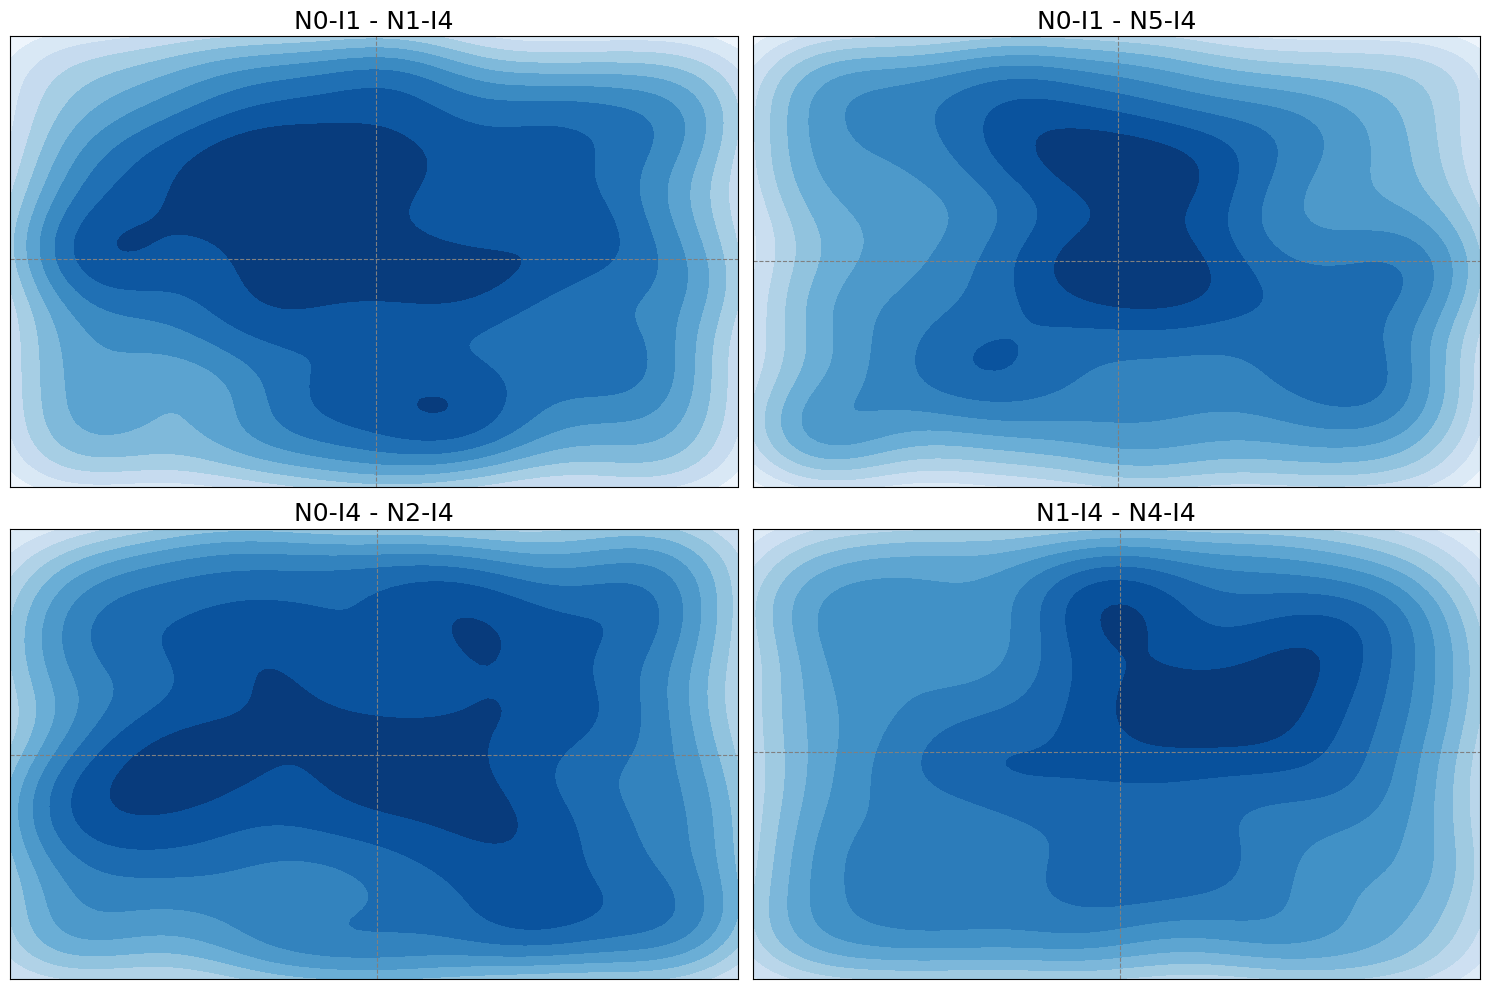
\includegraphics[width=.67\textwidth]{figures/Chapter_NonLinealCensnet/PDF_inputs_inputs_wide_mode.png}
    \end{center}
    \caption{Joint PDFs between the inputs used in the 8-node network, which have a considerably wide mode with respect to the entire distribution }\label{fig:joint_distributions_input_input_wide_mode}
\end{figure}
 

A third group of distributions was identified and can be seen in Figure~\cref{fig:joint_distributions_input_input_wide_mode}, characterized by a considerably large opaque zone in the density plots. This opaque region suggests an intense probability mass concentration in the distribution's central part, indicating robust interactions between the paired variables. In this group, the identified pairs include the relationship between the upper injection limit at node N0 (I1) and the upper nodal pressure at node N1 (I4), between N0-I1 and N5-I4, between the upper nodal pressure at N0 (I4) and that at N2 (I4), and between the upper nodal pressures at nodes N1 and N4 (both measured with I4).


Joint PDFs for the various output variables were generated to analyze the system behavior further. In this analysis, the node nomenclature was maintained; however, it is important to note that there are three types of outputs: the flow injected at each node, the pressure at each node, and the flow transported by each edge (whether pipeline or compressor).


\begin{figure}
    \begin{center}
        \includegraphics[width=.67\textwidth]{figures/Chapter_NonLinealCensnet/outputs_outputs_1.png}
    \end{center}
    \caption{Joint PDFs between the outputs used in the 8-node network, which have a behavior quite similar to that of a Gaussian distribution.}\label{fig:joint_distributions_output_output_1}
\end{figure}
 
The first group of distributions identified appears to follow a Gaussian pattern or at least a similar distribution, as shown in Figure~\cref{fig:joint_distributions_output_output_1}. Among these, one subgroup comprises the relationship between the injected flow at node N0 and the pressures at the remaining nodes. The flow through the first pipeline exhibits a similar pattern when correlated with all nodal pressures. This behavior is logical because, in the network studied, node N0—the only injection node—is connected exclusively to pipeline E0, meaning that the outlet O0 at node N0 and the outlet O2 at pipeline E0 correspond to the same flow. Moreover, this group also includes the distributions generated from the O2 variables of edges E6 and E7 when compared with all nodal pressures. These two edges represent the compressors in the system, which are connected in series so that the O2 outputs of edges E6 and E7 correspond to the same flow.


\begin{figure}
    \begin{center}
        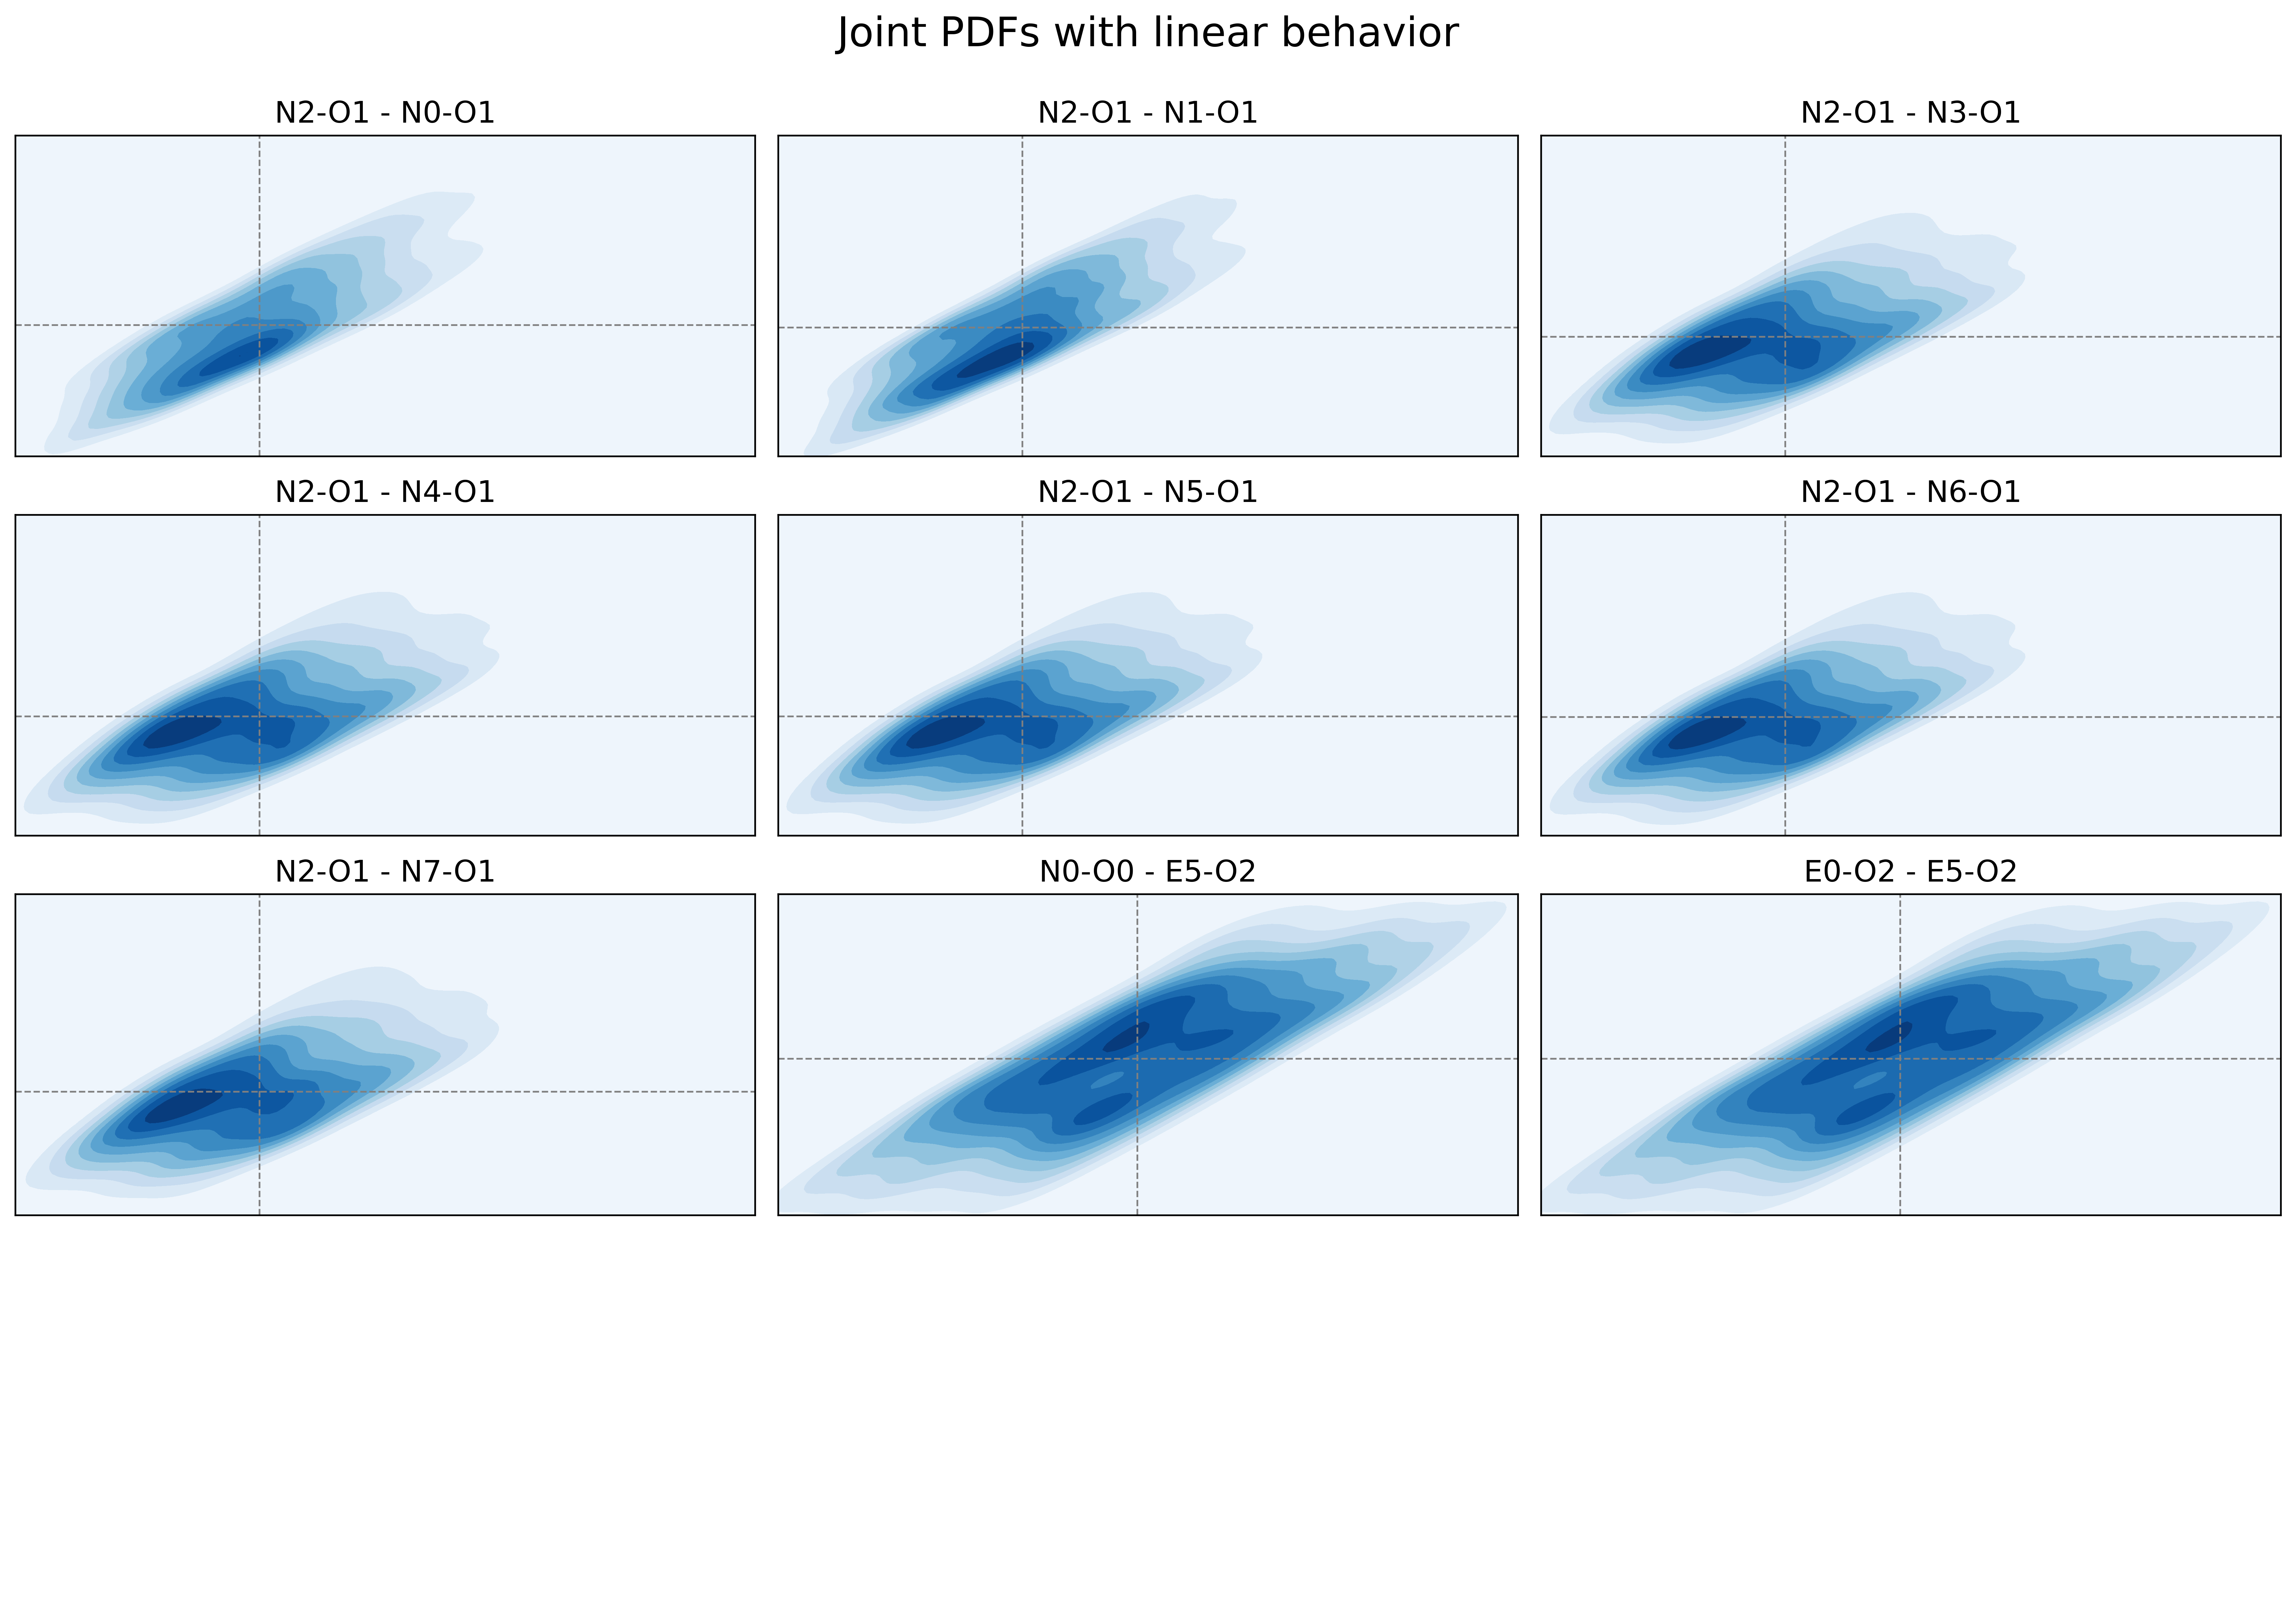
\includegraphics[width=.67\textwidth]{figures/Chapter_NonLinealCensnet/outputs_outputs_2.png}
    \end{center}
    \caption{Joint PDFs between the outputs used in the 8-node network, which have a linear behavior, with a slight dispersion.}\label{fig:joint_distributions_output_output_2}
\end{figure}
 
The second group of joint PDFs exhibits an elongated, diagonal shape that indicates a linear relationship between the corresponding variables, which can be seen in Figure~\cref{fig:joint_distributions_output_output_2}. In this group, one central pair is the relationship between the nodal pressure at node N2—responsible for connecting the first compressor's output with the second's input—and the pressures at the remaining nodes. This linear trend suggests that variations in the pressure at N2 are directly associated with proportional changes in the pressures observed across the network. Additionally, this group includes the relationship between the flow injected at node N0 and the flow transported by edge E5, which is connected to node N6, a demand node.  


\begin{figure}
    \begin{center}
        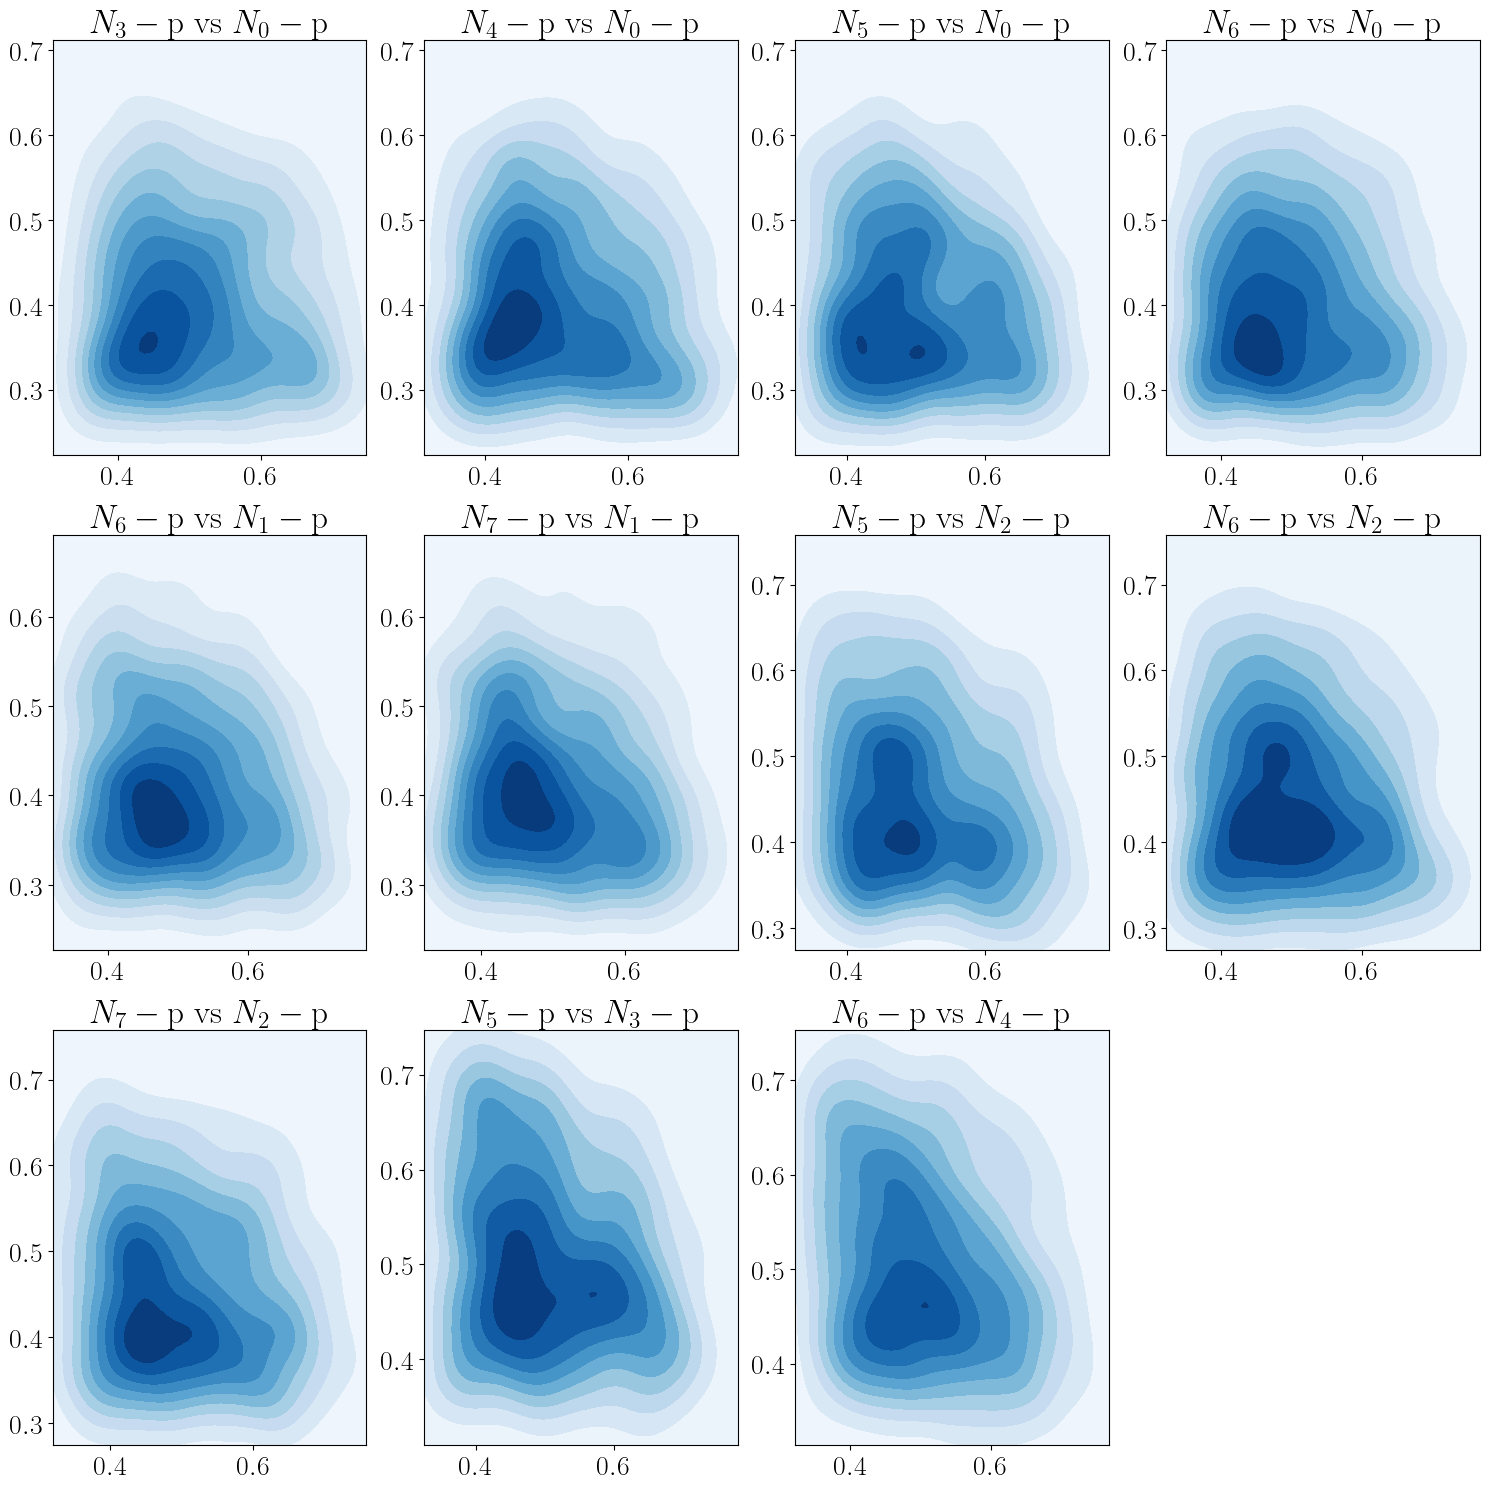
\includegraphics[width=.67\textwidth]{figures/Chapter_NonLinealCensnet/outputs_outputs_3.png}
    \end{center}
    \caption{Joint PDFs between the outputs used in the 8-node network, which have a behavior similar to a skewed Gaussian . }\label{fig:joint_distributions_output_output_3}
\end{figure}
 


A third group of joint distributions was identified, characterized by slightly elongated normal distributions (see Figure 7). Unlike the first group, which exhibited strongly Gaussian shapes, and the second group, which showed linear relationships, the distributions in this group display moderate elongation along the diagonal. This suggests that the correlation between the variables is less pronounced and not strictly linear. In particular, these distributions arise from the relationship between the outlet pressure at the injection node (N0) and the pressures at the downstream compressor nodes. Similarly, they capture the relationship between the pressure at the compressor inlet node (N1) and the pressures at the downstream compressor nodes.


\begin{figure}
    \begin{center}
        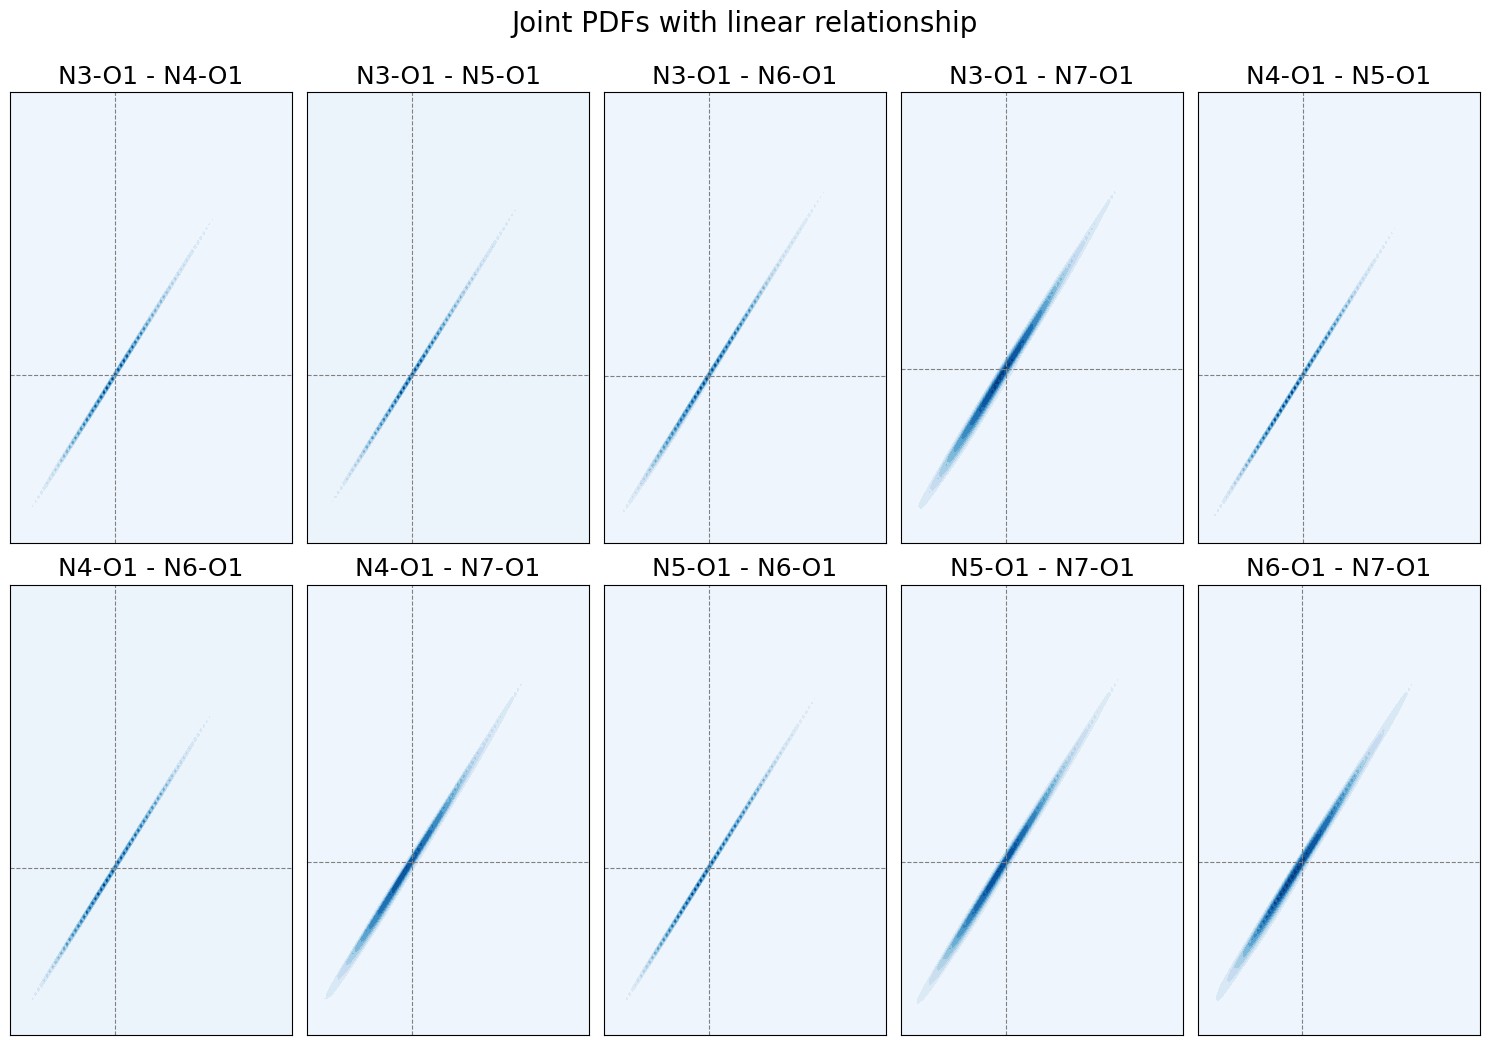
\includegraphics[width=.67\textwidth]{figures/Chapter_NonLinealCensnet/outputs_outputs_linear.png}
    \end{center}
    \caption{Joint PDFs between the outputs used in the 8-node network, which have a quite marked linear behavior.}\label{fig:joint_distributions_output_output_linear}
\end{figure}
 

Figure~\ref{fig:joint_distributions_output_output_linear} illustrates a group of joint distributions exhibiting a markedly linear behavior, almost as straight lines with a clear slope. These distributions capture the relationships between the pressures at a given node and those at downstream nodes, starting with node N4, which is positioned at the outlet of the compressors. This linear trend is expected because, in order to maintain unidirectional gas flow, the pressures throughout the network must decrease gradually. 

\begin{figure}
    \begin{center}
        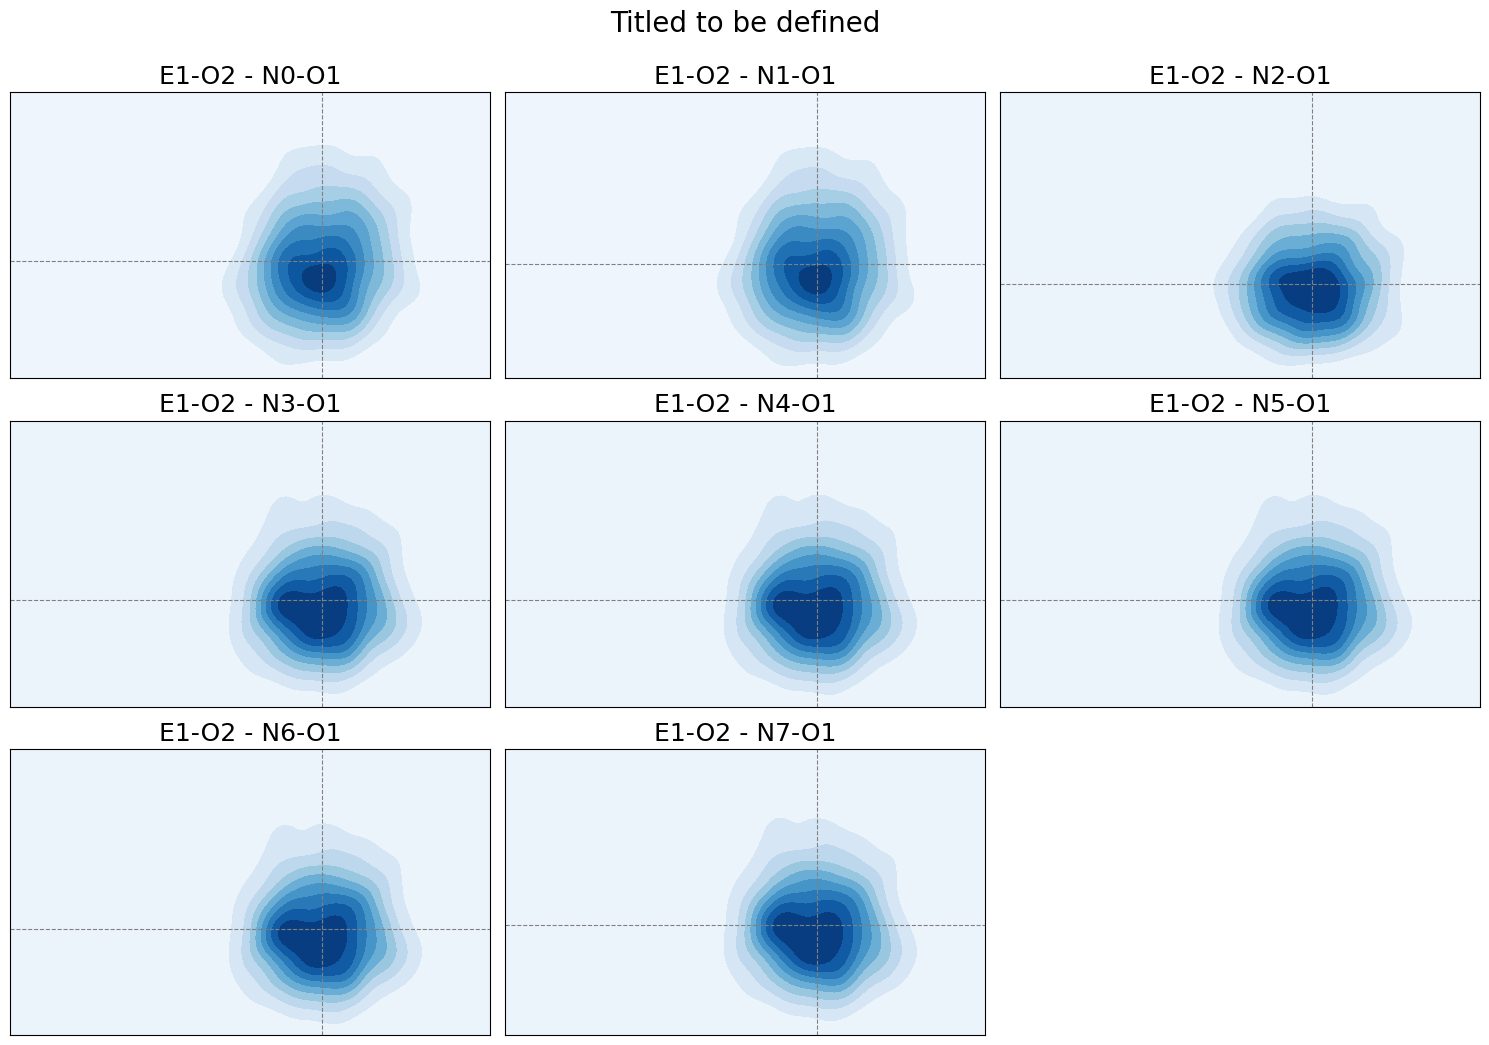
\includegraphics[width=.67\textwidth]{figures/Chapter_NonLinealCensnet/outputs_outputs_5.png}
    \end{center}
    \caption{Joint PDFs between the outputs used in the 8-node network, which have a Gaussian behavior with small covariances }\label{fig:joint_distributions_output_output_5}
\end{figure}
 

Another group of joint distributions, which can be seen in Figure~\cref{fig:joint_distributions_output_output_5}, was observed to resemble a normal distribution closely but with much lower dispersion, indicating smaller covariances among the variables. These distributions were obtained by correlating the flow through the first pipeline with the pressures measured at all nodes in the network. Similar patterns are also observed when the nodal pressures are compared with the flows through edges E6 and E7; however, these images are omitted because the three edges are connected sequentially and share the same gas flow, their behavior is as expected.

\begin{figure}
    \begin{center}
        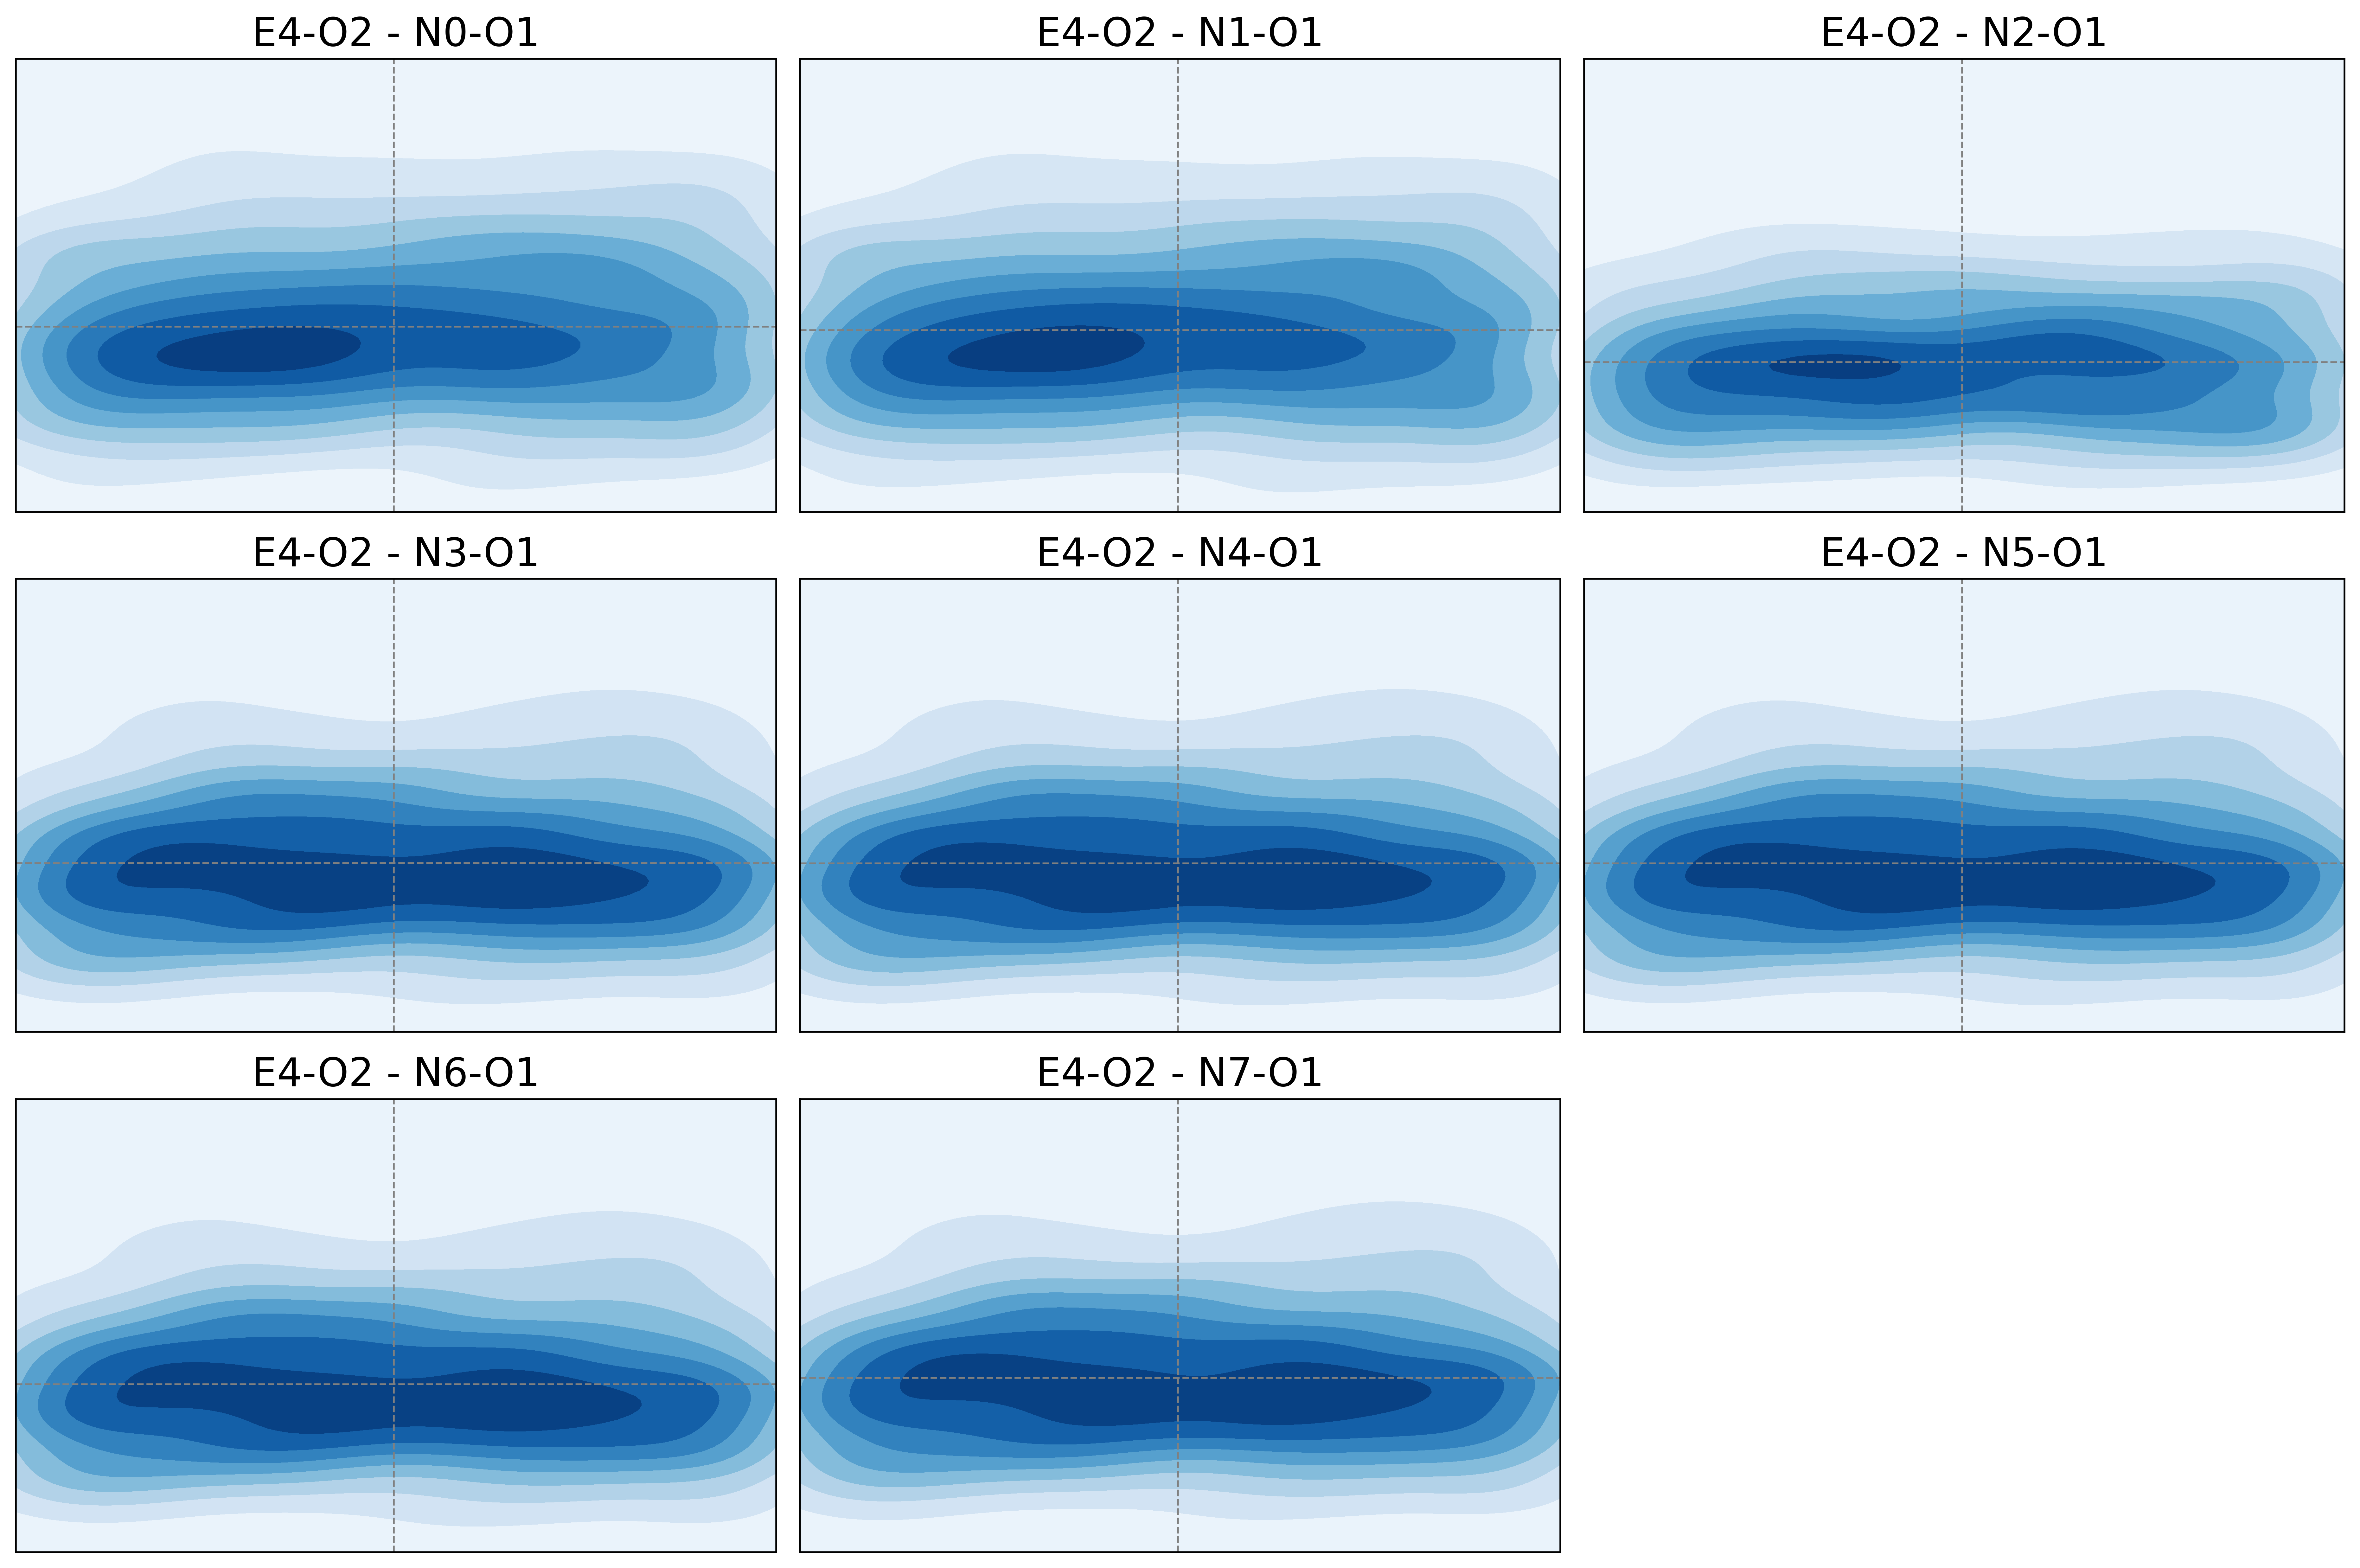
\includegraphics[width=.67\textwidth]{figures/Chapter_NonLinealCensnet/outputs_outputs_6.png}
    \end{center}
    \caption{Joint PDFs among the outputs used in the 8-node network, which are quite dispersed along the variable associated with the N7 node flow.}\label{fig:joint_distributions_output_output_6}
\end{figure}
 

Figure~\cref{fig:joint_distributions_output_output_6} shows the group characterized by distributions that are elongated along the axis of the first variable used in constructing the joint PDF while exhibiting a narrower spread along the second variable's axis. In our study, this subgroup includes the distributions that relate the gas flow on edge E4—which carries gas to the N7 demand node—to the pressures measured at each node. This behavior suggests that variations in the gas flow on E4 are more strongly influenced by the pressure variable, resulting in a pronounced elongation in that direction. 

\begin{figure}
    \begin{center}
        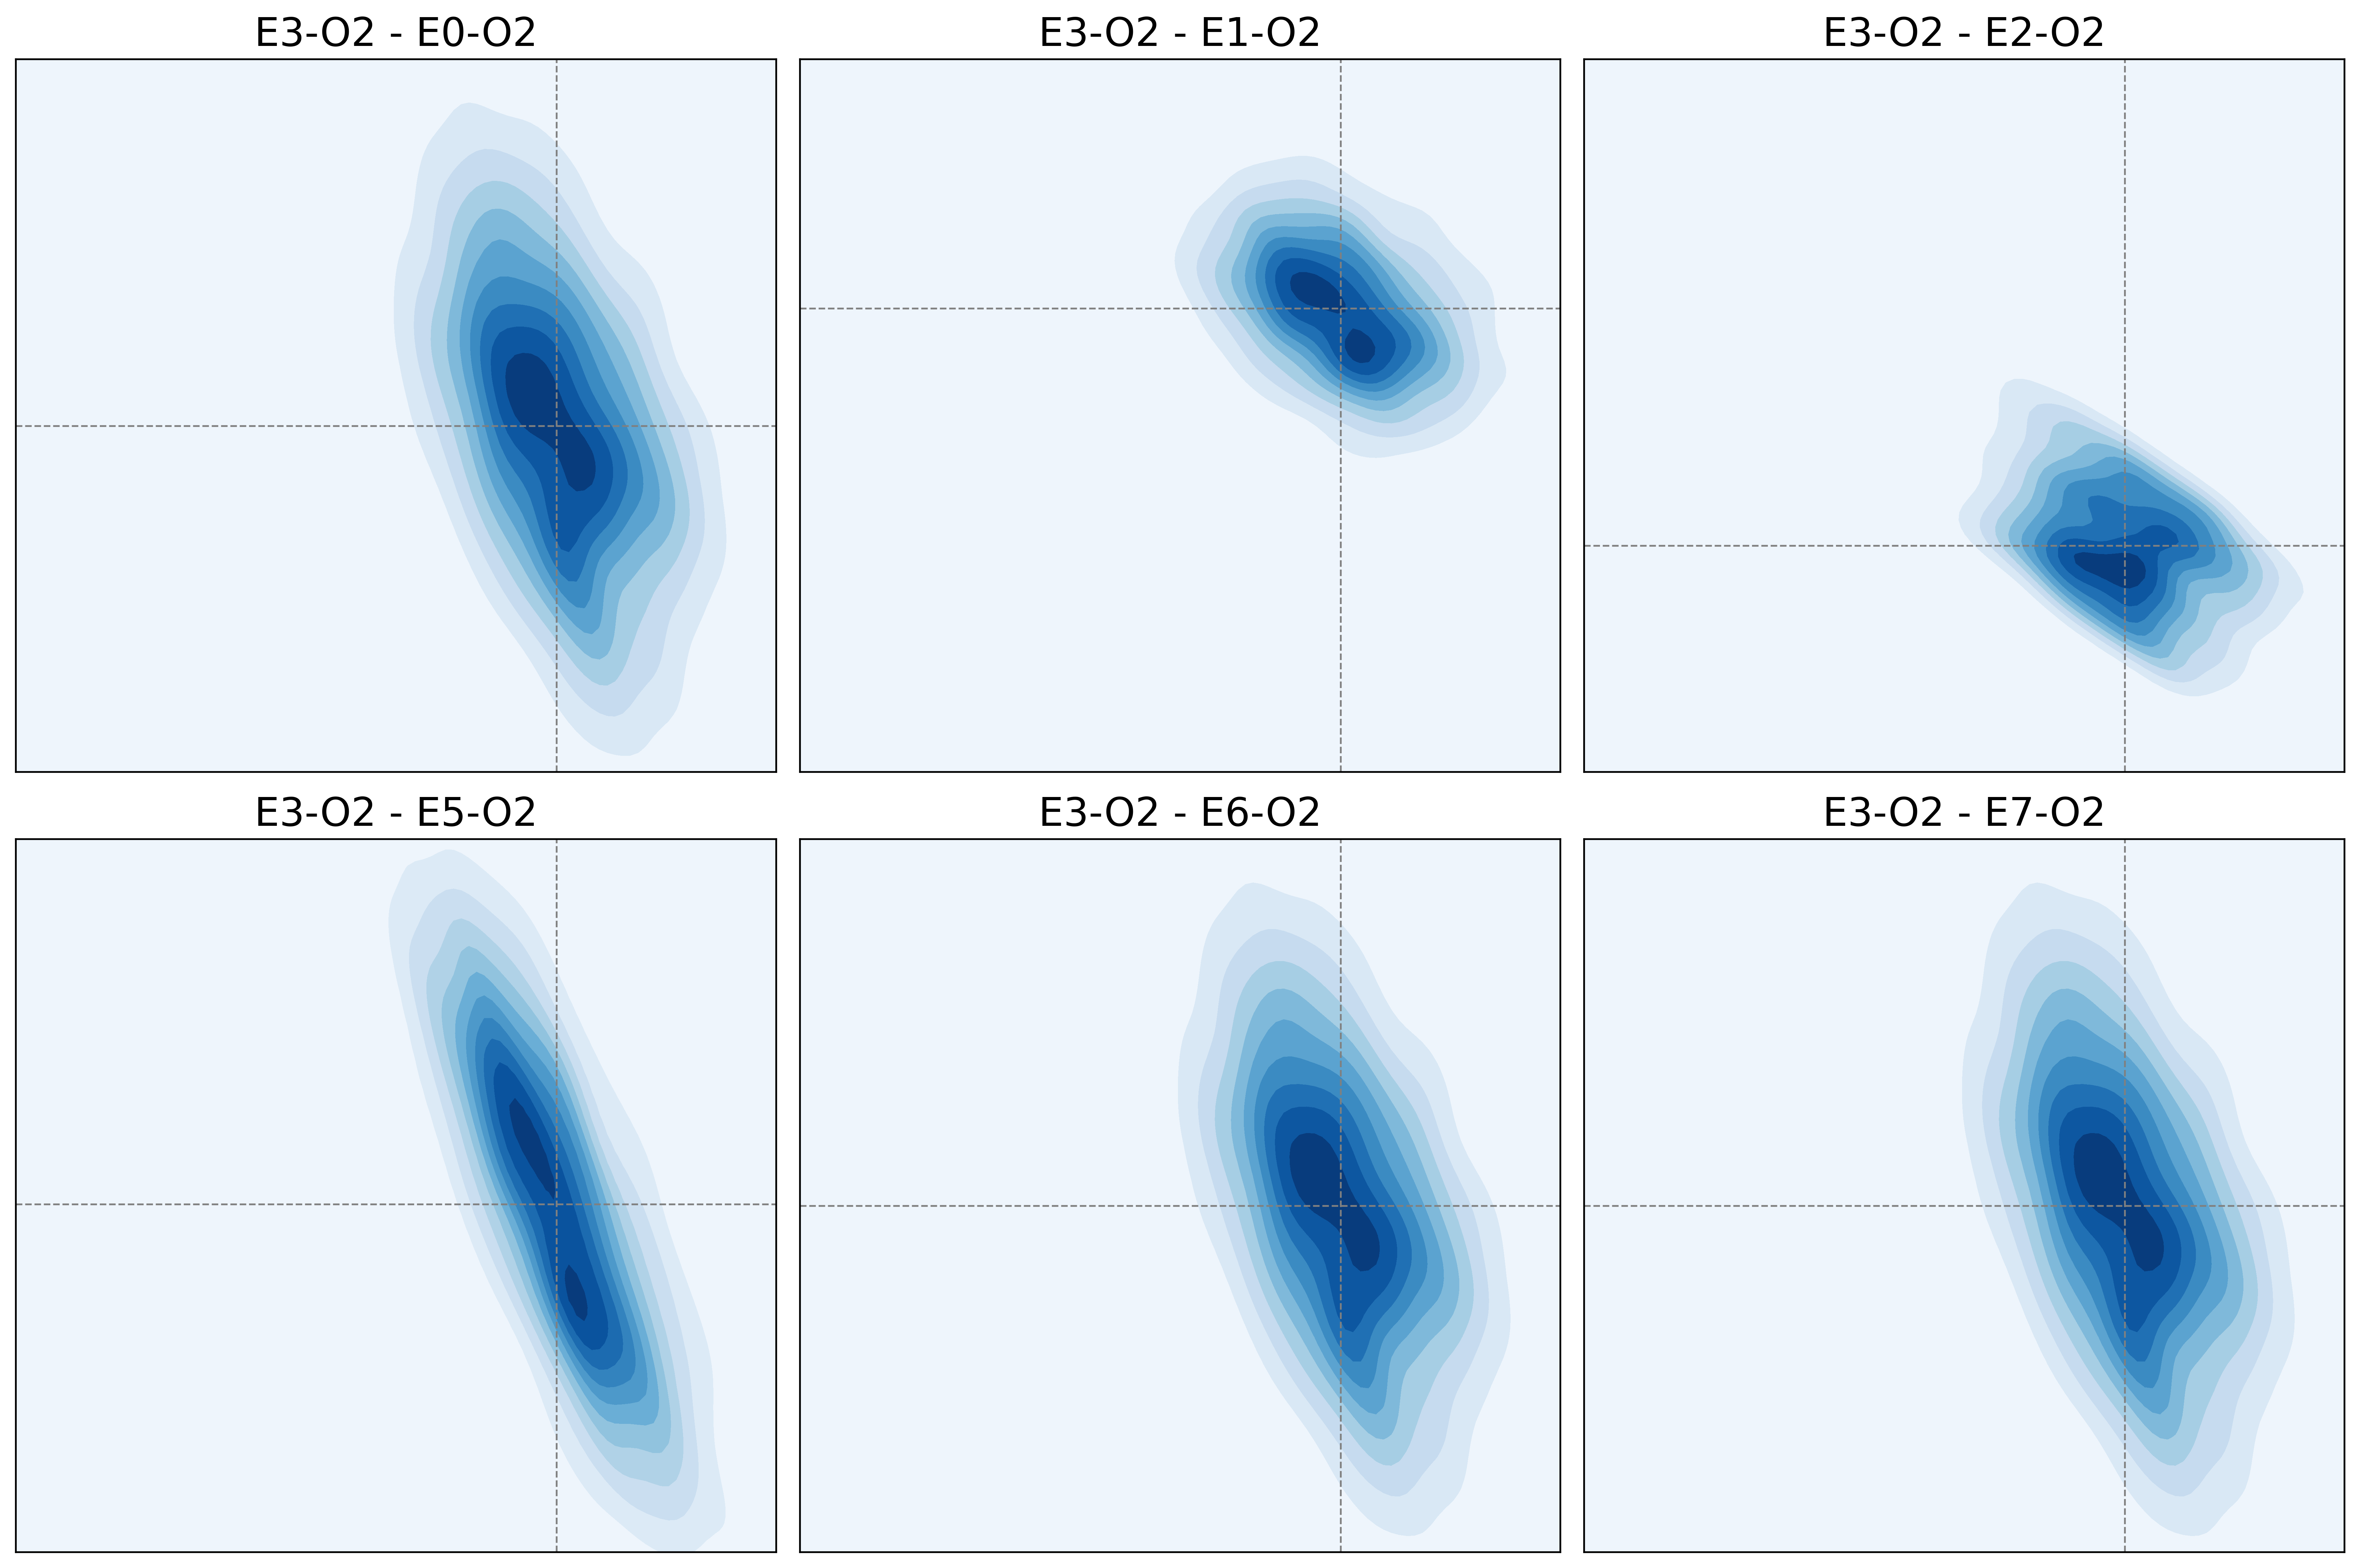
\includegraphics[width=.7\textwidth]{figures/Chapter_NonLinealCensnet/outputs_outputs_7.png}
    \end{center}
    \caption{Joint PDFs between the outputs used in the 8-node network, which show a negative linear behavior. }\label{fig:joint_distributions_output_output_7}
\end{figure}
 

A final group of joint distributions can be seen in Figure~\cref{fig:joint_distributions_output_output_7}. This group is characterized by distributions with an inversely proportional behavior. The joint PDFs in this group are associated with the relationship between the flow transported by edge E3 and the flows transported by the other edges, except those corresponding to edges E4 and E5. This result is interesting, as it reflects a distinct behavior of the system: edges E1, E2, and E3 form a closed trajectory, and according to the initially assumed flow direction, there were instances in which edge E3 exhibited a flow opposite to that expected. In contrast, the flows that do not display this inverse relationship leave the closed trajectory to feed the demand nodes.


The relationships between input and output variables were further analyzed to conclude the study of the joint distributions obtained from the variables in this case study. As in previous analyses, several groups of distributions with similar behavior were visually identified. 


\begin{figure}
    \begin{center}
        \includegraphics[width=.7\textwidth]{figures/Chapter_NonLinealCensnet/inputs_outputs_1.png}
    \end{center}
    \caption{Joint PDFs between the inputs and outputs used in the 8-node network, which present a wide dispersion along both variables. }\label{fig:joint_distributions_inputs_outputs_1}
\end{figure}

The first group can be seen in Figure~\cref{fig:joint_distributions_inputs_outputs_1} and corresponds to distributions exhibiting high dispersion, although the mode (or modes, in some cases) varies depending on the variables considered. In this group, the distributions include those constructed between the flow on edge E4—which directly supplies the demand node N6—and the upper-pressure limits at the other nodes. Additionally, this group encompasses the distributions generated from the relationship between the flow injected at node N0 and the demanded flow at node N7.




\begin{figure}
    \begin{center}
        \includegraphics[width=.7\textwidth]{figures/Chapter_NonLinealCensnet/inputs_outputs_2.png}
    \end{center}
    \caption{Joint PDFs between the inputs and outputs used in the 8-node network, which present a linear behavior, although with different dispersions among them. }\label{fig:joint_distributions_inputs_outputs_2}
\end{figure}
 

The second group of joint distributions (Figure~\cref{fig:joint_distributions_inputs_outputs_2}) is characterized by an apparent linear behavior among the variables, as shown by the almost linear trends of the diagrams. In some cases, the dispersion of the distribution itself made the line look wider but without losing its linear characteristic. These distributions primarily arise from the relationships between the gas demand at nodes N6 and N7—represented by the variable I2 (the gas demanded)—and the flows transported by all edges but E3, denoted by O2, as well as the nodal injection flow, denoted by O0, at node N0. These relationships indicate that as the gas demand increases at the demand nodes, the corresponding flows in the edges (and at the injection node) adjust proportionally, reflecting the underlying physical constraints that govern flow direction and consistency in the network.







A stochastic analysis was performed to assess further the robustness of the trained GNN-based model and its ability to generalize under uncertainty. This analysis is motivated by the need to simulate and evaluate the model's responses in scenarios that were not explicitly present in the training data, thereby providing a means to quantify the variability and reliability of the model's predictions.

Initially, a kernel density estimate (KDE) was fitted to the input training data used for the GNN model. From this estimated distribution, a set of synthetic input samples, denoted as \( X_{\text{sample}} \), was generated. These synthetic inputs were then propagated forward through the trained network, taking into account all loss components, to yield a corresponding set of output predictions, denoted as \( y_{\text{sample}} \). In parallel, the original training inputs were propagated through the network to obtain output predictions, denoted as \(\bar{y}_{\text{train}}\). A second KDE was then fitted using the training output data (hereafter referred to as \(y_{\text{train}}\)). Two log-likelihoods were calculated based on this second KDE: one using \(y_{\text{sample}}\) and the other using \(\bar{y}_{\text{train}}\). The log-likelihood for the synthetic outputs, \(y_{\text{sample}}\), was found to be \(-6,696,247.56\), while the log-likelihood for the training outputs, \(\bar{y}_{\text{train}}\), was \(-6,657,534.62\). The closeness of these two values suggests that the synthetic outputs generated from the input KDE closely resemble the distribution of the training outputs.

To further evaluate the goodness-of-fit between the distributions of \( y_{\text{sample}} \) and \( \bar{y}_{\text{train}} \), a Kolmogorov–Smirnov (K–S) test was conducted using three alternatives: two-sided, less, and more significant. The test results were as follows: a two-sided test yielded a statistic of \( 0.01833 \) with a p-value of \( 0.81482 \) (statistic location \(-0.34018\), sign \(1\)); the 'less' alternative produced a statistic of \( 0.01167 \) with a p-value of \( 0.72137 \) (statistic location \(0.30738\), sign \(-1\)); and the 'greater' alternative returned a statistic of \( 0.01833 \) with a p-value of \( 0.44640 \) (statistic location \(-0.34018\), sign \(1\)). These statistical measures provide an initial indication that the synthetic outputs generated via the KDE-based sampling are consistent with the distribution of outputs observed during training, thereby supporting the model's capability to generalize to new, unseen scenarios.


\subsection{Case Study II: 63-node Network (Colombia)}


This section addresses the second case study, focusing on the Colombian natural gas network. As in the previous cases, this analysis explores various configurations of loss functionals to evaluate the predictive performance of the GNN-based model. The first experiment examines the model's predictive capabilities when incorporating node and edge losses.


This experiment used optimized hyperparameters, with \( N_{\text{channels}} = 21 \), \( N_{\text{layers}} = 5 \), and \( N_{\text{dense}} = 4 \), which were selected to enhance the model's performance. The experiment yielded a total loss of \( 267,600 \), encompassing node and edge losses, along with a calculated balance loss. Specifically, the node loss reached \( 17,537 \), while the edge loss was considerably higher at \( 250,063 \). Additionally, a balance loss of \( 338,729 \) was recorded. Notably, the balance loss was calculated to assess network consistency but was not incorporated into the model's cost function during training; instead, it serves as an independent evaluation metric. 

The GNN-based model's predictive accuracy in this experiment was quantified using \( R^2 \) metrics, and the results are shown in \cref{fig:col_base_f_results_non_lineal}. The nodal predictions exhibited high accuracy, with an \( R^2 \) score of \( 0.993 \) in \cref{fig:results_nonlineal_col_node_base_f}, indicating that the model closely approximates the observed nodal flow values. Similarly, the edge predictions achieved an \( R^2 \) score of \( 0.963 \), demonstrating robust performance in predicting edge flows. This last value can be seen in \cref{fig:results_nonlineal_col_edge_base_f}.


\begin{figure}
    \centering
    \setlength\figurewidth{.53\textwidth}        
    \setlength\figureheight{0.36\textwidth} 
    \subfloat[Actual vs predicted nodal flows.] 
    {\label{fig:results_nonlineal_col_node_base_f}\resizebox{\figurewidth}{\figureheight}{% This file was created with tikzplotlib v0.10.1.
\begin{tikzpicture}

\definecolor{darkgray176}{RGB}{176,176,176}
\definecolor{lightgray204}{RGB}{204,204,204}

\begin{axis}[
colorbar,
colorbar style={ylabel={node id}},
colormap={mymap}{[1pt]
 rgb(0pt)=(0.12156862745098,0.466666666666667,0.705882352941177);
  rgb(1pt)=(1,0.498039215686275,0.0549019607843137);
  rgb(2pt)=(0.172549019607843,0.627450980392157,0.172549019607843);
  rgb(3pt)=(0.83921568627451,0.152941176470588,0.156862745098039);
  rgb(4pt)=(0.580392156862745,0.403921568627451,0.741176470588235);
  rgb(5pt)=(0.549019607843137,0.337254901960784,0.294117647058824);
  rgb(6pt)=(0.890196078431372,0.466666666666667,0.76078431372549);
  rgb(7pt)=(0.498039215686275,0.498039215686275,0.498039215686275);
  rgb(8pt)=(0.737254901960784,0.741176470588235,0.133333333333333);
  rgb(9pt)=(0.0901960784313725,0.745098039215686,0.811764705882353)
},
legend cell align={left},
legend style={
  fill opacity=0.8,
  draw opacity=1,
  text opacity=1,
  at={(0.03,0.97)},
  anchor=north west,
  draw=lightgray204
},
point meta max=62,
point meta min=0,
tick align=outside,
tick pos=left,
title={},
x grid style={darkgray176},
xlabel={yn test},
xmajorgrids,
xmin=-16.2727338975, xmax=341.7274118475,
xtick style={color=black},
y grid style={darkgray176},
ylabel={y pred},
ymajorgrids,
ymin=-17.2115550398827, ymax=315.543056285381,
ytick style={color=black}
]
\addplot [
  colormap={mymap}{[1pt]
 rgb(0pt)=(0.12156862745098,0.466666666666667,0.705882352941177);
  rgb(1pt)=(1,0.498039215686275,0.0549019607843137);
  rgb(2pt)=(0.172549019607843,0.627450980392157,0.172549019607843);
  rgb(3pt)=(0.83921568627451,0.152941176470588,0.156862745098039);
  rgb(4pt)=(0.580392156862745,0.403921568627451,0.741176470588235);
  rgb(5pt)=(0.549019607843137,0.337254901960784,0.294117647058824);
  rgb(6pt)=(0.890196078431372,0.466666666666667,0.76078431372549);
  rgb(7pt)=(0.498039215686275,0.498039215686275,0.498039215686275);
  rgb(8pt)=(0.737254901960784,0.741176470588235,0.133333333333333);
  rgb(9pt)=(0.0901960784313725,0.745098039215686,0.811764705882353)
},
  only marks,
  scatter,
  scatter src=explicit
]
table [x=x, y=y, meta=colordata]{%
x  y  colordata
266.47324716 249.639175415039 0.0
0 -0.142389416694641 1.0
0 -0.0449339151382446 2.0
0 0.0713010430335999 3.0
0 0.106789827346802 4.0
0 0.236347138881683 5.0
0 0.171468198299408 6.0
0 0.321928083896637 7.0
0 -0.2691330909729 8.0
0 -0.114482879638672 9.0
0 0.585927248001099 10.0
0 -0.408090472221375 11.0
0 0.0334172248840332 12.0
54.420842408 52.3760604858398 13.0
31.76838707 45.4420013427734 14.0
0 -0.236499667167664 15.0
0 0.557169258594513 16.0
31.767708115 35.5617408752441 17.0
0 0.1447514295578 18.0
0 0.00425702333450317 19.0
0 0.0630048513412476 20.0
0 0.0852915048599243 21.0
0 0.153019845485687 22.0
32.042735172 31.7617301940918 23.0
0 0.0172544717788696 24.0
0 0.539882898330688 25.0
0 -0.139046311378479 26.0
0 -0.016973078250885 27.0
0 0.361409664154053 28.0
0 0.0465011596679688 29.0
0 -0.0713483095169067 30.0
0 -0.151389122009277 31.0
0 0.0655762553215027 32.0
0 -0.184005737304688 33.0
0 0.159492611885071 34.0
0 0.411568343639374 35.0
0 -0.149775922298431 36.0
0 0.0114204883575439 37.0
0 0.126012444496155 38.0
0 -0.194342374801636 39.0
0 0.582290053367615 40.0
0 -0.129912436008453 41.0
0 0.131481289863586 42.0
293.56654935 296.294281005859 43.0
0 0.0724555253982544 44.0
0 0.070831298828125 45.0
0 0.129652857780457 46.0
0 0.235148727893829 47.0
0 0.383313328027725 48.0
0 0.428795397281647 49.0
0.088502709347 0.000664055347442627 50.0
2.2103942585 1.90541684627533 51.0
0 0.0654274821281433 52.0
0 -0.258934020996094 53.0
0 0.0212928056716919 54.0
0 0.0398275852203369 55.0
0 0.171365797519684 56.0
0 0.194833934307098 57.0
0 0.210932195186615 58.0
0 0.120373606681824 59.0
0 0.0517104864120483 60.0
0 0.103727102279663 61.0
0 0.180829167366028 62.0
248.37393055 251.710006713867 0.0
0 0.0708619356155396 1.0
0 0.0428527593612671 2.0
0 0.136177897453308 3.0
0 -0.213192462921143 4.0
0 -0.0769016742706299 5.0
0 0.033043384552002 6.0
0 0.0201961994171143 7.0
0 0.244125008583069 8.0
0 0.30745267868042 9.0
0 0.265757024288177 10.0
0 -0.0718837976455688 11.0
0 -0.124699473381042 12.0
64.885396715 64.2186813354492 13.0
37.251651647 33.5145568847656 14.0
0 -0.0671347379684448 15.0
0 0.0574696063995361 16.0
30.798970514 33.6960067749023 17.0
0 0.0931819677352905 18.0
0 -0.0188233852386475 19.0
0 0.0400761365890503 20.0
0 0.255428850650787 21.0
0 -0.086645245552063 22.0
29.963403657 26.0974235534668 23.0
0 0.00885939598083496 24.0
0 0.0383943319320679 25.0
0 0.0686919093132019 26.0
0 -0.204172194004059 27.0
0 0.642504632472992 28.0
0 -0.0974288582801819 29.0
0 0.0880443453788757 30.0
0 0.00759780406951904 31.0
0 0.0762514472007751 32.0
0 -0.176781833171844 33.0
0 -0.170233011245728 34.0
0 -0.0943754315376282 35.0
0 -0.159420728683472 36.0
0 0.0817056894302368 37.0
0 -0.0761663317680359 38.0
0 -0.255910992622375 39.0
0 0.452268987894058 40.0
0 -0.0821685194969177 41.0
0 -0.0398745536804199 42.0
304.35351591 296.549499511719 43.0
0 0.0947914719581604 44.0
0 0.166132509708405 45.0
0 0.0848214626312256 46.0
0 0.286359906196594 47.0
0 0.239474356174469 48.0
0 0.405463248491287 49.0
0.084699044305 0.0063014030456543 50.0
1.9745309823 1.91203594207764 51.0
0 -0.107413411140442 52.0
0 0.134892821311951 53.0
0 0.144681215286255 54.0
0 0.306658506393433 55.0
0 0.101537585258484 56.0
0 0.231771349906921 57.0
0 0.0895958542823792 58.0
0 -0.0771396160125732 59.0
0 0.871439099311829 60.0
0 -0.0337347388267517 61.0
0 -0.0441908836364746 62.0
302.37464816 250.852478027344 0.0
0 -0.310250401496887 1.0
0 0.0636056661605835 2.0
0 0.315250396728516 3.0
0 -0.0144246220588684 4.0
0 0.095795214176178 5.0
0 0.72277843952179 6.0
0 0.380319118499756 7.0
0 -0.480941772460938 8.0
0 -0.204494535923004 9.0
0 -0.212023019790649 10.0
0 -0.225362300872803 11.0
0 -0.330933809280396 12.0
45.482115614 49.6875839233398 13.0
37.007772682 37.5866088867188 14.0
0 0.0265146493911743 15.0
0 -0.0399916172027588 16.0
29.828999935 32.8346824645996 17.0
0 0.12875097990036 18.0
0 -0.00493097305297852 19.0
0 0.0986930727958679 20.0
0 -0.204740166664124 21.0
0 1.56226515769958 22.0
44.134750702 38.6916656494141 23.0
0 -0.10773366689682 24.0
0 -0.145784914493561 25.0
0 -0.0124692916870117 26.0
0 0.135047733783722 27.0
0 0.709931254386902 28.0
0 0.00422543287277222 29.0
0 0.117492496967316 30.0
0 0.418070077896118 31.0
0 -0.0236167907714844 32.0
0 -0.0446475744247437 33.0
0 0.544621348381042 34.0
0 0.241633951663971 35.0
0 0.521328687667847 36.0
0 0.154515385627747 37.0
0 0.467998951673508 38.0
0 -0.187779784202576 39.0
0 -0.461969256401062 40.0
0 -0.253906726837158 41.0
0 -0.0181766748428345 42.0
291.82175176 293.404663085938 43.0
0 0.100164294242859 44.0
0 0.140608310699463 45.0
0 0.331257224082947 46.0
0 -0.791751861572266 47.0
0 0.0309572219848633 48.0
0 0.4157874584198 49.0
0.075606181489 0.0388871431350708 50.0
1.8743350179 1.80711591243744 51.0
0 0.150869071483612 52.0
0 0.0989822149276733 53.0
0 0.219808042049408 54.0
0 0.3351671397686 55.0
0 0.352408409118652 56.0
0 0.00237840414047241 57.0
0 -0.0414254665374756 58.0
0 0.308968365192413 59.0
0 0.0362465381622314 60.0
0 0.0305611491203308 61.0
0 0.0302001237869263 62.0
265.89131818 247.303726196289 0.0
0 -0.346219539642334 1.0
0 0.195574581623077 2.0
0 0.143782436847687 3.0
0 -0.159537792205811 4.0
0 -0.194557726383209 5.0
0 -0.377765417098999 6.0
0 0.567977726459503 7.0
0 0.697785496711731 8.0
0 -0.0322224497795105 9.0
0 0.611300647258759 10.0
0 -0.855613589286804 11.0
0 -0.141015946865082 12.0
60.373084879 60.2287292480469 13.0
38.622708843 31.054443359375 14.0
0 -0.00105714797973633 15.0
0 -0.06923907995224 16.0
25.188702693 34.7364273071289 17.0
0 0.0856233239173889 18.0
0 -0.0107483863830566 19.0
0 0.0434588193893433 20.0
0 0.205599069595337 21.0
0 0.0941464900970459 22.0
26.672164285 26.8738708496094 23.0
0 0.0691215991973877 24.0
31.524665793 0.957210421562195 25.0
0 -0.131632804870605 26.0
0 -0.265188217163086 27.0
0 0.512789607048035 28.0
0 -0.0197376012802124 29.0
0 0.0512744784355164 30.0
0 -0.196807622909546 31.0
0 -0.0987600088119507 32.0
0 -0.0878394246101379 33.0
0 0.10935378074646 34.0
0 0.116467297077179 35.0
0 -0.383853793144226 36.0
0 -0.00468903779983521 37.0
0 0.283622622489929 38.0
0 -0.458166599273682 39.0
0 0.189829230308533 40.0
0 -0.227734565734863 41.0
0 0.101795077323914 42.0
299.2801212 298.878387451172 43.0
0 0.189864635467529 44.0
0 0.0446534156799316 45.0
0 0.0571035146713257 46.0
0 0.29422527551651 47.0
0 0.228481829166412 48.0
0 0.243814527988434 49.0
0.073176300482 -0.00983351469039917 50.0
1.5103348501 1.85240364074707 51.0
0 0.143408417701721 52.0
0 -0.0268762111663818 53.0
0 0.0281428098678589 54.0
0 -0.0706720352172852 55.0
0 -0.121010184288025 56.0
0 -0.033930778503418 57.0
0 0.199068248271942 58.0
0 0.237312078475952 59.0
0 -0.102500557899475 60.0
0 0.0883126258850098 61.0
0 0.198793888092041 62.0
252.51018499 254.235733032227 0.0
0 0.490179419517517 1.0
0 0.121724188327789 2.0
0 0.127305448055267 3.0
0 -0.134583830833435 4.0
0 0.101994872093201 5.0
0 0.253704726696014 6.0
0 0.129769504070282 7.0
0 -0.57126784324646 8.0
0 0.540296256542206 9.0
0 0.253297328948975 10.0
0 -0.224400043487549 11.0
0 -0.0533052682876587 12.0
70.621115574 70.8891220092773 13.0
16.43797061 23.2563877105713 14.0
0 0.257423043251038 15.0
0 -0.0752222537994385 16.0
40.005265497 36.4772453308105 17.0
0 0.180097818374634 18.0
0 -0.0168256759643555 19.0
0 0.0157145261764526 20.0
0 0.157090067863464 21.0
0 0.110984563827515 22.0
26.836412684 25.2606182098389 23.0
0 0.123265981674194 24.0
0 1.07453000545502 25.0
0 -0.34232223033905 26.0
0 -0.166689336299896 27.0
0 1.28673601150513 28.0
0 0.0753816366195679 29.0
0 0.0222569704055786 30.0
0 0.663333892822266 31.0
0 -0.189689815044403 32.0
0 -0.16421103477478 33.0
0 0.32769513130188 34.0
0 0.250788271427155 35.0
0 0.314369171857834 36.0
0 0.0046156644821167 37.0
0 0.319040060043335 38.0
0 -0.112903594970703 39.0
0 0.241432011127472 40.0
0 -0.316124320030212 41.0
0 0.306641817092896 42.0
300.13171616 296.185668945312 43.0
0 0.182920575141907 44.0
0 0.278100788593292 45.0
0 0.227074563503265 46.0
0 -0.56473445892334 47.0
0 0.237197160720825 48.0
1.420043763 0.465582638978958 49.0
0.077893563853 0.0411819219589233 50.0
1.5864886701 1.88475561141968 51.0
0 0.347023665904999 52.0
0 -0.172107398509979 53.0
0 -0.194981455802917 54.0
0 -0.0185278058052063 55.0
0 0.207524418830872 56.0
0 -0.185159504413605 57.0
0 0.121752321720123 58.0
0 0.311920493841171 59.0
0 -0.216814756393433 60.0
0 0.0883799195289612 61.0
0 0.186255753040314 62.0
263.65710187 252.978057861328 0.0
0 -0.0464619398117065 1.0
0 0.0470383763313293 2.0
0 0.291144192218781 3.0
0 -0.212165951728821 4.0
0 0.0707187056541443 5.0
0 0.0277366638183594 6.0
0 0.14969801902771 7.0
0 0.215933203697205 8.0
0 -0.345485806465149 9.0
0 -0.0769699811935425 10.0
0 -0.210354447364807 11.0
0 -0.0559083223342896 12.0
48.304542497 46.9898872375488 13.0
50.754517728 46.7420043945312 14.0
0 -0.0109446048736572 15.0
0 -0.140868425369263 16.0
37.314581088 34.3828239440918 17.0
0 0.0802102088928223 18.0
0 -0.0472348928451538 19.0
0 0.0450291633605957 20.0
0 0.122682094573975 21.0
0 0.113465368747711 22.0
25.997095401 24.5642681121826 23.0
0 0.0839192867279053 24.0
0 0.751701354980469 25.0
0 -0.370288133621216 26.0
0 -0.0793863534927368 27.0
0 0.524729609489441 28.0
0 0.262770593166351 29.0
0 -0.00241619348526001 30.0
0 0.124412894248962 31.0
0 0.0794090628623962 32.0
0 -0.0111080408096313 33.0
0 -0.0714513659477234 34.0
0 0.234387576580048 35.0
0 0.133424937725067 36.0
0 -0.082790732383728 37.0
0 0.227017939090729 38.0
0 -0.140514850616455 39.0
0 0.469157338142395 40.0
0 -0.227647662162781 41.0
0 0.107690691947937 42.0
297.40720397 295.456787109375 43.0
0 0.114283680915833 44.0
0 0.15294337272644 45.0
0 0.0259655714035034 46.0
0 0.0629487633705139 47.0
0 0.288461804389954 48.0
0.68317674862 0.662104964256287 49.0
0.072270753595 0.0454301238059998 50.0
2.1325840066 1.91492056846619 51.0
0 -0.210419297218323 52.0
0 -0.114704787731171 53.0
0 -0.100747466087341 54.0
0 -0.184861898422241 55.0
0 0.125088691711426 56.0
0 -0.114255547523499 57.0
0 -0.0551935434341431 58.0
0 -0.61805522441864 59.0
0 1.24615788459778 60.0
0 -0.00948131084442139 61.0
0 -0.0249838829040527 62.0
248.68242343 254.472427368164 0.0
0 -0.248040795326233 1.0
0 -0.0067899227142334 2.0
0 -0.160886824131012 3.0
0 -0.191324412822723 4.0
0 0.021512508392334 5.0
0 0.0478034019470215 6.0
0 0.111731171607971 7.0
0 0.0206038951873779 8.0
0 -0.262186050415039 9.0
0 0.184019804000854 10.0
0 -0.401756048202515 11.0
0 -0.0999844670295715 12.0
62.217350368 61.4766120910645 13.0
20.055296633 35.4800033569336 14.0
0 -0.0828515291213989 15.0
0 -0.137904524803162 16.0
31.204645306 35.0573081970215 17.0
0 0.0532411336898804 18.0
0 -0.0665684938430786 19.0
0 0.135240256786346 20.0
0 -0.0838650465011597 21.0
0 0.453499495983124 22.0
33.461561051 33.4253730773926 23.0
0 0.0464522838592529 24.0
0 0.66888165473938 25.0
0 -0.101287186145782 26.0
0 -0.0339115262031555 27.0
0 0.295637190341949 28.0
0 0.0768001079559326 29.0
0 0.109150886535645 30.0
0 0.14132297039032 31.0
0 0.171592712402344 32.0
0 0.0202789306640625 33.0
0 0.105875372886658 34.0
0 0.0421056747436523 35.0
0 0.292094618082047 36.0
0 -0.0645756721496582 37.0
0 0.0721940994262695 38.0
0 -0.2807697057724 39.0
0 0.336117178201675 40.0
0 -0.174513041973114 41.0
0 0.439456462860107 42.0
288.11219534 294.586151123047 43.0
0 0.065984845161438 44.0
0 0.195727407932281 45.0
0 0.285016894340515 46.0
0 -0.0144794583320618 47.0
0 -0.657269954681396 48.0
0 0.427869200706482 49.0
0.10009390756 -0.00224024057388306 50.0
1.4612472871 1.85566294193268 51.0
0 0.339989423751831 52.0
0 0.271715760231018 53.0
0 -0.0499093532562256 54.0
0 -0.0204372406005859 55.0
0 0.295814335346222 56.0
0 -0.00739026069641113 57.0
0 0.346512079238892 58.0
0 0.112122893333435 59.0
0 -0.298760175704956 60.0
0 0.0806254148483276 61.0
0 0.278399765491486 62.0
281.58607857 252.82258605957 0.0
0 -0.189184665679932 1.0
0 0.00927311182022095 2.0
0 0.181897282600403 3.0
0 -0.050011157989502 4.0
0 0.0608826875686646 5.0
0 0.19210946559906 6.0
0 0.42149692773819 7.0
0 -0.411937594413757 8.0
0 -0.294276475906372 9.0
0 0.221258401870728 10.0
0 -0.0708356499671936 11.0
0 -0.0648596882820129 12.0
59.957018581 61.9149169921875 13.0
37.03469917 31.0587997436523 14.0
0 -0.058912992477417 15.0
0 0.066728949546814 16.0
35.944780243 36.108585357666 17.0
0 0.0436286926269531 18.0
0 -0.0634040832519531 19.0
0 0.0752445459365845 20.0
0 0.0849241614341736 21.0
0 0.226464986801147 22.0
30.155357818 31.0589122772217 23.0
0 0.16029304265976 24.0
0 1.31766843795776 25.0
0 0.00141143798828125 26.0
0 -0.109062492847443 27.0
0 0.229643046855927 28.0
0 0.103753566741943 29.0
0 -0.175150454044342 30.0
0 0.0892695188522339 31.0
0 0.0905196070671082 32.0
0 -0.276524305343628 33.0
0 0.395414590835571 34.0
0 -0.0558573603630066 35.0
0 0.34939256310463 36.0
0 -0.0424612760543823 37.0
0 0.20551997423172 38.0
0 -0.37497091293335 39.0
0 0.299857258796692 40.0
0 -0.114816784858704 41.0
0 -0.131039023399353 42.0
283.85723649 297.622436523438 43.0
0 -0.0202429294586182 44.0
0 0.122376024723053 45.0
0 0.0567597150802612 46.0
0 0.0803083181381226 47.0
0 0.368579745292664 48.0
0.59758696653 0.538919687271118 49.0
0.09403947758 0.117895603179932 50.0
1.8894940797 1.84787452220917 51.0
0 -0.140680074691772 52.0
0 0.239976406097412 53.0
0 0.0967204570770264 54.0
0 0.223895847797394 55.0
0 0.178147852420807 56.0
0 0.279572606086731 57.0
0 0.464424341917038 58.0
0 0.306434333324432 59.0
0 -0.128453075885773 60.0
0 0.051064670085907 61.0
0 0.28311949968338 62.0
240.45036669 248.647583007812 0.0
0 -0.215507864952087 1.0
0 0.0669234991073608 2.0
0 0.135317802429199 3.0
0 -0.22533917427063 4.0
0 -0.385740160942078 5.0
0 -0.0128384232521057 6.0
0 0.238366663455963 7.0
0 0.0326083898544312 8.0
0 0.237934350967407 9.0
0 0.0924619436264038 10.0
0 -0.18342387676239 11.0
0 -0.0615793466567993 12.0
61.509187996 60.08203125 13.0
37.846701323 37.4662551879883 14.0
0 -0.0655937194824219 15.0
0 0.196058332920074 16.0
37.498431824 35.2882843017578 17.0
0 0.100399792194366 18.0
0 0.0150405168533325 19.0
0 0.0926545858383179 20.0
0 0.0492419600486755 21.0
0 0.0746706128120422 22.0
38.5066457 38.3714561462402 23.0
0 0.0274489521980286 24.0
0 0.938587665557861 25.0
0 -0.0832886099815369 26.0
0 -0.0242490172386169 27.0
0 0.0423840880393982 28.0
0 -0.0665582418441772 29.0
0 0.102037191390991 30.0
0 0.233468174934387 31.0
0 0.173846423625946 32.0
0 0.0255285501480103 33.0
0 0.101930022239685 34.0
0 0.441055536270142 35.0
0 -0.382112622261047 36.0
0 0.00757747888565063 37.0
0 0.0911620855331421 38.0
0 -0.243330717086792 39.0
0 0.0846260786056519 40.0
0 -0.116020977497101 41.0
0 0.0566712617874146 42.0
285.37898489 298.317596435547 43.0
0 0.0761858820915222 44.0
0 0.0983888506889343 45.0
0 0.157666862010956 46.0
0 -0.294995546340942 47.0
0 0.0587868690490723 48.0
0 0.445959359407425 49.0
0.095311076704 0.0157666206359863 50.0
2.2306514896 1.86655592918396 51.0
0 0.234551548957825 52.0
0 -0.166419923305511 53.0
0 -0.0391783714294434 54.0
0 0.215875804424286 55.0
0 0.160309135913849 56.0
0 0.269287884235382 57.0
0 0.122206330299377 58.0
0 0.0195844769477844 59.0
0 -0.147789537906647 60.0
0 0.0428906679153442 61.0
0 0.0726814270019531 62.0
257.41831347 250.833709716797 0.0
0 -0.0765534639358521 1.0
0 -0.0712713599205017 2.0
0 0.561115920543671 3.0
0 -0.101705312728882 4.0
0 0.0293856859207153 5.0
0 -0.0189464688301086 6.0
0 -0.13189697265625 7.0
0 -0.222559452056885 8.0
0 0.114516079425812 9.0
0 -0.366130232810974 10.0
0 -0.0324553251266479 11.0
0 -0.105867743492126 12.0
57.116207597 57.8328285217285 13.0
43.608587743 34.6106224060059 14.0
0 0.0354987382888794 15.0
0 -0.0085066556930542 16.0
28.671625187 34.3699569702148 17.0
0 0.0544250011444092 18.0
0 -0.0496255159378052 19.0
0 0.0987908244132996 20.0
0 0.0593994855880737 21.0
0 0.368371874094009 22.0
31.518957077 32.6918525695801 23.0
0 0.111549615859985 24.0
0 1.12226378917694 25.0
0 0.0181108117103577 26.0
0 -0.137850284576416 27.0
0 -0.0821064114570618 28.0
0 -0.0406764149665833 29.0
0 0.071539580821991 30.0
0 0.142900228500366 31.0
0 0.144622266292572 32.0
0 0.126474440097809 33.0
0 0.366251200437546 34.0
0 0.300861299037933 35.0
0 0.349731922149658 36.0
0 -0.106798589229584 37.0
0 0.300192356109619 38.0
0 -0.122140645980835 39.0
0 -0.158929586410522 40.0
0 -0.162263870239258 41.0
0 -0.0496773719787598 42.0
295.98166452 299.132507324219 43.0
0 0.0394640564918518 44.0
0 0.154117405414581 45.0
0 0.119514524936676 46.0
0 -0.0276259183883667 47.0
0 0.405900239944458 48.0
0 0.518790662288666 49.0
0.067485059706 0.0706395506858826 50.0
1.8775220283 1.82557511329651 51.0
0 0.123755931854248 52.0
0 -0.135800421237946 53.0
0 0.134958863258362 54.0
0 0.256410002708435 55.0
0 0.118732750415802 56.0
0 0.641311287879944 57.0
0 0.212667107582092 58.0
0 0.0786429643630981 59.0
0 0.0516815185546875 60.0
0 -0.0226016044616699 61.0
0 0.0463218092918396 62.0
277.18428757 255.005355834961 0.0
0 -0.489194750785828 1.0
0 0.0384745597839355 2.0
0 -0.211816787719727 3.0
0 -0.284374713897705 4.0
0 0.566271126270294 5.0
0 -0.104274690151215 6.0
0 0.575531840324402 7.0
0 0.755733788013458 8.0
0 -0.0219369530677795 9.0
0 0.431407958269119 10.0
0 -0.256762504577637 11.0
0 0.0292380452156067 12.0
59.991681026 60.9203720092773 13.0
30.636467525 32.1776847839355 14.0
0 -0.16772735118866 15.0
0 0.230584740638733 16.0
34.714832981 36.3000030517578 17.0
0 0.0904713273048401 18.0
0 0.0258248448371887 19.0
0 0.0645294189453125 20.0
0 0.00380820035934448 21.0
0 0.120341956615448 22.0
39.054364376 38.0342559814453 23.0
0 0.0865470767021179 24.0
0 0.64685070514679 25.0
0 0.132498741149902 26.0
0 -0.0214440226554871 27.0
0 0.469395875930786 28.0
0 -0.0733547210693359 29.0
0 -0.096827507019043 30.0
0 0.0481873750686646 31.0
0 -0.122873723506927 32.0
0 -0.106975674629211 33.0
0 0.0660516023635864 34.0
0 0.165908515453339 35.0
0 0.190959453582764 36.0
0 0.116745352745056 37.0
0 -0.00571143627166748 38.0
0 -0.222320556640625 39.0
0 0.357719957828522 40.0
0 -0.175035715103149 41.0
0 0.153661131858826 42.0
288.53734099 297.604034423828 43.0
0 0.143563807010651 44.0
0 0.19271856546402 45.0
0 0.176237344741821 46.0
0 0.0831221342086792 47.0
0 0.121091783046722 48.0
0 0.294031620025635 49.0
0.097389770807 -0.0120442509651184 50.0
1.9364159224 1.8800675868988 51.0
0 -0.0607776641845703 52.0
0 -0.0407957434654236 53.0
0 0.0292274951934814 54.0
0 0.188465356826782 55.0
0 0.30761331319809 56.0
0 -0.036836564540863 57.0
0 0.206368863582611 58.0
0 0.109735608100891 59.0
0 -0.15599912405014 60.0
0 0.0555351972579956 61.0
0 0.300293862819672 62.0
219.63762772 251.520690917969 0.0
0 0.0342477560043335 1.0
0 -0.0510412454605103 2.0
0 -0.017179548740387 3.0
0 -0.292762517929077 4.0
0 -0.256697654724121 5.0
0 0.0836282968521118 6.0
0 -0.0737047791481018 7.0
0 0.0926357507705688 8.0
0 0.239320039749146 9.0
0 0.237673819065094 10.0
0 -0.388975024223328 11.0
0 -0.0406121015548706 12.0
52.549372331 53.5189437866211 13.0
37.200062017 39.0559616088867 14.0
0 -0.0613862276077271 15.0
0 -0.0698006153106689 16.0
34.268062137 35.1395263671875 17.0
0 0.13084602355957 18.0
0 -0.0196796655654907 19.0
0 0.0835529565811157 20.0
0 0.128361105918884 21.0
0 0.168843388557434 22.0
37.198402042 35.3161430358887 23.0
0 0.0216649770736694 24.0
0 0.67192006111145 25.0
0 -0.137352347373962 26.0
0 0.00442641973495483 27.0
0 0.521946549415588 28.0
0 -0.0175988674163818 29.0
0 0.0965960621833801 30.0
0 -0.152047872543335 31.0
0 -0.173991799354553 32.0
0 -0.159516930580139 33.0
0 0.209357142448425 34.0
0 0.292813032865524 35.0
0 0.156861305236816 36.0
0 0.028769314289093 37.0
0 0.185549974441528 38.0
0 -0.322923541069031 39.0
0 0.423878967761993 40.0
0 -0.122915327548981 41.0
0 -0.0489758253097534 42.0
303.61881332 297.273345947266 43.0
0 0.0841255187988281 44.0
0 0.0870317816734314 45.0
0 0.0443310737609863 46.0
0 0.146785914897919 47.0
0 0.42670539021492 48.0
0 0.411026537418365 49.0
0.081955663656 0.0638116598129272 50.0
1.5765686668 1.89043474197388 51.0
0 -0.0137763619422913 52.0
0 -0.0279219746589661 53.0
0 0.0635692477226257 54.0
0 0.2689328789711 55.0
0 0.0308991074562073 56.0
0 0.0359539389610291 57.0
0 0.214816987514496 58.0
0 0.08794105052948 59.0
0 -0.205814301967621 60.0
0 0.0597395300865173 61.0
0 0.274473667144775 62.0
277.02563844 252.010192871094 0.0
0 -0.321223378181458 1.0
0 0.0137357711791992 2.0
0 0.0498109459877014 3.0
0 0.0528483390808105 4.0
0 0.125378906726837 5.0
0 0.178987324237823 6.0
0 0.387651890516281 7.0
0 -0.418488025665283 8.0
0 0.0819904804229736 9.0
0 -0.175348699092865 10.0
0 -0.0630252361297607 11.0
0 0.00913089513778687 12.0
64.273208711 66.2640914916992 13.0
35.459761569 29.3852005004883 14.0
0 -0.0708400011062622 15.0
0 -0.262699604034424 16.0
28.903957412 33.8021354675293 17.0
0 0.070321798324585 18.0
0 -0.0688656568527222 19.0
0 0.397064834833145 20.0
0 0.0369805097579956 21.0
0 0.263087809085846 22.0
32.432418734 31.0367183685303 23.0
0 0.0102866888046265 24.0
26.791545875 0.316432297229767 25.0
0 -0.00735914707183838 26.0
0 0.102466404438019 27.0
0 -0.0488693118095398 28.0
0 -0.0435751080513 29.0
0 0.173852503299713 30.0
0 -0.0440305471420288 31.0
0 0.0435905456542969 32.0
0 -0.465893745422363 33.0
0 -0.228943705558777 34.0
0 0.0775207281112671 35.0
0 -0.591690182685852 36.0
0 0.0641700029373169 37.0
0 0.120166599750519 38.0
0 -0.166440725326538 39.0
0 0.458573043346405 40.0
0 -0.095527172088623 41.0
0 -0.011939525604248 42.0
287.50648982 296.697662353516 43.0
0 0.0777230262756348 44.0
0 0.304028689861298 45.0
0 0.282584130764008 46.0
0 -0.148389339447021 47.0
0 -0.13433575630188 48.0
0 0.471019566059113 49.0
0.074090112329 -0.0198047161102295 50.0
2.0212578915 1.87452006340027 51.0
0 0.255348920822144 52.0
0 -0.287713766098022 53.0
0 -0.118998944759369 54.0
0 0.242589473724365 55.0
0 0.358528465032578 56.0
0 0.13979434967041 57.0
0 -0.0372249484062195 58.0
0 0.00284814834594727 59.0
0 0.0123157501220703 60.0
0 0.0973272919654846 61.0
0 0.18920224905014 62.0
270.73877896 251.071197509766 0.0
0 -0.170127034187317 1.0
0 0.0156590938568115 2.0
0 0.0725563168525696 3.0
0 0.0139942169189453 4.0
0 -0.160492777824402 5.0
0 -0.100118517875671 6.0
0 0.385204643011093 7.0
0 -0.19142347574234 8.0
0 -0.00655889511108398 9.0
0 0.618793129920959 10.0
0 -0.268854260444641 11.0
0 -0.100413024425507 12.0
68.199669813 69.1105422973633 13.0
30.510971411 27.669994354248 14.0
0 -0.00982451438903809 15.0
0 -0.0553306341171265 16.0
37.989399197 35.0120468139648 17.0
0 0.0994681119918823 18.0
0 0.00573396682739258 19.0
0 0.106334388256073 20.0
0 0.057466983795166 21.0
0 0.231574833393097 22.0
33.222988626 30.644193649292 23.0
0 0.0470770001411438 24.0
0 0.480479121208191 25.0
0 0.015934944152832 26.0
0 -0.145455062389374 27.0
0 0.0809268951416016 28.0
0 -0.17970222234726 29.0
0 0.0926997065544128 30.0
0 0.0256558656692505 31.0
0 0.0397618412971497 32.0
0 -0.0891923308372498 33.0
0 0.288863897323608 34.0
0 -0.0230064392089844 35.0
0 0.469170153141022 36.0
0 0.0199227333068848 37.0
0 0.0961824655532837 38.0
0 -0.436879515647888 39.0
0 0.43788355588913 40.0
0 -0.196033477783203 41.0
0 0.120545864105225 42.0
287.29912801 296.058654785156 43.0
0 0.0753686428070068 44.0
0 0.00560009479522705 45.0
0 0.0761548280715942 46.0
0 0.0717946887016296 47.0
0 -0.0670824646949768 48.0
0 0.353507399559021 49.0
0.087115678208 0.0451923608779907 50.0
2.1212313726 1.79500651359558 51.0
0 0.217925727367401 52.0
0 0.0436916351318359 53.0
0 0.0727764964103699 54.0
0 -0.12846565246582 55.0
0 -0.116285085678101 56.0
0 0.290829002857208 57.0
0 0.231216907501221 58.0
0 0.128282606601715 59.0
0 -0.211269378662109 60.0
0 0.125611782073975 61.0
0 0.370329558849335 62.0
231.19885795 253.597106933594 0.0
0 -0.179466128349304 1.0
0 -0.0319989919662476 2.0
0 0.0519118309020996 3.0
0 -0.195984482765198 4.0
0 -0.143172144889832 5.0
0 -0.116440057754517 6.0
0 -0.236338138580322 7.0
0 0.360693901777267 8.0
0 -0.167525589466095 9.0
0 -0.0803903937339783 10.0
0 -0.0946124792098999 11.0
0 0.0344544649124146 12.0
65.020040517 65.9478530883789 13.0
40.687835721 32.461727142334 14.0
0 -0.0827591419219971 15.0
0 -0.0432261228561401 16.0
30.094040615 33.600399017334 17.0
0 0.0799194574356079 18.0
0 -0.0227508544921875 19.0
0 0.0785308480262756 20.0
0 0.161792993545532 21.0
0 0.0513689517974854 22.0
27.402017585 26.7983303070068 23.0
0 0.0789707899093628 24.0
0 0.415753424167633 25.0
0 0.0466816425323486 26.0
0 -0.252649188041687 27.0
0 0.430670976638794 28.0
0 0.0708717703819275 29.0
0 0.00180190801620483 30.0
0 0.173049449920654 31.0
0 -0.144287168979645 32.0
0 -0.201631009578705 33.0
0 0.185277342796326 34.0
0 0.318369656801224 35.0
0 0.400401592254639 36.0
0 0.132993161678314 37.0
0 0.0169583559036255 38.0
0 -0.0945305824279785 39.0
0 0.307365268468857 40.0
0 -0.101592242717743 41.0
0 -0.0419337749481201 42.0
305.4629829 296.903747558594 43.0
0 0.0294317007064819 44.0
0 0.130658328533173 45.0
0 0.164867639541626 46.0
0 0.125657558441162 47.0
0 -0.157101273536682 48.0
0 0.434554755687714 49.0
0.092406918628 -0.0276568531990051 50.0
1.5232393136 1.87046611309052 51.0
0 0.0614891648292542 52.0
0 -0.06400465965271 53.0
0 0.0964226126670837 54.0
0 0.255793511867523 55.0
0 0.213453114032745 56.0
0 0.467734694480896 57.0
0 0.566052615642548 58.0
0 0.206022560596466 59.0
0 -0.0622808933258057 60.0
0 0.0952317118644714 61.0
0 0.170939087867737 62.0
274.49396386 253.592971801758 0.0
0 0.274251222610474 1.0
0 -0.102489411830902 2.0
0 0.181906580924988 3.0
0 0.147621035575867 4.0
0 0.163892984390259 5.0
0 -0.188896656036377 6.0
0 0.671912312507629 7.0
0 0.0283170938491821 8.0
0 -0.271136403083801 9.0
0 -0.0745251178741455 10.0
0 -0.269632816314697 11.0
0 -0.089064359664917 12.0
59.602986736 59.9095993041992 13.0
29.124264368 34.3636169433594 14.0
0 -0.0533170700073242 15.0
0 0.106054842472076 16.0
33.254527792 36.486198425293 17.0
0 0.13530957698822 18.0
0 -0.0199591517448425 19.0
0 0.0990820527076721 20.0
0 0.127416610717773 21.0
0 0.104501605033875 22.0
34.466574702 30.2721614837646 23.0
0 0.0493814945220947 24.0
0 0.620140910148621 25.0
0 0.0845291614532471 26.0
0 -0.0632461905479431 27.0
0 0.609207928180695 28.0
0 -0.036673903465271 29.0
0 0.0541365146636963 30.0
0 -0.00437939167022705 31.0
0 0.0527130961418152 32.0
0 0.112602233886719 33.0
0 0.185135722160339 34.0
0 0.230583488941193 35.0
0 0.359929174184799 36.0
0 0.175593852996826 37.0
0 0.113367855548859 38.0
0 -0.201107859611511 39.0
0 0.278405487537384 40.0
0 -0.0868133306503296 41.0
0 0.028877854347229 42.0
269.77000823 297.633758544922 43.0
0 -0.0152769684791565 44.0
0 0.0448022484779358 45.0
0 0.285296857357025 46.0
0 -0.582747459411621 47.0
0 0.329242140054703 48.0
0.74326893869 0.640021741390228 49.0
0.080048601195 0.0988919734954834 50.0
1.7339306734 1.87668836116791 51.0
0 0.361524939537048 52.0
0 -0.356401562690735 53.0
0 0.278014302253723 54.0
0 0.197511851787567 55.0
0 -0.0168519020080566 56.0
0 0.144798159599304 57.0
0 0.582005500793457 58.0
0 0.371316283941269 59.0
0 -0.151424765586853 60.0
0 0.0874439477920532 61.0
0 0.213068068027496 62.0
262.18985663 248.38117980957 0.0
0 -0.502588391304016 1.0
0 0.0369812846183777 2.0
0 0.123119711875916 3.0
0 0.0524802207946777 4.0
0 -0.181866943836212 5.0
0 -0.347936391830444 6.0
0 0.432206809520721 7.0
0 0.0971102714538574 8.0
0 -0.217187523841858 9.0
0 0.117425501346588 10.0
0 -0.242723107337952 11.0
0 -0.0603191256523132 12.0
56.365983751 54.5412063598633 13.0
43.80118332 39.9979591369629 14.0
0 -0.326120495796204 15.0
0 -0.176313400268555 16.0
33.066608519 34.6931762695312 17.0
0 0.130391478538513 18.0
0 0.00854849815368652 19.0
0 0.110775589942932 20.0
0 0.0848841667175293 21.0
0 0.111544132232666 22.0
26.521451708 27.7692680358887 23.0
0 0.0406882762908936 24.0
29.879480622 0.702938735485077 25.0
0 -0.307277202606201 26.0
0 -0.260977029800415 27.0
0 0.578253984451294 28.0
0 0.16388064622879 29.0
0 -0.0574929118156433 30.0
0 0.0412650108337402 31.0
0 0.0347514152526855 32.0
0 -0.272141695022583 33.0
0 0.255269408226013 34.0
0 0.18311220407486 35.0
0 0.470744699239731 36.0
0 0.245834231376648 37.0
0 -0.0504967570304871 38.0
0 -0.0404382944107056 39.0
0 0.338432013988495 40.0
0 -0.0741031169891357 41.0
0 0.00697565078735352 42.0
297.33797651 297.086700439453 43.0
0 0.137439250946045 44.0
0 0.0624390840530396 45.0
0 0.145405292510986 46.0
0 -0.0368993878364563 47.0
0 0.319660782814026 48.0
0 0.495276510715485 49.0
0.079504869356 0.0627508759498596 50.0
1.8250729833 1.84266257286072 51.0
0 -0.0446211695671082 52.0
0 0.133489072322845 53.0
0 -0.160234689712524 54.0
0 0.182072520256042 55.0
0 0.194623708724976 56.0
0 -0.0632250308990479 57.0
0 0.18278968334198 58.0
0 0.0927798748016357 59.0
0 -0.0662755966186523 60.0
0 0.0967539548873901 61.0
0 0.177761316299438 62.0
258.46001951 255.033462524414 0.0
0 -0.266051650047302 1.0
0 -0.162897288799286 2.0
0 0.409888178110123 3.0
0 -0.1441570520401 4.0
0 -0.102538645267487 5.0
0 -0.187963485717773 6.0
0 0.270351707935333 7.0
0 -0.310772776603699 8.0
0 0.204542279243469 9.0
0 -0.403929948806763 10.0
0 0.0527344942092896 11.0
0 -0.154062747955322 12.0
58.696723069 60.1695861816406 13.0
46.16623135 36.9584350585938 14.0
0 0.0762825012207031 15.0
0 -0.0733309984207153 16.0
34.130535 33.4562759399414 17.0
0 0.126305937767029 18.0
0 0.024603545665741 19.0
0 0.117138266563416 20.0
0 -0.0457916259765625 21.0
0 -0.00160956382751465 22.0
40.509589291 39.8384246826172 23.0
0 0.0328108072280884 24.0
0 0.600791573524475 25.0
0 0.0186406373977661 26.0
0 -0.0138409733772278 27.0
0 0.508920431137085 28.0
0 0.0927420258522034 29.0
0 0.0645318031311035 30.0
0 -0.225753307342529 31.0
0 -0.127986490726471 32.0
0 -0.178643941879272 33.0
0 0.0881745219230652 34.0
0 -0.0994130969047546 35.0
0 0.437333017587662 36.0
0 0.139502465724945 37.0
0 0.113114774227142 38.0
0 -0.162712335586548 39.0
0 0.988618016242981 40.0
0 -0.0395071506500244 41.0
0 0.0175628662109375 42.0
295.39941846 297.363708496094 43.0
0 0.0823429822921753 44.0
0 0.151357531547546 45.0
0 0.0144355297088623 46.0
0 0.154759109020233 47.0
0 0.0335447192192078 48.0
0 0.356902241706848 49.0
0.096890267417 0.0208244919776917 50.0
2.0204951746 1.86861431598663 51.0
0 0.115697681903839 52.0
0 0.0623255968093872 53.0
0 0.0703750848770142 54.0
0 0.319211453199387 55.0
0 0.146226167678833 56.0
0 -0.0255753397941589 57.0
0 0.0587909817695618 58.0
0 -0.079270601272583 59.0
0 -0.198817431926727 60.0
0 -0.0409010052680969 61.0
0 -0.000344634056091309 62.0
260.84088372 252.901565551758 0.0
0 -0.306170105934143 1.0
0 -0.162651240825653 2.0
0 0.12516176700592 3.0
0 0.0757105946540833 4.0
0 0.210399866104126 5.0
0 0.0186082720756531 6.0
0 0.0379273891448975 7.0
0 -0.256649732589722 8.0
0 0.218977272510529 9.0
0 -0.510602235794067 10.0
0 -0.138624012470245 11.0
0 -0.13842511177063 12.0
77.226145413 75.4880447387695 13.0
30.144033821 18.7727737426758 14.0
0 -0.0346939563751221 15.0
0 -0.133737742900848 16.0
27.472449448 34.7731704711914 17.0
0 0.0775458216667175 18.0
0 0.0203741788864136 19.0
0 0.090002715587616 20.0
0 -0.0494977235794067 21.0
0 0.556456089019775 22.0
41.496493639 39.6774826049805 23.0
0 0.112293541431427 24.0
0 1.0955536365509 25.0
0 0.0323359966278076 26.0
0 0.0635008811950684 27.0
0 0.197672784328461 28.0
0 0.105853736400604 29.0
0 0.0974487662315369 30.0
0 -0.263360261917114 31.0
0 -0.141443192958832 32.0
0 -0.687071919441223 33.0
0 0.272017002105713 34.0
0 0.375413000583649 35.0
0 -0.108852386474609 36.0
0 0.210056483745575 37.0
0 0.238780319690704 38.0
0 -0.313506722450256 39.0
0 0.101037681102753 40.0
0 -0.159843564033508 41.0
0 -0.0615780353546143 42.0
298.19111964 297.00927734375 43.0
0 0.161954283714294 44.0
0 0.173879981040955 45.0
0 0.089377760887146 46.0
0 0.00105726718902588 47.0
0 0.184625148773193 48.0
0.47237531641 0.60929811000824 49.0
0.095352842646 0.0659377574920654 50.0
1.5235113519 1.86496257781982 51.0
0 0.296538054943085 52.0
0 0.0832322835922241 53.0
0 0.173535704612732 54.0
0 0.330875247716904 55.0
0 0.141400218009949 56.0
0 0.1785968542099 57.0
0 0.617182552814484 58.0
0 0.306993722915649 59.0
0 -0.174275755882263 60.0
0 0.0474917888641357 61.0
0 0.16796875 62.0
230.50385669 253.9296875 0.0
0 0.435465931892395 1.0
0 -0.125156104564667 2.0
0 0.285311162471771 3.0
0 -0.249197959899902 4.0
0 -0.221356153488159 5.0
0 -0.0354540944099426 6.0
0 -0.170616149902344 7.0
0 0.691609978675842 8.0
0 0.315325915813446 9.0
0 0.0267258882522583 10.0
0 -0.178041338920593 11.0
0 0.0620357990264893 12.0
65.045428007 66.6165084838867 13.0
29.011970421 29.1961841583252 14.0
0 -0.0840746164321899 15.0
0 0.390335857868195 16.0
40.299083308 35.0178451538086 17.0
0 0.198181390762329 18.0
0 -0.0727521181106567 19.0
0 0.0844635963439941 20.0
0 0.158888459205627 21.0
0 0.0591739416122437 22.0
25.746741789 24.5051860809326 23.0
0 0.0179053544998169 24.0
0 -0.156648695468903 25.0
0 0.0771999359130859 26.0
0 -0.296029806137085 27.0
0 0.00568729639053345 28.0
0 0.0805951952934265 29.0
0 -0.0704114437103271 30.0
0 -0.239735007286072 31.0
0 -0.0480386018753052 32.0
0 0.129516303539276 33.0
0 0.362848997116089 34.0
0 0.0201674699783325 35.0
0 0.564659118652344 36.0
0 0.119416117668152 37.0
0 0.354769855737686 38.0
0 -0.281469583511353 39.0
0 0.137523531913757 40.0
0 -0.185055196285248 41.0
0 -0.237281203269958 42.0
287.98597517 297.181701660156 43.0
0 0.0395460724830627 44.0
0 0.111464083194733 45.0
0 0.223530352115631 46.0
0 -0.652395367622375 47.0
0 -0.233599066734314 48.0
0 0.477350562810898 49.0
0.098778867648 -0.0166183710098267 50.0
1.6607063282 1.91692698001862 51.0
0 -0.043666660785675 52.0
0 -0.219512224197388 53.0
0 -0.148302793502808 54.0
0 0.210651338100433 55.0
0 0.152976393699646 56.0
0 0.1332026720047 57.0
0 0.246800065040588 58.0
0 0.515009999275208 59.0
0 0.145216166973114 60.0
0 0.223773658275604 61.0
0 0.440788447856903 62.0
226.20306875 252.406829833984 0.0
0 -0.151340961456299 1.0
0 -0.361282706260681 2.0
0 0.194267988204956 3.0
0 -0.212207078933716 4.0
0 0.0126117467880249 5.0
0 -0.151561260223389 6.0
0 -0.190447270870209 7.0
0 0.283841967582703 8.0
0 -0.553827166557312 9.0
0 -0.128506660461426 10.0
0 -0.00595879554748535 11.0
0 -0.225407600402832 12.0
76.751917862 76.9816284179688 13.0
25.357078416 25.275218963623 14.0
0 -0.0847548246383667 15.0
0 0.0569267272949219 16.0
38.559164148 35.4017868041992 17.0
0 0.119003772735596 18.0
0 -0.0760159492492676 19.0
0 0.0948067903518677 20.0
0 0.100970506668091 21.0
0 0.192773342132568 22.0
32.584985522 32.1497802734375 23.0
0 0.114602208137512 24.0
0 0.631911277770996 25.0
0 0.0342137813568115 26.0
0 -0.127504527568817 27.0
0 -0.0423629283905029 28.0
0 -0.158421576023102 29.0
0 0.070568323135376 30.0
0 -0.194523572921753 31.0
0 0.00125449895858765 32.0
0 -0.105269730091095 33.0
0 0.0644194483757019 34.0
0 0.150797009468079 35.0
0 0.142806529998779 36.0
0 -0.0208354592323303 37.0
0 0.101938366889954 38.0
0 -0.0680387020111084 39.0
0 0.657467126846313 40.0
0 -0.025364100933075 41.0
0 0.119879364967346 42.0
285.37745411 296.276428222656 43.0
0 0.263519525527954 44.0
0 -0.0177961587905884 45.0
0 0.110601246356964 46.0
0 -0.0107244253158569 47.0
0 0.33370453119278 48.0
0 0.484853774309158 49.0
0.09433340491 0.00244820117950439 50.0
2.0155198805 1.9393116235733 51.0
0 0.0926749110221863 52.0
0 0.0231342911720276 53.0
0 0.172847628593445 54.0
0 0.175040602684021 55.0
0 0.0528414845466614 56.0
0 0.011235773563385 57.0
0 0.107638776302338 58.0
0 0.155964612960815 59.0
0 -0.26089072227478 60.0
0 0.0795705318450928 61.0
0 0.271857380867004 62.0
273.37405008 255.700759887695 0.0
0 -0.391190528869629 1.0
0 -0.167795896530151 2.0
0 -0.223477602005005 3.0
0 0.0570476651191711 4.0
0 0.174912214279175 5.0
0 0.247556686401367 6.0
0 0.292973250150681 7.0
0 -0.351273059844971 8.0
0 0.0648818016052246 9.0
0 0.121098577976227 10.0
0 0.492457926273346 11.0
0 -0.140073776245117 12.0
49.60035969 49.8193702697754 13.0
45.538523217 43.1815071105957 14.0
0 -0.0909192562103271 15.0
0 -0.201702773571014 16.0
26.826627673 32.3012809753418 17.0
0 0.109280109405518 18.0
0 0.0239534378051758 19.0
0 0.0899532437324524 20.0
0 0.21543288230896 21.0
0 0.169298529624939 22.0
35.561575837 32.6311111450195 23.0
0 0.0720204710960388 24.0
0 1.06577527523041 25.0
0 0.0258493423461914 26.0
0 -0.190123915672302 27.0
0 0.189159691333771 28.0
0 0.0570353269577026 29.0
0 0.174879372119904 30.0
0 -0.217466592788696 31.0
0 -0.120737195014954 32.0
0 -0.224200487136841 33.0
0 0.141752123832703 34.0
0 0.0144304037094116 35.0
0 -0.0262501835823059 36.0
0 0.105510413646698 37.0
0 0.170282423496246 38.0
0 -0.155444383621216 39.0
0 0.781315207481384 40.0
0 -0.0826930403709412 41.0
0 -0.0289369821548462 42.0
308.07830011 296.662414550781 43.0
0 0.109692692756653 44.0
0 0.152054667472839 45.0
0 0.202056109905243 46.0
0 0.113285303115845 47.0
0 -0.352983117103577 48.0
0 0.416777223348618 49.0
0.089665729146 0.00826001167297363 50.0
1.6969396624 1.78987407684326 51.0
0 -0.0671279430389404 52.0
0 -0.0575792789459229 53.0
0 -0.0332393646240234 54.0
0 0.251736104488373 55.0
0 0.249206244945526 56.0
0 -0.0555329322814941 57.0
0 -0.00821620225906372 58.0
0 0.135576367378235 59.0
0 -0.0229324102401733 60.0
0 0.0477077960968018 61.0
0 0.0855917930603027 62.0
218.1536978 251.994171142578 0.0
0 -0.00383329391479492 1.0
0 -0.066958487033844 2.0
0 0.285820662975311 3.0
0 -0.256754875183105 4.0
0 -0.259544134140015 5.0
0 -0.00631505250930786 6.0
0 -0.249231576919556 7.0
0 0.472134351730347 8.0
0 -0.0226557850837708 9.0
0 0.969939470291138 10.0
0 -0.131269991397858 11.0
0 -0.0955626964569092 12.0
60.343555122 59.4020385742188 13.0
21.654113421 39.088794708252 14.0
0 -0.135908007621765 15.0
0 -0.121881484985352 16.0
34.781138185 35.3388595581055 17.0
0 0.161324143409729 18.0
0 -0.00562012195587158 19.0
0 0.0996507406234741 20.0
0 0.150804877281189 21.0
0 -0.010807991027832 22.0
33.77347685 29.5929565429688 23.0
0 -0.00845432281494141 24.0
0 -0.0568499565124512 25.0
0 -0.17565530538559 26.0
0 0.0509642362594604 27.0
0 -0.158123791217804 28.0
0 0.00060802698135376 29.0
0 -0.049785315990448 30.0
0 0.00540626049041748 31.0
0 -0.167765617370605 32.0
0 -0.381434202194214 33.0
0 0.1546870470047 34.0
0 0.915964126586914 35.0
0 0.544726133346558 36.0
0 0.136762142181396 37.0
0 -0.294465661048889 38.0
0 -0.0172983407974243 39.0
0 0.484346508979797 40.0
0 -0.113807439804077 41.0
0 0.0310715436935425 42.0
293.30127679 296.665161132812 43.0
0 0.212863683700562 44.0
0 -0.105995714664459 45.0
0 0.229829728603363 46.0
0 -0.127798736095428 47.0
0 -0.799958944320679 48.0
0 0.5828537940979 49.0
0.077405766366 -0.0275883078575134 50.0
1.9521658064 1.84641075134277 51.0
0 0.322775930166245 52.0
0 -0.000509798526763916 53.0
0 -0.189534604549408 54.0
0 0.148181200027466 55.0
0 0.223924398422241 56.0
0 -0.150073707103729 57.0
0 0.214766979217529 58.0
0 0.332917869091034 59.0
0 -0.205225825309753 60.0
0 0.102753043174744 61.0
0 0.357080042362213 62.0
302.03272967 253.274368286133 0.0
0 0.0349577665328979 1.0
0 0.0575474500656128 2.0
0 0.565829932689667 3.0
0 -0.339351415634155 4.0
0 -0.387405872344971 5.0
0 0.991326212882996 6.0
0 0.174474954605103 7.0
0 0.828650116920471 8.0
0 0.280560195446014 9.0
0 0.507809937000275 10.0
0 -0.223924398422241 11.0
0 -0.0937188863754272 12.0
53.511361669 53.7434425354004 13.0
36.923514082 37.9648513793945 14.0
0 -0.00282919406890869 15.0
0 0.0192293524742126 16.0
33.455848132 33.2377243041992 17.0
0 0.128830313682556 18.0
0 -0.0150514841079712 19.0
0 0.149456024169922 20.0
0 0.133464932441711 21.0
0 0.0235874056816101 22.0
35.140796652 32.970100402832 23.0
0 0.0742908120155334 24.0
0 0.741313219070435 25.0
0 0.130274057388306 26.0
0 0.0797021389007568 27.0
0 -0.0261014699935913 28.0
0 -0.0844938158988953 29.0
0 0.0391260385513306 30.0
0 -0.149741888046265 31.0
0 -0.0226179361343384 32.0
0 -0.00495970249176025 33.0
0 0.05389404296875 34.0
0 0.165629923343658 35.0
0 0.216006517410278 36.0
0 -0.0331631898880005 37.0
0 0.109381675720215 38.0
0 -0.273292899131775 39.0
0 0.150168180465698 40.0
0 -0.12065976858139 41.0
0 -0.131060361862183 42.0
285.35254219 296.913513183594 43.0
0 0.165274381637573 44.0
0 0.0737566351890564 45.0
0 0.106834888458252 46.0
0 0.107583343982697 47.0
0 -0.453592777252197 48.0
0 0.346901714801788 49.0
0.080450465431 0.00264972448348999 50.0
2.0296904768 1.83755826950073 51.0
0 -0.141341090202332 52.0
0 -0.14682936668396 53.0
0 0.0947427749633789 54.0
0 0.256372094154358 55.0
0 0.246225774288177 56.0
0 0.358305633068085 57.0
0 0.594208240509033 58.0
0 -0.174192309379578 59.0
0 0.0690103769302368 60.0
0 0.10293710231781 61.0
0 0.175848662853241 62.0
281.65383391 255.240737915039 0.0
0 -0.427886962890625 1.0
0 0.104824066162109 2.0
0 0.393855810165405 3.0
0 0.018207311630249 4.0
0 -0.0599882006645203 5.0
0 0.330942273139954 6.0
0 0.477685868740082 7.0
0 0.357538163661957 8.0
0 -0.281624555587769 9.0
0 0.33657568693161 10.0
0 -0.457095623016357 11.0
0 -0.270484328269958 12.0
69.937782717 69.2075271606445 13.0
22.520216183 23.915470123291 14.0
0 -0.233373045921326 15.0
0 0.308960616588593 16.0
37.859321768 35.9523735046387 17.0
0 0.0907363891601562 18.0
0 -0.0764835476875305 19.0
0 0.0865957736968994 20.0
0 0.0410350561141968 21.0
0 0.235093533992767 22.0
30.101321779 29.88303565979 23.0
0 0.0623639822006226 24.0
0 0.596377015113831 25.0
0 -0.0487803220748901 26.0
0 -0.0537703037261963 27.0
0 0.124755084514618 28.0
0 -0.0525502562522888 29.0
0 0.076001763343811 30.0
0 -0.119002819061279 31.0
0 -0.0874804258346558 32.0
0 -0.0979639887809753 33.0
0 0.305898666381836 34.0
0 -0.0597735047340393 35.0
0 -0.145373821258545 36.0
0 0.188439786434174 37.0
0 -0.374908804893494 38.0
0 -0.00476634502410889 39.0
0 0.273183941841125 40.0
0 -0.146814823150635 41.0
0 -0.000666379928588867 42.0
287.77091394 297.871276855469 43.0
0 0.053699254989624 44.0
0 0.127683043479919 45.0
0 0.113961458206177 46.0
0 0.0965204834938049 47.0
0 0.178547620773315 48.0
0.9774023286 0.4736547768116 49.0
0.078716506487 0.0406458973884583 50.0
1.8785712839 1.88523292541504 51.0
0 0.169203519821167 52.0
0 0.0330702662467957 53.0
0 -0.0361791253089905 54.0
0 -0.184250235557556 55.0
0 -0.150699973106384 56.0
0 0.059681236743927 57.0
0 0.0997322797775269 58.0
0 0.142954349517822 59.0
0 -0.0118530988693237 60.0
0 0.0733222961425781 61.0
0 0.210423111915588 62.0
240.52189135 252.894989013672 0.0
0 -0.174607992172241 1.0
0 -0.172894597053528 2.0
0 -0.233526706695557 3.0
0 -0.123137354850769 4.0
0 0.193988621234894 5.0
0 -0.0173300504684448 6.0
0 -0.235478520393372 7.0
0 0.217470407485962 8.0
0 -0.0815005898475647 9.0
0 0.0397661328315735 10.0
0 0.188011467456818 11.0
0 -0.343357801437378 12.0
50.730950994 51.1810607910156 13.0
36.387536856 35.7963485717773 14.0
0 -0.158040881156921 15.0
0 0.533034682273865 16.0
36.900484103 35.8299217224121 17.0
0 0.192671000957489 18.0
0 -0.0102414488792419 19.0
0 0.0923473834991455 20.0
0 -0.0600703954696655 21.0
0 0.139105021953583 22.0
34.1855562 34.7744140625 23.0
0 0.0978260636329651 24.0
0 0.314852178096771 25.0
0 -0.103521108627319 26.0
0 -0.02486652135849 27.0
0 0.410060375928879 28.0
0 -0.0912788510322571 29.0
0 0.0536090731620789 30.0
0 0.116995573043823 31.0
0 -0.0755511522293091 32.0
0 0.0293383598327637 33.0
0 -0.134952962398529 34.0
0 0.0777364373207092 35.0
0 -0.11514139175415 36.0
0 -0.0790213346481323 37.0
0 0.233812391757965 38.0
0 -0.334014296531677 39.0
0 -0.0114878416061401 40.0
0 -0.150221168994904 41.0
0 0.00448334217071533 42.0
285.05879149 298.270080566406 43.0
0 0.161623954772949 44.0
0 0.0884391069412231 45.0
0 0.296155154705048 46.0
0 -0.0405220985412598 47.0
0 0.121914148330688 48.0
0 0.309320867061615 49.0
0.095180279051 0.0731112957000732 50.0
1.8512660172 1.79282462596893 51.0
0 -0.164374709129333 52.0
0 -0.235733509063721 53.0
0 0.243017792701721 54.0
0 0.0868815183639526 55.0
0 0.117319464683533 56.0
0 0.245908796787262 57.0
0 0.0610795617103577 58.0
0 -0.736638784408569 59.0
0 1.48803162574768 60.0
0 -0.00303983688354492 61.0
0 0.000454723834991455 62.0
236.6339844 252.571319580078 0.0
0 0.0240797996520996 1.0
0 0.0732675194740295 2.0
0 0.179283678531647 3.0
0 0.058513879776001 4.0
0 0.0374070405960083 5.0
0 0.016607940196991 6.0
0 -0.138794839382172 7.0
0 -0.565754413604736 8.0
0 -0.058717668056488 9.0
0 0.177173256874084 10.0
0 0.69887763261795 11.0
0 -0.253432750701904 12.0
59.449372573 59.0719108581543 13.0
15.745915508 28.6496505737305 14.0
0 -0.0544073581695557 15.0
0 -0.0843546390533447 16.0
32.026563891 31.3394451141357 17.0
0 0.0833535194396973 18.0
0 0.0134069919586182 19.0
0 0.189629912376404 20.0
0 0.11994993686676 21.0
0 0.154710710048676 22.0
34.846677492 30.6129817962646 23.0
0 -0.0145723819732666 24.0
0 -0.0888209939002991 25.0
0 0.15507709980011 26.0
0 -0.143237709999084 27.0
0 0.206719040870667 28.0
0 0.138949513435364 29.0
0 0.0946895480155945 30.0
0 -0.132514595985413 31.0
0 0.0770228505134583 32.0
0 -0.382955074310303 33.0
0 0.0508763194084167 34.0
0 0.704210698604584 35.0
0 0.543164491653442 36.0
0 0.102008461952209 37.0
0 -0.124568343162537 38.0
0 -0.109212756156921 39.0
0 0.261516094207764 40.0
0 -0.0182951688766479 41.0
0 -0.0267817974090576 42.0
287.0933292 299.002258300781 43.0
0 0.151805758476257 44.0
0 -0.0528095960617065 45.0
0 0.249186754226685 46.0
0 -0.694431781768799 47.0
0 0.365014493465424 48.0
3.5451557676 0.671913146972656 49.0
0.082024197858 0.0892074108123779 50.0
2.2337714666 1.80923962593079 51.0
0 -0.0927735567092896 52.0
0 0.0325230956077576 53.0
0 -0.197766900062561 54.0
0 -0.24081826210022 55.0
0 0.180016338825226 56.0
0 0.259611904621124 57.0
0 0.225625932216644 58.0
0 0.124716997146606 59.0
0 -0.27599048614502 60.0
0 0.00495481491088867 61.0
0 0.134689271450043 62.0
215.19573634 253.711837768555 0.0
0 -0.139697909355164 1.0
0 -0.079274594783783 2.0
0 0.188204228878021 3.0
0 -0.327497243881226 4.0
0 -0.429286003112793 5.0
0 -0.0361117124557495 6.0
0 -0.245720505714417 7.0
0 -0.0730609893798828 8.0
0 -0.305458903312683 9.0
0 0.0959764122962952 10.0
0 0.151075124740601 11.0
0 -0.159945607185364 12.0
67.540711229 68.8250732421875 13.0
40.6001798 29.2523403167725 14.0
0 -0.0297554731369019 15.0
0 -0.0696212649345398 16.0
39.016725313 34.8227806091309 17.0
0 0.100741267204285 18.0
0 -0.0290226936340332 19.0
0 0.260203659534454 20.0
0 0.00042259693145752 21.0
0 0.0857793092727661 22.0
35.933291588 36.281005859375 23.0
0 0.11639016866684 24.0
0 0.570190250873566 25.0
0 -0.0468100309371948 26.0
0 0.0069965124130249 27.0
0 0.313791424036026 28.0
0 0.0450640916824341 29.0
0 0.250735998153687 30.0
0 -0.135096430778503 31.0
0 -0.0187376737594604 32.0
0 -0.0655586719512939 33.0
0 0.166599631309509 34.0
0 -0.181263148784637 35.0
0 0.22803521156311 36.0
0 -0.0273815393447876 37.0
0 0.0707029700279236 38.0
0 -0.0763795375823975 39.0
0 0.473225593566895 40.0
0 -0.24237334728241 41.0
0 0.0308330059051514 42.0
287.72554061 294.713623046875 43.0
0 -0.0792141556739807 44.0
0 -0.124602437019348 45.0
0 0.131485998630524 46.0
0 0.212824940681458 47.0
0 0.164434194564819 48.0
0 0.368323534727097 49.0
0.08161973328 0.0287113189697266 50.0
1.5830603668 1.82656466960907 51.0
0 0.0142692923545837 52.0
0 -0.0477021336555481 53.0
0 -0.0343837141990662 54.0
0 -0.0328339338302612 55.0
0 0.172034025192261 56.0
0 -0.0754265189170837 57.0
0 -0.0245523452758789 58.0
0 0.088303804397583 59.0
0 -0.303436636924744 60.0
0 0.0538734197616577 61.0
0 0.176997661590576 62.0
251.69285645 252.666976928711 0.0
0 -0.206237435340881 1.0
0 -0.228557705879211 2.0
0 0.423266232013702 3.0
0 -0.473365426063538 4.0
0 0.0802360773086548 5.0
0 0.0801512002944946 6.0
0 0.0781455039978027 7.0
0 0.579928934574127 8.0
0 -0.00772684812545776 9.0
0 -0.027417004108429 10.0
0 -0.159781754016876 11.0
0 -0.0754458904266357 12.0
71.91577744 71.4994201660156 13.0
28.223806798 28.7866649627686 14.0
0 -0.0348962545394897 15.0
0 0.0999217629432678 16.0
33.813247194 35.4685287475586 17.0
0 0.135801613330841 18.0
0 -0.0114296674728394 19.0
0 0.0395078659057617 20.0
0 0.231337785720825 21.0
0 0.00859463214874268 22.0
28.382888812 24.6964511871338 23.0
0 0.0893470644950867 24.0
0 0.779139041900635 25.0
0 -0.134667992591858 26.0
0 0.03129643201828 27.0
0 0.512382864952087 28.0
0 0.0223492980003357 29.0
0 0.0352492928504944 30.0
0 0.0572035312652588 31.0
0 -0.105968296527863 32.0
0 -0.211576461791992 33.0
0 -0.0330210328102112 34.0
0 0.135683596134186 35.0
0 -0.118219375610352 36.0
0 -0.0664973258972168 37.0
0 0.18536639213562 38.0
0 -0.28561806678772 39.0
0 0.059900164604187 40.0
0 -0.137923538684845 41.0
0 0.159181594848633 42.0
308.54984051 299.338073730469 43.0
0 0.210751295089722 44.0
0 0.0293249487876892 45.0
0 0.149011671543121 46.0
0 0.0744540691375732 47.0
0 0.385129481554031 48.0
2.0499608765 0.498519778251648 49.0
0.074958321275 0.0673040151596069 50.0
1.8423908066 1.87913107872009 51.0
0 -0.00890105962753296 52.0
0 -0.698800563812256 53.0
0 0.0168349742889404 54.0
0 -0.0916709899902344 55.0
0 0.264234781265259 56.0
0 0.0228973627090454 57.0
0 0.157138466835022 58.0
0 -0.242052316665649 59.0
0 0.62183803319931 60.0
0 0.0149495005607605 61.0
0 0.152462422847748 62.0
244.98744882 250.639770507812 0.0
0 -0.455058097839355 1.0
0 -0.309494137763977 2.0
0 0.229695081710815 3.0
0 -0.197452008724213 4.0
0 -0.153699278831482 5.0
0 -0.0747928619384766 6.0
0 -0.0330223441123962 7.0
0 -0.418715953826904 8.0
0 0.105471253395081 9.0
0 0.809721052646637 10.0
0 0.461732298135757 11.0
0 0.0508089065551758 12.0
49.221472722 48.8939819335938 13.0
37.243934768 40.3781051635742 14.0
0 -0.351787805557251 15.0
0 -0.0716520547866821 16.0
32.447358494 33.0346603393555 17.0
0 0.0653837919235229 18.0
0 0.039121687412262 19.0
0 0.116507411003113 20.0
0 0.0960525870323181 21.0
0 0.136951684951782 22.0
34.500268397 33.8348159790039 23.0
0 0.0514588356018066 24.0
0 0.492010354995728 25.0
0 -0.112447559833527 26.0
0 0.0645953416824341 27.0
0 -0.117468774318695 28.0
0 -0.0380669832229614 29.0
0 0.0319681167602539 30.0
0 -0.0639802217483521 31.0
0 0.0211687684059143 32.0
0 -0.0575579404830933 33.0
0 0.154309153556824 34.0
0 -0.00788480043411255 35.0
0 -0.419392824172974 36.0
0 0.190309464931488 37.0
0 0.121415376663208 38.0
0 -0.27132260799408 39.0
0 0.573556303977966 40.0
0 -0.110900700092316 41.0
0 -0.0233386754989624 42.0
287.56160535 295.786987304688 43.0
0 -0.0216615200042725 44.0
0 0.0789068341255188 45.0
0 0.198241829872131 46.0
0 -0.0299564003944397 47.0
0 0.410766303539276 48.0
0 0.493741273880005 49.0
0.097107580134 0.0664698481559753 50.0
1.5984762539 1.84481775760651 51.0
0 -0.077389657497406 52.0
0 0.159636080265045 53.0
0 -0.00955742597579956 54.0
0 0.113879919052124 55.0
0 0.304358124732971 56.0
0 -0.172905683517456 57.0
0 0.325949013233185 58.0
0 0.294521003961563 59.0
0 -0.204076409339905 60.0
0 0.0875923633575439 61.0
0 0.377152323722839 62.0
247.09320596 253.990036010742 0.0
0 0.433042645454407 1.0
0 0.0465651750564575 2.0
0 -0.00826627016067505 3.0
0 -0.0592283010482788 4.0
0 -0.183045744895935 5.0
0 -0.019192099571228 6.0
0 -0.10494464635849 7.0
0 0.644147753715515 8.0
0 -0.124273896217346 9.0
0 0.340400516986847 10.0
0 -0.327240943908691 11.0
0 -0.297233700752258 12.0
54.450613912 55.5725250244141 13.0
34.343487461 35.7981567382812 14.0
0 -0.123492002487183 15.0
0 0.448651552200317 16.0
24.392296269 29.5801944732666 17.0
0 0.0327298641204834 18.0
0 -0.0024338960647583 19.0
0 0.158254504203796 20.0
0 -0.059450089931488 21.0
0 0.15096515417099 22.0
43.532837748 39.1117134094238 23.0
0 0.00258028507232666 24.0
0 0.242791593074799 25.0
0 0.0824518203735352 26.0
0 0.0507925748825073 27.0
0 -0.18333101272583 28.0
0 -0.231199145317078 29.0
0 0.0643234848976135 30.0
0 -0.392638325691223 31.0
0 -0.142395257949829 32.0
0 -0.115593791007996 33.0
0 0.0661661028862 34.0
0 -0.0742812156677246 35.0
0 0.84377646446228 36.0
0 -0.115572452545166 37.0
0 0.115101456642151 38.0
0 -0.169468641281128 39.0
0 0.210312604904175 40.0
0 -0.2595134973526 41.0
0 0.148637771606445 42.0
297.73046784 298.028656005859 43.0
0 0.0394913554191589 44.0
0 -0.0388976335525513 45.0
0 0.0251506567001343 46.0
0 0.379770159721375 47.0
0 -0.0537470579147339 48.0
0 0.37528720498085 49.0
0.065017611978 -0.0210473537445068 50.0
2.1002984395 1.81314182281494 51.0
0 -0.068345308303833 52.0
0 -0.0535494685173035 53.0
0 -0.0584785938262939 54.0
0 0.274811863899231 55.0
0 0.32236585021019 56.0
0 0.290444612503052 57.0
0 0.145275831222534 58.0
0 0.12708842754364 59.0
0 0.29329788684845 60.0
0 0.178104639053345 61.0
0 0.422826945781708 62.0
238.56829679 252.721328735352 0.0
0 0.0555830001831055 1.0
0 0.018460750579834 2.0
0 0.232361137866974 3.0
0 -0.177902460098267 4.0
0 -0.289254307746887 5.0
0 -0.205063223838806 6.0
0 -0.215893268585205 7.0
0 0.121391773223877 8.0
0 -0.0857201814651489 9.0
0 -0.0887249708175659 10.0
0 -0.163955390453339 11.0
0 0.119304955005646 12.0
61.203433403 61.2768745422363 13.0
40.373790485 35.0386390686035 14.0
0 0.0362721681594849 15.0
0 -0.118715941905975 16.0
27.610804155 34.0043182373047 17.0
0 0.111018061637878 18.0
0 -0.0503125190734863 19.0
0 0.131798505783081 20.0
0 -0.132588744163513 21.0
0 0.457961142063141 22.0
37.964466863 37.7887229919434 23.0
0 0.054826021194458 24.0
0 0.783295154571533 25.0
0 -0.187815427780151 26.0
0 -0.0812956690788269 27.0
0 -0.0453293323516846 28.0
0 -0.1257483959198 29.0
0 0.000658869743347168 30.0
0 -0.287498116493225 31.0
0 -0.0673967599868774 32.0
0 -0.0410706996917725 33.0
0 0.192695200443268 34.0
0 -0.0484411716461182 35.0
0 0.206712007522583 36.0
0 -0.0322282314300537 37.0
0 0.254605233669281 38.0
0 -0.246810793876648 39.0
0 0.0570793747901917 40.0
0 -0.238608837127686 41.0
0 0.0726540088653564 42.0
289.81499856 298.190856933594 43.0
0 0.193288326263428 44.0
0 -0.426921486854553 45.0
0 0.0863354206085205 46.0
0 -0.196807682514191 47.0
0 0.260804295539856 48.0
0 0.481438338756561 49.0
0.080239982549 0.0448998808860779 50.0
2.0920683675 1.84539020061493 51.0
0 0.0327735543251038 52.0
0 -0.211004376411438 53.0
0 -0.191248655319214 54.0
0 0.0304545164108276 55.0
0 0.382011592388153 56.0
0 -0.127150356769562 57.0
0 0.255030512809753 58.0
0 0.153792321681976 59.0
0 -0.115750074386597 60.0
0 0.0408810377120972 61.0
0 0.15451443195343 62.0
231.4158619 253.347396850586 0.0
0 -0.0265344381332397 1.0
0 -0.0594960451126099 2.0
0 -0.141259133815765 3.0
0 -0.32179594039917 4.0
0 -0.35871434211731 5.0
0 -0.0410183668136597 6.0
0 -0.314441442489624 7.0
0 0.249081075191498 8.0
0 -0.0321522951126099 9.0
0 -0.192487180233002 10.0
0 -0.163498759269714 11.0
0 -0.0162311196327209 12.0
58.892119169 56.3964729309082 13.0
43.022170451 38.2855033874512 14.0
0 -0.221842050552368 15.0
0 0.300944030284882 16.0
26.080215447 29.1650161743164 17.0
0 0.0260365009307861 18.0
0 0.0804962515830994 19.0
0 0.139573574066162 20.0
0 0.0647203922271729 21.0
0 0.124396324157715 22.0
37.167939797 36.0397567749023 23.0
0 0.0842810869216919 24.0
0 0.943174839019775 25.0
0 0.110775649547577 26.0
0 -0.0304673910140991 27.0
0 0.544440090656281 28.0
0 -0.0535936951637268 29.0
0 0.0988867282867432 30.0
0 0.190426349639893 31.0
0 0.0703179836273193 32.0
0 0.155042111873627 33.0
0 0.259941041469574 34.0
0 -0.16983824968338 35.0
0 -0.278966665267944 36.0
0 0.0476905107498169 37.0
0 0.158554255962372 38.0
0 -0.229227423667908 39.0
0 0.305672585964203 40.0
0 -0.0766011476516724 41.0
0 0.0452783107757568 42.0
288.44292383 298.014465332031 43.0
0 0.128217220306396 44.0
0 0.157506823539734 45.0
0 0.231593549251556 46.0
0 0.0201431512832642 47.0
0 0.322328984737396 48.0
0.94196107254 0.616465926170349 49.0
0.093090072867 0.0804862976074219 50.0
1.6760415212 1.88571548461914 51.0
0 0.0808892846107483 52.0
0 -0.014373779296875 53.0
0 0.333555221557617 54.0
0 0.174257934093475 55.0
0 -0.142981946468353 56.0
0 -0.062675952911377 57.0
0 0.11315530538559 58.0
0 -0.134630262851715 59.0
0 -0.0768939852714539 60.0
0 0.0398589372634888 61.0
0 0.108843088150024 62.0
259.83994203 252.724060058594 0.0
0 -0.256796956062317 1.0
0 -0.0589445829391479 2.0
0 0.39160418510437 3.0
0 -0.0144844055175781 4.0
0 0.262483596801758 5.0
0 -0.175245344638824 6.0
0 0.132987380027771 7.0
0 -0.455053329467773 8.0
0 0.419084846973419 9.0
0 0.0448572635650635 10.0
0 0.0468247532844543 11.0
0 -0.265515565872192 12.0
67.357114068 66.8408889770508 13.0
42.735096612 28.6702480316162 14.0
0 0.339280128479004 15.0
0 0.0488113164901733 16.0
37.638693255 35.2897415161133 17.0
0 0.190528273582458 18.0
0 -0.0191581249237061 19.0
0 0.0384057760238647 20.0
0 0.185751736164093 21.0
0 0.0239287614822388 22.0
29.28688007 28.7737045288086 23.0
0 -0.0472756624221802 24.0
0 0.248638689517975 25.0
0 -0.228905916213989 26.0
0 -0.183407068252563 27.0
0 0.160824716091156 28.0
0 0.100051462650299 29.0
0 0.148318946361542 30.0
0 -0.228882431983948 31.0
0 -0.16742479801178 32.0
0 -0.0331355929374695 33.0
0 0.0375868082046509 34.0
0 -0.117842853069305 35.0
0 0.31040757894516 36.0
0 0.0294073820114136 37.0
0 0.192582726478577 38.0
0 -0.147125840187073 39.0
0 0.545273303985596 40.0
0 -0.0983688831329346 41.0
0 0.024127721786499 42.0
291.19377683 297.424041748047 43.0
0 0.0940583944320679 44.0
0 0.134459912776947 45.0
0 0.0778113007545471 46.0
0 0.0546832680702209 47.0
0 -0.357500195503235 48.0
0 0.555967032909393 49.0
0.092492395225 -0.0148139595985413 50.0
2.1822047799 1.81976771354675 51.0
0 -0.0741146206855774 52.0
0 0.0587775707244873 53.0
0 -0.149258315563202 54.0
0 0.235476076602936 55.0
0 0.310879707336426 56.0
0 0.212288618087769 57.0
0 0.398873507976532 58.0
0 0.313038229942322 59.0
0 -0.14573734998703 60.0
0 0.0639987587928772 61.0
0 0.327198684215546 62.0
249.7342568 246.999771118164 0.0
0 -0.265251278877258 1.0
0 0.134872138500214 2.0
0 -0.0334142446517944 3.0
0 -0.23884105682373 4.0
0 0.23759001493454 5.0
0 0.0580788850784302 6.0
0 -0.378865957260132 7.0
0 -0.220979928970337 8.0
0 -0.058635950088501 9.0
0 -0.193998336791992 10.0
0 -0.363893866539001 11.0
0 -0.0291992425918579 12.0
55.983310316 54.6422653198242 13.0
39.349298436 47.4668273925781 14.0
0 -0.360193967819214 15.0
0 0.253782570362091 16.0
28.769802159 28.0570201873779 17.0
0 0.0635565519332886 18.0
0 0.0348666906356812 19.0
0 0.0827716588973999 20.0
0 0.280066192150116 21.0
0 0.0424372553825378 22.0
28.886249846 27.1975154876709 23.0
0 0.1225266456604 24.0
20.064828518 1.2035905122757 25.0
0 -0.241170167922974 26.0
0 -0.348636150360107 27.0
0 0.146038830280304 28.0
0 0.363114833831787 29.0
0 -0.174000084400177 30.0
0 0.422335386276245 31.0
0 -0.152228653430939 32.0
0 -0.0548097491264343 33.0
0 -0.425713300704956 34.0
0 0.426361799240112 35.0
0 0.196880161762238 36.0
0 0.171576619148254 37.0
0 0.267483472824097 38.0
0 -0.253061890602112 39.0
0 -0.0764585733413696 40.0
0 -0.182951748371124 41.0
0 -0.0694733858108521 42.0
319.42421708 296.307891845703 43.0
0 0.141003847122192 44.0
0 -0.0452090501785278 45.0
0 0.237415611743927 46.0
0 0.1078040599823 47.0
0 0.429084837436676 48.0
0 0.465485513210297 49.0
0.10591559171 0.0931888818740845 50.0
2.0195445708 1.79996919631958 51.0
0 0.0233269929885864 52.0
0 0.138141274452209 53.0
0 -0.0150860548019409 54.0
0 -0.160612106323242 55.0
0 -0.194657266139984 56.0
0 -0.0848952531814575 57.0
0 -0.219371914863586 58.0
0 0.225540459156036 59.0
0 -0.217139482498169 60.0
0 0.132336616516113 61.0
0 0.283811569213867 62.0
262.34667389 252.944152832031 0.0
0 -0.15747344493866 1.0
0 -0.00479549169540405 2.0
0 0.171459138393402 3.0
0 -0.221910834312439 4.0
0 -0.0106087327003479 5.0
0 0.109067618846893 6.0
0 0.0226136445999146 7.0
0 0.0839067697525024 8.0
0 -0.0203524231910706 9.0
0 0.108139336109161 10.0
0 0.0570652484893799 11.0
0 -0.0862009525299072 12.0
59.6971132 60.4799766540527 13.0
38.203402497 32.8405952453613 14.0
0 0.0296398401260376 15.0
0 -0.136833071708679 16.0
28.68551223 31.9875049591064 17.0
0 0.0369964838027954 18.0
0 -0.00853133201599121 19.0
0 0.0777456760406494 20.0
0 0.20277863740921 21.0
0 -0.00178378820419312 22.0
27.957151674 25.9473266601562 23.0
0 0.0279344320297241 24.0
0 0.365250170230865 25.0
0 -0.0712609887123108 26.0
0 -0.017002284526825 27.0
0 0.173691153526306 28.0
0 -0.0391898155212402 29.0
0 0.0986111164093018 30.0
0 -0.0896455049514771 31.0
0 -0.0558024048805237 32.0
0 -0.120913445949554 33.0
0 0.233373701572418 34.0
0 0.228371679782867 35.0
0 0.427350580692291 36.0
0 -0.0795362591743469 37.0
0 0.13461709022522 38.0
0 -0.393170952796936 39.0
0 0.516419768333435 40.0
0 -0.16848748922348 41.0
0 0.102166056632996 42.0
311.19147889 296.404388427734 43.0
0 0.106405138969421 44.0
0 0.204663097858429 45.0
0 0.0377796292304993 46.0
0 0.176497459411621 47.0
0 0.407033830881119 48.0
0 0.330649197101593 49.0
0.070464162568 0.0679917335510254 50.0
1.9549566721 1.86071002483368 51.0
0 -0.179430902004242 52.0
0 -0.307029247283936 53.0
0 -0.108958184719086 54.0
0 0.20512068271637 55.0
0 -0.0459432005882263 56.0
0 0.423342227935791 57.0
0 0.311555773019791 58.0
0 0.180617809295654 59.0
0 -0.110572457313538 60.0
0 0.125390231609344 61.0
0 0.264511525630951 62.0
223.06373393 251.906784057617 0.0
0 0.139200091362 1.0
0 -0.0461162328720093 2.0
0 0.053322970867157 3.0
0 -0.404873132705688 4.0
0 -0.256126403808594 5.0
0 0.0898592472076416 6.0
0 -0.254256010055542 7.0
0 0.241960287094116 8.0
0 -0.156097114086151 9.0
0 -0.171779870986938 10.0
0 -0.0234829783439636 11.0
0 0.0329807996749878 12.0
65.9390245 65.8317108154297 13.0
36.628116556 30.8850231170654 14.0
0 -0.102866172790527 15.0
0 -0.00628435611724854 16.0
36.307275383 34.0663032531738 17.0
0 0.0938835144042969 18.0
0 -0.0158432722091675 19.0
0 0.0743881464004517 20.0
0 -0.0358876585960388 21.0
0 0.040449857711792 22.0
40.359030908 38.6923904418945 23.0
0 -0.0738257765769958 24.0
0 0.354566186666489 25.0
0 -0.0831794142723083 26.0
0 -0.0348177552223206 27.0
0 0.761874496936798 28.0
0 0.10752260684967 29.0
0 0.0597802400588989 30.0
0 -0.0968621969223022 31.0
0 -0.0897334218025208 32.0
0 -0.123283326625824 33.0
0 0.0112023949623108 34.0
0 0.0300992131233215 35.0
0 -0.174688458442688 36.0
0 0.0763717889785767 37.0
0 0.239522874355316 38.0
0 -0.425822854042053 39.0
0 0.207503020763397 40.0
0 -0.28594183921814 41.0
0 0.0775047540664673 42.0
313.13159493 293.044006347656 43.0
0 -0.12252014875412 44.0
0 0.0644285082817078 45.0
0 0.152320384979248 46.0
0 -0.273049831390381 47.0
0 -0.16443133354187 48.0
0 0.430859744548798 49.0
0.074620194132 0.0128076076507568 50.0
1.9976541855 1.86453676223755 51.0
0 0.379043251276016 52.0
0 0.149084448814392 53.0
0 -0.0601381063461304 54.0
0 0.00583928823471069 55.0
0 0.0649785995483398 56.0
0 -0.0248723030090332 57.0
0 0.235413670539856 58.0
0 0.0869531631469727 59.0
0 -0.259676337242126 60.0
0 -0.00761663913726807 61.0
0 0.0782831907272339 62.0
258.4712988 253.392578125 0.0
0 -0.0453083515167236 1.0
0 -0.0172264575958252 2.0
0 0.520538449287415 3.0
0 0.0691910982131958 4.0
0 0.331424087285995 5.0
0 -0.249716520309448 6.0
0 0.286772727966309 7.0
0 -0.539772748947144 8.0
0 -0.427918434143066 9.0
0 -0.0400116443634033 10.0
0 0.239998877048492 11.0
0 -0.0900804996490479 12.0
71.157359765 70.6487350463867 13.0
37.723159568 33.2814598083496 14.0
0 -0.123520970344543 15.0
0 0.0695496797561646 16.0
39.499359333 35.4949417114258 17.0
0 0.146712303161621 18.0
0 -0.0736871361732483 19.0
0 0.101442039012909 20.0
0 -0.107462406158447 21.0
0 0.286138355731964 22.0
36.874433179 36.0755195617676 23.0
0 0.130015969276428 24.0
0 0.844201564788818 25.0
0 0.115500807762146 26.0
0 -0.0523659586906433 27.0
0 1.24255311489105 28.0
0 0.0416693091392517 29.0
0 0.064314067363739 30.0
0 -0.10167121887207 31.0
0 -0.034026026725769 32.0
0 -0.373273372650146 33.0
0 -0.261781096458435 34.0
0 0.344247251749039 35.0
0 0.496472269296646 36.0
0 -0.00694632530212402 37.0
0 0.202391982078552 38.0
0 -0.154727935791016 39.0
0 0.543464422225952 40.0
0 -0.142681479454041 41.0
0 -0.0403622388839722 42.0
311.56635111 297.535461425781 43.0
0 0.0766315460205078 44.0
0 0.0508355498313904 45.0
0 0.389602839946747 46.0
0 -0.237134218215942 47.0
0 0.173938989639282 48.0
0 0.393167555332184 49.0
0.099727854963 -0.0239701271057129 50.0
1.4307932821 1.88013553619385 51.0
0 0.362717390060425 52.0
0 -0.269805908203125 53.0
0 -0.00596076250076294 54.0
0 -0.0287662148475647 55.0
0 -0.173536956310272 56.0
0 -0.110805571079254 57.0
0 0.267571330070496 58.0
0 0.317638903856277 59.0
0 -0.26597785949707 60.0
0 0.136643767356873 61.0
0 0.266261398792267 62.0
302.95985872 254.498764038086 0.0
0 0.130227208137512 1.0
0 0.143178582191467 2.0
0 -0.193122267723083 3.0
0 -0.344817399978638 4.0
0 0.271047830581665 5.0
0 0.410360932350159 6.0
0 0.993443608283997 7.0
0 0.663799405097961 8.0
0 -0.222425818443298 9.0
0 0.538043856620789 10.0
0 0.872557044029236 11.0
0 -0.288970470428467 12.0
50.958177298 51.8598289489746 13.0
35.606354115 37.6804885864258 14.0
0 0.0997405052185059 15.0
0 0.828205287456512 16.0
39.441759774 38.3243408203125 17.0
0 0.430345505475998 18.0
0 -0.0211661458015442 19.0
0 0.0342296361923218 20.0
0 0.228654026985168 21.0
0 -0.0482006072998047 22.0
28.253024995 25.1111221313477 23.0
0 0.044299304485321 24.0
0 0.389679431915283 25.0
0 0.167233288288116 26.0
0 -0.256358861923218 27.0
0 0.783488571643829 28.0
0 0.0369131565093994 29.0
0 0.145059525966644 30.0
0 -0.0976365804672241 31.0
0 0.00757777690887451 32.0
0 -0.0933921933174133 33.0
0 0.358109831809998 34.0
0 0.0228973627090454 35.0
0 -0.149003505706787 36.0
0 -0.047063946723938 37.0
0 0.410429626703262 38.0
0 -0.273827314376831 39.0
0 0.399003654718399 40.0
0 -0.173168241977692 41.0
0 -0.0673477649688721 42.0
290.8022228 292.563751220703 43.0
0 0.0918634533882141 44.0
0 -0.00375425815582275 45.0
0 0.127480804920197 46.0
0 -0.474553823471069 47.0
0 0.277541518211365 48.0
0 0.259548902511597 49.0
0.093729941839 0.0998061299324036 50.0
1.7306271921 1.81614351272583 51.0
0 -0.0363801121711731 52.0
0 -0.355644106864929 53.0
0 0.00230324268341064 54.0
0 0.22514820098877 55.0
0 0.344927668571472 56.0
0 -0.139553904533386 57.0
0 0.0227664709091187 58.0
0 0.211908459663391 59.0
0 -0.20358008146286 60.0
0 0.135949432849884 61.0
0 0.193444669246674 62.0
246.75535333 255.460983276367 0.0
0 -0.302999019622803 1.0
0 -0.307594180107117 2.0
0 0.285161852836609 3.0
0 -0.0715363025665283 4.0
0 0.188456475734711 5.0
0 0.0780202746391296 6.0
0 -0.0492181777954102 7.0
0 0.134093523025513 8.0
0 0.189711332321167 9.0
0 -0.0372067093849182 10.0
0 -0.0562567114830017 11.0
0 -0.170807123184204 12.0
67.443635552 68.950553894043 13.0
37.974647887 29.8335876464844 14.0
0 -0.0473473072052002 15.0
0 -0.138184487819672 16.0
31.439478866 35.4271011352539 17.0
0 0.0848730206489563 18.0
0 0.00690877437591553 19.0
0 0.0744423866271973 20.0
0 0.0785921812057495 21.0
0 -0.190566539764404 22.0
40.423062733 38.0741958618164 23.0
0 0.0391740202903748 24.0
0 0.215814828872681 25.0
0 -0.0820432305335999 26.0
0 -0.0881674289703369 27.0
0 0.658991515636444 28.0
0 -0.0445671081542969 29.0
0 -0.0244796872138977 30.0
0 0.273934841156006 31.0
0 0.203363299369812 32.0
0 -0.264619469642639 33.0
0 0.0457772016525269 34.0
0 0.118887543678284 35.0
0 0.353726178407669 36.0
0 -0.0679097175598145 37.0
0 0.159939289093018 38.0
0 -0.215285062789917 39.0
0 0.0417680144309998 40.0
0 -0.17234343290329 41.0
0 -0.0552413463592529 42.0
301.40284389 295.812103271484 43.0
0 0.0486096143722534 44.0
0 0.0116780996322632 45.0
0 0.107365310192108 46.0
0 -0.0469362735748291 47.0
0 -0.0976631641387939 48.0
0 0.461880505084991 49.0
0.07882727628 0.0297439098358154 50.0
1.7281058789 1.7990574836731 51.0
0 -0.0953214168548584 52.0
0 -0.0842733979225159 53.0
0 -0.0824166536331177 54.0
0 -0.0163941979408264 55.0
0 0.140424132347107 56.0
0 0.24537181854248 57.0
0 0.209647834300995 58.0
0 0.175621271133423 59.0
0 -0.239054203033447 60.0
0 0.0754555463790894 61.0
0 0.228281617164612 62.0
239.4102587 252.013412475586 0.0
0 -0.0100975036621094 1.0
0 -0.0488033294677734 2.0
0 0.321253299713135 3.0
0 -0.323551654815674 4.0
0 -0.27983558177948 5.0
0 -0.00488030910491943 6.0
0 -0.0978545546531677 7.0
0 0.234461307525635 8.0
0 -0.118774175643921 9.0
0 -0.100148320198059 10.0
0 -0.0896963477134705 11.0
0 0.0677531361579895 12.0
51.630477482 51.8053894042969 13.0
50.409177176 47.1559371948242 14.0
0 -0.132450461387634 15.0
0 -0.110655188560486 16.0
28.600080496 31.3611068725586 17.0
0 0.0368208885192871 18.0
0 0.000109434127807617 19.0
0 0.167730927467346 20.0
0 0.110488772392273 21.0
0 0.129926264286041 22.0
31.901942293 31.5475597381592 23.0
0 -0.00189042091369629 24.0
0 0.159428119659424 25.0
0 0.0447204113006592 26.0
0 -0.0970008373260498 27.0
0 0.0135354399681091 28.0
0 -0.0669471025466919 29.0
0 0.0382838249206543 30.0
0 0.175486207008362 31.0
0 0.083071231842041 32.0
0 0.0795494914054871 33.0
0 0.300483345985413 34.0
0 0.0702457427978516 35.0
0 0.365053713321686 36.0
0 0.0335950255393982 37.0
0 0.226863026618958 38.0
0 -0.191889405250549 39.0
0 0.586351811885834 40.0
0 -0.170394778251648 41.0
0 0.0269225835800171 42.0
292.28426679 294.316833496094 43.0
0 0.00968003273010254 44.0
0 -0.0396305918693542 45.0
0 0.134547591209412 46.0
0 -0.555745244026184 47.0
0 0.422598749399185 48.0
0.66646253983 0.461467623710632 49.0
0.097045015093 0.111839294433594 50.0
2.0688533976 1.86084842681885 51.0
0 0.0673270225524902 52.0
0 0.091320812702179 53.0
0 0.126892507076263 54.0
0 -0.0219184160232544 55.0
0 -0.0193332433700562 56.0
0 0.0154759287834167 57.0
0 0.158847987651825 58.0
0 0.126838803291321 59.0
0 -0.0521228909492493 60.0
0 0.0704325437545776 61.0
0 0.205746471881866 62.0
279.58684323 251.837829589844 0.0
0 -0.0229456424713135 1.0
0 -0.0259279012680054 2.0
0 0.0467938184738159 3.0
0 0.13691520690918 4.0
0 0.396501898765564 5.0
0 0.577554225921631 6.0
0 0.493010252714157 7.0
0 0.0173217058181763 8.0
0 -0.930577397346497 9.0
0 0.172479033470154 10.0
0 -0.443296074867249 11.0
0 -0.18077540397644 12.0
60.811241434 60.9853515625 13.0
31.046755268 31.2489490509033 14.0
0 -0.032305121421814 15.0
0 -0.0332708358764648 16.0
29.520966241 30.3781871795654 17.0
0 0.0512373447418213 18.0
0 -0.0326361656188965 19.0
0 0.113126754760742 20.0
0 -0.0137506723403931 21.0
0 0.289734363555908 22.0
34.103073711 33.2116775512695 23.0
0 0.0488411784172058 24.0
0 0.41342830657959 25.0
0 -0.053492546081543 26.0
0 0.0350013375282288 27.0
0 0.149948537349701 28.0
0 -0.0564457178115845 29.0
0 -0.00644087791442871 30.0
0 0.18302309513092 31.0
0 0.0685234665870667 32.0
0 -0.123728454113007 33.0
0 0.233815312385559 34.0
0 -0.06756991147995 35.0
0 0.0172780752182007 36.0
0 0.103495538234711 37.0
0 0.0108875632286072 38.0
0 -0.216411828994751 39.0
0 0.575880467891693 40.0
0 -0.196351945400238 41.0
0 0.0649102926254272 42.0
299.16791168 295.391387939453 43.0
0 0.183962345123291 44.0
0 0.0146363377571106 45.0
0 0.165807783603668 46.0
0 -0.0689963102340698 47.0
0 0.320985108613968 48.0
0 0.458461344242096 49.0
0.080006698255 0.0337130427360535 50.0
2.0212136382 1.86176538467407 51.0
0 -0.144658088684082 52.0
0 0.0109297633171082 53.0
0 -0.0205467939376831 54.0
0 0.132476806640625 55.0
0 -0.150449573993683 56.0
0 -0.0231762528419495 57.0
0 0.205077409744263 58.0
0 0.174935698509216 59.0
0 -0.199149549007416 60.0
0 0.0817349553108215 61.0
0 0.173993289470673 62.0
225.41471717 252.778930664062 0.0
0 0.138515472412109 1.0
0 -0.205198049545288 2.0
0 -0.185175061225891 3.0
0 -0.293163061141968 4.0
0 -0.142931997776031 5.0
0 -0.0082632303237915 6.0
0 -0.19908994436264 7.0
0 0.118114173412323 8.0
0 0.128336071968079 9.0
0 0.236239910125732 10.0
0 0.0845361351966858 11.0
0 -0.211423516273499 12.0
75.458597559 75.5509262084961 13.0
28.733769808 26.5257625579834 14.0
0 -0.109377503395081 15.0
0 -0.0747839212417603 16.0
41.290846831 38.5821151733398 17.0
0 0.0624960660934448 18.0
0 0.0178974866867065 19.0
0 -0.0254878401756287 20.0
0 0.0704445838928223 21.0
0 0.224911153316498 22.0
31.922558824 32.0804176330566 23.0
0 0.0295625329017639 24.0
0 0.387315630912781 25.0
0 -0.182198166847229 26.0
0 -0.105785191059113 27.0
0 0.393373429775238 28.0
0 0.127875685691833 29.0
0 -0.133847713470459 30.0
0 -0.067339301109314 31.0
0 -0.0945807099342346 32.0
0 -0.321610689163208 33.0
0 -0.52390193939209 34.0
0 0.280591130256653 35.0
0 0.274526953697205 36.0
0 -0.0309381484985352 37.0
0 0.127749264240265 38.0
0 -0.592633485794067 39.0
0 0.464685380458832 40.0
0 -0.152129948139191 41.0
0 -0.0247387886047363 42.0
316.91099372 297.604705810547 43.0
0 0.0811933279037476 44.0
0 0.0989274382591248 45.0
0 0.0707084536552429 46.0
0 0.180938601493835 47.0
0 0.366576194763184 48.0
0 0.47342774271965 49.0
0.076421123912 0.0308583974838257 50.0
1.8259803841 1.84171915054321 51.0
0 -0.0933699011802673 52.0
0 0.166328549385071 53.0
0 0.350549697875977 54.0
0 0.274139046669006 55.0
0 0.00408977270126343 56.0
0 0.522616267204285 57.0
0 0.00911271572113037 58.0
0 0.193538188934326 59.0
0 -0.0405163168907166 60.0
0 0.0729900598526001 61.0
0 0.0286431312561035 62.0
221.80881799 255.766937255859 0.0
0 -0.126400589942932 1.0
0 -0.0510201454162598 2.0
0 0.350920438766479 3.0
0 -0.29352605342865 4.0
0 -0.371641874313354 5.0
0 0.000828862190246582 6.0
0 -0.383842468261719 7.0
0 0.567840337753296 8.0
0 -0.0522663593292236 9.0
0 1.02395153045654 10.0
0 -0.287653088569641 11.0
0 -0.00909769535064697 12.0
55.080488394 54.9675941467285 13.0
23.806101469 39.5820655822754 14.0
0 -0.0494652986526489 15.0
0 -0.218816041946411 16.0
29.705788544 33.6797180175781 17.0
0 0.123349964618683 18.0
0 -0.058430552482605 19.0
0 0.143296599388123 20.0
0 0.148286819458008 21.0
0 0.0162221789360046 22.0
29.371852987 25.8268814086914 23.0
0 0.0230717062950134 24.0
0 -0.172931551933289 25.0
0 -0.0737882256507874 26.0
0 -0.104433238506317 27.0
0 0.0983668565750122 28.0
0 -0.114115178585052 29.0
0 0.0980689525604248 30.0
0 0.294454455375671 31.0
0 0.240886867046356 32.0
0 -0.0683586597442627 33.0
0 0.0865037441253662 34.0
0 0.139942467212677 35.0
0 -0.511218428611755 36.0
0 -0.0311160683631897 37.0
0 0.127877593040466 38.0
0 -0.268015623092651 39.0
0 0.411669850349426 40.0
0 -0.145237267017365 41.0
0 -0.00536394119262695 42.0
284.83336163 296.564453125 43.0
0 0.0840478539466858 44.0
0 0.033500075340271 45.0
0 0.255036175251007 46.0
0 0.122868716716766 47.0
0 0.436681032180786 48.0
0 0.465951383113861 49.0
0.082940674443 0.0385441780090332 50.0
2.2128975286 1.90743517875671 51.0
0 0.176048278808594 52.0
0 -0.0265558362007141 53.0
0 0.160075545310974 54.0
0 0.0927788019180298 55.0
0 0.229756057262421 56.0
0 -0.256339430809021 57.0
0 -0.288963913917542 58.0
0 0.257906675338745 59.0
0 -0.191667675971985 60.0
0 0.273891925811768 61.0
0 0.381760001182556 62.0
285.37011784 254.675704956055 0.0
0 -0.399811625480652 1.0
0 0.0261242985725403 2.0
0 0.165650546550751 3.0
0 0.16441810131073 4.0
0 0.091206967830658 5.0
0 0.11376965045929 6.0
0 0.605238556861877 7.0
0 -0.455888986587524 8.0
0 0.0827354788780212 9.0
0 0.135628819465637 10.0
0 1.00196218490601 11.0
0 -0.235065698623657 12.0
53.916539587 52.2022247314453 13.0
35.992029034 34.0896263122559 14.0
0 -0.0888701677322388 15.0
0 0.00601112842559814 16.0
32.49615338 34.0882530212402 17.0
0 0.130681872367859 18.0
0 0.0152839422225952 19.0
0 0.0190693736076355 20.0
0 0.205119669437408 21.0
0 -0.0580311417579651 22.0
26.70583649 27.905424118042 23.0
0 0.0885021090507507 24.0
1.2126831654 0.324145376682281 25.0
0 0.0670009851455688 26.0
0 -0.28841757774353 27.0
0 -0.0672823786735535 28.0
0 -0.040931761264801 29.0
0 0.0435488820075989 30.0
0 0.126833558082581 31.0
0 0.166002511978149 32.0
0 0.168628334999084 33.0
0 -0.158155620098114 34.0
0 -0.0328775644302368 35.0
0 0.00540250539779663 36.0
0 0.151856958866119 37.0
0 -0.20690256357193 38.0
0 -0.0936379432678223 39.0
0 0.0129576325416565 40.0
0 -0.0521851778030396 41.0
0 0.140266895294189 42.0
287.26699285 294.401916503906 43.0
0 0.150608539581299 44.0
0 0.055656909942627 45.0
0 0.165043830871582 46.0
0 -0.378845453262329 47.0
0 0.343961447477341 48.0
1.8381315509 0.486930727958679 49.0
0.066300080933 0.0929915308952332 50.0
1.6463063873 1.81398987770081 51.0
0 -0.00334107875823975 52.0
0 -0.0718989968299866 53.0
0 0.232901573181152 54.0
0 0.243105590343475 55.0
0 0.152470707893372 56.0
0 0.389075934886932 57.0
0 0.30184069275856 58.0
0 0.103550434112549 59.0
0 -0.111445069313049 60.0
0 0.0521981120109558 61.0
0 0.160388112068176 62.0
261.52040326 252.7978515625 0.0
0 0.164791464805603 1.0
0 0.125675797462463 2.0
0 0.149729311466217 3.0
0 0.00829070806503296 4.0
0 0.197898507118225 5.0
0 0.103860855102539 6.0
0 0.119361400604248 7.0
0 0.196318328380585 8.0
0 0.2055304646492 9.0
0 -0.298547506332397 10.0
0 0.0521441698074341 11.0
0 -0.0699058771133423 12.0
70.818061754 69.3837585449219 13.0
34.797736183 31.4764499664307 14.0
0 0.0218636989593506 15.0
0 0.066078245639801 16.0
29.615922232 31.4746761322021 17.0
0 0.107164084911346 18.0
0 -0.0415005683898926 19.0
0 0.0960485935211182 20.0
0 0.233436405658722 21.0
0 -0.132580101490021 22.0
27.770254747 25.2403755187988 23.0
0 0.00627583265304565 24.0
0 0.246396005153656 25.0
0 -0.150310039520264 26.0
0 -0.129319071769714 27.0
0 0.0186730623245239 28.0
0 -0.0917161107063293 29.0
0 0.104380130767822 30.0
0 0.22772479057312 31.0
0 0.0453881621360779 32.0
0 -0.0641747713088989 33.0
0 0.16932213306427 34.0
0 -0.113966822624207 35.0
0 0.144416093826294 36.0
0 0.0816580653190613 37.0
0 0.114324450492859 38.0
0 -0.383382201194763 39.0
0 0.19378799200058 40.0
0 -0.139849960803986 41.0
0 -0.0998845100402832 42.0
289.84860216 297.295959472656 43.0
0 -0.0335659384727478 44.0
0 0.126925528049469 45.0
0 0.232585430145264 46.0
0 -0.123623788356781 47.0
0 0.0589832663536072 48.0
0 0.435361534357071 49.0
0.070241881099 0.04204261302948 50.0
2.2117969638 1.80413508415222 51.0
0 0.100993275642395 52.0
0 -0.0427122712135315 53.0
0 -0.0723769664764404 54.0
0 0.229735314846039 55.0
0 0.0648675560951233 56.0
0 0.149182796478271 57.0
0 0.0374672412872314 58.0
0 -0.164599478244781 59.0
0 -0.0773046016693115 60.0
0 0.0301083326339722 61.0
0 0.0448554158210754 62.0
267.52910161 251.948547363281 0.0
0 -0.266194462776184 1.0
0 0.0476634502410889 2.0
0 0.160133123397827 3.0
0 -0.220914006233215 4.0
0 -0.325406312942505 5.0
0 0.09772127866745 6.0
0 0.00110810995101929 7.0
0 -0.420289039611816 8.0
0 0.0216293931007385 9.0
0 -0.00522744655609131 10.0
0 -0.0239956378936768 11.0
0 -0.0274889469146729 12.0
57.948408858 56.6070404052734 13.0
48.69157276 41.1179618835449 14.0
0 -0.250290393829346 15.0
0 -0.154911041259766 16.0
26.179323087 32.583911895752 17.0
0 0.0326634645462036 18.0
0 0.0282651782035828 19.0
0 0.123815953731537 20.0
0 0.0753452777862549 21.0
0 0.176789522171021 22.0
35.083281152 33.2691307067871 23.0
0 -0.0553513169288635 24.0
0 0.532033205032349 25.0
0 0.0712676048278809 26.0
0 -0.262542247772217 27.0
0 1.15873467922211 28.0
0 0.342419922351837 29.0
0 0.0453447103500366 30.0
0 0.20426070690155 31.0
0 0.0188947319984436 32.0
0 0.0798181295394897 33.0
0 0.0639985203742981 34.0
0 0.0687711834907532 35.0
0 0.413985401391983 36.0
0 0.185406267642975 37.0
0 -0.13535064458847 38.0
0 -0.148576498031616 39.0
0 0.335460871458054 40.0
0 -0.11227810382843 41.0
0 -0.0413229465484619 42.0
302.64790712 295.809478759766 43.0
0 0.0819065570831299 44.0
0 0.207095801830292 45.0
0 0.220236957073212 46.0
0 -0.0496398210525513 47.0
0 0.21342408657074 48.0
1.5542339903 0.561231553554535 49.0
0.084084051117 0.0731049776077271 50.0
1.8979146465 1.84741687774658 51.0
0 0.175196051597595 52.0
0 -0.59978199005127 53.0
0 -0.0360153913497925 54.0
0 -0.176300406455994 55.0
0 -0.0951743125915527 56.0
0 0.8205646276474 57.0
0 0.238304972648621 58.0
0 0.106270432472229 59.0
0 -0.200492799282074 60.0
0 0.114364206790924 61.0
0 0.41539603471756 62.0
276.7675781 251.975814819336 0.0
0 -0.0961084365844727 1.0
0 -0.0362995266914368 2.0
0 0.342960566282272 3.0
0 0.00618946552276611 4.0
0 0.0625084638595581 5.0
0 -0.24567699432373 6.0
0 0.224034905433655 7.0
0 -0.476417303085327 8.0
0 0.0632545351982117 9.0
0 -0.134905099868774 10.0
0 -0.0953696966171265 11.0
0 -0.176787376403809 12.0
53.446777152 54.7628784179688 13.0
42.805262223 37.9608993530273 14.0
0 0.0509665012359619 15.0
0 0.0356210470199585 16.0
32.807290346 33.1445236206055 17.0
0 0.0948734283447266 18.0
0 0.013257622718811 19.0
0 0.168501138687134 20.0
0 -0.0823167562484741 21.0
0 0.0334652662277222 22.0
39.955478534 40.6454696655273 23.0
0 0.109372735023499 24.0
0 1.03008675575256 25.0
0 -0.144378662109375 26.0
0 -0.0362616777420044 27.0
0 0.363507986068726 28.0
0 0.0306345224380493 29.0
0 0.0767938494682312 30.0
0 0.0182137489318848 31.0
0 -0.0175285935401917 32.0
0 -0.0138202905654907 33.0
0 0.417810291051865 34.0
0 -0.0877516269683838 35.0
0 -0.114320576190948 36.0
0 -0.0525188446044922 37.0
0 0.227212309837341 38.0
0 -0.245977163314819 39.0
0 0.572516798973083 40.0
0 -0.179126381874084 41.0
0 0.135332822799683 42.0
292.623804 296.799865722656 43.0
0 0.0988425016403198 44.0
0 0.1069375872612 45.0
0 0.311355292797089 46.0
0 -0.0356782674789429 47.0
0 -0.233568906784058 48.0
0 0.51819920539856 49.0
0.099055284191 -0.0138417482376099 50.0
1.7524794653 1.87502574920654 51.0
0 0.12342643737793 52.0
0 -0.142359793186188 53.0
0 0.12641179561615 54.0
0 0.0976510047912598 55.0
0 0.129966795444489 56.0
0 -0.0807867050170898 57.0
0 0.201533257961273 58.0
0 0.107783854007721 59.0
0 -0.10638153553009 60.0
0 0.0399934053421021 61.0
0 0.173730492591858 62.0
271.87419061 252.759521484375 0.0
0 -0.0601969957351685 1.0
0 0.231377482414246 2.0
0 0.323412418365479 3.0
0 0.0846357941627502 4.0
0 0.166386663913727 5.0
0 -0.239779472351074 6.0
0 0.267587125301361 7.0
0 -0.0508122444152832 8.0
0 -0.122335731983185 9.0
0 0.036881148815155 10.0
0 0.139137625694275 11.0
0 -0.07393878698349 12.0
58.560599776 55.6420516967773 13.0
49.13534769 43.5881958007812 14.0
0 0.00253558158874512 15.0
0 -0.126355946063995 16.0
29.051016888 31.9196968078613 17.0
0 0.0803414583206177 18.0
0 -0.0149029493331909 19.0
0 0.387149453163147 20.0
0 -0.100427687168121 21.0
0 0.915819883346558 22.0
38.277677209 38.0692100524902 23.0
0 0.0525637865066528 24.0
0 0.396660566329956 25.0
0 -0.0857565402984619 26.0
0 0.128762483596802 27.0
0 -0.10517406463623 28.0
0 -0.0395466089248657 29.0
0 0.140781402587891 30.0
0 0.0904463529586792 31.0
0 -0.00986498594284058 32.0
0 -0.0916072130203247 33.0
0 0.494327008724213 34.0
0 -0.0212444663047791 35.0
0 -0.151779472827911 36.0
0 -0.119942963123322 37.0
0 0.318495839834213 38.0
0 -0.29831862449646 39.0
0 -0.0918827056884766 40.0
0 -0.196649610996246 41.0
0 -0.0180869102478027 42.0
295.57065636 298.397857666016 43.0
0 0.0738844871520996 44.0
0 0.0712421536445618 45.0
0 0.543915867805481 46.0
0 -0.823224067687988 47.0
0 -0.0248851180076599 48.0
0 0.517105221748352 49.0
0.086185050852 -0.0537996292114258 50.0
1.9707942146 1.89064431190491 51.0
0 -0.0326870679855347 52.0
0 -0.269165515899658 53.0
0 0.121265888214111 54.0
0 0.129581868648529 55.0
0 0.194345712661743 56.0
0 0.159195721149445 57.0
0 0.285911440849304 58.0
0 0.214673638343811 59.0
0 -0.233414888381958 60.0
0 -0.00362223386764526 61.0
0 0.182380139827728 62.0
264.28042817 251.841354370117 0.0
0 -0.206370115280151 1.0
0 -0.0110498666763306 2.0
0 -0.512389183044434 3.0
0 -0.0950347781181335 4.0
0 0.362453192472458 5.0
0 0.972859025001526 6.0
0 0.459830731153488 7.0
0 0.214080929756165 8.0
0 -0.52973484992981 9.0
0 0.315067410469055 10.0
0 -0.854899048805237 11.0
0 -0.181861579418182 12.0
68.738699064 67.271354675293 13.0
22.890194531 30.1561107635498 14.0
0 -0.0238407850265503 15.0
0 -0.0640795826911926 16.0
33.592704445 37.0997734069824 17.0
0 0.122994422912598 18.0
0 -0.0386675596237183 19.0
0 0.0296449661254883 20.0
0 -0.0325011610984802 21.0
0 0.273361563682556 22.0
40.165505483 37.4858627319336 23.0
0 0.0879833698272705 24.0
0 0.749501883983612 25.0
0 -0.20586109161377 26.0
0 -0.0247024893760681 27.0
0 0.297905594110489 28.0
0 -0.00580322742462158 29.0
0 -0.116891503334045 30.0
0 0.061659574508667 31.0
0 0.0869621634483337 32.0
0 -0.0299885272979736 33.0
0 0.12527072429657 34.0
0 -0.130582809448242 35.0
0 0.0405876636505127 36.0
0 -0.0695328712463379 37.0
0 0.0997944474220276 38.0
0 -0.0561656951904297 39.0
0 0.345324754714966 40.0
0 -0.128800332546234 41.0
0 0.31451427936554 42.0
288.41706292 297.424987792969 43.0
0 0.329298138618469 44.0
0 -0.333788394927979 45.0
0 -0.0143494009971619 46.0
0 0.16514927148819 47.0
0 0.31772118806839 48.0
0 0.379558622837067 49.0
0.095738469781 0.0440282225608826 50.0
1.7935757239 1.81960678100586 51.0
0 -0.0846090912818909 52.0
0 0.434779465198517 53.0
0 -0.0379464626312256 54.0
0 0.200624585151672 55.0
0 0.200576603412628 56.0
0 0.103785157203674 57.0
0 0.519906342029572 58.0
0 -0.115006327629089 59.0
0 -0.209791302680969 60.0
0 0.0913430452346802 61.0
0 0.233746767044067 62.0
237.6739775 251.571960449219 0.0
0 0.05744469165802 1.0
0 -0.0979966521263123 2.0
0 0.170774519443512 3.0
0 -0.311835765838623 4.0
0 -0.313704133033752 5.0
0 0.0725623965263367 6.0
0 -0.168085336685181 7.0
0 0.110650181770325 8.0
0 0.0350530743598938 9.0
0 -0.273960590362549 10.0
0 -0.408772230148315 11.0
0 -0.111675441265106 12.0
64.081995144 62.4451141357422 13.0
22.910176443 32.5962600708008 14.0
0 -0.0569597482681274 15.0
0 0.00867933034896851 16.0
26.79861857 31.7563724517822 17.0
0 0.0613455772399902 18.0
0 0.0017930269241333 19.0
0 0.102368712425232 20.0
0 0.0731306672096252 21.0
0 0.122843503952026 22.0
31.14661445 28.828218460083 23.0
0 0.0227853059768677 24.0
0 0.188263416290283 25.0
0 0.0629088878631592 26.0
0 -0.0839455127716064 27.0
0 0.198956966400146 28.0
0 -0.153127789497375 29.0
0 0.00981807708740234 30.0
0 0.586464107036591 31.0
0 -0.219614744186401 32.0
0 -0.142546355724335 33.0
0 -0.0282248258590698 34.0
0 0.629387199878693 35.0
0 0.436353087425232 36.0
0 0.213185489177704 37.0
0 -0.143649876117706 38.0
0 -0.0901405811309814 39.0
0 0.064595103263855 40.0
0 -0.107769072055817 41.0
0 0.0447841882705688 42.0
293.56772263 296.787658691406 43.0
0 0.164853096008301 44.0
0 0.0267592668533325 45.0
0 0.0853169560432434 46.0
0 0.236744344234467 47.0
0 0.0367643237113953 48.0
0 0.381010085344315 49.0
0.080117158891 0.0459935665130615 50.0
2.1270971768 1.80107402801514 51.0
0 -0.033435583114624 52.0
0 -0.227958083152771 53.0
0 -0.143744230270386 54.0
0 0.0481833815574646 55.0
0 0.233744740486145 56.0
0 -0.150102615356445 57.0
0 0.290119886398315 58.0
0 0.11010879278183 59.0
0 0.0540010929107666 60.0
0 0.0761981010437012 61.0
0 0.357876837253571 62.0
238.08467049 254.235412597656 0.0
0 -0.25701379776001 1.0
0 0.113173723220825 2.0
0 0.15743225812912 3.0
0 -0.0103717446327209 4.0
0 -0.155315458774567 5.0
0 -0.0666460394859314 6.0
0 0.118927001953125 7.0
0 -0.16117650270462 8.0
0 -0.0615307688713074 9.0
0 0.0960165858268738 10.0
0 -0.0964657068252563 11.0
0 -0.0368361473083496 12.0
49.393890078 44.4012794494629 13.0
56.169972799 52.7562294006348 14.0
0 -0.0619875192642212 15.0
0 0.239839613437653 16.0
41.442478508 39.4305076599121 17.0
0 0.154118478298187 18.0
0 -0.0879101753234863 19.0
0 0.12015837430954 20.0
0 -0.0246446132659912 21.0
0 0.73529040813446 22.0
42.169465219 39.3367919921875 23.0
0 0.150151610374451 24.0
0 0.86656528711319 25.0
0 0.273876667022705 26.0
0 -0.0868155956268311 27.0
0 0.627145886421204 28.0
0 -0.0198222994804382 29.0
0 0.0722085237503052 30.0
0 -0.239188551902771 31.0
0 -0.249358177185059 32.0
0 -0.573400020599365 33.0
0 0.514560103416443 34.0
0 0.0507856607437134 35.0
0 0.803821802139282 36.0
0 0.0498085021972656 37.0
0 -0.325860619544983 38.0
0 -0.0848345756530762 39.0
0 0.0426552891731262 40.0
0 -0.234139204025269 41.0
0 0.211703062057495 42.0
297.45743926 294.938262939453 43.0
0 0.177623629570007 44.0
0 0.218601167201996 45.0
0 0.0720406174659729 46.0
0 0.25636488199234 47.0
0 0.347908109426498 48.0
2.5193321356 0.0301845669746399 49.0
0.088491126352 -0.00735026597976685 50.0
1.7220568437 1.93224716186523 51.0
0 0.081731379032135 52.0
0 -0.13246351480484 53.0
0 -0.00204908847808838 54.0
0 -0.148627042770386 55.0
0 0.00558948516845703 56.0
0 -0.0898101329803467 57.0
0 0.151138782501221 58.0
0 0.257118821144104 59.0
0 -0.236921668052673 60.0
0 0.226430714130402 61.0
0 0.146802723407745 62.0
231.69073308 254.021102905273 0.0
0 -0.279531121253967 1.0
0 -0.333176732063293 2.0
0 -0.0095900297164917 3.0
0 -0.292514324188232 4.0
0 0.0846329927444458 5.0
0 -0.134829640388489 6.0
0 -0.256863236427307 7.0
0 0.17132568359375 8.0
0 0.105443120002747 9.0
0 -0.0370235443115234 10.0
0 0.714635789394379 11.0
0 -0.03589928150177 12.0
69.329267189 68.4074859619141 13.0
34.02027327 30.8503475189209 14.0
0 -0.0768957138061523 15.0
0 -0.137234151363373 16.0
30.643068212 33.3762359619141 17.0
0 0.0614985227584839 18.0
0 -0.0192990899085999 19.0
0 0.0205085277557373 20.0
0 0.279846429824829 21.0
0 0.0100987553596497 22.0
27.573599633 24.8562297821045 23.0
0 -0.00132662057876587 24.0
0 0.0342631936073303 25.0
0 -7.74860382080078e-07 26.0
0 -0.101004481315613 27.0
0 0.34948268532753 28.0
0 -0.0656393766403198 29.0
0 -0.102065145969391 30.0
0 0.156214594841003 31.0
0 0.131962716579437 32.0
0 -0.180498242378235 33.0
0 -0.151989579200745 34.0
0 -0.149259150028229 35.0
0 -0.0337665677070618 36.0
0 0.0540145039558411 37.0
0 0.36886602640152 38.0
0 -0.347911953926086 39.0
0 -0.0877467393875122 40.0
0 -0.206861555576324 41.0
0 -0.0603073835372925 42.0
304.40464963 297.875427246094 43.0
0 0.0987015962600708 44.0
0 0.0517688989639282 45.0
0 0.172350406646729 46.0
0 0.0507050156593323 47.0
0 0.394292771816254 48.0
0 0.453260242938995 49.0
0.083854484104 0.00700652599334717 50.0
1.8431739396 1.88551759719849 51.0
0 0.018176257610321 52.0
0 0.050258457660675 53.0
0 -0.101286649703979 54.0
0 0.0393027663230896 55.0
0 0.0159852504730225 56.0
0 0.175363004207611 57.0
0 0.123656272888184 58.0
0 -0.126830995082855 59.0
0 -0.115850687026978 60.0
0 0.0814656019210815 61.0
0 0.186166048049927 62.0
278.43598285 252.463134765625 0.0
0 -0.279794812202454 1.0
0 -0.0662463903427124 2.0
0 0.335437893867493 3.0
0 -0.0659759044647217 4.0
0 0.222477912902832 5.0
0 0.103274345397949 6.0
0 0.319270670413971 7.0
0 0.367893218994141 8.0
0 0.0316972732543945 9.0
0 0.163212716579437 10.0
0 -0.126860976219177 11.0
0 -0.0842211842536926 12.0
74.55616663 73.6218185424805 13.0
15.971431952 25.6338977813721 14.0
0 -0.0306297540664673 15.0
0 0.283832967281342 16.0
29.912285666 35.8750228881836 17.0
0 0.119661569595337 18.0
0 0.0361372828483582 19.0
0 0.0514690279960632 20.0
0 0.135296821594238 21.0
0 0.0559828281402588 22.0
29.128546305 27.5412120819092 23.0
0 0.022541344165802 24.0
0 0.438142716884613 25.0
0 -0.0661242008209229 26.0
0 -0.148654699325562 27.0
0 0.251140415668488 28.0
0 -0.0357542634010315 29.0
0 0.0442703366279602 30.0
0 -0.0953270196914673 31.0
0 -0.109823107719421 32.0
0 -0.452712535858154 33.0
0 0.195691645145416 34.0
0 0.446074724197388 35.0
0 -0.158893406391144 36.0
0 0.121488094329834 37.0
0 0.10282951593399 38.0
0 -0.287976384162903 39.0
0 0.395379900932312 40.0
0 -0.162518084049225 41.0
0 0.0862072706222534 42.0
297.30166453 297.527191162109 43.0
0 0.101957023143768 44.0
0 0.139074265956879 45.0
0 0.144896149635315 46.0
0 -0.20271897315979 47.0
0 0.207859516143799 48.0
0 0.336814850568771 49.0
0.096140738484 0.0369945764541626 50.0
1.7937046086 1.87588810920715 51.0
0 0.0187431573867798 52.0
0 -0.215925335884094 53.0
0 0.081831693649292 54.0
0 0.21371054649353 55.0
0 0.225299417972565 56.0
0 0.0264203548431396 57.0
0 0.0506271123886108 58.0
0 0.248929023742676 59.0
0 -0.253164410591125 60.0
0 0.0611361861228943 61.0
0 0.239328026771545 62.0
263.28697621 252.21044921875 0.0
0 0.0918458700180054 1.0
0 -0.0959576964378357 2.0
0 0.136965811252594 3.0
0 -0.0750084519386292 4.0
0 0.382898211479187 5.0
0 0.360531628131866 6.0
0 0.311771154403687 7.0
0 -0.329082727432251 8.0
0 0.0273656249046326 9.0
0 -0.0930694341659546 10.0
0 0.107135355472565 11.0
0 -0.0154669284820557 12.0
50.426212613 50.6924705505371 13.0
53.90100255 49.8136444091797 14.0
0 -0.0849486589431763 15.0
0 0.175467133522034 16.0
38.202167545 38.2499160766602 17.0
0 0.147627949714661 18.0
0 -0.0762038230895996 19.0
0 0.106450796127319 20.0
0 -0.0723140239715576 21.0
0 1.23092532157898 22.0
38.953191523 40.049919128418 23.0
0 0.0105971693992615 24.0
0 0.787169277667999 25.0
0 0.0439155697822571 26.0
0 -0.0638307929039001 27.0
0 0.0759618878364563 28.0
0 0.172162234783173 29.0
0 0.115725934505463 30.0
0 -0.321269273757935 31.0
0 -0.059052586555481 32.0
0 -0.0492644906044006 33.0
0 0.197929322719574 34.0
0 -0.123722672462463 35.0
0 0.284528970718384 36.0
0 -0.0923704504966736 37.0
0 0.208096265792847 38.0
0 -0.363989114761353 39.0
0 0.45008572936058 40.0
0 -0.169476926326752 41.0
0 0.0259053707122803 42.0
301.52837854 297.412048339844 43.0
0 0.243053197860718 44.0
0 0.0126615762710571 45.0
0 0.305976748466492 46.0
0 0.0105795860290527 47.0
0 -0.420786619186401 48.0
0 0.412112295627594 49.0
0.089416773702 -0.00866371393203735 50.0
2.2057718245 1.79766035079956 51.0
0 -0.00439178943634033 52.0
0 0.618076145648956 53.0
0 0.0438565611839294 54.0
0 0.0331792831420898 55.0
0 0.00215601921081543 56.0
0 0.0316193103790283 57.0
0 0.296148627996445 58.0
0 0.208252668380737 59.0
0 -0.150998711585999 60.0
0 0.116032600402832 61.0
0 0.216816306114197 62.0
247.25848636 251.413101196289 0.0
0 -0.0969234704971313 1.0
0 -0.204236745834351 2.0
0 0.151471257209778 3.0
0 -0.280823111534119 4.0
0 0.271858930587769 5.0
0 0.222368776798248 6.0
0 0.149480104446411 7.0
0 0.473771214485168 8.0
0 0.170041441917419 9.0
0 0.378960698843002 10.0
0 -0.24760913848877 11.0
0 -0.01216721534729 12.0
66.40480806 66.953483581543 13.0
26.769849994 28.9768390655518 14.0
0 -0.0296636819839478 15.0
0 0.107696533203125 16.0
35.326647863 33.6506767272949 17.0
0 0.1082524061203 18.0
0 0.0213373899459839 19.0
0 0.141910910606384 20.0
0 0.0582388639450073 21.0
0 0.168878674507141 22.0
35.6833838 37.5077705383301 23.0
0 0.18204402923584 24.0
0 1.37253141403198 25.0
0 -0.0298784375190735 26.0
0 -0.0325064659118652 27.0
0 -0.23189377784729 28.0
0 -0.0582424402236938 29.0
0 -0.015699028968811 30.0
0 -0.0139091014862061 31.0
0 -0.0664324164390564 32.0
0 0.0234832763671875 33.0
0 -0.0988829135894775 34.0
0 0.295968621969223 35.0
0 0.122361302375793 36.0
0 -0.0149433612823486 37.0
0 0.183001160621643 38.0
0 -0.325442314147949 39.0
0 0.386682122945786 40.0
0 -0.136904001235962 41.0
0 0.00756525993347168 42.0
296.08796145 297.832702636719 43.0
0 0.20261013507843 44.0
0 -0.000662267208099365 45.0
0 0.190213441848755 46.0
0 0.105913519859314 47.0
0 0.371950209140778 48.0
0 0.296859383583069 49.0
0.090433382039 0.054269015789032 50.0
1.6931523154 1.89234733581543 51.0
0 -0.00638991594314575 52.0
0 0.0586295127868652 53.0
0 -0.131893038749695 54.0
0 -0.0280610918998718 55.0
0 0.286015450954437 56.0
0 0.217381298542023 57.0
0 0.124738216400146 58.0
0 0.148241579532623 59.0
0 -0.194680511951447 60.0
0 0.000995159149169922 61.0
0 0.093616247177124 62.0
275.35752484 252.242965698242 0.0
0 -0.276887178421021 1.0
0 0.287680208683014 2.0
0 0.369651049375534 3.0
0 0.265768885612488 4.0
0 0.412030726671219 5.0
0 0.430139899253845 6.0
0 0.47969526052475 7.0
0 0.859667301177979 8.0
0 0.198598980903625 9.0
0 -0.0157536268234253 10.0
0 -0.13778692483902 11.0
0 -0.191611170768738 12.0
54.670564935 53.9803123474121 13.0
49.192071519 48.1142578125 14.0
0 -0.288591384887695 15.0
0 0.000366032123565674 16.0
36.467767105 32.9331893920898 17.0
0 0.0245071649551392 18.0
0 0.0193694829940796 19.0
0 0.183249235153198 20.0
0 -0.0502433776855469 21.0
0 0.226052582263947 22.0
40.173398488 41.5793762207031 23.0
0 0.0782905220985413 24.0
0 1.15912199020386 25.0
0 0.206131815910339 26.0
0 -0.0216403007507324 27.0
0 0.0898409485816956 28.0
0 -0.0457034111022949 29.0
0 0.0551032423973083 30.0
0 -0.141347646713257 31.0
0 0.043545663356781 32.0
0 -0.289172410964966 33.0
0 -0.0354269742965698 34.0
0 0.195791721343994 35.0
0 0.416772365570068 36.0
0 -0.0274414420127869 37.0
0 0.020261824131012 38.0
0 -0.121671199798584 39.0
0 1.07348418235779 40.0
0 -0.117345750331879 41.0
0 0.293201088905334 42.0
305.75759646 295.764312744141 43.0
0 0.0859224796295166 44.0
0 0.200181424617767 45.0
0 0.147770762443542 46.0
0 -0.240646123886108 47.0
0 -0.1279456615448 48.0
0 0.439913034439087 49.0
0.10424575315 -0.01925128698349 50.0
2.206269212 1.92823266983032 51.0
0 0.410158574581146 52.0
0 -0.407191872596741 53.0
0 -0.171298742294312 54.0
0 -0.0604099631309509 55.0
0 0.198689222335815 56.0
0 0.377980172634125 57.0
0 0.339885830879211 58.0
0 0.302283734083176 59.0
0 -0.20061057806015 60.0
0 0.0918142795562744 61.0
0 0.220363914966583 62.0
240.05350175 253.267990112305 0.0
0 0.0169776678085327 1.0
0 0.0683102011680603 2.0
0 0.0792520642280579 3.0
0 -0.243739604949951 4.0
0 0.047067403793335 5.0
0 0.164949238300323 6.0
0 0.138784050941467 7.0
0 0.24937516450882 8.0
0 -0.293169498443604 9.0
0 -0.0206339955329895 10.0
0 -0.225063323974609 11.0
0 -0.128444612026215 12.0
63.322695604 62.3354454040527 13.0
29.663199033 38.0196647644043 14.0
0 0.0295186042785645 15.0
0 -0.100898921489716 16.0
32.535684782 34.1940078735352 17.0
0 0.120052695274353 18.0
0 -0.00364220142364502 19.0
0 0.150074899196625 20.0
0 0.117522835731506 21.0
0 0.129163682460785 22.0
38.721581019 36.5183715820312 23.0
0 0.0691112279891968 24.0
0 0.744293332099915 25.0
0 0.190494537353516 26.0
0 -0.0865184664726257 27.0
0 0.592634856700897 28.0
0 -0.131648182868958 29.0
0 0.106393814086914 30.0
0 -0.209469437599182 31.0
0 -0.108885943889618 32.0
0 -0.411497712135315 33.0
0 -1.05517733097076 34.0
0 0.0237146615982056 35.0
0 0.140699982643127 36.0
0 0.0270842313766479 37.0
0 0.17915153503418 38.0
0 -0.0490940809249878 39.0
0 0.768041670322418 40.0
0 -0.0751305818557739 41.0
0 0.0745234489440918 42.0
315.08246822 296.131011962891 43.0
0 0.179610729217529 44.0
0 0.220451176166534 45.0
0 0.00226718187332153 46.0
0 -0.0988945960998535 47.0
0 0.295273423194885 48.0
0.75763162536 0.560908138751984 49.0
0.072996309458 0.10962575674057 50.0
1.8564770029 1.88702178001404 51.0
0 -0.0845472812652588 52.0
0 0.338778376579285 53.0
0 0.158757209777832 54.0
0 -0.00693345069885254 55.0
0 -0.0702351331710815 56.0
0 -0.0665225982666016 57.0
0 0.00864839553833008 58.0
0 0.101923108100891 59.0
0 -0.0511004328727722 60.0
0 0.0502234697341919 61.0
0 0.103562474250793 62.0
253.12686262 253.779998779297 0.0
0 -0.141224503517151 1.0
0 0.00447458028793335 2.0
0 -0.228672742843628 3.0
0 -0.505935907363892 4.0
0 0.112755715847015 5.0
0 0.083298921585083 6.0
0 -0.0572056770324707 7.0
0 0.294584214687347 8.0
0 -0.0232886672019958 9.0
0 0.261406123638153 10.0
0 -0.185032486915588 11.0
0 -0.0479722619056702 12.0
50.893101907 52.7060813903809 13.0
37.764263818 44.5434303283691 14.0
0 -0.221836566925049 15.0
0 -0.179035902023315 16.0
29.409633191 34.267635345459 17.0
0 0.0723552703857422 18.0
0 0.00390303134918213 19.0
0 0.119489789009094 20.0
0 -0.0263768434524536 21.0
0 0.0588973760604858 22.0
37.427133781 36.1383666992188 23.0
0 -0.0371403694152832 24.0
0 -0.106895864009857 25.0
0 -0.135739088058472 26.0
0 0.0133358240127563 27.0
0 -0.0132240056991577 28.0
0 0.0142338871955872 29.0
0 -0.0258457660675049 30.0
0 -0.217373609542847 31.0
0 -0.0473297238349915 32.0
0 0.0047791600227356 33.0
0 0.14282089471817 34.0
0 -0.0583466291427612 35.0
0 -0.207188785076141 36.0
0 0.0261667966842651 37.0
0 -0.0417729020118713 38.0
0 -0.064635157585144 39.0
0 0.0312432050704956 40.0
0 -0.0658514499664307 41.0
0 -0.0257498025894165 42.0
285.5591431 298.025451660156 43.0
0 -0.0513424873352051 44.0
0 0.193158268928528 45.0
0 0.0954530835151672 46.0
0 0.223500669002533 47.0
0 -0.726449370384216 48.0
0 0.370667546987534 49.0
0.066117360775 -0.0229123830795288 50.0
2.1400181273 1.8355975151062 51.0
0 0.0264092683792114 52.0
0 -0.116830408573151 53.0
0 -0.00118148326873779 54.0
0 -0.0881379842758179 55.0
0 -0.0758041739463806 56.0
0 0.168315351009369 57.0
0 0.242653608322144 58.0
0 -0.553736448287964 59.0
0 0.643078625202179 60.0
0 0.0555527210235596 61.0
0 0.093245267868042 62.0
243.31665632 246.560699462891 0.0
0 -0.342884302139282 1.0
0 0.0996772050857544 2.0
0 0.243733644485474 3.0
0 -0.0128840208053589 4.0
0 0.200538992881775 5.0
0 0.0235762000083923 6.0
0 0.0930460095405579 7.0
0 0.594172358512878 8.0
0 -0.168004035949707 9.0
0 0.342422068119049 10.0
0 -0.0138987302780151 11.0
0 -0.235528826713562 12.0
56.307807227 54.4765663146973 13.0
38.135639672 35.6967697143555 14.0
0 -0.178626894950867 15.0
0 0.229598343372345 16.0
41.718718759 37.6034774780273 17.0
0 0.17671674489975 18.0
0 0.00568246841430664 19.0
0 0.0993427038192749 20.0
0 -0.154203295707703 21.0
0 0.799743354320526 22.0
41.364386369 38.9272193908691 23.0
0 -0.0493581891059875 24.0
0 0.574651837348938 25.0
0 -0.133700013160706 26.0
0 0.125867545604706 27.0
0 -0.0539074540138245 28.0
0 0.16754823923111 29.0
0 0.152663230895996 30.0
0 0.093957781791687 31.0
0 0.207860231399536 32.0
0 0.000293493270874023 33.0
0 -1.23454570770264 34.0
0 0.335833787918091 35.0
0 0.22142505645752 36.0
0 0.0218436717987061 37.0
0 0.178942441940308 38.0
0 -0.200926899909973 39.0
0 -0.105195641517639 40.0
0 -0.128217756748199 41.0
0 -0.143145799636841 42.0
308.72303722 297.70849609375 43.0
0 0.120322227478027 44.0
0 -0.0721562504768372 45.0
0 0.0869740843772888 46.0
0 -0.318366169929504 47.0
0 0.184856057167053 48.0
0 0.308563888072968 49.0
0.10466111364 -0.0293474197387695 50.0
2.1360196043 1.88290452957153 51.0
0 -0.245745897293091 52.0
0 0.075514554977417 53.0
0 -0.197958827018738 54.0
0 -0.0158975124359131 55.0
0 0.108241379261017 56.0
0 0.424424111843109 57.0
0 0.314315170049667 58.0
0 0.461205124855042 59.0
0 0.0259243249893188 60.0
0 0.0164698362350464 61.0
0 0.194596707820892 62.0
240.98978493 252.588317871094 0.0
0 0.381684303283691 1.0
0 -0.0125680565834045 2.0
0 0.24254983663559 3.0
0 -0.101656079292297 4.0
0 -0.0423024892807007 5.0
0 0.050951361656189 6.0
0 -0.207038342952728 7.0
0 -0.0577236413955688 8.0
0 -0.0322868227958679 9.0
0 -0.386531233787537 10.0
0 -0.0848139524459839 11.0
0 -0.00335901975631714 12.0
65.386252069 65.9456024169922 13.0
37.448316432 30.1544437408447 14.0
0 -0.0284249782562256 15.0
0 0.205085813999176 16.0
28.490731958 34.1711883544922 17.0
0 0.0849728584289551 18.0
0 0.0231586694717407 19.0
0 0.0703240633010864 20.0
0 0.0526642203330994 21.0
0 0.131782531738281 22.0
36.610466664 36.3298492431641 23.0
0 0.065895676612854 24.0
0 0.545918047428131 25.0
0 -0.07045578956604 26.0
0 0.0329551696777344 27.0
0 0.624068260192871 28.0
0 -0.0168229937553406 29.0
0 0.0796467065811157 30.0
0 0.110651612281799 31.0
0 0.0622975826263428 32.0
0 0.0699530839920044 33.0
0 -0.0722858309745789 34.0
0 0.122920989990234 35.0
0 0.0128615498542786 36.0
0 -0.0533146262168884 37.0
0 0.263599991798401 38.0
0 -0.19500994682312 39.0
0 0.0916460156440735 40.0
0 -0.215434312820435 41.0
0 0.146778583526611 42.0
283.35715287 297.346130371094 43.0
0 0.215044617652893 44.0
0 0.200548231601715 45.0
0 0.0914500951766968 46.0
0 0.0195844769477844 47.0
0 0.383983582258224 48.0
0 0.226287126541138 49.0
0.089966727012 0.0934047698974609 50.0
2.2483497882 1.84208738803864 51.0
0 -0.0528453588485718 52.0
0 0.158668637275696 53.0
0 0.023822009563446 54.0
0 0.180653035640717 55.0
0 -0.0270008444786072 56.0
0 0.314160466194153 57.0
0 -0.0397893786430359 58.0
0 0.146336436271667 59.0
0 -0.179088056087494 60.0
0 0.0821727514266968 61.0
0 0.146114110946655 62.0
232.79105847 253.755355834961 0.0
0 -0.43564510345459 1.0
0 -0.359845876693726 2.0
0 0.141698777675629 3.0
0 -0.317057728767395 4.0
0 0.0257733464241028 5.0
0 0.0349739193916321 6.0
0 -0.092238187789917 7.0
0 -0.210971593856812 8.0
0 0.414993345737457 9.0
0 0.0427623987197876 10.0
0 -0.266847014427185 11.0
0 0.0559405088424683 12.0
68.23933816 68.0055618286133 13.0
19.850124225 29.6165580749512 14.0
0 -0.210482478141785 15.0
0 0.00199174880981445 16.0
37.444178629 37.2661933898926 17.0
0 0.102137804031372 18.0
0 -0.0421237349510193 19.0
0 0.107417702674866 20.0
0 0.00260406732559204 21.0
0 0.106317758560181 22.0
38.713392688 36.7744369506836 23.0
0 0.0653122663497925 24.0
0 0.355251431465149 25.0
0 -0.0170937180519104 26.0
0 -0.16147780418396 27.0
0 0.0233317017555237 28.0
0 -0.066112756729126 29.0
0 0.0323950052261353 30.0
0 -0.0210438966751099 31.0
0 0.090427577495575 32.0
0 -0.263036489486694 33.0
0 -0.0611554980278015 34.0
0 0.222481966018677 35.0
0 0.459138572216034 36.0
0 -0.00191521644592285 37.0
0 0.281770646572113 38.0
0 -0.201143860816956 39.0
0 0.23149049282074 40.0
0 -0.159817814826965 41.0
0 -0.0871235132217407 42.0
294.58802633 298.275360107422 43.0
0 0.184871673583984 44.0
0 0.0592613816261292 45.0
0 0.194948971271515 46.0
0 -0.40335750579834 47.0
0 0.364157170057297 48.0
0 0.351272493600845 49.0
0.095238279977 0.0498101711273193 50.0
2.1742159562 1.88336682319641 51.0
0 -0.0369293689727783 52.0
0 -0.241884231567383 53.0
0 -0.0901997089385986 54.0
0 0.0926588177680969 55.0
0 -0.0755119919776917 56.0
0 0.472636640071869 57.0
0 0.0272061824798584 58.0
0 0.0549925565719604 59.0
0 -0.20462167263031 60.0
0 0.0363723039627075 61.0
0 0.0742059350013733 62.0
273.89602809 253.004989624023 0.0
0 -0.295841097831726 1.0
0 -0.0381672978401184 2.0
0 0.31621265411377 3.0
0 -0.0161855220794678 4.0
0 0.154698550701141 5.0
0 0.128021121025085 6.0
0 0.321351528167725 7.0
0 0.164862990379333 8.0
0 -0.388471722602844 9.0
0 0.0193980932235718 10.0
0 -0.207060098648071 11.0
0 -0.128892183303833 12.0
59.628445198 60.1880798339844 13.0
31.85481259 36.0799140930176 14.0
0 0.261156558990479 15.0
0 -0.164703786373138 16.0
27.946023088 29.8072166442871 17.0
0 0.063996434211731 18.0
0 0.00630456209182739 19.0
0 0.139742910861969 20.0
0 0.16306471824646 21.0
0 0.112227141857147 22.0
36.602684639 34.4823913574219 23.0
0 0.0628392100334167 24.0
0 0.838671267032623 25.0
0 0.00462579727172852 26.0
0 -0.0535461902618408 27.0
0 0.628855168819427 28.0
0 -0.0398301482200623 29.0
0 0.085821807384491 30.0
0 -0.0190269947052002 31.0
0 0.0944306254386902 32.0
0 -0.0493456125259399 33.0
0 0.156909167766571 34.0
0 -0.173265993595123 35.0
0 0.0830182433128357 36.0
0 0.0111395716667175 37.0
0 0.152819752693176 38.0
0 -0.118949770927429 39.0
0 0.435637980699539 40.0
0 -0.147405385971069 41.0
0 0.0373797416687012 42.0
287.01050639 295.098327636719 43.0
0 0.0250029563903809 44.0
0 0.0609121918678284 45.0
0 0.183828234672546 46.0
0 -0.350330352783203 47.0
0 0.350906550884247 48.0
0 0.64056932926178 49.0
0.071999223948 0.0283571481704712 50.0
1.8788176877 1.79151344299316 51.0
0 0.0555342435836792 52.0
0 -0.149416327476501 53.0
0 -0.129258513450623 54.0
0 0.0808281898498535 55.0
0 0.218186140060425 56.0
0 0.105582118034363 57.0
0 0.139592349529266 58.0
0 0.172458231449127 59.0
0 -0.0208060741424561 60.0
0 0.0452069640159607 61.0
0 0.192584633827209 62.0
273.18578668 254.40251159668 0.0
0 -0.141435980796814 1.0
0 0.051897406578064 2.0
0 0.503188133239746 3.0
0 0.0333291292190552 4.0
0 -0.101445317268372 5.0
0 0.017913818359375 6.0
0 0.454408526420593 7.0
0 0.0167440176010132 8.0
0 0.0445391535758972 9.0
0 0.612441182136536 10.0
0 -0.188885033130646 11.0
0 -0.175892055034637 12.0
69.813436847 68.6143493652344 13.0
27.65636747 29.7790298461914 14.0
0 -0.0794327259063721 15.0
0 -0.0472369790077209 16.0
35.885270061 34.888484954834 17.0
0 0.10742974281311 18.0
0 -0.00801211595535278 19.0
0 0.075580358505249 20.0
0 0.0869344472885132 21.0
0 0.118225812911987 22.0
34.728203494 32.9449882507324 23.0
0 0.0984301567077637 24.0
0 0.732280969619751 25.0
0 -0.0687075853347778 26.0
0 -0.0836839079856873 27.0
0 0.0265114903450012 28.0
0 -0.14788818359375 29.0
0 0.0376913547515869 30.0
0 -0.0521508455276489 31.0
0 0.00344675779342651 32.0
0 -0.326974630355835 33.0
0 0.238888025283813 34.0
0 -0.1181800365448 35.0
0 0.379090458154678 36.0
0 0.19281017780304 37.0
0 0.0165243148803711 38.0
0 -0.246336579322815 39.0
0 0.439734607934952 40.0
0 -0.0935601592063904 41.0
0 -0.0497785806655884 42.0
308.06470882 298.291717529297 43.0
0 0.161371231079102 44.0
0 0.0647078156471252 45.0
0 0.165527641773224 46.0
0 -0.0393768548965454 47.0
0 0.269920587539673 48.0
0 0.408922851085663 49.0
0.082051525957 0.0615554451942444 50.0
1.7240553443 1.86459970474243 51.0
0 -0.24149489402771 52.0
0 0.0665255188941956 53.0
0 -0.0470740795135498 54.0
0 -0.0154556035995483 55.0
0 0.0980169177055359 56.0
0 0.0773451328277588 57.0
0 0.0231358408927917 58.0
0 0.0216872692108154 59.0
0 0.284967362880707 60.0
0 0.00183534622192383 61.0
0 0.117059648036957 62.0
267.03090172 254.564727783203 0.0
0 -0.304965615272522 1.0
0 -0.194321155548096 2.0
0 0.15315580368042 3.0
0 -0.224483370780945 4.0
0 0.175662517547607 5.0
0 0.123338043689728 6.0
0 0.0782222151756287 7.0
0 -0.0853638648986816 8.0
0 0.0946893095970154 9.0
0 -0.0444543361663818 10.0
0 -0.0828129053115845 11.0
0 -0.213642597198486 12.0
52.935446864 54.2146759033203 13.0
38.251603723 39.2012748718262 14.0
0 -0.224573016166687 15.0
0 0.055899441242218 16.0
31.53322104 33.0528831481934 17.0
0 0.0567793846130371 18.0
0 -0.0123469829559326 19.0
0 0.275499403476715 20.0
0 0.0294648408889771 21.0
0 0.0683416724205017 22.0
38.536060328 36.8587112426758 23.0
0 0.0455856919288635 24.0
0 0.275124430656433 25.0
0 -0.0132423639297485 26.0
0 0.0485439896583557 27.0
0 0.29764661192894 28.0
0 -0.0965735912322998 29.0
0 0.0795468091964722 30.0
0 -0.132688760757446 31.0
0 -0.0877512097358704 32.0
0 -0.0823926329612732 33.0
0 -0.154199123382568 34.0
0 0.407004714012146 35.0
0 -0.357728362083435 36.0
0 0.218037903308868 37.0
0 -0.152338445186615 38.0
0 -0.116150975227356 39.0
0 0.0108422040939331 40.0
0 -0.217998862266541 41.0
0 0.087954044342041 42.0
290.22042979 294.838287353516 43.0
0 0.116336822509766 44.0
0 -0.025800347328186 45.0
0 0.1645787358284 46.0
0 -0.100047469139099 47.0
0 0.115768790245056 48.0
0 0.454601764678955 49.0
0.088926200362 -0.00434178113937378 50.0
2.1758567949 1.90911555290222 51.0
0 -0.00769311189651489 52.0
0 -0.0472222566604614 53.0
0 -0.149595081806183 54.0
0 0.194715857505798 55.0
0 -0.0458692312240601 56.0
0 0.0146058201789856 57.0
0 0.312415659427643 58.0
0 0.280099213123322 59.0
0 -0.250856757164001 60.0
0 0.0807875990867615 61.0
0 0.380634427070618 62.0
254.48590567 252.854949951172 0.0
0 -0.102711319923401 1.0
0 0.14594829082489 2.0
0 0.351570904254913 3.0
0 0.0479182004928589 4.0
0 -0.182245790958405 5.0
0 -0.0594810843467712 6.0
0 0.234061896800995 7.0
0 0.0461835861206055 8.0
0 0.0137211084365845 9.0
0 0.367478668689728 10.0
0 -0.107190728187561 11.0
0 -0.0996251106262207 12.0
53.620945825 54.9640426635742 13.0
43.729769586 42.5205497741699 14.0
0 -0.012717604637146 15.0
0 -0.0569909811019897 16.0
32.924975407 33.146598815918 17.0
0 0.080596923828125 18.0
0 0.0141266584396362 19.0
0 0.148915767669678 20.0
0 0.010987401008606 21.0
0 -0.010895848274231 22.0
38.87677847 38.8821296691895 23.0
0 0.136107623577118 24.0
0 0.808245778083801 25.0
0 0.0692789554595947 26.0
0 0.0219355821609497 27.0
0 0.369313716888428 28.0
0 -0.107243478298187 29.0
0 0.0903232097625732 30.0
0 -0.00520312786102295 31.0
0 0.0349888205528259 32.0
0 -0.0473979711532593 33.0
0 0.37504568696022 34.0
0 -0.134522676467896 35.0
0 0.257040679454803 36.0
0 0.0129011273384094 37.0
0 0.185621738433838 38.0
0 -0.242879271507263 39.0
0 0.233378291130066 40.0
0 -0.165010809898376 41.0
0 0.0424454212188721 42.0
291.89860567 297.261383056641 43.0
0 0.130317807197571 44.0
0 0.0444064736366272 45.0
0 0.100808322429657 46.0
0 -0.101608097553253 47.0
0 0.436249077320099 48.0
0 0.263268887996674 49.0
0.07718011008 0.120937466621399 50.0
2.2727167458 1.8398824930191 51.0
0 -0.0513434410095215 52.0
0 -0.0674290060997009 53.0
0 0.13907790184021 54.0
0 0.0952498912811279 55.0
0 0.00393140316009521 56.0
0 0.0370684862136841 57.0
0 0.229513883590698 58.0
0 0.0545768141746521 59.0
0 -0.11765843629837 60.0
0 0.0778821706771851 61.0
0 0.222012341022491 62.0
226.70556468 253.944595336914 0.0
0 -0.147742509841919 1.0
0 -0.0829954147338867 2.0
0 0.294978737831116 3.0
0 -0.3525071144104 4.0
0 -0.234787821769714 5.0
0 0.0817705392837524 6.0
0 -0.0232545137405396 7.0
0 -0.256484866142273 8.0
0 0.070112943649292 9.0
0 0.216790795326233 10.0
0 -0.211300849914551 11.0
0 -0.00032508373260498 12.0
59.995149779 60.6946830749512 13.0
25.132018495 32.0820693969727 14.0
0 -0.0602614879608154 15.0
0 -0.126208782196045 16.0
36.172706389 35.1932258605957 17.0
0 0.141712069511414 18.0
0 -0.0312299728393555 19.0
0 0.117732584476471 20.0
0 -0.0614768266677856 21.0
0 0.222169041633606 22.0
38.296255206 36.4142379760742 23.0
0 0.0306714177131653 24.0
0 0.160847306251526 25.0
0 0.0730149745941162 26.0
0 -0.0267055034637451 27.0
0 0.385905295610428 28.0
0 -0.192861139774323 29.0
0 0.0780109167098999 30.0
0 -0.0910563468933105 31.0
0 -0.0891983509063721 32.0
0 -0.071858823299408 33.0
0 0.158787250518799 34.0
0 -0.0561403036117554 35.0
0 -0.24354350566864 36.0
0 0.0251421928405762 37.0
0 0.160876929759979 38.0
0 -0.278450965881348 39.0
0 0.0758731365203857 40.0
0 -0.148684620857239 41.0
0 -0.14236843585968 42.0
304.32988153 297.958618164062 43.0
0 0.0766351222991943 44.0
0 0.116713047027588 45.0
0 0.207341134548187 46.0
0 0.0173003673553467 47.0
0 -0.056876003742218 48.0
0 0.44214192032814 49.0
0.083995459468 0.0249614715576172 50.0
1.9168600104 1.82603430747986 51.0
0 -0.0536288022994995 52.0
0 -0.0233268737792969 53.0
0 -0.00497925281524658 54.0
0 0.299218893051147 55.0
0 0.0335959792137146 56.0
0 -0.0728954672813416 57.0
0 0.364203661680222 58.0
0 -0.0420830249786377 59.0
0 -0.0635084509849548 60.0
0 0.0404893755912781 61.0
0 0.280266344547272 62.0
272.88998576 251.538131713867 0.0
0 -0.673996686935425 1.0
0 0.342022478580475 2.0
0 0.00933164358139038 3.0
0 -0.372306942939758 4.0
0 0.455147832632065 5.0
0 0.597702622413635 6.0
0 1.64419651031494 7.0
0 0.957194805145264 8.0
0 -0.457613587379456 9.0
0 0.634999454021454 10.0
0 -0.206222176551819 11.0
0 -0.129636347293854 12.0
72.888309015 65.0049438476562 13.0
31.394920153 34.704460144043 14.0
0 -0.0932109355926514 15.0
0 -0.0282323956489563 16.0
41.864460265 36.5449180603027 17.0
0 0.176933288574219 18.0
0 0.0286675691604614 19.0
0 0.0788941979408264 20.0
0 0.211650133132935 21.0
0 0.147704243659973 22.0
27.170517125 27.92995262146 23.0
0 0.0304309725761414 24.0
0 0.444403320550919 25.0
0 -0.327092170715332 26.0
0 -0.186574459075928 27.0
0 0.728510797023773 28.0
0 0.179386496543884 29.0
0 -0.0219807624816895 30.0
0 -0.0459976196289062 31.0
0 -0.129220008850098 32.0
0 -0.248804092407227 33.0
0 0.0585088133811951 34.0
0 0.229832589626312 35.0
0 -0.00184726715087891 36.0
0 -0.0572712421417236 37.0
0 0.262561798095703 38.0
0 -0.426128506660461 39.0
0 0.346881031990051 40.0
0 -0.223436594009399 41.0
0 0.180269002914429 42.0
297.81925338 294.274993896484 43.0
0 0.14503002166748 44.0
0 0.0981159806251526 45.0
0 0.0501599311828613 46.0
0 0.0834479331970215 47.0
0 0.0253725051879883 48.0
0 0.564305305480957 49.0
0.097432028081 0.0410788655281067 50.0
1.3328699386 1.78390407562256 51.0
0 0.261723101139069 52.0
0 -0.234694838523865 53.0
0 -0.114664196968079 54.0
0 -0.0755451917648315 55.0
0 0.350557923316956 56.0
0 -0.165492832660675 57.0
0 0.41039976477623 58.0
0 0.389876365661621 59.0
0 -0.0891245603561401 60.0
0 0.126361727714539 61.0
0 0.443582236766815 62.0
243.74712382 252.935028076172 0.0
0 -0.278852224349976 1.0
0 0.0164881944656372 2.0
0 0.100550353527069 3.0
0 -0.305592656135559 4.0
0 0.270039558410645 5.0
0 0.278273403644562 6.0
0 0.121729493141174 7.0
0 -0.0305162668228149 8.0
0 0.266335904598236 9.0
0 -0.123316586017609 10.0
0 -0.0788044929504395 11.0
0 -0.208395719528198 12.0
68.418311195 68.4984359741211 13.0
26.080632503 30.3863334655762 14.0
0 -0.0517690181732178 15.0
0 0.00308477878570557 16.0
37.331059354 35.8309288024902 17.0
0 0.135109066963196 18.0
0 -0.0207141637802124 19.0
0 0.0672833919525146 20.0
0 0.0901051759719849 21.0
0 0.167360901832581 22.0
35.95065135 32.9407691955566 23.0
0 0.0608739256858826 24.0
0 0.57085508108139 25.0
0 -0.0767707824707031 26.0
0 0.0750831365585327 27.0
0 0.649385929107666 28.0
0 0.0639809370040894 29.0
0 0.0556831359863281 30.0
0 -0.0827122926712036 31.0
0 -0.0809453725814819 32.0
0 -0.11706531047821 33.0
0 -0.0477370023727417 34.0
0 0.102778196334839 35.0
0 -0.146462857723236 36.0
0 0.13437432050705 37.0
0 0.0156603455543518 38.0
0 -0.404578804969788 39.0
0 0.257127106189728 40.0
0 -0.314751029014587 41.0
0 0.156919717788696 42.0
309.34496135 297.161437988281 43.0
0 0.107068598270416 44.0
0 0.1368008852005 45.0
0 0.044069766998291 46.0
0 0.294909596443176 47.0
0 0.253620028495789 48.0
0 0.394332885742188 49.0
0.067910842071 0.0375993847846985 50.0
1.6421269724 1.87218725681305 51.0
0 -0.0363644361495972 52.0
0 -0.0877756476402283 53.0
0 -0.00431835651397705 54.0
0 0.217945337295532 55.0
0 0.254280924797058 56.0
0 -0.0442181825637817 57.0
0 0.339292138814926 58.0
0 0.283059298992157 59.0
0 -0.054141104221344 60.0
0 0.12710428237915 61.0
0 0.251316487789154 62.0
288.55106033 255.714584350586 0.0
0 -0.310524225234985 1.0
0 0.0209155082702637 2.0
0 0.175297141075134 3.0
0 -0.334424138069153 4.0
0 0.224869966506958 5.0
0 -0.68989098072052 6.0
0 -0.0409168004989624 7.0
0 -0.296197652816772 8.0
0 0.399662375450134 9.0
0 -0.28234601020813 10.0
0 -0.00886285305023193 11.0
0 -0.127984046936035 12.0
50.735746972 49.3217315673828 13.0
50.046707319 47.1567535400391 14.0
0 -0.0141081809997559 15.0
0 -0.106475055217743 16.0
38.625324097 36.8808555603027 17.0
0 0.165393948554993 18.0
0 0.00557488203048706 19.0
0 0.0121622681617737 20.0
0 0.100443184375763 21.0
0 0.0816335678100586 22.0
36.875431476 33.7644653320312 23.0
0 0.098095178604126 24.0
0 1.02285277843475 25.0
0 -0.0759168863296509 26.0
0 -0.0321105122566223 27.0
0 0.585683465003967 28.0
0 -0.0409114360809326 29.0
0 0.0311458110809326 30.0
0 -0.103887319564819 31.0
0 0.123095631599426 32.0
0 0.0159329771995544 33.0
0 0.0368357300758362 34.0
0 0.12317156791687 35.0
0 -0.420801281929016 36.0
0 -0.058676540851593 37.0
0 0.280642628669739 38.0
0 -0.248669862747192 39.0
0 0.494534879922867 40.0
0 -0.209017038345337 41.0
0 0.0647208690643311 42.0
286.77648037 296.332916259766 43.0
0 -0.0658236145973206 44.0
0 0.172911703586578 45.0
0 0.278248846530914 46.0
0 -0.367773056030273 47.0
0 -1.03517961502075 48.0
0 0.615678310394287 49.0
0.074694231201 -0.0424752235412598 50.0
2.3228931386 1.81147217750549 51.0
0 -0.0615558624267578 52.0
0 -0.00761109590530396 53.0
0 -0.0182062387466431 54.0
0 0.186684846878052 55.0
0 0.296092242002487 56.0
0 0.337010413408279 57.0
0 0.0132239460945129 58.0
0 -0.00702512264251709 59.0
0 -0.182932019233704 60.0
0 -0.113054037094116 61.0
0 -0.193593382835388 62.0
272.11374709 253.084777832031 0.0
0 -0.237271547317505 1.0
0 -0.0420517325401306 2.0
0 0.106189608573914 3.0
0 0.00589895248413086 4.0
0 0.518519163131714 5.0
0 -0.151609122753143 6.0
0 0.250924706459045 7.0
0 0.712066769599915 8.0
0 -0.203563451766968 9.0
0 -0.237101554870605 10.0
0 0.198145151138306 11.0
0 -0.118865847587585 12.0
72.682594412 75.4432373046875 13.0
22.371117678 20.7330703735352 14.0
0 0.0406953096389771 15.0
0 0.0184416770935059 16.0
40.010529099 36.5908050537109 17.0
0 0.0834107398986816 18.0
0 -0.039646327495575 19.0
0 0.110192656517029 20.0
0 -0.051005482673645 21.0
0 0.319601833820343 22.0
33.464957622 31.7730407714844 23.0
0 0.0674524307250977 24.0
0 0.247916221618652 25.0
0 -0.113258183002472 26.0
0 0.0323383808135986 27.0
0 0.514548361301422 28.0
0 0.0290488004684448 29.0
0 0.0486169457435608 30.0
0 -0.205002903938293 31.0
0 -0.0585756301879883 32.0
0 0.00126016139984131 33.0
0 0.0345802307128906 34.0
0 0.060558557510376 35.0
0 -0.207847833633423 36.0
0 0.122682809829712 37.0
0 0.0789780616760254 38.0
0 -0.135195016860962 39.0
0 0.638330221176147 40.0
0 -0.150065660476685 41.0
0 -0.0242384672164917 42.0
285.89643409 296.848785400391 43.0
0 0.0736969709396362 44.0
0 0.0918921232223511 45.0
0 0.113030612468719 46.0
0 -0.384485244750977 47.0
0 0.0378779172897339 48.0
0 0.350452661514282 49.0
0.088212602346 0.0268311500549316 50.0
1.6422412598 1.89172506332397 51.0
0 0.131957769393921 52.0
0 -0.778000354766846 53.0
0 -0.182620763778687 54.0
0 -0.0825974941253662 55.0
0 0.0729296207427979 56.0
0 -0.146390795707703 57.0
0 0.0830363035202026 58.0
0 -0.102990508079529 59.0
0 -0.132804095745087 60.0
0 0.0234529972076416 61.0
0 0.107614994049072 62.0
265.94262827 251.906173706055 0.0
0 -0.364111304283142 1.0
0 -0.0143884420394897 2.0
0 0.365019470453262 3.0
0 0.0773367881774902 4.0
0 0.312352061271667 5.0
0 -0.191964149475098 6.0
0 0.466813087463379 7.0
0 -0.062666654586792 8.0
0 -0.169692993164062 9.0
0 0.293577492237091 10.0
0 -0.200878202915192 11.0
0 0.0295329093933105 12.0
65.600087551 67.4262847900391 13.0
27.841051897 31.6338043212891 14.0
0 -0.0296568870544434 15.0
0 -0.0393557548522949 16.0
33.866469627 35.7536582946777 17.0
0 0.135363936424255 18.0
0 -0.0549800395965576 19.0
0 0.221795439720154 20.0
0 -0.0259890556335449 21.0
0 0.109487533569336 22.0
38.329061281 36.7659378051758 23.0
0 0.0194694995880127 24.0
0 0.0698334574699402 25.0
0 0.0954568386077881 26.0
0 -0.00426042079925537 27.0
0 0.20455265045166 28.0
0 -0.167704164981842 29.0
0 0.0895213484764099 30.0
0 -0.119261264801025 31.0
0 0.023501992225647 32.0
0 -0.187851011753082 33.0
0 -0.00841879844665527 34.0
0 -0.179908871650696 35.0
0 -0.122043609619141 36.0
0 -0.0828253030776978 37.0
0 0.0915502309799194 38.0
0 -0.197517275810242 39.0
0 0.205910503864288 40.0
0 -0.105385065078735 41.0
0 0.16615879535675 42.0
296.67025417 295.208435058594 43.0
0 0.212987542152405 44.0
0 0.00409519672393799 45.0
0 0.0392115712165833 46.0
0 -0.105213701725006 47.0
0 0.378397256135941 48.0
1.6153876527 0.485886722803116 49.0
0.075074589317 0.0380705595016479 50.0
1.8094135455 1.93169438838959 51.0
0 -0.0367317199707031 52.0
0 0.339828431606293 53.0
0 -0.205186724662781 54.0
0 -0.10237854719162 55.0
0 0.332255959510803 56.0
0 -0.0553301572799683 57.0
0 0.269219756126404 58.0
0 0.293260872364044 59.0
0 -0.203573048114777 60.0
0 0.113160133361816 61.0
0 0.338361084461212 62.0
242.6568557 252.444641113281 0.0
0 -0.234285831451416 1.0
0 -0.129812896251678 2.0
0 0.375263929367065 3.0
0 -0.247594118118286 4.0
0 0.00245440006256104 5.0
0 0.0903447270393372 6.0
0 -0.0523234009742737 7.0
0 0.368991911411285 8.0
0 -0.231727600097656 9.0
0 0.280031383037567 10.0
0 -0.17628014087677 11.0
0 -0.13465291261673 12.0
52.531789063 52.8280868530273 13.0
44.942508026 43.2379302978516 14.0
0 -0.0729939937591553 15.0
0 -0.0747337937355042 16.0
28.762331657 34.6709823608398 17.0
0 0.0981407165527344 18.0
0 -0.0485727787017822 19.0
0 0.095150887966156 20.0
0 0.0544670820236206 21.0
0 0.181189060211182 22.0
35.818889156 34.8395957946777 23.0
0 0.102106630802155 24.0
0 0.982924997806549 25.0
0 -0.0452191829681396 26.0
0 0.130315780639648 27.0
0 0.137801826000214 28.0
0 0.0392354130744934 29.0
0 0.0531548261642456 30.0
0 -0.0848982334136963 31.0
0 0.114862263202667 32.0
0 -0.157953023910522 33.0
0 -0.0839992165565491 34.0
0 0.722325503826141 35.0
0 0.421373009681702 36.0
0 0.0435137748718262 37.0
0 0.117695748806 38.0
0 -0.282454967498779 39.0
0 0.564619839191437 40.0
0 -0.141097545623779 41.0
0 -0.00874006748199463 42.0
284.00416805 296.724304199219 43.0
0 0.14513897895813 44.0
0 0.148137927055359 45.0
0 0.0974329710006714 46.0
0 -0.0938925743103027 47.0
0 0.372430711984634 48.0
0 0.431028008460999 49.0
0.10054343751 0.0434156656265259 50.0
1.5610897839 1.90799975395203 51.0
0 -0.0968186855316162 52.0
0 -0.0804541110992432 53.0
0 -0.167382597923279 54.0
0 0.076285719871521 55.0
0 0.231257081031799 56.0
0 0.155782043933868 57.0
0 -0.00511676073074341 58.0
0 0.0684325695037842 59.0
0 -0.0310292840003967 60.0
0 0.0870429277420044 61.0
0 0.158722162246704 62.0
217.60818562 253.260696411133 0.0
0 0.060686469078064 1.0
0 -0.202382922172546 2.0
0 -0.474511623382568 3.0
0 -0.403287768363953 4.0
0 -0.170396685600281 5.0
0 -0.348964333534241 6.0
0 -0.394550323486328 7.0
0 -0.613380670547485 8.0
0 1.13355457782745 9.0
0 1.02719533443451 10.0
0 -0.0301978588104248 11.0
0 -0.12242203950882 12.0
62.346673346 62.1889419555664 13.0
22.381115289 35.8625717163086 14.0
0 0.583462238311768 15.0
0 0.0754373669624329 16.0
37.469880983 33.5868301391602 17.0
0 0.268834412097931 18.0
0 -0.0620135068893433 19.0
0 0.0617077946662903 20.0
0 0.240265846252441 21.0
0 -0.0259068012237549 22.0
28.505442152 25.6677951812744 23.0
0 -0.134189486503601 24.0
0 0.47727969288826 25.0
0 -0.209771037101746 26.0
0 -0.375460267066956 27.0
0 0.47464257478714 28.0
0 0.0911111235618591 29.0
0 0.104580879211426 30.0
0 0.46014666557312 31.0
0 0.102000534534454 32.0
0 -0.0942583084106445 33.0
0 0.416256725788116 34.0
0 0.0978823900222778 35.0
0 -0.395145177841187 36.0
0 0.0983780026435852 37.0
0 -0.104804039001465 38.0
0 -0.148753523826599 39.0
0 0.433571577072144 40.0
0 -0.0705258846282959 41.0
0 0.0444726943969727 42.0
290.94223518 295.096099853516 43.0
0 0.105029106140137 44.0
0 0.0251059532165527 45.0
0 0.290614426136017 46.0
0 -0.620192050933838 47.0
0 -0.476566076278687 48.0
0 0.457076251506805 49.0
0.095158676813 0.0155839920043945 50.0
1.6161062695 1.80755734443665 51.0
0 -0.131602883338928 52.0
0 -0.0230857133865356 53.0
0 -0.0851622819900513 54.0
0 -0.101440787315369 55.0
0 -0.131573557853699 56.0
0 -0.0205897688865662 57.0
0 0.259435832500458 58.0
0 -0.3686363697052 59.0
0 0.80015754699707 60.0
0 0.071465790271759 61.0
0 0.185433626174927 62.0
288.05572503 253.507369995117 0.0
0 -0.302657961845398 1.0
0 -0.031182587146759 2.0
0 0.143731534481049 3.0
0 -0.0486255288124084 4.0
0 0.023077666759491 5.0
0 0.219207346439362 6.0
0 0.330351173877716 7.0
0 0.14589250087738 8.0
0 -0.0332143306732178 9.0
0 0.154823064804077 10.0
0 -0.218294262886047 11.0
0 0.068780243396759 12.0
55.002972775 55.5098495483398 13.0
36.63477958 39.8249778747559 14.0
0 0.0353554487228394 15.0
0 -0.169961214065552 16.0
27.23906901 32.5101623535156 17.0
0 0.0648371577262878 18.0
0 -0.00959259271621704 19.0
0 0.0962810516357422 20.0
0 0.213239550590515 21.0
0 0.01683509349823 22.0
27.775229117 27.9893035888672 23.0
0 0.178658127784729 24.0
0 1.34427952766418 25.0
0 0.0849801898002625 26.0
0 -0.159596621990204 27.0
0 -0.192494571208954 28.0
0 -0.0273871421813965 29.0
0 0.0840284824371338 30.0
0 0.0182549953460693 31.0
0 0.0050818920135498 32.0
0 -0.00483208894729614 33.0
0 0.288844108581543 34.0
0 0.289585471153259 35.0
0 0.328878223896027 36.0
0 0.174606084823608 37.0
0 -0.0304197669029236 38.0
0 -0.273489475250244 39.0
0 0.455887198448181 40.0
0 -0.13942289352417 41.0
0 0.0362919569015503 42.0
297.7852837 297.633178710938 43.0
0 0.272289276123047 44.0
0 -0.179165661334991 45.0
0 0.246249079704285 46.0
0 -0.280196189880371 47.0
0 -0.0238384008407593 48.0
0 0.446232914924622 49.0
0.096024796561 -0.0206332802772522 50.0
1.7382468023 1.86341547966003 51.0
0 -0.0466660261154175 52.0
0 -0.320503950119019 53.0
0 0.379289120435715 54.0
0 0.137860298156738 55.0
0 -0.086727499961853 56.0
0 0.23081636428833 57.0
0 0.272012054920197 58.0
0 0.21424812078476 59.0
0 -0.260111331939697 60.0
0 0.0859428644180298 61.0
0 0.162217915058136 62.0
232.70466059 251.777313232422 0.0
0 0.055994987487793 1.0
0 -0.261510610580444 2.0
0 0.274899363517761 3.0
0 -0.321908712387085 4.0
0 0.149291694164276 5.0
0 0.0691636204719543 6.0
0 -0.12663722038269 7.0
0 -0.331337928771973 8.0
0 0.506150722503662 9.0
0 0.46754714846611 10.0
0 -0.494930982589722 11.0
0 -0.18084180355072 12.0
62.31079969 60.4378318786621 13.0
23.603696329 36.715934753418 14.0
0 0.00806140899658203 15.0
0 0.243299007415771 16.0
36.948327195 38.0454483032227 17.0
0 0.171181321144104 18.0
0 -0.0539082288742065 19.0
0 0.0486876368522644 20.0
0 0.028434157371521 21.0
0 0.417970299720764 22.0
34.717000304 35.0774383544922 23.0
0 0.114734351634979 24.0
0 0.61300265789032 25.0
0 0.124990522861481 26.0
0 -0.130483090877533 27.0
0 0.67955470085144 28.0
0 -0.0373428463935852 29.0
0 0.170171856880188 30.0
0 -0.101826429367065 31.0
0 -0.0689957141876221 32.0
0 -0.256264805793762 33.0
0 -0.114413499832153 34.0
0 0.142824411392212 35.0
0 0.3174709379673 36.0
0 0.128221750259399 37.0
0 -0.409048199653625 38.0
0 -0.159733653068542 39.0
0 0.537688255310059 40.0
0 -0.187115073204041 41.0
0 0.0428619384765625 42.0
302.9707171 294.309997558594 43.0
0 0.0459035634994507 44.0
0 0.139473259449005 45.0
0 0.0280221700668335 46.0
0 0.0688360929489136 47.0
0 0.141187191009521 48.0
0 0.332234025001526 49.0
0.096712199667 0.0323754549026489 50.0
1.8086123757 1.87162554264069 51.0
0 -0.280171632766724 52.0
0 0.277282357215881 53.0
0 -0.139726340770721 54.0
0 0.0510557889938354 55.0
0 -0.0548826456069946 56.0
0 0.298732042312622 57.0
0 0.0102999210357666 58.0
0 0.223989486694336 59.0
0 -0.231204867362976 60.0
0 0.105458557605743 61.0
0 0.236071348190308 62.0
243.09852309 252.211685180664 0.0
0 0.315573930740356 1.0
0 -0.0132927298545837 2.0
0 0.0537564158439636 3.0
0 -0.390457034111023 4.0
0 -0.0209311842918396 5.0
0 0.116199791431427 6.0
0 -0.0412497520446777 7.0
0 -0.364821195602417 8.0
0 0.38311231136322 9.0
0 0.663869142532349 10.0
0 -0.232933282852173 11.0
0 -0.102565944194794 12.0
64.153895264 65.4618072509766 13.0
22.387253142 30.5210456848145 14.0
0 -0.0543438196182251 15.0
0 0.00139445066452026 16.0
27.974983051 32.149974822998 17.0
0 0.0653908252716064 18.0
0 0.0326831340789795 19.0
0 0.14006382226944 20.0
0 0.0870303511619568 21.0
0 0.107579231262207 22.0
32.175482915 30.8867969512939 23.0
0 0.0681703686714172 24.0
0 0.663226425647736 25.0
0 -0.0410307049751282 26.0
0 -0.222333669662476 27.0
0 0.337549239397049 28.0
0 -0.0293798446655273 29.0
0 0.0250255465507507 30.0
0 -0.362725257873535 31.0
0 -0.134802281856537 32.0
0 -0.0599035620689392 33.0
0 0.149152636528015 34.0
0 -0.093853235244751 35.0
0 0.321738868951797 36.0
0 0.00307393074035645 37.0
0 0.180345177650452 38.0
0 -0.214133024215698 39.0
0 0.476594269275665 40.0
0 -0.040263295173645 41.0
0 -0.123176574707031 42.0
286.60866874 298.299102783203 43.0
0 0.0299177169799805 44.0
0 0.136172354221344 45.0
0 0.0460963845252991 46.0
0 0.0555933713912964 47.0
0 0.404969930648804 48.0
0 0.355580359697342 49.0
0.068116531485 0.0729591846466064 50.0
2.0586033484 1.83278465270996 51.0
0 -0.0264868140220642 52.0
0 0.0662904381752014 53.0
0 -0.139246463775635 54.0
0 0.0064769983291626 55.0
0 0.190473437309265 56.0
0 -0.137737274169922 57.0
0 0.143472194671631 58.0
0 0.101033091545105 59.0
0 -0.0733200311660767 60.0
0 0.0355224609375 61.0
0 0.174928903579712 62.0
285.14477651 252.275756835938 0.0
0 -0.235999345779419 1.0
0 0.145477294921875 2.0
0 0.261183619499207 3.0
0 -0.132311046123505 4.0
0 0.233640730381012 5.0
0 1.09412312507629 6.0
0 0.389120787382126 7.0
0 -0.104663252830505 8.0
0 -0.0755985975265503 9.0
0 0.729270875453949 10.0
0 -0.181281566619873 11.0
0 -0.300456404685974 12.0
71.74856789 70.7269287109375 13.0
23.7473168 25.9924449920654 14.0
0 -0.0814180374145508 15.0
0 -0.0854730010032654 16.0
37.177087053 36.5005416870117 17.0
0 0.153106093406677 18.0
0 0.0156693458557129 19.0
0 0.0822925567626953 20.0
0 0.139587044715881 21.0
0 0.169485330581665 22.0
35.397805512 33.7844696044922 23.0
0 0.162435293197632 24.0
0 0.562105596065521 25.0
0 -0.0626720190048218 26.0
0 -0.00650167465209961 27.0
0 0.156604528427124 28.0
0 -0.00722026824951172 29.0
0 0.110240280628204 30.0
0 0.185707569122314 31.0
0 0.122522234916687 32.0
0 -0.0360008478164673 33.0
0 0.284090042114258 34.0
0 0.165657520294189 35.0
0 0.286523997783661 36.0
0 0.141393780708313 37.0
0 -0.954032182693481 38.0
0 -0.0197732448577881 39.0
0 -0.18452376127243 40.0
0 -0.33314573764801 41.0
0 -0.0177842378616333 42.0
288.42086304 296.896240234375 43.0
0 0.167959213256836 44.0
0 0.190353393554688 45.0
0 0.0867701768875122 46.0
0 0.0441240668296814 47.0
0 -0.335607767105103 48.0
0 0.455731272697449 49.0
0.080146593677 -0.0265470743179321 50.0
2.4100387391 1.88327407836914 51.0
0 0.165643572807312 52.0
0 1.02990293502808 53.0
0 -0.14226245880127 54.0
0 0.511597275733948 55.0
0 0.290680766105652 56.0
0 -0.106870055198669 57.0
0 -0.207987129688263 58.0
0 -0.412308931350708 59.0
0 0.934823930263519 60.0
0 0.148019194602966 61.0
0 0.189976036548615 62.0
279.58511863 251.403076171875 0.0
0 -0.260297536849976 1.0
0 0.0287144780158997 2.0
0 0.0501581430435181 3.0
0 0.0966885089874268 4.0
0 0.114077150821686 5.0
0 0.171858727931976 6.0
0 0.363004118204117 7.0
0 0.334448158740997 8.0
0 -0.0557040572166443 9.0
0 0.047872006893158 10.0
0 -0.205652713775635 11.0
0 -0.097220778465271 12.0
60.566279217 61.5055084228516 13.0
34.560449836 31.3317413330078 14.0
0 -0.070784330368042 15.0
0 -0.0862250924110413 16.0
34.805906022 33.9758758544922 17.0
0 0.0763022899627686 18.0
0 0.0174382925033569 19.0
0 0.0928688049316406 20.0
0 0.151863217353821 21.0
0 0.111328125 22.0
30.722654195 28.9752178192139 23.0
0 0.11967134475708 24.0
0 0.863282144069672 25.0
0 -0.0508990883827209 26.0
0 0.0124672055244446 27.0
0 0.497087895870209 28.0
0 0.00590801239013672 29.0
0 -0.160033047199249 30.0
0 0.136208653450012 31.0
0 0.151416599750519 32.0
0 -0.0855149030685425 33.0
0 0.219344437122345 34.0
0 -0.105007648468018 35.0
0 0.123695015907288 36.0
0 -0.0715101361274719 37.0
0 0.17451536655426 38.0
0 -0.220645546913147 39.0
0 0.282748937606812 40.0
0 -0.148820459842682 41.0
0 -0.0751489400863647 42.0
290.11517056 297.778259277344 43.0
0 0.0497759580612183 44.0
0 0.0998984575271606 45.0
0 0.12658154964447 46.0
0 0.146415174007416 47.0
0 -0.239056587219238 48.0
0 0.436317980289459 49.0
0.082650190555 0.0124585628509521 50.0
1.5527584459 1.8194854259491 51.0
0 0.0962609052658081 52.0
0 -0.0644057989120483 53.0
0 0.129050254821777 54.0
0 0.320105731487274 55.0
0 -0.0663515329360962 56.0
0 0.634659945964813 57.0
0 0.179828584194183 58.0
0 0.0871161222457886 59.0
0 -0.0984828472137451 60.0
0 0.0484687685966492 61.0
0 0.156282186508179 62.0
247.75085629 255.569717407227 0.0
0 -0.313139319419861 1.0
0 0.035300076007843 2.0
0 0.430911689996719 3.0
0 -0.0126790404319763 4.0
0 0.307697892189026 5.0
0 0.14531409740448 6.0
0 0.0312264561653137 7.0
0 0.342485725879669 8.0
0 -0.191076815128326 9.0
0 0.254482448101044 10.0
0 -0.0298454761505127 11.0
0 -0.166895627975464 12.0
70.969225915 71.2956314086914 13.0
25.381194152 24.4165077209473 14.0
0 -0.173809051513672 15.0
0 -0.233870267868042 16.0
38.340544179 35.3761520385742 17.0
0 0.0756255984306335 18.0
0 -0.0400989055633545 19.0
0 0.128569841384888 20.0
0 -0.0433623194694519 21.0
0 0.136086463928223 22.0
39.408788561 38.5330619812012 23.0
0 0.0586574673652649 24.0
0 0.660917580127716 25.0
0 -0.0370199084281921 26.0
0 -0.0733497142791748 27.0
0 0.230172693729401 28.0
0 -0.0910237431526184 29.0
0 -0.0411293506622314 30.0
0 0.0397348403930664 31.0
0 0.0677616596221924 32.0
0 0.0975656509399414 33.0
0 0.156540930271149 34.0
0 -0.0383684039115906 35.0
0 -0.00904035568237305 36.0
0 -0.0908080339431763 37.0
0 0.126817107200623 38.0
0 -0.201527118682861 39.0
0 -0.0965371131896973 40.0
0 -0.276238441467285 41.0
0 0.0925112962722778 42.0
295.08684681 298.223083496094 43.0
0 0.0598614811897278 44.0
0 0.142597556114197 45.0
0 0.185460805892944 46.0
0 -0.063957154750824 47.0
0 0.360591650009155 48.0
0 0.504416763782501 49.0
0.068893552949 0.0198155641555786 50.0
2.0996022828 1.85169386863708 51.0
0 -0.176049470901489 52.0
0 -0.100042223930359 53.0
0 0.0904443860054016 54.0
0 0.00778430700302124 55.0
0 -0.0468444228172302 56.0
0 -0.0460116267204285 57.0
0 0.563712060451508 58.0
0 0.254169166088104 59.0
0 -0.196312665939331 60.0
0 0.126346588134766 61.0
0 0.296071708202362 62.0
271.43766513 251.995941162109 0.0
0 -0.25315260887146 1.0
0 -0.149761378765106 2.0
0 0.173397898674011 3.0
0 0.0113805532455444 4.0
0 0.380966246128082 5.0
0 0.194725334644318 6.0
0 0.181916773319244 7.0
0 -0.311109781265259 8.0
0 0.149098932743073 9.0
0 -0.349247217178345 10.0
0 -0.13683295249939 11.0
0 -0.158190369606018 12.0
51.313120058 49.7586708068848 13.0
50.904797578 43.6509094238281 14.0
0 -0.0236456394195557 15.0
0 0.00883609056472778 16.0
28.900113361 32.2443580627441 17.0
0 0.0598369240760803 18.0
0 -0.0128817558288574 19.0
0 0.161853611469269 20.0
0 -0.0718511343002319 21.0
0 0.0813370943069458 22.0
37.694105001 37.2261695861816 23.0
0 0.0379288792610168 24.0
0 0.348845481872559 25.0
0 -0.061134934425354 26.0
0 0.00314730405807495 27.0
0 -0.216860175132751 28.0
0 -0.123254060745239 29.0
0 0.0896985530853271 30.0
0 0.206660032272339 31.0
0 0.112600564956665 32.0
0 -0.0117803812026978 33.0
0 0.402729541063309 34.0
0 0.0970900654792786 35.0
0 0.366294741630554 36.0
0 -0.0248137712478638 37.0
0 0.289088726043701 38.0
0 -0.332955241203308 39.0
0 -0.442095875740051 40.0
0 -0.213316679000854 41.0
0 0.0936157703399658 42.0
302.03226599 297.266510009766 43.0
0 0.0707557201385498 44.0
0 0.0857851505279541 45.0
0 0.134489357471466 46.0
0 0.0998169183731079 47.0
0 0.311509907245636 48.0
0 0.411102861166 49.0
0.10014508264 0.0864297151565552 50.0
1.5575525281 1.8346244096756 51.0
0 -0.213904738426208 52.0
0 0.167239487171173 53.0
0 0.0139298439025879 54.0
0 0.0405162572860718 55.0
0 -0.0832804441452026 56.0
0 0.260588109493256 57.0
0 0.341631531715393 58.0
0 0.298615217208862 59.0
0 -0.197693824768066 60.0
0 0.0593813061714172 61.0
0 0.335627198219299 62.0
284.14537469 252.811172485352 0.0
0 -0.121747851371765 1.0
0 0.27938312292099 2.0
0 0.0336077809333801 3.0
0 0.2409428358078 4.0
0 0.55646014213562 5.0
0 0.294795095920563 6.0
0 1.1188782453537 7.0
0 -0.570232629776001 8.0
0 -1.44981551170349 9.0
0 0.0720211267471313 10.0
0 -0.426817655563354 11.0
0 -0.116686701774597 12.0
76.850307876 74.0159912109375 13.0
7.2856764878 24.3939990997314 14.0
0 -0.00537800788879395 15.0
0 0.185461819171906 16.0
35.07803141 36.4655075073242 17.0
0 0.17327868938446 18.0
0 -0.0225650072097778 19.0
0 0.0615988969802856 20.0
0 -0.00978070497512817 21.0
0 0.226005673408508 22.0
38.930051883 39.0213050842285 23.0
0 0.0633711814880371 24.0
0 1.06758379936218 25.0
0 -0.0465255975723267 26.0
0 0.0401924252510071 27.0
0 -0.262723445892334 28.0
0 -0.00723755359649658 29.0
0 0.071452796459198 30.0
0 -0.0864098072052002 31.0
0 0.12782621383667 32.0
0 0.27213180065155 33.0
0 0.232729375362396 34.0
0 0.124596357345581 35.0
0 0.0104120373725891 36.0
0 0.123218297958374 37.0
0 0.379142910242081 38.0
0 -0.257917881011963 39.0
0 0.12535148859024 40.0
0 -0.215446949005127 41.0
0 0.258769989013672 42.0
290.0754595 297.21630859375 43.0
0 0.217653155326843 44.0
0 0.191033184528351 45.0
0 0.144478499889374 46.0
0 -0.258531332015991 47.0
0 0.0704630613327026 48.0
0 0.594540596008301 49.0
0.066510878162 -0.010313868522644 50.0
1.9182097686 1.83222949504852 51.0
0 -0.141061425209045 52.0
0 0.0207340717315674 53.0
0 -0.064048171043396 54.0
0 0.237307190895081 55.0
0 0.300659269094467 56.0
0 0.043281078338623 57.0
0 0.235276758670807 58.0
0 -0.0107583999633789 59.0
0 0.0772808194160461 60.0
0 -0.0136387348175049 61.0
0 0.0500816106796265 62.0
233.80165969 255.65705871582 0.0
0 -0.281790971755981 1.0
0 -0.396187782287598 2.0
0 0.290158033370972 3.0
0 -0.274712085723877 4.0
0 0.0461474061012268 5.0
0 0.0185784101486206 6.0
0 -0.270984888076782 7.0
0 0.236588835716248 8.0
0 -0.00018543004989624 9.0
0 -0.139032304286957 10.0
0 -0.110168159008026 11.0
0 -0.0423817038536072 12.0
59.150218231 61.4983100891113 13.0
38.104543964 37.6500434875488 14.0
0 -0.0619980096817017 15.0
0 -0.13045346736908 16.0
38.544214466 38.4738388061523 17.0
0 0.151425361633301 18.0
0 0.0415793657302856 19.0
0 -0.00558507442474365 20.0
0 0.0617423057556152 21.0
0 0.2823446393013 22.0
35.170354878 34.776496887207 23.0
0 0.064042329788208 24.0
0 0.696800827980042 25.0
0 -0.0661526918411255 26.0
0 -0.126501441001892 27.0
0 0.74289470911026 28.0
0 0.111418128013611 29.0
0 -0.10310822725296 30.0
0 -0.0298811197280884 31.0
0 -0.0316962003707886 32.0
0 -0.0924955606460571 33.0
0 -0.496716618537903 34.0
0 0.340413719415665 35.0
0 0.128419160842896 36.0
0 -0.0620089769363403 37.0
0 0.225130021572113 38.0
0 -0.257666230201721 39.0
0 0.388141691684723 40.0
0 -0.292415857315063 41.0
0 0.200220823287964 42.0
308.5554924 296.369689941406 43.0
0 0.248219013214111 44.0
0 0.144981861114502 45.0
0 0.126268804073334 46.0
0 0.243717670440674 47.0
0 0.379789859056473 48.0
0 0.514297485351562 49.0
0.086474174759 0.0224346518516541 50.0
1.6945652072 1.8815313577652 51.0
0 0.151913404464722 52.0
0 -0.00683009624481201 53.0
0 0.0505927801132202 54.0
0 0.131746053695679 55.0
0 -0.0280604362487793 56.0
0 -0.298625588417053 57.0
0 0.175042927265167 58.0
0 0.295474648475647 59.0
0 -0.27907383441925 60.0
0 0.0969899296760559 61.0
0 0.245579600334167 62.0
267.97949714 252.714263916016 0.0
0 0.225440621376038 1.0
0 0.0218807458877563 2.0
0 0.218281865119934 3.0
0 -0.204922616481781 4.0
0 0.302341997623444 5.0
0 -0.116066336631775 6.0
0 0.372501075267792 7.0
0 0.0229211449623108 8.0
0 0.132191598415375 9.0
0 0.540324985980988 10.0
0 -0.122177243232727 11.0
0 -0.145808339118958 12.0
58.872971929 58.1337051391602 13.0
38.985602136 42.4284477233887 14.0
0 -0.151361107826233 15.0
0 -0.0320175290107727 16.0
41.152677032 34.3158988952637 17.0
0 0.158710598945618 18.0
0 -0.0264158248901367 19.0
0 0.250977218151093 20.0
0 0.0105301141738892 21.0
0 0.0933467149734497 22.0
36.259094901 33.5345268249512 23.0
0 -0.0297551155090332 24.0
0 -0.0398649573326111 25.0
0 -0.0837938785552979 26.0
0 -0.0637157559394836 27.0
0 0.36638993024826 28.0
0 -0.0455166697502136 29.0
0 0.0468699336051941 30.0
0 -0.124657988548279 31.0
0 0.0755858421325684 32.0
0 -0.0401020050048828 33.0
0 -0.0835322737693787 34.0
0 -0.0333197712898254 35.0
0 0.0233461856842041 36.0
0 -0.0588734745979309 37.0
0 0.0201499462127686 38.0
0 -0.124245762825012 39.0
0 0.188740909099579 40.0
0 -0.0965204238891602 41.0
0 0.00528597831726074 42.0
289.54348864 296.081451416016 43.0
0 0.0407825708389282 44.0
0 0.131665050983429 45.0
0 0.221224367618561 46.0
0 -0.0690399408340454 47.0
0 -0.0693234801292419 48.0
0 0.477469056844711 49.0
0.079610501675 0.0661497712135315 50.0
1.4601166421 1.79078912734985 51.0
0 0.312615811824799 52.0
0 -0.134190380573273 53.0
0 0.0559945106506348 54.0
0 0.0149655342102051 55.0
0 0.00256389379501343 56.0
0 0.712250471115112 57.0
0 0.282457053661346 58.0
0 -0.0270264148712158 59.0
0 -0.11372584104538 60.0
0 0.1542609333992 61.0
0 0.282715797424316 62.0
215.1989388 255.742401123047 0.0
0 0.0268394947052002 1.0
0 -0.0137326121330261 2.0
0 0.111204564571381 3.0
0 -0.334057688713074 4.0
0 -0.441060066223145 5.0
0 0.17488420009613 6.0
0 -0.0852755904197693 7.0
0 0.241224527359009 8.0
0 0.135593235492706 9.0
0 -0.421342968940735 10.0
0 -0.0855675935745239 11.0
0 -0.031149685382843 12.0
58.886066786 58.6168556213379 13.0
46.677659195 40.3062705993652 14.0
0 -0.109883427619934 15.0
0 0.0990570187568665 16.0
39.510103474 37.4870376586914 17.0
0 0.223079562187195 18.0
0 0.000241398811340332 19.0
0 0.0158019661903381 20.0
0 0.0172412991523743 21.0
0 0.121370732784271 22.0
38.859631182 39.7028388977051 23.0
0 0.107500493526459 24.0
0 1.14512324333191 25.0
0 -0.124166250228882 26.0
0 -0.0501067042350769 27.0
0 -0.196887850761414 28.0
0 -0.137797772884369 29.0
0 0.165532350540161 30.0
0 0.439968943595886 31.0
0 0.314663410186768 32.0
0 0.0595896244049072 33.0
0 0.0731043815612793 34.0
0 0.0442149639129639 35.0
0 -0.530909538269043 36.0
0 0.132012605667114 37.0
0 0.24342280626297 38.0
0 -0.51581084728241 39.0
0 0.45240980386734 40.0
0 -0.280113220214844 41.0
0 0.0509116649627686 42.0
286.70841085 298.317565917969 43.0
0 0.0997633337974548 44.0
0 0.105569958686829 45.0
0 0.25143164396286 46.0
0 -0.1537806391716 47.0
0 -0.266144990921021 48.0
0 0.446407407522202 49.0
0.097137871941 -0.00624161958694458 50.0
1.6525891577 1.86163759231567 51.0
0 -0.0207862257957458 52.0
0 -0.497475147247314 53.0
0 -0.0810396671295166 54.0
0 0.287929117679596 55.0
0 0.0106227993965149 56.0
0 0.0373998880386353 57.0
0 0.304288476705551 58.0
0 0.164573788642883 59.0
0 -0.157018005847931 60.0
0 0.111168622970581 61.0
0 0.325328946113586 62.0
275.36439735 249.925491333008 0.0
0 -0.299121975898743 1.0
0 -0.0234757661819458 2.0
0 0.598284125328064 3.0
0 0.000842452049255371 4.0
0 0.354531437158585 5.0
0 0.182069361209869 6.0
0 0.226934015750885 7.0
0 -0.23267674446106 8.0
0 0.369333386421204 9.0
0 0.107089340686798 10.0
0 0.058844268321991 11.0
0 0.00858592987060547 12.0
52.337996399 50.8298454284668 13.0
53.300697866 44.5216102600098 14.0
0 -0.0144259929656982 15.0
0 -0.22524619102478 16.0
35.12402498 34.1638526916504 17.0
0 0.134789228439331 18.0
0 -0.0395373106002808 19.0
0 0.125548243522644 20.0
0 0.241597235202789 21.0
0 -0.0561992526054382 22.0
26.110269326 24.6697731018066 23.0
0 0.126327872276306 24.0
7.1634779453 0.49057811498642 25.0
0 -0.290452361106873 26.0
0 0.0213750004768372 27.0
0 0.454738408327103 28.0
0 0.177158355712891 29.0
0 0.199272632598877 30.0
0 0.0721325874328613 31.0
0 0.269395709037781 32.0
0 0.120267987251282 33.0
0 -0.081285834312439 34.0
0 0.372960954904556 35.0
0 -0.203702509403229 36.0
0 -0.0894009470939636 37.0
0 0.119169473648071 38.0
0 -0.383324861526489 39.0
0 -0.0648641586303711 40.0
0 -0.192930042743683 41.0
0 0.197430491447449 42.0
289.95398947 298.2998046875 43.0
0 0.168311297893524 44.0
0 0.0477411150932312 45.0
0 0.269542634487152 46.0
0 -0.395453453063965 47.0
0 0.365635871887207 48.0
0 0.414293169975281 49.0
0.084047460775 0.0851899385452271 50.0
1.5672531393 1.86707091331482 51.0
0 0.0683104991912842 52.0
0 -0.0392712354660034 53.0
0 -0.112026572227478 54.0
0 0.0883522033691406 55.0
0 0.282792091369629 56.0
0 0.128857612609863 57.0
0 0.257730543613434 58.0
0 0.175455212593079 59.0
0 -0.213993191719055 60.0
0 0.0993586778640747 61.0
0 0.145235300064087 62.0
249.48695709 253.278900146484 0.0
0 -0.0977727174758911 1.0
0 0.101603865623474 2.0
0 0.244566559791565 3.0
0 -0.143590569496155 4.0
0 0.0557665228843689 5.0
0 0.0112628936767578 6.0
0 0.0141983032226562 7.0
0 -0.240440368652344 8.0
0 -0.110042631626129 9.0
0 -0.0229904651641846 10.0
0 -0.0192135572433472 11.0
0 -0.181379199028015 12.0
67.115100688 66.2212219238281 13.0
37.94438071 30.2680740356445 14.0
0 -0.0985957384109497 15.0
0 0.105835139751434 16.0
38.483770383 35.7830657958984 17.0
0 0.160408854484558 18.0
0 -0.0100650787353516 19.0
0 0.0711338520050049 20.0
0 0.245404601097107 21.0
0 0.0877419114112854 22.0
32.171675982 31.7398643493652 23.0
0 0.128672897815704 24.0
0 0.911935806274414 25.0
0 0.0240814685821533 26.0
0 -0.27644956111908 27.0
0 -0.0264413356781006 28.0
0 -0.0629347562789917 29.0
0 0.0405164957046509 30.0
0 -0.332744598388672 31.0
0 0.0700142383575439 32.0
0 -0.056727409362793 33.0
0 0.0978307127952576 34.0
0 0.0938088297843933 35.0
0 -0.265416264533997 36.0
0 -0.00621426105499268 37.0
0 0.195068657398224 38.0
0 -0.562233209609985 39.0
0 0.156713306903839 40.0
0 -0.201784729957581 41.0
0 0.146564364433289 42.0
292.37576908 296.688354492188 43.0
0 0.114622831344604 44.0
0 0.000556647777557373 45.0
0 0.210877895355225 46.0
0 -0.0959746837615967 47.0
0 0.338477462530136 48.0
0 0.503009438514709 49.0
0.09554469375 0.0602447986602783 50.0
1.9031681127 1.85225808620453 51.0
0 -0.150093674659729 52.0
0 -0.149680972099304 53.0
0 -0.00440764427185059 54.0
0 0.0750017166137695 55.0
0 -0.150632500648499 56.0
0 -0.0198302268981934 57.0
0 0.258819341659546 58.0
0 0.0149960517883301 59.0
0 -0.0871217250823975 60.0
0 0.00366151332855225 61.0
0 0.138711512088776 62.0
256.49631561 250.88264465332 0.0
0 -0.0761762857437134 1.0
0 0.0225219130516052 2.0
0 0.17162150144577 3.0
0 -0.19132786989212 4.0
0 0.0435510277748108 5.0
0 0.174428105354309 6.0
0 0.077966034412384 7.0
0 0.426034480333328 8.0
0 0.416831910610199 9.0
0 0.479598462581635 10.0
0 -0.336613655090332 11.0
0 -0.213601112365723 12.0
54.317112778 54.2944412231445 13.0
37.345994672 34.4622535705566 14.0
0 -0.0523635149002075 15.0
0 0.0345651507377625 16.0
29.019435348 30.3245048522949 17.0
0 0.0708369612693787 18.0
0 -0.0556336641311646 19.0
0 0.118336498737335 20.0
0 0.167475163936615 21.0
0 0.0690244436264038 22.0
29.225982654 29.7809543609619 23.0
0 0.150989294052124 24.0
0 1.04441928863525 25.0
0 0.186523973941803 26.0
0 -0.15236359834671 27.0
0 -0.0535609722137451 28.0
0 -0.111029148101807 29.0
0 0.0652025938034058 30.0
0 -0.119081735610962 31.0
0 -0.134609520435333 32.0
0 -0.102606177330017 33.0
0 0.466158807277679 34.0
0 0.211071789264679 35.0
0 0.569399476051331 36.0
0 -0.0300911068916321 37.0
0 0.191473782062531 38.0
0 -0.220852375030518 39.0
0 0.251543283462524 40.0
0 -0.153393030166626 41.0
0 0.103869676589966 42.0
301.83957223 297.991577148438 43.0
0 0.0138302445411682 44.0
0 0.107914566993713 45.0
0 0.224360764026642 46.0
0 -0.262696146965027 47.0
0 -0.104193687438965 48.0
0 0.405013114213943 49.0
0.092675354729 0.000846624374389648 50.0
1.8708407659 1.84610247612 51.0
0 -0.23919403553009 52.0
0 -0.0385201573371887 53.0
0 0.093542218208313 54.0
0 0.0606943964958191 55.0
0 -0.0600454211235046 56.0
0 0.282260537147522 57.0
0 0.270801842212677 58.0
0 0.201567769050598 59.0
0 0.120184421539307 60.0
0 0.0264350175857544 61.0
0 0.1366947889328 62.0
266.41645476 252.659957885742 0.0
0 -0.090755820274353 1.0
0 -0.142071008682251 2.0
0 0.266641139984131 3.0
0 -0.129115462303162 4.0
0 -0.130252301692963 5.0
0 0.0121954083442688 6.0
0 0.340816020965576 7.0
0 -0.301832914352417 8.0
0 0.00010913610458374 9.0
0 -0.0165328979492188 10.0
0 -0.764098405838013 11.0
0 -0.254134178161621 12.0
70.198889707 68.7383804321289 13.0
20.3633639 29.1305866241455 14.0
0 0.126803040504456 15.0
0 -0.0301625728607178 16.0
35.07291187 34.8652992248535 17.0
0 0.132651448249817 18.0
0 -0.000842452049255371 19.0
0 0.0331391096115112 20.0
0 0.182459712028503 21.0
0 2.9444694519043e-05 22.0
27.603924057 26.6619892120361 23.0
0 0.0418247580528259 24.0
0 0.410004913806915 25.0
0 -0.0326725840568542 26.0
0 -0.17728990316391 27.0
0 0.323281645774841 28.0
0 -0.0569881796836853 29.0
0 0.0532382726669312 30.0
0 -0.0558927059173584 31.0
0 -0.0471152663230896 32.0
0 -0.0793671011924744 33.0
0 0.353668332099915 34.0
0 0.109091997146606 35.0
0 -0.450969934463501 36.0
0 -0.075730562210083 37.0
0 0.246133506298065 38.0
0 -0.371706008911133 39.0
0 0.0821352005004883 40.0
0 -0.18043315410614 41.0
0 0.142428755760193 42.0
302.70397342 295.990234375 43.0
0 0.118768095970154 44.0
0 -0.0416815280914307 45.0
0 0.24124014377594 46.0
0 0.00479638576507568 47.0
0 0.134249687194824 48.0
0 0.217638075351715 49.0
0.091579183574 -0.00263643264770508 50.0
1.8798391589 1.92821300029755 51.0
0 0.114957451820374 52.0
0 -0.10297167301178 53.0
0 -0.058604896068573 54.0
0 0.10515969991684 55.0
0 -0.047290563583374 56.0
0 0.0906058549880981 57.0
0 0.277374148368835 58.0
0 0.163891553878784 59.0
0 -0.104995906352997 60.0
0 0.0956788063049316 61.0
0 0.302294492721558 62.0
261.94938102 252.475677490234 0.0
0 -0.390401482582092 1.0
0 0.0648396015167236 2.0
0 0.293832182884216 3.0
0 0.153783798217773 4.0
0 0.213929653167725 5.0
0 0.181053519248962 6.0
0 0.226991236209869 7.0
0 0.129216313362122 8.0
0 0.0603626370429993 9.0
0 0.4117192029953 10.0
0 -0.0690659284591675 11.0
0 -0.19297468662262 12.0
61.907766411 65.1954498291016 13.0
32.505762433 27.1672611236572 14.0
0 -0.144952774047852 15.0
0 -0.0438931584358215 16.0
36.323895019 34.3471260070801 17.0
0 0.0932896137237549 18.0
0 0.107765793800354 19.0
0 0.0507659316062927 20.0
0 0.0684732794761658 21.0
0 0.0355788469314575 22.0
39.19409232 37.9300575256348 23.0
0 0.0478470325469971 24.0
0 0.843994140625 25.0
0 -0.077629566192627 26.0
0 -0.00098186731338501 27.0
0 -0.348741292953491 28.0
0 0.141530156135559 29.0
0 -0.0236895084381104 30.0
0 -0.0473359823226929 31.0
0 -0.030239999294281 32.0
0 -0.201014935970306 33.0
0 0.187810778617859 34.0
0 -0.162846386432648 35.0
0 0.0282504558563232 36.0
0 0.157746613025665 37.0
0 0.209051311016083 38.0
0 -0.296162724494934 39.0
0 -0.347643375396729 40.0
0 -0.171235263347626 41.0
0 0.314412713050842 42.0
296.90844393 296.275268554688 43.0
0 -0.0480965375900269 44.0
0 0.147067785263062 45.0
0 0.164456605911255 46.0
0 0.339583516120911 47.0
0 -0.692397236824036 48.0
0 0.460956484079361 49.0
0.067493080588 -0.023105263710022 50.0
1.4845335907 1.85856413841248 51.0
0 0.287537813186646 52.0
0 -0.380393743515015 53.0
0 0.0570626258850098 54.0
0 0.230819761753082 55.0
0 0.0574787855148315 56.0
0 0.468742668628693 57.0
0 0.0684452652931213 58.0
0 -0.0126877427101135 59.0
0 -0.159790933132172 60.0
0 0.0351778864860535 61.0
0 0.104124188423157 62.0
273.45040258 252.293090820312 0.0
0 -0.363615036010742 1.0
0 0.112419188022614 2.0
0 0.281432867050171 3.0
0 0.177734553813934 4.0
0 0.150338113307953 5.0
0 -0.0516291260719299 6.0
0 0.215299367904663 7.0
0 -0.258267641067505 8.0
0 0.278733372688293 9.0
0 0.117904245853424 10.0
0 0.0109624862670898 11.0
0 -0.00403493642807007 12.0
66.432060698 68.0022354125977 13.0
40.102164442 33.2486534118652 14.0
0 -0.0186480283737183 15.0
0 -0.0543332695960999 16.0
35.670144624 33.2474822998047 17.0
0 0.12127673625946 18.0
0 -0.0758113861083984 19.0
0 0.193160772323608 20.0
0 -0.0029112696647644 21.0
0 0.278117120265961 22.0
33.597006326 32.4884223937988 23.0
0 0.025340735912323 24.0
0 0.398180365562439 25.0
0 -0.0595834255218506 26.0
0 -0.0886135101318359 27.0
0 0.175765454769135 28.0
0 -0.0396180152893066 29.0
0 0.0478448867797852 30.0
0 0.0857429504394531 31.0
0 0.146695852279663 32.0
0 -0.0616886019706726 33.0
0 0.0648666620254517 34.0
0 -0.0299355983734131 35.0
0 -0.21054995059967 36.0
0 -0.0171225070953369 37.0
0 0.202679574489594 38.0
0 -0.208673357963562 39.0
0 0.273154139518738 40.0
0 -0.222729563713074 41.0
0 0.108508586883545 42.0
301.21305439 296.809448242188 43.0
0 0.16199666261673 44.0
0 0.193526804447174 45.0
0 0.0274778604507446 46.0
0 0.199243724346161 47.0
0 0.365807890892029 48.0
0.90558675582 0.424907803535461 49.0
0.082174053256 0.0440037846565247 50.0
1.6497225689 1.9091854095459 51.0
0 0.153334856033325 52.0
0 0.00307101011276245 53.0
0 0.138011336326599 54.0
0 0.0963203310966492 55.0
0 0.0477334260940552 56.0
0 0.000127315521240234 57.0
0 0.212397277355194 58.0
0 0.328501999378204 59.0
0 -0.233842611312866 60.0
0 0.112132489681244 61.0
0 0.228892982006073 62.0
285.9534919 252.918060302734 0.0
0 -0.244835734367371 1.0
0 0.141179323196411 2.0
0 0.0100908875465393 3.0
0 -0.0159260630607605 4.0
0 0.273417472839355 5.0
0 -0.21726393699646 6.0
0 0.135113298892975 7.0
0 -0.041232168674469 8.0
0 0.101689159870148 9.0
0 0.585820436477661 10.0
0 0.240942895412445 11.0
0 -0.128882169723511 12.0
51.508817411 51.3237571716309 13.0
35.802671729 34.3706169128418 14.0
0 0.0598592758178711 15.0
0 -0.178158462047577 16.0
33.153151097 35.3856391906738 17.0
0 0.137510299682617 18.0
0 -0.092057466506958 19.0
0 0.0920624732971191 20.0
0 0.142090082168579 21.0
0 0.041169285774231 22.0
27.182330215 27.3363838195801 23.0
0 0.124141454696655 24.0
0 0.804478526115417 25.0
0 -0.0825955867767334 26.0
0 -0.0322520732879639 27.0
0 0.108578205108643 28.0
0 0.00703173875808716 29.0
0 0.0525333881378174 30.0
0 -0.00296163558959961 31.0
0 0.160660028457642 32.0
0 0.150013029575348 33.0
0 -0.192822575569153 34.0
0 0.016968846321106 35.0
0 -0.222294569015503 36.0
0 -0.00493526458740234 37.0
0 0.294261157512665 38.0
0 -0.0947787761688232 39.0
0 0.279875993728638 40.0
0 -0.292834639549255 41.0
0 0.00657474994659424 42.0
296.47656289 296.412017822266 43.0
0 0.0484567880630493 44.0
0 0.208669006824493 45.0
0 0.168910145759583 46.0
0 0.0799269080162048 47.0
0 -0.38384222984314 48.0
0 0.382679849863052 49.0
0.07302087106 0.0368645191192627 50.0
2.1758798273 1.83433699607849 51.0
0 0.266872107982635 52.0
0 -0.167467832565308 53.0
0 -0.202608704566956 54.0
0 -0.202655673027039 55.0
0 -0.0984364748001099 56.0
0 -0.220506906509399 57.0
0 0.282252967357635 58.0
0 -0.0673091411590576 59.0
0 0.242559909820557 60.0
0 0.223447501659393 61.0
0 0.240725636482239 62.0
240.08129185 255.505874633789 0.0
0 -0.32824718952179 1.0
0 -0.11218249797821 2.0
0 -0.0599421858787537 3.0
0 -0.120380043983459 4.0
0 0.165847063064575 5.0
0 0.145819902420044 6.0
0 0.028262197971344 7.0
0 0.515274584293365 8.0
0 -0.204969763755798 9.0
0 0.110747396945953 10.0
0 -0.287052154541016 11.0
0 0.000446557998657227 12.0
59.305942027 59.3248634338379 13.0
43.151405036 37.8998413085938 14.0
0 -0.190952181816101 15.0
0 -0.180728435516357 16.0
41.227761585 34.1203117370605 17.0
0 0.108846366405487 18.0
0 0.0402261018753052 19.0
0 0.144599199295044 20.0
0 0.0377155542373657 21.0
0 0.231426239013672 22.0
36.003513181 33.296989440918 23.0
0 0.0398923754692078 24.0
0 0.354595422744751 25.0
0 0.101123929023743 26.0
0 0.15054178237915 27.0
0 0.423741936683655 28.0
0 0.146334230899811 29.0
0 0.301288455724716 30.0
0 -0.0344816446304321 31.0
0 -0.0735307335853577 32.0
0 -0.220344543457031 33.0
0 0.441449403762817 34.0
0 0.0482898950576782 35.0
0 0.451154202222824 36.0
0 0.120372653007507 37.0
0 -0.467561602592468 38.0
0 -0.179805636405945 39.0
0 0.332841396331787 40.0
0 -0.211711287498474 41.0
0 0.638217926025391 42.0
292.02125832 293.194213867188 43.0
0 0.0384191274642944 44.0
0 0.510537981987 45.0
0 0.109127521514893 46.0
0 0.0685380697250366 47.0
0 0.292862772941589 48.0
2.5003941897 0.383622765541077 49.0
0.068211725641 0.0592772960662842 50.0
1.9248288681 1.92770338058472 51.0
0 -0.174372315406799 52.0
0 -0.582767844200134 53.0
0 -0.0798148512840271 54.0
0 0.0165874361991882 55.0
0 0.0513445138931274 56.0
0 0.176702380180359 57.0
0 0.548852443695068 58.0
0 -0.168739080429077 59.0
0 0.0161744356155396 60.0
0 0.115144848823547 61.0
0 0.259924173355103 62.0
234.21142557 251.439956665039 0.0
0 0.0146085023880005 1.0
0 -0.0912823081016541 2.0
0 -0.0546858310699463 3.0
0 -0.312268495559692 4.0
0 0.342901319265366 5.0
0 -0.0476881265640259 6.0
0 0.0543628931045532 7.0
0 -0.160698652267456 8.0
0 -0.142502844333649 9.0
0 0.00847768783569336 10.0
0 0.831802666187286 11.0
0 -0.150640487670898 12.0
73.901517486 71.0031661987305 13.0
42.532279673 31.5524234771729 14.0
0 -0.103771924972534 15.0
0 0.147356688976288 16.0
40.528079774 36.358772277832 17.0
0 0.141101717948914 18.0
0 0.018263578414917 19.0
0 0.0976683497428894 20.0
0 0.199858784675598 21.0
0 0.15990287065506 22.0
35.41475823 34.5814437866211 23.0
0 0.126313984394073 24.0
0 1.30129361152649 25.0
0 -0.200211107730865 26.0
0 0.00441604852676392 27.0
0 0.955915093421936 28.0
0 0.34686666727066 29.0
0 0.0886790156364441 30.0
0 -0.0738645792007446 31.0
0 -0.14846408367157 32.0
0 -0.360391139984131 33.0
0 0.0752184391021729 34.0
0 -0.05998694896698 35.0
0 -0.391864418983459 36.0
0 0.170522093772888 37.0
0 -0.0935758352279663 38.0
0 -0.140117049217224 39.0
0 0.542469084262848 40.0
0 -0.0650517344474792 41.0
0 -0.0646648406982422 42.0
310.9767671 296.377410888672 43.0
0 0.0987720489501953 44.0
0 0.13511449098587 45.0
0 0.0402342677116394 46.0
0 0.191846072673798 47.0
0 -0.105482518672943 48.0
0 0.444732040166855 49.0
0.094776332382 0.0269396901130676 50.0
2.0539169074 1.82807040214539 51.0
0 0.158503413200378 52.0
0 -0.144090592861176 53.0
0 -0.0691477060317993 54.0
0 0.143970131874084 55.0
0 0.124878406524658 56.0
0 -0.0868145823478699 57.0
0 0.0388738512992859 58.0
0 -0.373385429382324 59.0
0 1.15293884277344 60.0
0 0.0523087382316589 61.0
0 0.0864118337631226 62.0
287.68438617 251.035797119141 0.0
0 -0.186953902244568 1.0
0 0.147019267082214 2.0
0 -0.412157773971558 3.0
0 -0.205664455890656 4.0
0 0.0456694960594177 5.0
0 0.645907044410706 6.0
0 0.139451384544373 7.0
0 0.382545053958893 8.0
0 0.210616886615753 9.0
0 0.0515056848526001 10.0
0 0.118787884712219 11.0
0 -0.0752110481262207 12.0
63.671751767 65.1755676269531 13.0
48.850657256 36.0861473083496 14.0
0 0.00566720962524414 15.0
0 0.0257776379585266 16.0
32.548068406 31.7591190338135 17.0
0 0.087299644947052 18.0
0 -0.0295177698135376 19.0
0 0.128170251846313 20.0
0 0.306953519582748 21.0
0 -0.166967809200287 22.0
25.294959133 24.5116767883301 23.0
0 0.0757380127906799 24.0
0 3.13512897491455 25.0
0 -0.10983419418335 26.0
0 -0.0494482517242432 27.0
0 0.328761428594589 28.0
0 0.0122956037521362 29.0
0 0.101309537887573 30.0
0 0.0487650632858276 31.0
0 0.107394933700562 32.0
0 0.121399760246277 33.0
0 0.033408522605896 34.0
0 -0.0424802899360657 35.0
0 0.33171671628952 36.0
0 0.207025527954102 37.0
0 -0.743845820426941 38.0
0 -0.267133355140686 39.0
0 -0.14040195941925 40.0
0 -0.0353756546974182 41.0
0 0.0309793949127197 42.0
277.52658185 297.010711669922 43.0
0 0.275206446647644 44.0
0 -0.0466910004615784 45.0
0 0.0484059453010559 46.0
0 -0.205906569957733 47.0
0 0.253272831439972 48.0
1.8344329307 0.23111093044281 49.0
0.085401334938 0.0220930576324463 50.0
2.1749560892 1.85269284248352 51.0
0 -0.0354877710342407 52.0
0 -0.0830766558647156 53.0
0 0.139873266220093 54.0
0 0.153324842453003 55.0
0 0.0714706778526306 56.0
0 0.223515629768372 57.0
0 0.585908770561218 58.0
0 -0.731945037841797 59.0
0 -0.19083708524704 60.0
0 0.00612306594848633 61.0
0 0.0854969620704651 62.0
258.89610182 251.86408996582 0.0
0 0.0764154195785522 1.0
0 -0.197645425796509 2.0
0 0.406513005495071 3.0
0 -0.00953036546707153 4.0
0 0.354349553585052 5.0
0 0.146646857261658 6.0
0 -0.0139862298965454 7.0
0 -0.0371838808059692 8.0
0 0.478448092937469 9.0
0 0.269555985927582 10.0
0 -0.0371572971343994 11.0
0 -0.165108323097229 12.0
59.249459951 59.0564041137695 13.0
43.828784991 36.2621688842773 14.0
0 -0.0639708042144775 15.0
0 0.0283764004707336 16.0
30.708807071 32.6713371276855 17.0
0 0.0684627294540405 18.0
0 -0.0109509229660034 19.0
0 0.0630566477775574 20.0
0 0.174915552139282 21.0
0 0.270653128623962 22.0
35.276215926 34.2496910095215 23.0
0 0.0886935591697693 24.0
0 0.984913349151611 25.0
0 -0.206552445888519 26.0
0 -0.0696166753768921 27.0
0 0.572733521461487 28.0
0 0.0793526768684387 29.0
0 0.016460657119751 30.0
0 -0.00132942199707031 31.0
0 0.204615831375122 32.0
0 0.0347195267677307 33.0
0 0.277085542678833 34.0
0 0.0662045478820801 35.0
0 -0.641802906990051 36.0
0 -0.0612306594848633 37.0
0 0.140997886657715 38.0
0 -0.412919282913208 39.0
0 0.472414135932922 40.0
0 -0.165624737739563 41.0
0 0.072358250617981 42.0
288.85194651 295.62890625 43.0
0 -0.0608501434326172 44.0
0 0.338519275188446 45.0
0 0.142845094203949 46.0
0 -0.273704051971436 47.0
0 0.357513219118118 48.0
0 0.410785615444183 49.0
0.08002008268 0.0495414137840271 50.0
2.213835677 1.85456097126007 51.0
0 -0.0526375770568848 52.0
0 -0.133821427822113 53.0
0 -0.00524997711181641 54.0
0 -0.0794568061828613 55.0
0 -0.113548517227173 56.0
0 0.00174707174301147 57.0
0 0.240218341350555 58.0
0 0.255662083625793 59.0
0 -0.228239059448242 60.0
0 0.0733349323272705 61.0
0 0.21258282661438 62.0
276.56986356 252.754867553711 0.0
0 -0.228983402252197 1.0
0 0.067126452922821 2.0
0 0.380605220794678 3.0
0 -0.0295969247817993 4.0
0 0.324934452772141 5.0
0 -0.269434928894043 6.0
0 0.279476702213287 7.0
0 -0.417059659957886 8.0
0 0.247819662094116 9.0
0 -0.0869024395942688 10.0
0 -0.0693972110748291 11.0
0 -0.065976083278656 12.0
56.579774214 56.3071136474609 13.0
43.904792797 40.9631156921387 14.0
0 -0.0328829288482666 15.0
0 0.0350965261459351 16.0
32.386267832 32.814769744873 17.0
0 0.0951865911483765 18.0
0 0.0021134614944458 19.0
0 0.101481795310974 20.0
0 0.0274810791015625 21.0
0 0.273126840591431 22.0
37.674452637 38.638427734375 23.0
0 0.0813868045806885 24.0
0 0.653842091560364 25.0
0 0.0539168119430542 26.0
0 -0.186942636966705 27.0
0 -0.0324850082397461 28.0
0 -0.150331854820251 29.0
0 0.0571091175079346 30.0
0 -0.0846724510192871 31.0
0 0.0759033560752869 32.0
0 0.203204333782196 33.0
0 0.359578162431717 34.0
0 -0.158012747764587 35.0
0 -0.27923059463501 36.0
0 -0.062653660774231 37.0
0 0.221996307373047 38.0
0 -0.271381378173828 39.0
0 -0.113197445869446 40.0
0 -0.184287130832672 41.0
0 -0.036316990852356 42.0
291.52830217 296.912109375 43.0
0 0.193688154220581 44.0
0 -0.0234364867210388 45.0
0 0.197726428508759 46.0
0 -0.100493133068085 47.0
0 0.262387037277222 48.0
1.503316198 0.563496828079224 49.0
0.092497779242 0.0557341575622559 50.0
1.6932715143 1.84767508506775 51.0
0 0.197137355804443 52.0
0 -0.210639476776123 53.0
0 0.189411878585815 54.0
0 0.0229953527450562 55.0
0 0.112760484218597 56.0
0 0.0924041867256165 57.0
0 -0.0361607074737549 58.0
0 0.061767041683197 59.0
0 -0.0673247575759888 60.0
0 0.0533559322357178 61.0
0 0.126166582107544 62.0
258.6234743 256.259246826172 0.0
0 -0.32812488079071 1.0
0 -0.0460783243179321 2.0
0 0.0554559826850891 3.0
0 -0.240822792053223 4.0
0 0.266721665859222 5.0
0 0.24373722076416 6.0
0 0.120612621307373 7.0
0 -0.0725507736206055 8.0
0 -0.2550288438797 9.0
0 0.0914960503578186 10.0
0 -0.0588213801383972 11.0
0 0.0558691024780273 12.0
66.650757632 66.3178634643555 13.0
38.460615981 31.0052471160889 14.0
0 -0.0874520540237427 15.0
0 0.281780362129211 16.0
37.283374816 37.9044075012207 17.0
0 0.135362386703491 18.0
0 -0.0656694173812866 19.0
0 0.0979843735694885 20.0
0 0.040109395980835 21.0
0 0.237327575683594 22.0
33.991783652 35.8305778503418 23.0
0 0.0289596319198608 24.0
0 1.02851259708405 25.0
0 0.0724062919616699 26.0
0 -0.029556930065155 27.0
0 -0.179112076759338 28.0
0 -0.0818707942962646 29.0
0 0.131802797317505 30.0
0 -0.085735559463501 31.0
0 -0.188246786594391 32.0
0 -0.354497194290161 33.0
0 0.174145102500916 34.0
0 0.146334588527679 35.0
0 0.276386499404907 36.0
0 -0.0327852368354797 37.0
0 0.29198169708252 38.0
0 -0.437107443809509 39.0
0 -0.181650459766388 40.0
0 -0.190500974655151 41.0
0 0.00132858753204346 42.0
300.89341092 294.935821533203 43.0
0 -0.220106244087219 44.0
0 0.130421102046967 45.0
0 0.18532919883728 46.0
0 -0.0736940503120422 47.0
0 0.0489360690116882 48.0
0 0.372522085905075 49.0
0.065693903915 0.0234822034835815 50.0
1.5715701972 1.88037085533142 51.0
0 -0.186119437217712 52.0
0 -0.285584688186646 53.0
0 0.350385457277298 54.0
0 0.289998710155487 55.0
0 0.096919059753418 56.0
0 -0.117107391357422 57.0
0 0.249985694885254 58.0
0 -0.912993192672729 59.0
0 0.488922268152237 60.0
0 0.0396806597709656 61.0
0 0.151140987873077 62.0
231.91637109 253.057891845703 0.0
0 -0.187671542167664 1.0
0 -0.0208245515823364 2.0
0 0.0104424357414246 3.0
0 -0.271278738975525 4.0
0 -0.158427178859711 5.0
0 -0.014629602432251 6.0
0 -0.149189531803131 7.0
0 0.0344970226287842 8.0
0 0.0075523853302002 9.0
0 0.0868276357650757 10.0
0 0.090403139591217 11.0
0 -0.176952838897705 12.0
59.488600737 59.5511779785156 13.0
51.530430294 41.2903938293457 14.0
0 -0.0240066051483154 15.0
0 0.034649670124054 16.0
34.187953013 34.0961990356445 17.0
0 0.103970587253571 18.0
0 -0.0331517457962036 19.0
0 0.115790963172913 20.0
0 0.0392621755599976 21.0
0 0.270200371742249 22.0
32.60891208 30.8136596679688 23.0
0 0.0913389921188354 24.0
0 1.18357121944427 25.0
0 -0.0865615010261536 26.0
0 -0.0201237797737122 27.0
0 0.407458990812302 28.0
0 -0.0307354927062988 29.0
0 0.0398066639900208 30.0
0 0.107136130332947 31.0
0 0.100607454776764 32.0
0 0.127750217914581 33.0
0 0.409075260162354 34.0
0 0.198652625083923 35.0
0 0.259259819984436 36.0
0 -0.0319679975509644 37.0
0 0.0583968162536621 38.0
0 -0.180940270423889 39.0
0 0.307708531618118 40.0
0 -0.187446355819702 41.0
0 0.0286761522293091 42.0
302.22651091 295.951690673828 43.0
0 0.241955995559692 44.0
0 0.0356213450431824 45.0
0 0.311193883419037 46.0
0 -0.287882566452026 47.0
0 0.271989345550537 48.0
0 0.35163152217865 49.0
0.069869145475 0.0623213648796082 50.0
2.2762747618 1.82263040542603 51.0
0 -0.0228228569030762 52.0
0 -0.227033853530884 53.0
0 0.11883157491684 54.0
0 0.191618084907532 55.0
0 0.0702991485595703 56.0
0 -0.0598774552345276 57.0
0 -0.0169914960861206 58.0
0 0.0490936636924744 59.0
0 -0.121516704559326 60.0
0 0.0667511820793152 61.0
0 0.0828615427017212 62.0
254.61785104 254.324508666992 0.0
0 -0.314932107925415 1.0
0 -0.171100974082947 2.0
0 0.486224681138992 3.0
0 -0.0472041368484497 4.0
0 -0.027026891708374 5.0
0 -0.0498146414756775 6.0
0 0.148529827594757 7.0
0 -0.49016809463501 8.0
0 -0.11426168680191 9.0
0 0.304503202438354 10.0
0 -0.510921597480774 11.0
0 -0.152262330055237 12.0
62.852801938 62.9731712341309 13.0
26.437024189 30.0161762237549 14.0
0 -0.0504697561264038 15.0
0 -0.119748651981354 16.0
34.227010803 36.4334678649902 17.0
0 0.150275230407715 18.0
0 0.00174975395202637 19.0
0 0.0357024073600769 20.0
0 0.205068588256836 21.0
0 0.170374751091003 22.0
32.677819824 30.1848201751709 23.0
0 0.0609654188156128 24.0
0 0.67535412311554 25.0
0 -0.0847055912017822 26.0
0 -0.0852081179618835 27.0
0 0.764117956161499 28.0
0 0.0344680547714233 29.0
0 -0.0321661829948425 30.0
0 0.218320846557617 31.0
0 0.192852199077606 32.0
0 -0.306406259536743 33.0
0 0.0497450828552246 34.0
0 -0.0438154935836792 35.0
0 -0.129398703575134 36.0
0 -0.0644200444221497 37.0
0 0.0517400503158569 38.0
0 -0.18312656879425 39.0
0 0.471491008996964 40.0
0 -0.148847818374634 41.0
0 -0.00085759162902832 42.0
305.67300985 296.091094970703 43.0
0 0.129910469055176 44.0
0 0.123683094978333 45.0
0 0.291832685470581 46.0
0 0.218304634094238 47.0
0 0.039122998714447 48.0
0 0.350933611392975 49.0
0.10003403417 0.0684314966201782 50.0
2.2589030731 1.81061899662018 51.0
0 0.191082954406738 52.0
0 -0.107523858547211 53.0
0 0.0695576667785645 54.0
0 0.173021674156189 55.0
0 0.143033444881439 56.0
0 0.156004369258881 57.0
0 0.187279880046844 58.0
0 0.0601969957351685 59.0
0 -0.0894137024879456 60.0
0 0.0536894798278809 61.0
0 0.209485769271851 62.0
236.78590164 252.090621948242 0.0
0 0.135149002075195 1.0
0 -0.0514699220657349 2.0
0 -0.00395107269287109 3.0
0 -0.265608310699463 4.0
0 -0.0928258299827576 5.0
0 0.155692458152771 6.0
0 0.0106039047241211 7.0
0 -0.0710539817810059 8.0
0 -0.0568980574607849 9.0
0 -0.145348727703094 10.0
0 -0.00730329751968384 11.0
0 -0.0183326601982117 12.0
54.894970885 54.1094512939453 13.0
49.969043503 42.5372009277344 14.0
0 -0.0227286815643311 15.0
0 -0.122042536735535 16.0
27.682508324 32.5712394714355 17.0
0 0.0841226577758789 18.0
0 -0.0900323390960693 19.0
0 0.180628657341003 20.0
0 0.0612677335739136 21.0
0 0.177796065807343 22.0
34.447314551 30.8110504150391 23.0
0 -0.0258283019065857 24.0
0 -0.0608399510383606 25.0
0 0.0559430718421936 26.0
0 -0.067889928817749 27.0
0 0.340193629264832 28.0
0 0.0208319425582886 29.0
0 0.0366097688674927 30.0
0 -0.0787078142166138 31.0
0 -0.0691595077514648 32.0
0 -0.0141486525535583 33.0
0 0.0243240594863892 34.0
0 0.31537002325058 35.0
0 0.204337537288666 36.0
0 0.0837889909744263 37.0
0 0.153024673461914 38.0
0 -0.475568056106567 39.0
0 0.549105823040009 40.0
0 -0.162691473960876 41.0
0 0.034376859664917 42.0
311.28143529 297.311462402344 43.0
0 0.0756031274795532 44.0
0 0.108705699443817 45.0
0 0.247072815895081 46.0
0 0.0105624198913574 47.0
0 0.39839118719101 48.0
0 0.387939214706421 49.0
0.080158714448 0.0652793049812317 50.0
2.1896345058 1.89388370513916 51.0
0 -0.01739501953125 52.0
0 0.0503332614898682 53.0
0 -0.054999828338623 54.0
0 0.13544762134552 55.0
0 0.067257285118103 56.0
0 -0.0519988536834717 57.0
0 0.471343636512756 58.0
0 0.336923629045486 59.0
0 -0.250198245048523 60.0
0 0.119494438171387 61.0
0 0.342270016670227 62.0
292.2422711 252.049911499023 0.0
0 -0.245739340782166 1.0
0 0.0805855989456177 2.0
0 0.0981799960136414 3.0
0 0.147005438804626 4.0
0 -0.107335925102234 5.0
0 -0.521739959716797 6.0
0 0.432312369346619 7.0
0 0.472763419151306 8.0
0 -0.198010921478271 9.0
0 0.452487975358963 10.0
0 -0.303166627883911 11.0
0 -0.118468761444092 12.0
72.920203023 72.6820983886719 13.0
10.818918492 21.3757457733154 14.0
0 0.0502136945724487 15.0
0 -0.131025373935699 16.0
25.104022259 32.731689453125 17.0
0 0.0736562013626099 18.0
0 -0.00269317626953125 19.0
0 0.109656095504761 20.0
0 0.186425983905792 21.0
0 -0.0214625000953674 22.0
29.943244679 25.1406803131104 23.0
0 0.0288921594619751 24.0
0 -0.156904995441437 25.0
0 0.0438994169235229 26.0
0 -0.183108925819397 27.0
0 0.86067670583725 28.0
0 0.086397111415863 29.0
0 -0.0498623251914978 30.0
0 0.0614579916000366 31.0
0 -0.0690380930900574 32.0
0 -0.442640781402588 33.0
0 -0.909694314002991 34.0
0 0.244104087352753 35.0
0 0.266065835952759 36.0
0 0.0857247114181519 37.0
0 0.127538800239563 38.0
0 -0.388149380683899 39.0
0 0.983100712299347 40.0
0 -0.17531818151474 41.0
0 0.101613163948059 42.0
314.56458023 296.392639160156 43.0
0 0.259191751480103 44.0
0 0.174723088741302 45.0
0 0.23546314239502 46.0
0 -0.0577136874198914 47.0
0 0.214979529380798 48.0
0 0.368364542722702 49.0
0.083751983565 0.0474791526794434 50.0
1.8076762511 1.82667756080627 51.0
0 -0.0217445492744446 52.0
0 -0.20127671957016 53.0
0 -0.194106221199036 54.0
0 0.00500833988189697 55.0
0 0.296058475971222 56.0
0 0.00601756572723389 57.0
0 -0.0639514923095703 58.0
0 0.0176101326942444 59.0
0 0.0352612137794495 60.0
0 0.0458470582962036 61.0
0 0.0302857756614685 62.0
264.12849863 253.226989746094 0.0
0 -0.174442887306213 1.0
0 -0.107493877410889 2.0
0 0.32343989610672 3.0
0 0.118062019348145 4.0
0 0.302073806524277 5.0
0 -0.0934609770774841 6.0
0 0.104239106178284 7.0
0 -0.0922362804412842 8.0
0 0.103870987892151 9.0
0 0.346251040697098 10.0
0 -0.352425932884216 11.0
0 -0.140346527099609 12.0
58.510001856 58.7485656738281 13.0
33.750505047 37.6319961547852 14.0
0 -0.104845643043518 15.0
0 0.0274142622947693 16.0
39.880846865 34.4408111572266 17.0
0 0.135445952415466 18.0
0 -0.0482050180435181 19.0
0 0.0762671232223511 20.0
0 0.225479900836945 21.0
0 -0.0903211236000061 22.0
31.200704212 29.7357978820801 23.0
0 0.0794746279716492 24.0
0 0.625236928462982 25.0
0 -0.013744592666626 26.0
0 -0.0350525379180908 27.0
0 -0.0754982829093933 28.0
0 -0.132056832313538 29.0
0 0.0415730476379395 30.0
0 0.0445380210876465 31.0
0 0.084841251373291 32.0
0 -0.0156238079071045 33.0
0 0.320104449987411 34.0
0 -0.0812979936599731 35.0
0 -0.229720830917358 36.0
0 -0.0252633094787598 37.0
0 0.162488460540771 38.0
0 -0.270206689834595 39.0
0 -0.0691960453987122 40.0
0 -0.195331573486328 41.0
0 -0.0747759342193604 42.0
285.71845451 297.554901123047 43.0
0 0.095372200012207 44.0
0 -0.0581737160682678 45.0
0 0.12292742729187 46.0
0 -0.137807667255402 47.0
0 0.375228226184845 48.0
0 0.434371709823608 49.0
0.092296352804 0.026520848274231 50.0
1.6774711432 1.90297317504883 51.0
0 -0.0251443982124329 52.0
0 0.191626071929932 53.0
0 -0.172707796096802 54.0
0 0.0133686065673828 55.0
0 0.341534495353699 56.0
0 -0.0822486281394958 57.0
0 0.260663032531738 58.0
0 0.170056343078613 59.0
0 -0.128311634063721 60.0
0 0.0904520153999329 61.0
0 0.278636932373047 62.0
285.83036178 254.214736938477 0.0
0 -0.476810216903687 1.0
0 0.083748459815979 2.0
0 0.177285373210907 3.0
0 -0.167177677154541 4.0
0 -0.111180245876312 5.0
0 0.268773674964905 6.0
0 0.563743591308594 7.0
0 0.91630607843399 8.0
0 -0.00578641891479492 9.0
0 0.507094979286194 10.0
0 -0.185604631900787 11.0
0 -0.211750626564026 12.0
51.270367436 49.9543037414551 13.0
44.579845013 43.456672668457 14.0
0 -0.16767942905426 15.0
0 -0.143958270549774 16.0
27.57866214 33.4625701904297 17.0
0 0.0491943359375 18.0
0 0.00822627544403076 19.0
0 0.092565655708313 20.0
0 -0.113974690437317 21.0
0 0.61368715763092 22.0
39.730743801 42.242790222168 23.0
0 0.0382686853408813 24.0
0 1.13828504085541 25.0
0 0.0850760936737061 26.0
0 -0.0671502947807312 27.0
0 -0.294693827629089 28.0
0 0.238516509532928 29.0
0 -0.108197033405304 30.0
0 -0.0563150644302368 31.0
0 -0.0416543483734131 32.0
0 -0.388684153556824 33.0
0 0.274886071681976 34.0
0 0.0176767110824585 35.0
0 0.792492270469666 36.0
0 0.168630480766296 37.0
0 -0.0227506160736084 38.0
0 -0.193838477134705 39.0
0 0.206664025783539 40.0
0 -0.0610026121139526 41.0
0 0.0721887350082397 42.0
305.64654629 294.116455078125 43.0
0 -0.0945903658866882 44.0
0 0.0900132656097412 45.0
0 0.118324458599091 46.0
0 0.123991847038269 47.0
0 0.279754161834717 48.0
0 0.436618864536285 49.0
0.078425341343 0.0500331521034241 50.0
1.5268959518 1.88553667068481 51.0
0 0.031474232673645 52.0
0 0.0757220387458801 53.0
0 -0.0648957490921021 54.0
0 -0.0877138376235962 55.0
0 0.43533194065094 56.0
0 -0.107141673564911 57.0
0 0.0527264475822449 58.0
0 0.000139236450195312 59.0
0 -0.130448222160339 60.0
0 0.034284234046936 61.0
0 0.0629733800888062 62.0
245.81264008 255.799026489258 0.0
0 -0.287914872169495 1.0
0 -0.179082632064819 2.0
0 0.431166768074036 3.0
0 -0.173771262168884 4.0
0 0.239406883716583 5.0
0 0.18309611082077 6.0
0 0.171205103397369 7.0
0 0.22057032585144 8.0
0 0.0437678098678589 9.0
0 0.234184682369232 10.0
0 -0.304541707038879 11.0
0 -0.0226062536239624 12.0
64.99393289 65.1529006958008 13.0
26.698685448 32.9903259277344 14.0
0 -0.13567042350769 15.0
0 -0.168554484844208 16.0
37.069741489 34.9337615966797 17.0
0 0.103413999080658 18.0
0 -0.00457859039306641 19.0
0 0.0811465382575989 20.0
0 0.108554840087891 21.0
0 0.332194268703461 22.0
35.368887519 34.596565246582 23.0
0 0.0665450096130371 24.0
0 0.74806672334671 25.0
0 -0.0058358907699585 26.0
0 -0.203485727310181 27.0
0 0.411339372396469 28.0
0 0.00336378812789917 29.0
0 0.0523717999458313 30.0
0 -0.0248199701309204 31.0
0 -0.112285971641541 32.0
0 -0.164136528968811 33.0
0 0.0609440803527832 34.0
0 0.0460420250892639 35.0
0 0.550565361976624 36.0
0 0.166620671749115 37.0
0 0.0807530879974365 38.0
0 -0.237770438194275 39.0
0 0.589730262756348 40.0
0 -0.143395662307739 41.0
0 0.0361690521240234 42.0
291.33799704 296.030517578125 43.0
0 0.186827182769775 44.0
0 -0.0424107313156128 45.0
0 0.182377457618713 46.0
0 0.201180279254913 47.0
0 -0.375231862068176 48.0
0 0.509657680988312 49.0
0.099520487438 -0.00613480806350708 50.0
2.1526552288 1.83658647537231 51.0
0 0.113189101219177 52.0
0 -0.169785261154175 53.0
0 -0.133096575737 54.0
0 -0.0892777442932129 55.0
0 0.0846854448318481 56.0
0 0.232106804847717 57.0
0 0.110005855560303 58.0
0 0.270511746406555 59.0
0 -0.10017204284668 60.0
0 0.154041171073914 61.0
0 0.306889772415161 62.0
241.20453296 251.46110534668 0.0
0 0.296088933944702 1.0
0 -0.0566807389259338 2.0
0 0.153954386711121 3.0
0 -0.294179320335388 4.0
0 0.142970621585846 5.0
0 0.128010988235474 6.0
0 -0.0945447683334351 7.0
0 0.150280594825745 8.0
0 0.30749249458313 9.0
0 -0.0808380246162415 10.0
0 0.0610402226448059 11.0
0 -0.194892823696136 12.0
56.83792508 58.7598190307617 13.0
41.050512659 30.5080394744873 14.0
0 -0.0329173803329468 15.0
0 -0.0988622307777405 16.0
28.022522009 32.2977867126465 17.0
0 0.00950241088867188 18.0
0 0.0131230354309082 19.0
0 0.116436004638672 20.0
0 0.175892531871796 21.0
0 0.241156041622162 22.0
36.448437654 35.0666122436523 23.0
0 0.0194059014320374 24.0
0 0.923378348350525 25.0
0 -0.200399160385132 26.0
0 -0.0201477408409119 27.0
0 0.47607496380806 28.0
0 0.203582942485809 29.0
0 -0.12404191493988 30.0
0 -0.342333555221558 31.0
0 -0.119387328624725 32.0
0 -0.64374566078186 33.0
0 0.0533252358436584 34.0
0 0.196864604949951 35.0
0 0.599625110626221 36.0
0 -0.0722599029541016 37.0
0 0.256409585475922 38.0
0 -0.610720872879028 39.0
0 0.401168584823608 40.0
0 -0.182861983776093 41.0
0 0.014910101890564 42.0
298.58716259 297.853424072266 43.0
0 0.0201059579849243 44.0
0 0.13140457868576 45.0
0 0.118840873241425 46.0
0 0.147320449352264 47.0
0 0.038567841053009 48.0
0 0.400254130363464 49.0
0.091440580127 0.00633764266967773 50.0
2.0054477443 1.90006065368652 51.0
0 -0.167670130729675 52.0
0 -0.0384248495101929 53.0
0 -0.145285129547119 54.0
0 -0.064486563205719 55.0
0 -0.045353889465332 56.0
0 -0.0915045142173767 57.0
0 0.148362040519714 58.0
0 0.14174747467041 59.0
0 -0.101243019104004 60.0
0 0.0277391076087952 61.0
0 0.121398389339447 62.0
224.11415861 252.221817016602 0.0
0 -0.0305936336517334 1.0
0 -0.0745561718940735 2.0
0 -0.0534011721611023 3.0
0 -0.399608135223389 4.0
0 -0.280335426330566 5.0
0 -0.0176426768302917 6.0
0 -0.253616094589233 7.0
0 0.0545053482055664 8.0
0 0.385837107896805 9.0
0 0.367231577634811 10.0
0 -0.245875716209412 11.0
0 0.00500088930130005 12.0
68.655427755 67.9651947021484 13.0
25.343893349 30.6408672332764 14.0
0 0.838392376899719 15.0
0 0.00518143177032471 16.0
34.742793499 31.1912155151367 17.0
0 0.161550641059875 18.0
0 -0.00782096385955811 19.0
0 0.0744103193283081 20.0
0 0.207828462123871 21.0
0 0.0515727400779724 22.0
30.883864894 29.6596603393555 23.0
0 0.0451922416687012 24.0
0 0.481468707323074 25.0
0 0.0728312730789185 26.0
0 -0.0145047903060913 27.0
0 -0.0948109030723572 28.0
0 -0.0330802798271179 29.0
0 0.0600021481513977 30.0
0 -0.164324522018433 31.0
0 -0.214895248413086 32.0
0 -0.374647974967957 33.0
0 0.38526439666748 34.0
0 0.25948703289032 35.0
0 0.107325732707977 36.0
0 0.0827803611755371 37.0
0 0.359718501567841 38.0
0 -0.366402983665466 39.0
0 0.202037692070007 40.0
0 -0.164890110492706 41.0
0 -0.0571962594985962 42.0
310.85769402 296.168365478516 43.0
0 0.0933268070220947 44.0
0 0.20288872718811 45.0
0 0.122155427932739 46.0
0 -0.0578619837760925 47.0
0 0.139523804187775 48.0
0 0.428471207618713 49.0
0.063293244035 -0.026542067527771 50.0
1.7952988643 1.87905049324036 51.0
0 -0.114869356155396 52.0
0 -0.270937919616699 53.0
0 0.00892341136932373 54.0
0 0.188338994979858 55.0
0 -0.0372025370597839 56.0
0 0.264047503471375 57.0
0 -0.169906675815582 58.0
0 -0.082650363445282 59.0
0 -0.217939019203186 60.0
0 0.227936625480652 61.0
0 0.176181793212891 62.0
280.14880499 252.957412719727 0.0
0 -0.147467255592346 1.0
0 0.0064157247543335 2.0
0 0.180807709693909 3.0
0 0.158073306083679 4.0
0 0.176526963710785 5.0
0 -0.304221868515015 6.0
0 0.23986542224884 7.0
0 -0.290164470672607 8.0
0 -0.0466368794441223 9.0
0 -0.2031489610672 10.0
0 0.0143027901649475 11.0
0 0.0957778096199036 12.0
62.797252697 64.4159622192383 13.0
38.960147004 31.7430686950684 14.0
0 -0.0292606353759766 15.0
0 0.0731838345527649 16.0
35.919535291 32.017707824707 17.0
0 0.152069747447968 18.0
0 -0.00273466110229492 19.0
0 0.0841013789176941 20.0
0 0.258267879486084 21.0
0 -0.181803107261658 22.0
27.069836156 24.992244720459 23.0
0 0.0794748663902283 24.0
0 0.758613467216492 25.0
0 -0.0185747742652893 26.0
0 0.0868741869926453 27.0
0 -0.674954533576965 28.0
0 0.0708807706832886 29.0
0 0.0611019730567932 30.0
0 0.011134147644043 31.0
0 0.132126212120056 32.0
0 -0.359992742538452 33.0
0 0.208500385284424 34.0
0 0.461272180080414 35.0
0 -0.404311180114746 36.0
0 -0.0522994995117188 37.0
0 0.0428475141525269 38.0
0 -0.478080987930298 39.0
0 0.405571401119232 40.0
0 -0.267561554908752 41.0
0 0.0666251182556152 42.0
286.00464313 294.148315429688 43.0
0 0.058515191078186 44.0
0 0.179635643959045 45.0
0 0.0918336510658264 46.0
0 -0.0837209224700928 47.0
0 0.340579867362976 48.0
0.88651629558 0.612399578094482 49.0
0.094675648822 0.0462930202484131 50.0
1.7437741584 1.96086931228638 51.0
0 -0.0914344787597656 52.0
0 -0.389618277549744 53.0
0 -0.164345502853394 54.0
0 0.181044459342957 55.0
0 0.137943625450134 56.0
0 -0.165770590305328 57.0
0 0.139595627784729 58.0
0 0.331589996814728 59.0
0 -0.0918307900428772 60.0
0 0.182554543018341 61.0
0 0.347284197807312 62.0
224.84921263 254.769546508789 0.0
0 -0.235748529434204 1.0
0 -0.142095804214478 2.0
0 -0.235817909240723 3.0
0 -0.0532170534133911 4.0
0 -0.377158880233765 5.0
0 0.151701331138611 6.0
0 0.106573343276978 7.0
0 -0.0742592811584473 8.0
0 0.71487021446228 9.0
0 1.06350183486938 10.0
0 -0.238344669342041 11.0
0 -0.155639410018921 12.0
63.863949206 62.8046951293945 13.0
27.311140513 36.4164352416992 14.0
0 -0.0326710939407349 15.0
0 -0.219330191612244 16.0
39.04707468 34.240177154541 17.0
0 0.0589616298675537 18.0
0 0.00339359045028687 19.0
0 0.233165562152863 20.0
0 -0.00538069009780884 21.0
0 0.226928114891052 22.0
41.781921956 38.9779357910156 23.0
0 0.0469117760658264 24.0
0 1.07443284988403 25.0
0 0.0697698593139648 26.0
0 -0.0335747003555298 27.0
0 0.231751322746277 28.0
0 0.0897746682167053 29.0
0 0.0618827342987061 30.0
0 -0.20490574836731 31.0
0 -0.0323729515075684 32.0
0 -0.148210167884827 33.0
0 -0.0234001874923706 34.0
0 0.73163378238678 35.0
0 0.218092083930969 36.0
0 -0.10603392124176 37.0
0 0.727470993995667 38.0
0 -0.57314133644104 39.0
0 -0.619387269020081 40.0
0 -0.234504342079163 41.0
0 0.0831570625305176 42.0
291.77721056 297.497100830078 43.0
0 0.38993889093399 44.0
0 -1.03291630744934 45.0
0 0.373932480812073 46.0
0 -0.338802933692932 47.0
0 -0.212649464607239 48.0
0 0.409409195184708 49.0
0.10685570861 -0.0316320061683655 50.0
2.3194510292 1.8681458234787 51.0
0 -0.0580298900604248 52.0
0 -0.192916572093964 53.0
0 0.131141602993011 54.0
0 0.289307415485382 55.0
0 0.00364780426025391 56.0
0 0.249665141105652 57.0
0 0.457198232412338 58.0
0 0.159436464309692 59.0
0 -0.0997763872146606 60.0
0 0.000189602375030518 61.0
0 0.0939534306526184 62.0
268.52452419 250.805603027344 0.0
0 -0.205545663833618 1.0
0 0.0773806571960449 2.0
0 -0.00150233507156372 3.0
0 -0.18710458278656 4.0
0 0.135084986686707 5.0
0 -0.0197907686233521 6.0
0 0.236727476119995 7.0
0 -0.405321359634399 8.0
0 0.0836030244827271 9.0
0 -0.153882503509521 10.0
0 -0.130205512046814 11.0
0 -0.0192369818687439 12.0
74.758009153 74.071174621582 13.0
16.162382967 29.3337383270264 14.0
0 -0.107123851776123 15.0
0 -0.0313076972961426 16.0
30.245221427 33.7524795532227 17.0
0 0.0751068592071533 18.0
0 -0.0510435104370117 19.0
0 0.120348870754242 20.0
0 0.0272862911224365 21.0
0 0.243874907493591 22.0
34.992444182 33.3753700256348 23.0
0 0.0305189490318298 24.0
0 0.413692623376846 25.0
0 -0.0589603781700134 26.0
0 -0.0868831872940063 27.0
0 -0.249776124954224 28.0
0 -0.110031485557556 29.0
0 0.133193612098694 30.0
0 0.0426331758499146 31.0
0 -0.127270340919495 32.0
0 -0.117161452770233 33.0
0 0.226576745510101 34.0
0 0.357173770666122 35.0
0 0.367250263690948 36.0
0 0.104232728481293 37.0
0 -0.155551552772522 38.0
0 -0.224862456321716 39.0
0 -0.0227904319763184 40.0
0 -0.102322936058044 41.0
0 0.162455558776855 42.0
297.29688204 297.283416748047 43.0
0 0.219393253326416 44.0
0 0.0911678075790405 45.0
0 0.0870132446289062 46.0
0 -0.198545575141907 47.0
0 0.386624246835709 48.0
0.64313282151 0.391030550003052 49.0
0.10394210898 0.0635459423065186 50.0
1.934684858 1.87064385414124 51.0
0 0.0357103943824768 52.0
0 -0.0814361572265625 53.0
0 -0.152161717414856 54.0
0 0.09969162940979 55.0
0 0.294383376836777 56.0
0 -0.0475932359695435 57.0
0 0.14375627040863 58.0
0 0.0988880395889282 59.0
0 -0.171607375144958 60.0
0 0.0230207443237305 61.0
0 0.122805655002594 62.0
227.12903339 251.736282348633 0.0
0 0.133166193962097 1.0
0 -0.0994746685028076 2.0
0 0.00158363580703735 3.0
0 -0.202304840087891 4.0
0 -0.30026912689209 5.0
0 0.0268647074699402 6.0
0 -0.367984533309937 7.0
0 0.157744288444519 8.0
0 0.457851022481918 9.0
0 0.0367892980575562 10.0
0 -0.176854074001312 11.0
0 -0.0478016138076782 12.0
62.363471687 61.4809722900391 13.0
34.022535837 37.2722663879395 14.0
0 -0.0842481851577759 15.0
0 -0.0539202690124512 16.0
32.159857575 35.6150169372559 17.0
0 0.0748442411422729 18.0
0 -0.0272536277770996 19.0
0 0.0347438454627991 20.0
0 0.123366117477417 21.0
0 0.264558792114258 22.0
31.054229572 31.4699535369873 23.0
0 0.0471597909927368 24.0
0 1.17701470851898 25.0
0 0.15758228302002 26.0
0 -0.0104453563690186 27.0
0 -0.293794989585876 28.0
0 -0.11085832118988 29.0
0 0.0481575131416321 30.0
0 -0.259789824485779 31.0
0 -0.0383647084236145 32.0
0 0.0467774868011475 33.0
0 -0.0837426781654358 34.0
0 -0.187389969825745 35.0
0 -0.094353199005127 36.0
0 -0.0508612394332886 37.0
0 0.0607906579971313 38.0
0 -0.20252251625061 39.0
0 0.0783905982971191 40.0
0 -0.101276576519012 41.0
0 0.0633251667022705 42.0
287.89130055 295.461029052734 43.0
0 0.379458546638489 44.0
0 -0.00615030527114868 45.0
0 0.196962714195251 46.0
0 -0.01949542760849 47.0
0 0.128863036632538 48.0
0.6660507776 0.547113835811615 49.0
0.086564654553 0.041489839553833 50.0
1.6741268827 1.83340764045715 51.0
0 0.248656332492828 52.0
0 -0.0157264471054077 53.0
0 0.0694747567176819 54.0
0 -0.0516896843910217 55.0
0 -0.172634661197662 56.0
0 0.223917841911316 57.0
0 0.075334370136261 58.0
0 -0.0318137407302856 59.0
0 -0.109702408313751 60.0
0 0.0518832206726074 61.0
0 0.237331807613373 62.0
256.02880642 255.806457519531 0.0
0 -0.128134608268738 1.0
0 -0.106575489044189 2.0
0 0.204639971256256 3.0
0 -0.247640609741211 4.0
0 0.00184714794158936 5.0
0 0.293978154659271 6.0
0 0.00456303358078003 7.0
0 -0.477700710296631 8.0
0 0.117669761180878 9.0
0 0.411101818084717 10.0
0 -0.334039092063904 11.0
0 0.0118470788002014 12.0
55.420499037 55.4885101318359 13.0
36.72611185 39.0512199401855 14.0
0 -0.178128242492676 15.0
0 -0.274834394454956 16.0
27.728908385 32.6745910644531 17.0
0 0.124829769134521 18.0
0 0.00569385290145874 19.0
0 0.136275231838226 20.0
0 0.0777585506439209 21.0
0 0.158742904663086 22.0
35.510548487 32.9525680541992 23.0
0 0.066007673740387 24.0
0 0.0177849531173706 25.0
0 -0.149851858615875 26.0
0 -0.0511981248855591 27.0
0 0.18883603811264 28.0
0 -0.0846447944641113 29.0
0 0.0844997763633728 30.0
0 -0.167805433273315 31.0
0 -0.0748679637908936 32.0
0 -0.086094081401825 33.0
0 -0.55387270450592 34.0
0 0.329800695180893 35.0
0 0.165123820304871 36.0
0 0.0230030417442322 37.0
0 -0.0779536366462708 38.0
0 -0.292058348655701 39.0
0 -0.0342162847518921 40.0
0 -0.123222529888153 41.0
0 0.166814804077148 42.0
301.58470093 297.621704101562 43.0
0 0.0894815921783447 44.0
0 0.205413937568665 45.0
0 0.0682128071784973 46.0
0 -0.034526526927948 47.0
0 -0.162091910839081 48.0
0 0.30594801902771 49.0
0.083739554075 0.0441468954086304 50.0
1.7598980153 1.81489300727844 51.0
0 -0.0390107035636902 52.0
0 -0.292539119720459 53.0
0 0.250052690505981 54.0
0 0.0447441339492798 55.0
0 -0.23290741443634 56.0
0 0.0971791744232178 57.0
0 0.298277884721756 58.0
0 0.310360878705978 59.0
0 -0.234617710113525 60.0
0 0.0772224068641663 61.0
0 0.319850564002991 62.0
236.47592496 252.006851196289 0.0
0 0.119835019111633 1.0
0 -0.236460089683533 2.0
0 0.0614738464355469 3.0
0 -0.375690817832947 4.0
0 0.0045202374458313 5.0
0 0.0936475992202759 6.0
0 0.0126104354858398 7.0
0 -0.0766668319702148 8.0
0 0.0147659182548523 9.0
0 0.244212090969086 10.0
0 -0.327795624732971 11.0
0 0.0344477891921997 12.0
57.951924482 57.4486198425293 13.0
33.361025765 35.2561111450195 14.0
0 -0.116822361946106 15.0
0 0.0964080691337585 16.0
39.877750025 35.9902954101562 17.0
0 0.158494710922241 18.0
0 0.000517725944519043 19.0
0 0.0179818868637085 20.0
0 0.214446604251862 21.0
0 -0.0940080285072327 22.0
28.989765415 28.6916313171387 23.0
0 0.0341511964797974 24.0
0 0.255589604377747 25.0
0 -0.0473240613937378 26.0
0 -0.0881250500679016 27.0
0 -0.717700600624084 28.0
0 -0.142936825752258 29.0
0 0.0332260131835938 30.0
0 0.192652821540833 31.0
0 0.0100760459899902 32.0
0 -0.218850493431091 33.0
0 0.3536456823349 34.0
0 0.236444771289825 35.0
0 0.491864204406738 36.0
0 0.047638475894928 37.0
0 0.14392626285553 38.0
0 -0.28405499458313 39.0
0 0.459827780723572 40.0
0 -0.166710734367371 41.0
0 0.235259890556335 42.0
297.73425418 294.819305419922 43.0
0 0.0210076570510864 44.0
0 0.210858225822449 45.0
0 0.247054517269135 46.0
0 -0.245818972587585 47.0
0 -0.381926417350769 48.0
0 0.396627157926559 49.0
0.082918852283 -0.0214172601699829 50.0
1.6807894815 1.84555411338806 51.0
0 -0.183820307254791 52.0
0 -0.212831735610962 53.0
0 -0.021306037902832 54.0
0 0.0881974101066589 55.0
0 -0.020954966545105 56.0
0 -0.00273025035858154 57.0
0 0.351165533065796 58.0
0 0.187502264976501 59.0
0 0.164173126220703 60.0
0 -0.0047181248664856 61.0
0 0.117641627788544 62.0
261.20913477 252.230850219727 0.0
0 0.0956152677536011 1.0
0 0.0719839334487915 2.0
0 0.161463022232056 3.0
0 -0.0231987237930298 4.0
0 0.40413099527359 5.0
0 0.316905498504639 6.0
0 0.242011606693268 7.0
0 -0.147653222084045 8.0
0 0.0873475670814514 9.0
0 -0.165880739688873 10.0
0 0.0201501846313477 11.0
0 -0.165368795394897 12.0
73.540565728 73.1095809936523 13.0
37.497280481 26.5329933166504 14.0
0 -0.0906631946563721 15.0
0 -0.0530656576156616 16.0
34.065180874 32.3626556396484 17.0
0 0.054304838180542 18.0
0 0.0459764003753662 19.0
0 0.188497126102448 20.0
0 -0.05491042137146 21.0
0 0.00892984867095947 22.0
39.521300559 40.3850479125977 23.0
0 0.134893953800201 24.0
0 1.10915923118591 25.0
0 0.139453887939453 26.0
0 0.0141292810440063 27.0
0 0.146008431911469 28.0
0 -0.0415196418762207 29.0
0 -1.16825103759766e-05 30.0
0 -0.0528113842010498 31.0
0 -0.093166708946228 32.0
0 -0.0552371740341187 33.0
0 0.395000398159027 34.0
0 0.220674097537994 35.0
0 0.488667279481888 36.0
0 -0.0754562616348267 37.0
0 0.18299674987793 38.0
0 -0.244177103042603 39.0
0 0.580037653446198 40.0
0 -0.129539608955383 41.0
0 0.011232852935791 42.0
302.88631852 297.072204589844 43.0
0 0.0244949460029602 44.0
0 0.102476358413696 45.0
0 0.0914987325668335 46.0
0 0.172408938407898 47.0
0 -0.262342095375061 48.0
0 0.386238276958466 49.0
0.090964684029 -0.0125448703765869 50.0
2.1009679515 1.8961284160614 51.0
0 0.0745793581008911 52.0
0 -0.0634012222290039 53.0
0 0.0476899147033691 54.0
0 0.146054327487946 55.0
0 -0.0132851004600525 56.0
0 0.0937799215316772 57.0
0 0.0226613879203796 58.0
0 0.124674081802368 59.0
0 0.0676468014717102 60.0
0 0.0282449126243591 61.0
0 0.0705384612083435 62.0
291.39999961 254.146041870117 0.0
0 -0.320105791091919 1.0
0 0.11156964302063 2.0
0 -0.0869832038879395 3.0
0 -0.437341809272766 4.0
0 0.644248068332672 5.0
0 0.554567575454712 6.0
0 0.867525994777679 7.0
0 0.458438158035278 8.0
0 0.0177961587905884 9.0
0 0.48956573009491 10.0
0 -0.0357053279876709 11.0
0 -0.150542497634888 12.0
52.735730162 51.9005813598633 13.0
45.758196567 42.2133178710938 14.0
0 -0.182326078414917 15.0
0 0.193657517433167 16.0
36.211377639 34.3937568664551 17.0
0 0.058405876159668 18.0
0 -0.0118913650512695 19.0
0 0.0700381994247437 20.0
0 0.117340922355652 21.0
0 0.114556193351746 22.0
30.790039403 28.841724395752 23.0
0 0.105058670043945 24.0
0 1.03282237052917 25.0
0 -0.1048903465271 26.0
0 -0.0542290806770325 27.0
0 0.438871294260025 28.0
0 -0.0442557334899902 29.0
0 0.0828149914741516 30.0
0 0.0300444364547729 31.0
0 -0.0773190855979919 32.0
0 -0.0151433348655701 33.0
0 -0.0839234590530396 34.0
0 0.136915922164917 35.0
0 0.292456835508347 36.0
0 0.184099733829498 37.0
0 0.129013240337372 38.0
0 -0.311594247817993 39.0
0 0.266399681568146 40.0
0 -0.131817102432251 41.0
0 0.153792023658752 42.0
297.66704426 296.131103515625 43.0
0 0.179335355758667 44.0
0 0.229166269302368 45.0
0 0.255265295505524 46.0
0 -0.283872842788696 47.0
0 0.0883620381355286 48.0
0 0.460445821285248 49.0
0.084100237116 0.0196009874343872 50.0
2.3381196811 1.8522310256958 51.0
0 0.109239518642426 52.0
0 -0.0493093729019165 53.0
0 0.0912057161331177 54.0
0 0.229539513587952 55.0
0 0.106749892234802 56.0
0 -0.0808217525482178 57.0
0 -0.0283645391464233 58.0
0 0.0032883882522583 59.0
0 -0.0723603963851929 60.0
0 0.0837101936340332 61.0
0 0.152996242046356 62.0
224.6741042 253.662261962891 0.0
0 -0.16474974155426 1.0
0 -0.354951858520508 2.0
0 0.281800210475922 3.0
0 -0.126063227653503 4.0
0 -0.116940855979919 5.0
0 -0.0344037413597107 6.0
0 -0.321672677993774 7.0
0 0.236060380935669 8.0
0 0.353611886501312 9.0
0 0.310805022716522 10.0
0 -0.818467974662781 11.0
0 -0.110593497753143 12.0
69.974356348 68.6414947509766 13.0
27.050373049 30.550745010376 14.0
0 -0.072449803352356 15.0
0 0.0709335207939148 16.0
31.612646398 33.8581771850586 17.0
0 0.0530329942703247 18.0
0 0.0239478945732117 19.0
0 0.0941050052642822 20.0
0 -0.00972086191177368 21.0
0 0.420849323272705 22.0
37.724724263 40.6881675720215 23.0
0 0.10349977016449 24.0
0 1.38562071323395 25.0
0 -0.106679081916809 26.0
0 0.0114395618438721 27.0
0 0.194863975048065 28.0
0 0.19209212064743 29.0
0 0.0848245620727539 30.0
0 -0.118708729743958 31.0
0 -0.144868612289429 32.0
0 -0.214478254318237 33.0
0 -0.395719051361084 34.0
0 0.293436914682388 35.0
0 -0.0230913758277893 36.0
0 0.0777426958084106 37.0
0 0.66504842042923 38.0
0 -0.531654477119446 39.0
0 -0.686238050460815 40.0
0 -0.247107863426208 41.0
0 0.274894714355469 42.0
321.01608269 294.505981445312 43.0
0 -0.0694718360900879 44.0
0 0.372881472110748 45.0
0 0.0410268902778625 46.0
0 -0.531320095062256 47.0
0 0.0574128031730652 48.0
0 0.476139336824417 49.0
0.073054749805 0.0114687085151672 50.0
1.7290962862 1.86226093769073 51.0
0 -0.118011653423309 52.0
0 0.235698640346527 53.0
0 0.0769485831260681 54.0
0 0.311421304941177 55.0
0 0.202369213104248 56.0
0 0.443062454462051 57.0
0 0.107362866401672 58.0
0 -0.0625773668289185 59.0
0 0.552146375179291 60.0
0 -0.00118672847747803 61.0
0 0.0734213590621948 62.0
282.49040078 247.769729614258 0.0
0 -0.557616829872131 1.0
0 0.495767056941986 2.0
0 -0.0687699913978577 3.0
0 -0.20022040605545 4.0
0 0.684586107730865 5.0
0 -0.0565134286880493 6.0
0 0.194355547428131 7.0
0 0.617944717407227 8.0
0 0.328735828399658 9.0
0 0.177474319934845 10.0
0 -0.291748523712158 11.0
0 -0.0133923888206482 12.0
51.104022208 51.7488479614258 13.0
42.638712553 40.4460945129395 14.0
0 -0.398125529289246 15.0
0 0.582939982414246 16.0
25.083207806 28.2866458892822 17.0
0 -0.0381357669830322 18.0
0 0.0812014937400818 19.0
0 0.0992262363433838 20.0
0 0.12778514623642 21.0
0 0.047243595123291 22.0
39.910102948 36.006721496582 23.0
0 0.117128968238831 24.0
14.426160808 0.942208766937256 25.0
0 0.0386433601379395 26.0
0 -0.361176729202271 27.0
0 0.633227586746216 28.0
0 0.340122699737549 29.0
0 0.0198972821235657 30.0
0 0.133099675178528 31.0
0 0.278475046157837 32.0
0 0.0182779431343079 33.0
0 0.258726835250854 34.0
0 -0.157220661640167 35.0
0 -0.0424764156341553 36.0
0 0.077170193195343 37.0
0 0.461490780115128 38.0
0 -0.270240426063538 39.0
0 0.446702063083649 40.0
0 -0.270255446434021 41.0
0 0.0538439750671387 42.0
287.29363031 295.856536865234 43.0
0 0.045053243637085 44.0
0 0.231762290000916 45.0
0 0.217890739440918 46.0
0 -0.83408534526825 47.0
0 0.405889689922333 48.0
0.90023994722 0.517800390720367 49.0
0.083858032355 0.0711658000946045 50.0
1.4939362423 1.85351824760437 51.0
0 0.0910240411758423 52.0
0 0.31351837515831 53.0
0 0.154582023620605 54.0
0 -0.117214918136597 55.0
0 0.0317879915237427 56.0
0 -0.0134218335151672 57.0
0 0.542672634124756 58.0
0 -0.603419542312622 59.0
0 0.0455352663993835 60.0
0 0.0848618149757385 61.0
0 0.100021660327911 62.0
281.61783302 252.064880371094 0.0
0 -0.207968235015869 1.0
0 -0.0595591068267822 2.0
0 0.261656045913696 3.0
0 0.038273811340332 4.0
0 0.182887673377991 5.0
0 -0.113974571228027 6.0
0 0.412856966257095 7.0
0 0.036216676235199 8.0
0 -0.206360340118408 9.0
0 -0.103970408439636 10.0
0 -0.21497106552124 11.0
0 -0.139340758323669 12.0
73.382989963 71.5062026977539 13.0
16.380195098 27.4249687194824 14.0
0 0.20147180557251 15.0
0 0.0394558310508728 16.0
27.699902224 32.0654563903809 17.0
0 0.13996946811676 18.0
0 0.00483232736587524 19.0
0 0.0811086893081665 20.0
0 0.199794888496399 21.0
0 -0.0677152276039124 22.0
28.919722692 26.6038608551025 23.0
0 0.0562250018119812 24.0
0 0.329106003046036 25.0
0 -0.0357074737548828 26.0
0 -0.201361775398254 27.0
0 0.863649725914001 28.0
0 0.0115002393722534 29.0
0 0.0635147094726562 30.0
0 -0.230862021446228 31.0
0 0.045347273349762 32.0
0 0.00857657194137573 33.0
0 -0.0618795156478882 34.0
0 0.135426580905914 35.0
0 0.158661007881165 36.0
0 0.0337525606155396 37.0
0 0.311424404382706 38.0
0 -0.260393619537354 39.0
0 0.110783576965332 40.0
0 -0.153900325298309 41.0
0 -0.105132102966309 42.0
302.6795406 297.770233154297 43.0
0 0.0476731061935425 44.0
0 0.0263174176216125 45.0
0 0.00342398881912231 46.0
0 0.0849881172180176 47.0
0 0.14713728427887 48.0
0 0.399982631206512 49.0
0.087304560495 0.0446033477783203 50.0
2.0037237592 1.83959126472473 51.0
0 -0.156261146068573 52.0
0 -0.12605482339859 53.0
0 -0.0529710054397583 54.0
0 0.163883090019226 55.0
0 0.00190061330795288 56.0
0 0.0206613540649414 57.0
0 0.367905497550964 58.0
0 0.263744115829468 59.0
0 -0.0330966711044312 60.0
0 0.120129287242889 61.0
0 0.303529977798462 62.0
274.78671435 253.33430480957 0.0
0 -0.340709209442139 1.0
0 -0.345362067222595 2.0
0 -0.152312755584717 3.0
0 -0.187767088413239 4.0
0 -0.0608270168304443 5.0
0 0.218897938728333 6.0
0 0.331775188446045 7.0
0 -0.660280466079712 8.0
0 -0.268836259841919 9.0
0 0.126395881175995 10.0
0 -0.201214194297791 11.0
0 -0.242610692977905 12.0
53.824693066 52.5338287353516 13.0
43.349507567 40.3486824035645 14.0
0 -0.106780767440796 15.0
0 -0.0691174864768982 16.0
40.470992263 38.6942024230957 17.0
0 0.173591375350952 18.0
0 -0.00901931524276733 19.0
0 0.117671370506287 20.0
0 -0.188584506511688 21.0
0 0.440431892871857 22.0
42.377486054 38.5337867736816 23.0
0 -0.0309620499610901 24.0
0 0.44369187951088 25.0
0 -0.141540288925171 26.0
0 0.0841767191886902 27.0
0 0.135389983654022 28.0
0 -0.051033079624176 29.0
0 0.0342088341712952 30.0
0 0.225072145462036 31.0
0 -0.287403583526611 32.0
0 -0.171295821666718 33.0
0 0.249353289604187 34.0
0 0.0827710628509521 35.0
0 -0.0599284768104553 36.0
0 0.160010457038879 37.0
0 0.0807952284812927 38.0
0 -0.247929692268372 39.0
0 0.0111164450645447 40.0
0 -0.0739926099777222 41.0
0 0.0313607454299927 42.0
315.30465686 297.538360595703 43.0
0 0.0949038863182068 44.0
0 0.0626335740089417 45.0
0 0.0865181088447571 46.0
0 0.03663569688797 47.0
0 -0.163243234157562 48.0
0 0.406370013952255 49.0
0.071187458495 0.00552886724472046 50.0
2.0719745164 1.80275022983551 51.0
0 0.0604488253593445 52.0
0 0.0776880383491516 53.0
0 -0.22014594078064 54.0
0 0.0541954636573792 55.0
0 0.311106145381927 56.0
0 -0.0449938774108887 57.0
0 0.0933559536933899 58.0
0 0.0371415019035339 59.0
0 -0.137638628482819 60.0
0 0.0283451080322266 61.0
0 0.0655791163444519 62.0
209.96597811 252.596771240234 0.0
0 0.0311672687530518 1.0
0 -0.126571476459503 2.0
0 0.102198123931885 3.0
0 -0.444318294525146 4.0
0 -0.473878145217896 5.0
0 -0.0573757290840149 6.0
0 -0.344821691513062 7.0
0 0.15883469581604 8.0
0 0.361257016658783 9.0
0 1.32673454284668 10.0
0 -0.634638071060181 11.0
0 -0.0439616441726685 12.0
74.439340236 76.156364440918 13.0
18.235403543 22.7584476470947 14.0
0 -0.0946410894393921 15.0
0 -0.0879500508308411 16.0
38.328187807 37.2292213439941 17.0
0 0.108618855476379 18.0
0 -0.0619174242019653 19.0
0 0.223533868789673 20.0
0 0.0830438137054443 21.0
0 -0.0563796758651733 22.0
42.001709153 37.6593322753906 23.0
0 -0.0138582587242126 24.0
0 -0.0972979664802551 25.0
0 0.0122576951980591 26.0
0 0.0120275616645813 27.0
0 0.0894938111305237 28.0
0 0.0305615067481995 29.0
0 0.147128999233246 30.0
0 -0.100244045257568 31.0
0 -0.131498634815216 32.0
0 -0.207738101482391 33.0
0 0.546174943447113 34.0
0 0.138480365276337 35.0
0 0.708466053009033 36.0
0 0.044770359992981 37.0
0 0.0607996582984924 38.0
0 -0.28790545463562 39.0
0 0.580325722694397 40.0
0 -0.0620400905609131 41.0
0 -0.107679486274719 42.0
296.09550789 296.316741943359 43.0
0 0.112174153327942 44.0
0 0.126869261264801 45.0
0 0.222960412502289 46.0
0 -0.33597469329834 47.0
0 0.34864217042923 48.0
0 0.476063281297684 49.0
0.095773616928 -0.00102943181991577 50.0
1.5691449372 1.91346752643585 51.0
0 -0.196271538734436 52.0
0 0.00539529323577881 53.0
0 0.131762266159058 54.0
0 0.307709038257599 55.0
0 0.179577052593231 56.0
0 0.13256573677063 57.0
0 -0.24079155921936 58.0
0 0.173531651496887 59.0
0 -0.0712853670120239 60.0
0 0.18833976984024 61.0
0 0.276447355747223 62.0
267.3387124 252.04768371582 0.0
0 -0.079833984375 1.0
0 -0.060646116733551 2.0
0 0.508283615112305 3.0
0 0.0369580984115601 4.0
0 0.114760279655457 5.0
0 -0.0772864818572998 6.0
0 0.0995602011680603 7.0
0 -0.0843090415000916 8.0
0 -0.0964742302894592 9.0
0 0.274417161941528 10.0
0 -0.371142864227295 11.0
0 -0.0928925275802612 12.0
76.580262766 76.2479019165039 13.0
21.955859086 28.3026943206787 14.0
0 -0.10744047164917 15.0
0 -0.134700417518616 16.0
34.115091676 34.6109390258789 17.0
0 0.106470584869385 18.0
0 0.0138795971870422 19.0
0 0.0872235298156738 20.0
0 0.226338863372803 21.0
0 -0.0439119338989258 22.0
25.75549732 24.7449493408203 23.0
0 0.0170941948890686 24.0
0 -0.294405817985535 25.0
0 -0.097467303276062 26.0
0 -0.158668220043182 27.0
0 0.14652681350708 28.0
0 0.101630628108978 29.0
0 0.0605056285858154 30.0
0 -0.066490650177002 31.0
0 0.102239668369293 32.0
0 -0.0165642499923706 33.0
0 0.282486796379089 34.0
0 0.159189283847809 35.0
0 -0.269822239875793 36.0
0 -0.0468479990959167 37.0
0 0.597382962703705 38.0
0 -0.392635226249695 39.0
0 -0.444007039070129 40.0
0 -0.236016392707825 41.0
0 -0.00889945030212402 42.0
299.51989916 299.476531982422 43.0
0 0.00346636772155762 44.0
0 0.205304563045502 45.0
0 0.132827818393707 46.0
0 0.252579510211945 47.0
0 0.383947014808655 48.0
0 0.376625657081604 49.0
0.063777482078 0.0676069855690002 50.0
2.3355659938 1.82424163818359 51.0
0 0.19275838136673 52.0
0 -0.120058715343475 53.0
0 -0.0111106634140015 54.0
0 -0.0311191082000732 55.0
0 0.297800481319427 56.0
0 -0.248831033706665 57.0
0 0.0827183127403259 58.0
0 0.265646874904633 59.0
0 -0.203759491443634 60.0
0 0.0265353322029114 61.0
0 -0.0460114479064941 62.0
275.41966082 251.136489868164 0.0
0 -0.225784778594971 1.0
0 -0.151977837085724 2.0
0 0.000785648822784424 3.0
0 -0.0558627843856812 4.0
0 0.310180306434631 5.0
0 0.198479473590851 6.0
0 0.228452324867249 7.0
0 -0.356431484222412 8.0
0 0.422900855541229 9.0
0 -0.484739899635315 10.0
0 0.331047266721725 11.0
0 -0.0443324446678162 12.0
69.107051479 67.5989990234375 13.0
36.713784803 35.2325553894043 14.0
0 0.14764142036438 15.0
0 -0.120386123657227 16.0
33.26894436 33.9074592590332 17.0
0 0.107162475585938 18.0
0 -0.0182197093963623 19.0
0 0.043316125869751 20.0
0 0.185512185096741 21.0
0 0.0111609101295471 22.0
28.125697556 23.9307422637939 23.0
0 0.0376689434051514 24.0
0 -0.248676896095276 25.0
0 -0.0602110624313354 26.0
0 -0.0556700229644775 27.0
0 -0.056738018989563 28.0
0 -0.029572069644928 29.0
0 0.0236527919769287 30.0
0 0.0717180967330933 31.0
0 0.196311414241791 32.0
0 0.24315482378006 33.0
0 0.414485394954681 34.0
0 0.195491075515747 35.0
0 0.0485047101974487 36.0
0 0.0475497245788574 37.0
0 0.49009245634079 38.0
0 -0.304950356483459 39.0
0 -0.420968055725098 40.0
0 -0.212569355964661 41.0
0 0.530995011329651 42.0
286.46455959 293.700531005859 43.0
0 0.0779216289520264 44.0
0 0.20097416639328 45.0
0 0.230822861194611 46.0
0 -0.311047554016113 47.0
0 0.381934493780136 48.0
0 0.485245704650879 49.0
0.063472850804 0.107551574707031 50.0
2.3516517025 1.81069338321686 51.0
0 -0.0943430662155151 52.0
0 0.00386571884155273 53.0
0 -0.136862754821777 54.0
0 -0.221903324127197 55.0
0 0.0224557518959045 56.0
0 0.0761535167694092 57.0
0 0.268671214580536 58.0
0 0.563809990882874 59.0
0 0.0511738061904907 60.0
0 0.13349461555481 61.0
0 0.282541513442993 62.0
289.04765868 251.772918701172 0.0
0 0.0838700532913208 1.0
0 0.0162099599838257 2.0
0 0.0933772921562195 3.0
0 -0.0335761308670044 4.0
0 -0.159937024116516 5.0
0 0.162467241287231 6.0
0 0.251581430435181 7.0
0 -0.413740158081055 8.0
0 0.112857520580292 9.0
0 -0.277558207511902 10.0
0 0.0422430038452148 11.0
0 -0.10657787322998 12.0
64.776636851 66.7888946533203 13.0
37.14044377 31.4161586761475 14.0
0 -0.0890101194381714 15.0
0 -0.0381171703338623 16.0
32.092707593 34.8238105773926 17.0
0 0.124735116958618 18.0
0 -0.0273534059524536 19.0
0 0.033897876739502 20.0
0 0.122110247612 21.0
0 0.0702717304229736 22.0
31.646382895 31.3794345855713 23.0
0 0.107502460479736 24.0
0 1.1082729101181 25.0
0 -0.0682054162025452 26.0
0 -0.13878458738327 27.0
0 -0.138735592365265 28.0
0 -0.0603763461112976 29.0
0 -0.081404983997345 30.0
0 0.0249960422515869 31.0
0 0.11949223279953 32.0
0 0.0356006026268005 33.0
0 -0.60017204284668 34.0
0 0.321751236915588 35.0
0 0.290784955024719 36.0
0 0.033216655254364 37.0
0 0.0362128615379333 38.0
0 -0.25634491443634 39.0
0 0.24906587600708 40.0
0 -0.0635764598846436 41.0
0 0.175048828125 42.0
292.54840512 297.405517578125 43.0
0 -0.0235088467597961 44.0
0 0.146852910518646 45.0
0 0.28233003616333 46.0
0 0.109587669372559 47.0
0 0.295768201351166 48.0
1.111575566 0.339695870876312 49.0
0.10143928363 0.0212129950523376 50.0
2.2296753441 1.87188982963562 51.0
0 0.0458207130432129 52.0
0 -0.042267918586731 53.0
0 0.168968021869659 54.0
0 -0.157337963581085 55.0
0 -0.112128853797913 56.0
0 0.416780710220337 57.0
0 0.421385198831558 58.0
0 0.3332479596138 59.0
0 -0.000666499137878418 60.0
0 0.095702052116394 61.0
0 0.240857243537903 62.0
258.5528846 251.970825195312 0.0
0 -0.0992556810379028 1.0
0 -0.0274701714515686 2.0
0 0.0949097871780396 3.0
0 -0.203592658042908 4.0
0 0.161718010902405 5.0
0 0.355222761631012 6.0
0 0.316953718662262 7.0
0 0.395565390586853 8.0
0 0.158994078636169 9.0
0 0.0613502860069275 10.0
0 -0.0522292852401733 11.0
0 -0.0147560238838196 12.0
68.212114709 69.0219650268555 13.0
28.114542912 26.2233562469482 14.0
0 -0.0767326354980469 15.0
0 -0.0975770950317383 16.0
31.617475974 34.0878524780273 17.0
0 0.0574805736541748 18.0
0 -0.0196104645729065 19.0
0 0.127336740493774 20.0
0 0.0406140089035034 21.0
0 0.191438972949982 22.0
37.466239438 35.1447525024414 23.0
0 0.0686695575714111 24.0
0 0.677812397480011 25.0
0 0.0714761018753052 26.0
0 -0.0886864066123962 27.0
0 0.606549739837646 28.0
0 -0.0358579158782959 29.0
0 0.0422044396400452 30.0
0 0.15939724445343 31.0
0 0.213290214538574 32.0
0 -0.0284693241119385 33.0
0 -0.00245732069015503 34.0
0 0.0191366672515869 35.0
0 0.429699003696442 36.0
0 -0.031950831413269 37.0
0 0.110607445240021 38.0
0 -0.198871970176697 39.0
0 0.476226001977921 40.0
0 -0.117982983589172 41.0
0 0.038838267326355 42.0
307.27672119 296.458892822266 43.0
0 0.187067031860352 44.0
0 0.083292543888092 45.0
0 0.215060770511627 46.0
0 -0.0352964997291565 47.0
0 0.251136064529419 48.0
0 0.418511748313904 49.0
0.074389333406 0.0275198221206665 50.0
2.2516711333 1.83262157440186 51.0
0 0.0095176100730896 52.0
0 -0.127926230430603 53.0
0 0.283425271511078 54.0
0 0.17901599407196 55.0
0 0.111119210720062 56.0
0 0.144399225711823 57.0
0 0.131757259368896 58.0
0 0.0774697065353394 59.0
0 -0.0831789970397949 60.0
0 -0.0201621055603027 61.0
0 0.0716506838798523 62.0
266.36361609 253.136047363281 0.0
0 -0.0857305526733398 1.0
0 -0.0224470496177673 2.0
0 0.0944222807884216 3.0
0 0.0291754007339478 4.0
0 0.299487918615341 5.0
0 0.529272973537445 6.0
0 0.283881425857544 7.0
0 0.174802482128143 8.0
0 0.0628078579902649 9.0
0 0.591432631015778 10.0
0 -0.698352575302124 11.0
0 -0.115807235240936 12.0
66.240177227 65.0585403442383 13.0
26.088771751 31.5138092041016 14.0
0 0.192728042602539 15.0
0 -0.114234685897827 16.0
28.521411783 30.6205272674561 17.0
0 0.112173914909363 18.0
0 0.0509850978851318 19.0
0 0.118872165679932 20.0
0 0.105070233345032 21.0
0 0.263934016227722 22.0
35.263424717 35.039249420166 23.0
0 0.134810507297516 24.0
0 0.945625722408295 25.0
0 -0.0788009762763977 26.0
0 -0.133528113365173 27.0
0 0.41310653090477 28.0
0 -0.033566415309906 29.0
0 0.011462926864624 30.0
0 -0.198309063911438 31.0
0 0.0521429181098938 32.0
0 -0.0524244904518127 33.0
0 0.207671940326691 34.0
0 -0.104480564594269 35.0
0 0.0960562229156494 36.0
0 -0.069070041179657 37.0
0 0.217835903167725 38.0
0 -0.110011339187622 39.0
0 0.356921255588531 40.0
0 -0.152037858963013 41.0
0 0.174116253852844 42.0
290.76819492 297.185546875 43.0
0 0.125798583030701 44.0
0 0.0188372731208801 45.0
0 0.0415551662445068 46.0
0 0.0672237277030945 47.0
0 0.053686797618866 48.0
0 0.484983563423157 49.0
0.068664587311 0.01429283618927 50.0
2.1048909833 1.83616781234741 51.0
0 0.229033410549164 52.0
0 0.0912817716598511 53.0
0 0.101126372814178 54.0
0 -0.0328975915908813 55.0
0 0.0495691299438477 56.0
0 0.0571917295455933 57.0
0 -0.0496295690536499 58.0
0 0.196288406848907 59.0
0 -0.0842807292938232 60.0
0 0.0494275689125061 61.0
0 0.127590775489807 62.0
290.63223739 252.981857299805 0.0
0 0.0214444398880005 1.0
0 0.0699372291564941 2.0
0 0.0589765906333923 3.0
0 -0.244122505187988 4.0
0 -0.0284249186515808 5.0
0 0.232726335525513 6.0
0 0.88839316368103 7.0
0 0.176938891410828 8.0
0 -0.31813633441925 9.0
0 0.21543675661087 10.0
0 -0.0898478627204895 11.0
0 -0.320756196975708 12.0
57.387260065 55.9256134033203 13.0
22.255530525 38.3502807617188 14.0
0 0.0425863265991211 15.0
0 -0.0390693545341492 16.0
30.17586962 35.5544776916504 17.0
0 0.166925191879272 18.0
0 -0.0429927110671997 19.0
0 0.0326855182647705 20.0
0 0.0734792947769165 21.0
0 0.217153787612915 22.0
35.122059061 33.251163482666 23.0
0 0.0960804224014282 24.0
0 0.903784275054932 25.0
0 0.0410059690475464 26.0
0 0.0643066763877869 27.0
0 -0.076448380947113 28.0
0 -0.11640202999115 29.0
0 0.0674834251403809 30.0
0 -0.0141465663909912 31.0
0 0.110536634922028 32.0
0 -0.190192699432373 33.0
0 0.25314724445343 34.0
0 0.33673307299614 35.0
0 -0.372612476348877 36.0
0 -0.0851436853408813 37.0
0 0.203220248222351 38.0
0 -0.0269086360931396 39.0
0 0.711732506752014 40.0
0 -0.122637689113617 41.0
0 0.874274730682373 42.0
288.03750844 292.443206787109 43.0
0 -0.025361955165863 44.0
0 0.47766250371933 45.0
0 0.26920622587204 46.0
0 -0.0912221670150757 47.0
0 0.268329739570618 48.0
0 0.359881013631821 49.0
0.082724115318 0.00990808010101318 50.0
2.4291772059 1.83956873416901 51.0
0 0.12495231628418 52.0
0 -0.0974977612495422 53.0
0 0.180018067359924 54.0
0 0.177361607551575 55.0
0 0.191095352172852 56.0
0 -0.309518337249756 57.0
0 0.0376171469688416 58.0
0 0.0382692217826843 59.0
0 -0.159333169460297 60.0
0 0.0664085149765015 61.0
0 0.208391606807709 62.0
224.79200779 254.624801635742 0.0
0 -0.171408891677856 1.0
0 -0.188834726810455 2.0
0 -0.0827825665473938 3.0
0 -0.363840460777283 4.0
0 -0.0875911712646484 5.0
0 0.181871712207794 6.0
0 -0.179146766662598 7.0
0 -0.141434609889984 8.0
0 0.377170026302338 9.0
0 0.158021152019501 10.0
0 -0.0379613637924194 11.0
0 -0.0770334005355835 12.0
69.024486517 70.7817764282227 13.0
22.167757293 25.0504570007324 14.0
0 -0.111150622367859 15.0
0 0.0618009567260742 16.0
40.242351004 37.9743957519531 17.0
0 0.0983723402023315 18.0
0 -0.0413151979446411 19.0
0 0.035433828830719 20.0
0 0.119920492172241 21.0
0 0.12880802154541 22.0
27.488591991 28.4116039276123 23.0
0 -0.00280147790908813 24.0
0 0.181959629058838 25.0
0 0.0453618764877319 26.0
0 -0.125724852085114 27.0
0 -0.375390291213989 28.0
0 -0.130853593349457 29.0
0 0.0838019251823425 30.0
0 0.113208532333374 31.0
0 0.308754801750183 32.0
0 -0.050203800201416 33.0
0 0.0721398591995239 34.0
0 -0.0242694616317749 35.0
0 0.145432889461517 36.0
0 -0.0364301800727844 37.0
0 0.218059718608856 38.0
0 -0.12221896648407 39.0
0 0.307942450046539 40.0
0 -0.161072313785553 41.0
0 -0.137979626655579 42.0
280.93342873 297.940185546875 43.0
0 0.00724542140960693 44.0
0 0.166484415531158 45.0
0 0.0978341698646545 46.0
0 0.0290879607200623 47.0
0 -0.0122309327125549 48.0
0 0.396296203136444 49.0
0.098561729148 0.0204418301582336 50.0
2.0492601744 1.85681581497192 51.0
0 0.12083774805069 52.0
0 0.433075726032257 53.0
0 -0.0248643159866333 54.0
0 0.158977091312408 55.0
0 0.0745770931243896 56.0
0 0.229743599891663 57.0
0 0.276899099349976 58.0
0 0.212538719177246 59.0
0 -0.0874694585800171 60.0
0 0.0517187118530273 61.0
0 0.13376784324646 62.0
260.470191 251.969116210938 0.0
0 0.0424759387969971 1.0
0 -0.0850879549980164 2.0
0 0.225332796573639 3.0
0 -0.0352691411972046 4.0
0 0.346041142940521 5.0
0 0.291989862918854 6.0
0 0.146737694740295 7.0
0 0.328045696020126 8.0
0 0.0074494481086731 9.0
0 -0.0502300262451172 10.0
0 -0.219910621643066 11.0
0 -0.0466500520706177 12.0
66.688147596 66.6371459960938 13.0
20.138393068 30.958122253418 14.0
0 -0.0711425542831421 15.0
0 0.0592639446258545 16.0
33.314832262 34.4291343688965 17.0
0 0.119430661201477 18.0
0 -0.0570858716964722 19.0
0 0.104054868221283 20.0
0 0.128068387508392 21.0
0 0.133531808853149 22.0
35.160068501 30.9047832489014 23.0
0 0.0384370684623718 24.0
0 0.508216619491577 25.0
0 -0.0901948213577271 26.0
0 -0.0711649060249329 27.0
0 0.157234966754913 28.0
0 -0.191968619823456 29.0
0 0.0798523426055908 30.0
0 -0.0305291414260864 31.0
0 0.113648116588593 32.0
0 0.0225765705108643 33.0
0 0.284229278564453 34.0
0 0.00444120168685913 35.0
0 0.00516378879547119 36.0
0 -0.0768352746963501 37.0
0 0.176838338375092 38.0
0 -0.377699375152588 39.0
0 0.546329081058502 40.0
0 -0.193211495876312 41.0
0 0.160637378692627 42.0
289.9213926 296.779388427734 43.0
0 0.115249991416931 44.0
0 0.0417441725730896 45.0
0 0.25828605890274 46.0
0 -0.231536388397217 47.0
0 0.306620001792908 48.0
1.8482635241 0.573035776615143 49.0
0.070795443155 0.0511255264282227 50.0
2.0211316999 1.88227438926697 51.0
0 0.233526706695557 52.0
0 -0.131668329238892 53.0
0 -0.0945155620574951 54.0
0 0.0139693021774292 55.0
0 -0.0624618530273438 56.0
0 0.0728908777236938 57.0
0 0.0200398564338684 58.0
0 -0.00634580850601196 59.0
0 -0.00969266891479492 60.0
0 0.0381721258163452 61.0
0 0.0391111969947815 62.0
219.19496235 252.013046264648 0.0
0 -0.10837984085083 1.0
0 -0.15657764673233 2.0
0 0.151587724685669 3.0
0 -0.404558062553406 4.0
0 -0.423261284828186 5.0
0 0.0152823328971863 6.0
0 -0.323907732963562 7.0
0 0.288612484931946 8.0
0 0.0770626068115234 9.0
0 -0.247209072113037 10.0
0 -0.279248714447021 11.0
0 -0.100536286830902 12.0
74.223042769 74.4845352172852 13.0
11.858257154 25.6633777618408 14.0
0 0.0291988849639893 15.0
0 -0.0259460806846619 16.0
28.27688234 34.5454940795898 17.0
0 0.0927531719207764 18.0
0 -0.0489001274108887 19.0
0 0.0813353657722473 20.0
0 -0.0446375608444214 21.0
0 0.348861008882523 22.0
34.957583188 35.0196151733398 23.0
0 0.0247268676757812 24.0
0 0.450276851654053 25.0
0 0.0634207725524902 26.0
0 -0.12673419713974 27.0
0 0.519259572029114 28.0
0 -0.0557631850242615 29.0
0 0.0358899831771851 30.0
0 0.225636839866638 31.0
0 -0.229164123535156 32.0
0 -0.00753611326217651 33.0
0 -0.0167970061302185 34.0
0 -0.0942978262901306 35.0
0 0.316188633441925 36.0
0 -0.00512707233428955 37.0
0 0.144608020782471 38.0
0 -0.238858342170715 39.0
0 0.271984875202179 40.0
0 -0.202196359634399 41.0
0 -0.0376583337783813 42.0
290.31785766 296.742492675781 43.0
0 0.15170681476593 44.0
0 0.101799249649048 45.0
0 0.170580744743347 46.0
0 -0.224943518638611 47.0
0 0.381232231855392 48.0
0 0.427240759134293 49.0
0.064847797163 0.11191201210022 50.0
2.0090568338 1.83790683746338 51.0
0 0.144967079162598 52.0
0 -0.184950232505798 53.0
0 -0.102321743965149 54.0
0 0.0208167433738708 55.0
0 -0.127355575561523 56.0
0 0.114191174507141 57.0
0 0.0854507088661194 58.0
0 0.0058513879776001 59.0
0 -0.164431929588318 60.0
0 -0.0136591196060181 61.0
0 0.0589661598205566 62.0
288.93721796 253.095474243164 0.0
0 -0.299704194068909 1.0
0 -0.069598376750946 2.0
0 -0.0306094884872437 3.0
0 -0.258263468742371 4.0
0 0.0509509444236755 5.0
0 -0.374938249588013 6.0
0 0.482234120368958 7.0
0 0.740871846675873 8.0
0 0.194702982902527 9.0
0 0.520873308181763 10.0
0 -0.223860740661621 11.0
0 -0.00631153583526611 12.0
65.384495083 66.1054916381836 13.0
27.501641297 28.1781311035156 14.0
0 -0.023218035697937 15.0
0 0.0267067551612854 16.0
36.122484605 38.2047348022461 17.0
0 0.173655807971954 18.0
0 -0.0726432800292969 19.0
0 0.0754692554473877 20.0
0 0.0647903680801392 21.0
0 0.199235081672668 22.0
32.435889857 31.3891849517822 23.0
0 0.0725488662719727 24.0
0 0.722762227058411 25.0
0 -0.106164395809174 26.0
0 -0.0226139426231384 27.0
0 0.455286890268326 28.0
0 0.0239940285682678 29.0
0 0.0169267058372498 30.0
0 -0.271272420883179 31.0
0 -0.0287073254585266 32.0
0 -0.122365355491638 33.0
0 0.357806712388992 34.0
0 -0.166426062583923 35.0
0 0.156311690807343 36.0
0 -0.0146499872207642 37.0
0 0.237502753734589 38.0
0 -0.33698844909668 39.0
0 0.294092535972595 40.0
0 -0.129511952400208 41.0
0 -0.0247476100921631 42.0
309.01312375 296.617248535156 43.0
0 0.080572247505188 44.0
0 -0.0529985427856445 45.0
0 0.239892423152924 46.0
0 -0.157516181468964 47.0
0 -0.100750207901001 48.0
0 0.483550667762756 49.0
0.08982525606 0.00370126962661743 50.0
1.604908793 1.85129809379578 51.0
0 0.0917933583259583 52.0
0 -0.746798753738403 53.0
0 -0.00769960880279541 54.0
0 -0.0374698638916016 55.0
0 -0.0712713599205017 56.0
0 -0.273961067199707 57.0
0 0.0960897207260132 58.0
0 -0.0428910255432129 59.0
0 -0.00696194171905518 60.0
0 0.0695062875747681 61.0
0 0.166996598243713 62.0
290.66777788 252.325744628906 0.0
0 -0.0515623092651367 1.0
0 0.091971755027771 2.0
0 0.0752759575843811 3.0
0 -0.414706587791443 4.0
0 0.591575264930725 5.0
0 -0.0986659526824951 6.0
0 0.630801558494568 7.0
0 0.0807968974113464 8.0
0 0.279124438762665 9.0
0 0.0169247984886169 10.0
0 0.514526784420013 11.0
0 -0.0468353033065796 12.0
78.006602912 78.3954772949219 13.0
35.903081887 25.1558971405029 14.0
0 -0.0875190496444702 15.0
0 -0.196236968040466 16.0
25.322285054 29.0574016571045 17.0
0 0.0348301529884338 18.0
0 0.143715620040894 19.0
0 0.135907292366028 20.0
0 0.17231148481369 21.0
0 0.0857406258583069 22.0
33.779773957 31.9391632080078 23.0
0 0.0259228944778442 24.0
0 1.01969981193542 25.0
0 -0.0730518698692322 26.0
0 -0.191496551036835 27.0
0 0.139930427074432 28.0
0 0.203396916389465 29.0
0 -0.0989396572113037 30.0
0 0.00777137279510498 31.0
0 -0.0801559686660767 32.0
0 -0.102873206138611 33.0
0 0.379576027393341 34.0
0 0.1180579662323 35.0
0 0.739294290542603 36.0
0 0.0949233770370483 37.0
0 0.0383023023605347 38.0
0 -0.18205201625824 39.0
0 0.416252106428146 40.0
0 -0.111288368701935 41.0
0 -0.0125671625137329 42.0
305.83467021 296.5712890625 43.0
0 0.101862907409668 44.0
0 -0.054125964641571 45.0
0 0.123246073722839 46.0
0 0.275862455368042 47.0
0 0.236476480960846 48.0
0 0.414303183555603 49.0
0.071379511149 0.0403955578804016 50.0
2.2096223 1.89993059635162 51.0
0 0.000325024127960205 52.0
0 0.249920725822449 53.0
0 0.0384196639060974 54.0
0 0.164628863334656 55.0
0 0.214179515838623 56.0
0 -0.11832994222641 57.0
0 0.175400733947754 58.0
0 0.282036542892456 59.0
0 -0.220978498458862 60.0
0 0.116402387619019 61.0
0 0.341391384601593 62.0
272.0474143 247.933959960938 0.0
0 -0.1784907579422 1.0
0 0.151668310165405 2.0
0 0.108251988887787 3.0
0 0.0786694884300232 4.0
0 -0.0160901546478271 5.0
0 0.449829339981079 6.0
0 -0.268062233924866 7.0
0 -0.184427857398987 8.0
0 0.435112297534943 9.0
0 0.343069761991501 10.0
0 -0.315799117088318 11.0
0 -0.00312072038650513 12.0
49.314139113 51.7365798950195 13.0
36.713861648 35.765682220459 14.0
0 0.105563402175903 15.0
0 -0.171846389770508 16.0
40.021672577 37.5512351989746 17.0
0 0.18392688035965 18.0
0 -0.0556779503822327 19.0
0 -0.0337173938751221 20.0
0 0.144553422927856 21.0
0 0.097407341003418 22.0
27.199982913 26.4062595367432 23.0
0 0.00582242012023926 24.0
29.573486731 1.10651028156281 25.0
0 -0.379294037818909 26.0
0 -0.0492039918899536 27.0
0 0.317448437213898 28.0
0 -0.0290336608886719 29.0
0 0.0711674690246582 30.0
0 -0.449054479598999 31.0
0 -0.119647145271301 32.0
0 -0.213079929351807 33.0
0 0.12340897321701 34.0
0 0.107574999332428 35.0
0 0.0396844744682312 36.0
0 -0.0517787933349609 37.0
0 0.31632786989212 38.0
0 -0.189128041267395 39.0
0 0.530955135822296 40.0
0 -0.137168705463409 41.0
0 -0.0436886548995972 42.0
293.39239219 299.232696533203 43.0
0 0.175457119941711 44.0
0 -0.581783652305603 45.0
0 -0.0429016351699829 46.0
0 0.303642213344574 47.0
0 -0.0148194432258606 48.0
0 0.425042241811752 49.0
0.061636533876 0.00989007949829102 50.0
2.0656540364 1.81703758239746 51.0
0 -0.153519868850708 52.0
0 -0.00856864452362061 53.0
0 -0.00795257091522217 54.0
0 0.0302661657333374 55.0
0 0.356562197208405 56.0
0 -0.147072732448578 57.0
0 0.220098733901978 58.0
0 0.236298322677612 59.0
0 -0.194008827209473 60.0
0 0.0359812378883362 61.0
0 0.181977987289429 62.0
254.72235854 253.244583129883 0.0
0 0.409950494766235 1.0
0 0.136293709278107 2.0
0 0.107368588447571 3.0
0 -0.0570775866508484 4.0
0 0.358167350292206 5.0
0 0.327642142772675 6.0
0 0.208065330982208 7.0
0 0.315586507320404 8.0
0 -0.122917115688324 9.0
0 -0.324310898780823 10.0
0 -0.192068874835968 11.0
0 -0.0454504489898682 12.0
54.012941712 53.3620910644531 13.0
42.309681284 43.8006057739258 14.0
0 -0.0506777763366699 15.0
0 0.214231431484222 16.0
34.940489622 31.8918132781982 17.0
0 0.0682212114334106 18.0
0 -0.0121200084686279 19.0
0 0.0783222913742065 20.0
0 0.0689671039581299 21.0
0 0.129545211791992 22.0
36.147926512 36.5777397155762 23.0
0 0.107008218765259 24.0
0 0.914560794830322 25.0
0 -0.0221830010414124 26.0
0 -0.17617392539978 27.0
0 -0.0473285317420959 28.0
0 -0.0775638818740845 29.0
0 0.0395805835723877 30.0
0 -0.103407025337219 31.0
0 -0.195125937461853 32.0
0 -0.351061820983887 33.0
0 0.15790456533432 34.0
0 -0.0758473873138428 35.0
0 0.195211887359619 36.0
0 0.146196305751801 37.0
0 0.0689417719841003 38.0
0 -0.227553009986877 39.0
0 0.521146297454834 40.0
0 -0.107631206512451 41.0
0 0.105361580848694 42.0
303.40690426 297.087524414062 43.0
0 0.140717387199402 44.0
0 0.108792722225189 45.0
0 0.103852570056915 46.0
0 0.0877717733383179 47.0
0 0.16133040189743 48.0
0 0.299380898475647 49.0
0.10031826894 0.0504222512245178 50.0
1.64704654 1.88718616962433 51.0
0 -0.132795631885529 52.0
0 0.0638764500617981 53.0
0 0.00799018144607544 54.0
0 -0.199203670024872 55.0
0 0.0308017730712891 56.0
0 -0.191613554954529 57.0
0 0.182093560695648 58.0
0 0.128470420837402 59.0
0 -0.156379640102386 60.0
0 0.0957337617874146 61.0
0 0.360200881958008 62.0
223.30168101 254.785217285156 0.0
0 -0.0358530282974243 1.0
0 0.0532559156417847 2.0
0 -0.42152726650238 3.0
0 -0.235473275184631 4.0
0 -0.327993988990784 5.0
0 -0.315313816070557 6.0
0 -0.249886035919189 7.0
0 0.213983416557312 8.0
0 -0.0968971848487854 9.0
0 -0.215516209602356 10.0
0 -0.532845616340637 11.0
0 -0.0558899641036987 12.0
75.975722422 72.8686981201172 13.0
13.235427153 24.9105186462402 14.0
0 -0.100294232368469 15.0
0 -0.110318064689636 16.0
32.68582305 32.8144340515137 17.0
0 0.0929350256919861 18.0
0 0.0851773023605347 19.0
0 0.012867271900177 20.0
0 0.327131032943726 21.0
0 -0.292786359786987 22.0
24.145659417 23.5389633178711 23.0
0 0.0591499209403992 24.0
0 0.539496779441833 25.0
0 -0.162034928798676 26.0
0 -0.0885342359542847 27.0
0 0.178042113780975 28.0
0 0.214679956436157 29.0
0 -0.166997015476227 30.0
0 0.325833439826965 31.0
0 0.181319773197174 32.0
0 -0.450262069702148 33.0
0 0.0297573208808899 34.0
0 0.106396496295929 35.0
0 0.256584405899048 36.0
0 0.23611444234848 37.0
0 -0.241307377815247 38.0
0 -0.20714282989502 39.0
0 0.626345038414001 40.0
0 -0.147318661212921 41.0
0 0.0702468156814575 42.0
309.73542332 295.622192382812 43.0
0 0.0141107439994812 44.0
0 -0.0130846500396729 45.0
0 0.0624824166297913 46.0
0 -0.044983983039856 47.0
0 -0.254488945007324 48.0
0 0.377213060855865 49.0
0.082626815004 0.00629270076751709 50.0
2.2206849829 1.8775542974472 51.0
0 -0.00919371843338013 52.0
0 -0.431204557418823 53.0
0 0.358170032501221 54.0
0 -0.22890567779541 55.0
0 -0.0907776355743408 56.0
0 -0.344074606895447 57.0
0 0.253890812397003 58.0
0 0.16250216960907 59.0
0 -0.0349994301795959 60.0
0 -0.0693109035491943 61.0
0 -0.114069163799286 62.0
259.97353359 254.062118530273 0.0
0 -0.274767756462097 1.0
0 0.0118407011032104 2.0
0 -0.145468235015869 3.0
0 -0.395781755447388 4.0
0 0.308616012334824 5.0
0 0.252489805221558 6.0
0 0.00235295295715332 7.0
0 -0.324136972427368 8.0
0 0.0703160762786865 9.0
0 -0.146487176418304 10.0
0 0.970462381839752 11.0
0 -0.336286306381226 12.0
47.79353582 43.202953338623 13.0
34.430654908 34.3083877563477 14.0
0 -0.0406471490859985 15.0
0 0.0170226693153381 16.0
38.71983441 34.4097366333008 17.0
0 0.156436324119568 18.0
0 -0.0499359369277954 19.0
0 0.0787239074707031 20.0
0 0.182293295860291 21.0
0 0.0712952613830566 22.0
28.739520123 25.6639404296875 23.0
0 0.075272262096405 24.0
0 0.474385976791382 25.0
0 -0.324087023735046 26.0
0 0.0523472428321838 27.0
0 0.509179353713989 28.0
0 0.315262198448181 29.0
0 0.0184339284896851 30.0
0 -0.0173615217208862 31.0
0 -0.144378125667572 32.0
0 0.0196044445037842 33.0
0 0.180133581161499 34.0
0 -0.117600679397583 35.0
0 -0.223887205123901 36.0
0 0.112702965736389 37.0
0 -0.0516910552978516 38.0
0 -0.295961380004883 39.0
0 -0.0831342935562134 40.0
0 -0.0885918736457825 41.0
0 -0.155601501464844 42.0
287.49801283 298.669097900391 43.0
0 0.172298073768616 44.0
0 0.0881627202033997 45.0
0 0.184052348136902 46.0
0 -0.0761252641677856 47.0
0 -0.115272641181946 48.0
0 0.356087148189545 49.0
0.10598188183 0.0508063435554504 50.0
2.4356406862 1.74571537971497 51.0
0 -0.079073965549469 52.0
0 0.283824145793915 53.0
0 -0.114089250564575 54.0
0 -0.280025124549866 55.0
0 -0.00193333625793457 56.0
0 0.0750417113304138 57.0
0 0.532319724559784 58.0
0 0.042225182056427 59.0
0 0.169631600379944 60.0
0 0.177992105484009 61.0
0 0.435471415519714 62.0
248.90488222 251.246505737305 0.0
0 0.0651377439498901 1.0
0 -0.0111222863197327 2.0
0 -0.056771457195282 3.0
0 -0.045807421207428 4.0
0 0.0703092813491821 5.0
0 0.144334614276886 6.0
0 0.103258669376373 7.0
0 -0.080971360206604 8.0
0 0.141576766967773 9.0
0 -0.107043862342834 10.0
0 0.0786076188087463 11.0
0 -0.123469710350037 12.0
69.551129863 69.881233215332 13.0
32.540830326 25.5376033782959 14.0
0 -0.0546655654907227 15.0
0 -0.0616441369056702 16.0
32.877838025 32.8701248168945 17.0
0 0.0963403582572937 18.0
0 -0.013664722442627 19.0
0 0.118391513824463 20.0
0 0.00830495357513428 21.0
0 0.185621380805969 22.0
35.404276492 34.3847999572754 23.0
0 0.0413809418678284 24.0
0 0.711823999881744 25.0
0 0.00441068410873413 26.0
0 -0.0434398651123047 27.0
0 0.0911107659339905 28.0
0 -0.0458664298057556 29.0
0 0.0920720100402832 30.0
0 0.0143545866012573 31.0
0 0.0399103760719299 32.0
0 -0.0350264310836792 33.0
0 -0.128418803215027 34.0
0 0.0689681768417358 35.0
0 0.00514662265777588 36.0
0 0.108701109886169 37.0
0 0.144972681999207 38.0
0 -0.330162644386292 39.0
0 0.209738850593567 40.0
0 -0.220320463180542 41.0
0 -0.0248308181762695 42.0
287.09257158 295.408355712891 43.0
0 0.0696722865104675 44.0
0 0.206702888011932 45.0
0 0.104579210281372 46.0
0 -0.0437808036804199 47.0
0 0.425067603588104 48.0
0 0.363365083932877 49.0
0.089455569335 0.0867147445678711 50.0
1.5311249564 1.85632157325745 51.0
0 -0.0536800622940063 52.0
0 -0.00706994533538818 53.0
0 -0.0622536540031433 54.0
0 -0.0229740738868713 55.0
0 -0.0434098243713379 56.0
0 -0.121057868003845 57.0
0 0.514319777488708 58.0
0 0.270707488059998 59.0
0 -0.0023922324180603 60.0
0 0.0732150077819824 61.0
0 0.207385838031769 62.0
245.05914242 252.872970581055 0.0
0 -0.171788811683655 1.0
0 -0.0378026962280273 2.0
0 0.073621392250061 3.0
0 0.0323550701141357 4.0
0 0.31290191411972 5.0
0 0.179003655910492 6.0
0 0.128903329372406 7.0
0 0.0595647096633911 8.0
0 0.132016241550446 9.0
0 -0.0136427283287048 10.0
0 -0.120177388191223 11.0
0 0.0156835913658142 12.0
57.872471477 58.7728500366211 13.0
44.265076846 36.7447090148926 14.0
0 -0.0516295433044434 15.0
0 0.172760128974915 16.0
39.172866734 35.258472442627 17.0
0 0.188697218894958 18.0
0 0.0163848400115967 19.0
0 0.107728123664856 20.0
0 0.0773269534111023 21.0
0 -0.146587133407593 22.0
40.812786084 41.1125984191895 23.0
0 0.142070889472961 24.0
0 1.40715909004211 25.0
0 0.114895224571228 26.0
0 -0.0180326700210571 27.0
0 0.174348056316376 28.0
0 -0.215569615364075 29.0
0 0.0810977220535278 30.0
0 -0.0259268283843994 31.0
0 -0.0474449396133423 32.0
0 -0.118015050888062 33.0
0 0.256128430366516 34.0
0 -0.056178092956543 35.0
0 0.341008841991425 36.0
0 0.0217857956886292 37.0
0 -0.0714438557624817 38.0
0 -0.340782761573792 39.0
0 0.162949919700623 40.0
0 -0.194434285163879 41.0
0 0.230157017707825 42.0
291.21246737 297.543609619141 43.0
0 0.0978414416313171 44.0
0 0.202885329723358 45.0
0 0.304286539554596 46.0
0 -0.0445553064346313 47.0
0 -0.332043409347534 48.0
0 0.481701135635376 49.0
0.096199218641 0.0211889147758484 50.0
2.1336888402 1.79056680202484 51.0
0 0.132066905498505 52.0
0 -0.0691675543785095 53.0
0 -0.0410200357437134 54.0
0 -0.111009657382965 55.0
0 0.0203788876533508 56.0
0 0.416863709688187 57.0
0 0.345641523599625 58.0
0 0.00693774223327637 59.0
0 -0.180023074150085 60.0
0 -0.0463393330574036 61.0
0 0.1207315325737 62.0
294.86048316 252.779632568359 0.0
0 -0.290345907211304 1.0
0 0.0946624279022217 2.0
0 0.404405921697617 3.0
0 -0.31557285785675 4.0
0 0.112555503845215 5.0
0 0.70290744304657 6.0
0 0.460886180400848 7.0
0 -0.00114321708679199 8.0
0 0.226137578487396 9.0
0 -0.261708855628967 10.0
0 0.00703245401382446 11.0
0 -0.181265711784363 12.0
58.903531991 59.3334274291992 13.0
50.304253099 38.1205940246582 14.0
0 -0.190412640571594 15.0
0 0.246847867965698 16.0
34.69172164 36.2430725097656 17.0
0 0.105925321578979 18.0
0 -0.0485717058181763 19.0
0 0.0736316442489624 20.0
0 0.0719163417816162 21.0
0 0.230695962905884 22.0
29.080332385 29.275333404541 23.0
0 0.0969614386558533 24.0
0 1.22102618217468 25.0
0 -0.0812638401985168 26.0
0 -0.0260953903198242 27.0
0 0.248016774654388 28.0
0 0.0558026432991028 29.0
0 0.108559310436249 30.0
0 0.0420172214508057 31.0
0 0.0510649085044861 32.0
0 0.0673114657402039 33.0
0 0.241289615631104 34.0
0 0.18212628364563 35.0
0 0.30223360657692 36.0
0 0.000713169574737549 37.0
0 0.274510681629181 38.0
0 -0.367614388465881 39.0
0 0.0822007656097412 40.0
0 -0.284714698791504 41.0
0 0.12691855430603 42.0
297.29201504 295.423248291016 43.0
0 0.0870404839515686 44.0
0 0.188396394252777 45.0
0 0.174136400222778 46.0
0 -0.054354190826416 47.0
0 0.355523586273193 48.0
0 0.341907382011414 49.0
0.074917853145 0.0534557700157166 50.0
1.9725949338 1.87484157085419 51.0
0 -0.133040130138397 52.0
0 -0.0457596182823181 53.0
0 0.0626797676086426 54.0
0 -0.0404206514358521 55.0
0 -0.143243074417114 56.0
0 -0.0304222106933594 57.0
0 0.150676071643829 58.0
0 0.231113314628601 59.0
0 -0.176492512226105 60.0
0 0.130056977272034 61.0
0 0.323531329631805 62.0
269.13282936 252.15315246582 0.0
0 0.179386615753174 1.0
0 0.215377688407898 2.0
0 -0.0635771751403809 3.0
0 -0.279406785964966 4.0
0 -0.129610121250153 5.0
0 0.245025038719177 6.0
0 0.238352596759796 7.0
0 -0.152626633644104 8.0
0 0.0919637680053711 9.0
0 -0.278830528259277 10.0
0 0.0638009309768677 11.0
0 -0.150674641132355 12.0
49.987269414 50.9128570556641 13.0
34.364241733 37.2223663330078 14.0
0 -0.110027432441711 15.0
0 -0.0284198522567749 16.0
27.694204577 34.0661163330078 17.0
0 0.0722554922103882 18.0
0 0.0451673269271851 19.0
0 -0.0392069816589355 20.0
0 0.32136270403862 21.0
0 0.0643490552902222 22.0
38.291501287 36.0909690856934 23.0
0 0.0472182631492615 24.0
0 5.69036769866943 25.0
0 -0.290896892547607 26.0
0 0.0503199100494385 27.0
0 -0.00802135467529297 28.0
0 0.182650446891785 29.0
0 -0.0236001014709473 30.0
0 1.01342368125916 31.0
0 -0.140005528926849 32.0
0 -0.0975978374481201 33.0
0 0.0564231872558594 34.0
0 0.333637744188309 35.0
0 0.42668205499649 36.0
0 0.0279849171638489 37.0
0 -0.628503680229187 38.0
0 -0.00249564647674561 39.0
0 0.623713076114655 40.0
0 -0.0630755424499512 41.0
0 0.308977842330933 42.0
289.09630278 294.121948242188 43.0
0 0.0700128078460693 44.0
0 0.151688933372498 45.0
0 0.246228218078613 46.0
0 0.0536873936653137 47.0
0 0.158578276634216 48.0
0 0.502501010894775 49.0
0.06533799866 0.0350563526153564 50.0
1.4484521583 1.81739819049835 51.0
0 0.20451158285141 52.0
0 -0.182706892490387 53.0
0 0.202392101287842 54.0
0 0.266076683998108 55.0
0 0.277491867542267 56.0
0 0.0407149791717529 57.0
0 0.14392751455307 58.0
0 -1.45699667930603 59.0
0 2.68449354171753 60.0
0 -0.0783486366271973 61.0
0 0.0757190585136414 62.0
277.47908146 253.680786132812 0.0
0 0.127986550331116 1.0
0 -0.0687296390533447 2.0
0 0.00845301151275635 3.0
0 -0.151046514511108 4.0
0 0.586142778396606 5.0
0 0.124939382076263 6.0
0 0.331203043460846 7.0
0 -0.153002858161926 8.0
0 0.312705397605896 9.0
0 0.297164440155029 10.0
0 -0.167832493782043 11.0
0 -0.0755950808525085 12.0
56.089812067 55.3272399902344 13.0
48.468637005 46.081901550293 14.0
0 0.162279367446899 15.0
0 -0.124076843261719 16.0
33.805103268 33.757698059082 17.0
0 0.0870610475540161 18.0
0 0.024214506149292 19.0
0 0.0432831645011902 20.0
0 0.0199822187423706 21.0
0 0.278200387954712 22.0
33.425997429 33.6312370300293 23.0
0 0.107968270778656 24.0
0 1.20860111713409 25.0
0 -0.0901695489883423 26.0
0 0.0799555778503418 27.0
0 0.140682101249695 28.0
0 -0.0375341773033142 29.0
0 0.0469008684158325 30.0
0 -0.225460052490234 31.0
0 -0.0387318730354309 32.0
0 0.0304076671600342 33.0
0 0.232367873191833 34.0
0 0.31913086771965 35.0
0 0.0586992502212524 36.0
0 0.0385035276412964 37.0
0 -0.0383825302124023 38.0
0 -0.344507575035095 39.0
0 0.148695528507233 40.0
0 -0.122623205184937 41.0
0 0.0974122285842896 42.0
293.42126398 293.783966064453 43.0
0 0.190757632255554 44.0
0 -0.0686324834823608 45.0
0 0.156620025634766 46.0
0 0.0500059127807617 47.0
0 0.0943881869316101 48.0
0 0.394640624523163 49.0
0.078155575475 0.0373991131782532 50.0
2.1598175894 1.87452292442322 51.0
0 0.146862268447876 52.0
0 -0.094089150428772 53.0
0 -0.157865405082703 54.0
0 -0.128211081027985 55.0
0 0.0185903310775757 56.0
0 0.0897165536880493 57.0
0 0.481837093830109 58.0
0 0.257413923740387 59.0
0 -0.272797107696533 60.0
0 0.047547459602356 61.0
0 0.261450588703156 62.0
230.44408218 251.678192138672 0.0
0 -0.142476797103882 1.0
0 0.00653553009033203 2.0
0 0.0919839143753052 3.0
0 -0.43321430683136 4.0
0 -0.111229956150055 5.0
0 0.149696707725525 6.0
0 -0.013760507106781 7.0
0 -0.0503029823303223 8.0
0 -0.0788978934288025 9.0
0 0.195777535438538 10.0
0 -0.362977266311646 11.0
0 -0.0607563257217407 12.0
65.506754529 64.6060028076172 13.0
20.182684266 34.074779510498 14.0
0 -0.0394197702407837 15.0
0 0.0628730654716492 16.0
34.838872478 33.2034683227539 17.0
0 0.141849160194397 18.0
0 0.0512292385101318 19.0
0 0.0897200107574463 20.0
0 0.079297661781311 21.0
0 -0.0443991422653198 22.0
40.269232465 39.4806327819824 23.0
0 0.0374976396560669 24.0
0 0.760169386863708 25.0
0 -0.203599810600281 26.0
0 0.127772271633148 27.0
0 -0.394915223121643 28.0
0 -0.0275970697402954 29.0
0 0.0719882249832153 30.0
0 -0.00919568538665771 31.0
0 2.27689743041992e-05 32.0
0 -0.224317669868469 33.0
0 0.0534766912460327 34.0
0 0.264489352703094 35.0
0 0.317084729671478 36.0
0 0.0467252731323242 37.0
0 -0.0317121148109436 38.0
0 -0.195560932159424 39.0
0 0.881836593151093 40.0
0 -0.0851085186004639 41.0
0 -0.0434054136276245 42.0
297.63265979 297.206146240234 43.0
0 0.0838910937309265 44.0
0 0.219839036464691 45.0
0 0.284882426261902 46.0
0 0.0535514354705811 47.0
0 -0.439218997955322 48.0
0 0.396699547767639 49.0
0.087922028171 -0.0182114839553833 50.0
2.1547050883 1.87549448013306 51.0
0 0.315960556268692 52.0
0 -0.183191657066345 53.0
0 -0.0866715908050537 54.0
0 -0.0542404651641846 55.0
0 -0.0647810101509094 56.0
0 0.366242200136185 57.0
0 0.384070605039597 58.0
0 0.257276594638824 59.0
0 -0.128578960895538 60.0
0 0.0772107839584351 61.0
0 0.20099014043808 62.0
242.38913139 254.16943359375 0.0
0 -0.220248103141785 1.0
0 -0.107824981212616 2.0
0 -0.0438073873519897 3.0
0 -0.376416921615601 4.0
0 -0.27265202999115 5.0
0 -0.0698060393333435 6.0
0 -0.0319251418113708 7.0
0 0.111820340156555 8.0
0 -0.135172724723816 9.0
0 -0.0976481437683105 10.0
0 -0.160165250301361 11.0
0 0.0102639198303223 12.0
51.610605871 52.5415382385254 13.0
38.270892513 39.8340072631836 14.0
0 -0.114252090454102 15.0
0 -0.218847513198853 16.0
34.837471483 32.9028625488281 17.0
0 0.0876839160919189 18.0
0 0.0230317115783691 19.0
0 0.131686270236969 20.0
0 0.101766109466553 21.0
0 0.113191246986389 22.0
30.094018495 31.3849067687988 23.0
0 0.134687006473541 24.0
0 1.42312037944794 25.0
0 -0.128101587295532 26.0
0 0.0314461588859558 27.0
0 0.156924962997437 28.0
0 0.184423387050629 29.0
0 -0.0757433772087097 30.0
0 0.208208560943604 31.0
0 -0.0798869729042053 32.0
0 -0.0198829770088196 33.0
0 0.172106742858887 34.0
0 -0.00422030687332153 35.0
0 -0.0800034403800964 36.0
0 0.174162805080414 37.0
0 0.262993991374969 38.0
0 -0.260771155357361 39.0
0 0.267271876335144 40.0
0 -0.229040384292603 41.0
0 0.0319308042526245 42.0
300.09787078 295.566253662109 43.0
0 0.0407349467277527 44.0
0 0.207891404628754 45.0
0 0.303720951080322 46.0
0 -0.366343259811401 47.0
0 0.224251449108124 48.0
0 0.418332278728485 49.0
0.063910000148 0.0568033456802368 50.0
1.456039889 1.83480656147003 51.0
0 0.0505435466766357 52.0
0 -0.149797737598419 53.0
0 -0.0845053791999817 54.0
0 0.140591144561768 55.0
0 -0.0275761485099792 56.0
0 0.0617923140525818 57.0
0 0.0355233550071716 58.0
0 0.0375490188598633 59.0
0 -0.168171286582947 60.0
0 0.0529505014419556 61.0
0 0.176091134548187 62.0
275.22040505 252.312637329102 0.0
0 -0.321745157241821 1.0
0 0.0565206408500671 2.0
0 0.0988384485244751 3.0
0 0.04007488489151 4.0
0 -0.157028257846832 5.0
0 -0.0216822624206543 6.0
0 0.364484429359436 7.0
0 -0.0317779779434204 8.0
0 0.339059472084045 9.0
0 0.468558818101883 10.0
0 -0.0117870569229126 11.0
0 -0.14289516210556 12.0
66.659907129 66.3453521728516 13.0
35.009623797 32.7091293334961 14.0
0 0.122326016426086 15.0
0 -0.0449520945549011 16.0
30.613093158 33.5150756835938 17.0
0 0.092637300491333 18.0
0 -0.0192426443099976 19.0
0 0.0125216245651245 20.0
0 0.170474529266357 21.0
0 0.195216536521912 22.0
30.724902912 30.1057472229004 23.0
0 0.0686860084533691 24.0
0 0.934519588947296 25.0
0 -0.0407487154006958 26.0
0 -0.0738601684570312 27.0
0 0.25519847869873 28.0
0 -0.00177043676376343 29.0
0 0.00607675313949585 30.0
0 0.0593929290771484 31.0
0 0.0286203622817993 32.0
0 -0.0392142534255981 33.0
0 0.148439943790436 34.0
0 -0.100532293319702 35.0
0 0.304088443517685 36.0
0 0.0655155181884766 37.0
0 0.164147973060608 38.0
0 -0.188681364059448 39.0
0 0.441489815711975 40.0
0 -0.124716818332672 41.0
0 -0.0589942932128906 42.0
302.42822443 297.545349121094 43.0
0 0.00923073291778564 44.0
0 0.0803323984146118 45.0
0 0.325896084308624 46.0
0 -0.218305945396423 47.0
0 0.280622363090515 48.0
0 0.474085479974747 49.0
0.072843792536 0.0282186269760132 50.0
1.6435388387 1.87447738647461 51.0
0 -0.0886096954345703 52.0
0 -0.363034605979919 53.0
0 -0.0980492830276489 54.0
0 -0.153037071228027 55.0
0 -0.0700815320014954 56.0
0 0.454580038785934 57.0
0 0.0451872944831848 58.0
0 -0.0817553400993347 59.0
0 -0.164646685123444 60.0
0 0.0660993456840515 61.0
0 0.17931079864502 62.0
253.53875146 253.508834838867 0.0
0 0.0685042142868042 1.0
0 -0.108047068119049 2.0
0 0.68068528175354 3.0
0 -0.0271709561347961 4.0
0 0.165810704231262 5.0
0 0.146212100982666 6.0
0 0.347513258457184 7.0
0 0.064414381980896 8.0
0 0.165815770626068 9.0
0 0.591034114360809 10.0
0 0.733900189399719 11.0
0 0.0190722346305847 12.0
57.717651483 57.9352607727051 13.0
33.629861082 37.4365425109863 14.0
0 -0.143778204917908 15.0
0 0.33884185552597 16.0
41.111115813 36.9474792480469 17.0
0 0.122525095939636 18.0
0 -0.0867644548416138 19.0
0 0.115638017654419 20.0
0 0.191015541553497 21.0
0 0.0628436207771301 22.0
28.232476034 27.5899066925049 23.0
0 0.0856897830963135 24.0
0 0.62178248167038 25.0
0 -0.150866985321045 26.0
0 -0.233976364135742 27.0
0 0.892474770545959 28.0
0 0.172431468963623 29.0
0 -0.012928307056427 30.0
0 -0.119066596031189 31.0
0 -0.0737828612327576 32.0
0 0.0168018341064453 33.0
0 0.328012436628342 34.0
0 0.31821283698082 35.0
0 0.2988041639328 36.0
0 0.20325756072998 37.0
0 -0.20483660697937 38.0
0 -0.136229395866394 39.0
0 0.394818395376205 40.0
0 -0.275426983833313 41.0
0 0.00442934036254883 42.0
299.73097047 297.640258789062 43.0
0 0.224001526832581 44.0
0 0.121318876743317 45.0
0 0.0139211416244507 46.0
0 0.0169306397438049 47.0
0 0.28039962053299 48.0
3.1362500336 0.603742480278015 49.0
0.065019719745 0.0642744302749634 50.0
2.4569510741 1.90027189254761 51.0
0 0.245869696140289 52.0
0 -0.0795981287956238 53.0
0 -0.226890802383423 54.0
0 -0.0514299869537354 55.0
0 0.40991672873497 56.0
0 -0.128420472145081 57.0
0 0.101510643959045 58.0
0 -0.163408517837524 59.0
0 -0.150708317756653 60.0
0 -0.0876253247261047 61.0
0 -0.10605525970459 62.0
232.65166051 251.264846801758 0.0
0 -0.15376877784729 1.0
0 -0.203243434429169 2.0
0 -0.16231906414032 3.0
0 -0.364391207695007 4.0
0 -0.1868497133255 5.0
0 0.0202683210372925 6.0
0 0.0955613851547241 7.0
0 0.0932096242904663 8.0
0 0.199535429477692 9.0
0 0.244882047176361 10.0
0 -0.280537128448486 11.0
0 0.0408704280853271 12.0
60.810885982 61.1492576599121 13.0
31.929983204 35.734317779541 14.0
0 0.0405764579772949 15.0
0 0.250864088535309 16.0
36.967788076 38.3804779052734 17.0
0 0.160201132297516 18.0
0 -0.0712469816207886 19.0
0 0.081166684627533 20.0
0 0.00866091251373291 21.0
0 0.276508212089539 22.0
35.066385747 35.3003997802734 23.0
0 0.119941592216492 24.0
0 0.934851944446564 25.0
0 -0.183782398700714 26.0
0 0.0504207015037537 27.0
0 -0.0648175477981567 28.0
0 -0.0774044990539551 29.0
0 0.0719068646430969 30.0
0 0.010839581489563 31.0
0 -0.023760199546814 32.0
0 -0.0694479942321777 33.0
0 0.376324206590652 34.0
0 -0.00398492813110352 35.0
0 -0.0151035785675049 36.0
0 -0.0451250076293945 37.0
0 0.104687094688416 38.0
0 -0.266605019569397 39.0
0 0.20880913734436 40.0
0 -0.136807501316071 41.0
0 -0.116897463798523 42.0
288.5187033 298.269378662109 43.0
0 0.0950096845626831 44.0
0 0.258137822151184 45.0
0 0.204804420471191 46.0
0 0.0438563823699951 47.0
0 0.331357657909393 48.0
2.3133490095 0.517670631408691 49.0
0.081148030894 0.0669951438903809 50.0
1.5692991252 1.85858154296875 51.0
0 0.0826690196990967 52.0
0 -0.00988531112670898 53.0
0 0.198768317699432 54.0
0 0.163895428180695 55.0
0 -0.0759731531143188 56.0
0 0.0678276419639587 57.0
0 0.188003182411194 58.0
0 -0.0403494238853455 59.0
0 -0.0036359429359436 60.0
0 0.0942767262458801 61.0
0 0.222589194774628 62.0
258.15531298 252.950469970703 0.0
0 -0.198767423629761 1.0
0 -0.0738265514373779 2.0
0 0.226902544498444 3.0
0 -0.157132506370544 4.0
0 -0.0549357533454895 5.0
0 0.0300300717353821 6.0
0 0.0366184711456299 7.0
0 0.20228511095047 8.0
0 1.18613243103027e-05 9.0
0 -0.266649961471558 10.0
0 -0.271446824073792 11.0
0 -0.0374888777732849 12.0
59.823728168 60.9812393188477 13.0
36.688477536 34.2798843383789 14.0
0 -0.0109298229217529 15.0
0 -0.0232185125350952 16.0
30.383769037 33.4079055786133 17.0
0 0.138805627822876 18.0
0 -0.0507411360740662 19.0
0 0.092486560344696 20.0
0 0.104990839958191 21.0
0 0.159149885177612 22.0
28.557715324 28.8557796478271 23.0
0 0.0787911415100098 24.0
0 0.579519391059875 25.0
0 -0.325669407844543 26.0
0 -0.0803964734077454 27.0
0 0.31827449798584 28.0
0 0.0640299320220947 29.0
0 0.0302456617355347 30.0
0 -0.0767267942428589 31.0
0 -0.0070652961730957 32.0
0 -0.0636881589889526 33.0
0 0.444377720355988 34.0
0 -0.0953096151351929 35.0
0 0.120462834835052 36.0
0 -0.0371665358543396 37.0
0 0.285497784614563 38.0
0 -0.233874678611755 39.0
0 0.141270458698273 40.0
0 -0.292902827262878 41.0
0 0.0795873403549194 42.0
295.10220696 296.221710205078 43.0
0 0.175806641578674 44.0
0 0.12603771686554 45.0
0 0.0838780999183655 46.0
0 -0.0367673635482788 47.0
0 0.367825537919998 48.0
2.7510986584 0.51014506816864 49.0
0.073520814064 0.0219192504882812 50.0
1.5485565509 1.91147208213806 51.0
0 0.0381410121917725 52.0
0 0.0614068508148193 53.0
0 -0.0443682670593262 54.0
0 -0.0783074498176575 55.0
0 0.268346428871155 56.0
0 -0.0222179889678955 57.0
0 0.18083518743515 58.0
0 0.340629190206528 59.0
0 -0.237259387969971 60.0
0 0.0499058365821838 61.0
0 0.140732765197754 62.0
272.98899234 255.755722045898 0.0
0 -0.297186851501465 1.0
0 0.00276905298233032 2.0
0 0.157741546630859 3.0
0 0.0181903839111328 4.0
0 0.239941120147705 5.0
0 0.295590579509735 6.0
0 0.485339105129242 7.0
0 0.272126317024231 8.0
0 -0.440483331680298 9.0
0 -0.00262337923049927 10.0
0 -0.206073760986328 11.0
0 -0.0862528085708618 12.0
58.416888787 57.5562362670898 13.0
28.1961665 39.9746360778809 14.0
0 -0.0778427124023438 15.0
0 -0.10594242811203 16.0
33.943554718 35.0168571472168 17.0
0 0.108130156993866 18.0
0 -0.0235921144485474 19.0
0 0.0793660879135132 20.0
0 0.124180972576141 21.0
0 0.0869613885879517 22.0
33.742980433 29.998348236084 23.0
0 -0.0136033296585083 24.0
0 0.115562558174133 25.0
0 0.0558211803436279 26.0
0 -0.127066075801849 27.0
0 0.389687538146973 28.0
0 -0.0720799565315247 29.0
0 0.0659087300300598 30.0
0 0.131207942962646 31.0
0 -0.0516059398651123 32.0
0 -0.139785766601562 33.0
0 -0.00624930858612061 34.0
0 0.0520476102828979 35.0
0 0.289597749710083 36.0
0 0.0784929990768433 37.0
0 0.140057563781738 38.0
0 -0.229751348495483 39.0
0 0.527699053287506 40.0
0 -0.171070039272308 41.0
0 0.133372783660889 42.0
306.43720587 297.135681152344 43.0
0 0.112351417541504 44.0
0 0.208725929260254 45.0
0 0.133387684822083 46.0
0 -0.161669909954071 47.0
0 0.316597372293472 48.0
0 0.464833974838257 49.0
0.069289000903 0.0508905649185181 50.0
1.7158084527 1.91751706600189 51.0
0 -0.174276173114777 52.0
0 -0.111301779747009 53.0
0 0.148713827133179 54.0
0 0.0394083261489868 55.0
0 0.0172565579414368 56.0
0 0.171352982521057 57.0
0 0.187331080436707 58.0
0 0.300079166889191 59.0
0 -0.162231802940369 60.0
0 0.0937554836273193 61.0
0 0.267704665660858 62.0
253.50736574 246.36669921875 0.0
0 -0.171702146530151 1.0
0 -0.0129291415214539 2.0
0 0.0405178070068359 3.0
0 -0.142239689826965 4.0
0 0.0644775629043579 5.0
0 0.330549299716949 6.0
0 -0.00481224060058594 7.0
0 -0.101795375347137 8.0
0 -0.603010296821594 9.0
0 -0.130846500396729 10.0
0 -0.118162035942078 11.0
0 -0.465848207473755 12.0
47.836731181 46.1436080932617 13.0
42.989432225 42.5078239440918 14.0
0 -0.490860342979431 15.0
0 0.00406908988952637 16.0
36.004107187 33.762996673584 17.0
0 0.0447845458984375 18.0
0 0.0309512615203857 19.0
0 0.0824994444847107 20.0
0 0.112291216850281 21.0
0 -0.0992221832275391 22.0
36.468433913 33.3701629638672 23.0
0 0.0703972578048706 24.0
0 0.74198853969574 25.0
0 -0.0715765953063965 26.0
0 -0.111362934112549 27.0
0 1.10658192634583 28.0
0 0.0246938467025757 29.0
0 -0.0336039662361145 30.0
0 0.00766611099243164 31.0
0 0.0337616801261902 32.0
0 -0.193907856941223 33.0
0 -0.107784748077393 34.0
0 0.179001748561859 35.0
0 0.113611102104187 36.0
0 0.107827067375183 37.0
0 0.174129903316498 38.0
0 -0.364450573921204 39.0
0 0.408569931983948 40.0
0 -0.191092729568481 41.0
0 0.0812786817550659 42.0
303.94303198 296.353363037109 43.0
0 0.0330523252487183 44.0
0 0.107301890850067 45.0
0 0.137591302394867 46.0
0 -0.447478652000427 47.0
0 0.239521324634552 48.0
0 0.492448568344116 49.0
0.090546972208 0.000280678272247314 50.0
1.7581438165 1.90988564491272 51.0
0 -0.0148561596870422 52.0
0 -0.772572755813599 53.0
0 0.220450878143311 54.0
0 -0.0497441291809082 55.0
0 0.0615739226341248 56.0
0 0.179119765758514 57.0
0 0.0214090347290039 58.0
0 0.0183092951774597 59.0
0 -0.264087557792664 60.0
0 -0.0128445029258728 61.0
0 0.0757095813751221 62.0
213.80927252 256.064208984375 0.0
0 -0.10191798210144 1.0
0 -0.108323276042938 2.0
0 0.136579513549805 3.0
0 -0.240604877471924 4.0
0 -0.129855871200562 5.0
0 -0.122925341129303 6.0
0 -0.250808715820312 7.0
0 -0.0801818370819092 8.0
0 -0.122703909873962 9.0
0 0.03121417760849 10.0
0 -0.0654070973396301 11.0
0 -0.0242277979850769 12.0
64.29922089 63.1080741882324 13.0
43.287292406 33.7111892700195 14.0
0 -0.0663881301879883 15.0
0 0.265298128128052 16.0
39.032526494 35.0277061462402 17.0
0 0.100627660751343 18.0
0 0.0448002815246582 19.0
0 0.0883827209472656 20.0
0 0.0851337909698486 21.0
0 0.0956090092658997 22.0
36.738975356 35.4342765808105 23.0
0 0.0770094394683838 24.0
0 0.951335549354553 25.0
0 -0.032798171043396 26.0
0 0.0402201414108276 27.0
0 -0.028713583946228 28.0
0 -0.0877612829208374 29.0
0 0.0913481712341309 30.0
0 -0.16732394695282 31.0
0 -0.104404389858246 32.0
0 -0.132408440113068 33.0
0 0.464189648628235 34.0
0 -0.11144345998764 35.0
0 0.167698621749878 36.0
0 -0.112800180912018 37.0
0 0.169583141803741 38.0
0 -0.191628098487854 39.0
0 0.125956475734711 40.0
0 -0.177448272705078 41.0
0 0.0275747776031494 42.0
294.4924155 298.114501953125 43.0
0 0.0633518695831299 44.0
0 0.0533269643783569 45.0
0 0.0459975004196167 46.0
0 -0.0130741596221924 47.0
0 0.304425448179245 48.0
0 0.314546465873718 49.0
0.07196863207 0.0596199631690979 50.0
1.7036641729 1.85747003555298 51.0
0 -0.11375218629837 52.0
0 0.0357237458229065 53.0
0 -0.0793054103851318 54.0
0 -0.063513457775116 55.0
0 -0.157790958881378 56.0
0 0.11324554681778 57.0
0 0.32495129108429 58.0
0 0.217755794525146 59.0
0 -0.019472062587738 60.0
0 0.090118408203125 61.0
0 0.171841442584991 62.0
233.39653219 253.709686279297 0.0
0 0.184311151504517 1.0
0 0.063348650932312 2.0
0 -0.338819980621338 3.0
0 -0.173582077026367 4.0
0 -0.0738989114761353 5.0
0 -0.355091214179993 6.0
0 -0.334453344345093 7.0
0 0.236811757087708 8.0
0 -0.169305682182312 9.0
0 0.169749617576599 10.0
0 -0.0289381146430969 11.0
0 -0.238427877426147 12.0
73.929151131 67.5606079101562 13.0
34.058096488 24.0969638824463 14.0
0 -0.137386202812195 15.0
0 -0.258487105369568 16.0
25.715121919 33.4088935852051 17.0
0 0.146568298339844 18.0
0 -0.024806022644043 19.0
0 0.0616660118103027 20.0
0 0.194017350673676 21.0
0 -0.0418077707290649 22.0
26.766139073 25.2578945159912 23.0
0 0.0647203922271729 24.0
0 0.100477337837219 25.0
0 -0.0816662907600403 26.0
0 -0.175828099250793 27.0
0 0.497622191905975 28.0
0 -0.0585229396820068 29.0
0 0.00873380899429321 30.0
0 -0.244290471076965 31.0
0 0.0729828476905823 32.0
0 0.117507100105286 33.0
0 0.244190573692322 34.0
0 0.143171370029449 35.0
0 0.377278298139572 36.0
0 -0.0483354330062866 37.0
0 -0.0726081132888794 38.0
0 -0.2386394739151 39.0
0 0.212856829166412 40.0
0 -0.0246052742004395 41.0
0 0.125410914421082 42.0
304.31973609 293.825744628906 43.0
0 0.126816272735596 44.0
0 -0.005271315574646 45.0
0 0.104553937911987 46.0
0 -0.163941621780396 47.0
0 0.121459066867828 48.0
0 0.47426649928093 49.0
0.063046412882 0.0468987822532654 50.0
1.7512188062 1.73833799362183 51.0
0 -0.205779075622559 52.0
0 -0.144005358219147 53.0
0 -0.231815576553345 54.0
0 0.133149921894073 55.0
0 0.429390549659729 56.0
0 0.100895702838898 57.0
0 0.0245106220245361 58.0
0 0.102681875228882 59.0
0 -0.192193329334259 60.0
0 0.0819640755653381 61.0
0 0.126412332057953 62.0
261.08736624 254.571060180664 0.0
0 -0.262064218521118 1.0
0 0.176616072654724 2.0
0 0.207747399806976 3.0
0 -0.0459300875663757 4.0
0 0.0315056443214417 5.0
0 -0.123700439929962 6.0
0 0.341594338417053 7.0
0 -0.183580815792084 8.0
0 -0.12971156835556 9.0
0 -0.000386059284210205 10.0
0 -0.0981181263923645 11.0
0 -0.0463539361953735 12.0
66.179953128 67.1016159057617 13.0
36.407034241 27.3535842895508 14.0
0 -0.105913162231445 15.0
0 0.0106246471405029 16.0
36.044385975 34.3995094299316 17.0
0 0.126359820365906 18.0
0 -0.0256314277648926 19.0
0 0.146368324756622 20.0
0 -0.0772935152053833 21.0
0 0.568081498146057 22.0
40.736021611 40.6993522644043 23.0
0 0.108297407627106 24.0
0 0.883252024650574 25.0
0 0.11746609210968 26.0
0 0.128319978713989 27.0
0 0.103265225887299 28.0
0 -0.145853519439697 29.0
0 0.0637524127960205 30.0
0 -0.0726920366287231 31.0
0 -0.0191100239753723 32.0
0 -0.369981288909912 33.0
0 0.150588631629944 34.0
0 -0.153264880180359 35.0
0 -0.0196897983551025 36.0
0 0.0370579361915588 37.0
0 0.26147449016571 38.0
0 -0.280870199203491 39.0
0 0.278953313827515 40.0
0 -0.186978816986084 41.0
0 0.162732720375061 42.0
292.26257826 297.841522216797 43.0
0 0.17656934261322 44.0
0 0.106018364429474 45.0
0 0.180352568626404 46.0
0 -0.466115355491638 47.0
0 0.0644396543502808 48.0
0 0.426739782094955 49.0
0.066713174088 -0.0156872868537903 50.0
1.8556383549 1.91210412979126 51.0
0 -0.162792563438416 52.0
0 0.0170583128929138 53.0
0 -0.114039599895477 54.0
0 -0.0112666487693787 55.0
0 0.103904068470001 56.0
0 0.0193644762039185 57.0
0 -0.0818696618080139 58.0
0 0.0944612622261047 59.0
0 -0.174440443515778 60.0
0 0.182414710521698 61.0
0 0.416418135166168 62.0
269.42602565 254.821655273438 0.0
0 -0.289685606956482 1.0
0 -0.0559377670288086 2.0
0 0.310179233551025 3.0
0 -0.027410626411438 4.0
0 0.403236657381058 5.0
0 0.133255183696747 6.0
0 0.109131515026093 7.0
0 0.149630546569824 8.0
0 -0.25012731552124 9.0
0 0.267128169536591 10.0
0 0.00414484739303589 11.0
0 -0.184728920459747 12.0
65.799210563 65.7008590698242 13.0
41.067070204 34.3932495117188 14.0
0 0.0239378213882446 15.0
0 -0.153407633304596 16.0
33.01922309 34.065055847168 17.0
0 0.0830593705177307 18.0
0 -0.00786960124969482 19.0
0 0.03266441822052 20.0
0 0.192706763744354 21.0
0 0.0983420610427856 22.0
28.015000106 26.8450355529785 23.0
0 0.0288769006729126 24.0
0 0.461729884147644 25.0
0 -0.00834178924560547 26.0
0 -0.139740228652954 27.0
0 -0.060883641242981 28.0
0 -0.161219596862793 29.0
0 0.0682256817817688 30.0
0 -0.00567328929901123 31.0
0 0.139604032039642 32.0
0 -0.226868152618408 33.0
0 0.31065034866333 34.0
0 0.00267708301544189 35.0
0 0.320500433444977 36.0
0 -0.0645842552185059 37.0
0 0.155771136283875 38.0
0 -0.245026230812073 39.0
0 0.452267467975616 40.0
0 -0.104760527610779 41.0
0 -0.0965801477432251 42.0
298.08422857 297.201324462891 43.0
0 0.11543607711792 44.0
0 0.0221523642539978 45.0
0 0.0565068125724792 46.0
0 0.0291821360588074 47.0
0 0.308766454458237 48.0
0.057292440523 0.438616394996643 49.0
0.093837513548 0.0745035409927368 50.0
1.5961688553 1.83853960037231 51.0
0 0.168201208114624 52.0
0 -0.180195987224579 53.0
0 0.221884071826935 54.0
0 0.268529772758484 55.0
0 -0.0583975315093994 56.0
0 0.414251029491425 57.0
0 -0.0333332419395447 58.0
0 -0.142129600048065 59.0
0 0.075879693031311 60.0
0 0.047116756439209 61.0
0 0.0868182182312012 62.0
270.1104562 255.39599609375 0.0
0 -0.333365201950073 1.0
0 -0.0470143556594849 2.0
0 0.429837703704834 3.0
0 -0.125485956668854 4.0
0 -0.025521457195282 5.0
0 -0.0727726221084595 6.0
0 0.140170335769653 7.0
0 -0.0742722749710083 8.0
0 0.108452558517456 9.0
0 -0.203120231628418 10.0
0 -0.140316605567932 11.0
0 -0.05351722240448 12.0
54.831854958 54.8916969299316 13.0
38.068687422 38.6697235107422 14.0
0 -0.0961828231811523 15.0
0 -0.0380426049232483 16.0
36.462148554 35.8451995849609 17.0
0 0.138401925563812 18.0
0 0.021659255027771 19.0
0 0.0488823056221008 20.0
0 0.0111154317855835 21.0
0 0.350568890571594 22.0
31.741452668 32.3325042724609 23.0
0 0.043380081653595 24.0
0 0.807245492935181 25.0
0 0.060611367225647 26.0
0 -0.213399171829224 27.0
0 0.325845748186111 28.0
0 0.0542336106300354 29.0
0 -0.0157728791236877 30.0
0 -0.0293724536895752 31.0
0 -0.0164833664894104 32.0
0 -0.147289633750916 33.0
0 0.437671482563019 34.0
0 -0.116207242012024 35.0
0 0.486608415842056 36.0
0 0.190649747848511 37.0
0 -0.0684958100318909 38.0
0 -0.0992424488067627 39.0
0 0.454122066497803 40.0
0 -0.150915384292603 41.0
0 -0.0566774606704712 42.0
305.69173281 297.413299560547 43.0
0 0.0473868846893311 44.0
0 0.178118407726288 45.0
0 0.100494503974915 46.0
0 0.0445225238800049 47.0
0 0.412163734436035 48.0
0 0.441219717264175 49.0
0.072399664922 0.0493874549865723 50.0
1.8137849334 1.9168713092804 51.0
0 -0.0080903172492981 52.0
0 0.0220289826393127 53.0
0 0.0855287313461304 54.0
0 0.170923829078674 55.0
0 0.00889098644256592 56.0
0 0.180755496025085 57.0
0 0.204089999198914 58.0
0 0.139294683933258 59.0
0 -0.0763585567474365 60.0
0 0.127865374088287 61.0
0 0.222693800926208 62.0
276.79123355 255.195907592773 0.0
0 -0.389287233352661 1.0
0 -0.0296868681907654 2.0
0 0.00553643703460693 3.0
0 0.0467393398284912 4.0
0 0.383086502552032 5.0
0 0.509496748447418 6.0
0 0.455507040023804 7.0
0 0.437266945838928 8.0
0 -0.0028037428855896 9.0
0 0.346306651830673 10.0
0 -0.0342642068862915 11.0
0 -0.0356183648109436 12.0
63.422758573 61.8922348022461 13.0
37.123995372 36.0599174499512 14.0
0 -0.23817253112793 15.0
0 -0.205628097057343 16.0
36.811108355 35.1765327453613 17.0
0 0.091463565826416 18.0
0 -0.0320537090301514 19.0
0 0.246333658695221 20.0
0 0.111982822418213 21.0
0 0.134985089302063 22.0
36.051308771 35.321891784668 23.0
0 0.101268529891968 24.0
1.5421738041 0.76722639799118 25.0
0 0.0424482822418213 26.0
0 -0.0836206078529358 27.0
0 -0.257282137870789 28.0
0 -0.0624491572380066 29.0
0 0.0848454833030701 30.0
0 -0.00036168098449707 31.0
0 0.0442066192626953 32.0
0 -0.114401936531067 33.0
0 -0.0461814403533936 34.0
0 0.302858769893646 35.0
0 -0.182182312011719 36.0
0 0.157860934734344 37.0
0 0.0993906259536743 38.0
0 -0.28461229801178 39.0
0 0.216298341751099 40.0
0 -0.228444814682007 41.0
0 0.162791728973389 42.0
296.7365224 298.509765625 43.0
0 0.186788320541382 44.0
0 -0.500088691711426 45.0
0 0.139593362808228 46.0
0 0.102486252784729 47.0
0 -0.0697810649871826 48.0
0 0.421485304832458 49.0
0.067873108842 -0.0202169418334961 50.0
2.1565564027 1.86825609207153 51.0
0 0.160729229450226 52.0
0 -0.0646345615386963 53.0
0 0.238966345787048 54.0
0 0.158298254013062 55.0
0 0.135951280593872 56.0
0 0.117984414100647 57.0
0 0.104396343231201 58.0
0 0.176477372646332 59.0
0 0.0282859206199646 60.0
0 0.0451064109802246 61.0
0 0.14673638343811 62.0
248.81457186 254.944137573242 0.0
0 -0.204844117164612 1.0
0 -0.107927799224854 2.0
0 -0.0953869223594666 3.0
0 -0.154410898685455 4.0
0 -0.0514211654663086 5.0
0 0.030644953250885 6.0
0 0.0449473857879639 7.0
0 -0.00798797607421875 8.0
0 0.22751647233963 9.0
0 -0.2938551902771 10.0
0 0.139930605888367 11.0
0 -0.098112940788269 12.0
59.247375114 60.1196517944336 13.0
50.918427684 43.1854209899902 14.0
0 0.00609111785888672 15.0
0 -0.147002279758453 16.0
37.876561457 37.4317588806152 17.0
0 0.163127481937408 18.0
0 0.0339314937591553 19.0
0 0.0146664381027222 20.0
0 0.151227355003357 21.0
0 0.0891922116279602 22.0
29.111025914 30.3738040924072 23.0
0 -0.0785338282585144 24.0
0 0.955309689044952 25.0
0 -0.163324594497681 26.0
0 -0.182466149330139 27.0
0 0.0926814675331116 28.0
0 0.0957764387130737 29.0
0 -0.010037362575531 30.0
0 -0.09993577003479 31.0
0 0.0294426679611206 32.0
0 -0.000555336475372314 33.0
0 0.458896964788437 34.0
0 0.00687456130981445 35.0
0 0.0648689270019531 36.0
0 -0.0999923348426819 37.0
0 0.195373773574829 38.0
0 -0.267516732215881 39.0
0 0.260577440261841 40.0
0 -0.236517906188965 41.0
0 -0.111846685409546 42.0
313.29074583 293.543029785156 43.0
0 -0.0379227995872498 44.0
0 0.130894124507904 45.0
0 0.0229825377464294 46.0
0 0.231037974357605 47.0
0 0.141611039638519 48.0
0 0.568653702735901 49.0
0.09078456601 0.00288307666778564 50.0
1.6286962655 1.81108748912811 51.0
0 0.0613768100738525 52.0
0 -0.280609250068665 53.0
0 0.0157638788223267 54.0
0 0.310325503349304 55.0
0 0.25251042842865 56.0
0 -0.0302809476852417 57.0
0 0.235215663909912 58.0
0 -0.128298044204712 59.0
0 0.817690968513489 60.0
0 0.0822745561599731 61.0
0 0.273037552833557 62.0
232.55699626 253.299957275391 0.0
0 -0.0546793937683105 1.0
0 -0.0160289406776428 2.0
0 0.322888255119324 3.0
0 -0.230057239532471 4.0
0 -0.247105598449707 5.0
0 0.161138534545898 6.0
0 0.0462068915367126 7.0
0 -0.023822546005249 8.0
0 -0.0403965711593628 9.0
0 1.22244095802307 10.0
0 0.112364590167999 11.0
0 -0.108659982681274 12.0
49.465981989 49.2133522033691 13.0
32.225685901 35.2104301452637 14.0
0 -0.0176442861557007 15.0
0 -0.0376119017601013 16.0
33.682527315 31.7422847747803 17.0
0 0.14281153678894 18.0
0 -0.00643062591552734 19.0
0 0.100331783294678 20.0
0 0.195343673229218 21.0
0 0.0498208403587341 22.0
35.282091723 34.2540626525879 23.0
0 0.0530247092247009 24.0
0 0.942600131034851 25.0
0 -0.0166842937469482 26.0
0 -0.201156318187714 27.0
0 -0.699061870574951 28.0
0 -0.157901644706726 29.0
0 -0.168118357658386 30.0
0 0.208804130554199 31.0
0 -0.0735459923744202 32.0
0 -0.126223862171173 33.0
0 0.083462655544281 34.0
0 0.0720852613449097 35.0
0 0.0478172302246094 36.0
0 0.18891716003418 37.0
0 0.124388098716736 38.0
0 -0.0896439552307129 39.0
0 0.390334635972977 40.0
0 -0.149463295936584 41.0
0 0.0511759519577026 42.0
298.45320865 293.914306640625 43.0
0 0.132450342178345 44.0
0 -0.0223548412322998 45.0
0 0.19477790594101 46.0
0 -0.218933343887329 47.0
0 0.308523774147034 48.0
1.9239731665 0.538756549358368 49.0
0.076841748906 0.106866896152496 50.0
1.5279097031 1.84122896194458 51.0
0 0.156172692775726 52.0
0 -0.425539493560791 53.0
0 -0.098391592502594 54.0
0 0.23465633392334 55.0
0 -0.0167334079742432 56.0
0 0.418232500553131 57.0
0 0.550667524337769 58.0
0 0.122465133666992 59.0
0 0.191147804260254 60.0
0 0.0808753967285156 61.0
0 0.172180712223053 62.0
233.65799234 251.397369384766 0.0
0 -0.226395606994629 1.0
0 -0.0202289819717407 2.0
0 -0.0386065244674683 3.0
0 -0.316150188446045 4.0
0 -0.25557553768158 5.0
0 0.088565468788147 6.0
0 0.0320335030555725 7.0
0 0.0538221001625061 8.0
0 0.130369305610657 9.0
0 -0.148663222789764 10.0
0 -0.212146520614624 11.0
0 -0.150040864944458 12.0
54.364116177 52.2119140625 13.0
43.894648376 40.4597511291504 14.0
0 -0.0422735214233398 15.0
0 -0.0695972442626953 16.0
33.116409708 35.9515266418457 17.0
0 0.082190990447998 18.0
0 0.0513790845870972 19.0
0 0.0612820386886597 20.0
0 0.0544747710227966 21.0
0 0.0901138782501221 22.0
36.75857316 36.1118965148926 23.0
0 0.153284549713135 24.0
0 1.36303877830505 25.0
0 0.0621247291564941 26.0
0 0.0416463613510132 27.0
0 0.40915858745575 28.0
0 -0.077052116394043 29.0
0 0.0427389144897461 30.0
0 0.0767185688018799 31.0
0 0.157376885414124 32.0
0 -0.0519787669181824 33.0
0 -0.178109526634216 34.0
0 -0.0129267573356628 35.0
0 -0.103337407112122 36.0
0 -0.0774394273757935 37.0
0 0.302057802677155 38.0
0 -0.265792369842529 39.0
0 0.222666561603546 40.0
0 -0.208229064941406 41.0
0 -0.00464129447937012 42.0
301.72402746 296.517822265625 43.0
0 0.134686827659607 44.0
0 0.1916384100914 45.0
0 0.0586748719215393 46.0
0 -0.0959246754646301 47.0
0 0.374075651168823 48.0
0 0.420500040054321 49.0
0.088404334203 0.0445476174354553 50.0
1.7721548014 1.85383820533752 51.0
0 -0.220044374465942 52.0
0 -0.0835809707641602 53.0
0 -0.0877039432525635 54.0
0 -0.0405023097991943 55.0
0 0.205091714859009 56.0
0 0.0742549896240234 57.0
0 0.204670250415802 58.0
0 0.0790700316429138 59.0
0 -0.175451278686523 60.0
0 0.0768749117851257 61.0
0 0.200137317180634 62.0
225.97606024 253.362319946289 0.0
0 -0.218596339225769 1.0
0 -0.12968897819519 2.0
0 0.0963464379310608 3.0
0 -0.42902660369873 4.0
0 -0.0299710035324097 5.0
0 0.00958716869354248 6.0
0 -0.223030209541321 7.0
0 -0.156095862388611 8.0
0 0.142975330352783 9.0
0 0.255359292030334 10.0
0 -0.418547749519348 11.0
0 -0.0870880484580994 12.0
69.658659775 68.6082611083984 13.0
13.562326857 27.7415065765381 14.0
0 -0.142536997795105 15.0
0 -0.0387251377105713 16.0
30.707251708 31.4615249633789 17.0
0 0.0934202671051025 18.0
0 0.0354211330413818 19.0
0 0.12946355342865 20.0
0 0.0997307896614075 21.0
0 0.136042356491089 22.0
38.01278503 37.4120788574219 23.0
0 0.12826943397522 24.0
0 0.627163887023926 25.0
0 0.00177168846130371 26.0
0 -0.082224428653717 27.0
0 0.103403985500336 28.0
0 -0.183782517910004 29.0
0 0.0196890830993652 30.0
0 -0.00905430316925049 31.0
0 0.154090166091919 32.0
0 -0.39645516872406 33.0
0 0.264141738414764 34.0
0 0.0699126720428467 35.0
0 -0.0148504376411438 36.0
0 -0.0369473099708557 37.0
0 0.106408834457397 38.0
0 -0.160557746887207 39.0
0 0.538708090782166 40.0
0 -0.119478821754456 41.0
0 -0.0531970262527466 42.0
294.85646142 297.9287109375 43.0
0 0.122774362564087 44.0
0 0.0286747813224792 45.0
0 0.0663946270942688 46.0
0 0.217730224132538 47.0
0 0.294219434261322 48.0
0 0.413056194782257 49.0
0.06961985294 0.0550194978713989 50.0
1.8876776666 1.83106899261475 51.0
0 -0.0554901361465454 52.0
0 -0.0414240956306458 53.0
0 0.00550854206085205 54.0
0 0.048285186290741 55.0
0 -0.108213067054749 56.0
0 0.284350037574768 57.0
0 -0.0543889999389648 58.0
0 -0.112122774124146 59.0
0 -0.0951377153396606 60.0
0 0.0496540069580078 61.0
0 0.162576496601105 62.0
268.84642055 252.042846679688 0.0
0 -0.239224076271057 1.0
0 -0.123466491699219 2.0
0 0.254115283489227 3.0
0 -0.133398115634918 4.0
0 -0.0452434420585632 5.0
0 -0.22104024887085 6.0
0 0.332865118980408 7.0
0 -0.311005353927612 8.0
0 -0.0850425958633423 9.0
0 -0.158058941364288 10.0
0 0.0587764382362366 11.0
0 -0.0455924868583679 12.0
64.665590061 66.3249130249023 13.0
36.848695474 31.0577564239502 14.0
0 -0.075230598449707 15.0
0 -0.139635384082794 16.0
33.097476726 34.7266616821289 17.0
0 0.136789679527283 18.0
0 0.0211878418922424 19.0
0 0.0868819952011108 20.0
0 0.0231758952140808 21.0
0 0.0493637919425964 22.0
39.769121878 39.406364440918 23.0
0 0.115552186965942 24.0
0 0.878574132919312 25.0
0 0.120291173458099 26.0
0 0.033230185508728 27.0
0 0.0228549242019653 28.0
0 0.000399231910705566 29.0
0 -0.177460134029388 30.0
0 0.0979106426239014 31.0
0 0.126285433769226 32.0
0 0.0681612491607666 33.0
0 0.0802909731864929 34.0
0 0.432467132806778 35.0
0 0.260267078876495 36.0
0 -0.0680379867553711 37.0
0 0.436836361885071 38.0
0 -0.319552302360535 39.0
0 -0.431218147277832 40.0
0 -0.226879477500916 41.0
0 -0.0518285036087036 42.0
293.94686565 295.872985839844 43.0
0 -0.00493407249450684 44.0
0 0.114269316196442 45.0
0 0.134995818138123 46.0
0 -0.0321260690689087 47.0
0 0.352148413658142 48.0
0 0.359493643045425 49.0
0.092022737967 0.0522781610488892 50.0
2.0683690731 1.86362624168396 51.0
0 0.00787818431854248 52.0
0 -0.0856667160987854 53.0
0 0.276542663574219 54.0
0 0.00488531589508057 55.0
0 -0.165964722633362 56.0
0 0.00441259145736694 57.0
0 0.148968994617462 58.0
0 -0.0600072145462036 59.0
0 -0.026705265045166 60.0
0 0.0795644521713257 61.0
0 0.201343595981598 62.0
225.71843141 253.882797241211 0.0
0 0.657216668128967 1.0
0 -0.00820779800415039 2.0
0 -0.0790061950683594 3.0
0 -0.28040075302124 4.0
0 -0.232723832130432 5.0
0 -0.263204097747803 6.0
0 -0.376964569091797 7.0
0 -0.329315900802612 8.0
0 0.65044504404068 9.0
0 0.368610948324203 10.0
0 -0.233799576759338 11.0
0 -0.144399523735046 12.0
77.126407252 77.6960754394531 13.0
3.8384771544 16.2254314422607 14.0
0 -0.0444886684417725 15.0
0 0.206304132938385 16.0
32.136463664 32.8851928710938 17.0
0 0.12681120634079 18.0
0 0.0124222636222839 19.0
0 0.0687140226364136 20.0
0 0.162837564945221 21.0
0 0.0936065912246704 22.0
27.570393345 28.7155532836914 23.0
0 0.0805859565734863 24.0
0 0.725730955600739 25.0
0 0.130647122859955 26.0
0 -0.215100526809692 27.0
0 -0.06159907579422 28.0
0 -0.0478782057762146 29.0
0 0.126670956611633 30.0
0 -0.0218455791473389 31.0
0 0.0564925074577332 32.0
0 0.035370945930481 33.0
0 0.0231532454490662 34.0
0 0.0389642715454102 35.0
0 -0.174496293067932 36.0
0 0.0454669594764709 37.0
0 0.0575491189956665 38.0
0 -0.370134115219116 39.0
0 0.620659947395325 40.0
0 -0.206607818603516 41.0
0 0.0929462909698486 42.0
291.06252088 297.068176269531 43.0
0 -0.0155148506164551 44.0
0 0.191441535949707 45.0
0 0.140391647815704 46.0
0 0.0670637488365173 47.0
0 0.365746885538101 48.0
0 0.261048257350922 49.0
0.067346752959 0.101280033588409 50.0
2.2143386046 1.81792378425598 51.0
0 -0.0941733121871948 52.0
0 -0.213047862052917 53.0
0 -0.0110421180725098 54.0
0 0.0751102566719055 55.0
0 0.0526474118232727 56.0
0 0.718852043151855 57.0
0 0.507134318351746 58.0
0 0.289878606796265 59.0
0 -0.0221058130264282 60.0
0 0.137829482555389 61.0
0 0.280238270759583 62.0
285.34146214 250.434829711914 0.0
0 -0.0675711631774902 1.0
0 0.106817126274109 2.0
0 0.365394532680511 3.0
0 0.054313063621521 4.0
0 0.39560404419899 5.0
0 0.0184381604194641 6.0
0 0.0872547626495361 7.0
0 -0.0814589262008667 8.0
0 -0.267422556877136 9.0
0 -0.180817604064941 10.0
0 -0.29189658164978 11.0
0 0.0640043616294861 12.0
57.839089168 57.6181907653809 13.0
25.341378056 39.4197540283203 14.0
0 -0.0461400747299194 15.0
0 -0.0871678590774536 16.0
37.987312129 31.4062957763672 17.0
0 0.0804007649421692 18.0
0 0.0324894189834595 19.0
0 0.113832294940948 20.0
0 0.259891986846924 21.0
0 -0.0837489366531372 22.0
26.450075621 25.1951274871826 23.0
0 0.0712098479270935 24.0
0 0.777295470237732 25.0
0 0.0149891376495361 26.0
0 -0.265985488891602 27.0
0 0.500192999839783 28.0
0 0.0891789197921753 29.0
0 0.109843373298645 30.0
0 -0.351544499397278 31.0
0 -0.35521411895752 32.0
0 -0.202243208885193 33.0
0 -0.264478445053101 34.0
0 0.451835215091705 35.0
0 0.090912938117981 36.0
0 0.245344042778015 37.0
0 -0.122346460819244 38.0
0 -0.438590168952942 39.0
0 0.802891850471497 40.0
0 -0.131228148937225 41.0
0 0.224409103393555 42.0
307.16220672 294.845336914062 43.0
0 0.161312937736511 44.0
0 0.154764413833618 45.0
0 0.0857373476028442 46.0
0 -0.0701445937156677 47.0
0 0.234267830848694 48.0
0.12415470289 0.399720191955566 49.0
0.083238980263 0.0763195753097534 50.0
1.8526915615 1.82764685153961 51.0
0 0.233377456665039 52.0
0 -0.108798503875732 53.0
0 -0.161622226238251 54.0
0 -0.0778114199638367 55.0
0 0.262310326099396 56.0
0 0.0547225475311279 57.0
0 0.148056626319885 58.0
0 0.261923134326935 59.0
0 -0.191392958164215 60.0
0 0.0645235776901245 61.0
0 0.0210022330284119 62.0
283.03778031 251.360641479492 0.0
0 0.0228219032287598 1.0
0 -0.0566977262496948 2.0
0 -0.133474230766296 3.0
0 0.112828493118286 4.0
0 0.470190644264221 5.0
0 0.771677136421204 6.0
0 -0.643921256065369 7.0
0 -0.154019594192505 8.0
0 0.293472826480865 9.0
0 -0.492645382881165 10.0
0 -0.0386481881141663 11.0
0 -0.0390436053276062 12.0
70.153369453 73.3915328979492 13.0
44.15327627 31.5576057434082 14.0
0 0.0296505689620972 15.0
0 -0.182458877563477 16.0
25.783204519 31.9852466583252 17.0
0 0.0464605093002319 18.0
0 -0.0164060592651367 19.0
0 0.122244536876678 20.0
0 -0.19886839389801 21.0
0 1.00842893123627 22.0
40.269832152 37.7247314453125 23.0
0 0.0367040634155273 24.0
0 0.19331693649292 25.0
0 -0.123859047889709 26.0
0 -0.0347672700881958 27.0
0 -0.0946072936058044 28.0
0 0.205471515655518 29.0
0 0.0292956829071045 30.0
0 0.296057343482971 31.0
0 0.0855998396873474 32.0
0 0.244377315044403 33.0
0 -0.128562450408936 34.0
0 0.421860933303833 35.0
0 0.0839434266090393 36.0
0 -0.0111057162284851 37.0
0 0.153281331062317 38.0
0 -0.236393094062805 39.0
0 0.321943402290344 40.0
0 -0.0296151638031006 41.0
0 -0.114289522171021 42.0
302.0113475 297.591430664062 43.0
0 -0.00457239151000977 44.0
0 0.195337116718292 45.0
0 0.189282715320587 46.0
0 -0.466558456420898 47.0
0 0.120174705982208 48.0
0 0.426482915878296 49.0
0.082153014496 0.0565168261528015 50.0
1.5016404248 1.86292946338654 51.0
0 0.401505798101425 52.0
0 0.0262634754180908 53.0
0 0.192346572875977 54.0
0 0.0908345580101013 55.0
0 -0.0669873952865601 56.0
0 -0.082335352897644 57.0
0 0.0751979351043701 58.0
0 0.100333869457245 59.0
0 -0.194688677787781 60.0
0 -0.0387930274009705 61.0
0 0.00137549638748169 62.0
252.94528798 253.326583862305 0.0
0 0.24474823474884 1.0
0 0.0433412790298462 2.0
0 0.191782712936401 3.0
0 -0.303946375846863 4.0
0 -0.0966504216194153 5.0
0 0.0862656235694885 6.0
0 -0.0756930112838745 7.0
0 0.0618098378181458 8.0
0 -0.062978982925415 9.0
0 0.00762879848480225 10.0
0 -0.089070737361908 11.0
0 0.0290223956108093 12.0
56.862684157 56.7610397338867 13.0
39.05627099 37.7995185852051 14.0
0 -0.102975726127625 15.0
0 0.20741868019104 16.0
37.590417237 37.3119468688965 17.0
0 0.207682967185974 18.0
0 -0.0377233624458313 19.0
0 0.0521566867828369 20.0
0 0.213760912418365 21.0
0 -0.0679526925086975 22.0
28.352805298 27.137077331543 23.0
0 0.0798853039741516 24.0
0 0.617127537727356 25.0
0 -0.171150863170624 26.0
0 -0.134969592094421 27.0
0 0.32611146569252 28.0
0 0.0345454812049866 29.0
0 -0.0053788423538208 30.0
0 0.137608766555786 31.0
0 0.0740429162979126 32.0
0 -0.0598145127296448 33.0
0 -0.1603844165802 34.0
0 0.350329637527466 35.0
0 -0.278910875320435 36.0
0 0.152601838111877 37.0
0 -0.106012463569641 38.0
0 -0.318167924880981 39.0
0 0.529573500156403 40.0
0 -0.133307754993439 41.0
0 0.0966035127639771 42.0
296.85403669 297.493225097656 43.0
0 0.16639244556427 44.0
0 0.0114437341690063 45.0
0 0.205056011676788 46.0
0 -0.020244300365448 47.0
0 0.268732011318207 48.0
1.919601633 0.526386976242065 49.0
0.073686326159 0.0572952032089233 50.0
2.1239768262 1.8833692073822 51.0
0 0.0563825368881226 52.0
0 -0.156348884105682 53.0
0 0.119250893592834 54.0
0 0.197514355182648 55.0
0 -0.120212852954865 56.0
0 0.118600308895111 57.0
0 0.40272656083107 58.0
0 0.196272432804108 59.0
0 -0.279843926429749 60.0
0 0.0716971755027771 61.0
0 0.260706901550293 62.0
244.38117906 251.201614379883 0.0
0 0.189602136611938 1.0
0 -0.0106397867202759 2.0
0 0.0689654946327209 3.0
0 -0.289119243621826 4.0
0 -0.0305059552192688 5.0
0 0.0438643097877502 6.0
0 -0.0253744721412659 7.0
0 -0.082547664642334 8.0
0 -0.131350159645081 9.0
0 -0.163936495780945 10.0
0 -0.000352680683135986 11.0
0 -0.0880467295646667 12.0
58.817908408 59.9213371276855 13.0
46.722940887 37.7995529174805 14.0
0 -0.0558509826660156 15.0
0 -0.00927776098251343 16.0
30.234262387 34.5353126525879 17.0
0 0.0554505586624146 18.0
0 -0.0366238355636597 19.0
0 0.098855197429657 20.0
0 0.101499319076538 21.0
0 0.174366533756256 22.0
30.874178325 28.5872745513916 23.0
0 0.0789775252342224 24.0
0 0.865626692771912 25.0
0 -0.00646072626113892 26.0
0 -0.0936390161514282 27.0
0 0.540846109390259 28.0
0 -0.114933431148529 29.0
0 0.0744515657424927 30.0
0 -0.0780009031295776 31.0
0 -0.118726968765259 32.0
0 -0.288877725601196 33.0
0 -0.0646398067474365 34.0
0 0.256761789321899 35.0
0 0.520134210586548 36.0
0 0.0733450055122375 37.0
0 0.0227623581886292 38.0
0 -0.2022944688797 39.0
0 0.436737328767776 40.0
0 -0.126589119434357 41.0
0 -0.0420851707458496 42.0
308.17725645 297.66064453125 43.0
0 0.0471948385238647 44.0
0 0.0220649838447571 45.0
0 0.106304824352264 46.0
0 0.200315058231354 47.0
0 0.225288510322571 48.0
0 0.472362399101257 49.0
0.099608544695 0.00810754299163818 50.0
1.9216247472 1.8788183927536 51.0
0 0.0349071025848389 52.0
0 0.0657228231430054 53.0
0 0.166027903556824 54.0
0 0.326064944267273 55.0
0 0.0679121613502502 56.0
0 0.457692325115204 57.0
0 0.202224493026733 58.0
0 0.335219591856003 59.0
0 -0.214387655258179 60.0
0 0.103275060653687 61.0
0 0.378908693790436 62.0
266.66609717 253.034912109375 0.0
0 0.287986278533936 1.0
0 -0.0196131467819214 2.0
0 0.0708162784576416 3.0
0 0.223791122436523 4.0
0 0.242107093334198 5.0
0 0.318507075309753 6.0
0 0.241020858287811 7.0
0 -0.677376985549927 8.0
0 0.067059338092804 9.0
0 0.0566074252128601 10.0
0 -0.392444252967834 11.0
0 -0.0120142698287964 12.0
65.383447241 64.8894500732422 13.0
22.552843657 34.9595680236816 14.0
0 -0.0577800273895264 15.0
0 0.0461638569831848 16.0
31.69747893 31.0083866119385 17.0
0 0.0717553496360779 18.0
0 -0.00570595264434814 19.0
0 0.228737473487854 20.0
0 0.0329282283782959 21.0
0 0.129217267036438 22.0
38.382268246 37.5237579345703 23.0
0 0.0683656334877014 24.0
0 0.507577061653137 25.0
0 -0.129331350326538 26.0
0 0.108209669589996 27.0
0 0.0381919741630554 28.0
0 0.00913304090499878 29.0
0 0.0601488351821899 30.0
0 -0.0174736976623535 31.0
0 -0.0323173403739929 32.0
0 -0.121273398399353 33.0
0 -0.0775682926177979 34.0
0 0.226508617401123 35.0
0 0.22512024641037 36.0
0 -0.0118280649185181 37.0
0 0.242063879966736 38.0
0 -0.162765264511108 39.0
0 0.30517253279686 40.0
0 -0.161019742488861 41.0
0 0.0391159057617188 42.0
302.25395628 297.645111083984 43.0
0 0.142925500869751 44.0
0 0.0877970457077026 45.0
0 0.181679904460907 46.0
0 -0.243651151657104 47.0
0 0.387382060289383 48.0
0 0.439356446266174 49.0
0.088534935379 0.0461716055870056 50.0
1.8435555144 1.89233314990997 51.0
0 0.212601959705353 52.0
0 -0.186616659164429 53.0
0 0.161275207996368 54.0
0 0.223625898361206 55.0
0 0.0776916742324829 56.0
0 0.346941411495209 57.0
0 0.135267376899719 58.0
0 0.0701702833175659 59.0
0 0.0706186890602112 60.0
0 0.0335018634796143 61.0
0 0.129850804805756 62.0
271.79683126 251.33544921875 0.0
0 -0.255114436149597 1.0
0 -0.0806000232696533 2.0
0 0.000764906406402588 3.0
0 -0.0052715539932251 4.0
0 0.482975572347641 5.0
0 -0.271453619003296 6.0
0 0.435152471065521 7.0
0 0.137726664543152 8.0
0 0.138950884342194 9.0
0 0.13991117477417 10.0
0 -0.189026296138763 11.0
0 -0.0375593900680542 12.0
64.138640847 65.770751953125 13.0
33.267947848 31.5625228881836 14.0
0 0.0345364809036255 15.0
0 0.0308237671852112 16.0
30.838204555 32.6964797973633 17.0
0 0.094272255897522 18.0
0 0.00608372688293457 19.0
0 0.130730390548706 20.0
0 -0.00703263282775879 21.0
0 -0.0247666239738464 22.0
40.875194813 41.0710334777832 23.0
0 0.160174489021301 24.0
0 0.819377541542053 25.0
0 0.00621646642684937 26.0
0 0.103872835636139 27.0
0 0.162222504615784 28.0
0 -0.054021418094635 29.0
0 0.01884925365448 30.0
0 0.105445981025696 31.0
0 0.0888894200325012 32.0
0 -0.0232794880867004 33.0
0 -0.021389365196228 34.0
0 -0.143172979354858 35.0
0 -0.0674313902854919 36.0
0 0.00560951232910156 37.0
0 0.243381559848785 38.0
0 -0.22074294090271 39.0
0 0.328712224960327 40.0
0 -0.143281400203705 41.0
0 0.0927469730377197 42.0
288.1242724 294.725708007812 43.0
0 0.108202338218689 44.0
0 -0.016379177570343 45.0
0 0.255468964576721 46.0
0 -0.0297921895980835 47.0
0 0.276884257793427 48.0
0 0.405828356742859 49.0
0.095563565059 0.0247384309768677 50.0
2.1691385168 1.9105019569397 51.0
0 -0.121538877487183 52.0
0 0.221331000328064 53.0
0 -0.0117883682250977 54.0
0 0.0929208397865295 55.0
0 0.347257852554321 56.0
0 0.0673469305038452 57.0
0 0.0972822904586792 58.0
0 0.260131478309631 59.0
0 0.00680595636367798 60.0
0 0.0678766369819641 61.0
0 0.190569043159485 62.0
275.63056689 251.611312866211 0.0
0 -0.709803938865662 1.0
0 0.134400248527527 2.0
0 0.0679775476455688 3.0
0 0.0700423121452332 4.0
0 -0.326281070709229 5.0
0 0.343768715858459 6.0
0 0.37096756696701 7.0
0 0.189897298812866 8.0
0 0.331728518009186 9.0
0 -0.486159801483154 10.0
0 -0.254655241966248 11.0
0 -0.283068776130676 12.0
48.92124188 42.2118148803711 13.0
33.337069839 36.1467742919922 14.0
0 -0.32088029384613 15.0
0 0.32983011007309 16.0
24.855084947 33.1911849975586 17.0
0 -0.00537240505218506 18.0
0 -0.0304150581359863 19.0
0 0.155298829078674 20.0
0 -0.141433238983154 21.0
0 1.5241858959198 22.0
43.283294724 39.6690902709961 23.0
0 0.115714430809021 24.0
0 1.06061089038849 25.0
0 0.0614574551582336 26.0
0 -0.0535761713981628 27.0
0 0.789040982723236 28.0
0 -0.0512065887451172 29.0
0 -0.0702130198478699 30.0
0 0.204301238059998 31.0
0 -0.0248103141784668 32.0
0 -0.356584191322327 33.0
0 0.257063388824463 34.0
0 0.0333384275436401 35.0
0 0.381658226251602 36.0
0 0.227234780788422 37.0
0 -0.104165434837341 38.0
0 -0.183810114860535 39.0
0 0.491323828697205 40.0
0 -0.106828093528748 41.0
0 0.194236278533936 42.0
312.24680318 296.425445556641 43.0
0 0.189080238342285 44.0
0 0.038034200668335 45.0
0 0.145484685897827 46.0
0 -0.267008304595947 47.0
0 -0.135188043117523 48.0
0 0.282245397567749 49.0
0.099569927761 -0.0222981572151184 50.0
1.9400882412 1.87196755409241 51.0
0 -0.108044385910034 52.0
0 -0.0293310880661011 53.0
0 -0.125444412231445 54.0
0 -0.135514855384827 55.0
0 -0.118495941162109 56.0
0 0.0140199661254883 57.0
0 0.273035407066345 58.0
0 0.174303770065308 59.0
0 -0.145772814750671 60.0
0 0.147920250892639 61.0
0 0.36017918586731 62.0
276.42782907 252.715881347656 0.0
0 -0.147544026374817 1.0
0 0.0780555009841919 2.0
0 0.0856573581695557 3.0
0 -0.124618947505951 4.0
0 0.386891901493073 5.0
0 0.37552797794342 6.0
0 0.31579202413559 7.0
0 0.0283637046813965 8.0
0 0.0711060166358948 9.0
0 0.277554392814636 10.0
0 -0.0396015644073486 11.0
0 -0.0758556127548218 12.0
73.507077504 70.9045257568359 13.0
22.789538882 25.3341999053955 14.0
0 -0.0937033891677856 15.0
0 0.109153807163239 16.0
41.661853572 38.2468490600586 17.0
0 0.17158842086792 18.0
0 -0.0858874320983887 19.0
0 0.0873696804046631 20.0
0 -0.0145083665847778 21.0
0 0.288926005363464 22.0
32.744999983 31.1728267669678 23.0
0 0.0161656141281128 24.0
0 0.057709813117981 25.0
0 0.0474557876586914 26.0
0 -0.217962026596069 27.0
0 0.696081280708313 28.0
0 0.0555995106697083 29.0
0 0.25028121471405 30.0
0 -0.157204747200012 31.0
0 -0.160000622272491 32.0
0 -0.262023210525513 33.0
0 0.244539499282837 34.0
0 0.297982424497604 35.0
0 0.0955488681793213 36.0
0 0.0267847776412964 37.0
0 0.0137509107589722 38.0
0 -0.250478744506836 39.0
0 0.299537181854248 40.0
0 -0.0916492342948914 41.0
0 0.0120618343353271 42.0
309.86963318 297.231140136719 43.0
0 -0.0425729751586914 44.0
0 0.204036355018616 45.0
0 0.086018443107605 46.0
0 0.0147842168807983 47.0
0 -0.519430756568909 48.0
0 0.407097935676575 49.0
0.097215947996 -0.0353012681007385 50.0
1.5379566443 1.87630367279053 51.0
0 -0.0385134220123291 52.0
0 0.126123487949371 53.0
0 -0.118045330047607 54.0
0 -0.214653372764587 55.0
0 0.156869292259216 56.0
0 -0.149380326271057 57.0
0 0.0964685678482056 58.0
0 0.262655854225159 59.0
0 -0.0363301634788513 60.0
0 0.0547106266021729 61.0
0 0.0887141227722168 62.0
239.56547112 253.050476074219 0.0
0 -0.153766751289368 1.0
0 -0.0879594087600708 2.0
0 0.236106872558594 3.0
0 -0.291599988937378 4.0
0 -0.264263272285461 5.0
0 -0.093139111995697 6.0
0 -0.11902517080307 7.0
0 -0.266132593154907 8.0
0 0.298205733299255 9.0
0 0.161035120487213 10.0
0 -0.267519354820251 11.0
0 0.0306679606437683 12.0
48.949389317 46.9374389648438 13.0
39.698927028 50.0487442016602 14.0
0 -0.0900974273681641 15.0
0 0.00985032320022583 16.0
31.294059177 35.6881103515625 17.0
0 0.129996478557587 18.0
0 0.0561389327049255 19.0
0 0.00408190488815308 20.0
0 0.337029427289963 21.0
0 -0.123367667198181 22.0
25.58027467 25.4099826812744 23.0
0 0.117676854133606 24.0
0 0.686196327209473 25.0
0 -0.0788799524307251 26.0
0 -0.207769155502319 27.0
0 0.114887118339539 28.0
0 -0.04975426197052 29.0
0 0.047178328037262 30.0
0 -0.130661845207214 31.0
0 -0.0158082246780396 32.0
0 -0.187569141387939 33.0
0 0.324317783117294 34.0
0 0.17994898557663 35.0
0 0.141337215900421 36.0
0 0.133212864398956 37.0
0 -0.0220422744750977 38.0
0 -0.143848896026611 39.0
0 0.0117344856262207 40.0
0 -0.06432044506073 41.0
0 0.17405116558075 42.0
301.28417734 295.663391113281 43.0
0 0.132457494735718 44.0
0 -0.0395380258560181 45.0
0 0.140715420246124 46.0
0 -0.304124355316162 47.0
0 0.102972745895386 48.0
0 0.512792408466339 49.0
0.070410603483 0.0581687688827515 50.0
1.5471955211 1.80844807624817 51.0
0 0.458282917737961 52.0
0 -0.00877273082733154 53.0
0 -0.0675687789916992 54.0
0 0.0843778848648071 55.0
0 -0.0969909429550171 56.0
0 0.362413883209229 57.0
0 0.492873728275299 58.0
0 0.288648843765259 59.0
0 -0.269243359565735 60.0
0 0.0502411723136902 61.0
0 0.187455654144287 62.0
280.00719244 252.061065673828 0.0
0 0.107359290122986 1.0
0 0.00135141611099243 2.0
0 0.130292057991028 3.0
0 0.127469420433044 4.0
0 0.269996285438538 5.0
0 0.0696550011634827 6.0
0 0.399695336818695 7.0
0 -0.202918350696564 8.0
0 -0.0753134489059448 9.0
0 0.13884162902832 10.0
0 -0.407242059707642 11.0
0 -0.0528501272201538 12.0
53.790237666 54.1682586669922 13.0
31.410668941 40.8643798828125 14.0
0 -0.0911962985992432 15.0
0 0.0751293301582336 16.0
33.25132231 33.233268737793 17.0
0 0.113394737243652 18.0
0 -0.0313324928283691 19.0
0 0.141004085540771 20.0
0 0.0513911247253418 21.0
0 0.180049419403076 22.0
32.638287812 30.3742008209229 23.0
0 -0.0515509843826294 24.0
0 0.31660196185112 25.0
0 0.0488389730453491 26.0
0 -0.169794499874115 27.0
0 0.0348041653633118 28.0
0 -0.0355736613273621 29.0
0 0.114119052886963 30.0
0 0.0708252191543579 31.0
0 0.0607320070266724 32.0
0 -0.236951470375061 33.0
0 0.288292586803436 34.0
0 0.0179053544998169 35.0
0 0.293474584817886 36.0
0 -0.0180067420005798 37.0
0 0.255820393562317 38.0
0 -0.238399982452393 39.0
0 -0.102077782154083 40.0
0 -0.157257616519928 41.0
0 -0.0297515392303467 42.0
290.34130433 296.054748535156 43.0
0 0.175207138061523 44.0
0 -0.074647068977356 45.0
0 0.201417326927185 46.0
0 0.0521916747093201 47.0
0 0.199167847633362 48.0
0 0.57785701751709 49.0
0.089386096543 0.00423002243041992 50.0
1.6631265882 1.8903980255127 51.0
0 -0.0332245230674744 52.0
0 0.0865845680236816 53.0
0 0.20680558681488 54.0
0 0.123817920684814 55.0
0 0.0327046513557434 56.0
0 0.0385775566101074 57.0
0 0.206330299377441 58.0
0 0.063859760761261 59.0
0 -0.102222204208374 60.0
0 0.0125141143798828 61.0
0 0.130425572395325 62.0
223.9914769 253.798355102539 0.0
0 -0.0872420072555542 1.0
0 -0.151694416999817 2.0
0 0.251517117023468 3.0
0 -0.445425987243652 4.0
0 -0.650398850440979 5.0
0 -1.04295635223389 6.0
0 0.236073851585388 7.0
0 -0.17936247587204 8.0
0 -0.815640568733215 9.0
0 0.0781669020652771 10.0
0 -0.573260426521301 11.0
0 -0.0713534951210022 12.0
77.911143784 76.5072708129883 13.0
5.7892204574 20.7691192626953 14.0
0 -0.0152062177658081 15.0
0 -0.00735199451446533 16.0
37.335076731 37.4613838195801 17.0
0 0.118054866790771 18.0
0 -0.0254092216491699 19.0
0 0.121014297008514 20.0
0 0.0429756641387939 21.0
0 0.293755292892456 22.0
33.287056097 32.7143020629883 23.0
0 -0.0199451446533203 24.0
0 0.290739953517914 25.0
0 0.240352988243103 26.0
0 -0.00394254922866821 27.0
0 0.660803854465485 28.0
0 0.0665992498397827 29.0
0 0.0191678404808044 30.0
0 0.649162948131561 31.0
0 -0.243974089622498 32.0
0 0.137864470481873 33.0
0 0.263894617557526 34.0
0 0.0882769227027893 35.0
0 -0.341568946838379 36.0
0 0.167773008346558 37.0
0 0.441262483596802 38.0
0 -0.374873161315918 39.0
0 -0.413460254669189 40.0
0 -0.282322645187378 41.0
0 0.684545397758484 42.0
303.74530842 292.414794921875 43.0
0 -0.103849351406097 44.0
0 0.524361312389374 45.0
0 0.00205826759338379 46.0
0 -0.124726474285126 47.0
0 0.306892365217209 48.0
0.51427872687 0.497842192649841 49.0
0.082703252759 0.0904427766799927 50.0
2.0670842045 1.85181820392609 51.0
0 0.17878782749176 52.0
0 -0.0842965841293335 53.0
0 -0.205275475978851 54.0
0 0.0258593559265137 55.0
0 0.317969620227814 56.0
0 0.168563902378082 57.0
0 0.0714177489280701 58.0
0 0.655053734779358 59.0
0 -0.0275303721427917 60.0
0 0.0582958459854126 61.0
0 0.0803616046905518 62.0
257.47549706 251.430389404297 0.0
0 -0.101043343544006 1.0
0 -0.0948195457458496 2.0
0 0.36936542391777 3.0
0 -0.0188698768615723 4.0
0 -0.144146859645844 5.0
0 -0.138362407684326 6.0
0 0.0200687050819397 7.0
0 -0.0609563589096069 8.0
0 0.635122716426849 9.0
0 -0.733160257339478 10.0
0 -0.00148278474807739 11.0
0 -0.0157074332237244 12.0
70.792350397 72.1030731201172 13.0
37.630556774 27.9575748443604 14.0
0 -0.0470073223114014 15.0
0 0.455535709857941 16.0
39.604461073 35.681468963623 17.0
0 0.150324106216431 18.0
0 -0.111738085746765 19.0
0 0.0688412189483643 20.0
0 0.12461644411087 21.0
0 0.123605847358704 22.0
27.41008405 24.5094470977783 23.0
0 0.00939303636550903 24.0
0 -0.0780277252197266 25.0
0 0.0067669153213501 26.0
0 -0.175568342208862 27.0
0 0.957864046096802 28.0
0 0.0147092342376709 29.0
0 0.0958669781684875 30.0
0 -0.0721238851547241 31.0
0 0.0828706622123718 32.0
0 0.0495818853378296 33.0
0 0.125956416130066 34.0
0 0.253433465957642 35.0
0 0.263876438140869 36.0
0 -0.0596409440040588 37.0
0 0.196895480155945 38.0
0 -0.216645956039429 39.0
0 0.584516048431396 40.0
0 -0.125857293605804 41.0
0 0.0697369575500488 42.0
293.10661013 296.566711425781 43.0
0 0.133016109466553 44.0
0 0.112805664539337 45.0
0 -0.0489944815635681 46.0
0 0.0953453183174133 47.0
0 0.244143962860107 48.0
2.4965545754 0.495546102523804 49.0
0.069006927485 0.0705838203430176 50.0
1.6443350752 1.87767291069031 51.0
0 0.309466391801834 52.0
0 -0.255923986434937 53.0
0 0.241583228111267 54.0
0 0.221754193305969 55.0
0 0.155553042888641 56.0
0 0.266578078269958 57.0
0 0.317288607358932 58.0
0 0.0181667804718018 59.0
0 0.139855921268463 60.0
0 0.00649982690811157 61.0
0 0.164126932621002 62.0
264.94160441 254.102584838867 0.0
0 -0.269199371337891 1.0
0 -0.213886380195618 2.0
0 0.120260715484619 3.0
0 -0.219642639160156 4.0
0 0.203938245773315 5.0
0 0.0904496908187866 6.0
0 0.160209178924561 7.0
0 -0.0479645729064941 8.0
0 0.0115768313407898 9.0
0 -0.315397620201111 10.0
0 -0.0612208843231201 11.0
0 0.0721507668495178 12.0
53.983733149 52.9965438842773 13.0
48.837777674 44.5720291137695 14.0
0 -0.0391287803649902 15.0
0 0.183695614337921 16.0
34.295588413 36.6636772155762 17.0
0 0.107402205467224 18.0
0 -0.00813394784927368 19.0
0 0.0303357839584351 20.0
0 0.122904181480408 21.0
0 0.159035384654999 22.0
30.130073022 29.7386207580566 23.0
0 0.113552629947662 24.0
0 1.06730878353119 25.0
0 -0.0539576411247253 26.0
0 -0.0572348237037659 27.0
0 -0.0356314778327942 28.0
0 0.00282418727874756 29.0
0 0.0502009987831116 30.0
0 -0.0411350727081299 31.0
0 0.126440763473511 32.0
0 -0.185716927051544 33.0
0 0.0648058652877808 34.0
0 0.232403635978699 35.0
0 0.45504167675972 36.0
0 -0.0573630928993225 37.0
0 0.0662385225296021 38.0
0 -0.241362571716309 39.0
0 0.537203669548035 40.0
0 -0.0693825483322144 41.0
0 -0.00212764739990234 42.0
296.98357959 297.573760986328 43.0
0 0.092285692691803 44.0
0 0.0869452953338623 45.0
0 0.244195401668549 46.0
0 0.060892641544342 47.0
0 -0.205630540847778 48.0
0 0.285616636276245 49.0
0.084731397219 -0.0145291686058044 50.0
1.9770899799 1.89383125305176 51.0
0 -0.047527015209198 52.0
0 -0.110690712928772 53.0
0 0.0361034870147705 54.0
0 0.273549318313599 55.0
0 -0.0694764256477356 56.0
0 0.125954151153564 57.0
0 0.112537145614624 58.0
0 0.354925900697708 59.0
0 0.0995771884918213 60.0
0 0.0809699296951294 61.0
0 0.205480694770813 62.0
234.76436467 253.441055297852 0.0
0 0.121005892753601 1.0
0 -0.0602946281433105 2.0
0 -0.106285035610199 3.0
0 -0.236403942108154 4.0
0 -0.266645908355713 5.0
0 0.0986161231994629 6.0
0 0.0612297058105469 7.0
0 0.189887642860413 8.0
0 -0.234146356582642 9.0
0 0.307080268859863 10.0
0 -0.0540705919265747 11.0
0 -0.116662740707397 12.0
48.440328131 48.7622032165527 13.0
52.436244207 44.9552307128906 14.0
0 0.125651955604553 15.0
0 0.00897693634033203 16.0
37.514577482 36.6001625061035 17.0
0 0.157044529914856 18.0
0 -0.0030483603477478 19.0
0 0.0602515935897827 20.0
0 -0.0264897346496582 21.0
0 0.302893757820129 22.0
37.230078733 34.9961853027344 23.0
0 0.0967022776603699 24.0
0 0.801776766777039 25.0
0 0.086369514465332 26.0
0 -0.0684962868690491 27.0
0 0.235150396823883 28.0
0 -0.212746500968933 29.0
0 -0.0429509878158569 30.0
0 0.443768739700317 31.0
0 0.0956109166145325 32.0
0 -0.246272802352905 33.0
0 -0.111962199211121 34.0
0 0.303613126277924 35.0
0 0.114747881889343 36.0
0 0.136194467544556 37.0
0 -0.632722973823547 38.0
0 -0.153739213943481 39.0
0 0.243107616901398 40.0
0 -0.250669240951538 41.0
0 0.0747053623199463 42.0
299.91259139 294.520416259766 43.0
0 0.138591468334198 44.0
0 0.0283917784690857 45.0
0 0.284349620342255 46.0
0 0.129113137722015 47.0
0 0.332784384489059 48.0
1.2566849593 0.553195893764496 49.0
0.080848219987 0.0773409605026245 50.0
1.6261997037 1.88605535030365 51.0
0 -0.083773672580719 52.0
0 0.0235832333564758 53.0
0 0.0875961184501648 54.0
0 0.161415159702301 55.0
0 0.289168238639832 56.0
0 -0.0897659063339233 57.0
0 -0.014197051525116 58.0
0 0.204273283481598 59.0
0 -0.258430004119873 60.0
0 0.18121063709259 61.0
0 0.408566415309906 62.0
268.2770799 249.998764038086 0.0
0 -0.324796438217163 1.0
0 0.0196687579154968 2.0
0 0.455514132976532 3.0
0 0.036713182926178 4.0
0 0.0439087152481079 5.0
0 -0.277220606803894 6.0
0 0.390480548143387 7.0
0 -0.098496675491333 8.0
0 0.0791051387786865 9.0
0 -0.02707439661026 10.0
0 -0.0525646209716797 11.0
0 -0.0523120164871216 12.0
63.496752842 63.0455131530762 13.0
40.536821234 35.9669303894043 14.0
0 0.0329123735427856 15.0
0 -0.00496006011962891 16.0
39.234571726 35.7491683959961 17.0
0 0.100940644741058 18.0
0 -0.0101276636123657 19.0
0 0.083061695098877 20.0
0 0.0754711627960205 21.0
0 0.209680259227753 22.0
33.091375035 32.5543403625488 23.0
0 0.0807782411575317 24.0
0 1.20642638206482 25.0
0 -0.0309484004974365 26.0
0 -0.151035130023956 27.0
0 0.157606184482574 28.0
0 -0.00595402717590332 29.0
0 0.0712753534317017 30.0
0 0.0471550226211548 31.0
0 0.0791206359863281 32.0
0 0.129458069801331 33.0
0 0.0115395784378052 34.0
0 -0.0477635264396667 35.0
0 0.0379148721694946 36.0
0 -0.0780268907546997 37.0
0 0.225317239761353 38.0
0 -0.347308874130249 39.0
0 0.307405591011047 40.0
0 -0.20392245054245 41.0
0 0.0867160558700562 42.0
283.01646596 294.802673339844 43.0
0 0.101815819740295 44.0
0 -0.00510710477828979 45.0
0 0.156321704387665 46.0
0 0.0253288149833679 47.0
0 -0.0027042031288147 48.0
0 0.443877279758453 49.0
0.091112931927 -0.0158585906028748 50.0
1.9567162238 1.86161065101624 51.0
0 0.135315656661987 52.0
0 -0.171036541461945 53.0
0 0.219299256801605 54.0
0 -0.0782208442687988 55.0
0 -0.0890266299247742 56.0
0 0.0324589014053345 57.0
0 0.0664602518081665 58.0
0 0.00410604476928711 59.0
0 -0.11209362745285 60.0
0 0.073596179485321 61.0
0 0.080656111240387 62.0
281.00113385 254.751754760742 0.0
0 -0.305575847625732 1.0
0 -0.00673055648803711 2.0
0 0.192800104618073 3.0
0 -0.179251074790955 4.0
0 -0.0293360948562622 5.0
0 -0.409213662147522 6.0
0 0.248093485832214 7.0
0 0.300076007843018 8.0
0 0.0382068157196045 9.0
0 0.315271466970444 10.0
0 -0.262330532073975 11.0
0 -0.063620924949646 12.0
74.753302787 77.3922882080078 13.0
24.489793822 20.9456062316895 14.0
0 -0.0207198858261108 15.0
0 -0.115860283374786 16.0
32.552392045 33.9463272094727 17.0
0 0.0858232975006104 18.0
0 -0.0334628820419312 19.0
0 0.126621842384338 20.0
0 0.036644458770752 21.0
0 0.130743145942688 22.0
38.698858006 37.6262016296387 23.0
0 0.0717726349830627 24.0
0 0.571428596973419 25.0
0 -0.119035661220551 26.0
0 -0.035269558429718 27.0
0 0.395096242427826 28.0
0 0.0135570764541626 29.0
0 -0.017253041267395 30.0
0 0.0975302457809448 31.0
0 0.133634805679321 32.0
0 0.0170391201972961 33.0
0 0.294563382863998 34.0
0 0.210515439510345 35.0
0 0.553576290607452 36.0
0 -0.0298476815223694 37.0
0 -0.031079888343811 38.0
0 -0.0593705177307129 39.0
0 -0.0448698401451111 40.0
0 -0.0770304203033447 41.0
0 0.210723757743835 42.0
303.23468453 294.640991210938 43.0
0 0.0120948553085327 44.0
0 0.0485004782676697 45.0
0 0.287028014659882 46.0
0 -0.40799355506897 47.0
0 0.0496495366096497 48.0
0 0.454161614179611 49.0
0.092712506686 -0.0155832767486572 50.0
1.5301851507 1.86868381500244 51.0
0 -0.0264642834663391 52.0
0 -0.557355761528015 53.0
0 0.0743384957313538 54.0
0 0.0646170377731323 55.0
0 -0.043817400932312 56.0
0 0.00547140836715698 57.0
0 -0.0378732681274414 58.0
0 0.0601584911346436 59.0
0 -0.100348651409149 60.0
0 0.0388140678405762 61.0
0 0.138189852237701 62.0
291.04612406 255.259475708008 0.0
0 0.0530774593353271 1.0
0 0.0587597489356995 2.0
0 0.0801947116851807 3.0
0 0.112993240356445 4.0
0 0.159548759460449 5.0
0 0.705188155174255 6.0
0 0.337502062320709 7.0
0 0.121078372001648 8.0
0 -0.0120319128036499 9.0
0 0.575065672397614 10.0
0 -0.377073049545288 11.0
0 0.0852004289627075 12.0
50.210531035 52.317756652832 13.0
36.662032654 38.5206069946289 14.0
0 0.327972769737244 15.0
0 0.159588158130646 16.0
33.256550229 35.6923370361328 17.0
0 0.200570702552795 18.0
0 0.0475249886512756 19.0
0 -0.013796329498291 20.0
0 0.199556112289429 21.0
0 -0.0395956039428711 22.0
30.045406534 28.41042137146 23.0
0 0.0897451043128967 24.0
0 0.726789712905884 25.0
0 -0.129368782043457 26.0
0 -0.213773012161255 27.0
0 0.791159331798553 28.0
0 0.0266914963722229 29.0
0 0.0417177677154541 30.0
0 -0.0788235664367676 31.0
0 0.0145487785339355 32.0
0 -0.00597476959228516 33.0
0 0.33255672454834 34.0
0 -0.0520568490028381 35.0
0 0.127708792686462 36.0
0 0.0710036754608154 37.0
0 -0.0377351641654968 38.0
0 -0.024311900138855 39.0
0 0.385092735290527 40.0
0 -0.0330036878585815 41.0
0 0.114060282707214 42.0
305.51659408 296.718078613281 43.0
0 0.158248424530029 44.0
0 0.102197229862213 45.0
0 0.215446591377258 46.0
0 0.0885635614395142 47.0
0 0.300469636917114 48.0
0 0.27457195520401 49.0
0.10127332003 0.0749142169952393 50.0
1.5492713777 1.81878471374512 51.0
0 0.125295042991638 52.0
0 0.237013101577759 53.0
0 0.28536581993103 54.0
0 -0.0724796652793884 55.0
0 -0.0999542474746704 56.0
0 0.153965175151825 57.0
0 0.0491093993186951 58.0
0 -0.406399965286255 59.0
0 1.41605722904205 60.0
0 -0.151535093784332 61.0
0 -0.29421854019165 62.0
251.11943256 251.605422973633 0.0
0 -0.172454237937927 1.0
0 -0.145298421382904 2.0
0 0.281445860862732 3.0
0 -0.177576720714569 4.0
0 -0.223962545394897 5.0
0 -0.135245025157928 6.0
0 0.296879917383194 7.0
0 -0.360316634178162 8.0
0 0.0577990412712097 9.0
0 -0.399896740913391 10.0
0 0.0644062161445618 11.0
0 -0.120367586612701 12.0
57.3738703 57.0358047485352 13.0
51.459239401 42.526782989502 14.0
0 0.100573897361755 15.0
0 0.00737857818603516 16.0
38.996225241 36.4793701171875 17.0
0 0.151287257671356 18.0
0 -0.0524667501449585 19.0
0 0.127485871315002 20.0
0 0.0333791971206665 21.0
0 0.1938516497612 22.0
34.594830323 33.9609451293945 23.0
0 -0.0288349986076355 24.0
0 0.183399021625519 25.0
0 -0.109409272670746 26.0
0 -0.0403488278388977 27.0
0 0.139401912689209 28.0
0 -0.0308437943458557 29.0
0 0.0777266025543213 30.0
0 0.0996671915054321 31.0
0 0.0381220579147339 32.0
0 0.0941022634506226 33.0
0 0.00903224945068359 34.0
0 0.0382105112075806 35.0
0 0.356285750865936 36.0
0 -0.0558202862739563 37.0
0 0.282684326171875 38.0
0 -0.144476532936096 39.0
0 -0.00679004192352295 40.0
0 -0.174483180046082 41.0
0 0.0200161933898926 42.0
287.75546475 296.873809814453 43.0
0 0.23918879032135 44.0
0 -0.0258747935295105 45.0
0 0.160993456840515 46.0
0 -0.000384867191314697 47.0
0 0.106609523296356 48.0
0 0.346810430288315 49.0
0.079434909767 0.0445065498352051 50.0
1.7852753187 1.88800132274628 51.0
0 0.124825239181519 52.0
0 -0.231324791908264 53.0
0 0.258989572525024 54.0
0 0.21656334400177 55.0
0 0.16455090045929 56.0
0 0.437901675701141 57.0
0 0.617067933082581 58.0
0 0.140592753887177 59.0
0 0.141052007675171 60.0
0 0.0213147401809692 61.0
0 0.117117583751678 62.0
242.28158491 243.895599365234 0.0
0 -0.208391308784485 1.0
0 -0.232972383499146 2.0
0 -0.377060174942017 3.0
0 -0.268392562866211 4.0
0 0.195140540599823 5.0
0 -0.108307898044586 6.0
0 -0.136775553226471 7.0
0 0.153753399848938 8.0
0 -0.161047697067261 9.0
0 0.240248382091522 10.0
0 -0.369192600250244 11.0
0 -0.172274231910706 12.0
59.514924938 61.5732345581055 13.0
32.06230178 34.4692649841309 14.0
0 -0.00742828845977783 15.0
0 0.110497415065765 16.0
25.793300633 31.9796047210693 17.0
0 0.107811689376831 18.0
0 0.0156612992286682 19.0
0 0.143657088279724 20.0
0 0.0729265213012695 21.0
0 0.0823001861572266 22.0
36.813159216 37.9949913024902 23.0
0 0.0241678953170776 24.0
0 0.492464542388916 25.0
0 -0.0795713067054749 26.0
0 0.0497515201568604 27.0
0 -0.314719796180725 28.0
0 0.0818761587142944 29.0
0 0.0754392147064209 30.0
0 0.119280576705933 31.0
0 0.137304723262787 32.0
0 -0.115187466144562 33.0
0 -0.089749813079834 34.0
0 0.00964915752410889 35.0
0 0.175502061843872 36.0
0 0.287440359592438 37.0
0 -0.122202277183533 38.0
0 -0.231847763061523 39.0
0 0.606728076934814 40.0
0 -0.0608644485473633 41.0
0 0.178719878196716 42.0
278.08586279 297.877746582031 43.0
0 -0.0256732702255249 44.0
0 0.0913744568824768 45.0
0 -0.0109220743179321 46.0
0 -0.555748701095581 47.0
0 0.303215473890305 48.0
2.666721913 0.687828183174133 49.0
0.073982131637 0.00309020280838013 50.0
1.9455021058 1.94783842563629 51.0
0 0.465627282857895 52.0
0 -0.123297512531281 53.0
0 0.0359995365142822 54.0
0 0.0588465929031372 55.0
0 0.201540946960449 56.0
0 -0.197108209133148 57.0
0 0.0726416110992432 58.0
0 0.270001530647278 59.0
0 -0.331436276435852 60.0
0 0.0465890169143677 61.0
0 0.139633357524872 62.0
311.87771469 251.831207275391 0.0
0 -0.00311648845672607 1.0
0 -0.0690736770629883 2.0
0 0.0921697020530701 3.0
0 -0.331441164016724 4.0
0 0.468909472227097 5.0
0 0.449297785758972 6.0
0 0.360127657651901 7.0
0 -0.0944065451622009 8.0
0 0.0810234546661377 9.0
0 0.137188255786896 10.0
0 -0.0244467258453369 11.0
0 -0.293560028076172 12.0
52.283006122 54.2274284362793 13.0
35.526330907 34.9103698730469 14.0
0 0.0183674097061157 15.0
0 -0.104625463485718 16.0
31.976197706 30.8246955871582 17.0
0 0.085993766784668 18.0
0 0.0432467460632324 19.0
0 0.0333381295204163 20.0
0 0.228759050369263 21.0
0 -0.083777904510498 22.0
30.535223792 26.8762969970703 23.0
0 -0.0346994996070862 24.0
0 0.236318111419678 25.0
0 -0.0401923656463623 26.0
0 -0.0463149547576904 27.0
0 0.0395182371139526 28.0
0 -0.0276045799255371 29.0
0 0.2248495221138 30.0
0 -0.139542698860168 31.0
0 0.0485925078392029 32.0
0 -0.0168737173080444 33.0
0 -0.0575742125511169 34.0
0 0.282498717308044 35.0
0 -0.545111298561096 36.0
0 0.0311213731765747 37.0
0 0.0643360018730164 38.0
0 -0.228275418281555 39.0
0 0.0880602598190308 40.0
0 -0.159099340438843 41.0
0 -0.0765358209609985 42.0
295.04952334 298.719696044922 43.0
0 0.196511149406433 44.0
0 0.00788450241088867 45.0
0 0.317976474761963 46.0
0 -0.150673627853394 47.0
0 -0.0178532600402832 48.0
0 0.548799991607666 49.0
0.093484530431 0.021327018737793 50.0
2.253202797 1.76551365852356 51.0
0 0.153268039226532 52.0
0 -0.37297523021698 53.0
0 -0.0833058953285217 54.0
0 0.267158210277557 55.0
0 0.159020483493805 56.0
0 0.151190876960754 57.0
0 0.2923524081707 58.0
0 0.167812705039978 59.0
0 -0.110376954078674 60.0
0 0.0271457433700562 61.0
0 0.220319449901581 62.0
219.31567005 251.266235351562 0.0
0 0.0732048749923706 1.0
0 -0.244555830955505 2.0
0 0.0631389021873474 3.0
0 -0.356328725814819 4.0
0 -0.0452373027801514 5.0
0 0.125039517879486 6.0
0 0.000282883644104004 7.0
0 0.43542006611824 8.0
0 -0.0674839615821838 9.0
0 -0.1299147605896 10.0
0 0.0244545340538025 11.0
0 -0.0170727968215942 12.0
70.379393024 70.7695693969727 13.0
34.207273733 28.1716232299805 14.0
0 -0.0997897386550903 15.0
0 0.0619717240333557 16.0
40.474224841 39.6767349243164 17.0
0 0.179359197616577 18.0
0 0.0113705396652222 19.0
0 0.0914070606231689 20.0
0 0.130344748497009 21.0
0 -0.222542762756348 22.0
42.523834472 40.7098579406738 23.0
0 -0.0171388387680054 24.0
0 0.39020961523056 25.0
0 0.11286461353302 26.0
0 -0.101374268531799 27.0
0 0.847956359386444 28.0
0 0.0907001495361328 29.0
0 0.162776589393616 30.0
0 0.0793478488922119 31.0
0 -0.0298594832420349 32.0
0 -0.155145049095154 33.0
0 0.0407715439796448 34.0
0 0.206659257411957 35.0
0 0.350038021802902 36.0
0 0.121013045310974 37.0
0 0.0746222734451294 38.0
0 -0.36102819442749 39.0
0 0.744084060192108 40.0
0 -0.117614984512329 41.0
0 0.118290901184082 42.0
295.88285251 296.962524414062 43.0
0 0.0176105499267578 44.0
0 0.118553400039673 45.0
0 0.373283743858337 46.0
0 -0.420058488845825 47.0
0 -0.349251747131348 48.0
0 0.467584252357483 49.0
0.090197974917 -0.00662016868591309 50.0
2.1474421058 1.86454594135284 51.0
0 -0.164270162582397 52.0
0 -0.470454812049866 53.0
0 -0.0796239376068115 54.0
0 -0.194765567779541 55.0
0 -0.156046807765961 56.0
0 0.0802902579307556 57.0
0 0.0615476965904236 58.0
0 0.0595551729202271 59.0
0 0.199012398719788 60.0
0 0.197967290878296 61.0
0 0.309309899806976 62.0
220.67157005 252.592102050781 0.0
0 0.457388997077942 1.0
0 -0.0810993313789368 2.0
0 0.174178957939148 3.0
0 -0.296066641807556 4.0
0 -0.219319701194763 5.0
0 -0.212664365768433 6.0
0 -0.2532057762146 7.0
0 0.449880659580231 8.0
0 0.0185598731040955 9.0
0 0.300606310367584 10.0
0 -0.594436049461365 11.0
0 -0.166071772575378 12.0
73.584740272 75.4565963745117 13.0
21.265505822 23.8089408874512 14.0
0 -0.0246704816818237 15.0
0 0.216625392436981 16.0
39.070011874 37.1673545837402 17.0
0 0.180029153823853 18.0
0 -0.0418986082077026 19.0
0 0.100869119167328 20.0
0 0.024456262588501 21.0
0 0.200241804122925 22.0
32.967187562 31.2634620666504 23.0
0 0.0632047653198242 24.0
0 0.758081555366516 25.0
0 -0.095716118812561 26.0
0 -0.0079646110534668 27.0
0 0.610706865787506 28.0
0 0.104064702987671 29.0
0 0.0095868706703186 30.0
0 0.0207834243774414 31.0
0 0.125718116760254 32.0
0 -0.0483331084251404 33.0
0 0.389069080352783 34.0
0 0.0227121114730835 35.0
0 0.0965393781661987 36.0
0 -0.0535961389541626 37.0
0 0.2390416264534 38.0
0 -0.302271604537964 39.0
0 0.688129425048828 40.0
0 -0.111442565917969 41.0
0 -0.0280733108520508 42.0
306.65425679 297.802612304688 43.0
0 0.167188048362732 44.0
0 -0.0486221313476562 45.0
0 0.222137153148651 46.0
0 0.0182679295539856 47.0
0 -0.300745964050293 48.0
0 0.404923945665359 49.0
0.072621856579 -0.043864905834198 50.0
2.005245894 1.89590287208557 51.0
0 0.031386137008667 52.0
0 0.0492687225341797 53.0
0 -0.292508721351624 54.0
0 0.0160428881645203 55.0
0 0.219484210014343 56.0
0 -0.0842114686965942 57.0
0 0.0221219062805176 58.0
0 -0.059141218662262 59.0
0 -0.0372000932693481 60.0
0 0.108038485050201 61.0
0 0.191190242767334 62.0
238.04106374 254.819137573242 0.0
0 -0.119133591651917 1.0
0 -0.22053074836731 2.0
0 -0.17010223865509 3.0
0 -0.520445227622986 4.0
0 0.170156002044678 5.0
0 0.306453287601471 6.0
0 0.139305174350739 7.0
0 0.219775795936584 8.0
0 0.263939321041107 9.0
0 -0.437890529632568 10.0
0 -0.135234951972961 11.0
0 0.0162811875343323 12.0
58.689453163 56.2918014526367 13.0
47.01825198 38.4311943054199 14.0
0 0.0382483005523682 15.0
0 0.0981679558753967 16.0
42.515756931 37.4054565429688 17.0
0 0.26129162311554 18.0
0 -0.00345218181610107 19.0
0 -0.0557447671890259 20.0
0 0.207142949104309 21.0
0 -0.0440952777862549 22.0
27.366168107 26.5596408843994 23.0
0 0.0909461975097656 24.0
0 1.07299494743347 25.0
0 -0.200260698795319 26.0
0 -0.0350214242935181 27.0
0 0.453489392995834 28.0
0 0.315020531415939 29.0
0 -0.096236526966095 30.0
0 0.247753858566284 31.0
0 -0.038410484790802 32.0
0 -0.0926061868667603 33.0
0 -0.0385252237319946 34.0
0 -0.109444916248322 35.0
0 0.632706999778748 36.0
0 0.0726282596588135 37.0
0 0.213353991508484 38.0
0 -0.152838349342346 39.0
0 0.225049495697021 40.0
0 -0.156494975090027 41.0
0 0.220304012298584 42.0
295.99044964 299.526947021484 43.0
0 -1.00340914726257 44.0
0 -2.08634543418884 45.0
0 0.0746340751647949 46.0
0 0.0347197651863098 47.0
0 0.383231431245804 48.0
0 0.374308496713638 49.0
0.067907379296 0.107734203338623 50.0
1.4784783034 1.79722619056702 51.0
0 -0.24267578125 52.0
0 0.203077435493469 53.0
0 -0.0558947324752808 54.0
0 -0.0404532551765442 55.0
0 0.158625483512878 56.0
0 0.65445876121521 57.0
0 0.654978036880493 58.0
0 -0.0198028683662415 59.0
0 -0.0326352119445801 60.0
0 0.0463389158248901 61.0
0 0.122343301773071 62.0
259.92483504 246.463302612305 0.0
0 -0.365177869796753 1.0
0 0.092789351940155 2.0
0 0.148650884628296 3.0
0 -0.215685963630676 4.0
0 -0.353173136711121 5.0
0 -0.00125741958618164 6.0
0 -0.0856517553329468 7.0
0 0.903969764709473 8.0
0 0.383768916130066 9.0
0 0.388992875814438 10.0
0 -0.178481161594391 11.0
0 -0.265249371528625 12.0
47.341977477 45.1040420532227 13.0
50.880785745 44.4618988037109 14.0
0 0.0209161043167114 15.0
0 0.361261487007141 16.0
34.269138489 38.4688835144043 17.0
0 0.222620606422424 18.0
0 -0.00341761112213135 19.0
0 0.0128289461135864 20.0
0 0.231091141700745 21.0
0 0.114508032798767 22.0
31.189564932 30.4128150939941 23.0
0 0.144421696662903 24.0
36.875099932 1.43839108943939 25.0
0 -0.141362071037292 26.0
0 -0.0212987065315247 27.0
0 0.112232267856598 28.0
0 -0.0100645422935486 29.0
0 -0.00569331645965576 30.0
0 -0.188135623931885 31.0
0 0.043408215045929 32.0
0 -0.355875372886658 33.0
0 0.278104603290558 34.0
0 -0.0957756042480469 35.0
0 0.42814165353775 36.0
0 0.0160250663757324 37.0
0 0.448712408542633 38.0
0 -0.397066235542297 39.0
0 0.0602762699127197 40.0
0 -0.246230363845825 41.0
0 0.0588759183883667 42.0
281.15557654 297.708374023438 43.0
0 0.0496708750724792 44.0
0 0.131085693836212 45.0
0 0.088074266910553 46.0
0 -0.136191248893738 47.0
0 0.0947966575622559 48.0
0 0.588387548923492 49.0
0.063974411647 0.0266862511634827 50.0
2.0972755789 1.85259771347046 51.0
0 0.593541979789734 52.0
0 -0.053825855255127 53.0
0 0.328204214572906 54.0
0 0.185592770576477 55.0
0 0.0258803367614746 56.0
0 0.205026388168335 57.0
0 0.410254150629044 58.0
0 -0.00581872463226318 59.0
0 -0.282345652580261 60.0
0 0.0108664631843567 61.0
0 0.0545057058334351 62.0
302.1335631 250.482345581055 0.0
0 -0.0838512182235718 1.0
0 -0.00561392307281494 2.0
0 -0.274403929710388 3.0
0 -0.203031122684479 4.0
0 0.410350561141968 5.0
0 0.00495630502700806 6.0
0 0.30437558889389 7.0
0 -0.382092714309692 8.0
0 0.0910816788673401 9.0
0 -0.191957294940948 10.0
0 -0.0608636140823364 11.0
0 -0.023364245891571 12.0
52.019086093 51.4566307067871 13.0
52.186249782 45.8466148376465 14.0
0 -0.0985317230224609 15.0
0 0.00187206268310547 16.0
28.657082208 32.4423828125 17.0
0 0.102471947669983 18.0
0 -0.00629866123199463 19.0
0 0.0679794549942017 20.0
0 0.274314284324646 21.0
0 -0.0781439542770386 22.0
27.74360472 24.3897933959961 23.0
0 0.0555211305618286 24.0
0 0.342419683933258 25.0
0 -0.178771376609802 26.0
0 -0.303706526756287 27.0
0 0.615212500095367 28.0
0 0.0674231052398682 29.0
0 0.0710783004760742 30.0
0 0.16011917591095 31.0
0 0.227076828479767 32.0
0 0.0146207809448242 33.0
0 0.297502934932709 34.0
0 -0.0572580099105835 35.0
0 0.264854073524475 36.0
0 -0.0827921628952026 37.0
0 0.250630617141724 38.0
0 -0.246923565864563 39.0
0 0.143193960189819 40.0
0 -0.186751663684845 41.0
0 -0.0858374834060669 42.0
300.64079956 297.170440673828 43.0
0 0.0177179574966431 44.0
0 0.111398935317993 45.0
0 0.112792372703552 46.0
0 0.125616788864136 47.0
0 0.139804184436798 48.0
0 0.4077108502388 49.0
0.074691647384 0.0294901132583618 50.0
1.6097897844 1.86039650440216 51.0
0 -0.171836495399475 52.0
0 0.421723276376724 53.0
0 -0.121684491634369 54.0
0 0.123682737350464 55.0
0 0.26917427778244 56.0
0 -0.0775377154350281 57.0
0 0.403212010860443 58.0
0 0.231183648109436 59.0
0 -0.100857377052307 60.0
0 0.0470480918884277 61.0
0 0.171863615512848 62.0
239.31525595 257.375549316406 0.0
0 -0.191838622093201 1.0
0 -0.162340521812439 2.0
0 0.182618498802185 3.0
0 -0.310593605041504 4.0
0 -0.191412210464478 5.0
0 0.0285404324531555 6.0
0 0.0757747888565063 7.0
0 0.0766792297363281 8.0
0 -0.0226151943206787 9.0
0 -0.151134788990021 10.0
0 0.00490134954452515 11.0
0 -0.148792445659637 12.0
72.656255727 72.0770492553711 13.0
35.667377076 23.5826568603516 14.0
0 -0.130190134048462 15.0
0 -0.110400021076202 16.0
32.997486584 33.7927627563477 17.0
0 0.0762577056884766 18.0
0 0.00134086608886719 19.0
0 0.0924570560455322 20.0
0 0.0540843605995178 21.0
0 0.055098295211792 22.0
37.35378644 39.0373840332031 23.0
0 0.148818969726562 24.0
0 0.885859966278076 25.0
0 -0.189217388629913 26.0
0 -0.0407571792602539 27.0
0 0.300941377878189 28.0
0 -0.00288647413253784 29.0
0 0.0534205436706543 30.0
0 -0.237019538879395 31.0
0 0.0858050584793091 32.0
0 0.0866441130638123 33.0
0 0.113251566886902 34.0
0 -0.16701352596283 35.0
0 0.327653139829636 36.0
0 -0.0837109684944153 37.0
0 0.115889370441437 38.0
0 -0.18585205078125 39.0
0 0.489359259605408 40.0
0 -0.13948118686676 41.0
0 0.0813966989517212 42.0
302.08609943 298.236938476562 43.0
0 0.194611132144928 44.0
0 -0.727250099182129 45.0
0 0.199111461639404 46.0
0 0.0788141489028931 47.0
0 -0.223451256752014 48.0
0 0.390927225351334 49.0
0.094985358033 0.0395089983940125 50.0
2.0550890314 1.8065972328186 51.0
0 0.325575828552246 52.0
0 -0.0212808847427368 53.0
0 -0.0821691751480103 54.0
0 0.107821702957153 55.0
0 0.338176429271698 56.0
0 0.057977020740509 57.0
0 -0.0108867287635803 58.0
0 0.0407372713088989 59.0
0 -0.135497212409973 60.0
0 0.0343925356864929 61.0
0 0.149381995201111 62.0
246.39874901 253.700561523438 0.0
0 -0.145272493362427 1.0
0 -0.136505365371704 2.0
0 0.561215281486511 3.0
0 -0.0716124773025513 4.0
0 0.0819237232208252 5.0
0 0.136866509914398 6.0
0 0.292190462350845 7.0
0 -0.324381351470947 8.0
0 -0.108625531196594 9.0
0 -0.0202233195304871 10.0
0 -0.39763081073761 11.0
0 -0.0281975269317627 12.0
71.923019271 71.50341796875 13.0
17.97802291 30.858362197876 14.0
0 0.344730138778687 15.0
0 0.129038989543915 16.0
38.94124841 34.5877418518066 17.0
0 0.203505992889404 18.0
0 -0.00717258453369141 19.0
0 0.10054087638855 20.0
0 0.00120508670806885 21.0
0 0.174106478691101 22.0
37.488216216 36.9782562255859 23.0
0 0.11887001991272 24.0
0 0.998806059360504 25.0
0 -0.000631928443908691 26.0
0 0.081991970539093 27.0
0 0.292839288711548 28.0
0 -0.0906471014022827 29.0
0 0.051360011100769 30.0
0 -0.00114822387695312 31.0
0 0.0100472569465637 32.0
0 -0.0336149930953979 33.0
0 0.208161175251007 34.0
0 0.105001211166382 35.0
0 -0.405702590942383 36.0
0 0.132629871368408 37.0
0 -0.0801388025283813 38.0
0 -0.0845979452133179 39.0
0 -0.0670168995857239 40.0
0 -0.0965278744697571 41.0
0 -0.037445068359375 42.0
286.29513927 296.704010009766 43.0
0 0.158435940742493 44.0
0 -0.0244652032852173 45.0
0 0.138841032981873 46.0
0 0.137122273445129 47.0
0 0.227961421012878 48.0
0 0.411266356706619 49.0
0.096211713991 0.0516749620437622 50.0
1.769375075 1.83689224720001 51.0
0 0.0328083038330078 52.0
0 0.18784236907959 53.0
0 0.252936720848083 54.0
0 0.204671382904053 55.0
0 0.197437644004822 56.0
0 0.274199485778809 57.0
0 0.521692752838135 58.0
0 0.316896617412567 59.0
0 -0.0804493427276611 60.0
0 0.0936140418052673 61.0
0 0.225583493709564 62.0
253.70460744 252.832412719727 0.0
0 -0.229168176651001 1.0
0 -0.160708785057068 2.0
0 0.196403980255127 3.0
0 -0.226288795471191 4.0
0 0.240240454673767 5.0
0 0.189227879047394 6.0
0 -0.029643177986145 7.0
0 -0.108988404273987 8.0
0 0.168307721614838 9.0
0 -0.143242359161377 10.0
0 0.0229949355125427 11.0
0 -0.205300331115723 12.0
64.974404875 64.9009017944336 13.0
38.518314503 32.9237594604492 14.0
0 -0.0565662384033203 15.0
0 -0.145991683006287 16.0
30.329998196 34.1772651672363 17.0
0 0.0585877895355225 18.0
0 -0.0102731585502625 19.0
0 0.0868028998374939 20.0
0 0.191588163375854 21.0
0 0.250194013118744 22.0
33.12737726 30.3225040435791 23.0
0 0.0537440180778503 24.0
0 0.729883193969727 25.0
0 0.0325795412063599 26.0
0 -0.0671393275260925 27.0
0 0.368837833404541 28.0
0 -0.149569988250732 29.0
0 0.0582802891731262 30.0
0 -0.167398810386658 31.0
0 -0.0767937302589417 32.0
0 -0.0947664976119995 33.0
0 0.458626627922058 34.0
0 -0.152627468109131 35.0
0 0.1618292927742 36.0
0 0.215107083320618 37.0
0 -0.0402570366859436 38.0
0 -0.412869811058044 39.0
0 0.123747825622559 40.0
0 -0.182361245155334 41.0
0 0.214077591896057 42.0
303.35380131 295.360656738281 43.0
0 -0.017602801322937 44.0
0 0.197535812854767 45.0
0 0.26083642244339 46.0
0 -0.0974006652832031 47.0
0 0.36476731300354 48.0
0 0.467091739177704 49.0
0.095997323273 0.0359445214271545 50.0
2.0867652098 1.87682032585144 51.0
0 -0.203746259212494 52.0
0 -0.467712163925171 53.0
0 0.087649941444397 54.0
0 0.202467918395996 55.0
0 -0.0357471704483032 56.0
0 -0.183402061462402 57.0
0 0.244809925556183 58.0
0 -0.027739942073822 59.0
0 -0.108646392822266 60.0
0 0.0401132106781006 61.0
0 0.241355776786804 62.0
232.56218415 251.932250976562 0.0
0 -0.526880621910095 1.0
0 -0.0702677965164185 2.0
0 0.325925648212433 3.0
0 -0.2517249584198 4.0
0 -0.12289559841156 5.0
0 0.0447916984558105 6.0
0 0.296428799629211 7.0
0 0.22377872467041 8.0
0 -0.365005254745483 9.0
0 -0.257723569869995 10.0
0 0.333179891109467 11.0
0 0.156426012516022 12.0
66.756231875 67.4778137207031 13.0
15.038318469 26.9020671844482 14.0
0 -0.22726047039032 15.0
0 -0.0426200032234192 16.0
42.733016726 39.1130027770996 17.0
0 0.272828578948975 18.0
0 -0.0117199420928955 19.0
0 0.034188449382782 20.0
0 -0.0299589037895203 21.0
0 0.319553852081299 22.0
40.884618414 39.9467697143555 23.0
0 0.0809949636459351 24.0
0 0.928401589393616 25.0
0 -0.052818775177002 26.0
0 0.224338948726654 27.0
0 -0.232811570167542 28.0
0 0.0883034467697144 29.0
0 0.0439558625221252 30.0
0 -0.0539419054985046 31.0
0 -0.181012213230133 32.0
0 -0.126341223716736 33.0
0 0.11103343963623 34.0
0 1.12846684455872 35.0
0 0.145645380020142 36.0
0 0.0462611317634583 37.0
0 -0.00976580381393433 38.0
0 -0.286251425743103 39.0
0 0.990982949733734 40.0
0 -0.149436950683594 41.0
0 -0.0186485052108765 42.0
278.3503852 297.177398681641 43.0
0 0.130387663841248 44.0
0 0.120447099208832 45.0
0 -0.0609635710716248 46.0
0 -0.650840997695923 47.0
0 0.360062092542648 48.0
2.9809180946 0.657743096351624 49.0
0.080866151121 0.0520861148834229 50.0
1.7815458483 1.87652659416199 51.0
0 0.216408610343933 52.0
0 0.0230596661567688 53.0
0 -0.108893930912018 54.0
0 0.116093635559082 55.0
0 0.18940281867981 56.0
0 0.175163149833679 57.0
0 0.348414868116379 58.0
0 -0.039892315864563 59.0
0 -0.0597188472747803 60.0
0 0.049066424369812 61.0
0 0.273984253406525 62.0
255.10287453 252.727264404297 0.0
0 -0.03956139087677 1.0
0 -0.118040502071381 2.0
0 0.0153075456619263 3.0
0 0.159644246101379 4.0
0 0.232434093952179 5.0
0 0.24026620388031 6.0
0 0.102110743522644 7.0
0 -0.105279982089996 8.0
0 0.0232551097869873 9.0
0 0.151748716831207 10.0
0 -0.324177026748657 11.0
0 0.0740398168563843 12.0
50.880412886 49.1625900268555 13.0
38.691059923 47.5590591430664 14.0
0 -0.153276443481445 15.0
0 -0.0333229899406433 16.0
34.2039283 38.1514854431152 17.0
0 0.131578326225281 18.0
0 -0.0246355533599854 19.0
0 0.119747936725616 20.0
0 -0.0730080604553223 21.0
0 0.394098699092865 22.0
40.519624266 40.4154052734375 23.0
0 -0.0248873233795166 24.0
0 0.231697201728821 25.0
0 -0.07709139585495 26.0
0 0.135784804821014 27.0
0 0.304170727729797 28.0
0 0.0579870343208313 29.0
0 0.0249165892601013 30.0
0 -0.129536867141724 31.0
0 0.0519230365753174 32.0
0 0.0595694780349731 33.0
0 0.393739104270935 34.0
0 -0.106495916843414 35.0
0 0.000751614570617676 36.0
0 -0.031899631023407 37.0
0 0.14074981212616 38.0
0 -0.0902016162872314 39.0
0 0.955572485923767 40.0
0 -0.0906446576118469 41.0
0 0.134799838066101 42.0
288.24456602 297.991424560547 43.0
0 0.0443741083145142 44.0
0 0.171975255012512 45.0
0 0.0650286078453064 46.0
0 -0.0152924656867981 47.0
0 0.139236569404602 48.0
0 0.340386748313904 49.0
0.073702805731 0.0711451768875122 50.0
1.5960864304 1.81260085105896 51.0
0 0.072534441947937 52.0
0 -0.179540038108826 53.0
0 -0.0286495685577393 54.0
0 0.109014987945557 55.0
0 -0.0967021584510803 56.0
0 0.268526196479797 57.0
0 -0.171150207519531 58.0
0 0.0913461446762085 59.0
0 0.114309132099152 60.0
0 0.196495831012726 61.0
0 0.305281758308411 62.0
249.46328796 251.5927734375 0.0
0 -0.055432915687561 1.0
0 0.045932412147522 2.0
0 0.364009261131287 3.0
0 -0.0103142857551575 4.0
0 -0.00872510671615601 5.0
0 0.0348334312438965 6.0
0 0.00574409961700439 7.0
0 0.125898659229279 8.0
0 0.632750689983368 9.0
0 0.454177260398865 10.0
0 -0.512227058410645 11.0
0 -0.00180333852767944 12.0
75.946328884 72.1180267333984 13.0
3.9468699412 30.6769313812256 14.0
0 -0.318069815635681 15.0
0 0.57081139087677 16.0
30.69990668 30.7055587768555 17.0
0 0.0500926971435547 18.0
0 -0.0194596648216248 19.0
0 0.0986140966415405 20.0
0 0.291488587856293 21.0
0 -0.115524411201477 22.0
26.930817774 23.8374557495117 23.0
0 0.0819414854049683 24.0
0 0.50429093837738 25.0
0 -0.0650871396064758 26.0
0 -0.136173009872437 27.0
0 0.122305989265442 28.0
0 -0.0351842045783997 29.0
0 0.056005597114563 30.0
0 0.032956600189209 31.0
0 -0.0188212394714355 32.0
0 0.107392072677612 33.0
0 0.558457016944885 34.0
0 0.407883554697037 35.0
0 0.376464128494263 36.0
0 -0.0632480978965759 37.0
0 0.177118480205536 38.0
0 -0.252446293830872 39.0
0 0.356050819158554 40.0
0 -0.144233524799347 41.0
0 0.0481492280960083 42.0
291.84882837 295.614562988281 43.0
0 0.0327622294425964 44.0
0 0.103143692016602 45.0
0 0.15068644285202 46.0
0 0.0424173474311829 47.0
0 -0.234304189682007 48.0
0 0.442839711904526 49.0
0.090237204057 0.0185044407844543 50.0
1.9243110082 1.82086682319641 51.0
0 0.214379906654358 52.0
0 0.0558806657791138 53.0
0 0.005318284034729 54.0
0 -0.155754089355469 55.0
0 0.255340456962585 56.0
0 -0.132003605365753 57.0
0 0.207684516906738 58.0
0 -0.841109395027161 59.0
0 -0.0429126620292664 60.0
0 0.0170374512672424 61.0
0 0.0740137100219727 62.0
256.92590835 253.707382202148 0.0
0 -0.223954319953918 1.0
0 -0.338715434074402 2.0
0 0.37848824262619 3.0
0 -0.179898083209991 4.0
0 -0.0571276545524597 5.0
0 -0.0292211174964905 6.0
0 -0.162570476531982 7.0
0 0.128958344459534 8.0
0 -0.220344066619873 9.0
0 0.0448378920555115 10.0
0 -0.148453176021576 11.0
0 -0.258722066879272 12.0
55.223623362 53.9833602905273 13.0
36.956893699 38.5862731933594 14.0
0 -0.0155984163284302 15.0
0 0.265799343585968 16.0
28.186577854 33.943775177002 17.0
0 0.11813884973526 18.0
0 -0.0623271465301514 19.0
0 0.143636703491211 20.0
0 -0.055191695690155 21.0
0 0.253940999507904 22.0
37.526342396 35.0490875244141 23.0
0 0.0676602125167847 24.0
0 0.755182147026062 25.0
0 -0.0577663779258728 26.0
0 -0.015699028968811 27.0
0 0.367291539907455 28.0
0 -0.0864841938018799 29.0
0 0.168270945549011 30.0
0 0.169886827468872 31.0
0 0.0810617208480835 32.0
0 -0.0168651342391968 33.0
0 -0.00128006935119629 34.0
0 -0.0653201341629028 35.0
0 -0.121190011501312 36.0
0 0.101925313472748 37.0
0 -0.0574489831924438 38.0
0 -0.0365417003631592 39.0
0 0.473504245281219 40.0
0 -0.126334309577942 41.0
0 -0.0672154426574707 42.0
303.32930529 296.228454589844 43.0
0 -0.002480149269104 44.0
0 0.0354727506637573 45.0
0 0.304368615150452 46.0
0 0.0994730591773987 47.0
0 0.207002997398376 48.0
0 0.40416207909584 49.0
0.083098356939 0.066226065158844 50.0
2.2434371246 1.81163239479065 51.0
0 0.151218235492706 52.0
0 -0.0688019990921021 53.0
0 -0.0873488187789917 54.0
0 0.142881751060486 55.0
0 0.136614143848419 56.0
0 0.510905206203461 57.0
0 0.452434003353119 58.0
0 0.303319811820984 59.0
0 -0.114989995956421 60.0
0 0.149624228477478 61.0
0 0.215153634548187 62.0
256.19397997 251.265960693359 0.0
0 -0.206687808036804 1.0
0 -0.168766260147095 2.0
0 0.119746685028076 3.0
0 -0.301921129226685 4.0
0 0.355574697256088 5.0
0 0.0800789594650269 6.0
0 0.135171473026276 7.0
0 0.688467502593994 8.0
0 -0.458119034767151 9.0
0 0.309009522199631 10.0
0 0.672741651535034 11.0
0 -0.0707245469093323 12.0
72.559710283 72.9268646240234 13.0
22.283979656 23.5634346008301 14.0
0 0.0373783111572266 15.0
0 0.0381592512130737 16.0
36.266881649 35.428882598877 17.0
0 0.117120146751404 18.0
0 -0.0751217007637024 19.0
0 0.105795383453369 20.0
0 0.0375685095787048 21.0
0 0.179599106311798 22.0
30.190988998 30.5533618927002 23.0
0 0.103291094303131 24.0
0 0.506417155265808 25.0
0 -0.127450883388519 26.0
0 -0.0686411261558533 27.0
0 0.0109003186225891 28.0
0 -0.0556252002716064 29.0
0 0.0416589975357056 30.0
0 -0.0703548192977905 31.0
0 -0.0313244462013245 32.0
0 0.0488371849060059 33.0
0 0.0778455138206482 34.0
0 0.144640028476715 35.0
0 -0.225762009620667 36.0
0 -0.0328300595283508 37.0
0 0.190439343452454 38.0
0 -0.181407928466797 39.0
0 0.516474664211273 40.0
0 -0.169134974479675 41.0
0 0.269906282424927 42.0
298.23558351 297.215515136719 43.0
0 0.248804211616516 44.0
0 0.128442585468292 45.0
0 0.11100971698761 46.0
0 -0.11361175775528 47.0
0 0.404916733503342 48.0
0.35345542079 0.500630378723145 49.0
0.083548187829 0.0624656677246094 50.0
2.1847563736 1.87189543247223 51.0
0 0.0207034945487976 52.0
0 -0.0424154996871948 53.0
0 -0.0801195502281189 54.0
0 -0.0117627382278442 55.0
0 -0.00815463066101074 56.0
0 -0.00322681665420532 57.0
0 0.188890397548676 58.0
0 0.36145955324173 59.0
0 -0.180662631988525 60.0
0 0.110077083110809 61.0
0 0.279744744300842 62.0
269.30185065 255.084213256836 0.0
0 -0.302621960639954 1.0
0 -0.0167931318283081 2.0
0 0.231426000595093 3.0
0 0.138276100158691 4.0
0 0.377308964729309 5.0
0 0.267769277095795 6.0
0 0.177311599254608 7.0
0 -0.143995046615601 8.0
0 0.0374615788459778 9.0
0 -0.147853255271912 10.0
0 0.0952804684638977 11.0
0 0.0302430987358093 12.0
52.849592136 51.7057800292969 13.0
52.868304174 48.5539436340332 14.0
0 -0.0402489900588989 15.0
0 -0.0799867510795593 16.0
29.833932817 33.9494514465332 17.0
0 0.130226016044617 18.0
0 -0.0225851535797119 19.0
0 0.0988616943359375 20.0
0 0.088640570640564 21.0
0 0.0439309477806091 22.0
39.382427681 39.489860534668 23.0
0 0.102056741714478 24.0
0 0.920199751853943 25.0
0 -0.00169223546981812 26.0
0 -0.00403249263763428 27.0
0 0.0960589647293091 28.0
0 -0.0945758819580078 29.0
0 0.105100393295288 30.0
0 0.0938761234283447 31.0
0 0.0839489698410034 32.0
0 0.115263819694519 33.0
0 0.0576558709144592 34.0
0 -0.059375524520874 35.0
0 -0.13614559173584 36.0
0 -0.0708181262016296 37.0
0 0.105631351470947 38.0
0 -0.322211861610413 39.0
0 0.173466324806213 40.0
0 -0.269694328308105 41.0
0 0.158984303474426 42.0
283.30942408 297.299285888672 43.0
0 0.233264923095703 44.0
0 -0.820182800292969 45.0
0 0.228845000267029 46.0
0 -0.0152006149291992 47.0
0 -0.293720483779907 48.0
0 0.426570773124695 49.0
0.096816779611 -0.00743341445922852 50.0
2.0557149422 1.84910833835602 51.0
0 0.367311626672745 52.0
0 -0.169517576694489 53.0
0 0.211118340492249 54.0
0 0.296323120594025 55.0
0 0.132193207740784 56.0
0 -0.0911318063735962 57.0
0 0.494848370552063 58.0
0 0.286565124988556 59.0
0 -0.0944908261299133 60.0
0 0.137420535087585 61.0
0 0.341976702213287 62.0
265.80910048 257.967041015625 0.0
0 -0.133344411849976 1.0
0 0.0872201919555664 2.0
0 0.14895623922348 3.0
0 -0.143039703369141 4.0
0 -0.282085776329041 5.0
0 0.0309207439422607 6.0
0 0.128641247749329 7.0
0 -0.0256580114364624 8.0
0 0.30856716632843 9.0
0 0.438448369503021 10.0
0 -0.135835409164429 11.0
0 -0.185607612133026 12.0
47.139764741 50.0271186828613 13.0
50.39038906 44.9800796508789 14.0
0 0.0519458055496216 15.0
0 -0.282765984535217 16.0
24.60814755 33.3015518188477 17.0
0 0.137783586978912 18.0
0 0.00801420211791992 19.0
0 0.121321558952332 20.0
0 0.185760498046875 21.0
0 0.147798657417297 22.0
33.249849595 29.1086540222168 23.0
0 0.156379640102386 24.0
0 1.35567593574524 25.0
0 0.0840181708335876 26.0
0 -0.35166335105896 27.0
0 0.94109308719635 28.0
0 0.1477290391922 29.0
0 0.132631480693817 30.0
0 0.130362153053284 31.0
0 0.0348837971687317 32.0
0 -0.00767147541046143 33.0
0 0.504708349704742 34.0
0 -0.177255153656006 35.0
0 -0.153859913349152 36.0
0 0.207888960838318 37.0
0 -0.332387685775757 38.0
0 -0.230950355529785 39.0
0 0.132653772830963 40.0
0 0.0267228484153748 41.0
0 0.0261455774307251 42.0
299.45936428 294.921325683594 43.0
0 0.0678005814552307 44.0
0 -0.0432468056678772 45.0
0 0.258058726787567 46.0
0 -0.105952143669128 47.0
0 0.262645781040192 48.0
1.1341277689 0.619575917720795 49.0
0.091726057961 0.0611599087715149 50.0
1.8212389282 1.86894774436951 51.0
0 -0.114935874938965 52.0
0 -0.185454845428467 53.0
0 -0.00226616859436035 54.0
0 -0.0436959862709045 55.0
0 -0.190737724304199 56.0
0 -0.0941985845565796 57.0
0 -0.028807520866394 58.0
0 0.219553172588348 59.0
0 -0.212548971176147 60.0
0 0.187252998352051 61.0
0 0.259716272354126 62.0
240.22955994 254.184432983398 0.0
0 -0.161758780479431 1.0
0 -0.124567210674286 2.0
0 0.0527448058128357 3.0
0 -0.20122891664505 4.0
0 -0.136474788188934 5.0
0 0.0789076685905457 6.0
0 0.163154244422913 7.0
0 0.311187237501144 8.0
0 -0.626659154891968 9.0
0 -0.303764700889587 10.0
0 -0.2841557264328 11.0
0 -0.112581849098206 12.0
69.636107372 68.2298431396484 13.0
14.307446932 32.3733100891113 14.0
0 -0.162459373474121 15.0
0 0.00853723287582397 16.0
39.270926501 39.415340423584 17.0
0 0.238279342651367 18.0
0 -0.128158390522003 19.0
0 0.0608954429626465 20.0
0 0.00999253988265991 21.0
0 0.243900954723358 22.0
28.931644896 28.4517135620117 23.0
0 -0.00185716152191162 24.0
0 1.47337341308594 25.0
0 0.024212121963501 26.0
0 -0.131725788116455 27.0
0 0.218156635761261 28.0
0 -0.130895256996155 29.0
0 0.040492057800293 30.0
0 -0.104459524154663 31.0
0 -0.171500682830811 32.0
0 -0.436197519302368 33.0
0 0.140190184116364 34.0
0 -0.0710117816925049 35.0
0 0.321136891841888 36.0
0 0.0856158137321472 37.0
0 0.332273781299591 38.0
0 -0.532142519950867 39.0
0 -0.112072944641113 40.0
0 -0.223813772201538 41.0
0 0.0683645009994507 42.0
308.65474658 297.354095458984 43.0
0 0.0780681371688843 44.0
0 0.210016429424286 45.0
0 0.0539363026618958 46.0
0 0.207854688167572 47.0
0 0.279084444046021 48.0
0 0.363069772720337 49.0
0.087223187366 0.0678104162216187 50.0
1.8949571688 1.80947411060333 51.0
0 0.089208722114563 52.0
0 0.0851667523384094 53.0
0 0.00685727596282959 54.0
0 0.141331493854523 55.0
0 0.425189793109894 56.0
0 -0.0251501202583313 57.0
0 0.11477929353714 58.0
0 0.301464796066284 59.0
0 -0.128983318805695 60.0
0 0.104280591011047 61.0
0 0.201522886753082 62.0
260.35723117 252.658767700195 0.0
0 0.142602801322937 1.0
0 -0.10629403591156 2.0
0 0.224538862705231 3.0
0 0.0867822170257568 4.0
0 0.0761377215385437 5.0
0 -0.0565208792686462 6.0
0 0.256684124469757 7.0
0 -0.174384832382202 8.0
0 -0.260224342346191 9.0
0 -0.0907818078994751 10.0
0 -0.234324216842651 11.0
0 -0.0795348286628723 12.0
48.179879009 46.9329643249512 13.0
38.927279617 48.5355339050293 14.0
0 -0.0887973308563232 15.0
0 -0.070601761341095 16.0
27.590744074 32.5758590698242 17.0
0 0.0617215633392334 18.0
0 0.0167305469512939 19.0
0 0.0838001370429993 20.0
0 0.136137008666992 21.0
0 0.274743795394897 22.0
35.001658069 33.3886947631836 23.0
0 0.0554352998733521 24.0
0 0.68287718296051 25.0
0 -0.0877776741981506 26.0
0 -0.007027268409729 27.0
0 -0.247342109680176 28.0
0 -0.184086978435516 29.0
0 0.0550381541252136 30.0
0 0.0828539133071899 31.0
0 -0.0976637601852417 32.0
0 -0.196612238883972 33.0
0 0.285049676895142 34.0
0 0.10373991727829 35.0
0 0.54081916809082 36.0
0 0.150375247001648 37.0
0 -0.0726317167282104 38.0
0 -0.0973424911499023 39.0
0 -0.216349363327026 40.0
0 -0.0217592120170593 41.0
0 0.0625883340835571 42.0
297.93995323 294.715087890625 43.0
0 0.151729822158813 44.0
0 0.102288067340851 45.0
0 0.257423281669617 46.0
0 0.0864492654800415 47.0
0 0.188185095787048 48.0
0 0.260755300521851 49.0
0.076489205824 0.03278648853302 50.0
2.0169821015 1.87904822826385 51.0
0 0.068376362323761 52.0
0 -0.0784815549850464 53.0
0 0.147460877895355 54.0
0 0.177533566951752 55.0
0 0.0561941266059875 56.0
0 -0.0313112139701843 57.0
0 0.0703592896461487 58.0
0 -0.0251004099845886 59.0
0 0.028225302696228 60.0
0 0.050228476524353 61.0
0 0.0807836055755615 62.0
247.45731025 252.516586303711 0.0
0 0.274618864059448 1.0
0 0.00801801681518555 2.0
0 0.0641599297523499 3.0
0 -0.0661979913711548 4.0
0 -0.638431787490845 5.0
0 0.151785016059875 6.0
0 0.0894461274147034 7.0
0 -0.115974009037018 8.0
0 0.151051461696625 9.0
0 -0.0827110409736633 10.0
0 0.0511460900306702 11.0
0 -0.0390472412109375 12.0
74.734776812 73.646354675293 13.0
28.251256154 24.2598667144775 14.0
0 -0.081279993057251 15.0
0 0.0257983803749084 16.0
42.244453167 34.9527778625488 17.0
0 0.0699013471603394 18.0
0 -0.0166119337081909 19.0
0 0.024743378162384 20.0
0 0.251240491867065 21.0
0 -0.122575521469116 22.0
24.043058012 24.6879692077637 23.0
0 0.134058475494385 24.0
0 0.875103354454041 25.0
0 -0.110222578048706 26.0
0 -0.0136967301368713 27.0
0 -0.125224113464355 28.0
0 -0.187470018863678 29.0
0 -0.0156300663948059 30.0
0 -0.27031672000885 31.0
0 -0.00114679336547852 32.0
0 -0.156728744506836 33.0
0 -0.200702607631683 34.0
0 -0.0984671115875244 35.0
0 -0.224958658218384 36.0
0 0.155494630336761 37.0
0 0.0313882827758789 38.0
0 -0.348046898841858 39.0
0 0.557798683643341 40.0
0 0.013657808303833 41.0
0 0.0976406335830688 42.0
299.88042464 298.643646240234 43.0
0 0.0846837759017944 44.0
0 0.191863834857941 45.0
0 0.124820590019226 46.0
0 0.0862560868263245 47.0
0 -0.438355684280396 48.0
0 0.357332408428192 49.0
0.099544338957 -0.00656712055206299 50.0
1.6187271156 1.87341475486755 51.0
0 -0.0915431976318359 52.0
0 -0.290333867073059 53.0
0 -0.143931031227112 54.0
0 0.275071799755096 55.0
0 0.255455493927002 56.0
0 0.179955840110779 57.0
0 0.539358913898468 58.0
0 -0.902163982391357 59.0
0 0.0296759605407715 60.0
0 0.0872181057929993 61.0
0 0.0567315220832825 62.0
246.69066752 251.263137817383 0.0
0 0.274826049804688 1.0
0 0.0406395196914673 2.0
0 0.377753973007202 3.0
0 -0.290280342102051 4.0
0 0.0629350543022156 5.0
0 0.108420848846436 6.0
0 -0.0112798810005188 7.0
0 0.45097890496254 8.0
0 0.0506031513214111 9.0
0 0.207275390625 10.0
0 -0.0979668498039246 11.0
0 -0.332314491271973 12.0
53.966757899 48.8364295959473 13.0
48.433397519 42.7971839904785 14.0
0 0.215196371078491 15.0
0 -0.0588576793670654 16.0
31.213370155 31.4544734954834 17.0
0 0.122534096240997 18.0
0 0.073158860206604 19.0
0 0.109963774681091 20.0
0 0.164742231369019 21.0
0 0.0211251378059387 22.0
32.067007033 30.7559757232666 23.0
0 -0.0138934850692749 24.0
0 -0.0893984436988831 25.0
0 -0.0959938764572144 26.0
0 -0.18098372220993 27.0
0 -0.194068610668182 28.0
0 -0.156405031681061 29.0
0 0.121557831764221 30.0
0 0.30044424533844 31.0
0 0.204617381095886 32.0
0 -0.107882142066956 33.0
0 0.0136157870292664 34.0
0 0.0572016835212708 35.0
0 -0.361784219741821 36.0
0 0.156822204589844 37.0
0 0.152771532535553 38.0
0 -0.47182023525238 39.0
0 -0.235887765884399 40.0
0 -0.315491199493408 41.0
0 -0.112755656242371 42.0
292.27003107 296.573028564453 43.0
0 0.173000812530518 44.0
0 0.131639063358307 45.0
0 0.210295975208282 46.0
0 0.00120705366134644 47.0
0 0.34153887629509 48.0
0 0.480399668216705 49.0
0.065155186409 0.0788968801498413 50.0
2.3143531112 1.84195363521576 51.0
0 0.0155336260795593 52.0
0 0.0244226455688477 53.0
0 0.305600434541702 54.0
0 0.253642678260803 55.0
0 -0.00704681873321533 56.0
0 0.50070595741272 57.0
0 -0.0526158213615417 58.0
0 -1.03495740890503 59.0
0 1.07304334640503 60.0
0 0.030670166015625 61.0
0 -0.0138763785362244 62.0
266.99238228 253.5830078125 0.0
0 -0.216085195541382 1.0
0 0.0274404883384705 2.0
0 0.156573712825775 3.0
0 0.192569136619568 4.0
0 0.102532863616943 5.0
0 -0.13592791557312 6.0
0 0.451374530792236 7.0
0 0.583335876464844 8.0
0 -0.171290457248688 9.0
0 0.325121313333511 10.0
0 -0.18688040971756 11.0
0 0.0427335500717163 12.0
58.021837003 56.4258880615234 13.0
32.947656746 35.6137161254883 14.0
0 0.0115277767181396 15.0
0 0.0861889719963074 16.0
40.787496385 37.6395683288574 17.0
0 0.154365658760071 18.0
0 0.0283286571502686 19.0
0 0.0469515919685364 20.0
0 0.0378918647766113 21.0
0 0.0416612029075623 22.0
37.103448925 37.766414642334 23.0
0 0.0253188610076904 24.0
0 0.521162509918213 25.0
0 -0.225385427474976 26.0
0 -0.0922127366065979 27.0
0 -0.0273195505142212 28.0
0 0.0042579174041748 29.0
0 0.0762200951576233 30.0
0 0.0761340856552124 31.0
0 0.118764162063599 32.0
0 -0.0652291178703308 33.0
0 0.342396557331085 34.0
0 0.379256546497345 35.0
0 0.132109880447388 36.0
0 -0.0132306218147278 37.0
0 0.204655885696411 38.0
0 -0.36121666431427 39.0
0 0.221013903617859 40.0
0 -0.183617174625397 41.0
0 0.192640781402588 42.0
297.93071406 295.672332763672 43.0
0 0.13025438785553 44.0
0 -0.0139948129653931 45.0
0 0.196593225002289 46.0
0 -0.237877607345581 47.0
0 -0.324338316917419 48.0
0 0.421936392784119 49.0
0.089120521593 0.00996488332748413 50.0
2.2522056604 1.84091663360596 51.0
0 -0.102748274803162 52.0
0 0.172996520996094 53.0
0 0.223569273948669 54.0
0 0.330415666103363 55.0
0 -0.137559831142426 56.0
0 0.0636763572692871 57.0
0 0.159683227539062 58.0
0 0.116494536399841 59.0
0 -0.253713011741638 60.0
0 0.0645606517791748 61.0
0 0.152528285980225 62.0
234.02942146 254.077072143555 0.0
0 -0.189453601837158 1.0
0 -0.0274432897567749 2.0
0 0.482178628444672 3.0
0 -0.0820915699005127 4.0
0 -0.106216013431549 5.0
0 -0.0362812280654907 6.0
0 -0.197096645832062 7.0
0 -0.248427629470825 8.0
0 0.421799957752228 9.0
0 0.698601424694061 10.0
0 -0.350149989128113 11.0
0 0.0583950877189636 12.0
60.630432255 61.5135498046875 13.0
39.253370751 34.528148651123 14.0
0 -0.100228071212769 15.0
0 -0.0480427742004395 16.0
39.092942463 36.2925224304199 17.0
0 0.113848924636841 18.0
0 -0.0218024253845215 19.0
0 0.104837417602539 20.0
0 0.0667519569396973 21.0
0 0.194904565811157 22.0
32.935321283 31.8036613464355 23.0
0 0.134908437728882 24.0
0 0.523055195808411 25.0
0 -0.0438104271888733 26.0
0 -0.00576436519622803 27.0
0 0.641599774360657 28.0
0 -0.0711405277252197 29.0
0 0.141154885292053 30.0
0 -0.0818923711776733 31.0
0 -0.0365521907806396 32.0
0 0.0266709923744202 33.0
0 0.221195042133331 34.0
0 -0.083655834197998 35.0
0 -0.286728382110596 36.0
0 0.106833517551422 37.0
0 0.31634321808815 38.0
0 -0.287710547447205 39.0
0 -0.266471743583679 40.0
0 -0.215891003608704 41.0
0 0.111749053001404 42.0
290.69798825 293.647033691406 43.0
0 0.0166650414466858 44.0
0 0.441018581390381 45.0
0 0.118948698043823 46.0
0 -0.196911871433258 47.0
0 0.175154149532318 48.0
4.1611504403 0.363787293434143 49.0
0.10066955157 0.0212751626968384 50.0
1.9154200387 1.93253350257874 51.0
0 -0.1540247797966 52.0
0 -0.188623547554016 53.0
0 0.104201555252075 54.0
0 0.0336610078811646 55.0
0 -0.0947564840316772 56.0
0 0.0584521889686584 57.0
0 0.0688050985336304 58.0
0 -0.895137906074524 59.0
0 1.47502911090851 60.0
0 0.0352839827537537 61.0
0 0.11490660905838 62.0
238.63475866 252.824645996094 0.0
0 0.199345231056213 1.0
0 0.0623419880867004 2.0
0 0.478128731250763 3.0
0 -0.240070343017578 4.0
0 -0.0836659073829651 5.0
0 -0.0398415327072144 6.0
0 -0.158021211624146 7.0
0 -0.215845942497253 8.0
0 0.340386509895325 9.0
0 0.579435229301453 10.0
0 -0.780157685279846 11.0
0 -0.179744243621826 12.0
71.951354519 72.1983642578125 13.0
19.015484427 25.4050579071045 14.0
0 -0.094064474105835 15.0
0 0.0215091705322266 16.0
35.376981317 34.8843154907227 17.0
0 0.164305686950684 18.0
0 -0.0770151019096375 19.0
0 0.159397482872009 20.0
0 0.00257915258407593 21.0
0 0.253071784973145 22.0
33.600307126 33.0991401672363 23.0
0 0.0560321807861328 24.0
0 0.37376880645752 25.0
0 -0.0565996170043945 26.0
0 -0.0157008171081543 27.0
0 0.285918295383453 28.0
0 0.0423624515533447 29.0
0 0.118249297142029 30.0
0 -0.124920010566711 31.0
0 0.00623035430908203 32.0
0 -0.0615842342376709 33.0
0 0.278687417507172 34.0
0 -0.11700302362442 35.0
0 0.195307850837708 36.0
0 0.00275838375091553 37.0
0 0.0303031206130981 38.0
0 -0.105907440185547 39.0
0 0.354363560676575 40.0
0 -0.0747752785682678 41.0
0 0.142630815505981 42.0
293.1893796 299.452728271484 43.0
0 0.102900981903076 44.0
0 0.119565784931183 45.0
0 0.0823419690132141 46.0
0 0.344770729541779 47.0
0 0.366850256919861 48.0
0 0.432804018259048 49.0
0.07959358186 0.0586379766464233 50.0
2.0187404117 1.8595107793808 51.0
0 -0.16364324092865 52.0
0 0.115013182163239 53.0
0 0.0967172980308533 54.0
0 0.133016884326935 55.0
0 0.0284337401390076 56.0
0 0.571370482444763 57.0
0 0.0884723663330078 58.0
0 0.0591214895248413 59.0
0 0.489570021629333 60.0
0 0.040362536907196 61.0
0 0.155936002731323 62.0
221.67063151 254.213562011719 0.0
0 -0.27684485912323 1.0
0 -0.167679607868195 2.0
0 0.0494164824485779 3.0
0 -0.425289392471313 4.0
0 -0.16388875246048 5.0
0 0.0919111967086792 6.0
0 -0.0619553327560425 7.0
0 -0.227971911430359 8.0
0 0.0320231914520264 9.0
0 0.0453895330429077 10.0
0 -0.236878752708435 11.0
0 0.00582540035247803 12.0
67.13595327 67.5874862670898 13.0
26.766804939 30.3157005310059 14.0
0 -0.158564805984497 15.0
0 0.137623250484467 16.0
37.589080986 36.5478286743164 17.0
0 0.105602383613586 18.0
0 0.0415835380554199 19.0
0 0.0568186640739441 20.0
0 0.0408096313476562 21.0
0 0.000563740730285645 22.0
39.765662904 37.651439666748 23.0
0 0.0567846298217773 24.0
0 0.458557844161987 25.0
0 -0.0997862815856934 26.0
0 -0.0696006417274475 27.0
0 0.270397186279297 28.0
0 -0.0326427817344666 29.0
0 -0.192762553691864 30.0
0 0.151733994483948 31.0
0 0.0203465819358826 32.0
0 -0.0549150109291077 33.0
0 0.121628522872925 34.0
0 -0.131248950958252 35.0
0 0.595100879669189 36.0
0 -0.00276809930801392 37.0
0 0.146188080310822 38.0
0 -0.0983165502548218 39.0
0 0.381992220878601 40.0
0 -0.177654445171356 41.0
0 0.0329734086990356 42.0
290.05078228 295.440612792969 43.0
0 0.146216869354248 44.0
0 0.131871581077576 45.0
0 0.149818539619446 46.0
0 -0.0518200397491455 47.0
0 0.24384742975235 48.0
0 0.444764852523804 49.0
0.078756182425 0.0379324555397034 50.0
1.8235164658 1.83496332168579 51.0
0 -0.0208646059036255 52.0
0 -0.0811992287635803 53.0
0 0.0531444549560547 54.0
0 -0.0126538872718811 55.0
0 0.0110784769058228 56.0
0 0.389127314090729 57.0
0 0.438230097293854 58.0
0 0.228605806827545 59.0
0 -0.135674476623535 60.0
0 0.111048758029938 61.0
0 0.236197531223297 62.0
269.60218236 251.487243652344 0.0
0 0.00490200519561768 1.0
0 -0.0782777667045593 2.0
0 0.281329333782196 3.0
0 0.055077075958252 4.0
0 0.189912796020508 5.0
0 -0.0239421129226685 6.0
0 0.398630917072296 7.0
0 0.316960155963898 8.0
0 -0.0787259340286255 9.0
0 0.0797919034957886 10.0
0 0.0895401239395142 11.0
0 0.0494571328163147 12.0
64.710139171 66.0131912231445 13.0
34.017302934 36.0433044433594 14.0
0 -0.0887655019760132 15.0
0 -0.0518186092376709 16.0
31.216245485 30.5454578399658 17.0
0 0.0729053616523743 18.0
0 -0.0313669443130493 19.0
0 0.141729950904846 20.0
0 0.0124396085739136 21.0
0 0.231602668762207 22.0
34.839461676 33.7008934020996 23.0
0 0.0572041273117065 24.0
0 0.477529525756836 25.0
0 -0.0238507986068726 26.0
0 0.0150858163833618 27.0
0 -0.0404505133628845 28.0
0 -0.149750351905823 29.0
0 0.0496231317520142 30.0
0 0.105603337287903 31.0
0 0.175659716129303 32.0
0 0.0869521498680115 33.0
0 0.134120583534241 34.0
0 -0.0680087208747864 35.0
0 -0.258133292198181 36.0
0 -0.0656205415725708 37.0
0 0.263485431671143 38.0
0 -0.118837237358093 39.0
0 0.136957705020905 40.0
0 -0.189989864826202 41.0
0 0.11033022403717 42.0
295.9116752 296.487396240234 43.0
0 0.185251951217651 44.0
0 0.0719508528709412 45.0
0 0.132564723491669 46.0
0 0.0845111012458801 47.0
0 -0.312100529670715 48.0
0 0.425756812095642 49.0
0.070130376699 -0.00454777479171753 50.0
2.093771922 1.83996653556824 51.0
0 0.20316743850708 52.0
0 -0.180166244506836 53.0
0 -0.00868988037109375 54.0
0 0.0805594921112061 55.0
0 0.340966045856476 56.0
0 -0.268537282943726 57.0
0 0.0294660329818726 58.0
0 -0.177124857902527 59.0
0 0.829613208770752 60.0
0 0.0255935788154602 61.0
0 0.0197808146476746 62.0
254.52474018 256.051666259766 0.0
0 -0.347896575927734 1.0
0 0.0417126417160034 2.0
0 0.312213718891144 3.0
0 -0.073874831199646 4.0
0 0.0973678231239319 5.0
0 -0.214502096176147 6.0
0 0.153190493583679 7.0
0 -0.248320460319519 8.0
0 0.408316254615784 9.0
0 -0.60291063785553 10.0
0 -0.0749980211257935 11.0
0 -0.0683083534240723 12.0
70.03709014 69.1454925537109 13.0
34.893110645 30.3429946899414 14.0
0 -0.0391415357589722 15.0
0 -0.0934513211250305 16.0
36.13946642 36.2432708740234 17.0
0 0.179111361503601 18.0
0 -0.0565533638000488 19.0
0 0.179589688777924 20.0
0 -0.106378674507141 21.0
0 0.622613489627838 22.0
40.064822834 39.8285942077637 23.0
0 0.13896644115448 24.0
0 0.994434058666229 25.0
0 -0.0538887977600098 26.0
0 -9.50098037719727e-05 27.0
0 0.34562075138092 28.0
0 -0.0839294791221619 29.0
0 -0.0200490951538086 30.0
0 0.252281308174133 31.0
0 0.139449656009674 32.0
0 0.150823175907135 33.0
0 0.164012432098389 34.0
0 -0.104588687419891 35.0
0 0.000599026679992676 36.0
0 0.000977993011474609 37.0
0 0.152535319328308 38.0
0 -0.313971638679504 39.0
0 0.475899875164032 40.0
0 -0.103375673294067 41.0
0 -0.000197291374206543 42.0
285.89570968 295.690948486328 43.0
0 0.310710072517395 44.0
0 -0.0166834592819214 45.0
0 0.116893768310547 46.0
0 0.0607671141624451 47.0
0 0.0718957185745239 48.0
1.5905183078 0.557084918022156 49.0
0.068831653867 0.0547372102737427 50.0
2.0531431832 1.86539936065674 51.0
0 0.224523186683655 52.0
0 -0.0913999080657959 53.0
0 0.12302041053772 54.0
0 0.262987971305847 55.0
0 0.257076263427734 56.0
0 -0.0582005977630615 57.0
0 0.15214341878891 58.0
0 0.203812003135681 59.0
0 -0.25237774848938 60.0
0 0.0949881076812744 61.0
0 0.300126969814301 62.0
253.20000185 253.154220581055 0.0
0 -0.229806184768677 1.0
0 -0.222513675689697 2.0
0 0.0898733139038086 3.0
0 -0.0524148344993591 4.0
0 0.219842374324799 5.0
0 0.132041454315186 6.0
0 -0.0848646759986877 7.0
0 -0.157478213310242 8.0
0 0.00683259963989258 9.0
0 -0.296963214874268 10.0
0 -0.340077996253967 11.0
0 -0.224663734436035 12.0
78.400270341 79.8179016113281 13.0
30.45134704 22.2812175750732 14.0
0 -0.136246562004089 15.0
0 -0.170411348342896 16.0
28.155920514 33.8414611816406 17.0
0 0.112393319606781 18.0
0 0.0173652172088623 19.0
0 0.098391056060791 20.0
0 0.192510485649109 21.0
0 0.0651675462722778 22.0
25.551756648 27.480432510376 23.0
0 0.14172625541687 24.0
0 1.39043760299683 25.0
0 0.018667459487915 26.0
0 -0.385514974594116 27.0
0 0.113235533237457 28.0
0 0.128305494785309 29.0
0 -0.124564290046692 30.0
0 -0.0251063108444214 31.0
0 0.187005162239075 32.0
0 0.102340817451477 33.0
0 0.166940212249756 34.0
0 -0.045799732208252 35.0
0 -0.204535067081451 36.0
0 0.0822319984436035 37.0
0 0.270028829574585 38.0
0 -0.384612798690796 39.0
0 -0.451505303382874 40.0
0 -0.156560897827148 41.0
0 0.145513892173767 42.0
280.91359608 295.059875488281 43.0
0 0.0390816926956177 44.0
0 0.115761995315552 45.0
0 0.24350780248642 46.0
0 -0.677767515182495 47.0
0 0.349889159202576 48.0
2.9527220798 0.690561473369598 49.0
0.087160510679 0.0567977428436279 50.0
1.5003556838 1.79088258743286 51.0
0 -0.137627840042114 52.0
0 -0.270986557006836 53.0
0 -0.0138571262359619 54.0
0 0.10032856464386 55.0
0 0.0137190818786621 56.0
0 0.336416900157928 57.0
0 0.346686065196991 58.0
0 0.280064642429352 59.0
0 0.148486912250519 60.0
0 0.157376050949097 61.0
0 0.540888965129852 62.0
264.47989877 252.057052612305 0.0
0 -0.0706616640090942 1.0
0 -0.214050650596619 2.0
0 0.267758369445801 3.0
0 -0.0827686190605164 4.0
0 0.236418724060059 5.0
0 0.139753103256226 6.0
0 0.129808902740479 7.0
0 -0.186333298683167 8.0
0 0.0549106597900391 9.0
0 -0.111569046974182 10.0
0 -0.1533163189888 11.0
0 -0.1490718126297 12.0
61.562181259 60.4845161437988 13.0
30.04947805 37.5599479675293 14.0
0 -0.0312337875366211 15.0
0 -0.176351189613342 16.0
29.63005733 30.0599956512451 17.0
0 0.0394699573516846 18.0
0 -0.00635778903961182 19.0
0 0.133033514022827 20.0
0 0.146846055984497 21.0
0 0.0909537076950073 22.0
31.069100403 28.4419345855713 23.0
0 0.0580105781555176 24.0
0 0.830556869506836 25.0
0 -0.0267925262451172 26.0
0 -0.092864453792572 27.0
0 0.0471352338790894 28.0
0 -0.0654050707817078 29.0
0 -0.226264715194702 30.0
0 0.0476183891296387 31.0
0 0.0168108940124512 32.0
0 0.0661662817001343 33.0
0 0.267021000385284 34.0
0 -0.0600419640541077 35.0
0 0.300776213407516 36.0
0 -0.0208758115768433 37.0
0 0.305597871541977 38.0
0 -0.256969809532166 39.0
0 -0.275140762329102 40.0
0 -0.178170144557953 41.0
0 -0.034110426902771 42.0
293.03229757 297.762542724609 43.0
0 0.0638707876205444 44.0
0 0.0770320892333984 45.0
0 0.199635744094849 46.0
0 -0.0943006873130798 47.0
0 0.350417643785477 48.0
0 0.490973591804504 49.0
0.082113524514 0.0146547555923462 50.0
2.1334813876 1.90030443668365 51.0
0 -0.127619981765747 52.0
0 -0.00920575857162476 53.0
0 0.0505024790763855 54.0
0 0.294353902339935 55.0
0 -0.0889441967010498 56.0
0 0.166193962097168 57.0
0 0.311720877885818 58.0
0 0.0801180601119995 59.0
0 0.0320455431938171 60.0
0 0.0571821928024292 61.0
0 0.104700565338135 62.0
248.62109118 255.081085205078 0.0
0 -0.17409873008728 1.0
0 -0.169198513031006 2.0
0 0.167503833770752 3.0
0 -0.322903156280518 4.0
0 -0.232111692428589 5.0
0 0.0334083437919617 6.0
0 0.153155088424683 7.0
0 0.037388801574707 8.0
0 -0.221319675445557 9.0
0 -0.113846063613892 10.0
0 -0.324866056442261 11.0
0 -0.180021226406097 12.0
61.562914844 62.2610549926758 13.0
25.064835695 34.4766845703125 14.0
0 -0.0252194404602051 15.0
0 0.122851312160492 16.0
32.794741914 34.6822738647461 17.0
0 0.0651904940605164 18.0
0 -0.0570316314697266 19.0
0 0.127397894859314 20.0
0 0.0970866680145264 21.0
0 0.0664470195770264 22.0
29.866216802 29.0018749237061 23.0
0 0.0584239959716797 24.0
0 0.725435376167297 25.0
0 -0.279334664344788 26.0
0 -0.162621319293976 27.0
0 0.409194201231003 28.0
0 0.0550428032875061 29.0
0 0.054290771484375 30.0
0 0.00398397445678711 31.0
0 -0.144006907939911 32.0
0 -0.178066492080688 33.0
0 0.0935410261154175 34.0
0 -0.100897133350372 35.0
0 0.445030778646469 36.0
0 0.155469536781311 37.0
0 0.099042534828186 38.0
0 -0.076532244682312 39.0
0 0.821493625640869 40.0
0 -0.0761374235153198 41.0
0 0.107023596763611 42.0
293.00686217 297.213989257812 43.0
0 0.0948984622955322 44.0
0 0.063825249671936 45.0
0 0.259861350059509 46.0
0 -0.118612468242645 47.0
0 0.00741392374038696 48.0
0 0.41845977306366 49.0
0.08402808032 0.0665513277053833 50.0
2.1993978314 1.86678028106689 51.0
0 0.35840779542923 52.0
0 -0.174015939235687 53.0
0 -0.162058234214783 54.0
0 0.0159967541694641 55.0
0 0.306643664836884 56.0
0 0.0630309581756592 57.0
0 0.592885971069336 58.0
0 0.10097861289978 59.0
0 0.198605179786682 60.0
0 0.117931723594666 61.0
0 0.210774600505829 62.0
281.61087054 252.068374633789 0.0
0 0.228803277015686 1.0
0 -0.0632198452949524 2.0
0 0.0866191387176514 3.0
0 -0.271500825881958 4.0
0 0.233692109584808 5.0
0 -0.299856305122375 6.0
0 0.725225985050201 7.0
0 0.131709337234497 8.0
0 -0.430919647216797 9.0
0 -0.15853625535965 10.0
0 -0.338534832000732 11.0
0 0.000266313552856445 12.0
59.159966396 60.6585998535156 13.0
30.17111157 35.7030982971191 14.0
0 -0.0606796741485596 15.0
0 0.118739783763885 16.0
30.985182362 33.8242111206055 17.0
0 0.0616604089736938 18.0
0 0.00644600391387939 19.0
0 0.0585078001022339 20.0
0 0.0560300350189209 21.0
0 0.187938868999481 22.0
36.34464829 33.3576049804688 23.0
0 0.0495421886444092 24.0
0 0.687970876693726 25.0
0 0.0576580166816711 26.0
0 -0.115110039710999 27.0
0 0.696291148662567 28.0
0 0.0607452392578125 29.0
0 0.00528723001480103 30.0
0 0.0755696296691895 31.0
0 0.158458530902863 32.0
0 -0.117232024669647 33.0
0 -0.0456516742706299 34.0
0 0.140218377113342 35.0
0 -0.0860500335693359 36.0
0 -0.103471577167511 37.0
0 0.296372950077057 38.0
0 -0.536327838897705 39.0
0 0.165136218070984 40.0
0 -0.273038983345032 41.0
0 0.0139168500900269 42.0
306.70099068 296.693908691406 43.0
0 0.0506287217140198 44.0
0 0.101612627506256 45.0
0 0.211226880550385 46.0
0 -0.178605914115906 47.0
0 0.0803237557411194 48.0
0 0.356560826301575 49.0
0.069129266665 -0.0334360003471375 50.0
1.8001557747 1.90140652656555 51.0
0 -0.177024364471436 52.0
0 -0.0200719833374023 53.0
0 -0.115221619606018 54.0
0 0.317336827516556 55.0
0 0.108370721340179 56.0
0 0.260280549526215 57.0
0 0.120164394378662 58.0
0 0.0140376687049866 59.0
0 -0.0882936120033264 60.0
0 0.0553081035614014 61.0
0 0.222079992294312 62.0
245.42931705 253.819747924805 0.0
0 -0.266741394996643 1.0
0 -0.261387705802917 2.0
0 0.149663746356964 3.0
0 -0.369258642196655 4.0
0 0.0692722201347351 5.0
0 0.118691682815552 6.0
0 0.0836800336837769 7.0
0 0.231366276741028 8.0
0 -0.150232076644897 9.0
0 -0.109773993492126 10.0
0 -0.252266883850098 11.0
0 -0.00813233852386475 12.0
54.965823083 54.3890419006348 13.0
35.444878905 39.8210525512695 14.0
0 0.00130379199981689 15.0
0 -0.139818131923676 16.0
30.791429567 31.3491706848145 17.0
0 0.104801774024963 18.0
0 -0.0208253860473633 19.0
0 0.235227227210999 20.0
0 0.0635553598403931 21.0
0 0.120914041996002 22.0
31.39693113 28.2994213104248 23.0
0 0.0442063808441162 24.0
0 0.38375985622406 25.0
0 -0.0576499104499817 26.0
0 0.0177996754646301 27.0
0 0.64492130279541 28.0
0 -0.00363457202911377 29.0
0 0.0301170945167542 30.0
0 -0.0895580053329468 31.0
0 0.00370550155639648 32.0
0 0.0542401671409607 33.0
0 0.241374015808105 34.0
0 -0.113663673400879 35.0
0 0.198782861232758 36.0
0 -0.0796782970428467 37.0
0 0.268583655357361 38.0
0 -0.210178971290588 39.0
0 -0.151827156543732 40.0
0 -0.20091849565506 41.0
0 0.0308935642242432 42.0
301.41947472 297.702758789062 43.0
0 0.0614558458328247 44.0
0 0.056435763835907 45.0
0 0.119798064231873 46.0
0 0.156105518341064 47.0
0 0.276025772094727 48.0
0 0.380167365074158 49.0
0.086372717601 0.0133238434791565 50.0
1.9782131787 1.90388989448547 51.0
0 -0.092157244682312 52.0
0 -0.0285882353782654 53.0
0 0.120867848396301 54.0
0 0.161777079105377 55.0
0 0.194555401802063 56.0
0 0.557766675949097 57.0
0 0.179696142673492 58.0
0 0.0892460942268372 59.0
0 -0.117299497127533 60.0
0 0.0442955493927002 61.0
0 0.15706080198288 62.0
247.30722208 252.588455200195 0.0
0 0.201885581016541 1.0
0 -0.0711482763290405 2.0
0 0.368576347827911 3.0
0 -0.188280463218689 4.0
0 -0.0648506283760071 5.0
0 -0.00506281852722168 6.0
0 0.0559051632881165 7.0
0 -0.16639643907547 8.0
0 0.157883822917938 9.0
0 0.0633739233016968 10.0
0 -0.112404227256775 11.0
0 0.0338269472122192 12.0
51.76171997 52.3122215270996 13.0
38.01176415 42.6655502319336 14.0
0 -0.0564199686050415 15.0
0 0.0944488644599915 16.0
33.669348058 31.7176342010498 17.0
0 0.0959498286247253 18.0
0 -0.0280921459197998 19.0
0 0.129144906997681 20.0
0 0.0462718605995178 21.0
0 0.158501505851746 22.0
31.110092225 28.9580020904541 23.0
0 0.0382599234580994 24.0
0 0.0839568972587585 25.0
0 0.0405067205429077 26.0
0 -0.0587950944900513 27.0
0 0.703392446041107 28.0
0 0.0313761234283447 29.0
0 0.0933221578598022 30.0
0 -0.0194787979125977 31.0
0 -0.0184280872344971 32.0
0 -0.015578031539917 33.0
0 0.420476526021957 34.0
0 0.0754299163818359 35.0
0 0.262962937355042 36.0
0 0.0399730801582336 37.0
0 0.201818943023682 38.0
0 -0.145437717437744 39.0
0 -0.159006953239441 40.0
0 -0.294509410858154 41.0
0 0.0558404922485352 42.0
300.2608113 297.722869873047 43.0
0 0.176489949226379 44.0
0 0.0347360968589783 45.0
0 0.16604095697403 46.0
0 0.0693956017494202 47.0
0 0.0856854915618896 48.0
0 0.391409039497375 49.0
0.072681129229 0.0429006814956665 50.0
1.955695114 1.84262537956238 51.0
0 0.109003901481628 52.0
0 -0.187978029251099 53.0
0 0.0145375728607178 54.0
0 -0.0430939793586731 55.0
0 0.0781006813049316 56.0
0 0.0757592916488647 57.0
0 -0.0093725323677063 58.0
0 0.0115739703178406 59.0
0 -0.0623697638511658 60.0
0 0.0210472345352173 61.0
0 0.0853515863418579 62.0
276.19814493 251.217956542969 0.0
0 -0.246844410896301 1.0
0 -0.00147223472595215 2.0
0 0.175016582012177 3.0
0 0.000411868095397949 4.0
0 0.184344530105591 5.0
0 0.034299910068512 6.0
0 0.297949284315109 7.0
0 0.0563649535179138 8.0
0 0.225748002529144 9.0
0 0.349851727485657 10.0
0 0.043793261051178 11.0
0 -0.0604853630065918 12.0
62.047479561 60.4752388000488 13.0
37.360148293 38.3654289245605 14.0
0 0.0232594013214111 15.0
0 -0.0890641212463379 16.0
32.145155216 34.49072265625 17.0
0 0.0586729645729065 18.0
0 -0.00431239604949951 19.0
0 0.0242385268211365 20.0
0 0.149133741855621 21.0
0 0.213481545448303 22.0
30.360410063 29.5945491790771 23.0
0 0.0811034440994263 24.0
0 1.18321895599365 25.0
0 0.0601567029953003 26.0
0 -0.109527230262756 27.0
0 0.192943572998047 28.0
0 0.0148926973342896 29.0
0 0.0705716609954834 30.0
0 -0.00101137161254883 31.0
0 0.0116175413131714 32.0
0 -0.0227473378181458 33.0
0 0.341015726327896 34.0
0 -0.138362407684326 35.0
0 0.0419358015060425 36.0
0 0.0393295288085938 37.0
0 0.196011543273926 38.0
0 -0.326362490653992 39.0
0 0.161701321601868 40.0
0 -0.206983983516693 41.0
0 0.185359716415405 42.0
293.27436776 296.146453857422 43.0
0 0.189197659492493 44.0
0 0.0126558542251587 45.0
0 0.0961363315582275 46.0
0 0.0609390139579773 47.0
0 0.378313511610031 48.0
0.17418863458 0.535687148571014 49.0
0.098072052474 0.0459012985229492 50.0
1.7359085401 1.8556113243103 51.0
0 0.0323427319526672 52.0
0 -0.030204176902771 53.0
0 -0.107821047306061 54.0
0 -0.0126105546951294 55.0
0 0.0170384645462036 56.0
0 0.136048376560211 57.0
0 0.420386463403702 58.0
0 0.292101591825485 59.0
0 -0.125784456729889 60.0
0 0.123978853225708 61.0
0 0.208646774291992 62.0
210.08432496 218.786697387695 0.0
0 -0.672206997871399 1.0
0 -0.250247716903687 2.0
0 -0.157901167869568 3.0
0 -0.290267467498779 4.0
0 -0.206009566783905 5.0
0 0.0186063647270203 6.0
0 -0.192647814750671 7.0
0 0.280226349830627 8.0
0 0.0956286787986755 9.0
0 0.316330015659332 10.0
0 -0.018486499786377 11.0
0 -0.176819562911987 12.0
73.376851198 73.0581741333008 13.0
32.887369122 27.3280448913574 14.0
0 -0.457944631576538 15.0
0 0.259086847305298 16.0
29.330682953 35.6409301757812 17.0
0 0.123329401016235 18.0
0 0.0363273620605469 19.0
0 0.100494623184204 20.0
0 0.00367480516433716 21.0
0 0.217650949954987 22.0
42.076584507 40.0263290405273 23.0
0 0.0921607613563538 24.0
0 1.27037870883942 25.0
0 -0.0017198920249939 26.0
0 0.0410205721855164 27.0
0 5.89745616912842 28.0
0 0.0453764200210571 29.0
0 0.0145388841629028 30.0
0 0.105854511260986 31.0
0 0.0776375532150269 32.0
0 -0.242255926132202 33.0
0 0.220814049243927 34.0
0 0.062121570110321 35.0
0 0.701914191246033 36.0
0 -0.00479453802108765 37.0
0 0.0924620628356934 38.0
0 -0.107990503311157 39.0
0 -0.338527917861938 40.0
0 -0.0663641691207886 41.0
0 0.172900915145874 42.0
298.38481952 296.7080078125 43.0
0 0.200477957725525 44.0
0 -0.00701946020126343 45.0
0 0.12399286031723 46.0
0 -0.0251255035400391 47.0
0 0.379968196153641 48.0
0 0.40594556927681 49.0
0.077927456927 0.0610136985778809 50.0
1.3317238482 1.8725790977478 51.0
0 -0.266356468200684 52.0
0 0.100359797477722 53.0
0 0.226872146129608 54.0
0 0.21896368265152 55.0
0 0.00680303573608398 56.0
0 0.481357902288437 57.0
0 0.0361807942390442 58.0
0 0.242486298084259 59.0
0 -0.134459257125854 60.0
0 0.0350402593612671 61.0
0 0.127630650997162 62.0
264.63435244 255.174911499023 0.0
0 -0.204591035842896 1.0
0 -0.011208176612854 2.0
0 0.333873331546783 3.0
0 -0.0432484149932861 4.0
0 0.369568884372711 5.0
0 0.268356382846832 6.0
0 0.194102764129639 7.0
0 0.0578192472457886 8.0
0 0.262088775634766 9.0
0 -0.160427808761597 10.0
0 -0.0479198098182678 11.0
0 -0.0926105976104736 12.0
51.7203565 51.640926361084 13.0
44.075659543 38.8652877807617 14.0
0 -0.114807724952698 15.0
0 -0.0342733860015869 16.0
39.335482198 39.1072959899902 17.0
0 0.204018712043762 18.0
0 -0.0517027974128723 19.0
0 0.0634944438934326 20.0
0 0.100730717182159 21.0
0 0.141922533512115 22.0
31.898294025 29.7926998138428 23.0
0 0.0200423002243042 24.0
0 0.48113802075386 25.0
0 -0.0939448475837708 26.0
0 0.0298911929130554 27.0
0 0.0451474785804749 28.0
0 0.00761151313781738 29.0
0 0.0191522836685181 30.0
0 -0.0500234365463257 31.0
0 0.0141098499298096 32.0
0 -0.0907778739929199 33.0
0 0.390993773937225 34.0
0 -0.071340799331665 35.0
0 -0.110959529876709 36.0
0 -0.0775054693222046 37.0
0 0.261129856109619 38.0
0 -0.226927995681763 39.0
0 0.122722506523132 40.0
0 -0.203788101673126 41.0
0 -0.0267856121063232 42.0
297.74596701 296.9072265625 43.0
0 0.0364309549331665 44.0
0 0.100517630577087 45.0
0 0.20117849111557 46.0
0 -0.149320483207703 47.0
0 0.347592532634735 48.0
0 0.352299422025681 49.0
0.083566976261 0.0674738883972168 50.0
1.9863997017 1.8592381477356 51.0
0 -0.0222967863082886 52.0
0 0.0668456554412842 53.0
0 0.190647125244141 54.0
0 0.224577724933624 55.0
0 0.155977368354797 56.0
0 0.00397396087646484 57.0
0 -0.143037736415863 58.0
0 0.161908805370331 59.0
0 -0.10692572593689 60.0
0 0.14782726764679 61.0
0 0.19021999835968 62.0
237.77470758 251.533920288086 0.0
0 -0.28704559803009 1.0
0 -0.347178339958191 2.0
0 0.454869538545609 3.0
0 -0.312987446784973 4.0
0 0.201742708683014 5.0
0 0.0234856009483337 6.0
0 -0.16629958152771 7.0
0 0.351516515016556 8.0
0 0.383262574672699 9.0
0 0.274029076099396 10.0
0 0.67865788936615 11.0
0 -0.0711565613746643 12.0
75.145997498 73.2988815307617 13.0
23.448961281 28.9304733276367 14.0
0 -0.23410177230835 15.0
0 -0.386087536811829 16.0
30.32079587 33.080078125 17.0
0 0.0128230452537537 18.0
0 0.0310477018356323 19.0
0 0.251935124397278 20.0
0 -0.0341253280639648 21.0
0 0.115484118461609 22.0
41.2078355 39.6521797180176 23.0
0 0.0867739915847778 24.0
0 0.555802762508392 25.0
0 -0.150696396827698 26.0
0 -0.15112030506134 27.0
0 -0.176999092102051 28.0
0 -0.0965744853019714 29.0
0 -0.0621288418769836 30.0
0 0.056464672088623 31.0
0 -0.248348593711853 32.0
0 -0.102162897586823 33.0
0 0.629411935806274 34.0
0 0.0818307995796204 35.0
0 0.540139436721802 36.0
0 0.130665838718414 37.0
0 0.303175628185272 38.0
0 -0.19764244556427 39.0
0 0.623749017715454 40.0
0 -0.205335795879364 41.0
0 0.230995178222656 42.0
277.78384492 297.609558105469 43.0
0 0.509251475334167 44.0
0 -1.13672399520874 45.0
0 0.246599316596985 46.0
0 -0.302040338516235 47.0
0 0.0468569397926331 48.0
0 0.294994413852692 49.0
0.098542726474 0.070384681224823 50.0
1.3397887989 1.83022892475128 51.0
0 -0.0950324535369873 52.0
0 0.241098344326019 53.0
0 -0.100926995277405 54.0
0 0.137913227081299 55.0
0 0.0789888501167297 56.0
0 0.595206499099731 57.0
0 0.445643931627274 58.0
0 0.181008696556091 59.0
0 0.262701153755188 60.0
0 0.12066239118576 61.0
0 0.332040786743164 62.0
261.69516383 254.87174987793 0.0
0 -0.385035753250122 1.0
0 -0.06026691198349 2.0
0 0.295332491397858 3.0
0 -0.167237460613251 4.0
0 -0.0888983011245728 5.0
0 0.0579781532287598 6.0
0 0.187881290912628 7.0
0 -0.139595985412598 8.0
0 0.0523529052734375 9.0
0 -0.0310872793197632 10.0
0 -0.162200927734375 11.0
0 -0.0139122009277344 12.0
75.495362196 76.2017669677734 13.0
12.579817416 21.3077640533447 14.0
0 -0.139753699302673 15.0
0 -0.000856935977935791 16.0
29.229829856 32.0763893127441 17.0
0 0.0851331949234009 18.0
0 -0.00515294075012207 19.0
0 0.117181301116943 20.0
0 0.218122482299805 21.0
0 -0.109011888504028 22.0
27.969855091 25.3145122528076 23.0
0 -0.0155608654022217 24.0
0 -0.255943655967712 25.0
0 -0.163838028907776 26.0
0 -0.361016273498535 27.0
0 0.744383454322815 28.0
0 0.312870651483536 29.0
0 0.145748913288116 30.0
0 0.0798180103302002 31.0
0 -0.00796139240264893 32.0
0 -0.130388021469116 33.0
0 0.426911532878876 34.0
0 -0.0410733819007874 35.0
0 -0.130264401435852 36.0
0 -0.0620538592338562 37.0
0 0.108955144882202 38.0
0 -0.116443157196045 39.0
0 0.498529106378555 40.0
0 -0.149809777736664 41.0
0 0.16829240322113 42.0
292.41731407 297.424560546875 43.0
0 0.0531043410301208 44.0
0 0.0727031826972961 45.0
0 0.159538567066193 46.0
0 -0.176842033863068 47.0
0 0.0585072636604309 48.0
0 0.394988775253296 49.0
0.070407563472 0.0407489538192749 50.0
2.1042127785 1.90327715873718 51.0
0 0.31402450799942 52.0
0 0.0123782753944397 53.0
0 -0.0805288553237915 54.0
0 -0.203560590744019 55.0
0 -0.0438554286956787 56.0
0 -0.0451353788375854 57.0
0 0.220731616020203 58.0
0 0.166157960891724 59.0
0 -0.230832934379578 60.0
0 0.114889740943909 61.0
0 0.295298457145691 62.0
251.95961803 251.508285522461 0.0
0 -0.388798236846924 1.0
0 -0.0648348927497864 2.0
0 0.181623041629791 3.0
0 -0.139648079872131 4.0
0 0.24814361333847 5.0
0 0.0994513034820557 6.0
0 0.147667288780212 7.0
0 0.0456565618515015 8.0
0 0.517270922660828 9.0
0 0.194409549236298 10.0
0 -0.585973620414734 11.0
0 -0.170440971851349 12.0
70.956213442 71.5988235473633 13.0
28.192665005 22.1056957244873 14.0
0 -0.134484887123108 15.0
0 -0.116581559181213 16.0
25.295494207 31.1535530090332 17.0
0 0.0212403535842896 18.0
0 0.0315120816230774 19.0
0 0.0905154943466187 20.0
0 -0.0804030895233154 21.0
0 0.609169483184814 22.0
42.260446544 41.3751602172852 23.0
0 0.0611151456832886 24.0
0 0.806045293807983 25.0
0 0.0102249383926392 26.0
0 0.0586214661598206 27.0
0 0.476209044456482 28.0
0 -0.0773091912269592 29.0
0 0.0351245999336243 30.0
0 0.498802900314331 31.0
0 -0.0532263517379761 32.0
0 -0.126677811145782 33.0
0 0.342738956212997 34.0
0 -0.112414419651031 35.0
0 0.363947927951813 36.0
0 0.146473228931427 37.0
0 0.330121785402298 38.0
0 -0.248245239257812 39.0
0 0.2978835105896 40.0
0 -0.173459410667419 41.0
0 0.0349005460739136 42.0
294.51108639 295.136199951172 43.0
0 0.155124604701996 44.0
0 0.294992089271545 45.0
0 0.121163725852966 46.0
0 0.104757845401764 47.0
0 -0.376412153244019 48.0
0 0.376989722251892 49.0
0.094241441293 0.0256409645080566 50.0
2.1252169638 1.82020998001099 51.0
0 0.2223801612854 52.0
0 -0.0015869140625 53.0
0 -0.0300689339637756 54.0
0 0.107083380222321 55.0
0 0.262365639209747 56.0
0 0.192828059196472 57.0
0 0.141093790531158 58.0
0 -0.0394407510757446 59.0
0 -0.0475475192070007 60.0
0 0.0129565000534058 61.0
0 0.0682439208030701 62.0
226.65796938 252.599945068359 0.0
0 0.192398190498352 1.0
0 -0.153937876224518 2.0
0 -0.000403761863708496 3.0
0 -0.388060331344604 4.0
0 -0.27254581451416 5.0
0 -0.027621865272522 6.0
0 -0.242877721786499 7.0
0 0.115555882453918 8.0
0 -0.384076714515686 9.0
0 0.0430812835693359 10.0
0 -0.133520901203156 11.0
0 0.0430529713630676 12.0
63.560308703 63.4637908935547 13.0
42.924527383 37.8294906616211 14.0
0 -0.0252370834350586 15.0
0 -0.225185394287109 16.0
31.009641071 32.2507095336914 17.0
0 0.0939943790435791 18.0
0 0.0174388885498047 19.0
0 0.158950984477997 20.0
0 -0.14112913608551 21.0
0 0.133027136325836 22.0
38.335664262 36.9668121337891 23.0
0 0.0352588295936584 24.0
0 0.227246046066284 25.0
0 -0.00990915298461914 26.0
0 0.188322603702545 27.0
0 0.299953311681747 28.0
0 -0.0868536233901978 29.0
0 -0.0029672384262085 30.0
0 0.147693395614624 31.0
0 0.261248409748077 32.0
0 0.103232741355896 33.0
0 0.0748318433761597 34.0
0 0.0315678119659424 35.0
0 -0.219063520431519 36.0
0 0.0357885360717773 37.0
0 0.147873938083649 38.0
0 -0.26392924785614 39.0
0 0.411318480968475 40.0
0 -0.308499932289124 41.0
0 0.0912744998931885 42.0
288.52182452 294.920318603516 43.0
0 0.119640171527863 44.0
0 0.00267845392227173 45.0
0 0.0640754699707031 46.0
0 0.0317301154136658 47.0
0 0.406528741121292 48.0
0.26651186107 0.470117568969727 49.0
0.093873115245 0.11108672618866 50.0
2.1969197565 1.84388220310211 51.0
0 0.0423828363418579 52.0
0 -0.206170201301575 53.0
0 0.229766964912415 54.0
0 0.191944181919098 55.0
0 0.272177278995514 56.0
0 0.370985984802246 57.0
0 0.160524785518646 58.0
0 0.103585839271545 59.0
0 -0.108440101146698 60.0
0 -0.0476011633872986 61.0
0 -0.0190489888191223 62.0
237.51783235 250.890090942383 0.0
0 -0.175535917282104 1.0
0 -0.0704799890518188 2.0
0 0.0126615166664124 3.0
0 -0.145752906799316 4.0
0 -0.331833958625793 5.0
0 -0.0705832839012146 6.0
0 -0.183134078979492 7.0
0 0.125438690185547 8.0
0 0.240066230297089 9.0
0 0.318366885185242 10.0
0 0.0290533304214478 11.0
0 -0.173073530197144 12.0
64.927611907 65.0175704956055 13.0
36.307376942 31.4581356048584 14.0
0 -0.000430107116699219 15.0
0 -0.0828365683555603 16.0
25.120222883 35.399169921875 17.0
0 0.0512141585350037 18.0
0 -0.0613200664520264 19.0
0 0.14074182510376 20.0
0 -0.0201750993728638 21.0
0 -0.0967262387275696 22.0
40.689263114 39.1364860534668 23.0
0 0.0416368842124939 24.0
0 0.830931067466736 25.0
0 -0.162160754203796 26.0
0 0.182742416858673 27.0
0 -0.212271213531494 28.0
0 -0.119555234909058 29.0
0 0.0705660581588745 30.0
0 0.377890467643738 31.0
0 0.265394389629364 32.0
0 0.307599782943726 33.0
0 0.0665897130966187 34.0
0 -0.155342936515808 35.0
0 -0.367302894592285 36.0
0 -0.0242460966110229 37.0
0 0.232700884342194 38.0
0 -0.370120048522949 39.0
0 0.0751140117645264 40.0
0 -0.232319593429565 41.0
0 0.160147070884705 42.0
295.37218523 300.417846679688 43.0
0 -0.0727107524871826 44.0
0 0.239329695701599 45.0
0 0.290549695491791 46.0
0 -0.0589781403541565 47.0
0 0.342243641614914 48.0
2.6238521576 0.242298722267151 49.0
0.082208944562 0.0588414669036865 50.0
2.3178064489 1.87391424179077 51.0
0 0.0471894145011902 52.0
0 0.0694586038589478 53.0
0 -0.093663215637207 54.0
0 -0.0235962867736816 55.0
0 0.34501975774765 56.0
0 0.142347395420074 57.0
0 0.459755092859268 58.0
0 0.384839355945587 59.0
0 -0.164589881896973 60.0
0 0.197826564311981 61.0
0 0.398495733737946 62.0
232.93067687 251.339691162109 0.0
0 -0.159353494644165 1.0
0 -0.0904754996299744 2.0
0 0.264418482780457 3.0
0 -0.374918460845947 4.0
0 -0.0100433230400085 5.0
0 0.117105305194855 6.0
0 -0.135726988315582 7.0
0 -0.141960859298706 8.0
0 0.070862352848053 9.0
0 -0.134738326072693 10.0
0 -0.221060752868652 11.0
0 -0.0998982191085815 12.0
67.076604449 66.1557693481445 13.0
27.355363573 32.8630332946777 14.0
0 -0.0188822746276855 15.0
0 -0.133263826370239 16.0
27.127755128 31.5146827697754 17.0
0 0.0555703639984131 18.0
0 0.00850284099578857 19.0
0 0.121896862983704 20.0
0 -0.00818383693695068 21.0
0 0.160795211791992 22.0
38.906369125 38.7517547607422 23.0
0 0.0254365801811218 24.0
0 0.498893439769745 25.0
0 -0.171489536762238 26.0
0 0.0381909012794495 27.0
0 0.773031949996948 28.0
0 0.117889523506165 29.0
0 0.102407038211823 30.0
0 0.0911589860916138 31.0
0 0.0742377042770386 32.0
0 0.0549805760383606 33.0
0 0.202968835830688 34.0
0 -0.147384226322174 35.0
0 0.0522512197494507 36.0
0 -0.0609776973724365 37.0
0 0.190017461776733 38.0
0 -0.253197312355042 39.0
0 0.299298167228699 40.0
0 -0.193095147609711 41.0
0 0.072641134262085 42.0
293.22306812 298.132232666016 43.0
0 0.145037949085236 44.0
0 0.156565189361572 45.0
0 0.088586151599884 46.0
0 0.168348252773285 47.0
0 -0.00572741031646729 48.0
0 0.395819187164307 49.0
0.069960196202 0.0114821791648865 50.0
1.6420656098 1.8717919588089 51.0
0 -0.0506342649459839 52.0
0 -0.14445698261261 53.0
0 0.102690041065216 54.0
0 0.112985908985138 55.0
0 -0.0881967544555664 56.0
0 0.467147648334503 57.0
0 0.20361453294754 58.0
0 0.269083797931671 59.0
0 0.21008574962616 60.0
0 0.0964576005935669 61.0
0 0.178192794322968 62.0
262.67040224 254.41943359375 0.0
0 0.0637705326080322 1.0
0 -0.13888680934906 2.0
0 0.319262266159058 3.0
0 -0.19195830821991 4.0
0 0.0494945049285889 5.0
0 -0.0207539200782776 6.0
0 0.220899224281311 7.0
0 -0.1453458070755 8.0
0 -0.0861016511917114 9.0
0 0.249750852584839 10.0
0 -0.235608339309692 11.0
0 0.030771791934967 12.0
74.541289994 72.3114700317383 13.0
12.444886739 30.464054107666 14.0
0 -0.0816735029220581 15.0
0 0.480055630207062 16.0
36.371880693 34.3831977844238 17.0
0 0.0843917727470398 18.0
0 -0.0446795225143433 19.0
0 0.0699226856231689 20.0
0 -0.011605441570282 21.0
0 0.294189810752869 22.0
29.040941702 29.5093898773193 23.0
0 0.0632917881011963 24.0
0 0.586504101753235 25.0
0 -0.237098693847656 26.0
0 -0.0539892315864563 27.0
0 0.281794965267181 28.0
0 0.150561571121216 29.0
0 0.0752918720245361 30.0
0 -0.104688048362732 31.0
0 0.0175129771232605 32.0
0 0.0526056289672852 33.0
0 0.303025245666504 34.0
0 0.299399763345718 35.0
0 0.381110966205597 36.0
0 0.0302452445030212 37.0
0 -0.306577205657959 38.0
0 -0.0428266525268555 39.0
0 0.176805257797241 40.0
0 -0.136242985725403 41.0
0 0.154611706733704 42.0
284.53842756 296.666656494141 43.0
0 -0.055997908115387 44.0
0 0.127987563610077 45.0
0 0.280347764492035 46.0
0 -0.194568693637848 47.0
0 -0.407328128814697 48.0
0 0.504574537277222 49.0
0.096328519372 -0.000117719173431396 50.0
2.3150551281 1.83549690246582 51.0
0 0.0801659822463989 52.0
0 -0.113940417766571 53.0
0 -0.0415483713150024 54.0
0 0.158183336257935 55.0
0 -0.0406900644302368 56.0
0 0.741875767707825 57.0
0 -0.00621485710144043 58.0
0 0.216513156890869 59.0
0 -0.268771886825562 60.0
0 0.0757935643196106 61.0
0 0.202570974826813 62.0
264.75550282 254.134506225586 0.0
0 -0.258825302124023 1.0
0 -0.00674837827682495 2.0
0 0.388284891843796 3.0
0 -0.00670480728149414 4.0
0 0.145931601524353 5.0
0 -0.13567453622818 6.0
0 0.377161175012589 7.0
0 -0.0408975481987 8.0
0 0.1734818816185 9.0
0 -0.421682238578796 10.0
0 -0.27585232257843 11.0
0 -0.106759965419769 12.0
54.01039412 52.7925796508789 13.0
38.664463813 37.2732048034668 14.0
0 -0.233994245529175 15.0
0 0.0551955103874207 16.0
40.095653999 38.9710845947266 17.0
0 0.110097050666809 18.0
0 0.0111362934112549 19.0
0 0.0895763635635376 20.0
0 -0.0811716318130493 21.0
0 -0.0374631285667419 22.0
42.485921193 41.8326873779297 23.0
0 0.126095056533813 24.0
0 1.17411625385284 25.0
0 -0.0614287853240967 26.0
0 0.00662392377853394 27.0
0 0.780888259410858 28.0
0 0.016304075717926 29.0
0 -0.0441504120826721 30.0
0 0.222535252571106 31.0
0 0.127315402030945 32.0
0 -0.049938976764679 33.0
0 0.339986324310303 34.0
0 0.0152584910392761 35.0
0 -0.280405521392822 36.0
0 0.0943329930305481 37.0
0 0.123919665813446 38.0
0 -0.0382575988769531 39.0
0 0.44949135184288 40.0
0 -0.121812582015991 41.0
0 0.212393760681152 42.0
293.9107329 296.211730957031 43.0
0 0.0611268877983093 44.0
0 0.149809598922729 45.0
0 0.176007866859436 46.0
0 0.140145659446716 47.0
0 0.282659888267517 48.0
0 0.416353523731232 49.0
0.077491245465 0.0405721664428711 50.0
2.072437679 1.82616305351257 51.0
0 0.0298457145690918 52.0
0 -0.176896333694458 53.0
0 -0.0528210997581482 54.0
0 0.288740813732147 55.0
0 0.19723117351532 56.0
0 -0.020478367805481 57.0
0 0.26012772321701 58.0
0 -0.662317872047424 59.0
0 0.329729586839676 60.0
0 0.0342485308647156 61.0
0 0.192629039287567 62.0
280.28484605 251.863632202148 0.0
0 0.214729785919189 1.0
0 -0.105870962142944 2.0
0 0.225192487239838 3.0
0 0.0337871313095093 4.0
0 -0.181562483310699 5.0
0 0.0344232320785522 6.0
0 0.29617777466774 7.0
0 -0.369571447372437 8.0
0 0.0114203095436096 9.0
0 -0.114769518375397 10.0
0 0.020143985748291 11.0
0 -0.150167882442474 12.0
50.998664849 52.4557418823242 13.0
41.999509436 44.0202980041504 14.0
0 -0.107764482498169 15.0
0 0.0542416572570801 16.0
32.276948366 33.6918067932129 17.0
0 0.126890897750854 18.0
0 0.0123410224914551 19.0
0 0.130040466785431 20.0
0 -0.0348265767097473 21.0
0 0.0531489849090576 22.0
39.279484566 37.1735763549805 23.0
0 0.0275512933731079 24.0
0 0.185447990894318 25.0
0 0.0717434883117676 26.0
0 -0.0891528725624084 27.0
0 0.0642353892326355 28.0
0 -0.138573467731476 29.0
0 0.0931071639060974 30.0
0 0.154467701911926 31.0
0 0.128085136413574 32.0
0 0.0199925303459167 33.0
0 -0.00115221738815308 34.0
0 0.139415323734283 35.0
0 -0.014337420463562 36.0
0 0.1042720079422 37.0
0 0.143386602401733 38.0
0 -0.196616291999817 39.0
0 0.27919590473175 40.0
0 -0.180894196033478 41.0
0 0.125445365905762 42.0
299.6503347 296.6123046875 43.0
0 0.0797407031059265 44.0
0 0.125605821609497 45.0
0 0.156025230884552 46.0
0 0.215170741081238 47.0
0 0.36500671505928 48.0
0 0.422336399555206 49.0
0.069007167321 0.0323127508163452 50.0
1.9052116522 1.85782551765442 51.0
0 0.0208826661109924 52.0
0 -0.217532396316528 53.0
0 0.184194445610046 54.0
0 0.195034503936768 55.0
0 0.252844333648682 56.0
0 0.477769911289215 57.0
0 0.137141048908234 58.0
0 0.114197134971619 59.0
0 -0.134096801280975 60.0
0 0.0606371760368347 61.0
0 0.151621758937836 62.0
217.56839131 251.452484130859 0.0
0 0.457677483558655 1.0
0 -0.102338671684265 2.0
0 -0.068063497543335 3.0
0 -0.422348856925964 4.0
0 -0.565986633300781 5.0
0 0.219373762607574 6.0
0 -0.13693630695343 7.0
0 0.158391892910004 8.0
0 0.38992828130722 9.0
0 -0.079367458820343 10.0
0 -0.429458022117615 11.0
0 0.0729546546936035 12.0
67.224249853 69.3337936401367 13.0
30.493504799 26.8639621734619 14.0
0 0.0147614479064941 15.0
0 -0.20949649810791 16.0
30.959584783 33.4415283203125 17.0
0 0.0737640857696533 18.0
0 -0.03961181640625 19.0
0 0.0256487131118774 20.0
0 0.127341866493225 21.0
0 0.142133116722107 22.0
33.288480266 32.7789115905762 23.0
0 0.103822588920593 24.0
0 0.353864550590515 25.0
0 -0.0199066400527954 26.0
0 -0.0513013601303101 27.0
0 0.459519803524017 28.0
0 -0.117914259433746 29.0
0 0.0678218603134155 30.0
0 -0.448748588562012 31.0
0 -0.0746772885322571 32.0
0 -0.288923740386963 33.0
0 0.26264613866806 34.0
0 0.223235130310059 35.0
0 0.379082769155502 36.0
0 -0.0185278654098511 37.0
0 0.512317776679993 38.0
0 -0.41058874130249 39.0
0 0.091492235660553 40.0
0 -0.188973069190979 41.0
0 0.0332690477371216 42.0
302.25549224 288.905029296875 43.0
0 0.114442348480225 44.0
0 -0.102111399173737 45.0
0 0.221435368061066 46.0
0 -0.271355390548706 47.0
0 0.301784604787827 48.0
0 0.407741844654083 49.0
0.10002265775 0.0434829592704773 50.0
1.7015037391 1.91796028614044 51.0
0 -0.0287132859230042 52.0
0 0.39596751332283 53.0
0 -0.0110913515090942 54.0
0 -0.0852344036102295 55.0
0 -0.107079565525055 56.0
0 0.0986998677253723 57.0
0 0.40920102596283 58.0
0 0.142820000648499 59.0
0 -0.259797692298889 60.0
0 0.112703025341034 61.0
0 0.201751887798309 62.0
259.34352174 252.493270874023 0.0
0 -0.0132699012756348 1.0
0 -0.185335516929626 2.0
0 0.0845809578895569 3.0
0 -0.155883312225342 4.0
0 0.331628262996674 5.0
0 0.268708407878876 6.0
0 0.177422881126404 7.0
0 0.0585553646087646 8.0
0 0.0819125175476074 9.0
0 -0.101508975028992 10.0
0 -0.0365463495254517 11.0
0 0.0593639612197876 12.0
64.870012892 65.9142227172852 13.0
27.012132241 35.573070526123 14.0
0 -0.0289225578308105 15.0
0 -0.0852499604225159 16.0
28.272072668 31.4591045379639 17.0
0 0.0639113187789917 18.0
0 0.0101629495620728 19.0
0 0.038257360458374 20.0
0 0.236760258674622 21.0
0 0.17952162027359 22.0
31.273759965 27.6154003143311 23.0
0 -0.00511085987091064 24.0
0 0.346850454807281 25.0
0 -0.00739169120788574 26.0
0 -0.125923216342926 27.0
0 0.425260961055756 28.0
0 0.0794956684112549 29.0
0 -0.0243081450462341 30.0
0 -0.173621892929077 31.0
0 -0.092106819152832 32.0
0 0.0164132118225098 33.0
0 0.405224680900574 34.0
0 0.267536044120789 35.0
0 0.390239506959915 36.0
0 -0.0720542669296265 37.0
0 0.198732376098633 38.0
0 -0.302251935005188 39.0
0 0.176978290081024 40.0
0 -0.183323800563812 41.0
0 0.0710195302963257 42.0
307.11549337 297.516571044922 43.0
0 0.344422578811646 44.0
0 0.108264684677124 45.0
0 0.143285870552063 46.0
0 -0.0348952412605286 47.0
0 0.029838502407074 48.0
0 0.504216194152832 49.0
0.095771582441 0.0256984829902649 50.0
2.1251155727 1.9088294506073 51.0
0 0.383715450763702 52.0
0 -0.0733965039253235 53.0
0 -0.143663704395294 54.0
0 -0.0682474970817566 55.0
0 0.0742142200469971 56.0
0 0.440165519714355 57.0
0 0.150891363620758 58.0
0 -0.208962917327881 59.0
0 -0.0402641296386719 60.0
0 0.0237186551094055 61.0
0 0.157488822937012 62.0
239.78732382 252.642822265625 0.0
0 -0.0633134841918945 1.0
0 -0.179300308227539 2.0
0 0.198452174663544 3.0
0 -0.21856427192688 4.0
0 0.0696277618408203 5.0
0 0.120252013206482 6.0
0 -0.0697214603424072 7.0
0 0.287905216217041 8.0
0 0.117620646953583 9.0
0 0.00462764501571655 10.0
0 -0.0309438705444336 11.0
0 -0.0463208556175232 12.0
61.200613139 59.7199859619141 13.0
39.764265483 34.2009315490723 14.0
0 0.0269511938095093 15.0
0 -0.03502357006073 16.0
34.274509081 32.2621994018555 17.0
0 0.10386860370636 18.0
0 -0.0670250654220581 19.0
0 0.114897489547729 20.0
0 0.0734279155731201 21.0
0 0.15224015712738 22.0
30.347505698 28.3593769073486 23.0
0 -0.00166779756546021 24.0
0 -0.308582663536072 25.0
0 -0.0361872315406799 26.0
0 -0.0622416734695435 27.0
0 0.142091751098633 28.0
0 -0.0644872784614563 29.0
0 0.116452753543854 30.0
0 0.0118967294692993 31.0
0 0.0119661092758179 32.0
0 0.010919988155365 33.0
0 0.260284543037415 34.0
0 0.184421122074127 35.0
0 0.373772710561752 36.0
0 -0.0943198800086975 37.0
0 0.449392586946487 38.0
0 -0.252809882164001 39.0
0 -0.0917902588844299 40.0
0 -0.24450159072876 41.0
0 -0.0368086099624634 42.0
290.0538782 298.153411865234 43.0
0 0.10194456577301 44.0
0 0.100218713283539 45.0
0 0.164244771003723 46.0
0 0.0720865726470947 47.0
0 0.196991205215454 48.0
0 0.350204974412918 49.0
0.072487331402 0.0870563983917236 50.0
1.8163158111 1.79109191894531 51.0
0 0.00926917791366577 52.0
0 -0.0337993502616882 53.0
0 -0.0442018508911133 54.0
0 0.033752977848053 55.0
0 0.192788124084473 56.0
0 0.0609061717987061 57.0
0 0.195568680763245 58.0
0 0.286643862724304 59.0
0 -0.199485957622528 60.0
0 0.100774526596069 61.0
0 0.194467127323151 62.0
230.47627669 251.559921264648 0.0
0 -0.107303023338318 1.0
0 -0.069841742515564 2.0
0 -0.195285618305206 3.0
0 -0.276247024536133 4.0
0 -0.0641078948974609 5.0
0 -0.361817598342896 6.0
0 -0.0755249261856079 7.0
0 0.316107213497162 8.0
0 -0.330665946006775 9.0
0 0.560859143733978 10.0
0 -0.259043335914612 11.0
0 -0.209583520889282 12.0
65.137025965 64.19482421875 13.0
23.248803719 34.4926109313965 14.0
0 0.036620020866394 15.0
0 0.0763190984725952 16.0
38.266280008 37.5029296875 17.0
0 0.1469686627388 18.0
0 0.000948071479797363 19.0
0 -0.0195894837379456 20.0
0 0.229401826858521 21.0
0 -0.125314772129059 22.0
28.494969988 28.6506862640381 23.0
0 0.0608029961585999 24.0
0 0.741720259189606 25.0
0 -0.00720703601837158 26.0
0 -0.165009319782257 27.0
0 -0.176470220088959 28.0
0 0.02701735496521 29.0
0 0.0765379071235657 30.0
0 0.0337355136871338 31.0
0 0.0321084856987 32.0
0 0.0307092666625977 33.0
0 0.293430656194687 34.0
0 -0.0508679151535034 35.0
0 0.187626361846924 36.0
0 -0.090968132019043 37.0
0 0.215925335884094 38.0
0 -0.284552693367004 39.0
0 4.73260879516602e-05 40.0
0 -0.207964181900024 41.0
0 0.0151576995849609 42.0
292.29046354 295.965667724609 43.0
0 0.0903142690658569 44.0
0 0.120640218257904 45.0
0 0.179288804531097 46.0
0 -0.342785596847534 47.0
0 0.370675295591354 48.0
1.4625533864 0.562559247016907 49.0
0.087135632418 0.0651941895484924 50.0
2.2131491394 1.90785336494446 51.0
0 -0.169952392578125 52.0
0 -0.0787389874458313 53.0
0 -0.163083791732788 54.0
0 0.0809061527252197 55.0
0 0.319014489650726 56.0
0 0.12264496088028 57.0
0 0.19391006231308 58.0
0 0.263472437858582 59.0
0 -0.226224064826965 60.0
0 0.0687006711959839 61.0
0 0.247486472129822 62.0
249.38223153 252.30793762207 0.0
0 -0.0465285778045654 1.0
0 -0.066544771194458 2.0
0 0.0897117257118225 3.0
0 -0.433031797409058 4.0
0 -0.179438173770905 5.0
0 0.123368680477142 6.0
0 -0.0139980316162109 7.0
0 -0.00754475593566895 8.0
0 0.101079225540161 9.0
0 -0.355511426925659 10.0
0 -0.00226539373397827 11.0
0 -0.125300824642181 12.0
58.357653569 58.1917839050293 13.0
40.868829352 37.5262718200684 14.0
0 -0.158145308494568 15.0
0 0.0069928765296936 16.0
27.539115201 32.5827522277832 17.0
0 0.0832160115242004 18.0
0 0.0073782205581665 19.0
0 0.119416058063507 20.0
0 0.00841629505157471 21.0
0 0.262713015079498 22.0
32.431771665 32.6821098327637 23.0
0 0.00920569896697998 24.0
0 0.0877374410629272 25.0
0 0.00530993938446045 26.0
0 -0.0882970690727234 27.0
0 0.431628972291946 28.0
0 -0.0239295363426208 29.0
0 -0.0287973284721375 30.0
0 0.0553443431854248 31.0
0 0.0676661729812622 32.0
0 -0.0661376118659973 33.0
0 0.41739809513092 34.0
0 0.112967550754547 35.0
0 0.48181214928627 36.0
0 0.139314353466034 37.0
0 0.0206384062767029 38.0
0 -0.183483481407166 39.0
0 0.417024612426758 40.0
0 -0.0895894169807434 41.0
0 0.0159330368041992 42.0
305.68967484 296.255798339844 43.0
0 0.0860088467597961 44.0
0 0.142362236976624 45.0
0 0.131476759910583 46.0
0 0.327413320541382 47.0
0 0.154495120048523 48.0
0 0.419657230377197 49.0
0.091698441537 0.00774973630905151 50.0
1.525319138 1.89686226844788 51.0
0 -0.00715959072113037 52.0
0 -0.106621563434601 53.0
0 -0.0108233690261841 54.0
0 0.00186276435852051 55.0
0 0.0802187919616699 56.0
0 0.0823702812194824 57.0
0 0.173257291316986 58.0
0 0.0541547536849976 59.0
0 -0.18380343914032 60.0
0 -0.0499802231788635 61.0
0 0.0664281845092773 62.0
232.3109274 252.999145507812 0.0
0 -0.200241327285767 1.0
0 -0.112315893173218 2.0
0 0.233865737915039 3.0
0 -0.250340580940247 4.0
0 -0.109704673290253 5.0
0 0.0465686321258545 6.0
0 -0.344343543052673 7.0
0 0.177474021911621 8.0
0 0.139086484909058 9.0
0 0.0134796500205994 10.0
0 -0.276495218276978 11.0
0 -0.140382170677185 12.0
65.478391051 64.5418701171875 13.0
24.03198437 33.0099868774414 14.0
0 -0.0260833501815796 15.0
0 -0.16670960187912 16.0
30.692681519 32.0899505615234 17.0
0 0.109595894813538 18.0
0 -0.00840073823928833 19.0
0 0.108932375907898 20.0
0 0.117929816246033 21.0
0 0.112279176712036 22.0
34.26777897 32.5244750976562 23.0
0 0.0214240550994873 24.0
0 0.457379251718521 25.0
0 -0.147355914115906 26.0
0 -0.0384120345115662 27.0
0 -0.163412630558014 28.0
0 -0.057713508605957 29.0
0 -0.0257633924484253 30.0
0 0.0189130306243896 31.0
0 0.0673679709434509 32.0
0 -0.0755360722541809 33.0
0 0.305991560220718 34.0
0 0.167161524295807 35.0
0 -0.165780425071716 36.0
0 -0.0485367774963379 37.0
0 0.143372893333435 38.0
0 -0.141949415206909 39.0
0 0.407403349876404 40.0
0 -0.0405429005622864 41.0
0 -0.0284547805786133 42.0
298.62863694 295.961090087891 43.0
0 0.153948903083801 44.0
0 -0.017290472984314 45.0
0 0.178418397903442 46.0
0 0.0865573287010193 47.0
0 -0.0213279724121094 48.0
0 0.390226781368256 49.0
0.096521692643 -0.0233695507049561 50.0
2.2012805908 1.89995312690735 51.0
0 0.147835373878479 52.0
0 -0.267800211906433 53.0
0 -0.0955188274383545 54.0
0 0.0333781838417053 55.0
0 0.325076997280121 56.0
0 -0.210092544555664 57.0
0 -0.310160875320435 58.0
0 0.172094464302063 59.0
0 -0.226263523101807 60.0
0 0.117349147796631 61.0
0 0.156070947647095 62.0
272.13189377 253.558029174805 0.0
0 -0.38460099697113 1.0
0 -0.0583156943321228 2.0
0 0.0559560060501099 3.0
0 -0.224327325820923 4.0
0 0.360636532306671 5.0
0 0.398333728313446 6.0
0 0.376279175281525 7.0
0 -0.0913577079772949 8.0
0 0.463882625102997 9.0
0 -0.745505928993225 10.0
0 -0.0565899610519409 11.0
0 -0.0272393822669983 12.0
65.029524617 64.8640594482422 13.0
43.37505515 35.6976280212402 14.0
0 -0.0357290506362915 15.0
0 -0.0373771190643311 16.0
38.910189204 36.3210945129395 17.0
0 0.123967051506042 18.0
0 -0.0599439144134521 19.0
0 0.124362051486969 20.0
0 -0.130153059959412 21.0
0 0.395655870437622 22.0
39.104963414 40.2911033630371 23.0
0 0.11427515745163 24.0
0 0.703923642635345 25.0
0 -0.000355124473571777 26.0
0 -0.11192262172699 27.0
0 -0.0866749882698059 28.0
0 0.0943145155906677 29.0
0 0.0321697592735291 30.0
0 0.0321764945983887 31.0
0 0.129999995231628 32.0
0 -0.157618820667267 33.0
0 0.150414049625397 34.0
0 -0.101031899452209 35.0
0 0.228430509567261 36.0
0 0.00351822376251221 37.0
0 0.183934271335602 38.0
0 -0.430212736129761 39.0
0 -0.248676419258118 40.0
0 -0.312373757362366 41.0
0 -0.107364416122437 42.0
305.85476575 297.222778320312 43.0
0 0.0636293888092041 44.0
0 0.0843091011047363 45.0
0 0.122384071350098 46.0
0 0.242290675640106 47.0
0 0.107239484786987 48.0
0 0.517439126968384 49.0
0.075277228732 0.00849610567092896 50.0
1.6232026091 1.85078382492065 51.0
0 -0.279070734977722 52.0
0 0.163844227790833 53.0
0 -0.111478209495544 54.0
0 0.12111222743988 55.0
0 0.366643458604813 56.0
0 0.0718281269073486 57.0
0 0.145526051521301 58.0
0 -0.18005383014679 59.0
0 -0.00287830829620361 60.0
0 0.0521693825721741 61.0
0 0.200980603694916 62.0
237.52721954 252.481353759766 0.0
0 -0.259652018547058 1.0
0 0.0530769228935242 2.0
0 0.157031416893005 3.0
0 -0.227971434593201 4.0
0 -0.0694351196289062 5.0
0 -0.0709230899810791 6.0
0 -0.0292986035346985 7.0
0 0.120294690132141 8.0
0 0.492400765419006 9.0
0 0.011417031288147 10.0
0 -0.171523153781891 11.0
0 -0.0847791433334351 12.0
57.484695243 56.5455780029297 13.0
42.971066646 36.8670959472656 14.0
0 -0.0258568525314331 15.0
0 0.231810390949249 16.0
39.718516674 36.9148292541504 17.0
0 0.192069053649902 18.0
0 -0.0322578549385071 19.0
0 0.0384859442710876 20.0
0 0.157614469528198 21.0
0 0.0966780185699463 22.0
33.886835177 31.75026512146 23.0
0 -0.00296461582183838 24.0
0 0.541033029556274 25.0
0 0.0276114940643311 26.0
0 -0.107368886470795 27.0
0 0.404628247022629 28.0
0 -0.0629454851150513 29.0
0 0.0770427584648132 30.0
0 -0.11461067199707 31.0
0 -0.0179325342178345 32.0
0 -0.106441617012024 33.0
0 -0.207700371742249 34.0
0 0.534736633300781 35.0
0 -0.082398533821106 36.0
0 0.0193893909454346 37.0
0 0.204812526702881 38.0
0 -0.231432557106018 39.0
0 0.384841650724411 40.0
0 -0.148454427719116 41.0
0 0.00615799427032471 42.0
288.13440796 297.528656005859 43.0
0 0.215352177619934 44.0
0 0.0599451065063477 45.0
0 0.124538660049438 46.0
0 -0.286581039428711 47.0
0 0.366552621126175 48.0
0 0.43316924571991 49.0
0.082844985084 0.0551655292510986 50.0
2.2802321592 1.87028527259827 51.0
0 -0.116262793540955 52.0
0 -0.133488416671753 53.0
0 -0.12718403339386 54.0
0 0.0179710388183594 55.0
0 0.124623775482178 56.0
0 0.0374096035957336 57.0
0 0.240072727203369 58.0
0 -0.244370341300964 59.0
0 0.406894713640213 60.0
0 0.0560925006866455 61.0
0 0.127617299556732 62.0
246.05935244 254.294540405273 0.0
0 -0.265814661979675 1.0
0 -0.205263674259186 2.0
0 0.45621195435524 3.0
0 -0.0220011472702026 4.0
0 0.102552771568298 5.0
0 0.0278773307800293 6.0
0 0.0922907590866089 7.0
0 -0.0208828449249268 8.0
0 0.044705331325531 9.0
0 0.112829685211182 10.0
0 -0.142875254154205 11.0
0 -0.0509135127067566 12.0
60.648794993 60.0102500915527 13.0
30.297955667 38.2553520202637 14.0
0 -0.150112867355347 15.0
0 0.103768050670624 16.0
40.023682347 36.7810020446777 17.0
0 0.129781723022461 18.0
0 -0.0157099962234497 19.0
0 0.0227023363113403 20.0
0 0.100062489509583 21.0
0 0.211496472358704 22.0
31.872507403 31.4827671051025 23.0
0 0.112178325653076 24.0
0 1.27426314353943 25.0
0 -0.0196582078933716 26.0
0 -0.0784634351730347 27.0
0 0.390383273363113 28.0
0 0.0158736705780029 29.0
0 -0.132080852985382 30.0
0 0.141458749771118 31.0
0 0.0250499844551086 32.0
0 -0.0901403427124023 33.0
0 0.322275280952454 34.0
0 -0.0916356444358826 35.0
0 0.102770566940308 36.0
0 0.0919896364212036 37.0
0 -0.0103668570518494 38.0
0 -0.177573800086975 39.0
0 0.488457024097443 40.0
0 -0.166925370693207 41.0
0 0.103596448898315 42.0
293.72206789 297.112976074219 43.0
0 0.0849993228912354 44.0
0 0.152991414070129 45.0
0 0.148064851760864 46.0
0 -0.160378098487854 47.0
0 0.300306707620621 48.0
0 0.34256649017334 49.0
0.069468918632 0.0636987090110779 50.0
1.9536012898 1.86483561992645 51.0
0 -0.0236291885375977 52.0
0 -0.0309571027755737 53.0
0 0.0988488793373108 54.0
0 0.0275183916091919 55.0
0 -0.050821840763092 56.0
0 0.306383669376373 57.0
0 0.11904776096344 58.0
0 0.0212652087211609 59.0
0 0.0830934047698975 60.0
0 -0.0371325016021729 61.0
0 -0.0508320927619934 62.0
220.32226889 251.730239868164 0.0
0 0.204695582389832 1.0
0 -0.276285409927368 2.0
0 0.0501081347465515 3.0
0 -0.432857871055603 4.0
0 -0.354173302650452 5.0
0 0.110081851482391 6.0
0 -0.337243795394897 7.0
0 0.218362390995026 8.0
0 -0.37753164768219 9.0
0 0.273337304592133 10.0
0 0.0856490135192871 11.0
0 -0.230829954147339 12.0
48.320742735 46.1031112670898 13.0
56.588202567 50.8851089477539 14.0
0 0.228847861289978 15.0
0 0.0143376588821411 16.0
36.02255836 31.4529247283936 17.0
0 0.058346152305603 18.0
0 -0.062023401260376 19.0
0 0.19647091627121 20.0
0 -0.128408193588257 21.0
0 0.150212526321411 22.0
41.213348433 38.0468788146973 23.0
0 0.0584022402763367 24.0
0 0.671346604824066 25.0
0 0.0564112663269043 26.0
0 0.0166313648223877 27.0
0 0.152667939662933 28.0
0 -0.0362371206283569 29.0
0 0.0759257078170776 30.0
0 -0.313087105751038 31.0
0 -0.100666880607605 32.0
0 -0.22386646270752 33.0
0 0.435002714395523 34.0
0 0.920221745967865 35.0
0 0.355110645294189 36.0
0 -0.0788371562957764 37.0
0 0.445538461208344 38.0
0 -0.418517351150513 39.0
0 -0.197713375091553 40.0
0 -0.283040642738342 41.0
0 0.143609166145325 42.0
282.03177645 297.162170410156 43.0
0 0.0168057680130005 44.0
0 0.229083955287933 45.0
0 0.169616162776947 46.0
0 0.365018606185913 47.0
0 0.422475963830948 48.0
0 0.372205555438995 49.0
0.084078616469 0.0879401564598083 50.0
2.1349774065 1.81301152706146 51.0
0 0.0573737025260925 52.0
0 -0.00608938932418823 53.0
0 0.0513478517532349 54.0
0 0.208025991916656 55.0
0 0.0973811745643616 56.0
0 0.501381039619446 57.0
0 0.0550394058227539 58.0
0 0.263317823410034 59.0
0 -0.133650541305542 60.0
0 -0.0319591760635376 61.0
0 -0.0100768208503723 62.0
287.78096686 255.410614013672 0.0
0 -0.483260154724121 1.0
0 0.0763705968856812 2.0
0 0.316543340682983 3.0
0 0.0438297390937805 4.0
0 0.0226041674613953 5.0
0 0.480419993400574 6.0
0 0.646900057792664 7.0
0 0.460728228092194 8.0
0 -0.732466220855713 9.0
0 0.547926902770996 10.0
0 -0.445719361305237 11.0
0 -0.0485435724258423 12.0
73.753106042 73.0024185180664 13.0
20.9075625 22.3984966278076 14.0
0 -0.129946947097778 15.0
0 -0.192362666130066 16.0
28.153379787 34.8469390869141 17.0
0 0.0891001224517822 18.0
0 -0.0278662443161011 19.0
0 0.077216625213623 20.0
0 0.113917469978333 21.0
0 0.132318258285522 22.0
29.328173564 28.5081672668457 23.0
0 0.071302592754364 24.0
6.1047708807 0.883603811264038 25.0
0 -0.0125625133514404 26.0
0 -0.2290358543396 27.0
0 0.174275875091553 28.0
0 -0.0666654109954834 29.0
0 0.114012658596039 30.0
0 0.054987907409668 31.0
0 0.00881928205490112 32.0
0 -0.149488866329193 33.0
0 0.252516686916351 34.0
0 0.00282317399978638 35.0
0 0.302544981241226 36.0
0 -0.0888633131980896 37.0
0 0.109424591064453 38.0
0 -0.0901098251342773 39.0
0 0.35161417722702 40.0
0 -0.0772866010665894 41.0
0 0.0365338325500488 42.0
291.71875663 297.911865234375 43.0
0 0.0162164568901062 44.0
0 0.0735323429107666 45.0
0 0.297679543495178 46.0
0 -0.0249298214912415 47.0
0 -0.236975789070129 48.0
0 0.516735911369324 49.0
0.069292825703 -0.011574923992157 50.0
2.202704643 1.8635665178299 51.0
0 0.219625473022461 52.0
0 -0.278239369392395 53.0
0 -0.0396630764007568 54.0
0 0.190462052822113 55.0
0 0.0424277186393738 56.0
0 0.148214936256409 57.0
0 0.24425745010376 58.0
0 0.287779986858368 59.0
0 -0.124890565872192 60.0
0 0.00357437133789062 61.0
0 0.183944344520569 62.0
251.86766432 253.403228759766 0.0
0 -0.230432748794556 1.0
0 -0.0915099382400513 2.0
0 0.53636646270752 3.0
0 -0.176875472068787 4.0
0 -0.397814869880676 5.0
0 -0.0528384447097778 6.0
0 0.321785748004913 7.0
0 0.116549015045166 8.0
0 0.389255493879318 9.0
0 0.53197979927063 10.0
0 -0.0238958597183228 11.0
0 -0.149601578712463 12.0
78.150987325 76.2311859130859 13.0
7.9669064394 23.1540260314941 14.0
0 -0.0417585372924805 15.0
0 -0.026930034160614 16.0
38.452334072 33.6280174255371 17.0
0 0.0894529223442078 18.0
0 -0.00854170322418213 19.0
0 0.145344495773315 20.0
0 0.180649638175964 21.0
0 0.157152414321899 22.0
32.905687815 30.9896602630615 23.0
0 0.0836063027381897 24.0
0 1.12513947486877 25.0
0 0.188259601593018 26.0
0 -0.135380387306213 27.0
0 0.538752675056458 28.0
0 -0.131688356399536 29.0
0 0.117890179157257 30.0
0 0.0683399438858032 31.0
0 -0.00448298454284668 32.0
0 -0.0873046517372131 33.0
0 0.0414332151412964 34.0
0 -0.111814856529236 35.0
0 0.203537583351135 36.0
0 -0.094184935092926 37.0
0 -0.26496946811676 38.0
0 0.00934278964996338 39.0
0 0.527470886707306 40.0
0 -0.168203949928284 41.0
0 0.342203259468079 42.0
291.18965567 296.36474609375 43.0
0 -0.0857665538787842 44.0
0 0.121499240398407 45.0
0 0.220950365066528 46.0
0 -0.780620574951172 47.0
0 0.334963500499725 48.0
2.2963563198 0.635241150856018 49.0
0.074811963145 0.0935275554656982 50.0
1.46082485 1.88145709037781 51.0
0 -0.0640255808830261 52.0
0 -0.440845489501953 53.0
0 0.34942889213562 54.0
0 0.133370995521545 55.0
0 0.200210332870483 56.0
0 0.691149830818176 57.0
0 -0.08267742395401 58.0
0 0.271524906158447 59.0
0 -0.113028585910797 60.0
0 0.0944814682006836 61.0
0 0.065850555896759 62.0
271.67658987 244.804275512695 0.0
0 -0.327777147293091 1.0
0 0.105688333511353 2.0
0 0.0363378524780273 3.0
0 0.0421704053878784 4.0
0 -0.292969465255737 5.0
0 0.0625838041305542 6.0
0 0.35382354259491 7.0
0 -0.828455328941345 8.0
0 -0.530380606651306 9.0
0 -0.131470501422882 10.0
0 -0.0550597906112671 11.0
0 -0.12824547290802 12.0
77.972772209 78.0148315429688 13.0
39.491035465 19.3026027679443 14.0
0 -0.0825117826461792 15.0
0 0.378398656845093 16.0
36.071717401 35.2897453308105 17.0
0 0.066508412361145 18.0
0 -0.0546231269836426 19.0
0 0.0843045711517334 20.0
0 0.0665278434753418 21.0
0 0.193829894065857 22.0
29.54791832 28.7785816192627 23.0
0 0.0756761431694031 24.0
1.0647807124 0.521648645401001 25.0
0 -0.13311904668808 26.0
0 -0.127748310565948 27.0
0 0.00272774696350098 28.0
0 0.0530163049697876 29.0
0 -0.0640369057655334 30.0
0 -0.0351161956787109 31.0
0 -0.0253951549530029 32.0
0 -0.027010440826416 33.0
0 -0.0591323971748352 34.0
0 -0.202320098876953 35.0
0 0.177465081214905 36.0
0 -0.0334973335266113 37.0
0 0.0956854820251465 38.0
0 -0.227230429649353 39.0
0 0.0909441709518433 40.0
0 0.0158029794692993 41.0
0 -0.151516914367676 42.0
289.94363973 293.324401855469 43.0
0 -0.00441837310791016 44.0
0 0.0456637740135193 45.0
0 0.0599367618560791 46.0
0 -0.19629031419754 47.0
0 0.0465209484100342 48.0
0 0.391499131917953 49.0
0.099570813844 0.0797344446182251 50.0
2.3310354819 1.81741917133331 51.0
0 0.423382848501205 52.0
0 0.210638344287872 53.0
0 0.0478242635726929 54.0
0 -0.0187278389930725 55.0
0 0.314366638660431 56.0
0 -0.0637433528900146 57.0
0 -0.0972082614898682 58.0
0 0.227371633052826 59.0
0 -0.031585693359375 60.0
0 0.088506817817688 61.0
0 0.10600483417511 62.0
248.62534282 252.269332885742 0.0
0 0.0245195627212524 1.0
0 -0.19181090593338 2.0
0 0.245755732059479 3.0
0 -0.238478422164917 4.0
0 -0.0932453274726868 5.0
0 0.102711021900177 6.0
0 -0.362765312194824 7.0
0 -0.0470951795578003 8.0
0 0.129466652870178 9.0
0 -0.470452547073364 10.0
0 0.0909184217453003 11.0
0 -0.118858754634857 12.0
59.32989404 60.3506851196289 13.0
41.547820596 34.5429992675781 14.0
0 -0.021262526512146 15.0
0 0.0896791219711304 16.0
40.848720742 37.2934684753418 17.0
0 0.13380229473114 18.0
0 -0.0358273983001709 19.0
0 0.0325086116790771 20.0
0 0.278165638446808 21.0
0 -0.0167317390441895 22.0
29.915444503 28.4293117523193 23.0
0 0.079628586769104 24.0
0 0.90317577123642 25.0
0 -0.130789458751678 26.0
0 -0.0796828269958496 27.0
0 0.190357565879822 28.0
0 0.0323706269264221 29.0
0 0.0881094336509705 30.0
0 0.0951932668685913 31.0
0 0.124185919761658 32.0
0 -0.256747245788574 33.0
0 -0.131445825099945 34.0
0 1.34542417526245 35.0
0 0.37391585111618 36.0
0 0.16983163356781 37.0
0 -0.0920183062553406 38.0
0 -0.0146831274032593 39.0
0 -0.0338704586029053 40.0
0 -0.0791131854057312 41.0
0 -0.0125715732574463 42.0
289.04453648 293.074005126953 43.0
0 -0.0268110632896423 44.0
0 -0.0215208530426025 45.0
0 0.131649374961853 46.0
0 0.162997722625732 47.0
0 -0.467962503433228 48.0
0 0.3692946434021 49.0
0.082713070301 -0.0255317687988281 50.0
2.1216175769 1.84898221492767 51.0
0 0.0856004953384399 52.0
0 -0.0521030426025391 53.0
0 0.116501152515411 54.0
0 -0.085841178894043 55.0
0 -0.187271356582642 56.0
0 0.0562827587127686 57.0
0 0.396503806114197 58.0
0 -0.075581431388855 59.0
0 0.168592989444733 60.0
0 0.0943828821182251 61.0
0 0.290366530418396 62.0
286.63029923 254.718521118164 0.0
0 0.211971879005432 1.0
0 -0.102903425693512 2.0
0 0.0469082593917847 3.0
0 -0.0539753437042236 4.0
0 -0.161233305931091 5.0
0 -0.168362021446228 6.0
0 0.307178109884262 7.0
0 0.494699835777283 8.0
0 -0.0285723209381104 9.0
0 0.527281761169434 10.0
0 -0.364291667938232 11.0
0 -0.09064781665802 12.0
72.591744301 71.3132400512695 13.0
23.790355498 28.6104946136475 14.0
0 -0.0619301795959473 15.0
0 -0.0787304043769836 16.0
30.986996245 31.7303333282471 17.0
0 0.0596903562545776 18.0
0 -0.0723025798797607 19.0
0 0.141424000263214 20.0
0 0.0879967212677002 21.0
0 0.156771898269653 22.0
26.001174025 25.9941921234131 23.0
0 0.0520249605178833 24.0
0 0.4896380007267 25.0
0 -0.0224318504333496 26.0
0 -0.198835074901581 27.0
0 0.241462409496307 28.0
0 0.246987998485565 29.0
0 -0.0978432893753052 30.0
0 -0.0338771343231201 31.0
0 -0.217856168746948 32.0
0 -0.394549965858459 33.0
0 0.384882628917694 34.0
0 -0.0853624939918518 35.0
0 0.304515838623047 36.0
0 0.0175646543502808 37.0
0 -0.302044749259949 38.0
0 -0.126327514648438 39.0
0 0.416155964136124 40.0
0 -0.0961164832115173 41.0
0 0.195868492126465 42.0
303.19393774 293.317840576172 43.0
0 0.0435030460357666 44.0
0 0.198639631271362 45.0
0 0.230180203914642 46.0
0 -0.0347425937652588 47.0
0 0.0853647589683533 48.0
0 0.283953309059143 49.0
0.081068813634 -0.016441285610199 50.0
1.4305229253 1.88791799545288 51.0
0 0.0787426233291626 52.0
0 -0.356383323669434 53.0
0 -0.0966276526451111 54.0
0 -0.128093600273132 55.0
0 0.0523233413696289 56.0
0 0.121962428092957 57.0
0 0.281963706016541 58.0
0 -0.158242702484131 59.0
0 0.0443428754806519 60.0
0 0.0765357613563538 61.0
0 0.298492312431335 62.0
243.02479961 254.512237548828 0.0
0 0.0588870048522949 1.0
0 0.0938289761543274 2.0
0 0.0567429661750793 3.0
0 -0.101779580116272 4.0
0 0.0657602548599243 5.0
0 0.195728898048401 6.0
0 -0.20152473449707 7.0
0 0.234563827514648 8.0
0 0.200940787792206 9.0
0 1.0727926492691 10.0
0 -0.258529901504517 11.0
0 -0.0851030349731445 12.0
73.33205714 72.1750793457031 13.0
15.807538868 27.3564682006836 14.0
0 0.152462363243103 15.0
0 -0.181418597698212 16.0
36.673572127 34.4900283813477 17.0
0 0.125281155109406 18.0
0 -0.0569891929626465 19.0
0 0.121646881103516 20.0
0 0.146432816982269 21.0
0 0.0876829624176025 22.0
30.497911887 27.0186176300049 23.0
0 -0.0138730406761169 24.0
0 -0.287139296531677 25.0
0 0.0657849311828613 26.0
0 -0.160967707633972 27.0
0 0.303793966770172 28.0
0 0.119239568710327 29.0
0 -0.0325376987457275 30.0
0 0.0797003507614136 31.0
0 0.00571835041046143 32.0
0 -0.297989249229431 33.0
0 0.496582210063934 34.0
0 0.129881858825684 35.0
0 0.626384139060974 36.0
0 -0.112182557582855 37.0
0 0.507189631462097 38.0
0 -0.627670168876648 39.0
0 -0.13798576593399 40.0
0 -0.228103518486023 41.0
0 0.0998548269271851 42.0
308.90230742 295.375030517578 43.0
0 0.0354211330413818 44.0
0 0.133966326713562 45.0
0 0.163794040679932 46.0
0 0.215910255908966 47.0
0 -0.179637610912323 48.0
0 0.541562139987946 49.0
0.067390503591 -0.00961011648178101 50.0
1.5566688125 1.8338919878006 51.0
0 -0.171994566917419 52.0
0 0.13508540391922 53.0
0 0.0848225951194763 54.0
0 0.122762084007263 55.0
0 0.13958477973938 56.0
0 0.480861008167267 57.0
0 0.412561476230621 58.0
0 0.193732380867004 59.0
0 -0.185196042060852 60.0
0 0.0905430912971497 61.0
0 0.330292642116547 62.0
257.20001115 253.286331176758 0.0
0 -0.252927899360657 1.0
0 -0.134132266044617 2.0
0 -0.190913259983063 3.0
0 -0.198864996433258 4.0
0 0.106457352638245 5.0
0 0.077569305896759 6.0
0 0.00974166393280029 7.0
0 -0.452266454696655 8.0
0 0.226625084877014 9.0
0 -0.00369739532470703 10.0
0 0.0807309150695801 11.0
0 -0.237627744674683 12.0
77.431067014 78.3202514648438 13.0
34.231020978 24.1392135620117 14.0
0 0.0460407733917236 15.0
0 -0.181841194629669 16.0
29.417780872 32.4921760559082 17.0
0 0.187788009643555 18.0
0 0.0287047624588013 19.0
0 0.124619662761688 20.0
0 -0.00277304649353027 21.0
0 0.183341979980469 22.0
36.473307099 34.3532028198242 23.0
0 0.0717007517814636 24.0
0 0.617063045501709 25.0
0 -0.0905085802078247 26.0
0 -0.0376994609832764 27.0
0 0.474335610866547 28.0
0 0.108886539936066 29.0
0 0.153764963150024 30.0
0 0.0782651901245117 31.0
0 0.163642287254333 32.0
0 0.0115149617195129 33.0
0 0.21719753742218 34.0
0 -0.0940370559692383 35.0
0 0.0207587480545044 36.0
0 -0.0890077352523804 37.0
0 0.306650578975677 38.0
0 -0.273199319839478 39.0
0 0.303400903940201 40.0
0 -0.139448881149292 41.0
0 -0.112415194511414 42.0
297.67759516 296.836151123047 43.0
0 -0.0367516279220581 44.0
0 0.26033753156662 45.0
0 0.18286794424057 46.0
0 0.379693508148193 47.0
0 0.201163947582245 48.0
0 0.349895715713501 49.0
0.096062353499 0.0716468095779419 50.0
2.3217491514 1.90529847145081 51.0
0 -0.105127811431885 52.0
0 0.492518663406372 53.0
0 0.169659435749054 54.0
0 0.328903585672379 55.0
0 -0.0501772165298462 56.0
0 -0.0709015130996704 57.0
0 0.303555101156235 58.0
0 0.216389834880829 59.0
0 -0.150029540061951 60.0
0 0.0875090360641479 61.0
0 0.369508564472198 62.0
257.99846208 253.097366333008 0.0
0 -0.270077466964722 1.0
0 0.0426337718963623 2.0
0 0.253851592540741 3.0
0 -0.0494469404220581 4.0
0 0.280376553535461 5.0
0 -0.0243608951568604 6.0
0 0.0469966530799866 7.0
0 -0.11813759803772 8.0
0 0.0299206376075745 9.0
0 0.00834959745407104 10.0
0 -0.0450403690338135 11.0
0 -0.00168079137802124 12.0
55.399678833 57.1027565002441 13.0
53.889953377 44.2192726135254 14.0
0 -0.0821678638458252 15.0
0 -0.0977375507354736 16.0
35.892887873 36.2329864501953 17.0
0 0.102462768554688 18.0
0 0.00356113910675049 19.0
0 0.0759345889091492 20.0
0 -0.0308129787445068 21.0
0 0.238872468471527 22.0
39.067789787 38.9027557373047 23.0
0 0.0249589681625366 24.0
0 0.564779758453369 25.0
0 -0.181206107139587 26.0
0 -0.0096127986907959 27.0
0 0.051909863948822 28.0
0 -0.079664409160614 29.0
0 0.0808584094047546 30.0
0 0.0312414169311523 31.0
0 -0.0490073561668396 32.0
0 -0.192675888538361 33.0
0 0.215221226215363 34.0
0 0.0311852693557739 35.0
0 0.485547423362732 36.0
0 0.11202734708786 37.0
0 0.0716162919998169 38.0
0 -0.195092797279358 39.0
0 0.205483019351959 40.0
0 -0.120713531970978 41.0
0 0.0112038850784302 42.0
303.13362215 296.8525390625 43.0
0 0.0762896537780762 44.0
0 0.0308799743652344 45.0
0 0.328314006328583 46.0
0 -0.300271987915039 47.0
0 0.122770845890045 48.0
0 0.538361310958862 49.0
0.097882409403 0.00694113969802856 50.0
1.9692237301 1.81503748893738 51.0
0 0.0309690237045288 52.0
0 -0.107001781463623 53.0
0 0.145699620246887 54.0
0 0.149926662445068 55.0
0 0.0820038318634033 56.0
0 0.222650527954102 57.0
0 0.287448048591614 58.0
0 0.21514630317688 59.0
0 -0.139901340007782 60.0
0 0.108041703701019 61.0
0 0.259414851665497 62.0
221.18963464 251.99951171875 0.0
0 -0.122874617576599 1.0
0 -0.162885010242462 2.0
0 0.398787200450897 3.0
0 -0.274670958518982 4.0
0 -0.190498769283295 5.0
0 -0.0938681960105896 6.0
0 -0.192448377609253 7.0
0 0.322956323623657 8.0
0 -0.382909536361694 9.0
0 -0.171013295650482 10.0
0 0.0192437171936035 11.0
0 -0.114985406398773 12.0
72.297798706 70.7234725952148 13.0
23.612076894 29.7039947509766 14.0
0 -0.00797748565673828 15.0
0 0.31569629907608 16.0
36.469931345 38.4868850708008 17.0
0 0.112480401992798 18.0
0 0.0140959620475769 19.0
0 0.0657917261123657 20.0
0 -0.0261352062225342 21.0
0 0.596523106098175 22.0
40.70308422 40.1690826416016 23.0
0 0.0843281745910645 24.0
0 0.930257797241211 25.0
0 -0.0592844486236572 26.0
0 0.0849150419235229 27.0
0 0.327736496925354 28.0
0 0.0150518417358398 29.0
0 -0.117864489555359 30.0
0 0.076732873916626 31.0
0 0.0378565788269043 32.0
0 -0.111481964588165 33.0
0 0.215869545936584 34.0
0 0.0874238610267639 35.0
0 -0.694051623344421 36.0
0 0.0470466613769531 37.0
0 0.0676605701446533 38.0
0 -0.157683372497559 39.0
0 0.457198798656464 40.0
0 -0.143038928508759 41.0
0 0.0283925533294678 42.0
293.36798227 297.115783691406 43.0
0 0.0122966170310974 44.0
0 0.0983410477638245 45.0
0 0.298547744750977 46.0
0 -0.562232971191406 47.0
0 0.287732720375061 48.0
0 0.56296443939209 49.0
0.098220466819 0.00186651945114136 50.0
2.2695639013 1.88590431213379 51.0
0 0.370320200920105 52.0
0 -0.127019047737122 53.0
0 0.173133134841919 54.0
0 0.168941795825958 55.0
0 -0.144798994064331 56.0
0 0.250147938728333 57.0
0 0.537872910499573 58.0
0 0.198456346988678 59.0
0 -0.0632714033126831 60.0
0 0.078248918056488 61.0
0 0.183740258216858 62.0
279.17660995 252.248062133789 0.0
0 0.123317837715149 1.0
0 0.0509060025215149 2.0
0 0.192246735095978 3.0
0 -0.0389487147331238 4.0
0 0.15194046497345 5.0
0 0.117309331893921 6.0
0 0.398045837879181 7.0
0 0.117898106575012 8.0
0 -0.200843393802643 9.0
0 0.0181405544281006 10.0
0 0.0042988657951355 11.0
0 -0.172271609306335 12.0
73.536429152 72.63525390625 13.0
25.242637195 25.9891262054443 14.0
0 -0.0336364507675171 15.0
0 0.0564167499542236 16.0
33.620101475 32.1276168823242 17.0
0 0.125088930130005 18.0
0 -0.0135881900787354 19.0
0 0.113633990287781 20.0
0 0.15397709608078 21.0
0 0.133652627468109 22.0
30.838792679 31.2959995269775 23.0
0 0.0947196483612061 24.0
0 1.10062456130981 25.0
0 0.125810444355011 26.0
0 -0.193973481655121 27.0
0 0.534918189048767 28.0
0 -0.116242706775665 29.0
0 0.0684432983398438 30.0
0 0.110471844673157 31.0
0 0.089421272277832 32.0
0 -0.106244325637817 33.0
0 0.135169267654419 34.0
0 0.235572516918182 35.0
0 0.161978840827942 36.0
0 0.11842554807663 37.0
0 0.0284916758537292 38.0
0 -0.186021327972412 39.0
0 0.235864877700806 40.0
0 -0.123213291168213 41.0
0 -0.0873271226882935 42.0
301.51073201 298.286590576172 43.0
0 0.0698205232620239 44.0
0 0.0283409357070923 45.0
0 0.0846415758132935 46.0
0 0.307147264480591 47.0
0 0.0487477779388428 48.0
0 0.46319168806076 49.0
0.079042540691 0.000790953636169434 50.0
1.6246454731 1.92169630527496 51.0
0 0.240274846553802 52.0
0 0.0789681673049927 53.0
0 0.228044033050537 54.0
0 0.273011684417725 55.0
0 -0.0126501321792603 56.0
0 -0.0267554521560669 57.0
0 0.156709134578705 58.0
0 -0.0542234182357788 59.0
0 -0.212895274162292 60.0
0 -0.0261059403419495 61.0
0 -0.00107306241989136 62.0
289.13540036 256.780700683594 0.0
0 -0.333852529525757 1.0
0 0.0719650387763977 2.0
0 0.0677794218063354 3.0
0 -0.00362026691436768 4.0
0 0.308003723621368 5.0
0 0.312951326370239 6.0
0 0.0137205123901367 7.0
0 -0.126831114292145 8.0
0 -0.254954099655151 9.0
0 0.277508020401001 10.0
0 -0.0113757252693176 11.0
0 0.0898727774620056 12.0
68.866693791 68.8755722045898 13.0
41.288334264 42.3628158569336 14.0
0 -0.0172145366668701 15.0
0 -0.23665452003479 16.0
38.383454877 35.9645919799805 17.0
0 0.165393948554993 18.0
0 0.0123327374458313 19.0
0 0.147689461708069 20.0
0 0.0399986505508423 21.0
0 0.261025249958038 22.0
30.047276578 33.4328804016113 23.0
0 0.140190899372101 24.0
0 1.25487554073334 25.0
0 -0.0960847139358521 26.0
0 -0.327349185943604 27.0
0 0.453884452581406 28.0
0 0.440178364515305 29.0
0 0.040996253490448 30.0
0 0.184938073158264 31.0
0 0.0630568861961365 32.0
0 -0.539415836334229 33.0
0 0.199580788612366 34.0
0 -0.126266539096832 35.0
0 0.487899750471115 36.0
0 0.0182014107704163 37.0
0 -0.0441946983337402 38.0
0 -0.0607457160949707 39.0
0 0.187244236469269 40.0
0 -0.0639975666999817 41.0
0 0.0900251865386963 42.0
299.41961875 295.706512451172 43.0
0 -0.036937952041626 44.0
0 0.208165347576141 45.0
0 0.644257187843323 46.0
0 -0.714321613311768 47.0
0 0.154407203197479 48.0
0 0.476153016090393 49.0
0.095425536491 0.0355099439620972 50.0
2.251991223 1.8123232126236 51.0
0 0.129679620265961 52.0
0 -0.60208785533905 53.0
0 0.0184544324874878 54.0
0 -0.167052865028381 55.0
0 0.226085305213928 56.0
0 -0.257778882980347 57.0
0 0.0414068698883057 58.0
0 0.616070628166199 59.0
0 0.0606527328491211 60.0
0 0.0110610723495483 61.0
0 0.0796841979026794 62.0
220.71939728 254.938446044922 0.0
0 0.428646445274353 1.0
0 -0.0825310349464417 2.0
0 0.25928395986557 3.0
0 -0.261913895606995 4.0
0 -0.300461530685425 5.0
0 0.0626516938209534 6.0
0 -0.380597352981567 7.0
0 -0.431029081344604 8.0
0 0.583539128303528 9.0
0 1.1205997467041 10.0
0 -0.818452954292297 11.0
0 -0.139410257339478 12.0
74.884040347 70.3531341552734 13.0
19.861244368 33.5405807495117 14.0
0 -0.0722895860671997 15.0
0 0.182980477809906 16.0
40.464876681 39.1919937133789 17.0
0 0.265782117843628 18.0
0 -0.0515187978744507 19.0
0 -0.0287332534790039 20.0
0 0.152743399143219 21.0
0 0.05796217918396 22.0
29.094090129 27.8865451812744 23.0
0 0.0169121623039246 24.0
0 0.657438457012177 25.0
0 -0.0415092706680298 26.0
0 -0.238028645515442 27.0
0 0.482508718967438 28.0
0 0.0630340576171875 29.0
0 -0.00960958003997803 30.0
0 0.323402762413025 31.0
0 0.258001446723938 32.0
0 0.174255192279816 33.0
0 0.23625260591507 34.0
0 0.0906733274459839 35.0
0 0.298872113227844 36.0
0 0.100873947143555 37.0
0 0.0671650767326355 38.0
0 -0.241544842720032 39.0
0 0.0714708566665649 40.0
0 -0.0296310186386108 41.0
0 0.106703042984009 42.0
300.80218241 294.548797607422 43.0
0 0.235207557678223 44.0
0 -0.0556381344795227 45.0
0 0.296576917171478 46.0
0 0.162264704704285 47.0
0 -0.0333895683288574 48.0
0 0.388938248157501 49.0
0.084481283998 -0.0192517638206482 50.0
2.2467770895 1.87126183509827 51.0
0 0.0698554515838623 52.0
0 -0.268476366996765 53.0
0 0.0422796607017517 54.0
0 0.14367139339447 55.0
0 0.160922288894653 56.0
0 0.322914481163025 57.0
0 0.018534779548645 58.0
0 -1.0300133228302 59.0
0 1.26663446426392 60.0
0 0.00707334280014038 61.0
0 0.0820832848548889 62.0
207.41855917 230.642181396484 0.0
0 -0.511325359344482 1.0
0 -0.0961751937866211 2.0
0 -0.275131940841675 3.0
0 -0.24158775806427 4.0
0 -0.376699805259705 5.0
0 0.0108787417411804 6.0
0 -0.0789726972579956 7.0
0 0.389663487672806 8.0
0 -0.423964500427246 9.0
0 1.57639873027802 10.0
0 -0.456368207931519 11.0
0 -0.178385555744171 12.0
57.291286378 56.5667114257812 13.0
22.617069621 29.8976650238037 14.0
0 -0.451687932014465 15.0
0 -0.041773796081543 16.0
37.04270841 37.3361473083496 17.0
0 0.215731143951416 18.0
0 -0.0419139862060547 19.0
0 0.0260640382766724 20.0
0 -0.0644296407699585 21.0
0 0.0930007696151733 22.0
39.755573851 40.0445938110352 23.0
0 -0.0228785872459412 24.0
0 0.261036813259125 25.0
0 -0.374713540077209 26.0
0 -0.1694575548172 27.0
0 -0.675257802009583 28.0
0 0.256542921066284 29.0
0 0.0164727568626404 30.0
0 -0.100653648376465 31.0
0 -0.0814162492752075 32.0
0 -0.0521130561828613 33.0
0 0.404412031173706 34.0
0 -0.0602253675460815 35.0
0 0.233052015304565 36.0
0 -0.0999234318733215 37.0
0 0.278443872928619 38.0
0 -0.14142644405365 39.0
0 -0.296695590019226 40.0
0 -0.133877635002136 41.0
0 -0.0671406984329224 42.0
293.73933739 298.056060791016 43.0
0 0.0704329013824463 44.0
0 0.186695516109467 45.0
0 0.239861667156219 46.0
0 -0.0138412714004517 47.0
0 0.213389813899994 48.0
0 0.545357942581177 49.0
0.080225425828 0.0723855495452881 50.0
2.1768402116 1.79812574386597 51.0
0 0.21792334318161 52.0
0 -0.0597990751266479 53.0
0 0.289498209953308 54.0
0 0.19833117723465 55.0
0 -0.0261523723602295 56.0
0 0.651185512542725 57.0
0 0.284197688102722 58.0
0 0.34304004907608 59.0
0 -0.203016519546509 60.0
0 0.123278796672821 61.0
0 0.210763931274414 62.0
250.08172929 256.17529296875 0.0
0 -0.120342493057251 1.0
0 -0.286616683006287 2.0
0 0.172971189022064 3.0
0 -0.165763676166534 4.0
0 -0.647753238677979 5.0
0 -0.0768970847129822 6.0
0 0.491175472736359 7.0
0 -0.0806804895401001 8.0
0 -0.109562635421753 9.0
0 -0.258252143859863 10.0
0 -0.228935122489929 11.0
0 -0.0764893293380737 12.0
50.54904622 48.2738723754883 13.0
35.276093557 45.2964859008789 14.0
0 0.0135211944580078 15.0
0 0.429018080234528 16.0
35.694720552 30.509449005127 17.0
0 0.0899151563644409 18.0
0 -0.0798851251602173 19.0
0 0.450195610523224 20.0
0 -0.100450456142426 21.0
0 0.71454781293869 22.0
38.65859477 38.2724113464355 23.0
0 -0.0648579597473145 24.0
0 0.113506376743317 25.0
0 -0.0362293720245361 26.0
0 -0.0836697220802307 27.0
0 0.0955100655555725 28.0
0 -0.115184903144836 29.0
0 0.0449645519256592 30.0
0 -0.326256513595581 31.0
0 0.0769268274307251 32.0
0 -0.248310208320618 33.0
0 -0.0327180027961731 34.0
0 -0.121734082698822 35.0
0 0.47489532828331 36.0
0 -0.0685847997665405 37.0
0 0.322799056768417 38.0
0 -0.226806163787842 39.0
0 0.596055805683136 40.0
0 -0.21600079536438 41.0
0 0.146289110183716 42.0
287.03245529 295.756408691406 43.0
0 0.236122846603394 44.0
0 0.0355024337768555 45.0
0 0.0547412633895874 46.0
0 0.296297311782837 47.0
0 0.0479617118835449 48.0
0 0.329989284276962 49.0
0.10180198242 0.0560247302055359 50.0
2.0508946936 1.83332824707031 51.0
0 -0.369851112365723 52.0
0 -0.23082447052002 53.0
0 0.0403341054916382 54.0
0 -0.0304400324821472 55.0
0 0.129419207572937 56.0
0 0.00629937648773193 57.0
0 0.403404355049133 58.0
0 -0.0353693962097168 59.0
0 -0.00708645582199097 60.0
0 0.157324433326721 61.0
0 0.433687508106232 62.0
258.68463186 256.856231689453 0.0
0 0.00518560409545898 1.0
0 -0.0129051208496094 2.0
0 -0.248146414756775 3.0
0 -0.286023616790771 4.0
0 -0.151774287223816 5.0
0 -0.253770351409912 6.0
0 -0.169568240642548 7.0
0 -0.245376229286194 8.0
0 -0.28042197227478 9.0
0 0.257672846317291 10.0
0 -0.251016020774841 11.0
0 -0.357943892478943 12.0
46.141564417 37.9190368652344 13.0
43.307929872 36.628734588623 14.0
0 -0.0188450813293457 15.0
0 0.0887810587882996 16.0
25.364805385 31.9031047821045 17.0
0 0.052595853805542 18.0
0 -0.0152227282524109 19.0
0 0.248215615749359 20.0
0 0.0380966663360596 21.0
0 0.195943713188171 22.0
30.114389469 32.9798355102539 23.0
0 0.143777847290039 24.0
0 1.17286205291748 25.0
0 -0.0149584412574768 26.0
0 0.0569533705711365 27.0
0 -0.309078335762024 28.0
0 -0.140255272388458 29.0
0 -0.00642651319503784 30.0
0 0.736783623695374 31.0
0 -0.153656005859375 32.0
0 -0.188531398773193 33.0
0 -0.259561896324158 34.0
0 0.217301368713379 35.0
0 0.402176946401596 36.0
0 -0.0458204746246338 37.0
0 0.0539267063140869 38.0
0 -0.0870330333709717 39.0
0 0.335571438074112 40.0
0 -0.160517334938049 41.0
0 0.0461616516113281 42.0
282.98633165 297.0068359375 43.0
0 0.149915099143982 44.0
0 0.103485226631165 45.0
0 0.0236266255378723 46.0
0 -0.356482744216919 47.0
0 0.136263132095337 48.0
3.810066187 0.644688189029694 49.0
0.10348498179 0.0768341422080994 50.0
1.7098376902 1.87586426734924 51.0
0 0.53340756893158 52.0
0 -0.0997092723846436 53.0
0 -0.0894996523857117 54.0
0 0.0683642625808716 55.0
0 -0.0981934666633606 56.0
0 0.413046419620514 57.0
0 0.441079705953598 58.0
0 0.30744856595993 59.0
0 -0.17677891254425 60.0
0 0.107913672924042 61.0
0 0.2452272772789 62.0
283.5009113 251.670455932617 0.0
0 -0.184139013290405 1.0
0 -0.032034158706665 2.0
0 0.315678864717484 3.0
0 0.00581133365631104 4.0
0 0.0546009540557861 5.0
0 0.418698310852051 6.0
0 0.466613590717316 7.0
0 -0.202936708927155 8.0
0 0.287080407142639 9.0
0 0.124970138072968 10.0
0 -0.269178748130798 11.0
0 -0.118369579315186 12.0
55.690441054 55.1390724182129 13.0
39.88448581 38.0527610778809 14.0
0 -0.0552076101303101 15.0
0 -0.0134146213531494 16.0
35.411546351 34.3567504882812 17.0
0 0.154256701469421 18.0
0 -0.00124335289001465 19.0
0 0.114878356456757 20.0
0 0.188791632652283 21.0
0 -0.0501824617385864 22.0
30.055030089 27.3467330932617 23.0
0 -0.000934720039367676 24.0
0 -0.0148431658744812 25.0
0 -0.0895454287528992 26.0
0 -0.141039431095123 27.0
0 -0.0398481488227844 28.0
0 -0.0912773609161377 29.0
0 0.0229775309562683 30.0
0 -0.0818527936935425 31.0
0 0.0441750288009644 32.0
0 -0.0478061437606812 33.0
0 0.325842201709747 34.0
0 -0.020332396030426 35.0
0 0.109803915023804 36.0
0 0.0745473504066467 37.0
0 -0.169106721878052 38.0
0 -0.145041823387146 39.0
0 0.321065932512283 40.0
0 -0.163322925567627 41.0
0 -0.0690817832946777 42.0
297.11379986 296.087615966797 43.0
0 0.140655398368835 44.0
0 0.0512439608573914 45.0
0 0.0972219705581665 46.0
0 -0.0475915670394897 47.0
0 0.0774763822555542 48.0
0 0.358269721269608 49.0
0.082478329306 0.0460007190704346 50.0
2.1049435022 1.84142470359802 51.0
0 -0.0771324634552002 52.0
0 0.0472680926322937 53.0
0 0.0213321447372437 54.0
0 0.199043035507202 55.0
0 -0.0650341510772705 56.0
0 0.223923206329346 57.0
0 0.575213193893433 58.0
0 0.117641687393188 59.0
0 -0.232731699943542 60.0
0 0.114659786224365 61.0
0 0.214148879051208 62.0
252.38042851 252.647247314453 0.0
0 0.052420973777771 1.0
0 -0.168654263019562 2.0
0 0.220763444900513 3.0
0 0.0836710929870605 4.0
0 0.050290048122406 5.0
0 0.0260945558547974 6.0
0 0.123820960521698 7.0
0 -0.122844576835632 8.0
0 0.16599303483963 9.0
0 -0.0832809209823608 10.0
0 -0.152103185653687 11.0
0 -0.169249176979065 12.0
59.439065846 59.7829208374023 13.0
36.295059662 37.6916275024414 14.0
0 0.0160413980484009 15.0
0 -0.0133512020111084 16.0
36.204838544 32.9497833251953 17.0
0 0.0946030020713806 18.0
0 -0.0486728549003601 19.0
0 0.0413190126419067 20.0
0 0.240256428718567 21.0
0 0.112087249755859 22.0
27.925007411 26.5353012084961 23.0
0 0.10025954246521 24.0
0 0.514989256858826 25.0
0 -0.010722815990448 26.0
0 -0.171728312969208 27.0
0 0.501899719238281 28.0
0 -0.0345975160598755 29.0
0 0.126289665699005 30.0
0 -0.0580404996871948 31.0
0 -0.0425994396209717 32.0
0 -0.0328604578971863 33.0
0 0.129746377468109 34.0
0 -0.0850494503974915 35.0
0 -0.0142524242401123 36.0
0 0.160057067871094 37.0
0 0.129089415073395 38.0
0 -0.241129875183105 39.0
0 0.354365348815918 40.0
0 -0.171910405158997 41.0
0 0.215425372123718 42.0
299.19094952 297.165924072266 43.0
0 0.0881333947181702 44.0
0 0.177982747554779 45.0
0 0.178793728351593 46.0
0 -0.00237768888473511 47.0
0 0.220871806144714 48.0
0 0.430001974105835 49.0
0.085345708936 0.0170406699180603 50.0
1.9300965745 1.86326456069946 51.0
0 0.0216193199157715 52.0
0 -0.0612519979476929 53.0
0 0.0984216928482056 54.0
0 0.148696660995483 55.0
0 0.11396312713623 56.0
0 0.45587283372879 57.0
0 0.00284874439239502 58.0
0 -0.018474280834198 59.0
0 -0.0484437346458435 60.0
0 0.0799822807312012 61.0
0 0.128350615501404 62.0
245.88010282 254.675216674805 0.0
0 -0.248890042304993 1.0
0 -0.0145965218544006 2.0
0 0.0406190156936646 3.0
0 -0.324905395507812 4.0
0 0.0761451125144958 5.0
0 0.0670129060745239 6.0
0 0.0801113247871399 7.0
0 0.0432521104812622 8.0
0 0.0374094247817993 9.0
0 -0.219127416610718 10.0
0 -0.170154511928558 11.0
0 -0.0834687948226929 12.0
66.12451197 66.1587448120117 13.0
27.060630449 32.9593658447266 14.0
0 -0.0826395750045776 15.0
0 0.145175039768219 16.0
35.394268756 36.9175567626953 17.0
0 0.198365330696106 18.0
0 -0.0535988807678223 19.0
0 0.0587543249130249 20.0
0 0.0112909078598022 21.0
0 0.179640889167786 22.0
36.764392787 35.4799880981445 23.0
0 0.0909392833709717 24.0
0 0.423945307731628 25.0
0 0.00151437520980835 26.0
0 -0.037030041217804 27.0
0 0.967755794525146 28.0
0 0.041455864906311 29.0
0 0.0291425585746765 30.0
0 -0.176841497421265 31.0
0 0.0222650766372681 32.0
0 -0.0986688733100891 33.0
0 0.28057861328125 34.0
0 -0.173107802867889 35.0
0 -0.119242191314697 36.0
0 0.2276850938797 37.0
0 -0.0505744814872742 38.0
0 -0.161752700805664 39.0
0 0.264913022518158 40.0
0 -0.13909500837326 41.0
0 -0.0766348838806152 42.0
302.78565925 296.433776855469 43.0
0 -0.0245672464370728 44.0
0 0.163385391235352 45.0
0 -0.000489532947540283 46.0
0 0.109276711940765 47.0
0 0.416881233453751 48.0
0.67679063142 0.387137591838837 49.0
0.088097603945 0.0618670582771301 50.0
1.7242136023 1.8796694278717 51.0
0 0.0651390552520752 52.0
0 0.0333189964294434 53.0
0 0.0285776257514954 54.0
0 0.100103557109833 55.0
0 -0.129690527915955 56.0
0 0.197023451328278 57.0
0 0.236275911331177 58.0
0 0.275077998638153 59.0
0 -0.240757465362549 60.0
0 0.0684814453125 61.0
0 0.272422432899475 62.0
242.19384869 251.584625244141 0.0
0 -0.228029131889343 1.0
0 0.0764155387878418 2.0
0 0.174518465995789 3.0
0 -0.176867246627808 4.0
0 0.0792930126190186 5.0
0 0.193043172359467 6.0
0 0.0437783598899841 7.0
0 -0.10012948513031 8.0
0 0.386283874511719 9.0
0 0.579262137413025 10.0
0 -0.312868475914001 11.0
0 -0.104109883308411 12.0
73.228093622 73.8611297607422 13.0
9.7815139041 19.9809646606445 14.0
0 -0.186995267868042 15.0
0 0.0384659767150879 16.0
26.744888326 32.0513381958008 17.0
0 0.0124492645263672 18.0
0 0.0168260931968689 19.0
0 0.188236773014069 20.0
0 0.0794364213943481 21.0
0 0.161713600158691 22.0
41.89800623 39.4417152404785 23.0
0 0.0811477303504944 24.0
0 0.812096893787384 25.0
0 -0.0627750158309937 26.0
0 -0.163913249969482 27.0
0 0.330884337425232 28.0
0 -0.177555322647095 29.0
0 0.0444446206092834 30.0
0 -0.14068067073822 31.0
0 -0.16343891620636 32.0
0 -0.335750341415405 33.0
0 -0.00690215826034546 34.0
0 0.0184255838394165 35.0
0 0.491310626268387 36.0
0 0.0983663201332092 37.0
0 0.0679441690444946 38.0
0 -0.273986220359802 39.0
0 0.623520374298096 40.0
0 -0.123929679393768 41.0
0 0.16706120967865 42.0
305.26233141 293.799926757812 43.0
0 -0.0713260173797607 44.0
0 0.433527767658234 45.0
0 0.209712028503418 46.0
0 -0.0369642972946167 47.0
0 0.328231394290924 48.0
0.32470042567 0.615798652172089 49.0
0.079557474583 0.00432997941970825 50.0
1.5291629244 1.91110014915466 51.0
0 0.0306912660598755 52.0
0 0.0175552368164062 53.0
0 -0.0806553959846497 54.0
0 -0.18072909116745 55.0
0 -0.0107318162918091 56.0
0 0.192445755004883 57.0
0 0.0396073460578918 58.0
0 -1.13711583614349 59.0
0 1.59499931335449 60.0
0 0.0611903667449951 61.0
0 0.0703098177909851 62.0
222.53475815 251.421768188477 0.0
0 0.4210045337677 1.0
0 0.0446836352348328 2.0
0 0.0162321329116821 3.0
0 -0.156079351902008 4.0
0 -0.0990419983863831 5.0
0 0.127869963645935 6.0
0 -0.0589393973350525 7.0
0 0.574252486228943 8.0
0 0.0449649691581726 9.0
0 -0.313209295272827 10.0
0 -0.0642216801643372 11.0
0 -0.110356628894806 12.0
74.282548098 73.5386810302734 13.0
23.315430257 24.908239364624 14.0
0 -0.0740725994110107 15.0
0 0.0213082432746887 16.0
41.436963763 38.3480911254883 17.0
0 0.0884487628936768 18.0
0 -0.0251392722129822 19.0
0 0.0643079280853271 20.0
0 0.0177043080329895 21.0
0 0.226792573928833 22.0
37.793914061 39.4032096862793 23.0
0 0.116593241691589 24.0
0 0.888200461864471 25.0
0 -0.0699607133865356 26.0
0 -0.161857664585114 27.0
0 0.123527228832245 28.0
0 0.130912244319916 29.0
0 0.0583110451698303 30.0
0 -0.154799818992615 31.0
0 -0.0233102440834045 32.0
0 -0.0925338268280029 33.0
0 0.0858874320983887 34.0
0 0.0609757900238037 35.0
0 0.378084629774094 36.0
0 -0.0483960509300232 37.0
0 0.336680173873901 38.0
0 -0.636745810508728 39.0
0 0.377409398555756 40.0
0 -0.199449717998505 41.0
0 0.184728264808655 42.0
294.20229469 298.025085449219 43.0
0 0.183702945709229 44.0
0 0.110635161399841 45.0
0 0.112369179725647 46.0
0 0.166380047798157 47.0
0 -0.914838910102844 48.0
0 0.587599635124207 49.0
0.083547178043 -0.0680896639823914 50.0
2.0829406106 1.89062333106995 51.0
0 -0.0507376790046692 52.0
0 -0.449769735336304 53.0
0 0.192286133766174 54.0
0 0.132975518703461 55.0
0 0.0947037935256958 56.0
0 0.731201529502869 57.0
0 0.0399639010429382 58.0
0 -0.212747573852539 59.0
0 1.14454996585846 60.0
0 -0.00997966527938843 61.0
0 0.0152891278266907 62.0
255.16083761 251.425033569336 0.0
0 -0.238911628723145 1.0
0 -0.110423684120178 2.0
0 0.377833247184753 3.0
0 -0.0717805624008179 4.0
0 0.317872822284698 5.0
0 -0.0812376141548157 6.0
0 0.169305205345154 7.0
0 0.0559521317481995 8.0
0 0.196207761764526 9.0
0 -0.169116079807281 10.0
0 0.103343784809113 11.0
0 -0.0872375965118408 12.0
72.669480389 74.1426391601562 13.0
27.773062189 23.3938732147217 14.0
0 -0.00570976734161377 15.0
0 -0.044555127620697 16.0
40.682801768 35.24755859375 17.0
0 0.0966536998748779 18.0
0 -0.0348933935165405 19.0
0 0.146687507629395 20.0
0 -0.0460957288742065 21.0
0 0.266479849815369 22.0
35.658010278 35.3215255737305 23.0
0 0.102237343788147 24.0
0 0.453456997871399 25.0
0 -0.0995227098464966 26.0
0 0.0484194159507751 27.0
0 0.147331058979034 28.0
0 0.016990602016449 29.0
0 -0.118492662906647 30.0
0 -0.0215585231781006 31.0
0 -0.114183306694031 32.0
0 -0.449085712432861 33.0
0 0.227227628231049 34.0
0 0.0210481882095337 35.0
0 0.248481154441833 36.0
0 0.157195270061493 37.0
0 0.137028992176056 38.0
0 -0.194607853889465 39.0
0 0.57184624671936 40.0
0 -0.0985071063041687 41.0
0 0.175199747085571 42.0
302.83771367 295.524139404297 43.0
0 0.153921246528625 44.0
0 0.227406084537506 45.0
0 0.184686720371246 46.0
0 -0.20785516500473 47.0
0 0.370347499847412 48.0
0.54247811833 0.561082243919373 49.0
0.098496921765 0.0711587071418762 50.0
2.2923141728 1.85395133495331 51.0
0 -0.0408070683479309 52.0
0 -0.0226823091506958 53.0
0 0.098967432975769 54.0
0 0.27346283197403 55.0
0 0.166626393795013 56.0
0 0.579753041267395 57.0
0 0.250024378299713 58.0
0 0.309232801198959 59.0
0 0.0285720825195312 60.0
0 0.0337674617767334 61.0
0 0.226731657981873 62.0
237.87281016 253.87809753418 0.0
0 -0.330720543861389 1.0
0 -0.424281239509583 2.0
0 0.442294716835022 3.0
0 -0.148161351680756 4.0
0 -0.0713193416595459 5.0
0 -0.0216981768608093 6.0
0 -0.164340078830719 7.0
0 0.259590625762939 8.0
0 0.150325059890747 9.0
0 0.0810167789459229 10.0
0 -0.206029951572418 11.0
0 0.106304168701172 12.0
64.824007446 64.439697265625 13.0
23.009797594 31.3439788818359 14.0
0 -0.126888036727905 15.0
0 0.227358639240265 16.0
30.819566998 35.0208320617676 17.0
0 0.0466405153274536 18.0
0 0.0295854210853577 19.0
0 0.0108678340911865 20.0
0 0.158981740474701 21.0
0 0.148550987243652 22.0
30.730806784 29.3554096221924 23.0
0 0.113591313362122 24.0
0 1.17353963851929 25.0
0 -0.0092465877532959 26.0
0 -0.152002513408661 27.0
0 0.666280508041382 28.0
0 -0.0434377193450928 29.0
0 0.0545679330825806 30.0
0 0.0688722133636475 31.0
0 0.184244751930237 32.0
0 0.215634226799011 33.0
0 0.329018443822861 34.0
0 -0.106133699417114 35.0
0 0.0741812586784363 36.0
0 -0.00152057409286499 37.0
0 0.285091400146484 38.0
0 -0.204169631004333 39.0
0 0.549296021461487 40.0
0 -0.155363321304321 41.0
0 -0.0015789270401001 42.0
297.38788536 293.717254638672 43.0
0 0.0774217247962952 44.0
0 -0.054335355758667 45.0
0 0.244177281856537 46.0
0 -0.0107120275497437 47.0
0 -0.091041088104248 48.0
0 0.552225768566132 49.0
0.089327612676 0.0342845916748047 50.0
1.8685452927 1.77817583084106 51.0
0 0.236158430576324 52.0
0 -0.00446397066116333 53.0
0 0.0189715623855591 54.0
0 0.287373185157776 55.0
0 0.30271989107132 56.0
0 0.396055936813354 57.0
0 0.225094199180603 58.0
0 0.153281092643738 59.0
0 0.192671477794647 60.0
0 0.079612135887146 61.0
0 0.265199899673462 62.0
264.33470731 252.176788330078 0.0
0 -0.10442066192627 1.0
0 -0.0683389902114868 2.0
0 -0.00548899173736572 3.0
0 0.0319710969924927 4.0
0 0.345187038183212 5.0
0 0.873123049736023 6.0
0 0.426087081432343 7.0
0 0.726883709430695 8.0
0 -0.116604089736938 9.0
0 0.607086539268494 10.0
0 -0.112269163131714 11.0
0 -0.0578873157501221 12.0
65.994429092 64.8062057495117 13.0
23.132654157 32.6173515319824 14.0
0 -0.0671144723892212 15.0
0 0.0580401420593262 16.0
37.835481072 36.4390106201172 17.0
0 0.17570436000824 18.0
0 -0.00984287261962891 19.0
0 0.146983921527863 20.0
0 -0.0205339193344116 21.0
0 0.796726047992706 22.0
44.059005567 40.2640800476074 23.0
0 -0.0575398802757263 24.0
0 0.325201243162155 25.0
0 -0.116770267486572 26.0
0 0.166050910949707 27.0
0 -0.363157391548157 28.0
0 0.00339376926422119 29.0
0 -0.144946098327637 30.0
0 0.0644183158874512 31.0
0 0.0895063281059265 32.0
0 -0.104495406150818 33.0
0 -0.00194311141967773 34.0
0 0.177230954170227 35.0
0 0.369712620973587 36.0
0 0.00248533487319946 37.0
0 -0.487537264823914 38.0
0 -0.209612488746643 39.0
0 -0.0421043634414673 40.0
0 -0.135442435741425 41.0
0 0.0828031301498413 42.0
296.4681872 296.920013427734 43.0
0 0.231453061103821 44.0
0 0.147152662277222 45.0
0 0.128607273101807 46.0
0 -0.365902662277222 47.0
0 -0.462997436523438 48.0
0 0.430243939161301 49.0
0.084110514746 0.0149809718132019 50.0
1.8160922236 1.83292317390442 51.0
0 0.275389730930328 52.0
0 0.159033179283142 53.0
0 0.102187156677246 54.0
0 -0.168506801128387 55.0
0 -0.034229040145874 56.0
0 -0.0623420476913452 57.0
0 0.42259818315506 58.0
0 0.365564107894897 59.0
0 -0.164973556995392 60.0
0 0.0392130613327026 61.0
0 0.032456636428833 62.0
239.11522201 252.38525390625 0.0
0 0.113930463790894 1.0
0 -0.100706517696381 2.0
0 0.0459663271903992 3.0
0 -0.133798241615295 4.0
0 0.0155097246170044 5.0
0 0.0431183576583862 6.0
0 -0.0268355011940002 7.0
0 0.192326068878174 8.0
0 -0.0894313454627991 9.0
0 -0.233020663261414 10.0
0 -0.102916896343231 11.0
0 -0.118817567825317 12.0
68.169675423 67.7233428955078 13.0
26.454188959 33.0965690612793 14.0
0 0.639293789863586 15.0
0 0.0141552686691284 16.0
39.486161947 34.214729309082 17.0
0 0.169879913330078 18.0
0 -0.0446945428848267 19.0
0 0.0928937196731567 20.0
0 0.135190606117249 21.0
0 0.124860465526581 22.0
29.900615106 31.4389839172363 23.0
0 0.111992239952087 24.0
0 0.923290610313416 25.0
0 -0.101685345172882 26.0
0 0.115223288536072 27.0
0 -0.341737866401672 28.0
0 0.0339277386665344 29.0
0 0.108245074748993 30.0
0 0.0952779054641724 31.0
0 0.093087375164032 32.0
0 0.00337547063827515 33.0
0 0.228847324848175 34.0
0 -0.190917730331421 35.0
0 0.0628547072410583 36.0
0 -0.0504238605499268 37.0
0 0.174743592739105 38.0
0 -0.13975989818573 39.0
0 0.197582900524139 40.0
0 -0.159354746341705 41.0
0 0.106082797050476 42.0
294.9843684 297.713928222656 43.0
0 0.0547085404396057 44.0
0 0.0671259760856628 45.0
0 0.173410713672638 46.0
0 -0.0163227319717407 47.0
0 0.0522763729095459 48.0
0.19979740263 0.518510818481445 49.0
0.096007441204 0.0428594350814819 50.0
2.0951637449 1.83724403381348 51.0
0 0.317367970943451 52.0
0 -0.379953026771545 53.0
0 0.00997960567474365 54.0
0 0.253444015979767 55.0
0 0.17645674943924 56.0
0 0.00448763370513916 57.0
0 0.138940751552582 58.0
0 -0.000702023506164551 59.0
0 -0.153540253639221 60.0
0 0.0409255623817444 61.0
0 0.18881094455719 62.0
217.3160003 246.361618041992 0.0
0 0.0467265844345093 1.0
0 -0.171884834766388 2.0
0 -0.200688660144806 3.0
0 -0.408438205718994 4.0
0 -0.158676981925964 5.0
0 0.110056340694427 6.0
0 -0.420279860496521 7.0
0 0.175526142120361 8.0
0 -0.384160399436951 9.0
0 -0.249480485916138 10.0
0 -0.0950648188591003 11.0
0 -0.196241855621338 12.0
70.623865828 70.3705673217773 13.0
36.874925793 20.0241584777832 14.0
0 -0.0911087989807129 15.0
0 -0.250904560089111 16.0
34.427348197 33.9002838134766 17.0
0 0.123186409473419 18.0
0 0.0248648524284363 19.0
0 0.0588722229003906 20.0
0 0.206672191619873 21.0
0 0.147737145423889 22.0
31.511185911 29.5715274810791 23.0
0 0.0805196166038513 24.0
0 1.12297296524048 25.0
0 -0.159991204738617 26.0
0 -0.373724699020386 27.0
0 0.325992405414581 28.0
0 0.220671772956848 29.0
0 -0.0469842553138733 30.0
0 0.170695424079895 31.0
0 -0.082943320274353 32.0
0 -0.104123175144196 33.0
0 0.0531558394432068 34.0
0 0.531706750392914 35.0
0 -0.368200898170471 36.0
0 0.116374850273132 37.0
0 0.487851530313492 38.0
0 -0.596623659133911 39.0
0 -0.500826716423035 40.0
0 -0.293543100357056 41.0
0 -0.00808238983154297 42.0
297.53187305 295.884552001953 43.0
0 0.189414620399475 44.0
0 -0.165023982524872 45.0
0 0.382185161113739 46.0
0 -0.267146944999695 47.0
0 -0.267514705657959 48.0
0 0.521852195262909 49.0
0.058845978523 -0.0444380640983582 50.0
1.5574254181 1.81570971012115 51.0
0 -0.193017065525055 52.0
0 0.388520866632462 53.0
0 0.448849618434906 54.0
0 0.261649966239929 55.0
0 0.0198863744735718 56.0
0 0.260605871677399 57.0
0 0.350965112447739 58.0
0 -0.100849747657776 59.0
0 0.260786831378937 60.0
0 0.109272480010986 61.0
0 0.164129137992859 62.0
263.67565341 252.707321166992 0.0
0 -0.184757232666016 1.0
0 -0.000449299812316895 2.0
0 0.402498483657837 3.0
0 -0.310106873512268 4.0
0 -0.069837749004364 5.0
0 0.155126690864563 6.0
0 -0.0190451145172119 7.0
0 0.205463767051697 8.0
0 0.194206237792969 9.0
0 0.173396468162537 10.0
0 -0.254931449890137 11.0
0 -0.174242854118347 12.0
52.311710681 53.0566520690918 13.0
37.083596385 37.4485168457031 14.0
0 -0.132126808166504 15.0
0 0.145818531513214 16.0
30.759255512 35.6925506591797 17.0
0 0.0403976440429688 18.0
0 -0.0301980376243591 19.0
0 0.0754534006118774 20.0
0 -0.00258433818817139 21.0
0 0.213149130344391 22.0
35.578611312 34.2947196960449 23.0
0 0.0629385709762573 24.0
0 0.504527807235718 25.0
0 0.109425365924835 26.0
0 -0.0363306403160095 27.0
0 0.147066116333008 28.0
0 -0.183649480342865 29.0
0 0.107947051525116 30.0
0 0.049094557762146 31.0
0 0.00425314903259277 32.0
0 0.00656259059906006 33.0
0 -0.0759415626525879 34.0
0 0.30290424823761 35.0
0 0.10191285610199 36.0
0 0.192272126674652 37.0
0 -0.0998916625976562 38.0
0 -0.179929256439209 39.0
0 0.27476692199707 40.0
0 -0.135925889015198 41.0
0 0.0477815866470337 42.0
302.5665184 296.818237304688 43.0
0 0.167618751525879 44.0
0 0.105560123920441 45.0
0 0.283568620681763 46.0
0 -0.0871163606643677 47.0
0 -0.145662665367126 48.0
0 0.450667560100555 49.0
0.068799032607 0.0320398807525635 50.0
1.5304762444 1.8624792098999 51.0
0 0.230692028999329 52.0
0 -0.074652373790741 53.0
0 -0.00303500890731812 54.0
0 0.0485161542892456 55.0
0 -0.0946741700172424 56.0
0 0.197767436504364 57.0
0 0.607966661453247 58.0
0 0.274190366268158 59.0
0 -0.204171240329742 60.0
0 0.0620357990264893 61.0
0 0.0775281190872192 62.0
232.3307681 254.011840820312 0.0
0 0.104854106903076 1.0
0 0.0107625722885132 2.0
0 0.136985242366791 3.0
0 -0.248820066452026 4.0
0 -0.504185438156128 5.0
0 0.120814442634583 6.0
0 -0.154948711395264 7.0
0 -0.0810531377792358 8.0
0 0.224360466003418 9.0
0 0.237585663795471 10.0
0 -0.111414790153503 11.0
0 -0.0906747579574585 12.0
48.15489493 44.1912689208984 13.0
53.035406725 48.2010269165039 14.0
0 -0.0655773878097534 15.0
0 0.29574853181839 16.0
42.231424022 39.1746215820312 17.0
0 0.288682460784912 18.0
0 -0.117211222648621 19.0
0 -0.0304892063140869 20.0
0 0.275572538375854 21.0
0 -0.0646063685417175 22.0
25.01101635 26.9206581115723 23.0
0 0.126094460487366 24.0
0 0.717592179775238 25.0
0 -0.0572760701179504 26.0
0 -0.263445854187012 27.0
0 0.485432684421539 28.0
0 -0.103546142578125 29.0
0 0.0668864846229553 30.0
0 -0.0709266662597656 31.0
0 -0.219497203826904 32.0
0 -0.368122816085815 33.0
0 0.362407028675079 34.0
0 0.660939931869507 35.0
0 0.231338262557983 36.0
0 -0.0741084814071655 37.0
0 -0.113442778587341 38.0
0 -0.00838637351989746 39.0
0 -0.0154950618743896 40.0
0 -0.0439521074295044 41.0
0 0.126840114593506 42.0
291.21315359 295.158874511719 43.0
0 0.00773066282272339 44.0
0 0.279838800430298 45.0
0 0.0692710280418396 46.0
0 -0.188988506793976 47.0
0 0.329874187707901 48.0
0.67752155086 0.411469668149948 49.0
0.066172989946 0.115107595920563 50.0
2.2350539324 1.85891735553741 51.0
0 -0.175790071487427 52.0
0 -0.285414814949036 53.0
0 0.319475024938583 54.0
0 -0.198209822177887 55.0
0 0.0552277565002441 56.0
0 -0.1004958152771 57.0
0 -0.0822131037712097 58.0
0 -0.150518655776978 59.0
0 -0.22291362285614 60.0
0 0.135626256465912 61.0
0 0.179650723934174 62.0
220.38595671 252.338973999023 0.0
0 -0.112014174461365 1.0
0 0.00345224142074585 2.0
0 -0.422775983810425 3.0
0 -0.267800569534302 4.0
0 -0.168868660926819 5.0
0 -0.376370429992676 6.0
0 -0.341706037521362 7.0
0 0.647046446800232 8.0
0 0.154186308383942 9.0
0 -0.195954263210297 10.0
0 -0.448235750198364 11.0
0 -0.013471245765686 12.0
75.809005303 72.9406204223633 13.0
23.098544417 26.839225769043 14.0
0 -0.0741183757781982 15.0
0 -0.0230236649513245 16.0
40.625354281 39.6648445129395 17.0
0 0.210902750492096 18.0
0 -0.094524621963501 19.0
0 0.12127149105072 20.0
0 0.120219111442566 21.0
0 0.156481385231018 22.0
28.186593851 28.4874458312988 23.0
0 0.075792670249939 24.0
0 1.18525397777557 25.0
0 -0.0244091749191284 26.0
0 -0.325480937957764 27.0
0 0.0403901934623718 28.0
0 0.308911710977554 29.0
0 -0.0356204509735107 30.0
0 0.220562815666199 31.0
0 0.0817213654518127 32.0
0 -0.0977532863616943 33.0
0 -0.0295472145080566 34.0
0 0.726608633995056 35.0
0 0.277830064296722 36.0
0 0.125524044036865 37.0
0 -0.014294445514679 38.0
0 -0.407614231109619 39.0
0 0.126187562942505 40.0
0 -0.0975188612937927 41.0
0 -0.00336992740631104 42.0
287.7375369 297.39794921875 43.0
0 0.110797047615051 44.0
0 0.0562324523925781 45.0
0 0.355215609073639 46.0
0 -0.206825375556946 47.0
0 0.283040523529053 48.0
0 0.296323895454407 49.0
0.068954088859 0.0779215097427368 50.0
1.9287466489 1.81967520713806 51.0
0 -0.199788331985474 52.0
0 -0.335399866104126 53.0
0 0.179715991020203 54.0
0 0.287837743759155 55.0
0 0.295643627643585 56.0
0 0.310542941093445 57.0
0 0.0510403513908386 58.0
0 -0.00464016199111938 59.0
0 -0.175892472267151 60.0
0 0.0606755018234253 61.0
0 0.212817072868347 62.0
235.26173313 252.226898193359 0.0
0 -0.204447031021118 1.0
0 0.0641534328460693 2.0
0 0.0694031715393066 3.0
0 -0.309824228286743 4.0
0 0.0231013298034668 5.0
0 0.342347323894501 6.0
0 0.0860641002655029 7.0
0 0.0542484521865845 8.0
0 0.489431321620941 9.0
0 0.593684673309326 10.0
0 -0.18246603012085 11.0
0 -0.0370879173278809 12.0
60.171260524 60.4043846130371 13.0
37.644956247 34.6142196655273 14.0
0 -0.0540338754653931 15.0
0 -0.0369725227355957 16.0
36.278208065 36.0266036987305 17.0
0 0.122396230697632 18.0
0 -0.0705533027648926 19.0
0 0.140856504440308 20.0
0 -0.0223953127861023 21.0
0 0.0740439295768738 22.0
37.437973804 35.6298637390137 23.0
0 0.014832079410553 24.0
0 0.343344449996948 25.0
0 0.0315179228782654 26.0
0 -0.0306428074836731 27.0
0 0.421968013048172 28.0
0 0.0445792078971863 29.0
0 0.0835115313529968 30.0
0 -0.0638076066970825 31.0
0 -0.131320297718048 32.0
0 0.0352762937545776 33.0
0 0.358577460050583 34.0
0 0.0447565317153931 35.0
0 0.253822445869446 36.0
0 0.0406628847122192 37.0
0 0.142702698707581 38.0
0 -0.237523794174194 39.0
0 0.461935579776764 40.0
0 -0.178072273731232 41.0
0 0.265854239463806 42.0
302.52394381 297.943969726562 43.0
0 0.305602073669434 44.0
0 -0.31696629524231 45.0
0 0.163088202476501 46.0
0 -0.0849575400352478 47.0
0 0.0884665250778198 48.0
0 0.263038158416748 49.0
0.067407977203 0.081159770488739 50.0
1.889961565 1.82446932792664 51.0
0 0.223494291305542 52.0
0 -0.0931311845779419 53.0
0 0.224122822284698 54.0
0 0.277633249759674 55.0
0 -0.0220354199409485 56.0
0 -0.0905664563179016 57.0
0 -0.120426058769226 58.0
0 0.289685606956482 59.0
0 0.0385837554931641 60.0
0 0.0712575316429138 61.0
0 0.100881397724152 62.0
298.05816727 252.632598876953 0.0
0 0.1019606590271 1.0
0 0.115738689899445 2.0
0 0.288221955299377 3.0
0 -0.41084361076355 4.0
0 -0.0172533392906189 5.0
0 0.659508943557739 6.0
0 0.495149284601212 7.0
0 1.01181757450104 8.0
0 0.534638404846191 9.0
0 -0.0606445670127869 10.0
0 -0.186580836772919 11.0
0 -0.236200213432312 12.0
52.219233525 49.74609375 13.0
43.000396797 38.1446647644043 14.0
0 -0.170399188995361 15.0
0 0.260238587856293 16.0
31.235369923 35.6449928283691 17.0
0 0.163682878017426 18.0
0 -0.00155466794967651 19.0
0 0.0762351751327515 20.0
0 0.0295881032943726 21.0
0 0.196245193481445 22.0
34.983959259 33.7362251281738 23.0
0 0.0502320528030396 24.0
0 0.674417972564697 25.0
0 -0.140524625778198 26.0
0 0.0765872001647949 27.0
0 0.192613542079926 28.0
0 0.0494859218597412 29.0
0 0.00482642650604248 30.0
0 -0.0327893495559692 31.0
0 0.0533693432807922 32.0
0 -0.124432981014252 33.0
0 0.10724264383316 34.0
0 0.149422228336334 35.0
0 -0.324003219604492 36.0
0 0.00550282001495361 37.0
0 0.355587124824524 38.0
0 -0.150994300842285 39.0
0 -0.175754904747009 40.0
0 -0.200528979301453 41.0
0 0.0833659172058105 42.0
296.56821776 297.768707275391 43.0
0 0.0336362719535828 44.0
0 0.0679225921630859 45.0
0 0.0997737646102905 46.0
0 0.0262598395347595 47.0
0 0.268353700637817 48.0
3.6351245034 0.575602412223816 49.0
0.068282151705 0.105925619602203 50.0
1.8112243603 1.87706136703491 51.0
0 -0.130121111869812 52.0
0 0.376702308654785 53.0
0 -0.167739689350128 54.0
0 0.266629695892334 55.0
0 0.348506450653076 56.0
0 -0.13137823343277 57.0
0 -0.0189188718795776 58.0
0 0.0123279094696045 59.0
0 -0.112213015556335 60.0
0 0.0499734282493591 61.0
0 0.0272432565689087 62.0
270.23927835 252.389175415039 0.0
0 -0.239105582237244 1.0
0 -0.0627013444900513 2.0
0 0.224865078926086 3.0
0 -0.0219680666923523 4.0
0 0.405191510915756 5.0
0 0.246267914772034 6.0
0 0.254448175430298 7.0
0 -0.316875696182251 8.0
0 0.209744393825531 9.0
0 -0.401871800422668 10.0
0 0.101776003837585 11.0
0 -0.00704807043075562 12.0
56.860920445 59.4686813354492 13.0
51.046141537 39.2390785217285 14.0
0 0.0278728008270264 15.0
0 0.0838443636894226 16.0
39.209754044 36.0743026733398 17.0
0 0.153515815734863 18.0
0 -0.0196312665939331 19.0
0 0.0716850757598877 20.0
0 0.142953395843506 21.0
0 0.216798365116119 22.0
30.397317481 30.455717086792 23.0
0 0.0803342461585999 24.0
0 0.932746887207031 25.0
0 -0.0421573519706726 26.0
0 -0.102674663066864 27.0
0 0.303741723299026 28.0
0 0.0192834734916687 29.0
0 -0.0763526558876038 30.0
0 0.206198930740356 31.0
0 0.112330555915833 32.0
0 -0.120407342910767 33.0
0 0.223697066307068 34.0
0 -0.192492246627808 35.0
0 0.286786675453186 36.0
0 0.00905829668045044 37.0
0 0.214223027229309 38.0
0 -0.23665976524353 39.0
0 0.413404762744904 40.0
0 -0.183762311935425 41.0
0 0.134125351905823 42.0
298.39678256 295.251007080078 43.0
0 0.100195527076721 44.0
0 0.0116106867790222 45.0
0 0.249098837375641 46.0
0 0.0709972977638245 47.0
0 0.11618560552597 48.0
0 0.314023822546005 49.0
0.082274691007 0.066184401512146 50.0
2.178440716 1.88616180419922 51.0
0 0.252920567989349 52.0
0 0.0347381830215454 53.0
0 0.0166784524917603 54.0
0 0.0550422668457031 55.0
0 0.191834211349487 56.0
0 0.322253406047821 57.0
0 0.11686372756958 58.0
0 0.304716289043427 59.0
0 -0.213373184204102 60.0
0 0.125094592571259 61.0
0 0.257502675056458 62.0
240.59310271 253.415267944336 0.0
0 -0.194972038269043 1.0
0 -0.148919582366943 2.0
0 0.26220041513443 3.0
0 -0.241172671318054 4.0
0 0.0810586810112 5.0
0 -0.0803955793380737 6.0
0 -0.138484120368958 7.0
0 0.149286329746246 8.0
0 -0.0528503656387329 9.0
0 -0.0495186448097229 10.0
0 -0.725841641426086 11.0
0 -0.0465668439865112 12.0
77.619795451 76.3213653564453 13.0
13.211694308 23.494607925415 14.0
0 -0.128383874893188 15.0
0 -0.119179546833038 16.0
32.241471181 31.0732479095459 17.0
0 0.0133624672889709 18.0
0 -0.0115712881088257 19.0
0 0.0837217569351196 20.0
0 0.170277118682861 21.0
0 0.104156851768494 22.0
33.003388115 31.2722492218018 23.0
0 0.043437659740448 24.0
0 0.400606602430344 25.0
0 -0.0322107672691345 26.0
0 -0.110609233379364 27.0
0 0.484872102737427 28.0
0 -0.00838387012481689 29.0
0 0.00999099016189575 30.0
0 0.0349607467651367 31.0
0 0.0412015914916992 32.0
0 0.0197930932044983 33.0
0 -0.0644435882568359 34.0
0 0.0512553453445435 35.0
0 -0.334382772445679 36.0
0 0.122527241706848 37.0
0 0.00772351026535034 38.0
0 -0.092347264289856 39.0
0 0.68531745672226 40.0
0 -0.0510326623916626 41.0
0 0.319530487060547 42.0
280.85618501 293.300659179688 43.0
0 -0.066282331943512 44.0
0 0.195289492607117 45.0
0 0.265011787414551 46.0
0 -0.542667031288147 47.0
0 0.202759861946106 48.0
0 0.56846034526825 49.0
0.087094521659 0.00155985355377197 50.0
2.1225821682 1.86745989322662 51.0
0 0.062391996383667 52.0
0 -0.437281012535095 53.0
0 -0.0389732718467712 54.0
0 -0.292843341827393 55.0
0 -0.0675506591796875 56.0
0 0.0404755473136902 57.0
0 0.455682575702667 58.0
0 0.0795129537582397 59.0
0 -0.23335599899292 60.0
0 -0.0172390937805176 61.0
0 0.329895734786987 62.0
288.68310947 253.248413085938 0.0
0 -0.38839054107666 1.0
0 -0.0397356748580933 2.0
0 0.0955413579940796 3.0
0 -0.0941746234893799 4.0
0 0.24592798948288 5.0
0 -0.031751275062561 6.0
0 0.385012686252594 7.0
0 0.582557082176208 8.0
0 0.0182979106903076 9.0
0 0.301617652177811 10.0
0 -0.166962325572968 11.0
0 0.138646006584167 12.0
54.927716053 55.7013702392578 13.0
42.515306541 40.569507598877 14.0
0 -0.0856075286865234 15.0
0 -0.13484799861908 16.0
28.038908665 32.5997543334961 17.0
0 0.0543943643569946 18.0
0 0.0403858423233032 19.0
0 0.0443670749664307 20.0
0 0.215311050415039 21.0
0 0.0431661605834961 22.0
29.083724455 28.9313945770264 23.0
0 0.16691255569458 24.0
0 0.905161559581757 25.0
0 0.0675811767578125 26.0
0 -0.233211994171143 27.0
0 0.33144274353981 28.0
0 0.195430099964142 29.0
0 -0.132939875125885 30.0
0 0.138993501663208 31.0
0 0.0886059999465942 32.0
0 0.12139219045639 33.0
0 0.356171846389771 34.0
0 0.233462333679199 35.0
0 0.102510571479797 36.0
0 -0.0698270201683044 37.0
0 0.263218402862549 38.0
0 -0.251668930053711 39.0
0 0.254396796226501 40.0
0 -0.168075203895569 41.0
0 0.0958051681518555 42.0
294.89439326 295.978454589844 43.0
0 0.314489603042603 44.0
0 0.0032227635383606 45.0
0 0.179052352905273 46.0
0 0.168604910373688 47.0
0 0.00144773721694946 48.0
0 0.355289906263351 49.0
0.092006087383 -0.00531095266342163 50.0
2.1377905596 1.85965144634247 51.0
0 -0.0477832555770874 52.0
0 -0.102840423583984 53.0
0 -0.0215179920196533 54.0
0 -0.0832415819168091 55.0
0 -0.124478578567505 56.0
0 0.175171554088593 57.0
0 0.285268306732178 58.0
0 0.210508286952972 59.0
0 -0.253240823745728 60.0
0 0.0578355193138123 61.0
0 0.183832228183746 62.0
241.01445311 252.957290649414 0.0
0 -0.218259215354919 1.0
0 -0.111905813217163 2.0
0 0.0973502993583679 3.0
0 -0.337981462478638 4.0
0 -0.00753402709960938 5.0
0 0.0310088992118835 6.0
0 0.0103741884231567 7.0
0 -0.0298131704330444 8.0
0 -0.0389285087585449 9.0
0 -0.0789439678192139 10.0
0 -0.276779174804688 11.0
0 -0.0257559418678284 12.0
69.131995679 68.7860870361328 13.0
17.662589933 29.8609828948975 14.0
0 0.0282477140426636 15.0
0 0.0204483270645142 16.0
28.411521536 31.7789478302002 17.0
0 0.090894341468811 18.0
0 0.0453636646270752 19.0
0 0.131612062454224 20.0
0 0.0158790349960327 21.0
0 0.251038312911987 22.0
35.740490402 35.7948570251465 23.0
0 0.0837982296943665 24.0
0 0.560677886009216 25.0
0 -0.0765126943588257 26.0
0 -0.0608071088790894 27.0
0 0.514111399650574 28.0
0 0.0498923063278198 29.0
0 -0.0422143936157227 30.0
0 -0.0992431640625 31.0
0 -0.126762926578522 32.0
0 -0.152819514274597 33.0
0 0.167031824588776 34.0
0 0.0537157654762268 35.0
0 0.0313417911529541 36.0
0 0.141614317893982 37.0
0 0.0718517899513245 38.0
0 -0.175357341766357 39.0
0 0.250916242599487 40.0
0 -0.0854390859603882 41.0
0 -0.057171106338501 42.0
297.30877898 295.745239257812 43.0
0 -0.094836950302124 44.0
0 0.299676418304443 45.0
0 0.224420428276062 46.0
0 0.200975716114044 47.0
0 -0.323856592178345 48.0
0 0.483762949705124 49.0
0.078903344481 -0.00402772426605225 50.0
2.0753104941 1.79499793052673 51.0
0 0.237197518348694 52.0
0 0.00553226470947266 53.0
0 0.181394696235657 54.0
0 0.232336521148682 55.0
0 0.0736110210418701 56.0
0 -0.0105034708976746 57.0
0 -0.221843600273132 58.0
0 -0.0611719489097595 59.0
0 -0.214870810508728 60.0
0 0.126516580581665 61.0
0 0.110017955303192 62.0
219.85847512 254.184524536133 0.0
0 0.173567533493042 1.0
0 -0.0841406583786011 2.0
0 0.306354939937592 3.0
0 -0.380749106407166 4.0
0 -0.342140913009644 5.0
0 -0.00483590364456177 6.0
0 -0.1925328373909 7.0
0 0.211854338645935 8.0
0 0.10502690076828 9.0
0 0.162614107131958 10.0
0 -0.123073220252991 11.0
0 -0.176681995391846 12.0
54.373589458 51.3977355957031 13.0
45.400741121 45.4945602416992 14.0
0 -0.155200362205505 15.0
0 -0.231796741485596 16.0
34.824889582 33.5317306518555 17.0
0 0.0472038984298706 18.0
0 0.00945103168487549 19.0
0 0.196635544300079 20.0
0 -0.12229323387146 21.0
0 -0.0252488851547241 22.0
39.860077407 38.7092399597168 23.0
0 0.0485013127326965 24.0
0 0.523292183876038 25.0
0 0.127119541168213 26.0
0 0.0730965733528137 27.0
0 0.80991131067276 28.0
0 0.0346345901489258 29.0
0 -0.00242400169372559 30.0
0 -0.149254202842712 31.0
0 -0.0972942113876343 32.0
0 0.0682363510131836 33.0
0 0.0882610678672791 34.0
0 0.275581777095795 35.0
0 -0.0973559617996216 36.0
0 -0.0725423097610474 37.0
0 0.277563571929932 38.0
0 -0.249982476234436 39.0
0 0.192361056804657 40.0
0 -0.203550577163696 41.0
0 -0.00137042999267578 42.0
302.41016237 297.170776367188 43.0
0 0.145531415939331 44.0
0 0.218875765800476 45.0
0 -0.00755304098129272 46.0
0 0.0057794451713562 47.0
0 0.272039949893951 48.0
2.5023707677 0.516409993171692 49.0
0.065299455483 0.0809760689735413 50.0
1.5048429251 1.8407084941864 51.0
0 -0.0903382897377014 52.0
0 0.0252331495285034 53.0
0 -0.112310707569122 54.0
0 -0.279098629951477 55.0
0 -0.040730893611908 56.0
0 -0.0458468198776245 57.0
0 0.151046335697174 58.0
0 -1.12710082530975 59.0
0 1.68858695030212 60.0
0 -0.00735336542129517 61.0
0 0.109219670295715 62.0
212.26781159 253.277633666992 0.0
0 0.124260663986206 1.0
0 -0.109107434749603 2.0
0 0.095892608165741 3.0
0 -0.241381883621216 4.0
0 -0.25320565700531 5.0
0 -0.0433143973350525 6.0
0 -0.371476411819458 7.0
0 0.208321332931519 8.0
0 0.154081404209137 9.0
0 -0.239709496498108 10.0
0 -0.121768474578857 11.0
0 -0.126840710639954 12.0
69.331706772 69.5698394775391 13.0
34.542107074 25.0115146636963 14.0
0 -0.0298895835876465 15.0
0 -0.250094652175903 16.0
40.854444328 38.441047668457 17.0
0 0.216565489768982 18.0
0 -0.0585086345672607 19.0
0 0.0627226829528809 20.0
0 -0.0343728065490723 21.0
0 0.303781986236572 22.0
35.644893517 35.2049293518066 23.0
0 0.0616980195045471 24.0
0 0.445822238922119 25.0
0 0.0423967838287354 26.0
0 -0.17038768529892 27.0
0 0.0688530802726746 28.0
0 -0.00168824195861816 29.0
0 0.0236380100250244 30.0
0 -0.262460470199585 31.0
0 -0.138234257698059 32.0
0 0.00176435708999634 33.0
0 0.0187304615974426 34.0
0 0.178490102291107 35.0
0 0.074185848236084 36.0
0 0.17462694644928 37.0
0 -0.0289409160614014 38.0
0 -0.144525647163391 39.0
0 0.44004824757576 40.0
0 -0.186309218406677 41.0
0 0.202504992485046 42.0
295.20429435 296.510406494141 43.0
0 0.196640908718109 44.0
0 0.201845109462738 45.0
0 0.169108748435974 46.0
0 -0.50691282749176 47.0
0 -0.592325925827026 48.0
0 0.465530782938004 49.0
0.082006154749 0.0101378560066223 50.0
1.7727399108 1.8213951587677 51.0
0 -0.0324608087539673 52.0
0 -0.621560096740723 53.0
0 -0.0433074235916138 54.0
0 0.202968239784241 55.0
0 -0.0251120328903198 56.0
0 0.0609106421470642 57.0
0 0.480051398277283 58.0
0 0.255193710327148 59.0
0 -0.247591733932495 60.0
0 0.0338031649589539 61.0
0 0.326053261756897 62.0
286.87036867 252.174301147461 0.0
0 -0.331234812736511 1.0
0 -0.0176225304603577 2.0
0 0.396594613790512 3.0
0 0.499641060829163 4.0
0 -0.222045302391052 5.0
0 0.554902076721191 6.0
0 0.454622983932495 7.0
0 0.523631513118744 8.0
0 0.00748169422149658 9.0
0 0.764685571193695 10.0
0 0.451721787452698 11.0
0 -0.254492282867432 12.0
46.68744948 44.4764404296875 13.0
42.538988478 39.8647956848145 14.0
0 -0.171733736991882 15.0
0 0.0720202326774597 16.0
41.726721964 38.916374206543 17.0
0 0.259329795837402 18.0
0 0.0167144536972046 19.0
0 -0.0763814449310303 20.0
0 0.290775537490845 21.0
0 0.0866267681121826 22.0
31.800116824 29.223030090332 23.0
0 0.0463694930076599 24.0
6.0105823476 0.446329116821289 25.0
0 -0.187714517116547 26.0
0 0.077538788318634 27.0
0 -0.00477981567382812 28.0
0 0.0663113594055176 29.0
0 0.0962340235710144 30.0
0 0.11325991153717 31.0
0 0.118826389312744 32.0
0 0.195504903793335 33.0
0 -0.0694684982299805 34.0
0 0.0379664897918701 35.0
0 -0.127066373825073 36.0
0 -0.0662226676940918 37.0
0 -0.0189792513847351 38.0
0 -0.208718299865723 39.0
0 -0.0484418272972107 40.0
0 -0.328062176704407 41.0
0 0.0689107179641724 42.0
268.67405968 295.609619140625 43.0
0 0.0558821558952332 44.0
0 -0.00360953807830811 45.0
0 0.138714790344238 46.0
0 0.0267524719238281 47.0
0 0.270399749279022 48.0
0.68782398798 0.156444072723389 49.0
0.059818228005 0.0530290007591248 50.0
1.664009326 1.85301065444946 51.0
0 0.158141136169434 52.0
0 -0.384621381759644 53.0
0 -0.142131865024567 54.0
0 0.0181351900100708 55.0
0 0.40267139673233 56.0
0 -0.00832146406173706 57.0
0 0.279458820819855 58.0
0 -0.623432278633118 59.0
0 0.069710910320282 60.0
0 0.0401392579078674 61.0
0 0.133064925670624 62.0
260.32997917 255.1181640625 0.0
0 -0.247223854064941 1.0
0 0.0781985521316528 2.0
0 -0.0258334279060364 3.0
0 0.247116327285767 4.0
0 0.217213034629822 5.0
0 0.479806423187256 6.0
0 0.151838958263397 7.0
0 -0.429352402687073 8.0
0 1.03618395328522 9.0
0 0.509849309921265 10.0
0 -0.158867716789246 11.0
0 -0.0252047181129456 12.0
53.794217428 55.1088600158691 13.0
29.555356257 44.4863815307617 14.0
0 0.0240253210067749 15.0
0 0.0848049521446228 16.0
36.132153611 36.8485794067383 17.0
0 0.223734498023987 18.0
0 0.0128636956214905 19.0
0 0.0303496718406677 20.0
0 0.167524635791779 21.0
0 0.0285512208938599 22.0
32.684494684 29.894474029541 23.0
0 0.0540900826454163 24.0
0 0.747822344303131 25.0
0 -0.0210738182067871 26.0
0 -0.132508158683777 27.0
0 0.694100975990295 28.0
0 -0.054685115814209 29.0
0 0.0901992917060852 30.0
0 0.149143218994141 31.0
0 -0.231601476669312 32.0
0 -0.349848747253418 33.0
0 0.252049028873444 34.0
0 0.38567066192627 35.0
0 0.316500931978226 36.0
0 0.0261155962944031 37.0
0 0.472240924835205 38.0
0 -0.375954031944275 39.0
0 -0.329127669334412 40.0
0 -0.19830846786499 41.0
0 -0.158195972442627 42.0
298.25777384 296.590270996094 43.0
0 -0.0553626418113708 44.0
0 0.134718596935272 45.0
0 0.283160209655762 46.0
0 0.08477783203125 47.0
0 0.391193985939026 48.0
0 0.620926380157471 49.0
0.10499294142 0.0139678120613098 50.0
1.8857461447 1.80436384677887 51.0
0 0.14689964056015 52.0
0 -0.25629734992981 53.0
0 0.0894715189933777 54.0
0 0.0722545385360718 55.0
0 0.341936886310577 56.0
0 -0.0742709040641785 57.0
0 -0.102780163288116 58.0
0 0.0136508345603943 59.0
0 -0.0654841065406799 60.0
0 0.0891258716583252 61.0
0 0.0157164931297302 62.0
276.44899054 256.427154541016 0.0
0 -0.320270299911499 1.0
0 0.0215480327606201 2.0
0 0.290115177631378 3.0
0 -0.136104047298431 4.0
0 0.0868834257125854 5.0
0 -0.109255313873291 6.0
0 0.239728033542633 7.0
0 0.152765154838562 8.0
0 0.0737131834030151 9.0
0 0.193073868751526 10.0
0 -0.165257811546326 11.0
0 -0.176190555095673 12.0
51.067754552 52.6444511413574 13.0
38.532063453 42.3882179260254 14.0
0 -0.0301802158355713 15.0
0 0.042557418346405 16.0
39.585584893 38.4210662841797 17.0
0 0.304988861083984 18.0
0 -0.0755243897438049 19.0
0 -0.0403555631637573 20.0
0 0.221082448959351 21.0
0 0.0966235399246216 22.0
27.558684383 26.872766494751 23.0
0 0.0799661874771118 24.0
0 0.807979643344879 25.0
0 -0.0047764778137207 26.0
0 -0.0849176049232483 27.0
0 0.332974165678024 28.0
0 0.0255724191665649 29.0
0 0.0819140672683716 30.0
0 -0.0718048810958862 31.0
0 0.0128598809242249 32.0
0 0.0232195854187012 33.0
0 0.283550798892975 34.0
0 0.0691357851028442 35.0
0 0.20966112613678 36.0
0 -0.0572916269302368 37.0
0 0.0674005746841431 38.0
0 -0.114437341690063 39.0
0 0.629135727882385 40.0
0 -0.117042541503906 41.0
0 0.0634284019470215 42.0
288.39837811 297.929077148438 43.0
0 0.0234556794166565 44.0
0 0.196554720401764 45.0
0 0.181949019432068 46.0
0 -0.189414381980896 47.0
0 0.364633560180664 48.0
1.2085313439 0.434526860713959 49.0
0.08918143139 0.0660233497619629 50.0
1.5537229536 1.87956237792969 51.0
0 -0.198808550834656 52.0
0 -0.220049023628235 53.0
0 0.160079598426819 54.0
0 -0.0829463601112366 55.0
0 -0.136263906955719 56.0
0 0.0450804233551025 57.0
0 0.284298300743103 58.0
0 0.191664040088654 59.0
0 -0.0926127433776855 60.0
0 0.146131753921509 61.0
0 0.371071934700012 62.0
286.04089005 252.20524597168 0.0
0 0.0625841617584229 1.0
0 0.11505001783371 2.0
0 0.225047945976257 3.0
0 0.144084990024567 4.0
0 0.470212936401367 5.0
0 -0.202252864837646 6.0
0 0.758159756660461 7.0
0 0.386914789676666 8.0
0 -0.374189257621765 9.0
0 0.221906185150146 10.0
0 -0.747443675994873 11.0
0 -0.265805721282959 12.0
67.496237578 67.6674499511719 13.0
21.767624332 27.5069274902344 14.0
0 -0.0582354068756104 15.0
0 -0.140147626399994 16.0
28.503457818 31.5791110992432 17.0
0 0.0705608129501343 18.0
0 0.0212833881378174 19.0
0 0.0282827615737915 20.0
0 0.307723343372345 21.0
0 0.0643616914749146 22.0
28.919316228 24.5637454986572 23.0
0 0.123758852481842 24.0
0 0.893301367759705 25.0
0 -0.11473822593689 26.0
0 -0.254509449005127 27.0
0 0.430717021226883 28.0
0 0.146727204322815 29.0
0 -0.00540971755981445 30.0
0 0.0266205072402954 31.0
0 -0.0912235975265503 32.0
0 -0.497658967971802 33.0
0 -0.440264463424683 34.0
0 0.00412267446517944 35.0
0 -0.157528638839722 36.0
0 0.256788492202759 37.0
0 0.266130805015564 38.0
0 -0.127471208572388 39.0
0 0.608070611953735 40.0
0 -0.102439999580383 41.0
0 -0.0691924095153809 42.0
298.82843799 297.844116210938 43.0
0 0.310091018676758 44.0
0 -0.224937200546265 45.0
0 0.139047861099243 46.0
0 -0.00354701280593872 47.0
0 0.340127348899841 48.0
0 0.336285352706909 49.0
0.090661758896 0.0773018598556519 50.0
1.620437118 1.80305159091949 51.0
0 0.0192317366600037 52.0
0 0.460508108139038 53.0
0 0.0852758884429932 54.0
0 0.0775084495544434 55.0
0 -0.156278967857361 56.0
0 -0.0499857664108276 57.0
0 0.455002427101135 58.0
0 0.180337131023407 59.0
0 -0.276075482368469 60.0
0 0.0142277479171753 61.0
0 0.210981607437134 62.0
262.06197997 252.425033569336 0.0
0 -0.24746561050415 1.0
0 -0.0965042114257812 2.0
0 0.370877921581268 3.0
0 0.116035997867584 4.0
0 -0.0363789200782776 5.0
0 -0.0405884385108948 6.0
0 0.307927906513214 7.0
0 -0.0410938858985901 8.0
0 -0.133296847343445 9.0
0 0.130328297615051 10.0
0 -0.204580843448639 11.0
0 0.17206859588623 12.0
52.012106648 53.7878150939941 13.0
41.3491415 44.6928558349609 14.0
0 -0.089091420173645 15.0
0 -0.0304330587387085 16.0
35.292382721 35.9592819213867 17.0
0 0.0553199052810669 18.0
0 0.0126208066940308 19.0
0 -0.0106506943702698 20.0
0 0.114126741886139 21.0
0 0.147080302238464 22.0
29.988754544 30.1996593475342 23.0
0 0.114137828350067 24.0
0 0.556739091873169 25.0
0 -0.0403265953063965 26.0
0 -0.127755582332611 27.0
0 0.107088506221771 28.0
0 -0.0604393482208252 29.0
0 0.0399618148803711 30.0
0 -0.225836515426636 31.0
0 -0.0848903656005859 32.0
0 -0.107374906539917 33.0
0 0.165036916732788 34.0
0 -0.0602673292160034 35.0
0 -0.544037103652954 36.0
0 -0.0749890208244324 37.0
0 0.176955044269562 38.0
0 -0.19349217414856 39.0
0 0.152126371860504 40.0
0 -0.16427081823349 41.0
0 -0.0727722644805908 42.0
306.312585 295.633453369141 43.0
0 0.19620668888092 44.0
0 0.0616793632507324 45.0
0 0.0652785301208496 46.0
0 0.07657390832901 47.0
0 0.28341543674469 48.0
0 0.311612755060196 49.0
0.09814811083 0.0655739307403564 50.0
1.8141370145 1.83156108856201 51.0
0 0.271352648735046 52.0
0 -0.242421746253967 53.0
0 -0.019628643989563 54.0
0 -0.203059673309326 55.0
0 -0.0496134161949158 56.0
0 0.360472857952118 57.0
0 0.508033514022827 58.0
0 0.14753782749176 59.0
0 0.436645925045013 60.0
0 0.0547281503677368 61.0
0 0.191366314888 62.0
282.29800653 253.61994934082 0.0
0 -0.412787318229675 1.0
0 0.0331396460533142 2.0
0 -0.0106827020645142 3.0
0 -0.384422898292542 4.0
0 0.286339521408081 5.0
0 -0.199289560317993 6.0
0 0.419977128505707 7.0
0 0.829216718673706 8.0
0 -0.215185165405273 9.0
0 0.180465221405029 10.0
0 -0.0954039096832275 11.0
0 -0.085770845413208 12.0
64.522614861 65.3556976318359 13.0
26.340123109 30.0214347839355 14.0
0 -0.0641411542892456 15.0
0 0.0572206377983093 16.0
27.440309454 35.3443832397461 17.0
0 0.0865616798400879 18.0
0 -0.0216753482818604 19.0
0 0.123957633972168 20.0
0 -0.0551110506057739 21.0
0 0.2471684217453 22.0
38.725814425 35.6988372802734 23.0
0 0.0230705142021179 24.0
0 0.31089323759079 25.0
0 -0.0255204439163208 26.0
0 -0.0214950442314148 27.0
0 0.752955913543701 28.0
0 0.0159443020820618 29.0
0 -0.0986787080764771 30.0
0 0.00709152221679688 31.0
0 0.0988532900810242 32.0
0 0.109894931316376 33.0
0 0.319880723953247 34.0
0 -0.163141250610352 35.0
0 -0.148854196071625 36.0
0 -0.0849798917770386 37.0
0 0.222182989120483 38.0
0 -0.244038224220276 39.0
0 0.0476486682891846 40.0
0 -0.170964539051056 41.0
0 -0.0488135814666748 42.0
295.22529275 297.829254150391 43.0
0 0.184563994407654 44.0
0 -0.0163527727127075 45.0
0 0.204408943653107 46.0
0 -0.216580867767334 47.0
0 0.317565649747849 48.0
0 0.35484179854393 49.0
0.084778115279 0.0473722815513611 50.0
1.9927972116 1.89982199668884 51.0
0 0.115506410598755 52.0
0 -0.0914251208305359 53.0
0 0.130849719047546 54.0
0 0.238360524177551 55.0
0 0.172404587268829 56.0
0 0.519239485263824 57.0
0 0.185660839080811 58.0
0 -0.0398176312446594 59.0
0 -0.0246809124946594 60.0
0 0.0049431324005127 61.0
0 0.0851495862007141 62.0
281.0586102 254.637680053711 0.0
0 -0.314082980155945 1.0
0 0.0413156747817993 2.0
0 0.258672118186951 3.0
0 0.0181964039802551 4.0
0 0.0399019718170166 5.0
0 0.182217121124268 6.0
0 0.364252239465714 7.0
0 0.239571213722229 8.0
0 0.194218993186951 9.0
0 0.355595111846924 10.0
0 -0.23437774181366 11.0
0 -0.09693443775177 12.0
53.325408415 54.3219032287598 13.0
37.395221491 39.859790802002 14.0
0 -0.0442098379135132 15.0
0 0.0860838890075684 16.0
32.285681142 34.8663482666016 17.0
0 0.132346987724304 18.0
0 -0.0323784947395325 19.0
0 0.14129626750946 20.0
0 -0.0607656240463257 21.0
0 0.259097874164581 22.0
38.741625692 37.8378639221191 23.0
0 0.101832389831543 24.0
0 0.709013938903809 25.0
0 0.0345728397369385 26.0
0 0.125128984451294 27.0
0 0.110202074050903 28.0
0 -0.0578833222389221 29.0
0 0.0692017674446106 30.0
0 0.321388125419617 31.0
0 0.16387403011322 32.0
0 -0.0309011340141296 33.0
0 0.203243732452393 34.0
0 -0.157978475093842 35.0
0 0.0549362897872925 36.0
0 -0.0927539467811584 37.0
0 0.107836067676544 38.0
0 -0.105308413505554 39.0
0 0.339414656162262 40.0
0 -0.174027979373932 41.0
0 -0.0111572742462158 42.0
298.47339062 295.531982421875 43.0
0 0.136181712150574 44.0
0 0.10927826166153 45.0
0 0.328933656215668 46.0
0 -0.289974927902222 47.0
0 0.132184863090515 48.0
0 0.387522459030151 49.0
0.074228196102 -0.0168039202690125 50.0
1.714387499 1.90023839473724 51.0
0 -0.106041312217712 52.0
0 -0.288488626480103 53.0
0 -0.0222106575965881 54.0
0 0.0573905110359192 55.0
0 0.0511055588722229 56.0
0 0.0461200475692749 57.0
0 0.38097083568573 58.0
0 0.370005309581757 59.0
0 -0.163448214530945 60.0
0 0.0954682230949402 61.0
0 0.323950409889221 62.0
267.36616709 252.224349975586 0.0
0 -0.239927530288696 1.0
0 -0.103434801101685 2.0
0 0.492177963256836 3.0
0 -0.0536589026451111 4.0
0 0.335816740989685 5.0
0 0.0672512054443359 6.0
0 0.165054857730865 7.0
0 -0.0351725220680237 8.0
0 -0.195704102516174 9.0
0 -0.191999018192291 10.0
0 -0.340330719947815 11.0
0 -0.0389015674591064 12.0
59.51851307 59.4449272155762 13.0
32.089554859 37.4425849914551 14.0
0 -0.147760987281799 15.0
0 0.00305420160293579 16.0
32.613319972 34.6257476806641 17.0
0 0.106751263141632 18.0
0 -0.00952982902526855 19.0
0 0.0631054639816284 20.0
0 0.186223447322845 21.0
0 0.0467154383659363 22.0
28.455497503 27.8527278900146 23.0
0 0.0687276124954224 24.0
0 0.717046141624451 25.0
0 -0.0227215886116028 26.0
0 -0.0787056684494019 27.0
0 0.330496311187744 28.0
0 0.0946787595748901 29.0
0 0.130169987678528 30.0
0 -0.00354719161987305 31.0
0 -0.0948197245597839 32.0
0 -0.0247296094894409 33.0
0 -0.00223666429519653 34.0
0 0.156705498695374 35.0
0 0.161962270736694 36.0
0 0.13103574514389 37.0
0 -0.0387719869613647 38.0
0 -0.0925168991088867 39.0
0 0.273957967758179 40.0
0 -0.123058676719666 41.0
0 0.0792515277862549 42.0
295.09069198 296.785858154297 43.0
0 0.108933925628662 44.0
0 0.0519645214080811 45.0
0 0.150413393974304 46.0
0 0.111414611339569 47.0
0 0.286581099033356 48.0
0 0.487246751785278 49.0
0.077222902259 0.0446434020996094 50.0
2.2243827985 1.91608428955078 51.0
0 0.292454719543457 52.0
0 -0.0616775155067444 53.0
0 0.0572072267532349 54.0
0 0.23891294002533 55.0
0 0.330863356590271 56.0
0 0.0221383571624756 57.0
0 0.0496426820755005 58.0
0 0.316710501909256 59.0
0 0.00290268659591675 60.0
0 0.115188300609589 61.0
0 0.237564921379089 62.0
279.69863451 250.649261474609 0.0
0 -0.251819491386414 1.0
0 0.0482200384140015 2.0
0 0.19103991985321 3.0
0 -0.24013614654541 4.0
0 0.365714520215988 5.0
0 0.525178968906403 6.0
0 0.364152610301971 7.0
0 0.0550576448440552 8.0
0 0.0186184048652649 9.0
0 -0.0387647747993469 10.0
0 -0.0826236605644226 11.0
0 -0.167157292366028 12.0
52.722140636 49.9628639221191 13.0
49.177139343 49.8520851135254 14.0
0 -0.173841953277588 15.0
0 -0.2078537940979 16.0
26.778336194 32.9982986450195 17.0
0 0.083396852016449 18.0
0 -0.105425357818604 19.0
0 0.153681039810181 20.0
0 0.0248628854751587 21.0
0 0.208469986915588 22.0
24.585865192 25.9132785797119 23.0
0 0.126641631126404 24.0
0 0.747483909130096 25.0
0 -0.0813473463058472 26.0
0 -0.0436220765113831 27.0
0 0.00780785083770752 28.0
0 0.220645427703857 29.0
0 0.108547687530518 30.0
0 0.146937966346741 31.0
0 0.0669587850570679 32.0
0 0.179250240325928 33.0
0 0.103487253189087 34.0
0 -0.0422198176383972 35.0
0 -0.0570981502532959 36.0
0 -0.0899749994277954 37.0
0 0.0606994032859802 38.0
0 -0.304410457611084 39.0
0 0.0165780782699585 40.0
0 -0.332532405853271 41.0
0 0.0558023452758789 42.0
282.13151882 295.782745361328 43.0
0 0.455065250396729 44.0
0 -0.057727038860321 45.0
0 0.179483115673065 46.0
0 -0.0912917852401733 47.0
0 0.381809502840042 48.0
0 0.385479390621185 49.0
0.064330153962 0.0666570663452148 50.0
1.73731272 1.88008451461792 51.0
0 0.0470985174179077 52.0
0 -0.0488781929016113 53.0
0 -0.16509485244751 54.0
0 0.0653973817825317 55.0
0 0.00468510389328003 56.0
0 0.0529863834381104 57.0
0 -0.355316758155823 58.0
0 0.0558429956436157 59.0
0 -0.0673577785491943 60.0
0 0.232333779335022 61.0
0 0.353418290615082 62.0
247.90429988 251.475311279297 0.0
0 0.439363956451416 1.0
0 -0.0532659292221069 2.0
0 -0.00435084104537964 3.0
0 -0.33306622505188 4.0
0 -0.3829185962677 5.0
0 0.120867967605591 6.0
0 0.0624599456787109 7.0
0 0.578768968582153 8.0
0 -0.672520875930786 9.0
0 0.111146032810211 10.0
0 -0.41745400428772 11.0
0 -0.208437204360962 12.0
67.228804805 67.8154907226562 13.0
31.005208712 28.3557395935059 14.0
0 -0.0506672859191895 15.0
0 0.189389705657959 16.0
29.020012376 29.5542812347412 17.0
0 0.0628392696380615 18.0
0 0.0566091537475586 19.0
0 0.0519949197769165 20.0
0 0.193963646888733 21.0
0 0.0773683786392212 22.0
29.093371863 28.0942325592041 23.0
0 0.131386816501617 24.0
0 1.10342073440552 25.0
0 -0.0774307250976562 26.0
0 -0.240476131439209 27.0
0 0.844072103500366 28.0
0 -0.0255832672119141 29.0
0 0.0598945021629333 30.0
0 0.102451086044312 31.0
0 -0.0458595752716064 32.0
0 -0.194573104381561 33.0
0 0.0217831134796143 34.0
0 0.33068522810936 35.0
0 0.627572357654572 36.0
0 0.107150614261627 37.0
0 0.275187432765961 38.0
0 -0.449225068092346 39.0
0 0.0594899654388428 40.0
0 -0.211273431777954 41.0
0 0.0139156579971313 42.0
305.5731127 293.811492919922 43.0
0 -0.713957190513611 44.0
0 -0.211546182632446 45.0
0 0.143764495849609 46.0
0 0.187180638313293 47.0
0 0.259766101837158 48.0
0 0.378442168235779 49.0
0.094667944011 0.0749192833900452 50.0
1.4407456639 1.81048834323883 51.0
0 0.11416232585907 52.0
0 -0.344654679298401 53.0
0 0.0114120244979858 54.0
0 0.0134778022766113 55.0
0 -0.0998077392578125 56.0
0 0.236111998558044 57.0
0 0.31803959608078 58.0
0 0.235650539398193 59.0
0 0.0268327593803406 60.0
0 -0.0160419344902039 61.0
0 0.110752940177917 62.0
278.63259851 256.167633056641 0.0
0 -0.337453126907349 1.0
0 -0.00300109386444092 2.0
0 -0.129583358764648 3.0
0 -0.301868915557861 4.0
0 0.344660997390747 5.0
0 -0.0054326057434082 6.0
0 0.448536574840546 7.0
0 0.280518770217896 8.0
0 0.164377868175507 9.0
0 0.39180913567543 10.0
0 -0.2476646900177 11.0
0 -0.279957056045532 12.0
52.502901386 53.1422119140625 13.0
35.312734919 36.1855316162109 14.0
0 -0.0577919483184814 15.0
0 -0.138899743556976 16.0
33.47810802 34.772762298584 17.0
0 0.0890838503837585 18.0
0 -0.0174847841262817 19.0
0 0.0910866260528564 20.0
0 0.0534945130348206 21.0
0 0.160613059997559 22.0
37.645697034 35.0834922790527 23.0
0 0.0279799103736877 24.0
0 0.44699490070343 25.0
0 0.00673079490661621 26.0
0 -0.0297527313232422 27.0
0 -0.470627188682556 28.0
0 -0.024941086769104 29.0
0 0.0262438058853149 30.0
0 -0.0854183435440063 31.0
0 0.0973727703094482 32.0
0 0.0373057723045349 33.0
0 -0.119176745414734 34.0
0 -0.0365910530090332 35.0
0 0.271375775337219 36.0
0 0.0425268411636353 37.0
0 -0.13692033290863 38.0
0 -0.196319341659546 39.0
0 0.563494741916656 40.0
0 -0.179272532463074 41.0
0 0.0653753280639648 42.0
275.12698703 295.573944091797 43.0
0 0.123619556427002 44.0
0 0.251375138759613 45.0
0 -0.00738328695297241 46.0
0 0.143395900726318 47.0
0 0.311528235673904 48.0
1.3918829858 0.376232862472534 49.0
0.095072127127 0.00716203451156616 50.0
2.0717044307 1.92618846893311 51.0
0 0.0157530903816223 52.0
0 -0.119637548923492 53.0
0 -0.0148560404777527 54.0
0 0.187783777713776 55.0
0 0.300010621547699 56.0
0 0.4256452023983 57.0
0 0.273771405220032 58.0
0 0.15881359577179 59.0
0 0.0493764877319336 60.0
0 -0.00456106662750244 61.0
0 0.218026757240295 62.0
283.24356847 253.586318969727 0.0
0 -0.298165917396545 1.0
0 0.350130438804626 2.0
0 -0.487814903259277 3.0
0 -0.0467729568481445 4.0
0 0.623813152313232 5.0
0 -0.401149868965149 6.0
0 0.929032146930695 7.0
0 0.990547299385071 8.0
0 0.18788480758667 9.0
0 0.501224756240845 10.0
0 -0.488678574562073 11.0
0 -0.164014577865601 12.0
78.793043392 75.9119720458984 13.0
5.9688303395 20.5006694793701 14.0
0 -0.0674930810928345 15.0
0 0.164091467857361 16.0
37.401295111 36.5528373718262 17.0
0 0.223506569862366 18.0
0 -0.0132026076316833 19.0
0 -0.0324140787124634 20.0
0 0.261640787124634 21.0
0 0.106272220611572 22.0
37.515664868 38.337890625 23.0
0 0.0666708946228027 24.0
0 0.670984745025635 25.0
0 0.137977719306946 26.0
0 0.104072093963623 27.0
0 0.478308945894241 28.0
0 0.0513627529144287 29.0
0 0.225623726844788 30.0
0 -0.152877688407898 31.0
0 -0.165505886077881 32.0
0 -0.0208842754364014 33.0
0 0.156009316444397 34.0
0 0.164834082126617 35.0
0 -0.119698345661163 36.0
0 0.080946683883667 37.0
0 0.00368374586105347 38.0
0 -0.166526913642883 39.0
0 0.713625848293304 40.0
0 -0.125114798545837 41.0
0 0.411241054534912 42.0
287.09574607 296.540710449219 43.0
0 -0.0951595902442932 44.0
0 0.172917664051056 45.0
0 0.0593215227127075 46.0
0 0.155798137187958 47.0
0 -0.23270308971405 48.0
0 0.588774085044861 49.0
0.073718297104 -0.00866973400115967 50.0
1.4351162071 1.7902135848999 51.0
0 0.145186901092529 52.0
0 -0.190328180789948 53.0
0 -0.195124387741089 54.0
0 0.286969184875488 55.0
0 0.35277384519577 56.0
0 0.0712588429450989 57.0
0 -0.00443953275680542 58.0
0 -1.03025579452515 59.0
0 1.84315979480743 60.0
0 0.0293154716491699 61.0
0 0.108105778694153 62.0
287.03912195 254.736511230469 0.0
0 0.105507135391235 1.0
0 0.139402866363525 2.0
0 0.00409424304962158 3.0
0 0.248415052890778 4.0
0 -0.360042333602905 5.0
0 -0.259665608406067 6.0
0 0.261356353759766 7.0
0 -0.338349580764771 8.0
0 -0.0588072538375854 9.0
0 -0.196185410022736 10.0
0 1.18940949440002 11.0
0 0.0395706295967102 12.0
74.904855998 74.0215225219727 13.0
35.309664555 31.9283924102783 14.0
0 0.201087594032288 15.0
0 -0.181869089603424 16.0
31.201515712 30.6964130401611 17.0
0 0.0127038955688477 18.0
0 0.00676059722900391 19.0
0 0.155448019504547 20.0
0 0.153862535953522 21.0
0 0.159675061702728 22.0
33.624895939 31.0946063995361 23.0
0 0.0699157118797302 24.0
0 0.836190342903137 25.0
0 -0.150109708309174 26.0
0 -0.260220527648926 27.0
0 0.931578814983368 28.0
0 -0.00126266479492188 29.0
0 0.134814858436584 30.0
0 0.151211261749268 31.0
0 0.173850476741791 32.0
0 0.00358366966247559 33.0
0 0.296451032161713 34.0
0 -0.0173498392105103 35.0
0 0.2607461810112 36.0
0 0.0639736652374268 37.0
0 -0.0924869775772095 38.0
0 -0.233743190765381 39.0
0 -0.0553767681121826 40.0
0 -0.308048725128174 41.0
0 -0.119074106216431 42.0
290.01885354 296.275726318359 43.0
0 -0.00312024354934692 44.0
0 0.13383412361145 45.0
0 0.143283903598785 46.0
0 0.225863695144653 47.0
0 0.369823038578033 48.0
2.38711896 0.39552104473114 49.0
0.10105636817 0.03874272108078 50.0
1.8364142282 1.90336108207703 51.0
0 -0.0523377060890198 52.0
0 0.0733038783073425 53.0
0 -0.0677173137664795 54.0
0 0.285506427288055 55.0
0 0.163813889026642 56.0
0 0.293245911598206 57.0
0 0.0482162833213806 58.0
0 -0.150777339935303 59.0
0 -0.16517037153244 60.0
0 -0.0217179656028748 61.0
0 -0.0483905673027039 62.0
210.3732136 253.708557128906 0.0
0 -0.0844913721084595 1.0
0 -0.0675557851791382 2.0
0 -0.437165975570679 3.0
0 -0.299936771392822 4.0
0 -0.319853186607361 5.0
0 -0.453268527984619 6.0
0 -0.290265083312988 7.0
0 0.65199738740921 8.0
0 -0.33857536315918 9.0
0 1.87996292114258 10.0
0 -0.0240510106086731 11.0
0 -0.156749546527863 12.0
70.222261391 70.7504806518555 13.0
9.5193853789 31.9469680786133 14.0
0 0.0010608434677124 15.0
0 -0.285299777984619 16.0
32.995929292 33.226245880127 17.0
0 0.13109564781189 18.0
0 -0.00200545787811279 19.0
0 0.113735318183899 20.0
0 -0.00283396244049072 21.0
0 0.279717206954956 22.0
28.556578551 29.0044727325439 23.0
0 0.111441552639008 24.0
0 0.756137371063232 25.0
0 -0.195460617542267 26.0
0 -0.14542019367218 27.0
0 0.0182142853736877 28.0
0 0.0434970855712891 29.0
0 -0.0912819504737854 30.0
0 0.0388665199279785 31.0
0 -0.0648741722106934 32.0
0 -0.453192830085754 33.0
0 -0.0761228799819946 34.0
0 0.239756464958191 35.0
0 0.222369909286499 36.0
0 0.133697509765625 37.0
0 -0.116116642951965 38.0
0 -0.0726609230041504 39.0
0 0.560636281967163 40.0
0 -0.0668272376060486 41.0
0 0.531576633453369 42.0
291.7244426 292.319641113281 43.0
0 -0.0279485583305359 44.0
0 0.276320576667786 45.0
0 0.076315701007843 46.0
0 0.00500130653381348 47.0
0 -1.18592464923859 48.0
0 0.557383239269257 49.0
0.068969803772 -0.0263758897781372 50.0
1.505824475 1.79262614250183 51.0
0 -0.0266069173812866 52.0
0 0.0982417464256287 53.0
0 -0.0379016399383545 54.0
0 -0.0672787427902222 55.0
0 0.244805932044983 56.0
0 -0.0572682619094849 57.0
0 0.182576775550842 58.0
0 0.245633900165558 59.0
0 -0.20256781578064 60.0
0 0.142645418643951 61.0
0 0.399393439292908 62.0
280.13984062 252.090606689453 0.0
0 -0.100390791893005 1.0
0 0.078359842300415 2.0
0 0.150788307189941 3.0
0 0.246216535568237 4.0
0 0.165888845920563 5.0
0 0.295756638050079 6.0
0 0.333462983369827 7.0
0 0.068174421787262 8.0
0 0.21729838848114 9.0
0 -0.00703537464141846 10.0
0 -0.697834134101868 11.0
0 -0.156884372234344 12.0
76.869278494 76.4887237548828 13.0
8.516960043 20.1036529541016 14.0
0 -0.263198375701904 15.0
0 -0.212650537490845 16.0
31.69258874 33.4635047912598 17.0
0 0.0235092639923096 18.0
0 -0.0394519567489624 19.0
0 0.102247059345245 20.0
0 0.203298687934875 21.0
0 0.0204619169235229 22.0
28.345926367 29.5313034057617 23.0
0 0.103900790214539 24.0
0 0.977118492126465 25.0
0 0.165460228919983 26.0
0 -0.166513204574585 27.0
0 0.739845454692841 28.0
0 -0.0558738112449646 29.0
0 0.0535216331481934 30.0
0 -0.0175970792770386 31.0
0 0.0793066620826721 32.0
0 0.155768156051636 33.0
0 0.29257270693779 34.0
0 -0.0661135911941528 35.0
0 0.0450171232223511 36.0
0 -0.0209600329399109 37.0
0 0.1346195936203 38.0
0 -0.243254899978638 39.0
0 0.605776190757751 40.0
0 -0.0713438391685486 41.0
0 0.132691025733948 42.0
281.95434016 296.741271972656 43.0
0 0.119067430496216 44.0
0 0.177230060100555 45.0
0 0.182077348232269 46.0
0 0.0098758339881897 47.0
0 0.308796763420105 48.0
2.1983389161 0.685673475265503 49.0
0.093345219357 0.0657796859741211 50.0
2.0193049116 1.90018117427826 51.0
0 0.154643654823303 52.0
0 0.0722783803939819 53.0
0 0.0490398406982422 54.0
0 -0.0411549210548401 55.0
0 -0.0642781257629395 56.0
0 0.121390342712402 57.0
0 0.19851154088974 58.0
0 -0.0149698257446289 59.0
0 -0.00071406364440918 60.0
0 0.12920743227005 61.0
0 0.384694933891296 62.0
242.57443679 253.398147583008 0.0
0 -0.188178896903992 1.0
0 -0.159292995929718 2.0
0 0.0783643126487732 3.0
0 -0.144128382205963 4.0
0 -0.0247495770454407 5.0
0 0.0925622582435608 6.0
0 0.205977141857147 7.0
0 -0.0300712585449219 8.0
0 -0.114453434944153 9.0
0 0.287790656089783 10.0
0 -0.41676938533783 11.0
0 -0.081102728843689 12.0
72.261032236 71.4586029052734 13.0
16.752060994 27.7662925720215 14.0
0 -0.0350663661956787 15.0
0 0.0261229276657104 16.0
39.82912236 35.6243591308594 17.0
0 0.186782598495483 18.0
0 -0.0561226606369019 19.0
0 0.157026052474976 20.0
0 -0.114774584770203 21.0
0 0.485472470521927 22.0
39.829513031 39.3229598999023 23.0
0 0.0125501155853271 24.0
0 0.527874529361725 25.0
0 -0.158381462097168 26.0
0 0.0795438289642334 27.0
0 -0.352481722831726 28.0
0 -0.0153977870941162 29.0
0 0.100680351257324 30.0
0 0.0417739152908325 31.0
0 0.00646728277206421 32.0
0 0.000711560249328613 33.0
0 0.339156478643417 34.0
0 -0.185620605945587 35.0
0 -0.244987487792969 36.0
0 -0.0234749317169189 37.0
0 0.141786813735962 38.0
0 -0.142115592956543 39.0
0 0.454432308673859 40.0
0 -0.159658193588257 41.0
0 0.0240547657012939 42.0
287.70999018 295.6416015625 43.0
0 0.139378666877747 44.0
0 0.0751659274101257 45.0
0 0.222047865390778 46.0
0 -0.0267175436019897 47.0
0 0.402146190404892 48.0
0 0.389561355113983 49.0
0.074529071282 0.0380678772926331 50.0
2.020271849 1.85739755630493 51.0
0 -0.0703147649765015 52.0
0 0.148935735225677 53.0
0 0.226035118103027 54.0
0 0.277910590171814 55.0
0 -0.088787317276001 56.0
0 0.191463708877563 57.0
0 0.61881148815155 58.0
0 0.14511102437973 59.0
0 0.00279659032821655 60.0
0 0.0614312887191772 61.0
0 0.0906511545181274 62.0
220.34798063 252.102478027344 0.0
0 0.0562484264373779 1.0
0 -0.0761899352073669 2.0
0 0.20292717218399 3.0
0 -0.29827356338501 4.0
0 -0.126369774341583 5.0
0 -0.0632807612419128 6.0
0 -0.205359518527985 7.0
0 0.27795022726059 8.0
0 0.154082953929901 9.0
0 -0.0746529102325439 10.0
0 -0.0467003583908081 11.0
0 -0.0380067229270935 12.0
52.579990729 53.3396949768066 13.0
44.160734846 40.9035186767578 14.0
0 -0.0695754289627075 15.0
0 0.0203323364257812 16.0
38.715976435 39.2837753295898 17.0
0 0.137032866477966 18.0
0 -0.0245679020881653 19.0
0 0.0485852956771851 20.0
0 -0.0781739354133606 21.0
0 0.296979069709778 22.0
39.910497891 38.0815582275391 23.0
0 0.000867128372192383 24.0
0 0.193370401859283 25.0
0 -0.11082124710083 26.0
0 0.20093446969986 27.0
0 -0.136463940143585 28.0
0 -0.0301060676574707 29.0
0 -0.211508870124817 30.0
0 0.429342150688171 31.0
0 0.0511257648468018 32.0
0 0.0330085158348083 33.0
0 0.193091750144958 34.0
0 0.0776033401489258 35.0
0 -0.327677726745605 36.0
0 0.0163091421127319 37.0
0 0.282069504261017 38.0
0 -0.500548124313354 39.0
0 0.123529314994812 40.0
0 -0.208314716815948 41.0
0 -0.0157972574234009 42.0
291.37576827 296.312866210938 43.0
0 0.160297751426697 44.0
0 0.10030472278595 45.0
0 0.265315532684326 46.0
0 -0.0613897442817688 47.0
0 0.127177894115448 48.0
0 0.454012393951416 49.0
0.096834131342 0.0251449942588806 50.0
1.8362021857 1.8683979511261 51.0
0 0.0825187563896179 52.0
0 0.0110775828361511 53.0
0 -0.169167280197144 54.0
0 -0.15296196937561 55.0
0 0.131739497184753 56.0
0 -0.110313951969147 57.0
0 0.355147421360016 58.0
0 -0.047890305519104 59.0
0 -0.118446946144104 60.0
0 0.0691942572593689 61.0
0 0.173504114151001 62.0
281.46447196 251.553756713867 0.0
0 -0.0723417997360229 1.0
0 -0.0604557991027832 2.0
0 0.289070129394531 3.0
0 -0.0515435338020325 4.0
0 0.1740602850914 5.0
0 0.089615523815155 6.0
0 0.384899646043777 7.0
0 0.206084251403809 8.0
0 0.0214282274246216 9.0
0 0.491491883993149 10.0
0 -0.06537264585495 11.0
0 -0.0510797500610352 12.0
64.784267831 64.6562271118164 13.0
29.040946745 34.8525314331055 14.0
0 -0.106659293174744 15.0
0 0.0289495587348938 16.0
29.357539053 34.371036529541 17.0
0 0.101648330688477 18.0
0 0.013353705406189 19.0
0 0.0400561094284058 20.0
0 0.156229734420776 21.0
0 0.136914849281311 22.0
28.80285437 28.673547744751 23.0
0 0.12163507938385 24.0
0 0.782593071460724 25.0
0 -0.0507340431213379 26.0
0 -0.0842263698577881 27.0
0 0.250743925571442 28.0
0 -0.0441763997077942 29.0
0 0.0838205218315125 30.0
0 -0.141605377197266 31.0
0 -0.0262128114700317 32.0
0 -0.0614085793495178 33.0
0 0.406681805849075 34.0
0 -0.0774985551834106 35.0
0 0.0651737451553345 36.0
0 -0.0615007877349854 37.0
0 0.174714326858521 38.0
0 -0.138317108154297 39.0
0 0.47839167714119 40.0
0 -0.155464887619019 41.0
0 0.0842987298965454 42.0
297.54156386 296.054809570312 43.0
0 0.0859179496765137 44.0
0 -0.0150091052055359 45.0
0 0.130529463291168 46.0
0 0.133134365081787 47.0
0 -0.0654101371765137 48.0
0 0.316714435815811 49.0
0.070555030227 0.0279836654663086 50.0
2.0991595382 1.86022746562958 51.0
0 -0.0662692189216614 52.0
0 -0.16186785697937 53.0
0 0.13852858543396 54.0
0 0.0438777208328247 55.0
0 -0.106737375259399 56.0
0 0.224652588367462 57.0
0 0.144255816936493 58.0
0 0.0854129195213318 59.0
0 -0.0534703135490417 60.0
0 0.0482069253921509 61.0
0 0.129321277141571 62.0
262.90394992 255.896209716797 0.0
0 -0.240055561065674 1.0
0 -0.0439729690551758 2.0
0 0.342136144638062 3.0
0 -0.177826046943665 4.0
0 0.246645331382751 5.0
0 0.224739134311676 6.0
0 0.136346101760864 7.0
0 0.128370642662048 8.0
0 -0.0390376448631287 9.0
0 0.1632479429245 10.0
0 -0.209626793861389 11.0
0 -0.124125897884369 12.0
74.733737372 76.3102493286133 13.0
26.065559514 23.9343528747559 14.0
0 -0.116554021835327 15.0
0 0.0984919667243958 16.0
27.352612065 34.0962753295898 17.0
0 0.0941399931907654 18.0
0 0.00939285755157471 19.0
0 0.10036563873291 20.0
0 0.103185653686523 21.0
0 0.0977933406829834 22.0
35.317924428 34.4537773132324 23.0
0 0.114619135856628 24.0
0 0.696120798587799 25.0
0 -0.00251519680023193 26.0
0 -0.0216209888458252 27.0
0 0.490889430046082 28.0
0 -0.00543785095214844 29.0
0 0.0192010998725891 30.0
0 -0.33372163772583 31.0
0 -0.147522807121277 32.0
0 -0.0854368209838867 33.0
0 -0.170148968696594 34.0
0 0.216908931732178 35.0
0 -0.236925601959229 36.0
0 0.187204301357269 37.0
0 -0.129549205303192 38.0
0 -0.151559829711914 39.0
0 0.171440660953522 40.0
0 -0.12781298160553 41.0
0 0.114751815795898 42.0
308.1921571 297.183197021484 43.0
0 0.104577422142029 44.0
0 -0.0367395877838135 45.0
0 -9.51290130615234e-05 46.0
0 0.337744474411011 47.0
0 0.343403905630112 48.0
0 0.497206807136536 49.0
0.07315531581 0.0263268947601318 50.0
2.2179871765 1.86782503128052 51.0
0 0.0238355398178101 52.0
0 -0.206041574478149 53.0
0 0.331517815589905 54.0
0 0.120811462402344 55.0
0 -0.129153370857239 56.0
0 0.0994748473167419 57.0
0 0.226855337619781 58.0
0 -0.00172638893127441 59.0
0 0.238515257835388 60.0
0 -0.0317624807357788 61.0
0 0.0799673795700073 62.0
229.90229003 253.510223388672 0.0
0 -0.0559872388839722 1.0
0 -0.00438511371612549 2.0
0 0.161374092102051 3.0
0 -0.224611043930054 4.0
0 -0.303132891654968 5.0
0 -0.082477331161499 6.0
0 -0.268182158470154 7.0
0 0.556970596313477 8.0
0 -0.140942573547363 9.0
0 0.231969177722931 10.0
0 -0.0672531127929688 11.0
0 -0.0596077442169189 12.0
66.560621126 66.0610046386719 13.0
28.904167579 34.0602722167969 14.0
0 -0.120209693908691 15.0
0 -0.071599543094635 16.0
34.630979768 36.5518951416016 17.0
0 0.150029122829437 18.0
0 -0.0779799222946167 19.0
0 0.125945746898651 20.0
0 0.0613558888435364 21.0
0 0.170729279518127 22.0
33.474994478 30.4586868286133 23.0
0 0.0252755284309387 24.0
0 0.321561455726624 25.0
0 -0.0738681554794312 26.0
0 -0.181806683540344 27.0
0 0.161595225334167 28.0
0 -0.0263367891311646 29.0
0 0.0751441717147827 30.0
0 -0.0912724733352661 31.0
0 0.0012962818145752 32.0
0 -0.157572150230408 33.0
0 -0.173588633537292 34.0
0 0.284022092819214 35.0
0 0.32756519317627 36.0
0 0.175395369529724 37.0
0 0.100552439689636 38.0
0 -0.328045845031738 39.0
0 0.2602618932724 40.0
0 -0.160473465919495 41.0
0 -0.138812303543091 42.0
305.3693217 297.020751953125 43.0
0 0.0227260589599609 44.0
0 0.138468205928802 45.0
0 0.177830696105957 46.0
0 0.131672739982605 47.0
0 0.0934637784957886 48.0
0 0.421511143445969 49.0
0.096074437849 0.0500668883323669 50.0
1.9362114934 1.82811498641968 51.0
0 0.207618355751038 52.0
0 -0.264808893203735 53.0
0 0.240140557289124 54.0
0 0.213762104511261 55.0
0 -0.121890306472778 56.0
0 -0.0493593215942383 57.0
0 -0.127137899398804 58.0
0 0.0666912794113159 59.0
0 0.261136293411255 60.0
0 0.0914432406425476 61.0
0 0.204353332519531 62.0
262.85456753 252.267150878906 0.0
0 -0.22112250328064 1.0
0 -0.147109925746918 2.0
0 0.110867261886597 3.0
0 0.0916562676429749 4.0
0 0.197851538658142 5.0
0 0.55634081363678 6.0
0 0.196639716625214 7.0
0 0.331026077270508 8.0
0 0.106014311313629 9.0
0 0.214046895503998 10.0
0 -0.00535297393798828 11.0
0 -0.0130957365036011 12.0
65.716654485 68.2416534423828 13.0
31.158174152 28.2533931732178 14.0
0 0.0798667669296265 15.0
0 -0.0635446906089783 16.0
40.854153771 38.3098449707031 17.0
0 0.204116344451904 18.0
0 -0.00636422634124756 19.0
0 0.0878734588623047 20.0
0 0.0661526918411255 21.0
0 0.202452778816223 22.0
33.320946837 28.8756580352783 23.0
0 -0.0207080245018005 24.0
0 0.458996534347534 25.0
0 -0.0911705493927002 26.0
0 -0.00530582666397095 27.0
0 0.341299057006836 28.0
0 -0.127111554145813 29.0
0 -0.0684215426445007 30.0
0 -0.0931061506271362 31.0
0 0.0586287975311279 32.0
0 0.186613619327545 33.0
0 0.297702342271805 34.0
0 -0.0698081254959106 35.0
0 -0.286024451255798 36.0
0 0.154449164867401 37.0
0 -0.300218343734741 38.0
0 -0.0247198343276978 39.0
0 0.268884778022766 40.0
0 -0.0191447734832764 41.0
0 0.4001305103302 42.0
277.70491776 293.235473632812 43.0
0 -0.0274943113327026 44.0
0 0.387960016727448 45.0
0 0.128162384033203 46.0
0 0.0247758626937866 47.0
0 0.200818836688995 48.0
0 0.417185246944427 49.0
0.094162097161 0.0790655016899109 50.0
1.5907494099 1.81209087371826 51.0
0 0.282562553882599 52.0
0 -0.0386070013046265 53.0
0 -0.102742195129395 54.0
0 0.0913277268409729 55.0
0 0.183602333068848 56.0
0 0.0933142304420471 57.0
0 0.575786948204041 58.0
0 0.261445343494415 59.0
0 -0.0594013333320618 60.0
0 0.0572004914283752 61.0
0 0.159839451313019 62.0
247.27688166 251.217391967773 0.0
0 -0.290899872779846 1.0
0 0.138386487960815 2.0
0 -0.0153924226760864 3.0
0 0.00844442844390869 4.0
0 0.00288486480712891 5.0
0 0.442357659339905 6.0
0 0.208782434463501 7.0
0 -0.140392780303955 8.0
0 -0.338835120201111 9.0
0 0.431244403123856 10.0
0 0.807105958461761 11.0
0 -0.338749885559082 12.0
47.8586967 46.3189926147461 13.0
41.494657128 41.5184020996094 14.0
0 -0.178764224052429 15.0
0 0.251387357711792 16.0
40.943948714 37.9247894287109 17.0
0 0.147467732429504 18.0
0 -0.0432272553443909 19.0
0 0.122396349906921 20.0
0 -0.0158259868621826 21.0
0 0.0178604125976562 22.0
41.820883601 38.2125854492188 23.0
0 0.00501704216003418 24.0
0 0.162802457809448 25.0
0 -0.0238991975784302 26.0
0 0.014929473400116 27.0
0 0.254974901676178 28.0
0 -0.195201516151428 29.0
0 0.0595022439956665 30.0
0 0.0179866552352905 31.0
0 -0.0336312651634216 32.0
0 -0.211641311645508 33.0
0 0.0880379676818848 34.0
0 -0.0553752779960632 35.0
0 0.271261632442474 36.0
0 0.133851766586304 37.0
0 -0.0998091697692871 38.0
0 -0.257207155227661 39.0
0 0.447905302047729 40.0
0 -0.177113711833954 41.0
0 0.101021766662598 42.0
287.34909198 297.216522216797 43.0
0 0.0624773502349854 44.0
0 0.108922898769379 45.0
0 0.262860774993896 46.0
0 -0.0815596580505371 47.0
0 0.404132515192032 48.0
0 0.436324417591095 49.0
0.092769818517 0.0490875244140625 50.0
1.8816234448 1.87447452545166 51.0
0 -0.129589319229126 52.0
0 -0.0855868458747864 53.0
0 -0.0261377096176147 54.0
0 0.261190891265869 55.0
0 0.241515517234802 56.0
0 0.35185495018959 57.0
0 0.118189632892609 58.0
0 -0.840454459190369 59.0
0 1.57609629631042 60.0
0 -0.112815141677856 61.0
0 -0.145868301391602 62.0
199.56853871 254.724639892578 0.0
0 0.628296136856079 1.0
0 -0.259518980979919 2.0
0 -0.638007879257202 3.0
0 -0.600342750549316 4.0
0 -0.427808403968811 5.0
0 0.0472760796546936 6.0
0 -0.302554726600647 7.0
0 0.157285213470459 8.0
0 -0.155857086181641 9.0
0 0.0695149898529053 10.0
0 0.0333502292633057 11.0
0 -0.130425691604614 12.0
73.914887701 77.0658111572266 13.0
23.192194968 20.199239730835 14.0
0 -0.00433051586151123 15.0
0 0.151898682117462 16.0
34.787687303 34.9917221069336 17.0
0 0.0912007093429565 18.0
0 0.0725125074386597 19.0
0 0.0870222449302673 20.0
0 -0.0299894213676453 21.0
0 0.436963617801666 22.0
40.311613214 39.7592163085938 23.0
0 -0.0185078382492065 24.0
0 1.0556606054306 25.0
0 -0.0349418520927429 26.0
0 0.0436426401138306 27.0
0 -0.240531802177429 28.0
0 -0.122637391090393 29.0
0 -0.0883998870849609 30.0
0 -0.0181294679641724 31.0
0 -0.0770110487937927 32.0
0 -0.0931625366210938 33.0
0 0.249503612518311 34.0
0 -0.0605553984642029 35.0
0 -0.237947702407837 36.0
0 0.0359690189361572 37.0
0 0.105684041976929 38.0
0 -0.230105638504028 39.0
0 0.158533692359924 40.0
0 -0.0573774576187134 41.0
0 0.19561493396759 42.0
276.72008582 298.573303222656 43.0
0 0.0914930701255798 44.0
0 0.227839350700378 45.0
0 0.130322277545929 46.0
0 -0.406926870346069 47.0
0 0.327408134937286 48.0
0 0.474675118923187 49.0
0.10273295143 0.0643347501754761 50.0
1.5686037941 1.95015215873718 51.0
0 -0.0457574129104614 52.0
0 0.359253942966461 53.0
0 -0.055999755859375 54.0
0 0.109583973884583 55.0
0 0.157442092895508 56.0
0 -0.00622683763504028 57.0
0 0.462634742259979 58.0
0 0.367376536130905 59.0
0 -0.228309631347656 60.0
0 0.125678300857544 61.0
0 0.465126156806946 62.0
208.32376007 251.930908203125 0.0
0 0.334326505661011 1.0
0 -0.00545591115951538 2.0
0 0.0761346220970154 3.0
0 -0.308877944946289 4.0
0 -0.0678622126579285 5.0
0 -0.0885855555534363 6.0
0 -0.414778590202332 7.0
0 0.388415157794952 8.0
0 0.089970588684082 9.0
0 0.389721125364304 10.0
0 -0.0783578753471375 11.0
0 0.0939447283744812 12.0
65.046757542 63.7625427246094 13.0
36.941752993 32.645938873291 14.0
0 -0.0662013292312622 15.0
0 0.0466957688331604 16.0
34.306826137 32.8809700012207 17.0
0 0.144197046756744 18.0
0 -0.0194722414016724 19.0
0 0.274300634860992 20.0
0 -0.0605226159095764 21.0
0 1.22359073162079 22.0
41.839379136 39.6939239501953 23.0
0 0.122661530971527 24.0
0 0.765777289867401 25.0
0 -0.341060638427734 26.0
0 0.105543673038483 27.0
0 -0.319305300712585 28.0
0 -0.1012242436409 29.0
0 0.0227471590042114 30.0
0 -0.320103049278259 31.0
0 -0.0252951383590698 32.0
0 0.0835428833961487 33.0
0 0.598523378372192 34.0
0 0.136987864971161 35.0
0 0.275820016860962 36.0
0 0.00785708427429199 37.0
0 0.317506045103073 38.0
0 -0.179658174514771 39.0
0 0.947694599628448 40.0
0 -0.118481397628784 41.0
0 0.10599672794342 42.0
293.60079286 297.419555664062 43.0
0 0.148662328720093 44.0
0 -0.0177066922187805 45.0
0 0.0300235748291016 46.0
0 0.176496863365173 47.0
0 0.0480192899703979 48.0
0 0.445548683404922 49.0
0.081214047268 -0.0479921102523804 50.0
1.5010535613 1.89463257789612 51.0
0 0.0159016251564026 52.0
0 0.0407056212425232 53.0
0 0.237950444221497 54.0
0 0.131243586540222 55.0
0 -0.101468801498413 56.0
0 0.363180547952652 57.0
0 -0.0647857785224915 58.0
0 -0.249950528144836 59.0
0 0.964573204517365 60.0
0 -0.0849443674087524 61.0
0 -0.17559152841568 62.0
248.49726433 251.16081237793 0.0
0 -0.230982780456543 1.0
0 -0.0342386364936829 2.0
0 0.372298181056976 3.0
0 -0.0214449167251587 4.0
0 -0.0306460857391357 5.0
0 -0.00703209638595581 6.0
0 0.118870556354523 7.0
0 0.0849636793136597 8.0
0 0.0639764666557312 9.0
0 -0.338356256484985 10.0
0 -0.0531266927719116 11.0
0 0.0686190128326416 12.0
59.267151492 57.1477813720703 13.0
43.789416536 39.0969619750977 14.0
0 0.0184546709060669 15.0
0 0.367021143436432 16.0
38.552934444 40.3950691223145 17.0
0 0.316053450107574 18.0
0 -0.0507403612136841 19.0
0 0.0189411640167236 20.0
0 -0.0833299160003662 21.0
0 0.182493090629578 22.0
37.980961885 37.3105621337891 23.0
0 0.0666259527206421 24.0
0 0.808936536312103 25.0
0 0.0246939659118652 26.0
0 -0.0207312703132629 27.0
0 -0.00823676586151123 28.0
0 -0.198312163352966 29.0
0 0.127368092536926 30.0
0 0.0191323757171631 31.0
0 0.0262845158576965 32.0
0 -0.0474375486373901 33.0
0 0.258740723133087 34.0
0 0.285801649093628 35.0
0 0.210043907165527 36.0
0 -0.0565052032470703 37.0
0 0.324103772640228 38.0
0 -0.128281235694885 39.0
0 0.446937918663025 40.0
0 -0.189451992511749 41.0
0 0.19011127948761 42.0
295.5148869 298.438293457031 43.0
0 -0.0330727100372314 44.0
0 0.190834045410156 45.0
0 0.104691386222839 46.0
0 -0.0788767337799072 47.0
0 0.333256125450134 48.0
1.6844036159 0.70777440071106 49.0
0.074911347609 0.0775371789932251 50.0
2.1596089522 1.86102485656738 51.0
0 0.0204648375511169 52.0
0 0.032648503780365 53.0
0 -0.210375189781189 54.0
0 -0.17225456237793 55.0
0 0.0337446928024292 56.0
0 0.0356935858726501 57.0
0 0.0188963413238525 58.0
0 -0.769248247146606 59.0
0 1.49346268177032 60.0
0 -0.0328093767166138 61.0
0 -0.0239010453224182 62.0
275.17389549 252.537063598633 0.0
0 -0.167420029640198 1.0
0 0.048227846622467 2.0
0 0.342236518859863 3.0
0 -0.0127829313278198 4.0
0 0.127352774143219 5.0
0 -0.29143214225769 6.0
0 0.363724023103714 7.0
0 0.289907336235046 8.0
0 -0.524978518486023 9.0
0 0.417556822299957 10.0
0 -0.119501948356628 11.0
0 0.0315666198730469 12.0
71.317386717 74.2230606079102 13.0
23.301003826 28.3769474029541 14.0
0 0.0171617269515991 15.0
0 -0.0422912240028381 16.0
36.429389996 34.4917182922363 17.0
0 0.125352919101715 18.0
0 -0.0678154230117798 19.0
0 0.154057919979095 20.0
0 -0.0270178914070129 21.0
0 0.247260689735413 22.0
36.725830706 37.5780258178711 23.0
0 0.162127792835236 24.0
0 1.00677669048309 25.0
0 -0.0360807180404663 26.0
0 -0.121962368488312 27.0
0 -0.2920161485672 28.0
0 -0.139118134975433 29.0
0 0.11112380027771 30.0
0 0.358356714248657 31.0
0 0.225140154361725 32.0
0 0.0595033168792725 33.0
0 0.225057005882263 34.0
0 0.0133835077285767 35.0
0 0.192320108413696 36.0
0 -0.0108208656311035 37.0
0 -0.134678244590759 38.0
0 -0.115051865577698 39.0
0 0.479521751403809 40.0
0 -0.272257804870605 41.0
0 0.131450295448303 42.0
287.06527813 297.108154296875 43.0
0 0.20518958568573 44.0
0 0.131566345691681 45.0
0 0.418930351734161 46.0
0 -0.539020299911499 47.0
0 0.367195725440979 48.0
0 0.471466660499573 49.0
0.099655138521 0.0244454145431519 50.0
1.6582109955 1.85178995132446 51.0
0 -0.17762964963913 52.0
0 0.0591254830360413 53.0
0 -0.064058244228363 54.0
0 0.132320463657379 55.0
0 0.173306465148926 56.0
0 0.230087995529175 57.0
0 0.117884278297424 58.0
0 0.281343519687653 59.0
0 -0.273699641227722 60.0
0 0.137469530105591 61.0
0 0.306600272655487 62.0
271.60358718 251.748901367188 0.0
0 -0.232115745544434 1.0
0 -0.127860605716705 2.0
0 -0.0510497689247131 3.0
0 0.135054528713226 4.0
0 0.219311594963074 5.0
0 -0.133363842964172 6.0
0 0.466055512428284 7.0
0 0.449722290039062 8.0
0 0.0559042692184448 9.0
0 0.274723410606384 10.0
0 -0.118657767772675 11.0
0 -0.0338935852050781 12.0
56.984253009 54.0480461120605 13.0
37.774192673 40.9160003662109 14.0
0 -0.168563723564148 15.0
0 -0.107933282852173 16.0
26.070424668 31.4519309997559 17.0
0 -0.0278823375701904 18.0
0 0.066960334777832 19.0
0 0.134846210479736 20.0
0 0.0768986344337463 21.0
0 -0.0127499103546143 22.0
37.981946431 37.0336723327637 23.0
0 0.0862783193588257 24.0
0 1.34286463260651 25.0
0 0.123081982135773 26.0
0 -0.148675382137299 27.0
0 -0.071246862411499 28.0
0 0.028731107711792 29.0
0 -0.132228255271912 30.0
0 0.146646857261658 31.0
0 0.0635372996330261 32.0
0 0.0153490900993347 33.0
0 0.400108218193054 34.0
0 -0.0144473314285278 35.0
0 -0.320407867431641 36.0
0 0.0656779408454895 37.0
0 0.208275258541107 38.0
0 -0.198534965515137 39.0
0 0.28618448972702 40.0
0 -0.188271939754486 41.0
0 0.236361742019653 42.0
291.07342298 297.791687011719 43.0
0 0.217540383338928 44.0
0 0.117962956428528 45.0
0 0.256760120391846 46.0
0 0.0093996524810791 47.0
0 0.181263267993927 48.0
0 0.342582643032074 49.0
0.083522871053 0.0831648111343384 50.0
1.4431618393 1.80248153209686 51.0
0 0.275522768497467 52.0
0 0.0158348679542542 53.0
0 0.0253161191940308 54.0
0 0.0779030323028564 55.0
0 0.102590084075928 56.0
0 0.0137673020362854 57.0
0 0.0428553223609924 58.0
0 0.214259028434753 59.0
0 -0.297919869422913 60.0
0 0.12319004535675 61.0
0 0.195669770240784 62.0
232.20106629 253.841171264648 0.0
0 0.00963544845581055 1.0
0 -0.141588449478149 2.0
0 -0.0478709936141968 3.0
0 -0.344800472259521 4.0
0 0.151486277580261 5.0
0 -0.0997970700263977 6.0
0 -0.20776492357254 7.0
0 -0.00196409225463867 8.0
0 0.557166218757629 9.0
0 0.751480162143707 10.0
0 -0.197999179363251 11.0
0 -0.0707920789718628 12.0
70.230648464 69.6913757324219 13.0
15.313269025 28.4831256866455 14.0
0 0.00730490684509277 15.0
0 -0.0493123531341553 16.0
31.917085252 34.272102355957 17.0
0 0.114812433719635 18.0
0 0.0728192925453186 19.0
0 0.0369380712509155 20.0
0 0.13552987575531 21.0
0 0.0701425075531006 22.0
30.614824325 28.6397647857666 23.0
0 0.0712471604347229 24.0
0 0.729307651519775 25.0
0 -0.122468948364258 26.0
0 -0.0303815603256226 27.0
0 0.497071981430054 28.0
0 -0.0539799928665161 29.0
0 0.114532589912415 30.0
0 0.30565869808197 31.0
0 0.170579254627228 32.0
0 0.0491366982460022 33.0
0 0.411743342876434 34.0
0 0.366449445486069 35.0
0 0.318916499614716 36.0
0 0.0502575039863586 37.0
0 0.0943170189857483 38.0
0 -0.324892997741699 39.0
0 0.504047572612762 40.0
0 -0.139069736003876 41.0
0 0.0357446670532227 42.0
305.61089148 297.154022216797 43.0
0 0.110487103462219 44.0
0 -0.0192506909370422 45.0
0 0.130986452102661 46.0
0 -0.171379566192627 47.0
0 -0.354133248329163 48.0
0 0.373544484376907 49.0
0.073289204953 0.00854772329330444 50.0
1.8032371736 1.86180591583252 51.0
0 -0.206107974052429 52.0
0 0.218928694725037 53.0
0 -0.0510441064834595 54.0
0 0.133084237575531 55.0
0 0.328331977128983 56.0
0 0.0277809500694275 57.0
0 -0.0907001495361328 58.0
0 0.169900596141815 59.0
0 0.0605570077896118 60.0
0 0.0937773585319519 61.0
0 0.178057849407196 62.0
275.78057615 255.401733398438 0.0
0 -0.304426193237305 1.0
0 0.0885152816772461 2.0
0 0.0957579016685486 3.0
0 0.138942420482635 4.0
0 0.0920662879943848 5.0
0 -0.374558448791504 6.0
0 0.422135382890701 7.0
0 -0.104005336761475 8.0
0 0.0858319997787476 9.0
0 -0.243074536323547 10.0
0 -0.129600167274475 11.0
0 -0.0409594774246216 12.0
74.801876637 77.1970520019531 13.0
27.012304854 26.8510799407959 14.0
0 -0.039171576499939 15.0
0 0.0358449816703796 16.0
34.852657472 38.1332893371582 17.0
0 0.151331424713135 18.0
0 -0.0139744281768799 19.0
0 0.0696083307266235 20.0
0 0.0428495407104492 21.0
0 0.290519058704376 22.0
35.290274454 35.0415725708008 23.0
0 0.140546441078186 24.0
0 1.17133712768555 25.0
0 -0.0150032043457031 26.0
0 -0.153510928153992 27.0
0 0.547147452831268 28.0
0 -0.0400686860084534 29.0
0 0.157024800777435 30.0
0 0.224410653114319 31.0
0 0.133382797241211 32.0
0 0.026755690574646 33.0
0 0.177687287330627 34.0
0 -0.0959345698356628 35.0
0 0.269127488136292 36.0
0 -0.03276127576828 37.0
0 0.251066982746124 38.0
0 -0.181754469871521 39.0
0 0.245484471321106 40.0
0 -0.160742700099945 41.0
0 0.0785598754882812 42.0
292.06700254 298.371520996094 43.0
0 0.0141600966453552 44.0
0 0.0749538540840149 45.0
0 0.281254410743713 46.0
0 -0.182612299919128 47.0
0 0.420543670654297 48.0
0.48186238659 0.430585205554962 49.0
0.073508409272 0.0398976802825928 50.0
1.9355381709 1.88321161270142 51.0
0 -0.0420444011688232 52.0
0 -0.0618168711662292 53.0
0 0.00341784954071045 54.0
0 0.196490705013275 55.0
0 0.20697009563446 56.0
0 0.0401254296302795 57.0
0 0.552940130233765 58.0
0 0.353383183479309 59.0
0 0.160937786102295 60.0
0 0.0865020155906677 61.0
0 0.174372017383575 62.0
257.579695 251.476303100586 0.0
0 -0.501283884048462 1.0
0 0.105928599834442 2.0
0 0.111746788024902 3.0
0 -0.145626306533813 4.0
0 0.36040210723877 5.0
0 0.0246535539627075 6.0
0 0.332267493009567 7.0
0 0.379302084445953 8.0
0 0.163660049438477 9.0
0 0.41306871175766 10.0
0 -0.189957976341248 11.0
0 -0.169556498527527 12.0
55.457659519 54.15966796875 13.0
46.405566784 40.3176727294922 14.0
0 -0.332054495811462 15.0
0 0.478655576705933 16.0
30.202759877 34.4963417053223 17.0
0 0.112985849380493 18.0
0 0.000216126441955566 19.0
0 0.0927401185035706 20.0
0 0.203673601150513 21.0
0 0.0316375494003296 22.0
34.108071713 31.6523361206055 23.0
0 -0.00450176000595093 24.0
29.516487592 0.0188377499580383 25.0
0 -0.0329997539520264 26.0
0 -0.0297427177429199 27.0
0 0.287297129631042 28.0
0 -0.0359582901000977 29.0
0 0.0501150488853455 30.0
0 -0.230956554412842 31.0
0 -0.0139465928077698 32.0
0 -0.0273321866989136 33.0
0 0.379595875740051 34.0
0 0.28080290555954 35.0
0 0.113584995269775 36.0
0 0.0977506637573242 37.0
0 0.118238687515259 38.0
0 -0.198300242424011 39.0
0 0.0740363001823425 40.0
0 -0.110121846199036 41.0
0 0.0283690690994263 42.0
297.18644464 297.433654785156 43.0
0 0.144267082214355 44.0
0 0.0973208546638489 45.0
0 0.0643321871757507 46.0
0 0.126612305641174 47.0
0 -0.180387556552887 48.0
0 0.486942052841187 49.0
0.083608823224 -0.0190044641494751 50.0
1.8884394892 1.87191355228424 51.0
0 0.0808982253074646 52.0
0 0.132171750068665 53.0
0 0.0408061742782593 54.0
0 0.207171440124512 55.0
0 0.283678293228149 56.0
0 -0.0554107427597046 57.0
0 0.233238339424133 58.0
0 -0.050200343132019 59.0
0 -0.109920680522919 60.0
0 0.0113455653190613 61.0
0 0.170213758945465 62.0
270.99625891 251.310592651367 0.0
0 -0.0614405870437622 1.0
0 -0.0409826040267944 2.0
0 0.254399120807648 3.0
0 0.192896842956543 4.0
0 0.407808125019073 5.0
0 -0.0037270188331604 6.0
0 0.071510910987854 7.0
0 -0.0101948380470276 8.0
0 0.44614839553833 9.0
0 -0.475370645523071 10.0
0 -0.205818891525269 11.0
0 -0.160810828208923 12.0
48.072261826 49.6483840942383 13.0
36.684633278 40.8359489440918 14.0
0 -0.0483132600784302 15.0
0 0.116230070590973 16.0
37.841888144 38.4057769775391 17.0
0 0.196586549282074 18.0
0 -0.0649081468582153 19.0
0 0.0710679292678833 20.0
0 0.161048173904419 21.0
0 0.002555251121521 22.0
39.616845866 34.7192649841309 23.0
0 0.0117547512054443 24.0
18.564394511 0.201078832149506 25.0
0 0.0527403354644775 26.0
0 0.147799968719482 27.0
0 0.549925327301025 28.0
0 -0.0489311218261719 29.0
0 -0.0505109429359436 30.0
0 0.0890066623687744 31.0
0 0.216496646404266 32.0
0 -0.305202484130859 33.0
0 0.0150960087776184 34.0
0 -0.081246018409729 35.0
0 -0.102942287921906 36.0
0 -0.0391702055931091 37.0
0 0.325633525848389 38.0
0 -0.18120801448822 39.0
0 0.366682529449463 40.0
0 -0.185742855072021 41.0
0 -0.0132526159286499 42.0
289.37334476 298.593444824219 43.0
0 0.113219201564789 44.0
0 0.114428281784058 45.0
0 0.239014744758606 46.0
0 -0.160783767700195 47.0
0 0.220858871936798 48.0
0 0.451271086931229 49.0
0.07558203861 0.0561100244522095 50.0
1.8300725009 1.79672658443451 51.0
0 -0.195446193218231 52.0
0 -0.0695803165435791 53.0
0 -0.0205304622650146 54.0
0 0.191309452056885 55.0
0 0.0629352331161499 56.0
0 0.502467930316925 57.0
0 0.521711826324463 58.0
0 0.294936776161194 59.0
0 0.073952317237854 60.0
0 -0.00400024652481079 61.0
0 0.047935962677002 62.0
241.916803 253.095291137695 0.0
0 -0.189413666725159 1.0
0 -0.0389675498008728 2.0
0 0.166366100311279 3.0
0 -0.427569389343262 4.0
0 0.105612099170685 5.0
0 0.190612196922302 6.0
0 -0.0690482258796692 7.0
0 0.349586963653564 8.0
0 0.536535680294037 9.0
0 0.235416173934937 10.0
0 -0.49225378036499 11.0
0 -0.070934534072876 12.0
71.601108604 71.1997985839844 13.0
28.549216602 26.2476787567139 14.0
0 -0.09712815284729 15.0
0 -0.199301600456238 16.0
34.395313311 33.1312713623047 17.0
0 0.11553418636322 18.0
0 -0.000574111938476562 19.0
0 0.14836049079895 20.0
0 0.209805846214294 21.0
0 -0.0485737323760986 22.0
28.545406097 25.8330345153809 23.0
0 0.0977875590324402 24.0
0 0.987263023853302 25.0
0 -0.146968245506287 26.0
0 0.0621381402015686 27.0
0 -0.0344146490097046 28.0
0 0.0313956737518311 29.0
0 0.14185756444931 30.0
0 0.154151678085327 31.0
0 0.0979040861129761 32.0
0 0.150334596633911 33.0
0 0.276743412017822 34.0
0 0.127934753894806 35.0
0 0.26941704750061 36.0
0 0.211870968341827 37.0
0 -0.0662814974784851 38.0
0 -0.082857608795166 39.0
0 0.279957175254822 40.0
0 -0.0631459951400757 41.0
0 -0.00643324851989746 42.0
289.98488078 297.457092285156 43.0
0 0.07309889793396 44.0
0 0.144029498100281 45.0
0 0.160113275051117 46.0
0 -0.516191720962524 47.0
0 0.146459579467773 48.0
0 0.334080338478088 49.0
0.084098265965 0.0338427424430847 50.0
1.7053764041 1.84561681747437 51.0
0 -0.242425560951233 52.0
0 -0.265066146850586 53.0
0 -0.0617619156837463 54.0
0 0.0951944589614868 55.0
0 -0.150510609149933 56.0
0 0.043833315372467 57.0
0 0.276302337646484 58.0
0 0.360927730798721 59.0
0 -0.16847836971283 60.0
0 0.147453725337982 61.0
0 0.273782730102539 62.0
234.92622212 252.801116943359 0.0
0 -0.178049802780151 1.0
0 -0.151946246623993 2.0
0 0.122757196426392 3.0
0 -0.277317404747009 4.0
0 -0.153939187526703 5.0
0 0.132198214530945 6.0
0 -0.0337333679199219 7.0
0 0.256085634231567 8.0
0 0.133065640926361 9.0
0 -0.205418169498444 10.0
0 -0.356687784194946 11.0
0 0.0274014472961426 12.0
73.078557418 74.0436019897461 13.0
15.170612388 22.3788032531738 14.0
0 -0.117252826690674 15.0
0 0.230309307575226 16.0
37.527367898 36.4914512634277 17.0
0 0.124790847301483 18.0
0 -0.0517450571060181 19.0
0 0.0909602642059326 20.0
0 0.0809144377708435 21.0
0 0.120734930038452 22.0
31.171631065 29.9929237365723 23.0
0 0.0608701705932617 24.0
0 0.52294135093689 25.0
0 -0.124857127666473 26.0
0 -0.106768131256104 27.0
0 0.194718778133392 28.0
0 -0.0131787657737732 29.0
0 -0.11032110452652 30.0
0 0.067071795463562 31.0
0 -0.147377669811249 32.0
0 -0.107017517089844 33.0
0 0.339581280946732 34.0
0 -0.112988889217377 35.0
0 0.782854914665222 36.0
0 0.171207845211029 37.0
0 -0.355613112449646 38.0
0 -0.199667692184448 39.0
0 0.0526630878448486 40.0
0 -0.19778037071228 41.0
0 -0.0969913005828857 42.0
299.45085629 297.751861572266 43.0
0 0.0180028080940247 44.0
0 0.0784509181976318 45.0
0 0.245897114276886 46.0
0 -0.0300218462944031 47.0
0 -0.143227696418762 48.0
0 0.333292573690414 49.0
0.083773669426 0.00410902500152588 50.0
1.8235104933 1.86783373355865 51.0
0 0.218695163726807 52.0
0 -0.273590445518494 53.0
0 0.192912876605988 54.0
0 0.0465615391731262 55.0
0 -0.12673145532608 56.0
0 -0.146015465259552 57.0
0 0.238672494888306 58.0
0 0.102422595024109 59.0
0 -0.135563731193542 60.0
0 0.0366047620773315 61.0
0 0.161735773086548 62.0
265.53335386 254.43132019043 0.0
0 -0.330430865287781 1.0
0 -0.117311954498291 2.0
0 -0.0128670334815979 3.0
0 -0.0331002473831177 4.0
0 0.256867051124573 5.0
0 0.605901598930359 6.0
0 0.223268985748291 7.0
0 -0.0541033744812012 8.0
0 0.22734522819519 9.0
0 -0.0708760619163513 10.0
0 0.0157485008239746 11.0
0 -0.2548588514328 12.0
59.468570686 59.1644515991211 13.0
44.364680904 38.278881072998 14.0
0 -0.0761950016021729 15.0
0 0.241663753986359 16.0
34.817014922 34.9938735961914 17.0
0 0.100329637527466 18.0
0 0.0208007097244263 19.0
0 0.0262986421585083 20.0
0 0.180667102336884 21.0
0 -0.157078981399536 22.0
38.239443516 36.2570343017578 23.0
0 0.0868841409683228 24.0
0 0.592865645885468 25.0
0 0.0656338930130005 26.0
0 -0.100641369819641 27.0
0 0.283326148986816 28.0
0 -0.0996557474136353 29.0
0 0.120704829692841 30.0
0 0.0992200374603271 31.0
0 -0.104756474494934 32.0
0 0.0238600969314575 33.0
0 -0.0569693446159363 34.0
0 -0.218475818634033 35.0
0 0.419719189405441 36.0
0 -0.0043485164642334 37.0
0 0.227320492267609 38.0
0 -0.167783379554749 39.0
0 0.316357165575027 40.0
0 -0.153945744037628 41.0
0 0.0488275289535522 42.0
284.06596081 297.487487792969 43.0
0 0.214293360710144 44.0
0 0.108594596385956 45.0
0 0.19838547706604 46.0
0 0.183823943138123 47.0
0 0.169947683811188 48.0
0 0.405177593231201 49.0
0.078807583439 0.0386176705360413 50.0
1.6498847923 1.82898306846619 51.0
0 -0.0218407511711121 52.0
0 -0.115340828895569 53.0
0 0.215299725532532 54.0
0 -0.0101180076599121 55.0
0 -0.113912343978882 56.0
0 0.183014631271362 57.0
0 0.347441345453262 58.0
0 0.346438020467758 59.0
0 -0.172914266586304 60.0
0 0.122397065162659 61.0
0 0.310489773750305 62.0
231.37290218 252.054382324219 0.0
0 -0.152666926383972 1.0
0 -0.212255001068115 2.0
0 0.0836414098739624 3.0
0 -0.179706454277039 4.0
0 -0.0934668779373169 5.0
0 0.0404773354530334 6.0
0 -0.128635287284851 7.0
0 0.152553081512451 8.0
0 0.317678928375244 9.0
0 -0.150911808013916 10.0
0 -0.171040832996368 11.0
0 -0.0367785692214966 12.0
73.729266251 74.077880859375 13.0
23.803730181 26.5420780181885 14.0
0 -0.0214141607284546 15.0
0 -0.0267369151115417 16.0
31.429577842 34.5469970703125 17.0
0 0.0819319486618042 18.0
0 -0.0519123077392578 19.0
0 0.14622950553894 20.0
0 0.00640463829040527 21.0
0 0.196577847003937 22.0
37.704617022 35.2850875854492 23.0
0 0.0177223682403564 24.0
0 -0.0420013666152954 25.0
0 0.0049099326133728 26.0
0 0.0560342669487 27.0
0 0.235616147518158 28.0
0 -0.117602825164795 29.0
0 0.049251914024353 30.0
0 0.194475173950195 31.0
0 0.228964388370514 32.0
0 0.10840380191803 33.0
0 -0.030872642993927 34.0
0 0.696496307849884 35.0
0 0.545513033866882 36.0
0 -0.0695604681968689 37.0
0 0.0915053486824036 38.0
0 -0.0735077857971191 39.0
0 0.576463341712952 40.0
0 -0.0599015355110168 41.0
0 0.169428467750549 42.0
284.30898456 298.774444580078 43.0
0 0.035213828086853 44.0
0 0.11706417798996 45.0
0 0.167555212974548 46.0
0 0.00684899091720581 47.0
0 0.211481928825378 48.0
1.2882250007 0.520305752754211 49.0
0.072113733817 0.0261902809143066 50.0
2.1939200668 1.89823949337006 51.0
0 0.0872651338577271 52.0
0 0.00883615016937256 53.0
0 0.114377558231354 54.0
0 0.147997736930847 55.0
0 -0.103454530239105 56.0
0 0.383517056703568 57.0
0 -0.0123884081840515 58.0
0 0.168358027935028 59.0
0 -0.0101599097251892 60.0
0 0.00963121652603149 61.0
0 0.0563340783119202 62.0
294.95874107 252.721450805664 0.0
0 -0.24895441532135 1.0
0 -0.0455106496810913 2.0
0 -0.0637372136116028 3.0
0 -0.0215383768081665 4.0
0 0.148036062717438 5.0
0 -0.212385773658752 6.0
0 0.463038206100464 7.0
0 -0.376063346862793 8.0
0 0.238953948020935 9.0
0 0.179911196231842 10.0
0 0.150992870330811 11.0
0 -0.0431139469146729 12.0
76.259398208 75.3915100097656 13.0
30.880485354 25.8123302459717 14.0
0 0.00202107429504395 15.0
0 -0.0746620893478394 16.0
26.489415048 31.758451461792 17.0
0 0.101182639598846 18.0
0 -0.0572724342346191 19.0
0 0.165071725845337 20.0
0 0.12966001033783 21.0
0 0.114044070243835 22.0
28.909933772 27.3448333740234 23.0
0 0.0576168894767761 24.0
0 0.527877986431122 25.0
0 -0.30224871635437 26.0
0 -0.344644784927368 27.0
0 0.589147806167603 28.0
0 0.093680739402771 29.0
0 0.047471821308136 30.0
0 -0.1439448595047 31.0
0 0.104901969432831 32.0
0 0.24505889415741 33.0
0 0.131820797920227 34.0
0 0.248022198677063 35.0
0 0.201277792453766 36.0
0 -0.0207253098487854 37.0
0 0.159965813159943 38.0
0 -0.0433816909790039 39.0
0 0.869538307189941 40.0
0 -0.0409957766532898 41.0
0 0.00977003574371338 42.0
295.63098587 296.205596923828 43.0
0 0.102960467338562 44.0
0 0.0747066736221313 45.0
0 0.17116904258728 46.0
0 -0.176084756851196 47.0
0 -1.29037117958069 48.0
0 0.654975593090057 49.0
0.080492369965 -0.0849335789680481 50.0
2.2720643893 1.90187740325928 51.0
0 -0.031883716583252 52.0
0 0.169289112091064 53.0
0 -0.0593527555465698 54.0
0 0.248266398906708 55.0
0 0.261070013046265 56.0
0 0.083685040473938 57.0
0 0.556491494178772 58.0
0 0.100678503513336 59.0
0 -0.0241134762763977 60.0
0 0.128003001213074 61.0
0 0.245642066001892 62.0
235.9834042 252.781021118164 0.0
0 -0.0483304262161255 1.0
0 -0.0286867618560791 2.0
0 -0.00768643617630005 3.0
0 -0.302402019500732 4.0
0 -0.19037789106369 5.0
0 0.1235311627388 6.0
0 -0.118889927864075 7.0
0 0.175666689872742 8.0
0 0.343916475772858 9.0
0 0.308189034461975 10.0
0 -0.189420163631439 11.0
0 -0.161407470703125 12.0
60.453966266 59.7984962463379 13.0
42.07636244 35.4091796875 14.0
0 0.00279736518859863 15.0
0 0.0861777663230896 16.0
32.55161438 34.6068496704102 17.0
0 0.143402576446533 18.0
0 -0.00786161422729492 19.0
0 0.0704501867294312 20.0
0 0.205811142921448 21.0
0 -0.0868948698043823 22.0
28.175531348 25.4001712799072 23.0
0 0.0351357460021973 24.0
0 0.328687012195587 25.0
0 -0.156791508197784 26.0
0 -0.259149551391602 27.0
0 0.615433216094971 28.0
0 -0.0413921475410461 29.0
0 0.0401750802993774 30.0
0 -0.146698117256165 31.0
0 -0.0537345409393311 32.0
0 -0.281008958816528 33.0
0 -0.307750463485718 34.0
0 -0.032206654548645 35.0
0 -0.0784943699836731 36.0
0 -0.0300628542900085 37.0
0 0.247443020343781 38.0
0 -0.155482649803162 39.0
0 0.601318299770355 40.0
0 -0.114194989204407 41.0
0 -0.0473215579986572 42.0
302.53042299 297.689331054688 43.0
0 0.174318909645081 44.0
0 0.0464459657669067 45.0
0 0.169184327125549 46.0
0 0.156173169612885 47.0
0 -0.0874091982841492 48.0
0 0.442987263202667 49.0
0.085883718722 0.0215266346931458 50.0
1.805869249 1.82167720794678 51.0
0 0.112741649150848 52.0
0 -0.372277498245239 53.0
0 0.300597220659256 54.0
0 0.259969770908356 55.0
0 0.0162187218666077 56.0
0 -0.119991064071655 57.0
0 0.252708256244659 58.0
0 0.292019635438919 59.0
0 -0.0905040502548218 60.0
0 0.143937349319458 61.0
0 0.353585541248322 62.0
278.9552749 254.860992431641 0.0
0 -0.264780759811401 1.0
0 0.146812498569489 2.0
0 0.15210622549057 3.0
0 0.17009449005127 4.0
0 0.345473408699036 5.0
0 0.204899847507477 6.0
0 0.201256811618805 7.0
0 -0.400970458984375 8.0
0 0.178378522396088 9.0
0 -0.0866143703460693 10.0
0 -0.0142168998718262 11.0
0 -0.167205929756165 12.0
48.988235784 52.2138671875 13.0
50.913591413 42.9273414611816 14.0
0 -0.128838658332825 15.0
0 -0.0666418671607971 16.0
33.498128009 34.2975425720215 17.0
0 0.0204781293869019 18.0
0 -0.00289070606231689 19.0
0 0.147860169410706 20.0
0 0.0494875907897949 21.0
0 0.192220449447632 22.0
38.712898969 38.3980331420898 23.0
0 0.0902388691902161 24.0
9.1277749745 1.18842470645905 25.0
0 -0.22200608253479 26.0
0 0.151803553104401 27.0
0 -0.232683777809143 28.0
0 -0.0321218967437744 29.0
0 -0.109066426753998 30.0
0 0.107572555541992 31.0
0 -0.00975358486175537 32.0
0 0.0313780903816223 33.0
0 0.0507879257202148 34.0
0 -0.0853655338287354 35.0
0 0.0544848442077637 36.0
0 -0.0611059665679932 37.0
0 0.00315433740615845 38.0
0 -0.0243864059448242 39.0
0 0.296892285346985 40.0
0 -0.0247597098350525 41.0
0 -0.0149223804473877 42.0
285.31678736 296.887878417969 43.0
0 0.212199687957764 44.0
0 0.0609827637672424 45.0
0 0.332028865814209 46.0
0 -0.417954564094543 47.0
0 -0.104596972465515 48.0
0 0.54335081577301 49.0
0.080393239348 -0.0271286964416504 50.0
1.5151120086 1.89493227005005 51.0
0 0.0690098404884338 52.0
0 -0.200813233852386 53.0
0 -0.00130236148834229 54.0
0 0.294680029153824 55.0
0 0.267112016677856 56.0
0 0.537637412548065 57.0
0 0.0905353426933289 58.0
0 0.24350905418396 59.0
0 -0.00148630142211914 60.0
0 0.0862037539482117 61.0
0 0.162119805812836 62.0
236.79043036 251.49592590332 0.0
0 0.075451135635376 1.0
0 -0.0251991748809814 2.0
0 -0.00213706493377686 3.0
0 -0.182100594043732 4.0
0 -0.254477977752686 5.0
0 0.0273686647415161 6.0
0 0.0471037030220032 7.0
0 0.103356182575226 8.0
0 -0.20322972536087 9.0
0 -0.227996468544006 10.0
0 -0.295092463493347 11.0
0 -0.174866020679474 12.0
52.196457312 49.8136825561523 13.0
34.316352077 41.4986343383789 14.0
0 -0.0745627880096436 15.0
0 0.114037930965424 16.0
33.637875312 33.6843605041504 17.0
0 0.185065269470215 18.0
0 -0.0221527814865112 19.0
0 0.128933906555176 20.0
0 0.0112812519073486 21.0
0 0.281725287437439 22.0
36.838440484 34.8733100891113 23.0
0 0.0630247592926025 24.0
0 1.03237128257751 25.0
0 -0.00102663040161133 26.0
0 -0.0756365060806274 27.0
0 0.484494298696518 28.0
0 0.0268470048904419 29.0
0 0.100008904933929 30.0
0 -0.119203567504883 31.0
0 -0.0144448280334473 32.0
0 0.0154926776885986 33.0
0 0.358793199062347 34.0
0 -0.164762496948242 35.0
0 0.222716927528381 36.0
0 0.125848114490509 37.0
0 0.00678586959838867 38.0
0 -0.139350533485413 39.0
0 0.313858419656754 40.0
0 -0.158108234405518 41.0
0 0.13025963306427 42.0
302.01659948 295.738067626953 43.0
0 0.114436626434326 44.0
0 0.16797411441803 45.0
0 0.152570009231567 46.0
0 -0.113206028938293 47.0
0 -0.0501993298530579 48.0
0 0.382481634616852 49.0
0.087202340172 0.0429314374923706 50.0
2.1894028871 1.88442277908325 51.0
0 0.303845584392548 52.0
0 -0.221632838249207 53.0
0 -0.0372992157936096 54.0
0 0.184793889522552 55.0
0 0.220631659030914 56.0
0 -0.143440902233124 57.0
0 -0.111789286136627 58.0
0 0.12309330701828 59.0
0 0.122568905353546 60.0
0 0.0643317699432373 61.0
0 0.0724700689315796 62.0
275.52811002 253.71321105957 0.0
0 -0.286377906799316 1.0
0 -0.114448547363281 2.0
0 0.00265389680862427 3.0
0 0.0103441476821899 4.0
0 0.136127650737762 5.0
0 -0.404668211936951 6.0
0 0.428082972764969 7.0
0 0.277148008346558 8.0
0 -0.0161799788475037 9.0
0 0.253841817378998 10.0
0 -0.0645118951797485 11.0
0 -0.0673119425773621 12.0
69.258033846 71.916862487793 13.0
30.641860792 24.1512031555176 14.0
0 0.0278520584106445 15.0
0 -0.177752435207367 16.0
26.915620124 31.6078777313232 17.0
0 0.0457297563552856 18.0
0 -0.0446298122406006 19.0
0 0.18543529510498 20.0
0 -0.0648956298828125 21.0
0 0.303126335144043 22.0
35.785623654 35.6207618713379 23.0
0 0.173503756523132 24.0
0 1.07060194015503 25.0
0 0.0527117252349854 26.0
0 0.0386917591094971 27.0
0 0.741089940071106 28.0
0 0.0252202749252319 29.0
0 0.00739789009094238 30.0
0 -0.0293715000152588 31.0
0 -0.0803808569908142 32.0
0 -0.198919177055359 33.0
0 0.405047804117203 34.0
0 -0.0669785141944885 35.0
0 -0.0650235414505005 36.0
0 0.118512272834778 37.0
0 0.198517560958862 38.0
0 -0.298665523529053 39.0
0 0.188690185546875 40.0
0 -0.178598582744598 41.0
0 0.082371711730957 42.0
298.85453126 297.853759765625 43.0
0 0.11663806438446 44.0
0 0.14956659078598 45.0
0 0.113714873790741 46.0
0 0.264580547809601 47.0
0 0.10934978723526 48.0
0 0.287148177623749 49.0
0.070408304074 0.0713873505592346 50.0
2.2216969395 1.83042299747467 51.0
0 0.134275197982788 52.0
0 -0.0869325995445251 53.0
0 -0.0499494671821594 54.0
0 0.130707085132599 55.0
0 0.229812741279602 56.0
0 0.182461321353912 57.0
0 0.240594089031219 58.0
0 0.146605849266052 59.0
0 -0.160058796405792 60.0
0 0.078259289264679 61.0
0 0.300086677074432 62.0
258.0898583 254.979476928711 0.0
0 -0.181776642799377 1.0
0 0.00521153211593628 2.0
0 0.268522262573242 3.0
0 -0.120059847831726 4.0
0 0.156106531620026 5.0
0 0.168886959552765 6.0
0 -0.28919506072998 7.0
0 -0.0348369479179382 8.0
0 0.158747136592865 9.0
0 -0.204150855541229 10.0
0 -0.35154926776886 11.0
0 -0.179486513137817 12.0
58.684710823 57.3642234802246 13.0
28.362083797 33.0004844665527 14.0
0 -0.216182589530945 15.0
0 -0.231296300888062 16.0
28.00511878 33.1044540405273 17.0
0 0.11117947101593 18.0
0 -0.0222301483154297 19.0
0 0.0995628833770752 20.0
0 0.17994236946106 21.0
0 -0.0607988238334656 22.0
26.136116014 24.4952602386475 23.0
0 0.00345414876937866 24.0
0 0.280125617980957 25.0
0 -0.191482961177826 26.0
0 -0.171805262565613 27.0
0 0.413459688425064 28.0
0 0.113766849040985 29.0
0 0.238132894039154 30.0
0 -0.117480278015137 31.0
0 0.128102540969849 32.0
0 -0.230671167373657 33.0
0 -0.153006374835968 34.0
0 0.310501515865326 35.0
0 0.0508097410202026 36.0
0 0.1187903881073 37.0
0 0.00150740146636963 38.0
0 -0.0218994617462158 39.0
0 -0.0140050649642944 40.0
0 -0.113795280456543 41.0
0 0.282555818557739 42.0
303.41825155 296.950714111328 43.0
0 0.166174054145813 44.0
0 0.18972259759903 45.0
0 0.159437537193298 46.0
0 -0.446371674537659 47.0
0 0.0752841830253601 48.0
0 0.318426072597504 49.0
0.079684317409 0.0393370389938354 50.0
1.684521442 1.8192286491394 51.0
0 -0.0878657102584839 52.0
0 -0.328039407730103 53.0
0 -0.168633937835693 54.0
0 0.0770419836044312 55.0
0 0.270323216915131 56.0
0 -0.0998348593711853 57.0
0 -0.0064588189125061 58.0
0 -0.0179558992385864 59.0
0 -0.150405585765839 60.0
0 -0.0302945971488953 61.0
0 0.00614702701568604 62.0
259.2429644 250.996963500977 0.0
0 -0.113364815711975 1.0
0 0.16403865814209 2.0
0 0.122442305088043 3.0
0 -0.0398394465446472 4.0
0 -0.078769862651825 5.0
0 0.0565107464790344 6.0
0 0.267691969871521 7.0
0 -0.155770838260651 8.0
0 0.198469758033752 9.0
0 -0.229965209960938 10.0
0 -0.213132381439209 11.0
0 -0.0248112678527832 12.0
72.491194817 72.2167282104492 13.0
18.87755827 23.5315914154053 14.0
0 -0.0726112127304077 15.0
0 0.0505412817001343 16.0
35.266665616 36.1928634643555 17.0
0 0.112897872924805 18.0
0 -0.019997239112854 19.0
0 0.0587154626846313 20.0
0 0.115270495414734 21.0
0 0.129339456558228 22.0
29.261050709 28.8796844482422 23.0
0 0.0854426622390747 24.0
0 0.90299254655838 25.0
0 -0.00166183710098267 26.0
0 -0.0817803144454956 27.0
0 0.190549373626709 28.0
0 -0.122438192367554 29.0
0 0.0618818402290344 30.0
0 -0.123844742774963 31.0
0 0.0597712993621826 32.0
0 0.0863443613052368 33.0
0 -0.0820083618164062 34.0
0 -0.0285868048667908 35.0
0 0.0888855457305908 36.0
0 0.011962890625 37.0
0 0.180342018604279 38.0
0 -0.203108549118042 39.0
0 0.335291564464569 40.0
0 -0.167865931987762 41.0
0 -0.0369824171066284 42.0
282.50309314 298.153198242188 43.0
0 0.132387757301331 44.0
0 0.0434285402297974 45.0
0 0.225875854492188 46.0
0 0.00821834802627563 47.0
0 -0.193574488162994 48.0
0 0.479230463504791 49.0
0.072925460211 0.0303094983100891 50.0
2.2388166397 1.83843100070953 51.0
0 0.307378113269806 52.0
0 -0.197465121746063 53.0
0 0.115697681903839 54.0
0 0.226642608642578 55.0
0 -0.0884353518486023 56.0
0 0.172222793102264 57.0
0 0.36924147605896 58.0
0 0.151114821434021 59.0
0 0.260734915733337 60.0
0 0.122148036956787 61.0
0 0.233854293823242 62.0
229.46714368 253.965789794922 0.0
0 -0.28453254699707 1.0
0 0.144436836242676 2.0
0 0.0595634579658508 3.0
0 -0.384506225585938 4.0
0 -0.184822857379913 5.0
0 0.108047902584076 6.0
0 -0.0538290739059448 7.0
0 0.394560188055038 8.0
0 -0.192305564880371 9.0
0 -0.151729643344879 10.0
0 -0.297012805938721 11.0
0 -0.164809823036194 12.0
81.816986617 74.527473449707 13.0
15.768766602 24.1379222869873 14.0
0 -0.0739314556121826 15.0
0 0.0480348467826843 16.0
43.190744436 36.3934516906738 17.0
0 0.153746008872986 18.0
0 -0.121361494064331 19.0
0 0.0482999086380005 20.0
0 0.117617011070251 21.0
0 0.0983599424362183 22.0
27.095534136 27.1189365386963 23.0
0 -0.00199443101882935 24.0
0 -0.0109041333198547 25.0
0 -0.100219488143921 26.0
0 0.0453535318374634 27.0
0 0.15158748626709 28.0
0 0.0728501081466675 29.0
0 -0.258811831474304 30.0
0 0.490872502326965 31.0
0 0.145512700080872 32.0
0 -0.0460290908813477 33.0
0 0.0481440424919128 34.0
0 0.0741173624992371 35.0
0 0.392641603946686 36.0
0 -0.0464879870414734 37.0
0 -0.0388983488082886 38.0
0 -0.150485992431641 39.0
0 -0.0305769443511963 40.0
0 -0.0925258994102478 41.0
0 0.17848265171051 42.0
289.39495836 295.650054931641 43.0
0 0.242174744606018 44.0
0 0.116845369338989 45.0
0 0.233956277370453 46.0
0 -0.267662048339844 47.0
0 -0.00419235229492188 48.0
0 0.389378130435944 49.0
0.091526673166 0.0313736796379089 50.0
1.4856117511 1.86339116096497 51.0
0 -0.157769620418549 52.0
0 -0.506763458251953 53.0
0 -0.00947725772857666 54.0
0 0.0876213312149048 55.0
0 0.241948485374451 56.0
0 -0.132938742637634 57.0
0 -0.0494752526283264 58.0
0 -0.790114164352417 59.0
0 0.849849343299866 60.0
0 0.00685036182403564 61.0
0 -0.000242292881011963 62.0
278.75643369 254.829238891602 0.0
0 -0.252873182296753 1.0
0 0.203159332275391 2.0
0 0.163962721824646 3.0
0 0.0419392585754395 4.0
0 -0.0164512395858765 5.0
0 -0.113162875175476 6.0
0 0.221088945865631 7.0
0 -0.219834446907043 8.0
0 0.130915760993958 9.0
0 -0.301899671554565 10.0
0 0.000956416130065918 11.0
0 0.155851304531097 12.0
60.591985627 61.7472648620605 13.0
40.756077199 35.8289260864258 14.0
0 -0.125155091285706 15.0
0 -0.109025120735168 16.0
34.426570234 38.0165061950684 17.0
0 0.138122797012329 18.0
0 -0.0416481494903564 19.0
0 0.0331780910491943 20.0
0 0.158017635345459 21.0
0 0.0349079370498657 22.0
29.591181045 27.4647121429443 23.0
0 0.0562602281570435 24.0
0 0.188017427921295 25.0
0 0.0242835879325867 26.0
0 -0.064240574836731 27.0
0 0.0069003701210022 28.0
0 -0.143531799316406 29.0
0 0.0252625346183777 30.0
0 -0.15498960018158 31.0
0 -0.0977749824523926 32.0
0 -0.20097541809082 33.0
0 0.37885507941246 34.0
0 -0.0339541435241699 35.0
0 0.0700291395187378 36.0
0 -0.057708203792572 37.0
0 0.472909063100815 38.0
0 -0.271701574325562 39.0
0 -0.370215177536011 40.0
0 -0.188258647918701 41.0
0 -0.127376437187195 42.0
293.26135685 297.279205322266 43.0
0 0.102724432945251 44.0
0 0.138470709323883 45.0
0 0.10267847776413 46.0
0 0.0990386009216309 47.0
0 0.0982401967048645 48.0
0 0.385046750307083 49.0
0.071721666677 0.0230260491371155 50.0
1.6649417791 1.89597356319427 51.0
0 0.0722748637199402 52.0
0 -0.264603018760681 53.0
0 0.218252003192902 54.0
0 0.346057564020157 55.0
0 -0.0636115074157715 56.0
0 0.23469066619873 57.0
0 0.304007977247238 58.0
0 0.260796785354614 59.0
0 -0.270780801773071 60.0
0 0.0960386991500854 61.0
0 0.320007503032684 62.0
279.70088099 252.283081054688 0.0
0 -0.375125169754028 1.0
0 -0.00556689500808716 2.0
0 0.0441634058952332 3.0
0 -0.270514488220215 4.0
0 0.32353413105011 5.0
0 -0.16070568561554 6.0
0 0.308116734027863 7.0
0 -0.010708749294281 8.0
0 -0.0511584877967834 9.0
0 0.379340082406998 10.0
0 0.00185370445251465 11.0
0 -0.167304039001465 12.0
63.959198209 65.3080749511719 13.0
44.11608437 32.2807006835938 14.0
0 -0.148298859596252 15.0
0 -0.286848545074463 16.0
29.07866159 33.3130531311035 17.0
0 0.0518349409103394 18.0
0 -0.00326371192932129 19.0
0 0.195323050022125 20.0
0 -0.0489168167114258 21.0
0 0.558620691299438 22.0
38.388323032 39.1257781982422 23.0
0 0.0371243953704834 24.0
0.22530124412 0.942650318145752 25.0
0 -0.195508122444153 26.0
0 0.161672353744507 27.0
0 -0.440839171409607 28.0
0 -0.0615137815475464 29.0
0 -0.0292186737060547 30.0
0 0.205616593360901 31.0
0 -0.068385899066925 32.0
0 -0.375232219696045 33.0
0 0.258192956447601 34.0
0 0.192447662353516 35.0
0 0.48774841427803 36.0
0 -0.037029504776001 37.0
0 0.0535865426063538 38.0
0 -0.0785039663314819 39.0
0 0.368699252605438 40.0
0 -0.0966564416885376 41.0
0 0.134386658668518 42.0
294.06010271 297.438598632812 43.0
0 0.0925729274749756 44.0
0 0.0301569700241089 45.0
0 -0.0504297018051147 46.0
0 0.147290170192719 47.0
0 -0.11333841085434 48.0
0 0.343617111444473 49.0
0.077057333571 -0.00410962104797363 50.0
2.064094059 1.85146355628967 51.0
0 -0.0956965684890747 52.0
0 -0.268193483352661 53.0
0 0.0521356463432312 54.0
0 -0.0108324289321899 55.0
0 0.106671690940857 56.0
0 0.330896496772766 57.0
0 0.217468440532684 58.0
0 0.000548899173736572 59.0
0 -0.264607191085815 60.0
0 -0.087813675403595 61.0
0 -0.120389759540558 62.0
285.87677014 253.901809692383 0.0
0 -0.198691129684448 1.0
0 0.0705962777137756 2.0
0 0.0506913661956787 3.0
0 0.173679649829865 4.0
0 0.120176792144775 5.0
0 0.209059417247772 6.0
0 0.398674428462982 7.0
0 0.201222002506256 8.0
0 0.0459557175636292 9.0
0 0.682235062122345 10.0
0 -0.45819890499115 11.0
0 -0.250280618667603 12.0
67.682685537 66.6173782348633 13.0
23.908782334 31.793306350708 14.0
0 -0.0245821475982666 15.0
0 -0.0285043120384216 16.0
34.699577358 32.9233818054199 17.0
0 0.106625854969025 18.0
0 -0.0698918104171753 19.0
0 0.0838327407836914 20.0
0 0.0772639513015747 21.0
0 0.214002966880798 22.0
34.914879306 31.6193466186523 23.0
0 0.0727046728134155 24.0
0 0.528242230415344 25.0
0 -0.144672513008118 26.0
0 0.123281419277191 27.0
0 -0.307653665542603 28.0
0 0.020715057849884 29.0
0 0.00991988182067871 30.0
0 -0.0646203756332397 31.0
0 -0.052107572555542 32.0
0 -0.25956916809082 33.0
0 0.374506235122681 34.0
0 -0.134320735931396 35.0
0 0.367629408836365 36.0
0 0.153238952159882 37.0
0 0.111892819404602 38.0
0 -0.0875128507614136 39.0
0 0.62512868642807 40.0
0 -0.0877642035484314 41.0
0 0.154393792152405 42.0
294.97744891 298.840637207031 43.0
0 0.150593996047974 44.0
0 0.037062406539917 45.0
0 0.143201053142548 46.0
0 -0.579820156097412 47.0
0 0.333435267210007 48.0
0 0.519608974456787 49.0
0.10859238404 0.0801368355751038 50.0
1.943095784 1.82018935680389 51.0
0 -0.232741475105286 52.0
0 -0.226140379905701 53.0
0 -0.0411683320999146 54.0
0 -0.00596177577972412 55.0
0 0.28108823299408 56.0
0 0.286301612854004 57.0
0 0.0341364741325378 58.0
0 -0.86163318157196 59.0
0 0.519228219985962 60.0
0 0.106382191181183 61.0
0 0.132630288600922 62.0
233.74491392 250.785049438477 0.0
0 0.121167302131653 1.0
0 -0.0407364368438721 2.0
0 0.177596390247345 3.0
0 -0.45540452003479 4.0
0 -0.125693678855896 5.0
0 -0.102592289447784 6.0
0 -0.212335705757141 7.0
0 0.124284088611603 8.0
0 0.207356750965118 9.0
0 -0.46652364730835 10.0
0 0.00198948383331299 11.0
0 -0.0428269505500793 12.0
63.226397139 63.7654685974121 13.0
40.629856699 32.6499404907227 14.0
0 -0.0256527662277222 15.0
0 -0.0741685628890991 16.0
36.937310964 35.6589660644531 17.0
0 0.100994467735291 18.0
0 -0.0358210206031799 19.0
0 0.00137150287628174 20.0
0 0.255054414272308 21.0
0 0.0892714262008667 22.0
28.357222253 24.4521656036377 23.0
0 0.121160626411438 24.0
0 1.05100536346436 25.0
0 -0.131035387516022 26.0
0 0.0942245125770569 27.0
0 0.33221772313118 28.0
0 0.0651102066040039 29.0
0 -0.0544494986534119 30.0
0 -0.15295946598053 31.0
0 -0.0216695666313171 32.0
0 0.0259729027748108 33.0
0 0.2005615234375 34.0
0 -0.057328462600708 35.0
0 0.31832891702652 36.0
0 0.179170310497284 37.0
0 0.0547589659690857 38.0
0 -0.261082410812378 39.0
0 0.0574510097503662 40.0
0 -0.193340957164764 41.0
0 0.0366873741149902 42.0
290.8565828 296.167358398438 43.0
0 0.182462930679321 44.0
0 0.218893826007843 45.0
0 0.0101240277290344 46.0
0 0.303991794586182 47.0
0 0.365098297595978 48.0
0 0.405404567718506 49.0
0.092757093424 0.0184389352798462 50.0
1.5847780696 1.90349912643433 51.0
0 -0.0153380632400513 52.0
0 0.152752161026001 53.0
0 -0.00102853775024414 54.0
0 -0.0265380144119263 55.0
0 0.0640111565589905 56.0
0 0.238709807395935 57.0
0 0.343336910009384 58.0
0 -0.0178255438804626 59.0
0 0.332103878259659 60.0
0 -0.0674757957458496 61.0
0 0.120149612426758 62.0
292.32594393 253.513778686523 0.0
0 -0.368872046470642 1.0
0 0.0541895627975464 2.0
0 0.124793350696564 3.0
0 -0.0332102179527283 4.0
0 0.3738833963871 5.0
0 0.54081666469574 6.0
0 0.442789196968079 7.0
0 0.495097935199738 8.0
0 -0.108903467655182 9.0
0 0.143527567386627 10.0
0 -0.0897695422172546 11.0
0 -0.159711122512817 12.0
69.523303678 70.4916687011719 13.0
26.563109338 24.4298305511475 14.0
0 -0.151806116104126 15.0
0 -0.179193615913391 16.0
28.255373994 32.1859588623047 17.0
0 0.0685253143310547 18.0
0 0.0862033367156982 19.0
0 0.0806425809860229 20.0
0 0.220986127853394 21.0
0 -0.00644385814666748 22.0
28.809435015 28.0378971099854 23.0
0 0.047989547252655 24.0
0 0.490007281303406 25.0
0 -0.10117781162262 26.0
0 -0.0152114033699036 27.0
0 0.341953068971634 28.0
0 0.0723112225532532 29.0
0 0.0968562364578247 30.0
0 0.0899826288223267 31.0
0 0.102274775505066 32.0
0 -0.0694748759269714 33.0
0 0.199252128601074 34.0
0 -0.0481539368629456 35.0
0 0.344160109758377 36.0
0 0.00621604919433594 37.0
0 0.0833943486213684 38.0
0 -0.0821232795715332 39.0
0 0.166330516338348 40.0
0 -0.081251323223114 41.0
0 0.21866774559021 42.0
292.9634541 298.366424560547 43.0
0 0.189773917198181 44.0
0 0.047234058380127 45.0
0 0.268859803676605 46.0
0 -0.0607300996780396 47.0
0 0.240989863872528 48.0
0.4262285813 0.319965064525604 49.0
0.093864799732 -0.00799840688705444 50.0
1.7240773046 1.88552558422089 51.0
0 -0.0912662744522095 52.0
0 -0.472089886665344 53.0
0 0.102619886398315 54.0
0 0.220394134521484 55.0
0 0.136970281600952 56.0
0 0.143210053443909 57.0
0 -0.0623236894607544 58.0
0 0.242111504077911 59.0
0 0.147059559822083 60.0
0 0.0207436084747314 61.0
0 -0.0145681500434875 62.0
239.1078801 252.994476318359 0.0
0 -0.123567819595337 1.0
0 0.0147926807403564 2.0
0 0.244212210178375 3.0
0 0.00786960124969482 4.0
0 -0.199323058128357 5.0
0 -0.274205803871155 6.0
0 0.0334653854370117 7.0
0 0.364045411348343 8.0
0 -0.605427861213684 9.0
0 0.0892901420593262 10.0
0 -0.103119015693665 11.0
0 0.00815439224243164 12.0
66.235542845 64.1937637329102 13.0
32.112309833 32.9789123535156 14.0
0 0.0331845283508301 15.0
0 0.301384150981903 16.0
41.504587676 39.652099609375 17.0
0 0.138988077640533 18.0
0 0.0316698551177979 19.0
0 -0.0395888090133667 20.0
0 0.199387192726135 21.0
0 0.133695602416992 22.0
30.037984899 28.3755970001221 23.0
0 0.0799927711486816 24.0
0 0.952996850013733 25.0
0 0.14135867357254 26.0
0 -0.306524753570557 27.0
0 0.367935508489609 28.0
0 0.145813703536987 29.0
0 -0.0139046311378479 30.0
0 0.125016689300537 31.0
0 0.0748276710510254 32.0
0 0.0312924981117249 33.0
0 0.118846297264099 34.0
0 -0.158444881439209 35.0
0 0.349335581064224 36.0
0 0.0813487768173218 37.0
0 -0.0433743596076965 38.0
0 -0.252411127090454 39.0
0 0.357289582490921 40.0
0 -0.233449101448059 41.0
0 0.0901203155517578 42.0
301.61068488 296.736968994141 43.0
0 0.0306112766265869 44.0
0 0.11816793680191 45.0
0 0.0972793102264404 46.0
0 -0.0357020497322083 47.0
0 -0.0662639737129211 48.0
0 0.457655370235443 49.0
0.075579692182 0.0113075375556946 50.0
1.6644130673 1.79496049880981 51.0
0 0.103085994720459 52.0
0 -0.282486081123352 53.0
0 -0.112284779548645 54.0
0 0.0478911399841309 55.0
0 -0.0263503789901733 56.0
0 0.465118527412415 57.0
0 0.627745568752289 58.0
0 0.216508805751801 59.0
0 -0.217501282691956 60.0
0 0.0849999189376831 61.0
0 0.361103177070618 62.0
269.65509803 252.863845825195 0.0
0 0.0467160940170288 1.0
0 0.0134304165840149 2.0
0 0.535391569137573 3.0
0 0.0432490110397339 4.0
0 0.164309859275818 5.0
0 -0.337652206420898 6.0
0 0.230651438236237 7.0
0 0.458462536334991 8.0
0 -0.27820611000061 9.0
0 0.157577991485596 10.0
0 -0.0650420188903809 11.0
0 -0.0825357437133789 12.0
61.084048008 61.4691696166992 13.0
37.771865436 34.4063034057617 14.0
0 -0.0826108455657959 15.0
0 -0.101786255836487 16.0
33.559687325 32.0509796142578 17.0
0 0.0744515657424927 18.0
0 0.00102603435516357 19.0
0 0.122576832771301 20.0
0 0.0883893966674805 21.0
0 0.161688685417175 22.0
35.250780522 36.3356628417969 23.0
0 0.12899649143219 24.0
0 0.766750812530518 25.0
0 0.0910205841064453 26.0
0 0.0422192811965942 27.0
0 0.0123265385627747 28.0
0 -0.0385770201683044 29.0
0 0.0202567577362061 30.0
0 0.0152527093887329 31.0
0 -0.057311475276947 32.0
0 -0.161334693431854 33.0
0 0.177049517631531 34.0
0 -0.0127848386764526 35.0
0 0.342037558555603 36.0
0 -0.0743428468704224 37.0
0 0.279012858867645 38.0
0 -0.290446519851685 39.0
0 0.100364446640015 40.0
0 -0.202287256717682 41.0
0 0.0602865219116211 42.0
290.19431974 297.132263183594 43.0
0 0.120447754859924 44.0
0 0.116629958152771 45.0
0 0.0721980929374695 46.0
0 0.243628859519958 47.0
0 0.398304641246796 48.0
0 0.400535970926285 49.0
0.095594335305 0.0546214580535889 50.0
1.6282663224 1.85270524024963 51.0
0 -0.0438216924667358 52.0
0 -0.194168329238892 53.0
0 -0.0951325297355652 54.0
0 0.17143726348877 55.0
0 -0.0872808694839478 56.0
0 -0.0750823020935059 57.0
0 0.0220993757247925 58.0
0 -0.093887984752655 59.0
0 -0.0935844779014587 60.0
0 0.0294893980026245 61.0
0 0.0706385374069214 62.0
251.96702745 254.442596435547 0.0
0 -0.206364035606384 1.0
0 0.0616196990013123 2.0
0 0.476930141448975 3.0
0 -0.256354570388794 4.0
0 0.251473248004913 5.0
0 0.0107299089431763 6.0
0 0.333326697349548 7.0
0 -0.158697366714478 8.0
0 0.25575464963913 9.0
0 -0.0239554047584534 10.0
0 0.191724598407745 11.0
0 -0.233140707015991 12.0
69.992569034 71.6558609008789 13.0
38.122754273 28.9820957183838 14.0
0 -0.0983151197433472 15.0
0 -0.121139883995056 16.0
39.512086424 35.9024887084961 17.0
0 0.121676564216614 18.0
0 0.030446469783783 19.0
0 0.0415647029876709 20.0
0 0.24123203754425 21.0
0 0.0137984752655029 22.0
37.853688804 36.0844573974609 23.0
0 0.0658200979232788 24.0
0 1.16644859313965 25.0
0 -0.0964124202728271 26.0
0 -0.0503539443016052 27.0
0 -0.0472622513771057 28.0
0 -0.086916446685791 29.0
0 0.0819772481918335 30.0
0 0.0683766603469849 31.0
0 0.147250652313232 32.0
0 0.130165219306946 33.0
0 0.00289559364318848 34.0
0 -0.14874804019928 35.0
0 0.317736238241196 36.0
0 0.0972779393196106 37.0
0 -0.378048539161682 38.0
0 -0.520906686782837 39.0
0 0.396978914737701 40.0
0 -0.278228402137756 41.0
0 0.0416253805160522 42.0
290.23449131 298.052917480469 43.0
0 0.0235806703567505 44.0
0 0.0800002217292786 45.0
0 0.166334807872772 46.0
0 0.0586381554603577 47.0
0 0.283091366291046 48.0
0 0.348806381225586 49.0
0.098581653162 0.00146389007568359 50.0
2.2157008611 1.91451597213745 51.0
0 -0.0907742977142334 52.0
0 -0.308126449584961 53.0
0 0.0223833322525024 54.0
0 0.145868062973022 55.0
0 0.0182498693466187 56.0
0 0.307404518127441 57.0
0 0.343639761209488 58.0
0 0.168764352798462 59.0
0 -0.275654792785645 60.0
0 0.00382739305496216 61.0
0 0.143060922622681 62.0
221.87361643 251.679611206055 0.0
0 -0.114915490150452 1.0
0 -0.162535011768341 2.0
0 -0.177330732345581 3.0
0 -0.327726602554321 4.0
0 -0.119607269763947 5.0
0 -0.18333774805069 6.0
0 -0.211910605430603 7.0
0 0.478225618600845 8.0
0 0.06844562292099 9.0
0 -0.157333791255951 10.0
0 -0.357988953590393 11.0
0 -0.110654354095459 12.0
59.034370612 57.7110595703125 13.0
27.619327639 34.0368499755859 14.0
0 0.0558714866638184 15.0
0 0.0674241185188293 16.0
30.852876702 34.3614921569824 17.0
0 0.114476919174194 18.0
0 0.0154803991317749 19.0
0 0.109974265098572 20.0
0 0.0391541123390198 21.0
0 0.201764106750488 22.0
39.781319642 38.4350814819336 23.0
0 0.0623050928115845 24.0
0 0.912988066673279 25.0
0 -0.118456184864044 26.0
0 -0.0318599343299866 27.0
0 -0.0351579785346985 28.0
0 -0.0598020553588867 29.0
0 0.167620658874512 30.0
0 -0.155273199081421 31.0
0 0.00403279066085815 32.0
0 0.143205642700195 33.0
0 -0.0337324142456055 34.0
0 0.368776917457581 35.0
0 -0.0643998980522156 36.0
0 0.0697678327560425 37.0
0 0.0991227626800537 38.0
0 -0.359149098396301 39.0
0 -0.172630548477173 40.0
0 -0.144318103790283 41.0
0 -0.187735676765442 42.0
295.29156438 297.491638183594 43.0
0 0.187714099884033 44.0
0 0.0334533452987671 45.0
0 0.110853374004364 46.0
0 -0.117075383663177 47.0
0 0.0669565200805664 48.0
0 0.526831567287445 49.0
0.065545535818 -0.0579107403755188 50.0
1.8379005543 1.93081116676331 51.0
0 -0.132588565349579 52.0
0 -0.447596907615662 53.0
0 0.392325043678284 54.0
0 0.0953508615493774 55.0
0 -0.0972204208374023 56.0
0 0.0961105227470398 57.0
0 0.270913541316986 58.0
0 -0.293619394302368 59.0
0 0.482024490833282 60.0
0 0.0174319744110107 61.0
0 0.223025977611542 62.0
214.98327155 254.191619873047 0.0
0 -0.1774742603302 1.0
0 -0.145562410354614 2.0
0 -0.000387072563171387 3.0
0 -0.294005870819092 4.0
0 -0.318760991096497 5.0
0 -0.0104127526283264 6.0
0 -0.340446710586548 7.0
0 0.342941373586655 8.0
0 -0.696556925773621 9.0
0 -0.188274681568146 10.0
0 -0.268061399459839 11.0
0 -0.17838716506958 12.0
71.887816988 72.7350692749023 13.0
30.595490687 23.1802978515625 14.0
0 -0.0691690444946289 15.0
0 0.00419831275939941 16.0
33.049350699 35.8344268798828 17.0
0 0.173885107040405 18.0
0 -0.110958158969879 19.0
0 0.430693000555038 20.0
0 -0.0731843113899231 21.0
0 0.304839879274368 22.0
39.875402078 39.71875 23.0
0 0.00732332468032837 24.0
0 0.647266507148743 25.0
0 0.182409882545471 26.0
0 0.0684866905212402 27.0
0 -0.247546315193176 28.0
0 -0.121305167675018 29.0
0 0.171992659568787 30.0
0 -0.14721405506134 31.0
0 -0.0667488574981689 32.0
0 -0.103733956813812 33.0
0 0.509968280792236 34.0
0 0.216971337795258 35.0
0 0.545462906360626 36.0
0 0.0352534055709839 37.0
0 0.187234163284302 38.0
0 -0.145335674285889 39.0
0 0.169716477394104 40.0
0 -0.175941944122314 41.0
0 0.0391454696655273 42.0
298.53518202 297.802307128906 43.0
0 0.216750383377075 44.0
0 0.0981172323226929 45.0
0 0.131145179271698 46.0
0 -0.0759792923927307 47.0
0 0.0957072973251343 48.0
0 0.364587724208832 49.0
0.065279441021 0.021555483341217 50.0
1.684512634 1.9008936882019 51.0
0 0.353224277496338 52.0
0 0.267651498317719 53.0
0 0.255321264266968 54.0
0 -0.0136854648590088 55.0
0 -0.205234706401825 56.0
0 0.0426075458526611 57.0
0 0.345601886510849 58.0
0 0.217975735664368 59.0
0 0.0621358752250671 60.0
0 0.134665906429291 61.0
0 0.360323309898376 62.0
238.28621966 252.108444213867 0.0
0 -0.00761759281158447 1.0
0 -0.0841590762138367 2.0
0 -0.0801221132278442 3.0
0 -0.432262182235718 4.0
0 -0.066215991973877 5.0
0 -0.023323655128479 6.0
0 -0.0910020470619202 7.0
0 0.114824771881104 8.0
0 -0.00257271528244019 9.0
0 -0.0549582242965698 10.0
0 0.00800842046737671 11.0
0 -0.00407254695892334 12.0
54.90366638 54.6891441345215 13.0
52.777318959 45.347599029541 14.0
0 -0.0871973037719727 15.0
0 -0.0693449378013611 16.0
32.32894565 31.7722721099854 17.0
0 0.0971475839614868 18.0
0 0.0377216935157776 19.0
0 0.104102969169617 20.0
0 0.154145956039429 21.0
0 -0.0241929292678833 22.0
27.986443286 26.5790309906006 23.0
0 0.0538209080696106 24.0
0 0.444700837135315 25.0
0 -0.131872355937958 26.0
0 -0.0258302092552185 27.0
0 0.0883040428161621 28.0
0 -0.00902330875396729 29.0
0 0.000991880893707275 30.0
0 0.17139744758606 31.0
0 -0.00632214546203613 32.0
0 -0.123827457427979 33.0
0 0.343102097511292 34.0
0 -0.0657193064689636 35.0
0 0.347272604703903 36.0
0 0.194023072719574 37.0
0 0.0216159820556641 38.0
0 -0.168713569641113 39.0
0 0.304637253284454 40.0
0 -0.168953359127045 41.0
0 -0.00042414665222168 42.0
297.56626058 295.882141113281 43.0
0 0.0807411670684814 44.0
0 0.358136534690857 45.0
0 0.220834910869598 46.0
0 0.032447338104248 47.0
0 0.316624194383621 48.0
1.485817682 0.394768536090851 49.0
0.076859983049 0.0819088220596313 50.0
1.7325096791 1.87093615531921 51.0
0 0.160349130630493 52.0
0 -0.121724367141724 53.0
0 -0.147787809371948 54.0
0 0.0356122255325317 55.0
0 0.409172534942627 56.0
0 0.0162020325660706 57.0
0 0.0475988984107971 58.0
0 0.0268486142158508 59.0
0 -0.00948965549468994 60.0
0 0.013594925403595 61.0
0 0.099677562713623 62.0
268.73683534 252.360214233398 0.0
0 -0.0952715873718262 1.0
0 -0.10363382101059 2.0
0 0.3778116106987 3.0
0 -0.0920989513397217 4.0
0 0.111080229282379 5.0
0 -0.00657522678375244 6.0
0 0.238513171672821 7.0
0 -0.255850791931152 8.0
0 0.332387804985046 9.0
0 -0.485111236572266 10.0
0 -0.0634877681732178 11.0
0 -0.026090681552887 12.0
60.984075135 61.8220329284668 13.0
38.439238265 32.0869140625 14.0
0 -0.0108389854431152 15.0
0 0.0500178337097168 16.0
39.179407764 36.2402992248535 17.0
0 0.183144509792328 18.0
0 -0.0423818826675415 19.0
0 0.0736183524131775 20.0
0 0.0928565263748169 21.0
0 0.306214332580566 22.0
33.611903438 32.5326805114746 23.0
0 0.113436818122864 24.0
0 1.29105603694916 25.0
0 0.0165109038352966 26.0
0 -0.00418192148208618 27.0
0 -0.108024716377258 28.0
0 -0.17053210735321 29.0
0 0.134472548961639 30.0
0 -0.143598079681396 31.0
0 -0.175172924995422 32.0
0 -0.198931396007538 33.0
0 0.35209783911705 34.0
0 -0.0467341542243958 35.0
0 0.145581841468811 36.0
0 0.149040162563324 37.0
0 0.0340375304222107 38.0
0 -0.168094277381897 39.0
0 0.48717188835144 40.0
0 -0.117589950561523 41.0
0 -0.0326709747314453 42.0
287.1059853 296.867370605469 43.0
0 0.018492579460144 44.0
0 0.0745551586151123 45.0
0 0.185028433799744 46.0
0 0.230310916900635 47.0
0 0.219088435173035 48.0
0 0.407423555850983 49.0
0.091702639074 0.0467577576637268 50.0
2.1224256986 1.81223917007446 51.0
0 0.022144079208374 52.0
0 0.0384958386421204 53.0
0 0.177165150642395 54.0
0 0.13548731803894 55.0
0 -0.0809717774391174 56.0
0 0.287666320800781 57.0
0 -0.0114456415176392 58.0
0 0.0513761043548584 59.0
0 -0.0782170295715332 60.0
0 0.0589649677276611 61.0
0 0.199513971805573 62.0
255.53472348 255.18359375 0.0
0 -0.183787226676941 1.0
0 -0.0901392698287964 2.0
0 0.0934965014457703 3.0
0 -0.360074996948242 4.0
0 -0.287237882614136 5.0
0 0.0417927503585815 6.0
0 -0.00889575481414795 7.0
0 0.325706422328949 8.0
0 -0.551366329193115 9.0
0 -0.216028332710266 10.0
0 0.597599267959595 11.0
0 -0.318124413490295 12.0
47.318277851 42.2802238464355 13.0
32.79229526 38.3827972412109 14.0
0 -0.0711439847946167 15.0
0 -0.127865791320801 16.0
25.453134098 32.4895248413086 17.0
0 0.0263047814369202 18.0
0 0.0436850190162659 19.0
0 0.0415630340576172 20.0
0 0.0803142786026001 21.0
0 0.334045052528381 22.0
37.581278578 37.0478782653809 23.0
0 0.111481130123138 24.0
0 1.43540620803833 25.0
0 -0.127777218818665 26.0
0 -0.0431806445121765 27.0
0 -0.149976015090942 28.0
0 -0.0385387539863586 29.0
0 0.012505829334259 30.0
0 -0.0601738691329956 31.0
0 0.129447102546692 32.0
0 -0.0532239675521851 33.0
0 -0.0533947944641113 34.0
0 0.256843090057373 35.0
0 0.284553408622742 36.0
0 -0.0370612144470215 37.0
0 0.246346294879913 38.0
0 -0.333010077476501 39.0
0 0.212149858474731 40.0
0 -0.10334038734436 41.0
0 -0.0355793237686157 42.0
304.65070894 294.930023193359 43.0
0 0.0760225057601929 44.0
0 0.255096554756165 45.0
0 0.188357353210449 46.0
0 0.0935667753219604 47.0
0 0.138646006584167 48.0
0 0.483264088630676 49.0
0.065633409226 0.0476753115653992 50.0
1.6199125903 1.8281512260437 51.0
0 0.239395141601562 52.0
0 -0.170278549194336 53.0
0 -0.0289461612701416 54.0
0 -0.141943335533142 55.0
0 -0.0765281915664673 56.0
0 -0.30975079536438 57.0
0 0.262101054191589 58.0
0 0.367991328239441 59.0
0 -0.15681517124176 60.0
0 0.177929103374481 61.0
0 0.440597534179688 62.0
251.31625314 252.975219726562 0.0
0 -0.257391571998596 1.0
0 0.0192652940750122 2.0
0 0.344575345516205 3.0
0 -0.0855730772018433 4.0
0 0.220262944698334 5.0
0 0.0889045000076294 6.0
0 0.0359615683555603 7.0
0 0.192229688167572 8.0
0 -0.112848520278931 9.0
0 0.0587397217750549 10.0
0 -0.210601449012756 11.0
0 -0.0148464441299438 12.0
57.708967037 56.8933639526367 13.0
43.747324778 37.6877746582031 14.0
0 -0.00145399570465088 15.0
0 0.0519608855247498 16.0
40.036539983 34.6730690002441 17.0
0 0.150138378143311 18.0
0 -0.0206464529037476 19.0
0 0.0783585906028748 20.0
0 0.111202836036682 21.0
0 0.270568311214447 22.0
34.16217594 33.5569801330566 23.0
0 0.0810396075248718 24.0
0 1.11910712718964 25.0
0 -0.0543930530548096 26.0
0 -0.140957534313202 27.0
0 -0.123902916908264 28.0
0 -0.0596747398376465 29.0
0 0.00739580392837524 30.0
0 -0.0624887943267822 31.0
0 -0.0144644975662231 32.0
0 0.0299146175384521 33.0
0 0.325713336467743 34.0
0 0.155689418315887 35.0
0 0.247468829154968 36.0
0 -0.0452343821525574 37.0
0 0.195967674255371 38.0
0 -0.278394103050232 39.0
0 -0.0802936553955078 40.0
0 -0.167954087257385 41.0
0 -0.0568171739578247 42.0
300.39455794 297.961578369141 43.0
0 0.0301203727722168 44.0
0 0.126907527446747 45.0
0 0.103164732456207 46.0
0 0.000996947288513184 47.0
0 -0.0226737260818481 48.0
0 0.300586372613907 49.0
0.082316863142 0.0372915267944336 50.0
1.6393939244 1.85828340053558 51.0
0 0.0438672304153442 52.0
0 -0.0520028471946716 53.0
0 -0.136190414428711 54.0
0 -0.232971906661987 55.0
0 -0.113210439682007 56.0
0 0.28616726398468 57.0
0 0.222654819488525 58.0
0 0.0576602816581726 59.0
0 -0.148534297943115 60.0
0 0.0389912128448486 61.0
0 0.125586807727814 62.0
263.81034548 248.975387573242 0.0
0 -0.350197434425354 1.0
0 0.0210232138633728 2.0
0 0.22202479839325 3.0
0 -0.301644086837769 4.0
0 0.455989003181458 5.0
0 0.0661587119102478 6.0
0 0.365104585886002 7.0
0 0.434707820415497 8.0
0 0.271407544612885 9.0
0 0.417211174964905 10.0
0 -0.396935701370239 11.0
0 -0.183341443538666 12.0
73.294769378 72.5963516235352 13.0
34.665665358 26.8139762878418 14.0
0 -0.0813243389129639 15.0
0 0.113774120807648 16.0
33.22317322 33.9538536071777 17.0
0 0.0215397477149963 18.0
0 0.0195075869560242 19.0
0 0.0327227115631104 20.0
0 0.206326961517334 21.0
0 0.112213134765625 22.0
27.7619274 28.2343807220459 23.0
0 0.0903748273849487 24.0
20.552521613 0.77549946308136 25.0
0 -0.019199550151825 26.0
0 -0.370238304138184 27.0
0 0.203114688396454 28.0
0 0.0843651294708252 29.0
0 0.0251168012619019 30.0
0 -0.295542120933533 31.0
0 -0.11289644241333 32.0
0 0.0265480875968933 33.0
0 0.480936467647552 34.0
0 0.240001320838928 35.0
0 0.37076610326767 36.0
0 -0.0119485855102539 37.0
0 0.0491248965263367 38.0
0 -0.157952785491943 39.0
0 0.0271490812301636 40.0
0 -0.230666756629944 41.0
0 0.0740728378295898 42.0
298.56473116 296.197814941406 43.0
0 0.11917108297348 44.0
0 0.0338745713233948 45.0
0 0.193045079708099 46.0
0 -0.0139052867889404 47.0
0 0.191191732883453 48.0
0.035281019878 0.375199019908905 49.0
0.068100821363 0.0256189107894897 50.0
1.8890982422 1.85943531990051 51.0
0 0.285678029060364 52.0
0 -0.259180068969727 53.0
0 -0.00437641143798828 54.0
0 0.0681740641593933 55.0
0 0.315009593963623 56.0
0 0.251867830753326 57.0
0 0.36228409409523 58.0
0 0.185945570468903 59.0
0 -0.143321514129639 60.0
0 0.0569568276405334 61.0
0 0.180390596389771 62.0
228.55439973 252.297973632812 0.0
0 0.0187582969665527 1.0
0 -0.0586711168289185 2.0
0 -0.0771154165267944 3.0
0 -0.342079877853394 4.0
0 -0.0431218147277832 5.0
0 0.164710760116577 6.0
0 -0.0293468832969666 7.0
0 0.187620639801025 8.0
0 -0.0352176427841187 9.0
0 -0.0679920315742493 10.0
0 -0.164815664291382 11.0
0 -0.184837698936462 12.0
65.119129974 64.4168319702148 13.0
29.687186289 34.9943161010742 14.0
0 0.034915566444397 15.0
0 0.0060771107673645 16.0
33.280789397 33.2249641418457 17.0
0 0.0841400623321533 18.0
0 -0.0277827978134155 19.0
0 0.169248878955841 20.0
0 -0.0209338665008545 21.0
0 0.2464839220047 22.0
36.42474548 37.4507942199707 23.0
0 0.169459044933319 24.0
0 1.24124836921692 25.0
0 -0.0155285596847534 26.0
0 0.0628654360771179 27.0
0 0.384627372026443 28.0
0 -0.0394406318664551 29.0
0 -0.0780975818634033 30.0
0 -0.15769898891449 31.0
0 0.0445332527160645 32.0
0 0.131729483604431 33.0
0 0.195867538452148 34.0
0 -0.0700435638427734 35.0
0 0.2125403881073 36.0
0 0.0436057448387146 37.0
0 0.25935971736908 38.0
0 -0.257950782775879 39.0
0 0.0303863286972046 40.0
0 -0.201909422874451 41.0
0 0.0796245336532593 42.0
298.18324209 297.654541015625 43.0
0 0.00187891721725464 44.0
0 0.146046042442322 45.0
0 0.0657244324684143 46.0
0 0.0986062288284302 47.0
0 0.380112051963806 48.0
0 0.443467527627945 49.0
0.073575693848 0.0423405766487122 50.0
2.2216393747 1.86302924156189 51.0
0 0.0198663473129272 52.0
0 -0.0116034150123596 53.0
0 -0.14641410112381 54.0
0 -0.162938117980957 55.0
0 -0.0835065841674805 56.0
0 0.147389471530914 57.0
0 0.284428358078003 58.0
0 0.181682527065277 59.0
0 -0.191219985485077 60.0
0 0.0570685863494873 61.0
0 0.168771386146545 62.0
222.34075331 254.855346679688 0.0
0 -0.266197681427002 1.0
0 -0.199630856513977 2.0
0 0.344329714775085 3.0
0 -0.265297770500183 4.0
0 -0.120693683624268 5.0
0 -0.0372822880744934 6.0
0 -0.229730844497681 7.0
0 -0.16343879699707 8.0
0 -0.129412770271301 9.0
0 -0.208978474140167 10.0
0 0.0280754566192627 11.0
0 -0.0478418469429016 12.0
68.797360723 69.6438293457031 13.0
40.570969191 31.3603324890137 14.0
0 -0.121442914009094 15.0
0 0.416176617145538 16.0
38.213385301 38.271354675293 17.0
0 0.191789746284485 18.0
0 -0.0521336793899536 19.0
0 0.0794690847396851 20.0
0 0.0318653583526611 21.0
0 0.258530735969543 22.0
36.283005157 35.1579475402832 23.0
0 0.108758866786957 24.0
0 0.568650603294373 25.0
0 0.0136078596115112 26.0
0 0.00549626350402832 27.0
0 0.877811849117279 28.0
0 0.0617393851280212 29.0
0 0.00522106885910034 30.0
0 -0.187288284301758 31.0
0 -0.11605703830719 32.0
0 -0.173321604728699 33.0
0 0.0381980538368225 34.0
0 -0.101867914199829 35.0
0 0.592555522918701 36.0
0 0.170925915241241 37.0
0 0.166303873062134 38.0
0 -0.199509739875793 39.0
0 0.791556477546692 40.0
0 -0.114185929298401 41.0
0 0.0950146913528442 42.0
304.72779736 297.953460693359 43.0
0 0.297677278518677 44.0
0 0.0261297225952148 45.0
0 0.0294580459594727 46.0
0 0.189629971981049 47.0
0 0.135416209697723 48.0
0 0.370918542146683 49.0
0.086192040543 0.04441237449646 50.0
1.5608557562 1.85240197181702 51.0
0 0.0839828252792358 52.0
0 -0.142182767391205 53.0
0 -0.130971312522888 54.0
0 0.294981837272644 55.0
0 0.349921524524689 56.0
0 -0.0706555247306824 57.0
0 0.0680786967277527 58.0
0 0.151954054832458 59.0
0 -0.17623633146286 60.0
0 0.0549406409263611 61.0
0 0.0837621688842773 62.0
264.82383215 252.636184692383 0.0
0 0.0177298784255981 1.0
0 -0.0356932878494263 2.0
0 0.0491686463356018 3.0
0 0.0597051382064819 4.0
0 0.314912736415863 5.0
0 0.511586666107178 6.0
0 0.422567188739777 7.0
0 -0.540593147277832 8.0
0 0.0402425527572632 9.0
0 -0.0436282157897949 10.0
0 -0.146126985549927 11.0
0 0.105338156223297 12.0
70.282789219 71.4032669067383 13.0
10.808473721 24.4296741485596 14.0
0 0.338653564453125 15.0
0 0.111088037490845 16.0
42.127497532 35.9399375915527 17.0
0 0.207194924354553 18.0
0 0.0699315667152405 19.0
0 -0.111754536628723 20.0
0 0.417789280414581 21.0
0 -0.226425886154175 22.0
27.470765527 22.9487915039062 23.0
0 0.0804628729820251 24.0
0 0.544169306755066 25.0
0 -0.15096914768219 26.0
0 -0.129818022251129 27.0
0 0.849891841411591 28.0
0 -0.00183337926864624 29.0
0 0.138128519058228 30.0
0 0.169679999351501 31.0
0 0.0537580251693726 32.0
0 -0.0107278823852539 33.0
0 0.412972688674927 34.0
0 0.125784397125244 35.0
0 0.397219747304916 36.0
0 0.0485450029373169 37.0
0 -0.0422602295875549 38.0
0 -0.391853094100952 39.0
0 0.887359797954559 40.0
0 -0.055585503578186 41.0
0 -0.0077970027923584 42.0
293.70366515 295.589996337891 43.0
0 -0.0288407802581787 44.0
0 0.112605214118958 45.0
0 0.327947854995728 46.0
0 0.0800489783287048 47.0
0 -0.288920521736145 48.0
0 0.436777144670486 49.0
0.096470687751 0.0253688097000122 50.0
2.1292153747 1.78358137607574 51.0
0 0.253730118274689 52.0
0 -0.235095739364624 53.0
0 -0.161865532398224 54.0
0 -0.0811662673950195 55.0
0 0.319806665182114 56.0
0 -0.177793622016907 57.0
0 0.204489767551422 58.0
0 0.212061882019043 59.0
0 -0.297844648361206 60.0
0 0.0761868953704834 61.0
0 0.301243007183075 62.0
240.99431336 252.765182495117 0.0
0 -0.163634657859802 1.0
0 -0.019769549369812 2.0
0 0.0264155268669128 3.0
0 -0.278519511222839 4.0
0 0.00922167301177979 5.0
0 0.12324321269989 6.0
0 -0.143122494220734 7.0
0 -0.056915819644928 8.0
0 0.185921192169189 9.0
0 -0.427432060241699 10.0
0 0.149571657180786 11.0
0 -0.0698789954185486 12.0
74.845624911 75.267951965332 13.0
32.84370916 25.5271224975586 14.0
0 0.000300765037536621 15.0
0 -0.202057659626007 16.0
30.540146745 36.2211761474609 17.0
0 0.115076899528503 18.0
0 -0.00814551115036011 19.0
0 0.103480935096741 20.0
0 0.0151983499526978 21.0
0 0.00577515363693237 22.0
38.431047004 39.5987319946289 23.0
0 0.115653336048126 24.0
0 1.59298586845398 25.0
0 -0.110603094100952 26.0
0 0.0347800254821777 27.0
0 0.0440536737442017 28.0
0 -0.0467762351036072 29.0
0 0.0112044811248779 30.0
0 0.0325846672058105 31.0
0 -0.0461023449897766 32.0
0 -0.0158717036247253 33.0
0 -0.0274582505226135 34.0
0 0.385046660900116 35.0
0 0.158809661865234 36.0
0 0.156260311603546 37.0
0 0.123239636421204 38.0
0 -0.121174693107605 39.0
0 0.673479974269867 40.0
0 -0.125131964683533 41.0
0 0.0464781522750854 42.0
302.85766885 299.031433105469 43.0
0 0.17513906955719 44.0
0 0.00107276439666748 45.0
0 0.163506805896759 46.0
0 -0.00316727161407471 47.0
0 0.054422914981842 48.0
0 0.349134027957916 49.0
0.083547671646 0.0348095893859863 50.0
2.0818586082 1.87718558311462 51.0
0 0.187361657619476 52.0
0 0.0333444476127625 53.0
0 0.129421234130859 54.0
0 -0.00205212831497192 55.0
0 0.0367972850799561 56.0
0 0.0897992849349976 57.0
0 0.0535604357719421 58.0
0 0.0434831380844116 59.0
0 -0.0766043066978455 60.0
0 0.0165523290634155 61.0
0 0.138503670692444 62.0
227.73235607 253.008209228516 0.0
0 0.126630187034607 1.0
0 -0.138516545295715 2.0
0 0.266102612018585 3.0
0 -0.407264828681946 4.0
0 -0.0722123384475708 5.0
0 0.108257651329041 6.0
0 -0.210687756538391 7.0
0 0.20951509475708 8.0
0 0.121848344802856 9.0
0 1.29659104347229 10.0
0 -0.279873251914978 11.0
0 -0.197717308998108 12.0
61.260581122 60.8989143371582 13.0
33.386442718 31.5880107879639 14.0
0 -0.0586673021316528 15.0
0 -0.25922703742981 16.0
26.778130921 32.0603942871094 17.0
0 0.00973385572433472 18.0
0 0.00345873832702637 19.0
0 0.161824703216553 20.0
0 -0.0609266757965088 21.0
0 0.778705060482025 22.0
42.401683417 40.9959373474121 23.0
0 0.123559832572937 24.0
0 1.07461333274841 25.0
0 -0.145127654075623 26.0
0 -0.116154551506042 27.0
0 0.504223465919495 28.0
0 -0.0976197123527527 29.0
0 0.0988755226135254 30.0
0 0.138751745223999 31.0
0 0.0712692737579346 32.0
0 -0.0575119256973267 33.0
0 0.138975620269775 34.0
0 0.154998362064362 35.0
0 0.292880237102509 36.0
0 -0.0553585290908813 37.0
0 0.142582893371582 38.0
0 -0.260494589805603 39.0
0 0.720511198043823 40.0
0 -0.0537893176078796 41.0
0 -0.0973360538482666 42.0
297.8409968 297.719268798828 43.0
0 0.0972588062286377 44.0
0 0.197039425373077 45.0
0 0.0848782658576965 46.0
0 0.0456427931785583 47.0
0 0.186511516571045 48.0
0 0.525587260723114 49.0
0.085741025074 0.0167713165283203 50.0
1.8075028649 1.81275129318237 51.0
0 -0.0295557379722595 52.0
0 -0.00439685583114624 53.0
0 0.347387105226517 54.0
0 0.12544310092926 55.0
0 0.034679651260376 56.0
0 0.468929260969162 57.0
0 0.50016725063324 58.0
0 0.289506316184998 59.0
0 -0.212256550788879 60.0
0 0.0772333145141602 61.0
0 0.286956548690796 62.0
252.02164271 254.533645629883 0.0
0 -0.322121262550354 1.0
0 0.0173676013946533 2.0
0 0.279101490974426 3.0
0 -0.0185757875442505 4.0
0 0.167273759841919 5.0
0 0.0634233355522156 6.0
0 0.0347897410392761 7.0
0 0.482281923294067 8.0
0 -0.238227605819702 9.0
0 -0.296928763389587 10.0
0 -0.0882265567779541 11.0
0 -0.086653470993042 12.0
53.911576808 55.707649230957 13.0
46.392411857 41.9326705932617 14.0
0 -0.0365620851516724 15.0
0 0.0144477486610413 16.0
39.476462652 37.7801475524902 17.0
0 0.158822178840637 18.0
0 -0.0584843158721924 19.0
0 0.0454773902893066 20.0
0 0.0600252151489258 21.0
0 0.145954489707947 22.0
30.240960458 28.841381072998 23.0
0 0.0312653183937073 24.0
0 -0.0371100306510925 25.0
0 -0.0549153685569763 26.0
0 -0.08939129114151 27.0
0 -0.146414637565613 28.0
0 -0.140842914581299 29.0
0 -0.0050513744354248 30.0
0 0.180325865745544 31.0
0 0.0733701586723328 32.0
0 0.0982519388198853 33.0
0 0.134788870811462 34.0
0 -0.117062151432037 35.0
0 0.293988436460495 36.0
0 0.112544357776642 37.0
0 0.102398812770844 38.0
0 -0.192326068878174 39.0
0 0.45065900683403 40.0
0 -0.133278787136078 41.0
0 0.00849783420562744 42.0
290.55793085 296.572814941406 43.0
0 0.0847883224487305 44.0
0 0.141268014907837 45.0
0 0.189820885658264 46.0
0 -0.0534837245941162 47.0
0 -0.120681643486023 48.0
0 0.507527768611908 49.0
0.077159891457 -0.0067521333694458 50.0
1.5222842832 1.85801446437836 51.0
0 0.264541268348694 52.0
0 -0.0273189544677734 53.0
0 0.100141763687134 54.0
0 0.192637324333191 55.0
0 0.00659871101379395 56.0
0 0.306840181350708 57.0
0 0.153299570083618 58.0
0 0.125751852989197 59.0
0 0.017377495765686 60.0
0 0.0724331140518188 61.0
0 0.192388117313385 62.0
270.80122478 257.3544921875 0.0
0 -0.306731343269348 1.0
0 -0.074313759803772 2.0
0 0.1316819190979 3.0
0 0.0828614234924316 4.0
0 -0.0902948379516602 5.0
0 0.0083237886428833 6.0
0 0.230736613273621 7.0
0 -0.204848110675812 8.0
0 0.0904151201248169 9.0
0 0.112348437309265 10.0
0 0.0273205041885376 11.0
0 -0.185069024562836 12.0
59.501070188 59.9986534118652 13.0
48.97467817 39.029483795166 14.0
0 0.0127145051956177 15.0
0 -0.135184645652771 16.0
30.661504065 35.3017997741699 17.0
0 0.122933924198151 18.0
0 -0.0872970223426819 19.0
0 0.057847261428833 20.0
0 0.162403583526611 21.0
0 0.185587763786316 22.0
29.212725305 27.4208507537842 23.0
0 0.0975062251091003 24.0
0 0.625470995903015 25.0
0 0.0773459076881409 26.0
0 -0.0970847010612488 27.0
0 0.220547735691071 28.0
0 -0.126751065254211 29.0
0 0.0612320899963379 30.0
0 -0.114494800567627 31.0
0 0.0112506151199341 32.0
0 -0.0263451933860779 33.0
0 0.169038355350494 34.0
0 0.211920142173767 35.0
0 -0.324244499206543 36.0
0 0.175145268440247 37.0
0 -0.0818071365356445 38.0
0 -0.145631432533264 39.0
0 0.391765236854553 40.0
0 -0.0792697668075562 41.0
0 0.0444835424423218 42.0
292.32051973 295.942993164062 43.0
0 0.129459500312805 44.0
0 0.211883902549744 45.0
0 0.208084523677826 46.0
0 0.166032373905182 47.0
0 -0.252372026443481 48.0
0 0.417014509439468 49.0
0.073333910532 0.00201922655105591 50.0
2.0356751961 1.85075330734253 51.0
0 -0.00837349891662598 52.0
0 -0.292781114578247 53.0
0 0.170853734016418 54.0
0 0.174619317054749 55.0
0 -0.124063849449158 56.0
0 -0.05790114402771 57.0
0 0.131663799285889 58.0
0 0.0304337739944458 59.0
0 -0.0759326219558716 60.0
0 0.0390528440475464 61.0
0 0.14461213350296 62.0
231.87285439 251.732330322266 0.0
0 0.677572250366211 1.0
0 -0.120275139808655 2.0
0 0.117508828639984 3.0
0 -0.441563487052917 4.0
0 0.045807957649231 5.0
0 -0.424591660499573 6.0
0 -0.0444546341896057 7.0
0 0.239361643791199 8.0
0 0.000773012638092041 9.0
0 0.60037899017334 10.0
0 -0.174041390419006 11.0
0 -0.137548327445984 12.0
67.909543857 68.8024826049805 13.0
22.837573375 30.961483001709 14.0
0 0.197187423706055 15.0
0 0.170764923095703 16.0
36.520247142 35.9264907836914 17.0
0 0.15048885345459 18.0
0 -0.0594838261604309 19.0
0 0.0188404321670532 20.0
0 0.0980567336082458 21.0
0 0.251955330371857 22.0
32.951719865 30.7804431915283 23.0
0 0.0388280749320984 24.0
0 0.551064610481262 25.0
0 -0.0756456255912781 26.0
0 -0.161455869674683 27.0
0 -0.122170448303223 28.0
0 0.0460507273674011 29.0
0 0.206615447998047 30.0
0 0.00740110874176025 31.0
0 0.0558139681816101 32.0
0 -0.365663647651672 33.0
0 0.0888409018516541 34.0
0 -0.175290763378143 35.0
0 0.190492451190948 36.0
0 0.110534429550171 37.0
0 0.0669918060302734 38.0
0 -0.182579636573792 39.0
0 0.0967388153076172 40.0
0 -0.19102817773819 41.0
0 0.0963494777679443 42.0
305.99982188 295.188018798828 43.0
0 0.145882308483124 44.0
0 0.280436813831329 45.0
0 0.236287653446198 46.0
0 0.0611289143562317 47.0
0 0.333875089883804 48.0
1.2446015156 0.529864907264709 49.0
0.076453735783 0.0487740635871887 50.0
1.8098506405 1.87477719783783 51.0
0 0.0603351593017578 52.0
0 -0.202519834041595 53.0
0 -0.0340654850006104 54.0
0 0.0235642194747925 55.0
0 0.0261064171791077 56.0
0 0.0335211753845215 57.0
0 0.492359340190887 58.0
0 -0.558194160461426 59.0
0 0.282465219497681 60.0
0 0.0594801902770996 61.0
0 0.260901212692261 62.0
249.17938777 254.899673461914 0.0
0 -0.332572221755981 1.0
0 -0.255309343338013 2.0
0 0.0960038900375366 3.0
0 -0.119633734226227 4.0
0 0.358309984207153 5.0
0 0.192662298679352 6.0
0 0.09614098072052 7.0
0 0.45692503452301 8.0
0 0.0536454916000366 9.0
0 0.379834055900574 10.0
0 -0.155751466751099 11.0
0 -0.137162566184998 12.0
61.093667433 59.2786674499512 13.0
37.050920359 37.7789421081543 14.0
0 -0.0675457715988159 15.0
0 -0.24123215675354 16.0
28.45714564 32.8370933532715 17.0
0 0.076322078704834 18.0
0 0.0210778713226318 19.0
0 0.0807733535766602 20.0
0 0.0467897653579712 21.0
0 0.406287163496017 22.0
34.826109181 35.3111610412598 23.0
0 0.129318177700043 24.0
0 1.30950593948364 25.0
0 0.00982213020324707 26.0
0 -0.0980594754219055 27.0
0 0.150535345077515 28.0
0 -0.04311603307724 29.0
0 0.093244194984436 30.0
0 -0.310269117355347 31.0
0 -0.0572859048843384 32.0
0 -0.138436675071716 33.0
0 -0.0410919785499573 34.0
0 -0.00855505466461182 35.0
0 0.211609542369843 36.0
0 0.226591348648071 37.0
0 -0.079963207244873 38.0
0 -0.184859991073608 39.0
0 0.532309651374817 40.0
0 -0.0538830161094666 41.0
0 -0.11313807964325 42.0
288.60034068 297.572021484375 43.0
0 0.0138393640518188 44.0
0 0.0852364301681519 45.0
0 0.098497748374939 46.0
0 -0.00420963764190674 47.0
0 -0.0310081243515015 48.0
0 0.43848529458046 49.0
0.073481875478 0.0299220681190491 50.0
2.1610603202 1.81612157821655 51.0
0 -0.0212044715881348 52.0
0 -0.168223679065704 53.0
0 0.105877101421356 54.0
0 0.321571588516235 55.0
0 0.164897561073303 56.0
0 0.0905603170394897 57.0
0 -0.0202882885932922 58.0
0 0.142135560512543 59.0
0 0.0269237756729126 60.0
0 0.0570261478424072 61.0
0 0.11122852563858 62.0
253.22285958 252.68701171875 0.0
0 0.0874831676483154 1.0
0 0.144623160362244 2.0
0 0.0111747980117798 3.0
0 0.0323226451873779 4.0
0 -0.0304844975471497 5.0
0 0.0807525515556335 6.0
0 0.233393549919128 7.0
0 -0.243399143218994 8.0
0 0.829527616500854 9.0
0 0.634936809539795 10.0
0 -0.158112406730652 11.0
0 -0.132884860038757 12.0
68.006981795 68.3037567138672 13.0
20.445209871 28.1001243591309 14.0
0 0.0125327110290527 15.0
0 0.0821070671081543 16.0
39.691836515 36.847599029541 17.0
0 0.144526660442352 18.0
0 -0.0690352916717529 19.0
0 0.0685316324234009 20.0
0 0.0130723118782043 21.0
0 0.115990161895752 22.0
37.841063406 37.2636451721191 23.0
0 -0.0229045152664185 24.0
0 0.262771427631378 25.0
0 -0.223574995994568 26.0
0 -0.0343180894851685 27.0
0 0.207655191421509 28.0
0 0.0595313906669617 29.0
0 0.00786334276199341 30.0
0 -0.0400751829147339 31.0
0 -0.0660816431045532 32.0
0 -0.287963628768921 33.0
0 0.454377770423889 34.0
0 0.160961449146271 35.0
0 0.570647537708282 36.0
0 0.030156135559082 37.0
0 0.310714781284332 38.0
0 -0.440024495124817 39.0
0 -0.160879731178284 40.0
0 -0.22715961933136 41.0
0 0.13751757144928 42.0
307.09163169 295.950073242188 43.0
0 0.191830992698669 44.0
0 0.154887080192566 45.0
0 0.28480452299118 46.0
0 -0.466930866241455 47.0
0 0.330341726541519 48.0
0 0.578160047531128 49.0
0.071420927419 0.0158066153526306 50.0
1.836011505 1.85998404026031 51.0
0 0.024954080581665 52.0
0 -0.417683362960815 53.0
0 -0.140392184257507 54.0
0 0.205567240715027 55.0
0 0.180859684944153 56.0
0 0.191919147968292 57.0
0 0.408804774284363 58.0
0 0.152263104915619 59.0
0 -0.0950537919998169 60.0
0 0.0174084901809692 61.0
0 0.142991900444031 62.0
268.64522096 253.787033081055 0.0
0 -0.222432374954224 1.0
0 -0.0954870581626892 2.0
0 0.326669186353683 3.0
0 -0.00329440832138062 4.0
0 0.187472820281982 5.0
0 -0.11400705575943 6.0
0 0.263557910919189 7.0
0 -0.234844207763672 8.0
0 0.0699059367179871 9.0
0 0.0290143489837646 10.0
0 0.0672571063041687 11.0
0 -0.178217649459839 12.0
66.672308843 67.4280242919922 13.0
45.606255479 33.1144561767578 14.0
0 -0.0457044839859009 15.0
0 -0.0662656426429749 16.0
34.678730911 35.9882125854492 17.0
0 0.150812864303589 18.0
0 -0.00913548469543457 19.0
0 0.0780119299888611 20.0
0 0.148021578788757 21.0
0 0.0508834719657898 22.0
31.468319249 28.9558181762695 23.0
0 0.0733267068862915 24.0
0 0.548210740089417 25.0
0 -0.00696659088134766 26.0
0 -0.132150411605835 27.0
0 0.326338350772858 28.0
0 -0.00765568017959595 29.0
0 0.0461267828941345 30.0
0 -0.248476982116699 31.0
0 -0.0497401356697083 32.0
0 -0.182021975517273 33.0
0 -0.272607445716858 34.0
0 0.132328271865845 35.0
0 -0.0486260652542114 36.0
0 0.0118056535720825 37.0
0 0.332010328769684 38.0
0 -0.246522307395935 39.0
0 0.342048168182373 40.0
0 -0.237874031066895 41.0
0 0.151036739349365 42.0
294.55961386 296.570434570312 43.0
0 0.138705432415009 44.0
0 0.186334013938904 45.0
0 0.12960022687912 46.0
0 -0.315347671508789 47.0
0 0.312595278024673 48.0
0 0.293359994888306 49.0
0.094246789642 0.0588852167129517 50.0
1.5733816559 1.90246868133545 51.0
0 0.176370918750763 52.0
0 0.277291297912598 53.0
0 -0.179935097694397 54.0
0 -0.14626145362854 55.0
0 0.182548999786377 56.0
0 -0.109126269817352 57.0
0 0.0626808404922485 58.0
0 0.0493135452270508 59.0
0 -0.134161949157715 60.0
0 0.0278705954551697 61.0
0 0.170962572097778 62.0
266.78658714 249.122619628906 0.0
0 -0.231636762619019 1.0
0 0.0897916555404663 2.0
0 0.473092049360275 3.0
0 0.0960368514060974 4.0
0 0.15054976940155 5.0
0 -0.187388241291046 6.0
0 0.388591289520264 7.0
0 -0.0873799324035645 8.0
0 0.338169038295746 9.0
0 0.250059127807617 10.0
0 -1.87920022010803 11.0
0 -0.0488669276237488 12.0
71.1798157 71.3830795288086 13.0
8.9644641545 25.0185585021973 14.0
0 0.00588774681091309 15.0
0 -0.0093156099319458 16.0
39.520555938 38.3854484558105 17.0
0 0.150057077407837 18.0
0 -0.0811945796012878 19.0
0 0.0869901180267334 20.0
0 -0.0821009874343872 21.0
0 0.187664806842804 22.0
38.212851516 36.460994720459 23.0
0 0.0993525385856628 24.0
0 0.58361941576004 25.0
0 -0.0289040803909302 26.0
0 0.151239156723022 27.0
0 0.311037003993988 28.0
0 -0.0294495820999146 29.0
0 0.0273663997650146 30.0
0 0.245872020721436 31.0
0 0.292695194482803 32.0
0 0.113693714141846 33.0
0 0.134233713150024 34.0
0 0.0695872902870178 35.0
0 0.0569864511489868 36.0
0 -0.0917198061943054 37.0
0 -0.0473639965057373 38.0
0 -0.0794228315353394 39.0
0 0.0642829537391663 40.0
0 -0.0412321090698242 41.0
0 0.149815082550049 42.0
292.92229748 293.601715087891 43.0
0 0.112776875495911 44.0
0 0.0118863582611084 45.0
0 0.12281197309494 46.0
0 0.0672241449356079 47.0
0 0.44567745923996 48.0
0 0.359711587429047 49.0
0.080275186023 0.0873501896858215 50.0
1.909064239 1.81043696403503 51.0
0 -0.148289382457733 52.0
0 0.214297652244568 53.0
0 0.0775021314620972 54.0
0 0.0199384689331055 55.0
0 -0.161896228790283 56.0
0 0.0521485805511475 57.0
0 0.204938352108002 58.0
0 -0.0463705062866211 59.0
0 -0.204391121864319 60.0
0 0.171725690364838 61.0
0 0.293684899806976 62.0
261.67836324 253.904632568359 0.0
0 -0.329481363296509 1.0
0 -0.0450839996337891 2.0
0 -0.110532820224762 3.0
0 -0.061758816242218 4.0
0 0.0410091280937195 5.0
0 -0.448379516601562 6.0
0 -0.350273132324219 7.0
0 -0.214685916900635 8.0
0 0.178430438041687 9.0
0 -0.391692042350769 10.0
0 0.648819744586945 11.0
0 -0.0590912103652954 12.0
70.987775366 72.5611343383789 13.0
40.743132975 31.0331611633301 14.0
0 -0.0806460380554199 15.0
0 -0.166574120521545 16.0
26.909981327 33.1138305664062 17.0
0 0.0492289662361145 18.0
0 -0.033444881439209 19.0
0 0.13436758518219 20.0
0 -0.0723656415939331 21.0
0 0.0493661761283875 22.0
40.142785367 38.3327217102051 23.0
0 0.0651013255119324 24.0
0 0.563423931598663 25.0
0 -0.0475400686264038 26.0
0 -0.00373274087905884 27.0
0 0.12284255027771 28.0
0 -0.0953258275985718 29.0
0 0.132679760456085 30.0
0 -0.21189558506012 31.0
0 -0.145181119441986 32.0
0 -0.00292009115219116 33.0
0 0.124167382717133 34.0
0 -0.101915061473846 35.0
0 0.0717921257019043 36.0
0 0.0094681978225708 37.0
0 0.0845224857330322 38.0
0 -0.212550044059753 39.0
0 0.285377562046051 40.0
0 -0.0899966955184937 41.0
0 0.029481053352356 42.0
289.19542161 294.738494873047 43.0
0 0.37941038608551 44.0
0 -0.0442512631416321 45.0
0 0.164821863174438 46.0
0 -0.191409349441528 47.0
0 0.311859667301178 48.0
0 0.367641746997833 49.0
0.095731972915 0.0523205399513245 50.0
2.1552807351 1.8878161907196 51.0
0 0.103477716445923 52.0
0 0.124068558216095 53.0
0 0.238598585128784 54.0
0 0.205914556980133 55.0
0 0.134702265262604 56.0
0 0.118330597877502 57.0
0 0.239369332790375 58.0
0 0.264089345932007 59.0
0 -0.169018268585205 60.0
0 0.0919002294540405 61.0
0 0.327623903751373 62.0
228.7724457 253.644805908203 0.0
0 -0.0516242980957031 1.0
0 -0.0980331301689148 2.0
0 0.0969666838645935 3.0
0 -0.326335906982422 4.0
0 -0.26541805267334 5.0
0 0.0536124706268311 6.0
0 -0.127156972885132 7.0
0 -0.0752191543579102 8.0
0 0.247100234031677 9.0
0 0.224738955497742 10.0
0 0.700218796730042 11.0
0 -0.189204335212708 12.0
44.189536873 43.597225189209 13.0
45.346981184 46.7917213439941 14.0
0 0.00584113597869873 15.0
0 -0.0547153949737549 16.0
33.125635603 33.112434387207 17.0
0 0.078931450843811 18.0
0 -0.0746855735778809 19.0
0 0.240129709243774 20.0
0 -0.1384437084198 21.0
0 0.66548079252243 22.0
37.031766391 35.8536567687988 23.0
0 0.0899027585983276 24.0
0 0.449412643909454 25.0
0 -0.187770843505859 26.0
0 -0.122477829456329 27.0
0 0.703576266765594 28.0
0 0.0540801286697388 29.0
0 -0.0471847057342529 30.0
0 0.143649101257324 31.0
0 0.225216448307037 32.0
0 0.251253306865692 33.0
0 -0.0662954449653625 34.0
0 -0.0731578469276428 35.0
0 0.226330280303955 36.0
0 -0.0464967489242554 37.0
0 -0.0543950796127319 38.0
0 -0.293147802352905 39.0
0 0.488882899284363 40.0
0 -0.163232147693634 41.0
0 0.184828281402588 42.0
283.51323095 294.164154052734 43.0
0 0.199386239051819 44.0
0 -0.102298617362976 45.0
0 0.0371589064598083 46.0
0 0.475095927715302 47.0
0 -1.02732336521149 48.0
0 0.610992312431335 49.0
0.070220588432 -0.0414628982543945 50.0
2.0563324054 1.79339480400085 51.0
0 0.028566837310791 52.0
0 -0.413379907608032 53.0
0 -0.162617146968842 54.0
0 0.0137592554092407 55.0
0 0.0684969425201416 56.0
0 -0.260724186897278 57.0
0 0.0225456357002258 58.0
0 0.197169184684753 59.0
0 -0.134641230106354 60.0
0 0.0923565626144409 61.0
0 0.145114958286285 62.0
280.53253657 253.110061645508 0.0
0 -0.333043217658997 1.0
0 0.103707075119019 2.0
0 0.236014306545258 3.0
0 0.03892982006073 4.0
0 0.395985901355743 5.0
0 0.428819060325623 6.0
0 0.496176183223724 7.0
0 -0.113634049892426 8.0
0 -0.30636191368103 9.0
0 0.364642411470413 10.0
0 -0.136033356189728 11.0
0 -0.153224050998688 12.0
73.231345313 73.2123870849609 13.0
12.805478206 22.592378616333 14.0
0 -0.0847388505935669 15.0
0 -0.265625238418579 16.0
26.260972395 31.4767818450928 17.0
0 0.0388592481613159 18.0
0 -0.00760114192962646 19.0
0 0.195153295993805 20.0
0 -0.0278787016868591 21.0
0 0.271260380744934 22.0
39.075018611 38.0171165466309 23.0
0 0.0357198715209961 24.0
0 0.908302426338196 25.0
0 0.00515931844711304 26.0
0 -0.115759253501892 27.0
0 0.141068994998932 28.0
0 -0.0908232927322388 29.0
0 0.128865957260132 30.0
0 0.221142649650574 31.0
0 0.18800675868988 32.0
0 0.13777232170105 33.0
0 0.354493856430054 34.0
0 0.164648950099945 35.0
0 -0.496187210083008 36.0
0 0.00177913904190063 37.0
0 -0.0235686302185059 38.0
0 -0.0391005277633667 39.0
0 0.40661895275116 40.0
0 -0.137000381946564 41.0
0 0.114294648170471 42.0
289.02295542 294.158996582031 43.0
0 0.194444060325623 44.0
0 -0.0432510375976562 45.0
0 0.252342104911804 46.0
0 -0.245125532150269 47.0
0 -0.00894391536712646 48.0
0 0.531609773635864 49.0
0.090703303809 -0.0203448534011841 50.0
2.2094275485 1.87526392936707 51.0
0 0.254939794540405 52.0
0 -0.196436107158661 53.0
0 -0.0614581108093262 54.0
0 0.225485503673553 55.0
0 0.124257802963257 56.0
0 0.121990025043488 57.0
0 0.0834017395973206 58.0
0 0.174676418304443 59.0
0 -0.00708425045013428 60.0
0 0.0366436839103699 61.0
0 0.0664380788803101 62.0
244.6339829 251.883331298828 0.0
0 0.0307594537734985 1.0
0 0.0119115114212036 2.0
0 0.275010168552399 3.0
0 -0.227510452270508 4.0
0 -0.270591974258423 5.0
0 0.0980052351951599 6.0
0 0.0717645883560181 7.0
0 -0.151811361312866 8.0
0 0.22171276807785 9.0
0 0.185829401016235 10.0
0 -0.232108950614929 11.0
0 -0.0378244519233704 12.0
71.37361797 72.9666137695312 13.0
20.437904387 23.9810676574707 14.0
0 -0.00946438312530518 15.0
0 -0.0861282348632812 16.0
32.822877275 32.6725883483887 17.0
0 0.0730447173118591 18.0
0 -0.062883734703064 19.0
0 0.0557239651679993 20.0
0 0.285226285457611 21.0
0 -0.0258994102478027 22.0
27.43871654 24.5284938812256 23.0
0 0.0813146829605103 24.0
0 0.670260190963745 25.0
0 -0.222977995872498 26.0
0 -0.198039829730988 27.0
0 0.628513097763062 28.0
0 0.0480509400367737 29.0
0 0.00498467683792114 30.0
0 -0.10242760181427 31.0
0 0.0696824789047241 32.0
0 0.0544893741607666 33.0
0 -0.00391554832458496 34.0
0 -0.117428660392761 35.0
0 0.0119505524635315 36.0
0 0.0130690932273865 37.0
0 0.074670135974884 38.0
0 -0.140128254890442 39.0
0 0.492275297641754 40.0
0 -0.142583847045898 41.0
0 0.0402752161026001 42.0
288.4585863 296.256164550781 43.0
0 0.172335624694824 44.0
0 0.256576895713806 45.0
0 0.102746605873108 46.0
0 -0.175677537918091 47.0
0 -0.122357666492462 48.0
0 0.512895345687866 49.0
0.089233224846 0.00383323431015015 50.0
2.0497031 1.83357870578766 51.0
0 0.0460078120231628 52.0
0 -0.163812279701233 53.0
0 -0.125383198261261 54.0
0 -0.213626027107239 55.0
0 0.0469592213630676 56.0
0 0.0192443132400513 57.0
0 -0.0638530850410461 58.0
0 -0.0610373616218567 59.0
0 -0.0961158275604248 60.0
0 0.113105952739716 61.0
0 0.181814193725586 62.0
242.51087869 254.424087524414 0.0
0 -0.226346015930176 1.0
0 0.03218674659729 2.0
0 -0.245945692062378 3.0
0 -0.13252866268158 4.0
0 0.201779365539551 5.0
0 -0.125642418861389 6.0
0 -0.202702641487122 7.0
0 -0.024099588394165 8.0
0 -0.0721361637115479 9.0
0 0.378067404031754 10.0
0 -0.105711579322815 11.0
0 -0.244945287704468 12.0
52.080455426 47.7837028503418 13.0
52.775834398 44.1420593261719 14.0
0 -0.0560365915298462 15.0
0 -0.124212622642517 16.0
24.857065148 32.0477485656738 17.0
0 0.0342516899108887 18.0
0 0.159656286239624 19.0
0 0.181353032588959 20.0
0 0.129178524017334 21.0
0 -0.136339902877808 22.0
43.119778152 39.9093933105469 23.0
0 0.000246286392211914 24.0
0 0.184678673744202 25.0
0 0.0160439610481262 26.0
0 0.0188025236129761 27.0
0 0.29994010925293 28.0
0 -0.0285436511039734 29.0
0 0.0720752477645874 30.0
0 -0.202813863754272 31.0
0 0.0834529399871826 32.0
0 -0.110520124435425 33.0
0 0.472905933856964 34.0
0 0.0801175832748413 35.0
0 0.461093217134476 36.0
0 -0.0636679530143738 37.0
0 0.611023962497711 38.0
0 -0.742951154708862 39.0
0 -0.775732636451721 40.0
0 -0.243183493614197 41.0
0 0.0498729944229126 42.0
292.22120951 295.583221435547 43.0
0 0.0608353614807129 44.0
0 0.119801461696625 45.0
0 0.029076874256134 46.0
0 0.113298058509827 47.0
0 -0.639650821685791 48.0
0 0.3466756939888 49.0
0.075099622862 0.0197837352752686 50.0
2.4670316479 1.86327111721039 51.0
0 -0.0287041664123535 52.0
0 0.186095535755157 53.0
0 0.00971907377243042 54.0
0 0.0975914001464844 55.0
0 0.273355007171631 56.0
0 0.0573453903198242 57.0
0 0.557941794395447 58.0
0 0.370100229978561 59.0
0 -0.0317631959915161 60.0
0 0.0591835379600525 61.0
0 0.0886378288269043 62.0
239.32061051 251.828140258789 0.0
0 -0.118152260780334 1.0
0 -0.110678911209106 2.0
0 0.101828992366791 3.0
0 -0.295838117599487 4.0
0 -0.215274572372437 5.0
0 0.0563194155693054 6.0
0 0.152548730373383 7.0
0 -0.0856592059135437 8.0
0 0.138737499713898 9.0
0 0.378217071294785 10.0
0 -0.155765056610107 11.0
0 -0.0394939184188843 12.0
65.232969204 66.1841506958008 13.0
31.66158515 29.8833713531494 14.0
0 -0.13361132144928 15.0
0 0.0853691101074219 16.0
39.737265476 37.2579574584961 17.0
0 0.191502571105957 18.0
0 -0.0393210649490356 19.0
0 0.102696657180786 20.0
0 -0.0581684112548828 21.0
0 0.186573386192322 22.0
36.526522588 38.0256423950195 23.0
0 0.067212700843811 24.0
0 0.632956504821777 25.0
0 0.0198342800140381 26.0
0 -0.124812841415405 27.0
0 -0.170524716377258 28.0
0 -0.0733566880226135 29.0
0 0.0765084028244019 30.0
0 -0.0419173240661621 31.0
0 0.0588650107383728 32.0
0 0.0376938581466675 33.0
0 0.125006079673767 34.0
0 -0.0862880349159241 35.0
0 0.0975939035415649 36.0
0 -0.0755479335784912 37.0
0 0.0972849130630493 38.0
0 -0.120746254920959 39.0
0 0.306006580591202 40.0
0 -0.0591886043548584 41.0
0 0.0365183353424072 42.0
287.74965554 296.607360839844 43.0
0 0.137213587760925 44.0
0 0.0563790798187256 45.0
0 0.204409122467041 46.0
0 0.00653350353240967 47.0
0 -0.281744122505188 48.0
0 0.532213687896729 49.0
0.087298901602 0.00184124708175659 50.0
1.9383259302 1.8158175945282 51.0
0 0.07642662525177 52.0
0 -0.073367178440094 53.0
0 -0.0704606771469116 54.0
0 -0.0191704034805298 55.0
0 0.108506977558136 56.0
0 0.352513313293457 57.0
0 0.360722839832306 58.0
0 0.310718148946762 59.0
0 -0.184047222137451 60.0
0 0.0719858407974243 61.0
0 0.171938538551331 62.0
242.84022059 252.498489379883 0.0
0 -0.0842059850692749 1.0
0 -0.00400537252426147 2.0
0 -0.0468310117721558 3.0
0 -0.312090396881104 4.0
0 0.0762892961502075 5.0
0 0.215697288513184 6.0
0 0.0179000496864319 7.0
0 0.224440693855286 8.0
0 -0.0206223726272583 9.0
0 0.108897566795349 10.0
0 0.0670963525772095 11.0
0 0.000206649303436279 12.0
59.076364698 60.1306991577148 13.0
45.733434644 39.2320861816406 14.0
0 -0.000766634941101074 15.0
0 -0.105640888214111 16.0
29.589494977 34.4176788330078 17.0
0 0.0771548748016357 18.0
0 -0.0751652717590332 19.0
0 0.12737500667572 20.0
0 0.0675821304321289 21.0
0 0.181853890419006 22.0
38.333210999 36.9470748901367 23.0
0 0.146714985370636 24.0
0 0.550434589385986 25.0
0 -0.023323655128479 26.0
0 0.0682141780853271 27.0
0 0.424214631319046 28.0
0 -0.0425283908843994 29.0
0 0.00832724571228027 30.0
0 0.0992926359176636 31.0
0 0.0877770185470581 32.0
0 0.154065191745758 33.0
0 0.398460388183594 34.0
0 0.253428936004639 35.0
0 0.143718838691711 36.0
0 -0.0805714726448059 37.0
0 0.560399174690247 38.0
0 -0.345954179763794 39.0
0 -0.479399800300598 40.0
0 -0.217414975166321 41.0
0 -0.0895814895629883 42.0
298.16822197 296.253143310547 43.0
0 0.0949737429618835 44.0
0 0.175702393054962 45.0
0 0.161589026451111 46.0
0 0.00110876560211182 47.0
0 0.314700663089752 48.0
0 0.477153867483139 49.0
0.094011662225 0.0766432285308838 50.0
1.5220511172 1.87050318717957 51.0
0 0.0548052191734314 52.0
0 -0.170064687728882 53.0
0 -0.0304294228553772 54.0
0 0.00437319278717041 55.0
0 -0.0163554549217224 56.0
0 0.223934292793274 57.0
0 0.146738111972809 58.0
0 0.237176179885864 59.0
0 -0.120363056659698 60.0
0 0.163594603538513 61.0
0 0.303800225257874 62.0
248.52516911 247.670806884766 0.0
0 -0.449303269386292 1.0
0 0.131887435913086 2.0
0 -0.18580836057663 3.0
0 -0.048723578453064 4.0
0 -0.11827951669693 5.0
0 0.229482352733612 6.0
0 0.205892860889435 7.0
0 0.174971342086792 8.0
0 -0.120727062225342 9.0
0 0.344600409269333 10.0
0 0.571401715278625 11.0
0 -0.0901573896408081 12.0
50.906049038 50.845401763916 13.0
37.72052794 36.5743942260742 14.0
0 -0.317852377891541 15.0
0 -0.10638153553009 16.0
37.090920197 37.8897743225098 17.0
0 0.177842020988464 18.0
0 0.0455253124237061 19.0
0 -0.0366355180740356 20.0
0 0.130751669406891 21.0
0 0.0692384243011475 22.0
29.270662451 26.3460140228271 23.0
0 0.0473644733428955 24.0
18.383009797 0.292167127132416 25.0
0 -0.0443794131278992 26.0
0 -0.0478246808052063 27.0
0 0.452906012535095 28.0
0 0.0599991083145142 29.0
0 -0.183244585990906 30.0
0 0.0623451471328735 31.0
0 0.0659860372543335 32.0
0 -0.00471115112304688 33.0
0 0.57419490814209 34.0
0 0.354158967733383 35.0
0 -0.568912982940674 36.0
0 0.0720009207725525 37.0
0 0.120872855186462 38.0
0 -0.20352566242218 39.0
0 0.632036030292511 40.0
0 -0.157861530780792 41.0
0 0.0685139894485474 42.0
302.59218598 294.129943847656 43.0
0 0.135902047157288 44.0
0 -0.0647658705711365 45.0
0 0.113552927970886 46.0
0 0.589198112487793 47.0
0 -0.0412387847900391 48.0
0 0.469079673290253 49.0
0.065175261791 0.0259205102920532 50.0
1.9167984978 1.77143347263336 51.0
0 -0.151489913463593 52.0
0 0.0331224799156189 53.0
0 0.0430786609649658 54.0
0 -0.141712129116058 55.0
0 -0.0637091398239136 56.0
0 0.573860108852386 57.0
0 0.31791964173317 58.0
0 0.0344703793525696 59.0
0 -0.241451978683472 60.0
0 0.0274631977081299 61.0
0 0.245951771736145 62.0
241.76568572 252.142807006836 0.0
0 -0.0490632057189941 1.0
0 0.0648206472396851 2.0
0 0.128022372722626 3.0
0 -0.236286044120789 4.0
0 0.0775684714317322 5.0
0 0.190962970256805 6.0
0 0.126354396343231 7.0
0 0.209780216217041 8.0
0 -0.290074110031128 9.0
0 -0.214972734451294 10.0
0 -0.106303751468658 11.0
0 0.0426122546195984 12.0
58.868076311 59.3951034545898 13.0
46.200559404 38.5564994812012 14.0
0 -0.132280349731445 15.0
0 0.104821562767029 16.0
38.372324709 35.4886283874512 17.0
0 0.117499351501465 18.0
0 -0.0492781400680542 19.0
0 0.1025390625 20.0
0 -0.0155330896377563 21.0
0 0.0391371846199036 22.0
36.076071049 37.7839813232422 23.0
0 0.0611979961395264 24.0
0 0.481000959873199 25.0
0 -0.0125699043273926 26.0
0 -0.057831883430481 27.0
0 0.403500854969025 28.0
0 -0.0386580228805542 29.0
0 0.0371817946434021 30.0
0 -0.0377572774887085 31.0
0 0.0956369042396545 32.0
0 -0.17041426897049 33.0
0 -0.224939584732056 34.0
0 0.173516571521759 35.0
0 -0.0796012282371521 36.0
0 0.0508893132209778 37.0
0 0.145614504814148 38.0
0 -0.163115978240967 39.0
0 0.556899964809418 40.0
0 -0.0812535285949707 41.0
0 0.0214883089065552 42.0
294.10897261 297.087188720703 43.0
0 0.221386075019836 44.0
0 0.0758270621299744 45.0
0 0.213999927043915 46.0
0 -0.0581457614898682 47.0
0 -0.468406319618225 48.0
0 0.544929087162018 49.0
0.074706904832 -0.00981181859970093 50.0
2.2516411669 1.81870818138123 51.0
0 0.0249295830726624 52.0
0 -0.18204265832901 53.0
0 -0.133952379226685 54.0
0 0.00461173057556152 55.0
0 0.11812949180603 56.0
0 -0.11075222492218 57.0
0 0.191764891147614 58.0
0 0.268767595291138 59.0
0 -0.182273507118225 60.0
0 0.103510677814484 61.0
0 0.282558143138885 62.0
223.17712182 251.864532470703 0.0
0 -0.323843598365784 1.0
0 -0.245838642120361 2.0
0 0.270579695701599 3.0
0 -0.158261299133301 4.0
0 -0.26066517829895 5.0
0 -0.157722651958466 6.0
0 -0.132889807224274 7.0
0 0.174705028533936 8.0
0 -0.00121736526489258 9.0
0 0.0496748089790344 10.0
0 -0.047642707824707 11.0
0 -0.097133994102478 12.0
69.239895581 69.4252471923828 13.0
27.325769563 25.1415538787842 14.0
0 -0.161430716514587 15.0
0 -0.0339189171791077 16.0
39.012309105 37.6870880126953 17.0
0 0.137707591056824 18.0
0 -0.0400110483169556 19.0
0 0.0656885504722595 20.0
0 -0.0591207146644592 21.0
0 0.252217173576355 22.0
37.521861794 37.7232360839844 23.0
0 0.0955750942230225 24.0
0 0.901144027709961 25.0
0 -0.0712515711784363 26.0
0 0.0157338976860046 27.0
0 -0.272843599319458 28.0
0 -0.112817645072937 29.0
0 0.0345430374145508 30.0
0 -0.047558069229126 31.0
0 -0.0353614091873169 32.0
0 -0.0010300874710083 33.0
0 0.0439595580101013 34.0
0 -0.00275641679763794 35.0
0 -0.283826947212219 36.0
0 0.0380054116249084 37.0
0 -0.0187345743179321 38.0
0 -0.0919809341430664 39.0
0 -0.00395739078521729 40.0
0 -0.0695341229438782 41.0
0 -0.0148023366928101 42.0
301.03927732 291.919250488281 43.0
0 0.103393614292145 44.0
0 -0.0836576819419861 45.0
0 0.214928209781647 46.0
0 -0.0156804323196411 47.0
0 0.0662463903427124 48.0
0.63362981642 0.445142537355423 49.0
0.100625172 0.0719531774520874 50.0
2.0060420618 1.84780144691467 51.0
0 0.325088620185852 52.0
0 -0.264391183853149 53.0
0 0.249596476554871 54.0
0 0.147973001003265 55.0
0 -0.0811352729797363 56.0
0 0.10183846950531 57.0
0 0.179458856582642 58.0
0 0.209692120552063 59.0
0 -0.301060557365417 60.0
0 0.10766339302063 61.0
0 0.234474301338196 62.0
245.91799878 252.843490600586 0.0
0 -0.237169742584229 1.0
0 -0.00480633974075317 2.0
0 0.247649312019348 3.0
0 -0.159869492053986 4.0
0 0.075126588344574 5.0
0 0.090278148651123 6.0
0 0.0398233532905579 7.0
0 0.310331076383591 8.0
0 0.0247134566307068 9.0
0 0.0511881709098816 10.0
0 0.022813618183136 11.0
0 -0.12572968006134 12.0
58.516824428 58.6640319824219 13.0
40.202772132 38.2397918701172 14.0
0 -0.030892014503479 15.0
0 -0.0380865931510925 16.0
33.188625311 31.6040534973145 17.0
0 0.106466114521027 18.0
0 -0.0292086601257324 19.0
0 0.370914131402969 20.0
0 -0.0335234999656677 21.0
0 0.107355535030365 22.0
38.565008501 37.7432556152344 23.0
0 0.0109719634056091 24.0
0 0.261232256889343 25.0
0 -0.192918181419373 26.0
0 0.0452674627304077 27.0
0 -0.0434593558311462 28.0
0 -0.0169131755828857 29.0
0 0.0509431958198547 30.0
0 0.0859673023223877 31.0
0 0.17081606388092 32.0
0 -0.238781929016113 33.0
0 0.232911705970764 34.0
0 -0.0306524038314819 35.0
0 0.0754562616348267 36.0
0 -0.0453662872314453 37.0
0 0.226323962211609 38.0
0 -0.207038998603821 39.0
0 0.347440421581268 40.0
0 -0.201131761074066 41.0
0 0.0152323246002197 42.0
292.17769438 297.2080078125 43.0
0 0.0996842384338379 44.0
0 0.0965192914009094 45.0
0 0.0560203790664673 46.0
0 0.0381636023521423 47.0
0 0.133844077587128 48.0
0 0.368189543485641 49.0
0.069654888426 0.0720235705375671 50.0
2.1826425875 1.80926775932312 51.0
0 0.0389493703842163 52.0
0 -0.119892656803131 53.0
0 -0.0733500719070435 54.0
0 0.139742016792297 55.0
0 0.105118036270142 56.0
0 0.0497161746025085 57.0
0 0.175000548362732 58.0
0 0.201896786689758 59.0
0 -0.0588031411170959 60.0
0 0.112790524959564 61.0
0 0.201298713684082 62.0
215.67279661 253.236190795898 0.0
0 -0.139210820198059 1.0
0 -0.15376603603363 2.0
0 0.0753073692321777 3.0
0 -0.376562118530273 4.0
0 -0.307737827301025 5.0
0 0.0205908417701721 6.0
0 -0.242796182632446 7.0
0 -0.0229933261871338 8.0
0 0.0409829020500183 9.0
0 0.175597131252289 10.0
0 0.00571489334106445 11.0
0 -0.167256891727448 12.0
75.495040757 77.2886734008789 13.0
39.319202175 20.8945140838623 14.0
0 -0.130101442337036 15.0
0 0.222499310970306 16.0
39.744508752 37.4673347473145 17.0
0 0.0930472612380981 18.0
0 -0.0416635274887085 19.0
0 0.0837982892990112 20.0
0 -0.0521724820137024 21.0
0 0.946923673152924 22.0
40.030031598 40.1688499450684 23.0
0 0.0856505632400513 24.0
0 0.965243816375732 25.0
0 -0.131448030471802 26.0
0 0.23237818479538 27.0
0 0.0667514801025391 28.0
0 0.175845861434937 29.0
0 0.203731596469879 30.0
0 0.091118335723877 31.0
0 0.104191660881042 32.0
0 0.125683605670929 33.0
0 0.0220552086830139 34.0
0 -0.0739338397979736 35.0
0 0.381206631660461 36.0
0 -0.0637566447257996 37.0
0 0.125980317592621 38.0
0 -0.221390724182129 39.0
0 0.677634179592133 40.0
0 -0.0950087904930115 41.0
0 0.0601279735565186 42.0
288.8494564 296.148803710938 43.0
0 0.0170081853866577 44.0
0 0.134071111679077 45.0
0 0.0815918445587158 46.0
0 0.195213198661804 47.0
0 -0.886098027229309 48.0
0 0.535917162895203 49.0
0.10131861186 -0.0175113677978516 50.0
1.8214781665 1.84217321872711 51.0
0 0.105741441249847 52.0
0 -0.222283720970154 53.0
0 0.137277960777283 54.0
0 0.207493126392365 55.0
0 -0.0573382973670959 56.0
0 0.276674330234528 57.0
0 0.124937057495117 58.0
0 0.245222628116608 59.0
0 -0.0217047929763794 60.0
0 0.0996403694152832 61.0
0 0.185500741004944 62.0
282.62822862 251.125106811523 0.0
0 -0.258976459503174 1.0
0 -0.0101269483566284 2.0
0 0.0434445142745972 3.0
0 0.067788302898407 4.0
0 0.15295946598053 5.0
0 0.209845006465912 6.0
0 0.446400433778763 7.0
0 0.0512505769729614 8.0
0 -0.502719640731812 9.0
0 -0.140653431415558 10.0
0 0.961560130119324 11.0
0 -0.267279505729675 12.0
49.397152635 48.0248146057129 13.0
34.934617835 35.9602470397949 14.0
0 -0.13673996925354 15.0
0 -0.155054271221161 16.0
34.718311237 34.7127876281738 17.0
0 0.078927755355835 18.0
0 0.0137175321578979 19.0
0 0.0302113890647888 20.0
0 0.11142909526825 21.0
0 0.108854949474335 22.0
29.797624182 29.3643608093262 23.0
0 0.0797892212867737 24.0
0 0.878793716430664 25.0
0 -0.221883654594421 26.0
0 -0.0809970498085022 27.0
0 0.0144042372703552 28.0
0 -0.000522494316101074 29.0
0 0.0398761034011841 30.0
0 -0.162845373153687 31.0
0 0.0649605989456177 32.0
0 0.0568661093711853 33.0
0 0.0748207569122314 34.0
0 0.343394726514816 35.0
0 -0.335606575012207 36.0
0 -0.0902259349822998 37.0
0 0.0736621022224426 38.0
0 -0.469366431236267 39.0
0 0.447890520095825 40.0
0 -0.313266634941101 41.0
0 0.00925874710083008 42.0
296.17525446 295.931976318359 43.0
0 0.229082584381104 44.0
0 0.173222839832306 45.0
0 0.0963273048400879 46.0
0 0.0808354020118713 47.0
0 0.344443678855896 48.0
0 0.483485460281372 49.0
0.074654459631 0.0168473124504089 50.0
2.3276120766 1.84420871734619 51.0
0 -0.0420093536376953 52.0
0 -0.139670670032501 53.0
0 0.303366482257843 54.0
0 -0.144160270690918 55.0
0 -0.10613226890564 56.0
0 0.350778698921204 57.0
0 0.373945325613022 58.0
0 -0.048734188079834 59.0
0 -0.0277678370475769 60.0
0 0.114768505096436 61.0
0 0.364280343055725 62.0
248.11337624 254.001190185547 0.0
0 -0.231922268867493 1.0
0 0.0431979298591614 2.0
0 0.423605978488922 3.0
0 -0.0824006795883179 4.0
0 0.0673136711120605 5.0
0 0.0390662550926208 6.0
0 0.0334592461585999 7.0
0 0.221188545227051 8.0
0 0.0863351821899414 9.0
0 -0.00468844175338745 10.0
0 0.00451278686523438 11.0
0 0.0171749591827393 12.0
62.600649148 61.446891784668 13.0
39.057579714 36.5355682373047 14.0
0 -0.100221157073975 15.0
0 0.187968254089355 16.0
39.642478925 36.9413452148438 17.0
0 0.0869234800338745 18.0
0 -0.026530385017395 19.0
0 0.0350469350814819 20.0
0 0.112620711326599 21.0
0 0.129229307174683 22.0
29.294634714 27.8200969696045 23.0
0 -0.0129328966140747 24.0
0 0.0687786340713501 25.0
0 -0.139641582965851 26.0
0 -0.0626616477966309 27.0
0 -0.223734974861145 28.0
0 -0.0278305411338806 29.0
0 -0.003193199634552 30.0
0 -0.0199776887893677 31.0
0 -0.0488467812538147 32.0
0 -0.18102365732193 33.0
0 0.0662218332290649 34.0
0 -0.00966328382492065 35.0
0 -0.0843186378479004 36.0
0 0.213964581489563 37.0
0 -0.230751872062683 38.0
0 -0.0243077278137207 39.0
0 0.571915507316589 40.0
0 -0.180532038211823 41.0
0 0.127367377281189 42.0
300.07997214 298.223999023438 43.0
0 0.155104637145996 44.0
0 0.171486020088196 45.0
0 0.0891714096069336 46.0
0 0.184217870235443 47.0
0 0.292884707450867 48.0
1.7667891302 0.417225629091263 49.0
0.086356501254 0.0627612471580505 50.0
1.6979166454 1.86932396888733 51.0
0 0.101014137268066 52.0
0 -0.18651294708252 53.0
0 0.0684623718261719 54.0
0 0.196610391139984 55.0
0 0.0360686779022217 56.0
0 0.224094867706299 57.0
0 0.00111168622970581 58.0
0 -0.0910635590553284 59.0
0 -0.0771183967590332 60.0
0 0.0183835029602051 61.0
0 -0.00647914409637451 62.0
267.33503675 253.037216186523 0.0
0 -0.0303744077682495 1.0
0 -0.0282376408576965 2.0
0 0.427471905946732 3.0
0 0.0146735906600952 4.0
0 0.331052958965302 5.0
0 -0.0608391761779785 6.0
0 0.283775627613068 7.0
0 -0.301002025604248 8.0
0 0.114645957946777 9.0
0 0.187552630901337 10.0
0 0.0211741924285889 11.0
0 -0.0249477624893188 12.0
57.528379983 59.6800270080566 13.0
45.357883924 37.9787902832031 14.0
0 -0.0236951112747192 15.0
0 0.136954605579376 16.0
38.009591225 35.8510055541992 17.0
0 0.131434261798859 18.0
0 -0.0694469213485718 19.0
0 0.139269232749939 20.0
0 0.0328437089920044 21.0
0 0.285330772399902 22.0
33.413340572 34.1990051269531 23.0
0 0.0919687151908875 24.0
0 0.578413486480713 25.0
0 -0.083253026008606 26.0
0 -0.0761784315109253 27.0
0 -0.0338374972343445 28.0
0 -0.0702176094055176 29.0
0 0.0231677293777466 30.0
0 0.0656284093856812 31.0
0 -0.0975457429885864 32.0
0 -0.0751781463623047 33.0
0 0.120008111000061 34.0
0 -0.103007197380066 35.0
0 0.0410938262939453 36.0
0 0.023962140083313 37.0
0 0.0649456381797791 38.0
0 -0.232325077056885 39.0
0 0.792944312095642 40.0
0 -0.131538569927216 41.0
0 0.0846760272979736 42.0
297.98101369 297.823150634766 43.0
0 0.0561841726303101 44.0
0 0.161542177200317 45.0
0 0.167283177375793 46.0
0 -0.125914573669434 47.0
0 -0.244945168495178 48.0
0 0.548943519592285 49.0
0.098001075448 -0.072411060333252 50.0
2.0491327275 1.91657209396362 51.0
0 0.278675198554993 52.0
0 -0.0954634547233582 53.0
0 -0.226431369781494 54.0
0 -0.169277608394623 55.0
0 0.181076407432556 56.0
0 0.102250695228577 57.0
0 0.298756301403046 58.0
0 0.117697656154633 59.0
0 -0.186049222946167 60.0
0 0.118005514144897 61.0
0 0.41592538356781 62.0
282.1134423 253.937850952148 0.0
0 -0.273738026618958 1.0
0 -0.0409932136535645 2.0
0 0.0138171911239624 3.0
0 0.0901565551757812 4.0
0 0.28077632188797 5.0
0 0.0716818571090698 6.0
0 0.290312647819519 7.0
0 -0.0242756009101868 8.0
0 0.105583012104034 9.0
0 -0.42409360408783 10.0
0 -0.126242220401764 11.0
0 -0.053779661655426 12.0
56.673653393 56.7767601013184 13.0
41.178294141 38.5684280395508 14.0
0 0.10181200504303 15.0
0 -0.0579926371574402 16.0
29.127740126 31.598783493042 17.0
0 0.126996278762817 18.0
0 0.00576090812683105 19.0
0 0.0819226503372192 20.0
0 0.108615875244141 21.0
0 0.213180780410767 22.0
35.140980611 33.7291946411133 23.0
0 0.132852077484131 24.0
0 0.569886565208435 25.0
0 0.00602030754089355 26.0
0 -0.0329452753067017 27.0
0 0.581747889518738 28.0
0 0.0124408006668091 29.0
0 0.0528088808059692 30.0
0 0.063897967338562 31.0
0 0.265866160392761 32.0
0 0.16922253370285 33.0
0 -0.0911074876785278 34.0
0 0.0524424910545349 35.0
0 0.0314298868179321 36.0
0 -0.0368475914001465 37.0
0 0.0949349999427795 38.0
0 -0.353878736495972 39.0
0 0.399179577827454 40.0
0 -0.165584683418274 41.0
0 0.0454868078231812 42.0
288.47798426 297.458923339844 43.0
0 0.117233991622925 44.0
0 0.197300910949707 45.0
0 0.1434406042099 46.0
0 -0.264449834823608 47.0
0 0.0256178379058838 48.0
0 0.432660222053528 49.0
0.097042098806 0.0355404615402222 50.0
1.6554447004 1.83441686630249 51.0
0 -0.12435108423233 52.0
0 -0.00381553173065186 53.0
0 -0.0128935575485229 54.0
0 0.257509410381317 55.0
0 0.22490519285202 56.0
0 0.555920958518982 57.0
0 0.314462721347809 58.0
0 0.0950263738632202 59.0
0 -0.126113772392273 60.0
0 0.0377349853515625 61.0
0 0.126397550106049 62.0
240.78681227 253.670791625977 0.0
0 -0.206035017967224 1.0
0 0.0360501408576965 2.0
0 0.147090792655945 3.0
0 -0.181460082530975 4.0
0 0.0428991913795471 5.0
0 0.147552251815796 6.0
0 0.036578893661499 7.0
0 0.17566978931427 8.0
0 0.182604193687439 9.0
0 0.126326143741608 10.0
0 -0.0629108548164368 11.0
0 -0.0587408542633057 12.0
75.206888943 75.2185897827148 13.0
20.899782081 23.2920703887939 14.0
0 0.0143277645111084 15.0
0 0.2109335064888 16.0
37.470895907 34.7558898925781 17.0
0 0.15069580078125 18.0
0 -0.0106105804443359 19.0
0 0.0829730033874512 20.0
0 0.0926879048347473 21.0
0 0.118892550468445 22.0
38.561854171 38.3039741516113 23.0
0 0.0853261947631836 24.0
0 1.03347706794739 25.0
0 -0.0133150815963745 26.0
0 0.00774097442626953 27.0
0 0.45546567440033 28.0
0 -0.0619440078735352 29.0
0 0.0691597461700439 30.0
0 0.166563749313354 31.0
0 0.131181716918945 32.0
0 0.123725175857544 33.0
0 0.0130996108055115 34.0
0 -0.0373228788375854 35.0
0 -0.034489631652832 36.0
0 -0.00855958461761475 37.0
0 0.167324244976044 38.0
0 -0.131837606430054 39.0
0 0.463953256607056 40.0
0 -0.171056687831879 41.0
0 0.131126046180725 42.0
289.14350512 299.091247558594 43.0
0 0.0672253370285034 44.0
0 0.0709534287452698 45.0
0 0.174706041812897 46.0
0 0.0279456377029419 47.0
0 0.000554263591766357 48.0
0 0.390860438346863 49.0
0.086084604431 -0.0409188866615295 50.0
2.1870333365 1.91136085987091 51.0
0 -0.0873644948005676 52.0
0 0.0163642168045044 53.0
0 -0.129416763782501 54.0
0 0.0280730724334717 55.0
0 0.116897940635681 56.0
0 0.0993630886077881 57.0
0 0.125183582305908 58.0
0 0.0798081755638123 59.0
0 0.0670186281204224 60.0
0 0.120415568351746 61.0
0 0.192837953567505 62.0
278.34523574 253.606521606445 0.0
0 0.188371181488037 1.0
0 -0.0897554755210876 2.0
0 0.0256559252738953 3.0
0 0.0738604664802551 4.0
0 -0.198996245861053 5.0
0 0.222272753715515 6.0
0 0.437930405139923 7.0
0 -0.209694385528564 8.0
0 0.0951287150382996 9.0
0 -0.228758335113525 10.0
0 -0.0046159029006958 11.0
0 -0.050667405128479 12.0
74.10057323 73.0472793579102 13.0
34.108813467 27.163703918457 14.0
0 -0.08211350440979 15.0
0 0.285440623760223 16.0
36.425239961 35.7685737609863 17.0
0 0.194868624210358 18.0
0 -0.0473513603210449 19.0
0 -0.0111683011054993 20.0
0 0.161337733268738 21.0
0 0.120853245258331 22.0
31.026102014 28.0660228729248 23.0
0 0.023576021194458 24.0
0 0.348545849323273 25.0
0 -0.13696551322937 26.0
0 -0.0683346390724182 27.0
0 0.536724448204041 28.0
0 0.096387505531311 29.0
0 0.0808994174003601 30.0
0 -0.0946767330169678 31.0
0 -0.0874128937721252 32.0
0 -0.492200374603271 33.0
0 -0.0895227193832397 34.0
0 0.279802441596985 35.0
0 0.389960467815399 36.0
0 0.0200669765472412 37.0
0 0.420996010303497 38.0
0 -0.0842182636260986 39.0
0 0.00669956207275391 40.0
0 -0.191634118556976 41.0
0 -0.0721805095672607 42.0
305.83049434 297.8251953125 43.0
0 0.0528429746627808 44.0
0 0.0195075869560242 45.0
0 0.280236005783081 46.0
0 -0.181734025478363 47.0
0 0.184156835079193 48.0
0 0.357599407434464 49.0
0.091873957003 0.0690608620643616 50.0
1.8961682634 1.81545901298523 51.0
0 0.0854423046112061 52.0
0 -0.129168272018433 53.0
0 -0.0559630990028381 54.0
0 0.0297510623931885 55.0
0 0.027996301651001 56.0
0 -0.0148581266403198 57.0
0 0.171329379081726 58.0
0 0.518546998500824 59.0
0 0.0838286876678467 60.0
0 0.0715764164924622 61.0
0 0.213947474956512 62.0
250.48217647 252.315399169922 0.0
0 -0.108136177062988 1.0
0 -0.0484371185302734 2.0
0 0.42575067281723 3.0
0 -0.126288115978241 4.0
0 0.441698282957077 5.0
0 0.284410357475281 6.0
0 0.131184101104736 7.0
0 0.586315155029297 8.0
0 0.139777958393097 9.0
0 0.303342372179031 10.0
0 -0.0903517603874207 11.0
0 -0.0916025042533875 12.0
57.753628372 58.5050086975098 13.0
38.659660508 32.4610939025879 14.0
0 0.0601973533630371 15.0
0 -0.0202332139015198 16.0
34.428022302 31.3162307739258 17.0
0 0.0748076438903809 18.0
0 0.0121334791183472 19.0
0 0.151908397674561 20.0
0 -0.035649836063385 21.0
0 -0.078627347946167 22.0
41.165432125 40.6202812194824 23.0
0 0.0230826735496521 24.0
0 0.629865407943726 25.0
0 -0.220982551574707 26.0
0 0.296033799648285 27.0
0 -0.353918790817261 28.0
0 -0.182202041149139 29.0
0 0.0488113760948181 30.0
0 0.101936340332031 31.0
0 0.121924042701721 32.0
0 0.134236693382263 33.0
0 0.302981793880463 34.0
0 -0.172482967376709 35.0
0 -0.419199585914612 36.0
0 -0.0637763142585754 37.0
0 0.311310231685638 38.0
0 -0.280557632446289 39.0
0 -0.00364542007446289 40.0
0 -0.183088004589081 41.0
0 0.051153302192688 42.0
284.03060757 297.851776123047 43.0
0 0.077881932258606 44.0
0 0.0874407291412354 45.0
0 0.126652538776398 46.0
0 0.0560416579246521 47.0
0 0.415881872177124 48.0
0 0.27814507484436 49.0
0.095986899865 0.0892508029937744 50.0
1.4737200266 1.84823143482208 51.0
0 -0.0271337032318115 52.0
0 0.0264260172843933 53.0
0 -0.0840643048286438 54.0
0 -0.0428537726402283 55.0
0 0.134208559989929 56.0
0 0.125369668006897 57.0
0 0.619620084762573 58.0
0 -0.310949206352234 59.0
0 0.0331542491912842 60.0
0 0.039606511592865 61.0
0 0.08429354429245 62.0
271.68861281 250.781295776367 0.0
0 -0.30479884147644 1.0
0 -0.0468655824661255 2.0
0 -0.0778155326843262 3.0
0 -0.0632921457290649 4.0
0 0.354886472225189 5.0
0 0.375237822532654 6.0
0 0.148837447166443 7.0
0 0.0707939863204956 8.0
0 0.327795207500458 9.0
0 -0.0574597120285034 10.0
0 -0.418783187866211 11.0
0 -0.155225515365601 12.0
59.477389131 58.8764305114746 13.0
48.418345172 36.8115463256836 14.0
0 -0.00850784778594971 15.0
0 -0.10097998380661 16.0
32.315475183 32.9488945007324 17.0
0 0.0590921640396118 18.0
0 -0.0182771682739258 19.0
0 0.0215954780578613 20.0
0 0.289993584156036 21.0
0 -0.0455982089042664 22.0
26.343315095 26.1492080688477 23.0
0 0.0667836666107178 24.0
0 0.719782829284668 25.0
0 0.021446704864502 26.0
0 -0.156157255172729 27.0
0 0.0364997386932373 28.0
0 0.145224332809448 29.0
0 0.0024259090423584 30.0
0 -0.122244954109192 31.0
0 -0.0110903382301331 32.0
0 -0.0283328890800476 33.0
0 0.469552010297775 34.0
0 0.278022706508636 35.0
0 0.300521105527878 36.0
0 -0.0538578629493713 37.0
0 0.131969451904297 38.0
0 -0.0461914539337158 39.0
0 0.573097407817841 40.0
0 -0.0607445240020752 41.0
0 0.0759824514389038 42.0
288.55103347 297.481414794922 43.0
0 0.0726392865180969 44.0
0 0.106939613819122 45.0
0 0.253710865974426 46.0
0 -0.136598229408264 47.0
0 0.323860168457031 48.0
0 0.339846849441528 49.0
0.075545697364 -0.00836193561553955 50.0
2.0645924029 1.88459515571594 51.0
0 -0.0807862877845764 52.0
0 -0.304027438163757 53.0
0 -0.099071741104126 54.0
0 0.159167587757111 55.0
0 0.371220946311951 56.0
0 -0.0398804545402527 57.0
0 -0.207447469234467 58.0
0 -0.0713791847229004 59.0
0 -0.265422821044922 60.0
0 0.134424865245819 61.0
0 0.15754246711731 62.0
273.58160435 252.278854370117 0.0
0 -0.0507564544677734 1.0
0 0.136978507041931 2.0
0 0.32101970911026 3.0
0 0.0326611995697021 4.0
0 0.161997020244598 5.0
0 -0.0671753883361816 6.0
0 0.292511820793152 7.0
0 -0.042291522026062 8.0
0 0.346922039985657 9.0
0 -0.33388888835907 10.0
0 -0.0889290571212769 11.0
0 -0.170307099819183 12.0
71.155582163 73.3294219970703 13.0
37.947552344 23.8039836883545 14.0
0 0.176955223083496 15.0
0 0.0887268781661987 16.0
39.317887367 36.6004371643066 17.0
0 0.176637291908264 18.0
0 -0.00366240739822388 19.0
0 0.0324045419692993 20.0
0 0.0189983248710632 21.0
0 0.183495402336121 22.0
36.02562392 36.9618453979492 23.0
0 0.128607392311096 24.0
0 0.9467933177948 25.0
0 -0.153518795967102 26.0
0 0.00930124521255493 27.0
0 0.24869030714035 28.0
0 -0.00317513942718506 29.0
0 0.0853313207626343 30.0
0 -0.204796552658081 31.0
0 -0.0418274402618408 32.0
0 -0.498939990997314 33.0
0 0.258869826793671 34.0
0 0.362157225608826 35.0
0 -0.284268975257874 36.0
0 0.00424569845199585 37.0
0 0.211396396160126 38.0
0 -0.31456446647644 39.0
0 0.587070226669312 40.0
0 -0.0637677311897278 41.0
0 0.00869035720825195 42.0
294.12687127 295.587951660156 43.0
0 0.0572075843811035 44.0
0 -0.0160790085792542 45.0
0 0.136302411556244 46.0
0 -0.105243563652039 47.0
0 0.343075901269913 48.0
0 0.439726531505585 49.0
0.076329561421 0.020752489566803 50.0
1.9961822968 1.92300987243652 51.0
0 -0.0996283888816833 52.0
0 -0.116590261459351 53.0
0 0.140704751014709 54.0
0 0.124096751213074 55.0
0 0.118452727794647 56.0
0 0.392632186412811 57.0
0 0.301774859428406 58.0
0 0.0357620716094971 59.0
0 -0.188206255435944 60.0
0 0.0327161550521851 61.0
0 0.241646826267242 62.0
242.01835932 256.279571533203 0.0
0 -0.253742694854736 1.0
0 -0.476262211799622 2.0
0 0.224466860294342 3.0
0 -0.441707372665405 4.0
0 0.0319599509239197 5.0
0 0.0506779551506042 6.0
0 0.0540974140167236 7.0
0 0.0226963758468628 8.0
0 0.153689205646515 9.0
0 -0.406381964683533 10.0
0 -0.131463408470154 11.0
0 -0.00776427984237671 12.0
66.657444029 63.937255859375 13.0
39.755328297 31.5810070037842 14.0
0 0.0215275287628174 15.0
0 -0.000953793525695801 16.0
30.77732024 36.0860290527344 17.0
0 0.142624258995056 18.0
0 0.0427870750427246 19.0
0 0.0467036962509155 20.0
0 0.157721340656281 21.0
0 -0.331949234008789 22.0
40.508005282 38.2438316345215 23.0
0 -0.0263347029685974 24.0
0 -0.216436862945557 25.0
0 -0.0676537752151489 26.0
0 0.0406889319419861 27.0
0 0.666147649288177 28.0
0 -0.094300389289856 29.0
0 0.0618810653686523 30.0
0 0.367729902267456 31.0
0 0.0698050856590271 32.0
0 0.129855692386627 33.0
0 0.514399290084839 34.0
0 0.219066619873047 35.0
0 -0.0799640417098999 36.0
0 -0.12414813041687 37.0
0 0.0324096083641052 38.0
0 -0.142386317253113 39.0
0 0.125630617141724 40.0
0 -0.139862596988678 41.0
0 -0.103953123092651 42.0
300.97383752 297.272064208984 43.0
0 0.18443775177002 44.0
0 0.0981916785240173 45.0
0 0.208661794662476 46.0
0 0.135919451713562 47.0
0 -0.397001147270203 48.0
0 0.407670140266418 49.0
0.072223119636 0.0140776038169861 50.0
1.3742987298 1.79664611816406 51.0
0 0.436406552791595 52.0
0 0.27001690864563 53.0
0 -0.0683881640434265 54.0
0 0.0663526058197021 55.0
0 0.361758649349213 56.0
0 -0.0698006749153137 57.0
0 0.522301554679871 58.0
0 0.15753585100174 59.0
0 0.0924500226974487 60.0
0 0.175281286239624 61.0
0 0.297896206378937 62.0
239.98168467 247.460037231445 0.0
0 -0.173704385757446 1.0
0 -0.313291430473328 2.0
0 0.268101394176483 3.0
0 -0.184466779232025 4.0
0 -0.247927904129028 5.0
0 -0.13004344701767 6.0
0 -0.191294610500336 7.0
0 0.0672414302825928 8.0
0 0.187815546989441 9.0
0 0.0837644934654236 10.0
0 0.215627789497375 11.0
0 -0.119209885597229 12.0
50.039153767 47.474437713623 13.0
36.427092006 39.8877639770508 14.0
0 -0.229465007781982 15.0
0 -0.155836582183838 16.0
33.525782324 35.4335479736328 17.0
0 0.146207332611084 18.0
0 -0.0316758155822754 19.0
0 0.0684923529624939 20.0
0 0.275587677955627 21.0
0 -0.234744429588318 22.0
26.085415411 22.7516040802002 23.0
0 0.0775777101516724 24.0
0 0.201781690120697 25.0
0 -0.181424617767334 26.0
0 0.0367113947868347 27.0
0 0.0575359463691711 28.0
0 -0.0243167281150818 29.0
0 0.141808152198792 30.0
0 0.0312042236328125 31.0
0 0.049069881439209 32.0
0 0.203799962997437 33.0
0 0.0724817514419556 34.0
0 0.0446264743804932 35.0
0 -0.374614596366882 36.0
0 -0.00489729642868042 37.0
0 0.143009126186371 38.0
0 -0.452080249786377 39.0
0 -0.148783266544342 40.0
0 -0.158566474914551 41.0
0 -0.157027959823608 42.0
277.49014027 298.328643798828 43.0
0 0.171881198883057 44.0
0 0.046174943447113 45.0
0 0.07488614320755 46.0
0 -0.150588512420654 47.0
0 0.345743000507355 48.0
0.2701626643 0.398715436458588 49.0
0.10474411195 0.0946426391601562 50.0
2.3354762464 1.88268148899078 51.0
0 0.204116821289062 52.0
0 -0.00420272350311279 53.0
0 0.397544384002686 54.0
0 0.0130090713500977 55.0
0 -0.0489857196807861 56.0
0 -0.191751599311829 57.0
0 0.0702927112579346 58.0
0 0.0638574361801147 59.0
0 -0.0428348779678345 60.0
0 0.0126581192016602 61.0
0 0.0596733093261719 62.0
215.52495939 252.875396728516 0.0
0 0.240941524505615 1.0
0 -0.0429296493530273 2.0
0 -0.0222057700157166 3.0
0 -0.27291202545166 4.0
0 -0.154653072357178 5.0
0 0.156504273414612 6.0
0 0.0533734560012817 7.0
0 0.336141973733902 8.0
0 -0.216476321220398 9.0
0 0.186731934547424 10.0
0 -0.409399032592773 11.0
0 -0.103396654129028 12.0
55.794266121 55.4209022521973 13.0
29.13528326 37.814884185791 14.0
0 -0.210015058517456 15.0
0 -0.0369500517845154 16.0
39.255764081 35.2776679992676 17.0
0 0.131560206413269 18.0
0 -0.0213246941566467 19.0
0 0.0971286296844482 20.0
0 -0.0249603986740112 21.0
0 0.0727171301841736 22.0
39.606053873 39.7843742370605 23.0
0 0.134681403636932 24.0
0 0.86510294675827 25.0
0 0.0240198969841003 26.0
0 0.0819136500358582 27.0
0 0.202475368976593 28.0
0 -0.0965124368667603 29.0
0 -0.0282851457595825 30.0
0 0.0542093515396118 31.0
0 -0.0806295275688171 32.0
0 -0.211638808250427 33.0
0 -0.0309150218963623 34.0
0 1.29071652889252 35.0
0 0.521393656730652 36.0
0 0.146022915840149 37.0
0 0.069156289100647 38.0
0 -0.329824447631836 39.0
0 0.478328227996826 40.0
0 -0.152769684791565 41.0
0 -0.00197958946228027 42.0
288.45124051 296.393463134766 43.0
0 0.2004314661026 44.0
0 0.0389963984489441 45.0
0 0.287986278533936 46.0
0 -0.144943594932556 47.0
0 0.385893046855927 48.0
0.47773281517 0.528216481208801 49.0
0.10042677391 0.0853278040885925 50.0
2.2089702451 1.83480501174927 51.0
0 0.127010703086853 52.0
0 0.011416494846344 53.0
0 0.1397305727005 54.0
0 0.112503528594971 55.0
0 -0.165248513221741 56.0
0 -0.0389553904533386 57.0
0 0.276525974273682 58.0
0 0.017602801322937 59.0
0 0.034265398979187 60.0
0 0.0605084300041199 61.0
0 0.233097195625305 62.0
246.20674477 253.81591796875 0.0
0 0.651283383369446 1.0
0 -0.0225802659988403 2.0
0 0.162128865718842 3.0
0 -0.273448348045349 4.0
0 0.133384525775909 5.0
0 0.221985399723053 6.0
0 -0.135258078575134 7.0
0 0.310618191957474 8.0
0 0.348535180091858 9.0
0 -0.282676935195923 10.0
0 -0.00737935304641724 11.0
0 -0.143643498420715 12.0
76.606186672 79.4300537109375 13.0
21.163892638 17.1942234039307 14.0
0 0.817608714103699 15.0
0 0.0543079972267151 16.0
28.177117665 31.1508655548096 17.0
0 0.100224614143372 18.0
0 -0.0326772928237915 19.0
0 0.0874520540237427 20.0
0 0.235751271247864 21.0
0 0.0405005812644958 22.0
29.834672084 28.3897075653076 23.0
0 0.0238267183303833 24.0
0 0.512022256851196 25.0
0 0.035155177116394 26.0
0 -0.196274816989899 27.0
0 -0.641821503639221 28.0
0 -0.0300267934799194 29.0
0 0.0144612789154053 30.0
0 -0.0888364315032959 31.0
0 -0.164718151092529 32.0
0 -0.178869128227234 33.0
0 0.134704411029816 34.0
0 0.374031782150269 35.0
0 0.433353066444397 36.0
0 0.0759841799736023 37.0
0 0.194857954978943 38.0
0 -0.368375420570374 39.0
0 0.568951666355133 40.0
0 -0.0872386693954468 41.0
0 0.00729751586914062 42.0
302.78527312 298.226104736328 43.0
0 0.198077440261841 44.0
0 0.0260589718818665 45.0
0 0.267302811145782 46.0
0 -0.171285510063171 47.0
0 0.323197662830353 48.0
3.5005886028 0.681789755821228 49.0
0.093187626515 0.0562386512756348 50.0
2.0253616759 1.88610768318176 51.0
0 -0.0603126883506775 52.0
0 0.125774145126343 53.0
0 -0.0977317094802856 54.0
0 0.231892704963684 55.0
0 0.331632196903229 56.0
0 0.0943232774734497 57.0
0 0.255599141120911 58.0
0 0.228009283542633 59.0
0 -0.085102915763855 60.0
0 0.108879327774048 61.0
0 0.255412936210632 62.0
249.97135326 255.338607788086 0.0
0 0.297253012657166 1.0
0 0.234523952007294 2.0
0 0.241960465908051 3.0
0 0.00308322906494141 4.0
0 0.17489892244339 5.0
0 0.058002769947052 6.0
0 -0.0238606929779053 7.0
0 0.0567612648010254 8.0
0 -0.0814022421836853 9.0
0 0.113146305084229 10.0
0 0.0580595731735229 11.0
0 -0.0925793647766113 12.0
68.542152303 70.1681823730469 13.0
32.960545583 25.2105560302734 14.0
0 0.266101598739624 15.0
0 -0.0290539264678955 16.0
39.452684336 36.4450149536133 17.0
0 0.147804856300354 18.0
0 0.0140517950057983 19.0
0 0.017250120639801 20.0
0 0.243707716464996 21.0
0 -0.204923689365387 22.0
29.283652282 27.169584274292 23.0
0 0.0268151164054871 24.0
0 1.07085537910461 25.0
0 -0.171042919158936 26.0
0 0.139500975608826 27.0
0 -0.182334125041962 28.0
0 0.207859516143799 29.0
0 -0.00880825519561768 30.0
0 0.0146867036819458 31.0
0 -0.12842208147049 32.0
0 -0.229206085205078 33.0
0 -0.0898584723472595 34.0
0 0.860887110233307 35.0
0 0.431585311889648 36.0
0 0.14182436466217 37.0
0 0.313475102186203 38.0
0 -0.355413436889648 39.0
0 0.0460454225540161 40.0
0 -0.254585266113281 41.0
0 0.0902127027511597 42.0
281.32166198 293.808502197266 43.0
0 0.0957740545272827 44.0
0 0.0315367579460144 45.0
0 0.335483133792877 46.0
0 0.041243314743042 47.0
0 0.348134309053421 48.0
0 0.204399108886719 49.0
0.071041341186 0.0233427882194519 50.0
2.2134749445 1.86910092830658 51.0
0 0.0476247072219849 52.0
0 -0.238966345787048 53.0
0 0.208040714263916 54.0
0 0.290858268737793 55.0
0 -0.0130133628845215 56.0
0 -0.109385251998901 57.0
0 0.128281772136688 58.0
0 0.211456120014191 59.0
0 -0.212563395500183 60.0
0 0.191346287727356 61.0
0 0.333453416824341 62.0
272.50304604 254.371292114258 0.0
0 0.0697345733642578 1.0
0 0.111159384250641 2.0
0 0.265714168548584 3.0
0 0.0730689764022827 4.0
0 -0.0528014302253723 5.0
0 0.00944811105728149 6.0
0 -0.299071907997131 7.0
0 -0.319884181022644 8.0
0 0.0997312068939209 9.0
0 0.332468926906586 10.0
0 0.142683148384094 11.0
0 -0.433414936065674 12.0
44.234207789 44.0632209777832 13.0
33.727151645 33.5073661804199 14.0
0 -0.0214064121246338 15.0
0 0.00295895338058472 16.0
35.080437188 31.9784336090088 17.0
0 0.138619422912598 18.0
0 -0.0281556844711304 19.0
0 0.0765976905822754 20.0
0 0.0224353075027466 21.0
0 0.416627466678619 22.0
32.150843258 33.3580169677734 23.0
0 0.079916775226593 24.0
0 0.447529703378677 25.0
0 0.125164747238159 26.0
0 -0.21601402759552 27.0
0 0.271647989749908 28.0
0 -0.105102181434631 29.0
0 0.0484020709991455 30.0
0 -0.293159365653992 31.0
0 -0.0978050231933594 32.0
0 -0.488611698150635 33.0
0 0.0821114778518677 34.0
0 -0.102588474750519 35.0
0 0.398124158382416 36.0
0 0.0628963708877563 37.0
0 0.447154939174652 38.0
0 -0.36602246761322 39.0
0 -0.376273632049561 40.0
0 -0.227527141571045 41.0
0 -0.00244903564453125 42.0
300.78900995 294.853881835938 43.0
0 0.165992736816406 44.0
0 -0.110514998435974 45.0
0 -0.0643420815467834 46.0
0 -0.353471755981445 47.0
0 0.238346457481384 48.0
0 0.292559444904327 49.0
0.064249910472 0.0380886197090149 50.0
2.2288691353 1.90394330024719 51.0
0 0.074002206325531 52.0
0 -0.279656052589417 53.0
0 -0.138450384140015 54.0
0 -0.175163269042969 55.0
0 0.363758742809296 56.0
0 0.0893741250038147 57.0
0 -0.336867213249207 58.0
0 0.325434327125549 59.0
0 0.144003629684448 60.0
0 0.193920016288757 61.0
0 0.290603637695312 62.0
244.36375251 252.438186645508 0.0
0 0.0096668004989624 1.0
0 -0.0287948250770569 2.0
0 0.163212180137634 3.0
0 -0.358080387115479 4.0
0 -0.161117613315582 5.0
0 0.0781930088996887 6.0
0 -0.05361008644104 7.0
0 0.484133392572403 8.0
0 -0.455065250396729 9.0
0 0.222831547260284 10.0
0 -0.055755615234375 11.0
0 -0.108256042003632 12.0
59.109724165 60.6953773498535 13.0
38.727902611 32.7887725830078 14.0
0 -0.0872626304626465 15.0
0 -0.00089716911315918 16.0
32.281848932 32.923755645752 17.0
0 0.118667006492615 18.0
0 -0.0573204159736633 19.0
0 0.14738392829895 20.0
0 0.0615809559822083 21.0
0 0.149137556552887 22.0
30.154971234 27.8691692352295 23.0
0 -0.0359707474708557 24.0
0 -0.00724583864212036 25.0
0 -0.0914131999015808 26.0
0 -0.0320428609848022 27.0
0 0.440581232309341 28.0
0 -0.0400890707969666 29.0
0 0.039643406867981 30.0
0 -0.0442265272140503 31.0
0 -0.156509876251221 32.0
0 -0.153114974498749 33.0
0 0.0989530086517334 34.0
0 -0.183288514614105 35.0
0 0.232636630535126 36.0
0 0.189648687839508 37.0
0 0.0471619367599487 38.0
0 -0.206230163574219 39.0
0 0.541816234588623 40.0
0 -0.138331711292267 41.0
0 -0.0323183536529541 42.0
294.8443707 296.613006591797 43.0
0 0.00238007307052612 44.0
0 0.149643898010254 45.0
0 0.180575251579285 46.0
0 -0.241250991821289 47.0
0 -0.0726164579391479 48.0
0 0.362293720245361 49.0
0.074048340663 0.0280032157897949 50.0
2.2253786567 1.87428045272827 51.0
0 0.359141141176224 52.0
0 -0.297778129577637 53.0
0 0.145514726638794 54.0
0 0.267494082450867 55.0
0 0.285577654838562 56.0
0 0.307068854570389 57.0
0 0.162476718425751 58.0
0 -0.0799378752708435 59.0
0 -0.0312008857727051 60.0
0 0.0740593075752258 61.0
0 0.200317680835724 62.0
225.98772482 250.578475952148 0.0
0 0.100823402404785 1.0
0 -0.158508658409119 2.0
0 -0.158575475215912 3.0
0 -0.296565771102905 4.0
0 -0.159552574157715 5.0
0 -0.221619129180908 6.0
0 -0.212745666503906 7.0
0 0.491511285305023 8.0
0 -0.513299226760864 9.0
0 -0.22890841960907 10.0
0 -0.186578035354614 11.0
0 -0.174844264984131 12.0
58.656289413 58.9521064758301 13.0
36.373793884 35.6532402038574 14.0
0 0.0160400867462158 15.0
0 -0.106925666332245 16.0
31.464186454 31.8341007232666 17.0
0 0.000874638557434082 18.0
0 0.0178742408752441 19.0
0 0.121978878974915 20.0
0 0.0542511343955994 21.0
0 0.282661259174347 22.0
36.488292164 34.219841003418 23.0
0 0.0343173146247864 24.0
0 0.368416011333466 25.0
0 0.0825690031051636 26.0
0 -0.0278614163398743 27.0
0 0.878138482570648 28.0
0 0.0852738618850708 29.0
0 0.0693175792694092 30.0
0 0.0243585109710693 31.0
0 0.0516619682312012 32.0
0 0.146008193492889 33.0
0 -0.0749293565750122 34.0
0 0.0444782376289368 35.0
0 -0.35734486579895 36.0
0 -0.00209861993789673 37.0
0 0.301766812801361 38.0
0 -0.242180705070496 39.0
0 0.105623960494995 40.0
0 -0.224364042282104 41.0
0 -0.114606738090515 42.0
271.9449345 297.649291992188 43.0
0 0.0824321508407593 44.0
0 0.130111157894135 45.0
0 0.201461553573608 46.0
0 -0.232913732528687 47.0
0 0.281715273857117 48.0
1.6328395511 0.200972080230713 49.0
0.063136153826 -0.00921761989593506 50.0
1.8547471443 1.93762636184692 51.0
0 -0.0943405628204346 52.0
0 -0.0390167236328125 53.0
0 0.0660815238952637 54.0
0 0.208372712135315 55.0
0 0.0496953725814819 56.0
0 0.102440655231476 57.0
0 0.266888916492462 58.0
0 0.579442083835602 59.0
0 0.10314154624939 60.0
0 0.0747737288475037 61.0
0 0.164614200592041 62.0
259.02738298 253.895217895508 0.0
0 -0.2750084400177 1.0
0 -0.0778168439865112 2.0
0 -0.0706229209899902 3.0
0 -0.3223797082901 4.0
0 0.0596209764480591 5.0
0 0.117140412330627 6.0
0 -0.0620675683021545 7.0
0 -0.0459997057914734 8.0
0 0.106011569499969 9.0
0 -0.165404558181763 10.0
0 -0.145233392715454 11.0
0 -0.132986605167389 12.0
54.086684197 54.2034912109375 13.0
36.648849385 40.0634918212891 14.0
0 0.110616326332092 15.0
0 -0.211934447288513 16.0
30.509370584 32.6304664611816 17.0
0 0.109944224357605 18.0
0 -0.0526939630508423 19.0
0 0.195744097232819 20.0
0 -0.122698724269867 21.0
0 0.649449229240417 22.0
42.159636048 39.6824951171875 23.0
0 -0.00262194871902466 24.0
0 -0.00581616163253784 25.0
0 0.0861325263977051 26.0
0 0.115033388137817 27.0
0 0.130693137645721 28.0
0 -0.229592800140381 29.0
0 0.0275382995605469 30.0
0 -0.213558554649353 31.0
0 -0.210661053657532 32.0
0 -0.0980015993118286 33.0
0 0.29486745595932 34.0
0 0.247315943241119 35.0
0 -0.216333508491516 36.0
0 -0.0502029061317444 37.0
0 0.365208268165588 38.0
0 -0.331049561500549 39.0
0 0.393011420965195 40.0
0 -0.190953493118286 41.0
0 0.070095419883728 42.0
285.55075658 296.649169921875 43.0
0 0.139516353607178 44.0
0 0.240396440029144 45.0
0 0.0736860632896423 46.0
0 0.049924910068512 47.0
0 0.259572684764862 48.0
0 0.405065536499023 49.0
0.065499378212 0.0239488482475281 50.0
1.8006695232 1.87756538391113 51.0
0 0.00914144515991211 52.0
0 -0.0869146585464478 53.0
0 -0.151106774806976 54.0
0 0.158670663833618 55.0
0 0.298733353614807 56.0
0 0.0193967819213867 57.0
0 0.112837433815002 58.0
0 0.150617003440857 59.0
0 -0.319855451583862 60.0
0 -0.00284945964813232 61.0
0 0.120896279811859 62.0
287.83676607 251.776580810547 0.0
0 -0.147800207138062 1.0
0 0.0847129225730896 2.0
0 0.10981410741806 3.0
0 -0.22402024269104 4.0
0 -0.117442905902863 5.0
0 0.421867251396179 6.0
0 0.595347046852112 7.0
0 0.842413425445557 8.0
0 0.55589884519577 9.0
0 0.0522664785385132 10.0
0 0.242049038410187 11.0
0 0.0445032715797424 12.0
60.337048269 56.5230522155762 13.0
24.870050508 32.7442398071289 14.0
0 -0.00115084648132324 15.0
0 -0.0323686003684998 16.0
37.495261248 33.8732528686523 17.0
0 0.101147055625916 18.0
0 -0.0399941802024841 19.0
0 0.0923531055450439 20.0
0 -0.0160369277000427 21.0
0 0.290840446949005 22.0
33.381015837 32.9957542419434 23.0
0 -0.079728364944458 24.0
0 0.456368505954742 25.0
0 -0.0590602159500122 26.0
0 -0.0511571168899536 27.0
0 -0.0205029249191284 28.0
0 -0.0215378403663635 29.0
0 0.0618662238121033 30.0
0 0.147501230239868 31.0
0 0.266531527042389 32.0
0 -0.240978956222534 33.0
0 0.23760050535202 34.0
0 -0.0846459269523621 35.0
0 0.0986436605453491 36.0
0 0.207090795040131 37.0
0 -0.535385131835938 38.0
0 -0.0772793292999268 39.0
0 0.258516252040863 40.0
0 -0.199541866779327 41.0
0 0.0243326425552368 42.0
293.33065665 294.40234375 43.0
0 0.0997242331504822 44.0
0 0.0509265661239624 45.0
0 0.187306225299835 46.0
0 -0.151423513889313 47.0
0 -0.0283887386322021 48.0
0 0.551789939403534 49.0
0.10523408049 -0.00985556840896606 50.0
2.1242517802 1.91059947013855 51.0
0 0.273137629032135 52.0
0 -0.517046332359314 53.0
0 -0.0838107466697693 54.0
0 -0.0352770090103149 55.0
0 -0.0482381582260132 56.0
0 0.31983757019043 57.0
0 0.68866491317749 58.0
0 0.223409473896027 59.0
0 -0.224848508834839 60.0
0 0.0495978593826294 61.0
0 0.186728000640869 62.0
243.86735991 253.39811706543 0.0
0 -0.14525043964386 1.0
0 -0.0265958309173584 2.0
0 0.143746852874756 3.0
0 -0.238876461982727 4.0
0 0.132164835929871 5.0
0 -0.225239515304565 6.0
0 -0.103988349437714 7.0
0 0.349456906318665 8.0
0 -0.380585312843323 9.0
0 0.0286096334457397 10.0
0 0.124412000179291 11.0
0 0.0579491853713989 12.0
67.127002544 66.8244171142578 13.0
37.158914484 33.8587188720703 14.0
0 -0.0215553045272827 15.0
0 0.0838600993156433 16.0
33.329475029 36.8624534606934 17.0
0 0.178017377853394 18.0
0 -0.0818736553192139 19.0
0 0.0457851886749268 20.0
0 0.209006428718567 21.0
0 0.0425997972488403 22.0
25.899205427 24.6251792907715 23.0
0 0.054193377494812 24.0
0 0.500149726867676 25.0
0 0.0131525993347168 26.0
0 -0.24442720413208 27.0
0 0.289046943187714 28.0
0 -0.193568706512451 29.0
0 0.118714809417725 30.0
0 -0.0395965576171875 31.0
0 -0.168908298015594 32.0
0 -0.281532287597656 33.0
0 0.456414043903351 34.0
0 -0.119400799274445 35.0
0 0.517631053924561 36.0
0 0.144816875457764 37.0
0 -0.0552642941474915 38.0
0 0.00543844699859619 39.0
0 -0.34068489074707 40.0
0 -0.0289506316184998 41.0
0 -0.0247961282730103 42.0
295.98959212 296.084777832031 43.0
0 0.101113557815552 44.0
0 0.198146820068359 45.0
0 0.135301232337952 46.0
0 -0.00445806980133057 47.0
0 0.187942743301392 48.0
0 0.473156154155731 49.0
0.068121909443 -0.00496536493301392 50.0
1.4359158275 1.87641358375549 51.0
0 0.0120140314102173 52.0
0 -0.0649421215057373 53.0
0 -0.0379152894020081 54.0
0 0.0519804954528809 55.0
0 -0.13504946231842 56.0
0 0.0685441493988037 57.0
0 -0.268682837486267 58.0
0 0.27857917547226 59.0
0 -0.214915990829468 60.0
0 0.248312771320343 61.0
0 0.334884405136108 62.0
204.27638936 253.000564575195 0.0
0 -0.00116622447967529 1.0
0 -0.160814702510834 2.0
0 -0.114648282527924 3.0
0 -0.32138729095459 4.0
0 -0.191507458686829 5.0
0 -0.528066635131836 6.0
0 -0.245093822479248 7.0
0 0.842330038547516 8.0
0 -0.091375470161438 9.0
0 1.22707450389862 10.0
0 -0.425671219825745 11.0
0 0.0160560607910156 12.0
65.610447414 66.2749252319336 13.0
24.386461509 29.9735336303711 14.0
0 -0.0717262029647827 15.0
0 -0.0977271795272827 16.0
34.923882534 36.4336967468262 17.0
0 0.181094825267792 18.0
0 -0.038949191570282 19.0
0 0.13621062040329 20.0
0 -0.112452447414398 21.0
0 0.71151477098465 22.0
40.262979718 39.8276710510254 23.0
0 0.0215687155723572 24.0
0 1.09690093994141 25.0
0 0.0167958736419678 26.0
0 0.0763300061225891 27.0
0 0.635621666908264 28.0
0 0.230940699577332 29.0
0 0.127653360366821 30.0
0 -0.0239930152893066 31.0
0 0.0201670527458191 32.0
0 -0.101830244064331 33.0
0 0.257034003734589 34.0
0 0.0663501620292664 35.0
0 0.486324638128281 36.0
0 0.0573247671127319 37.0
0 0.123246967792511 38.0
0 -0.282339572906494 39.0
0 0.5923992395401 40.0
0 -0.155074834823608 41.0
0 0.0129982233047485 42.0
305.85007787 295.942047119141 43.0
0 0.0827782154083252 44.0
0 0.228317439556122 45.0
0 0.13349711894989 46.0
0 0.177422881126404 47.0
0 0.32497450709343 48.0
1.1637784227 0.370930701494217 49.0
0.097492309361 0.0735469460487366 50.0
1.6658639051 1.88883781433105 51.0
0 -0.169637858867645 52.0
0 -0.265411734580994 53.0
0 -0.0772802233695984 54.0
0 0.16509747505188 55.0
0 0.163089990615845 56.0
0 0.393006324768066 57.0
0 0.284751951694489 58.0
0 0.0378300547599792 59.0
0 -0.220855355262756 60.0
0 -0.00890600681304932 61.0
0 0.15660572052002 62.0
278.2407868 253.495681762695 0.0
0 -0.295074582099915 1.0
0 0.012082040309906 2.0
0 0.241776406764984 3.0
0 0.0989078879356384 4.0
0 0.233824491500854 5.0
0 -0.269716262817383 6.0
0 0.305377900600433 7.0
0 0.0585356950759888 8.0
0 0.179531097412109 9.0
0 0.303702294826508 10.0
0 -0.329404830932617 11.0
0 -0.159224808216095 12.0
72.807957719 73.2457122802734 13.0
25.519022516 26.2794933319092 14.0
0 0.0422217845916748 15.0
0 -0.0676039457321167 16.0
32.95020058 35.5499076843262 17.0
0 0.126688659191132 18.0
0 0.0103981494903564 19.0
0 0.0963942408561707 20.0
0 -0.00198841094970703 21.0
0 -0.0398327708244324 22.0
37.99715404 37.7790489196777 23.0
0 0.0786463022232056 24.0
0 0.529954075813293 25.0
0 0.0764180421829224 26.0
0 0.0384236574172974 27.0
0 0.423101723194122 28.0
0 -0.080707311630249 29.0
0 -0.0103233456611633 30.0
0 -0.00260543823242188 31.0
0 0.00166714191436768 32.0
0 -0.113598942756653 33.0
0 0.121236801147461 34.0
0 0.149572491645813 35.0
0 0.105994462966919 36.0
0 -0.00670093297958374 37.0
0 0.088107705116272 38.0
0 -0.26282262802124 39.0
0 0.506803870201111 40.0
0 -0.132257699966431 41.0
0 0.00832664966583252 42.0
302.16587076 296.477996826172 43.0
0 0.125185251235962 44.0
0 0.0631476044654846 45.0
0 0.163543105125427 46.0
0 0.172690272331238 47.0
0 0.275672614574432 48.0
1.2473462301 0.554470241069794 49.0
0.078781832126 0.0558823347091675 50.0
2.0193618966 1.85130834579468 51.0
0 0.186804056167603 52.0
0 0.0135302543640137 53.0
0 0.0922366380691528 54.0
0 0.241653561592102 55.0
0 0.104876756668091 56.0
0 0.333448201417923 57.0
0 0.0854707956314087 58.0
0 0.016402006149292 59.0
0 0.619365274906158 60.0
0 0.00106930732727051 61.0
0 0.0872951149940491 62.0
280.18100927 252.267349243164 0.0
0 0.00673568248748779 1.0
0 -0.0357246398925781 2.0
0 0.148557960987091 3.0
0 -0.00641828775405884 4.0
0 0.0529958009719849 5.0
0 0.113692820072174 6.0
0 0.393914043903351 7.0
0 0.0155084729194641 8.0
0 -0.301543235778809 9.0
0 0.445425927639008 10.0
0 -0.261260986328125 11.0
0 -0.176562905311584 12.0
64.034107254 64.8063507080078 13.0
27.453889419 29.1242828369141 14.0
0 -0.0338735580444336 15.0
0 -0.025904655456543 16.0
31.922249331 34.0983848571777 17.0
0 0.111764192581177 18.0
0 0.0362993478775024 19.0
0 0.0228162407875061 20.0
0 0.241795897483826 21.0
0 -0.00409138202667236 22.0
31.277426049 29.0433254241943 23.0
0 0.0777944326400757 24.0
0 0.79002434015274 25.0
0 -0.0149965286254883 26.0
0 -0.164353549480438 27.0
0 0.674222946166992 28.0
0 0.0402876138687134 29.0
0 0.0306528210639954 30.0
0 -0.147334694862366 31.0
0 0.00439155101776123 32.0
0 -0.086248517036438 33.0
0 0.168184638023376 34.0
0 -0.0192513465881348 35.0
0 -0.103776931762695 36.0
0 -0.0529328584671021 37.0
0 0.25072979927063 38.0
0 -0.356636047363281 39.0
0 0.151538252830505 40.0
0 -0.140490829944611 41.0
0 0.120841383934021 42.0
297.14844558 296.390167236328 43.0
0 0.096500039100647 44.0
0 0.127982258796692 45.0
0 0.173105955123901 46.0
0 0.063632607460022 47.0
0 -0.0980674028396606 48.0
0 0.436632513999939 49.0
0.07284401556 -0.00875496864318848 50.0
1.5912764728 1.84317231178284 51.0
0 0.235227584838867 52.0
0 -0.0301215648651123 53.0
0 0.0639227032661438 54.0
0 0.024220883846283 55.0
0 -0.14007556438446 56.0
0 0.267191827297211 57.0
0 0.208452463150024 58.0
0 -0.0443820953369141 59.0
0 -0.131165981292725 60.0
0 0.0455379486083984 61.0
0 0.222683429718018 62.0
238.99100309 253.961715698242 0.0
0 -0.0782389640808105 1.0
0 -0.0025780200958252 2.0
0 -0.136427342891693 3.0
0 -0.25680935382843 4.0
0 0.0797892212867737 5.0
0 -0.019163966178894 6.0
0 -0.314544439315796 7.0
0 -1.07563126087189 8.0
0 0.932836651802063 9.0
0 0.52830445766449 10.0
0 0.833508133888245 11.0
0 -0.127707362174988 12.0
56.874574283 55.3687400817871 13.0
26.222699521 39.8941307067871 14.0
0 0.00347578525543213 15.0
0 0.308811247348785 16.0
35.490898359 34.7593955993652 17.0
0 0.0844261050224304 18.0
0 -0.0245479345321655 19.0
0 0.0354887247085571 20.0
0 0.136040091514587 21.0
0 0.108938217163086 22.0
27.382919413 24.0444850921631 23.0
0 0.0529288053512573 24.0
0 0.493019461631775 25.0
0 -0.366658210754395 26.0
0 -0.0639331340789795 27.0
0 3.7742805480957 28.0
0 0.133601903915405 29.0
0 0.0697247982025146 30.0
0 -0.0752602815628052 31.0
0 0.0258104205131531 32.0
0 -0.17432963848114 33.0
0 0.311396062374115 34.0
0 -0.0511155724525452 35.0
0 0.17122095823288 36.0
0 -0.0228212475776672 37.0
0 0.211020112037659 38.0
0 -0.137586116790771 39.0
0 0.979033052921295 40.0
0 -0.102562427520752 41.0
0 0.424075841903687 42.0
310.10594086 295.567352294922 43.0
0 0.0944869518280029 44.0
0 0.243566632270813 45.0
0 0.105152308940887 46.0
0 -0.192348003387451 47.0
0 0.244403541088104 48.0
0 0.574384689331055 49.0
0.073393748773 0.0153895616531372 50.0
2.4182322292 1.83877110481262 51.0
0 -0.247693300247192 52.0
0 -0.0145061612129211 53.0
0 -0.109638094902039 54.0
0 -0.107091128826141 55.0
0 -0.0719020962715149 56.0
0 0.159757077693939 57.0
0 0.398587971925735 58.0
0 0.253321170806885 59.0
0 -0.101132571697235 60.0
0 0.0843005776405334 61.0
0 0.307514309883118 62.0
290.4737658 255.126327514648 0.0
0 -0.360400915145874 1.0
0 -0.0417086482048035 2.0
0 0.00342166423797607 3.0
0 -0.216850757598877 4.0
0 0.149584889411926 5.0
0 0.461073398590088 6.0
0 0.398554980754852 7.0
0 -0.185121536254883 8.0
0 0.423220455646515 9.0
0 -0.55445921421051 10.0
0 0.0432981252670288 11.0
0 -0.129816174507141 12.0
74.47712597 75.6207580566406 13.0
31.018134641 21.1586990356445 14.0
0 -0.0549987554550171 15.0
0 -0.0925387144088745 16.0
28.377817682 31.4295902252197 17.0
0 0.08357834815979 18.0
0 0.0263662338256836 19.0
0 0.111516237258911 20.0
0 0.0908806324005127 21.0
0 0.263329863548279 22.0
35.202012653 35.2058906555176 23.0
0 0.12419992685318 24.0
0 1.09834635257721 25.0
0 -0.0271899700164795 26.0
0 -0.185648798942566 27.0
0 0.00169289112091064 28.0
0 -0.140203058719635 29.0
0 0.0591503977775574 30.0
0 -0.0690543651580811 31.0
0 0.0105777978897095 32.0
0 0.113959908485413 33.0
0 0.308686792850494 34.0
0 0.0520787239074707 35.0
0 0.203100562095642 36.0
0 0.0401677489280701 37.0
0 0.0976338386535645 38.0
0 -0.182634353637695 39.0
0 0.630049705505371 40.0
0 -0.0824127793312073 41.0
0 -0.0602853298187256 42.0
289.39060655 296.603546142578 43.0
0 0.109235286712646 44.0
0 0.127769291400909 45.0
0 0.232062458992004 46.0
0 -0.206580221652985 47.0
0 -0.0493284463882446 48.0
0 0.568952322006226 49.0
0.079677720901 -0.0268694162368774 50.0
1.6928243377 1.87651705741882 51.0
0 0.260598301887512 52.0
0 -0.212504386901855 53.0
0 -0.162382006645203 54.0
0 -0.109144866466522 55.0
0 -0.0246195197105408 56.0
0 -0.0586221218109131 57.0
0 0.123538613319397 58.0
0 0.230130791664124 59.0
0 -0.248576521873474 60.0
0 0.0540657639503479 61.0
0 0.242278814315796 62.0
248.43958602 254.596145629883 0.0
0 -0.257029294967651 1.0
0 -0.0252641439437866 2.0
0 0.334650665521622 3.0
0 -0.0173696875572205 4.0
0 0.0785141587257385 5.0
0 0.00403159856796265 6.0
0 0.319891273975372 7.0
0 -0.213943719863892 8.0
0 -0.223517775535583 9.0
0 -0.0876393914222717 10.0
0 -0.314676642417908 11.0
0 -0.175366044044495 12.0
63.766245353 63.7500648498535 13.0
22.956768577 34.0427017211914 14.0
0 -0.150014996528625 15.0
0 0.144439995288849 16.0
39.839276995 36.8686485290527 17.0
0 0.167099952697754 18.0
0 0.00706624984741211 19.0
0 0.148152232170105 20.0
0 0.021762490272522 21.0
0 0.127568304538727 22.0
38.350925468 37.3115196228027 23.0
0 0.0431733131408691 24.0
0 0.261549770832062 25.0
0 0.073820948600769 26.0
0 0.095400869846344 27.0
0 0.316158443689346 28.0
0 -0.0599068999290466 29.0
0 0.0833374857902527 30.0
0 0.16634738445282 31.0
0 0.218233108520508 32.0
0 0.188223004341125 33.0
0 0.210035741329193 34.0
0 -0.00747811794281006 35.0
0 -0.157674491405487 36.0
0 -0.0381024479866028 37.0
0 0.346746474504471 38.0
0 -0.163030028343201 39.0
0 -0.246584415435791 40.0
0 -0.203493118286133 41.0
0 0.00649917125701904 42.0
292.8071353 297.005798339844 43.0
0 0.206764221191406 44.0
0 0.122271180152893 45.0
0 0.267112612724304 46.0
0 -0.403470873832703 47.0
0 0.0142893195152283 48.0
0 0.365446805953979 49.0
0.085439234167 -0.000421106815338135 50.0
1.7366201606 1.83551263809204 51.0
0 -0.206149935722351 52.0
0 -0.0589576959609985 53.0
0 -0.0966461896896362 54.0
0 -0.0809205770492554 55.0
0 -0.0731849670410156 56.0
0 -0.0166090726852417 57.0
0 0.05645352602005 58.0
0 0.159361481666565 59.0
0 -0.0273625254631042 60.0
0 0.0964087843894958 61.0
0 0.211299300193787 62.0
278.46626545 252.946487426758 0.0
0 -0.343790650367737 1.0
0 0.0461902022361755 2.0
0 0.427285254001617 3.0
0 -0.0303784608840942 4.0
0 0.114832878112793 5.0
0 -0.154235422611237 6.0
0 0.176007032394409 7.0
0 0.0313948392868042 8.0
0 0.00848895311355591 9.0
0 0.464108854532242 10.0
0 -0.441028833389282 11.0
0 -0.189618289470673 12.0
51.008070864 50.6980400085449 13.0
42.164999155 38.4182624816895 14.0
0 -0.116131901741028 15.0
0 -0.114827752113342 16.0
30.013560124 34.4046287536621 17.0
0 0.069547176361084 18.0
0 -0.0396162867546082 19.0
0 0.0485358238220215 20.0
0 0.149579584598541 21.0
0 0.0276452302932739 22.0
27.988556239 27.098087310791 23.0
0 0.0183829665184021 24.0
0 0.00540119409561157 25.0
0 -0.061970055103302 26.0
0 -0.0896362662315369 27.0
0 -0.272689342498779 28.0
0 -0.10735958814621 29.0
0 0.0211794972419739 30.0
0 -0.206364631652832 31.0
0 -0.0438634157180786 32.0
0 0.0335556268692017 33.0
0 -0.01082444190979 34.0
0 -0.0152344703674316 35.0
0 -0.0191325545310974 36.0
0 -0.0571763515472412 37.0
0 0.138028800487518 38.0
0 -0.135286450386047 39.0
0 0.576951801776886 40.0
0 -0.105344116687775 41.0
0 0.10556697845459 42.0
290.07483721 298.701263427734 43.0
0 0.0394682884216309 44.0
0 0.118433594703674 45.0
0 0.153557360172272 46.0
0 -0.161236464977264 47.0
0 0.368390053510666 48.0
2.7750411744 0.473505139350891 49.0
0.081625496609 0.0921077728271484 50.0
1.7007950898 1.90091586112976 51.0
0 -0.148856043815613 52.0
0 -0.145322918891907 53.0
0 -0.166696429252625 54.0
0 -0.218393921852112 55.0
0 -0.117642223834991 56.0
0 0.153470098972321 57.0
0 0.163689136505127 58.0
0 0.0259072184562683 59.0
0 0.0725765228271484 60.0
0 0.0774199962615967 61.0
0 0.218326091766357 62.0
211.85605503 254.969314575195 0.0
0 0.0270258188247681 1.0
0 -0.0389180779457092 2.0
0 -0.102905213832855 3.0
0 -0.26801872253418 4.0
0 -0.152012586593628 5.0
0 -0.260963439941406 6.0
0 -0.360252976417542 7.0
0 0.0633704662322998 8.0
0 0.502612709999084 9.0
0 1.2575626373291 10.0
0 0.692886352539062 11.0
0 -0.190979242324829 12.0
55.314151002 55.8790588378906 13.0
38.009230018 39.9127502441406 14.0
0 -0.153573393821716 15.0
0 -0.234747052192688 16.0
35.889405338 34.3498802185059 17.0
0 0.0585299730300903 18.0
0 0.0260897278785706 19.0
0 0.190557301044464 20.0
0 -0.187273740768433 21.0
0 0.852395832538605 22.0
43.183188086 41.7103843688965 23.0
0 0.0900116562843323 24.0
0 1.301225066185 25.0
0 -0.0705339312553406 26.0
0 0.0121535062789917 27.0
0 0.522379636764526 28.0
0 0.0524128079414368 29.0
0 -0.0269984006881714 30.0
0 1.04172742366791 31.0
0 -0.0604214668273926 32.0
0 -0.252792239189148 33.0
0 -0.0665125846862793 34.0
0 0.783742904663086 35.0
0 -0.121832609176636 36.0
0 -0.0378258228302002 37.0
0 0.271111309528351 38.0
0 -0.10045051574707 39.0
0 0.257290959358215 40.0
0 -0.115252077579498 41.0
0 -0.157827019691467 42.0
302.40578242 293.294891357422 43.0
0 -0.0530769824981689 44.0
0 0.0774238109588623 45.0
0 0.0146524906158447 46.0
0 -0.276405692100525 47.0
0 0.22150993347168 48.0
0 0.631824493408203 49.0
0.1044434842 0.0284416675567627 50.0
2.202523898 1.70865845680237 51.0
0 -0.192065000534058 52.0
0 -0.254405736923218 53.0
0 0.189657747745514 54.0
0 0.192246317863464 55.0
0 0.299284040927887 56.0
0 0.440047442913055 57.0
0 -0.341105222702026 58.0
0 0.298923015594482 59.0
0 -0.167781710624695 60.0
0 0.226605176925659 61.0
0 0.298622846603394 62.0
302.27147038 252.209106445312 0.0
0 -0.308248519897461 1.0
0 0.101375877857208 2.0
0 -0.153676450252533 3.0
0 -0.395318984985352 4.0
0 0.569132626056671 5.0
0 0.209168195724487 6.0
0 0.735047817230225 7.0
0 0.00497257709503174 8.0
0 0.288085877895355 9.0
0 -0.36550509929657 10.0
0 -0.110687375068665 11.0
0 -0.320831775665283 12.0
56.885010396 52.4745178222656 13.0
48.455075711 39.3468360900879 14.0
0 -0.0513203144073486 15.0
0 0.0893326997756958 16.0
31.571768759 33.6408615112305 17.0
0 0.0756670236587524 18.0
0 -0.0508340001106262 19.0
0 0.0742338895797729 20.0
0 0.0664833784103394 21.0
0 0.225306630134583 22.0
27.090642875 29.2526264190674 23.0
0 0.12372875213623 24.0
0 0.878160119056702 25.0
0 -0.147819638252258 26.0
0 -0.325085759162903 27.0
0 0.750466883182526 28.0
0 0.277999401092529 29.0
0 0.0606400966644287 30.0
0 -0.142856597900391 31.0
0 0.0128178000450134 32.0
0 -0.00644659996032715 33.0
0 0.078298032283783 34.0
0 -0.0129643678665161 35.0
0 -0.443127393722534 36.0
0 0.140922725200653 37.0
0 0.196236312389374 38.0
0 -0.28423547744751 39.0
0 0.563681960105896 40.0
0 -0.0531609654426575 41.0
0 0.0121139287948608 42.0
304.213328 294.941040039062 43.0
0 0.0812873840332031 44.0
0 0.0626106262207031 45.0
0 0.0588480234146118 46.0
0 0.0110979080200195 47.0
0 0.316557794809341 48.0
1.415409114 0.587415337562561 49.0
0.096039305992 0.0883252024650574 50.0
1.743682165 1.88393831253052 51.0
0 -0.0838199853897095 52.0
0 -0.293612957000732 53.0
0 0.150997877120972 54.0
0 0.234723210334778 55.0
0 -0.0270238518714905 56.0
0 0.302745819091797 57.0
0 0.194940090179443 58.0
0 0.314728081226349 59.0
0 -0.00707226991653442 60.0
0 0.110853374004364 61.0
0 0.226469874382019 62.0
224.12577429 255.161163330078 0.0
0 -0.0923612117767334 1.0
0 -0.200171172618866 2.0
0 -0.143869042396545 3.0
0 -0.221621632575989 4.0
0 -0.378965854644775 5.0
0 -0.305723428726196 6.0
0 -0.212781667709351 7.0
0 0.0292388200759888 8.0
0 0.094944953918457 9.0
0 0.493625938892365 10.0
0 -0.232358574867249 11.0
0 -0.078822135925293 12.0
80.760436044 77.4812927246094 13.0
11.578269525 26.2437343597412 14.0
0 -0.132413148880005 15.0
0 -0.18517655134201 16.0
25.819864654 31.6459579467773 17.0
0 0.0836450457572937 18.0
0 -0.00559109449386597 19.0
0 0.1702601313591 20.0
0 -0.0136505961418152 21.0
0 0.67491489648819 22.0
43.05718695 40.0970878601074 23.0
0 0.116017580032349 24.0
0 0.507373690605164 25.0
0 -0.0529197454452515 26.0
0 0.0341665744781494 27.0
0 -0.170302510261536 28.0
0 0.0288205146789551 29.0
0 -0.0669518709182739 30.0
0 0.39007306098938 31.0
0 0.302108258008957 32.0
0 0.340596199035645 33.0
0 0.217332065105438 34.0
0 -0.111254334449768 35.0
0 -0.297325611114502 36.0
0 0.130288183689117 37.0
0 0.336993634700775 38.0
0 -0.159145593643188 39.0
0 0.586380124092102 40.0
0 -0.118672847747803 41.0
0 0.0987046957015991 42.0
282.29057351 296.096984863281 43.0
0 0.0622575283050537 44.0
0 0.00720685720443726 45.0
0 0.067918062210083 46.0
0 -0.0146854519844055 47.0
0 0.329100072383881 48.0
1.482510048 0.668060898780823 49.0
0.10706010674 0.0423023104667664 50.0
1.8007778272 1.87804698944092 51.0
0 -0.0109263062477112 52.0
0 -0.481452703475952 53.0
0 -0.0365891456604004 54.0
0 0.224652528762817 55.0
0 0.360223531723022 56.0
0 0.263222932815552 57.0
0 0.22275584936142 58.0
0 0.169467449188232 59.0
0 -0.096096396446228 60.0
0 0.138941645622253 61.0
0 0.238779842853546 62.0
285.68938743 252.773773193359 0.0
0 -0.364253640174866 1.0
0 -0.100867211818695 2.0
0 0.22434675693512 3.0
0 -0.287907361984253 4.0
0 -0.104715645313263 5.0
0 0.89640200138092 6.0
0 -0.26868200302124 7.0
0 -0.229868769645691 8.0
0 0.237892389297485 9.0
0 -0.144309401512146 10.0
0 -0.148361086845398 11.0
0 -0.0936249494552612 12.0
60.224962003 61.286865234375 13.0
34.50476733 29.9200992584229 14.0
0 -0.0747920274734497 15.0
0 0.0143822431564331 16.0
30.038763068 35.8090057373047 17.0
0 0.122708678245544 18.0
0 -0.025728166103363 19.0
0 0.116750597953796 20.0
0 0.205550312995911 21.0
0 -0.103407621383667 22.0
31.937172262 30.0300636291504 23.0
0 0.056358814239502 24.0
26.303015044 0.379159986972809 25.0
0 -0.0928561687469482 26.0
0 -0.00130456686019897 27.0
0 -0.283936500549316 28.0
0 0.030064582824707 29.0
0 0.0399412512779236 30.0
0 -0.230689525604248 31.0
0 -0.107242524623871 32.0
0 -0.220595598220825 33.0
0 0.121004283428192 34.0
0 0.208508312702179 35.0
0 0.488458871841431 36.0
0 0.0806089043617249 37.0
0 0.161274492740631 38.0
0 -0.171519875526428 39.0
0 0.138815939426422 40.0
0 -0.0831435918807983 41.0
0 -0.0611124038696289 42.0
299.48295738 297.818603515625 43.0
0 0.069044828414917 44.0
0 0.155178129673004 45.0
0 0.192400753498077 46.0
0 -0.0487194061279297 47.0
0 0.273366093635559 48.0
0 0.437626481056213 49.0
0.063905944587 0.0349001884460449 50.0
1.4339563034 1.82580637931824 51.0
0 0.102348268032074 52.0
0 0.0104296207427979 53.0
0 0.211557269096375 54.0
0 0.26392674446106 55.0
0 -0.155105292797089 56.0
0 0.379767894744873 57.0
0 0.143171727657318 58.0
0 0.141359329223633 59.0
0 0.113693952560425 60.0
0 0.0803769826889038 61.0
0 0.253596425056458 62.0
243.47223828 239.098159790039 0.0
0 -0.445218205451965 1.0
0 0.0736136436462402 2.0
0 0.256439685821533 3.0
0 0.0910831689834595 4.0
0 -0.0152524709701538 5.0
0 0.136062383651733 6.0
0 0.199922323226929 7.0
0 -0.666868209838867 8.0
0 0.0661293864250183 9.0
0 -0.147091746330261 10.0
0 0.284340500831604 11.0
0 -0.141764163970947 12.0
62.264105959 59.4314994812012 13.0
55.784385164 39.5187149047852 14.0
0 -0.394859433174133 15.0
0 -0.106391906738281 16.0
24.170314652 32.4339599609375 17.0
0 0.0905965566635132 18.0
0 -0.0160877704620361 19.0
0 0.109094321727753 20.0
0 0.0678534507751465 21.0
0 0.106349050998688 22.0
27.019698714 28.04833984375 23.0
0 -0.0230056643486023 24.0
33.024345954 0.530391097068787 25.0
0 0.0664207339286804 26.0
0 -0.255985379219055 27.0
0 -0.57318651676178 28.0
0 -0.0607731342315674 29.0
0 0.0205028057098389 30.0
0 -0.213611125946045 31.0
0 0.116015195846558 32.0
0 0.115310668945312 33.0
0 0.317545086145401 34.0
0 0.201671123504639 35.0
0 0.077358603477478 36.0
0 0.0730947852134705 37.0
0 -0.260227918624878 38.0
0 -0.153189182281494 39.0
0 0.40630891919136 40.0
0 -0.139233589172363 41.0
0 -0.0202169418334961 42.0
291.10179427 295.005706787109 43.0
0 0.0524917244911194 44.0
0 0.236816883087158 45.0
0 0.250331819057465 46.0
0 -0.254177808761597 47.0
0 0.352129548788071 48.0
0 0.535863280296326 49.0
0.072210044653 0.018318235874176 50.0
2.0891500799 1.8020327091217 51.0
0 -0.173276960849762 52.0
0 -0.442548274993896 53.0
0 0.2826247215271 54.0
0 -0.0706958174705505 55.0
0 -0.0702599287033081 56.0
0 -0.0940603017807007 57.0
0 0.628868341445923 58.0
0 0.209130883216858 59.0
0 -0.230425834655762 60.0
0 0.0214765071868896 61.0
0 0.233457148075104 62.0
231.44172736 255.622100830078 0.0
0 -0.109544634819031 1.0
0 0.0552120208740234 2.0
0 -0.668634176254272 3.0
0 -0.387713670730591 4.0
0 -0.104903697967529 5.0
0 0.140061974525452 6.0
0 0.00470662117004395 7.0
0 0.426943838596344 8.0
0 -0.06268310546875 9.0
0 0.264343917369843 10.0
0 0.0389323830604553 11.0
0 0.0667033195495605 12.0
66.979039259 65.0723495483398 13.0
36.082329342 44.1823616027832 14.0
0 0.711282849311829 15.0
0 0.226704359054565 16.0
36.355899886 33.6683731079102 17.0
0 0.265473961830139 18.0
0 -0.0626325607299805 19.0
0 0.221627116203308 20.0
0 -0.0678493976593018 21.0
0 1.04066836833954 22.0
40.479611254 39.3692932128906 23.0
0 0.00228959321975708 24.0
0 0.303019821643829 25.0
0 0.0369724035263062 26.0
0 -0.00722163915634155 27.0
0 0.0533636212348938 28.0
0 -0.0476865768432617 29.0
0 0.0666813254356384 30.0
0 -0.178982377052307 31.0
0 -0.0246304869651794 32.0
0 0.103522717952728 33.0
0 -0.0247522592544556 34.0
0 -0.181825041770935 35.0
0 -0.187865138053894 36.0
0 0.0199695825576782 37.0
0 0.22237491607666 38.0
0 -0.36487877368927 39.0
0 0.517230868339539 40.0
0 -0.167552351951599 41.0
0 0.560965299606323 42.0
282.16731331 291.315673828125 43.0
0 -0.0374950170516968 44.0
0 0.347629249095917 45.0
0 0.383469104766846 46.0
0 -0.0413873791694641 47.0
0 -0.0104870796203613 48.0
0 0.323766857385635 49.0
0.098510456341 0.0497097373008728 50.0
1.8216671832 1.87753057479858 51.0
0 0.137282907962799 52.0
0 -0.191358685493469 53.0
0 -0.0924859046936035 54.0
0 -0.174719214439392 55.0
0 -0.0370548367500305 56.0
0 -0.0450168251991272 57.0
0 0.109288156032562 58.0
0 0.344634413719177 59.0
0 0.0236376523971558 60.0
0 -0.0269384384155273 61.0
0 0.0425739884376526 62.0
256.04335226 256.60595703125 0.0
0 -0.225867629051208 1.0
0 0.18935614824295 2.0
0 0.0989806056022644 3.0
0 0.0715236663818359 4.0
0 -0.257702112197876 5.0
0 -0.359637141227722 6.0
0 0.20925098657608 7.0
0 -0.176236271858215 8.0
0 0.0874485373497009 9.0
0 -0.204281032085419 10.0
0 -0.116932213306427 11.0
0 -0.058775782585144 12.0
49.58600719 50.3124656677246 13.0
50.933527123 44.9896545410156 14.0
0 -0.141067028045654 15.0
0 -0.126595258712769 16.0
37.832984153 33.7433853149414 17.0
0 0.0876250267028809 18.0
0 -0.0104648470878601 19.0
0 0.0876845121383667 20.0
0 0.143834352493286 21.0
0 0.133269369602203 22.0
35.199212953 33.6653480529785 23.0
0 0.023855984210968 24.0
0 0.219523072242737 25.0
0 -0.223435997962952 26.0
0 0.161335945129395 27.0
0 -0.570763349533081 28.0
0 -0.0563911199569702 29.0
0 -0.0809488296508789 30.0
0 0.0590217113494873 31.0
0 0.0331144332885742 32.0
0 0.0387836098670959 33.0
0 0.0406702756881714 34.0
0 0.153092265129089 35.0
0 0.145537972450256 36.0
0 0.00427818298339844 37.0
0 0.213762044906616 38.0
0 -0.293435573577881 39.0
0 -0.273342370986938 40.0
0 -0.207421481609344 41.0
0 -0.0201020240783691 42.0
285.94291385 296.003448486328 43.0
0 0.101553320884705 44.0
0 0.165831327438354 45.0
0 0.0201816558837891 46.0
0 -0.115393459796906 47.0
0 0.207458734512329 48.0
0.1069576001 0.529126405715942 49.0
0.10204606399 0.0194047689437866 50.0
1.735372669 1.88926005363464 51.0
0 0.106416881084442 52.0
0 -0.174949109554291 53.0
0 -0.0829538106918335 54.0
0 -0.230065584182739 55.0
0 0.0457981824874878 56.0
0 0.189595818519592 57.0
0 0.154438436031342 58.0
0 0.017608106136322 59.0
0 -0.005748450756073 60.0
0 0.0667893290519714 61.0
0 0.173191845417023 62.0
249.99431079 252.457229614258 0.0
0 0.0800442695617676 1.0
0 0.0627956986427307 2.0
0 -0.138368248939514 3.0
0 -0.185224413871765 4.0
0 0.121590971946716 5.0
0 -0.0714364051818848 6.0
0 0.0451976656913757 7.0
0 0.504604399204254 8.0
0 -0.161356091499329 9.0
0 0.0637110471725464 10.0
0 -0.127621650695801 11.0
0 -0.0914586782455444 12.0
54.466281631 53.0822715759277 13.0
33.833278203 40.5587615966797 14.0
0 0.0129774808883667 15.0
0 0.178270995616913 16.0
27.226103391 32.1714134216309 17.0
0 0.0518369674682617 18.0
0 0.0204585790634155 19.0
0 0.0640709400177002 20.0
0 0.0941239595413208 21.0
0 0.239219069480896 22.0
33.033023389 32.5713348388672 23.0
0 0.0659227967262268 24.0
0 0.587524771690369 25.0
0 0.0264847278594971 26.0
0 -0.0782828330993652 27.0
0 0.185118019580841 28.0
0 -0.0303234457969666 29.0
0 -0.0535279512405396 30.0
0 -0.159222602844238 31.0
0 -0.183933556079865 32.0
0 -0.335748434066772 33.0
0 0.186317920684814 34.0
0 0.907511413097382 35.0
0 0.566096782684326 36.0
0 0.181630492210388 37.0
0 0.0606306195259094 38.0
0 -0.18410849571228 39.0
0 0.550889670848846 40.0
0 -0.174684882164001 41.0
0 0.0591228008270264 42.0
294.14701013 297.095916748047 43.0
0 0.177189469337463 44.0
0 0.04683518409729 45.0
0 0.216111242771149 46.0
0 -0.110656678676605 47.0
0 -0.351552248001099 48.0
0 0.557948350906372 49.0
0.071906328711 -0.00207173824310303 50.0
1.8575115052 1.812420129776 51.0
0 0.270863056182861 52.0
0 -0.0754247307777405 53.0
0 0.130694925785065 54.0
0 -0.158777356147766 55.0
0 -0.0749863386154175 56.0
0 -0.0929591655731201 57.0
0 0.167161583900452 58.0
0 0.229965567588806 59.0
0 -0.203030586242676 60.0
0 0.0710281133651733 61.0
0 0.218169689178467 62.0
229.55700833 252.45378112793 0.0
0 -0.0154918432235718 1.0
0 -0.0674894452095032 2.0
0 0.0641407370567322 3.0
0 -0.392084836959839 4.0
0 -0.0382185578346252 5.0
0 -0.113527059555054 6.0
0 -0.177568912506104 7.0
0 0.188360095024109 8.0
0 -0.0698431134223938 9.0
0 0.0616835951805115 10.0
0 0.0972608327865601 11.0
0 -0.0876373052597046 12.0
73.270746549 75.6084976196289 13.0
25.213872912 21.1722316741943 14.0
0 -0.0110613107681274 15.0
0 -0.148145914077759 16.0
30.659179873 33.7102394104004 17.0
0 0.0750062465667725 18.0
0 -0.0377671122550964 19.0
0 0.11779111623764 20.0
0 0.122859835624695 21.0
0 0.0626437664031982 22.0
34.007752525 32.2929878234863 23.0
0 0.111126959323883 24.0
0 0.572220802307129 25.0
0 -0.0525468587875366 26.0
0 -0.14309561252594 27.0
0 0.504078447818756 28.0
0 -0.0379788279533386 29.0
0 0.141507983207703 30.0
0 0.105676889419556 31.0
0 0.0130266547203064 32.0
0 0.0163973569869995 33.0
0 0.374906480312347 34.0
0 0.00115102529525757 35.0
0 0.21426260471344 36.0
0 -0.0305609107017517 37.0
0 0.204621970653534 38.0
0 -0.25230872631073 39.0
0 0.0762837529182434 40.0
0 -0.13638973236084 41.0
0 -0.07586669921875 42.0
297.53709612 297.044036865234 43.0
0 0.0955444574356079 44.0
0 0.126559376716614 45.0
0 0.307586848735809 46.0
0 0.0991168022155762 47.0
0 0.129654705524445 48.0
0 0.373240947723389 49.0
0.076997497906 0.04853355884552 50.0
1.7632970171 1.87572908401489 51.0
0 0.285243451595306 52.0
0 0.00812488794326782 53.0
0 -0.0297863483428955 54.0
0 0.0436359643936157 55.0
0 0.36990612745285 56.0
0 0.00257360935211182 57.0
0 -0.00639510154724121 58.0
0 -0.582560896873474 59.0
0 -0.0437050461769104 60.0
0 0.0353558659553528 61.0
0 0.0532174706459045 62.0
290.32108164 250.725677490234 0.0
0 -0.388897657394409 1.0
0 0.0786800384521484 2.0
0 0.498093903064728 3.0
0 0.231312215328217 4.0
0 0.239108085632324 5.0
0 -0.118109881877899 6.0
0 0.821828007698059 7.0
0 1.07817888259888 8.0
0 0.0942890644073486 9.0
0 0.185968697071075 10.0
0 -0.388919830322266 11.0
0 0.0848018527030945 12.0
64.363623498 64.3065643310547 13.0
23.731238707 27.6082305908203 14.0
0 -0.259561777114868 15.0
0 -0.189559817314148 16.0
41.973632891 34.4516716003418 17.0
0 0.0546076893806458 18.0
0 -0.0677303075790405 19.0
0 0.168926060199738 20.0
0 -0.0822399854660034 21.0
0 0.378413558006287 22.0
37.798567681 40.310302734375 23.0
0 0.137992799282074 24.0
0 1.26048564910889 25.0
0 -0.217912673950195 26.0
0 -0.046604335308075 27.0
0 0.595311522483826 28.0
0 0.092890739440918 29.0
0 0.0529944896697998 30.0
0 -0.110598087310791 31.0
0 0.183569073677063 32.0
0 0.224892675876617 33.0
0 0.038077712059021 34.0
0 0.350773185491562 35.0
0 0.0702213048934937 36.0
0 0.150964915752411 37.0
0 0.137187778949738 38.0
0 -0.306575536727905 39.0
0 0.50166654586792 40.0
0 -0.179130077362061 41.0
0 0.111670970916748 42.0
292.94971953 297.750946044922 43.0
0 -0.177091658115387 44.0
0 0.191630423069 45.0
0 0.140381395816803 46.0
0 0.292758703231812 47.0
0 0.358156353235245 48.0
0 0.452170372009277 49.0
0.10854584856 0.0760765671730042 50.0
2.2162483298 1.84667778015137 51.0
0 0.288881659507751 52.0
0 0.324081122875214 53.0
0 -0.0933089256286621 54.0
0 0.305644154548645 55.0
0 -0.0699911713600159 56.0
0 0.369457542896271 57.0
0 -0.21575927734375 58.0
0 0.182793200016022 59.0
0 -0.220047473907471 60.0
0 0.156159639358521 61.0
0 0.376589477062225 62.0
270.70358841 250.35285949707 0.0
0 -0.211496710777283 1.0
0 0.0945085883140564 2.0
0 0.419689536094666 3.0
0 -0.0833213329315186 4.0
0 -0.0877041816711426 5.0
0 -0.145684599876404 6.0
0 0.076521635055542 7.0
0 -0.17436671257019 8.0
0 -0.163454532623291 9.0
0 -0.049790620803833 10.0
0 0.025051474571228 11.0
0 -0.0560151934623718 12.0
58.730379266 56.4227104187012 13.0
44.024796473 40.3440742492676 14.0
0 0.0392076969146729 15.0
0 -0.249234318733215 16.0
27.685896229 31.404899597168 17.0
0 0.0316066741943359 18.0
0 0.0609053373336792 19.0
0 0.0787180066108704 20.0
0 0.131261110305786 21.0
0 0.204195320606232 22.0
30.61702817 29.9672031402588 23.0
0 0.0363774299621582 24.0
0 0.693513870239258 25.0
0 0.0111116170883179 26.0
0 -0.106430411338806 27.0
0 -0.183542013168335 28.0
0 -0.0213791728019714 29.0
0 0.0474062561988831 30.0
0 0.0693483352661133 31.0
0 0.157038629055023 32.0
0 0.0242935419082642 33.0
0 0.2566859126091 34.0
0 -0.13210928440094 35.0
0 -0.222234129905701 36.0
0 0.0406859517097473 37.0
0 0.033822238445282 38.0
0 -0.156079649925232 39.0
0 0.461732447147369 40.0
0 -0.139299988746643 41.0
0 0.0299054384231567 42.0
290.83558994 295.815643310547 43.0
0 0.0924564599990845 44.0
0 0.155639886856079 45.0
0 0.132775247097015 46.0
0 -0.480156183242798 47.0
0 0.395164012908936 48.0
0 0.409462690353394 49.0
0.098612944162 0.0537590384483337 50.0
2.2175752334 1.88089621067047 51.0
0 0.0285324454307556 52.0
0 -0.251579165458679 53.0
0 0.199519395828247 54.0
0 0.0392547845840454 55.0
0 0.110165417194366 56.0
0 -0.149213135242462 57.0
0 0.0356150269508362 58.0
0 -0.0333267450332642 59.0
0 -0.0175514817237854 60.0
0 0.12742555141449 61.0
0 0.23081761598587 62.0
229.67722721 252.004531860352 0.0
0 -0.0716793537139893 1.0
0 -0.263624310493469 2.0
0 -0.000909626483917236 3.0
0 -0.314092636108398 4.0
0 -0.111997604370117 5.0
0 -0.450210213661194 6.0
0 -0.129744172096252 7.0
0 -0.519105911254883 8.0
0 0.150993645191193 9.0
0 0.279242932796478 10.0
0 -0.142298579216003 11.0
0 -0.0453554391860962 12.0
72.197980483 72.2104263305664 13.0
22.10056248 28.79150390625 14.0
0 0.205966114997864 15.0
0 -0.297495126724243 16.0
30.645359998 32.7790946960449 17.0
0 0.029163122177124 18.0
0 -0.00901186466217041 19.0
0 0.144197702407837 20.0
0 -0.0179857015609741 21.0
0 0.399389743804932 22.0
34.989811965 34.3033103942871 23.0
0 0.0404825210571289 24.0
0 0.286089539527893 25.0
0 0.073639988899231 26.0
0 -0.0966236591339111 27.0
0 0.67943149805069 28.0
0 -0.0266536474227905 29.0
0 0.0444700717926025 30.0
0 -0.0768519639968872 31.0
0 0.11085045337677 32.0
0 0.235206723213196 33.0
0 -0.192746937274933 34.0
0 -0.226216197013855 35.0
0 0.0844598412513733 36.0
0 0.149462401866913 37.0
0 0.163380205631256 38.0
0 -0.198656916618347 39.0
0 0.623036623001099 40.0
0 -0.150995671749115 41.0
0 0.482404351234436 42.0
274.15371495 293.473052978516 43.0
0 0.141383290290833 44.0
0 0.220698416233063 45.0
0 0.00768983364105225 46.0
0 0.2559694647789 47.0
0 -0.20888763666153 48.0
0 0.274861454963684 49.0
0.059528125774 0.0664666295051575 50.0
2.3204037312 1.79625928401947 51.0
0 -0.194584012031555 52.0
0 -0.0535427331924438 53.0
0 -0.0483245849609375 54.0
0 -0.13373851776123 55.0
0 0.246499001979828 56.0
0 0.263146281242371 57.0
0 0.277934968471527 58.0
0 0.246741056442261 59.0
0 -0.249849557876587 60.0
0 0.00258123874664307 61.0
0 0.0743710398674011 62.0
284.55288592 253.668212890625 0.0
0 -0.399788022041321 1.0
0 0.0970315933227539 2.0
0 0.320198088884354 3.0
0 -0.128659844398499 4.0
0 0.209908187389374 5.0
0 -0.220043301582336 6.0
0 0.409851044416428 7.0
0 -0.11126172542572 8.0
0 0.146336019039154 9.0
0 -0.456809997558594 10.0
0 -0.0573351383209229 11.0
0 0.115544319152832 12.0
64.612632853 66.1932601928711 13.0
41.664207064 32.5243873596191 14.0
0 -0.232973217964172 15.0
0 0.180981695652008 16.0
33.14027959 33.761791229248 17.0
0 0.10009503364563 18.0
0 0.00600004196166992 19.0
0 0.0286951661109924 20.0
0 0.219014108181 21.0
0 0.0906798839569092 22.0
27.384997931 26.9351844787598 23.0
0 0.0403164625167847 24.0
2.4481295822 0.691281497478485 25.0
0 0.0688005685806274 26.0
0 -0.395235061645508 27.0
0 0.737821936607361 28.0
0 0.0733465552330017 29.0
0 0.0918454527854919 30.0
0 0.478844523429871 31.0
0 0.398124068975449 32.0
0 0.205970764160156 33.0
0 0.242278695106506 34.0
0 -0.221226811408997 35.0
0 -0.251402378082275 36.0
0 0.00594484806060791 37.0
0 -0.00527119636535645 38.0
0 -0.102120876312256 39.0
0 0.33624666929245 40.0
0 -0.0928118824958801 41.0
0 0.166794061660767 42.0
304.46962616 299.158325195312 43.0
0 0.169845700263977 44.0
0 0.0228875875473022 45.0
0 0.235490500926971 46.0
0 -0.010728657245636 47.0
0 0.0090596079826355 48.0
0 0.377309054136276 49.0
0.097826748779 -0.0490965843200684 50.0
1.6617190146 1.89519393444061 51.0
0 -0.259616017341614 52.0
0 0.0355579853057861 53.0
0 -0.0977746844291687 54.0
0 0.11846786737442 55.0
0 0.079767107963562 56.0
0 -0.0897996425628662 57.0
0 -0.281233549118042 58.0
0 0.070199191570282 59.0
0 -0.265802621841431 60.0
0 0.176863431930542 61.0
0 0.160222768783569 62.0
254.6715707 252.56022644043 0.0
0 -0.0780291557312012 1.0
0 -0.25439178943634 2.0
0 0.436952382326126 3.0
0 -0.0147898197174072 4.0
0 -0.112674117088318 5.0
0 0.0596917271614075 6.0
0 0.101579904556274 7.0
0 0.248167514801025 8.0
0 0.551932811737061 9.0
0 0.290258169174194 10.0
0 0.29383310675621 11.0
0 -0.0697705745697021 12.0
55.91474104 55.9253387451172 13.0
39.143796666 33.1785659790039 14.0
0 -0.0592601299285889 15.0
0 0.0282682180404663 16.0
29.39783079 34.5771865844727 17.0
0 0.109945356845856 18.0
0 0.0479515790939331 19.0
0 0.0932672023773193 20.0
0 0.0678446292877197 21.0
0 0.0803819894790649 22.0
35.489715219 35.3095588684082 23.0
0 0.0676316022872925 24.0
0 0.944873213768005 25.0
0 -0.0984011888504028 26.0
0 0.0671631097793579 27.0
0 0.148029923439026 28.0
0 0.0101234912872314 29.0
0 -0.115787923336029 30.0
0 -0.0332883596420288 31.0
0 -0.108067870140076 32.0
0 -0.186940491199493 33.0
0 0.233325600624084 34.0
0 0.0728577971458435 35.0
0 0.344090789556503 36.0
0 0.102217197418213 37.0
0 0.322004467248917 38.0
0 -0.188803434371948 39.0
0 0.141939640045166 40.0
0 -0.310648083686829 41.0
0 -0.0583091974258423 42.0
293.14026509 297.571655273438 43.0
0 0.078140914440155 44.0
0 0.0407657623291016 45.0
0 0.130806684494019 46.0
0 0.0384491086006165 47.0
0 -0.318781614303589 48.0
0 0.460390537977219 49.0
0.098867996991 -0.00671499967575073 50.0
1.7472478128 1.82854819297791 51.0
0 0.0421636700630188 52.0
0 0.132388353347778 53.0
0 -0.127886056900024 54.0
0 -0.0600834488868713 55.0
0 0.376308083534241 56.0
0 -0.0107944011688232 57.0
0 0.004799485206604 58.0
0 -0.065868079662323 59.0
0 0.00327438116073608 60.0
0 0.00607770681381226 61.0
0 0.0125805139541626 62.0
212.20393165 253.075225830078 0.0
0 -0.0597493648529053 1.0
0 -0.126690030097961 2.0
0 0.377607583999634 3.0
0 -0.320528268814087 4.0
0 -0.270084500312805 5.0
0 0.0447071194648743 6.0
0 -0.405708074569702 7.0
0 0.0434056520462036 8.0
0 -0.130261600017548 9.0
0 0.0302481055259705 10.0
0 -0.0882551670074463 11.0
0 -0.186081409454346 12.0
71.128505893 71.1180572509766 13.0
40.901673931 29.3089427947998 14.0
0 0.18134605884552 15.0
0 -0.0897663235664368 16.0
27.293677358 30.0029754638672 17.0
0 0.0439323782920837 18.0
0 -0.0252945423126221 19.0
0 0.161807060241699 20.0
0 0.00509995222091675 21.0
0 0.038486123085022 22.0
37.440146235 35.0515251159668 23.0
0 0.020423412322998 24.0
0 0.320922583341599 25.0
0 0.0633608102798462 26.0
0 0.0624033808708191 27.0
0 0.54827743768692 28.0
0 -0.0921100378036499 29.0
0 0.0694817304611206 30.0
0 -0.126519918441772 31.0
0 -0.0238104462623596 32.0
0 -0.24900484085083 33.0
0 0.363913983106613 34.0
0 -0.00723254680633545 35.0
0 0.21428120136261 36.0
0 0.2334144115448 37.0
0 0.135780334472656 38.0
0 -0.300308108329773 39.0
0 0.373063385486603 40.0
0 -0.19176971912384 41.0
0 0.0353425741195679 42.0
298.30976256 295.889312744141 43.0
0 0.012885570526123 44.0
0 0.209497570991516 45.0
0 0.0950964689254761 46.0
0 0.137455821037292 47.0
0 0.0585240125656128 48.0
0 0.392832159996033 49.0
0.073350875899 0.045997679233551 50.0
1.4500164192 1.87838387489319 51.0
0 0.334431618452072 52.0
0 0.118891775608063 53.0
0 9.76324081420898e-05 54.0
0 -0.0632015466690063 55.0
0 -0.039880633354187 56.0
0 0.394208073616028 57.0
0 0.53675103187561 58.0
0 0.227075457572937 59.0
0 -0.146280884742737 60.0
0 0.0965713262557983 61.0
0 0.341612696647644 62.0
247.88849941 253.971054077148 0.0
0 0.500690460205078 1.0
0 0.019245982170105 2.0
0 0.316729128360748 3.0
0 -0.284910678863525 4.0
0 -0.129894256591797 5.0
0 -0.0648271441459656 6.0
0 -0.155815720558167 7.0
0 0.329464077949524 8.0
0 -0.615214109420776 9.0
0 0.149652302265167 10.0
0 -0.241110563278198 11.0
0 -0.296494603157043 12.0
50.733748978 50.0053367614746 13.0
37.92975737 42.1177711486816 14.0
0 -0.0856438875198364 15.0
0 0.340894281864166 16.0
32.540317113 32.9878768920898 17.0
0 0.148636341094971 18.0
0 0.0538517236709595 19.0
0 0.0955094695091248 20.0
0 0.0323995351791382 21.0
0 0.164014637470245 22.0
42.542608801 40.8129539489746 23.0
0 0.0058588981628418 24.0
0 0.612969100475311 25.0
0 -0.512023448944092 26.0
0 0.185712516307831 27.0
0 -0.718328356742859 28.0
0 -0.120775461196899 29.0
0 0.0509141683578491 30.0
0 0.204665422439575 31.0
0 -0.120649099349976 32.0
0 -0.399041891098022 33.0
0 0.216720342636108 34.0
0 -0.0871561765670776 35.0
0 0.055439829826355 36.0
0 -0.0073818564414978 37.0
0 0.139918386936188 38.0
0 -0.631402492523193 39.0
0 0.449596881866455 40.0
0 -0.265287756919861 41.0
0 0.000959396362304688 42.0
301.97600572 298.275451660156 43.0
0 0.0865761041641235 44.0
0 0.339124262332916 45.0
0 0.295130431652069 46.0
0 0.141873359680176 47.0
0 -0.593429327011108 48.0
0 0.419764816761017 49.0
0.090966138698 -0.0048871636390686 50.0
2.0947647829 1.8093900680542 51.0
0 0.0580376386642456 52.0
0 -0.256020426750183 53.0
0 0.186721444129944 54.0
0 -0.169951975345612 55.0
0 -0.13846755027771 56.0
0 -0.102327764034271 57.0
0 0.0903538465499878 58.0
0 0.180572807788849 59.0
0 -0.0642566680908203 60.0
0 0.266870737075806 61.0
0 0.290305376052856 62.0
260.89285463 253.114974975586 0.0
0 -0.283226847648621 1.0
0 -0.0334450006484985 2.0
0 0.217206716537476 3.0
0 0.219426453113556 4.0
0 -0.211693167686462 5.0
0 -0.334119200706482 6.0
0 0.554956555366516 7.0
0 -0.0515393018722534 8.0
0 -0.766132473945618 9.0
0 -0.112244546413422 10.0
0 -0.43838095664978 11.0
0 -0.076158881187439 12.0
58.285007757 57.4371299743652 13.0
32.113945564 27.8014106750488 14.0
0 -0.16618812084198 15.0
0 -0.289021849632263 16.0
36.008457059 38.1113052368164 17.0
0 0.140700340270996 18.0
0 -0.0419397354125977 19.0
0 0.102123379707336 20.0
0 -0.0970350503921509 21.0
0 0.393179059028625 22.0
42.147832913 42.303897857666 23.0
0 0.113702535629272 24.0
0 0.748503029346466 25.0
0 0.141614973545074 26.0
0 0.064542293548584 27.0
0 0.217284262180328 28.0
0 -0.0845588445663452 29.0
0 0.0702165961265564 30.0
0 -0.139173984527588 31.0
0 0.253548860549927 32.0
0 -0.391171336174011 33.0
0 -0.204718768596649 34.0
0 -0.162865996360779 35.0
0 -0.461406588554382 36.0
0 0.0523855686187744 37.0
0 0.413094609975815 38.0
0 -0.296579599380493 39.0
0 0.10340690612793 40.0
0 -0.274045705795288 41.0
0 0.104853391647339 42.0
294.83808443 299.581634521484 43.0
0 0.16249406337738 44.0
0 0.0660918951034546 45.0
0 0.0165629982948303 46.0
0 0.0963525772094727 47.0
0 0.262925148010254 48.0
0.17172879965 0.377733886241913 49.0
0.060800106113 0.0235692858695984 50.0
1.9995505506 1.93192446231842 51.0
0 0.097423791885376 52.0
0 -0.21172034740448 53.0
0 0.142281830310822 54.0
0 -0.00366306304931641 55.0
0 -0.0226883888244629 56.0
0 -0.455873250961304 57.0
0 0.346117854118347 58.0
0 -0.864118695259094 59.0
0 -0.0639622211456299 60.0
0 0.144690275192261 61.0
0 0.113976538181305 62.0
214.57075343 253.094436645508 0.0
0 0.247322797775269 1.0
0 -0.153290450572968 2.0
0 0.050885021686554 3.0
0 -0.30247175693512 4.0
0 -0.361271142959595 5.0
0 0.0926363468170166 6.0
0 -0.278758406639099 7.0
0 0.314576596021652 8.0
0 -0.432440519332886 9.0
0 0.103097796440125 10.0
0 -0.0648596882820129 11.0
0 0.0151708722114563 12.0
57.599323047 57.4118843078613 13.0
40.177904194 38.3315391540527 14.0
0 -0.0209194421768188 15.0
0 0.112204074859619 16.0
40.63475257 36.1017875671387 17.0
0 0.174883961677551 18.0
0 -0.00867772102355957 19.0
0 0.135386288166046 20.0
0 -0.0736618041992188 21.0
0 0.880774736404419 22.0
41.297173024 37.9579124450684 23.0
0 0.00191271305084229 24.0
0 0.733713805675507 25.0
0 0.067753791809082 26.0
0 0.116812944412231 27.0
0 0.00156545639038086 28.0
0 -0.0361918210983276 29.0
0 0.0388441681861877 30.0
0 0.100771307945251 31.0
0 0.0679466724395752 32.0
0 -0.0532301664352417 33.0
0 0.0690805315971375 34.0
0 0.140812933444977 35.0
0 0.133200645446777 36.0
0 -0.105151772499084 37.0
0 0.180999875068665 38.0
0 -0.196435332298279 39.0
0 0.336133658885956 40.0
0 -0.1051384806633 41.0
0 0.038744330406189 42.0
295.99639626 296.549072265625 43.0
0 0.023068904876709 44.0
0 0.172315955162048 45.0
0 0.0348606705665588 46.0
0 -0.00880253314971924 47.0
0 0.322895258665085 48.0
1.9146032212 0.49542635679245 49.0
0.096800124531 0.0849581956863403 50.0
2.0968843075 1.86672914028168 51.0
0 0.195787370204926 52.0
0 0.0286316871643066 53.0
0 0.0192298889160156 54.0
0 0.0785180926322937 55.0
0 0.0945628881454468 56.0
0 -0.216615319252014 57.0
0 0.505865335464478 58.0
0 0.303891062736511 59.0
0 0.00809156894683838 60.0
0 0.0610761642456055 61.0
0 0.210501849651337 62.0
217.91946451 252.456649780273 0.0
0 -0.0529606342315674 1.0
0 -0.225420236587524 2.0
0 0.0651484727859497 3.0
0 -0.394914865493774 4.0
0 -0.253963708877563 5.0
0 0.158975481987 6.0
0 -0.172566533088684 7.0
0 0.292846083641052 8.0
0 -0.370996117591858 9.0
0 -0.25170111656189 10.0
0 0.510730624198914 11.0
0 -0.146316170692444 12.0
59.478834199 57.7918739318848 13.0
46.409562916 36.7384071350098 14.0
0 -0.00750112533569336 15.0
0 -0.0306667685508728 16.0
28.692105235 31.1832370758057 17.0
0 0.12610250711441 18.0
0 -0.0367223024368286 19.0
0 0.155087351799011 20.0
0 0.0132268667221069 21.0
0 0.116984665393829 22.0
37.997745539 38.1818885803223 23.0
0 0.164865851402283 24.0
0 0.834787786006927 25.0
0 -0.0626564025878906 26.0
0 -0.160306215286255 27.0
0 0.510809302330017 28.0
0 -0.000342726707458496 29.0
0 0.186724781990051 30.0
0 0.119624137878418 31.0
0 0.179990470409393 32.0
0 -0.00553238391876221 33.0
0 0.289358079433441 34.0
0 0.27023059129715 35.0
0 0.139975786209106 36.0
0 0.0624163150787354 37.0
0 0.0127449035644531 38.0
0 0.0273995399475098 39.0
0 0.1820228099823 40.0
0 -0.0949894189834595 41.0
0 0.204218149185181 42.0
291.23321184 295.321350097656 43.0
0 0.168207406997681 44.0
0 0.0722628831863403 45.0
0 0.12715095281601 46.0
0 0.177984833717346 47.0
0 0.306145817041397 48.0
0 0.564040184020996 49.0
0.063417660552 0.0223599076271057 50.0
2.0206333439 1.87073564529419 51.0
0 0.266118228435516 52.0
0 0.0501289963722229 53.0
0 0.0759997367858887 54.0
0 0.0495836734771729 55.0
0 0.227188289165497 56.0
0 0.0699658989906311 57.0
0 0.02229905128479 58.0
0 0.0194936394691467 59.0
0 -0.172647297382355 60.0
0 0.118550002574921 61.0
0 0.169088006019592 62.0
262.76678226 253.517166137695 0.0
0 -0.242236018180847 1.0
0 -0.144802570343018 2.0
0 0.0462941527366638 3.0
0 -0.0633887648582458 4.0
0 0.308631956577301 5.0
0 0.543815910816193 6.0
0 0.290221631526947 7.0
0 0.2631915807724 8.0
0 0.121235966682434 9.0
0 -0.0321550965309143 10.0
0 -0.00596517324447632 11.0
0 -0.0382668972015381 12.0
57.824283741 56.4824256896973 13.0
45.487282754 41.8595123291016 14.0
0 0.0399632453918457 15.0
0 0.0060843825340271 16.0
39.603523949 35.2679328918457 17.0
0 0.105020701885223 18.0
0 -0.0430435538291931 19.0
0 0.100431561470032 20.0
0 0.161326885223389 21.0
0 0.176232933998108 22.0
31.806319326 30.7740001678467 23.0
0 0.08161860704422 24.0
0 0.593542098999023 25.0
0 0.135161697864532 26.0
0 -0.074201762676239 27.0
0 0.180777192115784 28.0
0 -0.0208743214607239 29.0
0 0.00285083055496216 30.0
0 -0.010987401008606 31.0
0 -0.0995376110076904 32.0
0 -0.350972056388855 33.0
0 -0.0801239609718323 34.0
0 -0.115966618061066 35.0
0 0.0501567125320435 36.0
0 -0.0926018953323364 37.0
0 0.241963088512421 38.0
0 -0.200772762298584 39.0
0 0.540271818637848 40.0
0 -0.121247887611389 41.0
0 0.0790005922317505 42.0
304.30449262 295.398803710938 43.0
0 0.159503042697906 44.0
0 0.0126522183418274 45.0
0 0.155012488365173 46.0
0 0.0371679663658142 47.0
0 0.43880558013916 48.0
0 0.343824058771133 49.0
0.07597002613 0.0752201080322266 50.0
1.5939782681 1.85556817054749 51.0
0 0.0723190307617188 52.0
0 0.255243360996246 53.0
0 0.21026885509491 54.0
0 0.309446632862091 55.0
0 0.194614052772522 56.0
0 0.283871233463287 57.0
0 0.372750759124756 58.0
0 0.195972800254822 59.0
0 -0.277234435081482 60.0
0 0.0543429851531982 61.0
0 0.301955699920654 62.0
218.4108762 251.034530639648 0.0
0 -0.0329862833023071 1.0
0 -0.122136533260345 2.0
0 0.246895015239716 3.0
0 -0.374651789665222 4.0
0 0.0779525637626648 5.0
0 0.192176759243011 6.0
0 -0.19869589805603 7.0
0 0.166987359523773 8.0
0 -0.328819990158081 9.0
0 -0.137233853340149 10.0
0 0.0384547710418701 11.0
0 -0.0692269802093506 12.0
78.369453694 76.6323547363281 13.0
26.678807942 21.8306865692139 14.0
0 -0.237597823143005 15.0
0 0.0803963541984558 16.0
33.882306077 35.2667694091797 17.0
0 0.0906515121459961 18.0
0 0.0126050710678101 19.0
0 0.0222954750061035 20.0
0 0.0125089883804321 21.0
0 0.109397530555725 22.0
36.920556958 34.9587593078613 23.0
0 0.0201689600944519 24.0
0 0.48031622171402 25.0
0 0.0463161468505859 26.0
0 -0.00418412685394287 27.0
0 0.43607771396637 28.0
0 -0.0910640954971313 29.0
0 -0.0734755992889404 30.0
0 0.0922433137893677 31.0
0 0.116714537143707 32.0
0 0.146842360496521 33.0
0 0.435824275016785 34.0
0 0.267489373683929 35.0
0 0.433623462915421 36.0
0 -0.0911968946456909 37.0
0 -0.033815324306488 38.0
0 -0.115630030632019 39.0
0 0.384872049093246 40.0
0 -0.0220958590507507 41.0
0 0.00954782962799072 42.0
293.48660797 297.116577148438 43.0
0 0.118919968605042 44.0
0 0.156383275985718 45.0
0 0.188439548015594 46.0
0 -0.394903898239136 47.0
0 -0.183135151863098 48.0
0 0.266487300395966 49.0
0.077486446423 0.0538175106048584 50.0
1.8858513395 1.83649325370789 51.0
0 0.178568124771118 52.0
0 -0.00849366188049316 53.0
0 -0.0177697539329529 54.0
0 0.270263493061066 55.0
0 0.252046883106232 56.0
0 0.366136938333511 57.0
0 0.260123670101166 58.0
0 0.208712518215179 59.0
0 -0.014310896396637 60.0
0 0.0721975564956665 61.0
0 0.24516749382019 62.0
225.35068032 247.399291992188 0.0
0 -0.356130361557007 1.0
0 -0.0253424644470215 2.0
0 -0.266126871109009 3.0
0 -0.296106815338135 4.0
0 -0.0882505178451538 5.0
0 -0.126179873943329 6.0
0 -0.234584450721741 7.0
0 -0.290032744407654 8.0
0 -0.135265946388245 9.0
0 0.464198768138885 10.0
0 1.61674523353577 11.0
0 -0.0503864288330078 12.0
78.746372517 75.8704681396484 13.0
42.900920484 23.234016418457 14.0
0 -0.252153515815735 15.0
0 -0.06993168592453 16.0
41.654272338 36.6443214416504 17.0
0 0.246658205986023 18.0
0 -0.0605565309524536 19.0
0 0.0428816080093384 20.0
0 0.241965174674988 21.0
0 0.0498003363609314 22.0
25.618625159 26.0934925079346 23.0
0 0.117808401584625 24.0
0 1.00657951831818 25.0
0 0.0233597755432129 26.0
0 -0.0630602240562439 27.0
0 -0.484380960464478 28.0
0 -0.15825355052948 29.0
0 0.0169674158096313 30.0
0 -0.123408675193787 31.0
0 -0.00857377052307129 32.0
0 -0.363861918449402 33.0
0 -0.184573948383331 34.0
0 0.347268164157867 35.0
0 0.300905734300613 36.0
0 0.118209779262543 37.0
0 -0.049998939037323 38.0
0 -0.253299117088318 39.0
0 0.23039311170578 40.0
0 -0.0437890887260437 41.0
0 0.165754437446594 42.0
291.88263004 297.788330078125 43.0
0 0.0113444328308105 44.0
0 0.104885756969452 45.0
0 -0.042760968208313 46.0
0 0.154128789901733 47.0
0 -0.235154390335083 48.0
0 0.352370262145996 49.0
0.098550668453 0.0193905830383301 50.0
1.3765129248 1.8992635011673 51.0
0 -0.00376087427139282 52.0
0 0.139207720756531 53.0
0 -0.165338397026062 54.0
0 -0.140501856803894 55.0
0 0.223056197166443 56.0
0 -0.0467190742492676 57.0
0 0.076860785484314 58.0
0 0.253724694252014 59.0
0 -0.216061115264893 60.0
0 0.163602411746979 61.0
0 0.31423282623291 62.0
238.68326094 253.571578979492 0.0
0 0.119780659675598 1.0
0 -0.293054819107056 2.0
0 0.0886507630348206 3.0
0 -0.356717348098755 4.0
0 0.0740649104118347 5.0
0 0.221379518508911 6.0
0 0.112571179866791 7.0
0 0.121941566467285 8.0
0 -0.0160531997680664 9.0
0 -0.166745185852051 10.0
0 -0.248014450073242 11.0
0 -0.106869459152222 12.0
64.238030054 63.8104515075684 13.0
26.748580019 35.5426139831543 14.0
0 -0.0235128402709961 15.0
0 0.0681027770042419 16.0
37.640256677 33.7804298400879 17.0
0 0.144158720970154 18.0
0 0.0222352743148804 19.0
0 0.14026141166687 20.0
0 0.0884575247764587 21.0
0 -0.0711888670921326 22.0
40.562912515 37.9988555908203 23.0
0 0.13227367401123 24.0
0 0.899878799915314 25.0
0 -0.0137090682983398 26.0
0 0.198269903659821 27.0
0 1.15006041526794 28.0
0 0.0714380741119385 29.0
0 0.0569051504135132 30.0
0 -0.0053175687789917 31.0
0 0.0260792374610901 32.0
0 -0.0978966951370239 33.0
0 0.395098954439163 34.0
0 0.12222820520401 35.0
0 -0.491836071014404 36.0
0 -0.041930615901947 37.0
0 0.196727931499481 38.0
0 -0.223586559295654 39.0
0 0.529878079891205 40.0
0 -0.168500006198883 41.0
0 -0.0676405429840088 42.0
285.16804358 297.034637451172 43.0
0 -0.07480788230896 44.0
0 0.0736928582191467 45.0
0 0.202807247638702 46.0
0 -0.0832141637802124 47.0
0 0.30579674243927 48.0
1.3722630632 0.548296570777893 49.0
0.088298272681 0.0390718579292297 50.0
2.0439038349 1.94426298141479 51.0
0 0.0914199352264404 52.0
0 -0.501301884651184 53.0
0 0.234933972358704 54.0
0 0.275888025760651 55.0
0 0.152164101600647 56.0
0 0.628353357315063 57.0
0 0.0528899431228638 58.0
0 0.0899221897125244 59.0
0 -0.0443979501724243 60.0
0 0.0322957038879395 61.0
0 0.105202734470367 62.0
280.56752019 251.554336547852 0.0
0 -0.286393642425537 1.0
0 -0.0337358713150024 2.0
0 0.0121447443962097 3.0
0 -0.377960562705994 4.0
0 0.00261318683624268 5.0
0 -0.0517987608909607 6.0
0 0.460114806890488 7.0
0 0.523292183876038 8.0
0 0.19038999080658 9.0
0 0.328549027442932 10.0
0 -0.569738030433655 11.0
0 -0.236106991767883 12.0
75.068642675 74.7605133056641 13.0
25.632167587 22.645528793335 14.0
0 0.0377823114395142 15.0
0 -0.1864413022995 16.0
32.104267336 32.0670852661133 17.0
0 0.0263196229934692 18.0
0 0.0536489486694336 19.0
0 0.0844904184341431 20.0
0 0.0125821828842163 21.0
0 0.286080777645111 22.0
36.117439943 33.6895332336426 23.0
0 -0.0256583094596863 24.0
0 -0.0363730788230896 25.0
0 -0.0871736407279968 26.0
0 -0.0533121228218079 27.0
0 0.2939393222332 28.0
0 0.0401489734649658 29.0
0 0.0721632838249207 30.0
0 0.225376725196838 31.0
0 0.153770327568054 32.0
0 0.0017390251159668 33.0
0 0.10342276096344 34.0
0 0.187871754169464 35.0
0 0.476319879293442 36.0
0 -0.0990138053894043 37.0
0 0.362176775932312 38.0
0 -0.268564343452454 39.0
0 0.0404181480407715 40.0
0 -0.221167206764221 41.0
0 0.000324726104736328 42.0
299.69281027 298.216461181641 43.0
0 0.0793041586875916 44.0
0 0.134879350662231 45.0
0 0.0495564937591553 46.0
0 0.213819205760956 47.0
0 0.364090085029602 48.0
0 0.379303127527237 49.0
0.068228669897 0.0646026134490967 50.0
1.9021331776 1.80438208580017 51.0
0 0.0275651216506958 52.0
0 -0.340100526809692 53.0
0 0.0822922587394714 54.0
0 -0.041224479675293 55.0
0 -0.00730955600738525 56.0
0 -0.217354416847229 57.0
0 0.393796771764755 58.0
0 0.284490942955017 59.0
0 -0.0822494029998779 60.0
0 0.163826942443848 61.0
0 0.427957653999329 62.0
254.54534295 253.332595825195 0.0
0 0.0800188779830933 1.0
0 -0.0155817270278931 2.0
0 0.069344699382782 3.0
0 -0.174357175827026 4.0
0 -0.114828586578369 5.0
0 0.0127884149551392 6.0
0 0.215950429439545 7.0
0 0.172299385070801 8.0
0 0.00264596939086914 9.0
0 0.0346167087554932 10.0
0 -0.0708538293838501 11.0
0 -0.108387231826782 12.0
67.208876715 66.5945739746094 13.0
31.372426399 32.7191772460938 14.0
0 -0.0113946199417114 15.0
0 0.124250650405884 16.0
34.5289667 35.160961151123 17.0
0 0.136818885803223 18.0
0 -0.0223143100738525 19.0
0 0.0537852048873901 20.0
0 0.117317020893097 21.0
0 0.150034725666046 22.0
29.077970191 29.9804153442383 23.0
0 0.144053816795349 24.0
0 1.07382643222809 25.0
0 -0.238278269767761 26.0
0 -0.263839483261108 27.0
0 0.530240178108215 28.0
0 0.0308335423469543 29.0
0 0.10390305519104 30.0
0 0.0348542928695679 31.0
0 0.0424318313598633 32.0
0 -0.0920252203941345 33.0
0 0.0699521899223328 34.0
0 0.0717751979827881 35.0
0 0.168845176696777 36.0
0 0.135152876377106 37.0
0 0.171021103858948 38.0
0 -0.262861847877502 39.0
0 -0.104213535785675 40.0
0 -0.255520701408386 41.0
0 0.0470119714736938 42.0
301.66498052 293.167602539062 43.0
0 0.114150702953339 44.0
0 -0.0942026972770691 45.0
0 0.184706211090088 46.0
0 -0.090215802192688 47.0
0 -0.224393844604492 48.0
0 0.381293267011642 49.0
0.06734684049 0.0350935459136963 50.0
2.1559368052 1.80137360095978 51.0
0 0.00814539194107056 52.0
0 -0.222868084907532 53.0
0 0.363633543252945 54.0
0 0.0754549503326416 55.0
0 0.0278946757316589 56.0
0 -0.0351768732070923 57.0
0 0.238186240196228 58.0
0 -0.0191103219985962 59.0
0 -0.0407223701477051 60.0
0 0.0740388035774231 61.0
0 0.20262223482132 62.0
217.62329508 251.604217529297 0.0
0 -0.0221011638641357 1.0
0 -0.209068238735199 2.0
0 -0.0149571895599365 3.0
0 -0.253203868865967 4.0
0 -0.418493390083313 5.0
0 -0.02881920337677 6.0
0 -0.246245265007019 7.0
0 0.493289083242416 8.0
0 -0.0625967383384705 9.0
0 0.182519197463989 10.0
0 -0.0506269931793213 11.0
0 -0.0180827379226685 12.0
68.580553107 69.0943222045898 13.0
24.059072432 23.8297481536865 14.0
0 -0.0793576240539551 15.0
0 -0.0280867218971252 16.0
40.604433122 37.8689994812012 17.0
0 0.193458795547485 18.0
0 -0.0619791150093079 19.0
0 0.0695767998695374 20.0
0 0.211121082305908 21.0
0 0.054007887840271 22.0
33.390634093 32.6749305725098 23.0
0 0.196948707103729 24.0
0 1.24982023239136 25.0
0 0.0850780010223389 26.0
0 -0.305091500282288 27.0
0 0.346279591321945 28.0
0 0.206983685493469 29.0
0 -0.0149887204170227 30.0
0 0.117642879486084 31.0
0 0.200783550739288 32.0
0 -0.00589776039123535 33.0
0 0.188696384429932 34.0
0 -0.00415009260177612 35.0
0 0.311398088932037 36.0
0 -0.052773118019104 37.0
0 0.525136888027191 38.0
0 -0.265128493309021 39.0
0 0.0170570611953735 40.0
0 -0.192408323287964 41.0
0 -0.0564409494400024 42.0
290.0880264 298.008697509766 43.0
0 0.375989317893982 44.0
0 0.134061694145203 45.0
0 0.358541011810303 46.0
0 -0.729129195213318 47.0
0 0.19574761390686 48.0
0 0.56942617893219 49.0
0.083890348419 0.00952684879302979 50.0
2.1308860983 1.85119462013245 51.0
0 -0.10783839225769 52.0
0 -0.198709785938263 53.0
0 -0.0179908275604248 54.0
0 0.288991987705231 55.0
0 0.227852463722229 56.0
0 0.39827898144722 57.0
0 0.457257777452469 58.0
0 0.0673028230667114 59.0
0 0.124888479709625 60.0
0 0.0352100133895874 61.0
0 0.211471080780029 62.0
252.8776666 254.187103271484 0.0
0 -0.24549663066864 1.0
0 0.104755938053131 2.0
0 0.331004023551941 3.0
0 -0.18711256980896 4.0
0 -0.138305425643921 5.0
0 -0.0953482985496521 6.0
0 0.269005656242371 7.0
0 -0.353404641151428 8.0
0 -0.0166040658950806 9.0
0 0.043784499168396 10.0
0 -0.377699375152588 11.0
0 -0.0004006028175354 12.0
53.371839696 53.4473457336426 13.0
36.182797605 44.185474395752 14.0
0 -0.100056886672974 15.0
0 -0.0807220935821533 16.0
35.488146765 34.7678489685059 17.0
0 0.106951653957367 18.0
0 0.0277094841003418 19.0
0 0.0875868201255798 20.0
0 0.0633825063705444 21.0
0 0.191395998001099 22.0
35.464251111 35.1372985839844 23.0
0 0.139330506324768 24.0
0 0.668382823467255 25.0
0 0.0575797557830811 26.0
0 -0.043559730052948 27.0
0 0.569834530353546 28.0
0 -0.00261801481246948 29.0
0 0.0556104183197021 30.0
0 0.213528990745544 31.0
0 0.0953535437583923 32.0
0 -0.0334456562995911 33.0
0 0.368489533662796 34.0
0 -0.0982785820960999 35.0
0 0.357616007328033 36.0
0 -0.071090042591095 37.0
0 0.150640904903412 38.0
0 -0.117160797119141 39.0
0 0.854465901851654 40.0
0 -0.0756282210350037 41.0
0 0.047987699508667 42.0
295.73657671 296.122467041016 43.0
0 0.074241042137146 44.0
0 0.186536431312561 45.0
0 0.269663989543915 46.0
0 -0.0639630556106567 47.0
0 -0.0587656497955322 48.0
0 0.345870703458786 49.0
0.075506082823 0.0585065484046936 50.0
2.2164233124 1.81561017036438 51.0
0 0.27320808172226 52.0
0 0.0506893992424011 53.0
0 0.179354727268219 54.0
0 0.252900719642639 55.0
0 0.319848030805588 56.0
0 -0.115948617458344 57.0
0 0.249008595943451 58.0
0 0.267764091491699 59.0
0 -0.234193205833435 60.0
0 0.0986005067825317 61.0
0 0.262162268161774 62.0
274.19193798 251.766632080078 0.0
0 -0.307957768440247 1.0
0 0.00250029563903809 2.0
0 0.361242711544037 3.0
0 -0.0376499891281128 4.0
0 0.0933785438537598 5.0
0 0.313313841819763 6.0
0 0.391687393188477 7.0
0 -0.06683748960495 8.0
0 0.240051925182343 9.0
0 -0.144623458385468 10.0
0 -0.527234554290771 11.0
0 0.00193405151367188 12.0
75.643082264 74.6911010742188 13.0
13.75747602 27.3135795593262 14.0
0 -0.0527645349502563 15.0
0 -0.0726127028465271 16.0
34.773097815 35.9376640319824 17.0
0 0.124595642089844 18.0
0 -0.0619392395019531 19.0
0 0.0693478584289551 20.0
0 0.0942362546920776 21.0
0 0.100898444652557 22.0
27.666336732 27.5908794403076 23.0
0 0.0784342288970947 24.0
0 0.738011837005615 25.0
0 -0.313973188400269 26.0
0 -0.207397878170013 27.0
0 0.567468881607056 28.0
0 0.00386261940002441 29.0
0 0.0469977259635925 30.0
0 -0.158801198005676 31.0
0 -0.0897310376167297 32.0
0 -0.0704221725463867 33.0
0 0.0178491473197937 34.0
0 -0.0597652792930603 35.0
0 0.300869435071945 36.0
0 0.159840762615204 37.0
0 0.0744946002960205 38.0
0 -0.318243980407715 39.0
0 0.550073206424713 40.0
0 -0.0644144415855408 41.0
0 0.016412615776062 42.0
297.56864332 297.494659423828 43.0
0 0.0450429916381836 44.0
0 0.0548178553581238 45.0
0 0.0683580040931702 46.0
0 0.188491225242615 47.0
0 0.33007338643074 48.0
0 0.452370285987854 49.0
0.085654161353 0.0574102401733398 50.0
1.7178663352 1.8379989862442 51.0
0 0.0396904945373535 52.0
0 -0.159263908863068 53.0
0 0.22611790895462 54.0
0 -0.0304108858108521 55.0
0 -0.0340445637702942 56.0
0 0.232280492782593 57.0
0 0.262715935707092 58.0
0 0.231567978858948 59.0
0 -0.177295923233032 60.0
0 0.0804269909858704 61.0
0 0.205240905284882 62.0
232.90973734 252.644500732422 0.0
0 -0.2120521068573 1.0
0 -0.074065625667572 2.0
0 0.0754503011703491 3.0
0 -0.372767090797424 4.0
0 -0.0283717513084412 5.0
0 0.13577127456665 6.0
0 0.0178622603416443 7.0
0 0.51894211769104 8.0
0 -0.359971761703491 9.0
0 -0.234905958175659 10.0
0 -0.036099374294281 11.0
0 -0.164715766906738 12.0
51.189231602 50.8611526489258 13.0
50.818993875 44.5245780944824 14.0
0 0.163574814796448 15.0
0 -0.0275288224220276 16.0
36.602084839 35.5948600769043 17.0
0 0.136385083198547 18.0
0 -0.0227826237678528 19.0
0 0.0752832889556885 20.0
0 0.0909084677696228 21.0
0 0.170906662940979 22.0
34.919519712 32.7834281921387 23.0
0 0.0174605846405029 24.0
0 0.1827552318573 25.0
0 -0.0783933401107788 26.0
0 -0.0388131737709045 27.0
0 0.159814059734344 28.0
0 0.000677406787872314 29.0
0 -0.0945221781730652 30.0
0 0.00681829452514648 31.0
0 -0.0667389035224915 32.0
0 -0.143369436264038 33.0
0 0.413572460412979 34.0
0 -0.105859041213989 35.0
0 0.219612956047058 36.0
0 -0.0345326662063599 37.0
0 0.0248743295669556 38.0
0 -0.243452072143555 39.0
0 0.572260677814484 40.0
0 -0.166179656982422 41.0
0 0.136215806007385 42.0
300.74704362 297.877166748047 43.0
0 0.24708878993988 44.0
0 0.0917093753814697 45.0
0 0.32385790348053 46.0
0 -0.800535202026367 47.0
0 -0.00144976377487183 48.0
0 0.505024671554565 49.0
0.082471374992 -0.0125905275344849 50.0
1.6308822718 1.84618973731995 51.0
0 -0.169321954250336 52.0
0 -0.167687892913818 53.0
0 -0.109275102615356 54.0
0 0.0847225785255432 55.0
0 0.234977126121521 56.0
0 -0.12809556722641 57.0
0 0.162918150424957 58.0
0 0.245717167854309 59.0
0 -0.133099555969238 60.0
0 0.109990239143372 61.0
0 0.354668080806732 62.0
294.20739513 252.339813232422 0.0
0 -0.156223237514496 1.0
0 0.221475541591644 2.0
0 -0.145871758460999 3.0
0 -0.125646710395813 4.0
0 0.0315589308738708 5.0
0 0.954409241676331 6.0
0 -0.299631595611572 7.0
0 0.990703344345093 8.0
0 0.551871299743652 9.0
0 -0.680332660675049 10.0
0 0.297817349433899 11.0
0 -0.1541907787323 12.0
81.741061226 79.6776504516602 13.0
18.484079879 13.9713306427002 14.0
0 -0.0157819986343384 15.0
0 0.172326624393463 16.0
30.218778637 35.095043182373 17.0
0 0.150816202163696 18.0
0 -0.0240007638931274 19.0
0 0.124103903770447 20.0
0 0.0263160467147827 21.0
0 -0.118295907974243 22.0
40.358921969 40.2552375793457 23.0
0 0.0529035925865173 24.0
0 0.866716802120209 25.0
0 0.0111809968948364 26.0
0 0.237689197063446 27.0
0 0.81276524066925 28.0
0 0.319161176681519 29.0
0 -0.0554189682006836 30.0
0 0.0134718418121338 31.0
0 0.096782922744751 32.0
0 -0.059209406375885 33.0
0 -0.138409554958344 34.0
0 -0.0816177725791931 35.0
0 -0.663786888122559 36.0
0 0.0269991159439087 37.0
0 -0.0192473530769348 38.0
0 -0.0997456312179565 39.0
0 0.45869255065918 40.0
0 -0.103218913078308 41.0
0 0.0936105251312256 42.0
275.13017626 295.83203125 43.0
0 0.123294174671173 44.0
0 0.267283976078033 45.0
0 0.0866326689720154 46.0
0 0.2803915143013 47.0
0 -0.642404794692993 48.0
0 0.485471844673157 49.0
0.086390391679 -0.025978147983551 50.0
1.5119311696 1.71349263191223 51.0
0 0.213996708393097 52.0
0 -0.285183072090149 53.0
0 -0.166205704212189 54.0
0 0.17035186290741 55.0
0 0.0364644527435303 56.0
0 -0.00477856397628784 57.0
0 0.0739542841911316 58.0
0 0.324857622385025 59.0
0 -0.228817939758301 60.0
0 0.181682169437408 61.0
0 0.519321501255035 62.0
244.8816621 253.461959838867 0.0
0 -0.225815057754517 1.0
0 -0.26116156578064 2.0
0 0.386329919099808 3.0
0 -0.0640917420387268 4.0
0 0.205464661121368 5.0
0 0.163295745849609 6.0
0 -0.107213377952576 7.0
0 0.01125168800354 8.0
0 0.200768947601318 9.0
0 0.26130610704422 10.0
0 -0.226844787597656 11.0
0 -0.0625455975532532 12.0
67.759926245 68.0754318237305 13.0
21.004208216 30.1791019439697 14.0
0 -0.0546590089797974 15.0
0 0.0449234843254089 16.0
26.933622107 31.1059741973877 17.0
0 0.053659200668335 18.0
0 -0.0136678218841553 19.0
0 0.144498229026794 20.0
0 0.0706049203872681 21.0
0 0.228662848472595 22.0
37.033500591 37.6609344482422 23.0
0 0.160035490989685 24.0
0 0.958322703838348 25.0
0 -0.114990472793579 26.0
0 -0.0422834753990173 27.0
0 0.314906924962997 28.0
0 -0.0974537134170532 29.0
0 0.051129937171936 30.0
0 -0.0158064365386963 31.0
0 0.00828665494918823 32.0
0 -0.200426399707794 33.0
0 -0.244712233543396 34.0
0 -0.0754041075706482 35.0
0 -0.053192138671875 36.0
0 -0.0130141973495483 37.0
0 0.184333980083466 38.0
0 -0.122619390487671 39.0
0 0.571812331676483 40.0
0 -0.129763424396515 41.0
0 0.165760040283203 42.0
305.32437519 298.249542236328 43.0
0 0.222652792930603 44.0
0 0.163079023361206 45.0
0 0.20455539226532 46.0
0 0.0296077728271484 47.0
0 0.281446516513824 48.0
0 0.43959254026413 49.0
0.081088773646 0.0327457785606384 50.0
1.8786827144 1.82251298427582 51.0
0 0.11351490020752 52.0
0 -0.203322529792786 53.0
0 0.109865665435791 54.0
0 0.290244340896606 55.0
0 0.123090028762817 56.0
0 0.20415598154068 57.0
0 0.10445237159729 58.0
0 -0.0839852094650269 59.0
0 -0.0125368237495422 60.0
0 -0.0816320776939392 61.0
0 -0.0648619532585144 62.0
237.13006186 252.886291503906 0.0
0 -0.0848995447158813 1.0
0 -0.121466338634491 2.0
0 0.051875114440918 3.0
0 -0.327617406845093 4.0
0 -0.12622344493866 5.0
0 0.16801929473877 6.0
0 -0.231813311576843 7.0
0 0.157147943973541 8.0
0 -0.461236476898193 9.0
0 -0.148344933986664 10.0
0 0.066436767578125 11.0
0 -0.0770432353019714 12.0
54.571975238 54.6387519836426 13.0
46.119781581 43.8485832214355 14.0
0 0.0224810838699341 15.0
0 -0.0648859143257141 16.0
36.110648646 35.1663436889648 17.0
0 0.0786892771720886 18.0
0 -0.0448417067527771 19.0
0 0.0319797396659851 20.0
0 0.245661735534668 21.0
0 0.00519478321075439 22.0
27.160436254 25.6482372283936 23.0
0 0.0384588241577148 24.0
0 0.19868677854538 25.0
0 -0.0186606645584106 26.0
0 -0.367127895355225 27.0
0 0.142506659030914 28.0
0 0.0536057353019714 29.0
0 0.156085133552551 30.0
0 -0.0448378324508667 31.0
0 0.00702333450317383 32.0
0 -0.179294168949127 33.0
0 0.421874046325684 34.0
0 -0.149944961071014 35.0
0 0.369877874851227 36.0
0 -0.0802329778671265 37.0
0 0.198801219463348 38.0
0 -0.257149696350098 39.0
0 0.207789778709412 40.0
0 -0.191454231739044 41.0
0 -0.0605731010437012 42.0
298.08076804 297.854949951172 43.0
0 0.0439335703849792 44.0
0 0.226405322551727 45.0
0 0.203537940979004 46.0
0 0.211491167545319 47.0
0 0.398864924907684 48.0
0 0.409402817487717 49.0
0.098746881887 0.0836112499237061 50.0
1.9460942729 1.83544874191284 51.0
0 0.247270941734314 52.0
0 0.180568695068359 53.0
0 0.210241675376892 54.0
0 0.0191637277603149 55.0
0 -0.031629741191864 56.0
0 0.125664830207825 57.0
0 0.355715781450272 58.0
0 0.0600398778915405 59.0
0 0.0958543419837952 60.0
0 0.105861306190491 61.0
0 0.210977494716644 62.0
234.65716883 252.307266235352 0.0
0 -0.186114430427551 1.0
0 -0.198191463947296 2.0
0 -0.967500925064087 3.0
0 -0.357810854911804 4.0
0 -0.540976285934448 5.0
0 0.00110667943954468 6.0
0 0.0719636082649231 7.0
0 0.0293369293212891 8.0
0 -0.181886851787567 9.0
0 0.0737130641937256 10.0
0 0.059022843837738 11.0
0 0.0757527351379395 12.0
47.298295101 49.3966903686523 13.0
50.720897389 48.8740158081055 14.0
0 0.0240658521652222 15.0
0 0.0585653781890869 16.0
35.364516817 37.6231994628906 17.0
0 0.181120276451111 18.0
0 -0.00983071327209473 19.0
0 0.0099109411239624 20.0
0 -0.0151741504669189 21.0
0 0.244000196456909 22.0
32.200745388 30.6189212799072 23.0
0 0.0372344255447388 24.0
0 0.454819321632385 25.0
0 -0.0723319053649902 26.0
0 -0.169192552566528 27.0
0 0.211048245429993 28.0
0 0.24964702129364 29.0
0 -0.000205039978027344 30.0
0 0.177644371986389 31.0
0 0.146607041358948 32.0
0 -0.192201197147369 33.0
0 -0.12161922454834 34.0
0 0.213761448860168 35.0
0 0.249873995780945 36.0
0 -0.000201940536499023 37.0
0 0.904877901077271 38.0
0 -0.532735347747803 39.0
0 -0.866650581359863 40.0
0 -0.238273739814758 41.0
0 0.324254155158997 42.0
307.96706574 296.193908691406 43.0
0 0.0768074989318848 44.0
0 0.152096748352051 45.0
0 0.231215059757233 46.0
0 0.173762261867523 47.0
0 0.373950123786926 48.0
0 0.377251803874969 49.0
0.087987982218 0.0627807974815369 50.0
1.344756985 1.86049818992615 51.0
0 -0.180096685886383 52.0
0 -0.229881167411804 53.0
0 0.292389214038849 54.0
0 0.254191994667053 55.0
0 -0.100039958953857 56.0
0 0.204158842563629 57.0
0 0.0879712700843811 58.0
0 0.409224778413773 59.0
0 -0.117846071720123 60.0
0 0.214787542819977 61.0
0 0.428520262241364 62.0
258.88237442 250.205520629883 0.0
0 -0.283167362213135 1.0
0 0.0925695896148682 2.0
0 -0.0753230452537537 3.0
0 -0.0236643552780151 4.0
0 0.357712507247925 5.0
0 0.405344426631927 6.0
0 0.0594484806060791 7.0
0 0.233876943588257 8.0
0 0.377162337303162 9.0
0 -0.460518836975098 10.0
0 0.785000562667847 11.0
0 -0.128098011016846 12.0
47.88675572 44.248592376709 13.0
47.92879095 36.4190368652344 14.0
0 -0.203172922134399 15.0
0 0.569436132907867 16.0
32.812988538 39.4369201660156 17.0
0 0.129954874515533 18.0
0 0.0113204717636108 19.0
0 -0.0097353458404541 20.0
0 0.104063272476196 21.0
0 0.350535273551941 22.0
34.549200188 32.720832824707 23.0
0 0.0902093648910522 24.0
5.4426552722 1.14997029304504 25.0
0 -0.194797217845917 26.0
0 -0.198428750038147 27.0
0 -0.364623546600342 28.0
0 0.161784052848816 29.0
0 -0.0643402338027954 30.0
0 0.329527974128723 31.0
0 0.179741501808167 32.0
0 0.210670173168182 33.0
0 -0.861577033996582 34.0
0 -0.208596050739288 35.0
0 -0.647321701049805 36.0
0 0.251182913780212 37.0
0 -0.334208250045776 38.0
0 -0.165485978126526 39.0
0 0.340405136346817 40.0
0 -0.130247890949249 41.0
0 0.132088303565979 42.0
295.43668419 291.505218505859 43.0
0 0.13068687915802 44.0
0 0.2165487408638 45.0
0 0.0498578548431396 46.0
0 0.0802938342094421 47.0
0 0.297203540802002 48.0
0 0.32032498717308 49.0
0.081433129384 -0.0237289071083069 50.0
1.7621144139 1.86650991439819 51.0
0 -0.169402360916138 52.0
0 -0.406723856925964 53.0
0 -0.011574923992157 54.0
0 0.080244779586792 55.0
0 0.246450304985046 56.0
0 -0.24261462688446 57.0
0 0.342097878456116 58.0
0 0.363369822502136 59.0
0 -0.190888643264771 60.0
0 0.114581108093262 61.0
0 0.467734456062317 62.0
325.45467795 253.708648681641 0.0
0 -0.014865517616272 1.0
0 0.218698441982269 2.0
0 0.164007008075714 3.0
0 -0.286085963249207 4.0
0 0.00455355644226074 5.0
0 1.90574812889099 6.0
0 0.0118443965911865 7.0
0 -0.216693758964539 8.0
0 1.2585117816925 9.0
0 0.0274390578269958 10.0
0 -0.0530655384063721 11.0
0 -0.409278035163879 12.0
52.444244042 53.3222198486328 13.0
34.823352652 36.3557929992676 14.0
0 0.0318046808242798 15.0
0 -0.192082285881042 16.0
27.263400709 32.6186485290527 17.0
0 0.135510802268982 18.0
0 0.00588977336883545 19.0
0 0.165952146053314 20.0
0 -0.060826301574707 21.0
0 0.638455927371979 22.0
39.698222495 40.4324531555176 23.0
0 0.121168553829193 24.0
0 1.07581126689911 25.0
0 0.245938777923584 26.0
0 -0.0140244960784912 27.0
0 0.914740741252899 28.0
0 0.115713536739349 29.0
0 0.0316348075866699 30.0
0 0.316689252853394 31.0
0 -0.0587207078933716 32.0
0 -0.202010035514832 33.0
0 0.237668693065643 34.0
0 0.26727569103241 35.0
0 0.406331807374954 36.0
0 0.0901980400085449 37.0
0 -0.49302613735199 38.0
0 -0.252469062805176 39.0
0 -0.112860023975372 40.0
0 -0.267296195030212 41.0
0 0.152458429336548 42.0
304.23807588 296.394866943359 43.0
0 0.139127373695374 44.0
0 0.0408535003662109 45.0
0 0.0360260009765625 46.0
0 0.23692786693573 47.0
0 0.167557299137115 48.0
0 0.446298062801361 49.0
0.093613550149 0.0413297414779663 50.0
2.4171198018 1.78149211406708 51.0
0 0.0659249424934387 52.0
0 0.60171914100647 53.0
0 0.250316143035889 54.0
0 -0.0667481422424316 55.0
0 -0.000925600528717041 56.0
0 0.525961875915527 57.0
0 0.12195611000061 58.0
0 0.168942093849182 59.0
0 -0.179849028587341 60.0
0 0.032168447971344 61.0
0 0.138322651386261 62.0
254.03495808 253.089157104492 0.0
0 -0.0420236587524414 1.0
0 0.131552815437317 2.0
0 0.423053979873657 3.0
0 -0.063179075717926 4.0
0 0.150690376758575 5.0
0 0.0373439192771912 6.0
0 0.065099835395813 7.0
0 -0.129973411560059 8.0
0 0.105831801891327 9.0
0 0.0351773500442505 10.0
0 -0.0589033961296082 11.0
0 -0.0223184823989868 12.0
53.61746442 53.5341415405273 13.0
47.018244347 41.2431907653809 14.0
0 -0.0132001638412476 15.0
0 0.0551052689552307 16.0
39.013527275 35.2955780029297 17.0
0 0.134498834609985 18.0
0 -0.0211293697357178 19.0
0 0.0404422283172607 20.0
0 0.0837876796722412 21.0
0 0.176577270030975 22.0
36.303448129 35.3374290466309 23.0
0 0.063978374004364 24.0
0 0.569972693920135 25.0
0 0.0331902503967285 26.0
0 -0.012936532497406 27.0
0 -0.105695366859436 28.0
0 -0.114149272441864 29.0
0 0.00149470567703247 30.0
0 -0.0850851535797119 31.0
0 -0.0528688430786133 32.0
0 0.0469585657119751 33.0
0 0.0653167366981506 34.0
0 0.144357979297638 35.0
0 0.338838309049606 36.0
0 0.000526905059814453 37.0
0 0.146313667297363 38.0
0 -0.242489337921143 39.0
0 0.50560998916626 40.0
0 -0.113579630851746 41.0
0 -0.0160410404205322 42.0
291.74951304 296.366180419922 43.0
0 0.0105822086334229 44.0
0 0.120028555393219 45.0
0 0.166113376617432 46.0
0 -0.248101234436035 47.0
0 0.37859508395195 48.0
0.49257156538 0.601609349250793 49.0
0.08159813432 0.0324591994285583 50.0
2.2415451044 1.83500492572784 51.0
0 0.0187391638755798 52.0
0 -0.136438131332397 53.0
0 -0.0418234467506409 54.0
0 0.0121353268623352 55.0
0 0.291621148586273 56.0
0 0.235959768295288 57.0
0 0.296790242195129 58.0
0 0.106765806674957 59.0
0 -0.190539717674255 60.0
0 0.0310131311416626 61.0
0 0.18313604593277 62.0
236.04417897 254.212341308594 0.0
0 -0.115665912628174 1.0
0 -0.136774957180023 2.0
0 -0.113116264343262 3.0
0 -0.281330823898315 4.0
0 -0.282167315483093 5.0
0 0.0719603300094604 6.0
0 0.0815449953079224 7.0
0 0.593609094619751 8.0
0 0.0180985331535339 9.0
0 0.131239950656891 10.0
0 -0.0728611946105957 11.0
0 -0.0281594395637512 12.0
60.331493039 61.2652206420898 13.0
35.566921063 38.2901725769043 14.0
0 -0.0637936592102051 15.0
0 -0.0488249659538269 16.0
33.109169994 36.2560958862305 17.0
0 0.130741715431213 18.0
0 -0.0750325918197632 19.0
0 0.139509558677673 20.0
0 0.0187314748764038 21.0
0 0.115022540092468 22.0
36.1682862 35.5900192260742 23.0
0 0.0322509407997131 24.0
0 0.307739704847336 25.0
0 -0.0669097900390625 26.0
0 -0.00622081756591797 27.0
0 -0.0587713718414307 28.0
0 -0.143835186958313 29.0
0 0.143211543560028 30.0
0 0.172524690628052 31.0
0 0.128750324249268 32.0
0 -0.206707715988159 33.0
0 0.205782115459442 34.0
0 0.174591481685638 35.0
0 0.294306755065918 36.0
0 0.159024000167847 37.0
0 -0.0151658058166504 38.0
0 -0.233645439147949 39.0
0 0.509316682815552 40.0
0 -0.165271401405334 41.0
0 0.0609995126724243 42.0
295.78077173 296.490020751953 43.0
0 0.138303399085999 44.0
0 0.0867120027542114 45.0
0 0.301074087619781 46.0
0 0.022354781627655 47.0
0 -0.0937680006027222 48.0
0 0.308093518018723 49.0
0.099450149283 -0.0431438088417053 50.0
1.9770940485 1.89175343513489 51.0
0 -0.132169604301453 52.0
0 -0.129721343517303 53.0
0 -0.154728770256042 54.0
0 0.00100654363632202 55.0
0 0.0791572332382202 56.0
0 0.0805548429489136 57.0
0 0.543730318546295 58.0
0 0.175719797611237 59.0
0 -0.23590612411499 60.0
0 0.0816424489021301 61.0
0 0.260209977626801 62.0
257.03468776 252.706741333008 0.0
0 -0.272337436676025 1.0
0 -0.0723505616188049 2.0
0 0.385393351316452 3.0
0 0.116328358650208 4.0
0 0.13630622625351 5.0
0 -0.0895062685012817 6.0
0 0.114681601524353 7.0
0 -0.23680305480957 8.0
0 -0.127556264400482 9.0
0 0.200243473052979 10.0
0 -0.311160206794739 11.0
0 -0.148229479789734 12.0
75.561863144 76.3462600708008 13.0
33.25320531 27.3087425231934 14.0
0 0.0358158349990845 15.0
0 -0.0892953872680664 16.0
36.912263212 34.6863098144531 17.0
0 0.081612765789032 18.0
0 -0.0380219221115112 19.0
0 0.133702158927917 20.0
0 -0.0109906792640686 21.0
0 0.279025673866272 22.0
35.852809871 35.164119720459 23.0
0 0.112009882926941 24.0
0 0.994986057281494 25.0
0 0.0117002725601196 26.0
0 -0.0933859944343567 27.0
0 0.613089501857758 28.0
0 0.062796950340271 29.0
0 0.0111918449401855 30.0
0 -0.0170766115188599 31.0
0 0.0547515749931335 32.0
0 0.00668799877166748 33.0
0 0.0124194025993347 34.0
0 0.849292397499084 35.0
0 0.586494922637939 36.0
0 -0.0596257448196411 37.0
0 0.281501233577728 38.0
0 -0.172963857650757 39.0
0 0.328730463981628 40.0
0 -0.144214630126953 41.0
0 0.0746440887451172 42.0
291.67765658 297.083251953125 43.0
0 0.109199643135071 44.0
0 0.0215743184089661 45.0
0 0.148206233978271 46.0
0 0.159317016601562 47.0
0 -0.0423120260238647 48.0
0 0.375485122203827 49.0
0.07345652707 0.0402409434318542 50.0
1.7718718791 1.82399809360504 51.0
0 -0.241221904754639 52.0
0 0.18921422958374 53.0
0 0.303176164627075 54.0
0 0.319256484508514 55.0
0 -0.0821167230606079 56.0
0 0.596494436264038 57.0
0 -0.00742626190185547 58.0
0 0.32452791929245 59.0
0 -0.209921360015869 60.0
0 0.100577056407928 61.0
0 0.24024772644043 62.0
247.14978929 254.156402587891 0.0
0 0.0200591087341309 1.0
0 0.129316568374634 2.0
0 0.351919770240784 3.0
0 -0.0246009826660156 4.0
0 -0.233906507492065 5.0
0 0.00174552202224731 6.0
0 0.00413143634796143 7.0
0 0.0190335512161255 8.0
0 0.090074360370636 9.0
0 0.404014229774475 10.0
0 -0.10701459646225 11.0
0 -0.16885232925415 12.0
70.269927493 71.7211227416992 13.0
26.019537196 27.9861087799072 14.0
0 -0.0436397790908813 15.0
0 -0.0603583455085754 16.0
37.112595429 36.4846115112305 17.0
0 0.151346564292908 18.0
0 -0.0702863931655884 19.0
0 0.0535247325897217 20.0
0 0.100415825843811 21.0
0 0.24278724193573 22.0
34.357191016 33.6168746948242 23.0
0 0.0716332197189331 24.0
0 0.953931927680969 25.0
0 0.117091059684753 26.0
0 -0.184347629547119 27.0
0 0.692201614379883 28.0
0 -0.0869784951210022 29.0
0 0.0458057522773743 30.0
0 -0.359439134597778 31.0
0 -0.0971336960792542 32.0
0 -0.240729808807373 33.0
0 0.179937124252319 34.0
0 0.158576786518097 35.0
0 0.223824262619019 36.0
0 0.0554877519607544 37.0
0 -0.0935039520263672 38.0
0 -0.379364728927612 39.0
0 0.513782501220703 40.0
0 -0.328165173530579 41.0
0 0.0856342315673828 42.0
304.49214157 294.625732421875 43.0
0 0.0845980644226074 44.0
0 -0.0901025533676147 45.0
0 0.102195203304291 46.0
0 -0.491691827774048 47.0
0 0.342731833457947 48.0
0 0.317893624305725 49.0
0.086462505248 0.0475846529006958 50.0
2.0149638687 1.90391767024994 51.0
0 -0.143419981002808 52.0
0 -0.263319969177246 53.0
0 -0.137945771217346 54.0
0 0.288029193878174 55.0
0 0.323690235614777 56.0
0 0.12316906452179 57.0
0 0.582615494728088 58.0
0 -0.585580587387085 59.0
0 0.20170921087265 60.0
0 0.010549783706665 61.0
0 0.1068274974823 62.0
248.40144179 252.454940795898 0.0
0 -0.162933588027954 1.0
0 -0.15013313293457 2.0
0 0.479044735431671 3.0
0 -0.224414706230164 4.0
0 -0.162474632263184 5.0
0 -0.0188630819320679 6.0
0 -0.0893136858940125 7.0
0 -0.0884996652603149 8.0
0 0.559020638465881 9.0
0 0.411131650209427 10.0
0 -0.0494168400764465 11.0
0 -0.151504755020142 12.0
72.444532492 72.66162109375 13.0
19.209369275 28.291223526001 14.0
0 -0.0625582933425903 15.0
0 -0.138502836227417 16.0
28.940090047 30.8867359161377 17.0
0 0.016624927520752 18.0
0 -0.00448548793792725 19.0
0 0.0497989654541016 20.0
0 0.180366218090057 21.0
0 0.0894631147384644 22.0
28.966577482 29.0582180023193 23.0
0 0.125643134117126 24.0
0 0.846071839332581 25.0
0 0.0595062375068665 26.0
0 -0.148127138614655 27.0
0 0.0319359302520752 28.0
0 -0.150238454341888 29.0
0 0.0948036909103394 30.0
0 0.144734025001526 31.0
0 0.0858474969863892 32.0
0 -0.0208120346069336 33.0
0 0.508882701396942 34.0
0 -0.0753574967384338 35.0
0 0.118926048278809 36.0
0 0.177093684673309 37.0
0 0.331029653549194 38.0
0 -0.283434748649597 39.0
0 -0.804253578186035 40.0
0 -0.207492828369141 41.0
0 0.323584318161011 42.0
294.08510851 295.207427978516 43.0
0 0.0443247556686401 44.0
0 0.215345203876495 45.0
0 0.173052787780762 46.0
0 -0.0850932002067566 47.0
0 0.398545354604721 48.0
0 0.5142782330513 49.0
0.088052253603 0.0476645231246948 50.0
1.695596824 1.85903215408325 51.0
0 -0.107960939407349 52.0
0 -0.554010391235352 53.0
0 -0.00167346000671387 54.0
0 0.0527569055557251 55.0
0 -0.0896478891372681 56.0
0 -0.00230652093887329 57.0
0 0.213223159313202 58.0
0 0.0601829886436462 59.0
0 0.0969946980476379 60.0
0 0.0985734462738037 61.0
0 0.291255474090576 62.0
272.30572715 252.452926635742 0.0
0 -0.310413002967834 1.0
0 -0.0136634111404419 2.0
0 0.290325105190277 3.0
0 0.0628166198730469 4.0
0 0.196515023708344 5.0
0 -0.0754789710044861 6.0
0 0.335452169179916 7.0
0 0.275915741920471 8.0
0 -0.0558592081069946 9.0
0 0.301729321479797 10.0
0 -0.118291258811951 11.0
0 -0.10564136505127 12.0
62.622463872 62.1500053405762 13.0
33.431457743 34.6609344482422 14.0
0 -0.0152592658996582 15.0
0 0.0402604341506958 16.0
33.761975149 36.1546020507812 17.0
0 0.161586403846741 18.0
0 -0.050492525100708 19.0
0 0.119065165519714 20.0
0 0.0653394460678101 21.0
0 0.00604701042175293 22.0
36.881935514 36.9976501464844 23.0
0 0.0519341826438904 24.0
0 0.413292527198792 25.0
0 -0.085541307926178 26.0
0 -0.0629656314849854 27.0
0 0.215010225772858 28.0
0 -0.0487948656082153 29.0
0 0.0785562992095947 30.0
0 0.0162540674209595 31.0
0 0.0619134306907654 32.0
0 0.0518652200698853 33.0
0 0.0329532623291016 34.0
0 -0.221155047416687 35.0
0 0.232643604278564 36.0
0 -0.0469623208045959 37.0
0 0.111846089363098 38.0
0 -0.345443248748779 39.0
0 0.312778890132904 40.0
0 -0.132970094680786 41.0
0 0.0258907079696655 42.0
297.01918654 297.496826171875 43.0
0 0.0841463208198547 44.0
0 0.169339597225189 45.0
0 0.18846595287323 46.0
0 0.310099303722382 47.0
0 0.348248898983002 48.0
0 0.493732243776321 49.0
0.097947078953 0.0261877179145813 50.0
1.9221338643 1.83073699474335 51.0
0 0.0295971632003784 52.0
0 0.781033933162689 53.0
0 0.205945730209351 54.0
0 0.0988284945487976 55.0
0 -0.144081115722656 56.0
0 -0.0900754928588867 57.0
0 0.292409539222717 58.0
0 0.162755489349365 59.0
0 -0.0556824207305908 60.0
0 0.0667188167572021 61.0
0 0.316286385059357 62.0
266.25209636 254.026184082031 0.0
0 -0.317532777786255 1.0
0 0.235754251480103 2.0
0 -0.15729284286499 3.0
0 -0.480300426483154 4.0
0 0.563078999519348 5.0
0 -0.0223509669303894 6.0
0 0.0985209941864014 7.0
0 0.0349083542823792 8.0
0 0.43408989906311 9.0
0 0.383630961179733 10.0
0 0.153567790985107 11.0
0 -0.116633534431458 12.0
71.704330614 69.4461441040039 13.0
35.84333892 32.278751373291 14.0
0 -0.156803369522095 15.0
0 -0.123499274253845 16.0
42.220579872 38.3909568786621 17.0
0 0.147064089775085 18.0
0 0.0844789743423462 19.0
0 0.0971226692199707 20.0
0 -0.134560763835907 21.0
0 0.986598491668701 22.0
42.791119017 39.3854331970215 23.0
0 0.00865888595581055 24.0
0 0.578337073326111 25.0
0 0.0152246952056885 26.0
0 -0.00503599643707275 27.0
0 -0.351071238517761 28.0
0 -0.119283556938171 29.0
0 0.00865727663040161 30.0
0 0.51840615272522 31.0
0 -0.0381242632865906 32.0
0 0.0884379148483276 33.0
0 0.349458932876587 34.0
0 -0.0999927520751953 35.0
0 0.397150337696075 36.0
0 0.0561075210571289 37.0
0 1.05076503753662 38.0
0 -0.651462078094482 39.0
0 -1.196702003479 40.0
0 -0.310074329376221 41.0
0 0.293616771697998 42.0
282.79239019 294.755950927734 43.0
0 0.137005150318146 44.0
0 0.266633868217468 45.0
0 0.258529961109161 46.0
0 -0.271057844161987 47.0
0 0.317382872104645 48.0
0.83089773726 0.657331705093384 49.0
0.10567670745 0.12128347158432 50.0
2.1006475019 1.89752388000488 51.0
0 0.0213063359260559 52.0
0 -0.177014827728271 53.0
0 0.139683067798615 54.0
0 0.240155637264252 55.0
0 0.169786691665649 56.0
0 -0.0943695902824402 57.0
0 -0.03900545835495 58.0
0 0.341291010379791 59.0
0 0.036091148853302 60.0
0 0.0585950613021851 61.0
0 -0.00787341594696045 62.0
273.27337162 252.380340576172 0.0
0 -0.26910388469696 1.0
0 0.0317623615264893 2.0
0 0.30753755569458 3.0
0 -0.0943278074264526 4.0
0 0.18004310131073 5.0
0 0.0665937066078186 6.0
0 0.0801664590835571 7.0
0 -0.184373915195465 8.0
0 -0.0421224236488342 9.0
0 0.0789106488227844 10.0
0 0.0257987976074219 11.0
0 -0.0466145873069763 12.0
66.652338872 68.3815383911133 13.0
36.787301651 30.1428928375244 14.0
0 -0.0164057016372681 15.0
0 0.109631597995758 16.0
34.949145668 36.3326034545898 17.0
0 0.241200029850006 18.0
0 -0.0609115958213806 19.0
0 0.0514259338378906 20.0
0 0.125638484954834 21.0
0 0.0821912288665771 22.0
28.85372796 27.2442569732666 23.0
0 0.068597674369812 24.0
0 0.382689297199249 25.0
0 -0.0249491930007935 26.0
0 -0.136290788650513 27.0
0 0.208163857460022 28.0
0 -0.104582965373993 29.0
0 0.0380705595016479 30.0
0 0.168067097663879 31.0
0 0.213468253612518 32.0
0 0.111979126930237 33.0
0 0.237673282623291 34.0
0 -0.0610293745994568 35.0
0 0.380452334880829 36.0
0 -0.0221641659736633 37.0
0 0.214149951934814 38.0
0 -0.330199360847473 39.0
0 0.0452398061752319 40.0
0 -0.210960745811462 41.0
0 0.0224300622940063 42.0
283.22351272 297.182220458984 43.0
0 0.244527816772461 44.0
0 0.0467572212219238 45.0
0 0.15997052192688 46.0
0 0.0610837936401367 47.0
0 0.26104748249054 48.0
0 0.398691833019257 49.0
0.076424670483 0.0328945517539978 50.0
2.2403455676 1.83643364906311 51.0
0 0.0477237701416016 52.0
0 -0.196179151535034 53.0
0 0.185482919216156 54.0
0 0.250193357467651 55.0
0 -0.0814496278762817 56.0
0 0.217949211597443 57.0
0 0.583078324794769 58.0
0 0.204335808753967 59.0
0 -0.22876501083374 60.0
0 0.035517156124115 61.0
0 0.155430555343628 62.0
240.19196184 253.663497924805 0.0
0 0.293170094490051 1.0
0 -0.203656077384949 2.0
0 0.325283765792847 3.0
0 0.0830570459365845 4.0
0 0.00975435972213745 5.0
0 -0.058385968208313 6.0
0 0.0375818610191345 7.0
0 -0.0029597282409668 8.0
0 0.0532398223876953 9.0
0 -0.266541957855225 10.0
0 -0.122116208076477 11.0
0 -0.0818140506744385 12.0
68.300996291 67.2242584228516 13.0
24.313683288 33.3562698364258 14.0
0 0.406067609786987 15.0
0 -0.0542306900024414 16.0
37.184641099 32.9010963439941 17.0
0 0.0967662334442139 18.0
0 -0.00624525547027588 19.0
0 0.0292212963104248 20.0
0 0.139055252075195 21.0
0 0.12445741891861 22.0
37.381731222 36.1385078430176 23.0
0 0.102311491966248 24.0
0 0.57256543636322 25.0
0 0.230838298797607 26.0
0 -0.00440472364425659 27.0
0 0.842372894287109 28.0
0 0.00799334049224854 29.0
0 -0.0604484677314758 30.0
0 0.0306650400161743 31.0
0 0.128605842590332 32.0
0 0.160938084125519 33.0
0 -0.0769309401512146 34.0
0 -0.124385714530945 35.0
0 -0.381974816322327 36.0
0 -0.066010057926178 37.0
0 0.303129822015762 38.0
0 -0.18445611000061 39.0
0 0.608194589614868 40.0
0 -0.165513277053833 41.0
0 -0.0838754177093506 42.0
284.07177981 296.619201660156 43.0
0 0.0847325325012207 44.0
0 0.328113973140717 45.0
0 0.246591448783875 46.0
0 0.126944780349731 47.0
0 -0.0136567950248718 48.0
0 0.128353655338287 49.0
0.083536194658 0.0557271838188171 50.0
1.4643799391 1.8480829000473 51.0
0 -0.157508373260498 52.0
0 -0.0235605835914612 53.0
0 0.319137215614319 54.0
0 0.0372898578643799 55.0
0 -0.122346580028534 56.0
0 -0.0441799163818359 57.0
0 0.0906268954277039 58.0
0 -0.37312376499176 59.0
0 1.33865880966187 60.0
0 0.0809338688850403 61.0
0 0.104349911212921 62.0
279.91525713 254.615829467773 0.0
0 -0.448813080787659 1.0
0 0.0600100755691528 2.0
0 0.097326397895813 3.0
0 -0.0415298342704773 4.0
0 0.220529854297638 5.0
0 -0.388208866119385 6.0
0 0.361099064350128 7.0
0 -0.118765115737915 8.0
0 0.268142342567444 9.0
0 -0.462346911430359 10.0
0 -0.134664714336395 11.0
0 -0.06927490234375 12.0
61.099661207 60.1774482727051 13.0
44.151335023 36.6876525878906 14.0
0 -0.10062050819397 15.0
0 -0.0642369389533997 16.0
29.401995711 31.9315395355225 17.0
0 0.0218967795372009 18.0
0 0.0134546160697937 19.0
0 0.140779912471771 20.0
0 0.105172991752625 21.0
0 0.195687472820282 22.0
31.183532442 30.9790802001953 23.0
0 0.0881069302558899 24.0
16.127765537 1.16821622848511 25.0
0 0.0830973386764526 26.0
0 -0.222547769546509 27.0
0 0.59861946105957 28.0
0 0.125270903110504 29.0
0 0.0133785009384155 30.0
0 -0.229990243911743 31.0
0 0.0377378463745117 32.0
0 0.097631573677063 33.0
0 0.259231686592102 34.0
0 -0.112566769123077 35.0
0 -0.0122928619384766 36.0
0 0.11245721578598 37.0
0 0.275529742240906 38.0
0 -0.174209475517273 39.0
0 0.688672125339508 40.0
0 -0.127229452133179 41.0
0 0.0449742078781128 42.0
297.37118817 298.396636962891 43.0
0 0.0257492661476135 44.0
0 0.154038310050964 45.0
0 0.0180309414863586 46.0
0 0.191771447658539 47.0
0 0.272588670253754 48.0
0 0.457325160503387 49.0
0.06952100797 0.0265821814537048 50.0
1.6299858697 1.84859800338745 51.0
0 -0.0447781682014465 52.0
0 0.0374516248703003 53.0
0 -0.0721601247787476 54.0
0 0.134331703186035 55.0
0 -0.0180379152297974 56.0
0 0.115082025527954 57.0
0 -0.0953343510627747 58.0
0 0.0136392116546631 59.0
0 -0.110752761363983 60.0
0 0.0388877391815186 61.0
0 0.0434418320655823 62.0
299.84376297 251.734710693359 0.0
0 -0.314212322235107 1.0
0 0.0785982012748718 2.0
0 0.0330883860588074 3.0
0 -0.033208966255188 4.0
0 0.579771995544434 5.0
0 -0.225607395172119 6.0
0 0.335691869258881 7.0
0 -0.244130492210388 8.0
0 -0.0852444767951965 9.0
0 -0.0284133553504944 10.0
0 0.0818931460380554 11.0
0 -0.121963977813721 12.0
72.077804465 72.2179260253906 13.0
34.644952896 31.2544841766357 14.0
0 0.116354942321777 15.0
0 -0.0987698435783386 16.0
24.921083892 28.6380634307861 17.0
0 0.118452608585358 18.0
0 4.80413436889648e-05 19.0
0 0.0386507511138916 20.0
0 0.246889591217041 21.0
0 -0.197216868400574 22.0
25.851399123 27.1670894622803 23.0
0 0.0515910983085632 24.0
0 0.374026745557785 25.0
0 -0.0975327491760254 26.0
0 -0.174972236156464 27.0
0 0.241991519927979 28.0
0 0.0653922557830811 29.0
0 0.0703235864639282 30.0
0 -0.050891637802124 31.0
0 0.0802929997444153 32.0
0 -0.0473634004592896 33.0
0 0.333591729402542 34.0
0 0.161194920539856 35.0
0 0.33535835146904 36.0
0 0.0701148509979248 37.0
0 0.369231700897217 38.0
0 -0.54548442363739 39.0
0 -0.340373635292053 40.0
0 -0.231967449188232 41.0
0 -0.0824532508850098 42.0
302.29095183 298.607940673828 43.0
0 0.0978938341140747 44.0
0 0.169243812561035 45.0
0 0.0594854354858398 46.0
0 0.0729081034660339 47.0
0 -0.271611094474792 48.0
0 0.299022495746613 49.0
0.10358520651 0.0192687511444092 50.0
1.7617632978 1.82602262496948 51.0
0 -0.0449081659317017 52.0
0 0.256882429122925 53.0
0 -0.0282433032989502 54.0
0 0.0256661176681519 55.0
0 -0.206187844276428 56.0
0 0.067697286605835 57.0
0 0.45727676153183 58.0
0 0.365903586149216 59.0
0 -0.0334601402282715 60.0
0 0.19257515668869 61.0
0 0.494659721851349 62.0
256.63018531 253.555267333984 0.0
0 -0.0784714221954346 1.0
0 0.0448637008666992 2.0
0 0.162276566028595 3.0
0 -0.108401119709015 4.0
0 -0.0990630984306335 5.0
0 -0.0140122771263123 6.0
0 0.0841414928436279 7.0
0 0.207683742046356 8.0
0 0.131872951984406 9.0
0 0.0737529993057251 10.0
0 -0.139966666698456 11.0
0 -0.0738541483879089 12.0
56.862618449 56.7879333496094 13.0
36.920438112 33.5243797302246 14.0
0 -0.108740091323853 15.0
0 -0.0654366612434387 16.0
31.667790177 35.991340637207 17.0
0 0.121397495269775 18.0
0 -0.0460182428359985 19.0
0 0.0931388735771179 20.0
0 -0.0296534299850464 21.0
0 0.179695129394531 22.0
37.712980342 37.4760551452637 23.0
0 0.06525057554245 24.0
0 0.545989990234375 25.0
0 -0.150547087192535 26.0
0 0.111993670463562 27.0
0 -0.565147638320923 28.0
0 0.0145503878593445 29.0
0 0.115597665309906 30.0
0 -0.135332822799683 31.0
0 0.0234766006469727 32.0
0 -0.0940901041030884 33.0
0 0.107175230979919 34.0
0 0.170358538627625 35.0
0 -0.0999301075935364 36.0
0 -0.0260836482048035 37.0
0 0.107306897640228 38.0
0 -0.0675977468490601 39.0
0 0.608629584312439 40.0
0 -0.109111487865448 41.0
0 0.1108238697052 42.0
290.44649166 297.411956787109 43.0
0 0.0726208686828613 44.0
0 0.202099025249481 45.0
0 0.164703726768494 46.0
0 -0.00541681051254272 47.0
0 0.196354866027832 48.0
0 0.315142810344696 49.0
0.095250515062 0.0507065057754517 50.0
1.7892221208 1.85499596595764 51.0
0 -0.153495252132416 52.0
0 -0.116071581840515 53.0
0 0.102324187755585 54.0
0 0.0223035216331482 55.0
0 -0.162039160728455 56.0
0 -0.10801362991333 57.0
0 0.525459170341492 58.0
0 0.136252105236053 59.0
0 -0.199772655963898 60.0
0 0.153390824794769 61.0
0 0.354188680648804 62.0
243.62646505 252.695510864258 0.0
0 -0.0461516380310059 1.0
0 -0.201839566230774 2.0
0 0.316127240657806 3.0
0 -0.0681369304656982 4.0
0 0.00267177820205688 5.0
0 0.00426900386810303 6.0
0 0.0990832448005676 7.0
0 -0.674980998039246 8.0
0 0.061296820640564 9.0
0 0.0554651618003845 10.0
0 -0.343724370002747 11.0
0 -0.0686032772064209 12.0
69.219982648 68.8395156860352 13.0
22.810244942 31.992826461792 14.0
0 -0.05555260181427 15.0
0 0.0391788482666016 16.0
31.60101736 32.5996170043945 17.0
0 0.119577646255493 18.0
0 -0.0198837518692017 19.0
0 0.115794479846954 20.0
0 -0.0288138389587402 21.0
0 -0.136513590812683 22.0
39.728784695 39.8699264526367 23.0
0 0.00159949064254761 24.0
0 0.28874135017395 25.0
0 0.0534803867340088 26.0
0 0.0626888871192932 27.0
0 0.161591708660126 28.0
0 -0.0817074179649353 29.0
0 0.0353013277053833 30.0
0 0.201350927352905 31.0
0 0.0915355086326599 32.0
0 -0.007579505443573 33.0
0 0.329432487487793 34.0
0 -0.0498020648956299 35.0
0 0.387863874435425 36.0
0 -0.073853075504303 37.0
0 0.0672463178634644 38.0
0 -0.327324867248535 39.0
0 0.451078504323959 40.0
0 -0.117065727710724 41.0
0 0.0305322408676147 42.0
291.62949503 297.455017089844 43.0
0 0.00274902582168579 44.0
0 0.125016927719116 45.0
0 0.287610471248627 46.0
0 0.167662620544434 47.0
0 0.106548309326172 48.0
0 0.391727238893509 49.0
0.095931872684 -0.0356970429420471 50.0
2.2548959947 1.89457583427429 51.0
0 -0.13279801607132 52.0
0 -0.435876965522766 53.0
0 -0.012562096118927 54.0
0 0.12901645898819 55.0
0 -0.0749759674072266 56.0
0 0.303221940994263 57.0
0 0.371593058109283 58.0
0 0.223900079727173 59.0
0 -0.0556844472885132 60.0
0 0.0794357657432556 61.0
0 0.289679169654846 62.0
289.97585618 251.933959960938 0.0
0 -0.192509889602661 1.0
0 0.138224840164185 2.0
0 0.19144731760025 3.0
0 0.53535670042038 4.0
0 -0.23792552947998 5.0
0 0.605511665344238 6.0
0 0.783661365509033 7.0
0 0.992492079734802 8.0
0 -0.325461030006409 9.0
0 0.767243802547455 10.0
0 -0.276185274124146 11.0
0 -0.0423324704170227 12.0
64.908904284 65.3134841918945 13.0
21.872592549 29.7888946533203 14.0
0 -0.0448900461196899 15.0
0 -0.0418174862861633 16.0
25.787085088 31.5425071716309 17.0
0 0.0834789276123047 18.0
0 0.00218343734741211 19.0
0 0.223458826541901 20.0
0 -0.0594443678855896 21.0
0 0.281881153583527 22.0
39.69505896 39.2631225585938 23.0
0 0.0608863830566406 24.0
0 0.404518842697144 25.0
0 0.0483196973800659 26.0
0 0.144500553607941 27.0
0 0.375072181224823 28.0
0 -0.0854082107543945 29.0
0 0.032600998878479 30.0
0 0.111294507980347 31.0
0 -0.060547411441803 32.0
0 -0.410719394683838 33.0
0 0.0562806725502014 34.0
0 -0.11875969171524 35.0
0 -0.0629459023475647 36.0
0 0.10554838180542 37.0
0 0.152422308921814 38.0
0 -0.400390267372131 39.0
0 0.428186893463135 40.0
0 -0.235336899757385 41.0
0 -0.0591858625411987 42.0
294.42834998 295.288391113281 43.0
0 0.00526732206344604 44.0
0 0.185910880565643 45.0
0 0.0659184455871582 46.0
0 0.0863364338874817 47.0
0 0.271078646183014 48.0
1.6124177994 0.560993671417236 49.0
0.087749272705 0.0273091793060303 50.0
2.0730645242 1.93240141868591 51.0
0 0.145808935165405 52.0
0 0.0439899563789368 53.0
0 -0.0798193216323853 54.0
0 -0.00799155235290527 55.0
0 0.00100225210189819 56.0
0 0.0835945606231689 57.0
0 0.383970975875854 58.0
0 0.261088967323303 59.0
0 -0.103513419628143 60.0
0 0.0491542220115662 61.0
0 0.237949788570404 62.0
293.12166541 252.459991455078 0.0
0 -0.207045912742615 1.0
0 -0.00756740570068359 2.0
0 0.122380018234253 3.0
0 -0.0846917629241943 4.0
0 0.111245572566986 5.0
0 0.0994277000427246 6.0
0 0.426147878170013 7.0
0 0.400510191917419 8.0
0 0.122846961021423 9.0
0 0.173542082309723 10.0
0 -0.179660797119141 11.0
0 0.0140259265899658 12.0
59.574156399 57.5026893615723 13.0
36.741091148 33.9407806396484 14.0
0 -0.040557861328125 15.0
0 0.0497941374778748 16.0
34.454393456 34.0678215026855 17.0
0 0.11765044927597 18.0
0 -0.0373808741569519 19.0
0 0.0610759854316711 20.0
0 0.150535941123962 21.0
0 0.0440927743911743 22.0
28.591421896 28.2886905670166 23.0
0 0.128515779972076 24.0
0 1.15755498409271 25.0
0 -0.301288843154907 26.0
0 -0.215705394744873 27.0
0 0.738889992237091 28.0
0 0.130619883537292 29.0
0 -0.0822241902351379 30.0
0 0.0948548316955566 31.0
0 -0.0554324388504028 32.0
0 -0.213865041732788 33.0
0 -0.143775403499603 34.0
0 0.10702919960022 35.0
0 0.0771138668060303 36.0
0 -0.0819762349128723 37.0
0 0.162858486175537 38.0
0 -0.237085223197937 39.0
0 0.0416550636291504 40.0
0 -0.181297302246094 41.0
0 -0.0182374715805054 42.0
313.48518079 296.247589111328 43.0
0 0.0787182450294495 44.0
0 0.177811622619629 45.0
0 0.369647145271301 46.0
0 -0.729455947875977 47.0
0 0.364323526620865 48.0
0.93406215243 0.588750123977661 49.0
0.079948515492 0.0524308085441589 50.0
1.9847203711 1.91988062858582 51.0
0 0.165432751178741 52.0
0 -0.192672908306122 53.0
0 0.0641747117042542 54.0
0 0.238708317279816 55.0
0 -0.0728573203086853 56.0
0 0.427996635437012 57.0
0 0.125377416610718 58.0
0 0.222954630851746 59.0
0 0.250052332878113 60.0
0 0.104450702667236 61.0
0 0.137778580188751 62.0
226.42842874 251.305038452148 0.0
0 0.142298460006714 1.0
0 -0.0933211445808411 2.0
0 0.109888076782227 3.0
0 -0.313538789749146 4.0
0 -0.310024976730347 5.0
0 -0.0737453699111938 6.0
0 -0.314660310745239 7.0
0 0.0539311170578003 8.0
0 0.594241976737976 9.0
0 1.10035300254822 10.0
0 -0.361001253128052 11.0
0 0.0547010898590088 12.0
57.420917904 58.897891998291 13.0
31.106988255 37.5585327148438 14.0
0 0.0253310203552246 15.0
0 -0.0828702449798584 16.0
30.423663646 33.1269569396973 17.0
0 0.0612975358963013 18.0
0 -0.0216715335845947 19.0
0 0.0430304408073425 20.0
0 0.207566738128662 21.0
0 0.0844018459320068 22.0
28.300460891 25.2545490264893 23.0
0 0.105046987533569 24.0
0 0.569394469261169 25.0
0 0.0215744972229004 26.0
0 -0.257434964179993 27.0
0 0.921525657176971 28.0
0 -0.0271291732788086 29.0
0 0.0998928546905518 30.0
0 0.0245050191879272 31.0
0 0.0408859252929688 32.0
0 -0.126460015773773 33.0
0 0.450852304697037 34.0
0 -0.106100380420685 35.0
0 0.268092572689056 36.0
0 0.177039086818695 37.0
0 -0.0110588669776917 38.0
0 -0.203229188919067 39.0
0 0.0373272299766541 40.0
0 -0.103617012500763 41.0
0 0.0738363265991211 42.0
306.42735889 297.211120605469 43.0
0 0.13659143447876 44.0
0 0.128769099712372 45.0
0 0.271092712879181 46.0
0 -0.0957099199295044 47.0
0 -0.0304020643234253 48.0
0.14862723358 0.665262043476105 49.0
0.092112695056 0.0226221084594727 50.0
1.4814205284 1.76313924789429 51.0
0 0.133925437927246 52.0
0 -0.318046092987061 53.0
0 0.0923565626144409 54.0
0 0.277887403964996 55.0
0 -0.0272724628448486 56.0
0 0.388473987579346 57.0
0 0.504228591918945 58.0
0 0.156765103340149 59.0
0 -0.105229377746582 60.0
0 0.123463034629822 61.0
0 0.267230927944183 62.0
284.91632861 252.005462646484 0.0
0 -0.248194098472595 1.0
0 0.0123503804206848 2.0
0 0.0115431547164917 3.0
0 -0.175766229629517 4.0
0 -0.109041273593903 5.0
0 0.508323550224304 6.0
0 -0.138670682907104 7.0
0 0.128376245498657 8.0
0 -0.177076101303101 9.0
0 0.0573080778121948 10.0
0 0.473097532987595 11.0
0 -0.286743640899658 12.0
54.934044737 54.417797088623 13.0
37.188702488 36.0084457397461 14.0
0 -0.0673906803131104 15.0
0 -0.132529199123383 16.0
28.338153492 32.0220794677734 17.0
0 0.0331085324287415 18.0
0 -0.00601845979690552 19.0
0 0.214883327484131 20.0
0 -0.037028431892395 21.0
0 0.00551795959472656 22.0
38.643895006 35.6401557922363 23.0
0 0.0165159106254578 24.0
0 0.343840599060059 25.0
0 0.0588428974151611 26.0
0 0.000221729278564453 27.0
0 0.475565820932388 28.0
0 0.0121363997459412 29.0
0 0.0644206404685974 30.0
0 -0.153887271881104 31.0
0 0.132124602794647 32.0
0 -0.0366185307502747 33.0
0 0.267504096031189 34.0
0 -0.138555109500885 35.0
0 -0.113917589187622 36.0
0 0.112657904624939 37.0
0 0.314105927944183 38.0
0 -0.396461844444275 39.0
0 0.41261038184166 40.0
0 -0.171890497207642 41.0
0 -0.048689603805542 42.0
283.81026563 296.949768066406 43.0
0 0.0288166403770447 44.0
0 0.210381388664246 45.0
0 0.214922845363617 46.0
0 -0.0711082816123962 47.0
0 0.312166929244995 48.0
0 0.42739462852478 49.0
0.098263669205 0.017812192440033 50.0
2.1297101723 1.89294135570526 51.0
0 -0.300331115722656 52.0
0 -0.224308013916016 53.0
0 -0.102172255516052 54.0
0 0.252979099750519 55.0
0 0.265834331512451 56.0
0 0.333909779787064 57.0
0 0.52295982837677 58.0
0 0.290644228458405 59.0
0 -0.198445737361908 60.0
0 0.0971900820732117 61.0
0 0.286545515060425 62.0
267.16641274 253.384124755859 0.0
0 -0.285732507705688 1.0
0 0.0172044634819031 2.0
0 0.0237097144126892 3.0
0 0.00380140542984009 4.0
0 0.0897121429443359 5.0
0 0.34423565864563 6.0
0 0.198677003383636 7.0
0 -0.58232593536377 8.0
0 0.432108104228973 9.0
0 0.305197060108185 10.0
0 -0.168862104415894 11.0
0 -0.0879756212234497 12.0
73.622815665 74.5391845703125 13.0
12.585848687 19.629186630249 14.0
0 0.0416563749313354 15.0
0 -0.114223778247833 16.0
28.171901681 32.4276351928711 17.0
0 0.0819356441497803 18.0
0 0.0278185606002808 19.0
0 0.107799232006073 20.0
0 0.118114709854126 21.0
0 0.113409519195557 22.0
35.519281615 33.6374778747559 23.0
0 0.0440042018890381 24.0
0 0.724399149417877 25.0
0 -0.0227079391479492 26.0
0 -0.117142915725708 27.0
0 0.467523038387299 28.0
0 0.00105750560760498 29.0
0 0.00950509309768677 30.0
0 0.0641344785690308 31.0
0 0.176858246326447 32.0
0 -0.0435090065002441 33.0
0 0.143996238708496 34.0
0 0.259006023406982 35.0
0 0.329947233200073 36.0
0 0.00465065240859985 37.0
0 0.192311346530914 38.0
0 -0.392514228820801 39.0
0 0.505170047283173 40.0
0 -0.112052917480469 41.0
0 0.0465841293334961 42.0
299.72437057 294.468078613281 43.0
0 0.100567698478699 44.0
0 0.150705933570862 45.0
0 0.100081086158752 46.0
0 0.0166687965393066 47.0
0 0.237432241439819 48.0
0 0.424506217241287 49.0
0.06770095198 0.050101101398468 50.0
2.1275261575 1.8843138217926 51.0
0 0.159187018871307 52.0
0 0.0281554460525513 53.0
0 -0.0279065370559692 54.0
0 0.124693870544434 55.0
0 0.00743407011032104 56.0
0 0.0915999412536621 57.0
0 0.197285532951355 58.0
0 0.199556231498718 59.0
0 -0.241236329078674 60.0
0 0.0958658456802368 61.0
0 0.305223643779755 62.0
255.56707141 255.328964233398 0.0
0 -0.198530316352844 1.0
0 -0.0676681399345398 2.0
0 0.138306140899658 3.0
0 -0.0398568511009216 4.0
0 0.0718434453010559 5.0
0 0.16414612531662 6.0
0 0.241562366485596 7.0
0 0.356863766908646 8.0
0 -0.0673375129699707 9.0
0 0.383908927440643 10.0
0 -0.259324550628662 11.0
0 0.0553321838378906 12.0
54.39590443 54.2618675231934 13.0
33.204580577 41.3523712158203 14.0
0 -0.21725857257843 15.0
0 -0.152048945426941 16.0
33.145094906 34.9089508056641 17.0
0 0.0838639736175537 18.0
0 -0.037408709526062 19.0
0 0.13627678155899 20.0
0 0.000853776931762695 21.0
0 0.263648748397827 22.0
33.915489764 31.7418613433838 23.0
0 0.0761353373527527 24.0
0 0.153410673141479 25.0
0 0.028093695640564 26.0
0 0.0598646998405457 27.0
0 0.502296268939972 28.0
0 0.0496621131896973 29.0
0 0.0853224396705627 30.0
0 0.0094752311706543 31.0
0 0.12805312871933 32.0
0 -0.0346094369888306 33.0
0 -0.813718199729919 34.0
0 0.306957960128784 35.0
0 0.198209166526794 36.0
0 0.0182942152023315 37.0
0 0.0402127504348755 38.0
0 -0.00544381141662598 39.0
0 0.325378596782684 40.0
0 -0.084736704826355 41.0
0 0.0123789310455322 42.0
303.20201703 297.501983642578 43.0
0 0.180434823036194 44.0
0 0.0676190853118896 45.0
0 0.00424408912658691 46.0
0 0.108411967754364 47.0
0 0.19588977098465 48.0
0 0.34681648015976 49.0
0.090061249676 -0.00212383270263672 50.0
1.7849062669 1.89132165908813 51.0
0 -0.134226381778717 52.0
0 -0.0710195302963257 53.0
0 0.0146504044532776 54.0
0 0.111641407012939 55.0
0 -0.0816329717636108 56.0
0 0.0868276357650757 57.0
0 0.437265783548355 58.0
0 0.258241236209869 59.0
0 0.134581863880157 60.0
0 0.155158460140228 61.0
0 0.289018332958221 62.0
249.90293714 252.891555786133 0.0
0 -0.283328771591187 1.0
0 0.123495757579803 2.0
0 0.222789764404297 3.0
0 -0.0713685154914856 4.0
0 0.0965744853019714 5.0
0 0.0975630879402161 6.0
0 0.0825998783111572 7.0
0 -0.131292462348938 8.0
0 -0.0616059303283691 9.0
0 0.65373283624649 10.0
0 -0.304409384727478 11.0
0 -0.0757790207862854 12.0
52.495871358 52.9653396606445 13.0
40.528860485 40.9543342590332 14.0
0 -0.0751992464065552 15.0
0 -0.00207048654556274 16.0
36.52351367 34.686710357666 17.0
0 0.120213031768799 18.0
0 0.00753343105316162 19.0
0 0.0796407461166382 20.0
0 0.0703301429748535 21.0
0 -0.126437485218048 22.0
38.16165703 38.8016014099121 23.0
0 0.0432993173599243 24.0
0 0.506725549697876 25.0
0 -0.0347310304641724 26.0
0 -0.0188057422637939 27.0
0 0.250144600868225 28.0
0 -0.0639830827713013 29.0
0 0.0662827491760254 30.0
0 0.123109936714172 31.0
0 0.157107293605804 32.0
0 0.123397588729858 33.0
0 0.0294228792190552 34.0
0 0.0274379849433899 35.0
0 0.371791243553162 36.0
0 -0.0718560814857483 37.0
0 0.0749075412750244 38.0
0 -0.10357654094696 39.0
0 0.178838729858398 40.0
0 -0.0924508571624756 41.0
0 0.056011438369751 42.0
291.58404701 296.1162109375 43.0
0 0.109601855278015 44.0
0 0.000753402709960938 45.0
0 0.128844738006592 46.0
0 0.214160621166229 47.0
0 0.42105558514595 48.0
0 0.495312929153442 49.0
0.072260930937 0.0421543717384338 50.0
2.02134151 1.85095405578613 51.0
0 -0.0327059030532837 52.0
0 -0.0516154766082764 53.0
0 0.103443384170532 54.0
0 0.0854284763336182 55.0
0 -0.068327009677887 56.0
0 -0.0993363857269287 57.0
0 -0.0510244965553284 58.0
0 0.146546423435211 59.0
0 0.0918095111846924 60.0
0 0.109559178352356 61.0
0 0.172112643718719 62.0
246.47853885 253.994293212891 0.0
0 -0.211024641990662 1.0
0 -0.248040795326233 2.0
0 0.149389028549194 3.0
0 -0.335449695587158 4.0
0 -0.114209055900574 5.0
0 0.1390620470047 6.0
0 0.00971877574920654 7.0
0 -0.0206025838851929 8.0
0 0.455786913633347 9.0
0 0.21722149848938 10.0
0 0.0247624516487122 11.0
0 -0.109904289245605 12.0
55.153480377 53.8922805786133 13.0
39.001223103 39.0275955200195 14.0
0 -0.0799767971038818 15.0
0 -0.192190527915955 16.0
29.890045797 33.3568229675293 17.0
0 0.0305667519569397 18.0
0 -0.0374360680580139 19.0
0 0.128196537494659 20.0
0 0.0954132080078125 21.0
0 0.256038010120392 22.0
35.594433896 35.4278602600098 23.0
0 0.0357109904289246 24.0
0 0.378564476966858 25.0
0 -0.0426190495491028 26.0
0 -0.19238406419754 27.0
0 0.255129277706146 28.0
0 0.0401874780654907 29.0
0 0.0630037188529968 30.0
0 -0.0567730665206909 31.0
0 0.0256118178367615 32.0
0 -0.0183196663856506 33.0
0 -0.109562754631042 34.0
0 0.270168304443359 35.0
0 0.253529489040375 36.0
0 -7.3552131652832e-05 37.0
0 0.0593830943107605 38.0
0 -0.227150201797485 39.0
0 0.342134714126587 40.0
0 -0.0900716185569763 41.0
0 0.0132440328598022 42.0
308.96250714 295.502502441406 43.0
0 0.0660642385482788 44.0
0 -0.0086638331413269 45.0
0 0.137384176254272 46.0
0 -0.0054091215133667 47.0
0 0.341283202171326 48.0
0 0.468915104866028 49.0
0.076557151485 0.0588585138320923 50.0
2.1349900561 1.90213215351105 51.0
0 -0.0237103700637817 52.0
0 0.0307931900024414 53.0
0 -0.168440341949463 54.0
0 0.231953382492065 55.0
0 0.25967925786972 56.0
0 0.325434625148773 57.0
0 0.0746188759803772 58.0
0 0.384947061538696 59.0
0 -0.0538522601127625 60.0
0 0.153786420822144 61.0
0 0.35084331035614 62.0
246.27384936 233.961120605469 0.0
0 -0.649028539657593 1.0
0 0.0308095216751099 2.0
0 0.338201820850372 3.0
0 -0.449849247932434 4.0
0 -0.0741754770278931 5.0
0 -0.563700914382935 6.0
0 0.558340191841125 7.0
0 0.574467957019806 8.0
0 0.111603856086731 9.0
0 0.620295763015747 10.0
0 -0.172389566898346 11.0
0 -0.13008588552475 12.0
67.764320873 65.7627258300781 13.0
36.06674367 30.5880279541016 14.0
0 -0.453273415565491 15.0
0 -0.10361385345459 16.0
28.879855975 30.1713886260986 17.0
0 0.0835418701171875 18.0
0 0.0549670457839966 19.0
0 0.211948990821838 20.0
0 0.191782832145691 21.0
0 0.0766806602478027 22.0
33.674342195 28.8721237182617 23.0
0 0.0225458145141602 24.0
29.904366056 0.269060492515564 25.0
0 -0.0282254815101624 26.0
0 -0.245188236236572 27.0
0 0.301249831914902 28.0
0 0.140333414077759 29.0
0 0.0859975218772888 30.0
0 0.633591294288635 31.0
0 -0.0627298355102539 32.0
0 -0.478114485740662 33.0
0 0.258949100971222 34.0
0 0.0349020957946777 35.0
0 0.309788316488266 36.0
0 0.0335414409637451 37.0
0 0.200336456298828 38.0
0 -0.180433750152588 39.0
0 0.462009429931641 40.0
0 -0.122739434242249 41.0
0 0.0734397172927856 42.0
279.49976993 297.124633789062 43.0
0 0.113790929317474 44.0
0 0.219247877597809 45.0
0 0.243389844894409 46.0
0 -0.203580737113953 47.0
0 -0.560510516166687 48.0
0 0.333295524120331 49.0
0.074540763721 -0.000496149063110352 50.0
1.9977340937 1.87410449981689 51.0
0 0.28589391708374 52.0
0 -0.078432559967041 53.0
0 0.148944795131683 54.0
0 0.0137648582458496 55.0
0 -0.104040622711182 56.0
0 0.343204915523529 57.0
0 0.7242112159729 58.0
0 0.115931570529938 59.0
0 -0.268659472465515 60.0
0 0.207696437835693 61.0
0 0.512636423110962 62.0
223.26609178 251.51350402832 0.0
0 0.483691573143005 1.0
0 -0.0915277004241943 2.0
0 0.0188664197921753 3.0
0 -0.289864301681519 4.0
0 -0.487275242805481 5.0
0 0.116945505142212 6.0
0 -0.13821667432785 7.0
0 -0.018986701965332 8.0
0 -0.106765329837799 9.0
0 0.409179508686066 10.0
0 -0.177073001861572 11.0
0 0.00309443473815918 12.0
54.585999735 51.8491249084473 13.0
51.400147099 44.1281585693359 14.0
0 0.385860443115234 15.0
0 0.0565657019615173 16.0
41.964693888 34.754337310791 17.0
0 0.128628969192505 18.0
0 -0.0597313642501831 19.0
0 0.108305871486664 20.0
0 0.0529531240463257 21.0
0 0.211477398872375 22.0
33.234306113 34.2726020812988 23.0
0 0.0656477212905884 24.0
0 0.43658834695816 25.0
0 0.0704132914543152 26.0
0 -0.197351813316345 27.0
0 -0.302801489830017 28.0
0 0.101554870605469 29.0
0 0.121046304702759 30.0
0 -0.0910675525665283 31.0
0 0.0807833075523376 32.0
0 0.00310671329498291 33.0
0 -0.437111854553223 34.0
0 0.0373986959457397 35.0
0 -0.481779098510742 36.0
0 0.00500816106796265 37.0
0 -0.0634899735450745 38.0
0 -0.129226803779602 39.0
0 0.268320620059967 40.0
0 -0.125699162483215 41.0
0 0.234389543533325 42.0
304.85191717 296.134521484375 43.0
0 0.166084766387939 44.0
0 0.155662894248962 45.0
0 0.148715317249298 46.0
0 0.0993115901947021 47.0
0 0.278136968612671 48.0
2.0246724542 0.359192192554474 49.0
0.078205828447 -0.0177519917488098 50.0
1.7566524133 1.87498497962952 51.0
0 -0.224074244499207 52.0
0 0.277884125709534 53.0
0 -0.157098770141602 54.0
0 -0.049394965171814 55.0
0 -0.127682030200958 56.0
0 0.0441115498542786 57.0
0 0.000679194927215576 58.0
0 0.541442394256592 59.0
0 0.105756342411041 60.0
0 0.0673950910568237 61.0
0 0.193714439868927 62.0
253.78856919 253.661712646484 0.0
0 -0.066689133644104 1.0
0 -0.102772533893585 2.0
0 0.404389053583145 3.0
0 -0.211756825447083 4.0
0 -0.0318129062652588 5.0
0 0.00538575649261475 6.0
0 -0.11754035949707 7.0
0 -0.18554949760437 8.0
0 -0.212817311286926 9.0
0 0.0861808061599731 10.0
0 0.101160049438477 11.0
0 -0.134214043617249 12.0
58.856230718 60.6535377502441 13.0
46.66904074 38.106315612793 14.0
0 -0.192997694015503 15.0
0 0.478460311889648 16.0
28.581460582 35.1583786010742 17.0
0 0.142981648445129 18.0
0 -0.0432053804397583 19.0
0 0.0442506074905396 20.0
0 0.102654933929443 21.0
0 0.133963346481323 22.0
30.850875241 28.1433887481689 23.0
0 -0.0170838832855225 24.0
0 0.396936982870102 25.0
0 0.00338137149810791 26.0
0 -0.223351716995239 27.0
0 0.265446126461029 28.0
0 -0.0963529944419861 29.0
0 0.115933895111084 30.0
0 0.318193078041077 31.0
0 0.233622789382935 32.0
0 -0.00321638584136963 33.0
0 0.300316035747528 34.0
0 -0.174220621585846 35.0
0 0.0712000131607056 36.0
0 -0.040746808052063 37.0
0 0.0417793393135071 38.0
0 -0.0638289451599121 39.0
0 0.523896217346191 40.0
0 -0.0550234913825989 41.0
0 -0.0167515277862549 42.0
286.17129642 295.880645751953 43.0
0 0.221423745155334 44.0
0 0.202182948589325 45.0
0 0.0948864221572876 46.0
0 -0.314541101455688 47.0
0 0.326801121234894 48.0
1.3629653983 0.66364711523056 49.0
0.076665818564 0.0338114500045776 50.0
2.0756467539 1.90056824684143 51.0
0 0.0920994281768799 52.0
0 -0.0924105644226074 53.0
0 -0.0145097970962524 54.0
0 0.291325956583023 55.0
0 0.331196516752243 56.0
0 0.0396628379821777 57.0
0 0.234504759311676 58.0
0 0.044539213180542 59.0
0 -0.200590252876282 60.0
0 0.0286796092987061 61.0
0 0.234862923622131 62.0
239.10623981 252.315673828125 0.0
0 -0.0912187099456787 1.0
0 -0.129621803760529 2.0
0 0.169588029384613 3.0
0 -0.242344856262207 4.0
0 -0.251745820045471 5.0
0 0.0119373202323914 6.0
0 0.0580941438674927 7.0
0 -0.0208333730697632 8.0
0 -0.324542999267578 9.0
0 -0.0174582600593567 10.0
0 0.0386248826980591 11.0
0 0.0190529823303223 12.0
72.884736446 72.74365234375 13.0
36.719566195 27.2423439025879 14.0
0 -0.133652091026306 15.0
0 0.387471377849579 16.0
34.726962542 34.7558479309082 17.0
0 0.123335003852844 18.0
0 -0.0198848247528076 19.0
0 0.129324018955231 20.0
0 -0.0694499015808105 21.0
0 0.0570504665374756 22.0
38.2427777 38.1778564453125 23.0
0 0.0421169400215149 24.0
0 0.377223968505859 25.0
0 -0.0797715783119202 26.0
0 0.0495631694793701 27.0
0 -0.0574562549591064 28.0
0 -0.0174368023872375 29.0
0 0.0490740537643433 30.0
0 -0.150450468063354 31.0
0 0.0739812850952148 32.0
0 -0.325563788414001 33.0
0 0.0830751657485962 34.0
0 0.0132261514663696 35.0
0 -0.025686502456665 36.0
0 -0.0788917541503906 37.0
0 0.444948524236679 38.0
0 -0.600911855697632 39.0
0 0.27663391828537 40.0
0 -0.204449951648712 41.0
0 -0.0351536273956299 42.0
307.23998536 296.583404541016 43.0
0 0.0341610312461853 44.0
0 0.139615416526794 45.0
0 0.170888900756836 46.0
0 -0.0724812746047974 47.0
0 0.186039924621582 48.0
0 0.432953387498856 49.0
0.093856312152 0.06258624792099 50.0
2.0102677936 1.86382460594177 51.0
0 -0.146347403526306 52.0
0 -0.0273371934890747 53.0
0 0.463137239217758 54.0
0 0.128177642822266 55.0
0 -0.124248027801514 56.0
0 0.481853842735291 57.0
0 0.302079886198044 58.0
0 0.101176381111145 59.0
0 -0.0791336894035339 60.0
0 -0.00394248962402344 61.0
0 0.100907385349274 62.0
249.47224269 254.72868347168 0.0
0 -0.000231027603149414 1.0
0 0.0282449126243591 2.0
0 0.442882478237152 3.0
0 0.0182255506515503 4.0
0 -0.397759675979614 5.0
0 -0.258847951889038 6.0
0 0.253048002719879 7.0
0 -0.924559831619263 8.0
0 -0.671915888786316 9.0
0 1.20693445205688 10.0
0 0.0483288764953613 11.0
0 -0.148167610168457 12.0
44.530182814 42.8472595214844 13.0
39.326904163 47.8801765441895 14.0
0 0.0814121961593628 15.0
0 -0.105734288692474 16.0
30.126958638 35.4128837585449 17.0
0 0.198182463645935 18.0
0 -0.0808130502700806 19.0
0 0.123802363872528 20.0
0 -0.128887832164764 21.0
0 0.946754455566406 22.0
39.192553873 37.190544128418 23.0
0 -0.00841617584228516 24.0
0 0.675537407398224 25.0
0 -0.0407710075378418 26.0
0 0.00638514757156372 27.0
0 -0.519425988197327 28.0
0 -0.205524504184723 29.0
0 0.0535305738449097 30.0
0 0.281441211700439 31.0
0 0.281211256980896 32.0
0 -0.349487543106079 33.0
0 0.0630356669425964 34.0
0 0.266612946987152 35.0
0 -0.225489377975464 36.0
0 -0.0807452201843262 37.0
0 0.0866405367851257 38.0
0 -0.167644262313843 39.0
0 0.718822121620178 40.0
0 -0.193479478359222 41.0
0 0.155693054199219 42.0
292.42597538 295.090545654297 43.0
0 0.0252137184143066 44.0
0 0.182328701019287 45.0
0 0.54173481464386 46.0
0 -0.598389029502869 47.0
0 -0.84177303314209 48.0
0 0.623964309692383 49.0
0.09665012652 -0.0484555959701538 50.0
2.4211588333 1.84156382083893 51.0
0 -0.17999804019928 52.0
0 0.162080228328705 53.0
0 -0.17835658788681 54.0
0 -0.188875019550323 55.0
0 -0.123768448829651 56.0
0 -0.286482214927673 57.0
0 0.297501236200333 58.0
0 0.0914135575294495 59.0
0 -0.183172106742859 60.0
0 0.0254509449005127 61.0
0 0.189623713493347 62.0
255.99925825 254.189041137695 0.0
0 -0.161969661712646 1.0
0 0.0772925615310669 2.0
0 0.314968347549438 3.0
0 -0.245269656181335 4.0
0 0.0363172888755798 5.0
0 0.0782415866851807 6.0
0 0.0915979146957397 7.0
0 0.52292275428772 8.0
0 -0.322052240371704 9.0
0 0.190490484237671 10.0
0 0.0809116959571838 11.0
0 -0.00208252668380737 12.0
63.378122859 62.0942001342773 13.0
35.461713515 38.0472450256348 14.0
0 -0.0043950080871582 15.0
0 -0.115229487419128 16.0
23.823333818 30.5265693664551 17.0
0 0.0459027886390686 18.0
0 0.0500873923301697 19.0
0 0.199946880340576 20.0
0 0.243852913379669 21.0
0 -0.0387579202651978 22.0
31.601187126 25.8728733062744 23.0
0 0.000402331352233887 24.0
0 0.240214347839355 25.0
0 -0.00925552845001221 26.0
0 0.139597356319427 27.0
0 -0.0371410846710205 28.0
0 -0.0336369276046753 29.0
0 -0.0162807106971741 30.0
0 0.010358452796936 31.0
0 -0.0377344489097595 32.0
0 0.0481163859367371 33.0
0 0.1251580119133 34.0
0 0.0611851215362549 35.0
0 -0.00611674785614014 36.0
0 0.177680253982544 37.0
0 -0.00894773006439209 38.0
0 -0.0773999691009521 39.0
0 0.444549918174744 40.0
0 -0.0978207588195801 41.0
0 0.0707547664642334 42.0
281.42504354 297.669921875 43.0
0 0.071302592754364 44.0
0 0.145527541637421 45.0
0 0.257879316806793 46.0
0 -0.0271697640419006 47.0
0 0.287467956542969 48.0
3.8216077332 0.570688009262085 49.0
0.064380623846 0.0740444660186768 50.0
2.0002402086 1.86960995197296 51.0
0 -0.230640530586243 52.0
0 -0.31225311756134 53.0
0 -0.223901033401489 54.0
0 -0.141189634799957 55.0
0 0.220754981040955 56.0
0 0.182594060897827 57.0
0 0.00439947843551636 58.0
0 0.266122877597809 59.0
0 -0.181855201721191 60.0
0 0.151235222816467 61.0
0 0.382031977176666 62.0
277.8785134 250.131042480469 0.0
0 -0.24557900428772 1.0
0 0.0682199001312256 2.0
0 0.101409018039703 3.0
0 -0.0251025557518005 4.0
0 0.0466779470443726 5.0
0 0.0178806781768799 6.0
0 0.386934369802475 7.0
0 0.0871551036834717 8.0
0 0.292125582695007 9.0
0 -0.557440400123596 10.0
0 -0.175067603588104 11.0
0 -0.0469050407409668 12.0
52.149117455 51.9481391906738 13.0
43.921465091 41.2573699951172 14.0
0 -0.218827486038208 15.0
0 0.207340955734253 16.0
30.038375892 31.3893280029297 17.0
0 0.135007798671722 18.0
0 -0.0350189208984375 19.0
0 0.143278956413269 20.0
0 0.0543632507324219 21.0
0 0.150733530521393 22.0
35.006707538 33.2484474182129 23.0
0 -0.0340882539749146 24.0
0 -0.277569890022278 25.0
0 -0.0767366886138916 26.0
0 -0.118565797805786 27.0
0 0.331078916788101 28.0
0 -0.117487788200378 29.0
0 0.0350120067596436 30.0
0 0.0463211536407471 31.0
0 0.152413487434387 32.0
0 0.123256325721741 33.0
0 -0.146377205848694 34.0
0 -0.231626510620117 35.0
0 0.270272254943848 36.0
0 -0.102140605449677 37.0
0 0.286469757556915 38.0
0 -0.435917019844055 39.0
0 0.490308701992035 40.0
0 -0.244603514671326 41.0
0 0.0493662357330322 42.0
280.03533859 293.904479980469 43.0
0 0.119791030883789 44.0
0 0.167124569416046 45.0
0 0.05427086353302 46.0
0 -0.988937139511108 47.0
0 0.182441532611847 48.0
0 0.414912462234497 49.0
0.10704007417 0.0800673961639404 50.0
1.7283463559 1.76228141784668 51.0
0 -0.100689470767975 52.0
0 -0.0686116814613342 53.0
0 -0.145256400108337 54.0
0 -0.0210610628128052 55.0
0 0.193384528160095 56.0
0 0.328392207622528 57.0
0 0.025590717792511 58.0
0 0.0353039503097534 59.0
0 -0.00769174098968506 60.0
0 0.115012645721436 61.0
0 0.0985153317451477 62.0
224.26623383 251.953201293945 0.0
0 -0.151583075523376 1.0
0 -0.0775977969169617 2.0
0 0.0365826487541199 3.0
0 -0.278868198394775 4.0
0 -0.147893249988556 5.0
0 0.153868615627289 6.0
0 -0.264371275901794 7.0
0 -0.367440938949585 8.0
0 0.386136889457703 9.0
0 0.325103789567947 10.0
0 0.606820344924927 11.0
0 -0.116397380828857 12.0
54.995673976 52.6221389770508 13.0
35.408442778 38.4427871704102 14.0
0 0.0419291257858276 15.0
0 0.0527704954147339 16.0
29.342136396 32.8623657226562 17.0
0 0.123436570167542 18.0
0 -0.00654387474060059 19.0
0 0.208119928836823 20.0
0 -0.0526782274246216 21.0
0 0.0987230539321899 22.0
40.57176485 37.6390800476074 23.0
0 0.0265222191810608 24.0
0 0.583790421485901 25.0
0 0.0094267725944519 26.0
0 0.0149704813957214 27.0
0 -0.246802926063538 28.0
0 -0.139140367507935 29.0
0 0.0544874668121338 30.0
0 -0.355037569999695 31.0
0 -0.0938601493835449 32.0
0 -0.262980699539185 33.0
0 0.139523148536682 34.0
0 -0.0338883996009827 35.0
0 0.571982562541962 36.0
0 0.234763979911804 37.0
0 -0.50630795955658 38.0
0 -0.0503607988357544 39.0
0 0.418068140745163 40.0
0 -0.318056106567383 41.0
0 0.0464491844177246 42.0
293.95017357 295.411346435547 43.0
0 0.0798574686050415 44.0
0 0.0548496842384338 45.0
0 0.209174156188965 46.0
0 -0.114166915416718 47.0
0 0.183172643184662 48.0
0 0.210108757019043 49.0
0.10203926264 0.0659883618354797 50.0
2.2384175158 1.83622360229492 51.0
0 0.0256547927856445 52.0
0 -0.50098979473114 53.0
0 -0.0794817209243774 54.0
0 0.158838868141174 55.0
0 0.106487691402435 56.0
0 0.324489027261734 57.0
0 -0.0269826650619507 58.0
0 0.153522729873657 59.0
0 0.0463740229606628 60.0
0 0.00444352626800537 61.0
0 -0.0532224774360657 62.0
237.9749393 252.599517822266 0.0
0 -0.267160654067993 1.0
0 -0.00323104858398438 2.0
0 0.0469697117805481 3.0
0 -0.305498957633972 4.0
0 0.0676226615905762 5.0
0 0.190459251403809 6.0
0 0.178408622741699 7.0
0 0.278436303138733 8.0
0 0.0629947185516357 9.0
0 -0.0436846017837524 10.0
0 -0.208450317382812 11.0
0 -0.0153966546058655 12.0
53.01598376 52.406551361084 13.0
42.106576182 44.8892593383789 14.0
0 -0.109025835990906 15.0
0 0.0555400252342224 16.0
30.24209057 33.8810005187988 17.0
0 0.0351197719573975 18.0
0 0.00909733772277832 19.0
0 0.156299591064453 20.0
0 -0.000176012516021729 21.0
0 0.160275876522064 22.0
37.721346758 35.0021286010742 23.0
0 0.109951853752136 24.0
0 0.390498161315918 25.0
0 -0.11982923746109 26.0
0 -0.0997179746627808 27.0
0 1.02319777011871 28.0
0 -0.0430593490600586 29.0
0 0.177193284034729 30.0
0 0.00849342346191406 31.0
0 -0.157791674137115 32.0
0 -0.21303403377533 33.0
0 0.306137889623642 34.0
0 -0.00974124670028687 35.0
0 0.276890993118286 36.0
0 0.15659111738205 37.0
0 0.0205320119857788 38.0
0 -0.184474349021912 39.0
0 0.707290530204773 40.0
0 -0.0922883749008179 41.0
0 0.151959180831909 42.0
305.97915306 296.640197753906 43.0
0 0.0892139673233032 44.0
0 0.0194360017776489 45.0
0 0.277662813663483 46.0
0 -0.0247103571891785 47.0
0 -1.14452636241913 48.0
0 0.535500228404999 49.0
0.089228017656 -0.0468489527702332 50.0
1.8739509055 1.85280704498291 51.0
0 0.183251976966858 52.0
0 -0.048349142074585 53.0
0 -0.019792914390564 54.0
0 0.0299278497695923 55.0
0 -0.0636423230171204 56.0
0 0.257896900177002 57.0
0 0.3233702480793 58.0
0 0.25180983543396 59.0
0 -0.205122292041779 60.0
0 0.127271354198456 61.0
0 0.323346853256226 62.0
243.5053937 253.399200439453 0.0
0 0.275060653686523 1.0
0 0.0714315176010132 2.0
0 0.362432301044464 3.0
0 -0.294955253601074 4.0
0 -0.468411684036255 5.0
0 0.00995123386383057 6.0
0 0.0633487701416016 7.0
0 -0.0461117029190063 8.0
0 0.254713714122772 9.0
0 0.0621575713157654 10.0
0 0.0459641218185425 11.0
0 -0.213217735290527 12.0
58.517422758 59.019947052002 13.0
44.983247631 37.215217590332 14.0
0 -0.0570520162582397 15.0
0 0.11443692445755 16.0
39.213407233 35.836009979248 17.0
0 0.176892936229706 18.0
0 -0.0120480060577393 19.0
0 0.0566537380218506 20.0
0 0.107158958911896 21.0
0 0.290941178798676 22.0
33.424482537 33.219654083252 23.0
0 0.060643196105957 24.0
0 0.649627864360809 25.0
0 -0.0370572805404663 26.0
0 -0.184044599533081 27.0
0 0.414347350597382 28.0
0 -0.0296134352684021 29.0
0 0.059143602848053 30.0
0 -0.0100218057632446 31.0
0 -0.00208044052124023 32.0
0 -0.18141633272171 33.0
0 0.1418097615242 34.0
0 0.268391132354736 35.0
0 0.16785192489624 36.0
0 -0.0681792497634888 37.0
0 0.298349440097809 38.0
0 -0.366873979568481 39.0
0 0.155680418014526 40.0
0 -0.242059350013733 41.0
0 -0.0536402463912964 42.0
302.23032285 297.329833984375 43.0
0 0.0617835521697998 44.0
0 0.0206116437911987 45.0
0 0.181795299053192 46.0
0 -0.328746557235718 47.0
0 0.384403735399246 48.0
0.33193961482 0.522757411003113 49.0
0.079595171134 0.0989545583724976 50.0
1.9698338108 1.83503937721252 51.0
0 0.452872037887573 52.0
0 0.144295215606689 53.0
0 0.184258580207825 54.0
0 0.285774707794189 55.0
0 -0.0743985772132874 56.0
0 0.180390894412994 57.0
0 0.271356284618378 58.0
0 0.241644382476807 59.0
0 -0.196622312068939 60.0
0 0.0791488885879517 61.0
0 0.294707775115967 62.0
252.29878881 252.257293701172 0.0
0 -0.154705762863159 1.0
0 -0.0112746953964233 2.0
0 0.0707172751426697 3.0
0 -0.102408170700073 4.0
0 0.347776591777802 5.0
0 0.241323709487915 6.0
0 0.157631576061249 7.0
0 -0.0241801738739014 8.0
0 -0.332694530487061 9.0
0 -0.248842000961304 10.0
0 0.0226717591285706 11.0
0 -0.0670350193977356 12.0
65.30730968 65.4462890625 13.0
43.929372721 34.3506698608398 14.0
0 -0.0122194290161133 15.0
0 -0.115178883075714 16.0
29.692732258 32.1323432922363 17.0
0 0.051457941532135 18.0
0 -0.0233911275863647 19.0
0 0.158618807792664 20.0
0 -0.00649946928024292 21.0
0 0.89454174041748 22.0
40.252212846 40.282341003418 23.0
0 0.160796046257019 24.0
0 0.907861590385437 25.0
0 0.0216784477233887 26.0
0 0.0787232518196106 27.0
0 -0.117909967899323 28.0
0 -0.180384397506714 29.0
0 0.0482197403907776 30.0
0 -0.0982370376586914 31.0
0 0.0730081796646118 32.0
0 -0.0171689391136169 33.0
0 -0.0481252074241638 34.0
0 0.230168461799622 35.0
0 -0.190411806106567 36.0
0 -0.0387980341911316 37.0
0 0.366993218660355 38.0
0 -0.384527802467346 39.0
0 -0.363723516464233 40.0
0 -0.240183711051941 41.0
0 0.0523974895477295 42.0
290.52591934 297.337890625 43.0
0 0.0284295678138733 44.0
0 0.226174652576447 45.0
0 0.088126540184021 46.0
0 0.00519955158233643 47.0
0 0.191969633102417 48.0
0 0.309386879205704 49.0
0.082579872985 -0.00860857963562012 50.0
1.8766716864 1.86620807647705 51.0
0 -0.172766447067261 52.0
0 -0.179577767848969 53.0
0 0.0413157939910889 54.0
0 -0.189278841018677 55.0
0 -0.0961267948150635 56.0
0 0.0272765159606934 57.0
0 0.215605497360229 58.0
0 0.447669386863708 59.0
0 0.0568674802780151 60.0
0 0.140542447566986 61.0
0 0.215630412101746 62.0
228.19421449 255.3955078125 0.0
0 -0.212936282157898 1.0
0 -0.0681290626525879 2.0
0 0.0903786420822144 3.0
0 -0.237834215164185 4.0
0 -0.232446789741516 5.0
0 0.0516031384468079 6.0
0 -0.126751899719238 7.0
0 0.324303269386292 8.0
0 0.276396214962006 9.0
0 0.337658643722534 10.0
0 -0.133723735809326 11.0
0 -0.111144781112671 12.0
55.992410422 55.9463233947754 13.0
44.106995702 39.5724830627441 14.0
0 -0.0622373819351196 15.0
0 0.0268344879150391 16.0
32.027255686 33.5982818603516 17.0
0 0.07767653465271 18.0
0 -0.0211000442504883 19.0
0 0.0979496240615845 20.0
0 0.0841624736785889 21.0
0 0.12562221288681 22.0
34.324535744 32.3167495727539 23.0
0 0.0347260236740112 24.0
0 0.412320911884308 25.0
0 -0.17292046546936 26.0
0 -0.0394327044487 27.0
0 0.375846058130264 28.0
0 0.0790090560913086 29.0
0 0.103489279747009 30.0
0 0.0438646078109741 31.0
0 0.060810923576355 32.0
0 -0.3504638671875 33.0
0 -0.253757357597351 34.0
0 0.106047213077545 35.0
0 0.216582775115967 36.0
0 -0.0451576113700867 37.0
0 0.35483330488205 38.0
0 -0.215680241584778 39.0
0 0.00811076164245605 40.0
0 -0.194300413131714 41.0
0 0.0645767450332642 42.0
306.1345352 298.153747558594 43.0
0 0.0148054957389832 44.0
0 0.167156100273132 45.0
0 0.2361781001091 46.0
0 0.0645787119865417 47.0
0 0.159126877784729 48.0
1.4974476211 0.481060236692429 49.0
0.093620291271 0.0325409173965454 50.0
1.8684514663 1.91011118888855 51.0
0 0.132282853126526 52.0
0 -0.289436101913452 53.0
0 0.0817135572433472 54.0
0 0.22777783870697 55.0
0 0.185789525508881 56.0
0 0.177035331726074 57.0
0 0.172611057758331 58.0
0 -0.0754047632217407 59.0
0 -0.109184980392456 60.0
0 0.0287622809410095 61.0
0 0.0922597050666809 62.0
246.10036775 251.472412109375 0.0
0 -0.193207144737244 1.0
0 -0.13138484954834 2.0
0 0.296145856380463 3.0
0 -0.0685569047927856 4.0
0 0.0736313462257385 5.0
0 -0.0782703757286072 6.0
0 -0.278191924095154 7.0
0 0.0502166748046875 8.0
0 0.330953896045685 9.0
0 0.335683643817902 10.0
0 -0.072706937789917 11.0
0 -0.253419160842896 12.0
60.16591839 58.7005729675293 13.0
42.230332396 37.3405647277832 14.0
0 0.0881087779998779 15.0
0 -0.110251665115356 16.0
33.765235929 36.0369186401367 17.0
0 0.148728430271149 18.0
0 -0.038901686668396 19.0
0 0.125233173370361 20.0
0 0.116216063499451 21.0
0 0.0775277614593506 22.0
31.095887022 30.9572887420654 23.0
0 0.0133275389671326 24.0
0 0.486186385154724 25.0
0 0.0415481328964233 26.0
0 -0.115670442581177 27.0
0 -0.0118584036827087 28.0
0 -0.1114821434021 29.0
0 0.0447824001312256 30.0
0 0.206865668296814 31.0
0 0.0837240219116211 32.0
0 -0.204327166080475 33.0
0 -0.159885764122009 34.0
0 0.223584175109863 35.0
0 0.560309052467346 36.0
0 0.111258625984192 37.0
0 0.0460180640220642 38.0
0 -0.236460208892822 39.0
0 0.181391537189484 40.0
0 -0.144014537334442 41.0
0 -0.140238761901855 42.0
299.23666777 297.230987548828 43.0
0 0.0990457534790039 44.0
0 0.180787861347198 45.0
0 0.102139592170715 46.0
0 -0.0257649421691895 47.0
0 0.174927830696106 48.0
0 0.288556694984436 49.0
0.078311438954 0.0789592266082764 50.0
1.8185687446 1.81926870346069 51.0
0 0.106295526027679 52.0
0 -0.125784993171692 53.0
0 0.177886247634888 54.0
0 0.122611999511719 55.0
0 -0.0809393525123596 56.0
0 0.117952406406403 57.0
0 0.261859655380249 58.0
0 -0.047715961933136 59.0
0 -0.156474053859711 60.0
0 -0.00256597995758057 61.0
0 0.168526530265808 62.0
246.95520436 254.452728271484 0.0
0 -0.184022307395935 1.0
0 -0.11296159029007 2.0
0 0.0944125056266785 3.0
0 -0.0327275991439819 4.0
0 0.0481364130973816 5.0
0 0.0464929938316345 6.0
0 0.14729917049408 7.0
0 0.339730322360992 8.0
0 -0.0701541304588318 9.0
0 -0.232480525970459 10.0
0 -0.127657413482666 11.0
0 -0.122373938560486 12.0
53.989704928 52.8634986877441 13.0
47.414005905 42.7596321105957 14.0
0 0.0679640769958496 15.0
0 -0.151058316230774 16.0
33.393887828 35.367790222168 17.0
0 0.177413046360016 18.0
0 0.0268404483795166 19.0
0 0.323742002248764 20.0
0 -0.0219348669052124 21.0
0 0.156948447227478 22.0
35.250246598 35.5689468383789 23.0
0 0.00858521461486816 24.0
0 0.437893509864807 25.0
0 -0.0563751459121704 26.0
0 -0.111300408840179 27.0
0 -0.157212793827057 28.0
0 -0.130060732364655 29.0
0 0.0592517256736755 30.0
0 -0.167861700057983 31.0
0 -0.0616206526756287 32.0
0 -0.164743661880493 33.0
0 0.0702778100967407 34.0
0 -0.0802417993545532 35.0
0 -0.223480820655823 36.0
0 -0.0440316200256348 37.0
0 0.163020551204681 38.0
0 -0.179158806800842 39.0
0 0.288160502910614 40.0
0 -0.178288400173187 41.0
0 0.0299410820007324 42.0
295.17538214 295.682098388672 43.0
0 0.0984550714492798 44.0
0 0.219662249088287 45.0
0 0.234331965446472 46.0
0 -0.21442985534668 47.0
0 0.408325046300888 48.0
0 0.428094685077667 49.0
0.079214648542 0.054754912853241 50.0
1.548652431 1.83835673332214 51.0
0 0.057887077331543 52.0
0 0.0368080735206604 53.0
0 0.172213077545166 54.0
0 -0.0252600312232971 55.0
0 -0.0448682308197021 56.0
0 -0.188081622123718 57.0
0 0.127899408340454 58.0
0 -0.150547742843628 59.0
0 -0.0443965196609497 60.0
0 0.0590656399726868 61.0
0 0.159496366977692 62.0
214.77891698 255.722885131836 0.0
0 0.242672562599182 1.0
0 -0.202155947685242 2.0
0 -0.192427515983582 3.0
0 -0.368860363960266 4.0
0 -0.138798534870148 5.0
0 -0.312938809394836 6.0
0 -0.326969504356384 7.0
0 -0.138351917266846 8.0
0 0.196961283683777 9.0
0 -0.0222809910774231 10.0
0 -0.299802899360657 11.0
0 -0.0286153554916382 12.0
61.401887446 61.7944145202637 13.0
23.041916514 30.9244747161865 14.0
0 -0.117498397827148 15.0
0 -0.153166651725769 16.0
38.097280504 37.0342407226562 17.0
0 0.119077265262604 18.0
0 -0.0852776765823364 19.0
0 0.103178858757019 20.0
0 0.050540030002594 21.0
0 0.214949369430542 22.0
37.038688915 33.2741050720215 23.0
0 0.0894253253936768 24.0
0 0.384976297616959 25.0
0 0.0625964403152466 26.0
0 -0.143287062644958 27.0
0 1.14276123046875 28.0
0 0.143929004669189 29.0
0 0.143230736255646 30.0
0 0.131937623023987 31.0
0 0.226221680641174 32.0
0 0.144899606704712 33.0
0 -0.0847804546356201 34.0
0 -0.258659839630127 35.0
0 0.175770878791809 36.0
0 0.0159223675727844 37.0
0 0.284164667129517 38.0
0 -0.237639427185059 39.0
0 0.161729454994202 40.0
0 -0.143421053886414 41.0
0 0.45322847366333 42.0
293.23891824 293.881317138672 43.0
0 -0.0400832295417786 44.0
0 0.318760812282562 45.0
0 0.222343623638153 46.0
0 0.0493430495262146 47.0
0 0.171182036399841 48.0
0.56460484691 0.463209509849548 49.0
0.089891975643 0.0221667289733887 50.0
1.9454678792 1.8693231344223 51.0
0 0.134749174118042 52.0
0 -0.0472914576530457 53.0
0 0.240111708641052 54.0
0 0.277657926082611 55.0
0 -0.0930971503257751 56.0
0 0.235292792320251 57.0
0 0.149160802364349 58.0
0 0.0820388793945312 59.0
0 0.0588149428367615 60.0
0 0.123257339000702 61.0
0 0.188812375068665 62.0
227.1505211 256.887908935547 0.0
0 -0.231315732002258 1.0
0 -0.0368392467498779 2.0
0 -0.0423551201820374 3.0
0 -0.129043996334076 4.0
0 -0.328339099884033 5.0
0 0.0664876103401184 6.0
0 0.0814356803894043 7.0
0 -0.92743968963623 8.0
0 0.0559639930725098 9.0
0 0.982570648193359 10.0
0 0.718731284141541 11.0
0 0.0199509263038635 12.0
54.629164531 55.2700347900391 13.0
30.547711843 36.0277862548828 14.0
0 -0.195078730583191 15.0
0 0.0884073972702026 16.0
39.448261244 37.2626342773438 17.0
0 0.157052874565125 18.0
0 -0.0986932516098022 19.0
0 0.176519513130188 20.0
0 -0.0377116203308105 21.0
0 0.230073094367981 22.0
37.44736164 36.5490379333496 23.0
0 0.0625293850898743 24.0
0 0.965473830699921 25.0
0 0.105389595031738 26.0
0 -0.0204805731773376 27.0
0 0.151874542236328 28.0
0 0.0985772013664246 29.0
0 0.0776845216751099 30.0
0 1.13657116889954 31.0
0 -0.308967351913452 32.0
0 -0.15471088886261 33.0
0 -0.0201770067214966 34.0
0 -0.0947003364562988 35.0
0 0.106876969337463 36.0
0 0.117757022380829 37.0
0 0.395763278007507 38.0
0 -0.305593729019165 39.0
0 -0.227028489112854 40.0
0 -0.180854678153992 41.0
0 -0.0441173315048218 42.0
288.43737327 296.785797119141 43.0
0 0.149606943130493 44.0
0 0.0994179248809814 45.0
0 0.246532797813416 46.0
0 -0.11468094587326 47.0
0 0.344964206218719 48.0
0 0.391918838024139 49.0
0.097052147027 0.0332909226417542 50.0
2.0553872314 1.84792172908783 51.0
0 0.0623910427093506 52.0
0 -0.168160617351532 53.0
0 -0.0288991928100586 54.0
0 -0.0208456516265869 55.0
0 0.0103868842124939 56.0
0 -0.0129733681678772 57.0
0 0.153787612915039 58.0
0 0.290818750858307 59.0
0 -0.070152759552002 60.0
0 0.0857944488525391 61.0
0 0.27152681350708 62.0
253.37155263 252.299606323242 0.0
0 -0.114549875259399 1.0
0 -0.142886102199554 2.0
0 0.0853633284568787 3.0
0 -0.456597805023193 4.0
0 0.278139889240265 5.0
0 0.222762763500214 6.0
0 -0.0199373960494995 7.0
0 0.303864568471909 8.0
0 -0.152087986469269 9.0
0 -0.0204706192016602 10.0
0 -0.215681195259094 11.0
0 -0.0552495121955872 12.0
67.207264462 66.8557739257812 13.0
28.29809793 30.976131439209 14.0
0 -0.108035802841187 15.0
0 0.174171924591064 16.0
26.532257296 30.7793426513672 17.0
0 0.0953788757324219 18.0
0 0.0191378593444824 19.0
0 0.0358415246009827 20.0
0 0.203851342201233 21.0
0 0.0496823191642761 22.0
32.482596425 29.1467304229736 23.0
0 -0.0645937919616699 24.0
0 0.544559836387634 25.0
0 -0.122008979320526 26.0
0 -0.111973643302917 27.0
0 -0.0652457475662231 28.0
0 -0.0479276776313782 29.0
0 0.0414013266563416 30.0
0 -0.0708454847335815 31.0
0 -0.0104340314865112 32.0
0 -0.389185905456543 33.0
0 -0.640928864479065 34.0
0 0.186564743518829 35.0
0 0.153089225292206 36.0
0 0.0511057376861572 37.0
0 0.480562746524811 38.0
0 -0.404873728752136 39.0
0 -0.3503577709198 40.0
0 -0.308448910713196 41.0
0 -0.109422922134399 42.0
305.21051439 298.498596191406 43.0
0 0.0986809730529785 44.0
0 0.174577295780182 45.0
0 0.152387678623199 46.0
0 0.146173000335693 47.0
0 0.387140393257141 48.0
0 0.471191436052322 49.0
0.064116596024 0.0551989674568176 50.0
1.6610570194 1.80415201187134 51.0
0 0.0513545870780945 52.0
0 0.196201622486115 53.0
0 0.181457698345184 54.0
0 -0.161369025707245 55.0
0 -0.106734871864319 56.0
0 -0.044094443321228 57.0
0 0.381041944026947 58.0
0 0.328526675701141 59.0
0 -0.0714884400367737 60.0
0 0.0962463021278381 61.0
0 0.292519748210907 62.0
248.55034147 251.072387695312 0.0
0 0.212791085243225 1.0
0 0.000370979309082031 2.0
0 -0.52993106842041 3.0
0 -0.428463935852051 4.0
0 -0.149662494659424 5.0
0 0.0904491543769836 6.0
0 -0.10776150226593 7.0
0 0.0668791532516479 8.0
0 0.503177225589752 9.0
0 0.20779025554657 10.0
0 -0.0943204164505005 11.0
0 -0.101874649524689 12.0
78.786265315 77.6580657958984 13.0
25.028728706 19.0185737609863 14.0
0 -0.0338267087936401 15.0
0 0.105717301368713 16.0
23.565910309 29.1977596282959 17.0
0 0.0619467496871948 18.0
0 -0.0127259492874146 19.0
0 0.287741661071777 20.0
0 0.0266541242599487 21.0
0 0.230957388877869 22.0
31.229943222 30.689302444458 23.0
0 -0.0149177312850952 24.0
0 0.0822744965553284 25.0
0 0.194501638412476 26.0
0 -0.259368062019348 27.0
0 0.627977132797241 28.0
0 0.377608627080917 29.0
0 -0.0786845684051514 30.0
0 0.393915414810181 31.0
0 0.0309047698974609 32.0
0 0.0922212600708008 33.0
0 -0.11681604385376 34.0
0 -0.0976779460906982 35.0
0 0.143077492713928 36.0
0 0.010499894618988 37.0
0 0.0362375974655151 38.0
0 -0.298842549324036 39.0
0 0.101154625415802 40.0
0 -0.302090287208557 41.0
0 -0.132324934005737 42.0
281.8352294 298.278686523438 43.0
0 0.0592406988143921 44.0
0 0.0435163378715515 45.0
0 -0.00284290313720703 46.0
0 0.113401055335999 47.0
0 -0.529892444610596 48.0
0 0.575945019721985 49.0
0.10367579902 -0.0280948281288147 50.0
2.3842427632 1.82258129119873 51.0
0 -0.21921968460083 52.0
0 0.124257802963257 53.0
0 -0.272639513015747 54.0
0 -0.0645641088485718 55.0
0 0.420198559761047 56.0
0 -0.0747813582420349 57.0
0 -0.0325008034706116 58.0
0 0.557033121585846 59.0
0 0.104249775409698 60.0
0 0.0499014854431152 61.0
0 0.0330101847648621 62.0
274.71338076 254.962890625 0.0
0 0.323067545890808 1.0
0 -0.216790199279785 2.0
0 -0.385511875152588 3.0
0 0.0990598797798157 4.0
0 0.0101010799407959 5.0
0 0.0276162624359131 6.0
0 0.453419357538223 7.0
0 -0.209926605224609 8.0
0 0.313389956951141 9.0
0 0.515946388244629 10.0
0 -0.261040210723877 11.0
0 -0.00316882133483887 12.0
48.592168345 46.891529083252 13.0
48.066042103 45.3486366271973 14.0
0 0.021884560585022 15.0
0 0.139740228652954 16.0
31.925967301 32.0643653869629 17.0
0 0.124653100967407 18.0
0 -0.0695809125900269 19.0
0 0.188549041748047 20.0
0 -0.00146299600601196 21.0
0 0.714365899562836 22.0
36.00091564 37.8864784240723 23.0
0 0.0808044672012329 24.0
0 1.03414809703827 25.0
0 0.0620368719100952 26.0
0 -0.0637275576591492 27.0
0 -0.373575091362 28.0
0 -0.03281170129776 29.0
0 0.0287202596664429 30.0
0 -0.17999005317688 31.0
0 -0.0217363834381104 32.0
0 -0.0450875163078308 33.0
0 0.248416006565094 34.0
0 0.152289688587189 35.0
0 0.462086290121078 36.0
0 -0.0823282599449158 37.0
0 0.158368945121765 38.0
0 -0.54964542388916 39.0
0 0.445799469947815 40.0
0 -0.230238318443298 41.0
0 0.206417798995972 42.0
299.78474926 295.966644287109 43.0
0 0.159204959869385 44.0
0 -0.00349462032318115 45.0
0 0.0985905528068542 46.0
0 -0.00351786613464355 47.0
0 0.293037831783295 48.0
0 0.340170502662659 49.0
0.082233883225 0.0708644390106201 50.0
2.1052938168 1.86837220191956 51.0
0 -0.165690422058105 52.0
0 0.0473926663398743 53.0
0 -0.144863903522491 54.0
0 -0.192517280578613 55.0
0 0.0881648063659668 56.0
0 -0.0629627704620361 57.0
0 0.335914850234985 58.0
0 0.247672140598297 59.0
0 -0.23110818862915 60.0
0 0.121666312217712 61.0
0 0.292760133743286 62.0
245.92235752 252.00146484375 0.0
0 -0.129040837287903 1.0
0 -0.249554514884949 2.0
0 0.292922616004944 3.0
0 -0.23767876625061 4.0
0 0.22444486618042 5.0
0 0.0308098793029785 6.0
0 -0.302908658981323 7.0
0 -0.0789110064506531 8.0
0 0.0980855822563171 9.0
0 0.0127769112586975 10.0
0 -0.0278443098068237 11.0
0 -0.195947289466858 12.0
63.611338926 64.0169677734375 13.0
43.487659217 29.0517845153809 14.0
0 0.0148967504501343 15.0
0 0.00913751125335693 16.0
28.186473688 31.9330215454102 17.0
0 0.0701016187667847 18.0
0 -0.00608313083648682 19.0
0 0.129987955093384 20.0
0 -0.0116736888885498 21.0
0 0.252158403396606 22.0
36.111356254 35.9031829833984 23.0
0 0.0660194158554077 24.0
0 0.342429459095001 25.0
0 0.0520123243331909 26.0
0 -0.0890327095985413 27.0
0 0.421847283840179 28.0
0 -0.0790624618530273 29.0
0 0.0561029314994812 30.0
0 -0.0460447072982788 31.0
0 0.150976777076721 32.0
0 0.191794753074646 33.0
0 0.269093930721283 34.0
0 -0.120735287666321 35.0
0 0.0348870158195496 36.0
0 -0.00830948352813721 37.0
0 -0.0260208249092102 38.0
0 -0.292587876319885 39.0
0 0.0272345542907715 40.0
0 -0.136592209339142 41.0
0 0.0355933904647827 42.0
283.44922613 297.280578613281 43.0
0 -0.00433474779129028 44.0
0 0.159807324409485 45.0
0 0.251847088336945 46.0
0 -0.126485168933868 47.0
0 0.0898461937904358 48.0
2.4850982791 0.463044077157974 49.0
0.094109062831 0.0290524959564209 50.0
2.3624543252 1.89384043216705 51.0
0 0.284684062004089 52.0
0 0.149728238582611 53.0
0 -0.0751038789749146 54.0
0 0.0177738666534424 55.0
0 -0.05323326587677 56.0
0 -0.0117800831794739 57.0
0 0.330074816942215 58.0
0 -0.220235466957092 59.0
0 0.318746089935303 60.0
0 0.079648494720459 61.0
0 0.143901407718658 62.0
236.23977496 252.857940673828 0.0
0 -0.147156119346619 1.0
0 -0.0543696880340576 2.0
0 -0.377645254135132 3.0
0 -0.473527073860168 4.0
0 -0.184461414813995 5.0
0 0.102086901664734 6.0
0 -0.0796255469322205 7.0
0 0.0510956048965454 8.0
0 0.550649762153625 9.0
0 0.286661982536316 10.0
0 -0.0501915812492371 11.0
0 -0.047898530960083 12.0
62.305242826 63.0850067138672 13.0
38.160287119 34.8796997070312 14.0
0 -0.0388615131378174 15.0
0 0.170875310897827 16.0
41.464854029 38.5688323974609 17.0
0 0.205747663974762 18.0
0 -0.00284820795059204 19.0
0 -0.0171697735786438 20.0
0 0.111954510211945 21.0
0 0.110746383666992 22.0
28.961416808 29.7075290679932 23.0
0 0.0654708743095398 24.0
0 0.491304516792297 25.0
0 -0.110933721065521 26.0
0 -0.0393655300140381 27.0
0 -0.00574475526809692 28.0
0 -0.0297394394874573 29.0
0 0.145253121852875 30.0
0 -0.00860428810119629 31.0
0 -0.00469827651977539 32.0
0 -0.0794498324394226 33.0
0 -1.65371465682983 34.0
0 -0.119160652160645 35.0
0 -0.00487065315246582 36.0
0 0.0171725749969482 37.0
0 0.175833582878113 38.0
0 -0.227520823478699 39.0
0 0.687025368213654 40.0
0 -0.127019882202148 41.0
0 0.0443217754364014 42.0
300.86026577 295.11279296875 43.0
0 0.0903880000114441 44.0
0 -0.00156813859939575 45.0
0 0.0581156611442566 46.0
0 0.289276361465454 47.0
0 0.274823427200317 48.0
0 0.353341519832611 49.0
0.083252628919 0.091966986656189 50.0
2.1624799006 1.85780441761017 51.0
0 -0.143608152866364 52.0
0 0.337530374526978 53.0
0 0.0129473805427551 54.0
0 0.304997682571411 55.0
0 0.245126187801361 56.0
0 0.332036972045898 57.0
0 0.19396710395813 58.0
0 0.106737732887268 59.0
0 -0.19534307718277 60.0
0 0.0927289724349976 61.0
0 0.181416094303131 62.0
251.6335405 255.504623413086 0.0
0 -0.103434920310974 1.0
0 0.147720158100128 2.0
0 0.125614821910858 3.0
0 -0.135362088680267 4.0
0 0.272274911403656 5.0
0 0.112990915775299 6.0
0 0.133012235164642 7.0
0 0.442314684391022 8.0
0 0.055622398853302 9.0
0 0.220308184623718 10.0
0 -0.0708826184272766 11.0
0 -0.0801542401313782 12.0
68.743829998 71.2883453369141 13.0
26.677010757 26.9273052215576 14.0
0 -0.105676293373108 15.0
0 -0.0634782314300537 16.0
29.639555081 34.4419136047363 17.0
0 0.127770721912384 18.0
0 -0.000590324401855469 19.0
0 0.0459085702896118 20.0
0 0.21309757232666 21.0
0 -0.100662767887115 22.0
36.124095328 33.7745170593262 23.0
0 0.0968912839889526 24.0
0 0.831925749778748 25.0
0 0.176388382911682 26.0
0 -0.0472767949104309 27.0
0 0.581743717193604 28.0
0 0.0110806822776794 29.0
0 0.162437379360199 30.0
0 0.00378775596618652 31.0
0 0.0701629519462585 32.0
0 0.00116205215454102 33.0
0 0.183490216732025 34.0
0 0.0951849818229675 35.0
0 -0.0288441777229309 36.0
0 0.0200695991516113 37.0
0 0.505843043327332 38.0
0 -0.201486229896545 39.0
0 -0.0598884224891663 40.0
0 -0.235939979553223 41.0
0 0.35131824016571 42.0
287.72703475 295.080535888672 43.0
0 0.078747034072876 44.0
0 0.0946851372718811 45.0
0 0.0284156203269958 46.0
0 0.0781322121620178 47.0
0 0.10479074716568 48.0
0 0.299566894769669 49.0
0.083055145228 0.0104024410247803 50.0
2.3711110216 1.91951084136963 51.0
0 -0.100869834423065 52.0
0 -0.0792078375816345 53.0
0 0.146929025650024 54.0
0 0.311550378799438 55.0
0 0.0314779281616211 56.0
0 0.809405326843262 57.0
0 0.131988823413849 58.0
0 0.0865359902381897 59.0
0 -0.0741382837295532 60.0
0 0.0767040252685547 61.0
0 0.161070883274078 62.0
275.88544297 252.447509765625 0.0
0 -0.117578387260437 1.0
0 -0.0434309244155884 2.0
0 0.19000518321991 3.0
0 0.170390903949738 4.0
0 -0.170718908309937 5.0
0 0.129758954048157 6.0
0 0.27048921585083 7.0
0 -0.263019800186157 8.0
0 0.382426023483276 9.0
0 -0.306242704391479 10.0
0 0.115710973739624 11.0
0 -0.156021177768707 12.0
70.721540296 70.4834136962891 13.0
35.210300513 29.9514503479004 14.0
0 -0.0198111534118652 15.0
0 0.0560297966003418 16.0
30.22864456 30.7721385955811 17.0
0 0.108422875404358 18.0
0 -0.0154536962509155 19.0
0 0.0866124629974365 20.0
0 0.181899070739746 21.0
0 0.23717075586319 22.0
29.910647956 28.5973491668701 23.0
0 0.0762222409248352 24.0
0 0.525602102279663 25.0
0 -0.0767163634300232 26.0
0 -0.124554991722107 27.0
0 0.645345687866211 28.0
0 0.0763912796974182 29.0
0 0.0647650361061096 30.0
0 0.0200599431991577 31.0
0 -0.0293515920639038 32.0
0 -0.0489220023155212 33.0
0 0.223031342029572 34.0
0 -0.121018350124359 35.0
0 0.246375203132629 36.0
0 0.0654377341270447 37.0
0 0.266924500465393 38.0
0 -0.440396904945374 39.0
0 0.029894232749939 40.0
0 -0.2005255818367 41.0
0 0.389214277267456 42.0
305.76546092 293.333190917969 43.0
0 0.0828920602798462 44.0
0 0.152756452560425 45.0
0 0.12173193693161 46.0
0 0.0466291308403015 47.0
0 0.0270408987998962 48.0
0 0.406628429889679 49.0
0.09097757744 0.0292574763298035 50.0
1.6970982364 1.79919266700745 51.0
0 -0.22074830532074 52.0
0 -0.0304405093193054 53.0
0 -0.0574923753738403 54.0
0 0.0475153923034668 55.0
0 -0.106966853141785 56.0
0 0.0315690636634827 57.0
0 0.170335233211517 58.0
0 -0.0943615436553955 59.0
0 -0.00470495223999023 60.0
0 0.0868706703186035 61.0
0 0.172424912452698 62.0
256.11859023 253.319519042969 0.0
0 -0.309353232383728 1.0
0 -0.0810763835906982 2.0
0 -0.00996023416519165 3.0
0 0.090612530708313 4.0
0 0.0807756781578064 5.0
0 0.123499870300293 6.0
0 0.15071702003479 7.0
0 -0.0453726649284363 8.0
0 0.00790363550186157 9.0
0 0.225029110908508 10.0
0 -0.208236396312714 11.0
0 -0.23234760761261 12.0
61.406157636 61.4589920043945 13.0
32.150833402 36.4509315490723 14.0
0 -0.19277548789978 15.0
0 -0.13904219865799 16.0
30.327468976 33.8932876586914 17.0
0 0.0546430349349976 18.0
0 0.0174903273582458 19.0
0 0.0922370553016663 20.0
0 0.00218325853347778 21.0
0 0.0395135283470154 22.0
40.707992043 39.0983009338379 23.0
0 0.00646024942398071 24.0
0 0.0145257115364075 25.0
0 -0.0523736476898193 26.0
0 -0.0215649604797363 27.0
0 0.0817000865936279 28.0
0 -0.0681130290031433 29.0
0 0.0533332824707031 30.0
0 0.0435405969619751 31.0
0 0.0234100818634033 32.0
0 -0.133740901947021 33.0
0 0.270440697669983 34.0
0 0.410854518413544 35.0
0 -0.000566959381103516 36.0
0 0.170199573040009 37.0
0 -0.202806949615479 38.0
0 -0.0949662923812866 39.0
0 0.559590458869934 40.0
0 -0.281421780586243 41.0
0 0.0745648145675659 42.0
289.76088901 294.505462646484 43.0
0 0.0937026739120483 44.0
0 -0.0392619371414185 45.0
0 0.0550068020820618 46.0
0 -0.00808733701705933 47.0
0 0.323932766914368 48.0
1.0488815448 0.42809784412384 49.0
0.080977034108 -0.00564455986022949 50.0
2.2198448049 1.92207396030426 51.0
0 -0.0848929882049561 52.0
0 -0.330764412879944 53.0
0 0.167810559272766 54.0
0 0.0137093067169189 55.0
0 -0.0460000038146973 56.0
0 -0.00518256425857544 57.0
0 0.0599332451820374 58.0
0 0.307881653308868 59.0
0 0.194394409656525 60.0
0 0.0466021299362183 61.0
0 0.109444379806519 62.0
225.35791818 252.490417480469 0.0
0 -0.290315270423889 1.0
0 -0.226502299308777 2.0
0 -1.09608697891235 3.0
0 -0.41328239440918 4.0
0 -0.32580828666687 5.0
0 0.1510329246521 6.0
0 -0.130991399288177 7.0
0 -0.228597283363342 8.0
0 1.01614546775818 9.0
0 0.984222292900085 10.0
0 -0.101979076862335 11.0
0 -0.113714933395386 12.0
74.140283542 73.6851654052734 13.0
8.2389699424 25.4817886352539 14.0
0 -0.195622086524963 15.0
0 -0.00089716911315918 16.0
27.284019722 32.210807800293 17.0
0 0.082542896270752 18.0
0 -0.0145472884178162 19.0
0 0.122030854225159 20.0
0 0.0469316244125366 21.0
0 0.209935486316681 22.0
33.992217249 31.7529354095459 23.0
0 -0.100641429424286 24.0
0 0.436805009841919 25.0
0 -0.0327385663986206 26.0
0 -0.109833180904388 27.0
0 -0.460807323455811 28.0
0 -0.0203626155853271 29.0
0 -0.0418581366539001 30.0
0 -0.103784680366516 31.0
0 -0.15452516078949 32.0
0 -0.246592164039612 33.0
0 -0.641547203063965 34.0
0 0.351778447628021 35.0
0 0.097423791885376 36.0
0 -0.0758127570152283 37.0
0 0.382317870855331 38.0
0 -0.282328724861145 39.0
0 -0.310327768325806 40.0
0 -0.203692555427551 41.0
0 0.0607137680053711 42.0
301.78185481 295.258178710938 43.0
0 0.0358992218971252 44.0
0 0.0947003364562988 45.0
0 0.187479078769684 46.0
0 -0.313017725944519 47.0
0 -0.592469930648804 48.0
0 0.518118739128113 49.0
0.082599040763 0.000584721565246582 50.0
2.1902961354 1.84673237800598 51.0
0 0.0248115062713623 52.0
0 -0.403541922569275 53.0
0 0.188248038291931 54.0
0 0.201967477798462 55.0
0 0.271363854408264 56.0
0 0.490370750427246 57.0
0 0.162432014942169 58.0
0 0.0545815825462341 59.0
0 0.414798200130463 60.0
0 -0.00564694404602051 61.0
0 0.105354428291321 62.0
222.2919626 254.416015625 0.0
0 -0.140599608421326 1.0
0 -0.347168922424316 2.0
0 0.113560676574707 3.0
0 -0.214088916778564 4.0
0 -0.0035662055015564 5.0
0 -0.261090159416199 6.0
0 -0.260311245918274 7.0
0 0.467872738838196 8.0
0 -0.04071044921875 9.0
0 0.0233450531959534 10.0
0 -0.195817291736603 11.0
0 -0.0964558124542236 12.0
77.473098842 74.7223815917969 13.0
12.334580639 21.6380615234375 14.0
0 -0.0353035926818848 15.0
0 -0.0716819763183594 16.0
35.764464649 36.2105674743652 17.0
0 0.0959321260452271 18.0
0 -0.0100350975990295 19.0
0 0.0296245813369751 20.0
0 -0.0234434604644775 21.0
0 0.38667219877243 22.0
32.733605826 34.9518203735352 23.0
0 0.173068404197693 24.0
0 1.09137117862701 25.0
0 -0.113783478736877 26.0
0 0.0955148935317993 27.0
0 0.0265641212463379 28.0
0 -0.058812141418457 29.0
0 0.0388726592063904 30.0
0 0.161474466323853 31.0
0 0.170291364192963 32.0
0 0.201195776462555 33.0
0 0.388901174068451 34.0
0 0.300278961658478 35.0
0 0.191888153553009 36.0
0 0.00452703237533569 37.0
0 0.0653696656227112 38.0
0 -0.183745265007019 39.0
0 0.709090113639832 40.0
0 -0.097125768661499 41.0
0 -0.0583120584487915 42.0
284.17695069 296.2744140625 43.0
0 -0.0254663228988647 44.0
0 0.140748500823975 45.0
0 0.00715655088424683 46.0
0 0.144491195678711 47.0
0 0.247751414775848 48.0
0 0.424980372190475 49.0
0.075431432874 0.0448850393295288 50.0
2.0171134421 1.9000723361969 51.0
0 0.332454591989517 52.0
0 1.82121872901917 53.0
0 0.158121705055237 54.0
0 0.302862197160721 55.0
0 -0.000355362892150879 56.0
0 0.365663170814514 57.0
0 0.000272095203399658 58.0
0 -0.145697951316833 59.0
0 0.56348991394043 60.0
0 0.115442097187042 61.0
0 0.144462645053864 62.0
250.40868616 251.000106811523 0.0
0 -0.261766195297241 1.0
0 0.192239999771118 2.0
0 0.027620792388916 3.0
0 0.268806636333466 4.0
0 -0.0486164689064026 5.0
0 0.294014811515808 6.0
0 0.265748143196106 7.0
0 -1.15606284141541 8.0
0 -0.940146088600159 9.0
0 1.59659862518311 10.0
0 0.964253306388855 11.0
0 -0.158970415592194 12.0
48.986813036 46.8517913818359 13.0
34.521160553 37.4072036743164 14.0
0 -0.248424887657166 15.0
0 -0.141192317008972 16.0
28.579983834 31.9168128967285 17.0
0 0.166559457778931 18.0
0 -0.0811823606491089 19.0
0 0.282261729240417 20.0
0 -0.00334072113037109 21.0
0 0.34812393784523 22.0
32.437606246 32.263500213623 23.0
0 0.022347092628479 24.0
20.612312119 0.452981650829315 25.0
0 0.0455712676048279 26.0
0 -0.26462185382843 27.0
0 -0.00861823558807373 28.0
0 0.158098101615906 29.0
0 0.142492353916168 30.0
0 -0.285172581672668 31.0
0 -0.0654042959213257 32.0
0 -0.448029041290283 33.0
0 0.0691754817962646 34.0
0 -0.0949572324752808 35.0
0 0.00360143184661865 36.0
0 0.0514619946479797 37.0
0 -0.0748804807662964 38.0
0 -0.246469855308533 39.0
0 0.00435596704483032 40.0
0 0.00116479396820068 41.0
0 0.0312644243240356 42.0
309.11879795 298.438720703125 43.0
0 0.165178179740906 44.0
0 0.145915269851685 45.0
0 0.41577935218811 46.0
0 -0.43037223815918 47.0
0 -0.342034459114075 48.0
0 0.509755969047546 49.0
0.061378010895 0.0172705054283142 50.0
1.3499419302 1.78888654708862 51.0
0 -0.0514211654663086 52.0
0 -0.240436553955078 53.0
0 0.303897887468338 54.0
0 0.175678670406342 55.0
0 0.346936941146851 56.0
0 -0.00127029418945312 57.0
0 0.368033349514008 58.0
0 0.313574731349945 59.0
0 -0.225771903991699 60.0
0 0.0554453730583191 61.0
0 0.15974348783493 62.0
250.49109626 253.812072753906 0.0
0 -0.239948630332947 1.0
0 -0.221853375434875 2.0
0 0.21160614490509 3.0
0 -0.118154525756836 4.0
0 0.0549991130828857 5.0
0 0.0414066314697266 6.0
0 0.242757976055145 7.0
0 0.125629782676697 8.0
0 0.316672384738922 9.0
0 0.200887382030487 10.0
0 -0.157792806625366 11.0
0 0.0273904800415039 12.0
65.127533516 67.0040969848633 13.0
36.304656101 28.6816997528076 14.0
0 -0.0791577100753784 15.0
0 -0.112286031246185 16.0
32.931399479 33.6075820922852 17.0
0 0.0705198049545288 18.0
0 0.000797569751739502 19.0
0 0.112253725528717 20.0
0 0.108483076095581 21.0
0 0.173316657543182 22.0
36.4068468 34.868293762207 23.0
0 0.0386018753051758 24.0
0 0.433268249034882 25.0
0 -0.0619485378265381 26.0
0 0.000360965728759766 27.0
0 0.050836443901062 28.0
0 -0.145687401294708 29.0
0 0.0897251963615417 30.0
0 -0.0354897975921631 31.0
0 -0.0379577875137329 32.0
0 -0.289858818054199 33.0
0 -0.0340733528137207 34.0
0 -0.0238188505172729 35.0
0 -0.0964455604553223 36.0
0 0.1395183801651 37.0
0 0.0799668431282043 38.0
0 -0.204154491424561 39.0
0 0.33424574136734 40.0
0 -0.125821530818939 41.0
0 -0.0468109846115112 42.0
303.72890241 297.245635986328 43.0
0 0.0739596486091614 44.0
0 0.0589523911476135 45.0
0 0.107701063156128 46.0
0 0.0221506357192993 47.0
0 -0.550437092781067 48.0
0 0.420520484447479 49.0
0.082687637955 -0.0147259831428528 50.0
1.948681639 1.86697483062744 51.0
0 0.00103354454040527 52.0
0 -0.0696409344673157 53.0
0 0.178279995918274 54.0
0 -0.0411602854728699 55.0
0 0.0246838331222534 56.0
0 0.220615983009338 57.0
0 0.124128520488739 58.0
0 -0.041070818901062 59.0
0 0.0701518058776855 60.0
0 0.0740706920623779 61.0
0 0.137532353401184 62.0
229.26889286 251.069900512695 0.0
0 -0.265161037445068 1.0
0 -0.200834631919861 2.0
0 -0.392767310142517 3.0
0 -0.25917649269104 4.0
0 -0.351010680198669 5.0
0 0.0281761288642883 6.0
0 -0.217284321784973 7.0
0 -0.18612152338028 8.0
0 0.239534795284271 9.0
0 0.396060943603516 10.0
0 0.676802933216095 11.0
0 0.0054861307144165 12.0
76.716671706 74.9652252197266 13.0
33.1084879 26.154088973999 14.0
0 -0.104422926902771 15.0
0 0.310958981513977 16.0
28.217203973 35.5846061706543 17.0
0 0.00571310520172119 18.0
0 0.0581411123275757 19.0
0 0.0637662410736084 20.0
0 0.0920326709747314 21.0
0 0.162187993526459 22.0
33.852899347 31.6415348052979 23.0
0 0.033538281917572 24.0
0 0.874395906925201 25.0
0 -0.0852159261703491 26.0
0 0.0419418811798096 27.0
0 -0.467833042144775 28.0
0 -0.135966777801514 29.0
0 -0.0969305634498596 30.0
0 0.173452615737915 31.0
0 0.0160368680953979 32.0
0 -0.291552305221558 33.0
0 0.266653597354889 34.0
0 0.192269802093506 35.0
0 0.335180521011353 36.0
0 -0.0883786082267761 37.0
0 0.0534115433692932 38.0
0 -0.551863789558411 39.0
0 0.736261665821075 40.0
0 -0.177418768405914 41.0
0 0.0958740711212158 42.0
293.81677313 294.523010253906 43.0
0 0.0745655298233032 44.0
0 0.121308088302612 45.0
0 0.164553046226501 46.0
0 0.00688815116882324 47.0
0 -0.749027490615845 48.0
0 0.549752056598663 49.0
0.10014390631 -0.0661467909812927 50.0
1.8850201977 1.92427277565002 51.0
0 0.175271272659302 52.0
0 -0.148504376411438 53.0
0 0.319867551326752 54.0
0 0.16775506734848 55.0
0 0.0373300909996033 56.0
0 0.356961011886597 57.0
0 0.537041306495667 58.0
0 -0.309259414672852 59.0
0 -0.20466810464859 60.0
0 0.0392112731933594 61.0
0 0.123308420181274 62.0
269.68141378 251.896240234375 0.0
0 -0.166424512863159 1.0
0 -0.0197104215621948 2.0
0 0.500617861747742 3.0
0 -0.131688058376312 4.0
0 -0.0246407985687256 5.0
0 -0.177229702472687 6.0
0 0.254720449447632 7.0
0 -0.0527729988098145 8.0
0 0.315463125705719 9.0
0 -0.507918357849121 10.0
0 -0.243119597434998 11.0
0 -0.0840756297111511 12.0
55.552462707 55.4089279174805 13.0
39.319588548 34.4000663757324 14.0
0 -0.0209990739822388 15.0
0 -0.0644538998603821 16.0
33.709039357 33.793041229248 17.0
0 0.127209663391113 18.0
0 0.0478187799453735 19.0
0 0.090967059135437 20.0
0 -0.00973868370056152 21.0
0 0.300608694553375 22.0
37.436243462 35.5063133239746 23.0
0 0.0751940011978149 24.0
0 0.808501362800598 25.0
0 0.0358819365501404 26.0
0 -0.165548503398895 27.0
0 0.790946841239929 28.0
0 -0.090714156627655 29.0
0 0.0823898315429688 30.0
0 0.0101642608642578 31.0
0 0.0254976153373718 32.0
0 -0.0988452434539795 33.0
0 0.181186676025391 34.0
0 0.346141785383224 35.0
0 -0.147414565086365 36.0
0 0.14085191488266 37.0
0 0.0388635396957397 38.0
0 -0.0993208885192871 39.0
0 0.720590889453888 40.0
0 -0.113023042678833 41.0
0 0.113407850265503 42.0
294.64026527 295.307373046875 43.0
0 0.159460783004761 44.0
0 0.183458864688873 45.0
0 0.321506977081299 46.0
0 -0.509451985359192 47.0
0 0.394584000110626 48.0
0.59764420091 0.498376905918121 49.0
0.086474010776 0.0367860198020935 50.0
1.7747647144 1.88362860679626 51.0
0 -0.143571555614471 52.0
0 -0.504554986953735 53.0
0 -0.000898778438568115 54.0
0 0.25566565990448 55.0
0 0.179131865501404 56.0
0 0.0232130289077759 57.0
0 0.273587822914124 58.0
0 0.0510485768318176 59.0
0 0.204111218452454 60.0
0 0.134641945362091 61.0
0 0.215712785720825 62.0
291.08171095 253.150100708008 0.0
0 0.205832958221436 1.0
0 -0.137763500213623 2.0
0 0.182329058647156 3.0
0 -0.106135368347168 4.0
0 0.232070922851562 5.0
0 0.297288358211517 6.0
0 0.446556508541107 7.0
0 -0.118195712566376 8.0
0 -0.138012886047363 9.0
0 0.0591163039207458 10.0
0 0.733744740486145 11.0
0 0.0813339948654175 12.0
53.78858457 52.7382774353027 13.0
27.039991377 38.254508972168 14.0
0 -0.108723759651184 15.0
0 0.163480937480927 16.0
27.122923807 32.7682800292969 17.0
0 0.17328155040741 18.0
0 -0.0212162733078003 19.0
0 -0.00736767053604126 20.0
0 0.231001198291779 21.0
0 0.102763772010803 22.0
26.368936495 27.9871101379395 23.0
0 0.152825713157654 24.0
0 1.16967487335205 25.0
0 0.0393227934837341 26.0
0 -0.357341766357422 27.0
0 0.228697776794434 28.0
0 0.0330566763877869 29.0
0 0.0315893292427063 30.0
0 -0.166796684265137 31.0
0 -0.0844101309776306 32.0
0 -0.10695493221283 33.0
0 0.38334932923317 34.0
0 0.213172197341919 35.0
0 0.558373928070068 36.0
0 0.0882891416549683 37.0
0 -0.0149526596069336 38.0
0 -0.196328043937683 39.0
0 0.279355406761169 40.0
0 -0.0583614110946655 41.0
0 0.0717779397964478 42.0
305.87768424 295.026336669922 43.0
0 0.111804604530334 44.0
0 -0.0157886743545532 45.0
0 0.220776915550232 46.0
0 -0.100311934947968 47.0
0 0.275569260120392 48.0
0 0.471948593854904 49.0
0.068253031613 0.0523209571838379 50.0
1.5096010009 1.88023948669434 51.0
0 -0.185492336750031 52.0
0 -0.166891515254974 53.0
0 -0.0198159217834473 54.0
0 -0.169434309005737 55.0
0 -0.121543288230896 56.0
0 -0.131240248680115 57.0
0 0.0730947852134705 58.0
0 0.133517146110535 59.0
0 -0.19481486082077 60.0
0 0.0664219260215759 61.0
0 0.140947580337524 62.0
307.75593221 254.152420043945 0.0
0 -0.360378861427307 1.0
0 0.444006502628326 2.0
0 -0.560419082641602 3.0
0 -0.193444430828094 4.0
0 0.515464305877686 5.0
0 0.821786165237427 6.0
0 0.865301728248596 7.0
0 0.219036221504211 8.0
0 0.210876286029816 9.0
0 -0.0552394986152649 10.0
0 -0.0709412693977356 11.0
0 -0.670619487762451 12.0
51.086684797 49.2782287597656 13.0
33.310005547 38.0853691101074 14.0
0 -0.0766818523406982 15.0
0 0.012048602104187 16.0
30.008862643 29.4987010955811 17.0
0 0.0178403258323669 18.0
0 -0.00485843420028687 19.0
0 0.105630815029144 20.0
0 0.21868634223938 21.0
0 0.159432172775269 22.0
30.729808814 29.3194141387939 23.0
0 0.139589548110962 24.0
0 1.12641727924347 25.0
0 -0.131807625293732 26.0
0 0.0389468669891357 27.0
0 0.589126884937286 28.0
0 -0.105308294296265 29.0
0 0.040316641330719 30.0
0 1.02109694480896 31.0
0 -0.109809935092926 32.0
0 -0.622717261314392 33.0
0 -0.646697402000427 34.0
0 0.265555620193481 35.0
0 0.388702422380447 36.0
0 0.0115466117858887 37.0
0 0.205542027950287 38.0
0 -0.0836989879608154 39.0
0 0.563639521598816 40.0
0 -0.0317345857620239 41.0
0 0.0758332014083862 42.0
307.12761265 295.637542724609 43.0
0 0.164199709892273 44.0
0 -0.0262722373008728 45.0
0 0.127845764160156 46.0
0 0.226443648338318 47.0
0 0.32622554898262 48.0
0.97733821256 0.624120593070984 49.0
0.092395832605 0.113923251628876 50.0
2.2745948555 1.85370564460754 51.0
0 0.0193632841110229 52.0
0 0.240504086017609 53.0
0 0.14338743686676 54.0
0 0.36339282989502 55.0
0 -0.12688535451889 56.0
0 0.212669014930725 57.0
0 0.419419437646866 58.0
0 0.128583192825317 59.0
0 -0.304599523544312 60.0
0 -0.00550419092178345 61.0
0 0.195855557918549 62.0
279.76466269 249.304809570312 0.0
0 -0.273305416107178 1.0
0 -0.185143947601318 2.0
0 -0.0692093968391418 3.0
0 -0.321411967277527 4.0
0 0.129161477088928 5.0
0 -0.127595186233521 6.0
0 0.466721773147583 7.0
0 0.440470159053802 8.0
0 0.128051042556763 9.0
0 0.0660586357116699 10.0
0 -0.315561890602112 11.0
0 -0.0134166479110718 12.0
56.702884893 58.0317230224609 13.0
30.215250916 35.0638694763184 14.0
0 -0.38394570350647 15.0
0 0.0548557043075562 16.0
32.583872401 33.3668403625488 17.0
0 0.1277174949646 18.0
0 0.0117781162261963 19.0
0 0.0983206033706665 20.0
0 -0.011005163192749 21.0
0 0.0821366310119629 22.0
38.783805736 37.4956741333008 23.0
0 0.0739867687225342 24.0
0 0.470468997955322 25.0
0 -0.0451561212539673 26.0
0 -0.0538877844810486 27.0
0 0.363564848899841 28.0
0 -0.0839279294013977 29.0
0 0.0110896229743958 30.0
0 0.0774704217910767 31.0
0 0.0467283129692078 32.0
0 0.00859200954437256 33.0
0 -0.0278639793395996 34.0
0 0.208886682987213 35.0
0 0.291143834590912 36.0
0 0.207143127918243 37.0
0 -0.0281212329864502 38.0
0 -0.339932322502136 39.0
0 0.256867945194244 40.0
0 -0.178067326545715 41.0
0 -0.0174695253372192 42.0
287.83828545 296.354034423828 43.0
0 -0.0292311310768127 44.0
0 0.191429376602173 45.0
0 0.126800298690796 46.0
0 -0.212122678756714 47.0
0 0.318507820367813 48.0
0 0.495177388191223 49.0
0.065079268487 0.0942898988723755 50.0
1.6267071442 1.8374354839325 51.0
0 -0.174292683601379 52.0
0 0.203585505485535 53.0
0 0.0803492069244385 54.0
0 -0.0382730960845947 55.0
0 0.0387436747550964 56.0
0 0.331426739692688 57.0
0 0.348168462514877 58.0
0 0.181974470615387 59.0
0 -0.140360891819 60.0
0 0.0358495712280273 61.0
0 0.187367796897888 62.0
274.38931176 253.456497192383 0.0
0 -0.0338056087493896 1.0
0 0.0840893983840942 2.0
0 0.31313419342041 3.0
0 0.109889328479767 4.0
0 0.236503839492798 5.0
0 -0.00450170040130615 6.0
0 0.509866416454315 7.0
0 0.600117683410645 8.0
0 -0.24730384349823 9.0
0 -0.0968580842018127 10.0
0 -0.223843932151794 11.0
0 -0.0375632047653198 12.0
50.596074853 50.9501533508301 13.0
37.448987404 42.5498313903809 14.0
0 -0.00944066047668457 15.0
0 0.0298068523406982 16.0
36.513332711 32.5236396789551 17.0
0 0.111920595169067 18.0
0 0.0121842622756958 19.0
0 0.189387202262878 20.0
0 0.085368812084198 21.0
0 0.18458878993988 22.0
34.967581683 34.2438659667969 23.0
0 0.15179181098938 24.0
0 0.71302193403244 25.0
0 -0.0104143619537354 26.0
0 -0.0364121198654175 27.0
0 0.176282167434692 28.0
0 -0.147540330886841 29.0
0 0.0613736510276794 30.0
0 -0.110233902931213 31.0
0 -0.0508460998535156 32.0
0 -0.192353665828705 33.0
0 -0.0305178761482239 34.0
0 -0.0818094611167908 35.0
0 0.168621063232422 36.0
0 0.0968129634857178 37.0
0 -0.209058821201324 38.0
0 -0.118204116821289 39.0
0 0.0171413421630859 40.0
0 -0.145444929599762 41.0
0 0.135942220687866 42.0
307.84354457 295.772888183594 43.0
0 0.147979497909546 44.0
0 0.1288743019104 45.0
0 0.206843793392181 46.0
0 0.0665277242660522 47.0
0 0.388256758451462 48.0
0 0.439877837896347 49.0
0.097997714581 0.0275708436965942 50.0
2.2543396636 1.86742770671844 51.0
0 -0.106613874435425 52.0
0 -0.0302271246910095 53.0
0 0.00798702239990234 54.0
0 0.14154052734375 55.0
0 -0.190876960754395 56.0
0 0.121848404407501 57.0
0 0.261653244495392 58.0
0 0.108352661132812 59.0
0 -0.221952080726624 60.0
0 -0.0394037961959839 61.0
0 0.0407170653343201 62.0
255.92779805 251.904067993164 0.0
0 -0.136675953865051 1.0
0 -0.136713802814484 2.0
0 0.0838713049888611 3.0
0 -0.297648429870605 4.0
0 0.0736403465270996 5.0
0 0.30097097158432 6.0
0 0.260482907295227 7.0
0 0.225297212600708 8.0
0 -0.157108545303345 9.0
0 0.1528280377388 10.0
0 0.00507068634033203 11.0
0 -0.0614891052246094 12.0
54.109720708 55.4086418151855 13.0
47.114327095 41.8870658874512 14.0
0 -0.0563560724258423 15.0
0 -0.0142262578010559 16.0
39.72562017 35.9749717712402 17.0
0 0.17319643497467 18.0
0 -0.024962842464447 19.0
0 0.0177547931671143 20.0
0 0.18669867515564 21.0
0 0.0831519961357117 22.0
29.470716346 29.1013202667236 23.0
0 0.085906982421875 24.0
0 0.91496741771698 25.0
0 0.0334801077842712 26.0
0 -0.145134270191193 27.0
0 -0.145938754081726 28.0
0 -0.107617497444153 29.0
0 0.0295345783233643 30.0
0 -0.281148910522461 31.0
0 -0.168061077594757 32.0
0 -0.187562763690948 33.0
0 0.373199135065079 34.0
0 -0.0217218399047852 35.0
0 -0.343229651451111 36.0
0 0.179753065109253 37.0
0 0.038906455039978 38.0
0 -0.2552490234375 39.0
0 0.571855485439301 40.0
0 -0.105442464351654 41.0
0 -0.0586651563644409 42.0
296.15998686 297.632537841797 43.0
0 0.164320707321167 44.0
0 0.0908983945846558 45.0
0 0.196682751178741 46.0
0 -0.346995830535889 47.0
0 0.34537398815155 48.0
0 0.493995845317841 49.0
0.0681768052 0.0353425741195679 50.0
2.206507185 1.84186983108521 51.0
0 0.159162223339081 52.0
0 -0.0200716853141785 53.0
0 -0.13577538728714 54.0
0 -0.0584163665771484 55.0
0 0.012852668762207 56.0
0 0.377262592315674 57.0
0 0.316365092992783 58.0
0 0.0383938550949097 59.0
0 -0.145481467247009 60.0
0 0.0712153315544128 61.0
0 0.166536748409271 62.0
252.34967923 252.655548095703 0.0
0 0.473336577415466 1.0
0 0.0249375700950623 2.0
0 -0.066243588924408 3.0
0 -0.273264527320862 4.0
0 0.104935944080353 5.0
0 0.0290022492408752 6.0
0 -0.119408190250397 7.0
0 0.0861494541168213 8.0
0 -0.0253514647483826 9.0
0 -0.145653784275055 10.0
0 -0.185452461242676 11.0
0 -0.160236954689026 12.0
46.762597964 44.9814987182617 13.0
35.003813457 40.2989349365234 14.0
0 -0.0551131963729858 15.0
0 0.291206121444702 16.0
39.053064695 36.4007987976074 17.0
0 0.306782305240631 18.0
0 -0.0901079177856445 19.0
0 0.544353842735291 20.0
0 -0.101122200489044 21.0
0 0.0224757790565491 22.0
40.406945709 41.9765625 23.0
0 0.0291959047317505 24.0
0 0.820621848106384 25.0
0 0.158701181411743 26.0
0 -0.263276338577271 27.0
0 0.2464799284935 28.0
0 0.0433214902877808 29.0
0 0.0683831572532654 30.0
0 0.136296153068542 31.0
0 0.0964118242263794 32.0
0 0.114090740680695 33.0
0 -0.0346366763114929 34.0
0 -0.126009106636047 35.0
0 0.316763520240784 36.0
0 0.00630044937133789 37.0
0 0.287788271903992 38.0
0 -0.209336161613464 39.0
0 -0.0676626563072205 40.0
0 -0.208824872970581 41.0
0 0.026250958442688 42.0
292.8233387 295.139373779297 43.0
0 0.0585222840309143 44.0
0 0.185543239116669 45.0
0 0.266926050186157 46.0
0 -0.612205505371094 47.0
0 0.260917067527771 48.0
0 0.318110257387161 49.0
0.099050126349 0.0879995822906494 50.0
1.6664045094 1.78267693519592 51.0
0 0.250684857368469 52.0
0 0.338296592235565 53.0
0 -0.0107449293136597 54.0
0 -0.28027617931366 55.0
0 0.0237631797790527 56.0
0 -0.434422135353088 57.0
0 0.282855927944183 58.0
0 -0.516168475151062 59.0
0 1.13299012184143 60.0
0 0.253184735774994 61.0
0 0.0983628034591675 62.0
275.3043677 252.08039855957 0.0
0 -0.180782198905945 1.0
0 -0.116359829902649 2.0
0 -0.145835161209106 3.0
0 -0.038446307182312 4.0
0 0.296314001083374 5.0
0 0.298313736915588 6.0
0 0.163242280483246 7.0
0 0.0437434315681458 8.0
0 0.200212299823761 9.0
0 -0.685707926750183 10.0
0 -0.09317946434021 11.0
0 0.0175162553787231 12.0
64.600019834 63.9707832336426 13.0
36.268573339 31.3740367889404 14.0
0 0.0619173049926758 15.0
0 -0.14798766374588 16.0
30.887518839 35.660701751709 17.0
0 0.0994288921356201 18.0
0 -0.015160083770752 19.0
0 0.0771510004997253 20.0
0 0.048281729221344 21.0
0 0.220190942287445 22.0
32.934773826 32.3282814025879 23.0
0 0.150383234024048 24.0
5.4103287499 0.932688653469086 25.0
0 -0.109889388084412 26.0
0 -0.113648235797882 27.0
0 0.726263642311096 28.0
0 -0.053313672542572 29.0
0 0.0659857988357544 30.0
0 -0.111341118812561 31.0
0 -0.041199803352356 32.0
0 -0.172133803367615 33.0
0 0.496844828128815 34.0
0 0.15217137336731 35.0
0 0.461067885160446 36.0
0 -0.0911007523536682 37.0
0 0.362724363803864 38.0
0 -0.270178556442261 39.0
0 0.149735927581787 40.0
0 -0.231313943862915 41.0
0 -0.030214786529541 42.0
300.4473475 295.202423095703 43.0
0 -0.0386273860931396 44.0
0 0.1624835729599 45.0
0 0.0438367128372192 46.0
0 -0.204621434211731 47.0
0 0.33235689997673 48.0
1.9204469612 0.13213586807251 49.0
0.083858651558 0.0227769017219543 50.0
1.7433263219 1.9252678155899 51.0
0 -0.0185167789459229 52.0
0 -0.177747309207916 53.0
0 0.0453261137008667 54.0
0 0.168176651000977 55.0
0 -0.0800086259841919 56.0
0 0.489510387182236 57.0
0 0.254080057144165 58.0
0 0.0418819189071655 59.0
0 -0.0465215444564819 60.0
0 0.126717686653137 61.0
0 0.352822005748749 62.0
284.68101815 253.566070556641 0.0
0 0.234144806861877 1.0
0 0.0203210711479187 2.0
0 0.407835632562637 3.0
0 -0.343898773193359 4.0
0 0.496678441762924 5.0
0 0.315283358097076 6.0
0 0.265801548957825 7.0
0 -0.177021205425262 8.0
0 0.220495343208313 9.0
0 -0.124624729156494 10.0
0 0.0201631784439087 11.0
0 -0.125390648841858 12.0
65.063950928 66.1605072021484 13.0
39.603872045 30.3454780578613 14.0
0 -0.0312345027923584 15.0
0 0.125959038734436 16.0
31.704376234 30.5887432098389 17.0
0 0.0495857000350952 18.0
0 -0.0199686288833618 19.0
0 0.19320011138916 20.0
0 0.10483455657959 21.0
0 0.320505797863007 22.0
34.678551321 34.6836585998535 23.0
0 0.0550106167793274 24.0
0 0.564692974090576 25.0
0 0.10975193977356 26.0
0 -0.116708695888519 27.0
0 0.0776187777519226 28.0
0 0.0317977666854858 29.0
0 0.0442518591880798 30.0
0 0.0562388896942139 31.0
0 0.255998075008392 32.0
0 0.0184966325759888 33.0
0 0.0555698871612549 34.0
0 0.506623983383179 35.0
0 0.270991861820221 36.0
0 -0.0305221080780029 37.0
0 0.388616740703583 38.0
0 -0.391652584075928 39.0
0 -0.0206871032714844 40.0
0 -0.250235795974731 41.0
0 0.0542349815368652 42.0
288.75249874 297.035461425781 43.0
0 0.17434287071228 44.0
0 0.00889497995376587 45.0
0 0.258536279201508 46.0
0 0.286759495735168 47.0
0 -0.477658867835999 48.0
0 0.336797416210175 49.0
0.10433613882 -0.0240225195884705 50.0
1.9666064809 1.88357520103455 51.0
0 0.0885286927223206 52.0
0 -0.155673563480377 53.0
0 -0.0438122749328613 54.0
0 0.112764716148376 55.0
0 0.342347085475922 56.0
0 -0.234660983085632 57.0
0 0.10040271282196 58.0
0 0.256224691867828 59.0
0 0.332620054483414 60.0
0 0.00722271203994751 61.0
0 -0.0190876722335815 62.0
287.28037552 250.958251953125 0.0
0 -0.199446201324463 1.0
0 0.00677108764648438 2.0
0 -0.0606650114059448 3.0
0 -0.11867094039917 4.0
0 0.3198282122612 5.0
0 -0.142199397087097 6.0
0 1.06371772289276 7.0
0 -0.623144507408142 8.0
0 -0.858262777328491 9.0
0 0.256776094436646 10.0
0 -0.486741185188293 11.0
0 -0.195140242576599 12.0
67.935250884 65.6638412475586 13.0
15.197371828 28.3174877166748 14.0
0 -0.114290952682495 15.0
0 0.0337536334991455 16.0
31.122765614 36.0083465576172 17.0
0 0.0875564813613892 18.0
0 -0.0159174203872681 19.0
0 0.0016101598739624 20.0
0 0.173240780830383 21.0
0 0.111840903759003 22.0
29.325986481 28.7773761749268 23.0
0 0.0518162250518799 24.0
0 1.10857236385345 25.0
0 0.162606775760651 26.0
0 -0.143014073371887 27.0
0 -0.573930382728577 28.0
0 -0.203946709632874 29.0
0 0.0928250551223755 30.0
0 -0.0376183986663818 31.0
0 -0.0704293847084045 32.0
0 -0.184678137302399 33.0
0 0.433012962341309 34.0
0 -0.0335151553153992 35.0
0 0.0394715070724487 36.0
0 0.0220102667808533 37.0
0 0.265581727027893 38.0
0 -0.0915728807449341 39.0
0 0.0338373184204102 40.0
0 -0.185400903224945 41.0
0 -0.0592765808105469 42.0
280.86975552 296.836242675781 43.0
0 0.149771571159363 44.0
0 0.0551167726516724 45.0
0 0.0762555599212646 46.0
0 -0.25089955329895 47.0
0 0.358519613742828 48.0
2.5469392214 0.613511145114899 49.0
0.091455845681 0.119743764400482 50.0
1.6066944094 1.86648678779602 51.0
0 0.0279370546340942 52.0
0 -0.142310619354248 53.0
0 0.0626103281974792 54.0
0 0.161502361297607 55.0
0 0.155087649822235 56.0
0 -0.0277738571166992 57.0
0 0.272459864616394 58.0
0 0.265376329421997 59.0
0 -0.171243131160736 60.0
0 0.122295022010803 61.0
0 0.470890939235687 62.0
237.54105769 254.442321777344 0.0
0 -0.0132917165756226 1.0
0 0.0362475514411926 2.0
0 0.443333327770233 3.0
0 -0.16916823387146 4.0
0 -0.203951358795166 5.0
0 -0.0412317514419556 6.0
0 0.0538897514343262 7.0
0 0.259337782859802 8.0
0 -0.324593544006348 9.0
0 0.199145317077637 10.0
0 -0.0458933711051941 11.0
0 0.00945746898651123 12.0
56.893944802 56.7267189025879 13.0
43.526331043 43.2189750671387 14.0
0 -0.0252348184585571 15.0
0 -0.0243930816650391 16.0
37.807135045 34.6242942810059 17.0
0 0.166188478469849 18.0
0 0.00398099422454834 19.0
0 0.10998260974884 20.0
0 0.0194311141967773 21.0
0 0.000804305076599121 22.0
39.210994689 38.9955368041992 23.0
0 0.118740916252136 24.0
0 0.681594371795654 25.0
0 0.0216085910797119 26.0
0 0.00964844226837158 27.0
0 0.100631296634674 28.0
0 -0.0866312980651855 29.0
0 0.010452926158905 30.0
0 0.104556441307068 31.0
0 -0.0346807241439819 32.0
0 -0.146305561065674 33.0
0 0.116237878799438 34.0
0 0.129230618476868 35.0
0 0.141265273094177 36.0
0 0.072037398815155 37.0
0 0.188597023487091 38.0
0 -0.418572425842285 39.0
0 -0.057237982749939 40.0
0 -0.180842816829681 41.0
0 -0.027006983757019 42.0
292.56560845 294.891326904297 43.0
0 0.0782390236854553 44.0
0 -0.00108319520950317 45.0
0 0.06386399269104 46.0
0 0.0437878370285034 47.0
0 0.352878034114838 48.0
0 0.412583291530609 49.0
0.08942268068 0.0671871304512024 50.0
2.1812558595 1.88436555862427 51.0
0 -0.204043865203857 52.0
0 -0.0555108189582825 53.0
0 -0.0462196469306946 54.0
0 -0.0325490236282349 55.0
0 -0.0856417417526245 56.0
0 0.0093122124671936 57.0
0 0.292632400989532 58.0
0 0.141023397445679 59.0
0 -0.144432067871094 60.0
0 0.0735596418380737 61.0
0 0.241599142551422 62.0
275.98517783 253.076705932617 0.0
0 -0.124473452568054 1.0
0 -0.241114139556885 2.0
0 0.128058314323425 3.0
0 -0.17460685968399 4.0
0 0.0829334259033203 5.0
0 -0.131855487823486 6.0
0 0.190928637981415 7.0
0 -0.0681502819061279 8.0
0 0.308782696723938 9.0
0 -0.493039011955261 10.0
0 -0.162890911102295 11.0
0 0.0467271208763123 12.0
50.994106635 53.3774337768555 13.0
48.216071814 44.4918518066406 14.0
0 -0.105366468429565 15.0
0 -0.107644021511078 16.0
25.931175343 32.3760795593262 17.0
0 -0.00534725189208984 18.0
0 -0.0129179954528809 19.0
0 0.211373090744019 20.0
0 -0.143030524253845 21.0
0 0.274934768676758 22.0
41.861145546 42.0054664611816 23.0
0 0.0849348306655884 24.0
0 0.990874409675598 25.0
0 -0.0960570573806763 26.0
0 -0.0605983138084412 27.0
0 0.338626652956009 28.0
0 0.162799775600433 29.0
0 0.038843035697937 30.0
0 0.196474432945251 31.0
0 0.13585239648819 32.0
0 0.175170421600342 33.0
0 0.197398483753204 34.0
0 0.160255193710327 35.0
0 0.199475765228271 36.0
0 -0.010032057762146 37.0
0 0.228919684886932 38.0
0 -0.429511547088623 39.0
0 0.411505341529846 40.0
0 -0.174932479858398 41.0
0 0.0429565906524658 42.0
278.74188031 295.986328125 43.0
0 0.0830034017562866 44.0
0 0.239856719970703 45.0
0 0.243363261222839 46.0
0 0.118348598480225 47.0
0 -0.114018201828003 48.0
0 0.393492251634598 49.0
0.098592901533 -0.0303181409835815 50.0
1.9757061643 1.89114141464233 51.0
0 0.0470382571220398 52.0
0 -0.0867570042610168 53.0
0 0.0217643976211548 54.0
0 0.173579216003418 55.0
0 0.11378800868988 56.0
0 0.853243112564087 57.0
0 0.0630931854248047 58.0
0 -0.0201848149299622 59.0
0 -0.0840678811073303 60.0
0 0.0243166089057922 61.0
0 0.0802852511405945 62.0
285.22617903 251.326324462891 0.0
0 -0.146582007408142 1.0
0 -0.0256175398826599 2.0
0 -0.26875102519989 3.0
0 -0.12874698638916 4.0
0 0.197733879089355 5.0
0 0.728716254234314 6.0
0 0.526198387145996 7.0
0 0.0693643093109131 8.0
0 0.534807741641998 9.0
0 0.219879508018494 10.0
0 -0.175454795360565 11.0
0 -0.0558815598487854 12.0
66.956987539 67.1147689819336 13.0
33.427380462 28.4465637207031 14.0
0 -0.0499521493911743 15.0
0 0.013035774230957 16.0
34.300763357 32.0511093139648 17.0
0 0.111452460289001 18.0
0 0.00706863403320312 19.0
0 0.061141312122345 20.0
0 0.100837349891663 21.0
0 0.150470435619354 22.0
30.935732544 26.1071834564209 23.0
0 0.0607349276542664 24.0
0 0.378888309001923 25.0
0 -0.0292767882347107 26.0
0 -0.252550363540649 27.0
0 1.22650480270386 28.0
0 0.0837975740432739 29.0
0 0.101032972335815 30.0
0 -0.208778858184814 31.0
0 -0.0596016645431519 32.0
0 -0.494935393333435 33.0
0 0.132991671562195 34.0
0 0.226400017738342 35.0
0 0.503388822078705 36.0
0 0.0553100109100342 37.0
0 0.311005890369415 38.0
0 -0.217210412025452 39.0
0 0.0425333380699158 40.0
0 -0.191058039665222 41.0
0 0.0345679521560669 42.0
306.61975992 297.421508789062 43.0
0 0.030759871006012 44.0
0 0.0663979053497314 45.0
0 0.180328965187073 46.0
0 0.227985322475433 47.0
0 0.253347992897034 48.0
0 0.26844596862793 49.0
0.094456536044 0.0868308544158936 50.0
2.0822127351 1.8081226348877 51.0
0 -0.187942743301392 52.0
0 -0.183681607246399 53.0
0 0.144878149032593 54.0
0 -0.059528112411499 55.0
0 0.000367224216461182 56.0
0 -0.114355385303497 57.0
0 0.170725643634796 58.0
0 0.145999550819397 59.0
0 -0.292945981025696 60.0
0 0.0104212760925293 61.0
0 0.191334962844849 62.0
249.84386924 253.615676879883 0.0
0 0.0132738351821899 1.0
0 0.0331035852432251 2.0
0 0.328700184822083 3.0
0 -0.307433128356934 4.0
0 0.33150053024292 5.0
0 0.210328280925751 6.0
0 -0.044495165348053 7.0
0 0.0415208339691162 8.0
0 0.00813442468643188 9.0
0 0.198240041732788 10.0
0 -0.0115879774093628 11.0
0 -0.160778999328613 12.0
61.609053655 61.5494995117188 13.0
37.073592711 31.5685043334961 14.0
0 0.0706340074539185 15.0
0 -0.096605122089386 16.0
37.484953156 37.4620590209961 17.0
0 0.125616908073425 18.0
0 -0.0359149575233459 19.0
0 0.0871602296829224 20.0
0 0.014673113822937 21.0
0 0.258802056312561 22.0
30.947753272 30.7459087371826 23.0
0 0.124286890029907 24.0
0 0.95922714471817 25.0
0 0.040286660194397 26.0
0 -0.0400106906890869 27.0
0 0.545657575130463 28.0
0 0.0372451543807983 29.0
0 -0.0760817527770996 30.0
0 0.150435328483582 31.0
0 0.0932655334472656 32.0
0 -0.00526738166809082 33.0
0 0.138095378875732 34.0
0 0.0282052159309387 35.0
0 0.227736234664917 36.0
0 -0.0188182592391968 37.0
0 0.111608564853668 38.0
0 -0.18886935710907 39.0
0 0.481779366731644 40.0
0 -0.0826334953308105 41.0
0 -0.0114191770553589 42.0
294.59599448 295.829376220703 43.0
0 0.101322650909424 44.0
0 0.0702543258666992 45.0
0 0.124545991420746 46.0
0 0.196727633476257 47.0
0 0.397920936346054 48.0
0 0.405280768871307 49.0
0.079013306321 0.0939052104949951 50.0
2.1399526795 1.82340264320374 51.0
0 -0.017876923084259 52.0
0 -0.0630440711975098 53.0
0 0.0760397911071777 54.0
0 -0.130419015884399 55.0
0 -0.144858956336975 56.0
0 0.148133039474487 57.0
0 0.195555031299591 58.0
0 0.0356639623641968 59.0
0 0.0586615204811096 60.0
0 0.139043688774109 61.0
0 0.285617709159851 62.0
269.05819337 249.703399658203 0.0
0 -0.431182980537415 1.0
0 0.28298020362854 2.0
0 0.0588877201080322 3.0
0 0.149705946445465 4.0
0 0.270854890346527 5.0
0 0.507396697998047 6.0
0 0.258313417434692 7.0
0 0.143798291683197 8.0
0 0.317647606134415 9.0
0 0.217358589172363 10.0
0 -0.0682437419891357 11.0
0 -0.00723874568939209 12.0
54.319430824 55.1279220581055 13.0
41.365266406 37.2397193908691 14.0
0 -0.361646890640259 15.0
0 -0.0100042819976807 16.0
32.865457466 36.3521347045898 17.0
0 0.12157940864563 18.0
0 -0.0336846113204956 19.0
0 -0.00688689947128296 20.0
0 0.425687670707703 21.0
0 -0.00584423542022705 22.0
24.165976484 21.5727348327637 23.0
0 0.0927342772483826 24.0
24.947118847 0.528627216815948 25.0
0 -0.0116304159164429 26.0
0 -0.0959222912788391 27.0
0 -0.366858124732971 28.0
0 -0.211507320404053 29.0
0 0.0803536772727966 30.0
0 -0.401616334915161 31.0
0 -0.193316340446472 32.0
0 -0.266015887260437 33.0
0 0.529037058353424 34.0
0 -0.158976018428802 35.0
0 0.949233114719391 36.0
0 -0.116596519947052 37.0
0 0.263500034809113 38.0
0 -0.331584215164185 39.0
0 0.372998952865601 40.0
0 -0.0901626348495483 41.0
0 -0.0342360734939575 42.0
276.33555039 298.096435546875 43.0
0 0.0743697881698608 44.0
0 0.116295456886292 45.0
0 0.160705089569092 46.0
0 0.286726832389832 47.0
0 0.320914745330811 48.0
0 0.225633263587952 49.0
0.073028407159 0.00863248109817505 50.0
2.4295335331 1.838250041008 51.0
0 -0.129678964614868 52.0
0 -0.160806894302368 53.0
0 0.215689480304718 54.0
0 0.116797983646393 55.0
0 0.118464350700378 56.0
0 0.270349383354187 57.0
0 0.38266259431839 58.0
0 0.148400008678436 59.0
0 -0.145788073539734 60.0
0 0.126080870628357 61.0
0 0.326497793197632 62.0
221.91762877 255.018035888672 0.0
0 0.422930479049683 1.0
0 -0.180895388126373 2.0
0 0.00415956974029541 3.0
0 -0.33825957775116 4.0
0 -0.0907996296882629 5.0
0 -0.182649254798889 6.0
0 -0.186678826808929 7.0
0 0.251181721687317 8.0
0 0.0926653742790222 9.0
0 0.370074152946472 10.0
0 0.0452865362167358 11.0
0 -0.0449715852737427 12.0
64.538315837 65.0067825317383 13.0
39.189849814 36.227710723877 14.0
0 0.0861369371414185 15.0
0 0.118742406368256 16.0
40.842555222 35.2745475769043 17.0
0 0.171460151672363 18.0
0 -0.039379358291626 19.0
0 0.32507261633873 20.0
0 0.0324000120162964 21.0
0 0.311368405818939 22.0
31.832918477 32.2656478881836 23.0
0 0.157237648963928 24.0
0 0.978624701499939 25.0
0 -0.247951626777649 26.0
0 -0.0742921829223633 27.0
0 0.124699234962463 28.0
0 -0.0509177446365356 29.0
0 0.0246443748474121 30.0
0 0.112621307373047 31.0
0 0.203000664710999 32.0
0 0.285928666591644 33.0
0 -0.0730587840080261 34.0
0 -0.149737060070038 35.0
0 -0.286803483963013 36.0
0 0.062922477722168 37.0
0 0.19587779045105 38.0
0 -0.165468573570251 39.0
0 0.866633653640747 40.0
0 -0.123269498348236 41.0
0 0.110192537307739 42.0
284.78024272 296.576782226562 43.0
0 0.0612621903419495 44.0
0 0.199576079845428 45.0
0 0.202702879905701 46.0
0 -0.355518341064453 47.0
0 0.36533111333847 48.0
4.3289940177 0.556466817855835 49.0
0.099792830817 0.0665733218193054 50.0
2.0006023392 1.94181096553802 51.0
0 -0.0747799873352051 52.0
0 0.351643711328506 53.0
0 0.0858732461929321 54.0
0 -0.115593194961548 55.0
0 -0.185281753540039 56.0
0 0.144206166267395 57.0
0 0.466506540775299 58.0
0 0.192988038063049 59.0
0 -0.218176484107971 60.0
0 0.109930157661438 61.0
0 0.302412271499634 62.0
249.48345762 252.853408813477 0.0
0 0.464453816413879 1.0
0 -0.049602210521698 2.0
0 -0.0626670122146606 3.0
0 -0.363652944564819 4.0
0 0.26188051700592 5.0
0 0.255163192749023 6.0
0 -0.0152131319046021 7.0
0 0.22722327709198 8.0
0 -0.146514058113098 9.0
0 0.0203900933265686 10.0
0 -0.0243765115737915 11.0
0 0.0590439438819885 12.0
58.77821622 58.5981407165527 13.0
48.153231664 41.0136451721191 14.0
0 -0.138225674629211 15.0
0 0.407753646373749 16.0
26.235728915 32.8334312438965 17.0
0 0.148119151592255 18.0
0 -0.0616872906684875 19.0
0 0.0813445448875427 20.0
0 0.127164900302887 21.0
0 0.249553024768829 22.0
32.439661467 31.72509765625 23.0
0 0.123136401176453 24.0
0 0.960572481155396 25.0
0 0.0472452640533447 26.0
0 -0.0650443434715271 27.0
0 0.406515538692474 28.0
0 -0.00688481330871582 29.0
0 0.0913859605789185 30.0
0 -0.142017126083374 31.0
0 -0.141599595546722 32.0
0 -0.270513415336609 33.0
0 0.0508603453636169 34.0
0 0.836534440517426 35.0
0 0.457969546318054 36.0
0 0.135712623596191 37.0
0 -0.0131083130836487 38.0
0 -0.224816203117371 39.0
0 0.391127824783325 40.0
0 -0.132601380348206 41.0
0 0.0922123193740845 42.0
283.70113661 294.569152832031 43.0
0 0.067145824432373 44.0
0 0.186675548553467 45.0
0 -0.0406008958816528 46.0
0 0.22945499420166 47.0
0 0.216354668140411 48.0
0 0.495326459407806 49.0
0.095829782669 0.0222913026809692 50.0
2.179861404 1.89548063278198 51.0
0 0.183519661426544 52.0
0 0.281582772731781 53.0
0 0.0409661531448364 54.0
0 0.218988418579102 55.0
0 0.158279359340668 56.0
0 -0.0395801067352295 57.0
0 0.192640721797943 58.0
0 0.206456184387207 59.0
0 0.02082359790802 60.0
0 0.0830621123313904 61.0
0 0.192499399185181 62.0
286.59959479 256.142639160156 0.0
0 -0.397030830383301 1.0
0 0.0281669497489929 2.0
0 0.271401703357697 3.0
0 0.0694765448570251 4.0
0 0.433867156505585 5.0
0 0.535106301307678 6.0
0 0.393189251422882 7.0
0 0.0956407785415649 8.0
0 0.179786026477814 9.0
0 0.486888259649277 10.0
0 -0.104477047920227 11.0
0 -0.0238436460494995 12.0
53.49258881 54.7209892272949 13.0
37.796194569 39.534782409668 14.0
0 -0.0210322141647339 15.0
0 -0.173711597919464 16.0
31.263005395 32.6214714050293 17.0
0 0.105761408805847 18.0
0 0.0316812992095947 19.0
0 0.166658639907837 20.0
0 0.0898643732070923 21.0
0 -0.124517738819122 22.0
38.506253573 37.8304214477539 23.0
0 0.120925664901733 24.0
0 0.62894082069397 25.0
0 0.0144169330596924 26.0
0 -0.0742653012275696 27.0
0 0.499519765377045 28.0
0 0.10178005695343 29.0
0 -0.0807333588600159 30.0
0 0.237690925598145 31.0
0 0.135017812252045 32.0
0 -0.0477378368377686 33.0
0 0.343964070081711 34.0
0 0.0313742756843567 35.0
0 0.298375993967056 36.0
0 -0.097726583480835 37.0
0 0.279233694076538 38.0
0 -0.291340589523315 39.0
0 0.348236322402954 40.0
0 -0.226505875587463 41.0
0 0.0575459003448486 42.0
304.25826801 296.479278564453 43.0
0 0.219581842422485 44.0
0 0.187476754188538 45.0
0 0.164205193519592 46.0
0 -0.378843307495117 47.0
0 0.353009968996048 48.0
0.33061588588 0.343068778514862 49.0
0.081300359236 0.0830196738243103 50.0
1.5505018716 1.87855267524719 51.0
0 -0.264168262481689 52.0
0 -0.230672597885132 53.0
0 0.11786413192749 54.0
0 0.189516603946686 55.0
0 0.241073846817017 56.0
0 0.29138970375061 57.0
0 0.132816255092621 58.0
0 0.145658135414124 59.0
0 0.16605931520462 60.0
0 0.0724246501922607 61.0
0 0.203437149524689 62.0
231.44689297 218.404357910156 0.0
0 -0.73657763004303 1.0
0 -0.395931243896484 2.0
0 -0.333268046379089 3.0
0 -0.115468621253967 4.0
0 -0.0696203708648682 5.0
0 -0.208342552185059 6.0
0 -0.14118105173111 7.0
0 -0.0703502893447876 8.0
0 0.110295355319977 9.0
0 -0.431691288948059 10.0
0 -0.0295137763023376 11.0
0 -0.0169374942779541 12.0
68.702625864 69.6384506225586 13.0
39.240581123 30.1033897399902 14.0
0 -1.01765704154968 15.0
0 -0.198728501796722 16.0
23.826472374 32.8012580871582 17.0
0 0.0226716995239258 18.0
0 0.0557483434677124 19.0
0 0.0395779609680176 20.0
0 0.14482319355011 21.0
0 0.0914962291717529 22.0
33.8809781 30.3115310668945 23.0
0 0.00760757923126221 24.0
0 0.952045202255249 25.0
0 -0.157867312431335 26.0
0 0.16480827331543 27.0
0 0.0930627584457397 28.0
0 -0.0615782141685486 29.0
0 0.104625225067139 30.0
0 0.315740823745728 31.0
0 0.0928406119346619 32.0
0 -0.0601835250854492 33.0
0 0.0627466440200806 34.0
0 0.0699360370635986 35.0
0 0.564589262008667 36.0
0 0.189752757549286 37.0
0 -0.0631704926490784 38.0
0 -0.173087477684021 39.0
0 0.513589143753052 40.0
0 -0.0810277462005615 41.0
0 0.101787328720093 42.0
296.79678915 296.820068359375 43.0
0 0.437305212020874 44.0
0 -0.423352360725403 45.0
0 0.485132277011871 46.0
0 -0.544432044029236 47.0
0 0.0348888039588928 48.0
0 0.450585961341858 49.0
0.073471162123 0.018231987953186 50.0
2.3957648299 1.85144925117493 51.0
0 0.145427405834198 52.0
0 -0.117408633232117 53.0
0 -0.00441968441009521 54.0
0 0.236924648284912 55.0
0 0.305743753910065 56.0
0 0.00927096605300903 57.0
0 0.0474487543106079 58.0
0 0.07602858543396 59.0
0 -0.17081743478775 60.0
0 0.0907009840011597 61.0
0 0.138296604156494 62.0
281.15404842 252.263595581055 0.0
0 0.0554103851318359 1.0
0 0.124492466449738 2.0
0 0.389835953712463 3.0
0 -0.330042243003845 4.0
0 -0.101790189743042 5.0
0 0.184774994850159 6.0
0 0.370790153741837 7.0
0 0.559548795223236 8.0
0 0.567577123641968 9.0
0 -0.339489579200745 10.0
0 -0.0314269661903381 11.0
0 -0.107246398925781 12.0
57.680016296 57.1364974975586 13.0
51.890261069 39.2730522155762 14.0
0 -0.0969514846801758 15.0
0 0.17029345035553 16.0
39.748491369 35.5435447692871 17.0
0 0.138335287570953 18.0
0 -0.055121123790741 19.0
0 0.0366424918174744 20.0
0 -0.051310658454895 21.0
0 0.373774200677872 22.0
33.378792628 34.2060852050781 23.0
0 0.0548550486564636 24.0
0 0.810770153999329 25.0
0 -0.0447115302085876 26.0
0 -0.0429678559303284 27.0
0 0.0198956727981567 28.0
0 -0.141296029090881 29.0
0 0.0448064208030701 30.0
0 -0.170653343200684 31.0
0 0.00501823425292969 32.0
0 -0.02069491147995 33.0
0 0.330021947622299 34.0
0 0.0279778838157654 35.0
0 0.140424609184265 36.0
0 -0.0951322913169861 37.0
0 0.156982123851776 38.0
0 -0.365822196006775 39.0
0 0.575716614723206 40.0
0 -0.273372769355774 41.0
0 -0.0436578989028931 42.0
285.4502082 297.615783691406 43.0
0 0.0189157724380493 44.0
0 0.056873083114624 45.0
0 0.0607295036315918 46.0
0 -0.060437023639679 47.0
0 0.38355627655983 48.0
0 0.417000234127045 49.0
0.066171708892 0.0900433659553528 50.0
2.1785227876 1.83252644538879 51.0
0 -0.147285521030426 52.0
0 0.122874557971954 53.0
0 0.0648263692855835 54.0
0 -0.091098427772522 55.0
0 -0.0284217596054077 56.0
0 0.033515453338623 57.0
0 0.455799043178558 58.0
0 0.506807386875153 59.0
0 0.0361791253089905 60.0
0 0.0826828479766846 61.0
0 0.215412139892578 62.0
287.24195977 258.242401123047 0.0
0 0.228390455245972 1.0
0 -0.215373039245605 2.0
0 0.154099822044373 3.0
0 0.0706382989883423 4.0
0 0.11697244644165 5.0
0 -0.217456817626953 6.0
0 0.118010401725769 7.0
0 -0.854728221893311 8.0
0 -0.740431547164917 9.0
0 0.307586163282394 10.0
0 -0.116947591304779 11.0
0 -0.283448696136475 12.0
53.982494033 53.3643951416016 13.0
42.644261488 38.5950469970703 14.0
0 0.0393607616424561 15.0
0 0.826467514038086 16.0
29.584683627 34.3715667724609 17.0
0 0.136404633522034 18.0
0 -0.00204426050186157 19.0
0 0.17684805393219 20.0
0 0.0581197738647461 21.0
0 0.161034107208252 22.0
33.223247148 32.9964218139648 23.0
0 0.150793015956879 24.0
0 0.894740164279938 25.0
0 -0.236351370811462 26.0
0 -0.138484477996826 27.0
0 0.343907177448273 28.0
0 0.103090345859528 29.0
0 0.0476281642913818 30.0
0 0.340765118598938 31.0
0 0.0463184118270874 32.0
0 -0.479101419448853 33.0
0 0.169080853462219 34.0
0 0.2037313580513 35.0
0 -0.483032941818237 36.0
0 -0.0284029245376587 37.0
0 0.188131749629974 38.0
0 -0.180684447288513 39.0
0 0.305357098579407 40.0
0 -0.104169189929962 41.0
0 -0.165215253829956 42.0
297.85780169 292.839965820312 43.0
0 0.0665169358253479 44.0
0 -0.158339321613312 45.0
0 0.579972922801971 46.0
0 -1.02902984619141 47.0
0 0.342044234275818 48.0
0 0.69364333152771 49.0
0.062641527489 -0.0178961753845215 50.0
1.6283256948 1.86912894248962 51.0
0 0.540031433105469 52.0
0 0.310646712779999 53.0
0 0.0530120730400085 54.0
0 0.077597975730896 55.0
0 -0.137109577655792 56.0
0 0.0987087488174438 57.0
0 0.297574788331985 58.0
0 0.375279605388641 59.0
0 -0.147079467773438 60.0
0 0.125397205352783 61.0
0 0.234616756439209 62.0
229.42819507 256.664367675781 0.0
0 -0.247062206268311 1.0
0 -0.12598842382431 2.0
0 -0.206064105033875 3.0
0 -0.339707493782043 4.0
0 -0.180881261825562 5.0
0 0.219083487987518 6.0
0 -0.195044934749603 7.0
0 -0.621533393859863 8.0
0 0.839342951774597 9.0
0 0.542769074440002 10.0
0 -0.250115156173706 11.0
0 -0.0589346885681152 12.0
69.241795975 70.5624237060547 13.0
24.117330889 29.419246673584 14.0
0 -0.098851203918457 15.0
0 -0.194479286670685 16.0
31.095099259 34.2827262878418 17.0
0 0.114576458930969 18.0
0 -0.0255992412567139 19.0
0 0.152807831764221 20.0
0 0.192509770393372 21.0
0 -0.00150996446609497 22.0
33.522673275 29.7801723480225 23.0
0 -0.0194352865219116 24.0
0 0.266251564025879 25.0
0 0.0260546803474426 26.0
0 0.0279763340950012 27.0
0 0.0258392095565796 28.0
0 -0.11506974697113 29.0
0 0.178920745849609 30.0
0 0.0473122596740723 31.0
0 -0.00866293907165527 32.0
0 0.0575711131095886 33.0
0 0.106280744075775 34.0
0 0.34101727604866 35.0
0 0.378682553768158 36.0
0 0.134861528873444 37.0
0 -0.193986415863037 38.0
0 -0.0246363878250122 39.0
0 0.334693670272827 40.0
0 -0.0968893766403198 41.0
0 0.0972424745559692 42.0
294.8248876 292.906829833984 43.0
0 0.134674429893494 44.0
0 -0.0415512919425964 45.0
0 0.167437851428986 46.0
0 -0.25759744644165 47.0
0 0.342677682638168 48.0
0.076642592144 0.354388654232025 49.0
0.095903779645 -0.0158889889717102 50.0
2.0353398607 1.89924252033234 51.0
0 -0.159008085727692 52.0
0 -0.0687168836593628 53.0
0 -0.136124014854431 54.0
0 0.0320650339126587 55.0
0 0.343539774417877 56.0
0 0.31668347120285 57.0
0 0.0307995080947876 58.0
0 -0.0357074737548828 59.0
0 -0.19276624917984 60.0
0 0.0428709983825684 61.0
0 0.0896686315536499 62.0
235.4123612 254.199905395508 0.0
0 0.372018575668335 1.0
0 0.133139133453369 2.0
0 -0.0683688521385193 3.0
0 -0.1772700548172 4.0
0 -0.318722486495972 5.0
0 0.188208520412445 6.0
0 0.145975172519684 7.0
0 0.106421589851379 8.0
0 0.325133204460144 9.0
0 0.213089823722839 10.0
0 -0.604771852493286 11.0
0 -0.0638287663459778 12.0
77.712714085 68.7300109863281 13.0
16.915932079 40.2848968505859 14.0
0 -0.0159693956375122 15.0
0 0.396415710449219 16.0
32.179464189 34.5666542053223 17.0
0 0.12005090713501 18.0
0 -0.0202369689941406 19.0
0 0.0573671460151672 20.0
0 -0.0470985770225525 21.0
0 0.655916452407837 22.0
40.398705858 39.5070648193359 23.0
0 0.0273649096488953 24.0
0 0.635989010334015 25.0
0 0.0659801959991455 26.0
0 -0.190118849277496 27.0
0 0.858431398868561 28.0
0 0.168524324893951 29.0
0 0.055794894695282 30.0
0 -0.295507788658142 31.0
0 -0.122471213340759 32.0
0 -0.0660223364830017 33.0
0 0.4576775431633 34.0
0 0.0868196487426758 35.0
0 0.247597396373749 36.0
0 -0.0356670618057251 37.0
0 0.0627451539039612 38.0
0 -0.0367211103439331 39.0
0 0.150148630142212 40.0
0 -0.176847398281097 41.0
0 -0.0196514129638672 42.0
311.82351695 297.449676513672 43.0
0 0.28108286857605 44.0
0 -0.787263154983521 45.0
0 0.244726181030273 46.0
0 -0.291840195655823 47.0
0 0.0994653701782227 48.0
0 0.239195168018341 49.0
0.090250072652 0.0927649140357971 50.0
1.9950449487 1.84175038337708 51.0
0 0.350768744945526 52.0
0 -0.279528021812439 53.0
0 0.0552442073822021 54.0
0 0.348558068275452 55.0
0 0.353620052337646 56.0
0 0.0959105491638184 57.0
0 0.477055758237839 58.0
0 0.178045988082886 59.0
0 -0.0884720087051392 60.0
0 0.00593900680541992 61.0
0 0.207630395889282 62.0
217.5594009 253.951843261719 0.0
0 -0.233730792999268 1.0
0 -0.0995500683784485 2.0
0 -0.269431352615356 3.0
0 -0.361980676651001 4.0
0 -0.344033122062683 5.0
0 -0.0215468406677246 6.0
0 -0.284829378128052 7.0
0 0.0943315029144287 8.0
0 0.0403186678886414 9.0
0 -0.180896937847137 10.0
0 0.0694078207015991 11.0
0 -0.283109903335571 12.0
53.558440821 51.510181427002 13.0
56.777720657 44.071403503418 14.0
0 -0.160799503326416 15.0
0 -0.241138458251953 16.0
31.342182789 32.754467010498 17.0
0 0.0841001868247986 18.0
0 0.0566076040267944 19.0
0 0.11732941865921 20.0
0 0.196441173553467 21.0
0 0.229401648044586 22.0
32.813352055 30.0562400817871 23.0
0 0.105561435222626 24.0
0 1.1055862903595 25.0
0 -0.0034869909286499 26.0
0 -0.115788698196411 27.0
0 0.914965808391571 28.0
0 -0.0607930421829224 29.0
0 0.0376375913619995 30.0
0 -0.00557923316955566 31.0
0 -0.0255670547485352 32.0
0 -0.178030252456665 33.0
0 0.157908976078033 34.0
0 -0.173169314861298 35.0
0 -0.0573529601097107 36.0
0 0.0195242166519165 37.0
0 -0.0655466318130493 38.0
0 0.0158795118331909 39.0
0 0.448934316635132 40.0
0 -0.0643941760063171 41.0
0 0.0726082324981689 42.0
296.42640978 295.763427734375 43.0
0 0.167075634002686 44.0
0 0.126899361610413 45.0
0 0.228186130523682 46.0
0 -0.117010295391083 47.0
0 0.394017517566681 48.0
0 0.466397881507874 49.0
0.088495673637 0.058466911315918 50.0
1.905946706 1.83004677295685 51.0
0 0.16826456785202 52.0
0 0.0818635225296021 53.0
0 0.190499901771545 54.0
0 0.0922855734825134 55.0
0 -0.0270044207572937 56.0
0 0.0395891070365906 57.0
0 0.595279455184937 58.0
0 -0.119024634361267 59.0
0 0.0935742855072021 60.0
0 0.0543280839920044 61.0
0 -0.0255994200706482 62.0
223.30155042 251.94889831543 0.0
0 0.149019360542297 1.0
0 -0.0475688576698303 2.0
0 0.26655387878418 3.0
0 -0.311616659164429 4.0
0 -0.330450654029846 5.0
0 0.0130041241645813 6.0
0 -0.0969570279121399 7.0
0 0.510138273239136 8.0
0 -0.497145652770996 9.0
0 0.0889307856559753 10.0
0 -0.12350594997406 11.0
0 -0.0225063562393188 12.0
51.667320304 52.0667572021484 13.0
40.205274185 40.2699890136719 14.0
0 -0.00691497325897217 15.0
0 -0.03449547290802 16.0
34.868075732 33.1825218200684 17.0
0 0.0962668657302856 18.0
0 -0.0175529718399048 19.0
0 0.0697579383850098 20.0
0 0.114523470401764 21.0
0 0.258034288883209 22.0
35.37909763 33.4256248474121 23.0
0 0.0478371977806091 24.0
0 0.363640248775482 25.0
0 -0.0565135478973389 26.0
0 -0.23650074005127 27.0
0 0.789249897003174 28.0
0 0.0488972663879395 29.0
0 0.0557342171669006 30.0
0 -0.254433155059814 31.0
0 -0.0193777084350586 32.0
0 0.0676535367965698 33.0
0 0.324731916189194 34.0
0 0.104785561561584 35.0
0 0.245114326477051 36.0
0 0.00817036628723145 37.0
0 0.00743067264556885 38.0
0 -0.307237029075623 39.0
0 0.294880270957947 40.0
0 -0.120164275169373 41.0
0 0.0544309616088867 42.0
300.58826483 299.471130371094 43.0
0 0.177737951278687 44.0
0 0.050632119178772 45.0
0 0.194291293621063 46.0
0 -0.0617705583572388 47.0
0 0.0845927000045776 48.0
0 0.333349406719208 49.0
0.070607258342 0.0547135472297668 50.0
2.1217518689 1.85342442989349 51.0
0 0.274566531181335 52.0
0 -0.192144811153412 53.0
0 0.214940130710602 54.0
0 0.252830862998962 55.0
0 -0.097372829914093 56.0
0 -0.0224860310554504 57.0
0 0.163630664348602 58.0
0 0.373982310295105 59.0
0 0.01857590675354 60.0
0 0.118248105049133 61.0
0 0.199689328670502 62.0
263.04232814 251.609634399414 0.0
0 0.104845881462097 1.0
0 0.0285071134567261 2.0
0 0.507942497730255 3.0
0 -0.128803968429565 4.0
0 0.245412468910217 5.0
0 0.0878853797912598 6.0
0 0.183253288269043 7.0
0 -0.0136803388595581 8.0
0 0.100597977638245 9.0
0 -0.223321795463562 10.0
0 0.139721274375916 11.0
0 -0.0262575149536133 12.0
71.877396091 71.8212509155273 13.0
34.873003447 32.1374206542969 14.0
0 -0.0710614919662476 15.0
0 0.410066068172455 16.0
28.481891263 31.4062538146973 17.0
0 0.168664693832397 18.0
0 -0.0425944924354553 19.0
0 0.160412073135376 20.0
0 0.0717968940734863 21.0
0 0.162126660346985 22.0
30.807792881 31.2954635620117 23.0
0 0.0637227296829224 24.0
0 0.744456171989441 25.0
0 0.0579944849014282 26.0
0 -0.212673902511597 27.0
0 -0.195868849754333 28.0
0 -0.0862599611282349 29.0
0 0.0757514238357544 30.0
0 -0.408644556999207 31.0
0 -0.125853002071381 32.0
0 -0.491605281829834 33.0
0 0.128360569477081 34.0
0 -0.0923665165901184 35.0
0 -0.189358115196228 36.0
0 0.163296222686768 37.0
0 0.0462486743927002 38.0
0 -0.174618244171143 39.0
0 0.244622409343719 40.0
0 -0.0706930756568909 41.0
0 0.176870346069336 42.0
304.19256538 296.065795898438 43.0
0 0.0671324729919434 44.0
0 0.0894017219543457 45.0
0 0.242418825626373 46.0
0 0.0121704339981079 47.0
0 0.335093855857849 48.0
3.083003142 0.451334416866302 49.0
0.086866421568 0.0174946784973145 50.0
1.5623424096 1.89358592033386 51.0
0 -0.159419059753418 52.0
0 0.115520477294922 53.0
0 0.215511500835419 54.0
0 0.101543307304382 55.0
0 -0.187681674957275 56.0
0 0.510306119918823 57.0
0 0.227908730506897 58.0
0 0.314225435256958 59.0
0 -0.189585268497467 60.0
0 0.117526233196259 61.0
0 0.449211955070496 62.0
239.55765498 252.693893432617 0.0
0 -0.0584559440612793 1.0
0 -0.0507239699363708 2.0
0 0.0898860096931458 3.0
0 -0.276215434074402 4.0
0 -0.0610673427581787 5.0
0 0.172268867492676 6.0
0 -0.00385308265686035 7.0
0 0.173078656196594 8.0
0 0.303348422050476 9.0
0 -0.451496720314026 10.0
0 0.08670574426651 11.0
0 -0.0583232641220093 12.0
52.849057059 52.3021965026855 13.0
49.746252464 43.0316390991211 14.0
0 -0.257781386375427 15.0
0 0.225998938083649 16.0
37.48258718 35.2166481018066 17.0
0 0.116991877555847 18.0
0 -0.0224840044975281 19.0
0 0.0789996981620789 20.0
0 0.0741199851036072 21.0
0 0.157311677932739 22.0
29.142831035 27.4293918609619 23.0
0 0.028545618057251 24.0
0 0.377757608890533 25.0
0 -0.0421843528747559 26.0
0 -0.0843819975852966 27.0
0 0.268493056297302 28.0
0 -0.00295090675354004 29.0
0 -0.13716048002243 30.0
0 0.277812004089355 31.0
0 0.0878181457519531 32.0
0 -0.0193218588829041 33.0
0 -0.543012976646423 34.0
0 0.384456634521484 35.0
0 -0.101804852485657 36.0
0 -0.0927044153213501 37.0
0 0.220650494098663 38.0
0 -0.383699059486389 39.0
0 0.549509048461914 40.0
0 -0.245379567146301 41.0
0 0.0541927814483643 42.0
301.09598584 298.245422363281 43.0
0 0.0568774342536926 44.0
0 0.116633415222168 45.0
0 0.188850820064545 46.0
0 -0.261324286460876 47.0
0 0.378972917795181 48.0
1.283928521 0.528516829013824 49.0
0.072443526567 0.0389705300331116 50.0
1.8559469499 1.94778895378113 51.0
0 -0.0632534027099609 52.0
0 -0.149933576583862 53.0
0 -0.00421321392059326 54.0
0 0.306097388267517 55.0
0 0.198941111564636 56.0
0 0.456447243690491 57.0
0 -0.0160691142082214 58.0
0 0.00478589534759521 59.0
0 -0.0503559708595276 60.0
0 -0.00648969411849976 61.0
0 0.0673936605453491 62.0
256.966466 252.445373535156 0.0
0 -0.238730430603027 1.0
0 -0.154554963111877 2.0
0 0.480649441480637 3.0
0 0.0412437915802002 4.0
0 -0.0993976593017578 5.0
0 -0.237908959388733 6.0
0 0.128745794296265 7.0
0 -0.00152003765106201 8.0
0 0.105133175849915 9.0
0 -0.0295547842979431 10.0
0 -0.161471128463745 11.0
0 0.0456228852272034 12.0
62.205015268 62.3494720458984 13.0
40.365267653 36.7817001342773 14.0
0 -0.0152724981307983 15.0
0 -0.033374011516571 16.0
31.143264192 33.271800994873 17.0
0 0.0980101823806763 18.0
0 0.00331419706344604 19.0
0 0.0662732124328613 20.0
0 0.158888339996338 21.0
0 0.206340670585632 22.0
31.626512779 31.548210144043 23.0
0 0.0627651810646057 24.0
0 0.6863654255867 25.0
0 -0.049553394317627 26.0
0 -0.188105463981628 27.0
0 -0.194522798061371 28.0
0 -0.0753812193870544 29.0
0 0.0313315987586975 30.0
0 0.0476336479187012 31.0
0 0.0262810587882996 32.0
0 -0.017237663269043 33.0
0 -0.125132441520691 34.0
0 -0.171291410923004 35.0
0 0.45980116724968 36.0
0 0.045529305934906 37.0
0 0.0274160504341125 38.0
0 -0.141769409179688 39.0
0 -0.0904103517532349 40.0
0 -0.101771235466003 41.0
0 0.16867458820343 42.0
282.57474048 295.775451660156 43.0
0 0.0684787034988403 44.0
0 0.00107896327972412 45.0
0 0.12101411819458 46.0
0 -0.0380377173423767 47.0
0 0.311745375394821 48.0
0.11916375769 0.436039447784424 49.0
0.073328214887 0.0722716450691223 50.0
1.9828109933 1.88408970832825 51.0
0 0.19852751493454 52.0
0 -0.0672176480293274 53.0
0 0.178881585597992 54.0
0 0.0639503002166748 55.0
0 -0.107587456703186 56.0
0 0.129846453666687 57.0
0 0.344220370054245 58.0
0 0.299367725849152 59.0
0 -0.1515833735466 60.0
0 0.129963040351868 61.0
0 0.244222819805145 62.0
273.32145127 256.1318359375 0.0
0 -0.41539454460144 1.0
0 0.0273405313491821 2.0
0 0.299615085124969 3.0
0 -0.123910546302795 4.0
0 -0.0738006830215454 5.0
0 -0.132813334465027 6.0
0 0.302635818719864 7.0
0 0.355763375759125 8.0
0 0.38703840970993 9.0
0 0.280916750431061 10.0
0 0.118589401245117 11.0
0 -0.242970943450928 12.0
74.242447016 76.7383728027344 13.0
34.473087534 25.876091003418 14.0
0 -0.0948218107223511 15.0
0 -0.197813987731934 16.0
28.091003229 30.7931041717529 17.0
0 0.0862160921096802 18.0
0 -0.0138008594512939 19.0
0 0.078767716884613 20.0
0 0.1593297123909 21.0
0 0.23306542634964 22.0
30.687873131 30.920389175415 23.0
0 0.11931049823761 24.0
0 1.06204152107239 25.0
0 0.101942598819733 26.0
0 -0.117004871368408 27.0
0 0.349095016717911 28.0
0 0.00515937805175781 29.0
0 0.0404868125915527 30.0
0 -0.000925779342651367 31.0
0 -0.0349387526512146 32.0
0 -0.410767316818237 33.0
0 -0.0314035415649414 34.0
0 0.278189122676849 35.0
0 0.418576151132584 36.0
0 0.223036348819733 37.0
0 0.12781435251236 38.0
0 -0.344376921653748 39.0
0 0.606983304023743 40.0
0 -0.084505558013916 41.0
0 -0.00716674327850342 42.0
304.30228807 296.394073486328 43.0
0 0.0106080770492554 44.0
0 -0.0583791732788086 45.0
0 -0.0168410539627075 46.0
0 0.270281612873077 47.0
0 0.347407609224319 48.0
1.1598405993 0.625333547592163 49.0
0.10030573585 0.0686892867088318 50.0
2.015265386 1.885418176651 51.0
0 -0.207074761390686 52.0
0 0.0651254653930664 53.0
0 0.230773389339447 54.0
0 0.248552203178406 55.0
0 -0.00621610879898071 56.0
0 0.107992053031921 57.0
0 0.156149685382843 58.0
0 -0.11868941783905 59.0
0 -0.0346947312355042 60.0
0 0.039516806602478 61.0
0 0.193828642368317 62.0
229.21611805 251.428771972656 0.0
0 -0.117864727973938 1.0
0 -0.0247731804847717 2.0
0 0.234504818916321 3.0
0 -0.304021716117859 4.0
0 0.013049840927124 5.0
0 -0.210889339447021 6.0
0 -0.234232664108276 7.0
0 0.152393460273743 8.0
0 -0.339708089828491 9.0
0 -0.165919959545135 10.0
0 0.132105469703674 11.0
0 -0.0437957644462585 12.0
70.358368493 70.2046127319336 13.0
33.193124011 29.8976669311523 14.0
0 -0.0433000326156616 15.0
0 0.0828559994697571 16.0
36.435208471 35.2283592224121 17.0
0 0.156249523162842 18.0
0 -0.0703921318054199 19.0
0 0.0957056879997253 20.0
0 0.118028402328491 21.0
0 0.139973402023315 22.0
28.975753635 27.6010208129883 23.0
0 0.093841016292572 24.0
0 0.606615245342255 25.0
0 -0.0655335783958435 26.0
0 -0.0332610607147217 27.0
0 0.313600778579712 28.0
0 -0.0258030891418457 29.0
0 -0.0129120945930481 30.0
0 -0.00417661666870117 31.0
0 0.023672342300415 32.0
0 -0.28089714050293 33.0
0 0.230501115322113 34.0
0 0.0214924812316895 35.0
0 0.0754510760307312 36.0
0 0.18149721622467 37.0
0 0.0328434705734253 38.0
0 -0.351107835769653 39.0
0 0.881735861301422 40.0
0 -0.155534267425537 41.0
0 0.034353494644165 42.0
308.01557923 296.165466308594 43.0
0 0.103783130645752 44.0
0 0.132099449634552 45.0
0 0.149179339408875 46.0
0 -0.0806179642677307 47.0
0 0.118474125862122 48.0
0 0.457856178283691 49.0
0.085043832368 0.028775691986084 50.0
1.6958797211 1.83653783798218 51.0
0 -0.217581391334534 52.0
0 0.0754671096801758 53.0
0 -0.0825076103210449 54.0
0 -0.098468005657196 55.0
0 0.0792908072471619 56.0
0 0.245659530162811 57.0
0 0.303312391042709 58.0
0 0.36575585603714 59.0
0 -0.237992882728577 60.0
0 0.146408200263977 61.0
0 0.382557332515717 62.0
233.80079462 253.140518188477 0.0
0 -0.04120934009552 1.0
0 -0.132914841175079 2.0
0 0.26557457447052 3.0
0 -0.325704574584961 4.0
0 -0.043974757194519 5.0
0 0.0958540439605713 6.0
0 0.062400758266449 7.0
0 0.289593935012817 8.0
0 0.128996014595032 9.0
0 0.0544306039810181 10.0
0 -0.0603940486907959 11.0
0 -0.00758373737335205 12.0
70.068538987 72.4545059204102 13.0
26.101550786 24.6771392822266 14.0
0 0.000632166862487793 15.0
0 0.0416325330734253 16.0
38.28403119 34.0365791320801 17.0
0 0.0854032039642334 18.0
0 -0.0651108026504517 19.0
0 0.0872728824615479 20.0
0 0.0871190428733826 21.0
0 0.214210093021393 22.0
29.348629225 29.3971347808838 23.0
0 0.0954787731170654 24.0
0 0.779758751392365 25.0
0 0.0286484956741333 26.0
0 -0.20024162530899 27.0
0 0.35229155421257 28.0
0 0.104392528533936 29.0
0 0.00914239883422852 30.0
0 0.0168465375900269 31.0
0 -0.0304408073425293 32.0
0 -0.0668307542800903 33.0
0 0.45087993144989 34.0
0 -0.123018741607666 35.0
0 -0.186863005161285 36.0
0 0.0015103816986084 37.0
0 0.23516571521759 38.0
0 -0.298651337623596 39.0
0 0.166059255599976 40.0
0 -0.17975389957428 41.0
0 -0.109059572219849 42.0
294.51245268 296.529541015625 43.0
0 -0.0122404098510742 44.0
0 0.0928505659103394 45.0
0 0.0382162928581238 46.0
0 0.189193248748779 47.0
0 0.106127560138702 48.0
0 0.478272199630737 49.0
0.07149536779 -0.00914794206619263 50.0
1.7674595022 1.87231969833374 51.0
0 0.00559806823730469 52.0
0 -0.0208078026771545 53.0
0 -0.0375937223434448 54.0
0 0.0463963747024536 55.0
0 0.0431509017944336 56.0
0 0.281039476394653 57.0
0 0.441352963447571 58.0
0 0.273362994194031 59.0
0 -0.227697849273682 60.0
0 0.112026214599609 61.0
0 0.297569990158081 62.0
250.78670267 256.5009765625 0.0
0 0.543524622917175 1.0
0 0.0712428689002991 2.0
0 0.0943974852561951 3.0
0 -0.244844436645508 4.0
0 0.0537525415420532 5.0
0 0.0370939970016479 6.0
0 0.013745129108429 7.0
0 -0.185235619544983 8.0
0 -0.206841349601746 9.0
0 0.10318124294281 10.0
0 -0.107120335102081 11.0
0 -0.226550459861755 12.0
55.073028492 57.1760749816895 13.0
39.595488293 36.3618392944336 14.0
0 -0.113994002342224 15.0
0 0.249009430408478 16.0
43.159996453 34.5780258178711 17.0
0 0.162310004234314 18.0
0 -0.0284396409988403 19.0
0 0.070639967918396 20.0
0 0.24946141242981 21.0
0 0.0206617116928101 22.0
31.336650876 28.6013450622559 23.0
0 0.0925601124763489 24.0
0 0.989641904830933 25.0
0 -0.0543058514595032 26.0
0 -0.103865325450897 27.0
0 0.218489825725555 28.0
0 -0.155468881130219 29.0
0 0.145293474197388 30.0
0 0.213598728179932 31.0
0 -0.0630001425743103 32.0
0 -0.35595977306366 33.0
0 -0.0500727891921997 34.0
0 0.334806472063065 35.0
0 0.115851521492004 36.0
0 0.0265699625015259 37.0
0 -0.102845907211304 38.0
0 0.038305401802063 39.0
0 0.493127316236496 40.0
0 -0.105601489543915 41.0
0 0.189625024795532 42.0
305.31578846 296.319244384766 43.0
0 0.252094030380249 44.0
0 0.193770468235016 45.0
0 0.126491725444794 46.0
0 -0.280303835868835 47.0
0 -0.0707727670669556 48.0
0 0.369815289974213 49.0
0.097085774175 0.044577956199646 50.0
1.953680014 1.80674934387207 51.0
0 -0.202154219150543 52.0
0 0.0396395921707153 53.0
0 0.0027955174446106 54.0
0 0.0579646825790405 55.0
0 0.243763148784637 56.0
0 -0.0888674855232239 57.0
0 -0.0659569501876831 58.0
0 -0.293887615203857 59.0
0 0.851133525371552 60.0
0 0.0279420018196106 61.0
0 -0.0310518145561218 62.0
243.13752788 254.773941040039 0.0
0 -0.250833034515381 1.0
0 -0.027082085609436 2.0
0 0.401149123907089 3.0
0 0.0558359622955322 4.0
0 0.00600874423980713 5.0
0 -0.13374787569046 6.0
0 -0.048453688621521 7.0
0 0.265593886375427 8.0
0 -0.0410177111625671 9.0
0 0.382418900728226 10.0
0 -0.430897235870361 11.0
0 -0.139078795909882 12.0
73.745884554 74.9553070068359 13.0
20.783112889 23.5936679840088 14.0
0 -0.0410339832305908 15.0
0 -0.0967960357666016 16.0
31.324940445 35.7038078308105 17.0
0 0.111137390136719 18.0
0 -0.0332502722740173 19.0
0 0.102003157138824 20.0
0 0.0467312932014465 21.0
0 0.178060531616211 22.0
36.482584146 33.3789215087891 23.0
0 0.0368595719337463 24.0
0 0.399109601974487 25.0
0 0.0276763439178467 26.0
0 -0.0456709265708923 27.0
0 0.0672084093093872 28.0
0 -0.131864726543427 29.0
0 -0.025865375995636 30.0
0 0.0866076946258545 31.0
0 0.0160439014434814 32.0
0 -0.246716022491455 33.0
0 -0.757141947746277 34.0
0 0.31310510635376 35.0
0 -0.024902880191803 36.0
0 -0.0677200555801392 37.0
0 0.258194446563721 38.0
0 -0.32917058467865 39.0
0 0.170905351638794 40.0
0 -0.205809712409973 41.0
0 0.145401239395142 42.0
299.93648471 297.389465332031 43.0
0 0.0903496146202087 44.0
0 0.121069729328156 45.0
0 0.226560473442078 46.0
0 -0.353418946266174 47.0
0 0.223749697208405 48.0
0 0.401297092437744 49.0
0.094606658523 0.0340996980667114 50.0
1.7452614474 1.87232637405396 51.0
0 -0.181678771972656 52.0
0 -0.175069510936737 53.0
0 0.189568877220154 54.0
0 0.252914190292358 55.0
0 0.0151472091674805 56.0
0 0.384315222501755 57.0
0 0.0614528059959412 58.0
0 0.493601828813553 59.0
0 0.158463716506958 60.0
0 0.0682167410850525 61.0
0 0.113520979881287 62.0
260.21596519 252.611068725586 0.0
0 -0.223953366279602 1.0
0 -0.000189483165740967 2.0
0 0.158379733562469 3.0
0 -0.0336523056030273 4.0
0 0.181105256080627 5.0
0 0.0228410959243774 6.0
0 0.256505787372589 7.0
0 0.687778115272522 8.0
0 -0.0297771692276001 9.0
0 -0.0936623215675354 10.0
0 -0.119667530059814 11.0
0 -0.286065816879272 12.0
53.099206087 54.0163192749023 13.0
41.356023468 39.1114959716797 14.0
0 -0.0682228803634644 15.0
0 -0.107006907463074 16.0
33.019139068 32.4461555480957 17.0
0 0.0952751040458679 18.0
0 -0.0012514591217041 19.0
0 0.0896231532096863 20.0
0 0.212037801742554 21.0
0 -0.0793893337249756 22.0
31.756504593 27.9469013214111 23.0
0 0.0575557351112366 24.0
0 0.701929926872253 25.0
0 -0.126567006111145 26.0
0 -0.0315027236938477 27.0
0 0.189513385295868 28.0
0 -0.0530933141708374 29.0
0 0.134573042392731 30.0
0 0.11024010181427 31.0
0 0.082943320274353 32.0
0 0.0294253826141357 33.0
0 0.156758368015289 34.0
0 -0.178411662578583 35.0
0 0.135360240936279 36.0
0 0.0543188452720642 37.0
0 0.111201167106628 38.0
0 -0.138632297515869 39.0
0 0.61804336309433 40.0
0 -0.0809516906738281 41.0
0 -0.130618214607239 42.0
288.6975651 297.950225830078 43.0
0 0.0531808137893677 44.0
0 0.0790091753005981 45.0
0 0.22972697019577 46.0
0 -0.0718564391136169 47.0
0 0.191093504428864 48.0
0 0.32800018787384 49.0
0.069620648676 0.0313906669616699 50.0
1.892026531 1.8779274225235 51.0
0 -0.151577591896057 52.0
0 -0.00646233558654785 53.0
0 -0.0412540435791016 54.0
0 0.117324709892273 55.0
0 0.318073600530624 56.0
0 0.00038224458694458 57.0
0 0.0871195197105408 58.0
0 0.0922493934631348 59.0
0 -0.137375712394714 60.0
0 0.0953726768493652 61.0
0 0.335099279880524 62.0
258.84835025 251.916107177734 0.0
0 -0.249664425849915 1.0
0 0.0578056573867798 2.0
0 0.268956184387207 3.0
0 -0.0885415077209473 4.0
0 0.00168108940124512 5.0
0 -0.0486940145492554 6.0
0 0.298370212316513 7.0
0 -0.365549087524414 8.0
0 0.0343122482299805 9.0
0 0.700567841529846 10.0
0 -0.241331577301025 11.0
0 -0.155406951904297 12.0
72.231083023 71.1136322021484 13.0
22.391961858 26.8822689056396 14.0
0 -0.114209771156311 15.0
0 0.356497168540955 16.0
35.064090269 35.0309867858887 17.0
0 0.11032497882843 18.0
0 -0.0277381539344788 19.0
0 0.135281980037689 20.0
0 -0.0514706373214722 21.0
0 0.143234610557556 22.0
38.664490381 37.2332649230957 23.0
0 0.0291954874992371 24.0
0 0.325345695018768 25.0
0 -0.0765294432640076 26.0
0 -0.135373175144196 27.0
0 -0.212386012077332 28.0
0 -0.0500635504722595 29.0
0 -0.0769412517547607 30.0
0 0.0153043270111084 31.0
0 0.127554059028625 32.0
0 0.151296675205231 33.0
0 0.170049846172333 34.0
0 0.341751843690872 35.0
0 0.21341073513031 36.0
0 -0.0864979028701782 37.0
0 0.199536025524139 38.0
0 -0.283041954040527 39.0
0 0.339180707931519 40.0
0 -0.194912850856781 41.0
0 -0.0410377979278564 42.0
294.03980122 296.049621582031 43.0
0 0.0667978525161743 44.0
0 0.170706629753113 45.0
0 0.0441380143165588 46.0
0 0.131106555461884 47.0
0 -0.268874526023865 48.0
0 0.333476096391678 49.0
0.078676989074 -0.0117053985595703 50.0
2.1521124148 1.86331677436829 51.0
0 -0.0087130069732666 52.0
0 -0.340408563613892 53.0
0 0.0664790868759155 54.0
0 0.185377895832062 55.0
0 -0.0730851888656616 56.0
0 -0.00887554883956909 57.0
0 0.0963672399520874 58.0
0 -0.03449547290802 59.0
0 -0.0578986406326294 60.0
0 0.0507394075393677 61.0
0 0.105085968971252 62.0
278.14158706 251.24055480957 0.0
0 -0.15648341178894 1.0
0 0.0910689234733582 2.0
0 0.345719635486603 3.0
0 -0.0842458605766296 4.0
0 0.274419367313385 5.0
0 -0.205827355384827 6.0
0 0.344960063695908 7.0
0 0.714704632759094 8.0
0 -0.11628246307373 9.0
0 0.310537487268448 10.0
0 -0.320410013198853 11.0
0 0.100728631019592 12.0
53.599903491 54.2532119750977 13.0
38.219984152 39.5268440246582 14.0
0 -0.0189418792724609 15.0
0 -0.00712859630584717 16.0
36.402517354 36.2498664855957 17.0
0 0.10144305229187 18.0
0 -0.0750254988670349 19.0
0 0.0866498351097107 20.0
0 0.0394161939620972 21.0
0 0.261856734752655 22.0
30.137476528 28.9471454620361 23.0
0 0.0364723205566406 24.0
0 0.461770415306091 25.0
0 0.104453086853027 26.0
0 -0.186956584453583 27.0
0 0.143854677677155 28.0
0 0.0796313881874084 29.0
0 -0.0120871663093567 30.0
0 0.154565095901489 31.0
0 0.103582084178925 32.0
0 -0.236145734786987 33.0
0 -0.0343151688575745 34.0
0 0.234071671962738 35.0
0 0.0634835958480835 36.0
0 -0.0701025128364563 37.0
0 0.446706652641296 38.0
0 -0.212509036064148 39.0
0 0.139261722564697 40.0
0 -0.218095183372498 41.0
0 0.113053202629089 42.0
301.40603488 296.452606201172 43.0
0 0.234758138656616 44.0
0 0.0644657015800476 45.0
0 0.218462228775024 46.0
0 -0.0329182744026184 47.0
0 0.381297171115875 48.0
0 0.397405505180359 49.0
0.070955344363 0.0704470872879028 50.0
2.0021030415 1.90440034866333 51.0
0 0.112750470638275 52.0
0 0.177977025508881 53.0
0 0.158097147941589 54.0
0 0.147656857967377 55.0
0 0.239514052867889 56.0
0 0.158465445041656 57.0
0 0.0772924423217773 58.0
0 0.22750848531723 59.0
0 -0.0425461530685425 60.0
0 0.0328968167304993 61.0
0 0.143207669258118 62.0
222.53694425 253.387924194336 0.0
0 -0.00981581211090088 1.0
0 -0.061871349811554 2.0
0 -0.0320730805397034 3.0
0 -0.345996856689453 4.0
0 -0.263083577156067 5.0
0 0.111280500888824 6.0
0 -0.0591926574707031 7.0
0 0.648478806018829 8.0
0 -0.207477986812592 9.0
0 -0.0377335548400879 10.0
0 -0.399248600006104 11.0
0 -0.0569307804107666 12.0
58.566110583 57.8061218261719 13.0
31.244729912 35.1609497070312 14.0
0 -0.0853836536407471 15.0
0 -0.13873291015625 16.0
31.916165464 34.309326171875 17.0
0 0.0592085123062134 18.0
0 -0.0181896686553955 19.0
0 0.3120456635952 20.0
0 -0.0373349785804749 21.0
0 0.0424953699111938 22.0
37.946938735 38.5445404052734 23.0
0 0.03658127784729 24.0
0 0.815956354141235 25.0
0 0.0256109237670898 26.0
0 -0.0510006546974182 27.0
0 -0.0482139587402344 28.0
0 -0.0569504499435425 29.0
0 0.0597116947174072 30.0
0 0.103359818458557 31.0
0 0.0449855327606201 32.0
0 0.0669870972633362 33.0
0 0.226882994174957 34.0
0 0.116124272346497 35.0
0 -0.0955355763435364 36.0
0 -0.00625407695770264 37.0
0 0.0864757895469666 38.0
0 -0.0991840362548828 39.0
0 0.53008097410202 40.0
0 -0.185302734375 41.0
0 0.177693605422974 42.0
300.48097757 297.614288330078 43.0
0 0.0774504542350769 44.0
0 0.168746590614319 45.0
0 0.140405833721161 46.0
0 0.00943237543106079 47.0
0 -0.13884174823761 48.0
0 0.490749001502991 49.0
0.095123967199 -0.0145426988601685 50.0
1.8145255127 1.88856506347656 51.0
0 0.26077926158905 52.0
0 0.0982704162597656 53.0
0 0.145064294338226 54.0
0 -0.134965777397156 55.0
0 -0.166485190391541 56.0
0 0.0706899166107178 57.0
0 0.183579444885254 58.0
0 0.2989621758461 59.0
0 -0.26414155960083 60.0
0 0.101781785488129 61.0
0 0.348863959312439 62.0
212.06917478 253.399291992188 0.0
0 -0.0525902509689331 1.0
0 -0.193720459938049 2.0
0 0.161150634288788 3.0
0 -0.300605416297913 4.0
0 -0.234909892082214 5.0
0 -0.29874849319458 6.0
0 -0.339535236358643 7.0
0 0.832422316074371 8.0
0 0.00102776288986206 9.0
0 0.444621503353119 10.0
0 -0.274850487709045 11.0
0 -0.0518438816070557 12.0
63.615569412 63.7823066711426 13.0
22.844709003 36.2708625793457 14.0
0 0.0480740070343018 15.0
0 0.250553905963898 16.0
35.260481058 36.144645690918 17.0
0 0.142572700977325 18.0
0 0.0175724029541016 19.0
0 0.0230934619903564 20.0
0 0.167850732803345 21.0
0 0.302540004253387 22.0
34.333765282 32.6500587463379 23.0
0 0.0739912390708923 24.0
0 1.01923823356628 25.0
0 -0.0414029359817505 26.0
0 -0.0457074642181396 27.0
0 0.339297443628311 28.0
0 0.0571706295013428 29.0
0 -0.0926030874252319 30.0
0 -0.145396828651428 31.0
0 -0.183311760425568 32.0
0 -0.0583972334861755 33.0
0 0.494842827320099 34.0
0 1.0869562625885 35.0
0 -1.30307674407959 36.0
0 -0.0115753412246704 37.0
0 0.299206614494324 38.0
0 -0.389231324195862 39.0
0 0.171177983283997 40.0
0 -0.199570119380951 41.0
0 0.0220513343811035 42.0
309.06944081 297.525573730469 43.0
0 0.0659298896789551 44.0
0 0.10507196187973 45.0
0 0.0720016360282898 46.0
0 0.0502160787582397 47.0
0 0.329637765884399 48.0
0.43309061828 0.445161759853363 49.0
0.068300639146 0.0607087016105652 50.0
2.0357855881 1.89017057418823 51.0
0 -0.179110765457153 52.0
0 0.283604085445404 53.0
0 0.147350549697876 54.0
0 0.0995483994483948 55.0
0 -0.159893929958344 56.0
0 -0.0861474275588989 57.0
0 0.184662520885468 58.0
0 -0.116397619247437 59.0
0 -0.0802021622657776 60.0
0 0.233752489089966 61.0
0 0.298348724842072 62.0
277.3372159 251.872406005859 0.0
0 -0.567695021629333 1.0
0 -0.0319991111755371 2.0
0 -0.00121438503265381 3.0
0 -0.163185656070709 4.0
0 0.386711448431015 5.0
0 0.253092110157013 6.0
0 0.311517536640167 7.0
0 0.106503486633301 8.0
0 -0.100991725921631 9.0
0 -0.0734143853187561 10.0
0 -0.0502234697341919 11.0
0 -0.0154882073402405 12.0
52.135840533 52.6896514892578 13.0
45.26284574 43.5825614929199 14.0
0 -0.169034123420715 15.0
0 0.27717262506485 16.0
32.806505844 34.4349098205566 17.0
0 0.0536162853240967 18.0
0 -0.0332573056221008 19.0
0 0.0767301321029663 20.0
0 0.17452609539032 21.0
0 -0.00445020198822021 22.0
28.305452457 26.477388381958 23.0
0 0.0489174127578735 24.0
16.213087482 0.394532084465027 25.0
0 0.0156276226043701 26.0
0 -0.173975944519043 27.0
0 0.277515470981598 28.0
0 -0.0913810729980469 29.0
0 -0.0209715366363525 30.0
0 0.122638821601868 31.0
0 0.0712911486625671 32.0
0 0.0128987431526184 33.0
0 0.164649486541748 34.0
0 -0.182015895843506 35.0
0 0.154619932174683 36.0
0 -0.0393522381782532 37.0
0 0.111675202846527 38.0
0 -0.168274164199829 39.0
0 0.328066259622574 40.0
0 -0.125699043273926 41.0
0 0.0546644926071167 42.0
292.152561 296.283843994141 43.0
0 0.0261817574501038 44.0
0 0.1389200091362 45.0
0 0.29237824678421 46.0
0 -0.095198929309845 47.0
0 -0.277984142303467 48.0
0 0.392909198999405 49.0
0.076956602856 -0.0342848300933838 50.0
1.5658015475 1.91283273696899 51.0
0 -0.0840308666229248 52.0
0 0.0536285638809204 53.0
0 0.00959169864654541 54.0
0 0.288784265518188 55.0
0 0.0671898126602173 56.0
0 0.55034327507019 57.0
0 0.25665682554245 58.0
0 0.0717085599899292 59.0
0 -0.0383689403533936 60.0
0 0.050664484500885 61.0
0 0.222335755825043 62.0
240.35396961 252.319885253906 0.0
0 -0.251824259757996 1.0
0 -0.0318490266799927 2.0
0 0.11512279510498 3.0
0 -0.371098518371582 4.0
0 -0.173277974128723 5.0
0 0.0298171043395996 6.0
0 -0.103107273578644 7.0
0 0.119494557380676 8.0
0 -0.0318719744682312 9.0
0 -0.0335497260093689 10.0
0 -0.498206257820129 11.0
0 -0.130938410758972 12.0
70.913581622 71.1125946044922 13.0
25.855697556 28.9852981567383 14.0
0 -0.0443059206008911 15.0
0 -0.0122422575950623 16.0
27.858357745 33.9352874755859 17.0
0 0.0826065540313721 18.0
0 0.00208938121795654 19.0
0 0.0896992683410645 20.0
0 0.058855414390564 21.0
0 0.244405508041382 22.0
35.305742439 34.2566413879395 23.0
0 0.0908049345016479 24.0
0 0.727607131004333 25.0
0 -0.00655484199523926 26.0
0 -0.133739292621613 27.0
0 0.301204770803452 28.0
0 -0.0837391018867493 29.0
0 0.0721011161804199 30.0
0 -0.046305775642395 31.0
0 0.0497956871986389 32.0
0 -0.344313859939575 33.0
0 0.0864068269729614 34.0
0 -0.0642398595809937 35.0
0 0.509359657764435 36.0
0 0.1652472615242 37.0
0 -0.0316457152366638 38.0
0 -0.397836685180664 39.0
0 -0.055523157119751 40.0
0 -0.272379755973816 41.0
0 0.0253602266311646 42.0
303.54388244 297.052185058594 43.0
0 0.158754944801331 44.0
0 0.0851505994796753 45.0
0 0.0642457008361816 46.0
0 0.246776461601257 47.0
0 0.317284345626831 48.0
0.93647173163 0.480924814939499 49.0
0.096348310978 0.0305425524711609 50.0
2.280504512 1.89003956317902 51.0
0 -0.0360195636749268 52.0
0 -0.22385835647583 53.0
0 -0.0485465526580811 54.0
0 0.251927733421326 55.0
0 0.15556013584137 56.0
0 -0.058950662612915 57.0
0 0.238699615001678 58.0
0 -0.1934894323349 59.0
0 0.334494352340698 60.0
0 0.0818203687667847 61.0
0 0.271628618240356 62.0
263.2494073 255.034805297852 0.0
0 -0.198262929916382 1.0
0 0.0718845725059509 2.0
0 -0.244319796562195 3.0
0 -0.256385326385498 4.0
0 0.0959751009941101 5.0
0 0.254948973655701 6.0
0 0.247151970863342 7.0
0 0.398486435413361 8.0
0 -0.0271555185317993 9.0
0 0.0163789391517639 10.0
0 -0.147051572799683 11.0
0 0.0907293558120728 12.0
50.264681029 50.9296493530273 13.0
38.649297015 41.8352813720703 14.0
0 -0.0122231245040894 15.0
0 -0.240379333496094 16.0
29.322728733 32.0632629394531 17.0
0 0.0760884284973145 18.0
0 0.0396636724472046 19.0
0 0.139857769012451 20.0
0 0.014165461063385 21.0
0 0.0742858648300171 22.0
38.673965994 38.976390838623 23.0
0 0.0565102100372314 24.0
0 0.796785175800323 25.0
0 -0.162361443042755 26.0
0 -0.203364849090576 27.0
0 0.639571130275726 28.0
0 0.219698190689087 29.0
0 -0.0617262125015259 30.0
0 0.127476215362549 31.0
0 0.0670788288116455 32.0
0 0.0871239900588989 33.0
0 0.308450043201447 34.0
0 0.278071284294128 35.0
0 0.375445991754532 36.0
0 0.121822118759155 37.0
0 -0.0624064207077026 38.0
0 -0.272963523864746 39.0
0 0.466044187545776 40.0
0 -0.114946782588959 41.0
0 -0.0090184211730957 42.0
307.18118865 293.691375732422 43.0
0 0.115515947341919 44.0
0 0.00493568181991577 45.0
0 0.356220960617065 46.0
0 -0.574671983718872 47.0
0 0.392499059438705 48.0
1.7545256831 0.443036079406738 49.0
0.1032949599 0.0506702065467834 50.0
1.4554644357 1.88061785697937 51.0
0 -0.356150507926941 52.0
0 -0.400395512580872 53.0
0 -0.128774702548981 54.0
0 -0.16559237241745 55.0
0 0.15132737159729 56.0
0 0.0568726658821106 57.0
0 0.154195547103882 58.0
0 0.14657735824585 59.0
0 -0.138194799423218 60.0
0 0.0813771486282349 61.0
0 0.278044521808624 62.0
222.59798319 252.479263305664 0.0
0 -0.0144221782684326 1.0
0 -0.0939986109733582 2.0
0 -0.321719646453857 3.0
0 -0.276402473449707 4.0
0 -0.0213943123817444 5.0
0 -0.334148645401001 6.0
0 -0.263845801353455 7.0
0 0.102429091930389 8.0
0 0.169512987136841 9.0
0 0.212579071521759 10.0
0 -0.322859048843384 11.0
0 -0.0649653673171997 12.0
67.648901167 65.1710586547852 13.0
16.925311353 32.8296051025391 14.0
0 -0.141857266426086 15.0
0 -0.0570774078369141 16.0
33.533115246 33.8632354736328 17.0
0 0.0654631853103638 18.0
0 -0.0151024460792542 19.0
0 0.12335991859436 20.0
0 0.0615918636322021 21.0
0 0.292840868234634 22.0
32.663695397 31.5750160217285 23.0
0 0.0904305577278137 24.0
0 0.978974640369415 25.0
0 0.043940007686615 26.0
0 -0.0846848487854004 27.0
0 0.420762211084366 28.0
0 -0.00689452886581421 29.0
0 0.06243896484375 30.0
0 0.0538910627365112 31.0
0 0.176847159862518 32.0
0 0.13331264257431 33.0
0 0.361528396606445 34.0
0 0.154459178447723 35.0
0 0.353835850954056 36.0
0 -0.088444709777832 37.0
0 0.187080204486847 38.0
0 -0.422021865844727 39.0
0 0.315945148468018 40.0
0 -0.187068939208984 41.0
0 0.0921610593795776 42.0
295.29786484 297.606536865234 43.0
0 0.0633041858673096 44.0
0 0.0136188864707947 45.0
0 0.258745551109314 46.0
0 -0.126534819602966 47.0
0 0.114362776279449 48.0
0 0.498147428035736 49.0
0.078235822518 -0.0282211899757385 50.0
2.0603740868 1.90590810775757 51.0
0 0.0381549000740051 52.0
0 -0.567211389541626 53.0
0 -0.0597728490829468 54.0
0 0.154177486896515 55.0
0 -0.0439794063568115 56.0
0 -0.0376237630844116 57.0
0 0.230548143386841 58.0
0 0.14347243309021 59.0
0 -0.230195164680481 60.0
0 0.0626811981201172 61.0
0 0.121349513530731 62.0
246.6890976 252.524642944336 0.0
0 -0.0596184730529785 1.0
0 -0.115967929363251 2.0
0 0.422155380249023 3.0
0 -0.11512964963913 4.0
0 0.260470330715179 5.0
0 0.170524179935455 6.0
0 0.149102687835693 7.0
0 -0.117217004299164 8.0
0 -0.0299239754676819 9.0
0 0.402957916259766 10.0
0 -0.30472469329834 11.0
0 0.0469098091125488 12.0
75.44972482 74.9308013916016 13.0
13.304151842 26.6119785308838 14.0
0 0.139048099517822 15.0
0 -0.295803785324097 16.0
31.968047318 30.8446598052979 17.0
0 0.0718920230865479 18.0
0 0.0539995431900024 19.0
0 0.226328611373901 20.0
0 -0.165413498878479 21.0
0 1.33802700042725 22.0
43.245574436 40.9041175842285 23.0
0 0.0657656192779541 24.0
0 1.38369297981262 25.0
0 -0.0888662338256836 26.0
0 0.0666466355323792 27.0
0 1.00050318241119 28.0
0 0.0332774519920349 29.0
0 0.02568119764328 30.0
0 0.178394675254822 31.0
0 0.260026216506958 32.0
0 0.0920793414115906 33.0
0 -0.109506607055664 34.0
0 -0.00227087736129761 35.0
0 0.0928937196731567 36.0
0 -0.0308531522750854 37.0
0 0.204772889614105 38.0
0 -0.185211777687073 39.0
0 0.882206439971924 40.0
0 -0.0747172832489014 41.0
0 -0.118416786193848 42.0
297.94637097 296.217071533203 43.0
0 0.0595916509628296 44.0
0 0.182316720485687 45.0
0 0.10918790102005 46.0
0 0.175464987754822 47.0
0 -0.0704123973846436 48.0
0 0.228555083274841 49.0
0.077762557051 0.0786998867988586 50.0
1.9892170678 1.82672023773193 51.0
0 0.129285931587219 52.0
0 0.269182026386261 53.0
0 0.176367223262787 54.0
0 0.269740343093872 55.0
0 0.0732951164245605 56.0
0 0.0778228044509888 57.0
0 0.4599729180336 58.0
0 0.368691146373749 59.0
0 -0.116259872913361 60.0
0 0.169678270816803 61.0
0 0.377353310585022 62.0
267.16714832 252.302154541016 0.0
0 -0.233604073524475 1.0
0 -0.0651408433914185 2.0
0 0.355446636676788 3.0
0 -0.182950496673584 4.0
0 0.220701932907104 5.0
0 0.0417980551719666 6.0
0 0.26366913318634 7.0
0 -0.08392333984375 8.0
0 -0.204575300216675 9.0
0 0.205306053161621 10.0
0 -0.205627620220184 11.0
0 -0.0234240293502808 12.0
69.653781677 69.6832962036133 13.0
22.436049422 29.5561637878418 14.0
0 0.0821430683135986 15.0
0 -0.249571800231934 16.0
33.012393054 33.8458557128906 17.0
0 0.0811996459960938 18.0
0 -0.0295332670211792 19.0
0 0.056766152381897 20.0
0 0.202182114124298 21.0
0 0.13520210981369 22.0
33.770314693 31.4209804534912 23.0
0 0.0315991640090942 24.0
0 0.357713729143143 25.0
0 -0.141534686088562 26.0
0 -0.123561918735504 27.0
0 0.471903026103973 28.0
0 -0.0347211360931396 29.0
0 0.0847228169441223 30.0
0 0.37142276763916 31.0
0 0.190639734268188 32.0
0 0.12888890504837 33.0
0 0.409607797861099 34.0
0 -0.150569558143616 35.0
0 0.12697035074234 36.0
0 -0.0314879417419434 37.0
0 -0.0464434623718262 38.0
0 -0.231566309928894 39.0
0 0.0137044191360474 40.0
0 -0.120116829872131 41.0
0 0.0720069408416748 42.0
288.85092307 297.051849365234 43.0
0 0.165387630462646 44.0
0 0.0281069874763489 45.0
0 0.193514168262482 46.0
0 -0.928463459014893 47.0
0 -0.00320565700531006 48.0
0 0.457821607589722 49.0
0.081741139749 0.0201064944267273 50.0
1.6631941818 1.81237614154816 51.0
0 -0.262545228004456 52.0
0 -0.880646944046021 53.0
0 -0.00722920894622803 54.0
0 -0.00348317623138428 55.0
0 -0.0292591452598572 56.0
0 -0.185969114303589 57.0
0 0.153439521789551 58.0
0 -0.472547888755798 59.0
0 0.537346959114075 60.0
0 0.0155983567237854 61.0
0 0.0867536664009094 62.0
230.31567264 254.280014038086 0.0
0 -0.155969023704529 1.0
0 -0.311014771461487 2.0
0 0.187014639377594 3.0
0 -0.284797072410583 4.0
0 -0.178353130817413 5.0
0 0.11212831735611 6.0
0 0.0425660610198975 7.0
0 0.0973992347717285 8.0
0 0.241878926753998 9.0
0 0.168015778064728 10.0
0 -0.194657385349274 11.0
0 -0.0364944934844971 12.0
65.267520376 64.2482757568359 13.0
34.263413919 31.4926071166992 14.0
0 -0.23924708366394 15.0
0 0.046761691570282 16.0
37.098704112 36.5812568664551 17.0
0 0.072512686252594 18.0
0 -0.0472829341888428 19.0
0 0.0883563756942749 20.0
0 0.127275407314301 21.0
0 0.0531980991363525 22.0
34.595929362 30.4039268493652 23.0
0 0.0474935173988342 24.0
0 0.539765119552612 25.0
0 -0.170096933841705 26.0
0 -0.107288599014282 27.0
0 1.08320903778076 28.0
0 0.0186313986778259 29.0
0 0.132640779018402 30.0
0 0.0688537359237671 31.0
0 -0.157773554325104 32.0
0 -0.413110733032227 33.0
0 -0.176424205303192 34.0
0 -0.00945347547531128 35.0
0 0.220548570156097 36.0
0 0.144940078258514 37.0
0 -0.502227187156677 38.0
0 -0.0853947401046753 39.0
0 0.345406711101532 40.0
0 -0.258181571960449 41.0
0 0.0712082386016846 42.0
313.37392863 295.819702148438 43.0
0 0.15363883972168 44.0
0 0.0612763166427612 45.0
0 0.0270107388496399 46.0
0 0.0956943035125732 47.0
0 0.305320739746094 48.0
0 0.471136689186096 49.0
0.067200362493 0.00863152742385864 50.0
2.2521492529 1.89679074287415 51.0
0 0.0360221862792969 52.0
0 0.144720315933228 53.0
0 0.247981071472168 54.0
0 0.115939617156982 55.0
0 0.003318190574646 56.0
0 0.424545109272003 57.0
0 0.158588469028473 58.0
0 -0.0236921906471252 59.0
0 -0.0265631079673767 60.0
0 0.0995610952377319 61.0
0 0.321874141693115 62.0
275.44364401 251.015899658203 0.0
0 -0.267341732978821 1.0
0 -0.160192668437958 2.0
0 0.186857521533966 3.0
0 0.100671589374542 4.0
0 0.35455334186554 5.0
0 0.0944822430610657 6.0
0 0.113422870635986 7.0
0 -0.0717930793762207 8.0
0 0.107345223426819 9.0
0 -0.300202012062073 10.0
0 -0.0142968893051147 11.0
0 0.0349381566047668 12.0
57.672905438 58.7820129394531 13.0
39.881812559 40.106559753418 14.0
0 -0.0453211069107056 15.0
0 0.0716030597686768 16.0
35.573422543 34.4400215148926 17.0
0 0.137207925319672 18.0
0 -0.0327547192573547 19.0
0 0.165079414844513 20.0
0 0.13678503036499 21.0
0 0.155254602432251 22.0
36.965364417 33.7597122192383 23.0
0 0.0428963899612427 24.0
0 0.431611359119415 25.0
0 -0.137901604175568 26.0
0 -0.12736040353775 27.0
0 0.24462503194809 28.0
0 0.0170860290527344 29.0
0 0.0287966728210449 30.0
0 -0.161758422851562 31.0
0 -0.0979514122009277 32.0
0 -0.0846934914588928 33.0
0 -0.065169632434845 34.0
0 -0.00134444236755371 35.0
0 0.473356425762177 36.0
0 0.151444733142853 37.0
0 0.139928162097931 38.0
0 -0.374260187149048 39.0
0 0.494424790143967 40.0
0 -0.02297043800354 41.0
0 -0.136969923973083 42.0
282.71161507 296.489990234375 43.0
0 0.0345497131347656 44.0
0 0.383710920810699 45.0
0 0.0584039092063904 46.0
0 -0.204878628253937 47.0
0 0.314892292022705 48.0
0 0.418202459812164 49.0
0.067063441153 0.0799381732940674 50.0
2.1714743454 1.89988100528717 51.0
0 0.134252309799194 52.0
0 0.0186684727668762 53.0
0 0.00192511081695557 54.0
0 0.260331034660339 55.0
0 0.271728575229645 56.0
0 0.0559327602386475 57.0
0 0.514943838119507 58.0
0 -0.122910022735596 59.0
0 -0.160368204116821 60.0
0 0.0496819019317627 61.0
0 0.147168099880219 62.0
244.75775225 254.869384765625 0.0
0 0.0866513252258301 1.0
0 -0.0666296482086182 2.0
0 0.276440560817719 3.0
0 0.00449860095977783 4.0
0 -0.250222444534302 5.0
0 0.06683349609375 6.0
0 0.404347062110901 7.0
0 0.243612289428711 8.0
0 -0.51146125793457 9.0
0 0.445579886436462 10.0
0 -0.21994960308075 11.0
0 -0.11672306060791 12.0
76.700689116 73.4517288208008 13.0
6.3886619918 27.9311618804932 14.0
0 0.0240588188171387 15.0
0 -0.254308700561523 16.0
28.483837565 30.5049419403076 17.0
0 0.0636473894119263 18.0
0 0.054652214050293 19.0
0 0.187067627906799 20.0
0 0.170589327812195 21.0
0 -0.214156985282898 22.0
38.299228571 39.63037109375 23.0
0 0.127793431282043 24.0
0 0.573613226413727 25.0
0 -0.0934543609619141 26.0
0 0.0278064012527466 27.0
0 0.300265967845917 28.0
0 0.0101699829101562 29.0
0 0.0591263175010681 30.0
0 0.0999249219894409 31.0
0 0.142516195774078 32.0
0 0.0510504841804504 33.0
0 0.302632987499237 34.0
0 0.282733917236328 35.0
0 0.342439234256744 36.0
0 -0.0733287930488586 37.0
0 0.282362997531891 38.0
0 -0.330194234848022 39.0
0 0.530722200870514 40.0
0 -0.209228992462158 41.0
0 0.16938328742981 42.0
291.61028005 295.730651855469 43.0
0 0.0786287188529968 44.0
0 0.142572104930878 45.0
0 0.175873279571533 46.0
0 0.106596231460571 47.0
0 -0.332318902015686 48.0
0 0.473476767539978 49.0
0.08486051157 -0.0103384852409363 50.0
2.2265903285 1.86112236976624 51.0
0 0.179738640785217 52.0
0 -0.175731420516968 53.0
0 -0.0942086577415466 54.0
0 0.130965709686279 55.0
0 0.0644600391387939 56.0
0 0.401743769645691 57.0
0 0.627886831760406 58.0
0 0.302700877189636 59.0
0 -0.200730979442596 60.0
0 0.0710071921348572 61.0
0 0.189730942249298 62.0
288.10627486 254.186279296875 0.0
0 -0.361962676048279 1.0
0 0.0699641704559326 2.0
0 0.493511974811554 3.0
0 -0.0599216222763062 4.0
0 -0.0413950681686401 5.0
0 -0.329426884651184 6.0
0 0.381684064865112 7.0
0 -0.0962592363357544 8.0
0 0.423167586326599 9.0
0 0.381559818983078 10.0
0 -0.101117610931396 11.0
0 -0.214889287948608 12.0
62.914499448 60.998966217041 13.0
38.025730684 36.8532638549805 14.0
0 -0.102809309959412 15.0
0 -0.244613885879517 16.0
29.391276531 30.9258842468262 17.0
0 0.0567855834960938 18.0
0 0.0144193172454834 19.0
0 0.135396718978882 20.0
0 0.220905542373657 21.0
0 -0.111034393310547 22.0
29.343137579 26.9708843231201 23.0
0 0.0575447082519531 24.0
0 0.608338952064514 25.0
0 -0.0130972862243652 26.0
0 -0.105267345905304 27.0
0 0.31302547454834 28.0
0 -0.0153868198394775 29.0
0 0.100052773952484 30.0
0 -0.0701605081558228 31.0
0 -0.0864931344985962 32.0
0 -0.133029997348785 33.0
0 0.198724806308746 34.0
0 0.285932600498199 35.0
0 0.325565308332443 36.0
0 0.109088480472565 37.0
0 0.190632700920105 38.0
0 -0.19811749458313 39.0
0 0.218867063522339 40.0
0 -0.150031864643097 41.0
0 -0.0527547597885132 42.0
293.55354108 297.487609863281 43.0
0 0.0791410207748413 44.0
0 0.0851070880889893 45.0
0 0.120014250278473 46.0
0 0.173967778682709 47.0
0 0.110237300395966 48.0
0 0.533787488937378 49.0
0.097549822087 0.0045619010925293 50.0
1.9293970625 1.85113453865051 51.0
0 0.00104564428329468 52.0
0 -0.208174228668213 53.0
0 -0.0191745758056641 54.0
0 0.0120737552642822 55.0
0 0.0439876317977905 56.0
0 -0.0243116021156311 57.0
0 0.0138392448425293 58.0
0 -0.0854580402374268 59.0
0 -0.113960266113281 60.0
0 0.0605756044387817 61.0
0 0.132853448390961 62.0
269.35934311 252.98503112793 0.0
0 -0.177655696868896 1.0
0 0.121633410453796 2.0
0 0.504690051078796 3.0
0 0.0649025440216064 4.0
0 0.174097895622253 5.0
0 -0.317468523979187 6.0
0 0.445180833339691 7.0
0 0.515405893325806 8.0
0 -0.278394937515259 9.0
0 0.335061192512512 10.0
0 -0.035423755645752 11.0
0 -0.207860231399536 12.0
62.960999471 64.2965850830078 13.0
36.710074915 26.5747337341309 14.0
0 -0.0028841495513916 15.0
0 0.020421028137207 16.0
40.197456205 36.1093063354492 17.0
0 0.144399285316467 18.0
0 -0.0897289514541626 19.0
0 0.0586497783660889 20.0
0 0.0721468925476074 21.0
0 0.198165416717529 22.0
34.603412945 31.4714679718018 23.0
0 0.0769387483596802 24.0
0 0.479793965816498 25.0
0 -0.150553941726685 26.0
0 0.0554413795471191 27.0
0 0.423866480588913 28.0
0 -0.0515242218971252 29.0
0 0.0993219017982483 30.0
0 -0.0347758531570435 31.0
0 0.115691661834717 32.0
0 -0.0622435212135315 33.0
0 0.409716695547104 34.0
0 0.245523691177368 35.0
0 0.443704962730408 36.0
0 0.0240360498428345 37.0
0 0.405605733394623 38.0
0 -0.26738166809082 39.0
0 0.486417055130005 40.0
0 -0.234299659729004 41.0
0 0.0758367776870728 42.0
291.21260012 296.401733398438 43.0
0 0.0505968332290649 44.0
0 0.0630683898925781 45.0
0 -0.0450088381767273 46.0
0 0.430761635303497 47.0
0 0.340003550052643 48.0
0.54675711017 0.567347228527069 49.0
0.070668795436 0.0591608285903931 50.0
2.3651984301 1.87779545783997 51.0
0 0.0349048376083374 52.0
0 -0.0497210621833801 53.0
0 0.446106016635895 54.0
0 0.211478650569916 55.0
0 -0.0823583006858826 56.0
0 0.0226285457611084 57.0
0 0.619905710220337 58.0
0 0.206421613693237 59.0
0 0.0434005856513977 60.0
0 0.0106103420257568 61.0
0 0.128996312618256 62.0
241.0293595 253.16926574707 0.0
0 0.180439114570618 1.0
0 -0.0999429225921631 2.0
0 0.097124457359314 3.0
0 -0.272828698158264 4.0
0 -0.162239551544189 5.0
0 0.0418323278427124 6.0
0 -0.0828307867050171 7.0
0 0.542259275913239 8.0
0 -0.765317559242249 9.0
0 -0.258445978164673 10.0
0 -0.0969675779342651 11.0
0 -0.00980472564697266 12.0
62.809096643 63.918098449707 13.0
31.011153532 30.4275684356689 14.0
0 -0.048608660697937 15.0
0 0.00376224517822266 16.0
33.532459082 34.6966323852539 17.0
0 0.152114629745483 18.0
0 -0.0280561447143555 19.0
0 0.049315333366394 20.0
0 0.116830706596375 21.0
0 0.238038897514343 22.0
33.546000417 32.209041595459 23.0
0 0.0852624773979187 24.0
0 1.05257081985474 25.0
0 -0.0484099984169006 26.0
0 -0.00475484132766724 27.0
0 -0.0259114503860474 28.0
0 -0.119684815406799 29.0
0 0.0655697584152222 30.0
0 -0.0135139226913452 31.0
0 -0.0224235057830811 32.0
0 -0.222596168518066 33.0
0 0.0884635448455811 34.0
0 0.296135872602463 35.0
0 0.15771496295929 36.0
0 0.155404090881348 37.0
0 0.0278941988945007 38.0
0 -0.243237257003784 39.0
0 0.239379525184631 40.0
0 -0.255824565887451 41.0
0 0.0472644567489624 42.0
292.51363609 295.878479003906 43.0
0 0.117729067802429 44.0
0 0.153493821620941 45.0
0 0.264608979225159 46.0
0 -0.0267747044563293 47.0
0 0.207604825496674 48.0
0 0.466922283172607 49.0
0.075020841311 0.0161522626876831 50.0
2.1502454019 1.88555669784546 51.0
0 0.0112361907958984 52.0
0 -0.10705155134201 53.0
0 0.0775078535079956 54.0
0 0.293290078639984 55.0
0 0.130806505680084 56.0
0 0.01945960521698 57.0
0 0.00148004293441772 58.0
0 0.135502338409424 59.0
0 -0.236650586128235 60.0
0 0.102277934551239 61.0
0 0.244254469871521 62.0
257.60342654 242.028701782227 0.0
0 -0.208669662475586 1.0
0 -0.0663943290710449 2.0
0 0.294533014297485 3.0
0 -0.430061340332031 4.0
0 -0.107339084148407 5.0
0 0.0341734886169434 6.0
0 -0.203400671482086 7.0
0 0.0552734136581421 8.0
0 -0.0287826657295227 9.0
0 -0.128076374530792 10.0
0 0.252611517906189 11.0
0 -0.147138357162476 12.0
79.472037348 82.4358367919922 13.0
29.734155259 17.9211006164551 14.0
0 -0.0998327732086182 15.0
0 -0.0239939093589783 16.0
30.444792609 33.7880973815918 17.0
0 0.157961249351501 18.0
0 0.0456043481826782 19.0
0 -0.01880943775177 20.0
0 0.315838515758514 21.0
0 -0.261597275733948 22.0
26.815846394 25.7992534637451 23.0
0 0.0805667042732239 24.0
0 0.338886916637421 25.0
0 -0.120570540428162 26.0
0 -0.181616127490997 27.0
0 -0.716468095779419 28.0
0 -0.0190326571464539 29.0
0 -0.0999840497970581 30.0
0 0.298919200897217 31.0
0 0.299775660037994 32.0
0 0.0371710062026978 33.0
0 0.19989937543869 34.0
0 -0.0571103096008301 35.0
0 -0.350785851478577 36.0
0 0.14210456609726 37.0
0 0.19421774148941 38.0
0 -0.129122614860535 39.0
0 0.595785856246948 40.0
0 -0.0630951523780823 41.0
0 0.015898585319519 42.0
281.87258828 295.555145263672 43.0
0 0.290702700614929 44.0
0 0.0249031782150269 45.0
0 0.174137473106384 46.0
0 -0.79290771484375 47.0
0 0.29504606127739 48.0
0 0.413230776786804 49.0
0.082652401439 0.0841031074523926 50.0
1.5683646733 1.82497572898865 51.0
0 -0.121439933776855 52.0
0 0.429169178009033 53.0
0 0.05177903175354 54.0
0 0.0861415863037109 55.0
0 0.21604710817337 56.0
0 -0.115307688713074 57.0
0 -0.122532665729523 58.0
0 0.152078449726105 59.0
0 0.236338078975677 60.0
0 0.105475902557373 61.0
0 0.151672065258026 62.0
274.11611659 254.804977416992 0.0
0 -0.0488462448120117 1.0
0 0.0233635306358337 2.0
0 0.446593880653381 3.0
0 -0.28741180896759 4.0
0 0.199557662010193 5.0
0 -0.0170501470565796 6.0
0 0.410667836666107 7.0
0 0.248067140579224 8.0
0 0.11430948972702 9.0
0 0.126678824424744 10.0
0 -0.120925009250641 11.0
0 -0.145143389701843 12.0
74.933474076 72.5908203125 13.0
21.708000001 25.683177947998 14.0
0 0.00202250480651855 15.0
0 0.0643793344497681 16.0
34.476638225 37.2477912902832 17.0
0 0.189170360565186 18.0
0 0.00448876619338989 19.0
0 0.0489982962608337 20.0
0 0.0118592977523804 21.0
0 -0.0515021085739136 22.0
41.994809507 39.0230102539062 23.0
0 0.0556954145431519 24.0
0 0.927114844322205 25.0
0 0.00707721710205078 26.0
0 0.250030994415283 27.0
0 -0.0664452314376831 28.0
0 -0.106833457946777 29.0
0 0.126098990440369 30.0
0 0.196068048477173 31.0
0 0.204731643199921 32.0
0 0.0999325513839722 33.0
0 -0.325744152069092 34.0
0 -0.0024266242980957 35.0
0 -0.13742059469223 36.0
0 0.088894248008728 37.0
0 0.163122475147247 38.0
0 -0.175646543502808 39.0
0 0.864586472511292 40.0
0 -0.0203803777694702 41.0
0 -0.0373222827911377 42.0
304.05714558 297.753662109375 43.0
0 0.199406385421753 44.0
0 0.0109820961952209 45.0
0 0.0251664519309998 46.0
0 -0.00909161567687988 47.0
0 -0.0252061486244202 48.0
0 0.5205157995224 49.0
0.097559138507 0.0287480354309082 50.0
2.2657307849 1.79203581809998 51.0
0 0.0940350890159607 52.0
0 -0.119712352752686 53.0
0 -0.105919122695923 54.0
0 -0.0177444815635681 55.0
0 0.164724409580231 56.0
0 0.283609807491302 57.0
0 0.220807552337646 58.0
0 0.117906212806702 59.0
0 -0.0747923851013184 60.0
0 0.0481627583503723 61.0
0 0.227807283401489 62.0
254.8697006 253.985290527344 0.0
0 -0.262784481048584 1.0
0 0.0166058540344238 2.0
0 -0.591169357299805 3.0
0 -0.474157810211182 4.0
0 0.312384814023972 5.0
0 -0.0162020325660706 6.0
0 0.0795441865921021 7.0
0 0.0794053077697754 8.0
0 0.0552045106887817 9.0
0 0.207948744297028 10.0
0 0.36038863658905 11.0
0 -0.335399508476257 12.0
72.287598451 76.5258560180664 13.0
38.217445805 26.0840473175049 14.0
0 -0.000548362731933594 15.0
0 -0.0202984809875488 16.0
26.550774978 33.5232391357422 17.0
0 0.129404723644257 18.0
0 -0.0028148889541626 19.0
0 0.0905991196632385 20.0
0 0.120152592658997 21.0
0 0.0954780578613281 22.0
34.696864364 35.0016746520996 23.0
0 0.148986339569092 24.0
0 0.971344172954559 25.0
0 0.12168562412262 26.0
0 -0.0231472253799438 27.0
0 0.195819437503815 28.0
0 -0.0184926986694336 29.0
0 -0.0500047206878662 30.0
0 0.0550270080566406 31.0
0 0.100318193435669 32.0
0 0.0839026570320129 33.0
0 0.00438183546066284 34.0
0 0.151625275611877 35.0
0 0.234931409358978 36.0
0 0.0390284657478333 37.0
0 0.258404612541199 38.0
0 -0.235969185829163 39.0
0 0.625206887722015 40.0
0 -0.170162618160248 41.0
0 0.0197670459747314 42.0
295.24219041 295.787078857422 43.0
0 0.0415050983428955 44.0
0 0.0295382738113403 45.0
0 0.229845225811005 46.0
0 -0.427190065383911 47.0
0 0.372946947813034 48.0
0 0.572274506092072 49.0
0.10146427836 0.0453991889953613 50.0
2.3399098852 1.80368375778198 51.0
0 -0.0665856599807739 52.0
0 -0.370056509971619 53.0
0 0.0294795632362366 54.0
0 -0.00308632850646973 55.0
0 -0.0404226779937744 56.0
0 -0.359662055969238 57.0
0 -0.372606873512268 58.0
0 0.230552434921265 59.0
0 0.223644733428955 60.0
0 0.237829029560089 61.0
0 0.425055980682373 62.0
250.97533467 252.439544677734 0.0
0 -0.115180373191833 1.0
0 -0.209275960922241 2.0
0 -0.15385377407074 3.0
0 -0.382667541503906 4.0
0 -0.0328342914581299 5.0
0 0.168386578559875 6.0
0 -0.24461030960083 7.0
0 0.122546434402466 8.0
0 0.0699053406715393 9.0
0 -0.494326233863831 10.0
0 -0.00191634893417358 11.0
0 -0.0639723539352417 12.0
57.215070168 58.6367416381836 13.0
32.617684704 29.6027393341064 14.0
0 -0.0749441385269165 15.0
0 -0.00191420316696167 16.0
33.134670835 33.5298042297363 17.0
0 0.169710993766785 18.0
0 -0.101119995117188 19.0
0 0.177242875099182 20.0
0 0.0983526706695557 21.0
0 0.188551783561707 22.0
28.009451411 23.8182163238525 23.0
0 -0.0229897499084473 24.0
6.3752186108 -0.181941628456116 25.0
0 0.0182210803031921 26.0
0 -0.11999899148941 27.0
0 -0.401204705238342 28.0
0 0.0525691509246826 29.0
0 0.0686611533164978 30.0
0 -0.148273587226868 31.0
0 -0.0219142436981201 32.0
0 0.012113094329834 33.0
0 0.228236138820648 34.0
0 -0.147387027740479 35.0
0 -0.189568400382996 36.0
0 0.0123714804649353 37.0
0 -0.0117714405059814 38.0
0 -0.342099785804749 39.0
0 0.264235377311707 40.0
0 -0.25076699256897 41.0
0 0.108111262321472 42.0
287.02234003 291.033630371094 43.0
0 0.610212206840515 44.0
0 -0.492079496383667 45.0
0 0.392001628875732 46.0
0 -0.317410588264465 47.0
0 -0.229389309883118 48.0
0 0.695543944835663 49.0
0.061394233851 -0.0914289355278015 50.0
2.4102527111 1.90193068981171 51.0
0 0.203393995761871 52.0
0 -0.45491099357605 53.0
0 0.253400146961212 54.0
0 0.207478940486908 55.0
0 0.208849430084229 56.0
0 -0.274804472923279 57.0
0 0.312216609716415 58.0
0 -0.879042029380798 59.0
0 0.266656160354614 60.0
0 0.0487344264984131 61.0
0 0.101008534431458 62.0
231.1341196 254.624176025391 0.0
0 -0.157001376152039 1.0
0 -0.108643114566803 2.0
0 0.353161215782166 3.0
0 -0.191025018692017 4.0
0 0.139042317867279 5.0
0 0.0899332165718079 6.0
0 -0.112663507461548 7.0
0 0.136530876159668 8.0
0 0.0564259886741638 9.0
0 -0.119468927383423 10.0
0 -0.208073973655701 11.0
0 -0.017759382724762 12.0
56.166767391 55.7287368774414 13.0
36.51423982 39.5688514709473 14.0
0 -0.0678156614303589 15.0
0 0.181577563285828 16.0
38.633350611 37.7945594787598 17.0
0 0.134466528892517 18.0
0 0.00725752115249634 19.0
0 0.0635724067687988 20.0
0 0.00918912887573242 21.0
0 -0.15692150592804 22.0
40.767065161 39.7668533325195 23.0
0 0.0347061157226562 24.0
0 0.436290055513382 25.0
0 -0.068726122379303 26.0
0 0.127561986446381 27.0
0 0.371939867734909 28.0
0 0.100647807121277 29.0
0 0.0392318964004517 30.0
0 -0.0455987453460693 31.0
0 0.0878369808197021 32.0
0 -0.201619148254395 33.0
0 0.196686029434204 34.0
0 0.202894628047943 35.0
0 0.161149263381958 36.0
0 -0.0647314786911011 37.0
0 -0.0423295497894287 38.0
0 -0.398139238357544 39.0
0 0.249009966850281 40.0
0 -0.0588762164115906 41.0
0 0.112366318702698 42.0
303.98146919 298.293304443359 43.0
0 0.303022384643555 44.0
0 -0.00485682487487793 45.0
0 0.137773513793945 46.0
0 -0.0627936124801636 47.0
0 0.330210149288177 48.0
0 0.423105955123901 49.0
0.084321224124 0.0613546371459961 50.0
2.135597622 1.88355350494385 51.0
0 -0.0707606077194214 52.0
0 -0.15723067522049 53.0
0 -0.187044024467468 54.0
0 0.31796133518219 55.0
0 0.127892732620239 56.0
0 0.267004549503326 57.0
0 0.226480722427368 58.0
0 0.232300698757172 59.0
0 -0.133192777633667 60.0
0 0.0924912691116333 61.0
0 0.223394870758057 62.0
213.99382493 254.10221862793 0.0
0 -0.133142590522766 1.0
0 -0.1824791431427 2.0
0 0.100026726722717 3.0
0 -0.395206928253174 4.0
0 -0.461853742599487 5.0
0 0.122200667858124 6.0
0 -0.263331174850464 7.0
0 0.405174344778061 8.0
0 -0.0989174842834473 9.0
0 0.148120999336243 10.0
0 -0.168806850910187 11.0
0 -0.121895670890808 12.0
57.947298952 55.8032722473145 13.0
37.894288682 37.1821212768555 14.0
0 0.00325179100036621 15.0
0 -0.188260793685913 16.0
29.35575339 33.8785781860352 17.0
0 0.0947593450546265 18.0
0 -0.0556464195251465 19.0
0 0.111721754074097 20.0
0 0.0130585432052612 21.0
0 0.197600603103638 22.0
36.63369869 35.2227172851562 23.0
0 0.109939694404602 24.0
0 0.541115760803223 25.0
0 -0.0540721416473389 26.0
0 0.180590867996216 27.0
0 0.248451232910156 28.0
0 0.0255889892578125 29.0
0 0.035808801651001 30.0
0 -0.152164220809937 31.0
0 -0.00432127714157104 32.0
0 -0.464197874069214 33.0
0 0.252966165542603 34.0
0 0.0551552772521973 35.0
0 0.535914540290833 36.0
0 -0.0366888046264648 37.0
0 0.166412115097046 38.0
0 -0.291865706443787 39.0
0 0.406985104084015 40.0
0 -0.0757262110710144 41.0
0 -0.130252599716187 42.0
301.13895711 295.370086669922 43.0
0 0.0717200040817261 44.0
0 0.0817478895187378 45.0
0 0.163760900497437 46.0
0 -0.476134538650513 47.0
0 0.287939131259918 48.0
0.60406110081 0.370136916637421 49.0
0.072416596431 0.101096153259277 50.0
1.7912737136 1.86655616760254 51.0
0 0.320461452007294 52.0
0 0.202084064483643 53.0
0 -0.135560870170593 54.0
0 0.264632046222687 55.0
0 0.252871751785278 56.0
0 0.157217919826508 57.0
0 0.30436384677887 58.0
0 0.453137218952179 59.0
0 0.0899088382720947 60.0
0 0.0274912714958191 61.0
0 0.254963874816895 62.0
256.23920654 255.634536743164 0.0
0 -0.287196636199951 1.0
0 -0.0988394021987915 2.0
0 -0.131370604038239 3.0
0 -0.0629881024360657 4.0
0 0.0647525191307068 5.0
0 0.169699966907501 6.0
0 0.25784170627594 7.0
0 0.212207734584808 8.0
0 0.00849384069442749 9.0
0 -0.120896637439728 10.0
0 -0.294178009033203 11.0
0 -0.155589580535889 12.0
62.003353772 61.4005470275879 13.0
27.473281213 36.3666496276855 14.0
0 -0.0891220569610596 15.0
0 0.0862659215927124 16.0
28.877149546 34.5507011413574 17.0
0 0.093156099319458 18.0
0 -0.000829935073852539 19.0
0 0.14715713262558 20.0
0 -0.058086633682251 21.0
0 0.333947062492371 22.0
40.674969883 40.3574867248535 23.0
0 0.0701473951339722 24.0
0 1.01211702823639 25.0
0 0.0841937065124512 26.0
0 0.0410594344139099 27.0
0 0.229772090911865 28.0
0 -0.0984066724777222 29.0
0 -0.0179663896560669 30.0
0 -0.132175326347351 31.0
0 -0.0333915948867798 32.0
0 -0.100024521350861 33.0
0 0.0866870284080505 34.0
0 -0.0982557535171509 35.0
0 -0.144655823707581 36.0
0 0.24781060218811 37.0
0 -0.282820343971252 38.0
0 -0.106800556182861 39.0
0 0.146001815795898 40.0
0 -0.136761069297791 41.0
0 0.132329940795898 42.0
301.38190128 296.924224853516 43.0
0 0.114729642868042 44.0
0 -0.0133506059646606 45.0
0 0.152698040008545 46.0
0 0.150789499282837 47.0
0 0.365362346172333 48.0
0 0.500828146934509 49.0
0.074101118079 0.0331289172172546 50.0
1.8553044493 1.8939768075943 51.0
0 -0.123279750347137 52.0
0 -0.0709211826324463 53.0
0 -0.0747455358505249 54.0
0 -0.104291021823883 55.0
0 0.068569540977478 56.0
0 0.0706332921981812 57.0
0 0.0433440208435059 58.0
0 0.291771829128265 59.0
0 -0.209844589233398 60.0
0 0.110924184322357 61.0
0 0.203584730625153 62.0
283.15171873 254.899276733398 0.0
0 -0.237220406532288 1.0
0 0.0145435929298401 2.0
0 0.424951136112213 3.0
0 -0.0804626941680908 4.0
0 0.0511553883552551 5.0
0 -0.266947150230408 6.0
0 0.365368396043777 7.0
0 0.244376361370087 8.0
0 -0.180209577083588 9.0
0 -0.017513632774353 10.0
0 -0.0404726266860962 11.0
0 -0.0334099531173706 12.0
51.179446404 50.8447875976562 13.0
43.690931356 40.2199058532715 14.0
0 -0.113767147064209 15.0
0 -0.0694222450256348 16.0
36.246890975 35.4499702453613 17.0
0 0.0820472240447998 18.0
0 -0.0104608535766602 19.0
0 0.0242321491241455 20.0
0 0.241096019744873 21.0
0 0.168855428695679 22.0
29.861079349 28.0974655151367 23.0
0 0.136252164840698 24.0
0 1.01745998859406 25.0
0 0.0790063738822937 26.0
0 -0.140221834182739 27.0
0 0.492701262235641 28.0
0 -0.0617973804473877 29.0
0 -0.0280007123947144 30.0
0 0.0524077415466309 31.0
0 0.120256781578064 32.0
0 0.0883007049560547 33.0
0 -0.0976158380508423 34.0
0 -0.0411243438720703 35.0
0 -0.231908559799194 36.0
0 -0.0711323618888855 37.0
0 0.338800311088562 38.0
0 -0.210127115249634 39.0
0 0.427300214767456 40.0
0 -0.181261599063873 41.0
0 0.162664532661438 42.0
286.19624746 297.620758056641 43.0
0 0.105927109718323 44.0
0 0.041867196559906 45.0
0 0.163341224193573 46.0
0 -0.224141240119934 47.0
0 0.175691306591034 48.0
0 0.49643337726593 49.0
0.076541066447 0.0237316489219666 50.0
2.2538349655 1.88474929332733 51.0
0 0.157289087772369 52.0
0 -0.147713601589203 53.0
0 0.142063975334167 54.0
0 0.00540810823440552 55.0
0 0.216325461864471 56.0
0 -0.127927601337433 57.0
0 0.212383270263672 58.0
0 0.174566149711609 59.0
0 -0.214585304260254 60.0
0 0.125285267829895 61.0
0 0.288315713405609 62.0
270.64992015 252.953491210938 0.0
0 -0.267997026443481 1.0
0 0.123279511928558 2.0
0 -0.0900292992591858 3.0
0 0.176242411136627 4.0
0 0.16315108537674 5.0
0 0.333627104759216 6.0
0 0.406504511833191 7.0
0 0.113408803939819 8.0
0 0.120434880256653 9.0
0 0.232126712799072 10.0
0 -0.215119242668152 11.0
0 -0.0680131912231445 12.0
68.909100336 69.6360473632812 13.0
28.212666377 24.6800708770752 14.0
0 -0.0928949117660522 15.0
0 0.184906005859375 16.0
36.712224368 36.9847106933594 17.0
0 0.152923583984375 18.0
0 0.00129026174545288 19.0
0 0.0428258180618286 20.0
0 0.0644852519035339 21.0
0 0.25540292263031 22.0
33.23723737 31.8690643310547 23.0
0 0.0757532119750977 24.0
0 0.903333187103271 25.0
0 0.0734280347824097 26.0
0 -0.116614699363708 27.0
0 0.152336955070496 28.0
0 -0.0613380670547485 29.0
0 0.0226192474365234 30.0
0 -0.154773473739624 31.0
0 -0.164782702922821 32.0
0 -0.127102553844452 33.0
0 0.21485447883606 34.0
0 -0.0137966871261597 35.0
0 -0.0675652027130127 36.0
0 0.241743743419647 37.0
0 -0.161589026451111 38.0
0 -0.208878040313721 39.0
0 0.295786499977112 40.0
0 -0.161846339702606 41.0
0 -0.011507511138916 42.0
297.31427227 298.205017089844 43.0
0 0.121273756027222 44.0
0 0.0937193036079407 45.0
0 0.0183885097503662 46.0
0 0.253988146781921 47.0
0 0.113239169120789 48.0
0.28523358932 0.523449301719666 49.0
0.076343919732 0.0149772763252258 50.0
1.7036314385 1.88262248039246 51.0
0 0.235166311264038 52.0
0 0.0865494608879089 53.0
0 -0.00422495603561401 54.0
0 0.239224433898926 55.0
0 0.244824111461639 56.0
0 0.10402238368988 57.0
0 0.428090214729309 58.0
0 0.313979595899582 59.0
0 -0.168128132820129 60.0
0 0.111942231655121 61.0
0 0.3039630651474 62.0
253.44551137 253.587814331055 0.0
0 -0.335185170173645 1.0
0 -0.1937575340271 2.0
0 0.347555637359619 3.0
0 -0.109856128692627 4.0
0 0.0671239495277405 5.0
0 -0.0366697311401367 6.0
0 0.0483927726745605 7.0
0 -0.122932076454163 8.0
0 0.244092762470245 9.0
0 0.161158680915833 10.0
0 -0.381500720977783 11.0
0 0.0198003053665161 12.0
72.732976148 72.2732162475586 13.0
11.426996931 23.0212707519531 14.0
0 -0.0530288219451904 15.0
0 -0.069048285484314 16.0
31.043602909 34.6561241149902 17.0
0 0.118502020835876 18.0
0 -0.0508134961128235 19.0
0 0.143491327762604 20.0
0 0.0153500437736511 21.0
0 0.261379241943359 22.0
35.518940528 34.6859817504883 23.0
0 0.0102929472923279 24.0
0 0.63879668712616 25.0
0 -0.128262162208557 26.0
0 -0.0271219611167908 27.0
0 0.284399032592773 28.0
0 -0.00187772512435913 29.0
0 0.0364954471588135 30.0
0 0.0253320932388306 31.0
0 -0.0420804023742676 32.0
0 -0.621847629547119 33.0
0 -1.48920178413391 34.0
0 0.299051851034164 35.0
0 0.24704897403717 36.0
0 -0.0494245290756226 37.0
0 0.312265127897263 38.0
0 -0.251000642776489 39.0
0 0.0429288148880005 40.0
0 -0.174146950244904 41.0
0 -0.0203558206558228 42.0
307.5000653 297.024749755859 43.0
0 0.137014389038086 44.0
0 0.097551167011261 45.0
0 0.194397211074829 46.0
0 0.064507782459259 47.0
0 0.442038804292679 48.0
0 0.365641176700592 49.0
0.096742985543 0.0836074352264404 50.0
2.0028143471 1.84149551391602 51.0
0 -0.0316641330718994 52.0
0 -0.314986705780029 53.0
0 -0.0649424195289612 54.0
0 0.0461407899856567 55.0
0 -0.102736115455627 56.0
0 0.219123959541321 57.0
0 0.306493937969208 58.0
0 -0.0128801465034485 59.0
0 -0.0238749384880066 60.0
0 0.0891821384429932 61.0
0 0.129318535327911 62.0
240.65918219 256.652496337891 0.0
0 -0.170019745826721 1.0
0 -0.3611980676651 2.0
0 0.276173770427704 3.0
0 -0.276019334793091 4.0
0 -0.117050468921661 5.0
0 -0.0751667022705078 6.0
0 -0.0251541137695312 7.0
0 -0.0266314744949341 8.0
0 -0.185910940170288 9.0
0 0.107402563095093 10.0
0 0.165070414543152 11.0
0 -0.0538734793663025 12.0
73.915328619 74.2290267944336 13.0
33.540645481 30.592414855957 14.0
0 -0.0465042591094971 15.0
0 0.250419795513153 16.0
31.743220704 34.7744483947754 17.0
0 0.103930234909058 18.0
0 -0.0318602323532104 19.0
0 0.140399932861328 20.0
0 -0.0291843414306641 21.0
0 0.12489265203476 22.0
37.486363232 38.6017723083496 23.0
0 0.0567598342895508 24.0
0 0.486460626125336 25.0
0 -0.0843460559844971 26.0
0 0.0258095264434814 27.0
0 0.184778094291687 28.0
0 0.0158563256263733 29.0
0 -0.0706613659858704 30.0
0 0.104645252227783 31.0
0 -0.0138758420944214 32.0
0 0.0651282072067261 33.0
0 0.281795918941498 34.0
0 0.058540403842926 35.0
0 0.124454855918884 36.0
0 0.184882998466492 37.0
0 0.0574536919593811 38.0
0 -0.222295165061951 39.0
0 0.43669992685318 40.0
0 -0.145819008350372 41.0
0 0.123058557510376 42.0
295.79157961 297.07470703125 43.0
0 0.112414836883545 44.0
0 0.0659117698669434 45.0
0 0.0825801491737366 46.0
0 0.113475322723389 47.0
0 -0.124576210975647 48.0
0 0.427215486764908 49.0
0.075284133411 0.0395409464836121 50.0
2.2420668996 1.83153414726257 51.0
0 0.198211908340454 52.0
0 0.302481144666672 53.0
0 0.0706768035888672 54.0
0 0.212146103382111 55.0
0 0.0153131484985352 56.0
0 0.13053297996521 57.0
0 0.31153279542923 58.0
0 0.059125542640686 59.0
0 -0.220110416412354 60.0
0 0.0139385461807251 61.0
0 0.122073829174042 62.0
236.21554762 252.095840454102 0.0
0 -0.263063788414001 1.0
0 -0.276375770568848 2.0
0 0.464063316583633 3.0
0 -0.230336666107178 4.0
0 -0.0268570780754089 5.0
0 -0.11025458574295 6.0
0 0.00266057252883911 7.0
0 0.175261974334717 8.0
0 -0.129411101341248 9.0
0 -0.0592320561408997 10.0
0 -0.0372432470321655 11.0
0 -0.126781046390533 12.0
67.704846618 67.9897537231445 13.0
28.673826264 29.3722095489502 14.0
0 0.0699852705001831 15.0
0 -0.15347957611084 16.0
33.144127623 32.780330657959 17.0
0 0.0949198007583618 18.0
0 0.0195732712745667 19.0
0 0.155642151832581 20.0
0 0.0191814303398132 21.0
0 0.10541296005249 22.0
40.277228746 39.3159866333008 23.0
0 0.0935450792312622 24.0
0 0.596021950244904 25.0
0 0.0193659067153931 26.0
0 -0.0840830206871033 27.0
0 0.194600939750671 28.0
0 -0.109032869338989 29.0
0 0.0287841558456421 30.0
0 -0.140782594680786 31.0
0 0.0917665362358093 32.0
0 0.0708699822425842 33.0
0 0.382990121841431 34.0
0 0.29700842499733 35.0
0 0.21697986125946 36.0
0 -0.0559363961219788 37.0
0 0.0199965238571167 38.0
0 -0.149138450622559 39.0
0 0.483316451311111 40.0
0 -0.149661123752594 41.0
0 0.119029879570007 42.0
298.92320284 296.661773681641 43.0
0 0.136407971382141 44.0
0 0.0393010377883911 45.0
0 -0.0138002634048462 46.0
0 0.183905243873596 47.0
0 -0.0386338233947754 48.0
0 0.394537568092346 49.0
0.074537723492 0.046097457408905 50.0
2.211995118 1.85796499252319 51.0
0 0.29710590839386 52.0
0 -0.0699543356895447 53.0
0 0.108205795288086 54.0
0 0.266375958919525 55.0
0 0.182366847991943 56.0
0 0.332087516784668 57.0
0 0.180245041847229 58.0
0 -0.0443947315216064 59.0
0 -0.0751795768737793 60.0
0 0.0127387046813965 61.0
0 0.119228839874268 62.0
226.21907454 252.731643676758 0.0
0 -0.149939179420471 1.0
0 -0.277472019195557 2.0
0 0.397379875183105 3.0
0 -0.144965887069702 4.0
0 -0.2965247631073 5.0
0 0.0995661020278931 6.0
0 -0.0505701303482056 7.0
0 0.0105052590370178 8.0
0 -0.0250704288482666 9.0
0 0.14178478717804 10.0
0 -0.22050666809082 11.0
0 -0.0904800891876221 12.0
65.1229249 64.6483306884766 13.0
33.023361695 29.4577331542969 14.0
0 0.0381407737731934 15.0
0 0.141659736633301 16.0
38.797380035 34.291576385498 17.0
0 0.104418635368347 18.0
0 0.00420618057250977 19.0
0 0.126778960227966 20.0
0 0.0578426718711853 21.0
0 0.00961971282958984 22.0
37.532445479 38.726245880127 23.0
0 0.103617310523987 24.0
0 1.35477530956268 25.0
0 -0.111061632633209 26.0
0 0.0161837935447693 27.0
0 0.303892999887466 28.0
0 0.0102025270462036 29.0
0 0.0387973189353943 30.0
0 0.235765933990479 31.0
0 0.0182623863220215 32.0
0 -0.182444274425507 33.0
0 -0.229428291320801 34.0
0 0.307080805301666 35.0
0 0.0415383577346802 36.0
0 0.183780133724213 37.0
0 -0.00339454412460327 38.0
0 -0.297220468521118 39.0
0 0.408081024885178 40.0
0 -0.0866854190826416 41.0
0 -0.139967203140259 42.0
307.42168115 296.847686767578 43.0
0 0.00608843564987183 44.0
0 0.156845390796661 45.0
0 0.149222493171692 46.0
0 0.00955909490585327 47.0
0 0.377098977565765 48.0
0 0.372599542140961 49.0
0.093473233093 0.0652992129325867 50.0
2.0775558148 1.89629316329956 51.0
0 0.142693221569061 52.0
0 -0.038291335105896 53.0
0 0.0768007636070251 54.0
0 0.0225799083709717 55.0
0 0.0937361717224121 56.0
0 0.258595108985901 57.0
0 0.275617659091949 58.0
0 0.250382125377655 59.0
0 -0.21649432182312 60.0
0 0.0789715647697449 61.0
0 0.286906778812408 62.0
293.42562446 251.474716186523 0.0
0 0.000921010971069336 1.0
0 0.133815765380859 2.0
0 -0.209023237228394 3.0
0 -0.312401413917542 4.0
0 -0.0416945219039917 5.0
0 0.405068516731262 6.0
0 0.231520354747772 7.0
0 -0.241832971572876 8.0
0 0.0223759412765503 9.0
0 0.493572324514389 10.0
0 -0.0062718391418457 11.0
0 -0.145365357398987 12.0
60.797147896 60.587474822998 13.0
43.438183544 33.9410018920898 14.0
0 -0.105979561805725 15.0
0 0.155985295772552 16.0
31.033777536 34.9737091064453 17.0
0 0.156952857971191 18.0
0 -0.0540835857391357 19.0
0 0.248727560043335 20.0
0 -0.105488240718842 21.0
0 1.04835605621338 22.0
40.679160118 39.7832069396973 23.0
0 0.102234125137329 24.0
0 0.942192196846008 25.0
0 0.201081454753876 26.0
0 0.243485331535339 27.0
0 0.288372337818146 28.0
0 -0.103670358657837 29.0
0 0.166558504104614 30.0
0 0.034553050994873 31.0
0 -0.0573689341545105 32.0
0 -0.243507623672485 33.0
0 0.124884009361267 34.0
0 0.00743198394775391 35.0
0 -0.111268639564514 36.0
0 0.110058009624481 37.0
0 0.174530267715454 38.0
0 -0.358542561531067 39.0
0 0.493885159492493 40.0
0 -0.1137455701828 41.0
0 0.0976103544235229 42.0
286.04620846 296.444183349609 43.0
0 0.23622465133667 44.0
0 -1.48471593856812 45.0
0 0.0312062501907349 46.0
0 0.227498114109039 47.0
0 -0.110457181930542 48.0
0 0.319750010967255 49.0
0.07243459247 0.072658896446228 50.0
1.9127589685 1.81709289550781 51.0
0 0.2786865234375 52.0
0 0.230214059352875 53.0
0 0.171628654003143 54.0
0 0.308359801769257 55.0
0 0.150065720081329 56.0
0 0.0941745042800903 57.0
0 -0.312222719192505 58.0
0 0.312426894903183 59.0
0 -0.248766303062439 60.0
0 0.279535830020905 61.0
0 0.385620713233948 62.0
224.05559464 251.601501464844 0.0
0 0.168718218803406 1.0
0 -0.0780073404312134 2.0
0 0.0353752970695496 3.0
0 -0.29069709777832 4.0
0 -0.116064310073853 5.0
0 -0.225707173347473 6.0
0 -0.259153723716736 7.0
0 0.217005610466003 8.0
0 0.13479083776474 9.0
0 0.248457014560699 10.0
0 -0.220326066017151 11.0
0 -0.057249903678894 12.0
61.094894998 61.1616058349609 13.0
36.132673421 33.5955772399902 14.0
0 -0.0831277370452881 15.0
0 0.023706316947937 16.0
31.305123228 34.2645568847656 17.0
0 0.0924545526504517 18.0
0 -0.0464152097702026 19.0
0 0.0995522141456604 20.0
0 0.0634322166442871 21.0
0 0.31520003080368 22.0
32.831461818 30.8953323364258 23.0
0 0.0585706233978271 24.0
0 0.719082593917847 25.0
0 -0.0677748322486877 26.0
0 0.00682282447814941 27.0
0 0.475181102752686 28.0
0 0.0433481335639954 29.0
0 0.148505330085754 30.0
0 -0.0794363021850586 31.0
0 -0.0209476947784424 32.0
0 -0.209907054901123 33.0
0 0.234656393527985 34.0
0 -0.0828788876533508 35.0
0 0.0950880646705627 36.0
0 0.181748509407043 37.0
0 -0.0204803347587585 38.0
0 -0.265851616859436 39.0
0 0.465157240629196 40.0
0 -0.0891931653022766 41.0
0 0.229228854179382 42.0
302.45417644 294.401763916016 43.0
0 0.0174496173858643 44.0
0 0.237431228160858 45.0
0 0.164868056774139 46.0
0 0.102641105651855 47.0
0 0.110644340515137 48.0
0 0.494235247373581 49.0
0.082952498376 0.0298922061920166 50.0
2.0574994956 1.83164548873901 51.0
0 0.0133238434791565 52.0
0 0.106796860694885 53.0
0 0.037248969078064 54.0
0 -0.0205827951431274 55.0
0 -0.00984138250350952 56.0
0 0.0322884917259216 57.0
0 -0.0299152731895447 58.0
0 0.257117509841919 59.0
0 0.150974810123444 60.0
0 0.140979290008545 61.0
0 0.249781608581543 62.0
248.39687961 253.824417114258 0.0
0 -0.249345302581787 1.0
0 -0.128839015960693 2.0
0 0.0863265991210938 3.0
0 -0.367284297943115 4.0
0 0.0625694394111633 5.0
0 0.15274316072464 6.0
0 0.171047270298004 7.0
0 0.385677814483643 8.0
0 0.0795937180519104 9.0
0 -0.111746191978455 10.0
0 -0.0777493715286255 11.0
0 -0.193678736686707 12.0
62.275924241 62.2228393554688 13.0
32.766061485 36.4642906188965 14.0
0 -0.0264250040054321 15.0
0 0.00982320308685303 16.0
28.213173378 33.5374412536621 17.0
0 0.0975830554962158 18.0
0 0.0244096517562866 19.0
0 0.106915414333344 20.0
0 0.0898629426956177 21.0
0 0.118206143379211 22.0
35.840460596 33.7245788574219 23.0
0 0.0412791967391968 24.0
0 0.435327470302582 25.0
0 0.107420682907104 26.0
0 -0.069242000579834 27.0
0 -0.0910460948944092 28.0
0 -0.104428589344025 29.0
0 0.0814884901046753 30.0
0 0.228479743003845 31.0
0 0.167183637619019 32.0
0 0.0127032399177551 33.0
0 0.285992085933685 34.0
0 -0.028611958026886 35.0
0 0.395682871341705 36.0
0 0.00392347574234009 37.0
0 0.0945841073989868 38.0
0 -0.205477356910706 39.0
0 0.524160623550415 40.0
0 -0.109703779220581 41.0
0 0.120216965675354 42.0
294.44592481 296.429260253906 43.0
0 -0.0335400700569153 44.0
0 0.160591244697571 45.0
0 0.101487755775452 46.0
0 -0.0326510071754456 47.0
0 0.184137642383575 48.0
0 0.436637997627258 49.0
0.10029351321 0.0149503946304321 50.0
2.1883315265 1.8810179233551 51.0
0 0.0532186627388 52.0
0 -0.0958261489868164 53.0
0 0.134342730045319 54.0
0 0.165185511112213 55.0
0 -0.0492600202560425 56.0
0 0.4217669069767 57.0
0 0.132146179676056 58.0
0 -0.149473667144775 59.0
0 0.00675857067108154 60.0
0 0.043312668800354 61.0
0 0.0861903429031372 62.0
265.50025976 254.582717895508 0.0
0 -0.282534837722778 1.0
0 0.047288715839386 2.0
0 0.142853975296021 3.0
0 -0.579036474227905 4.0
0 -0.266555786132812 5.0
0 -0.0719554424285889 6.0
0 0.535965740680695 7.0
0 0.617048740386963 8.0
0 1.7070152759552 9.0
0 0.109936594963074 10.0
0 0.070589542388916 11.0
0 -0.289837002754211 12.0
68.813804404 69.0811996459961 13.0
42.034308852 29.9987010955811 14.0
0 0.137313723564148 15.0
0 -0.0673507452011108 16.0
42.130653 39.5636215209961 17.0
0 0.271841883659363 18.0
0 -0.116235554218292 19.0
0 0.0722551941871643 20.0
0 -0.0221014022827148 21.0
0 0.241803407669067 22.0
31.840193682 29.755651473999 23.0
0 0.0156557559967041 24.0
0 -0.36901068687439 25.0
0 0.0171275734901428 26.0
0 -0.253358602523804 27.0
0 0.523612082004547 28.0
0 0.113804221153259 29.0
0 0.201213657855988 30.0
0 -0.0940674543380737 31.0
0 0.0383266806602478 32.0
0 -0.222100615501404 33.0
0 0.287766516208649 34.0
0 0.635820865631104 35.0
0 0.511104464530945 36.0
0 0.00920969247817993 37.0
0 -0.061892032623291 38.0
0 -0.10155725479126 39.0
0 0.439932584762573 40.0
0 -0.0558444857597351 41.0
0 0.0588607788085938 42.0
306.81070046 297.828857421875 43.0
0 0.0610061883926392 44.0
0 0.0285667777061462 45.0
0 0.211936354637146 46.0
0 -0.179395437240601 47.0
0 0.327885121107101 48.0
0 0.477959513664246 49.0
0.070712532429 0.0124750733375549 50.0
1.5085296887 1.90528428554535 51.0
0 -0.0797765254974365 52.0
0 -0.128798604011536 53.0
0 -0.0301762223243713 54.0
0 -0.00516504049301147 55.0
0 0.144766747951508 56.0
0 -0.00199645757675171 57.0
0 -0.120662748813629 58.0
0 0.162091672420502 59.0
0 -0.212118029594421 60.0
0 0.270641088485718 61.0
0 0.411846697330475 62.0
241.58928825 252.337539672852 0.0
0 0.293964385986328 1.0
0 -0.0297067165374756 2.0
0 -0.045998215675354 3.0
0 -0.263789892196655 4.0
0 0.0155149102210999 5.0
0 -0.286959648132324 6.0
0 -0.328786969184875 7.0
0 0.180074274539948 8.0
0 -0.498653054237366 9.0
0 -0.244579076766968 10.0
0 -0.168280839920044 11.0
0 -0.142789900302887 12.0
53.502340535 54.1411170959473 13.0
39.818146014 38.8610610961914 14.0
0 0.0259325504302979 15.0
0 0.0314825177192688 16.0
27.810410691 34.2149467468262 17.0
0 0.104561567306519 18.0
0 -0.0389816164970398 19.0
0 0.0822383165359497 20.0
0 -0.137528598308563 21.0
0 1.22325050830841 22.0
40.870808402 40.4107933044434 23.0
0 0.047234058380127 24.0
0 0.858903467655182 25.0
0 -0.148889303207397 26.0
0 0.119767129421234 27.0
0 0.241585731506348 28.0
0 0.0152041912078857 29.0
0 0.123717784881592 30.0
0 0.0111783742904663 31.0
0 0.0892667174339294 32.0
0 -0.010217010974884 33.0
0 0.307633727788925 34.0
0 -0.148212015628815 35.0
0 0.3134386241436 36.0
0 0.0115607976913452 37.0
0 0.138596773147583 38.0
0 -0.182915091514587 39.0
0 0.323346972465515 40.0
0 -0.0694312453269958 41.0
0 0.113398551940918 42.0
289.7219725 296.247863769531 43.0
0 0.153807878494263 44.0
0 -8.6665153503418e-05 45.0
0 0.154613018035889 46.0
0 0.0343284010887146 47.0
0 0.403406649827957 48.0
1.023356564 0.395966589450836 49.0
0.083489362205 0.0207431316375732 50.0
1.9078581876 1.90067076683044 51.0
0 -0.0320874452590942 52.0
0 -0.0406420826911926 53.0
0 -0.111316502094269 54.0
0 -0.000368654727935791 55.0
0 0.106681168079376 56.0
0 0.167191743850708 57.0
0 0.0202018618583679 58.0
0 0.198463499546051 59.0
0 -0.108645975589752 60.0
0 0.139613032341003 61.0
0 0.278971195220947 62.0
282.60905189 249.967636108398 0.0
0 -0.592554926872253 1.0
0 0.122621059417725 2.0
0 -0.536667823791504 3.0
0 -0.221749305725098 4.0
0 0.364025712013245 5.0
0 -0.0434533357620239 6.0
0 0.313740372657776 7.0
0 0.167095959186554 8.0
0 0.385787129402161 9.0
0 -0.722733497619629 10.0
0 -0.0239623785018921 11.0
0 -0.225581288337708 12.0
73.98314465 72.8586730957031 13.0
38.991697736 24.0474662780762 14.0
0 -0.0381871461868286 15.0
0 -0.134712338447571 16.0
37.868908354 35.5263404846191 17.0
0 0.225900292396545 18.0
0 -0.0781481862068176 19.0
0 0.0862339735031128 20.0
0 0.127936005592346 21.0
0 0.377974569797516 22.0
33.287120718 32.3991165161133 23.0
0 0.139174699783325 24.0
0 1.12933564186096 25.0
0 -0.0860766172409058 26.0
0 -0.214967250823975 27.0
0 1.01156640052795 28.0
0 0.0454094409942627 29.0
0 0.0506988763809204 30.0
0 0.871731996536255 31.0
0 -0.0586427450180054 32.0
0 0.0474990010261536 33.0
0 -0.132830798625946 34.0
0 0.24016398191452 35.0
0 -0.30055832862854 36.0
0 0.0946258902549744 37.0
0 0.358353227376938 38.0
0 -0.274610638618469 39.0
0 -0.186162710189819 40.0
0 -0.223575830459595 41.0
0 0.0826131105422974 42.0
304.56667036 296.859771728516 43.0
0 0.143440544605255 44.0
0 0.149259328842163 45.0
0 0.141707420349121 46.0
0 0.343198299407959 47.0
0 0.251538038253784 48.0
0 0.416871517896652 49.0
0.08638238824 0.0605653524398804 50.0
1.6765776913 1.81429052352905 51.0
0 -0.213736653327942 52.0
0 0.0618478655815125 53.0
0 -0.211782693862915 54.0
0 -0.0775730013847351 55.0
0 0.0318812727928162 56.0
0 -0.00956249237060547 57.0
0 0.148734271526337 58.0
0 0.00051647424697876 59.0
0 -0.159420490264893 60.0
0 -0.115044593811035 61.0
0 -0.120787918567657 62.0
223.40470918 254.443420410156 0.0
0 0.113799691200256 1.0
0 -0.113986611366272 2.0
0 -0.302048921585083 3.0
0 -0.528848528862 4.0
0 -0.217144012451172 5.0
0 0.147381961345673 6.0
0 0.0359853506088257 7.0
0 0.387884050607681 8.0
0 -0.196002244949341 9.0
0 0.22847580909729 10.0
0 -0.198586821556091 11.0
0 -0.185361981391907 12.0
71.541785175 71.1537017822266 13.0
11.349998831 29.629093170166 14.0
0 0.0123593807220459 15.0
0 0.0526238679885864 16.0
32.923070611 31.7048034667969 17.0
0 0.0215404629707336 18.0
0 -0.0521788597106934 19.0
0 0.650270342826843 20.0
0 -0.266871571540833 21.0
0 3.12022185325623 22.0
44.093301122 38.3435745239258 23.0
0 0.000633835792541504 24.0
0 1.27892112731934 25.0
0 -0.105229139328003 26.0
0 0.144198894500732 27.0
0 0.462732017040253 28.0
0 -0.118841886520386 29.0
0 0.103789746761322 30.0
0 0.174727201461792 31.0
0 0.220152497291565 32.0
0 0.108708024024963 33.0
0 0.0136992931365967 34.0
0 0.290399491786957 35.0
0 -0.208148002624512 36.0
0 0.129007339477539 37.0
0 0.366752594709396 38.0
0 -0.298070549964905 39.0
0 -0.227537989616394 40.0
0 -0.150994300842285 41.0
0 -0.179938316345215 42.0
270.51918219 296.564910888672 43.0
0 -0.034969687461853 44.0
0 0.285759449005127 45.0
0 0.354227662086487 46.0
0 -0.62819766998291 47.0
0 0.326002925634384 48.0
1.3709660702 0.579674601554871 49.0
0.06752003309 0.0198553204536438 50.0
1.5543782603 1.91282522678375 51.0
0 0.241388022899628 52.0
0 0.715879380702972 53.0
0 -0.153622448444366 54.0
0 0.244595468044281 55.0
0 0.258563280105591 56.0
0 0.229797661304474 57.0
0 0.569368004798889 58.0
0 0.189781308174133 59.0
0 -0.114740133285522 60.0
0 -0.0594373941421509 61.0
0 -0.120226085186005 62.0
285.48498988 253.370239257812 0.0
0 -0.277214169502258 1.0
0 0.0473906993865967 2.0
0 0.173434376716614 3.0
0 0.0212339162826538 4.0
0 -0.0390639305114746 5.0
0 -0.00694739818572998 6.0
0 0.331428408622742 7.0
0 0.0413574576377869 8.0
0 0.463540554046631 9.0
0 -0.5265873670578 10.0
0 0.0390465259552002 11.0
0 -0.0497462749481201 12.0
66.04390803 66.1871566772461 13.0
46.092653103 32.3851013183594 14.0
0 -0.0351636409759521 15.0
0 0.297899186611176 16.0
27.74666352 32.557559967041 17.0
0 0.0530985593795776 18.0
0 -0.0446987152099609 19.0
0 0.219281673431396 20.0
0 0.00742650032043457 21.0
0 0.192692637443542 22.0
33.760387342 33.1292457580566 23.0
0 0.0442128777503967 24.0
0 0.392464071512222 25.0
0 -0.0501649379730225 26.0
0 -0.0853601098060608 27.0
0 0.490271210670471 28.0
0 0.0211762189865112 29.0
0 -0.0118845701217651 30.0
0 0.139637589454651 31.0
0 0.163709282875061 32.0
0 0.0202637910842896 33.0
0 0.282129943370819 34.0
0 0.0397211313247681 35.0
0 0.193086266517639 36.0
0 -0.00420606136322021 37.0
0 0.154549419879913 38.0
0 -0.316651105880737 39.0
0 0.514987647533417 40.0
0 -0.202306270599365 41.0
0 -0.00662946701049805 42.0
296.2529259 295.497985839844 43.0
0 0.157540321350098 44.0
0 0.192200899124146 45.0
0 0.189206004142761 46.0
0 -0.658013820648193 47.0
0 0.384012758731842 48.0
0.29221340826 0.526416599750519 49.0
0.075475703301 0.0110854506492615 50.0
2.2286424598 1.88810443878174 51.0
0 0.0514962077140808 52.0
0 -0.327194929122925 53.0
0 0.194298267364502 54.0
0 0.01459801197052 55.0
0 -0.121008455753326 56.0
0 -0.0415095686912537 57.0
0 -0.163033664226532 58.0
0 0.362577050924301 59.0
0 -0.140315592288971 60.0
0 0.21850848197937 61.0
0 0.316654145717621 62.0
271.00144083 244.548294067383 0.0
0 -0.33286714553833 1.0
0 0.144489705562592 2.0
0 0.386663556098938 3.0
0 0.124832034111023 4.0
0 0.402952611446381 5.0
0 -0.13264787197113 6.0
0 0.259465038776398 7.0
0 -0.0197954773902893 8.0
0 0.230117380619049 9.0
0 0.00291430950164795 10.0
0 -0.315127491950989 11.0
0 -0.175479888916016 12.0
54.786238493 53.5191383361816 13.0
40.357366933 35.8876304626465 14.0
0 -0.104163289070129 15.0
0 -0.249879002571106 16.0
29.386375666 33.9380340576172 17.0
0 0.0563661456108093 18.0
0 0.00285744667053223 19.0
0 0.0302099585533142 20.0
0 0.185213029384613 21.0
0 -0.0391008853912354 22.0
26.271691248 26.2818737030029 23.0
0 0.0753917098045349 24.0
13.919405726 -0.00974124670028687 25.0
0 -0.368958473205566 26.0
0 -0.104219675064087 27.0
0 0.404951632022858 28.0
0 0.0373557806015015 29.0
0 0.057196319103241 30.0
0 -0.013239860534668 31.0
0 0.00157332420349121 32.0
0 0.0562474727630615 33.0
0 0.513622879981995 34.0
0 0.269241631031036 35.0
0 0.390695571899414 36.0
0 -0.0768468379974365 37.0
0 0.100837051868439 38.0
0 -0.341216564178467 39.0
0 0.460717678070068 40.0
0 -0.166674613952637 41.0
0 -0.0119831562042236 42.0
292.036164 298.178588867188 43.0
0 0.00619757175445557 44.0
0 0.145371794700623 45.0
0 0.0301058888435364 46.0
0 0.00961565971374512 47.0
0 0.325588524341583 48.0
0.27722198621 0.537333071231842 49.0
0.073426801253 0.0446165800094604 50.0
1.8559008831 1.87769258022308 51.0
0 -0.145185589790344 52.0
0 -0.300117135047913 53.0
0 -0.0577341318130493 54.0
0 0.215763747692108 55.0
0 0.228991985321045 56.0
0 0.576921880245209 57.0
0 0.52017205953598 58.0
0 0.150197803974152 59.0
0 0.195205271244049 60.0
0 0.0821043252944946 61.0
0 0.311605036258698 62.0
214.52766973 252.949508666992 0.0
0 0.135636687278748 1.0
0 -0.208778858184814 2.0
0 -0.321535587310791 3.0
0 -0.447201013565063 4.0
0 -0.14582771062851 5.0
0 -0.208550810813904 6.0
0 -0.281776189804077 7.0
0 0.393832802772522 8.0
0 0.471195578575134 9.0
0 0.384716212749481 10.0
0 -0.0431922078132629 11.0
0 -0.0375809669494629 12.0
57.515316571 58.493579864502 13.0
40.714787251 38.4988861083984 14.0
0 -0.0869487524032593 15.0
0 0.0937657356262207 16.0
38.779347539 36.9602241516113 17.0
0 0.193622648715973 18.0
0 -0.00930392742156982 19.0
0 0.0374714732170105 20.0
0 -0.0148664712905884 21.0
0 0.278872430324554 22.0
30.724533826 31.7727756500244 23.0
0 0.0756727457046509 24.0
0 0.95674192905426 25.0
0 -0.083362340927124 26.0
0 -0.0611900091171265 27.0
0 0.440824091434479 28.0
0 -0.0628185272216797 29.0
0 0.029066264629364 30.0
0 -0.12360692024231 31.0
0 -0.0437465310096741 32.0
0 -0.508880138397217 33.0
0 0.26306289434433 34.0
0 0.0293482542037964 35.0
0 0.052386999130249 36.0
0 0.250923156738281 37.0
0 -0.131133735179901 38.0
0 -0.143972277641296 39.0
0 0.556415975093842 40.0
0 -0.0660434365272522 41.0
0 0.0871925354003906 42.0
301.68348717 295.951293945312 43.0
0 0.127269685268402 44.0
0 0.0843432545661926 45.0
0 0.156609058380127 46.0
0 -0.360363960266113 47.0
0 0.39146962761879 48.0
1.3204330239 0.477097392082214 49.0
0.099268470486 0.0377369523048401 50.0
2.0982922507 1.87984919548035 51.0
0 -0.121793568134308 52.0
0 -0.34484076499939 53.0
0 0.0754988193511963 54.0
0 0.285457789897919 55.0
0 0.218127608299255 56.0
0 0.437168538570404 57.0
0 0.155693650245667 58.0
0 0.273255348205566 59.0
0 0.0213316082954407 60.0
0 0.0555878877639771 61.0
0 0.200902998447418 62.0
228.63026125 253.118896484375 0.0
0 0.399523973464966 1.0
0 -0.272528409957886 2.0
0 -0.084962010383606 3.0
0 -0.539681911468506 4.0
0 -0.0685975551605225 5.0
0 -0.259802579879761 6.0
0 -0.158741235733032 7.0
0 -0.711955428123474 8.0
0 0.273102700710297 9.0
0 1.26644444465637 10.0
0 -0.314324259757996 11.0
0 -0.00279879570007324 12.0
57.945354588 56.2387580871582 13.0
23.781682019 38.1840515136719 14.0
0 -0.0771712064743042 15.0
0 0.12480354309082 16.0
35.802414904 36.0392723083496 17.0
0 0.0923300981521606 18.0
0 -0.0458660125732422 19.0
0 0.0498901605606079 20.0
0 0.168783068656921 21.0
0 0.173644244670868 22.0
31.770109286 29.8366832733154 23.0
0 0.139835715293884 24.0
0 1.07660317420959 25.0
0 0.0653195381164551 26.0
0 -0.221136689186096 27.0
0 0.208742618560791 28.0
0 -0.147874236106873 29.0
0 0.0509529113769531 30.0
0 -0.0662953853607178 31.0
0 -0.106677234172821 32.0
0 -0.139640808105469 33.0
0 0.319056510925293 34.0
0 -0.10259222984314 35.0
0 -0.128192782402039 36.0
0 0.196613788604736 37.0
0 -0.473814010620117 38.0
0 -0.114599704742432 39.0
0 0.470025807619095 40.0
0 -0.178664684295654 41.0
0 0.0425459146499634 42.0
292.61727791 296.326354980469 43.0
0 0.184774875640869 44.0
0 -0.0140877366065979 45.0
0 0.137358605861664 46.0
0 0.00401020050048828 47.0
0 0.364820003509521 48.0
0 0.380830734968185 49.0
0.094657686223 0.0383085608482361 50.0
1.4716266321 1.9290759563446 51.0
0 -0.072100818157196 52.0
0 -0.177047312259674 53.0
0 -0.139958441257477 54.0
0 0.261063575744629 55.0
0 0.313571482896805 56.0
0 0.044269323348999 57.0
0 0.278277039527893 58.0
0 0.196818590164185 59.0
0 -0.132116913795471 60.0
0 0.0876476168632507 61.0
0 0.27274763584137 62.0
267.86063716 252.248153686523 0.0
0 -0.0413949489593506 1.0
0 0.010196328163147 2.0
0 0.39159083366394 3.0
0 -0.154266357421875 4.0
0 -0.302191734313965 5.0
0 -0.00363993644714355 6.0
0 1.05321645736694 7.0
0 -0.605891466140747 8.0
0 -0.710162878036499 9.0
0 1.72470760345459 10.0
0 0.475560963153839 11.0
0 -0.188766300678253 12.0
49.680704203 49.5969772338867 13.0
31.138162122 38.8475379943848 14.0
0 0.0576014518737793 15.0
0 0.0939421653747559 16.0
38.705343062 34.950252532959 17.0
0 0.0934008359909058 18.0
0 -0.109782516956329 19.0
0 0.142861723899841 20.0
0 0.219270944595337 21.0
0 -0.149207830429077 22.0
23.907913078 26.3942356109619 23.0
0 0.133626580238342 24.0
0 0.603253126144409 25.0
0 -0.145703971385956 26.0
0 -0.112452983856201 27.0
0 0.435269445180893 28.0
0 0.0532225370407104 29.0
0 0.122299134731293 30.0
0 0.0763802528381348 31.0
0 0.0912153720855713 32.0
0 -0.579882860183716 33.0
0 -0.818923950195312 34.0
0 0.17481517791748 35.0
0 0.0248869657516479 36.0
0 0.143633723258972 37.0
0 0.0479288101196289 38.0
0 -0.302767753601074 39.0
0 0.439140021800995 40.0
0 -0.256754636764526 41.0
0 0.339341282844543 42.0
303.39003554 295.704772949219 43.0
0 0.0919420719146729 44.0
0 0.118730485439301 45.0
0 0.02629554271698 46.0
0 -0.272844076156616 47.0
0 0.246258854866028 48.0
0 0.485559165477753 49.0
0.080973326939 0.0663129687309265 50.0
1.823735673 1.92916703224182 51.0
0 -0.289116621017456 52.0
0 -0.144785761833191 53.0
0 -0.036138117313385 54.0
0 0.126562654972076 55.0
0 0.0671660900115967 56.0
0 0.885514736175537 57.0
0 0.590782463550568 58.0
0 -0.466281175613403 59.0
0 0.48035341501236 60.0
0 0.0635716915130615 61.0
0 0.117265641689301 62.0
233.66574661 252.265350341797 0.0
0 -0.241929888725281 1.0
0 -0.0832250118255615 2.0
0 0.280987620353699 3.0
0 -0.407496929168701 4.0
0 -0.0501236319541931 5.0
0 0.069891631603241 6.0
0 0.0575845837593079 7.0
0 0.128614485263824 8.0
0 -0.329420566558838 9.0
0 -0.169499099254608 10.0
0 -0.10944652557373 11.0
0 -0.0675837397575378 12.0
55.318754283 53.7463264465332 13.0
53.099984013 44.5336151123047 14.0
0 -0.122868776321411 15.0
0 0.00761890411376953 16.0
39.810743542 39.0650444030762 17.0
0 0.188575387001038 18.0
0 -0.0203248262405396 19.0
0 0.0179474353790283 20.0
0 0.0995671153068542 21.0
0 0.247537314891815 22.0
31.926482239 30.1516456604004 23.0
0 0.0486650466918945 24.0
0 0.426119804382324 25.0
0 -0.00280487537384033 26.0
0 -0.0808959603309631 27.0
0 0.00814259052276611 28.0
0 -0.0284410715103149 29.0
0 0.0830258727073669 30.0
0 -0.148034691810608 31.0
0 -0.0959979295730591 32.0
0 0.0840489864349365 33.0
0 0.0523813962936401 34.0
0 0.221842408180237 35.0
0 0.0839040279388428 36.0
0 -0.0866556167602539 37.0
0 0.196402728557587 38.0
0 -0.156474471092224 39.0
0 0.0376461744308472 40.0
0 -0.227207779884338 41.0
0 0.00164163112640381 42.0
293.57096095 295.478210449219 43.0
0 0.123011946678162 44.0
0 0.211262106895447 45.0
0 0.140769422054291 46.0
0 0.0363117456436157 47.0
0 -0.0414725542068481 48.0
0 0.395402014255524 49.0
0.078673569841 0.0122370719909668 50.0
2.0643049163 1.91542792320251 51.0
0 0.251399397850037 52.0
0 -0.161540269851685 53.0
0 0.136191010475159 54.0
0 0.140417337417603 55.0
0 -0.0568438768386841 56.0
0 0.259340405464172 57.0
0 0.158137798309326 58.0
0 0.187220215797424 59.0
0 -0.244525671005249 60.0
0 0.0777624845504761 61.0
0 0.20347648859024 62.0
279.89236076 248.165985107422 0.0
0 -0.279931545257568 1.0
0 -0.040648341178894 2.0
0 0.396391838788986 3.0
0 -0.0996113419532776 4.0
0 0.550319671630859 5.0
0 0.123323082923889 6.0
0 0.0634945631027222 7.0
0 -0.285032033920288 8.0
0 0.437937676906586 9.0
0 -0.498426198959351 10.0
0 0.0979032516479492 11.0
0 -0.181289315223694 12.0
47.464357266 48.7503128051758 13.0
55.771398927 45.9572296142578 14.0
0 0.0562148094177246 15.0
0 0.330408751964569 16.0
30.956313966 35.7747383117676 17.0
0 0.0240710973739624 18.0
0 -0.0465056300163269 19.0
0 0.0806500315666199 20.0
0 0.13114470243454 21.0
0 0.0116041898727417 22.0
33.074831409 30.6417427062988 23.0
0 0.0550736784934998 24.0
2.7247727146 0.638694405555725 25.0
0 0.0568875074386597 26.0
0 -0.0238905549049377 27.0
0 0.143224537372589 28.0
0 0.0577462315559387 29.0
0 -0.0229249596595764 30.0
0 0.28528094291687 31.0
0 0.200154960155487 32.0
0 -0.326794624328613 33.0
0 -0.692728996276855 34.0
0 0.205874919891357 35.0
0 0.436487585306168 36.0
0 -0.0616602301597595 37.0
0 0.14679628610611 38.0
0 -0.295306324958801 39.0
0 0.206495106220245 40.0
0 -0.265419483184814 41.0
0 0.154336094856262 42.0
295.72236269 296.916015625 43.0
0 0.510784149169922 44.0
0 -1.17475485801697 45.0
0 0.237778127193451 46.0
0 -0.772589802742004 47.0
0 0.335468173027039 48.0
0 0.390107542276382 49.0
0.079396926519 0.0375046730041504 50.0
1.6879972655 1.88662350177765 51.0
0 -0.268382787704468 52.0
0 -0.137974739074707 53.0
0 -0.119204878807068 54.0
0 0.143969178199768 55.0
0 0.0394837856292725 56.0
0 0.275717496871948 57.0
0 0.448326915502548 58.0
0 0.281131863594055 59.0
0 -0.231305837631226 60.0
0 0.150480687618256 61.0
0 0.410451471805573 62.0
268.53906409 253.740737915039 0.0
0 -0.0430309772491455 1.0
0 0.128330945968628 2.0
0 -0.0475884675979614 3.0
0 -0.0118557214736938 4.0
0 0.147927224636078 5.0
0 0.639917016029358 6.0
0 0.224118709564209 7.0
0 0.443664729595184 8.0
0 -0.220088481903076 9.0
0 0.041678786277771 10.0
0 0.011921226978302 11.0
0 -0.249594807624817 12.0
62.190257203 61.4401168823242 13.0
35.618354132 28.3470554351807 14.0
0 -0.0694719552993774 15.0
0 -0.151529490947723 16.0
28.347314208 31.7282123565674 17.0
0 0.0911793112754822 18.0
0 0.0524242520332336 19.0
0 0.115232229232788 20.0
0 0.0656442642211914 21.0
0 0.138312101364136 22.0
30.200406904 28.0507946014404 23.0
0 0.0708972215652466 24.0
0 0.743968427181244 25.0
0 -0.040533721446991 26.0
0 -0.0978121757507324 27.0
0 0.490440249443054 28.0
0 0.00141966342926025 29.0
0 0.0317835807800293 30.0
0 -0.0704019069671631 31.0
0 -0.0289630889892578 32.0
0 0.0387381315231323 33.0
0 -0.0405174493789673 34.0
0 -0.015343189239502 35.0
0 0.439215570688248 36.0
0 0.219827234745026 37.0
0 -0.0159403085708618 38.0
0 -0.257828950881958 39.0
0 0.567456305027008 40.0
0 -0.105826914310455 41.0
0 -0.0933356285095215 42.0
284.76938136 294.933776855469 43.0
0 0.104217171669006 44.0
0 0.0233067870140076 45.0
0 0.058293879032135 46.0
0 -0.216912388801575 47.0
0 -0.0656865835189819 48.0
0 0.341405093669891 49.0
0.06767479772 0.00949770212173462 50.0
2.277999865 1.92001235485077 51.0
0 -0.15926730632782 52.0
0 -0.353762269020081 53.0
0 0.101355075836182 54.0
0 0.240728080272675 55.0
0 0.237434446811676 56.0
0 0.668797671794891 57.0
0 0.264836549758911 58.0
0 -0.0755348205566406 59.0
0 -0.0999372601509094 60.0
0 0.174639523029327 61.0
0 0.488180339336395 62.0
254.01407252 247.225311279297 0.0
0 -0.261956691741943 1.0
0 -0.284109354019165 2.0
0 -0.133772432804108 3.0
0 -0.433298587799072 4.0
0 0.289940714836121 5.0
0 -0.241442799568176 6.0
0 0.190999925136566 7.0
0 0.262923896312714 8.0
0 -0.00633430480957031 9.0
0 0.512618780136108 10.0
0 -0.340033173561096 11.0
0 -0.140259802341461 12.0
60.753999644 60.7805328369141 13.0
36.027191319 34.7586441040039 14.0
0 -0.126490116119385 15.0
0 0.241997063159943 16.0
23.804559827 32.1863670349121 17.0
0 0.0387487411499023 18.0
0 0.00674045085906982 19.0
0 0.149659216403961 20.0
0 0.0576795339584351 21.0
0 0.226283311843872 22.0
36.208347868 33.486888885498 23.0
0 0.0763449668884277 24.0
0 0.994603157043457 25.0
0 -0.0114167928695679 26.0
0 0.17318856716156 27.0
0 -0.0857613086700439 28.0
0 -0.00308871269226074 29.0
0 -0.15160870552063 30.0
0 -0.201865077018738 31.0
0 -0.0490124821662903 32.0
0 0.149447202682495 33.0
0 0.30218842625618 34.0
0 0.352431684732437 35.0
0 0.0113184452056885 36.0
0 0.132263779640198 37.0
0 -0.0518126487731934 38.0
0 -0.223687410354614 39.0
0 0.553685903549194 40.0
0 -0.0933247804641724 41.0
0 -0.000920414924621582 42.0
286.2246376 295.986541748047 43.0
0 0.121439933776855 44.0
0 0.0970225930213928 45.0
0 0.0360435247421265 46.0
0 -0.0287628173828125 47.0
0 -0.247162818908691 48.0
0 0.111885070800781 49.0
0.064525577131 0.111233830451965 50.0
1.7539313445 1.76829814910889 51.0
0 -0.0801816582679749 52.0
0 -0.247896432876587 53.0
0 0.0997438430786133 54.0
0 0.14429634809494 55.0
0 0.367732137441635 56.0
0 -0.0337564945220947 57.0
0 0.097947359085083 58.0
0 -0.152950823307037 59.0
0 0.166691184043884 60.0
0 -0.197040021419525 61.0
0 -0.465374350547791 62.0
241.84263471 253.524398803711 0.0
0 -0.033576488494873 1.0
0 0.00700730085372925 2.0
0 0.315507709980011 3.0
0 -0.115058660507202 4.0
0 -0.223267555236816 5.0
0 -0.0422614812850952 6.0
0 -0.194310247898102 7.0
0 -0.124891817569733 8.0
0 -0.176281750202179 9.0
0 -0.348543643951416 10.0
0 0.306168437004089 11.0
0 -0.0236247181892395 12.0
78.429406507 77.9948883056641 13.0
32.166202418 19.1726245880127 14.0
0 -0.236322164535522 15.0
0 0.0735378861427307 16.0
27.245902491 31.2519760131836 17.0
0 0.0190314054489136 18.0
0 -0.0289638042449951 19.0
0 0.134153485298157 20.0
0 -0.00311434268951416 21.0
0 0.272852778434753 22.0
33.283640356 32.6627464294434 23.0
0 0.105135142803192 24.0
0 0.604748606681824 25.0
0 -0.0168868899345398 26.0
0 -0.375619411468506 27.0
0 0.278365254402161 28.0
0 0.241046071052551 29.0
0 0.060046374797821 30.0
0 -0.127724289894104 31.0
0 -0.0548965930938721 32.0
0 -0.0557183027267456 33.0
0 0.559025287628174 34.0
0 0.204818964004517 35.0
0 0.507467150688171 36.0
0 -0.107750058174133 37.0
0 0.269205570220947 38.0
0 -0.164036870002747 39.0
0 0.56578916311264 40.0
0 -0.0903238654136658 41.0
0 0.0604466199874878 42.0
300.14380934 294.584014892578 43.0
0 0.18235182762146 44.0
0 -0.0205950736999512 45.0
0 0.242531955242157 46.0
0 -0.158376634120941 47.0
0 -0.0946475863456726 48.0
0 0.522485613822937 49.0
0.092362456615 -0.0253143310546875 50.0
2.2606329454 1.8631911277771 51.0
0 0.192671060562134 52.0
0 -0.205833613872528 53.0
0 0.195252060890198 54.0
0 0.171862602233887 55.0
0 0.00569832324981689 56.0
0 0.224812686443329 57.0
0 0.0246408581733704 58.0
0 0.0237973928451538 59.0
0 0.965324759483337 60.0
0 0.0179150104522705 61.0
0 0.0874508619308472 62.0
234.03854131 254.465042114258 0.0
0 -0.206579446792603 1.0
0 -0.272232413291931 2.0
0 0.477331101894379 3.0
0 -0.23248028755188 4.0
0 -0.437654614448547 5.0
0 0.0512675642967224 6.0
0 0.0750867128372192 7.0
0 -0.107950747013092 8.0
0 0.0497406721115112 9.0
0 0.32893979549408 10.0
0 -1.15011274814606 11.0
0 -0.147286772727966 12.0
76.838364452 74.156867980957 13.0
9.1102989106 27.4616298675537 14.0
0 -0.0669678449630737 15.0
0 -0.108614802360535 16.0
35.053977073 36.32861328125 17.0
0 0.0779587030410767 18.0
0 -0.000778913497924805 19.0
0 0.0362817049026489 20.0
0 0.0706940889358521 21.0
0 0.213774621486664 22.0
37.34908796 35.9308280944824 23.0
0 0.140545427799225 24.0
0 0.937431633472443 25.0
0 -0.024639368057251 26.0
0 -0.0477898716926575 27.0
0 0.353516221046448 28.0
0 -0.046846330165863 29.0
0 0.143945634365082 30.0
0 0.144519448280334 31.0
0 0.0514225959777832 32.0
0 -0.0967577695846558 33.0
0 0.230405449867249 34.0
0 -0.116246283054352 35.0
0 0.266708076000214 36.0
0 0.148043513298035 37.0
0 0.177171289920807 38.0
0 -0.206919431686401 39.0
0 0.26216995716095 40.0
0 -0.114876866340637 41.0
0 -0.0684891939163208 42.0
303.81540708 296.182373046875 43.0
0 0.101590514183044 44.0
0 0.239876985549927 45.0
0 0.128056943416595 46.0
0 -0.618522644042969 47.0
0 0.413690626621246 48.0
0.1147134639 0.444464921951294 49.0
0.081908723024 0.0802655220031738 50.0
2.1369753677 1.87664926052094 51.0
0 0.000800490379333496 52.0
0 -0.102096378803253 53.0
0 0.167464375495911 54.0
0 0.222645163536072 55.0
0 -0.0482672452926636 56.0
0 -0.0904929041862488 57.0
0 0.0801690220832825 58.0
0 0.17829704284668 59.0
0 -0.18076080083847 60.0
0 0.18742448091507 61.0
0 0.417107284069061 62.0
221.46793065 253.233261108398 0.0
0 -0.116986274719238 1.0
0 -0.0307521820068359 2.0
0 0.204447865486145 3.0
0 -0.339458107948303 4.0
0 -0.180938005447388 5.0
0 0.046438455581665 6.0
0 -0.136752128601074 7.0
0 0.0775339603424072 8.0
0 -0.2142573595047 9.0
0 0.187661528587341 10.0
0 0.07700514793396 11.0
0 -0.147192239761353 12.0
71.824143599 70.547966003418 13.0
31.99489351 28.9465885162354 14.0
0 -0.0628365278244019 15.0
0 0.0895132422447205 16.0
40.414019712 35.8375930786133 17.0
0 0.151289999485016 18.0
0 -0.0311985611915588 19.0
0 0.044958770275116 20.0
0 0.0924351215362549 21.0
0 0.0164957046508789 22.0
37.061387067 35.9231719970703 23.0
0 0.0663971900939941 24.0
0 0.822929859161377 25.0
0 0.00739586353302002 26.0
0 0.0903258919715881 27.0
0 0.241142213344574 28.0
0 -0.0579327940940857 29.0
0 0.113140165805817 30.0
0 0.0580604076385498 31.0
0 0.0436598062515259 32.0
0 -0.220423698425293 33.0
0 0.367484867572784 34.0
0 0.75343531370163 35.0
0 0.0455477833747864 36.0
0 0.0548319220542908 37.0
0 0.150162160396576 38.0
0 -0.183268070220947 39.0
0 0.659394025802612 40.0
0 -0.151300668716431 41.0
0 0.215458035469055 42.0
291.81780057 298.888366699219 43.0
0 0.0510305166244507 44.0
0 0.226035833358765 45.0
0 0.0777051448822021 46.0
0 0.0635156035423279 47.0
0 0.392958641052246 48.0
0 0.350450694561005 49.0
0.10256904065 0.0978537797927856 50.0
1.5964032373 1.85548675060272 51.0
0 -0.0537378787994385 52.0
0 0.00804871320724487 53.0
0 0.0996580123901367 54.0
0 0.147442221641541 55.0
0 0.180136919021606 56.0
0 -0.258429527282715 57.0
0 0.225045204162598 58.0
0 -1.04527115821838 59.0
0 0.868007838726044 60.0
0 0.00417953729629517 61.0
0 0.121149063110352 62.0
247.6131174 252.006607055664 0.0
0 -0.107166647911072 1.0
0 -0.222055315971375 2.0
0 0.0878258347511292 3.0
0 -0.344229936599731 4.0
0 0.068219780921936 5.0
0 0.0637453198432922 6.0
0 -0.0200366973876953 7.0
0 0.0941144824028015 8.0
0 -0.481196522712708 9.0
0 0.213987648487091 10.0
0 0.0388584733009338 11.0
0 -0.106242895126343 12.0
76.319203029 77.8487243652344 13.0
25.649087238 20.3906536102295 14.0
0 0.0984313488006592 15.0
0 0.224712252616882 16.0
25.341914732 32.0563468933105 17.0
0 0.0873795747756958 18.0
0 0.0455337762832642 19.0
0 0.15915060043335 20.0
0 0.0172908306121826 21.0
0 0.24385678768158 22.0
34.531093199 33.135181427002 23.0
0 0.0029296875 24.0
0 -0.0100384950637817 25.0
0 -0.0480034351348877 26.0
0 -0.121465444564819 27.0
0 0.711372435092926 28.0
0 0.144596993923187 29.0
0 -0.0174592137336731 30.0
0 0.0397968292236328 31.0
0 0.0536757707595825 32.0
0 -0.237241983413696 33.0
0 -0.595760107040405 34.0
0 0.133344054222107 35.0
0 0.318687438964844 36.0
0 0.0627782344818115 37.0
0 0.21043199300766 38.0
0 -0.226852297782898 39.0
0 0.348070323467255 40.0
0 -0.122960984706879 41.0
0 0.0711889266967773 42.0
314.28944471 297.195556640625 43.0
0 0.0486661195755005 44.0
0 0.0577101111412048 45.0
0 0.113207936286926 46.0
0 0.262946367263794 47.0
0 -0.169018447399139 48.0
0 0.419735938310623 49.0
0.095151660427 -0.0123644471168518 50.0
2.2334348031 1.89544486999512 51.0
0 0.0768805146217346 52.0
0 -0.136954963207245 53.0
0 -0.0551071166992188 54.0
0 0.202513635158539 55.0
0 0.216432690620422 56.0
0 0.0584641098976135 57.0
0 0.00235909223556519 58.0
0 0.0100822448730469 59.0
0 -0.117748200893402 60.0
0 0.0385739207267761 61.0
0 0.0219319462776184 62.0
261.74610948 252.454086303711 0.0
0 -0.218968391418457 1.0
0 -0.131602466106415 2.0
0 0.490225791931152 3.0
0 -0.19307154417038 4.0
0 -0.199155688285828 5.0
0 -0.337779521942139 6.0
0 0.349857926368713 7.0
0 0.00051581859588623 8.0
0 -0.256932258605957 9.0
0 0.250405848026276 10.0
0 0.121009349822998 11.0
0 -0.101004481315613 12.0
69.53284277 69.6635055541992 13.0
38.059677214 32.5531349182129 14.0
0 0.000475406646728516 15.0
0 -0.180772006511688 16.0
31.594816246 33.6948280334473 17.0
0 0.0775306224822998 18.0
0 -0.0646417737007141 19.0
0 0.169420599937439 20.0
0 -0.0839959383010864 21.0
0 0.283046007156372 22.0
35.149564525 34.5537414550781 23.0
0 0.0634089708328247 24.0
0 0.168252229690552 25.0
0 -0.0224272608757019 26.0
0 0.0692480802536011 27.0
0 0.392613619565964 28.0
0 0.0549033284187317 29.0
0 0.0238396525382996 30.0
0 -0.136387348175049 31.0
0 -0.0231361389160156 32.0
0 -0.26461124420166 33.0
0 0.0870320200920105 34.0
0 0.432264268398285 35.0
0 -0.42832362651825 36.0
0 -7.80820846557617e-05 37.0
0 0.246868073940277 38.0
0 -0.32242214679718 39.0
0 0.145263075828552 40.0
0 -0.191119611263275 41.0
0 -0.0326292514801025 42.0
294.81175233 298.739898681641 43.0
0 0.097419261932373 44.0
0 0.169802010059357 45.0
0 0.11767840385437 46.0
0 0.0483881235122681 47.0
0 0.0534404516220093 48.0
0 0.494971215724945 49.0
0.070426020313 0.0262004733085632 50.0
2.2325551085 1.8426867723465 51.0
0 0.09279465675354 52.0
0 -0.299207091331482 53.0
0 -0.0497686862945557 54.0
0 0.19133049249649 55.0
0 -0.0566709041595459 56.0
0 -0.0333964824676514 57.0
0 0.246952414512634 58.0
0 -0.00262337923049927 59.0
0 -0.16911917924881 60.0
0 0.0069509744644165 61.0
0 0.168364644050598 62.0
277.09290868 252.758590698242 0.0
0 0.284511804580688 1.0
0 -0.171834647655487 2.0
0 0.485008716583252 3.0
0 -0.20461368560791 4.0
0 0.198856711387634 5.0
0 0.0176013708114624 6.0
0 -0.130909442901611 7.0
0 0.486459285020828 8.0
0 -0.0401172041893005 9.0
0 -0.258287310600281 10.0
0 -0.158629655838013 11.0
0 -0.126253426074982 12.0
53.477481834 55.611011505127 13.0
36.912436926 35.8007392883301 14.0
0 -0.0672311782836914 15.0
0 0.161662340164185 16.0
25.912651484 32.4003257751465 17.0
0 0.0629158020019531 18.0
0 0.0215849876403809 19.0
0 0.0372160673141479 20.0
0 0.171537280082703 21.0
0 0.182377696037292 22.0
28.335864102 26.799488067627 23.0
0 0.0484461188316345 24.0
0 0.948423385620117 25.0
0 0.0398803949356079 26.0
0 -0.160808145999908 27.0
0 0.503559112548828 28.0
0 0.0270374417304993 29.0
0 0.0495703816413879 30.0
0 -0.0788285732269287 31.0
0 0.047152042388916 32.0
0 -0.0244436264038086 33.0
0 -0.150943398475647 34.0
0 0.938665390014648 35.0
0 0.419590651988983 36.0
0 0.183470129966736 37.0
0 0.515956938266754 38.0
0 -0.842766165733337 39.0
0 -0.777274966239929 40.0
0 -0.230506658554077 41.0
0 -0.0617502927780151 42.0
290.95705833 298.732543945312 43.0
0 0.00575047731399536 44.0
0 0.170129418373108 45.0
0 -0.00649160146713257 46.0
0 -0.0287796258926392 47.0
0 0.298271358013153 48.0
2.108941273 0.258817553520203 49.0
0.096002606855 -0.0104483962059021 50.0
1.9648751656 1.88817477226257 51.0
0 -0.233169198036194 52.0
0 -0.146990776062012 53.0
0 -0.0801321268081665 54.0
0 0.0248463153839111 55.0
0 -0.099858283996582 56.0
0 0.181154191493988 57.0
0 0.298386603593826 58.0
0 0.26734858751297 59.0
0 -0.261540651321411 60.0
0 0.106191337108612 61.0
0 0.364495158195496 62.0
249.45492195 240.225021362305 0.0
0 -0.353239774703979 1.0
0 0.0572580695152283 2.0
0 0.389988422393799 3.0
0 0.090793251991272 4.0
0 0.0933722853660583 5.0
0 -0.189807534217834 6.0
0 0.495372712612152 7.0
0 0.234797954559326 8.0
0 0.452949166297913 9.0
0 0.207742393016815 10.0
0 0.0220661163330078 11.0
0 -0.0306671261787415 12.0
55.251927053 56.2925453186035 13.0
51.677657302 42.0656623840332 14.0
0 -0.211641788482666 15.0
0 0.0344806313514709 16.0
40.790354674 34.8325157165527 17.0
0 0.1164311170578 18.0
0 -0.0459303855895996 19.0
0 0.0589738488197327 20.0
0 0.279478669166565 21.0
0 -0.155750751495361 22.0
26.034732853 22.8232479095459 23.0
0 0.1538006067276 24.0
25.222853634 0.68874990940094 25.0
0 -0.346311569213867 26.0
0 -0.114409327507019 27.0
0 0.753466129302979 28.0
0 0.00820779800415039 29.0
0 -0.082781195640564 30.0
0 0.114330887794495 31.0
0 0.0658099055290222 32.0
0 0.155436456203461 33.0
0 -0.24356472492218 34.0
0 0.219964325428009 35.0
0 0.335922211408615 36.0
0 -0.0407837629318237 37.0
0 0.284777641296387 38.0
0 -0.401389122009277 39.0
0 -0.192115187644958 40.0
0 -0.168968558311462 41.0
0 -0.0905622243881226 42.0
301.2916209 297.462066650391 43.0
0 -0.00543546676635742 44.0
0 -0.0612583756446838 45.0
0 0.101892054080963 46.0
0 -0.60593843460083 47.0
0 0.222780287265778 48.0
2.2964556695 0.373427212238312 49.0
0.094805283665 -0.0721757411956787 50.0
2.0505827376 1.92137086391449 51.0
0 -0.0920129418373108 52.0
0 2.38257360458374 53.0
0 0.255975961685181 54.0
0 -0.0819323658943176 55.0
0 -0.0264540314674377 56.0
0 0.200220942497253 57.0
0 0.0177338123321533 58.0
0 0.100854754447937 59.0
0 -0.176276504993439 60.0
0 0.120678603649139 61.0
0 0.217418432235718 62.0
243.21563184 252.477600097656 0.0
0 -0.167411208152771 1.0
0 -0.157587766647339 2.0
0 0.341730356216431 3.0
0 -0.295351266860962 4.0
0 -0.408159971237183 5.0
0 0.0520311594009399 6.0
0 -0.228434920310974 7.0
0 -0.490378379821777 8.0
0 0.115288257598877 9.0
0 -0.142476975917816 10.0
0 -1.12566328048706 11.0
0 0.0262459516525269 12.0
78.088979864 77.1386337280273 13.0
9.8632372385 24.6527576446533 14.0
0 0.0276129245758057 15.0
0 -0.0113765001296997 16.0
25.826757671 32.0092926025391 17.0
0 0.119951486587524 18.0
0 -1.03116035461426e-05 19.0
0 0.0763156414031982 20.0
0 0.144774079322815 21.0
0 0.01250159740448 22.0
26.298612433 25.5355606079102 23.0
0 0.0657126903533936 24.0
0 1.30862998962402 25.0
0 -0.227286338806152 26.0
0 -0.180225670337677 27.0
0 0.586972057819366 28.0
0 0.0538976192474365 29.0
0 0.0779018998146057 30.0
0 0.0765472650527954 31.0
0 0.104383409023285 32.0
0 -0.219766020774841 33.0
0 0.361710458993912 34.0
0 0.202163100242615 35.0
0 0.352300941944122 36.0
0 0.0497477054595947 37.0
0 0.00892925262451172 38.0
0 -0.172435879707336 39.0
0 0.0180436372756958 40.0
0 -0.0764903426170349 41.0
0 0.160994648933411 42.0
299.96133095 294.573089599609 43.0
0 0.11264181137085 44.0
0 0.138023555278778 45.0
0 0.127321183681488 46.0
0 -0.264452815055847 47.0
0 0.341168403625488 48.0
3.9638102895 0.604527771472931 49.0
0.097987304558 0.0592945218086243 50.0
2.0080214324 1.89212942123413 51.0
0 0.0323916673660278 52.0
0 -0.496945858001709 53.0
0 0.0110105276107788 54.0
0 0.108576834201813 55.0
0 0.184143304824829 56.0
0 -0.100034236907959 57.0
0 0.209026873111725 58.0
0 0.0762128829956055 59.0
0 -0.273822426795959 60.0
0 0.030988335609436 61.0
0 0.17259818315506 62.0
250.29175705 253.608489990234 0.0
0 -0.0981380939483643 1.0
0 -2.14576721191406e-05 2.0
0 0.0381057858467102 3.0
0 -0.0224807262420654 4.0
0 0.150214433670044 5.0
0 -0.0735414028167725 6.0
0 -0.172040402889252 7.0
0 -0.183613419532776 8.0
0 0.261267125606537 9.0
0 -0.336791396141052 10.0
0 0.0757777690887451 11.0
0 -0.236190795898438 12.0
78.279068904 80.3502502441406 13.0
28.558928874 19.958324432373 14.0
0 -0.0229932069778442 15.0
0 0.0617563128471375 16.0
32.921552998 35.6894836425781 17.0
0 0.0809080004692078 18.0
0 -0.0338582992553711 19.0
0 0.0645688772201538 20.0
0 0.116203129291534 21.0
0 0.25345915555954 22.0
37.093937737 34.6808204650879 23.0
0 0.0341339707374573 24.0
0 1.10925996303558 25.0
0 -0.109967350959778 26.0
0 -0.0551044940948486 27.0
0 0.18326073884964 28.0
0 0.058210015296936 29.0
0 -0.131868004798889 30.0
0 0.0614895820617676 31.0
0 -0.194751262664795 32.0
0 -0.15283066034317 33.0
0 0.415190875530243 34.0
0 -0.112946152687073 35.0
0 -0.142775058746338 36.0
0 -0.00584566593170166 37.0
0 -0.0716032385826111 38.0
0 -0.0682274103164673 39.0
0 -0.0104446411132812 40.0
0 -0.0314704179763794 41.0
0 0.115007877349854 42.0
291.13352056 297.968963623047 43.0
0 -0.0267291665077209 44.0
0 0.119182646274567 45.0
0 0.140662789344788 46.0
0 -0.175177037715912 47.0
0 0.383995413780212 48.0
1.5982567953 0.489256799221039 49.0
0.097149398972 0.0476078391075134 50.0
1.7920967951 1.88778471946716 51.0
0 0.053273618221283 52.0
0 -0.170219779014587 53.0
0 0.00848335027694702 54.0
0 0.186830580234528 55.0
0 0.032618522644043 56.0
0 -0.108133912086487 57.0
0 -0.20106303691864 58.0
0 0.248180627822876 59.0
0 -0.253612995147705 60.0
0 0.176704287528992 61.0
0 0.246916890144348 62.0
239.51127979 252.636764526367 0.0
0 -0.139972805976868 1.0
0 -0.00978100299835205 2.0
0 0.198299586772919 3.0
0 -0.256445407867432 4.0
0 -0.110576987266541 5.0
0 0.066101610660553 6.0
0 -0.206070244312286 7.0
0 0.203854084014893 8.0
0 -0.214594841003418 9.0
0 0.287066698074341 10.0
0 -0.230223178863525 11.0
0 -0.216548800468445 12.0
64.485923547 65.722297668457 13.0
42.325195667 31.5725479125977 14.0
0 -0.130008459091187 15.0
0 -0.0565881133079529 16.0
29.925599919 33.2869606018066 17.0
0 0.119399070739746 18.0
0 -0.0266663432121277 19.0
0 0.11699241399765 20.0
0 0.035057544708252 21.0
0 0.209059178829193 22.0
33.488868177 32.584415435791 23.0
0 0.088218629360199 24.0
0 0.950427412986755 25.0
0 -0.0424728393554688 26.0
0 0.0897487998008728 27.0
0 0.337209194898605 28.0
0 0.0558958649635315 29.0
0 0.0306122899055481 30.0
0 0.0552163124084473 31.0
0 0.16017872095108 32.0
0 0.11196506023407 33.0
0 0.291487216949463 34.0
0 -0.154607713222504 35.0
0 0.180970549583435 36.0
0 -0.0300173163414001 37.0
0 -0.0520323514938354 38.0
0 -0.101898670196533 39.0
0 0.535929560661316 40.0
0 -0.171264350414276 41.0
0 0.0695545673370361 42.0
291.15549498 297.283172607422 43.0
0 0.190236926078796 44.0
0 -7.70092010498047e-05 45.0
0 -0.017713725566864 46.0
0 0.151100099086761 47.0
0 0.340649485588074 48.0
0.36362271719 0.313677310943604 49.0
0.071924548879 -0.00402981042861938 50.0
1.9133313534 1.89465165138245 51.0
0 -0.0846115350723267 52.0
0 -0.141505122184753 53.0
0 0.161741614341736 54.0
0 0.0782386064529419 55.0
0 -0.00251913070678711 56.0
0 0.0568384528160095 57.0
0 0.348888635635376 58.0
0 0.0146982669830322 59.0
0 0.0653854608535767 60.0
0 0.0405558347702026 61.0
0 0.14789742231369 62.0
284.18896347 254.252944946289 0.0
0 -0.355383276939392 1.0
0 0.136292695999146 2.0
0 0.36376628279686 3.0
0 -0.0419062972068787 4.0
0 0.225121796131134 5.0
0 -0.0232334136962891 6.0
0 0.516219854354858 7.0
0 0.435578525066376 8.0
0 -0.110738635063171 9.0
0 0.266462385654449 10.0
0 -0.23317563533783 11.0
0 -0.214724779129028 12.0
72.138429721 69.6615219116211 13.0
10.4424253 26.5468101501465 14.0
0 -0.1175297498703 15.0
0 0.251025378704071 16.0
25.136219035 33.2243576049805 17.0
0 0.116409778594971 18.0
0 -0.0560003519058228 19.0
0 0.122449040412903 20.0
0 -0.0102461576461792 21.0
0 0.372496992349625 22.0
35.850716914 35.1756019592285 23.0
0 0.0366822481155396 24.0
0 0.846396923065186 25.0
0 -0.12141340970993 26.0
0 -0.0257696509361267 27.0
0 0.503777861595154 28.0
0 0.0752658247947693 29.0
0 0.172347903251648 30.0
0 -0.0871297121047974 31.0
0 0.0341842770576477 32.0
0 -0.138276875019073 33.0
0 0.242375493049622 34.0
0 0.462244540452957 35.0
0 0.157515645027161 36.0
0 0.00574207305908203 37.0
0 -0.036662220954895 38.0
0 -0.0687105655670166 39.0
0 0.541722536087036 40.0
0 -0.202555179595947 41.0
0 0.0626252889633179 42.0
295.85704234 296.139068603516 43.0
0 0.0733084678649902 44.0
0 0.172903656959534 45.0
0 0.20618736743927 46.0
0 -0.443910837173462 47.0
0 0.150705099105835 48.0
0 0.420115232467651 49.0
0.089656547463 0.0459138154983521 50.0
1.6011260186 1.81328415870667 51.0
0 -0.0947890281677246 52.0
0 0.0448951721191406 53.0
0 0.218259930610657 54.0
0 0.280696630477905 55.0
0 -0.0414183139801025 56.0
0 0.0214762687683105 57.0
0 0.159888386726379 58.0
0 0.416587710380554 59.0
0 -0.0699261426925659 60.0
0 -0.0423416495323181 61.0
0 0.0600079298019409 62.0
261.86699589 252.073806762695 0.0
0 -0.277551412582397 1.0
0 -0.0485561490058899 2.0
0 0.23280942440033 3.0
0 0.19492244720459 4.0
0 0.106896102428436 5.0
0 0.0384607315063477 6.0
0 0.480244815349579 7.0
0 -0.0949417352676392 8.0
0 0.196393489837646 9.0
0 0.39224249124527 10.0
0 0.761208772659302 11.0
0 -0.0483582615852356 12.0
44.901317496 41.5200424194336 13.0
35.760039936 48.4669990539551 14.0
0 0.0120840072631836 15.0
0 -0.00680363178253174 16.0
29.486854089 33.9902114868164 17.0
0 0.0867478847503662 18.0
0 0.069774866104126 19.0
0 0.0633569955825806 20.0
0 0.174973845481873 21.0
0 0.132582545280457 22.0
33.336136368 31.8324775695801 23.0
0 0.0478888154029846 24.0
0 0.470111608505249 25.0
0 -0.182915151119232 26.0
0 0.0503939986228943 27.0
0 -0.0463061928749084 28.0
0 0.0825108289718628 29.0
0 0.0240581035614014 30.0
0 0.364015460014343 31.0
0 0.1885005235672 32.0
0 0.168020009994507 33.0
0 0.270613312721252 34.0
0 -0.124928295612335 35.0
0 -0.52899956703186 36.0
0 0.0494536161422729 37.0
0 0.105133235454559 38.0
0 -0.305464148521423 39.0
0 0.286880135536194 40.0
0 -0.128257989883423 41.0
0 -0.163671016693115 42.0
283.00956435 293.992279052734 43.0
0 0.0871881246566772 44.0
0 0.186986029148102 45.0
0 0.131250619888306 46.0
0 -0.246359348297119 47.0
0 0.330167889595032 48.0
1.8665259843 0.51373815536499 49.0
0.074070759966 0.0752745270729065 50.0
2.183104921 1.90294790267944 51.0
0 0.138473570346832 52.0
0 0.0232686996459961 53.0
0 0.0394735932350159 54.0
0 0.139924705028534 55.0
0 0.074289083480835 56.0
0 0.385217010974884 57.0
0 0.55396842956543 58.0
0 0.316179722547531 59.0
0 -0.2103590965271 60.0
0 0.0118786692619324 61.0
0 0.220596075057983 62.0
265.67200758 254.058242797852 0.0
0 -0.00486302375793457 1.0
0 -0.210538983345032 2.0
0 -0.0218281745910645 3.0
0 -0.100946187973022 4.0
0 0.339770883321762 5.0
0 0.222285032272339 6.0
0 0.142283320426941 7.0
0 -0.879916191101074 8.0
0 0.588631868362427 9.0
0 1.01968419551849 10.0
0 -0.521225094795227 11.0
0 0.0779263973236084 12.0
76.710259106 75.8988876342773 13.0
11.391431096 23.2546672821045 14.0
0 -0.168910622596741 15.0
0 -0.0935900211334229 16.0
31.994360087 34.5126266479492 17.0
0 0.150274038314819 18.0
0 -0.0199817419052124 19.0
0 0.0648000836372375 20.0
0 0.167836725711823 21.0
0 0.23974221944809 22.0
35.111561049 31.2402839660645 23.0
0 0.0162546634674072 24.0
0 0.661328613758087 25.0
0 0.0858148336410522 26.0
0 -0.209147691726685 27.0
0 0.917921483516693 28.0
0 -0.0142744779586792 29.0
0 0.129318475723267 30.0
0 0.183916568756104 31.0
0 0.153031229972839 32.0
0 0.0260733962059021 33.0
0 0.00842124223709106 34.0
0 -0.0207123160362244 35.0
0 -0.467533349990845 36.0
0 0.200155973434448 37.0
0 -0.00236034393310547 38.0
0 -0.0550967454910278 39.0
0 0.417155414819717 40.0
0 -0.0118065476417542 41.0
0 0.0495287179946899 42.0
283.58730026 297.337493896484 43.0
0 0.037407398223877 44.0
0 -0.0281927585601807 45.0
0 9.57250595092773e-05 46.0
0 -0.346744537353516 47.0
0 0.291592508554459 48.0
0 0.456002116203308 49.0
0.10643368626 0.0540409088134766 50.0
2.1690377987 1.91340065002441 51.0
0 0.366536319255829 52.0
0 0.15336549282074 53.0
0 -0.0264210104942322 54.0
0 0.00666892528533936 55.0
0 0.185529291629791 56.0
0 0.0365253686904907 57.0
0 -0.294215202331543 58.0
0 0.262622952461243 59.0
0 -0.237406134605408 60.0
0 -0.0592478513717651 61.0
0 -0.158432960510254 62.0
267.48054756 252.471603393555 0.0
0 -0.114800572395325 1.0
0 0.0355077981948853 2.0
0 0.435631990432739 3.0
0 -0.0924365520477295 4.0
0 -0.388506889343262 5.0
0 -0.241170406341553 6.0
0 0.247492134571075 7.0
0 0.218463182449341 8.0
0 -0.280598044395447 9.0
0 0.326982408761978 10.0
0 -0.263877153396606 11.0
0 -0.0130452513694763 12.0
57.703916354 56.5036315917969 13.0
37.020759439 35.9263076782227 14.0
0 -0.0752104520797729 15.0
0 -0.0237022042274475 16.0
27.115647354 32.8164291381836 17.0
0 0.0834323167800903 18.0
0 -0.0117706656455994 19.0
0 0.0674382448196411 20.0
0 0.0947155952453613 21.0
0 0.138369381427765 22.0
30.978534807 29.6457805633545 23.0
0 -0.019317626953125 24.0
0 0.479972958564758 25.0
0 0.00724506378173828 26.0
0 -0.16094958782196 27.0
0 0.738277912139893 28.0
0 0.0476799607276917 29.0
0 0.0753329992294312 30.0
0 -0.106682300567627 31.0
0 0.0438288450241089 32.0
0 0.0683495998382568 33.0
0 0.0675579905509949 34.0
0 -0.00656276941299438 35.0
0 0.109002113342285 36.0
0 0.00335657596588135 37.0
0 0.0598176717758179 38.0
0 -0.352950930595398 39.0
0 0.115980267524719 40.0
0 -0.164498507976532 41.0
0 -0.082370400428772 42.0
286.01325435 297.706726074219 43.0
0 -0.0313942432403564 44.0
0 0.129482448101044 45.0
0 0.161653399467468 46.0
0 -0.152162790298462 47.0
0 0.242877602577209 48.0
0 0.541531562805176 49.0
0.077024026516 0.0530484318733215 50.0
1.7915774925 1.78559303283691 51.0
0 0.0212644338607788 52.0
0 -0.557935237884521 53.0
0 -0.106124043464661 54.0
0 0.0277412533760071 55.0
0 0.153541505336761 56.0
0 -0.0411404371261597 57.0
0 0.0775750279426575 58.0
0 -0.0235559940338135 59.0
0 -0.216536998748779 60.0
0 0.0341402292251587 61.0
0 0.0898252129554749 62.0
227.07067814 251.386276245117 0.0
0 -0.0796937942504883 1.0
0 -0.0445614457130432 2.0
0 0.125867247581482 3.0
0 -0.415549278259277 4.0
0 -0.164645791053772 5.0
0 0.119671285152435 6.0
0 -0.0380252599716187 7.0
0 0.123388767242432 8.0
0 0.44365119934082 9.0
0 0.483135104179382 10.0
0 -0.0164332389831543 11.0
0 -0.0917214751243591 12.0
72.16094778 73.0929489135742 13.0
30.151610644 23.5643100738525 14.0
0 -0.0489653348922729 15.0
0 0.000561535358428955 16.0
38.252456121 33.0246315002441 17.0
0 0.106699109077454 18.0
0 0.0449612140655518 19.0
0 0.118033349514008 20.0
0 0.0148642063140869 21.0
0 0.228661298751831 22.0
32.388080696 32.2728462219238 23.0
0 -0.0146400928497314 24.0
0 0.0666993260383606 25.0
0 -0.095469057559967 26.0
0 0.0164037942886353 27.0
0 -0.0697977542877197 28.0
0 -0.0603474378585815 29.0
0 0.0540799498558044 30.0
0 -0.159295082092285 31.0
0 -0.0476369261741638 32.0
0 -0.113403141498566 33.0
0 0.141712665557861 34.0
0 0.000368893146514893 35.0
0 0.346021324396133 36.0
0 0.000138640403747559 37.0
0 0.123813688755035 38.0
0 -0.216501235961914 39.0
0 0.255323946475983 40.0
0 -0.091658353805542 41.0
0 0.0685045719146729 42.0
286.70055721 296.608825683594 43.0
0 0.145140528678894 44.0
0 0.0813790559768677 45.0
0 0.176910638809204 46.0
0 0.0148590207099915 47.0
0 -0.169969260692596 48.0
0 0.535204470157623 49.0
0.071867333211 -0.0119772553443909 50.0
2.2525413002 1.85063791275024 51.0
0 0.13093113899231 52.0
0 -0.132136225700378 53.0
0 0.138827085494995 54.0
0 -0.0428882241249084 55.0
0 -0.0902143716812134 56.0
0 0.146130919456482 57.0
0 0.0150392055511475 58.0
0 0.0317908525466919 59.0
0 -0.178347706794739 60.0
0 0.0992974042892456 61.0
0 0.13707959651947 62.0
261.14042368 253.557083129883 0.0
0 -0.313146829605103 1.0
0 0.16437166929245 2.0
0 -0.0128908157348633 3.0
0 0.0259091854095459 4.0
0 0.278394758701324 5.0
0 -0.113057971000671 6.0
0 0.214560449123383 7.0
0 -0.256123661994934 8.0
0 0.230263411998749 9.0
0 -0.33967924118042 10.0
0 0.0649049878120422 11.0
0 -0.115145802497864 12.0
71.083858121 72.3579711914062 13.0
50.826591861 31.7833042144775 14.0
0 -0.194744110107422 15.0
0 0.408963680267334 16.0
36.651673303 36.7369232177734 17.0
0 0.122484385967255 18.0
0 -0.0642070770263672 19.0
0 0.0304068922996521 20.0
0 0.0559366941452026 21.0
0 0.34694105386734 22.0
31.494727069 29.9023895263672 23.0
0 0.060702383518219 24.0
26.743126621 0.83066737651825 25.0
0 0.115637719631195 26.0
0 -0.267883777618408 27.0
0 0.86458420753479 28.0
0 0.275940775871277 29.0
0 0.0424387454986572 30.0
0 0.0619001388549805 31.0
0 0.0419407486915588 32.0
0 -0.288586616516113 33.0
0 -0.737361669540405 34.0
0 0.329372406005859 35.0
0 0.286349177360535 36.0
0 -0.0397064089775085 37.0
0 0.150147557258606 38.0
0 -0.295083165168762 39.0
0 -0.0558708906173706 40.0
0 -0.113006353378296 41.0
0 -0.0897114276885986 42.0
311.11158598 297.154144287109 43.0
0 0.0912927389144897 44.0
0 0.0684862732887268 45.0
0 0.0363892912864685 46.0
0 0.132136702537537 47.0
0 -0.030346155166626 48.0
0 0.403505146503448 49.0
0.096624606515 0.0147730112075806 50.0
2.1237207782 1.87090182304382 51.0
0 0.0213513970375061 52.0
0 -0.103778302669525 53.0
0 -0.120810866355896 54.0
0 -0.105924189090729 55.0
0 -0.023493766784668 56.0
0 0.156916379928589 57.0
0 0.463135272264481 58.0
0 0.397423654794693 59.0
0 0.266860961914062 60.0
0 0.0507187247276306 61.0
0 0.13584303855896 62.0
245.12148855 252.341293334961 0.0
0 -0.209338188171387 1.0
0 0.0320131182670593 2.0
0 -0.0910293459892273 3.0
0 -0.191214323043823 4.0
0 -0.106591999530792 5.0
0 0.0994682312011719 6.0
0 0.000444173812866211 7.0
0 0.147042155265808 8.0
0 -0.372225761413574 9.0
0 0.00162613391876221 10.0
0 -0.0231717228889465 11.0
0 -0.103484451770782 12.0
65.895475576 67.2085342407227 13.0
41.657727304 30.8951072692871 14.0
0 0.0357480049133301 15.0
0 -0.113767743110657 16.0
28.640773079 31.1968364715576 17.0
0 0.0219910144805908 18.0
0 0.0170098543167114 19.0
0 0.0904362201690674 20.0
0 0.0461598634719849 21.0
0 0.294537425041199 22.0
34.636532129 35.8804397583008 23.0
0 0.0619898438453674 24.0
0 0.827214479446411 25.0
0 0.111802935600281 26.0
0 -0.0653664469718933 27.0
0 -0.262724041938782 28.0
0 -0.081706702709198 29.0
0 0.0776560306549072 30.0
0 -0.0414693355560303 31.0
0 0.231955170631409 32.0
0 -0.00293773412704468 33.0
0 0.167876422405243 34.0
0 -0.00135445594787598 35.0
0 0.196478605270386 36.0
0 0.061779260635376 37.0
0 0.186071157455444 38.0
0 -0.120960354804993 39.0
0 0.530448794364929 40.0
0 -0.102199494838715 41.0
0 -0.0530680418014526 42.0
290.75527972 298.525085449219 43.0
0 0.121775269508362 44.0
0 0.185519516468048 45.0
0 0.00783079862594604 46.0
0 -0.00118178129196167 47.0
0 0.391044199466705 48.0
1.0477668826 0.482469946146011 49.0
0.090740649412 0.0511385798454285 50.0
1.5957167434 1.89819812774658 51.0
0 0.124558687210083 52.0
0 -0.0728797912597656 53.0
0 -0.146209120750427 54.0
0 0.140159726142883 55.0
0 0.284205377101898 56.0
0 0.112472355365753 57.0
0 0.108406484127045 58.0
0 -0.071189820766449 59.0
0 0.0125104784965515 60.0
0 0.049915611743927 61.0
0 0.176173388957977 62.0
253.52106179 251.646530151367 0.0
0 -0.214928030967712 1.0
0 -0.127172231674194 2.0
0 0.359827697277069 3.0
0 0.0425787568092346 4.0
0 0.0152685642242432 5.0
0 -0.00914400815963745 6.0
0 0.0547112226486206 7.0
0 -0.683195829391479 8.0
0 0.270838022232056 9.0
0 -0.102982819080353 10.0
0 -0.305591106414795 11.0
0 -0.116755962371826 12.0
71.875574123 71.3768539428711 13.0
12.838606711 22.9943923950195 14.0
0 0.0483276844024658 15.0
0 0.0174645185470581 16.0
27.05299929 31.5577144622803 17.0
0 0.0844266414642334 18.0
0 0.0069272518157959 19.0
0 0.268492221832275 20.0
0 0.00184059143066406 21.0
0 0.0852386951446533 22.0
40.274733803 37.6258125305176 23.0
0 0.107025384902954 24.0
0 0.486451685428619 25.0
0 0.12506103515625 26.0
0 0.0752905011177063 27.0
0 0.0115954875946045 28.0
0 -0.00793099403381348 29.0
0 0.0574442744255066 30.0
0 0.00648534297943115 31.0
0 0.144938230514526 32.0
0 0.0742830038070679 33.0
0 0.353290259838104 34.0
0 -0.0957954525947571 35.0
0 0.507789611816406 36.0
0 0.0352555513381958 37.0
0 -0.0640645623207092 38.0
0 -0.237329006195068 39.0
0 0.630081355571747 40.0
0 -0.147231817245483 41.0
0 -0.0253587961196899 42.0
298.75882548 298.749298095703 43.0
0 0.0867034196853638 44.0
0 0.153098702430725 45.0
0 0.121694147586823 46.0
0 -0.0397971272468567 47.0
0 0.362902402877808 48.0
0 0.446708887815475 49.0
0.096344271167 0.0558925271034241 50.0
1.9984780734 1.87562942504883 51.0
0 -0.0117701292037964 52.0
0 -0.0430148839950562 53.0
0 0.133057355880737 54.0
0 -0.00196266174316406 55.0
0 0.044913649559021 56.0
0 -0.360273718833923 57.0
0 -0.271686673164368 58.0
0 0.183985829353333 59.0
0 -0.260536074638367 60.0
0 0.217797935009003 61.0
0 0.403513550758362 62.0
267.2703099 254.02360534668 0.0
0 -0.54422926902771 1.0
0 0.152608275413513 2.0
0 -0.11122852563858 3.0
0 -0.364988803863525 4.0
0 0.0588781237602234 5.0
0 1.25175189971924 6.0
0 -0.189032316207886 7.0
0 0.379375517368317 8.0
0 0.0516160130500793 9.0
0 0.36661297082901 10.0
0 0.0186471939086914 11.0
0 -0.386937260627747 12.0
52.553203475 52.748104095459 13.0
33.5564501 35.411190032959 14.0
0 -0.123571038246155 15.0
0 -0.222596883773804 16.0
27.2933085 32.8994674682617 17.0
0 0.145420670509338 18.0
0 -0.0375584363937378 19.0
0 0.0899382829666138 20.0
0 -0.0916652679443359 21.0
0 0.54896605014801 22.0
37.442280897 38.6325149536133 23.0
0 0.0862654447555542 24.0
0 0.415209650993347 25.0
0 -0.134116411209106 26.0
0 -0.0176766514778137 27.0
0 -0.212907314300537 28.0
0 -0.00284767150878906 29.0
0 0.104647397994995 30.0
0 -0.0234410762786865 31.0
0 0.0733456015586853 32.0
0 -0.0944041609764099 33.0
0 0.280238211154938 34.0
0 -0.0910204648971558 35.0
0 0.191799879074097 36.0
0 0.115026831626892 37.0
0 -0.0782114267349243 38.0
0 -0.163810610771179 39.0
0 0.0533418655395508 40.0
0 -0.0581958889961243 41.0
0 -0.091701865196228 42.0
287.3955766 297.033355712891 43.0
0 -0.0315985679626465 44.0
0 0.0895852446556091 45.0
0 0.278201103210449 46.0
0 -0.0338405966758728 47.0
0 -0.193297326564789 48.0
0 0.24840235710144 49.0
0.063175023323 0.0884526968002319 50.0
1.6377028112 1.76078939437866 51.0
0 0.115723967552185 52.0
0 -0.446105480194092 53.0
0 0.262044191360474 54.0
0 0.0555276870727539 55.0
0 -0.194451451301575 56.0
0 -0.127752006053925 57.0
0 0.347924649715424 58.0
0 0.0583570003509521 59.0
0 -0.0947839617729187 60.0
0 -0.0730316042900085 61.0
0 0.0830452442169189 62.0
251.16310876 252.23779296875 0.0
0 -0.252090573310852 1.0
0 -0.0288075804710388 2.0
0 -0.578339099884033 3.0
0 -0.501063585281372 4.0
0 -0.00982666015625 5.0
0 0.286843478679657 6.0
0 -0.132911920547485 7.0
0 -0.249148845672607 8.0
0 0.037010133266449 9.0
0 -0.00307327508926392 10.0
0 -0.177569448947906 11.0
0 -0.0401121377944946 12.0
50.813518549 49.9971237182617 13.0
40.036298479 41.2866020202637 14.0
0 -0.171499609947205 15.0
0 -0.038651704788208 16.0
32.836430912 35.6096420288086 17.0
0 0.138288199901581 18.0
0 0.00524270534515381 19.0
0 0.200469613075256 20.0
0 -0.0685455799102783 21.0
0 0.300589799880981 22.0
38.982384552 37.8751564025879 23.0
0 0.0549704432487488 24.0
2.1279160358 0.31153067946434 25.0
0 0.31032407283783 26.0
0 -0.264504909515381 27.0
0 0.324435412883759 28.0
0 0.142724692821503 29.0
0 -0.0773015022277832 30.0
0 0.18851900100708 31.0
0 -0.191616654396057 32.0
0 0.0302078723907471 33.0
0 0.379977822303772 34.0
0 0.331045657396317 35.0
0 0.152745962142944 36.0
0 0.117709577083588 37.0
0 -0.106888890266418 38.0
0 -0.231587052345276 39.0
0 0.22314977645874 40.0
0 -0.0196977853775024 41.0
0 -0.0254838466644287 42.0
294.89315889 293.846099853516 43.0
0 0.15377402305603 44.0
0 -0.104720532894135 45.0
0 0.220257222652435 46.0
0 -0.153218448162079 47.0
0 0.219200551509857 48.0
1.4800181918 0.582299172878265 49.0
0.068843932195 0.131385385990143 50.0
1.9172830808 1.83783626556396 51.0
0 -0.219256162643433 52.0
0 -0.0900296568870544 53.0
0 -0.125370025634766 54.0
0 0.00842118263244629 55.0
0 0.255874514579773 56.0
0 0.989907145500183 57.0
0 0.195785284042358 58.0
0 -0.267558574676514 59.0
0 0.0743671059608459 60.0
0 0.0463064908981323 61.0
0 0.235679388046265 62.0
246.18008873 252.145401000977 0.0
0 0.207686305046082 1.0
0 0.0901353359222412 2.0
0 0.0284256339073181 3.0
0 -0.189276158809662 4.0
0 -0.48973536491394 5.0
0 -0.211369037628174 6.0
0 -0.0813961625099182 7.0
0 0.0945023894309998 8.0
0 0.202757596969604 9.0
0 -0.430136561393738 10.0
0 -0.212770104408264 11.0
0 -0.0884512662887573 12.0
51.925210294 51.7497406005859 13.0
47.576853963 40.9365501403809 14.0
0 -0.0635608434677124 15.0
0 0.237061321735382 16.0
29.227506981 35.1278610229492 17.0
0 0.157905101776123 18.0
0 0.0194939374923706 19.0
0 0.247814536094666 20.0
0 -0.002524733543396 21.0
0 0.0441487431526184 22.0
40.726369818 39.061595916748 23.0
0 0.107930243015289 24.0
0 0.762527287006378 25.0
0 -0.089552640914917 26.0
0 0.0921979546546936 27.0
0 0.860683679580688 28.0
0 -0.025451123714447 29.0
0 0.0653525590896606 30.0
0 0.22679078578949 31.0
0 0.173970222473145 32.0
0 -0.00267684459686279 33.0
0 0.222767353057861 34.0
0 -0.149322032928467 35.0
0 0.336281061172485 36.0
0 0.189785242080688 37.0
0 -0.00670504570007324 38.0
0 -0.379420399665833 39.0
0 0.674310564994812 40.0
0 -0.0304689407348633 41.0
0 -0.0554341077804565 42.0
303.15273324 298.185577392578 43.0
0 0.193160057067871 44.0
0 0.0488681197166443 45.0
0 0.280530273914337 46.0
0 -0.658196687698364 47.0
0 -0.0967535376548767 48.0
0 0.462551563978195 49.0
0.070269781269 0.00678026676177979 50.0
1.5756982828 1.83523380756378 51.0
0 -0.136706590652466 52.0
0 -0.0746543407440186 53.0
0 0.113482475280762 54.0
0 0.193857908248901 55.0
0 0.130498468875885 56.0
0 -0.230403423309326 57.0
0 -0.330136656761169 58.0
0 0.183625936508179 59.0
0 -0.247221112251282 60.0
0 0.234114706516266 61.0
0 0.363162517547607 62.0
280.56167198 252.956695556641 0.0
0 -0.183181405067444 1.0
0 -0.0866056680679321 2.0
0 0.0535677075386047 3.0
0 -0.131701350212097 4.0
0 0.111339688301086 5.0
0 -0.407456755638123 6.0
0 0.240802347660065 7.0
0 -0.00574249029159546 8.0
0 0.0823457837104797 9.0
0 0.0357754826545715 10.0
0 0.0866848826408386 11.0
0 -0.137004137039185 12.0
64.059476262 66.6239776611328 13.0
40.988447534 30.4782447814941 14.0
0 0.0106765031814575 15.0
0 0.00193381309509277 16.0
37.877956099 35.3997039794922 17.0
0 0.11987578868866 18.0
0 -0.0910496115684509 19.0
0 0.0904062986373901 20.0
0 0.0634500980377197 21.0
0 0.20587831735611 22.0
32.491973167 30.5520992279053 23.0
0 0.094576358795166 24.0
0 0.588636696338654 25.0
0 -0.0914474725723267 26.0
0 0.0148735642433167 27.0
0 0.588263869285583 28.0
0 0.028254508972168 29.0
0 0.178848743438721 30.0
0 0.110363006591797 31.0
0 0.225628435611725 32.0
0 0.0209729671478271 33.0
0 -0.0131618976593018 34.0
0 -0.0160731077194214 35.0
0 -0.348754644393921 36.0
0 0.000737428665161133 37.0
0 0.229400038719177 38.0
0 -0.188957810401917 39.0
0 0.57001930475235 40.0
0 -0.098996102809906 41.0
0 -0.0187243223190308 42.0
285.93045757 298.664306640625 43.0
0 0.0864394903182983 44.0
0 0.0628696084022522 45.0
0 0.0756015181541443 46.0
0 0.0503056645393372 47.0
0 0.130452334880829 48.0
0 0.36505651473999 49.0
0.072908591894 0.0539958477020264 50.0
1.9118310413 1.8724776506424 51.0
0 0.293220996856689 52.0
0 -0.201909184455872 53.0
0 -0.0279501676559448 54.0
0 -0.0523725748062134 55.0
0 0.0939626693725586 56.0
0 0.179200291633606 57.0
0 0.246715426445007 58.0
0 0.202497601509094 59.0
0 -0.21574854850769 60.0
0 0.1417316198349 61.0
0 0.402551412582397 62.0
268.84593865 253.21125793457 0.0
0 -0.0995955467224121 1.0
0 -0.0834726095199585 2.0
0 0.209715723991394 3.0
0 0.0672023296356201 4.0
0 -0.0142028331756592 5.0
0 0.111357808113098 6.0
0 0.428458452224731 7.0
0 -0.328866958618164 8.0
0 0.0566229224205017 9.0
0 -0.293844938278198 10.0
0 -0.129977226257324 11.0
0 -0.336527943611145 12.0
73.288245755 74.0155487060547 13.0
33.653586836 28.7527523040771 14.0
0 0.0239294767379761 15.0
0 0.0356494188308716 16.0
38.056911978 38.216438293457 17.0
0 0.132741928100586 18.0
0 -0.0347181558609009 19.0
0 0.0270224213600159 20.0
0 0.0551228523254395 21.0
0 0.229327261447906 22.0
37.427885457 35.8674468994141 23.0
0 0.0486059784889221 24.0
0 0.617012619972229 25.0
0 -0.0793699622154236 26.0
0 -0.0516997575759888 27.0
0 -0.234719038009644 28.0
0 0.0425024032592773 29.0
0 -0.07344651222229 30.0
0 0.0318945646286011 31.0
0 0.0447612404823303 32.0
0 -0.237691879272461 33.0
0 0.22480171918869 34.0
0 0.935904204845428 35.0
0 0.167980790138245 36.0
0 0.0716967582702637 37.0
0 0.33319753408432 38.0
0 -0.276422381401062 39.0
0 0.00508671998977661 40.0
0 -0.190362513065338 41.0
0 -0.050625205039978 42.0
286.67563441 298.018920898438 43.0
0 0.181708216667175 44.0
0 0.182148575782776 45.0
0 0.163093090057373 46.0
0 0.0280827283859253 47.0
0 -0.0165048837661743 48.0
2.8441207667 0.264579832553864 49.0
0.09403044084 0.0217402577400208 50.0
1.852969128 1.88913822174072 51.0
0 0.246569693088531 52.0
0 -0.212582588195801 53.0
0 -0.0126530528068542 54.0
0 0.273093402385712 55.0
0 0.309487789869308 56.0
0 0.434158444404602 57.0
0 0.192535877227783 58.0
0 -0.0576522946357727 59.0
0 -0.119833588600159 60.0
0 0.0646117329597473 61.0
0 0.178103566169739 62.0
259.76311628 252.703506469727 0.0
0 -0.104145169258118 1.0
0 -0.0872887372970581 2.0
0 0.189463675022125 3.0
0 -0.107281744480133 4.0
0 -0.0452011823654175 5.0
0 0.00821930170059204 6.0
0 0.278345942497253 7.0
0 -0.23036003112793 8.0
0 0.377727627754211 9.0
0 0.257748186588287 10.0
0 0.0449373722076416 11.0
0 -0.190274059772491 12.0
59.980435683 61.3961982727051 13.0
40.125500029 34.4397621154785 14.0
0 -0.0389517545700073 15.0
0 0.00519806146621704 16.0
36.309769656 35.4375419616699 17.0
0 0.12419867515564 18.0
0 -0.0199637413024902 19.0
0 0.0586245059967041 20.0
0 0.0640453100204468 21.0
0 0.300258547067642 22.0
33.802271857 35.0045928955078 23.0
0 0.079776406288147 24.0
0 0.974428057670593 25.0
0 -0.117996156215668 26.0
0 -0.105762124061584 27.0
0 0.0309404134750366 28.0
0 -0.00195157527923584 29.0
0 0.0766949057579041 30.0
0 0.00705766677856445 31.0
0 -0.0867264270782471 32.0
0 -0.109025239944458 33.0
0 0.252023816108704 34.0
0 0.171873450279236 35.0
0 0.524389743804932 36.0
0 0.0866153836250305 37.0
0 0.0657389163970947 38.0
0 -0.219281315803528 39.0
0 0.283773124217987 40.0
0 -0.174368798732758 41.0
0 0.123157620429993 42.0
306.11527063 296.549865722656 43.0
0 0.0623862743377686 44.0
0 0.0658013820648193 45.0
0 0.0916246771812439 46.0
0 -0.0913875102996826 47.0
0 0.221299588680267 48.0
0 0.457425057888031 49.0
0.090106932242 0.00896716117858887 50.0
2.2742264445 1.88332319259644 51.0
0 -0.0333306789398193 52.0
0 -0.0494397282600403 53.0
0 0.0535047650337219 54.0
0 0.0795515775680542 55.0
0 -0.141356468200684 56.0
0 0.353828281164169 57.0
0 0.130207419395447 58.0
0 0.257147490978241 59.0
0 -0.135497093200684 60.0
0 0.0791037082672119 61.0
0 0.240854620933533 62.0
273.58449628 252.783874511719 0.0
0 -0.189244747161865 1.0
0 -0.000396609306335449 2.0
0 -0.187063574790955 3.0
0 -0.194615960121155 4.0
0 0.270649969577789 5.0
0 0.00742918252944946 6.0
0 0.356272757053375 7.0
0 0.0537349581718445 8.0
0 0.729804515838623 9.0
0 -0.55426299571991 10.0
0 0.809049069881439 11.0
0 -0.0744830965995789 12.0
71.739535599 72.3970336914062 13.0
36.289904094 27.4278812408447 14.0
0 0.0286284685134888 15.0
0 0.0883298516273499 16.0
38.336049513 35.8459701538086 17.0
0 0.16383969783783 18.0
0 -0.0313708782196045 19.0
0 0.0659292936325073 20.0
0 0.129904568195343 21.0
0 0.21360981464386 22.0
37.069804395 36.2068634033203 23.0
0 0.0940236449241638 24.0
0 0.778362274169922 25.0
0 -0.0662854909896851 26.0
0 -0.0348910093307495 27.0
0 0.00146424770355225 28.0
0 -0.0540297031402588 29.0
0 0.00925588607788086 30.0
0 -0.422606110572815 31.0
0 -0.102203190326691 32.0
0 -0.120419025421143 33.0
0 0.0772835612297058 34.0
0 0.0237877368927002 35.0
0 -0.029300332069397 36.0
0 0.102268040180206 37.0
0 0.0974082350730896 38.0
0 -0.152595996856689 39.0
0 0.780945062637329 40.0
0 -0.0678203105926514 41.0
0 -0.00748145580291748 42.0
289.85898582 296.267730712891 43.0
0 0.145520091056824 44.0
0 0.149713218212128 45.0
0 0.0277464389801025 46.0
0 0.0789591670036316 47.0
0 0.284510970115662 48.0
0 0.39704293012619 49.0
0.082269033937 0.0162172913551331 50.0
2.1728415722 1.88700437545776 51.0
0 0.0520989894866943 52.0
0 0.318970084190369 53.0
0 -0.0719331502914429 54.0
0 0.228372097015381 55.0
0 0.38329666852951 56.0
0 0.136275947093964 57.0
0 0.465946555137634 58.0
0 0.171541810035706 59.0
0 -0.115406394004822 60.0
0 0.078571081161499 61.0
0 0.166538596153259 62.0
255.3310723 252.304580688477 0.0
0 -0.291888833045959 1.0
0 -0.0582285523414612 2.0
0 0.33413290977478 3.0
0 -0.0798497200012207 4.0
0 0.0770394802093506 5.0
0 -0.158468008041382 6.0
0 0.202943801879883 7.0
0 0.0856842994689941 8.0
0 0.223799049854279 9.0
0 0.135497033596039 10.0
0 -0.141197860240936 11.0
0 0.0789011120796204 12.0
68.725793606 66.9772186279297 13.0
32.966682747 28.9061489105225 14.0
0 -0.0153014659881592 15.0
0 0.0643385052680969 16.0
35.656370849 37.3561706542969 17.0
0 0.157763540744781 18.0
0 -0.0649176836013794 19.0
0 0.24440610408783 20.0
0 -0.0215810537338257 21.0
0 0.124187469482422 22.0
39.390824651 36.6876258850098 23.0
0 0.0772793292999268 24.0
0 0.751126646995544 25.0
0 0.0659072399139404 26.0
0 0.0591091513633728 27.0
0 0.136499643325806 28.0
0 -0.164667844772339 29.0
0 0.130518436431885 30.0
0 0.0608960390090942 31.0
0 0.0984764695167542 32.0
0 -0.0390675663948059 33.0
0 0.309426099061966 34.0
0 0.291109591722488 35.0
0 0.396982938051224 36.0
0 -0.0764061808586121 37.0
0 0.0425844788551331 38.0
0 -0.571399331092834 39.0
0 0.754441916942596 40.0
0 -0.305568814277649 41.0
0 0.236953139305115 42.0
297.47305988 294.936767578125 43.0
0 0.218911826610565 44.0
0 0.118061065673828 45.0
0 0.128889977931976 46.0
0 -0.288633942604065 47.0
0 0.109809219837189 48.0
0 0.272990167140961 49.0
0.085130585563 0.0846289992332458 50.0
2.1527465318 1.77696907520294 51.0
0 0.0879872441291809 52.0
0 -0.0748249292373657 53.0
0 -0.114552736282349 54.0
0 0.0895298719406128 55.0
0 -0.0390632748603821 56.0
0 0.180050849914551 57.0
0 -0.035222053527832 58.0
0 0.113559484481812 59.0
0 -0.0313254594802856 60.0
0 0.0557392835617065 61.0
0 0.0716298222541809 62.0
230.6589112 252.761245727539 0.0
0 -0.172111868858337 1.0
0 -0.0196605324745178 2.0
0 -0.207444489002228 3.0
0 -0.397061347961426 4.0
0 -0.322706460952759 5.0
0 0.116474211215973 6.0
0 -0.22734010219574 7.0
0 -0.01983243227005 8.0
0 -0.24459981918335 9.0
0 0.160591065883636 10.0
0 -0.0394223928451538 11.0
0 -0.247023820877075 12.0
52.067495891 53.6673545837402 13.0
40.420871628 42.8684959411621 14.0
0 -0.0487974882125854 15.0
0 0.0077856183052063 16.0
29.560458525 32.2193870544434 17.0
0 0.0865659713745117 18.0
0 0.0372611284255981 19.0
0 0.126457571983337 20.0
0 -0.00491470098495483 21.0
0 -0.0812473297119141 22.0
41.093404166 40.4765777587891 23.0
0 -0.00369811058044434 24.0
0 0.574323713779449 25.0
0 -0.0545386075973511 26.0
0 -0.0433038473129272 27.0
0 -0.178047716617584 28.0
0 -0.157048285007477 29.0
0 0.04487144947052 30.0
0 -0.120118498802185 31.0
0 -0.108777225017548 32.0
0 -0.214691877365112 33.0
0 0.140508711338043 34.0
0 -0.125872671604156 35.0
0 0.487671881914139 36.0
0 -0.0123438239097595 37.0
0 -0.00168019533157349 38.0
0 -0.305819869041443 39.0
0 0.62275630235672 40.0
0 -0.109245836734772 41.0
0 0.0231599807739258 42.0
292.01538521 295.487823486328 43.0
0 0.0625333189964294 44.0
0 0.199792563915253 45.0
0 0.213831067085266 46.0
0 0.0474620461463928 47.0
0 0.0711484551429749 48.0
0.18665609771 0.378397971391678 49.0
0.10455569011 0.0799720287322998 50.0
1.4587178627 1.84886860847473 51.0
0 0.415830731391907 52.0
0 -0.263829708099365 53.0
0 -0.176921308040619 54.0
0 -0.112928330898285 55.0
0 0.371828496456146 56.0
0 0.163265705108643 57.0
0 0.0117231607437134 58.0
0 0.360401839017868 59.0
0 -0.150113880634308 60.0
0 0.122355699539185 61.0
0 0.225623369216919 62.0
256.91643352 252.288787841797 0.0
0 -0.23672878742218 1.0
0 0.140532314777374 2.0
0 0.270744442939758 3.0
0 -0.179448843002319 4.0
0 -0.0227769613265991 5.0
0 -0.022338330745697 6.0
0 0.277201592922211 7.0
0 -0.424723625183105 8.0
0 0.266110777854919 9.0
0 -0.134684562683105 10.0
0 -0.227657914161682 11.0
0 -0.00498861074447632 12.0
54.374880093 52.5185279846191 13.0
34.997839413 45.2326850891113 14.0
0 0.0135091543197632 15.0
0 -0.029990017414093 16.0
32.398470798 34.3967742919922 17.0
0 0.0776504278182983 18.0
0 0.00528711080551147 19.0
0 0.0848630666732788 20.0
0 -0.00553786754608154 21.0
0 0.298345685005188 22.0
34.515914595 35.4476852416992 23.0
0 0.15634822845459 24.0
0 1.1470034122467 25.0
0 -0.159619212150574 26.0
0 0.0653033852577209 27.0
0 0.00111031532287598 28.0
0 -0.0177906155586243 29.0
0 0.100236237049103 30.0
0 0.111849665641785 31.0
0 0.143196284770966 32.0
0 -0.168674886226654 33.0
0 0.22631847858429 34.0
0 0.323873043060303 35.0
0 -0.194957911968231 36.0
0 -0.0381292104721069 37.0
0 0.13429456949234 38.0
0 -0.208040952682495 39.0
0 -0.167689263820648 40.0
0 -0.260471701622009 41.0
0 0.032126784324646 42.0
300.16829508 297.177673339844 43.0
0 0.171481609344482 44.0
0 0.0419343113899231 45.0
0 0.173145651817322 46.0
0 0.209672093391418 47.0
0 0.0387060642242432 48.0
0 0.371983915567398 49.0
0.095201597017 0.0543923377990723 50.0
2.1267604477 1.84548664093018 51.0
0 0.181166112422943 52.0
0 0.0658960342407227 53.0
0 -0.0190899968147278 54.0
0 0.235625445842743 55.0
0 0.276083052158356 56.0
0 0.338966131210327 57.0
0 0.507790744304657 58.0
0 0.114580154418945 59.0
0 0.0970538854598999 60.0
0 0.163467288017273 61.0
0 0.297931313514709 62.0
244.15121697 253.779342651367 0.0
0 -0.191857576370239 1.0
0 0.0126957297325134 2.0
0 0.353431582450867 3.0
0 -0.255236268043518 4.0
0 0.0857225656509399 5.0
0 0.0775444507598877 6.0
0 0.000410556793212891 7.0
0 0.0320485234260559 8.0
0 0.16903555393219 9.0
0 0.152003705501556 10.0
0 0.00256466865539551 11.0
0 -0.00677698850631714 12.0
57.201152815 55.0555191040039 13.0
36.618320941 42.5290222167969 14.0
0 -0.0536820888519287 15.0
0 -0.0853596329689026 16.0
35.737651117 34.2528343200684 17.0
0 0.144550919532776 18.0
0 -0.00943607091903687 19.0
0 0.105862975120544 20.0
0 0.0561245083808899 21.0
0 0.245101451873779 22.0
33.328296936 31.9489974975586 23.0
0 0.0729274153709412 24.0
0 1.01607143878937 25.0
0 -0.0661120414733887 26.0
0 -0.0909614562988281 27.0
0 0.144983768463135 28.0
0 -0.0303874015808105 29.0
0 0.0353284478187561 30.0
0 0.124158024787903 31.0
0 -0.141183137893677 32.0
0 -0.202069878578186 33.0
0 0.157541275024414 34.0
0 -0.0683684945106506 35.0
0 0.341214656829834 36.0
0 0.183280467987061 37.0
0 -0.0522204637527466 38.0
0 -0.0937830209732056 39.0
0 0.483772307634354 40.0
0 -0.121804893016815 41.0
0 -0.034480094909668 42.0
290.09975398 295.968566894531 43.0
0 0.19139564037323 44.0
0 -0.0769156217575073 45.0
0 0.116809487342834 46.0
0 0.254025340080261 47.0
0 0.15769761800766 48.0
0 0.274481415748596 49.0
0.086474966022 0.00726664066314697 50.0
2.2054620147 1.8819887638092 51.0
0 0.0280015468597412 52.0
0 -0.0852227210998535 53.0
0 0.0591064691543579 54.0
0 0.24719774723053 55.0
0 0.273959994316101 56.0
0 -0.0739344954490662 57.0
0 0.0893077254295349 58.0
0 0.19593334197998 59.0
0 -0.13431704044342 60.0
0 0.137849807739258 61.0
0 0.305791735649109 62.0
267.84318832 253.357604980469 0.0
0 -0.236912727355957 1.0
0 -0.224244832992554 2.0
0 0.624188542366028 3.0
0 -0.155660390853882 4.0
0 -0.217674970626831 5.0
0 -0.103081285953522 6.0
0 0.0576386451721191 7.0
0 -0.467221975326538 8.0
0 -0.333067655563354 9.0
0 -0.00467443466186523 10.0
0 0.0382381081581116 11.0
0 -0.184137344360352 12.0
57.727400957 59.1739807128906 13.0
41.444529192 34.2642974853516 14.0
0 -0.160828709602356 15.0
0 -0.139746963977814 16.0
33.959410074 32.0018348693848 17.0
0 0.061087965965271 18.0
0 0.0667951107025146 19.0
0 0.0581424832344055 20.0
0 0.249921083450317 21.0
0 -0.162087202072144 22.0
26.137877313 25.0198364257812 23.0
0 0.146909117698669 24.0
0 1.16285693645477 25.0
0 0.184231042861938 26.0
0 -0.35052490234375 27.0
0 0.510840356349945 28.0
0 -0.131335616111755 29.0
0 0.0232478976249695 30.0
0 -0.155145168304443 31.0
0 -0.0552114248275757 32.0
0 -0.181897103786469 33.0
0 -2.07759094238281 34.0
0 0.168461918830872 35.0
0 0.153870463371277 36.0
0 0.207883715629578 37.0
0 0.05781489610672 38.0
0 -0.109941005706787 39.0
0 0.442140758037567 40.0
0 -0.206357717514038 41.0
0 0.0432453155517578 42.0
314.75526169 295.981597900391 43.0
0 0.0465734004974365 44.0
0 0.102080047130585 45.0
0 0.251720428466797 46.0
0 -0.274507522583008 47.0
0 -0.697397351264954 48.0
0 0.452589333057404 49.0
0.070525096769 -0.0585551857948303 50.0
2.1869748781 1.86937165260315 51.0
0 -0.0872387886047363 52.0
0 -0.0431170463562012 53.0
0 0.17384797334671 54.0
0 -0.0314898490905762 55.0
0 -0.03876131772995 56.0
0 0.0379244089126587 57.0
0 0.128370761871338 58.0
0 0.015641987323761 59.0
0 0.504065871238708 60.0
0 0.0481287240982056 61.0
0 0.151225864887238 62.0
289.26783722 253.104034423828 0.0
0 -0.303835511207581 1.0
0 -0.04271399974823 2.0
0 0.0123928785324097 3.0
0 -0.117268681526184 4.0
0 0.181213855743408 5.0
0 0.172039270401001 6.0
0 0.359358847141266 7.0
0 0.244122207164764 8.0
0 -0.0161523222923279 9.0
0 -0.0868453979492188 10.0
0 -0.290545225143433 11.0
0 -0.183794617652893 12.0
52.878613904 51.9805297851562 13.0
38.986217854 41.1285400390625 14.0
0 -0.0187984704971313 15.0
0 -0.0811601281166077 16.0
30.489808975 32.8856468200684 17.0
0 0.0638130307197571 18.0
0 -0.00728732347488403 19.0
0 0.151808202266693 20.0
0 0.142797410488129 21.0
0 0.0615330338478088 22.0
28.77247142 28.9109592437744 23.0
0 0.123845756053925 24.0
0 1.15844941139221 25.0
0 -0.059834361076355 26.0
0 -0.0137452483177185 27.0
0 0.406744986772537 28.0
0 0.00400769710540771 29.0
0 0.0763697028160095 30.0
0 -0.0132945775985718 31.0
0 0.110229969024658 32.0
0 -0.00211924314498901 33.0
0 0.359153985977173 34.0
0 -0.0852853059768677 35.0
0 -0.0491354465484619 36.0
0 -0.00718188285827637 37.0
0 0.147949457168579 38.0
0 -0.190182209014893 39.0
0 0.450352668762207 40.0
0 -0.117688894271851 41.0
0 -0.00778758525848389 42.0
297.18569359 296.117034912109 43.0
0 0.00100547075271606 44.0
0 0.127605736255646 45.0
0 0.117294788360596 46.0
0 -0.107762038707733 47.0
0 0.21248459815979 48.0
0.28612007582 0.345450699329376 49.0
0.072037425039 0.058617889881134 50.0
2.0593312865 1.8924732208252 51.0
0 0.197769999504089 52.0
0 -0.147355914115906 53.0
0 -0.0914291143417358 54.0
0 -0.15550172328949 55.0
0 -0.0438606739044189 56.0
0 -0.0124121904373169 57.0
0 0.314126640558243 58.0
0 0.101469933986664 59.0
0 -0.115704596042633 60.0
0 0.0365656614303589 61.0
0 0.073137104511261 62.0
233.97170705 254.999038696289 0.0
0 -0.281424641609192 1.0
0 -0.0379081964492798 2.0
0 0.0334866046905518 3.0
0 -0.29108726978302 4.0
0 -0.0647867321968079 5.0
0 0.235637187957764 6.0
0 -0.0709567070007324 7.0
0 -0.0257554054260254 8.0
0 0.247259497642517 9.0
0 -0.137972056865692 10.0
0 -0.130735337734222 11.0
0 -0.154220223426819 12.0
51.823540481 51.7795906066895 13.0
40.010832852 42.012939453125 14.0
0 -0.0438665151596069 15.0
0 0.460908234119415 16.0
40.487353553 36.791576385498 17.0
0 0.218720674514771 18.0
0 0.0487974882125854 19.0
0 -0.0527297258377075 20.0
0 0.274356007575989 21.0
0 -0.135457992553711 22.0
26.191972839 25.5902824401855 23.0
0 0.110114395618439 24.0
0 1.09634506702423 25.0
0 0.0492491126060486 26.0
0 -0.337667226791382 27.0
0 -0.238026022911072 28.0
0 0.134035170078278 29.0
0 0.0698458552360535 30.0
0 0.276791214942932 31.0
0 -0.0513927936553955 32.0
0 0.000889301300048828 33.0
0 0.447769343852997 34.0
0 -0.00478929281234741 35.0
0 -0.162988662719727 36.0
0 0.108272552490234 37.0
0 0.251030802726746 38.0
0 -0.386499643325806 39.0
0 -0.254836678504944 40.0
0 -0.269121289253235 41.0
0 0.327495574951172 42.0
290.76195089 299.045654296875 43.0
0 -0.105543911457062 44.0
0 0.28538054227829 45.0
0 0.353332102298737 46.0
0 -0.467460751533508 47.0
0 -0.0300180912017822 48.0
0 0.438195258378983 49.0
0.10372269847 -0.00570368766784668 50.0
1.5850435502 1.91451573371887 51.0
0 -0.208296716213226 52.0
0 -0.580688953399658 53.0
0 0.114749193191528 54.0
0 -0.0556447505950928 55.0
0 0.0340391993522644 56.0
0 0.203281700611115 57.0
0 0.288519561290741 58.0
0 0.286275148391724 59.0
0 -0.240395665168762 60.0
0 0.130142569541931 61.0
0 0.363796770572662 62.0
267.59447758 254.320205688477 0.0
0 -0.227240800857544 1.0
0 -0.00876933336257935 2.0
0 0.245726466178894 3.0
0 0.14171439409256 4.0
0 0.251747131347656 5.0
0 -0.00886136293411255 6.0
0 0.351576268672943 7.0
0 0.136250734329224 8.0
0 0.460146903991699 9.0
0 0.0695705413818359 10.0
0 -0.025174617767334 11.0
0 -0.0725256204605103 12.0
59.547623861 60.609920501709 13.0
41.228472187 37.0610504150391 14.0
0 -0.0825839042663574 15.0
0 -0.0300940871238708 16.0
36.228725719 35.997200012207 17.0
0 0.13109302520752 18.0
0 -0.0131655931472778 19.0
0 0.0903539061546326 20.0
0 0.164030253887177 21.0
0 0.16108250617981 22.0
32.949529401 32.9029731750488 23.0
0 0.0552269220352173 24.0
0 0.83141565322876 25.0
0 0.104135632514954 26.0
0 -0.0763933062553406 27.0
0 -0.132560312747955 28.0
0 -0.196120500564575 29.0
0 0.0509931445121765 30.0
0 0.0336745977401733 31.0
0 -0.0385048389434814 32.0
0 -0.0492596030235291 33.0
0 -0.303083419799805 34.0
0 0.359137237071991 35.0
0 0.320047557353973 36.0
0 -0.056784987449646 37.0
0 0.499493718147278 38.0
0 -0.273354172706604 39.0
0 -0.44101870059967 40.0
0 -0.197612583637238 41.0
0 0.053552508354187 42.0
303.55499756 295.630859375 43.0
0 0.0871527194976807 44.0
0 0.15434855222702 45.0
0 0.230440616607666 46.0
0 -0.0782358050346375 47.0
0 0.372441053390503 48.0
0 0.42687913775444 49.0
0.083083736066 0.0385058522224426 50.0
2.1818918748 1.88925647735596 51.0
0 -0.200454235076904 52.0
0 -0.0430861711502075 53.0
0 0.0317856073379517 54.0
0 0.220635116100311 55.0
0 -0.0367562770843506 56.0
0 0.381442725658417 57.0
0 -0.0126794576644897 58.0
0 0.160534977912903 59.0
0 -0.178196728229523 60.0
0 0.0496693849563599 61.0
0 0.126896858215332 62.0
268.15967924 254.050643920898 0.0
0 0.243772745132446 1.0
0 -0.0461697578430176 2.0
0 0.308312803506851 3.0
0 -0.0629391670227051 4.0
0 0.106268405914307 5.0
0 -0.0763461589813232 6.0
0 0.435039460659027 7.0
0 0.127548575401306 8.0
0 0.111351251602173 9.0
0 -0.145016431808472 10.0
0 -0.229180335998535 11.0
0 -0.111464321613312 12.0
67.023692763 65.898078918457 13.0
35.795601632 34.4970321655273 14.0
0 -0.0971572399139404 15.0
0 0.0967478156089783 16.0
36.646952669 32.5407295227051 17.0
0 0.10678493976593 18.0
0 0.0907555818557739 19.0
0 0.111373603343964 20.0
0 0.0858447551727295 21.0
0 0.108637154102325 22.0
36.47325566 34.6769752502441 23.0
0 0.0446993708610535 24.0
0 0.937792599201202 25.0
0 -0.15828549861908 26.0
0 0.00544857978820801 27.0
0 0.319486647844315 28.0
0 -0.0185573101043701 29.0
0 -0.00102430582046509 30.0
0 -0.0718622207641602 31.0
0 -0.0716167688369751 32.0
0 -0.183271706104279 33.0
0 0.396231412887573 34.0
0 -0.147946059703827 35.0
0 0.335025370121002 36.0
0 -0.0266093611717224 37.0
0 0.218901753425598 38.0
0 -0.30548894405365 39.0
0 -0.117852926254272 40.0
0 -0.213492870330811 41.0
0 0.0152262449264526 42.0
304.64355556 297.318481445312 43.0
0 0.0968436002731323 44.0
0 0.0866497755050659 45.0
0 0.0527437925338745 46.0
0 -0.0291772484779358 47.0
0 -0.374579668045044 48.0
0 0.4045090675354 49.0
0.068784346755 -0.0209969878196716 50.0
1.6468977015 1.86365032196045 51.0
0 0.385076105594635 52.0
0 -0.0295448303222656 53.0
0 0.0145895481109619 54.0
0 -0.0929602980613708 55.0
0 -0.136583089828491 56.0
0 0.380820006132126 57.0
0 0.410592079162598 58.0
0 0.189272522926331 59.0
0 0.0366065502166748 60.0
0 0.127880096435547 61.0
0 0.330107033252716 62.0
250.91901102 253.270584106445 0.0
0 -0.263288736343384 1.0
0 0.0228673815727234 2.0
0 0.374617099761963 3.0
0 -0.127341866493225 4.0
0 -0.0201531052589417 5.0
0 0.0186008810997009 6.0
0 -0.184717059135437 7.0
0 -0.321563363075256 8.0
0 0.440701484680176 9.0
0 -0.145324051380157 10.0
0 -0.317313551902771 11.0
0 0.0286033749580383 12.0
64.888911081 64.8137512207031 13.0
23.468201469 35.4887046813965 14.0
0 -0.0967297554016113 15.0
0 -0.0645270943641663 16.0
31.837037613 36.3759956359863 17.0
0 0.106743276119232 18.0
0 -0.0116504430770874 19.0
0 0.0522588491439819 20.0
0 0.201161026954651 21.0
0 -0.0359429121017456 22.0
27.739125931 26.0323867797852 23.0
0 0.0893344283103943 24.0
0 0.759074449539185 25.0
0 -0.0611668825149536 26.0
0 -0.0347164273262024 27.0
0 0.0392733812332153 28.0
0 -0.0660587549209595 29.0
0 -0.194375693798065 30.0
0 0.257603287696838 31.0
0 0.0909072160720825 32.0
0 0.113083183765411 33.0
0 0.277305543422699 34.0
0 -0.150887668132782 35.0
0 0.130591154098511 36.0
0 0.00403523445129395 37.0
0 0.123940050601959 38.0
0 -0.220758199691772 39.0
0 0.0252499580383301 40.0
0 -0.206813335418701 41.0
0 0.137752652168274 42.0
287.88521548 297.368347167969 43.0
0 0.183744192123413 44.0
0 0.148781776428223 45.0
0 0.357187509536743 46.0
0 -0.346608519554138 47.0
0 -0.759338140487671 48.0
0 0.567589402198792 49.0
0.10046419202 -0.0288988947868347 50.0
2.2455310135 1.84178674221039 51.0
0 0.154300332069397 52.0
0 -0.0704464912414551 53.0
0 -0.147021412849426 54.0
0 -0.0979283452033997 55.0
0 -0.0136356949806213 56.0
0 -0.0983072519302368 57.0
0 0.316428035497665 58.0
0 0.283107876777649 59.0
0 -0.112377524375916 60.0
0 0.069408655166626 61.0
0 0.240177512168884 62.0
234.64110996 250.604553222656 0.0
0 0.0539648532867432 1.0
0 -0.188584089279175 2.0
0 0.272032976150513 3.0
0 -0.247158288955688 4.0
0 0.134508311748505 5.0
0 -0.00326943397521973 6.0
0 -0.267183303833008 7.0
0 0.157999038696289 8.0
0 0.159829616546631 9.0
0 0.230474054813385 10.0
0 -0.159639000892639 11.0
0 -0.0785646438598633 12.0
62.498959374 62.6320457458496 13.0
26.562161582 36.0098114013672 14.0
0 -0.153529524803162 15.0
0 0.0279550552368164 16.0
37.924949753 38.0755233764648 17.0
0 0.164140343666077 18.0
0 -0.0307469367980957 19.0
0 0.0278365015983582 20.0
0 0.0424054265022278 21.0
0 0.254908561706543 22.0
32.203883507 32.8402290344238 23.0
0 0.116175413131714 24.0
0 1.18289542198181 25.0
0 -0.0282641053199768 26.0
0 -0.0824390053749084 27.0
0 0.508431375026703 28.0
0 0.0538238883018494 29.0
0 0.0309942364692688 30.0
0 -0.0183333158493042 31.0
0 0.0570725798606873 32.0
0 0.0242304801940918 33.0
0 0.0787400007247925 34.0
0 0.138896524906158 35.0
0 -0.630427360534668 36.0
0 0.167414128780365 37.0
0 -0.106416940689087 38.0
0 -0.192432761192322 39.0
0 0.336106359958649 40.0
0 -0.134988069534302 41.0
0 -0.0647077560424805 42.0
289.35397848 296.843078613281 43.0
0 0.199939727783203 44.0
0 0.146551966667175 45.0
0 0.205689787864685 46.0
0 -0.0309638381004333 47.0
0 -0.282987952232361 48.0
0 0.467530310153961 49.0
0.079800267759 -0.00940608978271484 50.0
2.0561708833 1.88246321678162 51.0
0 -0.0706961154937744 52.0
0 -0.0539919137954712 53.0
0 -0.0596280097961426 54.0
0 0.05925452709198 55.0
0 -0.0126369595527649 56.0
0 0.13631397485733 57.0
0 0.338199019432068 58.0
0 -0.0823884606361389 59.0
0 -0.169243693351746 60.0
0 0.0463203191757202 61.0
0 0.201204180717468 62.0
239.90514893 251.542785644531 0.0
0 0.0762064456939697 1.0
0 0.0213574767112732 2.0
0 0.394135117530823 3.0
0 -0.111165642738342 4.0
0 -0.254094243049622 5.0
0 0.0572807788848877 6.0
0 -0.113614439964294 7.0
0 0.152329802513123 8.0
0 0.366732716560364 9.0
0 0.162741005420685 10.0
0 -0.0421613454818726 11.0
0 0.0713005065917969 12.0
52.337781603 54.6048774719238 13.0
46.169391446 44.4933395385742 14.0
0 -0.0590879917144775 15.0
0 0.0559152364730835 16.0
40.0065843 35.9954490661621 17.0
0 0.134481191635132 18.0
0 -0.0121711492538452 19.0
0 0.0225611925125122 20.0
0 0.140469372272491 21.0
0 0.0443641543388367 22.0
29.790150676 29.2050285339355 23.0
0 0.0668894648551941 24.0
0 0.781171202659607 25.0
0 -0.0704858303070068 26.0
0 -0.0329563021659851 27.0
0 0.00541293621063232 28.0
0 -0.0320930480957031 29.0
0 0.0240499973297119 30.0
0 0.317834734916687 31.0
0 0.0295635461807251 32.0
0 -0.163663923740387 33.0
0 0.281827747821808 34.0
0 0.232533276081085 35.0
0 0.342658638954163 36.0
0 -0.0170091986656189 37.0
0 0.120265603065491 38.0
0 -0.284865379333496 39.0
0 0.630359470844269 40.0
0 -0.12802255153656 41.0
0 0.0851747989654541 42.0
290.9599611 296.371154785156 43.0
0 0.157591819763184 44.0
0 -0.0271109342575073 45.0
0 0.0466268658638 46.0
0 -0.00545370578765869 47.0
0 0.408107101917267 48.0
0 0.460243046283722 49.0
0.078253458353 0.0774767398834229 50.0
1.571422133 1.85062658786774 51.0
0 0.147541284561157 52.0
0 0.105249643325806 53.0
0 -0.23058295249939 54.0
0 -0.173269927501678 55.0
0 0.190146446228027 56.0
0 0.230126619338989 57.0
0 0.233243763446808 58.0
0 0.0278955698013306 59.0
0 -0.234797954559326 60.0
0 0.0111042857170105 61.0
0 0.112282156944275 62.0
266.26660172 254.369995117188 0.0
0 -0.355921149253845 1.0
0 -0.17378181219101 2.0
0 0.499702870845795 3.0
0 -0.127732217311859 4.0
0 -0.0542818903923035 5.0
0 -0.0804902911186218 6.0
0 0.0523877143859863 7.0
0 -0.117984056472778 8.0
0 -0.239299297332764 9.0
0 0.447896033525467 10.0
0 0.0570200085639954 11.0
0 -0.16444456577301 12.0
68.044549987 70.4434585571289 13.0
36.453784743 28.1470031738281 14.0
0 -0.0893485546112061 15.0
0 -0.100115478038788 16.0
27.876166939 31.5750598907471 17.0
0 0.0496909618377686 18.0
0 0.00700867176055908 19.0
0 0.046261191368103 20.0
0 0.276199221611023 21.0
0 0.000927329063415527 22.0
30.561186441 28.7125930786133 23.0
0 0.0993177890777588 24.0
0 0.909366250038147 25.0
0 -0.013984739780426 26.0
0 -0.0833299160003662 27.0
0 0.493709355592728 28.0
0 0.0999419093132019 29.0
0 -0.120137453079224 30.0
0 -0.0452468395233154 31.0
0 0.206275463104248 32.0
0 0.0163856148719788 33.0
0 -0.0404160022735596 34.0
0 0.125343978404999 35.0
0 -0.0629541873931885 36.0
0 0.0700774192810059 37.0
0 0.16724419593811 38.0
0 -0.242219924926758 39.0
0 0.637985825538635 40.0
0 -0.11652135848999 41.0
0 -0.0281931161880493 42.0
290.74070957 297.894927978516 43.0
0 0.0846290588378906 44.0
0 0.050275444984436 45.0
0 -0.020833432674408 46.0
0 0.110970795154572 47.0
0 -0.413013458251953 48.0
0 0.443416476249695 49.0
0.089725810217 0.0103120803833008 50.0
1.5642982562 1.82212793827057 51.0
0 -0.160597681999207 52.0
0 0.199619710445404 53.0
0 0.208633184432983 54.0
0 0.271910846233368 55.0
0 -0.00313633680343628 56.0
0 0.0142793655395508 57.0
0 0.458887904882431 58.0
0 0.299123972654343 59.0
0 -0.232051372528076 60.0
0 0.0608087778091431 61.0
0 0.0860077738761902 62.0
228.80937746 252.277191162109 0.0
0 -0.122795820236206 1.0
0 -0.0194260478019714 2.0
0 0.253262341022491 3.0
0 -0.228142261505127 4.0
0 -0.252718210220337 5.0
0 0.056441068649292 6.0
0 -0.19813084602356 7.0
0 0.0188541412353516 8.0
0 0.337445318698883 9.0
0 0.527562499046326 10.0
0 -0.279016971588135 11.0
0 -0.0894087553024292 12.0
55.28209034 54.3787384033203 13.0
43.691123642 38.8970069885254 14.0
0 0.0673589706420898 15.0
0 0.0542219877243042 16.0
31.536494247 33.2061462402344 17.0
0 0.125525414943695 18.0
0 -0.0216828584671021 19.0
0 0.14713329076767 20.0
0 -0.00301849842071533 21.0
0 0.00931006669998169 22.0
40.151034909 37.9265518188477 23.0
0 0.0882846713066101 24.0
0 0.466088593006134 25.0
0 -0.0366804599761963 26.0
0 0.111167371273041 27.0
0 0.975264549255371 28.0
0 0.0467318296432495 29.0
0 -0.0433151721954346 30.0
0 -0.124690532684326 31.0
0 -0.0830857753753662 32.0
0 -0.0765253305435181 33.0
0 -0.146940469741821 34.0
0 0.0680069327354431 35.0
0 0.0464587211608887 36.0
0 0.015520453453064 37.0
0 0.139313220977783 38.0
0 -0.226253867149353 39.0
0 0.426460772752762 40.0
0 -0.179012417793274 41.0
0 0.0618432760238647 42.0
298.01936031 295.973175048828 43.0
0 0.0512464046478271 44.0
0 -0.0170588493347168 45.0
0 0.121448636054993 46.0
0 -0.23122239112854 47.0
0 0.380947142839432 48.0
0 0.299896657466888 49.0
0.091773301616 0.0871516466140747 50.0
2.1862461828 1.83156824111938 51.0
0 0.0207537412643433 52.0
0 -0.218941569328308 53.0
0 0.281607031822205 54.0
0 0.193076133728027 55.0
0 -0.143238306045532 56.0
0 0.0903594493865967 57.0
0 0.0536412000656128 58.0
0 -0.0228142738342285 59.0
0 -0.0449097156524658 60.0
0 0.080729603767395 61.0
0 0.139877617359161 62.0
294.17577292 254.17561340332 0.0
0 -0.445650339126587 1.0
0 0.0661327242851257 2.0
0 -0.755279302597046 3.0
0 -0.156348347663879 4.0
0 0.422748208045959 5.0
0 0.83325731754303 6.0
0 0.45695972442627 7.0
0 0.393376141786575 8.0
0 0.47585666179657 9.0
0 0.102180898189545 10.0
0 -0.0941972732543945 11.0
0 0.085147500038147 12.0
53.643704598 52.1945648193359 13.0
40.391699893 35.7245979309082 14.0
0 -0.0769071578979492 15.0
0 0.141463041305542 16.0
37.112968431 38.1282157897949 17.0
0 0.178369164466858 18.0
0 -0.0809862613677979 19.0
0 0.098842978477478 20.0
0 0.108829498291016 21.0
0 0.176194727420807 22.0
34.292670167 32.3156585693359 23.0
0 0.0829077959060669 24.0
0 0.497521072626114 25.0
0 -0.0945922136306763 26.0
0 -0.174170553684235 27.0
0 0.548760890960693 28.0
0 0.116612553596497 29.0
0 0.0670679807662964 30.0
0 -0.310507893562317 31.0
0 -0.00380265712738037 32.0
0 -0.0976348519325256 33.0
0 -0.00748711824417114 34.0
0 0.668116509914398 35.0
0 0.361054807901382 36.0
0 0.113471567630768 37.0
0 0.0254516005516052 38.0
0 -0.228124856948853 39.0
0 0.674896836280823 40.0
0 -0.0834148526191711 41.0
0 0.0949341058731079 42.0
299.79970784 297.487060546875 43.0
0 -0.0365628004074097 44.0
0 -0.722660899162292 45.0
0 0.254534482955933 46.0
0 -0.179450035095215 47.0
0 0.227143228054047 48.0
0 0.24952495098114 49.0
0.068864734936 0.0715401768684387 50.0
1.553257107 1.84138917922974 51.0
0 0.134513199329376 52.0
0 -0.211489081382751 53.0
0 0.266229867935181 54.0
0 0.180170893669128 55.0
0 0.0683898329734802 56.0
0 0.601617097854614 57.0
0 0.176154315471649 58.0
0 0.270766913890839 59.0
0 -0.266841411590576 60.0
0 0.0658685564994812 61.0
0 0.294773161411285 62.0
289.36849264 253.579513549805 0.0
0 0.140289545059204 1.0
0 -0.0337680578231812 2.0
0 -0.0308317542076111 3.0
0 -0.403521299362183 4.0
0 0.343780040740967 5.0
0 -0.167591392993927 6.0
0 0.466947019100189 7.0
0 0.536605954170227 8.0
0 0.17184054851532 9.0
0 -0.15794974565506 10.0
0 -0.315802335739136 11.0
0 -0.111228346824646 12.0
75.334707876 73.9435119628906 13.0
12.044067138 25.742166519165 14.0
0 -0.113810896873474 15.0
0 -0.00218468904495239 16.0
26.981781413 32.8595657348633 17.0
0 0.100946605205536 18.0
0 0.0462979674339294 19.0
0 0.0894129276275635 20.0
0 0.163649678230286 21.0
0 -0.0847538709640503 22.0
36.238728744 35.2122077941895 23.0
0 0.080127477645874 24.0
0 0.970019638538361 25.0
0 0.155969977378845 26.0
0 -0.250619769096375 27.0
0 0.594322681427002 28.0
0 -0.0578429698944092 29.0
0 0.0937445759773254 30.0
0 0.173075914382935 31.0
0 0.0112963914871216 32.0
0 -0.1679967045784 33.0
0 0.270656526088715 34.0
0 0.267309844493866 35.0
0 0.193337500095367 36.0
0 0.0311474800109863 37.0
0 0.173701465129852 38.0
0 -0.176288843154907 39.0
0 0.537105023860931 40.0
0 -0.126586556434631 41.0
0 -0.00379931926727295 42.0
288.81512864 297.081298828125 43.0
0 0.110793352127075 44.0
0 0.122942447662354 45.0
0 0.323285818099976 46.0
0 -0.115150392055511 47.0
0 0.391070485115051 48.0
0 0.483523190021515 49.0
0.098769944511 0.0338299870491028 50.0
1.8146554525 1.89750671386719 51.0
0 0.0700084567070007 52.0
0 -0.0929782390594482 53.0
0 -0.0910301208496094 54.0
0 0.0303735733032227 55.0
0 -0.108421266078949 56.0
0 0.156988143920898 57.0
0 0.328674703836441 58.0
0 -0.0277745723724365 59.0
0 0.166252970695496 60.0
0 0.0791065692901611 61.0
0 0.261310636997223 62.0
248.86043466 252.867904663086 0.0
0 -0.163038492202759 1.0
0 0.0931180119514465 2.0
0 0.149224579334259 3.0
0 -0.00412392616271973 4.0
0 0.0726038217544556 5.0
0 0.00180017948150635 6.0
0 0.178374290466309 7.0
0 0.014556884765625 8.0
0 -0.161531150341034 9.0
0 -0.0715105533599854 10.0
0 -0.432571530342102 11.0
0 -0.145082950592041 12.0
74.073636845 73.2378463745117 13.0
14.612720101 26.6477642059326 14.0
0 -0.0577131509780884 15.0
0 -0.123237371444702 16.0
39.334098123 37.7868499755859 17.0
0 0.140240430831909 18.0
0 -0.0458710193634033 19.0
0 0.0216350555419922 20.0
0 0.159874260425568 21.0
0 0.320611178874969 22.0
32.577972335 32.6020278930664 23.0
0 0.0442529320716858 24.0
0 0.935984015464783 25.0
0 -0.0531740784645081 26.0
0 -0.195348918437958 27.0
0 0.416001439094543 28.0
0 0.0605422854423523 29.0
0 0.0720006227493286 30.0
0 -0.0725221633911133 31.0
0 -0.0969815254211426 32.0
0 -0.279186725616455 33.0
0 -0.01615971326828 34.0
0 -0.102659463882446 35.0
0 0.0906858444213867 36.0
0 0.179693281650543 37.0
0 -0.0650789141654968 38.0
0 -0.129491925239563 39.0
0 0.347424864768982 40.0
0 -0.193956315517426 41.0
0 0.0512295961380005 42.0
311.88450141 296.694244384766 43.0
0 0.0193800926208496 44.0
0 0.194133937358856 45.0
0 0.179555058479309 46.0
0 0.0737611651420593 47.0
0 0.301524817943573 48.0
1.0286332098 0.469674527645111 49.0
0.087048106312 0.0710986256599426 50.0
1.8618221487 1.86179304122925 51.0
0 0.106533646583557 52.0
0 -0.0246970653533936 53.0
0 -0.0807830691337585 54.0
0 0.117551445960999 55.0
0 0.200970888137817 56.0
0 -0.0230138301849365 57.0
0 0.228368520736694 58.0
0 0.162446737289429 59.0
0 -0.195796430110931 60.0
0 0.0524596571922302 61.0
0 0.141794264316559 62.0
215.81166283 250.886215209961 0.0
0 0.322360396385193 1.0
0 -0.0577037930488586 2.0
0 -0.153573513031006 3.0
0 -0.376192212104797 4.0
0 -0.123403787612915 5.0
0 -0.0391381978988647 6.0
0 -0.174559056758881 7.0
0 0.16313636302948 8.0
0 -0.339324712753296 9.0
0 -0.103066742420197 10.0
0 0.129321813583374 11.0
0 -0.0146268010139465 12.0
76.194331866 75.2270965576172 13.0
36.855815904 29.4352340698242 14.0
0 -0.0844082832336426 15.0
0 0.603609979152679 16.0
35.022344943 36.9938087463379 17.0
0 0.170720219612122 18.0
0 0.0306200981140137 19.0
0 -0.0271405577659607 20.0
0 0.206382989883423 21.0
0 0.0718348026275635 22.0
27.975272082 28.516996383667 23.0
0 0.0121751427650452 24.0
0 0.859963119029999 25.0
0 0.193518817424774 26.0
0 -0.239976167678833 27.0
0 -0.508886337280273 28.0
0 0.119954586029053 29.0
0 0.154297590255737 30.0
0 -0.112854599952698 31.0
0 -0.0651653409004211 32.0
0 -0.678208112716675 33.0
0 -0.419721722602844 34.0
0 0.0647484660148621 35.0
0 0.393287986516953 36.0
0 0.108292579650879 37.0
0 0.404828816652298 38.0
0 -0.262747883796692 39.0
0 -0.203090369701385 40.0
0 -0.209764003753662 41.0
0 0.0709871053695679 42.0
294.10007913 298.204010009766 43.0
0 0.0798071026802063 44.0
0 0.173260033130646 45.0
0 0.415246188640594 46.0
0 -0.577307224273682 47.0
0 -0.169094204902649 48.0
0 0.515377402305603 49.0
0.065448348059 -0.0389919877052307 50.0
1.7024858596 1.8675525188446 51.0
0 -0.169734418392181 52.0
0 -0.072394847869873 53.0
0 -0.0146178007125854 54.0
0 -0.00777131319046021 55.0
0 -0.0388206839561462 56.0
0 0.233652889728546 57.0
0 0.494003504514694 58.0
0 0.320636302232742 59.0
0 -0.150330185890198 60.0
0 0.187865555286407 61.0
0 0.267550230026245 62.0
281.5221094 253.716781616211 0.0
0 -0.262477040290833 1.0
0 0.110833466053009 2.0
0 0.146772563457489 3.0
0 0.0625125765800476 4.0
0 0.032049834728241 5.0
0 -0.13461971282959 6.0
0 0.465844959020615 7.0
0 0.59488433599472 8.0
0 0.00184041261672974 9.0
0 0.591709852218628 10.0
0 -0.380216240882874 11.0
0 -0.154692769050598 12.0
64.093319474 62.843994140625 13.0
27.029944624 33.041618347168 14.0
0 -0.0414533615112305 15.0
0 0.0388046503067017 16.0
29.937958665 33.3938026428223 17.0
0 0.0705505013465881 18.0
0 0.0136044025421143 19.0
0 0.118588030338287 20.0
0 0.0541146993637085 21.0
0 -0.00411504507064819 22.0
37.625776526 36.3676376342773 23.0
0 0.119853019714355 24.0
0 0.681594431400299 25.0
0 0.0177870392799377 26.0
0 0.00387561321258545 27.0
0 -0.0402123928070068 28.0
0 -0.104862868785858 29.0
0 0.137413740158081 30.0
0 -0.1277095079422 31.0
0 -0.0211076736450195 32.0
0 -0.130067348480225 33.0
0 0.378631889820099 34.0
0 -0.167852401733398 35.0
0 0.273196458816528 36.0
0 0.0556641221046448 37.0
0 -0.00022202730178833 38.0
0 -0.149795413017273 39.0
0 0.452941566705704 40.0
0 -0.118585705757141 41.0
0 0.0495685338973999 42.0
293.28736897 296.468414306641 43.0
0 0.109874844551086 44.0
0 0.0547292828559875 45.0
0 0.132188439369202 46.0
0 0.075712263584137 47.0
0 0.414951711893082 48.0
1.6012509281 0.468892395496368 49.0
0.08581378977 0.0818634629249573 50.0
1.7005494871 1.85865247249603 51.0
0 -0.0748100280761719 52.0
0 -0.0802071690559387 53.0
0 0.027248740196228 54.0
0 0.232909202575684 55.0
0 0.0645667314529419 56.0
0 0.140341341495514 57.0
0 0.0696009397506714 58.0
0 0.186163544654846 59.0
0 0.241546928882599 60.0
0 0.034570574760437 61.0
0 0.147149324417114 62.0
241.54487034 253.621170043945 0.0
0 -0.208361864089966 1.0
0 -0.169055342674255 2.0
0 0.397814929485321 3.0
0 -0.173778295516968 4.0
0 0.0347765684127808 5.0
0 -0.302199363708496 6.0
0 0.153170943260193 7.0
0 0.149602472782135 8.0
0 -0.0347414016723633 9.0
0 -0.00130897760391235 10.0
0 -0.197964310646057 11.0
0 0.0660592317581177 12.0
62.907480898 63.3823776245117 13.0
35.446862978 35.2904663085938 14.0
0 -0.166080832481384 15.0
0 0.138655543327332 16.0
40.864363228 37.7737159729004 17.0
0 0.0779871344566345 18.0
0 -0.0338705778121948 19.0
0 0.118919730186462 20.0
0 -0.0189696550369263 21.0
0 0.298474937677383 22.0
36.655961474 36.5094833374023 23.0
0 0.107155382633209 24.0
0 0.998470783233643 25.0
0 0.026429295539856 26.0
0 -0.213284969329834 27.0
0 0.226785182952881 28.0
0 0.0554038882255554 29.0
0 0.103278636932373 30.0
0 -0.185235619544983 31.0
0 0.034338116645813 32.0
0 0.106150448322296 33.0
0 -0.0702812671661377 34.0
0 0.0125948190689087 35.0
0 0.144979119300842 36.0
0 0.158627092838287 37.0
0 0.141071975231171 38.0
0 -0.238434433937073 39.0
0 0.598463475704193 40.0
0 -0.0973430871963501 41.0
0 0.632818222045898 42.0
289.87361607 294.034027099609 43.0
0 -0.0504183769226074 44.0
0 0.517010629177094 45.0
0 0.289883255958557 46.0
0 0.11235499382019 47.0
0 0.0361359715461731 48.0
0 0.361942708492279 49.0
0.063718342578 0.0285807251930237 50.0
2.2509597032 1.82854902744293 51.0
0 0.15556263923645 52.0
0 -0.156670570373535 53.0
0 0.107380449771881 54.0
0 0.293255239725113 55.0
0 0.347378015518188 56.0
0 -0.218987345695496 57.0
0 0.0542475581169128 58.0
0 0.0246097445487976 59.0
0 -0.0860215425491333 60.0
0 0.0205016136169434 61.0
0 0.181329607963562 62.0
269.24685086 252.136917114258 0.0
0 0.217897534370422 1.0
0 0.0223875045776367 2.0
0 0.38576528429985 3.0
0 0.00452733039855957 4.0
0 -0.00934284925460815 5.0
0 0.189852833747864 6.0
0 0.874270617961884 7.0
0 0.156789779663086 8.0
0 -0.162773370742798 9.0
0 -0.0106388330459595 10.0
0 0.470488041639328 11.0
0 -0.125568568706512 12.0
48.943975668 51.539192199707 13.0
35.301209358 39.6022491455078 14.0
0 -0.0900393724441528 15.0
0 0.217710494995117 16.0
40.580190546 39.3155632019043 17.0
0 0.292095720767975 18.0
0 0.025937020778656 19.0
0 0.054252028465271 20.0
0 -0.0594332218170166 21.0
0 0.366796731948853 22.0
41.398914492 39.5658340454102 23.0
0 0.141489863395691 24.0
0 0.703868508338928 25.0
0 -0.0523375868797302 26.0
0 0.117428064346313 27.0
0 0.752869069576263 28.0
0 0.17748099565506 29.0
0 0.134506225585938 30.0
0 0.120110869407654 31.0
0 0.14272540807724 32.0
0 -0.00769710540771484 33.0
0 0.419848024845123 34.0
0 0.00133496522903442 35.0
0 0.220920085906982 36.0
0 0.0759910345077515 37.0
0 0.411115944385529 38.0
0 -0.201541066169739 39.0
0 0.316934734582901 40.0
0 -0.22281014919281 41.0
0 -0.0239903926849365 42.0
293.34797824 295.933197021484 43.0
0 -0.100246250629425 44.0
0 0.0841201543807983 45.0
0 0.143136441707611 46.0
0 0.221847951412201 47.0
0 0.14622688293457 48.0
0 0.26842987537384 49.0
0.069019708511 0.000987410545349121 50.0
2.3446128202 1.8755145072937 51.0
0 0.23423045873642 52.0
0 0.131720185279846 53.0
0 -0.102601289749146 54.0
0 -0.19643247127533 55.0
0 -0.0925544500350952 56.0
0 0.0729610919952393 57.0
0 0.325964033603668 58.0
0 0.312429189682007 59.0
0 -0.186564981937408 60.0
0 0.104243993759155 61.0
0 0.363490045070648 62.0
219.03880523 252.505142211914 0.0
0 -0.0793116092681885 1.0
0 0.0152650475502014 2.0
0 0.12186473608017 3.0
0 -0.240081310272217 4.0
0 -0.154436528682709 5.0
0 0.0925765037536621 6.0
0 -0.36613667011261 7.0
0 -0.0936604142189026 8.0
0 0.81020176410675 9.0
0 0.150076389312744 10.0
0 -0.221966147422791 11.0
0 -0.214829683303833 12.0
65.768556534 65.7577056884766 13.0
20.281544045 29.3777027130127 14.0
0 -0.108867764472961 15.0
0 -0.114301860332489 16.0
38.421209201 35.6481742858887 17.0
0 0.0927711725234985 18.0
0 -0.0910698175430298 19.0
0 0.109587907791138 20.0
0 0.110298037528992 21.0
0 0.127184391021729 22.0
34.384870097 31.4308490753174 23.0
0 -0.0735478401184082 24.0
0 0.452507704496384 25.0
0 -0.163571774959564 26.0
0 -0.0361049771308899 27.0
0 -0.341283917427063 28.0
0 -0.0512412786483765 29.0
0 0.0368911623954773 30.0
0 -0.195531845092773 31.0
0 -0.0737295150756836 32.0
0 0.0333840847015381 33.0
0 0.240704655647278 34.0
0 -0.0506284236907959 35.0
0 0.043269157409668 36.0
0 0.0545664429664612 37.0
0 0.160548090934753 38.0
0 -0.38507878780365 39.0
0 0.340009808540344 40.0
0 -0.192446291446686 41.0
0 0.0381659269332886 42.0
300.77188498 298.167602539062 43.0
0 0.0861632823944092 44.0
0 0.162156760692596 45.0
0 0.0726824402809143 46.0
0 0.401809334754944 47.0
0 0.357064813375473 48.0
2.5255057647 0.208035230636597 49.0
0.071621489294 0.0114180445671082 50.0
2.0981095452 1.93391132354736 51.0
0 0.034643828868866 52.0
0 -0.120794773101807 53.0
0 -0.195680618286133 54.0
0 0.06312096118927 55.0
0 0.236379027366638 56.0
0 0.13147360086441 57.0
0 0.257265627384186 58.0
0 0.36163318157196 59.0
0 0.0135365724563599 60.0
0 0.0944874286651611 61.0
0 0.312172830104828 62.0
269.02673603 255.996627807617 0.0
0 -0.325876712799072 1.0
0 -0.0784163475036621 2.0
0 0.167719781398773 3.0
0 0.0814162492752075 4.0
0 0.252359747886658 5.0
0 -0.181554675102234 6.0
0 0.144043922424316 7.0
0 -0.175465404987335 8.0
0 0.105750560760498 9.0
0 -0.0936437249183655 10.0
0 -0.170944690704346 11.0
0 -0.222578287124634 12.0
61.629423576 60.4068183898926 13.0
43.934907988 34.1421356201172 14.0
0 -0.0779808759689331 15.0
0 -0.0566959977149963 16.0
40.108860822 38.2853393554688 17.0
0 0.160041630268097 18.0
0 -0.0471018552780151 19.0
0 0.0168901681900024 20.0
0 0.236342668533325 21.0
0 0.0538341999053955 22.0
29.108944914 28.326208114624 23.0
0 0.0332497358322144 24.0
0 0.394808948040009 25.0
0 0.0995370149612427 26.0
0 -0.306802868843079 27.0
0 -0.260868310928345 28.0
0 -0.0249676704406738 29.0
0 0.0534977912902832 30.0
0 0.115844011306763 31.0
0 0.0915818214416504 32.0
0 -0.253685235977173 33.0
0 0.420907735824585 34.0
0 0.221171677112579 35.0
0 0.387881308794022 36.0
0 0.0692707300186157 37.0
0 0.0524182319641113 38.0
0 -0.231455087661743 39.0
0 0.0298875570297241 40.0
0 -0.177482485771179 41.0
0 0.0963249206542969 42.0
298.52734435 294.557312011719 43.0
0 0.299532651901245 44.0
0 -0.00620168447494507 45.0
0 0.231211304664612 46.0
0 -0.0103834271430969 47.0
0 -0.325513362884521 48.0
0 0.468814730644226 49.0
0.081479054694 -0.00475633144378662 50.0
1.6282451454 1.8649297952652 51.0
0 0.267918765544891 52.0
0 0.0471267104148865 53.0
0 -0.148932337760925 54.0
0 0.261680722236633 55.0
0 0.266865968704224 56.0
0 0.100835025310516 57.0
0 0.106362879276276 58.0
0 -0.0277346968650818 59.0
0 -0.0322808027267456 60.0
0 0.0510574579238892 61.0
0 0.131038546562195 62.0
269.09940342 250.790023803711 0.0
0 -0.242988467216492 1.0
0 -0.0881057977676392 2.0
0 0.361335754394531 3.0
0 -0.378650903701782 4.0
0 -0.0129126310348511 5.0
0 0.0753142833709717 6.0
0 0.0874956846237183 7.0
0 -0.0915613174438477 8.0
0 -0.319764137268066 9.0
0 0.0646257400512695 10.0
0 -0.0271828174591064 11.0
0 -0.231977462768555 12.0
53.660829229 55.1137008666992 13.0
35.803408955 38.5157737731934 14.0
0 0.0210375785827637 15.0
0 0.390721321105957 16.0
33.267401752 36.2640647888184 17.0
0 0.187134742736816 18.0
0 -0.120223820209503 19.0
0 0.108020305633545 20.0
0 0.268878400325775 21.0
0 -0.0628961324691772 22.0
24.772446718 24.4716358184814 23.0
0 0.0728651881217957 24.0
14.00034613 0.652551591396332 25.0
0 -0.0527290105819702 26.0
0 -0.194833159446716 27.0
0 -0.258055925369263 28.0
0 -0.141721308231354 29.0
0 0.0412248969078064 30.0
0 -0.0823712348937988 31.0
0 -0.122316539287567 32.0
0 -0.446585297584534 33.0
0 0.181486546993256 34.0
0 0.208347380161285 35.0
0 -0.431976318359375 36.0
0 0.0368648767471313 37.0
0 -0.103615820407867 38.0
0 -0.553179144859314 39.0
0 0.523175299167633 40.0
0 -0.269323468208313 41.0
0 0.199787139892578 42.0
305.42972198 293.552856445312 43.0
0 0.194762527942657 44.0
0 0.0138574242591858 45.0
0 0.464432299137115 46.0
0 0.0177763104438782 47.0
0 0.414373457431793 48.0
0 0.378641068935394 49.0
0.060243533815 0.0417646169662476 50.0
1.447844503 1.89070630073547 51.0
0 -0.0760581493377686 52.0
0 -0.40143871307373 53.0
0 0.386182546615601 54.0
0 0.0162721276283264 55.0
0 0.170143723487854 56.0
0 -0.473046779632568 57.0
0 -0.207821249961853 58.0
0 0.189939141273499 59.0
0 -0.112392842769623 60.0
0 0.243167340755463 61.0
0 0.33217978477478 62.0
265.98582083 251.891052246094 0.0
0 0.489941120147705 1.0
0 0.174245178699493 2.0
0 0.113957166671753 3.0
0 -0.176988899707794 4.0
0 0.294678002595901 5.0
0 0.232130348682404 6.0
0 0.168751955032349 7.0
0 -0.124749779701233 8.0
0 -0.593207836151123 9.0
0 -0.0689003467559814 10.0
0 0.0600677728652954 11.0
0 -0.0895150899887085 12.0
54.655463424 54.375244140625 13.0
57.185213586 43.0381889343262 14.0
0 -0.16687798500061 15.0
0 0.328572511672974 16.0
27.896524894 33.3948287963867 17.0
0 0.126290798187256 18.0
0 0.0181220769882202 19.0
0 0.105734825134277 20.0
0 0.257406175136566 21.0
0 0.171062469482422 22.0
33.068486558 30.4832096099854 23.0
0 0.151138007640839 24.0
0 0.892957925796509 25.0
0 -0.0532296299934387 26.0
0 -0.0777069926261902 27.0
0 1.08356142044067 28.0
0 0.155203223228455 29.0
0 0.0930190682411194 30.0
0 0.393740773200989 31.0
0 -0.171337962150574 32.0
0 -0.248963952064514 33.0
0 0.101647734642029 34.0
0 0.843049764633179 35.0
0 0.564521491527557 36.0
0 0.106765985488892 37.0
0 0.14458429813385 38.0
0 -0.221868753433228 39.0
0 -0.762650728225708 40.0
0 -0.188170671463013 41.0
0 0.493999123573303 42.0
292.06523289 293.914428710938 43.0
0 0.199748873710632 44.0
0 0.275306105613708 45.0
0 0.0999683141708374 46.0
0 0.131709337234497 47.0
0 0.247325301170349 48.0
0 0.298828989267349 49.0
0.10544921492 0.0618595480918884 50.0
1.8552489341 1.86285281181335 51.0
0 0.198039174079895 52.0
0 0.261441588401794 53.0
0 0.367940068244934 54.0
0 0.104218244552612 55.0
0 -0.124782204627991 56.0
0 -0.0010143518447876 57.0
0 0.0904075503349304 58.0
0 0.171612858772278 59.0
0 -0.0813714265823364 60.0
0 0.0164752602577209 61.0
0 0.0338720083236694 62.0
247.32602249 256.262756347656 0.0
0 -0.151320338249207 1.0
0 -0.136272370815277 2.0
0 0.167678356170654 3.0
0 -0.217482686042786 4.0
0 -0.210164904594421 5.0
0 0.0558544397354126 6.0
0 -0.23334527015686 7.0
0 0.102130770683289 8.0
0 -0.00460171699523926 9.0
0 0.12455826997757 10.0
0 0.131917834281921 11.0
0 -0.124716341495514 12.0
56.092974634 57.2599182128906 13.0
46.283204416 40.090892791748 14.0
0 -0.163543343544006 15.0
0 0.0160621404647827 16.0
27.739093856 32.8545455932617 17.0
0 0.0623140335083008 18.0
0 -0.059148907661438 19.0
0 0.131030797958374 20.0
0 0.124735891819 21.0
0 0.183728396892548 22.0
29.972609585 26.9391479492188 23.0
0 0.0517269968986511 24.0
0 0.574977278709412 25.0
0 -0.51201593875885 26.0
0 -0.126992702484131 27.0
0 0.958792209625244 28.0
0 0.128363609313965 29.0
0 0.110539436340332 30.0
0 -0.0370298624038696 31.0
0 0.0776746273040771 32.0
0 0.0193190574645996 33.0
0 -0.125458896160126 34.0
0 -0.199039101600647 35.0
0 0.303572475910187 36.0
0 -0.0140864849090576 37.0
0 0.20734703540802 38.0
0 -0.245067715644836 39.0
0 0.594995021820068 40.0
0 -0.146712839603424 41.0
0 -0.0615122318267822 42.0
296.07320777 297.838806152344 43.0
0 0.039985716342926 44.0
0 0.189706921577454 45.0
0 0.0973897576332092 46.0
0 0.112019896507263 47.0
0 0.182846128940582 48.0
0 0.407886922359467 49.0
0.068173736242 0.0414857268333435 50.0
1.8145119985 1.85396385192871 51.0
0 0.0201759934425354 52.0
0 -0.255569338798523 53.0
0 0.103801786899567 54.0
0 0.0602762699127197 55.0
0 0.109768509864807 56.0
0 0.22996985912323 57.0
0 0.154736697673798 58.0
0 0.104055762290955 59.0
0 -0.132865726947784 60.0
0 0.0337327718734741 61.0
0 0.185503125190735 62.0
256.96971009 251.628295898438 0.0
0 0.639374732971191 1.0
0 -0.27401602268219 2.0
0 -0.79461407661438 3.0
0 -0.587016463279724 4.0
0 -0.0362424850463867 5.0
0 -0.168530642986298 6.0
0 -0.228932619094849 7.0
0 -0.156764507293701 8.0
0 0.0883002281188965 9.0
0 0.202696681022644 10.0
0 -0.185780942440033 11.0
0 -0.216330528259277 12.0
58.80702744 57.1934928894043 13.0
33.249885907 34.1139793395996 14.0
0 -0.150331377983093 15.0
0 0.440025746822357 16.0
24.218607905 32.6860809326172 17.0
0 0.153422355651855 18.0
0 -0.0177022218704224 19.0
0 0.0210089683532715 20.0
0 0.149159789085388 21.0
0 0.0247118473052979 22.0
29.712272429 30.4679775238037 23.0
0 0.0506995320320129 24.0
0 0.492321223020554 25.0
0 0.115372776985168 26.0
0 -0.134505748748779 27.0
0 -0.432882785797119 28.0
0 -0.151097416877747 29.0
0 0.230179965496063 30.0
0 -0.176176309585571 31.0
0 0.09068763256073 32.0
0 -0.119953751564026 33.0
0 0.0474158525466919 34.0
0 -0.0339429974555969 35.0
0 0.0769274234771729 36.0
0 0.135626614093781 37.0
0 0.0794254541397095 38.0
0 -0.176199913024902 39.0
0 0.33441373705864 40.0
0 -0.144054532051086 41.0
0 0.244986414909363 42.0
299.02450993 298.560272216797 43.0
0 0.177072286605835 44.0
0 0.16739547252655 45.0
0 0.496364295482635 46.0
0 -0.113448560237885 47.0
0 0.0371649265289307 48.0
0 0.532597124576569 49.0
0.083887248505 0.0665284395217896 50.0
1.5296717106 1.78781652450562 51.0
0 0.438823342323303 52.0
0 0.30343633890152 53.0
0 0.229298889636993 54.0
0 0.181792855262756 55.0
0 0.075426459312439 56.0
0 0.860363483428955 57.0
0 0.512239694595337 58.0
0 0.0970237255096436 59.0
0 -0.0877140164375305 60.0
0 0.134139478206635 61.0
0 0.231077075004578 62.0
207.64070398 254.849365234375 0.0
0 -0.139236450195312 1.0
0 -0.0822080969810486 2.0
0 -0.169662296772003 3.0
0 -0.343008518218994 4.0
0 -0.310299158096313 5.0
0 -0.139819741249084 6.0
0 -0.130880057811737 7.0
0 0.672663033008575 8.0
0 -0.0108513832092285 9.0
0 0.151511430740356 10.0
0 -0.0320570468902588 11.0
0 -0.147292971611023 12.0
75.015263001 73.8658905029297 13.0
18.181752466 21.6769752502441 14.0
0 -0.0762500762939453 15.0
0 -0.106809020042419 16.0
39.771118013 38.1716804504395 17.0
0 0.191589713096619 18.0
0 -0.0983108282089233 19.0
0 0.248244524002075 20.0
0 0.0755910873413086 21.0
0 0.207913041114807 22.0
32.604031648 32.5252723693848 23.0
0 -0.0616896152496338 24.0
0 0.613346576690674 25.0
0 0.168992519378662 26.0
0 0.119180798530579 27.0
0 -0.480012178421021 28.0
0 -0.218447089195251 29.0
0 0.0599256157875061 30.0
0 -0.0298143625259399 31.0
0 0.0972224473953247 32.0
0 -0.0928274989128113 33.0
0 0.0697163939476013 34.0
0 -0.135695517063141 35.0
0 -0.188647091388702 36.0
0 -0.0828531384468079 37.0
0 0.235015392303467 38.0
0 -0.0669430494308472 39.0
0 0.721081733703613 40.0
0 -0.115818321704865 41.0
0 0.0633158683776855 42.0
293.75868599 296.947967529297 43.0
0 -0.0376795530319214 44.0
0 0.0842606425285339 45.0
0 0.280267357826233 46.0
0 -0.274280905723572 47.0
0 0.0927597880363464 48.0
2.4189310742 0.066497266292572 49.0
0.10746107231 -0.0158913731575012 50.0
1.6621454437 1.91358137130737 51.0
0 0.414251029491425 52.0
0 -0.0963994264602661 53.0
0 -0.196284830570221 54.0
0 0.220963358879089 55.0
0 0.268204748630524 56.0
0 0.532586991786957 57.0
0 0.0925498604774475 58.0
0 -0.0874595642089844 59.0
0 -0.106841921806335 60.0
0 0.019220232963562 61.0
0 -0.0529720783233643 62.0
280.951121 252.308639526367 0.0
0 -0.27178955078125 1.0
0 -0.0737235546112061 2.0
0 0.336113393306732 3.0
0 -0.0997218489646912 4.0
0 0.309525579214096 5.0
0 -0.117434799671173 6.0
0 0.269868552684784 7.0
0 -0.193856358528137 8.0
0 0.284226596355438 9.0
0 -0.182145833969116 10.0
0 -0.153858125209808 11.0
0 -0.148898959159851 12.0
53.434081889 52.7349090576172 13.0
37.406246049 39.0663642883301 14.0
0 0.00115883350372314 15.0
0 -0.0697660446166992 16.0
28.347029314 34.1131362915039 17.0
0 0.067537784576416 18.0
0 -0.0173929333686829 19.0
0 0.102849721908569 20.0
0 -0.0277144908905029 21.0
0 0.0186826586723328 22.0
40.765449803 39.3188362121582 23.0
0 0.0212309956550598 24.0
0 0.384210705757141 25.0
0 -0.031810998916626 26.0
0 0.125201463699341 27.0
0 0.184076547622681 28.0
0 -0.0608416199684143 29.0
0 0.184599339962006 30.0
0 0.0129467248916626 31.0
0 0.0529762506484985 32.0
0 0.0528411865234375 33.0
0 0.272482931613922 34.0
0 0.161818623542786 35.0
0 -0.0333085060119629 36.0
0 0.00760316848754883 37.0
0 0.0690929293632507 38.0
0 -0.608357787132263 39.0
0 0.295224577188492 40.0
0 -0.171526432037354 41.0
0 0.076093316078186 42.0
298.20542997 295.550903320312 43.0
0 0.198514819145203 44.0
0 0.149779498577118 45.0
0 -0.0270901918411255 46.0
0 0.0181061029434204 47.0
0 0.246874988079071 48.0
0 0.31475841999054 49.0
0.07749536628 0.0945934057235718 50.0
1.5808263779 1.82464671134949 51.0
0 0.114138007164001 52.0
0 0.17757773399353 53.0
0 0.285512804985046 54.0
0 0.14260345697403 55.0
0 -0.108658790588379 56.0
0 0.36871737241745 57.0
0 0.103859901428223 58.0
0 0.0953102111816406 59.0
0 -0.0104493498802185 60.0
0 0.0681586265563965 61.0
0 0.206062495708466 62.0
278.31612159 253.762969970703 0.0
0 -0.157385230064392 1.0
0 0.159269452095032 2.0
0 -0.446241855621338 3.0
0 0.469575256109238 4.0
0 0.12722510099411 5.0
0 -0.68359375 6.0
0 0.183658719062805 7.0
0 0.514855086803436 8.0
0 0.012731671333313 9.0
0 0.447158575057983 10.0
0 -0.293581604957581 11.0
0 0.0194132328033447 12.0
76.833462599 73.7587203979492 13.0
8.760186625 33.7248153686523 14.0
0 0.0612713098526001 15.0
0 0.0631992816925049 16.0
41.777726903 35.2408638000488 17.0
0 0.161930203437805 18.0
0 -0.091555118560791 19.0
0 0.127180874347687 20.0
0 -0.131158769130707 21.0
0 1.13652074337006 22.0
39.078663899 38.3493003845215 23.0
0 -0.0584949851036072 24.0
0 0.442533195018768 25.0
0 -0.109836578369141 26.0
0 0.0269023180007935 27.0
0 -0.195180177688599 28.0
0 0.05842524766922 29.0
0 0.15904974937439 30.0
0 0.155272364616394 31.0
0 0.165542960166931 32.0
0 -0.151880443096161 33.0
0 0.0942797660827637 34.0
0 0.139931738376617 35.0
0 0.0689825415611267 36.0
0 0.0095561146736145 37.0
0 0.615045785903931 38.0
0 -0.577295303344727 39.0
0 -0.208812952041626 40.0
0 -0.189995169639587 41.0
0 -0.100460290908813 42.0
297.69275938 295.540679931641 43.0
0 -0.0761237144470215 44.0
0 0.0389944314956665 45.0
0 0.0855832099914551 46.0
0 0.146185398101807 47.0
0 0.376134991645813 48.0
0 0.4911148250103 49.0
0.093646781367 0.0586130023002625 50.0
2.0923895741 1.81335937976837 51.0
0 0.00450688600540161 52.0
0 0.0758621692657471 53.0
0 0.0584766268730164 54.0
0 0.328176766633987 55.0
0 0.176070690155029 56.0
0 0.415025740861893 57.0
0 0.525515198707581 58.0
0 0.137198805809021 59.0
0 -0.227717995643616 60.0
0 0.0423082113265991 61.0
0 0.187817215919495 62.0
298.84193652 255.166046142578 0.0
0 -0.466304063796997 1.0
0 -0.0551716685295105 2.0
0 -0.247241973876953 3.0
0 -0.207994759082794 4.0
0 0.260004937648773 5.0
0 -0.358000755310059 6.0
0 0.480238378047943 7.0
0 -0.248012065887451 8.0
0 0.439223647117615 9.0
0 -0.195444822311401 10.0
0 1.23677706718445 11.0
0 0.054363489151001 12.0
72.911870594 73.1284637451172 13.0
33.78222214 26.1495342254639 14.0
0 -0.086456298828125 15.0
0 0.0471808314323425 16.0
25.689592062 33.9413833618164 17.0
0 0.164142251014709 18.0
0 -0.0049593448638916 19.0
0 0.03419029712677 20.0
0 0.20493495464325 21.0
0 -0.0438576340675354 22.0
25.849205605 28.0386428833008 23.0
0 0.116169393062592 24.0
0 1.19870805740356 25.0
0 -0.193249344825745 26.0
0 -0.15646106004715 27.0
0 0.476835817098618 28.0
0 0.217394709587097 29.0
0 -0.0104930400848389 30.0
0 -0.105011343955994 31.0
0 0.235517382621765 32.0
0 0.251527070999146 33.0
0 0.326200425624847 34.0
0 0.236183762550354 35.0
0 0.360759437084198 36.0
0 0.0228413343429565 37.0
0 0.350666403770447 38.0
0 -0.325053453445435 39.0
0 0.333360373973846 40.0
0 -0.180978417396545 41.0
0 -0.134620189666748 42.0
295.85851779 297.947845458984 43.0
0 0.089616060256958 44.0
0 0.0156856775283813 45.0
0 -0.0475689172744751 46.0
0 0.142159879207611 47.0
0 -0.792175650596619 48.0
0 0.495423495769501 49.0
0.098874716655 -0.0493344068527222 50.0
1.7657961462 1.85743832588196 51.0
0 0.247260749340057 52.0
0 0.235590577125549 53.0
0 0.0158015489578247 54.0
0 -0.180923223495483 55.0
0 -0.0848448872566223 56.0
0 0.0775068998336792 57.0
0 0.0420101881027222 58.0
0 -0.0358387231826782 59.0
0 -0.159586906433105 60.0
0 0.0985973477363586 61.0
0 0.270979821681976 62.0
270.04327089 253.942138671875 0.0
0 -0.302653789520264 1.0
0 0.0910164713859558 2.0
0 0.344700187444687 3.0
0 0.222048223018646 4.0
0 -0.131189703941345 5.0
0 -0.67584228515625 6.0
0 0.635788261890411 7.0
0 -0.59515905380249 8.0
0 -0.180749535560608 9.0
0 0.410869091749191 10.0
0 -0.360540151596069 11.0
0 0.0137214660644531 12.0
62.477462346 62.1558723449707 13.0
26.067242464 30.808219909668 14.0
0 -0.0174059867858887 15.0
0 -0.310963869094849 16.0
37.879259581 34.4968872070312 17.0
0 0.0771605968475342 18.0
0 -0.0394295454025269 19.0
0 0.111501634120941 20.0
0 0.0615034103393555 21.0
0 0.228860139846802 22.0
29.818677147 26.6532325744629 23.0
0 0.00271672010421753 24.0
0 -0.241349220275879 25.0
0 -0.0550729036331177 26.0
0 -0.119033932685852 27.0
0 0.524743437767029 28.0
0 -0.102704644203186 29.0
0 0.0955652594566345 30.0
0 -0.11997652053833 31.0
0 -0.129886984825134 32.0
0 -0.0508140325546265 33.0
0 0.159785509109497 34.0
0 0.26845121383667 35.0
0 0.438853591680527 36.0
0 -0.0399309396743774 37.0
0 -0.0712004899978638 38.0
0 -0.16116189956665 39.0
0 -0.198669016361237 40.0
0 -0.0684565305709839 41.0
0 0.0987256765365601 42.0
301.06496028 297.032501220703 43.0
0 -0.00606775283813477 44.0
0 0.207807600498199 45.0
0 0.249829709529877 46.0
0 -0.212134122848511 47.0
0 0.150370717048645 48.0
0 0.403008013963699 49.0
0.080111170894 -0.0104507803916931 50.0
2.3327080822 1.85609149932861 51.0
0 -0.232987761497498 52.0
0 -0.331416487693787 53.0
0 0.101712703704834 54.0
0 0.110943913459778 55.0
0 0.0721774101257324 56.0
0 -0.0256088972091675 57.0
0 -0.190722703933716 58.0
0 -0.0394188165664673 59.0
0 -0.0496730804443359 60.0
0 0.171796441078186 61.0
0 0.256725668907166 62.0
266.67511651 252.78288269043 0.0
0 -0.330606698989868 1.0
0 -0.0969586968421936 2.0
0 0.231844067573547 3.0
0 -0.0405028462409973 4.0
0 0.276040196418762 5.0
0 0.372524440288544 6.0
0 0.144399106502533 7.0
0 -0.130796194076538 8.0
0 -0.0119322538375854 9.0
0 -0.0616275668144226 10.0
0 0.0220574140548706 11.0
0 -0.216360807418823 12.0
50.891133219 50.2016105651855 13.0
51.400086423 44.5234031677246 14.0
0 0.0306262969970703 15.0
0 -0.0247640609741211 16.0
38.825851899 33.853816986084 17.0
0 0.143211305141449 18.0
0 -0.0538827180862427 19.0
0 0.153529644012451 20.0
0 0.0447736978530884 21.0
0 0.298500806093216 22.0
33.862619708 33.0733070373535 23.0
0 0.0790020227432251 24.0
0 0.692514002323151 25.0
0 -0.0893160104751587 26.0
0 -0.158287286758423 27.0
0 0.429482728242874 28.0
0 0.0622828602790833 29.0
0 0.0838833451271057 30.0
0 -0.353684663772583 31.0
0 -0.0533006191253662 32.0
0 -0.158718407154083 33.0
0 0.157701969146729 34.0
0 -0.1451016664505 35.0
0 0.107656836509705 36.0
0 -0.0497331619262695 37.0
0 0.453236728906631 38.0
0 -0.384106874465942 39.0
0 0.132364213466644 40.0
0 -0.211910605430603 41.0
0 0.123172402381897 42.0
302.24791077 297.084167480469 43.0
0 0.0909934043884277 44.0
0 0.0738772749900818 45.0
0 0.263011872768402 46.0
0 0.0326212644577026 47.0
0 -0.211170554161072 48.0
0 0.44475457072258 49.0
0.0877416668 0.0474363565444946 50.0
1.9574083831 1.81183791160583 51.0
0 0.220781207084656 52.0
0 -0.360084891319275 53.0
0 0.0727421045303345 54.0
0 -0.0509451627731323 55.0
0 -0.117784142494202 56.0
0 0.111641526222229 57.0
0 0.322647154331207 58.0
0 0.184920251369476 59.0
0 -0.0776593089103699 60.0
0 0.106117844581604 61.0
0 0.279743492603302 62.0
240.78857796 254.452682495117 0.0
0 -0.259755492210388 1.0
0 0.0757343769073486 2.0
0 0.123989284038544 3.0
0 -0.328354835510254 4.0
0 -0.00730317831039429 5.0
0 0.146714210510254 6.0
0 0.142217516899109 7.0
0 0.398967057466507 8.0
0 -0.263239979743958 9.0
0 0.354919821023941 10.0
0 -0.0412325859069824 11.0
0 -0.103194177150726 12.0
62.782662062 62.2958908081055 13.0
33.559625782 34.0100784301758 14.0
0 -0.0170413255691528 15.0
0 0.422651410102844 16.0
34.468654705 36.0567855834961 17.0
0 0.177459359169006 18.0
0 -0.00484633445739746 19.0
0 0.105572462081909 20.0
0 0.0178565979003906 21.0
0 0.0822018384933472 22.0
36.506732829 35.8138885498047 23.0
0 0.0685821771621704 24.0
0 0.661137163639069 25.0
0 -0.036029577255249 26.0
0 -0.127349078655243 27.0
0 0.463532328605652 28.0
0 -0.00445377826690674 29.0
0 0.12018609046936 30.0
0 0.0494756698608398 31.0
0 0.151010751724243 32.0
0 -0.0366530418395996 33.0
0 0.199868381023407 34.0
0 0.0659058094024658 35.0
0 0.296822488307953 36.0
0 0.192288875579834 37.0
0 -0.0428176522254944 38.0
0 -0.264835715293884 39.0
0 0.662472546100616 40.0
0 -0.130792319774628 41.0
0 0.0159980058670044 42.0
292.22652869 294.685974121094 43.0
0 0.0292719602584839 44.0
0 0.0120874047279358 45.0
0 0.31293123960495 46.0
0 -0.12870842218399 47.0
0 -0.0830588936805725 48.0
0 0.372880607843399 49.0
0.096966011451 -0.0251705050468445 50.0
1.7970417546 1.87033224105835 51.0
0 -0.202115774154663 52.0
0 0.0538260340690613 53.0
0 0.0340361595153809 54.0
0 0.240017652511597 55.0
0 0.0730856657028198 56.0
0 0.158322095870972 57.0
0 0.223814129829407 58.0
0 0.263481557369232 59.0
0 -0.224834442138672 60.0
0 0.0978149175643921 61.0
0 0.332033097743988 62.0
265.6707009 253.93017578125 0.0
0 -0.351007461547852 1.0
0 -0.226685523986816 2.0
0 0.561424493789673 3.0
0 0.122612059116364 4.0
0 0.0768099427223206 5.0
0 -0.273975372314453 6.0
0 0.122102975845337 7.0
0 0.293772101402283 8.0
0 0.0716100931167603 9.0
0 0.116685569286346 10.0
0 -1.32820677757263 11.0
0 -0.0856390595436096 12.0
78.359867536 76.6958160400391 13.0
11.933209304 25.6259155273438 14.0
0 -0.239865899085999 15.0
0 -0.0883988738059998 16.0
27.772835339 31.2286357879639 17.0
0 0.0992332696914673 18.0
0 -0.0157601833343506 19.0
0 0.13009512424469 20.0
0 0.227102160453796 21.0
0 -0.0506668090820312 22.0
27.704634855 23.304141998291 23.0
0 0.0511064529418945 24.0
0 0.118096709251404 25.0
0 -0.304540395736694 26.0
0 -0.221657395362854 27.0
0 1.17391240596771 28.0
0 0.223206758499146 29.0
0 -0.089726984500885 30.0
0 0.233153462409973 31.0
0 0.0189905166625977 32.0
0 -0.285061597824097 33.0
0 0.321445643901825 34.0
0 -0.122048377990723 35.0
0 0.249851226806641 36.0
0 0.0967050790786743 37.0
0 -0.0595661401748657 38.0
0 -0.321753144264221 39.0
0 0.369408547878265 40.0
0 -0.0327012538909912 41.0
0 0.0164244174957275 42.0
310.5191666 296.832946777344 43.0
0 0.180839776992798 44.0
0 0.0587734580039978 45.0
0 0.0917931795120239 46.0
0 0.273391366004944 47.0
0 0.337973058223724 48.0
0 0.440511584281921 49.0
0.07203800088 0.0410297513008118 50.0
1.4037075818 1.8506166934967 51.0
0 0.199817001819611 52.0
0 -0.121236145496368 53.0
0 0.256373047828674 54.0
0 -0.104705214500427 55.0
0 -0.195188403129578 56.0
0 -0.163199245929718 57.0
0 0.37576100230217 58.0
0 0.354404211044312 59.0
0 -0.127542078495026 60.0
0 0.0998049378395081 61.0
0 0.222517848014832 62.0
255.42207413 253.69987487793 0.0
0 0.426257967948914 1.0
0 0.0251075625419617 2.0
0 0.238432228565216 3.0
0 -0.128222942352295 4.0
0 0.12913304567337 5.0
0 0.098534882068634 6.0
0 0.0905896425247192 7.0
0 -0.495605826377869 8.0
0 0.168847739696503 9.0
0 0.311602830886841 10.0
0 -0.364037990570068 11.0
0 -0.0367540717124939 12.0
68.838099062 68.5032958984375 13.0
16.27012008 27.5576763153076 14.0
0 -0.0700629949569702 15.0
0 0.273239135742188 16.0
34.960859225 34.9154777526855 17.0
0 0.113333284854889 18.0
0 -0.096339225769043 19.0
0 0.0846801996231079 20.0
0 0.0838285684585571 21.0
0 0.108926773071289 22.0
28.963336219 26.1106014251709 23.0
0 0.0457581281661987 24.0
0 0.230516672134399 25.0
0 -0.10340017080307 26.0
0 -0.0586877465248108 27.0
0 -0.296512603759766 28.0
0 -0.0831448435783386 29.0
0 -0.000296473503112793 30.0
0 0.1551753282547 31.0
0 0.272391498088837 32.0
0 -0.164592683315277 33.0
0 0.0130414962768555 34.0
0 0.391438007354736 35.0
0 -0.246910929679871 36.0
0 0.105084180831909 37.0
0 0.260868072509766 38.0
0 -0.235128998756409 39.0
0 0.501481533050537 40.0
0 -0.137449622154236 41.0
0 0.1342533826828 42.0
286.9343581 296.392791748047 43.0
0 0.122138857841492 44.0
0 0.0851330757141113 45.0
0 0.130349516868591 46.0
0 0.0359258651733398 47.0
0 0.122535288333893 48.0
0 0.298631101846695 49.0
0.067615316952 0.0307122468948364 50.0
2.064808949 1.89220321178436 51.0
0 0.204040825366974 52.0
0 0.0350937843322754 53.0
0 0.0966227054595947 54.0
0 0.0789897441864014 55.0
0 0.0425344705581665 56.0
0 -0.103857636451721 57.0
0 0.168723821640015 58.0
0 0.138809680938721 59.0
0 -0.246959328651428 60.0
0 0.0561370849609375 61.0
0 0.26965457201004 62.0
226.81730217 252.134170532227 0.0
0 0.0346280336380005 1.0
0 -0.0401244163513184 2.0
0 -0.247088193893433 3.0
0 -0.329393744468689 4.0
0 -0.0230430960655212 5.0
0 0.162743091583252 6.0
0 -0.106086552143097 7.0
0 -0.345450162887573 8.0
0 0.415669560432434 9.0
0 -0.18528938293457 10.0
0 -0.286032199859619 11.0
0 0.0609830021858215 12.0
73.038313919 73.7537536621094 13.0
10.172848308 25.7768802642822 14.0
0 -0.0666940212249756 15.0
0 0.133556842803955 16.0
33.702681249 36.1199188232422 17.0
0 0.160346269607544 18.0
0 -0.0652440786361694 19.0
0 0.0599548816680908 20.0
0 -0.027486264705658 21.0
0 0.37017834186554 22.0
34.617372759 34.2752113342285 23.0
0 0.115478992462158 24.0
0 0.738110840320587 25.0
0 -6.83069229125977e-05 26.0
0 -0.192835807800293 27.0
0 0.498211473226547 28.0
0 -0.0916858911514282 29.0
0 0.0663748979568481 30.0
0 0.061009407043457 31.0
0 0.175815939903259 32.0
0 0.0587265491485596 33.0
0 -0.181708037853241 34.0
0 0.134001076221466 35.0
0 -0.259800553321838 36.0
0 0.0422473549842834 37.0
0 -0.215160131454468 38.0
0 -0.14161217212677 39.0
0 0.224826574325562 40.0
0 -0.225801467895508 41.0
0 0.0161669254302979 42.0
291.41294636 293.706848144531 43.0
0 0.171572148799896 44.0
0 -0.0702142715454102 45.0
0 0.0619550943374634 46.0
0 -0.194578170776367 47.0
0 -0.28228235244751 48.0
0 0.340595781803131 49.0
0.07352751765 0.0396023392677307 50.0
1.9170223032 1.81698262691498 51.0
0 -0.0855963826179504 52.0
0 -0.0121333599090576 53.0
0 -0.0366345643997192 54.0
0 0.157333254814148 55.0
0 0.126255571842194 56.0
0 0.188736617565155 57.0
0 0.281574070453644 58.0
0 -0.0596858263015747 59.0
0 -0.12297910451889 60.0
0 0.0163362622261047 61.0
0 0.15750253200531 62.0
254.22729991 254.412475585938 0.0
0 -0.172447085380554 1.0
0 -0.0456864833831787 2.0
0 0.328488528728485 3.0
0 -0.129280090332031 4.0
0 0.0542531609535217 5.0
0 0.368232011795044 6.0
0 0.343367785215378 7.0
0 -0.170764803886414 8.0
0 -0.0711326003074646 9.0
0 0.728381454944611 10.0
0 -1.09167897701263 11.0
0 -0.100030601024628 12.0
71.906615193 69.5181274414062 13.0
20.144743924 31.2952175140381 14.0
0 -0.251323103904724 15.0
0 -0.0711017251014709 16.0
40.685579683 37.569164276123 17.0
0 0.172340035438538 18.0
0 0.0105575323104858 19.0
0 0.0494061708450317 20.0
0 0.0621130466461182 21.0
0 0.194374620914459 22.0
37.29534209 35.7912979125977 23.0
0 0.125483870506287 24.0
0 1.05914747714996 25.0
0 -0.10883092880249 26.0
0 0.105258762836456 27.0
0 0.213312029838562 28.0
0 -0.0214122533798218 29.0
0 -0.0134978890419006 30.0
0 -0.183181166648865 31.0
0 -0.166086196899414 32.0
0 -0.156617105007172 33.0
0 0.0290217399597168 34.0
0 0.20663595199585 35.0
0 0.148668766021729 36.0
0 0.168663799762726 37.0
0 -0.264540433883667 38.0
0 -0.199389576911926 39.0
0 0.477705001831055 40.0
0 -0.186680316925049 41.0
0 0.0682039260864258 42.0
285.05606859 295.809265136719 43.0
0 0.0853360891342163 44.0
0 0.0132659077644348 45.0
0 0.161491274833679 46.0
0 -0.112453579902649 47.0
0 -0.420315146446228 48.0
0 0.504156351089478 49.0
0.075947219563 -0.0245617032051086 50.0
1.5336980308 1.87824869155884 51.0
0 -0.0150846242904663 52.0
0 -0.123134672641754 53.0
0 0.220064997673035 54.0
0 0.238436043262482 55.0
0 0.0163292288780212 56.0
0 0.353847533464432 57.0
0 0.0441659688949585 58.0
0 0.00618433952331543 59.0
0 -0.0836352109909058 60.0
0 -0.0037691593170166 61.0
0 -0.0632197260856628 62.0
211.77044955 254.120010375977 0.0
0 -0.0476903915405273 1.0
0 -0.102809727191925 2.0
0 -0.368317246437073 3.0
0 -0.436073541641235 4.0
0 -0.237927317619324 5.0
0 -0.135699868202209 6.0
0 -0.198344647884369 7.0
0 0.181658267974854 8.0
0 0.0722230672836304 9.0
0 -0.244044423103333 10.0
0 -0.190991759300232 11.0
0 -0.0928393006324768 12.0
63.442485258 62.2134742736816 13.0
24.833422147 35.820255279541 14.0
0 -0.0978538990020752 15.0
0 0.0490264892578125 16.0
36.432652912 37.1169853210449 17.0
0 0.185869097709656 18.0
0 -0.0627157688140869 19.0
0 0.292217135429382 20.0
0 -0.170884132385254 21.0
0 1.14194631576538 22.0
42.400400962 41.4947891235352 23.0
0 0.0678807497024536 24.0
0 0.893987715244293 25.0
0 0.0991281270980835 26.0
0 0.0432536005973816 27.0
0 0.461880564689636 28.0
0 -0.0969498157501221 29.0
0 0.0155737996101379 30.0
0 -0.268468618392944 31.0
0 -0.0717475414276123 32.0
0 -0.438785076141357 33.0
0 0.246290981769562 34.0
0 0.050527811050415 35.0
0 0.411982417106628 36.0
0 0.0440477728843689 37.0
0 0.126924395561218 38.0
0 -0.182689785957336 39.0
0 1.01441264152527 40.0
0 -0.0467054843902588 41.0
0 -0.0101044178009033 42.0
299.67491447 297.61865234375 43.0
0 -0.00607955455780029 44.0
0 0.00216573476791382 45.0
0 0.193937003612518 46.0
0 -0.230072736740112 47.0
0 0.00973308086395264 48.0
0 0.286537289619446 49.0
0.066256797848 0.0524702072143555 50.0
1.8653538742 1.86521482467651 51.0
0 0.0551207065582275 52.0
0 -0.430264234542847 53.0
0 0.0640040636062622 54.0
0 0.249077498912811 55.0
0 0.0700377225875854 56.0
0 0.303921580314636 57.0
0 0.232148408889771 58.0
0 0.305746495723724 59.0
0 0.0403443574905396 60.0
0 0.0917187333106995 61.0
0 0.310343086719513 62.0
254.96947951 252.427139282227 0.0
0 -0.1922527551651 1.0
0 0.110169947147369 2.0
0 0.048423171043396 3.0
0 -0.176855564117432 4.0
0 -0.182319939136505 5.0
0 0.0223957896232605 6.0
0 0.120994210243225 7.0
0 0.154352962970734 8.0
0 0.0505793690681458 9.0
0 0.616798639297485 10.0
0 -0.273299932479858 11.0
0 0.00854885578155518 12.0
56.718667316 57.5661582946777 13.0
34.980680886 38.6489181518555 14.0
0 0.0615973472595215 15.0
0 0.0378738641738892 16.0
32.716913425 36.1971397399902 17.0
0 0.108406484127045 18.0
0 -0.0699585676193237 19.0
0 0.100685894489288 20.0
0 0.138651490211487 21.0
0 0.0442812442779541 22.0
33.71086084 30.2256736755371 23.0
0 -0.0330150723457336 24.0
0 0.49548265337944 25.0
0 -0.123658061027527 26.0
0 -0.0851137638092041 27.0
0 -0.424729108810425 28.0
0 -0.123739004135132 29.0
0 -0.000962674617767334 30.0
0 0.0758594274520874 31.0
0 0.187704861164093 32.0
0 0.217834174633026 33.0
0 0.428205370903015 34.0
0 0.200752735137939 35.0
0 -0.000896275043487549 36.0
0 -0.0361167192459106 37.0
0 0.211373627185822 38.0
0 -0.219472646713257 39.0
0 0.19672030210495 40.0
0 -0.234158873558044 41.0
0 0.125766158103943 42.0
288.65431029 298.184234619141 43.0
0 0.0476909279823303 44.0
0 0.116741061210632 45.0
0 0.134232878684998 46.0
0 -0.324903011322021 47.0
0 0.386205226182938 48.0
0 0.457248121500015 49.0
0.073767664733 0.0537904500961304 50.0
1.6558579922 1.87846875190735 51.0
0 -0.238227128982544 52.0
0 -0.549544930458069 53.0
0 -0.161117196083069 54.0
0 -0.0560966730117798 55.0
0 0.275951862335205 56.0
0 0.161713242530823 57.0
0 0.345584124326706 58.0
0 -0.0424011945724487 59.0
0 0.0837979316711426 60.0
0 0.0383729338645935 61.0
0 0.193196356296539 62.0
281.08630745 252.233505249023 0.0
0 0.120298504829407 1.0
0 0.141014933586121 2.0
0 0.515254378318787 3.0
0 -0.0420783162117004 4.0
0 0.261029660701752 5.0
0 -0.468157291412354 6.0
0 0.364918887615204 7.0
0 -0.070307195186615 8.0
0 0.93822306394577 9.0
0 -0.368951439857483 10.0
0 0.0997333526611328 11.0
0 -0.225172996520996 12.0
69.248218313 66.7650833129883 13.0
40.129497209 27.8339805603027 14.0
0 0.0247261524200439 15.0
0 0.0571460127830505 16.0
36.221627729 33.1564865112305 17.0
0 0.158541202545166 18.0
0 -0.0741909146308899 19.0
0 0.272169172763824 20.0
0 0.0334119200706482 21.0
0 0.247664511203766 22.0
30.496907509 31.1723232269287 23.0
0 0.0722211003303528 24.0
0 0.699791193008423 25.0
0 0.0869423151016235 26.0
0 0.0323132276535034 27.0
0 -0.276062250137329 28.0
0 -0.238610863685608 29.0
0 0.100940883159637 30.0
0 -0.46486759185791 31.0
0 0.106263875961304 32.0
0 0.130535006523132 33.0
0 -0.0551753640174866 34.0
0 0.114461302757263 35.0
0 0.414790153503418 36.0
0 0.18558257818222 37.0
0 0.0708425045013428 38.0
0 -0.146144032478333 39.0
0 0.624840259552002 40.0
0 -0.0439967513084412 41.0
0 0.0994874238967896 42.0
275.43817852 293.535675048828 43.0
0 0.104710578918457 44.0
0 0.239722549915314 45.0
0 0.102738559246063 46.0
0 0.104851484298706 47.0
0 0.25637412071228 48.0
3.2979221618 0.495425790548325 49.0
0.081460762242 0.104727447032928 50.0
1.9573401666 1.85938930511475 51.0
0 0.117693424224854 52.0
0 -0.22177529335022 53.0
0 -0.176105260848999 54.0
0 0.124940872192383 55.0
0 0.0969130992889404 56.0
0 0.0647459030151367 57.0
0 0.441345751285553 58.0
0 0.0652593374252319 59.0
0 -0.231456637382507 60.0
0 0.112998902797699 61.0
0 0.216002702713013 62.0
235.65309346 248.698791503906 0.0
0 -0.0292167663574219 1.0
0 -0.0225982666015625 2.0
0 -0.161051750183105 3.0
0 -0.368189811706543 4.0
0 -0.237779140472412 5.0
0 0.215895593166351 6.0
0 -0.137998878955841 7.0
0 0.230820536613464 8.0
0 -0.336012005805969 9.0
0 0.0944150686264038 10.0
0 0.0373981595039368 11.0
0 -0.0805490016937256 12.0
50.631545966 49.2005271911621 13.0
53.85550055 46.6657638549805 14.0
0 -0.310798168182373 15.0
0 0.309471905231476 16.0
34.503528592 33.0615005493164 17.0
0 0.184490740299225 18.0
0 -0.0893146395683289 19.0
0 0.28378438949585 20.0
0 0.0606247186660767 21.0
0 0.265457332134247 22.0
26.495236597 28.7823314666748 23.0
0 0.0402103662490845 24.0
0 1.0593364238739 25.0
0 0.00825202465057373 26.0
0 -0.352942943572998 27.0
0 0.0743477344512939 28.0
0 -0.0126228928565979 29.0
0 0.13993626832962 30.0
0 -0.149834871292114 31.0
0 -0.154352784156799 32.0
0 0.0380496978759766 33.0
0 -0.0724458694458008 34.0
0 -0.0125016570091248 35.0
0 0.383756667375565 36.0
0 -0.0629861950874329 37.0
0 0.400391459465027 38.0
0 -0.155711889266968 39.0
0 0.673274040222168 40.0
0 -0.100016295909882 41.0
0 0.0432475805282593 42.0
272.00117304 294.348754882812 43.0
0 -1.37904524803162 44.0
0 -0.89627742767334 45.0
0 0.156737148761749 46.0
0 -0.0584144592285156 47.0
0 0.329184144735336 48.0
0.85863454833 0.448112607002258 49.0
0.079931329352 0.0401332378387451 50.0
1.4301202321 1.92134726047516 51.0
0 0.0806324481964111 52.0
0 0.119772434234619 53.0
0 -0.148178100585938 54.0
0 0.0336123108863831 55.0
0 0.387580871582031 56.0
0 0.0788226723670959 57.0
0 0.0867059826850891 58.0
0 0.118741750717163 59.0
0 -0.0363239049911499 60.0
0 -0.008647620677948 61.0
0 0.127611458301544 62.0
266.23269751 250.673400878906 0.0
0 -0.461084246635437 1.0
0 0.312355995178223 2.0
0 0.183798849582672 3.0
0 -0.183766305446625 4.0
0 0.138538360595703 5.0
0 0.163513541221619 6.0
0 0.749708950519562 7.0
0 0.844911575317383 8.0
0 -0.16315108537674 9.0
0 -0.0297151803970337 10.0
0 -0.222335815429688 11.0
0 -0.0682178139686584 12.0
49.919664279 49.2958564758301 13.0
49.815782402 46.2634925842285 14.0
0 -0.230577111244202 15.0
0 -0.190210580825806 16.0
33.79741348 34.056827545166 17.0
0 0.108513534069061 18.0
0 0.00383651256561279 19.0
0 0.154534459114075 20.0
0 0.151326358318329 21.0
0 -0.0133856534957886 22.0
28.942475729 27.7596054077148 23.0
0 -0.0145624279975891 24.0
27.813546009 0.189659416675568 25.0
0 -0.0415878295898438 26.0
0 -0.0368475317955017 27.0
0 -0.42765998840332 28.0
0 -0.0646791458129883 29.0
0 0.0228229165077209 30.0
0 -0.192649245262146 31.0
0 0.0498976111412048 32.0
0 -0.381583094596863 33.0
0 -0.0476028919219971 34.0
0 0.893403589725494 35.0
0 0.589826703071594 36.0
0 -0.0351703763008118 37.0
0 0.300609439611435 38.0
0 -0.254830956459045 39.0
0 -0.0537176132202148 40.0
0 -0.191644430160522 41.0
0 -0.0679118633270264 42.0
295.17425392 298.133666992188 43.0
0 -0.00449347496032715 44.0
0 0.312495708465576 45.0
0 0.0243402719497681 46.0
0 -0.128946602344513 47.0
0 0.210330009460449 48.0
0 0.268136978149414 49.0
0.1040052238 0.0898409485816956 50.0
1.8392533256 1.84954702854156 51.0
0 -0.0812056660652161 52.0
0 0.224526762962341 53.0
0 0.276677250862122 54.0
0 0.0218825340270996 55.0
0 -0.0179241895675659 56.0
0 -0.112261950969696 57.0
0 0.0660930275917053 58.0
0 0.217644155025482 59.0
0 -0.026974081993103 60.0
0 0.0916004776954651 61.0
0 0.207262396812439 62.0
268.79205694 251.004257202148 0.0
0 0.107588529586792 1.0
0 -0.0126653909683228 2.0
0 -0.0460867285728455 3.0
0 0.0902146100997925 4.0
0 0.272791922092438 5.0
0 0.362363338470459 6.0
0 0.411558419466019 7.0
0 0.0534145832061768 8.0
0 -0.0999678373336792 9.0
0 -0.102253139019012 10.0
0 -0.120263457298279 11.0
0 -0.0738987922668457 12.0
60.231424158 60.8714485168457 13.0
34.475105244 37.0812797546387 14.0
0 -0.0538424253463745 15.0
0 0.117680668830872 16.0
35.378015577 33.7894058227539 17.0
0 0.127590894699097 18.0
0 0.00731790065765381 19.0
0 0.0636149048805237 20.0
0 0.0168529748916626 21.0
0 0.291947245597839 22.0
36.143409194 35.5197410583496 23.0
0 0.0480623245239258 24.0
0 0.494688332080841 25.0
0 -0.142562091350555 26.0
0 -0.0815278291702271 27.0
0 0.313026398420334 28.0
0 -0.098347544670105 29.0
0 0.0484523773193359 30.0
0 -0.111794352531433 31.0
0 0.0393819808959961 32.0
0 -0.119199991226196 33.0
0 0.430175721645355 34.0
0 0.0241904854774475 35.0
0 -0.0281131267547607 36.0
0 -0.119804084300995 37.0
0 0.351106405258179 38.0
0 -0.51147472858429 39.0
0 0.206125319004059 40.0
0 -0.289703965187073 41.0
0 0.0307950973510742 42.0
301.81205815 296.907104492188 43.0
0 0.11475396156311 44.0
0 0.129642307758331 45.0
0 0.171729743480682 46.0
0 -0.255813717842102 47.0
0 0.19935017824173 48.0
0 0.514808535575867 49.0
0.08544656885 0.0197693705558777 50.0
1.8297222574 1.86606216430664 51.0
0 0.319307923316956 52.0
0 -0.160676181316376 53.0
0 -0.0931560397148132 54.0
0 -0.0115472674369812 55.0
0 0.244040489196777 56.0
0 -0.0719224214553833 57.0
0 0.318154960870743 58.0
0 0.320995926856995 59.0
0 -0.209429264068604 60.0
0 0.0704100728034973 61.0
0 0.27165961265564 62.0
256.60244087 253.214660644531 0.0
0 -0.143363833427429 1.0
0 -0.186266481876373 2.0
0 -0.0297108888626099 3.0
0 -0.133471071720123 4.0
0 0.227684736251831 5.0
0 0.200922310352325 6.0
0 -0.0704739093780518 7.0
0 0.00410652160644531 8.0
0 0.218679249286652 9.0
0 0.401894420385361 10.0
0 -0.280837297439575 11.0
0 -0.0839232206344604 12.0
69.917635869 72.6988143920898 13.0
30.147755862 27.8173313140869 14.0
0 -0.012959361076355 15.0
0 0.010414183139801 16.0
32.485373732 34.1872100830078 17.0
0 0.0844486355781555 18.0
0 -0.0415868759155273 19.0
0 0.0795343518257141 20.0
0 0.119072020053864 21.0
0 0.0572702884674072 22.0
27.996445706 27.0395488739014 23.0
0 -0.0123817920684814 24.0
0 0.0256591439247131 25.0
0 0.0135865211486816 26.0
0 -0.203276813030243 27.0
0 0.32234987616539 28.0
0 -0.0501354932785034 29.0
0 0.0479468703269958 30.0
0 -0.0261335372924805 31.0
0 0.0182486176490784 32.0
0 -0.0268411636352539 33.0
0 0.439792394638062 34.0
0 -0.156492114067078 35.0
0 0.0582429170608521 36.0
0 0.00553864240646362 37.0
0 0.290362060070038 38.0
0 -0.469489574432373 39.0
0 0.32436740398407 40.0
0 -0.18793910741806 41.0
0 0.0538212060928345 42.0
297.96687429 296.800323486328 43.0
0 0.142130732536316 44.0
0 0.016534686088562 45.0
0 0.0925975441932678 46.0
0 -0.0124789476394653 47.0
0 0.229383409023285 48.0
0 0.553654730319977 49.0
0.083651493473 0.00636774301528931 50.0
2.259056085 1.8605569601059 51.0
0 -0.10862398147583 52.0
0 0.178111851215363 53.0
0 -0.150108575820923 54.0
0 0.297460675239563 55.0
0 0.344756066799164 56.0
0 0.066835880279541 57.0
0 0.0586917996406555 58.0
0 0.038021445274353 59.0
0 -0.202783703804016 60.0
0 0.0384241342544556 61.0
0 0.0894898772239685 62.0
272.96606454 253.902221679688 0.0
0 -0.292057752609253 1.0
0 -0.0108084678649902 2.0
0 -0.0362265706062317 3.0
0 0.208732545375824 4.0
0 0.425220251083374 5.0
0 0.591812431812286 6.0
0 0.301442623138428 7.0
0 -0.249264717102051 8.0
0 0.202958703041077 9.0
0 -0.0771380662918091 10.0
0 0.127483665943146 11.0
0 -0.100547313690186 12.0
70.041546531 73.4500045776367 13.0
38.802781104 25.5232982635498 14.0
0 -0.0594546794891357 15.0
0 -0.188399970531464 16.0
30.823773941 34.3085899353027 17.0
0 0.0794070959091187 18.0
0 0.0100833773612976 19.0
0 0.0629329681396484 20.0
0 0.194351673126221 21.0
0 -0.00845217704772949 22.0
27.68642223 28.3650302886963 23.0
0 0.153221845626831 24.0
0 0.998503684997559 25.0
0 -0.0134427547454834 26.0
0 -0.0865381360054016 27.0
0 0.3508041203022 28.0
0 -0.0764139890670776 29.0
0 0.060655951499939 30.0
0 -0.190449953079224 31.0
0 0.0153911709785461 32.0
0 -0.139738976955414 33.0
0 0.32784503698349 34.0
0 -0.101502180099487 35.0
0 0.224449872970581 36.0
0 -0.015639066696167 37.0
0 0.0831583142280579 38.0
0 -0.443425893783569 39.0
0 0.98677259683609 40.0
0 -0.185107588768005 41.0
0 0.102163434028625 42.0
300.16613316 295.0283203125 43.0
0 0.0539947748184204 44.0
0 0.126551926136017 45.0
0 0.152483344078064 46.0
0 0.178871750831604 47.0
0 -0.275358557701111 48.0
0 0.327659487724304 49.0
0.087766014177 -0.00761854648590088 50.0
1.5782738992 1.8780300617218 51.0
0 0.236722767353058 52.0
0 -0.0544718503952026 53.0
0 0.113696098327637 54.0
0 0.302957445383072 55.0
0 0.269926786422729 56.0
0 0.454948663711548 57.0
0 0.253939747810364 58.0
0 0.187158584594727 59.0
0 -0.133460402488708 60.0
0 0.111803710460663 61.0
0 0.381504535675049 62.0
272.10312066 251.97395324707 0.0
0 -0.0140699148178101 1.0
0 -0.0919506549835205 2.0
0 -0.253531098365784 3.0
0 -0.386586666107178 4.0
0 0.169651329517365 5.0
0 0.568864047527313 6.0
0 0.166472971439362 7.0
0 -0.0129951238632202 8.0
0 0.118979632854462 9.0
0 -0.140012621879578 10.0
0 0.904781699180603 11.0
0 -0.204363703727722 12.0
49.290461569 44.2190437316895 13.0
33.459932538 37.2755393981934 14.0
0 -0.0227507352828979 15.0
0 -0.107190728187561 16.0
25.341852774 29.8511772155762 17.0
0 -0.0227944850921631 18.0
0 -0.0240033268928528 19.0
0 0.0547399520874023 20.0
0 0.183439552783966 21.0
0 0.0134304761886597 22.0
26.594372985 26.3844909667969 23.0
0 -0.0323408842086792 24.0
0 0.184317231178284 25.0
0 -0.0252934694290161 26.0
0 0.0802664160728455 27.0
0 -0.734010577201843 28.0
0 -0.104035615921021 29.0
0 -0.0355902910232544 30.0
0 0.399213671684265 31.0
0 0.0207546949386597 32.0
0 -0.20361602306366 33.0
0 0.0899774432182312 34.0
0 -0.0684010982513428 35.0
0 0.521714329719543 36.0
0 0.162641227245331 37.0
0 0.124223351478577 38.0
0 -0.457100987434387 39.0
0 0.151559829711914 40.0
0 -0.116172134876251 41.0
0 -0.101352572441101 42.0
282.67945155 293.849395751953 43.0
0 0.131145119667053 44.0
0 -0.0115178227424622 45.0
0 0.224609673023224 46.0
0 -0.452176690101624 47.0
0 0.317116379737854 48.0
0 0.296002000570297 49.0
0.079732273256 0.0544905662536621 50.0
1.7811991652 1.8634660243988 51.0
0 -0.123467743396759 52.0
0 0.156697511672974 53.0
0 0.147993803024292 54.0
0 0.289240300655365 55.0
0 0.164066076278687 56.0
0 0.889472186565399 57.0
0 -0.242006063461304 58.0
0 -0.147384881973267 59.0
0 -0.0942097306251526 60.0
0 0.139988362789154 61.0
0 0.169464290142059 62.0
222.25829195 251.914260864258 0.0
0 0.116333961486816 1.0
0 -0.0909108519554138 2.0
0 0.161982297897339 3.0
0 -0.338792443275452 4.0
0 -0.106163322925568 5.0
0 -0.120535671710968 6.0
0 -0.269887208938599 7.0
0 0.326345860958099 8.0
0 -0.00447559356689453 9.0
0 -0.00579386949539185 10.0
0 -0.00317895412445068 11.0
0 0.0367833375930786 12.0
70.232569249 71.3316650390625 13.0
31.057192014 27.9757537841797 14.0
0 -0.116456747055054 15.0
0 0.139240860939026 16.0
34.056307764 35.5177688598633 17.0
0 0.154346287250519 18.0
0 -0.0589537620544434 19.0
0 0.0910394191741943 20.0
0 0.118820548057556 21.0
0 0.303968042135239 22.0
35.485392222 35.7550773620605 23.0
0 0.10205340385437 24.0
0 0.750092506408691 25.0
0 -0.0675821900367737 26.0
0 -0.0781033635139465 27.0
0 0.217215776443481 28.0
0 -0.104734480381012 29.0
0 0.0574876070022583 30.0
0 -0.135222554206848 31.0
0 0.0175685882568359 32.0
0 0.00493240356445312 33.0
0 0.294636279344559 34.0
0 -0.0515404939651489 35.0
0 -0.0699859261512756 36.0
0 -0.0757550001144409 37.0
0 0.187144100666046 38.0
0 -0.257291316986084 39.0
0 0.273508727550507 40.0
0 -0.197996497154236 41.0
0 0.215416073799133 42.0
300.08842362 297.569519042969 43.0
0 0.202395260334015 44.0
0 0.107532262802124 45.0
0 0.200289845466614 46.0
0 0.0231909155845642 47.0
0 0.365472763776779 48.0
0 0.491325497627258 49.0
0.09150960594 0.0357233285903931 50.0
2.1570394777 1.82494854927063 51.0
0 -0.119062006473541 52.0
0 0.0838522911071777 53.0
0 -0.0419739484786987 54.0
0 -0.173004388809204 55.0
0 -0.1441850066185 56.0
0 0.265766620635986 57.0
0 0.00578218698501587 58.0
0 -0.0343428254127502 59.0
0 -0.0661587715148926 60.0
0 0.0486969351768494 61.0
0 0.17662787437439 62.0
263.36362287 251.83039855957 0.0
0 -0.213379383087158 1.0
0 -0.127426266670227 2.0
0 0.0771268010139465 3.0
0 0.0605027675628662 4.0
0 0.319161951541901 5.0
0 0.238955855369568 6.0
0 0.241948783397675 7.0
0 0.863250195980072 8.0
0 0.228970646858215 9.0
0 0.202064156532288 10.0
0 -0.0352181196212769 11.0
0 -0.0405259132385254 12.0
67.275669575 65.916374206543 13.0
24.536927009 35.2880859375 14.0
0 -0.00456202030181885 15.0
0 0.154987514019012 16.0
26.608947155 34.2694549560547 17.0
0 0.0987688302993774 18.0
0 -0.00368136167526245 19.0
0 0.0514479875564575 20.0
0 0.116343855857849 21.0
0 0.15804648399353 22.0
29.998122641 29.927059173584 23.0
0 0.0799316167831421 24.0
0 0.774712979793549 25.0
0 -0.106674075126648 26.0
0 -0.0141115188598633 27.0
0 0.263580501079559 28.0
0 0.137767672538757 29.0
0 0.139021873474121 30.0
0 -0.117680907249451 31.0
0 0.0406728982925415 32.0
0 0.0494837164878845 33.0
0 -0.0211837291717529 34.0
0 -0.166427910327911 35.0
0 0.31112003326416 36.0
0 -0.0717722177505493 37.0
0 0.223742723464966 38.0
0 -0.149993062019348 39.0
0 0.5693678855896 40.0
0 -0.12048602104187 41.0
0 -0.0476022958755493 42.0
286.73249986 297.394470214844 43.0
0 0.0359987616539001 44.0
0 0.0724291205406189 45.0
0 0.0879186987876892 46.0
0 0.191559791564941 47.0
0 0.163238883018494 48.0
0 0.363443732261658 49.0
0.069692944211 0.0318552851676941 50.0
2.238508584 1.90506386756897 51.0
0 0.180598318576813 52.0
0 0.0564436912536621 53.0
0 -0.103686451911926 54.0
0 0.0225127935409546 55.0
0 -0.120007812976837 56.0
0 -0.0907086133956909 57.0
0 0.299350708723068 58.0
0 -0.0408920645713806 59.0
0 -0.0913623571395874 60.0
0 0.146389007568359 61.0
0 0.416217923164368 62.0
292.60448179 254.735610961914 0.0
0 -0.442366361618042 1.0
0 0.132040739059448 2.0
0 -0.245003938674927 3.0
0 -0.20742654800415 4.0
0 0.425366818904877 5.0
0 0.108427166938782 6.0
0 0.345415830612183 7.0
0 0.44535619020462 8.0
0 0.172316193580627 9.0
0 0.321596056222916 10.0
0 -0.0692777633666992 11.0
0 -0.0697254538536072 12.0
57.901475166 59.7528419494629 13.0
43.752026033 37.8503379821777 14.0
0 -0.15630316734314 15.0
0 -0.115788578987122 16.0
28.216139949 32.7084121704102 17.0
0 0.10204291343689 18.0
0 0.0313599109649658 19.0
0 0.0909517407417297 20.0
0 0.0173643827438354 21.0
0 0.340388983488083 22.0
34.912379346 35.3819313049316 23.0
0 0.113385558128357 24.0
0.18583781012 0.615131497383118 25.0
0 0.0217423439025879 26.0
0 -0.107102751731873 27.0
0 0.560833632946014 28.0
0 0.0310605764389038 29.0
0 -0.0573952198028564 30.0
0 0.18461012840271 31.0
0 0.13736891746521 32.0
0 -0.167618632316589 33.0
0 0.0596716403961182 34.0
0 0.102334141731262 35.0
0 0.198115348815918 36.0
0 -0.0515351295471191 37.0
0 0.200165629386902 38.0
0 -0.0982849597930908 39.0
0 -0.00547319650650024 40.0
0 -0.167890608310699 41.0
0 -9.85860824584961e-05 42.0
308.35272351 297.616455078125 43.0
0 0.260331571102142 44.0
0 -0.248010158538818 45.0
0 0.231211066246033 46.0
0 -0.130021035671234 47.0
0 -0.0188630223274231 48.0
0 0.403475850820541 49.0
0.07752868841 0.0318629741668701 50.0
2.1447460787 1.85763812065125 51.0
0 0.160535097122192 52.0
0 -0.206054270267487 53.0
0 0.0275980234146118 54.0
0 0.0604867935180664 55.0
0 0.156435310840607 56.0
0 0.128273785114288 57.0
0 0.0591066479682922 58.0
0 -0.131978094577789 59.0
0 -0.0343879461288452 60.0
0 0.0124664902687073 61.0
0 0.0704931616783142 62.0
255.13725937 252.371353149414 0.0
0 -0.180951714515686 1.0
0 -0.187248289585114 2.0
0 0.385158896446228 3.0
0 -0.0612407326698303 4.0
0 0.1295445561409 5.0
0 0.0120308995246887 6.0
0 0.190696597099304 7.0
0 0.332063585519791 8.0
0 -0.168615520000458 9.0
0 0.0254217982292175 10.0
0 -0.228011727333069 11.0
0 -0.0497930645942688 12.0
54.453909777 54.5110778808594 13.0
45.174893065 42.3723335266113 14.0
0 -0.0166416168212891 15.0
0 0.237743556499481 16.0
36.926493281 34.2880210876465 17.0
0 0.140690326690674 18.0
0 -0.046937108039856 19.0
0 0.0954711437225342 20.0
0 0.0475358963012695 21.0
0 0.311594367027283 22.0
34.781931745 34.6355133056641 23.0
0 0.0927053689956665 24.0
0 1.11414670944214 25.0
0 0.143545150756836 26.0
0 -0.0517325401306152 27.0
0 -0.237568736076355 28.0
0 -0.15091747045517 29.0
0 0.0767756104469299 30.0
0 0.031519889831543 31.0
0 -0.0139460563659668 32.0
0 -0.177485406398773 33.0
0 0.390420317649841 34.0
0 0.0535752773284912 35.0
0 0.0380749106407166 36.0
0 0.100110650062561 37.0
0 0.00451910495758057 38.0
0 -0.203158617019653 39.0
0 0.474752187728882 40.0
0 -0.10949182510376 41.0
0 0.100259780883789 42.0
293.90768573 296.823638916016 43.0
0 0.137871742248535 44.0
0 0.0263704657554626 45.0
0 0.176579415798187 46.0
0 0.0619596838951111 47.0
0 0.0361067056655884 48.0
0 0.372647702693939 49.0
0.086099480986 0.0233941674232483 50.0
1.8814101777 1.8744912147522 51.0
0 0.0709474086761475 52.0
0 -0.419144868850708 53.0
0 -0.0263451933860779 54.0
0 -0.0221575498580933 55.0
0 0.154189705848694 56.0
0 0.286344528198242 57.0
0 0.125808238983154 58.0
0 0.221869111061096 59.0
0 -0.162340641021729 60.0
0 0.102184295654297 61.0
0 0.250161647796631 62.0
213.019486 254.113403320312 0.0
0 0.125222206115723 1.0
0 -0.159312427043915 2.0
0 0.0619837045669556 3.0
0 -0.469054102897644 4.0
0 -0.475976347923279 5.0
0 -0.0745947360992432 6.0
0 -0.213638305664062 7.0
0 0.0934817790985107 8.0
0 0.0210124254226685 9.0
0 0.226676881313324 10.0
0 -0.142399370670319 11.0
0 -0.129868268966675 12.0
73.783142672 70.048210144043 13.0
22.265905218 30.5679340362549 14.0
0 -0.0583975315093994 15.0
0 -0.077064037322998 16.0
38.841657731 35.240779876709 17.0
0 0.11576509475708 18.0
0 0.056219220161438 19.0
0 0.0449203848838806 20.0
0 0.0790018439292908 21.0
0 -0.1615971326828 22.0
38.845232914 39.0730209350586 23.0
0 0.146781206130981 24.0
0 0.88190758228302 25.0
0 0.150759875774384 26.0
0 -0.0218322277069092 27.0
0 -0.24776017665863 28.0
0 -0.153577864170074 29.0
0 0.0768685340881348 30.0
0 0.090643048286438 31.0
0 0.0221507549285889 32.0
0 -0.0258327126502991 33.0
0 0.30767285823822 34.0
0 0.21732097864151 35.0
0 0.443172544240952 36.0
0 -0.0378499031066895 37.0
0 0.350895404815674 38.0
0 -0.229626178741455 39.0
0 -0.128035366535187 40.0
0 -0.259030103683472 41.0
0 0.0424174070358276 42.0
294.32722516 296.930694580078 43.0
0 0.0132757425308228 44.0
0 0.21820455789566 45.0
0 0.299999594688416 46.0
0 0.0926564931869507 47.0
0 -0.574466705322266 48.0
0 0.431682556867599 49.0
0.10141859103 0.0100102424621582 50.0
1.80237172 1.83819675445557 51.0
0 0.322553932666779 52.0
0 -0.146558165550232 53.0
0 -0.137081563472748 54.0
0 0.212719261646271 55.0
0 0.203685820102692 56.0
0 0.130065083503723 57.0
0 0.441257059574127 58.0
0 -0.0946513414382935 59.0
0 0.894136548042297 60.0
0 0.0252782106399536 61.0
0 0.104133307933807 62.0
271.52311652 254.18830871582 0.0
0 -0.268235802650452 1.0
0 -0.0362012386322021 2.0
0 -0.0543298125267029 3.0
0 0.0937473773956299 4.0
0 0.360091835260391 5.0
0 0.32609236240387 6.0
0 0.270941376686096 7.0
0 0.432517290115356 8.0
0 -0.205929577350616 9.0
0 -0.0513905882835388 10.0
0 -0.0411126613616943 11.0
0 -0.18613475561142 12.0
70.82903193 70.9754257202148 13.0
25.536232397 25.1812114715576 14.0
0 -0.0364747047424316 15.0
0 -0.13622260093689 16.0
30.653274688 32.8956565856934 17.0
0 0.10675048828125 18.0
0 -0.0416222810745239 19.0
0 0.107399225234985 20.0
0 0.159783720970154 21.0
0 0.077711820602417 22.0
29.466170284 27.9473114013672 23.0
0 0.0829039216041565 24.0
0 1.04970490932465 25.0
0 -0.0516277551651001 26.0
0 -0.25829815864563 27.0
0 0.459548056125641 28.0
0 -0.00575900077819824 29.0
0 0.0314865708351135 30.0
0 -0.265362024307251 31.0
0 -0.0751202702522278 32.0
0 -0.112682700157166 33.0
0 0.275342285633087 34.0
0 0.253126800060272 35.0
0 0.360381305217743 36.0
0 -0.0323799252510071 37.0
0 0.148159146308899 38.0
0 -0.191441535949707 39.0
0 0.815808057785034 40.0
0 -0.0566372871398926 41.0
0 0.141017913818359 42.0
304.04595173 296.385467529297 43.0
0 0.0817661285400391 44.0
0 0.159071385860443 45.0
0 0.0931620597839355 46.0
0 0.0614557266235352 47.0
0 0.204340577125549 48.0
0.72893303034 0.441619694232941 49.0
0.095219236659 0.0487908124923706 50.0
2.2450697539 1.8732293844223 51.0
0 0.337340474128723 52.0
0 0.0809569954872131 53.0
0 0.127200961112976 54.0
0 -0.00586479902267456 55.0
0 -0.0907276272773743 56.0
0 0.526914536952972 57.0
0 0.526024401187897 58.0
0 0.191685914993286 59.0
0 0.26533567905426 60.0
0 0.11406022310257 61.0
0 0.277703285217285 62.0
234.01249151 251.379638671875 0.0
0 0.257401704788208 1.0
0 -0.201161623001099 2.0
0 -0.948011875152588 3.0
0 -0.402771234512329 4.0
0 -0.238010048866272 5.0
0 -0.275944352149963 6.0
0 -0.195746004581451 7.0
0 -0.00899398326873779 8.0
0 0.213211417198181 9.0
0 -0.0755610466003418 10.0
0 0.0667320489883423 11.0
0 -0.247779130935669 12.0
57.855332768 57.8877487182617 13.0
48.617548726 39.703987121582 14.0
0 0.829921007156372 15.0
0 0.0314409136772156 16.0
34.474307471 32.8975296020508 17.0
0 0.133343458175659 18.0
0 0.0231351852416992 19.0
0 0.0364282131195068 20.0
0 0.300255805253983 21.0
0 -0.308688163757324 22.0
24.736601216 23.633092880249 23.0
0 0.0224679708480835 24.0
0 0.269284784793854 25.0
0 0.138466060161591 26.0
0 -0.263222932815552 27.0
0 -0.0577042102813721 28.0
0 0.151792347431183 29.0
0 0.241281569004059 30.0
0 -0.0300211906433105 31.0
0 0.112285196781158 32.0
0 -0.155422985553741 33.0
0 -0.440407276153564 34.0
0 0.274060964584351 35.0
0 0.30927050113678 36.0
0 0.187373876571655 37.0
0 0.190243721008301 38.0
0 -0.335029602050781 39.0
0 0.166958928108215 40.0
0 -0.213622450828552 41.0
0 -0.0178488492965698 42.0
309.78640244 297.335571289062 43.0
0 -0.00281083583831787 44.0
0 0.157743871212006 45.0
0 0.251296103000641 46.0
0 -0.361798644065857 47.0
0 0.10595577955246 48.0
0 0.133254408836365 49.0
0.093012964264 0.105051577091217 50.0
1.4458678613 1.84443926811218 51.0
0 -0.193020164966583 52.0
0 0.635710656642914 53.0
0 -0.104288756847382 54.0
0 -0.243870854377747 55.0
0 0.0318498611450195 56.0
0 0.0838905572891235 57.0
0 0.546308994293213 58.0
0 -0.142130792140961 59.0
0 -0.313007235527039 60.0
0 0.0562439560890198 61.0
0 0.150766551494598 62.0
288.61563253 249.827285766602 0.0
0 -0.0444594621658325 1.0
0 -0.0204625725746155 2.0
0 0.0777629017829895 3.0
0 0.0163586139678955 4.0
0 -0.242080211639404 5.0
0 -0.545392990112305 6.0
0 -0.122818470001221 7.0
0 -0.212116479873657 8.0
0 0.184905230998993 9.0
0 0.0408507585525513 10.0
0 -0.229793787002563 11.0
0 -0.0628287792205811 12.0
56.716801511 53.3610191345215 13.0
35.499780911 33.9427032470703 14.0
0 0.00817787647247314 15.0
0 -0.162559866905212 16.0
34.03683588 33.7745895385742 17.0
0 0.0537867546081543 18.0
0 -0.0114501714706421 19.0
0 0.0659396648406982 20.0
0 0.133297085762024 21.0
0 0.165163695812225 22.0
33.182667881 30.8545360565186 23.0
0 -0.0466810464859009 24.0
0 0.250178515911102 25.0
0 0.0583868026733398 26.0
0 -0.246424317359924 27.0
0 0.363628417253494 28.0
0 0.244663715362549 29.0
0 0.0694583654403687 30.0
0 -0.247289657592773 31.0
0 -0.192224740982056 32.0
0 0.0842463970184326 33.0
0 0.376831203699112 34.0
0 -0.0629035234451294 35.0
0 -0.324531555175781 36.0
0 0.0560908913612366 37.0
0 -0.154784619808197 38.0
0 -0.111410617828369 39.0
0 0.0361764430999756 40.0
0 -0.19027578830719 41.0
0 0.0620763301849365 42.0
279.58703095 296.092590332031 43.0
0 0.165502309799194 44.0
0 0.132593035697937 45.0
0 0.1639044880867 46.0
0 -0.115904569625854 47.0
0 -0.646620869636536 48.0
0 0.387756198644638 49.0
0.10559023829 0.0343230366706848 50.0
1.3893158872 1.80461525917053 51.0
0 0.302696406841278 52.0
0 -0.333014726638794 53.0
0 0.0687329769134521 54.0
0 0.219017565250397 55.0
0 0.307856142520905 56.0
0 0.403318494558334 57.0
0 -0.111628770828247 58.0
0 0.331192374229431 59.0
0 -0.18481320142746 60.0
0 0.205069899559021 61.0
0 0.315849781036377 62.0
250.32358406 250.15071105957 0.0
0 -0.232559442520142 1.0
0 0.0456334352493286 2.0
0 0.146097898483276 3.0
0 0.0681354999542236 4.0
0 0.144868195056915 5.0
0 0.0886762738227844 6.0
0 -0.188998818397522 7.0
0 0.0773304104804993 8.0
0 0.286849975585938 9.0
0 -0.477783918380737 10.0
0 -0.193668603897095 11.0
0 0.00587046146392822 12.0
60.267495789 58.7533760070801 13.0
36.83290804 34.9797058105469 14.0
0 0.00635766983032227 15.0
0 -0.154625773429871 16.0
33.940891289 34.6849136352539 17.0
0 0.0776690244674683 18.0
0 -0.0607483386993408 19.0
0 0.13203376531601 20.0
0 0.160638451576233 21.0
0 0.196857154369354 22.0
37.323872616 35.0037231445312 23.0
0 0.0564443469047546 24.0
0 0.419628977775574 25.0
0 -0.139333724975586 26.0
0 0.0745803117752075 27.0
0 0.350394278764725 28.0
0 0.0301071405410767 29.0
0 -0.00657260417938232 30.0
0 0.0388039350509644 31.0
0 0.0303264856338501 32.0
0 -0.0505481958389282 33.0
0 0.0093611478805542 34.0
0 0.251467287540436 35.0
0 0.0579349994659424 36.0
0 -0.00316911935806274 37.0
0 0.114918768405914 38.0
0 -0.128724098205566 39.0
0 0.520416736602783 40.0
0 -0.148386299610138 41.0
0 0.142623066902161 42.0
298.56314066 296.299713134766 43.0
0 0.0966399312019348 44.0
0 0.0769103169441223 45.0
0 0.13298487663269 46.0
0 -0.133209407329559 47.0
0 0.373342335224152 48.0
0.35393219234 0.512939214706421 49.0
0.098564822749 0.0987635850906372 50.0
1.5658450335 1.85271167755127 51.0
0 -0.0427040457725525 52.0
0 -0.13286828994751 53.0
0 0.00212854146957397 54.0
0 -0.0134220719337463 55.0
0 -0.0751634836196899 56.0
0 -0.0611813068389893 57.0
0 0.295413047075272 58.0
0 0.280274331569672 59.0
0 -0.164864778518677 60.0
0 0.129502713680267 61.0
0 0.225205421447754 62.0
214.1020204 253.389144897461 0.0
0 -0.0564684867858887 1.0
0 -0.122829794883728 2.0
0 0.132049977779388 3.0
0 -0.524369716644287 4.0
0 -0.452628493309021 5.0
0 -0.229432582855225 6.0
0 -0.230602025985718 7.0
0 -0.275671720504761 8.0
0 0.160399854183197 9.0
0 -0.196205377578735 10.0
0 -0.261906266212463 11.0
0 -0.0703197121620178 12.0
67.385368973 66.1575164794922 13.0
13.399399728 36.1903381347656 14.0
0 0.0278534889221191 15.0
0 -0.13518100976944 16.0
41.613555255 39.0026817321777 17.0
0 0.17172384262085 18.0
0 -0.0514596700668335 19.0
0 0.0312768220901489 20.0
0 0.158721566200256 21.0
0 0.0742427110671997 22.0
27.063185977 26.2190685272217 23.0
0 -0.0543335676193237 24.0
0 0.893873751163483 25.0
0 -0.181379556655884 26.0
0 -0.398697137832642 27.0
0 0.958756148815155 28.0
0 0.065106987953186 29.0
0 0.0567975640296936 30.0
0 -0.0567233562469482 31.0
0 -0.00926738977432251 32.0
0 -0.0767238140106201 33.0
0 0.0652605891227722 34.0
0 0.216737926006317 35.0
0 0.431905895471573 36.0
0 0.0568116307258606 37.0
0 0.154834270477295 38.0
0 -0.183176517486572 39.0
0 0.45319139957428 40.0
0 -0.172079563140869 41.0
0 0.161592960357666 42.0
311.35902477 296.830871582031 43.0
0 0.166166067123413 44.0
0 0.128586530685425 45.0
0 0.097590446472168 46.0
0 0.300102651119232 47.0
0 0.0914199352264404 48.0
0 0.489501774311066 49.0
0.091164836751 0.00627535581588745 50.0
2.0366008191 1.87804245948792 51.0
0 0.0298047065734863 52.0
0 -0.427032589912415 53.0
0 0.0822892785072327 54.0
0 0.258531033992767 55.0
0 0.0483702421188354 56.0
0 0.304383516311646 57.0
0 -0.0151056051254272 58.0
0 -0.973348021507263 59.0
0 1.24251770973206 60.0
0 0.0387481451034546 61.0
0 0.0477080941200256 62.0
266.58729332 253.952651977539 0.0
0 -0.262078285217285 1.0
0 -0.0934077501296997 2.0
0 0.15440559387207 3.0
0 0.143146514892578 4.0
0 0.205938637256622 5.0
0 -0.252820372581482 6.0
0 0.17575204372406 7.0
0 -0.41801643371582 8.0
0 0.0819855928421021 9.0
0 0.118514239788055 10.0
0 -0.115362823009491 11.0
0 -0.213129878044128 12.0
66.590593742 67.222526550293 13.0
46.924865732 31.7724895477295 14.0
0 -0.0694806575775146 15.0
0 -0.0884276628494263 16.0
28.054461186 32.7139549255371 17.0
0 0.0860182046890259 18.0
0 0.0459686517715454 19.0
0 0.0690410137176514 20.0
0 0.0499482154846191 21.0
0 0.0340030789375305 22.0
38.251210974 37.6608009338379 23.0
0 0.0924009680747986 24.0
0 0.987218201160431 25.0
0 -0.0466823577880859 26.0
0 -0.0369865298271179 27.0
0 0.630582392215729 28.0
0 -0.0370510816574097 29.0
0 0.0581210851669312 30.0
0 0.0561529397964478 31.0
0 0.0673874616622925 32.0
0 -0.110272288322449 33.0
0 -0.117069721221924 34.0
0 0.293586850166321 35.0
0 0.0817803144454956 36.0
0 -0.0250941514968872 37.0
0 -0.020530641078949 38.0
0 -0.0696612596511841 39.0
0 0.576715052127838 40.0
0 -0.0721520781517029 41.0
0 -0.0310094356536865 42.0
309.92790288 298.993560791016 43.0
0 0.164634466171265 44.0
0 0.00410723686218262 45.0
0 0.218127131462097 46.0
0 0.126537203788757 47.0
0 -0.0732787251472473 48.0
0 0.356878340244293 49.0
0.078719991196 -0.0287966728210449 50.0
1.8622598671 1.87732887268066 51.0
0 0.160207033157349 52.0
0 -0.109865665435791 53.0
0 0.0813998579978943 54.0
0 0.0950701832771301 55.0
0 -0.114027976989746 56.0
0 0.453118085861206 57.0
0 0.362273037433624 58.0
0 0.195397198200226 59.0
0 -0.239032864570618 60.0
0 0.0702812671661377 61.0
0 0.169132351875305 62.0
261.96181176 254.408981323242 0.0
0 -0.409701228141785 1.0
0 -0.0376662611961365 2.0
0 -0.109899759292603 3.0
0 -0.26451301574707 4.0
0 0.471322417259216 5.0
0 0.757445216178894 6.0
0 0.457967638969421 7.0
0 -0.23664402961731 8.0
0 0.375360548496246 9.0
0 0.0771906971931458 10.0
0 -0.0267562866210938 11.0
0 -0.152124166488647 12.0
76.270477982 76.8286895751953 13.0
32.316074149 25.6818027496338 14.0
0 -0.200525760650635 15.0
0 -0.18794709444046 16.0
25.12726935 33.4812202453613 17.0
0 0.0353002548217773 18.0
0 -0.0171895027160645 19.0
0 0.127544522285461 20.0
0 -0.0833983421325684 21.0
0 1.01073431968689 22.0
41.131144405 40.7091903686523 23.0
0 0.119542002677917 24.0
19.832536234 1.04690074920654 25.0
0 0.0189235210418701 26.0
0 0.105576038360596 27.0
0 -0.0694465637207031 28.0
0 -0.0463531613349915 29.0
0 0.0511345863342285 30.0
0 -0.058991551399231 31.0
0 0.0776750445365906 32.0
0 -0.388236522674561 33.0
0 0.222644329071045 34.0
0 0.0745317339897156 35.0
0 -0.443504810333252 36.0
0 -0.052461564540863 37.0
0 0.162205994129181 38.0
0 -0.247417330741882 39.0
0 0.446186125278473 40.0
0 -0.176878094673157 41.0
0 0.0783026218414307 42.0
291.34830089 296.473876953125 43.0
0 0.107142090797424 44.0
0 0.149406671524048 45.0
0 0.232483446598053 46.0
0 -0.137866675853729 47.0
0 0.370875716209412 48.0
0 0.410353183746338 49.0
0.078672534299 0.0267317295074463 50.0
2.1571340247 1.90002679824829 51.0
0 -0.127104043960571 52.0
0 -0.287091732025146 53.0
0 0.0541608929634094 54.0
0 0.0821243524551392 55.0
0 0.124601185321808 56.0
0 0.33033674955368 57.0
0 0.300002634525299 58.0
0 0.206436574459076 59.0
0 -0.203694820404053 60.0
0 0.105886340141296 61.0
0 0.405011296272278 62.0
255.58420524 253.293395996094 0.0
0 -0.309851050376892 1.0
0 0.0567983388900757 2.0
0 0.205911934375763 3.0
0 0.0143100023269653 4.0
0 0.135208070278168 5.0
0 0.0726622343063354 6.0
0 0.00269556045532227 7.0
0 -0.471062541007996 8.0
0 -2.40802764892578e-05 9.0
0 -0.00600981712341309 10.0
0 0.34476500749588 11.0
0 -0.087411642074585 12.0
52.563922912 52.9289093017578 13.0
41.889489708 40.663745880127 14.0
0 -0.188837885856628 15.0
0 0.0230676531791687 16.0
33.898973105 36.5564002990723 17.0
0 0.13017201423645 18.0
0 -0.0461522340774536 19.0
0 0.0709013938903809 20.0
0 -0.0345274209976196 21.0
0 0.248779237270355 22.0
35.872247347 35.8003578186035 23.0
0 0.0424273014068604 24.0
0 0.269687712192535 25.0
0 -0.0893326997756958 26.0
0 -0.0460659861564636 27.0
0 -0.346218943595886 28.0
0 -0.0766074061393738 29.0
0 0.00609564781188965 30.0
0 0.119581937789917 31.0
0 0.0485889911651611 32.0
0 -0.117977976799011 33.0
0 0.398056238889694 34.0
0 0.27169394493103 35.0
0 0.419741809368134 36.0
0 -0.00795328617095947 37.0
0 0.130366086959839 38.0
0 -0.156887412071228 39.0
0 0.394516229629517 40.0
0 -0.241924643516541 41.0
0 -0.0317788124084473 42.0
295.26043613 297.564666748047 43.0
0 0.0802344083786011 44.0
0 0.00376147031784058 45.0
0 0.257401645183563 46.0
0 0.146074593067169 47.0
0 0.0968580842018127 48.0
0 0.382081240415573 49.0
0.090542566347 0.0125861763954163 50.0
1.8092060272 1.85840427875519 51.0
0 0.0487298965454102 52.0
0 -0.0618197917938232 53.0
0 -0.0769853591918945 54.0
0 0.0874772071838379 55.0
0 0.0887919664382935 56.0
0 0.188041210174561 57.0
0 0.141901612281799 58.0
0 0.0726897120475769 59.0
0 -0.0913776755332947 60.0
0 0.000487804412841797 61.0
0 0.0926957130432129 62.0
216.12449871 254.102188110352 0.0
0 -0.0726544857025146 1.0
0 -0.0239802598953247 2.0
0 0.0269640684127808 3.0
0 -0.1908860206604 4.0
0 -0.194316565990448 5.0
0 -0.0873211622238159 6.0
0 -0.172250747680664 7.0
0 0.0382657051086426 8.0
0 0.297091424465179 9.0
0 1.46753585338593 10.0
0 -0.228818416595459 11.0
0 -0.176408529281616 12.0
71.999606471 72.4804763793945 13.0
16.026230369 26.0268955230713 14.0
0 -0.186797142028809 15.0
0 0.0508198738098145 16.0
33.734032877 33.4641647338867 17.0
0 0.0220181345939636 18.0
0 0.0124411582946777 19.0
0 0.0820473432540894 20.0
0 0.0353100299835205 21.0
0 -0.0978756546974182 22.0
40.43445633 38.4267768859863 23.0
0 0.0541142225265503 24.0
0 0.824119329452515 25.0
0 -0.0603845119476318 26.0
0 0.0925571322441101 27.0
0 0.360931634902954 28.0
0 -0.0863080024719238 29.0
0 0.0199710130691528 30.0
0 0.226278185844421 31.0
0 0.145370244979858 32.0
0 -0.26559591293335 33.0
0 0.247629284858704 34.0
0 -0.0887491703033447 35.0
0 0.0235424041748047 36.0
0 0.126263499259949 37.0
0 0.0889546275138855 38.0
0 -0.177867650985718 39.0
0 0.430087715387344 40.0
0 -0.126291275024414 41.0
0 0.179405450820923 42.0
289.96589452 296.708374023438 43.0
0 0.238109230995178 44.0
0 -0.0187127590179443 45.0
0 0.230929672718048 46.0
0 -0.103871285915375 47.0
0 0.324616134166718 48.0
1.4913021635 0.591868460178375 49.0
0.068805983454 0.0463987588882446 50.0
1.9151616894 1.8898983001709 51.0
0 0.0755639672279358 52.0
0 -0.139696776866913 53.0
0 -0.101941823959351 54.0
0 0.170118689537048 55.0
0 0.0394018888473511 56.0
0 0.0539402961730957 57.0
0 -0.0394071936607361 58.0
0 -0.00280857086181641 59.0
0 0.0179018974304199 60.0
0 0.0217845439910889 61.0
0 0.091326892375946 62.0
281.76062801 251.546432495117 0.0
0 -0.0437947511672974 1.0
0 -0.0259609222412109 2.0
0 0.309295624494553 3.0
0 -0.254772782325745 4.0
0 0.0474111437797546 5.0
0 0.722702622413635 6.0
0 0.378648579120636 7.0
0 0.19706791639328 8.0
0 0.441581249237061 9.0
0 -0.224340200424194 10.0
0 0.409581422805786 11.0
0 -0.175478160381317 12.0
71.713724232 73.1538009643555 13.0
37.222719945 28.0871162414551 14.0
0 -0.109794855117798 15.0
0 0.0377470850944519 16.0
33.239477933 32.0240631103516 17.0
0 0.0925908088684082 18.0
0 0.00619965791702271 19.0
0 0.0570266246795654 20.0
0 0.176983594894409 21.0
0 0.25053071975708 22.0
34.03275686 33.7825927734375 23.0
0 0.0845191478729248 24.0
0 1.09399080276489 25.0
0 -0.00107628107070923 26.0
0 -0.236878752708435 27.0
0 0.211833000183105 28.0
0 -0.00140500068664551 29.0
0 0.0326187610626221 30.0
0 0.0296381711959839 31.0
0 0.158263027667999 32.0
0 -0.0917243361473083 33.0
0 0.169124603271484 34.0
0 -0.144273281097412 35.0
0 0.0402433276176453 36.0
0 0.0138065218925476 37.0
0 0.0848998427391052 38.0
0 -0.158060669898987 39.0
0 0.829571127891541 40.0
0 -0.0951066613197327 41.0
0 0.403860926628113 42.0
295.35717102 293.172760009766 43.0
0 0.00882637500762939 44.0
0 0.263205230236053 45.0
0 0.10003650188446 46.0
0 -0.0209540724754333 47.0
0 -0.100570142269135 48.0
0 0.522109150886536 49.0
0.088910956254 -0.00423222780227661 50.0
2.0012011238 1.87271630764008 51.0
0 -0.0211716294288635 52.0
0 -0.263736486434937 53.0
0 0.129735767841339 54.0
0 0.0857000350952148 55.0
0 -0.196541666984558 56.0
0 -0.0899651050567627 57.0
0 0.212137997150421 58.0
0 0.220216810703278 59.0
0 -0.208904206752777 60.0
0 0.116376399993896 61.0
0 0.304611504077911 62.0
248.4974182 252.644775390625 0.0
0 0.095786452293396 1.0
0 -0.0936058163642883 2.0
0 -0.0894041657447815 3.0
0 -0.359108448028564 4.0
0 -0.168134748935699 5.0
0 0.158855736255646 6.0
0 -0.0868022441864014 7.0
0 0.157493472099304 8.0
0 -0.155079901218414 9.0
0 0.15269547700882 10.0
0 0.0090218186378479 11.0
0 -0.05258709192276 12.0
53.73577113 54.6455230712891 13.0
40.033022614 40.5559730529785 14.0
0 -0.0709562301635742 15.0
0 0.0878087282180786 16.0
33.320084664 35.0413932800293 17.0
0 0.11157363653183 18.0
0 -0.0210295915603638 19.0
0 0.00641113519668579 20.0
0 0.219536185264587 21.0
0 -0.0207697153091431 22.0
29.539669225 28.9062175750732 23.0
0 0.0797868967056274 24.0
0 0.613589823246002 25.0
0 -0.0215722918510437 26.0
0 -0.176420569419861 27.0
0 -0.14243757724762 28.0
0 -0.0286824107170105 29.0
0 0.0407490730285645 30.0
0 -0.0499860048294067 31.0
0 0.00278168916702271 32.0
0 -0.300751447677612 33.0
0 0.0149199366569519 34.0
0 0.236433029174805 35.0
0 0.642411828041077 36.0
0 -0.0938840508460999 37.0
0 0.347642153501511 38.0
0 -0.333752989768982 39.0
0 0.0781186819076538 40.0
0 -0.204589486122131 41.0
0 0.0405281782150269 42.0
302.90434079 297.287872314453 43.0
0 0.0279164910316467 44.0
0 0.0254055261611938 45.0
0 0.0980377793312073 46.0
0 -0.0110952854156494 47.0
0 0.130662858486176 48.0
0 0.35025542974472 49.0
0.080782961659 0.0351237058639526 50.0
1.9569118886 1.87469553947449 51.0
0 0.0275655388832092 52.0
0 -0.245517253875732 53.0
0 -0.0596277117729187 54.0
0 0.202234148979187 55.0
0 -0.0036550760269165 56.0
0 0.034500777721405 57.0
0 0.530868470668793 58.0
0 0.288514733314514 59.0
0 -0.141226530075073 60.0
0 0.112863779067993 61.0
0 0.276054203510284 62.0
240.74163718 252.087097167969 0.0
0 -0.245644688606262 1.0
0 -0.147529244422913 2.0
0 0.016473114490509 3.0
0 -0.103096485137939 4.0
0 0.0712063908576965 5.0
0 0.182798385620117 6.0
0 -0.0233105421066284 7.0
0 -0.661567449569702 8.0
0 0.149806022644043 9.0
0 0.357561767101288 10.0
0 -0.271966934204102 11.0
0 0.0178672671318054 12.0
55.298184691 54.9900398254395 13.0
29.44232705 41.8721542358398 14.0
0 0.0224192142486572 15.0
0 -0.0863486528396606 16.0
34.202829277 33.4820404052734 17.0
0 0.117728412151337 18.0
0 -0.0481947660446167 19.0
0 0.299984127283096 20.0
0 -0.12354439496994 21.0
0 0.0902228951454163 22.0
41.510042373 38.4922714233398 23.0
0 0.035173773765564 24.0
0 0.27035003900528 25.0
0 -0.0173053741455078 26.0
0 -0.125004827976227 27.0
0 0.588372528553009 28.0
0 0.0417743325233459 29.0
0 -0.0369727611541748 30.0
0 0.076809287071228 31.0
0 0.054561972618103 32.0
0 -0.270580053329468 33.0
0 0.385594427585602 34.0
0 -0.106662034988403 35.0
0 0.262339115142822 36.0
0 -0.0769504308700562 37.0
0 0.220633447170258 38.0
0 -0.260254859924316 39.0
0 0.395873218774796 40.0
0 -0.0682108402252197 41.0
0 0.11103880405426 42.0
296.43050365 296.978973388672 43.0
0 0.198492050170898 44.0
0 0.0400528311729431 45.0
0 0.172328412532806 46.0
0 0.26324063539505 47.0
0 0.342923790216446 48.0
0 0.485491186380386 49.0
0.078597635548 0.0598583221435547 50.0
1.9626192259 1.82127809524536 51.0
0 -0.0864719152450562 52.0
0 -0.559011697769165 53.0
0 0.100963294506073 54.0
0 0.102991044521332 55.0
0 0.0544503927230835 56.0
0 0.094069242477417 57.0
0 0.220780193805695 58.0
0 0.256677329540253 59.0
0 0.0967764854431152 60.0
0 0.045541524887085 61.0
0 0.0980968475341797 62.0
281.47580065 253.948913574219 0.0
0 0.129021406173706 1.0
0 0.132755875587463 2.0
0 0.293286681175232 3.0
0 0.0221982002258301 4.0
0 -0.0997462868690491 5.0
0 1.04126107692719 6.0
0 -0.351293206214905 7.0
0 -0.00529015064239502 8.0
0 -0.0498906373977661 9.0
0 0.162920653820038 10.0
0 0.00167852640151978 11.0
0 -0.166333138942719 12.0
65.369333217 66.4459762573242 13.0
38.10009818 27.05344581604 14.0
0 0.170454859733582 15.0
0 -0.0100815296173096 16.0
36.107295901 34.4790458679199 17.0
0 0.14742112159729 18.0
0 0.0602411031723022 19.0
0 0.170227825641632 20.0
0 0.00113916397094727 21.0
0 -0.153998613357544 22.0
41.036021393 41.0633697509766 23.0
0 0.0268422365188599 24.0
0 1.02105593681335 25.0
0 -0.108914852142334 26.0
0 0.149244070053101 27.0
0 0.178989291191101 28.0
0 0.00421321392059326 29.0
0 0.153756618499756 30.0
0 -0.271771550178528 31.0
0 -0.106852650642395 32.0
0 -0.29461145401001 33.0
0 0.107440233230591 34.0
0 0.196555256843567 35.0
0 0.545078635215759 36.0
0 -0.0918022394180298 37.0
0 0.191715240478516 38.0
0 -0.228934764862061 39.0
0 0.327586561441422 40.0
0 -0.0076184868812561 41.0
0 -0.168375015258789 42.0
293.33861992 296.759155273438 43.0
0 0.0627985000610352 44.0
0 0.25788950920105 45.0
0 0.132488429546356 46.0
0 0.0316382050514221 47.0
0 -0.219282031059265 48.0
0 0.416543364524841 49.0
0.069263331402 -0.022835373878479 50.0
2.2690501695 1.8598427772522 51.0
0 -0.0525200366973877 52.0
0 0.0856939554214478 53.0
0 -0.111654579639435 54.0
0 -0.357194781303406 55.0
0 -0.135312438011169 56.0
0 -0.00556379556655884 57.0
0 -0.0837847590446472 58.0
0 0.124440252780914 59.0
0 -0.110850632190704 60.0
0 0.177140235900879 61.0
0 0.49521416425705 62.0
265.08575898 249.722122192383 0.0
0 -0.278734683990479 1.0
0 0.132479786872864 2.0
0 -0.208131074905396 3.0
0 -0.198205709457397 4.0
0 0.252872824668884 5.0
0 0.250280857086182 6.0
0 0.144037365913391 7.0
0 0.00579947233200073 8.0
0 0.034977912902832 9.0
0 0.140912294387817 10.0
0 -0.317564368247986 11.0
0 0.00917589664459229 12.0
47.541737455 48.9051208496094 13.0
37.588862226 39.8627166748047 14.0
0 -0.0964864492416382 15.0
0 -0.129796087741852 16.0
26.832490607 32.5241546630859 17.0
0 0.0822843313217163 18.0
0 -0.0156934261322021 19.0
0 0.138381123542786 20.0
0 0.00526726245880127 21.0
0 0.117227375507355 22.0
36.183459938 34.7875518798828 23.0
0 0.0865540504455566 24.0
18.43676522 0.624096393585205 25.0
0 -0.0237876176834106 26.0
0 -0.125639855861664 27.0
0 0.833900809288025 28.0
0 -0.0810473561286926 29.0
0 0.0686085224151611 30.0
0 -0.228015184402466 31.0
0 -0.0190162658691406 32.0
0 -0.0860924124717712 33.0
0 -0.14295506477356 34.0
0 0.268194973468781 35.0
0 -0.19485741853714 36.0
0 0.102265000343323 37.0
0 0.145502328872681 38.0
0 -0.287372589111328 39.0
0 0.873071610927582 40.0
0 -0.0817493200302124 41.0
0 -0.0204291343688965 42.0
296.09064114 296.1201171875 43.0
0 0.0342612266540527 44.0
0 0.202466487884521 45.0
0 0.350306034088135 46.0
0 -0.0738999843597412 47.0
0 -0.0537277460098267 48.0
0 0.261727333068848 49.0
0.092621249111 0.0275352597236633 50.0
2.0179596507 1.88442146778107 51.0
0 -0.107426762580872 52.0
0 -0.121059238910675 53.0
0 -0.0698725581169128 54.0
0 -0.191868364810944 55.0
0 -0.0337778925895691 56.0
0 -0.0626645088195801 57.0
0 -0.10664027929306 58.0
0 -0.166819989681244 59.0
0 -0.153502106666565 60.0
0 0.110864698886871 61.0
0 0.0920462012290955 62.0
220.98176151 254.950210571289 0.0
0 0.589629888534546 1.0
0 -0.0658588409423828 2.0
0 0.141311287879944 3.0
0 -0.328164577484131 4.0
0 -0.171991765499115 5.0
0 0.0941436886787415 6.0
0 -0.210091829299927 7.0
0 0.202791333198547 8.0
0 0.0917106866836548 9.0
0 0.409781038761139 10.0
0 -0.142813146114349 11.0
0 0.05443274974823 12.0
60.664408657 59.7294960021973 13.0
35.626502929 34.5781059265137 14.0
0 0.00140154361724854 15.0
0 0.151372253894806 16.0
25.177379079 30.6898975372314 17.0
0 0.12158215045929 18.0
0 -0.0648069381713867 19.0
0 0.37053570151329 20.0
0 -0.108331918716431 21.0
0 0.925640404224396 22.0
42.389579004 40.0512161254883 23.0
0 -0.0617853999137878 24.0
0 0.182678580284119 25.0
0 -0.138440370559692 26.0
0 0.182027280330658 27.0
0 -0.116819381713867 28.0
0 -0.0910367965698242 29.0
0 -0.137703537940979 30.0
0 0.383551597595215 31.0
0 0.187336564064026 32.0
0 -0.0396407842636108 33.0
0 -0.163784027099609 34.0
0 -0.0544319152832031 35.0
0 0.481120407581329 36.0
0 0.0384520888328552 37.0
0 0.110889971256256 38.0
0 -0.200446009635925 39.0
0 0.208435833454132 40.0
0 -0.131519317626953 41.0
0 0.207368731498718 42.0
278.13717784 296.383361816406 43.0
0 0.211805820465088 44.0
0 0.102075397968292 45.0
0 0.232985317707062 46.0
0 0.185689747333527 47.0
0 0.350744634866714 48.0
0 0.381751716136932 49.0
0.077020632143 0.0226370692253113 50.0
1.6556282596 1.87839007377625 51.0
0 -0.170262038707733 52.0
0 -0.0581432580947876 53.0
0 0.265484690666199 54.0
0 -0.0165801048278809 55.0
0 -0.0852437019348145 56.0
0 0.109973132610321 57.0
0 -0.0283663868904114 58.0
0 0.494861334562302 59.0
0 0.0646917819976807 60.0
0 0.0513719320297241 61.0
0 0.116245925426483 62.0
262.1767559 251.908721923828 0.0
0 -0.293178915977478 1.0
0 -0.0379697680473328 2.0
0 0.110501646995544 3.0
0 0.114880323410034 4.0
0 0.133788049221039 5.0
0 0.252423763275146 6.0
0 0.201700329780579 7.0
0 -0.167629837989807 8.0
0 0.115543603897095 9.0
0 -0.0770845413208008 10.0
0 0.0887497067451477 11.0
0 -0.0160731673240662 12.0
66.614808386 66.0141983032227 13.0
37.375906697 37.8002815246582 14.0
0 0.0397216081619263 15.0
0 0.0740303993225098 16.0
38.921121013 38.8795394897461 17.0
0 0.224135994911194 18.0
0 -0.0644658207893372 19.0
0 0.0663502216339111 20.0
0 -0.0629048347473145 21.0
0 0.343566387891769 22.0
37.602040355 34.0566558837891 23.0
0 0.047760009765625 24.0
0 0.581363439559937 25.0
0 0.00495409965515137 26.0
0 -0.0339542031288147 27.0
0 0.48383355140686 28.0
0 0.243681669235229 29.0
0 -0.159506261348724 30.0
0 0.242853999137878 31.0
0 -0.00298774242401123 32.0
0 -0.0886821150779724 33.0
0 0.415579915046692 34.0
0 -0.102735936641693 35.0
0 0.257235765457153 36.0
0 0.100010097026825 37.0
0 -0.121070563793182 38.0
0 -0.267982482910156 39.0
0 0.784818112850189 40.0
0 -0.108745515346527 41.0
0 0.472025394439697 42.0
296.76839063 293.350738525391 43.0
0 0.154958367347717 44.0
0 0.315975725650787 45.0
0 0.310524761676788 46.0
0 0.198300719261169 47.0
0 0.433562129735947 48.0
0 0.452313601970673 49.0
0.075718564897 -0.0058022141456604 50.0
2.4441437361 1.9331419467926 51.0
0 -0.139957904815674 52.0
0 0.101013839244843 53.0
0 0.249059200286865 54.0
0 0.0603210926055908 55.0
0 0.0252132415771484 56.0
0 0.414701521396637 57.0
0 0.248253762722015 58.0
0 0.203151524066925 59.0
0 -0.0645382404327393 60.0
0 -0.0799131393432617 61.0
0 -0.15998375415802 62.0
253.67249239 255.56037902832 0.0
0 -0.239634037017822 1.0
0 -0.00186032056808472 2.0
0 -0.0131158232688904 3.0
0 -0.191901087760925 4.0
0 0.163555264472961 5.0
0 0.182823598384857 6.0
0 0.192088901996613 7.0
0 0.151621460914612 8.0
0 0.0625450015068054 9.0
0 0.325873523950577 10.0
0 0.392979621887207 11.0
0 -0.144027829170227 12.0
54.805968869 56.1743278503418 13.0
33.350198973 34.8357925415039 14.0
0 -0.199798464775085 15.0
0 0.0562037229537964 16.0
39.058830177 34.4841461181641 17.0
0 0.151700735092163 18.0
0 -0.0735924243927002 19.0
0 0.145463883876801 20.0
0 0.111485600471497 21.0
0 0.15476655960083 22.0
29.392543309 29.5499286651611 23.0
0 0.12546306848526 24.0
0 1.13794732093811 25.0
0 0.114943981170654 26.0
0 -0.194876551628113 27.0
0 0.348997503519058 28.0
0 0.0761018991470337 29.0
0 0.0293236374855042 30.0
0 0.13021445274353 31.0
0 0.234034240245819 32.0
0 0.273308217525482 33.0
0 0.112736225128174 34.0
0 -0.042805552482605 35.0
0 0.200493454933167 36.0
0 -0.0381311774253845 37.0
0 0.161464810371399 38.0
0 -0.237456798553467 39.0
0 0.294733822345734 40.0
0 -0.294603586196899 41.0
0 0.161390900611877 42.0
292.36241154 296.433959960938 43.0
0 0.106010437011719 44.0
0 0.0247740149497986 45.0
0 0.0897596478462219 46.0
0 -0.0472095608711243 47.0
0 -0.764325380325317 48.0
0 0.604651093482971 49.0
0.098122924048 -0.0627974271774292 50.0
1.5516535049 1.9051239490509 51.0
0 0.126414656639099 52.0
0 -0.235765099525452 53.0
0 -0.0235946774482727 54.0
0 -0.00194424390792847 55.0
0 -0.171412944793701 56.0
0 -0.0712313055992126 57.0
0 0.345645099878311 58.0
0 0.203449547290802 59.0
0 -0.183318853378296 60.0
0 0.0714544057846069 61.0
0 0.28680408000946 62.0
};
\addlegendentry{$R^2$=0.996}
\end{axis}

\end{tikzpicture}
}}
    \subfloat[Actual vs predicted edge flows.] 
    {\label{fig:results_nonlineal_col_edge_base_f}\resizebox{\figurewidth}{\figureheight}{% This file was created with tikzplotlib v0.10.1.
\begin{tikzpicture}

\definecolor{darkgray176}{RGB}{176,176,176}
\definecolor{lightgray204}{RGB}{204,204,204}

\begin{axis}[
colorbar,
colorbar style={ylabel={edge id}},
colormap={mymap}{[1pt]
 rgb(0pt)=(0.12156862745098,0.466666666666667,0.705882352941177);
  rgb(1pt)=(1,0.498039215686275,0.0549019607843137);
  rgb(2pt)=(0.172549019607843,0.627450980392157,0.172549019607843);
  rgb(3pt)=(0.83921568627451,0.152941176470588,0.156862745098039);
  rgb(4pt)=(0.580392156862745,0.403921568627451,0.741176470588235);
  rgb(5pt)=(0.549019607843137,0.337254901960784,0.294117647058824);
  rgb(6pt)=(0.890196078431372,0.466666666666667,0.76078431372549);
  rgb(7pt)=(0.498039215686275,0.498039215686275,0.498039215686275);
  rgb(8pt)=(0.737254901960784,0.741176470588235,0.133333333333333);
  rgb(9pt)=(0.0901960784313725,0.745098039215686,0.811764705882353)
},
legend cell align={left},
legend style={fill opacity=0.8, draw opacity=1, text opacity=1, draw=lightgray204},
point meta max=61,
point meta min=0,
tick align=outside,
tick pos=left,
title={},
x grid style={darkgray176},
xlabel={True},
xmajorgrids,
xmin=-121.044251301977, xmax=624.82380659057,
xtick={-100,0,100,200,300,400,500,600},
xticklabels={-100,0,100,200,300,400,500,$f_e$},
xtick style={color=black},
y grid style={darkgray176},
ylabel={Predicted},
ymajorgrids,
ymin=-130.255865478516, ymax=387.355902099609,
ytick={-100,0,100,200,300},
yticklabels={-100,0,100,200,$f_e$},
ytick style={color=black}
]
\addplot [
  colormap={mymap}{[1pt]
 rgb(0pt)=(0.12156862745098,0.466666666666667,0.705882352941177);
  rgb(1pt)=(1,0.498039215686275,0.0549019607843137);
  rgb(2pt)=(0.172549019607843,0.627450980392157,0.172549019607843);
  rgb(3pt)=(0.83921568627451,0.152941176470588,0.156862745098039);
  rgb(4pt)=(0.580392156862745,0.403921568627451,0.741176470588235);
  rgb(5pt)=(0.549019607843137,0.337254901960784,0.294117647058824);
  rgb(6pt)=(0.890196078431372,0.466666666666667,0.76078431372549);
  rgb(7pt)=(0.498039215686275,0.498039215686275,0.498039215686275);
  rgb(8pt)=(0.737254901960784,0.741176470588235,0.133333333333333);
  rgb(9pt)=(0.0901960784313725,0.745098039215686,0.811764705882353)
},
  only marks,
  scatter,
  scatter src=explicit
]
table [x=x, y=y, meta=colordata]{%
x  y  colordata
156.83234799 158.746398925781 0.0
156.83234799 157.190841674805 1.0
155.53998088 158.539306640625 2.0
150.75091116 148.806823730469 3.0
0 -0.550102531909943 4.0
0 2.02057003974915 5.0
-70.351804676 -65.2748794555664 6.0
80.750074137 74.3665542602539 7.0
46.531024486 50.0589752197266 8.0
34.219049641 25.5131397247314 9.0
87.446462721 86.4352798461914 10.0
74.719546131 75.1993789672852 11.0
82.177551722 78.8154754638672 12.0
82.177551722 78.9507675170898 13.0
82.177551722 80.4209976196289 14.0
0 -3.48472356796265 15.0
0 -0.909306943416595 16.0
0 1.2164523601532 17.0
60.892314064 57.8691749572754 18.0
-60.892314074 -58.298828125 19.0
-60.892314052 -59.2076606750488 20.0
-60.892314064 -60.955394744873 21.0
81.96180066 76.8051300048828 22.0
143.16750759 141.247894287109 23.0
106.719705 110.113632202148 24.0
21.656633986 22.4772338867188 25.0
225.12930826 223.70002746582 26.0
225.12930826 225.729095458984 27.0
27.378944891 24.777551651001 28.0
252.50825316 255.221878051758 29.0
252.50825316 258.220306396484 30.0
46.715220681 46.1986274719238 31.0
9.3479103297 9.122239112854 32.0
21.069486586 20.1278533935547 33.0
21.069486586 18.8489627838135 34.0
21.069486586 21.2967205047607 35.0
9.1751953504 7.52423572540283 36.0
7.9225374016 6.81124401092529 37.0
-2.3021364033e-10 0.423498809337616 38.0
-2.3021413624e-10 -0.554073631763458 39.0
-11.468377867 -14.9679346084595 40.0
-24.199109633 -25.4148139953613 41.0
4.8824960524 4.27468967437744 42.0
-31.656519129 -33.375072479248 43.0
93.253690146 91.2723999023438 44.0
93.253690159 95.2701263427734 45.0
6.8365455229 7.46168041229248 46.0
2.5355427436 2.64920401573181 47.0
156.832348 163.685516357422 48.0
150.75091117 148.024139404297 49.0
0 -2.12741827964783 50.0
80.750074147 77.5399322509766 51.0
87.44646273 89.2044067382812 52.0
82.177551732 81.0141830444336 53.0
82.177551732 79.2189483642578 54.0
82.177551732 80.3916015625 55.0
0 2.03908276557922 56.0
81.96180067 80.5405349731445 57.0
225.12930827 220.066268920898 58.0
252.50825317 251.363693237305 59.0
21.069486596 26.268684387207 60.0
0 1.73217487335205 61.0
172.188551194307 165.528060913086 0.0
172.188551194307 166.413177490234 1.0
170.754562744856 158.973693847656 2.0
165.96549285 163.719543457031 3.0
1.5423518217e-09 5.11746263504028 4.0
1.54235182e-09 2.60798501968384 5.0
-53.6734697514663 -61.2328987121582 6.0
62.7142349561321 81.9588470458984 7.0
57.9545874841321 59.7164421081543 8.0
4.75964747213196 41.2237548828125 9.0
91.6979590331321 88.8060455322266 10.0
79.5961755931321 74.4312057495117 11.0
85.4224415601321 75.3353271484375 12.0
85.4224415601321 77.1122131347656 13.0
85.4224415601321 80.3796539306641 14.0
1.9262465079e-08 -1.37970280647278 15.0
1.9262465081e-08 -0.501269042491913 16.0
8.67058163000001e-08 -0.483811914920807 17.0
60.4769839701015 57.3510131835938 18.0
-60.4769839361981 -60.5245399475098 19.0
-60.4769839341981 -59.1617965698242 20.0
-60.4769837781981 -56.8208160400391 21.0
81.9238693380898 78.6046981811523 22.0
137.424649442254 131.302001953125 23.0
104.799675327817 118.212692260742 24.0
21.2731341928173 20.6229267120361 25.0
219.348518778614 230.859771728516 26.0
219.348518778614 216.776916503906 27.0
30.054314069614 30.6156597137451 28.0
249.402832848614 248.972351074219 29.0
249.402832848614 253.497406005859 30.0
46.6715722957763 44.5382652282715 31.0
9.23058475845532 9.22140407562256 32.0
21.4468855603989 20.1591892242432 33.0
21.4468855603989 15.893102645874 34.0
21.4468857571835 22.734411239624 35.0
8.57446183504062 7.82262134552002 36.0
7.36494536394061 7.55616569519043 37.0
8.90893710000002e-09 -7.00286340713501 38.0
8.90893710000002e-09 -4.3419885635376 39.0
-12.3819438645991 -13.9982595443726 40.0
-24.4265337158468 -27.1775741577148 41.0
4.97758282791 4.04443979263306 42.0
-31.7801274441101 -30.4395751953125 43.0
96.7576486161198 82.5388870239258 44.0
96.7576490301101 96.7024993896484 45.0
7.12333720750651 3.37304949760437 46.0
2.46072288042122 1.44243597984314 47.0
172.18855119 166.6962890625 48.0
165.96549285 166.765533447266 49.0
1.5423518218e-09 -5.80873584747314 50.0
62.714234956 73.1149749755859 51.0
91.697959033 91.7118301391602 52.0
85.42244156 79.3073348999023 53.0
85.42244156 75.8380584716797 54.0
85.42244156 80.2763061523438 55.0
8.6705816308e-08 1.91650915145874 56.0
81.923869338 78.757194519043 57.0
219.34851878 217.007873535156 58.0
249.40283285 248.407577514648 59.0
21.446885757 27.666820526123 60.0
8.9089370924e-09 2.06781053543091 61.0
158.78492799 158.511871337891 0.0
158.78492799 160.345504760742 1.0
157.55845776 161.634689331055 2.0
152.76938803 157.02604675293 3.0
0 2.5329372882843 4.0
-2.544593235e-09 0.373229801654816 5.0
-58.2326681 -59.9811553955078 6.0
69.0042065680114 79.5702362060547 7.0
45.3968947500114 51.3475608825684 8.0
23.6073118180114 23.5053615570068 9.0
95.0640429550114 87.0657730102539 10.0
82.0546797530114 74.3658676147461 11.0
85.3699658280114 81.8947525024414 12.0
85.3699658280114 78.724479675293 13.0
85.3699658280114 78.1794052124023 14.0
0 -3.1383318901062 15.0
0 -0.0864683389663696 16.0
-8.1062745031e-09 0.911620855331421 17.0
55.25467914 57.9483222961426 18.0
-55.2546791610172 -58.7306785583496 19.0
-55.2546791390172 -60.5880126953125 20.0
-55.2546791500172 -56.6350975036621 21.0
77.304837526 77.6958618164062 22.0
141.66523917 140.632919311523 23.0
108.75521162 110.377182006836 24.0
23.392796791 20.246021270752 25.0
218.970076706167 224.754730224609 26.0
218.970076706167 223.898422241211 27.0
25.798573808167 25.7207260131836 28.0
244.768650516167 255.512435913086 29.0
244.768650516167 256.97998046875 30.0
46.784455177 45.4250679016113 31.0
9.3568982446 9.14182376861572 32.0
22.0501583827241 19.82204246521 33.0
22.0501583827241 19.2031345367432 34.0
22.050158379 20.3097171783447 35.0
9.7730771557 7.7411003112793 36.0
8.5197689385 7.00214004516602 37.0
-9.7930293767e-09 -0.729664027690887 38.0
-9.793029377e-09 -2.27411699295044 39.0
-11.879575757 -14.2215900421143 40.0
-24.686485019 -25.7833938598633 41.0
5.2909415675 3.25091695785522 42.0
-32.416208745 -32.5273628234863 43.0
99.885911084 93.4572219848633 44.0
99.885911089 94.8323364257812 45.0
7.0851753283 4.62867450714111 46.0
2.7442576215 2.01078462600708 47.0
158.78492799 161.392395019531 48.0
152.76938804 148.182556152344 49.0
0 -2.55120730400085 50.0
69.004206568 75.5496444702148 51.0
95.064042955 88.6372833251953 52.0
85.369965828 81.0701217651367 53.0
85.369965828 79.9349746704102 54.0
85.369965828 80.065803527832 55.0
0 1.26070809364319 56.0
77.304837532 80.0971832275391 57.0
218.97007671 221.678405761719 58.0
244.76865052 251.536270141602 59.0
22.050158385 24.7950115203857 60.0
0 0.563408076763153 61.0
151.64624176 158.84765625 0.0
151.64624176 165.787063598633 1.0
150.38828208 164.369125366211 2.0
145.59920524 153.706726074219 3.0
-5.3252550901e-11 6.02484130859375 4.0
-5.3299257115e-11 1.3813304901123 5.0
-61.604778542 -65.460578918457 6.0
71.939024658 74.6935043334961 7.0
58.719205568 53.016902923584 8.0
13.219819079 22.5619659423828 9.0
84.159605919 86.0759582519531 10.0
71.55339741 76.109977722168 11.0
77.786502181 82.6060104370117 12.0
77.786502181 79.1815719604492 13.0
77.786502181 81.5312271118164 14.0
0 -1.94463753700256 15.0
0 -0.773880422115326 16.0
0 -1.47571706771851 17.0
60.565003059 59.0563087463379 18.0
-60.565003069 -59.5979499816895 19.0
-60.565003047 -59.8511238098145 20.0
-60.56500306 -58.535961151123 21.0
82.439979301 76.3897552490234 22.0
139.92442618 141.520965576172 23.0
106.01089807 109.384071350098 24.0
21.723927641 18.8281269073486 25.0
222.36440549 230.435638427734 26.0
222.36440549 224.566131591797 27.0
26.102021825 26.8473663330078 28.0
248.46642732 255.192993164062 29.0
248.46642732 253.590515136719 30.0
46.595926078 44.9616622924805 31.0
9.3411053986 8.85549545288086 32.0
21.874976231 19.8073902130127 33.0
21.874976231 19.0252304077148 34.0
21.874976231 21.2135524749756 35.0
9.4067347628 6.26200389862061 36.0
8.1136646441 7.41254377365112 37.0
-1.119689488e-13 -1.96453285217285 38.0
-1.1907128515e-13 -0.97162252664566 39.0
-12.131503059 -12.2143669128418 40.0
-24.869162558 -29.3370761871338 41.0
5.2760376598 3.84713768959045 42.0
-32.732582688 -33.1023139953613 43.0
93.428576185 89.0642166137695 44.0
93.428576198 95.1086196899414 45.0
6.8515603131 7.30044269561768 46.0
2.6779769278 2.33660936355591 47.0
151.64624177 159.097808837891 48.0
145.59920525 153.741394042969 49.0
0 -1.63738894462585 50.0
71.939024668 75.2205352783203 51.0
84.159605929 90.2451095581055 52.0
77.786502191 81.4206924438477 53.0
77.786502191 81.41650390625 54.0
77.786502191 80.282112121582 55.0
0 3.75088381767273 56.0
82.439979311 79.6773223876953 57.0
222.3644055 222.277633666992 58.0
248.46642733 249.351791381836 59.0
21.874976241 22.9760704040527 60.0
0 1.41318845748901 61.0
170.60319807 158.037536621094 0.0
170.60319807 159.982330322266 1.0
169.43562546 166.981063842773 2.0
164.64655573 163.061340332031 3.0
0 2.16191697120667 4.0
0 2.88785815238953 5.0
-60.14313647 -65.0493392944336 6.0
70.08138323 75.3288192749023 7.0
54.953517976 51.5064163208008 8.0
15.127865244 24.7839546203613 9.0
87.861713091 88.6258239746094 10.0
75.085335522 76.7249755859375 11.0
85.117897201 81.2533569335938 12.0
85.117897201 77.8865737915039 13.0
85.117897201 77.4321975708008 14.0
0 -3.68081378936768 15.0
0 -0.843175709247589 16.0
0 2.15332818031311 17.0
58.900063342 58.1665496826172 18.0
-58.90006336 -59.8762855529785 19.0
-58.900063338 -59.0597953796387 20.0
-58.90006335 -59.898063659668 21.0
80.909169582 78.9380569458008 22.0
147.84205711 143.088088989258 23.0
112.54285648 108.837051391602 24.0
22.127104375 19.0511856079102 25.0
228.75122671 228.351028442383 26.0
228.75122671 225.462173461914 27.0
26.689506413 25.6229476928711 28.0
255.44073313 257.707366943359 29.0
255.44073313 257.128509521484 30.0
46.777400949 46.2585906982422 31.0
9.3834268056 9.01065540313721 32.0
22.009106221 20.5918216705322 33.0
22.009106221 17.7936878204346 34.0
22.009106219 20.2432861328125 35.0
9.4215328669 8.70091915130615 36.0
8.1627662754 7.89605045318604 37.0
0 -1.60021018981934 38.0
0 -3.52996921539307 39.0
-11.463464557 -14.236798286438 40.0
-24.24925898 -26.9932613372803 41.0
5.235497529 2.70149898529053 42.0
-31.933803643 -32.8002281188965 43.0
99.652103113 95.9946823120117 44.0
99.652103126 95.9328765869141 45.0
7.0996218909 4.61811017990112 46.0
2.63877172 2.03792834281921 47.0
170.60319808 163.235748291016 48.0
164.64655574 159.644485473633 49.0
0 -4.34657192230225 50.0
70.08138324 75.7954940795898 51.0
87.861713101 89.797966003418 52.0
85.117897211 80.6523132324219 53.0
85.117897211 81.5453262329102 54.0
85.117897211 79.8261642456055 55.0
0 3.37748336791992 56.0
80.909169592 79.4521408081055 57.0
228.75122672 223.439102172852 58.0
255.44073314 250.315505981445 59.0
22.009106229 23.0748558044434 60.0
0 1.17029571533203 61.0
167.851578580291 157.624694824219 0.0
167.851578580291 157.893371582031 1.0
166.57735499 164.799667358398 2.0
161.78828525 167.081008911133 3.0
0 1.32436752319336 4.0
-6.64285253e-09 0.0777676701545715 5.0
-61.3956489183344 -65.1298904418945 6.0
71.8097325321702 76.6603546142578 7.0
48.9969343011702 53.6090507507324 8.0
22.8127982311702 23.6905727386475 9.0
89.7781064941702 89.7309112548828 10.0
76.3594286621702 77.3215179443359 11.0
84.7871816201702 85.5937728881836 12.0
84.7871816201702 81.909309387207 13.0
84.7871816201702 81.6051864624023 14.0
0 -1.08381700515747 15.0
0 -1.30826950073242 16.0
-4.41900778500001e-09 -1.9726459980011 17.0
57.8835417824982 58.042781829834 18.0
-57.8835418297554 -59.7814826965332 19.0
-57.8835418087553 -59.0279655456543 20.0
-57.8835418117554 -60.7680854797363 21.0
79.8701809153974 78.1941757202148 22.0
146.451452522456 140.681259155273 23.0
111.648017253071 107.876846313477 24.0
21.3297494220706 21.9726047515869 25.0
226.321633440581 227.088104248047 26.0
226.321633440581 225.171005249023 27.0
25.914641882581 27.543342590332 28.0
252.236275320581 255.906646728516 29.0
252.236275320581 253.653778076172 30.0
46.4206329649525 45.5576324462891 31.0
9.28241392350397 8.83930969238281 32.0
21.9866391040031 20.2806625366211 33.0
21.9866391040031 23.0100383758545 34.0
21.9866391152656 20.2263431549072 35.0
9.8363200119817 6.7127046585083 36.0
8.5244416084817 7.61852979660034 37.0
-8.913903959e-09 1.64067280292511 38.0
-8.913903959e-09 -2.53642416000366 39.0
-11.7185840903777 -13.2036571502686 40.0
-24.5302552240018 -27.2293472290039 41.0
5.05447173854186 4.57785081863403 42.0
-32.2067254496419 -32.3760643005371 43.0
97.5205461086419 91.2004699707031 44.0
97.5205460082612 94.4583282470703 45.0
6.9910232021 5.53251647949219 46.0
2.7931508456 1.15151596069336 47.0
167.85157858 159.698196411133 48.0
161.78828526 158.298217773438 49.0
0 -1.23219132423401 50.0
71.809732532 76.7780075073242 51.0
89.778106494 90.8864059448242 52.0
84.78718162 81.4463577270508 53.0
84.78718162 81.3097152709961 54.0
84.78718162 80.0934753417969 55.0
0 1.49703764915466 56.0
79.870180915 80.2734832763672 57.0
226.32163344 223.388259887695 58.0
252.23627532 255.827041625977 59.0
21.986639115 17.8986434936523 60.0
0 1.27972865104675 61.0
155.72149572 166.822128295898 0.0
155.72149572 167.83854675293 1.0
154.36209964 159.873916625977 2.0
149.57302992 154.213043212891 3.0
0 1.00091886520386 4.0
-2.1329449713e-14 4.05695390701294 5.0
-59.029042726 -64.6119079589844 6.0
69.637068519 74.0829086303711 7.0
46.760599862 46.6488189697266 8.0
22.876468647 23.217248916626 9.0
92.327884871 84.3157196044922 10.0
79.671073078 74.6905899047852 11.0
83.891089171 81.943489074707 12.0
83.891089171 79.1677627563477 13.0
83.891089171 79.104850769043 14.0
0 -3.7549262046814 15.0
0 -0.817016661167145 16.0
-4.9703502458e-14 3.94266295433044 17.0
58.600096264 57.2898139953613 18.0
-58.600096284 -57.911979675293 19.0
-58.600096262 -58.8154487609863 20.0
-58.600096275 -59.1742210388184 21.0
80.404302592 76.5683670043945 22.0
151.38892495 141.837020874023 23.0
115.86888952 105.457878112793 24.0
24.055438403 21.5884704589844 25.0
231.79322755 226.150680541992 26.0
231.79322755 226.115051269531 27.0
27.193361005 27.110803604126 28.0
258.98658857 252.017517089844 29.0
258.98658857 252.512680053711 30.0
46.823890995 45.8057518005371 31.0
9.3792601913 8.49391841888428 32.0
21.804206307 20.2965641021729 33.0
21.804206307 21.852710723877 34.0
21.804206307 20.5895042419434 35.0
9.6155620046 8.04371452331543 36.0
8.358955766 7.01451253890991 37.0
-3.1662993643e-14 -0.733949482440948 38.0
-3.1662993637e-14 -3.28981256484985 39.0
-11.807313532 -15.0730028152466 40.0
-24.829814885 -26.2302989959717 41.0
5.3128321851 6.1045503616333 42.0
-32.663139354 -33.1430435180664 43.0
101.01406899 92.7848892211914 44.0
101.014069 94.5856018066406 45.0
6.8367133115 6.12080860137939 46.0
2.5495157899 2.27223634719849 47.0
155.72149573 164.35595703125 48.0
149.57302993 148.828948974609 49.0
0 -2.56835126876831 50.0
69.637068529 74.6783981323242 51.0
92.327884881 86.7743530273438 52.0
83.891089181 80.7299652099609 53.0
83.891089181 81.3804550170898 54.0
83.891089181 80.2576141357422 55.0
0 4.9667181968689 56.0
80.404302602 79.8279647827148 57.0
231.79322756 222.422393798828 58.0
258.98658858 249.107757568359 59.0
21.804206317 21.4210338592529 60.0
0 0.899785339832306 61.0
137.374995184379 167.431610107422 0.0
137.374995184379 168.116363525391 1.0
136.3102256 147.96061706543 2.0
131.52115587 138.277587890625 3.0
0 7.75590705871582 4.0
-6.333032104e-09 -2.41415929794312 5.0
-66.2396845214069 -65.5914840698242 6.0
75.2081867339241 71.0615539550781 7.0
53.059418127924 52.6302680969238 8.0
22.148768605924 5.08159017562866 9.0
94.161286678924 89.9552001953125 10.0
80.538240061924 87.063362121582 11.0
83.674359737924 84.0154876708984 12.0
83.674359737924 73.7836608886719 13.0
83.674359737924 80.2213134765625 14.0
0 -6.39899301528931 15.0
0 -0.322709619998932 16.0
-3.915399699e-09 -1.25803756713867 17.0
59.2715141168677 54.8433036804199 18.0
-59.2715141163861 -60.0240058898926 19.0
-59.2715140963861 -59.5690765380859 20.0
-59.2715140973861 -56.798038482666 21.0
82.1956198616281 79.4920120239258 22.0
146.666070116868 141.594573974609 23.0
111.374568646085 108.022399902344 24.0
20.2017082260846 22.2541351318359 25.0
228.861689978759 227.367248535156 26.0
228.861689978759 226.758560180664 27.0
25.6355753607585 31.0771675109863 28.0
254.497265338758 243.41471862793 29.0
254.497265338758 244.169891357422 30.0
46.5601388079682 45.5739479064941 31.0
9.47121734989491 8.14004611968994 32.0
22.9241057642206 16.1393127441406 33.0
22.9241057642206 22.220308303833 34.0
22.9241057767324 19.4652290344238 35.0
10.1220978289628 6.28947973251343 36.0
8.87400961456285 6.59697437286377 37.0
-8.76623282e-09 0.150171458721161 38.0
-8.76623281999999e-09 5.52019691467285 39.0
-12.695174089693 -15.9745111465454 40.0
-24.9924547757919 -19.9606285095215 41.0
4.83749505730338 6.81323194503784 42.0
-32.3056239071034 -35.373706817627 43.0
85.5363773001034 84.8748550415039 44.0
85.5363771695882 88.1779479980469 45.0
7.4262603606 5.58299827575684 46.0
2.6530002252 2.05302095413208 47.0
137.37499518 171.981369018555 48.0
131.52115588 134.866836547852 49.0
0 3.11496019363403 50.0
75.208186734 74.8920974731445 51.0
94.161286679 83.7756881713867 52.0
83.674359738 81.9499740600586 53.0
83.674359738 78.828010559082 54.0
83.674359738 79.2952728271484 55.0
0 4.30617475509644 56.0
82.195619862 79.753288269043 57.0
228.86168998 225.364013671875 58.0
254.49726534 242.576126098633 59.0
22.924105777 17.9782180786133 60.0
0 1.27670609951019 61.0
160.01582397 160.546875 0.0
160.01582397 164.467071533203 1.0
158.85952038 160.635971069336 2.0
154.07045066 155.67985534668 3.0
0 0.333596169948578 4.0
0 4.47875308990479 5.0
-67.574651288 -59.5486755371094 6.0
78.492135886 75.3117294311523 7.0
56.626794927 51.3640251159668 8.0
21.865340949 21.9085216522217 9.0
93.017289512 92.3890075683594 10.0
79.796423925 77.6202163696289 11.0
85.771420467 87.4445419311523 12.0
85.771420467 81.7160034179688 13.0
85.771420467 82.3588027954102 14.0
0 -0.0411826372146606 15.0
0 -0.0819154977798462 16.0
0 -0.175158679485321 17.0
56.642530877 59.1359558105469 18.0
-56.642530887 -59.7608108520508 19.0
-56.642530865 -59.2791862487793 20.0
-56.642530877 -61.4495162963867 21.0
78.740122294 78.3712615966797 22.0
146.96045729 143.845291137695 23.0
111.70155071 112.202178955078 24.0
23.554718076 20.9785194396973 25.0
225.70057959 225.795425415039 26.0
225.70057959 224.478088378906 27.0
26.294236319 27.8840370178223 28.0
251.99481592 256.230682373047 29.0
251.99481592 256.483734130859 30.0
46.900787267 46.1537971496582 31.0
9.3641391652 8.89545059204102 32.0
22.097591407 22.0585689544678 33.0
22.097591407 25.7006778717041 34.0
22.097591409 20.5135154724121 35.0
9.4995605065 7.62343311309814 36.0
8.296552137 7.67874431610107 37.0
-2.0636932738e-09 1.98853230476379 38.0
-2.0636933037e-09 -1.746098279953 39.0
-12.030853227 -15.0867700576782 40.0
-24.945261012 -26.4139595031738 41.0
5.0097297805 5.06824445724487 42.0
-32.621496875 -33.2409973144531 43.0
95.892521389 94.883674621582 44.0
95.892521402 94.8365707397461 45.0
7.2248013033 6.44018507003784 46.0
2.6932152991 2.58672904968262 47.0
160.01582398 165.635559082031 48.0
154.07045067 155.25651550293 49.0
0 0.719836711883545 50.0
78.492135896 76.7763595581055 51.0
93.017289522 89.0708160400391 52.0
85.771420477 81.7571563720703 53.0
85.771420477 81.6886901855469 54.0
85.771420477 80.5338363647461 55.0
0 2.54747176170349 56.0
78.740122304 78.7477798461914 57.0
225.7005796 219.340270996094 58.0
251.99481593 252.599456787109 59.0
22.097591419 18.6205577850342 60.0
0 1.74484467506409 61.0
165.351029781406 157.878570556641 0.0
165.351029781406 162.381591796875 1.0
164.08770701 165.636184692383 2.0
158.62307174 155.311874389648 3.0
1.0832880939 2.47760844230652 4.0
1.08328810226321 8.18432426452637 5.0
-67.7555482903632 -61.1807518005371 6.0
78.5853610227712 75.5879669189453 7.0
49.4458210727712 51.3133583068848 8.0
29.1395399497712 23.7947292327881 9.0
89.1073980397712 83.4504318237305 10.0
76.7986695777712 74.4040222167969 11.0
81.8736442707712 80.9371109008789 12.0
81.8736442707712 78.3630065917969 13.0
81.8736442707712 80.6130523681641 14.0
3.7602291097e-09 -0.0713506937026978 15.0
1.6272515452e-09 -0.0682880282402039 16.0
9.55669260000003e-09 1.25840258598328 17.0
57.8610660729661 59.728572845459 18.0
-57.8610660316569 -60.1925582885742 19.0
-57.8610660136569 -57.8545188903809 20.0
-57.8610659926569 -58.7698059082031 21.0
80.0843260790733 77.0896530151367 22.0
147.797166008966 141.997604370117 23.0
112.755926366208 108.210830688477 24.0
23.3683622332077 21.67160987854 25.0
227.881492092813 225.019256591797 26.0
227.881492092813 226.250411987305 27.0
26.901197311813 24.5954608917236 28.0
254.782689402813 256.296020507812 29.0
254.782689402813 257.09765625 30.0
46.4226135160305 46.9759521484375 31.0
9.28952276629632 8.97862720489502 32.0
22.2232600870896 21.1368560791016 33.0
22.2232600870896 25.127046585083 34.0
22.2232601261625 21.121654510498 35.0
9.86013207565584 8.47025203704834 36.0
8.62443095355584 7.59949207305908 37.0
-6.21446807000003e-09 -2.18093037605286 38.0
-6.21446807000003e-09 -2.29818391799927 39.0
-11.6745441648284 -14.040864944458 40.0
-24.6294752288498 -25.0429153442383 41.0
5.21946170480936 6.99011611938477 42.0
-32.3541859148094 -34.2182998657227 43.0
96.8442895768094 95.5808563232422 44.0
96.8442894218094 92.9817581176758 45.0
7.12667677344732 6.46695756912231 46.0
2.47454266054732 2.56767535209656 47.0
165.35102978 162.666473388672 48.0
158.62307175 153.156524658203 49.0
1.0832881023 1.32762098312378 50.0
78.585361023 77.681999206543 51.0
89.10739804 88.1610565185547 52.0
81.873644271 81.6924667358398 53.0
81.873644271 81.0575866699219 54.0
81.873644271 80.1906585693359 55.0
9.556692601e-09 1.85244917869568 56.0
80.084326079 79.4581756591797 57.0
227.88149209 222.508331298828 58.0
254.7826894 251.537719726562 59.0
22.223260126 18.91335105896 60.0
0 1.36672592163086 61.0
167.553581723244 161.729125976562 0.0
167.553581723244 166.587524414062 1.0
166.34051561 152.938430786133 2.0
160.87588041 148.695068359375 3.0
0.07443217065 -1.69536685943604 4.0
0.0744321803303848 9.64665508270264 5.0
-71.9832955547494 -58.3377151489258 6.0
83.6356714486229 77.2297058105469 7.0
46.2686053676229 55.8860054016113 8.0
37.3670660806229 26.8739986419678 9.0
80.5862279426229 88.8506317138672 10.0
67.1094132356229 78.7582244873047 11.0
76.9737490936229 83.3227310180664 12.0
76.9737490936229 75.3675537109375 13.0
76.9737490936229 76.1182327270508 14.0
0 -5.86562061309814 15.0
0 -1.0022246837616 16.0
-5.408911194e-09 -2.96489357948303 17.0
52.4755535595627 55.6439476013184 18.0
-52.4755535914343 -59.2691841125488 19.0
-52.4755535704343 -60.353946685791 20.0
-52.4755535764343 -58.8188629150391 21.0
73.3996972724656 73.2803039550781 22.0
143.041160184703 149.606903076172 23.0
110.856823048379 109.340538024902 24.0
22.7097946413792 21.3275775909424 25.0
216.440857456488 223.272705078125 26.0
216.440857456488 220.47053527832 27.0
29.4519952804879 27.7737464904785 28.0
245.892852736488 248.232498168945 29.0
245.892852736488 251.146209716797 30.0
46.6444792144921 42.8906707763672 31.0
9.4470507578 7.6134295463562 32.0
20.9241436962482 16.4485282897949 33.0
20.9241436962482 15.3453779220581 34.0
20.9241437030079 26.5982818603516 35.0
9.4172577167 12.2832746505737 36.0
8.2650889788 6.61757755279541 37.0
-9.25244505399999e-09 -6.74445009231567 38.0
-9.252445055e-09 -1.6116828918457 39.0
-11.9780049362171 -18.2689743041992 40.0
-25.9524022634184 -23.8079967498779 41.0
4.92695565085238 6.14523983001709 42.0
-33.3264788503524 -34.1615676879883 43.0
88.2464570983524 86.0989761352539 44.0
88.2464570415785 89.2647171020508 45.0
7.2137318066 9.87790203094482 46.0
2.8224558435 2.58502411842346 47.0
167.55358172 158.868850708008 48.0
160.87588042 148.166061401367 49.0
0.07443218033 3.71821880340576 50.0
83.635671449 70.618278503418 51.0
80.586227943 86.6785125732422 52.0
76.973749094 80.6233673095703 53.0
76.973749094 77.1133193969727 54.0
76.973749094 78.8096694946289 55.0
0 0.0758295655250549 56.0
73.399697272 79.2366409301758 57.0
216.44085746 218.775924682617 58.0
245.89285274 249.626708984375 59.0
20.924143703 20.0493106842041 60.0
0 3.16526579856873 61.0
133.96447814 156.484268188477 0.0
133.96447814 158.69873046875 1.0
132.82417083 158.257568359375 2.0
127.35953564 158.636291503906 3.0
6.9324334406 -3.07842350006104 4.0
6.9324334407 11.8928127288818 5.0
-75.396993483 -31.5629863739014 6.0
82.579096537 49.2709197998047 7.0
56.966683588 46.1846618652344 8.0
25.612412939 13.753514289856 9.0
107.99938727 101.844917297363 10.0
95.327787904 83.2505493164062 11.0
95.787695119 86.7883453369141 12.0
95.787695119 93.5574493408203 13.0
95.787695119 49.8998031616211 14.0
0 8.48309516906738 15.0
0 3.82146835327148 16.0
0 1.09526300430298 17.0
60.825454134 57.9217948913574 18.0
-60.825454144 -61.5902099609375 19.0
-60.825454122 -35.0293159484863 20.0
-60.825454134 -61.0265808105469 21.0
82.881445175 78.1933822631836 22.0
132.51398669 123.663558959961 23.0
96.547829206 108.719528198242 24.0
19.226695444 26.3640766143799 25.0
215.39543187 231.842742919922 26.0
215.39543187 215.280090332031 27.0
24.894436475 26.0250625610352 28.0
240.28986836 219.113784790039 29.0
240.28986836 187.782821655273 30.0
46.308874158 43.5092620849609 31.0
9.1907036593 7.53676605224609 32.0
22.055991031 27.6432456970215 33.0
22.055991031 23.8381061553955 34.0
22.055991031 22.5114707946777 35.0
9.3675431257 0.207445204257965 36.0
8.1441339579 0.867900669574738 37.0
-3.3839689981e-11 -7.23617076873779 38.0
-5.0898929458e-11 5.38095569610596 39.0
-14.078492871 -22.0102939605713 40.0
-26.851151096 -18.1554660797119 41.0
4.343056661 15.1537284851074 42.0
-34.269056436 -38.4561042785645 43.0
90.280993891 71.0094757080078 44.0
90.280993904 113.503524780273 45.0
6.2510272122 5.36233043670654 46.0
2.7194826251 -1.93530201911926 47.0
133.96447815 157.435180664062 48.0
127.35953565 141.216506958008 49.0
6.9324334506 2.55555558204651 50.0
82.579096547 17.9202690124512 51.0
107.99938728 80.0791091918945 52.0
95.787695128 74.9440383911133 53.0
95.787695128 78.4908676147461 54.0
95.787695128 80.2130737304688 55.0
0 7.01712417602539 56.0
82.881445185 77.2958831787109 57.0
215.39543188 216.850936889648 58.0
240.28986837 238.672897338867 59.0
22.055991041 23.0276584625244 60.0
0 14.5080785751343 61.0
175.706422112054 159.601943969727 0.0
175.706422112054 157.137359619141 1.0
174.33733556 161.827819824219 2.0
169.54826579 153.448379516602 3.0
0 -1.86016917228699 4.0
-5.55836977e-09 9.21675491333008 5.0
-63.7346356289219 -56.0812187194824 6.0
74.7073562792267 71.0563125610352 7.0
45.9912394332267 51.9045448303223 8.0
28.7161168452268 21.938570022583 9.0
89.6519887592268 87.940803527832 10.0
77.0901447872267 77.6189880371094 11.0
85.0701401072267 87.7401580810547 12.0
85.0701401072267 80.4932403564453 13.0
85.0701401072267 79.3829727172852 14.0
1.818650972e-09 -1.04033899307251 15.0
1.8186509716e-09 -0.732830822467804 16.0
1.544446326e-08 -1.37163949012756 17.0
56.1804717526764 57.3487739562988 18.0
-56.1804718873401 -59.0750350952148 19.0
-56.1804718703401 -58.1939544677734 20.0
-56.1804718373401 -55.9028167724609 21.0
78.8305113919532 77.6848602294922 22.0
144.020082732305 145.140319824219 23.0
111.750808827882 112.757568359375 24.0
21.5375415518819 19.4748802185059 25.0
222.850594124108 229.32600402832 26.0
222.850594124108 220.734298706055 27.0
24.4508406311078 26.052713394165 28.0
247.301434754108 260.256988525391 29.0
247.301434754108 257.740753173828 30.0
46.3661002741146 45.1001472473145 31.0
9.33517575652289 9.31139469146729 32.0
22.6500395547658 21.3931980133057 33.0
22.6500395547658 5.70928478240967 34.0
22.6500396076644 20.4942874908447 35.0
9.89761356117041 6.58216190338135 36.0
8.65092282737043 7.86821031570435 37.0
-4.98269157000003e-09 7.35635805130005 38.0
-4.98269156999997e-09 8.42078018188477 39.0
-11.5960186386701 -10.5329122543335 40.0
-25.3611226063526 -25.5153541564941 41.0
5.00706462432234 4.88421964645386 42.0
-33.0957925755223 -31.4123058319092 43.0
93.8241078555223 94.6019668579102 44.0
93.8241073253902 95.5746688842773 45.0
6.57560281524712 4.55637645721436 46.0
2.34044698064712 2.27259063720703 47.0
175.70642211 160.249374389648 48.0
169.5482658 160.735504150391 49.0
0 -4.06069850921631 50.0
74.707356279 75.0306091308594 51.0
89.651988759 90.6996231079102 52.0
85.070140108 80.5338439941406 53.0
85.070140108 80.6412048339844 54.0
85.070140108 80.2041168212891 55.0
1.5444463253e-08 0.321158587932587 56.0
78.830511392 78.9087066650391 57.0
222.85059412 217.436340332031 58.0
247.30143476 252.286392211914 59.0
22.650039608 21.7111225128174 60.0
0 6.01372909545898 61.0
181.1821658 157.900985717773 0.0
181.1821658 163.289321899414 1.0
180.21342245 177.867095947266 2.0
179.11688484 139.412002563477 3.0
-4.3847347347e-09 130.802612304688 4.0
-4.3847811105e-09 2.42138719558716 5.0
-55.801199946 -54.0600128173828 6.0
64.149270125 71.4222183227539 7.0
64.149270125 62.8218231201172 8.0
0 47.848804473877 9.0
83.889955065 109.681121826172 10.0
69.908477834 74.6972274780273 11.0
83.157495096 77.0538482666016 12.0
83.157495096 74.9897918701172 13.0
83.157495096 76.3853759765625 14.0
0 -5.85904169082642 15.0
0 -1.74360251426697 16.0
0 -0.437414824962616 17.0
51.232682739 58.9941101074219 18.0
-51.232682749 -57.7681579589844 19.0
-51.232682727 -58.8051910400391 20.0
-51.232682739 -55.3772392272949 21.0
73.741860452 78.412223815918 22.0
147.28957609 138.725082397461 23.0
107.85851804 105.323516845703 24.0
21.395254059 17.7509860992432 25.0
221.03143655 225.42578125 26.0
221.03143655 216.883941650391 27.0
26.506236652 29.6016464233398 28.0
247.53767321 264.289886474609 29.0
247.53767321 254.138336181641 30.0
46.314357556 46.1159934997559 31.0
9.2082868403 9.56864452362061 32.0
22.509177703 17.2197532653809 33.0
22.509177703 19.1549186706543 34.0
22.509177707 18.1371040344238 35.0
9.8730648562 9.88022613525391 36.0
8.5779212016 5.31985950469971 37.0
-4.3848622858e-09 -3.15506982803345 38.0
-4.3848622867e-09 -2.0541410446167 39.0
-10.157002873 -16.1597652435303 40.0
-22.382747678 -28.6011276245117 41.0
4.6217172636 2.81594061851501 42.0
-29.638636697 -28.1725120544434 43.0
101.08510702 72.10986328125 44.0
101.08510703 121.046783447266 45.0
7.820850159 8.48478507995605 46.0
2.7257580952 2.95245552062988 47.0
181.18216581 173.100173950195 48.0
179.11688485 169.613510131836 49.0
0 38.6413993835449 50.0
64.149270135 76.6653366088867 51.0
83.889955075 95.2996597290039 52.0
83.157495106 76.4390411376953 53.0
83.157495106 76.7992324829102 54.0
83.157495106 80.6597595214844 55.0
0 -0.948798000812531 56.0
73.741860462 79.1239624023438 57.0
221.03143656 221.055206298828 58.0
247.53767322 252.454467773438 59.0
22.509177717 28.0094604492188 60.0
0 0.754416167736053 61.0
165.37282172 164.771591186523 0.0
165.37282172 165.59538269043 1.0
164.08621151 163.676712036133 2.0
159.29714179 167.432281494141 3.0
-1.3888822338e-14 5.86176204681396 4.0
-4.7192277145e-14 8.77202796936035 5.0
-66.005992672 -61.3398475646973 6.0
75.961399788 76.3741836547852 7.0
45.913450672 51.3402900695801 8.0
30.047949106 25.0838871002197 9.0
93.031398984 88.3005294799805 10.0
80.004953217 76.4509124755859 11.0
84.258851389 80.7977828979492 12.0
84.258851389 81.2753372192383 13.0
84.258851389 80.1710052490234 14.0
0 -2.71896481513977 15.0
0 -1.34778261184692 16.0
0 -1.89199686050415 17.0
57.540175565 58.7489356994629 18.0
-57.540175575 -58.3593559265137 19.0
-57.540175554 -57.5392189025879 20.0
-57.540175566 -55.945198059082 21.0
79.7360664 75.8618316650391 22.0
145.25207475 141.160629272461 23.0
110.43041955 107.821685791016 24.0
23.347608587 18.2015056610107 25.0
224.98814116 227.524459838867 26.0
224.98814116 226.288146972656 27.0
25.828111373 25.6544818878174 28.0
250.81625254 254.621795654297 29.0
250.81625254 255.857360839844 30.0
46.663023555 46.9519081115723 31.0
9.2981412245 8.83577060699463 32.0
22.195890824 21.7209815979004 33.0
22.195890824 18.6042194366455 34.0
22.195890824 22.0220108032227 35.0
10.027075124 8.91591453552246 36.0
8.7661727812 8.14398765563965 37.0
-3.5740541168e-17 0.823405861854553 38.0
0 -1.72273635864258 39.0
-11.826009581 -16.6547870635986 40.0
-24.366354123 -23.3950366973877 41.0
5.2004399562 7.3001971244812 42.0
-32.158958363 -33.5394248962402 43.0
102.50665687 95.3285522460938 44.0
102.50665688 94.5260162353516 45.0
7.1120677723 7.85497713088989 46.0
2.5830831519 2.62177586555481 47.0
165.37282173 161.207443237305 48.0
159.2971418 158.772521972656 49.0
0 2.92333197593689 50.0
75.961399798 76.3285980224609 51.0
93.031398994 91.6590805053711 52.0
84.258851399 81.1545104980469 53.0
84.258851399 80.7502899169922 54.0
84.258851399 80.411750793457 55.0
0 0.316005885601044 56.0
79.73606641 80.2386474609375 57.0
224.98814117 218.659759521484 58.0
250.81625255 249.927993774414 59.0
22.195890834 22.4010620117188 60.0
0 2.1990225315094 61.0
164.58328001 162.778747558594 0.0
164.58328001 164.676956176758 1.0
163.48846591 167.106384277344 2.0
158.69939618 190.850860595703 3.0
0 5.54310894012451 4.0
-2.5694952765e-12 3.57540583610535 5.0
-66.030374652 -46.684009552002 6.0
75.748186354 86.2411193847656 7.0
53.928597355 26.7707633972168 8.0
21.819588989 22.2929382324219 9.0
85.346785249 92.963508605957 10.0
72.28886925 79.7825012207031 11.0
77.060322163 80.9975433349609 12.0
77.060322163 70.2804107666016 13.0
77.060322163 77.7778778076172 14.0
0 1.55915141105652 15.0
0 0.437254726886749 16.0
-6.4982172206e-13 2.54799199104309 17.0
58.685746701 57.2248001098633 18.0
-58.685746721 -55.7280426025391 19.0
-58.685746699 -58.165454864502 20.0
-58.685746711 -61.3686294555664 21.0
80.726705539 78.8855209350586 22.0
137.12085662 137.622833251953 23.0
105.4521144 111.922592163086 24.0
23.350383004 24.5733757019043 25.0
217.84756217 223.580169677734 26.0
217.84756217 217.089416503906 27.0
24.50774448 31.1229057312012 28.0
242.35530666 254.59001159668 29.0
242.35530666 249.690078735352 30.0
46.991592628 45.1640243530273 31.0
9.4380682961 10.0436143875122 32.0
22.040958818 24.6665992736816 33.0
22.040958818 15.8842258453369 34.0
22.040958818 20.4890289306641 35.0
9.0336922681 5.73582553863525 36.0
7.8456315029 8.33577060699463 37.0
-1.6126984745e-11 0.188456356525421 38.0
-1.6126997886e-11 0.0804041624069214 39.0
-11.962981483 -18.2951908111572 40.0
-24.218896123 -24.5339126586914 41.0
5.5105523825 2.20825862884521 42.0
-32.240533973 -31.249303817749 43.0
108.77585045 92.3369369506836 44.0
108.77585047 100.005844116211 45.0
7.0644886267 4.21744251251221 46.0
2.3791763176 2.18349099159241 47.0
164.58328002 166.90608215332 48.0
158.69939619 180.135452270508 49.0
0 -2.49729037284851 50.0
75.748186364 71.5849304199219 51.0
85.346785259 89.1382522583008 52.0
77.060322173 79.5747604370117 53.0
77.060322173 75.283935546875 54.0
77.060322173 78.9232788085938 55.0
0 7.73783016204834 56.0
80.726705549 80.5338516235352 57.0
217.84756218 209.096801757812 58.0
242.35530667 246.213226318359 59.0
22.040958828 21.9083290100098 60.0
0 3.01537418365479 61.0
156.56602634 166.996856689453 0.0
156.56602634 163.216842651367 1.0
155.52811462 170.640487670898 2.0
150.7390449 151.848907470703 3.0
0 4.94050264358521 4.0
-4.2660657474e-11 -1.41317081451416 5.0
-68.731927322 -66.0900115966797 6.0
77.866121724 80.3051452636719 7.0
54.790496082 46.7500190734863 8.0
23.075625632 32.5637359619141 9.0
98.648221469 87.4646377563477 10.0
84.841879345 76.28076171875 11.0
82.413322651 81.6635131835938 12.0
82.413322651 79.5570602416992 13.0
82.413322651 81.3304672241211 14.0
0 4.93020153045654 15.0
0 0.34750235080719 16.0
-8.1178606482e-11 4.74170827865601 17.0
56.504815131 60.2819137573242 18.0
-56.504815151 -51.4048843383789 19.0
-56.504815129 -60.8882675170898 20.0
-56.504815141 -58.2508201599121 21.0
77.90135043 75.4257125854492 22.0
153.77241756 140.865768432617 23.0
117.22080763 111.613304138184 24.0
24.48983216 19.244457244873 25.0
231.673768 227.543914794922 26.0
231.673768 220.664215087891 27.0
23.990083289 29.0249137878418 28.0
255.66385129 255.848693847656 29.0
255.66385129 248.753280639648 30.0
46.75308208 46.4244575500488 31.0
9.3064218121 7.82740592956543 32.0
21.396535279 19.7544956207275 33.0
21.396535279 13.4163761138916 34.0
21.396535279 20.6565799713135 35.0
8.9771209311 11.1744432449341 36.0
7.7013958298 5.92961311340332 37.0
-1.2841912078e-10 1.2199182510376 38.0
-1.2841912089e-10 -0.85528177022934 39.0
-12.303226357 -15.8131647109985 40.0
-26.19435029 -24.2702789306641 41.0
4.9156547157 11.4817390441895 42.0
-33.638238155 -36.9418678283691 43.0
87.857086331 89.1479721069336 44.0
87.857086344 89.78125 45.0
7.2063665523 5.07337284088135 46.0
2.7195235577 2.20142197608948 47.0
156.56602635 169.271057128906 48.0
150.73904491 152.083435058594 49.0
0 1.83639597892761 50.0
77.866121733 76.2368850708008 51.0
98.648221479 90.2155609130859 52.0
82.413322661 80.6285781860352 53.0
82.413322661 81.4595336914062 54.0
82.413322661 80.2137832641602 55.0
0 0.546156346797943 56.0
77.90135044 78.7353744506836 57.0
231.67376801 220.579742431641 58.0
255.6638513 247.508041381836 59.0
21.396535289 16.7020797729492 60.0
0 4.17463970184326 61.0
161.464323483046 163.383651733398 0.0
161.464323483046 152.833740234375 1.0
160.19873735 157.677688598633 2.0
155.40966762 159.434783935547 3.0
0 -2.52708196640015 4.0
-8.782604249e-09 6.43675565719604 5.0
-53.1017804526513 -57.8128204345703 6.0
65.3489096532794 69.3166885375977 7.0
52.9975025992794 50.601936340332 8.0
12.3514070542794 27.7344303131104 9.0
85.5884879572794 86.1074600219727 10.0
73.8637784712794 72.0203552246094 11.0
75.7731636902794 80.6948699951172 12.0
75.7731636902794 83.8072357177734 13.0
75.7731636902794 78.4548492431641 14.0
0 -5.08563232421875 15.0
0 -1.04890012741089 16.0
-5.436396189e-09 -5.80834102630615 17.0
52.5459279188993 58.3730163574219 18.0
-52.5459279519191 -58.6178588867188 19.0
-52.5459279309191 -61.0719718933105 20.0
-52.5459279359191 -56.0626029968262 21.0
74.4799720193728 74.7979507446289 22.0
140.252255884516 144.303253173828 23.0
107.953168718145 109.778038024902 24.0
20.087941068145 18.9377727508545 25.0
214.732227906092 223.229339599609 26.0
214.732227906092 226.594879150391 27.0
24.7549790840916 25.7979679107666 28.0
239.487206986092 254.562881469727 29.0
239.487206986092 256.168975830078 30.0
46.4226951943921 47.4500350952148 31.0
9.2972348456 9.45430088043213 32.0
21.9340440829538 17.9560146331787 33.0
21.9340440829538 21.3133792877197 34.0
21.9340440908894 20.988166809082 35.0
9.205955454 12.1505517959595 36.0
7.8661622202 6.61413812637329 37.0
-9.22286532e-09 -6.14931344985962 38.0
-9.22286532e-09 -2.11518311500549 39.0
-12.7618526829595 -8.93564510345459 40.0
-25.7379024782438 -27.8157844543457 41.0
4.63881470206616 7.281174659729 42.0
-32.9734878310662 -34.9303321838379 43.0
94.186957054052 93.4640884399414 44.0
94.1869571050662 96.5966644287109 45.0
7.3911972129 5.03342723846436 46.0
2.7138170514 1.33035409450531 47.0
161.46432349 173.43701171875 48.0
155.40966763 147.898818969727 49.0
0 -1.2395281791687 50.0
65.348909654 72.1827087402344 51.0
85.588487958 82.1266555786133 52.0
75.773163691 79.9139709472656 53.0
75.773163691 76.5281066894531 54.0
75.773163691 80.4564208984375 55.0
0 -2.32747364044189 56.0
74.479972019 78.4493103027344 57.0
214.7322279 216.704940795898 58.0
239.48720699 246.550704956055 59.0
21.934044091 21.9634418487549 60.0
0 1.44568991661072 61.0
139.81114941 172.960586547852 0.0
139.81114941 163.743499755859 1.0
138.72371154 162.726257324219 2.0
133.25907635 139.098007202148 3.0
5.5821240868 5.601393699646 4.0
5.5821240872 8.69606971740723 5.0
-67.648715297 -46.5973510742188 6.0
77.140169597 76.7492980957031 7.0
50.26987356 52.6912727355957 8.0
26.870296028 28.2903938293457 9.0
91.660201736 74.2676239013672 10.0
79.593270253 83.2192840576172 11.0
79.152063418 87.2714614868164 12.0
79.152063418 84.8142929077148 13.0
79.152063418 80.5010604858398 14.0
0 1.75771641731262 15.0
0 -1.00091528892517 16.0
-2.4962131261e-10 -3.18909978866577 17.0
55.207716411 59.0972061157227 18.0
-55.207716432 -57.2512435913086 19.0
-55.207716411 -62.5128440856934 20.0
-55.207716423 -59.7905235290527 21.0
77.299299234 77.015266418457 22.0
144.21040881 146.919906616211 23.0
113.17796305 109.035057067871 24.0
21.090090984 21.6090049743652 25.0
221.50970805 220.214736938477 26.0
221.50970805 222.326293945312 27.0
27.369192479 25.0262985229492 28.0
248.87890054 254.409912109375 29.0
248.87890054 249.222778320312 30.0
46.402939231 46.7055397033691 31.0
9.3869740051 8.57632637023926 32.0
22.091582805 18.1158866882324 33.0
22.091582805 21.7424583435059 34.0
22.091582804 22.1324806213379 35.0
9.4773175635 10.0925178527832 36.0
8.3005898756 7.59938144683838 37.0
-5.2605100372e-10 -0.195957005023956 38.0
-5.2605100368e-10 -1.74140310287476 39.0
-11.751540186 -13.1289091110229 40.0
-23.189330043 -24.2517471313477 41.0
5.3867767012 6.74650573730469 42.0
-31.427511193 -33.0878295898438 43.0
85.859865353 91.6721267700195 44.0
85.859865365 96.119384765625 45.0
7.2040498429 3.69613766670227 46.0
2.5412092818 2.63412261009216 47.0
139.81114942 171.721771240234 48.0
133.25907636 140.233779907227 49.0
5.5821240968 3.48210573196411 50.0
77.140169605 73.6385726928711 51.0
91.660201744 85.2067413330078 52.0
79.152063426 81.7283782958984 53.0
79.152063426 80.6709747314453 54.0
79.152063426 78.910026550293 55.0
0 -1.31793212890625 56.0
77.299299244 74.585807800293 57.0
221.50970806 219.083526611328 58.0
248.87890055 249.451721191406 59.0
22.091582814 21.5800094604492 60.0
0 1.68747019767761 61.0
137.17687742 143.006500244141 0.0
137.17687742 143.031036376953 1.0
135.86355256 143.535263061523 2.0
131.0744823 135.766204833984 3.0
0 -2.11607456207275 4.0
0 0.342018187046051 5.0
-59.42861149 -59.2346534729004 6.0
69.705106679 70.1772918701172 7.0
65.43029471 62.4528312683105 8.0
4.2748119615 8.48783111572266 9.0
78.669161727 80.2065200805664 10.0
65.229460649 71.2585144042969 11.0
77.500548395 80.8047180175781 12.0
77.500548395 77.9000701904297 13.0
77.500548395 76.9198608398438 14.0
0 -0.64198762178421 15.0
0 0.28728449344635 16.0
0 -3.15485000610352 17.0
59.754945382 58.5015258789062 18.0
-59.754945394 -59.4383087158203 19.0
-59.754945372 -60.0649642944336 20.0
-59.754945384 -61.8801422119141 21.0
80.656571382 77.8813858032227 22.0
140.87903669 140.394561767578 23.0
106.41719675 107.357681274414 24.0
22.90053999 20.4083709716797 25.0
221.53560808 223.594223022461 26.0
221.53560808 221.987747192383 27.0
27.282645659 25.3551406860352 28.0
248.81825375 253.574676513672 29.0
248.81825375 252.408157348633 30.0
47.033013387 47.2299919128418 31.0
9.3131031344 9.18030452728271 32.0
20.901625993 20.4819431304932 33.0
20.901625993 21.1129970550537 34.0
20.901625993 20.8195400238037 35.0
9.3083381265 8.28715133666992 36.0
8.044767894 8.38281917572021 37.0
-2.5262790395e-09 -0.804296553134918 38.0
-2.5262785966e-09 0.113371789455414 39.0
-12.387792857 -14.5510091781616 40.0
-23.81592281 -27.5234241485596 41.0
4.9278776077 3.5162615776062 42.0
-31.108913619 -34.7394485473633 43.0
92.052766479 91.3064651489258 44.0
92.05276649 90.2343292236328 45.0
6.7273095346 3.00315618515015 46.0
2.6568330431 1.83220052719116 47.0
137.17687743 136.681884765625 48.0
131.07448231 127.542411804199 49.0
0 3.5438928604126 50.0
69.705106686 70.9862594604492 51.0
78.669161734 84.2529830932617 52.0
77.500548402 81.0479965209961 53.0
77.500548402 80.9212951660156 54.0
77.500548402 79.4541549682617 55.0
0 -0.0822644829750061 56.0
80.656571391 80.3950500488281 57.0
221.53560809 218.26057434082 58.0
248.81825375 246.469757080078 59.0
20.901626002 19.9398994445801 60.0
0 2.89454770088196 61.0
137.17687742 143.006271362305 0.0
137.17687742 143.039321899414 1.0
135.86355256 143.477111816406 2.0
131.0744823 135.658432006836 3.0
0 -1.99662303924561 4.0
0 0.341170310974121 5.0
-59.42861149 -59.2195014953613 6.0
69.705106679 70.1771087646484 7.0
65.43029471 62.4528312683105 8.0
4.2748119615 8.48783111572266 9.0
78.669161727 80.2065200805664 10.0
65.229460649 71.2585144042969 11.0
77.500548395 80.8047180175781 12.0
77.500548395 77.9000701904297 13.0
77.500548395 76.9198608398438 14.0
0 -0.64198762178421 15.0
0 0.28728449344635 16.0
0 -3.15485000610352 17.0
59.754945382 58.5015258789062 18.0
-59.754945394 -59.4383087158203 19.0
-59.754945372 -60.0649642944336 20.0
-59.754945384 -61.8801422119141 21.0
80.656571382 77.8813858032227 22.0
140.87903669 140.394561767578 23.0
106.41719675 107.357681274414 24.0
22.90053999 20.4083709716797 25.0
221.53560808 223.594223022461 26.0
221.53560808 221.987747192383 27.0
27.282645659 25.3551406860352 28.0
248.81825375 253.574676513672 29.0
248.81825375 252.408157348633 30.0
47.033013387 47.2299919128418 31.0
9.3131031344 9.18030452728271 32.0
20.901625993 20.4819431304932 33.0
20.901625993 21.1129970550537 34.0
20.901625993 20.8195400238037 35.0
9.3083381265 8.28715133666992 36.0
8.044767894 8.38281917572021 37.0
-2.5262790395e-09 -0.804296553134918 38.0
-2.5262785966e-09 0.113371789455414 39.0
-12.387792857 -14.5510091781616 40.0
-23.81592281 -27.5234241485596 41.0
4.9278776077 3.5162615776062 42.0
-31.108913619 -34.7394485473633 43.0
92.052766479 91.3064651489258 44.0
92.05276649 90.2343292236328 45.0
6.7273095346 3.00315618515015 46.0
2.6568330431 1.83220052719116 47.0
137.17687743 136.686645507812 48.0
131.07448231 127.367897033691 49.0
0 3.56870460510254 50.0
69.705106686 70.9871215820312 51.0
78.669161734 84.2529830932617 52.0
77.500548402 81.0479965209961 53.0
77.500548402 80.9212951660156 54.0
77.500548402 79.4541549682617 55.0
0 -0.0822644829750061 56.0
80.656571391 80.3950500488281 57.0
221.53560809 218.26057434082 58.0
248.81825375 246.469757080078 59.0
20.901626002 19.9398994445801 60.0
0 2.89454770088196 61.0
168.90515651609 159.122817993164 0.0
168.90515651609 166.531951904297 1.0
167.43504021 171.66389465332 2.0
162.64597048 168.984817504883 3.0
0 4.72804737091064 4.0
-9.16977491487e-09 6.43109130859375 5.0
-68.588820658 -64.9397583007812 6.0
79.2140531718899 76.6658477783203 7.0
56.7458563138899 45.9822425842285 8.0
22.4681968568899 19.6554565429688 9.0
90.8786468158899 88.815055847168 10.0
77.3633989458899 78.3051834106445 11.0
76.6965648058899 82.0606460571289 12.0
76.6965648058899 80.7486343383789 13.0
76.6965648058899 80.6511077880859 14.0
0 -4.2552924156189 15.0
0 -1.22108054161072 16.0
-7.965374712e-09 -0.675061523914337 17.0
61.364476936849 59.2884330749512 18.0
-61.3644769508348 -60.989917755127 19.0
-61.3644769288348 -58.8710289001465 20.0
-61.3644769378348 -56.3006782531738 21.0
82.622512807 80.3920440673828 22.0
139.172072986849 142.572463989258 23.0
108.663244583561 107.339179992676 24.0
22.9426401675613 19.8159141540527 25.0
221.794585792181 229.304321289062 26.0
221.794585792181 223.401016235352 27.0
23.7874681901807 28.2870502471924 28.0
245.582053982181 252.127151489258 29.0
245.582053982181 251.419799804688 30.0
46.847469241 48.8461303710938 31.0
9.4268572214 8.66774368286133 32.0
21.2580358733342 21.5374069213867 33.0
21.2580358733342 16.5085620880127 34.0
21.258035875 19.6609516143799 35.0
9.479636628 7.60832262039185 36.0
8.2935228277 6.76836776733398 37.0
-9.623241476e-09 0.104680478572845 38.0
-9.623241477e-09 3.05262517929077 39.0
-11.0522725879174 -18.3972225189209 40.0
-24.1504029887406 -29.0594959259033 41.0
5.02482540750825 10.7464475631714 42.0
-31.9641432549082 -34.5761222839355 43.0
106.280698989908 90.3768539428711 44.0
106.280698979908 98.7340316772461 45.0
6.7489761069 9.64444637298584 46.0
2.46849683 2.90503764152527 47.0
168.90515651 168.032791137695 48.0
162.64597049 166.707244873047 49.0
0 -5.79203367233276 50.0
79.214053172 75.3565368652344 51.0
90.878646816 83.126106262207 52.0
76.696564806 81.4167556762695 53.0
76.696564806 81.5614013671875 54.0
76.696564806 80.225212097168 55.0
0 -0.590853869915009 56.0
82.622512811 80.1401290893555 57.0
221.79458579 224.469482421875 58.0
245.58205398 249.657485961914 59.0
21.258035877 19.7219791412354 60.0
0 3.48126840591431 61.0
153.54035896 156.634017944336 0.0
153.54035896 162.650131225586 1.0
152.22469149 165.504196166992 2.0
147.43561663 163.959274291992 3.0
-2.1579126107e-10 -3.7332181930542 4.0
0 2.33964252471924 5.0
-54.97369832 -61.9161567687988 6.0
64.385589912 73.1185302734375 7.0
62.135557214 50.6164741516113 8.0
2.2500326884 21.1481437683105 9.0
85.548964364 88.3032073974609 10.0
72.996807907 76.8216171264648 11.0
87.088646184 81.814453125 12.0
87.088646184 80.3844146728516 13.0
87.088646184 80.3746185302734 14.0
0 -0.884523212909698 15.0
0 -2.72604584693909 16.0
0 -3.58486890792847 17.0
59.451790441 58.0313301086426 18.0
-59.451790451 -61.025749206543 19.0
-59.451790429 -57.6452598571777 20.0
-59.451790441 -58.3103523254395 21.0
80.28465414 77.3173370361328 22.0
143.7659406 140.878707885742 23.0
110.66066673 99.9706649780273 24.0
22.121322261 17.6918830871582 25.0
224.05059475 228.622421264648 26.0
224.05059475 225.746597290039 27.0
24.099693007 24.2206344604492 28.0
248.15028777 261.557800292969 29.0
248.15028777 256.305419921875 30.0
46.554673613 48.1017951965332 31.0
9.3929642438 9.86105442047119 32.0
20.832863689 16.9543838500977 33.0
20.832863689 18.2218990325928 34.0
20.832863689 18.0034637451172 35.0
9.152731159 12.3382711410522 36.0
8.0232986828 7.12056064605713 37.0
0 -2.50459575653076 38.0
0 -3.43044519424438 39.0
-11.248320913 -11.3123111724854 40.0
-23.708397604 -25.0745277404785 41.0
5.5423207026 4.54512882232666 42.0
-31.824503961 -34.5991401672363 43.0
80.290016502 84.5041885375977 44.0
80.290016515 85.0938949584961 45.0
6.8894830881 7.41545677185059 46.0
2.3526289764 2.72590899467468 47.0
153.54035897 162.369812011719 48.0
147.43561664 148.381958007812 49.0
0 3.94319248199463 50.0
64.385589922 75.5794219970703 51.0
85.548964374 91.4917602539062 52.0
87.088646194 81.31298828125 53.0
87.088646194 76.5849838256836 54.0
87.088646194 78.904670715332 55.0
0 3.55851602554321 56.0
80.28465415 79.340934753418 57.0
224.05059476 223.237777709961 58.0
248.15028778 246.381652832031 59.0
20.832863699 22.4873046875 60.0
0 3.09565210342407 61.0
137.17687742 143.006103515625 0.0
137.17687742 143.046401977539 1.0
135.86355256 143.427612304688 2.0
131.0744823 135.567276000977 3.0
0 -1.89350032806396 4.0
0 0.340449452400208 5.0
-59.42861149 -59.206615447998 6.0
69.705106679 70.1769332885742 7.0
65.43029471 62.4528312683105 8.0
4.2748119615 8.48783111572266 9.0
78.669161727 80.2065200805664 10.0
65.229460649 71.2585144042969 11.0
77.500548395 80.8047180175781 12.0
77.500548395 77.9000701904297 13.0
77.500548395 76.9198608398438 14.0
0 -0.64198762178421 15.0
0 0.28728449344635 16.0
0 -3.15485000610352 17.0
59.754945382 58.5015258789062 18.0
-59.754945394 -59.4383087158203 19.0
-59.754945372 -60.0649642944336 20.0
-59.754945384 -61.8801422119141 21.0
80.656571382 77.8813858032227 22.0
140.87903669 140.394561767578 23.0
106.41719675 107.357681274414 24.0
22.90053999 20.4083709716797 25.0
221.53560808 223.594223022461 26.0
221.53560808 221.987747192383 27.0
27.282645659 25.3551406860352 28.0
248.81825375 253.574676513672 29.0
248.81825375 252.408157348633 30.0
47.033013387 47.2299919128418 31.0
9.3131031344 9.18030452728271 32.0
20.901625993 20.4819431304932 33.0
20.901625993 21.1129970550537 34.0
20.901625993 20.8195400238037 35.0
9.3083381265 8.28715133666992 36.0
8.044767894 8.38281917572021 37.0
-2.5262790395e-09 -0.804296553134918 38.0
-2.5262785966e-09 0.113371789455414 39.0
-12.387792857 -14.5510091781616 40.0
-23.81592281 -27.5234241485596 41.0
4.9278776077 3.5162615776062 42.0
-31.108913619 -34.7394485473633 43.0
92.052766479 91.3064651489258 44.0
92.05276649 90.2343292236328 45.0
6.7273095346 3.00315618515015 46.0
2.6568330431 1.83220052719116 47.0
137.17687743 136.690689086914 48.0
131.07448231 127.219017028809 49.0
0 3.58974075317383 50.0
69.705106686 70.9878311157227 51.0
78.669161734 84.2529830932617 52.0
77.500548402 81.0479965209961 53.0
77.500548402 80.9212951660156 54.0
77.500548402 79.4541549682617 55.0
0 -0.0822644829750061 56.0
80.656571391 80.3950500488281 57.0
221.53560809 218.26057434082 58.0
248.81825375 246.469757080078 59.0
20.901626002 19.9398994445801 60.0
0 2.89454770088196 61.0
175.985955883785 163.913772583008 0.0
175.985955883785 169.106384277344 1.0
174.83687136 169.008483886719 2.0
170.04780159 164.93229675293 3.0
0 -2.15561604499817 4.0
-5.44831445e-09 4.85976505279541 5.0
-69.9965568706364 -67.6281051635742 6.0
81.6824462742273 73.2623443603516 7.0
50.4815024252273 52.3644142150879 8.0
31.2009438492273 22.9435348510742 9.0
87.6109575212273 90.0299530029297 10.0
74.9150300602273 76.6412124633789 11.0
80.1773899862273 81.0155563354492 12.0
80.1773899862273 77.8965225219727 13.0
80.1773899862273 80.0086059570312 14.0
4.413536655e-09 -1.00556683540344 15.0
3.2297705184e-09 -0.77076929807663 16.0
-2.71324236999999e-09 -1.07371878623962 17.0
58.6667945642508 59.3933181762695 18.0
-58.666794626841 -58.8314666748047 19.0
-58.666794609841 -58.9333190917969 20.0
-58.666794583841 -58.158863067627 21.0
80.5201165578182 78.0052185058594 22.0
145.829294952306 143.579040527344 23.0
110.346702275382 111.749877929688 24.0
23.9900580533823 20.4592990875244 25.0
226.34941150757 225.940490722656 26.0
226.34941150757 225.795135498047 27.0
27.32402915557 26.0282249450684 28.0
253.67344066757 255.521575927734 29.0
253.67344066757 254.060623168945 30.0
46.6514525951342 46.4862442016602 31.0
9.28272762140731 8.72709274291992 32.0
21.8533219739091 18.7860927581787 33.0
21.8533219739091 14.5370988845825 34.0
21.8533220176301 19.9592723846436 35.0
9.17889328053384 6.82407569885254 36.0
7.91905011503384 7.11823844909668 37.0
-5.87578609999998e-09 -0.209656417369843 38.0
-5.87578609999998e-09 -3.07396459579468 39.0
-11.6120369999205 -11.663122177124 40.0
-24.246919736319 -23.8504734039307 41.0
5.36956277955608 5.73640871047974 42.0
-32.1910388923561 -34.1623840332031 43.0
100.364691104356 93.3474044799805 44.0
100.364690774993 94.7572555541992 45.0
6.91645026235474 6.85776996612549 46.0
2.36653329335474 2.46229028701782 47.0
175.98595589 166.057220458984 48.0
170.0478016 161.040756225586 49.0
0 3.36818408966064 50.0
81.682446274 77.9660339355469 51.0
87.610957522 87.2157592773438 52.0
80.177389986 80.6327209472656 53.0
80.177389986 81.2730560302734 54.0
80.177389986 79.9518661499023 55.0
0 -0.0962209105491638 56.0
80.520116558 79.2682952880859 57.0
226.34941151 222.593368530273 58.0
253.67344067 251.147918701172 59.0
21.853322018 23.1302165985107 60.0
0 2.116774559021 61.0
147.982033057583 157.456436157227 0.0
147.982033057583 151.967163085938 1.0
146.808413813287 153.377685546875 2.0
142.01934397 150.933837890625 3.0
-1.55484310406e-09 -0.673610985279083 4.0
-1.55484309999997e-09 -2.84894132614136 5.0
-64.9693040339936 -64.3301467895508 6.0
77.6547829144777 74.1872863769531 7.0
61.2786926634778 55.4030647277832 8.0
16.3760902514777 7.20984888076782 9.0
97.5261141374777 89.7391510009766 10.0
83.6472874924777 79.6450042724609 11.0
85.2981411144777 83.8642730712891 12.0
85.2981411144777 76.4624557495117 13.0
85.2981411144777 81.5436782836914 14.0
2.3328021736e-08 -2.03496789932251 15.0
2.3328021735e-08 -1.6052393913269 16.0
5.464350236e-08 -2.72059202194214 17.0
56.2518018559467 59.0783615112305 18.0
-56.2518018797166 -57.0891418457031 19.0
-56.2518018707166 -59.2854194641113 20.0
-56.2518017707166 -58.115608215332 21.0
77.1875821073724 73.3798065185547 22.0
153.454771802806 145.008895874023 23.0
115.220596133508 115.750228881836 24.0
21.7005584165075 20.8819332122803 25.0
230.642353915167 228.381210327148 26.0
230.642353915167 229.708221435547 27.0
26.8883420391666 21.3647422790527 28.0
257.530695955167 253.23681640625 29.0
257.530695955167 255.336776733398 30.0
46.7385281475469 45.537841796875 31.0
9.28724497493877 8.4355525970459 32.0
20.9357803369809 22.6376686096191 33.0
20.9357803369809 19.0790691375732 34.0
20.935780467613 20.4264030456543 35.0
8.86054244871795 8.39873600006104 36.0
7.60121916461794 6.85336446762085 37.0
2.62465480000001e-09 1.1959273815155 38.0
2.62465480000001e-09 -1.17553234100342 39.0
-11.6034306368583 -12.5643882751465 40.0
-24.5599220844463 -26.7411251068115 41.0
4.75986482786468 1.92820739746094 42.0
-31.7734218810648 -31.6524333953857 43.0
89.4696777832616 86.4044494628906 44.0
89.4696781210649 91.9600372314453 45.0
7.05809588635643 4.443039894104 46.0
2.46335994485643 2.26466846466064 47.0
147.98203306 156.095245361328 48.0
142.01934397 153.16194152832 49.0
0 -3.73428678512573 50.0
77.654782914 76.0231323242188 51.0
97.526114137 92.0755157470703 52.0
85.298141114 81.5651702880859 53.0
85.298141114 80.2131118774414 54.0
85.298141114 79.9203643798828 55.0
5.4643502359e-08 3.07315587997437 56.0
77.187582108 79.4883346557617 57.0
230.64235391 222.583419799805 58.0
257.53069595 249.491134643555 59.0
20.935780468 19.6116352081299 60.0
2.6246548239e-09 3.64096260070801 61.0
190.647378735192 161.895294189453 0.0
190.647378735192 160.695236206055 1.0
189.4975724 169.331817626953 2.0
184.70850265 181.659439086914 3.0
-4.3192167311e-10 3.52344131469727 4.0
-8.678559515e-09 15.7490911483765 5.0
-58.1348169851429 -31.1547870635986 6.0
70.1895573370002 87.4838104248047 7.0
46.0646208670002 52.0309371948242 8.0
24.1249364700002 28.5126190185547 9.0
92.8833664690002 89.747200012207 10.0
79.8768505570002 74.7976608276367 11.0
89.3858795700002 81.074577331543 12.0
89.3858795700002 82.9573669433594 13.0
89.3858795700002 81.2618026733398 14.0
2.7568023062e-09 -2.23969578742981 15.0
0 0.438403308391571 16.0
2.18829254000001e-09 -1.25363516807556 17.0
56.1767973424546 54.1891479492188 18.0
-56.1767973155003 -59.4069366455078 19.0
-56.1767972965003 -57.4609565734863 20.0
-56.1767972815003 -56.5178642272949 21.0
78.1198582272163 75.9596328735352 22.0
151.166098771455 140.546081542969 23.0
118.755770164318 111.101417541504 24.0
25.4933099443183 17.3717384338379 25.0
229.285957000385 228.89714050293 26.0
229.285957000385 218.922439575195 27.0
26.5214315953848 31.8759117126465 28.0
255.807388600385 266.027862548828 29.0
255.807388600385 256.318328857422 30.0
47.2672013870389 45.4459190368652 31.0
9.47576333448043 9.64591884613037 32.0
21.9430609464287 20.3555603027344 33.0
21.9430609464287 21.4529819488525 34.0
21.9430609783794 20.6161727905273 35.0
9.26390241817459 9.9046049118042 36.0
7.90091200137459 6.74843502044678 37.0
-6.76092301999999e-09 1.12744498252869 38.0
-6.76092301999999e-09 -3.86343288421631 39.0
-11.3906696547501 -14.4837303161621 40.0
-24.5414105528136 -25.6143016815186 41.0
5.40322002876681 8.80830192565918 42.0
-32.6581408011668 -33.6052436828613 43.0
90.5404341372887 93.673469543457 44.0
90.5404342831668 88.9677505493164 45.0
6.3801672475 8.5949535369873 46.0
2.31548583 3.02157020568848 47.0
190.64737873 161.12158203125 48.0
184.70850266 171.928924560547 49.0
0 3.43359184265137 50.0
70.189557337 72.942626953125 51.0
92.883366469 92.9441528320312 52.0
89.38587957 81.1010208129883 53.0
89.38587957 81.7617340087891 54.0
89.38587957 79.0190811157227 55.0
2.1882925456e-09 4.86723518371582 56.0
78.119858227 78.5853805541992 57.0
229.285957 219.896591186523 58.0
255.8073886 252.756561279297 59.0
21.943060978 15.9973011016846 60.0
0 1.78565287590027 61.0
212.391738827015 153.841064453125 0.0
212.391738827015 156.152008056641 1.0
211.04319376 162.609252929688 2.0
205.5785585 183.532791137695 3.0
18.404050808 -11.9846677780151 4.0
18.4040508170453 16.5005359649658 5.0
-61.3077697580453 -106.727119445801 6.0
74.2237211591586 101.702270507812 7.0
47.5084168701586 49.3908500671387 8.0
26.7153042891586 26.0035495758057 9.0
73.6279026801586 82.7762222290039 10.0
62.1474872191586 58.7497711181641 11.0
78.3848871701586 68.9429779052734 12.0
78.3848871701586 72.1487426757812 13.0
78.3848871701585 84.5159912109375 14.0
4.213840709e-10 7.65522480010986 15.0
4.2138407099e-10 3.21506071090698 16.0
5.24329936999999e-09 4.69373941421509 17.0
56.7790807251774 59.1677894592285 18.0
-56.7790806952379 -56.4286880493164 19.0
-56.7790806772379 -56.0826797485352 20.0
-56.7790806622379 -68.0509414672852 21.0
79.0602866060699 71.6340713500977 22.0
149.501502613177 134.62646484375 23.0
119.756521836472 102.935264587402 24.0
24.5677496374717 26.2532119750977 25.0
228.561789214029 220.424560546875 26.0
228.561789214029 206.224975585938 27.0
27.4961151460291 28.7196178436279 28.0
256.057904364029 246.56787109375 29.0
256.057904364029 273.834167480469 30.0
45.391893868001 38.7327346801758 31.0
8.76348561509971 6.41286516189575 32.0
22.2812059441359 13.2257738113403 33.0
22.2812059441359 20.2075481414795 34.0
22.2812059764684 22.1812534332275 35.0
8.66141742863524 15.2447719573975 36.0
7.34531140923524 4.93151473999023 37.0
-6.99365361999996e-09 -6.4220929145813 38.0
-6.99365360999999e-09 -2.56813478469849 39.0
-12.1264598581189 -3.07913827896118 40.0
-26.0813195914196 -26.7585544586182 41.0
5.60695360219884 0.621493518352509 42.0
-34.4708309687988 -32.5315818786621 43.0
84.1913674207981 89.0402679443359 44.0
84.1913670312712 90.0791091918945 45.0
6.6020739941 6.19962120056152 46.0
2.5827328274 1.97778654098511 47.0
212.39173882 158.674331665039 48.0
205.57855851 163.197311401367 49.0
18.404050817 2.99577260017395 50.0
74.223721159 75.4420852661133 51.0
73.62790268 83.2851333618164 52.0
78.38488717 75.5351104736328 53.0
78.38488717 68.6956787109375 54.0
78.38488717 81.1668319702148 55.0
5.2432993646e-09 5.09521484375 56.0
79.060286606 76.9335174560547 57.0
228.56178922 207.424560546875 58.0
256.05790436 258.141723632812 59.0
22.281205976 22.5056571960449 60.0
0 6.23766803741455 61.0
152.01511135 162.740570068359 0.0
152.01511135 168.15510559082 1.0
150.73624439 159.719116210938 2.0
145.94717467 143.296997070312 3.0
0 -0.225555717945099 4.0
-1.3141431381e-09 -1.60792803764343 5.0
-61.351926906 -65.0940322875977 6.0
73.227952086 72.3794479370117 7.0
51.97784765 50.6285438537598 8.0
21.250104435 23.1153469085693 9.0
90.12973698 85.8495178222656 10.0
77.301623962 74.9970550537109 11.0
82.87862434 79.1162033081055 12.0
82.87862434 78.6806869506836 13.0
82.87862434 80.2984237670898 14.0
0 -0.18605238199234 15.0
0 0.416769862174988 16.0
-5.6875996278e-09 -1.38802456855774 17.0
59.796153207 57.8106422424316 18.0
-59.7961532296897 -58.6203651428223 19.0
-59.7961532076897 -61.0177040100098 20.0
-59.7961532186897 -57.3818244934082 21.0
82.21616587 78.9521865844727 22.0
146.35352463 143.477645874023 23.0
111.47855424 109.745254516602 24.0
21.472918849 19.1866321563721 25.0
228.569690518992 223.430084228516 26.0
228.569690518992 220.779678344727 27.0
24.9196510329921 28.3873729705811 28.0
253.489341548992 250.355941772461 29.0
253.489341548992 250.91374206543 30.0
46.770680272 46.1404495239258 31.0
9.2903104244 8.69324684143066 32.0
22.420012657 20.2706165313721 33.0
22.420012657 18.0167675018311 34.0
22.420012654 21.0888233184814 35.0
9.6028777931 8.00218200683594 36.0
8.2744029474 7.47547245025635 37.0
-9.7306891187e-09 -2.50349807739258 38.0
-9.7306891154e-09 -2.84876680374146 39.0
-12.512212937 -13.2917108535767 40.0
-24.94288347 -27.4303588867188 41.0
4.9331253561 3.24215149879456 42.0
-32.44445226 -32.925838470459 43.0
96.15539432 92.8194274902344 44.0
96.155394318 93.8757858276367 45.0
6.7588287829 6.33729934692383 46.0
2.4784149669 2.26625633239746 47.0
152.01511135 169.551361083984 48.0
145.94717468 144.236389160156 49.0
0 -1.02974104881287 50.0
73.227952086 74.794189453125 51.0
90.129736981 89.9113235473633 52.0
82.878624341 80.9114456176758 53.0
82.878624341 78.8574447631836 54.0
82.878624341 80.5269470214844 55.0
0 1.56181168556213 56.0
82.216165877 79.1684265136719 57.0
228.56969052 219.438079833984 58.0
253.48934155 249.097885131836 59.0
22.42001266 24.9486141204834 60.0
0 1.63914787769318 61.0
166.92464535 158.599151611328 0.0
166.92464535 147.994705200195 1.0
165.87453414 135.021545410156 2.0
161.08546345 163.482192993164 3.0
0 4.50570106506348 4.0
0 12.3102073669434 5.0
-62.994949176 -57.1477088928223 6.0
70.7556407624234 71.6711044311523 7.0
50.9264333854233 49.046760559082 8.0
19.8292073774233 6.32955551147461 9.0
81.0410764364234 84.5661468505859 10.0
66.8364521564233 66.0532684326172 11.0
83.1701834614233 73.1791152954102 12.0
83.1701834614233 84.5976257324219 13.0
83.1701834614233 74.6877670288086 14.0
0 -4.56651163101196 15.0
0 0.643130958080292 16.0
-9.49209839999999e-11 4.12973213195801 17.0
60.690582972 48.6859664916992 18.0
-60.690582990635 -60.5208930969238 19.0
-60.690582968635 -58.1220283508301 20.0
-60.690582979635 -64.3530197143555 21.0
81.286060358 81.422248840332 22.0
129.36456076 148.115982055664 23.0
96.213201018 108.916793823242 24.0
19.284544804 20.9009742736816 25.0
210.650621126642 221.899459838867 26.0
210.650621126642 217.501052856445 27.0
27.0471453746423 28.5838508605957 28.0
237.697766496642 266.224853515625 29.0
237.697766496642 249.328659057617 30.0
46.775123688 46.4126968383789 31.0
9.2600397946 8.8416223526001 32.0
20.595477386 15.0750246047974 33.0
20.595477386 20.6151237487793 34.0
20.595477381 19.7769069671631 35.0
9.1455036793 9.17498874664307 36.0
7.7203932114 7.43995475769043 37.0
-9.508426294e-09 -2.24972581863403 38.0
-9.5084262938e-09 -2.73203110694885 39.0
-11.746081492 -18.3729400634766 40.0
-23.416886055 -27.3278503417969 41.0
5.428921787 6.39367961883545 42.0
-31.085185306 -32.4104537963867 43.0
90.719675113 86.2834548950195 44.0
90.719675108 94.6495208740234 45.0
5.9850864964 7.37868213653564 46.0
2.2774254241 2.5459201335907 47.0
166.92464536 137.365997314453 48.0
161.08546346 126.97135925293 49.0
0 -12.3505821228027 50.0
70.755640762 78.9581680297852 51.0
81.041076437 80.8466339111328 52.0
83.170183462 76.2148513793945 53.0
83.170183462 80.8953247070312 54.0
83.170183462 78.5184326171875 55.0
0 8.51326751708984 56.0
81.286060365 79.9564590454102 57.0
210.65062113 211.277969360352 58.0
237.6977665 249.14372253418 59.0
20.595477387 21.4344730377197 60.0
0 1.38015127182007 61.0
209.75326329 167.277633666992 0.0
209.75326329 168.525314331055 1.0
208.43933093 156.866806030273 2.0
202.97469574 185.758682250977 3.0
13.728284255 -1.07649993896484 4.0
13.728284255 4.46328258514404 5.0
-56.95207807 -74.5553512573242 6.0
70.066394197 68.254508972168 7.0
41.555360252 50.678840637207 8.0
28.511033935 11.3005437850952 9.0
83.28096054 87.8781661987305 10.0
70.307423857 75.0391693115234 11.0
75.836651013 80.1827392578125 12.0
75.836651013 76.0610809326172 13.0
75.836651013 77.7435760498047 14.0
0 1.94851970672607 15.0
0 -1.71258807182312 16.0
-7.5911282875e-14 2.92896032333374 17.0
59.305429194 59.1812934875488 18.0
-59.305429214 -58.7015190124512 19.0
-59.305429192 -58.6372375488281 20.0
-59.305429204 -66.0722885131836 21.0
80.522346428 74.4707641601562 22.0
149.43437571 139.530868530273 23.0
111.19272854 111.497436523438 24.0
22.256610643 21.5800495147705 25.0
229.95672215 226.459075927734 26.0
229.95672215 227.606903076172 27.0
28.022503166 23.5910911560059 28.0
257.97922532 243.121612548828 29.0
257.97922532 251.300827026367 30.0
47.062569824 46.3496932983398 31.0
9.40674248 9.49158668518066 32.0
21.216917214 20.4482746124268 33.0
21.216917214 14.5653305053711 34.0
21.216917214 20.6590099334717 35.0
9.2094950057 8.82297611236572 36.0
8.07706796 6.85976552963257 37.0
-1.2115874183e-13 -4.34025955200195 38.0
-1.2115874183e-13 0.262088596820831 39.0
-11.908943733 -17.4776306152344 40.0
-25.119745562 -26.8792362213135 41.0
4.9751376311 9.49308204650879 42.0
-32.671583021 -36.1850128173828 43.0
98.451009504 94.940055847168 44.0
98.451009517 93.7212753295898 45.0
6.8054452948 4.84517860412598 46.0
2.8386070371 1.68762540817261 47.0
209.7532633 168.668914794922 48.0
202.97469575 171.3173828125 49.0
13.728284265 2.75528764724731 50.0
70.066394207 75.8960952758789 51.0
83.28096055 84.5548934936523 52.0
75.836651023 81.7414245605469 53.0
75.836651023 74.7881240844727 54.0
75.836651023 80.4707794189453 55.0
0 0.88787168264389 56.0
80.522346438 79.0495452880859 57.0
229.95672216 218.256225585938 58.0
257.97922533 242.452713012695 59.0
21.216917224 17.4710559844971 60.0
0 2.72514605522156 61.0
172.92099326 165.037796020508 0.0
172.92099326 168.324829101562 1.0
171.65917337 163.943984985352 2.0
166.87010305 167.634353637695 3.0
0 -1.51656866073608 4.0
0 0.710752546787262 5.0
-61.433736469 -60.8258743286133 6.0
71.64988361 72.4676055908203 7.0
55.511403747 52.718189239502 8.0
16.138479854 21.7563076019287 9.0
90.964224067 89.0090103149414 10.0
77.964670603 76.6576309204102 11.0
83.204517574 82.6695938110352 12.0
83.204517574 81.0991897583008 13.0
83.204517574 79.8214645385742 14.0
0 0.41631007194519 15.0
0 -0.123291730880737 16.0
0 -2.12039017677307 17.0
57.081054085 58.9081230163574 18.0
-57.081054095 -59.4183464050293 19.0
-57.081054074 -60.1552925109863 20.0
-57.081054086 -59.1037101745605 21.0
78.410579862 77.8158569335938 22.0
147.10496557 142.309036254883 23.0
113.4704548 109.823043823242 24.0
23.550208112 19.9987602233887 25.0
225.51554545 222.458511352539 26.0
225.51554545 224.446701049805 27.0
26.183374286 28.3237228393555 28.0
251.69891974 256.030578613281 29.0
251.69891974 255.153915405273 30.0
46.939969802 45.646183013916 31.0
9.3011447032 8.80996894836426 32.0
21.329525767 20.8150081634521 33.0
21.329525767 17.6436882019043 34.0
21.329525767 21.2434539794922 35.0
9.6204980995 9.45438385009766 36.0
8.3532839566 7.84531259536743 37.0
-4.929434163e-10 -1.29540920257568 38.0
-4.929434162e-10 -1.99346613883972 39.0
-11.755164802 -12.866756439209 40.0
-24.407328107 -24.8533611297607 41.0
5.0972306267 6.22848129272461 42.0
-31.964032156 -34.794548034668 43.0
95.465201279 93.9734420776367 44.0
95.465201291 94.4564437866211 45.0
6.8537856479 7.44746017456055 46.0
2.6103753436 1.20440483093262 47.0
172.92099327 165.998001098633 48.0
166.87010306 161.95622253418 49.0
0 1.02102017402649 50.0
71.64988362 74.4577789306641 51.0
90.964224077 89.7902984619141 52.0
83.204517583 81.0613327026367 53.0
83.204517583 80.7883377075195 54.0
83.204517583 78.6458358764648 55.0
0 -0.214804828166962 56.0
78.410579872 78.7178726196289 57.0
225.51554545 220.415634155273 58.0
251.69891975 249.248474121094 59.0
21.329525777 22.2093029022217 60.0
0 2.19265365600586 61.0
174.563944512647 161.488342285156 0.0
174.563944512647 163.452606201172 1.0
173.42738984 160.471694946289 2.0
168.6383201 163.194671630859 3.0
0 3.02020740509033 4.0
-5.927963602e-09 4.47275590896606 5.0
-55.1721014587397 -48.8631286621094 6.0
64.497642085589 90.4137878417969 7.0
48.162924564589 51.4999237060547 8.0
16.334717521589 23.567907333374 9.0
86.568717397589 88.5119323730469 10.0
73.380220323589 77.2399749755859 11.0
76.786569349589 79.8520050048828 12.0
76.786569349589 83.9617156982422 13.0
76.786569349589 81.7519683837891 14.0
4.303224042e-10 -2.65774583816528 15.0
0 -0.466832220554352 16.0
-3.29194132000002e-09 1.55909276008606 17.0
61.8911283464122 58.9040832519531 18.0
-61.8911283328834 -59.9628524780273 19.0
-61.8911283138834 -56.6428260803223 20.0
-61.8911283048835 -59.6584625244141 21.0
82.6656411700781 74.011344909668 22.0
154.399872617412 141.554840087891 23.0
118.517007216765 112.212196350098 24.0
25.1328476997652 21.514066696167 25.0
237.065513785295 232.400848388672 26.0
237.065513785295 224.842498779297 27.0
29.353383245295 28.3377513885498 28.0
266.418897035295 254.77978515625 29.0
266.418897035295 254.502166748047 30.0
46.6654262528997 45.9960289001465 31.0
9.27911179291156 9.52303504943848 32.0
20.7745128652191 21.149076461792 33.0
20.7745128652191 20.5866107940674 34.0
20.7745128909214 16.6605052947998 35.0
9.2980310417223 7.10479736328125 36.0
7.9714331706223 6.45343351364136 37.0
-7.90629667999999e-09 1.31264042854309 38.0
-7.90629667999999e-09 -4.07684564590454 39.0
-10.5807658844417 -12.7510681152344 40.0
-23.6276654320113 -22.9334850311279 41.0
4.79256323172414 5.16328620910645 42.0
-30.8643489788241 -35.1371955871582 43.0
85.5986928048241 85.0373992919922 44.0
85.598692653061 89.9132843017578 45.0
7.1182378535 9.20614051818848 46.0
2.4230751515 2.67674875259399 47.0
174.56394451 167.161712646484 48.0
168.63832011 149.14387512207 49.0
0 8.89645671844482 50.0
64.497642086 77.644401550293 51.0
86.568717397 89.9904174804688 52.0
76.786569349 80.2107620239258 53.0
76.786569349 81.0089111328125 54.0
76.786569349 79.4894866943359 55.0
0 1.90742945671082 56.0
82.66564117 80.8617935180664 57.0
237.06551379 217.191116333008 58.0
266.41889703 251.266067504883 59.0
20.774512891 16.2351665496826 60.0
0 1.62354445457458 61.0
179.25232168 163.998733520508 0.0
179.25232168 165.307373046875 1.0
177.92960652 160.226837158203 2.0
173.1405368 169.373291015625 3.0
0 -0.704248011112213 4.0
-4.7659178585e-10 5.98341274261475 5.0
-62.345393454 -60.3801040649414 6.0
73.484608509 77.7742691040039 7.0
48.629293876 52.6692962646484 8.0
24.85531463 23.842191696167 9.0
82.113999887 85.3835906982422 10.0
69.33096806 77.5535278320312 11.0
78.021719963 83.7888259887695 12.0
78.021719963 78.2337799072266 13.0
78.021719963 78.0484008789062 14.0
0 -0.507340848445892 15.0
0 -0.061289370059967 16.0
-4.0107191721e-09 1.26573145389557 17.0
56.89811104 58.2625160217285 18.0
-56.8981110642561 -59.4961204528809 19.0
-56.8981110422561 -60.060489654541 20.0
-56.8981110532561 -61.0581893920898 21.0
78.999212302 77.0507354736328 22.0
143.27346793 139.825286865234 23.0
108.54837405 111.342636108398 24.0
22.359366677 20.5602684020996 25.0
222.27268025 226.405319213867 26.0
222.27268025 226.170272827148 27.0
27.958197075 24.0431079864502 28.0
250.23087732 252.221939086914 29.0
250.23087732 253.366088867188 30.0
46.574721696 45.8532524108887 31.0
9.3042430108 9.25042629241943 32.0
22.101101254 22.5838832855225 33.0
22.101101254 18.2276439666748 34.0
22.101101251 20.1819248199463 35.0
9.608971595 8.35261631011963 36.0
8.328737502 7.13340425491333 37.0
-7.2195669927e-09 1.16330933570862 38.0
-7.2195669966e-09 2.72856307029724 39.0
-11.715280436 -15.7117128372192 40.0
-24.570662382 -22.7517738342285 41.0
5.2685986261 6.18556070327759 42.0
-32.432891909 -34.0849304199219 43.0
90.553968872 90.4039001464844 44.0
90.553968873 91.1977996826172 45.0
7.1516178957 7.58145904541016 46.0
2.7536288416 2.84569835662842 47.0
179.25232169 164.72395324707 48.0
173.14053681 160.746139526367 49.0
0 2.21334743499756 50.0
73.484608511 76.7437973022461 51.0
82.11399989 84.5780715942383 52.0
78.021719965 81.4580230712891 53.0
78.021719965 81.5313491821289 54.0
78.021719965 80.4742660522461 55.0
0 2.59196257591248 56.0
78.99921231 80.4106216430664 57.0
222.27268025 221.393020629883 58.0
250.23087733 246.987670898438 59.0
22.101101258 20.1114158630371 60.0
0 2.46784090995789 61.0
165.35585942 166.146713256836 0.0
165.35585942 163.769515991211 1.0
164.13882377 157.752502441406 2.0
159.34975405 158.938583374023 3.0
-1.6038711469e-13 4.4372992515564 4.0
-2.0692320027e-13 0.893424570560455 5.0
-70.527160423 -64.4718704223633 6.0
81.190871003 73.4829635620117 7.0
49.433266094 50.7289924621582 8.0
31.7576049 26.9154090881348 9.0
93.026929153 89.0005340576172 10.0
80.66219421 76.1218109130859 11.0
84.20306809 82.8613052368164 12.0
84.20306809 78.4818649291992 13.0
84.20306809 79.0971221923828 14.0
0 -1.97326350212097 15.0
0 -0.206106007099152 16.0
-9.8865157344e-13 0.0193739533424377 17.0
55.803230373 58.3192024230957 18.0
-55.803230393 -59.5762138366699 19.0
-55.803230371 -59.2066688537598 20.0
-55.803230384 -57.5769691467285 21.0
77.720026466 76.4954681396484 22.0
140.37203364 141.661087036133 23.0
105.15840454 109.751754760742 24.0
22.085270054 20.4219837188721 25.0
218.09206012 228.355743408203 26.0
218.09206012 226.287658691406 27.0
27.498065237 24.6006965637207 28.0
245.59012536 258.279693603516 29.0
245.59012536 257.355010986328 30.0
46.613954445 46.4101181030273 31.0
9.4041898947 8.53684139251709 32.0
21.916796072 18.5543308258057 33.0
21.916796072 23.1406879425049 34.0
21.916796072 20.3922443389893 35.0
10.100345406 7.27163028717041 36.0
8.7899596816 7.29723119735718 37.0
-1.0371448166e-13 1.12825620174408 38.0
-1.0371448153e-13 -2.0894181728363 39.0
-11.527318203 -9.6851224899292 40.0
-24.533526655 -25.4112186431885 41.0
5.3822841084 2.70980763435364 42.0
-32.309422838 -32.9041328430176 43.0
90.705438536 89.62353515625 44.0
90.70543855 91.6171951293945 45.0
6.6968893179 6.74580669403076 46.0
2.3987043784 2.82680153846741 47.0
165.35585943 164.871994018555 48.0
159.34975406 155.822738647461 49.0
0 3.12990713119507 50.0
81.190871013 76.6820297241211 51.0
93.026929163 85.2289428710938 52.0
84.2030681 81.6374588012695 53.0
84.2030681 80.8560943603516 54.0
84.2030681 80.1999130249023 55.0
0 1.39121532440186 56.0
77.720026476 79.9969863891602 57.0
218.09206013 223.366806030273 58.0
245.59012537 248.666473388672 59.0
21.916796082 20.858793258667 60.0
0 2.85544800758362 61.0
162.691484849725 158.741302490234 0.0
162.691484849725 161.358184814453 1.0
161.49122414 163.513137817383 2.0
156.70215441 168.851837158203 3.0
0 -0.450048744678497 4.0
-8.7976841104e-09 2.20378470420837 5.0
-69.7622129369589 -64.5264053344727 6.0
80.7799501148563 73.0988388061523 7.0
50.9440192178563 52.4340133666992 8.0
29.8359308968563 21.121395111084 9.0
91.2813247838563 86.7498779296875 10.0
78.7191235398563 74.9923324584961 11.0
82.4120558788563 83.9982528686523 12.0
82.4120558788563 80.8315658569336 13.0
82.4120558788563 81.392448425293 14.0
0 -0.616707861423492 15.0
0 -0.346517860889435 16.0
-8.368547484e-09 0.753006517887115 17.0
59.5168818108307 59.4330787658691 18.0
-59.5168818232845 -59.4487495422363 19.0
-59.5168818022845 -58.7132110595703 20.0
-59.5168818092845 -59.2624931335449 21.0
80.448872179 78.1264877319336 22.0
143.235451210831 141.671279907227 23.0
107.177747376038 110.28971862793 24.0
21.9195844870384 22.1619701385498 25.0
223.68432338945 223.083343505859 26.0
223.68432338945 221.898193359375 27.0
25.4718589214496 26.221794128418 28.0
249.15618230945 252.490997314453 29.0
249.15618230945 254.335754394531 30.0
46.988160683764 47.065372467041 31.0
9.3887762128 9.12158203125 32.0
20.9319903698768 18.3112354278564 33.0
20.9319903698768 19.6860103607178 34.0
20.9319903758815 21.305269241333 35.0
9.3896297608 8.9376277923584 36.0
8.1251510418 7.73391819000244 37.0
-9.436810703e-09 0.0641846656799316 38.0
-9.436810703e-09 -2.79352784156799 39.0
-11.4685039276422 -11.9934644699097 40.0
-24.4747206841303 -22.7480621337891 41.0
5.05244618161359 7.39779472351074 42.0
-32.0464420067136 -35.1409339904785 43.0
102.952566970714 95.9430084228516 44.0
102.952566960714 95.6218490600586 45.0
7.1179878574 7.83101749420166 46.0
2.5497763753 2.2245728969574 47.0
162.69148485 162.720642089844 48.0
156.70215442 158.841094970703 49.0
0 -0.440704643726349 50.0
80.779950115 77.9616546630859 51.0
91.281324784 89.9453506469727 52.0
82.412055878 81.404411315918 53.0
82.412055878 81.3535003662109 54.0
82.412055878 80.6638488769531 55.0
0 -0.917096197605133 56.0
80.44887218 80.6970443725586 57.0
223.68432339 220.511962890625 58.0
249.15618231 247.941421508789 59.0
20.931990376 22.6764907836914 60.0
0 2.38331913948059 61.0
135.32247141 157.941452026367 0.0
135.32247141 159.656768798828 1.0
134.09793078 163.993530273438 2.0
129.30886106 150.735626220703 3.0
0 1.89920878410339 4.0
-2.5833782583e-10 0.32428377866745 5.0
-70.786186413 -74.8748931884766 6.0
82.870709241 76.2684631347656 7.0
52.070600402 58.136589050293 8.0
30.800108836 18.562313079834 9.0
87.855568524 87.7768478393555 10.0
75.268909365 78.9088668823242 11.0
76.872778884 86.1163940429688 12.0
76.872778884 80.5132369995117 13.0
76.872778884 77.8519134521484 14.0
0 -2.60725736618042 15.0
0 -1.53382349014282 16.0
-3.3628181586e-09 2.30831623077393 17.0
51.879001735 58.3984489440918 18.0
-51.8790017591731 -58.730655670166 19.0
-51.8790017371731 -57.7160186767578 20.0
-51.8790017491731 -58.5861473083496 21.0
73.710401443 74.1280212402344 22.0
145.90703336 142.199462890625 23.0
108.1605972 101.446365356445 24.0
24.140446051 22.8856220245361 25.0
219.61743482 222.981704711914 26.0
219.61743482 223.322601318359 27.0
29.565792709 25.3659591674805 28.0
249.18322753 248.451721191406 29.0
249.18322753 249.054840087891 30.0
46.477397147 47.5719375610352 31.0
9.3858057749 8.07505702972412 32.0
21.831399699 16.4623908996582 33.0
21.831399699 19.7391948699951 34.0
21.831399696 21.6652793884277 35.0
8.8627961862 4.20557641983032 36.0
7.5830971296 7.75957012176514 37.0
-6.3574432908e-09 -1.6573634147644 38.0
-6.357443292e-09 0.347078323364258 39.0
-11.434613608 -16.2675075531006 40.0
-23.698630809 -24.7757053375244 41.0
4.8243761285 1.20134460926056 42.0
-30.931534443 -29.8115844726562 43.0
90.822141487 91.9838485717773 44.0
90.822141506 91.0496978759766 45.0
7.3259602944 5.21848344802856 46.0
2.478270858 1.86680221557617 47.0
135.32247141 167.244094848633 48.0
129.30886107 149.930450439453 49.0
0 0.0441086888313293 50.0
82.870709244 75.6241455078125 51.0
87.855568527 89.9070434570312 52.0
76.872778887 81.6404113769531 53.0
76.872778887 81.6830520629883 54.0
76.872778887 81.1380157470703 55.0
0 0.922041714191437 56.0
73.710401451 79.7252883911133 57.0
219.61743482 222.180755615234 58.0
249.18322753 247.911590576172 59.0
21.831399704 19.8793277740479 60.0
0 2.67515969276428 61.0
137.17687742 143.006408691406 0.0
137.17687742 143.034271240234 1.0
135.86355256 143.512969970703 2.0
131.0744823 135.724792480469 3.0
0 -2.07063269615173 4.0
0 0.341697096824646 5.0
-59.42861149 -59.2288932800293 6.0
69.705106679 70.1772079467773 7.0
65.43029471 62.4528312683105 8.0
4.2748119615 8.48783111572266 9.0
78.669161727 80.2065200805664 10.0
65.229460649 71.2585144042969 11.0
77.500548395 80.8047180175781 12.0
77.500548395 77.9000701904297 13.0
77.500548395 76.9198608398438 14.0
0 -0.64198762178421 15.0
0 0.28728449344635 16.0
0 -3.15485000610352 17.0
59.754945382 58.5015258789062 18.0
-59.754945394 -59.4383087158203 19.0
-59.754945372 -60.0649642944336 20.0
-59.754945384 -61.8801422119141 21.0
80.656571382 77.8813858032227 22.0
140.87903669 140.394561767578 23.0
106.41719675 107.357681274414 24.0
22.90053999 20.4083709716797 25.0
221.53560808 223.594223022461 26.0
221.53560808 221.987747192383 27.0
27.282645659 25.3551406860352 28.0
248.81825375 253.574676513672 29.0
248.81825375 252.408157348633 30.0
47.033013387 47.2299919128418 31.0
9.3131031344 9.18030452728271 32.0
20.901625993 20.4819431304932 33.0
20.901625993 21.1129970550537 34.0
20.901625993 20.8195400238037 35.0
9.3083381265 8.28715133666992 36.0
8.044767894 8.38281917572021 37.0
-2.5262790395e-09 -0.804296553134918 38.0
-2.5262785966e-09 0.113371789455414 39.0
-12.387792857 -14.5510091781616 40.0
-23.81592281 -27.5234241485596 41.0
4.9278776077 3.5162615776062 42.0
-31.108913619 -34.7394485473633 43.0
92.052766479 91.3064651489258 44.0
92.05276649 90.2343292236328 45.0
6.7273095346 3.00315618515015 46.0
2.6568330431 1.83220052719116 47.0
137.17687743 136.683746337891 48.0
131.07448231 127.475601196289 49.0
0 3.55342674255371 50.0
69.705106686 70.9866027832031 51.0
78.669161734 84.2529830932617 52.0
77.500548402 81.0479965209961 53.0
77.500548402 80.9212951660156 54.0
77.500548402 79.4541549682617 55.0
0 -0.0822644829750061 56.0
80.656571391 80.3950500488281 57.0
221.53560809 218.26057434082 58.0
248.81825375 246.469757080078 59.0
20.901626002 19.9398994445801 60.0
0 2.89454770088196 61.0
178.370645713079 159.638366699219 0.0
178.370645713079 165.346588134766 1.0
177.14637536 159.157974243164 2.0
172.35730562 169.398330688477 3.0
0 2.02182245254517 4.0
-7.44681162600001e-09 -0.449241459369659 5.0
-63.251475457858 -64.9727783203125 6.0
73.6456327600031 72.9261779785156 7.0
48.8004476010031 49.6164627075195 8.0
24.8451851590031 19.3036155700684 9.0
91.1510476730031 83.268913269043 10.0
78.5903685230031 72.7832794189453 11.0
83.1256306080031 78.8830642700195 12.0
83.1256306080031 76.7704162597656 13.0
83.1256306080031 78.706413269043 14.0
0 -3.56161689758301 15.0
0 -0.0837370157241821 16.0
-6.62518859999999e-10 -0.1464883685112 17.0
61.656162343729 59.1536598205566 18.0
-61.6561623340047 -59.7981147766113 19.0
-61.6561623140047 -59.0483207702637 20.0
-61.6561623100047 -59.7948341369629 21.0
83.2493587436495 79.5201644897461 22.0
144.109550646729 142.303085327148 23.0
110.780121750911 112.327346801758 24.0
23.5935922129112 20.0302391052246 25.0
227.358909396157 225.864028930664 26.0
227.358909396157 223.158874511719 27.0
25.4977216721575 25.0483779907227 28.0
252.856631066157 256.609436035156 29.0
252.856631066157 257.754852294922 30.0
46.4315661062145 46.9652290344238 31.0
9.31180160085552 8.58171272277832 32.0
21.5931964335741 22.6594200134277 33.0
21.5931964335741 23.2540760040283 34.0
21.5931964520011 19.9214248657227 35.0
9.80006039320884 9.52949142456055 36.0
8.50121525230884 7.59352397918701 37.0
-8.24921289999999e-09 -0.393796741962433 38.0
-8.24921289e-09 -3.26352262496948 39.0
-12.0501610420023 -13.1106815338135 40.0
-24.2807843940185 -27.2108783721924 41.0
5.32958613473594 4.14575242996216 42.0
-32.1715172913359 -32.8319625854492 43.0
98.097557992336 95.9837493896484 44.0
98.0975579243359 94.8631057739258 45.0
6.7589974881 8.08051776885986 46.0
2.4503790524 2.74138641357422 47.0
178.37064571 164.45263671875 48.0
172.35730563 161.536865234375 49.0
0 -1.27973175048828 50.0
73.64563276 75.4217987060547 51.0
91.151047673 86.9432907104492 52.0
83.125630608 80.9474945068359 53.0
83.125630608 79.590690612793 54.0
83.125630608 79.0849227905273 55.0
0 1.70550811290741 56.0
83.249358744 79.7615661621094 57.0
227.3589094 220.720001220703 58.0
252.85663107 249.135391235352 59.0
21.593196452 19.1285552978516 60.0
0 1.35459554195404 61.0
162.691484849725 158.741317749023 0.0
162.691484849725 161.357986450195 1.0
161.49122414 163.510559082031 2.0
156.70215441 168.844543457031 3.0
0 -0.449474394321442 4.0
-8.7976841104e-09 2.20417022705078 5.0
-69.7622129369589 -64.5261077880859 6.0
80.7799501148563 73.0988464355469 7.0
50.9440192178563 52.4340133666992 8.0
29.8359308968563 21.121395111084 9.0
91.2813247838563 86.7498779296875 10.0
78.7191235398563 74.9923324584961 11.0
82.4120558788563 83.9982528686523 12.0
82.4120558788563 80.8315658569336 13.0
82.4120558788563 81.392448425293 14.0
0 -0.616707861423492 15.0
0 -0.346517860889435 16.0
-8.368547484e-09 0.753006517887115 17.0
59.5168818108307 59.4330787658691 18.0
-59.5168818232845 -59.4487495422363 19.0
-59.5168818022845 -58.7132110595703 20.0
-59.5168818092845 -59.2624931335449 21.0
80.448872179 78.1264877319336 22.0
143.235451210831 141.671279907227 23.0
107.177747376038 110.28971862793 24.0
21.9195844870384 22.1619701385498 25.0
223.68432338945 223.083343505859 26.0
223.68432338945 221.898193359375 27.0
25.4718589214496 26.221794128418 28.0
249.15618230945 252.490997314453 29.0
249.15618230945 254.335754394531 30.0
46.988160683764 47.065372467041 31.0
9.3887762128 9.12158203125 32.0
20.9319903698768 18.3112354278564 33.0
20.9319903698768 19.6860103607178 34.0
20.9319903758815 21.305269241333 35.0
9.3896297608 8.9376277923584 36.0
8.1251510418 7.73391819000244 37.0
-9.436810703e-09 0.0641846656799316 38.0
-9.436810703e-09 -2.79352784156799 39.0
-11.4685039276422 -11.9934644699097 40.0
-24.4747206841303 -22.7480621337891 41.0
5.05244618161359 7.39779472351074 42.0
-32.0464420067136 -35.1409339904785 43.0
102.952566970714 95.9430084228516 44.0
102.952566960714 95.6218490600586 45.0
7.1179878574 7.83101749420166 46.0
2.5497763753 2.2245728969574 47.0
162.69148485 162.720596313477 48.0
156.70215442 158.833404541016 49.0
0 -0.439934909343719 50.0
80.779950115 77.9617309570312 51.0
91.281324784 89.9453506469727 52.0
82.412055878 81.404411315918 53.0
82.412055878 81.3535003662109 54.0
82.412055878 80.6638488769531 55.0
0 -0.917096197605133 56.0
80.44887218 80.6970443725586 57.0
223.68432339 220.511962890625 58.0
249.15618231 247.941421508789 59.0
20.931990376 22.6764907836914 60.0
0 2.38331913948059 61.0
196.44745048 161.026382446289 0.0
196.44745048 121.36873626709 1.0
194.75855662 82.9459915161133 2.0
193.6935201 57.6554222106934 3.0
-1.2719505245e-15 70.1268997192383 4.0
-4.845081145e-14 12.5025796890259 5.0
-61.921323706 -55.3584175109863 6.0
69.297993011 74.3241271972656 7.0
43.903305881 45.5045471191406 8.0
25.394687119 35.2793464660645 9.0
16.197087863 79.5253067016602 10.0
3.2702574565 71.1091537475586 11.0
0 82.7157669067383 12.0
0 64.14794921875 13.0
0 86.5423889160156 14.0
32.963121211 9.58790111541748 15.0
32.963121211 -4.84317255020142 16.0
-9.0970458399e-14 -0.601776301860809 17.0
47.121605951 58.5559539794922 18.0
-47.121605971 -57.2429237365723 19.0
-47.893861081 -62.9575233459473 20.0
-47.96831849 -55.4232063293457 21.0
72.606878809 27.1720657348633 22.0
138.6846334 51.998046875 23.0
103.08384621 94.5372543334961 24.0
21.642934366 22.7051219940186 25.0
211.29151222 213.18635559082 26.0
211.29151222 214.921569824219 27.0
23.57364519 20.8295478820801 28.0
234.86515742 258.338226318359 29.0
234.86515742 241.550003051758 30.0
44.468193981 42.6367721557617 31.0
6.0953469923 11.7058229446411 32.0
24.638560308 8.17380905151367 33.0
24.638560308 22.1183738708496 34.0
24.638560308 20.3425693511963 35.0
11.909245053 17.6514148712158 36.0
10.469357299 8.52056312561035 37.0
-1.2947191131e-13 -19.9473972320557 38.0
-1.294719113e-13 5.34555101394653 39.0
-13.010000242 -24.9991359710693 40.0
-27.451222786 -24.9937610626221 41.0
4.2526355847 1.01073729991913 42.0
-34.282292324 -27.6708030700684 43.0
75.391918829 87.0721054077148 44.0
75.391918842 93.8142471313477 45.0
5.3549116103 12.1208848953247 46.0
0.87806140739 2.6255738735199 47.0
196.44745049 146.721420288086 48.0
193.69352011 66.231819152832 49.0
0 0.109617531299591 50.0
69.297993021 76.6744995117188 51.0
16.197087873 81.40625 52.0
0 78.1261749267578 53.0
0 72.7663040161133 54.0
0 77.5921249389648 55.0
0 3.59107780456543 56.0
72.606878819 71.5482711791992 57.0
211.29151223 218.468841552734 58.0
234.86515743 242.727233886719 59.0
24.638560318 15.8048362731934 60.0
0 1.50724959373474 61.0
169.95506867 159.836486816406 0.0
169.95506867 163.548721313477 1.0
168.72780352 163.31852722168 2.0
163.9387338 166.680969238281 3.0
0 2.01036381721497 4.0
0 1.42036485671997 5.0
-63.709395325 -63.6932411193848 6.0
74.743747757 77.1054000854492 7.0
49.647684154 49.5442733764648 8.0
25.096063593 26.6819458007812 9.0
84.157955328 87.353515625 10.0
71.605337576 76.6259536743164 11.0
78.207192888 83.3800659179688 12.0
78.207192888 80.5856781005859 13.0
78.207192888 82.2062301635742 14.0
0 -0.739538133144379 15.0
0 -0.71247786283493 16.0
0 0.410266280174255 17.0
60.385664502 58.7569732666016 18.0
-60.385664522 -58.9403114318848 19.0
-60.3856645 -60.4838218688965 20.0
-60.385664513 -59.7166442871094 21.0
82.394674631 78.1226043701172 22.0
143.28204402 142.811309814453 23.0
108.50546632 111.617126464844 24.0
22.110926411 20.4024524688721 25.0
225.67671866 226.390014648438 26.0
225.67671866 224.798767089844 27.0
25.431926674 23.7103424072266 28.0
251.10864535 253.351379394531 29.0
251.10864535 252.705520629883 30.0
46.857329038 45.6667861938477 31.0
9.2811530467 8.17576789855957 32.0
22.009010108 19.075662612915 33.0
22.009010108 14.6046390533447 34.0
22.009010108 20.3169269561768 35.0
9.2275939014 6.7463755607605 36.0
7.9828812639 7.65429449081421 37.0
0 0.422620058059692 38.0
0 -3.99123430252075 39.0
-11.23936405 -11.9397468566895 40.0
-24.235955029 -28.8415069580078 41.0
5.2833205941 3.23311519622803 42.0
-32.064989144 -31.1926746368408 43.0
102.57472947 93.1945648193359 44.0
102.57472948 95.3900909423828 45.0
6.6805689588 6.98043918609619 46.0
2.4038177864 2.14020824432373 47.0
169.95506868 168.514068603516 48.0
163.93873381 160.48469543457 49.0
0 -3.10845541954041 50.0
74.743747767 76.6830749511719 51.0
84.157955338 89.7051239013672 52.0
78.207192898 81.4601593017578 53.0
78.207192898 78.2401123046875 54.0
78.207192898 79.8687438964844 55.0
0 3.52368354797363 56.0
82.394674641 80.6725921630859 57.0
225.67671867 222.741989135742 58.0
251.10864536 246.864013671875 59.0
22.009010118 23.1880702972412 60.0
0 1.69914627075195 61.0
146.413045322204 166.690139770508 0.0
146.413045322204 160.436889648438 1.0
144.773467393454 161.384231567383 2.0
139.98439756 0.624688327312469 3.0
-1.2568409789e-09 99.158821105957 4.0
-1.77351387000001e-09 20.8468151092529 5.0
-56.9722833562822 -50.4580307006836 6.0
68.6198729624878 77.4388885498047 7.0
66.7328595914878 16.7994785308838 8.0
1.88701337088781 6.38286304473877 9.0
87.2830921044878 89.2781448364258 10.0
76.3900787794878 75.8393783569336 11.0
96.1159214424878 87.4044494628906 12.0
96.1159214424878 87.4379196166992 13.0
96.1159214424878 79.5546493530273 14.0
2.4590033544e-08 -9.45604515075684 15.0
2.4590033544e-08 -3.10487985610962 16.0
5.435670129e-08 -2.53948020935059 17.0
54.5495839151751 60.5534477233887 18.0
-54.5495837337317 -59.0884590148926 19.0
-54.5495837247317 -25.4327087402344 20.0
-54.5495836257317 -54.9111099243164 21.0
75.8599347985372 77.9451141357422 22.0
137.118925257175 135.965148925781 23.0
106.247605848969 101.686943054199 24.0
19.9303705659689 26.1957454681396 25.0
212.978860054409 229.46923828125 26.0
212.978860054409 212.296310424805 27.0
28.510512802409 32.8345794677734 28.0
241.489372854409 230.102600097656 29.0
241.489372854409 229.459884643555 30.0
47.3259415178799 43.2185287475586 31.0
9.19466691800937 11.1725931167603 32.0
21.3103511728467 13.1430253982544 33.0
21.3103511728467 17.4046192169189 34.0
21.3103513023751 29.0187473297119 35.0
8.44057521743984 8.11145210266113 36.0
7.31493717563984 4.30904626846313 37.0
2.55471940000003e-09 -12.2092704772949 38.0
2.55471929999996e-09 2.38560128211975 39.0
-12.8416562308658 -18.6047325134277 40.0
-25.5290108845192 -22.6226215362549 41.0
5.91082045553982 5.70356893539429 42.0
-33.9532358977398 -34.1223182678223 43.0
66.9929202024133 97.1109848022461 44.0
66.9929205057398 97.4752883911133 45.0
8.13352858812163 9.02347087860107 46.0
2.89333904202163 2.00357580184937 47.0
146.41304532 166.685104370117 48.0
139.98439756 107.169799804688 49.0
0 4.72535037994385 50.0
68.619872963 79.2415237426758 51.0
87.283092105 77.5881118774414 52.0
96.115921442 81.4774398803711 53.0
96.115921442 75.9232177734375 54.0
96.115921442 80.3342742919922 55.0
5.4356701286e-08 -1.5921094417572 56.0
75.859934798 74.3314056396484 57.0
212.97886005 219.402954101562 58.0
241.48937285 226.226547241211 59.0
21.310351302 27.7552127838135 60.0
2.5547193311e-09 0.693950593471527 61.0
175.03132233 158.287841796875 0.0
175.03132233 163.403137207031 1.0
173.70929243 169.534255981445 2.0
168.9202227 165.995712280273 3.0
0 -1.591548204422 4.0
0 5.76281261444092 5.0
-70.249358355 -65.1135559082031 6.0
80.997655979 81.6181793212891 7.0
46.545681657 51.6586151123047 8.0
34.451974312 25.9110984802246 9.0
91.083058335 87.1587753295898 10.0
78.230204244 77.7970657348633 11.0
85.233927928 80.5519332885742 12.0
85.233927928 77.5763702392578 13.0
85.233927928 79.1738586425781 14.0
0 -0.685663878917694 15.0
0 -0.384305775165558 16.0
0 -1.33428955078125 17.0
59.599931626 59.2771682739258 18.0
-59.599931645 -59.5249061584473 19.0
-59.599931624 -60.104076385498 20.0
-59.599931636 -60.0260124206543 21.0
81.656906927 79.0201110839844 22.0
148.20433721 146.422348022461 23.0
113.69784259 110.860275268555 24.0
21.838918626 19.8066654205322 25.0
229.86124415 225.107147216797 26.0
229.86124415 229.852890014648 27.0
26.65902897 22.5583000183105 28.0
256.52027313 250.500671386719 29.0
256.52027313 254.218566894531 30.0
46.710776323 48.2051849365234 31.0
9.3012166774 9.2275390625 32.0
22.056975281 19.2189521789551 33.0
22.056975281 16.0446491241455 34.0
22.056975281 20.1404724121094 35.0
9.5720260072 9.52567577362061 36.0
8.3532525578 6.97866296768188 37.0
0 0.818329215049744 38.0
0 -1.21554493904114 39.0
-11.774688445 -12.8988943099976 40.0
-25.110778222 -26.1925735473633 41.0
5.1717526737 1.89213395118713 42.0
-32.946588345 -32.30712890625 43.0
96.438770959 92.0685806274414 44.0
96.438770972 93.1123352050781 45.0
6.8874570582 5.94141721725464 46.0
2.5828755496 1.82582378387451 47.0
175.03132234 162.490921020508 48.0
168.92022271 166.738174438477 49.0
0 -0.706529796123505 50.0
80.997655989 75.8721313476562 51.0
91.083058345 91.3995132446289 52.0
85.233927938 81.3833236694336 53.0
85.233927938 80.4926376342773 54.0
85.233927938 80.29345703125 55.0
0 0.709381520748138 56.0
81.656906937 78.8676223754883 57.0
229.86124416 220.742721557617 58.0
256.52027314 250.582168579102 59.0
22.056975291 22.6891574859619 60.0
0 0.630337297916412 61.0
153.00233927 157.949127197266 0.0
153.00233927 147.725051879883 1.0
151.67351874 161.569412231445 2.0
146.88444902 147.436065673828 3.0
0 0.810172617435455 4.0
-7.1965235375e-10 1.68558967113495 5.0
-54.424229624 -56.0901489257812 6.0
63.44270118 74.5617828369141 7.0
47.959658386 54.8575897216797 8.0
15.483042792 24.5070972442627 9.0
95.954945739 80.1057586669922 10.0
82.514787316 74.9596252441406 11.0
85.792509116 79.3929061889648 12.0
85.792509116 80.9749755859375 13.0
85.792509116 81.6438522338867 14.0
0 1.92555260658264 15.0
0 0.052378237247467 16.0
-4.4831104982e-09 3.1993350982666 17.0
56.572512365 59.4933700561523 18.0
-56.5725123885068 -58.3467254638672 19.0
-56.5725123665068 -58.4966468811035 20.0
-56.5725123785068 -60.1123542785645 21.0
77.169320136 76.3447723388672 22.0
150.9121983 145.891998291016 23.0
112.42481064 109.572807312012 24.0
24.695826524 22.7604827880859 25.0
228.08151845 226.870651245117 26.0
228.08151845 219.383544921875 27.0
28.912326713 28.8398513793945 28.0
256.99384516 255.081481933594 29.0
256.99384516 250.962020874023 30.0
46.900811149 46.8018608093262 31.0
9.2911278584 6.45509672164917 32.0
20.596807762 17.9376831054688 33.0
20.596807762 12.7218046188354 34.0
20.596807759 22.1236190795898 35.0
8.905169772 7.75627517700195 36.0
7.5478157531 7.50654315948486 37.0
-7.9529071376e-09 3.8303017616272 38.0
-7.9528710425e-09 2.06318616867065 39.0
-12.715978096 -5.993408203125 40.0
-24.772798476 -25.4389228820801 41.0
5.3998750468 2.4508204460144 42.0
-32.408430274 -30.0709743499756 43.0
95.25976099 91.5812301635742 44.0
95.259760998 88.5799026489258 45.0
6.7214250507 3.6342921257019 46.0
1.9026439252 2.64665031433105 47.0
153.00233928 153.346817016602 48.0
146.88444903 153.186111450195 49.0
0 1.30362462997437 50.0
63.442701181 75.4771728515625 51.0
95.954945741 81.7000885009766 52.0
85.792509118 81.5665893554688 53.0
85.792509118 81.8162841796875 54.0
85.792509118 80.7918014526367 55.0
0 -0.675220310688019 56.0
77.169320143 79.9252853393555 57.0
228.08151845 219.172256469727 58.0
256.99384516 246.190444946289 59.0
20.596807767 16.7493686676025 60.0
0 4.21874952316284 61.0
164.1053677 162.877426147461 0.0
164.1053677 166.316757202148 1.0
162.93102379 161.806884765625 2.0
158.14195407 152.596160888672 3.0
0 -3.99929618835449 4.0
0 2.39349436759949 5.0
-60.82281403 -66.3274230957031 6.0
71.755214483 75.7222747802734 7.0
56.430852422 51.3183403015137 8.0
15.324362051 22.8368282318115 9.0
87.69963633 86.8045806884766 10.0
74.768828951 75.8081588745117 11.0
79.602133025 81.0682907104492 12.0
79.602133025 77.8076324462891 13.0
79.602133025 78.8077774047852 14.0
0 -1.05350375175476 15.0
0 -0.24024111032486 16.0
0 -0.897970259189606 17.0
56.768719404 59.083854675293 18.0
-56.768719414 -59.4968338012695 19.0
-56.768719392 -59.8538703918457 20.0
-56.768719405 -59.3070640563965 21.0
77.85104794 76.3232803344727 22.0
145.32533065 142.850830078125 23.0
109.98151039 109.951110839844 24.0
22.420458015 20.44287109375 25.0
223.1763786 226.335510253906 26.0
223.1763786 226.017929077148 27.0
25.403324333 24.7086658477783 28.0
248.57970294 255.943176269531 29.0
248.57970294 250.351593017578 30.0
46.690974181 46.718147277832 31.0
9.3550523057 8.76643943786621 32.0
21.082328526 21.7175216674805 33.0
21.082328526 19.7561626434326 34.0
21.082328526 19.6611175537109 35.0
9.0987090848 6.8767147064209 36.0
7.8593622379 7.15653228759766 37.0
-1.5960770215e-11 0.112923443317413 38.0
-1.5960770215e-11 -0.860056817531586 39.0
-12.298075436 -17.30442237854 40.0
-25.384419706 -25.059684753418 41.0
5.3016297424 5.72132253646851 42.0
-33.267862288 -32.9192314147949 43.0
91.753319316 91.023811340332 44.0
91.753319329 91.3166122436523 45.0
6.9786044251 6.00684642791748 46.0
2.7195891394 2.57459235191345 47.0
164.10536771 165.59260559082 48.0
158.14195408 154.422500610352 49.0
0 2.17766189575195 50.0
71.755214493 75.9837875366211 51.0
87.69963634 89.7603759765625 52.0
79.602133035 80.509033203125 53.0
79.602133035 80.1979217529297 54.0
79.602133035 80.2428359985352 55.0
0 0.859796226024628 56.0
77.85104795 79.7022399902344 57.0
223.17637861 221.656234741211 58.0
248.57970295 248.039138793945 59.0
21.082328536 20.2112789154053 60.0
0 1.79017806053162 61.0
162.82061198 161.382034301758 0.0
162.82061198 164.884323120117 1.0
161.54557009 160.500946044922 2.0
156.75650037 153.650985717773 3.0
0 0.720955312252045 4.0
-2.5785874991e-14 -0.501177489757538 5.0
-63.036768998 -62.4407081604004 6.0
73.088212834 75.2378692626953 7.0
47.241213159 47.3818626403809 8.0
25.846999664 25.4585781097412 9.0
90.330234731 90.6795120239258 10.0
77.180411278 78.1233367919922 11.0
81.270169195 82.1066055297852 12.0
81.270169195 79.4502563476562 13.0
81.270169195 79.9354705810547 14.0
0 -0.226097404956818 15.0
0 -0.486578404903412 16.0
-1.0819178425e-14 -0.454637825489044 17.0
57.967662355 58.4910545349121 18.0
-57.967662375 -58.3711051940918 19.0
-57.967662353 -59.8825836181641 20.0
-57.967662365 -60.2147483825684 21.0
78.926268247 80.2490844726562 22.0
141.6194507 141.437225341797 23.0
108.39091133 109.270881652832 24.0
23.722175613 19.9356536865234 25.0
220.54571896 222.616622924805 26.0
220.54571896 219.701843261719 27.0
25.059071064 25.7856025695801 28.0
245.60479003 256.196990966797 29.0
245.60479003 255.814483642578 30.0
46.689936121 45.6534194946289 31.0
9.2833396275 9.15184879302979 32.0
20.958605872 20.040843963623 33.0
20.958605872 20.7526950836182 34.0
20.958605872 19.7976989746094 35.0
8.9453979392 7.01146411895752 36.0
7.6843433188 7.3772234916687 37.0
0 1.12191390991211 38.0
0 -4.29746437072754 39.0
-11.69159293 -11.8616256713867 40.0
-24.19870589 -24.2394371032715 41.0
5.3877026778 6.43013668060303 42.0
-32.254256478 -33.5113792419434 43.0
99.13152889 94.1791687011719 44.0
99.131528903 94.1954040527344 45.0
6.6311241228 5.84266328811646 46.0
2.4293925549 2.8503794670105 47.0
162.82061199 161.422775268555 48.0
156.75650038 153.571395874023 49.0
0 -1.52610635757446 50.0
73.088212844 77.4487075805664 51.0
90.330234741 89.3013458251953 52.0
81.270169205 81.2380981445312 53.0
81.270169205 80.8290100097656 54.0
81.270169205 79.9892578125 55.0
0 -0.119755566120148 56.0
78.926268257 80.382568359375 57.0
220.54571897 219.241226196289 58.0
245.60479004 248.428192138672 59.0
20.958605882 21.2847156524658 60.0
0 1.5748016834259 61.0
137.17687742 143.006423950195 0.0
137.17687742 143.034698486328 1.0
135.86355256 143.509613037109 2.0
131.0744823 135.718490600586 3.0
0 -2.06355714797974 4.0
0 0.341646194458008 5.0
-59.42861149 -59.2279930114746 6.0
69.705106679 70.1772155761719 7.0
65.43029471 62.4528312683105 8.0
4.2748119615 8.48783111572266 9.0
78.669161727 80.2065200805664 10.0
65.229460649 71.2585144042969 11.0
77.500548395 80.8047180175781 12.0
77.500548395 77.9000701904297 13.0
77.500548395 76.9198608398438 14.0
0 -0.64198762178421 15.0
0 0.28728449344635 16.0
0 -3.15485000610352 17.0
59.754945382 58.5015258789062 18.0
-59.754945394 -59.4383087158203 19.0
-59.754945372 -60.0649642944336 20.0
-59.754945384 -61.8801422119141 21.0
80.656571382 77.8813858032227 22.0
140.87903669 140.394561767578 23.0
106.41719675 107.357681274414 24.0
22.90053999 20.4083709716797 25.0
221.53560808 223.594223022461 26.0
221.53560808 221.987747192383 27.0
27.282645659 25.3551406860352 28.0
248.81825375 253.574676513672 29.0
248.81825375 252.408157348633 30.0
47.033013387 47.2299919128418 31.0
9.3131031344 9.18030452728271 32.0
20.901625993 20.4819431304932 33.0
20.901625993 21.1129970550537 34.0
20.901625993 20.8195400238037 35.0
9.3083381265 8.28715133666992 36.0
8.044767894 8.38281917572021 37.0
-2.5262790395e-09 -0.804296553134918 38.0
-2.5262785966e-09 0.113371789455414 39.0
-12.387792857 -14.5510091781616 40.0
-23.81592281 -27.5234241485596 41.0
4.9278776077 3.5162615776062 42.0
-31.108913619 -34.7394485473633 43.0
92.052766479 91.3064651489258 44.0
92.05276649 90.2343292236328 45.0
6.7273095346 3.00315618515015 46.0
2.6568330431 1.83220052719116 47.0
137.17687743 136.683990478516 48.0
131.07448231 127.465370178223 49.0
0 3.55485916137695 50.0
69.705106686 70.9866561889648 51.0
78.669161734 84.2529830932617 52.0
77.500548402 81.0479965209961 53.0
77.500548402 80.9212951660156 54.0
77.500548402 79.4541549682617 55.0
0 -0.0822644829750061 56.0
80.656571391 80.3950500488281 57.0
221.53560809 218.26057434082 58.0
248.81825375 246.469757080078 59.0
20.901626002 19.9398994445801 60.0
0 2.89454770088196 61.0
169.56868627 167.634338378906 0.0
169.56868627 160.667465209961 1.0
168.53855874 161.968734741211 2.0
163.74948902 145.746215820312 3.0
0 26.0863857269287 4.0
-4.575093401e-10 2.85132241249084 5.0
-62.448069677 -61.1956825256348 6.0
72.524243708 74.2431106567383 7.0
54.523489329 52.7561531066895 8.0
18.000754378 22.0112915039062 9.0
88.480360411 89.0852279663086 10.0
75.938738652 81.2172546386719 11.0
79.964873939 88.6846466064453 12.0
79.964873939 80.8084487915039 13.0
79.964873939 81.8111190795898 14.0
0 -4.21952438354492 15.0
0 -0.824238955974579 16.0
-1.1440727465e-09 -0.761316359043121 17.0
57.316007798 58.0772018432617 18.0
-57.3160078153628 -57.6231307983398 19.0
-57.3160077933628 -57.5851974487305 20.0
-57.3160078043628 -60.4259910583496 21.0
77.743773209 73.4272537231445 22.0
150.80736966 138.589111328125 23.0
117.23263361 120.32389831543 24.0
21.66227638 21.6275386810303 25.0
228.55114288 227.624206542969 26.0
228.55114288 220.881149291992 27.0
26.248086173 26.590892791748 28.0
254.79922905 233.35807800293 29.0
254.79922905 242.455047607422 30.0
46.580359594 43.958324432373 31.0
9.2976623422 8.49182415008545 32.0
20.427765409 17.3149490356445 33.0
20.427765409 12.0462398529053 34.0
20.427765406 23.5251789093018 35.0
9.147305784 6.28241872787476 36.0
8.0131455197 8.94467544555664 37.0
-8.0875027616e-09 -0.71451324224472 38.0
-8.0875033772e-09 -0.312146008014679 39.0
-11.823513895 -17.1159324645996 40.0
-24.92815741 -21.468469619751 41.0
5.0044951752 9.42869853973389 42.0
-32.175031196 -36.4483528137207 43.0
108.2289823 88.1074752807617 44.0
108.22898231 99.7563705444336 45.0
6.9583515649 8.14672756195068 46.0
2.364132446 1.73952054977417 47.0
169.56868628 164.874954223633 48.0
163.74948903 143.575866699219 49.0
0 -1.50608158111572 50.0
72.52424371 73.4009170532227 51.0
88.480360413 83.8144989013672 52.0
79.964873941 80.2979354858398 53.0
79.964873941 79.8395309448242 54.0
79.964873941 80.4273071289062 55.0
0 -0.441971957683563 56.0
77.743773217 80.8192520141602 57.0
228.55114288 221.399368286133 58.0
254.79922905 234.633880615234 59.0
20.427765413 21.0315093994141 60.0
0 3.12115263938904 61.0
181.565204996597 162.790969848633 0.0
181.565204996597 162.625717163086 1.0
180.43108149 162.142288208008 2.0
175.13749171 169.81103515625 3.0
0 -2.50072407722473 4.0
-4.347292007e-09 6.25275135040283 5.0
-68.5567689924099 -62.5234794616699 6.0
79.0817276034346 70.5057678222656 7.0
47.0158940014346 51.5044059753418 8.0
32.0658336014346 23.5325775146484 9.0
88.2568061374346 87.8085784912109 10.0
75.8124349274346 76.4428024291992 11.0
81.1804499634346 79.9860610961914 12.0
81.1804499634346 79.3312225341797 13.0
81.1804499634346 79.9496231079102 14.0
0 1.53486680984497 15.0
0 0.305219948291779 16.0
-1.006927278e-09 -0.522368252277374 17.0
58.3082037158734 59.2912292480469 18.0
-58.3082037201519 -59.6605606079102 19.0
-58.3082036991519 -59.4362983703613 20.0
-58.3082037051519 -58.0326766967773 21.0
79.8490874350364 77.3367309570312 22.0
142.694388967873 141.158798217773 23.0
106.991749992342 109.713310241699 24.0
22.9694009013418 21.1483364105225 25.0
222.543476403194 227.865936279297 26.0
222.543476403194 224.611557006836 27.0
28.0841392681937 26.5120792388916 28.0
250.627615673194 253.945846557617 29.0
250.627615673194 254.325210571289 30.0
46.6658112511848 45.3654289245605 31.0
9.3772359394 8.69370365142822 32.0
21.5408837292296 20.8130168914795 33.0
21.5408837292296 19.2078380584717 34.0
21.5408837350119 20.8727874755859 35.0
9.4327396673 6.04313468933105 36.0
8.1335852511 7.8212513923645 37.0
-8.990213113e-09 5.26758193969727 38.0
-8.990213113e-09 -0.0696725845336914 39.0
-12.2649766745759 -12.4621295928955 40.0
-25.1436170683735 -25.6628704071045 41.0
5.38967249569548 5.46975374221802 42.0
-33.1726034461955 -32.6316070556641 43.0
104.039120846195 98.0142669677734 44.0
104.039120826195 95.1773529052734 45.0
6.5359472316 4.93746757507324 46.0
2.36301427 2.7395179271698 47.0
181.565205 165.20964050293 48.0
175.13749172 164.483932495117 49.0
0 -0.572933495044708 50.0
79.081727603 77.2921981811523 51.0
88.256806137 90.8616409301758 52.0
81.180449964 81.3178634643555 53.0
81.180449964 80.2224426269531 54.0
81.180449964 80.1489105224609 55.0
0 0.146731913089752 56.0
79.849087435 79.8956680297852 57.0
222.5434764 220.964721679688 58.0
250.62761567 251.006988525391 59.0
21.540883736 22.1544666290283 60.0
0 2.6007559299469 61.0
173.206505309386 174.489318847656 0.0
173.206505309386 175.342147827148 1.0
172.12348614 167.030654907227 2.0
167.3344164 170.333312988281 3.0
0 3.43476128578186 4.0
-8.185434373e-09 -1.69502019882202 5.0
-74.852188806077 -64.7896728515625 6.0
84.8337591802694 69.1440658569336 7.0
59.7253570032694 55.046558380127 8.0
25.1084021762694 15.1080713272095 9.0
88.3420909152694 92.6110534667969 10.0
74.5724466022694 77.3556747436523 11.0
85.6210436372694 79.3623046875 12.0
85.6210436372694 82.9876022338867 13.0
85.6210436372694 81.7024078369141 14.0
2.50386292706e-09 1.63728451728821 15.0
0 0.67412656545639 16.0
1.04786730999999e-09 5.27228879928589 17.0
56.8391166767833 58.4946022033691 18.0
-56.8391166614041 -57.5986366271973 19.0
-56.8391166424041 -59.8900680541992 20.0
-56.8391166344041 -58.9126930236816 21.0
77.415187717235 71.0409317016602 22.0
143.130858913783 144.010894775391 23.0
108.118771874729 107.596138000488 24.0
21.9337686117291 20.7878856658936 25.0
220.546046628772 219.969757080078 26.0
220.546046628772 224.169525146484 27.0
28.1661767117724 26.6949501037598 28.0
248.712223338772 252.976791381836 29.0
248.712223338772 254.49772644043 30.0
46.5313248703018 45.7875747680664 31.0
9.27595566630184 9.49917984008789 32.0
20.5760710832309 16.4184055328369 33.0
20.5760710832309 21.0432605743408 34.0
20.5760711058171 19.8119792938232 35.0
9.32625065169575 10.5892295837402 36.0
8.00994083879575 7.83387327194214 37.0
-7.89117753000001e-09 -0.602889716625214 38.0
-7.89117752999998e-09 -3.00918531417847 39.0
-10.7884473862021 -14.7103567123413 40.0
-24.9346037519505 -29.6362495422363 41.0
5.23280407305784 3.61065196990967 42.0
-33.0200855135578 -32.5323219299316 43.0
88.7604245195578 84.3785934448242 44.0
88.7604243342566 84.101318359375 45.0
7.4993306027 8.98408699035645 46.0
2.4928089588 2.79538583755493 47.0
173.20650531 174.387329101562 48.0
167.33441641 180.439910888672 49.0
0 -0.986160576343536 50.0
84.83375918 79.1847457885742 51.0
88.342090915 87.8935089111328 52.0
85.621043637 79.4213943481445 53.0
85.621043637 81.681266784668 54.0
85.621043637 80.7965393066406 55.0
1.0478673047e-09 -0.257964432239532 56.0
77.415187718 80.5299911499023 57.0
220.54604663 220.434020996094 58.0
248.71222334 246.147369384766 59.0
20.576071106 17.1954975128174 60.0
0 0.725447237491608 61.0
175.429917329716 170.020202636719 0.0
175.429917329716 170.527786254883 1.0
174.16769483 166.570159912109 2.0
169.3786251 178.914855957031 3.0
0 1.2425332069397 4.0
-8.418845503e-09 2.92017936706543 5.0
-62.2980219930499 -65.1210098266602 6.0
74.3239689911748 74.1341171264648 7.0
50.6417265201747 44.8937034606934 8.0
23.6822424711748 21.9911708831787 9.0
91.6111885521748 88.8447570800781 10.0
78.6172409881748 76.1004333496094 11.0
81.4730670541748 84.6351699829102 12.0
81.4730670541748 79.9136276245117 13.0
81.4730670541748 76.9628067016602 14.0
0 -0.562500774860382 15.0
0 -0.125568509101868 16.0
-6.782706642e-09 1.70587372779846 17.0
58.6449134939135 58.1755638122559 18.0
-58.6449134982621 -60.4924545288086 19.0
-58.6449134772621 -59.8865547180176 20.0
-58.6449134802621 -58.637092590332 21.0
80.3591213961283 80.398567199707 22.0
147.928799131914 141.174102783203 23.0
114.717387142392 109.117500305176 24.0
23.9461144483919 21.6827220916748 25.0
228.287920529432 217.549682617188 26.0
228.287920529432 222.059753417969 27.0
27.4524862024324 26.062520980835 28.0
255.740406729432 253.678497314453 29.0
255.740406729432 257.662719726562 30.0
46.8957171096625 46.3721961975098 31.0
9.28635448610878 8.91452980041504 32.0
21.7142079161498 19.9010200500488 33.0
21.7142079161498 15.2899169921875 34.0
21.7142079279223 20.8412971496582 35.0
9.52342697370499 6.09104299545288 36.0
8.25922209630499 7.82858324050903 37.0
-8.885359522e-09 -3.51889657974243 38.0
-8.885359523e-09 -1.01354289054871 39.0
-11.9842642716311 -13.1648797988892 40.0
-25.2585714014956 -25.7219734191895 41.0
4.98448242641229 4.23767328262329 42.0
-32.9644901658123 -33.8026657104492 43.0
90.8236849968123 90.5956192016602 44.0
90.8236849063536 93.3806762695312 45.0
6.8791030828 5.40291404724121 46.0
2.4424148336 2.75354194641113 47.0
175.42991733 172.703338623047 48.0
169.37862511 168.553176879883 49.0
0 3.15641236305237 50.0
74.323968992 77.0097045898438 51.0
91.611188552 85.7279663085938 52.0
81.473067054 81.2490005493164 53.0
81.473067054 81.5131607055664 54.0
81.473067054 80.2349700927734 55.0
0 1.886479139328 56.0
80.359121396 78.9532623291016 57.0
228.28792053 215.42839050293 58.0
255.74040673 251.176620483398 59.0
21.714207928 22.9901733398438 60.0
0 1.40290951728821 61.0
149.575081040798 164.287887573242 0.0
149.575081040798 168.477142333984 1.0
148.2970609 156.977462768555 2.0
143.50799116 141.509552001953 3.0
0 -0.161849558353424 4.0
-6.278144422e-09 2.63408946990967 5.0
-64.9491952166332 -60.83056640625 6.0
76.3333944707161 74.4209365844727 7.0
54.5569578517161 52.0205841064453 8.0
21.7764366197161 25.4498748779297 9.0
87.8096269887161 86.5691223144531 10.0
75.0648298417161 76.5296401977539 11.0
79.1772020137161 82.8260192871094 12.0
79.1772020137161 82.000244140625 13.0
79.1772020137161 80.9393615722656 14.0
0 -1.46080541610718 15.0
0 -0.433019459247589 16.0
-4.98813483799999e-09 -2.73008894920349 17.0
56.0483458444815 60.2046165466309 18.0
-56.0483458450742 -58.8705368041992 19.0
-56.0483458240742 -60.1780014038086 20.0
-56.0483458250742 -62.4484748840332 21.0
77.3854060499503 77.5117950439453 22.0
147.403488683482 141.558685302734 23.0
112.508847751852 108.550407409668 24.0
23.1237729518519 21.322868347168 25.0
224.788894731596 225.291564941406 26.0
224.788894731596 223.918426513672 27.0
27.4920300815955 24.0779151916504 28.0
252.280924811596 256.080017089844 29.0
252.280924811596 257.343048095703 30.0
46.68347949816 45.7027778625488 31.0
9.38265989387767 8.93407154083252 32.0
21.3370602248995 21.668888092041 33.0
21.3370602248995 20.8613796234131 34.0
21.3370602385918 19.597204208374 35.0
9.60962606176085 7.79098892211914 36.0
8.36987815066085 7.37017440795898 37.0
-8.8020604e-09 0.404836714267731 38.0
-8.8020604e-09 -5.29227828979492 39.0
-11.2629740300371 -13.4446496963501 40.0
-24.0016762276353 -25.1775455474854 41.0
4.98076211473011 6.62622976303101 42.0
-31.4308604949301 -35.2885589599609 43.0
97.7547038069301 96.2006149291992 44.0
97.7547037599301 95.015754699707 45.0
7.220988082 5.65399694442749 46.0
2.680581481 1.7913122177124 47.0
149.57508104 165.886566162109 48.0
143.50799117 138.679260253906 49.0
0 -0.469508349895477 50.0
76.333394471 77.486686706543 51.0
87.809626989 90.4419708251953 52.0
79.177202014 80.778678894043 53.0
79.177202014 81.5603637695312 54.0
79.177202014 80.1599273681641 55.0
0 1.60002899169922 56.0
77.38540605 79.4752883911133 57.0
224.78889473 220.980072021484 58.0
252.28092481 252.561645507812 59.0
21.337060239 19.0434303283691 60.0
0 0.95581191778183 61.0
165.344975426446 164.556365966797 0.0
165.344975426446 165.016357421875 1.0
164.17958462 157.830581665039 2.0
159.39051485 155.804092407227 3.0
0 -3.86797952651978 4.0
-5.70272672000002e-09 3.25805354118347 5.0
-70.3683249620972 -65.6893539428711 6.0
81.9690991498402 73.2571716308594 7.0
48.4256408028402 52.4498672485352 8.0
33.5434583468402 24.9267921447754 9.0
89.2551065218402 86.1276626586914 10.0
76.4114561648402 75.4891510009766 11.0
81.1999948708402 78.138313293457 12.0
81.1999948708402 78.8213729858398 13.0
81.1999948708402 81.5171661376953 14.0
4.806758797e-09 -2.1628565788269 15.0
4.80675879706e-09 -1.08408617973328 16.0
1.112953862e-08 -1.49414086341858 17.0
61.2370771524583 59.0944404602051 18.0
-61.2370770957603 -59.3224563598633 19.0
-61.2370770797603 -59.7922744750977 20.0
-61.2370770467603 -59.6026878356934 21.0
82.6406904060109 78.4824066162109 22.0
147.013210216458 140.697723388672 23.0
112.006341873073 109.83984375 24.0
23.3564199140729 20.2012023925781 25.0
229.653900622893 226.383178710938 26.0
229.653900622893 223.825271606445 27.0
25.2693702858925 27.0924339294434 28.0
254.923270902893 254.755355834961 29.0
254.923270902893 254.677398681641 30.0
46.8770054433321 47.190502166748 31.0
9.39616815611573 8.82416820526123 32.0
21.4036133592916 20.8851928710938 33.0
21.4036133592916 14.5832643508911 34.0
21.4036134112897 21.4851703643799 35.0
9.46210315022193 7.40823698043823 36.0
8.27101564102193 6.50053882598877 37.0
-5.38583630000002e-09 0.146860003471375 38.0
-5.38583629e-09 -0.825106203556061 39.0
-11.2549325753802 -14.7519407272339 40.0
-24.3414094862238 -22.1240577697754 41.0
4.87717685406683 8.3837718963623 42.0
-31.8643112828668 -35.1824531555176 43.0
96.6767357008668 93.7697982788086 44.0
96.6767354918669 94.9240570068359 45.0
7.09087648879423 7.34370422363281 46.0
2.48035146109423 1.37342596054077 47.0
165.34497543 166.326766967773 48.0
159.39051485 152.32275390625 49.0
0 0.427283644676208 50.0
81.96909915 75.5657196044922 51.0
89.255106522 90.3668212890625 52.0
81.199994871 80.8472061157227 53.0
81.199994871 79.3540954589844 54.0
81.199994871 79.7449417114258 55.0
1.1129538618e-08 2.5918595790863 56.0
82.640690406 79.0775451660156 57.0
229.65390062 219.342575073242 58.0
254.9232709 249.008651733398 59.0
21.403613411 22.755220413208 60.0
0 2.87257099151611 61.0
152.5421472 163.445922851562 0.0
152.5421472 163.231567382812 1.0
151.35012006 157.286361694336 2.0
146.56105034 144.633255004883 3.0
0 1.62437105178833 4.0
-2.393190869e-12 2.96719193458557 5.0
-65.175441535 -66.0746307373047 6.0
75.42587961 78.3929214477539 7.0
49.676377452 50.7633743286133 8.0
25.749502149 23.7489624023438 9.0
85.989314824 90.5766448974609 10.0
72.665770655 80.3772583007812 11.0
80.175607508 81.397102355957 12.0
80.175607508 76.7245712280273 13.0
80.175607508 78.8517684936523 14.0
0 -2.24130702018738 15.0
0 0.0961032509803772 16.0
0 1.78160238265991 17.0
58.999884248 58.2966690063477 18.0
-58.999884268 -58.109691619873 19.0
-58.999884246 -59.2192611694336 20.0
-58.999884258 -58.6987915039062 21.0
80.43728154 78.0234756469727 22.0
146.46760867 139.902862548828 23.0
109.93333726 107.119361877441 24.0
21.551378254 19.4526424407959 25.0
226.90489022 226.875228881836 26.0
226.90489022 222.210739135742 27.0
26.398711847 27.6090888977051 28.0
253.30360208 256.164093017578 29.0
253.30360208 257.736877441406 30.0
46.845502664 46.5041122436523 31.0
9.3684174114 8.82255935668945 32.0
21.437397272 19.5078029632568 33.0
21.437397272 22.9383144378662 34.0
21.437397272 21.5370788574219 35.0
9.6790135414 8.09219551086426 36.0
8.4049317396 7.85404014587402 37.0
-1.6423027206e-11 -0.224362313747406 38.0
-1.6422996578e-11 0.702457964420319 39.0
-12.131493626 -10.8593378067017 40.0
-25.215095077 -29.2422828674316 41.0
5.0353531699 5.52958393096924 42.0
-32.691311892 -31.7741985321045 43.0
96.677690753 91.8984069824219 44.0
96.677690766 95.2328414916992 45.0
6.7531904103 6.80513763427734 46.0
2.6972772927 2.76006889343262 47.0
152.54214721 165.6708984375 48.0
146.56105035 149.555252075195 49.0
0 -1.92121648788452 50.0
75.42587962 76.2786254882812 51.0
85.989314833 89.0621871948242 52.0
80.175607518 80.7182769775391 53.0
80.175607518 80.2890930175781 54.0
80.175607518 80.3862380981445 55.0
0 1.60376501083374 56.0
80.43728155 80.5320281982422 57.0
226.90489023 222.438812255859 58.0
253.30360209 249.627853393555 59.0
21.437397282 21.3337497711182 60.0
0 2.39399337768555 61.0
170.920297160303 166.685638427734 0.0
170.920297160303 167.304122924805 1.0
169.749259525554 163.235076904297 2.0
164.9601897 166.98210144043 3.0
-2.4386375784e-10 -1.52636671066284 4.0
-2.58116956999999e-09 6.11654472351074 5.0
-62.5929166170547 -59.934986114502 6.0
72.5753245371915 75.1639556884766 7.0
49.3732291351915 52.1425476074219 8.0
23.2020954021915 24.1264324188232 9.0
87.9311180511915 88.4296112060547 10.0
74.8476426501915 74.5186767578125 11.0
80.7697746601915 78.3004913330078 12.0
80.7697746601915 78.6733627319336 13.0
80.7697746601915 79.3158950805664 14.0
1.475045861e-08 -1.12527132034302 15.0
1.475045861e-08 -0.562447130680084 16.0
4.618759346e-08 -0.486694991588593 17.0
56.5950425131044 58.1897354125977 18.0
-56.5950423567872 -58.544490814209 19.0
-56.5950423457872 -59.9885406494141 20.0
-56.5950422617872 -60.4796752929688 21.0
78.3264028957544 79.3713226318359 22.0
147.468700342104 142.953002929688 23.0
112.744539647631 110.467620849609 24.0
22.7279826946306 21.0113563537598 25.0
225.795103240606 229.199996948242 26.0
225.795103240606 223.962295532227 27.0
25.9413919436055 25.8728485107422 28.0
251.736495180606 255.313552856445 29.0
251.736495180606 256.075531005859 30.0
46.7667877222111 45.5988121032715 31.0
9.36831773705519 8.82804489135742 32.0
21.7313606351641 20.178689956665 33.0
21.7313606351641 21.6315898895264 34.0
21.7313607481005 20.6277122497559 35.0
9.33062134401624 9.15672779083252 36.0
8.05194773261624 7.55928134918213 37.0
9.6254839999983e-10 -0.996068060398102 38.0
9.62548400000041e-10 -2.2338924407959 39.0
-11.3711413493936 -13.619797706604 40.0
-24.6638257047245 -23.9235973358154 41.0
5.02176524385958 5.76927852630615 42.0
-32.2553188706596 -33.1297721862793 43.0
101.22122398266 98.5569458007812 44.0
101.22122351266 95.5587768554688 45.0
7.26434316821298 6.7813401222229 46.0
2.68594643401299 2.77741265296936 47.0
170.92029716 165.963745117188 48.0
164.96018971 163.515502929688 49.0
0 1.69944429397583 50.0
72.575324537 76.9591217041016 51.0
87.931118051 89.1653213500977 52.0
80.76977466 81.1744155883789 53.0
80.76977466 79.5469284057617 54.0
80.76977466 80.1421127319336 55.0
4.6187593455e-08 1.86801338195801 56.0
78.326402896 79.9541854858398 57.0
225.79510324 221.647201538086 58.0
251.73649518 250.920043945312 59.0
21.731360748 20.1066856384277 60.0
9.6254841021e-10 1.20868265628815 61.0
161.464323483046 163.383636474609 0.0
161.464323483046 152.833740234375 1.0
160.19873735 157.675628662109 2.0
155.40966762 159.423950195312 3.0
0 -2.52564096450806 4.0
-8.782604249e-09 6.43689632415771 5.0
-53.1017804526513 -57.8126068115234 6.0
65.3489096532794 69.3166961669922 7.0
52.9975025992794 50.601936340332 8.0
12.3514070542794 27.7344303131104 9.0
85.5884879572794 86.1074600219727 10.0
73.8637784712794 72.0203552246094 11.0
75.7731636902794 80.6948699951172 12.0
75.7731636902794 83.8072357177734 13.0
75.7731636902794 78.4548492431641 14.0
0 -5.08563232421875 15.0
0 -1.04890012741089 16.0
-5.436396189e-09 -5.80834102630615 17.0
52.5459279188993 58.3730163574219 18.0
-52.5459279519191 -58.6178588867188 19.0
-52.5459279309191 -61.0719718933105 20.0
-52.5459279359191 -56.0626029968262 21.0
74.4799720193728 74.7979507446289 22.0
140.252255884516 144.303253173828 23.0
107.953168718145 109.778038024902 24.0
20.087941068145 18.9377727508545 25.0
214.732227906092 223.229339599609 26.0
214.732227906092 226.594879150391 27.0
24.7549790840916 25.7979679107666 28.0
239.487206986092 254.562881469727 29.0
239.487206986092 256.168975830078 30.0
46.4226951943921 47.4500350952148 31.0
9.2972348456 9.45430088043213 32.0
21.9340440829538 17.9560146331787 33.0
21.9340440829538 21.3133792877197 34.0
21.9340440908894 20.988166809082 35.0
9.205955454 12.1505517959595 36.0
7.8661622202 6.61413812637329 37.0
-9.22286532e-09 -6.14931344985962 38.0
-9.22286532e-09 -2.11518311500549 39.0
-12.7618526829595 -8.93564510345459 40.0
-25.7379024782438 -27.8157844543457 41.0
4.63881470206616 7.281174659729 42.0
-32.9734878310662 -34.9303321838379 43.0
94.186957054052 93.4640884399414 44.0
94.1869571050662 96.5966644287109 45.0
7.3911972129 5.03342723846436 46.0
2.7138170514 1.33035409450531 47.0
161.46432349 173.436950683594 48.0
155.40966763 147.891708374023 49.0
0 -1.24117708206177 50.0
65.348909654 72.182746887207 51.0
85.588487958 82.1266555786133 52.0
75.773163691 79.9139709472656 53.0
75.773163691 76.5281066894531 54.0
75.773163691 80.4564208984375 55.0
0 -2.32747364044189 56.0
74.479972019 78.4493103027344 57.0
214.7322279 216.704940795898 58.0
239.48720699 246.550704956055 59.0
21.934044091 21.9634418487549 60.0
0 1.44568991661072 61.0
132.234641297998 161.766754150391 0.0
132.234641297998 178.146286010742 1.0
131.32885415 149.648025512695 2.0
126.53978441 149.419570922852 3.0
0 5.65979528427124 4.0
-7.843937472e-09 4.91043138504028 5.0
-51.7671612583896 -56.5757064819336 6.0
62.5966586288636 76.4231338500977 7.0
44.7514640488636 53.9211616516113 8.0
17.8451945798636 21.9192028045654 9.0
96.6107170158636 95.8165130615234 10.0
83.0245191438636 97.3708572387695 11.0
79.7814365588636 81.7599868774414 12.0
79.7814365588636 74.2051239013672 13.0
79.7814365588636 77.8654861450195 14.0
4.688145605e-10 0.936655700206757 15.0
0 0.934317350387573 16.0
2.96656128e-09 3.69208645820618 17.0
54.661430092471 58.6068267822266 18.0
-54.6614300747954 -58.5590057373047 19.0
-54.6614300557954 -58.4763984680176 20.0
-54.6614300477954 -49.6406898498535 21.0
75.9483076065848 75.4926376342773 22.0
134.442271692471 138.197906494141 23.0
100.853405483089 105.738525390625 24.0
20.8113000210888 21.5341262817383 25.0
210.390579295996 212.740173339844 26.0
210.390579295996 223.933471679688 27.0
24.9560137519964 27.0036220550537 28.0
235.346593055996 256.068786621094 29.0
235.346593055996 249.718383789062 30.0
47.307876572601 47.2309494018555 31.0
9.37346792223011 8.10899829864502 32.0
21.2868775581688 14.8815574645996 33.0
21.2868775581688 12.2124662399292 34.0
21.2868775809874 21.8078193664551 35.0
9.16618290946687 14.0629348754883 36.0
8.01659251826868 8.8354663848877 37.0
-7.55334186e-09 -0.655404150485992 38.0
-7.55334186e-09 0.75853031873703 39.0
-10.5445150943977 -16.3947162628174 40.0
-23.5905176327273 -16.11008644104 41.0
5.21585840375307 -7.61994457244873 42.0
-31.436208474553 -30.5152206420898 43.0
94.1171816025529 87.6061096191406 44.0
94.1171815165529 92.507453918457 45.0
6.44138761371154 5.01651096343994 46.0
2.5144971854 2.92206430435181 47.0
132.2346413 169.634658813477 48.0
126.53978442 140.335571289062 49.0
0 -5.28760385513306 50.0
62.596658629 73.3418350219727 51.0
96.610717016 81.0832061767578 52.0
79.781436559 82.4935455322266 53.0
79.781436559 79.4855194091797 54.0
79.781436559 78.9576644897461 55.0
2.9665612726e-09 1.56643199920654 56.0
75.948307606 75.4334411621094 57.0
210.3905793 217.055847167969 58.0
235.34659305 249.248657226562 59.0
21.286877581 23.6209506988525 60.0
0 2.61032724380493 61.0
147.982033057583 157.456436157227 0.0
147.982033057583 151.966354370117 1.0
146.808413813287 153.371154785156 2.0
142.01934397 150.885101318359 3.0
-1.55484310406e-09 -0.668092310428619 4.0
-1.55484309999997e-09 -2.84683012962341 5.0
-64.9693040339936 -64.3280944824219 6.0
77.6547829144777 74.1872634887695 7.0
61.2786926634778 55.4030647277832 8.0
16.3760902514777 7.20984888076782 9.0
97.5261141374777 89.7391510009766 10.0
83.6472874924777 79.6450042724609 11.0
85.2981411144777 83.8642730712891 12.0
85.2981411144777 76.4624557495117 13.0
85.2981411144777 81.5436782836914 14.0
2.3328021736e-08 -2.03496789932251 15.0
2.3328021735e-08 -1.6052393913269 16.0
5.464350236e-08 -2.72059202194214 17.0
56.2518018559467 59.0783615112305 18.0
-56.2518018797166 -57.0891418457031 19.0
-56.2518018707166 -59.2854194641113 20.0
-56.2518017707166 -58.115608215332 21.0
77.1875821073724 73.3798065185547 22.0
153.454771802806 145.008895874023 23.0
115.220596133508 115.750228881836 24.0
21.7005584165075 20.8819332122803 25.0
230.642353915167 228.381210327148 26.0
230.642353915167 229.708221435547 27.0
26.8883420391666 21.3647422790527 28.0
257.530695955167 253.23681640625 29.0
257.530695955167 255.336776733398 30.0
46.7385281475469 45.537841796875 31.0
9.28724497493877 8.4355525970459 32.0
20.9357803369809 22.6376686096191 33.0
20.9357803369809 19.0790691375732 34.0
20.935780467613 20.4264030456543 35.0
8.86054244871795 8.39873600006104 36.0
7.60121916461794 6.85336446762085 37.0
2.62465480000001e-09 1.1959273815155 38.0
2.62465480000001e-09 -1.17553234100342 39.0
-11.6034306368583 -12.5643882751465 40.0
-24.5599220844463 -26.7411251068115 41.0
4.75986482786468 1.92820739746094 42.0
-31.7734218810648 -31.6524333953857 43.0
89.4696777832616 86.4044494628906 44.0
89.4696781210649 91.9600372314453 45.0
7.05809588635643 4.443039894104 46.0
2.46335994485643 2.26466846466064 47.0
147.98203306 156.095489501953 48.0
142.01934397 153.122375488281 49.0
0 -3.73737192153931 50.0
77.654782914 76.0232696533203 51.0
97.526114137 92.0755157470703 52.0
85.298141114 81.5651702880859 53.0
85.298141114 80.2131118774414 54.0
85.298141114 79.9203643798828 55.0
5.4643502359e-08 3.07315587997437 56.0
77.187582108 79.4883346557617 57.0
230.64235391 222.583419799805 58.0
257.53069595 249.491134643555 59.0
20.935780468 19.6116352081299 60.0
2.6246548239e-09 3.64096260070801 61.0
166.25847831 160.948181152344 0.0
166.25847831 167.395050048828 1.0
165.00161414 162.02880859375 2.0
159.53697895 162.42204284668 3.0
0.053089762974 -2.64210915565491 4.0
0.053089762974 2.74183773994446 5.0
-65.592150936 -63.1159515380859 6.0
76.043146509 76.7854461669922 7.0
45.475155101 51.6805953979492 8.0
30.567991398 22.458776473999 9.0
83.583516136 87.1007919311523 10.0
71.170048692 75.5833358764648 11.0
78.92234323 85.8072204589844 12.0
78.92234323 80.1295166015625 13.0
78.92234323 80.4129791259766 14.0
0 0.0786507129669189 15.0
0 -0.492902100086212 16.0
0 -1.48141765594482 17.0
59.870871725 58.3560600280762 18.0
-59.870871745 -58.9556312561035 19.0
-59.870871723 -59.931037902832 20.0
-59.870871736 -57.7058982849121 21.0
81.202816233 76.0993728637695 22.0
147.39703203 142.99006652832 23.0
111.77401552 107.190093994141 24.0
22.875363859 20.6158657073975 25.0
228.59984828 221.934677124023 26.0
228.59984828 223.971496582031 27.0
24.961164621 25.2713661193848 28.0
253.56101291 257.136077880859 29.0
253.56101291 257.675354003906 30.0
46.90478904 45.8503646850586 31.0
9.3657890911 8.66880893707275 32.0
21.331944488 19.5110969543457 33.0
21.331944488 19.5986385345459 34.0
21.331944488 20.5691146850586 35.0
9.6326234192 7.01118135452271 36.0
8.3784323792 7.83701705932617 37.0
0 0.122348487377167 38.0
0 -3.48350954055786 39.0
-11.722531607 -13.6475610733032 40.0
-24.38995777 -26.4905090332031 41.0
5.175531526 2.59741854667664 42.0
-32.124582255 -32.4026985168457 43.0
102.79376804 95.1686325073242 44.0
102.79376805 95.0252838134766 45.0
7.0354296021 5.82985353469849 46.0
2.7117855098 2.16836524009705 47.0
166.25847832 163.708709716797 48.0
159.53697896 161.154357910156 49.0
0.053089772974 -1.27081179618835 50.0
76.043146519 77.7453994750977 51.0
83.583516146 88.7781829833984 52.0
78.92234324 81.4774475097656 53.0
78.92234324 81.9326934814453 54.0
78.92234324 79.5724716186523 55.0
0 1.82720327377319 56.0
81.202816243 79.3906784057617 57.0
228.59984829 220.030746459961 58.0
253.56101292 251.484039306641 59.0
21.331944498 19.093729019165 60.0
0 1.14338994026184 61.0
152.64297682 160.036682128906 0.0
152.64297682 166.12890625 1.0
151.30880137 160.873352050781 2.0
146.51973165 155.807327270508 3.0
0 1.68981385231018 4.0
-9.7575826113e-12 -0.649509370326996 5.0
-60.171253998 -64.0325241088867 6.0
71.909917528 73.189338684082 7.0
48.758386357 52.1474494934082 8.0
23.151531161 21.7900924682617 9.0
86.826849954 87.0083618164062 10.0
73.552810128 76.3201599121094 11.0
80.602393349 83.9651336669922 12.0
80.602393349 80.768196105957 13.0
80.602393349 81.0190582275391 14.0
0 -0.84912496805191 15.0
0 -0.124878108501434 16.0
-2.0478330647e-11 1.56776702404022 17.0
57.787708491 57.8376617431641 18.0
-57.787708511 -58.7761268615723 19.0
-57.787708489 -58.6178245544434 20.0
-57.787708501 -60.1469497680664 21.0
78.972809862 77.8163452148438 22.0
147.55108975 141.160171508789 23.0
114.00553285 109.683776855469 24.0
23.832830305 21.1275196075439 25.0
226.52389963 225.416320800781 26.0
226.52389963 224.487258911133 27.0
27.250651875 23.9672393798828 28.0
253.77455151 255.55924987793 29.0
253.77455151 255.986831665039 30.0
46.750312798 47.26416015625 31.0
9.3327220691 8.8815860748291 32.0
21.185101351 20.4296798706055 33.0
21.185101351 13.5004377365112 34.0
21.185101351 21.0598030090332 35.0
9.3633052591 7.69415855407715 36.0
8.0955714756 7.50305700302124 37.0
-3.2383671916e-11 -1.62402009963989 38.0
-3.2383671917e-11 -0.647268831729889 39.0
-11.546597478 -16.6982536315918 40.0
-24.700979458 -24.6478672027588 41.0
4.9555451378 6.78781080245972 42.0
-32.24502116 -33.9722900390625 43.0
95.439969452 92.4297256469727 44.0
95.439969466 95.0690383911133 45.0
6.998990478 6.08623933792114 46.0
2.5429915587 1.70197439193726 47.0
152.64297683 162.449768066406 48.0
146.51973166 150.270690917969 49.0
0 -1.06047630310059 50.0
71.909917538 74.576545715332 51.0
86.826849964 88.0537414550781 52.0
80.602393359 80.2794189453125 53.0
80.602393359 80.9284744262695 54.0
80.602393359 80.7080764770508 55.0
0 4.07350015640259 56.0
78.972809872 79.7845153808594 57.0
226.52389964 221.917831420898 58.0
253.77455152 249.932388305664 59.0
21.185101361 24.6385650634766 60.0
0 0.51330977678299 61.0
175.81360781 158.893325805664 0.0
175.81360781 160.706970214844 1.0
174.57809832 165.443878173828 2.0
169.78902859 172.824401855469 3.0
0 -1.84168672561646 4.0
-4.441045821e-10 -0.697107970714569 5.0
-70.302013814 -65.8326110839844 6.0
82.145105535 75.5527725219727 7.0
53.953306396 57.577709197998 8.0
28.191799137 26.7716903686523 9.0
87.648013961 85.9062881469727 10.0
75.393362562 76.3276138305664 11.0
84.077750112 83.7318572998047 12.0
84.077750112 78.7674789428711 13.0
84.077750112 79.0019226074219 14.0
0 0.278261780738831 15.0
0 0.284722089767456 16.0
-3.9667634274e-09 0.166833579540253 17.0
58.674600403 58.6971435546875 18.0
-58.6746004273699 -59.3303642272949 19.0
-58.6746004053699 -61.3872375488281 20.0
-58.6746004163699 -56.3875312805176 21.0
80.15239981 77.5188674926758 22.0
147.06179663 142.472213745117 23.0
112.66155193 109.822494506836 24.0
23.551182492 21.4972839355469 25.0
227.21419645 223.805694580078 26.0
227.21419645 224.638885498047 27.0
26.210031798 27.6818866729736 28.0
253.42422825 255.836517333984 29.0
253.42422825 255.309219360352 30.0
46.803232598 45.4166564941406 31.0
9.3668374492 8.8443660736084 32.0
21.477799398 20.0808639526367 33.0
21.477799398 22.6484050750732 34.0
21.477799395 20.6789817810059 35.0
9.2339436349 8.99952411651611 36.0
8.0319516275 7.82161045074463 37.0
-7.1073082031e-09 -0.440208613872528 38.0
-7.1073081315e-09 -1.45399522781372 39.0
-12.172273008 -11.7032737731934 40.0
-24.495375871 -22.2200088500977 41.0
5.3664536844 8.27184581756592 42.0
-32.511104303 -35.5179405212402 43.0
96.044139781 92.6450576782227 44.0
96.044139789 94.6486053466797 45.0
6.8385369303 5.64429235458374 46.0
2.4617582885 2.64976763725281 47.0
175.81360782 165.369049072266 48.0
169.7890286 165.885345458984 49.0
0 1.5202169418335 50.0
82.145105537 76.3880844116211 51.0
87.648013963 89.6451797485352 52.0
84.077750114 81.6148300170898 53.0
84.077750114 80.7368698120117 54.0
84.077750114 79.4060211181641 55.0
0 0.0851380228996277 56.0
80.152399818 78.9444122314453 57.0
227.21419645 220.812423706055 58.0
253.42422825 251.895477294922 59.0
21.477799403 19.8039436340332 60.0
0 1.67854022979736 61.0
152.59039391 166.497375488281 0.0
152.59039391 168.7978515625 1.0
151.39594385 158.664428710938 2.0
146.60687358 149.543151855469 3.0
0 0.909300744533539 4.0
0 -1.10960388183594 5.0
-58.513565211 -58.5779418945312 6.0
70.045552392 75.7007446289062 7.0
53.619430813 52.5391387939453 8.0
16.426121571 22.8161964416504 9.0
85.103068342 88.5177230834961 10.0
72.078306929 76.414924621582 11.0
79.84592605 84.4225921630859 12.0
79.84592605 80.5408554077148 13.0
79.84592605 80.5255661010742 14.0
0 0.176242351531982 15.0
0 0.16450560092926 16.0
0 -2.5583701133728 17.0
60.831894955 59.0853042602539 18.0
-60.831894967 -59.3462905883789 19.0
-60.831894945 -56.9251136779785 20.0
-60.831894957 -57.704761505127 21.0
82.173842737 77.7776260375977 22.0
146.44946739 141.921157836914 23.0
111.48461891 109.728927612305 24.0
22.952146044 20.7627468109131 25.0
228.62331014 221.021911621094 26.0
228.62331014 224.214797973633 27.0
26.392745468 27.4309024810791 28.0
255.01605562 255.971313476562 29.0
255.01605562 258.235321044922 30.0
46.853048662 45.9834365844727 31.0
9.3156416562 9.21270942687988 32.0
21.341947775 17.9251537322998 33.0
21.341947775 23.872278213501 34.0
21.341947774 20.0875301361084 35.0
9.1949672258 7.04130792617798 36.0
7.9492724968 7.48486709594727 37.0
-2.5024104086e-09 0.985273480415344 38.0
-2.5024109245e-09 -5.51380729675293 39.0
-11.63015152 -13.9507274627686 40.0
-24.440412558 -29.1632518768311 41.0
5.2892996002 5.00957250595093 42.0
-32.256858831 -32.4203720092773 43.0
104.94993807 97.1271286010742 44.0
104.94993808 94.9040756225586 45.0
6.8363927332 5.30925512313843 46.0
2.4111979429 2.50229525566101 47.0
152.59039392 165.352188110352 48.0
146.60687359 147.668182373047 49.0
0 -0.649416506290436 50.0
70.045552399 77.9643630981445 51.0
85.103068349 88.6096878051758 52.0
79.845926057 80.6585464477539 53.0
79.845926057 80.6819839477539 54.0
79.845926057 79.7787017822266 55.0
0 1.62002897262573 56.0
82.173842746 80.4518890380859 57.0
228.62331015 222.355941772461 58.0
255.01605562 249.946685791016 59.0
21.341947783 17.3087425231934 60.0
0 1.52439713478088 61.0
175.312286046877 168.967971801758 0.0
175.312286046877 160.23942565918 1.0
174.06990004 161.14533996582 2.0
169.2808303 171.259918212891 3.0
0 0.151144921779633 4.0
-6.11104077e-09 -2.99939703941345 5.0
-64.4514555966437 -59.8633422851562 6.0
75.0805405132529 75.9342803955078 7.0
47.2598739692529 54.2783317565918 8.0
27.8206665432529 25.0394229888916 9.0
89.6410683252529 86.729606628418 10.0
76.9350420992529 76.3420867919922 11.0
78.9241931172529 81.9688262939453 12.0
78.9241931172529 79.6647186279297 13.0
78.9241931172529 80.9153671264648 14.0
0 -1.46726846694946 15.0
0 -1.35265469551086 16.0
-6.33361835e-10 -1.98108553886414 17.0
59.4058047052288 59.2813987731934 18.0
-59.4058047028793 -59.7793273925781 19.0
-59.4058046818793 -59.1364250183105 20.0
-59.4058046838793 -58.1208915710449 21.0
81.2934113997981 77.3223495483398 22.0
145.095019229229 140.561813354492 23.0
111.915792069036 110.54133605957 24.0
23.202618791036 21.1786460876465 25.0
226.388430633753 231.157455444336 26.0
226.388430633753 223.825042724609 27.0
28.1270734247533 25.7983207702637 28.0
254.515504053753 256.004364013672 29.0
254.515504053753 255.06867980957 30.0
46.683776491229 46.5096740722656 31.0
9.2858371405437 8.80064678192139 32.0
21.887606715931 17.8186683654785 33.0
21.887606715931 12.2479686737061 34.0
21.8876067282251 20.4433555603027 35.0
9.35849906303128 6.45709609985352 36.0
8.01944723233128 7.34612894058228 37.0
-8.210452878e-09 -2.31416368484497 38.0
-8.21045287399999e-09 -3.22738599777222 39.0
-11.4815566869397 -10.1720218658447 40.0
-24.589932038993 -24.023265838623 41.0
4.87708110181073 5.67755031585693 42.0
-31.9939758597107 -34.1001472473145 43.0
92.5676851137107 89.748664855957 44.0
92.5676850737107 93.7062225341797 45.0
6.9609343856 4.96434354782104 46.0
2.5257442115 2.48931074142456 47.0
175.31228604 158.530792236328 48.0
169.28083031 166.05110168457 49.0
0 1.21560835838318 50.0
75.080540513 76.8617172241211 51.0
89.641068326 86.0822067260742 52.0
78.924193118 81.8149795532227 53.0
78.924193118 81.4288177490234 54.0
78.924193118 80.2298278808594 55.0
0 0.428759396076202 56.0
81.2934114 79.9225769042969 57.0
226.38843063 222.769989013672 58.0
254.51550406 248.287368774414 59.0
21.887606728 22.7359676361084 60.0
0 2.31894707679749 61.0
168.25705184 159.25309753418 0.0
168.25705184 165.181335449219 1.0
166.92505394 164.089904785156 2.0
162.13598422 163.729019165039 3.0
0 -9.85237789154053 4.0
-6.065795364e-10 0.55745142698288 5.0
-59.098451575 -47.5934524536133 6.0
70.781687622 79.5775756835938 7.0
51.948149445 57.6776084899902 8.0
18.833538175 19.1163120269775 9.0
88.042675719 86.2280502319336 10.0
73.997487828 74.1962203979492 11.0
75.868244934 82.5213165283203 12.0
75.868244934 75.388313293457 13.0
75.868244934 77.5743026733398 14.0
0 -1.71764492988586 15.0
0 -0.123538017272949 16.0
-4.3580546961e-09 1.72296726703644 17.0
58.35013101 59.0747451782227 18.0
-58.3501310347434 -57.3387413024902 19.0
-58.3501310127434 -62.5521621704102 20.0
-58.3501310237434 -58.8787002563477 21.0
79.509145486 80.8163833618164 22.0
143.31860988 141.008285522461 23.0
105.22087979 105.895240783691 24.0
23.461065379 20.1135196685791 25.0
222.82775538 222.622589111328 26.0
222.82775538 223.238647460938 27.0
23.635189801 25.3444747924805 28.0
246.46294518 259.759704589844 29.0
246.46294518 251.848266601562 30.0
47.271561863 46.7089157104492 31.0
9.3926228498 9.33640766143799 32.0
21.159014467 18.3085136413574 33.0
21.159014467 17.9865703582764 34.0
21.159014464 20.7084522247314 35.0
9.4933792594 8.3939905166626 36.0
8.3087865694 7.24747467041016 37.0
-7.7017154178e-09 -3.5925669670105 38.0
-7.7017170886e-09 -4.65700435638428 39.0
-12.73859098 -11.6193008422852 40.0
-25.459366641 -30.7911567687988 41.0
4.7013831644 -1.87295913696289 42.0
-32.614107298 -30.3409824371338 43.0
100.13284098 92.2936630249023 44.0
100.13284098 95.1883010864258 45.0
6.3773185425 4.92675685882568 46.0
2.3128723003 2.34215688705444 47.0
168.25705185 165.015441894531 48.0
162.13598423 154.453918457031 49.0
0 4.28343486785889 50.0
70.781687623 70.0048217773438 51.0
88.042675721 84.182487487793 52.0
75.868244936 81.6436157226562 53.0
75.868244936 77.2946472167969 54.0
75.868244936 79.792350769043 55.0
0 2.69205546379089 56.0
79.509145494 80.1337661743164 57.0
222.82775538 220.732162475586 58.0
246.46294518 248.306884765625 59.0
21.159014471 21.6225986480713 60.0
0 1.68316686153412 61.0
155.15525905 163.506729125977 0.0
155.15525905 149.892150878906 1.0
154.1244628 150.587326049805 2.0
149.33539307 150.406372070312 3.0
0 4.71155309677124 4.0
0 -4.95639801025391 5.0
-70.003426944 -75.3766021728516 6.0
82.744949211 80.581184387207 7.0
58.502875023 59.8817024230957 8.0
24.242074178 26.6077518463135 9.0
88.090973925 89.7896423339844 10.0
74.731383751 78.3926849365234 11.0
74.89268264 83.2743377685547 12.0
74.89268264 83.0963516235352 13.0
74.89268264 82.1998977661133 14.0
0 -3.54033899307251 15.0
0 -0.0879197120666504 16.0
0 1.59580886363983 17.0
54.037359791 55.6459121704102 18.0
-54.037359811 -59.389045715332 19.0
-54.037359789 -57.2445449829102 20.0
-54.037359802 -57.7747116088867 21.0
75.844202848 71.9645919799805 22.0
142.15625628 136.301284790039 23.0
108.62555201 113.205749511719 24.0
22.546866841 21.4203929901123 25.0
218.00045914 229.746124267578 26.0
218.00045914 220.142486572266 27.0
23.552534644 23.2411785125732 28.0
241.5529938 246.590530395508 29.0
241.5529938 253.643508911133 30.0
47.107978499 44.4222946166992 31.0
9.400686324 8.48046112060547 32.0
21.806843036 15.898042678833 33.0
21.806843036 13.7953996658325 34.0
21.806843036 18.4409675598145 35.0
9.1185282773 10.2734909057617 36.0
7.912128534 8.51003646850586 37.0
0 -2.67721462249756 38.0
0 0.238736093044281 39.0
-12.515977313 -16.7426204681396 40.0
-26.060022455 -27.9819736480713 41.0
5.5550243411 1.31806802749634 42.0
-34.299196395 -33.0994529724121 43.0
84.426811656 82.4141693115234 44.0
84.426811669 94.4920349121094 45.0
7.3191168417 3.26004767417908 46.0
2.2555979722 2.17806911468506 47.0
155.15525906 147.248291015625 48.0
149.33539308 137.331634521484 49.0
0 2.90389442443848 50.0
82.744949221 76.1030578613281 51.0
88.090973935 81.3979949951172 52.0
74.89268265 81.1176223754883 53.0
74.89268265 80.5804748535156 54.0
74.89268265 80.2389221191406 55.0
0 2.31572794914246 56.0
75.844202858 80.0537414550781 57.0
218.00045915 220.256118774414 58.0
241.55299381 245.757690429688 59.0
21.806843046 23.7047576904297 60.0
0 0.708923518657684 61.0
165.351029781406 157.878555297852 0.0
165.351029781406 162.381286621094 1.0
164.08770701 165.633880615234 2.0
158.62307174 155.306137084961 3.0
1.0832880939 2.47745299339294 4.0
1.08328810226321 8.18509292602539 5.0
-67.7555482903632 -61.1804313659668 6.0
78.5853610227712 75.5879516601562 7.0
49.4458210727712 51.3133583068848 8.0
29.1395399497712 23.7947292327881 9.0
89.1073980397712 83.4504318237305 10.0
76.7986695777712 74.4040222167969 11.0
81.8736442707712 80.9371109008789 12.0
81.8736442707712 78.3630065917969 13.0
81.8736442707712 80.6130523681641 14.0
3.7602291097e-09 -0.0713506937026978 15.0
1.6272515452e-09 -0.0682880282402039 16.0
9.55669260000003e-09 1.25840258598328 17.0
57.8610660729661 59.728572845459 18.0
-57.8610660316569 -60.1925582885742 19.0
-57.8610660136569 -57.8545188903809 20.0
-57.8610659926569 -58.7698059082031 21.0
80.0843260790733 77.0896530151367 22.0
147.797166008966 141.997604370117 23.0
112.755926366208 108.210830688477 24.0
23.3683622332077 21.67160987854 25.0
227.881492092813 225.019256591797 26.0
227.881492092813 226.250411987305 27.0
26.901197311813 24.5954608917236 28.0
254.782689402813 256.296020507812 29.0
254.782689402813 257.09765625 30.0
46.4226135160305 46.9759521484375 31.0
9.28952276629632 8.97862720489502 32.0
22.2232600870896 21.1368560791016 33.0
22.2232600870896 25.127046585083 34.0
22.2232601261625 21.121654510498 35.0
9.86013207565584 8.47025203704834 36.0
8.62443095355584 7.59949207305908 37.0
-6.21446807000003e-09 -2.18093037605286 38.0
-6.21446807000003e-09 -2.29818391799927 39.0
-11.6745441648284 -14.040864944458 40.0
-24.6294752288498 -25.0429153442383 41.0
5.21946170480936 6.99011611938477 42.0
-32.3541859148094 -34.2182998657227 43.0
96.8442895768094 95.5808563232422 44.0
96.8442894218094 92.9817581176758 45.0
7.12667677344732 6.46695756912231 46.0
2.47454266054732 2.56767535209656 47.0
165.35102978 162.666442871094 48.0
158.62307175 153.150115966797 49.0
1.0832881023 1.3274472951889 50.0
78.585361023 77.6819915771484 51.0
89.10739804 88.1610565185547 52.0
81.873644271 81.6924667358398 53.0
81.873644271 81.0575866699219 54.0
81.873644271 80.1906585693359 55.0
9.556692601e-09 1.85244917869568 56.0
80.084326079 79.4581756591797 57.0
227.88149209 222.508331298828 58.0
254.7826894 251.537719726562 59.0
22.223260126 18.91335105896 60.0
0 1.36672592163086 61.0
147.982033057583 157.456405639648 0.0
147.982033057583 151.964782714844 1.0
146.808413813287 153.35823059082 2.0
142.01934397 150.788269042969 3.0
-1.55484310406e-09 -0.656918823719025 4.0
-1.55484309999997e-09 -2.8427472114563 5.0
-64.9693040339936 -64.3239364624023 6.0
77.6547829144777 74.1871948242188 7.0
61.2786926634778 55.4030647277832 8.0
16.3760902514777 7.20984888076782 9.0
97.5261141374777 89.7391510009766 10.0
83.6472874924777 79.6450042724609 11.0
85.2981411144777 83.8642730712891 12.0
85.2981411144777 76.4624557495117 13.0
85.2981411144777 81.5436782836914 14.0
2.3328021736e-08 -2.03496789932251 15.0
2.3328021735e-08 -1.6052393913269 16.0
5.464350236e-08 -2.72059202194214 17.0
56.2518018559467 59.0783615112305 18.0
-56.2518018797166 -57.0891418457031 19.0
-56.2518018707166 -59.2854194641113 20.0
-56.2518017707166 -58.115608215332 21.0
77.1875821073724 73.3798065185547 22.0
153.454771802806 145.008895874023 23.0
115.220596133508 115.750228881836 24.0
21.7005584165075 20.8819332122803 25.0
230.642353915167 228.381210327148 26.0
230.642353915167 229.708221435547 27.0
26.8883420391666 21.3647422790527 28.0
257.530695955167 253.23681640625 29.0
257.530695955167 255.336776733398 30.0
46.7385281475469 45.537841796875 31.0
9.28724497493877 8.4355525970459 32.0
20.9357803369809 22.6376686096191 33.0
20.9357803369809 19.0790691375732 34.0
20.935780467613 20.4264030456543 35.0
8.86054244871795 8.39873600006104 36.0
7.60121916461794 6.85336446762085 37.0
2.62465480000001e-09 1.1959273815155 38.0
2.62465480000001e-09 -1.17553234100342 39.0
-11.6034306368583 -12.5643882751465 40.0
-24.5599220844463 -26.7411251068115 41.0
4.75986482786468 1.92820739746094 42.0
-31.7734218810648 -31.6524333953857 43.0
89.4696777832616 86.4044494628906 44.0
89.4696781210649 91.9600372314453 45.0
7.05809588635643 4.443039894104 46.0
2.46335994485643 2.26466846466064 47.0
147.98203306 156.096160888672 48.0
142.01934397 153.043350219727 49.0
0 -3.74360084533691 50.0
77.654782914 76.0235214233398 51.0
97.526114137 92.0755157470703 52.0
85.298141114 81.5651702880859 53.0
85.298141114 80.2131118774414 54.0
85.298141114 79.9203643798828 55.0
5.4643502359e-08 3.07315587997437 56.0
77.187582108 79.4883346557617 57.0
230.64235391 222.583419799805 58.0
257.53069595 249.491134643555 59.0
20.935780468 19.6116352081299 60.0
2.6246548239e-09 3.64096260070801 61.0
174.15303409 157.279235839844 0.0
174.15303409 160.435073852539 1.0
173.11283797 188.722763061523 2.0
168.32376794 179.008636474609 3.0
0 149.807388305664 4.0
0 14.2312202453613 5.0
-57.336008764 -32.736873626709 6.0
65.505991111 99.3455123901367 7.0
51.531367083 72.5224075317383 8.0
13.974624018 27.1742191314697 9.0
77.766966209 80.9453125 10.0
64.826682822 76.0166397094727 11.0
70.003233323 78.7140197753906 12.0
70.003233323 79.4134902954102 13.0
70.003233323 80.5695114135742 14.0
0 0.736366510391235 15.0
0 0.79651540517807 16.0
0 2.6685779094696 17.0
63.26119569 59.2786827087402 18.0
-63.2611957 -59.1451377868652 19.0
-63.261195678 -56.9179801940918 20.0
-63.261195691 -53.3066139221191 21.0
84.275518744 79.3789215087891 22.0
150.0799346 127.939582824707 23.0
114.97869869 117.523170471191 24.0
24.449923276 18.861665725708 25.0
234.35545335 213.315399169922 26.0
234.35545335 211.889831542969 27.0
21.176236414 31.2151126861572 28.0
255.53168978 238.876724243164 29.0
255.53168978 246.240539550781 30.0
46.559009779 48.7621726989746 31.0
9.3555729033 7.33979606628418 32.0
21.014323044 17.3204956054688 33.0
21.014323044 19.3162212371826 34.0
21.014323044 26.9709396362305 35.0
9.1868983362 7.13414335250854 36.0
7.7424378729 8.54882621765137 37.0
-1.4574267484e-11 -11.0120944976807 38.0
-1.4574267484e-11 -2.90527200698853 39.0
-11.854278764 -14.7010307312012 40.0
-24.21655474 -29.0470561981201 41.0
5.108271771 1.41790819168091 42.0
-31.861586012 -29.7483711242676 43.0
104.86114983 75.0838623046875 44.0
104.86114984 95.3180847167969 45.0
7.922600275 15.0135850906372 46.0
2.5174040466 3.46135139465332 47.0
174.1530341 165.3505859375 48.0
168.32376795 173.761642456055 49.0
0 77.0171127319336 50.0
65.505991121 75.6341094970703 51.0
77.766966219 89.1083526611328 52.0
70.003233333 81.8452758789062 53.0
70.003233333 81.9692764282227 54.0
70.003233333 81.6793365478516 55.0
0 -1.07615303993225 56.0
84.275518754 81.8201904296875 57.0
234.35545336 215.044586181641 58.0
255.53168979 248.505950927734 59.0
21.014323054 32.7886695861816 60.0
0 0.994669377803802 61.0
174.08295871 163.053634643555 0.0
174.08295871 165.361099243164 1.0
172.63640235 169.467575073242 2.0
167.84733209 167.425018310547 3.0
0 -3.52621650695801 4.0
0 9.03551864624023 5.0
-54.586883846 -63.7568321228027 6.0
65.879081909 73.8586578369141 7.0
39.584431245 47.9568519592285 8.0
26.294650658 26.5436630249023 9.0
81.552870769 85.8021392822266 10.0
67.490767806 74.5012969970703 11.0
78.738077292 79.5194702148438 12.0
78.738077292 79.4128265380859 13.0
78.738077292 76.2885284423828 14.0
0 -2.35027074813843 15.0
0 -0.296773731708527 16.0
0 -0.975928366184235 17.0
57.500481168 54.1100311279297 18.0
-57.500481181 -58.024772644043 19.0
-57.500481159 -58.8975868225098 20.0
-57.500481171 -56.6237869262695 21.0
78.283021925 81.8481979370117 22.0
150.91708409 151.231781005859 23.0
115.72638434 99.4927825927734 24.0
24.195817424 21.3602848052979 25.0
229.20010603 218.124771118164 26.0
229.20010603 220.34831237793 27.0
28.489441499 24.171012878418 28.0
257.68954753 237.497436523438 29.0
257.68954753 244.817749023438 30.0
47.137005914 45.6305198669434 31.0
9.4779848409 9.50099754333496 32.0
20.782540752 17.1448230743408 33.0
20.782540752 19.5017223358154 34.0
20.782540751 19.1953201293945 35.0
8.718446329 4.36214017868042 36.0
7.4807384003 7.19095325469971 37.0
-2.5379428361e-09 -1.10380864143372 38.0
-2.5379429728e-09 2.69718647003174 39.0
-12.029213738 -16.5282421112061 40.0
-24.841378433 -27.6668338775635 41.0
4.9820272262 4.31374454498291 42.0
-32.326548335 -33.5197792053223 43.0
81.086491092 84.6238479614258 44.0
81.086491099 77.5110244750977 45.0
6.7726610789 8.07354640960693 46.0
2.506191642 2.68825793266296 47.0
174.08295872 167.606964111328 48.0
167.8473321 161.639175415039 49.0
0 1.0118362903595 50.0
65.879081915 76.3284912109375 51.0
81.552870775 88.5764236450195 52.0
78.738077298 81.0380401611328 53.0
78.738077298 77.4749298095703 54.0
78.738077298 77.2695236206055 55.0
1.207292863e-10 0.700113236904144 56.0
78.283021934 79.5949096679688 57.0
229.20010603 222.513214111328 58.0
257.68954754 242.689498901367 59.0
20.782540759 21.5993499755859 60.0
0 2.57099866867065 61.0
137.17687742 143.006195068359 0.0
137.17687742 143.04296875 1.0
135.86355256 143.451507568359 2.0
131.0744823 135.611175537109 3.0
0 -1.94344711303711 4.0
0 0.34082692861557 5.0
-59.42861149 -59.2128486633301 6.0
69.705106679 70.1770553588867 7.0
65.43029471 62.4528312683105 8.0
4.2748119615 8.48783111572266 9.0
78.669161727 80.2065200805664 10.0
65.229460649 71.2585144042969 11.0
77.500548395 80.8047180175781 12.0
77.500548395 77.9000701904297 13.0
77.500548395 76.9198608398438 14.0
0 -0.64198762178421 15.0
0 0.28728449344635 16.0
0 -3.15485000610352 17.0
59.754945382 58.5015258789062 18.0
-59.754945394 -59.4383087158203 19.0
-59.754945372 -60.0649642944336 20.0
-59.754945384 -61.8801422119141 21.0
80.656571382 77.8813858032227 22.0
140.87903669 140.394561767578 23.0
106.41719675 107.357681274414 24.0
22.90053999 20.4083709716797 25.0
221.53560808 223.594223022461 26.0
221.53560808 221.987747192383 27.0
27.282645659 25.3551406860352 28.0
248.81825375 253.574676513672 29.0
248.81825375 252.408157348633 30.0
47.033013387 47.2299919128418 31.0
9.3131031344 9.18030452728271 32.0
20.901625993 20.4819431304932 33.0
20.901625993 21.1129970550537 34.0
20.901625993 20.8195400238037 35.0
9.3083381265 8.28715133666992 36.0
8.044767894 8.38281917572021 37.0
-2.5262790395e-09 -0.804296553134918 38.0
-2.5262785966e-09 0.113371789455414 39.0
-12.387792857 -14.5510091781616 40.0
-23.81592281 -27.5234241485596 41.0
4.9278776077 3.5162615776062 42.0
-31.108913619 -34.7394485473633 43.0
92.052766479 91.3064651489258 44.0
92.05276649 90.2343292236328 45.0
6.7273095346 3.00315618515015 46.0
2.6568330431 1.83220052719116 47.0
137.17687743 136.688690185547 48.0
131.07448231 127.290840148926 49.0
0 3.57963562011719 50.0
69.705106686 70.9875259399414 51.0
78.669161734 84.2529830932617 52.0
77.500548402 81.0479965209961 53.0
77.500548402 80.9212951660156 54.0
77.500548402 79.4541549682617 55.0
0 -0.0822644829750061 56.0
80.656571391 80.3950500488281 57.0
221.53560809 218.26057434082 58.0
248.81825375 246.469757080078 59.0
20.901626002 19.9398994445801 60.0
0 2.89454770088196 61.0
169.27010139 168.25715637207 0.0
169.27010139 162.539276123047 1.0
168.24091778 153.278991699219 2.0
163.45184806 154.595245361328 3.0
0 0.672469079494476 4.0
-1.0109135791e-11 12.9834766387939 5.0
-60.580282342 -49.4930763244629 6.0
73.161915127 78.5560531616211 7.0
57.171618964 52.1862983703613 8.0
15.990296153 25.2701835632324 9.0
85.605417207 77.7727661132812 10.0
72.318309279 71.4398193359375 11.0
85.75948681 74.6589202880859 12.0
85.75948681 82.6873016357422 13.0
85.75948681 72.3928985595703 14.0
0 -1.85192918777466 15.0
0 0.376586854457855 16.0
-1.7312707342e-11 0.0777302980422974 17.0
53.276537165 57.3253479003906 18.0
-53.276537185 -58.6821784973145 19.0
-53.276537163 -53.4306030273438 20.0
-53.276537175 -60.1398162841797 21.0
74.237173942 75.5637741088867 22.0
153.48066716 145.539642333984 23.0
116.99074502 109.855537414551 24.0
23.130346851 19.9287967681885 25.0
227.71784111 218.220672607422 26.0
227.71784111 213.761825561523 27.0
29.607142156 27.8440036773682 28.0
257.32498328 245.226104736328 29.0
257.32498328 247.878204345703 30.0
46.903289153 47.5566558837891 31.0
9.2969014174 6.83636569976807 32.0
20.960636757 18.6979789733887 33.0
20.960636757 22.3353538513184 34.0
20.960636757 17.944465637207 35.0
8.8454532874 9.34835338592529 36.0
7.4765488743 9.22372150421143 37.0
-3.5287760078e-11 2.05488443374634 38.0
-3.5287763168e-11 3.96840333938599 39.0
-11.080992706 -12.8041372299194 40.0
-24.932509321 -23.1585235595703 41.0
5.0863548628 -2.91485667228699 42.0
-32.733906015 -31.3253612518311 43.0
93.46051945 95.7999420166016 44.0
93.460519463 93.5414352416992 45.0
6.8313614437 2.56629920005798 46.0
2.5901924429 1.38604354858398 47.0
169.2701014 164.61865234375 48.0
163.45184807 164.866653442383 49.0
0 2.2274317741394 50.0
73.161915137 77.8220672607422 51.0
85.605417217 87.2107849121094 52.0
85.759486819 80.4459457397461 53.0
85.759486819 81.0049362182617 54.0
85.759486819 80.0435562133789 55.0
0 -1.23136425018311 56.0
74.237173952 76.26904296875 57.0
227.71784112 220.241577148438 58.0
257.32498329 243.803512573242 59.0
20.960636767 16.3977470397949 60.0
0 2.85984873771667 61.0
180.085945367258 163.177841186523 0.0
180.085945367258 178.182571411133 1.0
179.17267164 133.123687744141 2.0
173.70803644 29.4496059417725 3.0
3.696483199 40.0556297302246 4.0
3.69648320873752 -14.4661645889282 5.0
-62.9539317057375 -67.5780639648438 6.0
70.6641483355813 68.9834976196289 7.0
33.1718339055813 66.2462615966797 8.0
37.4923144295813 40.6153373718262 9.0
88.6246806395813 92.835319519043 10.0
77.7090824635813 79.0045852661133 11.0
82.5347931115813 87.9532928466797 12.0
82.5347931115813 89.300537109375 13.0
82.5347931115813 75.0655212402344 14.0
0 5.21911096572876 15.0
0 -1.41556692123413 16.0
-1.276183582e-09 5.00787734985352 17.0
50.1882113134989 38.3934631347656 18.0
-50.188211317872 -52.7964897155762 19.0
-50.188211296872 -57.2694892883301 20.0
-50.188211303872 -62.0642967224121 21.0
69.9279228623463 62.282527923584 22.0
140.372753808499 115.96817779541 23.0
103.744293703124 93.113410949707 24.0
20.9735713041236 25.6098766326904 25.0
210.300676674517 207.897445678711 26.0
210.300676674517 199.422073364258 27.0
22.8491056755169 26.1998558044434 28.0
233.149782344517 256.641418457031 29.0
233.149782344517 237.781646728516 30.0
46.9784938015188 44.980785369873 31.0
9.2336646853 10.2628221511841 32.0
19.7397115582126 21.3796939849854 33.0
19.7397115582126 12.8534870147705 34.0
19.7397115644073 16.3345794677734 35.0
8.3880556272 7.9157886505127 36.0
7.0794475313 6.95694828033447 37.0
-9.190539568e-09 12.8772373199463 38.0
-9.190539567e-09 1.207026720047 39.0
-12.254075936436 -9.71978378295898 40.0
-25.1957986049566 -22.1212978363037 41.0
5.91471750505109 7.69311380386353 42.0
-33.7096052321511 -37.3771820068359 43.0
89.5700401841511 98.3935775756836 44.0
89.5700401701511 95.5712738037109 45.0
6.4345157345 8.23186588287354 46.0
1.8174191808 2.67862939834595 47.0
180.08594536 169.829330444336 48.0
173.70803645 142.833618164062 49.0
3.6964832087 9.22891139984131 50.0
70.664148335 72.1745758056641 51.0
88.62468064 83.9836273193359 52.0
82.534793112 80.401237487793 53.0
82.534793112 81.3976898193359 54.0
82.534793112 81.452262878418 55.0
0 -4.67055130004883 56.0
69.927922862 74.8558120727539 57.0
210.30067667 217.961273193359 58.0
233.14978235 242.936737060547 59.0
19.739711565 6.29499578475952 60.0
0 5.59589004516602 61.0
170.083878316469 157.816253662109 0.0
170.083878316469 157.453735351562 1.0
168.788706857946 158.770797729492 2.0
163.99963705 158.431747436523 3.0
0 -2.61057186126709 4.0
-3.64718998999996e-09 8.1868953704834 5.0
-65.9445630618226 -62.1393775939941 6.0
77.4109841448792 78.0552749633789 7.0
48.2079889088791 50.7772903442383 8.0
29.2029952368793 24.4059295654297 9.0
94.7684301998792 88.8115615844727 10.0
82.0481931238792 76.8876266479492 11.0
85.4560780108792 83.5412139892578 12.0
85.4560780108792 82.4553375244141 13.0
85.4560780108792 82.5894241333008 14.0
-2.0210446233e-08 -1.72448968887329 15.0
-1.2827776325e-08 -1.04012513160706 16.0
3.671273728e-08 -1.79126453399658 17.0
58.3359280796611 59.4617156982422 18.0
-58.3359279518188 -59.5928955078125 19.0
-58.3359279398188 -59.0153999328613 20.0
-58.3359278708188 -59.1716766357422 21.0
79.8271822287511 78.0592422485352 22.0
140.369856244661 141.005126953125 23.0
106.168739595827 109.724090576172 24.0
22.3465316288267 19.7794818878174 25.0
220.197038472937 224.808822631836 26.0
220.197038472937 218.165908813477 27.0
26.0808301069373 28.6898517608643 28.0
246.277868572937 254.500579833984 29.0
246.277868572937 253.694686889648 30.0
46.6820190386153 46.8048667907715 31.0
9.40345932024295 8.98416328430176 32.0
21.491254357468 20.675594329834 33.0
21.491254357468 16.6573123931885 34.0
21.4912544526478 20.3899593353271 35.0
9.24633800707493 7.62591743469238 36.0
7.93106650837494 7.20929384231567 37.0
-8.81501959999916e-10 0.475449562072754 38.0
-8.81501960000021e-10 -5.17730569839478 39.0
-12.2413252834096 -12.8781337738037 40.0
-25.1440221070403 -29.4673118591309 41.0
5.15225554073331 4.28948593139648 42.0
-32.8317131282327 -32.128345489502 43.0
104.570770318232 97.9997863769531 44.0
104.570769928232 95.3408660888672 45.0
6.75303592774189 5.77723550796509 46.0
2.6278217995419 2.73974990844727 47.0
170.08387832 163.024688720703 48.0
163.99963706 157.68879699707 49.0
0 0.86491858959198 50.0
77.410984145 76.664192199707 51.0
94.768430199 89.9916381835938 52.0
85.456078011 81.0958709716797 53.0
85.456078011 80.9692840576172 54.0
85.456078011 80.1057052612305 55.0
3.6712737279e-08 0.654493868350983 56.0
79.827182229 81.3045654296875 57.0
220.19703847 219.398086547852 58.0
246.27786858 248.994201660156 59.0
21.491254452 24.4201393127441 60.0
0 0.813128650188446 61.0
147.982033057583 157.456268310547 0.0
147.982033057583 151.960220336914 1.0
146.808413813287 153.321578979492 2.0
142.01934397 150.524429321289 3.0
-1.55484310406e-09 -0.625551521778107 4.0
-1.55484309999997e-09 -2.83146190643311 5.0
-64.9693040339936 -64.3126525878906 6.0
77.6547829144777 74.1870574951172 7.0
61.2786926634778 55.4030647277832 8.0
16.3760902514777 7.20984888076782 9.0
97.5261141374777 89.7391510009766 10.0
83.6472874924777 79.6450042724609 11.0
85.2981411144777 83.8642730712891 12.0
85.2981411144777 76.4624557495117 13.0
85.2981411144777 81.5436782836914 14.0
2.3328021736e-08 -2.03496789932251 15.0
2.3328021735e-08 -1.6052393913269 16.0
5.464350236e-08 -2.72059202194214 17.0
56.2518018559467 59.0783615112305 18.0
-56.2518018797166 -57.0891418457031 19.0
-56.2518018707166 -59.2854194641113 20.0
-56.2518017707166 -58.115608215332 21.0
77.1875821073724 73.3798065185547 22.0
153.454771802806 145.008895874023 23.0
115.220596133508 115.750228881836 24.0
21.7005584165075 20.8819332122803 25.0
230.642353915167 228.381210327148 26.0
230.642353915167 229.708221435547 27.0
26.8883420391666 21.3647422790527 28.0
257.530695955167 253.23681640625 29.0
257.530695955167 255.336776733398 30.0
46.7385281475469 45.537841796875 31.0
9.28724497493877 8.4355525970459 32.0
20.9357803369809 22.6376686096191 33.0
20.9357803369809 19.0790691375732 34.0
20.935780467613 20.4264030456543 35.0
8.86054244871795 8.39873600006104 36.0
7.60121916461794 6.85336446762085 37.0
2.62465480000001e-09 1.1959273815155 38.0
2.62465480000001e-09 -1.17553234100342 39.0
-11.6034306368583 -12.5643882751465 40.0
-24.5599220844463 -26.7411251068115 41.0
4.75986482786468 1.92820739746094 42.0
-31.7734218810648 -31.6524333953857 43.0
89.4696777832616 86.4044494628906 44.0
89.4696781210649 91.9600372314453 45.0
7.05809588635643 4.443039894104 46.0
2.46335994485643 2.26466846466064 47.0
147.98203306 156.098007202148 48.0
142.01934397 152.82453918457 49.0
0 -3.76043605804443 50.0
77.654782914 76.0241928100586 51.0
97.526114137 92.0755157470703 52.0
85.298141114 81.5651702880859 53.0
85.298141114 80.2131118774414 54.0
85.298141114 79.9203643798828 55.0
5.4643502359e-08 3.07315587997437 56.0
77.187582108 79.4883346557617 57.0
230.64235391 222.583419799805 58.0
257.53069595 249.491134643555 59.0
20.935780468 19.6116352081299 60.0
2.6246548239e-09 3.64096260070801 61.0
137.17687742 143.006042480469 0.0
137.17687742 143.051696777344 1.0
135.86355256 143.390106201172 2.0
131.0744823 135.498626708984 3.0
0 -1.81451749801636 4.0
0 0.339907050132751 5.0
-59.42861149 -59.1968727111816 6.0
69.705106679 70.1768035888672 7.0
65.43029471 62.4528312683105 8.0
4.2748119615 8.48783111572266 9.0
78.669161727 80.2065200805664 10.0
65.229460649 71.2585144042969 11.0
77.500548395 80.8047180175781 12.0
77.500548395 77.9000701904297 13.0
77.500548395 76.9198608398438 14.0
0 -0.64198762178421 15.0
0 0.28728449344635 16.0
0 -3.15485000610352 17.0
59.754945382 58.5015258789062 18.0
-59.754945394 -59.4383087158203 19.0
-59.754945372 -60.0649642944336 20.0
-59.754945384 -61.8801422119141 21.0
80.656571382 77.8813858032227 22.0
140.87903669 140.394561767578 23.0
106.41719675 107.357681274414 24.0
22.90053999 20.4083709716797 25.0
221.53560808 223.594223022461 26.0
221.53560808 221.987747192383 27.0
27.282645659 25.3551406860352 28.0
248.81825375 253.574676513672 29.0
248.81825375 252.408157348633 30.0
47.033013387 47.2299919128418 31.0
9.3131031344 9.18030452728271 32.0
20.901625993 20.4819431304932 33.0
20.901625993 21.1129970550537 34.0
20.901625993 20.8195400238037 35.0
9.3083381265 8.28715133666992 36.0
8.044767894 8.38281917572021 37.0
-2.5262790395e-09 -0.804296553134918 38.0
-2.5262785966e-09 0.113371789455414 39.0
-12.387792857 -14.5510091781616 40.0
-23.81592281 -27.5234241485596 41.0
4.9278776077 3.5162615776062 42.0
-31.108913619 -34.7394485473633 43.0
92.052766479 91.3064651489258 44.0
92.05276649 90.2343292236328 45.0
6.7273095346 3.00315618515015 46.0
2.6568330431 1.83220052719116 47.0
137.17687743 136.693725585938 48.0
131.07448231 127.106163024902 49.0
0 3.60570907592773 50.0
69.705106686 70.9884185791016 51.0
78.669161734 84.2529830932617 52.0
77.500548402 81.0479965209961 53.0
77.500548402 80.9212951660156 54.0
77.500548402 79.4541549682617 55.0
0 -0.0822644829750061 56.0
80.656571391 80.3950500488281 57.0
221.53560809 218.26057434082 58.0
248.81825375 246.469757080078 59.0
20.901626002 19.9398994445801 60.0
0 2.89454770088196 61.0
162.85757008 168.048934936523 0.0
162.85757008 171.743576049805 1.0
161.59781867 160.362609863281 2.0
156.80874895 153.022537231445 3.0
0 -2.34056806564331 4.0
-2.092613687e-12 -2.06375503540039 5.0
-68.62114863 -67.0987167358398 6.0
79.219081044 72.4851608276367 7.0
56.750475929 52.9640197753906 8.0
22.468605105 25.1544570922852 9.0
84.115252491 86.1191101074219 10.0
70.73289663 73.9639282226562 11.0
80.512618814 80.9126052856445 12.0
80.512618814 80.520133972168 13.0
80.512618814 80.0003662109375 14.0
0 0.138406097888947 15.0
0 0.0945003628730774 16.0
-3.9005268992e-12 0.361804664134979 17.0
62.079443818 59.164306640625 18.0
-62.079443838 -60.022087097168 19.0
-62.079443816 -59.5993537902832 20.0
-62.079443829 -61.2314796447754 21.0
83.800853031 79.0967254638672 22.0
143.56518206 141.190338134766 23.0
111.08825492 110.990364074707 24.0
22.102595507 20.9055976867676 25.0
227.3660351 228.187683105469 26.0
227.3660351 220.825866699219 27.0
27.151956572 27.458568572998 28.0
254.51799168 255.203247070312 29.0
254.51799168 252.875152587891 30.0
46.445063337 45.4638214111328 31.0
9.2801016785 8.85960102081299 32.0
21.721409192 21.5966873168945 33.0
21.721409192 18.4746513366699 34.0
21.721409192 19.161958694458 35.0
9.1915613704 7.43347930908203 36.0
7.9803120314 7.94640445709229 37.0
-6.2509432785e-12 2.74730730056763 38.0
-6.2509432785e-12 -0.45326167345047 39.0
-11.568147451 -12.2604560852051 40.0
-23.95019328 -24.429651260376 41.0
5.2798150624 5.21954727172852 42.0
-31.870696421 -33.4950752258301 43.0
96.061378949 90.5321578979492 44.0
96.061378962 92.3324508666992 45.0
6.9557535068 7.72731447219849 46.0
2.4010232192 2.51868844032288 47.0
162.85757009 167.042449951172 48.0
156.80874896 153.837890625 49.0
0 0.986276388168335 50.0
79.219081054 74.1609573364258 51.0
84.115252501 86.2581100463867 52.0
80.512618824 80.298942565918 53.0
80.512618824 81.1014175415039 54.0
80.512618824 79.3614654541016 55.0
0 0.294139325618744 56.0
83.800853041 79.6522903442383 57.0
227.36603511 220.93196105957 58.0
254.51799169 249.336181640625 59.0
21.721409202 19.2826614379883 60.0
0 1.40553545951843 61.0
191.01697008 172.522674560547 0.0
191.01697008 152.431625366211 1.0
189.58354118 177.738906860352 2.0
184.79447114 186.149856567383 3.0
0 -22.4192276000977 4.0
-1.3327987697e-10 -3.04034113883972 5.0
-68.142043271 -71.3364944458008 6.0
77.809135988 71.7424011230469 7.0
62.996940906 50.9178199768066 8.0
14.812195073 16.4648342132568 9.0
90.280907649 87.7635345458984 10.0
76.556814964 77.198371887207 11.0
78.845418231 88.4357147216797 12.0
78.845418231 79.1166305541992 13.0
78.845418231 80.3032913208008 14.0
0 -1.13258099555969 15.0
0 0.176832318305969 16.0
0 3.57990503311157 17.0
58.277423471 58.944221496582 18.0
-58.277423482 -58.5585975646973 19.0
-58.27742346 -57.1651077270508 20.0
-58.277423472 -57.9702339172363 21.0
79.151883105 77.5008697509766 22.0
136.02159316 141.9638671875 23.0
103.65807874 108.820678710938 24.0
23.873551201 20.9192504882812 25.0
215.17347628 227.357177734375 26.0
215.17347628 222.578567504883 27.0
26.19532582 25.4187965393066 28.0
241.3688021 251.541870117188 29.0
241.3688021 245.628753662109 30.0
46.730193864 47.0511054992676 31.0
9.4322005595 7.00126457214355 32.0
20.874459624 21.3104610443115 33.0
20.874459624 15.2398481369019 34.0
20.874459624 18.9794425964355 35.0
9.4116623757 7.54806518554688 36.0
8.2549799295 7.53655529022217 37.0
-5.9335209366e-10 1.44418025016785 38.0
-5.9347829989e-10 0.911677241325378 39.0
-11.144049162 -19.7990436553955 40.0
-24.346216315 -24.6967487335205 41.0
5.1058567699 4.60519933700562 42.0
-31.86136454 -32.536190032959 43.0
90.516620084 89.0560455322266 44.0
90.516620096 89.8517532348633 45.0
7.3245523412 3.49604249000549 46.0
2.4288374168 2.14216756820679 47.0
191.01697009 159.136032104492 48.0
184.79447115 162.280151367188 49.0
0 2.44088864326477 50.0
77.809135998 73.3010940551758 51.0
90.280907659 81.3495941162109 52.0
78.84541824 81.5682754516602 53.0
78.84541824 80.6553192138672 54.0
78.84541824 80.0597381591797 55.0
0 -4.47466087341309 56.0
79.151883115 80.64892578125 57.0
215.17347628 222.893325805664 58.0
241.36880211 237.154342651367 59.0
20.874459634 17.8611640930176 60.0
0 -0.290941774845123 61.0
152.524167139285 161.566421508789 0.0
152.524167139285 166.802764892578 1.0
151.35996019 159.588134765625 2.0
146.57089042 149.170959472656 3.0
0 2.72538709640503 4.0
-5.13071198e-09 3.58576822280884 5.0
-59.53115247936 -58.3728713989258 6.0
70.2507919487599 73.059700012207 7.0
47.7617113627599 52.3051528930664 8.0
22.4890805857599 22.5464820861816 9.0
89.8720038897599 86.200553894043 10.0
76.7725129637599 74.7876510620117 11.0
84.1030283177599 83.5107803344727 12.0
84.1030283177599 81.3520660400391 13.0
84.1030283177599 81.384880065918 14.0
4.8380164139e-09 -1.74889588356018 15.0
2.8396886315e-09 -1.23449850082397 16.0
1.106254265e-08 -2.39599061012268 17.0
56.9242230005054 59.1188087463379 18.0
-56.9242229541398 -58.7474822998047 19.0
-56.9242229371398 -60.8387451171875 20.0
-56.9242229121398 -59.8430595397949 21.0
78.9448309813946 78.8030319213867 22.0
146.934885677505 142.000686645508 23.0
114.237803181882 114.043357849121 24.0
23.5512008828817 20.2917079925537 25.0
225.879716658569 230.664596557617 26.0
225.879716658569 224.718948364258 27.0
25.2255969145691 25.6801815032959 28.0
251.105313568569 253.560928344727 29.0
251.105313568569 254.459930419922 30.0
46.9430737789106 46.5697174072266 31.0
9.34221855687645 8.89533805847168 32.0
22.0206080690799 20.3247928619385 33.0
22.0206080690799 17.7073993682861 34.0
22.0206081119172 21.5819072723389 35.0
9.92452194042601 9.5117883682251 36.0
8.63421670852602 7.30539178848267 37.0
-5.88814005000002e-09 -5.77714157104492 38.0
-5.88814005000002e-09 -5.02064228057861 39.0
-12.0646002710699 -12.758918762207 40.0
-24.828896422166 -27.8423080444336 41.0
5.00332440529989 5.63134098052979 42.0
-32.4500067182999 -34.2524604797363 43.0
92.7446581152999 89.7777099609375 44.0
92.7446577858464 95.4271469116211 45.0
6.91667725158936 5.73279666900635 46.0
2.42208655028936 2.3217933177948 47.0
152.52416714 162.400604248047 48.0
146.57089043 142.361236572266 49.0
0 1.32731580734253 50.0
70.250791949 77.4059295654297 51.0
89.872003889 88.4692153930664 52.0
84.103028317 81.2791595458984 53.0
84.103028317 81.4317092895508 54.0
84.103028317 80.59765625 55.0
1.106254265e-08 0.0498611330986023 56.0
78.944830981 79.5637359619141 57.0
225.87971666 222.978210449219 58.0
251.10531357 249.396270751953 59.0
22.020608111 24.7376899719238 60.0
0 1.85762310028076 61.0
147.982033057583 157.456451416016 0.0
147.982033057583 151.966705322266 1.0
146.808413813287 153.373962402344 2.0
142.01934397 150.906112670898 3.0
-1.55484310406e-09 -0.67039567232132 4.0
-1.55484309999997e-09 -2.84772348403931 5.0
-64.9693040339936 -64.3290252685547 6.0
77.6547829144777 74.1872634887695 7.0
61.2786926634778 55.4030647277832 8.0
16.3760902514777 7.20984888076782 9.0
97.5261141374777 89.7391510009766 10.0
83.6472874924777 79.6450042724609 11.0
85.2981411144777 83.8642730712891 12.0
85.2981411144777 76.4624557495117 13.0
85.2981411144777 81.5436782836914 14.0
2.3328021736e-08 -2.03496789932251 15.0
2.3328021735e-08 -1.6052393913269 16.0
5.464350236e-08 -2.72059202194214 17.0
56.2518018559467 59.0783615112305 18.0
-56.2518018797166 -57.0891418457031 19.0
-56.2518018707166 -59.2854194641113 20.0
-56.2518017707166 -58.115608215332 21.0
77.1875821073724 73.3798065185547 22.0
153.454771802806 145.008895874023 23.0
115.220596133508 115.750228881836 24.0
21.7005584165075 20.8819332122803 25.0
230.642353915167 228.381210327148 26.0
230.642353915167 229.708221435547 27.0
26.8883420391666 21.3647422790527 28.0
257.530695955167 253.23681640625 29.0
257.530695955167 255.336776733398 30.0
46.7385281475469 45.537841796875 31.0
9.28724497493877 8.4355525970459 32.0
20.9357803369809 22.6376686096191 33.0
20.9357803369809 19.0790691375732 34.0
20.935780467613 20.4264030456543 35.0
8.86054244871795 8.39873600006104 36.0
7.60121916461794 6.85336446762085 37.0
2.62465480000001e-09 1.1959273815155 38.0
2.62465480000001e-09 -1.17553234100342 39.0
-11.6034306368583 -12.5643882751465 40.0
-24.5599220844463 -26.7411251068115 41.0
4.75986482786468 1.92820739746094 42.0
-31.7734218810648 -31.6524333953857 43.0
89.4696777832616 86.4044494628906 44.0
89.4696781210649 91.9600372314453 45.0
7.05809588635643 4.443039894104 46.0
2.46335994485643 2.26466846466064 47.0
147.98203306 156.095336914062 48.0
142.01934397 153.139389038086 49.0
0 -3.73605728149414 50.0
77.654782914 76.0232543945312 51.0
97.526114137 92.0755157470703 52.0
85.298141114 81.5651702880859 53.0
85.298141114 80.2131118774414 54.0
85.298141114 79.9203643798828 55.0
5.4643502359e-08 3.07315587997437 56.0
77.187582108 79.4883346557617 57.0
230.64235391 222.583419799805 58.0
257.53069595 249.491134643555 59.0
20.935780468 19.6116352081299 60.0
2.6246548239e-09 3.64096260070801 61.0
154.94214544 166.212432861328 0.0
154.94214544 168.091445922852 1.0
153.62589673 167.219589233398 2.0
148.83682701 157.139724731445 3.0
0 3.65104961395264 4.0
-4.9505104376e-10 2.73673295974731 5.0
-66.795543015 -62.8263244628906 6.0
77.888199916 78.7957305908203 7.0
55.413902211 52.0081825256348 8.0
22.474297703 26.0417633056641 9.0
95.706300325 87.4950256347656 10.0
82.344258531 76.6533813476562 11.0
83.793651688 83.0808029174805 12.0
83.793651688 80.3548049926758 13.0
83.793651688 82.2523345947266 14.0
0 0.904163360595703 15.0
0 0.118558824062347 16.0
-4.0711194556e-09 -0.081396758556366 17.0
58.272470789 59.6661109924316 18.0
-58.2724708132059 -59.9852256774902 19.0
-58.2724707912059 -60.0485877990723 20.0
-58.2724708022059 -61.9626693725586 21.0
79.078352293 78.2061920166016 22.0
146.48641082 142.542114257812 23.0
112.41539298 111.946632385254 24.0
23.128940161 20.5876731872559 25.0
225.56476313 227.659149169922 26.0
225.56476313 227.675369262695 27.0
27.020278561 24.2825508117676 28.0
252.58504169 252.99772644043 29.0
252.58504169 255.526184082031 30.0
46.640486506 48.6040306091309 31.0
9.3728432198 8.63383388519287 32.0
20.805881496 21.6275863647461 33.0
20.805881496 18.8017044067383 34.0
20.805881493 20.760196685791 35.0
9.2008137471 6.86174058914185 36.0
7.88975615 7.60456466674805 37.0
-7.2708282969e-09 0.856835246086121 38.0
-7.2708377778e-09 -1.82655334472656 39.0
-12.095975605 -15.1782827377319 40.0
-25.163325798 -24.8636951446533 41.0
4.9047260102 5.71446466445923 42.0
-32.708732529 -34.7498626708984 43.0
91.528294481 90.3782424926758 44.0
91.528294482 92.1180877685547 45.0
6.6696959989 6.33383512496948 46.0
2.6088884578 2.52103924751282 47.0
154.94214545 168.774185180664 48.0
148.83682702 151.686676025391 49.0
0 0.956853687763214 50.0
77.888199918 75.6590118408203 51.0
95.706300327 89.6363754272461 52.0
83.79365169 81.8090438842773 53.0
83.79365169 81.0633850097656 54.0
83.79365169 80.0689010620117 55.0
0 0.68585079908371 56.0
79.078352301 80.0451049804688 57.0
225.56476313 222.409576416016 58.0
252.58504169 247.320617675781 59.0
20.8058815 22.6847305297852 60.0
0 1.50079369544983 61.0
156.29145535 168.717666625977 0.0
156.29145535 168.816070556641 1.0
154.95797318 158.868072509766 2.0
150.16890346 153.175170898438 3.0
0 0.694754064083099 4.0
-1.5763668704e-13 -0.321757853031158 5.0
-59.513142545 -50.2802238464355 6.0
71.065195419 81.9145736694336 7.0
53.608585529 51.4097175598145 8.0
17.45660988 25.2165222167969 9.0
84.470516169 87.1336441040039 10.0
71.752746382 76.3091201782227 11.0
78.239808874 84.8103179931641 12.0
78.239808874 80.8271102905273 13.0
78.239808874 81.7426681518555 14.0
0 -0.275531589984894 15.0
0 0.0921301245689392 16.0
-2.7799551485e-13 -0.831766784191132 17.0
59.187696035 59.3059425354004 18.0
-59.187696055 -59.419261932373 19.0
-59.187696033 -60.0270652770996 20.0
-59.187696045 -60.0391654968262 21.0
81.324000119 79.2195053100586 22.0
142.34889543 143.373443603516 23.0
109.79940278 109.305633544922 24.0
22.592001452 19.3882579803467 25.0
223.67289556 227.238174438477 26.0
223.67289556 225.819610595703 27.0
27.935162937 24.3881702423096 28.0
251.60805851 255.880599975586 29.0
251.60805851 254.912979125977 30.0
46.395465018 47.2871246337891 31.0
9.2843642059 8.65455150604248 32.0
22.136304064 20.9917125701904 33.0
22.136304064 19.836986541748 34.0
22.136304064 21.0628108978271 35.0
9.678753604 7.50641822814941 36.0
8.4100230818 6.72224760055542 37.0
-2.862309201e-13 -3.3115177154541 38.0
-2.8623092346e-13 -1.6782693862915 39.0
-11.364842801 -16.3675079345703 40.0
-23.765676154 -24.6364936828613 41.0
5.1593674889 6.23309659957886 42.0
-31.489768091 -32.9559059143066 43.0
93.543804157 96.731071472168 44.0
93.54380417 96.1247100830078 45.0
6.9857098664 5.84714412689209 46.0
2.5929403942 1.28131520748138 47.0
156.29145536 169.883926391602 48.0
150.16890347 152.11328125 49.0
0 0.163073718547821 50.0
71.065195429 76.8097305297852 51.0
84.470516179 90.7965850830078 52.0
78.239808884 79.955078125 53.0
78.239808884 81.9208755493164 54.0
78.239808884 80.4639282226562 55.0
0 2.61783266067505 56.0
81.324000129 80.0384368896484 57.0
223.67289557 222.408294677734 58.0
251.60805852 248.074584960938 59.0
22.136304074 22.983512878418 60.0
0 2.05088663101196 61.0
137.17687742 143.006484985352 0.0
137.17687742 143.032318115234 1.0
135.86355256 143.526748657227 2.0
131.0744823 135.750274658203 3.0
0 -2.09861373901367 4.0
0 0.341894507408142 5.0
-59.42861149 -59.2324256896973 6.0
69.705106679 70.1772766113281 7.0
65.43029471 62.4528312683105 8.0
4.2748119615 8.48783111572266 9.0
78.669161727 80.2065200805664 10.0
65.229460649 71.2585144042969 11.0
77.500548395 80.8047180175781 12.0
77.500548395 77.9000701904297 13.0
77.500548395 76.9198608398438 14.0
0 -0.64198762178421 15.0
0 0.28728449344635 16.0
0 -3.15485000610352 17.0
59.754945382 58.5015258789062 18.0
-59.754945394 -59.4383087158203 19.0
-59.754945372 -60.0649642944336 20.0
-59.754945384 -61.8801422119141 21.0
80.656571382 77.8813858032227 22.0
140.87903669 140.394561767578 23.0
106.41719675 107.357681274414 24.0
22.90053999 20.4083709716797 25.0
221.53560808 223.594223022461 26.0
221.53560808 221.987747192383 27.0
27.282645659 25.3551406860352 28.0
248.81825375 253.574676513672 29.0
248.81825375 252.408157348633 30.0
47.033013387 47.2299919128418 31.0
9.3131031344 9.18030452728271 32.0
20.901625993 20.4819431304932 33.0
20.901625993 21.1129970550537 34.0
20.901625993 20.8195400238037 35.0
9.3083381265 8.28715133666992 36.0
8.044767894 8.38281917572021 37.0
-2.5262790395e-09 -0.804296553134918 38.0
-2.5262785966e-09 0.113371789455414 39.0
-12.387792857 -14.5510091781616 40.0
-23.81592281 -27.5234241485596 41.0
4.9278776077 3.5162615776062 42.0
-31.108913619 -34.7394485473633 43.0
92.052766479 91.3064651489258 44.0
92.05276649 90.2343292236328 45.0
6.7273095346 3.00315618515015 46.0
2.6568330431 1.83220052719116 47.0
137.17687743 136.682632446289 48.0
131.07448231 127.516792297363 49.0
0 3.54757404327393 50.0
69.705106686 70.9864120483398 51.0
78.669161734 84.2529830932617 52.0
77.500548402 81.0479965209961 53.0
77.500548402 80.9212951660156 54.0
77.500548402 79.4541549682617 55.0
0 -0.0822644829750061 56.0
80.656571391 80.3950500488281 57.0
221.53560809 218.26057434082 58.0
248.81825375 246.469757080078 59.0
20.901626002 19.9398994445801 60.0
0 2.89454770088196 61.0
152.524167139285 161.566421508789 0.0
152.524167139285 166.802734375 1.0
151.35996019 159.585845947266 2.0
146.57089042 149.159912109375 3.0
0 2.72630953788757 4.0
-5.13071198e-09 3.58648037910461 5.0
-59.53115247936 -58.3727226257324 6.0
70.2507919487599 73.059684753418 7.0
47.7617113627599 52.3051528930664 8.0
22.4890805857599 22.5464820861816 9.0
89.8720038897599 86.200553894043 10.0
76.7725129637599 74.7876510620117 11.0
84.1030283177599 83.5107803344727 12.0
84.1030283177599 81.3520660400391 13.0
84.1030283177599 81.384880065918 14.0
4.8380164139e-09 -1.74889588356018 15.0
2.8396886315e-09 -1.23449850082397 16.0
1.106254265e-08 -2.39599061012268 17.0
56.9242230005054 59.1188087463379 18.0
-56.9242229541398 -58.7474822998047 19.0
-56.9242229371398 -60.8387451171875 20.0
-56.9242229121398 -59.8430595397949 21.0
78.9448309813946 78.8030319213867 22.0
146.934885677505 142.000686645508 23.0
114.237803181882 114.043357849121 24.0
23.5512008828817 20.2917079925537 25.0
225.879716658569 230.664596557617 26.0
225.879716658569 224.718948364258 27.0
25.2255969145691 25.6801815032959 28.0
251.105313568569 253.560928344727 29.0
251.105313568569 254.459930419922 30.0
46.9430737789106 46.5697174072266 31.0
9.34221855687645 8.89533805847168 32.0
22.0206080690799 20.3247928619385 33.0
22.0206080690799 17.7073993682861 34.0
22.0206081119172 21.5819072723389 35.0
9.92452194042601 9.5117883682251 36.0
8.63421670852602 7.30539178848267 37.0
-5.88814005000002e-09 -5.77714157104492 38.0
-5.88814005000002e-09 -5.02064228057861 39.0
-12.0646002710699 -12.758918762207 40.0
-24.828896422166 -27.8423080444336 41.0
5.00332440529989 5.63134098052979 42.0
-32.4500067182999 -34.2524604797363 43.0
92.7446581152999 89.7777099609375 44.0
92.7446577858464 95.4271469116211 45.0
6.91667725158936 5.73279666900635 46.0
2.42208655028936 2.3217933177948 47.0
152.52416714 162.400619506836 48.0
146.57089043 142.35383605957 49.0
0 1.32746386528015 50.0
70.250791949 77.4059371948242 51.0
89.872003889 88.4692153930664 52.0
84.103028317 81.2791595458984 53.0
84.103028317 81.4317092895508 54.0
84.103028317 80.59765625 55.0
1.106254265e-08 0.0498611330986023 56.0
78.944830981 79.5637359619141 57.0
225.87971666 222.978210449219 58.0
251.10531357 249.396270751953 59.0
22.020608111 24.7376899719238 60.0
0 1.85762310028076 61.0
188.35861472 161.527542114258 0.0
188.35861472 166.743255615234 1.0
187.12495818 177.637115478516 2.0
182.33588845 173.685607910156 3.0
0 5.14164781570435 4.0
-7.012611516e-12 1.29842388629913 5.0
-53.244760868 -61.9058570861816 6.0
65.595817622 73.8034210205078 7.0
49.142738849 45.5146675109863 8.0
16.453078763 17.7125606536865 9.0
98.137238072 90.3498229980469 10.0
85.200221678 75.5721282958984 11.0
85.839947068 92.6935043334961 12.0
85.839947068 80.8045959472656 13.0
85.839947068 81.6752243041992 14.0
0 -1.43005418777466 15.0
0 -0.885065853595734 16.0
-8.7226531548e-12 -0.0886810421943665 17.0
61.636511309 55.809211730957 18.0
-61.636511329 -52.5389595031738 19.0
-61.636511307 -61.0566711425781 20.0
-61.63651132 -56.9647941589355 21.0
83.481460517 77.7001571655273 22.0
139.38782775 141.661605834961 23.0
105.13815424 110.336486816406 24.0
21.146376421 21.9361515045166 25.0
222.86928827 226.956588745117 26.0
222.86928827 216.012084960938 27.0
28.029464278 29.3300018310547 28.0
250.89875256 259.154327392578 29.0
250.89875256 247.227645874023 30.0
46.672996384 47.0265655517578 31.0
9.254354393 6.82443141937256 32.0
21.844949187 22.9647731781006 33.0
21.844949187 15.4007530212402 34.0
21.844949187 20.6262683868408 35.0
10.362363952 6.2620792388916 36.0
9.0499341022 8.03130149841309 37.0
-2.10045253e-11 -1.76586318016052 38.0
-2.1004555058e-11 1.09970664978027 39.0
-12.290568638 -16.8061084747314 40.0
-25.067807734 -24.3410568237305 41.0
4.859556457 4.55338954925537 42.0
-32.638170905 -32.7825164794922 43.0
90.298294905 94.1913681030273 44.0
90.298294918 93.3824996948242 45.0
6.5153827865 3.95994138717651 46.0
2.0175575739 1.01958823204041 47.0
188.35861473 165.483795166016 48.0
182.33588846 171.608459472656 49.0
0 0.0955412983894348 50.0
65.595817631 77.1698913574219 51.0
98.137238082 91.5490570068359 52.0
85.839947078 79.6971893310547 53.0
85.839947078 81.5385131835938 54.0
85.839947078 79.9933242797852 55.0
0 -0.120720326900482 56.0
83.481460527 78.8674545288086 57.0
222.86928828 220.218078613281 58.0
250.89875257 243.010635375977 59.0
21.844949197 22.1279582977295 60.0
0 2.65086913108826 61.0
188.11289016 159.915313720703 0.0
188.11289016 170.102005004883 1.0
187.06914844 177.421401977539 2.0
182.28007872 168.033065795898 3.0
0 4.44767189025879 4.0
-4.722767456e-14 2.86840200424194 5.0
-71.310829306 -55.7166938781738 6.0
82.963367141 77.9166259765625 7.0
51.043695763 51.1218185424805 8.0
31.919671368 21.8328685760498 9.0
83.063168831 90.4022979736328 10.0
71.358745608 73.4979248046875 11.0
80.560929915 81.213249206543 12.0
80.560929915 77.803352355957 13.0
80.560929915 83.0279541015625 14.0
0 2.83509683609009 15.0
0 -0.247417747974396 16.0
0 2.37327075004578 17.0
52.855188393 53.970401763916 18.0
-52.855188403 -52.4599380493164 19.0
-52.855188382 -60.683422088623 20.0
-52.855188394 -56.3549842834473 21.0
73.581352593 77.2407073974609 22.0
146.72933516 143.000671386719 23.0
116.2671277 111.094497680664 24.0
24.520672941 18.9487476348877 25.0
220.31068776 232.348083496094 26.0
220.31068776 226.983825683594 27.0
27.61786958 26.3444766998291 28.0
247.92855735 252.710021972656 29.0
247.92855735 254.260498046875 30.0
46.478335659 44.2851600646973 31.0
9.3221717998 9.015305519104 32.0
20.72616419 18.7731781005859 33.0
20.72616419 17.7240924835205 34.0
20.72616419 22.5669727325439 35.0
9.4555057032 7.25285673141479 36.0
8.2087649269 7.35748624801636 37.0
-1.4102704278e-13 -9.76002025604248 38.0
-1.4102704273e-13 5.53264093399048 39.0
-12.075001761 -13.839243888855 40.0
-25.580642543 -16.6018142700195 41.0
5.3808760486 10.0048122406006 42.0
-33.635633279 -36.1592674255371 43.0
87.058553694 87.5045471191406 44.0
87.058553707 91.0124816894531 45.0
7.5058741731 4.76283359527588 46.0
2.7846570648 1.48382472991943 47.0
188.11289017 164.454818725586 48.0
182.28007873 167.030212402344 49.0
0 -2.6207230091095 50.0
82.963367151 76.9311065673828 51.0
83.063168841 86.3522567749023 52.0
80.560929925 79.2899856567383 53.0
80.560929925 80.6327590942383 54.0
80.560929925 79.7011184692383 55.0
0 -0.765894949436188 56.0
73.581352603 77.6605529785156 57.0
220.31068777 221.160140991211 58.0
247.92855736 248.710693359375 59.0
20.7261642 24.8430576324463 60.0
0 6.97875690460205 61.0
178.888201318669 168.374816894531 0.0
178.888201318669 172.24870300293 1.0
177.64728756 169.221603393555 2.0
172.85821783 182.543380737305 3.0
0 0.800851047039032 4.0
-6.437998937e-09 0.218645751476288 5.0
-63.78225297 -59.7823143005371 6.0
74.6886032493594 81.4997406005859 7.0
46.5043263003595 49.9050712585449 8.0
28.1842769483595 25.407735824585 9.0
89.2862577113594 87.7333297729492 10.0
76.6038195393594 74.8431854248047 11.0
83.7078348043594 84.7164535522461 12.0
83.7078348043594 78.5349426269531 13.0
83.7078348043594 76.927116394043 14.0
0 -0.505191147327423 15.0
0 0.382724165916443 16.0
-8.3996938744e-09 -2.89570498466492 17.0
55.490699341287 58.7428016662598 18.0
-55.4906993565392 -59.6449279785156 19.0
-55.4906993355392 -59.5124130249023 20.0
-55.4906993445392 -59.8692932128906 21.0
77.056278242 76.7875671386719 22.0
143.397078489287 140.011520385742 23.0
110.918074366609 114.016265869141 24.0
22.9836760286087 20.8778285980225 25.0
220.453356737338 229.823822021484 26.0
220.453356737338 225.399703979492 27.0
26.1386657943378 25.5570697784424 28.0
246.592022537338 254.735412597656 29.0
246.592022537338 255.256484985352 30.0
46.402069793 44.3921279907227 31.0
9.2741165734 9.23030376434326 32.0
21.5655789021652 19.4150314331055 33.0
21.5655789021652 23.0353355407715 34.0
21.565578902 20.1715812683105 35.0
9.8271505547 8.97214698791504 36.0
8.6084834152 7.07053279876709 37.0
-9.678018421e-09 1.03383266925812 38.0
-9.678018421e-09 -2.7609691619873 39.0
-11.8654536422696 -13.5939950942993 40.0
-24.055723913 -25.0566234588623 41.0
5.14487075603287 5.05587673187256 42.0
-31.7612125306329 -33.0886344909668 43.0
103.576685793633 93.8842315673828 44.0
103.576685793633 93.6891784667969 45.0
6.4522704253 6.28902435302734 46.0
2.4693809398 2.55379343032837 47.0
178.88820132 166.748168945312 48.0
172.85821784 167.167190551758 49.0
0 3.71830129623413 50.0
74.688603249 73.9269790649414 51.0
89.286257711 87.9648132324219 52.0
83.707834805 81.4174194335938 53.0
83.707834805 81.5539627075195 54.0
83.707834805 80.0681838989258 55.0
0 1.85776305198669 56.0
77.056278247 80.1147613525391 57.0
220.45335674 221.236770629883 58.0
246.59202254 247.994049072266 59.0
21.565578905 19.2825412750244 60.0
0 1.08062720298767 61.0
153.45630845 157.846054077148 0.0
153.45630845 162.785614013672 1.0
152.27388972 169.747131347656 2.0
147.48481999 157.551879882812 3.0
0 0.228694140911102 4.0
-1.0348165221e-09 4.09048557281494 5.0
-67.527517278 -61.0231170654297 6.0
78.864930217 78.2646942138672 7.0
63.598385629 53.0704765319824 8.0
15.266544583 29.6661071777344 9.0
86.988488038 86.5590286254883 10.0
75.413175072 77.8539886474609 11.0
77.949070768 85.9935531616211 12.0
77.949070768 79.7432861328125 13.0
77.949070768 72.9773406982422 14.0
0 -8.07441902160645 15.0
0 -0.585292160511017 16.0
0 0.52325302362442 17.0
56.957479582 59.480712890625 18.0
-56.957479597 -59.4113616943359 19.0
-56.957479575 -58.966064453125 20.0
-56.957479587 -58.2117614746094 21.0
80.099169183 78.8520660400391 22.0
152.32242761 137.579177856445 23.0
115.72624204 112.943344116211 24.0
22.85984251 19.6951160430908 25.0
232.4215968 221.7119140625 26.0
232.4215968 223.896621704102 27.0
23.581579218 29.0908660888672 28.0
256.00317603 247.303695678711 29.0
256.00317603 249.910003662109 30.0
46.710474883 46.961597442627 31.0
9.3890758442 8.73222732543945 32.0
23.141689594 18.4091815948486 33.0
23.141689594 16.3139667510986 34.0
23.141689593 19.9925861358643 35.0
10.684884215 9.23737049102783 36.0
9.4227954612 8.00438213348389 37.0
-3.4712976217e-09 -5.89797782897949 38.0
-3.4712976217e-09 1.25412392616272 39.0
-11.889861599 -12.8110990524292 40.0
-25.252705442 -22.574462890625 41.0
5.2702049723 5.13136577606201 42.0
-32.885090471 -32.994571685791 43.0
97.705632693 94.4482803344727 44.0
97.705632704 91.5599136352539 45.0
6.7160299085 5.30523872375488 46.0
1.8921580034 2.86065030097961 47.0
153.45630846 165.56640625 48.0
147.48482 149.425201416016 49.0
0 0.0676442384719849 50.0
78.864930224 77.2593002319336 51.0
86.988488045 93.1648788452148 52.0
77.949070774 82.3914642333984 53.0
77.949070774 81.4169769287109 54.0
77.949070774 80.3136291503906 55.0
0 3.70716738700867 56.0
80.099169192 79.9301605224609 57.0
232.42159681 216.034515380859 58.0
256.00317603 247.22607421875 59.0
23.141689601 21.4480133056641 60.0
0 2.68804907798767 61.0
189.24281877 153.304092407227 0.0
189.24281877 163.583435058594 1.0
187.95025603 166.658432006836 2.0
183.16118631 192.000015258789 3.0
0 -1.33618831634521 4.0
-3.5130057022e-12 4.74383306503296 5.0
-63.809428785 -46.5229682922363 6.0
73.171654401 91.8746719360352 7.0
52.508177435 58.0366401672363 8.0
20.663476956 31.7980499267578 9.0
89.684471167 94.2119064331055 10.0
76.143017535 79.6999740600586 11.0
78.654227189 80.5734558105469 12.0
78.654227189 79.3919372558594 13.0
78.654227189 81.4614791870117 14.0
0 -2.35738492012024 15.0
0 -0.034458339214325 16.0
-3.4104055046e-12 -1.54538536071777 17.0
58.659545579 56.8751602172852 18.0
-58.659545599 -59.3209037780762 19.0
-58.659545577 -59.4521331787109 20.0
-58.659545589 -62.9230079650879 21.0
79.153149103 76.8940048217773 22.0
143.34294736 137.906433105469 23.0
109.84666404 113.695251464844 24.0
21.087354511 21.287467956543 25.0
222.49609648 222.445602416992 26.0
222.49609648 219.009521484375 27.0
25.297755294 29.5036334991455 28.0
247.79385178 254.924407958984 29.0
247.79385178 253.633453369141 30.0
46.919162042 44.7332916259766 31.0
9.3048826358 9.12325382232666 32.0
20.493603503 14.793999671936 33.0
20.493603503 13.0898857116699 34.0
20.493603503 20.1962985992432 35.0
9.2407929802 7.62399101257324 36.0
7.919669314 5.75054121017456 37.0
-9.9716074119e-12 -1.36597967147827 38.0
-9.9716074119e-12 8.58164310455322 39.0
-10.498044225 -19.6664161682129 40.0
-22.756317274 -28.3956623077393 41.0
4.9079236427 2.5391948223114 42.0
-30.174633715 -31.6249828338623 43.0
82.203103872 85.6971817016602 44.0
82.203103885 87.4307632446289 45.0
6.3674716656 5.39477443695068 46.0
2.47033766 1.18622839450836 47.0
189.24281878 160.348983764648 48.0
183.16118632 177.780044555664 49.0
0 1.9334716796875 50.0
73.171654411 77.8594818115234 51.0
89.684471177 90.0266189575195 52.0
78.654227199 78.2778930664062 53.0
78.654227199 80.8933792114258 54.0
78.654227199 80.2361450195312 55.0
0 0.811580240726471 56.0
79.153149113 81.3647766113281 57.0
222.49609648 211.3525390625 58.0
247.79385179 249.86540222168 59.0
20.493603513 23.6781959533691 60.0
0 2.83803534507751 61.0
142.212199234643 158.242401123047 0.0
142.212199234643 162.660583496094 1.0
140.95816682 164.748504638672 2.0
135.49353159 149.753005981445 3.0
0.3983086571 3.72175645828247 4.0
0.398308666200141 10.4839057922363 5.0
-67.0605747916801 -54.2794990539551 6.0
77.5104181053804 73.3832855224609 7.0
50.3997691703804 52.9961013793945 8.0
27.1106489343804 4.04772090911865 9.0
95.6405128233804 94.5696258544922 10.0
82.9776675753804 75.8003082275391 11.0
80.7589626083804 85.5527801513672 12.0
80.7589626083804 79.0862503051758 13.0
80.7589626083804 71.4978790283203 14.0
1.9406676556e-09 2.05648946762085 15.0
0 1.2619469165802 16.0
-6.86606412999999e-09 3.07014536857605 17.0
57.0688802847529 56.9949607849121 18.0
-57.0688802790706 -59.2165870666504 19.0
-57.0688802590706 -57.974365234375 20.0
-57.0688802530706 -59.2229347229004 21.0
79.4923384806974 75.0018539428711 22.0
147.444902208753 143.802124023438 23.0
114.445707400941 100.480964660645 24.0
22.5470211779412 24.4297466278076 25.0
226.937240689285 222.736999511719 26.0
226.937240689285 220.457794189453 27.0
26.4700803152851 27.5725479125977 28.0
253.407320999285 247.391662597656 29.0
253.407320999285 248.090621948242 30.0
47.2884398759555 44.9387474060059 31.0
9.35680360318831 8.19455909729004 32.0
22.4234582280403 18.1145076751709 33.0
22.4234582280403 13.6144094467163 34.0
22.4234582499587 20.69655418396 35.0
9.69072750791308 5.32759475708008 36.0
8.43755135561308 6.51123142242432 37.0
-8.63881030000001e-09 -8.93080043792725 38.0
-8.63881030000001e-09 -5.27449560165405 39.0
-11.8614972370353 -9.32962226867676 40.0
-24.5266586395832 -27.0754890441895 41.0
5.02697101575034 3.89485025405884 42.0
-32.0307519371503 -31.5535106658936 43.0
104.71402758115 100.212158203125 44.0
104.71402750115 94.9428329467773 45.0
6.4596344641 3.31813955307007 46.0
2.2386912463 2.42008018493652 47.0
142.21219923 161.704040527344 48.0
135.4935316 147.787734985352 49.0
0.3983086662 5.97553730010986 50.0
77.510418105 75.5816040039062 51.0
95.640512823 87.5701446533203 52.0
80.758962608 80.6090393066406 53.0
80.758962608 81.7780685424805 54.0
80.758962608 79.2183303833008 55.0
0 -0.774916470050812 56.0
79.492338481 79.2989044189453 57.0
226.93724069 219.722610473633 58.0
253.407321 244.706100463867 59.0
22.42345825 22.360445022583 60.0
0 4.82096004486084 61.0
182.030902908478 158.702072143555 0.0
182.030902908478 159.748474121094 1.0
180.7369681 175.198959350586 2.0
175.94789838 165.452087402344 3.0
0 -0.822106659412384 4.0
-8.5055487225e-09 12.4162473678589 5.0
-56.5248579853413 -49.1940307617188 6.0
66.4603942246947 81.7761306762695 7.0
62.6511539796947 55.082576751709 8.0
3.80924024539473 17.8995456695557 9.0
87.2863398856947 83.1842346191406 10.0
73.9589352206947 74.006477355957 11.0
81.2988143496947 80.8458480834961 12.0
81.2988143496947 79.7641296386719 13.0
81.2988143496947 83.5395431518555 14.0
0 -1.33115434646606 15.0
0 -0.582838475704193 16.0
-6.299969124e-09 1.12940430641174 17.0
56.9725534776517 58.0894393920898 18.0
-56.9725534870421 -59.2990303039551 19.0
-56.9725534660421 -61.3771324157715 20.0
-56.9725534730421 -62.3262329101562 21.0
79.3500212569175 79.4605407714844 22.0
150.245282629652 143.983062744141 23.0
116.179884984565 109.887596130371 24.0
21.4526102155646 21.1231079101562 25.0
229.595303886955 225.225112915039 26.0
229.595303886955 227.641876220703 27.0
24.1637688839555 25.2515773773193 28.0
253.759072766955 255.398513793945 29.0
253.759072766955 253.366439819336 30.0
46.3401295151344 45.927661895752 31.0
9.3990912314 8.79635620117188 32.0
22.3774677840241 18.7030410766602 33.0
22.3774677840241 8.86799144744873 34.0
22.3774677901361 19.1004734039307 35.0
9.7811686651 6.1878457069397 36.0
8.6383513445 8.77671337127686 37.0
-9.402654923e-09 -0.264768302440643 38.0
-9.402654923e-09 -6.85224056243896 39.0
-11.731173514021 -13.8486528396606 40.0
-24.8050307820312 -31.550085067749 41.0
5.32330462191228 -0.624313652515411 42.0
-32.3843285729123 -33.6930618286133 43.0
92.1879425709123 91.7188262939453 44.0
92.1879425579123 93.5702133178711 45.0
5.8801326403 4.93358898162842 46.0
2.1651973211 1.77921867370605 47.0
182.03090291 163.521026611328 48.0
175.94789839 156.667846679688 49.0
0 3.35714960098267 50.0
66.460394225 74.5578460693359 51.0
87.286339886 83.9722137451172 52.0
81.29881435 80.0632019042969 53.0
81.29881435 73.9345932006836 54.0
81.29881435 80.2585525512695 55.0
0 2.67186665534973 56.0
79.350021257 80.1596450805664 57.0
229.59530389 221.394561767578 58.0
253.75907277 249.784591674805 59.0
22.37746779 17.4587841033936 60.0
0 1.41972827911377 61.0
154.087209775025 164.572647094727 0.0
154.087209775025 165.257537841797 1.0
152.77251473 158.085220336914 2.0
147.98344498 134.186630249023 3.0
0 3.04957509040833 4.0
-6.976018033e-09 -1.35981464385986 5.0
-62.7109286838695 -66.0733642578125 6.0
73.3583489290431 71.3933029174805 7.0
61.1147634020431 50.691722869873 8.0
12.2435855270431 19.2828578948975 9.0
93.4150109450431 82.1822509765625 10.0
80.7849847610431 71.3012847900391 11.0
84.7907752690431 89.7280578613281 12.0
84.7907752690431 79.441520690918 13.0
84.7907752690431 78.5909729003906 14.0
1.6850988523e-09 -3.77514743804932 15.0
0 -2.45132374763489 16.0
5.22104629999988e-10 -2.63921022415161 17.0
58.1437922491144 59.7875862121582 18.0
-58.1437922360646 -55.6384010314941 19.0
-58.1437922160646 -62.1023330688477 20.0
-58.1437922110646 -65.8423614501953 21.0
80.9426927278765 75.0631866455078 22.0
133.032358129114 137.24934387207 23.0
101.627668681393 108.015922546387 24.0
23.932245220393 19.642032623291 25.0
213.97505086005 221.849060058594 26.0
213.97505086005 223.381546020508 27.0
24.3172031670497 25.3994960784912 28.0
238.29225403005 259.591827392578 29.0
238.29225403005 259.405792236328 30.0
46.3267666781485 48.1941757202148 31.0
9.39286044421825 10.5296545028687 32.0
22.7989005176084 21.7379035949707 33.0
22.7989005176084 21.7576217651367 34.0
22.7989005391873 21.0930480957031 35.0
10.3350462748461 8.86963176727295 36.0
9.00247180643072 6.21103858947754 37.0
-7.94938021e-09 1.92535495758057 38.0
-7.94938021e-09 -2.35086536407471 39.0
-12.2632537075323 -10.7590579986572 40.0
-23.9318346619202 -25.7616367340088 41.0
5.19403945340256 11.4188480377197 42.0
-31.9086647087026 -37.7276229858398 43.0
90.2248390667026 87.2116394042969 44.0
90.2248389887026 94.1394653320312 45.0
7.1480689636 7.03012847900391 46.0
2.5064031783 2.77427697181702 47.0
154.08720978 170.710357666016 48.0
147.98344499 143.025283813477 49.0
0 1.75157034397125 50.0
73.358348929 73.2819061279297 51.0
93.415010945 83.2170181274414 52.0
84.790775269 79.1651229858398 53.0
84.790775269 81.3897705078125 54.0
84.790775269 79.9757232666016 55.0
5.2210463501e-10 1.01836371421814 56.0
80.942692728 81.1798324584961 57.0
213.97505086 213.279205322266 58.0
238.29225403 249.094100952148 59.0
22.798900539 23.0661716461182 60.0
0 3.38156795501709 61.0
122.492444500762 168.830184936523 0.0
122.492444500762 163.895141601562 1.0
121.01375239 166.507125854492 2.0
116.22468266 146.639068603516 3.0
0 3.61375141143799 4.0
-8.7204412675e-09 -3.22320508956909 5.0
-48.662264027 -50.0952835083008 6.0
57.8690252826536 81.5259857177734 7.0
41.9501174776536 48.5476684570312 8.0
15.9189078056536 28.3375110626221 9.0
78.8416983976536 91.3793869018555 10.0
66.8546783646536 67.6533966064453 11.0
69.8693741986536 85.3102264404297 12.0
69.8693741986536 90.1217727661133 13.0
69.8693741986536 77.5349884033203 14.0
0 -0.37270313501358 15.0
0 0.0945518016815186 16.0
-6.6574927e-09 7.43443536758423 17.0
57.840129998811 60.7123069763184 18.0
-57.8401300099803 -55.4037399291992 19.0
-57.8401299879803 -58.2770347595215 20.0
-57.8401299959803 -65.0445556640625 21.0
79.626649826 80.4363250732422 22.0
143.073012921811 135.835235595703 23.0
110.831199767264 119.732498168945 24.0
22.0973223922638 19.5632400512695 25.0
222.699662751523 220.432907104492 26.0
222.699662751523 213.651062011719 27.0
26.3263536215233 23.4881248474121 28.0
249.026016371523 245.819686889648 29.0
249.026016371523 235.467971801758 30.0
47.073735752 48.1618003845215 31.0
9.3328621107 8.06484222412109 32.0
21.7865198314173 15.7455434799194 33.0
21.7865198314173 9.83489799499512 34.0
21.7865198365012 18.4934825897217 35.0
9.0203447251 6.72415113449097 36.0
7.700245251 3.6424036026001 37.0
-9.423547705e-09 -32.4079437255859 38.0
-9.423547705e-09 -0.160629570484161 39.0
-11.3561600629902 -18.3249378204346 40.0
-23.4459576020442 -31.2633533477783 41.0
5.8945740132113 1.55947828292847 42.0
-31.9086475822113 -32.2541618347168 43.0
73.6047289992113 70.7840042114258 44.0
73.6047289584886 55.2600135803223 45.0
6.5415248309 13.0380973815918 46.0
1.6279530272 3.18781232833862 47.0
122.4924445 171.360061645508 48.0
116.22468267 150.33366394043 49.0
0 -8.71527481079102 50.0
57.869025283 74.366828918457 51.0
78.841698398 79.8299560546875 52.0
69.869374198 78.5195999145508 53.0
69.869374198 81.5034942626953 54.0
69.869374198 82.9144744873047 55.0
0 3.37303924560547 56.0
79.626649827 73.5043792724609 57.0
222.69966275 215.117584228516 58.0
249.02601637 228.20100402832 59.0
21.786519837 11.8999328613281 60.0
0 2.35391712188721 61.0
162.38469945 160.608215332031 0.0
162.38469945 159.386184692383 1.0
161.07140382 157.380813598633 2.0
156.28233409 189.3349609375 3.0
0 14.5906200408936 4.0
-2.3519564874e-10 3.5825891494751 5.0
-51.951625121 -60.7122116088867 6.0
64.2212339482612 79.3839645385742 7.0
42.8630173082612 50.2891998291016 8.0
21.3582166402612 24.4324169158936 9.0
93.2544519242612 93.301887512207 10.0
79.4160535262612 77.4576950073242 11.0
83.8442717592612 81.9186019897461 12.0
83.8442717592612 79.6177444458008 13.0
83.8442717592612 80.3756790161133 14.0
0 4.48700714111328 15.0
0 0.225697994232178 16.0
-1.3961640607e-09 -3.052405834198 17.0
62.607322303 60.0581207275391 18.0
-62.6073223218918 -58.7881240844727 19.0
-62.6073223008918 -57.3753204345703 20.0
-62.6073223118918 -62.1456336975098 21.0
85.079235204 76.3406219482422 22.0
136.26480927 139.821411132812 23.0
105.20446137 111.490913391113 24.0
21.531351826 22.2858963012695 25.0
221.344044487609 227.267440795898 26.0
221.344044487609 221.270355224609 27.0
24.4819073396091 26.5734195709229 28.0
245.825951827609 255.254104614258 29.0
245.825951827609 256.236114501953 30.0
46.895413385 47.9875183105469 31.0
9.2883438486 9.48495674133301 32.0
22.471912899 34.0405082702637 33.0
22.471912899 14.0964555740356 34.0
22.471912895 18.123254776001 35.0
10.162413254 10.6498689651489 36.0
9.0132287061 7.99884557723999 37.0
-9.6130710561e-09 7.30465269088745 38.0
-9.6130710564e-09 0.173000156879425 39.0
-11.766748876 -23.4504070281982 40.0
-24.609117299 -27.5924739837646 41.0
5.1215971911 1.75763726234436 42.0
-32.22820584 -33.2091636657715 43.0
91.106149504 90.9697570800781 44.0
91.10614951 96.122314453125 45.0
7.0584821816 6.5449595451355 46.0
2.2915314816 2.45220828056335 47.0
162.38469946 168.936569213867 48.0
156.2823341 157.071701049805 49.0
0 -1.9548978805542 50.0
64.221233949 75.6350860595703 51.0
93.254451924 91.9958114624023 52.0
83.84427176 82.1744537353516 53.0
83.84427176 81.1248931884766 54.0
83.84427176 81.4801940917969 55.0
0 4.37057161331177 56.0
85.079235211 80.3185195922852 57.0
221.34404449 220.285537719727 58.0
245.82595183 246.211288452148 59.0
22.471912901 18.4660816192627 60.0
0 2.34848952293396 61.0
193.620195423445 166.634307861328 0.0
193.620195423445 165.151702880859 1.0
192.51512681 163.651779174805 2.0
187.72605706 175.645416259766 3.0
-2.3135613719e-10 1.25951719284058 4.0
-8.647187154e-09 1.55087041854858 5.0
-71.41837288423 -75.5401611328125 6.0
84.4565912553051 71.6154403686523 7.0
54.8692068283051 30.6962127685547 8.0
29.5873844273051 20.8891258239746 9.0
86.4911072633051 85.8573989868164 10.0
73.6765223503051 81.8769683837891 11.0
75.0946964873051 77.241943359375 12.0
75.0946964873051 76.8628387451172 13.0
75.0946964873051 79.9015731811523 14.0
2.6469896651e-09 -4.75218296051025 15.0
0 0.401790797710419 16.0
1.87899875000001e-09 7.24826908111572 17.0
57.2199505702574 54.1835556030273 18.0
-57.2199505459577 -56.4330558776855 19.0
-57.2199505279577 -58.5358848571777 20.0
-57.2199505139577 -58.7397308349609 21.0
77.7338775470825 80.9988098144531 22.0
153.723823269257 144.229385375977 23.0
119.612085404072 111.542259216309 24.0
22.1670579150717 23.6703205108643 25.0
231.457700806891 225.893768310547 26.0
231.457700806891 225.304977416992 27.0
27.6857023538906 20.6725406646729 28.0
259.143403166891 246.940063476562 29.0
259.143403166891 251.32763671875 30.0
46.1791815442054 48.2974662780762 31.0
9.33613497328532 9.06848526000977 32.0
20.5139270336901 25.5485877990723 33.0
20.5139270336901 25.0695781707764 34.0
20.5139270633121 23.332218170166 35.0
9.35858819441393 10.3592844009399 36.0
8.04134756511393 7.78337001800537 37.0
-7.13341441000003e-09 0.731598198413849 38.0
-7.13341440999998e-09 -5.06418037414551 39.0
-11.5848948084789 -13.2671432495117 40.0
-24.4229379770874 -25.1310577392578 41.0
5.62421696768762 6.40897083282471 42.0
-32.6573894150876 -34.5704574584961 43.0
91.6286594930876 91.076416015625 44.0
91.6286593770876 93.1831359863281 45.0
6.5093336585 11.8331708908081 46.0
2.2247797827 3.34036993980408 47.0
193.62019542 174.051391601562 48.0
187.72605707 165.526718139648 49.0
0 -5.14626026153564 50.0
84.456591256 71.5327377319336 51.0
86.491107264 81.328742980957 52.0
75.094696488 79.8986358642578 53.0
75.094696488 79.7839431762695 54.0
75.094696488 80.1530303955078 55.0
1.8789987524e-09 5.04774045944214 56.0
77.733877547 77.833869934082 57.0
231.45770081 221.005035400391 58.0
259.14340317 247.586334228516 59.0
20.513927063 16.7871913909912 60.0
0 0.494023025035858 61.0
147.982033057583 157.456390380859 0.0
147.982033057583 151.963851928711 1.0
146.808413813287 153.350814819336 2.0
142.01934397 150.732803344727 3.0
-1.55484310406e-09 -0.650561392307281 4.0
-1.55484309999997e-09 -2.84032654762268 5.0
-64.9693040339936 -64.321533203125 6.0
77.6547829144777 74.1871871948242 7.0
61.2786926634778 55.4030647277832 8.0
16.3760902514777 7.20984888076782 9.0
97.5261141374777 89.7391510009766 10.0
83.6472874924777 79.6450042724609 11.0
85.2981411144777 83.8642730712891 12.0
85.2981411144777 76.4624557495117 13.0
85.2981411144777 81.5436782836914 14.0
2.3328021736e-08 -2.03496789932251 15.0
2.3328021735e-08 -1.6052393913269 16.0
5.464350236e-08 -2.72059202194214 17.0
56.2518018559467 59.0783615112305 18.0
-56.2518018797166 -57.0891418457031 19.0
-56.2518018707166 -59.2854194641113 20.0
-56.2518017707166 -58.115608215332 21.0
77.1875821073724 73.3798065185547 22.0
153.454771802806 145.008895874023 23.0
115.220596133508 115.750228881836 24.0
21.7005584165075 20.8819332122803 25.0
230.642353915167 228.381210327148 26.0
230.642353915167 229.708221435547 27.0
26.8883420391666 21.3647422790527 28.0
257.530695955167 253.23681640625 29.0
257.530695955167 255.336776733398 30.0
46.7385281475469 45.537841796875 31.0
9.28724497493877 8.4355525970459 32.0
20.9357803369809 22.6376686096191 33.0
20.9357803369809 19.0790691375732 34.0
20.935780467613 20.4264030456543 35.0
8.86054244871795 8.39873600006104 36.0
7.60121916461794 6.85336446762085 37.0
2.62465480000001e-09 1.1959273815155 38.0
2.62465480000001e-09 -1.17553234100342 39.0
-11.6034306368583 -12.5643882751465 40.0
-24.5599220844463 -26.7411251068115 41.0
4.75986482786468 1.92820739746094 42.0
-31.7734218810648 -31.6524333953857 43.0
89.4696777832616 86.4044494628906 44.0
89.4696781210649 91.9600372314453 45.0
7.05809588635643 4.443039894104 46.0
2.46335994485643 2.26466846466064 47.0
147.98203306 156.096572875977 48.0
142.01934397 152.998229980469 49.0
0 -3.74713611602783 50.0
77.654782914 76.0236663818359 51.0
97.526114137 92.0755157470703 52.0
85.298141114 81.5651702880859 53.0
85.298141114 80.2131118774414 54.0
85.298141114 79.9203643798828 55.0
5.4643502359e-08 3.07315587997437 56.0
77.187582108 79.4883346557617 57.0
230.64235391 222.583419799805 58.0
257.53069595 249.491134643555 59.0
20.935780468 19.6116352081299 60.0
2.6246548239e-09 3.64096260070801 61.0
156.861091404888 159.86442565918 0.0
156.861091404888 164.524307250977 1.0
155.52926231 162.341293334961 2.0
150.74019254 151.753829956055 3.0
0 -8.4057445526123 4.0
-5.22601789e-09 5.28012847900391 5.0
-68.3498850872301 -62.6833190917969 6.0
79.7958029518052 75.4073104858398 7.0
55.8596434508053 52.1667633056641 8.0
23.9361595018052 20.6490592956543 9.0
88.9024303608052 84.6050186157227 10.0
76.2639219328052 74.9370651245117 11.0
81.0219682688052 82.3687744140625 12.0
81.0219682688052 79.6216354370117 13.0
81.0219682688052 79.358039855957 14.0
4.602401647e-09 0.437743544578552 15.0
4.60240164699e-09 0.799240529537201 16.0
1.080383174e-08 -0.0869020819664001 17.0
59.0643240078584 58.368766784668 18.0
-59.0643240557079 -59.7739334106445 19.0
-59.0643240377079 -60.3347778320312 20.0
-59.0643240107079 -59.6208000183105 21.0
80.5432193786501 78.8417358398438 22.0
143.967734453894 142.143432617188 23.0
107.978514844867 110.714378356934 24.0
22.5896058518672 20.7431335449219 25.0
224.510953829775 227.853851318359 26.0
224.510953829775 226.092163085938 27.0
25.5775924157753 20.7458992004395 28.0
250.088546249775 256.343200683594 29.0
250.088546249775 256.1025390625 30.0
46.7252001506423 46.4096641540527 31.0
9.32784005598338 9.00160598754883 32.0
21.4788953686902 21.6592845916748 33.0
21.4788953686902 22.7354488372803 34.0
21.4788954153122 21.0440635681152 35.0
9.4949079483962 7.08659553527832 36.0
8.2248182515962 7.61897659301758 37.0
-5.71842478999997e-09 -0.65439909696579 38.0
-5.71842479000002e-09 -3.97519254684448 39.0
-11.9173161503539 -14.1116676330566 40.0
-24.7425931554772 -27.1329803466797 41.0
4.97985589750437 1.50881910324097 42.0
-32.1971692865044 -32.2347640991211 43.0
100.134876521504 92.1187362670898 44.0
100.134876194672 94.4784088134766 45.0
7.02279715335161 5.6803994178772 46.0
2.47956480345161 2.43925404548645 47.0
156.86109141 161.436309814453 48.0
150.74019255 151.165802001953 49.0
0 -2.44583010673523 50.0
79.795802952 76.5777435302734 51.0
88.902430361 85.7161865234375 52.0
81.021968268 80.1285095214844 53.0
81.021968268 80.2013702392578 54.0
81.021968268 80.0349426269531 55.0
1.080383174e-08 0.902844250202179 56.0
80.543219379 79.0610198974609 57.0
224.51095383 221.159454345703 58.0
250.08854625 250.688598632812 59.0
21.478895416 21.6838111877441 60.0
0 0.0651013255119324 61.0
137.005895469483 169.175033569336 0.0
137.005895469483 155.581268310547 1.0
135.516270716247 161.902816772461 2.0
130.7272009 156.904541015625 3.0
-5.8296371693e-10 4.80070352554321 4.0
-2.59751367000001e-09 6.96303176879883 5.0
-67.3460199805536 -62.1502380371094 6.0
80.2726303504377 77.3187561035156 7.0
47.6696531994377 39.2517852783203 8.0
32.6029771504377 28.2792701721191 9.0
97.1258292864377 96.2259216308594 10.0
85.4824485874377 85.5156021118164 11.0
82.9360884054377 89.9001770019531 12.0
82.9360884054377 82.386100769043 13.0
82.9360884054377 84.353271484375 14.0
1.2922127485e-08 0.417059361934662 15.0
1.2922127485e-08 0.272698760032654 16.0
3.915904464e-08 0.927337288856506 17.0
63.0490300392388 59.5019035339355 18.0
-63.0490298956565 -60.3414001464844 19.0
-63.0490298836565 -58.489818572998 20.0
-63.0490298036565 -59.6975135803223 21.0
85.8557698587399 80.5869522094727 22.0
147.811586740239 146.577682495117 23.0
113.384614360298 111.430938720703 24.0
24.9993712882984 20.3570289611816 25.0
233.667356598967 222.051284790039 26.0
233.667356598967 223.795104980469 27.0
27.5232060249666 27.0389232635498 28.0
261.190562618967 248.242050170898 29.0
261.190562618967 248.609664916992 30.0
46.7921314788945 47.291919708252 31.0
9.31710317827406 8.17745494842529 32.0
22.8067400546609 21.9532279968262 33.0
22.8067400546609 20.2594451904297 34.0
22.8067401625648 18.9529666900635 35.0
10.3268204819179 7.24479913711548 36.0
9.06730788291793 9.10525798797607 37.0
4.02955999999953e-10 2.29529619216919 38.0
4.02955989999882e-10 -0.975394785404205 39.0
-11.4667637913282 -19.0702209472656 40.0
-25.5173221166293 -26.342643737793 41.0
4.72456525226468 8.42488670349121 42.0
-32.9526050203647 -33.9198150634766 43.0
94.2014653713647 95.6677398681641 44.0
94.2014649233648 94.476806640625 45.0
6.88126306931484 4.57992601394653 46.0
1.96925799252877 1.61277008056641 47.0
137.00589546 177.432083129883 48.0
130.7272009 150.917098999023 49.0
0 -0.546056807041168 50.0
80.27263035 72.9873199462891 51.0
97.125829286 89.6365280151367 52.0
82.936088406 79.0650024414062 53.0
82.936088406 80.5479049682617 54.0
82.936088406 78.9662704467773 55.0
3.9159044646e-08 1.75368356704712 56.0
85.855769859 80.5921859741211 57.0
233.6673566 222.274505615234 58.0
261.19056262 250.529968261719 59.0
22.806740163 15.0579719543457 60.0
4.0295599212e-10 2.0735502243042 61.0
194.88548137 163.457046508789 0.0
194.88548137 166.252792358398 1.0
193.76144832 174.015045166016 2.0
188.97237819 170.795471191406 3.0
0 -0.307850897312164 4.0
0 -3.59379720687866 5.0
-60.518097083 -51.1522483825684 6.0
73.194678309 79.0123825073242 7.0
43.798588725 51.6629028320312 8.0
29.396089574 24.0503444671631 9.0
88.737171249 94.4666595458984 10.0
75.043716784 73.0774612426758 11.0
83.329338092 84.8226013183594 12.0
83.329338092 80.4830932617188 13.0
83.329338092 81.79443359375 14.0
0 -2.30506205558777 15.0
0 0.150099694728851 16.0
0 3.75373411178589 17.0
56.389960647 57.6626243591309 18.0
-56.389960657 -58.700984954834 19.0
-56.389960635 -58.0731430053711 20.0
-56.389960648 -60.586311340332 21.0
77.722591005 80.1325836181641 22.0
148.65920514 142.191390991211 23.0
115.20971987 115.137847900391 24.0
24.674873731 21.498218536377 25.0
226.38179616 226.1103515625 26.0
226.38179616 225.181594848633 27.0
23.207177487 35.499195098877 28.0
249.58897366 258.49267578125 29.0
249.58897366 248.625640869141 30.0
46.230960053 43.0743942260742 31.0
9.374021486 8.20328712463379 32.0
21.332630347 23.0570945739746 33.0
21.332630347 18.6942710876465 34.0
21.332630347 21.7621898651123 35.0
9.3443311439 7.69729900360107 36.0
7.9221594824 8.49557399749756 37.0
-1.8330635987e-12 -1.99160814285278 38.0
-1.8330635967e-12 8.35755348205566 39.0
-12.560672361 -16.6681900024414 40.0
-24.51022151 -27.7770767211914 41.0
5.1357273828 4.08682012557983 42.0
-32.022359071 -32.5144309997559 43.0
85.679242326 91.7135772705078 44.0
85.679242339 91.6370620727539 45.0
6.5350517346 7.277099609375 46.0
2.8318151813 2.73348569869995 47.0
194.88548138 169.927810668945 48.0
188.9723782 177.539215087891 49.0
0 0.0973289012908936 50.0
73.194678319 76.7121047973633 51.0
88.737171259 90.3965759277344 52.0
83.329338102 78.1466751098633 53.0
83.329338102 81.4420623779297 54.0
83.329338102 80.5947875976562 55.0
0 2.95475482940674 56.0
77.722591015 80.1952590942383 57.0
226.38179617 222.889541625977 58.0
249.58897367 250.532302856445 59.0
21.332630357 19.9082889556885 60.0
0 3.18520259857178 61.0
169.27010139 168.257202148438 0.0
169.27010139 162.539306640625 1.0
168.24091778 153.276321411133 2.0
163.45184806 154.579788208008 3.0
0 0.673179090023041 4.0
-1.0109135791e-11 12.9842929840088 5.0
-60.580282342 -49.4930038452148 6.0
73.161915127 78.5560302734375 7.0
57.171618964 52.1862983703613 8.0
15.990296153 25.2701835632324 9.0
85.605417207 77.7727661132812 10.0
72.318309279 71.4398193359375 11.0
85.75948681 74.6589202880859 12.0
85.75948681 82.6873016357422 13.0
85.75948681 72.3928985595703 14.0
0 -1.85192918777466 15.0
0 0.376586854457855 16.0
-1.7312707342e-11 0.0777302980422974 17.0
53.276537165 57.3253479003906 18.0
-53.276537185 -58.6821784973145 19.0
-53.276537163 -53.4306030273438 20.0
-53.276537175 -60.1398162841797 21.0
74.237173942 75.5637741088867 22.0
153.48066716 145.539642333984 23.0
116.99074502 109.855537414551 24.0
23.130346851 19.9287967681885 25.0
227.71784111 218.220672607422 26.0
227.71784111 213.761825561523 27.0
29.607142156 27.8440036773682 28.0
257.32498328 245.226104736328 29.0
257.32498328 247.878204345703 30.0
46.903289153 47.5566558837891 31.0
9.2969014174 6.83636569976807 32.0
20.960636757 18.6979789733887 33.0
20.960636757 22.3353538513184 34.0
20.960636757 17.944465637207 35.0
8.8454532874 9.34835338592529 36.0
7.4765488743 9.22372150421143 37.0
-3.5287760078e-11 2.05488443374634 38.0
-3.5287763168e-11 3.96840333938599 39.0
-11.080992706 -12.8041372299194 40.0
-24.932509321 -23.1585235595703 41.0
5.0863548628 -2.91485667228699 42.0
-32.733906015 -31.3253612518311 43.0
93.46051945 95.7999420166016 44.0
93.460519463 93.5414352416992 45.0
6.8313614437 2.56629920005798 46.0
2.5901924429 1.38604354858398 47.0
169.2701014 164.618606567383 48.0
163.45184807 164.858612060547 49.0
0 2.22699403762817 50.0
73.161915137 77.8220825195312 51.0
85.605417217 87.2107849121094 52.0
85.759486819 80.4459457397461 53.0
85.759486819 81.0049362182617 54.0
85.759486819 80.0435562133789 55.0
0 -1.23136425018311 56.0
74.237173952 76.26904296875 57.0
227.71784112 220.241577148438 58.0
257.32498329 243.803512573242 59.0
20.960636767 16.3977470397949 60.0
0 2.85984873771667 61.0
137.17687742 143.006607055664 0.0
137.17687742 143.027954101562 1.0
135.86355256 143.557556152344 2.0
131.0744823 135.807662963867 3.0
0 -2.16135358810425 4.0
0 0.342353284358978 5.0
-59.42861149 -59.2404556274414 6.0
69.705106679 70.1773910522461 7.0
65.43029471 62.4528312683105 8.0
4.2748119615 8.48783111572266 9.0
78.669161727 80.2065200805664 10.0
65.229460649 71.2585144042969 11.0
77.500548395 80.8047180175781 12.0
77.500548395 77.9000701904297 13.0
77.500548395 76.9198608398438 14.0
0 -0.64198762178421 15.0
0 0.28728449344635 16.0
0 -3.15485000610352 17.0
59.754945382 58.5015258789062 18.0
-59.754945394 -59.4383087158203 19.0
-59.754945372 -60.0649642944336 20.0
-59.754945384 -61.8801422119141 21.0
80.656571382 77.8813858032227 22.0
140.87903669 140.394561767578 23.0
106.41719675 107.357681274414 24.0
22.90053999 20.4083709716797 25.0
221.53560808 223.594223022461 26.0
221.53560808 221.987747192383 27.0
27.282645659 25.3551406860352 28.0
248.81825375 253.574676513672 29.0
248.81825375 252.408157348633 30.0
47.033013387 47.2299919128418 31.0
9.3131031344 9.18030452728271 32.0
20.901625993 20.4819431304932 33.0
20.901625993 21.1129970550537 34.0
20.901625993 20.8195400238037 35.0
9.3083381265 8.28715133666992 36.0
8.044767894 8.38281917572021 37.0
-2.5262790395e-09 -0.804296553134918 38.0
-2.5262785966e-09 0.113371789455414 39.0
-12.387792857 -14.5510091781616 40.0
-23.81592281 -27.5234241485596 41.0
4.9278776077 3.5162615776062 42.0
-31.108913619 -34.7394485473633 43.0
92.052766479 91.3064651489258 44.0
92.05276649 90.2343292236328 45.0
6.7273095346 3.00315618515015 46.0
2.6568330431 1.83220052719116 47.0
137.17687743 136.680145263672 48.0
131.07448231 127.609191894531 49.0
0 3.5344455242157 50.0
69.705106686 70.9859237670898 51.0
78.669161734 84.2529830932617 52.0
77.500548402 81.0479965209961 53.0
77.500548402 80.9212951660156 54.0
77.500548402 79.4541549682617 55.0
0 -0.0822644829750061 56.0
80.656571391 80.3950500488281 57.0
221.53560809 218.26057434082 58.0
248.81825375 246.469757080078 59.0
20.901626002 19.9398994445801 60.0
0 2.89454770088196 61.0
190.26764164 173.481658935547 0.0
190.26764164 161.25390625 1.0
188.80017147 164.760925292969 2.0
184.01110174 178.398300170898 3.0
0 -5.99856901168823 4.0
-9.7203544719e-13 -4.00283670425415 5.0
-70.466765617 -66.1257476806641 6.0
79.734416694 79.601448059082 7.0
49.539546511 40.5537300109863 8.0
30.194870174 23.0752201080322 9.0
88.072765278 78.9701385498047 10.0
75.265717193 69.8022155761719 11.0
78.883916273 74.3051681518555 12.0
78.883916273 78.6778030395508 13.0
78.883916273 79.0331115722656 14.0
0 0.545309603214264 15.0
0 0.141220808029175 16.0
-1.8110751101e-12 -0.951424539089203 17.0
54.960348035 58.3135948181152 18.0
-54.960348055 -59.837215423584 19.0
-54.960348033 -62.5448837280273 20.0
-54.960348046 -56.575553894043 21.0
76.266156353 73.7048568725586 22.0
152.7878799 141.825241088867 23.0
114.67837866 113.446746826172 24.0
25.376636054 20.3599510192871 25.0
229.05403627 220.529403686523 26.0
229.05403627 220.607437133789 27.0
23.882189651 23.6607971191406 28.0
252.93622593 246.982482910156 29.0
252.93622593 252.573532104492 30.0
46.653085158 48.0742340087891 31.0
9.4599891472 8.84025859832764 32.0
21.305808297 22.7263202667236 33.0
21.305808297 24.729305267334 34.0
21.305808297 20.3125534057617 35.0
10.14562924 8.99026298522949 36.0
8.9236384307 5.17169380187988 37.0
-2.8998450736e-12 -4.98981332778931 38.0
-2.8998450736e-12 -3.18509578704834 39.0
-12.585091277 -15.442910194397 40.0
-25.184987025 -26.2191543579102 41.0
4.8273671346 5.03851222991943 42.0
-32.540584449 -31.6707210540771 43.0
93.106679105 89.4441986083984 44.0
93.106679118 94.4637832641602 45.0
6.3593390654 6.37011814117432 46.0
2.7141111603 2.28955936431885 47.0
190.26764165 163.732177734375 48.0
184.01110175 176.035552978516 49.0
0 -0.829241573810577 50.0
79.734416704 76.8819732666016 51.0
88.072765288 83.5243453979492 52.0
78.883916283 79.7604217529297 53.0
78.883916283 76.5640029907227 54.0
78.883916283 80.81005859375 55.0
0 0.633165657520294 56.0
76.266156363 78.5821151733398 57.0
229.05403628 218.466491699219 58.0
252.93622594 246.579849243164 59.0
21.305808307 14.0568923950195 60.0
0 5.29197406768799 61.0
177.69958826 168.569854736328 0.0
177.69958826 170.10774230957 1.0
176.33211327 161.594146728516 2.0
171.54304355 167.123657226562 3.0
0 -2.27063083648682 4.0
0 2.58953046798706 5.0
-66.787878238 -61.1720275878906 6.0
78.318521313 76.5486145019531 7.0
54.104359793 56.6209106445312 8.0
24.21416151 24.7831363677979 9.0
86.177068852 88.4899749755859 10.0
73.346185666 77.4846954345703 11.0
80.992439828 82.542106628418 12.0
80.992439828 78.454460144043 13.0
80.992439828 80.8387145996094 14.0
0 -0.155265808105469 15.0
0 -0.386723577976227 16.0
0 2.39572644233704 17.0
59.065608975 59.3639945983887 18.0
-59.065608994 -59.5033226013184 19.0
-59.065608972 -58.9887466430664 20.0
-59.065608985 -60.4299507141113 21.0
80.289761899 78.4914398193359 22.0
147.59869815 140.49983215332 23.0
112.83621692 109.161079406738 24.0
23.657389004 21.39674949646 25.0
227.88846006 224.852081298828 26.0
227.88846006 224.099212646484 27.0
26.737351965 26.9970550537109 28.0
254.62581203 251.366394042969 29.0
254.62581203 252.631256103516 30.0
46.838664829 47.8081550598145 31.0
9.3511470062 8.7345724105835 32.0
21.224152904 21.9319934844971 33.0
21.224152904 18.4335823059082 34.0
21.224152902 20.0221424102783 35.0
9.2871526916 8.00479602813721 36.0
7.9786377407 7.33905076980591 37.0
0 -2.12422180175781 38.0
0 -2.02996301651001 39.0
-12.272556288 -10.887659072876 40.0
-25.390414751 -27.5586032867432 41.0
5.0713489167 3.97365665435791 42.0
-33.115321804 -31.3177127838135 43.0
101.46918301 97.0360565185547 44.0
101.46918303 94.8101959228516 45.0
7.1329787789 5.60208225250244 46.0
2.6174668473 2.49674654006958 47.0
177.69958827 169.465545654297 48.0
171.54304356 158.510986328125 49.0
0 -0.561467945575714 50.0
78.318521323 77.935546875 51.0
86.177068862 90.2946472167969 52.0
80.992439838 80.5961227416992 53.0
80.992439838 81.4355010986328 54.0
80.992439838 81.0632781982422 55.0
0 4.07161808013916 56.0
80.289761909 79.6881103515625 57.0
227.88846007 221.953201293945 58.0
254.62581204 249.424530029297 59.0
21.224152912 20.9004421234131 60.0
0 2.4765625 61.0
177.87051421 157.23014831543 0.0
177.87051421 157.381759643555 1.0
176.58236531 160.589782714844 2.0
171.79329558 177.796325683594 3.0
0 -0.380195677280426 4.0
0 2.49001169204712 5.0
-70.152873017 -64.4183883666992 6.0
82.089076129 72.6956176757812 7.0
58.057715537 52.3443183898926 8.0
24.031360582 22.2785320281982 9.0
88.710800526 84.0865707397461 10.0
75.321215037 73.7085418701172 11.0
83.795411448 82.3859024047852 12.0
83.795411448 81.4031219482422 13.0
83.795411448 81.3030319213867 14.0
0 -1.47425818443298 15.0
0 -0.0593032836914062 16.0
0 -1.15541481971741 17.0
59.545401561 58.3959541320801 18.0
-59.545401571 -59.1994895935059 19.0
-59.545401549 -59.5394592285156 20.0
-59.545401561 -60.1432685852051 21.0
80.863464785 81.8225021362305 22.0
144.88449461 146.062438964844 23.0
109.41983303 107.950012207031 24.0
23.179052413 21.1260395050049 25.0
225.7479594 224.376724243164 26.0
225.7479594 225.282440185547 27.0
26.483806182 25.1836280822754 28.0
252.2317656 255.779174804688 29.0
252.2317656 254.070877075195 30.0
46.799795988 46.4438858032227 31.0
9.2803769684 8.83085060119629 32.0
21.318063215 19.963981628418 33.0
21.318063215 14.7355928421021 34.0
21.318063214 20.9155406951904 35.0
9.2842497141 7.14387607574463 36.0
8.0500313372 7.57214069366455 37.0
0 -2.44457674026489 38.0
0 -4.08209705352783 39.0
-12.433583366 -11.7426996231079 40.0
-24.678115021 -22.7127265930176 41.0
5.0838124933 6.58776235580444 42.0
-32.277684946 -34.478199005127 43.0
99.650235695 97.0063934326172 44.0
99.650235709 94.0319061279297 45.0
7.1092798974 6.65397119522095 46.0
2.771167161 1.48266696929932 47.0
177.87051422 159.510528564453 48.0
171.79329559 168.209167480469 49.0
0 3.0337963104248 50.0
82.089076138 76.7830963134766 51.0
88.710800536 84.2613296508789 52.0
83.795411458 81.6314163208008 53.0
83.795411458 80.487190246582 54.0
83.795411458 79.5650253295898 55.0
0 1.36744618415833 56.0
80.863464795 78.8252334594727 57.0
225.74795941 223.198928833008 58.0
252.23176561 248.064102172852 59.0
21.318063224 25.8337898254395 60.0
0 2.03378462791443 61.0
155.281458406996 164.723602294922 0.0
155.281458406996 169.633575439453 1.0
154.06458915 162.53938293457 2.0
149.27551943 146.269790649414 3.0
0 0.607545793056488 4.0
-7.0221453781e-09 6.4477391242981 5.0
-61.167999284 -61.3488464355469 6.0
72.5986798364597 72.1886825561523 7.0
44.4383293444597 51.7384071350098 8.0
28.1603504914597 22.1149864196777 9.0
87.1846541644597 85.0534133911133 10.0
74.3175940644597 73.0812225341797 11.0
78.2997631064597 82.7881546020508 12.0
78.2997631064597 79.8143997192383 13.0
78.2997631064597 80.5021514892578 14.0
0 -1.12125277519226 15.0
0 -0.232740819454193 16.0
-1.069592519e-09 -2.21503901481628 17.0
55.9944917727053 58.3006248474121 18.0
-55.9944917801895 -59.6059989929199 19.0
-55.9944917581895 -58.3044090270996 20.0
-55.9944917671895 -58.698860168457 21.0
78.198987255 78.4128799438477 22.0
142.997879917705 142.281890869141 23.0
108.606804254632 109.871170043945 24.0
23.5489866636316 19.6922092437744 25.0
221.196867183992 224.401565551758 26.0
221.196867183992 221.410217285156 27.0
26.722837163992 24.5310153961182 28.0
247.919704343992 256.898254394531 29.0
247.919704343992 259.085296630859 30.0
46.509657719 46.4189910888672 31.0
9.3083665075 9.06631278991699 32.0
22.2044954916797 20.2022380828857 33.0
22.2044954916797 23.46901512146 34.0
22.204495492 21.6495208740234 35.0
9.8280805117 10.8560190200806 36.0
8.5625755292 7.25412368774414 37.0
-9.372443382e-09 -1.03730440139771 38.0
-9.372443382e-09 0.784080862998962 39.0
-11.4604337620948 -16.5521907806396 40.0
-24.5295376665388 -21.3309574127197 41.0
4.94825125921641 6.64780855178833 42.0
-31.8549439142164 -34.8529396057129 43.0
95.5435055892164 91.192024230957 44.0
95.5435055683409 93.7182846069336 45.0
6.9889899182 7.25674057006836 46.0
2.3984148507 1.86671304702759 47.0
155.28145841 165.99772644043 48.0
149.27551944 154.608505249023 49.0
0 0.0370653867721558 50.0
72.598679836 76.538703918457 51.0
87.184654164 85.0021514892578 52.0
78.299763106 81.7453536987305 53.0
78.299763106 81.2339782714844 54.0
78.299763106 79.1463623046875 55.0
0 3.74673938751221 56.0
78.198987259 79.3663330078125 57.0
221.19686718 220.091186523438 58.0
247.91970434 249.679077148438 59.0
22.204495495 19.1708488464355 60.0
0 0.291259109973907 61.0
172.35119383 159.020690917969 0.0
172.35119383 165.14372253418 1.0
171.04252036 167.288101196289 2.0
166.25345064 164.488922119141 3.0
0 3.23561382293701 4.0
-1.6451690929e-09 1.03974580764771 5.0
-67.343509727 -65.0764465332031 6.0
77.809450777 73.6737670898438 7.0
48.520173488 45.0125274658203 8.0
29.289277284 21.7065258026123 9.0
84.481446789 85.7255249023438 10.0
71.797616593 73.9356842041016 11.0
77.801111627 83.127082824707 12.0
77.801111627 81.5435791015625 13.0
77.801111627 79.5764007568359 14.0
0 0.172659039497375 15.0
0 -0.872308194637299 16.0
0 -1.5846095085144 17.0
55.597991371 58.2832679748535 18.0
-55.597991386 -58.6324501037598 19.0
-55.597991364 -58.4351844787598 20.0
-55.597991376 -60.4586410522461 21.0
76.660753262 78.5278091430664 22.0
148.09630106 145.922897338867 23.0
112.40370209 109.140083312988 24.0
22.360263802 21.9482555389404 25.0
224.75705433 222.470092773438 26.0
224.75705433 228.308547973633 27.0
26.438768977 25.9064178466797 28.0
251.19582331 254.967498779297 29.0
251.19582331 254.843292236328 30.0
46.817069354 45.7465209960938 31.0
9.2854026436 8.63901329040527 32.0
21.062761888 19.4740371704102 33.0
21.062761888 17.5669384002686 34.0
21.062761886 20.3960399627686 35.0
9.2913647793 8.1458158493042 36.0
8.077666971 6.71571588516235 37.0
-6.187134435e-09 1.45391309261322 38.0
-6.1871447462e-09 -3.98621129989624 39.0
-11.405068051 -12.2312393188477 40.0
-23.750940197 -26.5812206268311 41.0
5.2624891682 7.09080123901367 42.0
-31.519132071 -33.1057281494141 43.0
97.076324 97.6797790527344 44.0
97.076324009 96.2917175292969 45.0
6.9328729838 4.90256690979004 46.0
2.6690883236 2.86559367179871 47.0
172.35119383 158.640472412109 48.0
166.25345065 163.674835205078 49.0
0 -2.84831929206848 50.0
77.809450781 76.0805282592773 51.0
84.481446793 87.8623199462891 52.0
77.801111632 81.5950317382812 53.0
77.801111632 81.9937591552734 54.0
77.801111632 79.4980621337891 55.0
0 1.92705988883972 56.0
76.660753271 78.6751174926758 57.0
224.75705434 221.070724487305 58.0
251.19582332 251.855819702148 59.0
21.062761894 19.4337997436523 60.0
0 1.26650261878967 61.0
177.164929737811 145.897430419922 0.0
177.164929737811 136.317611694336 1.0
175.88982533 162.760299682617 2.0
170.42519005 166.559188842773 3.0
2.9770452519 3.60111021995544 4.0
2.97704526003012 -3.37046766281128 5.0
-65.9413272866301 -67.0601959228516 6.0
77.3983446872054 67.9698181152344 7.0
45.0092029392054 53.9463882446289 8.0
32.3891417482054 31.293794631958 9.0
88.9452763112054 75.3668441772461 10.0
76.8882769402054 72.1569747924805 11.0
81.0739971372054 83.5133895874023 12.0
81.0739971372054 84.3966445922852 13.0
81.0739971372054 73.6970977783203 14.0
4.8866851593e-09 1.52226376533508 15.0
2.9722335533e-09 0.587432086467743 16.0
1.126127652e-08 1.24907660484314 17.0
58.119589377112 59.9065971374512 18.0
-58.1195893303081 -58.9923934936523 19.0
-58.1195893123081 -56.1766014099121 20.0
-58.1195892873081 -61.3385772705078 21.0
79.3386956807042 72.7973785400391 22.0
149.162636056112 148.292358398438 23.0
112.106907344575 106.704330444336 24.0
16.7110341091401 19.5246353149414 25.0
228.501331735622 227.213592529297 26.0
228.501331735622 229.274230957031 27.0
24.4810018976216 20.7159557342529 28.0
252.982333635622 252.531646728516 29.0
252.982333635622 252.748474121094 30.0
46.7869275631666 44.9259338378906 31.0
9.24433597897557 9.02713489532471 32.0
21.2191063928904 20.6559467315674 33.0
21.2191063928904 17.6619129180908 34.0
21.2191064360364 20.1464672088623 35.0
10.1662825331726 13.2780389785767 36.0
8.83780550317256 6.20301914215088 37.0
-5.84900388999996e-09 4.65851879119873 38.0
-5.84900389000002e-09 12.8796453475952 39.0
-11.6423309271541 -20.788745880127 40.0
-25.1727594668672 -22.8817882537842 41.0
5.57838051097118 4.32786178588867 42.0
-33.0743632721712 -31.8539752960205 43.0
98.7414251751712 95.1267852783203 44.0
98.7414250041712 88.6044464111328 45.0
6.47860133337289 10.9594011306763 46.0
2.52230631777289 2.98115372657776 47.0
177.16492974 131.970474243164 48.0
170.42519006 153.490020751953 49.0
2.9770452601 1.03455686569214 50.0
77.398344687 72.7456512451172 51.0
88.945276311 87.6454620361328 52.0
81.073997138 81.5939025878906 53.0
81.073997138 81.1960601806641 54.0
81.073997138 80.0464859008789 55.0
1.1261276519e-08 1.31798958778381 56.0
79.33869568 77.6551055908203 57.0
228.50133173 222.934204101562 58.0
252.98233363 246.414916992188 59.0
21.219106436 19.8000469207764 60.0
0 3.52136397361755 61.0
164.20276864 163.19841003418 0.0
164.20276864 164.499816894531 1.0
163.06270683 157.81721496582 2.0
158.27363711 146.860214233398 3.0
0 0.137821853160858 4.0
-4.7304324708e-13 6.21064901351929 5.0
-70.360866016 -68.39453125 6.0
82.45371021 75.0832748413086 7.0
54.738800388 51.278678894043 8.0
27.714909813 27.4431266784668 9.0
85.12516422 87.2895660400391 10.0
72.212095503 73.4793548583984 11.0
80.041125683 83.0516052246094 12.0
80.041125683 77.1731033325195 13.0
80.041125683 80.1431198120117 14.0
0 -1.52249312400818 15.0
0 -0.402916252613068 16.0
0 2.76452565193176 17.0
58.639912167 58.6222152709961 18.0
-58.639912187 -58.4037742614746 19.0
-58.639912165 -59.7175369262695 20.0
-58.639912177 -58.9224281311035 21.0
79.819003128 76.4960327148438 22.0
145.39530095 141.598327636719 23.0
111.93445704 111.526794433594 24.0
22.341212649 20.7231636047363 25.0
225.21430409 227.936447143555 26.0
225.21430409 224.811859130859 27.0
27.13711532 24.2449035644531 28.0
252.35141942 255.792373657227 29.0
252.35141942 256.354400634766 30.0
46.955438179 46.1532211303711 31.0
9.3240830286 9.17787170410156 32.0
21.17909094 21.5747776031494 33.0
21.17909094 20.370641708374 34.0
21.17909094 19.3668098449707 35.0
9.4871421981 6.98397445678711 36.0
8.1860699939 7.89634895324707 37.0
-2.3842303557e-11 0.717953443527222 38.0
-2.3842314775e-11 -3.21129751205444 39.0
-12.285819928 -12.0952882766724 40.0
-24.84712441 -27.1547241210938 41.0
5.3443386371 5.1508412361145 42.0
-32.887895515 -32.5927658081055 43.0
94.924355183 93.7793731689453 44.0
94.924355196 94.7898712158203 45.0
6.9459168683 5.95544195175171 46.0
2.5387236124 2.68239188194275 47.0
164.20276865 166.141250610352 48.0
158.27363712 145.87060546875 49.0
0 3.83543682098389 50.0
82.45371022 77.4585494995117 51.0
85.12516423 88.4177703857422 52.0
80.041125693 79.8197631835938 53.0
80.041125693 80.918212890625 54.0
80.041125693 80.4292373657227 55.0
0 4.10649251937866 56.0
79.819003138 79.9147872924805 57.0
225.2143041 220.197814941406 58.0
252.35141943 250.566970825195 59.0
21.17909095 19.3396854400635 60.0
0 1.98774838447571 61.0
161.88219684 158.280822753906 0.0
161.88219684 165.1845703125 1.0
160.7158787 159.91845703125 2.0
155.92680877 161.442016601562 3.0
0 -0.331950008869171 4.0
0 1.5471498966217 5.0
-63.068304676 -63.4603691101074 6.0
73.039586843 77.5407180786133 7.0
48.277384052 51.2517776489258 8.0
24.762202782 25.3994197845459 9.0
89.247766671 86.6848526000977 10.0
76.595423798 75.2800827026367 11.0
79.434258383 78.2172088623047 12.0
79.434258383 79.0038833618164 13.0
79.434258383 79.1201019287109 14.0
0 -4.28533029556274 15.0
0 0.0433433651924133 16.0
0 0.00333774089813232 17.0
59.087797573 58.7646865844727 18.0
-59.087797585 -58.7436485290527 19.0
-59.087797563 -58.3572959899902 20.0
-59.087797575 -60.6889762878418 21.0
80.902956997 79.0813064575195 22.0
144.3162998 143.185440063477 23.0
111.34231504 109.438385009766 24.0
21.508732657 21.0511131286621 25.0
225.21925681 224.150390625 26.0
225.21925681 220.809646606445 27.0
28.040931744 27.7706718444824 28.0
253.26018856 258.102935791016 29.0
253.26018856 257.372802734375 30.0
46.724913224 46.9565963745117 31.0
9.4036503757 9.0781364440918 32.0
21.815159416 19.6459693908691 33.0
21.815159416 17.6097812652588 34.0
21.815159415 20.9502716064453 35.0
9.2403216298 7.7659330368042 36.0
7.9542119034 7.52775382995605 37.0
-1.158760055e-09 -0.309494316577911 38.0
-1.1587516502e-09 -0.372691452503204 39.0
-11.868792232 -11.8866405487061 40.0
-24.302136471 -24.7554397583008 41.0
5.3914041986 4.06352806091309 42.0
-32.380084555 -32.7065086364746 43.0
95.663631366 93.3230667114258 44.0
95.663631378 94.6852874755859 45.0
6.8895931705 7.13876152038574 46.0
2.5419606567 2.59749627113342 47.0
161.88219685 163.223236083984 48.0
155.92680878 152.729614257812 49.0
0 2.01570343971252 50.0
73.039586851 76.4024963378906 51.0
89.247766679 90.3725280761719 52.0
79.434258392 80.5820770263672 53.0
79.434258392 81.1669769287109 54.0
79.434258392 79.0086212158203 55.0
0 -0.501103222370148 56.0
80.902957007 79.8517074584961 57.0
225.21925682 220.891616821289 58.0
253.26018857 249.555419921875 59.0
21.815159425 21.4329566955566 60.0
0 2.38003373146057 61.0
146.72313099 161.733428955078 0.0
146.72313099 162.831970214844 1.0
145.29244784 160.000183105469 2.0
139.86032113 145.458465576172 3.0
0 -5.06838178634644 4.0
0 7.58450508117676 5.0
-67.137093675 -64.1567764282227 6.0
77.896205617 77.1391906738281 7.0
48.783684087 54.646541595459 8.0
29.11252152 36.0154609680176 9.0
87.383489333 86.0259780883789 10.0
75.092272684 79.2085647583008 11.0
74.509772946 85.7099533081055 12.0
74.509772946 75.4863052368164 13.0
74.509772946 66.8195190429688 14.0
0 1.31463229656219 15.0
0 0.071042537689209 16.0
-4.0920264633e-11 -1.88080906867981 17.0
53.511775643 58.0321655273438 18.0
-53.511775663 -56.9864387512207 19.0
-53.511775641 -55.9021530151367 20.0
-53.511775653 -59.355411529541 21.0
73.875072594 75.882682800293 22.0
147.90164771 133.067474365234 23.0
113.57033813 107.032661437988 24.0
22.300690383 18.625675201416 25.0
221.77672032 225.232772827148 26.0
221.77672032 219.633773803711 27.0
25.446476634 26.2026271820068 28.0
247.22319696 254.798446655273 29.0
247.22319696 257.230987548828 30.0
46.472305843 46.7516288757324 31.0
9.4349234458 8.84954929351807 32.0
20.363296931 17.2399368286133 33.0
20.363296931 14.5404167175293 34.0
20.363296931 18.0513820648193 35.0
9.2306662327 7.96103954315186 36.0
7.8710867021 7.74818658828735 37.0
-1.9260925813e-11 3.55230307579041 38.0
-1.9258196653e-11 2.49777126312256 39.0
-11.155378323 -14.9308891296387 40.0
-24.695785723 -24.0677604675293 41.0
5.4303515565 7.303635597229 42.0
-32.477598697 -30.9490070343018 43.0
89.942362791 88.894157409668 44.0
89.942362804 91.1482849121094 45.0
7.2074565423 5.51829719543457 46.0
2.4713835175 2.31978058815002 47.0
146.723131 162.779174804688 48.0
139.86032114 149.138931274414 49.0
0 -2.35939502716064 50.0
77.896205627 78.7068939208984 51.0
87.383489343 83.3788986206055 52.0
74.509772956 81.2249755859375 53.0
74.509772956 79.4948043823242 54.0
74.509772956 79.3221282958984 55.0
0 0.05499666929245 56.0
73.875072604 79.2693634033203 57.0
221.77672033 220.34602355957 58.0
247.22319697 250.294876098633 59.0
20.363296941 19.592529296875 60.0
0 2.22631454467773 61.0
179.0259914 167.867523193359 0.0
179.0259914 169.914840698242 1.0
177.63719215 162.947357177734 2.0
172.84812242 159.465423583984 3.0
0 1.23682689666748 4.0
-1.6437543894e-09 8.29115676879883 5.0
-75.453213806 -57.9083786010742 6.0
86.770330124 81.298698425293 7.0
61.475266559 63.5732765197754 8.0
25.295063563 14.5845184326172 9.0
100.23620079 90.6003875732422 10.0
86.616819164 80.4937591552734 11.0
86.520684917 84.5791397094727 12.0
86.520684917 76.8081817626953 13.0
86.520684917 81.4239959716797 14.0
0 0.457417786121368 15.0
0 -0.252119600772858 16.0
0 1.77099585533142 17.0
61.738444825 59.7940216064453 18.0
-61.7384448397873 -58.776683807373 19.0
-61.7384448177873 -61.1812133789062 20.0
-61.7384448287873 -62.9905166625977 21.0
83.736352842 77.8951187133789 22.0
145.11867839 144.94075012207 23.0
112.89956417 111.735084533691 24.0
22.869741607 21.9257678985596 25.0
228.85503125 227.931289672852 26.0
228.85503125 231.5771484375 27.0
28.799322849 27.4030132293701 28.0
257.6543541 256.598205566406 29.0
257.6543541 251.171661376953 30.0
46.823592904 48.198299407959 31.0
9.2379758031 8.81124019622803 32.0
21.997908017 17.6100025177002 33.0
21.997908017 13.8290586471558 34.0
21.997908015 19.3900890350342 35.0
10.281267362 8.54693603515625 36.0
8.9920742976 7.43687105178833 37.0
-8.0125466756e-09 3.14848232269287 38.0
-8.0125466758e-09 2.45889091491699 39.0
-12.573206301 -12.8977022171021 40.0
-25.359831413 -23.8995094299316 41.0
4.6742227472 5.44534778594971 42.0
-32.345537561 -34.6331634521484 43.0
80.385801002 84.0253448486328 44.0
80.385801004 89.978401184082 45.0
6.8927810889 8.03003883361816 46.0
2.8484500481 2.74822854995728 47.0
179.02599141 168.596237182617 48.0
172.84812243 156.800552368164 49.0
0 1.13210916519165 50.0
86.770330127 75.9741973876953 51.0
100.23620079 90.2667541503906 52.0
86.52068492 82.1306762695312 53.0
86.52068492 80.6188201904297 54.0
86.52068492 80.9032669067383 55.0
0 2.46472024917603 56.0
83.73635285 79.0859222412109 57.0
228.85503125 220.663604736328 58.0
257.6543541 248.657943725586 59.0
21.997908022 17.7893772125244 60.0
0 2.13268899917603 61.0
168.25413216 163.703048706055 0.0
168.25413216 166.955123901367 1.0
166.96508107 163.168151855469 2.0
162.17601135 159.626495361328 3.0
0 -0.361185610294342 4.0
0 1.17716062068939 5.0
-63.41669957 -60.8032302856445 6.0
75.409932039 71.5934295654297 7.0
52.231959359 53.9571533203125 8.0
23.17797267 16.4676246643066 9.0
89.170029919 87.0826187133789 10.0
76.145483321 75.4902572631836 11.0
81.452853383 83.8852844238281 12.0
81.452853383 81.8851013183594 13.0
81.452853383 80.0561904907227 14.0
0 -1.22152018547058 15.0
0 -0.567316234111786 16.0
0 -0.678081095218658 17.0
56.307697478 58.8465423583984 18.0
-56.307697488 -59.506706237793 19.0
-56.307697466 -59.3068885803223 20.0
-56.307697478 -59.4495544433594 21.0
77.218718021 77.9145278930664 22.0
143.95237449 141.255584716797 23.0
109.85729556 108.105400085449 24.0
22.649492798 19.7362270355225 25.0
221.17109252 222.299957275391 26.0
221.17109252 222.729751586914 27.0
27.237550476 24.0346603393555 28.0
248.40864301 250.727874755859 29.0
248.40864301 253.511825561523 30.0
46.898277479 47.9354667663574 31.0
9.3583715969 8.58743953704834 32.0
20.911020533 22.2232913970947 33.0
20.911020533 26.2610092163086 34.0
20.911020533 21.3616542816162 35.0
9.2368244193 9.68162250518799 36.0
7.9890702266 7.69323778152466 37.0
0 -0.654069244861603 38.0
0 -5.4309778213501 39.0
-12.061718657 -12.6461620330811 40.0
-24.538454492 -26.3531341552734 41.0
4.8869322107 6.55457210540771 42.0
-31.868504413 -34.4001731872559 43.0
103.20181173 93.9459457397461 44.0
103.20181174 94.787712097168 45.0
7.1321760323 5.85695362091064 46.0
2.5841040129 2.19469809532166 47.0
168.25413217 170.172744750977 48.0
162.17601136 157.350357055664 49.0
0 -0.146920800209045 50.0
75.409932049 77.2582855224609 51.0
89.170029929 88.5906600952148 52.0
81.452853393 81.3527069091797 53.0
81.452853393 81.0411758422852 54.0
81.452853393 79.0702590942383 55.0
0 0.637151896953583 56.0
77.218718031 79.0145645141602 57.0
221.17109253 221.216323852539 58.0
248.40864302 246.466995239258 59.0
20.911020543 19.7313442230225 60.0
0 0.638004124164581 61.0
152.64297682 160.036682128906 0.0
152.64297682 166.128677368164 1.0
151.30880137 160.864929199219 2.0
146.51973165 155.787445068359 3.0
0 1.6928825378418 4.0
-9.7575826113e-12 -0.64812558889389 5.0
-60.171253998 -64.0317535400391 6.0
71.909917528 73.1893157958984 7.0
48.758386357 52.1474494934082 8.0
23.151531161 21.7900924682617 9.0
86.826849954 87.0083618164062 10.0
73.552810128 76.3201599121094 11.0
80.602393349 83.9651336669922 12.0
80.602393349 80.768196105957 13.0
80.602393349 81.0190582275391 14.0
0 -0.84912496805191 15.0
0 -0.124878108501434 16.0
-2.0478330647e-11 1.56776702404022 17.0
57.787708491 57.8376617431641 18.0
-57.787708511 -58.7761268615723 19.0
-57.787708489 -58.6178245544434 20.0
-57.787708501 -60.1469497680664 21.0
78.972809862 77.8163452148438 22.0
147.55108975 141.160171508789 23.0
114.00553285 109.683776855469 24.0
23.832830305 21.1275196075439 25.0
226.52389963 225.416320800781 26.0
226.52389963 224.487258911133 27.0
27.250651875 23.9672393798828 28.0
253.77455151 255.55924987793 29.0
253.77455151 255.986831665039 30.0
46.750312798 47.26416015625 31.0
9.3327220691 8.8815860748291 32.0
21.185101351 20.4296798706055 33.0
21.185101351 13.5004377365112 34.0
21.185101351 21.0598030090332 35.0
9.3633052591 7.69415855407715 36.0
8.0955714756 7.50305700302124 37.0
-3.2383671916e-11 -1.62402009963989 38.0
-3.2383671917e-11 -0.647268831729889 39.0
-11.546597478 -16.6982536315918 40.0
-24.700979458 -24.6478672027588 41.0
4.9555451378 6.78781080245972 42.0
-32.24502116 -33.9722900390625 43.0
95.439969452 92.4297256469727 44.0
95.439969466 95.0690383911133 45.0
6.998990478 6.08623933792114 46.0
2.5429915587 1.70197439193726 47.0
152.64297683 162.449752807617 48.0
146.51973166 150.245803833008 49.0
0 -1.06036114692688 50.0
71.909917538 74.5766372680664 51.0
86.826849964 88.0537414550781 52.0
80.602393359 80.2794189453125 53.0
80.602393359 80.9284744262695 54.0
80.602393359 80.7080764770508 55.0
0 4.07350015640259 56.0
78.972809872 79.7845153808594 57.0
226.52389964 221.917831420898 58.0
253.77455152 249.932388305664 59.0
21.185101361 24.6385650634766 60.0
0 0.51330977678299 61.0
196.25928605 170.616348266602 0.0
196.25928605 140.56169128418 1.0
194.98984575 175.298400878906 2.0
190.20077603 184.880981445312 3.0
0 4.48895025253296 4.0
-1.1025513597e-11 3.22876024246216 5.0
-62.224177208 -62.1030883789062 6.0
71.4221583 79.1224594116211 7.0
52.673291002 53.5543556213379 8.0
18.748867288 25.9505043029785 9.0
87.907677454 86.1435012817383 10.0
75.168505269 74.3984146118164 11.0
78.685257149 87.799430847168 12.0
78.685257149 79.9794845581055 13.0
78.685257149 76.2600402832031 14.0
0 -7.71416091918945 15.0
0 -0.568047344684601 16.0
-1.6271889453e-11 0.328090131282806 17.0
61.529291107 58.3423233032227 18.0
-61.529291127 -60.678882598877 19.0
-61.529291105 -59.9003715515137 20.0
-61.529291118 -59.5348892211914 21.0
83.769541051 77.5344314575195 22.0
134.1633165 136.856567382812 23.0
103.86938131 116.203414916992 24.0
22.661968589 18.5166797637939 25.0
217.93285756 227.738342285156 26.0
217.93285756 216.371383666992 27.0
26.271042688 23.033145904541 28.0
244.20390026 249.96012878418 29.0
244.20390026 247.862243652344 30.0
47.086535579 46.4017448425293 31.0
9.2366801175 8.74038982391357 32.0
22.240249923 20.5689754486084 33.0
22.240249923 15.0594282150269 34.0
22.240249923 22.4124031066895 35.0
9.9373883071 6.38421630859375 36.0
8.6141042032 7.55092334747314 37.0
-3.3061659441e-11 3.18837666511536 38.0
-3.3061659088e-11 -2.79774022102356 39.0
-11.391859936 -13.326868057251 40.0
-25.263762923 -25.4034442901611 41.0
5.5724343252 -0.886982142925262 42.0
-33.517121199 -32.901252746582 43.0
96.276116611 91.1942901611328 44.0
96.276116624 94.0519943237305 45.0
6.6539984995 3.76974868774414 46.0
2.5354246784 2.8068163394928 47.0
196.25928606 140.336059570312 48.0
190.20077604 174.783416748047 49.0
0 -3.15927267074585 50.0
71.42215831 73.8201141357422 51.0
87.907677464 88.4184341430664 52.0
78.685257158 81.4348602294922 53.0
78.685257158 79.4645843505859 54.0
78.685257158 79.3870239257812 55.0
0 1.76400089263916 56.0
83.769541061 78.8210067749023 57.0
217.93285757 215.713241577148 58.0
244.20390027 246.907348632812 59.0
22.240249933 22.404224395752 60.0
0 2.33555960655212 61.0
191.243038255948 165.662857055664 0.0
191.243038255948 167.668350219727 1.0
190.32096084 165.057495117188 2.0
185.53189109 156.271255493164 3.0
0 4.90902328491211 4.0
-5.44047916199999e-09 -1.66890668869019 5.0
-45.5635682614216 -67.9886322021484 6.0
54.3885125749757 73.5510482788086 7.0
50.0372004249757 41.3194313049316 8.0
4.35131214957568 25.2292671203613 9.0
88.7666922029757 85.1084747314453 10.0
76.3079239779757 64.9908599853516 11.0
89.3707401439757 72.9733581542969 12.0
89.3707401439757 64.0062255859375 13.0
89.3707401439757 69.6000289916992 14.0
2.0098395543e-09 -5.98749113082886 15.0
0 -2.63715839385986 16.0
2.81071386999998e-09 -0.442050874233246 17.0
50.4898133690776 49.1035003662109 18.0
-50.4898133474635 -42.1806907653809 19.0
-50.4898133284635 -60.1069602966309 20.0
-50.4898133174635 -64.052375793457 21.0
69.2838634339394 72.5167388916016 22.0
155.384083261078 121.85546875 23.0
118.602963048847 100.087715148926 24.0
22.4522169698471 28.0475234985352 25.0
224.667946701895 223.685684204102 26.0
224.667946701895 227.735916137695 27.0
21.990834925895 30.0927200317383 28.0
246.658781621895 253.58935546875 29.0
246.658781621895 257.313018798828 30.0
45.2491018492328 47.4955253601074 31.0
8.28486747263445 10.2102012634277 32.0
18.7940501162649 21.5288677215576 33.0
18.7940501162649 12.9021005630493 34.0
18.7940501427847 13.3974771499634 35.0
7.73818669866077 9.74925804138184 36.0
6.59564943346077 7.27200317382812 37.0
-7.46848417e-09 -1.12456011772156 38.0
-7.46848418000001e-09 6.2295298576355 39.0
-13.0784300497318 -16.3183097839355 40.0
-25.3852108871063 -18.1431083679199 41.0
5.8857516506464 12.5454225540161 42.0
-33.5461830611464 -36.0137214660645 43.0
79.0155630011464 93.2400131225586 44.0
79.0155627922581 87.0110168457031 45.0
7.0169525334 -0.996220767498016 46.0
2.5266999857 1.71630835533142 47.0
191.24303825 169.471435546875 48.0
185.5318911 185.305572509766 49.0
0 -0.0965622067451477 50.0
54.388512575 70.0879745483398 51.0
88.766692203 83.1926040649414 52.0
89.370740144 76.4519958496094 53.0
89.370740144 67.652587890625 54.0
89.370740144 78.296760559082 55.0
2.8107138724e-09 8.16756057739258 56.0
69.283863434 76.8240966796875 57.0
224.6679467 218.090225219727 58.0
246.65878163 249.275146484375 59.0
18.794050143 15.2432851791382 60.0
0 2.71892619132996 61.0
161.055547296419 159.463455200195 0.0
161.055547296419 162.629730224609 1.0
159.7047314 158.621063232422 2.0
154.91566166 157.988540649414 3.0
0 -1.75240874290466 4.0
-7.453676137e-09 2.51288604736328 5.0
-63.9326951505597 -63.0221405029297 6.0
74.7974153094589 76.3322601318359 7.0
54.7860929434589 52.7191047668457 8.0
20.0113223654589 22.1771850585938 9.0
91.8208956394589 85.5688705444336 10.0
78.7059598874589 73.1144485473633 11.0
82.5901756594589 82.0715713500977 12.0
82.5901756594589 80.1103744506836 13.0
82.5901756594589 80.0095672607422 14.0
1.7015838358e-09 -2.05273962020874 15.0
0 0.0374583005905151 16.0
7.6026848e-10 -2.62952876091003 17.0
56.2263147674321 58.7478218078613 18.0
-56.2263147546884 -58.8654479980469 19.0
-56.2263147346884 -59.4848327636719 20.0
-56.2263147296884 -57.7499961853027 21.0
77.9706539095294 78.8263092041016 22.0
147.778237220432 143.442260742188 23.0
114.45285942304 111.93155670166 24.0
22.4516058450402 20.9458847045898 25.0
225.748891122837 227.337097167969 26.0
225.748891122837 225.230346679688 27.0
26.8586585698372 23.5172023773193 28.0
252.607549692837 254.312774658203 29.0
252.607549692837 253.873870849609 30.0
46.8536817168521 47.0026321411133 31.0
9.34627627379195 8.66091918945312 32.0
21.7443391796791 20.7118816375732 33.0
21.7443391796791 24.2901020050049 34.0
21.7443392010203 21.3826026916504 35.0
9.27549209805957 8.16342067718506 36.0
8.02416121325957 6.9852991104126 37.0
-8.05791201999999e-09 0.73761385679245 38.0
-8.05791202000001e-09 1.02350926399231 39.0
-11.8306311023442 -14.2825622558594 40.0
-24.2073342721486 -24.4874401092529 41.0
5.38142997811576 2.44996285438538 42.0
-32.0131755107158 -32.0721092224121 43.0
95.5397704097158 92.3600845336914 44.0
95.5397703337158 93.9741744995117 45.0
6.5841793262 6.52369499206543 46.0
2.4599891433 2.56682538986206 47.0
161.05554729 163.086273193359 48.0
154.91566167 154.632369995117 49.0
0 0.563391387462616 50.0
74.79741531 77.252799987793 51.0
91.82089564 83.9520797729492 52.0
82.59017566 81.6953659057617 53.0
82.59017566 79.8443145751953 54.0
82.59017566 78.4787902832031 55.0
7.6026847694e-10 0.29662412405014 56.0
77.970653909 79.2238235473633 57.0
225.74889113 222.439300537109 58.0
252.6075497 249.560455322266 59.0
21.744339201 22.864875793457 60.0
0 1.13002014160156 61.0
153.45630845 157.846054077148 0.0
153.45630845 162.785339355469 1.0
152.27388972 169.745529174805 2.0
147.48481999 157.547988891602 3.0
0 0.228997409343719 4.0
-1.0348165221e-09 4.09080219268799 5.0
-67.527517278 -61.0228996276855 6.0
78.864930217 78.2647018432617 7.0
63.598385629 53.0704765319824 8.0
15.266544583 29.6661071777344 9.0
86.988488038 86.5590286254883 10.0
75.413175072 77.8539886474609 11.0
77.949070768 85.9935531616211 12.0
77.949070768 79.7432861328125 13.0
77.949070768 72.9773406982422 14.0
0 -8.07441902160645 15.0
0 -0.585292160511017 16.0
0 0.52325302362442 17.0
56.957479582 59.480712890625 18.0
-56.957479597 -59.4113616943359 19.0
-56.957479575 -58.966064453125 20.0
-56.957479587 -58.2117614746094 21.0
80.099169183 78.8520660400391 22.0
152.32242761 137.579177856445 23.0
115.72624204 112.943344116211 24.0
22.85984251 19.6951160430908 25.0
232.4215968 221.7119140625 26.0
232.4215968 223.896621704102 27.0
23.581579218 29.0908660888672 28.0
256.00317603 247.303695678711 29.0
256.00317603 249.910003662109 30.0
46.710474883 46.961597442627 31.0
9.3890758442 8.73222732543945 32.0
23.141689594 18.4091815948486 33.0
23.141689594 16.3139667510986 34.0
23.141689593 19.9925861358643 35.0
10.684884215 9.23737049102783 36.0
9.4227954612 8.00438213348389 37.0
-3.4712976217e-09 -5.89797782897949 38.0
-3.4712976217e-09 1.25412392616272 39.0
-11.889861599 -12.8110990524292 40.0
-25.252705442 -22.574462890625 41.0
5.2702049723 5.13136577606201 42.0
-32.885090471 -32.994571685791 43.0
97.705632693 94.4482803344727 44.0
97.705632704 91.5599136352539 45.0
6.7160299085 5.30523872375488 46.0
1.8921580034 2.86065030097961 47.0
153.45630846 165.56640625 48.0
147.48482 149.422058105469 49.0
0 0.0673092007637024 50.0
78.864930224 77.2592926025391 51.0
86.988488045 93.1648788452148 52.0
77.949070774 82.3914642333984 53.0
77.949070774 81.4169769287109 54.0
77.949070774 80.3136291503906 55.0
0 3.70716738700867 56.0
80.099169192 79.9301605224609 57.0
232.42159681 216.034515380859 58.0
256.00317603 247.22607421875 59.0
23.141689601 21.4480133056641 60.0
0 2.68804907798767 61.0
185.245458306128 159.532821655273 0.0
185.245458306128 167.833633422852 1.0
183.82623146 161.442016601562 2.0
179.03716173 170.586273193359 3.0
0 2.04981184005737 4.0
-8.7965670243e-09 -0.382828652858734 5.0
-68.514197289 -65.5893783569336 6.0
78.6385475979547 75.234245300293 7.0
58.1390437949547 33.7385101318359 8.0
20.4995038039547 22.5668029785156 9.0
94.6960532909547 84.6592102050781 10.0
82.4064072059547 71.7513427734375 11.0
87.4280572209547 71.5389709472656 12.0
87.4280572209547 69.588752746582 13.0
87.4280572209547 81.1365203857422 14.0
0 -0.444423735141754 15.0
0 -0.276923000812531 16.0
-7.144111616e-09 4.16800308227539 17.0
54.7339621658844 56.8717918395996 18.0
-54.7339621789321 -57.9688568115234 19.0
-54.7339621579321 -57.8627891540527 20.0
-54.7339621659321 -59.3919906616211 21.0
76.560310706 79.5906219482422 22.0
143.070669456884 136.409515380859 23.0
107.393556583606 115.960952758789 24.0
20.1882973886055 18.54958152771 25.0
219.630980162255 234.888473510742 26.0
219.630980162255 228.203186035156 27.0
28.3147752272555 27.6894435882568 28.0
247.945755392255 258.563385009766 29.0
247.945755392255 256.76513671875 30.0
46.475382013 44.7290382385254 31.0
9.2282724698 9.926438331604 32.0
21.8263485433898 19.3122634887695 33.0
21.8263485433898 13.1911602020264 34.0
21.826348546 19.0191383361816 35.0
9.0903726535 8.81616306304932 36.0
7.7992130176 5.50540447235107 37.0
-9.624066696e-09 -2.54686307907104 38.0
-9.624066695e-09 2.94918489456177 39.0
-11.943086791966 -17.569149017334 40.0
-23.8599887047736 -27.3843746185303 41.0
4.86263780496227 2.92028379440308 42.0
-30.9337897289623 -30.3326473236084 43.0
92.2688145729623 89.8268051147461 44.0
92.2688145496027 92.6708221435547 45.0
7.0436495545 5.05848217010498 46.0
2.4422558251 2.31274843215942 47.0
185.24545831 164.111892700195 48.0
179.03716174 173.894561767578 49.0
0 -0.408442437648773 50.0
78.638547598 76.5820541381836 51.0
94.696053291 87.012939453125 52.0
87.428057221 76.8561477661133 53.0
87.428057221 73.7853012084961 54.0
87.428057221 79.1652755737305 55.0
0 2.25526452064514 56.0
76.56031071 78.782585144043 57.0
219.63098016 223.641265869141 58.0
247.94575539 248.84228515625 59.0
21.826348547 24.085132598877 60.0
0 3.1074812412262 61.0
153.30263323 157.701889038086 0.0
153.30263323 163.485336303711 1.0
152.12155095 158.967864990234 2.0
147.33248123 152.431945800781 3.0
0 1.27010607719421 4.0
-1.036009053e-11 0.263977468013763 5.0
-63.79326684 -65.2791519165039 6.0
74.066080199 76.924430847168 7.0
49.257535433 52.0238418579102 8.0
24.808544756 23.8600730895996 9.0
93.076678886 88.3865966796875 10.0
80.167385514 77.4255065917969 11.0
85.355792054 84.5462417602539 12.0
85.355792054 79.5964279174805 13.0
85.355792054 78.1725692749023 14.0
0 -0.716274321079254 15.0
0 0.0241878032684326 16.0
-1.4869952162e-11 1.20923495292664 17.0
57.791749773 57.9205207824707 18.0
-57.791749793 -58.5988349914551 19.0
-57.791749771 -59.2294044494629 20.0
-57.791749784 -59.3059730529785 21.0
79.485008835 77.5516052246094 22.0
142.89008365 141.308029174805 23.0
108.50551575 109.606300354004 24.0
22.87624861 20.1146602630615 25.0
222.37509249 219.152282714844 26.0
222.37509249 221.40234375 27.0
27.183619735 26.7830619812012 28.0
249.55871224 253.792144775391 29.0
249.55871224 253.35041809082 30.0
46.565146504 47.2012214660645 31.0
9.3494813596 8.54714584350586 32.0
21.693259042 19.1272125244141 33.0
21.693259042 22.287784576416 34.0
21.693259042 21.2558193206787 35.0
9.4541947719 9.72253131866455 36.0
8.1468047521 7.80622625350952 37.0
-3.2054701962e-11 2.47348833084106 38.0
-3.2054684988e-11 -2.23412752151489 39.0
-11.873492658 -13.1899290084839 40.0
-24.930356219 -25.1794090270996 41.0
4.9926361721 5.86267232894897 42.0
-32.318741974 -33.5793838500977 43.0
95.276261874 95.6772155761719 44.0
95.276261887 94.6682357788086 45.0
6.8642655567 7.65038299560547 46.0
2.4654665248 2.83246159553528 47.0
153.30263324 162.748443603516 48.0
147.33248124 146.297180175781 49.0
0 -1.09081435203552 50.0
74.066080209 74.88525390625 51.0
93.076678896 90.5929107666016 52.0
85.355792064 80.7928314208984 53.0
85.355792064 81.6294174194336 54.0
85.355792064 79.7192916870117 55.0
0 2.63580918312073 56.0
79.485008845 79.080207824707 57.0
222.3750925 219.417053222656 58.0
249.55871225 248.845855712891 59.0
21.693259052 17.8646469116211 60.0
0 1.70618319511414 61.0
152.13801784 160.553802490234 0.0
152.13801784 161.833297729492 1.0
150.90884694 163.175201416016 2.0
146.11977722 156.844467163086 3.0
0 3.93334722518921 4.0
-2.558694878e-09 6.0013256072998 5.0
-70.322475265 -63.8794288635254 6.0
81.5290715321181 84.2096633911133 7.0
42.9697558131181 52.7967262268066 8.0
38.5593157191181 24.5920848846436 9.0
82.3682895711181 82.2136383056641 10.0
69.4524357701181 72.5929412841797 11.0
76.3274687121181 80.1995010375977 12.0
76.3274687121181 80.5531158447266 13.0
76.3274687121181 77.0881042480469 14.0
0 -1.70671510696411 15.0
0 -1.2283775806427 16.0
-8.046193682e-09 -1.75717973709106 17.0
61.346163736 59.012939453125 18.0
-61.3461637561771 -57.7952651977539 19.0
-61.3461637351771 -59.6315765380859 20.0
-61.3461637451771 -59.0630950927734 21.0
83.474591253 71.3625335693359 22.0
135.69447911 141.654067993164 23.0
103.72775045 108.750061035156 24.0
22.563284881 22.1817684173584 25.0
219.16907036629 217.624130249023 26.0
219.16907036629 212.050918579102 27.0
25.9949833802901 28.6721954345703 28.0
245.16405374629 248.882690429688 29.0
245.16405374629 251.868179321289 30.0
46.217623333 44.815372467041 31.0
9.3150012558 9.49200916290283 32.0
22.1284275138155 23.1292304992676 33.0
22.1284275138155 13.7601089477539 34.0
22.12842751 22.7078151702881 35.0
9.3343165979 8.2629861831665 36.0
8.1445255899 6.12377262115479 37.0
-9.7955484612e-09 -0.974577605724335 38.0
-9.7955484607e-09 -0.0193242430686951 39.0
-12.487309077 -17.6934013366699 40.0
-25.759730672 -25.1294078826904 41.0
4.6588769402 4.23417329788208 42.0
-33.26286977 -32.3006820678711 43.0
89.720286132854 96.5370330810547 44.0
89.720286156 94.5148010253906 45.0
7.1432086578 8.31339263916016 46.0
2.713426924 -0.610271394252777 47.0
152.13801784 157.163238525391 48.0
146.11977723 162.414581298828 49.0
0 -4.18948936462402 50.0
81.529071533 75.3400726318359 51.0
82.368289571 87.3412094116211 52.0
76.327468712 81.3555145263672 53.0
76.327468712 77.264778137207 54.0
76.327468712 77.3903579711914 55.0
0 -1.44669532775879 56.0
83.47459126 80.1200714111328 57.0
219.16907037 208.652069091797 58.0
245.16405375 248.349761962891 59.0
22.128427516 21.3807601928711 60.0
0 4.27111053466797 61.0
137.17687742 143.006454467773 0.0
137.17687742 143.032775878906 1.0
135.86355256 143.523300170898 2.0
131.0744823 135.743881225586 3.0
0 -2.09159421920776 4.0
0 0.341849207878113 5.0
-59.42861149 -59.2315139770508 6.0
69.705106679 70.17724609375 7.0
65.43029471 62.4528312683105 8.0
4.2748119615 8.48783111572266 9.0
78.669161727 80.2065200805664 10.0
65.229460649 71.2585144042969 11.0
77.500548395 80.8047180175781 12.0
77.500548395 77.9000701904297 13.0
77.500548395 76.9198608398438 14.0
0 -0.64198762178421 15.0
0 0.28728449344635 16.0
0 -3.15485000610352 17.0
59.754945382 58.5015258789062 18.0
-59.754945394 -59.4383087158203 19.0
-59.754945372 -60.0649642944336 20.0
-59.754945384 -61.8801422119141 21.0
80.656571382 77.8813858032227 22.0
140.87903669 140.394561767578 23.0
106.41719675 107.357681274414 24.0
22.90053999 20.4083709716797 25.0
221.53560808 223.594223022461 26.0
221.53560808 221.987747192383 27.0
27.282645659 25.3551406860352 28.0
248.81825375 253.574676513672 29.0
248.81825375 252.408157348633 30.0
47.033013387 47.2299919128418 31.0
9.3131031344 9.18030452728271 32.0
20.901625993 20.4819431304932 33.0
20.901625993 21.1129970550537 34.0
20.901625993 20.8195400238037 35.0
9.3083381265 8.28715133666992 36.0
8.044767894 8.38281917572021 37.0
-2.5262790395e-09 -0.804296553134918 38.0
-2.5262785966e-09 0.113371789455414 39.0
-12.387792857 -14.5510091781616 40.0
-23.81592281 -27.5234241485596 41.0
4.9278776077 3.5162615776062 42.0
-31.108913619 -34.7394485473633 43.0
92.052766479 91.3064651489258 44.0
92.05276649 90.2343292236328 45.0
6.7273095346 3.00315618515015 46.0
2.6568330431 1.83220052719116 47.0
137.17687743 136.682907104492 48.0
131.07448231 127.506469726562 49.0
0 3.54901957511902 50.0
69.705106686 70.986442565918 51.0
78.669161734 84.2529830932617 52.0
77.500548402 81.0479965209961 53.0
77.500548402 80.9212951660156 54.0
77.500548402 79.4541549682617 55.0
0 -0.0822644829750061 56.0
80.656571391 80.3950500488281 57.0
221.53560809 218.26057434082 58.0
248.81825375 246.469757080078 59.0
20.901626002 19.9398994445801 60.0
0 2.89454770088196 61.0
137.13846934 158.91291809082 0.0
137.13846934 150.986724853516 1.0
135.92197635 150.1650390625 2.0
131.13290634 152.210891723633 3.0
0 -1.09210205078125 4.0
0 -2.01123023033142 5.0
-62.441890661 -62.5267066955566 6.0
71.799187529 67.8026504516602 7.0
47.084906293 23.0055961608887 8.0
24.714281233 13.8530769348145 9.0
86.43888905 86.5032730102539 10.0
73.106768476 77.1076354980469 11.0
78.767521507 81.5571594238281 12.0
78.767521507 82.4412002563477 13.0
78.767521507 80.7606506347656 14.0
0 1.71697807312012 15.0
0 -0.635009825229645 16.0
0 -2.03317499160767 17.0
54.585219982 58.1784477233887 18.0
-54.5852200009043 -58.3511734008789 19.0
-54.5852199789043 -58.432933807373 20.0
-54.5852199909043 -60.0339241027832 21.0
76.313412818 77.3753967285156 22.0
141.23234166 137.775650024414 23.0
107.09010202 113.330032348633 24.0
23.091353976 21.0643310546875 25.0
217.54575449 227.284393310547 26.0
217.54575449 224.992324829102 27.0
27.455041784 21.9919414520264 28.0
245.00079627 251.160049438477 29.0
245.00079627 252.739929199219 30.0
46.882024227 49.9916877746582 31.0
9.448843687 8.53668594360352 32.0
21.728192832 17.1581039428711 33.0
21.728192832 11.1834526062012 34.0
21.728192829 19.9378547668457 35.0
9.712307849 9.15047359466553 36.0
8.4187401487 7.09975290298462 37.0
-7.328613513e-09 -2.42366600036621 38.0
-7.3286136455e-09 -4.41936159133911 39.0
-10.750384377 -13.5948066711426 40.0
-24.712875033 -25.3574619293213 41.0
5.0015155386 5.0268726348877 42.0
-32.37968635 -33.4421043395996 43.0
91.675758805 91.4501342773438 44.0
91.675758806 95.6742858886719 45.0
6.4608248496 6.4703893661499 46.0
1.6880388828 2.72294592857361 47.0
137.13846935 149.683654785156 48.0
131.13290635 130.442520141602 49.0
0 3.11720371246338 50.0
71.799187531 72.9834136962891 51.0
86.438889053 92.2690277099609 52.0
78.76752151 81.7139129638672 53.0
78.76752151 79.0022125244141 54.0
78.76752151 79.8092346191406 55.0
0 1.41558957099915 56.0
76.313412826 78.9837341308594 57.0
217.54575449 219.962600708008 58.0
245.00079628 247.450592041016 59.0
21.728192837 22.0046710968018 60.0
0 2.05504369735718 61.0
131.32341614 168.637130737305 0.0
131.32341614 159.243423461914 1.0
130.26628725 155.461029052734 2.0
125.47721753 141.508331298828 3.0
0 -16.8846244812012 4.0
-1.1931313088e-09 6.18940353393555 5.0
-47.784117128 -54.1045951843262 6.0
56.649653909 72.1643371582031 7.0
50.208874528 65.6240310668945 8.0
6.4407793798 9.73790264129639 9.0
85.735166622 92.4845809936523 10.0
73.867476036 83.8279495239258 11.0
75.083477257 106.161712646484 12.0
75.083477257 72.7754516601562 13.0
75.083477257 76.1397171020508 14.0
0 1.6951105594635 15.0
0 -1.37529897689819 16.0
-4.4620188946e-09 1.01799583435059 17.0
66.553355537 59.9158401489258 18.0
-66.5533555603686 -58.5431747436523 19.0
-66.5533555383686 -60.2339248657227 20.0
-66.5533555503686 -63.6286277770996 21.0
87.426637304 71.3088455200195 22.0
138.58906602 145.905334472656 23.0
105.34441988 102.457893371582 24.0
26.135633908 24.5328769683838 25.0
226.01570334 221.958221435547 26.0
226.01570334 221.103713989258 27.0
25.955894251 21.9739894866943 28.0
251.97159759 250.971939086914 29.0
251.97159759 250.041580200195 30.0
46.542898628 48.2532081604004 31.0
9.4492233321 6.80576801300049 32.0
20.873281758 16.5797939300537 33.0
20.873281758 11.966986656189 34.0
20.873281756 20.2482891082764 35.0
9.6298339596 10.7235174179077 36.0
8.2675355695 9.29043102264404 37.0
-8.271034304e-09 -0.60243946313858 38.0
-8.2710352079e-09 0.305939853191376 39.0
-12.089553687 -10.0653676986694 40.0
-25.051731592 -29.0459213256836 41.0
5.7708426268 4.80828857421875 42.0
-33.517053181 -33.0807685852051 43.0
106.46933719 98.3003005981445 44.0
106.4693372 90.2534790039062 45.0
5.9808473206 6.50777339935303 46.0
2.2352429495 1.693354845047 47.0
131.32341615 167.746017456055 48.0
125.47721754 150.912811279297 49.0
0 -0.565988004207611 50.0
56.649653911 71.0344085693359 51.0
85.735166624 74.5326385498047 52.0
75.083477258 75.2894668579102 53.0
75.083477258 68.7667999267578 54.0
75.083477258 76.7282867431641 55.0
0 3.10320281982422 56.0
87.426637311 78.7432098388672 57.0
226.01570334 219.242767333984 58.0
251.97159759 252.736083984375 59.0
20.873281763 20.0467071533203 60.0
0 4.09624433517456 61.0
172.92832751 162.751068115234 0.0
172.92832751 167.998458862305 1.0
171.78894318 167.349792480469 2.0
166.99987346 163.631652832031 3.0
0 0.32995218038559 4.0
-1.2877477402e-09 0.600756943225861 5.0
-69.048158693 -65.8662185668945 6.0
80.332961755 77.5103149414062 7.0
49.177364591 48.7197799682617 8.0
31.155597164 26.1453685760498 9.0
83.873112543 88.6293029785156 10.0
70.451885255 75.8163604736328 11.0
78.059056003 81.7220306396484 12.0
78.059056003 78.1977005004883 13.0
78.059056003 78.6708526611328 14.0
0 -0.783433258533478 15.0
0 0.0497881770133972 16.0
-5.644279346e-09 2.75825953483582 17.0
57.948703265 58.8503494262695 18.0
-57.948703287781 -59.971061706543 19.0
-57.948703265781 -58.1465492248535 20.0
-57.948703276781 -59.4423370361328 21.0
78.51377712 77.4166259765625 22.0
147.0574902 143.959701538086 23.0
112.59455345 107.817680358887 24.0
22.203032012 18.21875 25.0
225.571267329062 228.530731201172 26.0
225.571267329062 226.827301025391 27.0
27.1922402540623 24.4481792449951 28.0
252.763507579062 257.836578369141 29.0
252.763507579062 252.518524169922 30.0
46.557847631 44.6832466125488 31.0
9.4009572528 7.98283910751343 32.0
20.565073849 20.1297035217285 33.0
20.565073849 17.409086227417 34.0
20.565073845 20.5113697052002 35.0
9.1342989068 7.96131420135498 36.0
7.9328692318 7.65216827392578 37.0
-9.6413118754e-09 1.13102126121521 38.0
-9.6413119444e-09 -3.46826887130737 39.0
-11.764605552 -15.0157032012939 40.0
-24.722855528 -26.6903896331787 41.0
5.264062295 4.85135936737061 42.0
-32.507321484 -32.9000129699707 43.0
95.346343424 91.6533737182617 44.0
95.346343423 93.4915771484375 45.0
7.2518008897 6.6089391708374 46.0
2.6318067649 2.56226420402527 47.0
172.92832752 163.716827392578 48.0
166.99987347 159.916687011719 49.0
0 1.80834984779358 50.0
80.332961756 77.7092056274414 51.0
83.873112544 88.8013153076172 52.0
78.059056004 81.4548797607422 53.0
78.059056004 81.2985229492188 54.0
78.059056004 80.5078735351562 55.0
0 3.05376291275024 56.0
78.513777127 79.5195846557617 57.0
225.57126733 224.293655395508 58.0
252.76350758 248.963012695312 59.0
20.565073852 21.8464279174805 60.0
0 1.61009359359741 61.0
36.968321715 160.366714477539 0.0
36.968321715 163.302017211914 1.0
4.7442468957e-14 153.796630859375 2.0
7.3915904828 139.541427612305 3.0
204.05803751 -3.28587341308594 4.0
590.92071305 1.3857901096344 5.0
582.05463804 -60.6388969421387 6.0
571.80687349 75.6256408691406 7.0
528.591894373889 46.8555679321289 8.0
526.200687417322 22.7334861755371 9.0
526.38392379 91.9388122558594 10.0
524.66413002 77.0415725708008 11.0
519.25742636 81.7472839355469 12.0
93.641379642 79.3833465576172 13.0
50.240245805 82.3139343261719 14.0
13.600848744 -0.0155409574508667 15.0
0 -0.00416749715805054 16.0
0.0049798427585 3.35134220123291 17.0
0 57.2610206604004 18.0
0 -58.360221862793 19.0
0.0058198025145 -58.4182510375977 20.0
0 -59.963794708252 21.0
0.0057910890569 79.0705642700195 22.0
0 139.623809814453 23.0
0.0059149176932 112.224617004395 24.0
93.641379642 21.2510833740234 25.0
43.548168396 222.812515258789 26.0
-1.4460118017 220.299438476562 27.0
13.600848744 25.7935523986816 28.0
12.154836943 256.247619628906 29.0
-37.839371968 256.160675048828 30.0
-50.240245805 45.4642372131348 31.0
12.400873836 8.78755950927734 32.0
-50.093211246 20.1801090240479 33.0
5.5158310645 19.2806758880615 34.0
1.0007206917 21.1165599822998 35.0
-2.8415121526 8.71727466583252 36.0
0.12208759713 7.50342035293579 37.0
-3.8843438953 -2.09091186523438 38.0
-3.638521889 -1.33939743041992 39.0
-4.8637294528 -13.2849006652832 40.0
-2.1392946711 -24.6767520904541 41.0
-4.1358353588 3.91112995147705 42.0
0 -32.6285552978516 43.0
0 92.3550415039062 44.0
0 95.4485092163086 45.0
0 6.64146423339844 46.0
0 2.43197274208069 47.0
0 161.573913574219 48.0
15.15148833 141.619903564453 49.0
21.81879063 0.896890223026276 50.0
36.968321715 76.3170928955078 51.0
0.90271466161 91.0124435424805 52.0
17.443472465 81.4464111328125 53.0
0.83775624047 81.7278823852539 54.0
19.52484925 80.6322860717773 55.0
0.88545659744 3.77111339569092 56.0
-4.3653574652 78.8316421508789 57.0
-0.81921922947 218.256439208984 58.0
15.159491785 249.127014160156 59.0
0.7709054218 23.3009185791016 60.0
21.80882993 2.07745409011841 61.0
194.54488019 159.075927734375 0.0
194.54488019 167.64811706543 1.0
193.07913495 172.870574951172 2.0
188.29006523 184.538208007812 3.0
-3.4156646434e-11 1.07188034057617 4.0
-4.0391911542e-11 4.49218559265137 5.0
-71.5300739 -52.615966796875 6.0
80.461981986 76.9665756225586 7.0
58.448847751 56.5962257385254 8.0
22.013134226 5.20493221282959 9.0
81.628850304 86.8225860595703 10.0
68.37745927 78.4542083740234 11.0
81.66393832 77.2426223754883 12.0
81.66393832 80.2858047485352 13.0
81.66393832 83.1369323730469 14.0
0 -2.635422706604 15.0
0 -1.01033854484558 16.0
-5.9942699058e-11 7.24216365814209 17.0
57.911027946 59.1430130004883 18.0
-57.911027966 -59.2003288269043 19.0
-57.911027944 -56.9994735717773 20.0
-57.911027957 -58.2809448242188 21.0
79.327813461 76.30908203125 22.0
145.64584376 142.290679931641 23.0
111.92990402 112.969482421875 24.0
21.755866618 20.6269683837891 25.0
224.97365723 228.639572143555 26.0
224.97365723 221.946014404297 27.0
24.236855424 24.835916519165 28.0
249.21051267 251.029800415039 29.0
249.21051267 255.203216552734 30.0
46.760932419 43.572639465332 31.0
9.4650710176 8.89524078369141 32.0
21.416785495 15.0644464492798 33.0
21.416785495 4.17405462265015 34.0
21.416785494 20.1440906524658 35.0
10.043361444 4.83081340789795 36.0
8.754619378 6.76093864440918 37.0
0 -7.24033641815186 38.0
0 1.41309213638306 39.0
-11.210280846 -19.4171848297119 40.0
-23.224039804 -19.4423809051514 41.0
4.8599470037 5.6995267868042 42.0
-30.554353162 -35.7832946777344 43.0
89.362904497 86.7814865112305 44.0
89.36290451 95.391716003418 45.0
7.0625740537 5.25438022613525 46.0
2.6841415901 2.62718939781189 47.0
194.5448802 161.648590087891 48.0
188.29006524 176.408309936523 49.0
0 3.36089086532593 50.0
80.461981996 76.0813598632812 51.0
81.628850314 90.2776260375977 52.0
81.66393833 80.2112350463867 53.0
81.66393833 78.5968170166016 54.0
81.66393833 80.4939270019531 55.0
0 1.24942493438721 56.0
79.327813471 81.2722854614258 57.0
224.97365724 220.016830444336 58.0
249.21051268 249.139907836914 59.0
21.416785504 23.1984577178955 60.0
0 3.21474361419678 61.0
156.041740118704 164.227416992188 0.0
156.041740118704 164.024047851562 1.0
154.86377368 157.737014770508 2.0
150.07470392 152.013427734375 3.0
0 -1.46193861961365 4.0
-5.13944870000001e-09 0.00509363412857056 5.0
-59.0942599620726 -62.1293601989746 6.0
70.0105627637541 74.2977752685547 7.0
47.8191686267541 55.9872169494629 8.0
22.1913941367541 21.1517658233643 9.0
85.7399816587541 88.411750793457 10.0
73.4435332487541 75.4782943725586 11.0
79.0318684497541 82.3558502197266 12.0
79.0318684497541 81.7325057983398 13.0
79.0318684497541 82.3169860839844 14.0
4.6386986821e-09 -1.097323179245 15.0
2.7687428355e-09 -0.301229178905487 16.0
1.059187854e-08 0.950678050518036 17.0
60.5040296949568 58.7327537536621 18.0
-60.5040296486311 -59.5685386657715 19.0
-60.5040296306311 -59.1882667541504 20.0
-60.5040296066311 -62.0662460327148 21.0
82.0376625801227 78.7727203369141 22.0
149.106724886957 141.720809936523 23.0
113.003166401196 113.464294433594 24.0
23.215941281196 19.901237487793 25.0
231.144387467409 224.130065917969 26.0
231.144387467409 224.189666748047 27.0
25.0531014924086 24.041374206543 28.0
256.197488957409 257.387237548828 29.0
256.197488957409 252.98908996582 30.0
46.7530805726177 45.1330757141113 31.0
9.30285158507924 8.79094219207764 32.0
21.5336329732178 20.7552623748779 33.0
21.5336329732178 19.3896923065186 34.0
21.5336330165704 20.7399482727051 35.0
9.61546373964747 7.12272024154663 36.0
8.32611508954747 7.52221870422363 37.0
-5.93317749999999e-09 -1.12284302711487 38.0
-5.93317749999999e-09 -3.0559287071228 39.0
-11.8106011533156 -11.2067155838013 40.0
-25.2170438946546 -27.637279510498 41.0
5.12244986286174 2.83657360076904 42.0
-32.8387053674617 -31.3802356719971 43.0
101.50071291868 93.8650741577148 44.0
101.500713071462 92.6988983154297 45.0
6.6091380735435 4.83456993103027 46.0
2.4936369324435 1.68995547294617 47.0
156.04174012 162.648071289062 48.0
150.07470392 147.097885131836 49.0
0 -0.695102751255035 50.0
70.010562764 74.3794021606445 51.0
85.739981658 89.6062316894531 52.0
79.031868449 81.1115798950195 53.0
79.031868449 81.1199951171875 54.0
79.031868449 80.1611328125 55.0
1.059187854e-08 0.709782898426056 56.0
82.03766258 80.305419921875 57.0
231.14438746 221.11083984375 58.0
256.19748896 247.962997436523 59.0
21.533633016 20.1235504150391 60.0
0 2.21874952316284 61.0
150.31740659 163.973083496094 0.0
150.31740659 166.144378662109 1.0
149.17586712 154.478424072266 2.0
144.3867974 149.130065917969 3.0
0 2.26004672050476 4.0
-8.5030818286e-10 2.15266847610474 5.0
-61.140284149 -55.0037689208984 6.0
72.70335599 79.3717422485352 7.0
54.720363685 47.7660713195801 8.0
17.982992299 23.3718814849854 9.0
88.181408553 87.3057403564453 10.0
75.282658081 76.9413681030273 11.0
80.857151728 82.3808135986328 12.0
80.857151728 79.8690185546875 13.0
80.857151728 81.5380020141602 14.0
0 -2.51617741584778 15.0
0 -0.729720413684845 16.0
0 0.605931460857391 17.0
60.317631118 58.0951118469238 18.0
-60.317631132 -60.4323348999023 19.0
-60.31763111 -58.4515495300293 20.0
-60.317631122 -58.8321876525879 21.0
82.102500529 77.5609512329102 22.0
148.38733839 144.538330078125 23.0
114.84676461 109.781112670898 24.0
22.338930785 18.4482097625732 25.0
230.48983893 225.580032348633 26.0
230.48983893 225.569686889648 27.0
25.647239124 26.7828483581543 28.0
256.13707806 253.130508422852 29.0
256.13707806 252.883102416992 30.0
46.497367864 46.5226287841797 31.0
9.3663425153 8.53235054016113 32.0
21.784869403 19.2298927307129 33.0
21.784869403 20.3403854370117 34.0
21.784869402 21.4746532440186 35.0
9.4097445505 8.63479709625244 36.0
8.0900347315 6.70832967758179 37.0
-2.873877607e-09 -1.91395711898804 38.0
-2.873877607e-09 -1.12903666496277 39.0
-11.319439517 -14.8916072845459 40.0
-23.649136006 -24.7447204589844 41.0
5.2264805986 3.93278050422668 42.0
-31.381344977 -32.857982635498 43.0
100.4061621 94.2885894775391 44.0
100.40616211 94.8221130371094 45.0
6.9364250907 5.55480766296387 46.0
2.6332686323 2.15771412849426 47.0
150.3174066 164.663589477539 48.0
144.38679741 147.081817626953 49.0
0 -2.87885665893555 50.0
72.703355997 74.0565414428711 51.0
88.18140856 90.7114791870117 52.0
80.857151734 80.6112670898438 53.0
80.857151734 80.7744598388672 54.0
80.857151734 80.0585021972656 55.0
0 4.10533475875854 56.0
82.102500538 80.6623992919922 57.0
230.48983894 221.549652099609 58.0
256.13707807 249.496765136719 59.0
21.784869411 22.802661895752 60.0
0 1.01528573036194 61.0
147.982033057583 157.456283569336 0.0
147.982033057583 151.960418701172 1.0
146.808413813287 153.322540283203 2.0
142.01934397 150.531326293945 3.0
-1.55484310406e-09 -0.626340210437775 4.0
-1.55484309999997e-09 -2.83180117607117 5.0
-64.9693040339936 -64.3129272460938 6.0
77.6547829144777 74.1870651245117 7.0
61.2786926634778 55.4030647277832 8.0
16.3760902514777 7.20984888076782 9.0
97.5261141374777 89.7391510009766 10.0
83.6472874924777 79.6450042724609 11.0
85.2981411144777 83.8642730712891 12.0
85.2981411144777 76.4624557495117 13.0
85.2981411144777 81.5436782836914 14.0
2.3328021736e-08 -2.03496789932251 15.0
2.3328021735e-08 -1.6052393913269 16.0
5.464350236e-08 -2.72059202194214 17.0
56.2518018559467 59.0783615112305 18.0
-56.2518018797166 -57.0891418457031 19.0
-56.2518018707166 -59.2854194641113 20.0
-56.2518017707166 -58.115608215332 21.0
77.1875821073724 73.3798065185547 22.0
153.454771802806 145.008895874023 23.0
115.220596133508 115.750228881836 24.0
21.7005584165075 20.8819332122803 25.0
230.642353915167 228.381210327148 26.0
230.642353915167 229.708221435547 27.0
26.8883420391666 21.3647422790527 28.0
257.530695955167 253.23681640625 29.0
257.530695955167 255.336776733398 30.0
46.7385281475469 45.537841796875 31.0
9.28724497493877 8.4355525970459 32.0
20.9357803369809 22.6376686096191 33.0
20.9357803369809 19.0790691375732 34.0
20.935780467613 20.4264030456543 35.0
8.86054244871795 8.39873600006104 36.0
7.60121916461794 6.85336446762085 37.0
2.62465480000001e-09 1.1959273815155 38.0
2.62465480000001e-09 -1.17553234100342 39.0
-11.6034306368583 -12.5643882751465 40.0
-24.5599220844463 -26.7411251068115 41.0
4.75986482786468 1.92820739746094 42.0
-31.7734218810648 -31.6524333953857 43.0
89.4696777832616 86.4044494628906 44.0
89.4696781210649 91.9600372314453 45.0
7.05809588635643 4.443039894104 46.0
2.46335994485643 2.26466846466064 47.0
147.98203306 156.097946166992 48.0
142.01934397 152.830352783203 49.0
0 -3.76001691818237 50.0
77.654782914 76.0241928100586 51.0
97.526114137 92.0755157470703 52.0
85.298141114 81.5651702880859 53.0
85.298141114 80.2131118774414 54.0
85.298141114 79.9203643798828 55.0
5.4643502359e-08 3.07315587997437 56.0
77.187582108 79.4883346557617 57.0
230.64235391 222.583419799805 58.0
257.53069595 249.491134643555 59.0
20.935780468 19.6116352081299 60.0
2.6246548239e-09 3.64096260070801 61.0
178.1092976 154.399490356445 0.0
178.1092976 161.102279663086 1.0
176.7463671 176.901947021484 2.0
171.95729738 163.166961669922 3.0
0 3.73396444320679 4.0
-6.4967660651e-12 7.82714748382568 5.0
-58.696921404 -67.9038314819336 6.0
70.527717722 84.6482009887695 7.0
47.80691563 57.1935081481934 8.0
22.720802082 28.8980674743652 9.0
88.972143521 88.0253372192383 10.0
76.376668321 78.5444717407227 11.0
80.773868337 85.5110931396484 12.0
80.773868337 81.4156036376953 13.0
80.773868337 80.6563262939453 14.0
0 0.776227235794067 15.0
0 4.10664844512939 16.0
-1.2401527814e-11 5.43900346755981 17.0
58.290858783 58.123363494873 18.0
-58.290858803 -58.1011543273926 19.0
-58.290858781 -50.241039276123 20.0
-58.290858793 -56.4194526672363 21.0
80.216955727 72.9683837890625 22.0
142.92577388 131.649353027344 23.0
108.6227484 108.848281860352 24.0
22.932853154 23.8715229034424 25.0
223.14272962 227.951995849609 26.0
223.14272962 225.83283996582 27.0
28.368392321 25.9905891418457 28.0
251.51112195 254.169952392578 29.0
251.51112195 257.625946044922 30.0
46.893961157 47.6603660583496 31.0
9.4018906555 8.22420215606689 32.0
21.926096924 27.4454135894775 33.0
21.926096924 6.44482612609863 34.0
21.926096924 23.4320106506348 35.0
9.5515575796 -0.555282294750214 36.0
8.287181272 9.2640905380249 37.0
-1.9877181649e-11 7.77374267578125 38.0
-1.9877181649e-11 3.07543063163757 39.0
-12.287432724 -29.2069129943848 40.0
-25.343215388 -28.3953132629395 41.0
5.0851776519 3.63574552536011 42.0
-33.04764115 -32.0890235900879 43.0
94.710837291 93.5221405029297 44.0
94.710837304 94.8918762207031 45.0
6.8351185337 8.53389549255371 46.0
2.489241411 1.75495767593384 47.0
178.10929761 162.948822021484 48.0
171.95729739 163.839172363281 49.0
0 -0.350852072238922 50.0
70.527717732 74.4366455078125 51.0
88.972143531 90.0881881713867 52.0
80.773868347 80.4677429199219 53.0
80.773868347 79.674430847168 54.0
80.773868347 80.6995391845703 55.0
0 4.51551866531372 56.0
80.216955737 80.7464599609375 57.0
223.14272963 221.236663818359 58.0
251.51112196 254.375946044922 59.0
21.926096934 26.0170154571533 60.0
0 6.70063018798828 61.0
166.43504996 155.809127807617 0.0
166.43504996 162.220916748047 1.0
165.50339172 166.473892211914 2.0
160.03875653 174.172424316406 3.0
2.9648315608 -3.60944652557373 4.0
2.9648315608 5.7509503364563 5.0
-65.686833793 -43.0611000061035 6.0
75.217444867 82.0187149047852 7.0
45.874195116 52.9012451171875 8.0
29.343249741 21.575345993042 9.0
93.820107532 105.879104614258 10.0
80.241339409 80.06005859375 11.0
86.304266506 78.0165176391602 12.0
86.304266506 78.2705841064453 13.0
86.304266506 72.2389602661133 14.0
0 2.72473096847534 15.0
0 1.80607008934021 16.0
0 -3.73666858673096 17.0
55.679370272 55.4431419372559 18.0
-55.679370292 -64.6455917358398 19.0
-55.67937027 -52.0256271362305 20.0
-55.679370283 -55.0497093200684 21.0
77.073265076 76.9359436035156 22.0
129.45181644 145.590362548828 23.0
97.800097469 117.895927429199 24.0
21.40534584 18.0543022155762 25.0
206.52508152 226.631591796875 26.0
206.52508152 227.959259033203 27.0
26.655645479 27.2698554992676 28.0
233.18072701 255.445938110352 29.0
233.18072701 246.521682739258 30.0
46.380298789 53.5155982971191 31.0
9.332226119 8.28149509429932 32.0
21.393894783 26.0273628234863 33.0
21.393894783 12.9887676239014 34.0
21.393894783 17.6148071289062 35.0
8.5748444431 10.4764366149902 36.0
7.1656481692 6.29544448852539 37.0
0 -3.85597372055054 38.0
0 1.17383623123169 39.0
-11.986129813 -15.682240486145 40.0
-25.089079815 -27.2865104675293 41.0
5.5624522815 3.50567007064819 42.0
-33.394054469 -30.9954528808594 43.0
90.892334825 82.2317352294922 44.0
90.892334838 103.775894165039 45.0
5.8209091389 10.0716638565063 46.0
2.2535866089 2.74248719215393 47.0
166.43504997 165.067337036133 48.0
160.03875654 160.942153930664 49.0
2.9648315708 -1.22879528999329 50.0
75.217444877 73.320686340332 51.0
93.820107542 74.3947906494141 52.0
86.304266516 77.4001770019531 53.0
86.304266516 81.3580627441406 54.0
86.304266516 81.7724838256836 55.0
0 4.24825000762939 56.0
77.073265086 81.3222579956055 57.0
206.52508153 220.293426513672 58.0
233.18072702 253.527359008789 59.0
21.393894793 19.5257892608643 60.0
0 3.46240949630737 61.0
176.39373395592 163.735916137695 0.0
176.39373395592 164.427322387695 1.0
175.3559948 159.3779296875 2.0
170.56692507 160.412384033203 3.0
0 -0.949622213840485 4.0
-8.862281502e-09 3.83186149597168 5.0
-54.2307042540748 -61.5949172973633 6.0
63.3659285132617 80.8567276000977 7.0
48.2094616602617 51.8532028198242 8.0
15.1564668522617 27.6419563293457 9.0
97.7643859022618 84.108024597168 10.0
84.5028619762617 74.9425811767578 11.0
81.8250055012617 80.9078598022461 12.0
81.8250055012617 83.4761276245117 13.0
81.8250055012617 77.005241394043 14.0
0 -0.565450251102448 15.0
0 -1.72565269470215 16.0
-6.838747084e-09 -1.4163236618042 17.0
59.5677893492337 56.8830528259277 18.0
-59.5677893593926 -59.9420433044434 19.0
-59.5677893383926 -60.9268989562988 20.0
-59.5677893443926 -59.1392936706543 21.0
82.0311396137194 77.1762847900391 22.0
147.465342467234 143.561126708984 23.0
108.909708551542 108.65380859375 24.0
22.2983464765421 20.535530090332 25.0
229.49648208184 225.765533447266 26.0
229.49648208184 225.582183837891 27.0
28.3777771378405 24.5713500976562 28.0
257.87425922184 249.941040039062 29.0
257.87425922184 254.323287963867 30.0
46.8712742688432 45.7575416564941 31.0
9.3418054421 7.96539402008057 32.0
22.4633502692244 16.7593975067139 33.0
22.4633502692244 15.5215864181519 34.0
22.4633502756075 19.3990287780762 35.0
10.199780717 12.1584539413452 36.0
8.9492779877 7.02440738677979 37.0
-9.400370781e-09 -3.98684120178223 38.0
-9.400370781e-09 -4.7182822227478 39.0
-11.3551464796963 -9.29204654693604 40.0
-23.9434004627772 -26.6096115112305 41.0
5.34257862171812 1.26965880393982 42.0
-31.5385366282181 -33.1806373596191 43.0
86.8111861602181 89.4104385375977 44.0
86.8111861104062 90.4108352661133 45.0
7.1676575759 5.05861902236938 46.0
2.3111890102 1.67849206924438 47.0
176.39373395 171.864883422852 48.0
170.56692508 161.476348876953 49.0
0 0.105547428131104 50.0
63.365928513 76.3408050537109 51.0
97.764385902 88.9855194091797 52.0
81.825005501 79.6799926757812 53.0
81.825005501 81.2104873657227 54.0
81.825005501 78.9302520751953 55.0
0 -1.41538953781128 56.0
82.031139614 77.9886703491211 57.0
229.49648208 223.803741455078 58.0
257.87425922 247.524917602539 59.0
22.463350276 22.0135345458984 60.0
0 2.19289541244507 61.0
137.17687742 143.006698608398 0.0
137.17687742 143.024017333984 1.0
135.86355256 143.584884643555 2.0
131.0744823 135.858932495117 3.0
0 -2.21669626235962 4.0
0 0.342764794826508 5.0
-59.42861149 -59.2475357055664 6.0
69.705106679 70.1774826049805 7.0
65.43029471 62.4528312683105 8.0
4.2748119615 8.48783111572266 9.0
78.669161727 80.2065200805664 10.0
65.229460649 71.2585144042969 11.0
77.500548395 80.8047180175781 12.0
77.500548395 77.9000701904297 13.0
77.500548395 76.9198608398438 14.0
0 -0.64198762178421 15.0
0 0.28728449344635 16.0
0 -3.15485000610352 17.0
59.754945382 58.5015258789062 18.0
-59.754945394 -59.4383087158203 19.0
-59.754945372 -60.0649642944336 20.0
-59.754945384 -61.8801422119141 21.0
80.656571382 77.8813858032227 22.0
140.87903669 140.394561767578 23.0
106.41719675 107.357681274414 24.0
22.90053999 20.4083709716797 25.0
221.53560808 223.594223022461 26.0
221.53560808 221.987747192383 27.0
27.282645659 25.3551406860352 28.0
248.81825375 253.574676513672 29.0
248.81825375 252.408157348633 30.0
47.033013387 47.2299919128418 31.0
9.3131031344 9.18030452728271 32.0
20.901625993 20.4819431304932 33.0
20.901625993 21.1129970550537 34.0
20.901625993 20.8195400238037 35.0
9.3083381265 8.28715133666992 36.0
8.044767894 8.38281917572021 37.0
-2.5262790395e-09 -0.804296553134918 38.0
-2.5262785966e-09 0.113371789455414 39.0
-12.387792857 -14.5510091781616 40.0
-23.81592281 -27.5234241485596 41.0
4.9278776077 3.5162615776062 42.0
-31.108913619 -34.7394485473633 43.0
92.052766479 91.3064651489258 44.0
92.05276649 90.2343292236328 45.0
6.7273095346 3.00315618515015 46.0
2.6568330431 1.83220052719116 47.0
137.17687743 136.677871704102 48.0
131.07448231 127.691390991211 49.0
0 3.52269697189331 50.0
69.705106686 70.9855194091797 51.0
78.669161734 84.2529830932617 52.0
77.500548402 81.0479965209961 53.0
77.500548402 80.9212951660156 54.0
77.500548402 79.4541549682617 55.0
0 -0.0822644829750061 56.0
80.656571391 80.3950500488281 57.0
221.53560809 218.26057434082 58.0
248.81825375 246.469757080078 59.0
20.901626002 19.9398994445801 60.0
0 2.89454770088196 61.0
147.59555202 164.645812988281 0.0
147.59555202 158.001007080078 1.0
146.39025614 157.817626953125 2.0
141.60118641 139.932540893555 3.0
0 7.75734853744507 4.0
0 0.429560720920563 5.0
-64.753654227 -59.9145317077637 6.0
76.026143549 80.3137741088867 7.0
46.150106242 45.6958045959473 8.0
29.876037297 24.1751804351807 9.0
84.495648475 96.9319839477539 10.0
72.638321873 78.2974090576172 11.0
79.558471733 87.3150787353516 12.0
79.558471733 86.6168060302734 13.0
79.558471733 76.4477691650391 14.0
0 -0.0214637517929077 15.0
0 -0.23643547296524 16.0
0 0.650009214878082 17.0
60.723538287 60.4936294555664 18.0
-60.723538297 -58.8111991882324 19.0
-60.723538275 -53.197639465332 20.0
-60.723538288 -56.3383140563965 21.0
82.373400961 77.549674987793 22.0
139.61453948 147.057968139648 23.0
106.98216904 112.452606201172 24.0
21.386479709 19.2137184143066 25.0
221.98794045 222.956954956055 26.0
221.98794045 226.307723999023 27.0
28.780443619 25.3258571624756 28.0
250.76838408 248.267578125 29.0
250.76838408 249.997619628906 30.0
47.002454833 49.5958099365234 31.0
9.285912751 9.5930347442627 32.0
21.649862664 18.1959705352783 33.0
21.649862664 23.7815761566162 34.0
21.649862664 22.2283973693848 35.0
9.9459293968 6.6279730796814 36.0
8.7606888039 6.35870599746704 37.0
-2.6040799383e-10 -1.76334714889526 38.0
-2.6040792422e-10 -3.19870805740356 39.0
-11.635736569 -16.9976825714111 40.0
-25.22907137 -26.5920715332031 41.0
4.8900668851 5.66343832015991 42.0
-32.52567893 -33.843620300293 43.0
90.165309755 87.4204483032227 44.0
90.165309768 90.1847076416016 45.0
6.9789841328 4.81195688247681 46.0
2.3836761511 2.24263024330139 47.0
147.59555203 161.683502197266 48.0
141.60118642 147.434127807617 49.0
0 7.5224461555481 50.0
76.026143559 70.6722412109375 51.0
84.495648485 86.4512710571289 52.0
79.558471743 80.1537017822266 53.0
79.558471743 82.3549194335938 54.0
79.558471743 79.8503494262695 55.0
0 1.61147546768188 56.0
82.373400971 80.1528396606445 57.0
221.98794046 223.339050292969 58.0
250.76838408 244.4599609375 59.0
21.649862673 17.5413990020752 60.0
0 1.13901662826538 61.0
170.42828661 159.065307617188 0.0
170.42828661 159.948745727539 1.0
169.20185224 158.352661132812 2.0
164.41278252 155.777420043945 3.0
0 -1.45657134056091 4.0
-1.9157067912e-09 1.28356671333313 5.0
-67.875488659 -60.9502754211426 6.0
79.144750301 74.5976104736328 7.0
53.384642381 50.3271217346191 8.0
25.760107916 24.9055614471436 9.0
88.714336233 90.6856384277344 10.0
76.133213146 77.1031036376953 11.0
82.239560211 85.1240615844727 12.0
82.239560211 79.4011535644531 13.0
82.239560211 77.8806533813477 14.0
0 -1.84207630157471 15.0
0 -0.349497377872467 16.0
0 2.75881457328796 17.0
57.964099941 57.6090278625488 18.0
-57.964099956 -59.0741500854492 19.0
-57.964099934 -59.7240600585938 20.0
-57.964099946 -58.4843597412109 21.0
79.363844231 77.1597671508789 22.0
145.55931512 141.331832885742 23.0
111.00269654 111.06600189209 24.0
21.546285825 22.2725505828857 25.0
224.92315937 228.901947021484 26.0
224.92315937 224.171737670898 27.0
27.714883336 26.1833782196045 28.0
252.6380427 253.83757019043 29.0
252.6380427 255.720504760742 30.0
46.717884608 45.622013092041 31.0
9.2988496224 9.12876415252686 32.0
21.399744289 19.8968029022217 33.0
21.399744289 23.0106754302979 34.0
21.399744287 19.9864082336426 35.0
9.3889695642 7.702073097229 36.0
8.1673655693 7.0573787689209 37.0
-6.9849843898e-09 -2.71027994155884 38.0
-6.9849843355e-09 -1.06142449378967 39.0
-11.629401297 -15.39759349823 40.0
-24.492600629 -25.065788269043 41.0
4.9419372357 2.96994924545288 42.0
-32.143726257 -32.7842292785645 43.0
90.970316464 89.2125396728516 44.0
90.970316467 91.3017120361328 45.0
6.73937146 6.85662364959717 46.0
2.4545655073 2.19619560241699 47.0
170.42828662 164.859970092773 48.0
164.41278253 156.40771484375 49.0
0 -0.789117276668549 50.0
79.144750304 78.7460250854492 51.0
88.714336236 91.9713897705078 52.0
82.239560214 81.7778244018555 53.0
82.239560214 81.6386566162109 54.0
82.239560214 80.1250991821289 55.0
0 3.35901856422424 56.0
79.36384424 80.0875778198242 57.0
224.92315937 223.353530883789 58.0
252.63804271 248.181655883789 59.0
21.399744294 19.6026935577393 60.0
0 0.969676554203033 61.0
152.372681506956 166.943725585938 0.0
152.372681506956 166.741821289062 1.0
151.17254784 163.429672241211 2.0
146.38347811 147.562866210938 3.0
0 3.12316727638245 4.0
-8.0469011407e-09 6.74087285995483 5.0
-56.572494264 -46.3272323608398 6.0
67.609214459391 80.1870880126953 7.0
52.670678250391 42.0725860595703 8.0
14.938536209391 21.4882640838623 9.0
84.672193511391 92.1217422485352 10.0
72.352619779391 72.7977600097656 11.0
86.217727744391 91.5621871948242 12.0
86.217727744391 79.8793792724609 13.0
86.217727744391 80.9972839355469 14.0
0 -1.26860570907593 15.0
0 0.224732100963593 16.0
-7.295415606e-09 -1.23044967651367 17.0
58.8202653856678 58.1891021728516 18.0
-58.8202653990865 -59.1922225952148 19.0
-58.8202653770865 -60.4987640380859 20.0
-58.8202653860865 -58.2667083740234 21.0
80.56566502 80.5951385498047 22.0
152.388479447668 141.142120361328 23.0
119.568199974585 111.809814453125 24.0
21.6281370715848 20.7619113922119 25.0
232.954144473913 225.943313598633 26.0
232.954144473913 221.749908447266 27.0
26.0855591859127 28.7114238739014 28.0
259.039703663913 258.899932861328 29.0
259.039703663913 257.357818603516 30.0
46.306567672 46.1879653930664 31.0
9.2599501791 8.53433513641357 32.0
21.7453996376208 18.3843078613281 33.0
21.7453996376208 17.9027290344238 34.0
21.745399639 21.1620769500732 35.0
9.6147188781 8.18524551391602 36.0
8.3507369678 5.24706077575684 37.0
-9.645152647e-09 2.15929889678955 38.0
-9.645152648e-09 2.11360454559326 39.0
-11.6407826100432 -13.0579500198364 40.0
-25.2192415895039 -28.023380279541 41.0
5.48640030905915 2.91068553924561 42.0
-33.5139239531591 -33.4050140380859 43.0
88.9523876381592 91.9756164550781 44.0
88.9523876166797 93.0760192871094 45.0
6.4163568273 12.7913999557495 46.0
2.7002071852 3.21081113815308 47.0
152.37268151 164.343933105469 48.0
146.38347812 158.315231323242 49.0
0 1.74542450904846 50.0
67.609214459 76.3130416870117 51.0
84.672193511 86.621826171875 52.0
86.217727744 81.1737976074219 53.0
86.217727744 80.4597625732422 54.0
86.217727744 79.7098083496094 55.0
0 1.58753418922424 56.0
80.565665024 80.3560791015625 57.0
232.95414448 217.963241577148 58.0
259.03970366 251.920654296875 59.0
21.745399642 22.1938514709473 60.0
0 2.37082457542419 61.0
147.982033057583 157.456329345703 0.0
147.982033057583 151.962692260742 1.0
146.808413813287 153.341369628906 2.0
142.01934397 150.663513183594 3.0
-1.55484310406e-09 -0.642547428607941 4.0
-1.55484309999997e-09 -2.83744192123413 5.0
-64.9693040339936 -64.3185882568359 6.0
77.6547829144777 74.1871490478516 7.0
61.2786926634778 55.4030647277832 8.0
16.3760902514777 7.20984888076782 9.0
97.5261141374777 89.7391510009766 10.0
83.6472874924777 79.6450042724609 11.0
85.2981411144777 83.8642730712891 12.0
85.2981411144777 76.4624557495117 13.0
85.2981411144777 81.5436782836914 14.0
2.3328021736e-08 -2.03496789932251 15.0
2.3328021735e-08 -1.6052393913269 16.0
5.464350236e-08 -2.72059202194214 17.0
56.2518018559467 59.0783615112305 18.0
-56.2518018797166 -57.0891418457031 19.0
-56.2518018707166 -59.2854194641113 20.0
-56.2518017707166 -58.115608215332 21.0
77.1875821073724 73.3798065185547 22.0
153.454771802806 145.008895874023 23.0
115.220596133508 115.750228881836 24.0
21.7005584165075 20.8819332122803 25.0
230.642353915167 228.381210327148 26.0
230.642353915167 229.708221435547 27.0
26.8883420391666 21.3647422790527 28.0
257.530695955167 253.23681640625 29.0
257.530695955167 255.336776733398 30.0
46.7385281475469 45.537841796875 31.0
9.28724497493877 8.4355525970459 32.0
20.9357803369809 22.6376686096191 33.0
20.9357803369809 19.0790691375732 34.0
20.935780467613 20.4264030456543 35.0
8.86054244871795 8.39873600006104 36.0
7.60121916461794 6.85336446762085 37.0
2.62465480000001e-09 1.1959273815155 38.0
2.62465480000001e-09 -1.17553234100342 39.0
-11.6034306368583 -12.5643882751465 40.0
-24.5599220844463 -26.7411251068115 41.0
4.75986482786468 1.92820739746094 42.0
-31.7734218810648 -31.6524333953857 43.0
89.4696777832616 86.4044494628906 44.0
89.4696781210649 91.9600372314453 45.0
7.05809588635643 4.443039894104 46.0
2.46335994485643 2.26466846466064 47.0
147.98203306 156.097015380859 48.0
142.01934397 152.941223144531 49.0
0 -3.75158500671387 50.0
77.654782914 76.0238265991211 51.0
97.526114137 92.0755157470703 52.0
85.298141114 81.5651702880859 53.0
85.298141114 80.2131118774414 54.0
85.298141114 79.9203643798828 55.0
5.4643502359e-08 3.07315587997437 56.0
77.187582108 79.4883346557617 57.0
230.64235391 222.583419799805 58.0
257.53069595 249.491134643555 59.0
20.935780468 19.6116352081299 60.0
2.6246548239e-09 3.64096260070801 61.0
160.35063881316 167.894668579102 0.0
160.35063881316 170.422882080078 1.0
159.091024497706 171.265716552734 2.0
153.62638895 147.936340332031 3.0
4.3736320528 12.9847917556763 4.0
4.37363205541732 15.3899278640747 5.0
-66.9858621755173 -48.4729957580566 6.0
79.5663925708106 83.5473022460938 7.0
44.2486092298106 58.347225189209 8.0
35.3177833408106 22.5283107757568 9.0
88.9020717958106 88.4344940185547 10.0
76.1019445608106 79.3463745117188 11.0
85.6025560708106 83.1701049804688 12.0
85.6025560708106 75.6027145385742 13.0
85.6025560708106 77.0297622680664 14.0
3.5917564607e-08 0.888904213905334 15.0
3.5917564608e-08 -0.089235782623291 16.0
7.51975143999999e-08 -0.00610464811325073 17.0
63.1678763288058 56.9941749572754 18.0
-63.1678760782159 -59.3318901062012 19.0
-63.1678760732159 -59.9870834350586 20.0
-63.1678759362159 -54.3889389038086 21.0
83.1373687300299 76.5203704833984 22.0
136.675409366806 136.036178588867 23.0
104.930735791007 112.107666015625 24.0
21.5234025330072 22.1469116210938 25.0
219.81277809632 219.089492797852 26.0
219.81277809632 216.169067382812 27.0
24.82958511732 24.5978698730469 28.0
244.64236321632 253.917907714844 29.0
244.64236321632 254.26139831543 30.0
46.6761279145856 46.297492980957 31.0
9.35352104745502 8.80612564086914 32.0
19.969492793552 20.5294246673584 33.0
19.969492793552 19.7413063049316 34.0
19.969492968314 23.0593090057373 35.0
8.70648974130307 11.0390787124634 36.0
7.47673157460307 4.53157520294189 37.0
6.73553879999999e-09 -7.89872550964355 38.0
6.73553879999999e-09 -2.05979943275452 39.0
-11.583622860108 -20.0420265197754 40.0
-24.1605542933444 -23.3095092773438 41.0
4.68326180110882 9.88284397125244 42.0
-31.1458389500088 -35.9146423339844 43.0
99.1332674240089 94.5591201782227 44.0
99.1332662917558 94.3307189941406 45.0
7.09816358145277 3.68941688537598 46.0
2.76626398315276 2.0198974609375 47.0
160.35063881 170.955535888672 48.0
153.62638895 162.811157226562 49.0
4.3736320554 2.18092799186707 50.0
79.566392571 73.5864410400391 51.0
88.902071796 84.9199981689453 52.0
85.602556071 78.7710189819336 53.0
85.602556071 79.8957061767578 54.0
85.602556071 78.9692687988281 55.0
7.519751443e-08 4.61810159683228 56.0
83.13736873 79.282585144043 57.0
219.81277809 212.412750244141 58.0
244.64236321 251.319396972656 59.0
19.969492968 21.6904354095459 60.0
6.7355388327e-09 3.6285126209259 61.0
189.25750279 163.488204956055 0.0
189.25750279 166.181442260742 1.0
187.82716165 170.539947509766 2.0
183.03809161 206.850860595703 3.0
0 0.413111627101898 4.0
0 2.73274230957031 5.0
-62.399311056 -65.2886352539062 6.0
72.921458875 75.1139831542969 7.0
43.828508234 45.2858734130859 8.0
29.092950632 9.50836563110352 9.0
89.028145945 84.2620391845703 10.0
75.60611941 67.3173065185547 11.0
84.614631517 80.2053298950195 12.0
84.614631517 83.298225402832 13.0
84.614631517 81.3337936401367 14.0
0 1.01181495189667 15.0
0 -0.0452842712402344 16.0
0 0.899537801742554 17.0
58.141011275 58.8525886535645 18.0
-58.141011287 -58.9113655090332 19.0
-58.141011265 -58.6760482788086 20.0
-58.141011277 -58.0465393066406 21.0
78.444789496 76.6932144165039 22.0
132.21339057 144.883392333984 23.0
100.36847201 118.364273071289 24.0
20.717118768 20.1690559387207 25.0
210.65818008 224.940719604492 26.0
210.65818008 214.490280151367 27.0
26.210370561 32.077018737793 28.0
236.86855065 244.829208374023 29.0
236.86855065 230.620697021484 30.0
46.54962023 42.9310188293457 31.0
9.3526201389 9.26723289489746 32.0
20.303778211 17.4900093078613 33.0
20.303778211 17.8375415802002 34.0
20.303778211 18.9083271026611 35.0
8.7166495937 8.694899559021 36.0
7.3770673439 6.62734365463257 37.0
-8.5534957676e-10 -1.19837975502014 38.0
-8.5534957156e-10 -2.77520680427551 39.0
-11.957612527 -17.1162509918213 40.0
-25.701691042 -28.5237674713135 41.0
4.9242841396 5.85122299194336 42.0
-33.153156294 -33.4081993103027 43.0
86.373748697 96.4817657470703 44.0
86.37374871 90.4525756835938 45.0
7.2853312272 3.52993106842041 46.0
2.7162990298 2.41360569000244 47.0
189.2575028 164.891357421875 48.0
183.03809162 171.884796142578 49.0
0 -5.91379880905151 50.0
72.921458884 74.6535415649414 51.0
89.028145954 80.9882125854492 52.0
84.614631526 80.2339401245117 53.0
84.614631526 77.0661163330078 54.0
84.614631526 79.2052688598633 55.0
0 1.444899559021 56.0
78.444789506 79.1247863769531 57.0
210.65818009 217.39045715332 58.0
236.86855066 240.646514892578 59.0
20.30377822 22.639627456665 60.0
0 1.51905465126038 61.0
179.87042804 163.428466796875 0.0
179.87042804 164.804565429688 1.0
178.59360446 165.164596557617 2.0
173.80453474 166.622161865234 3.0
0 -4.75371932983398 4.0
0 8.1449031829834 5.0
-60.81057847 -59.9308395385742 6.0
72.205216369 73.5568466186523 7.0
48.182121709 52.6439170837402 8.0
24.023094651 18.2233257293701 9.0
90.954267683 86.9186859130859 10.0
78.106472107 72.9382705688477 11.0
81.446715458 82.7116394042969 12.0
81.446715458 80.4266357421875 13.0
81.446715458 81.2852783203125 14.0
0 -1.14512276649475 15.0
0 -0.0151953101158142 16.0
0 1.68383920192719 17.0
57.168582547 58.4678535461426 18.0
-57.168582557 -58.9646301269531 19.0
-57.168582535 -59.6098480224609 20.0
-57.168582548 -58.1340484619141 21.0
78.561701539 76.9391708374023 22.0
145.42241232 141.494049072266 23.0
110.78882087 110.363571166992 24.0
24.085164087 19.9674625396729 25.0
223.98411387 225.872756958008 26.0
223.98411387 220.490081787109 27.0
27.628962939 29.3433818817139 28.0
251.61307681 256.386871337891 29.0
251.61307681 256.043029785156 30.0
46.829541976 45.5860214233398 31.0
9.3325701774 9.22627067565918 32.0
21.393118983 17.5126152038574 33.0
21.393118983 19.0022487640381 34.0
21.393118982 20.2901363372803 35.0
9.6735473307 5.512864112854 36.0
8.4264532871 7.88378429412842 37.0
-5.6297110477e-10 -0.0107722878456116 38.0
-5.6297110477e-10 -2.31899356842041 39.0
-11.569348985 -14.1814813613892 40.0
-24.615150545 -26.2458248138428 41.0
4.880051929 5.54185581207275 42.0
-32.086690815 -33.4734992980957 43.0
95.193286116 90.9193878173828 44.0
95.193286128 93.8373260498047 45.0
6.8978137424 7.70694780349731 46.0
2.5886928279 2.68894600868225 47.0
179.87042805 164.607223510742 48.0
173.80453475 160.958984375 49.0
0 1.16922283172607 50.0
72.205216379 77.2485961914062 51.0
90.954267693 84.3228073120117 52.0
81.446715467 81.1558227539062 53.0
81.446715467 80.5682067871094 54.0
81.446715467 80.5592041015625 55.0
0 1.20625376701355 56.0
78.561701549 80.0138473510742 57.0
223.98411388 220.348541259766 58.0
251.61307682 250.526992797852 59.0
21.393118992 23.775857925415 60.0
0 3.22667717933655 61.0
159.87793028 159.781051635742 0.0
159.87793028 154.506362915039 1.0
158.49183143 161.291641235352 2.0
153.7027613 145.443984985352 3.0
0 -12.2476854324341 4.0
0 17.2499198913574 5.0
-67.400503702 -45.0059967041016 6.0
79.544323635 80.6306228637695 7.0
54.007987226 40.4847984313965 8.0
25.536336399 21.4741344451904 9.0
78.003783756 82.0531005859375 10.0
65.522349866 74.5462341308594 11.0
73.942849837 70.8478851318359 12.0
73.942849837 76.1288528442383 13.0
73.942849837 80.3363037109375 14.0
0 1.29038631916046 15.0
0 -1.30883169174194 16.0
0 0.870879709720612 17.0
59.105666287 59.3675117492676 18.0
-59.105666297 -59.2049674987793 19.0
-59.105666276 -57.0794258117676 20.0
-59.105666288 -58.6720848083496 21.0
80.322549265 69.9968032836914 22.0
141.84408234 137.041259765625 23.0
106.18491377 108.513023376465 24.0
22.218091295 20.1900367736816 25.0
222.16663162 224.071304321289 26.0
222.16663162 217.401962280273 27.0
24.459597793 27.3965129852295 28.0
246.62622942 243.74462890625 29.0
246.62622942 251.254974365234 30.0
47.026444908 40.9113235473633 31.0
9.2996802835 8.64844703674316 32.0
21.216882967 21.1490592956543 33.0
21.216882967 22.6075611114502 34.0
21.216882967 21.4203281402588 35.0
9.7728622608 9.60377407073975 36.0
8.5336969608 8.01455211639404 37.0
-3.3399054203e-12 -5.34731388092041 38.0
-3.339905656e-12 -2.4704065322876 39.0
-11.623479193 -16.2676811218262 40.0
-24.94518145 -21.7509174346924 41.0
5.6537678347 7.99192476272583 42.0
-33.39877357 -34.5808486938477 43.0
91.680904746 90.2656326293945 44.0
91.680904759 90.5833969116211 45.0
6.8628312506 7.33338642120361 46.0
2.7759735028 1.21577906608582 47.0
159.87793029 168.45622253418 48.0
153.70276131 146.389297485352 49.0
0 -3.07367014884949 50.0
79.544323645 76.6467514038086 51.0
78.003783766 89.6426696777344 52.0
73.942849847 76.5899963378906 53.0
73.942849847 74.6017761230469 54.0
73.942849847 80.9799118041992 55.0
0 5.45345783233643 56.0
80.322549275 79.8838424682617 57.0
222.16663163 221.840286254883 58.0
246.62622943 248.984573364258 59.0
21.216882977 19.2913799285889 60.0
0 2.36471343040466 61.0
160.40029773 161.286422729492 0.0
160.40029773 164.271453857422 1.0
159.04685921 156.979202270508 2.0
154.25778948 160.440948486328 3.0
0 1.96068620681763 4.0
-1.1106157605e-11 4.07722473144531 5.0
-67.164254488 -69.7969284057617 6.0
77.905037981 76.2602233886719 7.0
56.332002807 47.2559432983398 8.0
21.573035164 25.714204788208 9.0
86.970057114 90.5282669067383 10.0
73.950416555 75.4032516479492 11.0
81.119634047 87.77490234375 12.0
81.119634047 78.8990020751953 13.0
81.119634047 80.1012420654297 14.0
0 -0.256228864192963 15.0
0 -0.19922286272049 16.0
0 0.492870032787323 17.0
59.264416476 57.1221313476562 18.0
-59.264416496 -58.6440391540527 19.0
-59.264416474 -57.773265838623 20.0
-59.264416487 -57.5845527648926 21.0
80.633842594 78.2018508911133 22.0
145.67202515 141.996139526367 23.0
110.34261621 108.156616210938 24.0
22.971694682 19.1125392913818 25.0
226.30586775 222.863891601562 26.0
226.30586775 227.450820922852 27.0
28.061618658 29.2107601165771 28.0
254.36748642 252.690139770508 29.0
254.36748642 253.60498046875 30.0
46.518523875 45.2752456665039 31.0
9.3238344953 8.95865631103516 32.0
21.369426097 17.7103004455566 33.0
21.369426097 17.6770057678223 34.0
21.369426097 20.8870105743408 35.0
9.8534733136 7.96312856674194 36.0
8.5804788689 6.95929193496704 37.0
-3.4865499095e-11 -0.434172928333282 38.0
-3.4865475198e-11 -3.54875135421753 39.0
-12.411186885 -13.9457921981812 40.0
-24.601415118 -26.8714199066162 41.0
5.0371208571 5.8277759552002 42.0
-32.131741558 -34.3593444824219 43.0
94.496748584 90.5503082275391 44.0
94.496748597 94.2157592773438 45.0
6.7865864039 6.48163652420044 46.0
2.4610538327 2.17473244667053 47.0
160.40029774 162.612167358398 48.0
154.25778949 150.847152709961 49.0
0 2.82914710044861 50.0
77.905037991 77.1076354980469 51.0
86.970057124 87.8557891845703 52.0
81.119634057 81.9147491455078 53.0
81.119634057 81.5159759521484 54.0
81.119634057 80.1029281616211 55.0
0 1.16054677963257 56.0
80.633842604 79.8010025024414 57.0
226.30586776 219.901840209961 58.0
254.36748643 250.350433349609 59.0
21.369426107 22.7730197906494 60.0
0 1.7182629108429 61.0
205.88622948 173.514938354492 0.0
205.88622948 148.778915405273 1.0
204.34934471 164.515563964844 2.0
203.29335043 193.710494995117 3.0
-4.0865192275e-13 -30.2441349029541 4.0
-1.699540558e-11 -3.37182903289795 5.0
-54.720220948 -66.4943542480469 6.0
62.440552717 79.6623306274414 7.0
38.617790334 55.1751747131348 8.0
23.822762373 16.3021488189697 9.0
92.262519811 94.2973937988281 10.0
80.60863046 83.7443771362305 11.0
75.716709666 94.0955581665039 12.0
75.716709666 84.0410232543945 13.0
75.716709666 74.218017578125 14.0
0 1.89795613288879 15.0
0 -0.959831535816193 16.0
-2.736801062e-11 0.252919852733612 17.0
53.182406828 56.1366577148438 18.0
-53.182406848 -55.9189147949219 19.0
-53.851025897 -55.4914054870605 20.0
-53.919667878 -54.391902923584 21.0
72.319633039 79.8481750488281 22.0
140.95980522 143.012832641602 23.0
109.52526146 110.76490020752 24.0
21.76060813 23.0991744995117 25.0
213.27943827 221.519638061523 26.0
213.27943827 223.415313720703 27.0
30.326918439 27.8478965759277 28.0
243.60635672 230.311416625977 29.0
243.60635672 243.790466308594 30.0
46.890139691 42.1221771240234 31.0
9.3865843553 14.0318698883057 32.0
18.399965152 20.7162628173828 33.0
18.399965152 33.9090690612793 34.0
18.399965152 12.4397554397583 35.0
9.4062169528 14.0111961364746 36.0
8.2007042844 6.22383642196655 37.0
-4.3220675773e-11 -4.60679912567139 38.0
-4.3220675758e-11 7.74320936203003 39.0
-11.523847108 1.3075897693634 40.0
-24.285918417 -25.19167137146 41.0
4.7578124137 -2.60031032562256 42.0
-31.668135572 -24.6885070800781 43.0
92.257051498 90.1106033325195 44.0
92.257051511 92.1590347290039 45.0
7.3511518177 6.29843139648438 46.0
2.7625543742 1.09672236442566 47.0
205.88622949 185.597076416016 48.0
203.29335044 174.330703735352 49.0
0 -4.64554977416992 50.0
62.440552727 69.513557434082 51.0
92.262519821 83.9690017700195 52.0
75.716709676 80.9438781738281 53.0
75.716709676 79.6303405761719 54.0
75.716709676 80.9406585693359 55.0
0 -2.64241337776184 56.0
72.319633049 81.4288635253906 57.0
213.27943828 217.504852294922 58.0
243.60635673 245.586532592773 59.0
18.399965162 24.8256778717041 60.0
0 12.7717094421387 61.0
177.230790776723 168.276840209961 0.0
177.230790776723 170.954711914062 1.0
175.97489696 167.775146484375 2.0
171.18582724 165.013198852539 3.0
0 1.00840997695923 4.0
-8.695896658e-09 3.25687646865845 5.0
-66.6813280614721 -64.9787826538086 6.0
78.6009224736525 80.8284149169922 7.0
55.1150721596525 51.1753311157227 8.0
23.4858503146525 27.8591899871826 9.0
89.9623216806525 89.4219512939453 10.0
77.6099152396525 77.1262817382812 11.0
81.2213177876525 81.5533676147461 12.0
81.2213177876525 78.3586730957031 13.0
81.2213177876525 78.9095306396484 14.0
0 -1.47511386871338 15.0
0 -0.0684186220169067 16.0
-6.719166526e-09 0.437236607074738 17.0
60.8898286619923 58.855541229248 18.0
-60.8898286714787 -58.6323928833008 19.0
-60.8898286504787 -60.4781761169434 20.0
-60.8898286564787 -58.7246360778809 21.0
83.2160013870953 76.590950012207 22.0
146.105084467992 142.297088623047 23.0
112.87952896249 110.16837310791 24.0
22.4766954984903 19.7099113464355 25.0
229.321085853445 220.831146240234 26.0
229.321085853445 223.985000610352 27.0
26.8991514584452 25.2338886260986 28.0
256.220237313445 257.053894042969 29.0
256.220237313445 256.384429931641 30.0
46.6620169402483 45.3788032531738 31.0
9.3391522138 8.84155368804932 32.0
22.3261727304164 20.6443119049072 33.0
22.3261727304164 20.8280563354492 34.0
22.3261727370871 20.1241493225098 35.0
9.7525403042 6.9317421913147 36.0
8.4757786226 6.67255544662476 37.0
-9.36233601e-09 1.99968218803406 38.0
-9.36233601e-09 -3.0368480682373 39.0
-11.6085369957393 -12.1175355911255 40.0
-25.0228063454843 -25.3875064849854 41.0
4.98434496197705 6.57820272445679 42.0
-32.5929350063771 -33.683406829834 43.0
98.797614073377 95.0439376831055 44.0
98.7976140573771 94.74658203125 45.0
6.80137819 5.90730619430542 46.0
2.4754452337 2.69849920272827 47.0
177.23079077 167.853790283203 48.0
171.18582724 159.193328857422 49.0
0 0.369772851467133 50.0
78.600922474 75.9872894287109 51.0
89.96232168 91.9298629760742 52.0
81.221317788 81.5424041748047 53.0
81.221317788 80.8521270751953 54.0
81.221317788 80.2592697143555 55.0
0 2.4076042175293 56.0
83.216001387 78.8677368164062 57.0
229.32108586 219.342559814453 58.0
256.22023731 249.697052001953 59.0
22.326172737 20.5679149627686 60.0
0 2.27629065513611 61.0
194.50491643 158.78385925293 0.0
194.50491643 160.224014282227 1.0
193.06848243 164.345428466797 2.0
187.60384724 156.945617675781 3.0
30.398962328 -25.3855628967285 4.0
30.398962328 13.4483613967896 5.0
-44.133173312 -51.7471237182617 6.0
54.844291013 105.291076660156 7.0
30.415905688 72.8280487060547 8.0
24.428385315 69.9720993041992 9.0
76.411670882 86.7153854370117 10.0
64.501631571 74.2790374755859 11.0
78.632568296 78.4349670410156 12.0
78.632568296 77.4130706787109 13.0
78.632568296 77.451286315918 14.0
0 -9.98974323272705 15.0
0 -2.43092060089111 16.0
-1.7575985849e-13 7.48656415939331 17.0
50.561854878 50.427547454834 18.0
-50.561854898 -53.2969703674316 19.0
-50.561854876 -54.9677734375 20.0
-50.561854889 -45.9612159729004 21.0
69.24826932 82.5991744995117 22.0
151.24116966 150.298202514648 23.0
117.89321728 86.5286483764648 24.0
19.477699927 31.4649333953857 25.0
220.48943899 217.967193603516 26.0
220.48943899 225.018569946289 27.0
31.621710876 29.6233425140381 28.0
252.11114987 255.021987915039 29.0
252.11114987 259.780120849609 30.0
45.984317059 46.8003044128418 31.0
9.3844218336 8.82529544830322 32.0
18.686414421 13.2807312011719 33.0
18.686414421 17.5692443847656 34.0
18.686414421 19.0710906982422 35.0
8.2243982504 7.06270885467529 36.0
7.0804167549 4.9096565246582 37.0
-1.7080465289e-12 -11.7643432617188 38.0
-1.7080393598e-12 -3.7664623260498 39.0
-11.04040656 -13.9357299804688 40.0
-22.951277844 -27.2106456756592 41.0
5.6114485235 2.16883397102356 42.0
-31.403900297 -35.0329132080078 43.0
73.833493183 81.2718048095703 44.0
73.833493196 68.4049072265625 45.0
6.3215873537 5.36140012741089 46.0
1.8513764592 2.602618932724 47.0
194.50491644 166.47590637207 48.0
187.60384725 148.235290527344 49.0
30.398962338 -4.18765115737915 50.0
54.844291023 69.0881500244141 51.0
76.411670892 84.1355361938477 52.0
78.632568306 79.2091598510742 53.0
78.632568306 74.607177734375 54.0
78.632568306 79.8735580444336 55.0
0 10.1250905990601 56.0
69.24826933 78.8467407226562 57.0
220.489439 223.080413818359 58.0
252.11114988 256.340759277344 59.0
18.686414431 27.9230880737305 60.0
0 2.42515635490417 61.0
131.292175352041 169.580505371094 0.0
131.292175352041 182.656173706055 1.0
130.22602559 162.937957763672 2.0
124.76139035 128.88623046875 3.0
5.4278882976 0.809947073459625 4.0
5.42788830653951 13.7109050750732 5.0
-78.1983969934395 -87.278938293457 6.0
92.6068568515383 78.4707946777344 7.0
62.5250961945383 41.9572944641113 8.0
30.0817606565383 11.8795213699341 9.0
81.8214669485383 87.4131393432617 10.0
68.0064155625383 63.3590278625488 11.0
75.7700025005383 58.9240036010742 12.0
75.7700025005383 67.5720977783203 13.0
75.7700025005383 71.0859146118164 14.0
3.1868823314e-09 4.48831844329834 15.0
0 1.35277986526489 16.0
7.16567026999998e-09 0.0922404527664185 17.0
39.6398577708529 54.357292175293 18.0
-39.6398578093074 -58.1208419799805 19.0
-39.6398577903074 -51.2564544677734 20.0
-39.6398577813074 -53.0891227722168 21.0
59.4905371677941 71.4259338378906 22.0
132.528328896839 120.27131652832 23.0
100.18050262294 103.581985473633 24.0
11.8598445510488 26.3986778259277 25.0
192.018866064083 178.269561767578 26.0
192.018866064083 195.499557495117 27.0
31.1994688420826 19.689567565918 28.0
223.218334904083 233.820861816406 29.0
223.218334904083 205.715133666992 30.0
46.3085063081691 63.8246383666992 31.0
9.30386468980555 7.19010305404663 32.0
19.8506793863185 12.9460248947144 33.0
19.8506793863185 13.6501321792603 34.0
19.850679411427 22.1063594818115 35.0
8.19801294945471 7.37389850616455 36.0
7.02365271983579 6.53996753692627 37.0
-7.19083610000001e-09 -14.6133298873901 38.0
-7.19083610000001e-09 9.72542381286621 39.0
-14.1586521526537 -19.9678897857666 40.0
-28.1561169624771 -26.1425552368164 41.0
6.16095936544857 -3.18109512329102 42.0
-36.9019809359486 -25.6850032806396 43.0
60.9542831089486 73.3307800292969 44.0
60.9542829201705 51.3957366943359 45.0
7.3749640408 6.6553635597229 46.0
2.9186157837 -2.00330328941345 47.0
131.29217535 194.840347290039 48.0
124.76139036 121.299278259277 49.0
5.4278883066 3.56686043739319 50.0
92.606856852 73.3419647216797 51.0
81.821466949 82.5123596191406 52.0
75.7700025 66.3910903930664 53.0
75.7700025 65.5056457519531 54.0
75.7700025 77.4005889892578 55.0
7.1656702734e-09 9.00715923309326 56.0
59.490537167 64.4880142211914 57.0
192.01886606 208.727355957031 58.0
223.21833491 187.188812255859 59.0
19.850679411 28.0587978363037 60.0
0 35.9724349975586 61.0
147.982033057583 157.456268310547 0.0
147.982033057583 151.96012878418 1.0
146.808413813287 153.320571899414 2.0
142.01934397 150.517456054688 3.0
-1.55484310406e-09 -0.624643623828888 4.0
-1.55484309999997e-09 -2.83117961883545 5.0
-64.9693040339936 -64.312385559082 6.0
77.6547829144777 74.1870651245117 7.0
61.2786926634778 55.4030647277832 8.0
16.3760902514777 7.20984888076782 9.0
97.5261141374777 89.7391510009766 10.0
83.6472874924777 79.6450042724609 11.0
85.2981411144777 83.8642730712891 12.0
85.2981411144777 76.4624557495117 13.0
85.2981411144777 81.5436782836914 14.0
2.3328021736e-08 -2.03496789932251 15.0
2.3328021735e-08 -1.6052393913269 16.0
5.464350236e-08 -2.72059202194214 17.0
56.2518018559467 59.0783615112305 18.0
-56.2518018797166 -57.0891418457031 19.0
-56.2518018707166 -59.2854194641113 20.0
-56.2518017707166 -58.115608215332 21.0
77.1875821073724 73.3798065185547 22.0
153.454771802806 145.008895874023 23.0
115.220596133508 115.750228881836 24.0
21.7005584165075 20.8819332122803 25.0
230.642353915167 228.381210327148 26.0
230.642353915167 229.708221435547 27.0
26.8883420391666 21.3647422790527 28.0
257.530695955167 253.23681640625 29.0
257.530695955167 255.336776733398 30.0
46.7385281475469 45.537841796875 31.0
9.28724497493877 8.4355525970459 32.0
20.9357803369809 22.6376686096191 33.0
20.9357803369809 19.0790691375732 34.0
20.935780467613 20.4264030456543 35.0
8.86054244871795 8.39873600006104 36.0
7.60121916461794 6.85336446762085 37.0
2.62465480000001e-09 1.1959273815155 38.0
2.62465480000001e-09 -1.17553234100342 39.0
-11.6034306368583 -12.5643882751465 40.0
-24.5599220844463 -26.7411251068115 41.0
4.75986482786468 1.92820739746094 42.0
-31.7734218810648 -31.6524333953857 43.0
89.4696777832616 86.4044494628906 44.0
89.4696781210649 91.9600372314453 45.0
7.05809588635643 4.443039894104 46.0
2.46335994485643 2.26466846466064 47.0
147.98203306 156.098068237305 48.0
142.01934397 152.81867980957 49.0
0 -3.76089572906494 50.0
77.654782914 76.0241851806641 51.0
97.526114137 92.0755157470703 52.0
85.298141114 81.5651702880859 53.0
85.298141114 80.2131118774414 54.0
85.298141114 79.9203643798828 55.0
5.4643502359e-08 3.07315587997437 56.0
77.187582108 79.4883346557617 57.0
230.64235391 222.583419799805 58.0
257.53069595 249.491134643555 59.0
20.935780468 19.6116352081299 60.0
2.6246548239e-09 3.64096260070801 61.0
175.05640447 158.047271728516 0.0
175.05640447 162.89387512207 1.0
173.86983802 167.242279052734 2.0
168.65913708 168.698623657227 3.0
0 0.889920651912689 4.0
-4.1281766273e-10 2.32937526702881 5.0
-68.631844265 -66.3096923828125 6.0
79.017161661 75.489143371582 7.0
47.789810844 49.8381233215332 8.0
31.227350809 24.71116065979 9.0
86.753133177 86.4171981811523 10.0
73.521080011 75.5051727294922 11.0
81.326417839 81.1204376220703 12.0
81.326417839 79.945556640625 13.0
81.326417839 78.0863037109375 14.0
0 0.194886147975922 15.0
0 0.441041111946106 16.0
-1.2762600089e-09 0.898068130016327 17.0
58.179979465 59.8065986633301 18.0
-58.179979488 -59.6823425292969 19.0
-58.179979466 -59.6734619140625 20.0
-58.179979478 -60.8730735778809 21.0
79.799760093 77.9290008544922 22.0
146.48581339 141.393615722656 23.0
112.31755034 110.322265625 24.0
22.818628662 21.3721466064453 25.0
226.2855735 223.709777832031 26.0
226.2855735 219.762481689453 27.0
26.16727697 23.9745922088623 28.0
252.45285047 255.15885925293 29.0
252.45285047 257.40869140625 30.0
46.933708058 48.1185150146484 31.0
9.3144364392 8.44257068634033 32.0
21.61978061 18.908634185791 33.0
21.61978061 18.9554576873779 34.0
21.619780609 19.3043079376221 35.0
9.2718822657 7.30234718322754 36.0
8.0060640176 8.38574600219727 37.0
-1.6395844448e-09 0.38869833946228 38.0
-1.6395844447e-09 -1.42251467704773 39.0
-11.645049069 -13.5318040847778 40.0
-24.09040202 -23.3780937194824 41.0
4.9097031261 5.66740608215332 42.0
-31.543361217 -33.8258323669434 43.0
92.689325955 91.2669372558594 44.0
92.689325964 94.9345016479492 45.0
6.5748148242 7.28198480606079 46.0
2.4864486216 2.73059940338135 47.0
175.05640448 163.227355957031 48.0
168.65913709 162.038284301758 49.0
0 -1.35363626480103 50.0
79.017161668 76.3994903564453 51.0
86.753133184 90.2097473144531 52.0
81.326417847 81.2863235473633 53.0
81.326417847 81.3412857055664 54.0
81.326417847 79.7621231079102 55.0
0 -0.53716379404068 56.0
79.799760103 80.1216735839844 57.0
226.2855735 219.242980957031 58.0
252.45285048 250.191162109375 59.0
21.619780618 20.7179851531982 60.0
0 1.77052474021912 61.0
149.74300524 162.196640014648 0.0
149.74300524 164.963790893555 1.0
148.60292447 157.309143066406 2.0
143.81385475 144.935913085938 3.0
-2.0689067385e-09 0.731975972652435 4.0
-2.0695859295e-09 2.81129240989685 5.0
-59.172436536 -63.2283973693848 6.0
69.863961297 72.3412857055664 7.0
50.351923902 51.8477439880371 8.0
19.512037386 19.549036026001 9.0
89.061401272 89.3783111572266 10.0
76.646541462 77.4210739135742 11.0
82.271461616 84.4279251098633 12.0
82.271461616 80.3724746704102 13.0
82.271461616 80.786750793457 14.0
0 -1.98374891281128 15.0
0 -0.383570730686188 16.0
0 -1.99984955787659 17.0
58.587428012 58.7384834289551 18.0
-58.587428022 -59.7323417663574 19.0
-58.587428 -58.4210662841797 20.0
-58.587428012 -61.8523635864258 21.0
80.815527246 78.6102600097656 22.0
149.14495043 138.846939086914 23.0
114.74863874 109.534286499023 24.0
23.494457945 22.0825862884521 25.0
229.96047769 223.637069702148 26.0
229.96047769 225.190765380859 27.0
25.257363317 27.0872573852539 28.0
255.21784102 254.795501708984 29.0
255.21784102 254.561431884766 30.0
46.445612732 46.0470008850098 31.0
9.3080716648 8.71134281158447 32.0
22.228099224 20.3574371337891 33.0
22.228099224 19.8917560577393 34.0
22.228099224 21.5110111236572 35.0
9.7988489677 8.20902442932129 36.0
8.571063741 8.01464653015137 37.0
-1.9840740013e-13 -1.75648212432861 38.0
-2.0075265721e-13 -2.94999742507935 39.0
-11.596625147 -13.4047613143921 40.0
-24.687040939 -26.1258544921875 41.0
5.2629816457 4.64785957336426 42.0
-32.514995078 -33.0170478820801 43.0
93.869330832 92.4433822631836 44.0
93.869330845 95.4139099121094 45.0
6.9110970773 5.80423069000244 46.0
2.4109034906 1.53973054885864 47.0
149.74300525 163.100250244141 48.0
143.81385476 136.874740600586 49.0
0 -1.35773801803589 50.0
69.863961307 75.5542221069336 51.0
89.061401282 89.7482452392578 52.0
82.271461626 80.341438293457 53.0
82.271461626 80.9588012695312 54.0
82.271461626 79.8151702880859 55.0
0 2.55020761489868 56.0
80.815527256 79.0756912231445 57.0
229.9604777 218.848068237305 58.0
255.21784103 249.596008300781 59.0
22.228099234 20.0694141387939 60.0
0 1.23250555992126 61.0
147.982033057583 157.456314086914 0.0
147.982033057583 151.961029052734 1.0
146.808413813287 153.327545166016 2.0
142.01934397 150.566131591797 3.0
-1.55484310406e-09 -0.630645573139191 4.0
-1.55484309999997e-09 -2.83325052261353 5.0
-64.9693040339936 -64.3144454956055 6.0
77.6547829144777 74.1870880126953 7.0
61.2786926634778 55.4030647277832 8.0
16.3760902514777 7.20984888076782 9.0
97.5261141374777 89.7391510009766 10.0
83.6472874924777 79.6450042724609 11.0
85.2981411144777 83.8642730712891 12.0
85.2981411144777 76.4624557495117 13.0
85.2981411144777 81.5436782836914 14.0
2.3328021736e-08 -2.03496789932251 15.0
2.3328021735e-08 -1.6052393913269 16.0
5.464350236e-08 -2.72059202194214 17.0
56.2518018559467 59.0783615112305 18.0
-56.2518018797166 -57.0891418457031 19.0
-56.2518018707166 -59.2854194641113 20.0
-56.2518017707166 -58.115608215332 21.0
77.1875821073724 73.3798065185547 22.0
153.454771802806 145.008895874023 23.0
115.220596133508 115.750228881836 24.0
21.7005584165075 20.8819332122803 25.0
230.642353915167 228.381210327148 26.0
230.642353915167 229.708221435547 27.0
26.8883420391666 21.3647422790527 28.0
257.530695955167 253.23681640625 29.0
257.530695955167 255.336776733398 30.0
46.7385281475469 45.537841796875 31.0
9.28724497493877 8.4355525970459 32.0
20.9357803369809 22.6376686096191 33.0
20.9357803369809 19.0790691375732 34.0
20.935780467613 20.4264030456543 35.0
8.86054244871795 8.39873600006104 36.0
7.60121916461794 6.85336446762085 37.0
2.62465480000001e-09 1.1959273815155 38.0
2.62465480000001e-09 -1.17553234100342 39.0
-11.6034306368583 -12.5643882751465 40.0
-24.5599220844463 -26.7411251068115 41.0
4.75986482786468 1.92820739746094 42.0
-31.7734218810648 -31.6524333953857 43.0
89.4696777832616 86.4044494628906 44.0
89.4696781210649 91.9600372314453 45.0
7.05809588635643 4.443039894104 46.0
2.46335994485643 2.26466846466064 47.0
147.98203306 156.097717285156 48.0
142.01934397 152.859603881836 49.0
0 -3.75777673721313 50.0
77.654782914 76.024055480957 51.0
97.526114137 92.0755157470703 52.0
85.298141114 81.5651702880859 53.0
85.298141114 80.2131118774414 54.0
85.298141114 79.9203643798828 55.0
5.4643502359e-08 3.07315587997437 56.0
77.187582108 79.4883346557617 57.0
230.64235391 222.583419799805 58.0
257.53069595 249.491134643555 59.0
20.935780468 19.6116352081299 60.0
2.6246548239e-09 3.64096260070801 61.0
155.9515958 158.761871337891 0.0
155.9515958 161.552047729492 1.0
154.57709238 166.050643920898 2.0
149.78802215 167.815277099609 3.0
0 1.69625949859619 4.0
0 4.26820755004883 5.0
-58.820004579 -60.1047286987305 6.0
70.091633906 77.1000213623047 7.0
52.84159464 50.0321350097656 8.0
17.250039256 23.1166610717773 9.0
86.175303871 83.5700225830078 10.0
73.763020481 73.6824798583984 11.0
80.221660628 78.245491027832 12.0
80.221660628 78.6270904541016 13.0
80.221660628 79.8447570800781 14.0
0 -1.54206323623657 15.0
0 -0.581657707691193 16.0
0 -1.07288432121277 17.0
60.156580567 59.3688850402832 18.0
-60.156580577 -58.8717002868652 19.0
-60.156580555 -58.3993797302246 20.0
-60.156580568 -59.3029632568359 21.0
81.030113508 78.3415222167969 22.0
142.62343296 139.917678833008 23.0
107.55639392 107.150863647461 24.0
22.553402363 20.098575592041 25.0
223.65354648 224.046173095703 26.0
223.65354648 223.720199584961 27.0
27.857738575 23.5725154876709 28.0
251.51128506 255.02229309082 29.0
251.51128506 256.141540527344 30.0
46.64135947 46.6488189697266 31.0
9.3104949216 8.98957538604736 32.0
20.873532931 17.2766151428223 33.0
20.873532931 22.2694683074951 34.0
20.873532931 20.0050506591797 35.0
9.2636577405 6.59417009353638 36.0
7.9875683739 7.7546558380127 37.0
-5.5727330635e-11 -2.11790919303894 38.0
-5.5727326372e-11 -3.50058078765869 39.0
-11.556082016 -13.4613647460938 40.0
-24.060686796 -25.9978294372559 41.0
5.3170338411 3.93987369537354 42.0
-31.943974983 -32.7224235534668 43.0
102.27302073 95.5835952758789 44.0
102.27302075 91.9066696166992 45.0
7.3010676096 6.24856805801392 46.0
2.7150235208 2.1412034034729 47.0
155.95159581 166.415267944336 48.0
149.78802216 149.850845336914 49.0
0 2.77348327636719 50.0
70.091633916 76.5297393798828 51.0
86.175303881 87.8432540893555 52.0
80.221660638 80.0057525634766 53.0
80.221660638 78.6451034545898 54.0
80.221660638 80.6831817626953 55.0
0 2.16135334968567 56.0
81.030113518 80.0179061889648 57.0
223.65354649 220.881546020508 58.0
251.51128507 250.301864624023 59.0
20.873532941 20.8628005981445 60.0
0 1.57388949394226 61.0
193.74743458 161.006546020508 0.0
193.74743458 169.974227905273 1.0
192.26112285 170.249908447266 2.0
187.47205313 155.828231811523 3.0
0 62.9340057373047 4.0
-1.5500005758e-11 -1.46593189239502 5.0
-59.170737721 -57.3060722351074 6.0
67.981301975 69.3440704345703 7.0
50.801036555 55.084156036377 8.0
17.18026541 42.0902938842773 9.0
80.60791345 89.4135437011719 10.0
67.187792988 75.4097213745117 11.0
77.200616673 79.3903884887695 12.0
77.200616673 79.7898483276367 13.0
77.200616673 78.0370635986328 14.0
0 0.524172425270081 15.0
0 0.356610119342804 16.0
-3.0789439856e-11 5.35756587982178 17.0
61.169110979 60.0959129333496 18.0
-61.169110999 -58.0934829711914 19.0
-61.169110977 -55.479606628418 20.0
-61.16911099 -61.8921394348145 21.0
82.368088346 82.9021911621094 22.0
148.41919822 140.862213134766 23.0
115.06825702 102.917236328125 24.0
23.270491976 20.276252746582 25.0
230.78728657 224.030563354492 26.0
230.78728657 224.760726928711 27.0
24.71447785 25.1674041748047 28.0
255.50176443 257.416534423828 29.0
255.50176443 254.730758666992 30.0
46.903718362 47.8527412414551 31.0
9.3965485599 9.23358058929443 32.0
21.198977347 18.4731750488281 33.0
21.198977347 16.0892372131348 34.0
21.198977347 16.7273693084717 35.0
10.014368724 7.9159893989563 36.0
8.7283996713 8.09894180297852 37.0
-3.2342910638e-12 3.56922101974487 38.0
-3.2337165534e-12 3.24809980392456 39.0
-11.265223443 -17.1737785339355 40.0
-24.774508429 -25.0396366119385 41.0
5.4987536196 0.516071200370789 42.0
-32.730757149 -31.7689914703369 43.0
98.182308392 91.5102081298828 44.0
98.182308406 90.2717742919922 45.0
6.9879104268 3.32054257392883 46.0
2.4755071244 1.10750114917755 47.0
193.74743459 166.589050292969 48.0
187.47205314 155.339584350586 49.0
0 10.1205749511719 50.0
67.981301985 67.3926620483398 51.0
80.60791346 89.8803253173828 52.0
77.200616683 80.3043441772461 53.0
77.200616683 81.2972412109375 54.0
77.200616683 81.8302917480469 55.0
0 4.57571887969971 56.0
82.368088356 79.931526184082 57.0
230.78728658 222.874664306641 58.0
255.50176444 246.720397949219 59.0
21.198977357 22.9484462738037 60.0
0 3.50199699401855 61.0
137.17687742 143.006530761719 0.0
137.17687742 143.030563354492 1.0
135.86355256 143.538650512695 2.0
131.0744823 135.772583007812 3.0
0 -2.1230001449585 4.0
0 0.342061758041382 5.0
-59.42861149 -59.2355995178223 6.0
69.705106679 70.1772918701172 7.0
65.43029471 62.4528312683105 8.0
4.2748119615 8.48783111572266 9.0
78.669161727 80.2065200805664 10.0
65.229460649 71.2585144042969 11.0
77.500548395 80.8047180175781 12.0
77.500548395 77.9000701904297 13.0
77.500548395 76.9198608398438 14.0
0 -0.64198762178421 15.0
0 0.28728449344635 16.0
0 -3.15485000610352 17.0
59.754945382 58.5015258789062 18.0
-59.754945394 -59.4383087158203 19.0
-59.754945372 -60.0649642944336 20.0
-59.754945384 -61.8801422119141 21.0
80.656571382 77.8813858032227 22.0
140.87903669 140.394561767578 23.0
106.41719675 107.357681274414 24.0
22.90053999 20.4083709716797 25.0
221.53560808 223.594223022461 26.0
221.53560808 221.987747192383 27.0
27.282645659 25.3551406860352 28.0
248.81825375 253.574676513672 29.0
248.81825375 252.408157348633 30.0
47.033013387 47.2299919128418 31.0
9.3131031344 9.18030452728271 32.0
20.901625993 20.4819431304932 33.0
20.901625993 21.1129970550537 34.0
20.901625993 20.8195400238037 35.0
9.3083381265 8.28715133666992 36.0
8.044767894 8.38281917572021 37.0
-2.5262790395e-09 -0.804296553134918 38.0
-2.5262785966e-09 0.113371789455414 39.0
-12.387792857 -14.5510091781616 40.0
-23.81592281 -27.5234241485596 41.0
4.9278776077 3.5162615776062 42.0
-31.108913619 -34.7394485473633 43.0
92.052766479 91.3064651489258 44.0
92.05276649 90.2343292236328 45.0
6.7273095346 3.00315618515015 46.0
2.6568330431 1.83220052719116 47.0
137.17687743 136.681655883789 48.0
131.07448231 127.552749633789 49.0
0 3.54248547554016 50.0
69.705106686 70.9861755371094 51.0
78.669161734 84.2529830932617 52.0
77.500548402 81.0479965209961 53.0
77.500548402 80.9212951660156 54.0
77.500548402 79.4541549682617 55.0
0 -0.0822644829750061 56.0
80.656571391 80.3950500488281 57.0
221.53560809 218.26057434082 58.0
248.81825375 246.469757080078 59.0
20.901626002 19.9398994445801 60.0
0 2.89454770088196 61.0
163.21019338 156.904968261719 0.0
163.21019338 160.027648925781 1.0
162.13291783 158.540023803711 2.0
157.34384811 165.640472412109 3.0
0 -3.39346551895142 4.0
-2.6575017708e-10 2.82552671432495 5.0
-57.070536688 -45.0189170837402 6.0
68.377124439 81.7586975097656 7.0
42.05560288 50.7922821044922 8.0
26.32152155 24.0542373657227 9.0
85.180823624 102.963668823242 10.0
71.764497626 77.6302337646484 11.0
86.784890536 82.7948532104492 12.0
86.784890536 79.5152816772461 13.0
86.784890536 81.1663284301758 14.0
0 -1.38389801979065 15.0
0 -1.30660533905029 16.0
0 -3.19053030014038 17.0
53.845706319 59.040153503418 18.0
-53.845706333 -59.5292282104492 19.0
-53.845706312 -56.6618347167969 20.0
-53.845706324 -58.52197265625 21.0
76.472319104 77.8278503417969 22.0
137.34531213 146.705673217773 23.0
105.23721232 104.183837890625 24.0
22.970900431 20.9522037506104 25.0
213.81763124 227.177154541016 26.0
213.81763124 230.356597900391 27.0
29.690470297 21.1811180114746 28.0
243.50810155 255.470336914062 29.0
243.50810155 258.360717773438 30.0
46.273089087 44.6531562805176 31.0
9.4128103892 8.67997074127197 32.0
22.626612772 17.0356483459473 33.0
22.626612772 20.0318946838379 34.0
22.626612772 23.1199531555176 35.0
9.2333805794 5.3756685256958 36.0
8.0211882633 7.87395715713501 37.0
-8.2687492362e-10 -6.03721141815186 38.0
-8.2687492362e-10 -3.70010757446289 39.0
-11.886949603 -13.1104164123535 40.0
-24.518890588 -22.9885635375977 41.0
4.7816001544 7.0728120803833 42.0
-31.672323387 -35.900333404541 43.0
94.744469039 92.9986267089844 44.0
94.744469051 95.8764190673828 45.0
6.7767909481 6.85640478134155 46.0
1.8964593914 2.79343247413635 47.0
163.21019339 166.855224609375 48.0
157.34384812 161.147888183594 49.0
0 -2.01153326034546 50.0
68.377124448 70.8328323364258 51.0
85.180823633 79.6351699829102 52.0
86.784890544 81.0298461914062 53.0
86.784890544 77.4944152832031 54.0
86.784890544 77.8703689575195 55.0
0 4.08803749084473 56.0
76.472319113 79.5845184326172 57.0
213.81763125 222.935165405273 58.0
243.50810156 250.826385498047 59.0
22.626612781 22.0172710418701 60.0
0 2.44450354576111 61.0
147.982033057583 157.456359863281 0.0
147.982033057583 151.963317871094 1.0
146.808413813287 153.346160888672 2.0
142.01934397 150.698165893555 3.0
-1.55484310406e-09 -0.646620571613312 4.0
-1.55484309999997e-09 -2.83890986442566 5.0
-64.9693040339936 -64.3200607299805 6.0
77.6547829144777 74.1871795654297 7.0
61.2786926634778 55.4030647277832 8.0
16.3760902514777 7.20984888076782 9.0
97.5261141374777 89.7391510009766 10.0
83.6472874924777 79.6450042724609 11.0
85.2981411144777 83.8642730712891 12.0
85.2981411144777 76.4624557495117 13.0
85.2981411144777 81.5436782836914 14.0
2.3328021736e-08 -2.03496789932251 15.0
2.3328021735e-08 -1.6052393913269 16.0
5.464350236e-08 -2.72059202194214 17.0
56.2518018559467 59.0783615112305 18.0
-56.2518018797166 -57.0891418457031 19.0
-56.2518018707166 -59.2854194641113 20.0
-56.2518017707166 -58.115608215332 21.0
77.1875821073724 73.3798065185547 22.0
153.454771802806 145.008895874023 23.0
115.220596133508 115.750228881836 24.0
21.7005584165075 20.8819332122803 25.0
230.642353915167 228.381210327148 26.0
230.642353915167 229.708221435547 27.0
26.8883420391666 21.3647422790527 28.0
257.530695955167 253.23681640625 29.0
257.530695955167 255.336776733398 30.0
46.7385281475469 45.537841796875 31.0
9.28724497493877 8.4355525970459 32.0
20.9357803369809 22.6376686096191 33.0
20.9357803369809 19.0790691375732 34.0
20.935780467613 20.4264030456543 35.0
8.86054244871795 8.39873600006104 36.0
7.60121916461794 6.85336446762085 37.0
2.62465480000001e-09 1.1959273815155 38.0
2.62465480000001e-09 -1.17553234100342 39.0
-11.6034306368583 -12.5643882751465 40.0
-24.5599220844463 -26.7411251068115 41.0
4.75986482786468 1.92820739746094 42.0
-31.7734218810648 -31.6524333953857 43.0
89.4696777832616 86.4044494628906 44.0
89.4696781210649 91.9600372314453 45.0
7.05809588635643 4.443039894104 46.0
2.46335994485643 2.26466846466064 47.0
147.98203306 156.096786499023 48.0
142.01934397 152.969879150391 49.0
0 -3.74933815002441 50.0
77.654782914 76.0237503051758 51.0
97.526114137 92.0755157470703 52.0
85.298141114 81.5651702880859 53.0
85.298141114 80.2131118774414 54.0
85.298141114 79.9203643798828 55.0
5.4643502359e-08 3.07315587997437 56.0
77.187582108 79.4883346557617 57.0
230.64235391 222.583419799805 58.0
257.53069595 249.491134643555 59.0
20.935780468 19.6116352081299 60.0
2.6246548239e-09 3.64096260070801 61.0
207.33112182 151.057998657227 0.0
207.33112182 160.373062133789 1.0
206.26681161 118.335189819336 2.0
205.20177509 363.828094482422 3.0
-6.2266179105e-14 129.975357055664 4.0
-1.7242380797e-12 87.7270584106445 5.0
-79.720747063 13.1375980377197 6.0
90.113817521 96.2265014648438 7.0
57.933688317 55.4162902832031 8.0
32.180129194 44.277904510498 9.0
37.282471236 68.2573165893555 10.0
25.703815044 76.4301452636719 11.0
36.347091839 86.7657318115234 12.0
36.347091839 93.8886260986328 13.0
36.347091839 83.4907760620117 14.0
31.762962145 4.0364089012146 15.0
31.762962145 0.0255515575408936 16.0
-8.4902221915e-13 4.5118260383606 17.0
65.126256677 21.5293254852295 18.0
-65.126256697 -49.1938705444336 19.0
-65.898511807 -53.3093948364258 20.0
-65.972969217 -60.3564529418945 21.0
82.733259206 64.6162109375 22.0
151.91053792 134.790924072266 23.0
122.35766704 106.200942993164 24.0
22.605745976 23.3355350494385 25.0
234.64379713 214.928344726562 26.0
234.64379713 161.5107421875 27.0
28.665875307 16.5078525543213 28.0
263.30967245 248.261138916016 29.0
263.30967245 262.544128417969 30.0
46.542123363 39.3439865112305 31.0
9.5954381231 7.68420696258545 32.0
16.760289979 13.1359949111938 33.0
16.760289979 23.1713733673096 34.0
16.760289979 12.6223812103271 35.0
9.5567332476 10.2268171310425 36.0
8.2393408304 7.88309383392334 37.0
-6.6129727112e-12 4.61397504806519 38.0
-6.6162229666e-12 2.24675035476685 39.0
-11.41939128 -15.4827032089233 40.0
-25.032594995 -26.4645137786865 41.0
4.4565703624 4.31735038757324 42.0
-32.027102905 -32.4000282287598 43.0
91.686921833 67.3941345214844 44.0
91.686921847 120.748497009277 45.0
5.7379018289 4.17728900909424 46.0
2.1585055949 2.2637882232666 47.0
207.33112183 203.754135131836 48.0
205.2017751 138.138473510742 49.0
0 -1.336585521698 50.0
90.113817531 78.1714096069336 51.0
37.282471246 91.0510330200195 52.0
36.347091849 71.4832305908203 53.0
36.347091849 74.9620361328125 54.0
36.347091849 76.4087677001953 55.0
0 -0.0811017155647278 56.0
82.733259216 83.0273895263672 57.0
234.64379714 186.550201416016 58.0
263.30967246 251.74787902832 59.0
16.760289989 22.8362655639648 60.0
0 1.27411901950836 61.0
137.17687742 143.006134033203 0.0
137.17687742 143.046112060547 1.0
135.86355256 143.429351806641 2.0
131.0744823 135.570373535156 3.0
0 -1.89706754684448 4.0
0 0.340481162071228 5.0
-59.42861149 -59.2070846557617 6.0
69.705106679 70.1769409179688 7.0
65.43029471 62.4528312683105 8.0
4.2748119615 8.48783111572266 9.0
78.669161727 80.2065200805664 10.0
65.229460649 71.2585144042969 11.0
77.500548395 80.8047180175781 12.0
77.500548395 77.9000701904297 13.0
77.500548395 76.9198608398438 14.0
0 -0.64198762178421 15.0
0 0.28728449344635 16.0
0 -3.15485000610352 17.0
59.754945382 58.5015258789062 18.0
-59.754945394 -59.4383087158203 19.0
-59.754945372 -60.0649642944336 20.0
-59.754945384 -61.8801422119141 21.0
80.656571382 77.8813858032227 22.0
140.87903669 140.394561767578 23.0
106.41719675 107.357681274414 24.0
22.90053999 20.4083709716797 25.0
221.53560808 223.594223022461 26.0
221.53560808 221.987747192383 27.0
27.282645659 25.3551406860352 28.0
248.81825375 253.574676513672 29.0
248.81825375 252.408157348633 30.0
47.033013387 47.2299919128418 31.0
9.3131031344 9.18030452728271 32.0
20.901625993 20.4819431304932 33.0
20.901625993 21.1129970550537 34.0
20.901625993 20.8195400238037 35.0
9.3083381265 8.28715133666992 36.0
8.044767894 8.38281917572021 37.0
-2.5262790395e-09 -0.804296553134918 38.0
-2.5262785966e-09 0.113371789455414 39.0
-12.387792857 -14.5510091781616 40.0
-23.81592281 -27.5234241485596 41.0
4.9278776077 3.5162615776062 42.0
-31.108913619 -34.7394485473633 43.0
92.052766479 91.3064651489258 44.0
92.05276649 90.2343292236328 45.0
6.7273095346 3.00315618515015 46.0
2.6568330431 1.83220052719116 47.0
137.17687743 136.690536499023 48.0
131.07448231 127.224128723145 49.0
0 3.58906507492065 50.0
69.705106686 70.9878616333008 51.0
78.669161734 84.2529830932617 52.0
77.500548402 81.0479965209961 53.0
77.500548402 80.9212951660156 54.0
77.500548402 79.4541549682617 55.0
0 -0.0822644829750061 56.0
80.656571391 80.3950500488281 57.0
221.53560809 218.26057434082 58.0
248.81825375 246.469757080078 59.0
20.901626002 19.9398994445801 60.0
0 2.89454770088196 61.0
189.304518208508 170.960205078125 0.0
189.304518208508 167.69563293457 1.0
187.82453698 167.274978637695 2.0
183.03546725 183.901794433594 3.0
0 -15.534384727478 4.0
-6.9856735579e-09 6.07494783401489 5.0
-63.410598325 -62.4085960388184 6.0
72.6696130880802 80.3980102539062 7.0
43.7925234060802 53.0764694213867 8.0
28.8770896820802 27.8406219482422 9.0
87.5332455400802 84.5579071044922 10.0
75.3478096880802 77.6870422363281 11.0
78.7610531000802 83.2871170043945 12.0
78.7610531000802 79.5605316162109 13.0
78.7610531000802 83.0144119262695 14.0
0 0.913967609405518 15.0
0 0.0715634822845459 16.0
-8.2996972475e-09 0.358518540859222 17.0
55.2075620801346 58.3616905212402 18.0
-55.2075620951202 -57.9902229309082 19.0
-55.2075620731202 -56.584228515625 20.0
-55.2075620831202 -64.4827346801758 21.0
77.779042283 75.5705108642578 22.0
141.965920259135 143.463714599609 23.0
110.202033436418 109.971092224121 24.0
22.8799597924183 20.2720470428467 25.0
219.744962547016 214.326400756836 26.0
219.744962547016 212.163818359375 27.0
28.1173903310156 28.1757984161377 28.0
247.862352877016 251.879241943359 29.0
247.862352877016 249.825134277344 30.0
46.29745722 46.6723289489746 31.0
9.4363286623 9.51933860778809 32.0
22.5714802049258 20.0208301544189 33.0
22.5714802049258 22.6639537811279 34.0
22.571480205 24.005802154541 35.0
10.185368379 9.82302474975586 36.0
8.9598749127 6.81504440307617 37.0
-9.684717302e-09 2.88863563537598 38.0
-9.684717301e-09 1.16648244857788 39.0
-12.3807243210601 -8.84003734588623 40.0
-26.0749796368713 -22.7343235015869 41.0
5.29033539550013 3.5368766784668 42.0
-34.2783496834001 -33.0724830627441 43.0
108.7660487334 91.2919998168945 44.0
108.7660487334 101.049751281738 45.0
6.2330646929 6.04404783248901 46.0
2.4510011124 2.25894284248352 47.0
189.30451821 163.618545532227 48.0
183.03546726 170.559158325195 49.0
0 -3.62745809555054 50.0
72.669613088 76.8121871948242 51.0
87.53324554 90.5131759643555 52.0
78.7610531 80.9618835449219 53.0
78.7610531 80.9442367553711 54.0
78.7610531 80.0259017944336 55.0
0 4.48706579208374 56.0
77.779042288 79.1200485229492 57.0
219.74496254 220.499572753906 58.0
247.86235287 245.665054321289 59.0
22.571480208 20.6870174407959 60.0
0 3.12471985816956 61.0
171.904389231121 166.616256713867 0.0
171.904389231121 166.213485717773 1.0
170.57179709 162.469909667969 2.0
165.10716188 168.368682861328 3.0
0.39191866934 2.36859154701233 4.0
0.39191867898824 6.36576890945435 5.0
-68.3561336756982 -64.2236557006836 6.0
78.6411639729438 73.9886245727539 7.0
46.7850924509438 52.7926597595215 8.0
31.8560715229438 23.126443862915 9.0
88.4799369339438 89.8842849731445 10.0
75.7534711339438 76.729362487793 11.0
81.7694108229438 84.4457168579102 12.0
81.7694108229438 79.9000854492188 13.0
81.7694108229438 78.5475311279297 14.0
0 -1.12946653366089 15.0
0 -0.0269544124603271 16.0
-5.173094624e-09 -0.331485092639923 17.0
60.3669782016966 57.9027328491211 18.0
-60.3669782079158 -58.2627906799316 19.0
-60.3669781869158 -58.5256156921387 20.0
-60.3669781929158 -59.684196472168 21.0
81.4400825854713 77.7154769897461 22.0
145.427462812697 142.602600097656 23.0
109.693421605871 113.33984375 24.0
22.3461917368708 20.8249912261963 25.0
226.867545402243 219.398635864258 26.0
226.867545402243 223.654418945312 27.0
26.3506673472429 26.6620502471924 28.0
253.218212752243 254.722839355469 29.0
253.218212752243 257.276580810547 30.0
46.4833722894205 47.0532073974609 31.0
9.3272532778 8.6466760635376 32.0
21.0731043920947 19.0303649902344 33.0
21.0731043920947 18.4538803100586 34.0
21.0731044007393 20.0057277679443 35.0
9.3952582204 6.26320457458496 36.0
8.2148379078 7.90796852111816 37.0
-9.168946015e-09 1.63839423656464 38.0
-9.16894601400001e-09 1.38869953155518 39.0
-11.3798843634579 -17.2227268218994 40.0
-24.4111804375477 -25.2907676696777 41.0
5.02627471718653 5.53434610366821 42.0
-31.9317015352865 -33.5254783630371 43.0
98.2812755622865 96.7085266113281 44.0
98.2812755402865 94.7829437255859 45.0
6.7672017412 6.35817337036133 46.0
2.5995187044 2.94870662689209 47.0
171.90438923 166.497833251953 48.0
165.10716189 158.215087890625 49.0
0.39191867899 2.63768434524536 50.0
78.641163973 78.1464538574219 51.0
88.479936934 89.9521331787109 52.0
81.769410823 81.5143051147461 53.0
81.769410823 80.9984283447266 54.0
81.769410823 79.8731079101562 55.0
0 0.379146158695221 56.0
81.440082585 79.5886077880859 57.0
226.8675454 219.88932800293 58.0
253.21821275 249.349853515625 59.0
21.073104401 21.9800567626953 60.0
0 2.63437795639038 61.0
178.26221784 160.780715942383 0.0
178.26221784 166.832794189453 1.0
176.93820213 163.500823974609 2.0
172.14913241 168.300018310547 3.0
0 -2.88749575614929 4.0
-4.4569951226e-09 -0.0803593993186951 5.0
-62.931773827 -63.414134979248 6.0
73.1081538527101 72.7530364990234 7.0
52.3240061737101 48.4903411865234 8.0
20.7841476787101 20.2349014282227 9.0
86.1713706827101 88.0327301025391 10.0
72.8366448787101 75.6551284790039 11.0
79.8137857017101 81.6067428588867 12.0
79.8137857017101 79.0227432250977 13.0
79.8137857017101 79.6179275512695 14.0
0 -0.712208807468414 15.0
0 -0.302031457424164 16.0
-8.1385369218e-09 -1.38565325737 17.0
55.877077086 58.5077171325684 18.0
-55.8770771030652 -60.0913352966309 19.0
-55.8770770810652 -60.7361755371094 20.0
-55.8770770910652 -58.479850769043 21.0
77.477979784 78.7444915771484 22.0
145.0792666 140.275802612305 23.0
111.466747699575 112.392211914062 24.0
21.9740377495751 20.8169403076172 25.0
222.557246392358 220.375061035156 26.0
222.557246392358 222.256439208984 27.0
26.7449192693579 26.6806755065918 28.0
249.302165662358 253.390686035156 29.0
249.302165662358 253.478713989258 30.0
46.872250997 45.880485534668 31.0
9.3294542081 8.61965560913086 32.0
21.6009026988944 20.4084224700928 33.0
21.6009026988944 17.9559726715088 34.0
21.600902697 20.4492359161377 35.0
9.4711134168 7.84704303741455 36.0
8.1797954503 7.89985513687134 37.0
-9.7629943769e-09 -0.233429729938507 38.0
-9.7629943769e-09 -3.82192754745483 39.0
-11.9853726425326 -15.4433012008667 40.0
-24.944443893 -26.4558200836182 41.0
4.95325382475845 4.50580072402954 42.0
-32.5585927562584 -32.5993919372559 43.0
95.2594059692584 90.9521560668945 44.0
95.2594059593937 92.7809677124023 45.0
6.5554655389 6.64472627639771 46.0
2.4257694165 2.56620478630066 47.0
178.26221784 159.235397338867 48.0
172.14913242 160.493316650391 49.0
0 1.49891531467438 50.0
73.108153853 76.6615447998047 51.0
86.171370683 89.3563766479492 52.0
79.813785701 81.1708221435547 53.0
79.813785701 80.2668914794922 54.0
79.813785701 80.03125 55.0
0 0.979378640651703 56.0
77.47797979 80.8110504150391 57.0
222.55724639 220.991775512695 58.0
249.30216566 250.750427246094 59.0
21.600902701 21.1341400146484 60.0
0 0.754475295543671 61.0
167.398219503162 164.30517578125 0.0
167.398219503162 160.867691040039 1.0
166.21192958 157.853805541992 2.0
161.42285981 143.385589599609 3.0
0 2.46065092086792 4.0
-5.70384083999999e-09 -0.500318944454193 5.0
-54.73105681128 -58.7806091308594 6.0
65.55360645148 71.0213394165039 7.0
42.84549014848 26.5824108123779 8.0
22.70811630348 13.1857147216797 9.0
92.53702286548 88.511604309082 10.0
79.14653738348 72.1813278198242 11.0
82.01370652948 75.4453735351562 12.0
82.01370652948 79.6989288330078 13.0
82.01370652948 83.0244216918945 14.0
4.1836207177e-09 -1.79367065429688 15.0
2.4687989636e-09 -1.34356260299683 16.0
4.80564180000003e-10 0.535277366638184 17.0
56.6835814157623 57.489917755127 18.0
-56.68358148722 -59.3170585632324 19.0
-56.68358147022 -58.4264869689941 20.0
-56.68358144622 -63.1539916992188 21.0
79.2587394712108 78.0254516601562 22.0
143.664619131171 142.54426574707 23.0
109.995038246464 115.072708129883 24.0
21.8907466834636 21.3432388305664 25.0
222.923358606323 223.009765625 26.0
222.923358606323 229.539184570312 27.0
29.7463543183231 26.0443687438965 28.0
252.669712916323 245.916015625 29.0
252.669712916323 248.220855712891 30.0
46.819907914868 48.5141563415527 31.0
9.38699087039411 7.87262201309204 32.0
22.57515802484 14.8079099655151 33.0
22.57515802484 16.6938724517822 34.0
22.5751580662345 21.8195934295654 35.0
10.1633471068189 11.5607137680054 36.0
8.89275677601893 7.79754066467285 37.0
-5.99078328999999e-09 -4.22226762771606 38.0
-5.99078328999999e-09 5.9595193862915 39.0
-12.34185612011 -15.9061841964722 40.0
-26.734944673583 -25.207088470459 41.0
4.95428759069998 7.23943996429443 42.0
-34.4592230089 -32.3693923950195 43.0
93.4656577189 92.6826248168945 44.0
93.4656575549 87.560905456543 45.0
7.77480101539574 5.86192798614502 46.0
2.66136748449574 2.5920684337616 47.0
167.3982195 166.16357421875 48.0
161.42285982 152.760177612305 49.0
0 -1.19777774810791 50.0
65.553606452 75.4621047973633 51.0
92.537022865 84.0349807739258 52.0
82.01370653 79.9286804199219 53.0
82.01370653 77.5451812744141 54.0
82.01370653 80.2460021972656 55.0
4.8056418036e-10 0.532793343067169 56.0
79.258739472 80.23388671875 57.0
222.9233586 220.572250366211 58.0
252.66971292 248.091323852539 59.0
22.575158067 28.4421787261963 60.0
0 3.27370643615723 61.0
156.082093 162.214797973633 0.0
156.082093 160.569854736328 1.0
154.79700079 157.84326171875 2.0
150.00793078 150.361633300781 3.0
0 -7.53031826019287 4.0
-1.0724441244e-10 7.68039178848267 5.0
-66.37750158 -61.8665657043457 6.0
78.230632433 75.2372055053711 7.0
51.607899185 51.3782386779785 8.0
26.622733239 25.5275592803955 9.0
86.577696589 88.5163650512695 10.0
74.394369246 76.2100067138672 11.0
82.396526945 78.5201721191406 12.0
82.396526945 78.7479248046875 13.0
82.396526945 80.0785064697266 14.0
0 0.399173855781555 15.0
0 0.28646445274353 16.0
0 -0.830898106098175 17.0
58.491979535 59.7950744628906 18.0
-58.491979546 -59.38916015625 19.0
-58.491979524 -59.7015113830566 20.0
-58.491979536 -56.5009994506836 21.0
80.262375359 77.3691558837891 22.0
143.1616356 142.041641235352 23.0
107.6834575 109.393753051758 24.0
23.33670731 20.3506526947021 25.0
223.42401097 226.571258544922 26.0
223.42401097 225.745025634766 27.0
25.581073566 24.2859859466553 28.0
249.00508454 255.306991577148 29.0
249.00508454 255.668762207031 30.0
46.827142013 47.4622230529785 31.0
9.319480327 8.59048461914062 32.0
21.770395814 20.011022567749 33.0
21.770395814 18.6805019378662 34.0
21.770395813 21.0069904327393 35.0
9.5415861694 6.74989223480225 36.0
8.2112450609 7.28718757629395 37.0
-3.2105106354e-10 -0.435894191265106 38.0
-3.2105106354e-10 -1.58552122116089 39.0
-11.565285609 -17.5057582855225 40.0
-24.098123265 -24.4864330291748 41.0
5.1681339378 6.1418137550354 42.0
-31.833321194 -32.70263671875 43.0
100.79471777 98.6260604858398 44.0
100.79471779 94.2139053344727 45.0
6.9380991087 6.25279998779297 46.0
2.5851825412 2.77737593650818 47.0
156.08209301 166.277221679688 48.0
150.00793079 149.958282470703 49.0
0 -2.6074686050415 50.0
78.230632442 77.5861282348633 51.0
86.577696599 89.5719680786133 52.0
82.396526954 81.063720703125 53.0
82.396526954 79.1731033325195 54.0
82.396526954 80.0159606933594 55.0
0 1.22525072097778 56.0
80.262375369 79.4992065429688 57.0
223.42401098 222.679077148438 58.0
249.00508455 248.612365722656 59.0
21.770395823 20.8162326812744 60.0
0 0.272449195384979 61.0
150.821821044767 157.260406494141 0.0
150.821821044767 163.717010498047 1.0
149.51201117 163.032379150391 2.0
144.72294144 152.788452148438 3.0
0 0.779697835445404 4.0
-6.243268203e-09 -1.29189991950989 5.0
-59.3614038435988 -64.6644134521484 6.0
69.9021673325958 72.3038940429688 7.0
44.9092893085958 51.9030227661133 8.0
24.9928780235958 23.5916767120361 9.0
88.0796744775958 84.6522598266602 10.0
74.8871997725958 72.0070037841797 11.0
84.8673568555958 78.0580596923828 12.0
84.8673568555958 79.8587646484375 13.0
84.8673568555958 82.4039840698242 14.0
0 -1.42144227027893 15.0
0 -1.16838979721069 16.0
-3.89735760700001e-09 -1.93273425102234 17.0
58.5439442952341 59.2381706237793 18.0
-58.5439442963937 -58.8240013122559 19.0
-58.5439442753937 -59.546314239502 20.0
-58.5439442763937 -60.3496894836426 21.0
79.5589895898097 80.4983062744141 22.0
149.543323647234 144.261459350586 23.0
114.811254696543 113.141021728516 24.0
22.6746174235426 20.1010684967041 25.0
229.102313239534 228.623260498047 26.0
229.102313239534 224.030654907227 27.0
27.5192493175336 26.6806945800781 28.0
256.621562559534 255.72102355957 29.0
256.621562559534 253.14501953125 30.0
46.8549618361638 46.0376853942871 31.0
9.39631126072663 8.84011268615723 32.0
21.0150453127964 19.5434322357178 33.0
21.0150453127964 18.1887626647949 34.0
21.0150453259641 21.2907981872559 35.0
9.0464144587821 7.27692604064941 36.0
7.7613646750821 7.89680671691895 37.0
-8.78135544000001e-09 -0.982130110263824 38.0
-8.78135545e-09 -1.16997575759888 39.0
-12.0515858521969 -13.5726737976074 40.0
-25.2157212011335 -24.619556427002 41.0
4.91005240666318 5.24948692321777 42.0
-32.5973597926632 -33.66748046875 43.0
97.8074231666632 96.9871597290039 44.0
97.8074231246632 95.0500183105469 45.0
7.1343647056 6.40090560913086 46.0
2.7529340113 2.30599737167358 47.0
150.82182104 162.913131713867 48.0
144.72294145 150.35302734375 49.0
0 1.8812894821167 50.0
69.902167333 74.2294006347656 51.0
88.079674478 85.3330459594727 52.0
84.867356856 80.8157806396484 53.0
84.867356856 80.9596176147461 54.0
84.867356856 80.2074661254883 55.0
0 1.35114288330078 56.0
79.55898959 80.3739547729492 57.0
229.10231324 221.967224121094 58.0
256.62156255 249.842742919922 59.0
21.015045326 22.4666728973389 60.0
0 1.93557405471802 61.0
179.58374763 154.981033325195 0.0
179.58374763 164.433547973633 1.0
178.09586585 173.550430297852 2.0
173.30679612 162.159240722656 3.0
0 0.638141572475433 4.0
-6.9795269753e-12 -3.6782054901123 5.0
-59.189662051 -55.9802436828613 6.0
69.776022331 67.296028137207 7.0
47.475838939 52.4808235168457 8.0
22.300183382 12.1840448379517 9.0
88.821537977 88.8774795532227 10.0
75.023899228 70.5848770141602 11.0
78.866567502 85.6770172119141 12.0
78.866567502 77.1945495605469 13.0
78.866567502 78.0753402709961 14.0
0 -2.80911064147949 15.0
0 -0.294819176197052 16.0
-9.2702984087e-12 0.503480017185211 17.0
58.026308017 57.4204254150391 18.0
-58.026308037 -59.2049369812012 19.0
-58.026308015 -55.775806427002 20.0
-58.026308028 -58.9349632263184 21.0
79.719705858 75.3375701904297 22.0
140.08396526 138.524032592773 23.0
109.20985555 119.183738708496 24.0
24.393135165 22.033519744873 25.0
219.80367113 229.27326965332 26.0
219.80367113 225.539123535156 27.0
25.878908804 28.4840831756592 28.0
245.68257995 254.022094726562 29.0
245.68257995 256.024749755859 30.0
46.322755174 45.0152359008789 31.0
9.2073720392 8.82196521759033 32.0
21.69339782 20.5651607513428 33.0
21.69339782 14.8337736129761 34.0
21.69339782 21.166561126709 35.0
8.9053135346 13.4904985427856 36.0
7.6967992005 7.88865566253662 37.0
-1.9985095519e-11 -7.89371776580811 38.0
-1.9985094968e-11 -1.83516716957092 39.0
-12.532187562 -19.097936630249 40.0
-25.280158855 -27.7370700836182 41.0
4.9637216629 2.32139158248901 42.0
-32.883775836 -29.6237964630127 43.0
84.32784665 83.1050796508789 44.0
84.327846663 91.8439788818359 45.0
6.4625884563 8.64734268188477 46.0
2.556705248 2.88617825508118 47.0
179.58374764 160.66943359375 48.0
173.30679613 166.356796264648 49.0
0 -1.43274211883545 50.0
69.776022341 63.4874839782715 51.0
88.821537987 83.5063095092773 52.0
78.866567512 80.5438385009766 53.0
78.866567512 81.4388961791992 54.0
78.866567512 81.5377197265625 55.0
0 4.49287080764771 56.0
79.719705868 79.9958419799805 57.0
219.80367114 222.408248901367 58.0
245.68257996 255.153945922852 59.0
21.69339783 24.4930152893066 60.0
0 0.205057203769684 61.0
196.31403567 166.513565063477 0.0
196.31403567 163.632507324219 1.0
195.07511775 173.14990234375 2.0
190.28604803 184.374450683594 3.0
0 -0.112115919589996 4.0
-3.9842847002e-14 0.70617550611496 5.0
-61.755705255 -54.8226432800293 6.0
74.33074435 78.7782897949219 7.0
48.135322234 56.1127243041992 8.0
26.195422106 24.1540985107422 9.0
97.845664129 92.6463165283203 10.0
85.644134651 78.8717193603516 11.0
87.868061031 82.4380187988281 12.0
87.868061031 75.8274536132812 13.0
87.868061031 80.3923492431641 14.0
0 0.10986340045929 15.0
0 0.494659662246704 16.0
-7.5677341987e-14 2.7772068977356 17.0
53.958632454 56.3520812988281 18.0
-53.958632474 -58.7212104797363 19.0
-53.958632452 -60.7751960754395 20.0
-53.958632465 -60.1841773986816 21.0
74.005804484 78.3452301025391 22.0
143.86339625 143.884002685547 23.0
107.73112142 113.381958007812 24.0
22.276499509 19.7274703979492 25.0
217.86920074 229.944107055664 26.0
217.86920074 225.497573852539 27.0
28.270007267 22.215259552002 28.0
246.13920802 253.933853149414 29.0
246.13920802 249.125900268555 30.0
46.414903933 45.3497505187988 31.0
9.2986945269 8.89930629730225 32.0
20.04717201 22.5094509124756 33.0
20.04717201 17.3878841400146 34.0
20.04717201 17.322624206543 35.0
10.185917238 9.45906352996826 36.0
8.8033050615 7.84967231750488 37.0
-1.148898725e-13 1.59054923057556 38.0
-1.1488987273e-13 -1.73623752593994 39.0
-10.534834092 -11.5413331985474 40.0
-24.071630538 -24.4835777282715 41.0
4.6947731847 6.05080461502075 42.0
-31.336128039 -33.7988014221191 43.0
102.76831072 93.1435012817383 44.0
102.76831074 91.7321624755859 45.0
7.103359256 7.71426486968994 46.0
2.6180599651 1.97687458992004 47.0
196.31403568 165.46257019043 48.0
190.28604804 176.148773193359 49.0
0 11.6204395294189 50.0
74.33074436 78.6569213867188 51.0
97.845664139 92.2472686767578 52.0
87.868061041 80.4715957641602 53.0
87.868061041 79.2366790771484 54.0
87.868061041 79.3248672485352 55.0
0 -0.714002430438995 56.0
74.005804494 79.7049865722656 57.0
217.86920075 225.453018188477 58.0
246.13920803 249.588043212891 59.0
20.04717202 21.3780651092529 60.0
0 2.46380305290222 61.0
156.6713181 155.580200195312 0.0
156.6713181 153.993469238281 1.0
155.35669501 163.743011474609 2.0
150.56762529 171.040649414062 3.0
0 0.796224057674408 4.0
-8.2508583107e-11 3.01405358314514 5.0
-64.361672988 -64.9945755004883 6.0
77.036033037 71.0951232910156 7.0
58.131839861 44.9297409057617 8.0
18.904193166 20.0676231384277 9.0
93.396596857 85.5535125732422 10.0
81.116172554 75.229362487793 11.0
86.896080413 81.2087097167969 12.0
86.896080413 81.3138809204102 13.0
86.896080413 75.3482513427734 14.0
0 2.50444602966309 15.0
0 -0.301564037799835 16.0
-1.6017837051e-10 2.54906129837036 17.0
59.672261496 59.9125785827637 18.0
-59.672261517 -58.1255798339844 19.0
-59.672261495 -59.941967010498 20.0
-59.672261507 -56.4147453308105 21.0
81.072120565 72.6730422973633 22.0
146.92085713 143.486389160156 23.0
113.41120244 114.981101989746 24.0
23.793852767 22.2632541656494 25.0
227.9929777 219.011138916016 26.0
227.9929777 223.71435546875 27.0
29.555613189 29.4188594818115 28.0
257.5485909 247.107376098633 29.0
257.5485909 253.453430175781 30.0
46.498981697 44.3253707885742 31.0
9.3093496483 9.8873176574707 32.0
21.399859049 16.7217254638672 33.0
21.399859049 17.6967658996582 34.0
21.399859049 22.8812217712402 35.0
9.8833975679 12.6430921554565 36.0
8.6650482972 7.1448392868042 37.0
-2.6223804236e-10 -0.434596121311188 38.0
-2.6223832629e-10 2.10137701034546 39.0
-11.425641458 -9.90792179107666 40.0
-24.316442634 -29.3452816009521 41.0
5.1309119045 1.98286557197571 42.0
-32.120470683 -32.5556640625 43.0
83.234212436 85.1669235229492 44.0
83.234212448 88.3465042114258 45.0
6.9774120402 9.73092460632324 46.0
2.6592941 3.21241331100464 47.0
156.67131811 162.748138427734 48.0
150.5676253 153.104629516602 49.0
0 -4.18636703491211 50.0
77.036033047 73.7664031982422 51.0
93.396596867 88.487174987793 52.0
86.896080422 81.3423767089844 53.0
86.896080422 77.584358215332 54.0
86.896080422 79.9667739868164 55.0
0 -1.66871166229248 56.0
81.072120575 77.192626953125 57.0
227.99297771 219.784393310547 58.0
257.54859091 251.383544921875 59.0
21.399859059 21.5899105072021 60.0
0 2.1902916431427 61.0
173.48222006 161.578262329102 0.0
173.48222006 163.331939697266 1.0
172.22314636 167.266174316406 2.0
167.43407664 166.624298095703 3.0
0 -3.36571025848389 4.0
0 2.25831246376038 5.0
-60.925447999 -61.7270164489746 6.0
71.757340088 76.3736953735352 7.0
53.963103693 50.3312759399414 8.0
17.794236388 23.8486480712891 9.0
93.275422472 84.7403182983398 10.0
80.514570873 74.4210586547852 11.0
84.707128687 80.9948196411133 12.0
84.707128687 78.0986328125 13.0
84.707128687 76.8569869995117 14.0
0 -1.82194638252258 15.0
0 -0.0762017369270325 16.0
0 -0.500680029392242 17.0
62.017509075 59.6797676086426 18.0
-62.01750909 -59.3171920776367 19.0
-62.017509068 -60.0256080627441 20.0
-62.01750908 -60.1812858581543 21.0
83.758171021 78.2418975830078 22.0
142.62006388 139.097549438477 23.0
109.98802284 115.773361206055 24.0
22.448442191 20.7120990753174 25.0
226.37823492 228.323150634766 26.0
226.37823492 225.910629272461 27.0
26.22733819 27.6501235961914 28.0
252.60557311 254.049514770508 29.0
252.60557311 253.372268676758 30.0
46.753014065 44.893009185791 31.0
9.3756517084 9.05110168457031 32.0
21.740661938 20.3500671386719 33.0
21.740661938 22.270414352417 34.0
21.740661937 19.051908493042 35.0
9.3190110995 7.99687623977661 36.0
8.085393261 7.12882471084595 37.0
-3.0965105066e-09 3.13680648803711 38.0
-3.0965105777e-09 -1.33643507957458 39.0
-11.427791127 -14.1493148803711 40.0
-23.871954779 -24.8282051086426 41.0
5.1234589867 3.50647449493408 42.0
-31.593364576 -32.6555023193359 43.0
91.97137263 90.3484420776367 44.0
91.971372637 94.119010925293 45.0
6.7503169777 7.88937902450562 46.0
2.6459629266 2.58006477355957 47.0
173.48222007 157.88493347168 48.0
167.43407665 163.731369018555 49.0
0 0.578079879283905 50.0
71.757340094 76.4790191650391 51.0
93.275422478 87.3532485961914 52.0
84.707128693 80.56494140625 53.0
84.707128693 80.1917190551758 54.0
84.707128693 78.89599609375 55.0
0 1.92142558097839 56.0
83.75817103 79.4292144775391 57.0
226.37823492 221.616287231445 58.0
252.60557312 250.850006103516 59.0
21.740661945 17.7413444519043 60.0
0 1.75033211708069 61.0
135.23410079 169.788604736328 0.0
135.23410079 166.591918945312 1.0
133.95118823 131.948928833008 2.0
129.1621185 148.057968139648 3.0
0 5.20253276824951 4.0
-8.3907282495e-12 11.7939386367798 5.0
-69.249145189 -51.6119041442871 6.0
81.953309087 89.5547409057617 7.0
54.332931979 58.1504592895508 8.0
27.620377098 28.1583499908447 9.0
87.876710723 87.9928970336914 10.0
75.327632932 71.9663543701172 11.0
80.872710005 79.3334503173828 12.0
80.872710005 81.684455871582 13.0
80.872710005 81.6591110229492 14.0
0 -0.383741915225983 15.0
0 0.362612307071686 16.0
0 0.337352693080902 17.0
54.231342039 58.3456344604492 18.0
-54.231342059 -59.1166954040527 19.0
-54.231342037 -60.2064094543457 20.0
-54.231342049 -62.4636573791504 21.0
76.823953231 79.9689407348633 22.0
150.48951071 141.773864746094 23.0
114.2326215 113.729446411133 24.0
22.245216441 19.4365348815918 25.0
227.31346395 227.807006835938 26.0
227.31346395 228.513565063477 27.0
28.991035429 32.847339630127 28.0
256.30449939 253.661148071289 29.0
256.30449939 251.939041137695 30.0
46.944538783 45.5591087341309 31.0
9.3892131455 8.86161422729492 32.0
22.592611172 19.2100582122803 33.0
22.592611172 18.3906383514404 34.0
22.592611172 20.2865562438965 35.0
10.046873714 10.434193611145 36.0
8.7358599932 6.76989555358887 37.0
-2.5728122599e-11 0.883245170116425 38.0
-2.5720825822e-11 2.39985370635986 39.0
-10.997012032 -16.3521690368652 40.0
-22.984366475 -21.885555267334 41.0
5.5475765567 1.52570652961731 42.0
-31.06137093 -30.8829021453857 43.0
89.757376337 90.1653900146484 44.0
89.75737635 92.5040512084961 45.0
7.3919800441 12.7606048583984 46.0
2.7595251952 3.69848227500916 47.0
135.2341008 166.703994750977 48.0
129.16211851 98.2080535888672 49.0
0 -0.095609724521637 50.0
81.953309097 74.2945404052734 51.0
87.876710733 88.3643493652344 52.0
80.872710015 80.6881484985352 53.0
80.872710015 77.3513870239258 54.0
80.872710015 79.3991622924805 55.0
0 -0.992567121982574 56.0
76.823953241 81.0624237060547 57.0
227.31346396 223.354110717773 58.0
256.3044994 252.875762939453 59.0
22.592611182 20.5984325408936 60.0
0 2.09887385368347 61.0
153.3839496 169.550277709961 0.0
153.3839496 163.974609375 1.0
152.14714636 152.869018554688 2.0
147.35806642 142.920074462891 3.0
0 -0.349619448184967 4.0
0 0.376686573028564 5.0
-69.830181494 -67.1229705810547 6.0
81.84293429 70.8216781616211 7.0
51.609788383 53.0792350769043 8.0
30.233145897 23.5586624145508 9.0
88.949097643 84.9171676635742 10.0
75.989783371 78.7946472167969 11.0
80.549787033 78.1467056274414 12.0
80.549787033 79.5270309448242 13.0
80.549787033 80.7845077514648 14.0
0 -1.31488752365112 15.0
0 0.0854939818382263 16.0
0 1.60049486160278 17.0
57.680770365 56.9308776855469 18.0
-57.680770375 -58.4602355957031 19.0
-57.680770354 -57.7262916564941 20.0
-57.680770366 -59.2174644470215 21.0
79.131522101 79.1325531005859 22.0
150.99711534 143.231994628906 23.0
114.56763406 109.449287414551 24.0
23.495462498 20.9317455291748 25.0
230.12863745 223.45475769043 26.0
230.12863745 223.984512329102 27.0
25.116445817 27.5430030822754 28.0
255.24508327 255.467163085938 29.0
255.24508327 254.276016235352 30.0
46.670804864 46.0799789428711 31.0
9.3094619135 8.88829803466797 32.0
21.450751725 20.2042446136475 33.0
21.450751725 19.3287105560303 34.0
21.450751725 21.501745223999 35.0
9.6527967316 8.18502902984619 36.0
8.3376182378 7.49669218063354 37.0
-1.2511595721e-10 -4.73814058303833 38.0
-1.2485817063e-10 1.04703307151794 39.0
-11.547466424 -17.3145923614502 40.0
-23.971401994 -25.2851810455322 41.0
5.364714783 5.56867933273315 42.0
-31.850556068 -33.4314270019531 43.0
95.939698522 92.4681777954102 44.0
95.939698535 93.9376831054688 45.0
6.8161404872 7.26275014877319 46.0
2.5693554774 2.24136447906494 47.0
153.38394961 164.243041992188 48.0
147.35806643 138.976516723633 49.0
0 0.754528880119324 50.0
81.8429343 75.1002807617188 51.0
88.949097653 83.5122756958008 52.0
80.549787043 79.149040222168 53.0
80.549787043 80.9481964111328 54.0
80.549787043 79.748664855957 55.0
0 0.223032653331757 56.0
79.131522111 79.8990859985352 57.0
230.12863746 221.391220092773 58.0
255.24508328 252.145050048828 59.0
21.450751735 21.2096195220947 60.0
0 2.07180380821228 61.0
145.697862231535 156.984512329102 0.0
145.697862231535 148.199111938477 1.0
144.10927649 153.831024169922 2.0
139.32020675 149.446304321289 3.0
0 -3.38298892974854 4.0
-6.243418611e-09 0.762799501419067 5.0
-66.5229315429982 -73.4125366210938 6.0
80.3029777169938 75.8588790893555 7.0
57.3882814959938 32.2454833984375 8.0
22.9146962209938 9.18483066558838 9.0
78.7261909489938 97.0041122436523 10.0
64.7650111909938 78.0491027832031 11.0
70.4032795089938 83.0165176391602 12.0
70.4032795089938 71.7395401000977 13.0
70.4032795089938 73.2057418823242 14.0
0 3.58913087844849 15.0
0 0.624194502830505 16.0
-4.143583128e-09 6.37584733963013 17.0
65.4479607361784 61.1800270080566 18.0
-65.4479607359907 -57.8827323913574 19.0
-65.4479607149907 -50.2868537902832 20.0
-65.4479607159907 -59.5731811523438 21.0
85.4590124222956 78.4349136352539 22.0
138.887316014178 148.617279052734 23.0
107.741617360833 114.738731384277 24.0
17.1213624897231 20.7439556121826 25.0
224.34632843307 236.537902832031 26.0
224.34632843307 224.347763061523 27.0
28.9637771710698 27.0954780578613 28.0
253.31010560307 255.821624755859 29.0
253.31010560307 250.243286132812 30.0
46.3814199465322 48.1454772949219 31.0
9.5481516920282 12.3198108673096 32.0
20.0110517059947 13.9491481781006 33.0
20.0110517059947 17.147144317627 34.0
20.0110517200323 18.952657699585 35.0
8.56330740328766 6.47381591796875 36.0
7.43978935018766 6.38044309616089 37.0
-8.76161119999999e-09 -1.05077743530273 38.0
-8.7616112e-09 1.08951282501221 39.0
-13.7631795299954 -13.1583013534546 40.0
-25.078191361285 -26.0287914276123 41.0
5.40894745029484 2.79352045059204 42.0
-33.2475495079948 -32.8999671936035 43.0
101.510070149995 97.4493179321289 44.0
101.510070099995 95.9318695068359 45.0
5.759187568 4.34534931182861 46.0
1.3291043141 1.82240223884583 47.0
145.69786224 153.956130981445 48.0
139.32020676 149.490234375 49.0
0 1.87250423431396 50.0
80.302977717 76.8250885009766 51.0
78.726190949 84.0516815185547 52.0
70.403279509 77.0247039794922 53.0
70.403279509 78.2080001831055 54.0
70.403279509 78.0674743652344 55.0
0 6.8220386505127 56.0
85.459012422 80.2134246826172 57.0
224.34632843 216.688812255859 58.0
253.31010561 246.05192565918 59.0
20.01105172 24.6805572509766 60.0
0 1.81334662437439 61.0
193.620195423445 166.634338378906 0.0
193.620195423445 165.151641845703 1.0
192.51512681 163.648574829102 2.0
187.72605706 175.637313842773 3.0
-2.3135613719e-10 1.25907754898071 4.0
-8.647187154e-09 1.55174970626831 5.0
-71.41837288423 -75.5393753051758 6.0
84.4565912553051 71.6154327392578 7.0
54.8692068283051 30.6962127685547 8.0
29.5873844273051 20.8891258239746 9.0
86.4911072633051 85.8573989868164 10.0
73.6765223503051 81.8769683837891 11.0
75.0946964873051 77.241943359375 12.0
75.0946964873051 76.8628387451172 13.0
75.0946964873051 79.9015731811523 14.0
2.6469896651e-09 -4.75218296051025 15.0
0 0.401790797710419 16.0
1.87899875000001e-09 7.24826908111572 17.0
57.2199505702574 54.1835556030273 18.0
-57.2199505459577 -56.4330558776855 19.0
-57.2199505279577 -58.5358848571777 20.0
-57.2199505139577 -58.7397308349609 21.0
77.7338775470825 80.9988098144531 22.0
153.723823269257 144.229385375977 23.0
119.612085404072 111.542259216309 24.0
22.1670579150717 23.6703205108643 25.0
231.457700806891 225.893768310547 26.0
231.457700806891 225.304977416992 27.0
27.6857023538906 20.6725406646729 28.0
259.143403166891 246.940063476562 29.0
259.143403166891 251.32763671875 30.0
46.1791815442054 48.2974662780762 31.0
9.33613497328532 9.06848526000977 32.0
20.5139270336901 25.5485877990723 33.0
20.5139270336901 25.0695781707764 34.0
20.5139270633121 23.332218170166 35.0
9.35858819441393 10.3592844009399 36.0
8.04134756511393 7.78337001800537 37.0
-7.13341441000003e-09 0.731598198413849 38.0
-7.13341440999998e-09 -5.06418037414551 39.0
-11.5848948084789 -13.2671432495117 40.0
-24.4229379770874 -25.1310577392578 41.0
5.62421696768762 6.40897083282471 42.0
-32.6573894150876 -34.5704574584961 43.0
91.6286594930876 91.076416015625 44.0
91.6286593770876 93.1831359863281 45.0
6.5093336585 11.8331708908081 46.0
2.2247797827 3.34036993980408 47.0
193.62019542 174.051284790039 48.0
187.72605707 165.517044067383 49.0
0 -5.14651966094971 50.0
84.456591256 71.5327835083008 51.0
86.491107264 81.328742980957 52.0
75.094696488 79.8986358642578 53.0
75.094696488 79.7839431762695 54.0
75.094696488 80.1530303955078 55.0
1.8789987524e-09 5.04774045944214 56.0
77.733877547 77.833869934082 57.0
231.45770081 221.005035400391 58.0
259.14340317 247.586334228516 59.0
20.513927063 16.7871913909912 60.0
0 0.494023025035858 61.0
147.982033057583 157.456344604492 0.0
147.982033057583 151.962463378906 1.0
146.808413813287 153.339401245117 2.0
142.01934397 150.649459838867 3.0
-1.55484310406e-09 -0.640832006931305 4.0
-1.55484309999997e-09 -2.83684945106506 5.0
-64.9693040339936 -64.3180236816406 6.0
77.6547829144777 74.187141418457 7.0
61.2786926634778 55.4030647277832 8.0
16.3760902514777 7.20984888076782 9.0
97.5261141374777 89.7391510009766 10.0
83.6472874924777 79.6450042724609 11.0
85.2981411144777 83.8642730712891 12.0
85.2981411144777 76.4624557495117 13.0
85.2981411144777 81.5436782836914 14.0
2.3328021736e-08 -2.03496789932251 15.0
2.3328021735e-08 -1.6052393913269 16.0
5.464350236e-08 -2.72059202194214 17.0
56.2518018559467 59.0783615112305 18.0
-56.2518018797166 -57.0891418457031 19.0
-56.2518018707166 -59.2854194641113 20.0
-56.2518017707166 -58.115608215332 21.0
77.1875821073724 73.3798065185547 22.0
153.454771802806 145.008895874023 23.0
115.220596133508 115.750228881836 24.0
21.7005584165075 20.8819332122803 25.0
230.642353915167 228.381210327148 26.0
230.642353915167 229.708221435547 27.0
26.8883420391666 21.3647422790527 28.0
257.530695955167 253.23681640625 29.0
257.530695955167 255.336776733398 30.0
46.7385281475469 45.537841796875 31.0
9.28724497493877 8.4355525970459 32.0
20.9357803369809 22.6376686096191 33.0
20.9357803369809 19.0790691375732 34.0
20.935780467613 20.4264030456543 35.0
8.86054244871795 8.39873600006104 36.0
7.60121916461794 6.85336446762085 37.0
2.62465480000001e-09 1.1959273815155 38.0
2.62465480000001e-09 -1.17553234100342 39.0
-11.6034306368583 -12.5643882751465 40.0
-24.5599220844463 -26.7411251068115 41.0
4.75986482786468 1.92820739746094 42.0
-31.7734218810648 -31.6524333953857 43.0
89.4696777832616 86.4044494628906 44.0
89.4696781210649 91.9600372314453 45.0
7.05809588635643 4.443039894104 46.0
2.46335994485643 2.26466846466064 47.0
147.98203306 156.097106933594 48.0
142.01934397 152.929565429688 49.0
0 -3.75245094299316 50.0
77.654782914 76.0238418579102 51.0
97.526114137 92.0755157470703 52.0
85.298141114 81.5651702880859 53.0
85.298141114 80.2131118774414 54.0
85.298141114 79.9203643798828 55.0
5.4643502359e-08 3.07315587997437 56.0
77.187582108 79.4883346557617 57.0
230.64235391 222.583419799805 58.0
257.53069595 249.491134643555 59.0
20.935780468 19.6116352081299 60.0
2.6246548239e-09 3.64096260070801 61.0
205.575624893706 168.632400512695 0.0
205.575624894812 191.117858886719 1.0
204.247242249085 142.328414916992 2.0
198.772367854326 151.130233764648 3.0
27.1441717093241 0.854316651821136 4.0
27.144171709362 2.4410092830658 5.0
-51.805385096498 -61.219066619873 6.0
60.546244953037 81.0194931030273 7.0
39.534298563742 28.4202938079834 8.0
21.011946389317 17.0011806488037 9.0
71.79145322161 86.0324859619141 10.0
60.882191959015 74.0307388305664 11.0
76.269907110256 76.1554183959961 12.0
76.269907110519 86.6791915893555 13.0
76.269907110315 76.8275299072266 14.0
0.0061500074131 -0.0162836313247681 15.0
0.0061500074139 1.64983510971069 16.0
0.005869413351 4.77681350708008 17.0
48.571390523334 53.7779655456543 18.0
-48.55086590424 -51.4713325500488 19.0
-48.55255688308 -47.2903900146484 20.0
-48.54656708698 -54.5618782043457 21.0
69.513993820783 83.0792007446289 22.0
133.619297272011 143.934173583984 23.0
105.064876930952 100.400032043457 24.0
23.135164168772 20.4033012390137 25.0
203.133291095898 222.641540527344 26.0
203.133291087927 229.656646728516 27.0
22.640948950171 28.1990756988525 28.0
225.774240045199 253.793579101562 29.0
225.774240043429 252.587753295898 30.0
46.082158763251 46.6269187927246 31.0
9.204063416754 8.35661315917969 32.0
20.967426733831 21.4675197601318 33.0
20.967426733366 20.7275466918945 34.0
20.983028241445 22.3625431060791 35.0
8.98076094466 9.37813091278076 36.0
7.831268689316 8.69820117950439 37.0
0.00244885128 -39.1440773010254 38.0
0.00244885128 2.58822178840637 39.0
-13.508783391732 -5.12524938583374 40.0
-26.767726376461 -24.7929458618164 41.0
5.776954132834 7.14891910552979 42.0
-35.173629577678 -35.7819404602051 43.0
74.371568051357 88.8954086303711 44.0
74.2886007206808 69.5551071166992 45.0
6.4605393090326 4.42808485031128 46.0
2.725247265615 1.57077050209045 47.0
205.57562489 173.76416015625 48.0
198.77236785 125.675994873047 49.0
27.144171709 -0.214078009128571 50.0
60.546244953 76.5798263549805 51.0
71.791453222 87.4036865234375 52.0
76.26990711 79.3963470458984 53.0
76.26990711 67.4430389404297 54.0
76.26990711 69.9981460571289 55.0
0.0058694133509 -2.68988084793091 56.0
69.513993821 80.5761337280273 57.0
203.13329109 224.982849121094 58.0
225.77424004 245.844741821289 59.0
20.983028242 22.6592578887939 60.0
0.0024488512809 3.90898275375366 61.0
169.59521971 166.903472900391 0.0
169.59521971 167.952621459961 1.0
168.40750865 163.285568237305 2.0
163.61843893 157.098052978516 3.0
0 3.38961672782898 4.0
-1.0257165379e-11 2.6569652557373 5.0
-70.321732936 -60.4683456420898 6.0
82.089794872 73.3115844726562 7.0
54.330636871 51.3781890869141 8.0
27.759157991 23.9983501434326 9.0
88.78690474 87.6086578369141 10.0
75.402045057 74.8118591308594 11.0
83.928933159 82.4956665039062 12.0
83.928933159 76.9270401000977 13.0
83.928933159 80.3449935913086 14.0
0 -3.67463779449463 15.0
0 -1.4483757019043 16.0
-2.1669919121e-11 0.772549569606781 17.0
58.815983541 59.0329933166504 18.0
-58.815983561 -59.9689140319824 19.0
-58.81598354 -60.5350875854492 20.0
-58.815983552 -60.1198883056641 21.0
80.900083637 80.1489562988281 22.0
143.9215244 143.269439697266 23.0
108.05135683 110.762603759766 24.0
21.35988456 20.9867553710938 25.0
224.82160804 226.399627685547 26.0
224.82160804 223.642379760742 27.0
25.59095257 26.1356468200684 28.0
250.41256062 255.767181396484 29.0
250.41256062 255.07958984375 30.0
46.85679736 46.1918640136719 31.0
9.3675405612 9.0810022354126 32.0
22.084100076 19.4306564331055 33.0
22.084100076 20.284818649292 34.0
22.084100075 21.1912212371826 35.0
9.5808631785 6.29204130172729 36.0
8.323516867 7.22706842422485 37.0
-3.4286220901e-11 -1.32654714584351 38.0
-3.4286220897e-11 -1.3523313999176 39.0
-11.689962069 -14.0800380706787 40.0
-24.663619272 -22.3693408966064 41.0
5.1585708628 7.37772130966187 42.0
-32.249757575 -34.2683563232422 43.0
94.922983432 98.1433868408203 44.0
94.922983445 94.3908157348633 45.0
6.8346963969 5.72695112228394 46.0
2.5160545979 2.96147537231445 47.0
169.59521972 166.615036010742 48.0
163.61843894 156.794052124023 49.0
0 -0.0453022718429565 50.0
82.089794882 77.5471343994141 51.0
88.786904749 84.2161712646484 52.0
83.928933169 80.9061660766602 53.0
83.928933169 79.7558822631836 54.0
83.928933169 80.2895889282227 55.0
0 4.15162324905396 56.0
80.900083647 79.5766830444336 57.0
224.82160805 222.525970458984 58.0
250.41256063 250.849609375 59.0
22.084100085 21.9497013092041 60.0
0 2.85353088378906 61.0
172.02213121 161.764770507812 0.0
172.02213121 164.366455078125 1.0
170.7883793 164.787902832031 2.0
165.99930904 164.08235168457 3.0
0 0.310557305812836 4.0
-9.3459673047e-10 2.69911909103394 5.0
-64.035259673 -60.4401397705078 6.0
75.887396505 76.3105926513672 7.0
49.476505928 50.0294952392578 8.0
26.410890571 26.5510501861572 9.0
94.046571642 85.8565216064453 10.0
81.64523765 74.6103973388672 11.0
83.565014333 80.4717483520508 12.0
83.565014333 80.2432174682617 13.0
83.565014333 79.9203948974609 14.0
0 -0.256983935832977 15.0
0 -0.382390797138214 16.0
0 0.0277670621871948 17.0
57.761914656 59.6808204650879 18.0
-57.76191467 -59.605052947998 19.0
-57.761914648 -61.183219909668 20.0
-57.76191466 -57.1807250976562 21.0
79.724846677 78.7864456176758 22.0
144.71878658 144.886840820312 23.0
110.9180245 111.262992858887 24.0
21.999439314 19.204345703125 25.0
224.44363327 226.009780883789 26.0
224.44363327 227.127990722656 27.0
27.865304028 25.346155166626 28.0
252.3089373 254.804946899414 29.0
252.3089373 253.649536132812 30.0
46.73624401 47.5324783325195 31.0
9.4090615128 8.8231840133667 32.0
21.962932016 19.5459041595459 33.0
21.962932016 24.9945812225342 34.0
21.962932015 20.2880802154541 35.0
9.3739570869 8.48083114624023 36.0
8.0884356671 7.65444946289062 37.0
-3.5219912705e-09 1.37312960624695 38.0
-3.5219885485e-09 -2.80533361434937 39.0
-12.123212156 -13.5793170928955 40.0
-25.486362932 -25.8559169769287 41.0
5.1648775273 4.0712776184082 42.0
-33.065543994 -32.4094886779785 43.0
99.671191233 93.0017318725586 44.0
99.671191243 93.8151168823242 45.0
6.9384615782 6.5172643661499 46.0
2.5751176841 2.2311577796936 47.0
172.02213122 165.347198486328 48.0
165.99930905 160.801681518555 49.0
0 1.15293717384338 50.0
75.887396511 76.8672256469727 51.0
94.046571648 89.5045471191406 52.0
83.565014338 80.6000518798828 53.0
83.565014338 81.1125259399414 54.0
83.565014338 80.4337387084961 55.0
0 1.10032272338867 56.0
79.724846686 79.3628692626953 57.0
224.44363327 220.408233642578 58.0
252.30893731 247.758163452148 59.0
21.962932023 15.9107732772827 60.0
0 1.13124322891235 61.0
151.230920889189 159.380111694336 0.0
151.230920889189 153.250610351562 1.0
150.04163867 148.534057617188 2.0
145.25256894 145.982559204102 3.0
0 2.10366487503052 4.0
-5.7258573836e-09 10.2604665756226 5.0
-74.092081416 -44.5838623046875 6.0
86.4502074282606 78.2317504882812 7.0
55.6571452602605 51.3968353271484 8.0
30.7930621672605 19.0710697174072 9.0
94.6581067912606 87.7251968383789 10.0
82.6091826202606 76.2432098388672 11.0
88.0578862432606 79.2166290283203 12.0
88.0578862432606 81.8155822753906 13.0
88.0578862432606 82.5050354003906 14.0
0 0.724687814712524 15.0
0 0.654193878173828 16.0
-8.873524319e-09 1.42933678627014 17.0
51.7378696516438 57.6933746337891 18.0
-51.7378696798908 -47.1553649902344 19.0
-51.7378696578908 -58.7985877990723 20.0
-51.7378696678908 -59.9187278747559 21.0
73.247757852 80.1811599731445 22.0
145.888571589778 139.590484619141 23.0
113.500663277223 109.238891601562 24.0
24.9956885872231 22.5794506072998 25.0
219.136329438378 221.409622192383 26.0
219.136329438378 228.380966186523 27.0
29.7970302393776 27.4348621368408 28.0
248.933359678378 261.354705810547 29.0
248.933359678378 250.328369140625 30.0
46.170024825 54.0310134887695 31.0
9.3198022861 9.39995861053467 32.0
21.5098881889376 20.9211845397949 33.0
21.5098881889376 22.8536911010742 34.0
21.509888188 25.0573768615723 35.0
9.4290218969 14.1020479202271 36.0
8.0681923533 6.81961441040039 37.0
-9.673544458e-09 -4.42902374267578 38.0
-9.673544458e-09 0.724046766757965 39.0
-12.5007048479454 -15.0703735351562 40.0
-26.111296934 -28.1043434143066 41.0
4.69707399948379 3.61745882034302 42.0
-33.4822639523838 -32.7636222839355 43.0
90.1863208144408 96.8077392578125 44.0
90.1863208463838 95.6390838623047 45.0
6.5594383958 8.99624919891357 46.0
2.3685398472 2.0243604183197 47.0
151.23092088 168.184616088867 48.0
145.25256895 138.336273193359 49.0
0 4.08967733383179 50.0
86.450207428 77.2539596557617 51.0
94.658106792 81.4582366943359 52.0
88.057886243 79.9287872314453 53.0
88.057886243 72.3237457275391 54.0
88.057886243 79.7825164794922 55.0
0 1.97722864151001 56.0
73.247757857 80.1723556518555 57.0
219.13632944 219.170135498047 58.0
248.93335968 250.279113769531 59.0
21.509888192 22.4158344268799 60.0
0 0.0970513224601746 61.0
137.17687742 143.006530761719 0.0
137.17687742 143.030090332031 1.0
135.86355256 143.542068481445 2.0
131.0744823 135.778945922852 3.0
0 -2.12998342514038 4.0
0 0.342118084430695 5.0
-59.42861149 -59.2364273071289 6.0
69.705106679 70.1773300170898 7.0
65.43029471 62.4528312683105 8.0
4.2748119615 8.48783111572266 9.0
78.669161727 80.2065200805664 10.0
65.229460649 71.2585144042969 11.0
77.500548395 80.8047180175781 12.0
77.500548395 77.9000701904297 13.0
77.500548395 76.9198608398438 14.0
0 -0.64198762178421 15.0
0 0.28728449344635 16.0
0 -3.15485000610352 17.0
59.754945382 58.5015258789062 18.0
-59.754945394 -59.4383087158203 19.0
-59.754945372 -60.0649642944336 20.0
-59.754945384 -61.8801422119141 21.0
80.656571382 77.8813858032227 22.0
140.87903669 140.394561767578 23.0
106.41719675 107.357681274414 24.0
22.90053999 20.4083709716797 25.0
221.53560808 223.594223022461 26.0
221.53560808 221.987747192383 27.0
27.282645659 25.3551406860352 28.0
248.81825375 253.574676513672 29.0
248.81825375 252.408157348633 30.0
47.033013387 47.2299919128418 31.0
9.3131031344 9.18030452728271 32.0
20.901625993 20.4819431304932 33.0
20.901625993 21.1129970550537 34.0
20.901625993 20.8195400238037 35.0
9.3083381265 8.28715133666992 36.0
8.044767894 8.38281917572021 37.0
-2.5262790395e-09 -0.804296553134918 38.0
-2.5262785966e-09 0.113371789455414 39.0
-12.387792857 -14.5510091781616 40.0
-23.81592281 -27.5234241485596 41.0
4.9278776077 3.5162615776062 42.0
-31.108913619 -34.7394485473633 43.0
92.052766479 91.3064651489258 44.0
92.05276649 90.2343292236328 45.0
6.7273095346 3.00315618515015 46.0
2.6568330431 1.83220052719116 47.0
137.17687743 136.681350708008 48.0
131.07448231 127.562980651855 49.0
0 3.54100728034973 50.0
69.705106686 70.9861526489258 51.0
78.669161734 84.2529830932617 52.0
77.500548402 81.0479965209961 53.0
77.500548402 80.9212951660156 54.0
77.500548402 79.4541549682617 55.0
0 -0.0822644829750061 56.0
80.656571391 80.3950500488281 57.0
221.53560809 218.26057434082 58.0
248.81825375 246.469757080078 59.0
20.901626002 19.9398994445801 60.0
0 2.89454770088196 61.0
160.40029773 161.28645324707 0.0
160.40029773 164.27180480957 1.0
159.04685921 156.982894897461 2.0
154.25778948 160.458343505859 3.0
0 1.95944714546204 4.0
-1.1106157605e-11 4.07647275924683 5.0
-67.164254488 -69.7971801757812 6.0
77.905037981 76.2602233886719 7.0
56.332002807 47.2559432983398 8.0
21.573035164 25.714204788208 9.0
86.970057114 90.5282669067383 10.0
73.950416555 75.4032516479492 11.0
81.119634047 87.77490234375 12.0
81.119634047 78.8990020751953 13.0
81.119634047 80.1012420654297 14.0
0 -0.256228864192963 15.0
0 -0.19922286272049 16.0
0 0.492870032787323 17.0
59.264416476 57.1221313476562 18.0
-59.264416496 -58.6440391540527 19.0
-59.264416474 -57.773265838623 20.0
-59.264416487 -57.5845527648926 21.0
80.633842594 78.2018508911133 22.0
145.67202515 141.996139526367 23.0
110.34261621 108.156616210938 24.0
22.971694682 19.1125392913818 25.0
226.30586775 222.863891601562 26.0
226.30586775 227.450820922852 27.0
28.061618658 29.2107601165771 28.0
254.36748642 252.690139770508 29.0
254.36748642 253.60498046875 30.0
46.518523875 45.2752456665039 31.0
9.3238344953 8.95865631103516 32.0
21.369426097 17.7103004455566 33.0
21.369426097 17.6770057678223 34.0
21.369426097 20.8870105743408 35.0
9.8534733136 7.96312856674194 36.0
8.5804788689 6.95929193496704 37.0
-3.4865499095e-11 -0.434172928333282 38.0
-3.4865475198e-11 -3.54875135421753 39.0
-12.411186885 -13.9457921981812 40.0
-24.601415118 -26.8714199066162 41.0
5.0371208571 5.8277759552002 42.0
-32.131741558 -34.3593444824219 43.0
94.496748584 90.5503082275391 44.0
94.496748597 94.2157592773438 45.0
6.7865864039 6.48163652420044 46.0
2.4610538327 2.17473244667053 47.0
160.40029774 162.612213134766 48.0
154.25778949 150.858261108398 49.0
0 2.82973146438599 50.0
77.905037991 77.1076126098633 51.0
86.970057124 87.8557891845703 52.0
81.119634057 81.9147491455078 53.0
81.119634057 81.5159759521484 54.0
81.119634057 80.1029281616211 55.0
0 1.16054677963257 56.0
80.633842604 79.8010025024414 57.0
226.30586776 219.901840209961 58.0
254.36748643 250.350433349609 59.0
21.369426107 22.7730197906494 60.0
0 1.7182629108429 61.0
160.93433464 169.785308837891 0.0
160.93433464 161.603240966797 1.0
159.43483656 150.959365844727 2.0
154.64576684 148.385284423828 3.0
0 3.035719871521 4.0
0 3.18494582176208 5.0
-55.874809179 -60.5923805236816 6.0
68.144100481 78.8034744262695 7.0
43.834445368 31.9751930236816 8.0
24.309655103 21.8643894195557 9.0
80.499323107 79.911003112793 10.0
68.183861895 72.6819839477539 11.0
79.34480887 77.1422729492188 12.0
79.34480887 80.1088256835938 13.0
79.34480887 77.8283615112305 14.0
0 1.37341594696045 15.0
0 0.617354154586792 16.0
0 -2.24680805206299 17.0
61.69957869 58.5894927978516 18.0
-61.6995787 -60.0284957885742 19.0
-61.699578679 -58.125675201416 20.0
-61.699578691 -59.0461654663086 21.0
83.530823997 75.5485305786133 22.0
148.48924223 140.187484741211 23.0
116.67694672 103.751068115234 24.0
23.432331078 15.7434549331665 25.0
232.02006624 226.605712890625 26.0
232.02006624 224.345779418945 27.0
24.28243193 26.4546566009521 28.0
256.30249818 256.409210205078 29.0
256.30249818 254.630111694336 30.0
46.154613284 44.947395324707 31.0
9.2851904492 8.57789993286133 32.0
21.831245296 20.7569828033447 33.0
21.831245296 25.9506664276123 34.0
21.831245296 19.5229644775391 35.0
9.8307377028 9.88792705535889 36.0
8.5724299747 8.21868801116943 37.0
-2.1848804195e-10 3.90726327896118 38.0
-2.1848804585e-10 2.46069526672363 39.0
-12.85371231 -15.7637720108032 40.0
-26.598005719 -22.2959251403809 41.0
4.86477693 0.782196819782257 42.0
-34.25238851 -32.5598907470703 43.0
85.581078916 89.5849304199219 44.0
85.581078929 93.930534362793 45.0
6.3182011789 6.83851099014282 46.0
2.6792978575 0.508032441139221 47.0
160.93433465 163.047149658203 48.0
154.64576685 142.139129638672 49.0
0 -3.07301688194275 50.0
68.144100491 76.8133392333984 51.0
80.499323117 80.595703125 52.0
79.344808879 81.1695327758789 53.0
79.344808879 78.4633026123047 54.0
79.344808879 76.6886367797852 55.0
0 -1.76897859573364 56.0
83.530824007 80.8844299316406 57.0
232.02006625 222.967407226562 58.0
256.30249819 251.541778564453 59.0
21.831245306 15.5613679885864 60.0
0 -0.0100010633468628 61.0
170.74103843 177.27766418457 0.0
170.74103843 166.731323242188 1.0
169.44583939 156.563629150391 2.0
164.65676966 185.092620849609 3.0
0 -2.45031881332397 4.0
-1.474190968e-12 6.27417087554932 5.0
-51.87515768 -60.5354385375977 6.0
63.776670305 80.0149078369141 7.0
62.518916525 50.8745727539062 8.0
1.2577537698 26.6626567840576 9.0
77.969462414 82.2695541381836 10.0
65.6606771 80.1906356811523 11.0
79.285801375 85.6974258422852 12.0
79.285801375 78.0426177978516 13.0
79.285801375 79.0845642089844 14.0
0 -1.12983083724976 15.0
0 0.146002352237701 16.0
-2.757033131e-12 0.254054605960846 17.0
59.28862776 57.658561706543 18.0
-59.28862778 -60.4683837890625 19.0
-59.288627758 -57.047191619873 20.0
-59.28862777 -53.8515853881836 21.0
81.653455976 74.5212631225586 22.0
145.5994357 137.908767700195 23.0
112.24206043 105.716743469238 24.0
25.066460109 20.8935413360596 25.0
227.25289169 222.542068481445 26.0
227.25289169 219.388442993164 27.0
24.608081457 28.0927543640137 28.0
251.86097315 254.049331665039 29.0
251.86097315 253.692916870117 30.0
46.139016363 45.7891426086426 31.0
9.2284755494 7.82419013977051 32.0
22.364828196 18.2973766326904 33.0
22.364828196 26.0855922698975 34.0
22.364828196 22.5620956420898 35.0
10.053490182 8.99110221862793 36.0
8.7085869813 7.48154926300049 37.0
-4.4617831932e-12 -2.80508995056152 38.0
-4.4617831928e-12 -1.21680045127869 39.0
-11.771241113 -15.5092573165894 40.0
-24.911710506 -30.12766456604 41.0
4.8968708365 4.62127447128296 42.0
-32.100214882 -29.7808952331543 43.0
102.49732093 80.6413955688477 44.0
102.49732094 115.221733093262 45.0
7.3892086852 8.47246646881104 46.0
2.6837738981 2.34726142883301 47.0
170.74103844 172.790084838867 48.0
164.65676967 152.247711181641 49.0
0 -0.852011859416962 50.0
63.776670315 74.5739288330078 51.0
77.969462424 87.5405502319336 52.0
79.285801385 80.2415466308594 53.0
79.285801385 80.8439788818359 54.0
79.285801385 79.7606582641602 55.0
0 1.41208457946777 56.0
81.653455986 83.185661315918 57.0
227.2528917 218.730697631836 58.0
251.86097316 254.12060546875 59.0
22.364828206 14.8394842147827 60.0
0 1.26519131660461 61.0
161.37032887 161.834625244141 0.0
161.37032887 163.695175170898 1.0
160.10767226 161.17692565918 2.0
155.31860253 163.316299438477 3.0
0 4.75594186782837 4.0
-8.3304147943e-12 0.996659934520721 5.0
-69.510437007 -66.1367645263672 6.0
80.573838403 73.0668869018555 7.0
56.531257042 53.5855255126953 8.0
24.042581351 21.7659435272217 9.0
81.056614139 88.7799835205078 10.0
68.419215597 75.1851654052734 11.0
78.645193067 81.3330230712891 12.0
78.645193067 78.6636581420898 13.0
78.645193067 81.2270660400391 14.0
0 -1.30366945266724 15.0
0 -1.20515084266663 16.0
-1.4736127519e-11 -1.24356150627136 17.0
60.726269621 58.4571418762207 18.0
-60.726269641 -59.8049163818359 19.0
-60.726269619 -58.4447975158691 20.0
-60.726269631 -60.4258346557617 21.0
82.906722552 79.8324737548828 22.0
145.85612845 143.788146972656 23.0
112.44381923 112.683372497559 24.0
22.811642575 21.9399585723877 25.0
228.76285101 226.530731201172 26.0
228.76285101 226.742202758789 27.0
26.589453625 25.111795425415 28.0
255.35230465 252.538070678711 29.0
255.35230465 251.53727722168 30.0
46.922627764 46.4211578369141 31.0
9.361691109 8.84907245635986 32.0
22.180452911 20.2960624694824 33.0
22.180452911 17.7955379486084 34.0
22.180452911 21.2942180633545 35.0
9.6633261439 9.68622970581055 36.0
8.3821479639 7.43668174743652 37.0
-1.9263427575e-11 -3.54132032394409 38.0
-1.9263461944e-11 -3.06932258605957 39.0
-11.94108426 -14.0427684783936 40.0
-25.232480584 -27.7097778320312 41.0
5.3179015532 4.50117015838623 42.0
-32.986870895 -31.5768070220947 43.0
98.668826995 89.9813003540039 44.0
98.668827008 91.3762969970703 45.0
7.055661771 7.67901706695557 46.0
2.5125628377 2.55115938186646 47.0
161.37032888 162.063537597656 48.0
155.31860254 155.76252746582 49.0
0 3.59447240829468 50.0
80.573838413 76.0603332519531 51.0
81.056614149 89.0262451171875 52.0
78.645193077 79.9142532348633 53.0
78.645193077 81.4903411865234 54.0
78.645193077 78.118782043457 55.0
0 4.44547891616821 56.0
82.906722562 79.6491241455078 57.0
228.76285102 221.502365112305 58.0
255.35230466 250.708312988281 59.0
22.180452921 21.4082565307617 60.0
0 1.69054889678955 61.0
194.54488019 159.075942993164 0.0
194.54488019 167.64794921875 1.0
193.07913495 172.868148803711 2.0
188.29006523 184.529998779297 3.0
-3.4156646434e-11 1.07089042663574 4.0
-4.0391911542e-11 4.49304294586182 5.0
-71.5300739 -52.615837097168 6.0
80.461981986 76.9666061401367 7.0
58.448847751 56.5962257385254 8.0
22.013134226 5.20493221282959 9.0
81.628850304 86.8225860595703 10.0
68.37745927 78.4542083740234 11.0
81.66393832 77.2426223754883 12.0
81.66393832 80.2858047485352 13.0
81.66393832 83.1369323730469 14.0
0 -2.635422706604 15.0
0 -1.01033854484558 16.0
-5.9942699058e-11 7.24216365814209 17.0
57.911027946 59.1430130004883 18.0
-57.911027966 -59.2003288269043 19.0
-57.911027944 -56.9994735717773 20.0
-57.911027957 -58.2809448242188 21.0
79.327813461 76.30908203125 22.0
145.64584376 142.290679931641 23.0
111.92990402 112.969482421875 24.0
21.755866618 20.6269683837891 25.0
224.97365723 228.639572143555 26.0
224.97365723 221.946014404297 27.0
24.236855424 24.835916519165 28.0
249.21051267 251.029800415039 29.0
249.21051267 255.203216552734 30.0
46.760932419 43.572639465332 31.0
9.4650710176 8.89524078369141 32.0
21.416785495 15.0644464492798 33.0
21.416785495 4.17405462265015 34.0
21.416785494 20.1440906524658 35.0
10.043361444 4.83081340789795 36.0
8.754619378 6.76093864440918 37.0
0 -7.24033641815186 38.0
0 1.41309213638306 39.0
-11.210280846 -19.4171848297119 40.0
-23.224039804 -19.4423809051514 41.0
4.8599470037 5.6995267868042 42.0
-30.554353162 -35.7832946777344 43.0
89.362904497 86.7814865112305 44.0
89.36290451 95.391716003418 45.0
7.0625740537 5.25438022613525 46.0
2.6841415901 2.62718939781189 47.0
194.5448802 161.648651123047 48.0
188.29006524 176.402755737305 49.0
0 3.36057901382446 50.0
80.461981996 76.0813598632812 51.0
81.628850314 90.2776260375977 52.0
81.66393833 80.2112350463867 53.0
81.66393833 78.5968170166016 54.0
81.66393833 80.4939270019531 55.0
0 1.24942493438721 56.0
79.327813471 81.2722854614258 57.0
224.97365724 220.016830444336 58.0
249.21051268 249.139907836914 59.0
21.416785504 23.1984577178955 60.0
0 3.21474361419678 61.0
178.14527711 167.300155639648 0.0
178.14527711 169.241851806641 1.0
176.97369394 161.30143737793 2.0
172.18462422 165.964553833008 3.0
0 0.920322358608246 4.0
-3.5198190369e-14 -1.79222726821899 5.0
-63.097698814 -68.2848510742188 6.0
73.030436147 76.6071929931641 7.0
51.473624422 47.9730110168457 8.0
21.556811715 21.2689208984375 9.0
89.348846835 85.5426254272461 10.0
76.888181042 75.6859970092773 11.0
81.202571227 85.1503372192383 12.0
81.202571227 79.6795959472656 13.0
81.202571227 77.5959320068359 14.0
0 0.259729385375977 15.0
0 -0.275744020938873 16.0
-7.0422371007e-14 0.234831809997559 17.0
60.918002378 58.669246673584 18.0
-60.918002398 -59.9002380371094 19.0
-60.918002376 -58.0961723327637 20.0
-60.918002388 -60.683464050293 21.0
82.832528382 79.2853698730469 22.0
148.14460492 142.260559082031 23.0
113.57009826 110.086334228516 24.0
22.42650822 22.1837291717529 25.0
230.97713331 222.765075683594 26.0
230.97713331 221.299423217773 27.0
26.719082351 29.0221042633057 28.0
257.69621567 253.000701904297 29.0
257.69621567 253.067016601562 30.0
46.597201673 44.5862617492676 31.0
9.3789993569 8.85275077819824 32.0
21.914525984 21.05393409729 33.0
21.914525984 17.7514572143555 34.0
21.914525984 21.8315010070801 35.0
9.5576217055 9.72793579101562 36.0
8.2462137773 6.65504837036133 37.0
-1.3093567975e-13 -1.60119271278381 38.0
-1.3093567805e-13 0.000318825244903564 39.0
-12.082631661 -16.8722133636475 40.0
-25.174390818 -24.906867980957 41.0
5.0528315667 5.24925470352173 42.0
-32.800761994 -32.7948150634766 43.0
98.782964972 91.6522827148438 44.0
98.782964985 94.904167175293 45.0
7.0657363023 7.28465032577515 46.0
2.4762401604 1.81919288635254 47.0
178.14527712 168.751571655273 48.0
172.18462423 161.647415161133 49.0
0 0.449927687644958 50.0
73.030436157 76.4434509277344 51.0
89.348846845 89.4178314208984 52.0
81.202571237 81.2289657592773 53.0
81.202571237 81.2747955322266 54.0
81.202571237 80.5928573608398 55.0
0 2.08465814590454 56.0
82.832528392 79.1607513427734 57.0
230.97713332 219.988128662109 58.0
257.69621568 251.314666748047 59.0
21.914525994 20.7639713287354 60.0
0 0.69889622926712 61.0
183.69863006 161.255767822266 0.0
183.69863006 160.342071533203 1.0
182.30479632 149.351287841797 2.0
177.5157266 230.24201965332 3.0
0 7.41556692123413 4.0
-3.8275518074e-12 1.54130530357361 5.0
-61.298514416 -44.0417404174805 6.0
71.797770875 77.7220306396484 7.0
62.566034639 54.9362106323242 8.0
9.2317362264 25.0542888641357 9.0
94.74833664 84.5469436645508 10.0
82.634307891 76.3621063232422 11.0
84.119096645 79.5232467651367 12.0
84.119096645 78.9040374755859 13.0
84.119096645 82.4336395263672 14.0
0 2.06801557540894 15.0
0 -0.15214866399765 16.0
-5.7569911734e-12 -0.536546409130096 17.0
60.167941594 58.0651206970215 18.0
-60.167941614 -58.8423461914062 19.0
-60.167941592 -55.9011688232422 20.0
-60.167941604 -59.3753547668457 21.0
82.174665591 84.2162628173828 22.0
137.28687671 145.529373168945 23.0
101.60709881 108.382522583008 24.0
22.482562023 22.4743804931641 25.0
219.46154231 218.487823486328 26.0
219.46154231 221.18815612793 27.0
29.632212128 24.2882652282715 28.0
249.09375445 251.144226074219 29.0
249.09375445 250.702423095703 30.0
46.549794097 44.5808944702148 31.0
9.3308846469 6.75656366348267 32.0
22.006723977 14.8711614608765 33.0
22.006723977 21.0119037628174 34.0
22.006723977 21.789119720459 35.0
9.8594892316 13.2579545974731 36.0
8.5483829446 7.33737850189209 37.0
-1.1565633744e-11 -11.1506271362305 38.0
-1.1565624568e-11 0.223828911781311 39.0
-12.003147099 -11.3338050842285 40.0
-24.582430832 -29.4993286132812 41.0
5.0388204109 2.41506886482239 42.0
-32.333853794 -30.80149269104 43.0
95.413570403 91.383430480957 44.0
95.413570416 95.0140151977539 45.0
6.9879297325 5.29206657409668 46.0
2.858329224 2.33294129371643 47.0
183.69863007 162.648452758789 48.0
177.51572661 162.827285766602 49.0
0 -0.202023804187775 50.0
71.797770885 77.6056747436523 51.0
94.74833665 85.6980133056641 52.0
84.119096655 81.159423828125 53.0
84.119096655 79.3929061889648 54.0
84.119096655 80.9838790893555 55.0
0 3.04920053482056 56.0
82.174665601 78.4147872924805 57.0
219.46154232 222.234832763672 58.0
249.09375446 247.347991943359 59.0
22.006723987 24.3862419128418 60.0
0 4.85806703567505 61.0
176.69396978 172.737380981445 0.0
176.69396978 178.795013427734 1.0
175.77063211 173.082061767578 2.0
170.98156239 159.37873840332 3.0
-6.2986018063e-13 -3.09858417510986 4.0
-6.9819693682e-13 -2.50659489631653 5.0
-79.775720264 -64.054313659668 6.0
92.039848618 70.8834533691406 7.0
70.654809807 61.4159851074219 8.0
21.385038801 29.8398017883301 9.0
79.836644547 95.394660949707 10.0
64.681112026 95.8524703979492 11.0
72.353706199 90.2138671875 12.0
72.353706199 80.4745788574219 13.0
72.353706199 67.8321075439453 14.0
0 2.58032155036926 15.0
0 2.1721887588501 16.0
0 -3.55337715148926 17.0
63.006860474 53.5044059753418 18.0
-63.006860494 -58.1772117614746 19.0
-63.006860472 -47.9112701416016 20.0
-63.006860485 -54.297607421875 21.0
84.312002141 73.8552932739258 22.0
134.46802551 141.880142211914 23.0
98.125424485 106.994438171387 24.0
22.74464851 19.6945495605469 25.0
218.78002766 240.850692749023 26.0
218.78002766 236.375503540039 27.0
26.074593497 26.8674087524414 28.0
244.85462117 256.929351806641 29.0
244.85462117 244.893508911133 30.0
45.829212312 54.4556312561035 31.0
9.2504318289 9.45322513580322 32.0
21.305141647 23.6718559265137 33.0
21.305141647 16.9097061157227 34.0
21.305141647 21.2481956481934 35.0
8.903502035 7.4536919593811 36.0
7.6566485711 5.06501388549805 37.0
0 -4.89432573318481 38.0
0 -3.40336751937866 39.0
-12.35173632 -13.0760440826416 40.0
-24.649322457 -24.523738861084 41.0
5.5304438843 11.0218000411987 42.0
-33.149268543 -35.4238739013672 43.0
86.574395206 92.3511657714844 44.0
86.574395219 91.5722045898438 45.0
6.3240460839 -6.6446704864502 46.0
2.583145984 8.99392032623291 47.0
176.69396979 192.106521606445 48.0
170.9815624 144.042922973633 49.0
0 -8.49411392211914 50.0
92.039848628 79.6958312988281 51.0
79.836644557 62.717357635498 52.0
72.353706209 81.0981979370117 53.0
72.353706209 81.74169921875 54.0
72.353706209 81.0683212280273 55.0
0 0.803893744945526 56.0
84.312002151 78.9203567504883 57.0
218.78002767 230.466674804688 58.0
244.85462118 240.675048828125 59.0
21.305141657 26.7222270965576 60.0
0 3.71923160552979 61.0
147.982033057583 157.456359863281 0.0
147.982033057583 151.964233398438 1.0
146.808413813287 153.353607177734 2.0
142.01934397 150.753616333008 3.0
-1.55484310406e-09 -0.652972280979156 4.0
-1.55484309999997e-09 -2.84123921394348 5.0
-64.9693040339936 -64.3224563598633 6.0
77.6547829144777 74.1872024536133 7.0
61.2786926634778 55.4030647277832 8.0
16.3760902514777 7.20984888076782 9.0
97.5261141374777 89.7391510009766 10.0
83.6472874924777 79.6450042724609 11.0
85.2981411144777 83.8642730712891 12.0
85.2981411144777 76.4624557495117 13.0
85.2981411144777 81.5436782836914 14.0
2.3328021736e-08 -2.03496789932251 15.0
2.3328021735e-08 -1.6052393913269 16.0
5.464350236e-08 -2.72059202194214 17.0
56.2518018559467 59.0783615112305 18.0
-56.2518018797166 -57.0891418457031 19.0
-56.2518018707166 -59.2854194641113 20.0
-56.2518017707166 -58.115608215332 21.0
77.1875821073724 73.3798065185547 22.0
153.454771802806 145.008895874023 23.0
115.220596133508 115.750228881836 24.0
21.7005584165075 20.8819332122803 25.0
230.642353915167 228.381210327148 26.0
230.642353915167 229.708221435547 27.0
26.8883420391666 21.3647422790527 28.0
257.530695955167 253.23681640625 29.0
257.530695955167 255.336776733398 30.0
46.7385281475469 45.537841796875 31.0
9.28724497493877 8.4355525970459 32.0
20.9357803369809 22.6376686096191 33.0
20.9357803369809 19.0790691375732 34.0
20.935780467613 20.4264030456543 35.0
8.86054244871795 8.39873600006104 36.0
7.60121916461794 6.85336446762085 37.0
2.62465480000001e-09 1.1959273815155 38.0
2.62465480000001e-09 -1.17553234100342 39.0
-11.6034306368583 -12.5643882751465 40.0
-24.5599220844463 -26.7411251068115 41.0
4.75986482786468 1.92820739746094 42.0
-31.7734218810648 -31.6524333953857 43.0
89.4696777832616 86.4044494628906 44.0
89.4696781210649 91.9600372314453 45.0
7.05809588635643 4.443039894104 46.0
2.46335994485643 2.26466846466064 47.0
147.98203306 156.096481323242 48.0
142.01934397 153.015121459961 49.0
0 -3.74582099914551 50.0
77.654782914 76.0236129760742 51.0
97.526114137 92.0755157470703 52.0
85.298141114 81.5651702880859 53.0
85.298141114 80.2131118774414 54.0
85.298141114 79.9203643798828 55.0
5.4643502359e-08 3.07315587997437 56.0
77.187582108 79.4883346557617 57.0
230.64235391 222.583419799805 58.0
257.53069595 249.491134643555 59.0
20.935780468 19.6116352081299 60.0
2.6246548239e-09 3.64096260070801 61.0
147.982033057583 157.456436157227 0.0
147.982033057583 151.966171264648 1.0
146.808413813287 153.369369506836 2.0
142.01934397 150.871368408203 3.0
-1.55484310406e-09 -0.666505873203278 4.0
-1.55484309999997e-09 -2.84622478485107 5.0
-64.9693040339936 -64.3275375366211 6.0
77.6547829144777 74.1872482299805 7.0
61.2786926634778 55.4030647277832 8.0
16.3760902514777 7.20984888076782 9.0
97.5261141374777 89.7391510009766 10.0
83.6472874924777 79.6450042724609 11.0
85.2981411144777 83.8642730712891 12.0
85.2981411144777 76.4624557495117 13.0
85.2981411144777 81.5436782836914 14.0
2.3328021736e-08 -2.03496789932251 15.0
2.3328021735e-08 -1.6052393913269 16.0
5.464350236e-08 -2.72059202194214 17.0
56.2518018559467 59.0783615112305 18.0
-56.2518018797166 -57.0891418457031 19.0
-56.2518018707166 -59.2854194641113 20.0
-56.2518017707166 -58.115608215332 21.0
77.1875821073724 73.3798065185547 22.0
153.454771802806 145.008895874023 23.0
115.220596133508 115.750228881836 24.0
21.7005584165075 20.8819332122803 25.0
230.642353915167 228.381210327148 26.0
230.642353915167 229.708221435547 27.0
26.8883420391666 21.3647422790527 28.0
257.530695955167 253.23681640625 29.0
257.530695955167 255.336776733398 30.0
46.7385281475469 45.537841796875 31.0
9.28724497493877 8.4355525970459 32.0
20.9357803369809 22.6376686096191 33.0
20.9357803369809 19.0790691375732 34.0
20.935780467613 20.4264030456543 35.0
8.86054244871795 8.39873600006104 36.0
7.60121916461794 6.85336446762085 37.0
2.62465480000001e-09 1.1959273815155 38.0
2.62465480000001e-09 -1.17553234100342 39.0
-11.6034306368583 -12.5643882751465 40.0
-24.5599220844463 -26.7411251068115 41.0
4.75986482786468 1.92820739746094 42.0
-31.7734218810648 -31.6524333953857 43.0
89.4696777832616 86.4044494628906 44.0
89.4696781210649 91.9600372314453 45.0
7.05809588635643 4.443039894104 46.0
2.46335994485643 2.26466846466064 47.0
147.98203306 156.095626831055 48.0
142.01934397 153.111145019531 49.0
0 -3.73828077316284 50.0
77.654782914 76.0232925415039 51.0
97.526114137 92.0755157470703 52.0
85.298141114 81.5651702880859 53.0
85.298141114 80.2131118774414 54.0
85.298141114 79.9203643798828 55.0
5.4643502359e-08 3.07315587997437 56.0
77.187582108 79.4883346557617 57.0
230.64235391 222.583419799805 58.0
257.53069595 249.491134643555 59.0
20.935780468 19.6116352081299 60.0
2.6246548239e-09 3.64096260070801 61.0
173.66791269033 166.734527587891 0.0
173.66791269033 162.891311645508 1.0
172.26713182 164.300765991211 2.0
167.47806208 153.524749755859 3.0
0 -7.19111633300781 4.0
-7.875698605e-09 1.89501595497131 5.0
-73.1392608874969 -60.1633796691895 6.0
85.6971479372393 73.2032470703125 7.0
51.8825515662393 61.9264221191406 8.0
33.8145963712393 15.4562854766846 9.0
86.0546532632392 90.5621871948242 10.0
73.1403174012392 76.6735916137695 11.0
83.7981330662392 80.1997985839844 12.0
83.7981330662392 81.1996307373047 13.0
83.7981330662392 74.253532409668 14.0
1.0183230703e-09 -4.51358270645142 15.0
0 -1.80627846717834 16.0
1.9586105000002e-10 -0.531194269657135 17.0
61.5117567031305 57.2512283325195 18.0
-61.5117566918589 -53.8158302307129 19.0
-61.5117566718589 -59.2176094055176 20.0
-61.5117566668589 -58.2656135559082 21.0
83.902509463362 77.4449996948242 22.0
149.241310944131 141.347564697266 23.0
118.072750147663 107.887817382812 24.0
22.8035399266631 18.132396697998 25.0
233.143820400661 220.646759033203 26.0
233.143820400661 224.705596923828 27.0
25.1609618036607 27.3962287902832 28.0
258.304782210661 254.96305847168 29.0
258.304782210661 254.36262512207 30.0
46.173295023827 48.6827278137207 31.0
9.35744571762142 9.44705200195312 32.0
22.3907527964908 17.5944347381592 33.0
22.3907527964908 14.3833513259888 34.0
22.3907528163584 21.2651615142822 35.0
9.56967750246318 9.88761806488037 36.0
8.38147665886318 7.68716716766357 37.0
-8.15994281999999e-09 -5.07474422454834 38.0
-8.15994280999999e-09 -6.04146766662598 39.0
-11.8955725524294 -20.5972270965576 40.0
-24.9642038225962 -24.7266674041748 41.0
5.30673767266604 1.23535752296448 42.0
-32.580962627366 -30.3393878936768 43.0
91.598955117366 96.9008407592773 44.0
91.598955046366 96.2051467895508 45.0
6.9771983202 6.89241933822632 46.0
2.3118499226 2.29085612297058 47.0
173.66791269 166.923873901367 48.0
167.47806209 159.29655456543 49.0
0 -1.55586719512939 50.0
85.697147937 73.3957366943359 51.0
86.054653263 79.8920211791992 52.0
83.798133066 80.6196212768555 53.0
83.798133066 78.0019226074219 54.0
83.798133066 78.6284484863281 55.0
1.9586104823e-10 -5.52205181121826 56.0
83.902509463 78.5379028320312 57.0
233.14382041 216.375411987305 58.0
258.30478221 247.157791137695 59.0
22.390752816 23.8628978729248 60.0
0 4.11010074615479 61.0
179.103283948298 168.961120605469 0.0
179.103283948298 171.110000610352 1.0
177.79783692 169.107330322266 2.0
173.00876717 176.676986694336 3.0
0 2.60780620574951 4.0
-7.61149997e-09 -0.0143744349479675 5.0
-60.4952508334905 -59.4933166503906 6.0
71.6128596977166 74.3285522460938 7.0
49.9466633877166 53.6119499206543 8.0
21.6661963097166 17.5298595428467 9.0
84.1748046647166 90.4200973510742 10.0
71.3253228367166 78.2450180053711 11.0
79.9175488417166 85.3231811523438 12.0
79.9175488417166 80.6547012329102 13.0
79.9175488417166 81.2348861694336 14.0
1.1560271588e-09 0.705878436565399 15.0
0 0.206540107727051 16.0
4.97683930000007e-10 0.770088374614716 17.0
60.851817171209 59.6606292724609 18.0
-60.8518171595749 -59.5813522338867 19.0
-60.8518171395749 -60.354621887207 20.0
-60.8518171345749 -61.3985137939453 21.0
82.0320967984099 79.792839050293 22.0
143.289499322209 143.987319946289 23.0
108.999254885261 110.579765319824 24.0
22.0608285202613 18.849422454834 25.0
225.321596116596 226.129425048828 26.0
225.321596116596 222.805358886719 27.0
26.307492927596 27.3937110900879 28.0
251.629089046596 254.824096679688 29.0
251.629089046596 250.675506591797 30.0
46.5630254288009 45.3393211364746 31.0
9.3615102388307 8.13702201843262 32.0
21.1802796644713 20.1425113677979 33.0
21.1802796644713 16.4871234893799 34.0
21.1802796851436 20.2971172332764 35.0
9.48754273963785 7.50277614593506 36.0
8.21612593233785 6.97669744491577 37.0
-8.10757414000001e-09 -0.255769431591034 38.0
-8.10757413999999e-09 -0.629701197147369 39.0
-12.3614839637874 -12.5336265563965 40.0
-25.079665917805 -24.6759757995605 41.0
5.05033433133047 6.12962055206299 42.0
-32.8276310244305 -32.752986907959 43.0
94.8428525354305 94.0620269775391 44.0
94.8428524614305 92.8666610717773 45.0
7.1737057602 6.34871864318848 46.0
2.6697034577 1.05629897117615 47.0
179.10328395 168.883071899414 48.0
173.00876718 170.308166503906 49.0
0 -0.683293282985687 50.0
71.612859697 76.5010223388672 51.0
84.174804665 90.7347869873047 52.0
79.917548842 81.3800048828125 53.0
79.917548842 80.7949447631836 54.0
79.917548842 79.7079086303711 55.0
4.9768392924e-10 2.51922488212585 56.0
82.032096799 80.1395950317383 57.0
225.32159612 221.537628173828 58.0
251.62908905 252.365737915039 59.0
21.180279685 20.7248725891113 60.0
0 1.71327292919159 61.0
167.314577190639 171.654998779297 0.0
167.314577190639 162.438995361328 1.0
166.09927871 164.961380004883 2.0
160.63464351 114.219902038574 3.0
7.1337080016 23.098352432251 4.0
7.13370801125907 15.9946279525757 5.0
-74.0894011344591 -59.2308349609375 6.0
88.4931098961067 88.9129104614258 7.0
67.6776169881067 22.2629280090332 8.0
20.8154929081067 10.5851640701294 9.0
93.8634301471067 55.8013610839844 10.0
80.1191217241067 86.9708709716797 11.0
79.1228040811068 83.7723846435547 12.0
79.1228040811068 72.173942565918 13.0
79.1228040811068 77.2857131958008 14.0
0 4.94209623336792 15.0
0 -1.52295327186584 16.0
-5.298430263e-09 2.91290473937988 17.0
49.195458628733 41.9270095825195 18.0
-49.1954586616601 -53.9749526977539 19.0
-49.1954586406601 -46.4687805175781 20.0
-49.1954586456601 -52.6158065795898 21.0
67.9021219612451 79.1926956176758 22.0
114.63025489224 132.946319580078 23.0
86.6775151856767 104.554618835449 24.0
5.12492498270005 25.9933643341064 25.0
182.532376851277 202.824584960938 26.0
182.532376851277 214.565734863281 27.0
31.439170213277 29.1898593902588 28.0
213.971547071277 249.992752075195 29.0
213.971547071277 258.158905029297 30.0
40.1227290627147 45.2578659057617 31.0
1.7854235123 6.19486951828003 32.0
18.7066633163772 18.5409202575684 33.0
18.7066633163772 17.9886798858643 34.0
18.7066633245151 16.1070785522461 35.0
9.4591016811 7.5654411315918 36.0
8.1059226357 4.67108535766602 37.0
-9.191432868e-09 -2.16798138618469 38.0
-9.191432868e-09 -5.25315713882446 39.0
-10.1969913878301 -0.335666477680206 40.0
-22.7426672531221 -23.9016456604004 41.0
4.79959465878895 -0.28809529542923 42.0
-29.942174925589 -31.5504093170166 43.0
85.0482678706595 92.7224273681641 44.0
85.0482679245889 96.4161071777344 45.0
6.5239043858 2.14909696578979 46.0
2.8317449572 1.45713233947754 47.0
167.31457719 165.640350341797 48.0
160.63464352 139.295440673828 49.0
7.1337080113 -13.8281841278076 50.0
88.493109896 53.8064155578613 51.0
93.863430147 81.2395477294922 52.0
79.122804081 80.8477325439453 53.0
79.122804081 80.597282409668 54.0
79.122804081 62.7402572631836 55.0
0 17.6642742156982 56.0
67.902121961 81.650260925293 57.0
182.53237685 207.083755493164 58.0
213.97154707 254.508926391602 59.0
18.706663324 33.6629524230957 60.0
0 0.690270960330963 61.0
180.56120698 158.672058105469 0.0
180.56120698 160.892959594727 1.0
179.42366895 159.682327270508 2.0
174.63459922 174.058059692383 3.0
0 -1.33216953277588 4.0
-3.8299588184e-09 -0.0357697606086731 5.0
-62.788001716 -64.6817016601562 6.0
73.3667477875118 75.2163391113281 7.0
46.3407543985118 51.560604095459 8.0
27.0259933885118 23.9737758636475 9.0
87.3532325335118 85.1591186523438 10.0
73.8305626775118 72.7441024780273 11.0
79.2555855715118 81.4703140258789 12.0
79.2555855715118 80.4981307983398 13.0
79.2555855715118 80.4476852416992 14.0
0 -0.891246378421783 15.0
0 0.188278496265411 16.0
-8.7568110599e-09 3.01566290855408 17.0
58.783830954 59.0972938537598 18.0
-58.7838309732678 -59.547664642334 19.0
-58.7838309512678 -60.2056007385254 20.0
-58.7838309612678 -61.1560363769531 21.0
80.477742487 78.951545715332 22.0
144.23420647 140.728912353516 23.0
110.79537471 108.575744628906 24.0
23.122419063 21.1175670623779 25.0
224.711948963283 228.765182495117 26.0
224.711948963283 223.179641723633 27.0
25.2786230382829 26.3548107147217 28.0
249.990572003283 253.711517333984 29.0
249.990572003283 251.888534545898 30.0
46.488833305 45.8179512023926 31.0
9.2883098987 8.48523330688477 32.0
21.6939115325816 22.5071830749512 33.0
21.6939115325816 20.946569442749 34.0
21.693911529 19.082052230835 35.0
9.6231391732 8.97734260559082 36.0
8.3375640296 7.29577970504761 37.0
-9.7500530017e-09 0.439431488513947 38.0
-9.7500530026e-09 -5.56924533843994 39.0
-11.3969348871339 -13.6627254486084 40.0
-23.916263426 -26.9965324401855 41.0
5.04623185022654 6.0635814666748 42.0
-31.5495625149265 -32.5325088500977 43.0
93.3324665699265 86.1542739868164 44.0
93.3324665607527 90.8757476806641 45.0
6.9116512699 6.27865314483643 46.0
2.5160461172 1.16380739212036 47.0
180.56120698 162.805374145508 48.0
174.63459923 165.648574829102 49.0
0 0.704916059970856 50.0
73.366747787 75.3045959472656 51.0
87.353232533 87.6276550292969 52.0
79.255585571 80.3227615356445 53.0
79.255585571 81.1637725830078 54.0
79.255585571 80.3124618530273 55.0
0 1.27056169509888 56.0
80.477742494 79.8733901977539 57.0
224.71194896 222.875183105469 58.0
249.990572 252.965530395508 59.0
21.693911534 19.9257888793945 60.0
0 1.4767792224884 61.0
175.603615999326 163.70051574707 0.0
175.603615999326 163.226989746094 1.0
174.361026076965 167.951293945312 2.0
169.57195626 168.679351806641 3.0
0 2.21631646156311 4.0
-3.11035666999999e-09 0.0948862433433533 5.0
-68.4657742233803 -68.1041564941406 6.0
78.4603731578309 74.9543914794922 7.0
55.8593717988309 50.4680938720703 8.0
22.6010013588309 23.725658416748 9.0
88.6381626078309 89.4837493896484 10.0
76.1095343658309 74.349723815918 11.0
84.2457675568309 80.786865234375 12.0
84.2457675568309 78.8211517333984 13.0
84.2457675568309 80.2257080078125 14.0
1.5967694022e-08 -3.03719592094421 15.0
1.5967694022e-08 -0.6790731549263 16.0
4.10408307600001e-08 4.02962303161621 17.0
59.3427396009986 58.4497680664062 18.0
-59.3427394612463 -59.6069488525391 19.0
-59.3427394492463 -57.9750862121582 20.0
-59.3427393742463 -62.565013885498 21.0
81.4162820210354 79.7224426269531 22.0
147.563924408999 141.379867553711 23.0
111.203413653748 108.555786132812 24.0
22.6462377107483 20.5621700286865 25.0
228.980206428651 225.713012695312 26.0
228.980206428651 225.826522827148 27.0
25.000763623651 26.6047496795654 28.0
253.980970048651 253.595413208008 29.0
253.980970048651 257.869659423828 30.0
46.8273874749119 45.596263885498 31.0
9.40145704531782 9.3886547088623 32.0
22.0735426461408 19.2898845672607 33.0
22.0735426461408 19.9772872924805 34.0
22.0735427484244 21.1353893280029 35.0
9.66482077112323 9.33578968048096 36.0
8.39634724462323 8.03990364074707 37.0
-5.18780499999713e-11 -1.14138412475586 38.0
-5.18780499999713e-11 -1.43837594985962 39.0
-12.1448151781232 -14.1659688949585 40.0
-25.2639431901174 -24.3290786743164 41.0
4.94296027062577 4.6250057220459 42.0
-32.8332034700257 -33.7567710876465 43.0
92.1813686560257 92.5753555297852 44.0
92.181367865322 93.6878433227539 45.0
6.83699246819685 6.20694732666016 46.0
2.67937249829685 2.12435221672058 47.0
175.603616 161.165100097656 48.0
169.57195627 162.540100097656 49.0
0 -2.26017141342163 50.0
78.460373158 76.3995590209961 51.0
88.638162608 89.4166870117188 52.0
84.245767557 81.3833618164062 53.0
84.245767557 80.8873825073242 54.0
84.245767557 80.3582992553711 55.0
4.1040830757e-08 5.18019723892212 56.0
81.416282021 79.6352844238281 57.0
228.98020643 223.247207641602 58.0
253.98097005 251.416793823242 59.0
22.073542748 20.8257064819336 60.0
0 1.12887668609619 61.0
187.25174543 167.712448120117 0.0
187.25174543 167.243118286133 1.0
185.76652126 162.38427734375 2.0
180.97745154 172.061538696289 3.0
0 0.537262141704559 4.0
0 0.12977010011673 5.0
-75.834988292 -70.2542343139648 6.0
86.243373572 72.3633117675781 7.0
54.738453324 47.7086601257324 8.0
31.504920238 23.9303398132324 9.0
84.523370062 82.7559356689453 10.0
70.696428485 77.9505233764648 11.0
79.540379777 88.9773788452148 12.0
79.540379777 82.764518737793 13.0
79.540379777 79.8790893554688 14.0
0 -1.16056251525879 15.0
0 -0.640219509601593 16.0
0 -1.35294342041016 17.0
59.023681675 59.1393890380859 18.0
-59.023681695 -60.1408157348633 19.0
-59.023681673 -57.2784767150879 20.0
-59.023681685 -58.0735282897949 21.0
80.651479128 77.8520050048828 22.0
148.34500437 142.460784912109 23.0
110.71020082 107.796539306641 24.0
22.801924619 21.5507507324219 25.0
228.99648351 233.00553894043 26.0
228.99648351 223.427124023438 27.0
25.813950021 24.1170043945312 28.0
254.81043354 255.948516845703 29.0
254.81043354 251.362045288086 30.0
46.692061519 46.1001853942871 31.0
9.4146724968 9.8388147354126 32.0
21.627797433 14.1586351394653 33.0
21.627797433 19.4121780395508 34.0
21.627797433 20.3372936248779 35.0
9.7012600016 8.90798950195312 36.0
8.3765762092 7.49448728561401 37.0
0 -1.0698516368866 38.0
0 1.40821516513824 39.0
-12.389737588 -14.8989124298096 40.0
-26.288917956 -22.4758625030518 41.0
4.9750077173 4.85038757324219 42.0
-33.781630988 -34.1070709228516 43.0
80.472763168 82.7687072753906 44.0
80.472763181 77.7280502319336 45.0
6.7665957462 9.79705238342285 46.0
2.8617454844 1.27422618865967 47.0
187.25174544 162.551345825195 48.0
180.97745155 176.300170898438 49.0
0 -3.21843862533569 50.0
86.243373582 77.5929794311523 51.0
84.523370072 89.6717147827148 52.0
79.540379787 79.4229736328125 53.0
79.540379787 81.5679931640625 54.0
79.540379787 80.7562866210938 55.0
0 3.64743280410767 56.0
80.651479138 80.0808944702148 57.0
228.99648352 221.467956542969 58.0
254.81043355 250.751495361328 59.0
21.627797443 17.4413070678711 60.0
0 1.16197752952576 61.0
147.982033057583 157.45637512207 0.0
147.982033057583 151.964126586914 1.0
146.808413813287 153.352630615234 2.0
142.01934397 150.746673583984 3.0
-1.55484310406e-09 -0.652255833148956 4.0
-1.55484309999997e-09 -2.84094476699829 5.0
-64.9693040339936 -64.3221588134766 6.0
77.6547829144777 74.1871871948242 7.0
61.2786926634778 55.4030647277832 8.0
16.3760902514777 7.20984888076782 9.0
97.5261141374777 89.7391510009766 10.0
83.6472874924777 79.6450042724609 11.0
85.2981411144777 83.8642730712891 12.0
85.2981411144777 76.4624557495117 13.0
85.2981411144777 81.5436782836914 14.0
2.3328021736e-08 -2.03496789932251 15.0
2.3328021735e-08 -1.6052393913269 16.0
5.464350236e-08 -2.72059202194214 17.0
56.2518018559467 59.0783615112305 18.0
-56.2518018797166 -57.0891418457031 19.0
-56.2518018707166 -59.2854194641113 20.0
-56.2518017707166 -58.115608215332 21.0
77.1875821073724 73.3798065185547 22.0
153.454771802806 145.008895874023 23.0
115.220596133508 115.750228881836 24.0
21.7005584165075 20.8819332122803 25.0
230.642353915167 228.381210327148 26.0
230.642353915167 229.708221435547 27.0
26.8883420391666 21.3647422790527 28.0
257.530695955167 253.23681640625 29.0
257.530695955167 255.336776733398 30.0
46.7385281475469 45.537841796875 31.0
9.28724497493877 8.4355525970459 32.0
20.9357803369809 22.6376686096191 33.0
20.9357803369809 19.0790691375732 34.0
20.935780467613 20.4264030456543 35.0
8.86054244871795 8.39873600006104 36.0
7.60121916461794 6.85336446762085 37.0
2.62465480000001e-09 1.1959273815155 38.0
2.62465480000001e-09 -1.17553234100342 39.0
-11.6034306368583 -12.5643882751465 40.0
-24.5599220844463 -26.7411251068115 41.0
4.75986482786468 1.92820739746094 42.0
-31.7734218810648 -31.6524333953857 43.0
89.4696777832616 86.4044494628906 44.0
89.4696781210649 91.9600372314453 45.0
7.05809588635643 4.443039894104 46.0
2.46335994485643 2.26466846466064 47.0
147.98203306 156.096435546875 48.0
142.01934397 153.009490966797 49.0
0 -3.74624156951904 50.0
77.654782914 76.0236282348633 51.0
97.526114137 92.0755157470703 52.0
85.298141114 81.5651702880859 53.0
85.298141114 80.2131118774414 54.0
85.298141114 79.9203643798828 55.0
5.4643502359e-08 3.07315587997437 56.0
77.187582108 79.4883346557617 57.0
230.64235391 222.583419799805 58.0
257.53069595 249.491134643555 59.0
20.935780468 19.6116352081299 60.0
2.6246548239e-09 3.64096260070801 61.0
134.24481883 157.957214355469 0.0
134.24481883 163.595458984375 1.0
132.82307575 158.586990356445 2.0
128.03400603 77.6806793212891 3.0
0 49.2262802124023 4.0
-5.2541713817e-10 9.60797786712646 5.0
-62.648268578 -65.2880477905273 6.0
75.698873081 82.0057907104492 7.0
38.252844302 59.4929809570312 8.0
37.446028777 23.5055904388428 9.0
92.158865121 90.9868087768555 10.0
78.821465908 76.4257736206055 11.0
77.288218161 82.996208190918 12.0
77.288218161 80.1845703125 13.0
77.288218161 80.4059219360352 14.0
0 -1.5278742313385 15.0
0 -0.272740662097931 16.0
-3.8580734939e-09 3.19112825393677 17.0
61.396789336 58.2097244262695 18.0
-61.3967893605794 -59.7254524230957 19.0
-61.3967893385794 -57.906810760498 20.0
-61.3967893505794 -56.6375045776367 21.0
82.743374176 77.9580307006836 22.0
142.54028823 146.576904296875 23.0
108.73346637 107.098533630371 24.0
24.369949699 20.8150310516357 25.0
225.28366241 223.415069580078 26.0
225.28366241 225.543701171875 27.0
25.302348782 26.6648349761963 28.0
250.5860112 252.414978027344 29.0
250.5860112 253.120086669922 30.0
47.407915959 45.7993392944336 31.0
9.4760424616 8.62786388397217 32.0
21.34658483 20.2449626922607 33.0
21.34658483 10.584192276001 34.0
21.346584827 18.3100490570068 35.0
9.5680411703 6.18280506134033 36.0
8.2857930979 7.21461915969849 37.0
-6.977820572e-09 3.21312284469604 38.0
-6.9778205758e-09 6.17932653427124 39.0
-12.158339285 -21.8348827362061 40.0
-25.692887733 -24.5948123931885 41.0
5.1109415633 7.47711849212646 42.0
-33.368688116 -34.4948768615723 43.0
89.536940237 90.2981185913086 44.0
89.536940238 89.7506866455078 45.0
7.2303487883 6.78892421722412 46.0
2.488949114 1.2705819606781 47.0
134.24481884 161.660125732422 48.0
128.03400604 112.872871398926 49.0
0 -2.49492287635803 50.0
75.698873084 75.5928573608398 51.0
92.158865124 90.2025680541992 52.0
77.288218164 81.1239776611328 53.0
77.288218164 81.7022018432617 54.0
77.288218164 79.715690612793 55.0
0 6.4595193862915 56.0
82.743374183 78.4909439086914 57.0
225.28366242 217.227340698242 58.0
250.5860112 245.601760864258 59.0
21.346584834 20.4458293914795 60.0
0 4.00279664993286 61.0
156.444909094495 161.839569091797 0.0
156.444909094495 161.653442382812 1.0
155.23754101 165.262878417969 2.0
150.44847128 157.919326782227 3.0
0 2.30976414680481 4.0
-8.9481355392e-09 6.67272281646729 5.0
-57.77577294 -36.5774917602539 6.0
66.7565049451246 91.5021209716797 7.0
49.5646924781246 58.0445556640625 8.0
17.1918124661246 4.82854175567627 9.0
94.0203926851246 89.9691772460938 10.0
81.0576863641246 74.9639434814453 11.0
84.0425682181246 86.9017333984375 12.0
84.0425682181246 81.5962448120117 13.0
84.0425682181246 76.1716079711914 14.0
0 -3.2539496421814 15.0
0 -0.101828813552856 16.0
-7.133330226e-09 -4.37102746963501 17.0
53.3249561025444 53.1096801757812 18.0
-53.324956129687 -58.2780647277832 19.0
-53.324956108687 -50.8171577453613 20.0
-53.324956116687 -59.3309593200684 21.0
74.155556989 78.5148391723633 22.0
152.141419075341 141.177886962891 23.0
116.385006401676 111.784851074219 24.0
24.6283618916759 21.1199188232422 25.0
226.29697606899 215.132354736328 26.0
226.29697606899 222.101516723633 27.0
26.64660490099 21.9099025726318 28.0
252.94358096899 248.841461181641 29.0
252.94358096899 249.401565551758 30.0
47.237095487 48.7177886962891 31.0
9.3625456757 8.60711193084717 32.0
20.830600874964 20.2689380645752 33.0
20.830600874964 19.9243202209473 34.0
20.830600878 20.5518074035645 35.0
9.0430553836 9.92651653289795 36.0
7.8596073311 7.71602582931519 37.0
-9.577887965e-09 -0.329658925533295 38.0
-9.577887965e-09 1.14548230171204 39.0
-12.3225098738435 -12.1976957321167 40.0
-24.9667912583346 -25.8983516693115 41.0
5.35537586260387 7.56761360168457 42.0
-33.0497348136039 -34.5957450866699 43.0
98.3015891546039 90.6993255615234 44.0
98.3015891268181 90.4664077758789 45.0
6.7129042359 5.50776863098145 46.0
2.6635332936 0.911825060844421 47.0
156.4449091 163.393905639648 48.0
150.44847129 145.188827514648 49.0
0 1.04045760631561 50.0
66.756504945 76.4115295410156 51.0
94.020392685 85.0493698120117 52.0
84.042568218 82.0698776245117 53.0
84.042568218 79.9915924072266 54.0
84.042568218 79.5889739990234 55.0
0 2.31768703460693 56.0
74.155556992 80.8663177490234 57.0
226.29697607 215.949844360352 58.0
252.94358097 243.482604980469 59.0
20.830600879 21.7150840759277 60.0
0 1.37411832809448 61.0
181.27880342 163.901519775391 0.0
181.27880342 158.076095581055 1.0
180.07179026 171.61164855957 2.0
175.28272054 165.716613769531 3.0
0 9.02878665924072 4.0
-4.0961819131e-14 11.0166940689087 5.0
-73.893847844 -40.9224281311035 6.0
85.1207335 79.3961486816406 7.0
60.884535001 51.1230316162109 8.0
24.236198488 23.6634693145752 9.0
91.798538036 85.4269561767578 10.0
78.291608073 74.0266647338867 11.0
82.359161058 80.6502990722656 12.0
82.359161058 83.6718139648438 13.0
82.359161058 79.0970153808594 14.0
0 -0.806605160236359 15.0
0 -0.522596180438995 16.0
-7.6330452278e-14 -2.25158309936523 17.0
58.220490291 56.7839851379395 18.0
-58.220490311 -52.3093147277832 19.0
-58.220490289 -60.0571441650391 20.0
-58.220490301 -55.8244514465332 21.0
78.957086036 77.5180969238281 22.0
131.06054296 140.18180847168 23.0
99.726129996 113.035057067871 24.0
20.107377957 22.6023998260498 25.0
210.01762901 227.869766235352 26.0
210.01762901 225.881713867188 27.0
27.831755148 28.5244598388672 28.0
237.84938416 251.537567138672 29.0
237.84938416 247.640365600586 30.0
46.983341668 47.7649230957031 31.0
9.4516880729 9.29814434051514 32.0
20.736595725 18.758358001709 33.0
20.736595725 13.1751203536987 34.0
20.736595725 23.3286209106445 35.0
8.6701210208 14.7594375610352 36.0
7.4039490815 7.23575305938721 37.0
-1.2231621506e-13 -6.47165155410767 38.0
-1.2231621506e-13 1.58286809921265 39.0
-11.157888397 -19.9507312774658 40.0
-24.742701918 -23.5566711425781 41.0
5.6258182819 9.20473766326904 42.0
-33.116505879 -37.2065696716309 43.0
99.824925014 94.5742950439453 44.0
99.824925027 92.1477661132812 45.0
6.3383794196 5.71562099456787 46.0
2.5755228733 2.79513144493103 47.0
181.27880343 161.587768554688 48.0
175.28272055 159.515991210938 49.0
0 -4.52954339981079 50.0
85.12073351 75.1525650024414 51.0
91.798538046 87.8462448120117 52.0
82.359161068 80.0779800415039 53.0
82.359161068 75.6326446533203 54.0
82.359161068 76.8956298828125 55.0
0 -0.702819049358368 56.0
78.957086046 79.7414398193359 57.0
210.01762902 220.559600830078 58.0
237.84938417 246.47233581543 59.0
20.736595735 25.3904685974121 60.0
0 1.22404217720032 61.0
157.961808219909 160.42024230957 0.0
157.961808219909 163.259094238281 1.0
156.647955 160.145233154297 2.0
151.85888521 150.161758422852 3.0
0 -2.67139410972595 4.0
-4.77400117000001e-09 0.848523676395416 5.0
-64.8398559171454 -60.9600257873535 6.0
76.3705552425091 79.3763122558594 7.0
47.0920143985091 56.8492813110352 8.0
29.2785408435091 25.2860927581787 9.0
88.6745185525091 89.7431411743164 10.0
75.8372005315091 77.8119583129883 11.0
83.8087447565091 81.4020233154297 12.0
83.8087447565091 79.2996139526367 13.0
83.8087447565091 80.1181564331055 14.0
7.78111765000001e-10 -1.79699897766113 15.0
7.78111764999999e-10 -0.814296662807465 16.0
2.372650157e-08 0.206989169120789 17.0
60.6078662995504 58.3393592834473 18.0
-60.6078662107636 -58.8892860412598 19.0
-60.6078661957636 -58.501392364502 20.0
-60.6078661477636 -59.178295135498 21.0
82.0925553208403 78.9327545166016 22.0
144.93187403355 141.506317138672 23.0
111.186674674438 108.447463989258 24.0
23.840689336438 19.9385356903076 25.0
227.024429349818 226.233673095703 26.0
227.024429349818 223.504547119141 27.0
26.5455084538181 25.3960151672363 28.0
253.569937809818 257.518341064453 29.0
253.569937809818 258.653778076172 30.0
46.7881837187405 46.8427581787109 31.0
9.36499621630177 8.94511413574219 32.0
21.4846891734364 19.4050960540771 33.0
21.4846891734364 18.5549926757812 34.0
21.4846892445203 21.1903457641602 35.0
9.31401654804894 8.91484355926514 36.0
8.08399132364894 7.79282474517822 37.0
-3.33720051999997e-09 -5.73064422607422 38.0
-3.33720053000004e-09 -2.24365162849426 39.0
-12.1302714518818 -14.9110012054443 40.0
-24.7042221855809 -26.0708904266357 41.0
5.02433739725762 5.21726369857788 42.0
-32.3929829867576 -34.0537948608398 43.0
98.5130089577575 92.1992416381836 44.0
98.5130083228782 95.2472839355469 45.0
6.84103154913597 6.83663749694824 46.0
2.47691726153597 2.32861948013306 47.0
157.96180822 161.301879882812 48.0
151.85888522 150.782928466797 49.0
0 -0.0950888991355896 50.0
76.370555242 75.9614410400391 51.0
88.674518552 91.2663116455078 52.0
83.808744757 81.2053756713867 53.0
83.808744757 79.3992538452148 54.0
83.808744757 79.6827392578125 55.0
2.3726501569e-08 1.97269725799561 56.0
82.092555321 79.6980133056641 57.0
227.02442935 219.908187866211 58.0
253.56993781 251.606750488281 59.0
21.484689244 24.1281318664551 60.0
0 1.79337692260742 61.0
165.91333431 165.989074707031 0.0
165.91333431 165.382766723633 1.0
164.85491325 161.222320556641 2.0
160.06584352 160.244125366211 3.0
0 3.71303486824036 4.0
-9.5499982473e-10 1.7773734331131 5.0
-71.664264161 -65.6970596313477 6.0
85.26876738 73.8433074951172 7.0
40.407049605 42.7232055664062 8.0
44.861717775 23.7758960723877 9.0
70.69684861 85.8271331787109 10.0
59.47694646 74.3417663574219 11.0
76.283465957 81.4239730834961 12.0
76.283465957 81.6078338623047 13.0
76.283465957 79.3901519775391 14.0
0 -0.440466821193695 15.0
0 0.435059428215027 16.0
-5.0042869294e-09 0.0723074674606323 17.0
59.765125017 57.7593574523926 18.0
-59.7651250407191 -57.5140838623047 19.0
-59.7651250187191 -59.9023170471191 20.0
-59.7651250297191 -56.0849342346191 21.0
78.972612228 76.0455627441406 22.0
138.22205466 141.996627807617 23.0
99.057356638 109.940643310547 24.0
11.705180701 22.0290355682373 25.0
217.194666899784 225.849166870117 26.0
217.194666899784 222.296600341797 27.0
28.8094353527839 26.6014232635498 28.0
246.004102249784 254.182037353516 29.0
246.004102249784 253.347518920898 30.0
47.343202682 46.6320343017578 31.0
9.3218295817 8.62320041656494 32.0
19.207487203 20.0475921630859 33.0
19.207487203 16.8119983673096 34.0
19.2074872 20.6830234527588 35.0
10.212255531 8.6940450668335 36.0
8.9458556559 8.0379638671875 37.0
-8.7105039606e-09 -0.524441301822662 38.0
-8.7105038714e-09 -4.77853488922119 39.0
-10.939001042 -13.1231002807617 40.0
-25.42583068 -26.8582649230957 41.0
4.3808906211 6.42677450180054 42.0
-31.969943109 -33.678638458252 43.0
73.457270044 94.1996459960938 44.0
73.457270044 95.3253555297852 45.0
5.6573354231 6.44148111343384 46.0
1.248980579 2.15072870254517 47.0
165.91333431 166.156860351562 48.0
160.06584353 155.285873413086 49.0
0 0.809720098972321 50.0
85.268767382 77.1408233642578 51.0
70.696848611 85.3040618896484 52.0
76.283465959 80.8775939941406 53.0
76.283465959 81.2314453125 54.0
76.283465959 80.2796325683594 55.0
0 -0.597361743450165 56.0
78.972612236 79.67236328125 57.0
217.1946669 220.908843994141 58.0
246.00410225 248.17951965332 59.0
19.207487207 20.576997756958 60.0
0 1.74727439880371 61.0
155.637104339877 166.587844848633 0.0
155.637104339877 167.282989501953 1.0
154.16776254 158.562973022461 2.0
148.70312733 153.517578125 3.0
1.0646380247 -8.35963344573975 4.0
1.06463803428188 8.99030303955078 5.0
-72.0621086190819 -59.6013946533203 6.0
81.1416724867866 71.127571105957 7.0
45.0808907437866 49.1983909606934 8.0
36.0607817427866 27.0397129058838 9.0
96.3374243067866 88.5754699707031 10.0
83.4733926307866 80.3317260742188 11.0
84.8869963567866 85.8347778320312 12.0
84.8869963567866 74.3229675292969 13.0
84.8869963567866 75.0870208740234 14.0
0 -1.87260580062866 15.0
0 0.332335472106934 16.0
-5.000964814e-09 -3.16841459274292 17.0
52.97538748252 54.2587890625 18.0
-52.9753874886799 -60.3420715332031 19.0
-52.9753874676799 -59.998851776123 20.0
-52.9753874726799 -56.2374687194824 21.0
74.6083269968883 77.8691635131836 22.0
143.16526813152 138.994964599609 23.0
111.5192151444 108.341621398926 24.0
22.7148384633999 19.5548839569092 25.0
217.773595129754 224.018936157227 26.0
217.773595129754 218.673583984375 27.0
25.1968256877537 24.1853427886963 28.0
242.970420819754 250.491668701172 29.0
242.970420819754 245.156829833984 30.0
46.9983026877922 44.915599822998 31.0
9.23239878156208 9.04692268371582 32.0
21.6329395232456 17.7893486022949 33.0
21.6329395232456 16.4908485412598 34.0
21.6329395319954 18.723669052124 35.0
10.260757919 10.3768997192383 36.0
8.9385966191 4.58684825897217 37.0
-9.143116014e-09 -7.1552939414978 38.0
-9.143116015e-09 -5.90771293640137 39.0
-11.0985178068399 -13.0565195083618 40.0
-24.5551210074508 -25.7593898773193 41.0
4.84337531208882 0.10114187002182 42.0
-32.1074139234888 -34.5739898681641 43.0
94.7377572604888 88.0042724609375 44.0
94.7377571959425 94.2622756958008 45.0
6.9596509637 2.46823143959045 46.0
2.5424144271 1.05478036403656 47.0
155.63710434 164.383422851562 48.0
148.70312734 153.2255859375 49.0
1.0646380343 -7.11886167526245 50.0
81.141672487 76.8535919189453 51.0
96.337424307 89.3755645751953 52.0
84.886996356 78.3330612182617 53.0
84.886996356 81.2938690185547 54.0
84.886996356 79.3526000976562 55.0
0 3.55653500556946 56.0
74.608326997 82.4492034912109 57.0
217.77359513 219.920745849609 58.0
242.97042082 245.884155273438 59.0
21.632939532 27.8692989349365 60.0
0 2.8526463508606 61.0
147.982033057583 157.456359863281 0.0
147.982033057583 151.963821411133 1.0
146.808413813287 153.349899291992 2.0
142.01934397 150.726043701172 3.0
-1.55484310406e-09 -0.649782240390778 4.0
-1.55484309999997e-09 -2.84008049964905 5.0
-64.9693040339936 -64.3212738037109 6.0
77.6547829144777 74.1871871948242 7.0
61.2786926634778 55.4030647277832 8.0
16.3760902514777 7.20984888076782 9.0
97.5261141374777 89.7391510009766 10.0
83.6472874924777 79.6450042724609 11.0
85.2981411144777 83.8642730712891 12.0
85.2981411144777 76.4624557495117 13.0
85.2981411144777 81.5436782836914 14.0
2.3328021736e-08 -2.03496789932251 15.0
2.3328021735e-08 -1.6052393913269 16.0
5.464350236e-08 -2.72059202194214 17.0
56.2518018559467 59.0783615112305 18.0
-56.2518018797166 -57.0891418457031 19.0
-56.2518018707166 -59.2854194641113 20.0
-56.2518017707166 -58.115608215332 21.0
77.1875821073724 73.3798065185547 22.0
153.454771802806 145.008895874023 23.0
115.220596133508 115.750228881836 24.0
21.7005584165075 20.8819332122803 25.0
230.642353915167 228.381210327148 26.0
230.642353915167 229.708221435547 27.0
26.8883420391666 21.3647422790527 28.0
257.530695955167 253.23681640625 29.0
257.530695955167 255.336776733398 30.0
46.7385281475469 45.537841796875 31.0
9.28724497493877 8.4355525970459 32.0
20.9357803369809 22.6376686096191 33.0
20.9357803369809 19.0790691375732 34.0
20.935780467613 20.4264030456543 35.0
8.86054244871795 8.39873600006104 36.0
7.60121916461794 6.85336446762085 37.0
2.62465480000001e-09 1.1959273815155 38.0
2.62465480000001e-09 -1.17553234100342 39.0
-11.6034306368583 -12.5643882751465 40.0
-24.5599220844463 -26.7411251068115 41.0
4.75986482786468 1.92820739746094 42.0
-31.7734218810648 -31.6524333953857 43.0
89.4696777832616 86.4044494628906 44.0
89.4696781210649 91.9600372314453 45.0
7.05809588635643 4.443039894104 46.0
2.46335994485643 2.26466846466064 47.0
147.98203306 156.096588134766 48.0
142.01934397 152.992614746094 49.0
0 -3.7475733757019 50.0
77.654782914 76.0236663818359 51.0
97.526114137 92.0755157470703 52.0
85.298141114 81.5651702880859 53.0
85.298141114 80.2131118774414 54.0
85.298141114 79.9203643798828 55.0
5.4643502359e-08 3.07315587997437 56.0
77.187582108 79.4883346557617 57.0
230.64235391 222.583419799805 58.0
257.53069595 249.491134643555 59.0
20.935780468 19.6116352081299 60.0
2.6246548239e-09 3.64096260070801 61.0
168.22939792 161.80744934082 0.0
168.22939792 161.741287231445 1.0
166.8551853 161.987121582031 2.0
162.06611558 154.941513061523 3.0
0 -3.38102102279663 4.0
-3.4430194723e-10 1.14741683006287 5.0
-64.717524185 -64.5426864624023 6.0
75.795757451 73.5059967041016 7.0
47.811512438 51.4997253417969 8.0
27.984245006 18.8855247497559 9.0
85.495582132 90.9133224487305 10.0
72.806800886 77.6438293457031 11.0
81.388609367 82.83935546875 12.0
81.388609367 79.3970413208008 13.0
81.388609367 81.0634994506836 14.0
0 -1.68036651611328 15.0
0 -0.587034523487091 16.0
0 -0.773277342319489 17.0
57.030575553 59.3173522949219 18.0
-57.030575568 -59.4718246459961 19.0
-57.030575546 -58.5947761535645 20.0
-57.030575558 -58.781867980957 21.0
78.468031474 78.1894683837891 22.0
143.48040884 144.007369995117 23.0
107.74571813 112.145500183105 24.0
21.65787533 20.3248405456543 25.0
221.94844032 221.194931030273 26.0
221.94844032 224.770721435547 27.0
25.034615474 25.1922798156738 28.0
246.9830558 249.78190612793 29.0
246.9830558 252.521362304688 30.0
46.868159797 47.6341247558594 31.0
9.3514247421 8.4442024230957 32.0
21.437455912 17.6786956787109 33.0
21.437455912 17.721212387085 34.0
21.437455911 19.6689872741699 35.0
9.7189938178 8.14753437042236 36.0
8.4390559148 8.11818408966064 37.0
-1.6180830419e-09 -0.13116979598999 38.0
-1.6180829237e-09 -1.77909874916077 39.0
-11.673813193 -18.1659965515137 40.0
-24.220127003 -25.3308277130127 41.0
5.2382433149 7.20737838745117 42.0
-32.062704899 -33.6589088439941 43.0
100.08206036 93.2306213378906 44.0
100.08206037 95.3342514038086 45.0
7.2221543507 7.74946308135986 46.0
2.5721167859 1.37758088111877 47.0
168.22939792 164.439270019531 48.0
162.06611559 148.876495361328 49.0
0 1.03792572021484 50.0
75.795757458 74.9175415039062 51.0
85.495582138 90.5932464599609 52.0
81.388609374 80.7393035888672 53.0
81.388609374 80.5549392700195 54.0
81.388609374 80.2425765991211 55.0
0 3.7588357925415 56.0
78.468031483 80.0088272094727 57.0
221.94844033 219.556533813477 58.0
246.98305581 247.573440551758 59.0
21.43745592 21.4858741760254 60.0
0 0.854927837848663 61.0
164.84154879 161.271331787109 0.0
164.84154879 167.210983276367 1.0
163.47930919 163.794281005859 2.0
158.69023947 160.321548461914 3.0
0 0.706295907497406 4.0
-4.0468769349e-14 2.94811487197876 5.0
-58.491897564 -60.9163131713867 6.0
70.357512535 73.8166656494141 7.0
51.232337208 47.436393737793 8.0
19.125175317 23.2492370605469 9.0
87.159604405 86.8559265136719 10.0
73.533108674 75.3401489257812 11.0
80.018953901 84.8341674804688 12.0
80.018953901 82.0210113525391 13.0
80.018953901 80.3478546142578 14.0
0 -1.05221343040466 15.0
0 -0.00106298923492432 16.0
-7.4578979994e-14 0.0666258335113525 17.0
58.704611565 60.0535774230957 18.0
-58.704611585 -59.343391418457 19.0
-58.704611563 -59.738208770752 20.0
-58.704611575 -56.8117065429688 21.0
80.467223632 75.9871063232422 22.0
146.76373537 144.755950927734 23.0
113.17330386 107.855262756348 24.0
23.084633007 18.6483631134033 25.0
227.23095901 227.412673950195 26.0
227.23095901 226.498336791992 27.0
24.88227757 25.9784355163574 28.0
252.11323659 254.187118530273 29.0
252.11323659 253.853805541992 30.0
46.981384966 45.9723167419434 31.0
9.3542172718 9.00819873809814 32.0
21.762612047 19.2253379821777 33.0
21.762612047 21.2942810058594 34.0
21.762612047 20.931568145752 35.0
9.5787196354 9.75351333618164 36.0
8.3747943394 7.46340417861938 37.0
-1.1902268272e-13 0.403506875038147 38.0
-1.1902268272e-13 -1.78502511978149 39.0
-11.784172657 -10.8179597854614 40.0
-25.081070163 -26.5109004974365 41.0
4.9115430991 5.38447904586792 42.0
-32.709799887 -34.3439903259277 43.0
94.81106231 90.1027069091797 44.0
94.811062324 94.771728515625 45.0
6.8163383027 4.88591718673706 46.0
2.6631233094 1.97947812080383 47.0
164.8415488 161.909332275391 48.0
158.69023948 157.754364013672 49.0
0 2.15846681594849 50.0
70.357512545 79.6644287109375 51.0
87.159604415 87.633056640625 52.0
80.018953911 81.2675323486328 53.0
80.018953911 81.6069793701172 54.0
80.018953911 80.8037719726562 55.0
0 1.42237138748169 56.0
80.467223642 79.4640274047852 57.0
227.23095902 221.368530273438 58.0
252.1132366 249.44482421875 59.0
21.762612057 19.881010055542 60.0
0 3.32653045654297 61.0
174.68306493 161.475463867188 0.0
174.68306493 168.026153564453 1.0
173.39491555 160.259262084961 2.0
168.60584583 165.641784667969 3.0
0 3.31988906860352 4.0
-6.0679551382e-13 2.94897079467773 5.0
-60.89541916 -60.703441619873 6.0
72.773688817 78.7125244140625 7.0
45.221305118 52.774112701416 8.0
27.552383689 21.4295654296875 9.0
83.34434583 87.6958847045898 10.0
70.832916922 75.0015258789062 11.0
79.159399821 81.0632934570312 12.0
79.159399821 80.3233108520508 13.0
79.159399821 79.9422378540039 14.0
0 0.213598191738129 15.0
0 0.529818534851074 16.0
-1.1308196494e-12 0.332491755485535 17.0
61.361266496 59.5489158630371 18.0
-61.361266516 -59.0195503234863 19.0
-61.361266494 -59.786922454834 20.0
-61.361266507 -61.6598358154297 21.0
83.62356725 80.1228561401367 22.0
139.95238012 141.843566894531 23.0
105.87904897 109.555274963379 24.0
22.128026702 22.2596817016602 25.0
223.57594738 226.605941772461 26.0
223.57594738 224.994171142578 27.0
25.845937869 27.3473987579346 28.0
249.42188525 254.101257324219 29.0
249.42188525 254.581497192383 30.0
46.874844231 46.1727447509766 31.0
9.3907165758 8.84638214111328 32.0
22.262300733 19.816463470459 33.0
22.262300733 17.8013515472412 34.0
22.262300733 20.5926704406738 35.0
9.5287428384 7.75536870956421 36.0
8.2499879739 7.2976131439209 37.0
-1.8121307213e-12 1.96029734611511 38.0
-1.8121307213e-12 0.92163497209549 39.0
-11.830747483 -15.2654428482056 40.0
-25.331477775 -23.1388530731201 41.0
4.9843583267 4.84584712982178 42.0
-32.746417896 -32.8084983825684 43.0
97.804317732 94.9270095825195 44.0
97.804317745 95.4181671142578 45.0
7.2015837174 5.89092683792114 46.0
2.5857712967 2.30231428146362 47.0
174.68306494 164.92985534668 48.0
168.60584584 157.646179199219 49.0
0 -0.0948031544685364 50.0
72.773688827 77.6631240844727 51.0
83.34434584 90.7836685180664 52.0
79.159399831 81.3405609130859 53.0
79.159399831 81.0017242431641 54.0
79.159399831 80.0534515380859 55.0
0 0.0413513779640198 56.0
83.62356726 80.1179656982422 57.0
223.57594739 224.142547607422 58.0
249.42188526 249.183868408203 59.0
22.262300743 21.9204692840576 60.0
0 1.20121669769287 61.0
147.982033057583 157.456390380859 0.0
147.982033057583 151.964889526367 1.0
146.808413813287 153.359130859375 2.0
142.01934397 150.795227050781 3.0
-1.55484310406e-09 -0.657764256000519 4.0
-1.55484309999997e-09 -2.84302091598511 5.0
-64.9693040339936 -64.32421875 6.0
77.6547829144777 74.1872253417969 7.0
61.2786926634778 55.4030647277832 8.0
16.3760902514777 7.20984888076782 9.0
97.5261141374777 89.7391510009766 10.0
83.6472874924777 79.6450042724609 11.0
85.2981411144777 83.8642730712891 12.0
85.2981411144777 76.4624557495117 13.0
85.2981411144777 81.5436782836914 14.0
2.3328021736e-08 -2.03496789932251 15.0
2.3328021735e-08 -1.6052393913269 16.0
5.464350236e-08 -2.72059202194214 17.0
56.2518018559467 59.0783615112305 18.0
-56.2518018797166 -57.0891418457031 19.0
-56.2518018707166 -59.2854194641113 20.0
-56.2518017707166 -58.115608215332 21.0
77.1875821073724 73.3798065185547 22.0
153.454771802806 145.008895874023 23.0
115.220596133508 115.750228881836 24.0
21.7005584165075 20.8819332122803 25.0
230.642353915167 228.381210327148 26.0
230.642353915167 229.708221435547 27.0
26.8883420391666 21.3647422790527 28.0
257.530695955167 253.23681640625 29.0
257.530695955167 255.336776733398 30.0
46.7385281475469 45.537841796875 31.0
9.28724497493877 8.4355525970459 32.0
20.9357803369809 22.6376686096191 33.0
20.9357803369809 19.0790691375732 34.0
20.935780467613 20.4264030456543 35.0
8.86054244871795 8.39873600006104 36.0
7.60121916461794 6.85336446762085 37.0
2.62465480000001e-09 1.1959273815155 38.0
2.62465480000001e-09 -1.17553234100342 39.0
-11.6034306368583 -12.5643882751465 40.0
-24.5599220844463 -26.7411251068115 41.0
4.75986482786468 1.92820739746094 42.0
-31.7734218810648 -31.6524333953857 43.0
89.4696777832616 86.4044494628906 44.0
89.4696781210649 91.9600372314453 45.0
7.05809588635643 4.443039894104 46.0
2.46335994485643 2.26466846466064 47.0
147.98203306 156.096145629883 48.0
142.01934397 153.049011230469 49.0
0 -3.74314832687378 50.0
77.654782914 76.0234603881836 51.0
97.526114137 92.0755157470703 52.0
85.298141114 81.5651702880859 53.0
85.298141114 80.2131118774414 54.0
85.298141114 79.9203643798828 55.0
5.4643502359e-08 3.07315587997437 56.0
77.187582108 79.4883346557617 57.0
230.64235391 222.583419799805 58.0
257.53069595 249.491134643555 59.0
20.935780468 19.6116352081299 60.0
2.6246548239e-09 3.64096260070801 61.0
155.439662787599 163.337280273438 0.0
155.439662787599 165.126602172852 1.0
154.30230653 160.011566162109 2.0
149.51323678 143.671264648438 3.0
0 -0.321387112140656 4.0
-6.420204037e-09 4.96934270858765 5.0
-58.8392240852395 -60.8455009460449 6.0
68.7627721478381 75.1139755249023 7.0
54.5942969048381 49.8149223327637 8.0
14.1684752428381 27.1934108734131 9.0
86.0010369738381 89.7719345092773 10.0
73.5807551968381 77.7846832275391 11.0
80.4739642328381 81.5004959106445 12.0
80.4739642328381 81.3285064697266 13.0
80.4739642328381 78.5678024291992 14.0
3.9152147791e-09 -1.1339225769043 15.0
0 0.278671145439148 16.0
2.61172055999999e-09 -1.03324484825134 17.0
60.468305371639 58.3043632507324 18.0
-60.4683053517572 -59.2306175231934 19.0
-60.4683053317572 -60.1124000549316 20.0
-60.4683053217572 -57.6546058654785 21.0
81.682429163713 77.8001327514648 22.0
146.379765302639 143.742172241211 23.0
110.062697210799 112.264030456543 24.0
22.4296901667987 21.9177856445312 25.0
228.062194465198 223.014770507812 26.0
228.062194465198 222.323669433594 27.0
27.9351146371978 26.8501014709473 28.0
255.997309095198 257.388793945312 29.0
255.997309095198 257.382690429688 30.0
46.7240133833509 47.4519462585449 31.0
9.36354750899571 9.32487487792969 32.0
21.2141238417184 17.8097953796387 33.0
21.2141238417184 23.0975475311279 34.0
21.2141238677718 20.5346145629883 35.0
9.1469342787689 5.46794748306274 36.0
7.9580722208689 6.99554109573364 37.0
-7.47642845999998e-09 2.02303838729858 38.0
-7.47642844999999e-09 -2.50212097167969 39.0
-11.6769694638786 -12.8153533935547 40.0
-25.0182964125618 -24.042085647583 41.0
5.33947917523177 5.32516098022461 42.0
-32.9808792835318 -33.7839431762695 43.0
98.2423104375318 96.9407958984375 44.0
98.2423103395318 94.5310745239258 45.0
6.8270840345 8.05819129943848 46.0
2.6492598031 1.59819686412811 47.0
155.43966279 164.126281738281 48.0
149.51323679 143.260803222656 49.0
0 2.17118644714355 50.0
68.762772148 75.5315780639648 51.0
86.001036974 90.9975204467773 52.0
80.473964233 80.8694305419922 53.0
80.473964233 81.3702163696289 54.0
80.473964233 78.6575012207031 55.0
2.6117205574e-09 -0.555000841617584 56.0
81.682429164 79.3925399780273 57.0
228.06219446 221.316833496094 58.0
255.9973091 247.795120239258 59.0
21.214123868 21.6998443603516 60.0
0 1.56267380714417 61.0
177.78446364 156.513153076172 0.0
177.78446364 162.869171142578 1.0
176.41996462 164.206665039062 2.0
170.95532886 164.239196777344 3.0
0.67748415553 -0.559761583805084 4.0
0.67748415571 3.64633440971375 5.0
-67.093244272 -65.6517486572266 6.0
78.435453126 76.1014633178711 7.0
47.637388567 52.1387939453125 8.0
30.798064549 22.1250038146973 9.0
87.539372279 83.8738327026367 10.0
74.810642459 72.9772796630859 11.0
80.07931631 82.5814590454102 12.0
80.07931631 79.0310363769531 13.0
80.07931631 80.2618713378906 14.0
0 -3.07081294059753 15.0
0 -0.696132242679596 16.0
0 0.481258988380432 17.0
56.798777369 59.2578811645508 18.0
-56.798777379 -58.2444801330566 19.0
-56.798777358 -59.7374267578125 20.0
-56.79877737 -60.0397300720215 21.0
79.007105484 77.9094543457031 22.0
139.41872599 141.624328613281 23.0
105.91592169 108.725219726562 24.0
21.441916501 19.6990737915039 25.0
218.42583148 219.787170410156 26.0
218.42583148 221.636932373047 27.0
25.944059549 27.3495445251465 28.0
244.36989104 254.787109375 29.0
244.36989104 257.717132568359 30.0
46.971400309 46.0481796264648 31.0
9.3706955991 8.90136432647705 32.0
22.208328106 18.9254245758057 33.0
22.208328106 17.5182361602783 34.0
22.208328105 20.1714420318604 35.0
9.9893807486 8.91634082794189 36.0
8.7115742034 6.50516557693481 37.0
-4.7818052895e-10 -0.401360809803009 38.0
-4.781805745e-10 -2.8292875289917 39.0
-11.519078161 -14.9320249557495 40.0
-23.996323586 -25.023458480835 41.0
4.9469242204 7.04139471054077 42.0
-31.392111544 -34.7502136230469 43.0
90.381846896 88.4025497436523 44.0
90.381846908 94.4198608398438 45.0
6.6804054069 6.9216194152832 46.0
2.5042770677 2.66599488258362 47.0
177.78446365 159.377655029297 48.0
170.95532887 161.026489257812 49.0
0.67748416553 -2.41484403610229 50.0
78.435453135 78.5746688842773 51.0
87.539372289 85.3046493530273 52.0
80.079316319 82.0100402832031 53.0
80.079316319 80.4009704589844 54.0
80.079316319 79.7129440307617 55.0
0 2.82733631134033 56.0
79.007105494 78.9993667602539 57.0
218.42583149 220.153472900391 58.0
244.36989105 249.837310791016 59.0
22.208328115 23.438383102417 60.0
0 2.2962954044342 61.0
157.36929389 164.27229309082 0.0
157.36929389 168.359237670898 1.0
156.19034304 163.481307983398 2.0
151.40127332 149.99658203125 3.0
0 0.881423652172089 4.0
-4.4001625206e-12 1.28015303611755 5.0
-63.202481494 -62.7311019897461 6.0
73.940932648 75.2346725463867 7.0
49.21522014 48.8494338989258 8.0
24.725712498 25.1796379089355 9.0
82.071308945 87.9838638305664 10.0
69.710579191 74.2460708618164 11.0
78.268452594 81.4736785888672 12.0
78.268452594 78.1099090576172 13.0
78.268452594 78.0607223510742 14.0
0 -1.73987436294556 15.0
0 0.20755273103714 16.0
-8.6498091718e-12 2.28687357902527 17.0
55.991161147 58.3939933776855 18.0
-55.991161167 -58.2031936645508 19.0
-55.991161145 -60.6356239318848 20.0
-55.991161157 -58.4873924255371 21.0
78.143484672 77.9015045166016 22.0
143.15317945 142.212677001953 23.0
109.4842638 109.648582458496 24.0
23.643519739 20.927677154541 25.0
221.29666413 228.536636352539 26.0
221.29666413 226.047409057617 27.0
25.631460129 25.2963237762451 28.0
246.92812427 256.373504638672 29.0
246.92812427 258.433868408203 30.0
46.797891875 47.0584945678711 31.0
9.3851534707 8.83886432647705 32.0
22.152323504 20.3074417114258 33.0
22.152323504 18.4097843170166 34.0
22.152323504 20.0688018798828 35.0
9.5374703059 8.62298393249512 36.0
8.2534785553 7.0811595916748 37.0
-1.756954887e-11 -2.27432584762573 38.0
-1.7569546978e-11 -3.01892614364624 39.0
-11.801832176 -13.6235008239746 40.0
-24.540615721 -25.7453060150146 41.0
5.2053856641 7.12257862091064 42.0
-32.287741837 -33.7818374633789 43.0
101.53993446 95.6819458007812 44.0
101.53993448 93.4483795166016 45.0
6.8535260139 7.25196695327759 46.0
2.5912805594 2.4670615196228 47.0
157.3692939 164.761383056641 48.0
151.40127333 146.843017578125 49.0
0 0.856912851333618 50.0
73.940932658 76.8228073120117 51.0
82.071308955 87.3712387084961 52.0
78.268452604 81.4715957641602 53.0
78.268452604 81.4059982299805 54.0
78.268452604 79.6282348632812 55.0
0 1.05015206336975 56.0
78.143484682 78.9081726074219 57.0
221.29666414 222.131652832031 58.0
246.92812428 249.281433105469 59.0
22.152323514 20.3138408660889 60.0
0 2.08443331718445 61.0
176.29860482 168.580444335938 0.0
176.29860482 173.377548217773 1.0
175.16865358 163.713333129883 2.0
170.37958384 161.690292358398 3.0
0 3.24395108222961 4.0
0 5.51086568832397 5.0
-65.270666863 -62.9606819152832 6.0
76.762728385 76.8805313110352 7.0
42.488702145 51.4834098815918 8.0
34.274026231 19.5944557189941 9.0
89.516854999 94.0824127197266 10.0
77.663058224 73.4254837036133 11.0
78.940936199 80.7382888793945 12.0
78.940936199 79.2204360961914 13.0
78.940936199 80.9472503662109 14.0
-1.1623383031e-08 -2.45532608032227 15.0
0 -1.02141404151917 16.0
0 -1.96145725250244 17.0
55.062952957 59.437572479248 18.0
-55.062952969 -58.469108581543 19.0
-55.062952947 -58.6026077270508 20.0
-55.062952959 -59.3681259155273 21.0
76.457871931 78.7075500488281 22.0
148.98639806 139.289047241211 23.0
112.48565108 113.441032409668 24.0
20.324403424 19.6628036499023 25.0
225.44427001 226.562286376953 26.0
225.44427001 223.700317382812 27.0
29.722881407 30.1496410369873 28.0
255.16715142 253.909317016602 29.0
255.16715142 254.789642333984 30.0
46.378282561 45.0921783447266 31.0
9.4329365578 9.13247203826904 32.0
21.394918966 15.1990261077881 33.0
21.394918966 24.057279586792 34.0
21.394918964 21.1588687896729 35.0
9.3126087622 4.91349315643311 36.0
8.1259553792 7.98107290267944 37.0
-7.4149137691e-10 0.0585658550262451 38.0
-7.4150109029e-10 0.308051109313965 39.0
-11.606094901 -17.6695861816406 40.0
-24.942731654 -25.4256763458252 41.0
5.6454245049 4.46205472946167 42.0
-33.259090558 -30.9183597564697 43.0
91.727018377 88.2412948608398 44.0
91.727018389 95.6060180664062 45.0
6.4433716383 8.38315296173096 46.0
2.4124310659 2.25329637527466 47.0
176.29860483 167.677124023438 48.0
170.37958385 168.160797119141 49.0
0 -0.781177580356598 50.0
76.762728393 74.7907485961914 51.0
89.516855007 88.8126525878906 52.0
78.940936207 80.8297119140625 53.0
78.940936207 76.5449142456055 54.0
78.940936207 78.9845657348633 55.0
5.7767483422e-12 1.50308060646057 56.0
76.45787194 81.0239868164062 57.0
225.44427001 220.678131103516 58.0
255.16715143 251.577133178711 59.0
21.394918974 21.5973052978516 60.0
0 2.14086961746216 61.0
158.05603952 167.419097900391 0.0
158.05603952 162.144897460938 1.0
156.52449475 147.829681396484 2.0
151.73542499 145.744750976562 3.0
0 5.36371612548828 4.0
0 -12.1541585922241 5.0
-61.630763191 -79.925666809082 6.0
74.018161276 82.4157943725586 7.0
46.718249105 31.2298469543457 8.0
27.299912161 18.2428722381592 9.0
82.810333666 90.9979476928711 10.0
68.619616017 70.1046676635742 11.0
70.069503943 77.1744689941406 12.0
70.069503943 83.4726028442383 13.0
70.069503943 79.1923065185547 14.0
0 9.53188228607178 15.0
0 -3.81320858001709 16.0
0 1.72674071788788 17.0
58.053432727 56.0061416625977 18.0
-58.053432737 -58.0427513122559 19.0
-58.053432715 -54.4132308959961 20.0
-58.053432728 -53.3800659179688 21.0
80.382500248 76.5772247314453 22.0
148.69019065 143.49446105957 23.0
110.3901322 106.363052368164 24.0
19.532157938 19.8203716278076 25.0
229.07269091 221.509384155273 26.0
229.07269091 217.391937255859 27.0
25.772358325 16.2064552307129 28.0
254.84504924 258.373016357422 29.0
254.84504924 247.268295288086 30.0
46.821077276 54.5309410095215 31.0
9.20590207 10.2766008377075 32.0
22.329067511 16.1239490509033 33.0
22.329067511 12.5439128875732 34.0
22.329067511 20.7414588928223 35.0
10.657124263 7.92519903182983 36.0
9.468907638 7.88749694824219 37.0
-1.1372044016e-13 -4.84613418579102 38.0
-1.1372671877e-13 0.525445520877838 39.0
-10.407142258 -21.8385734558105 40.0
-22.183119932 -23.5663261413574 41.0
5.8842323768 1.86289405822754 42.0
-30.148246898 -34.6149749755859 43.0
111.15285693 95.6768493652344 44.0
111.15285694 90.0571899414062 45.0
7.0547961518 18.3261394500732 46.0
2.9488525526 2.98372411727905 47.0
158.05603953 162.360580444336 48.0
151.735425 146.356735229492 49.0
0 10.0269107818604 50.0
74.018161286 74.59228515625 51.0
82.810333676 83.3695297241211 52.0
70.069503953 74.5173645019531 53.0
70.069503953 74.0831756591797 54.0
70.069503953 78.7452087402344 55.0
0 -0.377448379993439 56.0
80.382500258 78.0791625976562 57.0
229.07269092 219.218109130859 58.0
254.84504925 248.735687255859 59.0
22.329067521 18.9575977325439 60.0
0 4.22753810882568 61.0
137.17687742 143.006317138672 0.0
137.17687742 143.037628173828 1.0
135.86355256 143.48908996582 2.0
131.0744823 135.680419921875 3.0
0 -2.02137804031372 4.0
0 0.341359198093414 5.0
-59.42861149 -59.2226219177246 6.0
69.705106679 70.1771240234375 7.0
65.43029471 62.4528312683105 8.0
4.2748119615 8.48783111572266 9.0
78.669161727 80.2065200805664 10.0
65.229460649 71.2585144042969 11.0
77.500548395 80.8047180175781 12.0
77.500548395 77.9000701904297 13.0
77.500548395 76.9198608398438 14.0
0 -0.64198762178421 15.0
0 0.28728449344635 16.0
0 -3.15485000610352 17.0
59.754945382 58.5015258789062 18.0
-59.754945394 -59.4383087158203 19.0
-59.754945372 -60.0649642944336 20.0
-59.754945384 -61.8801422119141 21.0
80.656571382 77.8813858032227 22.0
140.87903669 140.394561767578 23.0
106.41719675 107.357681274414 24.0
22.90053999 20.4083709716797 25.0
221.53560808 223.594223022461 26.0
221.53560808 221.987747192383 27.0
27.282645659 25.3551406860352 28.0
248.81825375 253.574676513672 29.0
248.81825375 252.408157348633 30.0
47.033013387 47.2299919128418 31.0
9.3131031344 9.18030452728271 32.0
20.901625993 20.4819431304932 33.0
20.901625993 21.1129970550537 34.0
20.901625993 20.8195400238037 35.0
9.3083381265 8.28715133666992 36.0
8.044767894 8.38281917572021 37.0
-2.5262790395e-09 -0.804296553134918 38.0
-2.5262785966e-09 0.113371789455414 39.0
-12.387792857 -14.5510091781616 40.0
-23.81592281 -27.5234241485596 41.0
4.9278776077 3.5162615776062 42.0
-31.108913619 -34.7394485473633 43.0
92.052766479 91.3064651489258 44.0
92.05276649 90.2343292236328 45.0
6.7273095346 3.00315618515015 46.0
2.6568330431 1.83220052719116 47.0
137.17687743 136.685623168945 48.0
131.07448231 127.40372467041 49.0
0 3.56358671188354 50.0
69.705106686 70.9869613647461 51.0
78.669161734 84.2529830932617 52.0
77.500548402 81.0479965209961 53.0
77.500548402 80.9212951660156 54.0
77.500548402 79.4541549682617 55.0
0 -0.0822644829750061 56.0
80.656571391 80.3950500488281 57.0
221.53560809 218.26057434082 58.0
248.81825375 246.469757080078 59.0
20.901626002 19.9398994445801 60.0
0 2.89454770088196 61.0
192.04060388 169.70783996582 0.0
192.04060388 160.703155517578 1.0
190.79559302 173.271377563477 2.0
186.00652329 171.783386230469 3.0
0 3.79397869110107 4.0
-1.9843393692e-12 14.0036382675171 5.0
-69.649550077 -34.2856712341309 6.0
81.966550601 99.9586791992188 7.0
53.71743788 43.9833564758301 8.0
28.249112711 16.6087741851807 9.0
96.492282225 69.7925338745117 10.0
83.940675251 74.3257675170898 11.0
88.527824268 80.3586883544922 12.0
88.527824268 77.9436492919922 13.0
88.527824268 81.6979446411133 14.0
0 -0.809234440326691 15.0
0 -0.909365117549896 16.0
-1.6293462721e-12 -0.976521074771881 17.0
55.23486981 54.1554756164551 18.0
-55.23486983 -59.069393157959 19.0
-55.234869808 -59.8050079345703 20.0
-55.23486982 -55.4216156005859 21.0
76.497123892 75.5044937133789 22.0
137.14516542 141.606430053711 23.0
104.68893665 114.713569641113 24.0
20.025103816 20.2468490600586 25.0
213.64228933 230.280944824219 26.0
213.64228933 227.063858032227 27.0
29.13985109 28.7818183898926 28.0
242.78214043 254.231292724609 29.0
242.78214043 254.240097045898 30.0
47.042364809 49.1876106262207 31.0
9.3171841719 9.16771602630615 32.0
21.262254062 18.2827396392822 33.0
21.262254062 21.0859107971191 34.0
21.262254062 19.7067832946777 35.0
9.4816960264 10.1337938308716 36.0
8.1100822919 8.65343570709229 37.0
-5.0180338057e-12 -3.94859075546265 38.0
-5.0180347893e-12 0.0306174159049988 39.0
-10.342314443 -17.6593456268311 40.0
-23.045286171 -27.89479637146 41.0
5.4437539399 3.42345881462097 42.0
-31.303272407 -31.6381015777588 43.0
97.103900357 95.3370361328125 44.0
97.10390037 95.6479644775391 45.0
6.7663603695 6.8359489440918 46.0
1.9660756734 3.30141258239746 47.0
192.04060389 162.335815429688 48.0
186.0065233 166.159439086914 49.0
0 0.0356399416923523 50.0
81.966550611 79.9598999023438 51.0
96.492282235 87.3791351318359 52.0
88.527824278 81.3931884765625 53.0
88.527824278 80.8326568603516 54.0
88.527824278 79.1809844970703 55.0
0 1.07269859313965 56.0
76.497123902 80.9557952880859 57.0
213.64228934 219.421722412109 58.0
242.78214044 248.056762695312 59.0
21.262254072 19.0842914581299 60.0
0 0.804853439331055 61.0
212.391738827015 153.841064453125 0.0
212.391738827015 156.152221679688 1.0
211.04319376 162.610855102539 2.0
205.5785585 183.54035949707 3.0
18.404050808 -11.9831399917603 4.0
18.4040508170453 16.5000095367432 5.0
-61.3077697580453 -106.728057861328 6.0
74.2237211591586 101.702270507812 7.0
47.5084168701586 49.3908500671387 8.0
26.7153042891586 26.0035495758057 9.0
73.6279026801586 82.7762222290039 10.0
62.1474872191586 58.7497711181641 11.0
78.3848871701586 68.9429779052734 12.0
78.3848871701586 72.1487426757812 13.0
78.3848871701585 84.5159912109375 14.0
4.213840709e-10 7.65522480010986 15.0
4.2138407099e-10 3.21506071090698 16.0
5.24329936999999e-09 4.69373941421509 17.0
56.7790807251774 59.1677894592285 18.0
-56.7790806952379 -56.4286880493164 19.0
-56.7790806772379 -56.0826797485352 20.0
-56.7790806622379 -68.0509414672852 21.0
79.0602866060699 71.6340713500977 22.0
149.501502613177 134.62646484375 23.0
119.756521836472 102.935264587402 24.0
24.5677496374717 26.2532119750977 25.0
228.561789214029 220.424560546875 26.0
228.561789214029 206.224975585938 27.0
27.4961151460291 28.7196178436279 28.0
256.057904364029 246.56787109375 29.0
256.057904364029 273.834167480469 30.0
45.391893868001 38.7327346801758 31.0
8.76348561509971 6.41286516189575 32.0
22.2812059441359 13.2257738113403 33.0
22.2812059441359 20.2075481414795 34.0
22.2812059764684 22.1812534332275 35.0
8.66141742863524 15.2447719573975 36.0
7.34531140923524 4.93151473999023 37.0
-6.99365361999996e-09 -6.4220929145813 38.0
-6.99365360999999e-09 -2.56813478469849 39.0
-12.1264598581189 -3.07913827896118 40.0
-26.0813195914196 -26.7585544586182 41.0
5.60695360219884 0.621493518352509 42.0
-34.4708309687988 -32.5315818786621 43.0
84.1913674207981 89.0402679443359 44.0
84.1913670312712 90.0791091918945 45.0
6.6020739941 6.19962120056152 46.0
2.5827328274 1.97778654098511 47.0
212.39173882 158.674377441406 48.0
205.57855851 163.200561523438 49.0
18.404050817 2.99647617340088 50.0
74.223721159 75.4421081542969 51.0
73.62790268 83.2851333618164 52.0
78.38488717 75.5351104736328 53.0
78.38488717 68.6956787109375 54.0
78.38488717 81.1668319702148 55.0
5.2432993646e-09 5.09521484375 56.0
79.060286606 76.9335174560547 57.0
228.56178922 207.424560546875 58.0
256.05790436 258.141723632812 59.0
22.281205976 22.5056571960449 60.0
0 6.23766803741455 61.0
178.207640723141 164.794021606445 0.0
178.207640723141 169.657516479492 1.0
176.96929637 165.466583251953 2.0
171.50466118 177.473114013672 3.0
0.011311137038 -0.465768873691559 4.0
0.011311145186 2.47690844535828 5.0
-69.815234849 -65.2861633300781 6.0
80.5036806957776 74.8213806152344 7.0
47.6899974787776 54.906551361084 8.0
32.8136832167776 25.8940162658691 9.0
81.6465450127776 90.9756698608398 10.0
68.4703389247776 76.6848754882812 11.0
78.0568804337776 82.0586166381836 12.0
78.0568804337776 78.5951385498047 13.0
78.0568804337776 79.7747039794922 14.0
0 -1.74653077125549 15.0
0 -0.232097208499908 16.0
-2.229436111e-09 -0.978347837924957 17.0
59.6751761000605 56.7601928710938 18.0
-59.6751761071664 -59.5052185058594 19.0
-59.6751760861664 -59.7838439941406 20.0
-59.6751760941664 -60.2965087890625 21.0
80.96986919 79.8902740478516 22.0
147.552067054061 143.310745239258 23.0
111.998711180076 114.614204406738 24.0
21.8624391480756 21.8418960571289 25.0
228.521936246282 222.758880615234 26.0
228.521936246282 223.840194702148 27.0
26.7706270442819 26.572301864624 28.0
255.292563296282 253.079330444336 29.0
255.292563296282 251.376190185547 30.0
46.90172438 46.5974349975586 31.0
9.4044095005 8.56643676757812 32.0
21.2946930979522 20.9325866699219 33.0
21.2946930979522 22.147403717041 34.0
21.2946931019233 20.9858531951904 35.0
9.2033128712 9.96604156494141 36.0
7.9497293985 6.93172693252563 37.0
-9.264059778e-09 -0.302216351032257 38.0
-9.264059779e-09 -2.54786014556885 39.0
-11.6972307900832 -11.6977939605713 40.0
-24.5134038461412 -25.968318939209 41.0
5.35222024894801 4.1248083114624 42.0
-32.524666555648 -32.4774208068848 43.0
98.681922190648 98.7723541259766 44.0
98.681922183648 95.1378860473633 45.0
6.9664429612 4.89138698577881 46.0
2.4247044541 2.79537320137024 47.0
178.20764072 165.184616088867 48.0
171.50466119 171.192260742188 49.0
0.011311146836 3.18514800071716 50.0
80.503680696 77.8827896118164 51.0
81.646545013 89.9194869995117 52.0
78.056880433 80.8806762695312 53.0
78.056880433 80.3594436645508 54.0
78.056880433 79.6668243408203 55.0
0 3.39220094680786 56.0
80.969869192 78.6907196044922 57.0
228.52193625 221.251800537109 58.0
255.29256329 249.256927490234 59.0
21.294693102 21.2775440216064 60.0
0 2.10299062728882 61.0
137.17687742 143.006256103516 0.0
137.17687742 143.039810180664 1.0
135.86355256 143.473709106445 2.0
131.0744823 135.652114868164 3.0
0 -1.9895703792572 4.0
0 0.341125309467316 5.0
-59.42861149 -59.2186317443848 6.0
69.705106679 70.1770935058594 7.0
65.43029471 62.4528312683105 8.0
4.2748119615 8.48783111572266 9.0
78.669161727 80.2065200805664 10.0
65.229460649 71.2585144042969 11.0
77.500548395 80.8047180175781 12.0
77.500548395 77.9000701904297 13.0
77.500548395 76.9198608398438 14.0
0 -0.64198762178421 15.0
0 0.28728449344635 16.0
0 -3.15485000610352 17.0
59.754945382 58.5015258789062 18.0
-59.754945394 -59.4383087158203 19.0
-59.754945372 -60.0649642944336 20.0
-59.754945384 -61.8801422119141 21.0
80.656571382 77.8813858032227 22.0
140.87903669 140.394561767578 23.0
106.41719675 107.357681274414 24.0
22.90053999 20.4083709716797 25.0
221.53560808 223.594223022461 26.0
221.53560808 221.987747192383 27.0
27.282645659 25.3551406860352 28.0
248.81825375 253.574676513672 29.0
248.81825375 252.408157348633 30.0
47.033013387 47.2299919128418 31.0
9.3131031344 9.18030452728271 32.0
20.901625993 20.4819431304932 33.0
20.901625993 21.1129970550537 34.0
20.901625993 20.8195400238037 35.0
9.3083381265 8.28715133666992 36.0
8.044767894 8.38281917572021 37.0
-2.5262790395e-09 -0.804296553134918 38.0
-2.5262785966e-09 0.113371789455414 39.0
-12.387792857 -14.5510091781616 40.0
-23.81592281 -27.5234241485596 41.0
4.9278776077 3.5162615776062 42.0
-31.108913619 -34.7394485473633 43.0
92.052766479 91.3064651489258 44.0
92.05276649 90.2343292236328 45.0
6.7273095346 3.00315618515015 46.0
2.6568330431 1.83220052719116 47.0
137.17687743 136.686950683594 48.0
131.07448231 127.357582092285 49.0
0 3.57017040252686 50.0
69.705106686 70.9871673583984 51.0
78.669161734 84.2529830932617 52.0
77.500548402 81.0479965209961 53.0
77.500548402 80.9212951660156 54.0
77.500548402 79.4541549682617 55.0
0 -0.0822644829750061 56.0
80.656571391 80.3950500488281 57.0
221.53560809 218.26057434082 58.0
248.81825375 246.469757080078 59.0
20.901626002 19.9398994445801 60.0
0 2.89454770088196 61.0
172.28800891 164.801223754883 0.0
172.28800891 164.864456176758 1.0
170.91200536 157.22526550293 2.0
166.12293563 155.440658569336 3.0
0 3.68533158302307 4.0
-3.9722199451e-14 1.32631063461304 5.0
-61.274900136 -66.5722885131836 6.0
74.354078879 73.93603515625 7.0
44.785720759 53.9901885986328 8.0
29.56835811 41.6500129699707 9.0
97.842406111 92.4045486450195 10.0
84.63981625 75.2420806884766 11.0
83.878115524 81.2909469604492 12.0
83.878115524 80.4497222900391 13.0
83.878115524 80.1469879150391 14.0
0 1.8238308429718 15.0
0 0.970125317573547 16.0
-7.1864597557e-14 5.05307722091675 17.0
53.752351497 60.0706024169922 18.0
-53.752351517 -57.6053810119629 19.0
-53.752351495 -58.2016563415527 20.0
-53.752351508 -64.3277282714844 21.0
76.235189332 75.9088516235352 22.0
142.42438672 142.868225097656 23.0
109.56420672 114.170463562012 24.0
20.91258406 19.1376533508301 25.0
218.65957606 222.679504394531 26.0
218.65957606 224.602615356445 27.0
27.523890894 25.2965526580811 28.0
246.18346697 251.719436645508 29.0
246.18346697 248.094360351562 30.0
46.272328162 44.8565559387207 31.0
9.4213914206 6.53609657287598 32.0
22.482837814 19.1265182495117 33.0
22.482837814 22.3240509033203 34.0
22.482837814 22.9536247253418 35.0
10.001514514 11.2502279281616 36.0
8.7844763001 6.04310512542725 37.0
-1.1406739484e-13 -6.11618709564209 38.0
-1.1406739484e-13 -4.09970092773438 39.0
-13.213612113 -14.5043878555298 40.0
-26.112887992 -29.1668395996094 41.0
4.9944217456 3.99777245521545 42.0
-33.853769223 -33.9650802612305 43.0
84.615870429 84.6892700195312 44.0
84.615870442 81.8800582885742 45.0
6.8950440142 10.3680782318115 46.0
2.8387258744 3.02762293815613 47.0
172.28800892 166.074554443359 48.0
166.12293564 151.147705078125 49.0
0 5.51293849945068 50.0
74.354078889 73.4553604125977 51.0
97.842406121 80.6607894897461 52.0
83.878115534 79.7698135375977 53.0
83.878115534 80.1583099365234 54.0
83.878115534 79.5986557006836 55.0
0 -2.21276044845581 56.0
76.235189342 76.9362411499023 57.0
218.65957607 221.116012573242 58.0
246.18346698 245.8330078125 59.0
22.482837824 22.7274360656738 60.0
0 1.96875524520874 61.0
172.88771985 159.216583251953 0.0
172.88771985 165.944061279297 1.0
171.69414474 160.36882019043 2.0
166.9050745 159.708114624023 3.0
0 -5.72295761108398 4.0
0 -0.0561079382896423 5.0
-58.09247028 -62.5938339233398 6.0
69.814779674 76.3981170654297 7.0
54.071270728 51.3997993469238 8.0
15.743508936 20.1744251251221 9.0
88.572345336 85.5068130493164 10.0
75.650769891 73.9368667602539 11.0
81.176639076 81.5606079101562 12.0
81.176639076 82.8508758544922 13.0
81.176639076 80.0913009643555 14.0
0 -0.0340642333030701 15.0
0 -0.0111111402511597 16.0
0 -0.643964231014252 17.0
57.433940052 59.1439590454102 18.0
-57.433940063 -59.4892158508301 19.0
-57.433940041 -59.8360481262207 20.0
-57.433940053 -58.4611167907715 21.0
79.506319721 77.1096954345703 22.0
147.19071558 144.219802856445 23.0
114.13610346 111.639984130859 24.0
21.614200962 21.3315982818604 25.0
226.69703531 223.701538085938 26.0
226.69703531 224.886306762695 27.0
27.794745074 27.5343494415283 28.0
254.49178039 253.573883056641 29.0
254.49178039 249.379302978516 30.0
46.852097838 46.3834075927734 31.0
9.3889927428 8.33438491821289 32.0
22.072379658 20.3859081268311 33.0
22.072379658 21.65403175354 34.0
22.072379657 20.622163772583 35.0
9.5364417676 7.99863910675049 36.0
8.2293706154 7.37063884735107 37.0
0 -0.505694448947906 38.0
0 -0.288975179195404 39.0
-11.855990362 -15.9893598556519 40.0
-24.660688049 -24.0361442565918 41.0
5.2255809617 4.37536096572876 42.0
-32.558172511 -34.2521209716797 43.0
93.36094152 89.9708099365234 44.0
93.360941533 92.5578689575195 45.0
6.9430950182 6.24269914627075 46.0
2.5203046831 2.25370144844055 47.0
172.88771986 163.539688110352 48.0
166.90507451 161.955673217773 49.0
0 -0.507585108280182 50.0
69.814779684 75.0684509277344 51.0
88.572345346 89.0556793212891 52.0
81.176639086 81.4612731933594 53.0
81.176639086 80.6294631958008 54.0
81.176639086 78.8301315307617 55.0
0 2.30692553520203 56.0
79.506319731 79.1343841552734 57.0
226.69703532 221.258407592773 58.0
254.4917804 247.444686889648 59.0
22.072379667 19.2788066864014 60.0
0 1.50705409049988 61.0
178.207640723141 164.794021606445 0.0
178.207640723141 169.657653808594 1.0
176.96929637 165.472442626953 2.0
171.50466118 177.500793457031 3.0
0.011311137038 -0.463097631931305 4.0
0.011311145186 2.4756293296814 5.0
-69.815234849 -65.2874984741211 6.0
80.5036806957776 74.821403503418 7.0
47.6899974787776 54.906551361084 8.0
32.8136832167776 25.8940162658691 9.0
81.6465450127776 90.9756698608398 10.0
68.4703389247776 76.6848754882812 11.0
78.0568804337776 82.0586166381836 12.0
78.0568804337776 78.5951385498047 13.0
78.0568804337776 79.7747039794922 14.0
0 -1.74653077125549 15.0
0 -0.232097208499908 16.0
-2.229436111e-09 -0.978347837924957 17.0
59.6751761000605 56.7601928710938 18.0
-59.6751761071664 -59.5052185058594 19.0
-59.6751760861664 -59.7838439941406 20.0
-59.6751760941664 -60.2965087890625 21.0
80.96986919 79.8902740478516 22.0
147.552067054061 143.310745239258 23.0
111.998711180076 114.614204406738 24.0
21.8624391480756 21.8418960571289 25.0
228.521936246282 222.758880615234 26.0
228.521936246282 223.840194702148 27.0
26.7706270442819 26.572301864624 28.0
255.292563296282 253.079330444336 29.0
255.292563296282 251.376190185547 30.0
46.90172438 46.5974349975586 31.0
9.4044095005 8.56643676757812 32.0
21.2946930979522 20.9325866699219 33.0
21.2946930979522 22.147403717041 34.0
21.2946931019233 20.9858531951904 35.0
9.2033128712 9.96604156494141 36.0
7.9497293985 6.93172693252563 37.0
-9.264059778e-09 -0.302216351032257 38.0
-9.264059779e-09 -2.54786014556885 39.0
-11.6972307900832 -11.6977939605713 40.0
-24.5134038461412 -25.968318939209 41.0
5.35222024894801 4.1248083114624 42.0
-32.524666555648 -32.4774208068848 43.0
98.681922190648 98.7723541259766 44.0
98.681922183648 95.1378860473633 45.0
6.9664429612 4.89138698577881 46.0
2.4247044541 2.79537320137024 47.0
178.20764072 165.184661865234 48.0
171.50466119 171.215972900391 49.0
0.011311146836 3.18645834922791 50.0
80.503680696 77.8827133178711 51.0
81.646545013 89.9194869995117 52.0
78.056880433 80.8806762695312 53.0
78.056880433 80.3594436645508 54.0
78.056880433 79.6668243408203 55.0
0 3.39220094680786 56.0
80.969869192 78.6907196044922 57.0
228.52193625 221.251800537109 58.0
255.29256329 249.256927490234 59.0
21.294693102 21.2775440216064 60.0
0 2.10299062728882 61.0
177.964838103064 164.829864501953 0.0
177.964838103064 163.596786499023 1.0
176.62178297 166.596633911133 2.0
171.83271322 172.272171020508 3.0
0 2.72491836547852 4.0
-7.23416762999999e-09 2.54375076293945 5.0
-60.2572654420891 -64.4018936157227 6.0
70.1735207063117 74.9471435546875 7.0
45.3566397863118 51.537036895752 8.0
24.8168809193118 24.6687049865723 9.0
89.4734957553117 90.0189743041992 10.0
76.8167889193117 76.5227813720703 11.0
80.7935708103117 86.5502777099609 12.0
80.7935708103117 81.4552459716797 13.0
80.7935708103117 80.4851226806641 14.0
-1.28034342414e-08 -1.90150594711304 15.0
-1.0607477515e-08 -0.401547849178314 16.0
1.72887792999999e-09 1.3115873336792 17.0
59.2653310534428 59.5427093505859 18.0
-59.2653310259676 -58.5588912963867 19.0
-59.2653310079676 -57.2177734375 20.0
-59.2653309919676 -59.3407249450684 21.0
80.6760002572194 78.4233932495117 22.0
143.174943689443 143.048248291016 23.0
106.524994911803 114.130584716797 24.0
22.1632789158035 21.0429420471191 25.0
223.850943956129 229.358016967773 26.0
223.850943956129 221.86994934082 27.0
27.0783090901289 26.4877643585205 28.0
250.929253046129 253.639266967773 29.0
250.929253046129 253.008331298828 30.0
47.0222912959646 46.581226348877 31.0
9.38093538705721 8.94614219665527 32.0
21.4106692662672 18.2610569000244 33.0
21.4106692662672 17.921012878418 34.0
21.4106693001075 21.6109447479248 35.0
9.06172507171984 9.04576778411865 36.0
7.73760472741984 7.40656137466431 37.0
-7.34448764999999e-09 -1.23897385597229 38.0
-7.34448766000001e-09 -0.269631206989288 39.0
-11.5473937859838 -16.3723964691162 40.0
-24.0146304669382 -25.3186473846436 41.0
5.24447971989312 5.57401943206787 42.0
-31.7928168860931 -32.2737274169922 43.0
97.7957010440931 95.5336990356445 44.0
97.7957009160931 94.3523864746094 45.0
7.1660698978 6.69756746292114 46.0
2.6976312976 2.19551587104797 47.0
177.9648381 164.509033203125 48.0
171.83271322 173.021179199219 49.0
0 -2.40969395637512 50.0
70.173520706 75.1387710571289 51.0
89.473495756 87.6039962768555 52.0
80.79357081 81.1569061279297 53.0
80.79357081 81.7158508300781 54.0
80.79357081 80.4649887084961 55.0
1.7288779325e-09 2.47181510925293 56.0
80.676000258 80.1251983642578 57.0
223.85094395 220.109436035156 58.0
250.92925304 249.617416381836 59.0
21.4106693 26.5850639343262 60.0
0 2.20698952674866 61.0
160.15128511078 158.534591674805 0.0
160.15128511078 163.104507446289 1.0
158.9233224 162.505676269531 2.0
154.13425266 152.234344482422 3.0
0 1.98635363578796 4.0
-7.886678219e-09 2.34495234489441 5.0
-67.5656547827196 -59.4745407104492 6.0
78.0615326040187 77.4067840576172 7.0
48.5306532060187 52.5880432128906 8.0
29.5308793980187 25.168737411499 9.0
83.2750488060187 86.0558776855469 10.0
70.7855183450187 76.5161056518555 11.0
77.4880955670187 83.0972900390625 12.0
77.4880955670187 79.5309295654297 13.0
77.4880955670187 80.9615097045898 14.0
9.3669341014e-10 0.104771852493286 15.0
0 0.000358819961547852 16.0
1.05972339999997e-10 -0.165647387504578 17.0
56.4188029775556 59.0423355102539 18.0
-56.418802967028 -58.991626739502 19.0
-56.418802947028 -61.964973449707 20.0
-56.418802942028 -59.7525177001953 21.0
78.0857561385726 78.3356552124023 22.0
149.512993834556 142.295181274414 23.0
114.485376958195 109.454330444336 24.0
22.5262006701946 21.6337203979492 25.0
227.59874997156 223.518814086914 26.0
227.59874997156 222.031402587891 27.0
26.99822137556 27.6183300018311 28.0
254.59697135156 251.821151733398 29.0
254.59697135156 252.95849609375 30.0
46.882558502054 47.7451438903809 31.0
9.31821424357425 8.59184646606445 32.0
21.6669531961589 19.6386070251465 33.0
21.6669531961589 17.6075859069824 34.0
21.6669532156271 21.5961036682129 35.0
9.46965905610154 9.04811382293701 36.0
8.19056192540154 7.77456188201904 37.0
-8.17120836e-09 0.578768253326416 38.0
-8.17120836e-09 -2.95404100418091 39.0
-12.287234381014 -11.2146425247192 40.0
-24.6855717299925 -26.5904579162598 41.0
5.10770284741556 3.75986647605896 42.0
-32.1821362250156 -32.6481437683105 43.0
95.6833331260156 90.121696472168 44.0
95.6833330550156 91.6902694702148 45.0
7.1300948452 6.27911567687988 46.0
2.5688762927 1.50638008117676 47.0
160.15128512 162.486679077148 48.0
154.13425267 149.000289916992 49.0
0 1.47512316703796 50.0
78.061532604 76.4068069458008 51.0
83.275048806 89.1537933349609 52.0
77.488095567 81.4231109619141 53.0
77.488095567 81.5558853149414 54.0
77.488095567 81.2057037353516 55.0
1.0597233881e-10 1.87951517105103 56.0
78.085756139 79.0843963623047 57.0
227.59874997 218.903121948242 58.0
254.59697135 247.691879272461 59.0
21.666953216 24.4464092254639 60.0
0 2.26404237747192 61.0
160.35063881316 167.894653320312 0.0
160.35063881316 170.422622680664 1.0
159.091024497706 171.263961791992 2.0
153.62638895 147.930557250977 3.0
4.3736320528 12.9852876663208 4.0
4.37363205541732 15.3893356323242 5.0
-66.9858621755173 -48.4729804992676 6.0
79.5663925708106 83.5473022460938 7.0
44.2486092298106 58.347225189209 8.0
35.3177833408106 22.5283107757568 9.0
88.9020717958106 88.4344940185547 10.0
76.1019445608106 79.3463745117188 11.0
85.6025560708106 83.1701049804688 12.0
85.6025560708106 75.6027145385742 13.0
85.6025560708106 77.0297622680664 14.0
3.5917564607e-08 0.888904213905334 15.0
3.5917564608e-08 -0.089235782623291 16.0
7.51975143999999e-08 -0.00610464811325073 17.0
63.1678763288058 56.9941749572754 18.0
-63.1678760782159 -59.3318901062012 19.0
-63.1678760732159 -59.9870834350586 20.0
-63.1678759362159 -54.3889389038086 21.0
83.1373687300299 76.5203704833984 22.0
136.675409366806 136.036178588867 23.0
104.930735791007 112.107666015625 24.0
21.5234025330072 22.1469116210938 25.0
219.81277809632 219.089492797852 26.0
219.81277809632 216.169067382812 27.0
24.82958511732 24.5978698730469 28.0
244.64236321632 253.917907714844 29.0
244.64236321632 254.26139831543 30.0
46.6761279145856 46.297492980957 31.0
9.35352104745502 8.80612564086914 32.0
19.969492793552 20.5294246673584 33.0
19.969492793552 19.7413063049316 34.0
19.969492968314 23.0593090057373 35.0
8.70648974130307 11.0390787124634 36.0
7.47673157460307 4.53157520294189 37.0
6.73553879999999e-09 -7.89872550964355 38.0
6.73553879999999e-09 -2.05979943275452 39.0
-11.583622860108 -20.0420265197754 40.0
-24.1605542933444 -23.3095092773438 41.0
4.68326180110882 9.88284397125244 42.0
-31.1458389500088 -35.9146423339844 43.0
99.1332674240089 94.5591201782227 44.0
99.1332662917558 94.3307189941406 45.0
7.09816358145277 3.68941688537598 46.0
2.76626398315276 2.0198974609375 47.0
160.35063881 170.955520629883 48.0
153.62638895 162.806762695312 49.0
4.3736320554 2.17990398406982 50.0
79.566392571 73.5864639282227 51.0
88.902071796 84.9199981689453 52.0
85.602556071 78.7710189819336 53.0
85.602556071 79.8957061767578 54.0
85.602556071 78.9692687988281 55.0
7.519751443e-08 4.61810159683228 56.0
83.13736873 79.282585144043 57.0
219.81277809 212.412750244141 58.0
244.64236321 251.319396972656 59.0
19.969492968 21.6904354095459 60.0
6.7355388327e-09 3.6285126209259 61.0
187.288344242038 173.49592590332 0.0
187.288344023488 169.016586303711 1.0
185.78171876 162.113174438477 2.0
184.72573848 165.822616577148 3.0
-2.870219778e-10 -2.05552387237549 4.0
-9.9984596e-09 8.90333843231201 5.0
-59.0502755547237 -40.2437057495117 6.0
69.8346210945328 81.0414810180664 7.0
67.3526956205328 34.2678108215332 8.0
2.48192547383307 27.5605373382568 9.0
61.8827258685328 78.4123840332031 10.0
50.6917348355328 75.9734802246094 11.0
69.7953541125328 84.9539566040039 12.0
69.7953541125328 82.1781005859375 13.0
69.7953541125328 78.7456283569336 14.0
5.30089582706036 -0.847216188907623 15.0
5.300895822 -1.2560977935791 16.0
-4.29341008000001e-09 1.56092715263367 17.0
55.6578439071088 56.564624786377 18.0
-55.6578438762992 -54.2142868041992 19.0
-56.3261116162992 -55.504093170166 20.0
-56.3946732152992 -57.3280296325684 21.0
74.5798067426845 76.9763107299805 22.0
131.644285720109 149.606201171875 23.0
98.172969081136 107.938621520996 24.0
20.140286001136 21.7871379852295 25.0
206.224092464076 225.852752685547 26.0
206.224092464076 224.813552856445 27.0
22.5814312330763 27.178674697876 28.0
228.805523704076 250.778274536133 29.0
228.805523704076 243.255172729492 30.0
46.1226244793008 46.6967391967773 31.0
9.49843719611231 7.27699851989746 32.0
18.185133527171 17.0185546875 33.0
18.185133527171 15.3805913925171 34.0
18.1851335690006 11.1762437820435 35.0
9.32217600277328 14.1983394622803 36.0
8.06771151317327 6.19570159912109 37.0
-6.01205212000002e-09 -1.23084020614624 38.0
-6.01205211999997e-09 -6.18098783493042 39.0
-9.80225438944965 -10.5643844604492 40.0
-23.406185656593 -21.0307083129883 41.0
5.80619682907742 6.52995014190674 42.0
-31.5484495642774 -34.4138145446777 43.0
75.1598364312774 85.7690963745117 44.0
73.9231028314474 75.7332153320312 45.0
7.30468345632153 9.32948112487793 46.0
2.54847063530697 2.94901013374329 47.0
187.28834425 174.34765625 48.0
184.72573849 158.262985229492 49.0
0 0.622473537921906 50.0
69.834621095 69.1166076660156 51.0
61.882725868 86.135124206543 52.0
69.795354113 77.444709777832 53.0
69.795354113 80.1006164550781 54.0
69.795354113 80.3380126953125 55.0
0 1.87008285522461 56.0
74.579806742 77.4955368041992 57.0
206.22409247 220.6181640625 58.0
228.8055237 246.978958129883 59.0
18.185133569 18.6738967895508 60.0
0 1.76524174213409 61.0
159.87736064 166.00927734375 0.0
159.87736064 165.713638305664 1.0
158.5706993 163.703948974609 2.0
153.10606411 147.684722900391 3.0
2.2222490814 5.9890308380127 4.0
2.2222490814 4.56553411483765 5.0
-65.437327632 -68.3894348144531 6.0
75.664329287 77.8534622192383 7.0
51.108354085 49.4421463012695 8.0
24.555975192 9.11969757080078 9.0
92.987177682 86.8309860229492 10.0
80.790065495 74.0654678344727 11.0
85.289926471 81.088737487793 12.0
85.289926471 78.2449569702148 13.0
85.289926471 81.8081588745117 14.0
0 -0.973830044269562 15.0
0 -0.5943883061409 16.0
0 -0.440052688121796 17.0
58.943466374 59.3272476196289 18.0
-58.943466384 -57.8566017150879 19.0
-58.943466362 -59.6720733642578 20.0
-58.943466374 -59.0004272460938 21.0
81.480781503 81.8764724731445 22.0
141.85278777 148.70735168457 23.0
107.68301163 100.897888183594 24.0
23.828896794 25.1163291931152 25.0
223.33356928 227.640853881836 26.0
223.33356928 227.137176513672 27.0
25.318084844 28.3211536407471 28.0
248.65165414 253.972015380859 29.0
248.65165414 253.659774780273 30.0
47.025960909 47.2988777160645 31.0
9.3008114574 8.71549701690674 32.0
22.537315119 18.0005264282227 33.0
22.537315119 22.6298713684082 34.0
22.537315119 24.9536209106445 35.0
9.3928173242 18.7687530517578 36.0
8.0031645184 7.56163263320923 37.0
0 -2.91100907325745 38.0
0 -4.46647262573242 39.0
-12.782236307 -12.1249217987061 40.0
-25.912888337 -23.6491546630859 41.0
4.7720772151 8.77756977081299 42.0
-33.197785209 -35.9213714599609 43.0
93.615217577 89.5795822143555 44.0
93.61521759 96.7800903320312 45.0
6.7475659379 7.70829248428345 46.0
1.9236503671 2.82325625419617 47.0
159.87736065 171.518341064453 48.0
153.10606412 156.628875732422 49.0
2.2222490914 -1.91006922721863 50.0
75.664329297 75.0343704223633 51.0
92.987177692 88.4841232299805 52.0
85.289926481 80.3231430053711 53.0
85.289926481 76.8518447875977 54.0
85.289926481 79.4929504394531 55.0
0 3.51923942565918 56.0
81.480781513 77.5570068359375 57.0
223.33356929 222.824584960938 58.0
248.65165415 248.192947387695 59.0
22.537315129 21.9556446075439 60.0
0 1.57640981674194 61.0
157.36548838 170.930877685547 0.0
157.36548838 172.19694519043 1.0
156.1023543 165.949951171875 2.0
151.31328458 159.548950195312 3.0
0 4.67210912704468 4.0
-1.0106839505e-09 2.16285419464111 5.0
-64.604244972 -62.8880653381348 6.0
74.535804141 78.6902160644531 7.0
51.399035256 52.4100685119629 8.0
23.136768884 24.4524040222168 9.0
89.254529497 87.1481323242188 10.0
77.000080906 75.1320343017578 11.0
81.430517812 83.490119934082 12.0
81.430517812 79.643684387207 13.0
81.430517812 81.8576049804688 14.0
0 -0.965415775775909 15.0
0 0.24268639087677 16.0
-5.067987411e-09 -0.464225113391876 17.0
57.867504373 58.9413070678711 18.0
-57.8675043956387 -58.6981735229492 19.0
-57.8675043736387 -61.060791015625 20.0
-57.8675043846387 -60.9772644042969 21.0
79.777552516 79.6585083007812 22.0
147.30026188 143.372604370117 23.0
111.12845189 111.668113708496 24.0
23.331766867 20.6868991851807 25.0
227.077814409722 228.655410766602 26.0
227.077814409722 223.216217041016 27.0
26.9601671657221 24.3390655517578 28.0
254.037981569722 254.596633911133 29.0
254.037981569722 256.463409423828 30.0
46.586943243 47.0950660705566 31.0
9.3048568884 9.49477005004883 32.0
21.910048136 21.3646202087402 33.0
21.910048136 18.4760494232178 34.0
21.910048133 20.8963356018066 35.0
9.7342415406 8.329833984375 36.0
8.4434670463 6.77964496612549 37.0
-8.8053647453e-09 -1.51850342750549 38.0
-8.8053648459e-09 -3.84855270385742 39.0
-12.426981428 -14.0024938583374 40.0
-25.144790067 -27.8206272125244 41.0
5.2038552011 4.52153968811035 42.0
-33.017419753 -31.6740703582764 43.0
94.906558984 94.7040863037109 44.0
94.906558991 94.1482849121094 45.0
6.8363352879 9.84699726104736 46.0
2.401432487 2.71115565299988 47.0
157.36548838 169.014404296875 48.0
151.31328459 147.314788818359 49.0
0 -1.50774383544922 50.0
74.535804142 76.3723678588867 51.0
89.254529498 85.858024597168 52.0
81.430517813 81.814567565918 53.0
81.430517813 82.1610107421875 54.0
81.430517813 79.9546203613281 55.0
0 1.68385219573975 56.0
79.777552523 80.0764846801758 57.0
227.07781441 223.571853637695 58.0
254.03798157 248.814178466797 59.0
21.91004814 21.4324569702148 60.0
0 2.15945339202881 61.0
159.669554822697 156.772811889648 0.0
159.669554822697 158.209609985352 1.0
158.31753785 152.619674682617 2.0
153.52846811 200.741516113281 3.0
0 1.48635315895081 4.0
-5.786220817e-09 4.9621787071228 5.0
-58.3342901777168 -63.9529838562012 6.0
69.4005103350087 77.8396377563477 7.0
42.3143384320087 48.8424949645996 8.0
27.0861719020087 23.5846633911133 9.0
90.9545392160087 88.2309951782227 10.0
78.1503668210087 81.2277526855469 11.0
79.7077952760087 79.4914093017578 12.0
79.7077952760087 80.690544128418 13.0
79.7077952760087 66.816047668457 14.0
1.606322688476e-09 -9.15841770172119 15.0
0 -2.00083494186401 16.0
-7.21941409999994e-10 3.62987232208252 17.0
55.2873157909139 58.0085601806641 18.0
-55.2873157780131 -58.4212799072266 19.0
-55.2873157580131 -58.083797454834 20.0
-55.2873157520131 -57.503475189209 21.0
76.7563081857861 72.3499374389648 22.0
136.961197236914 142.653717041016 23.0
102.428467808642 109.782516479492 24.0
21.0336781116423 21.7296619415283 25.0
213.717505425395 228.498489379883 26.0
213.717505425395 221.618499755859 27.0
28.3193584703947 26.5471248626709 28.0
242.036863895395 250.071823120117 29.0
242.036863895395 249.080764770508 30.0
47.2652214349734 47.1528053283691 31.0
9.4098325756272 6.13962888717651 32.0
21.4689924341503 15.2322454452515 33.0
21.4689924341503 16.9494571685791 34.0
21.4689924557961 21.2580909729004 35.0
9.94532784291457 11.5681495666504 36.0
8.77093395321457 8.32499027252197 37.0
-8.02466460000002e-09 -4.01570415496826 38.0
-8.02466459999999e-09 -0.14772754907608 39.0
-11.5257927435065 -16.6352653503418 40.0
-24.3481317238688 -26.554292678833 41.0
4.8099021797406 2.1361722946167 42.0
-31.6045810603406 -30.2187156677246 43.0
93.3517773503406 87.632194519043 44.0
93.3517772693406 90.4069290161133 45.0
6.4145328529 4.05588960647583 46.0
1.6486533839 0.868272364139557 47.0
159.66955482 167.535095214844 48.0
153.52846812 138.920501708984 49.0
0 0.364760458469391 50.0
69.400510335 77.3041152954102 51.0
90.954539216 84.9003067016602 52.0
79.707795276 80.2201080322266 53.0
79.707795276 81.3272857666016 54.0
79.707795276 72.0225830078125 55.0
0 11.5913343429565 56.0
76.756308186 78.6438751220703 57.0
213.71750542 221.224517822266 58.0
242.03686389 242.078567504883 59.0
21.468992456 20.3095703125 60.0
0 3.16678953170776 61.0
159.506534424871 160.841995239258 0.0
159.506534424871 165.693984985352 1.0
158.25293895 164.408706665039 2.0
153.46386921 155.01985168457 3.0
0 -2.78462028503418 4.0
-6.746147961e-09 4.93320560455322 5.0
-59.0692891178411 -61.7377548217773 6.0
70.5438716744439 74.6734161376953 7.0
45.4467888014439 50.7782096862793 8.0
25.0970828734439 25.0196056365967 9.0
89.2831841514439 88.7387161254883 10.0
76.1754963594439 78.4196395874023 11.0
84.1387935514439 79.9969863891602 12.0
84.1387935514439 76.9131011962891 13.0
84.1387935514439 78.0875778198242 14.0
2.31282605214e-09 -1.17495608329773 15.0
0 0.173320174217224 16.0
1.94412250999999e-09 -0.185572683811188 17.0
60.3271150195148 58.3110008239746 18.0
-60.3271150016658 -58.3121948242188 19.0
-60.3271149816658 -60.1042785644531 20.0
-60.3271149736658 -60.1904067993164 21.0
81.18550360412 79.2737045288086 22.0
144.099779899515 141.748229980469 23.0
110.028541339394 109.412475585938 24.0
23.2510261493936 20.4718742370605 25.0
225.285283499743 229.698059082031 26.0
225.285283499743 224.282333374023 27.0
25.8171617477429 27.1678676605225 28.0
251.102445249743 250.980819702148 29.0
251.102445249743 251.796798706055 30.0
46.9412050840225 47.4172019958496 31.0
9.29098009086743 8.61005973815918 32.0
20.8583886305233 19.0273818969727 33.0
20.8583886305233 13.4690179824829 34.0
20.8583886551186 20.7260417938232 35.0
9.28863951980661 6.78936862945557 36.0
7.97048488220661 7.88682174682617 37.0
-7.67182938999999e-09 1.11590886116028 38.0
-7.67182938999999e-09 -2.93408823013306 39.0
-11.3675668683329 -15.4006910324097 40.0
-23.8319987439715 -24.8283882141113 41.0
5.38134004273657 6.23417091369629 42.0
-31.6832072490366 -33.0877571105957 43.0
98.2327613260366 91.8390197753906 44.0
98.2327611281946 95.1000671386719 45.0
6.9541939016 7.48569297790527 46.0
2.5059499292 1.14463913440704 47.0
159.50653443 162.724700927734 48.0
153.46386922 154.10905456543 49.0
0 -2.63244128227234 50.0
70.543871675 76.0920104980469 51.0
89.283184151 92.0413513183594 52.0
84.138793552 80.9965515136719 53.0
84.138793552 79.6780624389648 54.0
84.138793552 80.1773071289062 55.0
1.9441225139e-09 0.979798257350922 56.0
81.185503604 80.8437728881836 57.0
225.2852835 222.570114135742 58.0
251.10244525 248.323760986328 59.0
20.858388655 23.9139366149902 60.0
0 2.47190237045288 61.0
166.91973447 162.646530151367 0.0
166.91973447 168.166030883789 1.0
165.76036249 165.374298095703 2.0
160.97129277 166.775146484375 3.0
0 4.90537071228027 4.0
0 -0.223446905612946 5.0
-64.193029013 -62.8290634155273 6.0
75.705222813 73.1513366699219 7.0
48.019620597 51.7409172058105 8.0
27.685602207 24.7373886108398 9.0
86.680933934 84.5756759643555 10.0
73.922318244 75.8984451293945 11.0
80.927336143 81.8754043579102 12.0
80.927336143 77.5858535766602 13.0
80.927336143 79.7336273193359 14.0
0 -1.61417746543884 15.0
0 -0.60650247335434 16.0
-1.5096567517e-14 -0.469739258289337 17.0
57.701515205 58.4437217712402 18.0
-57.701515225 -60.0666580200195 19.0
-57.701515203 -58.341625213623 20.0
-57.701515215 -58.674674987793 21.0
78.411513052 77.2468719482422 22.0
139.75595277 141.570526123047 23.0
106.50947314 112.474548339844 24.0
21.814033666 20.0787925720215 25.0
218.16746583 226.344314575195 26.0
218.16746583 226.396087646484 27.0
26.932104411 24.4077606201172 28.0
245.09957026 252.26350402832 29.0
245.09957026 251.818984985352 30.0
46.480835147 46.0074768066406 31.0
9.3271374659 8.74269104003906 32.0
20.709997827 20.44921875 33.0
20.709997827 16.3474578857422 34.0
20.709997827 20.2802639007568 35.0
8.9912851006 6.03111934661865 36.0
7.6720581139 6.10623931884766 37.0
-1.3217527922e-12 -0.955964028835297 38.0
-1.3217522116e-12 -0.503637135028839 39.0
-11.470250745 -16.1994228363037 40.0
-24.966953102 -24.7081718444824 41.0
5.2116120616 3.25950288772583 42.0
-32.783234911 -33.0631790161133 43.0
92.681553037 88.811408996582 44.0
92.68155305 92.3274993896484 45.0
7.3005037972 7.06185913085938 46.0
2.6947730607 2.66597843170166 47.0
166.91973448 167.108779907227 48.0
160.97129278 164.436050415039 49.0
0 0.090697169303894 50.0
75.705222823 76.3485488891602 51.0
86.680933944 90.4780502319336 52.0
80.927336153 81.3497619628906 53.0
80.927336153 80.0339279174805 54.0
80.927336153 80.4364547729492 55.0
0 2.42539262771606 56.0
78.411513062 79.666259765625 57.0
218.16746584 222.249710083008 58.0
245.09957027 247.500839233398 59.0
20.709997837 24.1465034484863 60.0
0 1.48754703998566 61.0
170.20658371 158.878173828125 0.0
170.20658371 164.111068725586 1.0
168.84186141 161.609466552734 2.0
164.05279168 171.039031982422 3.0
0 6.50696992874146 4.0
-1.6796992301e-13 6.32832860946655 5.0
-60.641653497 -54.2512435913086 6.0
71.920691722 79.7441329956055 7.0
54.443475797 51.9478759765625 8.0
17.477215915 21.9105186462402 9.0
87.842062929 89.8479843139648 10.0
74.49942985 78.5485382080078 11.0
80.402923361 81.1614074707031 12.0
80.402923361 77.8133850097656 13.0
80.402923361 76.0155410766602 14.0
0 -1.46089601516724 15.0
0 0.233545124530792 16.0
-3.7605504764e-13 0.000267505645751953 17.0
57.654977333 57.7353820800781 18.0
-57.654977353 -60.0115203857422 19.0
-57.654977331 -60.3126335144043 20.0
-57.654977343 -58.8246421813965 21.0
78.840369075 77.0826644897461 22.0
142.37308358 142.446899414062 23.0
107.30663572 111.930191040039 24.0
22.680733098 20.761157989502 25.0
221.21345266 229.087829589844 26.0
221.21345266 227.878890991211 27.0
27.492024189 24.9391136169434 28.0
248.70547686 255.033096313477 29.0
248.70547686 257.879089355469 30.0
46.803743586 47.2554397583008 31.0
9.4074474231 9.04789447784424 32.0
21.185391722 18.6295375823975 33.0
21.185391722 17.9288730621338 34.0
21.185391722 19.5672473907471 35.0
9.4535673835 8.38052368164062 36.0
8.1569138496 7.66783857345581 37.0
-4.7880624972e-13 -1.96472382545471 38.0
-4.7880551717e-13 -4.55815267562866 39.0
-12.092863796 -14.0839786529541 40.0
-24.254899908 -26.1865730285645 41.0
5.1452346412 7.53444814682007 42.0
-32.121083457 -34.7955741882324 43.0
104.84722134 98.935661315918 44.0
104.84722135 97.4809188842773 45.0
6.719517578 5.64507007598877 46.0
2.4229028689 2.41529393196106 47.0
170.20658372 162.718475341797 48.0
164.05279169 154.811019897461 49.0
0 2.47728967666626 50.0
71.920691732 75.9860305786133 51.0
87.842062939 92.3452835083008 52.0
80.402923371 81.0938568115234 53.0
80.402923371 80.9172439575195 54.0
80.402923371 79.3611907958984 55.0
0 0.0384770035743713 56.0
78.840369085 80.5426712036133 57.0
221.21345267 221.916412353516 58.0
248.70547687 248.380554199219 59.0
21.185391732 22.9592208862305 60.0
0 0.96477860212326 61.0
147.59555202 164.645797729492 0.0
147.59555202 158.001083374023 1.0
146.39025614 157.816375732422 2.0
141.60118641 139.930114746094 3.0
0 7.75796604156494 4.0
0 0.429585039615631 5.0
-64.753654227 -59.91455078125 6.0
76.026143549 80.3137664794922 7.0
46.150106242 45.6958045959473 8.0
29.876037297 24.1751804351807 9.0
84.495648475 96.9319839477539 10.0
72.638321873 78.2974090576172 11.0
79.558471733 87.3150787353516 12.0
79.558471733 86.6168060302734 13.0
79.558471733 76.4477691650391 14.0
0 -0.0214637517929077 15.0
0 -0.23643547296524 16.0
0 0.650009214878082 17.0
60.723538287 60.4936294555664 18.0
-60.723538297 -58.8111991882324 19.0
-60.723538275 -53.197639465332 20.0
-60.723538288 -56.3383140563965 21.0
82.373400961 77.549674987793 22.0
139.61453948 147.057968139648 23.0
106.98216904 112.452606201172 24.0
21.386479709 19.2137184143066 25.0
221.98794045 222.956954956055 26.0
221.98794045 226.307723999023 27.0
28.780443619 25.3258571624756 28.0
250.76838408 248.267578125 29.0
250.76838408 249.997619628906 30.0
47.002454833 49.5958099365234 31.0
9.285912751 9.5930347442627 32.0
21.649862664 18.1959705352783 33.0
21.649862664 23.7815761566162 34.0
21.649862664 22.2283973693848 35.0
9.9459293968 6.6279730796814 36.0
8.7606888039 6.35870599746704 37.0
-2.6040799383e-10 -1.76334714889526 38.0
-2.6040792422e-10 -3.19870805740356 39.0
-11.635736569 -16.9976825714111 40.0
-25.22907137 -26.5920715332031 41.0
4.8900668851 5.66343832015991 42.0
-32.52567893 -33.843620300293 43.0
90.165309755 87.4204483032227 44.0
90.165309768 90.1847076416016 45.0
6.9789841328 4.81195688247681 46.0
2.3836761511 2.24263024330139 47.0
147.59555203 161.683410644531 48.0
141.60118642 147.433410644531 49.0
0 7.52249002456665 50.0
76.026143559 70.6722412109375 51.0
84.495648485 86.4512710571289 52.0
79.558471743 80.1537017822266 53.0
79.558471743 82.3549194335938 54.0
79.558471743 79.8503494262695 55.0
0 1.61147546768188 56.0
82.373400971 80.1528396606445 57.0
221.98794046 223.339050292969 58.0
250.76838408 244.4599609375 59.0
21.649862673 17.5413990020752 60.0
0 1.13901662826538 61.0
168.33347034 163.97477722168 0.0
168.33347034 168.158737182617 1.0
166.98117493 159.204711914062 2.0
162.19210471 156.5029296875 3.0
0 -4.11255598068237 4.0
0 -1.4016227722168 5.0
-60.450536893 -62.1218643188477 6.0
72.098058675 78.9589309692383 7.0
52.0049694 54.6025352478027 8.0
20.093089267 28.0340404510498 9.0
87.36596195 91.0633239746094 10.0
74.007385893 76.5895690917969 11.0
80.448521552 83.6150817871094 12.0
80.448521552 76.9171600341797 13.0
80.448521552 77.9993133544922 14.0
0 -2.24201631546021 15.0
0 -0.648998200893402 16.0
0 -1.49034929275513 17.0
56.888507975 57.4160652160645 18.0
-56.888507986 -58.7110061645508 19.0
-56.888507965 -59.1994514465332 20.0
-56.888507977 -59.6584815979004 21.0
77.795382624 78.7428359985352 22.0
148.58337569 140.64533996582 23.0
114.50596064 106.097091674805 24.0
22.803985899 22.3262920379639 25.0
226.37875833 222.057281494141 26.0
226.37875833 223.905624389648 27.0
26.698097689 24.1361980438232 28.0
253.07685603 257.846282958984 29.0
253.07685603 258.512145996094 30.0
47.007156717 46.9509162902832 31.0
9.4050604318 9.44370555877686 32.0
20.906874641 19.6620101928711 33.0
20.906874641 18.4821739196777 34.0
20.90687464 19.7689437866211 35.0
9.2562446277 8.15321445465088 36.0
8.0189347443 7.52362060546875 37.0
-1.1408579462e-09 -0.26648873090744 38.0
-1.1408578188e-09 -3.71512985229492 39.0
-11.851329836 -13.5215511322021 40.0
-24.936524141 -29.1733074188232 41.0
5.115440827 4.52317476272583 42.0
-32.623255276 -32.5054588317871 43.0
98.260034141 92.7761535644531 44.0
98.260034152 93.91259765625 45.0
6.8768490861 7.74327707290649 46.0
2.6916736038 2.42230105400085 47.0
168.33347035 164.203460693359 48.0
162.19210472 153.296920776367 49.0
0 2.09337568283081 50.0
72.098058684 76.7841033935547 51.0
87.365961958 88.3346328735352 52.0
80.448521561 81.1731948852539 53.0
80.448521561 79.3433609008789 54.0
80.448521561 79.5940399169922 55.0
0 1.24563837051392 56.0
77.795382634 80.5439376831055 57.0
226.37875834 222.448471069336 58.0
253.07685604 249.853607177734 59.0
20.90687465 22.5224685668945 60.0
0 1.15553200244904 61.0
175.05640447 158.04736328125 0.0
175.05640447 162.894073486328 1.0
173.86983802 167.243835449219 2.0
168.65913708 168.704818725586 3.0
0 0.890222012996674 4.0
-4.1281766273e-10 2.32930445671082 5.0
-68.631844265 -66.3098831176758 6.0
79.017161661 75.489143371582 7.0
47.789810844 49.8381233215332 8.0
31.227350809 24.71116065979 9.0
86.753133177 86.4171981811523 10.0
73.521080011 75.5051727294922 11.0
81.326417839 81.1204376220703 12.0
81.326417839 79.945556640625 13.0
81.326417839 78.0863037109375 14.0
0 0.194886147975922 15.0
0 0.441041111946106 16.0
-1.2762600089e-09 0.898068130016327 17.0
58.179979465 59.8065986633301 18.0
-58.179979488 -59.6823425292969 19.0
-58.179979466 -59.6734619140625 20.0
-58.179979478 -60.8730735778809 21.0
79.799760093 77.9290008544922 22.0
146.48581339 141.393615722656 23.0
112.31755034 110.322265625 24.0
22.818628662 21.3721466064453 25.0
226.2855735 223.709777832031 26.0
226.2855735 219.762481689453 27.0
26.16727697 23.9745922088623 28.0
252.45285047 255.15885925293 29.0
252.45285047 257.40869140625 30.0
46.933708058 48.1185150146484 31.0
9.3144364392 8.44257068634033 32.0
21.61978061 18.908634185791 33.0
21.61978061 18.9554576873779 34.0
21.619780609 19.3043079376221 35.0
9.2718822657 7.30234718322754 36.0
8.0060640176 8.38574600219727 37.0
-1.6395844448e-09 0.38869833946228 38.0
-1.6395844447e-09 -1.42251467704773 39.0
-11.645049069 -13.5318040847778 40.0
-24.09040202 -23.3780937194824 41.0
4.9097031261 5.66740608215332 42.0
-31.543361217 -33.8258323669434 43.0
92.689325955 91.2669372558594 44.0
92.689325964 94.9345016479492 45.0
6.5748148242 7.28198480606079 46.0
2.4864486216 2.73059940338135 47.0
175.05640448 163.227355957031 48.0
168.65913709 162.042755126953 49.0
0 -1.3536810874939 50.0
79.017161668 76.3994903564453 51.0
86.753133184 90.2097473144531 52.0
81.326417847 81.2863235473633 53.0
81.326417847 81.3412857055664 54.0
81.326417847 79.7621231079102 55.0
0 -0.53716379404068 56.0
79.799760103 80.1216735839844 57.0
226.2855735 219.242980957031 58.0
252.45285048 250.191162109375 59.0
21.619780618 20.7179851531982 60.0
0 1.77052474021912 61.0
185.23231047 173.081634521484 0.0
185.23231047 170.448989868164 1.0
183.94323359 167.960510253906 2.0
179.15416387 166.392913818359 3.0
-1.2089405523e-11 0.507571518421173 4.0
-6.909495409e-10 8.51286220550537 5.0
-64.931742152 -46.8035316467285 6.0
74.996920376 81.4064712524414 7.0
50.073468428 56.8715019226074 8.0
24.92345194 26.1057147979736 9.0
94.258645082 94.2136077880859 10.0
81.933673716 72.0984344482422 11.0
84.614510425 88.234260559082 12.0
84.614510425 80.1509399414062 13.0
84.614510425 79.6584701538086 14.0
0 -4.38411283493042 15.0
0 -1.70706295967102 16.0
-1.2260981433e-09 -2.55496740341187 17.0
54.744439125 53.0308036804199 18.0
-54.744439147 -59.0440254211426 19.0
-54.744439125 -60.2427406311035 20.0
-54.744439137 -55.4530296325684 21.0
75.541516636 78.3162536621094 22.0
147.1617598 134.707534790039 23.0
113.3477 113.360260009766 24.0
23.261845564 17.3957538604736 25.0
222.70327645 227.284790039062 26.0
222.70327645 225.055419921875 27.0
28.405561077 26.361047744751 28.0
251.10883754 260.920501708984 29.0
251.10883754 251.12419128418 30.0
46.319978068 46.8136024475098 31.0
9.2251238914 8.75328826904297 32.0
20.797077493 18.0978450775146 33.0
20.797077493 23.4176120758057 34.0
20.797077492 24.8525199890137 35.0
8.8939995559 11.1411352157593 36.0
7.5988477859 7.22424650192261 37.0
-1.9797391e-09 -2.48810052871704 38.0
-1.9797390784e-09 -8.10943508148193 39.0
-12.153268295 -11.7657699584961 40.0
-24.264750008 -31.8395290374756 41.0
4.6941931407 1.64945387840271 42.0
-31.277076302 -29.650411605835 43.0
105.40686621 97.3973083496094 44.0
105.40686623 89.2252731323242 45.0
6.9800475752 7.3021936416626 46.0
2.7799446129 1.79686880111694 47.0
185.23231048 170.293365478516 48.0
179.15416388 174.168090820312 49.0
0 4.03368616104126 50.0
74.996920384 74.9470672607422 51.0
94.25864509 87.1755981445312 52.0
84.614510433 81.8534164428711 53.0
84.614510433 81.3036499023438 54.0
84.614510433 79.3001708984375 55.0
0 -0.267118155956268 56.0
75.541516645 78.8032455444336 57.0
222.70327646 220.205627441406 58.0
251.10883754 251.374908447266 59.0
20.797077501 20.7562503814697 60.0
0 2.84490990638733 61.0
137.17687742 143.006240844727 0.0
137.17687742 143.040786743164 1.0
135.86355256 143.466873168945 2.0
131.0744823 135.639465332031 3.0
0 -1.97539496421814 4.0
0 0.341026425361633 5.0
-59.42861149 -59.2168769836426 6.0
69.705106679 70.1770782470703 7.0
65.43029471 62.4528312683105 8.0
4.2748119615 8.48783111572266 9.0
78.669161727 80.2065200805664 10.0
65.229460649 71.2585144042969 11.0
77.500548395 80.8047180175781 12.0
77.500548395 77.9000701904297 13.0
77.500548395 76.9198608398438 14.0
0 -0.64198762178421 15.0
0 0.28728449344635 16.0
0 -3.15485000610352 17.0
59.754945382 58.5015258789062 18.0
-59.754945394 -59.4383087158203 19.0
-59.754945372 -60.0649642944336 20.0
-59.754945384 -61.8801422119141 21.0
80.656571382 77.8813858032227 22.0
140.87903669 140.394561767578 23.0
106.41719675 107.357681274414 24.0
22.90053999 20.4083709716797 25.0
221.53560808 223.594223022461 26.0
221.53560808 221.987747192383 27.0
27.282645659 25.3551406860352 28.0
248.81825375 253.574676513672 29.0
248.81825375 252.408157348633 30.0
47.033013387 47.2299919128418 31.0
9.3131031344 9.18030452728271 32.0
20.901625993 20.4819431304932 33.0
20.901625993 21.1129970550537 34.0
20.901625993 20.8195400238037 35.0
9.3083381265 8.28715133666992 36.0
8.044767894 8.38281917572021 37.0
-2.5262790395e-09 -0.804296553134918 38.0
-2.5262785966e-09 0.113371789455414 39.0
-12.387792857 -14.5510091781616 40.0
-23.81592281 -27.5234241485596 41.0
4.9278776077 3.5162615776062 42.0
-31.108913619 -34.7394485473633 43.0
92.052766479 91.3064651489258 44.0
92.05276649 90.2343292236328 45.0
6.7273095346 3.00315618515015 46.0
2.6568330431 1.83220052719116 47.0
137.17687743 136.687423706055 48.0
131.07448231 127.337051391602 49.0
0 3.57309532165527 50.0
69.705106686 70.9872741699219 51.0
78.669161734 84.2529830932617 52.0
77.500548402 81.0479965209961 53.0
77.500548402 80.9212951660156 54.0
77.500548402 79.4541549682617 55.0
0 -0.0822644829750061 56.0
80.656571391 80.3950500488281 57.0
221.53560809 218.26057434082 58.0
248.81825375 246.469757080078 59.0
20.901626002 19.9398994445801 60.0
0 2.89454770088196 61.0
175.77805803 165.798156738281 0.0
175.77805803 170.663879394531 1.0
174.45269644 162.692047119141 2.0
169.66362672 167.22248840332 3.0
0 -3.92404699325562 4.0
-3.8923948093e-13 4.07518672943115 5.0
-58.000557144 -58.65478515625 6.0
69.729463776 75.6072006225586 7.0
55.447244167 52.7974700927734 8.0
14.282219599 25.0312442779541 9.0
90.564740323 88.9465026855469 10.0
77.301426271 74.8580093383789 11.0
84.067740057 83.7080459594727 12.0
84.067740057 80.8328018188477 13.0
84.067740057 80.1614456176758 14.0
0 -1.3222930431366 15.0
0 -0.344551622867584 16.0
-7.2299182576e-13 0.501116693019867 17.0
58.049486605 59.7023010253906 18.0
-58.049486625 -59.2217788696289 19.0
-58.049486603 -60.2557907104492 20.0
-58.049486616 -62.7721710205078 21.0
79.089975492 79.1132431030273 22.0
138.49721424 140.447402954102 23.0
105.16517765 109.268852233887 24.0
21.59899047 21.8382625579834 25.0
217.58718974 223.894180297852 26.0
217.58718974 226.037353515625 27.0
25.770421133 27.6371021270752 28.0
243.35761088 256.538940429688 29.0
243.35761088 259.378143310547 30.0
46.794658636 45.3545455932617 31.0
9.3279929039 9.155104637146 32.0
21.040488867 20.3900718688965 33.0
21.040488867 14.7594356536865 34.0
21.040488867 20.235502243042 35.0
9.3933147598 8.45570755004883 36.0
8.1927453955 6.68218469619751 37.0
-1.1623616491e-12 0.93789130449295 38.0
-1.1623616491e-12 -1.89944624900818 39.0
-12.106718654 -12.8285684585571 40.0
-25.143037703 -22.9966411590576 41.0
5.146188256 6.58392333984375 42.0
-32.964689678 -35.0429611206055 43.0
93.347844889 91.43017578125 44.0
93.347844903 93.3094863891602 45.0
6.6339627234 9.41577529907227 46.0
2.3965423574 2.65504670143127 47.0
175.77805804 167.175750732422 48.0
169.66362673 167.820404052734 49.0
0 0.994617342948914 50.0
69.729463786 76.3901290893555 51.0
90.564740333 87.5362396240234 52.0
84.067740067 81.5448150634766 53.0
84.067740067 82.0349273681641 54.0
84.067740067 80.1372985839844 55.0
0 1.44336652755737 56.0
79.089975502 80.3284530639648 57.0
217.58718975 221.905624389648 58.0
243.35761089 250.509979248047 59.0
21.040488877 23.9585723876953 60.0
0 1.12809407711029 61.0
137.17687742 143.006546020508 0.0
137.17687742 143.028930664062 1.0
135.86355256 143.550674438477 2.0
131.0744823 135.794906616211 3.0
0 -2.14743828773499 4.0
0 0.342255353927612 5.0
-59.42861149 -59.2386283874512 6.0
69.705106679 70.1773300170898 7.0
65.43029471 62.4528312683105 8.0
4.2748119615 8.48783111572266 9.0
78.669161727 80.2065200805664 10.0
65.229460649 71.2585144042969 11.0
77.500548395 80.8047180175781 12.0
77.500548395 77.9000701904297 13.0
77.500548395 76.9198608398438 14.0
0 -0.64198762178421 15.0
0 0.28728449344635 16.0
0 -3.15485000610352 17.0
59.754945382 58.5015258789062 18.0
-59.754945394 -59.4383087158203 19.0
-59.754945372 -60.0649642944336 20.0
-59.754945384 -61.8801422119141 21.0
80.656571382 77.8813858032227 22.0
140.87903669 140.394561767578 23.0
106.41719675 107.357681274414 24.0
22.90053999 20.4083709716797 25.0
221.53560808 223.594223022461 26.0
221.53560808 221.987747192383 27.0
27.282645659 25.3551406860352 28.0
248.81825375 253.574676513672 29.0
248.81825375 252.408157348633 30.0
47.033013387 47.2299919128418 31.0
9.3131031344 9.18030452728271 32.0
20.901625993 20.4819431304932 33.0
20.901625993 21.1129970550537 34.0
20.901625993 20.8195400238037 35.0
9.3083381265 8.28715133666992 36.0
8.044767894 8.38281917572021 37.0
-2.5262790395e-09 -0.804296553134918 38.0
-2.5262785966e-09 0.113371789455414 39.0
-12.387792857 -14.5510091781616 40.0
-23.81592281 -27.5234241485596 41.0
4.9278776077 3.5162615776062 42.0
-31.108913619 -34.7394485473633 43.0
92.052766479 91.3064651489258 44.0
92.05276649 90.2343292236328 45.0
6.7273095346 3.00315618515015 46.0
2.6568330431 1.83220052719116 47.0
137.17687743 136.680679321289 48.0
131.07448231 127.58861541748 49.0
0 3.53733205795288 50.0
69.705106686 70.9860610961914 51.0
78.669161734 84.2529830932617 52.0
77.500548402 81.0479965209961 53.0
77.500548402 80.9212951660156 54.0
77.500548402 79.4541549682617 55.0
0 -0.0822644829750061 56.0
80.656571391 80.3950500488281 57.0
221.53560809 218.26057434082 58.0
248.81825375 246.469757080078 59.0
20.901626002 19.9398994445801 60.0
0 2.89454770088196 61.0
152.202548229204 157.322189331055 0.0
152.202548229204 164.971481323242 1.0
150.99109542 164.711318969727 2.0
146.20202566 151.026153564453 3.0
0 1.26391172409058 4.0
-7.53088371000001e-09 -0.803841531276703 5.0
-62.1573908402249 -61.9489936828613 6.0
72.9440734052873 72.8865509033203 7.0
46.5415529112873 52.2627944946289 8.0
26.4025204932873 19.0091743469238 9.0
88.8488293402873 86.2480926513672 10.0
75.9093493362873 74.6933212280273 11.0
81.5446026952873 85.0018539428711 12.0
81.5446026952873 81.4387893676758 13.0
81.5446026952873 81.7567443847656 14.0
3.7192044836e-09 -0.95390123128891 15.0
1.1032933818e-09 -0.267994701862335 16.0
5.53019511999997e-09 3.51214385032654 17.0
56.9125642503385 59.1101608276367 18.0
-56.912564215931 -59.7802848815918 19.0
-56.912564197931 -60.6737442016602 20.0
-56.912564177931 -61.6849098205566 21.0
78.7357316607263 79.2635955810547 22.0
143.198518706339 141.775695800781 23.0
107.867294635423 109.505264282227 24.0
23.1717073214232 22.4024963378906 25.0
221.934250368408 229.750106811523 26.0
221.934250368408 224.472885131836 27.0
26.8582280894085 25.9367046356201 28.0
248.792478458408 254.338592529297 29.0
248.792478458408 255.061828613281 30.0
47.0090673619672 45.4946746826172 31.0
9.37531978094653 8.91460418701172 32.0
21.8231674826749 21.540901184082 33.0
21.8231674826749 19.0893440246582 34.0
21.8231675198232 20.4136791229248 35.0
9.61824148415515 7.82994031906128 36.0
8.30270502755515 7.87763595581055 37.0
-6.48639794000001e-09 1.58322811126709 38.0
-6.48639794000001e-09 -2.12903046607971 39.0
-11.9894986449655 -11.1676397323608 40.0
-25.2428782237224 -24.7264995574951 41.0
5.05417011467277 4.72118091583252 42.0
-32.8960729120728 -33.7942428588867 43.0
96.4844857120728 93.1328887939453 44.0
96.4844855660728 93.153434753418 45.0
7.04105604146356 6.34788608551025 46.0
2.45800433126356 1.64446806907654 47.0
152.20254823 161.616958618164 48.0
146.20202567 149.350082397461 49.0
0 -0.502545297145844 50.0
72.944073405 75.8470306396484 51.0
88.848829341 87.7344512939453 52.0
81.544602696 81.6076049804688 53.0
81.544602696 81.570915222168 54.0
81.544602696 80.1489715576172 55.0
5.5301951236e-09 3.13362646102905 56.0
78.735731661 78.9906845092773 57.0
221.93425037 224.149429321289 58.0
248.79247845 249.284881591797 59.0
21.82316752 16.0651054382324 60.0
0 3.05733728408813 61.0
172.355090980436 154.491729736328 0.0
172.355090949466 165.270889282227 1.0
170.82001198 170.870452880859 2.0
167.24577199 200.642349243164 3.0
-6.7856787405e-10 111.297546386719 4.0
-9.998601357e-09 11.1175413131714 5.0
-87.1411577614062 -26.3115520477295 6.0
94.4993196104218 117.315338134766 7.0
74.0841731704218 57.1876258850098 8.0
20.4151464394218 48.3380126953125 9.0
64.9550990484218 93.6061553955078 10.0
54.3575233934218 53.3722496032715 11.0
74.6123992114218 80.7476577758789 12.0
74.6123992114218 76.6094207763672 13.0
74.6123992114218 54.6823348999023 14.0
0 5.46304178237915 15.0
0 5.69322776794434 16.0
-2.78330012e-09 9.04144382476807 17.0
70.5612062795934 62.6850090026855 18.0
-70.5612062801327 -61.1007308959961 19.0
-71.2129985461327 -50.7910766601562 20.0
-71.2806356701327 -53.1272583007812 21.0
87.8161691704654 77.9925994873047 22.0
138.402740412594 146.763916015625 23.0
109.331288093242 117.089317321777 24.0
18.7215428012421 21.2151737213135 25.0
226.218909580871 228.880294799805 26.0
226.218909580871 225.20735168457 27.0
21.6695657058713 17.3275852203369 28.0
247.888475290871 231.142425537109 29.0
247.888475290871 248.616668701172 30.0
47.0768019380258 44.2265434265137 31.0
9.48791469825329 3.73199081420898 32.0
16.5355335002187 8.91613674163818 33.0
16.5355335002187 23.2562580108643 34.0
16.5355334915061 20.1860370635986 35.0
7.34880285522712 7.83675241470337 36.0
5.97471621912636 6.75076055526733 37.0
-8.73526372600001e-09 -5.82499742507935 38.0
-8.735263725e-09 -4.04763793945312 39.0
-11.4255071585664 -1.17507123947144 40.0
-25.4132546591297 -27.6501083374023 41.0
4.54713599135151 0.444972932338715 42.0
-32.7915121798515 -33.8603744506836 43.0
101.118414492851 71.5796966552734 44.0
99.8816846818515 104.63516998291 45.0
6.5869072657 -1.64678645133972 46.0
2.6626125083 4.84823131561279 47.0
172.35509098 169.341079711914 48.0
167.245772 160.495315551758 49.0
0 42.9410438537598 50.0
94.49931961 74.2149810791016 51.0
64.955099048 72.200080871582 52.0
74.612399212 65.98095703125 53.0
74.612399212 77.9971389770508 54.0
74.612399212 82.692268371582 55.0
0 13.0352535247803 56.0
87.816169171 60.7117118835449 57.0
226.21890958 222.701217651367 58.0
247.88847529 246.038925170898 59.0
16.535533511 23.7425174713135 60.0
0 9.9270601272583 61.0
157.65644031 162.174331665039 0.0
157.65644031 166.539016723633 1.0
156.39682282 162.734405517578 2.0
151.6077531 155.320343017578 3.0
0 -6.04369640350342 4.0
0 8.13252735137939 5.0
-69.458886709 -61.3907661437988 6.0
81.552202036 71.298583984375 7.0
54.066281223 52.3880386352539 8.0
27.485920803 20.8511390686035 9.0
89.737972437 90.1127014160156 10.0
76.740560592 77.5459594726562 11.0
84.217148036 82.6173934936523 12.0
84.217148036 81.777946472168 13.0
84.217148036 82.3778610229492 14.0
0 -0.00140321254730225 15.0
0 -0.0232996344566345 16.0
0 0.850755751132965 17.0
58.126782676 58.2879066467285 18.0
-58.126782686 -59.4120788574219 19.0
-58.126782664 -59.4753761291504 20.0
-58.126782676 -62.13232421875 21.0
80.083504625 79.1843032836914 22.0
142.34171634 139.875381469727 23.0
107.47551412 111.708885192871 24.0
21.727588103 20.3942070007324 25.0
222.42522098 224.759689331055 26.0
222.42522098 220.163665771484 27.0
26.553868223 27.0234813690186 28.0
248.97908921 254.043685913086 29.0
248.97908921 254.650268554688 30.0
46.479927875 47.8236236572266 31.0
9.3618932703 8.95964431762695 32.0
21.95672194 20.6577892303467 33.0
21.95672194 17.3291893005371 34.0
21.956721954 20.6631240844727 35.0
9.4567433989 9.03712177276611 36.0
8.2381993183 8.19704532623291 37.0
-1.4920506262e-08 -1.36918997764587 38.0
-1.4921513217e-08 -3.44121599197388 39.0
-11.598314028 -16.9725723266602 40.0
-24.80657705 -27.9332370758057 41.0
5.2214173278 5.30205249786377 42.0
-32.48137828 -33.2649307250977 43.0
94.0566714 89.9106369018555 44.0
94.056671412 92.9812622070312 45.0
6.8309627456 6.72204399108887 46.0
2.4877884008 2.39770698547363 47.0
157.65644032 167.137603759766 48.0
151.60775311 157.791793823242 49.0
0 -2.55766296386719 50.0
81.552202045 77.4887390136719 51.0
89.737972446 90.6845397949219 52.0
84.217148045 80.5391082763672 53.0
84.217148045 79.4933776855469 54.0
84.217148045 79.9844284057617 55.0
2.3524907173e-10 -0.0422603487968445 56.0
80.083504635 79.9156494140625 57.0
222.42522098 217.496826171875 58.0
248.97908922 248.03825378418 59.0
21.956721964 21.7224063873291 60.0
0 0.433449566364288 61.0
150.29574753 157.828094482422 0.0
150.29574753 160.309814453125 1.0
148.97077664 159.970336914062 2.0
144.18170692 144.969848632812 3.0
0 -1.9567084312439 4.0
0 2.38657546043396 5.0
-61.453931685 -58.354793548584 6.0
72.164945027 80.8728637695312 7.0
46.783760075 56.6258506774902 8.0
25.381184942 27.2121410369873 9.0
86.720823861 88.4160079956055 10.0
73.885091285 77.0278549194336 11.0
79.921301763 83.9798278808594 12.0
79.921301763 80.4702224731445 13.0
79.921301763 77.7390213012695 14.0
0 -2.32883381843567 15.0
0 -0.705342471599579 16.0
0 -2.21999216079712 17.0
59.272806486 59.4338340759277 18.0
-59.272806496 -58.7741966247559 19.0
-59.272806474 -60.8734169006348 20.0
-59.272806486 -62.0842323303223 21.0
81.049502375 79.2354736328125 22.0
145.64284032 142.156188964844 23.0
110.75546897 107.378372192383 24.0
21.852686223 21.714916229248 25.0
226.69234271 226.128646850586 26.0
226.69234271 225.535491943359 27.0
25.540558355 26.4161434173584 28.0
252.23290107 251.39501953125 29.0
252.23290107 249.915390014648 30.0
46.62822853 44.3883666992188 31.0
9.4066770434 8.21288585662842 32.0
21.776695879 20.2067070007324 33.0
21.776695879 19.2272357940674 34.0
21.776695879 21.4385738372803 35.0
9.612299931 7.5541877746582 36.0
8.3406354029 7.81544160842896 37.0
0 -0.211334764957428 38.0
0 -5.97356224060059 39.0
-11.910775681 -12.4081106185913 40.0
-24.646047697 -27.7698726654053 41.0
5.3167796666 3.33823108673096 42.0
-32.567337667 -31.7139682769775 43.0
95.770986605 95.1708221435547 44.0
95.770986618 94.5535125732422 45.0
6.7218992606 5.49050426483154 46.0
2.6918377239 2.3685610294342 47.0
150.29574754 163.129943847656 48.0
144.18170693 145.618225097656 49.0
0 0.832417547702789 50.0
72.164945037 74.8575973510742 51.0
86.720823871 91.250129699707 52.0
79.921301773 80.9856033325195 53.0
79.921301773 80.4847717285156 54.0
79.921301773 79.7217102050781 55.0
0 0.53804737329483 56.0
81.049502385 79.8111877441406 57.0
226.69234272 223.118606567383 58.0
252.23290108 248.665481567383 59.0
21.776695889 17.0536575317383 60.0
0 0.990958750247955 61.0
179.203453472687 156.849548339844 0.0
179.203453472687 162.928024291992 1.0
178.03445721 163.097991943359 2.0
172.8683367 159.225952148438 3.0
0 2.20367693901062 4.0
-6.245505111e-09 -0.786801159381866 5.0
-73.2460716744736 -64.4604339599609 6.0
84.9034963326577 81.9991912841797 7.0
53.3481898566577 51.2916488647461 8.0
31.5553064756577 28.9774799346924 9.0
98.0963289366577 86.2174987792969 10.0
84.8078374576577 75.7922668457031 11.0
82.7521103596577 85.2691040039062 12.0
82.7521103596577 81.1116180419922 13.0
82.7521103596577 78.4533996582031 14.0
0 1.09654688835144 15.0
0 -0.833416759967804 16.0
-5.340848837e-09 -2.99944448471069 17.0
56.2069001211769 60.1412353515625 18.0
-56.2069001279866 -58.3474540710449 19.0
-56.2069001069866 -60.1050796508789 20.0
-56.2069001129866 -55.9419136047363 21.0
76.2401764272048 77.6256332397461 22.0
149.716225914177 131.061096191406 23.0
114.486518247721 113.026634216309 24.0
22.1071740707212 24.7782745361328 25.0
225.956402335374 224.00666809082 26.0
225.956402335374 224.770462036133 27.0
29.0842634733743 25.5518321990967 28.0
255.040665815374 255.908355712891 29.0
255.040665815374 251.235794067383 30.0
46.987305010211 45.1370086669922 31.0
9.3817391489 9.00999164581299 32.0
20.0332763144209 20.012716293335 33.0
20.0332763144209 14.4477376937866 34.0
20.0332763229495 19.3942356109619 35.0
10.305600937 6.10015106201172 36.0
8.9324250706 7.58011054992676 37.0
-9.252993654e-09 -2.5513482093811 38.0
-9.252993653e-09 -2.24348950386047 39.0
-11.8359959974933 -13.5330247879028 40.0
-24.7638933049277 -29.2619037628174 41.0
5.42883465614811 6.4380989074707 42.0
-32.8216220835481 -31.4959926605225 43.0
93.5548889625481 94.4348449707031 44.0
93.5548889425481 93.4975662231445 45.0
6.4499842098 5.68216514587402 46.0
2.2766408282 2.06433629989624 47.0
179.20345347 159.863983154297 48.0
172.86833671 173.666458129883 49.0
0 3.76059150695801 50.0
84.903496333 77.5471343994141 51.0
98.096328936 88.5695495605469 52.0
82.752110359 79.4581909179688 53.0
82.752110359 81.3844375610352 54.0
82.752110359 78.8069076538086 55.0
0 -0.48759251832962 56.0
76.240176428 79.1658248901367 57.0
225.95640234 219.110946655273 58.0
255.04066581 247.554107666016 59.0
20.033276323 29.2174987792969 60.0
0 1.69464445114136 61.0
175.83446047 159.331268310547 0.0
175.83446047 167.472793579102 1.0
174.60824964 169.244247436523 2.0
169.81917992 179.026992797852 3.0
0 2.73298025131226 4.0
-8.9959772292e-10 5.3869948387146 5.0
-64.615329602 -61.8555946350098 6.0
75.157270719 75.5880432128906 7.0
45.082002224 52.7280693054199 8.0
30.075268494 24.0262718200684 9.0
85.009278218 87.2977066040039 10.0
71.779518342 76.2696914672852 11.0
79.189524017 80.1190643310547 12.0
79.189524017 77.54296875 13.0
79.189524017 79.2548675537109 14.0
0 -1.33206820487976 15.0
0 -0.595543563365936 16.0
-4.9553559936e-09 -0.425393879413605 17.0
55.083619948 58.3408889770508 18.0
-55.0836199718431 -59.1762161254883 19.0
-55.0836199498431 -58.496654510498 20.0
-55.0836199608431 -58.4256477355957 21.0
76.727615254 79.4428634643555 22.0
143.62822175 141.994232177734 23.0
109.03599735 109.05184173584 24.0
22.755557567 21.4528102874756 25.0
220.355837019879 226.97216796875 26.0
220.355837019879 224.638900756836 27.0
26.8124841588793 24.7122249603271 28.0
247.168321169879 258.351257324219 29.0
247.168321169879 254.782272338867 30.0
46.807869018 46.1999740600586 31.0
9.3870338421 8.8903226852417 32.0
21.643995298 19.1523151397705 33.0
21.643995298 18.4990463256836 34.0
21.643995295 19.6684513092041 35.0
9.9283574993 10.518575668335 36.0
8.6414679427 7.5203857421875 37.0
-8.5543335034e-09 -0.646070539951324 38.0
-8.5543588766e-09 -3.28870582580566 39.0
-11.706428615 -12.7851705551147 40.0
-25.139974939 -26.3869647979736 41.0
5.3868171088 4.20161914825439 42.0
-33.170334999 -33.5060081481934 43.0
96.442541164 92.6611938476562 44.0
96.442541164 95.3925628662109 45.0
6.9371028106 6.44675827026367 46.0
2.6780893725 2.48320269584656 47.0
175.83446048 161.528457641602 48.0
169.81917993 164.5703125 49.0
0 3.64193224906921 50.0
75.157270721 77.483283996582 51.0
85.00927822 90.3457946777344 52.0
79.189524019 81.4577407836914 53.0
79.189524019 80.6318130493164 54.0
79.189524019 80.0802459716797 55.0
0 0.0996492505073547 56.0
76.727615262 79.8878860473633 57.0
220.35583702 223.386184692383 58.0
247.16832117 249.768112182617 59.0
21.643995302 23.6205654144287 60.0
0 1.07071089744568 61.0
156.83234799 158.746398925781 0.0
156.83234799 157.190841674805 1.0
155.53998088 158.539306640625 2.0
150.75091116 148.806823730469 3.0
0 -0.550102531909943 4.0
0 2.02057003974915 5.0
-70.351804676 -65.2748794555664 6.0
80.750074137 74.3665542602539 7.0
46.531024486 50.0589752197266 8.0
34.219049641 25.5131397247314 9.0
87.446462721 86.4352798461914 10.0
74.719546131 75.1993789672852 11.0
82.177551722 78.8154754638672 12.0
82.177551722 78.9507675170898 13.0
82.177551722 80.4209976196289 14.0
0 -3.48472356796265 15.0
0 -0.909306943416595 16.0
0 1.2164523601532 17.0
60.892314064 57.8691749572754 18.0
-60.892314074 -58.298828125 19.0
-60.892314052 -59.2076606750488 20.0
-60.892314064 -60.955394744873 21.0
81.96180066 76.8051300048828 22.0
143.16750759 141.247894287109 23.0
106.719705 110.113632202148 24.0
21.656633986 22.4772338867188 25.0
225.12930826 223.70002746582 26.0
225.12930826 225.729095458984 27.0
27.378944891 24.777551651001 28.0
252.50825316 255.221878051758 29.0
252.50825316 258.220306396484 30.0
46.715220681 46.1986274719238 31.0
9.3479103297 9.122239112854 32.0
21.069486586 20.1278533935547 33.0
21.069486586 18.8489627838135 34.0
21.069486586 21.2967205047607 35.0
9.1751953504 7.52423572540283 36.0
7.9225374016 6.81124401092529 37.0
-2.3021364033e-10 0.423498809337616 38.0
-2.3021413624e-10 -0.554073631763458 39.0
-11.468377867 -14.9679346084595 40.0
-24.199109633 -25.4148139953613 41.0
4.8824960524 4.27468967437744 42.0
-31.656519129 -33.375072479248 43.0
93.253690146 91.2723999023438 44.0
93.253690159 95.2701263427734 45.0
6.8365455229 7.46168041229248 46.0
2.5355427436 2.64920401573181 47.0
156.832348 163.685516357422 48.0
150.75091117 148.024139404297 49.0
0 -2.12741827964783 50.0
80.750074147 77.5399322509766 51.0
87.44646273 89.2044067382812 52.0
82.177551732 81.0141830444336 53.0
82.177551732 79.2189483642578 54.0
82.177551732 80.3916015625 55.0
0 2.03908276557922 56.0
81.96180067 80.5405349731445 57.0
225.12930827 220.066268920898 58.0
252.50825317 251.363693237305 59.0
21.069486596 26.268684387207 60.0
0 1.73217487335205 61.0
172.188551194307 165.528060913086 0.0
172.188551194307 166.413177490234 1.0
170.754562744856 158.973693847656 2.0
165.96549285 163.719543457031 3.0
1.5423518217e-09 5.11746263504028 4.0
1.54235182e-09 2.60798501968384 5.0
-53.6734697514663 -61.2328987121582 6.0
62.7142349561321 81.9588470458984 7.0
57.9545874841321 59.7164421081543 8.0
4.75964747213196 41.2237548828125 9.0
91.6979590331321 88.8060455322266 10.0
79.5961755931321 74.4312057495117 11.0
85.4224415601321 75.3353271484375 12.0
85.4224415601321 77.1122131347656 13.0
85.4224415601321 80.3796539306641 14.0
1.9262465079e-08 -1.37970280647278 15.0
1.9262465081e-08 -0.501269042491913 16.0
8.67058163000001e-08 -0.483811914920807 17.0
60.4769839701015 57.3510131835938 18.0
-60.4769839361981 -60.5245399475098 19.0
-60.4769839341981 -59.1617965698242 20.0
-60.4769837781981 -56.8208160400391 21.0
81.9238693380898 78.6046981811523 22.0
137.424649442254 131.302001953125 23.0
104.799675327817 118.212692260742 24.0
21.2731341928173 20.6229267120361 25.0
219.348518778614 230.859771728516 26.0
219.348518778614 216.776916503906 27.0
30.054314069614 30.6156597137451 28.0
249.402832848614 248.972351074219 29.0
249.402832848614 253.497406005859 30.0
46.6715722957763 44.5382652282715 31.0
9.23058475845532 9.22140407562256 32.0
21.4468855603989 20.1591892242432 33.0
21.4468855603989 15.893102645874 34.0
21.4468857571835 22.734411239624 35.0
8.57446183504062 7.82262134552002 36.0
7.36494536394061 7.55616569519043 37.0
8.90893710000002e-09 -7.00286340713501 38.0
8.90893710000002e-09 -4.3419885635376 39.0
-12.3819438645991 -13.9982595443726 40.0
-24.4265337158468 -27.1775741577148 41.0
4.97758282791 4.04443979263306 42.0
-31.7801274441101 -30.4395751953125 43.0
96.7576486161198 82.5388870239258 44.0
96.7576490301101 96.7024993896484 45.0
7.12333720750651 3.37304949760437 46.0
2.46072288042122 1.44243597984314 47.0
172.18855119 166.6962890625 48.0
165.96549285 166.765533447266 49.0
1.5423518218e-09 -5.80873584747314 50.0
62.714234956 73.1149749755859 51.0
91.697959033 91.7118301391602 52.0
85.42244156 79.3073348999023 53.0
85.42244156 75.8380584716797 54.0
85.42244156 80.2763061523438 55.0
8.6705816308e-08 1.91650915145874 56.0
81.923869338 78.757194519043 57.0
219.34851878 217.007873535156 58.0
249.40283285 248.407577514648 59.0
21.446885757 27.666820526123 60.0
8.9089370924e-09 2.06781053543091 61.0
158.78492799 158.511871337891 0.0
158.78492799 160.345504760742 1.0
157.55845776 161.634689331055 2.0
152.76938803 157.02604675293 3.0
0 2.5329372882843 4.0
-2.544593235e-09 0.373229801654816 5.0
-58.2326681 -59.9811553955078 6.0
69.0042065680114 79.5702362060547 7.0
45.3968947500114 51.3475608825684 8.0
23.6073118180114 23.5053615570068 9.0
95.0640429550114 87.0657730102539 10.0
82.0546797530114 74.3658676147461 11.0
85.3699658280114 81.8947525024414 12.0
85.3699658280114 78.724479675293 13.0
85.3699658280114 78.1794052124023 14.0
0 -3.1383318901062 15.0
0 -0.0864683389663696 16.0
-8.1062745031e-09 0.911620855331421 17.0
55.25467914 57.9483222961426 18.0
-55.2546791610172 -58.7306785583496 19.0
-55.2546791390172 -60.5880126953125 20.0
-55.2546791500172 -56.6350975036621 21.0
77.304837526 77.6958618164062 22.0
141.66523917 140.632919311523 23.0
108.75521162 110.377182006836 24.0
23.392796791 20.246021270752 25.0
218.970076706167 224.754730224609 26.0
218.970076706167 223.898422241211 27.0
25.798573808167 25.7207260131836 28.0
244.768650516167 255.512435913086 29.0
244.768650516167 256.97998046875 30.0
46.784455177 45.4250679016113 31.0
9.3568982446 9.14182376861572 32.0
22.0501583827241 19.82204246521 33.0
22.0501583827241 19.2031345367432 34.0
22.050158379 20.3097171783447 35.0
9.7730771557 7.7411003112793 36.0
8.5197689385 7.00214004516602 37.0
-9.7930293767e-09 -0.729664027690887 38.0
-9.793029377e-09 -2.27411699295044 39.0
-11.879575757 -14.2215900421143 40.0
-24.686485019 -25.7833938598633 41.0
5.2909415675 3.25091695785522 42.0
-32.416208745 -32.5273628234863 43.0
99.885911084 93.4572219848633 44.0
99.885911089 94.8323364257812 45.0
7.0851753283 4.62867450714111 46.0
2.7442576215 2.01078462600708 47.0
158.78492799 161.392395019531 48.0
152.76938804 148.182556152344 49.0
0 -2.55120730400085 50.0
69.004206568 75.5496444702148 51.0
95.064042955 88.6372833251953 52.0
85.369965828 81.0701217651367 53.0
85.369965828 79.9349746704102 54.0
85.369965828 80.065803527832 55.0
0 1.26070809364319 56.0
77.304837532 80.0971832275391 57.0
218.97007671 221.678405761719 58.0
244.76865052 251.536270141602 59.0
22.050158385 24.7950115203857 60.0
0 0.563408076763153 61.0
151.64624176 158.84765625 0.0
151.64624176 165.787063598633 1.0
150.38828208 164.369125366211 2.0
145.59920524 153.706726074219 3.0
-5.3252550901e-11 6.02484130859375 4.0
-5.3299257115e-11 1.3813304901123 5.0
-61.604778542 -65.460578918457 6.0
71.939024658 74.6935043334961 7.0
58.719205568 53.016902923584 8.0
13.219819079 22.5619659423828 9.0
84.159605919 86.0759582519531 10.0
71.55339741 76.109977722168 11.0
77.786502181 82.6060104370117 12.0
77.786502181 79.1815719604492 13.0
77.786502181 81.5312271118164 14.0
0 -1.94463753700256 15.0
0 -0.773880422115326 16.0
0 -1.47571706771851 17.0
60.565003059 59.0563087463379 18.0
-60.565003069 -59.5979499816895 19.0
-60.565003047 -59.8511238098145 20.0
-60.56500306 -58.535961151123 21.0
82.439979301 76.3897552490234 22.0
139.92442618 141.520965576172 23.0
106.01089807 109.384071350098 24.0
21.723927641 18.8281269073486 25.0
222.36440549 230.435638427734 26.0
222.36440549 224.566131591797 27.0
26.102021825 26.8473663330078 28.0
248.46642732 255.192993164062 29.0
248.46642732 253.590515136719 30.0
46.595926078 44.9616622924805 31.0
9.3411053986 8.85549545288086 32.0
21.874976231 19.8073902130127 33.0
21.874976231 19.0252304077148 34.0
21.874976231 21.2135524749756 35.0
9.4067347628 6.26200389862061 36.0
8.1136646441 7.41254377365112 37.0
-1.119689488e-13 -1.96453285217285 38.0
-1.1907128515e-13 -0.97162252664566 39.0
-12.131503059 -12.2143669128418 40.0
-24.869162558 -29.3370761871338 41.0
5.2760376598 3.84713768959045 42.0
-32.732582688 -33.1023139953613 43.0
93.428576185 89.0642166137695 44.0
93.428576198 95.1086196899414 45.0
6.8515603131 7.30044269561768 46.0
2.6779769278 2.33660936355591 47.0
151.64624177 159.097808837891 48.0
145.59920525 153.741394042969 49.0
0 -1.63738894462585 50.0
71.939024668 75.2205352783203 51.0
84.159605929 90.2451095581055 52.0
77.786502191 81.4206924438477 53.0
77.786502191 81.41650390625 54.0
77.786502191 80.282112121582 55.0
0 3.75088381767273 56.0
82.439979311 79.6773223876953 57.0
222.3644055 222.277633666992 58.0
248.46642733 249.351791381836 59.0
21.874976241 22.9760704040527 60.0
0 1.41318845748901 61.0
170.60319807 158.037536621094 0.0
170.60319807 159.982330322266 1.0
169.43562546 166.981063842773 2.0
164.64655573 163.061340332031 3.0
0 2.16191697120667 4.0
0 2.88785815238953 5.0
-60.14313647 -65.0493392944336 6.0
70.08138323 75.3288192749023 7.0
54.953517976 51.5064163208008 8.0
15.127865244 24.7839546203613 9.0
87.861713091 88.6258239746094 10.0
75.085335522 76.7249755859375 11.0
85.117897201 81.2533569335938 12.0
85.117897201 77.8865737915039 13.0
85.117897201 77.4321975708008 14.0
0 -3.68081378936768 15.0
0 -0.843175709247589 16.0
0 2.15332818031311 17.0
58.900063342 58.1665496826172 18.0
-58.90006336 -59.8762855529785 19.0
-58.900063338 -59.0597953796387 20.0
-58.90006335 -59.898063659668 21.0
80.909169582 78.9380569458008 22.0
147.84205711 143.088088989258 23.0
112.54285648 108.837051391602 24.0
22.127104375 19.0511856079102 25.0
228.75122671 228.351028442383 26.0
228.75122671 225.462173461914 27.0
26.689506413 25.6229476928711 28.0
255.44073313 257.707366943359 29.0
255.44073313 257.128509521484 30.0
46.777400949 46.2585906982422 31.0
9.3834268056 9.01065540313721 32.0
22.009106221 20.5918216705322 33.0
22.009106221 17.7936878204346 34.0
22.009106219 20.2432861328125 35.0
9.4215328669 8.70091915130615 36.0
8.1627662754 7.89605045318604 37.0
0 -1.60021018981934 38.0
0 -3.52996921539307 39.0
-11.463464557 -14.236798286438 40.0
-24.24925898 -26.9932613372803 41.0
5.235497529 2.70149898529053 42.0
-31.933803643 -32.8002281188965 43.0
99.652103113 95.9946823120117 44.0
99.652103126 95.9328765869141 45.0
7.0996218909 4.61811017990112 46.0
2.63877172 2.03792834281921 47.0
170.60319808 163.235748291016 48.0
164.64655574 159.644485473633 49.0
0 -4.34657192230225 50.0
70.08138324 75.7954940795898 51.0
87.861713101 89.797966003418 52.0
85.117897211 80.6523132324219 53.0
85.117897211 81.5453262329102 54.0
85.117897211 79.8261642456055 55.0
0 3.37748336791992 56.0
80.909169592 79.4521408081055 57.0
228.75122672 223.439102172852 58.0
255.44073314 250.315505981445 59.0
22.009106229 23.0748558044434 60.0
0 1.17029571533203 61.0
167.851578580291 157.624694824219 0.0
167.851578580291 157.893371582031 1.0
166.57735499 164.799667358398 2.0
161.78828525 167.081008911133 3.0
0 1.32436752319336 4.0
-6.64285253e-09 0.0777676701545715 5.0
-61.3956489183344 -65.1298904418945 6.0
71.8097325321702 76.6603546142578 7.0
48.9969343011702 53.6090507507324 8.0
22.8127982311702 23.6905727386475 9.0
89.7781064941702 89.7309112548828 10.0
76.3594286621702 77.3215179443359 11.0
84.7871816201702 85.5937728881836 12.0
84.7871816201702 81.909309387207 13.0
84.7871816201702 81.6051864624023 14.0
0 -1.08381700515747 15.0
0 -1.30826950073242 16.0
-4.41900778500001e-09 -1.9726459980011 17.0
57.8835417824982 58.042781829834 18.0
-57.8835418297554 -59.7814826965332 19.0
-57.8835418087553 -59.0279655456543 20.0
-57.8835418117554 -60.7680854797363 21.0
79.8701809153974 78.1941757202148 22.0
146.451452522456 140.681259155273 23.0
111.648017253071 107.876846313477 24.0
21.3297494220706 21.9726047515869 25.0
226.321633440581 227.088104248047 26.0
226.321633440581 225.171005249023 27.0
25.914641882581 27.543342590332 28.0
252.236275320581 255.906646728516 29.0
252.236275320581 253.653778076172 30.0
46.4206329649525 45.5576324462891 31.0
9.28241392350397 8.83930969238281 32.0
21.9866391040031 20.2806625366211 33.0
21.9866391040031 23.0100383758545 34.0
21.9866391152656 20.2263431549072 35.0
9.8363200119817 6.7127046585083 36.0
8.5244416084817 7.61852979660034 37.0
-8.913903959e-09 1.64067280292511 38.0
-8.913903959e-09 -2.53642416000366 39.0
-11.7185840903777 -13.2036571502686 40.0
-24.5302552240018 -27.2293472290039 41.0
5.05447173854186 4.57785081863403 42.0
-32.2067254496419 -32.3760643005371 43.0
97.5205461086419 91.2004699707031 44.0
97.5205460082612 94.4583282470703 45.0
6.9910232021 5.53251647949219 46.0
2.7931508456 1.15151596069336 47.0
167.85157858 159.698196411133 48.0
161.78828526 158.298217773438 49.0
0 -1.23219132423401 50.0
71.809732532 76.7780075073242 51.0
89.778106494 90.8864059448242 52.0
84.78718162 81.4463577270508 53.0
84.78718162 81.3097152709961 54.0
84.78718162 80.0934753417969 55.0
0 1.49703764915466 56.0
79.870180915 80.2734832763672 57.0
226.32163344 223.388259887695 58.0
252.23627532 255.827041625977 59.0
21.986639115 17.8986434936523 60.0
0 1.27972865104675 61.0
155.72149572 166.822128295898 0.0
155.72149572 167.83854675293 1.0
154.36209964 159.873916625977 2.0
149.57302992 154.213043212891 3.0
0 1.00091886520386 4.0
-2.1329449713e-14 4.05695390701294 5.0
-59.029042726 -64.6119079589844 6.0
69.637068519 74.0829086303711 7.0
46.760599862 46.6488189697266 8.0
22.876468647 23.217248916626 9.0
92.327884871 84.3157196044922 10.0
79.671073078 74.6905899047852 11.0
83.891089171 81.943489074707 12.0
83.891089171 79.1677627563477 13.0
83.891089171 79.104850769043 14.0
0 -3.7549262046814 15.0
0 -0.817016661167145 16.0
-4.9703502458e-14 3.94266295433044 17.0
58.600096264 57.2898139953613 18.0
-58.600096284 -57.911979675293 19.0
-58.600096262 -58.8154487609863 20.0
-58.600096275 -59.1742210388184 21.0
80.404302592 76.5683670043945 22.0
151.38892495 141.837020874023 23.0
115.86888952 105.457878112793 24.0
24.055438403 21.5884704589844 25.0
231.79322755 226.150680541992 26.0
231.79322755 226.115051269531 27.0
27.193361005 27.110803604126 28.0
258.98658857 252.017517089844 29.0
258.98658857 252.512680053711 30.0
46.823890995 45.8057518005371 31.0
9.3792601913 8.49391841888428 32.0
21.804206307 20.2965641021729 33.0
21.804206307 21.852710723877 34.0
21.804206307 20.5895042419434 35.0
9.6155620046 8.04371452331543 36.0
8.358955766 7.01451253890991 37.0
-3.1662993643e-14 -0.733949482440948 38.0
-3.1662993637e-14 -3.28981256484985 39.0
-11.807313532 -15.0730028152466 40.0
-24.829814885 -26.2302989959717 41.0
5.3128321851 6.1045503616333 42.0
-32.663139354 -33.1430435180664 43.0
101.01406899 92.7848892211914 44.0
101.014069 94.5856018066406 45.0
6.8367133115 6.12080860137939 46.0
2.5495157899 2.27223634719849 47.0
155.72149573 164.35595703125 48.0
149.57302993 148.828948974609 49.0
0 -2.56835126876831 50.0
69.637068529 74.6783981323242 51.0
92.327884881 86.7743530273438 52.0
83.891089181 80.7299652099609 53.0
83.891089181 81.3804550170898 54.0
83.891089181 80.2576141357422 55.0
0 4.9667181968689 56.0
80.404302602 79.8279647827148 57.0
231.79322756 222.422393798828 58.0
258.98658858 249.107757568359 59.0
21.804206317 21.4210338592529 60.0
0 0.899785339832306 61.0
137.374995184379 167.431610107422 0.0
137.374995184379 168.116363525391 1.0
136.3102256 147.96061706543 2.0
131.52115587 138.277587890625 3.0
0 7.75590705871582 4.0
-6.333032104e-09 -2.41415929794312 5.0
-66.2396845214069 -65.5914840698242 6.0
75.2081867339241 71.0615539550781 7.0
53.059418127924 52.6302680969238 8.0
22.148768605924 5.08159017562866 9.0
94.161286678924 89.9552001953125 10.0
80.538240061924 87.063362121582 11.0
83.674359737924 84.0154876708984 12.0
83.674359737924 73.7836608886719 13.0
83.674359737924 80.2213134765625 14.0
0 -6.39899301528931 15.0
0 -0.322709619998932 16.0
-3.915399699e-09 -1.25803756713867 17.0
59.2715141168677 54.8433036804199 18.0
-59.2715141163861 -60.0240058898926 19.0
-59.2715140963861 -59.5690765380859 20.0
-59.2715140973861 -56.798038482666 21.0
82.1956198616281 79.4920120239258 22.0
146.666070116868 141.594573974609 23.0
111.374568646085 108.022399902344 24.0
20.2017082260846 22.2541351318359 25.0
228.861689978759 227.367248535156 26.0
228.861689978759 226.758560180664 27.0
25.6355753607585 31.0771675109863 28.0
254.497265338758 243.41471862793 29.0
254.497265338758 244.169891357422 30.0
46.5601388079682 45.5739479064941 31.0
9.47121734989491 8.14004611968994 32.0
22.9241057642206 16.1393127441406 33.0
22.9241057642206 22.220308303833 34.0
22.9241057767324 19.4652290344238 35.0
10.1220978289628 6.28947973251343 36.0
8.87400961456285 6.59697437286377 37.0
-8.76623282e-09 0.150171458721161 38.0
-8.76623281999999e-09 5.52019691467285 39.0
-12.695174089693 -15.9745111465454 40.0
-24.9924547757919 -19.9606285095215 41.0
4.83749505730338 6.81323194503784 42.0
-32.3056239071034 -35.373706817627 43.0
85.5363773001034 84.8748550415039 44.0
85.5363771695882 88.1779479980469 45.0
7.4262603606 5.58299827575684 46.0
2.6530002252 2.05302095413208 47.0
137.37499518 171.981369018555 48.0
131.52115588 134.866836547852 49.0
0 3.11496019363403 50.0
75.208186734 74.8920974731445 51.0
94.161286679 83.7756881713867 52.0
83.674359738 81.9499740600586 53.0
83.674359738 78.828010559082 54.0
83.674359738 79.2952728271484 55.0
0 4.30617475509644 56.0
82.195619862 79.753288269043 57.0
228.86168998 225.364013671875 58.0
254.49726534 242.576126098633 59.0
22.924105777 17.9782180786133 60.0
0 1.27670609951019 61.0
160.01582397 160.546875 0.0
160.01582397 164.467071533203 1.0
158.85952038 160.635971069336 2.0
154.07045066 155.67985534668 3.0
0 0.333596169948578 4.0
0 4.47875308990479 5.0
-67.574651288 -59.5486755371094 6.0
78.492135886 75.3117294311523 7.0
56.626794927 51.3640251159668 8.0
21.865340949 21.9085216522217 9.0
93.017289512 92.3890075683594 10.0
79.796423925 77.6202163696289 11.0
85.771420467 87.4445419311523 12.0
85.771420467 81.7160034179688 13.0
85.771420467 82.3588027954102 14.0
0 -0.0411826372146606 15.0
0 -0.0819154977798462 16.0
0 -0.175158679485321 17.0
56.642530877 59.1359558105469 18.0
-56.642530887 -59.7608108520508 19.0
-56.642530865 -59.2791862487793 20.0
-56.642530877 -61.4495162963867 21.0
78.740122294 78.3712615966797 22.0
146.96045729 143.845291137695 23.0
111.70155071 112.202178955078 24.0
23.554718076 20.9785194396973 25.0
225.70057959 225.795425415039 26.0
225.70057959 224.478088378906 27.0
26.294236319 27.8840370178223 28.0
251.99481592 256.230682373047 29.0
251.99481592 256.483734130859 30.0
46.900787267 46.1537971496582 31.0
9.3641391652 8.89545059204102 32.0
22.097591407 22.0585689544678 33.0
22.097591407 25.7006778717041 34.0
22.097591409 20.5135154724121 35.0
9.4995605065 7.62343311309814 36.0
8.296552137 7.67874431610107 37.0
-2.0636932738e-09 1.98853230476379 38.0
-2.0636933037e-09 -1.746098279953 39.0
-12.030853227 -15.0867700576782 40.0
-24.945261012 -26.4139595031738 41.0
5.0097297805 5.06824445724487 42.0
-32.621496875 -33.2409973144531 43.0
95.892521389 94.883674621582 44.0
95.892521402 94.8365707397461 45.0
7.2248013033 6.44018507003784 46.0
2.6932152991 2.58672904968262 47.0
160.01582398 165.635559082031 48.0
154.07045067 155.25651550293 49.0
0 0.719836711883545 50.0
78.492135896 76.7763595581055 51.0
93.017289522 89.0708160400391 52.0
85.771420477 81.7571563720703 53.0
85.771420477 81.6886901855469 54.0
85.771420477 80.5338363647461 55.0
0 2.54747176170349 56.0
78.740122304 78.7477798461914 57.0
225.7005796 219.340270996094 58.0
251.99481593 252.599456787109 59.0
22.097591419 18.6205577850342 60.0
0 1.74484467506409 61.0
165.351029781406 157.878570556641 0.0
165.351029781406 162.381591796875 1.0
164.08770701 165.636184692383 2.0
158.62307174 155.311874389648 3.0
1.0832880939 2.47760844230652 4.0
1.08328810226321 8.18432426452637 5.0
-67.7555482903632 -61.1807518005371 6.0
78.5853610227712 75.5879669189453 7.0
49.4458210727712 51.3133583068848 8.0
29.1395399497712 23.7947292327881 9.0
89.1073980397712 83.4504318237305 10.0
76.7986695777712 74.4040222167969 11.0
81.8736442707712 80.9371109008789 12.0
81.8736442707712 78.3630065917969 13.0
81.8736442707712 80.6130523681641 14.0
3.7602291097e-09 -0.0713506937026978 15.0
1.6272515452e-09 -0.0682880282402039 16.0
9.55669260000003e-09 1.25840258598328 17.0
57.8610660729661 59.728572845459 18.0
-57.8610660316569 -60.1925582885742 19.0
-57.8610660136569 -57.8545188903809 20.0
-57.8610659926569 -58.7698059082031 21.0
80.0843260790733 77.0896530151367 22.0
147.797166008966 141.997604370117 23.0
112.755926366208 108.210830688477 24.0
23.3683622332077 21.67160987854 25.0
227.881492092813 225.019256591797 26.0
227.881492092813 226.250411987305 27.0
26.901197311813 24.5954608917236 28.0
254.782689402813 256.296020507812 29.0
254.782689402813 257.09765625 30.0
46.4226135160305 46.9759521484375 31.0
9.28952276629632 8.97862720489502 32.0
22.2232600870896 21.1368560791016 33.0
22.2232600870896 25.127046585083 34.0
22.2232601261625 21.121654510498 35.0
9.86013207565584 8.47025203704834 36.0
8.62443095355584 7.59949207305908 37.0
-6.21446807000003e-09 -2.18093037605286 38.0
-6.21446807000003e-09 -2.29818391799927 39.0
-11.6745441648284 -14.040864944458 40.0
-24.6294752288498 -25.0429153442383 41.0
5.21946170480936 6.99011611938477 42.0
-32.3541859148094 -34.2182998657227 43.0
96.8442895768094 95.5808563232422 44.0
96.8442894218094 92.9817581176758 45.0
7.12667677344732 6.46695756912231 46.0
2.47454266054732 2.56767535209656 47.0
165.35102978 162.666473388672 48.0
158.62307175 153.156524658203 49.0
1.0832881023 1.32762098312378 50.0
78.585361023 77.681999206543 51.0
89.10739804 88.1610565185547 52.0
81.873644271 81.6924667358398 53.0
81.873644271 81.0575866699219 54.0
81.873644271 80.1906585693359 55.0
9.556692601e-09 1.85244917869568 56.0
80.084326079 79.4581756591797 57.0
227.88149209 222.508331298828 58.0
254.7826894 251.537719726562 59.0
22.223260126 18.91335105896 60.0
0 1.36672592163086 61.0
167.553581723244 161.729125976562 0.0
167.553581723244 166.587524414062 1.0
166.34051561 152.938430786133 2.0
160.87588041 148.695068359375 3.0
0.07443217065 -1.69536685943604 4.0
0.0744321803303848 9.64665508270264 5.0
-71.9832955547494 -58.3377151489258 6.0
83.6356714486229 77.2297058105469 7.0
46.2686053676229 55.8860054016113 8.0
37.3670660806229 26.8739986419678 9.0
80.5862279426229 88.8506317138672 10.0
67.1094132356229 78.7582244873047 11.0
76.9737490936229 83.3227310180664 12.0
76.9737490936229 75.3675537109375 13.0
76.9737490936229 76.1182327270508 14.0
0 -5.86562061309814 15.0
0 -1.0022246837616 16.0
-5.408911194e-09 -2.96489357948303 17.0
52.4755535595627 55.6439476013184 18.0
-52.4755535914343 -59.2691841125488 19.0
-52.4755535704343 -60.353946685791 20.0
-52.4755535764343 -58.8188629150391 21.0
73.3996972724656 73.2803039550781 22.0
143.041160184703 149.606903076172 23.0
110.856823048379 109.340538024902 24.0
22.7097946413792 21.3275775909424 25.0
216.440857456488 223.272705078125 26.0
216.440857456488 220.47053527832 27.0
29.4519952804879 27.7737464904785 28.0
245.892852736488 248.232498168945 29.0
245.892852736488 251.146209716797 30.0
46.6444792144921 42.8906707763672 31.0
9.4470507578 7.6134295463562 32.0
20.9241436962482 16.4485282897949 33.0
20.9241436962482 15.3453779220581 34.0
20.9241437030079 26.5982818603516 35.0
9.4172577167 12.2832746505737 36.0
8.2650889788 6.61757755279541 37.0
-9.25244505399999e-09 -6.74445009231567 38.0
-9.252445055e-09 -1.6116828918457 39.0
-11.9780049362171 -18.2689743041992 40.0
-25.9524022634184 -23.8079967498779 41.0
4.92695565085238 6.14523983001709 42.0
-33.3264788503524 -34.1615676879883 43.0
88.2464570983524 86.0989761352539 44.0
88.2464570415785 89.2647171020508 45.0
7.2137318066 9.87790203094482 46.0
2.8224558435 2.58502411842346 47.0
167.55358172 158.868850708008 48.0
160.87588042 148.166061401367 49.0
0.07443218033 3.71821880340576 50.0
83.635671449 70.618278503418 51.0
80.586227943 86.6785125732422 52.0
76.973749094 80.6233673095703 53.0
76.973749094 77.1133193969727 54.0
76.973749094 78.8096694946289 55.0
0 0.0758295655250549 56.0
73.399697272 79.2366409301758 57.0
216.44085746 218.775924682617 58.0
245.89285274 249.626708984375 59.0
20.924143703 20.0493106842041 60.0
0 3.16526579856873 61.0
133.96447814 156.484268188477 0.0
133.96447814 158.69873046875 1.0
132.82417083 158.257568359375 2.0
127.35953564 158.636291503906 3.0
6.9324334406 -3.07842350006104 4.0
6.9324334407 11.8928127288818 5.0
-75.396993483 -31.5629863739014 6.0
82.579096537 49.2709197998047 7.0
56.966683588 46.1846618652344 8.0
25.612412939 13.753514289856 9.0
107.99938727 101.844917297363 10.0
95.327787904 83.2505493164062 11.0
95.787695119 86.7883453369141 12.0
95.787695119 93.5574493408203 13.0
95.787695119 49.8998031616211 14.0
0 8.48309516906738 15.0
0 3.82146835327148 16.0
0 1.09526300430298 17.0
60.825454134 57.9217948913574 18.0
-60.825454144 -61.5902099609375 19.0
-60.825454122 -35.0293159484863 20.0
-60.825454134 -61.0265808105469 21.0
82.881445175 78.1933822631836 22.0
132.51398669 123.663558959961 23.0
96.547829206 108.719528198242 24.0
19.226695444 26.3640766143799 25.0
215.39543187 231.842742919922 26.0
215.39543187 215.280090332031 27.0
24.894436475 26.0250625610352 28.0
240.28986836 219.113784790039 29.0
240.28986836 187.782821655273 30.0
46.308874158 43.5092620849609 31.0
9.1907036593 7.53676605224609 32.0
22.055991031 27.6432456970215 33.0
22.055991031 23.8381061553955 34.0
22.055991031 22.5114707946777 35.0
9.3675431257 0.207445204257965 36.0
8.1441339579 0.867900669574738 37.0
-3.3839689981e-11 -7.23617076873779 38.0
-5.0898929458e-11 5.38095569610596 39.0
-14.078492871 -22.0102939605713 40.0
-26.851151096 -18.1554660797119 41.0
4.343056661 15.1537284851074 42.0
-34.269056436 -38.4561042785645 43.0
90.280993891 71.0094757080078 44.0
90.280993904 113.503524780273 45.0
6.2510272122 5.36233043670654 46.0
2.7194826251 -1.93530201911926 47.0
133.96447815 157.435180664062 48.0
127.35953565 141.216506958008 49.0
6.9324334506 2.55555558204651 50.0
82.579096547 17.9202690124512 51.0
107.99938728 80.0791091918945 52.0
95.787695128 74.9440383911133 53.0
95.787695128 78.4908676147461 54.0
95.787695128 80.2130737304688 55.0
0 7.01712417602539 56.0
82.881445185 77.2958831787109 57.0
215.39543188 216.850936889648 58.0
240.28986837 238.672897338867 59.0
22.055991041 23.0276584625244 60.0
0 14.5080785751343 61.0
175.706422112054 159.601943969727 0.0
175.706422112054 157.137359619141 1.0
174.33733556 161.827819824219 2.0
169.54826579 153.448379516602 3.0
0 -1.86016917228699 4.0
-5.55836977e-09 9.21675491333008 5.0
-63.7346356289219 -56.0812187194824 6.0
74.7073562792267 71.0563125610352 7.0
45.9912394332267 51.9045448303223 8.0
28.7161168452268 21.938570022583 9.0
89.6519887592268 87.940803527832 10.0
77.0901447872267 77.6189880371094 11.0
85.0701401072267 87.7401580810547 12.0
85.0701401072267 80.4932403564453 13.0
85.0701401072267 79.3829727172852 14.0
1.818650972e-09 -1.04033899307251 15.0
1.8186509716e-09 -0.732830822467804 16.0
1.544446326e-08 -1.37163949012756 17.0
56.1804717526764 57.3487739562988 18.0
-56.1804718873401 -59.0750350952148 19.0
-56.1804718703401 -58.1939544677734 20.0
-56.1804718373401 -55.9028167724609 21.0
78.8305113919532 77.6848602294922 22.0
144.020082732305 145.140319824219 23.0
111.750808827882 112.757568359375 24.0
21.5375415518819 19.4748802185059 25.0
222.850594124108 229.32600402832 26.0
222.850594124108 220.734298706055 27.0
24.4508406311078 26.052713394165 28.0
247.301434754108 260.256988525391 29.0
247.301434754108 257.740753173828 30.0
46.3661002741146 45.1001472473145 31.0
9.33517575652289 9.31139469146729 32.0
22.6500395547658 21.3931980133057 33.0
22.6500395547658 5.70928478240967 34.0
22.6500396076644 20.4942874908447 35.0
9.89761356117041 6.58216190338135 36.0
8.65092282737043 7.86821031570435 37.0
-4.98269157000003e-09 7.35635805130005 38.0
-4.98269156999997e-09 8.42078018188477 39.0
-11.5960186386701 -10.5329122543335 40.0
-25.3611226063526 -25.5153541564941 41.0
5.00706462432234 4.88421964645386 42.0
-33.0957925755223 -31.4123058319092 43.0
93.8241078555223 94.6019668579102 44.0
93.8241073253902 95.5746688842773 45.0
6.57560281524712 4.55637645721436 46.0
2.34044698064712 2.27259063720703 47.0
175.70642211 160.249374389648 48.0
169.5482658 160.735504150391 49.0
0 -4.06069850921631 50.0
74.707356279 75.0306091308594 51.0
89.651988759 90.6996231079102 52.0
85.070140108 80.5338439941406 53.0
85.070140108 80.6412048339844 54.0
85.070140108 80.2041168212891 55.0
1.5444463253e-08 0.321158587932587 56.0
78.830511392 78.9087066650391 57.0
222.85059412 217.436340332031 58.0
247.30143476 252.286392211914 59.0
22.650039608 21.7111225128174 60.0
0 6.01372909545898 61.0
181.1821658 157.900985717773 0.0
181.1821658 163.289321899414 1.0
180.21342245 177.867095947266 2.0
179.11688484 139.412002563477 3.0
-4.3847347347e-09 130.802612304688 4.0
-4.3847811105e-09 2.42138719558716 5.0
-55.801199946 -54.0600128173828 6.0
64.149270125 71.4222183227539 7.0
64.149270125 62.8218231201172 8.0
0 47.848804473877 9.0
83.889955065 109.681121826172 10.0
69.908477834 74.6972274780273 11.0
83.157495096 77.0538482666016 12.0
83.157495096 74.9897918701172 13.0
83.157495096 76.3853759765625 14.0
0 -5.85904169082642 15.0
0 -1.74360251426697 16.0
0 -0.437414824962616 17.0
51.232682739 58.9941101074219 18.0
-51.232682749 -57.7681579589844 19.0
-51.232682727 -58.8051910400391 20.0
-51.232682739 -55.3772392272949 21.0
73.741860452 78.412223815918 22.0
147.28957609 138.725082397461 23.0
107.85851804 105.323516845703 24.0
21.395254059 17.7509860992432 25.0
221.03143655 225.42578125 26.0
221.03143655 216.883941650391 27.0
26.506236652 29.6016464233398 28.0
247.53767321 264.289886474609 29.0
247.53767321 254.138336181641 30.0
46.314357556 46.1159934997559 31.0
9.2082868403 9.56864452362061 32.0
22.509177703 17.2197532653809 33.0
22.509177703 19.1549186706543 34.0
22.509177707 18.1371040344238 35.0
9.8730648562 9.88022613525391 36.0
8.5779212016 5.31985950469971 37.0
-4.3848622858e-09 -3.15506982803345 38.0
-4.3848622867e-09 -2.0541410446167 39.0
-10.157002873 -16.1597652435303 40.0
-22.382747678 -28.6011276245117 41.0
4.6217172636 2.81594061851501 42.0
-29.638636697 -28.1725120544434 43.0
101.08510702 72.10986328125 44.0
101.08510703 121.046783447266 45.0
7.820850159 8.48478507995605 46.0
2.7257580952 2.95245552062988 47.0
181.18216581 173.100173950195 48.0
179.11688485 169.613510131836 49.0
0 38.6413993835449 50.0
64.149270135 76.6653366088867 51.0
83.889955075 95.2996597290039 52.0
83.157495106 76.4390411376953 53.0
83.157495106 76.7992324829102 54.0
83.157495106 80.6597595214844 55.0
0 -0.948798000812531 56.0
73.741860462 79.1239624023438 57.0
221.03143656 221.055206298828 58.0
247.53767322 252.454467773438 59.0
22.509177717 28.0094604492188 60.0
0 0.754416167736053 61.0
165.37282172 164.771591186523 0.0
165.37282172 165.59538269043 1.0
164.08621151 163.676712036133 2.0
159.29714179 167.432281494141 3.0
-1.3888822338e-14 5.86176204681396 4.0
-4.7192277145e-14 8.77202796936035 5.0
-66.005992672 -61.3398475646973 6.0
75.961399788 76.3741836547852 7.0
45.913450672 51.3402900695801 8.0
30.047949106 25.0838871002197 9.0
93.031398984 88.3005294799805 10.0
80.004953217 76.4509124755859 11.0
84.258851389 80.7977828979492 12.0
84.258851389 81.2753372192383 13.0
84.258851389 80.1710052490234 14.0
0 -2.71896481513977 15.0
0 -1.34778261184692 16.0
0 -1.89199686050415 17.0
57.540175565 58.7489356994629 18.0
-57.540175575 -58.3593559265137 19.0
-57.540175554 -57.5392189025879 20.0
-57.540175566 -55.945198059082 21.0
79.7360664 75.8618316650391 22.0
145.25207475 141.160629272461 23.0
110.43041955 107.821685791016 24.0
23.347608587 18.2015056610107 25.0
224.98814116 227.524459838867 26.0
224.98814116 226.288146972656 27.0
25.828111373 25.6544818878174 28.0
250.81625254 254.621795654297 29.0
250.81625254 255.857360839844 30.0
46.663023555 46.9519081115723 31.0
9.2981412245 8.83577060699463 32.0
22.195890824 21.7209815979004 33.0
22.195890824 18.6042194366455 34.0
22.195890824 22.0220108032227 35.0
10.027075124 8.91591453552246 36.0
8.7661727812 8.14398765563965 37.0
-3.5740541168e-17 0.823405861854553 38.0
0 -1.72273635864258 39.0
-11.826009581 -16.6547870635986 40.0
-24.366354123 -23.3950366973877 41.0
5.2004399562 7.3001971244812 42.0
-32.158958363 -33.5394248962402 43.0
102.50665687 95.3285522460938 44.0
102.50665688 94.5260162353516 45.0
7.1120677723 7.85497713088989 46.0
2.5830831519 2.62177586555481 47.0
165.37282173 161.207443237305 48.0
159.2971418 158.772521972656 49.0
0 2.92333197593689 50.0
75.961399798 76.3285980224609 51.0
93.031398994 91.6590805053711 52.0
84.258851399 81.1545104980469 53.0
84.258851399 80.7502899169922 54.0
84.258851399 80.411750793457 55.0
0 0.316005885601044 56.0
79.73606641 80.2386474609375 57.0
224.98814117 218.659759521484 58.0
250.81625255 249.927993774414 59.0
22.195890834 22.4010620117188 60.0
0 2.1990225315094 61.0
164.58328001 162.778747558594 0.0
164.58328001 164.676956176758 1.0
163.48846591 167.106384277344 2.0
158.69939618 190.850860595703 3.0
0 5.54310894012451 4.0
-2.5694952765e-12 3.57540583610535 5.0
-66.030374652 -46.684009552002 6.0
75.748186354 86.2411193847656 7.0
53.928597355 26.7707633972168 8.0
21.819588989 22.2929382324219 9.0
85.346785249 92.963508605957 10.0
72.28886925 79.7825012207031 11.0
77.060322163 80.9975433349609 12.0
77.060322163 70.2804107666016 13.0
77.060322163 77.7778778076172 14.0
0 1.55915141105652 15.0
0 0.437254726886749 16.0
-6.4982172206e-13 2.54799199104309 17.0
58.685746701 57.2248001098633 18.0
-58.685746721 -55.7280426025391 19.0
-58.685746699 -58.165454864502 20.0
-58.685746711 -61.3686294555664 21.0
80.726705539 78.8855209350586 22.0
137.12085662 137.622833251953 23.0
105.4521144 111.922592163086 24.0
23.350383004 24.5733757019043 25.0
217.84756217 223.580169677734 26.0
217.84756217 217.089416503906 27.0
24.50774448 31.1229057312012 28.0
242.35530666 254.59001159668 29.0
242.35530666 249.690078735352 30.0
46.991592628 45.1640243530273 31.0
9.4380682961 10.0436143875122 32.0
22.040958818 24.6665992736816 33.0
22.040958818 15.8842258453369 34.0
22.040958818 20.4890289306641 35.0
9.0336922681 5.73582553863525 36.0
7.8456315029 8.33577060699463 37.0
-1.6126984745e-11 0.188456356525421 38.0
-1.6126997886e-11 0.0804041624069214 39.0
-11.962981483 -18.2951908111572 40.0
-24.218896123 -24.5339126586914 41.0
5.5105523825 2.20825862884521 42.0
-32.240533973 -31.249303817749 43.0
108.77585045 92.3369369506836 44.0
108.77585047 100.005844116211 45.0
7.0644886267 4.21744251251221 46.0
2.3791763176 2.18349099159241 47.0
164.58328002 166.90608215332 48.0
158.69939619 180.135452270508 49.0
0 -2.49729037284851 50.0
75.748186364 71.5849304199219 51.0
85.346785259 89.1382522583008 52.0
77.060322173 79.5747604370117 53.0
77.060322173 75.283935546875 54.0
77.060322173 78.9232788085938 55.0
0 7.73783016204834 56.0
80.726705549 80.5338516235352 57.0
217.84756218 209.096801757812 58.0
242.35530667 246.213226318359 59.0
22.040958828 21.9083290100098 60.0
0 3.01537418365479 61.0
156.56602634 166.996856689453 0.0
156.56602634 163.216842651367 1.0
155.52811462 170.640487670898 2.0
150.7390449 151.848907470703 3.0
0 4.94050264358521 4.0
-4.2660657474e-11 -1.41317081451416 5.0
-68.731927322 -66.0900115966797 6.0
77.866121724 80.3051452636719 7.0
54.790496082 46.7500190734863 8.0
23.075625632 32.5637359619141 9.0
98.648221469 87.4646377563477 10.0
84.841879345 76.28076171875 11.0
82.413322651 81.6635131835938 12.0
82.413322651 79.5570602416992 13.0
82.413322651 81.3304672241211 14.0
0 4.93020153045654 15.0
0 0.34750235080719 16.0
-8.1178606482e-11 4.74170827865601 17.0
56.504815131 60.2819137573242 18.0
-56.504815151 -51.4048843383789 19.0
-56.504815129 -60.8882675170898 20.0
-56.504815141 -58.2508201599121 21.0
77.90135043 75.4257125854492 22.0
153.77241756 140.865768432617 23.0
117.22080763 111.613304138184 24.0
24.48983216 19.244457244873 25.0
231.673768 227.543914794922 26.0
231.673768 220.664215087891 27.0
23.990083289 29.0249137878418 28.0
255.66385129 255.848693847656 29.0
255.66385129 248.753280639648 30.0
46.75308208 46.4244575500488 31.0
9.3064218121 7.82740592956543 32.0
21.396535279 19.7544956207275 33.0
21.396535279 13.4163761138916 34.0
21.396535279 20.6565799713135 35.0
8.9771209311 11.1744432449341 36.0
7.7013958298 5.92961311340332 37.0
-1.2841912078e-10 1.2199182510376 38.0
-1.2841912089e-10 -0.85528177022934 39.0
-12.303226357 -15.8131647109985 40.0
-26.19435029 -24.2702789306641 41.0
4.9156547157 11.4817390441895 42.0
-33.638238155 -36.9418678283691 43.0
87.857086331 89.1479721069336 44.0
87.857086344 89.78125 45.0
7.2063665523 5.07337284088135 46.0
2.7195235577 2.20142197608948 47.0
156.56602635 169.271057128906 48.0
150.73904491 152.083435058594 49.0
0 1.83639597892761 50.0
77.866121733 76.2368850708008 51.0
98.648221479 90.2155609130859 52.0
82.413322661 80.6285781860352 53.0
82.413322661 81.4595336914062 54.0
82.413322661 80.2137832641602 55.0
0 0.546156346797943 56.0
77.90135044 78.7353744506836 57.0
231.67376801 220.579742431641 58.0
255.6638513 247.508041381836 59.0
21.396535289 16.7020797729492 60.0
0 4.17463970184326 61.0
161.464323483046 163.383651733398 0.0
161.464323483046 152.833740234375 1.0
160.19873735 157.677688598633 2.0
155.40966762 159.434783935547 3.0
0 -2.52708196640015 4.0
-8.782604249e-09 6.43675565719604 5.0
-53.1017804526513 -57.8128204345703 6.0
65.3489096532794 69.3166885375977 7.0
52.9975025992794 50.601936340332 8.0
12.3514070542794 27.7344303131104 9.0
85.5884879572794 86.1074600219727 10.0
73.8637784712794 72.0203552246094 11.0
75.7731636902794 80.6948699951172 12.0
75.7731636902794 83.8072357177734 13.0
75.7731636902794 78.4548492431641 14.0
0 -5.08563232421875 15.0
0 -1.04890012741089 16.0
-5.436396189e-09 -5.80834102630615 17.0
52.5459279188993 58.3730163574219 18.0
-52.5459279519191 -58.6178588867188 19.0
-52.5459279309191 -61.0719718933105 20.0
-52.5459279359191 -56.0626029968262 21.0
74.4799720193728 74.7979507446289 22.0
140.252255884516 144.303253173828 23.0
107.953168718145 109.778038024902 24.0
20.087941068145 18.9377727508545 25.0
214.732227906092 223.229339599609 26.0
214.732227906092 226.594879150391 27.0
24.7549790840916 25.7979679107666 28.0
239.487206986092 254.562881469727 29.0
239.487206986092 256.168975830078 30.0
46.4226951943921 47.4500350952148 31.0
9.2972348456 9.45430088043213 32.0
21.9340440829538 17.9560146331787 33.0
21.9340440829538 21.3133792877197 34.0
21.9340440908894 20.988166809082 35.0
9.205955454 12.1505517959595 36.0
7.8661622202 6.61413812637329 37.0
-9.22286532e-09 -6.14931344985962 38.0
-9.22286532e-09 -2.11518311500549 39.0
-12.7618526829595 -8.93564510345459 40.0
-25.7379024782438 -27.8157844543457 41.0
4.63881470206616 7.281174659729 42.0
-32.9734878310662 -34.9303321838379 43.0
94.186957054052 93.4640884399414 44.0
94.1869571050662 96.5966644287109 45.0
7.3911972129 5.03342723846436 46.0
2.7138170514 1.33035409450531 47.0
161.46432349 173.43701171875 48.0
155.40966763 147.898818969727 49.0
0 -1.2395281791687 50.0
65.348909654 72.1827087402344 51.0
85.588487958 82.1266555786133 52.0
75.773163691 79.9139709472656 53.0
75.773163691 76.5281066894531 54.0
75.773163691 80.4564208984375 55.0
0 -2.32747364044189 56.0
74.479972019 78.4493103027344 57.0
214.7322279 216.704940795898 58.0
239.48720699 246.550704956055 59.0
21.934044091 21.9634418487549 60.0
0 1.44568991661072 61.0
139.81114941 172.960586547852 0.0
139.81114941 163.743499755859 1.0
138.72371154 162.726257324219 2.0
133.25907635 139.098007202148 3.0
5.5821240868 5.601393699646 4.0
5.5821240872 8.69606971740723 5.0
-67.648715297 -46.5973510742188 6.0
77.140169597 76.7492980957031 7.0
50.26987356 52.6912727355957 8.0
26.870296028 28.2903938293457 9.0
91.660201736 74.2676239013672 10.0
79.593270253 83.2192840576172 11.0
79.152063418 87.2714614868164 12.0
79.152063418 84.8142929077148 13.0
79.152063418 80.5010604858398 14.0
0 1.75771641731262 15.0
0 -1.00091528892517 16.0
-2.4962131261e-10 -3.18909978866577 17.0
55.207716411 59.0972061157227 18.0
-55.207716432 -57.2512435913086 19.0
-55.207716411 -62.5128440856934 20.0
-55.207716423 -59.7905235290527 21.0
77.299299234 77.015266418457 22.0
144.21040881 146.919906616211 23.0
113.17796305 109.035057067871 24.0
21.090090984 21.6090049743652 25.0
221.50970805 220.214736938477 26.0
221.50970805 222.326293945312 27.0
27.369192479 25.0262985229492 28.0
248.87890054 254.409912109375 29.0
248.87890054 249.222778320312 30.0
46.402939231 46.7055397033691 31.0
9.3869740051 8.57632637023926 32.0
22.091582805 18.1158866882324 33.0
22.091582805 21.7424583435059 34.0
22.091582804 22.1324806213379 35.0
9.4773175635 10.0925178527832 36.0
8.3005898756 7.59938144683838 37.0
-5.2605100372e-10 -0.195957005023956 38.0
-5.2605100368e-10 -1.74140310287476 39.0
-11.751540186 -13.1289091110229 40.0
-23.189330043 -24.2517471313477 41.0
5.3867767012 6.74650573730469 42.0
-31.427511193 -33.0878295898438 43.0
85.859865353 91.6721267700195 44.0
85.859865365 96.119384765625 45.0
7.2040498429 3.69613766670227 46.0
2.5412092818 2.63412261009216 47.0
139.81114942 171.721771240234 48.0
133.25907636 140.233779907227 49.0
5.5821240968 3.48210573196411 50.0
77.140169605 73.6385726928711 51.0
91.660201744 85.2067413330078 52.0
79.152063426 81.7283782958984 53.0
79.152063426 80.6709747314453 54.0
79.152063426 78.910026550293 55.0
0 -1.31793212890625 56.0
77.299299244 74.585807800293 57.0
221.50970806 219.083526611328 58.0
248.87890055 249.451721191406 59.0
22.091582814 21.5800094604492 60.0
0 1.68747019767761 61.0
137.17687742 143.006500244141 0.0
137.17687742 143.031036376953 1.0
135.86355256 143.535263061523 2.0
131.0744823 135.766204833984 3.0
0 -2.11607456207275 4.0
0 0.342018187046051 5.0
-59.42861149 -59.2346534729004 6.0
69.705106679 70.1772918701172 7.0
65.43029471 62.4528312683105 8.0
4.2748119615 8.48783111572266 9.0
78.669161727 80.2065200805664 10.0
65.229460649 71.2585144042969 11.0
77.500548395 80.8047180175781 12.0
77.500548395 77.9000701904297 13.0
77.500548395 76.9198608398438 14.0
0 -0.64198762178421 15.0
0 0.28728449344635 16.0
0 -3.15485000610352 17.0
59.754945382 58.5015258789062 18.0
-59.754945394 -59.4383087158203 19.0
-59.754945372 -60.0649642944336 20.0
-59.754945384 -61.8801422119141 21.0
80.656571382 77.8813858032227 22.0
140.87903669 140.394561767578 23.0
106.41719675 107.357681274414 24.0
22.90053999 20.4083709716797 25.0
221.53560808 223.594223022461 26.0
221.53560808 221.987747192383 27.0
27.282645659 25.3551406860352 28.0
248.81825375 253.574676513672 29.0
248.81825375 252.408157348633 30.0
47.033013387 47.2299919128418 31.0
9.3131031344 9.18030452728271 32.0
20.901625993 20.4819431304932 33.0
20.901625993 21.1129970550537 34.0
20.901625993 20.8195400238037 35.0
9.3083381265 8.28715133666992 36.0
8.044767894 8.38281917572021 37.0
-2.5262790395e-09 -0.804296553134918 38.0
-2.5262785966e-09 0.113371789455414 39.0
-12.387792857 -14.5510091781616 40.0
-23.81592281 -27.5234241485596 41.0
4.9278776077 3.5162615776062 42.0
-31.108913619 -34.7394485473633 43.0
92.052766479 91.3064651489258 44.0
92.05276649 90.2343292236328 45.0
6.7273095346 3.00315618515015 46.0
2.6568330431 1.83220052719116 47.0
137.17687743 136.681884765625 48.0
131.07448231 127.542411804199 49.0
0 3.5438928604126 50.0
69.705106686 70.9862594604492 51.0
78.669161734 84.2529830932617 52.0
77.500548402 81.0479965209961 53.0
77.500548402 80.9212951660156 54.0
77.500548402 79.4541549682617 55.0
0 -0.0822644829750061 56.0
80.656571391 80.3950500488281 57.0
221.53560809 218.26057434082 58.0
248.81825375 246.469757080078 59.0
20.901626002 19.9398994445801 60.0
0 2.89454770088196 61.0
137.17687742 143.006271362305 0.0
137.17687742 143.039321899414 1.0
135.86355256 143.477111816406 2.0
131.0744823 135.658432006836 3.0
0 -1.99662303924561 4.0
0 0.341170310974121 5.0
-59.42861149 -59.2195014953613 6.0
69.705106679 70.1771087646484 7.0
65.43029471 62.4528312683105 8.0
4.2748119615 8.48783111572266 9.0
78.669161727 80.2065200805664 10.0
65.229460649 71.2585144042969 11.0
77.500548395 80.8047180175781 12.0
77.500548395 77.9000701904297 13.0
77.500548395 76.9198608398438 14.0
0 -0.64198762178421 15.0
0 0.28728449344635 16.0
0 -3.15485000610352 17.0
59.754945382 58.5015258789062 18.0
-59.754945394 -59.4383087158203 19.0
-59.754945372 -60.0649642944336 20.0
-59.754945384 -61.8801422119141 21.0
80.656571382 77.8813858032227 22.0
140.87903669 140.394561767578 23.0
106.41719675 107.357681274414 24.0
22.90053999 20.4083709716797 25.0
221.53560808 223.594223022461 26.0
221.53560808 221.987747192383 27.0
27.282645659 25.3551406860352 28.0
248.81825375 253.574676513672 29.0
248.81825375 252.408157348633 30.0
47.033013387 47.2299919128418 31.0
9.3131031344 9.18030452728271 32.0
20.901625993 20.4819431304932 33.0
20.901625993 21.1129970550537 34.0
20.901625993 20.8195400238037 35.0
9.3083381265 8.28715133666992 36.0
8.044767894 8.38281917572021 37.0
-2.5262790395e-09 -0.804296553134918 38.0
-2.5262785966e-09 0.113371789455414 39.0
-12.387792857 -14.5510091781616 40.0
-23.81592281 -27.5234241485596 41.0
4.9278776077 3.5162615776062 42.0
-31.108913619 -34.7394485473633 43.0
92.052766479 91.3064651489258 44.0
92.05276649 90.2343292236328 45.0
6.7273095346 3.00315618515015 46.0
2.6568330431 1.83220052719116 47.0
137.17687743 136.686645507812 48.0
131.07448231 127.367897033691 49.0
0 3.56870460510254 50.0
69.705106686 70.9871215820312 51.0
78.669161734 84.2529830932617 52.0
77.500548402 81.0479965209961 53.0
77.500548402 80.9212951660156 54.0
77.500548402 79.4541549682617 55.0
0 -0.0822644829750061 56.0
80.656571391 80.3950500488281 57.0
221.53560809 218.26057434082 58.0
248.81825375 246.469757080078 59.0
20.901626002 19.9398994445801 60.0
0 2.89454770088196 61.0
168.90515651609 159.122817993164 0.0
168.90515651609 166.531951904297 1.0
167.43504021 171.66389465332 2.0
162.64597048 168.984817504883 3.0
0 4.72804737091064 4.0
-9.16977491487e-09 6.43109130859375 5.0
-68.588820658 -64.9397583007812 6.0
79.2140531718899 76.6658477783203 7.0
56.7458563138899 45.9822425842285 8.0
22.4681968568899 19.6554565429688 9.0
90.8786468158899 88.815055847168 10.0
77.3633989458899 78.3051834106445 11.0
76.6965648058899 82.0606460571289 12.0
76.6965648058899 80.7486343383789 13.0
76.6965648058899 80.6511077880859 14.0
0 -4.2552924156189 15.0
0 -1.22108054161072 16.0
-7.965374712e-09 -0.675061523914337 17.0
61.364476936849 59.2884330749512 18.0
-61.3644769508348 -60.989917755127 19.0
-61.3644769288348 -58.8710289001465 20.0
-61.3644769378348 -56.3006782531738 21.0
82.622512807 80.3920440673828 22.0
139.172072986849 142.572463989258 23.0
108.663244583561 107.339179992676 24.0
22.9426401675613 19.8159141540527 25.0
221.794585792181 229.304321289062 26.0
221.794585792181 223.401016235352 27.0
23.7874681901807 28.2870502471924 28.0
245.582053982181 252.127151489258 29.0
245.582053982181 251.419799804688 30.0
46.847469241 48.8461303710938 31.0
9.4268572214 8.66774368286133 32.0
21.2580358733342 21.5374069213867 33.0
21.2580358733342 16.5085620880127 34.0
21.258035875 19.6609516143799 35.0
9.479636628 7.60832262039185 36.0
8.2935228277 6.76836776733398 37.0
-9.623241476e-09 0.104680478572845 38.0
-9.623241477e-09 3.05262517929077 39.0
-11.0522725879174 -18.3972225189209 40.0
-24.1504029887406 -29.0594959259033 41.0
5.02482540750825 10.7464475631714 42.0
-31.9641432549082 -34.5761222839355 43.0
106.280698989908 90.3768539428711 44.0
106.280698979908 98.7340316772461 45.0
6.7489761069 9.64444637298584 46.0
2.46849683 2.90503764152527 47.0
168.90515651 168.032791137695 48.0
162.64597049 166.707244873047 49.0
0 -5.79203367233276 50.0
79.214053172 75.3565368652344 51.0
90.878646816 83.126106262207 52.0
76.696564806 81.4167556762695 53.0
76.696564806 81.5614013671875 54.0
76.696564806 80.225212097168 55.0
0 -0.590853869915009 56.0
82.622512811 80.1401290893555 57.0
221.79458579 224.469482421875 58.0
245.58205398 249.657485961914 59.0
21.258035877 19.7219791412354 60.0
0 3.48126840591431 61.0
153.54035896 156.634017944336 0.0
153.54035896 162.650131225586 1.0
152.22469149 165.504196166992 2.0
147.43561663 163.959274291992 3.0
-2.1579126107e-10 -3.7332181930542 4.0
0 2.33964252471924 5.0
-54.97369832 -61.9161567687988 6.0
64.385589912 73.1185302734375 7.0
62.135557214 50.6164741516113 8.0
2.2500326884 21.1481437683105 9.0
85.548964364 88.3032073974609 10.0
72.996807907 76.8216171264648 11.0
87.088646184 81.814453125 12.0
87.088646184 80.3844146728516 13.0
87.088646184 80.3746185302734 14.0
0 -0.884523212909698 15.0
0 -2.72604584693909 16.0
0 -3.58486890792847 17.0
59.451790441 58.0313301086426 18.0
-59.451790451 -61.025749206543 19.0
-59.451790429 -57.6452598571777 20.0
-59.451790441 -58.3103523254395 21.0
80.28465414 77.3173370361328 22.0
143.7659406 140.878707885742 23.0
110.66066673 99.9706649780273 24.0
22.121322261 17.6918830871582 25.0
224.05059475 228.622421264648 26.0
224.05059475 225.746597290039 27.0
24.099693007 24.2206344604492 28.0
248.15028777 261.557800292969 29.0
248.15028777 256.305419921875 30.0
46.554673613 48.1017951965332 31.0
9.3929642438 9.86105442047119 32.0
20.832863689 16.9543838500977 33.0
20.832863689 18.2218990325928 34.0
20.832863689 18.0034637451172 35.0
9.152731159 12.3382711410522 36.0
8.0232986828 7.12056064605713 37.0
0 -2.50459575653076 38.0
0 -3.43044519424438 39.0
-11.248320913 -11.3123111724854 40.0
-23.708397604 -25.0745277404785 41.0
5.5423207026 4.54512882232666 42.0
-31.824503961 -34.5991401672363 43.0
80.290016502 84.5041885375977 44.0
80.290016515 85.0938949584961 45.0
6.8894830881 7.41545677185059 46.0
2.3526289764 2.72590899467468 47.0
153.54035897 162.369812011719 48.0
147.43561664 148.381958007812 49.0
0 3.94319248199463 50.0
64.385589922 75.5794219970703 51.0
85.548964374 91.4917602539062 52.0
87.088646194 81.31298828125 53.0
87.088646194 76.5849838256836 54.0
87.088646194 78.904670715332 55.0
0 3.55851602554321 56.0
80.28465415 79.340934753418 57.0
224.05059476 223.237777709961 58.0
248.15028778 246.381652832031 59.0
20.832863699 22.4873046875 60.0
0 3.09565210342407 61.0
137.17687742 143.006103515625 0.0
137.17687742 143.046401977539 1.0
135.86355256 143.427612304688 2.0
131.0744823 135.567276000977 3.0
0 -1.89350032806396 4.0
0 0.340449452400208 5.0
-59.42861149 -59.206615447998 6.0
69.705106679 70.1769332885742 7.0
65.43029471 62.4528312683105 8.0
4.2748119615 8.48783111572266 9.0
78.669161727 80.2065200805664 10.0
65.229460649 71.2585144042969 11.0
77.500548395 80.8047180175781 12.0
77.500548395 77.9000701904297 13.0
77.500548395 76.9198608398438 14.0
0 -0.64198762178421 15.0
0 0.28728449344635 16.0
0 -3.15485000610352 17.0
59.754945382 58.5015258789062 18.0
-59.754945394 -59.4383087158203 19.0
-59.754945372 -60.0649642944336 20.0
-59.754945384 -61.8801422119141 21.0
80.656571382 77.8813858032227 22.0
140.87903669 140.394561767578 23.0
106.41719675 107.357681274414 24.0
22.90053999 20.4083709716797 25.0
221.53560808 223.594223022461 26.0
221.53560808 221.987747192383 27.0
27.282645659 25.3551406860352 28.0
248.81825375 253.574676513672 29.0
248.81825375 252.408157348633 30.0
47.033013387 47.2299919128418 31.0
9.3131031344 9.18030452728271 32.0
20.901625993 20.4819431304932 33.0
20.901625993 21.1129970550537 34.0
20.901625993 20.8195400238037 35.0
9.3083381265 8.28715133666992 36.0
8.044767894 8.38281917572021 37.0
-2.5262790395e-09 -0.804296553134918 38.0
-2.5262785966e-09 0.113371789455414 39.0
-12.387792857 -14.5510091781616 40.0
-23.81592281 -27.5234241485596 41.0
4.9278776077 3.5162615776062 42.0
-31.108913619 -34.7394485473633 43.0
92.052766479 91.3064651489258 44.0
92.05276649 90.2343292236328 45.0
6.7273095346 3.00315618515015 46.0
2.6568330431 1.83220052719116 47.0
137.17687743 136.690689086914 48.0
131.07448231 127.219017028809 49.0
0 3.58974075317383 50.0
69.705106686 70.9878311157227 51.0
78.669161734 84.2529830932617 52.0
77.500548402 81.0479965209961 53.0
77.500548402 80.9212951660156 54.0
77.500548402 79.4541549682617 55.0
0 -0.0822644829750061 56.0
80.656571391 80.3950500488281 57.0
221.53560809 218.26057434082 58.0
248.81825375 246.469757080078 59.0
20.901626002 19.9398994445801 60.0
0 2.89454770088196 61.0
175.985955883785 163.913772583008 0.0
175.985955883785 169.106384277344 1.0
174.83687136 169.008483886719 2.0
170.04780159 164.93229675293 3.0
0 -2.15561604499817 4.0
-5.44831445e-09 4.85976505279541 5.0
-69.9965568706364 -67.6281051635742 6.0
81.6824462742273 73.2623443603516 7.0
50.4815024252273 52.3644142150879 8.0
31.2009438492273 22.9435348510742 9.0
87.6109575212273 90.0299530029297 10.0
74.9150300602273 76.6412124633789 11.0
80.1773899862273 81.0155563354492 12.0
80.1773899862273 77.8965225219727 13.0
80.1773899862273 80.0086059570312 14.0
4.413536655e-09 -1.00556683540344 15.0
3.2297705184e-09 -0.77076929807663 16.0
-2.71324236999999e-09 -1.07371878623962 17.0
58.6667945642508 59.3933181762695 18.0
-58.666794626841 -58.8314666748047 19.0
-58.666794609841 -58.9333190917969 20.0
-58.666794583841 -58.158863067627 21.0
80.5201165578182 78.0052185058594 22.0
145.829294952306 143.579040527344 23.0
110.346702275382 111.749877929688 24.0
23.9900580533823 20.4592990875244 25.0
226.34941150757 225.940490722656 26.0
226.34941150757 225.795135498047 27.0
27.32402915557 26.0282249450684 28.0
253.67344066757 255.521575927734 29.0
253.67344066757 254.060623168945 30.0
46.6514525951342 46.4862442016602 31.0
9.28272762140731 8.72709274291992 32.0
21.8533219739091 18.7860927581787 33.0
21.8533219739091 14.5370988845825 34.0
21.8533220176301 19.9592723846436 35.0
9.17889328053384 6.82407569885254 36.0
7.91905011503384 7.11823844909668 37.0
-5.87578609999998e-09 -0.209656417369843 38.0
-5.87578609999998e-09 -3.07396459579468 39.0
-11.6120369999205 -11.663122177124 40.0
-24.246919736319 -23.8504734039307 41.0
5.36956277955608 5.73640871047974 42.0
-32.1910388923561 -34.1623840332031 43.0
100.364691104356 93.3474044799805 44.0
100.364690774993 94.7572555541992 45.0
6.91645026235474 6.85776996612549 46.0
2.36653329335474 2.46229028701782 47.0
175.98595589 166.057220458984 48.0
170.0478016 161.040756225586 49.0
0 3.36818408966064 50.0
81.682446274 77.9660339355469 51.0
87.610957522 87.2157592773438 52.0
80.177389986 80.6327209472656 53.0
80.177389986 81.2730560302734 54.0
80.177389986 79.9518661499023 55.0
0 -0.0962209105491638 56.0
80.520116558 79.2682952880859 57.0
226.34941151 222.593368530273 58.0
253.67344067 251.147918701172 59.0
21.853322018 23.1302165985107 60.0
0 2.116774559021 61.0
147.982033057583 157.456436157227 0.0
147.982033057583 151.967163085938 1.0
146.808413813287 153.377685546875 2.0
142.01934397 150.933837890625 3.0
-1.55484310406e-09 -0.673610985279083 4.0
-1.55484309999997e-09 -2.84894132614136 5.0
-64.9693040339936 -64.3301467895508 6.0
77.6547829144777 74.1872863769531 7.0
61.2786926634778 55.4030647277832 8.0
16.3760902514777 7.20984888076782 9.0
97.5261141374777 89.7391510009766 10.0
83.6472874924777 79.6450042724609 11.0
85.2981411144777 83.8642730712891 12.0
85.2981411144777 76.4624557495117 13.0
85.2981411144777 81.5436782836914 14.0
2.3328021736e-08 -2.03496789932251 15.0
2.3328021735e-08 -1.6052393913269 16.0
5.464350236e-08 -2.72059202194214 17.0
56.2518018559467 59.0783615112305 18.0
-56.2518018797166 -57.0891418457031 19.0
-56.2518018707166 -59.2854194641113 20.0
-56.2518017707166 -58.115608215332 21.0
77.1875821073724 73.3798065185547 22.0
153.454771802806 145.008895874023 23.0
115.220596133508 115.750228881836 24.0
21.7005584165075 20.8819332122803 25.0
230.642353915167 228.381210327148 26.0
230.642353915167 229.708221435547 27.0
26.8883420391666 21.3647422790527 28.0
257.530695955167 253.23681640625 29.0
257.530695955167 255.336776733398 30.0
46.7385281475469 45.537841796875 31.0
9.28724497493877 8.4355525970459 32.0
20.9357803369809 22.6376686096191 33.0
20.9357803369809 19.0790691375732 34.0
20.935780467613 20.4264030456543 35.0
8.86054244871795 8.39873600006104 36.0
7.60121916461794 6.85336446762085 37.0
2.62465480000001e-09 1.1959273815155 38.0
2.62465480000001e-09 -1.17553234100342 39.0
-11.6034306368583 -12.5643882751465 40.0
-24.5599220844463 -26.7411251068115 41.0
4.75986482786468 1.92820739746094 42.0
-31.7734218810648 -31.6524333953857 43.0
89.4696777832616 86.4044494628906 44.0
89.4696781210649 91.9600372314453 45.0
7.05809588635643 4.443039894104 46.0
2.46335994485643 2.26466846466064 47.0
147.98203306 156.095245361328 48.0
142.01934397 153.16194152832 49.0
0 -3.73428678512573 50.0
77.654782914 76.0231323242188 51.0
97.526114137 92.0755157470703 52.0
85.298141114 81.5651702880859 53.0
85.298141114 80.2131118774414 54.0
85.298141114 79.9203643798828 55.0
5.4643502359e-08 3.07315587997437 56.0
77.187582108 79.4883346557617 57.0
230.64235391 222.583419799805 58.0
257.53069595 249.491134643555 59.0
20.935780468 19.6116352081299 60.0
2.6246548239e-09 3.64096260070801 61.0
190.647378735192 161.895294189453 0.0
190.647378735192 160.695236206055 1.0
189.4975724 169.331817626953 2.0
184.70850265 181.659439086914 3.0
-4.3192167311e-10 3.52344131469727 4.0
-8.678559515e-09 15.7490911483765 5.0
-58.1348169851429 -31.1547870635986 6.0
70.1895573370002 87.4838104248047 7.0
46.0646208670002 52.0309371948242 8.0
24.1249364700002 28.5126190185547 9.0
92.8833664690002 89.747200012207 10.0
79.8768505570002 74.7976608276367 11.0
89.3858795700002 81.074577331543 12.0
89.3858795700002 82.9573669433594 13.0
89.3858795700002 81.2618026733398 14.0
2.7568023062e-09 -2.23969578742981 15.0
0 0.438403308391571 16.0
2.18829254000001e-09 -1.25363516807556 17.0
56.1767973424546 54.1891479492188 18.0
-56.1767973155003 -59.4069366455078 19.0
-56.1767972965003 -57.4609565734863 20.0
-56.1767972815003 -56.5178642272949 21.0
78.1198582272163 75.9596328735352 22.0
151.166098771455 140.546081542969 23.0
118.755770164318 111.101417541504 24.0
25.4933099443183 17.3717384338379 25.0
229.285957000385 228.89714050293 26.0
229.285957000385 218.922439575195 27.0
26.5214315953848 31.8759117126465 28.0
255.807388600385 266.027862548828 29.0
255.807388600385 256.318328857422 30.0
47.2672013870389 45.4459190368652 31.0
9.47576333448043 9.64591884613037 32.0
21.9430609464287 20.3555603027344 33.0
21.9430609464287 21.4529819488525 34.0
21.9430609783794 20.6161727905273 35.0
9.26390241817459 9.9046049118042 36.0
7.90091200137459 6.74843502044678 37.0
-6.76092301999999e-09 1.12744498252869 38.0
-6.76092301999999e-09 -3.86343288421631 39.0
-11.3906696547501 -14.4837303161621 40.0
-24.5414105528136 -25.6143016815186 41.0
5.40322002876681 8.80830192565918 42.0
-32.6581408011668 -33.6052436828613 43.0
90.5404341372887 93.673469543457 44.0
90.5404342831668 88.9677505493164 45.0
6.3801672475 8.5949535369873 46.0
2.31548583 3.02157020568848 47.0
190.64737873 161.12158203125 48.0
184.70850266 171.928924560547 49.0
0 3.43359184265137 50.0
70.189557337 72.942626953125 51.0
92.883366469 92.9441528320312 52.0
89.38587957 81.1010208129883 53.0
89.38587957 81.7617340087891 54.0
89.38587957 79.0190811157227 55.0
2.1882925456e-09 4.86723518371582 56.0
78.119858227 78.5853805541992 57.0
229.285957 219.896591186523 58.0
255.8073886 252.756561279297 59.0
21.943060978 15.9973011016846 60.0
0 1.78565287590027 61.0
212.391738827015 153.841064453125 0.0
212.391738827015 156.152008056641 1.0
211.04319376 162.609252929688 2.0
205.5785585 183.532791137695 3.0
18.404050808 -11.9846677780151 4.0
18.4040508170453 16.5005359649658 5.0
-61.3077697580453 -106.727119445801 6.0
74.2237211591586 101.702270507812 7.0
47.5084168701586 49.3908500671387 8.0
26.7153042891586 26.0035495758057 9.0
73.6279026801586 82.7762222290039 10.0
62.1474872191586 58.7497711181641 11.0
78.3848871701586 68.9429779052734 12.0
78.3848871701586 72.1487426757812 13.0
78.3848871701585 84.5159912109375 14.0
4.213840709e-10 7.65522480010986 15.0
4.2138407099e-10 3.21506071090698 16.0
5.24329936999999e-09 4.69373941421509 17.0
56.7790807251774 59.1677894592285 18.0
-56.7790806952379 -56.4286880493164 19.0
-56.7790806772379 -56.0826797485352 20.0
-56.7790806622379 -68.0509414672852 21.0
79.0602866060699 71.6340713500977 22.0
149.501502613177 134.62646484375 23.0
119.756521836472 102.935264587402 24.0
24.5677496374717 26.2532119750977 25.0
228.561789214029 220.424560546875 26.0
228.561789214029 206.224975585938 27.0
27.4961151460291 28.7196178436279 28.0
256.057904364029 246.56787109375 29.0
256.057904364029 273.834167480469 30.0
45.391893868001 38.7327346801758 31.0
8.76348561509971 6.41286516189575 32.0
22.2812059441359 13.2257738113403 33.0
22.2812059441359 20.2075481414795 34.0
22.2812059764684 22.1812534332275 35.0
8.66141742863524 15.2447719573975 36.0
7.34531140923524 4.93151473999023 37.0
-6.99365361999996e-09 -6.4220929145813 38.0
-6.99365360999999e-09 -2.56813478469849 39.0
-12.1264598581189 -3.07913827896118 40.0
-26.0813195914196 -26.7585544586182 41.0
5.60695360219884 0.621493518352509 42.0
-34.4708309687988 -32.5315818786621 43.0
84.1913674207981 89.0402679443359 44.0
84.1913670312712 90.0791091918945 45.0
6.6020739941 6.19962120056152 46.0
2.5827328274 1.97778654098511 47.0
212.39173882 158.674331665039 48.0
205.57855851 163.197311401367 49.0
18.404050817 2.99577260017395 50.0
74.223721159 75.4420852661133 51.0
73.62790268 83.2851333618164 52.0
78.38488717 75.5351104736328 53.0
78.38488717 68.6956787109375 54.0
78.38488717 81.1668319702148 55.0
5.2432993646e-09 5.09521484375 56.0
79.060286606 76.9335174560547 57.0
228.56178922 207.424560546875 58.0
256.05790436 258.141723632812 59.0
22.281205976 22.5056571960449 60.0
0 6.23766803741455 61.0
152.01511135 162.740570068359 0.0
152.01511135 168.15510559082 1.0
150.73624439 159.719116210938 2.0
145.94717467 143.296997070312 3.0
0 -0.225555717945099 4.0
-1.3141431381e-09 -1.60792803764343 5.0
-61.351926906 -65.0940322875977 6.0
73.227952086 72.3794479370117 7.0
51.97784765 50.6285438537598 8.0
21.250104435 23.1153469085693 9.0
90.12973698 85.8495178222656 10.0
77.301623962 74.9970550537109 11.0
82.87862434 79.1162033081055 12.0
82.87862434 78.6806869506836 13.0
82.87862434 80.2984237670898 14.0
0 -0.18605238199234 15.0
0 0.416769862174988 16.0
-5.6875996278e-09 -1.38802456855774 17.0
59.796153207 57.8106422424316 18.0
-59.7961532296897 -58.6203651428223 19.0
-59.7961532076897 -61.0177040100098 20.0
-59.7961532186897 -57.3818244934082 21.0
82.21616587 78.9521865844727 22.0
146.35352463 143.477645874023 23.0
111.47855424 109.745254516602 24.0
21.472918849 19.1866321563721 25.0
228.569690518992 223.430084228516 26.0
228.569690518992 220.779678344727 27.0
24.9196510329921 28.3873729705811 28.0
253.489341548992 250.355941772461 29.0
253.489341548992 250.91374206543 30.0
46.770680272 46.1404495239258 31.0
9.2903104244 8.69324684143066 32.0
22.420012657 20.2706165313721 33.0
22.420012657 18.0167675018311 34.0
22.420012654 21.0888233184814 35.0
9.6028777931 8.00218200683594 36.0
8.2744029474 7.47547245025635 37.0
-9.7306891187e-09 -2.50349807739258 38.0
-9.7306891154e-09 -2.84876680374146 39.0
-12.512212937 -13.2917108535767 40.0
-24.94288347 -27.4303588867188 41.0
4.9331253561 3.24215149879456 42.0
-32.44445226 -32.925838470459 43.0
96.15539432 92.8194274902344 44.0
96.155394318 93.8757858276367 45.0
6.7588287829 6.33729934692383 46.0
2.4784149669 2.26625633239746 47.0
152.01511135 169.551361083984 48.0
145.94717468 144.236389160156 49.0
0 -1.02974104881287 50.0
73.227952086 74.794189453125 51.0
90.129736981 89.9113235473633 52.0
82.878624341 80.9114456176758 53.0
82.878624341 78.8574447631836 54.0
82.878624341 80.5269470214844 55.0
0 1.56181168556213 56.0
82.216165877 79.1684265136719 57.0
228.56969052 219.438079833984 58.0
253.48934155 249.097885131836 59.0
22.42001266 24.9486141204834 60.0
0 1.63914787769318 61.0
166.92464535 158.599151611328 0.0
166.92464535 147.994705200195 1.0
165.87453414 135.021545410156 2.0
161.08546345 163.482192993164 3.0
0 4.50570106506348 4.0
0 12.3102073669434 5.0
-62.994949176 -57.1477088928223 6.0
70.7556407624234 71.6711044311523 7.0
50.9264333854233 49.046760559082 8.0
19.8292073774233 6.32955551147461 9.0
81.0410764364234 84.5661468505859 10.0
66.8364521564233 66.0532684326172 11.0
83.1701834614233 73.1791152954102 12.0
83.1701834614233 84.5976257324219 13.0
83.1701834614233 74.6877670288086 14.0
0 -4.56651163101196 15.0
0 0.643130958080292 16.0
-9.49209839999999e-11 4.12973213195801 17.0
60.690582972 48.6859664916992 18.0
-60.690582990635 -60.5208930969238 19.0
-60.690582968635 -58.1220283508301 20.0
-60.690582979635 -64.3530197143555 21.0
81.286060358 81.422248840332 22.0
129.36456076 148.115982055664 23.0
96.213201018 108.916793823242 24.0
19.284544804 20.9009742736816 25.0
210.650621126642 221.899459838867 26.0
210.650621126642 217.501052856445 27.0
27.0471453746423 28.5838508605957 28.0
237.697766496642 266.224853515625 29.0
237.697766496642 249.328659057617 30.0
46.775123688 46.4126968383789 31.0
9.2600397946 8.8416223526001 32.0
20.595477386 15.0750246047974 33.0
20.595477386 20.6151237487793 34.0
20.595477381 19.7769069671631 35.0
9.1455036793 9.17498874664307 36.0
7.7203932114 7.43995475769043 37.0
-9.508426294e-09 -2.24972581863403 38.0
-9.5084262938e-09 -2.73203110694885 39.0
-11.746081492 -18.3729400634766 40.0
-23.416886055 -27.3278503417969 41.0
5.428921787 6.39367961883545 42.0
-31.085185306 -32.4104537963867 43.0
90.719675113 86.2834548950195 44.0
90.719675108 94.6495208740234 45.0
5.9850864964 7.37868213653564 46.0
2.2774254241 2.5459201335907 47.0
166.92464536 137.365997314453 48.0
161.08546346 126.97135925293 49.0
0 -12.3505821228027 50.0
70.755640762 78.9581680297852 51.0
81.041076437 80.8466339111328 52.0
83.170183462 76.2148513793945 53.0
83.170183462 80.8953247070312 54.0
83.170183462 78.5184326171875 55.0
0 8.51326751708984 56.0
81.286060365 79.9564590454102 57.0
210.65062113 211.277969360352 58.0
237.6977665 249.14372253418 59.0
20.595477387 21.4344730377197 60.0
0 1.38015127182007 61.0
209.75326329 167.277633666992 0.0
209.75326329 168.525314331055 1.0
208.43933093 156.866806030273 2.0
202.97469574 185.758682250977 3.0
13.728284255 -1.07649993896484 4.0
13.728284255 4.46328258514404 5.0
-56.95207807 -74.5553512573242 6.0
70.066394197 68.254508972168 7.0
41.555360252 50.678840637207 8.0
28.511033935 11.3005437850952 9.0
83.28096054 87.8781661987305 10.0
70.307423857 75.0391693115234 11.0
75.836651013 80.1827392578125 12.0
75.836651013 76.0610809326172 13.0
75.836651013 77.7435760498047 14.0
0 1.94851970672607 15.0
0 -1.71258807182312 16.0
-7.5911282875e-14 2.92896032333374 17.0
59.305429194 59.1812934875488 18.0
-59.305429214 -58.7015190124512 19.0
-59.305429192 -58.6372375488281 20.0
-59.305429204 -66.0722885131836 21.0
80.522346428 74.4707641601562 22.0
149.43437571 139.530868530273 23.0
111.19272854 111.497436523438 24.0
22.256610643 21.5800495147705 25.0
229.95672215 226.459075927734 26.0
229.95672215 227.606903076172 27.0
28.022503166 23.5910911560059 28.0
257.97922532 243.121612548828 29.0
257.97922532 251.300827026367 30.0
47.062569824 46.3496932983398 31.0
9.40674248 9.49158668518066 32.0
21.216917214 20.4482746124268 33.0
21.216917214 14.5653305053711 34.0
21.216917214 20.6590099334717 35.0
9.2094950057 8.82297611236572 36.0
8.07706796 6.85976552963257 37.0
-1.2115874183e-13 -4.34025955200195 38.0
-1.2115874183e-13 0.262088596820831 39.0
-11.908943733 -17.4776306152344 40.0
-25.119745562 -26.8792362213135 41.0
4.9751376311 9.49308204650879 42.0
-32.671583021 -36.1850128173828 43.0
98.451009504 94.940055847168 44.0
98.451009517 93.7212753295898 45.0
6.8054452948 4.84517860412598 46.0
2.8386070371 1.68762540817261 47.0
209.7532633 168.668914794922 48.0
202.97469575 171.3173828125 49.0
13.728284265 2.75528764724731 50.0
70.066394207 75.8960952758789 51.0
83.28096055 84.5548934936523 52.0
75.836651023 81.7414245605469 53.0
75.836651023 74.7881240844727 54.0
75.836651023 80.4707794189453 55.0
0 0.88787168264389 56.0
80.522346438 79.0495452880859 57.0
229.95672216 218.256225585938 58.0
257.97922533 242.452713012695 59.0
21.216917224 17.4710559844971 60.0
0 2.72514605522156 61.0
172.92099326 165.037796020508 0.0
172.92099326 168.324829101562 1.0
171.65917337 163.943984985352 2.0
166.87010305 167.634353637695 3.0
0 -1.51656866073608 4.0
0 0.710752546787262 5.0
-61.433736469 -60.8258743286133 6.0
71.64988361 72.4676055908203 7.0
55.511403747 52.718189239502 8.0
16.138479854 21.7563076019287 9.0
90.964224067 89.0090103149414 10.0
77.964670603 76.6576309204102 11.0
83.204517574 82.6695938110352 12.0
83.204517574 81.0991897583008 13.0
83.204517574 79.8214645385742 14.0
0 0.41631007194519 15.0
0 -0.123291730880737 16.0
0 -2.12039017677307 17.0
57.081054085 58.9081230163574 18.0
-57.081054095 -59.4183464050293 19.0
-57.081054074 -60.1552925109863 20.0
-57.081054086 -59.1037101745605 21.0
78.410579862 77.8158569335938 22.0
147.10496557 142.309036254883 23.0
113.4704548 109.823043823242 24.0
23.550208112 19.9987602233887 25.0
225.51554545 222.458511352539 26.0
225.51554545 224.446701049805 27.0
26.183374286 28.3237228393555 28.0
251.69891974 256.030578613281 29.0
251.69891974 255.153915405273 30.0
46.939969802 45.646183013916 31.0
9.3011447032 8.80996894836426 32.0
21.329525767 20.8150081634521 33.0
21.329525767 17.6436882019043 34.0
21.329525767 21.2434539794922 35.0
9.6204980995 9.45438385009766 36.0
8.3532839566 7.84531259536743 37.0
-4.929434163e-10 -1.29540920257568 38.0
-4.929434162e-10 -1.99346613883972 39.0
-11.755164802 -12.866756439209 40.0
-24.407328107 -24.8533611297607 41.0
5.0972306267 6.22848129272461 42.0
-31.964032156 -34.794548034668 43.0
95.465201279 93.9734420776367 44.0
95.465201291 94.4564437866211 45.0
6.8537856479 7.44746017456055 46.0
2.6103753436 1.20440483093262 47.0
172.92099327 165.998001098633 48.0
166.87010306 161.95622253418 49.0
0 1.02102017402649 50.0
71.64988362 74.4577789306641 51.0
90.964224077 89.7902984619141 52.0
83.204517583 81.0613327026367 53.0
83.204517583 80.7883377075195 54.0
83.204517583 78.6458358764648 55.0
0 -0.214804828166962 56.0
78.410579872 78.7178726196289 57.0
225.51554545 220.415634155273 58.0
251.69891975 249.248474121094 59.0
21.329525777 22.2093029022217 60.0
0 2.19265365600586 61.0
174.563944512647 161.488342285156 0.0
174.563944512647 163.452606201172 1.0
173.42738984 160.471694946289 2.0
168.6383201 163.194671630859 3.0
0 3.02020740509033 4.0
-5.927963602e-09 4.47275590896606 5.0
-55.1721014587397 -48.8631286621094 6.0
64.497642085589 90.4137878417969 7.0
48.162924564589 51.4999237060547 8.0
16.334717521589 23.567907333374 9.0
86.568717397589 88.5119323730469 10.0
73.380220323589 77.2399749755859 11.0
76.786569349589 79.8520050048828 12.0
76.786569349589 83.9617156982422 13.0
76.786569349589 81.7519683837891 14.0
4.303224042e-10 -2.65774583816528 15.0
0 -0.466832220554352 16.0
-3.29194132000002e-09 1.55909276008606 17.0
61.8911283464122 58.9040832519531 18.0
-61.8911283328834 -59.9628524780273 19.0
-61.8911283138834 -56.6428260803223 20.0
-61.8911283048835 -59.6584625244141 21.0
82.6656411700781 74.011344909668 22.0
154.399872617412 141.554840087891 23.0
118.517007216765 112.212196350098 24.0
25.1328476997652 21.514066696167 25.0
237.065513785295 232.400848388672 26.0
237.065513785295 224.842498779297 27.0
29.353383245295 28.3377513885498 28.0
266.418897035295 254.77978515625 29.0
266.418897035295 254.502166748047 30.0
46.6654262528997 45.9960289001465 31.0
9.27911179291156 9.52303504943848 32.0
20.7745128652191 21.149076461792 33.0
20.7745128652191 20.5866107940674 34.0
20.7745128909214 16.6605052947998 35.0
9.2980310417223 7.10479736328125 36.0
7.9714331706223 6.45343351364136 37.0
-7.90629667999999e-09 1.31264042854309 38.0
-7.90629667999999e-09 -4.07684564590454 39.0
-10.5807658844417 -12.7510681152344 40.0
-23.6276654320113 -22.9334850311279 41.0
4.79256323172414 5.16328620910645 42.0
-30.8643489788241 -35.1371955871582 43.0
85.5986928048241 85.0373992919922 44.0
85.598692653061 89.9132843017578 45.0
7.1182378535 9.20614051818848 46.0
2.4230751515 2.67674875259399 47.0
174.56394451 167.161712646484 48.0
168.63832011 149.14387512207 49.0
0 8.89645671844482 50.0
64.497642086 77.644401550293 51.0
86.568717397 89.9904174804688 52.0
76.786569349 80.2107620239258 53.0
76.786569349 81.0089111328125 54.0
76.786569349 79.4894866943359 55.0
0 1.90742945671082 56.0
82.66564117 80.8617935180664 57.0
237.06551379 217.191116333008 58.0
266.41889703 251.266067504883 59.0
20.774512891 16.2351665496826 60.0
0 1.62354445457458 61.0
179.25232168 163.998733520508 0.0
179.25232168 165.307373046875 1.0
177.92960652 160.226837158203 2.0
173.1405368 169.373291015625 3.0
0 -0.704248011112213 4.0
-4.7659178585e-10 5.98341274261475 5.0
-62.345393454 -60.3801040649414 6.0
73.484608509 77.7742691040039 7.0
48.629293876 52.6692962646484 8.0
24.85531463 23.842191696167 9.0
82.113999887 85.3835906982422 10.0
69.33096806 77.5535278320312 11.0
78.021719963 83.7888259887695 12.0
78.021719963 78.2337799072266 13.0
78.021719963 78.0484008789062 14.0
0 -0.507340848445892 15.0
0 -0.061289370059967 16.0
-4.0107191721e-09 1.26573145389557 17.0
56.89811104 58.2625160217285 18.0
-56.8981110642561 -59.4961204528809 19.0
-56.8981110422561 -60.060489654541 20.0
-56.8981110532561 -61.0581893920898 21.0
78.999212302 77.0507354736328 22.0
143.27346793 139.825286865234 23.0
108.54837405 111.342636108398 24.0
22.359366677 20.5602684020996 25.0
222.27268025 226.405319213867 26.0
222.27268025 226.170272827148 27.0
27.958197075 24.0431079864502 28.0
250.23087732 252.221939086914 29.0
250.23087732 253.366088867188 30.0
46.574721696 45.8532524108887 31.0
9.3042430108 9.25042629241943 32.0
22.101101254 22.5838832855225 33.0
22.101101254 18.2276439666748 34.0
22.101101251 20.1819248199463 35.0
9.608971595 8.35261631011963 36.0
8.328737502 7.13340425491333 37.0
-7.2195669927e-09 1.16330933570862 38.0
-7.2195669966e-09 2.72856307029724 39.0
-11.715280436 -15.7117128372192 40.0
-24.570662382 -22.7517738342285 41.0
5.2685986261 6.18556070327759 42.0
-32.432891909 -34.0849304199219 43.0
90.553968872 90.4039001464844 44.0
90.553968873 91.1977996826172 45.0
7.1516178957 7.58145904541016 46.0
2.7536288416 2.84569835662842 47.0
179.25232169 164.72395324707 48.0
173.14053681 160.746139526367 49.0
0 2.21334743499756 50.0
73.484608511 76.7437973022461 51.0
82.11399989 84.5780715942383 52.0
78.021719965 81.4580230712891 53.0
78.021719965 81.5313491821289 54.0
78.021719965 80.4742660522461 55.0
0 2.59196257591248 56.0
78.99921231 80.4106216430664 57.0
222.27268025 221.393020629883 58.0
250.23087733 246.987670898438 59.0
22.101101258 20.1114158630371 60.0
0 2.46784090995789 61.0
165.35585942 166.146713256836 0.0
165.35585942 163.769515991211 1.0
164.13882377 157.752502441406 2.0
159.34975405 158.938583374023 3.0
-1.6038711469e-13 4.4372992515564 4.0
-2.0692320027e-13 0.893424570560455 5.0
-70.527160423 -64.4718704223633 6.0
81.190871003 73.4829635620117 7.0
49.433266094 50.7289924621582 8.0
31.7576049 26.9154090881348 9.0
93.026929153 89.0005340576172 10.0
80.66219421 76.1218109130859 11.0
84.20306809 82.8613052368164 12.0
84.20306809 78.4818649291992 13.0
84.20306809 79.0971221923828 14.0
0 -1.97326350212097 15.0
0 -0.206106007099152 16.0
-9.8865157344e-13 0.0193739533424377 17.0
55.803230373 58.3192024230957 18.0
-55.803230393 -59.5762138366699 19.0
-55.803230371 -59.2066688537598 20.0
-55.803230384 -57.5769691467285 21.0
77.720026466 76.4954681396484 22.0
140.37203364 141.661087036133 23.0
105.15840454 109.751754760742 24.0
22.085270054 20.4219837188721 25.0
218.09206012 228.355743408203 26.0
218.09206012 226.287658691406 27.0
27.498065237 24.6006965637207 28.0
245.59012536 258.279693603516 29.0
245.59012536 257.355010986328 30.0
46.613954445 46.4101181030273 31.0
9.4041898947 8.53684139251709 32.0
21.916796072 18.5543308258057 33.0
21.916796072 23.1406879425049 34.0
21.916796072 20.3922443389893 35.0
10.100345406 7.27163028717041 36.0
8.7899596816 7.29723119735718 37.0
-1.0371448166e-13 1.12825620174408 38.0
-1.0371448153e-13 -2.0894181728363 39.0
-11.527318203 -9.6851224899292 40.0
-24.533526655 -25.4112186431885 41.0
5.3822841084 2.70980763435364 42.0
-32.309422838 -32.9041328430176 43.0
90.705438536 89.62353515625 44.0
90.70543855 91.6171951293945 45.0
6.6968893179 6.74580669403076 46.0
2.3987043784 2.82680153846741 47.0
165.35585943 164.871994018555 48.0
159.34975406 155.822738647461 49.0
0 3.12990713119507 50.0
81.190871013 76.6820297241211 51.0
93.026929163 85.2289428710938 52.0
84.2030681 81.6374588012695 53.0
84.2030681 80.8560943603516 54.0
84.2030681 80.1999130249023 55.0
0 1.39121532440186 56.0
77.720026476 79.9969863891602 57.0
218.09206013 223.366806030273 58.0
245.59012537 248.666473388672 59.0
21.916796082 20.858793258667 60.0
0 2.85544800758362 61.0
162.691484849725 158.741302490234 0.0
162.691484849725 161.358184814453 1.0
161.49122414 163.513137817383 2.0
156.70215441 168.851837158203 3.0
0 -0.450048744678497 4.0
-8.7976841104e-09 2.20378470420837 5.0
-69.7622129369589 -64.5264053344727 6.0
80.7799501148563 73.0988388061523 7.0
50.9440192178563 52.4340133666992 8.0
29.8359308968563 21.121395111084 9.0
91.2813247838563 86.7498779296875 10.0
78.7191235398563 74.9923324584961 11.0
82.4120558788563 83.9982528686523 12.0
82.4120558788563 80.8315658569336 13.0
82.4120558788563 81.392448425293 14.0
0 -0.616707861423492 15.0
0 -0.346517860889435 16.0
-8.368547484e-09 0.753006517887115 17.0
59.5168818108307 59.4330787658691 18.0
-59.5168818232845 -59.4487495422363 19.0
-59.5168818022845 -58.7132110595703 20.0
-59.5168818092845 -59.2624931335449 21.0
80.448872179 78.1264877319336 22.0
143.235451210831 141.671279907227 23.0
107.177747376038 110.28971862793 24.0
21.9195844870384 22.1619701385498 25.0
223.68432338945 223.083343505859 26.0
223.68432338945 221.898193359375 27.0
25.4718589214496 26.221794128418 28.0
249.15618230945 252.490997314453 29.0
249.15618230945 254.335754394531 30.0
46.988160683764 47.065372467041 31.0
9.3887762128 9.12158203125 32.0
20.9319903698768 18.3112354278564 33.0
20.9319903698768 19.6860103607178 34.0
20.9319903758815 21.305269241333 35.0
9.3896297608 8.9376277923584 36.0
8.1251510418 7.73391819000244 37.0
-9.436810703e-09 0.0641846656799316 38.0
-9.436810703e-09 -2.79352784156799 39.0
-11.4685039276422 -11.9934644699097 40.0
-24.4747206841303 -22.7480621337891 41.0
5.05244618161359 7.39779472351074 42.0
-32.0464420067136 -35.1409339904785 43.0
102.952566970714 95.9430084228516 44.0
102.952566960714 95.6218490600586 45.0
7.1179878574 7.83101749420166 46.0
2.5497763753 2.2245728969574 47.0
162.69148485 162.720642089844 48.0
156.70215442 158.841094970703 49.0
0 -0.440704643726349 50.0
80.779950115 77.9616546630859 51.0
91.281324784 89.9453506469727 52.0
82.412055878 81.404411315918 53.0
82.412055878 81.3535003662109 54.0
82.412055878 80.6638488769531 55.0
0 -0.917096197605133 56.0
80.44887218 80.6970443725586 57.0
223.68432339 220.511962890625 58.0
249.15618231 247.941421508789 59.0
20.931990376 22.6764907836914 60.0
0 2.38331913948059 61.0
135.32247141 157.941452026367 0.0
135.32247141 159.656768798828 1.0
134.09793078 163.993530273438 2.0
129.30886106 150.735626220703 3.0
0 1.89920878410339 4.0
-2.5833782583e-10 0.32428377866745 5.0
-70.786186413 -74.8748931884766 6.0
82.870709241 76.2684631347656 7.0
52.070600402 58.136589050293 8.0
30.800108836 18.562313079834 9.0
87.855568524 87.7768478393555 10.0
75.268909365 78.9088668823242 11.0
76.872778884 86.1163940429688 12.0
76.872778884 80.5132369995117 13.0
76.872778884 77.8519134521484 14.0
0 -2.60725736618042 15.0
0 -1.53382349014282 16.0
-3.3628181586e-09 2.30831623077393 17.0
51.879001735 58.3984489440918 18.0
-51.8790017591731 -58.730655670166 19.0
-51.8790017371731 -57.7160186767578 20.0
-51.8790017491731 -58.5861473083496 21.0
73.710401443 74.1280212402344 22.0
145.90703336 142.199462890625 23.0
108.1605972 101.446365356445 24.0
24.140446051 22.8856220245361 25.0
219.61743482 222.981704711914 26.0
219.61743482 223.322601318359 27.0
29.565792709 25.3659591674805 28.0
249.18322753 248.451721191406 29.0
249.18322753 249.054840087891 30.0
46.477397147 47.5719375610352 31.0
9.3858057749 8.07505702972412 32.0
21.831399699 16.4623908996582 33.0
21.831399699 19.7391948699951 34.0
21.831399696 21.6652793884277 35.0
8.8627961862 4.20557641983032 36.0
7.5830971296 7.75957012176514 37.0
-6.3574432908e-09 -1.6573634147644 38.0
-6.357443292e-09 0.347078323364258 39.0
-11.434613608 -16.2675075531006 40.0
-23.698630809 -24.7757053375244 41.0
4.8243761285 1.20134460926056 42.0
-30.931534443 -29.8115844726562 43.0
90.822141487 91.9838485717773 44.0
90.822141506 91.0496978759766 45.0
7.3259602944 5.21848344802856 46.0
2.478270858 1.86680221557617 47.0
135.32247141 167.244094848633 48.0
129.30886107 149.930450439453 49.0
0 0.0441086888313293 50.0
82.870709244 75.6241455078125 51.0
87.855568527 89.9070434570312 52.0
76.872778887 81.6404113769531 53.0
76.872778887 81.6830520629883 54.0
76.872778887 81.1380157470703 55.0
0 0.922041714191437 56.0
73.710401451 79.7252883911133 57.0
219.61743482 222.180755615234 58.0
249.18322753 247.911590576172 59.0
21.831399704 19.8793277740479 60.0
0 2.67515969276428 61.0
137.17687742 143.006408691406 0.0
137.17687742 143.034271240234 1.0
135.86355256 143.512969970703 2.0
131.0744823 135.724792480469 3.0
0 -2.07063269615173 4.0
0 0.341697096824646 5.0
-59.42861149 -59.2288932800293 6.0
69.705106679 70.1772079467773 7.0
65.43029471 62.4528312683105 8.0
4.2748119615 8.48783111572266 9.0
78.669161727 80.2065200805664 10.0
65.229460649 71.2585144042969 11.0
77.500548395 80.8047180175781 12.0
77.500548395 77.9000701904297 13.0
77.500548395 76.9198608398438 14.0
0 -0.64198762178421 15.0
0 0.28728449344635 16.0
0 -3.15485000610352 17.0
59.754945382 58.5015258789062 18.0
-59.754945394 -59.4383087158203 19.0
-59.754945372 -60.0649642944336 20.0
-59.754945384 -61.8801422119141 21.0
80.656571382 77.8813858032227 22.0
140.87903669 140.394561767578 23.0
106.41719675 107.357681274414 24.0
22.90053999 20.4083709716797 25.0
221.53560808 223.594223022461 26.0
221.53560808 221.987747192383 27.0
27.282645659 25.3551406860352 28.0
248.81825375 253.574676513672 29.0
248.81825375 252.408157348633 30.0
47.033013387 47.2299919128418 31.0
9.3131031344 9.18030452728271 32.0
20.901625993 20.4819431304932 33.0
20.901625993 21.1129970550537 34.0
20.901625993 20.8195400238037 35.0
9.3083381265 8.28715133666992 36.0
8.044767894 8.38281917572021 37.0
-2.5262790395e-09 -0.804296553134918 38.0
-2.5262785966e-09 0.113371789455414 39.0
-12.387792857 -14.5510091781616 40.0
-23.81592281 -27.5234241485596 41.0
4.9278776077 3.5162615776062 42.0
-31.108913619 -34.7394485473633 43.0
92.052766479 91.3064651489258 44.0
92.05276649 90.2343292236328 45.0
6.7273095346 3.00315618515015 46.0
2.6568330431 1.83220052719116 47.0
137.17687743 136.683746337891 48.0
131.07448231 127.475601196289 49.0
0 3.55342674255371 50.0
69.705106686 70.9866027832031 51.0
78.669161734 84.2529830932617 52.0
77.500548402 81.0479965209961 53.0
77.500548402 80.9212951660156 54.0
77.500548402 79.4541549682617 55.0
0 -0.0822644829750061 56.0
80.656571391 80.3950500488281 57.0
221.53560809 218.26057434082 58.0
248.81825375 246.469757080078 59.0
20.901626002 19.9398994445801 60.0
0 2.89454770088196 61.0
178.370645713079 159.638366699219 0.0
178.370645713079 165.346588134766 1.0
177.14637536 159.157974243164 2.0
172.35730562 169.398330688477 3.0
0 2.02182245254517 4.0
-7.44681162600001e-09 -0.449241459369659 5.0
-63.251475457858 -64.9727783203125 6.0
73.6456327600031 72.9261779785156 7.0
48.8004476010031 49.6164627075195 8.0
24.8451851590031 19.3036155700684 9.0
91.1510476730031 83.268913269043 10.0
78.5903685230031 72.7832794189453 11.0
83.1256306080031 78.8830642700195 12.0
83.1256306080031 76.7704162597656 13.0
83.1256306080031 78.706413269043 14.0
0 -3.56161689758301 15.0
0 -0.0837370157241821 16.0
-6.62518859999999e-10 -0.1464883685112 17.0
61.656162343729 59.1536598205566 18.0
-61.6561623340047 -59.7981147766113 19.0
-61.6561623140047 -59.0483207702637 20.0
-61.6561623100047 -59.7948341369629 21.0
83.2493587436495 79.5201644897461 22.0
144.109550646729 142.303085327148 23.0
110.780121750911 112.327346801758 24.0
23.5935922129112 20.0302391052246 25.0
227.358909396157 225.864028930664 26.0
227.358909396157 223.158874511719 27.0
25.4977216721575 25.0483779907227 28.0
252.856631066157 256.609436035156 29.0
252.856631066157 257.754852294922 30.0
46.4315661062145 46.9652290344238 31.0
9.31180160085552 8.58171272277832 32.0
21.5931964335741 22.6594200134277 33.0
21.5931964335741 23.2540760040283 34.0
21.5931964520011 19.9214248657227 35.0
9.80006039320884 9.52949142456055 36.0
8.50121525230884 7.59352397918701 37.0
-8.24921289999999e-09 -0.393796741962433 38.0
-8.24921289e-09 -3.26352262496948 39.0
-12.0501610420023 -13.1106815338135 40.0
-24.2807843940185 -27.2108783721924 41.0
5.32958613473594 4.14575242996216 42.0
-32.1715172913359 -32.8319625854492 43.0
98.097557992336 95.9837493896484 44.0
98.0975579243359 94.8631057739258 45.0
6.7589974881 8.08051776885986 46.0
2.4503790524 2.74138641357422 47.0
178.37064571 164.45263671875 48.0
172.35730563 161.536865234375 49.0
0 -1.27973175048828 50.0
73.64563276 75.4217987060547 51.0
91.151047673 86.9432907104492 52.0
83.125630608 80.9474945068359 53.0
83.125630608 79.590690612793 54.0
83.125630608 79.0849227905273 55.0
0 1.70550811290741 56.0
83.249358744 79.7615661621094 57.0
227.3589094 220.720001220703 58.0
252.85663107 249.135391235352 59.0
21.593196452 19.1285552978516 60.0
0 1.35459554195404 61.0
162.691484849725 158.741317749023 0.0
162.691484849725 161.357986450195 1.0
161.49122414 163.510559082031 2.0
156.70215441 168.844543457031 3.0
0 -0.449474394321442 4.0
-8.7976841104e-09 2.20417022705078 5.0
-69.7622129369589 -64.5261077880859 6.0
80.7799501148563 73.0988464355469 7.0
50.9440192178563 52.4340133666992 8.0
29.8359308968563 21.121395111084 9.0
91.2813247838563 86.7498779296875 10.0
78.7191235398563 74.9923324584961 11.0
82.4120558788563 83.9982528686523 12.0
82.4120558788563 80.8315658569336 13.0
82.4120558788563 81.392448425293 14.0
0 -0.616707861423492 15.0
0 -0.346517860889435 16.0
-8.368547484e-09 0.753006517887115 17.0
59.5168818108307 59.4330787658691 18.0
-59.5168818232845 -59.4487495422363 19.0
-59.5168818022845 -58.7132110595703 20.0
-59.5168818092845 -59.2624931335449 21.0
80.448872179 78.1264877319336 22.0
143.235451210831 141.671279907227 23.0
107.177747376038 110.28971862793 24.0
21.9195844870384 22.1619701385498 25.0
223.68432338945 223.083343505859 26.0
223.68432338945 221.898193359375 27.0
25.4718589214496 26.221794128418 28.0
249.15618230945 252.490997314453 29.0
249.15618230945 254.335754394531 30.0
46.988160683764 47.065372467041 31.0
9.3887762128 9.12158203125 32.0
20.9319903698768 18.3112354278564 33.0
20.9319903698768 19.6860103607178 34.0
20.9319903758815 21.305269241333 35.0
9.3896297608 8.9376277923584 36.0
8.1251510418 7.73391819000244 37.0
-9.436810703e-09 0.0641846656799316 38.0
-9.436810703e-09 -2.79352784156799 39.0
-11.4685039276422 -11.9934644699097 40.0
-24.4747206841303 -22.7480621337891 41.0
5.05244618161359 7.39779472351074 42.0
-32.0464420067136 -35.1409339904785 43.0
102.952566970714 95.9430084228516 44.0
102.952566960714 95.6218490600586 45.0
7.1179878574 7.83101749420166 46.0
2.5497763753 2.2245728969574 47.0
162.69148485 162.720596313477 48.0
156.70215442 158.833404541016 49.0
0 -0.439934909343719 50.0
80.779950115 77.9617309570312 51.0
91.281324784 89.9453506469727 52.0
82.412055878 81.404411315918 53.0
82.412055878 81.3535003662109 54.0
82.412055878 80.6638488769531 55.0
0 -0.917096197605133 56.0
80.44887218 80.6970443725586 57.0
223.68432339 220.511962890625 58.0
249.15618231 247.941421508789 59.0
20.931990376 22.6764907836914 60.0
0 2.38331913948059 61.0
196.44745048 161.026382446289 0.0
196.44745048 121.36873626709 1.0
194.75855662 82.9459915161133 2.0
193.6935201 57.6554222106934 3.0
-1.2719505245e-15 70.1268997192383 4.0
-4.845081145e-14 12.5025796890259 5.0
-61.921323706 -55.3584175109863 6.0
69.297993011 74.3241271972656 7.0
43.903305881 45.5045471191406 8.0
25.394687119 35.2793464660645 9.0
16.197087863 79.5253067016602 10.0
3.2702574565 71.1091537475586 11.0
0 82.7157669067383 12.0
0 64.14794921875 13.0
0 86.5423889160156 14.0
32.963121211 9.58790111541748 15.0
32.963121211 -4.84317255020142 16.0
-9.0970458399e-14 -0.601776301860809 17.0
47.121605951 58.5559539794922 18.0
-47.121605971 -57.2429237365723 19.0
-47.893861081 -62.9575233459473 20.0
-47.96831849 -55.4232063293457 21.0
72.606878809 27.1720657348633 22.0
138.6846334 51.998046875 23.0
103.08384621 94.5372543334961 24.0
21.642934366 22.7051219940186 25.0
211.29151222 213.18635559082 26.0
211.29151222 214.921569824219 27.0
23.57364519 20.8295478820801 28.0
234.86515742 258.338226318359 29.0
234.86515742 241.550003051758 30.0
44.468193981 42.6367721557617 31.0
6.0953469923 11.7058229446411 32.0
24.638560308 8.17380905151367 33.0
24.638560308 22.1183738708496 34.0
24.638560308 20.3425693511963 35.0
11.909245053 17.6514148712158 36.0
10.469357299 8.52056312561035 37.0
-1.2947191131e-13 -19.9473972320557 38.0
-1.294719113e-13 5.34555101394653 39.0
-13.010000242 -24.9991359710693 40.0
-27.451222786 -24.9937610626221 41.0
4.2526355847 1.01073729991913 42.0
-34.282292324 -27.6708030700684 43.0
75.391918829 87.0721054077148 44.0
75.391918842 93.8142471313477 45.0
5.3549116103 12.1208848953247 46.0
0.87806140739 2.6255738735199 47.0
196.44745049 146.721420288086 48.0
193.69352011 66.231819152832 49.0
0 0.109617531299591 50.0
69.297993021 76.6744995117188 51.0
16.197087873 81.40625 52.0
0 78.1261749267578 53.0
0 72.7663040161133 54.0
0 77.5921249389648 55.0
0 3.59107780456543 56.0
72.606878819 71.5482711791992 57.0
211.29151223 218.468841552734 58.0
234.86515743 242.727233886719 59.0
24.638560318 15.8048362731934 60.0
0 1.50724959373474 61.0
169.95506867 159.836486816406 0.0
169.95506867 163.548721313477 1.0
168.72780352 163.31852722168 2.0
163.9387338 166.680969238281 3.0
0 2.01036381721497 4.0
0 1.42036485671997 5.0
-63.709395325 -63.6932411193848 6.0
74.743747757 77.1054000854492 7.0
49.647684154 49.5442733764648 8.0
25.096063593 26.6819458007812 9.0
84.157955328 87.353515625 10.0
71.605337576 76.6259536743164 11.0
78.207192888 83.3800659179688 12.0
78.207192888 80.5856781005859 13.0
78.207192888 82.2062301635742 14.0
0 -0.739538133144379 15.0
0 -0.71247786283493 16.0
0 0.410266280174255 17.0
60.385664502 58.7569732666016 18.0
-60.385664522 -58.9403114318848 19.0
-60.3856645 -60.4838218688965 20.0
-60.385664513 -59.7166442871094 21.0
82.394674631 78.1226043701172 22.0
143.28204402 142.811309814453 23.0
108.50546632 111.617126464844 24.0
22.110926411 20.4024524688721 25.0
225.67671866 226.390014648438 26.0
225.67671866 224.798767089844 27.0
25.431926674 23.7103424072266 28.0
251.10864535 253.351379394531 29.0
251.10864535 252.705520629883 30.0
46.857329038 45.6667861938477 31.0
9.2811530467 8.17576789855957 32.0
22.009010108 19.075662612915 33.0
22.009010108 14.6046390533447 34.0
22.009010108 20.3169269561768 35.0
9.2275939014 6.7463755607605 36.0
7.9828812639 7.65429449081421 37.0
0 0.422620058059692 38.0
0 -3.99123430252075 39.0
-11.23936405 -11.9397468566895 40.0
-24.235955029 -28.8415069580078 41.0
5.2833205941 3.23311519622803 42.0
-32.064989144 -31.1926746368408 43.0
102.57472947 93.1945648193359 44.0
102.57472948 95.3900909423828 45.0
6.6805689588 6.98043918609619 46.0
2.4038177864 2.14020824432373 47.0
169.95506868 168.514068603516 48.0
163.93873381 160.48469543457 49.0
0 -3.10845541954041 50.0
74.743747767 76.6830749511719 51.0
84.157955338 89.7051239013672 52.0
78.207192898 81.4601593017578 53.0
78.207192898 78.2401123046875 54.0
78.207192898 79.8687438964844 55.0
0 3.52368354797363 56.0
82.394674641 80.6725921630859 57.0
225.67671867 222.741989135742 58.0
251.10864536 246.864013671875 59.0
22.009010118 23.1880702972412 60.0
0 1.69914627075195 61.0
146.413045322204 166.690139770508 0.0
146.413045322204 160.436889648438 1.0
144.773467393454 161.384231567383 2.0
139.98439756 0.624688327312469 3.0
-1.2568409789e-09 99.158821105957 4.0
-1.77351387000001e-09 20.8468151092529 5.0
-56.9722833562822 -50.4580307006836 6.0
68.6198729624878 77.4388885498047 7.0
66.7328595914878 16.7994785308838 8.0
1.88701337088781 6.38286304473877 9.0
87.2830921044878 89.2781448364258 10.0
76.3900787794878 75.8393783569336 11.0
96.1159214424878 87.4044494628906 12.0
96.1159214424878 87.4379196166992 13.0
96.1159214424878 79.5546493530273 14.0
2.4590033544e-08 -9.45604515075684 15.0
2.4590033544e-08 -3.10487985610962 16.0
5.435670129e-08 -2.53948020935059 17.0
54.5495839151751 60.5534477233887 18.0
-54.5495837337317 -59.0884590148926 19.0
-54.5495837247317 -25.4327087402344 20.0
-54.5495836257317 -54.9111099243164 21.0
75.8599347985372 77.9451141357422 22.0
137.118925257175 135.965148925781 23.0
106.247605848969 101.686943054199 24.0
19.9303705659689 26.1957454681396 25.0
212.978860054409 229.46923828125 26.0
212.978860054409 212.296310424805 27.0
28.510512802409 32.8345794677734 28.0
241.489372854409 230.102600097656 29.0
241.489372854409 229.459884643555 30.0
47.3259415178799 43.2185287475586 31.0
9.19466691800937 11.1725931167603 32.0
21.3103511728467 13.1430253982544 33.0
21.3103511728467 17.4046192169189 34.0
21.3103513023751 29.0187473297119 35.0
8.44057521743984 8.11145210266113 36.0
7.31493717563984 4.30904626846313 37.0
2.55471940000003e-09 -12.2092704772949 38.0
2.55471929999996e-09 2.38560128211975 39.0
-12.8416562308658 -18.6047325134277 40.0
-25.5290108845192 -22.6226215362549 41.0
5.91082045553982 5.70356893539429 42.0
-33.9532358977398 -34.1223182678223 43.0
66.9929202024133 97.1109848022461 44.0
66.9929205057398 97.4752883911133 45.0
8.13352858812163 9.02347087860107 46.0
2.89333904202163 2.00357580184937 47.0
146.41304532 166.685104370117 48.0
139.98439756 107.169799804688 49.0
0 4.72535037994385 50.0
68.619872963 79.2415237426758 51.0
87.283092105 77.5881118774414 52.0
96.115921442 81.4774398803711 53.0
96.115921442 75.9232177734375 54.0
96.115921442 80.3342742919922 55.0
5.4356701286e-08 -1.5921094417572 56.0
75.859934798 74.3314056396484 57.0
212.97886005 219.402954101562 58.0
241.48937285 226.226547241211 59.0
21.310351302 27.7552127838135 60.0
2.5547193311e-09 0.693950593471527 61.0
175.03132233 158.287841796875 0.0
175.03132233 163.403137207031 1.0
173.70929243 169.534255981445 2.0
168.9202227 165.995712280273 3.0
0 -1.591548204422 4.0
0 5.76281261444092 5.0
-70.249358355 -65.1135559082031 6.0
80.997655979 81.6181793212891 7.0
46.545681657 51.6586151123047 8.0
34.451974312 25.9110984802246 9.0
91.083058335 87.1587753295898 10.0
78.230204244 77.7970657348633 11.0
85.233927928 80.5519332885742 12.0
85.233927928 77.5763702392578 13.0
85.233927928 79.1738586425781 14.0
0 -0.685663878917694 15.0
0 -0.384305775165558 16.0
0 -1.33428955078125 17.0
59.599931626 59.2771682739258 18.0
-59.599931645 -59.5249061584473 19.0
-59.599931624 -60.104076385498 20.0
-59.599931636 -60.0260124206543 21.0
81.656906927 79.0201110839844 22.0
148.20433721 146.422348022461 23.0
113.69784259 110.860275268555 24.0
21.838918626 19.8066654205322 25.0
229.86124415 225.107147216797 26.0
229.86124415 229.852890014648 27.0
26.65902897 22.5583000183105 28.0
256.52027313 250.500671386719 29.0
256.52027313 254.218566894531 30.0
46.710776323 48.2051849365234 31.0
9.3012166774 9.2275390625 32.0
22.056975281 19.2189521789551 33.0
22.056975281 16.0446491241455 34.0
22.056975281 20.1404724121094 35.0
9.5720260072 9.52567577362061 36.0
8.3532525578 6.97866296768188 37.0
0 0.818329215049744 38.0
0 -1.21554493904114 39.0
-11.774688445 -12.8988943099976 40.0
-25.110778222 -26.1925735473633 41.0
5.1717526737 1.89213395118713 42.0
-32.946588345 -32.30712890625 43.0
96.438770959 92.0685806274414 44.0
96.438770972 93.1123352050781 45.0
6.8874570582 5.94141721725464 46.0
2.5828755496 1.82582378387451 47.0
175.03132234 162.490921020508 48.0
168.92022271 166.738174438477 49.0
0 -0.706529796123505 50.0
80.997655989 75.8721313476562 51.0
91.083058345 91.3995132446289 52.0
85.233927938 81.3833236694336 53.0
85.233927938 80.4926376342773 54.0
85.233927938 80.29345703125 55.0
0 0.709381520748138 56.0
81.656906937 78.8676223754883 57.0
229.86124416 220.742721557617 58.0
256.52027314 250.582168579102 59.0
22.056975291 22.6891574859619 60.0
0 0.630337297916412 61.0
153.00233927 157.949127197266 0.0
153.00233927 147.725051879883 1.0
151.67351874 161.569412231445 2.0
146.88444902 147.436065673828 3.0
0 0.810172617435455 4.0
-7.1965235375e-10 1.68558967113495 5.0
-54.424229624 -56.0901489257812 6.0
63.44270118 74.5617828369141 7.0
47.959658386 54.8575897216797 8.0
15.483042792 24.5070972442627 9.0
95.954945739 80.1057586669922 10.0
82.514787316 74.9596252441406 11.0
85.792509116 79.3929061889648 12.0
85.792509116 80.9749755859375 13.0
85.792509116 81.6438522338867 14.0
0 1.92555260658264 15.0
0 0.052378237247467 16.0
-4.4831104982e-09 3.1993350982666 17.0
56.572512365 59.4933700561523 18.0
-56.5725123885068 -58.3467254638672 19.0
-56.5725123665068 -58.4966468811035 20.0
-56.5725123785068 -60.1123542785645 21.0
77.169320136 76.3447723388672 22.0
150.9121983 145.891998291016 23.0
112.42481064 109.572807312012 24.0
24.695826524 22.7604827880859 25.0
228.08151845 226.870651245117 26.0
228.08151845 219.383544921875 27.0
28.912326713 28.8398513793945 28.0
256.99384516 255.081481933594 29.0
256.99384516 250.962020874023 30.0
46.900811149 46.8018608093262 31.0
9.2911278584 6.45509672164917 32.0
20.596807762 17.9376831054688 33.0
20.596807762 12.7218046188354 34.0
20.596807759 22.1236190795898 35.0
8.905169772 7.75627517700195 36.0
7.5478157531 7.50654315948486 37.0
-7.9529071376e-09 3.8303017616272 38.0
-7.9528710425e-09 2.06318616867065 39.0
-12.715978096 -5.993408203125 40.0
-24.772798476 -25.4389228820801 41.0
5.3998750468 2.4508204460144 42.0
-32.408430274 -30.0709743499756 43.0
95.25976099 91.5812301635742 44.0
95.259760998 88.5799026489258 45.0
6.7214250507 3.6342921257019 46.0
1.9026439252 2.64665031433105 47.0
153.00233928 153.346817016602 48.0
146.88444903 153.186111450195 49.0
0 1.30362462997437 50.0
63.442701181 75.4771728515625 51.0
95.954945741 81.7000885009766 52.0
85.792509118 81.5665893554688 53.0
85.792509118 81.8162841796875 54.0
85.792509118 80.7918014526367 55.0
0 -0.675220310688019 56.0
77.169320143 79.9252853393555 57.0
228.08151845 219.172256469727 58.0
256.99384516 246.190444946289 59.0
20.596807767 16.7493686676025 60.0
0 4.21874952316284 61.0
164.1053677 162.877426147461 0.0
164.1053677 166.316757202148 1.0
162.93102379 161.806884765625 2.0
158.14195407 152.596160888672 3.0
0 -3.99929618835449 4.0
0 2.39349436759949 5.0
-60.82281403 -66.3274230957031 6.0
71.755214483 75.7222747802734 7.0
56.430852422 51.3183403015137 8.0
15.324362051 22.8368282318115 9.0
87.69963633 86.8045806884766 10.0
74.768828951 75.8081588745117 11.0
79.602133025 81.0682907104492 12.0
79.602133025 77.8076324462891 13.0
79.602133025 78.8077774047852 14.0
0 -1.05350375175476 15.0
0 -0.24024111032486 16.0
0 -0.897970259189606 17.0
56.768719404 59.083854675293 18.0
-56.768719414 -59.4968338012695 19.0
-56.768719392 -59.8538703918457 20.0
-56.768719405 -59.3070640563965 21.0
77.85104794 76.3232803344727 22.0
145.32533065 142.850830078125 23.0
109.98151039 109.951110839844 24.0
22.420458015 20.44287109375 25.0
223.1763786 226.335510253906 26.0
223.1763786 226.017929077148 27.0
25.403324333 24.7086658477783 28.0
248.57970294 255.943176269531 29.0
248.57970294 250.351593017578 30.0
46.690974181 46.718147277832 31.0
9.3550523057 8.76643943786621 32.0
21.082328526 21.7175216674805 33.0
21.082328526 19.7561626434326 34.0
21.082328526 19.6611175537109 35.0
9.0987090848 6.8767147064209 36.0
7.8593622379 7.15653228759766 37.0
-1.5960770215e-11 0.112923443317413 38.0
-1.5960770215e-11 -0.860056817531586 39.0
-12.298075436 -17.30442237854 40.0
-25.384419706 -25.059684753418 41.0
5.3016297424 5.72132253646851 42.0
-33.267862288 -32.9192314147949 43.0
91.753319316 91.023811340332 44.0
91.753319329 91.3166122436523 45.0
6.9786044251 6.00684642791748 46.0
2.7195891394 2.57459235191345 47.0
164.10536771 165.59260559082 48.0
158.14195408 154.422500610352 49.0
0 2.17766189575195 50.0
71.755214493 75.9837875366211 51.0
87.69963634 89.7603759765625 52.0
79.602133035 80.509033203125 53.0
79.602133035 80.1979217529297 54.0
79.602133035 80.2428359985352 55.0
0 0.859796226024628 56.0
77.85104795 79.7022399902344 57.0
223.17637861 221.656234741211 58.0
248.57970295 248.039138793945 59.0
21.082328536 20.2112789154053 60.0
0 1.79017806053162 61.0
162.82061198 161.382034301758 0.0
162.82061198 164.884323120117 1.0
161.54557009 160.500946044922 2.0
156.75650037 153.650985717773 3.0
0 0.720955312252045 4.0
-2.5785874991e-14 -0.501177489757538 5.0
-63.036768998 -62.4407081604004 6.0
73.088212834 75.2378692626953 7.0
47.241213159 47.3818626403809 8.0
25.846999664 25.4585781097412 9.0
90.330234731 90.6795120239258 10.0
77.180411278 78.1233367919922 11.0
81.270169195 82.1066055297852 12.0
81.270169195 79.4502563476562 13.0
81.270169195 79.9354705810547 14.0
0 -0.226097404956818 15.0
0 -0.486578404903412 16.0
-1.0819178425e-14 -0.454637825489044 17.0
57.967662355 58.4910545349121 18.0
-57.967662375 -58.3711051940918 19.0
-57.967662353 -59.8825836181641 20.0
-57.967662365 -60.2147483825684 21.0
78.926268247 80.2490844726562 22.0
141.6194507 141.437225341797 23.0
108.39091133 109.270881652832 24.0
23.722175613 19.9356536865234 25.0
220.54571896 222.616622924805 26.0
220.54571896 219.701843261719 27.0
25.059071064 25.7856025695801 28.0
245.60479003 256.196990966797 29.0
245.60479003 255.814483642578 30.0
46.689936121 45.6534194946289 31.0
9.2833396275 9.15184879302979 32.0
20.958605872 20.040843963623 33.0
20.958605872 20.7526950836182 34.0
20.958605872 19.7976989746094 35.0
8.9453979392 7.01146411895752 36.0
7.6843433188 7.3772234916687 37.0
0 1.12191390991211 38.0
0 -4.29746437072754 39.0
-11.69159293 -11.8616256713867 40.0
-24.19870589 -24.2394371032715 41.0
5.3877026778 6.43013668060303 42.0
-32.254256478 -33.5113792419434 43.0
99.13152889 94.1791687011719 44.0
99.131528903 94.1954040527344 45.0
6.6311241228 5.84266328811646 46.0
2.4293925549 2.8503794670105 47.0
162.82061199 161.422775268555 48.0
156.75650038 153.571395874023 49.0
0 -1.52610635757446 50.0
73.088212844 77.4487075805664 51.0
90.330234741 89.3013458251953 52.0
81.270169205 81.2380981445312 53.0
81.270169205 80.8290100097656 54.0
81.270169205 79.9892578125 55.0
0 -0.119755566120148 56.0
78.926268257 80.382568359375 57.0
220.54571897 219.241226196289 58.0
245.60479004 248.428192138672 59.0
20.958605882 21.2847156524658 60.0
0 1.5748016834259 61.0
137.17687742 143.006423950195 0.0
137.17687742 143.034698486328 1.0
135.86355256 143.509613037109 2.0
131.0744823 135.718490600586 3.0
0 -2.06355714797974 4.0
0 0.341646194458008 5.0
-59.42861149 -59.2279930114746 6.0
69.705106679 70.1772155761719 7.0
65.43029471 62.4528312683105 8.0
4.2748119615 8.48783111572266 9.0
78.669161727 80.2065200805664 10.0
65.229460649 71.2585144042969 11.0
77.500548395 80.8047180175781 12.0
77.500548395 77.9000701904297 13.0
77.500548395 76.9198608398438 14.0
0 -0.64198762178421 15.0
0 0.28728449344635 16.0
0 -3.15485000610352 17.0
59.754945382 58.5015258789062 18.0
-59.754945394 -59.4383087158203 19.0
-59.754945372 -60.0649642944336 20.0
-59.754945384 -61.8801422119141 21.0
80.656571382 77.8813858032227 22.0
140.87903669 140.394561767578 23.0
106.41719675 107.357681274414 24.0
22.90053999 20.4083709716797 25.0
221.53560808 223.594223022461 26.0
221.53560808 221.987747192383 27.0
27.282645659 25.3551406860352 28.0
248.81825375 253.574676513672 29.0
248.81825375 252.408157348633 30.0
47.033013387 47.2299919128418 31.0
9.3131031344 9.18030452728271 32.0
20.901625993 20.4819431304932 33.0
20.901625993 21.1129970550537 34.0
20.901625993 20.8195400238037 35.0
9.3083381265 8.28715133666992 36.0
8.044767894 8.38281917572021 37.0
-2.5262790395e-09 -0.804296553134918 38.0
-2.5262785966e-09 0.113371789455414 39.0
-12.387792857 -14.5510091781616 40.0
-23.81592281 -27.5234241485596 41.0
4.9278776077 3.5162615776062 42.0
-31.108913619 -34.7394485473633 43.0
92.052766479 91.3064651489258 44.0
92.05276649 90.2343292236328 45.0
6.7273095346 3.00315618515015 46.0
2.6568330431 1.83220052719116 47.0
137.17687743 136.683990478516 48.0
131.07448231 127.465370178223 49.0
0 3.55485916137695 50.0
69.705106686 70.9866561889648 51.0
78.669161734 84.2529830932617 52.0
77.500548402 81.0479965209961 53.0
77.500548402 80.9212951660156 54.0
77.500548402 79.4541549682617 55.0
0 -0.0822644829750061 56.0
80.656571391 80.3950500488281 57.0
221.53560809 218.26057434082 58.0
248.81825375 246.469757080078 59.0
20.901626002 19.9398994445801 60.0
0 2.89454770088196 61.0
169.56868627 167.634338378906 0.0
169.56868627 160.667465209961 1.0
168.53855874 161.968734741211 2.0
163.74948902 145.746215820312 3.0
0 26.0863857269287 4.0
-4.575093401e-10 2.85132241249084 5.0
-62.448069677 -61.1956825256348 6.0
72.524243708 74.2431106567383 7.0
54.523489329 52.7561531066895 8.0
18.000754378 22.0112915039062 9.0
88.480360411 89.0852279663086 10.0
75.938738652 81.2172546386719 11.0
79.964873939 88.6846466064453 12.0
79.964873939 80.8084487915039 13.0
79.964873939 81.8111190795898 14.0
0 -4.21952438354492 15.0
0 -0.824238955974579 16.0
-1.1440727465e-09 -0.761316359043121 17.0
57.316007798 58.0772018432617 18.0
-57.3160078153628 -57.6231307983398 19.0
-57.3160077933628 -57.5851974487305 20.0
-57.3160078043628 -60.4259910583496 21.0
77.743773209 73.4272537231445 22.0
150.80736966 138.589111328125 23.0
117.23263361 120.32389831543 24.0
21.66227638 21.6275386810303 25.0
228.55114288 227.624206542969 26.0
228.55114288 220.881149291992 27.0
26.248086173 26.590892791748 28.0
254.79922905 233.35807800293 29.0
254.79922905 242.455047607422 30.0
46.580359594 43.958324432373 31.0
9.2976623422 8.49182415008545 32.0
20.427765409 17.3149490356445 33.0
20.427765409 12.0462398529053 34.0
20.427765406 23.5251789093018 35.0
9.147305784 6.28241872787476 36.0
8.0131455197 8.94467544555664 37.0
-8.0875027616e-09 -0.71451324224472 38.0
-8.0875033772e-09 -0.312146008014679 39.0
-11.823513895 -17.1159324645996 40.0
-24.92815741 -21.468469619751 41.0
5.0044951752 9.42869853973389 42.0
-32.175031196 -36.4483528137207 43.0
108.2289823 88.1074752807617 44.0
108.22898231 99.7563705444336 45.0
6.9583515649 8.14672756195068 46.0
2.364132446 1.73952054977417 47.0
169.56868628 164.874954223633 48.0
163.74948903 143.575866699219 49.0
0 -1.50608158111572 50.0
72.52424371 73.4009170532227 51.0
88.480360413 83.8144989013672 52.0
79.964873941 80.2979354858398 53.0
79.964873941 79.8395309448242 54.0
79.964873941 80.4273071289062 55.0
0 -0.441971957683563 56.0
77.743773217 80.8192520141602 57.0
228.55114288 221.399368286133 58.0
254.79922905 234.633880615234 59.0
20.427765413 21.0315093994141 60.0
0 3.12115263938904 61.0
181.565204996597 162.790969848633 0.0
181.565204996597 162.625717163086 1.0
180.43108149 162.142288208008 2.0
175.13749171 169.81103515625 3.0
0 -2.50072407722473 4.0
-4.347292007e-09 6.25275135040283 5.0
-68.5567689924099 -62.5234794616699 6.0
79.0817276034346 70.5057678222656 7.0
47.0158940014346 51.5044059753418 8.0
32.0658336014346 23.5325775146484 9.0
88.2568061374346 87.8085784912109 10.0
75.8124349274346 76.4428024291992 11.0
81.1804499634346 79.9860610961914 12.0
81.1804499634346 79.3312225341797 13.0
81.1804499634346 79.9496231079102 14.0
0 1.53486680984497 15.0
0 0.305219948291779 16.0
-1.006927278e-09 -0.522368252277374 17.0
58.3082037158734 59.2912292480469 18.0
-58.3082037201519 -59.6605606079102 19.0
-58.3082036991519 -59.4362983703613 20.0
-58.3082037051519 -58.0326766967773 21.0
79.8490874350364 77.3367309570312 22.0
142.694388967873 141.158798217773 23.0
106.991749992342 109.713310241699 24.0
22.9694009013418 21.1483364105225 25.0
222.543476403194 227.865936279297 26.0
222.543476403194 224.611557006836 27.0
28.0841392681937 26.5120792388916 28.0
250.627615673194 253.945846557617 29.0
250.627615673194 254.325210571289 30.0
46.6658112511848 45.3654289245605 31.0
9.3772359394 8.69370365142822 32.0
21.5408837292296 20.8130168914795 33.0
21.5408837292296 19.2078380584717 34.0
21.5408837350119 20.8727874755859 35.0
9.4327396673 6.04313468933105 36.0
8.1335852511 7.8212513923645 37.0
-8.990213113e-09 5.26758193969727 38.0
-8.990213113e-09 -0.0696725845336914 39.0
-12.2649766745759 -12.4621295928955 40.0
-25.1436170683735 -25.6628704071045 41.0
5.38967249569548 5.46975374221802 42.0
-33.1726034461955 -32.6316070556641 43.0
104.039120846195 98.0142669677734 44.0
104.039120826195 95.1773529052734 45.0
6.5359472316 4.93746757507324 46.0
2.36301427 2.7395179271698 47.0
181.565205 165.20964050293 48.0
175.13749172 164.483932495117 49.0
0 -0.572933495044708 50.0
79.081727603 77.2921981811523 51.0
88.256806137 90.8616409301758 52.0
81.180449964 81.3178634643555 53.0
81.180449964 80.2224426269531 54.0
81.180449964 80.1489105224609 55.0
0 0.146731913089752 56.0
79.849087435 79.8956680297852 57.0
222.5434764 220.964721679688 58.0
250.62761567 251.006988525391 59.0
21.540883736 22.1544666290283 60.0
0 2.6007559299469 61.0
173.206505309386 174.489318847656 0.0
173.206505309386 175.342147827148 1.0
172.12348614 167.030654907227 2.0
167.3344164 170.333312988281 3.0
0 3.43476128578186 4.0
-8.185434373e-09 -1.69502019882202 5.0
-74.852188806077 -64.7896728515625 6.0
84.8337591802694 69.1440658569336 7.0
59.7253570032694 55.046558380127 8.0
25.1084021762694 15.1080713272095 9.0
88.3420909152694 92.6110534667969 10.0
74.5724466022694 77.3556747436523 11.0
85.6210436372694 79.3623046875 12.0
85.6210436372694 82.9876022338867 13.0
85.6210436372694 81.7024078369141 14.0
2.50386292706e-09 1.63728451728821 15.0
0 0.67412656545639 16.0
1.04786730999999e-09 5.27228879928589 17.0
56.8391166767833 58.4946022033691 18.0
-56.8391166614041 -57.5986366271973 19.0
-56.8391166424041 -59.8900680541992 20.0
-56.8391166344041 -58.9126930236816 21.0
77.415187717235 71.0409317016602 22.0
143.130858913783 144.010894775391 23.0
108.118771874729 107.596138000488 24.0
21.9337686117291 20.7878856658936 25.0
220.546046628772 219.969757080078 26.0
220.546046628772 224.169525146484 27.0
28.1661767117724 26.6949501037598 28.0
248.712223338772 252.976791381836 29.0
248.712223338772 254.49772644043 30.0
46.5313248703018 45.7875747680664 31.0
9.27595566630184 9.49917984008789 32.0
20.5760710832309 16.4184055328369 33.0
20.5760710832309 21.0432605743408 34.0
20.5760711058171 19.8119792938232 35.0
9.32625065169575 10.5892295837402 36.0
8.00994083879575 7.83387327194214 37.0
-7.89117753000001e-09 -0.602889716625214 38.0
-7.89117752999998e-09 -3.00918531417847 39.0
-10.7884473862021 -14.7103567123413 40.0
-24.9346037519505 -29.6362495422363 41.0
5.23280407305784 3.61065196990967 42.0
-33.0200855135578 -32.5323219299316 43.0
88.7604245195578 84.3785934448242 44.0
88.7604243342566 84.101318359375 45.0
7.4993306027 8.98408699035645 46.0
2.4928089588 2.79538583755493 47.0
173.20650531 174.387329101562 48.0
167.33441641 180.439910888672 49.0
0 -0.986160576343536 50.0
84.83375918 79.1847457885742 51.0
88.342090915 87.8935089111328 52.0
85.621043637 79.4213943481445 53.0
85.621043637 81.681266784668 54.0
85.621043637 80.7965393066406 55.0
1.0478673047e-09 -0.257964432239532 56.0
77.415187718 80.5299911499023 57.0
220.54604663 220.434020996094 58.0
248.71222334 246.147369384766 59.0
20.576071106 17.1954975128174 60.0
0 0.725447237491608 61.0
175.429917329716 170.020202636719 0.0
175.429917329716 170.527786254883 1.0
174.16769483 166.570159912109 2.0
169.3786251 178.914855957031 3.0
0 1.2425332069397 4.0
-8.418845503e-09 2.92017936706543 5.0
-62.2980219930499 -65.1210098266602 6.0
74.3239689911748 74.1341171264648 7.0
50.6417265201747 44.8937034606934 8.0
23.6822424711748 21.9911708831787 9.0
91.6111885521748 88.8447570800781 10.0
78.6172409881748 76.1004333496094 11.0
81.4730670541748 84.6351699829102 12.0
81.4730670541748 79.9136276245117 13.0
81.4730670541748 76.9628067016602 14.0
0 -0.562500774860382 15.0
0 -0.125568509101868 16.0
-6.782706642e-09 1.70587372779846 17.0
58.6449134939135 58.1755638122559 18.0
-58.6449134982621 -60.4924545288086 19.0
-58.6449134772621 -59.8865547180176 20.0
-58.6449134802621 -58.637092590332 21.0
80.3591213961283 80.398567199707 22.0
147.928799131914 141.174102783203 23.0
114.717387142392 109.117500305176 24.0
23.9461144483919 21.6827220916748 25.0
228.287920529432 217.549682617188 26.0
228.287920529432 222.059753417969 27.0
27.4524862024324 26.062520980835 28.0
255.740406729432 253.678497314453 29.0
255.740406729432 257.662719726562 30.0
46.8957171096625 46.3721961975098 31.0
9.28635448610878 8.91452980041504 32.0
21.7142079161498 19.9010200500488 33.0
21.7142079161498 15.2899169921875 34.0
21.7142079279223 20.8412971496582 35.0
9.52342697370499 6.09104299545288 36.0
8.25922209630499 7.82858324050903 37.0
-8.885359522e-09 -3.51889657974243 38.0
-8.885359523e-09 -1.01354289054871 39.0
-11.9842642716311 -13.1648797988892 40.0
-25.2585714014956 -25.7219734191895 41.0
4.98448242641229 4.23767328262329 42.0
-32.9644901658123 -33.8026657104492 43.0
90.8236849968123 90.5956192016602 44.0
90.8236849063536 93.3806762695312 45.0
6.8791030828 5.40291404724121 46.0
2.4424148336 2.75354194641113 47.0
175.42991733 172.703338623047 48.0
169.37862511 168.553176879883 49.0
0 3.15641236305237 50.0
74.323968992 77.0097045898438 51.0
91.611188552 85.7279663085938 52.0
81.473067054 81.2490005493164 53.0
81.473067054 81.5131607055664 54.0
81.473067054 80.2349700927734 55.0
0 1.886479139328 56.0
80.359121396 78.9532623291016 57.0
228.28792053 215.42839050293 58.0
255.74040673 251.176620483398 59.0
21.714207928 22.9901733398438 60.0
0 1.40290951728821 61.0
149.575081040798 164.287887573242 0.0
149.575081040798 168.477142333984 1.0
148.2970609 156.977462768555 2.0
143.50799116 141.509552001953 3.0
0 -0.161849558353424 4.0
-6.278144422e-09 2.63408946990967 5.0
-64.9491952166332 -60.83056640625 6.0
76.3333944707161 74.4209365844727 7.0
54.5569578517161 52.0205841064453 8.0
21.7764366197161 25.4498748779297 9.0
87.8096269887161 86.5691223144531 10.0
75.0648298417161 76.5296401977539 11.0
79.1772020137161 82.8260192871094 12.0
79.1772020137161 82.000244140625 13.0
79.1772020137161 80.9393615722656 14.0
0 -1.46080541610718 15.0
0 -0.433019459247589 16.0
-4.98813483799999e-09 -2.73008894920349 17.0
56.0483458444815 60.2046165466309 18.0
-56.0483458450742 -58.8705368041992 19.0
-56.0483458240742 -60.1780014038086 20.0
-56.0483458250742 -62.4484748840332 21.0
77.3854060499503 77.5117950439453 22.0
147.403488683482 141.558685302734 23.0
112.508847751852 108.550407409668 24.0
23.1237729518519 21.322868347168 25.0
224.788894731596 225.291564941406 26.0
224.788894731596 223.918426513672 27.0
27.4920300815955 24.0779151916504 28.0
252.280924811596 256.080017089844 29.0
252.280924811596 257.343048095703 30.0
46.68347949816 45.7027778625488 31.0
9.38265989387767 8.93407154083252 32.0
21.3370602248995 21.668888092041 33.0
21.3370602248995 20.8613796234131 34.0
21.3370602385918 19.597204208374 35.0
9.60962606176085 7.79098892211914 36.0
8.36987815066085 7.37017440795898 37.0
-8.8020604e-09 0.404836714267731 38.0
-8.8020604e-09 -5.29227828979492 39.0
-11.2629740300371 -13.4446496963501 40.0
-24.0016762276353 -25.1775455474854 41.0
4.98076211473011 6.62622976303101 42.0
-31.4308604949301 -35.2885589599609 43.0
97.7547038069301 96.2006149291992 44.0
97.7547037599301 95.015754699707 45.0
7.220988082 5.65399694442749 46.0
2.680581481 1.7913122177124 47.0
149.57508104 165.886566162109 48.0
143.50799117 138.679260253906 49.0
0 -0.469508349895477 50.0
76.333394471 77.486686706543 51.0
87.809626989 90.4419708251953 52.0
79.177202014 80.778678894043 53.0
79.177202014 81.5603637695312 54.0
79.177202014 80.1599273681641 55.0
0 1.60002899169922 56.0
77.38540605 79.4752883911133 57.0
224.78889473 220.980072021484 58.0
252.28092481 252.561645507812 59.0
21.337060239 19.0434303283691 60.0
0 0.95581191778183 61.0
165.344975426446 164.556365966797 0.0
165.344975426446 165.016357421875 1.0
164.17958462 157.830581665039 2.0
159.39051485 155.804092407227 3.0
0 -3.86797952651978 4.0
-5.70272672000002e-09 3.25805354118347 5.0
-70.3683249620972 -65.6893539428711 6.0
81.9690991498402 73.2571716308594 7.0
48.4256408028402 52.4498672485352 8.0
33.5434583468402 24.9267921447754 9.0
89.2551065218402 86.1276626586914 10.0
76.4114561648402 75.4891510009766 11.0
81.1999948708402 78.138313293457 12.0
81.1999948708402 78.8213729858398 13.0
81.1999948708402 81.5171661376953 14.0
4.806758797e-09 -2.1628565788269 15.0
4.80675879706e-09 -1.08408617973328 16.0
1.112953862e-08 -1.49414086341858 17.0
61.2370771524583 59.0944404602051 18.0
-61.2370770957603 -59.3224563598633 19.0
-61.2370770797603 -59.7922744750977 20.0
-61.2370770467603 -59.6026878356934 21.0
82.6406904060109 78.4824066162109 22.0
147.013210216458 140.697723388672 23.0
112.006341873073 109.83984375 24.0
23.3564199140729 20.2012023925781 25.0
229.653900622893 226.383178710938 26.0
229.653900622893 223.825271606445 27.0
25.2693702858925 27.0924339294434 28.0
254.923270902893 254.755355834961 29.0
254.923270902893 254.677398681641 30.0
46.8770054433321 47.190502166748 31.0
9.39616815611573 8.82416820526123 32.0
21.4036133592916 20.8851928710938 33.0
21.4036133592916 14.5832643508911 34.0
21.4036134112897 21.4851703643799 35.0
9.46210315022193 7.40823698043823 36.0
8.27101564102193 6.50053882598877 37.0
-5.38583630000002e-09 0.146860003471375 38.0
-5.38583629e-09 -0.825106203556061 39.0
-11.2549325753802 -14.7519407272339 40.0
-24.3414094862238 -22.1240577697754 41.0
4.87717685406683 8.3837718963623 42.0
-31.8643112828668 -35.1824531555176 43.0
96.6767357008668 93.7697982788086 44.0
96.6767354918669 94.9240570068359 45.0
7.09087648879423 7.34370422363281 46.0
2.48035146109423 1.37342596054077 47.0
165.34497543 166.326766967773 48.0
159.39051485 152.32275390625 49.0
0 0.427283644676208 50.0
81.96909915 75.5657196044922 51.0
89.255106522 90.3668212890625 52.0
81.199994871 80.8472061157227 53.0
81.199994871 79.3540954589844 54.0
81.199994871 79.7449417114258 55.0
1.1129538618e-08 2.5918595790863 56.0
82.640690406 79.0775451660156 57.0
229.65390062 219.342575073242 58.0
254.9232709 249.008651733398 59.0
21.403613411 22.755220413208 60.0
0 2.87257099151611 61.0
152.5421472 163.445922851562 0.0
152.5421472 163.231567382812 1.0
151.35012006 157.286361694336 2.0
146.56105034 144.633255004883 3.0
0 1.62437105178833 4.0
-2.393190869e-12 2.96719193458557 5.0
-65.175441535 -66.0746307373047 6.0
75.42587961 78.3929214477539 7.0
49.676377452 50.7633743286133 8.0
25.749502149 23.7489624023438 9.0
85.989314824 90.5766448974609 10.0
72.665770655 80.3772583007812 11.0
80.175607508 81.397102355957 12.0
80.175607508 76.7245712280273 13.0
80.175607508 78.8517684936523 14.0
0 -2.24130702018738 15.0
0 0.0961032509803772 16.0
0 1.78160238265991 17.0
58.999884248 58.2966690063477 18.0
-58.999884268 -58.109691619873 19.0
-58.999884246 -59.2192611694336 20.0
-58.999884258 -58.6987915039062 21.0
80.43728154 78.0234756469727 22.0
146.46760867 139.902862548828 23.0
109.93333726 107.119361877441 24.0
21.551378254 19.4526424407959 25.0
226.90489022 226.875228881836 26.0
226.90489022 222.210739135742 27.0
26.398711847 27.6090888977051 28.0
253.30360208 256.164093017578 29.0
253.30360208 257.736877441406 30.0
46.845502664 46.5041122436523 31.0
9.3684174114 8.82255935668945 32.0
21.437397272 19.5078029632568 33.0
21.437397272 22.9383144378662 34.0
21.437397272 21.5370788574219 35.0
9.6790135414 8.09219551086426 36.0
8.4049317396 7.85404014587402 37.0
-1.6423027206e-11 -0.224362313747406 38.0
-1.6422996578e-11 0.702457964420319 39.0
-12.131493626 -10.8593378067017 40.0
-25.215095077 -29.2422828674316 41.0
5.0353531699 5.52958393096924 42.0
-32.691311892 -31.7741985321045 43.0
96.677690753 91.8984069824219 44.0
96.677690766 95.2328414916992 45.0
6.7531904103 6.80513763427734 46.0
2.6972772927 2.76006889343262 47.0
152.54214721 165.6708984375 48.0
146.56105035 149.555252075195 49.0
0 -1.92121648788452 50.0
75.42587962 76.2786254882812 51.0
85.989314833 89.0621871948242 52.0
80.175607518 80.7182769775391 53.0
80.175607518 80.2890930175781 54.0
80.175607518 80.3862380981445 55.0
0 1.60376501083374 56.0
80.43728155 80.5320281982422 57.0
226.90489023 222.438812255859 58.0
253.30360209 249.627853393555 59.0
21.437397282 21.3337497711182 60.0
0 2.39399337768555 61.0
170.920297160303 166.685638427734 0.0
170.920297160303 167.304122924805 1.0
169.749259525554 163.235076904297 2.0
164.9601897 166.98210144043 3.0
-2.4386375784e-10 -1.52636671066284 4.0
-2.58116956999999e-09 6.11654472351074 5.0
-62.5929166170547 -59.934986114502 6.0
72.5753245371915 75.1639556884766 7.0
49.3732291351915 52.1425476074219 8.0
23.2020954021915 24.1264324188232 9.0
87.9311180511915 88.4296112060547 10.0
74.8476426501915 74.5186767578125 11.0
80.7697746601915 78.3004913330078 12.0
80.7697746601915 78.6733627319336 13.0
80.7697746601915 79.3158950805664 14.0
1.475045861e-08 -1.12527132034302 15.0
1.475045861e-08 -0.562447130680084 16.0
4.618759346e-08 -0.486694991588593 17.0
56.5950425131044 58.1897354125977 18.0
-56.5950423567872 -58.544490814209 19.0
-56.5950423457872 -59.9885406494141 20.0
-56.5950422617872 -60.4796752929688 21.0
78.3264028957544 79.3713226318359 22.0
147.468700342104 142.953002929688 23.0
112.744539647631 110.467620849609 24.0
22.7279826946306 21.0113563537598 25.0
225.795103240606 229.199996948242 26.0
225.795103240606 223.962295532227 27.0
25.9413919436055 25.8728485107422 28.0
251.736495180606 255.313552856445 29.0
251.736495180606 256.075531005859 30.0
46.7667877222111 45.5988121032715 31.0
9.36831773705519 8.82804489135742 32.0
21.7313606351641 20.178689956665 33.0
21.7313606351641 21.6315898895264 34.0
21.7313607481005 20.6277122497559 35.0
9.33062134401624 9.15672779083252 36.0
8.05194773261624 7.55928134918213 37.0
9.6254839999983e-10 -0.996068060398102 38.0
9.62548400000041e-10 -2.2338924407959 39.0
-11.3711413493936 -13.619797706604 40.0
-24.6638257047245 -23.9235973358154 41.0
5.02176524385958 5.76927852630615 42.0
-32.2553188706596 -33.1297721862793 43.0
101.22122398266 98.5569458007812 44.0
101.22122351266 95.5587768554688 45.0
7.26434316821298 6.7813401222229 46.0
2.68594643401299 2.77741265296936 47.0
170.92029716 165.963745117188 48.0
164.96018971 163.515502929688 49.0
0 1.69944429397583 50.0
72.575324537 76.9591217041016 51.0
87.931118051 89.1653213500977 52.0
80.76977466 81.1744155883789 53.0
80.76977466 79.5469284057617 54.0
80.76977466 80.1421127319336 55.0
4.6187593455e-08 1.86801338195801 56.0
78.326402896 79.9541854858398 57.0
225.79510324 221.647201538086 58.0
251.73649518 250.920043945312 59.0
21.731360748 20.1066856384277 60.0
9.6254841021e-10 1.20868265628815 61.0
161.464323483046 163.383636474609 0.0
161.464323483046 152.833740234375 1.0
160.19873735 157.675628662109 2.0
155.40966762 159.423950195312 3.0
0 -2.52564096450806 4.0
-8.782604249e-09 6.43689632415771 5.0
-53.1017804526513 -57.8126068115234 6.0
65.3489096532794 69.3166961669922 7.0
52.9975025992794 50.601936340332 8.0
12.3514070542794 27.7344303131104 9.0
85.5884879572794 86.1074600219727 10.0
73.8637784712794 72.0203552246094 11.0
75.7731636902794 80.6948699951172 12.0
75.7731636902794 83.8072357177734 13.0
75.7731636902794 78.4548492431641 14.0
0 -5.08563232421875 15.0
0 -1.04890012741089 16.0
-5.436396189e-09 -5.80834102630615 17.0
52.5459279188993 58.3730163574219 18.0
-52.5459279519191 -58.6178588867188 19.0
-52.5459279309191 -61.0719718933105 20.0
-52.5459279359191 -56.0626029968262 21.0
74.4799720193728 74.7979507446289 22.0
140.252255884516 144.303253173828 23.0
107.953168718145 109.778038024902 24.0
20.087941068145 18.9377727508545 25.0
214.732227906092 223.229339599609 26.0
214.732227906092 226.594879150391 27.0
24.7549790840916 25.7979679107666 28.0
239.487206986092 254.562881469727 29.0
239.487206986092 256.168975830078 30.0
46.4226951943921 47.4500350952148 31.0
9.2972348456 9.45430088043213 32.0
21.9340440829538 17.9560146331787 33.0
21.9340440829538 21.3133792877197 34.0
21.9340440908894 20.988166809082 35.0
9.205955454 12.1505517959595 36.0
7.8661622202 6.61413812637329 37.0
-9.22286532e-09 -6.14931344985962 38.0
-9.22286532e-09 -2.11518311500549 39.0
-12.7618526829595 -8.93564510345459 40.0
-25.7379024782438 -27.8157844543457 41.0
4.63881470206616 7.281174659729 42.0
-32.9734878310662 -34.9303321838379 43.0
94.186957054052 93.4640884399414 44.0
94.1869571050662 96.5966644287109 45.0
7.3911972129 5.03342723846436 46.0
2.7138170514 1.33035409450531 47.0
161.46432349 173.436950683594 48.0
155.40966763 147.891708374023 49.0
0 -1.24117708206177 50.0
65.348909654 72.182746887207 51.0
85.588487958 82.1266555786133 52.0
75.773163691 79.9139709472656 53.0
75.773163691 76.5281066894531 54.0
75.773163691 80.4564208984375 55.0
0 -2.32747364044189 56.0
74.479972019 78.4493103027344 57.0
214.7322279 216.704940795898 58.0
239.48720699 246.550704956055 59.0
21.934044091 21.9634418487549 60.0
0 1.44568991661072 61.0
132.234641297998 161.766754150391 0.0
132.234641297998 178.146286010742 1.0
131.32885415 149.648025512695 2.0
126.53978441 149.419570922852 3.0
0 5.65979528427124 4.0
-7.843937472e-09 4.91043138504028 5.0
-51.7671612583896 -56.5757064819336 6.0
62.5966586288636 76.4231338500977 7.0
44.7514640488636 53.9211616516113 8.0
17.8451945798636 21.9192028045654 9.0
96.6107170158636 95.8165130615234 10.0
83.0245191438636 97.3708572387695 11.0
79.7814365588636 81.7599868774414 12.0
79.7814365588636 74.2051239013672 13.0
79.7814365588636 77.8654861450195 14.0
4.688145605e-10 0.936655700206757 15.0
0 0.934317350387573 16.0
2.96656128e-09 3.69208645820618 17.0
54.661430092471 58.6068267822266 18.0
-54.6614300747954 -58.5590057373047 19.0
-54.6614300557954 -58.4763984680176 20.0
-54.6614300477954 -49.6406898498535 21.0
75.9483076065848 75.4926376342773 22.0
134.442271692471 138.197906494141 23.0
100.853405483089 105.738525390625 24.0
20.8113000210888 21.5341262817383 25.0
210.390579295996 212.740173339844 26.0
210.390579295996 223.933471679688 27.0
24.9560137519964 27.0036220550537 28.0
235.346593055996 256.068786621094 29.0
235.346593055996 249.718383789062 30.0
47.307876572601 47.2309494018555 31.0
9.37346792223011 8.10899829864502 32.0
21.2868775581688 14.8815574645996 33.0
21.2868775581688 12.2124662399292 34.0
21.2868775809874 21.8078193664551 35.0
9.16618290946687 14.0629348754883 36.0
8.01659251826868 8.8354663848877 37.0
-7.55334186e-09 -0.655404150485992 38.0
-7.55334186e-09 0.75853031873703 39.0
-10.5445150943977 -16.3947162628174 40.0
-23.5905176327273 -16.11008644104 41.0
5.21585840375307 -7.61994457244873 42.0
-31.436208474553 -30.5152206420898 43.0
94.1171816025529 87.6061096191406 44.0
94.1171815165529 92.507453918457 45.0
6.44138761371154 5.01651096343994 46.0
2.5144971854 2.92206430435181 47.0
132.2346413 169.634658813477 48.0
126.53978442 140.335571289062 49.0
0 -5.28760385513306 50.0
62.596658629 73.3418350219727 51.0
96.610717016 81.0832061767578 52.0
79.781436559 82.4935455322266 53.0
79.781436559 79.4855194091797 54.0
79.781436559 78.9576644897461 55.0
2.9665612726e-09 1.56643199920654 56.0
75.948307606 75.4334411621094 57.0
210.3905793 217.055847167969 58.0
235.34659305 249.248657226562 59.0
21.286877581 23.6209506988525 60.0
0 2.61032724380493 61.0
147.982033057583 157.456436157227 0.0
147.982033057583 151.966354370117 1.0
146.808413813287 153.371154785156 2.0
142.01934397 150.885101318359 3.0
-1.55484310406e-09 -0.668092310428619 4.0
-1.55484309999997e-09 -2.84683012962341 5.0
-64.9693040339936 -64.3280944824219 6.0
77.6547829144777 74.1872634887695 7.0
61.2786926634778 55.4030647277832 8.0
16.3760902514777 7.20984888076782 9.0
97.5261141374777 89.7391510009766 10.0
83.6472874924777 79.6450042724609 11.0
85.2981411144777 83.8642730712891 12.0
85.2981411144777 76.4624557495117 13.0
85.2981411144777 81.5436782836914 14.0
2.3328021736e-08 -2.03496789932251 15.0
2.3328021735e-08 -1.6052393913269 16.0
5.464350236e-08 -2.72059202194214 17.0
56.2518018559467 59.0783615112305 18.0
-56.2518018797166 -57.0891418457031 19.0
-56.2518018707166 -59.2854194641113 20.0
-56.2518017707166 -58.115608215332 21.0
77.1875821073724 73.3798065185547 22.0
153.454771802806 145.008895874023 23.0
115.220596133508 115.750228881836 24.0
21.7005584165075 20.8819332122803 25.0
230.642353915167 228.381210327148 26.0
230.642353915167 229.708221435547 27.0
26.8883420391666 21.3647422790527 28.0
257.530695955167 253.23681640625 29.0
257.530695955167 255.336776733398 30.0
46.7385281475469 45.537841796875 31.0
9.28724497493877 8.4355525970459 32.0
20.9357803369809 22.6376686096191 33.0
20.9357803369809 19.0790691375732 34.0
20.935780467613 20.4264030456543 35.0
8.86054244871795 8.39873600006104 36.0
7.60121916461794 6.85336446762085 37.0
2.62465480000001e-09 1.1959273815155 38.0
2.62465480000001e-09 -1.17553234100342 39.0
-11.6034306368583 -12.5643882751465 40.0
-24.5599220844463 -26.7411251068115 41.0
4.75986482786468 1.92820739746094 42.0
-31.7734218810648 -31.6524333953857 43.0
89.4696777832616 86.4044494628906 44.0
89.4696781210649 91.9600372314453 45.0
7.05809588635643 4.443039894104 46.0
2.46335994485643 2.26466846466064 47.0
147.98203306 156.095489501953 48.0
142.01934397 153.122375488281 49.0
0 -3.73737192153931 50.0
77.654782914 76.0232696533203 51.0
97.526114137 92.0755157470703 52.0
85.298141114 81.5651702880859 53.0
85.298141114 80.2131118774414 54.0
85.298141114 79.9203643798828 55.0
5.4643502359e-08 3.07315587997437 56.0
77.187582108 79.4883346557617 57.0
230.64235391 222.583419799805 58.0
257.53069595 249.491134643555 59.0
20.935780468 19.6116352081299 60.0
2.6246548239e-09 3.64096260070801 61.0
166.25847831 160.948181152344 0.0
166.25847831 167.395050048828 1.0
165.00161414 162.02880859375 2.0
159.53697895 162.42204284668 3.0
0.053089762974 -2.64210915565491 4.0
0.053089762974 2.74183773994446 5.0
-65.592150936 -63.1159515380859 6.0
76.043146509 76.7854461669922 7.0
45.475155101 51.6805953979492 8.0
30.567991398 22.458776473999 9.0
83.583516136 87.1007919311523 10.0
71.170048692 75.5833358764648 11.0
78.92234323 85.8072204589844 12.0
78.92234323 80.1295166015625 13.0
78.92234323 80.4129791259766 14.0
0 0.0786507129669189 15.0
0 -0.492902100086212 16.0
0 -1.48141765594482 17.0
59.870871725 58.3560600280762 18.0
-59.870871745 -58.9556312561035 19.0
-59.870871723 -59.931037902832 20.0
-59.870871736 -57.7058982849121 21.0
81.202816233 76.0993728637695 22.0
147.39703203 142.99006652832 23.0
111.77401552 107.190093994141 24.0
22.875363859 20.6158657073975 25.0
228.59984828 221.934677124023 26.0
228.59984828 223.971496582031 27.0
24.961164621 25.2713661193848 28.0
253.56101291 257.136077880859 29.0
253.56101291 257.675354003906 30.0
46.90478904 45.8503646850586 31.0
9.3657890911 8.66880893707275 32.0
21.331944488 19.5110969543457 33.0
21.331944488 19.5986385345459 34.0
21.331944488 20.5691146850586 35.0
9.6326234192 7.01118135452271 36.0
8.3784323792 7.83701705932617 37.0
0 0.122348487377167 38.0
0 -3.48350954055786 39.0
-11.722531607 -13.6475610733032 40.0
-24.38995777 -26.4905090332031 41.0
5.175531526 2.59741854667664 42.0
-32.124582255 -32.4026985168457 43.0
102.79376804 95.1686325073242 44.0
102.79376805 95.0252838134766 45.0
7.0354296021 5.82985353469849 46.0
2.7117855098 2.16836524009705 47.0
166.25847832 163.708709716797 48.0
159.53697896 161.154357910156 49.0
0.053089772974 -1.27081179618835 50.0
76.043146519 77.7453994750977 51.0
83.583516146 88.7781829833984 52.0
78.92234324 81.4774475097656 53.0
78.92234324 81.9326934814453 54.0
78.92234324 79.5724716186523 55.0
0 1.82720327377319 56.0
81.202816243 79.3906784057617 57.0
228.59984829 220.030746459961 58.0
253.56101292 251.484039306641 59.0
21.331944498 19.093729019165 60.0
0 1.14338994026184 61.0
152.64297682 160.036682128906 0.0
152.64297682 166.12890625 1.0
151.30880137 160.873352050781 2.0
146.51973165 155.807327270508 3.0
0 1.68981385231018 4.0
-9.7575826113e-12 -0.649509370326996 5.0
-60.171253998 -64.0325241088867 6.0
71.909917528 73.189338684082 7.0
48.758386357 52.1474494934082 8.0
23.151531161 21.7900924682617 9.0
86.826849954 87.0083618164062 10.0
73.552810128 76.3201599121094 11.0
80.602393349 83.9651336669922 12.0
80.602393349 80.768196105957 13.0
80.602393349 81.0190582275391 14.0
0 -0.84912496805191 15.0
0 -0.124878108501434 16.0
-2.0478330647e-11 1.56776702404022 17.0
57.787708491 57.8376617431641 18.0
-57.787708511 -58.7761268615723 19.0
-57.787708489 -58.6178245544434 20.0
-57.787708501 -60.1469497680664 21.0
78.972809862 77.8163452148438 22.0
147.55108975 141.160171508789 23.0
114.00553285 109.683776855469 24.0
23.832830305 21.1275196075439 25.0
226.52389963 225.416320800781 26.0
226.52389963 224.487258911133 27.0
27.250651875 23.9672393798828 28.0
253.77455151 255.55924987793 29.0
253.77455151 255.986831665039 30.0
46.750312798 47.26416015625 31.0
9.3327220691 8.8815860748291 32.0
21.185101351 20.4296798706055 33.0
21.185101351 13.5004377365112 34.0
21.185101351 21.0598030090332 35.0
9.3633052591 7.69415855407715 36.0
8.0955714756 7.50305700302124 37.0
-3.2383671916e-11 -1.62402009963989 38.0
-3.2383671917e-11 -0.647268831729889 39.0
-11.546597478 -16.6982536315918 40.0
-24.700979458 -24.6478672027588 41.0
4.9555451378 6.78781080245972 42.0
-32.24502116 -33.9722900390625 43.0
95.439969452 92.4297256469727 44.0
95.439969466 95.0690383911133 45.0
6.998990478 6.08623933792114 46.0
2.5429915587 1.70197439193726 47.0
152.64297683 162.449768066406 48.0
146.51973166 150.270690917969 49.0
0 -1.06047630310059 50.0
71.909917538 74.576545715332 51.0
86.826849964 88.0537414550781 52.0
80.602393359 80.2794189453125 53.0
80.602393359 80.9284744262695 54.0
80.602393359 80.7080764770508 55.0
0 4.07350015640259 56.0
78.972809872 79.7845153808594 57.0
226.52389964 221.917831420898 58.0
253.77455152 249.932388305664 59.0
21.185101361 24.6385650634766 60.0
0 0.51330977678299 61.0
175.81360781 158.893325805664 0.0
175.81360781 160.706970214844 1.0
174.57809832 165.443878173828 2.0
169.78902859 172.824401855469 3.0
0 -1.84168672561646 4.0
-4.441045821e-10 -0.697107970714569 5.0
-70.302013814 -65.8326110839844 6.0
82.145105535 75.5527725219727 7.0
53.953306396 57.577709197998 8.0
28.191799137 26.7716903686523 9.0
87.648013961 85.9062881469727 10.0
75.393362562 76.3276138305664 11.0
84.077750112 83.7318572998047 12.0
84.077750112 78.7674789428711 13.0
84.077750112 79.0019226074219 14.0
0 0.278261780738831 15.0
0 0.284722089767456 16.0
-3.9667634274e-09 0.166833579540253 17.0
58.674600403 58.6971435546875 18.0
-58.6746004273699 -59.3303642272949 19.0
-58.6746004053699 -61.3872375488281 20.0
-58.6746004163699 -56.3875312805176 21.0
80.15239981 77.5188674926758 22.0
147.06179663 142.472213745117 23.0
112.66155193 109.822494506836 24.0
23.551182492 21.4972839355469 25.0
227.21419645 223.805694580078 26.0
227.21419645 224.638885498047 27.0
26.210031798 27.6818866729736 28.0
253.42422825 255.836517333984 29.0
253.42422825 255.309219360352 30.0
46.803232598 45.4166564941406 31.0
9.3668374492 8.8443660736084 32.0
21.477799398 20.0808639526367 33.0
21.477799398 22.6484050750732 34.0
21.477799395 20.6789817810059 35.0
9.2339436349 8.99952411651611 36.0
8.0319516275 7.82161045074463 37.0
-7.1073082031e-09 -0.440208613872528 38.0
-7.1073081315e-09 -1.45399522781372 39.0
-12.172273008 -11.7032737731934 40.0
-24.495375871 -22.2200088500977 41.0
5.3664536844 8.27184581756592 42.0
-32.511104303 -35.5179405212402 43.0
96.044139781 92.6450576782227 44.0
96.044139789 94.6486053466797 45.0
6.8385369303 5.64429235458374 46.0
2.4617582885 2.64976763725281 47.0
175.81360782 165.369049072266 48.0
169.7890286 165.885345458984 49.0
0 1.5202169418335 50.0
82.145105537 76.3880844116211 51.0
87.648013963 89.6451797485352 52.0
84.077750114 81.6148300170898 53.0
84.077750114 80.7368698120117 54.0
84.077750114 79.4060211181641 55.0
0 0.0851380228996277 56.0
80.152399818 78.9444122314453 57.0
227.21419645 220.812423706055 58.0
253.42422825 251.895477294922 59.0
21.477799403 19.8039436340332 60.0
0 1.67854022979736 61.0
152.59039391 166.497375488281 0.0
152.59039391 168.7978515625 1.0
151.39594385 158.664428710938 2.0
146.60687358 149.543151855469 3.0
0 0.909300744533539 4.0
0 -1.10960388183594 5.0
-58.513565211 -58.5779418945312 6.0
70.045552392 75.7007446289062 7.0
53.619430813 52.5391387939453 8.0
16.426121571 22.8161964416504 9.0
85.103068342 88.5177230834961 10.0
72.078306929 76.414924621582 11.0
79.84592605 84.4225921630859 12.0
79.84592605 80.5408554077148 13.0
79.84592605 80.5255661010742 14.0
0 0.176242351531982 15.0
0 0.16450560092926 16.0
0 -2.5583701133728 17.0
60.831894955 59.0853042602539 18.0
-60.831894967 -59.3462905883789 19.0
-60.831894945 -56.9251136779785 20.0
-60.831894957 -57.704761505127 21.0
82.173842737 77.7776260375977 22.0
146.44946739 141.921157836914 23.0
111.48461891 109.728927612305 24.0
22.952146044 20.7627468109131 25.0
228.62331014 221.021911621094 26.0
228.62331014 224.214797973633 27.0
26.392745468 27.4309024810791 28.0
255.01605562 255.971313476562 29.0
255.01605562 258.235321044922 30.0
46.853048662 45.9834365844727 31.0
9.3156416562 9.21270942687988 32.0
21.341947775 17.9251537322998 33.0
21.341947775 23.872278213501 34.0
21.341947774 20.0875301361084 35.0
9.1949672258 7.04130792617798 36.0
7.9492724968 7.48486709594727 37.0
-2.5024104086e-09 0.985273480415344 38.0
-2.5024109245e-09 -5.51380729675293 39.0
-11.63015152 -13.9507274627686 40.0
-24.440412558 -29.1632518768311 41.0
5.2892996002 5.00957250595093 42.0
-32.256858831 -32.4203720092773 43.0
104.94993807 97.1271286010742 44.0
104.94993808 94.9040756225586 45.0
6.8363927332 5.30925512313843 46.0
2.4111979429 2.50229525566101 47.0
152.59039392 165.352188110352 48.0
146.60687359 147.668182373047 49.0
0 -0.649416506290436 50.0
70.045552399 77.9643630981445 51.0
85.103068349 88.6096878051758 52.0
79.845926057 80.6585464477539 53.0
79.845926057 80.6819839477539 54.0
79.845926057 79.7787017822266 55.0
0 1.62002897262573 56.0
82.173842746 80.4518890380859 57.0
228.62331015 222.355941772461 58.0
255.01605562 249.946685791016 59.0
21.341947783 17.3087425231934 60.0
0 1.52439713478088 61.0
175.312286046877 168.967971801758 0.0
175.312286046877 160.23942565918 1.0
174.06990004 161.14533996582 2.0
169.2808303 171.259918212891 3.0
0 0.151144921779633 4.0
-6.11104077e-09 -2.99939703941345 5.0
-64.4514555966437 -59.8633422851562 6.0
75.0805405132529 75.9342803955078 7.0
47.2598739692529 54.2783317565918 8.0
27.8206665432529 25.0394229888916 9.0
89.6410683252529 86.729606628418 10.0
76.9350420992529 76.3420867919922 11.0
78.9241931172529 81.9688262939453 12.0
78.9241931172529 79.6647186279297 13.0
78.9241931172529 80.9153671264648 14.0
0 -1.46726846694946 15.0
0 -1.35265469551086 16.0
-6.33361835e-10 -1.98108553886414 17.0
59.4058047052288 59.2813987731934 18.0
-59.4058047028793 -59.7793273925781 19.0
-59.4058046818793 -59.1364250183105 20.0
-59.4058046838793 -58.1208915710449 21.0
81.2934113997981 77.3223495483398 22.0
145.095019229229 140.561813354492 23.0
111.915792069036 110.54133605957 24.0
23.202618791036 21.1786460876465 25.0
226.388430633753 231.157455444336 26.0
226.388430633753 223.825042724609 27.0
28.1270734247533 25.7983207702637 28.0
254.515504053753 256.004364013672 29.0
254.515504053753 255.06867980957 30.0
46.683776491229 46.5096740722656 31.0
9.2858371405437 8.80064678192139 32.0
21.887606715931 17.8186683654785 33.0
21.887606715931 12.2479686737061 34.0
21.8876067282251 20.4433555603027 35.0
9.35849906303128 6.45709609985352 36.0
8.01944723233128 7.34612894058228 37.0
-8.210452878e-09 -2.31416368484497 38.0
-8.21045287399999e-09 -3.22738599777222 39.0
-11.4815566869397 -10.1720218658447 40.0
-24.589932038993 -24.023265838623 41.0
4.87708110181073 5.67755031585693 42.0
-31.9939758597107 -34.1001472473145 43.0
92.5676851137107 89.748664855957 44.0
92.5676850737107 93.7062225341797 45.0
6.9609343856 4.96434354782104 46.0
2.5257442115 2.48931074142456 47.0
175.31228604 158.530792236328 48.0
169.28083031 166.05110168457 49.0
0 1.21560835838318 50.0
75.080540513 76.8617172241211 51.0
89.641068326 86.0822067260742 52.0
78.924193118 81.8149795532227 53.0
78.924193118 81.4288177490234 54.0
78.924193118 80.2298278808594 55.0
0 0.428759396076202 56.0
81.2934114 79.9225769042969 57.0
226.38843063 222.769989013672 58.0
254.51550406 248.287368774414 59.0
21.887606728 22.7359676361084 60.0
0 2.31894707679749 61.0
168.25705184 159.25309753418 0.0
168.25705184 165.181335449219 1.0
166.92505394 164.089904785156 2.0
162.13598422 163.729019165039 3.0
0 -9.85237789154053 4.0
-6.065795364e-10 0.55745142698288 5.0
-59.098451575 -47.5934524536133 6.0
70.781687622 79.5775756835938 7.0
51.948149445 57.6776084899902 8.0
18.833538175 19.1163120269775 9.0
88.042675719 86.2280502319336 10.0
73.997487828 74.1962203979492 11.0
75.868244934 82.5213165283203 12.0
75.868244934 75.388313293457 13.0
75.868244934 77.5743026733398 14.0
0 -1.71764492988586 15.0
0 -0.123538017272949 16.0
-4.3580546961e-09 1.72296726703644 17.0
58.35013101 59.0747451782227 18.0
-58.3501310347434 -57.3387413024902 19.0
-58.3501310127434 -62.5521621704102 20.0
-58.3501310237434 -58.8787002563477 21.0
79.509145486 80.8163833618164 22.0
143.31860988 141.008285522461 23.0
105.22087979 105.895240783691 24.0
23.461065379 20.1135196685791 25.0
222.82775538 222.622589111328 26.0
222.82775538 223.238647460938 27.0
23.635189801 25.3444747924805 28.0
246.46294518 259.759704589844 29.0
246.46294518 251.848266601562 30.0
47.271561863 46.7089157104492 31.0
9.3926228498 9.33640766143799 32.0
21.159014467 18.3085136413574 33.0
21.159014467 17.9865703582764 34.0
21.159014464 20.7084522247314 35.0
9.4933792594 8.3939905166626 36.0
8.3087865694 7.24747467041016 37.0
-7.7017154178e-09 -3.5925669670105 38.0
-7.7017170886e-09 -4.65700435638428 39.0
-12.73859098 -11.6193008422852 40.0
-25.459366641 -30.7911567687988 41.0
4.7013831644 -1.87295913696289 42.0
-32.614107298 -30.3409824371338 43.0
100.13284098 92.2936630249023 44.0
100.13284098 95.1883010864258 45.0
6.3773185425 4.92675685882568 46.0
2.3128723003 2.34215688705444 47.0
168.25705185 165.015441894531 48.0
162.13598423 154.453918457031 49.0
0 4.28343486785889 50.0
70.781687623 70.0048217773438 51.0
88.042675721 84.182487487793 52.0
75.868244936 81.6436157226562 53.0
75.868244936 77.2946472167969 54.0
75.868244936 79.792350769043 55.0
0 2.69205546379089 56.0
79.509145494 80.1337661743164 57.0
222.82775538 220.732162475586 58.0
246.46294518 248.306884765625 59.0
21.159014471 21.6225986480713 60.0
0 1.68316686153412 61.0
155.15525905 163.506729125977 0.0
155.15525905 149.892150878906 1.0
154.1244628 150.587326049805 2.0
149.33539307 150.406372070312 3.0
0 4.71155309677124 4.0
0 -4.95639801025391 5.0
-70.003426944 -75.3766021728516 6.0
82.744949211 80.581184387207 7.0
58.502875023 59.8817024230957 8.0
24.242074178 26.6077518463135 9.0
88.090973925 89.7896423339844 10.0
74.731383751 78.3926849365234 11.0
74.89268264 83.2743377685547 12.0
74.89268264 83.0963516235352 13.0
74.89268264 82.1998977661133 14.0
0 -3.54033899307251 15.0
0 -0.0879197120666504 16.0
0 1.59580886363983 17.0
54.037359791 55.6459121704102 18.0
-54.037359811 -59.389045715332 19.0
-54.037359789 -57.2445449829102 20.0
-54.037359802 -57.7747116088867 21.0
75.844202848 71.9645919799805 22.0
142.15625628 136.301284790039 23.0
108.62555201 113.205749511719 24.0
22.546866841 21.4203929901123 25.0
218.00045914 229.746124267578 26.0
218.00045914 220.142486572266 27.0
23.552534644 23.2411785125732 28.0
241.5529938 246.590530395508 29.0
241.5529938 253.643508911133 30.0
47.107978499 44.4222946166992 31.0
9.400686324 8.48046112060547 32.0
21.806843036 15.898042678833 33.0
21.806843036 13.7953996658325 34.0
21.806843036 18.4409675598145 35.0
9.1185282773 10.2734909057617 36.0
7.912128534 8.51003646850586 37.0
0 -2.67721462249756 38.0
0 0.238736093044281 39.0
-12.515977313 -16.7426204681396 40.0
-26.060022455 -27.9819736480713 41.0
5.5550243411 1.31806802749634 42.0
-34.299196395 -33.0994529724121 43.0
84.426811656 82.4141693115234 44.0
84.426811669 94.4920349121094 45.0
7.3191168417 3.26004767417908 46.0
2.2555979722 2.17806911468506 47.0
155.15525906 147.248291015625 48.0
149.33539308 137.331634521484 49.0
0 2.90389442443848 50.0
82.744949221 76.1030578613281 51.0
88.090973935 81.3979949951172 52.0
74.89268265 81.1176223754883 53.0
74.89268265 80.5804748535156 54.0
74.89268265 80.2389221191406 55.0
0 2.31572794914246 56.0
75.844202858 80.0537414550781 57.0
218.00045915 220.256118774414 58.0
241.55299381 245.757690429688 59.0
21.806843046 23.7047576904297 60.0
0 0.708923518657684 61.0
165.351029781406 157.878555297852 0.0
165.351029781406 162.381286621094 1.0
164.08770701 165.633880615234 2.0
158.62307174 155.306137084961 3.0
1.0832880939 2.47745299339294 4.0
1.08328810226321 8.18509292602539 5.0
-67.7555482903632 -61.1804313659668 6.0
78.5853610227712 75.5879516601562 7.0
49.4458210727712 51.3133583068848 8.0
29.1395399497712 23.7947292327881 9.0
89.1073980397712 83.4504318237305 10.0
76.7986695777712 74.4040222167969 11.0
81.8736442707712 80.9371109008789 12.0
81.8736442707712 78.3630065917969 13.0
81.8736442707712 80.6130523681641 14.0
3.7602291097e-09 -0.0713506937026978 15.0
1.6272515452e-09 -0.0682880282402039 16.0
9.55669260000003e-09 1.25840258598328 17.0
57.8610660729661 59.728572845459 18.0
-57.8610660316569 -60.1925582885742 19.0
-57.8610660136569 -57.8545188903809 20.0
-57.8610659926569 -58.7698059082031 21.0
80.0843260790733 77.0896530151367 22.0
147.797166008966 141.997604370117 23.0
112.755926366208 108.210830688477 24.0
23.3683622332077 21.67160987854 25.0
227.881492092813 225.019256591797 26.0
227.881492092813 226.250411987305 27.0
26.901197311813 24.5954608917236 28.0
254.782689402813 256.296020507812 29.0
254.782689402813 257.09765625 30.0
46.4226135160305 46.9759521484375 31.0
9.28952276629632 8.97862720489502 32.0
22.2232600870896 21.1368560791016 33.0
22.2232600870896 25.127046585083 34.0
22.2232601261625 21.121654510498 35.0
9.86013207565584 8.47025203704834 36.0
8.62443095355584 7.59949207305908 37.0
-6.21446807000003e-09 -2.18093037605286 38.0
-6.21446807000003e-09 -2.29818391799927 39.0
-11.6745441648284 -14.040864944458 40.0
-24.6294752288498 -25.0429153442383 41.0
5.21946170480936 6.99011611938477 42.0
-32.3541859148094 -34.2182998657227 43.0
96.8442895768094 95.5808563232422 44.0
96.8442894218094 92.9817581176758 45.0
7.12667677344732 6.46695756912231 46.0
2.47454266054732 2.56767535209656 47.0
165.35102978 162.666442871094 48.0
158.62307175 153.150115966797 49.0
1.0832881023 1.3274472951889 50.0
78.585361023 77.6819915771484 51.0
89.10739804 88.1610565185547 52.0
81.873644271 81.6924667358398 53.0
81.873644271 81.0575866699219 54.0
81.873644271 80.1906585693359 55.0
9.556692601e-09 1.85244917869568 56.0
80.084326079 79.4581756591797 57.0
227.88149209 222.508331298828 58.0
254.7826894 251.537719726562 59.0
22.223260126 18.91335105896 60.0
0 1.36672592163086 61.0
147.982033057583 157.456405639648 0.0
147.982033057583 151.964782714844 1.0
146.808413813287 153.35823059082 2.0
142.01934397 150.788269042969 3.0
-1.55484310406e-09 -0.656918823719025 4.0
-1.55484309999997e-09 -2.8427472114563 5.0
-64.9693040339936 -64.3239364624023 6.0
77.6547829144777 74.1871948242188 7.0
61.2786926634778 55.4030647277832 8.0
16.3760902514777 7.20984888076782 9.0
97.5261141374777 89.7391510009766 10.0
83.6472874924777 79.6450042724609 11.0
85.2981411144777 83.8642730712891 12.0
85.2981411144777 76.4624557495117 13.0
85.2981411144777 81.5436782836914 14.0
2.3328021736e-08 -2.03496789932251 15.0
2.3328021735e-08 -1.6052393913269 16.0
5.464350236e-08 -2.72059202194214 17.0
56.2518018559467 59.0783615112305 18.0
-56.2518018797166 -57.0891418457031 19.0
-56.2518018707166 -59.2854194641113 20.0
-56.2518017707166 -58.115608215332 21.0
77.1875821073724 73.3798065185547 22.0
153.454771802806 145.008895874023 23.0
115.220596133508 115.750228881836 24.0
21.7005584165075 20.8819332122803 25.0
230.642353915167 228.381210327148 26.0
230.642353915167 229.708221435547 27.0
26.8883420391666 21.3647422790527 28.0
257.530695955167 253.23681640625 29.0
257.530695955167 255.336776733398 30.0
46.7385281475469 45.537841796875 31.0
9.28724497493877 8.4355525970459 32.0
20.9357803369809 22.6376686096191 33.0
20.9357803369809 19.0790691375732 34.0
20.935780467613 20.4264030456543 35.0
8.86054244871795 8.39873600006104 36.0
7.60121916461794 6.85336446762085 37.0
2.62465480000001e-09 1.1959273815155 38.0
2.62465480000001e-09 -1.17553234100342 39.0
-11.6034306368583 -12.5643882751465 40.0
-24.5599220844463 -26.7411251068115 41.0
4.75986482786468 1.92820739746094 42.0
-31.7734218810648 -31.6524333953857 43.0
89.4696777832616 86.4044494628906 44.0
89.4696781210649 91.9600372314453 45.0
7.05809588635643 4.443039894104 46.0
2.46335994485643 2.26466846466064 47.0
147.98203306 156.096160888672 48.0
142.01934397 153.043350219727 49.0
0 -3.74360084533691 50.0
77.654782914 76.0235214233398 51.0
97.526114137 92.0755157470703 52.0
85.298141114 81.5651702880859 53.0
85.298141114 80.2131118774414 54.0
85.298141114 79.9203643798828 55.0
5.4643502359e-08 3.07315587997437 56.0
77.187582108 79.4883346557617 57.0
230.64235391 222.583419799805 58.0
257.53069595 249.491134643555 59.0
20.935780468 19.6116352081299 60.0
2.6246548239e-09 3.64096260070801 61.0
174.15303409 157.279235839844 0.0
174.15303409 160.435073852539 1.0
173.11283797 188.722763061523 2.0
168.32376794 179.008636474609 3.0
0 149.807388305664 4.0
0 14.2312202453613 5.0
-57.336008764 -32.736873626709 6.0
65.505991111 99.3455123901367 7.0
51.531367083 72.5224075317383 8.0
13.974624018 27.1742191314697 9.0
77.766966209 80.9453125 10.0
64.826682822 76.0166397094727 11.0
70.003233323 78.7140197753906 12.0
70.003233323 79.4134902954102 13.0
70.003233323 80.5695114135742 14.0
0 0.736366510391235 15.0
0 0.79651540517807 16.0
0 2.6685779094696 17.0
63.26119569 59.2786827087402 18.0
-63.2611957 -59.1451377868652 19.0
-63.261195678 -56.9179801940918 20.0
-63.261195691 -53.3066139221191 21.0
84.275518744 79.3789215087891 22.0
150.0799346 127.939582824707 23.0
114.97869869 117.523170471191 24.0
24.449923276 18.861665725708 25.0
234.35545335 213.315399169922 26.0
234.35545335 211.889831542969 27.0
21.176236414 31.2151126861572 28.0
255.53168978 238.876724243164 29.0
255.53168978 246.240539550781 30.0
46.559009779 48.7621726989746 31.0
9.3555729033 7.33979606628418 32.0
21.014323044 17.3204956054688 33.0
21.014323044 19.3162212371826 34.0
21.014323044 26.9709396362305 35.0
9.1868983362 7.13414335250854 36.0
7.7424378729 8.54882621765137 37.0
-1.4574267484e-11 -11.0120944976807 38.0
-1.4574267484e-11 -2.90527200698853 39.0
-11.854278764 -14.7010307312012 40.0
-24.21655474 -29.0470561981201 41.0
5.108271771 1.41790819168091 42.0
-31.861586012 -29.7483711242676 43.0
104.86114983 75.0838623046875 44.0
104.86114984 95.3180847167969 45.0
7.922600275 15.0135850906372 46.0
2.5174040466 3.46135139465332 47.0
174.1530341 165.3505859375 48.0
168.32376795 173.761642456055 49.0
0 77.0171127319336 50.0
65.505991121 75.6341094970703 51.0
77.766966219 89.1083526611328 52.0
70.003233333 81.8452758789062 53.0
70.003233333 81.9692764282227 54.0
70.003233333 81.6793365478516 55.0
0 -1.07615303993225 56.0
84.275518754 81.8201904296875 57.0
234.35545336 215.044586181641 58.0
255.53168979 248.505950927734 59.0
21.014323054 32.7886695861816 60.0
0 0.994669377803802 61.0
174.08295871 163.053634643555 0.0
174.08295871 165.361099243164 1.0
172.63640235 169.467575073242 2.0
167.84733209 167.425018310547 3.0
0 -3.52621650695801 4.0
0 9.03551864624023 5.0
-54.586883846 -63.7568321228027 6.0
65.879081909 73.8586578369141 7.0
39.584431245 47.9568519592285 8.0
26.294650658 26.5436630249023 9.0
81.552870769 85.8021392822266 10.0
67.490767806 74.5012969970703 11.0
78.738077292 79.5194702148438 12.0
78.738077292 79.4128265380859 13.0
78.738077292 76.2885284423828 14.0
0 -2.35027074813843 15.0
0 -0.296773731708527 16.0
0 -0.975928366184235 17.0
57.500481168 54.1100311279297 18.0
-57.500481181 -58.024772644043 19.0
-57.500481159 -58.8975868225098 20.0
-57.500481171 -56.6237869262695 21.0
78.283021925 81.8481979370117 22.0
150.91708409 151.231781005859 23.0
115.72638434 99.4927825927734 24.0
24.195817424 21.3602848052979 25.0
229.20010603 218.124771118164 26.0
229.20010603 220.34831237793 27.0
28.489441499 24.171012878418 28.0
257.68954753 237.497436523438 29.0
257.68954753 244.817749023438 30.0
47.137005914 45.6305198669434 31.0
9.4779848409 9.50099754333496 32.0
20.782540752 17.1448230743408 33.0
20.782540752 19.5017223358154 34.0
20.782540751 19.1953201293945 35.0
8.718446329 4.36214017868042 36.0
7.4807384003 7.19095325469971 37.0
-2.5379428361e-09 -1.10380864143372 38.0
-2.5379429728e-09 2.69718647003174 39.0
-12.029213738 -16.5282421112061 40.0
-24.841378433 -27.6668338775635 41.0
4.9820272262 4.31374454498291 42.0
-32.326548335 -33.5197792053223 43.0
81.086491092 84.6238479614258 44.0
81.086491099 77.5110244750977 45.0
6.7726610789 8.07354640960693 46.0
2.506191642 2.68825793266296 47.0
174.08295872 167.606964111328 48.0
167.8473321 161.639175415039 49.0
0 1.0118362903595 50.0
65.879081915 76.3284912109375 51.0
81.552870775 88.5764236450195 52.0
78.738077298 81.0380401611328 53.0
78.738077298 77.4749298095703 54.0
78.738077298 77.2695236206055 55.0
1.207292863e-10 0.700113236904144 56.0
78.283021934 79.5949096679688 57.0
229.20010603 222.513214111328 58.0
257.68954754 242.689498901367 59.0
20.782540759 21.5993499755859 60.0
0 2.57099866867065 61.0
137.17687742 143.006195068359 0.0
137.17687742 143.04296875 1.0
135.86355256 143.451507568359 2.0
131.0744823 135.611175537109 3.0
0 -1.94344711303711 4.0
0 0.34082692861557 5.0
-59.42861149 -59.2128486633301 6.0
69.705106679 70.1770553588867 7.0
65.43029471 62.4528312683105 8.0
4.2748119615 8.48783111572266 9.0
78.669161727 80.2065200805664 10.0
65.229460649 71.2585144042969 11.0
77.500548395 80.8047180175781 12.0
77.500548395 77.9000701904297 13.0
77.500548395 76.9198608398438 14.0
0 -0.64198762178421 15.0
0 0.28728449344635 16.0
0 -3.15485000610352 17.0
59.754945382 58.5015258789062 18.0
-59.754945394 -59.4383087158203 19.0
-59.754945372 -60.0649642944336 20.0
-59.754945384 -61.8801422119141 21.0
80.656571382 77.8813858032227 22.0
140.87903669 140.394561767578 23.0
106.41719675 107.357681274414 24.0
22.90053999 20.4083709716797 25.0
221.53560808 223.594223022461 26.0
221.53560808 221.987747192383 27.0
27.282645659 25.3551406860352 28.0
248.81825375 253.574676513672 29.0
248.81825375 252.408157348633 30.0
47.033013387 47.2299919128418 31.0
9.3131031344 9.18030452728271 32.0
20.901625993 20.4819431304932 33.0
20.901625993 21.1129970550537 34.0
20.901625993 20.8195400238037 35.0
9.3083381265 8.28715133666992 36.0
8.044767894 8.38281917572021 37.0
-2.5262790395e-09 -0.804296553134918 38.0
-2.5262785966e-09 0.113371789455414 39.0
-12.387792857 -14.5510091781616 40.0
-23.81592281 -27.5234241485596 41.0
4.9278776077 3.5162615776062 42.0
-31.108913619 -34.7394485473633 43.0
92.052766479 91.3064651489258 44.0
92.05276649 90.2343292236328 45.0
6.7273095346 3.00315618515015 46.0
2.6568330431 1.83220052719116 47.0
137.17687743 136.688690185547 48.0
131.07448231 127.290840148926 49.0
0 3.57963562011719 50.0
69.705106686 70.9875259399414 51.0
78.669161734 84.2529830932617 52.0
77.500548402 81.0479965209961 53.0
77.500548402 80.9212951660156 54.0
77.500548402 79.4541549682617 55.0
0 -0.0822644829750061 56.0
80.656571391 80.3950500488281 57.0
221.53560809 218.26057434082 58.0
248.81825375 246.469757080078 59.0
20.901626002 19.9398994445801 60.0
0 2.89454770088196 61.0
169.27010139 168.25715637207 0.0
169.27010139 162.539276123047 1.0
168.24091778 153.278991699219 2.0
163.45184806 154.595245361328 3.0
0 0.672469079494476 4.0
-1.0109135791e-11 12.9834766387939 5.0
-60.580282342 -49.4930763244629 6.0
73.161915127 78.5560531616211 7.0
57.171618964 52.1862983703613 8.0
15.990296153 25.2701835632324 9.0
85.605417207 77.7727661132812 10.0
72.318309279 71.4398193359375 11.0
85.75948681 74.6589202880859 12.0
85.75948681 82.6873016357422 13.0
85.75948681 72.3928985595703 14.0
0 -1.85192918777466 15.0
0 0.376586854457855 16.0
-1.7312707342e-11 0.0777302980422974 17.0
53.276537165 57.3253479003906 18.0
-53.276537185 -58.6821784973145 19.0
-53.276537163 -53.4306030273438 20.0
-53.276537175 -60.1398162841797 21.0
74.237173942 75.5637741088867 22.0
153.48066716 145.539642333984 23.0
116.99074502 109.855537414551 24.0
23.130346851 19.9287967681885 25.0
227.71784111 218.220672607422 26.0
227.71784111 213.761825561523 27.0
29.607142156 27.8440036773682 28.0
257.32498328 245.226104736328 29.0
257.32498328 247.878204345703 30.0
46.903289153 47.5566558837891 31.0
9.2969014174 6.83636569976807 32.0
20.960636757 18.6979789733887 33.0
20.960636757 22.3353538513184 34.0
20.960636757 17.944465637207 35.0
8.8454532874 9.34835338592529 36.0
7.4765488743 9.22372150421143 37.0
-3.5287760078e-11 2.05488443374634 38.0
-3.5287763168e-11 3.96840333938599 39.0
-11.080992706 -12.8041372299194 40.0
-24.932509321 -23.1585235595703 41.0
5.0863548628 -2.91485667228699 42.0
-32.733906015 -31.3253612518311 43.0
93.46051945 95.7999420166016 44.0
93.460519463 93.5414352416992 45.0
6.8313614437 2.56629920005798 46.0
2.5901924429 1.38604354858398 47.0
169.2701014 164.61865234375 48.0
163.45184807 164.866653442383 49.0
0 2.2274317741394 50.0
73.161915137 77.8220672607422 51.0
85.605417217 87.2107849121094 52.0
85.759486819 80.4459457397461 53.0
85.759486819 81.0049362182617 54.0
85.759486819 80.0435562133789 55.0
0 -1.23136425018311 56.0
74.237173952 76.26904296875 57.0
227.71784112 220.241577148438 58.0
257.32498329 243.803512573242 59.0
20.960636767 16.3977470397949 60.0
0 2.85984873771667 61.0
180.085945367258 163.177841186523 0.0
180.085945367258 178.182571411133 1.0
179.17267164 133.123687744141 2.0
173.70803644 29.4496059417725 3.0
3.696483199 40.0556297302246 4.0
3.69648320873752 -14.4661645889282 5.0
-62.9539317057375 -67.5780639648438 6.0
70.6641483355813 68.9834976196289 7.0
33.1718339055813 66.2462615966797 8.0
37.4923144295813 40.6153373718262 9.0
88.6246806395813 92.835319519043 10.0
77.7090824635813 79.0045852661133 11.0
82.5347931115813 87.9532928466797 12.0
82.5347931115813 89.300537109375 13.0
82.5347931115813 75.0655212402344 14.0
0 5.21911096572876 15.0
0 -1.41556692123413 16.0
-1.276183582e-09 5.00787734985352 17.0
50.1882113134989 38.3934631347656 18.0
-50.188211317872 -52.7964897155762 19.0
-50.188211296872 -57.2694892883301 20.0
-50.188211303872 -62.0642967224121 21.0
69.9279228623463 62.282527923584 22.0
140.372753808499 115.96817779541 23.0
103.744293703124 93.113410949707 24.0
20.9735713041236 25.6098766326904 25.0
210.300676674517 207.897445678711 26.0
210.300676674517 199.422073364258 27.0
22.8491056755169 26.1998558044434 28.0
233.149782344517 256.641418457031 29.0
233.149782344517 237.781646728516 30.0
46.9784938015188 44.980785369873 31.0
9.2336646853 10.2628221511841 32.0
19.7397115582126 21.3796939849854 33.0
19.7397115582126 12.8534870147705 34.0
19.7397115644073 16.3345794677734 35.0
8.3880556272 7.9157886505127 36.0
7.0794475313 6.95694828033447 37.0
-9.190539568e-09 12.8772373199463 38.0
-9.190539567e-09 1.207026720047 39.0
-12.254075936436 -9.71978378295898 40.0
-25.1957986049566 -22.1212978363037 41.0
5.91471750505109 7.69311380386353 42.0
-33.7096052321511 -37.3771820068359 43.0
89.5700401841511 98.3935775756836 44.0
89.5700401701511 95.5712738037109 45.0
6.4345157345 8.23186588287354 46.0
1.8174191808 2.67862939834595 47.0
180.08594536 169.829330444336 48.0
173.70803645 142.833618164062 49.0
3.6964832087 9.22891139984131 50.0
70.664148335 72.1745758056641 51.0
88.62468064 83.9836273193359 52.0
82.534793112 80.401237487793 53.0
82.534793112 81.3976898193359 54.0
82.534793112 81.452262878418 55.0
0 -4.67055130004883 56.0
69.927922862 74.8558120727539 57.0
210.30067667 217.961273193359 58.0
233.14978235 242.936737060547 59.0
19.739711565 6.29499578475952 60.0
0 5.59589004516602 61.0
170.083878316469 157.816253662109 0.0
170.083878316469 157.453735351562 1.0
168.788706857946 158.770797729492 2.0
163.99963705 158.431747436523 3.0
0 -2.61057186126709 4.0
-3.64718998999996e-09 8.1868953704834 5.0
-65.9445630618226 -62.1393775939941 6.0
77.4109841448792 78.0552749633789 7.0
48.2079889088791 50.7772903442383 8.0
29.2029952368793 24.4059295654297 9.0
94.7684301998792 88.8115615844727 10.0
82.0481931238792 76.8876266479492 11.0
85.4560780108792 83.5412139892578 12.0
85.4560780108792 82.4553375244141 13.0
85.4560780108792 82.5894241333008 14.0
-2.0210446233e-08 -1.72448968887329 15.0
-1.2827776325e-08 -1.04012513160706 16.0
3.671273728e-08 -1.79126453399658 17.0
58.3359280796611 59.4617156982422 18.0
-58.3359279518188 -59.5928955078125 19.0
-58.3359279398188 -59.0153999328613 20.0
-58.3359278708188 -59.1716766357422 21.0
79.8271822287511 78.0592422485352 22.0
140.369856244661 141.005126953125 23.0
106.168739595827 109.724090576172 24.0
22.3465316288267 19.7794818878174 25.0
220.197038472937 224.808822631836 26.0
220.197038472937 218.165908813477 27.0
26.0808301069373 28.6898517608643 28.0
246.277868572937 254.500579833984 29.0
246.277868572937 253.694686889648 30.0
46.6820190386153 46.8048667907715 31.0
9.40345932024295 8.98416328430176 32.0
21.491254357468 20.675594329834 33.0
21.491254357468 16.6573123931885 34.0
21.4912544526478 20.3899593353271 35.0
9.24633800707493 7.62591743469238 36.0
7.93106650837494 7.20929384231567 37.0
-8.81501959999916e-10 0.475449562072754 38.0
-8.81501960000021e-10 -5.17730569839478 39.0
-12.2413252834096 -12.8781337738037 40.0
-25.1440221070403 -29.4673118591309 41.0
5.15225554073331 4.28948593139648 42.0
-32.8317131282327 -32.128345489502 43.0
104.570770318232 97.9997863769531 44.0
104.570769928232 95.3408660888672 45.0
6.75303592774189 5.77723550796509 46.0
2.6278217995419 2.73974990844727 47.0
170.08387832 163.024688720703 48.0
163.99963706 157.68879699707 49.0
0 0.86491858959198 50.0
77.410984145 76.664192199707 51.0
94.768430199 89.9916381835938 52.0
85.456078011 81.0958709716797 53.0
85.456078011 80.9692840576172 54.0
85.456078011 80.1057052612305 55.0
3.6712737279e-08 0.654493868350983 56.0
79.827182229 81.3045654296875 57.0
220.19703847 219.398086547852 58.0
246.27786858 248.994201660156 59.0
21.491254452 24.4201393127441 60.0
0 0.813128650188446 61.0
147.982033057583 157.456268310547 0.0
147.982033057583 151.960220336914 1.0
146.808413813287 153.321578979492 2.0
142.01934397 150.524429321289 3.0
-1.55484310406e-09 -0.625551521778107 4.0
-1.55484309999997e-09 -2.83146190643311 5.0
-64.9693040339936 -64.3126525878906 6.0
77.6547829144777 74.1870574951172 7.0
61.2786926634778 55.4030647277832 8.0
16.3760902514777 7.20984888076782 9.0
97.5261141374777 89.7391510009766 10.0
83.6472874924777 79.6450042724609 11.0
85.2981411144777 83.8642730712891 12.0
85.2981411144777 76.4624557495117 13.0
85.2981411144777 81.5436782836914 14.0
2.3328021736e-08 -2.03496789932251 15.0
2.3328021735e-08 -1.6052393913269 16.0
5.464350236e-08 -2.72059202194214 17.0
56.2518018559467 59.0783615112305 18.0
-56.2518018797166 -57.0891418457031 19.0
-56.2518018707166 -59.2854194641113 20.0
-56.2518017707166 -58.115608215332 21.0
77.1875821073724 73.3798065185547 22.0
153.454771802806 145.008895874023 23.0
115.220596133508 115.750228881836 24.0
21.7005584165075 20.8819332122803 25.0
230.642353915167 228.381210327148 26.0
230.642353915167 229.708221435547 27.0
26.8883420391666 21.3647422790527 28.0
257.530695955167 253.23681640625 29.0
257.530695955167 255.336776733398 30.0
46.7385281475469 45.537841796875 31.0
9.28724497493877 8.4355525970459 32.0
20.9357803369809 22.6376686096191 33.0
20.9357803369809 19.0790691375732 34.0
20.935780467613 20.4264030456543 35.0
8.86054244871795 8.39873600006104 36.0
7.60121916461794 6.85336446762085 37.0
2.62465480000001e-09 1.1959273815155 38.0
2.62465480000001e-09 -1.17553234100342 39.0
-11.6034306368583 -12.5643882751465 40.0
-24.5599220844463 -26.7411251068115 41.0
4.75986482786468 1.92820739746094 42.0
-31.7734218810648 -31.6524333953857 43.0
89.4696777832616 86.4044494628906 44.0
89.4696781210649 91.9600372314453 45.0
7.05809588635643 4.443039894104 46.0
2.46335994485643 2.26466846466064 47.0
147.98203306 156.098007202148 48.0
142.01934397 152.82453918457 49.0
0 -3.76043605804443 50.0
77.654782914 76.0241928100586 51.0
97.526114137 92.0755157470703 52.0
85.298141114 81.5651702880859 53.0
85.298141114 80.2131118774414 54.0
85.298141114 79.9203643798828 55.0
5.4643502359e-08 3.07315587997437 56.0
77.187582108 79.4883346557617 57.0
230.64235391 222.583419799805 58.0
257.53069595 249.491134643555 59.0
20.935780468 19.6116352081299 60.0
2.6246548239e-09 3.64096260070801 61.0
137.17687742 143.006042480469 0.0
137.17687742 143.051696777344 1.0
135.86355256 143.390106201172 2.0
131.0744823 135.498626708984 3.0
0 -1.81451749801636 4.0
0 0.339907050132751 5.0
-59.42861149 -59.1968727111816 6.0
69.705106679 70.1768035888672 7.0
65.43029471 62.4528312683105 8.0
4.2748119615 8.48783111572266 9.0
78.669161727 80.2065200805664 10.0
65.229460649 71.2585144042969 11.0
77.500548395 80.8047180175781 12.0
77.500548395 77.9000701904297 13.0
77.500548395 76.9198608398438 14.0
0 -0.64198762178421 15.0
0 0.28728449344635 16.0
0 -3.15485000610352 17.0
59.754945382 58.5015258789062 18.0
-59.754945394 -59.4383087158203 19.0
-59.754945372 -60.0649642944336 20.0
-59.754945384 -61.8801422119141 21.0
80.656571382 77.8813858032227 22.0
140.87903669 140.394561767578 23.0
106.41719675 107.357681274414 24.0
22.90053999 20.4083709716797 25.0
221.53560808 223.594223022461 26.0
221.53560808 221.987747192383 27.0
27.282645659 25.3551406860352 28.0
248.81825375 253.574676513672 29.0
248.81825375 252.408157348633 30.0
47.033013387 47.2299919128418 31.0
9.3131031344 9.18030452728271 32.0
20.901625993 20.4819431304932 33.0
20.901625993 21.1129970550537 34.0
20.901625993 20.8195400238037 35.0
9.3083381265 8.28715133666992 36.0
8.044767894 8.38281917572021 37.0
-2.5262790395e-09 -0.804296553134918 38.0
-2.5262785966e-09 0.113371789455414 39.0
-12.387792857 -14.5510091781616 40.0
-23.81592281 -27.5234241485596 41.0
4.9278776077 3.5162615776062 42.0
-31.108913619 -34.7394485473633 43.0
92.052766479 91.3064651489258 44.0
92.05276649 90.2343292236328 45.0
6.7273095346 3.00315618515015 46.0
2.6568330431 1.83220052719116 47.0
137.17687743 136.693725585938 48.0
131.07448231 127.106163024902 49.0
0 3.60570907592773 50.0
69.705106686 70.9884185791016 51.0
78.669161734 84.2529830932617 52.0
77.500548402 81.0479965209961 53.0
77.500548402 80.9212951660156 54.0
77.500548402 79.4541549682617 55.0
0 -0.0822644829750061 56.0
80.656571391 80.3950500488281 57.0
221.53560809 218.26057434082 58.0
248.81825375 246.469757080078 59.0
20.901626002 19.9398994445801 60.0
0 2.89454770088196 61.0
162.85757008 168.048934936523 0.0
162.85757008 171.743576049805 1.0
161.59781867 160.362609863281 2.0
156.80874895 153.022537231445 3.0
0 -2.34056806564331 4.0
-2.092613687e-12 -2.06375503540039 5.0
-68.62114863 -67.0987167358398 6.0
79.219081044 72.4851608276367 7.0
56.750475929 52.9640197753906 8.0
22.468605105 25.1544570922852 9.0
84.115252491 86.1191101074219 10.0
70.73289663 73.9639282226562 11.0
80.512618814 80.9126052856445 12.0
80.512618814 80.520133972168 13.0
80.512618814 80.0003662109375 14.0
0 0.138406097888947 15.0
0 0.0945003628730774 16.0
-3.9005268992e-12 0.361804664134979 17.0
62.079443818 59.164306640625 18.0
-62.079443838 -60.022087097168 19.0
-62.079443816 -59.5993537902832 20.0
-62.079443829 -61.2314796447754 21.0
83.800853031 79.0967254638672 22.0
143.56518206 141.190338134766 23.0
111.08825492 110.990364074707 24.0
22.102595507 20.9055976867676 25.0
227.3660351 228.187683105469 26.0
227.3660351 220.825866699219 27.0
27.151956572 27.458568572998 28.0
254.51799168 255.203247070312 29.0
254.51799168 252.875152587891 30.0
46.445063337 45.4638214111328 31.0
9.2801016785 8.85960102081299 32.0
21.721409192 21.5966873168945 33.0
21.721409192 18.4746513366699 34.0
21.721409192 19.161958694458 35.0
9.1915613704 7.43347930908203 36.0
7.9803120314 7.94640445709229 37.0
-6.2509432785e-12 2.74730730056763 38.0
-6.2509432785e-12 -0.45326167345047 39.0
-11.568147451 -12.2604560852051 40.0
-23.95019328 -24.429651260376 41.0
5.2798150624 5.21954727172852 42.0
-31.870696421 -33.4950752258301 43.0
96.061378949 90.5321578979492 44.0
96.061378962 92.3324508666992 45.0
6.9557535068 7.72731447219849 46.0
2.4010232192 2.51868844032288 47.0
162.85757009 167.042449951172 48.0
156.80874896 153.837890625 49.0
0 0.986276388168335 50.0
79.219081054 74.1609573364258 51.0
84.115252501 86.2581100463867 52.0
80.512618824 80.298942565918 53.0
80.512618824 81.1014175415039 54.0
80.512618824 79.3614654541016 55.0
0 0.294139325618744 56.0
83.800853041 79.6522903442383 57.0
227.36603511 220.93196105957 58.0
254.51799169 249.336181640625 59.0
21.721409202 19.2826614379883 60.0
0 1.40553545951843 61.0
191.01697008 172.522674560547 0.0
191.01697008 152.431625366211 1.0
189.58354118 177.738906860352 2.0
184.79447114 186.149856567383 3.0
0 -22.4192276000977 4.0
-1.3327987697e-10 -3.04034113883972 5.0
-68.142043271 -71.3364944458008 6.0
77.809135988 71.7424011230469 7.0
62.996940906 50.9178199768066 8.0
14.812195073 16.4648342132568 9.0
90.280907649 87.7635345458984 10.0
76.556814964 77.198371887207 11.0
78.845418231 88.4357147216797 12.0
78.845418231 79.1166305541992 13.0
78.845418231 80.3032913208008 14.0
0 -1.13258099555969 15.0
0 0.176832318305969 16.0
0 3.57990503311157 17.0
58.277423471 58.944221496582 18.0
-58.277423482 -58.5585975646973 19.0
-58.27742346 -57.1651077270508 20.0
-58.277423472 -57.9702339172363 21.0
79.151883105 77.5008697509766 22.0
136.02159316 141.9638671875 23.0
103.65807874 108.820678710938 24.0
23.873551201 20.9192504882812 25.0
215.17347628 227.357177734375 26.0
215.17347628 222.578567504883 27.0
26.19532582 25.4187965393066 28.0
241.3688021 251.541870117188 29.0
241.3688021 245.628753662109 30.0
46.730193864 47.0511054992676 31.0
9.4322005595 7.00126457214355 32.0
20.874459624 21.3104610443115 33.0
20.874459624 15.2398481369019 34.0
20.874459624 18.9794425964355 35.0
9.4116623757 7.54806518554688 36.0
8.2549799295 7.53655529022217 37.0
-5.9335209366e-10 1.44418025016785 38.0
-5.9347829989e-10 0.911677241325378 39.0
-11.144049162 -19.7990436553955 40.0
-24.346216315 -24.6967487335205 41.0
5.1058567699 4.60519933700562 42.0
-31.86136454 -32.536190032959 43.0
90.516620084 89.0560455322266 44.0
90.516620096 89.8517532348633 45.0
7.3245523412 3.49604249000549 46.0
2.4288374168 2.14216756820679 47.0
191.01697009 159.136032104492 48.0
184.79447115 162.280151367188 49.0
0 2.44088864326477 50.0
77.809135998 73.3010940551758 51.0
90.280907659 81.3495941162109 52.0
78.84541824 81.5682754516602 53.0
78.84541824 80.6553192138672 54.0
78.84541824 80.0597381591797 55.0
0 -4.47466087341309 56.0
79.151883115 80.64892578125 57.0
215.17347628 222.893325805664 58.0
241.36880211 237.154342651367 59.0
20.874459634 17.8611640930176 60.0
0 -0.290941774845123 61.0
152.524167139285 161.566421508789 0.0
152.524167139285 166.802764892578 1.0
151.35996019 159.588134765625 2.0
146.57089042 149.170959472656 3.0
0 2.72538709640503 4.0
-5.13071198e-09 3.58576822280884 5.0
-59.53115247936 -58.3728713989258 6.0
70.2507919487599 73.059700012207 7.0
47.7617113627599 52.3051528930664 8.0
22.4890805857599 22.5464820861816 9.0
89.8720038897599 86.200553894043 10.0
76.7725129637599 74.7876510620117 11.0
84.1030283177599 83.5107803344727 12.0
84.1030283177599 81.3520660400391 13.0
84.1030283177599 81.384880065918 14.0
4.8380164139e-09 -1.74889588356018 15.0
2.8396886315e-09 -1.23449850082397 16.0
1.106254265e-08 -2.39599061012268 17.0
56.9242230005054 59.1188087463379 18.0
-56.9242229541398 -58.7474822998047 19.0
-56.9242229371398 -60.8387451171875 20.0
-56.9242229121398 -59.8430595397949 21.0
78.9448309813946 78.8030319213867 22.0
146.934885677505 142.000686645508 23.0
114.237803181882 114.043357849121 24.0
23.5512008828817 20.2917079925537 25.0
225.879716658569 230.664596557617 26.0
225.879716658569 224.718948364258 27.0
25.2255969145691 25.6801815032959 28.0
251.105313568569 253.560928344727 29.0
251.105313568569 254.459930419922 30.0
46.9430737789106 46.5697174072266 31.0
9.34221855687645 8.89533805847168 32.0
22.0206080690799 20.3247928619385 33.0
22.0206080690799 17.7073993682861 34.0
22.0206081119172 21.5819072723389 35.0
9.92452194042601 9.5117883682251 36.0
8.63421670852602 7.30539178848267 37.0
-5.88814005000002e-09 -5.77714157104492 38.0
-5.88814005000002e-09 -5.02064228057861 39.0
-12.0646002710699 -12.758918762207 40.0
-24.828896422166 -27.8423080444336 41.0
5.00332440529989 5.63134098052979 42.0
-32.4500067182999 -34.2524604797363 43.0
92.7446581152999 89.7777099609375 44.0
92.7446577858464 95.4271469116211 45.0
6.91667725158936 5.73279666900635 46.0
2.42208655028936 2.3217933177948 47.0
152.52416714 162.400604248047 48.0
146.57089043 142.361236572266 49.0
0 1.32731580734253 50.0
70.250791949 77.4059295654297 51.0
89.872003889 88.4692153930664 52.0
84.103028317 81.2791595458984 53.0
84.103028317 81.4317092895508 54.0
84.103028317 80.59765625 55.0
1.106254265e-08 0.0498611330986023 56.0
78.944830981 79.5637359619141 57.0
225.87971666 222.978210449219 58.0
251.10531357 249.396270751953 59.0
22.020608111 24.7376899719238 60.0
0 1.85762310028076 61.0
147.982033057583 157.456451416016 0.0
147.982033057583 151.966705322266 1.0
146.808413813287 153.373962402344 2.0
142.01934397 150.906112670898 3.0
-1.55484310406e-09 -0.67039567232132 4.0
-1.55484309999997e-09 -2.84772348403931 5.0
-64.9693040339936 -64.3290252685547 6.0
77.6547829144777 74.1872634887695 7.0
61.2786926634778 55.4030647277832 8.0
16.3760902514777 7.20984888076782 9.0
97.5261141374777 89.7391510009766 10.0
83.6472874924777 79.6450042724609 11.0
85.2981411144777 83.8642730712891 12.0
85.2981411144777 76.4624557495117 13.0
85.2981411144777 81.5436782836914 14.0
2.3328021736e-08 -2.03496789932251 15.0
2.3328021735e-08 -1.6052393913269 16.0
5.464350236e-08 -2.72059202194214 17.0
56.2518018559467 59.0783615112305 18.0
-56.2518018797166 -57.0891418457031 19.0
-56.2518018707166 -59.2854194641113 20.0
-56.2518017707166 -58.115608215332 21.0
77.1875821073724 73.3798065185547 22.0
153.454771802806 145.008895874023 23.0
115.220596133508 115.750228881836 24.0
21.7005584165075 20.8819332122803 25.0
230.642353915167 228.381210327148 26.0
230.642353915167 229.708221435547 27.0
26.8883420391666 21.3647422790527 28.0
257.530695955167 253.23681640625 29.0
257.530695955167 255.336776733398 30.0
46.7385281475469 45.537841796875 31.0
9.28724497493877 8.4355525970459 32.0
20.9357803369809 22.6376686096191 33.0
20.9357803369809 19.0790691375732 34.0
20.935780467613 20.4264030456543 35.0
8.86054244871795 8.39873600006104 36.0
7.60121916461794 6.85336446762085 37.0
2.62465480000001e-09 1.1959273815155 38.0
2.62465480000001e-09 -1.17553234100342 39.0
-11.6034306368583 -12.5643882751465 40.0
-24.5599220844463 -26.7411251068115 41.0
4.75986482786468 1.92820739746094 42.0
-31.7734218810648 -31.6524333953857 43.0
89.4696777832616 86.4044494628906 44.0
89.4696781210649 91.9600372314453 45.0
7.05809588635643 4.443039894104 46.0
2.46335994485643 2.26466846466064 47.0
147.98203306 156.095336914062 48.0
142.01934397 153.139389038086 49.0
0 -3.73605728149414 50.0
77.654782914 76.0232543945312 51.0
97.526114137 92.0755157470703 52.0
85.298141114 81.5651702880859 53.0
85.298141114 80.2131118774414 54.0
85.298141114 79.9203643798828 55.0
5.4643502359e-08 3.07315587997437 56.0
77.187582108 79.4883346557617 57.0
230.64235391 222.583419799805 58.0
257.53069595 249.491134643555 59.0
20.935780468 19.6116352081299 60.0
2.6246548239e-09 3.64096260070801 61.0
154.94214544 166.212432861328 0.0
154.94214544 168.091445922852 1.0
153.62589673 167.219589233398 2.0
148.83682701 157.139724731445 3.0
0 3.65104961395264 4.0
-4.9505104376e-10 2.73673295974731 5.0
-66.795543015 -62.8263244628906 6.0
77.888199916 78.7957305908203 7.0
55.413902211 52.0081825256348 8.0
22.474297703 26.0417633056641 9.0
95.706300325 87.4950256347656 10.0
82.344258531 76.6533813476562 11.0
83.793651688 83.0808029174805 12.0
83.793651688 80.3548049926758 13.0
83.793651688 82.2523345947266 14.0
0 0.904163360595703 15.0
0 0.118558824062347 16.0
-4.0711194556e-09 -0.081396758556366 17.0
58.272470789 59.6661109924316 18.0
-58.2724708132059 -59.9852256774902 19.0
-58.2724707912059 -60.0485877990723 20.0
-58.2724708022059 -61.9626693725586 21.0
79.078352293 78.2061920166016 22.0
146.48641082 142.542114257812 23.0
112.41539298 111.946632385254 24.0
23.128940161 20.5876731872559 25.0
225.56476313 227.659149169922 26.0
225.56476313 227.675369262695 27.0
27.020278561 24.2825508117676 28.0
252.58504169 252.99772644043 29.0
252.58504169 255.526184082031 30.0
46.640486506 48.6040306091309 31.0
9.3728432198 8.63383388519287 32.0
20.805881496 21.6275863647461 33.0
20.805881496 18.8017044067383 34.0
20.805881493 20.760196685791 35.0
9.2008137471 6.86174058914185 36.0
7.88975615 7.60456466674805 37.0
-7.2708282969e-09 0.856835246086121 38.0
-7.2708377778e-09 -1.82655334472656 39.0
-12.095975605 -15.1782827377319 40.0
-25.163325798 -24.8636951446533 41.0
4.9047260102 5.71446466445923 42.0
-32.708732529 -34.7498626708984 43.0
91.528294481 90.3782424926758 44.0
91.528294482 92.1180877685547 45.0
6.6696959989 6.33383512496948 46.0
2.6088884578 2.52103924751282 47.0
154.94214545 168.774185180664 48.0
148.83682702 151.686676025391 49.0
0 0.956853687763214 50.0
77.888199918 75.6590118408203 51.0
95.706300327 89.6363754272461 52.0
83.79365169 81.8090438842773 53.0
83.79365169 81.0633850097656 54.0
83.79365169 80.0689010620117 55.0
0 0.68585079908371 56.0
79.078352301 80.0451049804688 57.0
225.56476313 222.409576416016 58.0
252.58504169 247.320617675781 59.0
20.8058815 22.6847305297852 60.0
0 1.50079369544983 61.0
156.29145535 168.717666625977 0.0
156.29145535 168.816070556641 1.0
154.95797318 158.868072509766 2.0
150.16890346 153.175170898438 3.0
0 0.694754064083099 4.0
-1.5763668704e-13 -0.321757853031158 5.0
-59.513142545 -50.2802238464355 6.0
71.065195419 81.9145736694336 7.0
53.608585529 51.4097175598145 8.0
17.45660988 25.2165222167969 9.0
84.470516169 87.1336441040039 10.0
71.752746382 76.3091201782227 11.0
78.239808874 84.8103179931641 12.0
78.239808874 80.8271102905273 13.0
78.239808874 81.7426681518555 14.0
0 -0.275531589984894 15.0
0 0.0921301245689392 16.0
-2.7799551485e-13 -0.831766784191132 17.0
59.187696035 59.3059425354004 18.0
-59.187696055 -59.419261932373 19.0
-59.187696033 -60.0270652770996 20.0
-59.187696045 -60.0391654968262 21.0
81.324000119 79.2195053100586 22.0
142.34889543 143.373443603516 23.0
109.79940278 109.305633544922 24.0
22.592001452 19.3882579803467 25.0
223.67289556 227.238174438477 26.0
223.67289556 225.819610595703 27.0
27.935162937 24.3881702423096 28.0
251.60805851 255.880599975586 29.0
251.60805851 254.912979125977 30.0
46.395465018 47.2871246337891 31.0
9.2843642059 8.65455150604248 32.0
22.136304064 20.9917125701904 33.0
22.136304064 19.836986541748 34.0
22.136304064 21.0628108978271 35.0
9.678753604 7.50641822814941 36.0
8.4100230818 6.72224760055542 37.0
-2.862309201e-13 -3.3115177154541 38.0
-2.8623092346e-13 -1.6782693862915 39.0
-11.364842801 -16.3675079345703 40.0
-23.765676154 -24.6364936828613 41.0
5.1593674889 6.23309659957886 42.0
-31.489768091 -32.9559059143066 43.0
93.543804157 96.731071472168 44.0
93.54380417 96.1247100830078 45.0
6.9857098664 5.84714412689209 46.0
2.5929403942 1.28131520748138 47.0
156.29145536 169.883926391602 48.0
150.16890347 152.11328125 49.0
0 0.163073718547821 50.0
71.065195429 76.8097305297852 51.0
84.470516179 90.7965850830078 52.0
78.239808884 79.955078125 53.0
78.239808884 81.9208755493164 54.0
78.239808884 80.4639282226562 55.0
0 2.61783266067505 56.0
81.324000129 80.0384368896484 57.0
223.67289557 222.408294677734 58.0
251.60805852 248.074584960938 59.0
22.136304074 22.983512878418 60.0
0 2.05088663101196 61.0
137.17687742 143.006484985352 0.0
137.17687742 143.032318115234 1.0
135.86355256 143.526748657227 2.0
131.0744823 135.750274658203 3.0
0 -2.09861373901367 4.0
0 0.341894507408142 5.0
-59.42861149 -59.2324256896973 6.0
69.705106679 70.1772766113281 7.0
65.43029471 62.4528312683105 8.0
4.2748119615 8.48783111572266 9.0
78.669161727 80.2065200805664 10.0
65.229460649 71.2585144042969 11.0
77.500548395 80.8047180175781 12.0
77.500548395 77.9000701904297 13.0
77.500548395 76.9198608398438 14.0
0 -0.64198762178421 15.0
0 0.28728449344635 16.0
0 -3.15485000610352 17.0
59.754945382 58.5015258789062 18.0
-59.754945394 -59.4383087158203 19.0
-59.754945372 -60.0649642944336 20.0
-59.754945384 -61.8801422119141 21.0
80.656571382 77.8813858032227 22.0
140.87903669 140.394561767578 23.0
106.41719675 107.357681274414 24.0
22.90053999 20.4083709716797 25.0
221.53560808 223.594223022461 26.0
221.53560808 221.987747192383 27.0
27.282645659 25.3551406860352 28.0
248.81825375 253.574676513672 29.0
248.81825375 252.408157348633 30.0
47.033013387 47.2299919128418 31.0
9.3131031344 9.18030452728271 32.0
20.901625993 20.4819431304932 33.0
20.901625993 21.1129970550537 34.0
20.901625993 20.8195400238037 35.0
9.3083381265 8.28715133666992 36.0
8.044767894 8.38281917572021 37.0
-2.5262790395e-09 -0.804296553134918 38.0
-2.5262785966e-09 0.113371789455414 39.0
-12.387792857 -14.5510091781616 40.0
-23.81592281 -27.5234241485596 41.0
4.9278776077 3.5162615776062 42.0
-31.108913619 -34.7394485473633 43.0
92.052766479 91.3064651489258 44.0
92.05276649 90.2343292236328 45.0
6.7273095346 3.00315618515015 46.0
2.6568330431 1.83220052719116 47.0
137.17687743 136.682632446289 48.0
131.07448231 127.516792297363 49.0
0 3.54757404327393 50.0
69.705106686 70.9864120483398 51.0
78.669161734 84.2529830932617 52.0
77.500548402 81.0479965209961 53.0
77.500548402 80.9212951660156 54.0
77.500548402 79.4541549682617 55.0
0 -0.0822644829750061 56.0
80.656571391 80.3950500488281 57.0
221.53560809 218.26057434082 58.0
248.81825375 246.469757080078 59.0
20.901626002 19.9398994445801 60.0
0 2.89454770088196 61.0
152.524167139285 161.566421508789 0.0
152.524167139285 166.802734375 1.0
151.35996019 159.585845947266 2.0
146.57089042 149.159912109375 3.0
0 2.72630953788757 4.0
-5.13071198e-09 3.58648037910461 5.0
-59.53115247936 -58.3727226257324 6.0
70.2507919487599 73.059684753418 7.0
47.7617113627599 52.3051528930664 8.0
22.4890805857599 22.5464820861816 9.0
89.8720038897599 86.200553894043 10.0
76.7725129637599 74.7876510620117 11.0
84.1030283177599 83.5107803344727 12.0
84.1030283177599 81.3520660400391 13.0
84.1030283177599 81.384880065918 14.0
4.8380164139e-09 -1.74889588356018 15.0
2.8396886315e-09 -1.23449850082397 16.0
1.106254265e-08 -2.39599061012268 17.0
56.9242230005054 59.1188087463379 18.0
-56.9242229541398 -58.7474822998047 19.0
-56.9242229371398 -60.8387451171875 20.0
-56.9242229121398 -59.8430595397949 21.0
78.9448309813946 78.8030319213867 22.0
146.934885677505 142.000686645508 23.0
114.237803181882 114.043357849121 24.0
23.5512008828817 20.2917079925537 25.0
225.879716658569 230.664596557617 26.0
225.879716658569 224.718948364258 27.0
25.2255969145691 25.6801815032959 28.0
251.105313568569 253.560928344727 29.0
251.105313568569 254.459930419922 30.0
46.9430737789106 46.5697174072266 31.0
9.34221855687645 8.89533805847168 32.0
22.0206080690799 20.3247928619385 33.0
22.0206080690799 17.7073993682861 34.0
22.0206081119172 21.5819072723389 35.0
9.92452194042601 9.5117883682251 36.0
8.63421670852602 7.30539178848267 37.0
-5.88814005000002e-09 -5.77714157104492 38.0
-5.88814005000002e-09 -5.02064228057861 39.0
-12.0646002710699 -12.758918762207 40.0
-24.828896422166 -27.8423080444336 41.0
5.00332440529989 5.63134098052979 42.0
-32.4500067182999 -34.2524604797363 43.0
92.7446581152999 89.7777099609375 44.0
92.7446577858464 95.4271469116211 45.0
6.91667725158936 5.73279666900635 46.0
2.42208655028936 2.3217933177948 47.0
152.52416714 162.400619506836 48.0
146.57089043 142.35383605957 49.0
0 1.32746386528015 50.0
70.250791949 77.4059371948242 51.0
89.872003889 88.4692153930664 52.0
84.103028317 81.2791595458984 53.0
84.103028317 81.4317092895508 54.0
84.103028317 80.59765625 55.0
1.106254265e-08 0.0498611330986023 56.0
78.944830981 79.5637359619141 57.0
225.87971666 222.978210449219 58.0
251.10531357 249.396270751953 59.0
22.020608111 24.7376899719238 60.0
0 1.85762310028076 61.0
188.35861472 161.527542114258 0.0
188.35861472 166.743255615234 1.0
187.12495818 177.637115478516 2.0
182.33588845 173.685607910156 3.0
0 5.14164781570435 4.0
-7.012611516e-12 1.29842388629913 5.0
-53.244760868 -61.9058570861816 6.0
65.595817622 73.8034210205078 7.0
49.142738849 45.5146675109863 8.0
16.453078763 17.7125606536865 9.0
98.137238072 90.3498229980469 10.0
85.200221678 75.5721282958984 11.0
85.839947068 92.6935043334961 12.0
85.839947068 80.8045959472656 13.0
85.839947068 81.6752243041992 14.0
0 -1.43005418777466 15.0
0 -0.885065853595734 16.0
-8.7226531548e-12 -0.0886810421943665 17.0
61.636511309 55.809211730957 18.0
-61.636511329 -52.5389595031738 19.0
-61.636511307 -61.0566711425781 20.0
-61.63651132 -56.9647941589355 21.0
83.481460517 77.7001571655273 22.0
139.38782775 141.661605834961 23.0
105.13815424 110.336486816406 24.0
21.146376421 21.9361515045166 25.0
222.86928827 226.956588745117 26.0
222.86928827 216.012084960938 27.0
28.029464278 29.3300018310547 28.0
250.89875256 259.154327392578 29.0
250.89875256 247.227645874023 30.0
46.672996384 47.0265655517578 31.0
9.254354393 6.82443141937256 32.0
21.844949187 22.9647731781006 33.0
21.844949187 15.4007530212402 34.0
21.844949187 20.6262683868408 35.0
10.362363952 6.2620792388916 36.0
9.0499341022 8.03130149841309 37.0
-2.10045253e-11 -1.76586318016052 38.0
-2.1004555058e-11 1.09970664978027 39.0
-12.290568638 -16.8061084747314 40.0
-25.067807734 -24.3410568237305 41.0
4.859556457 4.55338954925537 42.0
-32.638170905 -32.7825164794922 43.0
90.298294905 94.1913681030273 44.0
90.298294918 93.3824996948242 45.0
6.5153827865 3.95994138717651 46.0
2.0175575739 1.01958823204041 47.0
188.35861473 165.483795166016 48.0
182.33588846 171.608459472656 49.0
0 0.0955412983894348 50.0
65.595817631 77.1698913574219 51.0
98.137238082 91.5490570068359 52.0
85.839947078 79.6971893310547 53.0
85.839947078 81.5385131835938 54.0
85.839947078 79.9933242797852 55.0
0 -0.120720326900482 56.0
83.481460527 78.8674545288086 57.0
222.86928828 220.218078613281 58.0
250.89875257 243.010635375977 59.0
21.844949197 22.1279582977295 60.0
0 2.65086913108826 61.0
188.11289016 159.915313720703 0.0
188.11289016 170.102005004883 1.0
187.06914844 177.421401977539 2.0
182.28007872 168.033065795898 3.0
0 4.44767189025879 4.0
-4.722767456e-14 2.86840200424194 5.0
-71.310829306 -55.7166938781738 6.0
82.963367141 77.9166259765625 7.0
51.043695763 51.1218185424805 8.0
31.919671368 21.8328685760498 9.0
83.063168831 90.4022979736328 10.0
71.358745608 73.4979248046875 11.0
80.560929915 81.213249206543 12.0
80.560929915 77.803352355957 13.0
80.560929915 83.0279541015625 14.0
0 2.83509683609009 15.0
0 -0.247417747974396 16.0
0 2.37327075004578 17.0
52.855188393 53.970401763916 18.0
-52.855188403 -52.4599380493164 19.0
-52.855188382 -60.683422088623 20.0
-52.855188394 -56.3549842834473 21.0
73.581352593 77.2407073974609 22.0
146.72933516 143.000671386719 23.0
116.2671277 111.094497680664 24.0
24.520672941 18.9487476348877 25.0
220.31068776 232.348083496094 26.0
220.31068776 226.983825683594 27.0
27.61786958 26.3444766998291 28.0
247.92855735 252.710021972656 29.0
247.92855735 254.260498046875 30.0
46.478335659 44.2851600646973 31.0
9.3221717998 9.015305519104 32.0
20.72616419 18.7731781005859 33.0
20.72616419 17.7240924835205 34.0
20.72616419 22.5669727325439 35.0
9.4555057032 7.25285673141479 36.0
8.2087649269 7.35748624801636 37.0
-1.4102704278e-13 -9.76002025604248 38.0
-1.4102704273e-13 5.53264093399048 39.0
-12.075001761 -13.839243888855 40.0
-25.580642543 -16.6018142700195 41.0
5.3808760486 10.0048122406006 42.0
-33.635633279 -36.1592674255371 43.0
87.058553694 87.5045471191406 44.0
87.058553707 91.0124816894531 45.0
7.5058741731 4.76283359527588 46.0
2.7846570648 1.48382472991943 47.0
188.11289017 164.454818725586 48.0
182.28007873 167.030212402344 49.0
0 -2.6207230091095 50.0
82.963367151 76.9311065673828 51.0
83.063168841 86.3522567749023 52.0
80.560929925 79.2899856567383 53.0
80.560929925 80.6327590942383 54.0
80.560929925 79.7011184692383 55.0
0 -0.765894949436188 56.0
73.581352603 77.6605529785156 57.0
220.31068777 221.160140991211 58.0
247.92855736 248.710693359375 59.0
20.7261642 24.8430576324463 60.0
0 6.97875690460205 61.0
178.888201318669 168.374816894531 0.0
178.888201318669 172.24870300293 1.0
177.64728756 169.221603393555 2.0
172.85821783 182.543380737305 3.0
0 0.800851047039032 4.0
-6.437998937e-09 0.218645751476288 5.0
-63.78225297 -59.7823143005371 6.0
74.6886032493594 81.4997406005859 7.0
46.5043263003595 49.9050712585449 8.0
28.1842769483595 25.407735824585 9.0
89.2862577113594 87.7333297729492 10.0
76.6038195393594 74.8431854248047 11.0
83.7078348043594 84.7164535522461 12.0
83.7078348043594 78.5349426269531 13.0
83.7078348043594 76.927116394043 14.0
0 -0.505191147327423 15.0
0 0.382724165916443 16.0
-8.3996938744e-09 -2.89570498466492 17.0
55.490699341287 58.7428016662598 18.0
-55.4906993565392 -59.6449279785156 19.0
-55.4906993355392 -59.5124130249023 20.0
-55.4906993445392 -59.8692932128906 21.0
77.056278242 76.7875671386719 22.0
143.397078489287 140.011520385742 23.0
110.918074366609 114.016265869141 24.0
22.9836760286087 20.8778285980225 25.0
220.453356737338 229.823822021484 26.0
220.453356737338 225.399703979492 27.0
26.1386657943378 25.5570697784424 28.0
246.592022537338 254.735412597656 29.0
246.592022537338 255.256484985352 30.0
46.402069793 44.3921279907227 31.0
9.2741165734 9.23030376434326 32.0
21.5655789021652 19.4150314331055 33.0
21.5655789021652 23.0353355407715 34.0
21.565578902 20.1715812683105 35.0
9.8271505547 8.97214698791504 36.0
8.6084834152 7.07053279876709 37.0
-9.678018421e-09 1.03383266925812 38.0
-9.678018421e-09 -2.7609691619873 39.0
-11.8654536422696 -13.5939950942993 40.0
-24.055723913 -25.0566234588623 41.0
5.14487075603287 5.05587673187256 42.0
-31.7612125306329 -33.0886344909668 43.0
103.576685793633 93.8842315673828 44.0
103.576685793633 93.6891784667969 45.0
6.4522704253 6.28902435302734 46.0
2.4693809398 2.55379343032837 47.0
178.88820132 166.748168945312 48.0
172.85821784 167.167190551758 49.0
0 3.71830129623413 50.0
74.688603249 73.9269790649414 51.0
89.286257711 87.9648132324219 52.0
83.707834805 81.4174194335938 53.0
83.707834805 81.5539627075195 54.0
83.707834805 80.0681838989258 55.0
0 1.85776305198669 56.0
77.056278247 80.1147613525391 57.0
220.45335674 221.236770629883 58.0
246.59202254 247.994049072266 59.0
21.565578905 19.2825412750244 60.0
0 1.08062720298767 61.0
153.45630845 157.846054077148 0.0
153.45630845 162.785614013672 1.0
152.27388972 169.747131347656 2.0
147.48481999 157.551879882812 3.0
0 0.228694140911102 4.0
-1.0348165221e-09 4.09048557281494 5.0
-67.527517278 -61.0231170654297 6.0
78.864930217 78.2646942138672 7.0
63.598385629 53.0704765319824 8.0
15.266544583 29.6661071777344 9.0
86.988488038 86.5590286254883 10.0
75.413175072 77.8539886474609 11.0
77.949070768 85.9935531616211 12.0
77.949070768 79.7432861328125 13.0
77.949070768 72.9773406982422 14.0
0 -8.07441902160645 15.0
0 -0.585292160511017 16.0
0 0.52325302362442 17.0
56.957479582 59.480712890625 18.0
-56.957479597 -59.4113616943359 19.0
-56.957479575 -58.966064453125 20.0
-56.957479587 -58.2117614746094 21.0
80.099169183 78.8520660400391 22.0
152.32242761 137.579177856445 23.0
115.72624204 112.943344116211 24.0
22.85984251 19.6951160430908 25.0
232.4215968 221.7119140625 26.0
232.4215968 223.896621704102 27.0
23.581579218 29.0908660888672 28.0
256.00317603 247.303695678711 29.0
256.00317603 249.910003662109 30.0
46.710474883 46.961597442627 31.0
9.3890758442 8.73222732543945 32.0
23.141689594 18.4091815948486 33.0
23.141689594 16.3139667510986 34.0
23.141689593 19.9925861358643 35.0
10.684884215 9.23737049102783 36.0
9.4227954612 8.00438213348389 37.0
-3.4712976217e-09 -5.89797782897949 38.0
-3.4712976217e-09 1.25412392616272 39.0
-11.889861599 -12.8110990524292 40.0
-25.252705442 -22.574462890625 41.0
5.2702049723 5.13136577606201 42.0
-32.885090471 -32.994571685791 43.0
97.705632693 94.4482803344727 44.0
97.705632704 91.5599136352539 45.0
6.7160299085 5.30523872375488 46.0
1.8921580034 2.86065030097961 47.0
153.45630846 165.56640625 48.0
147.48482 149.425201416016 49.0
0 0.0676442384719849 50.0
78.864930224 77.2593002319336 51.0
86.988488045 93.1648788452148 52.0
77.949070774 82.3914642333984 53.0
77.949070774 81.4169769287109 54.0
77.949070774 80.3136291503906 55.0
0 3.70716738700867 56.0
80.099169192 79.9301605224609 57.0
232.42159681 216.034515380859 58.0
256.00317603 247.22607421875 59.0
23.141689601 21.4480133056641 60.0
0 2.68804907798767 61.0
189.24281877 153.304092407227 0.0
189.24281877 163.583435058594 1.0
187.95025603 166.658432006836 2.0
183.16118631 192.000015258789 3.0
0 -1.33618831634521 4.0
-3.5130057022e-12 4.74383306503296 5.0
-63.809428785 -46.5229682922363 6.0
73.171654401 91.8746719360352 7.0
52.508177435 58.0366401672363 8.0
20.663476956 31.7980499267578 9.0
89.684471167 94.2119064331055 10.0
76.143017535 79.6999740600586 11.0
78.654227189 80.5734558105469 12.0
78.654227189 79.3919372558594 13.0
78.654227189 81.4614791870117 14.0
0 -2.35738492012024 15.0
0 -0.034458339214325 16.0
-3.4104055046e-12 -1.54538536071777 17.0
58.659545579 56.8751602172852 18.0
-58.659545599 -59.3209037780762 19.0
-58.659545577 -59.4521331787109 20.0
-58.659545589 -62.9230079650879 21.0
79.153149103 76.8940048217773 22.0
143.34294736 137.906433105469 23.0
109.84666404 113.695251464844 24.0
21.087354511 21.287467956543 25.0
222.49609648 222.445602416992 26.0
222.49609648 219.009521484375 27.0
25.297755294 29.5036334991455 28.0
247.79385178 254.924407958984 29.0
247.79385178 253.633453369141 30.0
46.919162042 44.7332916259766 31.0
9.3048826358 9.12325382232666 32.0
20.493603503 14.793999671936 33.0
20.493603503 13.0898857116699 34.0
20.493603503 20.1962985992432 35.0
9.2407929802 7.62399101257324 36.0
7.919669314 5.75054121017456 37.0
-9.9716074119e-12 -1.36597967147827 38.0
-9.9716074119e-12 8.58164310455322 39.0
-10.498044225 -19.6664161682129 40.0
-22.756317274 -28.3956623077393 41.0
4.9079236427 2.5391948223114 42.0
-30.174633715 -31.6249828338623 43.0
82.203103872 85.6971817016602 44.0
82.203103885 87.4307632446289 45.0
6.3674716656 5.39477443695068 46.0
2.47033766 1.18622839450836 47.0
189.24281878 160.348983764648 48.0
183.16118632 177.780044555664 49.0
0 1.9334716796875 50.0
73.171654411 77.8594818115234 51.0
89.684471177 90.0266189575195 52.0
78.654227199 78.2778930664062 53.0
78.654227199 80.8933792114258 54.0
78.654227199 80.2361450195312 55.0
0 0.811580240726471 56.0
79.153149113 81.3647766113281 57.0
222.49609648 211.3525390625 58.0
247.79385179 249.86540222168 59.0
20.493603513 23.6781959533691 60.0
0 2.83803534507751 61.0
142.212199234643 158.242401123047 0.0
142.212199234643 162.660583496094 1.0
140.95816682 164.748504638672 2.0
135.49353159 149.753005981445 3.0
0.3983086571 3.72175645828247 4.0
0.398308666200141 10.4839057922363 5.0
-67.0605747916801 -54.2794990539551 6.0
77.5104181053804 73.3832855224609 7.0
50.3997691703804 52.9961013793945 8.0
27.1106489343804 4.04772090911865 9.0
95.6405128233804 94.5696258544922 10.0
82.9776675753804 75.8003082275391 11.0
80.7589626083804 85.5527801513672 12.0
80.7589626083804 79.0862503051758 13.0
80.7589626083804 71.4978790283203 14.0
1.9406676556e-09 2.05648946762085 15.0
0 1.2619469165802 16.0
-6.86606412999999e-09 3.07014536857605 17.0
57.0688802847529 56.9949607849121 18.0
-57.0688802790706 -59.2165870666504 19.0
-57.0688802590706 -57.974365234375 20.0
-57.0688802530706 -59.2229347229004 21.0
79.4923384806974 75.0018539428711 22.0
147.444902208753 143.802124023438 23.0
114.445707400941 100.480964660645 24.0
22.5470211779412 24.4297466278076 25.0
226.937240689285 222.736999511719 26.0
226.937240689285 220.457794189453 27.0
26.4700803152851 27.5725479125977 28.0
253.407320999285 247.391662597656 29.0
253.407320999285 248.090621948242 30.0
47.2884398759555 44.9387474060059 31.0
9.35680360318831 8.19455909729004 32.0
22.4234582280403 18.1145076751709 33.0
22.4234582280403 13.6144094467163 34.0
22.4234582499587 20.69655418396 35.0
9.69072750791308 5.32759475708008 36.0
8.43755135561308 6.51123142242432 37.0
-8.63881030000001e-09 -8.93080043792725 38.0
-8.63881030000001e-09 -5.27449560165405 39.0
-11.8614972370353 -9.32962226867676 40.0
-24.5266586395832 -27.0754890441895 41.0
5.02697101575034 3.89485025405884 42.0
-32.0307519371503 -31.5535106658936 43.0
104.71402758115 100.212158203125 44.0
104.71402750115 94.9428329467773 45.0
6.4596344641 3.31813955307007 46.0
2.2386912463 2.42008018493652 47.0
142.21219923 161.704040527344 48.0
135.4935316 147.787734985352 49.0
0.3983086662 5.97553730010986 50.0
77.510418105 75.5816040039062 51.0
95.640512823 87.5701446533203 52.0
80.758962608 80.6090393066406 53.0
80.758962608 81.7780685424805 54.0
80.758962608 79.2183303833008 55.0
0 -0.774916470050812 56.0
79.492338481 79.2989044189453 57.0
226.93724069 219.722610473633 58.0
253.407321 244.706100463867 59.0
22.42345825 22.360445022583 60.0
0 4.82096004486084 61.0
182.030902908478 158.702072143555 0.0
182.030902908478 159.748474121094 1.0
180.7369681 175.198959350586 2.0
175.94789838 165.452087402344 3.0
0 -0.822106659412384 4.0
-8.5055487225e-09 12.4162473678589 5.0
-56.5248579853413 -49.1940307617188 6.0
66.4603942246947 81.7761306762695 7.0
62.6511539796947 55.082576751709 8.0
3.80924024539473 17.8995456695557 9.0
87.2863398856947 83.1842346191406 10.0
73.9589352206947 74.006477355957 11.0
81.2988143496947 80.8458480834961 12.0
81.2988143496947 79.7641296386719 13.0
81.2988143496947 83.5395431518555 14.0
0 -1.33115434646606 15.0
0 -0.582838475704193 16.0
-6.299969124e-09 1.12940430641174 17.0
56.9725534776517 58.0894393920898 18.0
-56.9725534870421 -59.2990303039551 19.0
-56.9725534660421 -61.3771324157715 20.0
-56.9725534730421 -62.3262329101562 21.0
79.3500212569175 79.4605407714844 22.0
150.245282629652 143.983062744141 23.0
116.179884984565 109.887596130371 24.0
21.4526102155646 21.1231079101562 25.0
229.595303886955 225.225112915039 26.0
229.595303886955 227.641876220703 27.0
24.1637688839555 25.2515773773193 28.0
253.759072766955 255.398513793945 29.0
253.759072766955 253.366439819336 30.0
46.3401295151344 45.927661895752 31.0
9.3990912314 8.79635620117188 32.0
22.3774677840241 18.7030410766602 33.0
22.3774677840241 8.86799144744873 34.0
22.3774677901361 19.1004734039307 35.0
9.7811686651 6.1878457069397 36.0
8.6383513445 8.77671337127686 37.0
-9.402654923e-09 -0.264768302440643 38.0
-9.402654923e-09 -6.85224056243896 39.0
-11.731173514021 -13.8486528396606 40.0
-24.8050307820312 -31.550085067749 41.0
5.32330462191228 -0.624313652515411 42.0
-32.3843285729123 -33.6930618286133 43.0
92.1879425709123 91.7188262939453 44.0
92.1879425579123 93.5702133178711 45.0
5.8801326403 4.93358898162842 46.0
2.1651973211 1.77921867370605 47.0
182.03090291 163.521026611328 48.0
175.94789839 156.667846679688 49.0
0 3.35714960098267 50.0
66.460394225 74.5578460693359 51.0
87.286339886 83.9722137451172 52.0
81.29881435 80.0632019042969 53.0
81.29881435 73.9345932006836 54.0
81.29881435 80.2585525512695 55.0
0 2.67186665534973 56.0
79.350021257 80.1596450805664 57.0
229.59530389 221.394561767578 58.0
253.75907277 249.784591674805 59.0
22.37746779 17.4587841033936 60.0
0 1.41972827911377 61.0
154.087209775025 164.572647094727 0.0
154.087209775025 165.257537841797 1.0
152.77251473 158.085220336914 2.0
147.98344498 134.186630249023 3.0
0 3.04957509040833 4.0
-6.976018033e-09 -1.35981464385986 5.0
-62.7109286838695 -66.0733642578125 6.0
73.3583489290431 71.3933029174805 7.0
61.1147634020431 50.691722869873 8.0
12.2435855270431 19.2828578948975 9.0
93.4150109450431 82.1822509765625 10.0
80.7849847610431 71.3012847900391 11.0
84.7907752690431 89.7280578613281 12.0
84.7907752690431 79.441520690918 13.0
84.7907752690431 78.5909729003906 14.0
1.6850988523e-09 -3.77514743804932 15.0
0 -2.45132374763489 16.0
5.22104629999988e-10 -2.63921022415161 17.0
58.1437922491144 59.7875862121582 18.0
-58.1437922360646 -55.6384010314941 19.0
-58.1437922160646 -62.1023330688477 20.0
-58.1437922110646 -65.8423614501953 21.0
80.9426927278765 75.0631866455078 22.0
133.032358129114 137.24934387207 23.0
101.627668681393 108.015922546387 24.0
23.932245220393 19.642032623291 25.0
213.97505086005 221.849060058594 26.0
213.97505086005 223.381546020508 27.0
24.3172031670497 25.3994960784912 28.0
238.29225403005 259.591827392578 29.0
238.29225403005 259.405792236328 30.0
46.3267666781485 48.1941757202148 31.0
9.39286044421825 10.5296545028687 32.0
22.7989005176084 21.7379035949707 33.0
22.7989005176084 21.7576217651367 34.0
22.7989005391873 21.0930480957031 35.0
10.3350462748461 8.86963176727295 36.0
9.00247180643072 6.21103858947754 37.0
-7.94938021e-09 1.92535495758057 38.0
-7.94938021e-09 -2.35086536407471 39.0
-12.2632537075323 -10.7590579986572 40.0
-23.9318346619202 -25.7616367340088 41.0
5.19403945340256 11.4188480377197 42.0
-31.9086647087026 -37.7276229858398 43.0
90.2248390667026 87.2116394042969 44.0
90.2248389887026 94.1394653320312 45.0
7.1480689636 7.03012847900391 46.0
2.5064031783 2.77427697181702 47.0
154.08720978 170.710357666016 48.0
147.98344499 143.025283813477 49.0
0 1.75157034397125 50.0
73.358348929 73.2819061279297 51.0
93.415010945 83.2170181274414 52.0
84.790775269 79.1651229858398 53.0
84.790775269 81.3897705078125 54.0
84.790775269 79.9757232666016 55.0
5.2210463501e-10 1.01836371421814 56.0
80.942692728 81.1798324584961 57.0
213.97505086 213.279205322266 58.0
238.29225403 249.094100952148 59.0
22.798900539 23.0661716461182 60.0
0 3.38156795501709 61.0
122.492444500762 168.830184936523 0.0
122.492444500762 163.895141601562 1.0
121.01375239 166.507125854492 2.0
116.22468266 146.639068603516 3.0
0 3.61375141143799 4.0
-8.7204412675e-09 -3.22320508956909 5.0
-48.662264027 -50.0952835083008 6.0
57.8690252826536 81.5259857177734 7.0
41.9501174776536 48.5476684570312 8.0
15.9189078056536 28.3375110626221 9.0
78.8416983976536 91.3793869018555 10.0
66.8546783646536 67.6533966064453 11.0
69.8693741986536 85.3102264404297 12.0
69.8693741986536 90.1217727661133 13.0
69.8693741986536 77.5349884033203 14.0
0 -0.37270313501358 15.0
0 0.0945518016815186 16.0
-6.6574927e-09 7.43443536758423 17.0
57.840129998811 60.7123069763184 18.0
-57.8401300099803 -55.4037399291992 19.0
-57.8401299879803 -58.2770347595215 20.0
-57.8401299959803 -65.0445556640625 21.0
79.626649826 80.4363250732422 22.0
143.073012921811 135.835235595703 23.0
110.831199767264 119.732498168945 24.0
22.0973223922638 19.5632400512695 25.0
222.699662751523 220.432907104492 26.0
222.699662751523 213.651062011719 27.0
26.3263536215233 23.4881248474121 28.0
249.026016371523 245.819686889648 29.0
249.026016371523 235.467971801758 30.0
47.073735752 48.1618003845215 31.0
9.3328621107 8.06484222412109 32.0
21.7865198314173 15.7455434799194 33.0
21.7865198314173 9.83489799499512 34.0
21.7865198365012 18.4934825897217 35.0
9.0203447251 6.72415113449097 36.0
7.700245251 3.6424036026001 37.0
-9.423547705e-09 -32.4079437255859 38.0
-9.423547705e-09 -0.160629570484161 39.0
-11.3561600629902 -18.3249378204346 40.0
-23.4459576020442 -31.2633533477783 41.0
5.8945740132113 1.55947828292847 42.0
-31.9086475822113 -32.2541618347168 43.0
73.6047289992113 70.7840042114258 44.0
73.6047289584886 55.2600135803223 45.0
6.5415248309 13.0380973815918 46.0
1.6279530272 3.18781232833862 47.0
122.4924445 171.360061645508 48.0
116.22468267 150.33366394043 49.0
0 -8.71527481079102 50.0
57.869025283 74.366828918457 51.0
78.841698398 79.8299560546875 52.0
69.869374198 78.5195999145508 53.0
69.869374198 81.5034942626953 54.0
69.869374198 82.9144744873047 55.0
0 3.37303924560547 56.0
79.626649827 73.5043792724609 57.0
222.69966275 215.117584228516 58.0
249.02601637 228.20100402832 59.0
21.786519837 11.8999328613281 60.0
0 2.35391712188721 61.0
162.38469945 160.608215332031 0.0
162.38469945 159.386184692383 1.0
161.07140382 157.380813598633 2.0
156.28233409 189.3349609375 3.0
0 14.5906200408936 4.0
-2.3519564874e-10 3.5825891494751 5.0
-51.951625121 -60.7122116088867 6.0
64.2212339482612 79.3839645385742 7.0
42.8630173082612 50.2891998291016 8.0
21.3582166402612 24.4324169158936 9.0
93.2544519242612 93.301887512207 10.0
79.4160535262612 77.4576950073242 11.0
83.8442717592612 81.9186019897461 12.0
83.8442717592612 79.6177444458008 13.0
83.8442717592612 80.3756790161133 14.0
0 4.48700714111328 15.0
0 0.225697994232178 16.0
-1.3961640607e-09 -3.052405834198 17.0
62.607322303 60.0581207275391 18.0
-62.6073223218918 -58.7881240844727 19.0
-62.6073223008918 -57.3753204345703 20.0
-62.6073223118918 -62.1456336975098 21.0
85.079235204 76.3406219482422 22.0
136.26480927 139.821411132812 23.0
105.20446137 111.490913391113 24.0
21.531351826 22.2858963012695 25.0
221.344044487609 227.267440795898 26.0
221.344044487609 221.270355224609 27.0
24.4819073396091 26.5734195709229 28.0
245.825951827609 255.254104614258 29.0
245.825951827609 256.236114501953 30.0
46.895413385 47.9875183105469 31.0
9.2883438486 9.48495674133301 32.0
22.471912899 34.0405082702637 33.0
22.471912899 14.0964555740356 34.0
22.471912895 18.123254776001 35.0
10.162413254 10.6498689651489 36.0
9.0132287061 7.99884557723999 37.0
-9.6130710561e-09 7.30465269088745 38.0
-9.6130710564e-09 0.173000156879425 39.0
-11.766748876 -23.4504070281982 40.0
-24.609117299 -27.5924739837646 41.0
5.1215971911 1.75763726234436 42.0
-32.22820584 -33.2091636657715 43.0
91.106149504 90.9697570800781 44.0
91.10614951 96.122314453125 45.0
7.0584821816 6.5449595451355 46.0
2.2915314816 2.45220828056335 47.0
162.38469946 168.936569213867 48.0
156.2823341 157.071701049805 49.0
0 -1.9548978805542 50.0
64.221233949 75.6350860595703 51.0
93.254451924 91.9958114624023 52.0
83.84427176 82.1744537353516 53.0
83.84427176 81.1248931884766 54.0
83.84427176 81.4801940917969 55.0
0 4.37057161331177 56.0
85.079235211 80.3185195922852 57.0
221.34404449 220.285537719727 58.0
245.82595183 246.211288452148 59.0
22.471912901 18.4660816192627 60.0
0 2.34848952293396 61.0
193.620195423445 166.634307861328 0.0
193.620195423445 165.151702880859 1.0
192.51512681 163.651779174805 2.0
187.72605706 175.645416259766 3.0
-2.3135613719e-10 1.25951719284058 4.0
-8.647187154e-09 1.55087041854858 5.0
-71.41837288423 -75.5401611328125 6.0
84.4565912553051 71.6154403686523 7.0
54.8692068283051 30.6962127685547 8.0
29.5873844273051 20.8891258239746 9.0
86.4911072633051 85.8573989868164 10.0
73.6765223503051 81.8769683837891 11.0
75.0946964873051 77.241943359375 12.0
75.0946964873051 76.8628387451172 13.0
75.0946964873051 79.9015731811523 14.0
2.6469896651e-09 -4.75218296051025 15.0
0 0.401790797710419 16.0
1.87899875000001e-09 7.24826908111572 17.0
57.2199505702574 54.1835556030273 18.0
-57.2199505459577 -56.4330558776855 19.0
-57.2199505279577 -58.5358848571777 20.0
-57.2199505139577 -58.7397308349609 21.0
77.7338775470825 80.9988098144531 22.0
153.723823269257 144.229385375977 23.0
119.612085404072 111.542259216309 24.0
22.1670579150717 23.6703205108643 25.0
231.457700806891 225.893768310547 26.0
231.457700806891 225.304977416992 27.0
27.6857023538906 20.6725406646729 28.0
259.143403166891 246.940063476562 29.0
259.143403166891 251.32763671875 30.0
46.1791815442054 48.2974662780762 31.0
9.33613497328532 9.06848526000977 32.0
20.5139270336901 25.5485877990723 33.0
20.5139270336901 25.0695781707764 34.0
20.5139270633121 23.332218170166 35.0
9.35858819441393 10.3592844009399 36.0
8.04134756511393 7.78337001800537 37.0
-7.13341441000003e-09 0.731598198413849 38.0
-7.13341440999998e-09 -5.06418037414551 39.0
-11.5848948084789 -13.2671432495117 40.0
-24.4229379770874 -25.1310577392578 41.0
5.62421696768762 6.40897083282471 42.0
-32.6573894150876 -34.5704574584961 43.0
91.6286594930876 91.076416015625 44.0
91.6286593770876 93.1831359863281 45.0
6.5093336585 11.8331708908081 46.0
2.2247797827 3.34036993980408 47.0
193.62019542 174.051391601562 48.0
187.72605707 165.526718139648 49.0
0 -5.14626026153564 50.0
84.456591256 71.5327377319336 51.0
86.491107264 81.328742980957 52.0
75.094696488 79.8986358642578 53.0
75.094696488 79.7839431762695 54.0
75.094696488 80.1530303955078 55.0
1.8789987524e-09 5.04774045944214 56.0
77.733877547 77.833869934082 57.0
231.45770081 221.005035400391 58.0
259.14340317 247.586334228516 59.0
20.513927063 16.7871913909912 60.0
0 0.494023025035858 61.0
147.982033057583 157.456390380859 0.0
147.982033057583 151.963851928711 1.0
146.808413813287 153.350814819336 2.0
142.01934397 150.732803344727 3.0
-1.55484310406e-09 -0.650561392307281 4.0
-1.55484309999997e-09 -2.84032654762268 5.0
-64.9693040339936 -64.321533203125 6.0
77.6547829144777 74.1871871948242 7.0
61.2786926634778 55.4030647277832 8.0
16.3760902514777 7.20984888076782 9.0
97.5261141374777 89.7391510009766 10.0
83.6472874924777 79.6450042724609 11.0
85.2981411144777 83.8642730712891 12.0
85.2981411144777 76.4624557495117 13.0
85.2981411144777 81.5436782836914 14.0
2.3328021736e-08 -2.03496789932251 15.0
2.3328021735e-08 -1.6052393913269 16.0
5.464350236e-08 -2.72059202194214 17.0
56.2518018559467 59.0783615112305 18.0
-56.2518018797166 -57.0891418457031 19.0
-56.2518018707166 -59.2854194641113 20.0
-56.2518017707166 -58.115608215332 21.0
77.1875821073724 73.3798065185547 22.0
153.454771802806 145.008895874023 23.0
115.220596133508 115.750228881836 24.0
21.7005584165075 20.8819332122803 25.0
230.642353915167 228.381210327148 26.0
230.642353915167 229.708221435547 27.0
26.8883420391666 21.3647422790527 28.0
257.530695955167 253.23681640625 29.0
257.530695955167 255.336776733398 30.0
46.7385281475469 45.537841796875 31.0
9.28724497493877 8.4355525970459 32.0
20.9357803369809 22.6376686096191 33.0
20.9357803369809 19.0790691375732 34.0
20.935780467613 20.4264030456543 35.0
8.86054244871795 8.39873600006104 36.0
7.60121916461794 6.85336446762085 37.0
2.62465480000001e-09 1.1959273815155 38.0
2.62465480000001e-09 -1.17553234100342 39.0
-11.6034306368583 -12.5643882751465 40.0
-24.5599220844463 -26.7411251068115 41.0
4.75986482786468 1.92820739746094 42.0
-31.7734218810648 -31.6524333953857 43.0
89.4696777832616 86.4044494628906 44.0
89.4696781210649 91.9600372314453 45.0
7.05809588635643 4.443039894104 46.0
2.46335994485643 2.26466846466064 47.0
147.98203306 156.096572875977 48.0
142.01934397 152.998229980469 49.0
0 -3.74713611602783 50.0
77.654782914 76.0236663818359 51.0
97.526114137 92.0755157470703 52.0
85.298141114 81.5651702880859 53.0
85.298141114 80.2131118774414 54.0
85.298141114 79.9203643798828 55.0
5.4643502359e-08 3.07315587997437 56.0
77.187582108 79.4883346557617 57.0
230.64235391 222.583419799805 58.0
257.53069595 249.491134643555 59.0
20.935780468 19.6116352081299 60.0
2.6246548239e-09 3.64096260070801 61.0
156.861091404888 159.86442565918 0.0
156.861091404888 164.524307250977 1.0
155.52926231 162.341293334961 2.0
150.74019254 151.753829956055 3.0
0 -8.4057445526123 4.0
-5.22601789e-09 5.28012847900391 5.0
-68.3498850872301 -62.6833190917969 6.0
79.7958029518052 75.4073104858398 7.0
55.8596434508053 52.1667633056641 8.0
23.9361595018052 20.6490592956543 9.0
88.9024303608052 84.6050186157227 10.0
76.2639219328052 74.9370651245117 11.0
81.0219682688052 82.3687744140625 12.0
81.0219682688052 79.6216354370117 13.0
81.0219682688052 79.358039855957 14.0
4.602401647e-09 0.437743544578552 15.0
4.60240164699e-09 0.799240529537201 16.0
1.080383174e-08 -0.0869020819664001 17.0
59.0643240078584 58.368766784668 18.0
-59.0643240557079 -59.7739334106445 19.0
-59.0643240377079 -60.3347778320312 20.0
-59.0643240107079 -59.6208000183105 21.0
80.5432193786501 78.8417358398438 22.0
143.967734453894 142.143432617188 23.0
107.978514844867 110.714378356934 24.0
22.5896058518672 20.7431335449219 25.0
224.510953829775 227.853851318359 26.0
224.510953829775 226.092163085938 27.0
25.5775924157753 20.7458992004395 28.0
250.088546249775 256.343200683594 29.0
250.088546249775 256.1025390625 30.0
46.7252001506423 46.4096641540527 31.0
9.32784005598338 9.00160598754883 32.0
21.4788953686902 21.6592845916748 33.0
21.4788953686902 22.7354488372803 34.0
21.4788954153122 21.0440635681152 35.0
9.4949079483962 7.08659553527832 36.0
8.2248182515962 7.61897659301758 37.0
-5.71842478999997e-09 -0.65439909696579 38.0
-5.71842479000002e-09 -3.97519254684448 39.0
-11.9173161503539 -14.1116676330566 40.0
-24.7425931554772 -27.1329803466797 41.0
4.97985589750437 1.50881910324097 42.0
-32.1971692865044 -32.2347640991211 43.0
100.134876521504 92.1187362670898 44.0
100.134876194672 94.4784088134766 45.0
7.02279715335161 5.6803994178772 46.0
2.47956480345161 2.43925404548645 47.0
156.86109141 161.436309814453 48.0
150.74019255 151.165802001953 49.0
0 -2.44583010673523 50.0
79.795802952 76.5777435302734 51.0
88.902430361 85.7161865234375 52.0
81.021968268 80.1285095214844 53.0
81.021968268 80.2013702392578 54.0
81.021968268 80.0349426269531 55.0
1.080383174e-08 0.902844250202179 56.0
80.543219379 79.0610198974609 57.0
224.51095383 221.159454345703 58.0
250.08854625 250.688598632812 59.0
21.478895416 21.6838111877441 60.0
0 0.0651013255119324 61.0
137.005895469483 169.175033569336 0.0
137.005895469483 155.581268310547 1.0
135.516270716247 161.902816772461 2.0
130.7272009 156.904541015625 3.0
-5.8296371693e-10 4.80070352554321 4.0
-2.59751367000001e-09 6.96303176879883 5.0
-67.3460199805536 -62.1502380371094 6.0
80.2726303504377 77.3187561035156 7.0
47.6696531994377 39.2517852783203 8.0
32.6029771504377 28.2792701721191 9.0
97.1258292864377 96.2259216308594 10.0
85.4824485874377 85.5156021118164 11.0
82.9360884054377 89.9001770019531 12.0
82.9360884054377 82.386100769043 13.0
82.9360884054377 84.353271484375 14.0
1.2922127485e-08 0.417059361934662 15.0
1.2922127485e-08 0.272698760032654 16.0
3.915904464e-08 0.927337288856506 17.0
63.0490300392388 59.5019035339355 18.0
-63.0490298956565 -60.3414001464844 19.0
-63.0490298836565 -58.489818572998 20.0
-63.0490298036565 -59.6975135803223 21.0
85.8557698587399 80.5869522094727 22.0
147.811586740239 146.577682495117 23.0
113.384614360298 111.430938720703 24.0
24.9993712882984 20.3570289611816 25.0
233.667356598967 222.051284790039 26.0
233.667356598967 223.795104980469 27.0
27.5232060249666 27.0389232635498 28.0
261.190562618967 248.242050170898 29.0
261.190562618967 248.609664916992 30.0
46.7921314788945 47.291919708252 31.0
9.31710317827406 8.17745494842529 32.0
22.8067400546609 21.9532279968262 33.0
22.8067400546609 20.2594451904297 34.0
22.8067401625648 18.9529666900635 35.0
10.3268204819179 7.24479913711548 36.0
9.06730788291793 9.10525798797607 37.0
4.02955999999953e-10 2.29529619216919 38.0
4.02955989999882e-10 -0.975394785404205 39.0
-11.4667637913282 -19.0702209472656 40.0
-25.5173221166293 -26.342643737793 41.0
4.72456525226468 8.42488670349121 42.0
-32.9526050203647 -33.9198150634766 43.0
94.2014653713647 95.6677398681641 44.0
94.2014649233648 94.476806640625 45.0
6.88126306931484 4.57992601394653 46.0
1.96925799252877 1.61277008056641 47.0
137.00589546 177.432083129883 48.0
130.7272009 150.917098999023 49.0
0 -0.546056807041168 50.0
80.27263035 72.9873199462891 51.0
97.125829286 89.6365280151367 52.0
82.936088406 79.0650024414062 53.0
82.936088406 80.5479049682617 54.0
82.936088406 78.9662704467773 55.0
3.9159044646e-08 1.75368356704712 56.0
85.855769859 80.5921859741211 57.0
233.6673566 222.274505615234 58.0
261.19056262 250.529968261719 59.0
22.806740163 15.0579719543457 60.0
4.0295599212e-10 2.0735502243042 61.0
194.88548137 163.457046508789 0.0
194.88548137 166.252792358398 1.0
193.76144832 174.015045166016 2.0
188.97237819 170.795471191406 3.0
0 -0.307850897312164 4.0
0 -3.59379720687866 5.0
-60.518097083 -51.1522483825684 6.0
73.194678309 79.0123825073242 7.0
43.798588725 51.6629028320312 8.0
29.396089574 24.0503444671631 9.0
88.737171249 94.4666595458984 10.0
75.043716784 73.0774612426758 11.0
83.329338092 84.8226013183594 12.0
83.329338092 80.4830932617188 13.0
83.329338092 81.79443359375 14.0
0 -2.30506205558777 15.0
0 0.150099694728851 16.0
0 3.75373411178589 17.0
56.389960647 57.6626243591309 18.0
-56.389960657 -58.700984954834 19.0
-56.389960635 -58.0731430053711 20.0
-56.389960648 -60.586311340332 21.0
77.722591005 80.1325836181641 22.0
148.65920514 142.191390991211 23.0
115.20971987 115.137847900391 24.0
24.674873731 21.498218536377 25.0
226.38179616 226.1103515625 26.0
226.38179616 225.181594848633 27.0
23.207177487 35.499195098877 28.0
249.58897366 258.49267578125 29.0
249.58897366 248.625640869141 30.0
46.230960053 43.0743942260742 31.0
9.374021486 8.20328712463379 32.0
21.332630347 23.0570945739746 33.0
21.332630347 18.6942710876465 34.0
21.332630347 21.7621898651123 35.0
9.3443311439 7.69729900360107 36.0
7.9221594824 8.49557399749756 37.0
-1.8330635987e-12 -1.99160814285278 38.0
-1.8330635967e-12 8.35755348205566 39.0
-12.560672361 -16.6681900024414 40.0
-24.51022151 -27.7770767211914 41.0
5.1357273828 4.08682012557983 42.0
-32.022359071 -32.5144309997559 43.0
85.679242326 91.7135772705078 44.0
85.679242339 91.6370620727539 45.0
6.5350517346 7.277099609375 46.0
2.8318151813 2.73348569869995 47.0
194.88548138 169.927810668945 48.0
188.9723782 177.539215087891 49.0
0 0.0973289012908936 50.0
73.194678319 76.7121047973633 51.0
88.737171259 90.3965759277344 52.0
83.329338102 78.1466751098633 53.0
83.329338102 81.4420623779297 54.0
83.329338102 80.5947875976562 55.0
0 2.95475482940674 56.0
77.722591015 80.1952590942383 57.0
226.38179617 222.889541625977 58.0
249.58897367 250.532302856445 59.0
21.332630357 19.9082889556885 60.0
0 3.18520259857178 61.0
169.27010139 168.257202148438 0.0
169.27010139 162.539306640625 1.0
168.24091778 153.276321411133 2.0
163.45184806 154.579788208008 3.0
0 0.673179090023041 4.0
-1.0109135791e-11 12.9842929840088 5.0
-60.580282342 -49.4930038452148 6.0
73.161915127 78.5560302734375 7.0
57.171618964 52.1862983703613 8.0
15.990296153 25.2701835632324 9.0
85.605417207 77.7727661132812 10.0
72.318309279 71.4398193359375 11.0
85.75948681 74.6589202880859 12.0
85.75948681 82.6873016357422 13.0
85.75948681 72.3928985595703 14.0
0 -1.85192918777466 15.0
0 0.376586854457855 16.0
-1.7312707342e-11 0.0777302980422974 17.0
53.276537165 57.3253479003906 18.0
-53.276537185 -58.6821784973145 19.0
-53.276537163 -53.4306030273438 20.0
-53.276537175 -60.1398162841797 21.0
74.237173942 75.5637741088867 22.0
153.48066716 145.539642333984 23.0
116.99074502 109.855537414551 24.0
23.130346851 19.9287967681885 25.0
227.71784111 218.220672607422 26.0
227.71784111 213.761825561523 27.0
29.607142156 27.8440036773682 28.0
257.32498328 245.226104736328 29.0
257.32498328 247.878204345703 30.0
46.903289153 47.5566558837891 31.0
9.2969014174 6.83636569976807 32.0
20.960636757 18.6979789733887 33.0
20.960636757 22.3353538513184 34.0
20.960636757 17.944465637207 35.0
8.8454532874 9.34835338592529 36.0
7.4765488743 9.22372150421143 37.0
-3.5287760078e-11 2.05488443374634 38.0
-3.5287763168e-11 3.96840333938599 39.0
-11.080992706 -12.8041372299194 40.0
-24.932509321 -23.1585235595703 41.0
5.0863548628 -2.91485667228699 42.0
-32.733906015 -31.3253612518311 43.0
93.46051945 95.7999420166016 44.0
93.460519463 93.5414352416992 45.0
6.8313614437 2.56629920005798 46.0
2.5901924429 1.38604354858398 47.0
169.2701014 164.618606567383 48.0
163.45184807 164.858612060547 49.0
0 2.22699403762817 50.0
73.161915137 77.8220825195312 51.0
85.605417217 87.2107849121094 52.0
85.759486819 80.4459457397461 53.0
85.759486819 81.0049362182617 54.0
85.759486819 80.0435562133789 55.0
0 -1.23136425018311 56.0
74.237173952 76.26904296875 57.0
227.71784112 220.241577148438 58.0
257.32498329 243.803512573242 59.0
20.960636767 16.3977470397949 60.0
0 2.85984873771667 61.0
137.17687742 143.006607055664 0.0
137.17687742 143.027954101562 1.0
135.86355256 143.557556152344 2.0
131.0744823 135.807662963867 3.0
0 -2.16135358810425 4.0
0 0.342353284358978 5.0
-59.42861149 -59.2404556274414 6.0
69.705106679 70.1773910522461 7.0
65.43029471 62.4528312683105 8.0
4.2748119615 8.48783111572266 9.0
78.669161727 80.2065200805664 10.0
65.229460649 71.2585144042969 11.0
77.500548395 80.8047180175781 12.0
77.500548395 77.9000701904297 13.0
77.500548395 76.9198608398438 14.0
0 -0.64198762178421 15.0
0 0.28728449344635 16.0
0 -3.15485000610352 17.0
59.754945382 58.5015258789062 18.0
-59.754945394 -59.4383087158203 19.0
-59.754945372 -60.0649642944336 20.0
-59.754945384 -61.8801422119141 21.0
80.656571382 77.8813858032227 22.0
140.87903669 140.394561767578 23.0
106.41719675 107.357681274414 24.0
22.90053999 20.4083709716797 25.0
221.53560808 223.594223022461 26.0
221.53560808 221.987747192383 27.0
27.282645659 25.3551406860352 28.0
248.81825375 253.574676513672 29.0
248.81825375 252.408157348633 30.0
47.033013387 47.2299919128418 31.0
9.3131031344 9.18030452728271 32.0
20.901625993 20.4819431304932 33.0
20.901625993 21.1129970550537 34.0
20.901625993 20.8195400238037 35.0
9.3083381265 8.28715133666992 36.0
8.044767894 8.38281917572021 37.0
-2.5262790395e-09 -0.804296553134918 38.0
-2.5262785966e-09 0.113371789455414 39.0
-12.387792857 -14.5510091781616 40.0
-23.81592281 -27.5234241485596 41.0
4.9278776077 3.5162615776062 42.0
-31.108913619 -34.7394485473633 43.0
92.052766479 91.3064651489258 44.0
92.05276649 90.2343292236328 45.0
6.7273095346 3.00315618515015 46.0
2.6568330431 1.83220052719116 47.0
137.17687743 136.680145263672 48.0
131.07448231 127.609191894531 49.0
0 3.5344455242157 50.0
69.705106686 70.9859237670898 51.0
78.669161734 84.2529830932617 52.0
77.500548402 81.0479965209961 53.0
77.500548402 80.9212951660156 54.0
77.500548402 79.4541549682617 55.0
0 -0.0822644829750061 56.0
80.656571391 80.3950500488281 57.0
221.53560809 218.26057434082 58.0
248.81825375 246.469757080078 59.0
20.901626002 19.9398994445801 60.0
0 2.89454770088196 61.0
190.26764164 173.481658935547 0.0
190.26764164 161.25390625 1.0
188.80017147 164.760925292969 2.0
184.01110174 178.398300170898 3.0
0 -5.99856901168823 4.0
-9.7203544719e-13 -4.00283670425415 5.0
-70.466765617 -66.1257476806641 6.0
79.734416694 79.601448059082 7.0
49.539546511 40.5537300109863 8.0
30.194870174 23.0752201080322 9.0
88.072765278 78.9701385498047 10.0
75.265717193 69.8022155761719 11.0
78.883916273 74.3051681518555 12.0
78.883916273 78.6778030395508 13.0
78.883916273 79.0331115722656 14.0
0 0.545309603214264 15.0
0 0.141220808029175 16.0
-1.8110751101e-12 -0.951424539089203 17.0
54.960348035 58.3135948181152 18.0
-54.960348055 -59.837215423584 19.0
-54.960348033 -62.5448837280273 20.0
-54.960348046 -56.575553894043 21.0
76.266156353 73.7048568725586 22.0
152.7878799 141.825241088867 23.0
114.67837866 113.446746826172 24.0
25.376636054 20.3599510192871 25.0
229.05403627 220.529403686523 26.0
229.05403627 220.607437133789 27.0
23.882189651 23.6607971191406 28.0
252.93622593 246.982482910156 29.0
252.93622593 252.573532104492 30.0
46.653085158 48.0742340087891 31.0
9.4599891472 8.84025859832764 32.0
21.305808297 22.7263202667236 33.0
21.305808297 24.729305267334 34.0
21.305808297 20.3125534057617 35.0
10.14562924 8.99026298522949 36.0
8.9236384307 5.17169380187988 37.0
-2.8998450736e-12 -4.98981332778931 38.0
-2.8998450736e-12 -3.18509578704834 39.0
-12.585091277 -15.442910194397 40.0
-25.184987025 -26.2191543579102 41.0
4.8273671346 5.03851222991943 42.0
-32.540584449 -31.6707210540771 43.0
93.106679105 89.4441986083984 44.0
93.106679118 94.4637832641602 45.0
6.3593390654 6.37011814117432 46.0
2.7141111603 2.28955936431885 47.0
190.26764165 163.732177734375 48.0
184.01110175 176.035552978516 49.0
0 -0.829241573810577 50.0
79.734416704 76.8819732666016 51.0
88.072765288 83.5243453979492 52.0
78.883916283 79.7604217529297 53.0
78.883916283 76.5640029907227 54.0
78.883916283 80.81005859375 55.0
0 0.633165657520294 56.0
76.266156363 78.5821151733398 57.0
229.05403628 218.466491699219 58.0
252.93622594 246.579849243164 59.0
21.305808307 14.0568923950195 60.0
0 5.29197406768799 61.0
177.69958826 168.569854736328 0.0
177.69958826 170.10774230957 1.0
176.33211327 161.594146728516 2.0
171.54304355 167.123657226562 3.0
0 -2.27063083648682 4.0
0 2.58953046798706 5.0
-66.787878238 -61.1720275878906 6.0
78.318521313 76.5486145019531 7.0
54.104359793 56.6209106445312 8.0
24.21416151 24.7831363677979 9.0
86.177068852 88.4899749755859 10.0
73.346185666 77.4846954345703 11.0
80.992439828 82.542106628418 12.0
80.992439828 78.454460144043 13.0
80.992439828 80.8387145996094 14.0
0 -0.155265808105469 15.0
0 -0.386723577976227 16.0
0 2.39572644233704 17.0
59.065608975 59.3639945983887 18.0
-59.065608994 -59.5033226013184 19.0
-59.065608972 -58.9887466430664 20.0
-59.065608985 -60.4299507141113 21.0
80.289761899 78.4914398193359 22.0
147.59869815 140.49983215332 23.0
112.83621692 109.161079406738 24.0
23.657389004 21.39674949646 25.0
227.88846006 224.852081298828 26.0
227.88846006 224.099212646484 27.0
26.737351965 26.9970550537109 28.0
254.62581203 251.366394042969 29.0
254.62581203 252.631256103516 30.0
46.838664829 47.8081550598145 31.0
9.3511470062 8.7345724105835 32.0
21.224152904 21.9319934844971 33.0
21.224152904 18.4335823059082 34.0
21.224152902 20.0221424102783 35.0
9.2871526916 8.00479602813721 36.0
7.9786377407 7.33905076980591 37.0
0 -2.12422180175781 38.0
0 -2.02996301651001 39.0
-12.272556288 -10.887659072876 40.0
-25.390414751 -27.5586032867432 41.0
5.0713489167 3.97365665435791 42.0
-33.115321804 -31.3177127838135 43.0
101.46918301 97.0360565185547 44.0
101.46918303 94.8101959228516 45.0
7.1329787789 5.60208225250244 46.0
2.6174668473 2.49674654006958 47.0
177.69958827 169.465545654297 48.0
171.54304356 158.510986328125 49.0
0 -0.561467945575714 50.0
78.318521323 77.935546875 51.0
86.177068862 90.2946472167969 52.0
80.992439838 80.5961227416992 53.0
80.992439838 81.4355010986328 54.0
80.992439838 81.0632781982422 55.0
0 4.07161808013916 56.0
80.289761909 79.6881103515625 57.0
227.88846007 221.953201293945 58.0
254.62581204 249.424530029297 59.0
21.224152912 20.9004421234131 60.0
0 2.4765625 61.0
177.87051421 157.23014831543 0.0
177.87051421 157.381759643555 1.0
176.58236531 160.589782714844 2.0
171.79329558 177.796325683594 3.0
0 -0.380195677280426 4.0
0 2.49001169204712 5.0
-70.152873017 -64.4183883666992 6.0
82.089076129 72.6956176757812 7.0
58.057715537 52.3443183898926 8.0
24.031360582 22.2785320281982 9.0
88.710800526 84.0865707397461 10.0
75.321215037 73.7085418701172 11.0
83.795411448 82.3859024047852 12.0
83.795411448 81.4031219482422 13.0
83.795411448 81.3030319213867 14.0
0 -1.47425818443298 15.0
0 -0.0593032836914062 16.0
0 -1.15541481971741 17.0
59.545401561 58.3959541320801 18.0
-59.545401571 -59.1994895935059 19.0
-59.545401549 -59.5394592285156 20.0
-59.545401561 -60.1432685852051 21.0
80.863464785 81.8225021362305 22.0
144.88449461 146.062438964844 23.0
109.41983303 107.950012207031 24.0
23.179052413 21.1260395050049 25.0
225.7479594 224.376724243164 26.0
225.7479594 225.282440185547 27.0
26.483806182 25.1836280822754 28.0
252.2317656 255.779174804688 29.0
252.2317656 254.070877075195 30.0
46.799795988 46.4438858032227 31.0
9.2803769684 8.83085060119629 32.0
21.318063215 19.963981628418 33.0
21.318063215 14.7355928421021 34.0
21.318063214 20.9155406951904 35.0
9.2842497141 7.14387607574463 36.0
8.0500313372 7.57214069366455 37.0
0 -2.44457674026489 38.0
0 -4.08209705352783 39.0
-12.433583366 -11.7426996231079 40.0
-24.678115021 -22.7127265930176 41.0
5.0838124933 6.58776235580444 42.0
-32.277684946 -34.478199005127 43.0
99.650235695 97.0063934326172 44.0
99.650235709 94.0319061279297 45.0
7.1092798974 6.65397119522095 46.0
2.771167161 1.48266696929932 47.0
177.87051422 159.510528564453 48.0
171.79329559 168.209167480469 49.0
0 3.0337963104248 50.0
82.089076138 76.7830963134766 51.0
88.710800536 84.2613296508789 52.0
83.795411458 81.6314163208008 53.0
83.795411458 80.487190246582 54.0
83.795411458 79.5650253295898 55.0
0 1.36744618415833 56.0
80.863464795 78.8252334594727 57.0
225.74795941 223.198928833008 58.0
252.23176561 248.064102172852 59.0
21.318063224 25.8337898254395 60.0
0 2.03378462791443 61.0
155.281458406996 164.723602294922 0.0
155.281458406996 169.633575439453 1.0
154.06458915 162.53938293457 2.0
149.27551943 146.269790649414 3.0
0 0.607545793056488 4.0
-7.0221453781e-09 6.4477391242981 5.0
-61.167999284 -61.3488464355469 6.0
72.5986798364597 72.1886825561523 7.0
44.4383293444597 51.7384071350098 8.0
28.1603504914597 22.1149864196777 9.0
87.1846541644597 85.0534133911133 10.0
74.3175940644597 73.0812225341797 11.0
78.2997631064597 82.7881546020508 12.0
78.2997631064597 79.8143997192383 13.0
78.2997631064597 80.5021514892578 14.0
0 -1.12125277519226 15.0
0 -0.232740819454193 16.0
-1.069592519e-09 -2.21503901481628 17.0
55.9944917727053 58.3006248474121 18.0
-55.9944917801895 -59.6059989929199 19.0
-55.9944917581895 -58.3044090270996 20.0
-55.9944917671895 -58.698860168457 21.0
78.198987255 78.4128799438477 22.0
142.997879917705 142.281890869141 23.0
108.606804254632 109.871170043945 24.0
23.5489866636316 19.6922092437744 25.0
221.196867183992 224.401565551758 26.0
221.196867183992 221.410217285156 27.0
26.722837163992 24.5310153961182 28.0
247.919704343992 256.898254394531 29.0
247.919704343992 259.085296630859 30.0
46.509657719 46.4189910888672 31.0
9.3083665075 9.06631278991699 32.0
22.2044954916797 20.2022380828857 33.0
22.2044954916797 23.46901512146 34.0
22.204495492 21.6495208740234 35.0
9.8280805117 10.8560190200806 36.0
8.5625755292 7.25412368774414 37.0
-9.372443382e-09 -1.03730440139771 38.0
-9.372443382e-09 0.784080862998962 39.0
-11.4604337620948 -16.5521907806396 40.0
-24.5295376665388 -21.3309574127197 41.0
4.94825125921641 6.64780855178833 42.0
-31.8549439142164 -34.8529396057129 43.0
95.5435055892164 91.192024230957 44.0
95.5435055683409 93.7182846069336 45.0
6.9889899182 7.25674057006836 46.0
2.3984148507 1.86671304702759 47.0
155.28145841 165.99772644043 48.0
149.27551944 154.608505249023 49.0
0 0.0370653867721558 50.0
72.598679836 76.538703918457 51.0
87.184654164 85.0021514892578 52.0
78.299763106 81.7453536987305 53.0
78.299763106 81.2339782714844 54.0
78.299763106 79.1463623046875 55.0
0 3.74673938751221 56.0
78.198987259 79.3663330078125 57.0
221.19686718 220.091186523438 58.0
247.91970434 249.679077148438 59.0
22.204495495 19.1708488464355 60.0
0 0.291259109973907 61.0
172.35119383 159.020690917969 0.0
172.35119383 165.14372253418 1.0
171.04252036 167.288101196289 2.0
166.25345064 164.488922119141 3.0
0 3.23561382293701 4.0
-1.6451690929e-09 1.03974580764771 5.0
-67.343509727 -65.0764465332031 6.0
77.809450777 73.6737670898438 7.0
48.520173488 45.0125274658203 8.0
29.289277284 21.7065258026123 9.0
84.481446789 85.7255249023438 10.0
71.797616593 73.9356842041016 11.0
77.801111627 83.127082824707 12.0
77.801111627 81.5435791015625 13.0
77.801111627 79.5764007568359 14.0
0 0.172659039497375 15.0
0 -0.872308194637299 16.0
0 -1.5846095085144 17.0
55.597991371 58.2832679748535 18.0
-55.597991386 -58.6324501037598 19.0
-55.597991364 -58.4351844787598 20.0
-55.597991376 -60.4586410522461 21.0
76.660753262 78.5278091430664 22.0
148.09630106 145.922897338867 23.0
112.40370209 109.140083312988 24.0
22.360263802 21.9482555389404 25.0
224.75705433 222.470092773438 26.0
224.75705433 228.308547973633 27.0
26.438768977 25.9064178466797 28.0
251.19582331 254.967498779297 29.0
251.19582331 254.843292236328 30.0
46.817069354 45.7465209960938 31.0
9.2854026436 8.63901329040527 32.0
21.062761888 19.4740371704102 33.0
21.062761888 17.5669384002686 34.0
21.062761886 20.3960399627686 35.0
9.2913647793 8.1458158493042 36.0
8.077666971 6.71571588516235 37.0
-6.187134435e-09 1.45391309261322 38.0
-6.1871447462e-09 -3.98621129989624 39.0
-11.405068051 -12.2312393188477 40.0
-23.750940197 -26.5812206268311 41.0
5.2624891682 7.09080123901367 42.0
-31.519132071 -33.1057281494141 43.0
97.076324 97.6797790527344 44.0
97.076324009 96.2917175292969 45.0
6.9328729838 4.90256690979004 46.0
2.6690883236 2.86559367179871 47.0
172.35119383 158.640472412109 48.0
166.25345065 163.674835205078 49.0
0 -2.84831929206848 50.0
77.809450781 76.0805282592773 51.0
84.481446793 87.8623199462891 52.0
77.801111632 81.5950317382812 53.0
77.801111632 81.9937591552734 54.0
77.801111632 79.4980621337891 55.0
0 1.92705988883972 56.0
76.660753271 78.6751174926758 57.0
224.75705434 221.070724487305 58.0
251.19582332 251.855819702148 59.0
21.062761894 19.4337997436523 60.0
0 1.26650261878967 61.0
177.164929737811 145.897430419922 0.0
177.164929737811 136.317611694336 1.0
175.88982533 162.760299682617 2.0
170.42519005 166.559188842773 3.0
2.9770452519 3.60111021995544 4.0
2.97704526003012 -3.37046766281128 5.0
-65.9413272866301 -67.0601959228516 6.0
77.3983446872054 67.9698181152344 7.0
45.0092029392054 53.9463882446289 8.0
32.3891417482054 31.293794631958 9.0
88.9452763112054 75.3668441772461 10.0
76.8882769402054 72.1569747924805 11.0
81.0739971372054 83.5133895874023 12.0
81.0739971372054 84.3966445922852 13.0
81.0739971372054 73.6970977783203 14.0
4.8866851593e-09 1.52226376533508 15.0
2.9722335533e-09 0.587432086467743 16.0
1.126127652e-08 1.24907660484314 17.0
58.119589377112 59.9065971374512 18.0
-58.1195893303081 -58.9923934936523 19.0
-58.1195893123081 -56.1766014099121 20.0
-58.1195892873081 -61.3385772705078 21.0
79.3386956807042 72.7973785400391 22.0
149.162636056112 148.292358398438 23.0
112.106907344575 106.704330444336 24.0
16.7110341091401 19.5246353149414 25.0
228.501331735622 227.213592529297 26.0
228.501331735622 229.274230957031 27.0
24.4810018976216 20.7159557342529 28.0
252.982333635622 252.531646728516 29.0
252.982333635622 252.748474121094 30.0
46.7869275631666 44.9259338378906 31.0
9.24433597897557 9.02713489532471 32.0
21.2191063928904 20.6559467315674 33.0
21.2191063928904 17.6619129180908 34.0
21.2191064360364 20.1464672088623 35.0
10.1662825331726 13.2780389785767 36.0
8.83780550317256 6.20301914215088 37.0
-5.84900388999996e-09 4.65851879119873 38.0
-5.84900389000002e-09 12.8796453475952 39.0
-11.6423309271541 -20.788745880127 40.0
-25.1727594668672 -22.8817882537842 41.0
5.57838051097118 4.32786178588867 42.0
-33.0743632721712 -31.8539752960205 43.0
98.7414251751712 95.1267852783203 44.0
98.7414250041712 88.6044464111328 45.0
6.47860133337289 10.9594011306763 46.0
2.52230631777289 2.98115372657776 47.0
177.16492974 131.970474243164 48.0
170.42519006 153.490020751953 49.0
2.9770452601 1.03455686569214 50.0
77.398344687 72.7456512451172 51.0
88.945276311 87.6454620361328 52.0
81.073997138 81.5939025878906 53.0
81.073997138 81.1960601806641 54.0
81.073997138 80.0464859008789 55.0
1.1261276519e-08 1.31798958778381 56.0
79.33869568 77.6551055908203 57.0
228.50133173 222.934204101562 58.0
252.98233363 246.414916992188 59.0
21.219106436 19.8000469207764 60.0
0 3.52136397361755 61.0
164.20276864 163.19841003418 0.0
164.20276864 164.499816894531 1.0
163.06270683 157.81721496582 2.0
158.27363711 146.860214233398 3.0
0 0.137821853160858 4.0
-4.7304324708e-13 6.21064901351929 5.0
-70.360866016 -68.39453125 6.0
82.45371021 75.0832748413086 7.0
54.738800388 51.278678894043 8.0
27.714909813 27.4431266784668 9.0
85.12516422 87.2895660400391 10.0
72.212095503 73.4793548583984 11.0
80.041125683 83.0516052246094 12.0
80.041125683 77.1731033325195 13.0
80.041125683 80.1431198120117 14.0
0 -1.52249312400818 15.0
0 -0.402916252613068 16.0
0 2.76452565193176 17.0
58.639912167 58.6222152709961 18.0
-58.639912187 -58.4037742614746 19.0
-58.639912165 -59.7175369262695 20.0
-58.639912177 -58.9224281311035 21.0
79.819003128 76.4960327148438 22.0
145.39530095 141.598327636719 23.0
111.93445704 111.526794433594 24.0
22.341212649 20.7231636047363 25.0
225.21430409 227.936447143555 26.0
225.21430409 224.811859130859 27.0
27.13711532 24.2449035644531 28.0
252.35141942 255.792373657227 29.0
252.35141942 256.354400634766 30.0
46.955438179 46.1532211303711 31.0
9.3240830286 9.17787170410156 32.0
21.17909094 21.5747776031494 33.0
21.17909094 20.370641708374 34.0
21.17909094 19.3668098449707 35.0
9.4871421981 6.98397445678711 36.0
8.1860699939 7.89634895324707 37.0
-2.3842303557e-11 0.717953443527222 38.0
-2.3842314775e-11 -3.21129751205444 39.0
-12.285819928 -12.0952882766724 40.0
-24.84712441 -27.1547241210938 41.0
5.3443386371 5.1508412361145 42.0
-32.887895515 -32.5927658081055 43.0
94.924355183 93.7793731689453 44.0
94.924355196 94.7898712158203 45.0
6.9459168683 5.95544195175171 46.0
2.5387236124 2.68239188194275 47.0
164.20276865 166.141250610352 48.0
158.27363712 145.87060546875 49.0
0 3.83543682098389 50.0
82.45371022 77.4585494995117 51.0
85.12516423 88.4177703857422 52.0
80.041125693 79.8197631835938 53.0
80.041125693 80.918212890625 54.0
80.041125693 80.4292373657227 55.0
0 4.10649251937866 56.0
79.819003138 79.9147872924805 57.0
225.2143041 220.197814941406 58.0
252.35141943 250.566970825195 59.0
21.17909095 19.3396854400635 60.0
0 1.98774838447571 61.0
161.88219684 158.280822753906 0.0
161.88219684 165.1845703125 1.0
160.7158787 159.91845703125 2.0
155.92680877 161.442016601562 3.0
0 -0.331950008869171 4.0
0 1.5471498966217 5.0
-63.068304676 -63.4603691101074 6.0
73.039586843 77.5407180786133 7.0
48.277384052 51.2517776489258 8.0
24.762202782 25.3994197845459 9.0
89.247766671 86.6848526000977 10.0
76.595423798 75.2800827026367 11.0
79.434258383 78.2172088623047 12.0
79.434258383 79.0038833618164 13.0
79.434258383 79.1201019287109 14.0
0 -4.28533029556274 15.0
0 0.0433433651924133 16.0
0 0.00333774089813232 17.0
59.087797573 58.7646865844727 18.0
-59.087797585 -58.7436485290527 19.0
-59.087797563 -58.3572959899902 20.0
-59.087797575 -60.6889762878418 21.0
80.902956997 79.0813064575195 22.0
144.3162998 143.185440063477 23.0
111.34231504 109.438385009766 24.0
21.508732657 21.0511131286621 25.0
225.21925681 224.150390625 26.0
225.21925681 220.809646606445 27.0
28.040931744 27.7706718444824 28.0
253.26018856 258.102935791016 29.0
253.26018856 257.372802734375 30.0
46.724913224 46.9565963745117 31.0
9.4036503757 9.0781364440918 32.0
21.815159416 19.6459693908691 33.0
21.815159416 17.6097812652588 34.0
21.815159415 20.9502716064453 35.0
9.2403216298 7.7659330368042 36.0
7.9542119034 7.52775382995605 37.0
-1.158760055e-09 -0.309494316577911 38.0
-1.1587516502e-09 -0.372691452503204 39.0
-11.868792232 -11.8866405487061 40.0
-24.302136471 -24.7554397583008 41.0
5.3914041986 4.06352806091309 42.0
-32.380084555 -32.7065086364746 43.0
95.663631366 93.3230667114258 44.0
95.663631378 94.6852874755859 45.0
6.8895931705 7.13876152038574 46.0
2.5419606567 2.59749627113342 47.0
161.88219685 163.223236083984 48.0
155.92680878 152.729614257812 49.0
0 2.01570343971252 50.0
73.039586851 76.4024963378906 51.0
89.247766679 90.3725280761719 52.0
79.434258392 80.5820770263672 53.0
79.434258392 81.1669769287109 54.0
79.434258392 79.0086212158203 55.0
0 -0.501103222370148 56.0
80.902957007 79.8517074584961 57.0
225.21925682 220.891616821289 58.0
253.26018857 249.555419921875 59.0
21.815159425 21.4329566955566 60.0
0 2.38003373146057 61.0
146.72313099 161.733428955078 0.0
146.72313099 162.831970214844 1.0
145.29244784 160.000183105469 2.0
139.86032113 145.458465576172 3.0
0 -5.06838178634644 4.0
0 7.58450508117676 5.0
-67.137093675 -64.1567764282227 6.0
77.896205617 77.1391906738281 7.0
48.783684087 54.646541595459 8.0
29.11252152 36.0154609680176 9.0
87.383489333 86.0259780883789 10.0
75.092272684 79.2085647583008 11.0
74.509772946 85.7099533081055 12.0
74.509772946 75.4863052368164 13.0
74.509772946 66.8195190429688 14.0
0 1.31463229656219 15.0
0 0.071042537689209 16.0
-4.0920264633e-11 -1.88080906867981 17.0
53.511775643 58.0321655273438 18.0
-53.511775663 -56.9864387512207 19.0
-53.511775641 -55.9021530151367 20.0
-53.511775653 -59.355411529541 21.0
73.875072594 75.882682800293 22.0
147.90164771 133.067474365234 23.0
113.57033813 107.032661437988 24.0
22.300690383 18.625675201416 25.0
221.77672032 225.232772827148 26.0
221.77672032 219.633773803711 27.0
25.446476634 26.2026271820068 28.0
247.22319696 254.798446655273 29.0
247.22319696 257.230987548828 30.0
46.472305843 46.7516288757324 31.0
9.4349234458 8.84954929351807 32.0
20.363296931 17.2399368286133 33.0
20.363296931 14.5404167175293 34.0
20.363296931 18.0513820648193 35.0
9.2306662327 7.96103954315186 36.0
7.8710867021 7.74818658828735 37.0
-1.9260925813e-11 3.55230307579041 38.0
-1.9258196653e-11 2.49777126312256 39.0
-11.155378323 -14.9308891296387 40.0
-24.695785723 -24.0677604675293 41.0
5.4303515565 7.303635597229 42.0
-32.477598697 -30.9490070343018 43.0
89.942362791 88.894157409668 44.0
89.942362804 91.1482849121094 45.0
7.2074565423 5.51829719543457 46.0
2.4713835175 2.31978058815002 47.0
146.723131 162.779174804688 48.0
139.86032114 149.138931274414 49.0
0 -2.35939502716064 50.0
77.896205627 78.7068939208984 51.0
87.383489343 83.3788986206055 52.0
74.509772956 81.2249755859375 53.0
74.509772956 79.4948043823242 54.0
74.509772956 79.3221282958984 55.0
0 0.05499666929245 56.0
73.875072604 79.2693634033203 57.0
221.77672033 220.34602355957 58.0
247.22319697 250.294876098633 59.0
20.363296941 19.592529296875 60.0
0 2.22631454467773 61.0
179.0259914 167.867523193359 0.0
179.0259914 169.914840698242 1.0
177.63719215 162.947357177734 2.0
172.84812242 159.465423583984 3.0
0 1.23682689666748 4.0
-1.6437543894e-09 8.29115676879883 5.0
-75.453213806 -57.9083786010742 6.0
86.770330124 81.298698425293 7.0
61.475266559 63.5732765197754 8.0
25.295063563 14.5845184326172 9.0
100.23620079 90.6003875732422 10.0
86.616819164 80.4937591552734 11.0
86.520684917 84.5791397094727 12.0
86.520684917 76.8081817626953 13.0
86.520684917 81.4239959716797 14.0
0 0.457417786121368 15.0
0 -0.252119600772858 16.0
0 1.77099585533142 17.0
61.738444825 59.7940216064453 18.0
-61.7384448397873 -58.776683807373 19.0
-61.7384448177873 -61.1812133789062 20.0
-61.7384448287873 -62.9905166625977 21.0
83.736352842 77.8951187133789 22.0
145.11867839 144.94075012207 23.0
112.89956417 111.735084533691 24.0
22.869741607 21.9257678985596 25.0
228.85503125 227.931289672852 26.0
228.85503125 231.5771484375 27.0
28.799322849 27.4030132293701 28.0
257.6543541 256.598205566406 29.0
257.6543541 251.171661376953 30.0
46.823592904 48.198299407959 31.0
9.2379758031 8.81124019622803 32.0
21.997908017 17.6100025177002 33.0
21.997908017 13.8290586471558 34.0
21.997908015 19.3900890350342 35.0
10.281267362 8.54693603515625 36.0
8.9920742976 7.43687105178833 37.0
-8.0125466756e-09 3.14848232269287 38.0
-8.0125466758e-09 2.45889091491699 39.0
-12.573206301 -12.8977022171021 40.0
-25.359831413 -23.8995094299316 41.0
4.6742227472 5.44534778594971 42.0
-32.345537561 -34.6331634521484 43.0
80.385801002 84.0253448486328 44.0
80.385801004 89.978401184082 45.0
6.8927810889 8.03003883361816 46.0
2.8484500481 2.74822854995728 47.0
179.02599141 168.596237182617 48.0
172.84812243 156.800552368164 49.0
0 1.13210916519165 50.0
86.770330127 75.9741973876953 51.0
100.23620079 90.2667541503906 52.0
86.52068492 82.1306762695312 53.0
86.52068492 80.6188201904297 54.0
86.52068492 80.9032669067383 55.0
0 2.46472024917603 56.0
83.73635285 79.0859222412109 57.0
228.85503125 220.663604736328 58.0
257.6543541 248.657943725586 59.0
21.997908022 17.7893772125244 60.0
0 2.13268899917603 61.0
168.25413216 163.703048706055 0.0
168.25413216 166.955123901367 1.0
166.96508107 163.168151855469 2.0
162.17601135 159.626495361328 3.0
0 -0.361185610294342 4.0
0 1.17716062068939 5.0
-63.41669957 -60.8032302856445 6.0
75.409932039 71.5934295654297 7.0
52.231959359 53.9571533203125 8.0
23.17797267 16.4676246643066 9.0
89.170029919 87.0826187133789 10.0
76.145483321 75.4902572631836 11.0
81.452853383 83.8852844238281 12.0
81.452853383 81.8851013183594 13.0
81.452853383 80.0561904907227 14.0
0 -1.22152018547058 15.0
0 -0.567316234111786 16.0
0 -0.678081095218658 17.0
56.307697478 58.8465423583984 18.0
-56.307697488 -59.506706237793 19.0
-56.307697466 -59.3068885803223 20.0
-56.307697478 -59.4495544433594 21.0
77.218718021 77.9145278930664 22.0
143.95237449 141.255584716797 23.0
109.85729556 108.105400085449 24.0
22.649492798 19.7362270355225 25.0
221.17109252 222.299957275391 26.0
221.17109252 222.729751586914 27.0
27.237550476 24.0346603393555 28.0
248.40864301 250.727874755859 29.0
248.40864301 253.511825561523 30.0
46.898277479 47.9354667663574 31.0
9.3583715969 8.58743953704834 32.0
20.911020533 22.2232913970947 33.0
20.911020533 26.2610092163086 34.0
20.911020533 21.3616542816162 35.0
9.2368244193 9.68162250518799 36.0
7.9890702266 7.69323778152466 37.0
0 -0.654069244861603 38.0
0 -5.4309778213501 39.0
-12.061718657 -12.6461620330811 40.0
-24.538454492 -26.3531341552734 41.0
4.8869322107 6.55457210540771 42.0
-31.868504413 -34.4001731872559 43.0
103.20181173 93.9459457397461 44.0
103.20181174 94.787712097168 45.0
7.1321760323 5.85695362091064 46.0
2.5841040129 2.19469809532166 47.0
168.25413217 170.172744750977 48.0
162.17601136 157.350357055664 49.0
0 -0.146920800209045 50.0
75.409932049 77.2582855224609 51.0
89.170029929 88.5906600952148 52.0
81.452853393 81.3527069091797 53.0
81.452853393 81.0411758422852 54.0
81.452853393 79.0702590942383 55.0
0 0.637151896953583 56.0
77.218718031 79.0145645141602 57.0
221.17109253 221.216323852539 58.0
248.40864302 246.466995239258 59.0
20.911020543 19.7313442230225 60.0
0 0.638004124164581 61.0
152.64297682 160.036682128906 0.0
152.64297682 166.128677368164 1.0
151.30880137 160.864929199219 2.0
146.51973165 155.787445068359 3.0
0 1.6928825378418 4.0
-9.7575826113e-12 -0.64812558889389 5.0
-60.171253998 -64.0317535400391 6.0
71.909917528 73.1893157958984 7.0
48.758386357 52.1474494934082 8.0
23.151531161 21.7900924682617 9.0
86.826849954 87.0083618164062 10.0
73.552810128 76.3201599121094 11.0
80.602393349 83.9651336669922 12.0
80.602393349 80.768196105957 13.0
80.602393349 81.0190582275391 14.0
0 -0.84912496805191 15.0
0 -0.124878108501434 16.0
-2.0478330647e-11 1.56776702404022 17.0
57.787708491 57.8376617431641 18.0
-57.787708511 -58.7761268615723 19.0
-57.787708489 -58.6178245544434 20.0
-57.787708501 -60.1469497680664 21.0
78.972809862 77.8163452148438 22.0
147.55108975 141.160171508789 23.0
114.00553285 109.683776855469 24.0
23.832830305 21.1275196075439 25.0
226.52389963 225.416320800781 26.0
226.52389963 224.487258911133 27.0
27.250651875 23.9672393798828 28.0
253.77455151 255.55924987793 29.0
253.77455151 255.986831665039 30.0
46.750312798 47.26416015625 31.0
9.3327220691 8.8815860748291 32.0
21.185101351 20.4296798706055 33.0
21.185101351 13.5004377365112 34.0
21.185101351 21.0598030090332 35.0
9.3633052591 7.69415855407715 36.0
8.0955714756 7.50305700302124 37.0
-3.2383671916e-11 -1.62402009963989 38.0
-3.2383671917e-11 -0.647268831729889 39.0
-11.546597478 -16.6982536315918 40.0
-24.700979458 -24.6478672027588 41.0
4.9555451378 6.78781080245972 42.0
-32.24502116 -33.9722900390625 43.0
95.439969452 92.4297256469727 44.0
95.439969466 95.0690383911133 45.0
6.998990478 6.08623933792114 46.0
2.5429915587 1.70197439193726 47.0
152.64297683 162.449752807617 48.0
146.51973166 150.245803833008 49.0
0 -1.06036114692688 50.0
71.909917538 74.5766372680664 51.0
86.826849964 88.0537414550781 52.0
80.602393359 80.2794189453125 53.0
80.602393359 80.9284744262695 54.0
80.602393359 80.7080764770508 55.0
0 4.07350015640259 56.0
78.972809872 79.7845153808594 57.0
226.52389964 221.917831420898 58.0
253.77455152 249.932388305664 59.0
21.185101361 24.6385650634766 60.0
0 0.51330977678299 61.0
196.25928605 170.616348266602 0.0
196.25928605 140.56169128418 1.0
194.98984575 175.298400878906 2.0
190.20077603 184.880981445312 3.0
0 4.48895025253296 4.0
-1.1025513597e-11 3.22876024246216 5.0
-62.224177208 -62.1030883789062 6.0
71.4221583 79.1224594116211 7.0
52.673291002 53.5543556213379 8.0
18.748867288 25.9505043029785 9.0
87.907677454 86.1435012817383 10.0
75.168505269 74.3984146118164 11.0
78.685257149 87.799430847168 12.0
78.685257149 79.9794845581055 13.0
78.685257149 76.2600402832031 14.0
0 -7.71416091918945 15.0
0 -0.568047344684601 16.0
-1.6271889453e-11 0.328090131282806 17.0
61.529291107 58.3423233032227 18.0
-61.529291127 -60.678882598877 19.0
-61.529291105 -59.9003715515137 20.0
-61.529291118 -59.5348892211914 21.0
83.769541051 77.5344314575195 22.0
134.1633165 136.856567382812 23.0
103.86938131 116.203414916992 24.0
22.661968589 18.5166797637939 25.0
217.93285756 227.738342285156 26.0
217.93285756 216.371383666992 27.0
26.271042688 23.033145904541 28.0
244.20390026 249.96012878418 29.0
244.20390026 247.862243652344 30.0
47.086535579 46.4017448425293 31.0
9.2366801175 8.74038982391357 32.0
22.240249923 20.5689754486084 33.0
22.240249923 15.0594282150269 34.0
22.240249923 22.4124031066895 35.0
9.9373883071 6.38421630859375 36.0
8.6141042032 7.55092334747314 37.0
-3.3061659441e-11 3.18837666511536 38.0
-3.3061659088e-11 -2.79774022102356 39.0
-11.391859936 -13.326868057251 40.0
-25.263762923 -25.4034442901611 41.0
5.5724343252 -0.886982142925262 42.0
-33.517121199 -32.901252746582 43.0
96.276116611 91.1942901611328 44.0
96.276116624 94.0519943237305 45.0
6.6539984995 3.76974868774414 46.0
2.5354246784 2.8068163394928 47.0
196.25928606 140.336059570312 48.0
190.20077604 174.783416748047 49.0
0 -3.15927267074585 50.0
71.42215831 73.8201141357422 51.0
87.907677464 88.4184341430664 52.0
78.685257158 81.4348602294922 53.0
78.685257158 79.4645843505859 54.0
78.685257158 79.3870239257812 55.0
0 1.76400089263916 56.0
83.769541061 78.8210067749023 57.0
217.93285757 215.713241577148 58.0
244.20390027 246.907348632812 59.0
22.240249933 22.404224395752 60.0
0 2.33555960655212 61.0
191.243038255948 165.662857055664 0.0
191.243038255948 167.668350219727 1.0
190.32096084 165.057495117188 2.0
185.53189109 156.271255493164 3.0
0 4.90902328491211 4.0
-5.44047916199999e-09 -1.66890668869019 5.0
-45.5635682614216 -67.9886322021484 6.0
54.3885125749757 73.5510482788086 7.0
50.0372004249757 41.3194313049316 8.0
4.35131214957568 25.2292671203613 9.0
88.7666922029757 85.1084747314453 10.0
76.3079239779757 64.9908599853516 11.0
89.3707401439757 72.9733581542969 12.0
89.3707401439757 64.0062255859375 13.0
89.3707401439757 69.6000289916992 14.0
2.0098395543e-09 -5.98749113082886 15.0
0 -2.63715839385986 16.0
2.81071386999998e-09 -0.442050874233246 17.0
50.4898133690776 49.1035003662109 18.0
-50.4898133474635 -42.1806907653809 19.0
-50.4898133284635 -60.1069602966309 20.0
-50.4898133174635 -64.052375793457 21.0
69.2838634339394 72.5167388916016 22.0
155.384083261078 121.85546875 23.0
118.602963048847 100.087715148926 24.0
22.4522169698471 28.0475234985352 25.0
224.667946701895 223.685684204102 26.0
224.667946701895 227.735916137695 27.0
21.990834925895 30.0927200317383 28.0
246.658781621895 253.58935546875 29.0
246.658781621895 257.313018798828 30.0
45.2491018492328 47.4955253601074 31.0
8.28486747263445 10.2102012634277 32.0
18.7940501162649 21.5288677215576 33.0
18.7940501162649 12.9021005630493 34.0
18.7940501427847 13.3974771499634 35.0
7.73818669866077 9.74925804138184 36.0
6.59564943346077 7.27200317382812 37.0
-7.46848417e-09 -1.12456011772156 38.0
-7.46848418000001e-09 6.2295298576355 39.0
-13.0784300497318 -16.3183097839355 40.0
-25.3852108871063 -18.1431083679199 41.0
5.8857516506464 12.5454225540161 42.0
-33.5461830611464 -36.0137214660645 43.0
79.0155630011464 93.2400131225586 44.0
79.0155627922581 87.0110168457031 45.0
7.0169525334 -0.996220767498016 46.0
2.5266999857 1.71630835533142 47.0
191.24303825 169.471435546875 48.0
185.5318911 185.305572509766 49.0
0 -0.0965622067451477 50.0
54.388512575 70.0879745483398 51.0
88.766692203 83.1926040649414 52.0
89.370740144 76.4519958496094 53.0
89.370740144 67.652587890625 54.0
89.370740144 78.296760559082 55.0
2.8107138724e-09 8.16756057739258 56.0
69.283863434 76.8240966796875 57.0
224.6679467 218.090225219727 58.0
246.65878163 249.275146484375 59.0
18.794050143 15.2432851791382 60.0
0 2.71892619132996 61.0
161.055547296419 159.463455200195 0.0
161.055547296419 162.629730224609 1.0
159.7047314 158.621063232422 2.0
154.91566166 157.988540649414 3.0
0 -1.75240874290466 4.0
-7.453676137e-09 2.51288604736328 5.0
-63.9326951505597 -63.0221405029297 6.0
74.7974153094589 76.3322601318359 7.0
54.7860929434589 52.7191047668457 8.0
20.0113223654589 22.1771850585938 9.0
91.8208956394589 85.5688705444336 10.0
78.7059598874589 73.1144485473633 11.0
82.5901756594589 82.0715713500977 12.0
82.5901756594589 80.1103744506836 13.0
82.5901756594589 80.0095672607422 14.0
1.7015838358e-09 -2.05273962020874 15.0
0 0.0374583005905151 16.0
7.6026848e-10 -2.62952876091003 17.0
56.2263147674321 58.7478218078613 18.0
-56.2263147546884 -58.8654479980469 19.0
-56.2263147346884 -59.4848327636719 20.0
-56.2263147296884 -57.7499961853027 21.0
77.9706539095294 78.8263092041016 22.0
147.778237220432 143.442260742188 23.0
114.45285942304 111.93155670166 24.0
22.4516058450402 20.9458847045898 25.0
225.748891122837 227.337097167969 26.0
225.748891122837 225.230346679688 27.0
26.8586585698372 23.5172023773193 28.0
252.607549692837 254.312774658203 29.0
252.607549692837 253.873870849609 30.0
46.8536817168521 47.0026321411133 31.0
9.34627627379195 8.66091918945312 32.0
21.7443391796791 20.7118816375732 33.0
21.7443391796791 24.2901020050049 34.0
21.7443392010203 21.3826026916504 35.0
9.27549209805957 8.16342067718506 36.0
8.02416121325957 6.9852991104126 37.0
-8.05791201999999e-09 0.73761385679245 38.0
-8.05791202000001e-09 1.02350926399231 39.0
-11.8306311023442 -14.2825622558594 40.0
-24.2073342721486 -24.4874401092529 41.0
5.38142997811576 2.44996285438538 42.0
-32.0131755107158 -32.0721092224121 43.0
95.5397704097158 92.3600845336914 44.0
95.5397703337158 93.9741744995117 45.0
6.5841793262 6.52369499206543 46.0
2.4599891433 2.56682538986206 47.0
161.05554729 163.086273193359 48.0
154.91566167 154.632369995117 49.0
0 0.563391387462616 50.0
74.79741531 77.252799987793 51.0
91.82089564 83.9520797729492 52.0
82.59017566 81.6953659057617 53.0
82.59017566 79.8443145751953 54.0
82.59017566 78.4787902832031 55.0
7.6026847694e-10 0.29662412405014 56.0
77.970653909 79.2238235473633 57.0
225.74889113 222.439300537109 58.0
252.6075497 249.560455322266 59.0
21.744339201 22.864875793457 60.0
0 1.13002014160156 61.0
153.45630845 157.846054077148 0.0
153.45630845 162.785339355469 1.0
152.27388972 169.745529174805 2.0
147.48481999 157.547988891602 3.0
0 0.228997409343719 4.0
-1.0348165221e-09 4.09080219268799 5.0
-67.527517278 -61.0228996276855 6.0
78.864930217 78.2647018432617 7.0
63.598385629 53.0704765319824 8.0
15.266544583 29.6661071777344 9.0
86.988488038 86.5590286254883 10.0
75.413175072 77.8539886474609 11.0
77.949070768 85.9935531616211 12.0
77.949070768 79.7432861328125 13.0
77.949070768 72.9773406982422 14.0
0 -8.07441902160645 15.0
0 -0.585292160511017 16.0
0 0.52325302362442 17.0
56.957479582 59.480712890625 18.0
-56.957479597 -59.4113616943359 19.0
-56.957479575 -58.966064453125 20.0
-56.957479587 -58.2117614746094 21.0
80.099169183 78.8520660400391 22.0
152.32242761 137.579177856445 23.0
115.72624204 112.943344116211 24.0
22.85984251 19.6951160430908 25.0
232.4215968 221.7119140625 26.0
232.4215968 223.896621704102 27.0
23.581579218 29.0908660888672 28.0
256.00317603 247.303695678711 29.0
256.00317603 249.910003662109 30.0
46.710474883 46.961597442627 31.0
9.3890758442 8.73222732543945 32.0
23.141689594 18.4091815948486 33.0
23.141689594 16.3139667510986 34.0
23.141689593 19.9925861358643 35.0
10.684884215 9.23737049102783 36.0
9.4227954612 8.00438213348389 37.0
-3.4712976217e-09 -5.89797782897949 38.0
-3.4712976217e-09 1.25412392616272 39.0
-11.889861599 -12.8110990524292 40.0
-25.252705442 -22.574462890625 41.0
5.2702049723 5.13136577606201 42.0
-32.885090471 -32.994571685791 43.0
97.705632693 94.4482803344727 44.0
97.705632704 91.5599136352539 45.0
6.7160299085 5.30523872375488 46.0
1.8921580034 2.86065030097961 47.0
153.45630846 165.56640625 48.0
147.48482 149.422058105469 49.0
0 0.0673092007637024 50.0
78.864930224 77.2592926025391 51.0
86.988488045 93.1648788452148 52.0
77.949070774 82.3914642333984 53.0
77.949070774 81.4169769287109 54.0
77.949070774 80.3136291503906 55.0
0 3.70716738700867 56.0
80.099169192 79.9301605224609 57.0
232.42159681 216.034515380859 58.0
256.00317603 247.22607421875 59.0
23.141689601 21.4480133056641 60.0
0 2.68804907798767 61.0
185.245458306128 159.532821655273 0.0
185.245458306128 167.833633422852 1.0
183.82623146 161.442016601562 2.0
179.03716173 170.586273193359 3.0
0 2.04981184005737 4.0
-8.7965670243e-09 -0.382828652858734 5.0
-68.514197289 -65.5893783569336 6.0
78.6385475979547 75.234245300293 7.0
58.1390437949547 33.7385101318359 8.0
20.4995038039547 22.5668029785156 9.0
94.6960532909547 84.6592102050781 10.0
82.4064072059547 71.7513427734375 11.0
87.4280572209547 71.5389709472656 12.0
87.4280572209547 69.588752746582 13.0
87.4280572209547 81.1365203857422 14.0
0 -0.444423735141754 15.0
0 -0.276923000812531 16.0
-7.144111616e-09 4.16800308227539 17.0
54.7339621658844 56.8717918395996 18.0
-54.7339621789321 -57.9688568115234 19.0
-54.7339621579321 -57.8627891540527 20.0
-54.7339621659321 -59.3919906616211 21.0
76.560310706 79.5906219482422 22.0
143.070669456884 136.409515380859 23.0
107.393556583606 115.960952758789 24.0
20.1882973886055 18.54958152771 25.0
219.630980162255 234.888473510742 26.0
219.630980162255 228.203186035156 27.0
28.3147752272555 27.6894435882568 28.0
247.945755392255 258.563385009766 29.0
247.945755392255 256.76513671875 30.0
46.475382013 44.7290382385254 31.0
9.2282724698 9.926438331604 32.0
21.8263485433898 19.3122634887695 33.0
21.8263485433898 13.1911602020264 34.0
21.826348546 19.0191383361816 35.0
9.0903726535 8.81616306304932 36.0
7.7992130176 5.50540447235107 37.0
-9.624066696e-09 -2.54686307907104 38.0
-9.624066695e-09 2.94918489456177 39.0
-11.943086791966 -17.569149017334 40.0
-23.8599887047736 -27.3843746185303 41.0
4.86263780496227 2.92028379440308 42.0
-30.9337897289623 -30.3326473236084 43.0
92.2688145729623 89.8268051147461 44.0
92.2688145496027 92.6708221435547 45.0
7.0436495545 5.05848217010498 46.0
2.4422558251 2.31274843215942 47.0
185.24545831 164.111892700195 48.0
179.03716174 173.894561767578 49.0
0 -0.408442437648773 50.0
78.638547598 76.5820541381836 51.0
94.696053291 87.012939453125 52.0
87.428057221 76.8561477661133 53.0
87.428057221 73.7853012084961 54.0
87.428057221 79.1652755737305 55.0
0 2.25526452064514 56.0
76.56031071 78.782585144043 57.0
219.63098016 223.641265869141 58.0
247.94575539 248.84228515625 59.0
21.826348547 24.085132598877 60.0
0 3.1074812412262 61.0
153.30263323 157.701889038086 0.0
153.30263323 163.485336303711 1.0
152.12155095 158.967864990234 2.0
147.33248123 152.431945800781 3.0
0 1.27010607719421 4.0
-1.036009053e-11 0.263977468013763 5.0
-63.79326684 -65.2791519165039 6.0
74.066080199 76.924430847168 7.0
49.257535433 52.0238418579102 8.0
24.808544756 23.8600730895996 9.0
93.076678886 88.3865966796875 10.0
80.167385514 77.4255065917969 11.0
85.355792054 84.5462417602539 12.0
85.355792054 79.5964279174805 13.0
85.355792054 78.1725692749023 14.0
0 -0.716274321079254 15.0
0 0.0241878032684326 16.0
-1.4869952162e-11 1.20923495292664 17.0
57.791749773 57.9205207824707 18.0
-57.791749793 -58.5988349914551 19.0
-57.791749771 -59.2294044494629 20.0
-57.791749784 -59.3059730529785 21.0
79.485008835 77.5516052246094 22.0
142.89008365 141.308029174805 23.0
108.50551575 109.606300354004 24.0
22.87624861 20.1146602630615 25.0
222.37509249 219.152282714844 26.0
222.37509249 221.40234375 27.0
27.183619735 26.7830619812012 28.0
249.55871224 253.792144775391 29.0
249.55871224 253.35041809082 30.0
46.565146504 47.2012214660645 31.0
9.3494813596 8.54714584350586 32.0
21.693259042 19.1272125244141 33.0
21.693259042 22.287784576416 34.0
21.693259042 21.2558193206787 35.0
9.4541947719 9.72253131866455 36.0
8.1468047521 7.80622625350952 37.0
-3.2054701962e-11 2.47348833084106 38.0
-3.2054684988e-11 -2.23412752151489 39.0
-11.873492658 -13.1899290084839 40.0
-24.930356219 -25.1794090270996 41.0
4.9926361721 5.86267232894897 42.0
-32.318741974 -33.5793838500977 43.0
95.276261874 95.6772155761719 44.0
95.276261887 94.6682357788086 45.0
6.8642655567 7.65038299560547 46.0
2.4654665248 2.83246159553528 47.0
153.30263324 162.748443603516 48.0
147.33248124 146.297180175781 49.0
0 -1.09081435203552 50.0
74.066080209 74.88525390625 51.0
93.076678896 90.5929107666016 52.0
85.355792064 80.7928314208984 53.0
85.355792064 81.6294174194336 54.0
85.355792064 79.7192916870117 55.0
0 2.63580918312073 56.0
79.485008845 79.080207824707 57.0
222.3750925 219.417053222656 58.0
249.55871225 248.845855712891 59.0
21.693259052 17.8646469116211 60.0
0 1.70618319511414 61.0
152.13801784 160.553802490234 0.0
152.13801784 161.833297729492 1.0
150.90884694 163.175201416016 2.0
146.11977722 156.844467163086 3.0
0 3.93334722518921 4.0
-2.558694878e-09 6.0013256072998 5.0
-70.322475265 -63.8794288635254 6.0
81.5290715321181 84.2096633911133 7.0
42.9697558131181 52.7967262268066 8.0
38.5593157191181 24.5920848846436 9.0
82.3682895711181 82.2136383056641 10.0
69.4524357701181 72.5929412841797 11.0
76.3274687121181 80.1995010375977 12.0
76.3274687121181 80.5531158447266 13.0
76.3274687121181 77.0881042480469 14.0
0 -1.70671510696411 15.0
0 -1.2283775806427 16.0
-8.046193682e-09 -1.75717973709106 17.0
61.346163736 59.012939453125 18.0
-61.3461637561771 -57.7952651977539 19.0
-61.3461637351771 -59.6315765380859 20.0
-61.3461637451771 -59.0630950927734 21.0
83.474591253 71.3625335693359 22.0
135.69447911 141.654067993164 23.0
103.72775045 108.750061035156 24.0
22.563284881 22.1817684173584 25.0
219.16907036629 217.624130249023 26.0
219.16907036629 212.050918579102 27.0
25.9949833802901 28.6721954345703 28.0
245.16405374629 248.882690429688 29.0
245.16405374629 251.868179321289 30.0
46.217623333 44.815372467041 31.0
9.3150012558 9.49200916290283 32.0
22.1284275138155 23.1292304992676 33.0
22.1284275138155 13.7601089477539 34.0
22.12842751 22.7078151702881 35.0
9.3343165979 8.2629861831665 36.0
8.1445255899 6.12377262115479 37.0
-9.7955484612e-09 -0.974577605724335 38.0
-9.7955484607e-09 -0.0193242430686951 39.0
-12.487309077 -17.6934013366699 40.0
-25.759730672 -25.1294078826904 41.0
4.6588769402 4.23417329788208 42.0
-33.26286977 -32.3006820678711 43.0
89.720286132854 96.5370330810547 44.0
89.720286156 94.5148010253906 45.0
7.1432086578 8.31339263916016 46.0
2.713426924 -0.610271394252777 47.0
152.13801784 157.163238525391 48.0
146.11977723 162.414581298828 49.0
0 -4.18948936462402 50.0
81.529071533 75.3400726318359 51.0
82.368289571 87.3412094116211 52.0
76.327468712 81.3555145263672 53.0
76.327468712 77.264778137207 54.0
76.327468712 77.3903579711914 55.0
0 -1.44669532775879 56.0
83.47459126 80.1200714111328 57.0
219.16907037 208.652069091797 58.0
245.16405375 248.349761962891 59.0
22.128427516 21.3807601928711 60.0
0 4.27111053466797 61.0
137.17687742 143.006454467773 0.0
137.17687742 143.032775878906 1.0
135.86355256 143.523300170898 2.0
131.0744823 135.743881225586 3.0
0 -2.09159421920776 4.0
0 0.341849207878113 5.0
-59.42861149 -59.2315139770508 6.0
69.705106679 70.17724609375 7.0
65.43029471 62.4528312683105 8.0
4.2748119615 8.48783111572266 9.0
78.669161727 80.2065200805664 10.0
65.229460649 71.2585144042969 11.0
77.500548395 80.8047180175781 12.0
77.500548395 77.9000701904297 13.0
77.500548395 76.9198608398438 14.0
0 -0.64198762178421 15.0
0 0.28728449344635 16.0
0 -3.15485000610352 17.0
59.754945382 58.5015258789062 18.0
-59.754945394 -59.4383087158203 19.0
-59.754945372 -60.0649642944336 20.0
-59.754945384 -61.8801422119141 21.0
80.656571382 77.8813858032227 22.0
140.87903669 140.394561767578 23.0
106.41719675 107.357681274414 24.0
22.90053999 20.4083709716797 25.0
221.53560808 223.594223022461 26.0
221.53560808 221.987747192383 27.0
27.282645659 25.3551406860352 28.0
248.81825375 253.574676513672 29.0
248.81825375 252.408157348633 30.0
47.033013387 47.2299919128418 31.0
9.3131031344 9.18030452728271 32.0
20.901625993 20.4819431304932 33.0
20.901625993 21.1129970550537 34.0
20.901625993 20.8195400238037 35.0
9.3083381265 8.28715133666992 36.0
8.044767894 8.38281917572021 37.0
-2.5262790395e-09 -0.804296553134918 38.0
-2.5262785966e-09 0.113371789455414 39.0
-12.387792857 -14.5510091781616 40.0
-23.81592281 -27.5234241485596 41.0
4.9278776077 3.5162615776062 42.0
-31.108913619 -34.7394485473633 43.0
92.052766479 91.3064651489258 44.0
92.05276649 90.2343292236328 45.0
6.7273095346 3.00315618515015 46.0
2.6568330431 1.83220052719116 47.0
137.17687743 136.682907104492 48.0
131.07448231 127.506469726562 49.0
0 3.54901957511902 50.0
69.705106686 70.986442565918 51.0
78.669161734 84.2529830932617 52.0
77.500548402 81.0479965209961 53.0
77.500548402 80.9212951660156 54.0
77.500548402 79.4541549682617 55.0
0 -0.0822644829750061 56.0
80.656571391 80.3950500488281 57.0
221.53560809 218.26057434082 58.0
248.81825375 246.469757080078 59.0
20.901626002 19.9398994445801 60.0
0 2.89454770088196 61.0
137.13846934 158.91291809082 0.0
137.13846934 150.986724853516 1.0
135.92197635 150.1650390625 2.0
131.13290634 152.210891723633 3.0
0 -1.09210205078125 4.0
0 -2.01123023033142 5.0
-62.441890661 -62.5267066955566 6.0
71.799187529 67.8026504516602 7.0
47.084906293 23.0055961608887 8.0
24.714281233 13.8530769348145 9.0
86.43888905 86.5032730102539 10.0
73.106768476 77.1076354980469 11.0
78.767521507 81.5571594238281 12.0
78.767521507 82.4412002563477 13.0
78.767521507 80.7606506347656 14.0
0 1.71697807312012 15.0
0 -0.635009825229645 16.0
0 -2.03317499160767 17.0
54.585219982 58.1784477233887 18.0
-54.5852200009043 -58.3511734008789 19.0
-54.5852199789043 -58.432933807373 20.0
-54.5852199909043 -60.0339241027832 21.0
76.313412818 77.3753967285156 22.0
141.23234166 137.775650024414 23.0
107.09010202 113.330032348633 24.0
23.091353976 21.0643310546875 25.0
217.54575449 227.284393310547 26.0
217.54575449 224.992324829102 27.0
27.455041784 21.9919414520264 28.0
245.00079627 251.160049438477 29.0
245.00079627 252.739929199219 30.0
46.882024227 49.9916877746582 31.0
9.448843687 8.53668594360352 32.0
21.728192832 17.1581039428711 33.0
21.728192832 11.1834526062012 34.0
21.728192829 19.9378547668457 35.0
9.712307849 9.15047359466553 36.0
8.4187401487 7.09975290298462 37.0
-7.328613513e-09 -2.42366600036621 38.0
-7.3286136455e-09 -4.41936159133911 39.0
-10.750384377 -13.5948066711426 40.0
-24.712875033 -25.3574619293213 41.0
5.0015155386 5.0268726348877 42.0
-32.37968635 -33.4421043395996 43.0
91.675758805 91.4501342773438 44.0
91.675758806 95.6742858886719 45.0
6.4608248496 6.4703893661499 46.0
1.6880388828 2.72294592857361 47.0
137.13846935 149.683654785156 48.0
131.13290635 130.442520141602 49.0
0 3.11720371246338 50.0
71.799187531 72.9834136962891 51.0
86.438889053 92.2690277099609 52.0
78.76752151 81.7139129638672 53.0
78.76752151 79.0022125244141 54.0
78.76752151 79.8092346191406 55.0
0 1.41558957099915 56.0
76.313412826 78.9837341308594 57.0
217.54575449 219.962600708008 58.0
245.00079628 247.450592041016 59.0
21.728192837 22.0046710968018 60.0
0 2.05504369735718 61.0
131.32341614 168.637130737305 0.0
131.32341614 159.243423461914 1.0
130.26628725 155.461029052734 2.0
125.47721753 141.508331298828 3.0
0 -16.8846244812012 4.0
-1.1931313088e-09 6.18940353393555 5.0
-47.784117128 -54.1045951843262 6.0
56.649653909 72.1643371582031 7.0
50.208874528 65.6240310668945 8.0
6.4407793798 9.73790264129639 9.0
85.735166622 92.4845809936523 10.0
73.867476036 83.8279495239258 11.0
75.083477257 106.161712646484 12.0
75.083477257 72.7754516601562 13.0
75.083477257 76.1397171020508 14.0
0 1.6951105594635 15.0
0 -1.37529897689819 16.0
-4.4620188946e-09 1.01799583435059 17.0
66.553355537 59.9158401489258 18.0
-66.5533555603686 -58.5431747436523 19.0
-66.5533555383686 -60.2339248657227 20.0
-66.5533555503686 -63.6286277770996 21.0
87.426637304 71.3088455200195 22.0
138.58906602 145.905334472656 23.0
105.34441988 102.457893371582 24.0
26.135633908 24.5328769683838 25.0
226.01570334 221.958221435547 26.0
226.01570334 221.103713989258 27.0
25.955894251 21.9739894866943 28.0
251.97159759 250.971939086914 29.0
251.97159759 250.041580200195 30.0
46.542898628 48.2532081604004 31.0
9.4492233321 6.80576801300049 32.0
20.873281758 16.5797939300537 33.0
20.873281758 11.966986656189 34.0
20.873281756 20.2482891082764 35.0
9.6298339596 10.7235174179077 36.0
8.2675355695 9.29043102264404 37.0
-8.271034304e-09 -0.60243946313858 38.0
-8.2710352079e-09 0.305939853191376 39.0
-12.089553687 -10.0653676986694 40.0
-25.051731592 -29.0459213256836 41.0
5.7708426268 4.80828857421875 42.0
-33.517053181 -33.0807685852051 43.0
106.46933719 98.3003005981445 44.0
106.4693372 90.2534790039062 45.0
5.9808473206 6.50777339935303 46.0
2.2352429495 1.693354845047 47.0
131.32341615 167.746017456055 48.0
125.47721754 150.912811279297 49.0
0 -0.565988004207611 50.0
56.649653911 71.0344085693359 51.0
85.735166624 74.5326385498047 52.0
75.083477258 75.2894668579102 53.0
75.083477258 68.7667999267578 54.0
75.083477258 76.7282867431641 55.0
0 3.10320281982422 56.0
87.426637311 78.7432098388672 57.0
226.01570334 219.242767333984 58.0
251.97159759 252.736083984375 59.0
20.873281763 20.0467071533203 60.0
0 4.09624433517456 61.0
172.92832751 162.751068115234 0.0
172.92832751 167.998458862305 1.0
171.78894318 167.349792480469 2.0
166.99987346 163.631652832031 3.0
0 0.32995218038559 4.0
-1.2877477402e-09 0.600756943225861 5.0
-69.048158693 -65.8662185668945 6.0
80.332961755 77.5103149414062 7.0
49.177364591 48.7197799682617 8.0
31.155597164 26.1453685760498 9.0
83.873112543 88.6293029785156 10.0
70.451885255 75.8163604736328 11.0
78.059056003 81.7220306396484 12.0
78.059056003 78.1977005004883 13.0
78.059056003 78.6708526611328 14.0
0 -0.783433258533478 15.0
0 0.0497881770133972 16.0
-5.644279346e-09 2.75825953483582 17.0
57.948703265 58.8503494262695 18.0
-57.948703287781 -59.971061706543 19.0
-57.948703265781 -58.1465492248535 20.0
-57.948703276781 -59.4423370361328 21.0
78.51377712 77.4166259765625 22.0
147.0574902 143.959701538086 23.0
112.59455345 107.817680358887 24.0
22.203032012 18.21875 25.0
225.571267329062 228.530731201172 26.0
225.571267329062 226.827301025391 27.0
27.1922402540623 24.4481792449951 28.0
252.763507579062 257.836578369141 29.0
252.763507579062 252.518524169922 30.0
46.557847631 44.6832466125488 31.0
9.4009572528 7.98283910751343 32.0
20.565073849 20.1297035217285 33.0
20.565073849 17.409086227417 34.0
20.565073845 20.5113697052002 35.0
9.1342989068 7.96131420135498 36.0
7.9328692318 7.65216827392578 37.0
-9.6413118754e-09 1.13102126121521 38.0
-9.6413119444e-09 -3.46826887130737 39.0
-11.764605552 -15.0157032012939 40.0
-24.722855528 -26.6903896331787 41.0
5.264062295 4.85135936737061 42.0
-32.507321484 -32.9000129699707 43.0
95.346343424 91.6533737182617 44.0
95.346343423 93.4915771484375 45.0
7.2518008897 6.6089391708374 46.0
2.6318067649 2.56226420402527 47.0
172.92832752 163.716827392578 48.0
166.99987347 159.916687011719 49.0
0 1.80834984779358 50.0
80.332961756 77.7092056274414 51.0
83.873112544 88.8013153076172 52.0
78.059056004 81.4548797607422 53.0
78.059056004 81.2985229492188 54.0
78.059056004 80.5078735351562 55.0
0 3.05376291275024 56.0
78.513777127 79.5195846557617 57.0
225.57126733 224.293655395508 58.0
252.76350758 248.963012695312 59.0
20.565073852 21.8464279174805 60.0
0 1.61009359359741 61.0
36.968321715 160.366714477539 0.0
36.968321715 163.302017211914 1.0
4.7442468957e-14 153.796630859375 2.0
7.3915904828 139.541427612305 3.0
204.05803751 -3.28587341308594 4.0
590.92071305 1.3857901096344 5.0
582.05463804 -60.6388969421387 6.0
571.80687349 75.6256408691406 7.0
528.591894373889 46.8555679321289 8.0
526.200687417322 22.7334861755371 9.0
526.38392379 91.9388122558594 10.0
524.66413002 77.0415725708008 11.0
519.25742636 81.7472839355469 12.0
93.641379642 79.3833465576172 13.0
50.240245805 82.3139343261719 14.0
13.600848744 -0.0155409574508667 15.0
0 -0.00416749715805054 16.0
0.0049798427585 3.35134220123291 17.0
0 57.2610206604004 18.0
0 -58.360221862793 19.0
0.0058198025145 -58.4182510375977 20.0
0 -59.963794708252 21.0
0.0057910890569 79.0705642700195 22.0
0 139.623809814453 23.0
0.0059149176932 112.224617004395 24.0
93.641379642 21.2510833740234 25.0
43.548168396 222.812515258789 26.0
-1.4460118017 220.299438476562 27.0
13.600848744 25.7935523986816 28.0
12.154836943 256.247619628906 29.0
-37.839371968 256.160675048828 30.0
-50.240245805 45.4642372131348 31.0
12.400873836 8.78755950927734 32.0
-50.093211246 20.1801090240479 33.0
5.5158310645 19.2806758880615 34.0
1.0007206917 21.1165599822998 35.0
-2.8415121526 8.71727466583252 36.0
0.12208759713 7.50342035293579 37.0
-3.8843438953 -2.09091186523438 38.0
-3.638521889 -1.33939743041992 39.0
-4.8637294528 -13.2849006652832 40.0
-2.1392946711 -24.6767520904541 41.0
-4.1358353588 3.91112995147705 42.0
0 -32.6285552978516 43.0
0 92.3550415039062 44.0
0 95.4485092163086 45.0
0 6.64146423339844 46.0
0 2.43197274208069 47.0
0 161.573913574219 48.0
15.15148833 141.619903564453 49.0
21.81879063 0.896890223026276 50.0
36.968321715 76.3170928955078 51.0
0.90271466161 91.0124435424805 52.0
17.443472465 81.4464111328125 53.0
0.83775624047 81.7278823852539 54.0
19.52484925 80.6322860717773 55.0
0.88545659744 3.77111339569092 56.0
-4.3653574652 78.8316421508789 57.0
-0.81921922947 218.256439208984 58.0
15.159491785 249.127014160156 59.0
0.7709054218 23.3009185791016 60.0
21.80882993 2.07745409011841 61.0
194.54488019 159.075927734375 0.0
194.54488019 167.64811706543 1.0
193.07913495 172.870574951172 2.0
188.29006523 184.538208007812 3.0
-3.4156646434e-11 1.07188034057617 4.0
-4.0391911542e-11 4.49218559265137 5.0
-71.5300739 -52.615966796875 6.0
80.461981986 76.9665756225586 7.0
58.448847751 56.5962257385254 8.0
22.013134226 5.20493221282959 9.0
81.628850304 86.8225860595703 10.0
68.37745927 78.4542083740234 11.0
81.66393832 77.2426223754883 12.0
81.66393832 80.2858047485352 13.0
81.66393832 83.1369323730469 14.0
0 -2.635422706604 15.0
0 -1.01033854484558 16.0
-5.9942699058e-11 7.24216365814209 17.0
57.911027946 59.1430130004883 18.0
-57.911027966 -59.2003288269043 19.0
-57.911027944 -56.9994735717773 20.0
-57.911027957 -58.2809448242188 21.0
79.327813461 76.30908203125 22.0
145.64584376 142.290679931641 23.0
111.92990402 112.969482421875 24.0
21.755866618 20.6269683837891 25.0
224.97365723 228.639572143555 26.0
224.97365723 221.946014404297 27.0
24.236855424 24.835916519165 28.0
249.21051267 251.029800415039 29.0
249.21051267 255.203216552734 30.0
46.760932419 43.572639465332 31.0
9.4650710176 8.89524078369141 32.0
21.416785495 15.0644464492798 33.0
21.416785495 4.17405462265015 34.0
21.416785494 20.1440906524658 35.0
10.043361444 4.83081340789795 36.0
8.754619378 6.76093864440918 37.0
0 -7.24033641815186 38.0
0 1.41309213638306 39.0
-11.210280846 -19.4171848297119 40.0
-23.224039804 -19.4423809051514 41.0
4.8599470037 5.6995267868042 42.0
-30.554353162 -35.7832946777344 43.0
89.362904497 86.7814865112305 44.0
89.36290451 95.391716003418 45.0
7.0625740537 5.25438022613525 46.0
2.6841415901 2.62718939781189 47.0
194.5448802 161.648590087891 48.0
188.29006524 176.408309936523 49.0
0 3.36089086532593 50.0
80.461981996 76.0813598632812 51.0
81.628850314 90.2776260375977 52.0
81.66393833 80.2112350463867 53.0
81.66393833 78.5968170166016 54.0
81.66393833 80.4939270019531 55.0
0 1.24942493438721 56.0
79.327813471 81.2722854614258 57.0
224.97365724 220.016830444336 58.0
249.21051268 249.139907836914 59.0
21.416785504 23.1984577178955 60.0
0 3.21474361419678 61.0
156.041740118704 164.227416992188 0.0
156.041740118704 164.024047851562 1.0
154.86377368 157.737014770508 2.0
150.07470392 152.013427734375 3.0
0 -1.46193861961365 4.0
-5.13944870000001e-09 0.00509363412857056 5.0
-59.0942599620726 -62.1293601989746 6.0
70.0105627637541 74.2977752685547 7.0
47.8191686267541 55.9872169494629 8.0
22.1913941367541 21.1517658233643 9.0
85.7399816587541 88.411750793457 10.0
73.4435332487541 75.4782943725586 11.0
79.0318684497541 82.3558502197266 12.0
79.0318684497541 81.7325057983398 13.0
79.0318684497541 82.3169860839844 14.0
4.6386986821e-09 -1.097323179245 15.0
2.7687428355e-09 -0.301229178905487 16.0
1.059187854e-08 0.950678050518036 17.0
60.5040296949568 58.7327537536621 18.0
-60.5040296486311 -59.5685386657715 19.0
-60.5040296306311 -59.1882667541504 20.0
-60.5040296066311 -62.0662460327148 21.0
82.0376625801227 78.7727203369141 22.0
149.106724886957 141.720809936523 23.0
113.003166401196 113.464294433594 24.0
23.215941281196 19.901237487793 25.0
231.144387467409 224.130065917969 26.0
231.144387467409 224.189666748047 27.0
25.0531014924086 24.041374206543 28.0
256.197488957409 257.387237548828 29.0
256.197488957409 252.98908996582 30.0
46.7530805726177 45.1330757141113 31.0
9.30285158507924 8.79094219207764 32.0
21.5336329732178 20.7552623748779 33.0
21.5336329732178 19.3896923065186 34.0
21.5336330165704 20.7399482727051 35.0
9.61546373964747 7.12272024154663 36.0
8.32611508954747 7.52221870422363 37.0
-5.93317749999999e-09 -1.12284302711487 38.0
-5.93317749999999e-09 -3.0559287071228 39.0
-11.8106011533156 -11.2067155838013 40.0
-25.2170438946546 -27.637279510498 41.0
5.12244986286174 2.83657360076904 42.0
-32.8387053674617 -31.3802356719971 43.0
101.50071291868 93.8650741577148 44.0
101.500713071462 92.6988983154297 45.0
6.6091380735435 4.83456993103027 46.0
2.4936369324435 1.68995547294617 47.0
156.04174012 162.648071289062 48.0
150.07470392 147.097885131836 49.0
0 -0.695102751255035 50.0
70.010562764 74.3794021606445 51.0
85.739981658 89.6062316894531 52.0
79.031868449 81.1115798950195 53.0
79.031868449 81.1199951171875 54.0
79.031868449 80.1611328125 55.0
1.059187854e-08 0.709782898426056 56.0
82.03766258 80.305419921875 57.0
231.14438746 221.11083984375 58.0
256.19748896 247.962997436523 59.0
21.533633016 20.1235504150391 60.0
0 2.21874952316284 61.0
150.31740659 163.973083496094 0.0
150.31740659 166.144378662109 1.0
149.17586712 154.478424072266 2.0
144.3867974 149.130065917969 3.0
0 2.26004672050476 4.0
-8.5030818286e-10 2.15266847610474 5.0
-61.140284149 -55.0037689208984 6.0
72.70335599 79.3717422485352 7.0
54.720363685 47.7660713195801 8.0
17.982992299 23.3718814849854 9.0
88.181408553 87.3057403564453 10.0
75.282658081 76.9413681030273 11.0
80.857151728 82.3808135986328 12.0
80.857151728 79.8690185546875 13.0
80.857151728 81.5380020141602 14.0
0 -2.51617741584778 15.0
0 -0.729720413684845 16.0
0 0.605931460857391 17.0
60.317631118 58.0951118469238 18.0
-60.317631132 -60.4323348999023 19.0
-60.31763111 -58.4515495300293 20.0
-60.317631122 -58.8321876525879 21.0
82.102500529 77.5609512329102 22.0
148.38733839 144.538330078125 23.0
114.84676461 109.781112670898 24.0
22.338930785 18.4482097625732 25.0
230.48983893 225.580032348633 26.0
230.48983893 225.569686889648 27.0
25.647239124 26.7828483581543 28.0
256.13707806 253.130508422852 29.0
256.13707806 252.883102416992 30.0
46.497367864 46.5226287841797 31.0
9.3663425153 8.53235054016113 32.0
21.784869403 19.2298927307129 33.0
21.784869403 20.3403854370117 34.0
21.784869402 21.4746532440186 35.0
9.4097445505 8.63479709625244 36.0
8.0900347315 6.70832967758179 37.0
-2.873877607e-09 -1.91395711898804 38.0
-2.873877607e-09 -1.12903666496277 39.0
-11.319439517 -14.8916072845459 40.0
-23.649136006 -24.7447204589844 41.0
5.2264805986 3.93278050422668 42.0
-31.381344977 -32.857982635498 43.0
100.4061621 94.2885894775391 44.0
100.40616211 94.8221130371094 45.0
6.9364250907 5.55480766296387 46.0
2.6332686323 2.15771412849426 47.0
150.3174066 164.663589477539 48.0
144.38679741 147.081817626953 49.0
0 -2.87885665893555 50.0
72.703355997 74.0565414428711 51.0
88.18140856 90.7114791870117 52.0
80.857151734 80.6112670898438 53.0
80.857151734 80.7744598388672 54.0
80.857151734 80.0585021972656 55.0
0 4.10533475875854 56.0
82.102500538 80.6623992919922 57.0
230.48983894 221.549652099609 58.0
256.13707807 249.496765136719 59.0
21.784869411 22.802661895752 60.0
0 1.01528573036194 61.0
147.982033057583 157.456283569336 0.0
147.982033057583 151.960418701172 1.0
146.808413813287 153.322540283203 2.0
142.01934397 150.531326293945 3.0
-1.55484310406e-09 -0.626340210437775 4.0
-1.55484309999997e-09 -2.83180117607117 5.0
-64.9693040339936 -64.3129272460938 6.0
77.6547829144777 74.1870651245117 7.0
61.2786926634778 55.4030647277832 8.0
16.3760902514777 7.20984888076782 9.0
97.5261141374777 89.7391510009766 10.0
83.6472874924777 79.6450042724609 11.0
85.2981411144777 83.8642730712891 12.0
85.2981411144777 76.4624557495117 13.0
85.2981411144777 81.5436782836914 14.0
2.3328021736e-08 -2.03496789932251 15.0
2.3328021735e-08 -1.6052393913269 16.0
5.464350236e-08 -2.72059202194214 17.0
56.2518018559467 59.0783615112305 18.0
-56.2518018797166 -57.0891418457031 19.0
-56.2518018707166 -59.2854194641113 20.0
-56.2518017707166 -58.115608215332 21.0
77.1875821073724 73.3798065185547 22.0
153.454771802806 145.008895874023 23.0
115.220596133508 115.750228881836 24.0
21.7005584165075 20.8819332122803 25.0
230.642353915167 228.381210327148 26.0
230.642353915167 229.708221435547 27.0
26.8883420391666 21.3647422790527 28.0
257.530695955167 253.23681640625 29.0
257.530695955167 255.336776733398 30.0
46.7385281475469 45.537841796875 31.0
9.28724497493877 8.4355525970459 32.0
20.9357803369809 22.6376686096191 33.0
20.9357803369809 19.0790691375732 34.0
20.935780467613 20.4264030456543 35.0
8.86054244871795 8.39873600006104 36.0
7.60121916461794 6.85336446762085 37.0
2.62465480000001e-09 1.1959273815155 38.0
2.62465480000001e-09 -1.17553234100342 39.0
-11.6034306368583 -12.5643882751465 40.0
-24.5599220844463 -26.7411251068115 41.0
4.75986482786468 1.92820739746094 42.0
-31.7734218810648 -31.6524333953857 43.0
89.4696777832616 86.4044494628906 44.0
89.4696781210649 91.9600372314453 45.0
7.05809588635643 4.443039894104 46.0
2.46335994485643 2.26466846466064 47.0
147.98203306 156.097946166992 48.0
142.01934397 152.830352783203 49.0
0 -3.76001691818237 50.0
77.654782914 76.0241928100586 51.0
97.526114137 92.0755157470703 52.0
85.298141114 81.5651702880859 53.0
85.298141114 80.2131118774414 54.0
85.298141114 79.9203643798828 55.0
5.4643502359e-08 3.07315587997437 56.0
77.187582108 79.4883346557617 57.0
230.64235391 222.583419799805 58.0
257.53069595 249.491134643555 59.0
20.935780468 19.6116352081299 60.0
2.6246548239e-09 3.64096260070801 61.0
178.1092976 154.399490356445 0.0
178.1092976 161.102279663086 1.0
176.7463671 176.901947021484 2.0
171.95729738 163.166961669922 3.0
0 3.73396444320679 4.0
-6.4967660651e-12 7.82714748382568 5.0
-58.696921404 -67.9038314819336 6.0
70.527717722 84.6482009887695 7.0
47.80691563 57.1935081481934 8.0
22.720802082 28.8980674743652 9.0
88.972143521 88.0253372192383 10.0
76.376668321 78.5444717407227 11.0
80.773868337 85.5110931396484 12.0
80.773868337 81.4156036376953 13.0
80.773868337 80.6563262939453 14.0
0 0.776227235794067 15.0
0 4.10664844512939 16.0
-1.2401527814e-11 5.43900346755981 17.0
58.290858783 58.123363494873 18.0
-58.290858803 -58.1011543273926 19.0
-58.290858781 -50.241039276123 20.0
-58.290858793 -56.4194526672363 21.0
80.216955727 72.9683837890625 22.0
142.92577388 131.649353027344 23.0
108.6227484 108.848281860352 24.0
22.932853154 23.8715229034424 25.0
223.14272962 227.951995849609 26.0
223.14272962 225.83283996582 27.0
28.368392321 25.9905891418457 28.0
251.51112195 254.169952392578 29.0
251.51112195 257.625946044922 30.0
46.893961157 47.6603660583496 31.0
9.4018906555 8.22420215606689 32.0
21.926096924 27.4454135894775 33.0
21.926096924 6.44482612609863 34.0
21.926096924 23.4320106506348 35.0
9.5515575796 -0.555282294750214 36.0
8.287181272 9.2640905380249 37.0
-1.9877181649e-11 7.77374267578125 38.0
-1.9877181649e-11 3.07543063163757 39.0
-12.287432724 -29.2069129943848 40.0
-25.343215388 -28.3953132629395 41.0
5.0851776519 3.63574552536011 42.0
-33.04764115 -32.0890235900879 43.0
94.710837291 93.5221405029297 44.0
94.710837304 94.8918762207031 45.0
6.8351185337 8.53389549255371 46.0
2.489241411 1.75495767593384 47.0
178.10929761 162.948822021484 48.0
171.95729739 163.839172363281 49.0
0 -0.350852072238922 50.0
70.527717732 74.4366455078125 51.0
88.972143531 90.0881881713867 52.0
80.773868347 80.4677429199219 53.0
80.773868347 79.674430847168 54.0
80.773868347 80.6995391845703 55.0
0 4.51551866531372 56.0
80.216955737 80.7464599609375 57.0
223.14272963 221.236663818359 58.0
251.51112196 254.375946044922 59.0
21.926096934 26.0170154571533 60.0
0 6.70063018798828 61.0
166.43504996 155.809127807617 0.0
166.43504996 162.220916748047 1.0
165.50339172 166.473892211914 2.0
160.03875653 174.172424316406 3.0
2.9648315608 -3.60944652557373 4.0
2.9648315608 5.7509503364563 5.0
-65.686833793 -43.0611000061035 6.0
75.217444867 82.0187149047852 7.0
45.874195116 52.9012451171875 8.0
29.343249741 21.575345993042 9.0
93.820107532 105.879104614258 10.0
80.241339409 80.06005859375 11.0
86.304266506 78.0165176391602 12.0
86.304266506 78.2705841064453 13.0
86.304266506 72.2389602661133 14.0
0 2.72473096847534 15.0
0 1.80607008934021 16.0
0 -3.73666858673096 17.0
55.679370272 55.4431419372559 18.0
-55.679370292 -64.6455917358398 19.0
-55.67937027 -52.0256271362305 20.0
-55.679370283 -55.0497093200684 21.0
77.073265076 76.9359436035156 22.0
129.45181644 145.590362548828 23.0
97.800097469 117.895927429199 24.0
21.40534584 18.0543022155762 25.0
206.52508152 226.631591796875 26.0
206.52508152 227.959259033203 27.0
26.655645479 27.2698554992676 28.0
233.18072701 255.445938110352 29.0
233.18072701 246.521682739258 30.0
46.380298789 53.5155982971191 31.0
9.332226119 8.28149509429932 32.0
21.393894783 26.0273628234863 33.0
21.393894783 12.9887676239014 34.0
21.393894783 17.6148071289062 35.0
8.5748444431 10.4764366149902 36.0
7.1656481692 6.29544448852539 37.0
0 -3.85597372055054 38.0
0 1.17383623123169 39.0
-11.986129813 -15.682240486145 40.0
-25.089079815 -27.2865104675293 41.0
5.5624522815 3.50567007064819 42.0
-33.394054469 -30.9954528808594 43.0
90.892334825 82.2317352294922 44.0
90.892334838 103.775894165039 45.0
5.8209091389 10.0716638565063 46.0
2.2535866089 2.74248719215393 47.0
166.43504997 165.067337036133 48.0
160.03875654 160.942153930664 49.0
2.9648315708 -1.22879528999329 50.0
75.217444877 73.320686340332 51.0
93.820107542 74.3947906494141 52.0
86.304266516 77.4001770019531 53.0
86.304266516 81.3580627441406 54.0
86.304266516 81.7724838256836 55.0
0 4.24825000762939 56.0
77.073265086 81.3222579956055 57.0
206.52508153 220.293426513672 58.0
233.18072702 253.527359008789 59.0
21.393894793 19.5257892608643 60.0
0 3.46240949630737 61.0
176.39373395592 163.735916137695 0.0
176.39373395592 164.427322387695 1.0
175.3559948 159.3779296875 2.0
170.56692507 160.412384033203 3.0
0 -0.949622213840485 4.0
-8.862281502e-09 3.83186149597168 5.0
-54.2307042540748 -61.5949172973633 6.0
63.3659285132617 80.8567276000977 7.0
48.2094616602617 51.8532028198242 8.0
15.1564668522617 27.6419563293457 9.0
97.7643859022618 84.108024597168 10.0
84.5028619762617 74.9425811767578 11.0
81.8250055012617 80.9078598022461 12.0
81.8250055012617 83.4761276245117 13.0
81.8250055012617 77.005241394043 14.0
0 -0.565450251102448 15.0
0 -1.72565269470215 16.0
-6.838747084e-09 -1.4163236618042 17.0
59.5677893492337 56.8830528259277 18.0
-59.5677893593926 -59.9420433044434 19.0
-59.5677893383926 -60.9268989562988 20.0
-59.5677893443926 -59.1392936706543 21.0
82.0311396137194 77.1762847900391 22.0
147.465342467234 143.561126708984 23.0
108.909708551542 108.65380859375 24.0
22.2983464765421 20.535530090332 25.0
229.49648208184 225.765533447266 26.0
229.49648208184 225.582183837891 27.0
28.3777771378405 24.5713500976562 28.0
257.87425922184 249.941040039062 29.0
257.87425922184 254.323287963867 30.0
46.8712742688432 45.7575416564941 31.0
9.3418054421 7.96539402008057 32.0
22.4633502692244 16.7593975067139 33.0
22.4633502692244 15.5215864181519 34.0
22.4633502756075 19.3990287780762 35.0
10.199780717 12.1584539413452 36.0
8.9492779877 7.02440738677979 37.0
-9.400370781e-09 -3.98684120178223 38.0
-9.400370781e-09 -4.7182822227478 39.0
-11.3551464796963 -9.29204654693604 40.0
-23.9434004627772 -26.6096115112305 41.0
5.34257862171812 1.26965880393982 42.0
-31.5385366282181 -33.1806373596191 43.0
86.8111861602181 89.4104385375977 44.0
86.8111861104062 90.4108352661133 45.0
7.1676575759 5.05861902236938 46.0
2.3111890102 1.67849206924438 47.0
176.39373395 171.864883422852 48.0
170.56692508 161.476348876953 49.0
0 0.105547428131104 50.0
63.365928513 76.3408050537109 51.0
97.764385902 88.9855194091797 52.0
81.825005501 79.6799926757812 53.0
81.825005501 81.2104873657227 54.0
81.825005501 78.9302520751953 55.0
0 -1.41538953781128 56.0
82.031139614 77.9886703491211 57.0
229.49648208 223.803741455078 58.0
257.87425922 247.524917602539 59.0
22.463350276 22.0135345458984 60.0
0 2.19289541244507 61.0
137.17687742 143.006698608398 0.0
137.17687742 143.024017333984 1.0
135.86355256 143.584884643555 2.0
131.0744823 135.858932495117 3.0
0 -2.21669626235962 4.0
0 0.342764794826508 5.0
-59.42861149 -59.2475357055664 6.0
69.705106679 70.1774826049805 7.0
65.43029471 62.4528312683105 8.0
4.2748119615 8.48783111572266 9.0
78.669161727 80.2065200805664 10.0
65.229460649 71.2585144042969 11.0
77.500548395 80.8047180175781 12.0
77.500548395 77.9000701904297 13.0
77.500548395 76.9198608398438 14.0
0 -0.64198762178421 15.0
0 0.28728449344635 16.0
0 -3.15485000610352 17.0
59.754945382 58.5015258789062 18.0
-59.754945394 -59.4383087158203 19.0
-59.754945372 -60.0649642944336 20.0
-59.754945384 -61.8801422119141 21.0
80.656571382 77.8813858032227 22.0
140.87903669 140.394561767578 23.0
106.41719675 107.357681274414 24.0
22.90053999 20.4083709716797 25.0
221.53560808 223.594223022461 26.0
221.53560808 221.987747192383 27.0
27.282645659 25.3551406860352 28.0
248.81825375 253.574676513672 29.0
248.81825375 252.408157348633 30.0
47.033013387 47.2299919128418 31.0
9.3131031344 9.18030452728271 32.0
20.901625993 20.4819431304932 33.0
20.901625993 21.1129970550537 34.0
20.901625993 20.8195400238037 35.0
9.3083381265 8.28715133666992 36.0
8.044767894 8.38281917572021 37.0
-2.5262790395e-09 -0.804296553134918 38.0
-2.5262785966e-09 0.113371789455414 39.0
-12.387792857 -14.5510091781616 40.0
-23.81592281 -27.5234241485596 41.0
4.9278776077 3.5162615776062 42.0
-31.108913619 -34.7394485473633 43.0
92.052766479 91.3064651489258 44.0
92.05276649 90.2343292236328 45.0
6.7273095346 3.00315618515015 46.0
2.6568330431 1.83220052719116 47.0
137.17687743 136.677871704102 48.0
131.07448231 127.691390991211 49.0
0 3.52269697189331 50.0
69.705106686 70.9855194091797 51.0
78.669161734 84.2529830932617 52.0
77.500548402 81.0479965209961 53.0
77.500548402 80.9212951660156 54.0
77.500548402 79.4541549682617 55.0
0 -0.0822644829750061 56.0
80.656571391 80.3950500488281 57.0
221.53560809 218.26057434082 58.0
248.81825375 246.469757080078 59.0
20.901626002 19.9398994445801 60.0
0 2.89454770088196 61.0
147.59555202 164.645812988281 0.0
147.59555202 158.001007080078 1.0
146.39025614 157.817626953125 2.0
141.60118641 139.932540893555 3.0
0 7.75734853744507 4.0
0 0.429560720920563 5.0
-64.753654227 -59.9145317077637 6.0
76.026143549 80.3137741088867 7.0
46.150106242 45.6958045959473 8.0
29.876037297 24.1751804351807 9.0
84.495648475 96.9319839477539 10.0
72.638321873 78.2974090576172 11.0
79.558471733 87.3150787353516 12.0
79.558471733 86.6168060302734 13.0
79.558471733 76.4477691650391 14.0
0 -0.0214637517929077 15.0
0 -0.23643547296524 16.0
0 0.650009214878082 17.0
60.723538287 60.4936294555664 18.0
-60.723538297 -58.8111991882324 19.0
-60.723538275 -53.197639465332 20.0
-60.723538288 -56.3383140563965 21.0
82.373400961 77.549674987793 22.0
139.61453948 147.057968139648 23.0
106.98216904 112.452606201172 24.0
21.386479709 19.2137184143066 25.0
221.98794045 222.956954956055 26.0
221.98794045 226.307723999023 27.0
28.780443619 25.3258571624756 28.0
250.76838408 248.267578125 29.0
250.76838408 249.997619628906 30.0
47.002454833 49.5958099365234 31.0
9.285912751 9.5930347442627 32.0
21.649862664 18.1959705352783 33.0
21.649862664 23.7815761566162 34.0
21.649862664 22.2283973693848 35.0
9.9459293968 6.6279730796814 36.0
8.7606888039 6.35870599746704 37.0
-2.6040799383e-10 -1.76334714889526 38.0
-2.6040792422e-10 -3.19870805740356 39.0
-11.635736569 -16.9976825714111 40.0
-25.22907137 -26.5920715332031 41.0
4.8900668851 5.66343832015991 42.0
-32.52567893 -33.843620300293 43.0
90.165309755 87.4204483032227 44.0
90.165309768 90.1847076416016 45.0
6.9789841328 4.81195688247681 46.0
2.3836761511 2.24263024330139 47.0
147.59555203 161.683502197266 48.0
141.60118642 147.434127807617 49.0
0 7.5224461555481 50.0
76.026143559 70.6722412109375 51.0
84.495648485 86.4512710571289 52.0
79.558471743 80.1537017822266 53.0
79.558471743 82.3549194335938 54.0
79.558471743 79.8503494262695 55.0
0 1.61147546768188 56.0
82.373400971 80.1528396606445 57.0
221.98794046 223.339050292969 58.0
250.76838408 244.4599609375 59.0
21.649862673 17.5413990020752 60.0
0 1.13901662826538 61.0
170.42828661 159.065307617188 0.0
170.42828661 159.948745727539 1.0
169.20185224 158.352661132812 2.0
164.41278252 155.777420043945 3.0
0 -1.45657134056091 4.0
-1.9157067912e-09 1.28356671333313 5.0
-67.875488659 -60.9502754211426 6.0
79.144750301 74.5976104736328 7.0
53.384642381 50.3271217346191 8.0
25.760107916 24.9055614471436 9.0
88.714336233 90.6856384277344 10.0
76.133213146 77.1031036376953 11.0
82.239560211 85.1240615844727 12.0
82.239560211 79.4011535644531 13.0
82.239560211 77.8806533813477 14.0
0 -1.84207630157471 15.0
0 -0.349497377872467 16.0
0 2.75881457328796 17.0
57.964099941 57.6090278625488 18.0
-57.964099956 -59.0741500854492 19.0
-57.964099934 -59.7240600585938 20.0
-57.964099946 -58.4843597412109 21.0
79.363844231 77.1597671508789 22.0
145.55931512 141.331832885742 23.0
111.00269654 111.06600189209 24.0
21.546285825 22.2725505828857 25.0
224.92315937 228.901947021484 26.0
224.92315937 224.171737670898 27.0
27.714883336 26.1833782196045 28.0
252.6380427 253.83757019043 29.0
252.6380427 255.720504760742 30.0
46.717884608 45.622013092041 31.0
9.2988496224 9.12876415252686 32.0
21.399744289 19.8968029022217 33.0
21.399744289 23.0106754302979 34.0
21.399744287 19.9864082336426 35.0
9.3889695642 7.702073097229 36.0
8.1673655693 7.0573787689209 37.0
-6.9849843898e-09 -2.71027994155884 38.0
-6.9849843355e-09 -1.06142449378967 39.0
-11.629401297 -15.39759349823 40.0
-24.492600629 -25.065788269043 41.0
4.9419372357 2.96994924545288 42.0
-32.143726257 -32.7842292785645 43.0
90.970316464 89.2125396728516 44.0
90.970316467 91.3017120361328 45.0
6.73937146 6.85662364959717 46.0
2.4545655073 2.19619560241699 47.0
170.42828662 164.859970092773 48.0
164.41278253 156.40771484375 49.0
0 -0.789117276668549 50.0
79.144750304 78.7460250854492 51.0
88.714336236 91.9713897705078 52.0
82.239560214 81.7778244018555 53.0
82.239560214 81.6386566162109 54.0
82.239560214 80.1250991821289 55.0
0 3.35901856422424 56.0
79.36384424 80.0875778198242 57.0
224.92315937 223.353530883789 58.0
252.63804271 248.181655883789 59.0
21.399744294 19.6026935577393 60.0
0 0.969676554203033 61.0
152.372681506956 166.943725585938 0.0
152.372681506956 166.741821289062 1.0
151.17254784 163.429672241211 2.0
146.38347811 147.562866210938 3.0
0 3.12316727638245 4.0
-8.0469011407e-09 6.74087285995483 5.0
-56.572494264 -46.3272323608398 6.0
67.609214459391 80.1870880126953 7.0
52.670678250391 42.0725860595703 8.0
14.938536209391 21.4882640838623 9.0
84.672193511391 92.1217422485352 10.0
72.352619779391 72.7977600097656 11.0
86.217727744391 91.5621871948242 12.0
86.217727744391 79.8793792724609 13.0
86.217727744391 80.9972839355469 14.0
0 -1.26860570907593 15.0
0 0.224732100963593 16.0
-7.295415606e-09 -1.23044967651367 17.0
58.8202653856678 58.1891021728516 18.0
-58.8202653990865 -59.1922225952148 19.0
-58.8202653770865 -60.4987640380859 20.0
-58.8202653860865 -58.2667083740234 21.0
80.56566502 80.5951385498047 22.0
152.388479447668 141.142120361328 23.0
119.568199974585 111.809814453125 24.0
21.6281370715848 20.7619113922119 25.0
232.954144473913 225.943313598633 26.0
232.954144473913 221.749908447266 27.0
26.0855591859127 28.7114238739014 28.0
259.039703663913 258.899932861328 29.0
259.039703663913 257.357818603516 30.0
46.306567672 46.1879653930664 31.0
9.2599501791 8.53433513641357 32.0
21.7453996376208 18.3843078613281 33.0
21.7453996376208 17.9027290344238 34.0
21.745399639 21.1620769500732 35.0
9.6147188781 8.18524551391602 36.0
8.3507369678 5.24706077575684 37.0
-9.645152647e-09 2.15929889678955 38.0
-9.645152648e-09 2.11360454559326 39.0
-11.6407826100432 -13.0579500198364 40.0
-25.2192415895039 -28.023380279541 41.0
5.48640030905915 2.91068553924561 42.0
-33.5139239531591 -33.4050140380859 43.0
88.9523876381592 91.9756164550781 44.0
88.9523876166797 93.0760192871094 45.0
6.4163568273 12.7913999557495 46.0
2.7002071852 3.21081113815308 47.0
152.37268151 164.343933105469 48.0
146.38347812 158.315231323242 49.0
0 1.74542450904846 50.0
67.609214459 76.3130416870117 51.0
84.672193511 86.621826171875 52.0
86.217727744 81.1737976074219 53.0
86.217727744 80.4597625732422 54.0
86.217727744 79.7098083496094 55.0
0 1.58753418922424 56.0
80.565665024 80.3560791015625 57.0
232.95414448 217.963241577148 58.0
259.03970366 251.920654296875 59.0
21.745399642 22.1938514709473 60.0
0 2.37082457542419 61.0
147.982033057583 157.456329345703 0.0
147.982033057583 151.962692260742 1.0
146.808413813287 153.341369628906 2.0
142.01934397 150.663513183594 3.0
-1.55484310406e-09 -0.642547428607941 4.0
-1.55484309999997e-09 -2.83744192123413 5.0
-64.9693040339936 -64.3185882568359 6.0
77.6547829144777 74.1871490478516 7.0
61.2786926634778 55.4030647277832 8.0
16.3760902514777 7.20984888076782 9.0
97.5261141374777 89.7391510009766 10.0
83.6472874924777 79.6450042724609 11.0
85.2981411144777 83.8642730712891 12.0
85.2981411144777 76.4624557495117 13.0
85.2981411144777 81.5436782836914 14.0
2.3328021736e-08 -2.03496789932251 15.0
2.3328021735e-08 -1.6052393913269 16.0
5.464350236e-08 -2.72059202194214 17.0
56.2518018559467 59.0783615112305 18.0
-56.2518018797166 -57.0891418457031 19.0
-56.2518018707166 -59.2854194641113 20.0
-56.2518017707166 -58.115608215332 21.0
77.1875821073724 73.3798065185547 22.0
153.454771802806 145.008895874023 23.0
115.220596133508 115.750228881836 24.0
21.7005584165075 20.8819332122803 25.0
230.642353915167 228.381210327148 26.0
230.642353915167 229.708221435547 27.0
26.8883420391666 21.3647422790527 28.0
257.530695955167 253.23681640625 29.0
257.530695955167 255.336776733398 30.0
46.7385281475469 45.537841796875 31.0
9.28724497493877 8.4355525970459 32.0
20.9357803369809 22.6376686096191 33.0
20.9357803369809 19.0790691375732 34.0
20.935780467613 20.4264030456543 35.0
8.86054244871795 8.39873600006104 36.0
7.60121916461794 6.85336446762085 37.0
2.62465480000001e-09 1.1959273815155 38.0
2.62465480000001e-09 -1.17553234100342 39.0
-11.6034306368583 -12.5643882751465 40.0
-24.5599220844463 -26.7411251068115 41.0
4.75986482786468 1.92820739746094 42.0
-31.7734218810648 -31.6524333953857 43.0
89.4696777832616 86.4044494628906 44.0
89.4696781210649 91.9600372314453 45.0
7.05809588635643 4.443039894104 46.0
2.46335994485643 2.26466846466064 47.0
147.98203306 156.097015380859 48.0
142.01934397 152.941223144531 49.0
0 -3.75158500671387 50.0
77.654782914 76.0238265991211 51.0
97.526114137 92.0755157470703 52.0
85.298141114 81.5651702880859 53.0
85.298141114 80.2131118774414 54.0
85.298141114 79.9203643798828 55.0
5.4643502359e-08 3.07315587997437 56.0
77.187582108 79.4883346557617 57.0
230.64235391 222.583419799805 58.0
257.53069595 249.491134643555 59.0
20.935780468 19.6116352081299 60.0
2.6246548239e-09 3.64096260070801 61.0
160.35063881316 167.894668579102 0.0
160.35063881316 170.422882080078 1.0
159.091024497706 171.265716552734 2.0
153.62638895 147.936340332031 3.0
4.3736320528 12.9847917556763 4.0
4.37363205541732 15.3899278640747 5.0
-66.9858621755173 -48.4729957580566 6.0
79.5663925708106 83.5473022460938 7.0
44.2486092298106 58.347225189209 8.0
35.3177833408106 22.5283107757568 9.0
88.9020717958106 88.4344940185547 10.0
76.1019445608106 79.3463745117188 11.0
85.6025560708106 83.1701049804688 12.0
85.6025560708106 75.6027145385742 13.0
85.6025560708106 77.0297622680664 14.0
3.5917564607e-08 0.888904213905334 15.0
3.5917564608e-08 -0.089235782623291 16.0
7.51975143999999e-08 -0.00610464811325073 17.0
63.1678763288058 56.9941749572754 18.0
-63.1678760782159 -59.3318901062012 19.0
-63.1678760732159 -59.9870834350586 20.0
-63.1678759362159 -54.3889389038086 21.0
83.1373687300299 76.5203704833984 22.0
136.675409366806 136.036178588867 23.0
104.930735791007 112.107666015625 24.0
21.5234025330072 22.1469116210938 25.0
219.81277809632 219.089492797852 26.0
219.81277809632 216.169067382812 27.0
24.82958511732 24.5978698730469 28.0
244.64236321632 253.917907714844 29.0
244.64236321632 254.26139831543 30.0
46.6761279145856 46.297492980957 31.0
9.35352104745502 8.80612564086914 32.0
19.969492793552 20.5294246673584 33.0
19.969492793552 19.7413063049316 34.0
19.969492968314 23.0593090057373 35.0
8.70648974130307 11.0390787124634 36.0
7.47673157460307 4.53157520294189 37.0
6.73553879999999e-09 -7.89872550964355 38.0
6.73553879999999e-09 -2.05979943275452 39.0
-11.583622860108 -20.0420265197754 40.0
-24.1605542933444 -23.3095092773438 41.0
4.68326180110882 9.88284397125244 42.0
-31.1458389500088 -35.9146423339844 43.0
99.1332674240089 94.5591201782227 44.0
99.1332662917558 94.3307189941406 45.0
7.09816358145277 3.68941688537598 46.0
2.76626398315276 2.0198974609375 47.0
160.35063881 170.955535888672 48.0
153.62638895 162.811157226562 49.0
4.3736320554 2.18092799186707 50.0
79.566392571 73.5864410400391 51.0
88.902071796 84.9199981689453 52.0
85.602556071 78.7710189819336 53.0
85.602556071 79.8957061767578 54.0
85.602556071 78.9692687988281 55.0
7.519751443e-08 4.61810159683228 56.0
83.13736873 79.282585144043 57.0
219.81277809 212.412750244141 58.0
244.64236321 251.319396972656 59.0
19.969492968 21.6904354095459 60.0
6.7355388327e-09 3.6285126209259 61.0
189.25750279 163.488204956055 0.0
189.25750279 166.181442260742 1.0
187.82716165 170.539947509766 2.0
183.03809161 206.850860595703 3.0
0 0.413111627101898 4.0
0 2.73274230957031 5.0
-62.399311056 -65.2886352539062 6.0
72.921458875 75.1139831542969 7.0
43.828508234 45.2858734130859 8.0
29.092950632 9.50836563110352 9.0
89.028145945 84.2620391845703 10.0
75.60611941 67.3173065185547 11.0
84.614631517 80.2053298950195 12.0
84.614631517 83.298225402832 13.0
84.614631517 81.3337936401367 14.0
0 1.01181495189667 15.0
0 -0.0452842712402344 16.0
0 0.899537801742554 17.0
58.141011275 58.8525886535645 18.0
-58.141011287 -58.9113655090332 19.0
-58.141011265 -58.6760482788086 20.0
-58.141011277 -58.0465393066406 21.0
78.444789496 76.6932144165039 22.0
132.21339057 144.883392333984 23.0
100.36847201 118.364273071289 24.0
20.717118768 20.1690559387207 25.0
210.65818008 224.940719604492 26.0
210.65818008 214.490280151367 27.0
26.210370561 32.077018737793 28.0
236.86855065 244.829208374023 29.0
236.86855065 230.620697021484 30.0
46.54962023 42.9310188293457 31.0
9.3526201389 9.26723289489746 32.0
20.303778211 17.4900093078613 33.0
20.303778211 17.8375415802002 34.0
20.303778211 18.9083271026611 35.0
8.7166495937 8.694899559021 36.0
7.3770673439 6.62734365463257 37.0
-8.5534957676e-10 -1.19837975502014 38.0
-8.5534957156e-10 -2.77520680427551 39.0
-11.957612527 -17.1162509918213 40.0
-25.701691042 -28.5237674713135 41.0
4.9242841396 5.85122299194336 42.0
-33.153156294 -33.4081993103027 43.0
86.373748697 96.4817657470703 44.0
86.37374871 90.4525756835938 45.0
7.2853312272 3.52993106842041 46.0
2.7162990298 2.41360569000244 47.0
189.2575028 164.891357421875 48.0
183.03809162 171.884796142578 49.0
0 -5.91379880905151 50.0
72.921458884 74.6535415649414 51.0
89.028145954 80.9882125854492 52.0
84.614631526 80.2339401245117 53.0
84.614631526 77.0661163330078 54.0
84.614631526 79.2052688598633 55.0
0 1.444899559021 56.0
78.444789506 79.1247863769531 57.0
210.65818009 217.39045715332 58.0
236.86855066 240.646514892578 59.0
20.30377822 22.639627456665 60.0
0 1.51905465126038 61.0
179.87042804 163.428466796875 0.0
179.87042804 164.804565429688 1.0
178.59360446 165.164596557617 2.0
173.80453474 166.622161865234 3.0
0 -4.75371932983398 4.0
0 8.1449031829834 5.0
-60.81057847 -59.9308395385742 6.0
72.205216369 73.5568466186523 7.0
48.182121709 52.6439170837402 8.0
24.023094651 18.2233257293701 9.0
90.954267683 86.9186859130859 10.0
78.106472107 72.9382705688477 11.0
81.446715458 82.7116394042969 12.0
81.446715458 80.4266357421875 13.0
81.446715458 81.2852783203125 14.0
0 -1.14512276649475 15.0
0 -0.0151953101158142 16.0
0 1.68383920192719 17.0
57.168582547 58.4678535461426 18.0
-57.168582557 -58.9646301269531 19.0
-57.168582535 -59.6098480224609 20.0
-57.168582548 -58.1340484619141 21.0
78.561701539 76.9391708374023 22.0
145.42241232 141.494049072266 23.0
110.78882087 110.363571166992 24.0
24.085164087 19.9674625396729 25.0
223.98411387 225.872756958008 26.0
223.98411387 220.490081787109 27.0
27.628962939 29.3433818817139 28.0
251.61307681 256.386871337891 29.0
251.61307681 256.043029785156 30.0
46.829541976 45.5860214233398 31.0
9.3325701774 9.22627067565918 32.0
21.393118983 17.5126152038574 33.0
21.393118983 19.0022487640381 34.0
21.393118982 20.2901363372803 35.0
9.6735473307 5.512864112854 36.0
8.4264532871 7.88378429412842 37.0
-5.6297110477e-10 -0.0107722878456116 38.0
-5.6297110477e-10 -2.31899356842041 39.0
-11.569348985 -14.1814813613892 40.0
-24.615150545 -26.2458248138428 41.0
4.880051929 5.54185581207275 42.0
-32.086690815 -33.4734992980957 43.0
95.193286116 90.9193878173828 44.0
95.193286128 93.8373260498047 45.0
6.8978137424 7.70694780349731 46.0
2.5886928279 2.68894600868225 47.0
179.87042805 164.607223510742 48.0
173.80453475 160.958984375 49.0
0 1.16922283172607 50.0
72.205216379 77.2485961914062 51.0
90.954267693 84.3228073120117 52.0
81.446715467 81.1558227539062 53.0
81.446715467 80.5682067871094 54.0
81.446715467 80.5592041015625 55.0
0 1.20625376701355 56.0
78.561701549 80.0138473510742 57.0
223.98411388 220.348541259766 58.0
251.61307682 250.526992797852 59.0
21.393118992 23.775857925415 60.0
0 3.22667717933655 61.0
159.87793028 159.781051635742 0.0
159.87793028 154.506362915039 1.0
158.49183143 161.291641235352 2.0
153.7027613 145.443984985352 3.0
0 -12.2476854324341 4.0
0 17.2499198913574 5.0
-67.400503702 -45.0059967041016 6.0
79.544323635 80.6306228637695 7.0
54.007987226 40.4847984313965 8.0
25.536336399 21.4741344451904 9.0
78.003783756 82.0531005859375 10.0
65.522349866 74.5462341308594 11.0
73.942849837 70.8478851318359 12.0
73.942849837 76.1288528442383 13.0
73.942849837 80.3363037109375 14.0
0 1.29038631916046 15.0
0 -1.30883169174194 16.0
0 0.870879709720612 17.0
59.105666287 59.3675117492676 18.0
-59.105666297 -59.2049674987793 19.0
-59.105666276 -57.0794258117676 20.0
-59.105666288 -58.6720848083496 21.0
80.322549265 69.9968032836914 22.0
141.84408234 137.041259765625 23.0
106.18491377 108.513023376465 24.0
22.218091295 20.1900367736816 25.0
222.16663162 224.071304321289 26.0
222.16663162 217.401962280273 27.0
24.459597793 27.3965129852295 28.0
246.62622942 243.74462890625 29.0
246.62622942 251.254974365234 30.0
47.026444908 40.9113235473633 31.0
9.2996802835 8.64844703674316 32.0
21.216882967 21.1490592956543 33.0
21.216882967 22.6075611114502 34.0
21.216882967 21.4203281402588 35.0
9.7728622608 9.60377407073975 36.0
8.5336969608 8.01455211639404 37.0
-3.3399054203e-12 -5.34731388092041 38.0
-3.339905656e-12 -2.4704065322876 39.0
-11.623479193 -16.2676811218262 40.0
-24.94518145 -21.7509174346924 41.0
5.6537678347 7.99192476272583 42.0
-33.39877357 -34.5808486938477 43.0
91.680904746 90.2656326293945 44.0
91.680904759 90.5833969116211 45.0
6.8628312506 7.33338642120361 46.0
2.7759735028 1.21577906608582 47.0
159.87793029 168.45622253418 48.0
153.70276131 146.389297485352 49.0
0 -3.07367014884949 50.0
79.544323645 76.6467514038086 51.0
78.003783766 89.6426696777344 52.0
73.942849847 76.5899963378906 53.0
73.942849847 74.6017761230469 54.0
73.942849847 80.9799118041992 55.0
0 5.45345783233643 56.0
80.322549275 79.8838424682617 57.0
222.16663163 221.840286254883 58.0
246.62622943 248.984573364258 59.0
21.216882977 19.2913799285889 60.0
0 2.36471343040466 61.0
160.40029773 161.286422729492 0.0
160.40029773 164.271453857422 1.0
159.04685921 156.979202270508 2.0
154.25778948 160.440948486328 3.0
0 1.96068620681763 4.0
-1.1106157605e-11 4.07722473144531 5.0
-67.164254488 -69.7969284057617 6.0
77.905037981 76.2602233886719 7.0
56.332002807 47.2559432983398 8.0
21.573035164 25.714204788208 9.0
86.970057114 90.5282669067383 10.0
73.950416555 75.4032516479492 11.0
81.119634047 87.77490234375 12.0
81.119634047 78.8990020751953 13.0
81.119634047 80.1012420654297 14.0
0 -0.256228864192963 15.0
0 -0.19922286272049 16.0
0 0.492870032787323 17.0
59.264416476 57.1221313476562 18.0
-59.264416496 -58.6440391540527 19.0
-59.264416474 -57.773265838623 20.0
-59.264416487 -57.5845527648926 21.0
80.633842594 78.2018508911133 22.0
145.67202515 141.996139526367 23.0
110.34261621 108.156616210938 24.0
22.971694682 19.1125392913818 25.0
226.30586775 222.863891601562 26.0
226.30586775 227.450820922852 27.0
28.061618658 29.2107601165771 28.0
254.36748642 252.690139770508 29.0
254.36748642 253.60498046875 30.0
46.518523875 45.2752456665039 31.0
9.3238344953 8.95865631103516 32.0
21.369426097 17.7103004455566 33.0
21.369426097 17.6770057678223 34.0
21.369426097 20.8870105743408 35.0
9.8534733136 7.96312856674194 36.0
8.5804788689 6.95929193496704 37.0
-3.4865499095e-11 -0.434172928333282 38.0
-3.4865475198e-11 -3.54875135421753 39.0
-12.411186885 -13.9457921981812 40.0
-24.601415118 -26.8714199066162 41.0
5.0371208571 5.8277759552002 42.0
-32.131741558 -34.3593444824219 43.0
94.496748584 90.5503082275391 44.0
94.496748597 94.2157592773438 45.0
6.7865864039 6.48163652420044 46.0
2.4610538327 2.17473244667053 47.0
160.40029774 162.612167358398 48.0
154.25778949 150.847152709961 49.0
0 2.82914710044861 50.0
77.905037991 77.1076354980469 51.0
86.970057124 87.8557891845703 52.0
81.119634057 81.9147491455078 53.0
81.119634057 81.5159759521484 54.0
81.119634057 80.1029281616211 55.0
0 1.16054677963257 56.0
80.633842604 79.8010025024414 57.0
226.30586776 219.901840209961 58.0
254.36748643 250.350433349609 59.0
21.369426107 22.7730197906494 60.0
0 1.7182629108429 61.0
205.88622948 173.514938354492 0.0
205.88622948 148.778915405273 1.0
204.34934471 164.515563964844 2.0
203.29335043 193.710494995117 3.0
-4.0865192275e-13 -30.2441349029541 4.0
-1.699540558e-11 -3.37182903289795 5.0
-54.720220948 -66.4943542480469 6.0
62.440552717 79.6623306274414 7.0
38.617790334 55.1751747131348 8.0
23.822762373 16.3021488189697 9.0
92.262519811 94.2973937988281 10.0
80.60863046 83.7443771362305 11.0
75.716709666 94.0955581665039 12.0
75.716709666 84.0410232543945 13.0
75.716709666 74.218017578125 14.0
0 1.89795613288879 15.0
0 -0.959831535816193 16.0
-2.736801062e-11 0.252919852733612 17.0
53.182406828 56.1366577148438 18.0
-53.182406848 -55.9189147949219 19.0
-53.851025897 -55.4914054870605 20.0
-53.919667878 -54.391902923584 21.0
72.319633039 79.8481750488281 22.0
140.95980522 143.012832641602 23.0
109.52526146 110.76490020752 24.0
21.76060813 23.0991744995117 25.0
213.27943827 221.519638061523 26.0
213.27943827 223.415313720703 27.0
30.326918439 27.8478965759277 28.0
243.60635672 230.311416625977 29.0
243.60635672 243.790466308594 30.0
46.890139691 42.1221771240234 31.0
9.3865843553 14.0318698883057 32.0
18.399965152 20.7162628173828 33.0
18.399965152 33.9090690612793 34.0
18.399965152 12.4397554397583 35.0
9.4062169528 14.0111961364746 36.0
8.2007042844 6.22383642196655 37.0
-4.3220675773e-11 -4.60679912567139 38.0
-4.3220675758e-11 7.74320936203003 39.0
-11.523847108 1.3075897693634 40.0
-24.285918417 -25.19167137146 41.0
4.7578124137 -2.60031032562256 42.0
-31.668135572 -24.6885070800781 43.0
92.257051498 90.1106033325195 44.0
92.257051511 92.1590347290039 45.0
7.3511518177 6.29843139648438 46.0
2.7625543742 1.09672236442566 47.0
205.88622949 185.597076416016 48.0
203.29335044 174.330703735352 49.0
0 -4.64554977416992 50.0
62.440552727 69.513557434082 51.0
92.262519821 83.9690017700195 52.0
75.716709676 80.9438781738281 53.0
75.716709676 79.6303405761719 54.0
75.716709676 80.9406585693359 55.0
0 -2.64241337776184 56.0
72.319633049 81.4288635253906 57.0
213.27943828 217.504852294922 58.0
243.60635673 245.586532592773 59.0
18.399965162 24.8256778717041 60.0
0 12.7717094421387 61.0
177.230790776723 168.276840209961 0.0
177.230790776723 170.954711914062 1.0
175.97489696 167.775146484375 2.0
171.18582724 165.013198852539 3.0
0 1.00840997695923 4.0
-8.695896658e-09 3.25687646865845 5.0
-66.6813280614721 -64.9787826538086 6.0
78.6009224736525 80.8284149169922 7.0
55.1150721596525 51.1753311157227 8.0
23.4858503146525 27.8591899871826 9.0
89.9623216806525 89.4219512939453 10.0
77.6099152396525 77.1262817382812 11.0
81.2213177876525 81.5533676147461 12.0
81.2213177876525 78.3586730957031 13.0
81.2213177876525 78.9095306396484 14.0
0 -1.47511386871338 15.0
0 -0.0684186220169067 16.0
-6.719166526e-09 0.437236607074738 17.0
60.8898286619923 58.855541229248 18.0
-60.8898286714787 -58.6323928833008 19.0
-60.8898286504787 -60.4781761169434 20.0
-60.8898286564787 -58.7246360778809 21.0
83.2160013870953 76.590950012207 22.0
146.105084467992 142.297088623047 23.0
112.87952896249 110.16837310791 24.0
22.4766954984903 19.7099113464355 25.0
229.321085853445 220.831146240234 26.0
229.321085853445 223.985000610352 27.0
26.8991514584452 25.2338886260986 28.0
256.220237313445 257.053894042969 29.0
256.220237313445 256.384429931641 30.0
46.6620169402483 45.3788032531738 31.0
9.3391522138 8.84155368804932 32.0
22.3261727304164 20.6443119049072 33.0
22.3261727304164 20.8280563354492 34.0
22.3261727370871 20.1241493225098 35.0
9.7525403042 6.9317421913147 36.0
8.4757786226 6.67255544662476 37.0
-9.36233601e-09 1.99968218803406 38.0
-9.36233601e-09 -3.0368480682373 39.0
-11.6085369957393 -12.1175355911255 40.0
-25.0228063454843 -25.3875064849854 41.0
4.98434496197705 6.57820272445679 42.0
-32.5929350063771 -33.683406829834 43.0
98.797614073377 95.0439376831055 44.0
98.7976140573771 94.74658203125 45.0
6.80137819 5.90730619430542 46.0
2.4754452337 2.69849920272827 47.0
177.23079077 167.853790283203 48.0
171.18582724 159.193328857422 49.0
0 0.369772851467133 50.0
78.600922474 75.9872894287109 51.0
89.96232168 91.9298629760742 52.0
81.221317788 81.5424041748047 53.0
81.221317788 80.8521270751953 54.0
81.221317788 80.2592697143555 55.0
0 2.4076042175293 56.0
83.216001387 78.8677368164062 57.0
229.32108586 219.342559814453 58.0
256.22023731 249.697052001953 59.0
22.326172737 20.5679149627686 60.0
0 2.27629065513611 61.0
194.50491643 158.78385925293 0.0
194.50491643 160.224014282227 1.0
193.06848243 164.345428466797 2.0
187.60384724 156.945617675781 3.0
30.398962328 -25.3855628967285 4.0
30.398962328 13.4483613967896 5.0
-44.133173312 -51.7471237182617 6.0
54.844291013 105.291076660156 7.0
30.415905688 72.8280487060547 8.0
24.428385315 69.9720993041992 9.0
76.411670882 86.7153854370117 10.0
64.501631571 74.2790374755859 11.0
78.632568296 78.4349670410156 12.0
78.632568296 77.4130706787109 13.0
78.632568296 77.451286315918 14.0
0 -9.98974323272705 15.0
0 -2.43092060089111 16.0
-1.7575985849e-13 7.48656415939331 17.0
50.561854878 50.427547454834 18.0
-50.561854898 -53.2969703674316 19.0
-50.561854876 -54.9677734375 20.0
-50.561854889 -45.9612159729004 21.0
69.24826932 82.5991744995117 22.0
151.24116966 150.298202514648 23.0
117.89321728 86.5286483764648 24.0
19.477699927 31.4649333953857 25.0
220.48943899 217.967193603516 26.0
220.48943899 225.018569946289 27.0
31.621710876 29.6233425140381 28.0
252.11114987 255.021987915039 29.0
252.11114987 259.780120849609 30.0
45.984317059 46.8003044128418 31.0
9.3844218336 8.82529544830322 32.0
18.686414421 13.2807312011719 33.0
18.686414421 17.5692443847656 34.0
18.686414421 19.0710906982422 35.0
8.2243982504 7.06270885467529 36.0
7.0804167549 4.9096565246582 37.0
-1.7080465289e-12 -11.7643432617188 38.0
-1.7080393598e-12 -3.7664623260498 39.0
-11.04040656 -13.9357299804688 40.0
-22.951277844 -27.2106456756592 41.0
5.6114485235 2.16883397102356 42.0
-31.403900297 -35.0329132080078 43.0
73.833493183 81.2718048095703 44.0
73.833493196 68.4049072265625 45.0
6.3215873537 5.36140012741089 46.0
1.8513764592 2.602618932724 47.0
194.50491644 166.47590637207 48.0
187.60384725 148.235290527344 49.0
30.398962338 -4.18765115737915 50.0
54.844291023 69.0881500244141 51.0
76.411670892 84.1355361938477 52.0
78.632568306 79.2091598510742 53.0
78.632568306 74.607177734375 54.0
78.632568306 79.8735580444336 55.0
0 10.1250905990601 56.0
69.24826933 78.8467407226562 57.0
220.489439 223.080413818359 58.0
252.11114988 256.340759277344 59.0
18.686414431 27.9230880737305 60.0
0 2.42515635490417 61.0
131.292175352041 169.580505371094 0.0
131.292175352041 182.656173706055 1.0
130.22602559 162.937957763672 2.0
124.76139035 128.88623046875 3.0
5.4278882976 0.809947073459625 4.0
5.42788830653951 13.7109050750732 5.0
-78.1983969934395 -87.278938293457 6.0
92.6068568515383 78.4707946777344 7.0
62.5250961945383 41.9572944641113 8.0
30.0817606565383 11.8795213699341 9.0
81.8214669485383 87.4131393432617 10.0
68.0064155625383 63.3590278625488 11.0
75.7700025005383 58.9240036010742 12.0
75.7700025005383 67.5720977783203 13.0
75.7700025005383 71.0859146118164 14.0
3.1868823314e-09 4.48831844329834 15.0
0 1.35277986526489 16.0
7.16567026999998e-09 0.0922404527664185 17.0
39.6398577708529 54.357292175293 18.0
-39.6398578093074 -58.1208419799805 19.0
-39.6398577903074 -51.2564544677734 20.0
-39.6398577813074 -53.0891227722168 21.0
59.4905371677941 71.4259338378906 22.0
132.528328896839 120.27131652832 23.0
100.18050262294 103.581985473633 24.0
11.8598445510488 26.3986778259277 25.0
192.018866064083 178.269561767578 26.0
192.018866064083 195.499557495117 27.0
31.1994688420826 19.689567565918 28.0
223.218334904083 233.820861816406 29.0
223.218334904083 205.715133666992 30.0
46.3085063081691 63.8246383666992 31.0
9.30386468980555 7.19010305404663 32.0
19.8506793863185 12.9460248947144 33.0
19.8506793863185 13.6501321792603 34.0
19.850679411427 22.1063594818115 35.0
8.19801294945471 7.37389850616455 36.0
7.02365271983579 6.53996753692627 37.0
-7.19083610000001e-09 -14.6133298873901 38.0
-7.19083610000001e-09 9.72542381286621 39.0
-14.1586521526537 -19.9678897857666 40.0
-28.1561169624771 -26.1425552368164 41.0
6.16095936544857 -3.18109512329102 42.0
-36.9019809359486 -25.6850032806396 43.0
60.9542831089486 73.3307800292969 44.0
60.9542829201705 51.3957366943359 45.0
7.3749640408 6.6553635597229 46.0
2.9186157837 -2.00330328941345 47.0
131.29217535 194.840347290039 48.0
124.76139036 121.299278259277 49.0
5.4278883066 3.56686043739319 50.0
92.606856852 73.3419647216797 51.0
81.821466949 82.5123596191406 52.0
75.7700025 66.3910903930664 53.0
75.7700025 65.5056457519531 54.0
75.7700025 77.4005889892578 55.0
7.1656702734e-09 9.00715923309326 56.0
59.490537167 64.4880142211914 57.0
192.01886606 208.727355957031 58.0
223.21833491 187.188812255859 59.0
19.850679411 28.0587978363037 60.0
0 35.9724349975586 61.0
147.982033057583 157.456268310547 0.0
147.982033057583 151.96012878418 1.0
146.808413813287 153.320571899414 2.0
142.01934397 150.517456054688 3.0
-1.55484310406e-09 -0.624643623828888 4.0
-1.55484309999997e-09 -2.83117961883545 5.0
-64.9693040339936 -64.312385559082 6.0
77.6547829144777 74.1870651245117 7.0
61.2786926634778 55.4030647277832 8.0
16.3760902514777 7.20984888076782 9.0
97.5261141374777 89.7391510009766 10.0
83.6472874924777 79.6450042724609 11.0
85.2981411144777 83.8642730712891 12.0
85.2981411144777 76.4624557495117 13.0
85.2981411144777 81.5436782836914 14.0
2.3328021736e-08 -2.03496789932251 15.0
2.3328021735e-08 -1.6052393913269 16.0
5.464350236e-08 -2.72059202194214 17.0
56.2518018559467 59.0783615112305 18.0
-56.2518018797166 -57.0891418457031 19.0
-56.2518018707166 -59.2854194641113 20.0
-56.2518017707166 -58.115608215332 21.0
77.1875821073724 73.3798065185547 22.0
153.454771802806 145.008895874023 23.0
115.220596133508 115.750228881836 24.0
21.7005584165075 20.8819332122803 25.0
230.642353915167 228.381210327148 26.0
230.642353915167 229.708221435547 27.0
26.8883420391666 21.3647422790527 28.0
257.530695955167 253.23681640625 29.0
257.530695955167 255.336776733398 30.0
46.7385281475469 45.537841796875 31.0
9.28724497493877 8.4355525970459 32.0
20.9357803369809 22.6376686096191 33.0
20.9357803369809 19.0790691375732 34.0
20.935780467613 20.4264030456543 35.0
8.86054244871795 8.39873600006104 36.0
7.60121916461794 6.85336446762085 37.0
2.62465480000001e-09 1.1959273815155 38.0
2.62465480000001e-09 -1.17553234100342 39.0
-11.6034306368583 -12.5643882751465 40.0
-24.5599220844463 -26.7411251068115 41.0
4.75986482786468 1.92820739746094 42.0
-31.7734218810648 -31.6524333953857 43.0
89.4696777832616 86.4044494628906 44.0
89.4696781210649 91.9600372314453 45.0
7.05809588635643 4.443039894104 46.0
2.46335994485643 2.26466846466064 47.0
147.98203306 156.098068237305 48.0
142.01934397 152.81867980957 49.0
0 -3.76089572906494 50.0
77.654782914 76.0241851806641 51.0
97.526114137 92.0755157470703 52.0
85.298141114 81.5651702880859 53.0
85.298141114 80.2131118774414 54.0
85.298141114 79.9203643798828 55.0
5.4643502359e-08 3.07315587997437 56.0
77.187582108 79.4883346557617 57.0
230.64235391 222.583419799805 58.0
257.53069595 249.491134643555 59.0
20.935780468 19.6116352081299 60.0
2.6246548239e-09 3.64096260070801 61.0
175.05640447 158.047271728516 0.0
175.05640447 162.89387512207 1.0
173.86983802 167.242279052734 2.0
168.65913708 168.698623657227 3.0
0 0.889920651912689 4.0
-4.1281766273e-10 2.32937526702881 5.0
-68.631844265 -66.3096923828125 6.0
79.017161661 75.489143371582 7.0
47.789810844 49.8381233215332 8.0
31.227350809 24.71116065979 9.0
86.753133177 86.4171981811523 10.0
73.521080011 75.5051727294922 11.0
81.326417839 81.1204376220703 12.0
81.326417839 79.945556640625 13.0
81.326417839 78.0863037109375 14.0
0 0.194886147975922 15.0
0 0.441041111946106 16.0
-1.2762600089e-09 0.898068130016327 17.0
58.179979465 59.8065986633301 18.0
-58.179979488 -59.6823425292969 19.0
-58.179979466 -59.6734619140625 20.0
-58.179979478 -60.8730735778809 21.0
79.799760093 77.9290008544922 22.0
146.48581339 141.393615722656 23.0
112.31755034 110.322265625 24.0
22.818628662 21.3721466064453 25.0
226.2855735 223.709777832031 26.0
226.2855735 219.762481689453 27.0
26.16727697 23.9745922088623 28.0
252.45285047 255.15885925293 29.0
252.45285047 257.40869140625 30.0
46.933708058 48.1185150146484 31.0
9.3144364392 8.44257068634033 32.0
21.61978061 18.908634185791 33.0
21.61978061 18.9554576873779 34.0
21.619780609 19.3043079376221 35.0
9.2718822657 7.30234718322754 36.0
8.0060640176 8.38574600219727 37.0
-1.6395844448e-09 0.38869833946228 38.0
-1.6395844447e-09 -1.42251467704773 39.0
-11.645049069 -13.5318040847778 40.0
-24.09040202 -23.3780937194824 41.0
4.9097031261 5.66740608215332 42.0
-31.543361217 -33.8258323669434 43.0
92.689325955 91.2669372558594 44.0
92.689325964 94.9345016479492 45.0
6.5748148242 7.28198480606079 46.0
2.4864486216 2.73059940338135 47.0
175.05640448 163.227355957031 48.0
168.65913709 162.038284301758 49.0
0 -1.35363626480103 50.0
79.017161668 76.3994903564453 51.0
86.753133184 90.2097473144531 52.0
81.326417847 81.2863235473633 53.0
81.326417847 81.3412857055664 54.0
81.326417847 79.7621231079102 55.0
0 -0.53716379404068 56.0
79.799760103 80.1216735839844 57.0
226.2855735 219.242980957031 58.0
252.45285048 250.191162109375 59.0
21.619780618 20.7179851531982 60.0
0 1.77052474021912 61.0
149.74300524 162.196640014648 0.0
149.74300524 164.963790893555 1.0
148.60292447 157.309143066406 2.0
143.81385475 144.935913085938 3.0
-2.0689067385e-09 0.731975972652435 4.0
-2.0695859295e-09 2.81129240989685 5.0
-59.172436536 -63.2283973693848 6.0
69.863961297 72.3412857055664 7.0
50.351923902 51.8477439880371 8.0
19.512037386 19.549036026001 9.0
89.061401272 89.3783111572266 10.0
76.646541462 77.4210739135742 11.0
82.271461616 84.4279251098633 12.0
82.271461616 80.3724746704102 13.0
82.271461616 80.786750793457 14.0
0 -1.98374891281128 15.0
0 -0.383570730686188 16.0
0 -1.99984955787659 17.0
58.587428012 58.7384834289551 18.0
-58.587428022 -59.7323417663574 19.0
-58.587428 -58.4210662841797 20.0
-58.587428012 -61.8523635864258 21.0
80.815527246 78.6102600097656 22.0
149.14495043 138.846939086914 23.0
114.74863874 109.534286499023 24.0
23.494457945 22.0825862884521 25.0
229.96047769 223.637069702148 26.0
229.96047769 225.190765380859 27.0
25.257363317 27.0872573852539 28.0
255.21784102 254.795501708984 29.0
255.21784102 254.561431884766 30.0
46.445612732 46.0470008850098 31.0
9.3080716648 8.71134281158447 32.0
22.228099224 20.3574371337891 33.0
22.228099224 19.8917560577393 34.0
22.228099224 21.5110111236572 35.0
9.7988489677 8.20902442932129 36.0
8.571063741 8.01464653015137 37.0
-1.9840740013e-13 -1.75648212432861 38.0
-2.0075265721e-13 -2.94999742507935 39.0
-11.596625147 -13.4047613143921 40.0
-24.687040939 -26.1258544921875 41.0
5.2629816457 4.64785957336426 42.0
-32.514995078 -33.0170478820801 43.0
93.869330832 92.4433822631836 44.0
93.869330845 95.4139099121094 45.0
6.9110970773 5.80423069000244 46.0
2.4109034906 1.53973054885864 47.0
149.74300525 163.100250244141 48.0
143.81385476 136.874740600586 49.0
0 -1.35773801803589 50.0
69.863961307 75.5542221069336 51.0
89.061401282 89.7482452392578 52.0
82.271461626 80.341438293457 53.0
82.271461626 80.9588012695312 54.0
82.271461626 79.8151702880859 55.0
0 2.55020761489868 56.0
80.815527256 79.0756912231445 57.0
229.9604777 218.848068237305 58.0
255.21784103 249.596008300781 59.0
22.228099234 20.0694141387939 60.0
0 1.23250555992126 61.0
147.982033057583 157.456314086914 0.0
147.982033057583 151.961029052734 1.0
146.808413813287 153.327545166016 2.0
142.01934397 150.566131591797 3.0
-1.55484310406e-09 -0.630645573139191 4.0
-1.55484309999997e-09 -2.83325052261353 5.0
-64.9693040339936 -64.3144454956055 6.0
77.6547829144777 74.1870880126953 7.0
61.2786926634778 55.4030647277832 8.0
16.3760902514777 7.20984888076782 9.0
97.5261141374777 89.7391510009766 10.0
83.6472874924777 79.6450042724609 11.0
85.2981411144777 83.8642730712891 12.0
85.2981411144777 76.4624557495117 13.0
85.2981411144777 81.5436782836914 14.0
2.3328021736e-08 -2.03496789932251 15.0
2.3328021735e-08 -1.6052393913269 16.0
5.464350236e-08 -2.72059202194214 17.0
56.2518018559467 59.0783615112305 18.0
-56.2518018797166 -57.0891418457031 19.0
-56.2518018707166 -59.2854194641113 20.0
-56.2518017707166 -58.115608215332 21.0
77.1875821073724 73.3798065185547 22.0
153.454771802806 145.008895874023 23.0
115.220596133508 115.750228881836 24.0
21.7005584165075 20.8819332122803 25.0
230.642353915167 228.381210327148 26.0
230.642353915167 229.708221435547 27.0
26.8883420391666 21.3647422790527 28.0
257.530695955167 253.23681640625 29.0
257.530695955167 255.336776733398 30.0
46.7385281475469 45.537841796875 31.0
9.28724497493877 8.4355525970459 32.0
20.9357803369809 22.6376686096191 33.0
20.9357803369809 19.0790691375732 34.0
20.935780467613 20.4264030456543 35.0
8.86054244871795 8.39873600006104 36.0
7.60121916461794 6.85336446762085 37.0
2.62465480000001e-09 1.1959273815155 38.0
2.62465480000001e-09 -1.17553234100342 39.0
-11.6034306368583 -12.5643882751465 40.0
-24.5599220844463 -26.7411251068115 41.0
4.75986482786468 1.92820739746094 42.0
-31.7734218810648 -31.6524333953857 43.0
89.4696777832616 86.4044494628906 44.0
89.4696781210649 91.9600372314453 45.0
7.05809588635643 4.443039894104 46.0
2.46335994485643 2.26466846466064 47.0
147.98203306 156.097717285156 48.0
142.01934397 152.859603881836 49.0
0 -3.75777673721313 50.0
77.654782914 76.024055480957 51.0
97.526114137 92.0755157470703 52.0
85.298141114 81.5651702880859 53.0
85.298141114 80.2131118774414 54.0
85.298141114 79.9203643798828 55.0
5.4643502359e-08 3.07315587997437 56.0
77.187582108 79.4883346557617 57.0
230.64235391 222.583419799805 58.0
257.53069595 249.491134643555 59.0
20.935780468 19.6116352081299 60.0
2.6246548239e-09 3.64096260070801 61.0
155.9515958 158.761871337891 0.0
155.9515958 161.552047729492 1.0
154.57709238 166.050643920898 2.0
149.78802215 167.815277099609 3.0
0 1.69625949859619 4.0
0 4.26820755004883 5.0
-58.820004579 -60.1047286987305 6.0
70.091633906 77.1000213623047 7.0
52.84159464 50.0321350097656 8.0
17.250039256 23.1166610717773 9.0
86.175303871 83.5700225830078 10.0
73.763020481 73.6824798583984 11.0
80.221660628 78.245491027832 12.0
80.221660628 78.6270904541016 13.0
80.221660628 79.8447570800781 14.0
0 -1.54206323623657 15.0
0 -0.581657707691193 16.0
0 -1.07288432121277 17.0
60.156580567 59.3688850402832 18.0
-60.156580577 -58.8717002868652 19.0
-60.156580555 -58.3993797302246 20.0
-60.156580568 -59.3029632568359 21.0
81.030113508 78.3415222167969 22.0
142.62343296 139.917678833008 23.0
107.55639392 107.150863647461 24.0
22.553402363 20.098575592041 25.0
223.65354648 224.046173095703 26.0
223.65354648 223.720199584961 27.0
27.857738575 23.5725154876709 28.0
251.51128506 255.02229309082 29.0
251.51128506 256.141540527344 30.0
46.64135947 46.6488189697266 31.0
9.3104949216 8.98957538604736 32.0
20.873532931 17.2766151428223 33.0
20.873532931 22.2694683074951 34.0
20.873532931 20.0050506591797 35.0
9.2636577405 6.59417009353638 36.0
7.9875683739 7.7546558380127 37.0
-5.5727330635e-11 -2.11790919303894 38.0
-5.5727326372e-11 -3.50058078765869 39.0
-11.556082016 -13.4613647460938 40.0
-24.060686796 -25.9978294372559 41.0
5.3170338411 3.93987369537354 42.0
-31.943974983 -32.7224235534668 43.0
102.27302073 95.5835952758789 44.0
102.27302075 91.9066696166992 45.0
7.3010676096 6.24856805801392 46.0
2.7150235208 2.1412034034729 47.0
155.95159581 166.415267944336 48.0
149.78802216 149.850845336914 49.0
0 2.77348327636719 50.0
70.091633916 76.5297393798828 51.0
86.175303881 87.8432540893555 52.0
80.221660638 80.0057525634766 53.0
80.221660638 78.6451034545898 54.0
80.221660638 80.6831817626953 55.0
0 2.16135334968567 56.0
81.030113518 80.0179061889648 57.0
223.65354649 220.881546020508 58.0
251.51128507 250.301864624023 59.0
20.873532941 20.8628005981445 60.0
0 1.57388949394226 61.0
193.74743458 161.006546020508 0.0
193.74743458 169.974227905273 1.0
192.26112285 170.249908447266 2.0
187.47205313 155.828231811523 3.0
0 62.9340057373047 4.0
-1.5500005758e-11 -1.46593189239502 5.0
-59.170737721 -57.3060722351074 6.0
67.981301975 69.3440704345703 7.0
50.801036555 55.084156036377 8.0
17.18026541 42.0902938842773 9.0
80.60791345 89.4135437011719 10.0
67.187792988 75.4097213745117 11.0
77.200616673 79.3903884887695 12.0
77.200616673 79.7898483276367 13.0
77.200616673 78.0370635986328 14.0
0 0.524172425270081 15.0
0 0.356610119342804 16.0
-3.0789439856e-11 5.35756587982178 17.0
61.169110979 60.0959129333496 18.0
-61.169110999 -58.0934829711914 19.0
-61.169110977 -55.479606628418 20.0
-61.16911099 -61.8921394348145 21.0
82.368088346 82.9021911621094 22.0
148.41919822 140.862213134766 23.0
115.06825702 102.917236328125 24.0
23.270491976 20.276252746582 25.0
230.78728657 224.030563354492 26.0
230.78728657 224.760726928711 27.0
24.71447785 25.1674041748047 28.0
255.50176443 257.416534423828 29.0
255.50176443 254.730758666992 30.0
46.903718362 47.8527412414551 31.0
9.3965485599 9.23358058929443 32.0
21.198977347 18.4731750488281 33.0
21.198977347 16.0892372131348 34.0
21.198977347 16.7273693084717 35.0
10.014368724 7.9159893989563 36.0
8.7283996713 8.09894180297852 37.0
-3.2342910638e-12 3.56922101974487 38.0
-3.2337165534e-12 3.24809980392456 39.0
-11.265223443 -17.1737785339355 40.0
-24.774508429 -25.0396366119385 41.0
5.4987536196 0.516071200370789 42.0
-32.730757149 -31.7689914703369 43.0
98.182308392 91.5102081298828 44.0
98.182308406 90.2717742919922 45.0
6.9879104268 3.32054257392883 46.0
2.4755071244 1.10750114917755 47.0
193.74743459 166.589050292969 48.0
187.47205314 155.339584350586 49.0
0 10.1205749511719 50.0
67.981301985 67.3926620483398 51.0
80.60791346 89.8803253173828 52.0
77.200616683 80.3043441772461 53.0
77.200616683 81.2972412109375 54.0
77.200616683 81.8302917480469 55.0
0 4.57571887969971 56.0
82.368088356 79.931526184082 57.0
230.78728658 222.874664306641 58.0
255.50176444 246.720397949219 59.0
21.198977357 22.9484462738037 60.0
0 3.50199699401855 61.0
137.17687742 143.006530761719 0.0
137.17687742 143.030563354492 1.0
135.86355256 143.538650512695 2.0
131.0744823 135.772583007812 3.0
0 -2.1230001449585 4.0
0 0.342061758041382 5.0
-59.42861149 -59.2355995178223 6.0
69.705106679 70.1772918701172 7.0
65.43029471 62.4528312683105 8.0
4.2748119615 8.48783111572266 9.0
78.669161727 80.2065200805664 10.0
65.229460649 71.2585144042969 11.0
77.500548395 80.8047180175781 12.0
77.500548395 77.9000701904297 13.0
77.500548395 76.9198608398438 14.0
0 -0.64198762178421 15.0
0 0.28728449344635 16.0
0 -3.15485000610352 17.0
59.754945382 58.5015258789062 18.0
-59.754945394 -59.4383087158203 19.0
-59.754945372 -60.0649642944336 20.0
-59.754945384 -61.8801422119141 21.0
80.656571382 77.8813858032227 22.0
140.87903669 140.394561767578 23.0
106.41719675 107.357681274414 24.0
22.90053999 20.4083709716797 25.0
221.53560808 223.594223022461 26.0
221.53560808 221.987747192383 27.0
27.282645659 25.3551406860352 28.0
248.81825375 253.574676513672 29.0
248.81825375 252.408157348633 30.0
47.033013387 47.2299919128418 31.0
9.3131031344 9.18030452728271 32.0
20.901625993 20.4819431304932 33.0
20.901625993 21.1129970550537 34.0
20.901625993 20.8195400238037 35.0
9.3083381265 8.28715133666992 36.0
8.044767894 8.38281917572021 37.0
-2.5262790395e-09 -0.804296553134918 38.0
-2.5262785966e-09 0.113371789455414 39.0
-12.387792857 -14.5510091781616 40.0
-23.81592281 -27.5234241485596 41.0
4.9278776077 3.5162615776062 42.0
-31.108913619 -34.7394485473633 43.0
92.052766479 91.3064651489258 44.0
92.05276649 90.2343292236328 45.0
6.7273095346 3.00315618515015 46.0
2.6568330431 1.83220052719116 47.0
137.17687743 136.681655883789 48.0
131.07448231 127.552749633789 49.0
0 3.54248547554016 50.0
69.705106686 70.9861755371094 51.0
78.669161734 84.2529830932617 52.0
77.500548402 81.0479965209961 53.0
77.500548402 80.9212951660156 54.0
77.500548402 79.4541549682617 55.0
0 -0.0822644829750061 56.0
80.656571391 80.3950500488281 57.0
221.53560809 218.26057434082 58.0
248.81825375 246.469757080078 59.0
20.901626002 19.9398994445801 60.0
0 2.89454770088196 61.0
163.21019338 156.904968261719 0.0
163.21019338 160.027648925781 1.0
162.13291783 158.540023803711 2.0
157.34384811 165.640472412109 3.0
0 -3.39346551895142 4.0
-2.6575017708e-10 2.82552671432495 5.0
-57.070536688 -45.0189170837402 6.0
68.377124439 81.7586975097656 7.0
42.05560288 50.7922821044922 8.0
26.32152155 24.0542373657227 9.0
85.180823624 102.963668823242 10.0
71.764497626 77.6302337646484 11.0
86.784890536 82.7948532104492 12.0
86.784890536 79.5152816772461 13.0
86.784890536 81.1663284301758 14.0
0 -1.38389801979065 15.0
0 -1.30660533905029 16.0
0 -3.19053030014038 17.0
53.845706319 59.040153503418 18.0
-53.845706333 -59.5292282104492 19.0
-53.845706312 -56.6618347167969 20.0
-53.845706324 -58.52197265625 21.0
76.472319104 77.8278503417969 22.0
137.34531213 146.705673217773 23.0
105.23721232 104.183837890625 24.0
22.970900431 20.9522037506104 25.0
213.81763124 227.177154541016 26.0
213.81763124 230.356597900391 27.0
29.690470297 21.1811180114746 28.0
243.50810155 255.470336914062 29.0
243.50810155 258.360717773438 30.0
46.273089087 44.6531562805176 31.0
9.4128103892 8.67997074127197 32.0
22.626612772 17.0356483459473 33.0
22.626612772 20.0318946838379 34.0
22.626612772 23.1199531555176 35.0
9.2333805794 5.3756685256958 36.0
8.0211882633 7.87395715713501 37.0
-8.2687492362e-10 -6.03721141815186 38.0
-8.2687492362e-10 -3.70010757446289 39.0
-11.886949603 -13.1104164123535 40.0
-24.518890588 -22.9885635375977 41.0
4.7816001544 7.0728120803833 42.0
-31.672323387 -35.900333404541 43.0
94.744469039 92.9986267089844 44.0
94.744469051 95.8764190673828 45.0
6.7767909481 6.85640478134155 46.0
1.8964593914 2.79343247413635 47.0
163.21019339 166.855224609375 48.0
157.34384812 161.147888183594 49.0
0 -2.01153326034546 50.0
68.377124448 70.8328323364258 51.0
85.180823633 79.6351699829102 52.0
86.784890544 81.0298461914062 53.0
86.784890544 77.4944152832031 54.0
86.784890544 77.8703689575195 55.0
0 4.08803749084473 56.0
76.472319113 79.5845184326172 57.0
213.81763125 222.935165405273 58.0
243.50810156 250.826385498047 59.0
22.626612781 22.0172710418701 60.0
0 2.44450354576111 61.0
147.982033057583 157.456359863281 0.0
147.982033057583 151.963317871094 1.0
146.808413813287 153.346160888672 2.0
142.01934397 150.698165893555 3.0
-1.55484310406e-09 -0.646620571613312 4.0
-1.55484309999997e-09 -2.83890986442566 5.0
-64.9693040339936 -64.3200607299805 6.0
77.6547829144777 74.1871795654297 7.0
61.2786926634778 55.4030647277832 8.0
16.3760902514777 7.20984888076782 9.0
97.5261141374777 89.7391510009766 10.0
83.6472874924777 79.6450042724609 11.0
85.2981411144777 83.8642730712891 12.0
85.2981411144777 76.4624557495117 13.0
85.2981411144777 81.5436782836914 14.0
2.3328021736e-08 -2.03496789932251 15.0
2.3328021735e-08 -1.6052393913269 16.0
5.464350236e-08 -2.72059202194214 17.0
56.2518018559467 59.0783615112305 18.0
-56.2518018797166 -57.0891418457031 19.0
-56.2518018707166 -59.2854194641113 20.0
-56.2518017707166 -58.115608215332 21.0
77.1875821073724 73.3798065185547 22.0
153.454771802806 145.008895874023 23.0
115.220596133508 115.750228881836 24.0
21.7005584165075 20.8819332122803 25.0
230.642353915167 228.381210327148 26.0
230.642353915167 229.708221435547 27.0
26.8883420391666 21.3647422790527 28.0
257.530695955167 253.23681640625 29.0
257.530695955167 255.336776733398 30.0
46.7385281475469 45.537841796875 31.0
9.28724497493877 8.4355525970459 32.0
20.9357803369809 22.6376686096191 33.0
20.9357803369809 19.0790691375732 34.0
20.935780467613 20.4264030456543 35.0
8.86054244871795 8.39873600006104 36.0
7.60121916461794 6.85336446762085 37.0
2.62465480000001e-09 1.1959273815155 38.0
2.62465480000001e-09 -1.17553234100342 39.0
-11.6034306368583 -12.5643882751465 40.0
-24.5599220844463 -26.7411251068115 41.0
4.75986482786468 1.92820739746094 42.0
-31.7734218810648 -31.6524333953857 43.0
89.4696777832616 86.4044494628906 44.0
89.4696781210649 91.9600372314453 45.0
7.05809588635643 4.443039894104 46.0
2.46335994485643 2.26466846466064 47.0
147.98203306 156.096786499023 48.0
142.01934397 152.969879150391 49.0
0 -3.74933815002441 50.0
77.654782914 76.0237503051758 51.0
97.526114137 92.0755157470703 52.0
85.298141114 81.5651702880859 53.0
85.298141114 80.2131118774414 54.0
85.298141114 79.9203643798828 55.0
5.4643502359e-08 3.07315587997437 56.0
77.187582108 79.4883346557617 57.0
230.64235391 222.583419799805 58.0
257.53069595 249.491134643555 59.0
20.935780468 19.6116352081299 60.0
2.6246548239e-09 3.64096260070801 61.0
207.33112182 151.057998657227 0.0
207.33112182 160.373062133789 1.0
206.26681161 118.335189819336 2.0
205.20177509 363.828094482422 3.0
-6.2266179105e-14 129.975357055664 4.0
-1.7242380797e-12 87.7270584106445 5.0
-79.720747063 13.1375980377197 6.0
90.113817521 96.2265014648438 7.0
57.933688317 55.4162902832031 8.0
32.180129194 44.277904510498 9.0
37.282471236 68.2573165893555 10.0
25.703815044 76.4301452636719 11.0
36.347091839 86.7657318115234 12.0
36.347091839 93.8886260986328 13.0
36.347091839 83.4907760620117 14.0
31.762962145 4.0364089012146 15.0
31.762962145 0.0255515575408936 16.0
-8.4902221915e-13 4.5118260383606 17.0
65.126256677 21.5293254852295 18.0
-65.126256697 -49.1938705444336 19.0
-65.898511807 -53.3093948364258 20.0
-65.972969217 -60.3564529418945 21.0
82.733259206 64.6162109375 22.0
151.91053792 134.790924072266 23.0
122.35766704 106.200942993164 24.0
22.605745976 23.3355350494385 25.0
234.64379713 214.928344726562 26.0
234.64379713 161.5107421875 27.0
28.665875307 16.5078525543213 28.0
263.30967245 248.261138916016 29.0
263.30967245 262.544128417969 30.0
46.542123363 39.3439865112305 31.0
9.5954381231 7.68420696258545 32.0
16.760289979 13.1359949111938 33.0
16.760289979 23.1713733673096 34.0
16.760289979 12.6223812103271 35.0
9.5567332476 10.2268171310425 36.0
8.2393408304 7.88309383392334 37.0
-6.6129727112e-12 4.61397504806519 38.0
-6.6162229666e-12 2.24675035476685 39.0
-11.41939128 -15.4827032089233 40.0
-25.032594995 -26.4645137786865 41.0
4.4565703624 4.31735038757324 42.0
-32.027102905 -32.4000282287598 43.0
91.686921833 67.3941345214844 44.0
91.686921847 120.748497009277 45.0
5.7379018289 4.17728900909424 46.0
2.1585055949 2.2637882232666 47.0
207.33112183 203.754135131836 48.0
205.2017751 138.138473510742 49.0
0 -1.336585521698 50.0
90.113817531 78.1714096069336 51.0
37.282471246 91.0510330200195 52.0
36.347091849 71.4832305908203 53.0
36.347091849 74.9620361328125 54.0
36.347091849 76.4087677001953 55.0
0 -0.0811017155647278 56.0
82.733259216 83.0273895263672 57.0
234.64379714 186.550201416016 58.0
263.30967246 251.74787902832 59.0
16.760289989 22.8362655639648 60.0
0 1.27411901950836 61.0
137.17687742 143.006134033203 0.0
137.17687742 143.046112060547 1.0
135.86355256 143.429351806641 2.0
131.0744823 135.570373535156 3.0
0 -1.89706754684448 4.0
0 0.340481162071228 5.0
-59.42861149 -59.2070846557617 6.0
69.705106679 70.1769409179688 7.0
65.43029471 62.4528312683105 8.0
4.2748119615 8.48783111572266 9.0
78.669161727 80.2065200805664 10.0
65.229460649 71.2585144042969 11.0
77.500548395 80.8047180175781 12.0
77.500548395 77.9000701904297 13.0
77.500548395 76.9198608398438 14.0
0 -0.64198762178421 15.0
0 0.28728449344635 16.0
0 -3.15485000610352 17.0
59.754945382 58.5015258789062 18.0
-59.754945394 -59.4383087158203 19.0
-59.754945372 -60.0649642944336 20.0
-59.754945384 -61.8801422119141 21.0
80.656571382 77.8813858032227 22.0
140.87903669 140.394561767578 23.0
106.41719675 107.357681274414 24.0
22.90053999 20.4083709716797 25.0
221.53560808 223.594223022461 26.0
221.53560808 221.987747192383 27.0
27.282645659 25.3551406860352 28.0
248.81825375 253.574676513672 29.0
248.81825375 252.408157348633 30.0
47.033013387 47.2299919128418 31.0
9.3131031344 9.18030452728271 32.0
20.901625993 20.4819431304932 33.0
20.901625993 21.1129970550537 34.0
20.901625993 20.8195400238037 35.0
9.3083381265 8.28715133666992 36.0
8.044767894 8.38281917572021 37.0
-2.5262790395e-09 -0.804296553134918 38.0
-2.5262785966e-09 0.113371789455414 39.0
-12.387792857 -14.5510091781616 40.0
-23.81592281 -27.5234241485596 41.0
4.9278776077 3.5162615776062 42.0
-31.108913619 -34.7394485473633 43.0
92.052766479 91.3064651489258 44.0
92.05276649 90.2343292236328 45.0
6.7273095346 3.00315618515015 46.0
2.6568330431 1.83220052719116 47.0
137.17687743 136.690536499023 48.0
131.07448231 127.224128723145 49.0
0 3.58906507492065 50.0
69.705106686 70.9878616333008 51.0
78.669161734 84.2529830932617 52.0
77.500548402 81.0479965209961 53.0
77.500548402 80.9212951660156 54.0
77.500548402 79.4541549682617 55.0
0 -0.0822644829750061 56.0
80.656571391 80.3950500488281 57.0
221.53560809 218.26057434082 58.0
248.81825375 246.469757080078 59.0
20.901626002 19.9398994445801 60.0
0 2.89454770088196 61.0
189.304518208508 170.960205078125 0.0
189.304518208508 167.69563293457 1.0
187.82453698 167.274978637695 2.0
183.03546725 183.901794433594 3.0
0 -15.534384727478 4.0
-6.9856735579e-09 6.07494783401489 5.0
-63.410598325 -62.4085960388184 6.0
72.6696130880802 80.3980102539062 7.0
43.7925234060802 53.0764694213867 8.0
28.8770896820802 27.8406219482422 9.0
87.5332455400802 84.5579071044922 10.0
75.3478096880802 77.6870422363281 11.0
78.7610531000802 83.2871170043945 12.0
78.7610531000802 79.5605316162109 13.0
78.7610531000802 83.0144119262695 14.0
0 0.913967609405518 15.0
0 0.0715634822845459 16.0
-8.2996972475e-09 0.358518540859222 17.0
55.2075620801346 58.3616905212402 18.0
-55.2075620951202 -57.9902229309082 19.0
-55.2075620731202 -56.584228515625 20.0
-55.2075620831202 -64.4827346801758 21.0
77.779042283 75.5705108642578 22.0
141.965920259135 143.463714599609 23.0
110.202033436418 109.971092224121 24.0
22.8799597924183 20.2720470428467 25.0
219.744962547016 214.326400756836 26.0
219.744962547016 212.163818359375 27.0
28.1173903310156 28.1757984161377 28.0
247.862352877016 251.879241943359 29.0
247.862352877016 249.825134277344 30.0
46.29745722 46.6723289489746 31.0
9.4363286623 9.51933860778809 32.0
22.5714802049258 20.0208301544189 33.0
22.5714802049258 22.6639537811279 34.0
22.571480205 24.005802154541 35.0
10.185368379 9.82302474975586 36.0
8.9598749127 6.81504440307617 37.0
-9.684717302e-09 2.88863563537598 38.0
-9.684717301e-09 1.16648244857788 39.0
-12.3807243210601 -8.84003734588623 40.0
-26.0749796368713 -22.7343235015869 41.0
5.29033539550013 3.5368766784668 42.0
-34.2783496834001 -33.0724830627441 43.0
108.7660487334 91.2919998168945 44.0
108.7660487334 101.049751281738 45.0
6.2330646929 6.04404783248901 46.0
2.4510011124 2.25894284248352 47.0
189.30451821 163.618545532227 48.0
183.03546726 170.559158325195 49.0
0 -3.62745809555054 50.0
72.669613088 76.8121871948242 51.0
87.53324554 90.5131759643555 52.0
78.7610531 80.9618835449219 53.0
78.7610531 80.9442367553711 54.0
78.7610531 80.0259017944336 55.0
0 4.48706579208374 56.0
77.779042288 79.1200485229492 57.0
219.74496254 220.499572753906 58.0
247.86235287 245.665054321289 59.0
22.571480208 20.6870174407959 60.0
0 3.12471985816956 61.0
171.904389231121 166.616256713867 0.0
171.904389231121 166.213485717773 1.0
170.57179709 162.469909667969 2.0
165.10716188 168.368682861328 3.0
0.39191866934 2.36859154701233 4.0
0.39191867898824 6.36576890945435 5.0
-68.3561336756982 -64.2236557006836 6.0
78.6411639729438 73.9886245727539 7.0
46.7850924509438 52.7926597595215 8.0
31.8560715229438 23.126443862915 9.0
88.4799369339438 89.8842849731445 10.0
75.7534711339438 76.729362487793 11.0
81.7694108229438 84.4457168579102 12.0
81.7694108229438 79.9000854492188 13.0
81.7694108229438 78.5475311279297 14.0
0 -1.12946653366089 15.0
0 -0.0269544124603271 16.0
-5.173094624e-09 -0.331485092639923 17.0
60.3669782016966 57.9027328491211 18.0
-60.3669782079158 -58.2627906799316 19.0
-60.3669781869158 -58.5256156921387 20.0
-60.3669781929158 -59.684196472168 21.0
81.4400825854713 77.7154769897461 22.0
145.427462812697 142.602600097656 23.0
109.693421605871 113.33984375 24.0
22.3461917368708 20.8249912261963 25.0
226.867545402243 219.398635864258 26.0
226.867545402243 223.654418945312 27.0
26.3506673472429 26.6620502471924 28.0
253.218212752243 254.722839355469 29.0
253.218212752243 257.276580810547 30.0
46.4833722894205 47.0532073974609 31.0
9.3272532778 8.6466760635376 32.0
21.0731043920947 19.0303649902344 33.0
21.0731043920947 18.4538803100586 34.0
21.0731044007393 20.0057277679443 35.0
9.3952582204 6.26320457458496 36.0
8.2148379078 7.90796852111816 37.0
-9.168946015e-09 1.63839423656464 38.0
-9.16894601400001e-09 1.38869953155518 39.0
-11.3798843634579 -17.2227268218994 40.0
-24.4111804375477 -25.2907676696777 41.0
5.02627471718653 5.53434610366821 42.0
-31.9317015352865 -33.5254783630371 43.0
98.2812755622865 96.7085266113281 44.0
98.2812755402865 94.7829437255859 45.0
6.7672017412 6.35817337036133 46.0
2.5995187044 2.94870662689209 47.0
171.90438923 166.497833251953 48.0
165.10716189 158.215087890625 49.0
0.39191867899 2.63768434524536 50.0
78.641163973 78.1464538574219 51.0
88.479936934 89.9521331787109 52.0
81.769410823 81.5143051147461 53.0
81.769410823 80.9984283447266 54.0
81.769410823 79.8731079101562 55.0
0 0.379146158695221 56.0
81.440082585 79.5886077880859 57.0
226.8675454 219.88932800293 58.0
253.21821275 249.349853515625 59.0
21.073104401 21.9800567626953 60.0
0 2.63437795639038 61.0
178.26221784 160.780715942383 0.0
178.26221784 166.832794189453 1.0
176.93820213 163.500823974609 2.0
172.14913241 168.300018310547 3.0
0 -2.88749575614929 4.0
-4.4569951226e-09 -0.0803593993186951 5.0
-62.931773827 -63.414134979248 6.0
73.1081538527101 72.7530364990234 7.0
52.3240061737101 48.4903411865234 8.0
20.7841476787101 20.2349014282227 9.0
86.1713706827101 88.0327301025391 10.0
72.8366448787101 75.6551284790039 11.0
79.8137857017101 81.6067428588867 12.0
79.8137857017101 79.0227432250977 13.0
79.8137857017101 79.6179275512695 14.0
0 -0.712208807468414 15.0
0 -0.302031457424164 16.0
-8.1385369218e-09 -1.38565325737 17.0
55.877077086 58.5077171325684 18.0
-55.8770771030652 -60.0913352966309 19.0
-55.8770770810652 -60.7361755371094 20.0
-55.8770770910652 -58.479850769043 21.0
77.477979784 78.7444915771484 22.0
145.0792666 140.275802612305 23.0
111.466747699575 112.392211914062 24.0
21.9740377495751 20.8169403076172 25.0
222.557246392358 220.375061035156 26.0
222.557246392358 222.256439208984 27.0
26.7449192693579 26.6806755065918 28.0
249.302165662358 253.390686035156 29.0
249.302165662358 253.478713989258 30.0
46.872250997 45.880485534668 31.0
9.3294542081 8.61965560913086 32.0
21.6009026988944 20.4084224700928 33.0
21.6009026988944 17.9559726715088 34.0
21.600902697 20.4492359161377 35.0
9.4711134168 7.84704303741455 36.0
8.1797954503 7.89985513687134 37.0
-9.7629943769e-09 -0.233429729938507 38.0
-9.7629943769e-09 -3.82192754745483 39.0
-11.9853726425326 -15.4433012008667 40.0
-24.944443893 -26.4558200836182 41.0
4.95325382475845 4.50580072402954 42.0
-32.5585927562584 -32.5993919372559 43.0
95.2594059692584 90.9521560668945 44.0
95.2594059593937 92.7809677124023 45.0
6.5554655389 6.64472627639771 46.0
2.4257694165 2.56620478630066 47.0
178.26221784 159.235397338867 48.0
172.14913242 160.493316650391 49.0
0 1.49891531467438 50.0
73.108153853 76.6615447998047 51.0
86.171370683 89.3563766479492 52.0
79.813785701 81.1708221435547 53.0
79.813785701 80.2668914794922 54.0
79.813785701 80.03125 55.0
0 0.979378640651703 56.0
77.47797979 80.8110504150391 57.0
222.55724639 220.991775512695 58.0
249.30216566 250.750427246094 59.0
21.600902701 21.1341400146484 60.0
0 0.754475295543671 61.0
167.398219503162 164.30517578125 0.0
167.398219503162 160.867691040039 1.0
166.21192958 157.853805541992 2.0
161.42285981 143.385589599609 3.0
0 2.46065092086792 4.0
-5.70384083999999e-09 -0.500318944454193 5.0
-54.73105681128 -58.7806091308594 6.0
65.55360645148 71.0213394165039 7.0
42.84549014848 26.5824108123779 8.0
22.70811630348 13.1857147216797 9.0
92.53702286548 88.511604309082 10.0
79.14653738348 72.1813278198242 11.0
82.01370652948 75.4453735351562 12.0
82.01370652948 79.6989288330078 13.0
82.01370652948 83.0244216918945 14.0
4.1836207177e-09 -1.79367065429688 15.0
2.4687989636e-09 -1.34356260299683 16.0
4.80564180000003e-10 0.535277366638184 17.0
56.6835814157623 57.489917755127 18.0
-56.68358148722 -59.3170585632324 19.0
-56.68358147022 -58.4264869689941 20.0
-56.68358144622 -63.1539916992188 21.0
79.2587394712108 78.0254516601562 22.0
143.664619131171 142.54426574707 23.0
109.995038246464 115.072708129883 24.0
21.8907466834636 21.3432388305664 25.0
222.923358606323 223.009765625 26.0
222.923358606323 229.539184570312 27.0
29.7463543183231 26.0443687438965 28.0
252.669712916323 245.916015625 29.0
252.669712916323 248.220855712891 30.0
46.819907914868 48.5141563415527 31.0
9.38699087039411 7.87262201309204 32.0
22.57515802484 14.8079099655151 33.0
22.57515802484 16.6938724517822 34.0
22.5751580662345 21.8195934295654 35.0
10.1633471068189 11.5607137680054 36.0
8.89275677601893 7.79754066467285 37.0
-5.99078328999999e-09 -4.22226762771606 38.0
-5.99078328999999e-09 5.9595193862915 39.0
-12.34185612011 -15.9061841964722 40.0
-26.734944673583 -25.207088470459 41.0
4.95428759069998 7.23943996429443 42.0
-34.4592230089 -32.3693923950195 43.0
93.4656577189 92.6826248168945 44.0
93.4656575549 87.560905456543 45.0
7.77480101539574 5.86192798614502 46.0
2.66136748449574 2.5920684337616 47.0
167.3982195 166.16357421875 48.0
161.42285982 152.760177612305 49.0
0 -1.19777774810791 50.0
65.553606452 75.4621047973633 51.0
92.537022865 84.0349807739258 52.0
82.01370653 79.9286804199219 53.0
82.01370653 77.5451812744141 54.0
82.01370653 80.2460021972656 55.0
4.8056418036e-10 0.532793343067169 56.0
79.258739472 80.23388671875 57.0
222.9233586 220.572250366211 58.0
252.66971292 248.091323852539 59.0
22.575158067 28.4421787261963 60.0
0 3.27370643615723 61.0
156.082093 162.214797973633 0.0
156.082093 160.569854736328 1.0
154.79700079 157.84326171875 2.0
150.00793078 150.361633300781 3.0
0 -7.53031826019287 4.0
-1.0724441244e-10 7.68039178848267 5.0
-66.37750158 -61.8665657043457 6.0
78.230632433 75.2372055053711 7.0
51.607899185 51.3782386779785 8.0
26.622733239 25.5275592803955 9.0
86.577696589 88.5163650512695 10.0
74.394369246 76.2100067138672 11.0
82.396526945 78.5201721191406 12.0
82.396526945 78.7479248046875 13.0
82.396526945 80.0785064697266 14.0
0 0.399173855781555 15.0
0 0.28646445274353 16.0
0 -0.830898106098175 17.0
58.491979535 59.7950744628906 18.0
-58.491979546 -59.38916015625 19.0
-58.491979524 -59.7015113830566 20.0
-58.491979536 -56.5009994506836 21.0
80.262375359 77.3691558837891 22.0
143.1616356 142.041641235352 23.0
107.6834575 109.393753051758 24.0
23.33670731 20.3506526947021 25.0
223.42401097 226.571258544922 26.0
223.42401097 225.745025634766 27.0
25.581073566 24.2859859466553 28.0
249.00508454 255.306991577148 29.0
249.00508454 255.668762207031 30.0
46.827142013 47.4622230529785 31.0
9.319480327 8.59048461914062 32.0
21.770395814 20.011022567749 33.0
21.770395814 18.6805019378662 34.0
21.770395813 21.0069904327393 35.0
9.5415861694 6.74989223480225 36.0
8.2112450609 7.28718757629395 37.0
-3.2105106354e-10 -0.435894191265106 38.0
-3.2105106354e-10 -1.58552122116089 39.0
-11.565285609 -17.5057582855225 40.0
-24.098123265 -24.4864330291748 41.0
5.1681339378 6.1418137550354 42.0
-31.833321194 -32.70263671875 43.0
100.79471777 98.6260604858398 44.0
100.79471779 94.2139053344727 45.0
6.9380991087 6.25279998779297 46.0
2.5851825412 2.77737593650818 47.0
156.08209301 166.277221679688 48.0
150.00793079 149.958282470703 49.0
0 -2.6074686050415 50.0
78.230632442 77.5861282348633 51.0
86.577696599 89.5719680786133 52.0
82.396526954 81.063720703125 53.0
82.396526954 79.1731033325195 54.0
82.396526954 80.0159606933594 55.0
0 1.22525072097778 56.0
80.262375369 79.4992065429688 57.0
223.42401098 222.679077148438 58.0
249.00508455 248.612365722656 59.0
21.770395823 20.8162326812744 60.0
0 0.272449195384979 61.0
150.821821044767 157.260406494141 0.0
150.821821044767 163.717010498047 1.0
149.51201117 163.032379150391 2.0
144.72294144 152.788452148438 3.0
0 0.779697835445404 4.0
-6.243268203e-09 -1.29189991950989 5.0
-59.3614038435988 -64.6644134521484 6.0
69.9021673325958 72.3038940429688 7.0
44.9092893085958 51.9030227661133 8.0
24.9928780235958 23.5916767120361 9.0
88.0796744775958 84.6522598266602 10.0
74.8871997725958 72.0070037841797 11.0
84.8673568555958 78.0580596923828 12.0
84.8673568555958 79.8587646484375 13.0
84.8673568555958 82.4039840698242 14.0
0 -1.42144227027893 15.0
0 -1.16838979721069 16.0
-3.89735760700001e-09 -1.93273425102234 17.0
58.5439442952341 59.2381706237793 18.0
-58.5439442963937 -58.8240013122559 19.0
-58.5439442753937 -59.546314239502 20.0
-58.5439442763937 -60.3496894836426 21.0
79.5589895898097 80.4983062744141 22.0
149.543323647234 144.261459350586 23.0
114.811254696543 113.141021728516 24.0
22.6746174235426 20.1010684967041 25.0
229.102313239534 228.623260498047 26.0
229.102313239534 224.030654907227 27.0
27.5192493175336 26.6806945800781 28.0
256.621562559534 255.72102355957 29.0
256.621562559534 253.14501953125 30.0
46.8549618361638 46.0376853942871 31.0
9.39631126072663 8.84011268615723 32.0
21.0150453127964 19.5434322357178 33.0
21.0150453127964 18.1887626647949 34.0
21.0150453259641 21.2907981872559 35.0
9.0464144587821 7.27692604064941 36.0
7.7613646750821 7.89680671691895 37.0
-8.78135544000001e-09 -0.982130110263824 38.0
-8.78135545e-09 -1.16997575759888 39.0
-12.0515858521969 -13.5726737976074 40.0
-25.2157212011335 -24.619556427002 41.0
4.91005240666318 5.24948692321777 42.0
-32.5973597926632 -33.66748046875 43.0
97.8074231666632 96.9871597290039 44.0
97.8074231246632 95.0500183105469 45.0
7.1343647056 6.40090560913086 46.0
2.7529340113 2.30599737167358 47.0
150.82182104 162.913131713867 48.0
144.72294145 150.35302734375 49.0
0 1.8812894821167 50.0
69.902167333 74.2294006347656 51.0
88.079674478 85.3330459594727 52.0
84.867356856 80.8157806396484 53.0
84.867356856 80.9596176147461 54.0
84.867356856 80.2074661254883 55.0
0 1.35114288330078 56.0
79.55898959 80.3739547729492 57.0
229.10231324 221.967224121094 58.0
256.62156255 249.842742919922 59.0
21.015045326 22.4666728973389 60.0
0 1.93557405471802 61.0
179.58374763 154.981033325195 0.0
179.58374763 164.433547973633 1.0
178.09586585 173.550430297852 2.0
173.30679612 162.159240722656 3.0
0 0.638141572475433 4.0
-6.9795269753e-12 -3.6782054901123 5.0
-59.189662051 -55.9802436828613 6.0
69.776022331 67.296028137207 7.0
47.475838939 52.4808235168457 8.0
22.300183382 12.1840448379517 9.0
88.821537977 88.8774795532227 10.0
75.023899228 70.5848770141602 11.0
78.866567502 85.6770172119141 12.0
78.866567502 77.1945495605469 13.0
78.866567502 78.0753402709961 14.0
0 -2.80911064147949 15.0
0 -0.294819176197052 16.0
-9.2702984087e-12 0.503480017185211 17.0
58.026308017 57.4204254150391 18.0
-58.026308037 -59.2049369812012 19.0
-58.026308015 -55.775806427002 20.0
-58.026308028 -58.9349632263184 21.0
79.719705858 75.3375701904297 22.0
140.08396526 138.524032592773 23.0
109.20985555 119.183738708496 24.0
24.393135165 22.033519744873 25.0
219.80367113 229.27326965332 26.0
219.80367113 225.539123535156 27.0
25.878908804 28.4840831756592 28.0
245.68257995 254.022094726562 29.0
245.68257995 256.024749755859 30.0
46.322755174 45.0152359008789 31.0
9.2073720392 8.82196521759033 32.0
21.69339782 20.5651607513428 33.0
21.69339782 14.8337736129761 34.0
21.69339782 21.166561126709 35.0
8.9053135346 13.4904985427856 36.0
7.6967992005 7.88865566253662 37.0
-1.9985095519e-11 -7.89371776580811 38.0
-1.9985094968e-11 -1.83516716957092 39.0
-12.532187562 -19.097936630249 40.0
-25.280158855 -27.7370700836182 41.0
4.9637216629 2.32139158248901 42.0
-32.883775836 -29.6237964630127 43.0
84.32784665 83.1050796508789 44.0
84.327846663 91.8439788818359 45.0
6.4625884563 8.64734268188477 46.0
2.556705248 2.88617825508118 47.0
179.58374764 160.66943359375 48.0
173.30679613 166.356796264648 49.0
0 -1.43274211883545 50.0
69.776022341 63.4874839782715 51.0
88.821537987 83.5063095092773 52.0
78.866567512 80.5438385009766 53.0
78.866567512 81.4388961791992 54.0
78.866567512 81.5377197265625 55.0
0 4.49287080764771 56.0
79.719705868 79.9958419799805 57.0
219.80367114 222.408248901367 58.0
245.68257996 255.153945922852 59.0
21.69339783 24.4930152893066 60.0
0 0.205057203769684 61.0
196.31403567 166.513565063477 0.0
196.31403567 163.632507324219 1.0
195.07511775 173.14990234375 2.0
190.28604803 184.374450683594 3.0
0 -0.112115919589996 4.0
-3.9842847002e-14 0.70617550611496 5.0
-61.755705255 -54.8226432800293 6.0
74.33074435 78.7782897949219 7.0
48.135322234 56.1127243041992 8.0
26.195422106 24.1540985107422 9.0
97.845664129 92.6463165283203 10.0
85.644134651 78.8717193603516 11.0
87.868061031 82.4380187988281 12.0
87.868061031 75.8274536132812 13.0
87.868061031 80.3923492431641 14.0
0 0.10986340045929 15.0
0 0.494659662246704 16.0
-7.5677341987e-14 2.7772068977356 17.0
53.958632454 56.3520812988281 18.0
-53.958632474 -58.7212104797363 19.0
-53.958632452 -60.7751960754395 20.0
-53.958632465 -60.1841773986816 21.0
74.005804484 78.3452301025391 22.0
143.86339625 143.884002685547 23.0
107.73112142 113.381958007812 24.0
22.276499509 19.7274703979492 25.0
217.86920074 229.944107055664 26.0
217.86920074 225.497573852539 27.0
28.270007267 22.215259552002 28.0
246.13920802 253.933853149414 29.0
246.13920802 249.125900268555 30.0
46.414903933 45.3497505187988 31.0
9.2986945269 8.89930629730225 32.0
20.04717201 22.5094509124756 33.0
20.04717201 17.3878841400146 34.0
20.04717201 17.322624206543 35.0
10.185917238 9.45906352996826 36.0
8.8033050615 7.84967231750488 37.0
-1.148898725e-13 1.59054923057556 38.0
-1.1488987273e-13 -1.73623752593994 39.0
-10.534834092 -11.5413331985474 40.0
-24.071630538 -24.4835777282715 41.0
4.6947731847 6.05080461502075 42.0
-31.336128039 -33.7988014221191 43.0
102.76831072 93.1435012817383 44.0
102.76831074 91.7321624755859 45.0
7.103359256 7.71426486968994 46.0
2.6180599651 1.97687458992004 47.0
196.31403568 165.46257019043 48.0
190.28604804 176.148773193359 49.0
0 11.6204395294189 50.0
74.33074436 78.6569213867188 51.0
97.845664139 92.2472686767578 52.0
87.868061041 80.4715957641602 53.0
87.868061041 79.2366790771484 54.0
87.868061041 79.3248672485352 55.0
0 -0.714002430438995 56.0
74.005804494 79.7049865722656 57.0
217.86920075 225.453018188477 58.0
246.13920803 249.588043212891 59.0
20.04717202 21.3780651092529 60.0
0 2.46380305290222 61.0
156.6713181 155.580200195312 0.0
156.6713181 153.993469238281 1.0
155.35669501 163.743011474609 2.0
150.56762529 171.040649414062 3.0
0 0.796224057674408 4.0
-8.2508583107e-11 3.01405358314514 5.0
-64.361672988 -64.9945755004883 6.0
77.036033037 71.0951232910156 7.0
58.131839861 44.9297409057617 8.0
18.904193166 20.0676231384277 9.0
93.396596857 85.5535125732422 10.0
81.116172554 75.229362487793 11.0
86.896080413 81.2087097167969 12.0
86.896080413 81.3138809204102 13.0
86.896080413 75.3482513427734 14.0
0 2.50444602966309 15.0
0 -0.301564037799835 16.0
-1.6017837051e-10 2.54906129837036 17.0
59.672261496 59.9125785827637 18.0
-59.672261517 -58.1255798339844 19.0
-59.672261495 -59.941967010498 20.0
-59.672261507 -56.4147453308105 21.0
81.072120565 72.6730422973633 22.0
146.92085713 143.486389160156 23.0
113.41120244 114.981101989746 24.0
23.793852767 22.2632541656494 25.0
227.9929777 219.011138916016 26.0
227.9929777 223.71435546875 27.0
29.555613189 29.4188594818115 28.0
257.5485909 247.107376098633 29.0
257.5485909 253.453430175781 30.0
46.498981697 44.3253707885742 31.0
9.3093496483 9.8873176574707 32.0
21.399859049 16.7217254638672 33.0
21.399859049 17.6967658996582 34.0
21.399859049 22.8812217712402 35.0
9.8833975679 12.6430921554565 36.0
8.6650482972 7.1448392868042 37.0
-2.6223804236e-10 -0.434596121311188 38.0
-2.6223832629e-10 2.10137701034546 39.0
-11.425641458 -9.90792179107666 40.0
-24.316442634 -29.3452816009521 41.0
5.1309119045 1.98286557197571 42.0
-32.120470683 -32.5556640625 43.0
83.234212436 85.1669235229492 44.0
83.234212448 88.3465042114258 45.0
6.9774120402 9.73092460632324 46.0
2.6592941 3.21241331100464 47.0
156.67131811 162.748138427734 48.0
150.5676253 153.104629516602 49.0
0 -4.18636703491211 50.0
77.036033047 73.7664031982422 51.0
93.396596867 88.487174987793 52.0
86.896080422 81.3423767089844 53.0
86.896080422 77.584358215332 54.0
86.896080422 79.9667739868164 55.0
0 -1.66871166229248 56.0
81.072120575 77.192626953125 57.0
227.99297771 219.784393310547 58.0
257.54859091 251.383544921875 59.0
21.399859059 21.5899105072021 60.0
0 2.1902916431427 61.0
173.48222006 161.578262329102 0.0
173.48222006 163.331939697266 1.0
172.22314636 167.266174316406 2.0
167.43407664 166.624298095703 3.0
0 -3.36571025848389 4.0
0 2.25831246376038 5.0
-60.925447999 -61.7270164489746 6.0
71.757340088 76.3736953735352 7.0
53.963103693 50.3312759399414 8.0
17.794236388 23.8486480712891 9.0
93.275422472 84.7403182983398 10.0
80.514570873 74.4210586547852 11.0
84.707128687 80.9948196411133 12.0
84.707128687 78.0986328125 13.0
84.707128687 76.8569869995117 14.0
0 -1.82194638252258 15.0
0 -0.0762017369270325 16.0
0 -0.500680029392242 17.0
62.017509075 59.6797676086426 18.0
-62.01750909 -59.3171920776367 19.0
-62.017509068 -60.0256080627441 20.0
-62.01750908 -60.1812858581543 21.0
83.758171021 78.2418975830078 22.0
142.62006388 139.097549438477 23.0
109.98802284 115.773361206055 24.0
22.448442191 20.7120990753174 25.0
226.37823492 228.323150634766 26.0
226.37823492 225.910629272461 27.0
26.22733819 27.6501235961914 28.0
252.60557311 254.049514770508 29.0
252.60557311 253.372268676758 30.0
46.753014065 44.893009185791 31.0
9.3756517084 9.05110168457031 32.0
21.740661938 20.3500671386719 33.0
21.740661938 22.270414352417 34.0
21.740661937 19.051908493042 35.0
9.3190110995 7.99687623977661 36.0
8.085393261 7.12882471084595 37.0
-3.0965105066e-09 3.13680648803711 38.0
-3.0965105777e-09 -1.33643507957458 39.0
-11.427791127 -14.1493148803711 40.0
-23.871954779 -24.8282051086426 41.0
5.1234589867 3.50647449493408 42.0
-31.593364576 -32.6555023193359 43.0
91.97137263 90.3484420776367 44.0
91.971372637 94.119010925293 45.0
6.7503169777 7.88937902450562 46.0
2.6459629266 2.58006477355957 47.0
173.48222007 157.88493347168 48.0
167.43407665 163.731369018555 49.0
0 0.578079879283905 50.0
71.757340094 76.4790191650391 51.0
93.275422478 87.3532485961914 52.0
84.707128693 80.56494140625 53.0
84.707128693 80.1917190551758 54.0
84.707128693 78.89599609375 55.0
0 1.92142558097839 56.0
83.75817103 79.4292144775391 57.0
226.37823492 221.616287231445 58.0
252.60557312 250.850006103516 59.0
21.740661945 17.7413444519043 60.0
0 1.75033211708069 61.0
135.23410079 169.788604736328 0.0
135.23410079 166.591918945312 1.0
133.95118823 131.948928833008 2.0
129.1621185 148.057968139648 3.0
0 5.20253276824951 4.0
-8.3907282495e-12 11.7939386367798 5.0
-69.249145189 -51.6119041442871 6.0
81.953309087 89.5547409057617 7.0
54.332931979 58.1504592895508 8.0
27.620377098 28.1583499908447 9.0
87.876710723 87.9928970336914 10.0
75.327632932 71.9663543701172 11.0
80.872710005 79.3334503173828 12.0
80.872710005 81.684455871582 13.0
80.872710005 81.6591110229492 14.0
0 -0.383741915225983 15.0
0 0.362612307071686 16.0
0 0.337352693080902 17.0
54.231342039 58.3456344604492 18.0
-54.231342059 -59.1166954040527 19.0
-54.231342037 -60.2064094543457 20.0
-54.231342049 -62.4636573791504 21.0
76.823953231 79.9689407348633 22.0
150.48951071 141.773864746094 23.0
114.2326215 113.729446411133 24.0
22.245216441 19.4365348815918 25.0
227.31346395 227.807006835938 26.0
227.31346395 228.513565063477 27.0
28.991035429 32.847339630127 28.0
256.30449939 253.661148071289 29.0
256.30449939 251.939041137695 30.0
46.944538783 45.5591087341309 31.0
9.3892131455 8.86161422729492 32.0
22.592611172 19.2100582122803 33.0
22.592611172 18.3906383514404 34.0
22.592611172 20.2865562438965 35.0
10.046873714 10.434193611145 36.0
8.7358599932 6.76989555358887 37.0
-2.5728122599e-11 0.883245170116425 38.0
-2.5720825822e-11 2.39985370635986 39.0
-10.997012032 -16.3521690368652 40.0
-22.984366475 -21.885555267334 41.0
5.5475765567 1.52570652961731 42.0
-31.06137093 -30.8829021453857 43.0
89.757376337 90.1653900146484 44.0
89.75737635 92.5040512084961 45.0
7.3919800441 12.7606048583984 46.0
2.7595251952 3.69848227500916 47.0
135.2341008 166.703994750977 48.0
129.16211851 98.2080535888672 49.0
0 -0.095609724521637 50.0
81.953309097 74.2945404052734 51.0
87.876710733 88.3643493652344 52.0
80.872710015 80.6881484985352 53.0
80.872710015 77.3513870239258 54.0
80.872710015 79.3991622924805 55.0
0 -0.992567121982574 56.0
76.823953241 81.0624237060547 57.0
227.31346396 223.354110717773 58.0
256.3044994 252.875762939453 59.0
22.592611182 20.5984325408936 60.0
0 2.09887385368347 61.0
153.3839496 169.550277709961 0.0
153.3839496 163.974609375 1.0
152.14714636 152.869018554688 2.0
147.35806642 142.920074462891 3.0
0 -0.349619448184967 4.0
0 0.376686573028564 5.0
-69.830181494 -67.1229705810547 6.0
81.84293429 70.8216781616211 7.0
51.609788383 53.0792350769043 8.0
30.233145897 23.5586624145508 9.0
88.949097643 84.9171676635742 10.0
75.989783371 78.7946472167969 11.0
80.549787033 78.1467056274414 12.0
80.549787033 79.5270309448242 13.0
80.549787033 80.7845077514648 14.0
0 -1.31488752365112 15.0
0 0.0854939818382263 16.0
0 1.60049486160278 17.0
57.680770365 56.9308776855469 18.0
-57.680770375 -58.4602355957031 19.0
-57.680770354 -57.7262916564941 20.0
-57.680770366 -59.2174644470215 21.0
79.131522101 79.1325531005859 22.0
150.99711534 143.231994628906 23.0
114.56763406 109.449287414551 24.0
23.495462498 20.9317455291748 25.0
230.12863745 223.45475769043 26.0
230.12863745 223.984512329102 27.0
25.116445817 27.5430030822754 28.0
255.24508327 255.467163085938 29.0
255.24508327 254.276016235352 30.0
46.670804864 46.0799789428711 31.0
9.3094619135 8.88829803466797 32.0
21.450751725 20.2042446136475 33.0
21.450751725 19.3287105560303 34.0
21.450751725 21.501745223999 35.0
9.6527967316 8.18502902984619 36.0
8.3376182378 7.49669218063354 37.0
-1.2511595721e-10 -4.73814058303833 38.0
-1.2485817063e-10 1.04703307151794 39.0
-11.547466424 -17.3145923614502 40.0
-23.971401994 -25.2851810455322 41.0
5.364714783 5.56867933273315 42.0
-31.850556068 -33.4314270019531 43.0
95.939698522 92.4681777954102 44.0
95.939698535 93.9376831054688 45.0
6.8161404872 7.26275014877319 46.0
2.5693554774 2.24136447906494 47.0
153.38394961 164.243041992188 48.0
147.35806643 138.976516723633 49.0
0 0.754528880119324 50.0
81.8429343 75.1002807617188 51.0
88.949097653 83.5122756958008 52.0
80.549787043 79.149040222168 53.0
80.549787043 80.9481964111328 54.0
80.549787043 79.748664855957 55.0
0 0.223032653331757 56.0
79.131522111 79.8990859985352 57.0
230.12863746 221.391220092773 58.0
255.24508328 252.145050048828 59.0
21.450751735 21.2096195220947 60.0
0 2.07180380821228 61.0
145.697862231535 156.984512329102 0.0
145.697862231535 148.199111938477 1.0
144.10927649 153.831024169922 2.0
139.32020675 149.446304321289 3.0
0 -3.38298892974854 4.0
-6.243418611e-09 0.762799501419067 5.0
-66.5229315429982 -73.4125366210938 6.0
80.3029777169938 75.8588790893555 7.0
57.3882814959938 32.2454833984375 8.0
22.9146962209938 9.18483066558838 9.0
78.7261909489938 97.0041122436523 10.0
64.7650111909938 78.0491027832031 11.0
70.4032795089938 83.0165176391602 12.0
70.4032795089938 71.7395401000977 13.0
70.4032795089938 73.2057418823242 14.0
0 3.58913087844849 15.0
0 0.624194502830505 16.0
-4.143583128e-09 6.37584733963013 17.0
65.4479607361784 61.1800270080566 18.0
-65.4479607359907 -57.8827323913574 19.0
-65.4479607149907 -50.2868537902832 20.0
-65.4479607159907 -59.5731811523438 21.0
85.4590124222956 78.4349136352539 22.0
138.887316014178 148.617279052734 23.0
107.741617360833 114.738731384277 24.0
17.1213624897231 20.7439556121826 25.0
224.34632843307 236.537902832031 26.0
224.34632843307 224.347763061523 27.0
28.9637771710698 27.0954780578613 28.0
253.31010560307 255.821624755859 29.0
253.31010560307 250.243286132812 30.0
46.3814199465322 48.1454772949219 31.0
9.5481516920282 12.3198108673096 32.0
20.0110517059947 13.9491481781006 33.0
20.0110517059947 17.147144317627 34.0
20.0110517200323 18.952657699585 35.0
8.56330740328766 6.47381591796875 36.0
7.43978935018766 6.38044309616089 37.0
-8.76161119999999e-09 -1.05077743530273 38.0
-8.7616112e-09 1.08951282501221 39.0
-13.7631795299954 -13.1583013534546 40.0
-25.078191361285 -26.0287914276123 41.0
5.40894745029484 2.79352045059204 42.0
-33.2475495079948 -32.8999671936035 43.0
101.510070149995 97.4493179321289 44.0
101.510070099995 95.9318695068359 45.0
5.759187568 4.34534931182861 46.0
1.3291043141 1.82240223884583 47.0
145.69786224 153.956130981445 48.0
139.32020676 149.490234375 49.0
0 1.87250423431396 50.0
80.302977717 76.8250885009766 51.0
78.726190949 84.0516815185547 52.0
70.403279509 77.0247039794922 53.0
70.403279509 78.2080001831055 54.0
70.403279509 78.0674743652344 55.0
0 6.8220386505127 56.0
85.459012422 80.2134246826172 57.0
224.34632843 216.688812255859 58.0
253.31010561 246.05192565918 59.0
20.01105172 24.6805572509766 60.0
0 1.81334662437439 61.0
193.620195423445 166.634338378906 0.0
193.620195423445 165.151641845703 1.0
192.51512681 163.648574829102 2.0
187.72605706 175.637313842773 3.0
-2.3135613719e-10 1.25907754898071 4.0
-8.647187154e-09 1.55174970626831 5.0
-71.41837288423 -75.5393753051758 6.0
84.4565912553051 71.6154327392578 7.0
54.8692068283051 30.6962127685547 8.0
29.5873844273051 20.8891258239746 9.0
86.4911072633051 85.8573989868164 10.0
73.6765223503051 81.8769683837891 11.0
75.0946964873051 77.241943359375 12.0
75.0946964873051 76.8628387451172 13.0
75.0946964873051 79.9015731811523 14.0
2.6469896651e-09 -4.75218296051025 15.0
0 0.401790797710419 16.0
1.87899875000001e-09 7.24826908111572 17.0
57.2199505702574 54.1835556030273 18.0
-57.2199505459577 -56.4330558776855 19.0
-57.2199505279577 -58.5358848571777 20.0
-57.2199505139577 -58.7397308349609 21.0
77.7338775470825 80.9988098144531 22.0
153.723823269257 144.229385375977 23.0
119.612085404072 111.542259216309 24.0
22.1670579150717 23.6703205108643 25.0
231.457700806891 225.893768310547 26.0
231.457700806891 225.304977416992 27.0
27.6857023538906 20.6725406646729 28.0
259.143403166891 246.940063476562 29.0
259.143403166891 251.32763671875 30.0
46.1791815442054 48.2974662780762 31.0
9.33613497328532 9.06848526000977 32.0
20.5139270336901 25.5485877990723 33.0
20.5139270336901 25.0695781707764 34.0
20.5139270633121 23.332218170166 35.0
9.35858819441393 10.3592844009399 36.0
8.04134756511393 7.78337001800537 37.0
-7.13341441000003e-09 0.731598198413849 38.0
-7.13341440999998e-09 -5.06418037414551 39.0
-11.5848948084789 -13.2671432495117 40.0
-24.4229379770874 -25.1310577392578 41.0
5.62421696768762 6.40897083282471 42.0
-32.6573894150876 -34.5704574584961 43.0
91.6286594930876 91.076416015625 44.0
91.6286593770876 93.1831359863281 45.0
6.5093336585 11.8331708908081 46.0
2.2247797827 3.34036993980408 47.0
193.62019542 174.051284790039 48.0
187.72605707 165.517044067383 49.0
0 -5.14651966094971 50.0
84.456591256 71.5327835083008 51.0
86.491107264 81.328742980957 52.0
75.094696488 79.8986358642578 53.0
75.094696488 79.7839431762695 54.0
75.094696488 80.1530303955078 55.0
1.8789987524e-09 5.04774045944214 56.0
77.733877547 77.833869934082 57.0
231.45770081 221.005035400391 58.0
259.14340317 247.586334228516 59.0
20.513927063 16.7871913909912 60.0
0 0.494023025035858 61.0
147.982033057583 157.456344604492 0.0
147.982033057583 151.962463378906 1.0
146.808413813287 153.339401245117 2.0
142.01934397 150.649459838867 3.0
-1.55484310406e-09 -0.640832006931305 4.0
-1.55484309999997e-09 -2.83684945106506 5.0
-64.9693040339936 -64.3180236816406 6.0
77.6547829144777 74.187141418457 7.0
61.2786926634778 55.4030647277832 8.0
16.3760902514777 7.20984888076782 9.0
97.5261141374777 89.7391510009766 10.0
83.6472874924777 79.6450042724609 11.0
85.2981411144777 83.8642730712891 12.0
85.2981411144777 76.4624557495117 13.0
85.2981411144777 81.5436782836914 14.0
2.3328021736e-08 -2.03496789932251 15.0
2.3328021735e-08 -1.6052393913269 16.0
5.464350236e-08 -2.72059202194214 17.0
56.2518018559467 59.0783615112305 18.0
-56.2518018797166 -57.0891418457031 19.0
-56.2518018707166 -59.2854194641113 20.0
-56.2518017707166 -58.115608215332 21.0
77.1875821073724 73.3798065185547 22.0
153.454771802806 145.008895874023 23.0
115.220596133508 115.750228881836 24.0
21.7005584165075 20.8819332122803 25.0
230.642353915167 228.381210327148 26.0
230.642353915167 229.708221435547 27.0
26.8883420391666 21.3647422790527 28.0
257.530695955167 253.23681640625 29.0
257.530695955167 255.336776733398 30.0
46.7385281475469 45.537841796875 31.0
9.28724497493877 8.4355525970459 32.0
20.9357803369809 22.6376686096191 33.0
20.9357803369809 19.0790691375732 34.0
20.935780467613 20.4264030456543 35.0
8.86054244871795 8.39873600006104 36.0
7.60121916461794 6.85336446762085 37.0
2.62465480000001e-09 1.1959273815155 38.0
2.62465480000001e-09 -1.17553234100342 39.0
-11.6034306368583 -12.5643882751465 40.0
-24.5599220844463 -26.7411251068115 41.0
4.75986482786468 1.92820739746094 42.0
-31.7734218810648 -31.6524333953857 43.0
89.4696777832616 86.4044494628906 44.0
89.4696781210649 91.9600372314453 45.0
7.05809588635643 4.443039894104 46.0
2.46335994485643 2.26466846466064 47.0
147.98203306 156.097106933594 48.0
142.01934397 152.929565429688 49.0
0 -3.75245094299316 50.0
77.654782914 76.0238418579102 51.0
97.526114137 92.0755157470703 52.0
85.298141114 81.5651702880859 53.0
85.298141114 80.2131118774414 54.0
85.298141114 79.9203643798828 55.0
5.4643502359e-08 3.07315587997437 56.0
77.187582108 79.4883346557617 57.0
230.64235391 222.583419799805 58.0
257.53069595 249.491134643555 59.0
20.935780468 19.6116352081299 60.0
2.6246548239e-09 3.64096260070801 61.0
205.575624893706 168.632400512695 0.0
205.575624894812 191.117858886719 1.0
204.247242249085 142.328414916992 2.0
198.772367854326 151.130233764648 3.0
27.1441717093241 0.854316651821136 4.0
27.144171709362 2.4410092830658 5.0
-51.805385096498 -61.219066619873 6.0
60.546244953037 81.0194931030273 7.0
39.534298563742 28.4202938079834 8.0
21.011946389317 17.0011806488037 9.0
71.79145322161 86.0324859619141 10.0
60.882191959015 74.0307388305664 11.0
76.269907110256 76.1554183959961 12.0
76.269907110519 86.6791915893555 13.0
76.269907110315 76.8275299072266 14.0
0.0061500074131 -0.0162836313247681 15.0
0.0061500074139 1.64983510971069 16.0
0.005869413351 4.77681350708008 17.0
48.571390523334 53.7779655456543 18.0
-48.55086590424 -51.4713325500488 19.0
-48.55255688308 -47.2903900146484 20.0
-48.54656708698 -54.5618782043457 21.0
69.513993820783 83.0792007446289 22.0
133.619297272011 143.934173583984 23.0
105.064876930952 100.400032043457 24.0
23.135164168772 20.4033012390137 25.0
203.133291095898 222.641540527344 26.0
203.133291087927 229.656646728516 27.0
22.640948950171 28.1990756988525 28.0
225.774240045199 253.793579101562 29.0
225.774240043429 252.587753295898 30.0
46.082158763251 46.6269187927246 31.0
9.204063416754 8.35661315917969 32.0
20.967426733831 21.4675197601318 33.0
20.967426733366 20.7275466918945 34.0
20.983028241445 22.3625431060791 35.0
8.98076094466 9.37813091278076 36.0
7.831268689316 8.69820117950439 37.0
0.00244885128 -39.1440773010254 38.0
0.00244885128 2.58822178840637 39.0
-13.508783391732 -5.12524938583374 40.0
-26.767726376461 -24.7929458618164 41.0
5.776954132834 7.14891910552979 42.0
-35.173629577678 -35.7819404602051 43.0
74.371568051357 88.8954086303711 44.0
74.2886007206808 69.5551071166992 45.0
6.4605393090326 4.42808485031128 46.0
2.725247265615 1.57077050209045 47.0
205.57562489 173.76416015625 48.0
198.77236785 125.675994873047 49.0
27.144171709 -0.214078009128571 50.0
60.546244953 76.5798263549805 51.0
71.791453222 87.4036865234375 52.0
76.26990711 79.3963470458984 53.0
76.26990711 67.4430389404297 54.0
76.26990711 69.9981460571289 55.0
0.0058694133509 -2.68988084793091 56.0
69.513993821 80.5761337280273 57.0
203.13329109 224.982849121094 58.0
225.77424004 245.844741821289 59.0
20.983028242 22.6592578887939 60.0
0.0024488512809 3.90898275375366 61.0
169.59521971 166.903472900391 0.0
169.59521971 167.952621459961 1.0
168.40750865 163.285568237305 2.0
163.61843893 157.098052978516 3.0
0 3.38961672782898 4.0
-1.0257165379e-11 2.6569652557373 5.0
-70.321732936 -60.4683456420898 6.0
82.089794872 73.3115844726562 7.0
54.330636871 51.3781890869141 8.0
27.759157991 23.9983501434326 9.0
88.78690474 87.6086578369141 10.0
75.402045057 74.8118591308594 11.0
83.928933159 82.4956665039062 12.0
83.928933159 76.9270401000977 13.0
83.928933159 80.3449935913086 14.0
0 -3.67463779449463 15.0
0 -1.4483757019043 16.0
-2.1669919121e-11 0.772549569606781 17.0
58.815983541 59.0329933166504 18.0
-58.815983561 -59.9689140319824 19.0
-58.81598354 -60.5350875854492 20.0
-58.815983552 -60.1198883056641 21.0
80.900083637 80.1489562988281 22.0
143.9215244 143.269439697266 23.0
108.05135683 110.762603759766 24.0
21.35988456 20.9867553710938 25.0
224.82160804 226.399627685547 26.0
224.82160804 223.642379760742 27.0
25.59095257 26.1356468200684 28.0
250.41256062 255.767181396484 29.0
250.41256062 255.07958984375 30.0
46.85679736 46.1918640136719 31.0
9.3675405612 9.0810022354126 32.0
22.084100076 19.4306564331055 33.0
22.084100076 20.284818649292 34.0
22.084100075 21.1912212371826 35.0
9.5808631785 6.29204130172729 36.0
8.323516867 7.22706842422485 37.0
-3.4286220901e-11 -1.32654714584351 38.0
-3.4286220897e-11 -1.3523313999176 39.0
-11.689962069 -14.0800380706787 40.0
-24.663619272 -22.3693408966064 41.0
5.1585708628 7.37772130966187 42.0
-32.249757575 -34.2683563232422 43.0
94.922983432 98.1433868408203 44.0
94.922983445 94.3908157348633 45.0
6.8346963969 5.72695112228394 46.0
2.5160545979 2.96147537231445 47.0
169.59521972 166.615036010742 48.0
163.61843894 156.794052124023 49.0
0 -0.0453022718429565 50.0
82.089794882 77.5471343994141 51.0
88.786904749 84.2161712646484 52.0
83.928933169 80.9061660766602 53.0
83.928933169 79.7558822631836 54.0
83.928933169 80.2895889282227 55.0
0 4.15162324905396 56.0
80.900083647 79.5766830444336 57.0
224.82160805 222.525970458984 58.0
250.41256063 250.849609375 59.0
22.084100085 21.9497013092041 60.0
0 2.85353088378906 61.0
172.02213121 161.764770507812 0.0
172.02213121 164.366455078125 1.0
170.7883793 164.787902832031 2.0
165.99930904 164.08235168457 3.0
0 0.310557305812836 4.0
-9.3459673047e-10 2.69911909103394 5.0
-64.035259673 -60.4401397705078 6.0
75.887396505 76.3105926513672 7.0
49.476505928 50.0294952392578 8.0
26.410890571 26.5510501861572 9.0
94.046571642 85.8565216064453 10.0
81.64523765 74.6103973388672 11.0
83.565014333 80.4717483520508 12.0
83.565014333 80.2432174682617 13.0
83.565014333 79.9203948974609 14.0
0 -0.256983935832977 15.0
0 -0.382390797138214 16.0
0 0.0277670621871948 17.0
57.761914656 59.6808204650879 18.0
-57.76191467 -59.605052947998 19.0
-57.761914648 -61.183219909668 20.0
-57.76191466 -57.1807250976562 21.0
79.724846677 78.7864456176758 22.0
144.71878658 144.886840820312 23.0
110.9180245 111.262992858887 24.0
21.999439314 19.204345703125 25.0
224.44363327 226.009780883789 26.0
224.44363327 227.127990722656 27.0
27.865304028 25.346155166626 28.0
252.3089373 254.804946899414 29.0
252.3089373 253.649536132812 30.0
46.73624401 47.5324783325195 31.0
9.4090615128 8.8231840133667 32.0
21.962932016 19.5459041595459 33.0
21.962932016 24.9945812225342 34.0
21.962932015 20.2880802154541 35.0
9.3739570869 8.48083114624023 36.0
8.0884356671 7.65444946289062 37.0
-3.5219912705e-09 1.37312960624695 38.0
-3.5219885485e-09 -2.80533361434937 39.0
-12.123212156 -13.5793170928955 40.0
-25.486362932 -25.8559169769287 41.0
5.1648775273 4.0712776184082 42.0
-33.065543994 -32.4094886779785 43.0
99.671191233 93.0017318725586 44.0
99.671191243 93.8151168823242 45.0
6.9384615782 6.5172643661499 46.0
2.5751176841 2.2311577796936 47.0
172.02213122 165.347198486328 48.0
165.99930905 160.801681518555 49.0
0 1.15293717384338 50.0
75.887396511 76.8672256469727 51.0
94.046571648 89.5045471191406 52.0
83.565014338 80.6000518798828 53.0
83.565014338 81.1125259399414 54.0
83.565014338 80.4337387084961 55.0
0 1.10032272338867 56.0
79.724846686 79.3628692626953 57.0
224.44363327 220.408233642578 58.0
252.30893731 247.758163452148 59.0
21.962932023 15.9107732772827 60.0
0 1.13124322891235 61.0
151.230920889189 159.380111694336 0.0
151.230920889189 153.250610351562 1.0
150.04163867 148.534057617188 2.0
145.25256894 145.982559204102 3.0
0 2.10366487503052 4.0
-5.7258573836e-09 10.2604665756226 5.0
-74.092081416 -44.5838623046875 6.0
86.4502074282606 78.2317504882812 7.0
55.6571452602605 51.3968353271484 8.0
30.7930621672605 19.0710697174072 9.0
94.6581067912606 87.7251968383789 10.0
82.6091826202606 76.2432098388672 11.0
88.0578862432606 79.2166290283203 12.0
88.0578862432606 81.8155822753906 13.0
88.0578862432606 82.5050354003906 14.0
0 0.724687814712524 15.0
0 0.654193878173828 16.0
-8.873524319e-09 1.42933678627014 17.0
51.7378696516438 57.6933746337891 18.0
-51.7378696798908 -47.1553649902344 19.0
-51.7378696578908 -58.7985877990723 20.0
-51.7378696678908 -59.9187278747559 21.0
73.247757852 80.1811599731445 22.0
145.888571589778 139.590484619141 23.0
113.500663277223 109.238891601562 24.0
24.9956885872231 22.5794506072998 25.0
219.136329438378 221.409622192383 26.0
219.136329438378 228.380966186523 27.0
29.7970302393776 27.4348621368408 28.0
248.933359678378 261.354705810547 29.0
248.933359678378 250.328369140625 30.0
46.170024825 54.0310134887695 31.0
9.3198022861 9.39995861053467 32.0
21.5098881889376 20.9211845397949 33.0
21.5098881889376 22.8536911010742 34.0
21.509888188 25.0573768615723 35.0
9.4290218969 14.1020479202271 36.0
8.0681923533 6.81961441040039 37.0
-9.673544458e-09 -4.42902374267578 38.0
-9.673544458e-09 0.724046766757965 39.0
-12.5007048479454 -15.0703735351562 40.0
-26.111296934 -28.1043434143066 41.0
4.69707399948379 3.61745882034302 42.0
-33.4822639523838 -32.7636222839355 43.0
90.1863208144408 96.8077392578125 44.0
90.1863208463838 95.6390838623047 45.0
6.5594383958 8.99624919891357 46.0
2.3685398472 2.0243604183197 47.0
151.23092088 168.184616088867 48.0
145.25256895 138.336273193359 49.0
0 4.08967733383179 50.0
86.450207428 77.2539596557617 51.0
94.658106792 81.4582366943359 52.0
88.057886243 79.9287872314453 53.0
88.057886243 72.3237457275391 54.0
88.057886243 79.7825164794922 55.0
0 1.97722864151001 56.0
73.247757857 80.1723556518555 57.0
219.13632944 219.170135498047 58.0
248.93335968 250.279113769531 59.0
21.509888192 22.4158344268799 60.0
0 0.0970513224601746 61.0
137.17687742 143.006530761719 0.0
137.17687742 143.030090332031 1.0
135.86355256 143.542068481445 2.0
131.0744823 135.778945922852 3.0
0 -2.12998342514038 4.0
0 0.342118084430695 5.0
-59.42861149 -59.2364273071289 6.0
69.705106679 70.1773300170898 7.0
65.43029471 62.4528312683105 8.0
4.2748119615 8.48783111572266 9.0
78.669161727 80.2065200805664 10.0
65.229460649 71.2585144042969 11.0
77.500548395 80.8047180175781 12.0
77.500548395 77.9000701904297 13.0
77.500548395 76.9198608398438 14.0
0 -0.64198762178421 15.0
0 0.28728449344635 16.0
0 -3.15485000610352 17.0
59.754945382 58.5015258789062 18.0
-59.754945394 -59.4383087158203 19.0
-59.754945372 -60.0649642944336 20.0
-59.754945384 -61.8801422119141 21.0
80.656571382 77.8813858032227 22.0
140.87903669 140.394561767578 23.0
106.41719675 107.357681274414 24.0
22.90053999 20.4083709716797 25.0
221.53560808 223.594223022461 26.0
221.53560808 221.987747192383 27.0
27.282645659 25.3551406860352 28.0
248.81825375 253.574676513672 29.0
248.81825375 252.408157348633 30.0
47.033013387 47.2299919128418 31.0
9.3131031344 9.18030452728271 32.0
20.901625993 20.4819431304932 33.0
20.901625993 21.1129970550537 34.0
20.901625993 20.8195400238037 35.0
9.3083381265 8.28715133666992 36.0
8.044767894 8.38281917572021 37.0
-2.5262790395e-09 -0.804296553134918 38.0
-2.5262785966e-09 0.113371789455414 39.0
-12.387792857 -14.5510091781616 40.0
-23.81592281 -27.5234241485596 41.0
4.9278776077 3.5162615776062 42.0
-31.108913619 -34.7394485473633 43.0
92.052766479 91.3064651489258 44.0
92.05276649 90.2343292236328 45.0
6.7273095346 3.00315618515015 46.0
2.6568330431 1.83220052719116 47.0
137.17687743 136.681350708008 48.0
131.07448231 127.562980651855 49.0
0 3.54100728034973 50.0
69.705106686 70.9861526489258 51.0
78.669161734 84.2529830932617 52.0
77.500548402 81.0479965209961 53.0
77.500548402 80.9212951660156 54.0
77.500548402 79.4541549682617 55.0
0 -0.0822644829750061 56.0
80.656571391 80.3950500488281 57.0
221.53560809 218.26057434082 58.0
248.81825375 246.469757080078 59.0
20.901626002 19.9398994445801 60.0
0 2.89454770088196 61.0
160.40029773 161.28645324707 0.0
160.40029773 164.27180480957 1.0
159.04685921 156.982894897461 2.0
154.25778948 160.458343505859 3.0
0 1.95944714546204 4.0
-1.1106157605e-11 4.07647275924683 5.0
-67.164254488 -69.7971801757812 6.0
77.905037981 76.2602233886719 7.0
56.332002807 47.2559432983398 8.0
21.573035164 25.714204788208 9.0
86.970057114 90.5282669067383 10.0
73.950416555 75.4032516479492 11.0
81.119634047 87.77490234375 12.0
81.119634047 78.8990020751953 13.0
81.119634047 80.1012420654297 14.0
0 -0.256228864192963 15.0
0 -0.19922286272049 16.0
0 0.492870032787323 17.0
59.264416476 57.1221313476562 18.0
-59.264416496 -58.6440391540527 19.0
-59.264416474 -57.773265838623 20.0
-59.264416487 -57.5845527648926 21.0
80.633842594 78.2018508911133 22.0
145.67202515 141.996139526367 23.0
110.34261621 108.156616210938 24.0
22.971694682 19.1125392913818 25.0
226.30586775 222.863891601562 26.0
226.30586775 227.450820922852 27.0
28.061618658 29.2107601165771 28.0
254.36748642 252.690139770508 29.0
254.36748642 253.60498046875 30.0
46.518523875 45.2752456665039 31.0
9.3238344953 8.95865631103516 32.0
21.369426097 17.7103004455566 33.0
21.369426097 17.6770057678223 34.0
21.369426097 20.8870105743408 35.0
9.8534733136 7.96312856674194 36.0
8.5804788689 6.95929193496704 37.0
-3.4865499095e-11 -0.434172928333282 38.0
-3.4865475198e-11 -3.54875135421753 39.0
-12.411186885 -13.9457921981812 40.0
-24.601415118 -26.8714199066162 41.0
5.0371208571 5.8277759552002 42.0
-32.131741558 -34.3593444824219 43.0
94.496748584 90.5503082275391 44.0
94.496748597 94.2157592773438 45.0
6.7865864039 6.48163652420044 46.0
2.4610538327 2.17473244667053 47.0
160.40029774 162.612213134766 48.0
154.25778949 150.858261108398 49.0
0 2.82973146438599 50.0
77.905037991 77.1076126098633 51.0
86.970057124 87.8557891845703 52.0
81.119634057 81.9147491455078 53.0
81.119634057 81.5159759521484 54.0
81.119634057 80.1029281616211 55.0
0 1.16054677963257 56.0
80.633842604 79.8010025024414 57.0
226.30586776 219.901840209961 58.0
254.36748643 250.350433349609 59.0
21.369426107 22.7730197906494 60.0
0 1.7182629108429 61.0
160.93433464 169.785308837891 0.0
160.93433464 161.603240966797 1.0
159.43483656 150.959365844727 2.0
154.64576684 148.385284423828 3.0
0 3.035719871521 4.0
0 3.18494582176208 5.0
-55.874809179 -60.5923805236816 6.0
68.144100481 78.8034744262695 7.0
43.834445368 31.9751930236816 8.0
24.309655103 21.8643894195557 9.0
80.499323107 79.911003112793 10.0
68.183861895 72.6819839477539 11.0
79.34480887 77.1422729492188 12.0
79.34480887 80.1088256835938 13.0
79.34480887 77.8283615112305 14.0
0 1.37341594696045 15.0
0 0.617354154586792 16.0
0 -2.24680805206299 17.0
61.69957869 58.5894927978516 18.0
-61.6995787 -60.0284957885742 19.0
-61.699578679 -58.125675201416 20.0
-61.699578691 -59.0461654663086 21.0
83.530823997 75.5485305786133 22.0
148.48924223 140.187484741211 23.0
116.67694672 103.751068115234 24.0
23.432331078 15.7434549331665 25.0
232.02006624 226.605712890625 26.0
232.02006624 224.345779418945 27.0
24.28243193 26.4546566009521 28.0
256.30249818 256.409210205078 29.0
256.30249818 254.630111694336 30.0
46.154613284 44.947395324707 31.0
9.2851904492 8.57789993286133 32.0
21.831245296 20.7569828033447 33.0
21.831245296 25.9506664276123 34.0
21.831245296 19.5229644775391 35.0
9.8307377028 9.88792705535889 36.0
8.5724299747 8.21868801116943 37.0
-2.1848804195e-10 3.90726327896118 38.0
-2.1848804585e-10 2.46069526672363 39.0
-12.85371231 -15.7637720108032 40.0
-26.598005719 -22.2959251403809 41.0
4.86477693 0.782196819782257 42.0
-34.25238851 -32.5598907470703 43.0
85.581078916 89.5849304199219 44.0
85.581078929 93.930534362793 45.0
6.3182011789 6.83851099014282 46.0
2.6792978575 0.508032441139221 47.0
160.93433465 163.047149658203 48.0
154.64576685 142.139129638672 49.0
0 -3.07301688194275 50.0
68.144100491 76.8133392333984 51.0
80.499323117 80.595703125 52.0
79.344808879 81.1695327758789 53.0
79.344808879 78.4633026123047 54.0
79.344808879 76.6886367797852 55.0
0 -1.76897859573364 56.0
83.530824007 80.8844299316406 57.0
232.02006625 222.967407226562 58.0
256.30249819 251.541778564453 59.0
21.831245306 15.5613679885864 60.0
0 -0.0100010633468628 61.0
170.74103843 177.27766418457 0.0
170.74103843 166.731323242188 1.0
169.44583939 156.563629150391 2.0
164.65676966 185.092620849609 3.0
0 -2.45031881332397 4.0
-1.474190968e-12 6.27417087554932 5.0
-51.87515768 -60.5354385375977 6.0
63.776670305 80.0149078369141 7.0
62.518916525 50.8745727539062 8.0
1.2577537698 26.6626567840576 9.0
77.969462414 82.2695541381836 10.0
65.6606771 80.1906356811523 11.0
79.285801375 85.6974258422852 12.0
79.285801375 78.0426177978516 13.0
79.285801375 79.0845642089844 14.0
0 -1.12983083724976 15.0
0 0.146002352237701 16.0
-2.757033131e-12 0.254054605960846 17.0
59.28862776 57.658561706543 18.0
-59.28862778 -60.4683837890625 19.0
-59.288627758 -57.047191619873 20.0
-59.28862777 -53.8515853881836 21.0
81.653455976 74.5212631225586 22.0
145.5994357 137.908767700195 23.0
112.24206043 105.716743469238 24.0
25.066460109 20.8935413360596 25.0
227.25289169 222.542068481445 26.0
227.25289169 219.388442993164 27.0
24.608081457 28.0927543640137 28.0
251.86097315 254.049331665039 29.0
251.86097315 253.692916870117 30.0
46.139016363 45.7891426086426 31.0
9.2284755494 7.82419013977051 32.0
22.364828196 18.2973766326904 33.0
22.364828196 26.0855922698975 34.0
22.364828196 22.5620956420898 35.0
10.053490182 8.99110221862793 36.0
8.7085869813 7.48154926300049 37.0
-4.4617831932e-12 -2.80508995056152 38.0
-4.4617831928e-12 -1.21680045127869 39.0
-11.771241113 -15.5092573165894 40.0
-24.911710506 -30.12766456604 41.0
4.8968708365 4.62127447128296 42.0
-32.100214882 -29.7808952331543 43.0
102.49732093 80.6413955688477 44.0
102.49732094 115.221733093262 45.0
7.3892086852 8.47246646881104 46.0
2.6837738981 2.34726142883301 47.0
170.74103844 172.790084838867 48.0
164.65676967 152.247711181641 49.0
0 -0.852011859416962 50.0
63.776670315 74.5739288330078 51.0
77.969462424 87.5405502319336 52.0
79.285801385 80.2415466308594 53.0
79.285801385 80.8439788818359 54.0
79.285801385 79.7606582641602 55.0
0 1.41208457946777 56.0
81.653455986 83.185661315918 57.0
227.2528917 218.730697631836 58.0
251.86097316 254.12060546875 59.0
22.364828206 14.8394842147827 60.0
0 1.26519131660461 61.0
161.37032887 161.834625244141 0.0
161.37032887 163.695175170898 1.0
160.10767226 161.17692565918 2.0
155.31860253 163.316299438477 3.0
0 4.75594186782837 4.0
-8.3304147943e-12 0.996659934520721 5.0
-69.510437007 -66.1367645263672 6.0
80.573838403 73.0668869018555 7.0
56.531257042 53.5855255126953 8.0
24.042581351 21.7659435272217 9.0
81.056614139 88.7799835205078 10.0
68.419215597 75.1851654052734 11.0
78.645193067 81.3330230712891 12.0
78.645193067 78.6636581420898 13.0
78.645193067 81.2270660400391 14.0
0 -1.30366945266724 15.0
0 -1.20515084266663 16.0
-1.4736127519e-11 -1.24356150627136 17.0
60.726269621 58.4571418762207 18.0
-60.726269641 -59.8049163818359 19.0
-60.726269619 -58.4447975158691 20.0
-60.726269631 -60.4258346557617 21.0
82.906722552 79.8324737548828 22.0
145.85612845 143.788146972656 23.0
112.44381923 112.683372497559 24.0
22.811642575 21.9399585723877 25.0
228.76285101 226.530731201172 26.0
228.76285101 226.742202758789 27.0
26.589453625 25.111795425415 28.0
255.35230465 252.538070678711 29.0
255.35230465 251.53727722168 30.0
46.922627764 46.4211578369141 31.0
9.361691109 8.84907245635986 32.0
22.180452911 20.2960624694824 33.0
22.180452911 17.7955379486084 34.0
22.180452911 21.2942180633545 35.0
9.6633261439 9.68622970581055 36.0
8.3821479639 7.43668174743652 37.0
-1.9263427575e-11 -3.54132032394409 38.0
-1.9263461944e-11 -3.06932258605957 39.0
-11.94108426 -14.0427684783936 40.0
-25.232480584 -27.7097778320312 41.0
5.3179015532 4.50117015838623 42.0
-32.986870895 -31.5768070220947 43.0
98.668826995 89.9813003540039 44.0
98.668827008 91.3762969970703 45.0
7.055661771 7.67901706695557 46.0
2.5125628377 2.55115938186646 47.0
161.37032888 162.063537597656 48.0
155.31860254 155.76252746582 49.0
0 3.59447240829468 50.0
80.573838413 76.0603332519531 51.0
81.056614149 89.0262451171875 52.0
78.645193077 79.9142532348633 53.0
78.645193077 81.4903411865234 54.0
78.645193077 78.118782043457 55.0
0 4.44547891616821 56.0
82.906722562 79.6491241455078 57.0
228.76285102 221.502365112305 58.0
255.35230466 250.708312988281 59.0
22.180452921 21.4082565307617 60.0
0 1.69054889678955 61.0
194.54488019 159.075942993164 0.0
194.54488019 167.64794921875 1.0
193.07913495 172.868148803711 2.0
188.29006523 184.529998779297 3.0
-3.4156646434e-11 1.07089042663574 4.0
-4.0391911542e-11 4.49304294586182 5.0
-71.5300739 -52.615837097168 6.0
80.461981986 76.9666061401367 7.0
58.448847751 56.5962257385254 8.0
22.013134226 5.20493221282959 9.0
81.628850304 86.8225860595703 10.0
68.37745927 78.4542083740234 11.0
81.66393832 77.2426223754883 12.0
81.66393832 80.2858047485352 13.0
81.66393832 83.1369323730469 14.0
0 -2.635422706604 15.0
0 -1.01033854484558 16.0
-5.9942699058e-11 7.24216365814209 17.0
57.911027946 59.1430130004883 18.0
-57.911027966 -59.2003288269043 19.0
-57.911027944 -56.9994735717773 20.0
-57.911027957 -58.2809448242188 21.0
79.327813461 76.30908203125 22.0
145.64584376 142.290679931641 23.0
111.92990402 112.969482421875 24.0
21.755866618 20.6269683837891 25.0
224.97365723 228.639572143555 26.0
224.97365723 221.946014404297 27.0
24.236855424 24.835916519165 28.0
249.21051267 251.029800415039 29.0
249.21051267 255.203216552734 30.0
46.760932419 43.572639465332 31.0
9.4650710176 8.89524078369141 32.0
21.416785495 15.0644464492798 33.0
21.416785495 4.17405462265015 34.0
21.416785494 20.1440906524658 35.0
10.043361444 4.83081340789795 36.0
8.754619378 6.76093864440918 37.0
0 -7.24033641815186 38.0
0 1.41309213638306 39.0
-11.210280846 -19.4171848297119 40.0
-23.224039804 -19.4423809051514 41.0
4.8599470037 5.6995267868042 42.0
-30.554353162 -35.7832946777344 43.0
89.362904497 86.7814865112305 44.0
89.36290451 95.391716003418 45.0
7.0625740537 5.25438022613525 46.0
2.6841415901 2.62718939781189 47.0
194.5448802 161.648651123047 48.0
188.29006524 176.402755737305 49.0
0 3.36057901382446 50.0
80.461981996 76.0813598632812 51.0
81.628850314 90.2776260375977 52.0
81.66393833 80.2112350463867 53.0
81.66393833 78.5968170166016 54.0
81.66393833 80.4939270019531 55.0
0 1.24942493438721 56.0
79.327813471 81.2722854614258 57.0
224.97365724 220.016830444336 58.0
249.21051268 249.139907836914 59.0
21.416785504 23.1984577178955 60.0
0 3.21474361419678 61.0
178.14527711 167.300155639648 0.0
178.14527711 169.241851806641 1.0
176.97369394 161.30143737793 2.0
172.18462422 165.964553833008 3.0
0 0.920322358608246 4.0
-3.5198190369e-14 -1.79222726821899 5.0
-63.097698814 -68.2848510742188 6.0
73.030436147 76.6071929931641 7.0
51.473624422 47.9730110168457 8.0
21.556811715 21.2689208984375 9.0
89.348846835 85.5426254272461 10.0
76.888181042 75.6859970092773 11.0
81.202571227 85.1503372192383 12.0
81.202571227 79.6795959472656 13.0
81.202571227 77.5959320068359 14.0
0 0.259729385375977 15.0
0 -0.275744020938873 16.0
-7.0422371007e-14 0.234831809997559 17.0
60.918002378 58.669246673584 18.0
-60.918002398 -59.9002380371094 19.0
-60.918002376 -58.0961723327637 20.0
-60.918002388 -60.683464050293 21.0
82.832528382 79.2853698730469 22.0
148.14460492 142.260559082031 23.0
113.57009826 110.086334228516 24.0
22.42650822 22.1837291717529 25.0
230.97713331 222.765075683594 26.0
230.97713331 221.299423217773 27.0
26.719082351 29.0221042633057 28.0
257.69621567 253.000701904297 29.0
257.69621567 253.067016601562 30.0
46.597201673 44.5862617492676 31.0
9.3789993569 8.85275077819824 32.0
21.914525984 21.05393409729 33.0
21.914525984 17.7514572143555 34.0
21.914525984 21.8315010070801 35.0
9.5576217055 9.72793579101562 36.0
8.2462137773 6.65504837036133 37.0
-1.3093567975e-13 -1.60119271278381 38.0
-1.3093567805e-13 0.000318825244903564 39.0
-12.082631661 -16.8722133636475 40.0
-25.174390818 -24.906867980957 41.0
5.0528315667 5.24925470352173 42.0
-32.800761994 -32.7948150634766 43.0
98.782964972 91.6522827148438 44.0
98.782964985 94.904167175293 45.0
7.0657363023 7.28465032577515 46.0
2.4762401604 1.81919288635254 47.0
178.14527712 168.751571655273 48.0
172.18462423 161.647415161133 49.0
0 0.449927687644958 50.0
73.030436157 76.4434509277344 51.0
89.348846845 89.4178314208984 52.0
81.202571237 81.2289657592773 53.0
81.202571237 81.2747955322266 54.0
81.202571237 80.5928573608398 55.0
0 2.08465814590454 56.0
82.832528392 79.1607513427734 57.0
230.97713332 219.988128662109 58.0
257.69621568 251.314666748047 59.0
21.914525994 20.7639713287354 60.0
0 0.69889622926712 61.0
183.69863006 161.255767822266 0.0
183.69863006 160.342071533203 1.0
182.30479632 149.351287841797 2.0
177.5157266 230.24201965332 3.0
0 7.41556692123413 4.0
-3.8275518074e-12 1.54130530357361 5.0
-61.298514416 -44.0417404174805 6.0
71.797770875 77.7220306396484 7.0
62.566034639 54.9362106323242 8.0
9.2317362264 25.0542888641357 9.0
94.74833664 84.5469436645508 10.0
82.634307891 76.3621063232422 11.0
84.119096645 79.5232467651367 12.0
84.119096645 78.9040374755859 13.0
84.119096645 82.4336395263672 14.0
0 2.06801557540894 15.0
0 -0.15214866399765 16.0
-5.7569911734e-12 -0.536546409130096 17.0
60.167941594 58.0651206970215 18.0
-60.167941614 -58.8423461914062 19.0
-60.167941592 -55.9011688232422 20.0
-60.167941604 -59.3753547668457 21.0
82.174665591 84.2162628173828 22.0
137.28687671 145.529373168945 23.0
101.60709881 108.382522583008 24.0
22.482562023 22.4743804931641 25.0
219.46154231 218.487823486328 26.0
219.46154231 221.18815612793 27.0
29.632212128 24.2882652282715 28.0
249.09375445 251.144226074219 29.0
249.09375445 250.702423095703 30.0
46.549794097 44.5808944702148 31.0
9.3308846469 6.75656366348267 32.0
22.006723977 14.8711614608765 33.0
22.006723977 21.0119037628174 34.0
22.006723977 21.789119720459 35.0
9.8594892316 13.2579545974731 36.0
8.5483829446 7.33737850189209 37.0
-1.1565633744e-11 -11.1506271362305 38.0
-1.1565624568e-11 0.223828911781311 39.0
-12.003147099 -11.3338050842285 40.0
-24.582430832 -29.4993286132812 41.0
5.0388204109 2.41506886482239 42.0
-32.333853794 -30.80149269104 43.0
95.413570403 91.383430480957 44.0
95.413570416 95.0140151977539 45.0
6.9879297325 5.29206657409668 46.0
2.858329224 2.33294129371643 47.0
183.69863007 162.648452758789 48.0
177.51572661 162.827285766602 49.0
0 -0.202023804187775 50.0
71.797770885 77.6056747436523 51.0
94.74833665 85.6980133056641 52.0
84.119096655 81.159423828125 53.0
84.119096655 79.3929061889648 54.0
84.119096655 80.9838790893555 55.0
0 3.04920053482056 56.0
82.174665601 78.4147872924805 57.0
219.46154232 222.234832763672 58.0
249.09375446 247.347991943359 59.0
22.006723987 24.3862419128418 60.0
0 4.85806703567505 61.0
176.69396978 172.737380981445 0.0
176.69396978 178.795013427734 1.0
175.77063211 173.082061767578 2.0
170.98156239 159.37873840332 3.0
-6.2986018063e-13 -3.09858417510986 4.0
-6.9819693682e-13 -2.50659489631653 5.0
-79.775720264 -64.054313659668 6.0
92.039848618 70.8834533691406 7.0
70.654809807 61.4159851074219 8.0
21.385038801 29.8398017883301 9.0
79.836644547 95.394660949707 10.0
64.681112026 95.8524703979492 11.0
72.353706199 90.2138671875 12.0
72.353706199 80.4745788574219 13.0
72.353706199 67.8321075439453 14.0
0 2.58032155036926 15.0
0 2.1721887588501 16.0
0 -3.55337715148926 17.0
63.006860474 53.5044059753418 18.0
-63.006860494 -58.1772117614746 19.0
-63.006860472 -47.9112701416016 20.0
-63.006860485 -54.297607421875 21.0
84.312002141 73.8552932739258 22.0
134.46802551 141.880142211914 23.0
98.125424485 106.994438171387 24.0
22.74464851 19.6945495605469 25.0
218.78002766 240.850692749023 26.0
218.78002766 236.375503540039 27.0
26.074593497 26.8674087524414 28.0
244.85462117 256.929351806641 29.0
244.85462117 244.893508911133 30.0
45.829212312 54.4556312561035 31.0
9.2504318289 9.45322513580322 32.0
21.305141647 23.6718559265137 33.0
21.305141647 16.9097061157227 34.0
21.305141647 21.2481956481934 35.0
8.903502035 7.4536919593811 36.0
7.6566485711 5.06501388549805 37.0
0 -4.89432573318481 38.0
0 -3.40336751937866 39.0
-12.35173632 -13.0760440826416 40.0
-24.649322457 -24.523738861084 41.0
5.5304438843 11.0218000411987 42.0
-33.149268543 -35.4238739013672 43.0
86.574395206 92.3511657714844 44.0
86.574395219 91.5722045898438 45.0
6.3240460839 -6.6446704864502 46.0
2.583145984 8.99392032623291 47.0
176.69396979 192.106521606445 48.0
170.9815624 144.042922973633 49.0
0 -8.49411392211914 50.0
92.039848628 79.6958312988281 51.0
79.836644557 62.717357635498 52.0
72.353706209 81.0981979370117 53.0
72.353706209 81.74169921875 54.0
72.353706209 81.0683212280273 55.0
0 0.803893744945526 56.0
84.312002151 78.9203567504883 57.0
218.78002767 230.466674804688 58.0
244.85462118 240.675048828125 59.0
21.305141657 26.7222270965576 60.0
0 3.71923160552979 61.0
147.982033057583 157.456359863281 0.0
147.982033057583 151.964233398438 1.0
146.808413813287 153.353607177734 2.0
142.01934397 150.753616333008 3.0
-1.55484310406e-09 -0.652972280979156 4.0
-1.55484309999997e-09 -2.84123921394348 5.0
-64.9693040339936 -64.3224563598633 6.0
77.6547829144777 74.1872024536133 7.0
61.2786926634778 55.4030647277832 8.0
16.3760902514777 7.20984888076782 9.0
97.5261141374777 89.7391510009766 10.0
83.6472874924777 79.6450042724609 11.0
85.2981411144777 83.8642730712891 12.0
85.2981411144777 76.4624557495117 13.0
85.2981411144777 81.5436782836914 14.0
2.3328021736e-08 -2.03496789932251 15.0
2.3328021735e-08 -1.6052393913269 16.0
5.464350236e-08 -2.72059202194214 17.0
56.2518018559467 59.0783615112305 18.0
-56.2518018797166 -57.0891418457031 19.0
-56.2518018707166 -59.2854194641113 20.0
-56.2518017707166 -58.115608215332 21.0
77.1875821073724 73.3798065185547 22.0
153.454771802806 145.008895874023 23.0
115.220596133508 115.750228881836 24.0
21.7005584165075 20.8819332122803 25.0
230.642353915167 228.381210327148 26.0
230.642353915167 229.708221435547 27.0
26.8883420391666 21.3647422790527 28.0
257.530695955167 253.23681640625 29.0
257.530695955167 255.336776733398 30.0
46.7385281475469 45.537841796875 31.0
9.28724497493877 8.4355525970459 32.0
20.9357803369809 22.6376686096191 33.0
20.9357803369809 19.0790691375732 34.0
20.935780467613 20.4264030456543 35.0
8.86054244871795 8.39873600006104 36.0
7.60121916461794 6.85336446762085 37.0
2.62465480000001e-09 1.1959273815155 38.0
2.62465480000001e-09 -1.17553234100342 39.0
-11.6034306368583 -12.5643882751465 40.0
-24.5599220844463 -26.7411251068115 41.0
4.75986482786468 1.92820739746094 42.0
-31.7734218810648 -31.6524333953857 43.0
89.4696777832616 86.4044494628906 44.0
89.4696781210649 91.9600372314453 45.0
7.05809588635643 4.443039894104 46.0
2.46335994485643 2.26466846466064 47.0
147.98203306 156.096481323242 48.0
142.01934397 153.015121459961 49.0
0 -3.74582099914551 50.0
77.654782914 76.0236129760742 51.0
97.526114137 92.0755157470703 52.0
85.298141114 81.5651702880859 53.0
85.298141114 80.2131118774414 54.0
85.298141114 79.9203643798828 55.0
5.4643502359e-08 3.07315587997437 56.0
77.187582108 79.4883346557617 57.0
230.64235391 222.583419799805 58.0
257.53069595 249.491134643555 59.0
20.935780468 19.6116352081299 60.0
2.6246548239e-09 3.64096260070801 61.0
147.982033057583 157.456436157227 0.0
147.982033057583 151.966171264648 1.0
146.808413813287 153.369369506836 2.0
142.01934397 150.871368408203 3.0
-1.55484310406e-09 -0.666505873203278 4.0
-1.55484309999997e-09 -2.84622478485107 5.0
-64.9693040339936 -64.3275375366211 6.0
77.6547829144777 74.1872482299805 7.0
61.2786926634778 55.4030647277832 8.0
16.3760902514777 7.20984888076782 9.0
97.5261141374777 89.7391510009766 10.0
83.6472874924777 79.6450042724609 11.0
85.2981411144777 83.8642730712891 12.0
85.2981411144777 76.4624557495117 13.0
85.2981411144777 81.5436782836914 14.0
2.3328021736e-08 -2.03496789932251 15.0
2.3328021735e-08 -1.6052393913269 16.0
5.464350236e-08 -2.72059202194214 17.0
56.2518018559467 59.0783615112305 18.0
-56.2518018797166 -57.0891418457031 19.0
-56.2518018707166 -59.2854194641113 20.0
-56.2518017707166 -58.115608215332 21.0
77.1875821073724 73.3798065185547 22.0
153.454771802806 145.008895874023 23.0
115.220596133508 115.750228881836 24.0
21.7005584165075 20.8819332122803 25.0
230.642353915167 228.381210327148 26.0
230.642353915167 229.708221435547 27.0
26.8883420391666 21.3647422790527 28.0
257.530695955167 253.23681640625 29.0
257.530695955167 255.336776733398 30.0
46.7385281475469 45.537841796875 31.0
9.28724497493877 8.4355525970459 32.0
20.9357803369809 22.6376686096191 33.0
20.9357803369809 19.0790691375732 34.0
20.935780467613 20.4264030456543 35.0
8.86054244871795 8.39873600006104 36.0
7.60121916461794 6.85336446762085 37.0
2.62465480000001e-09 1.1959273815155 38.0
2.62465480000001e-09 -1.17553234100342 39.0
-11.6034306368583 -12.5643882751465 40.0
-24.5599220844463 -26.7411251068115 41.0
4.75986482786468 1.92820739746094 42.0
-31.7734218810648 -31.6524333953857 43.0
89.4696777832616 86.4044494628906 44.0
89.4696781210649 91.9600372314453 45.0
7.05809588635643 4.443039894104 46.0
2.46335994485643 2.26466846466064 47.0
147.98203306 156.095626831055 48.0
142.01934397 153.111145019531 49.0
0 -3.73828077316284 50.0
77.654782914 76.0232925415039 51.0
97.526114137 92.0755157470703 52.0
85.298141114 81.5651702880859 53.0
85.298141114 80.2131118774414 54.0
85.298141114 79.9203643798828 55.0
5.4643502359e-08 3.07315587997437 56.0
77.187582108 79.4883346557617 57.0
230.64235391 222.583419799805 58.0
257.53069595 249.491134643555 59.0
20.935780468 19.6116352081299 60.0
2.6246548239e-09 3.64096260070801 61.0
173.66791269033 166.734527587891 0.0
173.66791269033 162.891311645508 1.0
172.26713182 164.300765991211 2.0
167.47806208 153.524749755859 3.0
0 -7.19111633300781 4.0
-7.875698605e-09 1.89501595497131 5.0
-73.1392608874969 -60.1633796691895 6.0
85.6971479372393 73.2032470703125 7.0
51.8825515662393 61.9264221191406 8.0
33.8145963712393 15.4562854766846 9.0
86.0546532632392 90.5621871948242 10.0
73.1403174012392 76.6735916137695 11.0
83.7981330662392 80.1997985839844 12.0
83.7981330662392 81.1996307373047 13.0
83.7981330662392 74.253532409668 14.0
1.0183230703e-09 -4.51358270645142 15.0
0 -1.80627846717834 16.0
1.9586105000002e-10 -0.531194269657135 17.0
61.5117567031305 57.2512283325195 18.0
-61.5117566918589 -53.8158302307129 19.0
-61.5117566718589 -59.2176094055176 20.0
-61.5117566668589 -58.2656135559082 21.0
83.902509463362 77.4449996948242 22.0
149.241310944131 141.347564697266 23.0
118.072750147663 107.887817382812 24.0
22.8035399266631 18.132396697998 25.0
233.143820400661 220.646759033203 26.0
233.143820400661 224.705596923828 27.0
25.1609618036607 27.3962287902832 28.0
258.304782210661 254.96305847168 29.0
258.304782210661 254.36262512207 30.0
46.173295023827 48.6827278137207 31.0
9.35744571762142 9.44705200195312 32.0
22.3907527964908 17.5944347381592 33.0
22.3907527964908 14.3833513259888 34.0
22.3907528163584 21.2651615142822 35.0
9.56967750246318 9.88761806488037 36.0
8.38147665886318 7.68716716766357 37.0
-8.15994281999999e-09 -5.07474422454834 38.0
-8.15994280999999e-09 -6.04146766662598 39.0
-11.8955725524294 -20.5972270965576 40.0
-24.9642038225962 -24.7266674041748 41.0
5.30673767266604 1.23535752296448 42.0
-32.580962627366 -30.3393878936768 43.0
91.598955117366 96.9008407592773 44.0
91.598955046366 96.2051467895508 45.0
6.9771983202 6.89241933822632 46.0
2.3118499226 2.29085612297058 47.0
173.66791269 166.923873901367 48.0
167.47806209 159.29655456543 49.0
0 -1.55586719512939 50.0
85.697147937 73.3957366943359 51.0
86.054653263 79.8920211791992 52.0
83.798133066 80.6196212768555 53.0
83.798133066 78.0019226074219 54.0
83.798133066 78.6284484863281 55.0
1.9586104823e-10 -5.52205181121826 56.0
83.902509463 78.5379028320312 57.0
233.14382041 216.375411987305 58.0
258.30478221 247.157791137695 59.0
22.390752816 23.8628978729248 60.0
0 4.11010074615479 61.0
179.103283948298 168.961120605469 0.0
179.103283948298 171.110000610352 1.0
177.79783692 169.107330322266 2.0
173.00876717 176.676986694336 3.0
0 2.60780620574951 4.0
-7.61149997e-09 -0.0143744349479675 5.0
-60.4952508334905 -59.4933166503906 6.0
71.6128596977166 74.3285522460938 7.0
49.9466633877166 53.6119499206543 8.0
21.6661963097166 17.5298595428467 9.0
84.1748046647166 90.4200973510742 10.0
71.3253228367166 78.2450180053711 11.0
79.9175488417166 85.3231811523438 12.0
79.9175488417166 80.6547012329102 13.0
79.9175488417166 81.2348861694336 14.0
1.1560271588e-09 0.705878436565399 15.0
0 0.206540107727051 16.0
4.97683930000007e-10 0.770088374614716 17.0
60.851817171209 59.6606292724609 18.0
-60.8518171595749 -59.5813522338867 19.0
-60.8518171395749 -60.354621887207 20.0
-60.8518171345749 -61.3985137939453 21.0
82.0320967984099 79.792839050293 22.0
143.289499322209 143.987319946289 23.0
108.999254885261 110.579765319824 24.0
22.0608285202613 18.849422454834 25.0
225.321596116596 226.129425048828 26.0
225.321596116596 222.805358886719 27.0
26.307492927596 27.3937110900879 28.0
251.629089046596 254.824096679688 29.0
251.629089046596 250.675506591797 30.0
46.5630254288009 45.3393211364746 31.0
9.3615102388307 8.13702201843262 32.0
21.1802796644713 20.1425113677979 33.0
21.1802796644713 16.4871234893799 34.0
21.1802796851436 20.2971172332764 35.0
9.48754273963785 7.50277614593506 36.0
8.21612593233785 6.97669744491577 37.0
-8.10757414000001e-09 -0.255769431591034 38.0
-8.10757413999999e-09 -0.629701197147369 39.0
-12.3614839637874 -12.5336265563965 40.0
-25.079665917805 -24.6759757995605 41.0
5.05033433133047 6.12962055206299 42.0
-32.8276310244305 -32.752986907959 43.0
94.8428525354305 94.0620269775391 44.0
94.8428524614305 92.8666610717773 45.0
7.1737057602 6.34871864318848 46.0
2.6697034577 1.05629897117615 47.0
179.10328395 168.883071899414 48.0
173.00876718 170.308166503906 49.0
0 -0.683293282985687 50.0
71.612859697 76.5010223388672 51.0
84.174804665 90.7347869873047 52.0
79.917548842 81.3800048828125 53.0
79.917548842 80.7949447631836 54.0
79.917548842 79.7079086303711 55.0
4.9768392924e-10 2.51922488212585 56.0
82.032096799 80.1395950317383 57.0
225.32159612 221.537628173828 58.0
251.62908905 252.365737915039 59.0
21.180279685 20.7248725891113 60.0
0 1.71327292919159 61.0
167.314577190639 171.654998779297 0.0
167.314577190639 162.438995361328 1.0
166.09927871 164.961380004883 2.0
160.63464351 114.219902038574 3.0
7.1337080016 23.098352432251 4.0
7.13370801125907 15.9946279525757 5.0
-74.0894011344591 -59.2308349609375 6.0
88.4931098961067 88.9129104614258 7.0
67.6776169881067 22.2629280090332 8.0
20.8154929081067 10.5851640701294 9.0
93.8634301471067 55.8013610839844 10.0
80.1191217241067 86.9708709716797 11.0
79.1228040811068 83.7723846435547 12.0
79.1228040811068 72.173942565918 13.0
79.1228040811068 77.2857131958008 14.0
0 4.94209623336792 15.0
0 -1.52295327186584 16.0
-5.298430263e-09 2.91290473937988 17.0
49.195458628733 41.9270095825195 18.0
-49.1954586616601 -53.9749526977539 19.0
-49.1954586406601 -46.4687805175781 20.0
-49.1954586456601 -52.6158065795898 21.0
67.9021219612451 79.1926956176758 22.0
114.63025489224 132.946319580078 23.0
86.6775151856767 104.554618835449 24.0
5.12492498270005 25.9933643341064 25.0
182.532376851277 202.824584960938 26.0
182.532376851277 214.565734863281 27.0
31.439170213277 29.1898593902588 28.0
213.971547071277 249.992752075195 29.0
213.971547071277 258.158905029297 30.0
40.1227290627147 45.2578659057617 31.0
1.7854235123 6.19486951828003 32.0
18.7066633163772 18.5409202575684 33.0
18.7066633163772 17.9886798858643 34.0
18.7066633245151 16.1070785522461 35.0
9.4591016811 7.5654411315918 36.0
8.1059226357 4.67108535766602 37.0
-9.191432868e-09 -2.16798138618469 38.0
-9.191432868e-09 -5.25315713882446 39.0
-10.1969913878301 -0.335666477680206 40.0
-22.7426672531221 -23.9016456604004 41.0
4.79959465878895 -0.28809529542923 42.0
-29.942174925589 -31.5504093170166 43.0
85.0482678706595 92.7224273681641 44.0
85.0482679245889 96.4161071777344 45.0
6.5239043858 2.14909696578979 46.0
2.8317449572 1.45713233947754 47.0
167.31457719 165.640350341797 48.0
160.63464352 139.295440673828 49.0
7.1337080113 -13.8281841278076 50.0
88.493109896 53.8064155578613 51.0
93.863430147 81.2395477294922 52.0
79.122804081 80.8477325439453 53.0
79.122804081 80.597282409668 54.0
79.122804081 62.7402572631836 55.0
0 17.6642742156982 56.0
67.902121961 81.650260925293 57.0
182.53237685 207.083755493164 58.0
213.97154707 254.508926391602 59.0
18.706663324 33.6629524230957 60.0
0 0.690270960330963 61.0
180.56120698 158.672058105469 0.0
180.56120698 160.892959594727 1.0
179.42366895 159.682327270508 2.0
174.63459922 174.058059692383 3.0
0 -1.33216953277588 4.0
-3.8299588184e-09 -0.0357697606086731 5.0
-62.788001716 -64.6817016601562 6.0
73.3667477875118 75.2163391113281 7.0
46.3407543985118 51.560604095459 8.0
27.0259933885118 23.9737758636475 9.0
87.3532325335118 85.1591186523438 10.0
73.8305626775118 72.7441024780273 11.0
79.2555855715118 81.4703140258789 12.0
79.2555855715118 80.4981307983398 13.0
79.2555855715118 80.4476852416992 14.0
0 -0.891246378421783 15.0
0 0.188278496265411 16.0
-8.7568110599e-09 3.01566290855408 17.0
58.783830954 59.0972938537598 18.0
-58.7838309732678 -59.547664642334 19.0
-58.7838309512678 -60.2056007385254 20.0
-58.7838309612678 -61.1560363769531 21.0
80.477742487 78.951545715332 22.0
144.23420647 140.728912353516 23.0
110.79537471 108.575744628906 24.0
23.122419063 21.1175670623779 25.0
224.711948963283 228.765182495117 26.0
224.711948963283 223.179641723633 27.0
25.2786230382829 26.3548107147217 28.0
249.990572003283 253.711517333984 29.0
249.990572003283 251.888534545898 30.0
46.488833305 45.8179512023926 31.0
9.2883098987 8.48523330688477 32.0
21.6939115325816 22.5071830749512 33.0
21.6939115325816 20.946569442749 34.0
21.693911529 19.082052230835 35.0
9.6231391732 8.97734260559082 36.0
8.3375640296 7.29577970504761 37.0
-9.7500530017e-09 0.439431488513947 38.0
-9.7500530026e-09 -5.56924533843994 39.0
-11.3969348871339 -13.6627254486084 40.0
-23.916263426 -26.9965324401855 41.0
5.04623185022654 6.0635814666748 42.0
-31.5495625149265 -32.5325088500977 43.0
93.3324665699265 86.1542739868164 44.0
93.3324665607527 90.8757476806641 45.0
6.9116512699 6.27865314483643 46.0
2.5160461172 1.16380739212036 47.0
180.56120698 162.805374145508 48.0
174.63459923 165.648574829102 49.0
0 0.704916059970856 50.0
73.366747787 75.3045959472656 51.0
87.353232533 87.6276550292969 52.0
79.255585571 80.3227615356445 53.0
79.255585571 81.1637725830078 54.0
79.255585571 80.3124618530273 55.0
0 1.27056169509888 56.0
80.477742494 79.8733901977539 57.0
224.71194896 222.875183105469 58.0
249.990572 252.965530395508 59.0
21.693911534 19.9257888793945 60.0
0 1.4767792224884 61.0
175.603615999326 163.70051574707 0.0
175.603615999326 163.226989746094 1.0
174.361026076965 167.951293945312 2.0
169.57195626 168.679351806641 3.0
0 2.21631646156311 4.0
-3.11035666999999e-09 0.0948862433433533 5.0
-68.4657742233803 -68.1041564941406 6.0
78.4603731578309 74.9543914794922 7.0
55.8593717988309 50.4680938720703 8.0
22.6010013588309 23.725658416748 9.0
88.6381626078309 89.4837493896484 10.0
76.1095343658309 74.349723815918 11.0
84.2457675568309 80.786865234375 12.0
84.2457675568309 78.8211517333984 13.0
84.2457675568309 80.2257080078125 14.0
1.5967694022e-08 -3.03719592094421 15.0
1.5967694022e-08 -0.6790731549263 16.0
4.10408307600001e-08 4.02962303161621 17.0
59.3427396009986 58.4497680664062 18.0
-59.3427394612463 -59.6069488525391 19.0
-59.3427394492463 -57.9750862121582 20.0
-59.3427393742463 -62.565013885498 21.0
81.4162820210354 79.7224426269531 22.0
147.563924408999 141.379867553711 23.0
111.203413653748 108.555786132812 24.0
22.6462377107483 20.5621700286865 25.0
228.980206428651 225.713012695312 26.0
228.980206428651 225.826522827148 27.0
25.000763623651 26.6047496795654 28.0
253.980970048651 253.595413208008 29.0
253.980970048651 257.869659423828 30.0
46.8273874749119 45.596263885498 31.0
9.40145704531782 9.3886547088623 32.0
22.0735426461408 19.2898845672607 33.0
22.0735426461408 19.9772872924805 34.0
22.0735427484244 21.1353893280029 35.0
9.66482077112323 9.33578968048096 36.0
8.39634724462323 8.03990364074707 37.0
-5.18780499999713e-11 -1.14138412475586 38.0
-5.18780499999713e-11 -1.43837594985962 39.0
-12.1448151781232 -14.1659688949585 40.0
-25.2639431901174 -24.3290786743164 41.0
4.94296027062577 4.6250057220459 42.0
-32.8332034700257 -33.7567710876465 43.0
92.1813686560257 92.5753555297852 44.0
92.181367865322 93.6878433227539 45.0
6.83699246819685 6.20694732666016 46.0
2.67937249829685 2.12435221672058 47.0
175.603616 161.165100097656 48.0
169.57195627 162.540100097656 49.0
0 -2.26017141342163 50.0
78.460373158 76.3995590209961 51.0
88.638162608 89.4166870117188 52.0
84.245767557 81.3833618164062 53.0
84.245767557 80.8873825073242 54.0
84.245767557 80.3582992553711 55.0
4.1040830757e-08 5.18019723892212 56.0
81.416282021 79.6352844238281 57.0
228.98020643 223.247207641602 58.0
253.98097005 251.416793823242 59.0
22.073542748 20.8257064819336 60.0
0 1.12887668609619 61.0
187.25174543 167.712448120117 0.0
187.25174543 167.243118286133 1.0
185.76652126 162.38427734375 2.0
180.97745154 172.061538696289 3.0
0 0.537262141704559 4.0
0 0.12977010011673 5.0
-75.834988292 -70.2542343139648 6.0
86.243373572 72.3633117675781 7.0
54.738453324 47.7086601257324 8.0
31.504920238 23.9303398132324 9.0
84.523370062 82.7559356689453 10.0
70.696428485 77.9505233764648 11.0
79.540379777 88.9773788452148 12.0
79.540379777 82.764518737793 13.0
79.540379777 79.8790893554688 14.0
0 -1.16056251525879 15.0
0 -0.640219509601593 16.0
0 -1.35294342041016 17.0
59.023681675 59.1393890380859 18.0
-59.023681695 -60.1408157348633 19.0
-59.023681673 -57.2784767150879 20.0
-59.023681685 -58.0735282897949 21.0
80.651479128 77.8520050048828 22.0
148.34500437 142.460784912109 23.0
110.71020082 107.796539306641 24.0
22.801924619 21.5507507324219 25.0
228.99648351 233.00553894043 26.0
228.99648351 223.427124023438 27.0
25.813950021 24.1170043945312 28.0
254.81043354 255.948516845703 29.0
254.81043354 251.362045288086 30.0
46.692061519 46.1001853942871 31.0
9.4146724968 9.8388147354126 32.0
21.627797433 14.1586351394653 33.0
21.627797433 19.4121780395508 34.0
21.627797433 20.3372936248779 35.0
9.7012600016 8.90798950195312 36.0
8.3765762092 7.49448728561401 37.0
0 -1.0698516368866 38.0
0 1.40821516513824 39.0
-12.389737588 -14.8989124298096 40.0
-26.288917956 -22.4758625030518 41.0
4.9750077173 4.85038757324219 42.0
-33.781630988 -34.1070709228516 43.0
80.472763168 82.7687072753906 44.0
80.472763181 77.7280502319336 45.0
6.7665957462 9.79705238342285 46.0
2.8617454844 1.27422618865967 47.0
187.25174544 162.551345825195 48.0
180.97745155 176.300170898438 49.0
0 -3.21843862533569 50.0
86.243373582 77.5929794311523 51.0
84.523370072 89.6717147827148 52.0
79.540379787 79.4229736328125 53.0
79.540379787 81.5679931640625 54.0
79.540379787 80.7562866210938 55.0
0 3.64743280410767 56.0
80.651479138 80.0808944702148 57.0
228.99648352 221.467956542969 58.0
254.81043355 250.751495361328 59.0
21.627797443 17.4413070678711 60.0
0 1.16197752952576 61.0
147.982033057583 157.45637512207 0.0
147.982033057583 151.964126586914 1.0
146.808413813287 153.352630615234 2.0
142.01934397 150.746673583984 3.0
-1.55484310406e-09 -0.652255833148956 4.0
-1.55484309999997e-09 -2.84094476699829 5.0
-64.9693040339936 -64.3221588134766 6.0
77.6547829144777 74.1871871948242 7.0
61.2786926634778 55.4030647277832 8.0
16.3760902514777 7.20984888076782 9.0
97.5261141374777 89.7391510009766 10.0
83.6472874924777 79.6450042724609 11.0
85.2981411144777 83.8642730712891 12.0
85.2981411144777 76.4624557495117 13.0
85.2981411144777 81.5436782836914 14.0
2.3328021736e-08 -2.03496789932251 15.0
2.3328021735e-08 -1.6052393913269 16.0
5.464350236e-08 -2.72059202194214 17.0
56.2518018559467 59.0783615112305 18.0
-56.2518018797166 -57.0891418457031 19.0
-56.2518018707166 -59.2854194641113 20.0
-56.2518017707166 -58.115608215332 21.0
77.1875821073724 73.3798065185547 22.0
153.454771802806 145.008895874023 23.0
115.220596133508 115.750228881836 24.0
21.7005584165075 20.8819332122803 25.0
230.642353915167 228.381210327148 26.0
230.642353915167 229.708221435547 27.0
26.8883420391666 21.3647422790527 28.0
257.530695955167 253.23681640625 29.0
257.530695955167 255.336776733398 30.0
46.7385281475469 45.537841796875 31.0
9.28724497493877 8.4355525970459 32.0
20.9357803369809 22.6376686096191 33.0
20.9357803369809 19.0790691375732 34.0
20.935780467613 20.4264030456543 35.0
8.86054244871795 8.39873600006104 36.0
7.60121916461794 6.85336446762085 37.0
2.62465480000001e-09 1.1959273815155 38.0
2.62465480000001e-09 -1.17553234100342 39.0
-11.6034306368583 -12.5643882751465 40.0
-24.5599220844463 -26.7411251068115 41.0
4.75986482786468 1.92820739746094 42.0
-31.7734218810648 -31.6524333953857 43.0
89.4696777832616 86.4044494628906 44.0
89.4696781210649 91.9600372314453 45.0
7.05809588635643 4.443039894104 46.0
2.46335994485643 2.26466846466064 47.0
147.98203306 156.096435546875 48.0
142.01934397 153.009490966797 49.0
0 -3.74624156951904 50.0
77.654782914 76.0236282348633 51.0
97.526114137 92.0755157470703 52.0
85.298141114 81.5651702880859 53.0
85.298141114 80.2131118774414 54.0
85.298141114 79.9203643798828 55.0
5.4643502359e-08 3.07315587997437 56.0
77.187582108 79.4883346557617 57.0
230.64235391 222.583419799805 58.0
257.53069595 249.491134643555 59.0
20.935780468 19.6116352081299 60.0
2.6246548239e-09 3.64096260070801 61.0
134.24481883 157.957214355469 0.0
134.24481883 163.595458984375 1.0
132.82307575 158.586990356445 2.0
128.03400603 77.6806793212891 3.0
0 49.2262802124023 4.0
-5.2541713817e-10 9.60797786712646 5.0
-62.648268578 -65.2880477905273 6.0
75.698873081 82.0057907104492 7.0
38.252844302 59.4929809570312 8.0
37.446028777 23.5055904388428 9.0
92.158865121 90.9868087768555 10.0
78.821465908 76.4257736206055 11.0
77.288218161 82.996208190918 12.0
77.288218161 80.1845703125 13.0
77.288218161 80.4059219360352 14.0
0 -1.5278742313385 15.0
0 -0.272740662097931 16.0
-3.8580734939e-09 3.19112825393677 17.0
61.396789336 58.2097244262695 18.0
-61.3967893605794 -59.7254524230957 19.0
-61.3967893385794 -57.906810760498 20.0
-61.3967893505794 -56.6375045776367 21.0
82.743374176 77.9580307006836 22.0
142.54028823 146.576904296875 23.0
108.73346637 107.098533630371 24.0
24.369949699 20.8150310516357 25.0
225.28366241 223.415069580078 26.0
225.28366241 225.543701171875 27.0
25.302348782 26.6648349761963 28.0
250.5860112 252.414978027344 29.0
250.5860112 253.120086669922 30.0
47.407915959 45.7993392944336 31.0
9.4760424616 8.62786388397217 32.0
21.34658483 20.2449626922607 33.0
21.34658483 10.584192276001 34.0
21.346584827 18.3100490570068 35.0
9.5680411703 6.18280506134033 36.0
8.2857930979 7.21461915969849 37.0
-6.977820572e-09 3.21312284469604 38.0
-6.9778205758e-09 6.17932653427124 39.0
-12.158339285 -21.8348827362061 40.0
-25.692887733 -24.5948123931885 41.0
5.1109415633 7.47711849212646 42.0
-33.368688116 -34.4948768615723 43.0
89.536940237 90.2981185913086 44.0
89.536940238 89.7506866455078 45.0
7.2303487883 6.78892421722412 46.0
2.488949114 1.2705819606781 47.0
134.24481884 161.660125732422 48.0
128.03400604 112.872871398926 49.0
0 -2.49492287635803 50.0
75.698873084 75.5928573608398 51.0
92.158865124 90.2025680541992 52.0
77.288218164 81.1239776611328 53.0
77.288218164 81.7022018432617 54.0
77.288218164 79.715690612793 55.0
0 6.4595193862915 56.0
82.743374183 78.4909439086914 57.0
225.28366242 217.227340698242 58.0
250.5860112 245.601760864258 59.0
21.346584834 20.4458293914795 60.0
0 4.00279664993286 61.0
156.444909094495 161.839569091797 0.0
156.444909094495 161.653442382812 1.0
155.23754101 165.262878417969 2.0
150.44847128 157.919326782227 3.0
0 2.30976414680481 4.0
-8.9481355392e-09 6.67272281646729 5.0
-57.77577294 -36.5774917602539 6.0
66.7565049451246 91.5021209716797 7.0
49.5646924781246 58.0445556640625 8.0
17.1918124661246 4.82854175567627 9.0
94.0203926851246 89.9691772460938 10.0
81.0576863641246 74.9639434814453 11.0
84.0425682181246 86.9017333984375 12.0
84.0425682181246 81.5962448120117 13.0
84.0425682181246 76.1716079711914 14.0
0 -3.2539496421814 15.0
0 -0.101828813552856 16.0
-7.133330226e-09 -4.37102746963501 17.0
53.3249561025444 53.1096801757812 18.0
-53.324956129687 -58.2780647277832 19.0
-53.324956108687 -50.8171577453613 20.0
-53.324956116687 -59.3309593200684 21.0
74.155556989 78.5148391723633 22.0
152.141419075341 141.177886962891 23.0
116.385006401676 111.784851074219 24.0
24.6283618916759 21.1199188232422 25.0
226.29697606899 215.132354736328 26.0
226.29697606899 222.101516723633 27.0
26.64660490099 21.9099025726318 28.0
252.94358096899 248.841461181641 29.0
252.94358096899 249.401565551758 30.0
47.237095487 48.7177886962891 31.0
9.3625456757 8.60711193084717 32.0
20.830600874964 20.2689380645752 33.0
20.830600874964 19.9243202209473 34.0
20.830600878 20.5518074035645 35.0
9.0430553836 9.92651653289795 36.0
7.8596073311 7.71602582931519 37.0
-9.577887965e-09 -0.329658925533295 38.0
-9.577887965e-09 1.14548230171204 39.0
-12.3225098738435 -12.1976957321167 40.0
-24.9667912583346 -25.8983516693115 41.0
5.35537586260387 7.56761360168457 42.0
-33.0497348136039 -34.5957450866699 43.0
98.3015891546039 90.6993255615234 44.0
98.3015891268181 90.4664077758789 45.0
6.7129042359 5.50776863098145 46.0
2.6635332936 0.911825060844421 47.0
156.4449091 163.393905639648 48.0
150.44847129 145.188827514648 49.0
0 1.04045760631561 50.0
66.756504945 76.4115295410156 51.0
94.020392685 85.0493698120117 52.0
84.042568218 82.0698776245117 53.0
84.042568218 79.9915924072266 54.0
84.042568218 79.5889739990234 55.0
0 2.31768703460693 56.0
74.155556992 80.8663177490234 57.0
226.29697607 215.949844360352 58.0
252.94358097 243.482604980469 59.0
20.830600879 21.7150840759277 60.0
0 1.37411832809448 61.0
181.27880342 163.901519775391 0.0
181.27880342 158.076095581055 1.0
180.07179026 171.61164855957 2.0
175.28272054 165.716613769531 3.0
0 9.02878665924072 4.0
-4.0961819131e-14 11.0166940689087 5.0
-73.893847844 -40.9224281311035 6.0
85.1207335 79.3961486816406 7.0
60.884535001 51.1230316162109 8.0
24.236198488 23.6634693145752 9.0
91.798538036 85.4269561767578 10.0
78.291608073 74.0266647338867 11.0
82.359161058 80.6502990722656 12.0
82.359161058 83.6718139648438 13.0
82.359161058 79.0970153808594 14.0
0 -0.806605160236359 15.0
0 -0.522596180438995 16.0
-7.6330452278e-14 -2.25158309936523 17.0
58.220490291 56.7839851379395 18.0
-58.220490311 -52.3093147277832 19.0
-58.220490289 -60.0571441650391 20.0
-58.220490301 -55.8244514465332 21.0
78.957086036 77.5180969238281 22.0
131.06054296 140.18180847168 23.0
99.726129996 113.035057067871 24.0
20.107377957 22.6023998260498 25.0
210.01762901 227.869766235352 26.0
210.01762901 225.881713867188 27.0
27.831755148 28.5244598388672 28.0
237.84938416 251.537567138672 29.0
237.84938416 247.640365600586 30.0
46.983341668 47.7649230957031 31.0
9.4516880729 9.29814434051514 32.0
20.736595725 18.758358001709 33.0
20.736595725 13.1751203536987 34.0
20.736595725 23.3286209106445 35.0
8.6701210208 14.7594375610352 36.0
7.4039490815 7.23575305938721 37.0
-1.2231621506e-13 -6.47165155410767 38.0
-1.2231621506e-13 1.58286809921265 39.0
-11.157888397 -19.9507312774658 40.0
-24.742701918 -23.5566711425781 41.0
5.6258182819 9.20473766326904 42.0
-33.116505879 -37.2065696716309 43.0
99.824925014 94.5742950439453 44.0
99.824925027 92.1477661132812 45.0
6.3383794196 5.71562099456787 46.0
2.5755228733 2.79513144493103 47.0
181.27880343 161.587768554688 48.0
175.28272055 159.515991210938 49.0
0 -4.52954339981079 50.0
85.12073351 75.1525650024414 51.0
91.798538046 87.8462448120117 52.0
82.359161068 80.0779800415039 53.0
82.359161068 75.6326446533203 54.0
82.359161068 76.8956298828125 55.0
0 -0.702819049358368 56.0
78.957086046 79.7414398193359 57.0
210.01762902 220.559600830078 58.0
237.84938417 246.47233581543 59.0
20.736595735 25.3904685974121 60.0
0 1.22404217720032 61.0
157.961808219909 160.42024230957 0.0
157.961808219909 163.259094238281 1.0
156.647955 160.145233154297 2.0
151.85888521 150.161758422852 3.0
0 -2.67139410972595 4.0
-4.77400117000001e-09 0.848523676395416 5.0
-64.8398559171454 -60.9600257873535 6.0
76.3705552425091 79.3763122558594 7.0
47.0920143985091 56.8492813110352 8.0
29.2785408435091 25.2860927581787 9.0
88.6745185525091 89.7431411743164 10.0
75.8372005315091 77.8119583129883 11.0
83.8087447565091 81.4020233154297 12.0
83.8087447565091 79.2996139526367 13.0
83.8087447565091 80.1181564331055 14.0
7.78111765000001e-10 -1.79699897766113 15.0
7.78111764999999e-10 -0.814296662807465 16.0
2.372650157e-08 0.206989169120789 17.0
60.6078662995504 58.3393592834473 18.0
-60.6078662107636 -58.8892860412598 19.0
-60.6078661957636 -58.501392364502 20.0
-60.6078661477636 -59.178295135498 21.0
82.0925553208403 78.9327545166016 22.0
144.93187403355 141.506317138672 23.0
111.186674674438 108.447463989258 24.0
23.840689336438 19.9385356903076 25.0
227.024429349818 226.233673095703 26.0
227.024429349818 223.504547119141 27.0
26.5455084538181 25.3960151672363 28.0
253.569937809818 257.518341064453 29.0
253.569937809818 258.653778076172 30.0
46.7881837187405 46.8427581787109 31.0
9.36499621630177 8.94511413574219 32.0
21.4846891734364 19.4050960540771 33.0
21.4846891734364 18.5549926757812 34.0
21.4846892445203 21.1903457641602 35.0
9.31401654804894 8.91484355926514 36.0
8.08399132364894 7.79282474517822 37.0
-3.33720051999997e-09 -5.73064422607422 38.0
-3.33720053000004e-09 -2.24365162849426 39.0
-12.1302714518818 -14.9110012054443 40.0
-24.7042221855809 -26.0708904266357 41.0
5.02433739725762 5.21726369857788 42.0
-32.3929829867576 -34.0537948608398 43.0
98.5130089577575 92.1992416381836 44.0
98.5130083228782 95.2472839355469 45.0
6.84103154913597 6.83663749694824 46.0
2.47691726153597 2.32861948013306 47.0
157.96180822 161.301879882812 48.0
151.85888522 150.782928466797 49.0
0 -0.0950888991355896 50.0
76.370555242 75.9614410400391 51.0
88.674518552 91.2663116455078 52.0
83.808744757 81.2053756713867 53.0
83.808744757 79.3992538452148 54.0
83.808744757 79.6827392578125 55.0
2.3726501569e-08 1.97269725799561 56.0
82.092555321 79.6980133056641 57.0
227.02442935 219.908187866211 58.0
253.56993781 251.606750488281 59.0
21.484689244 24.1281318664551 60.0
0 1.79337692260742 61.0
165.91333431 165.989074707031 0.0
165.91333431 165.382766723633 1.0
164.85491325 161.222320556641 2.0
160.06584352 160.244125366211 3.0
0 3.71303486824036 4.0
-9.5499982473e-10 1.7773734331131 5.0
-71.664264161 -65.6970596313477 6.0
85.26876738 73.8433074951172 7.0
40.407049605 42.7232055664062 8.0
44.861717775 23.7758960723877 9.0
70.69684861 85.8271331787109 10.0
59.47694646 74.3417663574219 11.0
76.283465957 81.4239730834961 12.0
76.283465957 81.6078338623047 13.0
76.283465957 79.3901519775391 14.0
0 -0.440466821193695 15.0
0 0.435059428215027 16.0
-5.0042869294e-09 0.0723074674606323 17.0
59.765125017 57.7593574523926 18.0
-59.7651250407191 -57.5140838623047 19.0
-59.7651250187191 -59.9023170471191 20.0
-59.7651250297191 -56.0849342346191 21.0
78.972612228 76.0455627441406 22.0
138.22205466 141.996627807617 23.0
99.057356638 109.940643310547 24.0
11.705180701 22.0290355682373 25.0
217.194666899784 225.849166870117 26.0
217.194666899784 222.296600341797 27.0
28.8094353527839 26.6014232635498 28.0
246.004102249784 254.182037353516 29.0
246.004102249784 253.347518920898 30.0
47.343202682 46.6320343017578 31.0
9.3218295817 8.62320041656494 32.0
19.207487203 20.0475921630859 33.0
19.207487203 16.8119983673096 34.0
19.2074872 20.6830234527588 35.0
10.212255531 8.6940450668335 36.0
8.9458556559 8.0379638671875 37.0
-8.7105039606e-09 -0.524441301822662 38.0
-8.7105038714e-09 -4.77853488922119 39.0
-10.939001042 -13.1231002807617 40.0
-25.42583068 -26.8582649230957 41.0
4.3808906211 6.42677450180054 42.0
-31.969943109 -33.678638458252 43.0
73.457270044 94.1996459960938 44.0
73.457270044 95.3253555297852 45.0
5.6573354231 6.44148111343384 46.0
1.248980579 2.15072870254517 47.0
165.91333431 166.156860351562 48.0
160.06584353 155.285873413086 49.0
0 0.809720098972321 50.0
85.268767382 77.1408233642578 51.0
70.696848611 85.3040618896484 52.0
76.283465959 80.8775939941406 53.0
76.283465959 81.2314453125 54.0
76.283465959 80.2796325683594 55.0
0 -0.597361743450165 56.0
78.972612236 79.67236328125 57.0
217.1946669 220.908843994141 58.0
246.00410225 248.17951965332 59.0
19.207487207 20.576997756958 60.0
0 1.74727439880371 61.0
155.637104339877 166.587844848633 0.0
155.637104339877 167.282989501953 1.0
154.16776254 158.562973022461 2.0
148.70312733 153.517578125 3.0
1.0646380247 -8.35963344573975 4.0
1.06463803428188 8.99030303955078 5.0
-72.0621086190819 -59.6013946533203 6.0
81.1416724867866 71.127571105957 7.0
45.0808907437866 49.1983909606934 8.0
36.0607817427866 27.0397129058838 9.0
96.3374243067866 88.5754699707031 10.0
83.4733926307866 80.3317260742188 11.0
84.8869963567866 85.8347778320312 12.0
84.8869963567866 74.3229675292969 13.0
84.8869963567866 75.0870208740234 14.0
0 -1.87260580062866 15.0
0 0.332335472106934 16.0
-5.000964814e-09 -3.16841459274292 17.0
52.97538748252 54.2587890625 18.0
-52.9753874886799 -60.3420715332031 19.0
-52.9753874676799 -59.998851776123 20.0
-52.9753874726799 -56.2374687194824 21.0
74.6083269968883 77.8691635131836 22.0
143.16526813152 138.994964599609 23.0
111.5192151444 108.341621398926 24.0
22.7148384633999 19.5548839569092 25.0
217.773595129754 224.018936157227 26.0
217.773595129754 218.673583984375 27.0
25.1968256877537 24.1853427886963 28.0
242.970420819754 250.491668701172 29.0
242.970420819754 245.156829833984 30.0
46.9983026877922 44.915599822998 31.0
9.23239878156208 9.04692268371582 32.0
21.6329395232456 17.7893486022949 33.0
21.6329395232456 16.4908485412598 34.0
21.6329395319954 18.723669052124 35.0
10.260757919 10.3768997192383 36.0
8.9385966191 4.58684825897217 37.0
-9.143116014e-09 -7.1552939414978 38.0
-9.143116015e-09 -5.90771293640137 39.0
-11.0985178068399 -13.0565195083618 40.0
-24.5551210074508 -25.7593898773193 41.0
4.84337531208882 0.10114187002182 42.0
-32.1074139234888 -34.5739898681641 43.0
94.7377572604888 88.0042724609375 44.0
94.7377571959425 94.2622756958008 45.0
6.9596509637 2.46823143959045 46.0
2.5424144271 1.05478036403656 47.0
155.63710434 164.383422851562 48.0
148.70312734 153.2255859375 49.0
1.0646380343 -7.11886167526245 50.0
81.141672487 76.8535919189453 51.0
96.337424307 89.3755645751953 52.0
84.886996356 78.3330612182617 53.0
84.886996356 81.2938690185547 54.0
84.886996356 79.3526000976562 55.0
0 3.55653500556946 56.0
74.608326997 82.4492034912109 57.0
217.77359513 219.920745849609 58.0
242.97042082 245.884155273438 59.0
21.632939532 27.8692989349365 60.0
0 2.8526463508606 61.0
147.982033057583 157.456359863281 0.0
147.982033057583 151.963821411133 1.0
146.808413813287 153.349899291992 2.0
142.01934397 150.726043701172 3.0
-1.55484310406e-09 -0.649782240390778 4.0
-1.55484309999997e-09 -2.84008049964905 5.0
-64.9693040339936 -64.3212738037109 6.0
77.6547829144777 74.1871871948242 7.0
61.2786926634778 55.4030647277832 8.0
16.3760902514777 7.20984888076782 9.0
97.5261141374777 89.7391510009766 10.0
83.6472874924777 79.6450042724609 11.0
85.2981411144777 83.8642730712891 12.0
85.2981411144777 76.4624557495117 13.0
85.2981411144777 81.5436782836914 14.0
2.3328021736e-08 -2.03496789932251 15.0
2.3328021735e-08 -1.6052393913269 16.0
5.464350236e-08 -2.72059202194214 17.0
56.2518018559467 59.0783615112305 18.0
-56.2518018797166 -57.0891418457031 19.0
-56.2518018707166 -59.2854194641113 20.0
-56.2518017707166 -58.115608215332 21.0
77.1875821073724 73.3798065185547 22.0
153.454771802806 145.008895874023 23.0
115.220596133508 115.750228881836 24.0
21.7005584165075 20.8819332122803 25.0
230.642353915167 228.381210327148 26.0
230.642353915167 229.708221435547 27.0
26.8883420391666 21.3647422790527 28.0
257.530695955167 253.23681640625 29.0
257.530695955167 255.336776733398 30.0
46.7385281475469 45.537841796875 31.0
9.28724497493877 8.4355525970459 32.0
20.9357803369809 22.6376686096191 33.0
20.9357803369809 19.0790691375732 34.0
20.935780467613 20.4264030456543 35.0
8.86054244871795 8.39873600006104 36.0
7.60121916461794 6.85336446762085 37.0
2.62465480000001e-09 1.1959273815155 38.0
2.62465480000001e-09 -1.17553234100342 39.0
-11.6034306368583 -12.5643882751465 40.0
-24.5599220844463 -26.7411251068115 41.0
4.75986482786468 1.92820739746094 42.0
-31.7734218810648 -31.6524333953857 43.0
89.4696777832616 86.4044494628906 44.0
89.4696781210649 91.9600372314453 45.0
7.05809588635643 4.443039894104 46.0
2.46335994485643 2.26466846466064 47.0
147.98203306 156.096588134766 48.0
142.01934397 152.992614746094 49.0
0 -3.7475733757019 50.0
77.654782914 76.0236663818359 51.0
97.526114137 92.0755157470703 52.0
85.298141114 81.5651702880859 53.0
85.298141114 80.2131118774414 54.0
85.298141114 79.9203643798828 55.0
5.4643502359e-08 3.07315587997437 56.0
77.187582108 79.4883346557617 57.0
230.64235391 222.583419799805 58.0
257.53069595 249.491134643555 59.0
20.935780468 19.6116352081299 60.0
2.6246548239e-09 3.64096260070801 61.0
168.22939792 161.80744934082 0.0
168.22939792 161.741287231445 1.0
166.8551853 161.987121582031 2.0
162.06611558 154.941513061523 3.0
0 -3.38102102279663 4.0
-3.4430194723e-10 1.14741683006287 5.0
-64.717524185 -64.5426864624023 6.0
75.795757451 73.5059967041016 7.0
47.811512438 51.4997253417969 8.0
27.984245006 18.8855247497559 9.0
85.495582132 90.9133224487305 10.0
72.806800886 77.6438293457031 11.0
81.388609367 82.83935546875 12.0
81.388609367 79.3970413208008 13.0
81.388609367 81.0634994506836 14.0
0 -1.68036651611328 15.0
0 -0.587034523487091 16.0
0 -0.773277342319489 17.0
57.030575553 59.3173522949219 18.0
-57.030575568 -59.4718246459961 19.0
-57.030575546 -58.5947761535645 20.0
-57.030575558 -58.781867980957 21.0
78.468031474 78.1894683837891 22.0
143.48040884 144.007369995117 23.0
107.74571813 112.145500183105 24.0
21.65787533 20.3248405456543 25.0
221.94844032 221.194931030273 26.0
221.94844032 224.770721435547 27.0
25.034615474 25.1922798156738 28.0
246.9830558 249.78190612793 29.0
246.9830558 252.521362304688 30.0
46.868159797 47.6341247558594 31.0
9.3514247421 8.4442024230957 32.0
21.437455912 17.6786956787109 33.0
21.437455912 17.721212387085 34.0
21.437455911 19.6689872741699 35.0
9.7189938178 8.14753437042236 36.0
8.4390559148 8.11818408966064 37.0
-1.6180830419e-09 -0.13116979598999 38.0
-1.6180829237e-09 -1.77909874916077 39.0
-11.673813193 -18.1659965515137 40.0
-24.220127003 -25.3308277130127 41.0
5.2382433149 7.20737838745117 42.0
-32.062704899 -33.6589088439941 43.0
100.08206036 93.2306213378906 44.0
100.08206037 95.3342514038086 45.0
7.2221543507 7.74946308135986 46.0
2.5721167859 1.37758088111877 47.0
168.22939792 164.439270019531 48.0
162.06611559 148.876495361328 49.0
0 1.03792572021484 50.0
75.795757458 74.9175415039062 51.0
85.495582138 90.5932464599609 52.0
81.388609374 80.7393035888672 53.0
81.388609374 80.5549392700195 54.0
81.388609374 80.2425765991211 55.0
0 3.7588357925415 56.0
78.468031483 80.0088272094727 57.0
221.94844033 219.556533813477 58.0
246.98305581 247.573440551758 59.0
21.43745592 21.4858741760254 60.0
0 0.854927837848663 61.0
164.84154879 161.271331787109 0.0
164.84154879 167.210983276367 1.0
163.47930919 163.794281005859 2.0
158.69023947 160.321548461914 3.0
0 0.706295907497406 4.0
-4.0468769349e-14 2.94811487197876 5.0
-58.491897564 -60.9163131713867 6.0
70.357512535 73.8166656494141 7.0
51.232337208 47.436393737793 8.0
19.125175317 23.2492370605469 9.0
87.159604405 86.8559265136719 10.0
73.533108674 75.3401489257812 11.0
80.018953901 84.8341674804688 12.0
80.018953901 82.0210113525391 13.0
80.018953901 80.3478546142578 14.0
0 -1.05221343040466 15.0
0 -0.00106298923492432 16.0
-7.4578979994e-14 0.0666258335113525 17.0
58.704611565 60.0535774230957 18.0
-58.704611585 -59.343391418457 19.0
-58.704611563 -59.738208770752 20.0
-58.704611575 -56.8117065429688 21.0
80.467223632 75.9871063232422 22.0
146.76373537 144.755950927734 23.0
113.17330386 107.855262756348 24.0
23.084633007 18.6483631134033 25.0
227.23095901 227.412673950195 26.0
227.23095901 226.498336791992 27.0
24.88227757 25.9784355163574 28.0
252.11323659 254.187118530273 29.0
252.11323659 253.853805541992 30.0
46.981384966 45.9723167419434 31.0
9.3542172718 9.00819873809814 32.0
21.762612047 19.2253379821777 33.0
21.762612047 21.2942810058594 34.0
21.762612047 20.931568145752 35.0
9.5787196354 9.75351333618164 36.0
8.3747943394 7.46340417861938 37.0
-1.1902268272e-13 0.403506875038147 38.0
-1.1902268272e-13 -1.78502511978149 39.0
-11.784172657 -10.8179597854614 40.0
-25.081070163 -26.5109004974365 41.0
4.9115430991 5.38447904586792 42.0
-32.709799887 -34.3439903259277 43.0
94.81106231 90.1027069091797 44.0
94.811062324 94.771728515625 45.0
6.8163383027 4.88591718673706 46.0
2.6631233094 1.97947812080383 47.0
164.8415488 161.909332275391 48.0
158.69023948 157.754364013672 49.0
0 2.15846681594849 50.0
70.357512545 79.6644287109375 51.0
87.159604415 87.633056640625 52.0
80.018953911 81.2675323486328 53.0
80.018953911 81.6069793701172 54.0
80.018953911 80.8037719726562 55.0
0 1.42237138748169 56.0
80.467223642 79.4640274047852 57.0
227.23095902 221.368530273438 58.0
252.1132366 249.44482421875 59.0
21.762612057 19.881010055542 60.0
0 3.32653045654297 61.0
174.68306493 161.475463867188 0.0
174.68306493 168.026153564453 1.0
173.39491555 160.259262084961 2.0
168.60584583 165.641784667969 3.0
0 3.31988906860352 4.0
-6.0679551382e-13 2.94897079467773 5.0
-60.89541916 -60.703441619873 6.0
72.773688817 78.7125244140625 7.0
45.221305118 52.774112701416 8.0
27.552383689 21.4295654296875 9.0
83.34434583 87.6958847045898 10.0
70.832916922 75.0015258789062 11.0
79.159399821 81.0632934570312 12.0
79.159399821 80.3233108520508 13.0
79.159399821 79.9422378540039 14.0
0 0.213598191738129 15.0
0 0.529818534851074 16.0
-1.1308196494e-12 0.332491755485535 17.0
61.361266496 59.5489158630371 18.0
-61.361266516 -59.0195503234863 19.0
-61.361266494 -59.786922454834 20.0
-61.361266507 -61.6598358154297 21.0
83.62356725 80.1228561401367 22.0
139.95238012 141.843566894531 23.0
105.87904897 109.555274963379 24.0
22.128026702 22.2596817016602 25.0
223.57594738 226.605941772461 26.0
223.57594738 224.994171142578 27.0
25.845937869 27.3473987579346 28.0
249.42188525 254.101257324219 29.0
249.42188525 254.581497192383 30.0
46.874844231 46.1727447509766 31.0
9.3907165758 8.84638214111328 32.0
22.262300733 19.816463470459 33.0
22.262300733 17.8013515472412 34.0
22.262300733 20.5926704406738 35.0
9.5287428384 7.75536870956421 36.0
8.2499879739 7.2976131439209 37.0
-1.8121307213e-12 1.96029734611511 38.0
-1.8121307213e-12 0.92163497209549 39.0
-11.830747483 -15.2654428482056 40.0
-25.331477775 -23.1388530731201 41.0
4.9843583267 4.84584712982178 42.0
-32.746417896 -32.8084983825684 43.0
97.804317732 94.9270095825195 44.0
97.804317745 95.4181671142578 45.0
7.2015837174 5.89092683792114 46.0
2.5857712967 2.30231428146362 47.0
174.68306494 164.92985534668 48.0
168.60584584 157.646179199219 49.0
0 -0.0948031544685364 50.0
72.773688827 77.6631240844727 51.0
83.34434584 90.7836685180664 52.0
79.159399831 81.3405609130859 53.0
79.159399831 81.0017242431641 54.0
79.159399831 80.0534515380859 55.0
0 0.0413513779640198 56.0
83.62356726 80.1179656982422 57.0
223.57594739 224.142547607422 58.0
249.42188526 249.183868408203 59.0
22.262300743 21.9204692840576 60.0
0 1.20121669769287 61.0
147.982033057583 157.456390380859 0.0
147.982033057583 151.964889526367 1.0
146.808413813287 153.359130859375 2.0
142.01934397 150.795227050781 3.0
-1.55484310406e-09 -0.657764256000519 4.0
-1.55484309999997e-09 -2.84302091598511 5.0
-64.9693040339936 -64.32421875 6.0
77.6547829144777 74.1872253417969 7.0
61.2786926634778 55.4030647277832 8.0
16.3760902514777 7.20984888076782 9.0
97.5261141374777 89.7391510009766 10.0
83.6472874924777 79.6450042724609 11.0
85.2981411144777 83.8642730712891 12.0
85.2981411144777 76.4624557495117 13.0
85.2981411144777 81.5436782836914 14.0
2.3328021736e-08 -2.03496789932251 15.0
2.3328021735e-08 -1.6052393913269 16.0
5.464350236e-08 -2.72059202194214 17.0
56.2518018559467 59.0783615112305 18.0
-56.2518018797166 -57.0891418457031 19.0
-56.2518018707166 -59.2854194641113 20.0
-56.2518017707166 -58.115608215332 21.0
77.1875821073724 73.3798065185547 22.0
153.454771802806 145.008895874023 23.0
115.220596133508 115.750228881836 24.0
21.7005584165075 20.8819332122803 25.0
230.642353915167 228.381210327148 26.0
230.642353915167 229.708221435547 27.0
26.8883420391666 21.3647422790527 28.0
257.530695955167 253.23681640625 29.0
257.530695955167 255.336776733398 30.0
46.7385281475469 45.537841796875 31.0
9.28724497493877 8.4355525970459 32.0
20.9357803369809 22.6376686096191 33.0
20.9357803369809 19.0790691375732 34.0
20.935780467613 20.4264030456543 35.0
8.86054244871795 8.39873600006104 36.0
7.60121916461794 6.85336446762085 37.0
2.62465480000001e-09 1.1959273815155 38.0
2.62465480000001e-09 -1.17553234100342 39.0
-11.6034306368583 -12.5643882751465 40.0
-24.5599220844463 -26.7411251068115 41.0
4.75986482786468 1.92820739746094 42.0
-31.7734218810648 -31.6524333953857 43.0
89.4696777832616 86.4044494628906 44.0
89.4696781210649 91.9600372314453 45.0
7.05809588635643 4.443039894104 46.0
2.46335994485643 2.26466846466064 47.0
147.98203306 156.096145629883 48.0
142.01934397 153.049011230469 49.0
0 -3.74314832687378 50.0
77.654782914 76.0234603881836 51.0
97.526114137 92.0755157470703 52.0
85.298141114 81.5651702880859 53.0
85.298141114 80.2131118774414 54.0
85.298141114 79.9203643798828 55.0
5.4643502359e-08 3.07315587997437 56.0
77.187582108 79.4883346557617 57.0
230.64235391 222.583419799805 58.0
257.53069595 249.491134643555 59.0
20.935780468 19.6116352081299 60.0
2.6246548239e-09 3.64096260070801 61.0
155.439662787599 163.337280273438 0.0
155.439662787599 165.126602172852 1.0
154.30230653 160.011566162109 2.0
149.51323678 143.671264648438 3.0
0 -0.321387112140656 4.0
-6.420204037e-09 4.96934270858765 5.0
-58.8392240852395 -60.8455009460449 6.0
68.7627721478381 75.1139755249023 7.0
54.5942969048381 49.8149223327637 8.0
14.1684752428381 27.1934108734131 9.0
86.0010369738381 89.7719345092773 10.0
73.5807551968381 77.7846832275391 11.0
80.4739642328381 81.5004959106445 12.0
80.4739642328381 81.3285064697266 13.0
80.4739642328381 78.5678024291992 14.0
3.9152147791e-09 -1.1339225769043 15.0
0 0.278671145439148 16.0
2.61172055999999e-09 -1.03324484825134 17.0
60.468305371639 58.3043632507324 18.0
-60.4683053517572 -59.2306175231934 19.0
-60.4683053317572 -60.1124000549316 20.0
-60.4683053217572 -57.6546058654785 21.0
81.682429163713 77.8001327514648 22.0
146.379765302639 143.742172241211 23.0
110.062697210799 112.264030456543 24.0
22.4296901667987 21.9177856445312 25.0
228.062194465198 223.014770507812 26.0
228.062194465198 222.323669433594 27.0
27.9351146371978 26.8501014709473 28.0
255.997309095198 257.388793945312 29.0
255.997309095198 257.382690429688 30.0
46.7240133833509 47.4519462585449 31.0
9.36354750899571 9.32487487792969 32.0
21.2141238417184 17.8097953796387 33.0
21.2141238417184 23.0975475311279 34.0
21.2141238677718 20.5346145629883 35.0
9.1469342787689 5.46794748306274 36.0
7.9580722208689 6.99554109573364 37.0
-7.47642845999998e-09 2.02303838729858 38.0
-7.47642844999999e-09 -2.50212097167969 39.0
-11.6769694638786 -12.8153533935547 40.0
-25.0182964125618 -24.042085647583 41.0
5.33947917523177 5.32516098022461 42.0
-32.9808792835318 -33.7839431762695 43.0
98.2423104375318 96.9407958984375 44.0
98.2423103395318 94.5310745239258 45.0
6.8270840345 8.05819129943848 46.0
2.6492598031 1.59819686412811 47.0
155.43966279 164.126281738281 48.0
149.51323679 143.260803222656 49.0
0 2.17118644714355 50.0
68.762772148 75.5315780639648 51.0
86.001036974 90.9975204467773 52.0
80.473964233 80.8694305419922 53.0
80.473964233 81.3702163696289 54.0
80.473964233 78.6575012207031 55.0
2.6117205574e-09 -0.555000841617584 56.0
81.682429164 79.3925399780273 57.0
228.06219446 221.316833496094 58.0
255.9973091 247.795120239258 59.0
21.214123868 21.6998443603516 60.0
0 1.56267380714417 61.0
177.78446364 156.513153076172 0.0
177.78446364 162.869171142578 1.0
176.41996462 164.206665039062 2.0
170.95532886 164.239196777344 3.0
0.67748415553 -0.559761583805084 4.0
0.67748415571 3.64633440971375 5.0
-67.093244272 -65.6517486572266 6.0
78.435453126 76.1014633178711 7.0
47.637388567 52.1387939453125 8.0
30.798064549 22.1250038146973 9.0
87.539372279 83.8738327026367 10.0
74.810642459 72.9772796630859 11.0
80.07931631 82.5814590454102 12.0
80.07931631 79.0310363769531 13.0
80.07931631 80.2618713378906 14.0
0 -3.07081294059753 15.0
0 -0.696132242679596 16.0
0 0.481258988380432 17.0
56.798777369 59.2578811645508 18.0
-56.798777379 -58.2444801330566 19.0
-56.798777358 -59.7374267578125 20.0
-56.79877737 -60.0397300720215 21.0
79.007105484 77.9094543457031 22.0
139.41872599 141.624328613281 23.0
105.91592169 108.725219726562 24.0
21.441916501 19.6990737915039 25.0
218.42583148 219.787170410156 26.0
218.42583148 221.636932373047 27.0
25.944059549 27.3495445251465 28.0
244.36989104 254.787109375 29.0
244.36989104 257.717132568359 30.0
46.971400309 46.0481796264648 31.0
9.3706955991 8.90136432647705 32.0
22.208328106 18.9254245758057 33.0
22.208328106 17.5182361602783 34.0
22.208328105 20.1714420318604 35.0
9.9893807486 8.91634082794189 36.0
8.7115742034 6.50516557693481 37.0
-4.7818052895e-10 -0.401360809803009 38.0
-4.781805745e-10 -2.8292875289917 39.0
-11.519078161 -14.9320249557495 40.0
-23.996323586 -25.023458480835 41.0
4.9469242204 7.04139471054077 42.0
-31.392111544 -34.7502136230469 43.0
90.381846896 88.4025497436523 44.0
90.381846908 94.4198608398438 45.0
6.6804054069 6.9216194152832 46.0
2.5042770677 2.66599488258362 47.0
177.78446365 159.377655029297 48.0
170.95532887 161.026489257812 49.0
0.67748416553 -2.41484403610229 50.0
78.435453135 78.5746688842773 51.0
87.539372289 85.3046493530273 52.0
80.079316319 82.0100402832031 53.0
80.079316319 80.4009704589844 54.0
80.079316319 79.7129440307617 55.0
0 2.82733631134033 56.0
79.007105494 78.9993667602539 57.0
218.42583149 220.153472900391 58.0
244.36989105 249.837310791016 59.0
22.208328115 23.438383102417 60.0
0 2.2962954044342 61.0
157.36929389 164.27229309082 0.0
157.36929389 168.359237670898 1.0
156.19034304 163.481307983398 2.0
151.40127332 149.99658203125 3.0
0 0.881423652172089 4.0
-4.4001625206e-12 1.28015303611755 5.0
-63.202481494 -62.7311019897461 6.0
73.940932648 75.2346725463867 7.0
49.21522014 48.8494338989258 8.0
24.725712498 25.1796379089355 9.0
82.071308945 87.9838638305664 10.0
69.710579191 74.2460708618164 11.0
78.268452594 81.4736785888672 12.0
78.268452594 78.1099090576172 13.0
78.268452594 78.0607223510742 14.0
0 -1.73987436294556 15.0
0 0.20755273103714 16.0
-8.6498091718e-12 2.28687357902527 17.0
55.991161147 58.3939933776855 18.0
-55.991161167 -58.2031936645508 19.0
-55.991161145 -60.6356239318848 20.0
-55.991161157 -58.4873924255371 21.0
78.143484672 77.9015045166016 22.0
143.15317945 142.212677001953 23.0
109.4842638 109.648582458496 24.0
23.643519739 20.927677154541 25.0
221.29666413 228.536636352539 26.0
221.29666413 226.047409057617 27.0
25.631460129 25.2963237762451 28.0
246.92812427 256.373504638672 29.0
246.92812427 258.433868408203 30.0
46.797891875 47.0584945678711 31.0
9.3851534707 8.83886432647705 32.0
22.152323504 20.3074417114258 33.0
22.152323504 18.4097843170166 34.0
22.152323504 20.0688018798828 35.0
9.5374703059 8.62298393249512 36.0
8.2534785553 7.0811595916748 37.0
-1.756954887e-11 -2.27432584762573 38.0
-1.7569546978e-11 -3.01892614364624 39.0
-11.801832176 -13.6235008239746 40.0
-24.540615721 -25.7453060150146 41.0
5.2053856641 7.12257862091064 42.0
-32.287741837 -33.7818374633789 43.0
101.53993446 95.6819458007812 44.0
101.53993448 93.4483795166016 45.0
6.8535260139 7.25196695327759 46.0
2.5912805594 2.4670615196228 47.0
157.3692939 164.761383056641 48.0
151.40127333 146.843017578125 49.0
0 0.856912851333618 50.0
73.940932658 76.8228073120117 51.0
82.071308955 87.3712387084961 52.0
78.268452604 81.4715957641602 53.0
78.268452604 81.4059982299805 54.0
78.268452604 79.6282348632812 55.0
0 1.05015206336975 56.0
78.143484682 78.9081726074219 57.0
221.29666414 222.131652832031 58.0
246.92812428 249.281433105469 59.0
22.152323514 20.3138408660889 60.0
0 2.08443331718445 61.0
176.29860482 168.580444335938 0.0
176.29860482 173.377548217773 1.0
175.16865358 163.713333129883 2.0
170.37958384 161.690292358398 3.0
0 3.24395108222961 4.0
0 5.51086568832397 5.0
-65.270666863 -62.9606819152832 6.0
76.762728385 76.8805313110352 7.0
42.488702145 51.4834098815918 8.0
34.274026231 19.5944557189941 9.0
89.516854999 94.0824127197266 10.0
77.663058224 73.4254837036133 11.0
78.940936199 80.7382888793945 12.0
78.940936199 79.2204360961914 13.0
78.940936199 80.9472503662109 14.0
-1.1623383031e-08 -2.45532608032227 15.0
0 -1.02141404151917 16.0
0 -1.96145725250244 17.0
55.062952957 59.437572479248 18.0
-55.062952969 -58.469108581543 19.0
-55.062952947 -58.6026077270508 20.0
-55.062952959 -59.3681259155273 21.0
76.457871931 78.7075500488281 22.0
148.98639806 139.289047241211 23.0
112.48565108 113.441032409668 24.0
20.324403424 19.6628036499023 25.0
225.44427001 226.562286376953 26.0
225.44427001 223.700317382812 27.0
29.722881407 30.1496410369873 28.0
255.16715142 253.909317016602 29.0
255.16715142 254.789642333984 30.0
46.378282561 45.0921783447266 31.0
9.4329365578 9.13247203826904 32.0
21.394918966 15.1990261077881 33.0
21.394918966 24.057279586792 34.0
21.394918964 21.1588687896729 35.0
9.3126087622 4.91349315643311 36.0
8.1259553792 7.98107290267944 37.0
-7.4149137691e-10 0.0585658550262451 38.0
-7.4150109029e-10 0.308051109313965 39.0
-11.606094901 -17.6695861816406 40.0
-24.942731654 -25.4256763458252 41.0
5.6454245049 4.46205472946167 42.0
-33.259090558 -30.9183597564697 43.0
91.727018377 88.2412948608398 44.0
91.727018389 95.6060180664062 45.0
6.4433716383 8.38315296173096 46.0
2.4124310659 2.25329637527466 47.0
176.29860483 167.677124023438 48.0
170.37958385 168.160797119141 49.0
0 -0.781177580356598 50.0
76.762728393 74.7907485961914 51.0
89.516855007 88.8126525878906 52.0
78.940936207 80.8297119140625 53.0
78.940936207 76.5449142456055 54.0
78.940936207 78.9845657348633 55.0
5.7767483422e-12 1.50308060646057 56.0
76.45787194 81.0239868164062 57.0
225.44427001 220.678131103516 58.0
255.16715143 251.577133178711 59.0
21.394918974 21.5973052978516 60.0
0 2.14086961746216 61.0
158.05603952 167.419097900391 0.0
158.05603952 162.144897460938 1.0
156.52449475 147.829681396484 2.0
151.73542499 145.744750976562 3.0
0 5.36371612548828 4.0
0 -12.1541585922241 5.0
-61.630763191 -79.925666809082 6.0
74.018161276 82.4157943725586 7.0
46.718249105 31.2298469543457 8.0
27.299912161 18.2428722381592 9.0
82.810333666 90.9979476928711 10.0
68.619616017 70.1046676635742 11.0
70.069503943 77.1744689941406 12.0
70.069503943 83.4726028442383 13.0
70.069503943 79.1923065185547 14.0
0 9.53188228607178 15.0
0 -3.81320858001709 16.0
0 1.72674071788788 17.0
58.053432727 56.0061416625977 18.0
-58.053432737 -58.0427513122559 19.0
-58.053432715 -54.4132308959961 20.0
-58.053432728 -53.3800659179688 21.0
80.382500248 76.5772247314453 22.0
148.69019065 143.49446105957 23.0
110.3901322 106.363052368164 24.0
19.532157938 19.8203716278076 25.0
229.07269091 221.509384155273 26.0
229.07269091 217.391937255859 27.0
25.772358325 16.2064552307129 28.0
254.84504924 258.373016357422 29.0
254.84504924 247.268295288086 30.0
46.821077276 54.5309410095215 31.0
9.20590207 10.2766008377075 32.0
22.329067511 16.1239490509033 33.0
22.329067511 12.5439128875732 34.0
22.329067511 20.7414588928223 35.0
10.657124263 7.92519903182983 36.0
9.468907638 7.88749694824219 37.0
-1.1372044016e-13 -4.84613418579102 38.0
-1.1372671877e-13 0.525445520877838 39.0
-10.407142258 -21.8385734558105 40.0
-22.183119932 -23.5663261413574 41.0
5.8842323768 1.86289405822754 42.0
-30.148246898 -34.6149749755859 43.0
111.15285693 95.6768493652344 44.0
111.15285694 90.0571899414062 45.0
7.0547961518 18.3261394500732 46.0
2.9488525526 2.98372411727905 47.0
158.05603953 162.360580444336 48.0
151.735425 146.356735229492 49.0
0 10.0269107818604 50.0
74.018161286 74.59228515625 51.0
82.810333676 83.3695297241211 52.0
70.069503953 74.5173645019531 53.0
70.069503953 74.0831756591797 54.0
70.069503953 78.7452087402344 55.0
0 -0.377448379993439 56.0
80.382500258 78.0791625976562 57.0
229.07269092 219.218109130859 58.0
254.84504925 248.735687255859 59.0
22.329067521 18.9575977325439 60.0
0 4.22753810882568 61.0
137.17687742 143.006317138672 0.0
137.17687742 143.037628173828 1.0
135.86355256 143.48908996582 2.0
131.0744823 135.680419921875 3.0
0 -2.02137804031372 4.0
0 0.341359198093414 5.0
-59.42861149 -59.2226219177246 6.0
69.705106679 70.1771240234375 7.0
65.43029471 62.4528312683105 8.0
4.2748119615 8.48783111572266 9.0
78.669161727 80.2065200805664 10.0
65.229460649 71.2585144042969 11.0
77.500548395 80.8047180175781 12.0
77.500548395 77.9000701904297 13.0
77.500548395 76.9198608398438 14.0
0 -0.64198762178421 15.0
0 0.28728449344635 16.0
0 -3.15485000610352 17.0
59.754945382 58.5015258789062 18.0
-59.754945394 -59.4383087158203 19.0
-59.754945372 -60.0649642944336 20.0
-59.754945384 -61.8801422119141 21.0
80.656571382 77.8813858032227 22.0
140.87903669 140.394561767578 23.0
106.41719675 107.357681274414 24.0
22.90053999 20.4083709716797 25.0
221.53560808 223.594223022461 26.0
221.53560808 221.987747192383 27.0
27.282645659 25.3551406860352 28.0
248.81825375 253.574676513672 29.0
248.81825375 252.408157348633 30.0
47.033013387 47.2299919128418 31.0
9.3131031344 9.18030452728271 32.0
20.901625993 20.4819431304932 33.0
20.901625993 21.1129970550537 34.0
20.901625993 20.8195400238037 35.0
9.3083381265 8.28715133666992 36.0
8.044767894 8.38281917572021 37.0
-2.5262790395e-09 -0.804296553134918 38.0
-2.5262785966e-09 0.113371789455414 39.0
-12.387792857 -14.5510091781616 40.0
-23.81592281 -27.5234241485596 41.0
4.9278776077 3.5162615776062 42.0
-31.108913619 -34.7394485473633 43.0
92.052766479 91.3064651489258 44.0
92.05276649 90.2343292236328 45.0
6.7273095346 3.00315618515015 46.0
2.6568330431 1.83220052719116 47.0
137.17687743 136.685623168945 48.0
131.07448231 127.40372467041 49.0
0 3.56358671188354 50.0
69.705106686 70.9869613647461 51.0
78.669161734 84.2529830932617 52.0
77.500548402 81.0479965209961 53.0
77.500548402 80.9212951660156 54.0
77.500548402 79.4541549682617 55.0
0 -0.0822644829750061 56.0
80.656571391 80.3950500488281 57.0
221.53560809 218.26057434082 58.0
248.81825375 246.469757080078 59.0
20.901626002 19.9398994445801 60.0
0 2.89454770088196 61.0
192.04060388 169.70783996582 0.0
192.04060388 160.703155517578 1.0
190.79559302 173.271377563477 2.0
186.00652329 171.783386230469 3.0
0 3.79397869110107 4.0
-1.9843393692e-12 14.0036382675171 5.0
-69.649550077 -34.2856712341309 6.0
81.966550601 99.9586791992188 7.0
53.71743788 43.9833564758301 8.0
28.249112711 16.6087741851807 9.0
96.492282225 69.7925338745117 10.0
83.940675251 74.3257675170898 11.0
88.527824268 80.3586883544922 12.0
88.527824268 77.9436492919922 13.0
88.527824268 81.6979446411133 14.0
0 -0.809234440326691 15.0
0 -0.909365117549896 16.0
-1.6293462721e-12 -0.976521074771881 17.0
55.23486981 54.1554756164551 18.0
-55.23486983 -59.069393157959 19.0
-55.234869808 -59.8050079345703 20.0
-55.23486982 -55.4216156005859 21.0
76.497123892 75.5044937133789 22.0
137.14516542 141.606430053711 23.0
104.68893665 114.713569641113 24.0
20.025103816 20.2468490600586 25.0
213.64228933 230.280944824219 26.0
213.64228933 227.063858032227 27.0
29.13985109 28.7818183898926 28.0
242.78214043 254.231292724609 29.0
242.78214043 254.240097045898 30.0
47.042364809 49.1876106262207 31.0
9.3171841719 9.16771602630615 32.0
21.262254062 18.2827396392822 33.0
21.262254062 21.0859107971191 34.0
21.262254062 19.7067832946777 35.0
9.4816960264 10.1337938308716 36.0
8.1100822919 8.65343570709229 37.0
-5.0180338057e-12 -3.94859075546265 38.0
-5.0180347893e-12 0.0306174159049988 39.0
-10.342314443 -17.6593456268311 40.0
-23.045286171 -27.89479637146 41.0
5.4437539399 3.42345881462097 42.0
-31.303272407 -31.6381015777588 43.0
97.103900357 95.3370361328125 44.0
97.10390037 95.6479644775391 45.0
6.7663603695 6.8359489440918 46.0
1.9660756734 3.30141258239746 47.0
192.04060389 162.335815429688 48.0
186.0065233 166.159439086914 49.0
0 0.0356399416923523 50.0
81.966550611 79.9598999023438 51.0
96.492282235 87.3791351318359 52.0
88.527824278 81.3931884765625 53.0
88.527824278 80.8326568603516 54.0
88.527824278 79.1809844970703 55.0
0 1.07269859313965 56.0
76.497123902 80.9557952880859 57.0
213.64228934 219.421722412109 58.0
242.78214044 248.056762695312 59.0
21.262254072 19.0842914581299 60.0
0 0.804853439331055 61.0
212.391738827015 153.841064453125 0.0
212.391738827015 156.152221679688 1.0
211.04319376 162.610855102539 2.0
205.5785585 183.54035949707 3.0
18.404050808 -11.9831399917603 4.0
18.4040508170453 16.5000095367432 5.0
-61.3077697580453 -106.728057861328 6.0
74.2237211591586 101.702270507812 7.0
47.5084168701586 49.3908500671387 8.0
26.7153042891586 26.0035495758057 9.0
73.6279026801586 82.7762222290039 10.0
62.1474872191586 58.7497711181641 11.0
78.3848871701586 68.9429779052734 12.0
78.3848871701586 72.1487426757812 13.0
78.3848871701585 84.5159912109375 14.0
4.213840709e-10 7.65522480010986 15.0
4.2138407099e-10 3.21506071090698 16.0
5.24329936999999e-09 4.69373941421509 17.0
56.7790807251774 59.1677894592285 18.0
-56.7790806952379 -56.4286880493164 19.0
-56.7790806772379 -56.0826797485352 20.0
-56.7790806622379 -68.0509414672852 21.0
79.0602866060699 71.6340713500977 22.0
149.501502613177 134.62646484375 23.0
119.756521836472 102.935264587402 24.0
24.5677496374717 26.2532119750977 25.0
228.561789214029 220.424560546875 26.0
228.561789214029 206.224975585938 27.0
27.4961151460291 28.7196178436279 28.0
256.057904364029 246.56787109375 29.0
256.057904364029 273.834167480469 30.0
45.391893868001 38.7327346801758 31.0
8.76348561509971 6.41286516189575 32.0
22.2812059441359 13.2257738113403 33.0
22.2812059441359 20.2075481414795 34.0
22.2812059764684 22.1812534332275 35.0
8.66141742863524 15.2447719573975 36.0
7.34531140923524 4.93151473999023 37.0
-6.99365361999996e-09 -6.4220929145813 38.0
-6.99365360999999e-09 -2.56813478469849 39.0
-12.1264598581189 -3.07913827896118 40.0
-26.0813195914196 -26.7585544586182 41.0
5.60695360219884 0.621493518352509 42.0
-34.4708309687988 -32.5315818786621 43.0
84.1913674207981 89.0402679443359 44.0
84.1913670312712 90.0791091918945 45.0
6.6020739941 6.19962120056152 46.0
2.5827328274 1.97778654098511 47.0
212.39173882 158.674377441406 48.0
205.57855851 163.200561523438 49.0
18.404050817 2.99647617340088 50.0
74.223721159 75.4421081542969 51.0
73.62790268 83.2851333618164 52.0
78.38488717 75.5351104736328 53.0
78.38488717 68.6956787109375 54.0
78.38488717 81.1668319702148 55.0
5.2432993646e-09 5.09521484375 56.0
79.060286606 76.9335174560547 57.0
228.56178922 207.424560546875 58.0
256.05790436 258.141723632812 59.0
22.281205976 22.5056571960449 60.0
0 6.23766803741455 61.0
178.207640723141 164.794021606445 0.0
178.207640723141 169.657516479492 1.0
176.96929637 165.466583251953 2.0
171.50466118 177.473114013672 3.0
0.011311137038 -0.465768873691559 4.0
0.011311145186 2.47690844535828 5.0
-69.815234849 -65.2861633300781 6.0
80.5036806957776 74.8213806152344 7.0
47.6899974787776 54.906551361084 8.0
32.8136832167776 25.8940162658691 9.0
81.6465450127776 90.9756698608398 10.0
68.4703389247776 76.6848754882812 11.0
78.0568804337776 82.0586166381836 12.0
78.0568804337776 78.5951385498047 13.0
78.0568804337776 79.7747039794922 14.0
0 -1.74653077125549 15.0
0 -0.232097208499908 16.0
-2.229436111e-09 -0.978347837924957 17.0
59.6751761000605 56.7601928710938 18.0
-59.6751761071664 -59.5052185058594 19.0
-59.6751760861664 -59.7838439941406 20.0
-59.6751760941664 -60.2965087890625 21.0
80.96986919 79.8902740478516 22.0
147.552067054061 143.310745239258 23.0
111.998711180076 114.614204406738 24.0
21.8624391480756 21.8418960571289 25.0
228.521936246282 222.758880615234 26.0
228.521936246282 223.840194702148 27.0
26.7706270442819 26.572301864624 28.0
255.292563296282 253.079330444336 29.0
255.292563296282 251.376190185547 30.0
46.90172438 46.5974349975586 31.0
9.4044095005 8.56643676757812 32.0
21.2946930979522 20.9325866699219 33.0
21.2946930979522 22.147403717041 34.0
21.2946931019233 20.9858531951904 35.0
9.2033128712 9.96604156494141 36.0
7.9497293985 6.93172693252563 37.0
-9.264059778e-09 -0.302216351032257 38.0
-9.264059779e-09 -2.54786014556885 39.0
-11.6972307900832 -11.6977939605713 40.0
-24.5134038461412 -25.968318939209 41.0
5.35222024894801 4.1248083114624 42.0
-32.524666555648 -32.4774208068848 43.0
98.681922190648 98.7723541259766 44.0
98.681922183648 95.1378860473633 45.0
6.9664429612 4.89138698577881 46.0
2.4247044541 2.79537320137024 47.0
178.20764072 165.184616088867 48.0
171.50466119 171.192260742188 49.0
0.011311146836 3.18514800071716 50.0
80.503680696 77.8827896118164 51.0
81.646545013 89.9194869995117 52.0
78.056880433 80.8806762695312 53.0
78.056880433 80.3594436645508 54.0
78.056880433 79.6668243408203 55.0
0 3.39220094680786 56.0
80.969869192 78.6907196044922 57.0
228.52193625 221.251800537109 58.0
255.29256329 249.256927490234 59.0
21.294693102 21.2775440216064 60.0
0 2.10299062728882 61.0
137.17687742 143.006256103516 0.0
137.17687742 143.039810180664 1.0
135.86355256 143.473709106445 2.0
131.0744823 135.652114868164 3.0
0 -1.9895703792572 4.0
0 0.341125309467316 5.0
-59.42861149 -59.2186317443848 6.0
69.705106679 70.1770935058594 7.0
65.43029471 62.4528312683105 8.0
4.2748119615 8.48783111572266 9.0
78.669161727 80.2065200805664 10.0
65.229460649 71.2585144042969 11.0
77.500548395 80.8047180175781 12.0
77.500548395 77.9000701904297 13.0
77.500548395 76.9198608398438 14.0
0 -0.64198762178421 15.0
0 0.28728449344635 16.0
0 -3.15485000610352 17.0
59.754945382 58.5015258789062 18.0
-59.754945394 -59.4383087158203 19.0
-59.754945372 -60.0649642944336 20.0
-59.754945384 -61.8801422119141 21.0
80.656571382 77.8813858032227 22.0
140.87903669 140.394561767578 23.0
106.41719675 107.357681274414 24.0
22.90053999 20.4083709716797 25.0
221.53560808 223.594223022461 26.0
221.53560808 221.987747192383 27.0
27.282645659 25.3551406860352 28.0
248.81825375 253.574676513672 29.0
248.81825375 252.408157348633 30.0
47.033013387 47.2299919128418 31.0
9.3131031344 9.18030452728271 32.0
20.901625993 20.4819431304932 33.0
20.901625993 21.1129970550537 34.0
20.901625993 20.8195400238037 35.0
9.3083381265 8.28715133666992 36.0
8.044767894 8.38281917572021 37.0
-2.5262790395e-09 -0.804296553134918 38.0
-2.5262785966e-09 0.113371789455414 39.0
-12.387792857 -14.5510091781616 40.0
-23.81592281 -27.5234241485596 41.0
4.9278776077 3.5162615776062 42.0
-31.108913619 -34.7394485473633 43.0
92.052766479 91.3064651489258 44.0
92.05276649 90.2343292236328 45.0
6.7273095346 3.00315618515015 46.0
2.6568330431 1.83220052719116 47.0
137.17687743 136.686950683594 48.0
131.07448231 127.357582092285 49.0
0 3.57017040252686 50.0
69.705106686 70.9871673583984 51.0
78.669161734 84.2529830932617 52.0
77.500548402 81.0479965209961 53.0
77.500548402 80.9212951660156 54.0
77.500548402 79.4541549682617 55.0
0 -0.0822644829750061 56.0
80.656571391 80.3950500488281 57.0
221.53560809 218.26057434082 58.0
248.81825375 246.469757080078 59.0
20.901626002 19.9398994445801 60.0
0 2.89454770088196 61.0
172.28800891 164.801223754883 0.0
172.28800891 164.864456176758 1.0
170.91200536 157.22526550293 2.0
166.12293563 155.440658569336 3.0
0 3.68533158302307 4.0
-3.9722199451e-14 1.32631063461304 5.0
-61.274900136 -66.5722885131836 6.0
74.354078879 73.93603515625 7.0
44.785720759 53.9901885986328 8.0
29.56835811 41.6500129699707 9.0
97.842406111 92.4045486450195 10.0
84.63981625 75.2420806884766 11.0
83.878115524 81.2909469604492 12.0
83.878115524 80.4497222900391 13.0
83.878115524 80.1469879150391 14.0
0 1.8238308429718 15.0
0 0.970125317573547 16.0
-7.1864597557e-14 5.05307722091675 17.0
53.752351497 60.0706024169922 18.0
-53.752351517 -57.6053810119629 19.0
-53.752351495 -58.2016563415527 20.0
-53.752351508 -64.3277282714844 21.0
76.235189332 75.9088516235352 22.0
142.42438672 142.868225097656 23.0
109.56420672 114.170463562012 24.0
20.91258406 19.1376533508301 25.0
218.65957606 222.679504394531 26.0
218.65957606 224.602615356445 27.0
27.523890894 25.2965526580811 28.0
246.18346697 251.719436645508 29.0
246.18346697 248.094360351562 30.0
46.272328162 44.8565559387207 31.0
9.4213914206 6.53609657287598 32.0
22.482837814 19.1265182495117 33.0
22.482837814 22.3240509033203 34.0
22.482837814 22.9536247253418 35.0
10.001514514 11.2502279281616 36.0
8.7844763001 6.04310512542725 37.0
-1.1406739484e-13 -6.11618709564209 38.0
-1.1406739484e-13 -4.09970092773438 39.0
-13.213612113 -14.5043878555298 40.0
-26.112887992 -29.1668395996094 41.0
4.9944217456 3.99777245521545 42.0
-33.853769223 -33.9650802612305 43.0
84.615870429 84.6892700195312 44.0
84.615870442 81.8800582885742 45.0
6.8950440142 10.3680782318115 46.0
2.8387258744 3.02762293815613 47.0
172.28800892 166.074554443359 48.0
166.12293564 151.147705078125 49.0
0 5.51293849945068 50.0
74.354078889 73.4553604125977 51.0
97.842406121 80.6607894897461 52.0
83.878115534 79.7698135375977 53.0
83.878115534 80.1583099365234 54.0
83.878115534 79.5986557006836 55.0
0 -2.21276044845581 56.0
76.235189342 76.9362411499023 57.0
218.65957607 221.116012573242 58.0
246.18346698 245.8330078125 59.0
22.482837824 22.7274360656738 60.0
0 1.96875524520874 61.0
172.88771985 159.216583251953 0.0
172.88771985 165.944061279297 1.0
171.69414474 160.36882019043 2.0
166.9050745 159.708114624023 3.0
0 -5.72295761108398 4.0
0 -0.0561079382896423 5.0
-58.09247028 -62.5938339233398 6.0
69.814779674 76.3981170654297 7.0
54.071270728 51.3997993469238 8.0
15.743508936 20.1744251251221 9.0
88.572345336 85.5068130493164 10.0
75.650769891 73.9368667602539 11.0
81.176639076 81.5606079101562 12.0
81.176639076 82.8508758544922 13.0
81.176639076 80.0913009643555 14.0
0 -0.0340642333030701 15.0
0 -0.0111111402511597 16.0
0 -0.643964231014252 17.0
57.433940052 59.1439590454102 18.0
-57.433940063 -59.4892158508301 19.0
-57.433940041 -59.8360481262207 20.0
-57.433940053 -58.4611167907715 21.0
79.506319721 77.1096954345703 22.0
147.19071558 144.219802856445 23.0
114.13610346 111.639984130859 24.0
21.614200962 21.3315982818604 25.0
226.69703531 223.701538085938 26.0
226.69703531 224.886306762695 27.0
27.794745074 27.5343494415283 28.0
254.49178039 253.573883056641 29.0
254.49178039 249.379302978516 30.0
46.852097838 46.3834075927734 31.0
9.3889927428 8.33438491821289 32.0
22.072379658 20.3859081268311 33.0
22.072379658 21.65403175354 34.0
22.072379657 20.622163772583 35.0
9.5364417676 7.99863910675049 36.0
8.2293706154 7.37063884735107 37.0
0 -0.505694448947906 38.0
0 -0.288975179195404 39.0
-11.855990362 -15.9893598556519 40.0
-24.660688049 -24.0361442565918 41.0
5.2255809617 4.37536096572876 42.0
-32.558172511 -34.2521209716797 43.0
93.36094152 89.9708099365234 44.0
93.360941533 92.5578689575195 45.0
6.9430950182 6.24269914627075 46.0
2.5203046831 2.25370144844055 47.0
172.88771986 163.539688110352 48.0
166.90507451 161.955673217773 49.0
0 -0.507585108280182 50.0
69.814779684 75.0684509277344 51.0
88.572345346 89.0556793212891 52.0
81.176639086 81.4612731933594 53.0
81.176639086 80.6294631958008 54.0
81.176639086 78.8301315307617 55.0
0 2.30692553520203 56.0
79.506319731 79.1343841552734 57.0
226.69703532 221.258407592773 58.0
254.4917804 247.444686889648 59.0
22.072379667 19.2788066864014 60.0
0 1.50705409049988 61.0
178.207640723141 164.794021606445 0.0
178.207640723141 169.657653808594 1.0
176.96929637 165.472442626953 2.0
171.50466118 177.500793457031 3.0
0.011311137038 -0.463097631931305 4.0
0.011311145186 2.4756293296814 5.0
-69.815234849 -65.2874984741211 6.0
80.5036806957776 74.821403503418 7.0
47.6899974787776 54.906551361084 8.0
32.8136832167776 25.8940162658691 9.0
81.6465450127776 90.9756698608398 10.0
68.4703389247776 76.6848754882812 11.0
78.0568804337776 82.0586166381836 12.0
78.0568804337776 78.5951385498047 13.0
78.0568804337776 79.7747039794922 14.0
0 -1.74653077125549 15.0
0 -0.232097208499908 16.0
-2.229436111e-09 -0.978347837924957 17.0
59.6751761000605 56.7601928710938 18.0
-59.6751761071664 -59.5052185058594 19.0
-59.6751760861664 -59.7838439941406 20.0
-59.6751760941664 -60.2965087890625 21.0
80.96986919 79.8902740478516 22.0
147.552067054061 143.310745239258 23.0
111.998711180076 114.614204406738 24.0
21.8624391480756 21.8418960571289 25.0
228.521936246282 222.758880615234 26.0
228.521936246282 223.840194702148 27.0
26.7706270442819 26.572301864624 28.0
255.292563296282 253.079330444336 29.0
255.292563296282 251.376190185547 30.0
46.90172438 46.5974349975586 31.0
9.4044095005 8.56643676757812 32.0
21.2946930979522 20.9325866699219 33.0
21.2946930979522 22.147403717041 34.0
21.2946931019233 20.9858531951904 35.0
9.2033128712 9.96604156494141 36.0
7.9497293985 6.93172693252563 37.0
-9.264059778e-09 -0.302216351032257 38.0
-9.264059779e-09 -2.54786014556885 39.0
-11.6972307900832 -11.6977939605713 40.0
-24.5134038461412 -25.968318939209 41.0
5.35222024894801 4.1248083114624 42.0
-32.524666555648 -32.4774208068848 43.0
98.681922190648 98.7723541259766 44.0
98.681922183648 95.1378860473633 45.0
6.9664429612 4.89138698577881 46.0
2.4247044541 2.79537320137024 47.0
178.20764072 165.184661865234 48.0
171.50466119 171.215972900391 49.0
0.011311146836 3.18645834922791 50.0
80.503680696 77.8827133178711 51.0
81.646545013 89.9194869995117 52.0
78.056880433 80.8806762695312 53.0
78.056880433 80.3594436645508 54.0
78.056880433 79.6668243408203 55.0
0 3.39220094680786 56.0
80.969869192 78.6907196044922 57.0
228.52193625 221.251800537109 58.0
255.29256329 249.256927490234 59.0
21.294693102 21.2775440216064 60.0
0 2.10299062728882 61.0
177.964838103064 164.829864501953 0.0
177.964838103064 163.596786499023 1.0
176.62178297 166.596633911133 2.0
171.83271322 172.272171020508 3.0
0 2.72491836547852 4.0
-7.23416762999999e-09 2.54375076293945 5.0
-60.2572654420891 -64.4018936157227 6.0
70.1735207063117 74.9471435546875 7.0
45.3566397863118 51.537036895752 8.0
24.8168809193118 24.6687049865723 9.0
89.4734957553117 90.0189743041992 10.0
76.8167889193117 76.5227813720703 11.0
80.7935708103117 86.5502777099609 12.0
80.7935708103117 81.4552459716797 13.0
80.7935708103117 80.4851226806641 14.0
-1.28034342414e-08 -1.90150594711304 15.0
-1.0607477515e-08 -0.401547849178314 16.0
1.72887792999999e-09 1.3115873336792 17.0
59.2653310534428 59.5427093505859 18.0
-59.2653310259676 -58.5588912963867 19.0
-59.2653310079676 -57.2177734375 20.0
-59.2653309919676 -59.3407249450684 21.0
80.6760002572194 78.4233932495117 22.0
143.174943689443 143.048248291016 23.0
106.524994911803 114.130584716797 24.0
22.1632789158035 21.0429420471191 25.0
223.850943956129 229.358016967773 26.0
223.850943956129 221.86994934082 27.0
27.0783090901289 26.4877643585205 28.0
250.929253046129 253.639266967773 29.0
250.929253046129 253.008331298828 30.0
47.0222912959646 46.581226348877 31.0
9.38093538705721 8.94614219665527 32.0
21.4106692662672 18.2610569000244 33.0
21.4106692662672 17.921012878418 34.0
21.4106693001075 21.6109447479248 35.0
9.06172507171984 9.04576778411865 36.0
7.73760472741984 7.40656137466431 37.0
-7.34448764999999e-09 -1.23897385597229 38.0
-7.34448766000001e-09 -0.269631206989288 39.0
-11.5473937859838 -16.3723964691162 40.0
-24.0146304669382 -25.3186473846436 41.0
5.24447971989312 5.57401943206787 42.0
-31.7928168860931 -32.2737274169922 43.0
97.7957010440931 95.5336990356445 44.0
97.7957009160931 94.3523864746094 45.0
7.1660698978 6.69756746292114 46.0
2.6976312976 2.19551587104797 47.0
177.9648381 164.509033203125 48.0
171.83271322 173.021179199219 49.0
0 -2.40969395637512 50.0
70.173520706 75.1387710571289 51.0
89.473495756 87.6039962768555 52.0
80.79357081 81.1569061279297 53.0
80.79357081 81.7158508300781 54.0
80.79357081 80.4649887084961 55.0
1.7288779325e-09 2.47181510925293 56.0
80.676000258 80.1251983642578 57.0
223.85094395 220.109436035156 58.0
250.92925304 249.617416381836 59.0
21.4106693 26.5850639343262 60.0
0 2.20698952674866 61.0
160.15128511078 158.534591674805 0.0
160.15128511078 163.104507446289 1.0
158.9233224 162.505676269531 2.0
154.13425266 152.234344482422 3.0
0 1.98635363578796 4.0
-7.886678219e-09 2.34495234489441 5.0
-67.5656547827196 -59.4745407104492 6.0
78.0615326040187 77.4067840576172 7.0
48.5306532060187 52.5880432128906 8.0
29.5308793980187 25.168737411499 9.0
83.2750488060187 86.0558776855469 10.0
70.7855183450187 76.5161056518555 11.0
77.4880955670187 83.0972900390625 12.0
77.4880955670187 79.5309295654297 13.0
77.4880955670187 80.9615097045898 14.0
9.3669341014e-10 0.104771852493286 15.0
0 0.000358819961547852 16.0
1.05972339999997e-10 -0.165647387504578 17.0
56.4188029775556 59.0423355102539 18.0
-56.418802967028 -58.991626739502 19.0
-56.418802947028 -61.964973449707 20.0
-56.418802942028 -59.7525177001953 21.0
78.0857561385726 78.3356552124023 22.0
149.512993834556 142.295181274414 23.0
114.485376958195 109.454330444336 24.0
22.5262006701946 21.6337203979492 25.0
227.59874997156 223.518814086914 26.0
227.59874997156 222.031402587891 27.0
26.99822137556 27.6183300018311 28.0
254.59697135156 251.821151733398 29.0
254.59697135156 252.95849609375 30.0
46.882558502054 47.7451438903809 31.0
9.31821424357425 8.59184646606445 32.0
21.6669531961589 19.6386070251465 33.0
21.6669531961589 17.6075859069824 34.0
21.6669532156271 21.5961036682129 35.0
9.46965905610154 9.04811382293701 36.0
8.19056192540154 7.77456188201904 37.0
-8.17120836e-09 0.578768253326416 38.0
-8.17120836e-09 -2.95404100418091 39.0
-12.287234381014 -11.2146425247192 40.0
-24.6855717299925 -26.5904579162598 41.0
5.10770284741556 3.75986647605896 42.0
-32.1821362250156 -32.6481437683105 43.0
95.6833331260156 90.121696472168 44.0
95.6833330550156 91.6902694702148 45.0
7.1300948452 6.27911567687988 46.0
2.5688762927 1.50638008117676 47.0
160.15128512 162.486679077148 48.0
154.13425267 149.000289916992 49.0
0 1.47512316703796 50.0
78.061532604 76.4068069458008 51.0
83.275048806 89.1537933349609 52.0
77.488095567 81.4231109619141 53.0
77.488095567 81.5558853149414 54.0
77.488095567 81.2057037353516 55.0
1.0597233881e-10 1.87951517105103 56.0
78.085756139 79.0843963623047 57.0
227.59874997 218.903121948242 58.0
254.59697135 247.691879272461 59.0
21.666953216 24.4464092254639 60.0
0 2.26404237747192 61.0
160.35063881316 167.894653320312 0.0
160.35063881316 170.422622680664 1.0
159.091024497706 171.263961791992 2.0
153.62638895 147.930557250977 3.0
4.3736320528 12.9852876663208 4.0
4.37363205541732 15.3893356323242 5.0
-66.9858621755173 -48.4729804992676 6.0
79.5663925708106 83.5473022460938 7.0
44.2486092298106 58.347225189209 8.0
35.3177833408106 22.5283107757568 9.0
88.9020717958106 88.4344940185547 10.0
76.1019445608106 79.3463745117188 11.0
85.6025560708106 83.1701049804688 12.0
85.6025560708106 75.6027145385742 13.0
85.6025560708106 77.0297622680664 14.0
3.5917564607e-08 0.888904213905334 15.0
3.5917564608e-08 -0.089235782623291 16.0
7.51975143999999e-08 -0.00610464811325073 17.0
63.1678763288058 56.9941749572754 18.0
-63.1678760782159 -59.3318901062012 19.0
-63.1678760732159 -59.9870834350586 20.0
-63.1678759362159 -54.3889389038086 21.0
83.1373687300299 76.5203704833984 22.0
136.675409366806 136.036178588867 23.0
104.930735791007 112.107666015625 24.0
21.5234025330072 22.1469116210938 25.0
219.81277809632 219.089492797852 26.0
219.81277809632 216.169067382812 27.0
24.82958511732 24.5978698730469 28.0
244.64236321632 253.917907714844 29.0
244.64236321632 254.26139831543 30.0
46.6761279145856 46.297492980957 31.0
9.35352104745502 8.80612564086914 32.0
19.969492793552 20.5294246673584 33.0
19.969492793552 19.7413063049316 34.0
19.969492968314 23.0593090057373 35.0
8.70648974130307 11.0390787124634 36.0
7.47673157460307 4.53157520294189 37.0
6.73553879999999e-09 -7.89872550964355 38.0
6.73553879999999e-09 -2.05979943275452 39.0
-11.583622860108 -20.0420265197754 40.0
-24.1605542933444 -23.3095092773438 41.0
4.68326180110882 9.88284397125244 42.0
-31.1458389500088 -35.9146423339844 43.0
99.1332674240089 94.5591201782227 44.0
99.1332662917558 94.3307189941406 45.0
7.09816358145277 3.68941688537598 46.0
2.76626398315276 2.0198974609375 47.0
160.35063881 170.955520629883 48.0
153.62638895 162.806762695312 49.0
4.3736320554 2.17990398406982 50.0
79.566392571 73.5864639282227 51.0
88.902071796 84.9199981689453 52.0
85.602556071 78.7710189819336 53.0
85.602556071 79.8957061767578 54.0
85.602556071 78.9692687988281 55.0
7.519751443e-08 4.61810159683228 56.0
83.13736873 79.282585144043 57.0
219.81277809 212.412750244141 58.0
244.64236321 251.319396972656 59.0
19.969492968 21.6904354095459 60.0
6.7355388327e-09 3.6285126209259 61.0
187.288344242038 173.49592590332 0.0
187.288344023488 169.016586303711 1.0
185.78171876 162.113174438477 2.0
184.72573848 165.822616577148 3.0
-2.870219778e-10 -2.05552387237549 4.0
-9.9984596e-09 8.90333843231201 5.0
-59.0502755547237 -40.2437057495117 6.0
69.8346210945328 81.0414810180664 7.0
67.3526956205328 34.2678108215332 8.0
2.48192547383307 27.5605373382568 9.0
61.8827258685328 78.4123840332031 10.0
50.6917348355328 75.9734802246094 11.0
69.7953541125328 84.9539566040039 12.0
69.7953541125328 82.1781005859375 13.0
69.7953541125328 78.7456283569336 14.0
5.30089582706036 -0.847216188907623 15.0
5.300895822 -1.2560977935791 16.0
-4.29341008000001e-09 1.56092715263367 17.0
55.6578439071088 56.564624786377 18.0
-55.6578438762992 -54.2142868041992 19.0
-56.3261116162992 -55.504093170166 20.0
-56.3946732152992 -57.3280296325684 21.0
74.5798067426845 76.9763107299805 22.0
131.644285720109 149.606201171875 23.0
98.172969081136 107.938621520996 24.0
20.140286001136 21.7871379852295 25.0
206.224092464076 225.852752685547 26.0
206.224092464076 224.813552856445 27.0
22.5814312330763 27.178674697876 28.0
228.805523704076 250.778274536133 29.0
228.805523704076 243.255172729492 30.0
46.1226244793008 46.6967391967773 31.0
9.49843719611231 7.27699851989746 32.0
18.185133527171 17.0185546875 33.0
18.185133527171 15.3805913925171 34.0
18.1851335690006 11.1762437820435 35.0
9.32217600277328 14.1983394622803 36.0
8.06771151317327 6.19570159912109 37.0
-6.01205212000002e-09 -1.23084020614624 38.0
-6.01205211999997e-09 -6.18098783493042 39.0
-9.80225438944965 -10.5643844604492 40.0
-23.406185656593 -21.0307083129883 41.0
5.80619682907742 6.52995014190674 42.0
-31.5484495642774 -34.4138145446777 43.0
75.1598364312774 85.7690963745117 44.0
73.9231028314474 75.7332153320312 45.0
7.30468345632153 9.32948112487793 46.0
2.54847063530697 2.94901013374329 47.0
187.28834425 174.34765625 48.0
184.72573849 158.262985229492 49.0
0 0.622473537921906 50.0
69.834621095 69.1166076660156 51.0
61.882725868 86.135124206543 52.0
69.795354113 77.444709777832 53.0
69.795354113 80.1006164550781 54.0
69.795354113 80.3380126953125 55.0
0 1.87008285522461 56.0
74.579806742 77.4955368041992 57.0
206.22409247 220.6181640625 58.0
228.8055237 246.978958129883 59.0
18.185133569 18.6738967895508 60.0
0 1.76524174213409 61.0
159.87736064 166.00927734375 0.0
159.87736064 165.713638305664 1.0
158.5706993 163.703948974609 2.0
153.10606411 147.684722900391 3.0
2.2222490814 5.9890308380127 4.0
2.2222490814 4.56553411483765 5.0
-65.437327632 -68.3894348144531 6.0
75.664329287 77.8534622192383 7.0
51.108354085 49.4421463012695 8.0
24.555975192 9.11969757080078 9.0
92.987177682 86.8309860229492 10.0
80.790065495 74.0654678344727 11.0
85.289926471 81.088737487793 12.0
85.289926471 78.2449569702148 13.0
85.289926471 81.8081588745117 14.0
0 -0.973830044269562 15.0
0 -0.5943883061409 16.0
0 -0.440052688121796 17.0
58.943466374 59.3272476196289 18.0
-58.943466384 -57.8566017150879 19.0
-58.943466362 -59.6720733642578 20.0
-58.943466374 -59.0004272460938 21.0
81.480781503 81.8764724731445 22.0
141.85278777 148.70735168457 23.0
107.68301163 100.897888183594 24.0
23.828896794 25.1163291931152 25.0
223.33356928 227.640853881836 26.0
223.33356928 227.137176513672 27.0
25.318084844 28.3211536407471 28.0
248.65165414 253.972015380859 29.0
248.65165414 253.659774780273 30.0
47.025960909 47.2988777160645 31.0
9.3008114574 8.71549701690674 32.0
22.537315119 18.0005264282227 33.0
22.537315119 22.6298713684082 34.0
22.537315119 24.9536209106445 35.0
9.3928173242 18.7687530517578 36.0
8.0031645184 7.56163263320923 37.0
0 -2.91100907325745 38.0
0 -4.46647262573242 39.0
-12.782236307 -12.1249217987061 40.0
-25.912888337 -23.6491546630859 41.0
4.7720772151 8.77756977081299 42.0
-33.197785209 -35.9213714599609 43.0
93.615217577 89.5795822143555 44.0
93.61521759 96.7800903320312 45.0
6.7475659379 7.70829248428345 46.0
1.9236503671 2.82325625419617 47.0
159.87736065 171.518341064453 48.0
153.10606412 156.628875732422 49.0
2.2222490914 -1.91006922721863 50.0
75.664329297 75.0343704223633 51.0
92.987177692 88.4841232299805 52.0
85.289926481 80.3231430053711 53.0
85.289926481 76.8518447875977 54.0
85.289926481 79.4929504394531 55.0
0 3.51923942565918 56.0
81.480781513 77.5570068359375 57.0
223.33356929 222.824584960938 58.0
248.65165415 248.192947387695 59.0
22.537315129 21.9556446075439 60.0
0 1.57640981674194 61.0
157.36548838 170.930877685547 0.0
157.36548838 172.19694519043 1.0
156.1023543 165.949951171875 2.0
151.31328458 159.548950195312 3.0
0 4.67210912704468 4.0
-1.0106839505e-09 2.16285419464111 5.0
-64.604244972 -62.8880653381348 6.0
74.535804141 78.6902160644531 7.0
51.399035256 52.4100685119629 8.0
23.136768884 24.4524040222168 9.0
89.254529497 87.1481323242188 10.0
77.000080906 75.1320343017578 11.0
81.430517812 83.490119934082 12.0
81.430517812 79.643684387207 13.0
81.430517812 81.8576049804688 14.0
0 -0.965415775775909 15.0
0 0.24268639087677 16.0
-5.067987411e-09 -0.464225113391876 17.0
57.867504373 58.9413070678711 18.0
-57.8675043956387 -58.6981735229492 19.0
-57.8675043736387 -61.060791015625 20.0
-57.8675043846387 -60.9772644042969 21.0
79.777552516 79.6585083007812 22.0
147.30026188 143.372604370117 23.0
111.12845189 111.668113708496 24.0
23.331766867 20.6868991851807 25.0
227.077814409722 228.655410766602 26.0
227.077814409722 223.216217041016 27.0
26.9601671657221 24.3390655517578 28.0
254.037981569722 254.596633911133 29.0
254.037981569722 256.463409423828 30.0
46.586943243 47.0950660705566 31.0
9.3048568884 9.49477005004883 32.0
21.910048136 21.3646202087402 33.0
21.910048136 18.4760494232178 34.0
21.910048133 20.8963356018066 35.0
9.7342415406 8.329833984375 36.0
8.4434670463 6.77964496612549 37.0
-8.8053647453e-09 -1.51850342750549 38.0
-8.8053648459e-09 -3.84855270385742 39.0
-12.426981428 -14.0024938583374 40.0
-25.144790067 -27.8206272125244 41.0
5.2038552011 4.52153968811035 42.0
-33.017419753 -31.6740703582764 43.0
94.906558984 94.7040863037109 44.0
94.906558991 94.1482849121094 45.0
6.8363352879 9.84699726104736 46.0
2.401432487 2.71115565299988 47.0
157.36548838 169.014404296875 48.0
151.31328459 147.314788818359 49.0
0 -1.50774383544922 50.0
74.535804142 76.3723678588867 51.0
89.254529498 85.858024597168 52.0
81.430517813 81.814567565918 53.0
81.430517813 82.1610107421875 54.0
81.430517813 79.9546203613281 55.0
0 1.68385219573975 56.0
79.777552523 80.0764846801758 57.0
227.07781441 223.571853637695 58.0
254.03798157 248.814178466797 59.0
21.91004814 21.4324569702148 60.0
0 2.15945339202881 61.0
159.669554822697 156.772811889648 0.0
159.669554822697 158.209609985352 1.0
158.31753785 152.619674682617 2.0
153.52846811 200.741516113281 3.0
0 1.48635315895081 4.0
-5.786220817e-09 4.9621787071228 5.0
-58.3342901777168 -63.9529838562012 6.0
69.4005103350087 77.8396377563477 7.0
42.3143384320087 48.8424949645996 8.0
27.0861719020087 23.5846633911133 9.0
90.9545392160087 88.2309951782227 10.0
78.1503668210087 81.2277526855469 11.0
79.7077952760087 79.4914093017578 12.0
79.7077952760087 80.690544128418 13.0
79.7077952760087 66.816047668457 14.0
1.606322688476e-09 -9.15841770172119 15.0
0 -2.00083494186401 16.0
-7.21941409999994e-10 3.62987232208252 17.0
55.2873157909139 58.0085601806641 18.0
-55.2873157780131 -58.4212799072266 19.0
-55.2873157580131 -58.083797454834 20.0
-55.2873157520131 -57.503475189209 21.0
76.7563081857861 72.3499374389648 22.0
136.961197236914 142.653717041016 23.0
102.428467808642 109.782516479492 24.0
21.0336781116423 21.7296619415283 25.0
213.717505425395 228.498489379883 26.0
213.717505425395 221.618499755859 27.0
28.3193584703947 26.5471248626709 28.0
242.036863895395 250.071823120117 29.0
242.036863895395 249.080764770508 30.0
47.2652214349734 47.1528053283691 31.0
9.4098325756272 6.13962888717651 32.0
21.4689924341503 15.2322454452515 33.0
21.4689924341503 16.9494571685791 34.0
21.4689924557961 21.2580909729004 35.0
9.94532784291457 11.5681495666504 36.0
8.77093395321457 8.32499027252197 37.0
-8.02466460000002e-09 -4.01570415496826 38.0
-8.02466459999999e-09 -0.14772754907608 39.0
-11.5257927435065 -16.6352653503418 40.0
-24.3481317238688 -26.554292678833 41.0
4.8099021797406 2.1361722946167 42.0
-31.6045810603406 -30.2187156677246 43.0
93.3517773503406 87.632194519043 44.0
93.3517772693406 90.4069290161133 45.0
6.4145328529 4.05588960647583 46.0
1.6486533839 0.868272364139557 47.0
159.66955482 167.535095214844 48.0
153.52846812 138.920501708984 49.0
0 0.364760458469391 50.0
69.400510335 77.3041152954102 51.0
90.954539216 84.9003067016602 52.0
79.707795276 80.2201080322266 53.0
79.707795276 81.3272857666016 54.0
79.707795276 72.0225830078125 55.0
0 11.5913343429565 56.0
76.756308186 78.6438751220703 57.0
213.71750542 221.224517822266 58.0
242.03686389 242.078567504883 59.0
21.468992456 20.3095703125 60.0
0 3.16678953170776 61.0
159.506534424871 160.841995239258 0.0
159.506534424871 165.693984985352 1.0
158.25293895 164.408706665039 2.0
153.46386921 155.01985168457 3.0
0 -2.78462028503418 4.0
-6.746147961e-09 4.93320560455322 5.0
-59.0692891178411 -61.7377548217773 6.0
70.5438716744439 74.6734161376953 7.0
45.4467888014439 50.7782096862793 8.0
25.0970828734439 25.0196056365967 9.0
89.2831841514439 88.7387161254883 10.0
76.1754963594439 78.4196395874023 11.0
84.1387935514439 79.9969863891602 12.0
84.1387935514439 76.9131011962891 13.0
84.1387935514439 78.0875778198242 14.0
2.31282605214e-09 -1.17495608329773 15.0
0 0.173320174217224 16.0
1.94412250999999e-09 -0.185572683811188 17.0
60.3271150195148 58.3110008239746 18.0
-60.3271150016658 -58.3121948242188 19.0
-60.3271149816658 -60.1042785644531 20.0
-60.3271149736658 -60.1904067993164 21.0
81.18550360412 79.2737045288086 22.0
144.099779899515 141.748229980469 23.0
110.028541339394 109.412475585938 24.0
23.2510261493936 20.4718742370605 25.0
225.285283499743 229.698059082031 26.0
225.285283499743 224.282333374023 27.0
25.8171617477429 27.1678676605225 28.0
251.102445249743 250.980819702148 29.0
251.102445249743 251.796798706055 30.0
46.9412050840225 47.4172019958496 31.0
9.29098009086743 8.61005973815918 32.0
20.8583886305233 19.0273818969727 33.0
20.8583886305233 13.4690179824829 34.0
20.8583886551186 20.7260417938232 35.0
9.28863951980661 6.78936862945557 36.0
7.97048488220661 7.88682174682617 37.0
-7.67182938999999e-09 1.11590886116028 38.0
-7.67182938999999e-09 -2.93408823013306 39.0
-11.3675668683329 -15.4006910324097 40.0
-23.8319987439715 -24.8283882141113 41.0
5.38134004273657 6.23417091369629 42.0
-31.6832072490366 -33.0877571105957 43.0
98.2327613260366 91.8390197753906 44.0
98.2327611281946 95.1000671386719 45.0
6.9541939016 7.48569297790527 46.0
2.5059499292 1.14463913440704 47.0
159.50653443 162.724700927734 48.0
153.46386922 154.10905456543 49.0
0 -2.63244128227234 50.0
70.543871675 76.0920104980469 51.0
89.283184151 92.0413513183594 52.0
84.138793552 80.9965515136719 53.0
84.138793552 79.6780624389648 54.0
84.138793552 80.1773071289062 55.0
1.9441225139e-09 0.979798257350922 56.0
81.185503604 80.8437728881836 57.0
225.2852835 222.570114135742 58.0
251.10244525 248.323760986328 59.0
20.858388655 23.9139366149902 60.0
0 2.47190237045288 61.0
166.91973447 162.646530151367 0.0
166.91973447 168.166030883789 1.0
165.76036249 165.374298095703 2.0
160.97129277 166.775146484375 3.0
0 4.90537071228027 4.0
0 -0.223446905612946 5.0
-64.193029013 -62.8290634155273 6.0
75.705222813 73.1513366699219 7.0
48.019620597 51.7409172058105 8.0
27.685602207 24.7373886108398 9.0
86.680933934 84.5756759643555 10.0
73.922318244 75.8984451293945 11.0
80.927336143 81.8754043579102 12.0
80.927336143 77.5858535766602 13.0
80.927336143 79.7336273193359 14.0
0 -1.61417746543884 15.0
0 -0.60650247335434 16.0
-1.5096567517e-14 -0.469739258289337 17.0
57.701515205 58.4437217712402 18.0
-57.701515225 -60.0666580200195 19.0
-57.701515203 -58.341625213623 20.0
-57.701515215 -58.674674987793 21.0
78.411513052 77.2468719482422 22.0
139.75595277 141.570526123047 23.0
106.50947314 112.474548339844 24.0
21.814033666 20.0787925720215 25.0
218.16746583 226.344314575195 26.0
218.16746583 226.396087646484 27.0
26.932104411 24.4077606201172 28.0
245.09957026 252.26350402832 29.0
245.09957026 251.818984985352 30.0
46.480835147 46.0074768066406 31.0
9.3271374659 8.74269104003906 32.0
20.709997827 20.44921875 33.0
20.709997827 16.3474578857422 34.0
20.709997827 20.2802639007568 35.0
8.9912851006 6.03111934661865 36.0
7.6720581139 6.10623931884766 37.0
-1.3217527922e-12 -0.955964028835297 38.0
-1.3217522116e-12 -0.503637135028839 39.0
-11.470250745 -16.1994228363037 40.0
-24.966953102 -24.7081718444824 41.0
5.2116120616 3.25950288772583 42.0
-32.783234911 -33.0631790161133 43.0
92.681553037 88.811408996582 44.0
92.68155305 92.3274993896484 45.0
7.3005037972 7.06185913085938 46.0
2.6947730607 2.66597843170166 47.0
166.91973448 167.108779907227 48.0
160.97129278 164.436050415039 49.0
0 0.090697169303894 50.0
75.705222823 76.3485488891602 51.0
86.680933944 90.4780502319336 52.0
80.927336153 81.3497619628906 53.0
80.927336153 80.0339279174805 54.0
80.927336153 80.4364547729492 55.0
0 2.42539262771606 56.0
78.411513062 79.666259765625 57.0
218.16746584 222.249710083008 58.0
245.09957027 247.500839233398 59.0
20.709997837 24.1465034484863 60.0
0 1.48754703998566 61.0
170.20658371 158.878173828125 0.0
170.20658371 164.111068725586 1.0
168.84186141 161.609466552734 2.0
164.05279168 171.039031982422 3.0
0 6.50696992874146 4.0
-1.6796992301e-13 6.32832860946655 5.0
-60.641653497 -54.2512435913086 6.0
71.920691722 79.7441329956055 7.0
54.443475797 51.9478759765625 8.0
17.477215915 21.9105186462402 9.0
87.842062929 89.8479843139648 10.0
74.49942985 78.5485382080078 11.0
80.402923361 81.1614074707031 12.0
80.402923361 77.8133850097656 13.0
80.402923361 76.0155410766602 14.0
0 -1.46089601516724 15.0
0 0.233545124530792 16.0
-3.7605504764e-13 0.000267505645751953 17.0
57.654977333 57.7353820800781 18.0
-57.654977353 -60.0115203857422 19.0
-57.654977331 -60.3126335144043 20.0
-57.654977343 -58.8246421813965 21.0
78.840369075 77.0826644897461 22.0
142.37308358 142.446899414062 23.0
107.30663572 111.930191040039 24.0
22.680733098 20.761157989502 25.0
221.21345266 229.087829589844 26.0
221.21345266 227.878890991211 27.0
27.492024189 24.9391136169434 28.0
248.70547686 255.033096313477 29.0
248.70547686 257.879089355469 30.0
46.803743586 47.2554397583008 31.0
9.4074474231 9.04789447784424 32.0
21.185391722 18.6295375823975 33.0
21.185391722 17.9288730621338 34.0
21.185391722 19.5672473907471 35.0
9.4535673835 8.38052368164062 36.0
8.1569138496 7.66783857345581 37.0
-4.7880624972e-13 -1.96472382545471 38.0
-4.7880551717e-13 -4.55815267562866 39.0
-12.092863796 -14.0839786529541 40.0
-24.254899908 -26.1865730285645 41.0
5.1452346412 7.53444814682007 42.0
-32.121083457 -34.7955741882324 43.0
104.84722134 98.935661315918 44.0
104.84722135 97.4809188842773 45.0
6.719517578 5.64507007598877 46.0
2.4229028689 2.41529393196106 47.0
170.20658372 162.718475341797 48.0
164.05279169 154.811019897461 49.0
0 2.47728967666626 50.0
71.920691732 75.9860305786133 51.0
87.842062939 92.3452835083008 52.0
80.402923371 81.0938568115234 53.0
80.402923371 80.9172439575195 54.0
80.402923371 79.3611907958984 55.0
0 0.0384770035743713 56.0
78.840369085 80.5426712036133 57.0
221.21345267 221.916412353516 58.0
248.70547687 248.380554199219 59.0
21.185391732 22.9592208862305 60.0
0 0.96477860212326 61.0
147.59555202 164.645797729492 0.0
147.59555202 158.001083374023 1.0
146.39025614 157.816375732422 2.0
141.60118641 139.930114746094 3.0
0 7.75796604156494 4.0
0 0.429585039615631 5.0
-64.753654227 -59.91455078125 6.0
76.026143549 80.3137664794922 7.0
46.150106242 45.6958045959473 8.0
29.876037297 24.1751804351807 9.0
84.495648475 96.9319839477539 10.0
72.638321873 78.2974090576172 11.0
79.558471733 87.3150787353516 12.0
79.558471733 86.6168060302734 13.0
79.558471733 76.4477691650391 14.0
0 -0.0214637517929077 15.0
0 -0.23643547296524 16.0
0 0.650009214878082 17.0
60.723538287 60.4936294555664 18.0
-60.723538297 -58.8111991882324 19.0
-60.723538275 -53.197639465332 20.0
-60.723538288 -56.3383140563965 21.0
82.373400961 77.549674987793 22.0
139.61453948 147.057968139648 23.0
106.98216904 112.452606201172 24.0
21.386479709 19.2137184143066 25.0
221.98794045 222.956954956055 26.0
221.98794045 226.307723999023 27.0
28.780443619 25.3258571624756 28.0
250.76838408 248.267578125 29.0
250.76838408 249.997619628906 30.0
47.002454833 49.5958099365234 31.0
9.285912751 9.5930347442627 32.0
21.649862664 18.1959705352783 33.0
21.649862664 23.7815761566162 34.0
21.649862664 22.2283973693848 35.0
9.9459293968 6.6279730796814 36.0
8.7606888039 6.35870599746704 37.0
-2.6040799383e-10 -1.76334714889526 38.0
-2.6040792422e-10 -3.19870805740356 39.0
-11.635736569 -16.9976825714111 40.0
-25.22907137 -26.5920715332031 41.0
4.8900668851 5.66343832015991 42.0
-32.52567893 -33.843620300293 43.0
90.165309755 87.4204483032227 44.0
90.165309768 90.1847076416016 45.0
6.9789841328 4.81195688247681 46.0
2.3836761511 2.24263024330139 47.0
147.59555203 161.683410644531 48.0
141.60118642 147.433410644531 49.0
0 7.52249002456665 50.0
76.026143559 70.6722412109375 51.0
84.495648485 86.4512710571289 52.0
79.558471743 80.1537017822266 53.0
79.558471743 82.3549194335938 54.0
79.558471743 79.8503494262695 55.0
0 1.61147546768188 56.0
82.373400971 80.1528396606445 57.0
221.98794046 223.339050292969 58.0
250.76838408 244.4599609375 59.0
21.649862673 17.5413990020752 60.0
0 1.13901662826538 61.0
168.33347034 163.97477722168 0.0
168.33347034 168.158737182617 1.0
166.98117493 159.204711914062 2.0
162.19210471 156.5029296875 3.0
0 -4.11255598068237 4.0
0 -1.4016227722168 5.0
-60.450536893 -62.1218643188477 6.0
72.098058675 78.9589309692383 7.0
52.0049694 54.6025352478027 8.0
20.093089267 28.0340404510498 9.0
87.36596195 91.0633239746094 10.0
74.007385893 76.5895690917969 11.0
80.448521552 83.6150817871094 12.0
80.448521552 76.9171600341797 13.0
80.448521552 77.9993133544922 14.0
0 -2.24201631546021 15.0
0 -0.648998200893402 16.0
0 -1.49034929275513 17.0
56.888507975 57.4160652160645 18.0
-56.888507986 -58.7110061645508 19.0
-56.888507965 -59.1994514465332 20.0
-56.888507977 -59.6584815979004 21.0
77.795382624 78.7428359985352 22.0
148.58337569 140.64533996582 23.0
114.50596064 106.097091674805 24.0
22.803985899 22.3262920379639 25.0
226.37875833 222.057281494141 26.0
226.37875833 223.905624389648 27.0
26.698097689 24.1361980438232 28.0
253.07685603 257.846282958984 29.0
253.07685603 258.512145996094 30.0
47.007156717 46.9509162902832 31.0
9.4050604318 9.44370555877686 32.0
20.906874641 19.6620101928711 33.0
20.906874641 18.4821739196777 34.0
20.90687464 19.7689437866211 35.0
9.2562446277 8.15321445465088 36.0
8.0189347443 7.52362060546875 37.0
-1.1408579462e-09 -0.26648873090744 38.0
-1.1408578188e-09 -3.71512985229492 39.0
-11.851329836 -13.5215511322021 40.0
-24.936524141 -29.1733074188232 41.0
5.115440827 4.52317476272583 42.0
-32.623255276 -32.5054588317871 43.0
98.260034141 92.7761535644531 44.0
98.260034152 93.91259765625 45.0
6.8768490861 7.74327707290649 46.0
2.6916736038 2.42230105400085 47.0
168.33347035 164.203460693359 48.0
162.19210472 153.296920776367 49.0
0 2.09337568283081 50.0
72.098058684 76.7841033935547 51.0
87.365961958 88.3346328735352 52.0
80.448521561 81.1731948852539 53.0
80.448521561 79.3433609008789 54.0
80.448521561 79.5940399169922 55.0
0 1.24563837051392 56.0
77.795382634 80.5439376831055 57.0
226.37875834 222.448471069336 58.0
253.07685604 249.853607177734 59.0
20.90687465 22.5224685668945 60.0
0 1.15553200244904 61.0
175.05640447 158.04736328125 0.0
175.05640447 162.894073486328 1.0
173.86983802 167.243835449219 2.0
168.65913708 168.704818725586 3.0
0 0.890222012996674 4.0
-4.1281766273e-10 2.32930445671082 5.0
-68.631844265 -66.3098831176758 6.0
79.017161661 75.489143371582 7.0
47.789810844 49.8381233215332 8.0
31.227350809 24.71116065979 9.0
86.753133177 86.4171981811523 10.0
73.521080011 75.5051727294922 11.0
81.326417839 81.1204376220703 12.0
81.326417839 79.945556640625 13.0
81.326417839 78.0863037109375 14.0
0 0.194886147975922 15.0
0 0.441041111946106 16.0
-1.2762600089e-09 0.898068130016327 17.0
58.179979465 59.8065986633301 18.0
-58.179979488 -59.6823425292969 19.0
-58.179979466 -59.6734619140625 20.0
-58.179979478 -60.8730735778809 21.0
79.799760093 77.9290008544922 22.0
146.48581339 141.393615722656 23.0
112.31755034 110.322265625 24.0
22.818628662 21.3721466064453 25.0
226.2855735 223.709777832031 26.0
226.2855735 219.762481689453 27.0
26.16727697 23.9745922088623 28.0
252.45285047 255.15885925293 29.0
252.45285047 257.40869140625 30.0
46.933708058 48.1185150146484 31.0
9.3144364392 8.44257068634033 32.0
21.61978061 18.908634185791 33.0
21.61978061 18.9554576873779 34.0
21.619780609 19.3043079376221 35.0
9.2718822657 7.30234718322754 36.0
8.0060640176 8.38574600219727 37.0
-1.6395844448e-09 0.38869833946228 38.0
-1.6395844447e-09 -1.42251467704773 39.0
-11.645049069 -13.5318040847778 40.0
-24.09040202 -23.3780937194824 41.0
4.9097031261 5.66740608215332 42.0
-31.543361217 -33.8258323669434 43.0
92.689325955 91.2669372558594 44.0
92.689325964 94.9345016479492 45.0
6.5748148242 7.28198480606079 46.0
2.4864486216 2.73059940338135 47.0
175.05640448 163.227355957031 48.0
168.65913709 162.042755126953 49.0
0 -1.3536810874939 50.0
79.017161668 76.3994903564453 51.0
86.753133184 90.2097473144531 52.0
81.326417847 81.2863235473633 53.0
81.326417847 81.3412857055664 54.0
81.326417847 79.7621231079102 55.0
0 -0.53716379404068 56.0
79.799760103 80.1216735839844 57.0
226.2855735 219.242980957031 58.0
252.45285048 250.191162109375 59.0
21.619780618 20.7179851531982 60.0
0 1.77052474021912 61.0
185.23231047 173.081634521484 0.0
185.23231047 170.448989868164 1.0
183.94323359 167.960510253906 2.0
179.15416387 166.392913818359 3.0
-1.2089405523e-11 0.507571518421173 4.0
-6.909495409e-10 8.51286220550537 5.0
-64.931742152 -46.8035316467285 6.0
74.996920376 81.4064712524414 7.0
50.073468428 56.8715019226074 8.0
24.92345194 26.1057147979736 9.0
94.258645082 94.2136077880859 10.0
81.933673716 72.0984344482422 11.0
84.614510425 88.234260559082 12.0
84.614510425 80.1509399414062 13.0
84.614510425 79.6584701538086 14.0
0 -4.38411283493042 15.0
0 -1.70706295967102 16.0
-1.2260981433e-09 -2.55496740341187 17.0
54.744439125 53.0308036804199 18.0
-54.744439147 -59.0440254211426 19.0
-54.744439125 -60.2427406311035 20.0
-54.744439137 -55.4530296325684 21.0
75.541516636 78.3162536621094 22.0
147.1617598 134.707534790039 23.0
113.3477 113.360260009766 24.0
23.261845564 17.3957538604736 25.0
222.70327645 227.284790039062 26.0
222.70327645 225.055419921875 27.0
28.405561077 26.361047744751 28.0
251.10883754 260.920501708984 29.0
251.10883754 251.12419128418 30.0
46.319978068 46.8136024475098 31.0
9.2251238914 8.75328826904297 32.0
20.797077493 18.0978450775146 33.0
20.797077493 23.4176120758057 34.0
20.797077492 24.8525199890137 35.0
8.8939995559 11.1411352157593 36.0
7.5988477859 7.22424650192261 37.0
-1.9797391e-09 -2.48810052871704 38.0
-1.9797390784e-09 -8.10943508148193 39.0
-12.153268295 -11.7657699584961 40.0
-24.264750008 -31.8395290374756 41.0
4.6941931407 1.64945387840271 42.0
-31.277076302 -29.650411605835 43.0
105.40686621 97.3973083496094 44.0
105.40686623 89.2252731323242 45.0
6.9800475752 7.3021936416626 46.0
2.7799446129 1.79686880111694 47.0
185.23231048 170.293365478516 48.0
179.15416388 174.168090820312 49.0
0 4.03368616104126 50.0
74.996920384 74.9470672607422 51.0
94.25864509 87.1755981445312 52.0
84.614510433 81.8534164428711 53.0
84.614510433 81.3036499023438 54.0
84.614510433 79.3001708984375 55.0
0 -0.267118155956268 56.0
75.541516645 78.8032455444336 57.0
222.70327646 220.205627441406 58.0
251.10883754 251.374908447266 59.0
20.797077501 20.7562503814697 60.0
0 2.84490990638733 61.0
137.17687742 143.006240844727 0.0
137.17687742 143.040786743164 1.0
135.86355256 143.466873168945 2.0
131.0744823 135.639465332031 3.0
0 -1.97539496421814 4.0
0 0.341026425361633 5.0
-59.42861149 -59.2168769836426 6.0
69.705106679 70.1770782470703 7.0
65.43029471 62.4528312683105 8.0
4.2748119615 8.48783111572266 9.0
78.669161727 80.2065200805664 10.0
65.229460649 71.2585144042969 11.0
77.500548395 80.8047180175781 12.0
77.500548395 77.9000701904297 13.0
77.500548395 76.9198608398438 14.0
0 -0.64198762178421 15.0
0 0.28728449344635 16.0
0 -3.15485000610352 17.0
59.754945382 58.5015258789062 18.0
-59.754945394 -59.4383087158203 19.0
-59.754945372 -60.0649642944336 20.0
-59.754945384 -61.8801422119141 21.0
80.656571382 77.8813858032227 22.0
140.87903669 140.394561767578 23.0
106.41719675 107.357681274414 24.0
22.90053999 20.4083709716797 25.0
221.53560808 223.594223022461 26.0
221.53560808 221.987747192383 27.0
27.282645659 25.3551406860352 28.0
248.81825375 253.574676513672 29.0
248.81825375 252.408157348633 30.0
47.033013387 47.2299919128418 31.0
9.3131031344 9.18030452728271 32.0
20.901625993 20.4819431304932 33.0
20.901625993 21.1129970550537 34.0
20.901625993 20.8195400238037 35.0
9.3083381265 8.28715133666992 36.0
8.044767894 8.38281917572021 37.0
-2.5262790395e-09 -0.804296553134918 38.0
-2.5262785966e-09 0.113371789455414 39.0
-12.387792857 -14.5510091781616 40.0
-23.81592281 -27.5234241485596 41.0
4.9278776077 3.5162615776062 42.0
-31.108913619 -34.7394485473633 43.0
92.052766479 91.3064651489258 44.0
92.05276649 90.2343292236328 45.0
6.7273095346 3.00315618515015 46.0
2.6568330431 1.83220052719116 47.0
137.17687743 136.687423706055 48.0
131.07448231 127.337051391602 49.0
0 3.57309532165527 50.0
69.705106686 70.9872741699219 51.0
78.669161734 84.2529830932617 52.0
77.500548402 81.0479965209961 53.0
77.500548402 80.9212951660156 54.0
77.500548402 79.4541549682617 55.0
0 -0.0822644829750061 56.0
80.656571391 80.3950500488281 57.0
221.53560809 218.26057434082 58.0
248.81825375 246.469757080078 59.0
20.901626002 19.9398994445801 60.0
0 2.89454770088196 61.0
175.77805803 165.798156738281 0.0
175.77805803 170.663879394531 1.0
174.45269644 162.692047119141 2.0
169.66362672 167.22248840332 3.0
0 -3.92404699325562 4.0
-3.8923948093e-13 4.07518672943115 5.0
-58.000557144 -58.65478515625 6.0
69.729463776 75.6072006225586 7.0
55.447244167 52.7974700927734 8.0
14.282219599 25.0312442779541 9.0
90.564740323 88.9465026855469 10.0
77.301426271 74.8580093383789 11.0
84.067740057 83.7080459594727 12.0
84.067740057 80.8328018188477 13.0
84.067740057 80.1614456176758 14.0
0 -1.3222930431366 15.0
0 -0.344551622867584 16.0
-7.2299182576e-13 0.501116693019867 17.0
58.049486605 59.7023010253906 18.0
-58.049486625 -59.2217788696289 19.0
-58.049486603 -60.2557907104492 20.0
-58.049486616 -62.7721710205078 21.0
79.089975492 79.1132431030273 22.0
138.49721424 140.447402954102 23.0
105.16517765 109.268852233887 24.0
21.59899047 21.8382625579834 25.0
217.58718974 223.894180297852 26.0
217.58718974 226.037353515625 27.0
25.770421133 27.6371021270752 28.0
243.35761088 256.538940429688 29.0
243.35761088 259.378143310547 30.0
46.794658636 45.3545455932617 31.0
9.3279929039 9.155104637146 32.0
21.040488867 20.3900718688965 33.0
21.040488867 14.7594356536865 34.0
21.040488867 20.235502243042 35.0
9.3933147598 8.45570755004883 36.0
8.1927453955 6.68218469619751 37.0
-1.1623616491e-12 0.93789130449295 38.0
-1.1623616491e-12 -1.89944624900818 39.0
-12.106718654 -12.8285684585571 40.0
-25.143037703 -22.9966411590576 41.0
5.146188256 6.58392333984375 42.0
-32.964689678 -35.0429611206055 43.0
93.347844889 91.43017578125 44.0
93.347844903 93.3094863891602 45.0
6.6339627234 9.41577529907227 46.0
2.3965423574 2.65504670143127 47.0
175.77805804 167.175750732422 48.0
169.66362673 167.820404052734 49.0
0 0.994617342948914 50.0
69.729463786 76.3901290893555 51.0
90.564740333 87.5362396240234 52.0
84.067740067 81.5448150634766 53.0
84.067740067 82.0349273681641 54.0
84.067740067 80.1372985839844 55.0
0 1.44336652755737 56.0
79.089975502 80.3284530639648 57.0
217.58718975 221.905624389648 58.0
243.35761089 250.509979248047 59.0
21.040488877 23.9585723876953 60.0
0 1.12809407711029 61.0
137.17687742 143.006546020508 0.0
137.17687742 143.028930664062 1.0
135.86355256 143.550674438477 2.0
131.0744823 135.794906616211 3.0
0 -2.14743828773499 4.0
0 0.342255353927612 5.0
-59.42861149 -59.2386283874512 6.0
69.705106679 70.1773300170898 7.0
65.43029471 62.4528312683105 8.0
4.2748119615 8.48783111572266 9.0
78.669161727 80.2065200805664 10.0
65.229460649 71.2585144042969 11.0
77.500548395 80.8047180175781 12.0
77.500548395 77.9000701904297 13.0
77.500548395 76.9198608398438 14.0
0 -0.64198762178421 15.0
0 0.28728449344635 16.0
0 -3.15485000610352 17.0
59.754945382 58.5015258789062 18.0
-59.754945394 -59.4383087158203 19.0
-59.754945372 -60.0649642944336 20.0
-59.754945384 -61.8801422119141 21.0
80.656571382 77.8813858032227 22.0
140.87903669 140.394561767578 23.0
106.41719675 107.357681274414 24.0
22.90053999 20.4083709716797 25.0
221.53560808 223.594223022461 26.0
221.53560808 221.987747192383 27.0
27.282645659 25.3551406860352 28.0
248.81825375 253.574676513672 29.0
248.81825375 252.408157348633 30.0
47.033013387 47.2299919128418 31.0
9.3131031344 9.18030452728271 32.0
20.901625993 20.4819431304932 33.0
20.901625993 21.1129970550537 34.0
20.901625993 20.8195400238037 35.0
9.3083381265 8.28715133666992 36.0
8.044767894 8.38281917572021 37.0
-2.5262790395e-09 -0.804296553134918 38.0
-2.5262785966e-09 0.113371789455414 39.0
-12.387792857 -14.5510091781616 40.0
-23.81592281 -27.5234241485596 41.0
4.9278776077 3.5162615776062 42.0
-31.108913619 -34.7394485473633 43.0
92.052766479 91.3064651489258 44.0
92.05276649 90.2343292236328 45.0
6.7273095346 3.00315618515015 46.0
2.6568330431 1.83220052719116 47.0
137.17687743 136.680679321289 48.0
131.07448231 127.58861541748 49.0
0 3.53733205795288 50.0
69.705106686 70.9860610961914 51.0
78.669161734 84.2529830932617 52.0
77.500548402 81.0479965209961 53.0
77.500548402 80.9212951660156 54.0
77.500548402 79.4541549682617 55.0
0 -0.0822644829750061 56.0
80.656571391 80.3950500488281 57.0
221.53560809 218.26057434082 58.0
248.81825375 246.469757080078 59.0
20.901626002 19.9398994445801 60.0
0 2.89454770088196 61.0
152.202548229204 157.322189331055 0.0
152.202548229204 164.971481323242 1.0
150.99109542 164.711318969727 2.0
146.20202566 151.026153564453 3.0
0 1.26391172409058 4.0
-7.53088371000001e-09 -0.803841531276703 5.0
-62.1573908402249 -61.9489936828613 6.0
72.9440734052873 72.8865509033203 7.0
46.5415529112873 52.2627944946289 8.0
26.4025204932873 19.0091743469238 9.0
88.8488293402873 86.2480926513672 10.0
75.9093493362873 74.6933212280273 11.0
81.5446026952873 85.0018539428711 12.0
81.5446026952873 81.4387893676758 13.0
81.5446026952873 81.7567443847656 14.0
3.7192044836e-09 -0.95390123128891 15.0
1.1032933818e-09 -0.267994701862335 16.0
5.53019511999997e-09 3.51214385032654 17.0
56.9125642503385 59.1101608276367 18.0
-56.912564215931 -59.7802848815918 19.0
-56.912564197931 -60.6737442016602 20.0
-56.912564177931 -61.6849098205566 21.0
78.7357316607263 79.2635955810547 22.0
143.198518706339 141.775695800781 23.0
107.867294635423 109.505264282227 24.0
23.1717073214232 22.4024963378906 25.0
221.934250368408 229.750106811523 26.0
221.934250368408 224.472885131836 27.0
26.8582280894085 25.9367046356201 28.0
248.792478458408 254.338592529297 29.0
248.792478458408 255.061828613281 30.0
47.0090673619672 45.4946746826172 31.0
9.37531978094653 8.91460418701172 32.0
21.8231674826749 21.540901184082 33.0
21.8231674826749 19.0893440246582 34.0
21.8231675198232 20.4136791229248 35.0
9.61824148415515 7.82994031906128 36.0
8.30270502755515 7.87763595581055 37.0
-6.48639794000001e-09 1.58322811126709 38.0
-6.48639794000001e-09 -2.12903046607971 39.0
-11.9894986449655 -11.1676397323608 40.0
-25.2428782237224 -24.7264995574951 41.0
5.05417011467277 4.72118091583252 42.0
-32.8960729120728 -33.7942428588867 43.0
96.4844857120728 93.1328887939453 44.0
96.4844855660728 93.153434753418 45.0
7.04105604146356 6.34788608551025 46.0
2.45800433126356 1.64446806907654 47.0
152.20254823 161.616958618164 48.0
146.20202567 149.350082397461 49.0
0 -0.502545297145844 50.0
72.944073405 75.8470306396484 51.0
88.848829341 87.7344512939453 52.0
81.544602696 81.6076049804688 53.0
81.544602696 81.570915222168 54.0
81.544602696 80.1489715576172 55.0
5.5301951236e-09 3.13362646102905 56.0
78.735731661 78.9906845092773 57.0
221.93425037 224.149429321289 58.0
248.79247845 249.284881591797 59.0
21.82316752 16.0651054382324 60.0
0 3.05733728408813 61.0
172.355090980436 154.491729736328 0.0
172.355090949466 165.270889282227 1.0
170.82001198 170.870452880859 2.0
167.24577199 200.642349243164 3.0
-6.7856787405e-10 111.297546386719 4.0
-9.998601357e-09 11.1175413131714 5.0
-87.1411577614062 -26.3115520477295 6.0
94.4993196104218 117.315338134766 7.0
74.0841731704218 57.1876258850098 8.0
20.4151464394218 48.3380126953125 9.0
64.9550990484218 93.6061553955078 10.0
54.3575233934218 53.3722496032715 11.0
74.6123992114218 80.7476577758789 12.0
74.6123992114218 76.6094207763672 13.0
74.6123992114218 54.6823348999023 14.0
0 5.46304178237915 15.0
0 5.69322776794434 16.0
-2.78330012e-09 9.04144382476807 17.0
70.5612062795934 62.6850090026855 18.0
-70.5612062801327 -61.1007308959961 19.0
-71.2129985461327 -50.7910766601562 20.0
-71.2806356701327 -53.1272583007812 21.0
87.8161691704654 77.9925994873047 22.0
138.402740412594 146.763916015625 23.0
109.331288093242 117.089317321777 24.0
18.7215428012421 21.2151737213135 25.0
226.218909580871 228.880294799805 26.0
226.218909580871 225.20735168457 27.0
21.6695657058713 17.3275852203369 28.0
247.888475290871 231.142425537109 29.0
247.888475290871 248.616668701172 30.0
47.0768019380258 44.2265434265137 31.0
9.48791469825329 3.73199081420898 32.0
16.5355335002187 8.91613674163818 33.0
16.5355335002187 23.2562580108643 34.0
16.5355334915061 20.1860370635986 35.0
7.34880285522712 7.83675241470337 36.0
5.97471621912636 6.75076055526733 37.0
-8.73526372600001e-09 -5.82499742507935 38.0
-8.735263725e-09 -4.04763793945312 39.0
-11.4255071585664 -1.17507123947144 40.0
-25.4132546591297 -27.6501083374023 41.0
4.54713599135151 0.444972932338715 42.0
-32.7915121798515 -33.8603744506836 43.0
101.118414492851 71.5796966552734 44.0
99.8816846818515 104.63516998291 45.0
6.5869072657 -1.64678645133972 46.0
2.6626125083 4.84823131561279 47.0
172.35509098 169.341079711914 48.0
167.245772 160.495315551758 49.0
0 42.9410438537598 50.0
94.49931961 74.2149810791016 51.0
64.955099048 72.200080871582 52.0
74.612399212 65.98095703125 53.0
74.612399212 77.9971389770508 54.0
74.612399212 82.692268371582 55.0
0 13.0352535247803 56.0
87.816169171 60.7117118835449 57.0
226.21890958 222.701217651367 58.0
247.88847529 246.038925170898 59.0
16.535533511 23.7425174713135 60.0
0 9.9270601272583 61.0
157.65644031 162.174331665039 0.0
157.65644031 166.539016723633 1.0
156.39682282 162.734405517578 2.0
151.6077531 155.320343017578 3.0
0 -6.04369640350342 4.0
0 8.13252735137939 5.0
-69.458886709 -61.3907661437988 6.0
81.552202036 71.298583984375 7.0
54.066281223 52.3880386352539 8.0
27.485920803 20.8511390686035 9.0
89.737972437 90.1127014160156 10.0
76.740560592 77.5459594726562 11.0
84.217148036 82.6173934936523 12.0
84.217148036 81.777946472168 13.0
84.217148036 82.3778610229492 14.0
0 -0.00140321254730225 15.0
0 -0.0232996344566345 16.0
0 0.850755751132965 17.0
58.126782676 58.2879066467285 18.0
-58.126782686 -59.4120788574219 19.0
-58.126782664 -59.4753761291504 20.0
-58.126782676 -62.13232421875 21.0
80.083504625 79.1843032836914 22.0
142.34171634 139.875381469727 23.0
107.47551412 111.708885192871 24.0
21.727588103 20.3942070007324 25.0
222.42522098 224.759689331055 26.0
222.42522098 220.163665771484 27.0
26.553868223 27.0234813690186 28.0
248.97908921 254.043685913086 29.0
248.97908921 254.650268554688 30.0
46.479927875 47.8236236572266 31.0
9.3618932703 8.95964431762695 32.0
21.95672194 20.6577892303467 33.0
21.95672194 17.3291893005371 34.0
21.956721954 20.6631240844727 35.0
9.4567433989 9.03712177276611 36.0
8.2381993183 8.19704532623291 37.0
-1.4920506262e-08 -1.36918997764587 38.0
-1.4921513217e-08 -3.44121599197388 39.0
-11.598314028 -16.9725723266602 40.0
-24.80657705 -27.9332370758057 41.0
5.2214173278 5.30205249786377 42.0
-32.48137828 -33.2649307250977 43.0
94.0566714 89.9106369018555 44.0
94.056671412 92.9812622070312 45.0
6.8309627456 6.72204399108887 46.0
2.4877884008 2.39770698547363 47.0
157.65644032 167.137603759766 48.0
151.60775311 157.791793823242 49.0
0 -2.55766296386719 50.0
81.552202045 77.4887390136719 51.0
89.737972446 90.6845397949219 52.0
84.217148045 80.5391082763672 53.0
84.217148045 79.4933776855469 54.0
84.217148045 79.9844284057617 55.0
2.3524907173e-10 -0.0422603487968445 56.0
80.083504635 79.9156494140625 57.0
222.42522098 217.496826171875 58.0
248.97908922 248.03825378418 59.0
21.956721964 21.7224063873291 60.0
0 0.433449566364288 61.0
150.29574753 157.828094482422 0.0
150.29574753 160.309814453125 1.0
148.97077664 159.970336914062 2.0
144.18170692 144.969848632812 3.0
0 -1.9567084312439 4.0
0 2.38657546043396 5.0
-61.453931685 -58.354793548584 6.0
72.164945027 80.8728637695312 7.0
46.783760075 56.6258506774902 8.0
25.381184942 27.2121410369873 9.0
86.720823861 88.4160079956055 10.0
73.885091285 77.0278549194336 11.0
79.921301763 83.9798278808594 12.0
79.921301763 80.4702224731445 13.0
79.921301763 77.7390213012695 14.0
0 -2.32883381843567 15.0
0 -0.705342471599579 16.0
0 -2.21999216079712 17.0
59.272806486 59.4338340759277 18.0
-59.272806496 -58.7741966247559 19.0
-59.272806474 -60.8734169006348 20.0
-59.272806486 -62.0842323303223 21.0
81.049502375 79.2354736328125 22.0
145.64284032 142.156188964844 23.0
110.75546897 107.378372192383 24.0
21.852686223 21.714916229248 25.0
226.69234271 226.128646850586 26.0
226.69234271 225.535491943359 27.0
25.540558355 26.4161434173584 28.0
252.23290107 251.39501953125 29.0
252.23290107 249.915390014648 30.0
46.62822853 44.3883666992188 31.0
9.4066770434 8.21288585662842 32.0
21.776695879 20.2067070007324 33.0
21.776695879 19.2272357940674 34.0
21.776695879 21.4385738372803 35.0
9.612299931 7.5541877746582 36.0
8.3406354029 7.81544160842896 37.0
0 -0.211334764957428 38.0
0 -5.97356224060059 39.0
-11.910775681 -12.4081106185913 40.0
-24.646047697 -27.7698726654053 41.0
5.3167796666 3.33823108673096 42.0
-32.567337667 -31.7139682769775 43.0
95.770986605 95.1708221435547 44.0
95.770986618 94.5535125732422 45.0
6.7218992606 5.49050426483154 46.0
2.6918377239 2.3685610294342 47.0
150.29574754 163.129943847656 48.0
144.18170693 145.618225097656 49.0
0 0.832417547702789 50.0
72.164945037 74.8575973510742 51.0
86.720823871 91.250129699707 52.0
79.921301773 80.9856033325195 53.0
79.921301773 80.4847717285156 54.0
79.921301773 79.7217102050781 55.0
0 0.53804737329483 56.0
81.049502385 79.8111877441406 57.0
226.69234272 223.118606567383 58.0
252.23290108 248.665481567383 59.0
21.776695889 17.0536575317383 60.0
0 0.990958750247955 61.0
179.203453472687 156.849548339844 0.0
179.203453472687 162.928024291992 1.0
178.03445721 163.097991943359 2.0
172.8683367 159.225952148438 3.0
0 2.20367693901062 4.0
-6.245505111e-09 -0.786801159381866 5.0
-73.2460716744736 -64.4604339599609 6.0
84.9034963326577 81.9991912841797 7.0
53.3481898566577 51.2916488647461 8.0
31.5553064756577 28.9774799346924 9.0
98.0963289366577 86.2174987792969 10.0
84.8078374576577 75.7922668457031 11.0
82.7521103596577 85.2691040039062 12.0
82.7521103596577 81.1116180419922 13.0
82.7521103596577 78.4533996582031 14.0
0 1.09654688835144 15.0
0 -0.833416759967804 16.0
-5.340848837e-09 -2.99944448471069 17.0
56.2069001211769 60.1412353515625 18.0
-56.2069001279866 -58.3474540710449 19.0
-56.2069001069866 -60.1050796508789 20.0
-56.2069001129866 -55.9419136047363 21.0
76.2401764272048 77.6256332397461 22.0
149.716225914177 131.061096191406 23.0
114.486518247721 113.026634216309 24.0
22.1071740707212 24.7782745361328 25.0
225.956402335374 224.00666809082 26.0
225.956402335374 224.770462036133 27.0
29.0842634733743 25.5518321990967 28.0
255.040665815374 255.908355712891 29.0
255.040665815374 251.235794067383 30.0
46.987305010211 45.1370086669922 31.0
9.3817391489 9.00999164581299 32.0
20.0332763144209 20.012716293335 33.0
20.0332763144209 14.4477376937866 34.0
20.0332763229495 19.3942356109619 35.0
10.305600937 6.10015106201172 36.0
8.9324250706 7.58011054992676 37.0
-9.252993654e-09 -2.5513482093811 38.0
-9.252993653e-09 -2.24348950386047 39.0
-11.8359959974933 -13.5330247879028 40.0
-24.7638933049277 -29.2619037628174 41.0
5.42883465614811 6.4380989074707 42.0
-32.8216220835481 -31.4959926605225 43.0
93.5548889625481 94.4348449707031 44.0
93.5548889425481 93.4975662231445 45.0
6.4499842098 5.68216514587402 46.0
2.2766408282 2.06433629989624 47.0
179.20345347 159.863983154297 48.0
172.86833671 173.666458129883 49.0
0 3.76059150695801 50.0
84.903496333 77.5471343994141 51.0
98.096328936 88.5695495605469 52.0
82.752110359 79.4581909179688 53.0
82.752110359 81.3844375610352 54.0
82.752110359 78.8069076538086 55.0
0 -0.48759251832962 56.0
76.240176428 79.1658248901367 57.0
225.95640234 219.110946655273 58.0
255.04066581 247.554107666016 59.0
20.033276323 29.2174987792969 60.0
0 1.69464445114136 61.0
175.83446047 159.331268310547 0.0
175.83446047 167.472793579102 1.0
174.60824964 169.244247436523 2.0
169.81917992 179.026992797852 3.0
0 2.73298025131226 4.0
-8.9959772292e-10 5.3869948387146 5.0
-64.615329602 -61.8555946350098 6.0
75.157270719 75.5880432128906 7.0
45.082002224 52.7280693054199 8.0
30.075268494 24.0262718200684 9.0
85.009278218 87.2977066040039 10.0
71.779518342 76.2696914672852 11.0
79.189524017 80.1190643310547 12.0
79.189524017 77.54296875 13.0
79.189524017 79.2548675537109 14.0
0 -1.33206820487976 15.0
0 -0.595543563365936 16.0
-4.9553559936e-09 -0.425393879413605 17.0
55.083619948 58.3408889770508 18.0
-55.0836199718431 -59.176212310791 19.0
-55.0836199498431 -58.4966430664062 20.0
-55.0836199608431 -58.4256324768066 21.0
76.727615254 79.4428787231445 22.0
143.62822175 141.994247436523 23.0
109.03599735 109.051864624023 24.0
22.755557567 21.4527816772461 25.0
220.355837019879 226.972106933594 26.0
220.355837019879 224.638931274414 27.0
26.8124841588793 24.7122192382812 28.0
247.168321169879 258.351257324219 29.0
247.168321169879 254.782272338867 30.0
46.807869018 46.1999740600586 31.0
9.3870338421 8.8903226852417 32.0
21.643995298 19.1522941589355 33.0
21.643995298 18.4990673065186 34.0
21.643995295 19.6684551239014 35.0
9.9283574993 10.5185642242432 36.0
8.6414679427 7.52037668228149 37.0
-8.5543335034e-09 -0.646056950092316 38.0
-8.5543588766e-09 -3.28868103027344 39.0
-11.706428615 -12.7851419448853 40.0
-25.139974939 -26.3869705200195 41.0
5.3868171088 4.20161914825439 42.0
-33.170334999 -33.5060081481934 43.0
96.442541164 92.6611938476562 44.0
96.442541164 95.3925628662109 45.0
6.9371028106 6.44675827026367 46.0
2.6780893725 2.48320269584656 47.0
175.83446048 161.528457641602 48.0
169.81917993 164.5703125 49.0
0 3.64193224906921 50.0
75.157270721 77.483283996582 51.0
85.00927822 90.3457946777344 52.0
79.189524019 81.4577407836914 53.0
79.189524019 80.6318130493164 54.0
79.189524019 80.0802459716797 55.0
0 0.0996492505073547 56.0
76.727615262 79.8878707885742 57.0
220.35583702 223.386199951172 58.0
247.16832117 249.768112182617 59.0
21.643995302 23.620584487915 60.0
0 1.07069671154022 61.0
};
\addlegendentry{$R^2$=0.963}
\end{axis}

\end{tikzpicture}
}}
    
    \caption{Model results using only the loss associated with nodal flow predictions in the 8-node network.}
    \label{fig:col_base_f_results_non_lineal}
\end{figure}


The second experiment evaluated the GNN-based model, focusing on losses associated with nodes and balance. Using the optimized hyperparameters \( N_{\text{channels}} = 49 \), \( N_{\text{layers}} = 5 \), and \( N_{\text{dense}} = 2 \), the model yielded a total loss of \( 24,888 \). This loss value includes a node loss of \( 17,019 \), a calculated edge loss of \( 2,912.201 \), and a balance loss of \( 7,868 \). In this experiment, only the node and balance losses were included in the model's cost function, while the edge loss was computed independently to assess prediction accuracy for edge flows.

The predictive accuracy, evaluated using \( R^2 \) metrics, yielded \( R^2 = 0.993 \) for nodal predictions and \( R^2 = 0.569 \) for edge predictions, as shown in \cref{fig:results_nonlineal_col_node_base_bal} and \cref{fig:results_nonlineal_col_edge_base_bal}. The scatterplot in \cref{fig:results_nonlineal_col_node_base_bal} illustrates the accuracy of nodal predictions, with predicted values aligning closely to the true values. In contrast, the scatterplot in \cref{fig:results_nonlineal_col_edge_base_bal} reveals less consistency in edge predictions, likely due to the exclusion of edge loss from the cost function. Although a general linear trend is observable between predicted and true values in this scatterplot, a notable number of inaccurately predicted values diminish the overall \( R^2 \), impacting the edge loss and prediction accuracy.




\begin{figure}
    \centering
    \setlength\figurewidth{.53\textwidth}        
    \setlength\figureheight{0.36\textwidth} 
    \subfloat[Actual vs predicted nodal flows.] 
    {\label{fig:results_nonlineal_col_node_base_bal}\resizebox{\figurewidth}{\figureheight}{% This file was created with tikzplotlib v0.10.1.
\begin{tikzpicture}

\definecolor{darkgray176}{RGB}{176,176,176}
\definecolor{lightgray204}{RGB}{204,204,204}

\begin{axis}[
colorbar,
colorbar style={ylabel={node id}},
colormap={mymap}{[1pt]
 rgb(0pt)=(0.12156862745098,0.466666666666667,0.705882352941177);
  rgb(1pt)=(1,0.498039215686275,0.0549019607843137);
  rgb(2pt)=(0.172549019607843,0.627450980392157,0.172549019607843);
  rgb(3pt)=(0.83921568627451,0.152941176470588,0.156862745098039);
  rgb(4pt)=(0.580392156862745,0.403921568627451,0.741176470588235);
  rgb(5pt)=(0.549019607843137,0.337254901960784,0.294117647058824);
  rgb(6pt)=(0.890196078431372,0.466666666666667,0.76078431372549);
  rgb(7pt)=(0.498039215686275,0.498039215686275,0.498039215686275);
  rgb(8pt)=(0.737254901960784,0.741176470588235,0.133333333333333);
  rgb(9pt)=(0.0901960784313725,0.745098039215686,0.811764705882353)
},
legend cell align={left},
legend style={
  fill opacity=0.8,
  draw opacity=1,
  text opacity=1,
  at={(0.03,0.97)},
  anchor=north west,
  draw=lightgray204
},
point meta max=62,
point meta min=0,
tick align=outside,
tick pos=left,
title={},
x grid style={darkgray176},
xlabel={True},
xmajorgrids,
xmin=-26.6996948185, xmax=329.2645146285,
xtick={0,50,100,150,200,250,300},
xticklabels={0,50,100,150,200,250,$f_n$},
xtick style={color=black},
y grid style={darkgray176},
ylabel={Predicted},
ymajorgrids,
ymin=-21.5790525436401, ymax=335.922974205017,
ytick={0,100,200,300},
yticklabels={0,100,200,$f_n$},
ytick style={color=black}
]
\addplot [
  colormap={mymap}{[1pt]
 rgb(0pt)=(0.12156862745098,0.466666666666667,0.705882352941177);
  rgb(1pt)=(1,0.498039215686275,0.0549019607843137);
  rgb(2pt)=(0.172549019607843,0.627450980392157,0.172549019607843);
  rgb(3pt)=(0.83921568627451,0.152941176470588,0.156862745098039);
  rgb(4pt)=(0.580392156862745,0.403921568627451,0.741176470588235);
  rgb(5pt)=(0.549019607843137,0.337254901960784,0.294117647058824);
  rgb(6pt)=(0.890196078431372,0.466666666666667,0.76078431372549);
  rgb(7pt)=(0.498039215686275,0.498039215686275,0.498039215686275);
  rgb(8pt)=(0.737254901960784,0.741176470588235,0.133333333333333);
  rgb(9pt)=(0.0901960784313725,0.745098039215686,0.811764705882353)
},
  only marks,
  scatter,
  scatter src=explicit
]
table [x=x, y=y, meta=colordata]{%
x  y  colordata
244.27881073 257.508728027344 0.0
0 0.697437644004822 1.0
0 1.05666470527649 2.0
0 1.19849896430969 3.0
0 1.12298846244812 4.0
0 0.558037877082825 5.0
0 0.610875129699707 6.0
0 0.909870147705078 7.0
0 1.41177546977997 8.0
0 1.74564683437347 9.0
0 1.72122669219971 10.0
0 1.35150241851807 11.0
0 1.66493237018585 12.0
58.772889017 61.5387382507324 13.0
46.434425297 41.2190093994141 14.0
0 1.24649238586426 15.0
0 1.36179029941559 16.0
34.383541234 36.3814430236816 17.0
0 1.49345481395721 18.0
0 1.40665888786316 19.0
0 1.52243185043335 20.0
0 1.53745949268341 21.0
0 1.45189213752747 22.0
32.907247605 36.0343170166016 23.0
0 1.31639957427979 24.0
0 1.85679507255554 25.0
0 1.84127330780029 26.0
0 1.51177299022675 27.0
0 1.71367490291595 28.0
0 0.930936634540558 29.0
0 1.04201579093933 30.0
0 1.17277836799622 31.0
0 0.931707143783569 32.0
0 1.27386426925659 33.0
0 1.07300460338593 34.0
0 0.303723812103271 35.0
0 0.372241616249084 36.0
0 0.557620406150818 37.0
0 0.439846754074097 38.0
0 0.513599395751953 39.0
0 0.334529995918274 40.0
0 0.180528044700623 41.0
0 0.224538087844849 42.0
299.22347386 299.461212158203 43.0
0 -0.14691174030304 44.0
0 0.600063920021057 45.0
0 1.06330966949463 46.0
0 1.35000681877136 47.0
0 1.44040942192078 48.0
0 0.8625648021698 49.0
0.084248879657 1.11239171028137 50.0
2.0520556979 2.8318612575531 51.0
0 1.09298706054688 52.0
0 1.00512230396271 53.0
0 1.09873652458191 54.0
0 1.07269680500031 55.0
0 1.1483416557312 56.0
0 1.02903151512146 57.0
0 1.43497121334076 58.0
0 0.890566945075989 59.0
0 0.832417130470276 60.0
0 1.09268534183502 61.0
0 1.08418416976929 62.0
263.88651023 257.762725830078 0.0
0 0.140046715736389 1.0
0 0.852811336517334 2.0
0 1.43105840682983 3.0
0 0.931430518627167 4.0
0 2.60969543457031 5.0
0 1.46254396438599 6.0
0 1.95888948440552 7.0
0 0.540303826332092 8.0
0 0.395946264266968 9.0
0 -0.545098900794983 10.0
0 0.483244180679321 11.0
0 0.350700497627258 12.0
67.862210601 67.3359527587891 13.0
16.980802268 37.0688095092773 14.0
0 0.752247452735901 15.0
0 1.13522219657898 16.0
34.124368121 36.7730331420898 17.0
0 1.51053762435913 18.0
0 1.44417476654053 19.0
0 1.54054868221283 20.0
0 1.5440788269043 21.0
0 1.55946564674377 22.0
31.815242679 34.3726387023926 23.0
0 1.80829763412476 24.0
1.9262465081e-08 1.99559605121613 25.0
0 1.76090967655182 26.0
1.9953388516e-07 1.69320797920227 27.0
0 1.55681157112122 28.0
0 1.20090317726135 29.0
1.4620010894e-07 1.45666420459747 30.0
0 1.16011142730713 31.0
0 -0.0664383172988892 32.0
0 0.853718280792236 33.0
0 0.463957071304321 34.0
0 0.0667570829391479 35.0
0 0.693097591400146 36.0
0 0.293463826179504 37.0
0 0.558765769004822 38.0
0 0.306018114089966 39.0
0 0.337236285209656 40.0
0 0.37195873260498 41.0
0 0.0246866941452026 42.0
296.07440515 295.885803222656 43.0
0 0.440385937690735 44.0
0 0.749464988708496 45.0
0 1.09733748435974 46.0
2.057830029e-07 1.42138957977295 47.0
0 0.828429579734802 48.0
3.7288959081e-07 1.04368448257446 49.0
0.095957364439 1.1780219078064 50.0
1.8995167502 2.95446634292603 51.0
0 1.16138291358948 52.0
0 1.14997005462646 53.0
0 1.19051110744476 54.0
0 0.46138608455658 55.0
0 1.24119627475739 56.0
0 0.712387084960938 57.0
0 1.7832418680191 58.0
0 1.42118000984192 59.0
0 1.17757844924927 60.0
0 1.44853556156158 61.0
0 1.07217109203339 62.0
253.84897095 256.228179931641 0.0
0 0.757733345031738 1.0
0 1.11604690551758 2.0
0 1.24955439567566 3.0
0 1.1628315448761 4.0
0 0.722801089286804 5.0
0 0.411909580230713 6.0
0 0.777376532554626 7.0
0 0.80732274055481 8.0
0 0.945173740386963 9.0
0 0.390558838844299 10.0
0 0.561582326889038 11.0
0 1.52818286418915 12.0
57.446315784 62.4346313476562 13.0
35.038743041 40.4335441589355 14.0
0 1.14355397224426 15.0
0 1.37951827049255 16.0
30.250311815 32.8242149353027 17.0
0 1.49407231807709 18.0
0 1.43719410896301 19.0
0 1.52398252487183 20.0
0 1.6703907251358 21.0
0 1.64410281181335 22.0
30.848090223 32.8834228515625 23.0
0 1.70370745658875 24.0
1.7016376571e-10 2.05548238754272 25.0
0 1.78867149353027 26.0
0 1.48666322231293 27.0
0 1.09634733200073 28.0
0 0.989584445953369 29.0
0 1.0345801115036 30.0
0 1.13077902793884 31.0
0 1.09879541397095 32.0
0 0.971312522888184 33.0
0 0.758322834968567 34.0
0 0.320789933204651 35.0
0 0.631190657615662 36.0
0 0.2920161485672 37.0
0 0.425200581550598 38.0
0 0.67003059387207 39.0
0 0.43916642665863 40.0
0 0.184572815895081 41.0
0 -0.058322548866272 42.0
291.5531057 302.736846923828 43.0
0 -0.460629820823669 44.0
0 0.56898832321167 45.0
0 1.20800423622131 46.0
0 1.04045426845551 47.0
0 0.913078308105469 48.0
0 1.03583943843842 49.0
0.088315835322 1.13176667690277 50.0
1.9962667941 2.79757499694824 51.0
0 1.19371330738068 52.0
0 1.10025715827942 53.0
0 1.09313714504242 54.0
0 1.05721807479858 55.0
0 1.18921685218811 56.0
0 0.995751023292542 57.0
0 1.68992447853088 58.0
0 1.56780529022217 59.0
0 1.22557973861694 60.0
0 1.2256578207016 61.0
0 1.06228923797607 62.0
235.8058477 253.142456054688 0.0
0 0.974059760570526 1.0
0 1.12881863117218 2.0
0 1.32602977752686 3.0
0 1.10618257522583 4.0
0 0.112311005592346 5.0
0 -0.00735807418823242 6.0
0 1.00720906257629 7.0
0 0.73950183391571 8.0
0 0.777700424194336 9.0
0 0.409201264381409 10.0
0 1.05404162406921 11.0
0 0.829149127006531 12.0
69.331588271 70.8237915039062 13.0
24.223820566 30.5937652587891 14.0
0 1.22973799705505 15.0
0 1.16878974437714 16.0
33.622860949 34.9742660522461 17.0
0 1.46823453903198 18.0
0 1.38946270942688 19.0
0 1.5020557641983 20.0
0 1.5309202671051 21.0
0 1.29251480102539 22.0
37.419927774 37.8280906677246 23.0
0 1.63400030136108 24.0
2.1746009108e-14 1.8454966545105 25.0
0 1.42642283439636 26.0
0 1.82578611373901 27.0
0 1.56666445732117 28.0
0 1.27844572067261 29.0
0 1.36571455001831 30.0
0 1.06548976898193 31.0
0 1.2646746635437 32.0
0 0.582955002784729 33.0
0 0.489719033241272 34.0
0 0.201355576515198 35.0
0 0.450302004814148 36.0
0 0.322002291679382 37.0
0 0.429455518722534 38.0
0 0.67854106426239 39.0
0 0.554148316383362 40.0
0 0.31228506565094 41.0
0 0.169913291931152 42.0
295.06235342 301.909759521484 43.0
0 -0.0293427705764771 44.0
0 0.594871163368225 45.0
0 1.23876202106476 46.0
0 1.29928255081177 47.0
0 0.918182253837585 48.0
0 0.982216596603394 49.0
0.077996627393 1.18096613883972 50.0
1.7597815367 2.79964256286621 51.0
0 1.2529045343399 52.0
0 1.07079565525055 53.0
0 1.11438429355621 54.0
0 0.979889631271362 55.0
0 1.26239967346191 56.0
0 0.981541991233826 57.0
0 1.00124025344849 58.0
0 0.867748737335205 59.0
0 0.510481238365173 60.0
0 1.10794532299042 61.0
0 1.05122363567352 62.0
258.46491118 255.851837158203 0.0
0 0.588338136672974 1.0
0 0.922996163368225 2.0
0 1.30765092372894 3.0
0 1.37879228591919 4.0
0 2.05507183074951 5.0
0 1.69242084026337 6.0
0 1.99561107158661 7.0
0 1.23965382575989 8.0
0 1.11237978935242 9.0
0 0.632733941078186 10.0
0 1.22335314750671 11.0
0 1.29693186283112 12.0
66.18518081 67.0634078979492 13.0
25.834188399 34.3578491210938 14.0
0 1.11496233940125 15.0
0 1.45877075195312 16.0
36.707073854 38.0845565795898 17.0
0 1.45636415481567 18.0
0 1.39373469352722 19.0
0 1.50146806240082 20.0
0 1.59068214893341 21.0
0 1.76647448539734 22.0
30.769949838 32.5905303955078 23.0
0 1.75421619415283 24.0
0 2.01040506362915 25.0
0 1.51108956336975 26.0
0 1.81182789802551 27.0
0 1.44081437587738 28.0
0 1.32466888427734 29.0
0 1.18203020095825 30.0
0 1.19658303260803 31.0
0 1.03922200202942 32.0
0 1.16451907157898 33.0
0 0.960874319076538 34.0
0 1.09603595733643 35.0
0 0.69991934299469 36.0
0 0.240340352058411 37.0
0 0.502161026000977 38.0
0 0.651546835899353 39.0
0 0.487655401229858 40.0
0 0.367758512496948 41.0
0 0.279665112495422 42.0
302.2181341 301.783050537109 43.0
0 0.0707584619522095 44.0
0 0.63103711605072 45.0
0 1.07141101360321 46.0
0 1.283527135849 47.0
0 0.639118075370789 48.0
0 1.13229644298553 49.0
0.090594680866 1.08348405361176 50.0
2.0478886301 2.80218696594238 51.0
0 1.07257175445557 52.0
0 1.09104835987091 53.0
0 1.02651238441467 54.0
0 1.15921831130981 55.0
0 1.15174329280853 56.0
0 1.01994204521179 57.0
0 1.36044430732727 58.0
0 1.34864926338196 59.0
0 1.11370456218719 60.0
0 1.0865238904953 61.0
0 1.07046270370483 62.0
257.62968507 257.969055175781 0.0
0 0.855587244033813 1.0
0 1.30804467201233 2.0
0 1.26591455936432 3.0
0 1.36024558544159 4.0
0 1.66511082649231 5.0
0 1.30926942825317 6.0
0 1.33301520347595 7.0
0 1.16168928146362 8.0
0 1.24990713596344 9.0
0 0.847382187843323 10.0
0 0.992081344127655 11.0
0 1.53168320655823 12.0
59.712946157 63.3344841003418 13.0
34.576839402 38.7506294250488 14.0
0 1.00739014148712 15.0
0 1.21262836456299 16.0
35.389815817 35.6162261962891 17.0
0 1.47053110599518 18.0
0 1.4177987575531 19.0
0 1.46304631233215 20.0
0 1.50123846530914 21.0
0 1.5837242603302 22.0
31.83352854 34.4322547912598 23.0
0 1.43624258041382 24.0
8.6670696131e-10 2.04954171180725 25.0
0 1.33390259742737 26.0
1.9599924707e-09 2.01354742050171 27.0
0 2.37169027328491 28.0
0 1.45732295513153 29.0
0 1.20865058898926 30.0
0 1.12683236598969 31.0
0 0.787006497383118 32.0
0 1.41375410556793 33.0
0 0.91421765089035 34.0
0 1.42640709877014 35.0
0 0.679350256919861 36.0
0 0.50448751449585 37.0
0 0.335940957069397 38.0
0 0.774462819099426 39.0
0 0.331054329872131 40.0
0 0.138342976570129 41.0
0 0.267672300338745 42.0
298.65690828 298.290252685547 43.0
0 0.322886228561401 44.0
0 0.42852258682251 45.0
0 1.03132975101471 46.0
2.3166890052e-09 1.18572020530701 47.0
0 0.771529912948608 48.0
0 1.09648466110229 49.0
0.091392033017 1.16706800460815 50.0
2.0635866909 2.74259424209595 51.0
0 1.03461408615112 52.0
0 1.08309352397919 53.0
0 1.07384991645813 54.0
0 1.10666513442993 55.0
0 1.23267102241516 56.0
0 0.992815136909485 57.0
0 1.57923078536987 58.0
0 1.70499360561371 59.0
0 1.45336520671844 60.0
0 1.36119866371155 61.0
0 1.08098793029785 62.0
248.04938061 255.653335571289 0.0
0 0.734582185745239 1.0
0 0.994703531265259 2.0
0 1.26658320426941 3.0
0 0.897378087043762 4.0
0 0.446865916252136 5.0
0 0.36053478717804 6.0
0 0.684945225715637 7.0
0 0.970636785030365 8.0
0 0.79059100151062 9.0
0 0.318845987319946 10.0
0 1.0157458782196 11.0
0 2.23606634140015 12.0
57.50621621 62.6064262390137 13.0
35.337398696 40.207202911377 14.0
0 1.30271756649017 15.0
0 1.27690064907074 16.0
32.846418752 35.3282890319824 17.0
0 1.40671324729919 18.0
0 1.38811445236206 19.0
0 1.49026346206665 20.0
0 1.59486627578735 21.0
0 1.60834765434265 22.0
31.048534624 33.6584625244141 23.0
0 1.79140496253967 24.0
2.406174806e-15 1.89651370048523 25.0
0 1.6789538860321 26.0
0 1.70412254333496 27.0
0 1.46868026256561 28.0
0 1.13946175575256 29.0
0 0.984972178936005 30.0
0 1.16542887687683 31.0
0 1.06180143356323 32.0
0 1.10662269592285 33.0
0 0.843418836593628 34.0
0 1.91078341007233 35.0
0 0.770399689674377 36.0
0 0.344791769981384 37.0
0 0.433591842651367 38.0
0 0.588587045669556 39.0
0 0.695075154304504 40.0
0 0.317907929420471 41.0
0 -0.00671052932739258 42.0
305.81047958 300.769256591797 43.0
0 0.152515530586243 44.0
0 0.58278477191925 45.0
0 1.14239799976349 46.0
0 1.09270691871643 47.0
0 0.912961602210999 48.0
0 0.962537169456482 49.0
0.084172997067 1.12746632099152 50.0
1.885257904 2.80933260917664 51.0
0 1.22984623908997 52.0
0 1.14912235736847 53.0
0 0.933677077293396 54.0
0 1.42366802692413 55.0
0 1.17098331451416 56.0
0 1.13941764831543 57.0
0 1.7872519493103 58.0
0 1.85786139965057 59.0
0 2.07359766960144 60.0
0 1.05797207355499 61.0
0 1.13205933570862 62.0
231.53628186 254.673263549805 0.0
0 -0.102307677268982 1.0
0 0.811256408691406 2.0
0 1.26601183414459 3.0
0 0.791331171989441 4.0
0 0.00943946838378906 5.0
0 -1.82868015766144 6.0
0 0.139578342437744 7.0
0 1.48454856872559 8.0
0 1.41216778755188 9.0
0 1.31000447273254 10.0
0 0.83958113193512 11.0
0 1.18197822570801 12.0
63.191987078 64.7875747680664 13.0
32.506946324 30.8618125915527 14.0
0 1.49537181854248 15.0
0 1.99043405056 16.0
32.616208153 35.8670654296875 17.0
0 1.52480173110962 18.0
0 1.41635227203369 19.0
0 1.54328346252441 20.0
0 1.72429358959198 21.0
0 1.67665159702301 22.0
30.589043078 32.5826416015625 23.0
0 1.96458148956299 24.0
1.3647208934e-09 1.90990245342255 25.0
0 1.91733157634735 26.0
3.7403893657e-09 1.57012033462524 27.0
0 1.35766386985779 28.0
0 1.13053846359253 29.0
0 1.38856506347656 30.0
0 0.989985406398773 31.0
0 0.11515748500824 32.0
0 1.42561101913452 33.0
0 1.05538773536682 34.0
0 1.87607908248901 35.0
0 0.421974301338196 36.0
0 0.548890948295593 37.0
0 0.287534832954407 38.0
0 0.694052815437317 39.0
0 -0.0172947645187378 40.0
0 -0.1350177526474 41.0
0 0.198050856590271 42.0
301.05740415 299.148895263672 43.0
0 0.541496634483337 44.0
0 0.520363092422485 45.0
0 1.27855682373047 46.0
4.1501848949e-09 1.5110137462616 47.0
0 0.802386879920959 48.0
0 1.12338137626648 49.0
0.097031646047 1.09530091285706 50.0
1.6861077674 2.73109555244446 51.0
0 1.27024030685425 52.0
0 0.898744702339172 53.0
0 0.961508572101593 54.0
0 0.739839196205139 55.0
0 1.08357310295105 56.0
0 1.22867166996002 57.0
0 1.90851902961731 58.0
0 1.58379805088043 59.0
0 0.784405946731567 60.0
0 1.22306799888611 61.0
0 1.23909497261047 62.0
253.0331135 256.575897216797 0.0
0 0.595061421394348 1.0
0 0.912938356399536 2.0
0 1.16389751434326 3.0
0 1.05205476284027 4.0
0 0.787901043891907 5.0
0 1.12557816505432 6.0
0 0.896789908409119 7.0
0 1.22151303291321 8.0
0 1.43909287452698 9.0
0 1.28260469436646 10.0
0 1.12534499168396 11.0
0 1.00431513786316 12.0
68.098539497 69.8605117797852 13.0
34.158532684 33.9145545959473 14.0
0 0.981612801551819 15.0
0 1.46187806129456 16.0
31.933189057 33.5873794555664 17.0
0 1.47981917858124 18.0
0 1.43987035751343 19.0
0 1.50281608104706 20.0
0 1.61659383773804 21.0
0 1.56789827346802 22.0
30.818233596 33.5150985717773 23.0
0 1.81108272075653 24.0
2.7749482813e-14 2.22833037376404 25.0
0 1.50846612453461 26.0
0 1.82684850692749 27.0
0 1.36150443553925 28.0
0 1.40872240066528 29.0
0 1.11976099014282 30.0
0 1.16980576515198 31.0
0 0.936382412910461 32.0
0 0.801639914512634 33.0
0 0.729415893554688 34.0
0 0.454396486282349 35.0
0 0.53063178062439 36.0
0 0.506073117256165 37.0
0 0.404274821281433 38.0
0 0.650221467018127 39.0
0 1.13864517211914 40.0
0 0.241122484207153 41.0
0 0.581340312957764 42.0
298.89560321 299.146636962891 43.0
0 -0.204398512840271 44.0
0 0.590535283088684 45.0
0 1.17857468128204 46.0
0 1.18214893341064 47.0
0 0.901133179664612 48.0
0 1.04881548881531 49.0
0.075612351643 1.12989675998688 50.0
2.0158522075 2.7202422618866 51.0
0 1.2018711566925 52.0
0 1.04233980178833 53.0
0 1.06400561332703 54.0
0 1.29783773422241 55.0
0 1.1761554479599 56.0
0 1.27923345565796 57.0
0 0.988840758800507 58.0
0 0.956926822662354 59.0
0 0.922933280467987 60.0
0 0.958122730255127 61.0
0 1.09869110584259 62.0
254.45842782 253.879348754883 0.0
0 0.680825471878052 1.0
0 0.920911848545074 2.0
0 1.2324435710907 3.0
0 1.30379748344421 4.0
0 1.29198706150055 5.0
0 1.1517425775528 6.0
0 1.16092717647552 7.0
0 1.4509402513504 8.0
0 1.94029140472412 9.0
0 1.72815716266632 10.0
0 1.2370491027832 11.0
0 1.59801030158997 12.0
61.077716263 65.3466567993164 13.0
41.491829366 39.0724182128906 14.0
0 1.52464270591736 15.0
0 1.57562565803528 16.0
33.712636006 37.3686027526855 17.0
0 1.41366791725159 18.0
0 1.3632640838623 19.0
0 1.52574801445007 20.0
0 1.57967579364777 21.0
0 1.3839008808136 22.0
34.347900454 36.7789649963379 23.0
0 1.67603540420532 24.0
3.7602291101e-09 1.84566211700439 25.0
0 1.60915660858154 26.0
3.1742606399e-08 1.69827270507812 27.0
0 1.2588517665863 28.0
0 1.47314453125 29.0
0 1.23610925674438 30.0
0 1.12036323547363 31.0
0 1.0897433757782 32.0
0 1.06177985668182 33.0
0 0.873557209968567 34.0
0 1.42414951324463 35.0
0 0.785086512565613 36.0
0 0.401039004325867 37.0
0 0.360193729400635 38.0
0 0.770106673240662 39.0
0 0.356224775314331 40.0
0 0.315777897834778 41.0
0 0.267199158668518 42.0
301.20530292 299.495910644531 43.0
0 0.237505197525024 44.0
0 0.565751433372498 45.0
0 1.20351254940033 46.0
3.2987538676e-08 1.24337005615234 47.0
0 0.748363018035889 48.0
1.4803551542e-08 1.04742980003357 49.0
0.07646920365 1.11636757850647 50.0
2.0183215931 2.71510195732117 51.0
0 1.18603682518005 52.0
0 1.11092960834503 53.0
0 0.941927909851074 54.0
0 1.30806422233582 55.0
0 1.19470167160034 56.0
0 0.945663869380951 57.0
0 1.1890721321106 58.0
0 1.30781745910645 59.0
0 0.980921983718872 60.0
0 1.10604679584503 61.0
0 1.09828543663025 62.0
248.13980966 253.103546142578 0.0
0 1.10446858406067 1.0
0 1.10115242004395 2.0
0 1.38911247253418 3.0
0 0.906392097473145 4.0
0 1.2080100774765 5.0
0 0.727073788642883 6.0
0 1.89024555683136 7.0
0 1.37231373786926 8.0
0 1.49485802650452 9.0
0 1.59699106216431 10.0
0 1.59175586700439 11.0
0 1.51216006278992 12.0
58.987886473 59.5048789978027 13.0
49.087546283 41.7656936645508 14.0
0 1.68888783454895 15.0
0 1.48552250862122 16.0
39.414771984 37.379753112793 17.0
0 1.12398755550385 18.0
0 1.33732986450195 19.0
0 1.48562026023865 20.0
0 1.45697593688965 21.0
0 1.24087607860565 22.0
38.987157812 39.6694030761719 23.0
0 1.01339280605316 24.0
6.925843655e-10 1.83808696269989 25.0
0 1.46212196350098 26.0
0 1.36637425422668 27.0
0 1.47888493537903 28.0
0 1.26722705364227 29.0
0 1.12360751628876 30.0
0 1.26760029792786 31.0
0 0.838180303573608 32.0
0 0.38664698600769 33.0
0 0.00786101818084717 34.0
0 0.638062000274658 35.0
0 0.843875765800476 36.0
0 0.501056313514709 37.0
0 0.555624842643738 38.0
0 0.787507891654968 39.0
0 0.867730855941772 40.0
0 0.249719381332397 41.0
0 0.322127938270569 42.0
292.53733195 298.856506347656 43.0
0 0.268702507019043 44.0
0 0.590413093566895 45.0
0 0.940133810043335 46.0
0 1.1140775680542 47.0
0 0.680646896362305 48.0
0 1.21061146259308 49.0
0.087006834197 1.0766339302063 50.0
1.7729117616 2.90380811691284 51.0
0 0.984736561775208 52.0
0 1.17178845405579 53.0
0 0.997745394706726 54.0
0 1.30238676071167 55.0
0 1.18610739707947 56.0
0 1.04320538043976 57.0
0 1.24312353134155 58.0
0 1.93866050243378 59.0
0 0.736996293067932 60.0
0 1.30915951728821 61.0
0 1.03811740875244 62.0
241.96386543 240.451583862305 0.0
0 1.46599006652832 1.0
0 1.16439914703369 2.0
0 1.27682864665985 3.0
0 0.709077119827271 4.0
0 -1.016472697258 5.0
0 -5.13965177536011 6.0
0 0.779023408889771 7.0
0 1.9898556470871 8.0
0 3.26863837242126 9.0
0 18.2777233123779 10.0
0 9.20688056945801 11.0
0 2.88388156890869 12.0
69.582098159 71.2736282348633 13.0
37.914833884 31.6442050933838 14.0
0 2.38607621192932 15.0
0 1.64815211296082 16.0
32.467160738 30.1600780487061 17.0
0 1.20499300956726 18.0
0 1.50530171394348 19.0
0 1.40456235408783 20.0
0 1.38783633708954 21.0
0 1.84921503067017 22.0
23.108784959 27.7324962615967 23.0
0 3.83825016021729 24.0
1.3134708841e-11 2.98571443557739 25.0
0 2.27631759643555 26.0
0 1.62182652950287 27.0
0 2.59441232681274 28.0
0 0.900665462017059 29.0
0 1.76330602169037 30.0
0 1.20232939720154 31.0
0 -1.99077975749969 32.0
0 0.653046727180481 33.0
0 -1.0632449388504 34.0
0 -1.2466379404068 35.0
0 1.27017426490784 36.0
0 -0.0232396125793457 37.0
0 0.416428685188293 38.0
0 -0.623227000236511 39.0
0 0.365496158599854 40.0
0 0.0214718580245972 41.0
0 -0.801502823829651 42.0
286.59874254 293.919158935547 43.0
0 0.0985925197601318 44.0
0 0.573224902153015 45.0
0 0.829591631889343 46.0
0 0.860242247581482 47.0
0 1.4579051733017 48.0
0 1.19171416759491 49.0
0.10912816549 1.25358176231384 50.0
1.4452123017 2.25562119483948 51.0
0 0.681226849555969 52.0
0 1.28330206871033 53.0
0 1.29114580154419 54.0
0 0.871652603149414 55.0
0 0.758987307548523 56.0
0 0.844394564628601 57.0
0 1.02237069606781 58.0
0 1.54874122142792 59.0
0 0.481950521469116 60.0
0 2.21418142318726 61.0
0 1.03899312019348 62.0
265.35841087 251.646255493164 0.0
0 1.48002767562866 1.0
0 1.39303636550903 2.0
0 1.21076607704163 3.0
0 1.39483761787415 4.0
0 1.23616218566895 5.0
0 1.5273768901825 6.0
0 1.88362491130829 7.0
0 1.19656801223755 8.0
0 0.886713027954102 9.0
0 0.107539892196655 10.0
0 0.693826198577881 11.0
0 2.27342653274536 12.0
59.647360273 62.4511451721191 13.0
41.694833508 42.7270011901855 14.0
0 1.31358313560486 15.0
0 1.65373969078064 16.0
34.365078516 34.5217399597168 17.0
0 1.40687680244446 18.0
0 1.41564011573792 19.0
0 1.50553023815155 20.0
0 1.50453579425812 21.0
0 1.88086700439453 22.0
29.811871338 32.6380920410156 23.0
0 1.62206768989563 24.0
1.8186509716e-09 2.06913733482361 25.0
0 1.45410299301147 26.0
4.6606995972e-08 2.05361342430115 27.0
0 4.06410217285156 28.0
0 1.31460273265839 29.0
9.1493216871e-09 0.557070255279541 30.0
0 1.37233376502991 31.0
0 -0.241307854652405 32.0
0 -0.209353566169739 33.0
0 0.0989490747451782 34.0
0 0.981301069259644 35.0
0 0.859723091125488 36.0
0 0.322428941726685 37.0
0 0.544022798538208 38.0
0 0.414152145385742 39.0
0 0.692468166351318 40.0
0 0.277548789978027 41.0
0 0.813305735588074 42.0
293.66753503 270.450103759766 43.0
0 2.43521904945374 44.0
0 0.391715049743652 45.0
0 0.99097740650177 46.0
4.8295260922e-08 1.34369575977325 47.0
0 0.578824281692505 48.0
4.652581602e-08 0.957345247268677 49.0
0.091495354808 1.21512937545776 50.0
1.9950524271 2.643141746521 51.0
0 1.05245018005371 52.0
0 1.16974282264709 53.0
0 1.4004887342453 54.0
0 1.11135590076447 55.0
0 0.967004418373108 56.0
0 0.613317489624023 57.0
0 1.21656692028046 58.0
0 2.99826526641846 59.0
0 2.57385444641113 60.0
0 1.61762416362762 61.0
0 1.00854301452637 62.0
265.07212089 247.8251953125 0.0
0 1.21970975399017 1.0
0 1.36203610897064 2.0
0 1.18567085266113 3.0
0 2.6239058971405 4.0
0 2.98803091049194 5.0
0 9.30289745330811 6.0
0 3.38855028152466 7.0
0 -0.0430606603622437 8.0
0 -0.196973204612732 9.0
0 -0.989840388298035 10.0
0 0.382315635681152 11.0
0 0.82590663433075 12.0
74.543311986 66.2534942626953 13.0
8.7577432655 25.5653858184814 14.0
0 1.24746656417847 15.0
0 1.80765748023987 16.0
38.870061102 34.7341003417969 17.0
0 1.50445592403412 18.0
0 1.41017556190491 19.0
0 1.56101369857788 20.0
0 1.55492901802063 21.0
0 1.52993726730347 22.0
32.088507693 34.6489944458008 23.0
0 2.30930757522583 24.0
7.6767901087e-15 2.17616581916809 25.0
0 1.46839511394501 26.0
0 1.78135621547699 27.0
0 5.49462032318115 28.0
0 1.05157709121704 29.0
0 1.11743819713593 30.0
0 1.2537761926651 31.0
0 0.699840188026428 32.0
0 0.621591806411743 33.0
0 0.99932324886322 34.0
0 0.7390296459198 35.0
0 0.826769709587097 36.0
0 0.4497389793396 37.0
0 0.304046630859375 38.0
0 1.02462351322174 39.0
0 -0.103551745414734 40.0
0 0.159917950630188 41.0
0 0.830092906951904 42.0
293.85203079 283.827178955078 43.0
0 2.61004447937012 44.0
0 0.343021869659424 45.0
0 0.820357918739319 46.0
0 1.1491014957428 47.0
0 0.486581802368164 48.0
0 0.920194268226624 49.0
0.076137123543 1.25543904304504 50.0
1.9762617225 2.44371342658997 51.0
0 0.909995675086975 52.0
0 1.19640111923218 53.0
0 0.905736088752747 54.0
0 0.998909652233124 55.0
0 1.72234511375427 56.0
0 1.1460235118866 57.0
0 1.50359749794006 58.0
0 0.881342530250549 59.0
0 1.3653975725174 60.0
0 1.13801741600037 61.0
0 1.24122214317322 62.0
258.40422073 255.817657470703 0.0
0 0.762879967689514 1.0
0 1.01397466659546 2.0
0 1.20277190208435 3.0
0 1.52464115619659 4.0
0 1.19590604305267 5.0
0 1.34053456783295 6.0
0 1.86832749843597 7.0
0 1.0475150346756 8.0
0 1.29198849201202 9.0
0 1.21676361560822 10.0
0 1.08030986785889 11.0
0 1.99579834938049 12.0
56.85589724 60.4647445678711 13.0
40.705314956 39.9485969543457 14.0
0 1.36803233623505 15.0
0 1.53118395805359 16.0
30.791290381 33.2774620056152 17.0
0 1.44958102703094 18.0
0 1.42342829704285 19.0
0 1.49759042263031 20.0
0 1.52322363853455 21.0
0 1.68953561782837 22.0
30.774217188 33.8159523010254 23.0
0 1.44094955921173 24.0
3.1161392855e-15 1.92024862766266 25.0
0 1.58277249336243 26.0
0 1.76412391662598 27.0
0 1.44326186180115 28.0
0 1.19930052757263 29.0
0 1.03936100006104 30.0
0 1.25213193893433 31.0
0 1.01007676124573 32.0
0 0.815421581268311 33.0
0 0.50417685508728 34.0
0 0.73224151134491 35.0
0 0.39568567276001 36.0
0 0.345973610877991 37.0
0 0.357415199279785 38.0
0 0.831279397010803 39.0
0 0.611772418022156 40.0
0 0.26963222026825 41.0
0 0.323468327522278 42.0
297.47927612 300.424682617188 43.0
0 0.0277930498123169 44.0
0 0.532867312431335 45.0
0 1.22031021118164 46.0
0 1.14050424098969 47.0
0 1.00962662696838 48.0
0 1.14206409454346 49.0
0.091317057188 1.12343454360962 50.0
1.7991054903 2.93668460845947 51.0
0 1.24622559547424 52.0
0 1.10868787765503 53.0
0 1.05982744693756 54.0
0 1.09684324264526 55.0
0 1.30292868614197 56.0
0 0.971638321876526 57.0
0 1.87936365604401 58.0
0 1.7838226556778 59.0
0 1.72871065139771 60.0
0 1.08377158641815 61.0
0 1.13567161560059 62.0
249.93006528 255.455215454102 0.0
0 0.517735600471497 1.0
0 0.992311716079712 2.0
0 1.19408094882965 3.0
0 0.671389818191528 4.0
0 2.32650470733643 5.0
0 0.948757886886597 6.0
0 2.56959772109985 7.0
0 2.17011594772339 8.0
0 2.37701678276062 9.0
0 0.911711275577545 10.0
0 0.25986659526825 11.0
0 0.646822929382324 12.0
65.496419007 64.4903564453125 13.0
32.131959255 36.3177070617676 14.0
0 1.26951575279236 15.0
0 1.96992325782776 16.0
29.461316178 31.7926254272461 17.0
0 1.26768350601196 18.0
0 1.3417980670929 19.0
0 1.52860426902771 20.0
0 1.52916300296783 21.0
0 1.12859928607941 22.0
40.355095525 42.1187858581543 23.0
0 1.44708752632141 24.0
2.6510737114e-13 1.67285895347595 25.0
0 1.40085971355438 26.0
0 1.8528858423233 27.0
0 1.79443264007568 28.0
0 1.84722805023193 29.0
0 1.45211803913116 30.0
0 1.0582093000412 31.0
0 -0.349552750587463 32.0
0 1.23236119747162 33.0
0 0.758023858070374 34.0
0 0.762447476387024 35.0
0 0.394940733909607 36.0
0 0.251512169837952 37.0
0 0.535384893417358 38.0
0 0.718420505523682 39.0
0 0.845112562179565 40.0
0 0.287561058998108 41.0
0 0.117634415626526 42.0
289.3468993 299.446990966797 43.0
0 -0.205835461616516 44.0
0 0.749661207199097 45.0
0 1.16233503818512 46.0
0 0.818901181221008 47.0
0 1.16011607646942 48.0
0 0.845785021781921 49.0
0.095398431613 1.21805500984192 50.0
1.6543519804 2.63244843482971 51.0
0 1.27088332176208 52.0
0 1.05871570110321 53.0
0 1.01433575153351 54.0
0 0.947749257087708 55.0
0 1.00860691070557 56.0
0 1.35781240463257 57.0
0 1.7112877368927 58.0
0 2.49238157272339 59.0
0 2.29466700553894 60.0
0 1.2563259601593 61.0
0 1.04814291000366 62.0
255.21424783 256.042388916016 0.0
0 0.511864423751831 1.0
0 0.924400329589844 2.0
0 1.24627423286438 3.0
0 1.34355533123016 4.0
0 0.303924918174744 5.0
0 0.346919298171997 6.0
0 0.807885766029358 7.0
0 1.09622693061829 8.0
0 1.51536393165588 9.0
0 1.60277438163757 10.0
0 0.700648546218872 11.0
0 0.967031419277191 12.0
67.210239376 70.2722473144531 13.0
35.441664997 35.3790397644043 14.0
0 1.76193082332611 15.0
0 2.07329297065735 16.0
28.485505286 32.4800682067871 17.0
0 1.41272723674774 18.0
0 1.38083624839783 19.0
0 1.52561235427856 20.0
0 1.57196712493896 21.0
0 1.41058647632599 22.0
33.462787667 35.4038429260254 23.0
0 1.88525724411011 24.0
2.5415614022e-12 2.03047680854797 25.0
0 1.22173750400543 26.0
0 1.84088885784149 27.0
0 1.11179029941559 28.0
0 1.42726349830627 29.0
0 1.36342704296112 30.0
0 1.22699737548828 31.0
0 1.42117357254028 32.0
0 0.271900296211243 33.0
0 0.582448959350586 34.0
0 1.001056432724 35.0
0 0.694167733192444 36.0
0 0.357846975326538 37.0
0 0.432551622390747 38.0
0 0.926925778388977 39.0
0 0.0485688447952271 40.0
0 0.164982438087463 41.0
0 0.23225736618042 42.0
302.41693339 295.892059326172 43.0
0 0.223936080932617 44.0
0 0.139085650444031 45.0
0 1.3031439781189 46.0
0 1.04999113082886 47.0
0 0.659038901329041 48.0
0 1.34930849075317 49.0
0.097773046683 1.02133417129517 50.0
1.6218924966 2.90401077270508 51.0
0 1.24007678031921 52.0
0 1.13469636440277 53.0
0 1.08240222930908 54.0
0 1.52026104927063 55.0
0 1.23277449607849 56.0
0 1.21973013877869 57.0
0 1.21687710285187 58.0
0 1.34294247627258 59.0
0 1.89001977443695 60.0
0 1.36679267883301 61.0
0 1.03079986572266 62.0
247.05281144 251.345291137695 0.0
0 0.903269827365875 1.0
0 1.55491471290588 2.0
0 1.44283127784729 3.0
0 1.04742479324341 4.0
0 1.17311263084412 5.0
0 1.75320184230804 6.0
0 1.58577692508698 7.0
0 0.167823076248169 8.0
0 0.29664671421051 9.0
0 -0.248003602027893 10.0
0 0.505022644996643 11.0
0 1.16424202919006 12.0
62.477330726 62.3439559936523 13.0
25.553705911 39.5933456420898 14.0
0 1.36777377128601 15.0
0 1.31769275665283 16.0
29.833147161 33.9366798400879 17.0
0 1.46292734146118 18.0
0 1.52855634689331 19.0
0 1.48685312271118 20.0
0 1.31308162212372 21.0
0 1.4541757106781 22.0
39.036051089 40.3218193054199 23.0
0 1.61833584308624 24.0
6.8039046514e-10 1.85794281959534 25.0
0 1.14362931251526 26.0
0 1.62645578384399 27.0
0 1.69269967079163 28.0
0 1.52325868606567 29.0
0 1.21003770828247 30.0
0 1.48535943031311 31.0
0 1.33632898330688 32.0
0 -0.630279421806335 33.0
0 0.460111260414124 34.0
0 1.16904926300049 35.0
0 0.397183418273926 36.0
0 0.393579125404358 37.0
0 0.341583609580994 38.0
0 0.590096473693848 39.0
0 1.06594479084015 40.0
0 0.200200438499451 41.0
0 1.35728967189789 42.0
285.90990218 298.077026367188 43.0
0 -0.333186507225037 44.0
0 0.739201307296753 45.0
0 1.0715936422348 46.0
0 1.06281888484955 47.0
0 -0.0128780603408813 48.0
0 1.21154081821442 49.0
0.076635712702 1.09557628631592 50.0
1.8740024287 2.57237958908081 51.0
0 1.08860158920288 52.0
0 1.20757496356964 53.0
0 1.26495146751404 54.0
0 0.808103442192078 55.0
0 1.32953810691833 56.0
0 1.00409865379333 57.0
0 1.21920990943909 58.0
0 1.92212092876434 59.0
0 1.28600716590881 60.0
0 1.06096744537354 61.0
0 1.17060279846191 62.0
231.47135116 248.398025512695 0.0
0 1.50129878520966 1.0
0 1.14209425449371 2.0
0 1.3208441734314 3.0
0 0.942808270454407 4.0
0 -0.77792227268219 5.0
0 -2.25029897689819 6.0
0 -0.130363821983337 7.0
0 0.994221687316895 8.0
0 1.26081895828247 9.0
0 1.83433222770691 10.0
0 2.09848594665527 11.0
0 2.13666749000549 12.0
60.85496636 65.5570602416992 13.0
38.754522155 37.9727363586426 14.0
0 1.67510879039764 15.0
0 1.49611163139343 16.0
30.392305428 33.5503234863281 17.0
0 1.42077422142029 18.0
0 1.43938374519348 19.0
0 1.43695282936096 20.0
0 1.32920467853546 21.0
0 1.30424964427948 22.0
37.606026541 38.5117721557617 23.0
0 0.841384053230286 24.0
2.1897703342e-11 2.77520990371704 25.0
0 1.10009360313416 26.0
0 2.24503254890442 27.0
0 1.55129671096802 28.0
0 1.33334970474243 29.0
0 1.38679695129395 30.0
0 1.43505656719208 31.0
0 1.44474613666534 32.0
0 -0.494928956031799 33.0
0 0.340736508369446 34.0
0 1.72122275829315 35.0
0 0.939099967479706 36.0
0 0.598433494567871 37.0
0 0.361956000328064 38.0
0 0.557320713996887 39.0
0 0.811449527740479 40.0
0 0.30394971370697 41.0
0 0.0518816709518433 42.0
295.28183979 297.329498291016 43.0
0 1.08360433578491 44.0
0 0.597494721412659 45.0
0 1.07100594043732 46.0
0 0.922247767448425 47.0
0 0.776862025260925 48.0
0 1.19334483146667 49.0
0.072806861284 1.15158081054688 50.0
1.8786597095 2.80452299118042 51.0
0 1.11140275001526 52.0
0 1.06934773921967 53.0
0 1.09160494804382 54.0
0 0.499050617218018 55.0
0 1.12911784648895 56.0
0 0.907795548439026 57.0
0 0.829757571220398 58.0
0 -0.385639309883118 59.0
0 0.382617950439453 60.0
0 1.20729565620422 61.0
0 1.08826375007629 62.0
215.84603917 224.142532348633 0.0
0 2.35543918609619 1.0
0 1.41681361198425 2.0
0 1.32300853729248 3.0
0 0.832443356513977 4.0
0 -0.10738742351532 5.0
0 -0.761577486991882 6.0
0 -0.585443615913391 7.0
0 0.382185697555542 8.0
0 0.0921026468276978 9.0
0 0.0753484964370728 10.0
0 0.600793957710266 11.0
0 0.818016767501831 12.0
74.890093174 75.8085708618164 13.0
13.905187865 18.1613712310791 14.0
0 2.93988180160522 15.0
0 1.83357870578766 16.0
38.718639343 40.1009979248047 17.0
0 1.51543188095093 18.0
0 1.36075460910797 19.0
0 1.53176641464233 20.0
0 1.54187679290771 21.0
0 1.29814767837524 22.0
39.365442528 40.3778648376465 23.0
0 1.64922559261322 24.0
8.5350818381e-11 1.7884464263916 25.0
0 1.66734576225281 26.0
0 1.64061319828033 27.0
0 1.62956392765045 28.0
0 1.19683194160461 29.0
0 0.917970657348633 30.0
0 1.14291715621948 31.0
0 1.0399763584137 32.0
0 0.623990774154663 33.0
0 0.383640646934509 34.0
0 0.333462595939636 35.0
0 0.373043417930603 36.0
0 0.354196667671204 37.0
0 0.58744478225708 38.0
0 0.410293817520142 39.0
0 0.464243769645691 40.0
0 0.536664128303528 41.0
0 0.403805136680603 42.0
295.85126715 297.304473876953 43.0
0 0.464150071144104 44.0
0 0.471687197685242 45.0
0 1.08504629135132 46.0
0 0.993906617164612 47.0
0 1.04213392734528 48.0
0 1.27565824985504 49.0
0.083184220319 0.952735722064972 50.0
1.6670754802 2.75046730041504 51.0
0 1.04722237586975 52.0
0 1.08832716941833 53.0
0 0.987939953804016 54.0
0 0.656581282615662 55.0
0 1.25941967964172 56.0
0 0.984967708587646 57.0
0 0.606326460838318 58.0
0 0.508668422698975 59.0
0 0.376092433929443 60.0
0 0.932406663894653 61.0
0 1.04154908657074 62.0
215.84603917 224.142532348633 0.0
0 2.35549068450928 1.0
0 1.41650223731995 2.0
0 1.32244801521301 3.0
0 0.832781553268433 4.0
0 -0.113964676856995 5.0
0 -0.785230755805969 6.0
0 -0.602795243263245 7.0
0 0.379029750823975 8.0
0 0.0852621793746948 9.0
0 0.0738818645477295 10.0
0 0.600587487220764 11.0
0 0.818026304244995 12.0
74.890093174 75.8085708618164 13.0
13.905187865 18.1613712310791 14.0
0 2.93988180160522 15.0
0 1.83357870578766 16.0
38.718639343 40.1009979248047 17.0
0 1.51543188095093 18.0
0 1.36075460910797 19.0
0 1.53176641464233 20.0
0 1.54187679290771 21.0
0 1.29814767837524 22.0
39.365442528 40.3778648376465 23.0
0 1.64922559261322 24.0
8.5350818381e-11 1.7884464263916 25.0
0 1.66734576225281 26.0
0 1.64061319828033 27.0
0 1.62956392765045 28.0
0 1.19683194160461 29.0
0 0.917970657348633 30.0
0 1.14291715621948 31.0
0 1.0399763584137 32.0
0 0.623990774154663 33.0
0 0.383640646934509 34.0
0 0.333462595939636 35.0
0 0.373043417930603 36.0
0 0.354196667671204 37.0
0 0.58744478225708 38.0
0 0.410293817520142 39.0
0 0.464243769645691 40.0
0 0.536664128303528 41.0
0 0.403805136680603 42.0
295.85126715 297.304473876953 43.0
0 0.464150071144104 44.0
0 0.471687197685242 45.0
0 1.08504629135132 46.0
0 0.993906617164612 47.0
0 1.04213392734528 48.0
0 1.27565824985504 49.0
0.083184220319 0.952735722064972 50.0
1.6670754802 2.75046730041504 51.0
0 1.04722237586975 52.0
0 1.08832716941833 53.0
0 0.987939953804016 54.0
0 0.656581282615662 55.0
0 1.25941967964172 56.0
0 0.984967708587646 57.0
0 0.606326460838318 58.0
0 0.508668422698975 59.0
0 0.376092433929443 60.0
0 0.932406663894653 61.0
0 1.04154908657074 62.0
259.78380333 253.918640136719 0.0
0 0.427085161209106 1.0
0 0.863834977149963 2.0
0 1.23412370681763 3.0
0 1.65982186794281 4.0
0 2.05260896682739 5.0
0 1.70332205295563 6.0
0 2.86530780792236 7.0
0 2.76342487335205 8.0
0 2.44538187980652 9.0
0 1.6912693977356 10.0
0 0.674169063568115 11.0
0 0.608330488204956 12.0
69.104548448 71.4895172119141 13.0
35.910183342 35.3158340454102 14.0
0 1.4948456287384 15.0
0 1.95173394680023 16.0
27.656464275 32.0452728271484 17.0
0 1.49903500080109 18.0
0 1.46190190315247 19.0
0 1.39851295948029 20.0
0 1.50251448154449 21.0
0 1.20205211639404 22.0
38.310560921 39.241024017334 23.0
0 1.79728150367737 24.0
3.4761130006e-10 1.80102944374084 25.0
0 1.42652106285095 26.0
0 1.75743401050568 27.0
0 2.11057782173157 28.0
0 1.55155920982361 29.0
0 1.30027484893799 30.0
0 1.33917260169983 31.0
0 1.03497815132141 32.0
0 -0.0967221260070801 33.0
0 0.288416504859924 34.0
0 0.24087393283844 35.0
0 0.915610015392303 36.0
0 0.325620055198669 37.0
0 0.399875044822693 38.0
0 0.62156867980957 39.0
0 0.976241230964661 40.0
0 0.26131284236908 41.0
0 1.13082385063171 42.0
292.42952323 297.458892822266 43.0
0 -0.268379330635071 44.0
0 0.346159100532532 45.0
0 1.22933316230774 46.0
0 1.47217953205109 47.0
0 0.806392550468445 48.0
0 1.03693342208862 49.0
0.078307288267 1.14188992977142 50.0
2.0888395585 2.83956575393677 51.0
0 1.26312494277954 52.0
0 1.15889239311218 53.0
0 0.885340809822083 54.0
0 0.917364597320557 55.0
0 0.965359389781952 56.0
0 0.940506815910339 57.0
0 1.88993239402771 58.0
0 2.23164629936218 59.0
0 2.22867631912231 60.0
0 0.89116644859314 61.0
0 1.15005779266357 62.0
239.08932334 251.683731079102 0.0
0 0.411443114280701 1.0
0 1.01492691040039 2.0
0 1.16792845726013 3.0
0 1.04615712165833 4.0
0 -0.148190140724182 5.0
0 0.64873218536377 6.0
0 0.513225913047791 7.0
0 -0.0564142465591431 8.0
0 -1.07002079486847 9.0
0 -0.0106856822967529 10.0
0 0.865343689918518 11.0
0 0.852873563766479 12.0
74.745969286 74.2159118652344 13.0
14.533386915 31.6463584899902 14.0
0 0.807888031005859 15.0
0 0.877546191215515 16.0
39.996240097 40.2401123046875 17.0
0 1.54877758026123 18.0
0 1.42672514915466 19.0
0 1.47901916503906 20.0
0 1.43789649009705 21.0
0 1.56263494491577 22.0
30.572685478 35.0514335632324 23.0
0 1.42885804176331 24.0
0 1.90640258789062 25.0
0 1.32403922080994 26.0
0 1.79144752025604 27.0
0 1.69314229488373 28.0
0 1.29901742935181 29.0
0 1.16031932830811 30.0
0 1.22126483917236 31.0
0 0.881420493125916 32.0
0 1.39810156822205 33.0
0 0.584763526916504 34.0
0 1.46400356292725 35.0
0 0.450661897659302 36.0
0 0.438877582550049 37.0
0 0.185388922691345 38.0
0 0.808351516723633 39.0
0 1.06908631324768 40.0
0 0.178199410438538 41.0
0 1.20273351669312 42.0
294.7049614 286.498474121094 43.0
0 3.27523040771484 44.0
0 0.304418563842773 45.0
0 0.951310813426971 46.0
0 1.26286125183105 47.0
0 0.449389338493347 48.0
0 1.42577838897705 49.0
0.071596552158 0.989095985889435 50.0
1.9974648106 2.76906490325928 51.0
0 0.986585557460785 52.0
0 0.997373342514038 53.0
0 1.07146859169006 54.0
0 0.654883027076721 55.0
0 1.08837556838989 56.0
0 0.691181302070618 57.0
0 0.829311847686768 58.0
0 1.59176778793335 59.0
0 1.20284330844879 60.0
0 1.37918519973755 61.0
0 0.983020961284637 62.0
215.84603917 224.142532348633 0.0
0 2.35553050041199 1.0
0 1.41623950004578 2.0
0 1.32196485996246 3.0
0 0.833075642585754 4.0
0 -0.119534134864807 5.0
0 -0.805291771888733 6.0
0 -0.615661978721619 7.0
0 0.37634813785553 8.0
0 0.079432487487793 9.0
0 0.0726333856582642 10.0
0 0.60040557384491 11.0
0 0.818022489547729 12.0
74.890093174 75.8085708618164 13.0
13.905187865 18.1613712310791 14.0
0 2.93988180160522 15.0
0 1.83357870578766 16.0
38.718639343 40.1009979248047 17.0
0 1.51543188095093 18.0
0 1.36075460910797 19.0
0 1.53176641464233 20.0
0 1.54187679290771 21.0
0 1.29814767837524 22.0
39.365442528 40.3778648376465 23.0
0 1.64922559261322 24.0
8.5350818381e-11 1.7884464263916 25.0
0 1.66734576225281 26.0
0 1.64061319828033 27.0
0 1.62956392765045 28.0
0 1.19683194160461 29.0
0 0.917970657348633 30.0
0 1.14291715621948 31.0
0 1.0399763584137 32.0
0 0.623990774154663 33.0
0 0.383640646934509 34.0
0 0.333462595939636 35.0
0 0.373043417930603 36.0
0 0.354196667671204 37.0
0 0.58744478225708 38.0
0 0.410293817520142 39.0
0 0.464243769645691 40.0
0 0.536664128303528 41.0
0 0.403805136680603 42.0
295.85126715 297.304473876953 43.0
0 0.464150071144104 44.0
0 0.471687197685242 45.0
0 1.08504629135132 46.0
0 0.993906617164612 47.0
0 1.04213392734528 48.0
0 1.27565824985504 49.0
0.083184220319 0.952735722064972 50.0
1.6670754802 2.75046730041504 51.0
0 1.04722237586975 52.0
0 1.08832716941833 53.0
0 0.987939953804016 54.0
0 0.656581282615662 55.0
0 1.25941967964172 56.0
0 0.984967708587646 57.0
0 0.606326460838318 58.0
0 0.508668422698975 59.0
0 0.376092433929443 60.0
0 0.932406663894653 61.0
0 1.04154908657074 62.0
263.59691341 254.987594604492 0.0
0 0.731983780860901 1.0
0 1.21685099601746 2.0
0 1.30672132968903 3.0
0 1.4733567237854 4.0
0 1.94173669815063 5.0
0 1.75916576385498 6.0
0 1.98682940006256 7.0
0 1.49853563308716 8.0
0 1.65861630439758 9.0
0 1.66490840911865 10.0
0 1.52745890617371 11.0
0 1.37391018867493 12.0
63.192011087 65.4813079833984 13.0
43.289568039 38.6115226745605 14.0
0 1.43540501594543 15.0
0 1.56116271018982 16.0
32.128658657 34.951099395752 17.0
0 1.4414154291153 18.0
0 1.3572381734848 19.0
0 1.53432536125183 20.0
0 1.52776670455933 21.0
0 1.4316029548645 22.0
35.130736643 36.5303840637207 23.0
0 1.4374293088913 24.0
4.4135366547e-09 1.8404381275177 25.0
0 1.27187371253967 26.0
3.7049976441e-08 1.88714909553528 27.0
0 1.91450798511505 28.0
0 1.62842130661011 29.0
5.8447817713e-10 0.974513530731201 30.0
0 1.2893660068512 31.0
0 0.797358155250549 32.0
0 0.696065187454224 33.0
0 1.02383315563202 34.0
0 0.352616786956787 35.0
0 0.547626614570618 36.0
0 0.458008408546448 37.0
0 0.409938216209412 38.0
0 0.743472218513489 39.0
0 0.300180792808533 40.0
0 0.385668396949768 41.0
0 0.303588509559631 42.0
300.32489326 299.776611328125 43.0
0 -0.000387310981750488 44.0
0 0.49826180934906 45.0
0 0.991434335708618 46.0
3.8453195094e-08 1.13079178333282 47.0
0 0.63504946231842 48.0
2.6130098502e-08 1.05261468887329 49.0
0.08472607025 1.1744110584259 50.0
1.882126479 2.80667495727539 51.0
0 1.1171156167984 52.0
0 1.1039834022522 53.0
0 1.18996036052704 54.0
0 0.818842172622681 55.0
0 1.1157660484314 56.0
0 0.940450489521027 57.0
0 1.39996099472046 58.0
0 1.72936534881592 59.0
0 2.06278824806213 60.0
0 1.27929556369781 61.0
0 1.0731999874115 62.0
245.5081472 250.397064208984 0.0
0 1.2102415561676 1.0
0 1.1403341293335 2.0
0 1.20377159118652 3.0
0 1.01826000213623 4.0
0 0.100435018539429 5.0
0 0.453909635543823 6.0
0 0.747602939605713 7.0
0 1.07055616378784 8.0
0 0.736840724945068 9.0
0 0.918823480606079 10.0
0 0.687407851219177 11.0
0 0.91117537021637 12.0
70.669759017 71.8272399902344 13.0
30.355342439 32.0150299072266 14.0
0 2.12578463554382 15.0
0 1.27934515476227 16.0
29.435776411 32.2117385864258 17.0
0 1.48131799697876 18.0
0 1.37701308727264 19.0
0 1.54280710220337 20.0
0 1.561847448349 21.0
0 1.51900482177734 22.0
31.81181914 33.5883560180664 23.0
0 2.10646057128906 24.0
2.3328021735e-08 2.08626770973206 25.0
0 1.56537759304047 26.0
1.2927402177e-07 2.14075255393982 27.0
0 2.14528036117554 28.0
0 1.26903855800629 29.0
8.3234282184e-08 1.12303423881531 30.0
0 1.25431323051453 31.0
0 0.750740647315979 32.0
0 0.392161846160889 33.0
0 1.24548149108887 34.0
0 1.77074825763702 35.0
0 0.971738219261169 36.0
0 0.56808066368103 37.0
0 0.286508917808533 38.0
0 0.757133960723877 39.0
0 0.462854146957397 40.0
0 -0.0263476371765137 41.0
0 0.325605154037476 42.0
304.2692241 303.336700439453 43.0
0 -0.672812104225159 44.0
0 0.282443642616272 45.0
0 1.15008223056793 46.0
1.3342771582e-07 1.31181526184082 47.0
0 0.785179734230042 48.0
2.2294692894e-07 1.23462891578674 49.0
0.097176084789 1.11024904251099 50.0
2.1077634913 2.82412624359131 51.0
0 1.30172801017761 52.0
0 1.13843655586243 53.0
0 1.04039061069489 54.0
0 1.1952965259552 55.0
0 1.34807920455933 56.0
0 1.09840703010559 57.0
0 1.15067362785339 58.0
0 0.977009534835815 59.0
0 1.14832508563995 60.0
0 1.13220143318176 61.0
0 1.30053925514221 62.0
283.5307452 249.585678100586 0.0
0 1.67660188674927 1.0
0 1.62790846824646 2.0
0 1.21236979961395 3.0
0 1.49155282974243 4.0
0 2.72949361801147 5.0
0 3.41639709472656 6.0
0 2.37609601020813 7.0
0 0.618177771568298 8.0
0 0.233692526817322 9.0
0 -0.194419026374817 10.0
0 0.113686561584473 11.0
0 1.51191139221191 12.0
56.678593779 61.627326965332 13.0
35.785919864 38.3425521850586 14.0
0 2.05313682556152 15.0
0 1.70035541057587 16.0
36.072065019 37.4976387023926 17.0
0 1.48843479156494 18.0
0 1.47406196594238 19.0
0 1.41030716896057 20.0
0 1.43193089962006 21.0
0 1.91834032535553 22.0
27.696215932 30.2750110626221 23.0
0 2.35292959213257 24.0
2.7568023062e-09 2.0586109161377 25.0
0 2.07551026344299 26.0
2.4578586198e-08 1.77270925045013 27.0
0 1.60084354877472 28.0
0 0.88485324382782 29.0
0 1.20506799221039 30.0
0 1.1709520816803 31.0
0 1.49202358722687 32.0
0 -0.023958683013916 33.0
0 0.300588130950928 34.0
0 1.55133497714996 35.0
0 1.06109023094177 36.0
0 0.392147898674011 37.0
0 0.124882817268372 38.0
0 1.41706800460815 39.0
0 -0.465189814567566 40.0
0 -0.10145890712738 41.0
0 0.845455050468445 42.0
303.07458998 296.817047119141 43.0
0 0.396686315536499 44.0
0 0.496525168418884 45.0
0 1.19600319862366 46.0
2.5609858555e-08 1.32640206813812 47.0
0 0.492235064506531 48.0
0 1.17505538463593 49.0
0.074093904048 1.10974419116974 50.0
2.1933396487 2.75787544250488 51.0
0 1.03981792926788 52.0
0 1.26989543437958 53.0
0 0.958401083946228 54.0
0 1.09937429428101 55.0
0 1.35203766822815 56.0
0 0.929377555847168 57.0
0 1.56095600128174 58.0
0 1.59161782264709 59.0
0 3.17323350906372 60.0
0 0.839142680168152 61.0
0 1.18060660362244 62.0
286.01964151 252.63508605957 0.0
0 1.17265427112579 1.0
0 1.88812184333801 2.0
0 1.26923012733459 3.0
0 2.56279635429382 4.0
0 1.76008105278015 5.0
0 3.24401998519897 6.0
0 3.97970962524414 7.0
0 1.75999820232391 8.0
0 1.50987815856934 9.0
0 1.42037844657898 10.0
0 1.26906526088715 11.0
0 2.27353525161743 12.0
57.911518826 61.775203704834 13.0
40.456539337 38.3379173278809 14.0
0 0.704683899879456 15.0
0 1.00251495838165 16.0
40.554425784 37.7020034790039 17.0
0 1.60702228546143 18.0
0 1.51404500007629 19.0
0 1.48357939720154 20.0
0 1.74986267089844 21.0
0 1.66787624359131 22.0
39.967339868 38.6923065185547 23.0
0 1.43449950218201 24.0
4.2138407094e-10 2.05676603317261 25.0
0 1.52694463729858 26.0
2.402979061e-08 1.83642113208771 27.0
0 1.32325267791748 28.0
0 2.03173184394836 29.0
0 0.64153003692627 30.0
0 1.10790324211121 31.0
0 0.608182072639465 32.0
0 0.319297909736633 33.0
0 0.0396724939346313 34.0
0 1.97401463985443 35.0
0 1.73891592025757 36.0
0 0.506698250770569 37.0
0 0.362670421600342 38.0
0 0.655081391334534 39.0
0 0.984655976295471 40.0
0 0.195374965667725 41.0
0 -0.88541853427887 42.0
301.44979834 299.741119384766 43.0
0 -0.884137511253357 44.0
0 0.23977267742157 45.0
0 1.06189227104187 46.0
2.5044720127e-08 0.872473835945129 47.0
0 0.229736685752869 48.0
0 1.80871558189392 49.0
0.075202471382 0.87713086605072 50.0
1.8767814704 3.08570384979248 51.0
0 1.25514006614685 52.0
0 1.1191611289978 53.0
0 1.42286491394043 54.0
0 1.0833728313446 55.0
0 1.38015055656433 56.0
0 1.38140475749969 57.0
0 1.65190839767456 58.0
0 2.24499154090881 59.0
0 3.14193415641785 60.0
0 0.972328186035156 61.0
0 1.38237500190735 62.0
242.14484833 258.977752685547 0.0
0 0.283937096595764 1.0
0 0.815301179885864 2.0
0 1.25945830345154 3.0
0 1.16038227081299 4.0
0 0.364802956581116 5.0
0 0.241119742393494 6.0
0 0.705036044120789 7.0
0 0.930807173252106 8.0
0 0.956389427185059 9.0
0 0.603273868560791 10.0
0 1.22211289405823 11.0
0 1.65515661239624 12.0
63.954138405 66.0434875488281 13.0
33.527866582 38.3387870788574 14.0
0 1.0818498134613 15.0
0 1.23598551750183 16.0
33.62335831 35.929859161377 17.0
0 1.49618303775787 18.0
0 1.43636441230774 19.0
0 1.51904058456421 20.0
0 1.53780627250671 21.0
0 1.49044048786163 22.0
33.835774502 35.4793128967285 23.0
0 1.6109926700592 24.0
1.3395712536e-10 1.95821475982666 25.0
0 1.80534338951111 26.0
0 1.47599005699158 27.0
0 1.40619826316833 28.0
0 1.10218262672424 29.0
0 0.986664533615112 30.0
0 1.24717116355896 31.0
0 0.961944818496704 32.0
0 0.748709678649902 33.0
0 0.731718420982361 34.0
0 1.24558055400848 35.0
0 0.671243786811829 36.0
0 0.461923599243164 37.0
0 0.466399312019348 38.0
0 0.624556064605713 39.0
0 1.18526709079742 40.0
0 0.30927300453186 41.0
0 0.517382144927979 42.0
300.26002183 297.333587646484 43.0
0 0.417045593261719 44.0
0 0.523552775382996 45.0
0 1.17726218700409 46.0
0 1.09400057792664 47.0
0 0.928357779979706 48.0
0 0.977373361587524 49.0
0.079154160052 1.06927943229675 50.0
1.9660674375 2.7118809223175 51.0
0 1.17140769958496 52.0
0 1.09070634841919 53.0
0 1.2170262336731 54.0
0 0.787705779075623 55.0
0 1.29112637042999 56.0
0 1.02290892601013 57.0
0 1.33709716796875 58.0
0 1.49455499649048 59.0
0 2.25976705551147 60.0
0 1.11634790897369 61.0
0 1.06383681297302 62.0
247.96572179 259.156616210938 0.0
0 0.57025671005249 1.0
0 1.10371565818787 2.0
0 1.1535530090332 3.0
0 1.72813749313354 4.0
0 0.387589335441589 5.0
0 1.34180283546448 6.0
0 1.47176396846771 7.0
0 0.656542181968689 8.0
0 0.79711902141571 9.0
0 1.13592100143433 10.0
0 0.365763783454895 11.0
0 1.64071989059448 12.0
61.695216858 65.0969772338867 13.0
31.631852758 34.6418952941895 14.0
0 1.226722240448 15.0
0 1.13066840171814 16.0
40.172557939 36.5656204223633 17.0
0 1.65174651145935 18.0
0 1.51877081394196 19.0
0 1.3936995267868 20.0
0 1.38083684444427 21.0
0 1.64151620864868 22.0
30.65512751 34.6147880554199 23.0
0 1.77650237083435 24.0
4.0996501933e-10 2.09429144859314 25.0
0 2.48281335830688 26.0
0 1.44634962081909 27.0
0 1.35958981513977 28.0
0 0.76165771484375 29.0
0 1.2889244556427 30.0
0 0.930848479270935 31.0
0 0.662349939346313 32.0
0 0.738520383834839 33.0
0 0.473097443580627 34.0
0 -0.777781844139099 35.0
0 0.412177801132202 36.0
0 0.157388210296631 37.0
0 0.588741660118103 38.0
0 1.16177272796631 39.0
0 -0.269145846366882 40.0
0 0.357605814933777 41.0
0 0.240297675132751 42.0
284.47289019 295.880981445312 43.0
0 0.501274704933167 44.0
0 0.565311551094055 45.0
0 0.868510127067566 46.0
0 1.03085565567017 47.0
0 0.490789175033569 48.0
0 1.33334803581238 49.0
0.085531845841 1.12345790863037 50.0
2.0201528339 2.9083399772644 51.0
0 0.655702471733093 52.0
0 1.40421760082245 53.0
0 0.892774343490601 54.0
0 0.989521026611328 55.0
0 1.10374188423157 56.0
0 1.61582386493683 57.0
0 1.55081391334534 58.0
0 1.10953164100647 59.0
0 0.441021680831909 60.0
0 1.67440891265869 61.0
0 1.07133793830872 62.0
293.03422385 256.392791748047 0.0
0 0.627313733100891 1.0
0 0.964739799499512 2.0
0 1.30128562450409 3.0
0 1.72286152839661 4.0
0 4.33720874786377 5.0
0 2.80938506126404 6.0
0 4.01071071624756 7.0
0 2.10733366012573 8.0
0 1.83421993255615 9.0
0 2.21378350257874 10.0
0 1.40830409526825 11.0
0 2.0953586101532 12.0
54.724977548 60.7118797302246 13.0
41.111387892 40.7671661376953 14.0
0 1.33428514003754 15.0
0 1.17377746105194 16.0
33.329076155 36.1259994506836 17.0
0 1.45504784584045 18.0
0 1.44033539295197 19.0
0 1.50818109512329 20.0
0 1.47652077674866 21.0
0 1.10659611225128 22.0
39.856886991 40.6452751159668 23.0
0 0.954246520996094 24.0
2.0288781067e-15 2.77253913879395 25.0
0 1.24975848197937 26.0
0 1.95893967151642 27.0
0 2.31534576416016 28.0
0 1.46951055526733 29.0
0 1.43163847923279 30.0
0 1.16372358798981 31.0
0 0.470738053321838 32.0
0 1.27064490318298 33.0
0 1.10028541088104 34.0
0 1.13892316818237 35.0
0 0.729960560798645 36.0
0 0.314870357513428 37.0
0 0.470065236091614 38.0
0 0.488556623458862 39.0
0 0.862211465835571 40.0
0 0.699106931686401 41.0
0 1.29003977775574 42.0
305.04179517 299.022888183594 43.0
0 -0.373404383659363 44.0
0 0.449750185012817 45.0
0 1.00272238254547 46.0
0 1.16342425346375 47.0
0 0.766084909439087 48.0
0 0.952183723449707 49.0
0.081155525225 0.989443063735962 50.0
1.9084476048 2.73617362976074 51.0
0 0.852167248725891 52.0
0 1.09903752803802 53.0
0 0.981836318969727 54.0
0 1.31231141090393 55.0
0 0.975173592567444 56.0
0 0.842020153999329 57.0
0 1.22955131530762 58.0
0 1.01630854606628 59.0
0 0.982142984867096 60.0
0 1.26000809669495 61.0
0 1.03249967098236 62.0
263.88521734 254.103591918945 0.0
0 0.839532971382141 1.0
0 1.12858366966248 2.0
0 1.25754809379578 3.0
0 1.75439476966858 4.0
0 2.13068246841431 5.0
0 1.74854588508606 6.0
0 1.85274934768677 7.0
0 1.1869900226593 8.0
0 1.17957353591919 9.0
0 1.02449059486389 10.0
0 1.35069179534912 11.0
0 1.13723254203796 12.0
68.358533266 69.5818023681641 13.0
27.69890899 34.9045257568359 14.0
0 1.61774873733521 15.0
0 1.61427617073059 16.0
32.999518484 35.2563629150391 17.0
0 1.43076682090759 18.0
0 1.39199459552765 19.0
0 1.46144568920135 20.0
0 1.45776855945587 21.0
0 1.60136771202087 22.0
32.195133476 35.2368659973145 23.0
0 1.69561088085175 24.0
1.7923811525e-11 1.92486715316772 25.0
0 1.47418999671936 26.0
0 1.75124359130859 27.0
0 1.13863730430603 28.0
0 1.364138007164 29.0
0 1.27088117599487 30.0
0 1.13914728164673 31.0
0 0.947000980377197 32.0
0 0.966198742389679 33.0
0 0.707674622535706 34.0
0 1.48506236076355 35.0
0 0.700373768806458 36.0
0 0.401673197746277 37.0
0 0.345162510871887 38.0
0 0.559634923934937 39.0
0 0.395004153251648 40.0
0 0.259342789649963 41.0
0 0.118747591972351 42.0
298.63888956 302.344024658203 43.0
0 -0.278436541557312 44.0
0 0.657957911491394 45.0
0 1.20909738540649 46.0
0 1.19064164161682 47.0
0 0.924703598022461 48.0
0 1.08311092853546 49.0
0.081829481221 1.08844065666199 50.0
1.9961920307 2.78593063354492 51.0
0 1.23969662189484 52.0
0 1.02657222747803 53.0
0 1.11222553253174 54.0
0 1.08520817756653 55.0
0 1.3029637336731 56.0
0 1.00068986415863 57.0
0 1.21483397483826 58.0
0 1.18224310874939 59.0
0 1.09432125091553 60.0
0 1.11726057529449 61.0
0 1.08771824836731 62.0
261.13266191 254.672149658203 0.0
0 0.215837240219116 1.0
0 0.927547097206116 2.0
0 1.25561535358429 3.0
0 0.989370942115784 4.0
0 1.97498679161072 5.0
0 6.84084320068359 6.0
0 1.06638312339783 7.0
0 0.135874271392822 8.0
0 -0.494296669960022 9.0
0 -0.520291924476624 10.0
0 0.340065956115723 11.0
0 1.10252976417542 12.0
60.315669204 62.6144142150879 13.0
26.186629358 34.9327774047852 14.0
0 1.01276326179504 15.0
0 1.7228912115097 16.0
29.210359472 32.5214347839355 17.0
0 1.40729522705078 18.0
0 1.42409443855286 19.0
0 1.44340789318085 20.0
0 1.288658618927 21.0
0 1.23279023170471 22.0
39.038924271 39.865966796875 23.0
0 1.2248592376709 24.0
4.3032240412e-10 1.82026636600494 25.0
0 1.45907413959503 26.0
1.6309468878e-08 1.48859405517578 27.0
0 2.39450430870056 28.0
0 1.35163772106171 29.0
0 1.23026013374329 30.0
0 1.37383985519409 31.0
0 0.961059033870697 32.0
0 1.19427967071533 33.0
0 0.870628476142883 34.0
0 1.70531260967255 35.0
0 0.877800464630127 36.0
0 0.063503623008728 37.0
0 0.502995729446411 38.0
0 0.578752636909485 39.0
0 0.383677005767822 40.0
0 0.202393412590027 41.0
0 -0.296633362770081 42.0
313.08432329 298.455535888672 43.0
0 -0.382829546928406 44.0
0 0.495037794113159 45.0
0 1.17907392978668 46.0
1.7094123263e-08 1.15650165081024 47.0
0 0.885234236717224 48.0
1.1386822178 1.28221249580383 49.0
0.080027316256 0.695239543914795 50.0
1.9253716298 2.38750839233398 51.0
0 1.09472334384918 52.0
0 1.22428810596466 53.0
0 1.08293235301971 54.0
0 1.18207621574402 55.0
0 1.11573958396912 56.0
0 1.13875341415405 57.0
0 1.6637727022171 58.0
0 0.80710506439209 59.0
0 0.736840724945068 60.0
0 1.08054721355438 61.0
0 1.21352458000183 62.0
261.36632158 254.940139770508 0.0
0 0.653720855712891 1.0
0 1.02110743522644 2.0
0 1.2437139749527 3.0
0 1.53115344047546 4.0
0 2.48337268829346 5.0
0 2.96647882461548 6.0
0 1.89763844013214 7.0
0 0.544167518615723 8.0
0 0.655465245246887 9.0
0 0.742182970046997 10.0
0 0.770405173301697 11.0
0 1.26012444496155 12.0
60.681672769 64.8932418823242 13.0
36.85648124 39.2947540283203 14.0
0 1.53436660766602 15.0
0 1.45725762844086 16.0
35.319526135 36.951976776123 17.0
0 1.54093074798584 18.0
0 1.44791877269745 19.0
0 1.49259126186371 20.0
0 1.53423452377319 21.0
0 1.31531262397766 22.0
37.011305093 38.3973579406738 23.0
0 1.36100196838379 24.0
1.091256591e-10 1.84548544883728 25.0
0 1.63490629196167 26.0
0 1.61495292186737 27.0
0 1.29405450820923 28.0
0 1.19758749008179 29.0
0 1.196533203125 30.0
0 1.11784887313843 31.0
0 0.761523842811584 32.0
0 1.15394687652588 33.0
0 0.798289656639099 34.0
0 0.316015005111694 35.0
0 0.624416470527649 36.0
0 0.313639879226685 37.0
0 0.451019763946533 38.0
0 0.584795832633972 39.0
0 0.399192094802856 40.0
0 0.31593930721283 41.0
0 0.299376964569092 42.0
296.80559903 299.546569824219 43.0
0 0.236741900444031 44.0
0 0.674309134483337 45.0
0 1.11370933055878 46.0
0 1.21581482887268 47.0
0 0.770061731338501 48.0
0 1.03015601634979 49.0
0.090233812518 1.14731931686401 50.0
2.0062318177 2.69471549987793 51.0
0 1.14209401607513 52.0
0 0.930250883102417 53.0
0 1.18791818618774 54.0
0 1.1582293510437 55.0
0 1.09916043281555 56.0
0 1.03886103630066 57.0
0 1.39845538139343 58.0
0 1.31450164318085 59.0
0 1.56871223449707 60.0
0 1.03915548324585 61.0
0 1.10670852661133 62.0
258.38278859 252.670501708984 0.0
0 0.938526332378387 1.0
0 1.1012008190155 2.0
0 1.27491664886475 3.0
0 1.20443606376648 4.0
0 0.997762441635132 5.0
0 1.16929149627686 6.0
0 1.29847550392151 7.0
0 1.60142850875854 8.0
0 1.71125292778015 9.0
0 1.76835584640503 10.0
0 1.49793410301208 11.0
0 1.59082794189453 12.0
60.574464708 63.607494354248 13.0
44.293830662 40.2725830078125 14.0
0 1.43975210189819 15.0
0 1.38638973236084 16.0
30.372213018 33.2407150268555 17.0
0 1.4252073764801 18.0
0 1.3615905046463 19.0
0 1.53391194343567 20.0
0 1.59332680702209 21.0
0 1.70713746547699 22.0
30.817495398 33.6322479248047 23.0
0 1.80275857448578 24.0
2.2308889842e-15 1.99904215335846 25.0
0 1.52222990989685 26.0
0 1.91576814651489 27.0
0 1.74557602405548 28.0
0 1.36423349380493 29.0
0 1.13034343719482 30.0
0 1.11786770820618 31.0
0 1.33249306678772 32.0
0 0.731773972511292 33.0
0 0.883793354034424 34.0
0 0.0436919927597046 35.0
0 0.585340857505798 36.0
0 0.35487163066864 37.0
0 0.43932843208313 38.0
0 0.625838398933411 39.0
0 0.363495945930481 40.0
0 0.258775234222412 41.0
0 0.298619985580444 42.0
292.20407983 301.125091552734 43.0
0 -0.298550248146057 44.0
0 0.552877187728882 45.0
0 1.24569356441498 46.0
0 1.08034157752991 47.0
0 0.984793722629547 48.0
0 1.03193008899689 49.0
0.075609875596 1.09732842445374 50.0
1.8491770878 2.72362899780273 51.0
0 1.22437191009521 52.0
0 1.09244203567505 53.0
0 1.03031873703003 54.0
0 1.22203421592712 55.0
0 1.17023587226868 56.0
0 1.09629273414612 57.0
0 1.13237953186035 58.0
0 1.01090776920319 59.0
0 0.59558629989624 60.0
0 0.927530527114868 61.0
0 1.13833093643188 62.0
253.97280964 255.96223449707 0.0
0 0.617030262947083 1.0
0 0.953952074050903 2.0
0 1.19567382335663 3.0
0 1.30361783504486 4.0
0 0.810979843139648 5.0
0 0.591187357902527 6.0
0 1.12662661075592 7.0
0 1.44228255748749 8.0
0 1.78067994117737 9.0
0 1.79776358604431 10.0
0 1.48263430595398 11.0
0 1.22840332984924 12.0
62.337354728 64.0820617675781 13.0
41.345593012 38.2462120056152 14.0
0 0.960494995117188 15.0
0 1.36797225475311 16.0
30.287049415 33.7666358947754 17.0
0 1.50310635566711 18.0
0 1.47609710693359 19.0
0 1.47782647609711 20.0
0 1.62036418914795 21.0
0 1.52528810501099 22.0
33.113905637 34.7385749816895 23.0
0 1.72328209877014 24.0
5.1922271541e-10 1.89496254920959 25.0
0 1.67095708847046 26.0
0 1.79869282245636 27.0
0 1.50925827026367 28.0
0 1.20700836181641 29.0
0 1.29147815704346 30.0
0 1.07267022132874 31.0
0 0.867960572242737 32.0
0 1.32490110397339 33.0
0 1.06705403327942 34.0
0 0.566298604011536 35.0
0 0.457105278968811 36.0
0 0.424331307411194 37.0
0 0.389543056488037 38.0
0 0.685949802398682 39.0
0 0.851361632347107 40.0
0 0.260326266288757 41.0
0 0.746639370918274 42.0
296.144343 297.872833251953 43.0
0 0.336940169334412 44.0
0 0.569225311279297 45.0
0 1.15280175209045 46.0
0 1.08133482933044 47.0
0 1.05863654613495 48.0
0 1.05375909805298 49.0
0.087782898269 1.11664128303528 50.0
1.9744903973 2.7343852519989 51.0
0 1.14600849151611 52.0
0 1.04672026634216 53.0
0 1.0526111125946 54.0
0 1.0696177482605 55.0
0 1.17351937294006 56.0
0 0.974640250205994 57.0
0 1.72592747211456 58.0
0 1.98531401157379 59.0
0 2.09920430183411 60.0
0 1.20236396789551 61.0
0 1.05253648757935 62.0
223.17803994 258.994049072266 0.0
0 0.55453884601593 1.0
0 1.04863500595093 2.0
0 1.21365451812744 3.0
0 0.938281416893005 4.0
0 -1.00661504268646 5.0
0 -2.43473720550537 6.0
0 -0.143897652626038 7.0
0 1.44189453125 8.0
0 1.61009800434113 9.0
0 1.92579531669617 10.0
0 1.70468413829803 11.0
0 0.962115824222565 12.0
64.555524881 66.5997772216797 13.0
44.516828369 38.7568244934082 14.0
0 0.918862581253052 15.0
0 1.35130321979523 16.0
28.245210087 32.1122398376465 17.0
0 1.39395213127136 18.0
0 1.33052945137024 19.0
0 1.54248976707458 20.0
0 1.54146504402161 21.0
0 1.50909519195557 22.0
37.531312093 38.5234603881836 23.0
0 1.21406650543213 24.0
1.0041716752e-10 1.86427462100983 25.0
0 1.66866970062256 26.0
0 1.76819670200348 27.0
0 1.54057455062866 28.0
0 1.26380586624146 29.0
0 0.97309809923172 30.0
0 1.13758361339569 31.0
0 0.495883226394653 32.0
0 1.29433178901672 33.0
0 0.922554135322571 34.0
0 -0.125681042671204 35.0
0 0.878264784812927 36.0
0 0.645841121673584 37.0
0 0.541181206703186 38.0
0 1.00563156604767 39.0
0 -0.4567049741745 40.0
0 0.322711825370789 41.0
0 -0.00967061519622803 42.0
295.66062469 290.435791015625 43.0
0 1.43814396858215 44.0
0 0.53791868686676 45.0
0 1.12748575210571 46.0
0 0.924721360206604 47.0
0 1.62048375606537 48.0
0 1.09180915355682 49.0
0.081408061257 1.21235322952271 50.0
2.0282843933 2.79343223571777 51.0
0 1.2206814289093 52.0
0 1.06286382675171 53.0
0 1.17941129207611 54.0
0 1.11953055858612 55.0
0 1.13626837730408 56.0
0 1.11688876152039 57.0
0 1.47397780418396 58.0
0 0.681226968765259 59.0
0 1.29307055473328 60.0
0 0.917662978172302 61.0
0 1.11841797828674 62.0
215.84603917 224.142532348633 0.0
0 2.35545825958252 1.0
0 1.41669201850891 2.0
0 1.32279241085052 3.0
0 0.832573175430298 4.0
0 -0.109916567802429 5.0
0 -0.770664095878601 6.0
0 -0.592084050178528 7.0
0 0.380974411964417 8.0
0 0.0894874334335327 9.0
0 0.0747867822647095 10.0
0 0.600705504417419 11.0
0 0.818025350570679 12.0
74.890093174 75.8085708618164 13.0
13.905187865 18.1613712310791 14.0
0 2.93988180160522 15.0
0 1.83357870578766 16.0
38.718639343 40.1009979248047 17.0
0 1.51543188095093 18.0
0 1.36075460910797 19.0
0 1.53176641464233 20.0
0 1.54187679290771 21.0
0 1.29814767837524 22.0
39.365442528 40.3778648376465 23.0
0 1.64922559261322 24.0
8.5350818381e-11 1.7884464263916 25.0
0 1.66734576225281 26.0
0 1.64061319828033 27.0
0 1.62956392765045 28.0
0 1.19683194160461 29.0
0 0.917970657348633 30.0
0 1.14291715621948 31.0
0 1.0399763584137 32.0
0 0.623990774154663 33.0
0 0.383640646934509 34.0
0 0.333462595939636 35.0
0 0.373043417930603 36.0
0 0.354196667671204 37.0
0 0.58744478225708 38.0
0 0.410293817520142 39.0
0 0.464243769645691 40.0
0 0.536664128303528 41.0
0 0.403805136680603 42.0
295.85126715 297.304473876953 43.0
0 0.464150071144104 44.0
0 0.471687197685242 45.0
0 1.08504629135132 46.0
0 0.993906617164612 47.0
0 1.04213392734528 48.0
0 1.27565824985504 49.0
0.083184220319 0.952735722064972 50.0
1.6670754802 2.75046730041504 51.0
0 1.04722237586975 52.0
0 1.08832716941833 53.0
0 0.987939953804016 54.0
0 0.656581282615662 55.0
0 1.25941967964172 56.0
0 0.984967708587646 57.0
0 0.606326460838318 58.0
0 0.508668422698975 59.0
0 0.376092433929443 60.0
0 0.932406663894653 61.0
0 1.04154908657074 62.0
269.52169339 255.193023681641 0.0
0 0.872400164604187 1.0
0 0.99787175655365 2.0
0 1.26138734817505 3.0
0 1.30121564865112 4.0
0 2.63413166999817 5.0
0 2.22667598724365 6.0
0 2.03419733047485 7.0
0 1.52305173873901 8.0
0 1.47333991527557 9.0
0 1.07025122642517 10.0
0 1.13854837417603 11.0
0 1.68013978004456 12.0
60.657805581 63.1616020202637 13.0
36.030163803 37.239372253418 14.0
0 1.21017348766327 15.0
0 1.51533079147339 16.0
32.625755661 35.576301574707 17.0
0 1.43820691108704 18.0
0 1.37519776821136 19.0
0 1.51078224182129 20.0
0 1.51766681671143 21.0
0 1.72553360462189 22.0
31.757701073 34.2045936584473 23.0
0 1.55233037471771 24.0
0 1.88396215438843 25.0
0 1.55410194396973 26.0
1.0155836805e-08 1.67714667320251 27.0
0 1.36522257328033 28.0
0 1.55910325050354 29.0
0 1.21882557868958 30.0
0 1.24466621875763 31.0
0 0.853157877922058 32.0
0 0.765591025352478 33.0
0 0.834721565246582 34.0
0 0.915992140769958 35.0
0 0.759123206138611 36.0
0 0.394974946975708 37.0
0 0.415837168693542 38.0
0 0.678714156150818 39.0
0 0.620092749595642 40.0
0 0.291719317436218 41.0
0 0.232756853103638 42.0
299.28819717 301.552978515625 43.0
0 -0.158586859703064 44.0
0 0.520514369010925 45.0
0 1.12667346000671 46.0
1.0756965034e-08 1.26712465286255 47.0
0 0.611703515052795 48.0
0 1.18398094177246 49.0
0.0785457918 1.03934741020203 50.0
1.7239357905 2.72145891189575 51.0
0 1.11452913284302 52.0
0 1.03403627872467 53.0
0 1.04468846321106 54.0
0 0.838128447532654 55.0
0 1.40441060066223 56.0
0 0.97782838344574 57.0
0 1.33420932292938 58.0
0 1.15845727920532 59.0
0 1.56502962112427 60.0
0 1.03722929954529 61.0
0 1.11434006690979 62.0
253.97280964 255.96223449707 0.0
0 0.617031216621399 1.0
0 0.953935623168945 2.0
0 1.19567084312439 3.0
0 1.30342090129852 4.0
0 0.810235857963562 5.0
0 0.590418934822083 6.0
0 1.12605559825897 7.0
0 1.44213354587555 8.0
0 1.78058791160583 9.0
0 1.79769337177277 10.0
0 1.48263072967529 11.0
0 1.22840332984924 12.0
62.337354728 64.0820617675781 13.0
41.345593012 38.2462120056152 14.0
0 0.960494995117188 15.0
0 1.36797225475311 16.0
30.287049415 33.7666358947754 17.0
0 1.50310635566711 18.0
0 1.47609710693359 19.0
0 1.47782647609711 20.0
0 1.62036418914795 21.0
0 1.52528810501099 22.0
33.113905637 34.7385749816895 23.0
0 1.72328209877014 24.0
5.1922271541e-10 1.89496254920959 25.0
0 1.67095708847046 26.0
0 1.79869282245636 27.0
0 1.50925827026367 28.0
0 1.20700836181641 29.0
0 1.29147815704346 30.0
0 1.07267022132874 31.0
0 0.867960572242737 32.0
0 1.32490110397339 33.0
0 1.06705403327942 34.0
0 0.566298604011536 35.0
0 0.457105278968811 36.0
0 0.424331307411194 37.0
0 0.389543056488037 38.0
0 0.685949802398682 39.0
0 0.851361632347107 40.0
0 0.260326266288757 41.0
0 0.746639370918274 42.0
296.144343 297.872833251953 43.0
0 0.336940169334412 44.0
0 0.569225311279297 45.0
0 1.15280175209045 46.0
0 1.08133482933044 47.0
0 1.05863654613495 48.0
0 1.05375909805298 49.0
0.087782898269 1.11664128303528 50.0
1.9744903973 2.7343852519989 51.0
0 1.14600849151611 52.0
0 1.04672026634216 53.0
0 1.0526111125946 54.0
0 1.0696177482605 55.0
0 1.17351937294006 56.0
0 0.974640250205994 57.0
0 1.72592747211456 58.0
0 1.98531401157379 59.0
0 2.09920430183411 60.0
0 1.20236396789551 61.0
0 1.05253648757935 62.0
212.64453519 245.892471313477 0.0
0 1.38042104244232 1.0
0 1.50072312355042 2.0
0 0.815406680107117 3.0
0 2.48752117156982 4.0
0 0.887954235076904 5.0
0 2.87005186080933 6.0
0 3.4985408782959 7.0
0 0.0585685968399048 8.0
0 -0.631878256797791 9.0
0 -0.771144032478333 10.0
0 0.184427857398987 11.0
0 2.8878390789032 12.0
56.41531541 57.1167831420898 13.0
33.392641101 32.5171279907227 14.0
0 0.951609015464783 15.0
0 1.06168043613434 16.0
23.540610812 30.5563735961914 17.0
0 1.44609975814819 18.0
0 1.48742580413818 19.0
0 1.46477937698364 20.0
0 1.51309323310852 21.0
0 1.88473665714264 22.0
27.100774284 32.6929016113281 23.0
0 1.91962468624115 24.0
32.963120871 2.02048778533936 25.0
0 1.35022044181824 26.0
0 1.84267568588257 27.0
0 2.60715389251709 28.0
0 2.14204216003418 29.0
0 1.23356235027313 30.0
0 0.978486597537994 31.0
0 -2.09854412078857 32.0
0 0.802317142486572 33.0
0 0.260218262672424 34.0
0 -1.02087819576263 35.0
0 1.46216380596161 36.0
0 0.298934936523438 37.0
0 0.677795171737671 38.0
0 0.711866021156311 39.0
0 0.0661463737487793 40.0
0 0.822802662849426 41.0
0 -0.493107676506042 42.0
279.33335142 299.536407470703 43.0
0 -2.09918785095215 44.0
0 0.243850350379944 45.0
0 0.949103951454163 46.0
0 1.90903794765472 47.0
0 0.550444960594177 48.0
0 1.41756319999695 49.0
0.08363909729 0.98365718126297 50.0
1.4015732295 2.8008668422699 51.0
0 1.65389227867126 52.0
0 1.1028608083725 53.0
0 0.663691520690918 54.0
0 -0.136938691139221 55.0
0 2.06897211074829 56.0
0 1.99691128730774 57.0
0 7.00185823440552 58.0
0 2.72899580001831 59.0
0 5.49263477325439 60.0
0 -0.0246593952178955 61.0
0 1.3519504070282 62.0
254.11302402 257.454650878906 0.0
0 0.332874417304993 1.0
0 0.791119933128357 2.0
0 1.21893465518951 3.0
0 1.45406699180603 4.0
0 2.03294682502747 5.0
0 1.89721608161926 6.0
0 1.95466983318329 7.0
0 1.19763040542603 8.0
0 1.49970138072968 9.0
0 1.1289039850235 10.0
0 0.879263758659363 11.0
0 1.19529736042023 12.0
60.759617113 64.0338134765625 13.0
36.406907492 37.3501777648926 14.0
0 0.787688016891479 15.0
0 1.41636991500854 16.0
34.937770292 37.364803314209 17.0
0 1.3904595375061 18.0
0 1.37989091873169 19.0
0 1.46817636489868 20.0
0 1.49369144439697 21.0
0 1.33762955665588 22.0
37.106027997 38.238899230957 23.0
0 1.4617805480957 24.0
0 1.8462039232254 25.0
0 1.51313960552216 26.0
0 1.69002199172974 27.0
0 1.40989780426025 28.0
0 1.31531858444214 29.0
0 0.999714016914368 30.0
0 1.11117720603943 31.0
0 0.838003039360046 32.0
0 1.25369811058044 33.0
0 0.922559440135956 34.0
0 0.996294438838959 35.0
0 0.371071815490723 36.0
0 0.316112518310547 37.0
0 0.490010261535645 38.0
0 0.670369744300842 39.0
0 0.367984414100647 40.0
0 0.21415114402771 41.0
0 0.608770489692688 42.0
297.9659744 298.493804931641 43.0
0 -0.163648724555969 44.0
0 0.568562269210815 45.0
0 1.02611768245697 46.0
0 1.17479062080383 47.0
0 0.932051479816437 48.0
0 1.17198204994202 49.0
0.087438178311 1.1502673625946 50.0
1.9753484602 2.87527704238892 51.0
0 1.17198169231415 52.0
0 1.06369519233704 53.0
0 1.01114988327026 54.0
0 1.19722962379456 55.0
0 1.40530920028687 56.0
0 0.914305925369263 57.0
0 1.73897433280945 58.0
0 2.01468706130981 59.0
0 1.8331743478775 60.0
0 1.27344083786011 61.0
0 1.01187539100647 62.0
233.69613743 255.984985351562 0.0
0 -0.511766791343689 1.0
0 1.25923669338226 2.0
0 1.2109272480011 3.0
0 1.77569282054901 4.0
0 -1.82508099079132 5.0
0 -1.02411019802094 6.0
0 0.44594395160675 7.0
0 -0.997866988182068 8.0
0 -2.24730348587036 9.0
0 -1.33848679065704 10.0
0 -0.562247633934021 11.0
0 0.96345728635788 12.0
76.758982892 76.2616271972656 13.0
16.968696627 25.4924297332764 14.0
0 0.592504858970642 15.0
0 1.71772634983063 16.0
46.676737813 41.8383178710938 17.0
0 1.49789714813232 18.0
0 1.38667368888855 19.0
0 1.46312975883484 20.0
0 1.54976916313171 21.0
0 1.94004440307617 22.0
22.190471623 28.7975120544434 23.0
0 2.6491003036499 24.0
2.4590033544e-08 1.71884322166443 25.0
0 1.49417316913605 26.0
1.2788219932e-07 1.11045014858246 27.0
0 11.2396583557129 28.0
0 2.10729503631592 29.0
8.1986936953e-08 1.49000096321106 30.0
0 1.0477499961853 31.0
0 -2.01436758041382 32.0
0 1.05978894233704 33.0
0 -0.00796020030975342 34.0
0 0.971904873847961 35.0
0 0.821396350860596 36.0
0 0.721426963806152 37.0
0 -0.132213950157166 38.0
0 0.622809648513794 39.0
0 -0.108442664146423 40.0
0 -0.727958798408508 41.0
0 -0.0188623666763306 42.0
288.81531437 302.442230224609 43.0
0 -0.621544480323792 44.0
0 0.891707181930542 45.0
0 1.28467071056366 46.0
1.3199440833e-07 1.76010966300964 47.0
0 0.685039877891541 48.0
2.1997654975e-07 0.717120766639709 49.0
0.10722775116 1.12897992134094 50.0
2.3009410705 2.77016687393188 51.0
0 0.951554536819458 52.0
0 1.21609616279602 53.0
0 1.05391693115234 54.0
0 1.16694581508636 55.0
0 1.66582226753235 56.0
0 0.954475581645966 57.0
0 1.97347891330719 58.0
0 3.93083953857422 59.0
0 0.35328471660614 60.0
0 0.798082828521729 61.0
0 1.21737670898438 62.0
266.11438068 255.125625610352 0.0
0 0.580331444740295 1.0
0 1.05022215843201 2.0
0 1.22674345970154 3.0
0 1.59793305397034 4.0
0 1.99995946884155 5.0
0 1.63313698768616 6.0
0 1.85496032238007 7.0
0 1.70478820800781 8.0
0 1.91196751594543 9.0
0 1.70057880878448 10.0
0 1.21944630146027 11.0
0 1.34371948242188 12.0
58.929238439 61.5728912353516 13.0
45.516011786 41.1302261352539 14.0
0 1.43104362487793 15.0
0 1.78438448905945 16.0
34.278409192 36.2031211853027 17.0
0 1.43957602977753 18.0
0 1.39121806621552 19.0
0 1.49642074108124 20.0
0 1.56477034091949 21.0
0 1.62510216236115 22.0
31.405598228 33.8405838012695 23.0
0 1.68233489990234 24.0
0 1.99813032150269 25.0
0 1.62263190746307 26.0
0 1.68296957015991 27.0
0 1.45134329795837 28.0
0 1.38792562484741 29.0
0 1.21347415447235 30.0
0 1.25778472423553 31.0
0 0.81746232509613 32.0
0 0.840086936950684 33.0
0 1.09341955184937 34.0
0 1.97745561599731 35.0
0 0.752388000488281 36.0
0 0.839796662330627 37.0
0 0.42009961605072 38.0
0 0.609339952468872 39.0
0 0.368243932723999 40.0
0 0.13851010799408 41.0
0 0.619481325149536 42.0
303.23104947 299.688568115234 43.0
0 0.179073214530945 44.0
0 0.534940481185913 45.0
0 1.13050293922424 46.0
0 1.05724036693573 47.0
0 0.716672658920288 48.0
0 1.14356398582458 49.0
0.080648605347 1.04475295543671 50.0
1.933548069 2.8171603679657 51.0
0 1.1255841255188 52.0
0 1.10091853141785 53.0
0 1.12268686294556 54.0
0 1.22527599334717 55.0
0 1.0319402217865 56.0
0 0.991186618804932 57.0
0 1.31527662277222 58.0
0 1.26377940177917 59.0
0 0.795870184898376 60.0
0 1.16702818870544 61.0
0 1.03236651420593 62.0
248.95728502 250.837677001953 0.0
0 0.818471908569336 1.0
0 1.21129870414734 2.0
0 1.38742983341217 3.0
0 1.2101982831955 4.0
0 -0.158236384391785 5.0
0 -0.364240765571594 6.0
0 0.940331399440765 7.0
0 0.817135691642761 8.0
0 0.715094089508057 9.0
0 -0.139878869056702 10.0
0 0.274935364723206 11.0
0 1.20982384681702 12.0
61.937548744 62.7361488342285 13.0
26.573177797 36.5817565917969 14.0
0 1.67805325984955 15.0
0 1.54783618450165 16.0
33.059322792 34.8304138183594 17.0
0 1.49459075927734 18.0
0 1.46887898445129 19.0
0 1.48497116565704 20.0
0 1.66800284385681 21.0
0 1.60422873497009 22.0
30.440393994 33.6544227600098 23.0
0 2.11639928817749 24.0
1.1662116633e-10 2.57763195037842 25.0
0 1.85246455669403 26.0
0 1.41993117332458 27.0
0 1.9110963344574 28.0
0 0.852529883384705 29.0
0 1.00338745117188 30.0
0 1.17454767227173 31.0
0 0.777305245399475 32.0
0 1.28392517566681 33.0
0 1.2593560218811 34.0
0 0.277216672897339 35.0
0 0.575954437255859 36.0
0 0.805819153785706 37.0
0 0.0989723205566406 38.0
0 0.719689130783081 39.0
0 0.759915113449097 40.0
0 -0.190269589424133 41.0
0 0.172819256782532 42.0
303.89465632 301.981628417969 43.0
0 -0.968793749809265 44.0
0 0.559182167053223 45.0
0 1.08222436904907 46.0
0 0.880807757377625 47.0
0 0.924142777919769 48.0
0 1.08996021747589 49.0
0.084772530382 1.15932261943817 50.0
2.2587929601 2.81402850151062 51.0
0 1.02131938934326 52.0
0 1.04313182830811 53.0
0 1.20710849761963 54.0
0 0.355661988258362 55.0
0 1.34164142608643 56.0
0 0.670496344566345 57.0
0 1.85950040817261 58.0
0 0.590529441833496 59.0
0 0.755321860313416 60.0
0 1.43921232223511 61.0
0 1.0614128112793 62.0
251.80500405 255.464736938477 0.0
0 0.637289881706238 1.0
0 1.07755696773529 2.0
0 1.23469924926758 3.0
0 1.38979339599609 4.0
0 1.00382685661316 5.0
0 1.05833721160889 6.0
0 1.35855197906494 7.0
0 0.972314417362213 8.0
0 0.650975465774536 9.0
0 0.529184579849243 10.0
0 0.709597110748291 11.0
0 0.808380961418152 12.0
68.994173603 71.2539978027344 13.0
26.120981192 31.1032733917236 14.0
0 1.22066497802734 15.0
0 1.68755078315735 16.0
31.350692823 34.9239654541016 17.0
0 1.41314721107483 18.0
0 1.38937711715698 19.0
0 1.51138007640839 20.0
0 1.62617492675781 21.0
0 1.3916677236557 22.0
35.944427135 36.6840858459473 23.0
0 1.62780332565308 24.0
3.9612951489e-12 1.81923234462738 25.0
0 1.4279613494873 26.0
0 1.85635280609131 27.0
0 1.46864807605743 28.0
0 1.44692254066467 29.0
0 1.15273332595825 30.0
0 1.13884782791138 31.0
0 0.788515686988831 32.0
0 0.851775765419006 33.0
0 0.98988002538681 34.0
0 0.707852125167847 35.0
0 0.57484757900238 36.0
0 0.511179566383362 37.0
0 0.305148482322693 38.0
0 0.640309691429138 39.0
0 0.778778433799744 40.0
0 0.245325446128845 41.0
0 0.0779590606689453 42.0
295.27067714 300.608093261719 43.0
0 0.229363679885864 44.0
0 0.62563693523407 45.0
0 1.21169579029083 46.0
0 1.23341417312622 47.0
0 1.11028647422791 48.0
0 0.993471801280975 49.0
0.08162853912 1.17952442169189 50.0
1.7592621693 2.74132776260376 51.0
0 1.19187664985657 52.0
0 1.02319085597992 53.0
0 0.996242225170135 54.0
0 1.35702872276306 55.0
0 0.970395743846893 56.0
0 0.944806694984436 57.0
0 1.69912576675415 58.0
0 1.58137917518616 59.0
0 1.89794373512268 60.0
0 1.23365044593811 61.0
0 1.0599377155304 62.0
253.15084673 254.877426147461 0.0
0 1.07375133037567 1.0
0 1.19505178928375 2.0
0 1.3119592666626 3.0
0 1.1260929107666 4.0
0 1.26545214653015 5.0
0 0.836211323738098 6.0
0 1.02622866630554 7.0
0 1.04598546028137 8.0
0 1.107985496521 9.0
0 0.954226493835449 10.0
0 1.08662688732147 11.0
0 1.62823712825775 12.0
59.959848449 62.7262077331543 13.0
37.96777306 40.1035690307617 14.0
0 1.12620639801025 15.0
0 1.27537322044373 16.0
32.860934601 34.4961433410645 17.0
0 1.42450976371765 18.0
0 1.38523626327515 19.0
0 1.51106715202332 20.0
0 1.52582371234894 21.0
0 1.37338328361511 22.0
34.575243209 37.1997261047363 23.0
0 1.41518378257751 24.0
2.9443083775e-15 1.84514665603638 25.0
0 1.57841730117798 26.0
0 1.68254971504211 27.0
0 1.52065598964691 28.0
0 1.17176389694214 29.0
0 1.07672119140625 30.0
0 1.1313624382019 31.0
0 0.882217168807983 32.0
0 0.83551299571991 33.0
0 0.729339241981506 34.0
0 0.252934694290161 35.0
0 0.600061416625977 36.0
0 0.416560888290405 37.0
0 0.425210118293762 38.0
0 0.621082305908203 39.0
0 0.315250039100647 40.0
0 0.135853171348572 41.0
0 0.0755709409713745 42.0
292.29472617 300.022247314453 43.0
0 -0.358121037483215 44.0
0 0.625131249427795 45.0
0 1.14737606048584 46.0
0 1.02502262592316 47.0
0 0.96355152130127 48.0
0 1.04630994796753 49.0
0.081431288562 1.18435621261597 50.0
2.0096651324 2.77831768989563 51.0
0 1.22685146331787 52.0
0 1.12643575668335 53.0
0 1.03097331523895 54.0
0 0.852850437164307 55.0
0 1.24804210662842 56.0
0 1.00802373886108 57.0
0 1.56654000282288 58.0
0 1.51899194717407 59.0
0 2.12746000289917 60.0
0 1.0393739938736 61.0
0 1.14528167247772 62.0
215.84603917 224.142532348633 0.0
0 2.35546112060547 1.0
0 1.41667604446411 2.0
0 1.32275795936584 3.0
0 0.832588076591492 4.0
0 -0.110311150550842 5.0
0 -0.772061705589294 6.0
0 -0.593109011650085 7.0
0 0.380795001983643 8.0
0 0.0890889167785645 9.0
0 0.0747003555297852 10.0
0 0.600696325302124 11.0
0 0.818017840385437 12.0
74.890093174 75.8085708618164 13.0
13.905187865 18.1613712310791 14.0
0 2.93988180160522 15.0
0 1.83357870578766 16.0
38.718639343 40.1009979248047 17.0
0 1.51543188095093 18.0
0 1.36075460910797 19.0
0 1.53176641464233 20.0
0 1.54187679290771 21.0
0 1.29814767837524 22.0
39.365442528 40.3778648376465 23.0
0 1.64922559261322 24.0
8.5350818381e-11 1.7884464263916 25.0
0 1.66734576225281 26.0
0 1.64061319828033 27.0
0 1.62956392765045 28.0
0 1.19683194160461 29.0
0 0.917970657348633 30.0
0 1.14291715621948 31.0
0 1.0399763584137 32.0
0 0.623990774154663 33.0
0 0.383640646934509 34.0
0 0.333462595939636 35.0
0 0.373043417930603 36.0
0 0.354196667671204 37.0
0 0.58744478225708 38.0
0 0.410293817520142 39.0
0 0.464243769645691 40.0
0 0.536664128303528 41.0
0 0.403805136680603 42.0
295.85126715 297.304473876953 43.0
0 0.464150071144104 44.0
0 0.471687197685242 45.0
0 1.08504629135132 46.0
0 0.993906617164612 47.0
0 1.04213392734528 48.0
0 1.27565824985504 49.0
0.083184220319 0.952735722064972 50.0
1.6670754802 2.75046730041504 51.0
0 1.04722237586975 52.0
0 1.08832716941833 53.0
0 0.987939953804016 54.0
0 0.656581282615662 55.0
0 1.25941967964172 56.0
0 0.984967708587646 57.0
0 0.606326460838318 58.0
0 0.508668422698975 59.0
0 0.376092433929443 60.0
0 0.932406663894653 61.0
0 1.04154908657074 62.0
258.04904669 247.211669921875 0.0
0 0.91953706741333 1.0
0 1.1740984916687 2.0
0 1.14431381225586 3.0
0 1.02344882488251 4.0
0 0.955968201160431 5.0
0 2.10586309432983 6.0
0 1.09213411808014 7.0
0 0.595159649848938 8.0
0 0.355903029441833 9.0
0 0.731242775917053 10.0
0 1.65591490268707 11.0
0 1.43319380283356 12.0
68.377029447 70.0888061523438 13.0
29.272653226 34.5853500366211 14.0
0 1.86295104026794 15.0
0 1.60479021072388 16.0
31.889562068 34.4384002685547 17.0
0 1.47950220108032 18.0
0 1.51707816123962 19.0
0 1.56026864051819 20.0
0 1.45749568939209 21.0
0 1.75406742095947 22.0
34.262898791 35.3207054138184 23.0
0 1.61903131008148 24.0
1.4892472094e-10 1.87382650375366 25.0
0 1.48706936836243 26.0
0 1.8639440536499 27.0
0 1.40545547008514 28.0
0 1.06019461154938 29.0
0 1.02242588996887 30.0
0 1.14989757537842 31.0
0 0.915400564670563 32.0
0 0.637474417686462 33.0
0 0.448954105377197 34.0
0 2.58358812332153 35.0
0 0.45386266708374 36.0
0 0.297691226005554 37.0
0 0.497306704521179 38.0
0 0.137901067733765 39.0
0 1.14401721954346 40.0
0 0.498051881790161 41.0
0 -0.0221248865127563 42.0
301.37958866 304.041076660156 43.0
0 0.107424139976501 44.0
0 0.732630014419556 45.0
0 1.03430891036987 46.0
0 1.15018391609192 47.0
0 0.840582370758057 48.0
0 1.22244596481323 49.0
0.084481513626 1.14266741275787 50.0
1.5325479126 2.89705967903137 51.0
0 0.87234091758728 52.0
0 0.967144966125488 53.0
0 1.12375938892365 54.0
0 1.44782638549805 55.0
0 1.15373063087463 56.0
0 1.12583684921265 57.0
0 2.47745490074158 58.0
0 2.11405277252197 59.0
0 1.53630661964417 60.0
0 0.769431948661804 61.0
0 1.19883465766907 62.0
269.82201113 256.167724609375 0.0
0 0.68576443195343 1.0
0 0.985135197639465 2.0
0 1.25215101242065 3.0
0 1.46718645095825 4.0
0 2.58405113220215 5.0
0 2.2139139175415 6.0
0 2.15586996078491 7.0
0 1.56830739974976 8.0
0 1.7343909740448 9.0
0 1.72675561904907 10.0
0 1.59535348415375 11.0
0 2.10183548927307 12.0
59.808246434 63.1495475769043 13.0
44.578706414 40.8181381225586 14.0
0 1.07496178150177 15.0
0 1.27147340774536 16.0
32.002590557 34.7917709350586 17.0
0 1.43521046638489 18.0
0 1.38354825973511 19.0
0 1.51940846443176 20.0
0 1.51670336723328 21.0
0 1.3681857585907 22.0
34.553454391 36.8043098449707 23.0
0 1.44339597225189 24.0
4.6357455612e-10 1.90077602863312 25.0
0 1.4256911277771 26.0
0 1.82409024238586 27.0
0 1.39795804023743 28.0
0 1.49827241897583 29.0
0 1.065509557724 30.0
0 1.23163199424744 31.0
0 0.72617495059967 32.0
0 1.18795371055603 33.0
0 0.748708605766296 34.0
0 0.413817763328552 35.0
0 0.49153995513916 36.0
0 0.304169535636902 37.0
0 0.404221177101135 38.0
0 0.709242701530457 39.0
0 0.189207315444946 40.0
0 0.145765781402588 41.0
0 0.275017261505127 42.0
297.29342692 300.339141845703 43.0
0 0.188443899154663 44.0
0 0.580152869224548 45.0
0 1.16229450702667 46.0
0 1.17624425888062 47.0
0 1.18787908554077 48.0
0 1.07483875751495 49.0
0.083864691989 1.22298526763916 50.0
1.780728914 2.76877951622009 51.0
0 1.21385097503662 52.0
0 0.993453681468964 53.0
0 1.09282541275024 54.0
0 1.0570422410965 55.0
0 1.10902607440948 56.0
0 1.00369989871979 57.0
0 1.55046892166138 58.0
0 1.83212876319885 59.0
0 2.49878978729248 60.0
0 1.193687915802 61.0
0 1.10923600196838 62.0
261.54859623 255.060592651367 0.0
0 0.547581434249878 1.0
0 1.68607950210571 2.0
0 1.46055841445923 3.0
0 1.5328768491745 4.0
0 2.97200703620911 5.0
0 1.8450323343277 6.0
0 2.19486784934998 7.0
0 2.14610242843628 8.0
0 2.40193057060242 9.0
0 2.84705185890198 10.0
0 2.03215312957764 11.0
0 1.03052628040314 12.0
71.465858531 71.0409698486328 13.0
38.93786442 35.3614921569824 14.0
0 0.897273540496826 15.0
0 1.32637155056 16.0
38.799494216 37.4927978515625 17.0
0 1.52617216110229 18.0
0 1.3555760383606 19.0
0 1.5160984992981 20.0
0 1.63545680046082 21.0
0 1.5739119052887 22.0
29.168384424 33.3259963989258 23.0
0 2.03301763534546 24.0
2.503862927e-09 2.48205041885376 25.0
0 1.54159200191498 26.0
1.4279853203e-08 1.73308002948761 27.0
0 1.72678756713867 28.0
0 1.43897986412048 29.0
0 1.04262351989746 30.0
0 1.13380122184753 31.0
0 1.23241758346558 32.0
0 0.74909234046936 33.0
0 0.70556366443634 34.0
0 0.70008373260498 35.0
0 1.2927885055542 36.0
0 0.448595881462097 37.0
0 0.510674715042114 38.0
0 0.61595618724823 39.0
0 -0.711448788642883 40.0
0 0.0636227130889893 41.0
0 0.276330590248108 42.0
295.24354821 296.988250732422 43.0
0 0.636847972869873 44.0
0 0.883813381195068 45.0
0 1.10445094108582 46.0
1.5003976201e-08 1.26299977302551 47.0
0 0.419967651367188 48.0
0 1.68094980716705 49.0
0.084025673064 0.967943251132965 50.0
1.7493290123 2.60080671310425 51.0
0 0.890636086463928 52.0
0 1.12136387825012 53.0
0 0.796794772148132 54.0
0 1.38194274902344 55.0
0 1.41170966625214 56.0
0 1.27700984477997 57.0
0 0.971409916877747 58.0
0 1.88800978660583 59.0
0 1.16516435146332 60.0
0 1.45848941802979 61.0
0 1.0330650806427 62.0
267.04110588 254.211242675781 0.0
0 0.742316842079163 1.0
0 1.02293920516968 2.0
0 1.3022745847702 3.0
0 1.71604478359222 4.0
0 2.10318613052368 5.0
0 2.32723665237427 6.0
0 1.79828011989594 7.0
0 0.698579907417297 8.0
0 0.776388764381409 9.0
0 0.917993307113647 10.0
0 1.05488848686218 11.0
0 1.75734531879425 12.0
61.742797082 64.8431549072266 13.0
35.374938734 37.485725402832 14.0
0 1.46321094036102 15.0
0 1.71148383617401 16.0
31.314601408 35.1930847167969 17.0
0 1.36272978782654 18.0
0 1.33704519271851 19.0
0 1.53535580635071 20.0
0 1.58211088180542 21.0
0 1.3545628786087 22.0
35.01467769 37.1386375427246 23.0
0 1.53398656845093 24.0
1.0498497656e-09 1.86603987216949 25.0
0 1.40581095218658 26.0
2.1329676516e-09 1.69855010509491 27.0
0 1.59926784038544 28.0
0 1.70188510417938 29.0
0 0.896584510803223 30.0
0 1.24489808082581 31.0
0 0.641254305839539 32.0
0 1.07614600658417 33.0
0 0.571816325187683 34.0
0 1.4984769821167 35.0
0 0.858060240745544 36.0
0 0.343411922454834 37.0
0 0.524194836616516 38.0
0 0.284228682518005 39.0
0 0.716921091079712 40.0
0 0.451368093490601 41.0
0 0.120296120643616 42.0
302.63612384 302.644897460938 43.0
0 -0.242091536521912 44.0
0 0.537173509597778 45.0
0 0.998684227466583 46.0
2.4948218309e-09 1.14099621772766 47.0
0 0.80128812789917 48.0
0 1.02002429962158 49.0
0.076594313914 1.15924298763275 50.0
1.7969916487 2.72125291824341 51.0
0 1.21498441696167 52.0
0 1.10467541217804 53.0
0 1.1890732049942 54.0
0 1.01246213912964 55.0
0 1.12244772911072 56.0
0 1.00140726566315 57.0
0 1.24915742874146 58.0
0 1.30119848251343 59.0
0 1.00000941753387 60.0
0 1.36014580726624 61.0
0 1.0311427116394 62.0
237.38470803 257.712097167969 0.0
0 0.511854410171509 1.0
0 0.83677875995636 2.0
0 1.26914179325104 3.0
0 1.24973058700562 4.0
0 -0.154999136924744 5.0
0 -0.502247452735901 6.0
0 0.410708904266357 7.0
0 0.959687054157257 8.0
0 1.21529710292816 9.0
0 1.09109449386597 10.0
0 1.08432579040527 11.0
0 1.09426379203796 12.0
65.362397516 67.8705520629883 13.0
33.416771399 35.3172988891602 14.0
0 1.18908953666687 15.0
0 1.2056485414505 16.0
32.185187089 34.3854370117188 17.0
0 1.41692435741425 18.0
0 1.40580713748932 19.0
0 1.46413660049438 20.0
0 1.47635650634766 21.0
0 1.25973665714264 22.0
36.671492635 38.8355674743652 23.0
0 1.20655429363251 24.0
1.7781980453e-09 1.81231737136841 25.0
0 1.4161604642868 26.0
4.819088279e-09 1.5818989276886 27.0
0 1.18336391448975 28.0
0 1.23899865150452 29.0
0 1.15279102325439 30.0
0 1.1308845281601 31.0
0 0.868526458740234 32.0
0 1.20692932605743 33.0
0 0.901446163654327 34.0
0 1.15728402137756 35.0
0 0.760154128074646 36.0
0 0.544097542762756 37.0
0 0.333289742469788 38.0
0 0.509672999382019 39.0
0 -0.0807092189788818 40.0
0 0.0877658128738403 41.0
0 0.0732933282852173 42.0
298.96440431 301.241973876953 43.0
0 -0.282030940055847 44.0
0 0.4698566198349 45.0
0 1.16444265842438 46.0
5.2610546642e-09 1.133944272995 47.0
0 0.860026121139526 48.0
0 1.10967636108398 49.0
0.084212213455 1.08434557914734 50.0
2.0521503214 2.77092790603638 51.0
0 1.0905590057373 52.0
0 1.17480456829071 53.0
0 0.954298257827759 54.0
0 1.17485737800598 55.0
0 1.32950961589813 56.0
0 0.93068128824234 57.0
0 1.32543563842773 58.0
0 1.46779274940491 59.0
0 1.21321368217468 60.0
0 1.32776522636414 61.0
0 1.04165053367615 62.0
254.60008195 255.136596679688 0.0
0 0.569340705871582 1.0
0 0.832367539405823 2.0
0 1.29167938232422 3.0
0 1.18108987808228 4.0
0 1.08982133865356 5.0
0 0.762977719306946 6.0
0 1.61634755134583 7.0
0 1.8326427936554 8.0
0 1.64827072620392 9.0
0 1.855877161026 10.0
0 1.68400382995605 11.0
0 1.74404001235962 12.0
60.160237291 63.1112823486328 13.0
46.235607986 41.7043228149414 14.0
0 1.06253099441528 15.0
0 1.23634850978851 16.0
32.256760729 35.9003715515137 17.0
0 1.50980269908905 18.0
0 1.424436211586 19.0
0 1.4930762052536 20.0
0 1.50430822372437 21.0
0 1.40492725372314 22.0
34.54458144 36.9654159545898 23.0
0 1.55854940414429 24.0
4.8067587971e-09 1.8737119436264 25.0
0 1.46171402931213 26.0
4.5284049673e-08 1.85964417457581 27.0
0 1.6661125421524 28.0
0 1.15267324447632 29.0
7.9637299768e-09 1.09141254425049 30.0
0 1.06528234481812 31.0
0 0.868697643280029 32.0
0 0.717742681503296 33.0
0 0.85139787197113 34.0
0 0.561094403266907 35.0
0 0.710264682769775 36.0
0 0.387544274330139 37.0
0 0.468405485153198 38.0
0 0.637019634246826 39.0
0 0.959860265254974 40.0
0 0.377720832824707 41.0
0 0.258700489997864 42.0
301.80027635 299.840545654297 43.0
0 0.197212100028992 44.0
0 0.603552460670471 45.0
0 1.18956983089447 46.0
4.6932841366e-08 1.07294499874115 47.0
0 0.926762938499451 48.0
4.3702560779e-08 1.02092838287354 49.0
0.082345916273 1.20156240463257 50.0
1.7552678946 2.85800266265869 51.0
0 1.20493566989899 52.0
0 1.17830991744995 53.0
0 1.13286340236664 54.0
0 1.30776405334473 55.0
0 1.08594870567322 56.0
0 1.0026022195816 57.0
0 1.50490128993988 58.0
0 1.43554425239563 59.0
0 1.22105836868286 60.0
0 1.16845464706421 61.0
0 1.09686970710754 62.0
238.53146204 253.857940673828 0.0
0 0.885166049003601 1.0
0 0.979641199111938 2.0
0 1.24131369590759 3.0
0 1.0085574388504 4.0
0 0.368874192237854 5.0
0 0.12021791934967 6.0
0 0.812452435493469 7.0
0 1.10072195529938 8.0
0 1.14275813102722 9.0
0 0.900767207145691 10.0
0 0.945537447929382 11.0
0 1.08078789710999 12.0
61.046321806 63.4995880126953 13.0
36.644922906 37.7469291687012 14.0
0 1.02458846569061 15.0
0 1.2431423664093 16.0
34.194608321 35.485538482666 17.0
0 1.41293025016785 18.0
0 1.37726855278015 19.0
0 1.51105916500092 20.0
0 1.60856020450592 21.0
0 1.38976263999939 22.0
35.580038265 36.983699798584 23.0
0 1.59701430797577 24.0
3.0110956964e-13 1.81035947799683 25.0
0 1.64600563049316 26.0
0 1.66531407833099 27.0
0 1.23683547973633 28.0
0 1.08168888092041 29.0
0 0.966579735279083 30.0
0 1.09369504451752 31.0
0 0.753853440284729 32.0
0 1.476722240448 33.0
0 1.07105374336243 34.0
0 0.820913076400757 35.0
0 0.586826205253601 36.0
0 0.423679828643799 37.0
0 0.475329518318176 38.0
0 0.682793378829956 39.0
0 0.653509616851807 40.0
0 0.261438012123108 41.0
0 0.63007128238678 42.0
300.14910476 298.863983154297 43.0
0 -0.279202818870544 44.0
0 0.513059854507446 45.0
0 1.21878337860107 46.0
0 1.2175726890564 47.0
0 0.873087525367737 48.0
0 1.0925612449646 49.0
0.088157962055 1.1416494846344 50.0
2.0889800438 2.85026931762695 51.0
0 1.24147486686707 52.0
0 1.04867684841156 53.0
0 1.12855219841003 54.0
0 0.971224308013916 55.0
0 1.36182522773743 56.0
0 1.08876156806946 57.0
0 1.58654451370239 58.0
0 1.33535706996918 59.0
0 1.62089502811432 60.0
0 1.19365680217743 61.0
0 1.1235785484314 62.0
258.85141521 255.122344970703 0.0
0 0.93511551618576 1.0
0 1.14922404289246 2.0
0 1.2827969789505 3.0
0 1.35185182094574 4.0
0 1.70636379718781 5.0
0 1.73937678337097 6.0
0 1.53872644901276 7.0
0 0.756102800369263 8.0
0 0.861106395721436 9.0
0 0.812956094741821 10.0
0 0.944023489952087 11.0
0 1.33948957920074 12.0
61.878115565 63.3081092834473 13.0
35.069637119 39.6644897460938 14.0
0 1.26444911956787 15.0
0 1.33307147026062 16.0
35.020183935 37.2734794616699 17.0
0 1.47777688503265 18.0
0 1.4332971572876 19.0
0 1.5311906337738 20.0
0 1.5073573589325 21.0
0 1.48574280738831 22.0
34.605219892 36.6928787231445 23.0
0 1.51246190071106 24.0
1.475045861e-08 1.83019602298737 25.0
0 1.51014542579651 26.0
1.1038373443e-07 1.86880397796631 27.0
0 1.29627025127411 28.0
0 1.27291750907898 29.0
6.6305076325e-08 1.03107905387878 30.0
0 1.15093040466309 31.0
0 0.801684021949768 32.0
0 1.14113438129425 33.0
0 1.07002806663513 34.0
0 1.30092489719391 35.0
0 0.555085420608521 36.0
0 0.26608145236969 37.0
0 0.478304266929626 38.0
0 0.704933166503906 39.0
0 0.80872654914856 40.0
0 0.31586217880249 41.0
0 0.268875598907471 42.0
298.5032829 301.566772460938 43.0
0 -0.0669137239456177 44.0
0 0.496475338935852 45.0
0 1.0394698381424 46.0
1.1397407336e-07 0.861302256584167 47.0
0 0.885715842247009 48.0
1.8263279625e-07 1.10178446769714 49.0
0.077486229908 1.0741446018219 50.0
1.9133195709 2.76587772369385 51.0
0 1.13530421257019 52.0
0 1.11198949813843 53.0
0 0.958223760128021 54.0
0 1.34004950523376 55.0
0 1.11279809474945 56.0
0 1.03417313098907 57.0
0 1.6822315454483 58.0
0 1.49873185157776 59.0
0 1.9204193353653 60.0
0 1.04926991462708 61.0
0 1.13539171218872 62.0
247.05281144 251.345291137695 0.0
0 0.903270781040192 1.0
0 1.55490481853485 2.0
0 1.44281613826752 3.0
0 1.04723334312439 4.0
0 1.17232227325439 5.0
0 1.75228643417358 6.0
0 1.58477067947388 7.0
0 0.167758226394653 8.0
0 0.296539902687073 9.0
0 -0.2480548620224 10.0
0 0.505014061927795 11.0
0 1.16424214839935 12.0
62.477330726 62.3439559936523 13.0
25.553705911 39.5933456420898 14.0
0 1.36777377128601 15.0
0 1.31769275665283 16.0
29.833147161 33.9366798400879 17.0
0 1.46292734146118 18.0
0 1.52855634689331 19.0
0 1.48685312271118 20.0
0 1.31308162212372 21.0
0 1.4541757106781 22.0
39.036051089 40.3218193054199 23.0
0 1.61833584308624 24.0
6.8039046514e-10 1.85794281959534 25.0
0 1.14362931251526 26.0
0 1.62645578384399 27.0
0 1.69269967079163 28.0
0 1.52325868606567 29.0
0 1.21003770828247 30.0
0 1.48535943031311 31.0
0 1.33632898330688 32.0
0 -0.630279421806335 33.0
0 0.460111260414124 34.0
0 1.16904926300049 35.0
0 0.397183418273926 36.0
0 0.393579125404358 37.0
0 0.341583609580994 38.0
0 0.590096473693848 39.0
0 1.06594479084015 40.0
0 0.200200438499451 41.0
0 1.35728967189789 42.0
285.90990218 298.077026367188 43.0
0 -0.333186507225037 44.0
0 0.739201307296753 45.0
0 1.0715936422348 46.0
0 1.06281888484955 47.0
0 -0.0128780603408813 48.0
0 1.21154081821442 49.0
0.076635712702 1.09557628631592 50.0
1.8740024287 2.57237958908081 51.0
0 1.08860158920288 52.0
0 1.20757496356964 53.0
0 1.26495146751404 54.0
0 0.808103442192078 55.0
0 1.32953810691833 56.0
0 1.00409865379333 57.0
0 1.21920990943909 58.0
0 1.92212092876434 59.0
0 1.28600716590881 60.0
0 1.06096744537354 61.0
0 1.17060279846191 62.0
228.84535831 255.067520141602 0.0
0 0.345239281654358 1.0
0 0.948898673057556 2.0
0 1.51024150848389 3.0
0 0.561057567596436 4.0
0 -0.0666379928588867 5.0
0 -2.57766914367676 6.0
0 -1.22572934627533 7.0
0 0.136745095252991 8.0
0 -0.252063393592834 9.0
0 -0.936006188392639 10.0
0 -0.462448000907898 11.0
0 1.30254745483398 12.0
57.761449768 63.550666809082 13.0
32.65023088 36.9804382324219 14.0
0 1.49190783500671 15.0
0 1.34665536880493 16.0
26.787732187 32.1208839416504 17.0
0 1.41701602935791 18.0
0 1.35383176803589 19.0
0 1.5418586730957 20.0
0 1.58209681510925 21.0
0 1.48964166641235 22.0
34.209799083 38.661075592041 23.0
0 1.25684475898743 24.0
4.6881456042e-10 1.52051329612732 25.0
0 1.56620192527771 26.0
1.4697915753e-08 1.94944524765015 27.0
0 2.3718364238739 28.0
0 1.87539708614349 29.0
0 0.997546017169952 30.0
0 1.28213918209076 31.0
0 -0.701712489128113 32.0
0 -0.206531882286072 33.0
0 0.465416550636292 34.0
0 -1.12098777294159 35.0
0 0.486963391304016 36.0
0 0.389808535575867 37.0
0 0.616758704185486 38.0
0 0.782689571380615 39.0
0 -0.026974081993103 40.0
0 0.0202575922012329 41.0
0 0.0465652942657471 42.0
282.65446962 301.015350341797 43.0
0 -0.761494994163513 44.0
0 0.136788845062256 45.0
0 1.21993970870972 46.0
1.5434538189e-08 1.59270465373993 47.0
0 0.717585921287537 48.0
0 1.08102834224701 49.0
0.076296287138 0.982739329338074 50.0
2.2244862039 2.66877841949463 51.0
0 1.40255212783813 52.0
0 1.04643881320953 53.0
0 0.900076746940613 54.0
0 1.1031266450882 55.0
0 2.27991390228271 56.0
0 1.32173037528992 57.0
0 0.555863499641418 58.0
0 0.929309248924255 59.0
0 0.370081305503845 60.0
0 1.27185308933258 61.0
0 1.06733977794647 62.0
245.5081472 250.397064208984 0.0
0 1.21025013923645 1.0
0 1.14035487174988 2.0
0 1.20369446277618 3.0
0 1.01701140403748 4.0
0 0.0971556901931763 5.0
0 0.449054002761841 6.0
0 0.743358969688416 7.0
0 1.06946969032288 8.0
0 0.735258221626282 9.0
0 0.918323755264282 10.0
0 0.687361001968384 11.0
0 0.91117537021637 12.0
70.669759017 71.8272399902344 13.0
30.355342439 32.0150299072266 14.0
0 2.12578463554382 15.0
0 1.27934515476227 16.0
29.435776411 32.2117385864258 17.0
0 1.48131799697876 18.0
0 1.37701308727264 19.0
0 1.54280710220337 20.0
0 1.561847448349 21.0
0 1.51900482177734 22.0
31.81181914 33.5883560180664 23.0
0 2.10646057128906 24.0
2.3328021735e-08 2.08626770973206 25.0
0 1.56537759304047 26.0
1.2927402177e-07 2.14075255393982 27.0
0 2.14528036117554 28.0
0 1.26903855800629 29.0
8.3234282184e-08 1.12303423881531 30.0
0 1.25431323051453 31.0
0 0.750740647315979 32.0
0 0.392161846160889 33.0
0 1.24548149108887 34.0
0 1.77074825763702 35.0
0 0.971738219261169 36.0
0 0.56808066368103 37.0
0 0.286508917808533 38.0
0 0.757133960723877 39.0
0 0.462854146957397 40.0
0 -0.0263476371765137 41.0
0 0.325605154037476 42.0
304.2692241 303.336700439453 43.0
0 -0.672812104225159 44.0
0 0.282443642616272 45.0
0 1.15008223056793 46.0
1.3342771582e-07 1.31181526184082 47.0
0 0.785179734230042 48.0
2.2294692894e-07 1.23462891578674 49.0
0.097176084789 1.11024904251099 50.0
2.1077634913 2.82412624359131 51.0
0 1.30172801017761 52.0
0 1.13843655586243 53.0
0 1.04039061069489 54.0
0 1.1952965259552 55.0
0 1.34807920455933 56.0
0 1.09840703010559 57.0
0 1.15067362785339 58.0
0 0.977009534835815 59.0
0 1.14832508563995 60.0
0 1.13220143318176 61.0
0 1.30053925514221 62.0
249.84199447 257.823394775391 0.0
0 0.639787673950195 1.0
0 0.998365521430969 2.0
0 1.30138492584229 3.0
0 1.39356863498688 4.0
0 1.2393923997879 5.0
0 1.19744372367859 6.0
0 1.57791912555695 7.0
0 1.15237128734589 8.0
0 1.21553099155426 9.0
0 1.31165719032288 10.0
0 1.24781548976898 11.0
0 2.17144727706909 12.0
57.291278242 62.2125511169434 13.0
42.173813033 40.7009162902832 14.0
0 0.952274441719055 15.0
0 0.990205407142639 16.0
34.531391633 36.2548484802246 17.0
0 1.54850423336029 18.0
0 1.42490386962891 19.0
0 1.48532545566559 20.0
0 1.48722529411316 21.0
0 1.26157212257385 22.0
36.692575207 38.8317031860352 23.0
0 1.32880282402039 24.0
0 1.70998620986938 25.0
0 1.42002010345459 26.0
0 1.67652130126953 27.0
0 1.24771428108215 28.0
0 1.22608947753906 29.0
0 0.856866002082825 30.0
0 1.25414168834686 31.0
0 1.16257989406586 32.0
0 0.61413562297821 33.0
0 1.03501844406128 34.0
0 0.768449068069458 35.0
0 0.553033947944641 36.0
0 0.48591935634613 37.0
0 0.357774376869202 38.0
0 0.675741314888 39.0
0 0.667170166969299 40.0
0 0.385699033737183 41.0
0 0.271783351898193 42.0
300.46580197 299.748443603516 43.0
0 0.0489028692245483 44.0
0 0.471143126487732 45.0
0 1.01991438865662 46.0
0 1.24919831752777 47.0
0 0.946248173713684 48.0
0 1.00422251224518 49.0
0.083394910827 1.1585533618927 50.0
1.8223885533 2.72198915481567 51.0
0 1.03822469711304 52.0
0 1.05992674827576 53.0
0 1.03355288505554 54.0
0 0.96852844953537 55.0
0 1.13824725151062 56.0
0 1.03229629993439 57.0
0 1.37839877605438 58.0
0 1.71236050128937 59.0
0 2.39045238494873 60.0
0 1.00000703334808 61.0
0 1.09224438667297 62.0
239.46982679 254.315826416016 0.0
0 0.780571341514587 1.0
0 1.04892766475677 2.0
0 1.27134871482849 3.0
0 1.12315917015076 4.0
0 0.403027772903442 5.0
0 0.151646375656128 6.0
0 0.535040259361267 7.0
0 0.848275780677795 8.0
0 0.961065232753754 9.0
0 0.838689923286438 10.0
0 1.27742958068848 11.0
0 1.93025732040405 12.0
59.405069707 63.2551383972168 13.0
35.287906527 39.3392868041992 14.0
0 1.3032523393631 15.0
0 1.58356177806854 16.0
34.860091247 35.9221000671387 17.0
0 1.36002719402313 18.0
0 1.36656081676483 19.0
0 1.47854351997375 20.0
0 1.58610415458679 21.0
0 1.42189657688141 22.0
34.348177225 35.3697204589844 23.0
0 1.57150065898895 24.0
6.7503452915e-13 2.14121627807617 25.0
0 1.41697597503662 26.0
0 1.85878908634186 27.0
0 1.55101037025452 28.0
0 1.27155900001526 29.0
0 1.26861047744751 30.0
0 1.09280371665955 31.0
0 1.32786166667938 32.0
0 0.700363993644714 33.0
0 0.738407254219055 34.0
0 1.50198197364807 35.0
0 0.800564408302307 36.0
0 0.408563733100891 37.0
0 0.428966164588928 38.0
0 0.845758557319641 39.0
0 0.50814151763916 40.0
0 0.263439774513245 41.0
0 0.954500794410706 42.0
300.52486433 298.285369873047 43.0
0 -0.228031992912292 44.0
0 0.557127833366394 45.0
0 1.07734405994415 46.0
0 1.33586394786835 47.0
0 0.80375349521637 48.0
0 0.923714995384216 49.0
0.082455598782 1.10082340240479 50.0
1.8919762237 2.79821300506592 51.0
0 1.06199586391449 52.0
0 1.11230444908142 53.0
0 1.00620901584625 54.0
0 1.31894850730896 55.0
0 1.06643152236938 56.0
0 1.0276300907135 57.0
0 1.39355969429016 58.0
0 0.712292194366455 59.0
0 1.26321911811829 60.0
0 1.13099849224091 61.0
0 1.09488725662231 62.0
263.46162178 251.953903198242 0.0
0 0.823218941688538 1.0
0 1.06486701965332 2.0
0 1.30621385574341 3.0
0 1.65382468700409 4.0
0 2.29778575897217 5.0
0 1.90867948532104 6.0
0 2.41538596153259 7.0
0 1.72880172729492 8.0
0 1.84557640552521 9.0
0 1.81536853313446 10.0
0 1.54262483119965 11.0
0 1.65302515029907 12.0
66.786437638 69.0793151855469 13.0
40.91330882 35.4433135986328 14.0
0 1.66141533851624 15.0
0 1.37327361106873 16.0
35.1485611 36.2511863708496 17.0
0 1.48145306110382 18.0
0 1.38132095336914 19.0
0 1.5135383605957 20.0
0 1.57695710659027 21.0
0 1.6763516664505 22.0
32.453584426 34.0959320068359 23.0
0 1.75804328918457 24.0
1.0776382692e-10 1.97760879993439 25.0
0 1.49169445037842 26.0
0 1.77614772319794 27.0
0 1.28413248062134 28.0
0 1.32591903209686 29.0
0 1.19121742248535 30.0
0 1.20282232761383 31.0
0 0.899869203567505 32.0
0 0.746691823005676 33.0
0 0.939429759979248 34.0
0 0.870886564254761 35.0
0 0.874334335327148 36.0
0 0.396517157554626 37.0
0 0.348648905754089 38.0
0 0.611647248268127 39.0
0 0.941840946674347 40.0
0 0.350701570510864 41.0
0 0.0130246877670288 42.0
300.22746086 302.181457519531 43.0
0 -0.307385087013245 44.0
0 0.503813028335571 45.0
0 1.20248591899872 46.0
0 1.26021552085876 47.0
0 0.724323153495789 48.0
0 1.06175255775452 49.0
0.089271127258 1.08679986000061 50.0
2.0906979869 2.800945520401 51.0
0 1.2567720413208 52.0
0 1.03980660438538 53.0
0 1.24614477157593 54.0
0 0.681887269020081 55.0
0 1.20288801193237 56.0
0 0.967386603355408 57.0
0 1.29539406299591 58.0
0 1.24995350837708 59.0
0 0.874640107154846 60.0
0 1.20074391365051 61.0
0 1.08933329582214 62.0
237.69346227 255.960327148438 0.0
0 0.673218727111816 1.0
0 1.03001642227173 2.0
0 1.30328226089478 3.0
0 1.03182888031006 4.0
0 0.481309294700623 5.0
0 0.0538543462753296 6.0
0 0.44146192073822 7.0
0 0.672545075416565 8.0
0 0.580963730812073 9.0
0 0.307610869407654 10.0
0 0.949177026748657 11.0
0 1.25524508953094 12.0
65.258143959 67.1254119873047 13.0
27.834726956 34.8690528869629 14.0
0 1.13057518005371 15.0
0 1.13894200325012 16.0
35.552841198 36.4097023010254 17.0
0 1.3739652633667 18.0
0 1.35764169692993 19.0
0 1.4772082567215 20.0
0 1.46215224266052 21.0
0 1.25054693222046 22.0
36.847405619 39.0651435852051 23.0
0 1.28277111053467 24.0
8.4262254249e-11 1.829625248909 25.0
0 1.31214821338654 26.0
0 1.80311179161072 27.0
0 1.47081708908081 28.0
0 1.07562565803528 29.0
0 1.05229067802429 30.0
0 1.16806292533875 31.0
0 1.14605379104614 32.0
0 1.14688432216644 33.0
0 0.908863425254822 34.0
0 0.909689366817474 35.0
0 0.666935563087463 36.0
0 0.366104006767273 37.0
0 0.296909093856812 38.0
0 0.748607516288757 39.0
0 0.419271469116211 40.0
0 0.0580191612243652 41.0
0 0.517032504081726 42.0
301.8691043 299.282196044922 43.0
0 -0.0665004253387451 44.0
0 0.5831458568573 45.0
0 1.23224771022797 46.0
0 1.07492280006409 47.0
0 0.777904629707336 48.0
0 1.10674905776978 49.0
0.091187702321 1.16589605808258 50.0
2.0224482453 2.781898021698 51.0
0 1.1633574962616 52.0
0 1.18260586261749 53.0
0 0.950845122337341 54.0
0 1.18448340892792 55.0
0 1.21085929870605 56.0
0 1.07954859733582 57.0
0 1.22221732139587 58.0
0 1.99194276332855 59.0
0 2.27772903442383 60.0
0 1.26920449733734 61.0
0 1.08849692344666 62.0
264.95335437 254.637313842773 0.0
0 0.897396683692932 1.0
0 1.11768794059753 2.0
0 1.41527891159058 3.0
0 1.64374125003815 4.0
0 2.43149566650391 5.0
0 1.93542051315308 6.0
0 2.19121122360229 7.0
0 1.38282513618469 8.0
0 1.49441730976105 9.0
0 1.05409824848175 10.0
0 1.10856962203979 11.0
0 1.75320470333099 12.0
59.691492064 61.7239837646484 13.0
38.959631541 40.7114906311035 14.0
0 1.2687656879425 15.0
0 1.38097667694092 16.0
30.417560487 33.3948631286621 17.0
0 1.46934175491333 18.0
0 1.42168128490448 19.0
0 1.48313736915588 20.0
0 1.52176713943481 21.0
0 1.27757346630096 22.0
36.560674321 37.7750434875488 23.0
0 1.38644528388977 24.0
1.3017441237e-09 1.85187721252441 25.0
0 1.41900527477264 26.0
2.9882028588e-09 1.90493249893188 27.0
0 1.67426335811615 28.0
0 1.18179249763489 29.0
0 1.3945164680481 30.0
0 0.974068284034729 31.0
0 1.35591578483582 32.0
0 0.794524550437927 33.0
0 0.679875254631042 34.0
0 1.00546407699585 35.0
0 0.663920164108276 36.0
0 0.232299089431763 37.0
0 0.525870561599731 38.0
0 0.683169841766357 39.0
0 0.460422158241272 40.0
0 0.2154301404953 41.0
0 0.126519441604614 42.0
301.19928055 301.029327392578 43.0
0 0.0229736566543579 44.0
0 0.618308901786804 45.0
0 1.24128842353821 46.0
3.3755636299e-09 1.29812526702881 47.0
0 0.626883625984192 48.0
0 1.03345656394958 49.0
0.078408784232 1.19728219509125 50.0
2.0346775205 2.73988938331604 51.0
0 1.16415572166443 52.0
0 1.18455159664154 53.0
0 1.14277482032776 54.0
0 0.946420550346375 55.0
0 1.05897068977356 56.0
0 1.08333659172058 57.0
0 1.18611788749695 58.0
0 1.02594256401062 59.0
0 0.654642820358276 60.0
0 1.46448445320129 61.0
0 1.04493260383606 62.0
256.29972757 253.082962036133 0.0
0 0.284247279167175 1.0
0 1.1719343662262 2.0
0 1.28721952438354 3.0
0 1.33902096748352 4.0
0 1.08894240856171 5.0
0 0.39314591884613 6.0
0 2.94700241088867 7.0
0 1.64323759078979 8.0
0 0.754841327667236 9.0
0 0.74276876449585 10.0
0 1.00207674503326 11.0
0 1.50818192958832 12.0
64.904965613 67.516227722168 13.0
31.455273669 36.863410949707 14.0
0 1.06336975097656 15.0
0 1.70533895492554 16.0
28.859808422 30.9579448699951 17.0
0 1.39894938468933 18.0
0 1.41862821578979 19.0
0 1.50784993171692 20.0
0 1.51259636878967 21.0
0 1.33244323730469 22.0
39.551124771 39.0357666015625 23.0
0 1.09593558311462 24.0
1.1434114959e-10 1.86947798728943 25.0
0 1.45063126087189 26.0
0 1.74545252323151 27.0
0 1.28078246116638 28.0
0 0.930939555168152 29.0
0 1.01771199703217 30.0
0 1.12524080276489 31.0
0 -0.556645512580872 32.0
0 1.49527502059937 33.0
0 0.798017382621765 34.0
0 0.197900652885437 35.0
0 0.733562469482422 36.0
0 0.495376348495483 37.0
0 0.077295184135437 38.0
0 0.927149057388306 39.0
0 0.621501326560974 40.0
0 -0.157376646995544 41.0
0 1.55866432189941 42.0
293.73450706 290.59423828125 43.0
0 -0.13590681552887 44.0
0 0.553200960159302 45.0
0 1.10914325714111 46.0
0 0.914855778217316 47.0
0 0.986323237419128 48.0
0 0.910943984985352 49.0
0.073764007682 1.12418854236603 50.0
2.0399030274 2.65897488594055 51.0
0 1.22265863418579 52.0
0 1.09714877605438 53.0
0 1.14000582695007 54.0
0 0.783634066581726 55.0
0 1.5243273973465 56.0
0 1.1033650636673 57.0
0 0.86483371257782 58.0
0 1.36394858360291 59.0
0 0.742884993553162 60.0
0 1.34003603458405 61.0
0 1.00867652893066 62.0
243.24623299 247.120971679688 0.0
0 1.21014201641083 1.0
0 1.69869542121887 2.0
0 1.30794715881348 3.0
0 1.09521877765656 4.0
0 0.481226325035095 5.0
0 -0.43787157535553 6.0
0 1.08780360221863 7.0
0 1.6020941734314 8.0
0 1.62683272361755 9.0
0 1.55138039588928 10.0
0 1.02669143676758 11.0
0 0.558545827865601 12.0
70.154420346 71.1457901000977 13.0
38.179109256 34.1655502319336 14.0
0 1.83014464378357 15.0
0 1.43122482299805 16.0
30.898504083 34.7372512817383 17.0
0 1.34192609786987 18.0
0 1.34328365325928 19.0
0 1.48164403438568 20.0
0 1.38975548744202 21.0
0 1.28667330741882 22.0
39.116931966 40.2873878479004 23.0
0 1.16946542263031 24.0
0 1.68988311290741 25.0
0 1.46023201942444 26.0
0 1.54058933258057 27.0
0 1.36924135684967 28.0
0 1.22927641868591 29.0
0 1.48045527935028 30.0
0 1.19399094581604 31.0
0 0.552574634552002 32.0
0 0.877350449562073 33.0
0 0.729508399963379 34.0
0 0.211599469184875 35.0
0 1.04685950279236 36.0
0 0.358167052268982 37.0
0 0.610910415649414 38.0
0 0.531045198440552 39.0
0 -0.0404578447341919 40.0
0 0.134099960327148 41.0
0 0.494837880134583 42.0
288.66097231 299.081665039062 43.0
0 -0.550315499305725 44.0
0 0.828400492668152 45.0
0 1.06219410896301 46.0
0 1.11600267887115 47.0
0 0.590327858924866 48.0
0 1.06469738483429 49.0
0.076616997183 1.13202810287476 50.0
1.5340326106 2.68309330940247 51.0
0 1.11113440990448 52.0
0 1.10510301589966 53.0
0 1.0245019197464 54.0
0 1.15029013156891 55.0
0 0.883435845375061 56.0
0 0.776371479034424 57.0
0 0.663417220115662 58.0
0 0.0685786008834839 59.0
0 -0.0497351884841919 60.0
0 1.13670492172241 61.0
0 1.05430710315704 62.0
254.45842782 253.879348754883 0.0
0 0.680828332901001 1.0
0 0.920922875404358 2.0
0 1.23242247104645 3.0
0 1.30361914634705 4.0
0 1.29090547561646 5.0
0 1.15077412128448 6.0
0 1.16022944450378 7.0
0 1.45078468322754 8.0
0 1.94019389152527 9.0
0 1.72810673713684 10.0
0 1.23704242706299 11.0
0 1.59800934791565 12.0
61.077716263 65.3466567993164 13.0
41.491829366 39.0724182128906 14.0
0 1.52464270591736 15.0
0 1.57562565803528 16.0
33.712636006 37.3686027526855 17.0
0 1.41366791725159 18.0
0 1.3632640838623 19.0
0 1.52574801445007 20.0
0 1.57967579364777 21.0
0 1.3839008808136 22.0
34.347900454 36.7789649963379 23.0
0 1.67603540420532 24.0
3.7602291101e-09 1.84566211700439 25.0
0 1.60915660858154 26.0
3.1742606399e-08 1.69827270507812 27.0
0 1.2588517665863 28.0
0 1.47314453125 29.0
0 1.23610925674438 30.0
0 1.12036323547363 31.0
0 1.0897433757782 32.0
0 1.06177985668182 33.0
0 0.873557209968567 34.0
0 1.42414951324463 35.0
0 0.785086512565613 36.0
0 0.401039004325867 37.0
0 0.360193729400635 38.0
0 0.770106673240662 39.0
0 0.356224775314331 40.0
0 0.315777897834778 41.0
0 0.267199158668518 42.0
301.20530292 299.495910644531 43.0
0 0.237505197525024 44.0
0 0.565751433372498 45.0
0 1.20351254940033 46.0
3.2987538676e-08 1.24337005615234 47.0
0 0.748363018035889 48.0
1.4803551542e-08 1.04742980003357 49.0
0.07646920365 1.11636757850647 50.0
2.0183215931 2.71510195732117 51.0
0 1.18603682518005 52.0
0 1.11092960834503 53.0
0 0.941927909851074 54.0
0 1.30806422233582 55.0
0 1.19470167160034 56.0
0 0.945663869380951 57.0
0 1.1890721321106 58.0
0 1.30781745910645 59.0
0 0.980921983718872 60.0
0 1.10604679584503 61.0
0 1.09828543663025 62.0
245.5081472 250.397064208984 0.0
0 1.21026158332825 1.0
0 1.14038872718811 2.0
0 1.20355522632599 3.0
0 1.01453721523285 4.0
0 0.0928138494491577 5.0
0 0.439362287521362 6.0
0 0.734887003898621 7.0
0 1.0673131942749 8.0
0 0.732109189033508 9.0
0 0.917324066162109 10.0
0 0.687279343605042 11.0
0 0.911176323890686 12.0
70.669759017 71.8272399902344 13.0
30.355342439 32.0150299072266 14.0
0 2.12578463554382 15.0
0 1.27934515476227 16.0
29.435776411 32.2117385864258 17.0
0 1.48131799697876 18.0
0 1.37701308727264 19.0
0 1.54280710220337 20.0
0 1.561847448349 21.0
0 1.51900482177734 22.0
31.81181914 33.5883560180664 23.0
0 2.10646057128906 24.0
2.3328021735e-08 2.08626770973206 25.0
0 1.56537759304047 26.0
1.2927402177e-07 2.14075255393982 27.0
0 2.14528036117554 28.0
0 1.26903855800629 29.0
8.3234282184e-08 1.12303423881531 30.0
0 1.25431323051453 31.0
0 0.750740647315979 32.0
0 0.392161846160889 33.0
0 1.24548149108887 34.0
0 1.77074825763702 35.0
0 0.971738219261169 36.0
0 0.56808066368103 37.0
0 0.286508917808533 38.0
0 0.757133960723877 39.0
0 0.462854146957397 40.0
0 -0.0263476371765137 41.0
0 0.325605154037476 42.0
304.2692241 303.336700439453 43.0
0 -0.672812104225159 44.0
0 0.282443642616272 45.0
0 1.15008223056793 46.0
1.3342771582e-07 1.31181526184082 47.0
0 0.785179734230042 48.0
2.2294692894e-07 1.23462891578674 49.0
0.097176084789 1.11024904251099 50.0
2.1077634913 2.82412624359131 51.0
0 1.30172801017761 52.0
0 1.13843655586243 53.0
0 1.04039061069489 54.0
0 1.1952965259552 55.0
0 1.34807920455933 56.0
0 1.09840703010559 57.0
0 1.15067362785339 58.0
0 0.977009534835815 59.0
0 1.14832508563995 60.0
0 1.13220143318176 61.0
0 1.30053925514221 62.0
251.92000032 253.041152954102 0.0
0 0.820661187171936 1.0
0 1.12595295906067 2.0
0 1.10609149932861 3.0
0 2.05365514755249 4.0
0 2.00844240188599 5.0
0 3.30069589614868 6.0
0 2.49439811706543 7.0
0 -0.113784432411194 8.0
0 0.117445588111877 9.0
0 -0.610683083534241 10.0
0 0.298779487609863 11.0
0 1.48140907287598 12.0
63.626162371 61.4214973449707 13.0
23.992658738 36.4629898071289 14.0
0 1.50268840789795 15.0
0 1.32075977325439 16.0
38.536882146 37.8681602478027 17.0
0 1.42958950996399 18.0
0 1.39629232883453 19.0
0 1.56229090690613 20.0
0 1.70442366600037 21.0
0 1.24262714385986 22.0
43.843569772 41.868480682373 23.0
0 1.43970322608948 24.0
2.7416112021e-12 1.55663084983826 25.0
0 2.27511692047119 26.0
0 1.4386899471283 27.0
0 2.06088948249817 28.0
0 1.12603056430817 29.0
0 0.0926786661148071 30.0
0 1.23064827919006 31.0
0 0.969643473625183 32.0
0 -0.214085936546326 33.0
0 0.626674294471741 34.0
0 0.837740898132324 35.0
0 0.900998532772064 36.0
0 0.660817980766296 37.0
0 0.653726696968079 38.0
0 -0.11551296710968 39.0
0 1.16443991661072 40.0
0 0.302701115608215 41.0
0 0.787075042724609 42.0
302.09069958 298.095458984375 43.0
0 -3.29511070251465 44.0
0 0.969111561775208 45.0
0 1.20448708534241 46.0
0 1.11358499526978 47.0
0 0.943629622459412 48.0
0 0.929023385047913 49.0
0.099072127646 1.20142102241516 50.0
1.8009585812 3.00803399085999 51.0
0 0.666667222976685 52.0
0 1.10272693634033 53.0
0 1.40276002883911 54.0
0 1.34635233879089 55.0
0 1.12547552585602 56.0
0 0.784823179244995 57.0
0 1.49528825283051 58.0
0 2.39801907539368 59.0
0 2.71688532829285 60.0
0 0.812073707580566 61.0
0 1.17853975296021 62.0
255.6358295 252.27490234375 0.0
0 0.513655066490173 1.0
0 0.816519737243652 2.0
0 1.2291784286499 3.0
0 1.77758932113647 4.0
0 2.08084917068481 5.0
0 1.61989998817444 6.0
0 2.04776191711426 7.0
0 -0.139171957969666 8.0
0 -0.3747478723526 9.0
0 0.281156897544861 10.0
0 0.843273520469666 11.0
0 2.59030985832214 12.0
50.695706033 56.9475860595703 13.0
38.27793208 40.5739402770996 14.0
0 1.67144441604614 15.0
0 2.35919976234436 16.0
34.755087711 37.3344917297363 17.0
0 1.40730214118958 18.0
0 1.3774528503418 19.0
0 1.46480011940002 20.0
0 1.22623133659363 21.0
0 1.24153339862823 22.0
36.283989475 40.1459617614746 23.0
0 1.37075519561768 24.0
1.2887777192e-10 1.79800152778625 25.0
0 1.91968703269958 26.0
0 1.20220625400543 27.0
0 1.0852198600769 28.0
0 1.11759877204895 29.0
0 0.712574481964111 30.0
0 1.21291267871857 31.0
0 0.703510403633118 32.0
0 0.961308836936951 33.0
0 1.12512218952179 34.0
0 1.71925616264343 35.0
0 1.03119826316833 36.0
0 0.961710453033447 37.0
0 0.59803307056427 38.0
0 0.191103100776672 39.0
0 0.677686095237732 40.0
0 0.187287926673889 41.0
0 0.570399403572083 42.0
304.82655346 294.691070556641 43.0
0 -1.17285239696503 44.0
0 1.1955474615097 45.0
0 1.01524686813354 46.0
0 1.57102048397064 47.0
0 1.40783226490021 48.0
0 1.13185465335846 49.0
0.093339833891 1.22849822044373 50.0
2.0978914176 2.77468657493591 51.0
0 1.12435269355774 52.0
0 0.936212182044983 53.0
0 1.195880651474 54.0
0 1.01813852787018 55.0
0 1.31191897392273 56.0
0 1.00626742839813 57.0
0 0.798079371452332 58.0
0 1.11534810066223 59.0
0 1.42307698726654 60.0
0 0.929136991500854 61.0
0 1.14728760719299 62.0
215.84603917 224.142532348633 0.0
0 2.3555154800415 1.0
0 1.4163693189621 2.0
0 1.32219445705414 3.0
0 0.832929015159607 4.0
0 -0.116845726966858 5.0
0 -0.795618891716003 6.0
0 -0.609455943107605 7.0
0 0.377646923065186 8.0
0 0.0822498798370361 9.0
0 0.0732394456863403 10.0
0 0.60049033164978 11.0
0 0.818025350570679 12.0
74.890093174 75.8085708618164 13.0
13.905187865 18.1613712310791 14.0
0 2.93988180160522 15.0
0 1.83357870578766 16.0
38.718639343 40.1009979248047 17.0
0 1.51543188095093 18.0
0 1.36075460910797 19.0
0 1.53176641464233 20.0
0 1.54187679290771 21.0
0 1.29814767837524 22.0
39.365442528 40.3778648376465 23.0
0 1.64922559261322 24.0
8.5350818381e-11 1.7884464263916 25.0
0 1.66734576225281 26.0
0 1.64061319828033 27.0
0 1.62956392765045 28.0
0 1.19683194160461 29.0
0 0.917970657348633 30.0
0 1.14291715621948 31.0
0 1.0399763584137 32.0
0 0.623990774154663 33.0
0 0.383640646934509 34.0
0 0.333462595939636 35.0
0 0.373043417930603 36.0
0 0.354196667671204 37.0
0 0.58744478225708 38.0
0 0.410293817520142 39.0
0 0.464243769645691 40.0
0 0.536664128303528 41.0
0 0.403805136680603 42.0
295.85126715 297.304473876953 43.0
0 0.464150071144104 44.0
0 0.471687197685242 45.0
0 1.08504629135132 46.0
0 0.993906617164612 47.0
0 1.04213392734528 48.0
0 1.27565824985504 49.0
0.083184220319 0.952735722064972 50.0
1.6670754802 2.75046730041504 51.0
0 1.04722237586975 52.0
0 1.08832716941833 53.0
0 0.987939953804016 54.0
0 0.656581282615662 55.0
0 1.25941967964172 56.0
0 0.984967708587646 57.0
0 0.606326460838318 58.0
0 0.508668422698975 59.0
0 0.376092433929443 60.0
0 0.932406663894653 61.0
0 1.04154908657074 62.0
254.87551862 253.454498291016 0.0
0 1.02144825458527 1.0
0 1.06213355064392 2.0
0 1.44238364696503 3.0
0 1.0266832113266 4.0
0 1.9273955821991 5.0
0 1.49675822257996 6.0
0 0.879115343093872 7.0
0 -0.18842351436615 8.0
0 0.501586079597473 9.0
0 0.774633169174194 10.0
0 0.802450299263 11.0
0 1.04177463054657 12.0
69.402031409 69.2203369140625 13.0
26.824973836 32.1180419921875 14.0
0 1.35058403015137 15.0
0 1.32581615447998 16.0
38.87449265 39.3307037353516 17.0
0 1.52165675163269 18.0
0 1.37504076957703 19.0
0 1.48492741584778 20.0
0 1.34931457042694 21.0
0 1.91307127475739 22.0
29.747861747 33.5930976867676 23.0
0 1.91991019248962 24.0
6.3909799847e-13 1.91624307632446 25.0
0 1.29263377189636 26.0
0 2.09812712669373 27.0
0 4.72932720184326 28.0
0 1.57244920730591 29.0
0 1.44467759132385 30.0
0 1.24792516231537 31.0
0 1.23891162872314 32.0
0 0.585238933563232 33.0
0 1.23080849647522 34.0
0 1.87420260906219 35.0
0 1.09059906005859 36.0
0 0.598728775978088 37.0
0 0.658512949943542 38.0
0 0.42154324054718 39.0
0 -0.0193246603012085 40.0
0 0.0500128269195557 41.0
0 -0.545698285102844 42.0
304.22827245 301.422210693359 43.0
0 -0.564625382423401 44.0
0 0.293838024139404 45.0
0 1.12913155555725 46.0
0 1.18246471881866 47.0
0 0.706253409385681 48.0
0 1.22060716152191 49.0
0.079774854741 1.0956711769104 50.0
1.5826819108 2.61216640472412 51.0
0 1.08712804317474 52.0
0 1.09256911277771 53.0
0 1.01080751419067 54.0
0 1.38830304145813 55.0
0 0.846601963043213 56.0
0 1.16809463500977 57.0
0 0.985179841518402 58.0
0 1.68940925598145 59.0
0 2.36612510681152 60.0
0 0.977320432662964 61.0
0 1.04908394813538 62.0
268.710626 258.755249023438 0.0
0 0.473970293998718 1.0
0 1.2892529964447 2.0
0 1.6880863904953 3.0
0 1.52074313163757 4.0
0 2.22499084472656 5.0
0 3.58893251419067 6.0
0 2.53305292129517 7.0
0 0.495079159736633 8.0
0 1.19280159473419 9.0
0 0.948715388774872 10.0
0 0.441424369812012 11.0
0 1.48471248149872 12.0
47.074843402 49.417163848877 13.0
52.285909908 43.2466773986816 14.0
0 1.7580349445343 15.0
0 1.23554289340973 16.0
28.051888427 30.0350151062012 17.0
0 1.48320889472961 18.0
0 1.51841628551483 19.0
0 1.40934801101685 20.0
0 1.47360646724701 21.0
0 1.50782418251038 22.0
31.727576548 34.3424110412598 23.0
0 1.39399743080139 24.0
5.7410936039e-10 3.35415410995483 25.0
0 1.49648869037628 26.0
0 1.50202894210815 27.0
0 1.10575878620148 28.0
0 1.80929863452911 29.0
0 2.04024887084961 30.0
0 0.814302206039429 31.0
0 1.6855810880661 32.0
0 -0.576675772666931 33.0
0 1.03705823421478 34.0
0 -0.0884177684783936 35.0
0 0.345493793487549 36.0
0 0.775548934936523 37.0
0 0.55139434337616 38.0
0 0.851548314094543 39.0
0 -0.639532446861267 40.0
0 0.027131199836731 41.0
0 0.18786895275116 42.0
280.12827615 299.342803955078 43.0
0 -1.05116379261017 44.0
0 1.02025461196899 45.0
0 1.11183154582977 46.0
0 1.23654675483704 47.0
0 1.77201819419861 48.0
0 0.798557281494141 49.0
0.081764071457 1.28110480308533 50.0
2.3283469635 2.64963436126709 51.0
0 0.79170823097229 52.0
0 1.00638055801392 53.0
0 1.3494838476181 54.0
0 1.1789698600769 55.0
0 1.66008162498474 56.0
0 0.835575938224792 57.0
0 0.307822585105896 58.0
0 0.57513689994812 59.0
0 0.313819766044617 60.0
0 1.49771761894226 61.0
0 1.04021239280701 62.0
264.85230852 255.473037719727 0.0
0 0.723362565040588 1.0
0 1.01203203201294 2.0
0 1.21605718135834 3.0
0 1.23591005802155 4.0
0 1.73070859909058 5.0
0 1.61046886444092 6.0
0 1.69808638095856 7.0
0 1.26972711086273 8.0
0 1.31117749214172 9.0
0 1.13944625854492 10.0
0 0.947503805160522 11.0
0 1.23213016986847 12.0
60.306366326 63.7353019714355 13.0
40.66698293 38.1579093933105 14.0
0 1.01685869693756 15.0
0 1.36461734771729 16.0
30.194228634 33.080940246582 17.0
0 1.42445528507233 18.0
0 1.35549294948578 19.0
0 1.49473750591278 20.0
0 1.44530212879181 21.0
0 1.75171554088593 22.0
30.693874858 33.7845840454102 23.0
0 1.53384006023407 24.0
0 1.93526697158813 25.0
0 1.46836996078491 26.0
9.0455555949e-08 1.97437345981598 27.0
0 1.2954888343811 28.0
0 1.12033295631409 29.0
4.8445622059e-08 1.10684704780579 30.0
0 1.1648895740509 31.0
0 0.894233465194702 32.0
0 0.989479899406433 33.0
0 0.807566046714783 34.0
0 0.222890615463257 35.0
0 0.865763902664185 36.0
0 0.346670866012573 37.0
0 0.495898604393005 38.0
0 0.615070939064026 39.0
0 0.579686284065247 40.0
0 0.35252583026886 41.0
0 -0.0176432132720947 42.0
292.95988761 301.861572265625 43.0
0 0.15453577041626 44.0
0 0.643926501274109 45.0
0 1.14938426017761 46.0
9.3451900796e-08 1.30137300491333 47.0
0 0.950039327144623 48.0
1.4010317042e-07 0.95329737663269 49.0
0.081306313846 1.12401366233826 50.0
1.7812523365 2.71746253967285 51.0
0 1.16368699073792 52.0
0 1.10138761997223 53.0
0 0.922971606254578 54.0
0 1.04946744441986 55.0
0 1.3507604598999 56.0
0 1.04178500175476 57.0
0 1.45882368087769 58.0
0 2.07852530479431 59.0
0 1.82703709602356 60.0
0 1.19760000705719 61.0
0 1.12401747703552 62.0
245.5081472 250.397064208984 0.0
0 1.21029770374298 1.0
0 1.14048337936401 2.0
0 1.20317494869232 3.0
0 1.00779521465302 4.0
0 0.0811152458190918 5.0
0 0.413116574287415 6.0
0 0.711482644081116 7.0
0 1.06154108047485 8.0
0 0.723520398139954 9.0
0 0.914607524871826 10.0
0 0.68705141544342 11.0
0 0.911182940006256 12.0
70.669759017 71.8272399902344 13.0
30.355342439 32.0150299072266 14.0
0 2.12578463554382 15.0
0 1.27934515476227 16.0
29.435776411 32.2117385864258 17.0
0 1.48131799697876 18.0
0 1.37701308727264 19.0
0 1.54280710220337 20.0
0 1.561847448349 21.0
0 1.51900482177734 22.0
31.81181914 33.5883560180664 23.0
0 2.10646057128906 24.0
2.3328021735e-08 2.08626770973206 25.0
0 1.56537759304047 26.0
1.2927402177e-07 2.14075255393982 27.0
0 2.14528036117554 28.0
0 1.26903855800629 29.0
8.3234282184e-08 1.12303423881531 30.0
0 1.25431323051453 31.0
0 0.750740647315979 32.0
0 0.392161846160889 33.0
0 1.24548149108887 34.0
0 1.77074825763702 35.0
0 0.971738219261169 36.0
0 0.56808066368103 37.0
0 0.286508917808533 38.0
0 0.757133960723877 39.0
0 0.462854146957397 40.0
0 -0.0263476371765137 41.0
0 0.325605154037476 42.0
304.2692241 303.336700439453 43.0
0 -0.672812104225159 44.0
0 0.282443642616272 45.0
0 1.15008223056793 46.0
1.3342771582e-07 1.31181526184082 47.0
0 0.785179734230042 48.0
2.2294692894e-07 1.23462891578674 49.0
0.097176084789 1.11024904251099 50.0
2.1077634913 2.82412624359131 51.0
0 1.30172801017761 52.0
0 1.13843655586243 53.0
0 1.04039061069489 54.0
0 1.1952965259552 55.0
0 1.34807920455933 56.0
0 1.09840703010559 57.0
0 1.15067362785339 58.0
0 0.977009534835815 59.0
0 1.14832508563995 60.0
0 1.13220143318176 61.0
0 1.30053925514221 62.0
215.84603917 224.142532348633 0.0
0 2.35556578636169 1.0
0 1.4160407781601 2.0
0 1.32160222530365 3.0
0 0.833305954933167 4.0
0 -0.123729348182678 5.0
0 -0.823715329170227 6.0
0 -0.625406622886658 7.0
0 0.374314427375793 8.0
0 0.0750044584274292 9.0
0 0.0716849565505981 10.0
0 0.600268959999084 11.0
0 0.818020582199097 12.0
74.890093174 75.8085708618164 13.0
13.905187865 18.1613712310791 14.0
0 2.93988180160522 15.0
0 1.83357870578766 16.0
38.718639343 40.1009979248047 17.0
0 1.51543188095093 18.0
0 1.36075460910797 19.0
0 1.53176641464233 20.0
0 1.54187679290771 21.0
0 1.29814767837524 22.0
39.365442528 40.3778648376465 23.0
0 1.64922559261322 24.0
8.5350818381e-11 1.7884464263916 25.0
0 1.66734576225281 26.0
0 1.64061319828033 27.0
0 1.62956392765045 28.0
0 1.19683194160461 29.0
0 0.917970657348633 30.0
0 1.14291715621948 31.0
0 1.0399763584137 32.0
0 0.623990774154663 33.0
0 0.383640646934509 34.0
0 0.333462595939636 35.0
0 0.373043417930603 36.0
0 0.354196667671204 37.0
0 0.58744478225708 38.0
0 0.410293817520142 39.0
0 0.464243769645691 40.0
0 0.536664128303528 41.0
0 0.403805136680603 42.0
295.85126715 297.304473876953 43.0
0 0.464150071144104 44.0
0 0.471687197685242 45.0
0 1.08504629135132 46.0
0 0.993906617164612 47.0
0 1.04213392734528 48.0
0 1.27565824985504 49.0
0.083184220319 0.952735722064972 50.0
1.6670754802 2.75046730041504 51.0
0 1.04722237586975 52.0
0 1.08832716941833 53.0
0 0.987939953804016 54.0
0 0.656581282615662 55.0
0 1.25941967964172 56.0
0 0.984967708587646 57.0
0 0.606326460838318 58.0
0 0.508668422698975 59.0
0 0.376092433929443 60.0
0 0.932406663894653 61.0
0 1.04154908657074 62.0
246.97282259 259.306762695312 0.0
0 0.466053366661072 1.0
0 0.879410982131958 2.0
0 1.27631819248199 3.0
0 1.09867334365845 4.0
0 1.21960878372192 5.0
0 1.05937576293945 6.0
0 1.1784999370575 7.0
0 1.64256811141968 8.0
0 1.57098889350891 9.0
0 1.52126479148865 10.0
0 1.61789202690125 11.0
0 1.22841954231262 12.0
67.516283055 69.4037628173828 13.0
34.61776773 33.3770294189453 14.0
0 1.01553547382355 15.0
0 1.21804773807526 16.0
36.652169015 37.2043304443359 17.0
0 1.53949391841888 18.0
0 1.42253088951111 19.0
0 1.49701714515686 20.0
0 1.50778126716614 21.0
0 1.37741768360138 22.0
35.691044616 37.3117065429688 23.0
0 1.4873526096344 24.0
2.1870806336e-13 1.83581781387329 25.0
0 1.52160668373108 26.0
0 1.77102649211884 27.0
0 1.71764945983887 28.0
0 1.54172277450562 29.0
0 1.25349807739258 30.0
0 1.20022344589233 31.0
0 0.694568991661072 32.0
0 0.730807423591614 33.0
0 0.618946194648743 34.0
0 1.11520290374756 35.0
0 0.855844020843506 36.0
0 0.286548256874084 37.0
0 0.467455387115479 38.0
0 0.638309597969055 39.0
0 0.583281993865967 40.0
0 0.341226935386658 41.0
0 0.184691667556763 42.0
300.96305504 299.641479492188 43.0
0 -0.200120091438293 44.0
0 0.492304444313049 45.0
0 1.15025043487549 46.0
0 1.33764815330505 47.0
0 0.742661952972412 48.0
0 1.15835356712341 49.0
0.08954181529 1.00675511360168 50.0
1.8270808556 2.71239042282104 51.0
0 1.22054326534271 52.0
0 1.03217482566833 53.0
0 1.23152446746826 54.0
0 0.780963063240051 55.0
0 1.09578156471252 56.0
0 0.966390073299408 57.0
0 1.04469430446625 58.0
0 1.11748456954956 59.0
0 1.00086498260498 60.0
0 1.24460113048553 61.0
0 1.05219185352325 62.0
281.29787775 250.784729003906 0.0
0 1.55911135673523 1.0
0 1.72739744186401 2.0
0 1.23249626159668 3.0
0 1.97718703746796 4.0
0 2.09045958518982 5.0
0 3.04304695129395 6.0
0 3.1800856590271 7.0
0 1.79524946212769 8.0
0 1.49005818367004 9.0
0 1.22346544265747 10.0
0 1.36553144454956 11.0
0 0.973224759101868 12.0
73.143973565 72.6701278686523 13.0
25.7072572 27.9191036224365 14.0
0 1.21181106567383 15.0
0 1.82032084465027 16.0
28.58890004 32.3663063049316 17.0
0 1.41144990921021 18.0
0 1.37071144580841 19.0
0 1.52880918979645 20.0
0 1.63694190979004 21.0
0 1.38760232925415 22.0
37.022784457 37.1804122924805 23.0
0 1.96055674552917 24.0
2.9399917239e-11 1.98842561244965 25.0
0 1.5943591594696 26.0
0 1.95143342018127 27.0
0 1.53487074375153 28.0
0 0.970935940742493 29.0
0 1.14003133773804 30.0
0 1.23572409152985 31.0
0 1.25134420394897 32.0
0 0.767123460769653 33.0
0 0.334016680717468 34.0
0 -0.998014807701111 35.0
0 1.26027858257294 36.0
0 0.222325563430786 37.0
0 0.527157068252563 38.0
0 0.0229035615921021 39.0
0 0.923030316829681 40.0
0 0.0559591054916382 41.0
0 -0.31514847278595 42.0
288.09899599 302.26806640625 43.0
0 -0.699157357215881 44.0
0 0.472026228904724 45.0
0 1.12624502182007 46.0
0 1.27005553245544 47.0
0 0.617255806922913 48.0
0 1.30386710166931 49.0
0.075445447307 1.08061742782593 50.0
2.0532212321 2.5681209564209 51.0
0 0.951952934265137 52.0
0 1.11839330196381 53.0
0 1.18574452400208 54.0
0 1.29419910907745 55.0
0 1.25309681892395 56.0
0 1.10236859321594 57.0
0 1.59786248207092 58.0
0 1.66129112243652 59.0
0 1.33176875114441 60.0
0 1.56337296962738 61.0
0 0.981864631175995 62.0
242.39617103 255.565521240234 0.0
0 0.768361806869507 1.0
0 1.12841510772705 2.0
0 1.30564069747925 3.0
0 1.12225818634033 4.0
0 -0.13047182559967 5.0
0 0.1703941822052 6.0
0 0.508630394935608 7.0
0 0.221022605895996 8.0
0 0.291158556938171 9.0
0 0.719139218330383 10.0
0 1.06907987594604 11.0
0 1.79719197750092 12.0
60.313769632 62.1900939941406 13.0
34.129593793 40.6508140563965 14.0
0 1.13611340522766 15.0
0 1.18183517456055 16.0
33.562164205 34.9936904907227 17.0
0 1.48133420944214 18.0
0 1.39788663387299 19.0
0 1.49651539325714 20.0
0 1.50607562065125 21.0
0 1.57927680015564 22.0
30.757438665 34.1176147460938 23.0
0 1.66258955001831 24.0
4.8380164144e-09 1.91934394836426 25.0
0 1.48113441467285 26.0
3.5393579397e-08 1.85015428066254 27.0
0 1.4116063117981 28.0
0 1.38190305233002 29.0
0 1.24672818183899 30.0
0 1.22364914417267 31.0
0 0.336562037467957 32.0
0 1.07593870162964 33.0
0 0.755675911903381 34.0
0 1.61777305603027 35.0
0 1.12563979625702 36.0
0 0.265943050384521 37.0
0 0.462757468223572 38.0
0 0.703239440917969 39.0
0 0.430216670036316 40.0
0 0.287516951560974 41.0
0 0.821266055107117 42.0
298.04838735 297.841461181641 43.0
0 -0.153498291969299 44.0
0 0.572111964225769 45.0
0 1.04732131958008 46.0
3.6747397182e-08 1.27537572383881 47.0
0 0.707189917564392 48.0
2.2595154987e-08 1.18197655677795 49.0
0.078437636048 1.08639216423035 50.0
1.7896130761 2.86051750183105 51.0
0 1.21266353130341 52.0
0 1.15430426597595 53.0
0 0.958966612815857 54.0
0 0.946591794490814 55.0
0 1.31196236610413 56.0
0 0.910031676292419 57.0
0 1.48448014259338 58.0
0 1.40517580509186 59.0
0 2.08320617675781 60.0
0 1.23792278766632 61.0
0 1.03049921989441 62.0
245.5081472 250.397064208984 0.0
0 1.21024823188782 1.0
0 1.14034759998322 2.0
0 1.20372939109802 3.0
0 1.01754629611969 4.0
0 0.0980936288833618 5.0
0 0.451162457466125 6.0
0 0.745181441307068 7.0
0 1.06993782520294 8.0
0 0.735936045646667 9.0
0 0.918530642986298 10.0
0 0.687384963035583 11.0
0 0.91117537021637 12.0
70.669759017 71.8272399902344 13.0
30.355342439 32.0150299072266 14.0
0 2.12578463554382 15.0
0 1.27934515476227 16.0
29.435776411 32.2117385864258 17.0
0 1.48131799697876 18.0
0 1.37701308727264 19.0
0 1.54280710220337 20.0
0 1.561847448349 21.0
0 1.51900482177734 22.0
31.81181914 33.5883560180664 23.0
0 2.10646057128906 24.0
2.3328021735e-08 2.08626770973206 25.0
0 1.56537759304047 26.0
1.2927402177e-07 2.14075255393982 27.0
0 2.14528036117554 28.0
0 1.26903855800629 29.0
8.3234282184e-08 1.12303423881531 30.0
0 1.25431323051453 31.0
0 0.750740647315979 32.0
0 0.392161846160889 33.0
0 1.24548149108887 34.0
0 1.77074825763702 35.0
0 0.971738219261169 36.0
0 0.56808066368103 37.0
0 0.286508917808533 38.0
0 0.757133960723877 39.0
0 0.462854146957397 40.0
0 -0.0263476371765137 41.0
0 0.325605154037476 42.0
304.2692241 303.336700439453 43.0
0 -0.672812104225159 44.0
0 0.282443642616272 45.0
0 1.15008223056793 46.0
1.3342771582e-07 1.31181526184082 47.0
0 0.785179734230042 48.0
2.2294692894e-07 1.23462891578674 49.0
0.097176084789 1.11024904251099 50.0
2.1077634913 2.82412624359131 51.0
0 1.30172801017761 52.0
0 1.13843655586243 53.0
0 1.04039061069489 54.0
0 1.1952965259552 55.0
0 1.34807920455933 56.0
0 1.09840703010559 57.0
0 1.15067362785339 58.0
0 0.977009534835815 59.0
0 1.14832508563995 60.0
0 1.13220143318176 61.0
0 1.30053925514221 62.0
250.64844578 257.722442626953 0.0
0 0.0670503377914429 1.0
0 1.13128340244293 2.0
0 1.22093391418457 3.0
0 1.22692155838013 4.0
0 0.47809362411499 5.0
0 0.599316954612732 6.0
0 0.965725004673004 7.0
0 1.42060434818268 8.0
0 1.54443562030792 9.0
0 1.31130933761597 10.0
0 1.0727264881134 11.0
0 0.959513366222382 12.0
66.226347665 69.6828155517578 13.0
34.862515909 35.4355049133301 14.0
0 0.893995404243469 15.0
0 1.47109460830688 16.0
30.663004319 33.3752021789551 17.0
0 1.42639684677124 18.0
0 1.37164223194122 19.0
0 1.5024425983429 20.0
0 1.5260374546051 21.0
0 1.47028481960297 22.0
31.726158639 35.3577537536621 23.0
0 1.57097351551056 24.0
1.0908699112e-10 2.00968909263611 25.0
0 1.46919119358063 26.0
0 1.79460346698761 27.0
0 1.3056366443634 28.0
0 1.34081447124481 29.0
0 1.14572036266327 30.0
0 1.05567932128906 31.0
0 0.881295680999756 32.0
0 0.89556884765625 33.0
0 0.668547987937927 34.0
0 0.952346324920654 35.0
0 0.682563304901123 36.0
0 0.172240376472473 37.0
0 0.461980819702148 38.0
0 0.869303584098816 39.0
0 0.428643584251404 40.0
0 0.256939291954041 41.0
0 0.729810357093811 42.0
299.2255282 296.953521728516 43.0
0 0.495685815811157 44.0
0 0.515684247016907 45.0
0 1.11271333694458 46.0
0 1.31520390510559 47.0
0 0.847015261650085 48.0
0 1.07801127433777 49.0
0.077997429387 1.13642573356628 50.0
1.8959334582 2.77841734886169 51.0
0 1.24404907226562 52.0
0 1.01595199108124 53.0
0 1.11924850940704 54.0
0 1.08150732517242 55.0
0 1.08886098861694 56.0
0 1.01717400550842 57.0
0 1.37069654464722 58.0
0 1.81291520595551 59.0
0 2.41389036178589 60.0
0 1.11040806770325 61.0
0 1.09576416015625 62.0
240.76197154 256.663116455078 0.0
0 0.500370621681213 1.0
0 1.09948003292084 2.0
0 1.22892880439758 3.0
0 1.22608935832977 4.0
0 0.830272316932678 5.0
0 0.964900970458984 6.0
0 0.742648482322693 7.0
0 0.532235383987427 8.0
0 0.591311693191528 9.0
0 0.281712651252747 10.0
0 1.09143042564392 11.0
0 1.09095358848572 12.0
66.0345547 68.0534057617188 13.0
28.784434659 36.4033241271973 14.0
0 0.988000571727753 15.0
0 1.12327945232391 16.0
33.855845179 35.4522857666016 17.0
0 1.5310914516449 18.0
0 1.40359258651733 19.0
0 1.49899518489838 20.0
0 1.5113480091095 21.0
0 1.31280636787415 22.0
37.239376762 38.656364440918 23.0
0 1.36629271507263 24.0
0 1.84653437137604 25.0
0 1.41507732868195 26.0
0 1.84238600730896 27.0
0 1.46017181873322 28.0
0 1.31592047214508 29.0
0 1.23299860954285 30.0
0 1.20370709896088 31.0
0 0.948409259319305 32.0
0 0.816452622413635 33.0
0 0.509175181388855 34.0
0 0.664999485015869 35.0
0 0.514172077178955 36.0
0 0.168511152267456 37.0
0 0.502848029136658 38.0
0 0.659704089164734 39.0
0 0.420502185821533 40.0
0 0.342037439346313 41.0
0 0.317619681358337 42.0
298.00352354 299.894897460938 43.0
0 0.0886719226837158 44.0
0 0.538401365280151 45.0
0 1.17785334587097 46.0
0 1.02214598655701 47.0
0 0.967383027076721 48.0
0 1.0307195186615 49.0
0.088420063406 1.18865382671356 50.0
1.8952900432 2.83748722076416 51.0
0 1.24721765518188 52.0
0 1.13227689266205 53.0
0 1.16200196743011 54.0
0 0.991245448589325 55.0
0 1.35767030715942 56.0
0 0.971979022026062 57.0
0 1.1067042350769 58.0
0 0.946394443511963 59.0
0 0.987340331077576 60.0
0 1.29675531387329 61.0
0 1.07114434242249 62.0
215.84603917 224.142532348633 0.0
0 2.35544872283936 1.0
0 1.41676580905914 2.0
0 1.32292520999908 3.0
0 0.832494974136353 4.0
0 -0.108353972434998 5.0
0 -0.765062928199768 6.0
0 -0.588001370429993 7.0
0 0.381720900535583 8.0
0 0.0910966396331787 9.0
0 0.0751333236694336 10.0
0 0.600763916969299 11.0
0 0.818021535873413 12.0
74.890093174 75.8085708618164 13.0
13.905187865 18.1613712310791 14.0
0 2.93988180160522 15.0
0 1.83357870578766 16.0
38.718639343 40.1009979248047 17.0
0 1.51543188095093 18.0
0 1.36075460910797 19.0
0 1.53176641464233 20.0
0 1.54187679290771 21.0
0 1.29814767837524 22.0
39.365442528 40.3778648376465 23.0
0 1.64922559261322 24.0
8.5350818381e-11 1.7884464263916 25.0
0 1.66734576225281 26.0
0 1.64061319828033 27.0
0 1.62956392765045 28.0
0 1.19683194160461 29.0
0 0.917970657348633 30.0
0 1.14291715621948 31.0
0 1.0399763584137 32.0
0 0.623990774154663 33.0
0 0.383640646934509 34.0
0 0.333462595939636 35.0
0 0.373043417930603 36.0
0 0.354196667671204 37.0
0 0.58744478225708 38.0
0 0.410293817520142 39.0
0 0.464243769645691 40.0
0 0.536664128303528 41.0
0 0.403805136680603 42.0
295.85126715 297.304473876953 43.0
0 0.464150071144104 44.0
0 0.471687197685242 45.0
0 1.08504629135132 46.0
0 0.993906617164612 47.0
0 1.04213392734528 48.0
0 1.27565824985504 49.0
0.083184220319 0.952735722064972 50.0
1.6670754802 2.75046730041504 51.0
0 1.04722237586975 52.0
0 1.08832716941833 53.0
0 0.987939953804016 54.0
0 0.656581282615662 55.0
0 1.25941967964172 56.0
0 0.984967708587646 57.0
0 0.606326460838318 58.0
0 0.508668422698975 59.0
0 0.376092433929443 60.0
0 0.932406663894653 61.0
0 1.04154908657074 62.0
242.39617103 255.565521240234 0.0
0 0.768360018730164 1.0
0 1.12840795516968 2.0
0 1.30561721324921 3.0
0 1.12205243110657 4.0
0 -0.13127076625824 5.0
0 0.169560670852661 6.0
0 0.508125782012939 7.0
0 0.2209712266922 8.0
0 0.290990471839905 9.0
0 0.719119191169739 10.0
0 1.06907844543457 11.0
0 1.79718816280365 12.0
60.313769632 62.1900939941406 13.0
34.129593793 40.6508140563965 14.0
0 1.13611340522766 15.0
0 1.18183517456055 16.0
33.562164205 34.9936904907227 17.0
0 1.48133420944214 18.0
0 1.39788663387299 19.0
0 1.49651539325714 20.0
0 1.50607562065125 21.0
0 1.57927680015564 22.0
30.757438665 34.1176147460938 23.0
0 1.66258955001831 24.0
4.8380164144e-09 1.91934394836426 25.0
0 1.48113441467285 26.0
3.5393579397e-08 1.85015428066254 27.0
0 1.4116063117981 28.0
0 1.38190305233002 29.0
0 1.24672818183899 30.0
0 1.22364914417267 31.0
0 0.336562037467957 32.0
0 1.07593870162964 33.0
0 0.755675911903381 34.0
0 1.61777305603027 35.0
0 1.12563979625702 36.0
0 0.265943050384521 37.0
0 0.462757468223572 38.0
0 0.703239440917969 39.0
0 0.430216670036316 40.0
0 0.287516951560974 41.0
0 0.821266055107117 42.0
298.04838735 297.841461181641 43.0
0 -0.153498291969299 44.0
0 0.572111964225769 45.0
0 1.04732131958008 46.0
3.6747397182e-08 1.27537572383881 47.0
0 0.707189917564392 48.0
2.2595154987e-08 1.18197655677795 49.0
0.078437636048 1.08639216423035 50.0
1.7896130761 2.86051750183105 51.0
0 1.21266353130341 52.0
0 1.15430426597595 53.0
0 0.958966612815857 54.0
0 0.946591794490814 55.0
0 1.31196236610413 56.0
0 0.910031676292419 57.0
0 1.48448014259338 58.0
0 1.40517580509186 59.0
0 2.08320617675781 60.0
0 1.23792278766632 61.0
0 1.03049921989441 62.0
286.49585281 258.533874511719 0.0
0 0.459359288215637 1.0
0 0.860488295555115 2.0
0 1.33546352386475 3.0
0 1.91059744358063 4.0
0 3.53991603851318 5.0
0 4.28847694396973 6.0
0 3.69429492950439 7.0
0 1.24964499473572 8.0
0 1.19356715679169 9.0
0 0.159520626068115 10.0
0 0.170555472373962 11.0
0 1.22155427932739 12.0
59.736177261 63.932071685791 13.0
28.768024239 33.5757598876953 14.0
0 0.773996591567993 15.0
0 1.43626689910889 16.0
31.09620953 34.2235221862793 17.0
0 1.40140414237976 18.0
0 1.40222597122192 19.0
0 1.54410815238953 20.0
0 1.42631793022156 21.0
0 1.72442364692688 22.0
30.233767518 33.667797088623 23.0
0 1.51044845581055 24.0
1.1537403887e-13 1.98055171966553 25.0
0 1.34293437004089 26.0
0 1.85781145095825 27.0
0 2.58183670043945 28.0
0 1.33910751342773 29.0
0 1.46406185626984 30.0
0 1.11240029335022 31.0
0 1.10732054710388 32.0
0 0.207103371620178 33.0
0 0.306076049804688 34.0
0 -0.207671761512756 35.0
0 0.637727379798889 36.0
0 0.415871977806091 37.0
0 0.618976950645447 38.0
0 0.224216222763062 39.0
0 0.49385929107666 40.0
0 0.0217596292495728 41.0
0 -0.559516310691833 42.0
297.57174896 299.631683349609 43.0
0 0.238729119300842 44.0
0 0.241338133811951 45.0
0 1.29565715789795 46.0
0 1.63047397136688 47.0
0 1.00680005550385 48.0
0.74030430685 1.07273864746094 49.0
0.093085549002 1.05130863189697 50.0
1.7578211216 2.62838983535767 51.0
0 1.28018283843994 52.0
0 0.924330115318298 53.0
0 1.20296740531921 54.0
0 0.669202208518982 55.0
0 0.822255969047546 56.0
0 0.796253561973572 57.0
0 0.88844096660614 58.0
0 0.904060781002045 59.0
0 0.826712727546692 60.0
0 1.42002832889557 61.0
0 1.04525542259216 62.0
271.17605901 251.309722900391 0.0
0 0.965019822120667 1.0
0 1.19485831260681 2.0
0 1.27505528926849 3.0
0 1.93262958526611 4.0
0 3.42560005187988 5.0
0 2.60797452926636 6.0
0 2.93307542800903 7.0
0 2.43580365180969 8.0
0 2.66902613639832 9.0
0 2.27263450622559 10.0
0 1.47328221797943 11.0
0 1.36011040210724 12.0
63.311480176 65.0425262451172 13.0
41.378860755 34.9567642211914 14.0
0 1.33788132667542 15.0
0 1.26790380477905 16.0
35.264903778 36.1229248046875 17.0
0 1.53677034378052 18.0
0 1.39508891105652 19.0
0 1.5412210226059 20.0
0 1.64126539230347 21.0
0 1.39689922332764 22.0
34.020428772 36.6338272094727 23.0
0 1.75814628601074 24.0
3.4266335191e-15 2.12831830978394 25.0
0 1.5987948179245 26.0
0 1.62658381462097 27.0
0 1.38169193267822 28.0
0 1.45576846599579 29.0
0 1.02602863311768 30.0
0 1.38114976882935 31.0
0 1.1644434928894 32.0
0 -1.02555358409882 33.0
0 0.276063919067383 34.0
0 1.550217628479 35.0
0 1.04832565784454 36.0
0 0.116556525230408 37.0
0 0.52326762676239 38.0
0 0.796435475349426 39.0
0 -0.646273493766785 40.0
0 0.0420742034912109 41.0
0 0.115185141563416 42.0
294.40689303 301.711761474609 43.0
0 -0.476753830909729 44.0
0 0.519443035125732 45.0
0 1.14885795116425 46.0
0 1.09019374847412 47.0
0 0.841232419013977 48.0
0 0.92023777961731 49.0
0.092226057494 1.13836884498596 50.0
1.9575304043 2.83847284317017 51.0
0 1.19307482242584 52.0
0 1.26102685928345 53.0
0 1.55383944511414 54.0
0 1.30325984954834 55.0
0 0.882445335388184 56.0
0 0.726583123207092 57.0
0 1.07086277008057 58.0
0 0.356256723403931 59.0
0 0.914110243320465 60.0
0 1.15777587890625 61.0
0 0.968937456607819 62.0
268.17445903 257.061187744141 0.0
0 0.843511819839478 1.0
0 1.16656732559204 2.0
0 1.33590590953827 3.0
0 1.71685910224915 4.0
0 2.34309983253479 5.0
0 2.41733884811401 6.0
0 2.97997760772705 7.0
0 1.51604008674622 8.0
0 1.55720400810242 9.0
0 1.00868380069733 10.0
0 0.681176066398621 11.0
0 1.09860801696777 12.0
57.295714558 61.7780113220215 13.0
40.701977992 40.1875495910645 14.0
0 0.967911124229431 15.0
0 1.21297955513 16.0
33.510720499 35.2155342102051 17.0
0 1.45042943954468 18.0
0 1.3520382642746 19.0
0 1.53992319107056 20.0
0 1.56586623191833 21.0
0 1.53524208068848 22.0
32.27115375 35.1967010498047 23.0
0 1.48393297195435 24.0
2.7987448197e-10 1.97682106494904 25.0
0 1.34245419502258 26.0
0 1.84545600414276 27.0
0 1.48265600204468 28.0
0 1.38527846336365 29.0
0 1.22801852226257 30.0
0 1.15807604789734 31.0
0 0.947332382202148 32.0
0 0.89003324508667 33.0
0 0.532355785369873 34.0
0 0.76641833782196 35.0
0 0.833763122558594 36.0
0 0.231791853904724 37.0
0 0.43389105796814 38.0
0 0.578444957733154 39.0
0 0.777477264404297 40.0
0 0.273723483085632 41.0
0 0.41758930683136 42.0
292.99409233 299.711303710938 43.0
0 -0.330741286277771 44.0
0 0.558373332023621 45.0
0 1.1313636302948 46.0
0 1.11202871799469 47.0
0 0.762996912002563 48.0
0 1.0593022108078 49.0
0.09009689561 1.13292741775513 50.0
1.7759975941 2.82783341407776 51.0
0 1.06361281871796 52.0
0 1.04576098918915 53.0
0 1.16181015968323 54.0
0 0.811609268188477 55.0
0 1.10177946090698 56.0
0 1.06768918037415 57.0
0 1.074826836586 58.0
0 1.59036159515381 59.0
0 2.13607501983643 60.0
0 0.94072949886322 61.0
0 1.1794741153717 62.0
240.4447965 252.650817871094 0.0
0 0.940112113952637 1.0
0 1.11106753349304 2.0
0 1.14886939525604 3.0
0 1.21825897693634 4.0
0 0.248061060905457 5.0
0 0.397407293319702 6.0
0 0.466535687446594 7.0
0 0.902670502662659 8.0
0 1.15027093887329 9.0
0 1.11155295372009 10.0
0 1.11053061485291 11.0
0 1.12025499343872 12.0
73.245120956 72.981330871582 13.0
27.597390011 26.8622360229492 14.0
0 1.40632724761963 15.0
0 1.18323004245758 16.0
31.049439664 34.077579498291 17.0
0 1.45436191558838 18.0
0 1.49108386039734 19.0
0 1.49763250350952 20.0
0 1.3761111497879 21.0
0 1.33728647232056 22.0
38.959420655 40.7851715087891 23.0
0 1.54008269309998 24.0
0 1.63865041732788 25.0
0 1.53948867321014 26.0
0 1.85874021053314 27.0
0 0.876380443572998 28.0
0 1.10476541519165 29.0
0 1.11499166488647 30.0
0 1.1380352973938 31.0
0 0.856823563575745 32.0
0 0.958287835121155 33.0
0 1.04463481903076 34.0
0 1.20486307144165 35.0
0 0.651981472969055 36.0
0 0.385880947113037 37.0
0 0.594050765037537 38.0
0 0.0937892198562622 39.0
0 0.933165907859802 40.0
0 0.594530582427979 41.0
0 0.481996893882751 42.0
302.71365093 293.280731201172 43.0
0 1.56907224655151 44.0
0 0.57235860824585 45.0
0 1.16466522216797 46.0
0 1.52935814857483 47.0
0 1.42827165126801 48.0
0 0.803380966186523 49.0
0.068623554143 1.20746552944183 50.0
1.5569352957 2.67890071868896 51.0
0 1.2972252368927 52.0
0 1.07088565826416 53.0
0 1.21813035011292 54.0
0 1.06716156005859 55.0
0 1.23065447807312 56.0
0 1.01053774356842 57.0
0 1.82941019535065 58.0
0 1.6098130941391 59.0
0 1.12840497493744 60.0
0 1.38465297222137 61.0
0 1.06704664230347 62.0
278.92728996 247.029052734375 0.0
0 1.92064785957336 1.0
0 1.20318794250488 2.0
0 1.37468683719635 3.0
0 1.95917809009552 4.0
0 3.60495281219482 5.0
0 2.42821979522705 6.0
0 3.7984926700592 7.0
0 1.14923405647278 8.0
0 1.22164452075958 9.0
0 0.956037402153015 10.0
0 0.903859972953796 11.0
0 1.36615240573883 12.0
65.692371275 67.6883544921875 13.0
33.549736119 36.8744506835938 14.0
0 2.3117618560791 15.0
0 1.72543835639954 16.0
27.973136734 30.4417953491211 17.0
0 1.40665900707245 18.0
0 1.40856623649597 19.0
0 1.46977949142456 20.0
0 1.50359201431274 21.0
0 1.30724883079529 22.0
38.806912431 39.0117530822754 23.0
0 1.04517507553101 24.0
2.3048497225e-13 1.89846956729889 25.0
0 1.36515009403229 26.0
0 1.63829040527344 27.0
0 1.99758470058441 28.0
0 1.61426782608032 29.0
0 1.16235744953156 30.0
0 1.1661593914032 31.0
0 0.186186552047729 32.0
0 1.19748437404633 33.0
0 0.933761477470398 34.0
0 1.6225471496582 35.0
0 0.947799563407898 36.0
0 0.464466691017151 37.0
0 0.279353022575378 38.0
0 0.614910364151001 39.0
0 0.913799703121185 40.0
0 0.210884571075439 41.0
0 0.179623484611511 42.0
294.71301384 302.167755126953 43.0
0 -0.0774041414260864 44.0
0 0.775836825370789 45.0
0 0.886422276496887 46.0
0 0.975339531898499 47.0
0 1.60959088802338 48.0
0 0.970318794250488 49.0
0.092510653131 1.19432199001312 50.0
2.0806360264 2.95946788787842 51.0
0 1.00533390045166 52.0
0 0.990207195281982 53.0
0 0.826031446456909 54.0
0 1.2590309381485 55.0
0 0.988761425018311 56.0
0 1.26223206520081 57.0
0 0.845366477966309 58.0
0 1.12557911872864 59.0
0 1.35374510288239 60.0
0 1.20766985416412 61.0
0 0.969944357872009 62.0
237.85271206 255.013092041016 0.0
0 0.64056921005249 1.0
0 1.07438707351685 2.0
0 1.18981230258942 3.0
0 1.20264458656311 4.0
0 -1.23606193065643 5.0
0 -2.13511848449707 6.0
0 0.291097283363342 7.0
0 0.879080653190613 8.0
0 1.29106223583221 9.0
0 1.61705148220062 10.0
0 1.21586692333221 11.0
0 2.22759437561035 12.0
63.3206686 67.5297088623047 13.0
37.074138007 31.7468681335449 14.0
0 0.829750537872314 15.0
0 1.22539222240448 16.0
26.835163146 32.3651237487793 17.0
0 1.45269048213959 18.0
0 1.36022543907166 19.0
0 1.54168033599854 20.0
0 1.44975972175598 21.0
0 1.37639307975769 22.0
36.828611549 39.264045715332 23.0
0 1.76825249195099 24.0
2.2367303217e-09 1.83320939540863 25.0
0 1.27788662910461 26.0
1.2696715696e-08 1.84884476661682 27.0
0 1.82527852058411 28.0
0 1.16910088062286 29.0
0 1.01104724407196 30.0
0 1.01803207397461 31.0
0 1.16492486000061 32.0
0 1.2241644859314 33.0
0 0.135545134544373 34.0
0 1.17720305919647 35.0
0 1.14454734325409 36.0
0 0.431784152984619 37.0
0 0.54018497467041 38.0
0 0.798499941825867 39.0
0 0.426785707473755 40.0
0 0.278110027313232 41.0
0 0.37738049030304 42.0
300.69576088 288.619659423828 43.0
0 0.52845561504364 44.0
0 0.267194390296936 45.0
0 1.19915616512299 46.0
1.3373632679e-08 1.30642521381378 47.0
0 1.0238676071167 48.0
0 0.882628440856934 49.0
0.080425397426 1.22961020469666 50.0
1.7248455913 2.72824001312256 51.0
0 1.09216547012329 52.0
0 1.28186321258545 53.0
0 1.07990670204163 54.0
0 0.944439291954041 55.0
0 1.19099569320679 56.0
0 0.629815101623535 57.0
0 1.77689027786255 58.0
0 2.41237139701843 59.0
0 2.07146716117859 60.0
0 1.29178774356842 61.0
0 1.11919260025024 62.0
269.31724279 248.857833862305 0.0
0 2.07436490058899 1.0
0 1.05175828933716 2.0
0 1.15922689437866 3.0
0 1.51636743545532 4.0
0 1.52522826194763 5.0
0 2.81594038009644 6.0
0 1.55149304866791 7.0
0 0.539876103401184 8.0
0 -0.408200860023499 9.0
0 -0.221799492835999 10.0
0 0.0797935724258423 11.0
0 0.822271704673767 12.0
72.826718656 76.8229293823242 13.0
14.877633779 24.017786026001 14.0
0 1.49603581428528 15.0
0 1.39007425308228 16.0
34.336214462 35.4152450561523 17.0
0 1.45826411247253 18.0
0 1.40777349472046 19.0
0 1.46506500244141 20.0
0 1.57590591907501 21.0
0 1.46935772895813 22.0
32.69175985 35.164966583252 23.0
0 1.58318114280701 24.0
6.0924726964e-10 1.93130671977997 25.0
0 2.04742455482483 26.0
0 1.63380694389343 27.0
0 1.30376255512238 28.0
0 0.747686266899109 29.0
0 1.00631880760193 30.0
0 1.06505966186523 31.0
0 1.17479646205902 32.0
0 0.636452198028564 33.0
0 0.378743052482605 34.0
0 1.71617031097412 35.0
0 0.763543486595154 36.0
0 0.575113773345947 37.0
0 0.368639230728149 38.0
0 0.565229296684265 39.0
0 1.11092841625214 40.0
0 0.249548554420471 41.0
0 0.359028100967407 42.0
300.09920228 297.921783447266 43.0
0 -0.337211489677429 44.0
0 1.28065252304077 45.0
0 1.10129392147064 46.0
0 1.37819576263428 47.0
0 1.56412172317505 48.0
0 0.996060729026794 49.0
0.071220599026 1.11431682109833 50.0
1.6330466879 2.59621620178223 51.0
0 1.1886260509491 52.0
0 1.19152426719666 53.0
0 0.753448724746704 54.0
0 1.47782266139984 55.0
0 1.31501293182373 56.0
0 1.43274927139282 57.0
0 0.901102304458618 58.0
0 0.975303173065186 59.0
0 0.185759425163269 60.0
0 1.13263392448425 61.0
0 1.00218856334686 62.0
247.50222072 258.120574951172 0.0
0 0.617461204528809 1.0
0 1.44170093536377 2.0
0 1.28266274929047 3.0
0 0.850540161132812 4.0
0 0.623078465461731 5.0
0 -0.414292693138123 6.0
0 0.281054735183716 7.0
0 1.47899925708771 8.0
0 1.65283226966858 9.0
0 1.31824016571045 10.0
0 1.19682276248932 11.0
0 1.33224821090698 12.0
74.116536835 76.123405456543 13.0
26.17653317 29.7665977478027 14.0
0 0.407321095466614 15.0
0 0.929779529571533 16.0
29.230453536 32.9122657775879 17.0
0 1.52181100845337 18.0
0 1.5101101398468 19.0
0 1.5413910150528 20.0
0 1.44848942756653 21.0
0 1.85255265235901 22.0
30.69998471 33.1560974121094 23.0
0 1.963947057724 24.0
2.0193333163e-09 2.09519743919373 25.0
0 1.27740430831909 26.0
1.2581561995e-08 2.09649062156677 27.0
0 1.23304414749146 28.0
0 1.31533789634705 29.0
0 1.50566625595093 30.0
0 0.915409564971924 31.0
0 0.388586282730103 32.0
0 0.911608695983887 33.0
0 0.167083501815796 34.0
0 -1.7627569437027 35.0
0 0.47590434551239 36.0
0 0.354019284248352 37.0
0 0.425457715988159 38.0
0 0.685700058937073 39.0
0 0.161299586296082 40.0
0 0.299800157546997 41.0
0 1.00711917877197 42.0
284.61902071 297.454803466797 43.0
0 1.01989042758942 44.0
0 0.619940519332886 45.0
0 1.18965220451355 46.0
1.3255035104e-08 1.19502592086792 47.0
0 0.903317630290985 48.0
0 1.14032006263733 49.0
0.083079554944 1.07931518554688 50.0
1.7693027504 2.8894317150116 51.0
0 1.24675393104553 52.0
0 1.15742242336273 53.0
0 1.03823816776276 54.0
0 0.811493039131165 55.0
0 1.24165499210358 56.0
0 0.97114884853363 57.0
0 0.769940495491028 58.0
0 0.848515152931213 59.0
0 0.310036540031433 60.0
0 1.00215566158295 61.0
0 1.11280727386475 62.0
201.33414289 247.129531860352 0.0
0 1.36425995826721 1.0
0 1.20041310787201 2.0
0 1.24198567867279 3.0
0 0.817155003547668 4.0
0 -1.74346244335175 5.0
0 -4.27640914916992 6.0
0 -1.41719377040863 7.0
0 -0.406975865364075 8.0
0 -0.794521927833557 9.0
0 -0.737075448036194 10.0
0 -0.180433630943298 11.0
0 1.71498608589172 12.0
56.32533793 57.4542427062988 13.0
28.715204379 41.0367164611816 14.0
0 0.966341137886047 15.0
0 1.16681516170502 16.0
36.124450399 36.6955490112305 17.0
0 1.2936919927597 18.0
0 1.42428267002106 19.0
0 1.44908952713013 20.0
0 1.72692799568176 21.0
0 1.18111765384674 22.0
44.158723425 40.027587890625 23.0
0 1.56952571868896 24.0
4.5946134811e-10 3.46405982971191 25.0
0 2.17536211013794 26.0
0 1.65482246875763 27.0
0 2.79951071739197 28.0
0 1.27891051769257 29.0
0 1.00184416770935 30.0
0 1.24084174633026 31.0
0 0.43339478969574 32.0
0 -1.7378636598587 33.0
0 0.508424162864685 34.0
0 0.722481846809387 35.0
0 0.752363204956055 36.0
0 0.61313009262085 37.0
0 0.200235843658447 38.0
0 1.34217727184296 39.0
0 -0.636777520179749 40.0
0 0.309096813201904 41.0
0 0.66808545589447 42.0
296.09975212 275.959442138672 43.0
0 2.37332034111023 44.0
0 0.529256820678711 45.0
0 0.697484850883484 46.0
0 1.26793456077576 47.0
0 0.717479825019836 48.0
0 0.756859421730042 49.0
0.08160827413 1.25697457790375 50.0
2.3123951682 2.9837121963501 51.0
0 0.886770367622375 52.0
0 1.26412999629974 53.0
0 0.948831379413605 54.0
0 0.717549324035645 55.0
0 1.71390628814697 56.0
0 1.33112215995789 57.0
0 0.856265068054199 58.0
0 -0.0581216812133789 59.0
0 -0.225401520729065 60.0
0 1.05939972400665 61.0
0 1.11998057365417 62.0
255.63915138 252.663055419922 0.0
0 0.894052863121033 1.0
0 1.05004644393921 2.0
0 1.2621476650238 3.0
0 0.700570464134216 4.0
0 1.51870274543762 5.0
0 1.1813884973526 6.0
0 0.352147579193115 7.0
0 0.491486072540283 8.0
0 0.0635186433792114 9.0
0 0.032990574836731 10.0
0 0.340776085853577 11.0
0 2.21165728569031 12.0
52.485054213 59.5881156921387 13.0
33.472300867 43.3680000305176 14.0
0 1.47074246406555 15.0
0 1.51968622207642 16.0
32.410745767 34.5218696594238 17.0
0 1.40162634849548 18.0
0 1.40980398654938 19.0
0 1.47516238689423 20.0
0 1.62162733078003 21.0
0 1.47726488113403 22.0
32.729548614 34.8514289855957 23.0
0 1.30585253238678 24.0
2.287723377e-10 2.07482576370239 25.0
0 1.41374039649963 26.0
0 1.68046379089355 27.0
0 2.17643070220947 28.0
0 0.890735507011414 29.0
0 1.02323770523071 30.0
0 0.94574636220932 31.0
0 1.24237978458405 32.0
0 0.952755689620972 33.0
0 0.57813036441803 34.0
0 0.609738707542419 35.0
0 1.42463231086731 36.0
0 0.222140908241272 37.0
0 0.502219319343567 38.0
0 0.659480452537537 39.0
0 0.58863091468811 40.0
0 0.254362463951111 41.0
0 0.553307414054871 42.0
292.72136522 297.781707763672 43.0
0 1.15802073478699 44.0
0 0.627778887748718 45.0
0 1.17273759841919 46.0
0 1.22680735588074 47.0
0 0.454149603843689 48.0
0 1.26796412467957 49.0
0.097135528212 1.1051561832428 50.0
1.5273240131 2.7409770488739 51.0
0 0.818480610847473 52.0
0 0.915198564529419 53.0
0 1.16648602485657 54.0
0 0.839372754096985 55.0
0 1.57681667804718 56.0
0 0.982872605323792 57.0
0 0.864426136016846 58.0
0 0.195153832435608 59.0
0 0.623799800872803 60.0
0 1.13326835632324 61.0
0 1.06528306007385 62.0
280.11130269 256.449829101562 0.0
0 -0.128474354743958 1.0
0 0.589266896247864 2.0
0 1.18189406394958 3.0
0 1.85099828243256 4.0
0 3.88223171234131 5.0
0 1.89134275913239 6.0
0 3.97192287445068 7.0
0 2.79667854309082 8.0
0 2.71550345420837 9.0
0 2.54046106338501 10.0
0 1.6981999874115 11.0
0 2.18408584594727 12.0
65.058349398 66.9737930297852 13.0
40.303299458 30.1843166351318 14.0
0 1.01032960414886 15.0
0 1.54787814617157 16.0
27.60814596 33.0215377807617 17.0
0 1.57427108287811 18.0
0 1.48944866657257 19.0
0 1.45365023612976 20.0
0 1.47018682956696 21.0
0 1.26652705669403 22.0
40.759217567 39.8620910644531 23.0
0 2.13607120513916 24.0
2.6469896651e-09 2.01373553276062 25.0
0 1.76565790176392 26.0
2.2092928518e-08 1.51513087749481 27.0
0 1.65764272212982 28.0
0 0.948170781135559 29.0
0 1.14208400249481 30.0
0 0.914397954940796 31.0
0 0.523857116699219 32.0
0 1.08601188659668 33.0
0 0.640959620475769 34.0
0 2.72607946395874 35.0
0 1.15505409240723 36.0
0 0.548358917236328 37.0
0 0.442737579345703 38.0
0 0.560655474662781 39.0
0 1.09605324268341 40.0
0 0.412531733512878 41.0
0 1.07911968231201 42.0
305.32258471 298.783905029297 43.0
0 -0.062699556350708 44.0
0 0.525982856750488 45.0
0 0.940680980682373 46.0
2.3050067848e-08 1.03587937355042 47.0
0 0.462329149246216 48.0
0 1.22141671180725 49.0
0.072787758333 1.07640194892883 50.0
2.0089251283 2.85626602172852 51.0
0 0.953419148921967 52.0
0 1.09327375888824 53.0
0 1.09183192253113 54.0
0 0.858311176300049 55.0
0 1.19421744346619 56.0
0 0.971499919891357 57.0
0 1.33003056049347 58.0
0 0.608901619911194 59.0
0 0.569900155067444 60.0
0 1.00985622406006 61.0
0 1.11820423603058 62.0
245.5081472 250.397064208984 0.0
0 1.21027398109436 1.0
0 1.14040124416351 2.0
0 1.2034752368927 3.0
0 1.0131151676178 4.0
0 0.0903376340866089 5.0
0 0.433825612068176 6.0
0 0.730043411254883 7.0
0 1.06607937812805 8.0
0 0.730300903320312 9.0
0 0.916747152805328 10.0
0 0.687233567237854 11.0
0 0.911179184913635 12.0
70.669759017 71.8272399902344 13.0
30.355342439 32.0150299072266 14.0
0 2.12578463554382 15.0
0 1.27934515476227 16.0
29.435776411 32.2117385864258 17.0
0 1.48131799697876 18.0
0 1.37701308727264 19.0
0 1.54280710220337 20.0
0 1.561847448349 21.0
0 1.51900482177734 22.0
31.81181914 33.5883560180664 23.0
0 2.10646057128906 24.0
2.3328021735e-08 2.08626770973206 25.0
0 1.56537759304047 26.0
1.2927402177e-07 2.14075255393982 27.0
0 2.14528036117554 28.0
0 1.26903855800629 29.0
8.3234282184e-08 1.12303423881531 30.0
0 1.25431323051453 31.0
0 0.750740647315979 32.0
0 0.392161846160889 33.0
0 1.24548149108887 34.0
0 1.77074825763702 35.0
0 0.971738219261169 36.0
0 0.56808066368103 37.0
0 0.286508917808533 38.0
0 0.757133960723877 39.0
0 0.462854146957397 40.0
0 -0.0263476371765137 41.0
0 0.325605154037476 42.0
304.2692241 303.336700439453 43.0
0 -0.672812104225159 44.0
0 0.282443642616272 45.0
0 1.15008223056793 46.0
1.3342771582e-07 1.31181526184082 47.0
0 0.785179734230042 48.0
2.2294692894e-07 1.23462891578674 49.0
0.097176084789 1.11024904251099 50.0
2.1077634913 2.82412624359131 51.0
0 1.30172801017761 52.0
0 1.13843655586243 53.0
0 1.04039061069489 54.0
0 1.1952965259552 55.0
0 1.34807920455933 56.0
0 1.09840703010559 57.0
0 1.15067362785339 58.0
0 0.977009534835815 59.0
0 1.14832508563995 60.0
0 1.13220143318176 61.0
0 1.30053925514221 62.0
245.76352177 254.653961181641 0.0
0 0.844650745391846 1.0
0 1.05238342285156 2.0
0 1.27469944953918 3.0
0 1.09827411174774 4.0
0 0.279289603233337 5.0
0 0.396503090858459 6.0
0 0.892751336097717 7.0
0 1.22956371307373 8.0
0 1.47156667709351 9.0
0 1.54462456703186 10.0
0 1.30477595329285 11.0
0 0.764181137084961 12.0
68.343525749 69.9984512329102 13.0
35.067957408 34.1477241516113 14.0
0 1.35302865505219 15.0
0 1.34192526340485 16.0
31.765831035 33.9889678955078 17.0
0 1.51079916954041 18.0
0 1.45401096343994 19.0
0 1.51244235038757 20.0
0 1.54535412788391 21.0
0 1.32717084884644 22.0
35.376229708 37.3929862976074 23.0
0 1.37537395954132 24.0
4.602401647e-09 1.87044334411621 25.0
0 1.32730603218079 26.0
3.9729742529e-08 1.84569728374481 27.0
0 2.04992866516113 28.0
0 1.48781609535217 29.0
2.9860440523e-09 1.13368058204651 30.0
0 1.11992931365967 31.0
0 1.03541934490204 32.0
0 0.937815725803375 33.0
0 0.875726342201233 34.0
0 0.639206886291504 35.0
0 0.604869723320007 36.0
0 0.564881086349487 37.0
0 0.321193933486938 38.0
0 0.518291354179382 39.0
0 0.772505402565002 40.0
0 0.150604128837585 41.0
0 -0.00799524784088135 42.0
296.8137464 302.362213134766 43.0
0 -0.558599591255188 44.0
0 0.557803153991699 45.0
0 1.18327808380127 46.0
4.1212882196e-08 1.10810172557831 47.0
0 0.882885932922363 48.0
3.1849027148e-08 1.00468301773071 49.0
0.085720101826 1.17556762695312 50.0
1.9873334416 2.79004549980164 51.0
0 1.156778216362 52.0
0 1.17326974868774 53.0
0 0.957889556884766 54.0
0 1.16615986824036 55.0
0 0.968657076358795 56.0
0 1.12622547149658 57.0
0 1.53634977340698 58.0
0 1.77788734436035 59.0
0 1.97897922992706 60.0
0 0.996030688285828 61.0
0 1.10575735569 62.0
234.13172475 248.162536621094 0.0
0 1.32354295253754 1.0
0 1.33501374721527 2.0
0 1.34952116012573 3.0
0 0.770933151245117 4.0
0 -1.40449655056 5.0
0 -3.50867652893066 6.0
0 0.206092357635498 7.0
0 1.61930966377258 8.0
0 1.42217993736267 9.0
0 1.08613669872284 10.0
0 0.984927892684937 11.0
0 1.14205026626587 12.0
58.700826616 59.2715911865234 13.0
43.10425491 40.1657104492188 14.0
0 1.34256875514984 15.0
0 1.61637258529663 16.0
27.480278396 30.1822452545166 17.0
0 1.23801946640015 18.0
0 1.37409543991089 19.0
0 1.45584988594055 20.0
0 1.47464609146118 21.0
0 1.60143995285034 22.0
31.759826798 34.357177734375 23.0
0 1.92229413986206 24.0
1.2922127485e-08 1.83092761039734 25.0
0 1.59668064117432 26.0
1.0460678991e-07 1.86751055717468 27.0
0 2.07971215248108 28.0
0 1.04396426677704 29.0
6.1127881268e-08 1.01014161109924 30.0
0 1.04034757614136 31.0
0 0.873454928398132 32.0
0 0.964659094810486 33.0
0 0.498264908790588 34.0
0 0.701125144958496 35.0
0 0.797206163406372 36.0
0 0.495006084442139 37.0
0 0.33673894405365 38.0
0 0.487911820411682 39.0
0 1.40478670597076 40.0
0 0.56605327129364 41.0
0 0.994020462036133 42.0
307.9826941 291.865905761719 43.0
0 0.431061744689941 44.0
0 0.388760209083557 45.0
0 1.21986079216003 46.0
1.0802480576e-07 1.02477288246155 47.0
0 0.591626286506653 48.0
1.7030427862e-07 1.19360876083374 49.0
0.088517185009 1.07902026176453 50.0
1.9019569357 2.735755443573 51.0
0 0.989017009735107 52.0
0 1.1818528175354 53.0
0 1.09876370429993 54.0
0 1.47729706764221 55.0
0 0.905115246772766 56.0
0 0.877650380134583 57.0
0 1.67167854309082 58.0
0 1.79044139385223 59.0
0 0.668362021446228 60.0
0 1.56089615821838 61.0
0 1.03391170501709 62.0
283.62265264 255.651412963867 0.0
0 0.900356411933899 1.0
0 1.03332257270813 2.0
0 1.1913001537323 3.0
0 1.99167573451996 4.0
0 3.54615259170532 5.0
0 3.76742815971375 6.0
0 3.37632632255554 7.0
0 1.51625883579254 8.0
0 1.42770850658417 9.0
0 0.947805404663086 10.0
0 0.597217559814453 11.0
0 1.23505520820618 12.0
54.189020644 58.273193359375 13.0
41.346387968 40.6797523498535 14.0
0 1.35729873180389 15.0
0 1.6462162733078 16.0
34.696547857 34.768798828125 17.0
0 1.35722315311432 18.0
0 1.43998241424561 19.0
0 1.44700932502747 20.0
0 1.63419342041016 21.0
0 1.5562756061554 22.0
33.41649986 34.2238006591797 23.0
0 1.65721678733826 24.0
1.3978645151e-13 2.02828168869019 25.0
0 2.00026321411133 26.0
0 1.8513218164444 27.0
0 1.74632585048676 28.0
0 1.49958515167236 29.0
0 1.39982104301453 30.0
0 1.0935035943985 31.0
0 0.313253164291382 32.0
0 0.804153561592102 33.0
0 0.642510771751404 34.0
0 1.65688574314117 35.0
0 0.636698007583618 36.0
0 0.319794535636902 37.0
0 0.389408230781555 38.0
0 0.786245584487915 39.0
0 0.191226601600647 40.0
0 0.114377856254578 41.0
0 -0.406499028205872 42.0
295.81993373 295.999145507812 43.0
0 0.318807125091553 44.0
0 0.575942039489746 45.0
0 1.18395888805389 46.0
0 1.56459867954254 47.0
0 1.08739769458771 48.0
0 1.04414987564087 49.0
0.080193175655 1.11040449142456 50.0
1.939475463 3.01358318328857 51.0
0 1.17086744308472 52.0
0 0.9261554479599 53.0
0 1.23885428905487 54.0
0 0.715139746665955 55.0
0 1.43607425689697 56.0
0 1.33578085899353 57.0
0 0.914083302021027 58.0
0 0.540491938591003 59.0
0 0.103185534477234 60.0
0 1.17568302154541 61.0
0 1.05259275436401 62.0
254.87551862 253.454498291016 0.0
0 1.02144920825958 1.0
0 1.06213223934174 2.0
0 1.44236302375793 3.0
0 1.02652084827423 4.0
0 1.92673468589783 5.0
0 1.49593460559845 6.0
0 0.878396034240723 7.0
0 -0.188529372215271 8.0
0 0.501335263252258 9.0
0 0.77458667755127 10.0
0 0.802443146705627 11.0
0 1.0417765378952 12.0
69.402031409 69.2203369140625 13.0
26.824973836 32.1180419921875 14.0
0 1.35058403015137 15.0
0 1.32581615447998 16.0
38.87449265 39.3307037353516 17.0
0 1.52165675163269 18.0
0 1.37504076957703 19.0
0 1.48492741584778 20.0
0 1.34931457042694 21.0
0 1.91307127475739 22.0
29.747861747 33.5930976867676 23.0
0 1.91991019248962 24.0
6.3909799847e-13 1.91624307632446 25.0
0 1.29263377189636 26.0
0 2.09812712669373 27.0
0 4.72932720184326 28.0
0 1.57244920730591 29.0
0 1.44467759132385 30.0
0 1.24792516231537 31.0
0 1.23891162872314 32.0
0 0.585238933563232 33.0
0 1.23080849647522 34.0
0 1.87420260906219 35.0
0 1.09059906005859 36.0
0 0.598728775978088 37.0
0 0.658512949943542 38.0
0 0.42154324054718 39.0
0 -0.0193246603012085 40.0
0 0.0500128269195557 41.0
0 -0.545698285102844 42.0
304.22827245 301.422210693359 43.0
0 -0.564625382423401 44.0
0 0.293838024139404 45.0
0 1.12913155555725 46.0
0 1.18246471881866 47.0
0 0.706253409385681 48.0
0 1.22060716152191 49.0
0.079774854741 1.0956711769104 50.0
1.5826819108 2.61216640472412 51.0
0 1.08712804317474 52.0
0 1.09256911277771 53.0
0 1.01080751419067 54.0
0 1.38830304145813 55.0
0 0.846601963043213 56.0
0 1.16809463500977 57.0
0 0.985179841518402 58.0
0 1.68940925598145 59.0
0 2.36612510681152 60.0
0 0.977320432662964 61.0
0 1.04908394813538 62.0
215.84603917 224.142532348633 0.0
0 2.35542106628418 1.0
0 1.41692662239075 2.0
0 1.32321882247925 3.0
0 0.832324624061584 4.0
0 -0.104861617088318 5.0
0 -0.75250256061554 6.0
0 -0.578805804252625 7.0
0 0.383391618728638 8.0
0 0.0947142839431763 9.0
0 0.0759077072143555 10.0
0 0.600872993469238 11.0
0 0.818020582199097 12.0
74.890093174 75.8085708618164 13.0
13.905187865 18.1613712310791 14.0
0 2.93988180160522 15.0
0 1.83357870578766 16.0
38.718639343 40.1009979248047 17.0
0 1.51543188095093 18.0
0 1.36075460910797 19.0
0 1.53176641464233 20.0
0 1.54187679290771 21.0
0 1.29814767837524 22.0
39.365442528 40.3778648376465 23.0
0 1.64922559261322 24.0
8.5350818381e-11 1.7884464263916 25.0
0 1.66734576225281 26.0
0 1.64061319828033 27.0
0 1.62956392765045 28.0
0 1.19683194160461 29.0
0 0.917970657348633 30.0
0 1.14291715621948 31.0
0 1.0399763584137 32.0
0 0.623990774154663 33.0
0 0.383640646934509 34.0
0 0.333462595939636 35.0
0 0.373043417930603 36.0
0 0.354196667671204 37.0
0 0.58744478225708 38.0
0 0.410293817520142 39.0
0 0.464243769645691 40.0
0 0.536664128303528 41.0
0 0.403805136680603 42.0
295.85126715 297.304473876953 43.0
0 0.464150071144104 44.0
0 0.471687197685242 45.0
0 1.08504629135132 46.0
0 0.993906617164612 47.0
0 1.04213392734528 48.0
0 1.27565824985504 49.0
0.083184220319 0.952735722064972 50.0
1.6670754802 2.75046730041504 51.0
0 1.04722237586975 52.0
0 1.08832716941833 53.0
0 0.987939953804016 54.0
0 0.656581282615662 55.0
0 1.25941967964172 56.0
0 0.984967708587646 57.0
0 0.606326460838318 58.0
0 0.508668422698975 59.0
0 0.376092433929443 60.0
0 0.932406663894653 61.0
0 1.04154908657074 62.0
278.34040694 248.690277099609 0.0
0 1.95997321605682 1.0
0 1.09878075122833 2.0
0 1.45452690124512 3.0
0 1.79056692123413 4.0
0 3.19606399536133 5.0
0 3.23591470718384 6.0
0 3.05545663833618 7.0
0 2.25604963302612 8.0
0 2.23991918563843 9.0
0 1.54851114749908 10.0
0 0.936324656009674 11.0
0 0.776469826698303 12.0
59.845357461 64.0914535522461 13.0
44.177515474 38.8101997375488 14.0
0 1.66709578037262 15.0
0 1.50953936576843 16.0
34.637203463 36.5577545166016 17.0
0 1.42942571640015 18.0
0 1.44076585769653 19.0
0 1.49048733711243 20.0
0 1.47200810909271 21.0
0 1.1429545879364 22.0
38.735276262 40.2397117614746 23.0
0 1.47055006027222 24.0
0 1.60537219047546 25.0
0 1.52860140800476 26.0
0 1.75730979442596 27.0
0 1.56412029266357 28.0
0 1.04261243343353 29.0
0 0.543861150741577 30.0
0 1.31958174705505 31.0
0 0.955915331840515 32.0
0 0.701857805252075 33.0
0 1.42107844352722 34.0
0 1.11050069332123 35.0
0 0.513293385505676 36.0
0 1.06937026977539 37.0
0 0.298867106437683 38.0
0 0.642803192138672 39.0
0 0.204921007156372 40.0
0 -0.00375258922576904 41.0
0 0.0197266340255737 42.0
299.58931111 298.916473388672 43.0
0 0.512501835823059 44.0
0 0.579216480255127 45.0
0 1.12718367576599 46.0
0 1.29161810874939 47.0
0 0.398211121559143 48.0
1.2946218726 1.55852770805359 49.0
0.093983602396 0.914493978023529 50.0
1.7443994463 2.7550368309021 51.0
0 1.03186750411987 52.0
0 1.27769649028778 53.0
0 1.19023334980011 54.0
0 1.39027380943298 55.0
0 1.09726333618164 56.0
0 0.980718016624451 57.0
0 0.837531924247742 58.0
0 0.625978827476501 59.0
0 0.466407537460327 60.0
0 1.12275075912476 61.0
0 1.10376167297363 62.0
263.87665713 259.206451416016 0.0
0 0.434128046035767 1.0
0 0.839589715003967 2.0
0 1.24501919746399 3.0
0 1.56851959228516 4.0
0 2.11691308021545 5.0
0 1.61585915088654 6.0
0 1.86402928829193 7.0
0 1.74964535236359 8.0
0 1.84689831733704 9.0
0 1.54458117485046 10.0
0 1.21893382072449 11.0
0 1.01101064682007 12.0
65.970022282 67.1714859008789 13.0
36.330119816 36.5109558105469 14.0
0 1.24485516548157 15.0
0 1.32353103160858 16.0
35.111644302 36.6326026916504 17.0
0 1.37791442871094 18.0
0 1.36939358711243 19.0
0 1.50883388519287 20.0
0 1.63313782215118 21.0
0 1.40359103679657 22.0
35.302651758 35.8269195556641 23.0
0 1.66669082641602 24.0
0 1.98065495491028 25.0
0 1.65110754966736 26.0
0 1.60043895244598 27.0
0 1.74764406681061 28.0
0 1.26761698722839 29.0
0 1.05346012115479 30.0
0 1.2174437046051 31.0
0 0.71627402305603 32.0
0 1.29055368900299 33.0
0 0.845188498497009 34.0
0 1.30403506755829 35.0
0 0.895710825920105 36.0
0 0.202173590660095 37.0
0 0.43769097328186 38.0
0 0.800947070121765 39.0
0 0.227313756942749 40.0
0 0.17939019203186 41.0
0 0.300093054771423 42.0
301.46447688 295.829284667969 43.0
0 0.760576248168945 44.0
0 0.645837903022766 45.0
0 1.05618929862976 46.0
0 0.987210988998413 47.0
0 0.776649832725525 48.0
0 1.01857054233551 49.0
0.079303315625 1.09463858604431 50.0
2.0843536449 2.75483870506287 51.0
0 1.22788965702057 52.0
0 1.11295258998871 53.0
0 1.10976791381836 54.0
0 0.981059849262238 55.0
0 1.32909679412842 56.0
0 0.9769167304039 57.0
0 1.48346161842346 58.0
0 1.74345600605011 59.0
0 1.40134418010712 60.0
0 1.35937964916229 61.0
0 1.07178902626038 62.0
266.58131475 255.716156005859 0.0
0 0.715444684028625 1.0
0 0.939520239830017 2.0
0 1.35270547866821 3.0
0 1.33574092388153 4.0
0 2.65238666534424 5.0
0 1.87841439247131 6.0
0 2.3688530921936 7.0
0 2.2236008644104 8.0
0 2.31855535507202 9.0
0 2.15045785903931 10.0
0 1.57301819324493 11.0
0 1.0794689655304 12.0
68.842916052 70.9797744750977 13.0
34.873920212 30.9517230987549 14.0
0 1.11468195915222 15.0
0 1.48961675167084 16.0
34.667420949 36.4759483337402 17.0
0 1.47885859012604 18.0
0 1.41267871856689 19.0
0 1.44748175144196 20.0
0 1.48637330532074 21.0
0 1.73524439334869 22.0
32.283561289 34.0929222106934 23.0
0 1.55699467658997 24.0
1.1973694009e-12 1.94231402873993 25.0
0 1.60643005371094 26.0
0 1.67918944358826 27.0
0 1.87536823749542 28.0
0 1.41815948486328 29.0
0 1.25661635398865 30.0
0 1.16418218612671 31.0
0 0.798832774162292 32.0
0 1.30318641662598 33.0
0 0.845098257064819 34.0
0 0.51901113986969 35.0
0 0.475613355636597 36.0
0 0.385405302047729 37.0
0 0.350365400314331 38.0
0 0.651429057121277 39.0
0 0.0279189348220825 40.0
0 0.0763934850692749 41.0
0 0.142719864845276 42.0
299.0315616 299.255126953125 43.0
0 0.228745460510254 44.0
0 0.618761420249939 45.0
0 1.13851964473724 46.0
0 1.09631013870239 47.0
0 1.06809449195862 48.0
0 1.00461518764496 49.0
0.088183636814 1.14380252361298 50.0
1.8541359058 2.81324505805969 51.0
0 1.20304870605469 52.0
0 1.1031219959259 53.0
0 1.15901565551758 54.0
0 0.737472295761108 55.0
0 1.18780326843262 56.0
0 1.09145045280457 57.0
0 1.26718866825104 58.0
0 1.34440767765045 59.0
0 1.3471302986145 60.0
0 1.04540526866913 61.0
0 1.15111923217773 62.0
242.46611257 254.378509521484 0.0
0 0.71605372428894 1.0
0 1.00314652919769 2.0
0 1.27056777477264 3.0
0 1.27331578731537 4.0
0 0.372629046440125 5.0
0 0.366938829421997 6.0
0 0.987092614173889 7.0
0 0.925340175628662 8.0
0 1.19265913963318 9.0
0 1.06177937984467 10.0
0 1.19412016868591 11.0
0 2.45753860473633 12.0
56.809724973 59.720157623291 13.0
39.868396495 41.7567176818848 14.0
0 1.34394991397858 15.0
0 1.67232179641724 16.0
31.993562341 34.6288757324219 17.0
0 1.43665432929993 18.0
0 1.39066886901855 19.0
0 1.48562729358673 20.0
0 1.44835078716278 21.0
0 1.35453653335571 22.0
37.211156736 37.9000625610352 23.0
0 1.40244996547699 24.0
4.1988645544e-10 1.80860888957977 25.0
0 1.1588282585144 26.0
0 1.99346792697906 27.0
0 1.66372466087341 28.0
0 1.40559983253479 29.0
0 1.28158974647522 30.0
0 1.19186735153198 31.0
0 1.29462456703186 32.0
0 0.500638842582703 33.0
0 0.695088982582092 34.0
0 0.280307412147522 35.0
0 0.555264830589294 36.0
0 0.378446936607361 37.0
0 0.420107960700989 38.0
0 0.610410690307617 39.0
0 0.513813018798828 40.0
0 0.190032124519348 41.0
0 0.625425577163696 42.0
294.42936207 300.495788574219 43.0
0 -0.0552699565887451 44.0
0 0.46143364906311 45.0
0 1.16882908344269 46.0
0 1.15600252151489 47.0
0 0.519489288330078 48.0
0 1.23140347003937 49.0
0.085464169028 1.0137392282486 50.0
1.8284155754 2.83692264556885 51.0
0 1.01444959640503 52.0
0 1.08442902565002 53.0
0 1.22782707214355 54.0
0 1.04014146327972 55.0
0 1.23937046527863 56.0
0 0.918359756469727 57.0
0 1.44238114356995 58.0
0 1.20588767528534 59.0
0 1.11748421192169 60.0
0 1.45546579360962 61.0
0 1.02736806869507 62.0
256.83264063 254.442886352539 0.0
0 1.19120931625366 1.0
0 1.38894748687744 2.0
0 1.38933873176575 3.0
0 1.52494776248932 4.0
0 2.24383664131165 5.0
0 1.61556887626648 6.0
0 2.07167530059814 7.0
0 2.114009141922 8.0
0 1.98110163211823 9.0
0 1.56929445266724 10.0
0 1.28264212608337 11.0
0 1.79347515106201 12.0
60.416225718 62.8899002075195 13.0
40.570756317 37.2261772155762 14.0
0 1.26352310180664 15.0
0 1.30613374710083 16.0
35.131813676 36.8769874572754 17.0
0 1.47702717781067 18.0
0 1.39724171161652 19.0
0 1.49124658107758 20.0
0 1.45662534236908 21.0
0 1.42156827449799 22.0
37.327638333 37.8528785705566 23.0
0 1.42513203620911 24.0
8.2439695736e-11 1.83696866035461 25.0
0 1.39872479438782 26.0
0 1.83089959621429 27.0
0 1.29360687732697 28.0
0 1.34951639175415 29.0
0 1.09337437152863 30.0
0 1.20565414428711 31.0
0 0.819694042205811 32.0
0 1.03795337677002 33.0
0 1.0145480632782 34.0
0 1.35096025466919 35.0
0 0.828262448310852 36.0
0 0.900681793689728 37.0
0 0.387434124946594 38.0
0 0.561552166938782 39.0
0 0.560004353523254 40.0
0 0.274049878120422 41.0
0 0.107951998710632 42.0
298.01289268 300.229034423828 43.0
0 0.00462460517883301 44.0
0 0.462048411369324 45.0
0 1.05763554573059 46.0
0 1.24282455444336 47.0
0 0.749284744262695 48.0
0 1.13269472122192 49.0
0.087505373147 1.18250334262848 50.0
2.0566786258 2.91135215759277 51.0
0 1.04835426807404 52.0
0 1.10398733615875 53.0
0 1.12821900844574 54.0
0 0.810610294342041 55.0
0 1.37842893600464 56.0
0 0.94333952665329 57.0
0 1.61333918571472 58.0
0 1.40424227714539 59.0
0 1.13781869411469 60.0
0 1.33115589618683 61.0
0 1.10983490943909 62.0
266.11020605 250.089981079102 0.0
0 1.17534494400024 1.0
0 1.51354360580444 2.0
0 1.28572297096252 3.0
0 2.00835537910461 4.0
0 1.9056191444397 5.0
0 1.70789861679077 6.0
0 2.51777601242065 7.0
0 1.97213423252106 8.0
0 2.25635600090027 9.0
0 2.17758584022522 10.0
0 1.82662725448608 11.0
0 2.82369923591614 12.0
57.763849827 59.999641418457 13.0
43.073440902 40.3875274658203 14.0
0 1.81137645244598 15.0
0 1.4852203130722 16.0
30.186251869 33.739501953125 17.0
0 1.48396039009094 18.0
0 1.48375797271729 19.0
0 1.51040208339691 20.0
0 1.4215931892395 21.0
0 1.44875884056091 22.0
36.125739758 37.0183525085449 23.0
0 1.54655468463898 24.0
4.8866851592e-09 2.02805972099304 25.0
0 1.72089993953705 26.0
3.5837446852e-08 1.75541663169861 27.0
0 1.59100532531738 28.0
0 1.40730655193329 29.0
0 0.838929891586304 30.0
0 1.33571839332581 31.0
0 1.0528621673584 32.0
0 1.10516858100891 33.0
0 0.813997387886047 34.0
0 2.22660613059998 35.0
0 1.21755623817444 36.0
0 0.135479331016541 37.0
0 0.573805570602417 38.0
0 0.143395066261292 39.0
0 0.930723786354065 40.0
0 0.495893478393555 41.0
0 0.32959771156311 42.0
299.76926119 297.424774169922 43.0
0 -0.200136780738831 44.0
0 0.490972995758057 45.0
0 1.07350492477417 46.0
3.7204502121e-08 1.45659410953522 47.0
0 0.414817094802856 48.0
2.354241951e-08 1.4329172372818 49.0
0.090669118696 0.962708175182343 50.0
1.652379339 2.96935892105103 51.0
0 0.863172769546509 52.0
0 1.05001103878021 53.0
0 0.993418872356415 54.0
0 1.57713294029236 55.0
0 1.04335474967957 56.0
0 1.02276873588562 57.0
0 2.30366563796997 58.0
0 1.61783504486084 59.0
0 1.60746896266937 60.0
0 1.24533557891846 61.0
0 1.02340888977051 62.0
249.32793288 258.417846679688 0.0
0 0.513228416442871 1.0
0 0.906275272369385 2.0
0 1.21921896934509 3.0
0 1.17679393291473 4.0
0 0.889623522758484 5.0
0 0.483215570449829 6.0
0 0.983272552490234 7.0
0 1.27034091949463 8.0
0 1.48705518245697 9.0
0 1.62273919582367 10.0
0 1.37127304077148 11.0
0 1.23306035995483 12.0
67.259331393 70.382942199707 13.0
40.121270932 33.6670265197754 14.0
0 0.857770323753357 15.0
0 1.17412769794464 16.0
34.919419311 36.3024826049805 17.0
0 1.54243445396423 18.0
0 1.39883756637573 19.0
0 1.56335735321045 20.0
0 1.57959282398224 21.0
0 1.34006869792938 22.0
35.088783291 37.3498077392578 23.0
0 1.50822699069977 24.0
3.6524503917e-13 1.86089539527893 25.0
0 1.6282331943512 26.0
0 1.7114315032959 27.0
0 1.50417876243591 28.0
0 0.973828732967377 29.0
0 1.09334897994995 30.0
0 1.15431451797485 31.0
0 0.885104417800903 32.0
0 0.838178157806396 33.0
0 0.854849219322205 34.0
0 1.15907549858093 35.0
0 0.814567923545837 36.0
0 0.412412047386169 37.0
0 0.324786901473999 38.0
0 0.572988271713257 39.0
0 0.479495644569397 40.0
0 0.163084626197815 41.0
0 0.532868146896362 42.0
299.30685762 300.839904785156 43.0
0 -0.391728758811951 44.0
0 0.600370526313782 45.0
0 1.25369501113892 46.0
0 1.0858371257782 47.0
0 0.879814028739929 48.0
0 1.08838284015656 49.0
0.089253076656 1.11168563365936 50.0
1.9673274116 2.75470519065857 51.0
0 1.18956065177917 52.0
0 1.11604332923889 53.0
0 1.10978293418884 54.0
0 0.94447124004364 55.0
0 1.33195650577545 56.0
0 0.941513419151306 57.0
0 1.31531429290771 58.0
0 1.07164549827576 59.0
0 0.689650893211365 60.0
0 1.25491034984589 61.0
0 1.07385873794556 62.0
251.12996353 253.269729614258 0.0
0 0.73465883731842 1.0
0 1.13919913768768 2.0
0 1.19485712051392 3.0
0 1.10992622375488 4.0
0 0.554580092430115 5.0
0 0.48225462436676 6.0
0 0.791405320167542 7.0
0 0.843656778335571 8.0
0 0.661762833595276 9.0
0 0.673665046691895 10.0
0 1.04069495201111 11.0
0 1.47612297534943 12.0
60.082217307 62.5528831481934 13.0
35.56175019 38.638355255127 14.0
0 1.65977799892426 15.0
0 1.7601842880249 16.0
30.912403972 34.0868186950684 17.0
0 1.49675893783569 18.0
0 1.42016386985779 19.0
0 1.48112106323242 20.0
0 1.48877358436584 21.0
0 1.38791751861572 22.0
35.62974761 37.6934394836426 23.0
0 1.47576689720154 24.0
5.3194255124e-11 1.74126720428467 25.0
0 1.61349296569824 26.0
0 1.60862469673157 27.0
0 1.33290910720825 28.0
0 1.13392341136932 29.0
0 1.22362756729126 30.0
0 1.1111341714859 31.0
0 1.34504806995392 32.0
0 0.599686622619629 33.0
0 0.345113515853882 34.0
0 1.45112109184265 35.0
0 0.528202176094055 36.0
0 0.39484441280365 37.0
0 0.427373766899109 38.0
0 0.701657295227051 39.0
0 0.374110460281372 40.0
0 0.245610475540161 41.0
0 0.181470036506653 42.0
299.9851018 299.620422363281 43.0
0 0.177559733390808 44.0
0 0.593278765678406 45.0
0 1.14728260040283 46.0
0 1.12514519691467 47.0
0 0.889330863952637 48.0
0 1.08981776237488 49.0
0.080233137539 1.14209008216858 50.0
2.0686425696 2.80151224136353 51.0
0 1.25707840919495 52.0
0 1.04190540313721 53.0
0 1.11778175830841 54.0
0 0.862237095832825 55.0
0 1.28138339519501 56.0
0 0.952781617641449 57.0
0 1.27251386642456 58.0
0 0.96623170375824 59.0
0 1.03664290904999 60.0
0 1.19170916080475 61.0
0 1.07598161697388 62.0
234.10662034 254.442794799805 0.0
0 1.00213968753815 1.0
0 1.12239861488342 2.0
0 1.26041352748871 3.0
0 0.880183458328247 4.0
0 -0.122532963752747 5.0
0 -0.301684498786926 6.0
0 0.539097785949707 7.0
0 1.31270027160645 8.0
0 1.58356297016144 9.0
0 1.76606297492981 10.0
0 1.30515563488007 11.0
0 1.86689686775208 12.0
59.450105035 64.0905609130859 13.0
41.635774424 35.7803916931152 14.0
0 1.2264016866684 15.0
0 1.21085977554321 16.0
27.143136226 31.0110855102539 17.0
0 1.39139080047607 18.0
0 1.3884242773056 19.0
0 1.50577807426453 20.0
0 1.45227801799774 21.0
0 1.15526640415192 22.0
39.634076653 41.2036628723145 23.0
0 1.46452522277832 24.0
1.2777019497e-12 1.7788360118866 25.0
0 1.50618863105774 26.0
0 1.69333183765411 27.0
0 2.36612462997437 28.0
0 1.59835720062256 29.0
0 1.54318416118622 30.0
0 1.23719191551208 31.0
0 0.262702465057373 32.0
0 1.54920399188995 33.0
0 0.807190775871277 34.0
0 1.1642814874649 35.0
0 0.951231241226196 36.0
0 0.627918004989624 37.0
0 0.590354561805725 38.0
0 0.631749868392944 39.0
0 0.622988820075989 40.0
0 0.347090721130371 41.0
0 1.07855176925659 42.0
293.69550283 299.849792480469 43.0
0 -0.126777291297913 44.0
0 0.704766035079956 45.0
0 1.29415273666382 46.0
0 1.45592427253723 47.0
0 1.50475168228149 48.0
0 0.97906368970871 49.0
0.072572157469 1.06920671463013 50.0
1.9401944461 2.69254660606384 51.0
0 1.18704259395599 52.0
0 1.20408403873444 53.0
0 1.43274569511414 54.0
0 1.43152570724487 55.0
0 0.641735911369324 56.0
0 0.790743231773376 57.0
0 1.86518633365631 58.0
0 1.77333807945251 59.0
0 2.29627156257629 60.0
0 1.50970959663391 61.0
0 1.03634977340698 62.0
279.2621922 255.657073974609 0.0
0 0.626530408859253 1.0
0 1.67257189750671 2.0
0 1.24971103668213 3.0
0 1.60039901733398 4.0
0 2.63176727294922 5.0
0 2.85757732391357 6.0
0 2.79546904563904 7.0
0 2.18620681762695 8.0
0 2.45727229118347 9.0
0 2.01850509643555 10.0
0 1.01105165481567 11.0
0 1.02541732788086 12.0
73.552034461 76.9585876464844 13.0
38.724976703 28.2514533996582 14.0
0 0.378802895545959 15.0
0 1.07238721847534 16.0
28.100144698 31.5665664672852 17.0
0 1.44623172283173 18.0
0 1.42447638511658 19.0
0 1.50888419151306 20.0
0 1.69158005714417 21.0
0 1.55312180519104 22.0
30.668311025 33.0804023742676 23.0
0 1.72079133987427 24.0
2.5772759829e-10 2.18628263473511 25.0
0 1.47376108169556 26.0
0 1.83804297447205 27.0
0 1.62941908836365 28.0
0 1.41187000274658 29.0
0 1.50279593467712 30.0
0 0.972019612789154 31.0
0 1.16471767425537 32.0
0 0.718679070472717 33.0
0 0.299295902252197 34.0
0 1.14975953102112 35.0
0 1.11859655380249 36.0
0 0.416022181510925 37.0
0 0.276744365692139 38.0
0 0.611248373985291 39.0
0 0.485506176948547 40.0
0 0.113033413887024 41.0
0 0.419512748718262 42.0
304.47794701 297.764038085938 43.0
0 0.558494448661804 44.0
0 0.665055871009827 45.0
0 1.04597520828247 46.0
0 1.36899876594543 47.0
0 0.741069436073303 48.0
0.39471401031 1.56893169879913 49.0
0.096518094766 0.849778771400452 50.0
1.58156093 2.55124282836914 51.0
0 1.1220281124115 52.0
0 0.979334831237793 53.0
0 0.896992325782776 54.0
0 1.09605777263641 55.0
0 1.00349450111389 56.0
0 1.02128434181213 57.0
0 1.44873833656311 58.0
0 2.29253935813904 59.0
0 2.42356514930725 60.0
0 0.904395937919617 61.0
0 1.12304520606995 62.0
257.4241621 257.853668212891 0.0
0 0.353365659713745 1.0
0 0.750003814697266 2.0
0 1.22000801563263 3.0
0 1.31744611263275 4.0
0 1.62164855003357 5.0
0 1.47236847877502 6.0
0 1.38593459129333 7.0
0 1.06365871429443 8.0
0 1.44519853591919 9.0
0 1.33533108234406 10.0
0 1.32028532028198 11.0
0 1.41412246227264 12.0
62.836454898 66.2096176147461 13.0
35.66158135 36.3268203735352 14.0
0 1.0841965675354 15.0
0 1.42439115047455 16.0
32.365058512 34.3561096191406 17.0
0 1.42858839035034 18.0
0 1.38316917419434 19.0
0 1.46623384952545 20.0
0 1.46075332164764 21.0
0 1.48745620250702 22.0
34.383814496 36.8015327453613 23.0
0 1.33893716335297 24.0
0 1.88677847385406 25.0
0 1.34568881988525 26.0
0 1.79661440849304 27.0
0 1.50072467327118 28.0
0 1.47924852371216 29.0
0 1.13898503780365 30.0
0 1.21533298492432 31.0
0 1.03461575508118 32.0
0 0.856135964393616 33.0
0 0.769209623336792 34.0
0 0.798443794250488 35.0
0 0.547931313514709 36.0
0 0.35768711566925 37.0
0 0.523687362670898 38.0
0 0.361558318138123 39.0
0 0.782866239547729 40.0
0 0.534993290901184 41.0
0 0.54657781124115 42.0
295.3069205 298.581085205078 43.0
0 0.352750778198242 44.0
0 0.525877714157104 45.0
0 1.1226224899292 46.0
0 1.19205009937286 47.0
0 0.728389143943787 48.0
0 1.16374003887177 49.0
0.091402525525 1.09220170974731 50.0
1.9811684083 2.81158828735352 51.0
0 1.03915929794312 52.0
0 1.09814369678497 53.0
0 1.0483226776123 54.0
0 0.855205655097961 55.0
0 1.20511901378632 56.0
0 1.08209455013275 57.0
0 1.45754671096802 58.0
0 1.9309219121933 59.0
0 2.36301183700562 60.0
0 1.201695561409 61.0
0 1.08867907524109 62.0
239.46982679 254.315826416016 0.0
0 0.780574202537537 1.0
0 1.04890918731689 2.0
0 1.27127480506897 3.0
0 1.12257266044617 4.0
0 0.400256037712097 5.0
0 0.148566007614136 6.0
0 0.533008098602295 7.0
0 0.847754240036011 8.0
0 0.960711479187012 9.0
0 0.838438510894775 10.0
0 1.27740216255188 11.0
0 1.930260181427 12.0
59.405069707 63.2551383972168 13.0
35.287906527 39.3392868041992 14.0
0 1.3032523393631 15.0
0 1.58356177806854 16.0
34.860091247 35.9221000671387 17.0
0 1.36002719402313 18.0
0 1.36656081676483 19.0
0 1.47854351997375 20.0
0 1.58610415458679 21.0
0 1.42189657688141 22.0
34.348177225 35.3697204589844 23.0
0 1.57150065898895 24.0
6.7503452915e-13 2.14121627807617 25.0
0 1.41697597503662 26.0
0 1.85878908634186 27.0
0 1.55101037025452 28.0
0 1.27155900001526 29.0
0 1.26861047744751 30.0
0 1.09280371665955 31.0
0 1.32786166667938 32.0
0 0.700363993644714 33.0
0 0.738407254219055 34.0
0 1.50198197364807 35.0
0 0.800564408302307 36.0
0 0.408563733100891 37.0
0 0.428966164588928 38.0
0 0.845758557319641 39.0
0 0.50814151763916 40.0
0 0.263439774513245 41.0
0 0.954500794410706 42.0
300.52486433 298.285369873047 43.0
0 -0.228031992912292 44.0
0 0.557127833366394 45.0
0 1.07734405994415 46.0
0 1.33586394786835 47.0
0 0.80375349521637 48.0
0 0.923714995384216 49.0
0.082455598782 1.10082340240479 50.0
1.8919762237 2.79821300506592 51.0
0 1.06199586391449 52.0
0 1.11230444908142 53.0
0 1.00620901584625 54.0
0 1.31894850730896 55.0
0 1.06643152236938 56.0
0 1.0276300907135 57.0
0 1.39355969429016 58.0
0 0.712292194366455 59.0
0 1.26321911811829 60.0
0 1.13099849224091 61.0
0 1.09488725662231 62.0
284.16696352 254.119277954102 0.0
0 0.818862557411194 1.0
0 1.3615802526474 2.0
0 1.03356170654297 3.0
0 0.780531048774719 4.0
0 4.25528955459595 5.0
0 3.68647480010986 6.0
0 3.23956060409546 7.0
0 2.33570289611816 8.0
0 1.99906659126282 9.0
0 1.11877954006195 10.0
0 0.8442462682724 11.0
0 1.01417851448059 12.0
62.575294961 63.0657348632812 13.0
28.98042108 36.9948081970215 14.0
0 1.61691689491272 15.0
0 1.38908708095551 16.0
32.068767519 34.140266418457 17.0
0 1.39277899265289 18.0
0 1.43769514560699 19.0
0 1.51224064826965 20.0
0 1.4124436378479 21.0
0 1.41725039482117 22.0
36.434186327 38.4624786376953 23.0
0 1.19838738441467 24.0
1.0625673869e-12 1.72601306438446 25.0
0 1.75639152526855 26.0
0 1.50262248516083 27.0
0 2.5053379535675 28.0
0 0.841423988342285 29.0
0 1.19649958610535 30.0
0 1.08588314056396 31.0
0 1.19992351531982 32.0
0 -0.741410613059998 33.0
0 0.636535048484802 34.0
0 -0.657433390617371 35.0
0 0.484866380691528 36.0
0 0.166218161582947 37.0
0 0.487227201461792 38.0
0 0.837609767913818 39.0
0 0.838592648506165 40.0
0 0.155670642852783 41.0
0 0.583126425743103 42.0
291.29043586 293.573364257812 43.0
0 0.0406361818313599 44.0
0 0.31367039680481 45.0
0 1.14100766181946 46.0
0 1.54213905334473 47.0
0 1.57834041118622 48.0
0 0.924744129180908 49.0
0.071691882359 1.17296469211578 50.0
1.5532571761 2.92767906188965 51.0
0 1.12330365180969 52.0
0 1.05823111534119 53.0
0 0.955077528953552 54.0
0 1.11523330211639 55.0
0 0.886327743530273 56.0
0 0.760295987129211 57.0
0 1.51560425758362 58.0
0 1.09880399703979 59.0
0 1.38115620613098 60.0
0 1.00887846946716 61.0
0 1.08903336524963 62.0
280.00973046 256.367004394531 0.0
0 0.700832843780518 1.0
0 0.937759935855865 2.0
0 1.30896437168121 3.0
0 0.707224249839783 4.0
0 4.53159141540527 5.0
0 5.67931032180786 6.0
0 4.23113679885864 7.0
0 0.96003919839859 8.0
0 -0.168020606040955 9.0
0 -0.521597266197205 10.0
0 0.1225506067276 11.0
0 2.0701916217804 12.0
63.074872368 58.7999000549316 13.0
13.838836502 41.1630058288574 14.0
0 1.07903933525085 15.0
0 1.58423912525177 16.0
37.818114274 37.5100479125977 17.0
0 1.52181601524353 18.0
0 1.44721949100494 19.0
0 1.58546853065491 20.0
0 1.739786028862 21.0
0 1.97729086875916 22.0
23.91928122 29.1209621429443 23.0
0 2.248619556427 24.0
2.0098395543e-09 1.78559720516205 25.0
0 1.91632056236267 26.0
1.8327415948e-08 2.05847835540771 27.0
0 1.220778465271 28.0
0 0.978265404701233 29.0
0 1.439324259758 30.0
0 1.09035801887512 31.0
0 -1.09734308719635 32.0
0 0.736501693725586 33.0
0 1.25089979171753 34.0
0 2.08032727241516 35.0
0 0.627403497695923 36.0
0 0.635203242301941 37.0
0 0.0928460359573364 38.0
0 0.881108403205872 39.0
0 1.1279491186142 40.0
0 0.0878752470016479 41.0
0 1.07686293125153 42.0
291.90788349 251.002014160156 43.0
0 4.25758123397827 44.0
0 0.147691130638123 45.0
0 1.07245469093323 46.0
1.9172254055e-08 1.46054244041443 47.0
0 1.03064811229706 48.0
0 1.09383058547974 49.0
0.084411498701 0.617455959320068 50.0
2.3778205303 2.30948829650879 51.0
0 1.28405952453613 52.0
0 0.863221764564514 53.0
0 1.0646835565567 54.0
0 0.720166921615601 55.0
0 1.19433152675629 56.0
0 0.60768723487854 57.0
0 1.17952752113342 58.0
0 2.39631104469299 59.0
0 3.33148574829102 60.0
0 1.98491168022156 61.0
0 1.06497645378113 62.0
252.87644293 258.555114746094 0.0
0 0.519015431404114 1.0
0 0.927310466766357 2.0
0 1.22880232334137 3.0
0 1.21076047420502 4.0
0 1.09208929538727 5.0
0 0.969775795936584 6.0
0 1.07968282699585 7.0
0 1.08262753486633 8.0
0 1.2799928188324 9.0
0 1.09454309940338 10.0
0 1.07758820056915 11.0
0 0.919335424900055 12.0
66.259584643 68.2122497558594 13.0
30.835470239 33.6749153137207 14.0
0 0.825312972068787 15.0
0 1.24229598045349 16.0
33.266480556 35.9894828796387 17.0
0 1.43470168113708 18.0
0 1.40748071670532 19.0
0 1.45385217666626 20.0
0 1.43549740314484 21.0
0 1.68922996520996 22.0
34.003864405 35.0775947570801 23.0
0 1.49890422821045 24.0
2.3894790382e-09 1.95323085784912 25.0
0 1.65540337562561 26.0
1.2161781053e-08 1.5523442029953 27.0
0 1.2758367061615 28.0
0 1.33241581916809 29.0
0 1.15558004379272 30.0
0 1.27613496780396 31.0
0 1.27507281303406 32.0
0 0.305388569831848 33.0
0 0.36438512802124 34.0
0 1.63211822509766 35.0
0 0.692155361175537 36.0
0 0.378873229026794 37.0
0 0.44211483001709 38.0
0 0.64618456363678 39.0
0 0.645080327987671 40.0
0 0.239653587341309 41.0
0 0.188467502593994 42.0
299.46123141 299.771514892578 43.0
0 0.111052870750427 44.0
0 0.478350758552551 45.0
0 1.1767669916153 46.0
1.2822734506e-08 1.12621176242828 47.0
0 1.20512056350708 48.0
0 0.890528559684753 49.0
0.07933269247 1.0971268415451 50.0
1.7638770457 2.75817704200745 51.0
0 1.1961772441864 52.0
0 1.01216411590576 53.0
0 1.24911308288574 54.0
0 0.744142174720764 55.0
0 1.25040626525879 56.0
0 0.973439633846283 57.0
0 1.1438672542572 58.0
0 0.742373943328857 59.0
0 0.641569495201111 60.0
0 1.31190478801727 61.0
0 1.05691528320312 62.0
240.4447965 252.650817871094 0.0
0 0.940109193325043 1.0
0 1.11107492446899 2.0
0 1.14886927604675 3.0
0 1.21808683872223 4.0
0 0.247141718864441 5.0
0 0.396341919898987 6.0
0 0.46593964099884 7.0
0 0.902446150779724 8.0
0 1.1501100063324 9.0
0 1.11150538921356 10.0
0 1.11052250862122 11.0
0 1.12025499343872 12.0
73.245120956 72.981330871582 13.0
27.597390011 26.8622360229492 14.0
0 1.40632724761963 15.0
0 1.18323004245758 16.0
31.049439664 34.077579498291 17.0
0 1.45436191558838 18.0
0 1.49108386039734 19.0
0 1.49763250350952 20.0
0 1.3761111497879 21.0
0 1.33728647232056 22.0
38.959420655 40.7851715087891 23.0
0 1.54008269309998 24.0
0 1.63865041732788 25.0
0 1.53948867321014 26.0
0 1.85874021053314 27.0
0 0.876380443572998 28.0
0 1.10476541519165 29.0
0 1.11499166488647 30.0
0 1.1380352973938 31.0
0 0.856823563575745 32.0
0 0.958287835121155 33.0
0 1.04463481903076 34.0
0 1.20486307144165 35.0
0 0.651981472969055 36.0
0 0.385880947113037 37.0
0 0.594050765037537 38.0
0 0.0937892198562622 39.0
0 0.933165907859802 40.0
0 0.594530582427979 41.0
0 0.481996893882751 42.0
302.71365093 293.280731201172 43.0
0 1.56907224655151 44.0
0 0.57235860824585 45.0
0 1.16466522216797 46.0
0 1.52935814857483 47.0
0 1.42827165126801 48.0
0 0.803380966186523 49.0
0.068623554143 1.20746552944183 50.0
1.5569352957 2.67890071868896 51.0
0 1.2972252368927 52.0
0 1.07088565826416 53.0
0 1.21813035011292 54.0
0 1.06716156005859 55.0
0 1.23065447807312 56.0
0 1.01053774356842 57.0
0 1.82941019535065 58.0
0 1.6098130941391 59.0
0 1.12840497493744 60.0
0 1.38465297222137 61.0
0 1.06704664230347 62.0
279.9415116 255.904296875 0.0
0 0.569152593612671 1.0
0 0.924247741699219 2.0
0 1.44955348968506 3.0
0 0.889550447463989 4.0
0 3.28581666946411 5.0
0 4.08803367614746 6.0
0 2.87062978744507 7.0
0 1.64858675003052 8.0
0 1.71827638149261 9.0
0 1.60786414146423 10.0
0 1.20621430873871 11.0
0 1.30757832527161 12.0
69.215342173 74.9039459228516 13.0
32.482434018 30.5376529693604 14.0
0 0.557415127754211 15.0
0 1.20431005954742 16.0
31.306868215 34.788200378418 17.0
0 1.49466478824615 18.0
0 1.51885282993317 19.0
0 1.51982843875885 20.0
0 1.80633807182312 21.0
0 1.72383069992065 22.0
29.080859617 30.8178997039795 23.0
0 1.93758869171143 24.0
3.4765904482e-10 2.57917618751526 25.0
0 2.08034229278564 26.0
0 1.4854588508606 27.0
0 1.21165585517883 28.0
0 0.697661757469177 29.0
0 1.17040920257568 30.0
0 1.26528131961823 31.0
0 0.729840993881226 32.0
0 0.139750361442566 33.0
0 0.990944445133209 34.0
0 0.426820874214172 35.0
0 0.715103149414062 36.0
0 0.160519242286682 37.0
0 0.517905592918396 38.0
0 0.919806003570557 39.0
0 -0.495380520820618 40.0
0 0.0286574363708496 41.0
0 0.331316113471985 42.0
294.42113741 296.272918701172 43.0
0 0.351431131362915 44.0
0 0.454735398292542 45.0
0 1.18056797981262 46.0
0 1.6713935136795 47.0
0 1.06855189800262 48.0
0 0.942588686943054 49.0
0.078801268319 1.10807633399963 50.0
1.7544704101 2.66359043121338 51.0
0 1.31226706504822 52.0
0 0.917810559272766 53.0
0 1.17608904838562 54.0
0 0.922858655452728 55.0
0 1.4651186466217 56.0
0 1.06083250045776 57.0
0 1.76626813411713 58.0
0 1.49707055091858 59.0
0 2.02562880516052 60.0
0 1.38940978050232 61.0
0 1.04922986030579 62.0
246.37931214 255.043533325195 0.0
0 0.724534153938293 1.0
0 1.07038116455078 2.0
0 1.22112035751343 3.0
0 1.13564801216125 4.0
0 0.403084635734558 5.0
0 -0.138609290122986 6.0
0 0.585713028907776 7.0
0 1.11006891727448 8.0
0 1.19714844226837 9.0
0 0.988293945789337 10.0
0 1.29142439365387 11.0
0 1.87815129756927 12.0
59.99621743 63.1388549804688 13.0
37.288042823 39.7660484313965 14.0
0 1.07537221908569 15.0
0 1.35296368598938 16.0
31.095171193 33.0346412658691 17.0
0 1.43996298313141 18.0
0 1.40376079082489 19.0
0 1.49112260341644 20.0
0 1.53695631027222 21.0
0 1.63249707221985 22.0
31.341758152 34.6492729187012 23.0
0 1.61608374118805 24.0
3.3775930295e-13 1.90986180305481 25.0
0 1.57630777359009 26.0
0 1.49994421005249 27.0
0 1.11391294002533 28.0
0 1.15999531745911 29.0
0 1.02526688575745 30.0
0 1.20833694934845 31.0
0 1.18489646911621 32.0
0 0.443591356277466 33.0
0 0.783098340034485 34.0
0 0.0717822313308716 35.0
0 0.624060392379761 36.0
0 0.367435574531555 37.0
0 0.436232924461365 38.0
0 0.74101710319519 39.0
0 0.570809960365295 40.0
0 0.264066457748413 41.0
0 0.277438163757324 42.0
296.12385876 299.390625 43.0
0 0.346302270889282 44.0
0 0.53440260887146 45.0
0 1.04172694683075 46.0
0 1.02234148979187 47.0
0 0.711578965187073 48.0
0 1.24456989765167 49.0
0.083017535735 1.11536002159119 50.0
1.9738542519 2.89055776596069 51.0
0 1.01869904994965 52.0
0 1.09939897060394 53.0
0 1.07843911647797 54.0
0 1.11511421203613 55.0
0 1.19672703742981 56.0
0 1.0721572637558 57.0
0 1.3560106754303 58.0
0 0.985670447349548 59.0
0 1.1805112361908 60.0
0 1.07828855514526 61.0
0 1.08990252017975 62.0
234.50630742 250.884552001953 0.0
0 1.10821914672852 1.0
0 1.31930601596832 2.0
0 1.42740213871002 3.0
0 1.20207667350769 4.0
0 0.67216944694519 5.0
0 -0.0568984746932983 6.0
0 1.17873549461365 7.0
0 1.90170276165009 8.0
0 1.87051558494568 9.0
0 1.69809603691101 10.0
0 0.934766590595245 11.0
0 0.890913844108582 12.0
56.229074772 59.5655479431152 13.0
51.260781122 44.5844345092773 14.0
0 1.61575627326965 15.0
0 1.64859056472778 16.0
34.491299247 37.4681434631348 17.0
0 1.4799667596817 18.0
0 1.4245525598526 19.0
0 1.46005821228027 20.0
0 1.23027062416077 21.0
0 1.38269209861755 22.0
38.816693473 39.087890625 23.0
0 1.06065464019775 24.0
1.6721394537e-10 1.83094120025635 25.0
0 1.24203097820282 26.0
0 1.81898057460785 27.0
0 1.67863917350769 28.0
0 1.20097744464874 29.0
0 1.41311073303223 30.0
0 1.02051985263824 31.0
0 1.27474093437195 32.0
0 1.08079028129578 33.0
0 0.73665177822113 34.0
0 -0.517878174781799 35.0
0 1.22743093967438 36.0
0 0.449935555458069 37.0
0 0.519941926002502 38.0
0 0.51152229309082 39.0
0 0.761687755584717 40.0
0 0.442083477973938 41.0
0 0.153921008110046 42.0
291.38167709 299.395202636719 43.0
0 0.43371319770813 44.0
0 0.698936462402344 45.0
0 1.21920800209045 46.0
0 1.34901881217957 47.0
0 0.908278524875641 48.0
0 0.896493315696716 49.0
0.080169465874 1.1122944355011 50.0
1.7265196136 2.92198133468628 51.0
0 1.04413890838623 52.0
0 1.2080659866333 53.0
0 0.794925093650818 54.0
0 0.945198059082031 55.0
0 1.49852728843689 56.0
0 1.1230525970459 57.0
0 1.00524139404297 58.0
0 0.497784972190857 59.0
0 1.3290274143219 60.0
0 1.04972994327545 61.0
0 1.21333122253418 62.0
215.84603917 224.142532348633 0.0
0 2.35545444488525 1.0
0 1.41674792766571 2.0
0 1.32289266586304 3.0
0 0.832512974739075 4.0
0 -0.108759760856628 5.0
0 -0.766488432884216 6.0
0 -0.589025616645813 7.0
0 0.381530284881592 8.0
0 0.090695858001709 9.0
0 0.0750454664230347 10.0
0 0.600751876831055 11.0
0 0.818018674850464 12.0
74.890093174 75.8085708618164 13.0
13.905187865 18.1613712310791 14.0
0 2.93988180160522 15.0
0 1.83357870578766 16.0
38.718639343 40.1009979248047 17.0
0 1.51543188095093 18.0
0 1.36075460910797 19.0
0 1.53176641464233 20.0
0 1.54187679290771 21.0
0 1.29814767837524 22.0
39.365442528 40.3778648376465 23.0
0 1.64922559261322 24.0
8.5350818381e-11 1.7884464263916 25.0
0 1.66734576225281 26.0
0 1.64061319828033 27.0
0 1.62956392765045 28.0
0 1.19683194160461 29.0
0 0.917970657348633 30.0
0 1.14291715621948 31.0
0 1.0399763584137 32.0
0 0.623990774154663 33.0
0 0.383640646934509 34.0
0 0.333462595939636 35.0
0 0.373043417930603 36.0
0 0.354196667671204 37.0
0 0.58744478225708 38.0
0 0.410293817520142 39.0
0 0.464243769645691 40.0
0 0.536664128303528 41.0
0 0.403805136680603 42.0
295.85126715 297.304473876953 43.0
0 0.464150071144104 44.0
0 0.471687197685242 45.0
0 1.08504629135132 46.0
0 0.993906617164612 47.0
0 1.04213392734528 48.0
0 1.27565824985504 49.0
0.083184220319 0.952735722064972 50.0
1.6670754802 2.75046730041504 51.0
0 1.04722237586975 52.0
0 1.08832716941833 53.0
0 0.987939953804016 54.0
0 0.656581282615662 55.0
0 1.25941967964172 56.0
0 0.984967708587646 57.0
0 0.606326460838318 58.0
0 0.508668422698975 59.0
0 0.376092433929443 60.0
0 0.932406663894653 61.0
0 1.04154908657074 62.0
223.5773584 240.5634765625 0.0
0 2.07954359054565 1.0
0 1.69530391693115 2.0
0 1.28598833084106 3.0
0 0.811771392822266 4.0
0 -0.602967143058777 5.0
0 -2.47043466567993 6.0
0 -0.564173817634583 7.0
0 0.736945033073425 8.0
0 0.753793001174927 9.0
0 0.779900670051575 10.0
0 1.11852169036865 11.0
0 2.77241015434265 12.0
60.902289241 64.5977554321289 13.0
38.478891285 34.3326225280762 14.0
0 2.00700068473816 15.0
0 1.80563771724701 16.0
36.292963903 35.5362167358398 17.0
0 1.25752198696136 18.0
0 1.35125017166138 19.0
0 1.46597063541412 20.0
0 1.37222003936768 21.0
0 1.46301651000977 22.0
35.656106752 36.779712677002 23.0
0 1.23039865493774 24.0
1.8849190493e-10 2.02735662460327 25.0
0 1.16576290130615 26.0
0 1.80178380012512 27.0
0 2.24125385284424 28.0
0 1.54661023616791 29.0
0 1.17335319519043 30.0
0 1.1440612077713 31.0
0 0.262506484985352 32.0
0 1.51853775978088 33.0
0 0.87156069278717 34.0
0 0.147471785545349 35.0
0 1.15105128288269 36.0
0 0.543862462043762 37.0
0 0.388746619224548 38.0
0 0.651598215103149 39.0
0 0.25264298915863 40.0
0 -0.0137103796005249 41.0
0 0.745244264602661 42.0
291.88282051 295.502105712891 43.0
0 0.24204432964325 44.0
0 0.557231903076172 45.0
0 1.14563393592834 46.0
0 1.10768389701843 47.0
0 0.740498661994934 48.0
0.54492071854 1.00493741035461 49.0
0.067543236315 0.99630481004715 50.0
1.8673944548 2.81186199188232 51.0
0 0.975185930728912 52.0
0 1.15486431121826 53.0
0 1.1620786190033 54.0
0 1.14885318279266 55.0
0 1.31941437721252 56.0
0 0.79473340511322 57.0
0 1.65523731708527 58.0
0 1.06616020202637 59.0
0 1.00242173671722 60.0
0 1.27756261825562 61.0
0 0.973727822303772 62.0
217.05858277 256.860717773438 0.0
0 0.750864028930664 1.0
0 1.29501986503601 2.0
0 1.20352101325989 3.0
0 1.0450873374939 4.0
0 -1.25301420688629 5.0
0 -1.26914894580841 6.0
0 -0.0874232053756714 7.0
0 0.0522816181182861 8.0
0 -0.661139845848083 9.0
0 -0.229220986366272 10.0
0 0.536158323287964 11.0
0 2.00277042388916 12.0
63.85115161 64.7618713378906 13.0
18.63156169 36.3608512878418 14.0
0 0.437771439552307 15.0
0 1.86732065677643 16.0
27.663019631 31.8827342987061 17.0
0 1.06262981891632 18.0
0 1.2661235332489 19.0
0 1.49868583679199 20.0
0 1.13408744335175 21.0
0 1.08952558040619 22.0
38.267362007 40.936653137207 23.0
0 1.62709939479828 24.0
1.1961257639e-10 1.52370178699493 25.0
0 1.10621547698975 26.0
0 2.15053057670593 27.0
0 2.43182158470154 28.0
0 0.84861421585083 29.0
0 0.544361710548401 30.0
0 0.803027033805847 31.0
0 0.655061364173889 32.0
0 0.158014893531799 33.0
0 0.557131886482239 34.0
0 -0.367725729942322 35.0
0 1.18559837341309 36.0
0 0.604858875274658 37.0
0 0.400851130485535 38.0
0 0.85783314704895 39.0
0 -0.753749251365662 40.0
0 0.307123064994812 41.0
0 0.417826890945435 42.0
298.51449622 296.906005859375 43.0
0 0.921284556388855 44.0
0 0.567628264427185 45.0
0 1.01812648773193 46.0
0 1.58585059642792 47.0
0 0.96296226978302 48.0
0 1.31225562095642 49.0
0.069947695784 0.768141508102417 50.0
2.3196990999 2.67225909233093 51.0
0 1.16845011711121 52.0
0 1.10786366462708 53.0
0 1.07474660873413 54.0
0 1.05917549133301 55.0
0 1.24222338199615 56.0
0 0.933676362037659 57.0
0 1.77671897411346 58.0
0 2.3136830329895 59.0
0 3.90094661712646 60.0
0 1.14727938175201 61.0
0 1.03374981880188 62.0
256.80144006 255.080352783203 0.0
0 0.991033434867859 1.0
0 1.29959774017334 2.0
0 1.29545140266418 3.0
0 1.24684798717499 4.0
0 1.88621723651886 5.0
0 1.49991130828857 6.0
0 1.60691905021667 7.0
0 1.57000112533569 8.0
0 1.66911137104034 9.0
0 1.5009685754776 10.0
0 1.15315353870392 11.0
0 1.34290933609009 12.0
60.361678023 64.9801864624023 13.0
42.855640314 38.2345695495605 14.0
0 1.38776183128357 15.0
0 1.40070426464081 16.0
33.773512207 35.0790977478027 17.0
0 1.50915265083313 18.0
0 1.41790747642517 19.0
0 1.52189373970032 20.0
0 1.65982842445374 21.0
0 1.32997405529022 22.0
36.888444274 37.8926620483398 23.0
0 1.38792562484741 24.0
1.3249949819e-10 1.9250203371048 25.0
0 1.44307899475098 26.0
0 1.802241563797 27.0
0 1.51800310611725 28.0
0 1.46103119850159 29.0
0 1.14391684532166 30.0
0 1.24469518661499 31.0
0 1.25319480895996 32.0
0 0.604406356811523 33.0
0 0.508633852005005 34.0
0 1.4758917093277 35.0
0 0.502183318138123 36.0
0 0.359848856925964 37.0
0 0.399205565452576 38.0
0 0.733246088027954 39.0
0 0.493843197822571 40.0
0 0.201871514320374 41.0
0 -0.223220944404602 42.0
299.32135522 302.133880615234 43.0
0 -0.346311688423157 44.0
0 0.526342511177063 45.0
0 1.14761590957642 46.0
0 1.02637875080109 47.0
0 0.896593332290649 48.0
0 1.11669993400574 49.0
0.085906632171 1.13724613189697 50.0
1.8788661935 2.77975678443909 51.0
0 1.19412910938263 52.0
0 1.15046787261963 53.0
0 0.955608308315277 54.0
0 1.14976263046265 55.0
0 1.31021523475647 56.0
0 0.933530926704407 57.0
0 1.4359689950943 58.0
0 1.22586107254028 59.0
0 1.52339148521423 60.0
0 1.37765097618103 61.0
0 1.02646136283875 62.0
36.968321715 253.446273803711 0.0
0 0.904331922531128 1.0
0 1.11944937705994 2.0
0 1.22704792022705 3.0
0 0.885176777839661 4.0
0 -0.101732850074768 5.0
0 -0.100924372673035 6.0
0 0.268067240715027 7.0
0 0.40788722038269 8.0
0 0.102534174919128 9.0
0 0.280299067497253 10.0
0 0.875380992889404 11.0
0 1.33551812171936 12.0
41.380068506 66.8833847045898 13.0
27.474740324 35.626220703125 14.0
0 1.40319681167603 15.0
0 1.67904877662659 16.0
25.227964176 32.8614120483398 17.0
0 1.43332481384277 18.0
0 1.41884756088257 19.0
0 1.49973320960999 20.0
0 1.55273067951202 21.0
0 1.37143063545227 22.0
6.1541460151 36.6201438903809 23.0
0 1.5894523859024 24.0
19.933009644 1.88336372375488 25.0
0 1.66054224967957 26.0
25.625487667 1.69256615638733 27.0
0 1.63698935508728 28.0
0 1.38282370567322 29.0
-4.411746791 1.14329218864441 30.0
0 1.19661450386047 31.0
0 1.0362720489502 32.0
0 0.547863960266113 33.0
0 0.84267270565033 34.0
0 0.450181722640991 35.0
0 0.675814747810364 36.0
0 0.374463438987732 37.0
0 0.432250142097473 38.0
0 0.617105484008789 39.0
0 0.523260474205017 40.0
0 0.169083476066589 41.0
0 0.120314836502075 42.0
-10.031267859 300.171325683594 43.0
0 -0.356101393699646 44.0
0 0.459155797958374 45.0
0 1.12150001525879 46.0
-5.7031149254 1.06842529773712 47.0
0 0.948216080665588 48.0
-10.51950348 1.06240618228912 49.0
-4.7735178588 1.07990562915802 50.0
-3.8166577366 2.80479049682617 51.0
0 1.21518278121948 52.0
0 1.11057114601135 53.0
0 1.12743401527405 54.0
0 1.25342011451721 55.0
0 0.863829970359802 56.0
0 0.966563582420349 57.0
0 1.64621615409851 58.0
0 2.02260327339172 59.0
0 2.00393629074097 60.0
0 1.14949762821198 61.0
0 1.07315611839294 62.0
276.17373051 248.349334716797 0.0
0 1.79926776885986 1.0
0 1.76300716400146 2.0
0 1.49586188793182 3.0
0 2.06373882293701 4.0
0 3.60185432434082 5.0
0 3.04159665107727 6.0
0 2.95641136169434 7.0
0 1.71008515357971 8.0
0 2.2420027256012 9.0
0 1.85750317573547 10.0
0 1.16178441047668 11.0
0 1.12639927864075 12.0
68.704919187 68.993034362793 13.0
31.914470095 28.5353012084961 14.0
0 1.61243319511414 15.0
0 1.45886969566345 16.0
39.066480961 37.6982536315918 17.0
0 1.49063968658447 18.0
0 1.435959815979 19.0
0 1.44060397148132 20.0
0 1.63008570671082 21.0
0 1.57216143608093 22.0
32.658744852 33.4062881469727 23.0
0 2.11740040779114 24.0
0 1.87507820129395 25.0
0 1.94613564014435 26.0
0 1.57308268547058 27.0
0 2.59466290473938 28.0
0 0.994289517402649 29.0
0 0.806499361991882 30.0
0 1.17979454994202 31.0
0 0.517214179039001 32.0
0 1.29027700424194 33.0
0 0.965580999851227 34.0
0 1.64008331298828 35.0
0 1.57388579845428 36.0
0 0.0599379539489746 37.0
0 0.478044271469116 38.0
0 0.633232831954956 39.0
0 0.568561673164368 40.0
0 0.0750705003738403 41.0
0 0.530914425849915 42.0
295.97144511 301.131011962891 43.0
0 -0.812261939048767 44.0
0 0.668427109718323 45.0
0 1.02107095718384 46.0
0 1.23656678199768 47.0
0 1.16921389102936 48.0
0.326843936 0.711730241775513 49.0
0.085694918767 1.11549854278564 50.0
1.7282577473 2.70594882965088 51.0
0 0.911169528961182 52.0
0 1.21839833259583 53.0
0 1.19682192802429 54.0
0 0.966560900211334 55.0
0 1.03458094596863 56.0
0 1.03887176513672 57.0
0 1.09921479225159 58.0
0 1.21427512168884 59.0
0 0.991515755653381 60.0
0 1.0126816034317 61.0
0 1.16700351238251 62.0
241.78172178 253.818939208984 0.0
0 0.795312523841858 1.0
0 1.0362982749939 2.0
0 1.2368677854538 3.0
0 1.0221358537674 4.0
0 0.544275760650635 5.0
0 -0.0208417177200317 6.0
0 0.809880614280701 7.0
0 1.05464625358582 8.0
0 0.956467509269714 9.0
0 0.360654354095459 10.0
0 0.756600260734558 11.0
0 1.35750865936279 12.0
59.363203837 63.5901870727539 13.0
34.147948011 39.0976142883301 14.0
0 1.17535424232483 15.0
0 1.5051486492157 16.0
34.249897536 36.6054344177246 17.0
0 1.40703594684601 18.0
0 1.38953185081482 19.0
0 1.4545921087265 20.0
0 1.51434695720673 21.0
0 1.37673616409302 22.0
36.883311551 37.1596031188965 23.0
0 1.48765802383423 24.0
4.6386986823e-09 1.80714225769043 25.0
0 1.50733923912048 26.0
3.556834681e-08 1.7049263715744 27.0
0 1.33279180526733 28.0
0 1.44160294532776 29.0
0 1.00738978385925 30.0
0 1.08892476558685 31.0
0 0.822927117347717 32.0
0 1.08947896957397 33.0
0 1.15337097644806 34.0
0 0.907930791378021 35.0
0 0.662361741065979 36.0
0 0.347702980041504 37.0
0 0.431291580200195 38.0
0 0.446478009223938 39.0
0 0.34307324886322 40.0
0 0.312742352485657 41.0
0 0.315025329589844 42.0
302.95056953 298.814666748047 43.0
0 -0.0964866876602173 44.0
0 0.582366347312927 45.0
0 1.06048238277435 46.0
3.692737752e-08 1.15895402431488 47.0
0 0.938952505588531 48.0
2.2968130695e-08 1.08995723724365 49.0
0.087121243753 1.13674974441528 50.0
2.02036997 2.75884485244751 51.0
0 1.14856851100922 52.0
0 1.1891382932663 53.0
0 1.09304261207581 54.0
0 1.27405166625977 55.0
0 1.15618348121643 56.0
0 0.982265174388885 57.0
0 1.48455429077148 58.0
0 1.54727971553802 59.0
0 2.13472867012024 60.0
0 1.22238802909851 61.0
0 1.06597483158112 62.0
238.49881516 256.188323974609 0.0
0 0.539106011390686 1.0
0 0.86209237575531 2.0
0 1.26457095146179 3.0
0 0.95380711555481 4.0
0 0.293092012405396 5.0
0 -0.604707837104797 6.0
0 0.348129034042358 7.0
0 0.972301721572876 8.0
0 1.17571020126343 9.0
0 0.885411620140076 10.0
0 0.63714325428009 11.0
0 1.16060245037079 12.0
67.373043152 71.245979309082 13.0
30.390683327 33.83251953125 14.0
0 1.40035498142242 15.0
0 1.28194510936737 16.0
34.638200692 36.3109588623047 17.0
0 1.39768147468567 18.0
0 1.37339115142822 19.0
0 1.47071170806885 20.0
0 1.51817059516907 21.0
0 1.37627744674683 22.0
35.371939126 36.5779876708984 23.0
0 1.52904582023621 24.0
0 1.93858551979065 25.0
0 1.45939910411835 26.0
0 1.83946454524994 27.0
0 2.49038457870483 28.0
0 1.3220431804657 29.0
0 1.25729501247406 30.0
0 1.23451018333435 31.0
0 1.23195505142212 32.0
0 0.503591895103455 33.0
0 0.435754179954529 34.0
0 1.95428073406219 35.0
0 0.706238031387329 36.0
0 0.301026225090027 37.0
0 0.399742484092712 38.0
0 0.61023736000061 39.0
0 0.886753678321838 40.0
0 0.299239277839661 41.0
0 0.0892444849014282 42.0
302.63444594 299.682464599609 43.0
0 0.267829895019531 44.0
0 0.727034687995911 45.0
0 1.10877287387848 46.0
0 1.11193513870239 47.0
0 1.07338106632233 48.0
0 1.01020932197571 49.0
0.087376924271 1.17692589759827 50.0
1.9394623702 2.8356671333313 51.0
0 1.09856700897217 52.0
0 1.02107763290405 53.0
0 1.14988112449646 54.0
0 0.97077614068985 55.0
0 1.10398411750793 56.0
0 0.95484447479248 57.0
0 1.52037727832794 58.0
0 1.60264599323273 59.0
0 1.88834536075592 60.0
0 1.21624135971069 61.0
0 1.038414478302 62.0
245.5081472 250.397064208984 0.0
0 1.21029579639435 1.0
0 1.14047431945801 2.0
0 1.20318794250488 3.0
0 1.00796294212341 4.0
0 0.0814228057861328 5.0
0 0.413800120353699 6.0
0 0.712097525596619 7.0
0 1.06168270111084 8.0
0 0.723748683929443 9.0
0 0.914678573608398 10.0
0 0.687056183815002 11.0
0 0.911182940006256 12.0
70.669759017 71.8272399902344 13.0
30.355342439 32.0150299072266 14.0
0 2.12578463554382 15.0
0 1.27934515476227 16.0
29.435776411 32.2117385864258 17.0
0 1.48131799697876 18.0
0 1.37701308727264 19.0
0 1.54280710220337 20.0
0 1.561847448349 21.0
0 1.51900482177734 22.0
31.81181914 33.5883560180664 23.0
0 2.10646057128906 24.0
2.3328021735e-08 2.08626770973206 25.0
0 1.56537759304047 26.0
1.2927402177e-07 2.14075255393982 27.0
0 2.14528036117554 28.0
0 1.26903855800629 29.0
8.3234282184e-08 1.12303423881531 30.0
0 1.25431323051453 31.0
0 0.750740647315979 32.0
0 0.392161846160889 33.0
0 1.24548149108887 34.0
0 1.77074825763702 35.0
0 0.971738219261169 36.0
0 0.56808066368103 37.0
0 0.286508917808533 38.0
0 0.757133960723877 39.0
0 0.462854146957397 40.0
0 -0.0263476371765137 41.0
0 0.325605154037476 42.0
304.2692241 303.336700439453 43.0
0 -0.672812104225159 44.0
0 0.282443642616272 45.0
0 1.15008223056793 46.0
1.3342771582e-07 1.31181526184082 47.0
0 0.785179734230042 48.0
2.2294692894e-07 1.23462891578674 49.0
0.097176084789 1.11024904251099 50.0
2.1077634913 2.82412624359131 51.0
0 1.30172801017761 52.0
0 1.13843655586243 53.0
0 1.04039061069489 54.0
0 1.1952965259552 55.0
0 1.34807920455933 56.0
0 1.09840703010559 57.0
0 1.15067362785339 58.0
0 0.977009534835815 59.0
0 1.14832508563995 60.0
0 1.13220143318176 61.0
0 1.30053925514221 62.0
267.08144114 254.030410766602 0.0
0 0.817320466041565 1.0
0 1.2461416721344 2.0
0 1.35179996490479 3.0
0 2.61149454116821 4.0
0 2.66206502914429 5.0
0 2.58035850524902 6.0
0 3.69436550140381 7.0
0 1.22468113899231 8.0
0 0.249916315078735 9.0
0 0.313654541969299 10.0
0 0.828316450119019 11.0
0 1.26867187023163 12.0
59.04488214 53.2856369018555 13.0
35.546726751 45.4614410400391 14.0
0 1.73760139942169 15.0
0 1.13788402080536 16.0
31.872840762 35.6794395446777 17.0
0 1.51376664638519 18.0
0 1.41854214668274 19.0
0 1.39609169960022 20.0
0 1.52525877952576 21.0
0 1.55569505691528 22.0
35.273292564 35.913875579834 23.0
0 1.84473848342896 24.0
3.3931052974e-13 1.79110932350159 25.0
0 1.65743446350098 26.0
0 1.80466496944427 27.0
0 2.26762628555298 28.0
0 0.625766754150391 29.0
0 1.56116104125977 30.0
0 1.07476902008057 31.0
0 0.64768385887146 32.0
0 1.4573894739151 33.0
0 0.733888030052185 34.0
0 2.57481908798218 35.0
0 0.485835552215576 36.0
0 0.803356885910034 37.0
0 -0.0814864635467529 38.0
0 0.718577027320862 39.0
0 1.09147036075592 40.0
0 -0.045291543006897 41.0
0 0.590311527252197 42.0
298.40508313 297.033081054688 43.0
0 0.311901569366455 44.0
0 0.501261353492737 45.0
0 1.08416652679443 46.0
0 1.19017517566681 47.0
0 1.73071002960205 48.0
0 0.847439408302307 49.0
0.082936981283 1.21395134925842 50.0
1.8489142651 2.92145752906799 51.0
0 0.65973687171936 52.0
0 0.996851921081543 53.0
0 0.823626756668091 54.0
0 1.25245308876038 55.0
0 1.33683061599731 56.0
0 0.760034322738647 57.0
0 1.59215664863586 58.0
0 2.12111854553223 59.0
0 2.42694425582886 60.0
0 1.23454403877258 61.0
0 1.13075828552246 62.0
260.25515751 257.049438476562 0.0
0 0.385428905487061 1.0
0 1.41702437400818 2.0
0 1.18610048294067 3.0
0 1.44912695884705 4.0
0 0.363256335258484 5.0
0 2.07428598403931 6.0
0 2.51763367652893 7.0
0 0.657573342323303 8.0
0 0.344947457313538 9.0
0 0.377073407173157 10.0
0 0.917690575122833 11.0
0 1.8002827167511 12.0
60.697471871 63.6599273681641 13.0
41.344047255 42.3157348632812 14.0
0 1.14609825611115 15.0
0 1.87144649028778 16.0
29.023959999 34.2999610900879 17.0
0 1.32583165168762 18.0
0 1.36165404319763 19.0
0 1.43508362770081 20.0
0 1.90342533588409 21.0
0 1.69633710384369 22.0
30.942799206 31.6063537597656 23.0
0 1.63857531547546 24.0
0 6.15010261535645 25.0
0 2.49426937103271 26.0
0 1.3159773349762 27.0
0 1.42167806625366 28.0
0 0.536908745765686 29.0
0 1.12714755535126 30.0
0 1.09628105163574 31.0
0 1.00181341171265 32.0
0 0.225541830062866 33.0
0 0.812197327613831 34.0
0 -1.80394351482391 35.0
0 0.408103227615356 36.0
0 0.446642518043518 37.0
0 0.543441414833069 38.0
0 0.693315386772156 39.0
0 0.100660920143127 40.0
0 0.264768958091736 41.0
0 1.41968274116516 42.0
279.56102582 287.040588378906 43.0
0 1.18040752410889 44.0
0 0.198493838310242 45.0
0 1.23798894882202 46.0
0 1.62183046340942 47.0
0 0.31350302696228 48.0
0 0.564312815666199 49.0
0.089075282969 1.30080091953278 50.0
1.8227051184 2.51172852516174 51.0
0 0.959877371788025 52.0
0 1.04436421394348 53.0
0 0.928555846214294 54.0
0 0.659703731536865 55.0
0 1.36979126930237 56.0
0 0.355890035629272 57.0
0 1.02916574478149 58.0
0 0.527494549751282 59.0
0 1.2872748374939 60.0
0 1.64650678634644 61.0
0 1.13100922107697 62.0
274.15811985 261.822021484375 0.0
0 -0.486801266670227 1.0
0 0.908953428268433 2.0
0 1.18894565105438 3.0
0 1.18194043636322 4.0
0 2.42643642425537 5.0
0 3.81386518478394 6.0
0 1.46612536907196 7.0
0 0.365198254585266 8.0
0 0.40778112411499 9.0
0 -0.678602814674377 10.0
0 0.299509048461914 11.0
0 0.809173703193665 12.0
57.931995402 59.2475471496582 13.0
25.179214917 40.408576965332 14.0
0 -0.112257122993469 15.0
0 1.35540390014648 16.0
27.347193047 32.159984588623 17.0
0 1.43727779388428 18.0
0 1.38732981681824 19.0
0 1.48480021953583 20.0
0 1.22983622550964 21.0
0 1.62144935131073 22.0
35.070296256 35.8018226623535 23.0
0 1.26475560665131 24.0
5.8445871982e-10 1.98336696624756 25.0
0 1.30483484268188 26.0
0 1.87279272079468 27.0
0 1.65989232063293 28.0
0 1.5082802772522 29.0
0 0.959378242492676 30.0
0 1.24016535282135 31.0
0 -0.253386855125427 32.0
0 1.22342967987061 33.0
0 1.32667994499207 34.0
0 0.65536630153656 35.0
0 0.967361629009247 36.0
0 0.111424088478088 37.0
0 0.215873837471008 38.0
0 0.64487099647522 39.0
0 0.645820260047913 40.0
0 -0.0539727210998535 41.0
0 -0.396170735359192 42.0
304.74553349 302.738861083984 43.0
0 0.00314831733703613 44.0
0 0.808552861213684 45.0
0 1.12369334697723 46.0
0 0.970694124698639 47.0
0 0.824794054031372 48.0
0 0.919793963432312 49.0
0.070619125249 1.19179773330688 50.0
2.1512231425 2.68491625785828 51.0
0 1.23490571975708 52.0
0 1.04986870288849 53.0
0 0.959549188613892 54.0
0 1.00494837760925 55.0
0 1.15535235404968 56.0
0 1.36740112304688 57.0
0 1.42948830127716 58.0
0 1.32436013221741 59.0
0 0.79767894744873 60.0
0 1.17340075969696 61.0
0 0.983317077159882 62.0
215.84603917 224.142532348633 0.0
0 2.35540294647217 1.0
0 1.41707444190979 2.0
0 1.32348644733429 3.0
0 0.832734227180481 4.0
0 -0.10174298286438 5.0
0 -0.7413090467453 6.0
0 -0.570618033409119 7.0
0 0.38487720489502 8.0
0 0.0979311466217041 9.0
0 0.0766013860702515 10.0
0 0.600973725318909 11.0
0 0.81801962852478 12.0
74.890093174 75.8085708618164 13.0
13.905187865 18.1613712310791 14.0
0 2.93988180160522 15.0
0 1.83357870578766 16.0
38.718639343 40.1009979248047 17.0
0 1.51543188095093 18.0
0 1.36075460910797 19.0
0 1.53176641464233 20.0
0 1.54187679290771 21.0
0 1.29814767837524 22.0
39.365442528 40.3778648376465 23.0
0 1.64922559261322 24.0
8.5350818381e-11 1.7884464263916 25.0
0 1.66734576225281 26.0
0 1.64061319828033 27.0
0 1.62956392765045 28.0
0 1.19683194160461 29.0
0 0.917970657348633 30.0
0 1.14291715621948 31.0
0 1.0399763584137 32.0
0 0.623990774154663 33.0
0 0.383640646934509 34.0
0 0.333462595939636 35.0
0 0.373043417930603 36.0
0 0.354196667671204 37.0
0 0.58744478225708 38.0
0 0.410293817520142 39.0
0 0.464243769645691 40.0
0 0.536664128303528 41.0
0 0.403805136680603 42.0
295.85126715 297.304473876953 43.0
0 0.464150071144104 44.0
0 0.471687197685242 45.0
0 1.08504629135132 46.0
0 0.993906617164612 47.0
0 1.04213392734528 48.0
0 1.27565824985504 49.0
0.083184220319 0.952735722064972 50.0
1.6670754802 2.75046730041504 51.0
0 1.04722237586975 52.0
0 1.08832716941833 53.0
0 0.987939953804016 54.0
0 0.656581282615662 55.0
0 1.25941967964172 56.0
0 0.984967708587646 57.0
0 0.606326460838318 58.0
0 0.508668422698975 59.0
0 0.376092433929443 60.0
0 0.932406663894653 61.0
0 1.04154908657074 62.0
232.09120051 253.5068359375 0.0
0 0.398631930351257 1.0
0 1.21462309360504 2.0
0 1.32761681079865 3.0
0 1.01389443874359 4.0
0 0.285536885261536 5.0
0 -1.369100689888 6.0
0 0.874393224716187 7.0
0 1.30274152755737 8.0
0 2.35862255096436 9.0
0 1.99431169033051 10.0
0 1.48159492015839 11.0
0 2.69977807998657 12.0
57.797903737 60.4728012084961 13.0
43.019816274 40.5673561096191 14.0
0 0.57608425617218 15.0
0 1.4781905412674 16.0
37.781485448 37.0174102783203 17.0
0 1.43790709972382 18.0
0 1.47729134559631 19.0
0 1.48983383178711 20.0
0 1.39904773235321 21.0
0 1.46283054351807 22.0
35.431545926 37.2816696166992 23.0
0 1.33717465400696 24.0
5.1881628501e-12 1.97394573688507 25.0
0 1.54672229290009 26.0
0 1.76208424568176 27.0
0 2.29529857635498 28.0
0 1.23594856262207 29.0
0 0.938346982002258 30.0
0 1.42031407356262 31.0
0 1.50930833816528 32.0
0 -1.02040946483612 33.0
0 0.485617518424988 34.0
0 -0.192034840583801 35.0
0 1.16486310958862 36.0
0 0.439058899879456 37.0
0 0.188578009605408 38.0
0 0.80322277545929 39.0
0 -0.444340109825134 40.0
0 0.109244823455811 41.0
0 0.819850325584412 42.0
297.77083893 291.927947998047 43.0
0 1.10166549682617 44.0
0 0.683845043182373 45.0
0 1.14603102207184 46.0
0 1.12334799766541 47.0
0 0.715434193611145 48.0
0 0.952872455120087 49.0
0.072091703455 1.11496984958649 50.0
2.017104525 2.50016522407532 51.0
0 1.05085587501526 52.0
0 1.16369307041168 53.0
0 1.1844789981842 54.0
0 1.26209545135498 55.0
0 1.22711372375488 56.0
0 1.03225350379944 57.0
0 0.861922979354858 58.0
0 0.645332217216492 59.0
0 0.915905356407166 60.0
0 1.17714238166809 61.0
0 1.041015625 62.0
259.14262285 256.457153320312 0.0
0 0.625394821166992 1.0
0 0.906370162963867 2.0
0 1.26517391204834 3.0
0 1.06730163097382 4.0
0 1.85732126235962 5.0
0 1.64396262168884 6.0
0 1.63324022293091 7.0
0 1.72807729244232 8.0
0 1.97215306758881 9.0
0 1.75359737873077 10.0
0 1.15867114067078 11.0
0 1.02284145355225 12.0
65.568305414 68.0388031005859 13.0
38.002726036 35.8049011230469 14.0
0 1.10516583919525 15.0
0 1.27569878101349 16.0
33.732548179 36.2651405334473 17.0
0 1.50560414791107 18.0
0 1.41098606586456 19.0
0 1.53222274780273 20.0
0 1.58028018474579 21.0
0 1.53260779380798 22.0
33.896158498 34.8563041687012 23.0
0 1.59532284736633 24.0
2.2401220211e-10 1.99373173713684 25.0
0 1.55024695396423 26.0
0 1.87007141113281 27.0
0 1.51475036144257 28.0
0 1.3878470659256 29.0
0 1.06976556777954 30.0
0 1.17012476921082 31.0
0 0.815789103507996 32.0
0 1.13316893577576 33.0
0 1.00553631782532 34.0
0 1.3814651966095 35.0
0 0.820744872093201 36.0
0 0.463487982749939 37.0
0 0.549466848373413 38.0
0 0.68002724647522 39.0
0 0.183897852897644 40.0
0 0.263302206993103 41.0
0 0.952747404575348 42.0
299.35592732 299.502685546875 43.0
0 -0.373469471931458 44.0
0 0.708757758140564 45.0
0 1.11546814441681 46.0
0 0.981377482414246 47.0
0 0.976089596748352 48.0
0 0.915491104125977 49.0
0.082016981648 1.18149399757385 50.0
1.7342293573 2.67025065422058 51.0
0 1.180828332901 52.0
0 1.04408597946167 53.0
0 1.13644933700562 54.0
0 0.983323216438293 55.0
0 1.08059358596802 56.0
0 0.97625720500946 57.0
0 1.1685174703598 58.0
0 1.5794403553009 59.0
0 1.20397138595581 60.0
0 1.28241443634033 61.0
0 1.00935029983521 62.0
237.04487502 256.309448242188 0.0
0 0.848554372787476 1.0
0 1.33725881576538 2.0
0 1.57995498180389 3.0
0 1.00493490695953 4.0
0 0.698366045951843 5.0
0 0.473417639732361 6.0
0 0.643975257873535 7.0
0 -0.00643789768218994 8.0
0 0.333777666091919 9.0
0 0.228080630302429 10.0
0 0.178860187530518 11.0
0 0.753150582313538 12.0
65.316047834 70.0162734985352 13.0
26.687947052 34.5710601806641 14.0
0 0.663665771484375 15.0
0 1.00115811824799 16.0
38.413168147 36.6266860961914 17.0
0 1.41043734550476 18.0
0 1.32897782325745 19.0
0 1.53268671035767 20.0
0 1.48157680034637 21.0
0 1.64474713802338 22.0
30.677066103 34.8603477478027 23.0
0 1.61062359809875 24.0
3.262819322e-10 1.9540159702301 25.0
0 1.49389326572418 26.0
0 1.67751097679138 27.0
0 1.33079016208649 28.0
0 1.29219949245453 29.0
0 1.30373239517212 30.0
0 1.23882365226746 31.0
0 1.08773970603943 32.0
0 0.042080283164978 33.0
0 0.166296362876892 34.0
0 2.32731127738953 35.0
0 1.16911864280701 36.0
0 0.45121157169342 37.0
0 0.291776418685913 38.0
0 0.430539965629578 39.0
0 -0.00676465034484863 40.0
0 0.058569073677063 41.0
0 1.2212541103363 42.0
305.34627134 278.341400146484 43.0
0 3.05783081054688 44.0
0 0.2512047290802 45.0
0 1.13805544376373 46.0
0 1.3853098154068 47.0
0 0.932986855506897 48.0
0 0.984255492687225 49.0
0.075789930619 1.16541159152985 50.0
1.7607472256 2.77268218994141 51.0
0 1.25393533706665 52.0
0 1.03482222557068 53.0
0 0.998594105243683 54.0
0 1.25080418586731 55.0
0 1.06022596359253 56.0
0 0.960975766181946 57.0
0 1.08953309059143 58.0
0 1.74537420272827 59.0
0 1.979771733284 60.0
0 1.00334286689758 61.0
0 1.03211092948914 62.0
245.5081472 250.397064208984 0.0
0 1.21027874946594 1.0
0 1.14043116569519 2.0
0 1.20337224006653 3.0
0 1.01134395599365 4.0
0 0.0872325897216797 5.0
0 0.426879644393921 6.0
0 0.723992109298706 7.0
0 1.06453287601471 8.0
0 0.728047013282776 9.0
0 0.91603684425354 10.0
0 0.687176585197449 11.0
0 0.911180078983307 12.0
70.669759017 71.8272399902344 13.0
30.355342439 32.0150299072266 14.0
0 2.12578463554382 15.0
0 1.27934515476227 16.0
29.435776411 32.2117385864258 17.0
0 1.48131799697876 18.0
0 1.37701308727264 19.0
0 1.54280710220337 20.0
0 1.561847448349 21.0
0 1.51900482177734 22.0
31.81181914 33.5883560180664 23.0
0 2.10646057128906 24.0
2.3328021735e-08 2.08626770973206 25.0
0 1.56537759304047 26.0
1.2927402177e-07 2.14075255393982 27.0
0 2.14528036117554 28.0
0 1.26903855800629 29.0
8.3234282184e-08 1.12303423881531 30.0
0 1.25431323051453 31.0
0 0.750740647315979 32.0
0 0.392161846160889 33.0
0 1.24548149108887 34.0
0 1.77074825763702 35.0
0 0.971738219261169 36.0
0 0.56808066368103 37.0
0 0.286508917808533 38.0
0 0.757133960723877 39.0
0 0.462854146957397 40.0
0 -0.0263476371765137 41.0
0 0.325605154037476 42.0
304.2692241 303.336700439453 43.0
0 -0.672812104225159 44.0
0 0.282443642616272 45.0
0 1.15008223056793 46.0
1.3342771582e-07 1.31181526184082 47.0
0 0.785179734230042 48.0
2.2294692894e-07 1.23462891578674 49.0
0.097176084789 1.11024904251099 50.0
2.1077634913 2.82412624359131 51.0
0 1.30172801017761 52.0
0 1.13843655586243 53.0
0 1.04039061069489 54.0
0 1.1952965259552 55.0
0 1.34807920455933 56.0
0 1.09840703010559 57.0
0 1.15067362785339 58.0
0 0.977009534835815 59.0
0 1.14832508563995 60.0
0 1.13220143318176 61.0
0 1.30053925514221 62.0
249.25271061 259.471740722656 0.0
0 0.130497097969055 1.0
0 1.05034577846527 2.0
0 1.20883631706238 3.0
0 1.36608123779297 4.0
0 0.825223207473755 5.0
0 1.00348818302155 6.0
0 1.13438630104065 7.0
0 0.960797965526581 8.0
0 1.64787101745605 9.0
0 1.68921315670013 10.0
0 1.08342146873474 11.0
0 1.84150016307831 12.0
55.093949949 60.1287727355957 13.0
46.117858401 45.1531372070312 14.0
0 0.457429051399231 15.0
0 1.34879493713379 16.0
34.393458546 35.592456817627 17.0
0 1.2719212770462 18.0
0 1.36555445194244 19.0
0 1.49213540554047 20.0
0 1.57999408245087 21.0
0 1.94020962715149 22.0
28.631115007 32.1249580383301 23.0
0 1.89907896518707 24.0
3.5917564608e-08 2.06350922584534 25.0
0 1.72230756282806 26.0
1.7578437417e-07 1.48615264892578 27.0
0 1.91591310501099 28.0
0 1.08308398723602 29.0
1.2491615099e-07 0.985718369483948 30.0
0 1.16582727432251 31.0
0 0.761417508125305 32.0
0 0.839863061904907 33.0
0 0.514920830726624 34.0
0 0.199979305267334 35.0
0 0.580709218978882 36.0
0 0.411798119544983 37.0
0 0.42493736743927 38.0
0 0.580471754074097 39.0
0 -0.158933520317078 40.0
0 0.180274367332458 41.0
0 0.0455230474472046 42.0
291.31849113 291.726348876953 43.0
0 1.35918784141541 44.0
0 0.774185180664062 45.0
0 1.2218519449234 46.0
1.8132520781e-07 1.31610083580017 47.0
0 0.636943221092224 48.0
3.2220536598e-07 1.18005061149597 49.0
0.079776972277 1.10050129890442 50.0
2.2517617811 2.90589022636414 51.0
0 1.33515548706055 52.0
0 1.16516327857971 53.0
0 0.985680639743805 54.0
0 1.42799878120422 55.0
0 0.837344765663147 56.0
0 1.01230609416962 57.0
0 1.708123087883 58.0
0 1.93291521072388 59.0
0 0.944920778274536 60.0
0 1.10080540180206 61.0
0 1.04420375823975 62.0
278.28564875 255.567749023438 0.0
0 0.630763411521912 1.0
0 1.31940770149231 2.0
0 1.47759449481964 3.0
0 0.684634208679199 4.0
0 4.28043460845947 5.0
0 2.54890632629395 6.0
0 4.16812658309937 7.0
0 1.46609795093536 8.0
0 1.10317492485046 9.0
0 0.757477402687073 10.0
0 0.527905344963074 11.0
0 1.96294927597046 12.0
55.654095413 59.9126014709473 13.0
40.730081181 38.9447021484375 14.0
0 0.458741068840027 15.0
0 1.803377866745 16.0
34.493462841 36.594367980957 17.0
0 1.43052697181702 18.0
0 1.35948979854584 19.0
0 1.45087957382202 20.0
0 1.43339252471924 21.0
0 1.65465879440308 22.0
30.551631714 33.7624740600586 23.0
0 1.88157963752747 24.0
3.4563795918e-11 2.16231346130371 25.0
0 1.54116380214691 26.0
0 1.97038650512695 27.0
0 2.55670309066772 28.0
0 1.21416819095612 29.0
0 1.34558761119843 30.0
0 1.14843285083771 31.0
0 1.21645760536194 32.0
0 -0.251917481422424 33.0
0 0.436639904975891 34.0
0 -0.660679936408997 35.0
0 0.304716467857361 36.0
0 0.414726614952087 37.0
0 0.42403519153595 38.0
0 0.563053131103516 39.0
0 -0.227341532707214 40.0
0 -0.316155552864075 41.0
0 0.386316657066345 42.0
283.4181709 295.526550292969 43.0
0 0.297204375267029 44.0
0 0.775570273399353 45.0
0 1.17828369140625 46.0
0 1.13240969181061 47.0
0 0.772231698036194 48.0
0.32096351618 1.26637041568756 49.0
0.094354309529 1.0924015045166 50.0
1.7866599721 2.76789927482605 51.0
0 1.01857829093933 52.0
0 1.18484258651733 53.0
0 1.03237438201904 54.0
0 1.37307047843933 55.0
0 1.30490934848785 56.0
0 1.18599545955658 57.0
0 1.13226401805878 58.0
0 0.0648717880249023 59.0
0 0.484213948249817 60.0
0 1.39800119400024 61.0
0 1.04348528385162 62.0
270.82469574 252.183227539062 0.0
0 1.06027579307556 1.0
0 1.24718713760376 2.0
0 1.24121880531311 3.0
0 1.50944554805756 4.0
0 1.92405724525452 5.0
0 1.86772274971008 6.0
0 1.90487599372864 7.0
0 0.826016783714294 8.0
0 0.780295252799988 9.0
0 0.762079238891602 10.0
0 0.891316056251526 11.0
0 1.41345655918121 12.0
60.311559907 63.3671798706055 13.0
36.50736539 38.9071731567383 14.0
0 1.6066586971283 15.0
0 1.62955260276794 16.0
31.495007334 33.716869354248 17.0
0 1.4799040555954 18.0
0 1.42189383506775 19.0
0 1.51634311676025 20.0
0 1.57133436203003 21.0
0 1.46320390701294 22.0
34.075942901 35.4849433898926 23.0
0 1.51727938652039 24.0
4.5752824094e-11 2.04527044296265 25.0
0 1.73268568515778 26.0
0 1.64647495746613 27.0
0 1.28452324867249 28.0
0 1.12873911857605 29.0
0 1.03075158596039 30.0
0 1.29570865631104 31.0
0 1.25045084953308 32.0
0 0.417422890663147 33.0
0 0.713041186332703 34.0
0 0.119199275970459 35.0
0 0.632401943206787 36.0
0 0.280794024467468 37.0
0 0.49607515335083 38.0
0 0.45557975769043 39.0
0 0.927589476108551 40.0
0 0.392437100410461 41.0
0 0.0296608209609985 42.0
298.44261881 300.841949462891 43.0
0 -0.339423298835754 44.0
0 0.566421151161194 45.0
0 1.11224985122681 46.0
0 1.23917293548584 47.0
0 1.11356401443481 48.0
0 1.00251078605652 49.0
0.076912679172 1.1511652469635 50.0
1.7633261283 2.67251944541931 51.0
0 1.24058294296265 52.0
0 1.09977793693542 53.0
0 1.02121222019196 54.0
0 1.26908826828003 55.0
0 1.10610914230347 56.0
0 1.24049425125122 57.0
0 1.34228622913361 58.0
0 1.69198107719421 59.0
0 1.74538111686707 60.0
0 1.10837161540985 61.0
0 1.11865854263306 62.0
237.88171405 244.253967285156 0.0
0 2.86610627174377 1.0
0 1.18309688568115 2.0
0 1.13463819026947 3.0
0 1.35655570030212 4.0
0 -0.0786364078521729 5.0
0 0.393655896186829 6.0
0 0.793886303901672 7.0
0 0.997902154922485 8.0
0 0.950024127960205 9.0
0 1.0761376619339 10.0
0 0.48533821105957 11.0
0 1.02466237545013 12.0
64.564835397 70.4008941650391 13.0
39.449878508 34.6000862121582 14.0
0 1.96899914741516 15.0
0 1.52239096164703 16.0
35.308847913 36.5016288757324 17.0
0 1.55926191806793 18.0
0 1.44751501083374 19.0
0 1.52329397201538 20.0
0 1.51300048828125 21.0
0 1.24030661582947 22.0
40.398038838 39.8708686828613 23.0
0 1.70774698257446 24.0
4.0631443086e-13 1.93108773231506 25.0
0 1.23384070396423 26.0
0 1.93604600429535 27.0
0 1.54165589809418 28.0
0 1.3937623500824 29.0
0 1.19840574264526 30.0
0 1.31925642490387 31.0
0 1.05052542686462 32.0
0 0.779412746429443 33.0
0 0.836515784263611 34.0
0 -0.463566899299622 35.0
0 0.972259819507599 36.0
0 1.0061274766922 37.0
0 0.376068830490112 38.0
0 0.56774914264679 39.0
0 0.793282389640808 40.0
0 0.514400124549866 41.0
0 -0.54848849773407 42.0
293.65267435 293.35986328125 43.0
0 0.0628905296325684 44.0
0 0.572647929191589 45.0
0 1.20580327510834 46.0
0 1.24859809875488 47.0
0 0.418955087661743 48.0
0 1.20712459087372 49.0
0.098328126575 1.10275042057037 50.0
2.0495753344 2.66982007026672 51.0
0 0.978119075298309 52.0
0 1.22757267951965 53.0
0 1.14420700073242 54.0
0 1.21695852279663 55.0
0 1.24225676059723 56.0
0 1.05754923820496 57.0
0 1.75086557865143 58.0
0 1.26531529426575 59.0
0 1.89869952201843 60.0
0 0.958736062049866 61.0
0 1.29335129261017 62.0
247.37035486 257.083190917969 0.0
0 0.948736608028412 1.0
0 1.19653344154358 2.0
0 1.21945738792419 3.0
0 1.17935037612915 4.0
0 0.685230851173401 5.0
0 0.980983674526215 6.0
0 0.955461800098419 7.0
0 0.982210874557495 8.0
0 0.822481036186218 9.0
0 0.871067881584167 10.0
0 1.05130803585052 11.0
0 0.853879809379578 12.0
67.993403009 70.6125564575195 13.0
33.813255946 33.2449645996094 14.0
0 0.972772836685181 15.0
0 1.31700706481934 16.0
35.292998078 35.6167297363281 17.0
0 1.41733014583588 18.0
0 1.35741806030273 19.0
0 1.54537618160248 20.0
0 1.58243560791016 21.0
0 1.37119817733765 22.0
35.464878516 37.255199432373 23.0
0 1.46139597892761 24.0
7.5530664705e-13 1.92533159255981 25.0
0 1.58631563186646 26.0
0 1.72508358955383 27.0
0 1.89438712596893 28.0
0 1.1769700050354 29.0
0 1.23414266109467 30.0
0 1.29108142852783 31.0
0 0.953073978424072 32.0
0 1.05457735061646 33.0
0 0.938642382621765 34.0
0 0.599508285522461 35.0
0 0.507886052131653 36.0
0 0.560616850852966 37.0
0 0.576352119445801 38.0
0 0.495864987373352 39.0
0 0.806862592697144 40.0
0 0.364533066749573 41.0
0 0.179193377494812 42.0
300.88601032 301.898406982422 43.0
0 0.189011931419373 44.0
0 0.599262833595276 45.0
0 1.20217108726501 46.0
0 1.11731898784637 47.0
0 1.07477629184723 48.0
0 1.03436231613159 49.0
0.082273208677 1.1903281211853 50.0
1.7200024578 2.80568313598633 51.0
0 1.16906070709229 52.0
0 1.09064102172852 53.0
0 1.01046764850616 54.0
0 0.883439898490906 55.0
0 1.32710552215576 56.0
0 0.932748377323151 57.0
0 1.27358388900757 58.0
0 1.31703734397888 59.0
0 0.500974416732788 60.0
0 1.30692362785339 61.0
0 0.981830835342407 62.0
298.14874931 246.824523925781 0.0
0 1.6950124502182 1.0
0 1.24502980709076 2.0
0 1.62588381767273 3.0
0 1.7333847284317 4.0
0 3.21109199523926 5.0
0 6.78857135772705 6.0
0 3.34491586685181 7.0
0 0.720504879951477 8.0
0 -1.72082006931305 9.0
0 -0.925293564796448 10.0
0 -0.464885830879211 11.0
0 1.95510566234589 12.0
49.649136298 49.7824363708496 13.0
33.838732614 40.5140533447266 14.0
0 1.7241233587265 15.0
0 1.41949319839478 16.0
27.660110822 31.1609935760498 17.0
0 1.29308557510376 18.0
0 1.38283801078796 19.0
0 1.46314883232117 20.0
0 1.29313218593597 21.0
0 1.08677887916565 22.0
40.040319956 40.0139198303223 23.0
0 1.1595151424408 24.0
9.7307191783e-13 1.65553712844849 25.0
0 1.20910489559174 26.0
0 1.94257795810699 27.0
0 1.16164982318878 28.0
0 1.1444034576416 29.0
0 1.03454422950745 30.0
0 1.16974472999573 31.0
0 1.35862159729004 32.0
0 -0.402343392372131 33.0
0 0.694100379943848 34.0
0 0.504104137420654 35.0
0 1.25706100463867 36.0
0 0.397371768951416 37.0
0 0.604397416114807 38.0
0 0.436700701713562 39.0
0 0.744760394096375 40.0
0 0.419294118881226 41.0
0 0.220410466194153 42.0
290.49649643 296.446411132812 43.0
0 0.430688261985779 44.0
0 0.837016224861145 45.0
0 1.14719533920288 46.0
0 0.503818273544312 47.0
0 -0.182627081871033 48.0
5.1754298092 1.93953943252563 49.0
0.09443398994 0.868513703346252 50.0
1.6479683411 2.76768589019775 51.0
0 0.835118412971497 52.0
0 1.11705541610718 53.0
0 0.659811615943909 54.0
0 1.06356692314148 55.0
0 0.89510190486908 56.0
0 1.06065535545349 57.0
0 0.780578255653381 58.0
0 0.898478031158447 59.0
0 0.35914933681488 60.0
0 0.91422438621521 61.0
0 1.11318230628967 62.0
267.19311245 256.079406738281 0.0
0 0.533984541893005 1.0
0 0.876747727394104 2.0
0 1.22826337814331 3.0
0 1.41447830200195 4.0
0 2.2769181728363 5.0
0 2.22095775604248 6.0
0 1.9084038734436 7.0
0 1.40052461624146 8.0
0 1.41873157024384 9.0
0 1.12003815174103 10.0
0 1.04012560844421 11.0
0 0.832111239433289 12.0
65.656154243 69.0900421142578 13.0
34.302078766 33.4427642822266 14.0
0 1.19570314884186 15.0
0 1.31643652915955 16.0
32.334534166 35.3539657592773 17.0
0 1.4576758146286 18.0
0 1.41833734512329 19.0
0 1.51958847045898 20.0
0 1.55534434318542 21.0
0 1.30951070785522 22.0
34.805308277 37.5475997924805 23.0
0 1.38972508907318 24.0
0 1.82104456424713 25.0
0 1.49946844577789 26.0
0 1.70620131492615 27.0
0 1.74285089969635 28.0
0 1.12739384174347 29.0
0 0.973029315471649 30.0
0 1.17753088474274 31.0
0 1.0165331363678 32.0
0 0.516730546951294 33.0
0 0.459300518035889 34.0
0 1.21148681640625 35.0
0 0.776215076446533 36.0
0 0.430324912071228 37.0
0 0.379525423049927 38.0
0 0.673042058944702 39.0
0 0.347449541091919 40.0
0 0.402543425559998 41.0
0 0.383177161216736 42.0
302.88225425 300.41357421875 43.0
0 -0.107737421989441 44.0
0 0.531563758850098 45.0
0 1.23438882827759 46.0
0 0.989550948143005 47.0
0 1.10210657119751 48.0
0 0.906850457191467 49.0
0.078138229577 1.22519361972809 50.0
1.8784417404 2.74327111244202 51.0
0 1.19845616817474 52.0
0 1.04666972160339 53.0
0 1.08759808540344 54.0
0 1.29308986663818 55.0
0 1.09574246406555 56.0
0 0.942604243755341 57.0
0 1.51793396472931 58.0
0 1.64500379562378 59.0
0 1.08116626739502 60.0
0 1.37332201004028 61.0
0 1.03482460975647 62.0
270.91658733 250.313293457031 0.0
0 0.910285115242004 1.0
0 1.16796326637268 2.0
0 1.23088622093201 3.0
0 1.54542648792267 4.0
0 -0.124194741249084 5.0
0 0.452875137329102 6.0
0 1.70730900764465 7.0
0 1.06146204471588 8.0
0 1.26430404186249 9.0
0 2.04814004898071 10.0
0 1.8215457201004 11.0
0 1.94938004016876 12.0
44.237001277 44.6644973754883 13.0
39.621174555 42.1194763183594 14.0
0 1.58268141746521 15.0
0 1.56431460380554 16.0
39.017696258 41.2518653869629 17.0
0 1.38065910339355 18.0
0 1.34875118732452 19.0
0 1.49493968486786 20.0
0 1.46792483329773 21.0
0 1.85067594051361 22.0
34.371390317 34.5422019958496 23.0
0 2.09991931915283 24.0
3.2534168314e-14 2.0252857208252 25.0
0 2.21504831314087 26.0
0 1.11382746696472 27.0
0 0.899361312389374 28.0
0 0.772589564323425 29.0
0 0.845097661018372 30.0
0 1.52488994598389 31.0
0 -1.13561761379242 32.0
0 0.679672002792358 33.0
0 0.220599770545959 34.0
0 3.20924711227417 35.0
0 1.63132548332214 36.0
0 0.620036363601685 37.0
0 0.511117339134216 38.0
0 0.437458395957947 39.0
0 0.610185861587524 40.0
0 0.0916687250137329 41.0
0 0.260904908180237 42.0
298.09546695 296.622589111328 43.0
0 -0.960588335990906 44.0
0 0.838486790657043 45.0
0 0.827441096305847 46.0
0 1.37747550010681 47.0
0 0.681733727455139 48.0
0 0.52726137638092 49.0
0.08556786867 1.08795714378357 50.0
1.9712441474 2.45643138885498 51.0
0 1.20590245723724 52.0
0 1.04721903800964 53.0
0 0.951543211936951 54.0
0 0.738417029380798 55.0
0 1.15274477005005 56.0
0 0.807597279548645 57.0
0 0.230191349983215 58.0
0 1.43085300922394 59.0
0 0.469249606132507 60.0
0 1.61924076080322 61.0
0 0.891821503639221 62.0
213.1136423 251.405395507812 0.0
0 1.99544012546539 1.0
0 1.59637713432312 2.0
0 1.04188215732574 3.0
0 1.16222822666168 4.0
0 -1.13863480091095 5.0
0 -5.32896041870117 6.0
0 -0.652215600013733 7.0
0 1.33869588375092 8.0
0 2.02945351600647 9.0
0 2.27686905860901 10.0
0 0.916926980018616 11.0
0 0.763595938682556 12.0
71.557481861 74.6304397583008 13.0
38.421509293 22.4606761932373 14.0
0 0.410335659980774 15.0
0 0.984804391860962 16.0
41.713245628 35.1989898681641 17.0
0 1.51134121417999 18.0
0 1.33515501022339 19.0
0 1.49232530593872 20.0
0 1.56708431243896 21.0
0 1.46547532081604 22.0
37.708414993 34.1774978637695 23.0
0 1.50713431835175 24.0
3.1868823314e-09 2.94709348678589 25.0
0 1.39139676094055 26.0
1.649203628e-08 1.97916078567505 27.0
0 3.25105118751526 28.0
0 1.07529497146606 29.0
0 0.318843245506287 30.0
0 1.69779634475708 31.0
0 -2.18036031723022 32.0
0 -0.924416184425354 33.0
0 -0.997899889945984 34.0
0 1.96575057506561 35.0
0 1.56296873092651 36.0
0 0.696890354156494 37.0
0 0.619728684425354 38.0
0 1.30095767974854 39.0
0 0.184094548225403 40.0
0 1.16203653812408 41.0
0 0.980065703392029 42.0
269.52684124 294.708068847656 43.0
0 -0.980894207954407 44.0
0 -0.0567809343338013 45.0
0 1.00656676292419 46.0
1.7282134395e-08 1.47479939460754 47.0
0 1.18513798713684 48.0
0 0.806835889816284 49.0
0.072077390246 1.07759118080139 50.0
1.8009519999 2.65908932685852 51.0
0 1.21637713909149 52.0
0 0.863621950149536 53.0
0 1.14334261417389 54.0
0 1.65302097797394 55.0
0 1.61910033226013 56.0
0 1.3481924533844 57.0
0 0.533344984054565 58.0
0 2.72813439369202 59.0
0 -0.304361701011658 60.0
0 1.53625631332397 61.0
0 0.954871892929077 62.0
245.5081472 250.397064208984 0.0
0 1.21029663085938 1.0
0 1.14048290252686 2.0
0 1.20316314697266 3.0
0 1.00760972499847 4.0
0 0.0808149576187134 5.0
0 0.412421584129333 6.0
0 0.710862517356873 7.0
0 1.06139254570007 8.0
0 0.723304986953735 9.0
0 0.914536535739899 10.0
0 0.687049031257629 11.0
0 0.911184847354889 12.0
70.669759017 71.8272399902344 13.0
30.355342439 32.0150299072266 14.0
0 2.12578463554382 15.0
0 1.27934515476227 16.0
29.435776411 32.2117385864258 17.0
0 1.48131799697876 18.0
0 1.37701308727264 19.0
0 1.54280710220337 20.0
0 1.561847448349 21.0
0 1.51900482177734 22.0
31.81181914 33.5883560180664 23.0
0 2.10646057128906 24.0
2.3328021735e-08 2.08626770973206 25.0
0 1.56537759304047 26.0
1.2927402177e-07 2.14075255393982 27.0
0 2.14528036117554 28.0
0 1.26903855800629 29.0
8.3234282184e-08 1.12303423881531 30.0
0 1.25431323051453 31.0
0 0.750740647315979 32.0
0 0.392161846160889 33.0
0 1.24548149108887 34.0
0 1.77074825763702 35.0
0 0.971738219261169 36.0
0 0.56808066368103 37.0
0 0.286508917808533 38.0
0 0.757133960723877 39.0
0 0.462854146957397 40.0
0 -0.0263476371765137 41.0
0 0.325605154037476 42.0
304.2692241 303.336700439453 43.0
0 -0.672812104225159 44.0
0 0.282443642616272 45.0
0 1.15008223056793 46.0
1.3342771582e-07 1.31181526184082 47.0
0 0.785179734230042 48.0
2.2294692894e-07 1.23462891578674 49.0
0.097176084789 1.11024904251099 50.0
2.1077634913 2.82412624359131 51.0
0 1.30172801017761 52.0
0 1.13843655586243 53.0
0 1.04039061069489 54.0
0 1.1952965259552 55.0
0 1.34807920455933 56.0
0 1.09840703010559 57.0
0 1.15067362785339 58.0
0 0.977009534835815 59.0
0 1.14832508563995 60.0
0 1.13220143318176 61.0
0 1.30053925514221 62.0
261.80953767 255.064697265625 0.0
0 0.772753596305847 1.0
0 1.01218688488007 2.0
0 1.20399785041809 3.0
0 1.41263914108276 4.0
0 1.97668182849884 5.0
0 1.61379408836365 6.0
0 2.28997898101807 7.0
0 1.89526844024658 8.0
0 1.77992916107178 9.0
0 1.63168799877167 10.0
0 1.38453412055969 11.0
0 1.74756288528442 12.0
59.228503372 63.0788879394531 13.0
42.138427856 37.900505065918 14.0
0 1.57905602455139 15.0
0 1.64447593688965 16.0
35.342473756 37.3974876403809 17.0
0 1.49478161334991 18.0
0 1.39189457893372 19.0
0 1.51089406013489 20.0
0 1.54047775268555 21.0
0 1.45970797538757 22.0
33.624610938 36.0261611938477 23.0
0 1.67019331455231 24.0
3.0247881006e-11 1.80861306190491 25.0
0 1.42231488227844 26.0
0 1.87805044651031 27.0
0 1.95626556873322 28.0
0 1.28046500682831 29.0
0 1.37236142158508 30.0
0 0.979661345481873 31.0
0 1.05338990688324 32.0
0 1.12992334365845 33.0
0 0.761827111244202 34.0
0 0.962539076805115 35.0
0 0.752095341682434 36.0
0 0.400568723678589 37.0
0 0.396693587303162 38.0
0 0.574653148651123 39.0
0 0.285614728927612 40.0
0 0.0946639776229858 41.0
0 0.791651129722595 42.0
299.38655855 297.798126220703 43.0
0 0.0267144441604614 44.0
0 0.454070448875427 45.0
0 1.1930605173111 46.0
0 1.17729449272156 47.0
0 1.0740704536438 48.0
0 1.03101480007172 49.0
0.078223731473 1.16587519645691 50.0
2.0680165487 2.6755485534668 51.0
0 1.12658262252808 52.0
0 1.06135880947113 53.0
0 1.27245616912842 54.0
0 0.739544987678528 55.0
0 1.22034180164337 56.0
0 0.954398393630981 57.0
0 1.4694836139679 58.0
0 0.963538646697998 59.0
0 0.781356573104858 60.0
0 1.23213708400726 61.0
0 1.08690333366394 62.0
238.80440653 252.967864990234 0.0
0 0.903827250003815 1.0
0 1.03753125667572 2.0
0 1.32562851905823 3.0
0 0.851057291030884 4.0
0 -0.123410105705261 5.0
0 -0.288099884986877 6.0
0 0.178204417228699 7.0
0 0.357510447502136 8.0
0 0.298108220100403 9.0
0 0.159039616584778 10.0
0 1.22003042697906 11.0
0 2.22968149185181 12.0
61.671485387 65.2883605957031 13.0
30.652144646 35.8357467651367 14.0
0 1.58231472969055 15.0
0 1.47207999229431 16.0
31.405664702 34.4318428039551 17.0
0 1.36598145961761 18.0
0 1.35896956920624 19.0
0 1.49548757076263 20.0
0 1.5575008392334 21.0
0 1.4604344367981 22.0
33.196964938 34.9597473144531 23.0
0 1.56101596355438 24.0
3.4325379508e-14 1.94022965431213 25.0
0 1.43027281761169 26.0
0 1.80516958236694 27.0
0 1.36372935771942 28.0
0 1.65695917606354 29.0
0 0.906069934368134 30.0
0 1.15684866905212 31.0
0 0.587490320205688 32.0
0 1.26366376876831 33.0
0 0.901276469230652 34.0
0 1.67669987678528 35.0
0 0.912101328372955 36.0
0 0.445798993110657 37.0
0 0.468273758888245 38.0
0 0.619696855545044 39.0
0 0.486181139945984 40.0
0 0.256126523017883 41.0
0 -0.0567954778671265 42.0
301.66345377 302.804565429688 43.0
0 -0.10677444934845 44.0
0 0.629067301750183 45.0
0 0.94620680809021 46.0
0 1.27728879451752 47.0
0 0.677812337875366 48.0
0 1.21954309940338 49.0
0.088607817742 1.12603545188904 50.0
1.924967363 2.86608171463013 51.0
0 1.0510835647583 52.0
0 1.05852627754211 53.0
0 1.01177477836609 54.0
0 1.2443368434906 55.0
0 1.15620136260986 56.0
0 1.05239617824554 57.0
0 0.945121288299561 58.0
0 0.70623791217804 59.0
0 0.822836518287659 60.0
0 0.914249658584595 61.0
0 1.09750509262085 62.0
245.5081472 250.397064208984 0.0
0 1.21029198169708 1.0
0 1.14046502113342 2.0
0 1.20323812961578 3.0
0 1.00886845588684 4.0
0 0.082933783531189 5.0
0 0.41724169254303 6.0
0 0.715251207351685 7.0
0 1.06243240833282 8.0
0 0.724876761436462 9.0
0 0.915037095546722 10.0
0 0.687091469764709 11.0
0 0.911181032657623 12.0
70.669759017 71.8272399902344 13.0
30.355342439 32.0150299072266 14.0
0 2.12578463554382 15.0
0 1.27934515476227 16.0
29.435776411 32.2117385864258 17.0
0 1.48131799697876 18.0
0 1.37701308727264 19.0
0 1.54280710220337 20.0
0 1.561847448349 21.0
0 1.51900482177734 22.0
31.81181914 33.5883560180664 23.0
0 2.10646057128906 24.0
2.3328021735e-08 2.08626770973206 25.0
0 1.56537759304047 26.0
1.2927402177e-07 2.14075255393982 27.0
0 2.14528036117554 28.0
0 1.26903855800629 29.0
8.3234282184e-08 1.12303423881531 30.0
0 1.25431323051453 31.0
0 0.750740647315979 32.0
0 0.392161846160889 33.0
0 1.24548149108887 34.0
0 1.77074825763702 35.0
0 0.971738219261169 36.0
0 0.56808066368103 37.0
0 0.286508917808533 38.0
0 0.757133960723877 39.0
0 0.462854146957397 40.0
0 -0.0263476371765137 41.0
0 0.325605154037476 42.0
304.2692241 303.336700439453 43.0
0 -0.672812104225159 44.0
0 0.282443642616272 45.0
0 1.15008223056793 46.0
1.3342771582e-07 1.31181526184082 47.0
0 0.785179734230042 48.0
2.2294692894e-07 1.23462891578674 49.0
0.097176084789 1.11024904251099 50.0
2.1077634913 2.82412624359131 51.0
0 1.30172801017761 52.0
0 1.13843655586243 53.0
0 1.04039061069489 54.0
0 1.1952965259552 55.0
0 1.34807920455933 56.0
0 1.09840703010559 57.0
0 1.15067362785339 58.0
0 0.977009534835815 59.0
0 1.14832508563995 60.0
0 1.13220143318176 61.0
0 1.30053925514221 62.0
242.12689969 255.260070800781 0.0
0 0.7131108045578 1.0
0 1.0255970954895 2.0
0 1.1836701631546 3.0
0 1.24812197685242 4.0
0 0.101656436920166 5.0
0 0.671596646308899 6.0
0 0.851004481315613 7.0
0 0.246580600738525 8.0
0 0.0437068939208984 9.0
0 0.490861177444458 10.0
0 0.66887891292572 11.0
0 1.00594747066498 12.0
65.643058062 67.2072982788086 13.0
28.617996904 35.8786239624023 14.0
0 1.46484279632568 15.0
0 1.2405252456665 16.0
34.197791636 36.0441589355469 17.0
0 1.53640604019165 18.0
0 1.45289099216461 19.0
0 1.53350019454956 20.0
0 1.45107221603394 21.0
0 1.35668349266052 22.0
36.357456013 38.1167335510254 23.0
0 1.234219789505 24.0
8.1078865289e-12 1.8886091709137 25.0
0 1.50192928314209 26.0
0 1.55161273479462 27.0
0 1.61416840553284 28.0
0 1.17333996295929 29.0
0 1.17981922626495 30.0
0 1.17185974121094 31.0
0 1.0151960849762 32.0
0 0.926338076591492 33.0
0 0.772674441337585 34.0
0 -0.144635319709778 35.0
0 0.761935234069824 36.0
0 0.456536054611206 37.0
0 0.241814374923706 38.0
0 0.626022696495056 39.0
0 0.623144388198853 40.0
0 0.0925220251083374 41.0
0 0.22531521320343 42.0
298.15264455 301.317626953125 43.0
0 -0.258183360099792 44.0
0 0.566535353660583 45.0
0 1.21017205715179 46.0
0 1.33824050426483 47.0
0 0.933260023593903 48.0
0 1.01728773117065 49.0
0.085111146351 1.14796411991119 50.0
2.0573629998 2.74700903892517 51.0
0 1.25399947166443 52.0
0 1.11206030845642 53.0
0 1.00946235656738 54.0
0 1.10909509658813 55.0
0 1.19487571716309 56.0
0 1.0124888420105 57.0
0 1.38740813732147 58.0
0 1.67888009548187 59.0
0 1.63884627819061 60.0
0 1.18342351913452 61.0
0 1.04723715782166 62.0
274.35534805 250.5283203125 0.0
0 1.04407095909119 1.0
0 1.44945073127747 2.0
0 1.4146032333374 3.0
0 1.95949470996857 4.0
0 3.3935546875 5.0
0 4.43238544464111 6.0
0 3.54900240898132 7.0
0 1.12667500972748 8.0
0 1.09489905834198 9.0
0 0.0564128160476685 10.0
0 1.20549345016479 11.0
0 1.17309701442719 12.0
63.595663703 64.2835922241211 13.0
28.689238748 42.4044914245605 14.0
0 1.36796021461487 15.0
0 1.34402346611023 16.0
38.673969321 38.2439270019531 17.0
0 1.42713797092438 18.0
0 1.40532970428467 19.0
0 1.50346660614014 20.0
0 1.72547948360443 21.0
0 1.36831068992615 22.0
38.332710887 39.4406318664551 23.0
0 1.47659397125244 24.0
0 1.71609425544739 25.0
0 1.42528510093689 26.0
0 1.93385815620422 27.0
0 1.5678699016571 28.0
0 1.86277723312378 29.0
0 1.43593096733093 30.0
0 1.10435736179352 31.0
0 0.204638957977295 32.0
0 1.34000658988953 33.0
0 0.491721272468567 34.0
0 1.26190555095673 35.0
0 1.2421863079071 36.0
0 0.462535738945007 37.0
0 0.141775846481323 38.0
0 1.03265118598938 39.0
0 0.1183100938797 40.0
0 -0.103988289833069 41.0
0 0.630370497703552 42.0
302.40548281 296.500823974609 43.0
0 0.584361910820007 44.0
0 0.632890343666077 45.0
0 0.896060109138489 46.0
0 1.05042505264282 47.0
0 1.3197523355484 48.0
2.0052481404 1.10065829753876 49.0
0.075125487763 1.03656947612762 50.0
2.2423564299 2.46109580993652 51.0
0 1.01265621185303 52.0
0 0.876465439796448 53.0
0 1.07400703430176 54.0
0 1.22687923908234 55.0
0 1.18583631515503 56.0
0 0.976723909378052 57.0
0 1.81789970397949 58.0
0 2.23098039627075 59.0
0 3.34035396575928 60.0
0 1.24490857124329 61.0
0 1.01017117500305 62.0
215.84603917 224.142532348633 0.0
0 2.35544013977051 1.0
0 1.41682779788971 2.0
0 1.32304251194 3.0
0 0.832422614097595 4.0
0 -0.106999516487122 5.0
0 -0.760188460350037 6.0
0 -0.584425568580627 7.0
0 0.382369041442871 8.0
0 0.0925077199935913 9.0
0 0.0754345655441284 10.0
0 0.600807905197144 11.0
0 0.818018674850464 12.0
74.890093174 75.8085708618164 13.0
13.905187865 18.1613712310791 14.0
0 2.93988180160522 15.0
0 1.83357870578766 16.0
38.718639343 40.1009979248047 17.0
0 1.51543188095093 18.0
0 1.36075460910797 19.0
0 1.53176641464233 20.0
0 1.54187679290771 21.0
0 1.29814767837524 22.0
39.365442528 40.3778648376465 23.0
0 1.64922559261322 24.0
8.5350818381e-11 1.7884464263916 25.0
0 1.66734576225281 26.0
0 1.64061319828033 27.0
0 1.62956392765045 28.0
0 1.19683194160461 29.0
0 0.917970657348633 30.0
0 1.14291715621948 31.0
0 1.0399763584137 32.0
0 0.623990774154663 33.0
0 0.383640646934509 34.0
0 0.333462595939636 35.0
0 0.373043417930603 36.0
0 0.354196667671204 37.0
0 0.58744478225708 38.0
0 0.410293817520142 39.0
0 0.464243769645691 40.0
0 0.536664128303528 41.0
0 0.403805136680603 42.0
295.85126715 297.304473876953 43.0
0 0.464150071144104 44.0
0 0.471687197685242 45.0
0 1.08504629135132 46.0
0 0.993906617164612 47.0
0 1.04213392734528 48.0
0 1.27565824985504 49.0
0.083184220319 0.952735722064972 50.0
1.6670754802 2.75046730041504 51.0
0 1.04722237586975 52.0
0 1.08832716941833 53.0
0 0.987939953804016 54.0
0 0.656581282615662 55.0
0 1.25941967964172 56.0
0 0.984967708587646 57.0
0 0.606326460838318 58.0
0 0.508668422698975 59.0
0 0.376092433929443 60.0
0 0.932406663894653 61.0
0 1.04154908657074 62.0
248.39101703 260.783142089844 0.0
0 0.541707396507263 1.0
0 0.914379954338074 2.0
0 1.14539074897766 3.0
0 0.954279541969299 4.0
0 1.35384738445282 5.0
0 0.8630131483078 6.0
0 1.10494136810303 7.0
0 0.718615174293518 8.0
0 0.0614800453186035 9.0
0 -0.469383120536804 10.0
0 0.627380847930908 11.0
0 2.33858156204224 12.0
53.777954162 59.8976402282715 13.0
37.539270956 44.6424331665039 14.0
0 1.02441310882568 15.0
0 1.33992254734039 16.0
39.732111705 36.427433013916 17.0
0 1.44052541255951 18.0
0 1.40231478214264 19.0
0 1.48230218887329 20.0
0 1.4332218170166 21.0
0 1.75355434417725 22.0
30.538694308 33.7803382873535 23.0
0 1.55729365348816 24.0
1.6353115674e-12 1.99178218841553 25.0
0 1.15352737903595 26.0
0 2.05193495750427 27.0
0 1.45748269557953 28.0
0 1.6312243938446 29.0
0 1.08472645282745 30.0
0 1.18423295021057 31.0
0 1.44733774662018 32.0
0 -0.506864428520203 33.0
0 0.186765909194946 34.0
0 0.154399633407593 35.0
0 0.478974223136902 36.0
0 0.451953172683716 37.0
0 0.262903213500977 38.0
0 0.524465918540955 39.0
0 0.457006573677063 40.0
0 0.0728871822357178 41.0
0 0.649156212806702 42.0
289.78119065 298.203796386719 43.0
0 -0.0308650732040405 44.0
0 0.467420816421509 45.0
0 0.982596039772034 46.0
0 1.16907119750977 47.0
0 1.16107797622681 48.0
0 1.16113305091858 49.0
0.095397306006 1.16031432151794 50.0
1.9899975351 2.84949135780334 51.0
0 1.14739954471588 52.0
0 1.00064957141876 53.0
0 1.03422200679779 54.0
0 0.928650438785553 55.0
0 1.18144392967224 56.0
0 1.07823634147644 57.0
0 1.63255000114441 58.0
0 1.74195504188538 59.0
0 1.35617733001709 60.0
0 0.961691617965698 61.0
0 1.09205877780914 62.0
245.5081472 250.397064208984 0.0
0 1.21027874946594 1.0
0 1.14042007923126 2.0
0 1.20342350006104 3.0
0 1.01223242282867 4.0
0 0.0888043642044067 5.0
0 0.430376172065735 6.0
0 0.727026343345642 7.0
0 1.06530606746674 8.0
0 0.72917366027832 9.0
0 0.916394829750061 10.0
0 0.687206745147705 11.0
0 0.911178171634674 12.0
70.669759017 71.8272399902344 13.0
30.355342439 32.0150299072266 14.0
0 2.12578463554382 15.0
0 1.27934515476227 16.0
29.435776411 32.2117385864258 17.0
0 1.48131799697876 18.0
0 1.37701308727264 19.0
0 1.54280710220337 20.0
0 1.561847448349 21.0
0 1.51900482177734 22.0
31.81181914 33.5883560180664 23.0
0 2.10646057128906 24.0
2.3328021735e-08 2.08626770973206 25.0
0 1.56537759304047 26.0
1.2927402177e-07 2.14075255393982 27.0
0 2.14528036117554 28.0
0 1.26903855800629 29.0
8.3234282184e-08 1.12303423881531 30.0
0 1.25431323051453 31.0
0 0.750740647315979 32.0
0 0.392161846160889 33.0
0 1.24548149108887 34.0
0 1.77074825763702 35.0
0 0.971738219261169 36.0
0 0.56808066368103 37.0
0 0.286508917808533 38.0
0 0.757133960723877 39.0
0 0.462854146957397 40.0
0 -0.0263476371765137 41.0
0 0.325605154037476 42.0
304.2692241 303.336700439453 43.0
0 -0.672812104225159 44.0
0 0.282443642616272 45.0
0 1.15008223056793 46.0
1.3342771582e-07 1.31181526184082 47.0
0 0.785179734230042 48.0
2.2294692894e-07 1.23462891578674 49.0
0.097176084789 1.11024904251099 50.0
2.1077634913 2.82412624359131 51.0
0 1.30172801017761 52.0
0 1.13843655586243 53.0
0 1.04039061069489 54.0
0 1.1952965259552 55.0
0 1.34807920455933 56.0
0 1.09840703010559 57.0
0 1.15067362785339 58.0
0 0.977009534835815 59.0
0 1.14832508563995 60.0
0 1.13220143318176 61.0
0 1.30053925514221 62.0
244.6135899 226.869873046875 0.0
0 1.76818299293518 1.0
0 1.52358424663544 2.0
0 1.14081656932831 3.0
0 3.12714910507202 4.0
0 2.59154605865479 5.0
0 4.94706869125366 6.0
0 4.11044931411743 7.0
0 0.630226254463196 8.0
0 -0.908804059028625 9.0
0 -1.73597919940948 10.0
0 -0.762214779853821 11.0
0 0.994633316993713 12.0
67.613781317 71.5344924926758 13.0
48.351129831 36.6151123046875 14.0
0 1.0542858839035 15.0
0 2.19429492950439 16.0
41.052324691 37.1794204711914 17.0
0 1.50773596763611 18.0
0 1.40268111228943 19.0
0 1.39478051662445 20.0
0 1.31591629981995 21.0
0 1.66015017032623 22.0
31.195237314 33.7244834899902 23.0
0 1.96477627754211 24.0
31.762961805 1.90315234661102 25.0
0 2.33789491653442 26.0
0 2.38556337356567 27.0
0 7.52601909637451 28.0
0 0.928236067295074 29.0
0 -0.143592953681946 30.0
0 1.35260415077209 31.0
0 1.17137384414673 32.0
0 0.719749450683594 33.0
0 0.881598353385925 34.0
0 3.09194564819336 35.0
0 2.39248776435852 36.0
0 0.946112871170044 37.0
0 0.15278160572052 38.0
0 -0.70620858669281 39.0
0 1.13527584075928 40.0
0 0.0439611673355103 41.0
0 -0.71776282787323 42.0
309.85179583 291.125854492188 43.0
0 0.509742617607117 44.0
0 1.94283413887024 45.0
0 1.16495764255524 46.0
0 1.88736391067505 47.0
0 0.89646589756012 48.0
7.5219258398 1.47316408157349 49.0
0.073902356015 0.932390809059143 50.0
2.4067029078 2.53516530990601 51.0
0 0.861435770988464 52.0
0 1.24172174930573 53.0
0 0.745268940925598 54.0
0 1.43021631240845 55.0
0 0.972636997699738 56.0
0 1.14176952838898 57.0
0 1.5880606174469 58.0
0 1.44292438030243 59.0
0 0.890049815177917 60.0
0 0.597715735435486 61.0
0 1.14597368240356 62.0
215.84603917 224.142532348633 0.0
0 2.35552954673767 1.0
0 1.41625046730042 2.0
0 1.32198393344879 3.0
0 0.833067297935486 4.0
0 -0.119344592094421 5.0
0 -0.804616570472717 6.0
0 -0.61522901058197 7.0
0 0.376439452171326 8.0
0 0.0796302556991577 9.0
0 0.072676420211792 10.0
0 0.600406527519226 11.0
0 0.818021535873413 12.0
74.890093174 75.8085708618164 13.0
13.905187865 18.1613712310791 14.0
0 2.93988180160522 15.0
0 1.83357870578766 16.0
38.718639343 40.1009979248047 17.0
0 1.51543188095093 18.0
0 1.36075460910797 19.0
0 1.53176641464233 20.0
0 1.54187679290771 21.0
0 1.29814767837524 22.0
39.365442528 40.3778648376465 23.0
0 1.64922559261322 24.0
8.5350818381e-11 1.7884464263916 25.0
0 1.66734576225281 26.0
0 1.64061319828033 27.0
0 1.62956392765045 28.0
0 1.19683194160461 29.0
0 0.917970657348633 30.0
0 1.14291715621948 31.0
0 1.0399763584137 32.0
0 0.623990774154663 33.0
0 0.383640646934509 34.0
0 0.333462595939636 35.0
0 0.373043417930603 36.0
0 0.354196667671204 37.0
0 0.58744478225708 38.0
0 0.410293817520142 39.0
0 0.464243769645691 40.0
0 0.536664128303528 41.0
0 0.403805136680603 42.0
295.85126715 297.304473876953 43.0
0 0.464150071144104 44.0
0 0.471687197685242 45.0
0 1.08504629135132 46.0
0 0.993906617164612 47.0
0 1.04213392734528 48.0
0 1.27565824985504 49.0
0.083184220319 0.952735722064972 50.0
1.6670754802 2.75046730041504 51.0
0 1.04722237586975 52.0
0 1.08832716941833 53.0
0 0.987939953804016 54.0
0 0.656581282615662 55.0
0 1.25941967964172 56.0
0 0.984967708587646 57.0
0 0.606326460838318 58.0
0 0.508668422698975 59.0
0 0.376092433929443 60.0
0 0.932406663894653 61.0
0 1.04154908657074 62.0
276.83776375 257.188812255859 0.0
0 0.612003445625305 1.0
0 0.995282471179962 2.0
0 1.38101720809937 3.0
0 1.96504712104797 4.0
0 2.58191657066345 5.0
0 3.09811162948608 6.0
0 2.87521505355835 7.0
0 0.808432698249817 8.0
0 0.612306952476501 9.0
0 0.878482103347778 10.0
0 0.841705918312073 11.0
0 1.40480804443359 12.0
54.940572475 59.6599082946777 13.0
41.943535945 42.6786079406738 14.0
0 0.945920407772064 15.0
0 1.13991725444794 16.0
28.315378605 32.448413848877 17.0
0 1.36006903648376 18.0
0 1.38174045085907 19.0
0 1.47687959671021 20.0
0 1.46389079093933 21.0
0 1.15600824356079 22.0
36.813938089 40.4693908691406 23.0
0 1.34523677825928 24.0
2.8438918925e-10 1.83299314975739 25.0
0 1.3517781496048 26.0
0 1.92692768573761 27.0
0 1.37700009346008 28.0
0 1.27583253383636 29.0
0 1.04311168193817 30.0
0 1.23428845405579 31.0
0 1.41687965393066 32.0
0 -0.0624891519546509 33.0
0 0.445395946502686 34.0
0 0.700447082519531 35.0
0 0.80860447883606 36.0
0 0.507723450660706 37.0
0 0.672006011009216 38.0
0 -0.411194682121277 39.0
0 0.556717157363892 40.0
0 0.48250937461853 41.0
0 -0.1088627576828 42.0
294.1598101 302.418914794922 43.0
0 -0.850119233131409 44.0
0 0.496160507202148 45.0
0 1.01928496360779 46.0
0 1.23231089115143 47.0
0 0.785688281059265 48.0
0 1.04607093334198 49.0
0.082098083873 1.13094341754913 50.0
2.193063248 2.56007957458496 51.0
0 1.00372242927551 52.0
0 1.06248331069946 53.0
0 0.657819032669067 54.0
0 0.953406631946564 55.0
0 1.09129428863525 56.0
0 1.02161335945129 57.0
0 1.0592497587204 58.0
0 2.47369289398193 59.0
0 1.32377743721008 60.0
0 1.11003661155701 61.0
0 1.14296078681946 62.0
260.38432616 255.543579101562 0.0
0 0.711453080177307 1.0
0 0.970024049282074 2.0
0 1.29325234889984 3.0
0 1.51419961452484 4.0
0 1.84464955329895 5.0
0 1.8843115568161 6.0
0 1.77911508083344 7.0
0 1.58364069461823 8.0
0 1.8028130531311 9.0
0 1.65654277801514 10.0
0 1.49976015090942 11.0
0 2.38536477088928 12.0
58.190492622 62.0240249633789 13.0
42.699338006 41.6256065368652 14.0
0 1.29749166965485 15.0
0 1.25661218166351 16.0
34.009889 36.0496940612793 17.0
0 1.43805277347565 18.0
0 1.392662525177 19.0
0 1.49455308914185 20.0
0 1.5014271736145 21.0
0 1.68248474597931 22.0
33.672559734 34.863452911377 23.0
0 1.60195755958557 24.0
7.1777841489e-10 1.95014154911041 25.0
0 1.60702037811279 26.0
0 1.64199280738831 27.0
0 1.47864997386932 28.0
0 1.22561264038086 29.0
0 1.01733160018921 30.0
0 1.35283160209656 31.0
0 0.97943902015686 32.0
0 0.774556159973145 33.0
0 1.07082772254944 34.0
0 1.03349733352661 35.0
0 0.468537449836731 36.0
0 0.325825810432434 37.0
0 0.378990888595581 38.0
0 0.547434568405151 39.0
0 0.590484619140625 40.0
0 0.280821561813354 41.0
0 0.703976392745972 42.0
299.70158504 299.297912597656 43.0
0 -0.191089749336243 44.0
0 0.525315880775452 45.0
0 1.14955854415894 46.0
0 1.19835460186005 47.0
0 1.17243623733521 48.0
0 0.984619498252869 49.0
0.091570067754 1.1900646686554 50.0
1.8972798043 2.68442726135254 51.0
0 1.07184422016144 52.0
0 0.942260921001434 53.0
0 1.05098628997803 54.0
0 1.35739421844482 55.0
0 1.19816315174103 56.0
0 1.12251400947571 57.0
0 1.21514737606049 58.0
0 1.2713211774826 59.0
0 1.66914117336273 60.0
0 0.915348291397095 61.0
0 1.16632986068726 62.0
264.43358853 252.760192871094 0.0
0 1.14129531383514 1.0
0 1.34137439727783 2.0
0 1.33591914176941 3.0
0 1.63574469089508 4.0
0 2.2530369758606 5.0
0 1.80155730247498 6.0
0 2.01090955734253 7.0
0 1.1221638917923 8.0
0 1.31423258781433 9.0
0 1.12207841873169 10.0
0 1.25255942344666 11.0
0 1.64294242858887 12.0
64.289137736 66.8388671875 13.0
33.052109839 36.3572425842285 14.0
0 1.22223401069641 15.0
0 1.24537968635559 16.0
33.138681426 34.5500602722168 17.0
0 1.49952805042267 18.0
0 1.41637575626373 19.0
0 1.50626266002655 20.0
0 1.56894779205322 21.0
0 1.32700288295746 22.0
36.532011409 37.8101463317871 23.0
0 1.48195886611938 24.0
2.1753992949e-10 1.77298331260681 25.0
0 1.4101037979126 26.0
0 1.81359565258026 27.0
0 1.33291506767273 28.0
0 1.31613492965698 29.0
0 1.19255304336548 30.0
0 1.05144596099854 31.0
0 0.971178770065308 32.0
0 1.17576348781586 33.0
0 0.832086563110352 34.0
0 1.19680547714233 35.0
0 0.730567932128906 36.0
0 0.362102389335632 37.0
0 0.440416932106018 38.0
0 0.64841639995575 39.0
0 0.757547974586487 40.0
0 0.308735966682434 41.0
0 -0.193123936653137 42.0
296.17441666 303.610687255859 43.0
0 -0.418380618095398 44.0
0 0.601489901542664 45.0
0 1.18018567562103 46.0
0 0.991937637329102 47.0
0 0.903033554553986 48.0
0 1.11271047592163 49.0
0.083150588179 1.13867855072021 50.0
1.7963734303 2.82678914070129 51.0
0 1.180868268013 52.0
0 1.13671147823334 53.0
0 0.898056447505951 54.0
0 1.12146472930908 55.0
0 1.15924966335297 56.0
0 0.967370390892029 57.0
0 1.43084764480591 58.0
0 1.24087738990784 59.0
0 1.80095994472504 60.0
0 1.26723778247833 61.0
0 1.05529451370239 62.0
259.93524237 251.088516235352 0.0
0 0.425973176956177 1.0
0 0.83426558971405 2.0
0 1.0040717124939 3.0
0 1.27950990200043 4.0
0 1.46183097362518 5.0
0 0.808848142623901 6.0
0 0.574774742126465 7.0
0 0.350565671920776 8.0
0 0.288014769554138 9.0
0 0.11505138874054 10.0
0 0.731109261512756 11.0
0 2.41394925117493 12.0
53.322965532 53.1627655029297 13.0
32.947559384 41.2983665466309 14.0
0 0.828479647636414 15.0
0 0.918219387531281 16.0
30.406498963 33.7098655700684 17.0
0 1.52196705341339 18.0
0 1.45159244537354 19.0
0 1.45374000072479 20.0
0 1.58550918102264 21.0
0 1.46650731563568 22.0
33.100431845 34.5776405334473 23.0
0 2.01838946342468 24.0
4.1836207174e-09 2.01633358001709 25.0
0 1.67374789714813 26.0
3.4225880155e-08 1.91120767593384 27.0
0 3.80460429191589 28.0
0 1.48219633102417 29.0
0 1.44147896766663 30.0
0 1.07238924503326 31.0
0 0.544084787368774 32.0
0 1.04635310173035 33.0
0 0.743501663208008 34.0
0 1.34455955028534 35.0
0 0.680684089660645 36.0
0 0.318434953689575 37.0
0 0.407847285270691 38.0
0 0.543148756027222 39.0
0 0.496104836463928 40.0
0 0.178570151329041 41.0
0 -0.00974738597869873 42.0
299.48962084 286.77294921875 43.0
0 1.52986669540405 44.0
0 0.436852931976318 45.0
0 1.02774882316589 46.0
3.5544872868e-08 1.46457600593567 47.0
0 0.694796681404114 48.0
2.0103149937e-08 1.2376309633255 49.0
0.076175137126 1.04365503787994 50.0
1.8119190584 2.75066828727722 51.0
0 1.23379731178284 52.0
0 1.07713794708252 53.0
0 1.02174663543701 54.0
0 1.20776033401489 55.0
0 0.928638219833374 56.0
0 0.753457069396973 57.0
0 1.17941904067993 58.0
0 0.613259077072144 59.0
0 0.863656878471375 60.0
0 1.18771469593048 61.0
0 1.09517216682434 62.0
242.65978961 256.880950927734 0.0
0 0.217797875404358 1.0
0 1.05714988708496 2.0
0 1.19359970092773 3.0
0 1.07381248474121 4.0
0 0.270947813987732 5.0
0 0.645896434783936 6.0
0 0.719590783119202 7.0
0 0.827777862548828 8.0
0 1.1671154499054 9.0
0 1.37084817886353 10.0
0 1.35228633880615 11.0
0 1.14278364181519 12.0
62.298231442 64.6477432250977 13.0
38.375055849 38.526554107666 14.0
0 0.732291698455811 15.0
0 1.45785892009735 16.0
35.793603789 37.9218597412109 17.0
0 1.48355007171631 18.0
0 1.37852025032043 19.0
0 1.53599691390991 20.0
0 1.50789439678192 21.0
0 1.47911834716797 22.0
34.252321093 35.9573249816895 23.0
0 1.47178840637207 24.0
5.3104595954e-11 1.94808113574982 25.0
0 1.45298743247986 26.0
0 1.85592412948608 27.0
0 1.58169364929199 28.0
0 1.56019592285156 29.0
0 1.25013017654419 30.0
0 1.21917104721069 31.0
0 0.999352931976318 32.0
0 1.03287589550018 33.0
0 0.978279769420624 34.0
0 0.133314609527588 35.0
0 0.587705492973328 36.0
0 0.445937275886536 37.0
0 0.434707522392273 38.0
0 0.711621999740601 39.0
0 0.502320885658264 40.0
0 0.310951352119446 41.0
0 0.717660307884216 42.0
295.83222658 299.542633056641 43.0
0 -0.0739635229110718 44.0
0 0.503630399703979 45.0
0 1.20689702033997 46.0
0 0.999434232711792 47.0
0 1.00677037239075 48.0
0 0.953754007816315 49.0
0.078871772907 1.1485413312912 50.0
1.8120567784 2.78409051895142 51.0
0 1.1708037853241 52.0
0 1.14308667182922 53.0
0 1.00729513168335 54.0
0 1.11808609962463 55.0
0 1.25637435913086 56.0
0 0.961465001106262 57.0
0 1.5636979341507 58.0
0 1.45691251754761 59.0
0 1.6979672908783 60.0
0 1.30855655670166 61.0
0 1.1001900434494 62.0
238.90149552 252.506484985352 0.0
0 0.809438347816467 1.0
0 0.965076327323914 2.0
0 1.15880024433136 3.0
0 1.05829513072968 4.0
0 -0.438407778739929 5.0
0 -0.24284827709198 6.0
0 0.347216248512268 7.0
0 0.649648904800415 8.0
0 0.50144636631012 9.0
0 0.67051100730896 10.0
0 1.15925192832947 11.0
0 1.94713044166565 12.0
57.070520404 59.9901695251465 13.0
36.929746624 43.7090644836426 14.0
0 1.6151020526886 15.0
0 1.66556525230408 16.0
36.270945621 37.4249954223633 17.0
0 1.52148175239563 18.0
0 1.40147924423218 19.0
0 1.47987842559814 20.0
0 1.54701375961304 21.0
0 1.55283463001251 22.0
31.648300596 33.8401374816895 23.0
0 1.54789638519287 24.0
8.7938162763e-10 1.99922227859497 25.0
0 1.43398237228394 26.0
3.62366281e-09 1.96280562877655 27.0
0 1.39162707328796 28.0
0 1.22336995601654 29.0
0 1.06248807907104 30.0
0 1.20779943466187 31.0
0 0.908419847488403 32.0
0 0.747512936592102 33.0
0 0.730835199356079 34.0
0 1.30086624622345 35.0
0 0.758581757545471 36.0
0 0.296523690223694 37.0
0 0.397174119949341 38.0
0 0.710281252861023 39.0
0 0.0748952627182007 40.0
0 0.140306115150452 41.0
0 0.0901309251785278 42.0
303.47652439 302.121337890625 43.0
0 -0.00526463985443115 44.0
0 0.520356297492981 45.0
0 1.04243075847626 46.0
4.0299778314e-09 1.24626815319061 47.0
0 0.95901346206665 48.0
0 1.11942493915558 49.0
0.076479527456 1.15803980827332 50.0
2.0688799803 2.85271024703979 51.0
0 1.12988996505737 52.0
0 0.954464197158813 53.0
0 1.14406514167786 54.0
0 0.989279568195343 55.0
0 1.10701608657837 56.0
0 1.22407531738281 57.0
0 1.379727602005 58.0
0 1.34826135635376 59.0
0 1.1693799495697 60.0
0 1.02081823348999 61.0
0 1.13037610054016 62.0
268.40528563 259.809722900391 0.0
0 0.770726799964905 1.0
0 1.13130593299866 2.0
0 1.23574495315552 3.0
0 1.37922477722168 4.0
0 1.7912712097168 5.0
0 1.98818695545197 6.0
0 1.54921674728394 7.0
0 0.675349593162537 8.0
0 0.943387389183044 9.0
0 1.00565791130066 10.0
0 1.10880541801453 11.0
0 3.19250345230103 12.0
58.919840624 61.7445220947266 13.0
32.579231082 31.8767356872559 14.0
0 0.52797544002533 15.0
0 1.38009238243103 16.0
29.790524466 31.415735244751 17.0
0 1.33317232131958 18.0
0 1.37244367599487 19.0
0 1.51698768138885 20.0
0 1.50383317470551 21.0
0 1.62980568408966 22.0
36.502635641 37.1837158203125 23.0
0 1.11446785926819 24.0
4.6947152244e-13 2.04756212234497 25.0
0 1.13766825199127 26.0
0 1.90357875823975 27.0
0 1.6860157251358 28.0
0 1.28548717498779 29.0
0 1.20779538154602 30.0
0 1.23307800292969 31.0
0 0.733723998069763 32.0
0 0.216642260551453 33.0
0 -0.198936343193054 34.0
0 -0.0988912582397461 35.0
0 0.747692823410034 36.0
0 0.192806243896484 37.0
0 0.443452596664429 38.0
0 0.82419753074646 39.0
0 -0.0943408012390137 40.0
0 -0.00502276420593262 41.0
0 1.13962388038635 42.0
292.00533514 301.464630126953 43.0
0 -1.05528223514557 44.0
0 0.714858651161194 45.0
0 1.00474917888641 46.0
0 1.00907707214355 47.0
0 0.36361563205719 48.0
0 1.71870303153992 49.0
0.074198103613 0.892289996147156 50.0
1.8893192592 2.93269634246826 51.0
0 0.960595488548279 52.0
0 1.01951563358307 53.0
0 1.08838510513306 54.0
0 0.786230683326721 55.0
0 1.34833264350891 56.0
0 0.706986904144287 57.0
0 1.06818878650665 58.0
0 1.01001334190369 59.0
0 1.01046824455261 60.0
0 1.14758694171906 61.0
0 1.00181460380554 62.0
294.15969982 260.749877929688 0.0
0 -0.279417872428894 1.0
0 0.979135394096375 2.0
0 1.4341676235199 3.0
0 1.25506591796875 4.0
0 4.22634363174438 5.0
0 2.50168657302856 6.0
0 4.21933937072754 7.0
0 1.44783473014832 8.0
0 1.40852332115173 9.0
0 1.22090542316437 10.0
0 0.958432793617249 11.0
0 1.02199006080627 12.0
58.124147994 61.4960403442383 13.0
39.238303903 39.408878326416 14.0
0 0.650939226150513 15.0
0 1.49043476581573 16.0
27.48764267 32.354118347168 17.0
0 1.44703876972198 18.0
0 1.45251107215881 19.0
0 1.45751047134399 20.0
0 1.63425898551941 21.0
0 1.94839799404144 22.0
28.062209091 30.151159286499 23.0
0 1.88593053817749 24.0
2.4213428142e-15 2.30108976364136 25.0
0 1.27581751346588 26.0
0 2.28028988838196 27.0
0 1.61588478088379 28.0
0 1.23812735080719 29.0
0 0.88925039768219 30.0
0 1.1152001619339 31.0
0 1.20429122447968 32.0
0 0.207174897193909 33.0
0 0.930813550949097 34.0
0 0.1672043800354 35.0
0 0.392308473587036 36.0
0 0.35731565952301 37.0
0 0.461688637733459 38.0
0 0.502853512763977 39.0
0 0.47369110584259 40.0
0 0.0392876863479614 41.0
0 0.0737886428833008 42.0
292.55411197 301.887908935547 43.0
0 -0.00921034812927246 44.0
0 0.736006259918213 45.0
0 1.15032112598419 46.0
0 1.53720712661743 47.0
0 0.910354375839233 48.0
1.2115258132 1.06151556968689 49.0
0.088909976632 1.08048236370087 50.0
1.9261699103 2.60662603378296 51.0
0 1.09321868419647 52.0
0 1.11809694766998 53.0
0 1.06116914749146 54.0
0 1.00272715091705 55.0
0 1.18021440505981 56.0
0 0.976956129074097 57.0
0 1.29933369159698 58.0
0 1.52718114852905 59.0
0 1.52793896198273 60.0
0 1.16783404350281 61.0
0 1.03961110115051 62.0
250.06791497 257.608551025391 0.0
0 0.619805216789246 1.0
0 1.0312522649765 2.0
0 1.16139078140259 3.0
0 0.715836405754089 4.0
0 1.17247152328491 5.0
0 0.477479815483093 6.0
0 1.41991758346558 7.0
0 1.63803887367249 8.0
0 1.44367051124573 9.0
0 1.72127175331116 10.0
0 1.55341708660126 11.0
0 2.0168399810791 12.0
70.501953727 71.6749954223633 13.0
28.40691926 27.9030666351318 14.0
0 1.18574285507202 15.0
0 1.41365027427673 16.0
36.665635339 38.9112358093262 17.0
0 1.47162055969238 18.0
0 1.53175354003906 19.0
0 1.56634843349457 20.0
0 1.51356375217438 21.0
0 1.73950707912445 22.0
29.213874679 33.692211151123 23.0
0 1.54962623119354 24.0
4.3406582575e-12 2.20830869674683 25.0
0 1.20039904117584 26.0
0 2.08228826522827 27.0
0 2.68000292778015 28.0
0 1.69811964035034 29.0
0 1.54593253135681 30.0
0 1.34430420398712 31.0
0 0.423696279525757 32.0
0 0.431127548217773 33.0
0 0.912240982055664 34.0
0 0.998675644397736 35.0
0 1.0316253900528 36.0
0 0.272363901138306 37.0
0 0.504375219345093 38.0
0 0.389200925827026 39.0
0 0.879462361335754 40.0
0 0.552040219306946 41.0
0 0.567747712135315 42.0
304.04757262 299.633239746094 43.0
0 0.0190472602844238 44.0
0 0.484793782234192 45.0
0 1.13150358200073 46.0
0 1.37475121021271 47.0
0 1.0014146566391 48.0
0 1.18005204200745 49.0
0.071583049881 1.07038593292236 50.0
1.6186793925 2.8542377948761 51.0
0 1.24552893638611 52.0
0 1.04081130027771 53.0
0 1.08401155471802 54.0
0 0.743464827537537 55.0
0 1.38365232944489 56.0
0 0.948527991771698 57.0
0 0.941738069057465 58.0
0 1.84936189651489 59.0
0 1.73833131790161 60.0
0 1.14991426467896 61.0
0 1.01311826705933 62.0
266.75764255 251.239944458008 0.0
0 0.974280059337616 1.0
0 1.15265810489655 2.0
0 1.31200313568115 3.0
0 1.52261912822723 4.0
0 1.84158396720886 5.0
0 1.48049235343933 6.0
0 1.56411862373352 7.0
0 1.29190182685852 8.0
0 1.40969967842102 9.0
0 1.26329457759857 10.0
0 0.775360465049744 11.0
0 1.11873304843903 12.0
66.5269913 69.8775939941406 13.0
29.033436186 33.8720626831055 14.0
0 1.7074590921402 15.0
0 1.68729162216187 16.0
31.626223264 35.157844543457 17.0
0 1.40764498710632 18.0
0 1.3622875213623 19.0
0 1.5188934803009 20.0
0 1.56415867805481 21.0
0 1.5568950176239 22.0
31.756497158 34.7760810852051 23.0
0 1.65878891944885 24.0
2.9589622168e-11 1.85752689838409 25.0
0 1.63986539840698 26.0
0 1.59437358379364 27.0
0 1.38236975669861 28.0
0 1.29529500007629 29.0
0 1.20749878883362 30.0
0 1.15835440158844 31.0
0 0.776204943656921 32.0
0 0.652788400650024 33.0
0 0.451079964637756 34.0
0 0.697771668434143 35.0
0 0.598998785018921 36.0
0 0.249096035957336 37.0
0 0.369057297706604 38.0
0 0.741897702217102 39.0
0 1.01776909828186 40.0
0 0.309414625167847 41.0
0 -0.00960659980773926 42.0
299.35858719 303.75 43.0
0 -0.439061284065247 44.0
0 0.58576488494873 45.0
0 1.06487464904785 46.0
0 1.11270594596863 47.0
0 0.660486459732056 48.0
0 1.18256855010986 49.0
0.084731774178 1.0766658782959 50.0
2.0821215486 2.75699734687805 51.0
0 1.07904744148254 52.0
0 1.05992388725281 53.0
0 1.14128518104553 54.0
0 1.1015031337738 55.0
0 1.03593325614929 56.0
0 0.990954697132111 57.0
0 1.42505502700806 58.0
0 1.13922309875488 59.0
0 0.988069951534271 60.0
0 1.17874586582184 61.0
0 1.07212865352631 62.0
223.11081154 257.177215576172 0.0
0 0.393167853355408 1.0
0 0.889968752861023 2.0
0 1.08036196231842 3.0
0 0.96384871006012 4.0
0 -0.328000664710999 5.0
0 -1.26196372509003 6.0
0 -0.220323920249939 7.0
0 0.236903786659241 8.0
0 0.630645513534546 9.0
0 1.06174302101135 10.0
0 1.45488131046295 11.0
0 1.56222343444824 12.0
64.5624324 64.6589584350586 13.0
39.000844712 34.9329376220703 14.0
0 1.51887917518616 15.0
0 1.52685749530792 16.0
34.73235529 36.773365020752 17.0
0 1.4672954082489 18.0
0 1.44735550880432 19.0
0 1.41404342651367 20.0
0 1.48117423057556 21.0
0 1.46377718448639 22.0
34.41861507 36.7256698608398 23.0
0 1.2706710100174 24.0
4.3940169103e-13 2.5276882648468 25.0
0 1.87978553771973 26.0
0 1.35119867324829 27.0
0 1.39246594905853 28.0
0 0.968098044395447 29.0
0 1.20510506629944 30.0
0 1.08933997154236 31.0
0 0.907252013683319 32.0
0 0.715846061706543 33.0
0 0.849277138710022 34.0
0 0.98320859670639 35.0
0 0.6035236120224 36.0
0 0.346146702766418 37.0
0 0.322034955024719 38.0
0 0.719214200973511 39.0
0 -0.024301290512085 40.0
0 0.104820132255554 41.0
0 -0.00120341777801514 42.0
303.24903819 300.920227050781 43.0
0 -0.0433048009872437 44.0
0 0.51352858543396 45.0
0 1.12519967556 46.0
0 1.12481272220612 47.0
0 0.716576099395752 48.0
0 1.23601245880127 49.0
0.081318556415 1.0736973285675 50.0
1.5378191144 2.72318983078003 51.0
0 1.08750426769257 52.0
0 1.14475572109222 53.0
0 1.16138386726379 54.0
0 1.02469992637634 55.0
0 0.760025858879089 56.0
0 0.82193124294281 57.0
0 1.3611798286438 58.0
0 1.18031787872314 59.0
0 2.70308327674866 60.0
0 0.862817168235779 61.0
0 1.17162907123566 62.0
242.33304726 256.409240722656 0.0
0 0.621574521064758 1.0
0 0.981822371482849 2.0
0 1.30302047729492 3.0
0 1.2581033706665 4.0
0 0.587069392204285 5.0
0 -0.326484322547913 6.0
0 0.588382363319397 7.0
0 1.52695894241333 8.0
0 1.6304931640625 9.0
0 1.77374482154846 10.0
0 1.56998348236084 11.0
0 1.39957737922668 12.0
62.320603791 65.2053451538086 13.0
41.888109559 37.355354309082 14.0
0 1.28528618812561 15.0
0 1.39151978492737 16.0
32.274681786 36.1343536376953 17.0
0 1.50749683380127 18.0
0 1.42233848571777 19.0
0 1.49391841888428 20.0
0 1.5144134759903 21.0
0 1.33602702617645 22.0
34.931360622 37.2653198242188 23.0
0 1.46854174137115 24.0
0 1.86410331726074 25.0
0 1.52327859401703 26.0
0 1.73202288150787 27.0
0 1.47027897834778 28.0
0 1.35212421417236 29.0
0 1.1018500328064 30.0
0 1.26354289054871 31.0
0 1.07595825195312 32.0
0 1.03795659542084 33.0
0 1.15432858467102 34.0
0 1.4571373462677 35.0
0 0.612868905067444 36.0
0 0.514152884483337 37.0
0 0.377434730529785 38.0
0 0.639995813369751 39.0
0 1.05861485004425 40.0
0 0.33864164352417 41.0
0 -0.0979213714599609 42.0
301.91588816 302.75 43.0
0 -0.395406365394592 44.0
0 0.589214205741882 45.0
0 1.06635630130768 46.0
0 1.33124041557312 47.0
0 0.780543565750122 48.0
0 1.12626135349274 49.0
0.085162899868 1.12711906433105 50.0
2.0826974999 2.81737160682678 51.0
0 1.21311712265015 52.0
0 1.04506015777588 53.0
0 1.06896090507507 54.0
0 1.15435981750488 55.0
0 1.14624071121216 56.0
0 1.19173336029053 57.0
0 1.04655408859253 58.0
0 0.800589680671692 59.0
0 1.04358899593353 60.0
0 1.06147432327271 61.0
0 1.11672759056091 62.0
224.42405318 245.400207519531 0.0
0 2.14126443862915 1.0
0 1.34366190433502 2.0
0 1.1839348077774 3.0
0 0.733751535415649 4.0
0 0.510324120521545 5.0
0 -0.858952403068542 6.0
0 0.103025555610657 7.0
0 0.177416205406189 8.0
0 0.400946855545044 9.0
0 0.264411449432373 10.0
0 0.365528225898743 11.0
0 1.67059898376465 12.0
69.692693691 72.582649230957 13.0
33.643075805 26.5080966949463 14.0
0 1.92647051811218 15.0
0 1.95894813537598 16.0
29.021025477 31.6540641784668 17.0
0 1.38306105136871 18.0
0 1.35340368747711 19.0
0 1.5560417175293 20.0
0 1.71046555042267 21.0
0 1.55828368663788 22.0
42.804643389 40.259635925293 23.0
0 1.27070844173431 24.0
1.0573182782e-09 1.39141666889191 25.0
0 1.16890430450439 26.0
4.5970767309e-09 2.03825497627258 27.0
0 3.18796873092651 28.0
0 1.76016819477081 29.0
0 1.37838876247406 30.0
0 1.21648216247559 31.0
0 0.645816087722778 32.0
0 0.83225405216217 33.0
0 0.373799443244934 34.0
0 1.25096797943115 35.0
0 2.54231262207031 36.0
0 -0.0160368680953979 37.0
0 0.238959789276123 38.0
0 0.728019595146179 39.0
0 0.812177062034607 40.0
0 0.0672107934951782 41.0
0 0.251848578453064 42.0
299.69152555 298.095001220703 43.0
0 -0.0693756341934204 44.0
0 0.43300187587738 45.0
0 1.23982357978821 46.0
5.0324219132e-09 1.23895978927612 47.0
0 1.05448961257935 48.0
0 0.816965818405151 49.0
0.10704767997 1.1396347284317 50.0
1.6803671892 3.13598585128784 51.0
0 1.24784505367279 52.0
0 1.12775588035583 53.0
0 1.15830731391907 54.0
0 0.547609329223633 55.0
0 0.992546558380127 56.0
0 0.81101393699646 57.0
0 0.932858645915985 58.0
0 1.9456502199173 59.0
0 1.09419703483582 60.0
0 1.25335299968719 61.0
0 0.992602705955505 62.0
280.11130269 256.449829101562 0.0
0 -0.128477215766907 1.0
0 0.589251756668091 2.0
0 1.1818528175354 3.0
0 1.85056209564209 4.0
0 3.88111567497253 5.0
0 1.89137899875641 6.0
0 3.97168684005737 7.0
0 2.79629135131836 8.0
0 2.71524429321289 9.0
0 2.54030799865723 10.0
0 1.69818389415741 11.0
0 2.18408393859863 12.0
65.058349398 66.9737930297852 13.0
40.303299458 30.1843166351318 14.0
0 1.01032960414886 15.0
0 1.54787814617157 16.0
27.60814596 33.0215377807617 17.0
0 1.57427108287811 18.0
0 1.48944866657257 19.0
0 1.45365023612976 20.0
0 1.47018682956696 21.0
0 1.26652705669403 22.0
40.759217567 39.8620910644531 23.0
0 2.13607120513916 24.0
2.6469896651e-09 2.01373553276062 25.0
0 1.76565790176392 26.0
2.2092928518e-08 1.51513087749481 27.0
0 1.65764272212982 28.0
0 0.948170781135559 29.0
0 1.14208400249481 30.0
0 0.914397954940796 31.0
0 0.523857116699219 32.0
0 1.08601188659668 33.0
0 0.640959620475769 34.0
0 2.72607946395874 35.0
0 1.15505409240723 36.0
0 0.548358917236328 37.0
0 0.442737579345703 38.0
0 0.560655474662781 39.0
0 1.09605324268341 40.0
0 0.412531733512878 41.0
0 1.07911968231201 42.0
305.32258471 298.783905029297 43.0
0 -0.062699556350708 44.0
0 0.525982856750488 45.0
0 0.940680980682373 46.0
2.3050067848e-08 1.03587937355042 47.0
0 0.462329149246216 48.0
0 1.22141671180725 49.0
0.072787758333 1.07640194892883 50.0
2.0089251283 2.85626602172852 51.0
0 0.953419148921967 52.0
0 1.09327375888824 53.0
0 1.09183192253113 54.0
0 0.858311176300049 55.0
0 1.19421744346619 56.0
0 0.971499919891357 57.0
0 1.33003056049347 58.0
0 0.608901619911194 59.0
0 0.569900155067444 60.0
0 1.00985622406006 61.0
0 1.11820423603058 62.0
245.5081472 250.397079467773 0.0
0 1.21028244495392 1.0
0 1.14044082164764 2.0
0 1.20335912704468 3.0
0 1.01098990440369 4.0
0 0.0866248607635498 5.0
0 0.4255211353302 6.0
0 0.722774982452393 7.0
0 1.06422734260559 8.0
0 0.727600932121277 9.0
0 0.915893852710724 10.0
0 0.687164187431335 11.0
0 0.911181032657623 12.0
70.669759017 71.8272399902344 13.0
30.355342439 32.0150299072266 14.0
0 2.12578463554382 15.0
0 1.27934515476227 16.0
29.435776411 32.2117385864258 17.0
0 1.48131799697876 18.0
0 1.37701308727264 19.0
0 1.54280710220337 20.0
0 1.561847448349 21.0
0 1.51900482177734 22.0
31.81181914 33.5883560180664 23.0
0 2.10646057128906 24.0
2.3328021735e-08 2.08626770973206 25.0
0 1.56537759304047 26.0
1.2927402177e-07 2.14075255393982 27.0
0 2.14528036117554 28.0
0 1.26903855800629 29.0
8.3234282184e-08 1.12303423881531 30.0
0 1.25431323051453 31.0
0 0.750740647315979 32.0
0 0.392161846160889 33.0
0 1.24548149108887 34.0
0 1.77074825763702 35.0
0 0.971738219261169 36.0
0 0.56808066368103 37.0
0 0.286508917808533 38.0
0 0.757133960723877 39.0
0 0.462854146957397 40.0
0 -0.0263476371765137 41.0
0 0.325605154037476 42.0
304.2692241 303.336700439453 43.0
0 -0.672812104225159 44.0
0 0.282443642616272 45.0
0 1.15008223056793 46.0
1.3342771582e-07 1.31181526184082 47.0
0 0.785179734230042 48.0
2.2294692894e-07 1.23462891578674 49.0
0.097176084789 1.11024904251099 50.0
2.1077634913 2.82412624359131 51.0
0 1.30172801017761 52.0
0 1.13843655586243 53.0
0 1.04039061069489 54.0
0 1.1952965259552 55.0
0 1.34807920455933 56.0
0 1.09840703010559 57.0
0 1.15067362785339 58.0
0 0.977009534835815 59.0
0 1.14832508563995 60.0
0 1.13220143318176 61.0
0 1.30053925514221 62.0
277.36707812 264.302429199219 0.0
0 -0.0941370725631714 1.0
0 0.626793265342712 2.0
0 0.97300922870636 3.0
0 1.91366899013519 4.0
0 1.65064668655396 5.0
0 3.2846097946167 6.0
0 2.48350143432617 7.0
0 1.60904037952423 8.0
0 1.4649521112442 9.0
0 1.9073052406311 10.0
0 1.02982926368713 11.0
0 1.98434340953827 12.0
50.206205189 61.6408462524414 13.0
33.347648145 40.9732398986816 14.0
0 2.37739014625549 15.0
0 1.2507050037384 16.0
37.55571612 37.9150085449219 17.0
0 1.59370422363281 18.0
0 1.43517899513245 19.0
0 1.42652821540833 20.0
0 1.00082683563232 21.0
0 1.26559209823608 22.0
37.623027666 41.144718170166 23.0
0 1.46662616729736 24.0
0.0061500074134 1.44491684436798 25.0
0 1.10805487632751 26.0
0.014655205653 1.74488663673401 27.0
0 1.57050383090973 28.0
0 1.76681756973267 29.0
0.0073971927227 1.32918930053711 30.0
0 1.32749271392822 31.0
0 0.791289925575256 32.0
0 -0.187049269676208 33.0
0 0.0888851881027222 34.0
0 0.446878790855408 35.0
0 0.66451096534729 36.0
0 0.5013427734375 37.0
0 0.232843041419983 38.0
0 0.641530275344849 39.0
0 0.00843906402587891 40.0
0 0.235628604888916 41.0
0 0.188440084457397 42.0
271.8563988 295.878692626953 43.0
0 0.127327561378479 44.0
0 0.547680020332336 45.0
0 0.889110565185547 46.0
0.018050359164 1.14509296417236 47.0
0 0.0605455636978149 48.0
0.0052682537901 1.52438592910767 49.0
0.045071014146 1.04141676425934 50.0
1.831922728 2.58594536781311 51.0
0 0.744946360588074 52.0
0 1.04261267185211 53.0
0 1.58864641189575 54.0
0 0.753780961036682 55.0
0 1.22840130329132 56.0
0 0.744244694709778 57.0
0 1.21174705028534 58.0
0 0.771968245506287 59.0
0 -0.393272519111633 60.0
0 1.63435935974121 61.0
0 0.990682065486908 62.0
258.38212447 257.464935302734 0.0
0 0.68440306186676 1.0
0 1.01030337810516 2.0
0 1.29889309406281 3.0
0 1.50504970550537 4.0
0 1.92464220523834 5.0
0 1.77114844322205 6.0
0 1.86200571060181 7.0
0 1.54765009880066 8.0
0 1.97662127017975 9.0
0 1.62990856170654 10.0
0 1.26213049888611 11.0
0 1.36636960506439 12.0
65.766656286 68.2276077270508 13.0
40.181564665 35.8595695495605 14.0
0 1.23367643356323 15.0
0 1.40334403514862 16.0
35.069137399 35.6758499145508 17.0
0 1.51125776767731 18.0
0 1.38765227794647 19.0
0 1.55198860168457 20.0
0 1.54039478302002 21.0
0 1.5466160774231 22.0
32.272657511 34.8691253662109 23.0
0 1.3403115272522 24.0
7.0759856082e-13 1.87327075004578 25.0
0 1.53610694408417 26.0
0 1.66293382644653 27.0
0 1.32266187667847 28.0
0 1.33894455432892 29.0
0 1.09212517738342 30.0
0 1.09513378143311 31.0
0 0.908683776855469 32.0
0 1.06574559211731 33.0
0 1.07784008979797 34.0
0 0.545999646186829 35.0
0 0.456524252891541 36.0
0 0.494039177894592 37.0
0 0.457799553871155 38.0
0 0.823726654052734 39.0
0 0.725568890571594 40.0
0 0.298163652420044 41.0
0 0.145099759101868 42.0
297.269358 302.877349853516 43.0
0 0.00712954998016357 44.0
0 0.595367074012756 45.0
0 1.14618492126465 46.0
0 1.01977133750916 47.0
0 1.11424243450165 48.0
0 1.03489804267883 49.0
0.088939942704 1.25816130638123 50.0
1.7226611869 2.83043813705444 51.0
0 1.1772209405899 52.0
0 1.09493219852448 53.0
0 1.14337623119354 54.0
0 1.20254921913147 55.0
0 1.19542253017426 56.0
0 1.04400646686554 57.0
0 1.28845059871674 58.0
0 0.796666622161865 59.0
0 0.693317174911499 60.0
0 1.01247096061707 61.0
0 1.15325951576233 62.0
266.06870286 257.651611328125 0.0
0 0.67011034488678 1.0
0 0.963276624679565 2.0
0 1.33153855800629 3.0
0 1.47200858592987 4.0
0 1.90441250801086 5.0
0 1.53919577598572 6.0
0 1.73300838470459 7.0
0 1.48768734931946 8.0
0 1.91830039024353 9.0
0 1.55749797821045 10.0
0 1.17926847934723 11.0
0 1.91968142986298 12.0
60.049651779 64.1967010498047 13.0
38.605673714 39.1119232177734 14.0
0 1.11211216449738 15.0
0 1.32564854621887 16.0
30.940475832 34.3218154907227 17.0
0 1.47829961776733 18.0
0 1.42443704605103 19.0
0 1.5213315486908 20.0
0 1.60940217971802 21.0
0 1.48401069641113 22.0
33.03629219 34.9648475646973 23.0
0 1.76788091659546 24.0
1.3379818757e-10 1.84229063987732 25.0
0 1.48394370079041 26.0
0 1.8905770778656 27.0
0 1.31696081161499 28.0
0 1.20908117294312 29.0
0 1.28214371204376 30.0
0 0.921769380569458 31.0
0 1.12600195407867 32.0
0 0.626477837562561 33.0
0 0.564255833625793 34.0
0 1.08100962638855 35.0
0 0.524532675743103 36.0
0 0.591810941696167 37.0
0 0.426061749458313 38.0
0 0.534501314163208 39.0
0 0.287703156471252 40.0
0 0.235499024391174 41.0
0 0.293511986732483 42.0
299.04518132 298.717895507812 43.0
0 0.0872982740402222 44.0
0 0.569141268730164 45.0
0 1.20687997341156 46.0
0 0.956186950206757 47.0
0 0.741695404052734 48.0
0 1.19094085693359 49.0
0.076261078355 1.08255314826965 50.0
1.8909885598 2.80907297134399 51.0
0 1.104083776474 52.0
0 1.12316417694092 53.0
0 0.963980138301849 54.0
0 1.27723348140717 55.0
0 1.05595052242279 56.0
0 1.05223786830902 57.0
0 1.72482812404633 58.0
0 1.7590206861496 59.0
0 1.58493173122406 60.0
0 1.27976286411285 61.0
0 1.03963756561279 62.0
245.88902768 256.009765625 0.0
0 0.244212746620178 1.0
0 0.809502005577087 2.0
0 1.11711871623993 3.0
0 0.832383871078491 4.0
0 0.332753896713257 5.0
0 -1.01634514331818 6.0
0 0.395060300827026 7.0
0 1.54121363162994 8.0
0 2.41088390350342 9.0
0 2.33158946037292 10.0
0 0.716255187988281 11.0
0 0.717071890830994 12.0
67.350144026 70.3622894287109 13.0
43.91966839 33.9909172058105 14.0
0 0.589791417121887 15.0
0 1.39369916915894 16.0
32.999141365 34.0393295288086 17.0
0 1.37248349189758 18.0
0 1.32288348674774 19.0
0 1.48452377319336 20.0
0 1.55520486831665 21.0
0 1.83720684051514 22.0
28.46892491 31.1088771820068 23.0
0 2.14441347122192 24.0
2.4148877247e-10 2.3534984588623 25.0
0 1.45531105995178 26.0
0 1.5753116607666 27.0
0 1.63773560523987 28.0
0 1.70244073867798 29.0
0 1.28354561328888 30.0
0 1.15276885032654 31.0
0 0.027619481086731 32.0
0 0.60626208782196 33.0
0 0.779748320579529 34.0
0 1.00416600704193 35.0
0 1.17250394821167 36.0
0 0.966563820838928 37.0
0 -0.00613653659820557 38.0
0 1.10512661933899 39.0
0 0.258925795555115 40.0
0 -0.297666907310486 41.0
0 1.00960195064545 42.0
295.10338451 294.004425048828 43.0
0 1.63056993484497 44.0
0 0.374679327011108 45.0
0 0.967478692531586 46.0
0 0.82223117351532 47.0
0 0.513131380081177 48.0
0 1.49808549880981 49.0
0.096833739547 0.957480132579803 50.0
2.0020016612 3.07592844963074 51.0
0 0.922716557979584 52.0
0 0.986100316047668 53.0
0 1.14602148532867 54.0
0 1.08985984325409 55.0
0 1.22917640209198 56.0
0 0.985275387763977 57.0
0 1.49916052818298 58.0
0 1.68353986740112 59.0
0 1.90827822685242 60.0
0 1.07738876342773 61.0
0 1.10842788219452 62.0
215.84603917 224.142532348633 0.0
0 2.35543251037598 1.0
0 1.41684770584106 2.0
0 1.32307589054108 3.0
0 0.832407474517822 4.0
0 -0.106609702110291 5.0
0 -0.758805632591248 6.0
0 -0.583400845527649 7.0
0 0.382554411888123 8.0
0 0.0929089784622192 9.0
0 0.0755211114883423 10.0
0 0.60081934928894 11.0
0 0.818016767501831 12.0
74.890093174 75.8085708618164 13.0
13.905187865 18.1613712310791 14.0
0 2.93988180160522 15.0
0 1.83357870578766 16.0
38.718639343 40.1009979248047 17.0
0 1.51543188095093 18.0
0 1.36075460910797 19.0
0 1.53176641464233 20.0
0 1.54187679290771 21.0
0 1.29814767837524 22.0
39.365442528 40.3778648376465 23.0
0 1.64922559261322 24.0
8.5350818381e-11 1.7884464263916 25.0
0 1.66734576225281 26.0
0 1.64061319828033 27.0
0 1.62956392765045 28.0
0 1.19683194160461 29.0
0 0.917970657348633 30.0
0 1.14291715621948 31.0
0 1.0399763584137 32.0
0 0.623990774154663 33.0
0 0.383640646934509 34.0
0 0.333462595939636 35.0
0 0.373043417930603 36.0
0 0.354196667671204 37.0
0 0.58744478225708 38.0
0 0.410293817520142 39.0
0 0.464243769645691 40.0
0 0.536664128303528 41.0
0 0.403805136680603 42.0
295.85126715 297.304473876953 43.0
0 0.464150071144104 44.0
0 0.471687197685242 45.0
0 1.08504629135132 46.0
0 0.993906617164612 47.0
0 1.04213392734528 48.0
0 1.27565824985504 49.0
0.083184220319 0.952735722064972 50.0
1.6670754802 2.75046730041504 51.0
0 1.04722237586975 52.0
0 1.08832716941833 53.0
0 0.987939953804016 54.0
0 0.656581282615662 55.0
0 1.25941967964172 56.0
0 0.984967708587646 57.0
0 0.606326460838318 58.0
0 0.508668422698975 59.0
0 0.376092433929443 60.0
0 0.932406663894653 61.0
0 1.04154908657074 62.0
247.37035486 257.083190917969 0.0
0 0.948732793331146 1.0
0 1.19653880596161 2.0
0 1.21949315071106 3.0
0 1.1797149181366 4.0
0 0.687284350395203 5.0
0 0.982653021812439 6.0
0 0.956578731536865 7.0
0 0.982533693313599 8.0
0 0.822760462760925 9.0
0 0.871180653572083 10.0
0 1.05132389068604 11.0
0 0.853879809379578 12.0
67.993403009 70.6125564575195 13.0
33.813255946 33.2449645996094 14.0
0 0.972772836685181 15.0
0 1.31700706481934 16.0
35.292998078 35.6167297363281 17.0
0 1.41733014583588 18.0
0 1.35741806030273 19.0
0 1.54537618160248 20.0
0 1.58243560791016 21.0
0 1.37119817733765 22.0
35.464878516 37.255199432373 23.0
0 1.46139597892761 24.0
7.5530664705e-13 1.92533159255981 25.0
0 1.58631563186646 26.0
0 1.72508358955383 27.0
0 1.89438712596893 28.0
0 1.1769700050354 29.0
0 1.23414266109467 30.0
0 1.29108142852783 31.0
0 0.953073978424072 32.0
0 1.05457735061646 33.0
0 0.938642382621765 34.0
0 0.599508285522461 35.0
0 0.507886052131653 36.0
0 0.560616850852966 37.0
0 0.576352119445801 38.0
0 0.495864987373352 39.0
0 0.806862592697144 40.0
0 0.364533066749573 41.0
0 0.179193377494812 42.0
300.88601032 301.898406982422 43.0
0 0.189011931419373 44.0
0 0.599262833595276 45.0
0 1.20217108726501 46.0
0 1.11731898784637 47.0
0 1.07477629184723 48.0
0 1.03436231613159 49.0
0.082273208677 1.1903281211853 50.0
1.7200024578 2.80568313598633 51.0
0 1.16906070709229 52.0
0 1.09064102172852 53.0
0 1.01046764850616 54.0
0 0.883439898490906 55.0
0 1.32710552215576 56.0
0 0.932748377323151 57.0
0 1.27358388900757 58.0
0 1.31703734397888 59.0
0 0.500974416732788 60.0
0 1.30692362785339 61.0
0 0.981830835342407 62.0
241.43365777 250.864059448242 0.0
0 1.24156403541565 1.0
0 1.57857751846313 2.0
0 1.3826596736908 3.0
0 1.02001976966858 4.0
0 1.52938663959503 5.0
0 0.570746779441833 6.0
0 0.83209216594696 7.0
0 0.710203528404236 8.0
0 0.92751806974411 9.0
0 0.727837085723877 10.0
0 0.432028889656067 11.0
0 1.50541162490845 12.0
56.466032831 60.5711364746094 13.0
37.200003166 40.5213470458984 14.0
0 1.47310853004456 15.0
0 1.41610324382782 16.0
36.691722961 39.2025337219238 17.0
0 1.54075884819031 18.0
0 1.40731155872345 19.0
0 1.50516390800476 20.0
0 1.39848899841309 21.0
0 1.55738353729248 22.0
35.254245607 37.4595031738281 23.0
0 1.411292552948 24.0
7.4320906329e-12 1.80776119232178 25.0
0 1.3409264087677 26.0
0 1.71465289592743 27.0
0 2.18437790870667 28.0
0 1.61048483848572 29.0
0 1.16745114326477 30.0
0 1.08545923233032 31.0
0 0.639424204826355 32.0
0 0.731533646583557 33.0
0 0.179660201072693 34.0
0 1.39545440673828 35.0
0 0.983210921287537 36.0
0 0.353537678718567 37.0
0 0.510129570960999 38.0
0 0.222863554954529 39.0
0 0.88528037071228 40.0
0 0.415659427642822 41.0
0 0.0703468322753906 42.0
302.45711148 300.794342041016 43.0
0 -0.211797118186951 44.0
0 0.396423935890198 45.0
0 1.16287243366241 46.0
0 1.27022743225098 47.0
0 0.643182039260864 48.0
0 1.06281507015228 49.0
0.097616467124 0.979784190654755 50.0
1.8435599318 2.65850639343262 51.0
0 0.929321527481079 52.0
0 1.10173380374908 53.0
0 1.12406039237976 54.0
0 1.24003887176514 55.0
0 0.633734822273254 56.0
0 1.18036639690399 57.0
0 1.87073969841003 58.0
0 0.940319657325745 59.0
0 -0.0121512413024902 60.0
0 1.21501398086548 61.0
0 1.21393775939941 62.0
248.71050086 258.132232666016 0.0
0 0.234119176864624 1.0
0 1.07514524459839 2.0
0 1.49129414558411 3.0
0 0.864966511726379 4.0
0 1.0661838054657 5.0
0 4.68604040145874 6.0
0 0.940101563930511 7.0
0 0.0289779901504517 8.0
0 -0.472288012504578 9.0
0 -0.635674118995667 10.0
0 0.100911974906921 11.0
0 1.3502824306488 12.0
73.544681258 71.3995819091797 13.0
11.425142266 27.5792846679688 14.0
0 1.29698538780212 15.0
0 1.41127526760101 16.0
38.931999161 36.4004364013672 17.0
0 1.56922268867493 18.0
0 1.39381265640259 19.0
0 1.51400804519653 20.0
0 1.51589155197144 21.0
0 1.36420011520386 22.0
35.704991451 37.9688835144043 23.0
0 1.6000599861145 24.0
8.9046897896e-14 1.90305972099304 25.0
0 1.7305269241333 26.0
0 1.70861804485321 27.0
0 1.19107782840729 28.0
0 0.943408071994781 29.0
0 0.800834655761719 30.0
0 0.827315092086792 31.0
0 0.123275637626648 32.0
0 1.79497742652893 33.0
0 0.693311810493469 34.0
0 1.29508996009827 35.0
0 0.546455144882202 36.0
0 0.462390899658203 37.0
0 0.338354229927063 38.0
0 0.680298924446106 39.0
0 0.76177966594696 40.0
0 0.250088334083557 41.0
0 -0.0552312135696411 42.0
297.99998954 305.436157226562 43.0
0 0.400978207588196 44.0
0 0.805411338806152 45.0
0 1.1153758764267 46.0
0 1.0210075378418 47.0
0 0.729986071586609 48.0
0 1.23017573356628 49.0
0.080361366663 1.20412087440491 50.0
1.9241942292 2.95502853393555 51.0
0 0.90875917673111 52.0
0 1.12999308109283 53.0
0 0.76517653465271 54.0
0 1.35159993171692 55.0
0 1.33588683605194 56.0
0 1.07284688949585 57.0
0 1.42776000499725 58.0
0 1.69923448562622 59.0
0 1.91804587841034 60.0
0 1.22906172275543 61.0
0 1.08154571056366 62.0
242.42694303 257.849365234375 0.0
0 0.702840328216553 1.0
0 1.02270531654358 2.0
0 1.22594201564789 3.0
0 1.43462347984314 4.0
0 0.973300457000732 5.0
0 0.941419959068298 6.0
0 1.73297429084778 7.0
0 1.40265548229218 8.0
0 1.52972841262817 9.0
0 1.5245326757431 10.0
0 1.26167368888855 11.0
0 0.671568989753723 12.0
69.268335771 68.80224609375 13.0
35.826762926 35.2958717346191 14.0
0 1.25017035007477 15.0
0 1.18143844604492 16.0
36.507948618 36.7120819091797 17.0
0 1.56800186634064 18.0
0 1.42820775508881 19.0
0 1.4748010635376 20.0
0 1.45173740386963 21.0
0 1.36010026931763 22.0
37.15580753 38.0358619689941 23.0
0 1.19595730304718 24.0
5.5803976543e-13 1.88516497612 25.0
0 1.3038010597229 26.0
0 1.82101190090179 27.0
0 1.6655125617981 28.0
0 1.47456645965576 29.0
0 1.25365924835205 30.0
0 1.18121361732483 31.0
0 1.10974061489105 32.0
0 0.845856904983521 33.0
0 0.725481152534485 34.0
0 1.16163790225983 35.0
0 0.62961745262146 36.0
0 0.667420864105225 37.0
0 0.451176285743713 38.0
0 0.527227759361267 39.0
0 0.586333632469177 40.0
0 0.139607429504395 41.0
0 -0.00453090667724609 42.0
302.27493243 301.846496582031 43.0
0 0.0287191867828369 44.0
0 0.582750916481018 45.0
0 1.12396252155304 46.0
0 1.10319268703461 47.0
0 0.620674014091492 48.0
0 1.12645244598389 49.0
0.090182808472 1.0955308675766 50.0
1.8236727436 2.78036546707153 51.0
0 1.18494200706482 52.0
0 1.14535903930664 53.0
0 0.988301575183868 54.0
0 1.18857026100159 55.0
0 1.18564176559448 56.0
0 0.98972475528717 57.0
0 1.62771809101105 58.0
0 1.69282364845276 59.0
0 2.15441751480103 60.0
0 1.2986524105072 61.0
0 1.07110142707825 62.0
276.17373051 248.349334716797 0.0
0 1.79926776885986 1.0
0 1.76299333572388 2.0
0 1.4958643913269 3.0
0 2.06348729133606 4.0
0 3.60122966766357 5.0
0 3.04118061065674 6.0
0 2.95606923103333 7.0
0 1.70978701114655 8.0
0 2.24187636375427 9.0
0 1.85743653774261 10.0
0 1.16177344322205 11.0
0 1.12639546394348 12.0
68.704919187 68.993034362793 13.0
31.914470095 28.5353012084961 14.0
0 1.61243319511414 15.0
0 1.45886969566345 16.0
39.066480961 37.6982536315918 17.0
0 1.49063968658447 18.0
0 1.435959815979 19.0
0 1.44060397148132 20.0
0 1.63008570671082 21.0
0 1.57216143608093 22.0
32.658744852 33.4062881469727 23.0
0 2.11740040779114 24.0
0 1.87507820129395 25.0
0 1.94613564014435 26.0
0 1.57308268547058 27.0
0 2.59466290473938 28.0
0 0.994289517402649 29.0
0 0.806499361991882 30.0
0 1.17979454994202 31.0
0 0.517214179039001 32.0
0 1.29027700424194 33.0
0 0.965580999851227 34.0
0 1.64008331298828 35.0
0 1.57388579845428 36.0
0 0.0599379539489746 37.0
0 0.478044271469116 38.0
0 0.633232831954956 39.0
0 0.568561673164368 40.0
0 0.0750705003738403 41.0
0 0.530914425849915 42.0
295.97144511 301.131011962891 43.0
0 -0.812261939048767 44.0
0 0.668427109718323 45.0
0 1.02107095718384 46.0
0 1.23656678199768 47.0
0 1.16921389102936 48.0
0.326843936 0.711730241775513 49.0
0.085694918767 1.11549854278564 50.0
1.7282577473 2.70594882965088 51.0
0 0.911169528961182 52.0
0 1.21839833259583 53.0
0 1.19682192802429 54.0
0 0.966560900211334 55.0
0 1.03458094596863 56.0
0 1.03887176513672 57.0
0 1.09921479225159 58.0
0 1.21427512168884 59.0
0 0.991515755653381 60.0
0 1.0126816034317 61.0
0 1.16700351238251 62.0
267.49412396 257.920013427734 0.0
0 0.506743550300598 1.0
0 0.864590167999268 2.0
0 1.32026946544647 3.0
0 1.42556047439575 4.0
0 2.64198541641235 5.0
0 1.85097587108612 6.0
0 2.2135968208313 7.0
0 1.5400059223175 8.0
0 1.45252656936646 9.0
0 0.877788305282593 10.0
0 0.70715868473053 11.0
0 0.974401950836182 12.0
63.642724016 67.6656799316406 13.0
33.136618731 36.4797744750977 14.0
0 1.18391871452332 15.0
0 1.20062029361725 16.0
30.625236879 33.3457260131836 17.0
0 1.38185346126556 18.0
0 1.36152517795563 19.0
0 1.51308631896973 20.0
0 1.641841173172 21.0
0 1.39726984500885 22.0
34.897256445 35.7930526733398 23.0
0 1.77166318893433 24.0
0 2.03721165657043 25.0
0 1.42536652088165 26.0
0 1.77692449092865 27.0
0 1.67793595790863 28.0
0 1.66181468963623 29.0
0 1.12726426124573 30.0
0 1.25524818897247 31.0
0 0.945965707302094 32.0
0 1.04209065437317 33.0
0 0.895106434822083 34.0
0 1.66343128681183 35.0
0 0.653619170188904 36.0
0 0.389774441719055 37.0
0 0.459804773330688 38.0
0 0.47591507434845 39.0
0 1.15015625953674 40.0
0 0.326465606689453 41.0
0 0.167394638061523 42.0
304.29341737 300.606903076172 43.0
0 -0.769855380058289 44.0
0 0.449590682983398 45.0
0 0.975705981254578 46.0
0 1.09567403793335 47.0
0 0.637780547142029 48.0
0 1.17591667175293 49.0
0.091126492979 1.12639319896698 50.0
1.7526973166 2.86366415023804 51.0
0 1.10304856300354 52.0
0 1.04838275909424 53.0
0 1.16631901264191 54.0
0 1.10046315193176 55.0
0 1.16177642345428 56.0
0 1.06193280220032 57.0
0 1.30110311508179 58.0
0 1.22170162200928 59.0
0 1.54665958881378 60.0
0 1.00682663917542 61.0
0 1.10037803649902 62.0
278.44696672 258.420776367188 0.0
0 0.749770879745483 1.0
0 1.06425988674164 2.0
0 1.15658354759216 3.0
0 1.52482223510742 4.0
0 2.27399516105652 5.0
0 4.69933080673218 6.0
0 2.26736378669739 7.0
0 0.686466693878174 8.0
0 0.807201862335205 9.0
0 0.775664210319519 10.0
0 0.512089848518372 11.0
0 0.573146462440491 12.0
74.464558133 73.7901458740234 13.0
21.749356655 29.8386173248291 14.0
0 1.00155305862427 15.0
0 1.20861458778381 16.0
26.767980831 31.6696758270264 17.0
0 1.44836735725403 18.0
0 1.41170454025269 19.0
0 1.46970546245575 20.0
0 1.58693540096283 21.0
0 1.45791435241699 22.0
32.905016917 35.1478118896484 23.0
0 1.61848902702332 24.0
2.3925770619e-13 2.0708794593811 25.0
0 1.42329859733582 26.0
0 1.74615335464478 27.0
0 1.51078414916992 28.0
0 1.73664736747742 29.0
0 1.03928220272064 30.0
0 1.19618630409241 31.0
0 0.846879363059998 32.0
0 0.357575178146362 33.0
0 0.756790637969971 34.0
0 -1.41737401485443 35.0
0 0.706296920776367 36.0
0 0.586167931556702 37.0
0 0.44041919708252 38.0
0 0.641451954841614 39.0
0 -0.533202290534973 40.0
0 0.0236513614654541 41.0
0 -0.337443709373474 42.0
295.64354856 298.361541748047 43.0
0 0.221965670585632 44.0
0 0.45218026638031 45.0
0 0.86505126953125 46.0
0 0.800195455551147 47.0
0 0.675684332847595 48.0
0 1.4764643907547 49.0
0.070105433474 0.984217464923859 50.0
1.7117935773 2.68854188919067 51.0
0 0.933990120887756 52.0
0 1.02505135536194 53.0
0 0.916224360466003 54.0
0 1.19032096862793 55.0
0 1.1908802986145 56.0
0 0.991173923015594 57.0
0 1.16885375976562 58.0
0 1.51240956783295 59.0
0 1.55661332607269 60.0
0 1.14670515060425 61.0
0 1.0898619890213 62.0
256.53061435 249.288650512695 0.0
0 1.77753281593323 1.0
0 1.28705382347107 2.0
0 1.21329140663147 3.0
0 2.13918828964233 4.0
0 1.20835161209106 5.0
0 1.7428023815155 6.0
0 2.50007772445679 7.0
0 1.34407711029053 8.0
0 2.15127205848694 9.0
0 6.23191261291504 10.0
0 1.92069149017334 11.0
0 0.935675263404846 12.0
79.849334052 75.4346771240234 13.0
32.815286539 24.141960144043 14.0
0 1.77048814296722 15.0
0 1.37288749217987 16.0
34.193708233 33.9079704284668 17.0
0 1.60113322734833 18.0
0 1.41954243183136 19.0
0 1.51953339576721 20.0
0 1.70825147628784 21.0
0 1.12240207195282 22.0
43.52313491 38.6339836120605 23.0
0 1.46206998825073 24.0
9.212628755e-16 1.94425845146179 25.0
0 1.46559643745422 26.0
0 1.671342253685 27.0
0 2.18140149116516 28.0
0 0.931138217449188 29.0
0 1.13667249679565 30.0
0 0.490527868270874 31.0
0 0.909325480461121 32.0
0 0.654882073402405 33.0
0 1.58210098743439 34.0
0 0.175212502479553 35.0
0 0.662048697471619 36.0
0 -0.0573215484619141 37.0
0 0.792591571807861 38.0
0 0.664584636688232 39.0
0 -0.190507054328918 40.0
0 0.98078054189682 41.0
0 -0.499497771263123 42.0
290.6838335 298.825775146484 43.0
0 0.0750241279602051 44.0
0 0.585072875022888 45.0
0 1.23615574836731 46.0
0 1.35083794593811 47.0
0 1.11373484134674 48.0
0 0.657166004180908 49.0
0.082332611629 1.19012761116028 50.0
2.3884471849 2.43931174278259 51.0
0 1.13045024871826 52.0
0 1.24018120765686 53.0
0 1.21490943431854 54.0
0 0.683432936668396 55.0
0 1.1097549200058 56.0
0 0.875527381896973 57.0
0 0.947985172271729 58.0
0 1.64648675918579 59.0
0 0.369561553001404 60.0
0 1.66290009021759 61.0
0 1.05092835426331 62.0
245.5081472 250.397064208984 0.0
0 1.21026730537415 1.0
0 1.14039492607117 2.0
0 1.20350670814514 3.0
0 1.01364541053772 4.0
0 0.0912741422653198 5.0
0 0.435926556587219 6.0
0 0.731861591339111 7.0
0 1.06653785705566 8.0
0 0.730974912643433 9.0
0 0.916963636875153 10.0
0 0.687248349189758 11.0
0 0.911180078983307 12.0
70.669759017 71.8272399902344 13.0
30.355342439 32.0150299072266 14.0
0 2.12578463554382 15.0
0 1.27934515476227 16.0
29.435776411 32.2117385864258 17.0
0 1.48131799697876 18.0
0 1.37701308727264 19.0
0 1.54280710220337 20.0
0 1.561847448349 21.0
0 1.51900482177734 22.0
31.81181914 33.5883560180664 23.0
0 2.10646057128906 24.0
2.3328021735e-08 2.08626770973206 25.0
0 1.56537759304047 26.0
1.2927402177e-07 2.14075255393982 27.0
0 2.14528036117554 28.0
0 1.26903855800629 29.0
8.3234282184e-08 1.12303423881531 30.0
0 1.25431323051453 31.0
0 0.750740647315979 32.0
0 0.392161846160889 33.0
0 1.24548149108887 34.0
0 1.77074825763702 35.0
0 0.971738219261169 36.0
0 0.56808066368103 37.0
0 0.286508917808533 38.0
0 0.757133960723877 39.0
0 0.462854146957397 40.0
0 -0.0263476371765137 41.0
0 0.325605154037476 42.0
304.2692241 303.336700439453 43.0
0 -0.672812104225159 44.0
0 0.282443642616272 45.0
0 1.15008223056793 46.0
1.3342771582e-07 1.31181526184082 47.0
0 0.785179734230042 48.0
2.2294692894e-07 1.23462891578674 49.0
0.097176084789 1.11024904251099 50.0
2.1077634913 2.82412624359131 51.0
0 1.30172801017761 52.0
0 1.13843655586243 53.0
0 1.04039061069489 54.0
0 1.1952965259552 55.0
0 1.34807920455933 56.0
0 1.09840703010559 57.0
0 1.15067362785339 58.0
0 0.977009534835815 59.0
0 1.14832508563995 60.0
0 1.13220143318176 61.0
0 1.30053925514221 62.0
245.5081472 250.397064208984 0.0
0 1.21025109291077 1.0
0 1.14036059379578 2.0
0 1.20368051528931 3.0
0 1.01666355133057 4.0
0 0.096537709236145 5.0
0 0.447678565979004 6.0
0 0.742157459259033 7.0
0 1.06916284561157 8.0
0 0.73480498790741 9.0
0 0.91817831993103 10.0
0 0.687347173690796 11.0
0 0.911178171634674 12.0
70.669759017 71.8272399902344 13.0
30.355342439 32.0150299072266 14.0
0 2.12578463554382 15.0
0 1.27934515476227 16.0
29.435776411 32.2117385864258 17.0
0 1.48131799697876 18.0
0 1.37701308727264 19.0
0 1.54280710220337 20.0
0 1.561847448349 21.0
0 1.51900482177734 22.0
31.81181914 33.5883560180664 23.0
0 2.10646057128906 24.0
2.3328021735e-08 2.08626770973206 25.0
0 1.56537759304047 26.0
1.2927402177e-07 2.14075255393982 27.0
0 2.14528036117554 28.0
0 1.26903855800629 29.0
8.3234282184e-08 1.12303423881531 30.0
0 1.25431323051453 31.0
0 0.750740647315979 32.0
0 0.392161846160889 33.0
0 1.24548149108887 34.0
0 1.77074825763702 35.0
0 0.971738219261169 36.0
0 0.56808066368103 37.0
0 0.286508917808533 38.0
0 0.757133960723877 39.0
0 0.462854146957397 40.0
0 -0.0263476371765137 41.0
0 0.325605154037476 42.0
304.2692241 303.336700439453 43.0
0 -0.672812104225159 44.0
0 0.282443642616272 45.0
0 1.15008223056793 46.0
1.3342771582e-07 1.31181526184082 47.0
0 0.785179734230042 48.0
2.2294692894e-07 1.23462891578674 49.0
0.097176084789 1.11024904251099 50.0
2.1077634913 2.82412624359131 51.0
0 1.30172801017761 52.0
0 1.13843655586243 53.0
0 1.04039061069489 54.0
0 1.1952965259552 55.0
0 1.34807920455933 56.0
0 1.09840703010559 57.0
0 1.15067362785339 58.0
0 0.977009534835815 59.0
0 1.14832508563995 60.0
0 1.13220143318176 61.0
0 1.30053925514221 62.0
259.72256595 254.812194824219 0.0
0 0.349319696426392 1.0
0 0.983339548110962 2.0
0 1.21370625495911 3.0
0 1.84320068359375 4.0
0 1.60477530956268 5.0
0 1.28386974334717 6.0
0 3.02930760383606 7.0
0 2.73879265785217 8.0
0 2.41146063804626 9.0
0 2.19747686386108 10.0
0 1.56218802928925 11.0
0 1.69204866886139 12.0
62.659246598 64.6301345825195 13.0
43.475812533 33.8157920837402 14.0
0 1.12859678268433 15.0
0 1.46630787849426 16.0
37.047063301 37.4476280212402 17.0
0 1.54630613327026 18.0
0 1.44239664077759 19.0
0 1.48969340324402 20.0
0 1.41234517097473 21.0
0 1.86780309677124 22.0
32.139190354 34.4550819396973 23.0
0 1.21498465538025 24.0
2.1599434727e-09 1.82181894779205 25.0
0 1.00366401672363 26.0
1.0983616912e-08 2.08038783073425 27.0
0 1.52330005168915 28.0
0 1.46362280845642 29.0
0 1.51479983329773 30.0
0 1.2068395614624 31.0
0 1.39259254932404 32.0
0 -0.694222092628479 33.0
0 0.560891270637512 34.0
0 1.80724120140076 35.0
0 1.05574226379395 36.0
0 0.342995524406433 37.0
0 0.550228357315063 38.0
0 0.655810594558716 39.0
0 0.415970087051392 40.0
0 0.328387260437012 41.0
0 1.56101989746094 42.0
304.47807723 291.868774414062 43.0
0 -0.0471696853637695 44.0
0 0.508106231689453 45.0
0 1.11559665203094 46.0
1.1609432651e-08 0.851296782493591 47.0
0 0.991900682449341 48.0
0 1.02461206912994 49.0
0.075590908128 1.16496646404266 50.0
1.8409232067 2.55248165130615 51.0
0 1.18504858016968 52.0
0 1.23125529289246 53.0
0 0.975760400295258 54.0
0 1.48919749259949 55.0
0 1.20623779296875 56.0
0 1.53060722351074 57.0
0 1.41507565975189 58.0
0 1.08994388580322 59.0
0 0.932013869285583 60.0
0 1.0348926782608 61.0
0 0.980112373828888 62.0
263.27808862 258.71875 0.0
0 0.317893028259277 1.0
0 1.09923481941223 2.0
0 1.22945272922516 3.0
0 1.68803942203522 4.0
0 2.78374242782593 5.0
0 2.77826476097107 6.0
0 2.36434030532837 7.0
0 1.10469675064087 8.0
0 1.40797829627991 9.0
0 0.923069298267365 10.0
0 0.792059183120728 11.0
0 1.46040284633636 12.0
61.543193612 64.3871917724609 13.0
32.282884394 36.2441215515137 14.0
0 0.823550581932068 15.0
0 1.22495174407959 16.0
36.319985068 36.852783203125 17.0
0 1.42734527587891 18.0
0 1.35438776016235 19.0
0 1.49681234359741 20.0
0 1.53669404983521 21.0
0 1.40518164634705 22.0
35.873504395 36.6110572814941 23.0
0 1.53592908382416 24.0
1.9042084975e-09 2.02221465110779 25.0
0 1.57377767562866 26.0
1.1595725199e-08 1.76467311382294 27.0
0 1.81623554229736 28.0
0 1.18870091438293 29.0
0 1.17780804634094 30.0
0 1.12753582000732 31.0
0 0.943981826305389 32.0
0 0.81620180606842 33.0
0 0.730996489524841 34.0
0 0.725360035896301 35.0
0 0.519219279289246 36.0
0 0.247431039810181 37.0
0 0.481280088424683 38.0
0 0.830474734306335 39.0
0 0.82322883605957 40.0
0 0.249245285987854 41.0
0 -0.00209224224090576 42.0
298.19211448 300.073120117188 43.0
0 0.273622989654541 44.0
0 0.487306952476501 45.0
0 1.04049801826477 46.0
1.2239796771e-08 1.02201926708221 47.0
0 0.936799645423889 48.0
0 1.11809504032135 49.0
0.08996177036 1.16293478012085 50.0
2.0382525757 2.83117771148682 51.0
0 1.12910902500153 52.0
0 1.01551854610443 53.0
0 1.19647538661957 54.0
0 0.739528656005859 55.0
0 1.12196636199951 56.0
0 0.961758494377136 57.0
0 1.28672611713409 58.0
0 1.08058226108551 59.0
0 1.07563555240631 60.0
0 1.41762483119965 61.0
0 1.0558443069458 62.0
261.17800734 245.087356567383 0.0
0 2.47776246070862 1.0
0 1.26942896842957 2.0
0 1.13480377197266 3.0
0 1.40183460712433 4.0
0 0.387795090675354 5.0
0 1.208904504776 6.0
0 2.00539565086365 7.0
0 3.08405375480652 8.0
0 3.78122138977051 9.0
0 4.05306148529053 10.0
0 1.13650417327881 11.0
0 1.13558387756348 12.0
82.493475341 80.0261611938477 13.0
37.068587051 27.2361030578613 14.0
0 1.14098513126373 15.0
0 1.46897923946381 16.0
34.645935917 33.6727066040039 17.0
0 1.67749953269958 18.0
0 1.36343574523926 19.0
0 1.52164399623871 20.0
0 0.945590019226074 21.0
0 1.85465788841248 22.0
35.512825109 34.4175796508789 23.0
0 5.54574298858643 24.0
7.4900480679e-10 2.44657969474792 25.0
0 2.66369247436523 26.0
0 1.56795406341553 27.0
0 1.99407839775085 28.0
0 1.32507264614105 29.0
0 -0.884857535362244 30.0
0 1.15818095207214 31.0
0 -0.077869176864624 32.0
0 1.0771017074585 33.0
0 0.733477473258972 34.0
0 2.68025016784668 35.0
0 3.22066831588745 36.0
0 0.286277413368225 37.0
0 0.618517398834229 38.0
0 0.291450500488281 39.0
0 -0.229301810264587 40.0
0 -0.465529561042786 41.0
0 0.809889197349548 42.0
254.09427614 293.206695556641 43.0
0 -0.660038590431213 44.0
0 0.398746132850647 45.0
0 0.583882570266724 46.0
0 1.54090213775635 47.0
0 0.105087399482727 48.0
4.7884984398 1.34805393218994 49.0
0.097470337913 1.04866075515747 50.0
1.4941430425 2.64195275306702 51.0
0 1.01279425621033 52.0
0 1.20148825645447 53.0
0 0.795639514923096 54.0
0 1.03092646598816 55.0
0 1.27872657775879 56.0
0 0.927066743373871 57.0
0 1.55172669887543 58.0
0 1.87410926818848 59.0
0 1.42268133163452 60.0
0 0.747509121894836 61.0
0 1.13658976554871 62.0
267.91443952 256.561004638672 0.0
0 0.759926676750183 1.0
0 0.981971204280853 2.0
0 1.26106917858124 3.0
0 1.34821474552155 4.0
0 2.68202781677246 5.0
0 1.95256531238556 6.0
0 2.50872135162354 7.0
0 1.71984136104584 8.0
0 1.44474232196808 9.0
0 1.17061901092529 10.0
0 1.12159025669098 11.0
0 1.56468152999878 12.0
58.376926473 61.1767044067383 13.0
37.817473385 40.3254127502441 14.0
0 1.10941243171692 15.0
0 1.43971490859985 16.0
33.030066592 36.1215744018555 17.0
0 1.50171637535095 18.0
0 1.43285918235779 19.0
0 1.46877908706665 20.0
0 1.53746557235718 21.0
0 1.26807057857513 22.0
36.94249545 38.4570732116699 23.0
0 1.63821077346802 24.0
2.0929985578e-10 1.77578377723694 25.0
0 1.51221978664398 26.0
0 1.788414478302 27.0
0 1.58163392543793 28.0
0 1.37624621391296 29.0
0 1.18608379364014 30.0
0 1.11577689647675 31.0
0 0.314079880714417 32.0
0 1.12478303909302 33.0
0 0.775771021842957 34.0
0 0.625810742378235 35.0
0 0.679460048675537 36.0
0 0.358283400535583 37.0
0 0.406069397926331 38.0
0 0.647798776626587 39.0
0 0.79281747341156 40.0
0 0.25759494304657 41.0
0 -0.0688600540161133 42.0
296.47940531 298.502532958984 43.0
0 0.381443023681641 44.0
0 0.422751188278198 45.0
0 1.14175426959991 46.0
0 1.08198118209839 47.0
0 0.668048858642578 48.0
0 1.17506790161133 49.0
0.076592145842 1.0805389881134 50.0
1.7934690052 2.80257081985474 51.0
0 1.16514945030212 52.0
0 1.19267976284027 53.0
0 1.00831985473633 54.0
0 1.04403483867645 55.0
0 1.08734655380249 56.0
0 1.12138295173645 57.0
0 1.53131175041199 58.0
0 1.80781209468842 59.0
0 2.54199147224426 60.0
0 1.45766282081604 61.0
0 1.05246829986572 62.0
264.24177861 253.843292236328 0.0
0 1.07506465911865 1.0
0 1.3524135351181 2.0
0 1.35323870182037 3.0
0 1.66638135910034 4.0
0 2.51973724365234 5.0
0 2.11382055282593 6.0
0 2.33203601837158 7.0
0 2.08431196212769 8.0
0 2.04880833625793 9.0
0 1.73015773296356 10.0
0 1.43236410617828 11.0
0 1.04899311065674 12.0
68.130910321 70.1276092529297 13.0
34.295428892 34.7166213989258 14.0
0 1.32797265052795 15.0
0 1.54040372371674 16.0
35.519581045 37.5321273803711 17.0
0 1.4946665763855 18.0
0 1.41149616241455 19.0
0 1.54318630695343 20.0
0 1.60836172103882 21.0
0 1.53288090229034 22.0
30.856551812 34.0901908874512 23.0
0 1.65418028831482 24.0
1.5967694022e-08 1.95152842998505 25.0
0 1.56454217433929 26.0
9.8630588844e-08 1.67922616004944 27.0
0 1.42223691940308 28.0
0 1.3975076675415 29.0
5.5772081597e-08 1.1749552488327 30.0
0 1.19020187854767 31.0
0 0.877721667289734 32.0
0 1.23927521705627 33.0
0 0.900439918041229 34.0
0 0.440714001655579 35.0
0 0.641471028327942 36.0
0 0.242192149162292 37.0
0 0.561267018318176 38.0
0 0.45021116733551 39.0
0 0.744463324546814 40.0
0 0.40986156463623 41.0
0 0.558026075363159 42.0
300.80835753 299.823181152344 43.0
0 -0.0906523466110229 44.0
0 0.705343246459961 45.0
0 1.05408930778503 46.0
1.01870411e-07 0.926487982273102 47.0
0 0.732904076576233 48.0
1.5755020397e-07 1.18912136554718 49.0
0.090438993102 1.07571649551392 50.0
2.0142735341 2.86095905303955 51.0
0 1.12988996505737 52.0
0 1.08774566650391 53.0
0 1.07827091217041 54.0
0 1.0526008605957 55.0
0 0.987810611724854 56.0
0 0.96925413608551 57.0
0 1.27898216247559 58.0
0 1.33093893527985 59.0
0 0.994462847709656 60.0
0 1.4245742559433 61.0
0 1.02240431308746 62.0
271.77511551 251.996917724609 0.0
0 1.15766406059265 1.0
0 1.15112090110779 2.0
0 1.52227854728699 3.0
0 1.75841152667999 4.0
0 3.12760806083679 5.0
0 3.51643419265747 6.0
0 2.80243635177612 7.0
0 2.8572690486908 8.0
0 2.63477849960327 9.0
0 2.28062391281128 10.0
0 1.33629035949707 11.0
0 1.00014901161194 12.0
66.140303367 67.5048141479492 13.0
44.563448413 36.0765647888184 14.0
0 1.39884257316589 15.0
0 1.25337243080139 16.0
39.371498642 37.4355163574219 17.0
0 1.49235904216766 18.0
0 1.50407135486603 19.0
0 1.59854984283447 20.0
0 1.44175291061401 21.0
0 1.45288980007172 22.0
34.751360237 36.6281776428223 23.0
0 1.57428884506226 24.0
9.4089863934e-13 1.80174601078033 25.0
0 1.10211157798767 26.0
0 2.09914302825928 27.0
0 1.33265483379364 28.0
0 1.41014695167542 29.0
0 1.35962247848511 30.0
0 1.29029512405396 31.0
0 1.01273226737976 32.0
0 0.902287125587463 33.0
0 0.920884251594543 34.0
0 0.410274624824524 35.0
0 0.635377526283264 36.0
0 0.325357913970947 37.0
0 0.433995127677917 38.0
0 0.770633339881897 39.0
0 0.927332162857056 40.0
0 0.249991536140442 41.0
0 0.56966233253479 42.0
301.50249508 300.149047851562 43.0
0 -0.760590672492981 44.0
0 0.71203088760376 45.0
0 1.35442805290222 46.0
0 1.58548891544342 47.0
0 0.888926267623901 48.0
0 0.910394072532654 49.0
0.076364809597 1.0945987701416 50.0
1.7127488822 2.64141488075256 51.0
0 1.21413767337799 52.0
0 1.04411602020264 53.0
0 1.20426023006439 54.0
0 1.02305746078491 55.0
0 1.09018456935883 56.0
0 1.12160336971283 57.0
0 1.48563599586487 58.0
0 1.28203558921814 59.0
0 2.00248074531555 60.0
0 1.06680417060852 61.0
0 1.15557193756104 62.0
245.5081472 250.397064208984 0.0
0 1.21026921272278 1.0
0 1.14040124416351 2.0
0 1.20349395275116 3.0
0 1.0134744644165 4.0
0 0.0909730195999146 5.0
0 0.435245633125305 6.0
0 0.731266379356384 7.0
0 1.06638419628143 8.0
0 0.730752825737 9.0
0 0.916894018650055 10.0
0 0.687240719795227 11.0
0 0.911178231239319 12.0
70.669759017 71.8272399902344 13.0
30.355342439 32.0150299072266 14.0
0 2.12578463554382 15.0
0 1.27934515476227 16.0
29.435776411 32.2117385864258 17.0
0 1.48131799697876 18.0
0 1.37701308727264 19.0
0 1.54280710220337 20.0
0 1.561847448349 21.0
0 1.51900482177734 22.0
31.81181914 33.5883560180664 23.0
0 2.10646057128906 24.0
2.3328021735e-08 2.08626770973206 25.0
0 1.56537759304047 26.0
1.2927402177e-07 2.14075255393982 27.0
0 2.14528036117554 28.0
0 1.26903855800629 29.0
8.3234282184e-08 1.12303423881531 30.0
0 1.25431323051453 31.0
0 0.750740647315979 32.0
0 0.392161846160889 33.0
0 1.24548149108887 34.0
0 1.77074825763702 35.0
0 0.971738219261169 36.0
0 0.56808066368103 37.0
0 0.286508917808533 38.0
0 0.757133960723877 39.0
0 0.462854146957397 40.0
0 -0.0263476371765137 41.0
0 0.325605154037476 42.0
304.2692241 303.336700439453 43.0
0 -0.672812104225159 44.0
0 0.282443642616272 45.0
0 1.15008223056793 46.0
1.3342771582e-07 1.31181526184082 47.0
0 0.785179734230042 48.0
2.2294692894e-07 1.23462891578674 49.0
0.097176084789 1.11024904251099 50.0
2.1077634913 2.82412624359131 51.0
0 1.30172801017761 52.0
0 1.13843655586243 53.0
0 1.04039061069489 54.0
0 1.1952965259552 55.0
0 1.34807920455933 56.0
0 1.09840703010559 57.0
0 1.15067362785339 58.0
0 0.977009534835815 59.0
0 1.14832508563995 60.0
0 1.13220143318176 61.0
0 1.30053925514221 62.0
226.40368396 259.256134033203 0.0
0 0.49849545955658 1.0
0 0.988780617713928 2.0
0 1.31490278244019 3.0
0 0.94857656955719 4.0
0 -1.78639447689056 5.0
0 -3.53391933441162 6.0
0 0.202667236328125 7.0
0 0.736228585243225 8.0
0 0.683179378509521 9.0
0 0.739975333213806 10.0
0 1.20217418670654 11.0
0 2.37068319320679 12.0
50.500327783 58.270809173584 13.0
49.731424812 42.4663314819336 14.0
0 1.00098311901093 15.0
0 1.56697714328766 16.0
28.467530452 32.4439544677734 17.0
0 1.39462554454803 18.0
0 1.44188022613525 19.0
0 1.42440223693848 20.0
0 1.63226592540741 21.0
0 1.30288994312286 22.0
39.810324323 38.6982765197754 23.0
0 0.825489401817322 24.0
1.0661360615e-10 2.32308197021484 25.0
0 1.53026306629181 26.0
0 1.63461661338806 27.0
0 1.42665803432465 28.0
0 1.32290863990784 29.0
0 1.46244335174561 30.0
0 1.17438173294067 31.0
0 0.510977864265442 32.0
0 0.309766292572021 33.0
0 0.877016425132751 34.0
0 0.43671715259552 35.0
0 0.749997973442078 36.0
0 0.327364087104797 37.0
0 0.675420761108398 38.0
0 -0.00888156890869141 39.0
0 -0.150168061256409 40.0
0 0.371802926063538 41.0
0 0.170973062515259 42.0
297.99392717 302.898590087891 43.0
0 -0.50136935710907 44.0
0 0.530817627906799 45.0
0 1.184286236763 46.0
0 1.56996202468872 47.0
0 0.896880745887756 48.0
0 0.954019784927368 49.0
0.097628446658 1.10660433769226 50.0
1.9228901133 2.60083293914795 51.0
0 0.913495659828186 52.0
0 1.09379601478577 53.0
0 0.996736109256744 54.0
0 1.1098518371582 55.0
0 1.34200084209442 56.0
0 0.882608771324158 57.0
0 1.64568030834198 58.0
0 2.05979442596436 59.0
0 2.48418140411377 60.0
0 1.76950180530548 61.0
0 0.971494376659393 62.0
250.46530178 256.669555664062 0.0
0 0.27429187297821 1.0
0 1.09475600719452 2.0
0 1.19601798057556 3.0
0 1.0883777141571 4.0
0 0.531586527824402 5.0
0 0.011746883392334 6.0
0 0.23864221572876 7.0
0 0.223944425582886 8.0
0 0.267668128013611 9.0
0 -0.307045817375183 10.0
0 0.423711657524109 11.0
0 1.75543439388275 12.0
62.28145614 64.3895950317383 13.0
26.986968712 33.5002250671387 14.0
0 0.354875922203064 15.0
0 1.23837792873383 16.0
32.437088812 36.0973510742188 17.0
0 1.48884654045105 18.0
0 1.5254727602005 19.0
0 1.50754523277283 20.0
0 1.46634840965271 21.0
0 1.80256342887878 22.0
33.236795652 33.3717651367188 23.0
0 1.28356170654297 24.0
3.9628938864e-10 1.95534348487854 25.0
0 1.34780323505402 26.0
0 1.79645383358002 27.0
0 1.49160826206207 28.0
0 1.38324904441833 29.0
0 0.837680220603943 30.0
0 0.996055483818054 31.0
0 0.567602157592773 32.0
0 1.02009296417236 33.0
0 0.932792544364929 34.0
0 1.11822152137756 35.0
0 0.959855139255524 36.0
0 0.502033591270447 37.0
0 0.281295537948608 38.0
0 0.642942786216736 39.0
0 0.615439176559448 40.0
0 0.256512999534607 41.0
0 0.699115037918091 42.0
300.18067646 291.861145019531 43.0
0 0.999308168888092 44.0
0 0.437173247337341 45.0
0 0.994527339935303 46.0
0 1.49022340774536 47.0
0 0.736737132072449 48.0
0 0.987922549247742 49.0
0.083705768684 1.16723787784576 50.0
1.7306639436 2.5217490196228 51.0
0 1.20567893981934 52.0
0 1.02910017967224 53.0
0 1.27005231380463 54.0
0 1.05533969402313 55.0
0 1.16755342483521 56.0
0 0.841937899589539 57.0
0 1.31953597068787 58.0
0 2.26172709465027 59.0
0 3.03068542480469 60.0
0 1.29267692565918 61.0
0 0.998376667499542 62.0
273.07734148 256.586700439453 0.0
0 0.749156355857849 1.0
0 1.03840601444244 2.0
0 1.09498751163483 3.0
0 2.23537731170654 4.0
0 2.74190545082092 5.0
0 2.18723225593567 6.0
0 2.76418018341064 7.0
0 2.12278628349304 8.0
0 2.08637285232544 9.0
0 1.84899973869324 10.0
0 0.73235023021698 11.0
0 0.479489088058472 12.0
72.317997919 72.601188659668 13.0
36.470875624 29.5688953399658 14.0
0 1.46254277229309 15.0
0 2.07820272445679 16.0
28.952932416 34.6133193969727 17.0
0 1.35992753505707 18.0
0 1.38504576683044 19.0
0 1.46511900424957 20.0
0 1.1871030330658 21.0
0 1.83416128158569 22.0
33.627745002 34.4755935668945 23.0
0 1.48922967910767 24.0
0 1.80062639713287 25.0
0 1.21395635604858 26.0
0 1.94557881355286 27.0
0 1.28591954708099 28.0
0 1.01239860057831 29.0
0 1.11321783065796 30.0
0 1.02293729782104 31.0
0 1.08469581604004 32.0
0 0.764992475509644 33.0
0 0.463453888893127 34.0
0 -0.247764468193054 35.0
0 0.313419222831726 36.0
0 0.446219325065613 37.0
0 0.562083840370178 38.0
0 0.301459193229675 39.0
0 0.157589197158813 40.0
0 0.104163885116577 41.0
0 0.783230423927307 42.0
284.83272585 299.248840332031 43.0
0 -0.332137227058411 44.0
0 0.604207634925842 45.0
0 1.2084333896637 46.0
0 1.19861459732056 47.0
0 0.612212538719177 48.0
0 1.47640156745911 49.0
0.086530329588 1.01293015480042 50.0
2.2402962494 2.81566524505615 51.0
0 1.19596791267395 52.0
0 1.09174644947052 53.0
0 1.02023577690125 54.0
0 1.24323606491089 55.0
0 1.00818181037903 56.0
0 1.0194479227066 57.0
0 1.2327378988266 58.0
0 1.7309068441391 59.0
0 0.669621706008911 60.0
0 0.83449399471283 61.0
0 1.0888307094574 62.0
246.63632677 253.238708496094 0.0
0 0.963891863822937 1.0
0 1.18901526927948 2.0
0 1.21292185783386 3.0
0 1.17824769020081 4.0
0 0.494259357452393 5.0
0 0.637962579727173 6.0
0 1.05537128448486 7.0
0 1.39421701431274 8.0
0 1.59389734268188 9.0
0 1.57770335674286 10.0
0 1.0330593585968 11.0
0 1.37007069587708 12.0
58.078161825 61.5680656433105 13.0
41.036706207 40.4155426025391 14.0
0 1.24736475944519 15.0
0 1.4459707736969 16.0
35.349900379 36.2764549255371 17.0
0 1.50256943702698 18.0
0 1.39317798614502 19.0
0 1.52262139320374 20.0
0 1.54817724227905 21.0
0 1.67768740653992 22.0
32.008112399 34.2898445129395 23.0
0 1.4078152179718 24.0
7.7811176482e-10 1.94173157215118 25.0
0 1.52046597003937 26.0
6.5324231015e-08 1.70130777359009 27.0
0 1.64018201828003 28.0
0 1.31711196899414 29.0
2.592342164e-08 1.07788550853729 30.0
0 1.27438426017761 31.0
0 0.814956307411194 32.0
0 0.819355368614197 33.0
0 0.666548371315002 34.0
0 0.413085460662842 35.0
0 0.724991202354431 36.0
0 0.388730764389038 37.0
0 0.475369572639465 38.0
0 0.766119360923767 39.0
0 -0.00258719921112061 40.0
0 0.196480870246887 41.0
0 0.500736832618713 42.0
300.35812153 299.385406494141 43.0
0 -0.0670629739761353 44.0
0 0.49071204662323 45.0
0 0.973924040794373 46.0
6.7570731903e-08 1.06342804431915 47.0
0 0.845216274261475 48.0
8.6470554239e-08 1.02313673496246 49.0
0.090124297419 1.1004341840744 50.0
1.97709833 2.8497428894043 51.0
0 1.05627489089966 52.0
0 1.03659510612488 53.0
0 0.944471001625061 54.0
0 0.997259020805359 55.0
0 1.19856607913971 56.0
0 1.01109635829926 57.0
0 1.5301353931427 58.0
0 1.31462204456329 59.0
0 1.78712463378906 60.0
0 1.08433759212494 61.0
0 1.07886171340942 62.0
236.61018292 254.004272460938 0.0
0 0.840931296348572 1.0
0 1.06778240203857 2.0
0 1.2452837228775 3.0
0 1.36110687255859 4.0
0 1.60539603233337 5.0
0 1.83063817024231 6.0
0 1.78578805923462 7.0
0 1.22107338905334 8.0
0 1.34433019161224 9.0
0 0.959223866462708 10.0
0 1.07891023159027 11.0
0 1.07211053371429 12.0
50.02555804 67.7932739257812 13.0
53.468218697 33.6410789489746 14.0
0 1.34329628944397 15.0
0 1.34704649448395 16.0
41.938550413 34.6760902404785 17.0
0 1.42924177646637 18.0
0 1.40546941757202 19.0
0 1.45733451843262 20.0
0 1.47095990180969 21.0
0 1.26128172874451 22.0
38.290831903 39.2488784790039 23.0
0 1.51417148113251 24.0
1.253002553e-10 1.78313159942627 25.0
0 1.40318441390991 26.0
0 1.86892104148865 27.0
0 1.36447310447693 28.0
0 1.43008923530579 29.0
0 1.23277568817139 30.0
0 1.26371014118195 31.0
0 1.15053188800812 32.0
0 0.439193248748779 33.0
0 0.722265005111694 34.0
0 1.30155813694 35.0
0 0.638144612312317 36.0
0 0.404460668563843 37.0
0 0.433835029602051 38.0
0 0.730375051498413 39.0
0 0.336704134941101 40.0
0 0.213409304618835 41.0
0 0.0278387069702148 42.0
293.34730494 300.137115478516 43.0
0 0.639123678207397 44.0
0 0.688406944274902 45.0
0 1.24044704437256 46.0
0 1.17642736434937 47.0
0 0.709313273429871 48.0
2.927308328 1.19853901863098 49.0
0.087050996178 1.06956481933594 50.0
1.862812595 2.83211135864258 51.0
0 1.26467204093933 52.0
0 1.1088639497757 53.0
0 1.00341403484344 54.0
0 1.03451681137085 55.0
0 1.33741283416748 56.0
0 0.973800837993622 57.0
0 1.34033298492432 58.0
0 1.03260326385498 59.0
0 2.07556343078613 60.0
0 1.17956459522247 61.0
0 1.09617781639099 62.0
251.97452865 249.611267089844 0.0
0 0.971448659896851 1.0
0 1.20377123355865 2.0
0 1.37794411182404 3.0
0 1.32454013824463 4.0
0 -0.31286895275116 5.0
0 0.528630375862122 6.0
0 1.76738619804382 7.0
0 1.51669776439667 8.0
0 1.47902083396912 9.0
0 1.86692440509796 10.0
0 1.83886802196503 11.0
0 2.29353475570679 12.0
57.22715842 58.4360504150391 13.0
48.750657051 44.6181526184082 14.0
0 1.2483766078949 15.0
0 1.23894214630127 16.0
26.822288997 31.2927951812744 17.0
0 1.33825504779816 18.0
0 1.38132190704346 19.0
0 1.52562630176544 20.0
0 1.60424327850342 21.0
0 1.81464338302612 22.0
30.300713061 32.8344383239746 23.0
0 1.98807168006897 24.0
7.7814505416e-10 1.99794673919678 25.0
0 1.90367579460144 26.0
0 1.42335247993469 27.0
0 0.942974150180817 28.0
0 1.20808744430542 29.0
0 1.38084173202515 30.0
0 1.32024836540222 31.0
0 0.601232528686523 32.0
0 0.390632629394531 33.0
0 0.0953003168106079 34.0
0 1.01359391212463 35.0
0 0.819392561912537 36.0
0 0.528321385383606 37.0
0 0.38857364654541 38.0
0 0.510578274726868 39.0
0 0.164533972740173 40.0
0 0.259787082672119 41.0
0 0.426097273826599 42.0
289.96872351 296.388946533203 43.0
0 0.250513315200806 44.0
0 0.659123778343201 45.0
0 1.0540599822998 46.0
0 0.659298062324524 47.0
0 0.944930732250214 48.0
0 1.05911254882812 49.0
0.078989123242 1.14524340629578 50.0
1.9035586892 2.88034224510193 51.0
0 1.12569284439087 52.0
0 1.16070461273193 53.0
0 0.90557336807251 54.0
0 1.3476390838623 55.0
0 0.850810170173645 56.0
0 1.02004587650299 57.0
0 1.07912111282349 58.0
0 1.04384613037109 59.0
0 0.58100700378418 60.0
0 1.24075996875763 61.0
0 0.996358752250671 62.0
245.5081472 250.397064208984 0.0
0 1.21026730537415 1.0
0 1.14041125774384 2.0
0 1.20346570014954 3.0
0 1.01293802261353 4.0
0 0.0900334119796753 5.0
0 0.433143138885498 6.0
0 0.729448318481445 7.0
0 1.06592440605164 8.0
0 0.730076432228088 9.0
0 0.916678071022034 10.0
0 0.687223434448242 11.0
0 0.911182940006256 12.0
70.669759017 71.8272399902344 13.0
30.355342439 32.0150299072266 14.0
0 2.12578463554382 15.0
0 1.27934515476227 16.0
29.435776411 32.2117385864258 17.0
0 1.48131799697876 18.0
0 1.37701308727264 19.0
0 1.54280710220337 20.0
0 1.561847448349 21.0
0 1.51900482177734 22.0
31.81181914 33.5883560180664 23.0
0 2.10646057128906 24.0
2.3328021735e-08 2.08626770973206 25.0
0 1.56537759304047 26.0
1.2927402177e-07 2.14075255393982 27.0
0 2.14528036117554 28.0
0 1.26903855800629 29.0
8.3234282184e-08 1.12303423881531 30.0
0 1.25431323051453 31.0
0 0.750740647315979 32.0
0 0.392161846160889 33.0
0 1.24548149108887 34.0
0 1.77074825763702 35.0
0 0.971738219261169 36.0
0 0.56808066368103 37.0
0 0.286508917808533 38.0
0 0.757133960723877 39.0
0 0.462854146957397 40.0
0 -0.0263476371765137 41.0
0 0.325605154037476 42.0
304.2692241 303.336700439453 43.0
0 -0.672812104225159 44.0
0 0.282443642616272 45.0
0 1.15008223056793 46.0
1.3342771582e-07 1.31181526184082 47.0
0 0.785179734230042 48.0
2.2294692894e-07 1.23462891578674 49.0
0.097176084789 1.11024904251099 50.0
2.1077634913 2.82412624359131 51.0
0 1.30172801017761 52.0
0 1.13843655586243 53.0
0 1.04039061069489 54.0
0 1.1952965259552 55.0
0 1.34807920455933 56.0
0 1.09840703010559 57.0
0 1.15067362785339 58.0
0 0.977009534835815 59.0
0 1.14832508563995 60.0
0 1.13220143318176 61.0
0 1.30053925514221 62.0
253.72498006 257.014038085938 0.0
0 0.591281414031982 1.0
0 1.14889049530029 2.0
0 1.23976504802704 3.0
0 1.25776422023773 4.0
0 0.941246271133423 5.0
0 1.07567882537842 6.0
0 1.33634316921234 7.0
0 1.28841710090637 8.0
0 0.746302008628845 9.0
0 0.508069038391113 10.0
0 0.976371765136719 11.0
0 1.98440194129944 12.0
59.925685049 63.4877052307129 13.0
39.648068266 38.8257369995117 14.0
0 0.809910535812378 15.0
0 1.29018259048462 16.0
35.086909571 35.8807601928711 17.0
0 1.40949153900146 18.0
0 1.38022327423096 19.0
0 1.46942961215973 20.0
0 1.488729596138 21.0
0 1.35234487056732 22.0
35.210856057 37.5204849243164 23.0
0 1.18863952159882 24.0
5.7471781318e-11 1.86992907524109 25.0
0 1.34321439266205 26.0
0 1.76244235038757 27.0
0 1.38161015510559 28.0
0 1.2754020690918 29.0
0 1.25059854984283 30.0
0 1.17897665500641 31.0
0 1.28011012077332 32.0
0 0.682376503944397 33.0
0 1.19917619228363 34.0
0 0.490678310394287 35.0
0 0.43903386592865 36.0
0 0.467891097068787 37.0
0 0.397860169410706 38.0
0 0.586875319480896 39.0
0 0.453046321868896 40.0
0 0.158494591712952 41.0
0 0.366721987724304 42.0
293.85121561 294.200988769531 43.0
0 0.596386075019836 44.0
0 0.511458039283752 45.0
0 1.22186052799225 46.0
0 1.14746296405792 47.0
0 0.821888566017151 48.0
0 1.02347922325134 49.0
0.084056571383 1.12399017810822 50.0
2.0557886289 2.70923471450806 51.0
0 1.10918068885803 52.0
0 1.12099146842957 53.0
0 0.970918118953705 54.0
0 1.22787511348724 55.0
0 1.18693113327026 56.0
0 1.03360629081726 57.0
0 1.23656582832336 58.0
0 1.72131335735321 59.0
0 2.11553025245667 60.0
0 0.99737411737442 61.0
0 1.14928007125854 62.0
252.00115322 255.577697753906 0.0
0 0.818323850631714 1.0
0 1.24359750747681 2.0
0 1.31575047969818 3.0
0 1.42814135551453 4.0
0 1.27673625946045 5.0
0 1.47406983375549 6.0
0 1.19305872917175 7.0
0 0.365758538246155 8.0
0 0.702592492103577 9.0
0 0.402826905250549 10.0
0 0.953054785728455 11.0
0 1.48395252227783 12.0
63.192629169 65.4889373779297 13.0
31.426399901 36.7913780212402 14.0
0 1.47741115093231 15.0
0 1.62207126617432 16.0
33.092069524 35.6125450134277 17.0
0 1.46456062793732 18.0
0 1.38487267494202 19.0
0 1.51383996009827 20.0
0 1.51971364021301 21.0
0 1.35537600517273 22.0
36.309275548 38.0859222412109 23.0
0 1.51538801193237 24.0
1.1034977708e-14 1.81751680374146 25.0
0 1.54713749885559 26.0
0 1.63764023780823 27.0
0 1.33506941795349 28.0
0 1.31941175460815 29.0
0 1.31629729270935 30.0
0 1.2389817237854 31.0
0 1.20066213607788 32.0
0 0.339808702468872 33.0
0 0.466322779655457 34.0
0 1.52884149551392 35.0
0 0.658108592033386 36.0
0 0.448855042457581 37.0
0 0.335903286933899 38.0
0 0.670371532440186 39.0
0 0.432544112205505 40.0
0 0.11587131023407 41.0
0 0.808007836341858 42.0
299.09462157 299.602172851562 43.0
0 -0.112119078636169 44.0
0 0.650426030158997 45.0
0 1.2330150604248 46.0
0 1.15482640266418 47.0
0 0.681438565254211 48.0
0 1.17345929145813 49.0
0.084372226829 1.0431455373764 50.0
2.0330324097 2.79138660430908 51.0
0 1.19550907611847 52.0
0 1.12917518615723 53.0
0 1.04670023918152 54.0
0 1.21378803253174 55.0
0 1.11207091808319 56.0
0 1.13155448436737 57.0
0 1.26796495914459 58.0
0 2.00555157661438 59.0
0 2.26416873931885 60.0
0 1.14994442462921 61.0
0 1.0750538110733 62.0
258.02741078 257.648162841797 0.0
0 0.628527402877808 1.0
0 0.987302839756012 2.0
0 1.3096786737442 3.0
0 1.3943407535553 4.0
0 2.023108959198 5.0
0 3.19932842254639 6.0
0 1.81355011463165 7.0
0 0.452905297279358 8.0
0 0.34632682800293 9.0
0 0.576326847076416 10.0
0 0.616109490394592 11.0
0 1.45605492591858 12.0
58.036523705 62.148380279541 13.0
38.33186562 41.1044502258301 14.0
0 0.84307849407196 15.0
0 1.49548745155334 16.0
34.950886564 36.2676696777344 17.0
0 1.49732553958893 18.0
0 1.43517589569092 19.0
0 1.48736071586609 20.0
0 1.50058531761169 21.0
0 1.25790452957153 22.0
36.779489158 38.7192535400391 23.0
0 1.39821887016296 24.0
4.4168594553e-14 1.83027350902557 25.0
0 1.36744225025177 26.0
0 1.80596244335175 27.0
0 1.7107789516449 28.0
0 1.38760566711426 29.0
0 1.14179003238678 30.0
0 1.15496981143951 31.0
0 0.978022754192352 32.0
0 1.1682984828949 33.0
0 0.735121607780457 34.0
0 0.324047684669495 35.0
0 0.710112929344177 36.0
0 0.321408987045288 37.0
0 0.367465376853943 38.0
0 0.866977214813232 39.0
0 0.497316002845764 40.0
0 0.165284156799316 41.0
0 0.256684541702271 42.0
296.29672951 296.944793701172 43.0
0 0.214353919029236 44.0
0 0.512700319290161 45.0
0 1.04824614524841 46.0
0 1.25277209281921 47.0
0 0.773676991462708 48.0
0 1.09307265281677 49.0
0.083215006371 1.16159272193909 50.0
1.8730700657 2.78740286827087 51.0
0 1.20107555389404 52.0
0 1.08824110031128 53.0
0 1.16328692436218 54.0
0 1.29717075824738 55.0
0 1.02512192726135 56.0
0 0.940591633319855 57.0
0 1.80669295787811 58.0
0 1.75000810623169 59.0
0 1.13682615756989 60.0
0 1.35801911354065 61.0
0 1.01841568946838 62.0
245.5081472 250.397064208984 0.0
0 1.21026253700256 1.0
0 1.14039194583893 2.0
0 1.20356810092926 3.0
0 1.01471257209778 4.0
0 0.0931272506713867 5.0
0 0.440068244934082 6.0
0 0.735495090484619 7.0
0 1.06746554374695 8.0
0 0.732333779335022 9.0
0 0.917394638061523 10.0
0 0.68728506565094 11.0
0 0.911174416542053 12.0
70.669759017 71.8272399902344 13.0
30.355342439 32.0150299072266 14.0
0 2.12578463554382 15.0
0 1.27934515476227 16.0
29.435776411 32.2117385864258 17.0
0 1.48131799697876 18.0
0 1.37701308727264 19.0
0 1.54280710220337 20.0
0 1.561847448349 21.0
0 1.51900482177734 22.0
31.81181914 33.5883560180664 23.0
0 2.10646057128906 24.0
2.3328021735e-08 2.08626770973206 25.0
0 1.56537759304047 26.0
1.2927402177e-07 2.14075255393982 27.0
0 2.14528036117554 28.0
0 1.26903855800629 29.0
8.3234282184e-08 1.12303423881531 30.0
0 1.25431323051453 31.0
0 0.750740647315979 32.0
0 0.392161846160889 33.0
0 1.24548149108887 34.0
0 1.77074825763702 35.0
0 0.971738219261169 36.0
0 0.56808066368103 37.0
0 0.286508917808533 38.0
0 0.757133960723877 39.0
0 0.462854146957397 40.0
0 -0.0263476371765137 41.0
0 0.325605154037476 42.0
304.2692241 303.336700439453 43.0
0 -0.672812104225159 44.0
0 0.282443642616272 45.0
0 1.15008223056793 46.0
1.3342771582e-07 1.31181526184082 47.0
0 0.785179734230042 48.0
2.2294692894e-07 1.23462891578674 49.0
0.097176084789 1.11024904251099 50.0
2.1077634913 2.82412624359131 51.0
0 1.30172801017761 52.0
0 1.13843655586243 53.0
0 1.04039061069489 54.0
0 1.1952965259552 55.0
0 1.34807920455933 56.0
0 1.09840703010559 57.0
0 1.15067362785339 58.0
0 0.977009534835815 59.0
0 1.14832508563995 60.0
0 1.13220143318176 61.0
0 1.30053925514221 62.0
241.44069976 255.219482421875 0.0
0 0.832064867019653 1.0
0 1.12219929695129 2.0
0 1.23578286170959 3.0
0 1.04411649703979 4.0
0 0.0626697540283203 5.0
0 -0.0248228311538696 6.0
0 0.381394147872925 7.0
0 0.509865045547485 8.0
0 0.238683581352234 9.0
0 0.261324763298035 10.0
0 0.814485669136047 11.0
0 0.962159097194672 12.0
66.03253711 68.2754135131836 13.0
25.871790075 33.1365737915039 14.0
0 1.11884093284607 15.0
0 1.13123321533203 16.0
35.382407498 36.7775382995605 17.0
0 1.47443878650665 18.0
0 1.43334662914276 19.0
0 1.44504511356354 20.0
0 1.45637881755829 21.0
0 1.50464403629303 22.0
35.215484905 36.7097625732422 23.0
0 1.57813608646393 24.0
3.9152147791e-09 1.86465013027191 25.0
0 1.3791286945343 26.0
1.783003119e-08 1.73103630542755 27.0
0 1.41444897651672 28.0
0 1.34211218357086 29.0
0 1.23752248287201 30.0
0 1.197394490242 31.0
0 1.20315909385681 32.0
0 0.977735042572021 33.0
0 1.25382542610168 34.0
0 0.745902538299561 35.0
0 0.494920015335083 36.0
0 0.399476170539856 37.0
0 0.374663949012756 38.0
0 0.662166357040405 39.0
0 0.614724278450012 40.0
0 0.207469940185547 41.0
0 0.76396369934082 42.0
302.72132248 299.360931396484 43.0
0 0.260652303695679 44.0
0 0.62048602104187 45.0
0 1.23277544975281 46.0
1.866003477e-08 1.09352612495422 47.0
0 0.979187905788422 48.0
0 0.975579023361206 49.0
0.089216747323 1.19234251976013 50.0
1.8399989573 2.70670747756958 51.0
0 1.17001605033875 52.0
0 1.02472829818726 53.0
0 1.11294198036194 54.0
0 0.96150815486908 55.0
0 1.21185314655304 56.0
0 0.997867465019226 57.0
0 1.64190626144409 58.0
0 1.17863142490387 59.0
0 1.87959408760071 60.0
0 1.17202818393707 61.0
0 1.1023108959198 62.0
265.32383594 255.292572021484 0.0
0 0.840541005134583 1.0
0 1.03326809406281 2.0
0 1.27167558670044 3.0
0 1.52123653888702 4.0
0 2.23594546318054 5.0
0 1.96578419208527 6.0
0 1.91005516052246 7.0
0 1.8796352148056 8.0
0 2.09978675842285 9.0
0 1.82104325294495 10.0
0 1.19943356513977 11.0
0 1.76731264591217 12.0
59.100831176 63.1885643005371 13.0
43.060497464 38.5347099304199 14.0
0 1.18302476406097 15.0
0 1.55926299095154 16.0
33.451747279 36.8508567810059 17.0
0 1.42548990249634 18.0
0 1.35640728473663 19.0
0 1.51212000846863 20.0
0 1.48926436901093 21.0
0 1.38278210163116 22.0
36.165947792 37.447208404541 23.0
0 1.45646119117737 24.0
3.8208242322e-11 1.82426369190216 25.0
0 1.61921763420105 26.0
0 1.62328743934631 27.0
0 1.35483384132385 28.0
0 1.34650266170502 29.0
0 1.11436176300049 30.0
0 1.24668192863464 31.0
0 1.10793900489807 32.0
0 0.507543563842773 33.0
0 0.75968861579895 34.0
0 0.258396863937378 35.0
0 0.441290736198425 36.0
0 0.354299664497375 37.0
0 0.41202175617218 38.0
0 0.531569004058838 39.0
0 0.696498990058899 40.0
0 0.306715369224548 41.0
0 0.875964641571045 42.0
291.34129137 298.861450195312 43.0
0 -0.901967167854309 44.0
0 0.679351568222046 45.0
0 1.1469269990921 46.0
0 1.33764004707336 47.0
0 0.839411020278931 48.0
0 1.12539267539978 49.0
0.090828642853 1.10047793388367 50.0
1.7356899618 2.84708905220032 51.0
0 1.24214482307434 52.0
0 1.13508582115173 53.0
0 0.957209467887878 54.0
0 1.15841686725616 55.0
0 1.09354972839355 56.0
0 1.13377153873444 57.0
0 1.61759972572327 58.0
0 1.68913805484772 59.0
0 1.54734396934509 60.0
0 1.22838115692139 61.0
0 1.07401835918427 62.0
239.44060285 256.686492919922 0.0
0 0.740033388137817 1.0
0 1.19333469867706 2.0
0 1.25266003608704 3.0
0 1.07479548454285 4.0
0 0.378958106040955 5.0
0 0.0597164630889893 6.0
0 0.551913022994995 7.0
0 0.886091947555542 8.0
0 1.2076268196106 9.0
0 0.996278703212738 10.0
0 1.01440715789795 11.0
0 1.46599280834198 12.0
61.0719104 63.2856674194336 13.0
37.363513464 38.0236511230469 14.0
0 1.02454590797424 15.0
0 1.10577583312988 16.0
35.903921596 37.4143943786621 17.0
0 1.51161515712738 18.0
0 1.36711382865906 19.0
0 1.5403573513031 20.0
0 1.58785104751587 21.0
0 1.32742929458618 22.0
36.694426342 38.9431381225586 23.0
0 1.42635846138 24.0
3.6617808592e-13 1.7220447063446 25.0
0 1.60709953308105 26.0
0 1.45881807804108 27.0
0 1.19770538806915 28.0
0 1.10963678359985 29.0
0 1.05134344100952 30.0
0 1.18172943592072 31.0
0 0.609693646430969 32.0
0 0.634711027145386 33.0
0 0.544277310371399 34.0
0 0.330270290374756 35.0
0 0.764752745628357 36.0
0 0.342920184135437 37.0
0 0.373861193656921 38.0
0 0.596768975257874 39.0
0 0.191883563995361 40.0
0 0.148353576660156 41.0
0 0.543667674064636 42.0
293.72601617 298.801300048828 43.0
0 0.153644204139709 44.0
0 0.648690342903137 45.0
0 1.20128512382507 46.0
0 1.18678605556488 47.0
0 0.775142312049866 48.0
0 1.11024212837219 49.0
0.076154977407 1.10230016708374 50.0
1.8791215812 2.83030819892883 51.0
0 1.15430510044098 52.0
0 1.02242112159729 53.0
0 1.03895854949951 54.0
0 0.903266191482544 55.0
0 1.32728922367096 56.0
0 0.993534207344055 57.0
0 1.63225126266479 58.0
0 1.47016179561615 59.0
0 2.11978077888489 60.0
0 1.10493946075439 61.0
0 1.11307406425476 62.0
265.81545984 256.048919677734 0.0
0 0.593749761581421 1.0
0 1.73007583618164 2.0
0 1.40931844711304 3.0
0 1.73268604278564 4.0
0 2.18854236602783 5.0
0 2.14160490036011 6.0
0 2.51623296737671 7.0
0 1.33667969703674 8.0
0 1.65608263015747 9.0
0 0.704973697662354 10.0
0 0.874398589134216 11.0
0 1.9261554479599 12.0
54.299384567 59.2708396911621 13.0
46.307873538 41.264476776123 14.0
0 0.595016360282898 15.0
0 1.12624669075012 16.0
31.097753813 33.6548538208008 17.0
0 1.48678588867188 18.0
0 1.45394814014435 19.0
0 1.54046642780304 20.0
0 1.47466325759888 21.0
0 1.29249489307404 22.0
37.721128539 39.1161270141602 23.0
0 1.39621305465698 24.0
8.3211401443e-11 1.83518099784851 25.0
0 1.44021534919739 26.0
0 1.80552649497986 27.0
0 2.02460265159607 28.0
0 1.11737418174744 29.0
0 0.674240350723267 30.0
0 1.27108597755432 31.0
0 0.98171728849411 32.0
0 0.759325742721558 33.0
0 0.625114917755127 34.0
0 1.36636400222778 35.0
0 0.734556555747986 36.0
0 0.0679199695587158 37.0
0 0.657261610031128 38.0
0 0.475705146789551 39.0
0 0.609723329544067 40.0
0 0.241441607475281 41.0
0 -0.0602864027023315 42.0
301.545434 297.496337890625 43.0
0 -0.358621716499329 44.0
0 0.582985043525696 45.0
0 1.05226826667786 46.0
0 0.843870520591736 47.0
0 1.32226037979126 48.0
0 0.90907883644104 49.0
0.08288604044 1.13045275211334 50.0
2.1219611318 2.55580067634583 51.0
0 1.2046434879303 52.0
0 1.11335575580597 53.0
0 0.982907712459564 54.0
0 1.46420335769653 55.0
0 0.855799436569214 56.0
0 0.991491854190826 57.0
0 1.36482691764832 58.0
0 0.561631202697754 59.0
0 0.176356434822083 60.0
0 0.863589763641357 61.0
0 1.19968867301941 62.0
240.86637321 245.953109741211 0.0
0 -0.654092669487 1.0
0 0.433835506439209 2.0
0 1.31665682792664 3.0
0 0.678772687911987 4.0
0 0.896531462669373 5.0
0 -0.645037531852722 6.0
0 1.26864957809448 7.0
0 0.860694527626038 8.0
0 1.13048362731934 9.0
0 0.91915225982666 10.0
0 0.922045588493347 11.0
0 1.75655937194824 12.0
56.807653569 60.7385673522949 13.0
37.645003414 35.8500823974609 14.0
0 -1.23153722286224 15.0
0 2.26406764984131 16.0
27.996897856 32.9911804199219 17.0
0 1.45447373390198 18.0
0 1.51665210723877 19.0
0 1.4825222492218 20.0
0 1.27740347385406 21.0
0 1.21909618377686 22.0
43.701178793 41.7288208007812 23.0
0 0.762672066688538 24.0
1.7671381115e-14 1.48089361190796 25.0
0 0.851179480552673 26.0
0 2.19206833839417 27.0
0 2.78995680809021 28.0
0 1.17436826229095 29.0
0 1.3023476600647 30.0
0 1.44201898574829 31.0
0 -2.37061214447021 32.0
0 0.623038053512573 33.0
0 1.85294914245605 34.0
0 2.16401267051697 35.0
0 1.04683995246887 36.0
0 0.342693090438843 37.0
0 0.443960905075073 38.0
0 1.30729138851166 39.0
0 -0.770387768745422 40.0
0 0.458502531051636 41.0
0 0.785720705986023 42.0
301.66612654 293.634246826172 43.0
0 1.99185264110565 44.0
0 0.584141373634338 45.0
0 1.20786023139954 46.0
0 1.4694881439209 47.0
0 1.00362181663513 48.0
0.21789555175 1.07256209850311 49.0
0.063661570945 1.00409364700317 50.0
1.3415779449 2.79881811141968 51.0
0 1.14973926544189 52.0
0 1.18334102630615 53.0
0 0.874305129051208 54.0
0 1.00189232826233 55.0
0 2.2045156955719 56.0
0 1.70566439628601 57.0
0 2.91490697860718 58.0
0 3.27341365814209 59.0
0 3.39447069168091 60.0
0 0.826519846916199 61.0
0 1.16729784011841 62.0
215.84603917 224.142532348633 0.0
0 2.35548114776611 1.0
0 1.41657185554504 2.0
0 1.32256329059601 3.0
0 0.832713961601257 4.0
0 -0.112622857093811 5.0
0 -0.780389189720154 6.0
0 -0.599221348762512 7.0
0 0.379681468009949 8.0
0 0.0866780281066895 9.0
0 0.0741835832595825 10.0
0 0.600626826286316 11.0
0 0.818026304244995 12.0
74.890093174 75.8085708618164 13.0
13.905187865 18.1613712310791 14.0
0 2.93988180160522 15.0
0 1.83357870578766 16.0
38.718639343 40.1009979248047 17.0
0 1.51543188095093 18.0
0 1.36075460910797 19.0
0 1.53176641464233 20.0
0 1.54187679290771 21.0
0 1.29814767837524 22.0
39.365442528 40.3778648376465 23.0
0 1.64922559261322 24.0
8.5350818381e-11 1.7884464263916 25.0
0 1.66734576225281 26.0
0 1.64061319828033 27.0
0 1.62956392765045 28.0
0 1.19683194160461 29.0
0 0.917970657348633 30.0
0 1.14291715621948 31.0
0 1.0399763584137 32.0
0 0.623990774154663 33.0
0 0.383640646934509 34.0
0 0.333462595939636 35.0
0 0.373043417930603 36.0
0 0.354196667671204 37.0
0 0.58744478225708 38.0
0 0.410293817520142 39.0
0 0.464243769645691 40.0
0 0.536664128303528 41.0
0 0.403805136680603 42.0
295.85126715 297.304473876953 43.0
0 0.464150071144104 44.0
0 0.471687197685242 45.0
0 1.08504629135132 46.0
0 0.993906617164612 47.0
0 1.04213392734528 48.0
0 1.27565824985504 49.0
0.083184220319 0.952735722064972 50.0
1.6670754802 2.75046730041504 51.0
0 1.04722237586975 52.0
0 1.08832716941833 53.0
0 0.987939953804016 54.0
0 0.656581282615662 55.0
0 1.25941967964172 56.0
0 0.984967708587646 57.0
0 0.606326460838318 58.0
0 0.508668422698975 59.0
0 0.376092433929443 60.0
0 0.932406663894653 61.0
0 1.04154908657074 62.0
288.53288613 247.771820068359 0.0
0 1.45814776420593 1.0
0 1.47333347797394 2.0
0 1.40883815288544 3.0
0 1.90224194526672 4.0
0 2.96758270263672 5.0
0 2.857017993927 6.0
0 2.89889907836914 7.0
0 2.05473923683167 8.0
0 2.38450026512146 9.0
0 2.10979962348938 10.0
0 1.63183724880219 11.0
0 2.40587520599365 12.0
64.019320749 68.0729064941406 13.0
40.786290388 33.4171981811523 14.0
0 1.26926720142365 15.0
0 1.2817325592041 16.0
32.421657946 36.1869964599609 17.0
0 1.46295261383057 18.0
0 1.37838196754456 19.0
0 1.50674343109131 20.0
0 1.50196528434753 21.0
0 1.68759310245514 22.0
27.670569209 32.7956161499023 23.0
0 1.21208214759827 24.0
6.5176464197e-14 3.01754236221313 25.0
0 1.72632312774658 26.0
0 1.43357515335083 27.0
0 1.22699916362762 28.0
0 0.99314945936203 29.0
0 1.19776821136475 30.0
0 0.839609622955322 31.0
0 0.816451668739319 32.0
0 0.424094200134277 33.0
0 0.481696367263794 34.0
0 0.316068530082703 35.0
0 0.693053364753723 36.0
0 0.466653347015381 37.0
0 0.0905365943908691 38.0
0 1.19541645050049 39.0
0 -0.432741761207581 40.0
0 0.00681543350219727 41.0
0 1.23569524288177 42.0
289.82450526 290.313781738281 43.0
0 1.0039097070694 44.0
0 0.787919759750366 45.0
0 1.29419100284576 46.0
0 1.57583284378052 47.0
0 0.89381992816925 48.0
0 0.748417615890503 49.0
0.080790410238 1.14150643348694 50.0
2.2352415551 2.54387927055359 51.0
0 1.21700882911682 52.0
0 1.04231083393097 53.0
0 1.28151834011078 54.0
0 1.00492775440216 55.0
0 1.14021468162537 56.0
0 0.687719106674194 57.0
0 1.29430508613586 58.0
0 1.51466989517212 59.0
0 1.11200380325317 60.0
0 1.05218911170959 61.0
0 1.07783162593842 62.0
286.01964151 252.63508605957 0.0
0 1.17265808582306 1.0
0 1.88813471794128 2.0
0 1.26924228668213 3.0
0 2.56312894821167 4.0
0 1.76095688343048 5.0
0 3.24449920654297 6.0
0 3.97987937927246 7.0
0 1.76036942005157 8.0
0 1.51000702381134 9.0
0 1.42041349411011 10.0
0 1.26906383037567 11.0
0 2.27353525161743 12.0
57.911518826 61.775203704834 13.0
40.456539337 38.3379173278809 14.0
0 0.704683899879456 15.0
0 1.00251495838165 16.0
40.554425784 37.7020034790039 17.0
0 1.60702228546143 18.0
0 1.51404500007629 19.0
0 1.48357939720154 20.0
0 1.74986267089844 21.0
0 1.66787624359131 22.0
39.967339868 38.6923065185547 23.0
0 1.43449950218201 24.0
4.2138407094e-10 2.05676603317261 25.0
0 1.52694463729858 26.0
2.402979061e-08 1.83642113208771 27.0
0 1.32325267791748 28.0
0 2.03173184394836 29.0
0 0.64153003692627 30.0
0 1.10790324211121 31.0
0 0.608182072639465 32.0
0 0.319297909736633 33.0
0 0.0396724939346313 34.0
0 1.97401463985443 35.0
0 1.73891592025757 36.0
0 0.506698250770569 37.0
0 0.362670421600342 38.0
0 0.655081391334534 39.0
0 0.984655976295471 40.0
0 0.195374965667725 41.0
0 -0.88541853427887 42.0
301.44979834 299.741119384766 43.0
0 -0.884137511253357 44.0
0 0.23977267742157 45.0
0 1.06189227104187 46.0
2.5044720127e-08 0.872473835945129 47.0
0 0.229736685752869 48.0
0 1.80871558189392 49.0
0.075202471382 0.87713086605072 50.0
1.8767814704 3.08570384979248 51.0
0 1.25514006614685 52.0
0 1.1191611289978 53.0
0 1.42286491394043 54.0
0 1.0833728313446 55.0
0 1.38015055656433 56.0
0 1.38140475749969 57.0
0 1.65190839767456 58.0
0 2.24499154090881 59.0
0 3.14193415641785 60.0
0 0.972328186035156 61.0
0 1.38237500190735 62.0
259.85418573 252.565994262695 0.0
0 0.695013403892517 1.0
0 0.978999018669128 2.0
0 1.35867261886597 3.0
0 1.55826139450073 4.0
0 2.59238243103027 5.0
0 1.99520087242126 6.0
0 2.20333576202393 7.0
0 1.94943130016327 8.0
0 2.08656477928162 9.0
0 1.87033271789551 10.0
0 1.39054751396179 11.0
0 1.67356145381927 12.0
60.236443254 62.7979698181152 13.0
44.595267419 39.2906646728516 14.0
0 1.55384278297424 15.0
0 1.55929839611053 16.0
35.793990311 35.9378967285156 17.0
0 1.45870804786682 18.0
0 1.38632488250732 19.0
0 1.52747631072998 20.0
0 1.50846862792969 21.0
0 1.28581166267395 22.0
37.053277463 38.4752960205078 23.0
0 1.32285344600677 24.0
4.3157243245e-10 1.82033157348633 25.0
0 1.6232842206955 26.0
0 1.56625711917877 27.0
0 1.39160943031311 28.0
0 1.15272116661072 29.0
0 1.06338489055634 30.0
0 1.14210784435272 31.0
0 0.81868851184845 32.0
0 1.25753223896027 33.0
0 1.03260970115662 34.0
0 1.17724251747131 35.0
0 0.755944848060608 36.0
0 0.476837873458862 37.0
0 0.456767797470093 38.0
0 0.65860390663147 39.0
0 0.405517578125 40.0
0 0.333841800689697 41.0
0 0.170066833496094 42.0
302.19428767 301.85107421875 43.0
0 0.354686141014099 44.0
0 0.576863646507263 45.0
0 1.12591814994812 46.0
0 1.10323929786682 47.0
0 0.664638876914978 48.0
0 1.16728746891022 49.0
0.091450952736 1.04603385925293 50.0
2.008650727 2.75903606414795 51.0
0 1.11560690402985 52.0
0 1.13071489334106 53.0
0 1.13620030879974 54.0
0 0.983880579471588 55.0
0 1.07761120796204 56.0
0 1.02729046344757 57.0
0 1.39858722686768 58.0
0 1.47184085845947 59.0
0 1.51726138591766 60.0
0 1.34901010990143 61.0
0 1.09568250179291 62.0
215.84603917 224.142532348633 0.0
0 2.3554961681366 1.0
0 1.41648232936859 2.0
0 1.32241499423981 3.0
0 0.832801342010498 4.0
0 -0.114344716072083 5.0
0 -0.786609768867493 6.0
0 -0.603694081306458 7.0
0 0.378845930099487 8.0
0 0.0848609209060669 9.0
0 0.073799729347229 10.0
0 0.600566983222961 11.0
0 0.818026304244995 12.0
74.890093174 75.8085708618164 13.0
13.905187865 18.1613712310791 14.0
0 2.93988180160522 15.0
0 1.83357870578766 16.0
38.718639343 40.1009979248047 17.0
0 1.51543188095093 18.0
0 1.36075460910797 19.0
0 1.53176641464233 20.0
0 1.54187679290771 21.0
0 1.29814767837524 22.0
39.365442528 40.3778648376465 23.0
0 1.64922559261322 24.0
8.5350818381e-11 1.7884464263916 25.0
0 1.66734576225281 26.0
0 1.64061319828033 27.0
0 1.62956392765045 28.0
0 1.19683194160461 29.0
0 0.917970657348633 30.0
0 1.14291715621948 31.0
0 1.0399763584137 32.0
0 0.623990774154663 33.0
0 0.383640646934509 34.0
0 0.333462595939636 35.0
0 0.373043417930603 36.0
0 0.354196667671204 37.0
0 0.58744478225708 38.0
0 0.410293817520142 39.0
0 0.464243769645691 40.0
0 0.536664128303528 41.0
0 0.403805136680603 42.0
295.85126715 297.304473876953 43.0
0 0.464150071144104 44.0
0 0.471687197685242 45.0
0 1.08504629135132 46.0
0 0.993906617164612 47.0
0 1.04213392734528 48.0
0 1.27565824985504 49.0
0.083184220319 0.952735722064972 50.0
1.6670754802 2.75046730041504 51.0
0 1.04722237586975 52.0
0 1.08832716941833 53.0
0 0.987939953804016 54.0
0 0.656581282615662 55.0
0 1.25941967964172 56.0
0 0.984967708587646 57.0
0 0.606326460838318 58.0
0 0.508668422698975 59.0
0 0.376092433929443 60.0
0 0.932406663894653 61.0
0 1.04154908657074 62.0
270.13041504 251.530334472656 0.0
0 0.679057955741882 1.0
0 0.936378121376038 2.0
0 1.29559636116028 3.0
0 1.23369026184082 4.0
0 1.65703499317169 5.0
0 1.11696124076843 6.0
0 1.34255313873291 7.0
0 0.660389304161072 8.0
0 0.777958989143372 9.0
0 0.865532279014587 10.0
0 1.19259238243103 11.0
0 2.32942891120911 12.0
54.621211457 58.0769462585449 13.0
43.456325898 41.391227722168 14.0
0 1.41466295719147 15.0
0 1.84410798549652 16.0
29.082799305 32.6648063659668 17.0
0 1.32046365737915 18.0
0 1.39863348007202 19.0
0 1.43265080451965 20.0
0 1.59147143363953 21.0
0 1.60746264457703 22.0
31.066501321 34.5187110900879 23.0
0 1.6531035900116 24.0
2.1162175402e-15 1.80709481239319 25.0
0 1.51526355743408 26.0
0 1.92225706577301 27.0
0 1.32212710380554 28.0
0 1.56049871444702 29.0
0 1.21580004692078 30.0
0 1.19070780277252 31.0
0 0.451078057289124 32.0
0 0.596495151519775 33.0
0 0.445425868034363 34.0
0 1.06138753890991 35.0
0 0.599462866783142 36.0
0 0.680023550987244 37.0
0 0.262293219566345 38.0
0 0.566992878913879 39.0
0 1.12705743312836 40.0
0 0.0759679079055786 41.0
0 -0.477543950080872 42.0
292.45579515 297.684020996094 43.0
0 0.118396282196045 44.0
0 0.340006470680237 45.0
0 1.09588181972504 46.0
0 1.10575723648071 47.0
0 0.617876291275024 48.0
0 1.11840260028839 49.0
0.08017009102 1.01527905464172 50.0
1.7256497586 2.70151233673096 51.0
0 1.23191070556641 52.0
0 1.09782588481903 53.0
0 0.971517145633698 54.0
0 1.17672455310822 55.0
0 0.997427344322205 56.0
0 1.17149782180786 57.0
0 1.11563181877136 58.0
0 1.20681548118591 59.0
0 0.643914818763733 60.0
0 0.834978342056274 61.0
0 1.12516903877258 62.0
261.4600652 256.447143554688 0.0
0 0.682403206825256 1.0
0 0.883270144462585 2.0
0 1.24641847610474 3.0
0 1.18392705917358 4.0
0 1.80797672271729 5.0
0 1.48130738735199 6.0
0 1.70923984050751 7.0
0 0.87572455406189 8.0
0 0.698963522911072 9.0
0 0.582677483558655 10.0
0 0.79914927482605 11.0
0 0.797178864479065 12.0
64.80224933 68.2047729492188 13.0
28.089255835 35.4262428283691 14.0
0 1.08466649055481 15.0
0 1.41499102115631 16.0
33.677565436 35.6428718566895 17.0
0 1.44278919696808 18.0
0 1.4119234085083 19.0
0 1.44771003723145 20.0
0 1.43919229507446 21.0
0 1.6351021528244 22.0
34.173875593 35.6976623535156 23.0
0 1.68965482711792 24.0
0 1.90997684001923 25.0
0 1.44219481945038 26.0
0 1.82228875160217 27.0
0 1.17293608188629 28.0
0 1.37652480602264 29.0
0 1.23621654510498 30.0
0 1.26358127593994 31.0
0 1.06114220619202 32.0
0 0.623414754867554 33.0
0 0.798679113388062 34.0
0 2.27737951278687 35.0
0 0.849408268928528 36.0
0 0.415687203407288 37.0
0 0.313416123390198 38.0
0 0.596611857414246 39.0
0 0.302299976348877 40.0
0 0.111851692199707 41.0
0 0.0124087333679199 42.0
301.34387825 302.289093017578 43.0
0 0.427110075950623 44.0
0 0.674940824508667 45.0
0 1.19596910476685 46.0
0 1.06178402900696 47.0
0 0.83332371711731 48.0
0 1.10613596439362 49.0
0.086469056435 1.17953538894653 50.0
1.9799926751 2.81649518013 51.0
0 1.16134011745453 52.0
0 1.03191256523132 53.0
0 1.08063817024231 54.0
0 1.0234899520874 55.0
0 1.07241034507751 56.0
0 1.03857707977295 57.0
0 1.06453466415405 58.0
0 0.890244364738464 59.0
0 0.93225622177124 60.0
0 1.02550411224365 61.0
0 1.07020783424377 62.0
259.85418573 252.565994262695 0.0
0 0.695010542869568 1.0
0 0.978973746299744 2.0
0 1.35875070095062 3.0
0 1.55917382240295 4.0
0 2.59534668922424 5.0
0 1.99731075763702 6.0
0 2.20568609237671 7.0
0 1.95037150382996 8.0
0 2.08709096908569 9.0
0 1.87065005302429 10.0
0 1.39058804512024 11.0
0 1.67356812953949 12.0
60.236443254 62.7979698181152 13.0
44.595267419 39.2906646728516 14.0
0 1.55384278297424 15.0
0 1.55929839611053 16.0
35.793990311 35.9378967285156 17.0
0 1.45870804786682 18.0
0 1.38632488250732 19.0
0 1.52747631072998 20.0
0 1.50846862792969 21.0
0 1.28581166267395 22.0
37.053277463 38.4752960205078 23.0
0 1.32285344600677 24.0
4.3157243245e-10 1.82033157348633 25.0
0 1.6232842206955 26.0
0 1.56625711917877 27.0
0 1.39160943031311 28.0
0 1.15272116661072 29.0
0 1.06338489055634 30.0
0 1.14210784435272 31.0
0 0.81868851184845 32.0
0 1.25753223896027 33.0
0 1.03260970115662 34.0
0 1.17724251747131 35.0
0 0.755944848060608 36.0
0 0.476837873458862 37.0
0 0.456767797470093 38.0
0 0.65860390663147 39.0
0 0.405517578125 40.0
0 0.333841800689697 41.0
0 0.170066833496094 42.0
302.19428767 301.85107421875 43.0
0 0.354686141014099 44.0
0 0.576863646507263 45.0
0 1.12591814994812 46.0
0 1.10323929786682 47.0
0 0.664638876914978 48.0
0 1.16728746891022 49.0
0.091450952736 1.04603385925293 50.0
2.008650727 2.75903606414795 51.0
0 1.11560690402985 52.0
0 1.13071489334106 53.0
0 1.13620030879974 54.0
0 0.983880579471588 55.0
0 1.07761120796204 56.0
0 1.02729046344757 57.0
0 1.39858722686768 58.0
0 1.47184085845947 59.0
0 1.51726138591766 60.0
0 1.34901010990143 61.0
0 1.09568250179291 62.0
267.43833386 256.20556640625 0.0
0 0.775420308113098 1.0
0 1.21594023704529 2.0
0 1.33687472343445 3.0
0 1.6849285364151 4.0
0 2.86355471611023 5.0
0 2.2461462020874 6.0
0 2.28438496589661 7.0
0 1.63056230545044 8.0
0 1.42537915706635 9.0
0 0.542843341827393 10.0
0 0.826738834381104 11.0
0 1.67743122577667 12.0
58.223438929 60.5212173461914 13.0
36.702694704 42.1006164550781 14.0
0 1.01138269901276 15.0
0 1.28021335601807 16.0
30.55094953 33.7888374328613 17.0
0 1.412712931633 18.0
0 1.37361919879913 19.0
0 1.50162649154663 20.0
0 1.51822066307068 21.0
0 1.38755655288696 22.0
35.167883038 36.6529731750488 23.0
0 1.46109175682068 24.0
0 1.90405130386353 25.0
0 1.70661783218384 26.0
2.521949465e-08 1.5172073841095 27.0
0 1.81613183021545 28.0
0 1.13949346542358 29.0
0 1.0297657251358 30.0
0 1.22531700134277 31.0
0 0.871042370796204 32.0
0 0.987730741500854 33.0
0 0.896360278129578 34.0
0 -0.0187461376190186 35.0
0 0.336683988571167 36.0
0 0.285131335258484 37.0
0 0.40166187286377 38.0
0 0.684461236000061 39.0
0 0.878405213356018 40.0
0 0.329957127571106 41.0
0 0.350755929946899 42.0
297.95154434 298.602325439453 43.0
0 0.461692094802856 44.0
0 0.632519602775574 45.0
0 1.05415678024292 46.0
2.6269880797e-08 1.05857908725739 47.0
0 1.00500798225403 48.0
8.8248066717e-10 1.11082744598389 49.0
0.085322925242 1.13657832145691 50.0
2.0816252337 2.92643880844116 51.0
0 1.16297936439514 52.0
0 1.07868611812592 53.0
0 1.14212822914124 54.0
0 1.03276038169861 55.0
0 1.26354539394379 56.0
0 0.99805474281311 57.0
0 1.2729572057724 58.0
0 1.02500915527344 59.0
0 0.953823208808899 60.0
0 1.19971919059753 61.0
0 1.11243546009064 62.0
243.42633392 253.443740844727 0.0
0 0.870806097984314 1.0
0 1.06887316703796 2.0
0 1.21757352352142 3.0
0 1.36069393157959 4.0
0 0.535258173942566 5.0
0 0.963642716407776 6.0
0 1.37057304382324 7.0
0 0.895990371704102 8.0
0 1.02684926986694 9.0
0 1.22214674949646 10.0
0 1.22102499008179 11.0
0 1.7441498041153 12.0
60.673875954 65.0024642944336 13.0
41.592409348 39.9410591125488 14.0
0 1.2959291934967 15.0
0 1.16213083267212 16.0
35.659665787 37.5299339294434 17.0
0 1.45854949951172 18.0
0 1.3712694644928 19.0
0 1.52411794662476 20.0
0 1.60119986534119 21.0
0 1.31870198249817 22.0
37.414830622 38.4691505432129 23.0
0 1.39480686187744 24.0
2.1298305408e-09 1.8982013463974 25.0
0 1.38777565956116 26.0
1.0848183174e-08 1.82528936862946 27.0
0 1.31868672370911 28.0
0 1.39577543735504 29.0
0 1.13357055187225 30.0
0 1.20688354969025 31.0
0 1.10561072826385 32.0
0 0.734289526939392 33.0
0 1.0214546918869 34.0
0 1.96393013000488 35.0
0 0.751669406890869 36.0
0 0.406652450561523 37.0
0 0.493274211883545 38.0
0 0.697338461875916 39.0
0 0.601561546325684 40.0
0 0.353103518486023 41.0
0 0.497605681419373 42.0
301.47952985 298.976409912109 43.0
0 0.360029578208923 44.0
0 0.5302654504776 45.0
0 1.10462617874146 46.0
1.1469959906e-08 1.05226993560791 47.0
0 0.945059895515442 48.0
0 1.11658406257629 49.0
0.081601028096 1.10475492477417 50.0
1.8696189358 2.84958839416504 51.0
0 1.24527382850647 52.0
0 1.02743768692017 53.0
0 1.10735654830933 54.0
0 0.881056189537048 55.0
0 1.2314395904541 56.0
0 1.0887633562088 57.0
0 1.40197455883026 58.0
0 1.07502591609955 59.0
0 0.905450761318207 60.0
0 1.22405457496643 61.0
0 1.08736515045166 62.0
249.25271061 259.471740722656 0.0
0 0.130499958992004 1.0
0 1.05034637451172 2.0
0 1.20882022380829 3.0
0 1.36589562892914 4.0
0 0.82425844669342 5.0
0 1.00263333320618 6.0
0 1.13379645347595 7.0
0 0.960792541503906 8.0
0 1.64773440361023 9.0
0 1.68916523456573 10.0
0 1.083416223526 11.0
0 1.84149730205536 12.0
55.093949949 60.1287727355957 13.0
46.117858401 45.1531372070312 14.0
0 0.457429051399231 15.0
0 1.34879493713379 16.0
34.393458546 35.592456817627 17.0
0 1.2719212770462 18.0
0 1.36555445194244 19.0
0 1.49213540554047 20.0
0 1.57999408245087 21.0
0 1.94020962715149 22.0
28.631115007 32.1249580383301 23.0
0 1.89907896518707 24.0
3.5917564608e-08 2.06350922584534 25.0
0 1.72230756282806 26.0
1.7578437417e-07 1.48615264892578 27.0
0 1.91591310501099 28.0
0 1.08308398723602 29.0
1.2491615099e-07 0.985718369483948 30.0
0 1.16582727432251 31.0
0 0.761417508125305 32.0
0 0.839863061904907 33.0
0 0.514920830726624 34.0
0 0.199979305267334 35.0
0 0.580709218978882 36.0
0 0.411798119544983 37.0
0 0.42493736743927 38.0
0 0.580471754074097 39.0
0 -0.158933520317078 40.0
0 0.180274367332458 41.0
0 0.0455230474472046 42.0
291.31849113 291.726348876953 43.0
0 1.35918784141541 44.0
0 0.774185180664062 45.0
0 1.2218519449234 46.0
1.8132520781e-07 1.31610083580017 47.0
0 0.636943221092224 48.0
3.2220536598e-07 1.18005061149597 49.0
0.079776972277 1.10050129890442 50.0
2.2517617811 2.90589022636414 51.0
0 1.33515548706055 52.0
0 1.16516327857971 53.0
0 0.985680639743805 54.0
0 1.42799878120422 55.0
0 0.837344765663147 56.0
0 1.01230609416962 57.0
0 1.708123087883 58.0
0 1.93291521072388 59.0
0 0.944920778274536 60.0
0 1.10080540180206 61.0
0 1.04420375823975 62.0
249.17106694 237.957855224609 0.0
0 2.10212516784668 1.0
0 1.04063940048218 2.0
0 1.60886824131012 3.0
0 0.711146831512451 4.0
0 3.79070949554443 5.0
0 10.5640535354614 6.0
0 2.41571855545044 7.0
0 0.601596355438232 8.0
0 0.538522243499756 9.0
0 -0.555875658988953 10.0
0 -0.055246114730835 11.0
0 0.845831274986267 12.0
81.172917251 84.3559951782227 13.0
12.07906943 23.6514167785645 14.0
0 2.11999583244324 15.0
0 1.13644886016846 16.0
43.113408325 38.4067306518555 17.0
0 1.65433371067047 18.0
0 1.42381799221039 19.0
0 1.41914677619934 20.0
0 1.29015278816223 21.0
0 1.19617009162903 22.0
39.122228964 39.7524604797363 23.0
0 1.15344405174255 24.0
5.300895827 1.72533869743347 25.0
0 0.726508378982544 26.0
3.4564242494e-08 1.92853713035583 27.0
0 1.53430080413818 28.0
0 1.29781520366669 29.0
0 1.18477761745453 30.0
0 1.41096901893616 31.0
0 1.21455335617065 32.0
0 -0.844229102134705 33.0
0 0.962838292121887 34.0
0 -1.13010442256927 35.0
0 0.571821331977844 36.0
0 0.781528353691101 37.0
0 0.228599548339844 38.0
0 0.319634795188904 39.0
0 0.997440457344055 40.0
0 0.732349276542664 41.0
0 0.405679821968079 42.0
274.92814818 296.323516845703 43.0
0 1.15273213386536 44.0
0 0.498304843902588 45.0
0 1.16307437419891 46.0
3.5893356995e-08 0.741128087043762 47.0
0 0.410111784934998 48.0
4.5528839118 2.09019136428833 49.0
0.10591460185 0.838679075241089 50.0
2.3892649978 2.54962348937988 51.0
0 0.830485939979553 52.0
0 1.24500799179077 53.0
0 0.902554750442505 54.0
0 1.52096545696259 55.0
0 0.766272902488708 56.0
0 1.09413683414459 57.0
0 1.91185617446899 58.0
0 2.2151312828064 59.0
0 4.63481712341309 60.0
0 1.14080405235291 61.0
0 1.06429409980774 62.0
252.86453834 255.373504638672 0.0
0 0.748803973197937 1.0
0 0.910579025745392 2.0
0 1.16753232479095 3.0
0 1.32701194286346 4.0
0 0.433853626251221 5.0
0 0.106860041618347 6.0
0 1.57118856906891 7.0
0 1.38223040103912 8.0
0 1.63224196434021 9.0
0 1.22682046890259 10.0
0 0.757100820541382 11.0
0 1.41411769390106 12.0
63.14407958 67.6487197875977 13.0
38.446492022 35.9076271057129 14.0
0 1.80145668983459 15.0
0 1.94988679885864 16.0
29.24078556 32.4109153747559 17.0
0 1.45966756343842 18.0
0 1.40362048149109 19.0
0 1.49066483974457 20.0
0 1.6085319519043 21.0
0 1.51352262496948 22.0
32.134283607 33.4269523620605 23.0
0 1.95012211799622 24.0
2.0577636086e-14 2.05310559272766 25.0
0 1.63732278347015 26.0
0 1.75394487380981 27.0
0 1.61193835735321 28.0
0 1.38186228275299 29.0
0 0.787967801094055 30.0
0 1.2428594827652 31.0
0 0.691774964332581 32.0
0 0.579289436340332 33.0
0 0.124380946159363 34.0
0 -0.801807522773743 35.0
0 1.07080852985382 36.0
0 0.270756959915161 37.0
0 0.375716805458069 38.0
0 0.715557217597961 39.0
0 0.00792622566223145 40.0
0 0.200650811195374 41.0
0 1.07196152210236 42.0
295.67761507 295.887298583984 43.0
0 -0.0241283178329468 44.0
0 0.610756754875183 45.0
0 0.881706833839417 46.0
0 1.06087136268616 47.0
0 0.0436888933181763 48.0
0 1.72985506057739 49.0
0.090058878183 0.907976150512695 50.0
1.7647950416 2.73141431808472 51.0
0 0.962571799755096 52.0
0 1.22058594226837 53.0
0 1.06913042068481 54.0
0 1.07373380661011 55.0
0 1.26726102828979 56.0
0 1.05894255638123 57.0
0 1.2654355764389 58.0
0 0.907534718513489 59.0
0 1.2811005115509 60.0
0 0.904424667358398 61.0
0 1.17788004875183 62.0
246.62001788 256.369750976562 0.0
0 0.269323229789734 1.0
0 1.21007323265076 2.0
0 1.25127267837524 3.0
0 1.29393696784973 4.0
0 0.468349933624268 5.0
0 0.325815081596375 6.0
0 0.996525228023529 7.0
0 0.945991158485413 8.0
0 1.41986274719238 9.0
0 1.06572580337524 10.0
0 0.925995230674744 11.0
0 1.15605401992798 12.0
63.584226168 65.4651336669922 13.0
34.034768719 36.9751243591309 14.0
0 0.836909174919128 15.0
0 1.05326223373413 16.0
32.47776529 35.1618728637695 17.0
0 1.54303383827209 18.0
0 1.41294121742249 19.0
0 1.50107192993164 20.0
0 1.56449747085571 21.0
0 1.38596570491791 22.0
35.007192109 36.5344734191895 23.0
0 1.66547358036041 24.0
1.2495827098e-10 1.81738686561584 25.0
0 1.51612436771393 26.0
0 1.74081861972809 27.0
0 1.35937547683716 28.0
0 1.46027958393097 29.0
0 0.93655002117157 30.0
0 1.13279461860657 31.0
0 0.57736349105835 32.0
0 1.27304434776306 33.0
0 1.16839385032654 34.0
0 0.532615542411804 35.0
0 0.642903208732605 36.0
0 0.325520753860474 37.0
0 0.481125712394714 38.0
0 0.895428061485291 39.0
0 0.187363266944885 40.0
0 0.171751141548157 41.0
0 0.817279934883118 42.0
300.62492482 298.269500732422 43.0
0 0.125496745109558 44.0
0 0.561423897743225 45.0
0 1.00025916099548 46.0
0 0.994401335716248 47.0
0 0.852924704551697 48.0
0 1.01540195941925 49.0
0.080814054578 1.14632201194763 50.0
1.7606042167 2.76841831207275 51.0
0 1.16115689277649 52.0
0 1.11118829250336 53.0
0 1.0612690448761 54.0
0 0.979443311691284 55.0
0 1.24259877204895 56.0
0 1.10628128051758 57.0
0 1.12734091281891 58.0
0 0.683241009712219 59.0
0 0.46485424041748 60.0
0 1.02190005779266 61.0
0 1.11498212814331 62.0
250.62409404 253.296524047852 0.0
0 0.264032363891602 1.0
0 1.33757555484772 2.0
0 1.20417153835297 3.0
0 1.09423887729645 4.0
0 0.460379719734192 5.0
0 1.17616152763367 6.0
0 0.545738101005554 7.0
0 0.323562860488892 8.0
0 -0.443946719169617 9.0
0 -0.103900074958801 10.0
0 0.734081029891968 11.0
0 1.92531645298004 12.0
55.337374992 61.1027946472168 13.0
38.969399967 40.7666244506836 14.0
0 0.846051812171936 15.0
0 1.8844211101532 16.0
30.336202314 33.2348251342773 17.0
0 1.39357948303223 18.0
0 1.39503574371338 19.0
0 1.49939799308777 20.0
0 1.03680181503296 21.0
0 1.42325270175934 22.0
37.689102213 38.1907539367676 23.0
0 1.3948986530304 24.0
1.6063226884e-09 1.83606278896332 25.0
0 1.22952282428741 26.0
1.3282579247e-08 1.99645745754242 27.0
0 2.048419713974 28.0
0 1.10688829421997 29.0
0 0.839394450187683 30.0
0 1.28978383541107 31.0
0 1.06027674674988 32.0
0 0.785542488098145 33.0
0 0.728186368942261 34.0
0 -0.534620881080627 35.0
0 0.551319122314453 36.0
0 0.685547828674316 37.0
0 0.33865487575531 38.0
0 0.0707986354827881 39.0
0 1.20823204517365 40.0
0 0.321383357048035 41.0
0 0.714887261390686 42.0
289.30208533 278.444976806641 43.0
0 4.22325754165649 44.0
0 0.180307030677795 45.0
0 1.06039440631866 46.0
1.3976960235e-08 1.06391322612762 47.0
0 0.384139537811279 48.0
0 1.26234531402588 49.0
0.081878925262 1.13461244106293 50.0
1.6764337075 2.71381425857544 51.0
0 1.02126514911652 52.0
0 1.17784035205841 53.0
0 1.16223359107971 54.0
0 1.43427872657776 55.0
0 0.735909104347229 56.0
0 0.715245008468628 57.0
0 1.67707562446594 58.0
0 0.926806747913361 59.0
0 1.24291050434113 60.0
0 1.56892371177673 61.0
0 0.990773558616638 62.0
248.78971858 255.809692382812 0.0
0 0.791541457176208 1.0
0 1.14369535446167 2.0
0 1.28408455848694 3.0
0 1.47971439361572 4.0
0 0.593696236610413 5.0
0 0.854425549507141 6.0
0 0.907523632049561 7.0
0 0.57933509349823 8.0
0 0.714275240898132 9.0
0 0.77099621295929 10.0
0 1.10628545284271 11.0
0 1.91261959075928 12.0
57.985077685 60.8011856079102 13.0
36.618338557 42.6349906921387 14.0
0 1.31623530387878 15.0
0 1.4786571264267 16.0
35.294943387 36.7656173706055 17.0
0 1.4766880273819 18.0
0 1.38850975036621 19.0
0 1.52956712245941 20.0
0 1.63611769676208 21.0
0 1.52532720565796 22.0
32.366214635 34.8042831420898 23.0
0 1.64686417579651 24.0
2.3128260521e-09 1.83886790275574 25.0
0 1.56414580345154 26.0
1.5639631706e-08 1.76576411724091 27.0
0 1.53599417209625 28.0
0 1.21961867809296 29.0
0 0.87377405166626 30.0
0 1.24306511878967 31.0
0 1.03317856788635 32.0
0 0.546839714050293 33.0
0 0.639311671257019 34.0
0 0.264636635780334 35.0
0 0.780161499977112 36.0
0 0.257755756378174 37.0
0 0.466961622238159 38.0
0 0.610398173332214 39.0
0 1.02364301681519 40.0
0 0.335528492927551 41.0
0 0.786537289619446 42.0
298.04365033 297.791137695312 43.0
0 0.0158399343490601 44.0
0 0.422650933265686 45.0
0 0.960052251815796 46.0
1.6404308744e-08 1.12899363040924 47.0
0 0.882022619247437 48.0
0 1.01460361480713 49.0
0.07931690065 1.17642509937286 50.0
2.0629245477 2.68335652351379 51.0
0 1.10168647766113 52.0
0 1.15937459468842 53.0
0 0.979692935943604 54.0
0 1.10817921161652 55.0
0 1.24674952030182 56.0
0 0.978043854236603 57.0
0 1.42699110507965 58.0
0 1.27532601356506 59.0
0 1.29302728176117 60.0
0 1.35286343097687 61.0
0 1.06659841537476 62.0
253.60066842 255.526794433594 0.0
0 0.505993962287903 1.0
0 0.822893142700195 2.0
0 1.27119028568268 3.0
0 1.5113627910614 4.0
0 1.10950148105621 5.0
0 1.0867063999176 6.0
0 1.92652857303619 7.0
0 1.28897941112518 8.0
0 1.30067420005798 9.0
0 1.10489666461945 10.0
0 1.22648441791534 11.0
0 1.70787632465363 12.0
60.523932185 63.6461601257324 13.0
39.737520713 38.9648513793945 14.0
0 1.56100392341614 15.0
0 1.60811996459961 16.0
33.134899437 34.9136848449707 17.0
0 1.4960070848465 18.0
0 1.44383263587952 19.0
0 1.48926568031311 20.0
0 1.61650884151459 21.0
0 1.36363971233368 22.0
34.99409495 36.7843246459961 23.0
0 1.62256145477295 24.0
4.1194751922e-15 1.80775189399719 25.0
0 1.43831789493561 26.0
0 1.84604907035828 27.0
0 1.89645969867706 28.0
0 1.60382747650146 29.0
0 1.20151281356812 30.0
0 1.28073167800903 31.0
0 0.955920815467834 32.0
0 0.865646123886108 33.0
0 0.834877252578735 34.0
0 0.331475496292114 35.0
0 0.539540529251099 36.0
0 0.292100787162781 37.0
0 0.41999876499176 38.0
0 0.585488080978394 39.0
0 0.878466129302979 40.0
0 0.304909944534302 41.0
0 0.0712481737136841 42.0
291.58040542 298.215026855469 43.0
0 0.624495625495911 44.0
0 0.674795269966125 45.0
0 1.16244983673096 46.0
0 1.21818220615387 47.0
0 1.29798769950867 48.0
0 0.881406188011169 49.0
0.080470839709 1.19393599033356 50.0
1.9963948386 2.84644246101379 51.0
0 1.27426052093506 52.0
0 1.12851524353027 53.0
0 1.04974269866943 54.0
0 1.46088850498199 55.0
0 0.950926661491394 56.0
0 1.174320936203 57.0
0 1.31824028491974 58.0
0 1.58787369728088 59.0
0 1.15144729614258 60.0
0 0.999539375305176 61.0
0 1.10251331329346 62.0
258.04864666 254.077697753906 0.0
0 0.640937209129333 1.0
0 0.946966946125031 2.0
0 1.28842830657959 3.0
0 1.35085511207581 4.0
0 1.2642410993576 5.0
0 1.78050661087036 6.0
0 1.75723719596863 7.0
0 0.427685379981995 8.0
0 0.288079977035522 9.0
0 0.485657691955566 10.0
0 0.590083003044128 11.0
0 0.933744370937347 12.0
66.124757674 67.8186492919922 13.0
28.396863623 34.1696853637695 14.0
0 1.17976403236389 15.0
0 1.59319448471069 16.0
31.71374728 33.7909736633301 17.0
0 1.40260899066925 18.0
0 1.38566219806671 19.0
0 1.49882376194 20.0
0 1.52371907234192 21.0
0 1.40077209472656 22.0
34.745576009 37.3538055419922 23.0
0 1.65246748924255 24.0
1.4123691936e-14 1.79265248775482 25.0
0 1.32815206050873 26.0
0 2.01541209220886 27.0
0 1.82758474349976 28.0
0 1.41780924797058 29.0
0 1.12792682647705 30.0
0 1.111163854599 31.0
0 0.718610405921936 32.0
0 1.20946335792542 33.0
0 1.06983196735382 34.0
0 0.376144886016846 35.0
0 0.370928168296814 36.0
0 0.340619683265686 37.0
0 0.372696161270142 38.0
0 0.748859286308289 39.0
0 0.283908843994141 40.0
0 0.224207758903503 41.0
0 0.794831275939941 42.0
295.50922047 298.060241699219 43.0
0 0.00921845436096191 44.0
0 0.667541146278381 45.0
0 1.10997724533081 46.0
0 1.10093510150909 47.0
0 0.876627326011658 48.0
0 1.13407444953918 49.0
0.079054653176 1.0874605178833 50.0
1.868538807 2.78377652168274 51.0
0 1.11590814590454 52.0
0 1.07001280784607 53.0
0 0.98592221736908 54.0
0 0.786708354949951 55.0
0 1.0883549451828 56.0
0 1.04790329933167 57.0
0 1.35839867591858 58.0
0 2.12626910209656 59.0
0 2.16188979148865 60.0
0 1.06664037704468 61.0
0 1.13231158256531 62.0
232.09120051 253.5068359375 0.0
0 0.398635745048523 1.0
0 1.21461915969849 2.0
0 1.32758760452271 3.0
0 1.01373791694641 4.0
0 0.284659743309021 5.0
0 -1.37052571773529 6.0
0 0.873980641365051 7.0
0 1.30250144004822 8.0
0 2.35848951339722 9.0
0 1.99422490596771 10.0
0 1.48159432411194 11.0
0 2.69978094100952 12.0
57.797903737 60.4728012084961 13.0
43.019816274 40.5673561096191 14.0
0 0.57608425617218 15.0
0 1.4781905412674 16.0
37.781485448 37.0174102783203 17.0
0 1.43790709972382 18.0
0 1.47729134559631 19.0
0 1.48983383178711 20.0
0 1.39904773235321 21.0
0 1.46283054351807 22.0
35.431545926 37.2816696166992 23.0
0 1.33717465400696 24.0
5.1881628501e-12 1.97394573688507 25.0
0 1.54672229290009 26.0
0 1.76208424568176 27.0
0 2.29529857635498 28.0
0 1.23594856262207 29.0
0 0.938346982002258 30.0
0 1.42031407356262 31.0
0 1.50930833816528 32.0
0 -1.02040946483612 33.0
0 0.485617518424988 34.0
0 -0.192034840583801 35.0
0 1.16486310958862 36.0
0 0.439058899879456 37.0
0 0.188578009605408 38.0
0 0.80322277545929 39.0
0 -0.444340109825134 40.0
0 0.109244823455811 41.0
0 0.819850325584412 42.0
297.77083893 291.927947998047 43.0
0 1.10166549682617 44.0
0 0.683845043182373 45.0
0 1.14603102207184 46.0
0 1.12334799766541 47.0
0 0.715434193611145 48.0
0 0.952872455120087 49.0
0.072091703455 1.11496984958649 50.0
2.017104525 2.50016522407532 51.0
0 1.05085587501526 52.0
0 1.16369307041168 53.0
0 1.1844789981842 54.0
0 1.26209545135498 55.0
0 1.22711372375488 56.0
0 1.03225350379944 57.0
0 0.861922979354858 58.0
0 0.645332217216492 59.0
0 0.915905356407166 60.0
0 1.17714238166809 61.0
0 1.041015625 62.0
255.69943231 254.516387939453 0.0
0 1.01954102516174 1.0
0 1.32517671585083 2.0
0 1.36703968048096 3.0
0 1.26812922954559 4.0
0 1.5561511516571 5.0
0 0.945163726806641 6.0
0 1.32058525085449 7.0
0 0.980482339859009 8.0
0 0.953477203845978 9.0
0 0.889623999595642 10.0
0 1.14900171756744 11.0
0 0.993278980255127 12.0
62.842663392 64.7324981689453 13.0
31.101228008 36.363899230957 14.0
0 1.21134853363037 15.0
0 1.21883845329285 16.0
34.621248882 35.583854675293 17.0
0 1.4808886051178 18.0
0 1.39815378189087 19.0
0 1.52515411376953 20.0
0 1.52646398544312 21.0
0 1.56661772727966 22.0
35.478965993 36.2965850830078 23.0
0 1.43055856227875 24.0
4.6450494986e-11 1.93116581439972 25.0
0 1.70402526855469 26.0
0 1.56535720825195 27.0
0 1.12238967418671 28.0
0 0.942026674747467 29.0
0 1.13509106636047 30.0
0 1.06671702861786 31.0
0 0.876545906066895 32.0
0 1.45175659656525 33.0
0 0.844443798065186 34.0
0 1.89771687984467 35.0
0 0.863025665283203 36.0
0 0.453482985496521 37.0
0 0.330702662467957 38.0
0 0.715516209602356 39.0
0 0.160279631614685 40.0
0 0.146797657012939 41.0
0 0.639379858970642 42.0
300.08401276 298.871307373047 43.0
0 0.351394176483154 44.0
0 0.644565463066101 45.0
0 1.17903304100037 46.0
0 1.22269010543823 47.0
0 0.7178053855896 48.0
0 1.11980247497559 49.0
0.078457067702 1.10915350914001 50.0
1.9943689271 2.82899618148804 51.0
0 1.14331412315369 52.0
0 1.16078126430511 53.0
0 0.991608679294586 54.0
0 1.02607870101929 55.0
0 1.36800098419189 56.0
0 0.927138209342957 57.0
0 1.10199022293091 58.0
0 1.12997233867645 59.0
0 1.40558791160583 60.0
0 1.17722690105438 61.0
0 1.03431129455566 62.0
261.80953767 255.064697265625 0.0
0 0.772752642631531 1.0
0 1.01218545436859 2.0
0 1.20401060581207 3.0
0 1.41285920143127 4.0
0 1.97758173942566 5.0
0 1.61422717571259 6.0
0 2.29072666168213 7.0
0 1.89551019668579 8.0
0 1.7800487279892 9.0
0 1.63178038597107 10.0
0 1.38454246520996 11.0
0 1.74756288528442 12.0
59.228503372 63.0788879394531 13.0
42.138427856 37.900505065918 14.0
0 1.57905602455139 15.0
0 1.64447593688965 16.0
35.342473756 37.3974876403809 17.0
0 1.49478161334991 18.0
0 1.39189457893372 19.0
0 1.51089406013489 20.0
0 1.54047775268555 21.0
0 1.45970797538757 22.0
33.624610938 36.0261611938477 23.0
0 1.67019331455231 24.0
3.0247881006e-11 1.80861306190491 25.0
0 1.42231488227844 26.0
0 1.87805044651031 27.0
0 1.95626556873322 28.0
0 1.28046500682831 29.0
0 1.37236142158508 30.0
0 0.979661345481873 31.0
0 1.05338990688324 32.0
0 1.12992334365845 33.0
0 0.761827111244202 34.0
0 0.962539076805115 35.0
0 0.752095341682434 36.0
0 0.400568723678589 37.0
0 0.396693587303162 38.0
0 0.574653148651123 39.0
0 0.285614728927612 40.0
0 0.0946639776229858 41.0
0 0.791651129722595 42.0
299.38655855 297.798126220703 43.0
0 0.0267144441604614 44.0
0 0.454070448875427 45.0
0 1.1930605173111 46.0
0 1.17729449272156 47.0
0 1.0740704536438 48.0
0 1.03101480007172 49.0
0.078223731473 1.16587519645691 50.0
2.0680165487 2.6755485534668 51.0
0 1.12658262252808 52.0
0 1.06135880947113 53.0
0 1.27245616912842 54.0
0 0.739544987678528 55.0
0 1.22034180164337 56.0
0 0.954398393630981 57.0
0 1.4694836139679 58.0
0 0.963538646697998 59.0
0 0.781356573104858 60.0
0 1.23213708400726 61.0
0 1.08690333366394 62.0
279.49095557 255.790161132812 0.0
0 0.339603662490845 1.0
0 1.68936109542847 2.0
0 1.37427008152008 3.0
0 2.0115213394165 4.0
0 2.99639916419983 5.0
0 2.26868176460266 6.0
0 2.67475962638855 7.0
0 1.99996984004974 8.0
0 2.05295920372009 9.0
0 1.43553638458252 10.0
0 0.708688378334045 11.0
0 1.07872486114502 12.0
60.098334234 59.8222618103027 13.0
35.860170057 38.9122886657715 14.0
0 0.432539582252502 15.0
0 0.841904759407043 16.0
33.877596165 35.1024971008301 17.0
0 1.52233791351318 18.0
0 1.45221173763275 19.0
0 1.48690116405487 20.0
0 1.5008670091629 21.0
0 1.7686048746109 22.0
30.349095965 33.1130676269531 23.0
0 1.72810244560242 24.0
3.0384211021e-11 1.96746683120728 25.0
0 1.92572689056396 26.0
0 1.36368131637573 27.0
0 1.17298269271851 28.0
0 1.02971279621124 29.0
0 1.57297968864441 30.0
0 1.20956480503082 31.0
0 1.23823535442352 32.0
0 0.185070753097534 33.0
0 0.486329197883606 34.0
0 1.55988788604736 35.0
0 0.882651090621948 36.0
0 0.448034524917603 37.0
0 0.123281598091125 38.0
0 0.949038863182068 39.0
0 0.549705386161804 40.0
0 0.297370195388794 41.0
0 0.381609559059143 42.0
297.42881562 295.147766113281 43.0
0 0.36055588722229 44.0
0 0.308631300926208 45.0
0 1.20458936691284 46.0
0 0.744912385940552 47.0
0 0.594136357307434 48.0
0 1.20139098167419 49.0
0.07348808893 1.08752822875977 50.0
1.7872981442 3.08800983428955 51.0
0 1.08377742767334 52.0
0 1.1578266620636 53.0
0 0.959238469600677 54.0
0 0.876894354820251 55.0
0 1.32882714271545 56.0
0 1.05615615844727 57.0
0 0.877105355262756 58.0
0 1.86574041843414 59.0
0 1.863201379776 60.0
0 0.866700530052185 61.0
0 1.08279407024384 62.0
215.84603917 224.142532348633 0.0
0 2.35550570487976 1.0
0 1.41644537448883 2.0
0 1.3223443031311 3.0
0 0.832842826843262 4.0
0 -0.115131735801697 5.0
0 -0.789436459541321 6.0
0 -0.605470061302185 7.0
0 0.378476977348328 8.0
0 0.0840612649917603 9.0
0 0.0736243724822998 10.0
0 0.60054349899292 11.0
0 0.818025350570679 12.0
74.890093174 75.8085708618164 13.0
13.905187865 18.1613712310791 14.0
0 2.93988180160522 15.0
0 1.83357870578766 16.0
38.718639343 40.1009979248047 17.0
0 1.51543188095093 18.0
0 1.36075460910797 19.0
0 1.53176641464233 20.0
0 1.54187679290771 21.0
0 1.29814767837524 22.0
39.365442528 40.3778648376465 23.0
0 1.64922559261322 24.0
8.5350818381e-11 1.7884464263916 25.0
0 1.66734576225281 26.0
0 1.64061319828033 27.0
0 1.62956392765045 28.0
0 1.19683194160461 29.0
0 0.917970657348633 30.0
0 1.14291715621948 31.0
0 1.0399763584137 32.0
0 0.623990774154663 33.0
0 0.383640646934509 34.0
0 0.333462595939636 35.0
0 0.373043417930603 36.0
0 0.354196667671204 37.0
0 0.58744478225708 38.0
0 0.410293817520142 39.0
0 0.464243769645691 40.0
0 0.536664128303528 41.0
0 0.403805136680603 42.0
295.85126715 297.304473876953 43.0
0 0.464150071144104 44.0
0 0.471687197685242 45.0
0 1.08504629135132 46.0
0 0.993906617164612 47.0
0 1.04213392734528 48.0
0 1.27565824985504 49.0
0.083184220319 0.952735722064972 50.0
1.6670754802 2.75046730041504 51.0
0 1.04722237586975 52.0
0 1.08832716941833 53.0
0 0.987939953804016 54.0
0 0.656581282615662 55.0
0 1.25941967964172 56.0
0 0.984967708587646 57.0
0 0.606326460838318 58.0
0 0.508668422698975 59.0
0 0.376092433929443 60.0
0 0.932406663894653 61.0
0 1.04154908657074 62.0
266.34279838 256.566589355469 0.0
0 0.772547006607056 1.0
0 1.24797081947327 2.0
0 1.34047937393188 3.0
0 1.54270279407501 4.0
0 2.24657273292542 5.0
0 1.97773027420044 6.0
0 1.89447581768036 7.0
0 0.694743871688843 8.0
0 0.86777138710022 9.0
0 0.65315055847168 10.0
0 1.01680588722229 11.0
0 0.813623428344727 12.0
67.574359924 68.9646682739258 13.0
27.025596581 37.3249130249023 14.0
0 1.06243944168091 15.0
0 1.24987590312958 16.0
35.022887763 36.2044258117676 17.0
0 1.49266147613525 18.0
0 1.43099117279053 19.0
0 1.48115015029907 20.0
0 1.57533133029938 21.0
0 1.53650641441345 22.0
31.875959674 34.1272926330566 23.0
0 1.77709341049194 24.0
2.2242275848e-14 1.98449790477753 25.0
0 1.62679588794708 26.0
0 1.72686195373535 27.0
0 1.46065294742584 28.0
0 1.12172961235046 29.0
0 1.04260182380676 30.0
0 1.13449788093567 31.0
0 0.820490717887878 32.0
0 1.14984273910522 33.0
0 0.67473566532135 34.0
0 0.354007840156555 35.0
0 0.517412900924683 36.0
0 0.317532420158386 37.0
0 0.33869481086731 38.0
0 0.711678743362427 39.0
0 0.594167351722717 40.0
0 0.225612282752991 41.0
0 0.317267775535583 42.0
290.15226954 299.744659423828 43.0
0 -0.0545346736907959 44.0
0 0.541159749031067 45.0
0 0.972063660621643 46.0
0 1.118008852005 47.0
0 0.839913249015808 48.0
0 1.13657927513123 49.0
0.089837106647 1.13957464694977 50.0
1.9164750985 2.80439686775208 51.0
0 1.1196346282959 52.0
0 1.0270516872406 53.0
0 1.08954095840454 54.0
0 1.00766170024872 55.0
0 1.15887653827667 56.0
0 1.01470685005188 57.0
0 1.75200295448303 58.0
0 1.69763112068176 59.0
0 2.01920342445374 60.0
0 1.15731525421143 61.0
0 1.08717823028564 62.0
215.84603917 224.142532348633 0.0
0 2.35542297363281 1.0
0 1.41689467430115 2.0
0 1.32316243648529 3.0
0 0.832357048988342 4.0
0 -0.105655789375305 5.0
0 -0.755339980125427 6.0
0 -0.580864071846008 7.0
0 0.383017301559448 8.0
0 0.0939112901687622 9.0
0 0.0757337808609009 10.0
0 0.600852370262146 11.0
0 0.818016767501831 12.0
74.890093174 75.8085708618164 13.0
13.905187865 18.1613712310791 14.0
0 2.93988180160522 15.0
0 1.83357870578766 16.0
38.718639343 40.1009979248047 17.0
0 1.51543188095093 18.0
0 1.36075460910797 19.0
0 1.53176641464233 20.0
0 1.54187679290771 21.0
0 1.29814767837524 22.0
39.365442528 40.3778648376465 23.0
0 1.64922559261322 24.0
8.5350818381e-11 1.7884464263916 25.0
0 1.66734576225281 26.0
0 1.64061319828033 27.0
0 1.62956392765045 28.0
0 1.19683194160461 29.0
0 0.917970657348633 30.0
0 1.14291715621948 31.0
0 1.0399763584137 32.0
0 0.623990774154663 33.0
0 0.383640646934509 34.0
0 0.333462595939636 35.0
0 0.373043417930603 36.0
0 0.354196667671204 37.0
0 0.58744478225708 38.0
0 0.410293817520142 39.0
0 0.464243769645691 40.0
0 0.536664128303528 41.0
0 0.403805136680603 42.0
295.85126715 297.304473876953 43.0
0 0.464150071144104 44.0
0 0.471687197685242 45.0
0 1.08504629135132 46.0
0 0.993906617164612 47.0
0 1.04213392734528 48.0
0 1.27565824985504 49.0
0.083184220319 0.952735722064972 50.0
1.6670754802 2.75046730041504 51.0
0 1.04722237586975 52.0
0 1.08832716941833 53.0
0 0.987939953804016 54.0
0 0.656581282615662 55.0
0 1.25941967964172 56.0
0 0.984967708587646 57.0
0 0.606326460838318 58.0
0 0.508668422698975 59.0
0 0.376092433929443 60.0
0 0.932406663894653 61.0
0 1.04154908657074 62.0
241.05137757 255.356674194336 0.0
0 0.708065867424011 1.0
0 0.997663259506226 2.0
0 1.25698173046112 3.0
0 1.17220175266266 4.0
0 -0.229097723960876 5.0
0 -0.170797944068909 6.0
0 0.565898776054382 7.0
0 0.852473020553589 8.0
0 0.98747181892395 9.0
0 0.770160555839539 10.0
0 0.969980657100677 11.0
0 1.79459953308105 12.0
58.375149174 62.8775177001953 13.0
38.106065525 40.5642013549805 14.0
0 1.374187707901 15.0
0 1.41504073143005 16.0
31.836915717 34.7329216003418 17.0
0 1.50258803367615 18.0
0 1.40883588790894 19.0
0 1.49332594871521 20.0
0 1.58968639373779 21.0
0 1.45640659332275 22.0
34.430703689 35.8766174316406 23.0
0 1.67783832550049 24.0
3.7192044832e-09 1.84554970264435 25.0
0 1.62183260917664 26.0
2.9394024629e-08 1.70748031139374 27.0
0 1.27094233036041 28.0
0 1.35646879673004 29.0
0 0.980653405189514 30.0
0 1.17254042625427 31.0
0 0.70489239692688 32.0
0 0.961935043334961 33.0
0 0.842056393623352 34.0
0 -0.0137591361999512 35.0
0 0.595721960067749 36.0
0 0.386125922203064 37.0
0 0.485472798347473 38.0
0 0.639623999595642 39.0
0 0.581958651542664 40.0
0 0.222075819969177 41.0
0 0.1503005027771 42.0
295.80154582 299.918426513672 43.0
0 -0.0113078355789185 44.0
0 0.590324878692627 45.0
0 1.01814222335815 46.0
3.0568911857e-08 0.965386688709259 47.0
0 0.792647242546082 48.0
9.7914197561e-09 1.27965712547302 49.0
0.077890643461 1.03209269046783 50.0
1.782371816 2.72092056274414 51.0
0 1.13790917396545 52.0
0 1.14519619941711 53.0
0 1.2071008682251 54.0
0 0.886750817298889 55.0
0 1.20825779438019 56.0
0 0.95074874162674 57.0
0 1.24897849559784 58.0
0 1.04797565937042 59.0
0 1.26960134506226 60.0
0 1.31089854240417 61.0
0 1.04181003570557 62.0
237.31019003 263.042938232422 0.0
0 -0.163637757301331 1.0
0 0.684328317642212 2.0
0 1.13563883304596 3.0
0 1.41813409328461 4.0
0 3.2215895652771 5.0
0 9.63604640960693 6.0
0 4.05030870437622 7.0
0 3.38446283340454 8.0
0 2.68841624259949 9.0
0 2.33339762687683 10.0
0 1.69623565673828 11.0
0 0.794747591018677 12.0
85.601306503 86.2225799560547 13.0
36.573961974 27.5283870697021 14.0
0 -0.589856028556824 15.0
0 1.53715598583221 16.0
45.920579756 40.7820930480957 17.0
0 1.4918966293335 18.0
0 1.41286742687225 19.0
0 1.42528319358826 20.0
0 1.57193171977997 21.0
0 1.2536518573761 22.0
38.731253595 38.3454627990723 23.0
0 3.39203310012817 24.0
2.6362070659e-09 2.1667857170105 25.0
0 1.03234505653381 26.0
1.9162788016e-09 1.79999148845673 27.0
0 3.29709959030151 28.0
0 1.75254642963409 29.0
0 1.81107211112976 30.0
0 0.160905957221985 31.0
0 -0.167284846305847 32.0
0 -1.43824422359467 33.0
0 0.733729720115662 34.0
0 2.01071691513062 35.0
0 2.42502880096436 36.0
0 0.360464453697205 37.0
0 0.540825843811035 38.0
0 0.0457932949066162 39.0
0 0.878329515457153 40.0
0 0.478339314460754 41.0
0 -1.41261446475983 42.0
294.96527723 319.672882080078 43.0
0 -1.1506963968277 44.0
0 -0.247502446174622 45.0
0 1.31716811656952 46.0
2.2716714594e-09 0.929675102233887 47.0
0 1.05741322040558 48.0
4.9208887833 1.74820101261139 49.0
0.068183579956 0.974454283714294 50.0
2.2429974761 2.86649870872498 51.0
0 1.39811515808105 52.0
0 1.05179309844971 53.0
0 1.344318151474 54.0
0 1.25827646255493 55.0
0 1.17839181423187 56.0
0 0.760307550430298 57.0
0 1.63194692134857 58.0
0 1.9970794916153 59.0
0 2.20915412902832 60.0
0 1.45209300518036 61.0
0 1.1189432144165 62.0
247.39441277 257.746246337891 0.0
0 0.505858540534973 1.0
0 0.917625904083252 2.0
0 1.18075275421143 3.0
0 1.22699654102325 4.0
0 0.442458987236023 5.0
0 0.77381706237793 6.0
0 0.855548858642578 7.0
0 1.20621776580811 8.0
0 1.66774892807007 9.0
0 1.77137899398804 10.0
0 1.45675003528595 11.0
0 1.19490647315979 12.0
66.373235244 67.5826950073242 13.0
39.927639772 35.8635330200195 14.0
0 1.08660900592804 15.0
0 1.24697625637054 16.0
34.15626238 34.7872695922852 17.0
0 1.36375617980957 18.0
0 1.37946760654449 19.0
0 1.45006084442139 20.0
0 1.52214479446411 21.0
0 1.5580461025238 22.0
31.626709232 34.7963409423828 23.0
0 1.65832591056824 24.0
1.5246520523e-11 1.91005420684814 25.0
0 1.38625681400299 26.0
0 1.92435157299042 27.0
0 1.48716473579407 28.0
0 1.47628593444824 29.0
0 1.1675910949707 30.0
0 1.13439249992371 31.0
0 0.830065369606018 32.0
0 0.723950624465942 33.0
0 0.866808652877808 34.0
0 0.693179965019226 35.0
0 0.419265985488892 36.0
0 0.381495475769043 37.0
0 0.416350960731506 38.0
0 0.636757016181946 39.0
0 1.04796528816223 40.0
0 0.264688849449158 41.0
0 0.315067887306213 42.0
295.4590171 300.292022705078 43.0
0 0.162288069725037 44.0
0 0.553887009620667 45.0
0 1.07239675521851 46.0
0 1.0322687625885 47.0
0 0.79865825176239 48.0
0 1.21989774703979 49.0
0.080200618766 1.09125435352325 50.0
1.958991171 2.81681752204895 51.0
0 1.14016532897949 52.0
0 1.13145589828491 53.0
0 0.828558564186096 54.0
0 1.50089836120605 55.0
0 1.25545716285706 56.0
0 1.1955623626709 57.0
0 1.0487574338913 58.0
0 0.992596447467804 59.0
0 0.870879173278809 60.0
0 0.907673716545105 61.0
0 1.12124800682068 62.0
237.01657141 258.138397216797 0.0
0 0.507763266563416 1.0
0 0.993362247943878 2.0
0 1.20360612869263 3.0
0 0.987104177474976 4.0
0 0.0579185485839844 5.0
0 -0.0151404142379761 6.0
0 0.345079779624939 7.0
0 0.548929929733276 8.0
0 0.633824825286865 9.0
0 0.65408182144165 10.0
0 0.801949381828308 11.0
0 1.45588660240173 12.0
58.202613982 62.8917503356934 13.0
38.155813383 42.9713363647461 14.0
0 0.804763436317444 15.0
0 1.46482980251312 16.0
34.143148172 36.1315879821777 17.0
0 1.37174558639526 18.0
0 1.39528036117554 19.0
0 1.44211161136627 20.0
0 1.4887707233429 21.0
0 1.3862110376358 22.0
36.570171304 37.5878372192383 23.0
0 1.5385217666626 24.0
0 1.84376704692841 25.0
0 1.37012350559235 26.0
0 1.87879085540771 27.0
0 1.4386510848999 28.0
0 1.30162167549133 29.0
0 1.01758718490601 30.0
0 1.11201763153076 31.0
0 0.798973798751831 32.0
0 1.09158277511597 33.0
0 0.833872318267822 34.0
0 0.78602147102356 35.0
0 0.991959691047668 36.0
0 0.478801131248474 37.0
0 0.511681914329529 38.0
0 0.271750330924988 39.0
0 0.879650235176086 40.0
0 0.360109210014343 41.0
0 -0.0958255529403687 42.0
298.86112962 303.248626708984 43.0
0 0.000799655914306641 44.0
0 0.695022583007812 45.0
0 1.04453277587891 46.0
0 1.03202509880066 47.0
0 0.996967315673828 48.0
0 1.04359793663025 49.0
0.092336676411 1.16524052619934 50.0
1.8453664626 2.73958969116211 51.0
0 1.06133699417114 52.0
0 1.16278004646301 53.0
0 0.976280093193054 54.0
0 0.96687388420105 55.0
0 1.28204643726349 56.0
0 0.957129120826721 57.0
0 1.46151947975159 58.0
0 1.09806489944458 59.0
0 1.13568961620331 60.0
0 1.24988555908203 61.0
0 1.06369388103485 62.0
277.2997824 246.130645751953 0.0
0 1.05623281002045 1.0
0 0.979000449180603 2.0
0 1.40682327747345 3.0
0 1.14872074127197 4.0
0 2.63569593429565 5.0
0 1.68811774253845 6.0
0 2.4519944190979 7.0
0 2.18484592437744 8.0
0 2.48080921173096 9.0
0 4.01770973205566 10.0
0 1.56875038146973 11.0
0 0.759850859642029 12.0
66.912062424 69.7624435424805 13.0
44.136430044 35.014533996582 14.0
0 1.2897686958313 15.0
0 1.40044581890106 16.0
29.385696911 32.5785751342773 17.0
0 1.32397305965424 18.0
0 1.39663290977478 19.0
0 1.4467453956604 20.0
0 1.40010762214661 21.0
0 1.46257209777832 22.0
33.847863399 36.177375793457 23.0
0 1.38914942741394 24.0
7.0197758913e-10 1.94921684265137 25.0
0 1.62148559093475 26.0
0 1.58769249916077 27.0
0 1.19492506980896 28.0
0 1.15184378623962 29.0
0 1.09083247184753 30.0
0 1.17103004455566 31.0
0 -1.16740620136261 32.0
0 1.53688216209412 33.0
0 1.20525348186493 34.0
0 1.91341912746429 35.0
0 1.3070160150528 36.0
0 0.286528587341309 37.0
0 0.54546070098877 38.0
0 0.583156228065491 39.0
0 -0.175211071968079 40.0
0 0.27297580242157 41.0
0 0.917283892631531 42.0
302.02797082 284.949310302734 43.0
0 1.50418829917908 44.0
0 0.485962867736816 45.0
0 1.18373990058899 46.0
0 1.60813474655151 47.0
0 1.08212494850159 48.0
2.4402613493 1.07983636856079 49.0
0.074739478845 1.10016071796417 50.0
1.8476482909 2.97545480728149 51.0
0 1.26847755908966 52.0
0 1.19197297096252 53.0
0 0.991480588912964 54.0
0 1.21049809455872 55.0
0 1.21328687667847 56.0
0 1.03634428977966 57.0
0 0.88422954082489 58.0
0 0.274749398231506 59.0
0 0.179638147354126 60.0
0 0.988381028175354 61.0
0 1.17464864253998 62.0
260.8437387 255.013336181641 0.0
0 0.854359745979309 1.0
0 0.972882032394409 2.0
0 1.23865723609924 3.0
0 1.54442191123962 4.0
0 2.07761240005493 5.0
0 1.81388342380524 6.0
0 1.94063222408295 7.0
0 1.51039063930511 8.0
0 1.68942308425903 9.0
0 1.3739378452301 10.0
0 1.12778913974762 11.0
0 1.53094923496246 12.0
57.750155017 60.2138214111328 13.0
40.949365238 42.7078895568848 14.0
0 1.23781394958496 15.0
0 1.47551000118256 16.0
34.090385048 35.528678894043 17.0
0 1.41728103160858 18.0
0 1.37146186828613 19.0
0 1.48825836181641 20.0
0 1.53461742401123 21.0
0 1.28383839130402 22.0
36.764508686 38.0651969909668 23.0
0 1.59442400932312 24.0
1.2041028134e-10 1.82774364948273 25.0
0 1.48002207279205 26.0
0 1.82216572761536 27.0
0 1.74110805988312 28.0
0 1.41904997825623 29.0
0 1.22987854480743 30.0
0 1.27139902114868 31.0
0 0.883026957511902 32.0
0 0.967802703380585 33.0
0 0.882122397422791 34.0
0 0.847505569458008 35.0
0 0.745672583580017 36.0
0 0.54072892665863 37.0
0 0.391724705696106 38.0
0 0.570602297782898 39.0
0 0.355508327484131 40.0
0 0.25787341594696 41.0
0 -0.0169168710708618 42.0
293.9761902 300.68994140625 43.0
0 -0.380047678947449 44.0
0 0.525030374526978 45.0
0 1.00102317333221 46.0
0 1.20160961151123 47.0
0 0.581216931343079 48.0
0 1.1970671415329 49.0
0.082313690292 1.00368428230286 50.0
1.8341064975 2.77713131904602 51.0
0 1.04017627239227 52.0
0 1.08945345878601 53.0
0 1.03004825115204 54.0
0 1.23354911804199 55.0
0 1.13648533821106 56.0
0 1.25950336456299 57.0
0 1.29578137397766 58.0
0 1.8202748298645 59.0
0 2.14413619041443 60.0
0 0.902759611606598 61.0
0 1.10796213150024 62.0
244.27881073 257.508728027344 0.0
0 0.697437644004822 1.0
0 1.05666470527649 2.0
0 1.19849896430969 3.0
0 1.12298846244812 4.0
0 0.558037877082825 5.0
0 0.610875129699707 6.0
0 0.909870147705078 7.0
0 1.41177546977997 8.0
0 1.74564683437347 9.0
0 1.72122669219971 10.0
0 1.35150241851807 11.0
0 1.66493237018585 12.0
58.772889017 61.5387382507324 13.0
46.434425297 41.2190093994141 14.0
0 1.24649238586426 15.0
0 1.36179029941559 16.0
34.383541234 36.3814430236816 17.0
0 1.49345481395721 18.0
0 1.40665888786316 19.0
0 1.52243185043335 20.0
0 1.53745949268341 21.0
0 1.45189213752747 22.0
32.907247605 36.0343170166016 23.0
0 1.31639957427979 24.0
0 1.85679507255554 25.0
0 1.84127330780029 26.0
0 1.51177299022675 27.0
0 1.71367490291595 28.0
0 0.930936634540558 29.0
0 1.04201579093933 30.0
0 1.17277836799622 31.0
0 0.931707143783569 32.0
0 1.27386426925659 33.0
0 1.07300460338593 34.0
0 0.303723812103271 35.0
0 0.372241616249084 36.0
0 0.557620406150818 37.0
0 0.439846754074097 38.0
0 0.513599395751953 39.0
0 0.334529995918274 40.0
0 0.180528044700623 41.0
0 0.224538087844849 42.0
299.22347386 299.461212158203 43.0
0 -0.14691174030304 44.0
0 0.600063920021057 45.0
0 1.06330966949463 46.0
0 1.35000681877136 47.0
0 1.44040942192078 48.0
0 0.8625648021698 49.0
0.084248879657 1.11239171028137 50.0
2.0520556979 2.8318612575531 51.0
0 1.09298706054688 52.0
0 1.00512230396271 53.0
0 1.09873652458191 54.0
0 1.07269680500031 55.0
0 1.1483416557312 56.0
0 1.02903151512146 57.0
0 1.43497121334076 58.0
0 0.890566945075989 59.0
0 0.832417130470276 60.0
0 1.09268534183502 61.0
0 1.08418416976929 62.0
263.88651023 257.762725830078 0.0
0 0.140046715736389 1.0
0 0.852811336517334 2.0
0 1.43105840682983 3.0
0 0.931430518627167 4.0
0 2.60969543457031 5.0
0 1.46254396438599 6.0
0 1.95888948440552 7.0
0 0.540303826332092 8.0
0 0.395946264266968 9.0
0 -0.545098900794983 10.0
0 0.483244180679321 11.0
0 0.350700497627258 12.0
67.862210601 67.3359527587891 13.0
16.980802268 37.0688095092773 14.0
0 0.752247452735901 15.0
0 1.13522219657898 16.0
34.124368121 36.7730331420898 17.0
0 1.51053762435913 18.0
0 1.44417476654053 19.0
0 1.54054868221283 20.0
0 1.5440788269043 21.0
0 1.55946564674377 22.0
31.815242679 34.3726387023926 23.0
0 1.80829763412476 24.0
1.9262465081e-08 1.99559605121613 25.0
0 1.76090967655182 26.0
1.9953388516e-07 1.69320797920227 27.0
0 1.55681157112122 28.0
0 1.20090317726135 29.0
1.4620010894e-07 1.45666420459747 30.0
0 1.16011142730713 31.0
0 -0.0664383172988892 32.0
0 0.853718280792236 33.0
0 0.463957071304321 34.0
0 0.0667570829391479 35.0
0 0.693097591400146 36.0
0 0.293463826179504 37.0
0 0.558765769004822 38.0
0 0.306018114089966 39.0
0 0.337236285209656 40.0
0 0.37195873260498 41.0
0 0.0246866941452026 42.0
296.07440515 295.885803222656 43.0
0 0.440385937690735 44.0
0 0.749464988708496 45.0
0 1.09733748435974 46.0
2.057830029e-07 1.42138957977295 47.0
0 0.828429579734802 48.0
3.7288959081e-07 1.04368448257446 49.0
0.095957364439 1.1780219078064 50.0
1.8995167502 2.95446634292603 51.0
0 1.16138291358948 52.0
0 1.14997005462646 53.0
0 1.19051110744476 54.0
0 0.46138608455658 55.0
0 1.24119627475739 56.0
0 0.712387084960938 57.0
0 1.7832418680191 58.0
0 1.42118000984192 59.0
0 1.17757844924927 60.0
0 1.44853556156158 61.0
0 1.07217109203339 62.0
253.84897095 256.228179931641 0.0
0 0.757733345031738 1.0
0 1.11604690551758 2.0
0 1.24955439567566 3.0
0 1.1628315448761 4.0
0 0.722801089286804 5.0
0 0.411909580230713 6.0
0 0.777376532554626 7.0
0 0.80732274055481 8.0
0 0.945173740386963 9.0
0 0.390558838844299 10.0
0 0.561582326889038 11.0
0 1.52818286418915 12.0
57.446315784 62.4346313476562 13.0
35.038743041 40.4335441589355 14.0
0 1.14355397224426 15.0
0 1.37951827049255 16.0
30.250311815 32.8242149353027 17.0
0 1.49407231807709 18.0
0 1.43719410896301 19.0
0 1.52398252487183 20.0
0 1.6703907251358 21.0
0 1.64410281181335 22.0
30.848090223 32.8834228515625 23.0
0 1.70370745658875 24.0
1.7016376571e-10 2.05548238754272 25.0
0 1.78867149353027 26.0
0 1.48666322231293 27.0
0 1.09634733200073 28.0
0 0.989584445953369 29.0
0 1.0345801115036 30.0
0 1.13077902793884 31.0
0 1.09879541397095 32.0
0 0.971312522888184 33.0
0 0.758322834968567 34.0
0 0.320789933204651 35.0
0 0.631190657615662 36.0
0 0.2920161485672 37.0
0 0.425200581550598 38.0
0 0.67003059387207 39.0
0 0.43916642665863 40.0
0 0.184572815895081 41.0
0 -0.058322548866272 42.0
291.5531057 302.736846923828 43.0
0 -0.460629820823669 44.0
0 0.56898832321167 45.0
0 1.20800423622131 46.0
0 1.04045426845551 47.0
0 0.913078308105469 48.0
0 1.03583943843842 49.0
0.088315835322 1.13176667690277 50.0
1.9962667941 2.79757499694824 51.0
0 1.19371330738068 52.0
0 1.10025715827942 53.0
0 1.09313714504242 54.0
0 1.05721807479858 55.0
0 1.18921685218811 56.0
0 0.995751023292542 57.0
0 1.68992447853088 58.0
0 1.56780529022217 59.0
0 1.22557973861694 60.0
0 1.2256578207016 61.0
0 1.06228923797607 62.0
235.8058477 253.142456054688 0.0
0 0.974059760570526 1.0
0 1.12881863117218 2.0
0 1.32602977752686 3.0
0 1.10618257522583 4.0
0 0.112311005592346 5.0
0 -0.00735807418823242 6.0
0 1.00720906257629 7.0
0 0.73950183391571 8.0
0 0.777700424194336 9.0
0 0.409201264381409 10.0
0 1.05404162406921 11.0
0 0.829149127006531 12.0
69.331588271 70.8237915039062 13.0
24.223820566 30.5937652587891 14.0
0 1.22973799705505 15.0
0 1.16878974437714 16.0
33.622860949 34.9742660522461 17.0
0 1.46823453903198 18.0
0 1.38946270942688 19.0
0 1.5020557641983 20.0
0 1.5309202671051 21.0
0 1.29251480102539 22.0
37.419927774 37.8280906677246 23.0
0 1.63400030136108 24.0
2.1746009108e-14 1.8454966545105 25.0
0 1.42642283439636 26.0
0 1.82578611373901 27.0
0 1.56666445732117 28.0
0 1.27844572067261 29.0
0 1.36571455001831 30.0
0 1.06548976898193 31.0
0 1.2646746635437 32.0
0 0.582955002784729 33.0
0 0.489719033241272 34.0
0 0.201355576515198 35.0
0 0.450302004814148 36.0
0 0.322002291679382 37.0
0 0.429455518722534 38.0
0 0.67854106426239 39.0
0 0.554148316383362 40.0
0 0.31228506565094 41.0
0 0.169913291931152 42.0
295.06235342 301.909759521484 43.0
0 -0.0293427705764771 44.0
0 0.594871163368225 45.0
0 1.23876202106476 46.0
0 1.29928255081177 47.0
0 0.918182253837585 48.0
0 0.982216596603394 49.0
0.077996627393 1.18096613883972 50.0
1.7597815367 2.79964256286621 51.0
0 1.2529045343399 52.0
0 1.07079565525055 53.0
0 1.11438429355621 54.0
0 0.979889631271362 55.0
0 1.26239967346191 56.0
0 0.981541991233826 57.0
0 1.00124025344849 58.0
0 0.867748737335205 59.0
0 0.510481238365173 60.0
0 1.10794532299042 61.0
0 1.05122363567352 62.0
258.46491118 255.851837158203 0.0
0 0.588338136672974 1.0
0 0.922996163368225 2.0
0 1.30765092372894 3.0
0 1.37879228591919 4.0
0 2.05507183074951 5.0
0 1.69242084026337 6.0
0 1.99561107158661 7.0
0 1.23965382575989 8.0
0 1.11237978935242 9.0
0 0.632733941078186 10.0
0 1.22335314750671 11.0
0 1.29693186283112 12.0
66.18518081 67.0634078979492 13.0
25.834188399 34.3578491210938 14.0
0 1.11496233940125 15.0
0 1.45877075195312 16.0
36.707073854 38.0845565795898 17.0
0 1.45636415481567 18.0
0 1.39373469352722 19.0
0 1.50146806240082 20.0
0 1.59068214893341 21.0
0 1.76647448539734 22.0
30.769949838 32.5905303955078 23.0
0 1.75421619415283 24.0
0 2.01040506362915 25.0
0 1.51108956336975 26.0
0 1.81182789802551 27.0
0 1.44081437587738 28.0
0 1.32466888427734 29.0
0 1.18203020095825 30.0
0 1.19658303260803 31.0
0 1.03922200202942 32.0
0 1.16451907157898 33.0
0 0.960874319076538 34.0
0 1.09603595733643 35.0
0 0.69991934299469 36.0
0 0.240340352058411 37.0
0 0.502161026000977 38.0
0 0.651546835899353 39.0
0 0.487655401229858 40.0
0 0.367758512496948 41.0
0 0.279665112495422 42.0
302.2181341 301.783050537109 43.0
0 0.0707584619522095 44.0
0 0.63103711605072 45.0
0 1.07141101360321 46.0
0 1.283527135849 47.0
0 0.639118075370789 48.0
0 1.13229644298553 49.0
0.090594680866 1.08348405361176 50.0
2.0478886301 2.80218696594238 51.0
0 1.07257175445557 52.0
0 1.09104835987091 53.0
0 1.02651238441467 54.0
0 1.15921831130981 55.0
0 1.15174329280853 56.0
0 1.01994204521179 57.0
0 1.36044430732727 58.0
0 1.34864926338196 59.0
0 1.11370456218719 60.0
0 1.0865238904953 61.0
0 1.07046270370483 62.0
257.62968507 257.969055175781 0.0
0 0.855587244033813 1.0
0 1.30804467201233 2.0
0 1.26591455936432 3.0
0 1.36024558544159 4.0
0 1.66511082649231 5.0
0 1.30926942825317 6.0
0 1.33301520347595 7.0
0 1.16168928146362 8.0
0 1.24990713596344 9.0
0 0.847382187843323 10.0
0 0.992081344127655 11.0
0 1.53168320655823 12.0
59.712946157 63.3344841003418 13.0
34.576839402 38.7506294250488 14.0
0 1.00739014148712 15.0
0 1.21262836456299 16.0
35.389815817 35.6162261962891 17.0
0 1.47053110599518 18.0
0 1.4177987575531 19.0
0 1.46304631233215 20.0
0 1.50123846530914 21.0
0 1.5837242603302 22.0
31.83352854 34.4322547912598 23.0
0 1.43624258041382 24.0
8.6670696131e-10 2.04954171180725 25.0
0 1.33390259742737 26.0
1.9599924707e-09 2.01354742050171 27.0
0 2.37169027328491 28.0
0 1.45732295513153 29.0
0 1.20865058898926 30.0
0 1.12683236598969 31.0
0 0.787006497383118 32.0
0 1.41375410556793 33.0
0 0.91421765089035 34.0
0 1.42640709877014 35.0
0 0.679350256919861 36.0
0 0.50448751449585 37.0
0 0.335940957069397 38.0
0 0.774462819099426 39.0
0 0.331054329872131 40.0
0 0.138342976570129 41.0
0 0.267672300338745 42.0
298.65690828 298.290252685547 43.0
0 0.322886228561401 44.0
0 0.42852258682251 45.0
0 1.03132975101471 46.0
2.3166890052e-09 1.18572020530701 47.0
0 0.771529912948608 48.0
0 1.09648466110229 49.0
0.091392033017 1.16706800460815 50.0
2.0635866909 2.74259424209595 51.0
0 1.03461408615112 52.0
0 1.08309352397919 53.0
0 1.07384991645813 54.0
0 1.10666513442993 55.0
0 1.23267102241516 56.0
0 0.992815136909485 57.0
0 1.57923078536987 58.0
0 1.70499360561371 59.0
0 1.45336520671844 60.0
0 1.36119866371155 61.0
0 1.08098793029785 62.0
248.04938061 255.653335571289 0.0
0 0.734582185745239 1.0
0 0.994703531265259 2.0
0 1.26658320426941 3.0
0 0.897378087043762 4.0
0 0.446865916252136 5.0
0 0.36053478717804 6.0
0 0.684945225715637 7.0
0 0.970636785030365 8.0
0 0.79059100151062 9.0
0 0.318845987319946 10.0
0 1.0157458782196 11.0
0 2.23606634140015 12.0
57.50621621 62.6064262390137 13.0
35.337398696 40.207202911377 14.0
0 1.30271756649017 15.0
0 1.27690064907074 16.0
32.846418752 35.3282890319824 17.0
0 1.40671324729919 18.0
0 1.38811445236206 19.0
0 1.49026346206665 20.0
0 1.59486627578735 21.0
0 1.60834765434265 22.0
31.048534624 33.6584625244141 23.0
0 1.79140496253967 24.0
2.406174806e-15 1.89651370048523 25.0
0 1.6789538860321 26.0
0 1.70412254333496 27.0
0 1.46868026256561 28.0
0 1.13946175575256 29.0
0 0.984972178936005 30.0
0 1.16542887687683 31.0
0 1.06180143356323 32.0
0 1.10662269592285 33.0
0 0.843418836593628 34.0
0 1.91078341007233 35.0
0 0.770399689674377 36.0
0 0.344791769981384 37.0
0 0.433591842651367 38.0
0 0.588587045669556 39.0
0 0.695075154304504 40.0
0 0.317907929420471 41.0
0 -0.00671052932739258 42.0
305.81047958 300.769256591797 43.0
0 0.152515530586243 44.0
0 0.58278477191925 45.0
0 1.14239799976349 46.0
0 1.09270691871643 47.0
0 0.912961602210999 48.0
0 0.962537169456482 49.0
0.084172997067 1.12746632099152 50.0
1.885257904 2.80933260917664 51.0
0 1.22984623908997 52.0
0 1.14912235736847 53.0
0 0.933677077293396 54.0
0 1.42366802692413 55.0
0 1.17098331451416 56.0
0 1.13941764831543 57.0
0 1.7872519493103 58.0
0 1.85786139965057 59.0
0 2.07359766960144 60.0
0 1.05797207355499 61.0
0 1.13205933570862 62.0
231.53628186 254.673263549805 0.0
0 -0.102307677268982 1.0
0 0.811256408691406 2.0
0 1.26601183414459 3.0
0 0.791331171989441 4.0
0 0.00943946838378906 5.0
0 -1.82868015766144 6.0
0 0.139578342437744 7.0
0 1.48454856872559 8.0
0 1.41216778755188 9.0
0 1.31000447273254 10.0
0 0.83958113193512 11.0
0 1.18197822570801 12.0
63.191987078 64.7875747680664 13.0
32.506946324 30.8618125915527 14.0
0 1.49537181854248 15.0
0 1.99043405056 16.0
32.616208153 35.8670654296875 17.0
0 1.52480173110962 18.0
0 1.41635227203369 19.0
0 1.54328346252441 20.0
0 1.72429358959198 21.0
0 1.67665159702301 22.0
30.589043078 32.5826416015625 23.0
0 1.96458148956299 24.0
1.3647208934e-09 1.90990245342255 25.0
0 1.91733157634735 26.0
3.7403893657e-09 1.57012033462524 27.0
0 1.35766386985779 28.0
0 1.13053846359253 29.0
0 1.38856506347656 30.0
0 0.989985406398773 31.0
0 0.11515748500824 32.0
0 1.42561101913452 33.0
0 1.05538773536682 34.0
0 1.87607908248901 35.0
0 0.421974301338196 36.0
0 0.548890948295593 37.0
0 0.287534832954407 38.0
0 0.694052815437317 39.0
0 -0.0172947645187378 40.0
0 -0.1350177526474 41.0
0 0.198050856590271 42.0
301.05740415 299.148895263672 43.0
0 0.541496634483337 44.0
0 0.520363092422485 45.0
0 1.27855682373047 46.0
4.1501848949e-09 1.5110137462616 47.0
0 0.802386879920959 48.0
0 1.12338137626648 49.0
0.097031646047 1.09530091285706 50.0
1.6861077674 2.73109555244446 51.0
0 1.27024030685425 52.0
0 0.898744702339172 53.0
0 0.961508572101593 54.0
0 0.739839196205139 55.0
0 1.08357310295105 56.0
0 1.22867166996002 57.0
0 1.90851902961731 58.0
0 1.58379805088043 59.0
0 0.784405946731567 60.0
0 1.22306799888611 61.0
0 1.23909497261047 62.0
253.0331135 256.575897216797 0.0
0 0.595061421394348 1.0
0 0.912938356399536 2.0
0 1.16389751434326 3.0
0 1.05205476284027 4.0
0 0.787901043891907 5.0
0 1.12557816505432 6.0
0 0.896789908409119 7.0
0 1.22151303291321 8.0
0 1.43909287452698 9.0
0 1.28260469436646 10.0
0 1.12534499168396 11.0
0 1.00431513786316 12.0
68.098539497 69.8605117797852 13.0
34.158532684 33.9145545959473 14.0
0 0.981612801551819 15.0
0 1.46187806129456 16.0
31.933189057 33.5873794555664 17.0
0 1.47981917858124 18.0
0 1.43987035751343 19.0
0 1.50281608104706 20.0
0 1.61659383773804 21.0
0 1.56789827346802 22.0
30.818233596 33.5150985717773 23.0
0 1.81108272075653 24.0
2.7749482813e-14 2.22833037376404 25.0
0 1.50846612453461 26.0
0 1.82684850692749 27.0
0 1.36150443553925 28.0
0 1.40872240066528 29.0
0 1.11976099014282 30.0
0 1.16980576515198 31.0
0 0.936382412910461 32.0
0 0.801639914512634 33.0
0 0.729415893554688 34.0
0 0.454396486282349 35.0
0 0.53063178062439 36.0
0 0.506073117256165 37.0
0 0.404274821281433 38.0
0 0.650221467018127 39.0
0 1.13864517211914 40.0
0 0.241122484207153 41.0
0 0.581340312957764 42.0
298.89560321 299.146636962891 43.0
0 -0.204398512840271 44.0
0 0.590535283088684 45.0
0 1.17857468128204 46.0
0 1.18214893341064 47.0
0 0.901133179664612 48.0
0 1.04881548881531 49.0
0.075612351643 1.12989675998688 50.0
2.0158522075 2.7202422618866 51.0
0 1.2018711566925 52.0
0 1.04233980178833 53.0
0 1.06400561332703 54.0
0 1.29783773422241 55.0
0 1.1761554479599 56.0
0 1.27923345565796 57.0
0 0.988840758800507 58.0
0 0.956926822662354 59.0
0 0.922933280467987 60.0
0 0.958122730255127 61.0
0 1.09869110584259 62.0
254.45842782 253.879348754883 0.0
0 0.680825471878052 1.0
0 0.920911848545074 2.0
0 1.2324435710907 3.0
0 1.30379748344421 4.0
0 1.29198706150055 5.0
0 1.1517425775528 6.0
0 1.16092717647552 7.0
0 1.4509402513504 8.0
0 1.94029140472412 9.0
0 1.72815716266632 10.0
0 1.2370491027832 11.0
0 1.59801030158997 12.0
61.077716263 65.3466567993164 13.0
41.491829366 39.0724182128906 14.0
0 1.52464270591736 15.0
0 1.57562565803528 16.0
33.712636006 37.3686027526855 17.0
0 1.41366791725159 18.0
0 1.3632640838623 19.0
0 1.52574801445007 20.0
0 1.57967579364777 21.0
0 1.3839008808136 22.0
34.347900454 36.7789649963379 23.0
0 1.67603540420532 24.0
3.7602291101e-09 1.84566211700439 25.0
0 1.60915660858154 26.0
3.1742606399e-08 1.69827270507812 27.0
0 1.2588517665863 28.0
0 1.47314453125 29.0
0 1.23610925674438 30.0
0 1.12036323547363 31.0
0 1.0897433757782 32.0
0 1.06177985668182 33.0
0 0.873557209968567 34.0
0 1.42414951324463 35.0
0 0.785086512565613 36.0
0 0.401039004325867 37.0
0 0.360193729400635 38.0
0 0.770106673240662 39.0
0 0.356224775314331 40.0
0 0.315777897834778 41.0
0 0.267199158668518 42.0
301.20530292 299.495910644531 43.0
0 0.237505197525024 44.0
0 0.565751433372498 45.0
0 1.20351254940033 46.0
3.2987538676e-08 1.24337005615234 47.0
0 0.748363018035889 48.0
1.4803551542e-08 1.04742980003357 49.0
0.07646920365 1.11636757850647 50.0
2.0183215931 2.71510195732117 51.0
0 1.18603682518005 52.0
0 1.11092960834503 53.0
0 0.941927909851074 54.0
0 1.30806422233582 55.0
0 1.19470167160034 56.0
0 0.945663869380951 57.0
0 1.1890721321106 58.0
0 1.30781745910645 59.0
0 0.980921983718872 60.0
0 1.10604679584503 61.0
0 1.09828543663025 62.0
248.13980966 253.103546142578 0.0
0 1.10446858406067 1.0
0 1.10115242004395 2.0
0 1.38911247253418 3.0
0 0.906392097473145 4.0
0 1.2080100774765 5.0
0 0.727073788642883 6.0
0 1.89024555683136 7.0
0 1.37231373786926 8.0
0 1.49485802650452 9.0
0 1.59699106216431 10.0
0 1.59175586700439 11.0
0 1.51216006278992 12.0
58.987886473 59.5048789978027 13.0
49.087546283 41.7656936645508 14.0
0 1.68888783454895 15.0
0 1.48552250862122 16.0
39.414771984 37.379753112793 17.0
0 1.12398755550385 18.0
0 1.33732986450195 19.0
0 1.48562026023865 20.0
0 1.45697593688965 21.0
0 1.24087607860565 22.0
38.987157812 39.6694030761719 23.0
0 1.01339280605316 24.0
6.925843655e-10 1.83808696269989 25.0
0 1.46212196350098 26.0
0 1.36637425422668 27.0
0 1.47888493537903 28.0
0 1.26722705364227 29.0
0 1.12360751628876 30.0
0 1.26760029792786 31.0
0 0.838180303573608 32.0
0 0.38664698600769 33.0
0 0.00786101818084717 34.0
0 0.638062000274658 35.0
0 0.843875765800476 36.0
0 0.501056313514709 37.0
0 0.555624842643738 38.0
0 0.787507891654968 39.0
0 0.867730855941772 40.0
0 0.249719381332397 41.0
0 0.322127938270569 42.0
292.53733195 298.856506347656 43.0
0 0.268702507019043 44.0
0 0.590413093566895 45.0
0 0.940133810043335 46.0
0 1.1140775680542 47.0
0 0.680646896362305 48.0
0 1.21061146259308 49.0
0.087006834197 1.0766339302063 50.0
1.7729117616 2.90380811691284 51.0
0 0.984736561775208 52.0
0 1.17178845405579 53.0
0 0.997745394706726 54.0
0 1.30238676071167 55.0
0 1.18610739707947 56.0
0 1.04320538043976 57.0
0 1.24312353134155 58.0
0 1.93866050243378 59.0
0 0.736996293067932 60.0
0 1.30915951728821 61.0
0 1.03811740875244 62.0
241.96386543 240.451583862305 0.0
0 1.46599006652832 1.0
0 1.16439914703369 2.0
0 1.27682864665985 3.0
0 0.709077119827271 4.0
0 -1.016472697258 5.0
0 -5.13965177536011 6.0
0 0.779023408889771 7.0
0 1.9898556470871 8.0
0 3.26863837242126 9.0
0 18.2777233123779 10.0
0 9.20688056945801 11.0
0 2.88388156890869 12.0
69.582098159 71.2736282348633 13.0
37.914833884 31.6442050933838 14.0
0 2.38607621192932 15.0
0 1.64815211296082 16.0
32.467160738 30.1600780487061 17.0
0 1.20499300956726 18.0
0 1.50530171394348 19.0
0 1.40456235408783 20.0
0 1.38783633708954 21.0
0 1.84921503067017 22.0
23.108784959 27.7324962615967 23.0
0 3.83825016021729 24.0
1.3134708841e-11 2.98571443557739 25.0
0 2.27631759643555 26.0
0 1.62182652950287 27.0
0 2.59441232681274 28.0
0 0.900665462017059 29.0
0 1.76330602169037 30.0
0 1.20232939720154 31.0
0 -1.99077975749969 32.0
0 0.653046727180481 33.0
0 -1.0632449388504 34.0
0 -1.2466379404068 35.0
0 1.27017426490784 36.0
0 -0.0232396125793457 37.0
0 0.416428685188293 38.0
0 -0.623227000236511 39.0
0 0.365496158599854 40.0
0 0.0214718580245972 41.0
0 -0.801502823829651 42.0
286.59874254 293.919158935547 43.0
0 0.0985925197601318 44.0
0 0.573224902153015 45.0
0 0.829591631889343 46.0
0 0.860242247581482 47.0
0 1.4579051733017 48.0
0 1.19171416759491 49.0
0.10912816549 1.25358176231384 50.0
1.4452123017 2.25562119483948 51.0
0 0.681226849555969 52.0
0 1.28330206871033 53.0
0 1.29114580154419 54.0
0 0.871652603149414 55.0
0 0.758987307548523 56.0
0 0.844394564628601 57.0
0 1.02237069606781 58.0
0 1.54874122142792 59.0
0 0.481950521469116 60.0
0 2.21418142318726 61.0
0 1.03899312019348 62.0
265.35841087 251.646255493164 0.0
0 1.48002767562866 1.0
0 1.39303636550903 2.0
0 1.21076607704163 3.0
0 1.39483761787415 4.0
0 1.23616218566895 5.0
0 1.5273768901825 6.0
0 1.88362491130829 7.0
0 1.19656801223755 8.0
0 0.886713027954102 9.0
0 0.107539892196655 10.0
0 0.693826198577881 11.0
0 2.27342653274536 12.0
59.647360273 62.4511451721191 13.0
41.694833508 42.7270011901855 14.0
0 1.31358313560486 15.0
0 1.65373969078064 16.0
34.365078516 34.5217399597168 17.0
0 1.40687680244446 18.0
0 1.41564011573792 19.0
0 1.50553023815155 20.0
0 1.50453579425812 21.0
0 1.88086700439453 22.0
29.811871338 32.6380920410156 23.0
0 1.62206768989563 24.0
1.8186509716e-09 2.06913733482361 25.0
0 1.45410299301147 26.0
4.6606995972e-08 2.05361342430115 27.0
0 4.06410217285156 28.0
0 1.31460273265839 29.0
9.1493216871e-09 0.557070255279541 30.0
0 1.37233376502991 31.0
0 -0.241307854652405 32.0
0 -0.209353566169739 33.0
0 0.0989490747451782 34.0
0 0.981301069259644 35.0
0 0.859723091125488 36.0
0 0.322428941726685 37.0
0 0.544022798538208 38.0
0 0.414152145385742 39.0
0 0.692468166351318 40.0
0 0.277548789978027 41.0
0 0.813305735588074 42.0
293.66753503 270.450103759766 43.0
0 2.43521904945374 44.0
0 0.391715049743652 45.0
0 0.99097740650177 46.0
4.8295260922e-08 1.34369575977325 47.0
0 0.578824281692505 48.0
4.652581602e-08 0.957345247268677 49.0
0.091495354808 1.21512937545776 50.0
1.9950524271 2.643141746521 51.0
0 1.05245018005371 52.0
0 1.16974282264709 53.0
0 1.4004887342453 54.0
0 1.11135590076447 55.0
0 0.967004418373108 56.0
0 0.613317489624023 57.0
0 1.21656692028046 58.0
0 2.99826526641846 59.0
0 2.57385444641113 60.0
0 1.61762416362762 61.0
0 1.00854301452637 62.0
265.07212089 247.8251953125 0.0
0 1.21970975399017 1.0
0 1.36203610897064 2.0
0 1.18567085266113 3.0
0 2.6239058971405 4.0
0 2.98803091049194 5.0
0 9.30289745330811 6.0
0 3.38855028152466 7.0
0 -0.0430606603622437 8.0
0 -0.196973204612732 9.0
0 -0.989840388298035 10.0
0 0.382315635681152 11.0
0 0.82590663433075 12.0
74.543311986 66.2534942626953 13.0
8.7577432655 25.5653858184814 14.0
0 1.24746656417847 15.0
0 1.80765748023987 16.0
38.870061102 34.7341003417969 17.0
0 1.50445592403412 18.0
0 1.41017556190491 19.0
0 1.56101369857788 20.0
0 1.55492901802063 21.0
0 1.52993726730347 22.0
32.088507693 34.6489944458008 23.0
0 2.30930757522583 24.0
7.6767901087e-15 2.17616581916809 25.0
0 1.46839511394501 26.0
0 1.78135621547699 27.0
0 5.49462032318115 28.0
0 1.05157709121704 29.0
0 1.11743819713593 30.0
0 1.2537761926651 31.0
0 0.699840188026428 32.0
0 0.621591806411743 33.0
0 0.99932324886322 34.0
0 0.7390296459198 35.0
0 0.826769709587097 36.0
0 0.4497389793396 37.0
0 0.304046630859375 38.0
0 1.02462351322174 39.0
0 -0.103551745414734 40.0
0 0.159917950630188 41.0
0 0.830092906951904 42.0
293.85203079 283.827178955078 43.0
0 2.61004447937012 44.0
0 0.343021869659424 45.0
0 0.820357918739319 46.0
0 1.1491014957428 47.0
0 0.486581802368164 48.0
0 0.920194268226624 49.0
0.076137123543 1.25543904304504 50.0
1.9762617225 2.44371342658997 51.0
0 0.909995675086975 52.0
0 1.19640111923218 53.0
0 0.905736088752747 54.0
0 0.998909652233124 55.0
0 1.72234511375427 56.0
0 1.1460235118866 57.0
0 1.50359749794006 58.0
0 0.881342530250549 59.0
0 1.3653975725174 60.0
0 1.13801741600037 61.0
0 1.24122214317322 62.0
258.40422073 255.817657470703 0.0
0 0.762879967689514 1.0
0 1.01397466659546 2.0
0 1.20277190208435 3.0
0 1.52464115619659 4.0
0 1.19590604305267 5.0
0 1.34053456783295 6.0
0 1.86832749843597 7.0
0 1.0475150346756 8.0
0 1.29198849201202 9.0
0 1.21676361560822 10.0
0 1.08030986785889 11.0
0 1.99579834938049 12.0
56.85589724 60.4647445678711 13.0
40.705314956 39.9485969543457 14.0
0 1.36803233623505 15.0
0 1.53118395805359 16.0
30.791290381 33.2774620056152 17.0
0 1.44958102703094 18.0
0 1.42342829704285 19.0
0 1.49759042263031 20.0
0 1.52322363853455 21.0
0 1.68953561782837 22.0
30.774217188 33.8159523010254 23.0
0 1.44094955921173 24.0
3.1161392855e-15 1.92024862766266 25.0
0 1.58277249336243 26.0
0 1.76412391662598 27.0
0 1.44326186180115 28.0
0 1.19930052757263 29.0
0 1.03936100006104 30.0
0 1.25213193893433 31.0
0 1.01007676124573 32.0
0 0.815421581268311 33.0
0 0.50417685508728 34.0
0 0.73224151134491 35.0
0 0.39568567276001 36.0
0 0.345973610877991 37.0
0 0.357415199279785 38.0
0 0.831279397010803 39.0
0 0.611772418022156 40.0
0 0.26963222026825 41.0
0 0.323468327522278 42.0
297.47927612 300.424682617188 43.0
0 0.0277930498123169 44.0
0 0.532867312431335 45.0
0 1.22031021118164 46.0
0 1.14050424098969 47.0
0 1.00962662696838 48.0
0 1.14206409454346 49.0
0.091317057188 1.12343454360962 50.0
1.7991054903 2.93668460845947 51.0
0 1.24622559547424 52.0
0 1.10868787765503 53.0
0 1.05982744693756 54.0
0 1.09684324264526 55.0
0 1.30292868614197 56.0
0 0.971638321876526 57.0
0 1.87936365604401 58.0
0 1.7838226556778 59.0
0 1.72871065139771 60.0
0 1.08377158641815 61.0
0 1.13567161560059 62.0
249.93006528 255.455215454102 0.0
0 0.517735600471497 1.0
0 0.992311716079712 2.0
0 1.19408094882965 3.0
0 0.671389818191528 4.0
0 2.32650470733643 5.0
0 0.948757886886597 6.0
0 2.56959772109985 7.0
0 2.17011594772339 8.0
0 2.37701678276062 9.0
0 0.911711275577545 10.0
0 0.25986659526825 11.0
0 0.646822929382324 12.0
65.496419007 64.4903564453125 13.0
32.131959255 36.3177070617676 14.0
0 1.26951575279236 15.0
0 1.96992325782776 16.0
29.461316178 31.7926254272461 17.0
0 1.26768350601196 18.0
0 1.3417980670929 19.0
0 1.52860426902771 20.0
0 1.52916300296783 21.0
0 1.12859928607941 22.0
40.355095525 42.1187858581543 23.0
0 1.44708752632141 24.0
2.6510737114e-13 1.67285895347595 25.0
0 1.40085971355438 26.0
0 1.8528858423233 27.0
0 1.79443264007568 28.0
0 1.84722805023193 29.0
0 1.45211803913116 30.0
0 1.0582093000412 31.0
0 -0.349552750587463 32.0
0 1.23236119747162 33.0
0 0.758023858070374 34.0
0 0.762447476387024 35.0
0 0.394940733909607 36.0
0 0.251512169837952 37.0
0 0.535384893417358 38.0
0 0.718420505523682 39.0
0 0.845112562179565 40.0
0 0.287561058998108 41.0
0 0.117634415626526 42.0
289.3468993 299.446990966797 43.0
0 -0.205835461616516 44.0
0 0.749661207199097 45.0
0 1.16233503818512 46.0
0 0.818901181221008 47.0
0 1.16011607646942 48.0
0 0.845785021781921 49.0
0.095398431613 1.21805500984192 50.0
1.6543519804 2.63244843482971 51.0
0 1.27088332176208 52.0
0 1.05871570110321 53.0
0 1.01433575153351 54.0
0 0.947749257087708 55.0
0 1.00860691070557 56.0
0 1.35781240463257 57.0
0 1.7112877368927 58.0
0 2.49238157272339 59.0
0 2.29466700553894 60.0
0 1.2563259601593 61.0
0 1.04814291000366 62.0
255.21424783 256.042388916016 0.0
0 0.511864423751831 1.0
0 0.924400329589844 2.0
0 1.24627423286438 3.0
0 1.34355533123016 4.0
0 0.303924918174744 5.0
0 0.346919298171997 6.0
0 0.807885766029358 7.0
0 1.09622693061829 8.0
0 1.51536393165588 9.0
0 1.60277438163757 10.0
0 0.700648546218872 11.0
0 0.967031419277191 12.0
67.210239376 70.2722473144531 13.0
35.441664997 35.3790397644043 14.0
0 1.76193082332611 15.0
0 2.07329297065735 16.0
28.485505286 32.4800682067871 17.0
0 1.41272723674774 18.0
0 1.38083624839783 19.0
0 1.52561235427856 20.0
0 1.57196712493896 21.0
0 1.41058647632599 22.0
33.462787667 35.4038429260254 23.0
0 1.88525724411011 24.0
2.5415614022e-12 2.03047680854797 25.0
0 1.22173750400543 26.0
0 1.84088885784149 27.0
0 1.11179029941559 28.0
0 1.42726349830627 29.0
0 1.36342704296112 30.0
0 1.22699737548828 31.0
0 1.42117357254028 32.0
0 0.271900296211243 33.0
0 0.582448959350586 34.0
0 1.001056432724 35.0
0 0.694167733192444 36.0
0 0.357846975326538 37.0
0 0.432551622390747 38.0
0 0.926925778388977 39.0
0 0.0485688447952271 40.0
0 0.164982438087463 41.0
0 0.23225736618042 42.0
302.41693339 295.892059326172 43.0
0 0.223936080932617 44.0
0 0.139085650444031 45.0
0 1.3031439781189 46.0
0 1.04999113082886 47.0
0 0.659038901329041 48.0
0 1.34930849075317 49.0
0.097773046683 1.02133417129517 50.0
1.6218924966 2.90401077270508 51.0
0 1.24007678031921 52.0
0 1.13469636440277 53.0
0 1.08240222930908 54.0
0 1.52026104927063 55.0
0 1.23277449607849 56.0
0 1.21973013877869 57.0
0 1.21687710285187 58.0
0 1.34294247627258 59.0
0 1.89001977443695 60.0
0 1.36679267883301 61.0
0 1.03079986572266 62.0
247.05281144 251.345291137695 0.0
0 0.903269827365875 1.0
0 1.55491471290588 2.0
0 1.44283127784729 3.0
0 1.04742479324341 4.0
0 1.17311263084412 5.0
0 1.75320184230804 6.0
0 1.58577692508698 7.0
0 0.167823076248169 8.0
0 0.29664671421051 9.0
0 -0.248003602027893 10.0
0 0.505022644996643 11.0
0 1.16424202919006 12.0
62.477330726 62.3439559936523 13.0
25.553705911 39.5933456420898 14.0
0 1.36777377128601 15.0
0 1.31769275665283 16.0
29.833147161 33.9366798400879 17.0
0 1.46292734146118 18.0
0 1.52855634689331 19.0
0 1.48685312271118 20.0
0 1.31308162212372 21.0
0 1.4541757106781 22.0
39.036051089 40.3218193054199 23.0
0 1.61833584308624 24.0
6.8039046514e-10 1.85794281959534 25.0
0 1.14362931251526 26.0
0 1.62645578384399 27.0
0 1.69269967079163 28.0
0 1.52325868606567 29.0
0 1.21003770828247 30.0
0 1.48535943031311 31.0
0 1.33632898330688 32.0
0 -0.630279421806335 33.0
0 0.460111260414124 34.0
0 1.16904926300049 35.0
0 0.397183418273926 36.0
0 0.393579125404358 37.0
0 0.341583609580994 38.0
0 0.590096473693848 39.0
0 1.06594479084015 40.0
0 0.200200438499451 41.0
0 1.35728967189789 42.0
285.90990218 298.077026367188 43.0
0 -0.333186507225037 44.0
0 0.739201307296753 45.0
0 1.0715936422348 46.0
0 1.06281888484955 47.0
0 -0.0128780603408813 48.0
0 1.21154081821442 49.0
0.076635712702 1.09557628631592 50.0
1.8740024287 2.57237958908081 51.0
0 1.08860158920288 52.0
0 1.20757496356964 53.0
0 1.26495146751404 54.0
0 0.808103442192078 55.0
0 1.32953810691833 56.0
0 1.00409865379333 57.0
0 1.21920990943909 58.0
0 1.92212092876434 59.0
0 1.28600716590881 60.0
0 1.06096744537354 61.0
0 1.17060279846191 62.0
231.47135116 248.398025512695 0.0
0 1.50129878520966 1.0
0 1.14209425449371 2.0
0 1.3208441734314 3.0
0 0.942808270454407 4.0
0 -0.77792227268219 5.0
0 -2.25029897689819 6.0
0 -0.130363821983337 7.0
0 0.994221687316895 8.0
0 1.26081895828247 9.0
0 1.83433222770691 10.0
0 2.09848594665527 11.0
0 2.13666749000549 12.0
60.85496636 65.5570602416992 13.0
38.754522155 37.9727363586426 14.0
0 1.67510879039764 15.0
0 1.49611163139343 16.0
30.392305428 33.5503234863281 17.0
0 1.42077422142029 18.0
0 1.43938374519348 19.0
0 1.43695282936096 20.0
0 1.32920467853546 21.0
0 1.30424964427948 22.0
37.606026541 38.5117721557617 23.0
0 0.841384053230286 24.0
2.1897703342e-11 2.77520990371704 25.0
0 1.10009360313416 26.0
0 2.24503254890442 27.0
0 1.55129671096802 28.0
0 1.33334970474243 29.0
0 1.38679695129395 30.0
0 1.43505656719208 31.0
0 1.44474613666534 32.0
0 -0.494928956031799 33.0
0 0.340736508369446 34.0
0 1.72122275829315 35.0
0 0.939099967479706 36.0
0 0.598433494567871 37.0
0 0.361956000328064 38.0
0 0.557320713996887 39.0
0 0.811449527740479 40.0
0 0.30394971370697 41.0
0 0.0518816709518433 42.0
295.28183979 297.329498291016 43.0
0 1.08360433578491 44.0
0 0.597494721412659 45.0
0 1.07100594043732 46.0
0 0.922247767448425 47.0
0 0.776862025260925 48.0
0 1.19334483146667 49.0
0.072806861284 1.15158081054688 50.0
1.8786597095 2.80452299118042 51.0
0 1.11140275001526 52.0
0 1.06934773921967 53.0
0 1.09160494804382 54.0
0 0.499050617218018 55.0
0 1.12911784648895 56.0
0 0.907795548439026 57.0
0 0.829757571220398 58.0
0 -0.385639309883118 59.0
0 0.382617950439453 60.0
0 1.20729565620422 61.0
0 1.08826375007629 62.0
215.84603917 224.142532348633 0.0
0 2.35543918609619 1.0
0 1.41681361198425 2.0
0 1.32300853729248 3.0
0 0.832443356513977 4.0
0 -0.10738742351532 5.0
0 -0.761577486991882 6.0
0 -0.585443615913391 7.0
0 0.382185697555542 8.0
0 0.0921026468276978 9.0
0 0.0753484964370728 10.0
0 0.600793957710266 11.0
0 0.818016767501831 12.0
74.890093174 75.8085708618164 13.0
13.905187865 18.1613712310791 14.0
0 2.93988180160522 15.0
0 1.83357870578766 16.0
38.718639343 40.1009979248047 17.0
0 1.51543188095093 18.0
0 1.36075460910797 19.0
0 1.53176641464233 20.0
0 1.54187679290771 21.0
0 1.29814767837524 22.0
39.365442528 40.3778648376465 23.0
0 1.64922559261322 24.0
8.5350818381e-11 1.7884464263916 25.0
0 1.66734576225281 26.0
0 1.64061319828033 27.0
0 1.62956392765045 28.0
0 1.19683194160461 29.0
0 0.917970657348633 30.0
0 1.14291715621948 31.0
0 1.0399763584137 32.0
0 0.623990774154663 33.0
0 0.383640646934509 34.0
0 0.333462595939636 35.0
0 0.373043417930603 36.0
0 0.354196667671204 37.0
0 0.58744478225708 38.0
0 0.410293817520142 39.0
0 0.464243769645691 40.0
0 0.536664128303528 41.0
0 0.403805136680603 42.0
295.85126715 297.304473876953 43.0
0 0.464150071144104 44.0
0 0.471687197685242 45.0
0 1.08504629135132 46.0
0 0.993906617164612 47.0
0 1.04213392734528 48.0
0 1.27565824985504 49.0
0.083184220319 0.952735722064972 50.0
1.6670754802 2.75046730041504 51.0
0 1.04722237586975 52.0
0 1.08832716941833 53.0
0 0.987939953804016 54.0
0 0.656581282615662 55.0
0 1.25941967964172 56.0
0 0.984967708587646 57.0
0 0.606326460838318 58.0
0 0.508668422698975 59.0
0 0.376092433929443 60.0
0 0.932406663894653 61.0
0 1.04154908657074 62.0
215.84603917 224.142532348633 0.0
0 2.35549068450928 1.0
0 1.41650223731995 2.0
0 1.32244801521301 3.0
0 0.832781553268433 4.0
0 -0.113964676856995 5.0
0 -0.785230755805969 6.0
0 -0.602795243263245 7.0
0 0.379029750823975 8.0
0 0.0852621793746948 9.0
0 0.0738818645477295 10.0
0 0.600587487220764 11.0
0 0.818026304244995 12.0
74.890093174 75.8085708618164 13.0
13.905187865 18.1613712310791 14.0
0 2.93988180160522 15.0
0 1.83357870578766 16.0
38.718639343 40.1009979248047 17.0
0 1.51543188095093 18.0
0 1.36075460910797 19.0
0 1.53176641464233 20.0
0 1.54187679290771 21.0
0 1.29814767837524 22.0
39.365442528 40.3778648376465 23.0
0 1.64922559261322 24.0
8.5350818381e-11 1.7884464263916 25.0
0 1.66734576225281 26.0
0 1.64061319828033 27.0
0 1.62956392765045 28.0
0 1.19683194160461 29.0
0 0.917970657348633 30.0
0 1.14291715621948 31.0
0 1.0399763584137 32.0
0 0.623990774154663 33.0
0 0.383640646934509 34.0
0 0.333462595939636 35.0
0 0.373043417930603 36.0
0 0.354196667671204 37.0
0 0.58744478225708 38.0
0 0.410293817520142 39.0
0 0.464243769645691 40.0
0 0.536664128303528 41.0
0 0.403805136680603 42.0
295.85126715 297.304473876953 43.0
0 0.464150071144104 44.0
0 0.471687197685242 45.0
0 1.08504629135132 46.0
0 0.993906617164612 47.0
0 1.04213392734528 48.0
0 1.27565824985504 49.0
0.083184220319 0.952735722064972 50.0
1.6670754802 2.75046730041504 51.0
0 1.04722237586975 52.0
0 1.08832716941833 53.0
0 0.987939953804016 54.0
0 0.656581282615662 55.0
0 1.25941967964172 56.0
0 0.984967708587646 57.0
0 0.606326460838318 58.0
0 0.508668422698975 59.0
0 0.376092433929443 60.0
0 0.932406663894653 61.0
0 1.04154908657074 62.0
259.78380333 253.918640136719 0.0
0 0.427085161209106 1.0
0 0.863834977149963 2.0
0 1.23412370681763 3.0
0 1.65982186794281 4.0
0 2.05260896682739 5.0
0 1.70332205295563 6.0
0 2.86530780792236 7.0
0 2.76342487335205 8.0
0 2.44538187980652 9.0
0 1.6912693977356 10.0
0 0.674169063568115 11.0
0 0.608330488204956 12.0
69.104548448 71.4895172119141 13.0
35.910183342 35.3158340454102 14.0
0 1.4948456287384 15.0
0 1.95173394680023 16.0
27.656464275 32.0452728271484 17.0
0 1.49903500080109 18.0
0 1.46190190315247 19.0
0 1.39851295948029 20.0
0 1.50251448154449 21.0
0 1.20205211639404 22.0
38.310560921 39.241024017334 23.0
0 1.79728150367737 24.0
3.4761130006e-10 1.80102944374084 25.0
0 1.42652106285095 26.0
0 1.75743401050568 27.0
0 2.11057782173157 28.0
0 1.55155920982361 29.0
0 1.30027484893799 30.0
0 1.33917260169983 31.0
0 1.03497815132141 32.0
0 -0.0967221260070801 33.0
0 0.288416504859924 34.0
0 0.24087393283844 35.0
0 0.915610015392303 36.0
0 0.325620055198669 37.0
0 0.399875044822693 38.0
0 0.62156867980957 39.0
0 0.976241230964661 40.0
0 0.26131284236908 41.0
0 1.13082385063171 42.0
292.42952323 297.458892822266 43.0
0 -0.268379330635071 44.0
0 0.346159100532532 45.0
0 1.22933316230774 46.0
0 1.47217953205109 47.0
0 0.806392550468445 48.0
0 1.03693342208862 49.0
0.078307288267 1.14188992977142 50.0
2.0888395585 2.83956575393677 51.0
0 1.26312494277954 52.0
0 1.15889239311218 53.0
0 0.885340809822083 54.0
0 0.917364597320557 55.0
0 0.965359389781952 56.0
0 0.940506815910339 57.0
0 1.88993239402771 58.0
0 2.23164629936218 59.0
0 2.22867631912231 60.0
0 0.89116644859314 61.0
0 1.15005779266357 62.0
239.08932334 251.683731079102 0.0
0 0.411443114280701 1.0
0 1.01492691040039 2.0
0 1.16792845726013 3.0
0 1.04615712165833 4.0
0 -0.148190140724182 5.0
0 0.64873218536377 6.0
0 0.513225913047791 7.0
0 -0.0564142465591431 8.0
0 -1.07002079486847 9.0
0 -0.0106856822967529 10.0
0 0.865343689918518 11.0
0 0.852873563766479 12.0
74.745969286 74.2159118652344 13.0
14.533386915 31.6463584899902 14.0
0 0.807888031005859 15.0
0 0.877546191215515 16.0
39.996240097 40.2401123046875 17.0
0 1.54877758026123 18.0
0 1.42672514915466 19.0
0 1.47901916503906 20.0
0 1.43789649009705 21.0
0 1.56263494491577 22.0
30.572685478 35.0514335632324 23.0
0 1.42885804176331 24.0
0 1.90640258789062 25.0
0 1.32403922080994 26.0
0 1.79144752025604 27.0
0 1.69314229488373 28.0
0 1.29901742935181 29.0
0 1.16031932830811 30.0
0 1.22126483917236 31.0
0 0.881420493125916 32.0
0 1.39810156822205 33.0
0 0.584763526916504 34.0
0 1.46400356292725 35.0
0 0.450661897659302 36.0
0 0.438877582550049 37.0
0 0.185388922691345 38.0
0 0.808351516723633 39.0
0 1.06908631324768 40.0
0 0.178199410438538 41.0
0 1.20273351669312 42.0
294.7049614 286.498474121094 43.0
0 3.27523040771484 44.0
0 0.304418563842773 45.0
0 0.951310813426971 46.0
0 1.26286125183105 47.0
0 0.449389338493347 48.0
0 1.42577838897705 49.0
0.071596552158 0.989095985889435 50.0
1.9974648106 2.76906490325928 51.0
0 0.986585557460785 52.0
0 0.997373342514038 53.0
0 1.07146859169006 54.0
0 0.654883027076721 55.0
0 1.08837556838989 56.0
0 0.691181302070618 57.0
0 0.829311847686768 58.0
0 1.59176778793335 59.0
0 1.20284330844879 60.0
0 1.37918519973755 61.0
0 0.983020961284637 62.0
215.84603917 224.142532348633 0.0
0 2.35553050041199 1.0
0 1.41623950004578 2.0
0 1.32196485996246 3.0
0 0.833075642585754 4.0
0 -0.119534134864807 5.0
0 -0.805291771888733 6.0
0 -0.615661978721619 7.0
0 0.37634813785553 8.0
0 0.079432487487793 9.0
0 0.0726333856582642 10.0
0 0.60040557384491 11.0
0 0.818022489547729 12.0
74.890093174 75.8085708618164 13.0
13.905187865 18.1613712310791 14.0
0 2.93988180160522 15.0
0 1.83357870578766 16.0
38.718639343 40.1009979248047 17.0
0 1.51543188095093 18.0
0 1.36075460910797 19.0
0 1.53176641464233 20.0
0 1.54187679290771 21.0
0 1.29814767837524 22.0
39.365442528 40.3778648376465 23.0
0 1.64922559261322 24.0
8.5350818381e-11 1.7884464263916 25.0
0 1.66734576225281 26.0
0 1.64061319828033 27.0
0 1.62956392765045 28.0
0 1.19683194160461 29.0
0 0.917970657348633 30.0
0 1.14291715621948 31.0
0 1.0399763584137 32.0
0 0.623990774154663 33.0
0 0.383640646934509 34.0
0 0.333462595939636 35.0
0 0.373043417930603 36.0
0 0.354196667671204 37.0
0 0.58744478225708 38.0
0 0.410293817520142 39.0
0 0.464243769645691 40.0
0 0.536664128303528 41.0
0 0.403805136680603 42.0
295.85126715 297.304473876953 43.0
0 0.464150071144104 44.0
0 0.471687197685242 45.0
0 1.08504629135132 46.0
0 0.993906617164612 47.0
0 1.04213392734528 48.0
0 1.27565824985504 49.0
0.083184220319 0.952735722064972 50.0
1.6670754802 2.75046730041504 51.0
0 1.04722237586975 52.0
0 1.08832716941833 53.0
0 0.987939953804016 54.0
0 0.656581282615662 55.0
0 1.25941967964172 56.0
0 0.984967708587646 57.0
0 0.606326460838318 58.0
0 0.508668422698975 59.0
0 0.376092433929443 60.0
0 0.932406663894653 61.0
0 1.04154908657074 62.0
263.59691341 254.987594604492 0.0
0 0.731983780860901 1.0
0 1.21685099601746 2.0
0 1.30672132968903 3.0
0 1.4733567237854 4.0
0 1.94173669815063 5.0
0 1.75916576385498 6.0
0 1.98682940006256 7.0
0 1.49853563308716 8.0
0 1.65861630439758 9.0
0 1.66490840911865 10.0
0 1.52745890617371 11.0
0 1.37391018867493 12.0
63.192011087 65.4813079833984 13.0
43.289568039 38.6115226745605 14.0
0 1.43540501594543 15.0
0 1.56116271018982 16.0
32.128658657 34.951099395752 17.0
0 1.4414154291153 18.0
0 1.3572381734848 19.0
0 1.53432536125183 20.0
0 1.52776670455933 21.0
0 1.4316029548645 22.0
35.130736643 36.5303840637207 23.0
0 1.4374293088913 24.0
4.4135366547e-09 1.8404381275177 25.0
0 1.27187371253967 26.0
3.7049976441e-08 1.88714909553528 27.0
0 1.91450798511505 28.0
0 1.62842130661011 29.0
5.8447817713e-10 0.974513530731201 30.0
0 1.2893660068512 31.0
0 0.797358155250549 32.0
0 0.696065187454224 33.0
0 1.02383315563202 34.0
0 0.352616786956787 35.0
0 0.547626614570618 36.0
0 0.458008408546448 37.0
0 0.409938216209412 38.0
0 0.743472218513489 39.0
0 0.300180792808533 40.0
0 0.385668396949768 41.0
0 0.303588509559631 42.0
300.32489326 299.776611328125 43.0
0 -0.000387310981750488 44.0
0 0.49826180934906 45.0
0 0.991434335708618 46.0
3.8453195094e-08 1.13079178333282 47.0
0 0.63504946231842 48.0
2.6130098502e-08 1.05261468887329 49.0
0.08472607025 1.1744110584259 50.0
1.882126479 2.80667495727539 51.0
0 1.1171156167984 52.0
0 1.1039834022522 53.0
0 1.18996036052704 54.0
0 0.818842172622681 55.0
0 1.1157660484314 56.0
0 0.940450489521027 57.0
0 1.39996099472046 58.0
0 1.72936534881592 59.0
0 2.06278824806213 60.0
0 1.27929556369781 61.0
0 1.0731999874115 62.0
245.5081472 250.397064208984 0.0
0 1.2102415561676 1.0
0 1.1403341293335 2.0
0 1.20377159118652 3.0
0 1.01826000213623 4.0
0 0.100435018539429 5.0
0 0.453909635543823 6.0
0 0.747602939605713 7.0
0 1.07055616378784 8.0
0 0.736840724945068 9.0
0 0.918823480606079 10.0
0 0.687407851219177 11.0
0 0.91117537021637 12.0
70.669759017 71.8272399902344 13.0
30.355342439 32.0150299072266 14.0
0 2.12578463554382 15.0
0 1.27934515476227 16.0
29.435776411 32.2117385864258 17.0
0 1.48131799697876 18.0
0 1.37701308727264 19.0
0 1.54280710220337 20.0
0 1.561847448349 21.0
0 1.51900482177734 22.0
31.81181914 33.5883560180664 23.0
0 2.10646057128906 24.0
2.3328021735e-08 2.08626770973206 25.0
0 1.56537759304047 26.0
1.2927402177e-07 2.14075255393982 27.0
0 2.14528036117554 28.0
0 1.26903855800629 29.0
8.3234282184e-08 1.12303423881531 30.0
0 1.25431323051453 31.0
0 0.750740647315979 32.0
0 0.392161846160889 33.0
0 1.24548149108887 34.0
0 1.77074825763702 35.0
0 0.971738219261169 36.0
0 0.56808066368103 37.0
0 0.286508917808533 38.0
0 0.757133960723877 39.0
0 0.462854146957397 40.0
0 -0.0263476371765137 41.0
0 0.325605154037476 42.0
304.2692241 303.336700439453 43.0
0 -0.672812104225159 44.0
0 0.282443642616272 45.0
0 1.15008223056793 46.0
1.3342771582e-07 1.31181526184082 47.0
0 0.785179734230042 48.0
2.2294692894e-07 1.23462891578674 49.0
0.097176084789 1.11024904251099 50.0
2.1077634913 2.82412624359131 51.0
0 1.30172801017761 52.0
0 1.13843655586243 53.0
0 1.04039061069489 54.0
0 1.1952965259552 55.0
0 1.34807920455933 56.0
0 1.09840703010559 57.0
0 1.15067362785339 58.0
0 0.977009534835815 59.0
0 1.14832508563995 60.0
0 1.13220143318176 61.0
0 1.30053925514221 62.0
283.5307452 249.585678100586 0.0
0 1.67660188674927 1.0
0 1.62790846824646 2.0
0 1.21236979961395 3.0
0 1.49155282974243 4.0
0 2.72949361801147 5.0
0 3.41639709472656 6.0
0 2.37609601020813 7.0
0 0.618177771568298 8.0
0 0.233692526817322 9.0
0 -0.194419026374817 10.0
0 0.113686561584473 11.0
0 1.51191139221191 12.0
56.678593779 61.627326965332 13.0
35.785919864 38.3425521850586 14.0
0 2.05313682556152 15.0
0 1.70035541057587 16.0
36.072065019 37.4976387023926 17.0
0 1.48843479156494 18.0
0 1.47406196594238 19.0
0 1.41030716896057 20.0
0 1.43193089962006 21.0
0 1.91834032535553 22.0
27.696215932 30.2750110626221 23.0
0 2.35292959213257 24.0
2.7568023062e-09 2.0586109161377 25.0
0 2.07551026344299 26.0
2.4578586198e-08 1.77270925045013 27.0
0 1.60084354877472 28.0
0 0.88485324382782 29.0
0 1.20506799221039 30.0
0 1.1709520816803 31.0
0 1.49202358722687 32.0
0 -0.023958683013916 33.0
0 0.300588130950928 34.0
0 1.55133497714996 35.0
0 1.06109023094177 36.0
0 0.392147898674011 37.0
0 0.124882817268372 38.0
0 1.41706800460815 39.0
0 -0.465189814567566 40.0
0 -0.10145890712738 41.0
0 0.845455050468445 42.0
303.07458998 296.817047119141 43.0
0 0.396686315536499 44.0
0 0.496525168418884 45.0
0 1.19600319862366 46.0
2.5609858555e-08 1.32640206813812 47.0
0 0.492235064506531 48.0
0 1.17505538463593 49.0
0.074093904048 1.10974419116974 50.0
2.1933396487 2.75787544250488 51.0
0 1.03981792926788 52.0
0 1.26989543437958 53.0
0 0.958401083946228 54.0
0 1.09937429428101 55.0
0 1.35203766822815 56.0
0 0.929377555847168 57.0
0 1.56095600128174 58.0
0 1.59161782264709 59.0
0 3.17323350906372 60.0
0 0.839142680168152 61.0
0 1.18060660362244 62.0
286.01964151 252.63508605957 0.0
0 1.17265427112579 1.0
0 1.88812184333801 2.0
0 1.26923012733459 3.0
0 2.56279635429382 4.0
0 1.76008105278015 5.0
0 3.24401998519897 6.0
0 3.97970962524414 7.0
0 1.75999820232391 8.0
0 1.50987815856934 9.0
0 1.42037844657898 10.0
0 1.26906526088715 11.0
0 2.27353525161743 12.0
57.911518826 61.775203704834 13.0
40.456539337 38.3379173278809 14.0
0 0.704683899879456 15.0
0 1.00251495838165 16.0
40.554425784 37.7020034790039 17.0
0 1.60702228546143 18.0
0 1.51404500007629 19.0
0 1.48357939720154 20.0
0 1.74986267089844 21.0
0 1.66787624359131 22.0
39.967339868 38.6923065185547 23.0
0 1.43449950218201 24.0
4.2138407094e-10 2.05676603317261 25.0
0 1.52694463729858 26.0
2.402979061e-08 1.83642113208771 27.0
0 1.32325267791748 28.0
0 2.03173184394836 29.0
0 0.64153003692627 30.0
0 1.10790324211121 31.0
0 0.608182072639465 32.0
0 0.319297909736633 33.0
0 0.0396724939346313 34.0
0 1.97401463985443 35.0
0 1.73891592025757 36.0
0 0.506698250770569 37.0
0 0.362670421600342 38.0
0 0.655081391334534 39.0
0 0.984655976295471 40.0
0 0.195374965667725 41.0
0 -0.88541853427887 42.0
301.44979834 299.741119384766 43.0
0 -0.884137511253357 44.0
0 0.23977267742157 45.0
0 1.06189227104187 46.0
2.5044720127e-08 0.872473835945129 47.0
0 0.229736685752869 48.0
0 1.80871558189392 49.0
0.075202471382 0.87713086605072 50.0
1.8767814704 3.08570384979248 51.0
0 1.25514006614685 52.0
0 1.1191611289978 53.0
0 1.42286491394043 54.0
0 1.0833728313446 55.0
0 1.38015055656433 56.0
0 1.38140475749969 57.0
0 1.65190839767456 58.0
0 2.24499154090881 59.0
0 3.14193415641785 60.0
0 0.972328186035156 61.0
0 1.38237500190735 62.0
242.14484833 258.977752685547 0.0
0 0.283937096595764 1.0
0 0.815301179885864 2.0
0 1.25945830345154 3.0
0 1.16038227081299 4.0
0 0.364802956581116 5.0
0 0.241119742393494 6.0
0 0.705036044120789 7.0
0 0.930807173252106 8.0
0 0.956389427185059 9.0
0 0.603273868560791 10.0
0 1.22211289405823 11.0
0 1.65515661239624 12.0
63.954138405 66.0434875488281 13.0
33.527866582 38.3387870788574 14.0
0 1.0818498134613 15.0
0 1.23598551750183 16.0
33.62335831 35.929859161377 17.0
0 1.49618303775787 18.0
0 1.43636441230774 19.0
0 1.51904058456421 20.0
0 1.53780627250671 21.0
0 1.49044048786163 22.0
33.835774502 35.4793128967285 23.0
0 1.6109926700592 24.0
1.3395712536e-10 1.95821475982666 25.0
0 1.80534338951111 26.0
0 1.47599005699158 27.0
0 1.40619826316833 28.0
0 1.10218262672424 29.0
0 0.986664533615112 30.0
0 1.24717116355896 31.0
0 0.961944818496704 32.0
0 0.748709678649902 33.0
0 0.731718420982361 34.0
0 1.24558055400848 35.0
0 0.671243786811829 36.0
0 0.461923599243164 37.0
0 0.466399312019348 38.0
0 0.624556064605713 39.0
0 1.18526709079742 40.0
0 0.30927300453186 41.0
0 0.517382144927979 42.0
300.26002183 297.333587646484 43.0
0 0.417045593261719 44.0
0 0.523552775382996 45.0
0 1.17726218700409 46.0
0 1.09400057792664 47.0
0 0.928357779979706 48.0
0 0.977373361587524 49.0
0.079154160052 1.06927943229675 50.0
1.9660674375 2.7118809223175 51.0
0 1.17140769958496 52.0
0 1.09070634841919 53.0
0 1.2170262336731 54.0
0 0.787705779075623 55.0
0 1.29112637042999 56.0
0 1.02290892601013 57.0
0 1.33709716796875 58.0
0 1.49455499649048 59.0
0 2.25976705551147 60.0
0 1.11634790897369 61.0
0 1.06383681297302 62.0
247.96572179 259.156616210938 0.0
0 0.57025671005249 1.0
0 1.10371565818787 2.0
0 1.1535530090332 3.0
0 1.72813749313354 4.0
0 0.387589335441589 5.0
0 1.34180283546448 6.0
0 1.47176396846771 7.0
0 0.656542181968689 8.0
0 0.79711902141571 9.0
0 1.13592100143433 10.0
0 0.365763783454895 11.0
0 1.64071989059448 12.0
61.695216858 65.0969772338867 13.0
31.631852758 34.6418952941895 14.0
0 1.226722240448 15.0
0 1.13066840171814 16.0
40.172557939 36.5656204223633 17.0
0 1.65174651145935 18.0
0 1.51877081394196 19.0
0 1.3936995267868 20.0
0 1.38083684444427 21.0
0 1.64151620864868 22.0
30.65512751 34.6147880554199 23.0
0 1.77650237083435 24.0
4.0996501933e-10 2.09429144859314 25.0
0 2.48281335830688 26.0
0 1.44634962081909 27.0
0 1.35958981513977 28.0
0 0.76165771484375 29.0
0 1.2889244556427 30.0
0 0.930848479270935 31.0
0 0.662349939346313 32.0
0 0.738520383834839 33.0
0 0.473097443580627 34.0
0 -0.777781844139099 35.0
0 0.412177801132202 36.0
0 0.157388210296631 37.0
0 0.588741660118103 38.0
0 1.16177272796631 39.0
0 -0.269145846366882 40.0
0 0.357605814933777 41.0
0 0.240297675132751 42.0
284.47289019 295.880981445312 43.0
0 0.501274704933167 44.0
0 0.565311551094055 45.0
0 0.868510127067566 46.0
0 1.03085565567017 47.0
0 0.490789175033569 48.0
0 1.33334803581238 49.0
0.085531845841 1.12345790863037 50.0
2.0201528339 2.9083399772644 51.0
0 0.655702471733093 52.0
0 1.40421760082245 53.0
0 0.892774343490601 54.0
0 0.989521026611328 55.0
0 1.10374188423157 56.0
0 1.61582386493683 57.0
0 1.55081391334534 58.0
0 1.10953164100647 59.0
0 0.441021680831909 60.0
0 1.67440891265869 61.0
0 1.07133793830872 62.0
293.03422385 256.392791748047 0.0
0 0.627313733100891 1.0
0 0.964739799499512 2.0
0 1.30128562450409 3.0
0 1.72286152839661 4.0
0 4.33720874786377 5.0
0 2.80938506126404 6.0
0 4.01071071624756 7.0
0 2.10733366012573 8.0
0 1.83421993255615 9.0
0 2.21378350257874 10.0
0 1.40830409526825 11.0
0 2.0953586101532 12.0
54.724977548 60.7118797302246 13.0
41.111387892 40.7671661376953 14.0
0 1.33428514003754 15.0
0 1.17377746105194 16.0
33.329076155 36.1259994506836 17.0
0 1.45504784584045 18.0
0 1.44033539295197 19.0
0 1.50818109512329 20.0
0 1.47652077674866 21.0
0 1.10659611225128 22.0
39.856886991 40.6452751159668 23.0
0 0.954246520996094 24.0
2.0288781067e-15 2.77253913879395 25.0
0 1.24975848197937 26.0
0 1.95893967151642 27.0
0 2.31534576416016 28.0
0 1.46951055526733 29.0
0 1.43163847923279 30.0
0 1.16372358798981 31.0
0 0.470738053321838 32.0
0 1.27064490318298 33.0
0 1.10028541088104 34.0
0 1.13892316818237 35.0
0 0.729960560798645 36.0
0 0.314870357513428 37.0
0 0.470065236091614 38.0
0 0.488556623458862 39.0
0 0.862211465835571 40.0
0 0.699106931686401 41.0
0 1.29003977775574 42.0
305.04179517 299.022888183594 43.0
0 -0.373404383659363 44.0
0 0.449750185012817 45.0
0 1.00272238254547 46.0
0 1.16342425346375 47.0
0 0.766084909439087 48.0
0 0.952183723449707 49.0
0.081155525225 0.989443063735962 50.0
1.9084476048 2.73617362976074 51.0
0 0.852167248725891 52.0
0 1.09903752803802 53.0
0 0.981836318969727 54.0
0 1.31231141090393 55.0
0 0.975173592567444 56.0
0 0.842020153999329 57.0
0 1.22955131530762 58.0
0 1.01630854606628 59.0
0 0.982142984867096 60.0
0 1.26000809669495 61.0
0 1.03249967098236 62.0
263.88521734 254.103591918945 0.0
0 0.839532971382141 1.0
0 1.12858366966248 2.0
0 1.25754809379578 3.0
0 1.75439476966858 4.0
0 2.13068246841431 5.0
0 1.74854588508606 6.0
0 1.85274934768677 7.0
0 1.1869900226593 8.0
0 1.17957353591919 9.0
0 1.02449059486389 10.0
0 1.35069179534912 11.0
0 1.13723254203796 12.0
68.358533266 69.5818023681641 13.0
27.69890899 34.9045257568359 14.0
0 1.61774873733521 15.0
0 1.61427617073059 16.0
32.999518484 35.2563629150391 17.0
0 1.43076682090759 18.0
0 1.39199459552765 19.0
0 1.46144568920135 20.0
0 1.45776855945587 21.0
0 1.60136771202087 22.0
32.195133476 35.2368659973145 23.0
0 1.69561088085175 24.0
1.7923811525e-11 1.92486715316772 25.0
0 1.47418999671936 26.0
0 1.75124359130859 27.0
0 1.13863730430603 28.0
0 1.364138007164 29.0
0 1.27088117599487 30.0
0 1.13914728164673 31.0
0 0.947000980377197 32.0
0 0.966198742389679 33.0
0 0.707674622535706 34.0
0 1.48506236076355 35.0
0 0.700373768806458 36.0
0 0.401673197746277 37.0
0 0.345162510871887 38.0
0 0.559634923934937 39.0
0 0.395004153251648 40.0
0 0.259342789649963 41.0
0 0.118747591972351 42.0
298.63888956 302.344024658203 43.0
0 -0.278436541557312 44.0
0 0.657957911491394 45.0
0 1.20909738540649 46.0
0 1.19064164161682 47.0
0 0.924703598022461 48.0
0 1.08311092853546 49.0
0.081829481221 1.08844065666199 50.0
1.9961920307 2.78593063354492 51.0
0 1.23969662189484 52.0
0 1.02657222747803 53.0
0 1.11222553253174 54.0
0 1.08520817756653 55.0
0 1.3029637336731 56.0
0 1.00068986415863 57.0
0 1.21483397483826 58.0
0 1.18224310874939 59.0
0 1.09432125091553 60.0
0 1.11726057529449 61.0
0 1.08771824836731 62.0
261.13266191 254.672149658203 0.0
0 0.215837240219116 1.0
0 0.927547097206116 2.0
0 1.25561535358429 3.0
0 0.989370942115784 4.0
0 1.97498679161072 5.0
0 6.84084320068359 6.0
0 1.06638312339783 7.0
0 0.135874271392822 8.0
0 -0.494296669960022 9.0
0 -0.520291924476624 10.0
0 0.340065956115723 11.0
0 1.10252976417542 12.0
60.315669204 62.6144142150879 13.0
26.186629358 34.9327774047852 14.0
0 1.01276326179504 15.0
0 1.7228912115097 16.0
29.210359472 32.5214347839355 17.0
0 1.40729522705078 18.0
0 1.42409443855286 19.0
0 1.44340789318085 20.0
0 1.288658618927 21.0
0 1.23279023170471 22.0
39.038924271 39.865966796875 23.0
0 1.2248592376709 24.0
4.3032240412e-10 1.82026636600494 25.0
0 1.45907413959503 26.0
1.6309468878e-08 1.48859405517578 27.0
0 2.39450430870056 28.0
0 1.35163772106171 29.0
0 1.23026013374329 30.0
0 1.37383985519409 31.0
0 0.961059033870697 32.0
0 1.19427967071533 33.0
0 0.870628476142883 34.0
0 1.70531260967255 35.0
0 0.877800464630127 36.0
0 0.063503623008728 37.0
0 0.502995729446411 38.0
0 0.578752636909485 39.0
0 0.383677005767822 40.0
0 0.202393412590027 41.0
0 -0.296633362770081 42.0
313.08432329 298.455535888672 43.0
0 -0.382829546928406 44.0
0 0.495037794113159 45.0
0 1.17907392978668 46.0
1.7094123263e-08 1.15650165081024 47.0
0 0.885234236717224 48.0
1.1386822178 1.28221249580383 49.0
0.080027316256 0.695239543914795 50.0
1.9253716298 2.38750839233398 51.0
0 1.09472334384918 52.0
0 1.22428810596466 53.0
0 1.08293235301971 54.0
0 1.18207621574402 55.0
0 1.11573958396912 56.0
0 1.13875341415405 57.0
0 1.6637727022171 58.0
0 0.80710506439209 59.0
0 0.736840724945068 60.0
0 1.08054721355438 61.0
0 1.21352458000183 62.0
261.36632158 254.940139770508 0.0
0 0.653720855712891 1.0
0 1.02110743522644 2.0
0 1.2437139749527 3.0
0 1.53115344047546 4.0
0 2.48337268829346 5.0
0 2.96647882461548 6.0
0 1.89763844013214 7.0
0 0.544167518615723 8.0
0 0.655465245246887 9.0
0 0.742182970046997 10.0
0 0.770405173301697 11.0
0 1.26012444496155 12.0
60.681672769 64.8932418823242 13.0
36.85648124 39.2947540283203 14.0
0 1.53436660766602 15.0
0 1.45725762844086 16.0
35.319526135 36.951976776123 17.0
0 1.54093074798584 18.0
0 1.44791877269745 19.0
0 1.49259126186371 20.0
0 1.53423452377319 21.0
0 1.31531262397766 22.0
37.011305093 38.3973579406738 23.0
0 1.36100196838379 24.0
1.091256591e-10 1.84548544883728 25.0
0 1.63490629196167 26.0
0 1.61495292186737 27.0
0 1.29405450820923 28.0
0 1.19758749008179 29.0
0 1.196533203125 30.0
0 1.11784887313843 31.0
0 0.761523842811584 32.0
0 1.15394687652588 33.0
0 0.798289656639099 34.0
0 0.316015005111694 35.0
0 0.624416470527649 36.0
0 0.313639879226685 37.0
0 0.451019763946533 38.0
0 0.584795832633972 39.0
0 0.399192094802856 40.0
0 0.31593930721283 41.0
0 0.299376964569092 42.0
296.80559903 299.546569824219 43.0
0 0.236741900444031 44.0
0 0.674309134483337 45.0
0 1.11370933055878 46.0
0 1.21581482887268 47.0
0 0.770061731338501 48.0
0 1.03015601634979 49.0
0.090233812518 1.14731931686401 50.0
2.0062318177 2.69471549987793 51.0
0 1.14209401607513 52.0
0 0.930250883102417 53.0
0 1.18791818618774 54.0
0 1.1582293510437 55.0
0 1.09916043281555 56.0
0 1.03886103630066 57.0
0 1.39845538139343 58.0
0 1.31450164318085 59.0
0 1.56871223449707 60.0
0 1.03915548324585 61.0
0 1.10670852661133 62.0
258.38278859 252.670501708984 0.0
0 0.938526332378387 1.0
0 1.1012008190155 2.0
0 1.27491664886475 3.0
0 1.20443606376648 4.0
0 0.997762441635132 5.0
0 1.16929149627686 6.0
0 1.29847550392151 7.0
0 1.60142850875854 8.0
0 1.71125292778015 9.0
0 1.76835584640503 10.0
0 1.49793410301208 11.0
0 1.59082794189453 12.0
60.574464708 63.607494354248 13.0
44.293830662 40.2725830078125 14.0
0 1.43975210189819 15.0
0 1.38638973236084 16.0
30.372213018 33.2407150268555 17.0
0 1.4252073764801 18.0
0 1.3615905046463 19.0
0 1.53391194343567 20.0
0 1.59332680702209 21.0
0 1.70713746547699 22.0
30.817495398 33.6322479248047 23.0
0 1.80275857448578 24.0
2.2308889842e-15 1.99904215335846 25.0
0 1.52222990989685 26.0
0 1.91576814651489 27.0
0 1.74557602405548 28.0
0 1.36423349380493 29.0
0 1.13034343719482 30.0
0 1.11786770820618 31.0
0 1.33249306678772 32.0
0 0.731773972511292 33.0
0 0.883793354034424 34.0
0 0.0436919927597046 35.0
0 0.585340857505798 36.0
0 0.35487163066864 37.0
0 0.43932843208313 38.0
0 0.625838398933411 39.0
0 0.363495945930481 40.0
0 0.258775234222412 41.0
0 0.298619985580444 42.0
292.20407983 301.125091552734 43.0
0 -0.298550248146057 44.0
0 0.552877187728882 45.0
0 1.24569356441498 46.0
0 1.08034157752991 47.0
0 0.984793722629547 48.0
0 1.03193008899689 49.0
0.075609875596 1.09732842445374 50.0
1.8491770878 2.72362899780273 51.0
0 1.22437191009521 52.0
0 1.09244203567505 53.0
0 1.03031873703003 54.0
0 1.22203421592712 55.0
0 1.17023587226868 56.0
0 1.09629273414612 57.0
0 1.13237953186035 58.0
0 1.01090776920319 59.0
0 0.59558629989624 60.0
0 0.927530527114868 61.0
0 1.13833093643188 62.0
253.97280964 255.96223449707 0.0
0 0.617030262947083 1.0
0 0.953952074050903 2.0
0 1.19567382335663 3.0
0 1.30361783504486 4.0
0 0.810979843139648 5.0
0 0.591187357902527 6.0
0 1.12662661075592 7.0
0 1.44228255748749 8.0
0 1.78067994117737 9.0
0 1.79776358604431 10.0
0 1.48263430595398 11.0
0 1.22840332984924 12.0
62.337354728 64.0820617675781 13.0
41.345593012 38.2462120056152 14.0
0 0.960494995117188 15.0
0 1.36797225475311 16.0
30.287049415 33.7666358947754 17.0
0 1.50310635566711 18.0
0 1.47609710693359 19.0
0 1.47782647609711 20.0
0 1.62036418914795 21.0
0 1.52528810501099 22.0
33.113905637 34.7385749816895 23.0
0 1.72328209877014 24.0
5.1922271541e-10 1.89496254920959 25.0
0 1.67095708847046 26.0
0 1.79869282245636 27.0
0 1.50925827026367 28.0
0 1.20700836181641 29.0
0 1.29147815704346 30.0
0 1.07267022132874 31.0
0 0.867960572242737 32.0
0 1.32490110397339 33.0
0 1.06705403327942 34.0
0 0.566298604011536 35.0
0 0.457105278968811 36.0
0 0.424331307411194 37.0
0 0.389543056488037 38.0
0 0.685949802398682 39.0
0 0.851361632347107 40.0
0 0.260326266288757 41.0
0 0.746639370918274 42.0
296.144343 297.872833251953 43.0
0 0.336940169334412 44.0
0 0.569225311279297 45.0
0 1.15280175209045 46.0
0 1.08133482933044 47.0
0 1.05863654613495 48.0
0 1.05375909805298 49.0
0.087782898269 1.11664128303528 50.0
1.9744903973 2.7343852519989 51.0
0 1.14600849151611 52.0
0 1.04672026634216 53.0
0 1.0526111125946 54.0
0 1.0696177482605 55.0
0 1.17351937294006 56.0
0 0.974640250205994 57.0
0 1.72592747211456 58.0
0 1.98531401157379 59.0
0 2.09920430183411 60.0
0 1.20236396789551 61.0
0 1.05253648757935 62.0
223.17803994 258.994049072266 0.0
0 0.55453884601593 1.0
0 1.04863500595093 2.0
0 1.21365451812744 3.0
0 0.938281416893005 4.0
0 -1.00661504268646 5.0
0 -2.43473720550537 6.0
0 -0.143897652626038 7.0
0 1.44189453125 8.0
0 1.61009800434113 9.0
0 1.92579531669617 10.0
0 1.70468413829803 11.0
0 0.962115824222565 12.0
64.555524881 66.5997772216797 13.0
44.516828369 38.7568244934082 14.0
0 0.918862581253052 15.0
0 1.35130321979523 16.0
28.245210087 32.1122398376465 17.0
0 1.39395213127136 18.0
0 1.33052945137024 19.0
0 1.54248976707458 20.0
0 1.54146504402161 21.0
0 1.50909519195557 22.0
37.531312093 38.5234603881836 23.0
0 1.21406650543213 24.0
1.0041716752e-10 1.86427462100983 25.0
0 1.66866970062256 26.0
0 1.76819670200348 27.0
0 1.54057455062866 28.0
0 1.26380586624146 29.0
0 0.97309809923172 30.0
0 1.13758361339569 31.0
0 0.495883226394653 32.0
0 1.29433178901672 33.0
0 0.922554135322571 34.0
0 -0.125681042671204 35.0
0 0.878264784812927 36.0
0 0.645841121673584 37.0
0 0.541181206703186 38.0
0 1.00563156604767 39.0
0 -0.4567049741745 40.0
0 0.322711825370789 41.0
0 -0.00967061519622803 42.0
295.66062469 290.435791015625 43.0
0 1.43814396858215 44.0
0 0.53791868686676 45.0
0 1.12748575210571 46.0
0 0.924721360206604 47.0
0 1.62048375606537 48.0
0 1.09180915355682 49.0
0.081408061257 1.21235322952271 50.0
2.0282843933 2.79343223571777 51.0
0 1.2206814289093 52.0
0 1.06286382675171 53.0
0 1.17941129207611 54.0
0 1.11953055858612 55.0
0 1.13626837730408 56.0
0 1.11688876152039 57.0
0 1.47397780418396 58.0
0 0.681226968765259 59.0
0 1.29307055473328 60.0
0 0.917662978172302 61.0
0 1.11841797828674 62.0
215.84603917 224.142532348633 0.0
0 2.35545825958252 1.0
0 1.41669201850891 2.0
0 1.32279241085052 3.0
0 0.832573175430298 4.0
0 -0.109916567802429 5.0
0 -0.770664095878601 6.0
0 -0.592084050178528 7.0
0 0.380974411964417 8.0
0 0.0894874334335327 9.0
0 0.0747867822647095 10.0
0 0.600705504417419 11.0
0 0.818025350570679 12.0
74.890093174 75.8085708618164 13.0
13.905187865 18.1613712310791 14.0
0 2.93988180160522 15.0
0 1.83357870578766 16.0
38.718639343 40.1009979248047 17.0
0 1.51543188095093 18.0
0 1.36075460910797 19.0
0 1.53176641464233 20.0
0 1.54187679290771 21.0
0 1.29814767837524 22.0
39.365442528 40.3778648376465 23.0
0 1.64922559261322 24.0
8.5350818381e-11 1.7884464263916 25.0
0 1.66734576225281 26.0
0 1.64061319828033 27.0
0 1.62956392765045 28.0
0 1.19683194160461 29.0
0 0.917970657348633 30.0
0 1.14291715621948 31.0
0 1.0399763584137 32.0
0 0.623990774154663 33.0
0 0.383640646934509 34.0
0 0.333462595939636 35.0
0 0.373043417930603 36.0
0 0.354196667671204 37.0
0 0.58744478225708 38.0
0 0.410293817520142 39.0
0 0.464243769645691 40.0
0 0.536664128303528 41.0
0 0.403805136680603 42.0
295.85126715 297.304473876953 43.0
0 0.464150071144104 44.0
0 0.471687197685242 45.0
0 1.08504629135132 46.0
0 0.993906617164612 47.0
0 1.04213392734528 48.0
0 1.27565824985504 49.0
0.083184220319 0.952735722064972 50.0
1.6670754802 2.75046730041504 51.0
0 1.04722237586975 52.0
0 1.08832716941833 53.0
0 0.987939953804016 54.0
0 0.656581282615662 55.0
0 1.25941967964172 56.0
0 0.984967708587646 57.0
0 0.606326460838318 58.0
0 0.508668422698975 59.0
0 0.376092433929443 60.0
0 0.932406663894653 61.0
0 1.04154908657074 62.0
269.52169339 255.193023681641 0.0
0 0.872400164604187 1.0
0 0.99787175655365 2.0
0 1.26138734817505 3.0
0 1.30121564865112 4.0
0 2.63413166999817 5.0
0 2.22667598724365 6.0
0 2.03419733047485 7.0
0 1.52305173873901 8.0
0 1.47333991527557 9.0
0 1.07025122642517 10.0
0 1.13854837417603 11.0
0 1.68013978004456 12.0
60.657805581 63.1616020202637 13.0
36.030163803 37.239372253418 14.0
0 1.21017348766327 15.0
0 1.51533079147339 16.0
32.625755661 35.576301574707 17.0
0 1.43820691108704 18.0
0 1.37519776821136 19.0
0 1.51078224182129 20.0
0 1.51766681671143 21.0
0 1.72553360462189 22.0
31.757701073 34.2045936584473 23.0
0 1.55233037471771 24.0
0 1.88396215438843 25.0
0 1.55410194396973 26.0
1.0155836805e-08 1.67714667320251 27.0
0 1.36522257328033 28.0
0 1.55910325050354 29.0
0 1.21882557868958 30.0
0 1.24466621875763 31.0
0 0.853157877922058 32.0
0 0.765591025352478 33.0
0 0.834721565246582 34.0
0 0.915992140769958 35.0
0 0.759123206138611 36.0
0 0.394974946975708 37.0
0 0.415837168693542 38.0
0 0.678714156150818 39.0
0 0.620092749595642 40.0
0 0.291719317436218 41.0
0 0.232756853103638 42.0
299.28819717 301.552978515625 43.0
0 -0.158586859703064 44.0
0 0.520514369010925 45.0
0 1.12667346000671 46.0
1.0756965034e-08 1.26712465286255 47.0
0 0.611703515052795 48.0
0 1.18398094177246 49.0
0.0785457918 1.03934741020203 50.0
1.7239357905 2.72145891189575 51.0
0 1.11452913284302 52.0
0 1.03403627872467 53.0
0 1.04468846321106 54.0
0 0.838128447532654 55.0
0 1.40441060066223 56.0
0 0.97782838344574 57.0
0 1.33420932292938 58.0
0 1.15845727920532 59.0
0 1.56502962112427 60.0
0 1.03722929954529 61.0
0 1.11434006690979 62.0
253.97280964 255.96223449707 0.0
0 0.617031216621399 1.0
0 0.953935623168945 2.0
0 1.19567084312439 3.0
0 1.30342090129852 4.0
0 0.810235857963562 5.0
0 0.590418934822083 6.0
0 1.12605559825897 7.0
0 1.44213354587555 8.0
0 1.78058791160583 9.0
0 1.79769337177277 10.0
0 1.48263072967529 11.0
0 1.22840332984924 12.0
62.337354728 64.0820617675781 13.0
41.345593012 38.2462120056152 14.0
0 0.960494995117188 15.0
0 1.36797225475311 16.0
30.287049415 33.7666358947754 17.0
0 1.50310635566711 18.0
0 1.47609710693359 19.0
0 1.47782647609711 20.0
0 1.62036418914795 21.0
0 1.52528810501099 22.0
33.113905637 34.7385749816895 23.0
0 1.72328209877014 24.0
5.1922271541e-10 1.89496254920959 25.0
0 1.67095708847046 26.0
0 1.79869282245636 27.0
0 1.50925827026367 28.0
0 1.20700836181641 29.0
0 1.29147815704346 30.0
0 1.07267022132874 31.0
0 0.867960572242737 32.0
0 1.32490110397339 33.0
0 1.06705403327942 34.0
0 0.566298604011536 35.0
0 0.457105278968811 36.0
0 0.424331307411194 37.0
0 0.389543056488037 38.0
0 0.685949802398682 39.0
0 0.851361632347107 40.0
0 0.260326266288757 41.0
0 0.746639370918274 42.0
296.144343 297.872833251953 43.0
0 0.336940169334412 44.0
0 0.569225311279297 45.0
0 1.15280175209045 46.0
0 1.08133482933044 47.0
0 1.05863654613495 48.0
0 1.05375909805298 49.0
0.087782898269 1.11664128303528 50.0
1.9744903973 2.7343852519989 51.0
0 1.14600849151611 52.0
0 1.04672026634216 53.0
0 1.0526111125946 54.0
0 1.0696177482605 55.0
0 1.17351937294006 56.0
0 0.974640250205994 57.0
0 1.72592747211456 58.0
0 1.98531401157379 59.0
0 2.09920430183411 60.0
0 1.20236396789551 61.0
0 1.05253648757935 62.0
212.64453519 245.892471313477 0.0
0 1.38042104244232 1.0
0 1.50072312355042 2.0
0 0.815406680107117 3.0
0 2.48752117156982 4.0
0 0.887954235076904 5.0
0 2.87005186080933 6.0
0 3.4985408782959 7.0
0 0.0585685968399048 8.0
0 -0.631878256797791 9.0
0 -0.771144032478333 10.0
0 0.184427857398987 11.0
0 2.8878390789032 12.0
56.41531541 57.1167831420898 13.0
33.392641101 32.5171279907227 14.0
0 0.951609015464783 15.0
0 1.06168043613434 16.0
23.540610812 30.5563735961914 17.0
0 1.44609975814819 18.0
0 1.48742580413818 19.0
0 1.46477937698364 20.0
0 1.51309323310852 21.0
0 1.88473665714264 22.0
27.100774284 32.6929016113281 23.0
0 1.91962468624115 24.0
32.963120871 2.02048778533936 25.0
0 1.35022044181824 26.0
0 1.84267568588257 27.0
0 2.60715389251709 28.0
0 2.14204216003418 29.0
0 1.23356235027313 30.0
0 0.978486597537994 31.0
0 -2.09854412078857 32.0
0 0.802317142486572 33.0
0 0.260218262672424 34.0
0 -1.02087819576263 35.0
0 1.46216380596161 36.0
0 0.298934936523438 37.0
0 0.677795171737671 38.0
0 0.711866021156311 39.0
0 0.0661463737487793 40.0
0 0.822802662849426 41.0
0 -0.493107676506042 42.0
279.33335142 299.536407470703 43.0
0 -2.09918785095215 44.0
0 0.243850350379944 45.0
0 0.949103951454163 46.0
0 1.90903794765472 47.0
0 0.550444960594177 48.0
0 1.41756319999695 49.0
0.08363909729 0.98365718126297 50.0
1.4015732295 2.8008668422699 51.0
0 1.65389227867126 52.0
0 1.1028608083725 53.0
0 0.663691520690918 54.0
0 -0.136938691139221 55.0
0 2.06897211074829 56.0
0 1.99691128730774 57.0
0 7.00185823440552 58.0
0 2.72899580001831 59.0
0 5.49263477325439 60.0
0 -0.0246593952178955 61.0
0 1.3519504070282 62.0
254.11302402 257.454650878906 0.0
0 0.332874417304993 1.0
0 0.791119933128357 2.0
0 1.21893465518951 3.0
0 1.45406699180603 4.0
0 2.03294682502747 5.0
0 1.89721608161926 6.0
0 1.95466983318329 7.0
0 1.19763040542603 8.0
0 1.49970138072968 9.0
0 1.1289039850235 10.0
0 0.879263758659363 11.0
0 1.19529736042023 12.0
60.759617113 64.0338134765625 13.0
36.406907492 37.3501777648926 14.0
0 0.787688016891479 15.0
0 1.41636991500854 16.0
34.937770292 37.364803314209 17.0
0 1.3904595375061 18.0
0 1.37989091873169 19.0
0 1.46817636489868 20.0
0 1.49369144439697 21.0
0 1.33762955665588 22.0
37.106027997 38.238899230957 23.0
0 1.4617805480957 24.0
0 1.8462039232254 25.0
0 1.51313960552216 26.0
0 1.69002199172974 27.0
0 1.40989780426025 28.0
0 1.31531858444214 29.0
0 0.999714016914368 30.0
0 1.11117720603943 31.0
0 0.838003039360046 32.0
0 1.25369811058044 33.0
0 0.922559440135956 34.0
0 0.996294438838959 35.0
0 0.371071815490723 36.0
0 0.316112518310547 37.0
0 0.490010261535645 38.0
0 0.670369744300842 39.0
0 0.367984414100647 40.0
0 0.21415114402771 41.0
0 0.608770489692688 42.0
297.9659744 298.493804931641 43.0
0 -0.163648724555969 44.0
0 0.568562269210815 45.0
0 1.02611768245697 46.0
0 1.17479062080383 47.0
0 0.932051479816437 48.0
0 1.17198204994202 49.0
0.087438178311 1.1502673625946 50.0
1.9753484602 2.87527704238892 51.0
0 1.17198169231415 52.0
0 1.06369519233704 53.0
0 1.01114988327026 54.0
0 1.19722962379456 55.0
0 1.40530920028687 56.0
0 0.914305925369263 57.0
0 1.73897433280945 58.0
0 2.01468706130981 59.0
0 1.8331743478775 60.0
0 1.27344083786011 61.0
0 1.01187539100647 62.0
233.69613743 255.984985351562 0.0
0 -0.511766791343689 1.0
0 1.25923669338226 2.0
0 1.2109272480011 3.0
0 1.77569282054901 4.0
0 -1.82508099079132 5.0
0 -1.02411019802094 6.0
0 0.44594395160675 7.0
0 -0.997866988182068 8.0
0 -2.24730348587036 9.0
0 -1.33848679065704 10.0
0 -0.562247633934021 11.0
0 0.96345728635788 12.0
76.758982892 76.2616271972656 13.0
16.968696627 25.4924297332764 14.0
0 0.592504858970642 15.0
0 1.71772634983063 16.0
46.676737813 41.8383178710938 17.0
0 1.49789714813232 18.0
0 1.38667368888855 19.0
0 1.46312975883484 20.0
0 1.54976916313171 21.0
0 1.94004440307617 22.0
22.190471623 28.7975120544434 23.0
0 2.6491003036499 24.0
2.4590033544e-08 1.71884322166443 25.0
0 1.49417316913605 26.0
1.2788219932e-07 1.11045014858246 27.0
0 11.2396583557129 28.0
0 2.10729503631592 29.0
8.1986936953e-08 1.49000096321106 30.0
0 1.0477499961853 31.0
0 -2.01436758041382 32.0
0 1.05978894233704 33.0
0 -0.00796020030975342 34.0
0 0.971904873847961 35.0
0 0.821396350860596 36.0
0 0.721426963806152 37.0
0 -0.132213950157166 38.0
0 0.622809648513794 39.0
0 -0.108442664146423 40.0
0 -0.727958798408508 41.0
0 -0.0188623666763306 42.0
288.81531437 302.442230224609 43.0
0 -0.621544480323792 44.0
0 0.891707181930542 45.0
0 1.28467071056366 46.0
1.3199440833e-07 1.76010966300964 47.0
0 0.685039877891541 48.0
2.1997654975e-07 0.717120766639709 49.0
0.10722775116 1.12897992134094 50.0
2.3009410705 2.77016687393188 51.0
0 0.951554536819458 52.0
0 1.21609616279602 53.0
0 1.05391693115234 54.0
0 1.16694581508636 55.0
0 1.66582226753235 56.0
0 0.954475581645966 57.0
0 1.97347891330719 58.0
0 3.93083953857422 59.0
0 0.35328471660614 60.0
0 0.798082828521729 61.0
0 1.21737670898438 62.0
266.11438068 255.125625610352 0.0
0 0.580331444740295 1.0
0 1.05022215843201 2.0
0 1.22674345970154 3.0
0 1.59793305397034 4.0
0 1.99995946884155 5.0
0 1.63313698768616 6.0
0 1.85496032238007 7.0
0 1.70478820800781 8.0
0 1.91196751594543 9.0
0 1.70057880878448 10.0
0 1.21944630146027 11.0
0 1.34371948242188 12.0
58.929238439 61.5728912353516 13.0
45.516011786 41.1302261352539 14.0
0 1.43104362487793 15.0
0 1.78438448905945 16.0
34.278409192 36.2031211853027 17.0
0 1.43957602977753 18.0
0 1.39121806621552 19.0
0 1.49642074108124 20.0
0 1.56477034091949 21.0
0 1.62510216236115 22.0
31.405598228 33.8405838012695 23.0
0 1.68233489990234 24.0
0 1.99813032150269 25.0
0 1.62263190746307 26.0
0 1.68296957015991 27.0
0 1.45134329795837 28.0
0 1.38792562484741 29.0
0 1.21347415447235 30.0
0 1.25778472423553 31.0
0 0.81746232509613 32.0
0 0.840086936950684 33.0
0 1.09341955184937 34.0
0 1.97745561599731 35.0
0 0.752388000488281 36.0
0 0.839796662330627 37.0
0 0.42009961605072 38.0
0 0.609339952468872 39.0
0 0.368243932723999 40.0
0 0.13851010799408 41.0
0 0.619481325149536 42.0
303.23104947 299.688568115234 43.0
0 0.179073214530945 44.0
0 0.534940481185913 45.0
0 1.13050293922424 46.0
0 1.05724036693573 47.0
0 0.716672658920288 48.0
0 1.14356398582458 49.0
0.080648605347 1.04475295543671 50.0
1.933548069 2.8171603679657 51.0
0 1.1255841255188 52.0
0 1.10091853141785 53.0
0 1.12268686294556 54.0
0 1.22527599334717 55.0
0 1.0319402217865 56.0
0 0.991186618804932 57.0
0 1.31527662277222 58.0
0 1.26377940177917 59.0
0 0.795870184898376 60.0
0 1.16702818870544 61.0
0 1.03236651420593 62.0
248.95728502 250.837677001953 0.0
0 0.818471908569336 1.0
0 1.21129870414734 2.0
0 1.38742983341217 3.0
0 1.2101982831955 4.0
0 -0.158236384391785 5.0
0 -0.364240765571594 6.0
0 0.940331399440765 7.0
0 0.817135691642761 8.0
0 0.715094089508057 9.0
0 -0.139878869056702 10.0
0 0.274935364723206 11.0
0 1.20982384681702 12.0
61.937548744 62.7361488342285 13.0
26.573177797 36.5817565917969 14.0
0 1.67805325984955 15.0
0 1.54783618450165 16.0
33.059322792 34.8304138183594 17.0
0 1.49459075927734 18.0
0 1.46887898445129 19.0
0 1.48497116565704 20.0
0 1.66800284385681 21.0
0 1.60422873497009 22.0
30.440393994 33.6544227600098 23.0
0 2.11639928817749 24.0
1.1662116633e-10 2.57763195037842 25.0
0 1.85246455669403 26.0
0 1.41993117332458 27.0
0 1.9110963344574 28.0
0 0.852529883384705 29.0
0 1.00338745117188 30.0
0 1.17454767227173 31.0
0 0.777305245399475 32.0
0 1.28392517566681 33.0
0 1.2593560218811 34.0
0 0.277216672897339 35.0
0 0.575954437255859 36.0
0 0.805819153785706 37.0
0 0.0989723205566406 38.0
0 0.719689130783081 39.0
0 0.759915113449097 40.0
0 -0.190269589424133 41.0
0 0.172819256782532 42.0
303.89465632 301.981628417969 43.0
0 -0.968793749809265 44.0
0 0.559182167053223 45.0
0 1.08222436904907 46.0
0 0.880807757377625 47.0
0 0.924142777919769 48.0
0 1.08996021747589 49.0
0.084772530382 1.15932261943817 50.0
2.2587929601 2.81402850151062 51.0
0 1.02131938934326 52.0
0 1.04313182830811 53.0
0 1.20710849761963 54.0
0 0.355661988258362 55.0
0 1.34164142608643 56.0
0 0.670496344566345 57.0
0 1.85950040817261 58.0
0 0.590529441833496 59.0
0 0.755321860313416 60.0
0 1.43921232223511 61.0
0 1.0614128112793 62.0
251.80500405 255.464736938477 0.0
0 0.637289881706238 1.0
0 1.07755696773529 2.0
0 1.23469924926758 3.0
0 1.38979339599609 4.0
0 1.00382685661316 5.0
0 1.05833721160889 6.0
0 1.35855197906494 7.0
0 0.972314417362213 8.0
0 0.650975465774536 9.0
0 0.529184579849243 10.0
0 0.709597110748291 11.0
0 0.808380961418152 12.0
68.994173603 71.2539978027344 13.0
26.120981192 31.1032733917236 14.0
0 1.22066497802734 15.0
0 1.68755078315735 16.0
31.350692823 34.9239654541016 17.0
0 1.41314721107483 18.0
0 1.38937711715698 19.0
0 1.51138007640839 20.0
0 1.62617492675781 21.0
0 1.3916677236557 22.0
35.944427135 36.6840858459473 23.0
0 1.62780332565308 24.0
3.9612951489e-12 1.81923234462738 25.0
0 1.4279613494873 26.0
0 1.85635280609131 27.0
0 1.46864807605743 28.0
0 1.44692254066467 29.0
0 1.15273332595825 30.0
0 1.13884782791138 31.0
0 0.788515686988831 32.0
0 0.851775765419006 33.0
0 0.98988002538681 34.0
0 0.707852125167847 35.0
0 0.57484757900238 36.0
0 0.511179566383362 37.0
0 0.305148482322693 38.0
0 0.640309691429138 39.0
0 0.778778433799744 40.0
0 0.245325446128845 41.0
0 0.0779590606689453 42.0
295.27067714 300.608093261719 43.0
0 0.229363679885864 44.0
0 0.62563693523407 45.0
0 1.21169579029083 46.0
0 1.23341417312622 47.0
0 1.11028647422791 48.0
0 0.993471801280975 49.0
0.08162853912 1.17952442169189 50.0
1.7592621693 2.74132776260376 51.0
0 1.19187664985657 52.0
0 1.02319085597992 53.0
0 0.996242225170135 54.0
0 1.35702872276306 55.0
0 0.970395743846893 56.0
0 0.944806694984436 57.0
0 1.69912576675415 58.0
0 1.58137917518616 59.0
0 1.89794373512268 60.0
0 1.23365044593811 61.0
0 1.0599377155304 62.0
253.15084673 254.877426147461 0.0
0 1.07375133037567 1.0
0 1.19505178928375 2.0
0 1.3119592666626 3.0
0 1.1260929107666 4.0
0 1.26545214653015 5.0
0 0.836211323738098 6.0
0 1.02622866630554 7.0
0 1.04598546028137 8.0
0 1.107985496521 9.0
0 0.954226493835449 10.0
0 1.08662688732147 11.0
0 1.62823712825775 12.0
59.959848449 62.7262077331543 13.0
37.96777306 40.1035690307617 14.0
0 1.12620639801025 15.0
0 1.27537322044373 16.0
32.860934601 34.4961433410645 17.0
0 1.42450976371765 18.0
0 1.38523626327515 19.0
0 1.51106715202332 20.0
0 1.52582371234894 21.0
0 1.37338328361511 22.0
34.575243209 37.1997261047363 23.0
0 1.41518378257751 24.0
2.9443083775e-15 1.84514665603638 25.0
0 1.57841730117798 26.0
0 1.68254971504211 27.0
0 1.52065598964691 28.0
0 1.17176389694214 29.0
0 1.07672119140625 30.0
0 1.1313624382019 31.0
0 0.882217168807983 32.0
0 0.83551299571991 33.0
0 0.729339241981506 34.0
0 0.252934694290161 35.0
0 0.600061416625977 36.0
0 0.416560888290405 37.0
0 0.425210118293762 38.0
0 0.621082305908203 39.0
0 0.315250039100647 40.0
0 0.135853171348572 41.0
0 0.0755709409713745 42.0
292.29472617 300.022247314453 43.0
0 -0.358121037483215 44.0
0 0.625131249427795 45.0
0 1.14737606048584 46.0
0 1.02502262592316 47.0
0 0.96355152130127 48.0
0 1.04630994796753 49.0
0.081431288562 1.18435621261597 50.0
2.0096651324 2.77831768989563 51.0
0 1.22685146331787 52.0
0 1.12643575668335 53.0
0 1.03097331523895 54.0
0 0.852850437164307 55.0
0 1.24804210662842 56.0
0 1.00802373886108 57.0
0 1.56654000282288 58.0
0 1.51899194717407 59.0
0 2.12746000289917 60.0
0 1.0393739938736 61.0
0 1.14528167247772 62.0
215.84603917 224.142532348633 0.0
0 2.35546112060547 1.0
0 1.41667604446411 2.0
0 1.32275795936584 3.0
0 0.832588076591492 4.0
0 -0.110311150550842 5.0
0 -0.772061705589294 6.0
0 -0.593109011650085 7.0
0 0.380795001983643 8.0
0 0.0890889167785645 9.0
0 0.0747003555297852 10.0
0 0.600696325302124 11.0
0 0.818017840385437 12.0
74.890093174 75.8085708618164 13.0
13.905187865 18.1613712310791 14.0
0 2.93988180160522 15.0
0 1.83357870578766 16.0
38.718639343 40.1009979248047 17.0
0 1.51543188095093 18.0
0 1.36075460910797 19.0
0 1.53176641464233 20.0
0 1.54187679290771 21.0
0 1.29814767837524 22.0
39.365442528 40.3778648376465 23.0
0 1.64922559261322 24.0
8.5350818381e-11 1.7884464263916 25.0
0 1.66734576225281 26.0
0 1.64061319828033 27.0
0 1.62956392765045 28.0
0 1.19683194160461 29.0
0 0.917970657348633 30.0
0 1.14291715621948 31.0
0 1.0399763584137 32.0
0 0.623990774154663 33.0
0 0.383640646934509 34.0
0 0.333462595939636 35.0
0 0.373043417930603 36.0
0 0.354196667671204 37.0
0 0.58744478225708 38.0
0 0.410293817520142 39.0
0 0.464243769645691 40.0
0 0.536664128303528 41.0
0 0.403805136680603 42.0
295.85126715 297.304473876953 43.0
0 0.464150071144104 44.0
0 0.471687197685242 45.0
0 1.08504629135132 46.0
0 0.993906617164612 47.0
0 1.04213392734528 48.0
0 1.27565824985504 49.0
0.083184220319 0.952735722064972 50.0
1.6670754802 2.75046730041504 51.0
0 1.04722237586975 52.0
0 1.08832716941833 53.0
0 0.987939953804016 54.0
0 0.656581282615662 55.0
0 1.25941967964172 56.0
0 0.984967708587646 57.0
0 0.606326460838318 58.0
0 0.508668422698975 59.0
0 0.376092433929443 60.0
0 0.932406663894653 61.0
0 1.04154908657074 62.0
258.04904669 247.211669921875 0.0
0 0.91953706741333 1.0
0 1.1740984916687 2.0
0 1.14431381225586 3.0
0 1.02344882488251 4.0
0 0.955968201160431 5.0
0 2.10586309432983 6.0
0 1.09213411808014 7.0
0 0.595159649848938 8.0
0 0.355903029441833 9.0
0 0.731242775917053 10.0
0 1.65591490268707 11.0
0 1.43319380283356 12.0
68.377029447 70.0888061523438 13.0
29.272653226 34.5853500366211 14.0
0 1.86295104026794 15.0
0 1.60479021072388 16.0
31.889562068 34.4384002685547 17.0
0 1.47950220108032 18.0
0 1.51707816123962 19.0
0 1.56026864051819 20.0
0 1.45749568939209 21.0
0 1.75406742095947 22.0
34.262898791 35.3207054138184 23.0
0 1.61903131008148 24.0
1.4892472094e-10 1.87382650375366 25.0
0 1.48706936836243 26.0
0 1.8639440536499 27.0
0 1.40545547008514 28.0
0 1.06019461154938 29.0
0 1.02242588996887 30.0
0 1.14989757537842 31.0
0 0.915400564670563 32.0
0 0.637474417686462 33.0
0 0.448954105377197 34.0
0 2.58358812332153 35.0
0 0.45386266708374 36.0
0 0.297691226005554 37.0
0 0.497306704521179 38.0
0 0.137901067733765 39.0
0 1.14401721954346 40.0
0 0.498051881790161 41.0
0 -0.0221248865127563 42.0
301.37958866 304.041076660156 43.0
0 0.107424139976501 44.0
0 0.732630014419556 45.0
0 1.03430891036987 46.0
0 1.15018391609192 47.0
0 0.840582370758057 48.0
0 1.22244596481323 49.0
0.084481513626 1.14266741275787 50.0
1.5325479126 2.89705967903137 51.0
0 0.87234091758728 52.0
0 0.967144966125488 53.0
0 1.12375938892365 54.0
0 1.44782638549805 55.0
0 1.15373063087463 56.0
0 1.12583684921265 57.0
0 2.47745490074158 58.0
0 2.11405277252197 59.0
0 1.53630661964417 60.0
0 0.769431948661804 61.0
0 1.19883465766907 62.0
269.82201113 256.167724609375 0.0
0 0.68576443195343 1.0
0 0.985135197639465 2.0
0 1.25215101242065 3.0
0 1.46718645095825 4.0
0 2.58405113220215 5.0
0 2.2139139175415 6.0
0 2.15586996078491 7.0
0 1.56830739974976 8.0
0 1.7343909740448 9.0
0 1.72675561904907 10.0
0 1.59535348415375 11.0
0 2.10183548927307 12.0
59.808246434 63.1495475769043 13.0
44.578706414 40.8181381225586 14.0
0 1.07496178150177 15.0
0 1.27147340774536 16.0
32.002590557 34.7917709350586 17.0
0 1.43521046638489 18.0
0 1.38354825973511 19.0
0 1.51940846443176 20.0
0 1.51670336723328 21.0
0 1.3681857585907 22.0
34.553454391 36.8043098449707 23.0
0 1.44339597225189 24.0
4.6357455612e-10 1.90077602863312 25.0
0 1.4256911277771 26.0
0 1.82409024238586 27.0
0 1.39795804023743 28.0
0 1.49827241897583 29.0
0 1.065509557724 30.0
0 1.23163199424744 31.0
0 0.72617495059967 32.0
0 1.18795371055603 33.0
0 0.748708605766296 34.0
0 0.413817763328552 35.0
0 0.49153995513916 36.0
0 0.304169535636902 37.0
0 0.404221177101135 38.0
0 0.709242701530457 39.0
0 0.189207315444946 40.0
0 0.145765781402588 41.0
0 0.275017261505127 42.0
297.29342692 300.339141845703 43.0
0 0.188443899154663 44.0
0 0.580152869224548 45.0
0 1.16229450702667 46.0
0 1.17624425888062 47.0
0 1.18787908554077 48.0
0 1.07483875751495 49.0
0.083864691989 1.22298526763916 50.0
1.780728914 2.76877951622009 51.0
0 1.21385097503662 52.0
0 0.993453681468964 53.0
0 1.09282541275024 54.0
0 1.0570422410965 55.0
0 1.10902607440948 56.0
0 1.00369989871979 57.0
0 1.55046892166138 58.0
0 1.83212876319885 59.0
0 2.49878978729248 60.0
0 1.193687915802 61.0
0 1.10923600196838 62.0
261.54859623 255.060592651367 0.0
0 0.547581434249878 1.0
0 1.68607950210571 2.0
0 1.46055841445923 3.0
0 1.5328768491745 4.0
0 2.97200703620911 5.0
0 1.8450323343277 6.0
0 2.19486784934998 7.0
0 2.14610242843628 8.0
0 2.40193057060242 9.0
0 2.84705185890198 10.0
0 2.03215312957764 11.0
0 1.03052628040314 12.0
71.465858531 71.0409698486328 13.0
38.93786442 35.3614921569824 14.0
0 0.897273540496826 15.0
0 1.32637155056 16.0
38.799494216 37.4927978515625 17.0
0 1.52617216110229 18.0
0 1.3555760383606 19.0
0 1.5160984992981 20.0
0 1.63545680046082 21.0
0 1.5739119052887 22.0
29.168384424 33.3259963989258 23.0
0 2.03301763534546 24.0
2.503862927e-09 2.48205041885376 25.0
0 1.54159200191498 26.0
1.4279853203e-08 1.73308002948761 27.0
0 1.72678756713867 28.0
0 1.43897986412048 29.0
0 1.04262351989746 30.0
0 1.13380122184753 31.0
0 1.23241758346558 32.0
0 0.74909234046936 33.0
0 0.70556366443634 34.0
0 0.70008373260498 35.0
0 1.2927885055542 36.0
0 0.448595881462097 37.0
0 0.510674715042114 38.0
0 0.61595618724823 39.0
0 -0.711448788642883 40.0
0 0.0636227130889893 41.0
0 0.276330590248108 42.0
295.24354821 296.988250732422 43.0
0 0.636847972869873 44.0
0 0.883813381195068 45.0
0 1.10445094108582 46.0
1.5003976201e-08 1.26299977302551 47.0
0 0.419967651367188 48.0
0 1.68094980716705 49.0
0.084025673064 0.967943251132965 50.0
1.7493290123 2.60080671310425 51.0
0 0.890636086463928 52.0
0 1.12136387825012 53.0
0 0.796794772148132 54.0
0 1.38194274902344 55.0
0 1.41170966625214 56.0
0 1.27700984477997 57.0
0 0.971409916877747 58.0
0 1.88800978660583 59.0
0 1.16516435146332 60.0
0 1.45848941802979 61.0
0 1.0330650806427 62.0
267.04110588 254.211242675781 0.0
0 0.742316842079163 1.0
0 1.02293920516968 2.0
0 1.3022745847702 3.0
0 1.71604478359222 4.0
0 2.10318613052368 5.0
0 2.32723665237427 6.0
0 1.79828011989594 7.0
0 0.698579907417297 8.0
0 0.776388764381409 9.0
0 0.917993307113647 10.0
0 1.05488848686218 11.0
0 1.75734531879425 12.0
61.742797082 64.8431549072266 13.0
35.374938734 37.485725402832 14.0
0 1.46321094036102 15.0
0 1.71148383617401 16.0
31.314601408 35.1930847167969 17.0
0 1.36272978782654 18.0
0 1.33704519271851 19.0
0 1.53535580635071 20.0
0 1.58211088180542 21.0
0 1.3545628786087 22.0
35.01467769 37.1386375427246 23.0
0 1.53398656845093 24.0
1.0498497656e-09 1.86603987216949 25.0
0 1.40581095218658 26.0
2.1329676516e-09 1.69855010509491 27.0
0 1.59926784038544 28.0
0 1.70188510417938 29.0
0 0.896584510803223 30.0
0 1.24489808082581 31.0
0 0.641254305839539 32.0
0 1.07614600658417 33.0
0 0.571816325187683 34.0
0 1.4984769821167 35.0
0 0.858060240745544 36.0
0 0.343411922454834 37.0
0 0.524194836616516 38.0
0 0.284228682518005 39.0
0 0.716921091079712 40.0
0 0.451368093490601 41.0
0 0.120296120643616 42.0
302.63612384 302.644897460938 43.0
0 -0.242091536521912 44.0
0 0.537173509597778 45.0
0 0.998684227466583 46.0
2.4948218309e-09 1.14099621772766 47.0
0 0.80128812789917 48.0
0 1.02002429962158 49.0
0.076594313914 1.15924298763275 50.0
1.7969916487 2.72125291824341 51.0
0 1.21498441696167 52.0
0 1.10467541217804 53.0
0 1.1890732049942 54.0
0 1.01246213912964 55.0
0 1.12244772911072 56.0
0 1.00140726566315 57.0
0 1.24915742874146 58.0
0 1.30119848251343 59.0
0 1.00000941753387 60.0
0 1.36014580726624 61.0
0 1.0311427116394 62.0
237.38470803 257.712097167969 0.0
0 0.511854410171509 1.0
0 0.83677875995636 2.0
0 1.26914179325104 3.0
0 1.24973058700562 4.0
0 -0.154999136924744 5.0
0 -0.502247452735901 6.0
0 0.410708904266357 7.0
0 0.959687054157257 8.0
0 1.21529710292816 9.0
0 1.09109449386597 10.0
0 1.08432579040527 11.0
0 1.09426379203796 12.0
65.362397516 67.8705520629883 13.0
33.416771399 35.3172988891602 14.0
0 1.18908953666687 15.0
0 1.2056485414505 16.0
32.185187089 34.3854370117188 17.0
0 1.41692435741425 18.0
0 1.40580713748932 19.0
0 1.46413660049438 20.0
0 1.47635650634766 21.0
0 1.25973665714264 22.0
36.671492635 38.8355674743652 23.0
0 1.20655429363251 24.0
1.7781980453e-09 1.81231737136841 25.0
0 1.4161604642868 26.0
4.819088279e-09 1.5818989276886 27.0
0 1.18336391448975 28.0
0 1.23899865150452 29.0
0 1.15279102325439 30.0
0 1.1308845281601 31.0
0 0.868526458740234 32.0
0 1.20692932605743 33.0
0 0.901446163654327 34.0
0 1.15728402137756 35.0
0 0.760154128074646 36.0
0 0.544097542762756 37.0
0 0.333289742469788 38.0
0 0.509672999382019 39.0
0 -0.0807092189788818 40.0
0 0.0877658128738403 41.0
0 0.0732933282852173 42.0
298.96440431 301.241973876953 43.0
0 -0.282030940055847 44.0
0 0.4698566198349 45.0
0 1.16444265842438 46.0
5.2610546642e-09 1.133944272995 47.0
0 0.860026121139526 48.0
0 1.10967636108398 49.0
0.084212213455 1.08434557914734 50.0
2.0521503214 2.77092790603638 51.0
0 1.0905590057373 52.0
0 1.17480456829071 53.0
0 0.954298257827759 54.0
0 1.17485737800598 55.0
0 1.32950961589813 56.0
0 0.93068128824234 57.0
0 1.32543563842773 58.0
0 1.46779274940491 59.0
0 1.21321368217468 60.0
0 1.32776522636414 61.0
0 1.04165053367615 62.0
254.60008195 255.136596679688 0.0
0 0.569340705871582 1.0
0 0.832367539405823 2.0
0 1.29167938232422 3.0
0 1.18108987808228 4.0
0 1.08982133865356 5.0
0 0.762977719306946 6.0
0 1.61634755134583 7.0
0 1.8326427936554 8.0
0 1.64827072620392 9.0
0 1.855877161026 10.0
0 1.68400382995605 11.0
0 1.74404001235962 12.0
60.160237291 63.1112823486328 13.0
46.235607986 41.7043228149414 14.0
0 1.06253099441528 15.0
0 1.23634850978851 16.0
32.256760729 35.9003715515137 17.0
0 1.50980269908905 18.0
0 1.424436211586 19.0
0 1.4930762052536 20.0
0 1.50430822372437 21.0
0 1.40492725372314 22.0
34.54458144 36.9654159545898 23.0
0 1.55854940414429 24.0
4.8067587971e-09 1.8737119436264 25.0
0 1.46171402931213 26.0
4.5284049673e-08 1.85964417457581 27.0
0 1.6661125421524 28.0
0 1.15267324447632 29.0
7.9637299768e-09 1.09141254425049 30.0
0 1.06528234481812 31.0
0 0.868697643280029 32.0
0 0.717742681503296 33.0
0 0.85139787197113 34.0
0 0.561094403266907 35.0
0 0.710264682769775 36.0
0 0.387544274330139 37.0
0 0.468405485153198 38.0
0 0.637019634246826 39.0
0 0.959860265254974 40.0
0 0.377720832824707 41.0
0 0.258700489997864 42.0
301.80027635 299.840545654297 43.0
0 0.197212100028992 44.0
0 0.603552460670471 45.0
0 1.18956983089447 46.0
4.6932841366e-08 1.07294499874115 47.0
0 0.926762938499451 48.0
4.3702560779e-08 1.02092838287354 49.0
0.082345916273 1.20156240463257 50.0
1.7552678946 2.85800266265869 51.0
0 1.20493566989899 52.0
0 1.17830991744995 53.0
0 1.13286340236664 54.0
0 1.30776405334473 55.0
0 1.08594870567322 56.0
0 1.0026022195816 57.0
0 1.50490128993988 58.0
0 1.43554425239563 59.0
0 1.22105836868286 60.0
0 1.16845464706421 61.0
0 1.09686970710754 62.0
238.53146204 253.857940673828 0.0
0 0.885166049003601 1.0
0 0.979641199111938 2.0
0 1.24131369590759 3.0
0 1.0085574388504 4.0
0 0.368874192237854 5.0
0 0.12021791934967 6.0
0 0.812452435493469 7.0
0 1.10072195529938 8.0
0 1.14275813102722 9.0
0 0.900767207145691 10.0
0 0.945537447929382 11.0
0 1.08078789710999 12.0
61.046321806 63.4995880126953 13.0
36.644922906 37.7469291687012 14.0
0 1.02458846569061 15.0
0 1.2431423664093 16.0
34.194608321 35.485538482666 17.0
0 1.41293025016785 18.0
0 1.37726855278015 19.0
0 1.51105916500092 20.0
0 1.60856020450592 21.0
0 1.38976263999939 22.0
35.580038265 36.983699798584 23.0
0 1.59701430797577 24.0
3.0110956964e-13 1.81035947799683 25.0
0 1.64600563049316 26.0
0 1.66531407833099 27.0
0 1.23683547973633 28.0
0 1.08168888092041 29.0
0 0.966579735279083 30.0
0 1.09369504451752 31.0
0 0.753853440284729 32.0
0 1.476722240448 33.0
0 1.07105374336243 34.0
0 0.820913076400757 35.0
0 0.586826205253601 36.0
0 0.423679828643799 37.0
0 0.475329518318176 38.0
0 0.682793378829956 39.0
0 0.653509616851807 40.0
0 0.261438012123108 41.0
0 0.63007128238678 42.0
300.14910476 298.863983154297 43.0
0 -0.279202818870544 44.0
0 0.513059854507446 45.0
0 1.21878337860107 46.0
0 1.2175726890564 47.0
0 0.873087525367737 48.0
0 1.0925612449646 49.0
0.088157962055 1.1416494846344 50.0
2.0889800438 2.85026931762695 51.0
0 1.24147486686707 52.0
0 1.04867684841156 53.0
0 1.12855219841003 54.0
0 0.971224308013916 55.0
0 1.36182522773743 56.0
0 1.08876156806946 57.0
0 1.58654451370239 58.0
0 1.33535706996918 59.0
0 1.62089502811432 60.0
0 1.19365680217743 61.0
0 1.1235785484314 62.0
258.85141521 255.122344970703 0.0
0 0.93511551618576 1.0
0 1.14922404289246 2.0
0 1.2827969789505 3.0
0 1.35185182094574 4.0
0 1.70636379718781 5.0
0 1.73937678337097 6.0
0 1.53872644901276 7.0
0 0.756102800369263 8.0
0 0.861106395721436 9.0
0 0.812956094741821 10.0
0 0.944023489952087 11.0
0 1.33948957920074 12.0
61.878115565 63.3081092834473 13.0
35.069637119 39.6644897460938 14.0
0 1.26444911956787 15.0
0 1.33307147026062 16.0
35.020183935 37.2734794616699 17.0
0 1.47777688503265 18.0
0 1.4332971572876 19.0
0 1.5311906337738 20.0
0 1.5073573589325 21.0
0 1.48574280738831 22.0
34.605219892 36.6928787231445 23.0
0 1.51246190071106 24.0
1.475045861e-08 1.83019602298737 25.0
0 1.51014542579651 26.0
1.1038373443e-07 1.86880397796631 27.0
0 1.29627025127411 28.0
0 1.27291750907898 29.0
6.6305076325e-08 1.03107905387878 30.0
0 1.15093040466309 31.0
0 0.801684021949768 32.0
0 1.14113438129425 33.0
0 1.07002806663513 34.0
0 1.30092489719391 35.0
0 0.555085420608521 36.0
0 0.26608145236969 37.0
0 0.478304266929626 38.0
0 0.704933166503906 39.0
0 0.80872654914856 40.0
0 0.31586217880249 41.0
0 0.268875598907471 42.0
298.5032829 301.566772460938 43.0
0 -0.0669137239456177 44.0
0 0.496475338935852 45.0
0 1.0394698381424 46.0
1.1397407336e-07 0.861302256584167 47.0
0 0.885715842247009 48.0
1.8263279625e-07 1.10178446769714 49.0
0.077486229908 1.0741446018219 50.0
1.9133195709 2.76587772369385 51.0
0 1.13530421257019 52.0
0 1.11198949813843 53.0
0 0.958223760128021 54.0
0 1.34004950523376 55.0
0 1.11279809474945 56.0
0 1.03417313098907 57.0
0 1.6822315454483 58.0
0 1.49873185157776 59.0
0 1.9204193353653 60.0
0 1.04926991462708 61.0
0 1.13539171218872 62.0
247.05281144 251.345291137695 0.0
0 0.903270781040192 1.0
0 1.55490481853485 2.0
0 1.44281613826752 3.0
0 1.04723334312439 4.0
0 1.17232227325439 5.0
0 1.75228643417358 6.0
0 1.58477067947388 7.0
0 0.167758226394653 8.0
0 0.296539902687073 9.0
0 -0.2480548620224 10.0
0 0.505014061927795 11.0
0 1.16424214839935 12.0
62.477330726 62.3439559936523 13.0
25.553705911 39.5933456420898 14.0
0 1.36777377128601 15.0
0 1.31769275665283 16.0
29.833147161 33.9366798400879 17.0
0 1.46292734146118 18.0
0 1.52855634689331 19.0
0 1.48685312271118 20.0
0 1.31308162212372 21.0
0 1.4541757106781 22.0
39.036051089 40.3218193054199 23.0
0 1.61833584308624 24.0
6.8039046514e-10 1.85794281959534 25.0
0 1.14362931251526 26.0
0 1.62645578384399 27.0
0 1.69269967079163 28.0
0 1.52325868606567 29.0
0 1.21003770828247 30.0
0 1.48535943031311 31.0
0 1.33632898330688 32.0
0 -0.630279421806335 33.0
0 0.460111260414124 34.0
0 1.16904926300049 35.0
0 0.397183418273926 36.0
0 0.393579125404358 37.0
0 0.341583609580994 38.0
0 0.590096473693848 39.0
0 1.06594479084015 40.0
0 0.200200438499451 41.0
0 1.35728967189789 42.0
285.90990218 298.077026367188 43.0
0 -0.333186507225037 44.0
0 0.739201307296753 45.0
0 1.0715936422348 46.0
0 1.06281888484955 47.0
0 -0.0128780603408813 48.0
0 1.21154081821442 49.0
0.076635712702 1.09557628631592 50.0
1.8740024287 2.57237958908081 51.0
0 1.08860158920288 52.0
0 1.20757496356964 53.0
0 1.26495146751404 54.0
0 0.808103442192078 55.0
0 1.32953810691833 56.0
0 1.00409865379333 57.0
0 1.21920990943909 58.0
0 1.92212092876434 59.0
0 1.28600716590881 60.0
0 1.06096744537354 61.0
0 1.17060279846191 62.0
228.84535831 255.067520141602 0.0
0 0.345239281654358 1.0
0 0.948898673057556 2.0
0 1.51024150848389 3.0
0 0.561057567596436 4.0
0 -0.0666379928588867 5.0
0 -2.57766914367676 6.0
0 -1.22572934627533 7.0
0 0.136745095252991 8.0
0 -0.252063393592834 9.0
0 -0.936006188392639 10.0
0 -0.462448000907898 11.0
0 1.30254745483398 12.0
57.761449768 63.550666809082 13.0
32.65023088 36.9804382324219 14.0
0 1.49190783500671 15.0
0 1.34665536880493 16.0
26.787732187 32.1208839416504 17.0
0 1.41701602935791 18.0
0 1.35383176803589 19.0
0 1.5418586730957 20.0
0 1.58209681510925 21.0
0 1.48964166641235 22.0
34.209799083 38.661075592041 23.0
0 1.25684475898743 24.0
4.6881456042e-10 1.52051329612732 25.0
0 1.56620192527771 26.0
1.4697915753e-08 1.94944524765015 27.0
0 2.3718364238739 28.0
0 1.87539708614349 29.0
0 0.997546017169952 30.0
0 1.28213918209076 31.0
0 -0.701712489128113 32.0
0 -0.206531882286072 33.0
0 0.465416550636292 34.0
0 -1.12098777294159 35.0
0 0.486963391304016 36.0
0 0.389808535575867 37.0
0 0.616758704185486 38.0
0 0.782689571380615 39.0
0 -0.026974081993103 40.0
0 0.0202575922012329 41.0
0 0.0465652942657471 42.0
282.65446962 301.015350341797 43.0
0 -0.761494994163513 44.0
0 0.136788845062256 45.0
0 1.21993970870972 46.0
1.5434538189e-08 1.59270465373993 47.0
0 0.717585921287537 48.0
0 1.08102834224701 49.0
0.076296287138 0.982739329338074 50.0
2.2244862039 2.66877841949463 51.0
0 1.40255212783813 52.0
0 1.04643881320953 53.0
0 0.900076746940613 54.0
0 1.1031266450882 55.0
0 2.27991390228271 56.0
0 1.32173037528992 57.0
0 0.555863499641418 58.0
0 0.929309248924255 59.0
0 0.370081305503845 60.0
0 1.27185308933258 61.0
0 1.06733977794647 62.0
245.5081472 250.397064208984 0.0
0 1.21025013923645 1.0
0 1.14035487174988 2.0
0 1.20369446277618 3.0
0 1.01701140403748 4.0
0 0.0971556901931763 5.0
0 0.449054002761841 6.0
0 0.743358969688416 7.0
0 1.06946969032288 8.0
0 0.735258221626282 9.0
0 0.918323755264282 10.0
0 0.687361001968384 11.0
0 0.91117537021637 12.0
70.669759017 71.8272399902344 13.0
30.355342439 32.0150299072266 14.0
0 2.12578463554382 15.0
0 1.27934515476227 16.0
29.435776411 32.2117385864258 17.0
0 1.48131799697876 18.0
0 1.37701308727264 19.0
0 1.54280710220337 20.0
0 1.561847448349 21.0
0 1.51900482177734 22.0
31.81181914 33.5883560180664 23.0
0 2.10646057128906 24.0
2.3328021735e-08 2.08626770973206 25.0
0 1.56537759304047 26.0
1.2927402177e-07 2.14075255393982 27.0
0 2.14528036117554 28.0
0 1.26903855800629 29.0
8.3234282184e-08 1.12303423881531 30.0
0 1.25431323051453 31.0
0 0.750740647315979 32.0
0 0.392161846160889 33.0
0 1.24548149108887 34.0
0 1.77074825763702 35.0
0 0.971738219261169 36.0
0 0.56808066368103 37.0
0 0.286508917808533 38.0
0 0.757133960723877 39.0
0 0.462854146957397 40.0
0 -0.0263476371765137 41.0
0 0.325605154037476 42.0
304.2692241 303.336700439453 43.0
0 -0.672812104225159 44.0
0 0.282443642616272 45.0
0 1.15008223056793 46.0
1.3342771582e-07 1.31181526184082 47.0
0 0.785179734230042 48.0
2.2294692894e-07 1.23462891578674 49.0
0.097176084789 1.11024904251099 50.0
2.1077634913 2.82412624359131 51.0
0 1.30172801017761 52.0
0 1.13843655586243 53.0
0 1.04039061069489 54.0
0 1.1952965259552 55.0
0 1.34807920455933 56.0
0 1.09840703010559 57.0
0 1.15067362785339 58.0
0 0.977009534835815 59.0
0 1.14832508563995 60.0
0 1.13220143318176 61.0
0 1.30053925514221 62.0
249.84199447 257.823394775391 0.0
0 0.639787673950195 1.0
0 0.998365521430969 2.0
0 1.30138492584229 3.0
0 1.39356863498688 4.0
0 1.2393923997879 5.0
0 1.19744372367859 6.0
0 1.57791912555695 7.0
0 1.15237128734589 8.0
0 1.21553099155426 9.0
0 1.31165719032288 10.0
0 1.24781548976898 11.0
0 2.17144727706909 12.0
57.291278242 62.2125511169434 13.0
42.173813033 40.7009162902832 14.0
0 0.952274441719055 15.0
0 0.990205407142639 16.0
34.531391633 36.2548484802246 17.0
0 1.54850423336029 18.0
0 1.42490386962891 19.0
0 1.48532545566559 20.0
0 1.48722529411316 21.0
0 1.26157212257385 22.0
36.692575207 38.8317031860352 23.0
0 1.32880282402039 24.0
0 1.70998620986938 25.0
0 1.42002010345459 26.0
0 1.67652130126953 27.0
0 1.24771428108215 28.0
0 1.22608947753906 29.0
0 0.856866002082825 30.0
0 1.25414168834686 31.0
0 1.16257989406586 32.0
0 0.61413562297821 33.0
0 1.03501844406128 34.0
0 0.768449068069458 35.0
0 0.553033947944641 36.0
0 0.48591935634613 37.0
0 0.357774376869202 38.0
0 0.675741314888 39.0
0 0.667170166969299 40.0
0 0.385699033737183 41.0
0 0.271783351898193 42.0
300.46580197 299.748443603516 43.0
0 0.0489028692245483 44.0
0 0.471143126487732 45.0
0 1.01991438865662 46.0
0 1.24919831752777 47.0
0 0.946248173713684 48.0
0 1.00422251224518 49.0
0.083394910827 1.1585533618927 50.0
1.8223885533 2.72198915481567 51.0
0 1.03822469711304 52.0
0 1.05992674827576 53.0
0 1.03355288505554 54.0
0 0.96852844953537 55.0
0 1.13824725151062 56.0
0 1.03229629993439 57.0
0 1.37839877605438 58.0
0 1.71236050128937 59.0
0 2.39045238494873 60.0
0 1.00000703334808 61.0
0 1.09224438667297 62.0
239.46982679 254.315826416016 0.0
0 0.780571341514587 1.0
0 1.04892766475677 2.0
0 1.27134871482849 3.0
0 1.12315917015076 4.0
0 0.403027772903442 5.0
0 0.151646375656128 6.0
0 0.535040259361267 7.0
0 0.848275780677795 8.0
0 0.961065232753754 9.0
0 0.838689923286438 10.0
0 1.27742958068848 11.0
0 1.93025732040405 12.0
59.405069707 63.2551383972168 13.0
35.287906527 39.3392868041992 14.0
0 1.3032523393631 15.0
0 1.58356177806854 16.0
34.860091247 35.9221000671387 17.0
0 1.36002719402313 18.0
0 1.36656081676483 19.0
0 1.47854351997375 20.0
0 1.58610415458679 21.0
0 1.42189657688141 22.0
34.348177225 35.3697204589844 23.0
0 1.57150065898895 24.0
6.7503452915e-13 2.14121627807617 25.0
0 1.41697597503662 26.0
0 1.85878908634186 27.0
0 1.55101037025452 28.0
0 1.27155900001526 29.0
0 1.26861047744751 30.0
0 1.09280371665955 31.0
0 1.32786166667938 32.0
0 0.700363993644714 33.0
0 0.738407254219055 34.0
0 1.50198197364807 35.0
0 0.800564408302307 36.0
0 0.408563733100891 37.0
0 0.428966164588928 38.0
0 0.845758557319641 39.0
0 0.50814151763916 40.0
0 0.263439774513245 41.0
0 0.954500794410706 42.0
300.52486433 298.285369873047 43.0
0 -0.228031992912292 44.0
0 0.557127833366394 45.0
0 1.07734405994415 46.0
0 1.33586394786835 47.0
0 0.80375349521637 48.0
0 0.923714995384216 49.0
0.082455598782 1.10082340240479 50.0
1.8919762237 2.79821300506592 51.0
0 1.06199586391449 52.0
0 1.11230444908142 53.0
0 1.00620901584625 54.0
0 1.31894850730896 55.0
0 1.06643152236938 56.0
0 1.0276300907135 57.0
0 1.39355969429016 58.0
0 0.712292194366455 59.0
0 1.26321911811829 60.0
0 1.13099849224091 61.0
0 1.09488725662231 62.0
263.46162178 251.953903198242 0.0
0 0.823218941688538 1.0
0 1.06486701965332 2.0
0 1.30621385574341 3.0
0 1.65382468700409 4.0
0 2.29778575897217 5.0
0 1.90867948532104 6.0
0 2.41538596153259 7.0
0 1.72880172729492 8.0
0 1.84557640552521 9.0
0 1.81536853313446 10.0
0 1.54262483119965 11.0
0 1.65302515029907 12.0
66.786437638 69.0793151855469 13.0
40.91330882 35.4433135986328 14.0
0 1.66141533851624 15.0
0 1.37327361106873 16.0
35.1485611 36.2511863708496 17.0
0 1.48145306110382 18.0
0 1.38132095336914 19.0
0 1.5135383605957 20.0
0 1.57695710659027 21.0
0 1.6763516664505 22.0
32.453584426 34.0959320068359 23.0
0 1.75804328918457 24.0
1.0776382692e-10 1.97760879993439 25.0
0 1.49169445037842 26.0
0 1.77614772319794 27.0
0 1.28413248062134 28.0
0 1.32591903209686 29.0
0 1.19121742248535 30.0
0 1.20282232761383 31.0
0 0.899869203567505 32.0
0 0.746691823005676 33.0
0 0.939429759979248 34.0
0 0.870886564254761 35.0
0 0.874334335327148 36.0
0 0.396517157554626 37.0
0 0.348648905754089 38.0
0 0.611647248268127 39.0
0 0.941840946674347 40.0
0 0.350701570510864 41.0
0 0.0130246877670288 42.0
300.22746086 302.181457519531 43.0
0 -0.307385087013245 44.0
0 0.503813028335571 45.0
0 1.20248591899872 46.0
0 1.26021552085876 47.0
0 0.724323153495789 48.0
0 1.06175255775452 49.0
0.089271127258 1.08679986000061 50.0
2.0906979869 2.800945520401 51.0
0 1.2567720413208 52.0
0 1.03980660438538 53.0
0 1.24614477157593 54.0
0 0.681887269020081 55.0
0 1.20288801193237 56.0
0 0.967386603355408 57.0
0 1.29539406299591 58.0
0 1.24995350837708 59.0
0 0.874640107154846 60.0
0 1.20074391365051 61.0
0 1.08933329582214 62.0
237.69346227 255.960327148438 0.0
0 0.673218727111816 1.0
0 1.03001642227173 2.0
0 1.30328226089478 3.0
0 1.03182888031006 4.0
0 0.481309294700623 5.0
0 0.0538543462753296 6.0
0 0.44146192073822 7.0
0 0.672545075416565 8.0
0 0.580963730812073 9.0
0 0.307610869407654 10.0
0 0.949177026748657 11.0
0 1.25524508953094 12.0
65.258143959 67.1254119873047 13.0
27.834726956 34.8690528869629 14.0
0 1.13057518005371 15.0
0 1.13894200325012 16.0
35.552841198 36.4097023010254 17.0
0 1.3739652633667 18.0
0 1.35764169692993 19.0
0 1.4772082567215 20.0
0 1.46215224266052 21.0
0 1.25054693222046 22.0
36.847405619 39.0651435852051 23.0
0 1.28277111053467 24.0
8.4262254249e-11 1.829625248909 25.0
0 1.31214821338654 26.0
0 1.80311179161072 27.0
0 1.47081708908081 28.0
0 1.07562565803528 29.0
0 1.05229067802429 30.0
0 1.16806292533875 31.0
0 1.14605379104614 32.0
0 1.14688432216644 33.0
0 0.908863425254822 34.0
0 0.909689366817474 35.0
0 0.666935563087463 36.0
0 0.366104006767273 37.0
0 0.296909093856812 38.0
0 0.748607516288757 39.0
0 0.419271469116211 40.0
0 0.0580191612243652 41.0
0 0.517032504081726 42.0
301.8691043 299.282196044922 43.0
0 -0.0665004253387451 44.0
0 0.5831458568573 45.0
0 1.23224771022797 46.0
0 1.07492280006409 47.0
0 0.777904629707336 48.0
0 1.10674905776978 49.0
0.091187702321 1.16589605808258 50.0
2.0224482453 2.781898021698 51.0
0 1.1633574962616 52.0
0 1.18260586261749 53.0
0 0.950845122337341 54.0
0 1.18448340892792 55.0
0 1.21085929870605 56.0
0 1.07954859733582 57.0
0 1.22221732139587 58.0
0 1.99194276332855 59.0
0 2.27772903442383 60.0
0 1.26920449733734 61.0
0 1.08849692344666 62.0
264.95335437 254.637313842773 0.0
0 0.897396683692932 1.0
0 1.11768794059753 2.0
0 1.41527891159058 3.0
0 1.64374125003815 4.0
0 2.43149566650391 5.0
0 1.93542051315308 6.0
0 2.19121122360229 7.0
0 1.38282513618469 8.0
0 1.49441730976105 9.0
0 1.05409824848175 10.0
0 1.10856962203979 11.0
0 1.75320470333099 12.0
59.691492064 61.7239837646484 13.0
38.959631541 40.7114906311035 14.0
0 1.2687656879425 15.0
0 1.38097667694092 16.0
30.417560487 33.3948631286621 17.0
0 1.46934175491333 18.0
0 1.42168128490448 19.0
0 1.48313736915588 20.0
0 1.52176713943481 21.0
0 1.27757346630096 22.0
36.560674321 37.7750434875488 23.0
0 1.38644528388977 24.0
1.3017441237e-09 1.85187721252441 25.0
0 1.41900527477264 26.0
2.9882028588e-09 1.90493249893188 27.0
0 1.67426335811615 28.0
0 1.18179249763489 29.0
0 1.3945164680481 30.0
0 0.974068284034729 31.0
0 1.35591578483582 32.0
0 0.794524550437927 33.0
0 0.679875254631042 34.0
0 1.00546407699585 35.0
0 0.663920164108276 36.0
0 0.232299089431763 37.0
0 0.525870561599731 38.0
0 0.683169841766357 39.0
0 0.460422158241272 40.0
0 0.2154301404953 41.0
0 0.126519441604614 42.0
301.19928055 301.029327392578 43.0
0 0.0229736566543579 44.0
0 0.618308901786804 45.0
0 1.24128842353821 46.0
3.3755636299e-09 1.29812526702881 47.0
0 0.626883625984192 48.0
0 1.03345656394958 49.0
0.078408784232 1.19728219509125 50.0
2.0346775205 2.73988938331604 51.0
0 1.16415572166443 52.0
0 1.18455159664154 53.0
0 1.14277482032776 54.0
0 0.946420550346375 55.0
0 1.05897068977356 56.0
0 1.08333659172058 57.0
0 1.18611788749695 58.0
0 1.02594256401062 59.0
0 0.654642820358276 60.0
0 1.46448445320129 61.0
0 1.04493260383606 62.0
256.29972757 253.082962036133 0.0
0 0.284247279167175 1.0
0 1.1719343662262 2.0
0 1.28721952438354 3.0
0 1.33902096748352 4.0
0 1.08894240856171 5.0
0 0.39314591884613 6.0
0 2.94700241088867 7.0
0 1.64323759078979 8.0
0 0.754841327667236 9.0
0 0.74276876449585 10.0
0 1.00207674503326 11.0
0 1.50818192958832 12.0
64.904965613 67.516227722168 13.0
31.455273669 36.863410949707 14.0
0 1.06336975097656 15.0
0 1.70533895492554 16.0
28.859808422 30.9579448699951 17.0
0 1.39894938468933 18.0
0 1.41862821578979 19.0
0 1.50784993171692 20.0
0 1.51259636878967 21.0
0 1.33244323730469 22.0
39.551124771 39.0357666015625 23.0
0 1.09593558311462 24.0
1.1434114959e-10 1.86947798728943 25.0
0 1.45063126087189 26.0
0 1.74545252323151 27.0
0 1.28078246116638 28.0
0 0.930939555168152 29.0
0 1.01771199703217 30.0
0 1.12524080276489 31.0
0 -0.556645512580872 32.0
0 1.49527502059937 33.0
0 0.798017382621765 34.0
0 0.197900652885437 35.0
0 0.733562469482422 36.0
0 0.495376348495483 37.0
0 0.077295184135437 38.0
0 0.927149057388306 39.0
0 0.621501326560974 40.0
0 -0.157376646995544 41.0
0 1.55866432189941 42.0
293.73450706 290.59423828125 43.0
0 -0.13590681552887 44.0
0 0.553200960159302 45.0
0 1.10914325714111 46.0
0 0.914855778217316 47.0
0 0.986323237419128 48.0
0 0.910943984985352 49.0
0.073764007682 1.12418854236603 50.0
2.0399030274 2.65897488594055 51.0
0 1.22265863418579 52.0
0 1.09714877605438 53.0
0 1.14000582695007 54.0
0 0.783634066581726 55.0
0 1.5243273973465 56.0
0 1.1033650636673 57.0
0 0.86483371257782 58.0
0 1.36394858360291 59.0
0 0.742884993553162 60.0
0 1.34003603458405 61.0
0 1.00867652893066 62.0
243.24623299 247.120971679688 0.0
0 1.21014201641083 1.0
0 1.69869542121887 2.0
0 1.30794715881348 3.0
0 1.09521877765656 4.0
0 0.481226325035095 5.0
0 -0.43787157535553 6.0
0 1.08780360221863 7.0
0 1.6020941734314 8.0
0 1.62683272361755 9.0
0 1.55138039588928 10.0
0 1.02669143676758 11.0
0 0.558545827865601 12.0
70.154420346 71.1457901000977 13.0
38.179109256 34.1655502319336 14.0
0 1.83014464378357 15.0
0 1.43122482299805 16.0
30.898504083 34.7372512817383 17.0
0 1.34192609786987 18.0
0 1.34328365325928 19.0
0 1.48164403438568 20.0
0 1.38975548744202 21.0
0 1.28667330741882 22.0
39.116931966 40.2873878479004 23.0
0 1.16946542263031 24.0
0 1.68988311290741 25.0
0 1.46023201942444 26.0
0 1.54058933258057 27.0
0 1.36924135684967 28.0
0 1.22927641868591 29.0
0 1.48045527935028 30.0
0 1.19399094581604 31.0
0 0.552574634552002 32.0
0 0.877350449562073 33.0
0 0.729508399963379 34.0
0 0.211599469184875 35.0
0 1.04685950279236 36.0
0 0.358167052268982 37.0
0 0.610910415649414 38.0
0 0.531045198440552 39.0
0 -0.0404578447341919 40.0
0 0.134099960327148 41.0
0 0.494837880134583 42.0
288.66097231 299.081665039062 43.0
0 -0.550315499305725 44.0
0 0.828400492668152 45.0
0 1.06219410896301 46.0
0 1.11600267887115 47.0
0 0.590327858924866 48.0
0 1.06469738483429 49.0
0.076616997183 1.13202810287476 50.0
1.5340326106 2.68309330940247 51.0
0 1.11113440990448 52.0
0 1.10510301589966 53.0
0 1.0245019197464 54.0
0 1.15029013156891 55.0
0 0.883435845375061 56.0
0 0.776371479034424 57.0
0 0.663417220115662 58.0
0 0.0685786008834839 59.0
0 -0.0497351884841919 60.0
0 1.13670492172241 61.0
0 1.05430710315704 62.0
254.45842782 253.879348754883 0.0
0 0.680828332901001 1.0
0 0.920922875404358 2.0
0 1.23242247104645 3.0
0 1.30361914634705 4.0
0 1.29090547561646 5.0
0 1.15077412128448 6.0
0 1.16022944450378 7.0
0 1.45078468322754 8.0
0 1.94019389152527 9.0
0 1.72810673713684 10.0
0 1.23704242706299 11.0
0 1.59800934791565 12.0
61.077716263 65.3466567993164 13.0
41.491829366 39.0724182128906 14.0
0 1.52464270591736 15.0
0 1.57562565803528 16.0
33.712636006 37.3686027526855 17.0
0 1.41366791725159 18.0
0 1.3632640838623 19.0
0 1.52574801445007 20.0
0 1.57967579364777 21.0
0 1.3839008808136 22.0
34.347900454 36.7789649963379 23.0
0 1.67603540420532 24.0
3.7602291101e-09 1.84566211700439 25.0
0 1.60915660858154 26.0
3.1742606399e-08 1.69827270507812 27.0
0 1.2588517665863 28.0
0 1.47314453125 29.0
0 1.23610925674438 30.0
0 1.12036323547363 31.0
0 1.0897433757782 32.0
0 1.06177985668182 33.0
0 0.873557209968567 34.0
0 1.42414951324463 35.0
0 0.785086512565613 36.0
0 0.401039004325867 37.0
0 0.360193729400635 38.0
0 0.770106673240662 39.0
0 0.356224775314331 40.0
0 0.315777897834778 41.0
0 0.267199158668518 42.0
301.20530292 299.495910644531 43.0
0 0.237505197525024 44.0
0 0.565751433372498 45.0
0 1.20351254940033 46.0
3.2987538676e-08 1.24337005615234 47.0
0 0.748363018035889 48.0
1.4803551542e-08 1.04742980003357 49.0
0.07646920365 1.11636757850647 50.0
2.0183215931 2.71510195732117 51.0
0 1.18603682518005 52.0
0 1.11092960834503 53.0
0 0.941927909851074 54.0
0 1.30806422233582 55.0
0 1.19470167160034 56.0
0 0.945663869380951 57.0
0 1.1890721321106 58.0
0 1.30781745910645 59.0
0 0.980921983718872 60.0
0 1.10604679584503 61.0
0 1.09828543663025 62.0
245.5081472 250.397064208984 0.0
0 1.21026158332825 1.0
0 1.14038872718811 2.0
0 1.20355522632599 3.0
0 1.01453721523285 4.0
0 0.0928138494491577 5.0
0 0.439362287521362 6.0
0 0.734887003898621 7.0
0 1.0673131942749 8.0
0 0.732109189033508 9.0
0 0.917324066162109 10.0
0 0.687279343605042 11.0
0 0.911176323890686 12.0
70.669759017 71.8272399902344 13.0
30.355342439 32.0150299072266 14.0
0 2.12578463554382 15.0
0 1.27934515476227 16.0
29.435776411 32.2117385864258 17.0
0 1.48131799697876 18.0
0 1.37701308727264 19.0
0 1.54280710220337 20.0
0 1.561847448349 21.0
0 1.51900482177734 22.0
31.81181914 33.5883560180664 23.0
0 2.10646057128906 24.0
2.3328021735e-08 2.08626770973206 25.0
0 1.56537759304047 26.0
1.2927402177e-07 2.14075255393982 27.0
0 2.14528036117554 28.0
0 1.26903855800629 29.0
8.3234282184e-08 1.12303423881531 30.0
0 1.25431323051453 31.0
0 0.750740647315979 32.0
0 0.392161846160889 33.0
0 1.24548149108887 34.0
0 1.77074825763702 35.0
0 0.971738219261169 36.0
0 0.56808066368103 37.0
0 0.286508917808533 38.0
0 0.757133960723877 39.0
0 0.462854146957397 40.0
0 -0.0263476371765137 41.0
0 0.325605154037476 42.0
304.2692241 303.336700439453 43.0
0 -0.672812104225159 44.0
0 0.282443642616272 45.0
0 1.15008223056793 46.0
1.3342771582e-07 1.31181526184082 47.0
0 0.785179734230042 48.0
2.2294692894e-07 1.23462891578674 49.0
0.097176084789 1.11024904251099 50.0
2.1077634913 2.82412624359131 51.0
0 1.30172801017761 52.0
0 1.13843655586243 53.0
0 1.04039061069489 54.0
0 1.1952965259552 55.0
0 1.34807920455933 56.0
0 1.09840703010559 57.0
0 1.15067362785339 58.0
0 0.977009534835815 59.0
0 1.14832508563995 60.0
0 1.13220143318176 61.0
0 1.30053925514221 62.0
251.92000032 253.041152954102 0.0
0 0.820661187171936 1.0
0 1.12595295906067 2.0
0 1.10609149932861 3.0
0 2.05365514755249 4.0
0 2.00844240188599 5.0
0 3.30069589614868 6.0
0 2.49439811706543 7.0
0 -0.113784432411194 8.0
0 0.117445588111877 9.0
0 -0.610683083534241 10.0
0 0.298779487609863 11.0
0 1.48140907287598 12.0
63.626162371 61.4214973449707 13.0
23.992658738 36.4629898071289 14.0
0 1.50268840789795 15.0
0 1.32075977325439 16.0
38.536882146 37.8681602478027 17.0
0 1.42958950996399 18.0
0 1.39629232883453 19.0
0 1.56229090690613 20.0
0 1.70442366600037 21.0
0 1.24262714385986 22.0
43.843569772 41.868480682373 23.0
0 1.43970322608948 24.0
2.7416112021e-12 1.55663084983826 25.0
0 2.27511692047119 26.0
0 1.4386899471283 27.0
0 2.06088948249817 28.0
0 1.12603056430817 29.0
0 0.0926786661148071 30.0
0 1.23064827919006 31.0
0 0.969643473625183 32.0
0 -0.214085936546326 33.0
0 0.626674294471741 34.0
0 0.837740898132324 35.0
0 0.900998532772064 36.0
0 0.660817980766296 37.0
0 0.653726696968079 38.0
0 -0.11551296710968 39.0
0 1.16443991661072 40.0
0 0.302701115608215 41.0
0 0.787075042724609 42.0
302.09069958 298.095458984375 43.0
0 -3.29511070251465 44.0
0 0.969111561775208 45.0
0 1.20448708534241 46.0
0 1.11358499526978 47.0
0 0.943629622459412 48.0
0 0.929023385047913 49.0
0.099072127646 1.20142102241516 50.0
1.8009585812 3.00803399085999 51.0
0 0.666667222976685 52.0
0 1.10272693634033 53.0
0 1.40276002883911 54.0
0 1.34635233879089 55.0
0 1.12547552585602 56.0
0 0.784823179244995 57.0
0 1.49528825283051 58.0
0 2.39801907539368 59.0
0 2.71688532829285 60.0
0 0.812073707580566 61.0
0 1.17853975296021 62.0
255.6358295 252.27490234375 0.0
0 0.513655066490173 1.0
0 0.816519737243652 2.0
0 1.2291784286499 3.0
0 1.77758932113647 4.0
0 2.08084917068481 5.0
0 1.61989998817444 6.0
0 2.04776191711426 7.0
0 -0.139171957969666 8.0
0 -0.3747478723526 9.0
0 0.281156897544861 10.0
0 0.843273520469666 11.0
0 2.59030985832214 12.0
50.695706033 56.9475860595703 13.0
38.27793208 40.5739402770996 14.0
0 1.67144441604614 15.0
0 2.35919976234436 16.0
34.755087711 37.3344917297363 17.0
0 1.40730214118958 18.0
0 1.3774528503418 19.0
0 1.46480011940002 20.0
0 1.22623133659363 21.0
0 1.24153339862823 22.0
36.283989475 40.1459617614746 23.0
0 1.37075519561768 24.0
1.2887777192e-10 1.79800152778625 25.0
0 1.91968703269958 26.0
0 1.20220625400543 27.0
0 1.0852198600769 28.0
0 1.11759877204895 29.0
0 0.712574481964111 30.0
0 1.21291267871857 31.0
0 0.703510403633118 32.0
0 0.961308836936951 33.0
0 1.12512218952179 34.0
0 1.71925616264343 35.0
0 1.03119826316833 36.0
0 0.961710453033447 37.0
0 0.59803307056427 38.0
0 0.191103100776672 39.0
0 0.677686095237732 40.0
0 0.187287926673889 41.0
0 0.570399403572083 42.0
304.82655346 294.691070556641 43.0
0 -1.17285239696503 44.0
0 1.1955474615097 45.0
0 1.01524686813354 46.0
0 1.57102048397064 47.0
0 1.40783226490021 48.0
0 1.13185465335846 49.0
0.093339833891 1.22849822044373 50.0
2.0978914176 2.77468657493591 51.0
0 1.12435269355774 52.0
0 0.936212182044983 53.0
0 1.195880651474 54.0
0 1.01813852787018 55.0
0 1.31191897392273 56.0
0 1.00626742839813 57.0
0 0.798079371452332 58.0
0 1.11534810066223 59.0
0 1.42307698726654 60.0
0 0.929136991500854 61.0
0 1.14728760719299 62.0
215.84603917 224.142532348633 0.0
0 2.3555154800415 1.0
0 1.4163693189621 2.0
0 1.32219445705414 3.0
0 0.832929015159607 4.0
0 -0.116845726966858 5.0
0 -0.795618891716003 6.0
0 -0.609455943107605 7.0
0 0.377646923065186 8.0
0 0.0822498798370361 9.0
0 0.0732394456863403 10.0
0 0.60049033164978 11.0
0 0.818025350570679 12.0
74.890093174 75.8085708618164 13.0
13.905187865 18.1613712310791 14.0
0 2.93988180160522 15.0
0 1.83357870578766 16.0
38.718639343 40.1009979248047 17.0
0 1.51543188095093 18.0
0 1.36075460910797 19.0
0 1.53176641464233 20.0
0 1.54187679290771 21.0
0 1.29814767837524 22.0
39.365442528 40.3778648376465 23.0
0 1.64922559261322 24.0
8.5350818381e-11 1.7884464263916 25.0
0 1.66734576225281 26.0
0 1.64061319828033 27.0
0 1.62956392765045 28.0
0 1.19683194160461 29.0
0 0.917970657348633 30.0
0 1.14291715621948 31.0
0 1.0399763584137 32.0
0 0.623990774154663 33.0
0 0.383640646934509 34.0
0 0.333462595939636 35.0
0 0.373043417930603 36.0
0 0.354196667671204 37.0
0 0.58744478225708 38.0
0 0.410293817520142 39.0
0 0.464243769645691 40.0
0 0.536664128303528 41.0
0 0.403805136680603 42.0
295.85126715 297.304473876953 43.0
0 0.464150071144104 44.0
0 0.471687197685242 45.0
0 1.08504629135132 46.0
0 0.993906617164612 47.0
0 1.04213392734528 48.0
0 1.27565824985504 49.0
0.083184220319 0.952735722064972 50.0
1.6670754802 2.75046730041504 51.0
0 1.04722237586975 52.0
0 1.08832716941833 53.0
0 0.987939953804016 54.0
0 0.656581282615662 55.0
0 1.25941967964172 56.0
0 0.984967708587646 57.0
0 0.606326460838318 58.0
0 0.508668422698975 59.0
0 0.376092433929443 60.0
0 0.932406663894653 61.0
0 1.04154908657074 62.0
254.87551862 253.454498291016 0.0
0 1.02144825458527 1.0
0 1.06213355064392 2.0
0 1.44238364696503 3.0
0 1.0266832113266 4.0
0 1.9273955821991 5.0
0 1.49675822257996 6.0
0 0.879115343093872 7.0
0 -0.18842351436615 8.0
0 0.501586079597473 9.0
0 0.774633169174194 10.0
0 0.802450299263 11.0
0 1.04177463054657 12.0
69.402031409 69.2203369140625 13.0
26.824973836 32.1180419921875 14.0
0 1.35058403015137 15.0
0 1.32581615447998 16.0
38.87449265 39.3307037353516 17.0
0 1.52165675163269 18.0
0 1.37504076957703 19.0
0 1.48492741584778 20.0
0 1.34931457042694 21.0
0 1.91307127475739 22.0
29.747861747 33.5930976867676 23.0
0 1.91991019248962 24.0
6.3909799847e-13 1.91624307632446 25.0
0 1.29263377189636 26.0
0 2.09812712669373 27.0
0 4.72932720184326 28.0
0 1.57244920730591 29.0
0 1.44467759132385 30.0
0 1.24792516231537 31.0
0 1.23891162872314 32.0
0 0.585238933563232 33.0
0 1.23080849647522 34.0
0 1.87420260906219 35.0
0 1.09059906005859 36.0
0 0.598728775978088 37.0
0 0.658512949943542 38.0
0 0.42154324054718 39.0
0 -0.0193246603012085 40.0
0 0.0500128269195557 41.0
0 -0.545698285102844 42.0
304.22827245 301.422210693359 43.0
0 -0.564625382423401 44.0
0 0.293838024139404 45.0
0 1.12913155555725 46.0
0 1.18246471881866 47.0
0 0.706253409385681 48.0
0 1.22060716152191 49.0
0.079774854741 1.0956711769104 50.0
1.5826819108 2.61216640472412 51.0
0 1.08712804317474 52.0
0 1.09256911277771 53.0
0 1.01080751419067 54.0
0 1.38830304145813 55.0
0 0.846601963043213 56.0
0 1.16809463500977 57.0
0 0.985179841518402 58.0
0 1.68940925598145 59.0
0 2.36612510681152 60.0
0 0.977320432662964 61.0
0 1.04908394813538 62.0
268.710626 258.755249023438 0.0
0 0.473970293998718 1.0
0 1.2892529964447 2.0
0 1.6880863904953 3.0
0 1.52074313163757 4.0
0 2.22499084472656 5.0
0 3.58893251419067 6.0
0 2.53305292129517 7.0
0 0.495079159736633 8.0
0 1.19280159473419 9.0
0 0.948715388774872 10.0
0 0.441424369812012 11.0
0 1.48471248149872 12.0
47.074843402 49.417163848877 13.0
52.285909908 43.2466773986816 14.0
0 1.7580349445343 15.0
0 1.23554289340973 16.0
28.051888427 30.0350151062012 17.0
0 1.48320889472961 18.0
0 1.51841628551483 19.0
0 1.40934801101685 20.0
0 1.47360646724701 21.0
0 1.50782418251038 22.0
31.727576548 34.3424110412598 23.0
0 1.39399743080139 24.0
5.7410936039e-10 3.35415410995483 25.0
0 1.49648869037628 26.0
0 1.50202894210815 27.0
0 1.10575878620148 28.0
0 1.80929863452911 29.0
0 2.04024887084961 30.0
0 0.814302206039429 31.0
0 1.6855810880661 32.0
0 -0.576675772666931 33.0
0 1.03705823421478 34.0
0 -0.0884177684783936 35.0
0 0.345493793487549 36.0
0 0.775548934936523 37.0
0 0.55139434337616 38.0
0 0.851548314094543 39.0
0 -0.639532446861267 40.0
0 0.027131199836731 41.0
0 0.18786895275116 42.0
280.12827615 299.342803955078 43.0
0 -1.05116379261017 44.0
0 1.02025461196899 45.0
0 1.11183154582977 46.0
0 1.23654675483704 47.0
0 1.77201819419861 48.0
0 0.798557281494141 49.0
0.081764071457 1.28110480308533 50.0
2.3283469635 2.64963436126709 51.0
0 0.79170823097229 52.0
0 1.00638055801392 53.0
0 1.3494838476181 54.0
0 1.1789698600769 55.0
0 1.66008162498474 56.0
0 0.835575938224792 57.0
0 0.307822585105896 58.0
0 0.57513689994812 59.0
0 0.313819766044617 60.0
0 1.49771761894226 61.0
0 1.04021239280701 62.0
264.85230852 255.473037719727 0.0
0 0.723362565040588 1.0
0 1.01203203201294 2.0
0 1.21605718135834 3.0
0 1.23591005802155 4.0
0 1.73070859909058 5.0
0 1.61046886444092 6.0
0 1.69808638095856 7.0
0 1.26972711086273 8.0
0 1.31117749214172 9.0
0 1.13944625854492 10.0
0 0.947503805160522 11.0
0 1.23213016986847 12.0
60.306366326 63.7353019714355 13.0
40.66698293 38.1579093933105 14.0
0 1.01685869693756 15.0
0 1.36461734771729 16.0
30.194228634 33.080940246582 17.0
0 1.42445528507233 18.0
0 1.35549294948578 19.0
0 1.49473750591278 20.0
0 1.44530212879181 21.0
0 1.75171554088593 22.0
30.693874858 33.7845840454102 23.0
0 1.53384006023407 24.0
0 1.93526697158813 25.0
0 1.46836996078491 26.0
9.0455555949e-08 1.97437345981598 27.0
0 1.2954888343811 28.0
0 1.12033295631409 29.0
4.8445622059e-08 1.10684704780579 30.0
0 1.1648895740509 31.0
0 0.894233465194702 32.0
0 0.989479899406433 33.0
0 0.807566046714783 34.0
0 0.222890615463257 35.0
0 0.865763902664185 36.0
0 0.346670866012573 37.0
0 0.495898604393005 38.0
0 0.615070939064026 39.0
0 0.579686284065247 40.0
0 0.35252583026886 41.0
0 -0.0176432132720947 42.0
292.95988761 301.861572265625 43.0
0 0.15453577041626 44.0
0 0.643926501274109 45.0
0 1.14938426017761 46.0
9.3451900796e-08 1.30137300491333 47.0
0 0.950039327144623 48.0
1.4010317042e-07 0.95329737663269 49.0
0.081306313846 1.12401366233826 50.0
1.7812523365 2.71746253967285 51.0
0 1.16368699073792 52.0
0 1.10138761997223 53.0
0 0.922971606254578 54.0
0 1.04946744441986 55.0
0 1.3507604598999 56.0
0 1.04178500175476 57.0
0 1.45882368087769 58.0
0 2.07852530479431 59.0
0 1.82703709602356 60.0
0 1.19760000705719 61.0
0 1.12401747703552 62.0
245.5081472 250.397064208984 0.0
0 1.21029770374298 1.0
0 1.14048337936401 2.0
0 1.20317494869232 3.0
0 1.00779521465302 4.0
0 0.0811152458190918 5.0
0 0.413116574287415 6.0
0 0.711482644081116 7.0
0 1.06154108047485 8.0
0 0.723520398139954 9.0
0 0.914607524871826 10.0
0 0.68705141544342 11.0
0 0.911182940006256 12.0
70.669759017 71.8272399902344 13.0
30.355342439 32.0150299072266 14.0
0 2.12578463554382 15.0
0 1.27934515476227 16.0
29.435776411 32.2117385864258 17.0
0 1.48131799697876 18.0
0 1.37701308727264 19.0
0 1.54280710220337 20.0
0 1.561847448349 21.0
0 1.51900482177734 22.0
31.81181914 33.5883560180664 23.0
0 2.10646057128906 24.0
2.3328021735e-08 2.08626770973206 25.0
0 1.56537759304047 26.0
1.2927402177e-07 2.14075255393982 27.0
0 2.14528036117554 28.0
0 1.26903855800629 29.0
8.3234282184e-08 1.12303423881531 30.0
0 1.25431323051453 31.0
0 0.750740647315979 32.0
0 0.392161846160889 33.0
0 1.24548149108887 34.0
0 1.77074825763702 35.0
0 0.971738219261169 36.0
0 0.56808066368103 37.0
0 0.286508917808533 38.0
0 0.757133960723877 39.0
0 0.462854146957397 40.0
0 -0.0263476371765137 41.0
0 0.325605154037476 42.0
304.2692241 303.336700439453 43.0
0 -0.672812104225159 44.0
0 0.282443642616272 45.0
0 1.15008223056793 46.0
1.3342771582e-07 1.31181526184082 47.0
0 0.785179734230042 48.0
2.2294692894e-07 1.23462891578674 49.0
0.097176084789 1.11024904251099 50.0
2.1077634913 2.82412624359131 51.0
0 1.30172801017761 52.0
0 1.13843655586243 53.0
0 1.04039061069489 54.0
0 1.1952965259552 55.0
0 1.34807920455933 56.0
0 1.09840703010559 57.0
0 1.15067362785339 58.0
0 0.977009534835815 59.0
0 1.14832508563995 60.0
0 1.13220143318176 61.0
0 1.30053925514221 62.0
215.84603917 224.142532348633 0.0
0 2.35556578636169 1.0
0 1.4160407781601 2.0
0 1.32160222530365 3.0
0 0.833305954933167 4.0
0 -0.123729348182678 5.0
0 -0.823715329170227 6.0
0 -0.625406622886658 7.0
0 0.374314427375793 8.0
0 0.0750044584274292 9.0
0 0.0716849565505981 10.0
0 0.600268959999084 11.0
0 0.818020582199097 12.0
74.890093174 75.8085708618164 13.0
13.905187865 18.1613712310791 14.0
0 2.93988180160522 15.0
0 1.83357870578766 16.0
38.718639343 40.1009979248047 17.0
0 1.51543188095093 18.0
0 1.36075460910797 19.0
0 1.53176641464233 20.0
0 1.54187679290771 21.0
0 1.29814767837524 22.0
39.365442528 40.3778648376465 23.0
0 1.64922559261322 24.0
8.5350818381e-11 1.7884464263916 25.0
0 1.66734576225281 26.0
0 1.64061319828033 27.0
0 1.62956392765045 28.0
0 1.19683194160461 29.0
0 0.917970657348633 30.0
0 1.14291715621948 31.0
0 1.0399763584137 32.0
0 0.623990774154663 33.0
0 0.383640646934509 34.0
0 0.333462595939636 35.0
0 0.373043417930603 36.0
0 0.354196667671204 37.0
0 0.58744478225708 38.0
0 0.410293817520142 39.0
0 0.464243769645691 40.0
0 0.536664128303528 41.0
0 0.403805136680603 42.0
295.85126715 297.304473876953 43.0
0 0.464150071144104 44.0
0 0.471687197685242 45.0
0 1.08504629135132 46.0
0 0.993906617164612 47.0
0 1.04213392734528 48.0
0 1.27565824985504 49.0
0.083184220319 0.952735722064972 50.0
1.6670754802 2.75046730041504 51.0
0 1.04722237586975 52.0
0 1.08832716941833 53.0
0 0.987939953804016 54.0
0 0.656581282615662 55.0
0 1.25941967964172 56.0
0 0.984967708587646 57.0
0 0.606326460838318 58.0
0 0.508668422698975 59.0
0 0.376092433929443 60.0
0 0.932406663894653 61.0
0 1.04154908657074 62.0
246.97282259 259.306762695312 0.0
0 0.466053366661072 1.0
0 0.879410982131958 2.0
0 1.27631819248199 3.0
0 1.09867334365845 4.0
0 1.21960878372192 5.0
0 1.05937576293945 6.0
0 1.1784999370575 7.0
0 1.64256811141968 8.0
0 1.57098889350891 9.0
0 1.52126479148865 10.0
0 1.61789202690125 11.0
0 1.22841954231262 12.0
67.516283055 69.4037628173828 13.0
34.61776773 33.3770294189453 14.0
0 1.01553547382355 15.0
0 1.21804773807526 16.0
36.652169015 37.2043304443359 17.0
0 1.53949391841888 18.0
0 1.42253088951111 19.0
0 1.49701714515686 20.0
0 1.50778126716614 21.0
0 1.37741768360138 22.0
35.691044616 37.3117065429688 23.0
0 1.4873526096344 24.0
2.1870806336e-13 1.83581781387329 25.0
0 1.52160668373108 26.0
0 1.77102649211884 27.0
0 1.71764945983887 28.0
0 1.54172277450562 29.0
0 1.25349807739258 30.0
0 1.20022344589233 31.0
0 0.694568991661072 32.0
0 0.730807423591614 33.0
0 0.618946194648743 34.0
0 1.11520290374756 35.0
0 0.855844020843506 36.0
0 0.286548256874084 37.0
0 0.467455387115479 38.0
0 0.638309597969055 39.0
0 0.583281993865967 40.0
0 0.341226935386658 41.0
0 0.184691667556763 42.0
300.96305504 299.641479492188 43.0
0 -0.200120091438293 44.0
0 0.492304444313049 45.0
0 1.15025043487549 46.0
0 1.33764815330505 47.0
0 0.742661952972412 48.0
0 1.15835356712341 49.0
0.08954181529 1.00675511360168 50.0
1.8270808556 2.71239042282104 51.0
0 1.22054326534271 52.0
0 1.03217482566833 53.0
0 1.23152446746826 54.0
0 0.780963063240051 55.0
0 1.09578156471252 56.0
0 0.966390073299408 57.0
0 1.04469430446625 58.0
0 1.11748456954956 59.0
0 1.00086498260498 60.0
0 1.24460113048553 61.0
0 1.05219185352325 62.0
281.29787775 250.784729003906 0.0
0 1.55911135673523 1.0
0 1.72739744186401 2.0
0 1.23249626159668 3.0
0 1.97718703746796 4.0
0 2.09045958518982 5.0
0 3.04304695129395 6.0
0 3.1800856590271 7.0
0 1.79524946212769 8.0
0 1.49005818367004 9.0
0 1.22346544265747 10.0
0 1.36553144454956 11.0
0 0.973224759101868 12.0
73.143973565 72.6701278686523 13.0
25.7072572 27.9191036224365 14.0
0 1.21181106567383 15.0
0 1.82032084465027 16.0
28.58890004 32.3663063049316 17.0
0 1.41144990921021 18.0
0 1.37071144580841 19.0
0 1.52880918979645 20.0
0 1.63694190979004 21.0
0 1.38760232925415 22.0
37.022784457 37.1804122924805 23.0
0 1.96055674552917 24.0
2.9399917239e-11 1.98842561244965 25.0
0 1.5943591594696 26.0
0 1.95143342018127 27.0
0 1.53487074375153 28.0
0 0.970935940742493 29.0
0 1.14003133773804 30.0
0 1.23572409152985 31.0
0 1.25134420394897 32.0
0 0.767123460769653 33.0
0 0.334016680717468 34.0
0 -0.998014807701111 35.0
0 1.26027858257294 36.0
0 0.222325563430786 37.0
0 0.527157068252563 38.0
0 0.0229035615921021 39.0
0 0.923030316829681 40.0
0 0.0559591054916382 41.0
0 -0.31514847278595 42.0
288.09899599 302.26806640625 43.0
0 -0.699157357215881 44.0
0 0.472026228904724 45.0
0 1.12624502182007 46.0
0 1.27005553245544 47.0
0 0.617255806922913 48.0
0 1.30386710166931 49.0
0.075445447307 1.08061742782593 50.0
2.0532212321 2.5681209564209 51.0
0 0.951952934265137 52.0
0 1.11839330196381 53.0
0 1.18574452400208 54.0
0 1.29419910907745 55.0
0 1.25309681892395 56.0
0 1.10236859321594 57.0
0 1.59786248207092 58.0
0 1.66129112243652 59.0
0 1.33176875114441 60.0
0 1.56337296962738 61.0
0 0.981864631175995 62.0
242.39617103 255.565521240234 0.0
0 0.768361806869507 1.0
0 1.12841510772705 2.0
0 1.30564069747925 3.0
0 1.12225818634033 4.0
0 -0.13047182559967 5.0
0 0.1703941822052 6.0
0 0.508630394935608 7.0
0 0.221022605895996 8.0
0 0.291158556938171 9.0
0 0.719139218330383 10.0
0 1.06907987594604 11.0
0 1.79719197750092 12.0
60.313769632 62.1900939941406 13.0
34.129593793 40.6508140563965 14.0
0 1.13611340522766 15.0
0 1.18183517456055 16.0
33.562164205 34.9936904907227 17.0
0 1.48133420944214 18.0
0 1.39788663387299 19.0
0 1.49651539325714 20.0
0 1.50607562065125 21.0
0 1.57927680015564 22.0
30.757438665 34.1176147460938 23.0
0 1.66258955001831 24.0
4.8380164144e-09 1.91934394836426 25.0
0 1.48113441467285 26.0
3.5393579397e-08 1.85015428066254 27.0
0 1.4116063117981 28.0
0 1.38190305233002 29.0
0 1.24672818183899 30.0
0 1.22364914417267 31.0
0 0.336562037467957 32.0
0 1.07593870162964 33.0
0 0.755675911903381 34.0
0 1.61777305603027 35.0
0 1.12563979625702 36.0
0 0.265943050384521 37.0
0 0.462757468223572 38.0
0 0.703239440917969 39.0
0 0.430216670036316 40.0
0 0.287516951560974 41.0
0 0.821266055107117 42.0
298.04838735 297.841461181641 43.0
0 -0.153498291969299 44.0
0 0.572111964225769 45.0
0 1.04732131958008 46.0
3.6747397182e-08 1.27537572383881 47.0
0 0.707189917564392 48.0
2.2595154987e-08 1.18197655677795 49.0
0.078437636048 1.08639216423035 50.0
1.7896130761 2.86051750183105 51.0
0 1.21266353130341 52.0
0 1.15430426597595 53.0
0 0.958966612815857 54.0
0 0.946591794490814 55.0
0 1.31196236610413 56.0
0 0.910031676292419 57.0
0 1.48448014259338 58.0
0 1.40517580509186 59.0
0 2.08320617675781 60.0
0 1.23792278766632 61.0
0 1.03049921989441 62.0
245.5081472 250.397064208984 0.0
0 1.21024823188782 1.0
0 1.14034759998322 2.0
0 1.20372939109802 3.0
0 1.01754629611969 4.0
0 0.0980936288833618 5.0
0 0.451162457466125 6.0
0 0.745181441307068 7.0
0 1.06993782520294 8.0
0 0.735936045646667 9.0
0 0.918530642986298 10.0
0 0.687384963035583 11.0
0 0.91117537021637 12.0
70.669759017 71.8272399902344 13.0
30.355342439 32.0150299072266 14.0
0 2.12578463554382 15.0
0 1.27934515476227 16.0
29.435776411 32.2117385864258 17.0
0 1.48131799697876 18.0
0 1.37701308727264 19.0
0 1.54280710220337 20.0
0 1.561847448349 21.0
0 1.51900482177734 22.0
31.81181914 33.5883560180664 23.0
0 2.10646057128906 24.0
2.3328021735e-08 2.08626770973206 25.0
0 1.56537759304047 26.0
1.2927402177e-07 2.14075255393982 27.0
0 2.14528036117554 28.0
0 1.26903855800629 29.0
8.3234282184e-08 1.12303423881531 30.0
0 1.25431323051453 31.0
0 0.750740647315979 32.0
0 0.392161846160889 33.0
0 1.24548149108887 34.0
0 1.77074825763702 35.0
0 0.971738219261169 36.0
0 0.56808066368103 37.0
0 0.286508917808533 38.0
0 0.757133960723877 39.0
0 0.462854146957397 40.0
0 -0.0263476371765137 41.0
0 0.325605154037476 42.0
304.2692241 303.336700439453 43.0
0 -0.672812104225159 44.0
0 0.282443642616272 45.0
0 1.15008223056793 46.0
1.3342771582e-07 1.31181526184082 47.0
0 0.785179734230042 48.0
2.2294692894e-07 1.23462891578674 49.0
0.097176084789 1.11024904251099 50.0
2.1077634913 2.82412624359131 51.0
0 1.30172801017761 52.0
0 1.13843655586243 53.0
0 1.04039061069489 54.0
0 1.1952965259552 55.0
0 1.34807920455933 56.0
0 1.09840703010559 57.0
0 1.15067362785339 58.0
0 0.977009534835815 59.0
0 1.14832508563995 60.0
0 1.13220143318176 61.0
0 1.30053925514221 62.0
250.64844578 257.722442626953 0.0
0 0.0670503377914429 1.0
0 1.13128340244293 2.0
0 1.22093391418457 3.0
0 1.22692155838013 4.0
0 0.47809362411499 5.0
0 0.599316954612732 6.0
0 0.965725004673004 7.0
0 1.42060434818268 8.0
0 1.54443562030792 9.0
0 1.31130933761597 10.0
0 1.0727264881134 11.0
0 0.959513366222382 12.0
66.226347665 69.6828155517578 13.0
34.862515909 35.4355049133301 14.0
0 0.893995404243469 15.0
0 1.47109460830688 16.0
30.663004319 33.3752021789551 17.0
0 1.42639684677124 18.0
0 1.37164223194122 19.0
0 1.5024425983429 20.0
0 1.5260374546051 21.0
0 1.47028481960297 22.0
31.726158639 35.3577537536621 23.0
0 1.57097351551056 24.0
1.0908699112e-10 2.00968909263611 25.0
0 1.46919119358063 26.0
0 1.79460346698761 27.0
0 1.3056366443634 28.0
0 1.34081447124481 29.0
0 1.14572036266327 30.0
0 1.05567932128906 31.0
0 0.881295680999756 32.0
0 0.89556884765625 33.0
0 0.668547987937927 34.0
0 0.952346324920654 35.0
0 0.682563304901123 36.0
0 0.172240376472473 37.0
0 0.461980819702148 38.0
0 0.869303584098816 39.0
0 0.428643584251404 40.0
0 0.256939291954041 41.0
0 0.729810357093811 42.0
299.2255282 296.953521728516 43.0
0 0.495685815811157 44.0
0 0.515684247016907 45.0
0 1.11271333694458 46.0
0 1.31520390510559 47.0
0 0.847015261650085 48.0
0 1.07801127433777 49.0
0.077997429387 1.13642573356628 50.0
1.8959334582 2.77841734886169 51.0
0 1.24404907226562 52.0
0 1.01595199108124 53.0
0 1.11924850940704 54.0
0 1.08150732517242 55.0
0 1.08886098861694 56.0
0 1.01717400550842 57.0
0 1.37069654464722 58.0
0 1.81291520595551 59.0
0 2.41389036178589 60.0
0 1.11040806770325 61.0
0 1.09576416015625 62.0
240.76197154 256.663116455078 0.0
0 0.500370621681213 1.0
0 1.09948003292084 2.0
0 1.22892880439758 3.0
0 1.22608935832977 4.0
0 0.830272316932678 5.0
0 0.964900970458984 6.0
0 0.742648482322693 7.0
0 0.532235383987427 8.0
0 0.591311693191528 9.0
0 0.281712651252747 10.0
0 1.09143042564392 11.0
0 1.09095358848572 12.0
66.0345547 68.0534057617188 13.0
28.784434659 36.4033241271973 14.0
0 0.988000571727753 15.0
0 1.12327945232391 16.0
33.855845179 35.4522857666016 17.0
0 1.5310914516449 18.0
0 1.40359258651733 19.0
0 1.49899518489838 20.0
0 1.5113480091095 21.0
0 1.31280636787415 22.0
37.239376762 38.656364440918 23.0
0 1.36629271507263 24.0
0 1.84653437137604 25.0
0 1.41507732868195 26.0
0 1.84238600730896 27.0
0 1.46017181873322 28.0
0 1.31592047214508 29.0
0 1.23299860954285 30.0
0 1.20370709896088 31.0
0 0.948409259319305 32.0
0 0.816452622413635 33.0
0 0.509175181388855 34.0
0 0.664999485015869 35.0
0 0.514172077178955 36.0
0 0.168511152267456 37.0
0 0.502848029136658 38.0
0 0.659704089164734 39.0
0 0.420502185821533 40.0
0 0.342037439346313 41.0
0 0.317619681358337 42.0
298.00352354 299.894897460938 43.0
0 0.0886719226837158 44.0
0 0.538401365280151 45.0
0 1.17785334587097 46.0
0 1.02214598655701 47.0
0 0.967383027076721 48.0
0 1.0307195186615 49.0
0.088420063406 1.18865382671356 50.0
1.8952900432 2.83748722076416 51.0
0 1.24721765518188 52.0
0 1.13227689266205 53.0
0 1.16200196743011 54.0
0 0.991245448589325 55.0
0 1.35767030715942 56.0
0 0.971979022026062 57.0
0 1.1067042350769 58.0
0 0.946394443511963 59.0
0 0.987340331077576 60.0
0 1.29675531387329 61.0
0 1.07114434242249 62.0
215.84603917 224.142532348633 0.0
0 2.35544872283936 1.0
0 1.41676580905914 2.0
0 1.32292520999908 3.0
0 0.832494974136353 4.0
0 -0.108353972434998 5.0
0 -0.765062928199768 6.0
0 -0.588001370429993 7.0
0 0.381720900535583 8.0
0 0.0910966396331787 9.0
0 0.0751333236694336 10.0
0 0.600763916969299 11.0
0 0.818021535873413 12.0
74.890093174 75.8085708618164 13.0
13.905187865 18.1613712310791 14.0
0 2.93988180160522 15.0
0 1.83357870578766 16.0
38.718639343 40.1009979248047 17.0
0 1.51543188095093 18.0
0 1.36075460910797 19.0
0 1.53176641464233 20.0
0 1.54187679290771 21.0
0 1.29814767837524 22.0
39.365442528 40.3778648376465 23.0
0 1.64922559261322 24.0
8.5350818381e-11 1.7884464263916 25.0
0 1.66734576225281 26.0
0 1.64061319828033 27.0
0 1.62956392765045 28.0
0 1.19683194160461 29.0
0 0.917970657348633 30.0
0 1.14291715621948 31.0
0 1.0399763584137 32.0
0 0.623990774154663 33.0
0 0.383640646934509 34.0
0 0.333462595939636 35.0
0 0.373043417930603 36.0
0 0.354196667671204 37.0
0 0.58744478225708 38.0
0 0.410293817520142 39.0
0 0.464243769645691 40.0
0 0.536664128303528 41.0
0 0.403805136680603 42.0
295.85126715 297.304473876953 43.0
0 0.464150071144104 44.0
0 0.471687197685242 45.0
0 1.08504629135132 46.0
0 0.993906617164612 47.0
0 1.04213392734528 48.0
0 1.27565824985504 49.0
0.083184220319 0.952735722064972 50.0
1.6670754802 2.75046730041504 51.0
0 1.04722237586975 52.0
0 1.08832716941833 53.0
0 0.987939953804016 54.0
0 0.656581282615662 55.0
0 1.25941967964172 56.0
0 0.984967708587646 57.0
0 0.606326460838318 58.0
0 0.508668422698975 59.0
0 0.376092433929443 60.0
0 0.932406663894653 61.0
0 1.04154908657074 62.0
242.39617103 255.565521240234 0.0
0 0.768360018730164 1.0
0 1.12840795516968 2.0
0 1.30561721324921 3.0
0 1.12205243110657 4.0
0 -0.13127076625824 5.0
0 0.169560670852661 6.0
0 0.508125782012939 7.0
0 0.2209712266922 8.0
0 0.290990471839905 9.0
0 0.719119191169739 10.0
0 1.06907844543457 11.0
0 1.79718816280365 12.0
60.313769632 62.1900939941406 13.0
34.129593793 40.6508140563965 14.0
0 1.13611340522766 15.0
0 1.18183517456055 16.0
33.562164205 34.9936904907227 17.0
0 1.48133420944214 18.0
0 1.39788663387299 19.0
0 1.49651539325714 20.0
0 1.50607562065125 21.0
0 1.57927680015564 22.0
30.757438665 34.1176147460938 23.0
0 1.66258955001831 24.0
4.8380164144e-09 1.91934394836426 25.0
0 1.48113441467285 26.0
3.5393579397e-08 1.85015428066254 27.0
0 1.4116063117981 28.0
0 1.38190305233002 29.0
0 1.24672818183899 30.0
0 1.22364914417267 31.0
0 0.336562037467957 32.0
0 1.07593870162964 33.0
0 0.755675911903381 34.0
0 1.61777305603027 35.0
0 1.12563979625702 36.0
0 0.265943050384521 37.0
0 0.462757468223572 38.0
0 0.703239440917969 39.0
0 0.430216670036316 40.0
0 0.287516951560974 41.0
0 0.821266055107117 42.0
298.04838735 297.841461181641 43.0
0 -0.153498291969299 44.0
0 0.572111964225769 45.0
0 1.04732131958008 46.0
3.6747397182e-08 1.27537572383881 47.0
0 0.707189917564392 48.0
2.2595154987e-08 1.18197655677795 49.0
0.078437636048 1.08639216423035 50.0
1.7896130761 2.86051750183105 51.0
0 1.21266353130341 52.0
0 1.15430426597595 53.0
0 0.958966612815857 54.0
0 0.946591794490814 55.0
0 1.31196236610413 56.0
0 0.910031676292419 57.0
0 1.48448014259338 58.0
0 1.40517580509186 59.0
0 2.08320617675781 60.0
0 1.23792278766632 61.0
0 1.03049921989441 62.0
286.49585281 258.533874511719 0.0
0 0.459359288215637 1.0
0 0.860488295555115 2.0
0 1.33546352386475 3.0
0 1.91059744358063 4.0
0 3.53991603851318 5.0
0 4.28847694396973 6.0
0 3.69429492950439 7.0
0 1.24964499473572 8.0
0 1.19356715679169 9.0
0 0.159520626068115 10.0
0 0.170555472373962 11.0
0 1.22155427932739 12.0
59.736177261 63.932071685791 13.0
28.768024239 33.5757598876953 14.0
0 0.773996591567993 15.0
0 1.43626689910889 16.0
31.09620953 34.2235221862793 17.0
0 1.40140414237976 18.0
0 1.40222597122192 19.0
0 1.54410815238953 20.0
0 1.42631793022156 21.0
0 1.72442364692688 22.0
30.233767518 33.667797088623 23.0
0 1.51044845581055 24.0
1.1537403887e-13 1.98055171966553 25.0
0 1.34293437004089 26.0
0 1.85781145095825 27.0
0 2.58183670043945 28.0
0 1.33910751342773 29.0
0 1.46406185626984 30.0
0 1.11240029335022 31.0
0 1.10732054710388 32.0
0 0.207103371620178 33.0
0 0.306076049804688 34.0
0 -0.207671761512756 35.0
0 0.637727379798889 36.0
0 0.415871977806091 37.0
0 0.618976950645447 38.0
0 0.224216222763062 39.0
0 0.49385929107666 40.0
0 0.0217596292495728 41.0
0 -0.559516310691833 42.0
297.57174896 299.631683349609 43.0
0 0.238729119300842 44.0
0 0.241338133811951 45.0
0 1.29565715789795 46.0
0 1.63047397136688 47.0
0 1.00680005550385 48.0
0.74030430685 1.07273864746094 49.0
0.093085549002 1.05130863189697 50.0
1.7578211216 2.62838983535767 51.0
0 1.28018283843994 52.0
0 0.924330115318298 53.0
0 1.20296740531921 54.0
0 0.669202208518982 55.0
0 0.822255969047546 56.0
0 0.796253561973572 57.0
0 0.88844096660614 58.0
0 0.904060781002045 59.0
0 0.826712727546692 60.0
0 1.42002832889557 61.0
0 1.04525542259216 62.0
271.17605901 251.309722900391 0.0
0 0.965019822120667 1.0
0 1.19485831260681 2.0
0 1.27505528926849 3.0
0 1.93262958526611 4.0
0 3.42560005187988 5.0
0 2.60797452926636 6.0
0 2.93307542800903 7.0
0 2.43580365180969 8.0
0 2.66902613639832 9.0
0 2.27263450622559 10.0
0 1.47328221797943 11.0
0 1.36011040210724 12.0
63.311480176 65.0425262451172 13.0
41.378860755 34.9567642211914 14.0
0 1.33788132667542 15.0
0 1.26790380477905 16.0
35.264903778 36.1229248046875 17.0
0 1.53677034378052 18.0
0 1.39508891105652 19.0
0 1.5412210226059 20.0
0 1.64126539230347 21.0
0 1.39689922332764 22.0
34.020428772 36.6338272094727 23.0
0 1.75814628601074 24.0
3.4266335191e-15 2.12831830978394 25.0
0 1.5987948179245 26.0
0 1.62658381462097 27.0
0 1.38169193267822 28.0
0 1.45576846599579 29.0
0 1.02602863311768 30.0
0 1.38114976882935 31.0
0 1.1644434928894 32.0
0 -1.02555358409882 33.0
0 0.276063919067383 34.0
0 1.550217628479 35.0
0 1.04832565784454 36.0
0 0.116556525230408 37.0
0 0.52326762676239 38.0
0 0.796435475349426 39.0
0 -0.646273493766785 40.0
0 0.0420742034912109 41.0
0 0.115185141563416 42.0
294.40689303 301.711761474609 43.0
0 -0.476753830909729 44.0
0 0.519443035125732 45.0
0 1.14885795116425 46.0
0 1.09019374847412 47.0
0 0.841232419013977 48.0
0 0.92023777961731 49.0
0.092226057494 1.13836884498596 50.0
1.9575304043 2.83847284317017 51.0
0 1.19307482242584 52.0
0 1.26102685928345 53.0
0 1.55383944511414 54.0
0 1.30325984954834 55.0
0 0.882445335388184 56.0
0 0.726583123207092 57.0
0 1.07086277008057 58.0
0 0.356256723403931 59.0
0 0.914110243320465 60.0
0 1.15777587890625 61.0
0 0.968937456607819 62.0
268.17445903 257.061187744141 0.0
0 0.843511819839478 1.0
0 1.16656732559204 2.0
0 1.33590590953827 3.0
0 1.71685910224915 4.0
0 2.34309983253479 5.0
0 2.41733884811401 6.0
0 2.97997760772705 7.0
0 1.51604008674622 8.0
0 1.55720400810242 9.0
0 1.00868380069733 10.0
0 0.681176066398621 11.0
0 1.09860801696777 12.0
57.295714558 61.7780113220215 13.0
40.701977992 40.1875495910645 14.0
0 0.967911124229431 15.0
0 1.21297955513 16.0
33.510720499 35.2155342102051 17.0
0 1.45042943954468 18.0
0 1.3520382642746 19.0
0 1.53992319107056 20.0
0 1.56586623191833 21.0
0 1.53524208068848 22.0
32.27115375 35.1967010498047 23.0
0 1.48393297195435 24.0
2.7987448197e-10 1.97682106494904 25.0
0 1.34245419502258 26.0
0 1.84545600414276 27.0
0 1.48265600204468 28.0
0 1.38527846336365 29.0
0 1.22801852226257 30.0
0 1.15807604789734 31.0
0 0.947332382202148 32.0
0 0.89003324508667 33.0
0 0.532355785369873 34.0
0 0.76641833782196 35.0
0 0.833763122558594 36.0
0 0.231791853904724 37.0
0 0.43389105796814 38.0
0 0.578444957733154 39.0
0 0.777477264404297 40.0
0 0.273723483085632 41.0
0 0.41758930683136 42.0
292.99409233 299.711303710938 43.0
0 -0.330741286277771 44.0
0 0.558373332023621 45.0
0 1.1313636302948 46.0
0 1.11202871799469 47.0
0 0.762996912002563 48.0
0 1.0593022108078 49.0
0.09009689561 1.13292741775513 50.0
1.7759975941 2.82783341407776 51.0
0 1.06361281871796 52.0
0 1.04576098918915 53.0
0 1.16181015968323 54.0
0 0.811609268188477 55.0
0 1.10177946090698 56.0
0 1.06768918037415 57.0
0 1.074826836586 58.0
0 1.59036159515381 59.0
0 2.13607501983643 60.0
0 0.94072949886322 61.0
0 1.1794741153717 62.0
240.4447965 252.650817871094 0.0
0 0.940112113952637 1.0
0 1.11106753349304 2.0
0 1.14886939525604 3.0
0 1.21825897693634 4.0
0 0.248061060905457 5.0
0 0.397407293319702 6.0
0 0.466535687446594 7.0
0 0.902670502662659 8.0
0 1.15027093887329 9.0
0 1.11155295372009 10.0
0 1.11053061485291 11.0
0 1.12025499343872 12.0
73.245120956 72.981330871582 13.0
27.597390011 26.8622360229492 14.0
0 1.40632724761963 15.0
0 1.18323004245758 16.0
31.049439664 34.077579498291 17.0
0 1.45436191558838 18.0
0 1.49108386039734 19.0
0 1.49763250350952 20.0
0 1.3761111497879 21.0
0 1.33728647232056 22.0
38.959420655 40.7851715087891 23.0
0 1.54008269309998 24.0
0 1.63865041732788 25.0
0 1.53948867321014 26.0
0 1.85874021053314 27.0
0 0.876380443572998 28.0
0 1.10476541519165 29.0
0 1.11499166488647 30.0
0 1.1380352973938 31.0
0 0.856823563575745 32.0
0 0.958287835121155 33.0
0 1.04463481903076 34.0
0 1.20486307144165 35.0
0 0.651981472969055 36.0
0 0.385880947113037 37.0
0 0.594050765037537 38.0
0 0.0937892198562622 39.0
0 0.933165907859802 40.0
0 0.594530582427979 41.0
0 0.481996893882751 42.0
302.71365093 293.280731201172 43.0
0 1.56907224655151 44.0
0 0.57235860824585 45.0
0 1.16466522216797 46.0
0 1.52935814857483 47.0
0 1.42827165126801 48.0
0 0.803380966186523 49.0
0.068623554143 1.20746552944183 50.0
1.5569352957 2.67890071868896 51.0
0 1.2972252368927 52.0
0 1.07088565826416 53.0
0 1.21813035011292 54.0
0 1.06716156005859 55.0
0 1.23065447807312 56.0
0 1.01053774356842 57.0
0 1.82941019535065 58.0
0 1.6098130941391 59.0
0 1.12840497493744 60.0
0 1.38465297222137 61.0
0 1.06704664230347 62.0
278.92728996 247.029052734375 0.0
0 1.92064785957336 1.0
0 1.20318794250488 2.0
0 1.37468683719635 3.0
0 1.95917809009552 4.0
0 3.60495281219482 5.0
0 2.42821979522705 6.0
0 3.7984926700592 7.0
0 1.14923405647278 8.0
0 1.22164452075958 9.0
0 0.956037402153015 10.0
0 0.903859972953796 11.0
0 1.36615240573883 12.0
65.692371275 67.6883544921875 13.0
33.549736119 36.8744506835938 14.0
0 2.3117618560791 15.0
0 1.72543835639954 16.0
27.973136734 30.4417953491211 17.0
0 1.40665900707245 18.0
0 1.40856623649597 19.0
0 1.46977949142456 20.0
0 1.50359201431274 21.0
0 1.30724883079529 22.0
38.806912431 39.0117530822754 23.0
0 1.04517507553101 24.0
2.3048497225e-13 1.89846956729889 25.0
0 1.36515009403229 26.0
0 1.63829040527344 27.0
0 1.99758470058441 28.0
0 1.61426782608032 29.0
0 1.16235744953156 30.0
0 1.1661593914032 31.0
0 0.186186552047729 32.0
0 1.19748437404633 33.0
0 0.933761477470398 34.0
0 1.6225471496582 35.0
0 0.947799563407898 36.0
0 0.464466691017151 37.0
0 0.279353022575378 38.0
0 0.614910364151001 39.0
0 0.913799703121185 40.0
0 0.210884571075439 41.0
0 0.179623484611511 42.0
294.71301384 302.167755126953 43.0
0 -0.0774041414260864 44.0
0 0.775836825370789 45.0
0 0.886422276496887 46.0
0 0.975339531898499 47.0
0 1.60959088802338 48.0
0 0.970318794250488 49.0
0.092510653131 1.19432199001312 50.0
2.0806360264 2.95946788787842 51.0
0 1.00533390045166 52.0
0 0.990207195281982 53.0
0 0.826031446456909 54.0
0 1.2590309381485 55.0
0 0.988761425018311 56.0
0 1.26223206520081 57.0
0 0.845366477966309 58.0
0 1.12557911872864 59.0
0 1.35374510288239 60.0
0 1.20766985416412 61.0
0 0.969944357872009 62.0
237.85271206 255.013092041016 0.0
0 0.64056921005249 1.0
0 1.07438707351685 2.0
0 1.18981230258942 3.0
0 1.20264458656311 4.0
0 -1.23606193065643 5.0
0 -2.13511848449707 6.0
0 0.291097283363342 7.0
0 0.879080653190613 8.0
0 1.29106223583221 9.0
0 1.61705148220062 10.0
0 1.21586692333221 11.0
0 2.22759437561035 12.0
63.3206686 67.5297088623047 13.0
37.074138007 31.7468681335449 14.0
0 0.829750537872314 15.0
0 1.22539222240448 16.0
26.835163146 32.3651237487793 17.0
0 1.45269048213959 18.0
0 1.36022543907166 19.0
0 1.54168033599854 20.0
0 1.44975972175598 21.0
0 1.37639307975769 22.0
36.828611549 39.264045715332 23.0
0 1.76825249195099 24.0
2.2367303217e-09 1.83320939540863 25.0
0 1.27788662910461 26.0
1.2696715696e-08 1.84884476661682 27.0
0 1.82527852058411 28.0
0 1.16910088062286 29.0
0 1.01104724407196 30.0
0 1.01803207397461 31.0
0 1.16492486000061 32.0
0 1.2241644859314 33.0
0 0.135545134544373 34.0
0 1.17720305919647 35.0
0 1.14454734325409 36.0
0 0.431784152984619 37.0
0 0.54018497467041 38.0
0 0.798499941825867 39.0
0 0.426785707473755 40.0
0 0.278110027313232 41.0
0 0.37738049030304 42.0
300.69576088 288.619659423828 43.0
0 0.52845561504364 44.0
0 0.267194390296936 45.0
0 1.19915616512299 46.0
1.3373632679e-08 1.30642521381378 47.0
0 1.0238676071167 48.0
0 0.882628440856934 49.0
0.080425397426 1.22961020469666 50.0
1.7248455913 2.72824001312256 51.0
0 1.09216547012329 52.0
0 1.28186321258545 53.0
0 1.07990670204163 54.0
0 0.944439291954041 55.0
0 1.19099569320679 56.0
0 0.629815101623535 57.0
0 1.77689027786255 58.0
0 2.41237139701843 59.0
0 2.07146716117859 60.0
0 1.29178774356842 61.0
0 1.11919260025024 62.0
269.31724279 248.857833862305 0.0
0 2.07436490058899 1.0
0 1.05175828933716 2.0
0 1.15922689437866 3.0
0 1.51636743545532 4.0
0 1.52522826194763 5.0
0 2.81594038009644 6.0
0 1.55149304866791 7.0
0 0.539876103401184 8.0
0 -0.408200860023499 9.0
0 -0.221799492835999 10.0
0 0.0797935724258423 11.0
0 0.822271704673767 12.0
72.826718656 76.8229293823242 13.0
14.877633779 24.017786026001 14.0
0 1.49603581428528 15.0
0 1.39007425308228 16.0
34.336214462 35.4152450561523 17.0
0 1.45826411247253 18.0
0 1.40777349472046 19.0
0 1.46506500244141 20.0
0 1.57590591907501 21.0
0 1.46935772895813 22.0
32.69175985 35.164966583252 23.0
0 1.58318114280701 24.0
6.0924726964e-10 1.93130671977997 25.0
0 2.04742455482483 26.0
0 1.63380694389343 27.0
0 1.30376255512238 28.0
0 0.747686266899109 29.0
0 1.00631880760193 30.0
0 1.06505966186523 31.0
0 1.17479646205902 32.0
0 0.636452198028564 33.0
0 0.378743052482605 34.0
0 1.71617031097412 35.0
0 0.763543486595154 36.0
0 0.575113773345947 37.0
0 0.368639230728149 38.0
0 0.565229296684265 39.0
0 1.11092841625214 40.0
0 0.249548554420471 41.0
0 0.359028100967407 42.0
300.09920228 297.921783447266 43.0
0 -0.337211489677429 44.0
0 1.28065252304077 45.0
0 1.10129392147064 46.0
0 1.37819576263428 47.0
0 1.56412172317505 48.0
0 0.996060729026794 49.0
0.071220599026 1.11431682109833 50.0
1.6330466879 2.59621620178223 51.0
0 1.1886260509491 52.0
0 1.19152426719666 53.0
0 0.753448724746704 54.0
0 1.47782266139984 55.0
0 1.31501293182373 56.0
0 1.43274927139282 57.0
0 0.901102304458618 58.0
0 0.975303173065186 59.0
0 0.185759425163269 60.0
0 1.13263392448425 61.0
0 1.00218856334686 62.0
247.50222072 258.120574951172 0.0
0 0.617461204528809 1.0
0 1.44170093536377 2.0
0 1.28266274929047 3.0
0 0.850540161132812 4.0
0 0.623078465461731 5.0
0 -0.414292693138123 6.0
0 0.281054735183716 7.0
0 1.47899925708771 8.0
0 1.65283226966858 9.0
0 1.31824016571045 10.0
0 1.19682276248932 11.0
0 1.33224821090698 12.0
74.116536835 76.123405456543 13.0
26.17653317 29.7665977478027 14.0
0 0.407321095466614 15.0
0 0.929779529571533 16.0
29.230453536 32.9122657775879 17.0
0 1.52181100845337 18.0
0 1.5101101398468 19.0
0 1.5413910150528 20.0
0 1.44848942756653 21.0
0 1.85255265235901 22.0
30.69998471 33.1560974121094 23.0
0 1.963947057724 24.0
2.0193333163e-09 2.09519743919373 25.0
0 1.27740430831909 26.0
1.2581561995e-08 2.09649062156677 27.0
0 1.23304414749146 28.0
0 1.31533789634705 29.0
0 1.50566625595093 30.0
0 0.915409564971924 31.0
0 0.388586282730103 32.0
0 0.911608695983887 33.0
0 0.167083501815796 34.0
0 -1.7627569437027 35.0
0 0.47590434551239 36.0
0 0.354019284248352 37.0
0 0.425457715988159 38.0
0 0.685700058937073 39.0
0 0.161299586296082 40.0
0 0.299800157546997 41.0
0 1.00711917877197 42.0
284.61902071 297.454803466797 43.0
0 1.01989042758942 44.0
0 0.619940519332886 45.0
0 1.18965220451355 46.0
1.3255035104e-08 1.19502592086792 47.0
0 0.903317630290985 48.0
0 1.14032006263733 49.0
0.083079554944 1.07931518554688 50.0
1.7693027504 2.8894317150116 51.0
0 1.24675393104553 52.0
0 1.15742242336273 53.0
0 1.03823816776276 54.0
0 0.811493039131165 55.0
0 1.24165499210358 56.0
0 0.97114884853363 57.0
0 0.769940495491028 58.0
0 0.848515152931213 59.0
0 0.310036540031433 60.0
0 1.00215566158295 61.0
0 1.11280727386475 62.0
201.33414289 247.129531860352 0.0
0 1.36425995826721 1.0
0 1.20041310787201 2.0
0 1.24198567867279 3.0
0 0.817155003547668 4.0
0 -1.74346244335175 5.0
0 -4.27640914916992 6.0
0 -1.41719377040863 7.0
0 -0.406975865364075 8.0
0 -0.794521927833557 9.0
0 -0.737075448036194 10.0
0 -0.180433630943298 11.0
0 1.71498608589172 12.0
56.32533793 57.4542427062988 13.0
28.715204379 41.0367164611816 14.0
0 0.966341137886047 15.0
0 1.16681516170502 16.0
36.124450399 36.6955490112305 17.0
0 1.2936919927597 18.0
0 1.42428267002106 19.0
0 1.44908952713013 20.0
0 1.72692799568176 21.0
0 1.18111765384674 22.0
44.158723425 40.027587890625 23.0
0 1.56952571868896 24.0
4.5946134811e-10 3.46405982971191 25.0
0 2.17536211013794 26.0
0 1.65482246875763 27.0
0 2.79951071739197 28.0
0 1.27891051769257 29.0
0 1.00184416770935 30.0
0 1.24084174633026 31.0
0 0.43339478969574 32.0
0 -1.7378636598587 33.0
0 0.508424162864685 34.0
0 0.722481846809387 35.0
0 0.752363204956055 36.0
0 0.61313009262085 37.0
0 0.200235843658447 38.0
0 1.34217727184296 39.0
0 -0.636777520179749 40.0
0 0.309096813201904 41.0
0 0.66808545589447 42.0
296.09975212 275.959442138672 43.0
0 2.37332034111023 44.0
0 0.529256820678711 45.0
0 0.697484850883484 46.0
0 1.26793456077576 47.0
0 0.717479825019836 48.0
0 0.756859421730042 49.0
0.08160827413 1.25697457790375 50.0
2.3123951682 2.9837121963501 51.0
0 0.886770367622375 52.0
0 1.26412999629974 53.0
0 0.948831379413605 54.0
0 0.717549324035645 55.0
0 1.71390628814697 56.0
0 1.33112215995789 57.0
0 0.856265068054199 58.0
0 -0.0581216812133789 59.0
0 -0.225401520729065 60.0
0 1.05939972400665 61.0
0 1.11998057365417 62.0
255.63915138 252.663055419922 0.0
0 0.894052863121033 1.0
0 1.05004644393921 2.0
0 1.2621476650238 3.0
0 0.700570464134216 4.0
0 1.51870274543762 5.0
0 1.1813884973526 6.0
0 0.352147579193115 7.0
0 0.491486072540283 8.0
0 0.0635186433792114 9.0
0 0.032990574836731 10.0
0 0.340776085853577 11.0
0 2.21165728569031 12.0
52.485054213 59.5881156921387 13.0
33.472300867 43.3680000305176 14.0
0 1.47074246406555 15.0
0 1.51968622207642 16.0
32.410745767 34.5218696594238 17.0
0 1.40162634849548 18.0
0 1.40980398654938 19.0
0 1.47516238689423 20.0
0 1.62162733078003 21.0
0 1.47726488113403 22.0
32.729548614 34.8514289855957 23.0
0 1.30585253238678 24.0
2.287723377e-10 2.07482576370239 25.0
0 1.41374039649963 26.0
0 1.68046379089355 27.0
0 2.17643070220947 28.0
0 0.890735507011414 29.0
0 1.02323770523071 30.0
0 0.94574636220932 31.0
0 1.24237978458405 32.0
0 0.952755689620972 33.0
0 0.57813036441803 34.0
0 0.609738707542419 35.0
0 1.42463231086731 36.0
0 0.222140908241272 37.0
0 0.502219319343567 38.0
0 0.659480452537537 39.0
0 0.58863091468811 40.0
0 0.254362463951111 41.0
0 0.553307414054871 42.0
292.72136522 297.781707763672 43.0
0 1.15802073478699 44.0
0 0.627778887748718 45.0
0 1.17273759841919 46.0
0 1.22680735588074 47.0
0 0.454149603843689 48.0
0 1.26796412467957 49.0
0.097135528212 1.1051561832428 50.0
1.5273240131 2.7409770488739 51.0
0 0.818480610847473 52.0
0 0.915198564529419 53.0
0 1.16648602485657 54.0
0 0.839372754096985 55.0
0 1.57681667804718 56.0
0 0.982872605323792 57.0
0 0.864426136016846 58.0
0 0.195153832435608 59.0
0 0.623799800872803 60.0
0 1.13326835632324 61.0
0 1.06528306007385 62.0
280.11130269 256.449829101562 0.0
0 -0.128474354743958 1.0
0 0.589266896247864 2.0
0 1.18189406394958 3.0
0 1.85099828243256 4.0
0 3.88223171234131 5.0
0 1.89134275913239 6.0
0 3.97192287445068 7.0
0 2.79667854309082 8.0
0 2.71550345420837 9.0
0 2.54046106338501 10.0
0 1.6981999874115 11.0
0 2.18408584594727 12.0
65.058349398 66.9737930297852 13.0
40.303299458 30.1843166351318 14.0
0 1.01032960414886 15.0
0 1.54787814617157 16.0
27.60814596 33.0215377807617 17.0
0 1.57427108287811 18.0
0 1.48944866657257 19.0
0 1.45365023612976 20.0
0 1.47018682956696 21.0
0 1.26652705669403 22.0
40.759217567 39.8620910644531 23.0
0 2.13607120513916 24.0
2.6469896651e-09 2.01373553276062 25.0
0 1.76565790176392 26.0
2.2092928518e-08 1.51513087749481 27.0
0 1.65764272212982 28.0
0 0.948170781135559 29.0
0 1.14208400249481 30.0
0 0.914397954940796 31.0
0 0.523857116699219 32.0
0 1.08601188659668 33.0
0 0.640959620475769 34.0
0 2.72607946395874 35.0
0 1.15505409240723 36.0
0 0.548358917236328 37.0
0 0.442737579345703 38.0
0 0.560655474662781 39.0
0 1.09605324268341 40.0
0 0.412531733512878 41.0
0 1.07911968231201 42.0
305.32258471 298.783905029297 43.0
0 -0.062699556350708 44.0
0 0.525982856750488 45.0
0 0.940680980682373 46.0
2.3050067848e-08 1.03587937355042 47.0
0 0.462329149246216 48.0
0 1.22141671180725 49.0
0.072787758333 1.07640194892883 50.0
2.0089251283 2.85626602172852 51.0
0 0.953419148921967 52.0
0 1.09327375888824 53.0
0 1.09183192253113 54.0
0 0.858311176300049 55.0
0 1.19421744346619 56.0
0 0.971499919891357 57.0
0 1.33003056049347 58.0
0 0.608901619911194 59.0
0 0.569900155067444 60.0
0 1.00985622406006 61.0
0 1.11820423603058 62.0
245.5081472 250.397064208984 0.0
0 1.21027398109436 1.0
0 1.14040124416351 2.0
0 1.2034752368927 3.0
0 1.0131151676178 4.0
0 0.0903376340866089 5.0
0 0.433825612068176 6.0
0 0.730043411254883 7.0
0 1.06607937812805 8.0
0 0.730300903320312 9.0
0 0.916747152805328 10.0
0 0.687233567237854 11.0
0 0.911179184913635 12.0
70.669759017 71.8272399902344 13.0
30.355342439 32.0150299072266 14.0
0 2.12578463554382 15.0
0 1.27934515476227 16.0
29.435776411 32.2117385864258 17.0
0 1.48131799697876 18.0
0 1.37701308727264 19.0
0 1.54280710220337 20.0
0 1.561847448349 21.0
0 1.51900482177734 22.0
31.81181914 33.5883560180664 23.0
0 2.10646057128906 24.0
2.3328021735e-08 2.08626770973206 25.0
0 1.56537759304047 26.0
1.2927402177e-07 2.14075255393982 27.0
0 2.14528036117554 28.0
0 1.26903855800629 29.0
8.3234282184e-08 1.12303423881531 30.0
0 1.25431323051453 31.0
0 0.750740647315979 32.0
0 0.392161846160889 33.0
0 1.24548149108887 34.0
0 1.77074825763702 35.0
0 0.971738219261169 36.0
0 0.56808066368103 37.0
0 0.286508917808533 38.0
0 0.757133960723877 39.0
0 0.462854146957397 40.0
0 -0.0263476371765137 41.0
0 0.325605154037476 42.0
304.2692241 303.336700439453 43.0
0 -0.672812104225159 44.0
0 0.282443642616272 45.0
0 1.15008223056793 46.0
1.3342771582e-07 1.31181526184082 47.0
0 0.785179734230042 48.0
2.2294692894e-07 1.23462891578674 49.0
0.097176084789 1.11024904251099 50.0
2.1077634913 2.82412624359131 51.0
0 1.30172801017761 52.0
0 1.13843655586243 53.0
0 1.04039061069489 54.0
0 1.1952965259552 55.0
0 1.34807920455933 56.0
0 1.09840703010559 57.0
0 1.15067362785339 58.0
0 0.977009534835815 59.0
0 1.14832508563995 60.0
0 1.13220143318176 61.0
0 1.30053925514221 62.0
245.76352177 254.653961181641 0.0
0 0.844650745391846 1.0
0 1.05238342285156 2.0
0 1.27469944953918 3.0
0 1.09827411174774 4.0
0 0.279289603233337 5.0
0 0.396503090858459 6.0
0 0.892751336097717 7.0
0 1.22956371307373 8.0
0 1.47156667709351 9.0
0 1.54462456703186 10.0
0 1.30477595329285 11.0
0 0.764181137084961 12.0
68.343525749 69.9984512329102 13.0
35.067957408 34.1477241516113 14.0
0 1.35302865505219 15.0
0 1.34192526340485 16.0
31.765831035 33.9889678955078 17.0
0 1.51079916954041 18.0
0 1.45401096343994 19.0
0 1.51244235038757 20.0
0 1.54535412788391 21.0
0 1.32717084884644 22.0
35.376229708 37.3929862976074 23.0
0 1.37537395954132 24.0
4.602401647e-09 1.87044334411621 25.0
0 1.32730603218079 26.0
3.9729742529e-08 1.84569728374481 27.0
0 2.04992866516113 28.0
0 1.48781609535217 29.0
2.9860440523e-09 1.13368058204651 30.0
0 1.11992931365967 31.0
0 1.03541934490204 32.0
0 0.937815725803375 33.0
0 0.875726342201233 34.0
0 0.639206886291504 35.0
0 0.604869723320007 36.0
0 0.564881086349487 37.0
0 0.321193933486938 38.0
0 0.518291354179382 39.0
0 0.772505402565002 40.0
0 0.150604128837585 41.0
0 -0.00799524784088135 42.0
296.8137464 302.362213134766 43.0
0 -0.558599591255188 44.0
0 0.557803153991699 45.0
0 1.18327808380127 46.0
4.1212882196e-08 1.10810172557831 47.0
0 0.882885932922363 48.0
3.1849027148e-08 1.00468301773071 49.0
0.085720101826 1.17556762695312 50.0
1.9873334416 2.79004549980164 51.0
0 1.156778216362 52.0
0 1.17326974868774 53.0
0 0.957889556884766 54.0
0 1.16615986824036 55.0
0 0.968657076358795 56.0
0 1.12622547149658 57.0
0 1.53634977340698 58.0
0 1.77788734436035 59.0
0 1.97897922992706 60.0
0 0.996030688285828 61.0
0 1.10575735569 62.0
234.13172475 248.162536621094 0.0
0 1.32354295253754 1.0
0 1.33501374721527 2.0
0 1.34952116012573 3.0
0 0.770933151245117 4.0
0 -1.40449655056 5.0
0 -3.50867652893066 6.0
0 0.206092357635498 7.0
0 1.61930966377258 8.0
0 1.42217993736267 9.0
0 1.08613669872284 10.0
0 0.984927892684937 11.0
0 1.14205026626587 12.0
58.700826616 59.2715911865234 13.0
43.10425491 40.1657104492188 14.0
0 1.34256875514984 15.0
0 1.61637258529663 16.0
27.480278396 30.1822452545166 17.0
0 1.23801946640015 18.0
0 1.37409543991089 19.0
0 1.45584988594055 20.0
0 1.47464609146118 21.0
0 1.60143995285034 22.0
31.759826798 34.357177734375 23.0
0 1.92229413986206 24.0
1.2922127485e-08 1.83092761039734 25.0
0 1.59668064117432 26.0
1.0460678991e-07 1.86751055717468 27.0
0 2.07971215248108 28.0
0 1.04396426677704 29.0
6.1127881268e-08 1.01014161109924 30.0
0 1.04034757614136 31.0
0 0.873454928398132 32.0
0 0.964659094810486 33.0
0 0.498264908790588 34.0
0 0.701125144958496 35.0
0 0.797206163406372 36.0
0 0.495006084442139 37.0
0 0.33673894405365 38.0
0 0.487911820411682 39.0
0 1.40478670597076 40.0
0 0.56605327129364 41.0
0 0.994020462036133 42.0
307.9826941 291.865905761719 43.0
0 0.431061744689941 44.0
0 0.388760209083557 45.0
0 1.21986079216003 46.0
1.0802480576e-07 1.02477288246155 47.0
0 0.591626286506653 48.0
1.7030427862e-07 1.19360876083374 49.0
0.088517185009 1.07902026176453 50.0
1.9019569357 2.735755443573 51.0
0 0.989017009735107 52.0
0 1.1818528175354 53.0
0 1.09876370429993 54.0
0 1.47729706764221 55.0
0 0.905115246772766 56.0
0 0.877650380134583 57.0
0 1.67167854309082 58.0
0 1.79044139385223 59.0
0 0.668362021446228 60.0
0 1.56089615821838 61.0
0 1.03391170501709 62.0
283.62265264 255.651412963867 0.0
0 0.900356411933899 1.0
0 1.03332257270813 2.0
0 1.1913001537323 3.0
0 1.99167573451996 4.0
0 3.54615259170532 5.0
0 3.76742815971375 6.0
0 3.37632632255554 7.0
0 1.51625883579254 8.0
0 1.42770850658417 9.0
0 0.947805404663086 10.0
0 0.597217559814453 11.0
0 1.23505520820618 12.0
54.189020644 58.273193359375 13.0
41.346387968 40.6797523498535 14.0
0 1.35729873180389 15.0
0 1.6462162733078 16.0
34.696547857 34.768798828125 17.0
0 1.35722315311432 18.0
0 1.43998241424561 19.0
0 1.44700932502747 20.0
0 1.63419342041016 21.0
0 1.5562756061554 22.0
33.41649986 34.2238006591797 23.0
0 1.65721678733826 24.0
1.3978645151e-13 2.02828168869019 25.0
0 2.00026321411133 26.0
0 1.8513218164444 27.0
0 1.74632585048676 28.0
0 1.49958515167236 29.0
0 1.39982104301453 30.0
0 1.0935035943985 31.0
0 0.313253164291382 32.0
0 0.804153561592102 33.0
0 0.642510771751404 34.0
0 1.65688574314117 35.0
0 0.636698007583618 36.0
0 0.319794535636902 37.0
0 0.389408230781555 38.0
0 0.786245584487915 39.0
0 0.191226601600647 40.0
0 0.114377856254578 41.0
0 -0.406499028205872 42.0
295.81993373 295.999145507812 43.0
0 0.318807125091553 44.0
0 0.575942039489746 45.0
0 1.18395888805389 46.0
0 1.56459867954254 47.0
0 1.08739769458771 48.0
0 1.04414987564087 49.0
0.080193175655 1.11040449142456 50.0
1.939475463 3.01358318328857 51.0
0 1.17086744308472 52.0
0 0.9261554479599 53.0
0 1.23885428905487 54.0
0 0.715139746665955 55.0
0 1.43607425689697 56.0
0 1.33578085899353 57.0
0 0.914083302021027 58.0
0 0.540491938591003 59.0
0 0.103185534477234 60.0
0 1.17568302154541 61.0
0 1.05259275436401 62.0
254.87551862 253.454498291016 0.0
0 1.02144920825958 1.0
0 1.06213223934174 2.0
0 1.44236302375793 3.0
0 1.02652084827423 4.0
0 1.92673468589783 5.0
0 1.49593460559845 6.0
0 0.878396034240723 7.0
0 -0.188529372215271 8.0
0 0.501335263252258 9.0
0 0.77458667755127 10.0
0 0.802443146705627 11.0
0 1.0417765378952 12.0
69.402031409 69.2203369140625 13.0
26.824973836 32.1180419921875 14.0
0 1.35058403015137 15.0
0 1.32581615447998 16.0
38.87449265 39.3307037353516 17.0
0 1.52165675163269 18.0
0 1.37504076957703 19.0
0 1.48492741584778 20.0
0 1.34931457042694 21.0
0 1.91307127475739 22.0
29.747861747 33.5930976867676 23.0
0 1.91991019248962 24.0
6.3909799847e-13 1.91624307632446 25.0
0 1.29263377189636 26.0
0 2.09812712669373 27.0
0 4.72932720184326 28.0
0 1.57244920730591 29.0
0 1.44467759132385 30.0
0 1.24792516231537 31.0
0 1.23891162872314 32.0
0 0.585238933563232 33.0
0 1.23080849647522 34.0
0 1.87420260906219 35.0
0 1.09059906005859 36.0
0 0.598728775978088 37.0
0 0.658512949943542 38.0
0 0.42154324054718 39.0
0 -0.0193246603012085 40.0
0 0.0500128269195557 41.0
0 -0.545698285102844 42.0
304.22827245 301.422210693359 43.0
0 -0.564625382423401 44.0
0 0.293838024139404 45.0
0 1.12913155555725 46.0
0 1.18246471881866 47.0
0 0.706253409385681 48.0
0 1.22060716152191 49.0
0.079774854741 1.0956711769104 50.0
1.5826819108 2.61216640472412 51.0
0 1.08712804317474 52.0
0 1.09256911277771 53.0
0 1.01080751419067 54.0
0 1.38830304145813 55.0
0 0.846601963043213 56.0
0 1.16809463500977 57.0
0 0.985179841518402 58.0
0 1.68940925598145 59.0
0 2.36612510681152 60.0
0 0.977320432662964 61.0
0 1.04908394813538 62.0
215.84603917 224.142532348633 0.0
0 2.35542106628418 1.0
0 1.41692662239075 2.0
0 1.32321882247925 3.0
0 0.832324624061584 4.0
0 -0.104861617088318 5.0
0 -0.75250256061554 6.0
0 -0.578805804252625 7.0
0 0.383391618728638 8.0
0 0.0947142839431763 9.0
0 0.0759077072143555 10.0
0 0.600872993469238 11.0
0 0.818020582199097 12.0
74.890093174 75.8085708618164 13.0
13.905187865 18.1613712310791 14.0
0 2.93988180160522 15.0
0 1.83357870578766 16.0
38.718639343 40.1009979248047 17.0
0 1.51543188095093 18.0
0 1.36075460910797 19.0
0 1.53176641464233 20.0
0 1.54187679290771 21.0
0 1.29814767837524 22.0
39.365442528 40.3778648376465 23.0
0 1.64922559261322 24.0
8.5350818381e-11 1.7884464263916 25.0
0 1.66734576225281 26.0
0 1.64061319828033 27.0
0 1.62956392765045 28.0
0 1.19683194160461 29.0
0 0.917970657348633 30.0
0 1.14291715621948 31.0
0 1.0399763584137 32.0
0 0.623990774154663 33.0
0 0.383640646934509 34.0
0 0.333462595939636 35.0
0 0.373043417930603 36.0
0 0.354196667671204 37.0
0 0.58744478225708 38.0
0 0.410293817520142 39.0
0 0.464243769645691 40.0
0 0.536664128303528 41.0
0 0.403805136680603 42.0
295.85126715 297.304473876953 43.0
0 0.464150071144104 44.0
0 0.471687197685242 45.0
0 1.08504629135132 46.0
0 0.993906617164612 47.0
0 1.04213392734528 48.0
0 1.27565824985504 49.0
0.083184220319 0.952735722064972 50.0
1.6670754802 2.75046730041504 51.0
0 1.04722237586975 52.0
0 1.08832716941833 53.0
0 0.987939953804016 54.0
0 0.656581282615662 55.0
0 1.25941967964172 56.0
0 0.984967708587646 57.0
0 0.606326460838318 58.0
0 0.508668422698975 59.0
0 0.376092433929443 60.0
0 0.932406663894653 61.0
0 1.04154908657074 62.0
278.34040694 248.690277099609 0.0
0 1.95997321605682 1.0
0 1.09878075122833 2.0
0 1.45452690124512 3.0
0 1.79056692123413 4.0
0 3.19606399536133 5.0
0 3.23591470718384 6.0
0 3.05545663833618 7.0
0 2.25604963302612 8.0
0 2.23991918563843 9.0
0 1.54851114749908 10.0
0 0.936324656009674 11.0
0 0.776469826698303 12.0
59.845357461 64.0914535522461 13.0
44.177515474 38.8101997375488 14.0
0 1.66709578037262 15.0
0 1.50953936576843 16.0
34.637203463 36.5577545166016 17.0
0 1.42942571640015 18.0
0 1.44076585769653 19.0
0 1.49048733711243 20.0
0 1.47200810909271 21.0
0 1.1429545879364 22.0
38.735276262 40.2397117614746 23.0
0 1.47055006027222 24.0
0 1.60537219047546 25.0
0 1.52860140800476 26.0
0 1.75730979442596 27.0
0 1.56412029266357 28.0
0 1.04261243343353 29.0
0 0.543861150741577 30.0
0 1.31958174705505 31.0
0 0.955915331840515 32.0
0 0.701857805252075 33.0
0 1.42107844352722 34.0
0 1.11050069332123 35.0
0 0.513293385505676 36.0
0 1.06937026977539 37.0
0 0.298867106437683 38.0
0 0.642803192138672 39.0
0 0.204921007156372 40.0
0 -0.00375258922576904 41.0
0 0.0197266340255737 42.0
299.58931111 298.916473388672 43.0
0 0.512501835823059 44.0
0 0.579216480255127 45.0
0 1.12718367576599 46.0
0 1.29161810874939 47.0
0 0.398211121559143 48.0
1.2946218726 1.55852770805359 49.0
0.093983602396 0.914493978023529 50.0
1.7443994463 2.7550368309021 51.0
0 1.03186750411987 52.0
0 1.27769649028778 53.0
0 1.19023334980011 54.0
0 1.39027380943298 55.0
0 1.09726333618164 56.0
0 0.980718016624451 57.0
0 0.837531924247742 58.0
0 0.625978827476501 59.0
0 0.466407537460327 60.0
0 1.12275075912476 61.0
0 1.10376167297363 62.0
263.87665713 259.206451416016 0.0
0 0.434128046035767 1.0
0 0.839589715003967 2.0
0 1.24501919746399 3.0
0 1.56851959228516 4.0
0 2.11691308021545 5.0
0 1.61585915088654 6.0
0 1.86402928829193 7.0
0 1.74964535236359 8.0
0 1.84689831733704 9.0
0 1.54458117485046 10.0
0 1.21893382072449 11.0
0 1.01101064682007 12.0
65.970022282 67.1714859008789 13.0
36.330119816 36.5109558105469 14.0
0 1.24485516548157 15.0
0 1.32353103160858 16.0
35.111644302 36.6326026916504 17.0
0 1.37791442871094 18.0
0 1.36939358711243 19.0
0 1.50883388519287 20.0
0 1.63313782215118 21.0
0 1.40359103679657 22.0
35.302651758 35.8269195556641 23.0
0 1.66669082641602 24.0
0 1.98065495491028 25.0
0 1.65110754966736 26.0
0 1.60043895244598 27.0
0 1.74764406681061 28.0
0 1.26761698722839 29.0
0 1.05346012115479 30.0
0 1.2174437046051 31.0
0 0.71627402305603 32.0
0 1.29055368900299 33.0
0 0.845188498497009 34.0
0 1.30403506755829 35.0
0 0.895710825920105 36.0
0 0.202173590660095 37.0
0 0.43769097328186 38.0
0 0.800947070121765 39.0
0 0.227313756942749 40.0
0 0.17939019203186 41.0
0 0.300093054771423 42.0
301.46447688 295.829284667969 43.0
0 0.760576248168945 44.0
0 0.645837903022766 45.0
0 1.05618929862976 46.0
0 0.987210988998413 47.0
0 0.776649832725525 48.0
0 1.01857054233551 49.0
0.079303315625 1.09463858604431 50.0
2.0843536449 2.75483870506287 51.0
0 1.22788965702057 52.0
0 1.11295258998871 53.0
0 1.10976791381836 54.0
0 0.981059849262238 55.0
0 1.32909679412842 56.0
0 0.9769167304039 57.0
0 1.48346161842346 58.0
0 1.74345600605011 59.0
0 1.40134418010712 60.0
0 1.35937964916229 61.0
0 1.07178902626038 62.0
266.58131475 255.716156005859 0.0
0 0.715444684028625 1.0
0 0.939520239830017 2.0
0 1.35270547866821 3.0
0 1.33574092388153 4.0
0 2.65238666534424 5.0
0 1.87841439247131 6.0
0 2.3688530921936 7.0
0 2.2236008644104 8.0
0 2.31855535507202 9.0
0 2.15045785903931 10.0
0 1.57301819324493 11.0
0 1.0794689655304 12.0
68.842916052 70.9797744750977 13.0
34.873920212 30.9517230987549 14.0
0 1.11468195915222 15.0
0 1.48961675167084 16.0
34.667420949 36.4759483337402 17.0
0 1.47885859012604 18.0
0 1.41267871856689 19.0
0 1.44748175144196 20.0
0 1.48637330532074 21.0
0 1.73524439334869 22.0
32.283561289 34.0929222106934 23.0
0 1.55699467658997 24.0
1.1973694009e-12 1.94231402873993 25.0
0 1.60643005371094 26.0
0 1.67918944358826 27.0
0 1.87536823749542 28.0
0 1.41815948486328 29.0
0 1.25661635398865 30.0
0 1.16418218612671 31.0
0 0.798832774162292 32.0
0 1.30318641662598 33.0
0 0.845098257064819 34.0
0 0.51901113986969 35.0
0 0.475613355636597 36.0
0 0.385405302047729 37.0
0 0.350365400314331 38.0
0 0.651429057121277 39.0
0 0.0279189348220825 40.0
0 0.0763934850692749 41.0
0 0.142719864845276 42.0
299.0315616 299.255126953125 43.0
0 0.228745460510254 44.0
0 0.618761420249939 45.0
0 1.13851964473724 46.0
0 1.09631013870239 47.0
0 1.06809449195862 48.0
0 1.00461518764496 49.0
0.088183636814 1.14380252361298 50.0
1.8541359058 2.81324505805969 51.0
0 1.20304870605469 52.0
0 1.1031219959259 53.0
0 1.15901565551758 54.0
0 0.737472295761108 55.0
0 1.18780326843262 56.0
0 1.09145045280457 57.0
0 1.26718866825104 58.0
0 1.34440767765045 59.0
0 1.3471302986145 60.0
0 1.04540526866913 61.0
0 1.15111923217773 62.0
242.46611257 254.378509521484 0.0
0 0.71605372428894 1.0
0 1.00314652919769 2.0
0 1.27056777477264 3.0
0 1.27331578731537 4.0
0 0.372629046440125 5.0
0 0.366938829421997 6.0
0 0.987092614173889 7.0
0 0.925340175628662 8.0
0 1.19265913963318 9.0
0 1.06177937984467 10.0
0 1.19412016868591 11.0
0 2.45753860473633 12.0
56.809724973 59.720157623291 13.0
39.868396495 41.7567176818848 14.0
0 1.34394991397858 15.0
0 1.67232179641724 16.0
31.993562341 34.6288757324219 17.0
0 1.43665432929993 18.0
0 1.39066886901855 19.0
0 1.48562729358673 20.0
0 1.44835078716278 21.0
0 1.35453653335571 22.0
37.211156736 37.9000625610352 23.0
0 1.40244996547699 24.0
4.1988645544e-10 1.80860888957977 25.0
0 1.1588282585144 26.0
0 1.99346792697906 27.0
0 1.66372466087341 28.0
0 1.40559983253479 29.0
0 1.28158974647522 30.0
0 1.19186735153198 31.0
0 1.29462456703186 32.0
0 0.500638842582703 33.0
0 0.695088982582092 34.0
0 0.280307412147522 35.0
0 0.555264830589294 36.0
0 0.378446936607361 37.0
0 0.420107960700989 38.0
0 0.610410690307617 39.0
0 0.513813018798828 40.0
0 0.190032124519348 41.0
0 0.625425577163696 42.0
294.42936207 300.495788574219 43.0
0 -0.0552699565887451 44.0
0 0.46143364906311 45.0
0 1.16882908344269 46.0
0 1.15600252151489 47.0
0 0.519489288330078 48.0
0 1.23140347003937 49.0
0.085464169028 1.0137392282486 50.0
1.8284155754 2.83692264556885 51.0
0 1.01444959640503 52.0
0 1.08442902565002 53.0
0 1.22782707214355 54.0
0 1.04014146327972 55.0
0 1.23937046527863 56.0
0 0.918359756469727 57.0
0 1.44238114356995 58.0
0 1.20588767528534 59.0
0 1.11748421192169 60.0
0 1.45546579360962 61.0
0 1.02736806869507 62.0
256.83264063 254.442886352539 0.0
0 1.19120931625366 1.0
0 1.38894748687744 2.0
0 1.38933873176575 3.0
0 1.52494776248932 4.0
0 2.24383664131165 5.0
0 1.61556887626648 6.0
0 2.07167530059814 7.0
0 2.114009141922 8.0
0 1.98110163211823 9.0
0 1.56929445266724 10.0
0 1.28264212608337 11.0
0 1.79347515106201 12.0
60.416225718 62.8899002075195 13.0
40.570756317 37.2261772155762 14.0
0 1.26352310180664 15.0
0 1.30613374710083 16.0
35.131813676 36.8769874572754 17.0
0 1.47702717781067 18.0
0 1.39724171161652 19.0
0 1.49124658107758 20.0
0 1.45662534236908 21.0
0 1.42156827449799 22.0
37.327638333 37.8528785705566 23.0
0 1.42513203620911 24.0
8.2439695736e-11 1.83696866035461 25.0
0 1.39872479438782 26.0
0 1.83089959621429 27.0
0 1.29360687732697 28.0
0 1.34951639175415 29.0
0 1.09337437152863 30.0
0 1.20565414428711 31.0
0 0.819694042205811 32.0
0 1.03795337677002 33.0
0 1.0145480632782 34.0
0 1.35096025466919 35.0
0 0.828262448310852 36.0
0 0.900681793689728 37.0
0 0.387434124946594 38.0
0 0.561552166938782 39.0
0 0.560004353523254 40.0
0 0.274049878120422 41.0
0 0.107951998710632 42.0
298.01289268 300.229034423828 43.0
0 0.00462460517883301 44.0
0 0.462048411369324 45.0
0 1.05763554573059 46.0
0 1.24282455444336 47.0
0 0.749284744262695 48.0
0 1.13269472122192 49.0
0.087505373147 1.18250334262848 50.0
2.0566786258 2.91135215759277 51.0
0 1.04835426807404 52.0
0 1.10398733615875 53.0
0 1.12821900844574 54.0
0 0.810610294342041 55.0
0 1.37842893600464 56.0
0 0.94333952665329 57.0
0 1.61333918571472 58.0
0 1.40424227714539 59.0
0 1.13781869411469 60.0
0 1.33115589618683 61.0
0 1.10983490943909 62.0
266.11020605 250.089981079102 0.0
0 1.17534494400024 1.0
0 1.51354360580444 2.0
0 1.28572297096252 3.0
0 2.00835537910461 4.0
0 1.9056191444397 5.0
0 1.70789861679077 6.0
0 2.51777601242065 7.0
0 1.97213423252106 8.0
0 2.25635600090027 9.0
0 2.17758584022522 10.0
0 1.82662725448608 11.0
0 2.82369923591614 12.0
57.763849827 59.999641418457 13.0
43.073440902 40.3875274658203 14.0
0 1.81137645244598 15.0
0 1.4852203130722 16.0
30.186251869 33.739501953125 17.0
0 1.48396039009094 18.0
0 1.48375797271729 19.0
0 1.51040208339691 20.0
0 1.4215931892395 21.0
0 1.44875884056091 22.0
36.125739758 37.0183525085449 23.0
0 1.54655468463898 24.0
4.8866851592e-09 2.02805972099304 25.0
0 1.72089993953705 26.0
3.5837446852e-08 1.75541663169861 27.0
0 1.59100532531738 28.0
0 1.40730655193329 29.0
0 0.838929891586304 30.0
0 1.33571839332581 31.0
0 1.0528621673584 32.0
0 1.10516858100891 33.0
0 0.813997387886047 34.0
0 2.22660613059998 35.0
0 1.21755623817444 36.0
0 0.135479331016541 37.0
0 0.573805570602417 38.0
0 0.143395066261292 39.0
0 0.930723786354065 40.0
0 0.495893478393555 41.0
0 0.32959771156311 42.0
299.76926119 297.424774169922 43.0
0 -0.200136780738831 44.0
0 0.490972995758057 45.0
0 1.07350492477417 46.0
3.7204502121e-08 1.45659410953522 47.0
0 0.414817094802856 48.0
2.354241951e-08 1.4329172372818 49.0
0.090669118696 0.962708175182343 50.0
1.652379339 2.96935892105103 51.0
0 0.863172769546509 52.0
0 1.05001103878021 53.0
0 0.993418872356415 54.0
0 1.57713294029236 55.0
0 1.04335474967957 56.0
0 1.02276873588562 57.0
0 2.30366563796997 58.0
0 1.61783504486084 59.0
0 1.60746896266937 60.0
0 1.24533557891846 61.0
0 1.02340888977051 62.0
249.32793288 258.417846679688 0.0
0 0.513228416442871 1.0
0 0.906275272369385 2.0
0 1.21921896934509 3.0
0 1.17679393291473 4.0
0 0.889623522758484 5.0
0 0.483215570449829 6.0
0 0.983272552490234 7.0
0 1.27034091949463 8.0
0 1.48705518245697 9.0
0 1.62273919582367 10.0
0 1.37127304077148 11.0
0 1.23306035995483 12.0
67.259331393 70.382942199707 13.0
40.121270932 33.6670265197754 14.0
0 0.857770323753357 15.0
0 1.17412769794464 16.0
34.919419311 36.3024826049805 17.0
0 1.54243445396423 18.0
0 1.39883756637573 19.0
0 1.56335735321045 20.0
0 1.57959282398224 21.0
0 1.34006869792938 22.0
35.088783291 37.3498077392578 23.0
0 1.50822699069977 24.0
3.6524503917e-13 1.86089539527893 25.0
0 1.6282331943512 26.0
0 1.7114315032959 27.0
0 1.50417876243591 28.0
0 0.973828732967377 29.0
0 1.09334897994995 30.0
0 1.15431451797485 31.0
0 0.885104417800903 32.0
0 0.838178157806396 33.0
0 0.854849219322205 34.0
0 1.15907549858093 35.0
0 0.814567923545837 36.0
0 0.412412047386169 37.0
0 0.324786901473999 38.0
0 0.572988271713257 39.0
0 0.479495644569397 40.0
0 0.163084626197815 41.0
0 0.532868146896362 42.0
299.30685762 300.839904785156 43.0
0 -0.391728758811951 44.0
0 0.600370526313782 45.0
0 1.25369501113892 46.0
0 1.0858371257782 47.0
0 0.879814028739929 48.0
0 1.08838284015656 49.0
0.089253076656 1.11168563365936 50.0
1.9673274116 2.75470519065857 51.0
0 1.18956065177917 52.0
0 1.11604332923889 53.0
0 1.10978293418884 54.0
0 0.94447124004364 55.0
0 1.33195650577545 56.0
0 0.941513419151306 57.0
0 1.31531429290771 58.0
0 1.07164549827576 59.0
0 0.689650893211365 60.0
0 1.25491034984589 61.0
0 1.07385873794556 62.0
251.12996353 253.269729614258 0.0
0 0.73465883731842 1.0
0 1.13919913768768 2.0
0 1.19485712051392 3.0
0 1.10992622375488 4.0
0 0.554580092430115 5.0
0 0.48225462436676 6.0
0 0.791405320167542 7.0
0 0.843656778335571 8.0
0 0.661762833595276 9.0
0 0.673665046691895 10.0
0 1.04069495201111 11.0
0 1.47612297534943 12.0
60.082217307 62.5528831481934 13.0
35.56175019 38.638355255127 14.0
0 1.65977799892426 15.0
0 1.7601842880249 16.0
30.912403972 34.0868186950684 17.0
0 1.49675893783569 18.0
0 1.42016386985779 19.0
0 1.48112106323242 20.0
0 1.48877358436584 21.0
0 1.38791751861572 22.0
35.62974761 37.6934394836426 23.0
0 1.47576689720154 24.0
5.3194255124e-11 1.74126720428467 25.0
0 1.61349296569824 26.0
0 1.60862469673157 27.0
0 1.33290910720825 28.0
0 1.13392341136932 29.0
0 1.22362756729126 30.0
0 1.1111341714859 31.0
0 1.34504806995392 32.0
0 0.599686622619629 33.0
0 0.345113515853882 34.0
0 1.45112109184265 35.0
0 0.528202176094055 36.0
0 0.39484441280365 37.0
0 0.427373766899109 38.0
0 0.701657295227051 39.0
0 0.374110460281372 40.0
0 0.245610475540161 41.0
0 0.181470036506653 42.0
299.9851018 299.620422363281 43.0
0 0.177559733390808 44.0
0 0.593278765678406 45.0
0 1.14728260040283 46.0
0 1.12514519691467 47.0
0 0.889330863952637 48.0
0 1.08981776237488 49.0
0.080233137539 1.14209008216858 50.0
2.0686425696 2.80151224136353 51.0
0 1.25707840919495 52.0
0 1.04190540313721 53.0
0 1.11778175830841 54.0
0 0.862237095832825 55.0
0 1.28138339519501 56.0
0 0.952781617641449 57.0
0 1.27251386642456 58.0
0 0.96623170375824 59.0
0 1.03664290904999 60.0
0 1.19170916080475 61.0
0 1.07598161697388 62.0
234.10662034 254.442794799805 0.0
0 1.00213968753815 1.0
0 1.12239861488342 2.0
0 1.26041352748871 3.0
0 0.880183458328247 4.0
0 -0.122532963752747 5.0
0 -0.301684498786926 6.0
0 0.539097785949707 7.0
0 1.31270027160645 8.0
0 1.58356297016144 9.0
0 1.76606297492981 10.0
0 1.30515563488007 11.0
0 1.86689686775208 12.0
59.450105035 64.0905609130859 13.0
41.635774424 35.7803916931152 14.0
0 1.2264016866684 15.0
0 1.21085977554321 16.0
27.143136226 31.0110855102539 17.0
0 1.39139080047607 18.0
0 1.3884242773056 19.0
0 1.50577807426453 20.0
0 1.45227801799774 21.0
0 1.15526640415192 22.0
39.634076653 41.2036628723145 23.0
0 1.46452522277832 24.0
1.2777019497e-12 1.7788360118866 25.0
0 1.50618863105774 26.0
0 1.69333183765411 27.0
0 2.36612462997437 28.0
0 1.59835720062256 29.0
0 1.54318416118622 30.0
0 1.23719191551208 31.0
0 0.262702465057373 32.0
0 1.54920399188995 33.0
0 0.807190775871277 34.0
0 1.1642814874649 35.0
0 0.951231241226196 36.0
0 0.627918004989624 37.0
0 0.590354561805725 38.0
0 0.631749868392944 39.0
0 0.622988820075989 40.0
0 0.347090721130371 41.0
0 1.07855176925659 42.0
293.69550283 299.849792480469 43.0
0 -0.126777291297913 44.0
0 0.704766035079956 45.0
0 1.29415273666382 46.0
0 1.45592427253723 47.0
0 1.50475168228149 48.0
0 0.97906368970871 49.0
0.072572157469 1.06920671463013 50.0
1.9401944461 2.69254660606384 51.0
0 1.18704259395599 52.0
0 1.20408403873444 53.0
0 1.43274569511414 54.0
0 1.43152570724487 55.0
0 0.641735911369324 56.0
0 0.790743231773376 57.0
0 1.86518633365631 58.0
0 1.77333807945251 59.0
0 2.29627156257629 60.0
0 1.50970959663391 61.0
0 1.03634977340698 62.0
279.2621922 255.657073974609 0.0
0 0.626530408859253 1.0
0 1.67257189750671 2.0
0 1.24971103668213 3.0
0 1.60039901733398 4.0
0 2.63176727294922 5.0
0 2.85757732391357 6.0
0 2.79546904563904 7.0
0 2.18620681762695 8.0
0 2.45727229118347 9.0
0 2.01850509643555 10.0
0 1.01105165481567 11.0
0 1.02541732788086 12.0
73.552034461 76.9585876464844 13.0
38.724976703 28.2514533996582 14.0
0 0.378802895545959 15.0
0 1.07238721847534 16.0
28.100144698 31.5665664672852 17.0
0 1.44623172283173 18.0
0 1.42447638511658 19.0
0 1.50888419151306 20.0
0 1.69158005714417 21.0
0 1.55312180519104 22.0
30.668311025 33.0804023742676 23.0
0 1.72079133987427 24.0
2.5772759829e-10 2.18628263473511 25.0
0 1.47376108169556 26.0
0 1.83804297447205 27.0
0 1.62941908836365 28.0
0 1.41187000274658 29.0
0 1.50279593467712 30.0
0 0.972019612789154 31.0
0 1.16471767425537 32.0
0 0.718679070472717 33.0
0 0.299295902252197 34.0
0 1.14975953102112 35.0
0 1.11859655380249 36.0
0 0.416022181510925 37.0
0 0.276744365692139 38.0
0 0.611248373985291 39.0
0 0.485506176948547 40.0
0 0.113033413887024 41.0
0 0.419512748718262 42.0
304.47794701 297.764038085938 43.0
0 0.558494448661804 44.0
0 0.665055871009827 45.0
0 1.04597520828247 46.0
0 1.36899876594543 47.0
0 0.741069436073303 48.0
0.39471401031 1.56893169879913 49.0
0.096518094766 0.849778771400452 50.0
1.58156093 2.55124282836914 51.0
0 1.1220281124115 52.0
0 0.979334831237793 53.0
0 0.896992325782776 54.0
0 1.09605777263641 55.0
0 1.00349450111389 56.0
0 1.02128434181213 57.0
0 1.44873833656311 58.0
0 2.29253935813904 59.0
0 2.42356514930725 60.0
0 0.904395937919617 61.0
0 1.12304520606995 62.0
257.4241621 257.853668212891 0.0
0 0.353365659713745 1.0
0 0.750003814697266 2.0
0 1.22000801563263 3.0
0 1.31744611263275 4.0
0 1.62164855003357 5.0
0 1.47236847877502 6.0
0 1.38593459129333 7.0
0 1.06365871429443 8.0
0 1.44519853591919 9.0
0 1.33533108234406 10.0
0 1.32028532028198 11.0
0 1.41412246227264 12.0
62.836454898 66.2096176147461 13.0
35.66158135 36.3268203735352 14.0
0 1.0841965675354 15.0
0 1.42439115047455 16.0
32.365058512 34.3561096191406 17.0
0 1.42858839035034 18.0
0 1.38316917419434 19.0
0 1.46623384952545 20.0
0 1.46075332164764 21.0
0 1.48745620250702 22.0
34.383814496 36.8015327453613 23.0
0 1.33893716335297 24.0
0 1.88677847385406 25.0
0 1.34568881988525 26.0
0 1.79661440849304 27.0
0 1.50072467327118 28.0
0 1.47924852371216 29.0
0 1.13898503780365 30.0
0 1.21533298492432 31.0
0 1.03461575508118 32.0
0 0.856135964393616 33.0
0 0.769209623336792 34.0
0 0.798443794250488 35.0
0 0.547931313514709 36.0
0 0.35768711566925 37.0
0 0.523687362670898 38.0
0 0.361558318138123 39.0
0 0.782866239547729 40.0
0 0.534993290901184 41.0
0 0.54657781124115 42.0
295.3069205 298.581085205078 43.0
0 0.352750778198242 44.0
0 0.525877714157104 45.0
0 1.1226224899292 46.0
0 1.19205009937286 47.0
0 0.728389143943787 48.0
0 1.16374003887177 49.0
0.091402525525 1.09220170974731 50.0
1.9811684083 2.81158828735352 51.0
0 1.03915929794312 52.0
0 1.09814369678497 53.0
0 1.0483226776123 54.0
0 0.855205655097961 55.0
0 1.20511901378632 56.0
0 1.08209455013275 57.0
0 1.45754671096802 58.0
0 1.9309219121933 59.0
0 2.36301183700562 60.0
0 1.201695561409 61.0
0 1.08867907524109 62.0
239.46982679 254.315826416016 0.0
0 0.780574202537537 1.0
0 1.04890918731689 2.0
0 1.27127480506897 3.0
0 1.12257266044617 4.0
0 0.400256037712097 5.0
0 0.148566007614136 6.0
0 0.533008098602295 7.0
0 0.847754240036011 8.0
0 0.960711479187012 9.0
0 0.838438510894775 10.0
0 1.27740216255188 11.0
0 1.930260181427 12.0
59.405069707 63.2551383972168 13.0
35.287906527 39.3392868041992 14.0
0 1.3032523393631 15.0
0 1.58356177806854 16.0
34.860091247 35.9221000671387 17.0
0 1.36002719402313 18.0
0 1.36656081676483 19.0
0 1.47854351997375 20.0
0 1.58610415458679 21.0
0 1.42189657688141 22.0
34.348177225 35.3697204589844 23.0
0 1.57150065898895 24.0
6.7503452915e-13 2.14121627807617 25.0
0 1.41697597503662 26.0
0 1.85878908634186 27.0
0 1.55101037025452 28.0
0 1.27155900001526 29.0
0 1.26861047744751 30.0
0 1.09280371665955 31.0
0 1.32786166667938 32.0
0 0.700363993644714 33.0
0 0.738407254219055 34.0
0 1.50198197364807 35.0
0 0.800564408302307 36.0
0 0.408563733100891 37.0
0 0.428966164588928 38.0
0 0.845758557319641 39.0
0 0.50814151763916 40.0
0 0.263439774513245 41.0
0 0.954500794410706 42.0
300.52486433 298.285369873047 43.0
0 -0.228031992912292 44.0
0 0.557127833366394 45.0
0 1.07734405994415 46.0
0 1.33586394786835 47.0
0 0.80375349521637 48.0
0 0.923714995384216 49.0
0.082455598782 1.10082340240479 50.0
1.8919762237 2.79821300506592 51.0
0 1.06199586391449 52.0
0 1.11230444908142 53.0
0 1.00620901584625 54.0
0 1.31894850730896 55.0
0 1.06643152236938 56.0
0 1.0276300907135 57.0
0 1.39355969429016 58.0
0 0.712292194366455 59.0
0 1.26321911811829 60.0
0 1.13099849224091 61.0
0 1.09488725662231 62.0
284.16696352 254.119277954102 0.0
0 0.818862557411194 1.0
0 1.3615802526474 2.0
0 1.03356170654297 3.0
0 0.780531048774719 4.0
0 4.25528955459595 5.0
0 3.68647480010986 6.0
0 3.23956060409546 7.0
0 2.33570289611816 8.0
0 1.99906659126282 9.0
0 1.11877954006195 10.0
0 0.8442462682724 11.0
0 1.01417851448059 12.0
62.575294961 63.0657348632812 13.0
28.98042108 36.9948081970215 14.0
0 1.61691689491272 15.0
0 1.38908708095551 16.0
32.068767519 34.140266418457 17.0
0 1.39277899265289 18.0
0 1.43769514560699 19.0
0 1.51224064826965 20.0
0 1.4124436378479 21.0
0 1.41725039482117 22.0
36.434186327 38.4624786376953 23.0
0 1.19838738441467 24.0
1.0625673869e-12 1.72601306438446 25.0
0 1.75639152526855 26.0
0 1.50262248516083 27.0
0 2.5053379535675 28.0
0 0.841423988342285 29.0
0 1.19649958610535 30.0
0 1.08588314056396 31.0
0 1.19992351531982 32.0
0 -0.741410613059998 33.0
0 0.636535048484802 34.0
0 -0.657433390617371 35.0
0 0.484866380691528 36.0
0 0.166218161582947 37.0
0 0.487227201461792 38.0
0 0.837609767913818 39.0
0 0.838592648506165 40.0
0 0.155670642852783 41.0
0 0.583126425743103 42.0
291.29043586 293.573364257812 43.0
0 0.0406361818313599 44.0
0 0.31367039680481 45.0
0 1.14100766181946 46.0
0 1.54213905334473 47.0
0 1.57834041118622 48.0
0 0.924744129180908 49.0
0.071691882359 1.17296469211578 50.0
1.5532571761 2.92767906188965 51.0
0 1.12330365180969 52.0
0 1.05823111534119 53.0
0 0.955077528953552 54.0
0 1.11523330211639 55.0
0 0.886327743530273 56.0
0 0.760295987129211 57.0
0 1.51560425758362 58.0
0 1.09880399703979 59.0
0 1.38115620613098 60.0
0 1.00887846946716 61.0
0 1.08903336524963 62.0
280.00973046 256.367004394531 0.0
0 0.700832843780518 1.0
0 0.937759935855865 2.0
0 1.30896437168121 3.0
0 0.707224249839783 4.0
0 4.53159141540527 5.0
0 5.67931032180786 6.0
0 4.23113679885864 7.0
0 0.96003919839859 8.0
0 -0.168020606040955 9.0
0 -0.521597266197205 10.0
0 0.1225506067276 11.0
0 2.0701916217804 12.0
63.074872368 58.7999000549316 13.0
13.838836502 41.1630058288574 14.0
0 1.07903933525085 15.0
0 1.58423912525177 16.0
37.818114274 37.5100479125977 17.0
0 1.52181601524353 18.0
0 1.44721949100494 19.0
0 1.58546853065491 20.0
0 1.739786028862 21.0
0 1.97729086875916 22.0
23.91928122 29.1209621429443 23.0
0 2.248619556427 24.0
2.0098395543e-09 1.78559720516205 25.0
0 1.91632056236267 26.0
1.8327415948e-08 2.05847835540771 27.0
0 1.220778465271 28.0
0 0.978265404701233 29.0
0 1.439324259758 30.0
0 1.09035801887512 31.0
0 -1.09734308719635 32.0
0 0.736501693725586 33.0
0 1.25089979171753 34.0
0 2.08032727241516 35.0
0 0.627403497695923 36.0
0 0.635203242301941 37.0
0 0.0928460359573364 38.0
0 0.881108403205872 39.0
0 1.1279491186142 40.0
0 0.0878752470016479 41.0
0 1.07686293125153 42.0
291.90788349 251.002014160156 43.0
0 4.25758123397827 44.0
0 0.147691130638123 45.0
0 1.07245469093323 46.0
1.9172254055e-08 1.46054244041443 47.0
0 1.03064811229706 48.0
0 1.09383058547974 49.0
0.084411498701 0.617455959320068 50.0
2.3778205303 2.30948829650879 51.0
0 1.28405952453613 52.0
0 0.863221764564514 53.0
0 1.0646835565567 54.0
0 0.720166921615601 55.0
0 1.19433152675629 56.0
0 0.60768723487854 57.0
0 1.17952752113342 58.0
0 2.39631104469299 59.0
0 3.33148574829102 60.0
0 1.98491168022156 61.0
0 1.06497645378113 62.0
252.87644293 258.555114746094 0.0
0 0.519015431404114 1.0
0 0.927310466766357 2.0
0 1.22880232334137 3.0
0 1.21076047420502 4.0
0 1.09208929538727 5.0
0 0.969775795936584 6.0
0 1.07968282699585 7.0
0 1.08262753486633 8.0
0 1.2799928188324 9.0
0 1.09454309940338 10.0
0 1.07758820056915 11.0
0 0.919335424900055 12.0
66.259584643 68.2122497558594 13.0
30.835470239 33.6749153137207 14.0
0 0.825312972068787 15.0
0 1.24229598045349 16.0
33.266480556 35.9894828796387 17.0
0 1.43470168113708 18.0
0 1.40748071670532 19.0
0 1.45385217666626 20.0
0 1.43549740314484 21.0
0 1.68922996520996 22.0
34.003864405 35.0775947570801 23.0
0 1.49890422821045 24.0
2.3894790382e-09 1.95323085784912 25.0
0 1.65540337562561 26.0
1.2161781053e-08 1.5523442029953 27.0
0 1.2758367061615 28.0
0 1.33241581916809 29.0
0 1.15558004379272 30.0
0 1.27613496780396 31.0
0 1.27507281303406 32.0
0 0.305388569831848 33.0
0 0.36438512802124 34.0
0 1.63211822509766 35.0
0 0.692155361175537 36.0
0 0.378873229026794 37.0
0 0.44211483001709 38.0
0 0.64618456363678 39.0
0 0.645080327987671 40.0
0 0.239653587341309 41.0
0 0.188467502593994 42.0
299.46123141 299.771514892578 43.0
0 0.111052870750427 44.0
0 0.478350758552551 45.0
0 1.1767669916153 46.0
1.2822734506e-08 1.12621176242828 47.0
0 1.20512056350708 48.0
0 0.890528559684753 49.0
0.07933269247 1.0971268415451 50.0
1.7638770457 2.75817704200745 51.0
0 1.1961772441864 52.0
0 1.01216411590576 53.0
0 1.24911308288574 54.0
0 0.744142174720764 55.0
0 1.25040626525879 56.0
0 0.973439633846283 57.0
0 1.1438672542572 58.0
0 0.742373943328857 59.0
0 0.641569495201111 60.0
0 1.31190478801727 61.0
0 1.05691528320312 62.0
240.4447965 252.650817871094 0.0
0 0.940109193325043 1.0
0 1.11107492446899 2.0
0 1.14886927604675 3.0
0 1.21808683872223 4.0
0 0.247141718864441 5.0
0 0.396341919898987 6.0
0 0.46593964099884 7.0
0 0.902446150779724 8.0
0 1.1501100063324 9.0
0 1.11150538921356 10.0
0 1.11052250862122 11.0
0 1.12025499343872 12.0
73.245120956 72.981330871582 13.0
27.597390011 26.8622360229492 14.0
0 1.40632724761963 15.0
0 1.18323004245758 16.0
31.049439664 34.077579498291 17.0
0 1.45436191558838 18.0
0 1.49108386039734 19.0
0 1.49763250350952 20.0
0 1.3761111497879 21.0
0 1.33728647232056 22.0
38.959420655 40.7851715087891 23.0
0 1.54008269309998 24.0
0 1.63865041732788 25.0
0 1.53948867321014 26.0
0 1.85874021053314 27.0
0 0.876380443572998 28.0
0 1.10476541519165 29.0
0 1.11499166488647 30.0
0 1.1380352973938 31.0
0 0.856823563575745 32.0
0 0.958287835121155 33.0
0 1.04463481903076 34.0
0 1.20486307144165 35.0
0 0.651981472969055 36.0
0 0.385880947113037 37.0
0 0.594050765037537 38.0
0 0.0937892198562622 39.0
0 0.933165907859802 40.0
0 0.594530582427979 41.0
0 0.481996893882751 42.0
302.71365093 293.280731201172 43.0
0 1.56907224655151 44.0
0 0.57235860824585 45.0
0 1.16466522216797 46.0
0 1.52935814857483 47.0
0 1.42827165126801 48.0
0 0.803380966186523 49.0
0.068623554143 1.20746552944183 50.0
1.5569352957 2.67890071868896 51.0
0 1.2972252368927 52.0
0 1.07088565826416 53.0
0 1.21813035011292 54.0
0 1.06716156005859 55.0
0 1.23065447807312 56.0
0 1.01053774356842 57.0
0 1.82941019535065 58.0
0 1.6098130941391 59.0
0 1.12840497493744 60.0
0 1.38465297222137 61.0
0 1.06704664230347 62.0
279.9415116 255.904296875 0.0
0 0.569152593612671 1.0
0 0.924247741699219 2.0
0 1.44955348968506 3.0
0 0.889550447463989 4.0
0 3.28581666946411 5.0
0 4.08803367614746 6.0
0 2.87062978744507 7.0
0 1.64858675003052 8.0
0 1.71827638149261 9.0
0 1.60786414146423 10.0
0 1.20621430873871 11.0
0 1.30757832527161 12.0
69.215342173 74.9039459228516 13.0
32.482434018 30.5376529693604 14.0
0 0.557415127754211 15.0
0 1.20431005954742 16.0
31.306868215 34.788200378418 17.0
0 1.49466478824615 18.0
0 1.51885282993317 19.0
0 1.51982843875885 20.0
0 1.80633807182312 21.0
0 1.72383069992065 22.0
29.080859617 30.8178997039795 23.0
0 1.93758869171143 24.0
3.4765904482e-10 2.57917618751526 25.0
0 2.08034229278564 26.0
0 1.4854588508606 27.0
0 1.21165585517883 28.0
0 0.697661757469177 29.0
0 1.17040920257568 30.0
0 1.26528131961823 31.0
0 0.729840993881226 32.0
0 0.139750361442566 33.0
0 0.990944445133209 34.0
0 0.426820874214172 35.0
0 0.715103149414062 36.0
0 0.160519242286682 37.0
0 0.517905592918396 38.0
0 0.919806003570557 39.0
0 -0.495380520820618 40.0
0 0.0286574363708496 41.0
0 0.331316113471985 42.0
294.42113741 296.272918701172 43.0
0 0.351431131362915 44.0
0 0.454735398292542 45.0
0 1.18056797981262 46.0
0 1.6713935136795 47.0
0 1.06855189800262 48.0
0 0.942588686943054 49.0
0.078801268319 1.10807633399963 50.0
1.7544704101 2.66359043121338 51.0
0 1.31226706504822 52.0
0 0.917810559272766 53.0
0 1.17608904838562 54.0
0 0.922858655452728 55.0
0 1.4651186466217 56.0
0 1.06083250045776 57.0
0 1.76626813411713 58.0
0 1.49707055091858 59.0
0 2.02562880516052 60.0
0 1.38940978050232 61.0
0 1.04922986030579 62.0
246.37931214 255.043533325195 0.0
0 0.724534153938293 1.0
0 1.07038116455078 2.0
0 1.22112035751343 3.0
0 1.13564801216125 4.0
0 0.403084635734558 5.0
0 -0.138609290122986 6.0
0 0.585713028907776 7.0
0 1.11006891727448 8.0
0 1.19714844226837 9.0
0 0.988293945789337 10.0
0 1.29142439365387 11.0
0 1.87815129756927 12.0
59.99621743 63.1388549804688 13.0
37.288042823 39.7660484313965 14.0
0 1.07537221908569 15.0
0 1.35296368598938 16.0
31.095171193 33.0346412658691 17.0
0 1.43996298313141 18.0
0 1.40376079082489 19.0
0 1.49112260341644 20.0
0 1.53695631027222 21.0
0 1.63249707221985 22.0
31.341758152 34.6492729187012 23.0
0 1.61608374118805 24.0
3.3775930295e-13 1.90986180305481 25.0
0 1.57630777359009 26.0
0 1.49994421005249 27.0
0 1.11391294002533 28.0
0 1.15999531745911 29.0
0 1.02526688575745 30.0
0 1.20833694934845 31.0
0 1.18489646911621 32.0
0 0.443591356277466 33.0
0 0.783098340034485 34.0
0 0.0717822313308716 35.0
0 0.624060392379761 36.0
0 0.367435574531555 37.0
0 0.436232924461365 38.0
0 0.74101710319519 39.0
0 0.570809960365295 40.0
0 0.264066457748413 41.0
0 0.277438163757324 42.0
296.12385876 299.390625 43.0
0 0.346302270889282 44.0
0 0.53440260887146 45.0
0 1.04172694683075 46.0
0 1.02234148979187 47.0
0 0.711578965187073 48.0
0 1.24456989765167 49.0
0.083017535735 1.11536002159119 50.0
1.9738542519 2.89055776596069 51.0
0 1.01869904994965 52.0
0 1.09939897060394 53.0
0 1.07843911647797 54.0
0 1.11511421203613 55.0
0 1.19672703742981 56.0
0 1.0721572637558 57.0
0 1.3560106754303 58.0
0 0.985670447349548 59.0
0 1.1805112361908 60.0
0 1.07828855514526 61.0
0 1.08990252017975 62.0
234.50630742 250.884552001953 0.0
0 1.10821914672852 1.0
0 1.31930601596832 2.0
0 1.42740213871002 3.0
0 1.20207667350769 4.0
0 0.67216944694519 5.0
0 -0.0568984746932983 6.0
0 1.17873549461365 7.0
0 1.90170276165009 8.0
0 1.87051558494568 9.0
0 1.69809603691101 10.0
0 0.934766590595245 11.0
0 0.890913844108582 12.0
56.229074772 59.5655479431152 13.0
51.260781122 44.5844345092773 14.0
0 1.61575627326965 15.0
0 1.64859056472778 16.0
34.491299247 37.4681434631348 17.0
0 1.4799667596817 18.0
0 1.4245525598526 19.0
0 1.46005821228027 20.0
0 1.23027062416077 21.0
0 1.38269209861755 22.0
38.816693473 39.087890625 23.0
0 1.06065464019775 24.0
1.6721394537e-10 1.83094120025635 25.0
0 1.24203097820282 26.0
0 1.81898057460785 27.0
0 1.67863917350769 28.0
0 1.20097744464874 29.0
0 1.41311073303223 30.0
0 1.02051985263824 31.0
0 1.27474093437195 32.0
0 1.08079028129578 33.0
0 0.73665177822113 34.0
0 -0.517878174781799 35.0
0 1.22743093967438 36.0
0 0.449935555458069 37.0
0 0.519941926002502 38.0
0 0.51152229309082 39.0
0 0.761687755584717 40.0
0 0.442083477973938 41.0
0 0.153921008110046 42.0
291.38167709 299.395202636719 43.0
0 0.43371319770813 44.0
0 0.698936462402344 45.0
0 1.21920800209045 46.0
0 1.34901881217957 47.0
0 0.908278524875641 48.0
0 0.896493315696716 49.0
0.080169465874 1.1122944355011 50.0
1.7265196136 2.92198133468628 51.0
0 1.04413890838623 52.0
0 1.2080659866333 53.0
0 0.794925093650818 54.0
0 0.945198059082031 55.0
0 1.49852728843689 56.0
0 1.1230525970459 57.0
0 1.00524139404297 58.0
0 0.497784972190857 59.0
0 1.3290274143219 60.0
0 1.04972994327545 61.0
0 1.21333122253418 62.0
215.84603917 224.142532348633 0.0
0 2.35545444488525 1.0
0 1.41674792766571 2.0
0 1.32289266586304 3.0
0 0.832512974739075 4.0
0 -0.108759760856628 5.0
0 -0.766488432884216 6.0
0 -0.589025616645813 7.0
0 0.381530284881592 8.0
0 0.090695858001709 9.0
0 0.0750454664230347 10.0
0 0.600751876831055 11.0
0 0.818018674850464 12.0
74.890093174 75.8085708618164 13.0
13.905187865 18.1613712310791 14.0
0 2.93988180160522 15.0
0 1.83357870578766 16.0
38.718639343 40.1009979248047 17.0
0 1.51543188095093 18.0
0 1.36075460910797 19.0
0 1.53176641464233 20.0
0 1.54187679290771 21.0
0 1.29814767837524 22.0
39.365442528 40.3778648376465 23.0
0 1.64922559261322 24.0
8.5350818381e-11 1.7884464263916 25.0
0 1.66734576225281 26.0
0 1.64061319828033 27.0
0 1.62956392765045 28.0
0 1.19683194160461 29.0
0 0.917970657348633 30.0
0 1.14291715621948 31.0
0 1.0399763584137 32.0
0 0.623990774154663 33.0
0 0.383640646934509 34.0
0 0.333462595939636 35.0
0 0.373043417930603 36.0
0 0.354196667671204 37.0
0 0.58744478225708 38.0
0 0.410293817520142 39.0
0 0.464243769645691 40.0
0 0.536664128303528 41.0
0 0.403805136680603 42.0
295.85126715 297.304473876953 43.0
0 0.464150071144104 44.0
0 0.471687197685242 45.0
0 1.08504629135132 46.0
0 0.993906617164612 47.0
0 1.04213392734528 48.0
0 1.27565824985504 49.0
0.083184220319 0.952735722064972 50.0
1.6670754802 2.75046730041504 51.0
0 1.04722237586975 52.0
0 1.08832716941833 53.0
0 0.987939953804016 54.0
0 0.656581282615662 55.0
0 1.25941967964172 56.0
0 0.984967708587646 57.0
0 0.606326460838318 58.0
0 0.508668422698975 59.0
0 0.376092433929443 60.0
0 0.932406663894653 61.0
0 1.04154908657074 62.0
223.5773584 240.5634765625 0.0
0 2.07954359054565 1.0
0 1.69530391693115 2.0
0 1.28598833084106 3.0
0 0.811771392822266 4.0
0 -0.602967143058777 5.0
0 -2.47043466567993 6.0
0 -0.564173817634583 7.0
0 0.736945033073425 8.0
0 0.753793001174927 9.0
0 0.779900670051575 10.0
0 1.11852169036865 11.0
0 2.77241015434265 12.0
60.902289241 64.5977554321289 13.0
38.478891285 34.3326225280762 14.0
0 2.00700068473816 15.0
0 1.80563771724701 16.0
36.292963903 35.5362167358398 17.0
0 1.25752198696136 18.0
0 1.35125017166138 19.0
0 1.46597063541412 20.0
0 1.37222003936768 21.0
0 1.46301651000977 22.0
35.656106752 36.779712677002 23.0
0 1.23039865493774 24.0
1.8849190493e-10 2.02735662460327 25.0
0 1.16576290130615 26.0
0 1.80178380012512 27.0
0 2.24125385284424 28.0
0 1.54661023616791 29.0
0 1.17335319519043 30.0
0 1.1440612077713 31.0
0 0.262506484985352 32.0
0 1.51853775978088 33.0
0 0.87156069278717 34.0
0 0.147471785545349 35.0
0 1.15105128288269 36.0
0 0.543862462043762 37.0
0 0.388746619224548 38.0
0 0.651598215103149 39.0
0 0.25264298915863 40.0
0 -0.0137103796005249 41.0
0 0.745244264602661 42.0
291.88282051 295.502105712891 43.0
0 0.24204432964325 44.0
0 0.557231903076172 45.0
0 1.14563393592834 46.0
0 1.10768389701843 47.0
0 0.740498661994934 48.0
0.54492071854 1.00493741035461 49.0
0.067543236315 0.99630481004715 50.0
1.8673944548 2.81186199188232 51.0
0 0.975185930728912 52.0
0 1.15486431121826 53.0
0 1.1620786190033 54.0
0 1.14885318279266 55.0
0 1.31941437721252 56.0
0 0.79473340511322 57.0
0 1.65523731708527 58.0
0 1.06616020202637 59.0
0 1.00242173671722 60.0
0 1.27756261825562 61.0
0 0.973727822303772 62.0
217.05858277 256.860717773438 0.0
0 0.750864028930664 1.0
0 1.29501986503601 2.0
0 1.20352101325989 3.0
0 1.0450873374939 4.0
0 -1.25301420688629 5.0
0 -1.26914894580841 6.0
0 -0.0874232053756714 7.0
0 0.0522816181182861 8.0
0 -0.661139845848083 9.0
0 -0.229220986366272 10.0
0 0.536158323287964 11.0
0 2.00277042388916 12.0
63.85115161 64.7618713378906 13.0
18.63156169 36.3608512878418 14.0
0 0.437771439552307 15.0
0 1.86732065677643 16.0
27.663019631 31.8827342987061 17.0
0 1.06262981891632 18.0
0 1.2661235332489 19.0
0 1.49868583679199 20.0
0 1.13408744335175 21.0
0 1.08952558040619 22.0
38.267362007 40.936653137207 23.0
0 1.62709939479828 24.0
1.1961257639e-10 1.52370178699493 25.0
0 1.10621547698975 26.0
0 2.15053057670593 27.0
0 2.43182158470154 28.0
0 0.84861421585083 29.0
0 0.544361710548401 30.0
0 0.803027033805847 31.0
0 0.655061364173889 32.0
0 0.158014893531799 33.0
0 0.557131886482239 34.0
0 -0.367725729942322 35.0
0 1.18559837341309 36.0
0 0.604858875274658 37.0
0 0.400851130485535 38.0
0 0.85783314704895 39.0
0 -0.753749251365662 40.0
0 0.307123064994812 41.0
0 0.417826890945435 42.0
298.51449622 296.906005859375 43.0
0 0.921284556388855 44.0
0 0.567628264427185 45.0
0 1.01812648773193 46.0
0 1.58585059642792 47.0
0 0.96296226978302 48.0
0 1.31225562095642 49.0
0.069947695784 0.768141508102417 50.0
2.3196990999 2.67225909233093 51.0
0 1.16845011711121 52.0
0 1.10786366462708 53.0
0 1.07474660873413 54.0
0 1.05917549133301 55.0
0 1.24222338199615 56.0
0 0.933676362037659 57.0
0 1.77671897411346 58.0
0 2.3136830329895 59.0
0 3.90094661712646 60.0
0 1.14727938175201 61.0
0 1.03374981880188 62.0
256.80144006 255.080352783203 0.0
0 0.991033434867859 1.0
0 1.29959774017334 2.0
0 1.29545140266418 3.0
0 1.24684798717499 4.0
0 1.88621723651886 5.0
0 1.49991130828857 6.0
0 1.60691905021667 7.0
0 1.57000112533569 8.0
0 1.66911137104034 9.0
0 1.5009685754776 10.0
0 1.15315353870392 11.0
0 1.34290933609009 12.0
60.361678023 64.9801864624023 13.0
42.855640314 38.2345695495605 14.0
0 1.38776183128357 15.0
0 1.40070426464081 16.0
33.773512207 35.0790977478027 17.0
0 1.50915265083313 18.0
0 1.41790747642517 19.0
0 1.52189373970032 20.0
0 1.65982842445374 21.0
0 1.32997405529022 22.0
36.888444274 37.8926620483398 23.0
0 1.38792562484741 24.0
1.3249949819e-10 1.9250203371048 25.0
0 1.44307899475098 26.0
0 1.802241563797 27.0
0 1.51800310611725 28.0
0 1.46103119850159 29.0
0 1.14391684532166 30.0
0 1.24469518661499 31.0
0 1.25319480895996 32.0
0 0.604406356811523 33.0
0 0.508633852005005 34.0
0 1.4758917093277 35.0
0 0.502183318138123 36.0
0 0.359848856925964 37.0
0 0.399205565452576 38.0
0 0.733246088027954 39.0
0 0.493843197822571 40.0
0 0.201871514320374 41.0
0 -0.223220944404602 42.0
299.32135522 302.133880615234 43.0
0 -0.346311688423157 44.0
0 0.526342511177063 45.0
0 1.14761590957642 46.0
0 1.02637875080109 47.0
0 0.896593332290649 48.0
0 1.11669993400574 49.0
0.085906632171 1.13724613189697 50.0
1.8788661935 2.77975678443909 51.0
0 1.19412910938263 52.0
0 1.15046787261963 53.0
0 0.955608308315277 54.0
0 1.14976263046265 55.0
0 1.31021523475647 56.0
0 0.933530926704407 57.0
0 1.4359689950943 58.0
0 1.22586107254028 59.0
0 1.52339148521423 60.0
0 1.37765097618103 61.0
0 1.02646136283875 62.0
36.968321715 253.446273803711 0.0
0 0.904331922531128 1.0
0 1.11944937705994 2.0
0 1.22704792022705 3.0
0 0.885176777839661 4.0
0 -0.101732850074768 5.0
0 -0.100924372673035 6.0
0 0.268067240715027 7.0
0 0.40788722038269 8.0
0 0.102534174919128 9.0
0 0.280299067497253 10.0
0 0.875380992889404 11.0
0 1.33551812171936 12.0
41.380068506 66.8833847045898 13.0
27.474740324 35.626220703125 14.0
0 1.40319681167603 15.0
0 1.67904877662659 16.0
25.227964176 32.8614120483398 17.0
0 1.43332481384277 18.0
0 1.41884756088257 19.0
0 1.49973320960999 20.0
0 1.55273067951202 21.0
0 1.37143063545227 22.0
6.1541460151 36.6201438903809 23.0
0 1.5894523859024 24.0
19.933009644 1.88336372375488 25.0
0 1.66054224967957 26.0
25.625487667 1.69256615638733 27.0
0 1.63698935508728 28.0
0 1.38282370567322 29.0
-4.411746791 1.14329218864441 30.0
0 1.19661450386047 31.0
0 1.0362720489502 32.0
0 0.547863960266113 33.0
0 0.84267270565033 34.0
0 0.450181722640991 35.0
0 0.675814747810364 36.0
0 0.374463438987732 37.0
0 0.432250142097473 38.0
0 0.617105484008789 39.0
0 0.523260474205017 40.0
0 0.169083476066589 41.0
0 0.120314836502075 42.0
-10.031267859 300.171325683594 43.0
0 -0.356101393699646 44.0
0 0.459155797958374 45.0
0 1.12150001525879 46.0
-5.7031149254 1.06842529773712 47.0
0 0.948216080665588 48.0
-10.51950348 1.06240618228912 49.0
-4.7735178588 1.07990562915802 50.0
-3.8166577366 2.80479049682617 51.0
0 1.21518278121948 52.0
0 1.11057114601135 53.0
0 1.12743401527405 54.0
0 1.25342011451721 55.0
0 0.863829970359802 56.0
0 0.966563582420349 57.0
0 1.64621615409851 58.0
0 2.02260327339172 59.0
0 2.00393629074097 60.0
0 1.14949762821198 61.0
0 1.07315611839294 62.0
276.17373051 248.349334716797 0.0
0 1.79926776885986 1.0
0 1.76300716400146 2.0
0 1.49586188793182 3.0
0 2.06373882293701 4.0
0 3.60185432434082 5.0
0 3.04159665107727 6.0
0 2.95641136169434 7.0
0 1.71008515357971 8.0
0 2.2420027256012 9.0
0 1.85750317573547 10.0
0 1.16178441047668 11.0
0 1.12639927864075 12.0
68.704919187 68.993034362793 13.0
31.914470095 28.5353012084961 14.0
0 1.61243319511414 15.0
0 1.45886969566345 16.0
39.066480961 37.6982536315918 17.0
0 1.49063968658447 18.0
0 1.435959815979 19.0
0 1.44060397148132 20.0
0 1.63008570671082 21.0
0 1.57216143608093 22.0
32.658744852 33.4062881469727 23.0
0 2.11740040779114 24.0
0 1.87507820129395 25.0
0 1.94613564014435 26.0
0 1.57308268547058 27.0
0 2.59466290473938 28.0
0 0.994289517402649 29.0
0 0.806499361991882 30.0
0 1.17979454994202 31.0
0 0.517214179039001 32.0
0 1.29027700424194 33.0
0 0.965580999851227 34.0
0 1.64008331298828 35.0
0 1.57388579845428 36.0
0 0.0599379539489746 37.0
0 0.478044271469116 38.0
0 0.633232831954956 39.0
0 0.568561673164368 40.0
0 0.0750705003738403 41.0
0 0.530914425849915 42.0
295.97144511 301.131011962891 43.0
0 -0.812261939048767 44.0
0 0.668427109718323 45.0
0 1.02107095718384 46.0
0 1.23656678199768 47.0
0 1.16921389102936 48.0
0.326843936 0.711730241775513 49.0
0.085694918767 1.11549854278564 50.0
1.7282577473 2.70594882965088 51.0
0 0.911169528961182 52.0
0 1.21839833259583 53.0
0 1.19682192802429 54.0
0 0.966560900211334 55.0
0 1.03458094596863 56.0
0 1.03887176513672 57.0
0 1.09921479225159 58.0
0 1.21427512168884 59.0
0 0.991515755653381 60.0
0 1.0126816034317 61.0
0 1.16700351238251 62.0
241.78172178 253.818939208984 0.0
0 0.795312523841858 1.0
0 1.0362982749939 2.0
0 1.2368677854538 3.0
0 1.0221358537674 4.0
0 0.544275760650635 5.0
0 -0.0208417177200317 6.0
0 0.809880614280701 7.0
0 1.05464625358582 8.0
0 0.956467509269714 9.0
0 0.360654354095459 10.0
0 0.756600260734558 11.0
0 1.35750865936279 12.0
59.363203837 63.5901870727539 13.0
34.147948011 39.0976142883301 14.0
0 1.17535424232483 15.0
0 1.5051486492157 16.0
34.249897536 36.6054344177246 17.0
0 1.40703594684601 18.0
0 1.38953185081482 19.0
0 1.4545921087265 20.0
0 1.51434695720673 21.0
0 1.37673616409302 22.0
36.883311551 37.1596031188965 23.0
0 1.48765802383423 24.0
4.6386986823e-09 1.80714225769043 25.0
0 1.50733923912048 26.0
3.556834681e-08 1.7049263715744 27.0
0 1.33279180526733 28.0
0 1.44160294532776 29.0
0 1.00738978385925 30.0
0 1.08892476558685 31.0
0 0.822927117347717 32.0
0 1.08947896957397 33.0
0 1.15337097644806 34.0
0 0.907930791378021 35.0
0 0.662361741065979 36.0
0 0.347702980041504 37.0
0 0.431291580200195 38.0
0 0.446478009223938 39.0
0 0.34307324886322 40.0
0 0.312742352485657 41.0
0 0.315025329589844 42.0
302.95056953 298.814666748047 43.0
0 -0.0964866876602173 44.0
0 0.582366347312927 45.0
0 1.06048238277435 46.0
3.692737752e-08 1.15895402431488 47.0
0 0.938952505588531 48.0
2.2968130695e-08 1.08995723724365 49.0
0.087121243753 1.13674974441528 50.0
2.02036997 2.75884485244751 51.0
0 1.14856851100922 52.0
0 1.1891382932663 53.0
0 1.09304261207581 54.0
0 1.27405166625977 55.0
0 1.15618348121643 56.0
0 0.982265174388885 57.0
0 1.48455429077148 58.0
0 1.54727971553802 59.0
0 2.13472867012024 60.0
0 1.22238802909851 61.0
0 1.06597483158112 62.0
238.49881516 256.188323974609 0.0
0 0.539106011390686 1.0
0 0.86209237575531 2.0
0 1.26457095146179 3.0
0 0.95380711555481 4.0
0 0.293092012405396 5.0
0 -0.604707837104797 6.0
0 0.348129034042358 7.0
0 0.972301721572876 8.0
0 1.17571020126343 9.0
0 0.885411620140076 10.0
0 0.63714325428009 11.0
0 1.16060245037079 12.0
67.373043152 71.245979309082 13.0
30.390683327 33.83251953125 14.0
0 1.40035498142242 15.0
0 1.28194510936737 16.0
34.638200692 36.3109588623047 17.0
0 1.39768147468567 18.0
0 1.37339115142822 19.0
0 1.47071170806885 20.0
0 1.51817059516907 21.0
0 1.37627744674683 22.0
35.371939126 36.5779876708984 23.0
0 1.52904582023621 24.0
0 1.93858551979065 25.0
0 1.45939910411835 26.0
0 1.83946454524994 27.0
0 2.49038457870483 28.0
0 1.3220431804657 29.0
0 1.25729501247406 30.0
0 1.23451018333435 31.0
0 1.23195505142212 32.0
0 0.503591895103455 33.0
0 0.435754179954529 34.0
0 1.95428073406219 35.0
0 0.706238031387329 36.0
0 0.301026225090027 37.0
0 0.399742484092712 38.0
0 0.61023736000061 39.0
0 0.886753678321838 40.0
0 0.299239277839661 41.0
0 0.0892444849014282 42.0
302.63444594 299.682464599609 43.0
0 0.267829895019531 44.0
0 0.727034687995911 45.0
0 1.10877287387848 46.0
0 1.11193513870239 47.0
0 1.07338106632233 48.0
0 1.01020932197571 49.0
0.087376924271 1.17692589759827 50.0
1.9394623702 2.8356671333313 51.0
0 1.09856700897217 52.0
0 1.02107763290405 53.0
0 1.14988112449646 54.0
0 0.97077614068985 55.0
0 1.10398411750793 56.0
0 0.95484447479248 57.0
0 1.52037727832794 58.0
0 1.60264599323273 59.0
0 1.88834536075592 60.0
0 1.21624135971069 61.0
0 1.038414478302 62.0
245.5081472 250.397064208984 0.0
0 1.21029579639435 1.0
0 1.14047431945801 2.0
0 1.20318794250488 3.0
0 1.00796294212341 4.0
0 0.0814228057861328 5.0
0 0.413800120353699 6.0
0 0.712097525596619 7.0
0 1.06168270111084 8.0
0 0.723748683929443 9.0
0 0.914678573608398 10.0
0 0.687056183815002 11.0
0 0.911182940006256 12.0
70.669759017 71.8272399902344 13.0
30.355342439 32.0150299072266 14.0
0 2.12578463554382 15.0
0 1.27934515476227 16.0
29.435776411 32.2117385864258 17.0
0 1.48131799697876 18.0
0 1.37701308727264 19.0
0 1.54280710220337 20.0
0 1.561847448349 21.0
0 1.51900482177734 22.0
31.81181914 33.5883560180664 23.0
0 2.10646057128906 24.0
2.3328021735e-08 2.08626770973206 25.0
0 1.56537759304047 26.0
1.2927402177e-07 2.14075255393982 27.0
0 2.14528036117554 28.0
0 1.26903855800629 29.0
8.3234282184e-08 1.12303423881531 30.0
0 1.25431323051453 31.0
0 0.750740647315979 32.0
0 0.392161846160889 33.0
0 1.24548149108887 34.0
0 1.77074825763702 35.0
0 0.971738219261169 36.0
0 0.56808066368103 37.0
0 0.286508917808533 38.0
0 0.757133960723877 39.0
0 0.462854146957397 40.0
0 -0.0263476371765137 41.0
0 0.325605154037476 42.0
304.2692241 303.336700439453 43.0
0 -0.672812104225159 44.0
0 0.282443642616272 45.0
0 1.15008223056793 46.0
1.3342771582e-07 1.31181526184082 47.0
0 0.785179734230042 48.0
2.2294692894e-07 1.23462891578674 49.0
0.097176084789 1.11024904251099 50.0
2.1077634913 2.82412624359131 51.0
0 1.30172801017761 52.0
0 1.13843655586243 53.0
0 1.04039061069489 54.0
0 1.1952965259552 55.0
0 1.34807920455933 56.0
0 1.09840703010559 57.0
0 1.15067362785339 58.0
0 0.977009534835815 59.0
0 1.14832508563995 60.0
0 1.13220143318176 61.0
0 1.30053925514221 62.0
267.08144114 254.030410766602 0.0
0 0.817320466041565 1.0
0 1.2461416721344 2.0
0 1.35179996490479 3.0
0 2.61149454116821 4.0
0 2.66206502914429 5.0
0 2.58035850524902 6.0
0 3.69436550140381 7.0
0 1.22468113899231 8.0
0 0.249916315078735 9.0
0 0.313654541969299 10.0
0 0.828316450119019 11.0
0 1.26867187023163 12.0
59.04488214 53.2856369018555 13.0
35.546726751 45.4614410400391 14.0
0 1.73760139942169 15.0
0 1.13788402080536 16.0
31.872840762 35.6794395446777 17.0
0 1.51376664638519 18.0
0 1.41854214668274 19.0
0 1.39609169960022 20.0
0 1.52525877952576 21.0
0 1.55569505691528 22.0
35.273292564 35.913875579834 23.0
0 1.84473848342896 24.0
3.3931052974e-13 1.79110932350159 25.0
0 1.65743446350098 26.0
0 1.80466496944427 27.0
0 2.26762628555298 28.0
0 0.625766754150391 29.0
0 1.56116104125977 30.0
0 1.07476902008057 31.0
0 0.64768385887146 32.0
0 1.4573894739151 33.0
0 0.733888030052185 34.0
0 2.57481908798218 35.0
0 0.485835552215576 36.0
0 0.803356885910034 37.0
0 -0.0814864635467529 38.0
0 0.718577027320862 39.0
0 1.09147036075592 40.0
0 -0.045291543006897 41.0
0 0.590311527252197 42.0
298.40508313 297.033081054688 43.0
0 0.311901569366455 44.0
0 0.501261353492737 45.0
0 1.08416652679443 46.0
0 1.19017517566681 47.0
0 1.73071002960205 48.0
0 0.847439408302307 49.0
0.082936981283 1.21395134925842 50.0
1.8489142651 2.92145752906799 51.0
0 0.65973687171936 52.0
0 0.996851921081543 53.0
0 0.823626756668091 54.0
0 1.25245308876038 55.0
0 1.33683061599731 56.0
0 0.760034322738647 57.0
0 1.59215664863586 58.0
0 2.12111854553223 59.0
0 2.42694425582886 60.0
0 1.23454403877258 61.0
0 1.13075828552246 62.0
260.25515751 257.049438476562 0.0
0 0.385428905487061 1.0
0 1.41702437400818 2.0
0 1.18610048294067 3.0
0 1.44912695884705 4.0
0 0.363256335258484 5.0
0 2.07428598403931 6.0
0 2.51763367652893 7.0
0 0.657573342323303 8.0
0 0.344947457313538 9.0
0 0.377073407173157 10.0
0 0.917690575122833 11.0
0 1.8002827167511 12.0
60.697471871 63.6599273681641 13.0
41.344047255 42.3157348632812 14.0
0 1.14609825611115 15.0
0 1.87144649028778 16.0
29.023959999 34.2999610900879 17.0
0 1.32583165168762 18.0
0 1.36165404319763 19.0
0 1.43508362770081 20.0
0 1.90342533588409 21.0
0 1.69633710384369 22.0
30.942799206 31.6063537597656 23.0
0 1.63857531547546 24.0
0 6.15010261535645 25.0
0 2.49426937103271 26.0
0 1.3159773349762 27.0
0 1.42167806625366 28.0
0 0.536908745765686 29.0
0 1.12714755535126 30.0
0 1.09628105163574 31.0
0 1.00181341171265 32.0
0 0.225541830062866 33.0
0 0.812197327613831 34.0
0 -1.80394351482391 35.0
0 0.408103227615356 36.0
0 0.446642518043518 37.0
0 0.543441414833069 38.0
0 0.693315386772156 39.0
0 0.100660920143127 40.0
0 0.264768958091736 41.0
0 1.41968274116516 42.0
279.56102582 287.040588378906 43.0
0 1.18040752410889 44.0
0 0.198493838310242 45.0
0 1.23798894882202 46.0
0 1.62183046340942 47.0
0 0.31350302696228 48.0
0 0.564312815666199 49.0
0.089075282969 1.30080091953278 50.0
1.8227051184 2.51172852516174 51.0
0 0.959877371788025 52.0
0 1.04436421394348 53.0
0 0.928555846214294 54.0
0 0.659703731536865 55.0
0 1.36979126930237 56.0
0 0.355890035629272 57.0
0 1.02916574478149 58.0
0 0.527494549751282 59.0
0 1.2872748374939 60.0
0 1.64650678634644 61.0
0 1.13100922107697 62.0
274.15811985 261.822021484375 0.0
0 -0.486801266670227 1.0
0 0.908953428268433 2.0
0 1.18894565105438 3.0
0 1.18194043636322 4.0
0 2.42643642425537 5.0
0 3.81386518478394 6.0
0 1.46612536907196 7.0
0 0.365198254585266 8.0
0 0.40778112411499 9.0
0 -0.678602814674377 10.0
0 0.299509048461914 11.0
0 0.809173703193665 12.0
57.931995402 59.2475471496582 13.0
25.179214917 40.408576965332 14.0
0 -0.112257122993469 15.0
0 1.35540390014648 16.0
27.347193047 32.159984588623 17.0
0 1.43727779388428 18.0
0 1.38732981681824 19.0
0 1.48480021953583 20.0
0 1.22983622550964 21.0
0 1.62144935131073 22.0
35.070296256 35.8018226623535 23.0
0 1.26475560665131 24.0
5.8445871982e-10 1.98336696624756 25.0
0 1.30483484268188 26.0
0 1.87279272079468 27.0
0 1.65989232063293 28.0
0 1.5082802772522 29.0
0 0.959378242492676 30.0
0 1.24016535282135 31.0
0 -0.253386855125427 32.0
0 1.22342967987061 33.0
0 1.32667994499207 34.0
0 0.65536630153656 35.0
0 0.967361629009247 36.0
0 0.111424088478088 37.0
0 0.215873837471008 38.0
0 0.64487099647522 39.0
0 0.645820260047913 40.0
0 -0.0539727210998535 41.0
0 -0.396170735359192 42.0
304.74553349 302.738861083984 43.0
0 0.00314831733703613 44.0
0 0.808552861213684 45.0
0 1.12369334697723 46.0
0 0.970694124698639 47.0
0 0.824794054031372 48.0
0 0.919793963432312 49.0
0.070619125249 1.19179773330688 50.0
2.1512231425 2.68491625785828 51.0
0 1.23490571975708 52.0
0 1.04986870288849 53.0
0 0.959549188613892 54.0
0 1.00494837760925 55.0
0 1.15535235404968 56.0
0 1.36740112304688 57.0
0 1.42948830127716 58.0
0 1.32436013221741 59.0
0 0.79767894744873 60.0
0 1.17340075969696 61.0
0 0.983317077159882 62.0
215.84603917 224.142532348633 0.0
0 2.35540294647217 1.0
0 1.41707444190979 2.0
0 1.32348644733429 3.0
0 0.832734227180481 4.0
0 -0.10174298286438 5.0
0 -0.7413090467453 6.0
0 -0.570618033409119 7.0
0 0.38487720489502 8.0
0 0.0979311466217041 9.0
0 0.0766013860702515 10.0
0 0.600973725318909 11.0
0 0.81801962852478 12.0
74.890093174 75.8085708618164 13.0
13.905187865 18.1613712310791 14.0
0 2.93988180160522 15.0
0 1.83357870578766 16.0
38.718639343 40.1009979248047 17.0
0 1.51543188095093 18.0
0 1.36075460910797 19.0
0 1.53176641464233 20.0
0 1.54187679290771 21.0
0 1.29814767837524 22.0
39.365442528 40.3778648376465 23.0
0 1.64922559261322 24.0
8.5350818381e-11 1.7884464263916 25.0
0 1.66734576225281 26.0
0 1.64061319828033 27.0
0 1.62956392765045 28.0
0 1.19683194160461 29.0
0 0.917970657348633 30.0
0 1.14291715621948 31.0
0 1.0399763584137 32.0
0 0.623990774154663 33.0
0 0.383640646934509 34.0
0 0.333462595939636 35.0
0 0.373043417930603 36.0
0 0.354196667671204 37.0
0 0.58744478225708 38.0
0 0.410293817520142 39.0
0 0.464243769645691 40.0
0 0.536664128303528 41.0
0 0.403805136680603 42.0
295.85126715 297.304473876953 43.0
0 0.464150071144104 44.0
0 0.471687197685242 45.0
0 1.08504629135132 46.0
0 0.993906617164612 47.0
0 1.04213392734528 48.0
0 1.27565824985504 49.0
0.083184220319 0.952735722064972 50.0
1.6670754802 2.75046730041504 51.0
0 1.04722237586975 52.0
0 1.08832716941833 53.0
0 0.987939953804016 54.0
0 0.656581282615662 55.0
0 1.25941967964172 56.0
0 0.984967708587646 57.0
0 0.606326460838318 58.0
0 0.508668422698975 59.0
0 0.376092433929443 60.0
0 0.932406663894653 61.0
0 1.04154908657074 62.0
232.09120051 253.5068359375 0.0
0 0.398631930351257 1.0
0 1.21462309360504 2.0
0 1.32761681079865 3.0
0 1.01389443874359 4.0
0 0.285536885261536 5.0
0 -1.369100689888 6.0
0 0.874393224716187 7.0
0 1.30274152755737 8.0
0 2.35862255096436 9.0
0 1.99431169033051 10.0
0 1.48159492015839 11.0
0 2.69977807998657 12.0
57.797903737 60.4728012084961 13.0
43.019816274 40.5673561096191 14.0
0 0.57608425617218 15.0
0 1.4781905412674 16.0
37.781485448 37.0174102783203 17.0
0 1.43790709972382 18.0
0 1.47729134559631 19.0
0 1.48983383178711 20.0
0 1.39904773235321 21.0
0 1.46283054351807 22.0
35.431545926 37.2816696166992 23.0
0 1.33717465400696 24.0
5.1881628501e-12 1.97394573688507 25.0
0 1.54672229290009 26.0
0 1.76208424568176 27.0
0 2.29529857635498 28.0
0 1.23594856262207 29.0
0 0.938346982002258 30.0
0 1.42031407356262 31.0
0 1.50930833816528 32.0
0 -1.02040946483612 33.0
0 0.485617518424988 34.0
0 -0.192034840583801 35.0
0 1.16486310958862 36.0
0 0.439058899879456 37.0
0 0.188578009605408 38.0
0 0.80322277545929 39.0
0 -0.444340109825134 40.0
0 0.109244823455811 41.0
0 0.819850325584412 42.0
297.77083893 291.927947998047 43.0
0 1.10166549682617 44.0
0 0.683845043182373 45.0
0 1.14603102207184 46.0
0 1.12334799766541 47.0
0 0.715434193611145 48.0
0 0.952872455120087 49.0
0.072091703455 1.11496984958649 50.0
2.017104525 2.50016522407532 51.0
0 1.05085587501526 52.0
0 1.16369307041168 53.0
0 1.1844789981842 54.0
0 1.26209545135498 55.0
0 1.22711372375488 56.0
0 1.03225350379944 57.0
0 0.861922979354858 58.0
0 0.645332217216492 59.0
0 0.915905356407166 60.0
0 1.17714238166809 61.0
0 1.041015625 62.0
259.14262285 256.457153320312 0.0
0 0.625394821166992 1.0
0 0.906370162963867 2.0
0 1.26517391204834 3.0
0 1.06730163097382 4.0
0 1.85732126235962 5.0
0 1.64396262168884 6.0
0 1.63324022293091 7.0
0 1.72807729244232 8.0
0 1.97215306758881 9.0
0 1.75359737873077 10.0
0 1.15867114067078 11.0
0 1.02284145355225 12.0
65.568305414 68.0388031005859 13.0
38.002726036 35.8049011230469 14.0
0 1.10516583919525 15.0
0 1.27569878101349 16.0
33.732548179 36.2651405334473 17.0
0 1.50560414791107 18.0
0 1.41098606586456 19.0
0 1.53222274780273 20.0
0 1.58028018474579 21.0
0 1.53260779380798 22.0
33.896158498 34.8563041687012 23.0
0 1.59532284736633 24.0
2.2401220211e-10 1.99373173713684 25.0
0 1.55024695396423 26.0
0 1.87007141113281 27.0
0 1.51475036144257 28.0
0 1.3878470659256 29.0
0 1.06976556777954 30.0
0 1.17012476921082 31.0
0 0.815789103507996 32.0
0 1.13316893577576 33.0
0 1.00553631782532 34.0
0 1.3814651966095 35.0
0 0.820744872093201 36.0
0 0.463487982749939 37.0
0 0.549466848373413 38.0
0 0.68002724647522 39.0
0 0.183897852897644 40.0
0 0.263302206993103 41.0
0 0.952747404575348 42.0
299.35592732 299.502685546875 43.0
0 -0.373469471931458 44.0
0 0.708757758140564 45.0
0 1.11546814441681 46.0
0 0.981377482414246 47.0
0 0.976089596748352 48.0
0 0.915491104125977 49.0
0.082016981648 1.18149399757385 50.0
1.7342293573 2.67025065422058 51.0
0 1.180828332901 52.0
0 1.04408597946167 53.0
0 1.13644933700562 54.0
0 0.983323216438293 55.0
0 1.08059358596802 56.0
0 0.97625720500946 57.0
0 1.1685174703598 58.0
0 1.5794403553009 59.0
0 1.20397138595581 60.0
0 1.28241443634033 61.0
0 1.00935029983521 62.0
237.04487502 256.309448242188 0.0
0 0.848554372787476 1.0
0 1.33725881576538 2.0
0 1.57995498180389 3.0
0 1.00493490695953 4.0
0 0.698366045951843 5.0
0 0.473417639732361 6.0
0 0.643975257873535 7.0
0 -0.00643789768218994 8.0
0 0.333777666091919 9.0
0 0.228080630302429 10.0
0 0.178860187530518 11.0
0 0.753150582313538 12.0
65.316047834 70.0162734985352 13.0
26.687947052 34.5710601806641 14.0
0 0.663665771484375 15.0
0 1.00115811824799 16.0
38.413168147 36.6266860961914 17.0
0 1.41043734550476 18.0
0 1.32897782325745 19.0
0 1.53268671035767 20.0
0 1.48157680034637 21.0
0 1.64474713802338 22.0
30.677066103 34.8603477478027 23.0
0 1.61062359809875 24.0
3.262819322e-10 1.9540159702301 25.0
0 1.49389326572418 26.0
0 1.67751097679138 27.0
0 1.33079016208649 28.0
0 1.29219949245453 29.0
0 1.30373239517212 30.0
0 1.23882365226746 31.0
0 1.08773970603943 32.0
0 0.042080283164978 33.0
0 0.166296362876892 34.0
0 2.32731127738953 35.0
0 1.16911864280701 36.0
0 0.45121157169342 37.0
0 0.291776418685913 38.0
0 0.430539965629578 39.0
0 -0.00676465034484863 40.0
0 0.058569073677063 41.0
0 1.2212541103363 42.0
305.34627134 278.341400146484 43.0
0 3.05783081054688 44.0
0 0.2512047290802 45.0
0 1.13805544376373 46.0
0 1.3853098154068 47.0
0 0.932986855506897 48.0
0 0.984255492687225 49.0
0.075789930619 1.16541159152985 50.0
1.7607472256 2.77268218994141 51.0
0 1.25393533706665 52.0
0 1.03482222557068 53.0
0 0.998594105243683 54.0
0 1.25080418586731 55.0
0 1.06022596359253 56.0
0 0.960975766181946 57.0
0 1.08953309059143 58.0
0 1.74537420272827 59.0
0 1.979771733284 60.0
0 1.00334286689758 61.0
0 1.03211092948914 62.0
245.5081472 250.397064208984 0.0
0 1.21027874946594 1.0
0 1.14043116569519 2.0
0 1.20337224006653 3.0
0 1.01134395599365 4.0
0 0.0872325897216797 5.0
0 0.426879644393921 6.0
0 0.723992109298706 7.0
0 1.06453287601471 8.0
0 0.728047013282776 9.0
0 0.91603684425354 10.0
0 0.687176585197449 11.0
0 0.911180078983307 12.0
70.669759017 71.8272399902344 13.0
30.355342439 32.0150299072266 14.0
0 2.12578463554382 15.0
0 1.27934515476227 16.0
29.435776411 32.2117385864258 17.0
0 1.48131799697876 18.0
0 1.37701308727264 19.0
0 1.54280710220337 20.0
0 1.561847448349 21.0
0 1.51900482177734 22.0
31.81181914 33.5883560180664 23.0
0 2.10646057128906 24.0
2.3328021735e-08 2.08626770973206 25.0
0 1.56537759304047 26.0
1.2927402177e-07 2.14075255393982 27.0
0 2.14528036117554 28.0
0 1.26903855800629 29.0
8.3234282184e-08 1.12303423881531 30.0
0 1.25431323051453 31.0
0 0.750740647315979 32.0
0 0.392161846160889 33.0
0 1.24548149108887 34.0
0 1.77074825763702 35.0
0 0.971738219261169 36.0
0 0.56808066368103 37.0
0 0.286508917808533 38.0
0 0.757133960723877 39.0
0 0.462854146957397 40.0
0 -0.0263476371765137 41.0
0 0.325605154037476 42.0
304.2692241 303.336700439453 43.0
0 -0.672812104225159 44.0
0 0.282443642616272 45.0
0 1.15008223056793 46.0
1.3342771582e-07 1.31181526184082 47.0
0 0.785179734230042 48.0
2.2294692894e-07 1.23462891578674 49.0
0.097176084789 1.11024904251099 50.0
2.1077634913 2.82412624359131 51.0
0 1.30172801017761 52.0
0 1.13843655586243 53.0
0 1.04039061069489 54.0
0 1.1952965259552 55.0
0 1.34807920455933 56.0
0 1.09840703010559 57.0
0 1.15067362785339 58.0
0 0.977009534835815 59.0
0 1.14832508563995 60.0
0 1.13220143318176 61.0
0 1.30053925514221 62.0
249.25271061 259.471740722656 0.0
0 0.130497097969055 1.0
0 1.05034577846527 2.0
0 1.20883631706238 3.0
0 1.36608123779297 4.0
0 0.825223207473755 5.0
0 1.00348818302155 6.0
0 1.13438630104065 7.0
0 0.960797965526581 8.0
0 1.64787101745605 9.0
0 1.68921315670013 10.0
0 1.08342146873474 11.0
0 1.84150016307831 12.0
55.093949949 60.1287727355957 13.0
46.117858401 45.1531372070312 14.0
0 0.457429051399231 15.0
0 1.34879493713379 16.0
34.393458546 35.592456817627 17.0
0 1.2719212770462 18.0
0 1.36555445194244 19.0
0 1.49213540554047 20.0
0 1.57999408245087 21.0
0 1.94020962715149 22.0
28.631115007 32.1249580383301 23.0
0 1.89907896518707 24.0
3.5917564608e-08 2.06350922584534 25.0
0 1.72230756282806 26.0
1.7578437417e-07 1.48615264892578 27.0
0 1.91591310501099 28.0
0 1.08308398723602 29.0
1.2491615099e-07 0.985718369483948 30.0
0 1.16582727432251 31.0
0 0.761417508125305 32.0
0 0.839863061904907 33.0
0 0.514920830726624 34.0
0 0.199979305267334 35.0
0 0.580709218978882 36.0
0 0.411798119544983 37.0
0 0.42493736743927 38.0
0 0.580471754074097 39.0
0 -0.158933520317078 40.0
0 0.180274367332458 41.0
0 0.0455230474472046 42.0
291.31849113 291.726348876953 43.0
0 1.35918784141541 44.0
0 0.774185180664062 45.0
0 1.2218519449234 46.0
1.8132520781e-07 1.31610083580017 47.0
0 0.636943221092224 48.0
3.2220536598e-07 1.18005061149597 49.0
0.079776972277 1.10050129890442 50.0
2.2517617811 2.90589022636414 51.0
0 1.33515548706055 52.0
0 1.16516327857971 53.0
0 0.985680639743805 54.0
0 1.42799878120422 55.0
0 0.837344765663147 56.0
0 1.01230609416962 57.0
0 1.708123087883 58.0
0 1.93291521072388 59.0
0 0.944920778274536 60.0
0 1.10080540180206 61.0
0 1.04420375823975 62.0
278.28564875 255.567749023438 0.0
0 0.630763411521912 1.0
0 1.31940770149231 2.0
0 1.47759449481964 3.0
0 0.684634208679199 4.0
0 4.28043460845947 5.0
0 2.54890632629395 6.0
0 4.16812658309937 7.0
0 1.46609795093536 8.0
0 1.10317492485046 9.0
0 0.757477402687073 10.0
0 0.527905344963074 11.0
0 1.96294927597046 12.0
55.654095413 59.9126014709473 13.0
40.730081181 38.9447021484375 14.0
0 0.458741068840027 15.0
0 1.803377866745 16.0
34.493462841 36.594367980957 17.0
0 1.43052697181702 18.0
0 1.35948979854584 19.0
0 1.45087957382202 20.0
0 1.43339252471924 21.0
0 1.65465879440308 22.0
30.551631714 33.7624740600586 23.0
0 1.88157963752747 24.0
3.4563795918e-11 2.16231346130371 25.0
0 1.54116380214691 26.0
0 1.97038650512695 27.0
0 2.55670309066772 28.0
0 1.21416819095612 29.0
0 1.34558761119843 30.0
0 1.14843285083771 31.0
0 1.21645760536194 32.0
0 -0.251917481422424 33.0
0 0.436639904975891 34.0
0 -0.660679936408997 35.0
0 0.304716467857361 36.0
0 0.414726614952087 37.0
0 0.42403519153595 38.0
0 0.563053131103516 39.0
0 -0.227341532707214 40.0
0 -0.316155552864075 41.0
0 0.386316657066345 42.0
283.4181709 295.526550292969 43.0
0 0.297204375267029 44.0
0 0.775570273399353 45.0
0 1.17828369140625 46.0
0 1.13240969181061 47.0
0 0.772231698036194 48.0
0.32096351618 1.26637041568756 49.0
0.094354309529 1.0924015045166 50.0
1.7866599721 2.76789927482605 51.0
0 1.01857829093933 52.0
0 1.18484258651733 53.0
0 1.03237438201904 54.0
0 1.37307047843933 55.0
0 1.30490934848785 56.0
0 1.18599545955658 57.0
0 1.13226401805878 58.0
0 0.0648717880249023 59.0
0 0.484213948249817 60.0
0 1.39800119400024 61.0
0 1.04348528385162 62.0
270.82469574 252.183227539062 0.0
0 1.06027579307556 1.0
0 1.24718713760376 2.0
0 1.24121880531311 3.0
0 1.50944554805756 4.0
0 1.92405724525452 5.0
0 1.86772274971008 6.0
0 1.90487599372864 7.0
0 0.826016783714294 8.0
0 0.780295252799988 9.0
0 0.762079238891602 10.0
0 0.891316056251526 11.0
0 1.41345655918121 12.0
60.311559907 63.3671798706055 13.0
36.50736539 38.9071731567383 14.0
0 1.6066586971283 15.0
0 1.62955260276794 16.0
31.495007334 33.716869354248 17.0
0 1.4799040555954 18.0
0 1.42189383506775 19.0
0 1.51634311676025 20.0
0 1.57133436203003 21.0
0 1.46320390701294 22.0
34.075942901 35.4849433898926 23.0
0 1.51727938652039 24.0
4.5752824094e-11 2.04527044296265 25.0
0 1.73268568515778 26.0
0 1.64647495746613 27.0
0 1.28452324867249 28.0
0 1.12873911857605 29.0
0 1.03075158596039 30.0
0 1.29570865631104 31.0
0 1.25045084953308 32.0
0 0.417422890663147 33.0
0 0.713041186332703 34.0
0 0.119199275970459 35.0
0 0.632401943206787 36.0
0 0.280794024467468 37.0
0 0.49607515335083 38.0
0 0.45557975769043 39.0
0 0.927589476108551 40.0
0 0.392437100410461 41.0
0 0.0296608209609985 42.0
298.44261881 300.841949462891 43.0
0 -0.339423298835754 44.0
0 0.566421151161194 45.0
0 1.11224985122681 46.0
0 1.23917293548584 47.0
0 1.11356401443481 48.0
0 1.00251078605652 49.0
0.076912679172 1.1511652469635 50.0
1.7633261283 2.67251944541931 51.0
0 1.24058294296265 52.0
0 1.09977793693542 53.0
0 1.02121222019196 54.0
0 1.26908826828003 55.0
0 1.10610914230347 56.0
0 1.24049425125122 57.0
0 1.34228622913361 58.0
0 1.69198107719421 59.0
0 1.74538111686707 60.0
0 1.10837161540985 61.0
0 1.11865854263306 62.0
237.88171405 244.253967285156 0.0
0 2.86610627174377 1.0
0 1.18309688568115 2.0
0 1.13463819026947 3.0
0 1.35655570030212 4.0
0 -0.0786364078521729 5.0
0 0.393655896186829 6.0
0 0.793886303901672 7.0
0 0.997902154922485 8.0
0 0.950024127960205 9.0
0 1.0761376619339 10.0
0 0.48533821105957 11.0
0 1.02466237545013 12.0
64.564835397 70.4008941650391 13.0
39.449878508 34.6000862121582 14.0
0 1.96899914741516 15.0
0 1.52239096164703 16.0
35.308847913 36.5016288757324 17.0
0 1.55926191806793 18.0
0 1.44751501083374 19.0
0 1.52329397201538 20.0
0 1.51300048828125 21.0
0 1.24030661582947 22.0
40.398038838 39.8708686828613 23.0
0 1.70774698257446 24.0
4.0631443086e-13 1.93108773231506 25.0
0 1.23384070396423 26.0
0 1.93604600429535 27.0
0 1.54165589809418 28.0
0 1.3937623500824 29.0
0 1.19840574264526 30.0
0 1.31925642490387 31.0
0 1.05052542686462 32.0
0 0.779412746429443 33.0
0 0.836515784263611 34.0
0 -0.463566899299622 35.0
0 0.972259819507599 36.0
0 1.0061274766922 37.0
0 0.376068830490112 38.0
0 0.56774914264679 39.0
0 0.793282389640808 40.0
0 0.514400124549866 41.0
0 -0.54848849773407 42.0
293.65267435 293.35986328125 43.0
0 0.0628905296325684 44.0
0 0.572647929191589 45.0
0 1.20580327510834 46.0
0 1.24859809875488 47.0
0 0.418955087661743 48.0
0 1.20712459087372 49.0
0.098328126575 1.10275042057037 50.0
2.0495753344 2.66982007026672 51.0
0 0.978119075298309 52.0
0 1.22757267951965 53.0
0 1.14420700073242 54.0
0 1.21695852279663 55.0
0 1.24225676059723 56.0
0 1.05754923820496 57.0
0 1.75086557865143 58.0
0 1.26531529426575 59.0
0 1.89869952201843 60.0
0 0.958736062049866 61.0
0 1.29335129261017 62.0
247.37035486 257.083190917969 0.0
0 0.948736608028412 1.0
0 1.19653344154358 2.0
0 1.21945738792419 3.0
0 1.17935037612915 4.0
0 0.685230851173401 5.0
0 0.980983674526215 6.0
0 0.955461800098419 7.0
0 0.982210874557495 8.0
0 0.822481036186218 9.0
0 0.871067881584167 10.0
0 1.05130803585052 11.0
0 0.853879809379578 12.0
67.993403009 70.6125564575195 13.0
33.813255946 33.2449645996094 14.0
0 0.972772836685181 15.0
0 1.31700706481934 16.0
35.292998078 35.6167297363281 17.0
0 1.41733014583588 18.0
0 1.35741806030273 19.0
0 1.54537618160248 20.0
0 1.58243560791016 21.0
0 1.37119817733765 22.0
35.464878516 37.255199432373 23.0
0 1.46139597892761 24.0
7.5530664705e-13 1.92533159255981 25.0
0 1.58631563186646 26.0
0 1.72508358955383 27.0
0 1.89438712596893 28.0
0 1.1769700050354 29.0
0 1.23414266109467 30.0
0 1.29108142852783 31.0
0 0.953073978424072 32.0
0 1.05457735061646 33.0
0 0.938642382621765 34.0
0 0.599508285522461 35.0
0 0.507886052131653 36.0
0 0.560616850852966 37.0
0 0.576352119445801 38.0
0 0.495864987373352 39.0
0 0.806862592697144 40.0
0 0.364533066749573 41.0
0 0.179193377494812 42.0
300.88601032 301.898406982422 43.0
0 0.189011931419373 44.0
0 0.599262833595276 45.0
0 1.20217108726501 46.0
0 1.11731898784637 47.0
0 1.07477629184723 48.0
0 1.03436231613159 49.0
0.082273208677 1.1903281211853 50.0
1.7200024578 2.80568313598633 51.0
0 1.16906070709229 52.0
0 1.09064102172852 53.0
0 1.01046764850616 54.0
0 0.883439898490906 55.0
0 1.32710552215576 56.0
0 0.932748377323151 57.0
0 1.27358388900757 58.0
0 1.31703734397888 59.0
0 0.500974416732788 60.0
0 1.30692362785339 61.0
0 0.981830835342407 62.0
298.14874931 246.824523925781 0.0
0 1.6950124502182 1.0
0 1.24502980709076 2.0
0 1.62588381767273 3.0
0 1.7333847284317 4.0
0 3.21109199523926 5.0
0 6.78857135772705 6.0
0 3.34491586685181 7.0
0 0.720504879951477 8.0
0 -1.72082006931305 9.0
0 -0.925293564796448 10.0
0 -0.464885830879211 11.0
0 1.95510566234589 12.0
49.649136298 49.7824363708496 13.0
33.838732614 40.5140533447266 14.0
0 1.7241233587265 15.0
0 1.41949319839478 16.0
27.660110822 31.1609935760498 17.0
0 1.29308557510376 18.0
0 1.38283801078796 19.0
0 1.46314883232117 20.0
0 1.29313218593597 21.0
0 1.08677887916565 22.0
40.040319956 40.0139198303223 23.0
0 1.1595151424408 24.0
9.7307191783e-13 1.65553712844849 25.0
0 1.20910489559174 26.0
0 1.94257795810699 27.0
0 1.16164982318878 28.0
0 1.1444034576416 29.0
0 1.03454422950745 30.0
0 1.16974472999573 31.0
0 1.35862159729004 32.0
0 -0.402343392372131 33.0
0 0.694100379943848 34.0
0 0.504104137420654 35.0
0 1.25706100463867 36.0
0 0.397371768951416 37.0
0 0.604397416114807 38.0
0 0.436700701713562 39.0
0 0.744760394096375 40.0
0 0.419294118881226 41.0
0 0.220410466194153 42.0
290.49649643 296.446411132812 43.0
0 0.430688261985779 44.0
0 0.837016224861145 45.0
0 1.14719533920288 46.0
0 0.503818273544312 47.0
0 -0.182627081871033 48.0
5.1754298092 1.93953943252563 49.0
0.09443398994 0.868513703346252 50.0
1.6479683411 2.76768589019775 51.0
0 0.835118412971497 52.0
0 1.11705541610718 53.0
0 0.659811615943909 54.0
0 1.06356692314148 55.0
0 0.89510190486908 56.0
0 1.06065535545349 57.0
0 0.780578255653381 58.0
0 0.898478031158447 59.0
0 0.35914933681488 60.0
0 0.91422438621521 61.0
0 1.11318230628967 62.0
267.19311245 256.079406738281 0.0
0 0.533984541893005 1.0
0 0.876747727394104 2.0
0 1.22826337814331 3.0
0 1.41447830200195 4.0
0 2.2769181728363 5.0
0 2.22095775604248 6.0
0 1.9084038734436 7.0
0 1.40052461624146 8.0
0 1.41873157024384 9.0
0 1.12003815174103 10.0
0 1.04012560844421 11.0
0 0.832111239433289 12.0
65.656154243 69.0900421142578 13.0
34.302078766 33.4427642822266 14.0
0 1.19570314884186 15.0
0 1.31643652915955 16.0
32.334534166 35.3539657592773 17.0
0 1.4576758146286 18.0
0 1.41833734512329 19.0
0 1.51958847045898 20.0
0 1.55534434318542 21.0
0 1.30951070785522 22.0
34.805308277 37.5475997924805 23.0
0 1.38972508907318 24.0
0 1.82104456424713 25.0
0 1.49946844577789 26.0
0 1.70620131492615 27.0
0 1.74285089969635 28.0
0 1.12739384174347 29.0
0 0.973029315471649 30.0
0 1.17753088474274 31.0
0 1.0165331363678 32.0
0 0.516730546951294 33.0
0 0.459300518035889 34.0
0 1.21148681640625 35.0
0 0.776215076446533 36.0
0 0.430324912071228 37.0
0 0.379525423049927 38.0
0 0.673042058944702 39.0
0 0.347449541091919 40.0
0 0.402543425559998 41.0
0 0.383177161216736 42.0
302.88225425 300.41357421875 43.0
0 -0.107737421989441 44.0
0 0.531563758850098 45.0
0 1.23438882827759 46.0
0 0.989550948143005 47.0
0 1.10210657119751 48.0
0 0.906850457191467 49.0
0.078138229577 1.22519361972809 50.0
1.8784417404 2.74327111244202 51.0
0 1.19845616817474 52.0
0 1.04666972160339 53.0
0 1.08759808540344 54.0
0 1.29308986663818 55.0
0 1.09574246406555 56.0
0 0.942604243755341 57.0
0 1.51793396472931 58.0
0 1.64500379562378 59.0
0 1.08116626739502 60.0
0 1.37332201004028 61.0
0 1.03482460975647 62.0
270.91658733 250.313293457031 0.0
0 0.910285115242004 1.0
0 1.16796326637268 2.0
0 1.23088622093201 3.0
0 1.54542648792267 4.0
0 -0.124194741249084 5.0
0 0.452875137329102 6.0
0 1.70730900764465 7.0
0 1.06146204471588 8.0
0 1.26430404186249 9.0
0 2.04814004898071 10.0
0 1.8215457201004 11.0
0 1.94938004016876 12.0
44.237001277 44.6644973754883 13.0
39.621174555 42.1194763183594 14.0
0 1.58268141746521 15.0
0 1.56431460380554 16.0
39.017696258 41.2518653869629 17.0
0 1.38065910339355 18.0
0 1.34875118732452 19.0
0 1.49493968486786 20.0
0 1.46792483329773 21.0
0 1.85067594051361 22.0
34.371390317 34.5422019958496 23.0
0 2.09991931915283 24.0
3.2534168314e-14 2.0252857208252 25.0
0 2.21504831314087 26.0
0 1.11382746696472 27.0
0 0.899361312389374 28.0
0 0.772589564323425 29.0
0 0.845097661018372 30.0
0 1.52488994598389 31.0
0 -1.13561761379242 32.0
0 0.679672002792358 33.0
0 0.220599770545959 34.0
0 3.20924711227417 35.0
0 1.63132548332214 36.0
0 0.620036363601685 37.0
0 0.511117339134216 38.0
0 0.437458395957947 39.0
0 0.610185861587524 40.0
0 0.0916687250137329 41.0
0 0.260904908180237 42.0
298.09546695 296.622589111328 43.0
0 -0.960588335990906 44.0
0 0.838486790657043 45.0
0 0.827441096305847 46.0
0 1.37747550010681 47.0
0 0.681733727455139 48.0
0 0.52726137638092 49.0
0.08556786867 1.08795714378357 50.0
1.9712441474 2.45643138885498 51.0
0 1.20590245723724 52.0
0 1.04721903800964 53.0
0 0.951543211936951 54.0
0 0.738417029380798 55.0
0 1.15274477005005 56.0
0 0.807597279548645 57.0
0 0.230191349983215 58.0
0 1.43085300922394 59.0
0 0.469249606132507 60.0
0 1.61924076080322 61.0
0 0.891821503639221 62.0
213.1136423 251.405395507812 0.0
0 1.99544012546539 1.0
0 1.59637713432312 2.0
0 1.04188215732574 3.0
0 1.16222822666168 4.0
0 -1.13863480091095 5.0
0 -5.32896041870117 6.0
0 -0.652215600013733 7.0
0 1.33869588375092 8.0
0 2.02945351600647 9.0
0 2.27686905860901 10.0
0 0.916926980018616 11.0
0 0.763595938682556 12.0
71.557481861 74.6304397583008 13.0
38.421509293 22.4606761932373 14.0
0 0.410335659980774 15.0
0 0.984804391860962 16.0
41.713245628 35.1989898681641 17.0
0 1.51134121417999 18.0
0 1.33515501022339 19.0
0 1.49232530593872 20.0
0 1.56708431243896 21.0
0 1.46547532081604 22.0
37.708414993 34.1774978637695 23.0
0 1.50713431835175 24.0
3.1868823314e-09 2.94709348678589 25.0
0 1.39139676094055 26.0
1.649203628e-08 1.97916078567505 27.0
0 3.25105118751526 28.0
0 1.07529497146606 29.0
0 0.318843245506287 30.0
0 1.69779634475708 31.0
0 -2.18036031723022 32.0
0 -0.924416184425354 33.0
0 -0.997899889945984 34.0
0 1.96575057506561 35.0
0 1.56296873092651 36.0
0 0.696890354156494 37.0
0 0.619728684425354 38.0
0 1.30095767974854 39.0
0 0.184094548225403 40.0
0 1.16203653812408 41.0
0 0.980065703392029 42.0
269.52684124 294.708068847656 43.0
0 -0.980894207954407 44.0
0 -0.0567809343338013 45.0
0 1.00656676292419 46.0
1.7282134395e-08 1.47479939460754 47.0
0 1.18513798713684 48.0
0 0.806835889816284 49.0
0.072077390246 1.07759118080139 50.0
1.8009519999 2.65908932685852 51.0
0 1.21637713909149 52.0
0 0.863621950149536 53.0
0 1.14334261417389 54.0
0 1.65302097797394 55.0
0 1.61910033226013 56.0
0 1.3481924533844 57.0
0 0.533344984054565 58.0
0 2.72813439369202 59.0
0 -0.304361701011658 60.0
0 1.53625631332397 61.0
0 0.954871892929077 62.0
245.5081472 250.397064208984 0.0
0 1.21029663085938 1.0
0 1.14048290252686 2.0
0 1.20316314697266 3.0
0 1.00760972499847 4.0
0 0.0808149576187134 5.0
0 0.412421584129333 6.0
0 0.710862517356873 7.0
0 1.06139254570007 8.0
0 0.723304986953735 9.0
0 0.914536535739899 10.0
0 0.687049031257629 11.0
0 0.911184847354889 12.0
70.669759017 71.8272399902344 13.0
30.355342439 32.0150299072266 14.0
0 2.12578463554382 15.0
0 1.27934515476227 16.0
29.435776411 32.2117385864258 17.0
0 1.48131799697876 18.0
0 1.37701308727264 19.0
0 1.54280710220337 20.0
0 1.561847448349 21.0
0 1.51900482177734 22.0
31.81181914 33.5883560180664 23.0
0 2.10646057128906 24.0
2.3328021735e-08 2.08626770973206 25.0
0 1.56537759304047 26.0
1.2927402177e-07 2.14075255393982 27.0
0 2.14528036117554 28.0
0 1.26903855800629 29.0
8.3234282184e-08 1.12303423881531 30.0
0 1.25431323051453 31.0
0 0.750740647315979 32.0
0 0.392161846160889 33.0
0 1.24548149108887 34.0
0 1.77074825763702 35.0
0 0.971738219261169 36.0
0 0.56808066368103 37.0
0 0.286508917808533 38.0
0 0.757133960723877 39.0
0 0.462854146957397 40.0
0 -0.0263476371765137 41.0
0 0.325605154037476 42.0
304.2692241 303.336700439453 43.0
0 -0.672812104225159 44.0
0 0.282443642616272 45.0
0 1.15008223056793 46.0
1.3342771582e-07 1.31181526184082 47.0
0 0.785179734230042 48.0
2.2294692894e-07 1.23462891578674 49.0
0.097176084789 1.11024904251099 50.0
2.1077634913 2.82412624359131 51.0
0 1.30172801017761 52.0
0 1.13843655586243 53.0
0 1.04039061069489 54.0
0 1.1952965259552 55.0
0 1.34807920455933 56.0
0 1.09840703010559 57.0
0 1.15067362785339 58.0
0 0.977009534835815 59.0
0 1.14832508563995 60.0
0 1.13220143318176 61.0
0 1.30053925514221 62.0
261.80953767 255.064697265625 0.0
0 0.772753596305847 1.0
0 1.01218688488007 2.0
0 1.20399785041809 3.0
0 1.41263914108276 4.0
0 1.97668182849884 5.0
0 1.61379408836365 6.0
0 2.28997898101807 7.0
0 1.89526844024658 8.0
0 1.77992916107178 9.0
0 1.63168799877167 10.0
0 1.38453412055969 11.0
0 1.74756288528442 12.0
59.228503372 63.0788879394531 13.0
42.138427856 37.900505065918 14.0
0 1.57905602455139 15.0
0 1.64447593688965 16.0
35.342473756 37.3974876403809 17.0
0 1.49478161334991 18.0
0 1.39189457893372 19.0
0 1.51089406013489 20.0
0 1.54047775268555 21.0
0 1.45970797538757 22.0
33.624610938 36.0261611938477 23.0
0 1.67019331455231 24.0
3.0247881006e-11 1.80861306190491 25.0
0 1.42231488227844 26.0
0 1.87805044651031 27.0
0 1.95626556873322 28.0
0 1.28046500682831 29.0
0 1.37236142158508 30.0
0 0.979661345481873 31.0
0 1.05338990688324 32.0
0 1.12992334365845 33.0
0 0.761827111244202 34.0
0 0.962539076805115 35.0
0 0.752095341682434 36.0
0 0.400568723678589 37.0
0 0.396693587303162 38.0
0 0.574653148651123 39.0
0 0.285614728927612 40.0
0 0.0946639776229858 41.0
0 0.791651129722595 42.0
299.38655855 297.798126220703 43.0
0 0.0267144441604614 44.0
0 0.454070448875427 45.0
0 1.1930605173111 46.0
0 1.17729449272156 47.0
0 1.0740704536438 48.0
0 1.03101480007172 49.0
0.078223731473 1.16587519645691 50.0
2.0680165487 2.6755485534668 51.0
0 1.12658262252808 52.0
0 1.06135880947113 53.0
0 1.27245616912842 54.0
0 0.739544987678528 55.0
0 1.22034180164337 56.0
0 0.954398393630981 57.0
0 1.4694836139679 58.0
0 0.963538646697998 59.0
0 0.781356573104858 60.0
0 1.23213708400726 61.0
0 1.08690333366394 62.0
238.80440653 252.967864990234 0.0
0 0.903827250003815 1.0
0 1.03753125667572 2.0
0 1.32562851905823 3.0
0 0.851057291030884 4.0
0 -0.123410105705261 5.0
0 -0.288099884986877 6.0
0 0.178204417228699 7.0
0 0.357510447502136 8.0
0 0.298108220100403 9.0
0 0.159039616584778 10.0
0 1.22003042697906 11.0
0 2.22968149185181 12.0
61.671485387 65.2883605957031 13.0
30.652144646 35.8357467651367 14.0
0 1.58231472969055 15.0
0 1.47207999229431 16.0
31.405664702 34.4318428039551 17.0
0 1.36598145961761 18.0
0 1.35896956920624 19.0
0 1.49548757076263 20.0
0 1.5575008392334 21.0
0 1.4604344367981 22.0
33.196964938 34.9597473144531 23.0
0 1.56101596355438 24.0
3.4325379508e-14 1.94022965431213 25.0
0 1.43027281761169 26.0
0 1.80516958236694 27.0
0 1.36372935771942 28.0
0 1.65695917606354 29.0
0 0.906069934368134 30.0
0 1.15684866905212 31.0
0 0.587490320205688 32.0
0 1.26366376876831 33.0
0 0.901276469230652 34.0
0 1.67669987678528 35.0
0 0.912101328372955 36.0
0 0.445798993110657 37.0
0 0.468273758888245 38.0
0 0.619696855545044 39.0
0 0.486181139945984 40.0
0 0.256126523017883 41.0
0 -0.0567954778671265 42.0
301.66345377 302.804565429688 43.0
0 -0.10677444934845 44.0
0 0.629067301750183 45.0
0 0.94620680809021 46.0
0 1.27728879451752 47.0
0 0.677812337875366 48.0
0 1.21954309940338 49.0
0.088607817742 1.12603545188904 50.0
1.924967363 2.86608171463013 51.0
0 1.0510835647583 52.0
0 1.05852627754211 53.0
0 1.01177477836609 54.0
0 1.2443368434906 55.0
0 1.15620136260986 56.0
0 1.05239617824554 57.0
0 0.945121288299561 58.0
0 0.70623791217804 59.0
0 0.822836518287659 60.0
0 0.914249658584595 61.0
0 1.09750509262085 62.0
245.5081472 250.397064208984 0.0
0 1.21029198169708 1.0
0 1.14046502113342 2.0
0 1.20323812961578 3.0
0 1.00886845588684 4.0
0 0.082933783531189 5.0
0 0.41724169254303 6.0
0 0.715251207351685 7.0
0 1.06243240833282 8.0
0 0.724876761436462 9.0
0 0.915037095546722 10.0
0 0.687091469764709 11.0
0 0.911181032657623 12.0
70.669759017 71.8272399902344 13.0
30.355342439 32.0150299072266 14.0
0 2.12578463554382 15.0
0 1.27934515476227 16.0
29.435776411 32.2117385864258 17.0
0 1.48131799697876 18.0
0 1.37701308727264 19.0
0 1.54280710220337 20.0
0 1.561847448349 21.0
0 1.51900482177734 22.0
31.81181914 33.5883560180664 23.0
0 2.10646057128906 24.0
2.3328021735e-08 2.08626770973206 25.0
0 1.56537759304047 26.0
1.2927402177e-07 2.14075255393982 27.0
0 2.14528036117554 28.0
0 1.26903855800629 29.0
8.3234282184e-08 1.12303423881531 30.0
0 1.25431323051453 31.0
0 0.750740647315979 32.0
0 0.392161846160889 33.0
0 1.24548149108887 34.0
0 1.77074825763702 35.0
0 0.971738219261169 36.0
0 0.56808066368103 37.0
0 0.286508917808533 38.0
0 0.757133960723877 39.0
0 0.462854146957397 40.0
0 -0.0263476371765137 41.0
0 0.325605154037476 42.0
304.2692241 303.336700439453 43.0
0 -0.672812104225159 44.0
0 0.282443642616272 45.0
0 1.15008223056793 46.0
1.3342771582e-07 1.31181526184082 47.0
0 0.785179734230042 48.0
2.2294692894e-07 1.23462891578674 49.0
0.097176084789 1.11024904251099 50.0
2.1077634913 2.82412624359131 51.0
0 1.30172801017761 52.0
0 1.13843655586243 53.0
0 1.04039061069489 54.0
0 1.1952965259552 55.0
0 1.34807920455933 56.0
0 1.09840703010559 57.0
0 1.15067362785339 58.0
0 0.977009534835815 59.0
0 1.14832508563995 60.0
0 1.13220143318176 61.0
0 1.30053925514221 62.0
242.12689969 255.260070800781 0.0
0 0.7131108045578 1.0
0 1.0255970954895 2.0
0 1.1836701631546 3.0
0 1.24812197685242 4.0
0 0.101656436920166 5.0
0 0.671596646308899 6.0
0 0.851004481315613 7.0
0 0.246580600738525 8.0
0 0.0437068939208984 9.0
0 0.490861177444458 10.0
0 0.66887891292572 11.0
0 1.00594747066498 12.0
65.643058062 67.2072982788086 13.0
28.617996904 35.8786239624023 14.0
0 1.46484279632568 15.0
0 1.2405252456665 16.0
34.197791636 36.0441589355469 17.0
0 1.53640604019165 18.0
0 1.45289099216461 19.0
0 1.53350019454956 20.0
0 1.45107221603394 21.0
0 1.35668349266052 22.0
36.357456013 38.1167335510254 23.0
0 1.234219789505 24.0
8.1078865289e-12 1.8886091709137 25.0
0 1.50192928314209 26.0
0 1.55161273479462 27.0
0 1.61416840553284 28.0
0 1.17333996295929 29.0
0 1.17981922626495 30.0
0 1.17185974121094 31.0
0 1.0151960849762 32.0
0 0.926338076591492 33.0
0 0.772674441337585 34.0
0 -0.144635319709778 35.0
0 0.761935234069824 36.0
0 0.456536054611206 37.0
0 0.241814374923706 38.0
0 0.626022696495056 39.0
0 0.623144388198853 40.0
0 0.0925220251083374 41.0
0 0.22531521320343 42.0
298.15264455 301.317626953125 43.0
0 -0.258183360099792 44.0
0 0.566535353660583 45.0
0 1.21017205715179 46.0
0 1.33824050426483 47.0
0 0.933260023593903 48.0
0 1.01728773117065 49.0
0.085111146351 1.14796411991119 50.0
2.0573629998 2.74700903892517 51.0
0 1.25399947166443 52.0
0 1.11206030845642 53.0
0 1.00946235656738 54.0
0 1.10909509658813 55.0
0 1.19487571716309 56.0
0 1.0124888420105 57.0
0 1.38740813732147 58.0
0 1.67888009548187 59.0
0 1.63884627819061 60.0
0 1.18342351913452 61.0
0 1.04723715782166 62.0
274.35534805 250.5283203125 0.0
0 1.04407095909119 1.0
0 1.44945073127747 2.0
0 1.4146032333374 3.0
0 1.95949470996857 4.0
0 3.3935546875 5.0
0 4.43238544464111 6.0
0 3.54900240898132 7.0
0 1.12667500972748 8.0
0 1.09489905834198 9.0
0 0.0564128160476685 10.0
0 1.20549345016479 11.0
0 1.17309701442719 12.0
63.595663703 64.2835922241211 13.0
28.689238748 42.4044914245605 14.0
0 1.36796021461487 15.0
0 1.34402346611023 16.0
38.673969321 38.2439270019531 17.0
0 1.42713797092438 18.0
0 1.40532970428467 19.0
0 1.50346660614014 20.0
0 1.72547948360443 21.0
0 1.36831068992615 22.0
38.332710887 39.4406318664551 23.0
0 1.47659397125244 24.0
0 1.71609425544739 25.0
0 1.42528510093689 26.0
0 1.93385815620422 27.0
0 1.5678699016571 28.0
0 1.86277723312378 29.0
0 1.43593096733093 30.0
0 1.10435736179352 31.0
0 0.204638957977295 32.0
0 1.34000658988953 33.0
0 0.491721272468567 34.0
0 1.26190555095673 35.0
0 1.2421863079071 36.0
0 0.462535738945007 37.0
0 0.141775846481323 38.0
0 1.03265118598938 39.0
0 0.1183100938797 40.0
0 -0.103988289833069 41.0
0 0.630370497703552 42.0
302.40548281 296.500823974609 43.0
0 0.584361910820007 44.0
0 0.632890343666077 45.0
0 0.896060109138489 46.0
0 1.05042505264282 47.0
0 1.3197523355484 48.0
2.0052481404 1.10065829753876 49.0
0.075125487763 1.03656947612762 50.0
2.2423564299 2.46109580993652 51.0
0 1.01265621185303 52.0
0 0.876465439796448 53.0
0 1.07400703430176 54.0
0 1.22687923908234 55.0
0 1.18583631515503 56.0
0 0.976723909378052 57.0
0 1.81789970397949 58.0
0 2.23098039627075 59.0
0 3.34035396575928 60.0
0 1.24490857124329 61.0
0 1.01017117500305 62.0
215.84603917 224.142532348633 0.0
0 2.35544013977051 1.0
0 1.41682779788971 2.0
0 1.32304251194 3.0
0 0.832422614097595 4.0
0 -0.106999516487122 5.0
0 -0.760188460350037 6.0
0 -0.584425568580627 7.0
0 0.382369041442871 8.0
0 0.0925077199935913 9.0
0 0.0754345655441284 10.0
0 0.600807905197144 11.0
0 0.818018674850464 12.0
74.890093174 75.8085708618164 13.0
13.905187865 18.1613712310791 14.0
0 2.93988180160522 15.0
0 1.83357870578766 16.0
38.718639343 40.1009979248047 17.0
0 1.51543188095093 18.0
0 1.36075460910797 19.0
0 1.53176641464233 20.0
0 1.54187679290771 21.0
0 1.29814767837524 22.0
39.365442528 40.3778648376465 23.0
0 1.64922559261322 24.0
8.5350818381e-11 1.7884464263916 25.0
0 1.66734576225281 26.0
0 1.64061319828033 27.0
0 1.62956392765045 28.0
0 1.19683194160461 29.0
0 0.917970657348633 30.0
0 1.14291715621948 31.0
0 1.0399763584137 32.0
0 0.623990774154663 33.0
0 0.383640646934509 34.0
0 0.333462595939636 35.0
0 0.373043417930603 36.0
0 0.354196667671204 37.0
0 0.58744478225708 38.0
0 0.410293817520142 39.0
0 0.464243769645691 40.0
0 0.536664128303528 41.0
0 0.403805136680603 42.0
295.85126715 297.304473876953 43.0
0 0.464150071144104 44.0
0 0.471687197685242 45.0
0 1.08504629135132 46.0
0 0.993906617164612 47.0
0 1.04213392734528 48.0
0 1.27565824985504 49.0
0.083184220319 0.952735722064972 50.0
1.6670754802 2.75046730041504 51.0
0 1.04722237586975 52.0
0 1.08832716941833 53.0
0 0.987939953804016 54.0
0 0.656581282615662 55.0
0 1.25941967964172 56.0
0 0.984967708587646 57.0
0 0.606326460838318 58.0
0 0.508668422698975 59.0
0 0.376092433929443 60.0
0 0.932406663894653 61.0
0 1.04154908657074 62.0
248.39101703 260.783142089844 0.0
0 0.541707396507263 1.0
0 0.914379954338074 2.0
0 1.14539074897766 3.0
0 0.954279541969299 4.0
0 1.35384738445282 5.0
0 0.8630131483078 6.0
0 1.10494136810303 7.0
0 0.718615174293518 8.0
0 0.0614800453186035 9.0
0 -0.469383120536804 10.0
0 0.627380847930908 11.0
0 2.33858156204224 12.0
53.777954162 59.8976402282715 13.0
37.539270956 44.6424331665039 14.0
0 1.02441310882568 15.0
0 1.33992254734039 16.0
39.732111705 36.427433013916 17.0
0 1.44052541255951 18.0
0 1.40231478214264 19.0
0 1.48230218887329 20.0
0 1.4332218170166 21.0
0 1.75355434417725 22.0
30.538694308 33.7803382873535 23.0
0 1.55729365348816 24.0
1.6353115674e-12 1.99178218841553 25.0
0 1.15352737903595 26.0
0 2.05193495750427 27.0
0 1.45748269557953 28.0
0 1.6312243938446 29.0
0 1.08472645282745 30.0
0 1.18423295021057 31.0
0 1.44733774662018 32.0
0 -0.506864428520203 33.0
0 0.186765909194946 34.0
0 0.154399633407593 35.0
0 0.478974223136902 36.0
0 0.451953172683716 37.0
0 0.262903213500977 38.0
0 0.524465918540955 39.0
0 0.457006573677063 40.0
0 0.0728871822357178 41.0
0 0.649156212806702 42.0
289.78119065 298.203796386719 43.0
0 -0.0308650732040405 44.0
0 0.467420816421509 45.0
0 0.982596039772034 46.0
0 1.16907119750977 47.0
0 1.16107797622681 48.0
0 1.16113305091858 49.0
0.095397306006 1.16031432151794 50.0
1.9899975351 2.84949135780334 51.0
0 1.14739954471588 52.0
0 1.00064957141876 53.0
0 1.03422200679779 54.0
0 0.928650438785553 55.0
0 1.18144392967224 56.0
0 1.07823634147644 57.0
0 1.63255000114441 58.0
0 1.74195504188538 59.0
0 1.35617733001709 60.0
0 0.961691617965698 61.0
0 1.09205877780914 62.0
245.5081472 250.397064208984 0.0
0 1.21027874946594 1.0
0 1.14042007923126 2.0
0 1.20342350006104 3.0
0 1.01223242282867 4.0
0 0.0888043642044067 5.0
0 0.430376172065735 6.0
0 0.727026343345642 7.0
0 1.06530606746674 8.0
0 0.72917366027832 9.0
0 0.916394829750061 10.0
0 0.687206745147705 11.0
0 0.911178171634674 12.0
70.669759017 71.8272399902344 13.0
30.355342439 32.0150299072266 14.0
0 2.12578463554382 15.0
0 1.27934515476227 16.0
29.435776411 32.2117385864258 17.0
0 1.48131799697876 18.0
0 1.37701308727264 19.0
0 1.54280710220337 20.0
0 1.561847448349 21.0
0 1.51900482177734 22.0
31.81181914 33.5883560180664 23.0
0 2.10646057128906 24.0
2.3328021735e-08 2.08626770973206 25.0
0 1.56537759304047 26.0
1.2927402177e-07 2.14075255393982 27.0
0 2.14528036117554 28.0
0 1.26903855800629 29.0
8.3234282184e-08 1.12303423881531 30.0
0 1.25431323051453 31.0
0 0.750740647315979 32.0
0 0.392161846160889 33.0
0 1.24548149108887 34.0
0 1.77074825763702 35.0
0 0.971738219261169 36.0
0 0.56808066368103 37.0
0 0.286508917808533 38.0
0 0.757133960723877 39.0
0 0.462854146957397 40.0
0 -0.0263476371765137 41.0
0 0.325605154037476 42.0
304.2692241 303.336700439453 43.0
0 -0.672812104225159 44.0
0 0.282443642616272 45.0
0 1.15008223056793 46.0
1.3342771582e-07 1.31181526184082 47.0
0 0.785179734230042 48.0
2.2294692894e-07 1.23462891578674 49.0
0.097176084789 1.11024904251099 50.0
2.1077634913 2.82412624359131 51.0
0 1.30172801017761 52.0
0 1.13843655586243 53.0
0 1.04039061069489 54.0
0 1.1952965259552 55.0
0 1.34807920455933 56.0
0 1.09840703010559 57.0
0 1.15067362785339 58.0
0 0.977009534835815 59.0
0 1.14832508563995 60.0
0 1.13220143318176 61.0
0 1.30053925514221 62.0
244.6135899 226.869873046875 0.0
0 1.76818299293518 1.0
0 1.52358424663544 2.0
0 1.14081656932831 3.0
0 3.12714910507202 4.0
0 2.59154605865479 5.0
0 4.94706869125366 6.0
0 4.11044931411743 7.0
0 0.630226254463196 8.0
0 -0.908804059028625 9.0
0 -1.73597919940948 10.0
0 -0.762214779853821 11.0
0 0.994633316993713 12.0
67.613781317 71.5344924926758 13.0
48.351129831 36.6151123046875 14.0
0 1.0542858839035 15.0
0 2.19429492950439 16.0
41.052324691 37.1794204711914 17.0
0 1.50773596763611 18.0
0 1.40268111228943 19.0
0 1.39478051662445 20.0
0 1.31591629981995 21.0
0 1.66015017032623 22.0
31.195237314 33.7244834899902 23.0
0 1.96477627754211 24.0
31.762961805 1.90315234661102 25.0
0 2.33789491653442 26.0
0 2.38556337356567 27.0
0 7.52601909637451 28.0
0 0.928236067295074 29.0
0 -0.143592953681946 30.0
0 1.35260415077209 31.0
0 1.17137384414673 32.0
0 0.719749450683594 33.0
0 0.881598353385925 34.0
0 3.09194564819336 35.0
0 2.39248776435852 36.0
0 0.946112871170044 37.0
0 0.15278160572052 38.0
0 -0.70620858669281 39.0
0 1.13527584075928 40.0
0 0.0439611673355103 41.0
0 -0.71776282787323 42.0
309.85179583 291.125854492188 43.0
0 0.509742617607117 44.0
0 1.94283413887024 45.0
0 1.16495764255524 46.0
0 1.88736391067505 47.0
0 0.89646589756012 48.0
7.5219258398 1.47316408157349 49.0
0.073902356015 0.932390809059143 50.0
2.4067029078 2.53516530990601 51.0
0 0.861435770988464 52.0
0 1.24172174930573 53.0
0 0.745268940925598 54.0
0 1.43021631240845 55.0
0 0.972636997699738 56.0
0 1.14176952838898 57.0
0 1.5880606174469 58.0
0 1.44292438030243 59.0
0 0.890049815177917 60.0
0 0.597715735435486 61.0
0 1.14597368240356 62.0
215.84603917 224.142532348633 0.0
0 2.35552954673767 1.0
0 1.41625046730042 2.0
0 1.32198393344879 3.0
0 0.833067297935486 4.0
0 -0.119344592094421 5.0
0 -0.804616570472717 6.0
0 -0.61522901058197 7.0
0 0.376439452171326 8.0
0 0.0796302556991577 9.0
0 0.072676420211792 10.0
0 0.600406527519226 11.0
0 0.818021535873413 12.0
74.890093174 75.8085708618164 13.0
13.905187865 18.1613712310791 14.0
0 2.93988180160522 15.0
0 1.83357870578766 16.0
38.718639343 40.1009979248047 17.0
0 1.51543188095093 18.0
0 1.36075460910797 19.0
0 1.53176641464233 20.0
0 1.54187679290771 21.0
0 1.29814767837524 22.0
39.365442528 40.3778648376465 23.0
0 1.64922559261322 24.0
8.5350818381e-11 1.7884464263916 25.0
0 1.66734576225281 26.0
0 1.64061319828033 27.0
0 1.62956392765045 28.0
0 1.19683194160461 29.0
0 0.917970657348633 30.0
0 1.14291715621948 31.0
0 1.0399763584137 32.0
0 0.623990774154663 33.0
0 0.383640646934509 34.0
0 0.333462595939636 35.0
0 0.373043417930603 36.0
0 0.354196667671204 37.0
0 0.58744478225708 38.0
0 0.410293817520142 39.0
0 0.464243769645691 40.0
0 0.536664128303528 41.0
0 0.403805136680603 42.0
295.85126715 297.304473876953 43.0
0 0.464150071144104 44.0
0 0.471687197685242 45.0
0 1.08504629135132 46.0
0 0.993906617164612 47.0
0 1.04213392734528 48.0
0 1.27565824985504 49.0
0.083184220319 0.952735722064972 50.0
1.6670754802 2.75046730041504 51.0
0 1.04722237586975 52.0
0 1.08832716941833 53.0
0 0.987939953804016 54.0
0 0.656581282615662 55.0
0 1.25941967964172 56.0
0 0.984967708587646 57.0
0 0.606326460838318 58.0
0 0.508668422698975 59.0
0 0.376092433929443 60.0
0 0.932406663894653 61.0
0 1.04154908657074 62.0
276.83776375 257.188812255859 0.0
0 0.612003445625305 1.0
0 0.995282471179962 2.0
0 1.38101720809937 3.0
0 1.96504712104797 4.0
0 2.58191657066345 5.0
0 3.09811162948608 6.0
0 2.87521505355835 7.0
0 0.808432698249817 8.0
0 0.612306952476501 9.0
0 0.878482103347778 10.0
0 0.841705918312073 11.0
0 1.40480804443359 12.0
54.940572475 59.6599082946777 13.0
41.943535945 42.6786079406738 14.0
0 0.945920407772064 15.0
0 1.13991725444794 16.0
28.315378605 32.448413848877 17.0
0 1.36006903648376 18.0
0 1.38174045085907 19.0
0 1.47687959671021 20.0
0 1.46389079093933 21.0
0 1.15600824356079 22.0
36.813938089 40.4693908691406 23.0
0 1.34523677825928 24.0
2.8438918925e-10 1.83299314975739 25.0
0 1.3517781496048 26.0
0 1.92692768573761 27.0
0 1.37700009346008 28.0
0 1.27583253383636 29.0
0 1.04311168193817 30.0
0 1.23428845405579 31.0
0 1.41687965393066 32.0
0 -0.0624891519546509 33.0
0 0.445395946502686 34.0
0 0.700447082519531 35.0
0 0.80860447883606 36.0
0 0.507723450660706 37.0
0 0.672006011009216 38.0
0 -0.411194682121277 39.0
0 0.556717157363892 40.0
0 0.48250937461853 41.0
0 -0.1088627576828 42.0
294.1598101 302.418914794922 43.0
0 -0.850119233131409 44.0
0 0.496160507202148 45.0
0 1.01928496360779 46.0
0 1.23231089115143 47.0
0 0.785688281059265 48.0
0 1.04607093334198 49.0
0.082098083873 1.13094341754913 50.0
2.193063248 2.56007957458496 51.0
0 1.00372242927551 52.0
0 1.06248331069946 53.0
0 0.657819032669067 54.0
0 0.953406631946564 55.0
0 1.09129428863525 56.0
0 1.02161335945129 57.0
0 1.0592497587204 58.0
0 2.47369289398193 59.0
0 1.32377743721008 60.0
0 1.11003661155701 61.0
0 1.14296078681946 62.0
260.38432616 255.543579101562 0.0
0 0.711453080177307 1.0
0 0.970024049282074 2.0
0 1.29325234889984 3.0
0 1.51419961452484 4.0
0 1.84464955329895 5.0
0 1.8843115568161 6.0
0 1.77911508083344 7.0
0 1.58364069461823 8.0
0 1.8028130531311 9.0
0 1.65654277801514 10.0
0 1.49976015090942 11.0
0 2.38536477088928 12.0
58.190492622 62.0240249633789 13.0
42.699338006 41.6256065368652 14.0
0 1.29749166965485 15.0
0 1.25661218166351 16.0
34.009889 36.0496940612793 17.0
0 1.43805277347565 18.0
0 1.392662525177 19.0
0 1.49455308914185 20.0
0 1.5014271736145 21.0
0 1.68248474597931 22.0
33.672559734 34.863452911377 23.0
0 1.60195755958557 24.0
7.1777841489e-10 1.95014154911041 25.0
0 1.60702037811279 26.0
0 1.64199280738831 27.0
0 1.47864997386932 28.0
0 1.22561264038086 29.0
0 1.01733160018921 30.0
0 1.35283160209656 31.0
0 0.97943902015686 32.0
0 0.774556159973145 33.0
0 1.07082772254944 34.0
0 1.03349733352661 35.0
0 0.468537449836731 36.0
0 0.325825810432434 37.0
0 0.378990888595581 38.0
0 0.547434568405151 39.0
0 0.590484619140625 40.0
0 0.280821561813354 41.0
0 0.703976392745972 42.0
299.70158504 299.297912597656 43.0
0 -0.191089749336243 44.0
0 0.525315880775452 45.0
0 1.14955854415894 46.0
0 1.19835460186005 47.0
0 1.17243623733521 48.0
0 0.984619498252869 49.0
0.091570067754 1.1900646686554 50.0
1.8972798043 2.68442726135254 51.0
0 1.07184422016144 52.0
0 0.942260921001434 53.0
0 1.05098628997803 54.0
0 1.35739421844482 55.0
0 1.19816315174103 56.0
0 1.12251400947571 57.0
0 1.21514737606049 58.0
0 1.2713211774826 59.0
0 1.66914117336273 60.0
0 0.915348291397095 61.0
0 1.16632986068726 62.0
264.43358853 252.760192871094 0.0
0 1.14129531383514 1.0
0 1.34137439727783 2.0
0 1.33591914176941 3.0
0 1.63574469089508 4.0
0 2.2530369758606 5.0
0 1.80155730247498 6.0
0 2.01090955734253 7.0
0 1.1221638917923 8.0
0 1.31423258781433 9.0
0 1.12207841873169 10.0
0 1.25255942344666 11.0
0 1.64294242858887 12.0
64.289137736 66.8388671875 13.0
33.052109839 36.3572425842285 14.0
0 1.22223401069641 15.0
0 1.24537968635559 16.0
33.138681426 34.5500602722168 17.0
0 1.49952805042267 18.0
0 1.41637575626373 19.0
0 1.50626266002655 20.0
0 1.56894779205322 21.0
0 1.32700288295746 22.0
36.532011409 37.8101463317871 23.0
0 1.48195886611938 24.0
2.1753992949e-10 1.77298331260681 25.0
0 1.4101037979126 26.0
0 1.81359565258026 27.0
0 1.33291506767273 28.0
0 1.31613492965698 29.0
0 1.19255304336548 30.0
0 1.05144596099854 31.0
0 0.971178770065308 32.0
0 1.17576348781586 33.0
0 0.832086563110352 34.0
0 1.19680547714233 35.0
0 0.730567932128906 36.0
0 0.362102389335632 37.0
0 0.440416932106018 38.0
0 0.64841639995575 39.0
0 0.757547974586487 40.0
0 0.308735966682434 41.0
0 -0.193123936653137 42.0
296.17441666 303.610687255859 43.0
0 -0.418380618095398 44.0
0 0.601489901542664 45.0
0 1.18018567562103 46.0
0 0.991937637329102 47.0
0 0.903033554553986 48.0
0 1.11271047592163 49.0
0.083150588179 1.13867855072021 50.0
1.7963734303 2.82678914070129 51.0
0 1.180868268013 52.0
0 1.13671147823334 53.0
0 0.898056447505951 54.0
0 1.12146472930908 55.0
0 1.15924966335297 56.0
0 0.967370390892029 57.0
0 1.43084764480591 58.0
0 1.24087738990784 59.0
0 1.80095994472504 60.0
0 1.26723778247833 61.0
0 1.05529451370239 62.0
259.93524237 251.088516235352 0.0
0 0.425973176956177 1.0
0 0.83426558971405 2.0
0 1.0040717124939 3.0
0 1.27950990200043 4.0
0 1.46183097362518 5.0
0 0.808848142623901 6.0
0 0.574774742126465 7.0
0 0.350565671920776 8.0
0 0.288014769554138 9.0
0 0.11505138874054 10.0
0 0.731109261512756 11.0
0 2.41394925117493 12.0
53.322965532 53.1627655029297 13.0
32.947559384 41.2983665466309 14.0
0 0.828479647636414 15.0
0 0.918219387531281 16.0
30.406498963 33.7098655700684 17.0
0 1.52196705341339 18.0
0 1.45159244537354 19.0
0 1.45374000072479 20.0
0 1.58550918102264 21.0
0 1.46650731563568 22.0
33.100431845 34.5776405334473 23.0
0 2.01838946342468 24.0
4.1836207174e-09 2.01633358001709 25.0
0 1.67374789714813 26.0
3.4225880155e-08 1.91120767593384 27.0
0 3.80460429191589 28.0
0 1.48219633102417 29.0
0 1.44147896766663 30.0
0 1.07238924503326 31.0
0 0.544084787368774 32.0
0 1.04635310173035 33.0
0 0.743501663208008 34.0
0 1.34455955028534 35.0
0 0.680684089660645 36.0
0 0.318434953689575 37.0
0 0.407847285270691 38.0
0 0.543148756027222 39.0
0 0.496104836463928 40.0
0 0.178570151329041 41.0
0 -0.00974738597869873 42.0
299.48962084 286.77294921875 43.0
0 1.52986669540405 44.0
0 0.436852931976318 45.0
0 1.02774882316589 46.0
3.5544872868e-08 1.46457600593567 47.0
0 0.694796681404114 48.0
2.0103149937e-08 1.2376309633255 49.0
0.076175137126 1.04365503787994 50.0
1.8119190584 2.75066828727722 51.0
0 1.23379731178284 52.0
0 1.07713794708252 53.0
0 1.02174663543701 54.0
0 1.20776033401489 55.0
0 0.928638219833374 56.0
0 0.753457069396973 57.0
0 1.17941904067993 58.0
0 0.613259077072144 59.0
0 0.863656878471375 60.0
0 1.18771469593048 61.0
0 1.09517216682434 62.0
242.65978961 256.880950927734 0.0
0 0.217797875404358 1.0
0 1.05714988708496 2.0
0 1.19359970092773 3.0
0 1.07381248474121 4.0
0 0.270947813987732 5.0
0 0.645896434783936 6.0
0 0.719590783119202 7.0
0 0.827777862548828 8.0
0 1.1671154499054 9.0
0 1.37084817886353 10.0
0 1.35228633880615 11.0
0 1.14278364181519 12.0
62.298231442 64.6477432250977 13.0
38.375055849 38.526554107666 14.0
0 0.732291698455811 15.0
0 1.45785892009735 16.0
35.793603789 37.9218597412109 17.0
0 1.48355007171631 18.0
0 1.37852025032043 19.0
0 1.53599691390991 20.0
0 1.50789439678192 21.0
0 1.47911834716797 22.0
34.252321093 35.9573249816895 23.0
0 1.47178840637207 24.0
5.3104595954e-11 1.94808113574982 25.0
0 1.45298743247986 26.0
0 1.85592412948608 27.0
0 1.58169364929199 28.0
0 1.56019592285156 29.0
0 1.25013017654419 30.0
0 1.21917104721069 31.0
0 0.999352931976318 32.0
0 1.03287589550018 33.0
0 0.978279769420624 34.0
0 0.133314609527588 35.0
0 0.587705492973328 36.0
0 0.445937275886536 37.0
0 0.434707522392273 38.0
0 0.711621999740601 39.0
0 0.502320885658264 40.0
0 0.310951352119446 41.0
0 0.717660307884216 42.0
295.83222658 299.542633056641 43.0
0 -0.0739635229110718 44.0
0 0.503630399703979 45.0
0 1.20689702033997 46.0
0 0.999434232711792 47.0
0 1.00677037239075 48.0
0 0.953754007816315 49.0
0.078871772907 1.1485413312912 50.0
1.8120567784 2.78409051895142 51.0
0 1.1708037853241 52.0
0 1.14308667182922 53.0
0 1.00729513168335 54.0
0 1.11808609962463 55.0
0 1.25637435913086 56.0
0 0.961465001106262 57.0
0 1.5636979341507 58.0
0 1.45691251754761 59.0
0 1.6979672908783 60.0
0 1.30855655670166 61.0
0 1.1001900434494 62.0
238.90149552 252.506484985352 0.0
0 0.809438347816467 1.0
0 0.965076327323914 2.0
0 1.15880024433136 3.0
0 1.05829513072968 4.0
0 -0.438407778739929 5.0
0 -0.24284827709198 6.0
0 0.347216248512268 7.0
0 0.649648904800415 8.0
0 0.50144636631012 9.0
0 0.67051100730896 10.0
0 1.15925192832947 11.0
0 1.94713044166565 12.0
57.070520404 59.9901695251465 13.0
36.929746624 43.7090644836426 14.0
0 1.6151020526886 15.0
0 1.66556525230408 16.0
36.270945621 37.4249954223633 17.0
0 1.52148175239563 18.0
0 1.40147924423218 19.0
0 1.47987842559814 20.0
0 1.54701375961304 21.0
0 1.55283463001251 22.0
31.648300596 33.8401374816895 23.0
0 1.54789638519287 24.0
8.7938162763e-10 1.99922227859497 25.0
0 1.43398237228394 26.0
3.62366281e-09 1.96280562877655 27.0
0 1.39162707328796 28.0
0 1.22336995601654 29.0
0 1.06248807907104 30.0
0 1.20779943466187 31.0
0 0.908419847488403 32.0
0 0.747512936592102 33.0
0 0.730835199356079 34.0
0 1.30086624622345 35.0
0 0.758581757545471 36.0
0 0.296523690223694 37.0
0 0.397174119949341 38.0
0 0.710281252861023 39.0
0 0.0748952627182007 40.0
0 0.140306115150452 41.0
0 0.0901309251785278 42.0
303.47652439 302.121337890625 43.0
0 -0.00526463985443115 44.0
0 0.520356297492981 45.0
0 1.04243075847626 46.0
4.0299778314e-09 1.24626815319061 47.0
0 0.95901346206665 48.0
0 1.11942493915558 49.0
0.076479527456 1.15803980827332 50.0
2.0688799803 2.85271024703979 51.0
0 1.12988996505737 52.0
0 0.954464197158813 53.0
0 1.14406514167786 54.0
0 0.989279568195343 55.0
0 1.10701608657837 56.0
0 1.22407531738281 57.0
0 1.379727602005 58.0
0 1.34826135635376 59.0
0 1.1693799495697 60.0
0 1.02081823348999 61.0
0 1.13037610054016 62.0
268.40528563 259.809722900391 0.0
0 0.770726799964905 1.0
0 1.13130593299866 2.0
0 1.23574495315552 3.0
0 1.37922477722168 4.0
0 1.7912712097168 5.0
0 1.98818695545197 6.0
0 1.54921674728394 7.0
0 0.675349593162537 8.0
0 0.943387389183044 9.0
0 1.00565791130066 10.0
0 1.10880541801453 11.0
0 3.19250345230103 12.0
58.919840624 61.7445220947266 13.0
32.579231082 31.8767356872559 14.0
0 0.52797544002533 15.0
0 1.38009238243103 16.0
29.790524466 31.415735244751 17.0
0 1.33317232131958 18.0
0 1.37244367599487 19.0
0 1.51698768138885 20.0
0 1.50383317470551 21.0
0 1.62980568408966 22.0
36.502635641 37.1837158203125 23.0
0 1.11446785926819 24.0
4.6947152244e-13 2.04756212234497 25.0
0 1.13766825199127 26.0
0 1.90357875823975 27.0
0 1.6860157251358 28.0
0 1.28548717498779 29.0
0 1.20779538154602 30.0
0 1.23307800292969 31.0
0 0.733723998069763 32.0
0 0.216642260551453 33.0
0 -0.198936343193054 34.0
0 -0.0988912582397461 35.0
0 0.747692823410034 36.0
0 0.192806243896484 37.0
0 0.443452596664429 38.0
0 0.82419753074646 39.0
0 -0.0943408012390137 40.0
0 -0.00502276420593262 41.0
0 1.13962388038635 42.0
292.00533514 301.464630126953 43.0
0 -1.05528223514557 44.0
0 0.714858651161194 45.0
0 1.00474917888641 46.0
0 1.00907707214355 47.0
0 0.36361563205719 48.0
0 1.71870303153992 49.0
0.074198103613 0.892289996147156 50.0
1.8893192592 2.93269634246826 51.0
0 0.960595488548279 52.0
0 1.01951563358307 53.0
0 1.08838510513306 54.0
0 0.786230683326721 55.0
0 1.34833264350891 56.0
0 0.706986904144287 57.0
0 1.06818878650665 58.0
0 1.01001334190369 59.0
0 1.01046824455261 60.0
0 1.14758694171906 61.0
0 1.00181460380554 62.0
294.15969982 260.749877929688 0.0
0 -0.279417872428894 1.0
0 0.979135394096375 2.0
0 1.4341676235199 3.0
0 1.25506591796875 4.0
0 4.22634363174438 5.0
0 2.50168657302856 6.0
0 4.21933937072754 7.0
0 1.44783473014832 8.0
0 1.40852332115173 9.0
0 1.22090542316437 10.0
0 0.958432793617249 11.0
0 1.02199006080627 12.0
58.124147994 61.4960403442383 13.0
39.238303903 39.408878326416 14.0
0 0.650939226150513 15.0
0 1.49043476581573 16.0
27.48764267 32.354118347168 17.0
0 1.44703876972198 18.0
0 1.45251107215881 19.0
0 1.45751047134399 20.0
0 1.63425898551941 21.0
0 1.94839799404144 22.0
28.062209091 30.151159286499 23.0
0 1.88593053817749 24.0
2.4213428142e-15 2.30108976364136 25.0
0 1.27581751346588 26.0
0 2.28028988838196 27.0
0 1.61588478088379 28.0
0 1.23812735080719 29.0
0 0.88925039768219 30.0
0 1.1152001619339 31.0
0 1.20429122447968 32.0
0 0.207174897193909 33.0
0 0.930813550949097 34.0
0 0.1672043800354 35.0
0 0.392308473587036 36.0
0 0.35731565952301 37.0
0 0.461688637733459 38.0
0 0.502853512763977 39.0
0 0.47369110584259 40.0
0 0.0392876863479614 41.0
0 0.0737886428833008 42.0
292.55411197 301.887908935547 43.0
0 -0.00921034812927246 44.0
0 0.736006259918213 45.0
0 1.15032112598419 46.0
0 1.53720712661743 47.0
0 0.910354375839233 48.0
1.2115258132 1.06151556968689 49.0
0.088909976632 1.08048236370087 50.0
1.9261699103 2.60662603378296 51.0
0 1.09321868419647 52.0
0 1.11809694766998 53.0
0 1.06116914749146 54.0
0 1.00272715091705 55.0
0 1.18021440505981 56.0
0 0.976956129074097 57.0
0 1.29933369159698 58.0
0 1.52718114852905 59.0
0 1.52793896198273 60.0
0 1.16783404350281 61.0
0 1.03961110115051 62.0
250.06791497 257.608551025391 0.0
0 0.619805216789246 1.0
0 1.0312522649765 2.0
0 1.16139078140259 3.0
0 0.715836405754089 4.0
0 1.17247152328491 5.0
0 0.477479815483093 6.0
0 1.41991758346558 7.0
0 1.63803887367249 8.0
0 1.44367051124573 9.0
0 1.72127175331116 10.0
0 1.55341708660126 11.0
0 2.0168399810791 12.0
70.501953727 71.6749954223633 13.0
28.40691926 27.9030666351318 14.0
0 1.18574285507202 15.0
0 1.41365027427673 16.0
36.665635339 38.9112358093262 17.0
0 1.47162055969238 18.0
0 1.53175354003906 19.0
0 1.56634843349457 20.0
0 1.51356375217438 21.0
0 1.73950707912445 22.0
29.213874679 33.692211151123 23.0
0 1.54962623119354 24.0
4.3406582575e-12 2.20830869674683 25.0
0 1.20039904117584 26.0
0 2.08228826522827 27.0
0 2.68000292778015 28.0
0 1.69811964035034 29.0
0 1.54593253135681 30.0
0 1.34430420398712 31.0
0 0.423696279525757 32.0
0 0.431127548217773 33.0
0 0.912240982055664 34.0
0 0.998675644397736 35.0
0 1.0316253900528 36.0
0 0.272363901138306 37.0
0 0.504375219345093 38.0
0 0.389200925827026 39.0
0 0.879462361335754 40.0
0 0.552040219306946 41.0
0 0.567747712135315 42.0
304.04757262 299.633239746094 43.0
0 0.0190472602844238 44.0
0 0.484793782234192 45.0
0 1.13150358200073 46.0
0 1.37475121021271 47.0
0 1.0014146566391 48.0
0 1.18005204200745 49.0
0.071583049881 1.07038593292236 50.0
1.6186793925 2.8542377948761 51.0
0 1.24552893638611 52.0
0 1.04081130027771 53.0
0 1.08401155471802 54.0
0 0.743464827537537 55.0
0 1.38365232944489 56.0
0 0.948527991771698 57.0
0 0.941738069057465 58.0
0 1.84936189651489 59.0
0 1.73833131790161 60.0
0 1.14991426467896 61.0
0 1.01311826705933 62.0
266.75764255 251.239944458008 0.0
0 0.974280059337616 1.0
0 1.15265810489655 2.0
0 1.31200313568115 3.0
0 1.52261912822723 4.0
0 1.84158396720886 5.0
0 1.48049235343933 6.0
0 1.56411862373352 7.0
0 1.29190182685852 8.0
0 1.40969967842102 9.0
0 1.26329457759857 10.0
0 0.775360465049744 11.0
0 1.11873304843903 12.0
66.5269913 69.8775939941406 13.0
29.033436186 33.8720626831055 14.0
0 1.7074590921402 15.0
0 1.68729162216187 16.0
31.626223264 35.157844543457 17.0
0 1.40764498710632 18.0
0 1.3622875213623 19.0
0 1.5188934803009 20.0
0 1.56415867805481 21.0
0 1.5568950176239 22.0
31.756497158 34.7760810852051 23.0
0 1.65878891944885 24.0
2.9589622168e-11 1.85752689838409 25.0
0 1.63986539840698 26.0
0 1.59437358379364 27.0
0 1.38236975669861 28.0
0 1.29529500007629 29.0
0 1.20749878883362 30.0
0 1.15835440158844 31.0
0 0.776204943656921 32.0
0 0.652788400650024 33.0
0 0.451079964637756 34.0
0 0.697771668434143 35.0
0 0.598998785018921 36.0
0 0.249096035957336 37.0
0 0.369057297706604 38.0
0 0.741897702217102 39.0
0 1.01776909828186 40.0
0 0.309414625167847 41.0
0 -0.00960659980773926 42.0
299.35858719 303.75 43.0
0 -0.439061284065247 44.0
0 0.58576488494873 45.0
0 1.06487464904785 46.0
0 1.11270594596863 47.0
0 0.660486459732056 48.0
0 1.18256855010986 49.0
0.084731774178 1.0766658782959 50.0
2.0821215486 2.75699734687805 51.0
0 1.07904744148254 52.0
0 1.05992388725281 53.0
0 1.14128518104553 54.0
0 1.1015031337738 55.0
0 1.03593325614929 56.0
0 0.990954697132111 57.0
0 1.42505502700806 58.0
0 1.13922309875488 59.0
0 0.988069951534271 60.0
0 1.17874586582184 61.0
0 1.07212865352631 62.0
223.11081154 257.177215576172 0.0
0 0.393167853355408 1.0
0 0.889968752861023 2.0
0 1.08036196231842 3.0
0 0.96384871006012 4.0
0 -0.328000664710999 5.0
0 -1.26196372509003 6.0
0 -0.220323920249939 7.0
0 0.236903786659241 8.0
0 0.630645513534546 9.0
0 1.06174302101135 10.0
0 1.45488131046295 11.0
0 1.56222343444824 12.0
64.5624324 64.6589584350586 13.0
39.000844712 34.9329376220703 14.0
0 1.51887917518616 15.0
0 1.52685749530792 16.0
34.73235529 36.773365020752 17.0
0 1.4672954082489 18.0
0 1.44735550880432 19.0
0 1.41404342651367 20.0
0 1.48117423057556 21.0
0 1.46377718448639 22.0
34.41861507 36.7256698608398 23.0
0 1.2706710100174 24.0
4.3940169103e-13 2.5276882648468 25.0
0 1.87978553771973 26.0
0 1.35119867324829 27.0
0 1.39246594905853 28.0
0 0.968098044395447 29.0
0 1.20510506629944 30.0
0 1.08933997154236 31.0
0 0.907252013683319 32.0
0 0.715846061706543 33.0
0 0.849277138710022 34.0
0 0.98320859670639 35.0
0 0.6035236120224 36.0
0 0.346146702766418 37.0
0 0.322034955024719 38.0
0 0.719214200973511 39.0
0 -0.024301290512085 40.0
0 0.104820132255554 41.0
0 -0.00120341777801514 42.0
303.24903819 300.920227050781 43.0
0 -0.0433048009872437 44.0
0 0.51352858543396 45.0
0 1.12519967556 46.0
0 1.12481272220612 47.0
0 0.716576099395752 48.0
0 1.23601245880127 49.0
0.081318556415 1.0736973285675 50.0
1.5378191144 2.72318983078003 51.0
0 1.08750426769257 52.0
0 1.14475572109222 53.0
0 1.16138386726379 54.0
0 1.02469992637634 55.0
0 0.760025858879089 56.0
0 0.82193124294281 57.0
0 1.3611798286438 58.0
0 1.18031787872314 59.0
0 2.70308327674866 60.0
0 0.862817168235779 61.0
0 1.17162907123566 62.0
242.33304726 256.409240722656 0.0
0 0.621574521064758 1.0
0 0.981822371482849 2.0
0 1.30302047729492 3.0
0 1.2581033706665 4.0
0 0.587069392204285 5.0
0 -0.326484322547913 6.0
0 0.588382363319397 7.0
0 1.52695894241333 8.0
0 1.6304931640625 9.0
0 1.77374482154846 10.0
0 1.56998348236084 11.0
0 1.39957737922668 12.0
62.320603791 65.2053451538086 13.0
41.888109559 37.355354309082 14.0
0 1.28528618812561 15.0
0 1.39151978492737 16.0
32.274681786 36.1343536376953 17.0
0 1.50749683380127 18.0
0 1.42233848571777 19.0
0 1.49391841888428 20.0
0 1.5144134759903 21.0
0 1.33602702617645 22.0
34.931360622 37.2653198242188 23.0
0 1.46854174137115 24.0
0 1.86410331726074 25.0
0 1.52327859401703 26.0
0 1.73202288150787 27.0
0 1.47027897834778 28.0
0 1.35212421417236 29.0
0 1.1018500328064 30.0
0 1.26354289054871 31.0
0 1.07595825195312 32.0
0 1.03795659542084 33.0
0 1.15432858467102 34.0
0 1.4571373462677 35.0
0 0.612868905067444 36.0
0 0.514152884483337 37.0
0 0.377434730529785 38.0
0 0.639995813369751 39.0
0 1.05861485004425 40.0
0 0.33864164352417 41.0
0 -0.0979213714599609 42.0
301.91588816 302.75 43.0
0 -0.395406365394592 44.0
0 0.589214205741882 45.0
0 1.06635630130768 46.0
0 1.33124041557312 47.0
0 0.780543565750122 48.0
0 1.12626135349274 49.0
0.085162899868 1.12711906433105 50.0
2.0826974999 2.81737160682678 51.0
0 1.21311712265015 52.0
0 1.04506015777588 53.0
0 1.06896090507507 54.0
0 1.15435981750488 55.0
0 1.14624071121216 56.0
0 1.19173336029053 57.0
0 1.04655408859253 58.0
0 0.800589680671692 59.0
0 1.04358899593353 60.0
0 1.06147432327271 61.0
0 1.11672759056091 62.0
224.42405318 245.400207519531 0.0
0 2.14126443862915 1.0
0 1.34366190433502 2.0
0 1.1839348077774 3.0
0 0.733751535415649 4.0
0 0.510324120521545 5.0
0 -0.858952403068542 6.0
0 0.103025555610657 7.0
0 0.177416205406189 8.0
0 0.400946855545044 9.0
0 0.264411449432373 10.0
0 0.365528225898743 11.0
0 1.67059898376465 12.0
69.692693691 72.582649230957 13.0
33.643075805 26.5080966949463 14.0
0 1.92647051811218 15.0
0 1.95894813537598 16.0
29.021025477 31.6540641784668 17.0
0 1.38306105136871 18.0
0 1.35340368747711 19.0
0 1.5560417175293 20.0
0 1.71046555042267 21.0
0 1.55828368663788 22.0
42.804643389 40.259635925293 23.0
0 1.27070844173431 24.0
1.0573182782e-09 1.39141666889191 25.0
0 1.16890430450439 26.0
4.5970767309e-09 2.03825497627258 27.0
0 3.18796873092651 28.0
0 1.76016819477081 29.0
0 1.37838876247406 30.0
0 1.21648216247559 31.0
0 0.645816087722778 32.0
0 0.83225405216217 33.0
0 0.373799443244934 34.0
0 1.25096797943115 35.0
0 2.54231262207031 36.0
0 -0.0160368680953979 37.0
0 0.238959789276123 38.0
0 0.728019595146179 39.0
0 0.812177062034607 40.0
0 0.0672107934951782 41.0
0 0.251848578453064 42.0
299.69152555 298.095001220703 43.0
0 -0.0693756341934204 44.0
0 0.43300187587738 45.0
0 1.23982357978821 46.0
5.0324219132e-09 1.23895978927612 47.0
0 1.05448961257935 48.0
0 0.816965818405151 49.0
0.10704767997 1.1396347284317 50.0
1.6803671892 3.13598585128784 51.0
0 1.24784505367279 52.0
0 1.12775588035583 53.0
0 1.15830731391907 54.0
0 0.547609329223633 55.0
0 0.992546558380127 56.0
0 0.81101393699646 57.0
0 0.932858645915985 58.0
0 1.9456502199173 59.0
0 1.09419703483582 60.0
0 1.25335299968719 61.0
0 0.992602705955505 62.0
280.11130269 256.449829101562 0.0
0 -0.128477215766907 1.0
0 0.589251756668091 2.0
0 1.1818528175354 3.0
0 1.85056209564209 4.0
0 3.88111567497253 5.0
0 1.89137899875641 6.0
0 3.97168684005737 7.0
0 2.79629135131836 8.0
0 2.71524429321289 9.0
0 2.54030799865723 10.0
0 1.69818389415741 11.0
0 2.18408393859863 12.0
65.058349398 66.9737930297852 13.0
40.303299458 30.1843166351318 14.0
0 1.01032960414886 15.0
0 1.54787814617157 16.0
27.60814596 33.0215377807617 17.0
0 1.57427108287811 18.0
0 1.48944866657257 19.0
0 1.45365023612976 20.0
0 1.47018682956696 21.0
0 1.26652705669403 22.0
40.759217567 39.8620910644531 23.0
0 2.13607120513916 24.0
2.6469896651e-09 2.01373553276062 25.0
0 1.76565790176392 26.0
2.2092928518e-08 1.51513087749481 27.0
0 1.65764272212982 28.0
0 0.948170781135559 29.0
0 1.14208400249481 30.0
0 0.914397954940796 31.0
0 0.523857116699219 32.0
0 1.08601188659668 33.0
0 0.640959620475769 34.0
0 2.72607946395874 35.0
0 1.15505409240723 36.0
0 0.548358917236328 37.0
0 0.442737579345703 38.0
0 0.560655474662781 39.0
0 1.09605324268341 40.0
0 0.412531733512878 41.0
0 1.07911968231201 42.0
305.32258471 298.783905029297 43.0
0 -0.062699556350708 44.0
0 0.525982856750488 45.0
0 0.940680980682373 46.0
2.3050067848e-08 1.03587937355042 47.0
0 0.462329149246216 48.0
0 1.22141671180725 49.0
0.072787758333 1.07640194892883 50.0
2.0089251283 2.85626602172852 51.0
0 0.953419148921967 52.0
0 1.09327375888824 53.0
0 1.09183192253113 54.0
0 0.858311176300049 55.0
0 1.19421744346619 56.0
0 0.971499919891357 57.0
0 1.33003056049347 58.0
0 0.608901619911194 59.0
0 0.569900155067444 60.0
0 1.00985622406006 61.0
0 1.11820423603058 62.0
245.5081472 250.397079467773 0.0
0 1.21028244495392 1.0
0 1.14044082164764 2.0
0 1.20335912704468 3.0
0 1.01098990440369 4.0
0 0.0866248607635498 5.0
0 0.4255211353302 6.0
0 0.722774982452393 7.0
0 1.06422734260559 8.0
0 0.727600932121277 9.0
0 0.915893852710724 10.0
0 0.687164187431335 11.0
0 0.911181032657623 12.0
70.669759017 71.8272399902344 13.0
30.355342439 32.0150299072266 14.0
0 2.12578463554382 15.0
0 1.27934515476227 16.0
29.435776411 32.2117385864258 17.0
0 1.48131799697876 18.0
0 1.37701308727264 19.0
0 1.54280710220337 20.0
0 1.561847448349 21.0
0 1.51900482177734 22.0
31.81181914 33.5883560180664 23.0
0 2.10646057128906 24.0
2.3328021735e-08 2.08626770973206 25.0
0 1.56537759304047 26.0
1.2927402177e-07 2.14075255393982 27.0
0 2.14528036117554 28.0
0 1.26903855800629 29.0
8.3234282184e-08 1.12303423881531 30.0
0 1.25431323051453 31.0
0 0.750740647315979 32.0
0 0.392161846160889 33.0
0 1.24548149108887 34.0
0 1.77074825763702 35.0
0 0.971738219261169 36.0
0 0.56808066368103 37.0
0 0.286508917808533 38.0
0 0.757133960723877 39.0
0 0.462854146957397 40.0
0 -0.0263476371765137 41.0
0 0.325605154037476 42.0
304.2692241 303.336700439453 43.0
0 -0.672812104225159 44.0
0 0.282443642616272 45.0
0 1.15008223056793 46.0
1.3342771582e-07 1.31181526184082 47.0
0 0.785179734230042 48.0
2.2294692894e-07 1.23462891578674 49.0
0.097176084789 1.11024904251099 50.0
2.1077634913 2.82412624359131 51.0
0 1.30172801017761 52.0
0 1.13843655586243 53.0
0 1.04039061069489 54.0
0 1.1952965259552 55.0
0 1.34807920455933 56.0
0 1.09840703010559 57.0
0 1.15067362785339 58.0
0 0.977009534835815 59.0
0 1.14832508563995 60.0
0 1.13220143318176 61.0
0 1.30053925514221 62.0
277.36707812 264.302429199219 0.0
0 -0.0941370725631714 1.0
0 0.626793265342712 2.0
0 0.97300922870636 3.0
0 1.91366899013519 4.0
0 1.65064668655396 5.0
0 3.2846097946167 6.0
0 2.48350143432617 7.0
0 1.60904037952423 8.0
0 1.4649521112442 9.0
0 1.9073052406311 10.0
0 1.02982926368713 11.0
0 1.98434340953827 12.0
50.206205189 61.6408462524414 13.0
33.347648145 40.9732398986816 14.0
0 2.37739014625549 15.0
0 1.2507050037384 16.0
37.55571612 37.9150085449219 17.0
0 1.59370422363281 18.0
0 1.43517899513245 19.0
0 1.42652821540833 20.0
0 1.00082683563232 21.0
0 1.26559209823608 22.0
37.623027666 41.144718170166 23.0
0 1.46662616729736 24.0
0.0061500074134 1.44491684436798 25.0
0 1.10805487632751 26.0
0.014655205653 1.74488663673401 27.0
0 1.57050383090973 28.0
0 1.76681756973267 29.0
0.0073971927227 1.32918930053711 30.0
0 1.32749271392822 31.0
0 0.791289925575256 32.0
0 -0.187049269676208 33.0
0 0.0888851881027222 34.0
0 0.446878790855408 35.0
0 0.66451096534729 36.0
0 0.5013427734375 37.0
0 0.232843041419983 38.0
0 0.641530275344849 39.0
0 0.00843906402587891 40.0
0 0.235628604888916 41.0
0 0.188440084457397 42.0
271.8563988 295.878692626953 43.0
0 0.127327561378479 44.0
0 0.547680020332336 45.0
0 0.889110565185547 46.0
0.018050359164 1.14509296417236 47.0
0 0.0605455636978149 48.0
0.0052682537901 1.52438592910767 49.0
0.045071014146 1.04141676425934 50.0
1.831922728 2.58594536781311 51.0
0 0.744946360588074 52.0
0 1.04261267185211 53.0
0 1.58864641189575 54.0
0 0.753780961036682 55.0
0 1.22840130329132 56.0
0 0.744244694709778 57.0
0 1.21174705028534 58.0
0 0.771968245506287 59.0
0 -0.393272519111633 60.0
0 1.63435935974121 61.0
0 0.990682065486908 62.0
258.38212447 257.464935302734 0.0
0 0.68440306186676 1.0
0 1.01030337810516 2.0
0 1.29889309406281 3.0
0 1.50504970550537 4.0
0 1.92464220523834 5.0
0 1.77114844322205 6.0
0 1.86200571060181 7.0
0 1.54765009880066 8.0
0 1.97662127017975 9.0
0 1.62990856170654 10.0
0 1.26213049888611 11.0
0 1.36636960506439 12.0
65.766656286 68.2276077270508 13.0
40.181564665 35.8595695495605 14.0
0 1.23367643356323 15.0
0 1.40334403514862 16.0
35.069137399 35.6758499145508 17.0
0 1.51125776767731 18.0
0 1.38765227794647 19.0
0 1.55198860168457 20.0
0 1.54039478302002 21.0
0 1.5466160774231 22.0
32.272657511 34.8691253662109 23.0
0 1.3403115272522 24.0
7.0759856082e-13 1.87327075004578 25.0
0 1.53610694408417 26.0
0 1.66293382644653 27.0
0 1.32266187667847 28.0
0 1.33894455432892 29.0
0 1.09212517738342 30.0
0 1.09513378143311 31.0
0 0.908683776855469 32.0
0 1.06574559211731 33.0
0 1.07784008979797 34.0
0 0.545999646186829 35.0
0 0.456524252891541 36.0
0 0.494039177894592 37.0
0 0.457799553871155 38.0
0 0.823726654052734 39.0
0 0.725568890571594 40.0
0 0.298163652420044 41.0
0 0.145099759101868 42.0
297.269358 302.877349853516 43.0
0 0.00712954998016357 44.0
0 0.595367074012756 45.0
0 1.14618492126465 46.0
0 1.01977133750916 47.0
0 1.11424243450165 48.0
0 1.03489804267883 49.0
0.088939942704 1.25816130638123 50.0
1.7226611869 2.83043813705444 51.0
0 1.1772209405899 52.0
0 1.09493219852448 53.0
0 1.14337623119354 54.0
0 1.20254921913147 55.0
0 1.19542253017426 56.0
0 1.04400646686554 57.0
0 1.28845059871674 58.0
0 0.796666622161865 59.0
0 0.693317174911499 60.0
0 1.01247096061707 61.0
0 1.15325951576233 62.0
266.06870286 257.651611328125 0.0
0 0.67011034488678 1.0
0 0.963276624679565 2.0
0 1.33153855800629 3.0
0 1.47200858592987 4.0
0 1.90441250801086 5.0
0 1.53919577598572 6.0
0 1.73300838470459 7.0
0 1.48768734931946 8.0
0 1.91830039024353 9.0
0 1.55749797821045 10.0
0 1.17926847934723 11.0
0 1.91968142986298 12.0
60.049651779 64.1967010498047 13.0
38.605673714 39.1119232177734 14.0
0 1.11211216449738 15.0
0 1.32564854621887 16.0
30.940475832 34.3218154907227 17.0
0 1.47829961776733 18.0
0 1.42443704605103 19.0
0 1.5213315486908 20.0
0 1.60940217971802 21.0
0 1.48401069641113 22.0
33.03629219 34.9648475646973 23.0
0 1.76788091659546 24.0
1.3379818757e-10 1.84229063987732 25.0
0 1.48394370079041 26.0
0 1.8905770778656 27.0
0 1.31696081161499 28.0
0 1.20908117294312 29.0
0 1.28214371204376 30.0
0 0.921769380569458 31.0
0 1.12600195407867 32.0
0 0.626477837562561 33.0
0 0.564255833625793 34.0
0 1.08100962638855 35.0
0 0.524532675743103 36.0
0 0.591810941696167 37.0
0 0.426061749458313 38.0
0 0.534501314163208 39.0
0 0.287703156471252 40.0
0 0.235499024391174 41.0
0 0.293511986732483 42.0
299.04518132 298.717895507812 43.0
0 0.0872982740402222 44.0
0 0.569141268730164 45.0
0 1.20687997341156 46.0
0 0.956186950206757 47.0
0 0.741695404052734 48.0
0 1.19094085693359 49.0
0.076261078355 1.08255314826965 50.0
1.8909885598 2.80907297134399 51.0
0 1.104083776474 52.0
0 1.12316417694092 53.0
0 0.963980138301849 54.0
0 1.27723348140717 55.0
0 1.05595052242279 56.0
0 1.05223786830902 57.0
0 1.72482812404633 58.0
0 1.7590206861496 59.0
0 1.58493173122406 60.0
0 1.27976286411285 61.0
0 1.03963756561279 62.0
245.88902768 256.009765625 0.0
0 0.244212746620178 1.0
0 0.809502005577087 2.0
0 1.11711871623993 3.0
0 0.832383871078491 4.0
0 0.332753896713257 5.0
0 -1.01634514331818 6.0
0 0.395060300827026 7.0
0 1.54121363162994 8.0
0 2.41088390350342 9.0
0 2.33158946037292 10.0
0 0.716255187988281 11.0
0 0.717071890830994 12.0
67.350144026 70.3622894287109 13.0
43.91966839 33.9909172058105 14.0
0 0.589791417121887 15.0
0 1.39369916915894 16.0
32.999141365 34.0393295288086 17.0
0 1.37248349189758 18.0
0 1.32288348674774 19.0
0 1.48452377319336 20.0
0 1.55520486831665 21.0
0 1.83720684051514 22.0
28.46892491 31.1088771820068 23.0
0 2.14441347122192 24.0
2.4148877247e-10 2.3534984588623 25.0
0 1.45531105995178 26.0
0 1.5753116607666 27.0
0 1.63773560523987 28.0
0 1.70244073867798 29.0
0 1.28354561328888 30.0
0 1.15276885032654 31.0
0 0.027619481086731 32.0
0 0.60626208782196 33.0
0 0.779748320579529 34.0
0 1.00416600704193 35.0
0 1.17250394821167 36.0
0 0.966563820838928 37.0
0 -0.00613653659820557 38.0
0 1.10512661933899 39.0
0 0.258925795555115 40.0
0 -0.297666907310486 41.0
0 1.00960195064545 42.0
295.10338451 294.004425048828 43.0
0 1.63056993484497 44.0
0 0.374679327011108 45.0
0 0.967478692531586 46.0
0 0.82223117351532 47.0
0 0.513131380081177 48.0
0 1.49808549880981 49.0
0.096833739547 0.957480132579803 50.0
2.0020016612 3.07592844963074 51.0
0 0.922716557979584 52.0
0 0.986100316047668 53.0
0 1.14602148532867 54.0
0 1.08985984325409 55.0
0 1.22917640209198 56.0
0 0.985275387763977 57.0
0 1.49916052818298 58.0
0 1.68353986740112 59.0
0 1.90827822685242 60.0
0 1.07738876342773 61.0
0 1.10842788219452 62.0
215.84603917 224.142532348633 0.0
0 2.35543251037598 1.0
0 1.41684770584106 2.0
0 1.32307589054108 3.0
0 0.832407474517822 4.0
0 -0.106609702110291 5.0
0 -0.758805632591248 6.0
0 -0.583400845527649 7.0
0 0.382554411888123 8.0
0 0.0929089784622192 9.0
0 0.0755211114883423 10.0
0 0.60081934928894 11.0
0 0.818016767501831 12.0
74.890093174 75.8085708618164 13.0
13.905187865 18.1613712310791 14.0
0 2.93988180160522 15.0
0 1.83357870578766 16.0
38.718639343 40.1009979248047 17.0
0 1.51543188095093 18.0
0 1.36075460910797 19.0
0 1.53176641464233 20.0
0 1.54187679290771 21.0
0 1.29814767837524 22.0
39.365442528 40.3778648376465 23.0
0 1.64922559261322 24.0
8.5350818381e-11 1.7884464263916 25.0
0 1.66734576225281 26.0
0 1.64061319828033 27.0
0 1.62956392765045 28.0
0 1.19683194160461 29.0
0 0.917970657348633 30.0
0 1.14291715621948 31.0
0 1.0399763584137 32.0
0 0.623990774154663 33.0
0 0.383640646934509 34.0
0 0.333462595939636 35.0
0 0.373043417930603 36.0
0 0.354196667671204 37.0
0 0.58744478225708 38.0
0 0.410293817520142 39.0
0 0.464243769645691 40.0
0 0.536664128303528 41.0
0 0.403805136680603 42.0
295.85126715 297.304473876953 43.0
0 0.464150071144104 44.0
0 0.471687197685242 45.0
0 1.08504629135132 46.0
0 0.993906617164612 47.0
0 1.04213392734528 48.0
0 1.27565824985504 49.0
0.083184220319 0.952735722064972 50.0
1.6670754802 2.75046730041504 51.0
0 1.04722237586975 52.0
0 1.08832716941833 53.0
0 0.987939953804016 54.0
0 0.656581282615662 55.0
0 1.25941967964172 56.0
0 0.984967708587646 57.0
0 0.606326460838318 58.0
0 0.508668422698975 59.0
0 0.376092433929443 60.0
0 0.932406663894653 61.0
0 1.04154908657074 62.0
247.37035486 257.083190917969 0.0
0 0.948732793331146 1.0
0 1.19653880596161 2.0
0 1.21949315071106 3.0
0 1.1797149181366 4.0
0 0.687284350395203 5.0
0 0.982653021812439 6.0
0 0.956578731536865 7.0
0 0.982533693313599 8.0
0 0.822760462760925 9.0
0 0.871180653572083 10.0
0 1.05132389068604 11.0
0 0.853879809379578 12.0
67.993403009 70.6125564575195 13.0
33.813255946 33.2449645996094 14.0
0 0.972772836685181 15.0
0 1.31700706481934 16.0
35.292998078 35.6167297363281 17.0
0 1.41733014583588 18.0
0 1.35741806030273 19.0
0 1.54537618160248 20.0
0 1.58243560791016 21.0
0 1.37119817733765 22.0
35.464878516 37.255199432373 23.0
0 1.46139597892761 24.0
7.5530664705e-13 1.92533159255981 25.0
0 1.58631563186646 26.0
0 1.72508358955383 27.0
0 1.89438712596893 28.0
0 1.1769700050354 29.0
0 1.23414266109467 30.0
0 1.29108142852783 31.0
0 0.953073978424072 32.0
0 1.05457735061646 33.0
0 0.938642382621765 34.0
0 0.599508285522461 35.0
0 0.507886052131653 36.0
0 0.560616850852966 37.0
0 0.576352119445801 38.0
0 0.495864987373352 39.0
0 0.806862592697144 40.0
0 0.364533066749573 41.0
0 0.179193377494812 42.0
300.88601032 301.898406982422 43.0
0 0.189011931419373 44.0
0 0.599262833595276 45.0
0 1.20217108726501 46.0
0 1.11731898784637 47.0
0 1.07477629184723 48.0
0 1.03436231613159 49.0
0.082273208677 1.1903281211853 50.0
1.7200024578 2.80568313598633 51.0
0 1.16906070709229 52.0
0 1.09064102172852 53.0
0 1.01046764850616 54.0
0 0.883439898490906 55.0
0 1.32710552215576 56.0
0 0.932748377323151 57.0
0 1.27358388900757 58.0
0 1.31703734397888 59.0
0 0.500974416732788 60.0
0 1.30692362785339 61.0
0 0.981830835342407 62.0
241.43365777 250.864059448242 0.0
0 1.24156403541565 1.0
0 1.57857751846313 2.0
0 1.3826596736908 3.0
0 1.02001976966858 4.0
0 1.52938663959503 5.0
0 0.570746779441833 6.0
0 0.83209216594696 7.0
0 0.710203528404236 8.0
0 0.92751806974411 9.0
0 0.727837085723877 10.0
0 0.432028889656067 11.0
0 1.50541162490845 12.0
56.466032831 60.5711364746094 13.0
37.200003166 40.5213470458984 14.0
0 1.47310853004456 15.0
0 1.41610324382782 16.0
36.691722961 39.2025337219238 17.0
0 1.54075884819031 18.0
0 1.40731155872345 19.0
0 1.50516390800476 20.0
0 1.39848899841309 21.0
0 1.55738353729248 22.0
35.254245607 37.4595031738281 23.0
0 1.411292552948 24.0
7.4320906329e-12 1.80776119232178 25.0
0 1.3409264087677 26.0
0 1.71465289592743 27.0
0 2.18437790870667 28.0
0 1.61048483848572 29.0
0 1.16745114326477 30.0
0 1.08545923233032 31.0
0 0.639424204826355 32.0
0 0.731533646583557 33.0
0 0.179660201072693 34.0
0 1.39545440673828 35.0
0 0.983210921287537 36.0
0 0.353537678718567 37.0
0 0.510129570960999 38.0
0 0.222863554954529 39.0
0 0.88528037071228 40.0
0 0.415659427642822 41.0
0 0.0703468322753906 42.0
302.45711148 300.794342041016 43.0
0 -0.211797118186951 44.0
0 0.396423935890198 45.0
0 1.16287243366241 46.0
0 1.27022743225098 47.0
0 0.643182039260864 48.0
0 1.06281507015228 49.0
0.097616467124 0.979784190654755 50.0
1.8435599318 2.65850639343262 51.0
0 0.929321527481079 52.0
0 1.10173380374908 53.0
0 1.12406039237976 54.0
0 1.24003887176514 55.0
0 0.633734822273254 56.0
0 1.18036639690399 57.0
0 1.87073969841003 58.0
0 0.940319657325745 59.0
0 -0.0121512413024902 60.0
0 1.21501398086548 61.0
0 1.21393775939941 62.0
248.71050086 258.132232666016 0.0
0 0.234119176864624 1.0
0 1.07514524459839 2.0
0 1.49129414558411 3.0
0 0.864966511726379 4.0
0 1.0661838054657 5.0
0 4.68604040145874 6.0
0 0.940101563930511 7.0
0 0.0289779901504517 8.0
0 -0.472288012504578 9.0
0 -0.635674118995667 10.0
0 0.100911974906921 11.0
0 1.3502824306488 12.0
73.544681258 71.3995819091797 13.0
11.425142266 27.5792846679688 14.0
0 1.29698538780212 15.0
0 1.41127526760101 16.0
38.931999161 36.4004364013672 17.0
0 1.56922268867493 18.0
0 1.39381265640259 19.0
0 1.51400804519653 20.0
0 1.51589155197144 21.0
0 1.36420011520386 22.0
35.704991451 37.9688835144043 23.0
0 1.6000599861145 24.0
8.9046897896e-14 1.90305972099304 25.0
0 1.7305269241333 26.0
0 1.70861804485321 27.0
0 1.19107782840729 28.0
0 0.943408071994781 29.0
0 0.800834655761719 30.0
0 0.827315092086792 31.0
0 0.123275637626648 32.0
0 1.79497742652893 33.0
0 0.693311810493469 34.0
0 1.29508996009827 35.0
0 0.546455144882202 36.0
0 0.462390899658203 37.0
0 0.338354229927063 38.0
0 0.680298924446106 39.0
0 0.76177966594696 40.0
0 0.250088334083557 41.0
0 -0.0552312135696411 42.0
297.99998954 305.436157226562 43.0
0 0.400978207588196 44.0
0 0.805411338806152 45.0
0 1.1153758764267 46.0
0 1.0210075378418 47.0
0 0.729986071586609 48.0
0 1.23017573356628 49.0
0.080361366663 1.20412087440491 50.0
1.9241942292 2.95502853393555 51.0
0 0.90875917673111 52.0
0 1.12999308109283 53.0
0 0.76517653465271 54.0
0 1.35159993171692 55.0
0 1.33588683605194 56.0
0 1.07284688949585 57.0
0 1.42776000499725 58.0
0 1.69923448562622 59.0
0 1.91804587841034 60.0
0 1.22906172275543 61.0
0 1.08154571056366 62.0
242.42694303 257.849365234375 0.0
0 0.702840328216553 1.0
0 1.02270531654358 2.0
0 1.22594201564789 3.0
0 1.43462347984314 4.0
0 0.973300457000732 5.0
0 0.941419959068298 6.0
0 1.73297429084778 7.0
0 1.40265548229218 8.0
0 1.52972841262817 9.0
0 1.5245326757431 10.0
0 1.26167368888855 11.0
0 0.671568989753723 12.0
69.268335771 68.80224609375 13.0
35.826762926 35.2958717346191 14.0
0 1.25017035007477 15.0
0 1.18143844604492 16.0
36.507948618 36.7120819091797 17.0
0 1.56800186634064 18.0
0 1.42820775508881 19.0
0 1.4748010635376 20.0
0 1.45173740386963 21.0
0 1.36010026931763 22.0
37.15580753 38.0358619689941 23.0
0 1.19595730304718 24.0
5.5803976543e-13 1.88516497612 25.0
0 1.3038010597229 26.0
0 1.82101190090179 27.0
0 1.6655125617981 28.0
0 1.47456645965576 29.0
0 1.25365924835205 30.0
0 1.18121361732483 31.0
0 1.10974061489105 32.0
0 0.845856904983521 33.0
0 0.725481152534485 34.0
0 1.16163790225983 35.0
0 0.62961745262146 36.0
0 0.667420864105225 37.0
0 0.451176285743713 38.0
0 0.527227759361267 39.0
0 0.586333632469177 40.0
0 0.139607429504395 41.0
0 -0.00453090667724609 42.0
302.27493243 301.846496582031 43.0
0 0.0287191867828369 44.0
0 0.582750916481018 45.0
0 1.12396252155304 46.0
0 1.10319268703461 47.0
0 0.620674014091492 48.0
0 1.12645244598389 49.0
0.090182808472 1.0955308675766 50.0
1.8236727436 2.78036546707153 51.0
0 1.18494200706482 52.0
0 1.14535903930664 53.0
0 0.988301575183868 54.0
0 1.18857026100159 55.0
0 1.18564176559448 56.0
0 0.98972475528717 57.0
0 1.62771809101105 58.0
0 1.69282364845276 59.0
0 2.15441751480103 60.0
0 1.2986524105072 61.0
0 1.07110142707825 62.0
276.17373051 248.349334716797 0.0
0 1.79926776885986 1.0
0 1.76299333572388 2.0
0 1.4958643913269 3.0
0 2.06348729133606 4.0
0 3.60122966766357 5.0
0 3.04118061065674 6.0
0 2.95606923103333 7.0
0 1.70978701114655 8.0
0 2.24187636375427 9.0
0 1.85743653774261 10.0
0 1.16177344322205 11.0
0 1.12639546394348 12.0
68.704919187 68.993034362793 13.0
31.914470095 28.5353012084961 14.0
0 1.61243319511414 15.0
0 1.45886969566345 16.0
39.066480961 37.6982536315918 17.0
0 1.49063968658447 18.0
0 1.435959815979 19.0
0 1.44060397148132 20.0
0 1.63008570671082 21.0
0 1.57216143608093 22.0
32.658744852 33.4062881469727 23.0
0 2.11740040779114 24.0
0 1.87507820129395 25.0
0 1.94613564014435 26.0
0 1.57308268547058 27.0
0 2.59466290473938 28.0
0 0.994289517402649 29.0
0 0.806499361991882 30.0
0 1.17979454994202 31.0
0 0.517214179039001 32.0
0 1.29027700424194 33.0
0 0.965580999851227 34.0
0 1.64008331298828 35.0
0 1.57388579845428 36.0
0 0.0599379539489746 37.0
0 0.478044271469116 38.0
0 0.633232831954956 39.0
0 0.568561673164368 40.0
0 0.0750705003738403 41.0
0 0.530914425849915 42.0
295.97144511 301.131011962891 43.0
0 -0.812261939048767 44.0
0 0.668427109718323 45.0
0 1.02107095718384 46.0
0 1.23656678199768 47.0
0 1.16921389102936 48.0
0.326843936 0.711730241775513 49.0
0.085694918767 1.11549854278564 50.0
1.7282577473 2.70594882965088 51.0
0 0.911169528961182 52.0
0 1.21839833259583 53.0
0 1.19682192802429 54.0
0 0.966560900211334 55.0
0 1.03458094596863 56.0
0 1.03887176513672 57.0
0 1.09921479225159 58.0
0 1.21427512168884 59.0
0 0.991515755653381 60.0
0 1.0126816034317 61.0
0 1.16700351238251 62.0
267.49412396 257.920013427734 0.0
0 0.506743550300598 1.0
0 0.864590167999268 2.0
0 1.32026946544647 3.0
0 1.42556047439575 4.0
0 2.64198541641235 5.0
0 1.85097587108612 6.0
0 2.2135968208313 7.0
0 1.5400059223175 8.0
0 1.45252656936646 9.0
0 0.877788305282593 10.0
0 0.70715868473053 11.0
0 0.974401950836182 12.0
63.642724016 67.6656799316406 13.0
33.136618731 36.4797744750977 14.0
0 1.18391871452332 15.0
0 1.20062029361725 16.0
30.625236879 33.3457260131836 17.0
0 1.38185346126556 18.0
0 1.36152517795563 19.0
0 1.51308631896973 20.0
0 1.641841173172 21.0
0 1.39726984500885 22.0
34.897256445 35.7930526733398 23.0
0 1.77166318893433 24.0
0 2.03721165657043 25.0
0 1.42536652088165 26.0
0 1.77692449092865 27.0
0 1.67793595790863 28.0
0 1.66181468963623 29.0
0 1.12726426124573 30.0
0 1.25524818897247 31.0
0 0.945965707302094 32.0
0 1.04209065437317 33.0
0 0.895106434822083 34.0
0 1.66343128681183 35.0
0 0.653619170188904 36.0
0 0.389774441719055 37.0
0 0.459804773330688 38.0
0 0.47591507434845 39.0
0 1.15015625953674 40.0
0 0.326465606689453 41.0
0 0.167394638061523 42.0
304.29341737 300.606903076172 43.0
0 -0.769855380058289 44.0
0 0.449590682983398 45.0
0 0.975705981254578 46.0
0 1.09567403793335 47.0
0 0.637780547142029 48.0
0 1.17591667175293 49.0
0.091126492979 1.12639319896698 50.0
1.7526973166 2.86366415023804 51.0
0 1.10304856300354 52.0
0 1.04838275909424 53.0
0 1.16631901264191 54.0
0 1.10046315193176 55.0
0 1.16177642345428 56.0
0 1.06193280220032 57.0
0 1.30110311508179 58.0
0 1.22170162200928 59.0
0 1.54665958881378 60.0
0 1.00682663917542 61.0
0 1.10037803649902 62.0
278.44696672 258.420776367188 0.0
0 0.749770879745483 1.0
0 1.06425988674164 2.0
0 1.15658354759216 3.0
0 1.52482223510742 4.0
0 2.27399516105652 5.0
0 4.69933080673218 6.0
0 2.26736378669739 7.0
0 0.686466693878174 8.0
0 0.807201862335205 9.0
0 0.775664210319519 10.0
0 0.512089848518372 11.0
0 0.573146462440491 12.0
74.464558133 73.7901458740234 13.0
21.749356655 29.8386173248291 14.0
0 1.00155305862427 15.0
0 1.20861458778381 16.0
26.767980831 31.6696758270264 17.0
0 1.44836735725403 18.0
0 1.41170454025269 19.0
0 1.46970546245575 20.0
0 1.58693540096283 21.0
0 1.45791435241699 22.0
32.905016917 35.1478118896484 23.0
0 1.61848902702332 24.0
2.3925770619e-13 2.0708794593811 25.0
0 1.42329859733582 26.0
0 1.74615335464478 27.0
0 1.51078414916992 28.0
0 1.73664736747742 29.0
0 1.03928220272064 30.0
0 1.19618630409241 31.0
0 0.846879363059998 32.0
0 0.357575178146362 33.0
0 0.756790637969971 34.0
0 -1.41737401485443 35.0
0 0.706296920776367 36.0
0 0.586167931556702 37.0
0 0.44041919708252 38.0
0 0.641451954841614 39.0
0 -0.533202290534973 40.0
0 0.0236513614654541 41.0
0 -0.337443709373474 42.0
295.64354856 298.361541748047 43.0
0 0.221965670585632 44.0
0 0.45218026638031 45.0
0 0.86505126953125 46.0
0 0.800195455551147 47.0
0 0.675684332847595 48.0
0 1.4764643907547 49.0
0.070105433474 0.984217464923859 50.0
1.7117935773 2.68854188919067 51.0
0 0.933990120887756 52.0
0 1.02505135536194 53.0
0 0.916224360466003 54.0
0 1.19032096862793 55.0
0 1.1908802986145 56.0
0 0.991173923015594 57.0
0 1.16885375976562 58.0
0 1.51240956783295 59.0
0 1.55661332607269 60.0
0 1.14670515060425 61.0
0 1.0898619890213 62.0
256.53061435 249.288650512695 0.0
0 1.77753281593323 1.0
0 1.28705382347107 2.0
0 1.21329140663147 3.0
0 2.13918828964233 4.0
0 1.20835161209106 5.0
0 1.7428023815155 6.0
0 2.50007772445679 7.0
0 1.34407711029053 8.0
0 2.15127205848694 9.0
0 6.23191261291504 10.0
0 1.92069149017334 11.0
0 0.935675263404846 12.0
79.849334052 75.4346771240234 13.0
32.815286539 24.141960144043 14.0
0 1.77048814296722 15.0
0 1.37288749217987 16.0
34.193708233 33.9079704284668 17.0
0 1.60113322734833 18.0
0 1.41954243183136 19.0
0 1.51953339576721 20.0
0 1.70825147628784 21.0
0 1.12240207195282 22.0
43.52313491 38.6339836120605 23.0
0 1.46206998825073 24.0
9.212628755e-16 1.94425845146179 25.0
0 1.46559643745422 26.0
0 1.671342253685 27.0
0 2.18140149116516 28.0
0 0.931138217449188 29.0
0 1.13667249679565 30.0
0 0.490527868270874 31.0
0 0.909325480461121 32.0
0 0.654882073402405 33.0
0 1.58210098743439 34.0
0 0.175212502479553 35.0
0 0.662048697471619 36.0
0 -0.0573215484619141 37.0
0 0.792591571807861 38.0
0 0.664584636688232 39.0
0 -0.190507054328918 40.0
0 0.98078054189682 41.0
0 -0.499497771263123 42.0
290.6838335 298.825775146484 43.0
0 0.0750241279602051 44.0
0 0.585072875022888 45.0
0 1.23615574836731 46.0
0 1.35083794593811 47.0
0 1.11373484134674 48.0
0 0.657166004180908 49.0
0.082332611629 1.19012761116028 50.0
2.3884471849 2.43931174278259 51.0
0 1.13045024871826 52.0
0 1.24018120765686 53.0
0 1.21490943431854 54.0
0 0.683432936668396 55.0
0 1.1097549200058 56.0
0 0.875527381896973 57.0
0 0.947985172271729 58.0
0 1.64648675918579 59.0
0 0.369561553001404 60.0
0 1.66290009021759 61.0
0 1.05092835426331 62.0
245.5081472 250.397064208984 0.0
0 1.21026730537415 1.0
0 1.14039492607117 2.0
0 1.20350670814514 3.0
0 1.01364541053772 4.0
0 0.0912741422653198 5.0
0 0.435926556587219 6.0
0 0.731861591339111 7.0
0 1.06653785705566 8.0
0 0.730974912643433 9.0
0 0.916963636875153 10.0
0 0.687248349189758 11.0
0 0.911180078983307 12.0
70.669759017 71.8272399902344 13.0
30.355342439 32.0150299072266 14.0
0 2.12578463554382 15.0
0 1.27934515476227 16.0
29.435776411 32.2117385864258 17.0
0 1.48131799697876 18.0
0 1.37701308727264 19.0
0 1.54280710220337 20.0
0 1.561847448349 21.0
0 1.51900482177734 22.0
31.81181914 33.5883560180664 23.0
0 2.10646057128906 24.0
2.3328021735e-08 2.08626770973206 25.0
0 1.56537759304047 26.0
1.2927402177e-07 2.14075255393982 27.0
0 2.14528036117554 28.0
0 1.26903855800629 29.0
8.3234282184e-08 1.12303423881531 30.0
0 1.25431323051453 31.0
0 0.750740647315979 32.0
0 0.392161846160889 33.0
0 1.24548149108887 34.0
0 1.77074825763702 35.0
0 0.971738219261169 36.0
0 0.56808066368103 37.0
0 0.286508917808533 38.0
0 0.757133960723877 39.0
0 0.462854146957397 40.0
0 -0.0263476371765137 41.0
0 0.325605154037476 42.0
304.2692241 303.336700439453 43.0
0 -0.672812104225159 44.0
0 0.282443642616272 45.0
0 1.15008223056793 46.0
1.3342771582e-07 1.31181526184082 47.0
0 0.785179734230042 48.0
2.2294692894e-07 1.23462891578674 49.0
0.097176084789 1.11024904251099 50.0
2.1077634913 2.82412624359131 51.0
0 1.30172801017761 52.0
0 1.13843655586243 53.0
0 1.04039061069489 54.0
0 1.1952965259552 55.0
0 1.34807920455933 56.0
0 1.09840703010559 57.0
0 1.15067362785339 58.0
0 0.977009534835815 59.0
0 1.14832508563995 60.0
0 1.13220143318176 61.0
0 1.30053925514221 62.0
245.5081472 250.397064208984 0.0
0 1.21025109291077 1.0
0 1.14036059379578 2.0
0 1.20368051528931 3.0
0 1.01666355133057 4.0
0 0.096537709236145 5.0
0 0.447678565979004 6.0
0 0.742157459259033 7.0
0 1.06916284561157 8.0
0 0.73480498790741 9.0
0 0.91817831993103 10.0
0 0.687347173690796 11.0
0 0.911178171634674 12.0
70.669759017 71.8272399902344 13.0
30.355342439 32.0150299072266 14.0
0 2.12578463554382 15.0
0 1.27934515476227 16.0
29.435776411 32.2117385864258 17.0
0 1.48131799697876 18.0
0 1.37701308727264 19.0
0 1.54280710220337 20.0
0 1.561847448349 21.0
0 1.51900482177734 22.0
31.81181914 33.5883560180664 23.0
0 2.10646057128906 24.0
2.3328021735e-08 2.08626770973206 25.0
0 1.56537759304047 26.0
1.2927402177e-07 2.14075255393982 27.0
0 2.14528036117554 28.0
0 1.26903855800629 29.0
8.3234282184e-08 1.12303423881531 30.0
0 1.25431323051453 31.0
0 0.750740647315979 32.0
0 0.392161846160889 33.0
0 1.24548149108887 34.0
0 1.77074825763702 35.0
0 0.971738219261169 36.0
0 0.56808066368103 37.0
0 0.286508917808533 38.0
0 0.757133960723877 39.0
0 0.462854146957397 40.0
0 -0.0263476371765137 41.0
0 0.325605154037476 42.0
304.2692241 303.336700439453 43.0
0 -0.672812104225159 44.0
0 0.282443642616272 45.0
0 1.15008223056793 46.0
1.3342771582e-07 1.31181526184082 47.0
0 0.785179734230042 48.0
2.2294692894e-07 1.23462891578674 49.0
0.097176084789 1.11024904251099 50.0
2.1077634913 2.82412624359131 51.0
0 1.30172801017761 52.0
0 1.13843655586243 53.0
0 1.04039061069489 54.0
0 1.1952965259552 55.0
0 1.34807920455933 56.0
0 1.09840703010559 57.0
0 1.15067362785339 58.0
0 0.977009534835815 59.0
0 1.14832508563995 60.0
0 1.13220143318176 61.0
0 1.30053925514221 62.0
259.72256595 254.812194824219 0.0
0 0.349319696426392 1.0
0 0.983339548110962 2.0
0 1.21370625495911 3.0
0 1.84320068359375 4.0
0 1.60477530956268 5.0
0 1.28386974334717 6.0
0 3.02930760383606 7.0
0 2.73879265785217 8.0
0 2.41146063804626 9.0
0 2.19747686386108 10.0
0 1.56218802928925 11.0
0 1.69204866886139 12.0
62.659246598 64.6301345825195 13.0
43.475812533 33.8157920837402 14.0
0 1.12859678268433 15.0
0 1.46630787849426 16.0
37.047063301 37.4476280212402 17.0
0 1.54630613327026 18.0
0 1.44239664077759 19.0
0 1.48969340324402 20.0
0 1.41234517097473 21.0
0 1.86780309677124 22.0
32.139190354 34.4550819396973 23.0
0 1.21498465538025 24.0
2.1599434727e-09 1.82181894779205 25.0
0 1.00366401672363 26.0
1.0983616912e-08 2.08038783073425 27.0
0 1.52330005168915 28.0
0 1.46362280845642 29.0
0 1.51479983329773 30.0
0 1.2068395614624 31.0
0 1.39259254932404 32.0
0 -0.694222092628479 33.0
0 0.560891270637512 34.0
0 1.80724120140076 35.0
0 1.05574226379395 36.0
0 0.342995524406433 37.0
0 0.550228357315063 38.0
0 0.655810594558716 39.0
0 0.415970087051392 40.0
0 0.328387260437012 41.0
0 1.56101989746094 42.0
304.47807723 291.868774414062 43.0
0 -0.0471696853637695 44.0
0 0.508106231689453 45.0
0 1.11559665203094 46.0
1.1609432651e-08 0.851296782493591 47.0
0 0.991900682449341 48.0
0 1.02461206912994 49.0
0.075590908128 1.16496646404266 50.0
1.8409232067 2.55248165130615 51.0
0 1.18504858016968 52.0
0 1.23125529289246 53.0
0 0.975760400295258 54.0
0 1.48919749259949 55.0
0 1.20623779296875 56.0
0 1.53060722351074 57.0
0 1.41507565975189 58.0
0 1.08994388580322 59.0
0 0.932013869285583 60.0
0 1.0348926782608 61.0
0 0.980112373828888 62.0
263.27808862 258.71875 0.0
0 0.317893028259277 1.0
0 1.09923481941223 2.0
0 1.22945272922516 3.0
0 1.68803942203522 4.0
0 2.78374242782593 5.0
0 2.77826476097107 6.0
0 2.36434030532837 7.0
0 1.10469675064087 8.0
0 1.40797829627991 9.0
0 0.923069298267365 10.0
0 0.792059183120728 11.0
0 1.46040284633636 12.0
61.543193612 64.3871917724609 13.0
32.282884394 36.2441215515137 14.0
0 0.823550581932068 15.0
0 1.22495174407959 16.0
36.319985068 36.852783203125 17.0
0 1.42734527587891 18.0
0 1.35438776016235 19.0
0 1.49681234359741 20.0
0 1.53669404983521 21.0
0 1.40518164634705 22.0
35.873504395 36.6110572814941 23.0
0 1.53592908382416 24.0
1.9042084975e-09 2.02221465110779 25.0
0 1.57377767562866 26.0
1.1595725199e-08 1.76467311382294 27.0
0 1.81623554229736 28.0
0 1.18870091438293 29.0
0 1.17780804634094 30.0
0 1.12753582000732 31.0
0 0.943981826305389 32.0
0 0.81620180606842 33.0
0 0.730996489524841 34.0
0 0.725360035896301 35.0
0 0.519219279289246 36.0
0 0.247431039810181 37.0
0 0.481280088424683 38.0
0 0.830474734306335 39.0
0 0.82322883605957 40.0
0 0.249245285987854 41.0
0 -0.00209224224090576 42.0
298.19211448 300.073120117188 43.0
0 0.273622989654541 44.0
0 0.487306952476501 45.0
0 1.04049801826477 46.0
1.2239796771e-08 1.02201926708221 47.0
0 0.936799645423889 48.0
0 1.11809504032135 49.0
0.08996177036 1.16293478012085 50.0
2.0382525757 2.83117771148682 51.0
0 1.12910902500153 52.0
0 1.01551854610443 53.0
0 1.19647538661957 54.0
0 0.739528656005859 55.0
0 1.12196636199951 56.0
0 0.961758494377136 57.0
0 1.28672611713409 58.0
0 1.08058226108551 59.0
0 1.07563555240631 60.0
0 1.41762483119965 61.0
0 1.0558443069458 62.0
261.17800734 245.087356567383 0.0
0 2.47776246070862 1.0
0 1.26942896842957 2.0
0 1.13480377197266 3.0
0 1.40183460712433 4.0
0 0.387795090675354 5.0
0 1.208904504776 6.0
0 2.00539565086365 7.0
0 3.08405375480652 8.0
0 3.78122138977051 9.0
0 4.05306148529053 10.0
0 1.13650417327881 11.0
0 1.13558387756348 12.0
82.493475341 80.0261611938477 13.0
37.068587051 27.2361030578613 14.0
0 1.14098513126373 15.0
0 1.46897923946381 16.0
34.645935917 33.6727066040039 17.0
0 1.67749953269958 18.0
0 1.36343574523926 19.0
0 1.52164399623871 20.0
0 0.945590019226074 21.0
0 1.85465788841248 22.0
35.512825109 34.4175796508789 23.0
0 5.54574298858643 24.0
7.4900480679e-10 2.44657969474792 25.0
0 2.66369247436523 26.0
0 1.56795406341553 27.0
0 1.99407839775085 28.0
0 1.32507264614105 29.0
0 -0.884857535362244 30.0
0 1.15818095207214 31.0
0 -0.077869176864624 32.0
0 1.0771017074585 33.0
0 0.733477473258972 34.0
0 2.68025016784668 35.0
0 3.22066831588745 36.0
0 0.286277413368225 37.0
0 0.618517398834229 38.0
0 0.291450500488281 39.0
0 -0.229301810264587 40.0
0 -0.465529561042786 41.0
0 0.809889197349548 42.0
254.09427614 293.206695556641 43.0
0 -0.660038590431213 44.0
0 0.398746132850647 45.0
0 0.583882570266724 46.0
0 1.54090213775635 47.0
0 0.105087399482727 48.0
4.7884984398 1.34805393218994 49.0
0.097470337913 1.04866075515747 50.0
1.4941430425 2.64195275306702 51.0
0 1.01279425621033 52.0
0 1.20148825645447 53.0
0 0.795639514923096 54.0
0 1.03092646598816 55.0
0 1.27872657775879 56.0
0 0.927066743373871 57.0
0 1.55172669887543 58.0
0 1.87410926818848 59.0
0 1.42268133163452 60.0
0 0.747509121894836 61.0
0 1.13658976554871 62.0
267.91443952 256.561004638672 0.0
0 0.759926676750183 1.0
0 0.981971204280853 2.0
0 1.26106917858124 3.0
0 1.34821474552155 4.0
0 2.68202781677246 5.0
0 1.95256531238556 6.0
0 2.50872135162354 7.0
0 1.71984136104584 8.0
0 1.44474232196808 9.0
0 1.17061901092529 10.0
0 1.12159025669098 11.0
0 1.56468152999878 12.0
58.376926473 61.1767044067383 13.0
37.817473385 40.3254127502441 14.0
0 1.10941243171692 15.0
0 1.43971490859985 16.0
33.030066592 36.1215744018555 17.0
0 1.50171637535095 18.0
0 1.43285918235779 19.0
0 1.46877908706665 20.0
0 1.53746557235718 21.0
0 1.26807057857513 22.0
36.94249545 38.4570732116699 23.0
0 1.63821077346802 24.0
2.0929985578e-10 1.77578377723694 25.0
0 1.51221978664398 26.0
0 1.788414478302 27.0
0 1.58163392543793 28.0
0 1.37624621391296 29.0
0 1.18608379364014 30.0
0 1.11577689647675 31.0
0 0.314079880714417 32.0
0 1.12478303909302 33.0
0 0.775771021842957 34.0
0 0.625810742378235 35.0
0 0.679460048675537 36.0
0 0.358283400535583 37.0
0 0.406069397926331 38.0
0 0.647798776626587 39.0
0 0.79281747341156 40.0
0 0.25759494304657 41.0
0 -0.0688600540161133 42.0
296.47940531 298.502532958984 43.0
0 0.381443023681641 44.0
0 0.422751188278198 45.0
0 1.14175426959991 46.0
0 1.08198118209839 47.0
0 0.668048858642578 48.0
0 1.17506790161133 49.0
0.076592145842 1.0805389881134 50.0
1.7934690052 2.80257081985474 51.0
0 1.16514945030212 52.0
0 1.19267976284027 53.0
0 1.00831985473633 54.0
0 1.04403483867645 55.0
0 1.08734655380249 56.0
0 1.12138295173645 57.0
0 1.53131175041199 58.0
0 1.80781209468842 59.0
0 2.54199147224426 60.0
0 1.45766282081604 61.0
0 1.05246829986572 62.0
264.24177861 253.843292236328 0.0
0 1.07506465911865 1.0
0 1.3524135351181 2.0
0 1.35323870182037 3.0
0 1.66638135910034 4.0
0 2.51973724365234 5.0
0 2.11382055282593 6.0
0 2.33203601837158 7.0
0 2.08431196212769 8.0
0 2.04880833625793 9.0
0 1.73015773296356 10.0
0 1.43236410617828 11.0
0 1.04899311065674 12.0
68.130910321 70.1276092529297 13.0
34.295428892 34.7166213989258 14.0
0 1.32797265052795 15.0
0 1.54040372371674 16.0
35.519581045 37.5321273803711 17.0
0 1.4946665763855 18.0
0 1.41149616241455 19.0
0 1.54318630695343 20.0
0 1.60836172103882 21.0
0 1.53288090229034 22.0
30.856551812 34.0901908874512 23.0
0 1.65418028831482 24.0
1.5967694022e-08 1.95152842998505 25.0
0 1.56454217433929 26.0
9.8630588844e-08 1.67922616004944 27.0
0 1.42223691940308 28.0
0 1.3975076675415 29.0
5.5772081597e-08 1.1749552488327 30.0
0 1.19020187854767 31.0
0 0.877721667289734 32.0
0 1.23927521705627 33.0
0 0.900439918041229 34.0
0 0.440714001655579 35.0
0 0.641471028327942 36.0
0 0.242192149162292 37.0
0 0.561267018318176 38.0
0 0.45021116733551 39.0
0 0.744463324546814 40.0
0 0.40986156463623 41.0
0 0.558026075363159 42.0
300.80835753 299.823181152344 43.0
0 -0.0906523466110229 44.0
0 0.705343246459961 45.0
0 1.05408930778503 46.0
1.01870411e-07 0.926487982273102 47.0
0 0.732904076576233 48.0
1.5755020397e-07 1.18912136554718 49.0
0.090438993102 1.07571649551392 50.0
2.0142735341 2.86095905303955 51.0
0 1.12988996505737 52.0
0 1.08774566650391 53.0
0 1.07827091217041 54.0
0 1.0526008605957 55.0
0 0.987810611724854 56.0
0 0.96925413608551 57.0
0 1.27898216247559 58.0
0 1.33093893527985 59.0
0 0.994462847709656 60.0
0 1.4245742559433 61.0
0 1.02240431308746 62.0
271.77511551 251.996917724609 0.0
0 1.15766406059265 1.0
0 1.15112090110779 2.0
0 1.52227854728699 3.0
0 1.75841152667999 4.0
0 3.12760806083679 5.0
0 3.51643419265747 6.0
0 2.80243635177612 7.0
0 2.8572690486908 8.0
0 2.63477849960327 9.0
0 2.28062391281128 10.0
0 1.33629035949707 11.0
0 1.00014901161194 12.0
66.140303367 67.5048141479492 13.0
44.563448413 36.0765647888184 14.0
0 1.39884257316589 15.0
0 1.25337243080139 16.0
39.371498642 37.4355163574219 17.0
0 1.49235904216766 18.0
0 1.50407135486603 19.0
0 1.59854984283447 20.0
0 1.44175291061401 21.0
0 1.45288980007172 22.0
34.751360237 36.6281776428223 23.0
0 1.57428884506226 24.0
9.4089863934e-13 1.80174601078033 25.0
0 1.10211157798767 26.0
0 2.09914302825928 27.0
0 1.33265483379364 28.0
0 1.41014695167542 29.0
0 1.35962247848511 30.0
0 1.29029512405396 31.0
0 1.01273226737976 32.0
0 0.902287125587463 33.0
0 0.920884251594543 34.0
0 0.410274624824524 35.0
0 0.635377526283264 36.0
0 0.325357913970947 37.0
0 0.433995127677917 38.0
0 0.770633339881897 39.0
0 0.927332162857056 40.0
0 0.249991536140442 41.0
0 0.56966233253479 42.0
301.50249508 300.149047851562 43.0
0 -0.760590672492981 44.0
0 0.71203088760376 45.0
0 1.35442805290222 46.0
0 1.58548891544342 47.0
0 0.888926267623901 48.0
0 0.910394072532654 49.0
0.076364809597 1.0945987701416 50.0
1.7127488822 2.64141488075256 51.0
0 1.21413767337799 52.0
0 1.04411602020264 53.0
0 1.20426023006439 54.0
0 1.02305746078491 55.0
0 1.09018456935883 56.0
0 1.12160336971283 57.0
0 1.48563599586487 58.0
0 1.28203558921814 59.0
0 2.00248074531555 60.0
0 1.06680417060852 61.0
0 1.15557193756104 62.0
245.5081472 250.397064208984 0.0
0 1.21026921272278 1.0
0 1.14040124416351 2.0
0 1.20349395275116 3.0
0 1.0134744644165 4.0
0 0.0909730195999146 5.0
0 0.435245633125305 6.0
0 0.731266379356384 7.0
0 1.06638419628143 8.0
0 0.730752825737 9.0
0 0.916894018650055 10.0
0 0.687240719795227 11.0
0 0.911178231239319 12.0
70.669759017 71.8272399902344 13.0
30.355342439 32.0150299072266 14.0
0 2.12578463554382 15.0
0 1.27934515476227 16.0
29.435776411 32.2117385864258 17.0
0 1.48131799697876 18.0
0 1.37701308727264 19.0
0 1.54280710220337 20.0
0 1.561847448349 21.0
0 1.51900482177734 22.0
31.81181914 33.5883560180664 23.0
0 2.10646057128906 24.0
2.3328021735e-08 2.08626770973206 25.0
0 1.56537759304047 26.0
1.2927402177e-07 2.14075255393982 27.0
0 2.14528036117554 28.0
0 1.26903855800629 29.0
8.3234282184e-08 1.12303423881531 30.0
0 1.25431323051453 31.0
0 0.750740647315979 32.0
0 0.392161846160889 33.0
0 1.24548149108887 34.0
0 1.77074825763702 35.0
0 0.971738219261169 36.0
0 0.56808066368103 37.0
0 0.286508917808533 38.0
0 0.757133960723877 39.0
0 0.462854146957397 40.0
0 -0.0263476371765137 41.0
0 0.325605154037476 42.0
304.2692241 303.336700439453 43.0
0 -0.672812104225159 44.0
0 0.282443642616272 45.0
0 1.15008223056793 46.0
1.3342771582e-07 1.31181526184082 47.0
0 0.785179734230042 48.0
2.2294692894e-07 1.23462891578674 49.0
0.097176084789 1.11024904251099 50.0
2.1077634913 2.82412624359131 51.0
0 1.30172801017761 52.0
0 1.13843655586243 53.0
0 1.04039061069489 54.0
0 1.1952965259552 55.0
0 1.34807920455933 56.0
0 1.09840703010559 57.0
0 1.15067362785339 58.0
0 0.977009534835815 59.0
0 1.14832508563995 60.0
0 1.13220143318176 61.0
0 1.30053925514221 62.0
226.40368396 259.256134033203 0.0
0 0.49849545955658 1.0
0 0.988780617713928 2.0
0 1.31490278244019 3.0
0 0.94857656955719 4.0
0 -1.78639447689056 5.0
0 -3.53391933441162 6.0
0 0.202667236328125 7.0
0 0.736228585243225 8.0
0 0.683179378509521 9.0
0 0.739975333213806 10.0
0 1.20217418670654 11.0
0 2.37068319320679 12.0
50.500327783 58.270809173584 13.0
49.731424812 42.4663314819336 14.0
0 1.00098311901093 15.0
0 1.56697714328766 16.0
28.467530452 32.4439544677734 17.0
0 1.39462554454803 18.0
0 1.44188022613525 19.0
0 1.42440223693848 20.0
0 1.63226592540741 21.0
0 1.30288994312286 22.0
39.810324323 38.6982765197754 23.0
0 0.825489401817322 24.0
1.0661360615e-10 2.32308197021484 25.0
0 1.53026306629181 26.0
0 1.63461661338806 27.0
0 1.42665803432465 28.0
0 1.32290863990784 29.0
0 1.46244335174561 30.0
0 1.17438173294067 31.0
0 0.510977864265442 32.0
0 0.309766292572021 33.0
0 0.877016425132751 34.0
0 0.43671715259552 35.0
0 0.749997973442078 36.0
0 0.327364087104797 37.0
0 0.675420761108398 38.0
0 -0.00888156890869141 39.0
0 -0.150168061256409 40.0
0 0.371802926063538 41.0
0 0.170973062515259 42.0
297.99392717 302.898590087891 43.0
0 -0.50136935710907 44.0
0 0.530817627906799 45.0
0 1.184286236763 46.0
0 1.56996202468872 47.0
0 0.896880745887756 48.0
0 0.954019784927368 49.0
0.097628446658 1.10660433769226 50.0
1.9228901133 2.60083293914795 51.0
0 0.913495659828186 52.0
0 1.09379601478577 53.0
0 0.996736109256744 54.0
0 1.1098518371582 55.0
0 1.34200084209442 56.0
0 0.882608771324158 57.0
0 1.64568030834198 58.0
0 2.05979442596436 59.0
0 2.48418140411377 60.0
0 1.76950180530548 61.0
0 0.971494376659393 62.0
250.46530178 256.669555664062 0.0
0 0.27429187297821 1.0
0 1.09475600719452 2.0
0 1.19601798057556 3.0
0 1.0883777141571 4.0
0 0.531586527824402 5.0
0 0.011746883392334 6.0
0 0.23864221572876 7.0
0 0.223944425582886 8.0
0 0.267668128013611 9.0
0 -0.307045817375183 10.0
0 0.423711657524109 11.0
0 1.75543439388275 12.0
62.28145614 64.3895950317383 13.0
26.986968712 33.5002250671387 14.0
0 0.354875922203064 15.0
0 1.23837792873383 16.0
32.437088812 36.0973510742188 17.0
0 1.48884654045105 18.0
0 1.5254727602005 19.0
0 1.50754523277283 20.0
0 1.46634840965271 21.0
0 1.80256342887878 22.0
33.236795652 33.3717651367188 23.0
0 1.28356170654297 24.0
3.9628938864e-10 1.95534348487854 25.0
0 1.34780323505402 26.0
0 1.79645383358002 27.0
0 1.49160826206207 28.0
0 1.38324904441833 29.0
0 0.837680220603943 30.0
0 0.996055483818054 31.0
0 0.567602157592773 32.0
0 1.02009296417236 33.0
0 0.932792544364929 34.0
0 1.11822152137756 35.0
0 0.959855139255524 36.0
0 0.502033591270447 37.0
0 0.281295537948608 38.0
0 0.642942786216736 39.0
0 0.615439176559448 40.0
0 0.256512999534607 41.0
0 0.699115037918091 42.0
300.18067646 291.861145019531 43.0
0 0.999308168888092 44.0
0 0.437173247337341 45.0
0 0.994527339935303 46.0
0 1.49022340774536 47.0
0 0.736737132072449 48.0
0 0.987922549247742 49.0
0.083705768684 1.16723787784576 50.0
1.7306639436 2.5217490196228 51.0
0 1.20567893981934 52.0
0 1.02910017967224 53.0
0 1.27005231380463 54.0
0 1.05533969402313 55.0
0 1.16755342483521 56.0
0 0.841937899589539 57.0
0 1.31953597068787 58.0
0 2.26172709465027 59.0
0 3.03068542480469 60.0
0 1.29267692565918 61.0
0 0.998376667499542 62.0
273.07734148 256.586700439453 0.0
0 0.749156355857849 1.0
0 1.03840601444244 2.0
0 1.09498751163483 3.0
0 2.23537731170654 4.0
0 2.74190545082092 5.0
0 2.18723225593567 6.0
0 2.76418018341064 7.0
0 2.12278628349304 8.0
0 2.08637285232544 9.0
0 1.84899973869324 10.0
0 0.73235023021698 11.0
0 0.479489088058472 12.0
72.317997919 72.601188659668 13.0
36.470875624 29.5688953399658 14.0
0 1.46254277229309 15.0
0 2.07820272445679 16.0
28.952932416 34.6133193969727 17.0
0 1.35992753505707 18.0
0 1.38504576683044 19.0
0 1.46511900424957 20.0
0 1.1871030330658 21.0
0 1.83416128158569 22.0
33.627745002 34.4755935668945 23.0
0 1.48922967910767 24.0
0 1.80062639713287 25.0
0 1.21395635604858 26.0
0 1.94557881355286 27.0
0 1.28591954708099 28.0
0 1.01239860057831 29.0
0 1.11321783065796 30.0
0 1.02293729782104 31.0
0 1.08469581604004 32.0
0 0.764992475509644 33.0
0 0.463453888893127 34.0
0 -0.247764468193054 35.0
0 0.313419222831726 36.0
0 0.446219325065613 37.0
0 0.562083840370178 38.0
0 0.301459193229675 39.0
0 0.157589197158813 40.0
0 0.104163885116577 41.0
0 0.783230423927307 42.0
284.83272585 299.248840332031 43.0
0 -0.332137227058411 44.0
0 0.604207634925842 45.0
0 1.2084333896637 46.0
0 1.19861459732056 47.0
0 0.612212538719177 48.0
0 1.47640156745911 49.0
0.086530329588 1.01293015480042 50.0
2.2402962494 2.81566524505615 51.0
0 1.19596791267395 52.0
0 1.09174644947052 53.0
0 1.02023577690125 54.0
0 1.24323606491089 55.0
0 1.00818181037903 56.0
0 1.0194479227066 57.0
0 1.2327378988266 58.0
0 1.7309068441391 59.0
0 0.669621706008911 60.0
0 0.83449399471283 61.0
0 1.0888307094574 62.0
246.63632677 253.238708496094 0.0
0 0.963891863822937 1.0
0 1.18901526927948 2.0
0 1.21292185783386 3.0
0 1.17824769020081 4.0
0 0.494259357452393 5.0
0 0.637962579727173 6.0
0 1.05537128448486 7.0
0 1.39421701431274 8.0
0 1.59389734268188 9.0
0 1.57770335674286 10.0
0 1.0330593585968 11.0
0 1.37007069587708 12.0
58.078161825 61.5680656433105 13.0
41.036706207 40.4155426025391 14.0
0 1.24736475944519 15.0
0 1.4459707736969 16.0
35.349900379 36.2764549255371 17.0
0 1.50256943702698 18.0
0 1.39317798614502 19.0
0 1.52262139320374 20.0
0 1.54817724227905 21.0
0 1.67768740653992 22.0
32.008112399 34.2898445129395 23.0
0 1.4078152179718 24.0
7.7811176482e-10 1.94173157215118 25.0
0 1.52046597003937 26.0
6.5324231015e-08 1.70130777359009 27.0
0 1.64018201828003 28.0
0 1.31711196899414 29.0
2.592342164e-08 1.07788550853729 30.0
0 1.27438426017761 31.0
0 0.814956307411194 32.0
0 0.819355368614197 33.0
0 0.666548371315002 34.0
0 0.413085460662842 35.0
0 0.724991202354431 36.0
0 0.388730764389038 37.0
0 0.475369572639465 38.0
0 0.766119360923767 39.0
0 -0.00258719921112061 40.0
0 0.196480870246887 41.0
0 0.500736832618713 42.0
300.35812153 299.385406494141 43.0
0 -0.0670629739761353 44.0
0 0.49071204662323 45.0
0 0.973924040794373 46.0
6.7570731903e-08 1.06342804431915 47.0
0 0.845216274261475 48.0
8.6470554239e-08 1.02313673496246 49.0
0.090124297419 1.1004341840744 50.0
1.97709833 2.8497428894043 51.0
0 1.05627489089966 52.0
0 1.03659510612488 53.0
0 0.944471001625061 54.0
0 0.997259020805359 55.0
0 1.19856607913971 56.0
0 1.01109635829926 57.0
0 1.5301353931427 58.0
0 1.31462204456329 59.0
0 1.78712463378906 60.0
0 1.08433759212494 61.0
0 1.07886171340942 62.0
236.61018292 254.004272460938 0.0
0 0.840931296348572 1.0
0 1.06778240203857 2.0
0 1.2452837228775 3.0
0 1.36110687255859 4.0
0 1.60539603233337 5.0
0 1.83063817024231 6.0
0 1.78578805923462 7.0
0 1.22107338905334 8.0
0 1.34433019161224 9.0
0 0.959223866462708 10.0
0 1.07891023159027 11.0
0 1.07211053371429 12.0
50.02555804 67.7932739257812 13.0
53.468218697 33.6410789489746 14.0
0 1.34329628944397 15.0
0 1.34704649448395 16.0
41.938550413 34.6760902404785 17.0
0 1.42924177646637 18.0
0 1.40546941757202 19.0
0 1.45733451843262 20.0
0 1.47095990180969 21.0
0 1.26128172874451 22.0
38.290831903 39.2488784790039 23.0
0 1.51417148113251 24.0
1.253002553e-10 1.78313159942627 25.0
0 1.40318441390991 26.0
0 1.86892104148865 27.0
0 1.36447310447693 28.0
0 1.43008923530579 29.0
0 1.23277568817139 30.0
0 1.26371014118195 31.0
0 1.15053188800812 32.0
0 0.439193248748779 33.0
0 0.722265005111694 34.0
0 1.30155813694 35.0
0 0.638144612312317 36.0
0 0.404460668563843 37.0
0 0.433835029602051 38.0
0 0.730375051498413 39.0
0 0.336704134941101 40.0
0 0.213409304618835 41.0
0 0.0278387069702148 42.0
293.34730494 300.137115478516 43.0
0 0.639123678207397 44.0
0 0.688406944274902 45.0
0 1.24044704437256 46.0
0 1.17642736434937 47.0
0 0.709313273429871 48.0
2.927308328 1.19853901863098 49.0
0.087050996178 1.06956481933594 50.0
1.862812595 2.83211135864258 51.0
0 1.26467204093933 52.0
0 1.1088639497757 53.0
0 1.00341403484344 54.0
0 1.03451681137085 55.0
0 1.33741283416748 56.0
0 0.973800837993622 57.0
0 1.34033298492432 58.0
0 1.03260326385498 59.0
0 2.07556343078613 60.0
0 1.17956459522247 61.0
0 1.09617781639099 62.0
251.97452865 249.611267089844 0.0
0 0.971448659896851 1.0
0 1.20377123355865 2.0
0 1.37794411182404 3.0
0 1.32454013824463 4.0
0 -0.31286895275116 5.0
0 0.528630375862122 6.0
0 1.76738619804382 7.0
0 1.51669776439667 8.0
0 1.47902083396912 9.0
0 1.86692440509796 10.0
0 1.83886802196503 11.0
0 2.29353475570679 12.0
57.22715842 58.4360504150391 13.0
48.750657051 44.6181526184082 14.0
0 1.2483766078949 15.0
0 1.23894214630127 16.0
26.822288997 31.2927951812744 17.0
0 1.33825504779816 18.0
0 1.38132190704346 19.0
0 1.52562630176544 20.0
0 1.60424327850342 21.0
0 1.81464338302612 22.0
30.300713061 32.8344383239746 23.0
0 1.98807168006897 24.0
7.7814505416e-10 1.99794673919678 25.0
0 1.90367579460144 26.0
0 1.42335247993469 27.0
0 0.942974150180817 28.0
0 1.20808744430542 29.0
0 1.38084173202515 30.0
0 1.32024836540222 31.0
0 0.601232528686523 32.0
0 0.390632629394531 33.0
0 0.0953003168106079 34.0
0 1.01359391212463 35.0
0 0.819392561912537 36.0
0 0.528321385383606 37.0
0 0.38857364654541 38.0
0 0.510578274726868 39.0
0 0.164533972740173 40.0
0 0.259787082672119 41.0
0 0.426097273826599 42.0
289.96872351 296.388946533203 43.0
0 0.250513315200806 44.0
0 0.659123778343201 45.0
0 1.0540599822998 46.0
0 0.659298062324524 47.0
0 0.944930732250214 48.0
0 1.05911254882812 49.0
0.078989123242 1.14524340629578 50.0
1.9035586892 2.88034224510193 51.0
0 1.12569284439087 52.0
0 1.16070461273193 53.0
0 0.90557336807251 54.0
0 1.3476390838623 55.0
0 0.850810170173645 56.0
0 1.02004587650299 57.0
0 1.07912111282349 58.0
0 1.04384613037109 59.0
0 0.58100700378418 60.0
0 1.24075996875763 61.0
0 0.996358752250671 62.0
245.5081472 250.397064208984 0.0
0 1.21026730537415 1.0
0 1.14041125774384 2.0
0 1.20346570014954 3.0
0 1.01293802261353 4.0
0 0.0900334119796753 5.0
0 0.433143138885498 6.0
0 0.729448318481445 7.0
0 1.06592440605164 8.0
0 0.730076432228088 9.0
0 0.916678071022034 10.0
0 0.687223434448242 11.0
0 0.911182940006256 12.0
70.669759017 71.8272399902344 13.0
30.355342439 32.0150299072266 14.0
0 2.12578463554382 15.0
0 1.27934515476227 16.0
29.435776411 32.2117385864258 17.0
0 1.48131799697876 18.0
0 1.37701308727264 19.0
0 1.54280710220337 20.0
0 1.561847448349 21.0
0 1.51900482177734 22.0
31.81181914 33.5883560180664 23.0
0 2.10646057128906 24.0
2.3328021735e-08 2.08626770973206 25.0
0 1.56537759304047 26.0
1.2927402177e-07 2.14075255393982 27.0
0 2.14528036117554 28.0
0 1.26903855800629 29.0
8.3234282184e-08 1.12303423881531 30.0
0 1.25431323051453 31.0
0 0.750740647315979 32.0
0 0.392161846160889 33.0
0 1.24548149108887 34.0
0 1.77074825763702 35.0
0 0.971738219261169 36.0
0 0.56808066368103 37.0
0 0.286508917808533 38.0
0 0.757133960723877 39.0
0 0.462854146957397 40.0
0 -0.0263476371765137 41.0
0 0.325605154037476 42.0
304.2692241 303.336700439453 43.0
0 -0.672812104225159 44.0
0 0.282443642616272 45.0
0 1.15008223056793 46.0
1.3342771582e-07 1.31181526184082 47.0
0 0.785179734230042 48.0
2.2294692894e-07 1.23462891578674 49.0
0.097176084789 1.11024904251099 50.0
2.1077634913 2.82412624359131 51.0
0 1.30172801017761 52.0
0 1.13843655586243 53.0
0 1.04039061069489 54.0
0 1.1952965259552 55.0
0 1.34807920455933 56.0
0 1.09840703010559 57.0
0 1.15067362785339 58.0
0 0.977009534835815 59.0
0 1.14832508563995 60.0
0 1.13220143318176 61.0
0 1.30053925514221 62.0
253.72498006 257.014038085938 0.0
0 0.591281414031982 1.0
0 1.14889049530029 2.0
0 1.23976504802704 3.0
0 1.25776422023773 4.0
0 0.941246271133423 5.0
0 1.07567882537842 6.0
0 1.33634316921234 7.0
0 1.28841710090637 8.0
0 0.746302008628845 9.0
0 0.508069038391113 10.0
0 0.976371765136719 11.0
0 1.98440194129944 12.0
59.925685049 63.4877052307129 13.0
39.648068266 38.8257369995117 14.0
0 0.809910535812378 15.0
0 1.29018259048462 16.0
35.086909571 35.8807601928711 17.0
0 1.40949153900146 18.0
0 1.38022327423096 19.0
0 1.46942961215973 20.0
0 1.488729596138 21.0
0 1.35234487056732 22.0
35.210856057 37.5204849243164 23.0
0 1.18863952159882 24.0
5.7471781318e-11 1.86992907524109 25.0
0 1.34321439266205 26.0
0 1.76244235038757 27.0
0 1.38161015510559 28.0
0 1.2754020690918 29.0
0 1.25059854984283 30.0
0 1.17897665500641 31.0
0 1.28011012077332 32.0
0 0.682376503944397 33.0
0 1.19917619228363 34.0
0 0.490678310394287 35.0
0 0.43903386592865 36.0
0 0.467891097068787 37.0
0 0.397860169410706 38.0
0 0.586875319480896 39.0
0 0.453046321868896 40.0
0 0.158494591712952 41.0
0 0.366721987724304 42.0
293.85121561 294.200988769531 43.0
0 0.596386075019836 44.0
0 0.511458039283752 45.0
0 1.22186052799225 46.0
0 1.14746296405792 47.0
0 0.821888566017151 48.0
0 1.02347922325134 49.0
0.084056571383 1.12399017810822 50.0
2.0557886289 2.70923471450806 51.0
0 1.10918068885803 52.0
0 1.12099146842957 53.0
0 0.970918118953705 54.0
0 1.22787511348724 55.0
0 1.18693113327026 56.0
0 1.03360629081726 57.0
0 1.23656582832336 58.0
0 1.72131335735321 59.0
0 2.11553025245667 60.0
0 0.99737411737442 61.0
0 1.14928007125854 62.0
252.00115322 255.577697753906 0.0
0 0.818323850631714 1.0
0 1.24359750747681 2.0
0 1.31575047969818 3.0
0 1.42814135551453 4.0
0 1.27673625946045 5.0
0 1.47406983375549 6.0
0 1.19305872917175 7.0
0 0.365758538246155 8.0
0 0.702592492103577 9.0
0 0.402826905250549 10.0
0 0.953054785728455 11.0
0 1.48395252227783 12.0
63.192629169 65.4889373779297 13.0
31.426399901 36.7913780212402 14.0
0 1.47741115093231 15.0
0 1.62207126617432 16.0
33.092069524 35.6125450134277 17.0
0 1.46456062793732 18.0
0 1.38487267494202 19.0
0 1.51383996009827 20.0
0 1.51971364021301 21.0
0 1.35537600517273 22.0
36.309275548 38.0859222412109 23.0
0 1.51538801193237 24.0
1.1034977708e-14 1.81751680374146 25.0
0 1.54713749885559 26.0
0 1.63764023780823 27.0
0 1.33506941795349 28.0
0 1.31941175460815 29.0
0 1.31629729270935 30.0
0 1.2389817237854 31.0
0 1.20066213607788 32.0
0 0.339808702468872 33.0
0 0.466322779655457 34.0
0 1.52884149551392 35.0
0 0.658108592033386 36.0
0 0.448855042457581 37.0
0 0.335903286933899 38.0
0 0.670371532440186 39.0
0 0.432544112205505 40.0
0 0.11587131023407 41.0
0 0.808007836341858 42.0
299.09462157 299.602172851562 43.0
0 -0.112119078636169 44.0
0 0.650426030158997 45.0
0 1.2330150604248 46.0
0 1.15482640266418 47.0
0 0.681438565254211 48.0
0 1.17345929145813 49.0
0.084372226829 1.0431455373764 50.0
2.0330324097 2.79138660430908 51.0
0 1.19550907611847 52.0
0 1.12917518615723 53.0
0 1.04670023918152 54.0
0 1.21378803253174 55.0
0 1.11207091808319 56.0
0 1.13155448436737 57.0
0 1.26796495914459 58.0
0 2.00555157661438 59.0
0 2.26416873931885 60.0
0 1.14994442462921 61.0
0 1.0750538110733 62.0
258.02741078 257.648162841797 0.0
0 0.628527402877808 1.0
0 0.987302839756012 2.0
0 1.3096786737442 3.0
0 1.3943407535553 4.0
0 2.023108959198 5.0
0 3.19932842254639 6.0
0 1.81355011463165 7.0
0 0.452905297279358 8.0
0 0.34632682800293 9.0
0 0.576326847076416 10.0
0 0.616109490394592 11.0
0 1.45605492591858 12.0
58.036523705 62.148380279541 13.0
38.33186562 41.1044502258301 14.0
0 0.84307849407196 15.0
0 1.49548745155334 16.0
34.950886564 36.2676696777344 17.0
0 1.49732553958893 18.0
0 1.43517589569092 19.0
0 1.48736071586609 20.0
0 1.50058531761169 21.0
0 1.25790452957153 22.0
36.779489158 38.7192535400391 23.0
0 1.39821887016296 24.0
4.4168594553e-14 1.83027350902557 25.0
0 1.36744225025177 26.0
0 1.80596244335175 27.0
0 1.7107789516449 28.0
0 1.38760566711426 29.0
0 1.14179003238678 30.0
0 1.15496981143951 31.0
0 0.978022754192352 32.0
0 1.1682984828949 33.0
0 0.735121607780457 34.0
0 0.324047684669495 35.0
0 0.710112929344177 36.0
0 0.321408987045288 37.0
0 0.367465376853943 38.0
0 0.866977214813232 39.0
0 0.497316002845764 40.0
0 0.165284156799316 41.0
0 0.256684541702271 42.0
296.29672951 296.944793701172 43.0
0 0.214353919029236 44.0
0 0.512700319290161 45.0
0 1.04824614524841 46.0
0 1.25277209281921 47.0
0 0.773676991462708 48.0
0 1.09307265281677 49.0
0.083215006371 1.16159272193909 50.0
1.8730700657 2.78740286827087 51.0
0 1.20107555389404 52.0
0 1.08824110031128 53.0
0 1.16328692436218 54.0
0 1.29717075824738 55.0
0 1.02512192726135 56.0
0 0.940591633319855 57.0
0 1.80669295787811 58.0
0 1.75000810623169 59.0
0 1.13682615756989 60.0
0 1.35801911354065 61.0
0 1.01841568946838 62.0
245.5081472 250.397064208984 0.0
0 1.21026253700256 1.0
0 1.14039194583893 2.0
0 1.20356810092926 3.0
0 1.01471257209778 4.0
0 0.0931272506713867 5.0
0 0.440068244934082 6.0
0 0.735495090484619 7.0
0 1.06746554374695 8.0
0 0.732333779335022 9.0
0 0.917394638061523 10.0
0 0.68728506565094 11.0
0 0.911174416542053 12.0
70.669759017 71.8272399902344 13.0
30.355342439 32.0150299072266 14.0
0 2.12578463554382 15.0
0 1.27934515476227 16.0
29.435776411 32.2117385864258 17.0
0 1.48131799697876 18.0
0 1.37701308727264 19.0
0 1.54280710220337 20.0
0 1.561847448349 21.0
0 1.51900482177734 22.0
31.81181914 33.5883560180664 23.0
0 2.10646057128906 24.0
2.3328021735e-08 2.08626770973206 25.0
0 1.56537759304047 26.0
1.2927402177e-07 2.14075255393982 27.0
0 2.14528036117554 28.0
0 1.26903855800629 29.0
8.3234282184e-08 1.12303423881531 30.0
0 1.25431323051453 31.0
0 0.750740647315979 32.0
0 0.392161846160889 33.0
0 1.24548149108887 34.0
0 1.77074825763702 35.0
0 0.971738219261169 36.0
0 0.56808066368103 37.0
0 0.286508917808533 38.0
0 0.757133960723877 39.0
0 0.462854146957397 40.0
0 -0.0263476371765137 41.0
0 0.325605154037476 42.0
304.2692241 303.336700439453 43.0
0 -0.672812104225159 44.0
0 0.282443642616272 45.0
0 1.15008223056793 46.0
1.3342771582e-07 1.31181526184082 47.0
0 0.785179734230042 48.0
2.2294692894e-07 1.23462891578674 49.0
0.097176084789 1.11024904251099 50.0
2.1077634913 2.82412624359131 51.0
0 1.30172801017761 52.0
0 1.13843655586243 53.0
0 1.04039061069489 54.0
0 1.1952965259552 55.0
0 1.34807920455933 56.0
0 1.09840703010559 57.0
0 1.15067362785339 58.0
0 0.977009534835815 59.0
0 1.14832508563995 60.0
0 1.13220143318176 61.0
0 1.30053925514221 62.0
241.44069976 255.219482421875 0.0
0 0.832064867019653 1.0
0 1.12219929695129 2.0
0 1.23578286170959 3.0
0 1.04411649703979 4.0
0 0.0626697540283203 5.0
0 -0.0248228311538696 6.0
0 0.381394147872925 7.0
0 0.509865045547485 8.0
0 0.238683581352234 9.0
0 0.261324763298035 10.0
0 0.814485669136047 11.0
0 0.962159097194672 12.0
66.03253711 68.2754135131836 13.0
25.871790075 33.1365737915039 14.0
0 1.11884093284607 15.0
0 1.13123321533203 16.0
35.382407498 36.7775382995605 17.0
0 1.47443878650665 18.0
0 1.43334662914276 19.0
0 1.44504511356354 20.0
0 1.45637881755829 21.0
0 1.50464403629303 22.0
35.215484905 36.7097625732422 23.0
0 1.57813608646393 24.0
3.9152147791e-09 1.86465013027191 25.0
0 1.3791286945343 26.0
1.783003119e-08 1.73103630542755 27.0
0 1.41444897651672 28.0
0 1.34211218357086 29.0
0 1.23752248287201 30.0
0 1.197394490242 31.0
0 1.20315909385681 32.0
0 0.977735042572021 33.0
0 1.25382542610168 34.0
0 0.745902538299561 35.0
0 0.494920015335083 36.0
0 0.399476170539856 37.0
0 0.374663949012756 38.0
0 0.662166357040405 39.0
0 0.614724278450012 40.0
0 0.207469940185547 41.0
0 0.76396369934082 42.0
302.72132248 299.360931396484 43.0
0 0.260652303695679 44.0
0 0.62048602104187 45.0
0 1.23277544975281 46.0
1.866003477e-08 1.09352612495422 47.0
0 0.979187905788422 48.0
0 0.975579023361206 49.0
0.089216747323 1.19234251976013 50.0
1.8399989573 2.70670747756958 51.0
0 1.17001605033875 52.0
0 1.02472829818726 53.0
0 1.11294198036194 54.0
0 0.96150815486908 55.0
0 1.21185314655304 56.0
0 0.997867465019226 57.0
0 1.64190626144409 58.0
0 1.17863142490387 59.0
0 1.87959408760071 60.0
0 1.17202818393707 61.0
0 1.1023108959198 62.0
265.32383594 255.292572021484 0.0
0 0.840541005134583 1.0
0 1.03326809406281 2.0
0 1.27167558670044 3.0
0 1.52123653888702 4.0
0 2.23594546318054 5.0
0 1.96578419208527 6.0
0 1.91005516052246 7.0
0 1.8796352148056 8.0
0 2.09978675842285 9.0
0 1.82104325294495 10.0
0 1.19943356513977 11.0
0 1.76731264591217 12.0
59.100831176 63.1885643005371 13.0
43.060497464 38.5347099304199 14.0
0 1.18302476406097 15.0
0 1.55926299095154 16.0
33.451747279 36.8508567810059 17.0
0 1.42548990249634 18.0
0 1.35640728473663 19.0
0 1.51212000846863 20.0
0 1.48926436901093 21.0
0 1.38278210163116 22.0
36.165947792 37.447208404541 23.0
0 1.45646119117737 24.0
3.8208242322e-11 1.82426369190216 25.0
0 1.61921763420105 26.0
0 1.62328743934631 27.0
0 1.35483384132385 28.0
0 1.34650266170502 29.0
0 1.11436176300049 30.0
0 1.24668192863464 31.0
0 1.10793900489807 32.0
0 0.507543563842773 33.0
0 0.75968861579895 34.0
0 0.258396863937378 35.0
0 0.441290736198425 36.0
0 0.354299664497375 37.0
0 0.41202175617218 38.0
0 0.531569004058838 39.0
0 0.696498990058899 40.0
0 0.306715369224548 41.0
0 0.875964641571045 42.0
291.34129137 298.861450195312 43.0
0 -0.901967167854309 44.0
0 0.679351568222046 45.0
0 1.1469269990921 46.0
0 1.33764004707336 47.0
0 0.839411020278931 48.0
0 1.12539267539978 49.0
0.090828642853 1.10047793388367 50.0
1.7356899618 2.84708905220032 51.0
0 1.24214482307434 52.0
0 1.13508582115173 53.0
0 0.957209467887878 54.0
0 1.15841686725616 55.0
0 1.09354972839355 56.0
0 1.13377153873444 57.0
0 1.61759972572327 58.0
0 1.68913805484772 59.0
0 1.54734396934509 60.0
0 1.22838115692139 61.0
0 1.07401835918427 62.0
239.44060285 256.686492919922 0.0
0 0.740033388137817 1.0
0 1.19333469867706 2.0
0 1.25266003608704 3.0
0 1.07479548454285 4.0
0 0.378958106040955 5.0
0 0.0597164630889893 6.0
0 0.551913022994995 7.0
0 0.886091947555542 8.0
0 1.2076268196106 9.0
0 0.996278703212738 10.0
0 1.01440715789795 11.0
0 1.46599280834198 12.0
61.0719104 63.2856674194336 13.0
37.363513464 38.0236511230469 14.0
0 1.02454590797424 15.0
0 1.10577583312988 16.0
35.903921596 37.4143943786621 17.0
0 1.51161515712738 18.0
0 1.36711382865906 19.0
0 1.5403573513031 20.0
0 1.58785104751587 21.0
0 1.32742929458618 22.0
36.694426342 38.9431381225586 23.0
0 1.42635846138 24.0
3.6617808592e-13 1.7220447063446 25.0
0 1.60709953308105 26.0
0 1.45881807804108 27.0
0 1.19770538806915 28.0
0 1.10963678359985 29.0
0 1.05134344100952 30.0
0 1.18172943592072 31.0
0 0.609693646430969 32.0
0 0.634711027145386 33.0
0 0.544277310371399 34.0
0 0.330270290374756 35.0
0 0.764752745628357 36.0
0 0.342920184135437 37.0
0 0.373861193656921 38.0
0 0.596768975257874 39.0
0 0.191883563995361 40.0
0 0.148353576660156 41.0
0 0.543667674064636 42.0
293.72601617 298.801300048828 43.0
0 0.153644204139709 44.0
0 0.648690342903137 45.0
0 1.20128512382507 46.0
0 1.18678605556488 47.0
0 0.775142312049866 48.0
0 1.11024212837219 49.0
0.076154977407 1.10230016708374 50.0
1.8791215812 2.83030819892883 51.0
0 1.15430510044098 52.0
0 1.02242112159729 53.0
0 1.03895854949951 54.0
0 0.903266191482544 55.0
0 1.32728922367096 56.0
0 0.993534207344055 57.0
0 1.63225126266479 58.0
0 1.47016179561615 59.0
0 2.11978077888489 60.0
0 1.10493946075439 61.0
0 1.11307406425476 62.0
265.81545984 256.048919677734 0.0
0 0.593749761581421 1.0
0 1.73007583618164 2.0
0 1.40931844711304 3.0
0 1.73268604278564 4.0
0 2.18854236602783 5.0
0 2.14160490036011 6.0
0 2.51623296737671 7.0
0 1.33667969703674 8.0
0 1.65608263015747 9.0
0 0.704973697662354 10.0
0 0.874398589134216 11.0
0 1.9261554479599 12.0
54.299384567 59.2708396911621 13.0
46.307873538 41.264476776123 14.0
0 0.595016360282898 15.0
0 1.12624669075012 16.0
31.097753813 33.6548538208008 17.0
0 1.48678588867188 18.0
0 1.45394814014435 19.0
0 1.54046642780304 20.0
0 1.47466325759888 21.0
0 1.29249489307404 22.0
37.721128539 39.1161270141602 23.0
0 1.39621305465698 24.0
8.3211401443e-11 1.83518099784851 25.0
0 1.44021534919739 26.0
0 1.80552649497986 27.0
0 2.02460265159607 28.0
0 1.11737418174744 29.0
0 0.674240350723267 30.0
0 1.27108597755432 31.0
0 0.98171728849411 32.0
0 0.759325742721558 33.0
0 0.625114917755127 34.0
0 1.36636400222778 35.0
0 0.734556555747986 36.0
0 0.0679199695587158 37.0
0 0.657261610031128 38.0
0 0.475705146789551 39.0
0 0.609723329544067 40.0
0 0.241441607475281 41.0
0 -0.0602864027023315 42.0
301.545434 297.496337890625 43.0
0 -0.358621716499329 44.0
0 0.582985043525696 45.0
0 1.05226826667786 46.0
0 0.843870520591736 47.0
0 1.32226037979126 48.0
0 0.90907883644104 49.0
0.08288604044 1.13045275211334 50.0
2.1219611318 2.55580067634583 51.0
0 1.2046434879303 52.0
0 1.11335575580597 53.0
0 0.982907712459564 54.0
0 1.46420335769653 55.0
0 0.855799436569214 56.0
0 0.991491854190826 57.0
0 1.36482691764832 58.0
0 0.561631202697754 59.0
0 0.176356434822083 60.0
0 0.863589763641357 61.0
0 1.19968867301941 62.0
240.86637321 245.953109741211 0.0
0 -0.654092669487 1.0
0 0.433835506439209 2.0
0 1.31665682792664 3.0
0 0.678772687911987 4.0
0 0.896531462669373 5.0
0 -0.645037531852722 6.0
0 1.26864957809448 7.0
0 0.860694527626038 8.0
0 1.13048362731934 9.0
0 0.91915225982666 10.0
0 0.922045588493347 11.0
0 1.75655937194824 12.0
56.807653569 60.7385673522949 13.0
37.645003414 35.8500823974609 14.0
0 -1.23153722286224 15.0
0 2.26406764984131 16.0
27.996897856 32.9911804199219 17.0
0 1.45447373390198 18.0
0 1.51665210723877 19.0
0 1.4825222492218 20.0
0 1.27740347385406 21.0
0 1.21909618377686 22.0
43.701178793 41.7288208007812 23.0
0 0.762672066688538 24.0
1.7671381115e-14 1.48089361190796 25.0
0 0.851179480552673 26.0
0 2.19206833839417 27.0
0 2.78995680809021 28.0
0 1.17436826229095 29.0
0 1.3023476600647 30.0
0 1.44201898574829 31.0
0 -2.37061214447021 32.0
0 0.623038053512573 33.0
0 1.85294914245605 34.0
0 2.16401267051697 35.0
0 1.04683995246887 36.0
0 0.342693090438843 37.0
0 0.443960905075073 38.0
0 1.30729138851166 39.0
0 -0.770387768745422 40.0
0 0.458502531051636 41.0
0 0.785720705986023 42.0
301.66612654 293.634246826172 43.0
0 1.99185264110565 44.0
0 0.584141373634338 45.0
0 1.20786023139954 46.0
0 1.4694881439209 47.0
0 1.00362181663513 48.0
0.21789555175 1.07256209850311 49.0
0.063661570945 1.00409364700317 50.0
1.3415779449 2.79881811141968 51.0
0 1.14973926544189 52.0
0 1.18334102630615 53.0
0 0.874305129051208 54.0
0 1.00189232826233 55.0
0 2.2045156955719 56.0
0 1.70566439628601 57.0
0 2.91490697860718 58.0
0 3.27341365814209 59.0
0 3.39447069168091 60.0
0 0.826519846916199 61.0
0 1.16729784011841 62.0
215.84603917 224.142532348633 0.0
0 2.35548114776611 1.0
0 1.41657185554504 2.0
0 1.32256329059601 3.0
0 0.832713961601257 4.0
0 -0.112622857093811 5.0
0 -0.780389189720154 6.0
0 -0.599221348762512 7.0
0 0.379681468009949 8.0
0 0.0866780281066895 9.0
0 0.0741835832595825 10.0
0 0.600626826286316 11.0
0 0.818026304244995 12.0
74.890093174 75.8085708618164 13.0
13.905187865 18.1613712310791 14.0
0 2.93988180160522 15.0
0 1.83357870578766 16.0
38.718639343 40.1009979248047 17.0
0 1.51543188095093 18.0
0 1.36075460910797 19.0
0 1.53176641464233 20.0
0 1.54187679290771 21.0
0 1.29814767837524 22.0
39.365442528 40.3778648376465 23.0
0 1.64922559261322 24.0
8.5350818381e-11 1.7884464263916 25.0
0 1.66734576225281 26.0
0 1.64061319828033 27.0
0 1.62956392765045 28.0
0 1.19683194160461 29.0
0 0.917970657348633 30.0
0 1.14291715621948 31.0
0 1.0399763584137 32.0
0 0.623990774154663 33.0
0 0.383640646934509 34.0
0 0.333462595939636 35.0
0 0.373043417930603 36.0
0 0.354196667671204 37.0
0 0.58744478225708 38.0
0 0.410293817520142 39.0
0 0.464243769645691 40.0
0 0.536664128303528 41.0
0 0.403805136680603 42.0
295.85126715 297.304473876953 43.0
0 0.464150071144104 44.0
0 0.471687197685242 45.0
0 1.08504629135132 46.0
0 0.993906617164612 47.0
0 1.04213392734528 48.0
0 1.27565824985504 49.0
0.083184220319 0.952735722064972 50.0
1.6670754802 2.75046730041504 51.0
0 1.04722237586975 52.0
0 1.08832716941833 53.0
0 0.987939953804016 54.0
0 0.656581282615662 55.0
0 1.25941967964172 56.0
0 0.984967708587646 57.0
0 0.606326460838318 58.0
0 0.508668422698975 59.0
0 0.376092433929443 60.0
0 0.932406663894653 61.0
0 1.04154908657074 62.0
288.53288613 247.771820068359 0.0
0 1.45814776420593 1.0
0 1.47333347797394 2.0
0 1.40883815288544 3.0
0 1.90224194526672 4.0
0 2.96758270263672 5.0
0 2.857017993927 6.0
0 2.89889907836914 7.0
0 2.05473923683167 8.0
0 2.38450026512146 9.0
0 2.10979962348938 10.0
0 1.63183724880219 11.0
0 2.40587520599365 12.0
64.019320749 68.0729064941406 13.0
40.786290388 33.4171981811523 14.0
0 1.26926720142365 15.0
0 1.2817325592041 16.0
32.421657946 36.1869964599609 17.0
0 1.46295261383057 18.0
0 1.37838196754456 19.0
0 1.50674343109131 20.0
0 1.50196528434753 21.0
0 1.68759310245514 22.0
27.670569209 32.7956161499023 23.0
0 1.21208214759827 24.0
6.5176464197e-14 3.01754236221313 25.0
0 1.72632312774658 26.0
0 1.43357515335083 27.0
0 1.22699916362762 28.0
0 0.99314945936203 29.0
0 1.19776821136475 30.0
0 0.839609622955322 31.0
0 0.816451668739319 32.0
0 0.424094200134277 33.0
0 0.481696367263794 34.0
0 0.316068530082703 35.0
0 0.693053364753723 36.0
0 0.466653347015381 37.0
0 0.0905365943908691 38.0
0 1.19541645050049 39.0
0 -0.432741761207581 40.0
0 0.00681543350219727 41.0
0 1.23569524288177 42.0
289.82450526 290.313781738281 43.0
0 1.0039097070694 44.0
0 0.787919759750366 45.0
0 1.29419100284576 46.0
0 1.57583284378052 47.0
0 0.89381992816925 48.0
0 0.748417615890503 49.0
0.080790410238 1.14150643348694 50.0
2.2352415551 2.54387927055359 51.0
0 1.21700882911682 52.0
0 1.04231083393097 53.0
0 1.28151834011078 54.0
0 1.00492775440216 55.0
0 1.14021468162537 56.0
0 0.687719106674194 57.0
0 1.29430508613586 58.0
0 1.51466989517212 59.0
0 1.11200380325317 60.0
0 1.05218911170959 61.0
0 1.07783162593842 62.0
286.01964151 252.63508605957 0.0
0 1.17265808582306 1.0
0 1.88813471794128 2.0
0 1.26924228668213 3.0
0 2.56312894821167 4.0
0 1.76095688343048 5.0
0 3.24449920654297 6.0
0 3.97987937927246 7.0
0 1.76036942005157 8.0
0 1.51000702381134 9.0
0 1.42041349411011 10.0
0 1.26906383037567 11.0
0 2.27353525161743 12.0
57.911518826 61.775203704834 13.0
40.456539337 38.3379173278809 14.0
0 0.704683899879456 15.0
0 1.00251495838165 16.0
40.554425784 37.7020034790039 17.0
0 1.60702228546143 18.0
0 1.51404500007629 19.0
0 1.48357939720154 20.0
0 1.74986267089844 21.0
0 1.66787624359131 22.0
39.967339868 38.6923065185547 23.0
0 1.43449950218201 24.0
4.2138407094e-10 2.05676603317261 25.0
0 1.52694463729858 26.0
2.402979061e-08 1.83642113208771 27.0
0 1.32325267791748 28.0
0 2.03173184394836 29.0
0 0.64153003692627 30.0
0 1.10790324211121 31.0
0 0.608182072639465 32.0
0 0.319297909736633 33.0
0 0.0396724939346313 34.0
0 1.97401463985443 35.0
0 1.73891592025757 36.0
0 0.506698250770569 37.0
0 0.362670421600342 38.0
0 0.655081391334534 39.0
0 0.984655976295471 40.0
0 0.195374965667725 41.0
0 -0.88541853427887 42.0
301.44979834 299.741119384766 43.0
0 -0.884137511253357 44.0
0 0.23977267742157 45.0
0 1.06189227104187 46.0
2.5044720127e-08 0.872473835945129 47.0
0 0.229736685752869 48.0
0 1.80871558189392 49.0
0.075202471382 0.87713086605072 50.0
1.8767814704 3.08570384979248 51.0
0 1.25514006614685 52.0
0 1.1191611289978 53.0
0 1.42286491394043 54.0
0 1.0833728313446 55.0
0 1.38015055656433 56.0
0 1.38140475749969 57.0
0 1.65190839767456 58.0
0 2.24499154090881 59.0
0 3.14193415641785 60.0
0 0.972328186035156 61.0
0 1.38237500190735 62.0
259.85418573 252.565994262695 0.0
0 0.695013403892517 1.0
0 0.978999018669128 2.0
0 1.35867261886597 3.0
0 1.55826139450073 4.0
0 2.59238243103027 5.0
0 1.99520087242126 6.0
0 2.20333576202393 7.0
0 1.94943130016327 8.0
0 2.08656477928162 9.0
0 1.87033271789551 10.0
0 1.39054751396179 11.0
0 1.67356145381927 12.0
60.236443254 62.7979698181152 13.0
44.595267419 39.2906646728516 14.0
0 1.55384278297424 15.0
0 1.55929839611053 16.0
35.793990311 35.9378967285156 17.0
0 1.45870804786682 18.0
0 1.38632488250732 19.0
0 1.52747631072998 20.0
0 1.50846862792969 21.0
0 1.28581166267395 22.0
37.053277463 38.4752960205078 23.0
0 1.32285344600677 24.0
4.3157243245e-10 1.82033157348633 25.0
0 1.6232842206955 26.0
0 1.56625711917877 27.0
0 1.39160943031311 28.0
0 1.15272116661072 29.0
0 1.06338489055634 30.0
0 1.14210784435272 31.0
0 0.81868851184845 32.0
0 1.25753223896027 33.0
0 1.03260970115662 34.0
0 1.17724251747131 35.0
0 0.755944848060608 36.0
0 0.476837873458862 37.0
0 0.456767797470093 38.0
0 0.65860390663147 39.0
0 0.405517578125 40.0
0 0.333841800689697 41.0
0 0.170066833496094 42.0
302.19428767 301.85107421875 43.0
0 0.354686141014099 44.0
0 0.576863646507263 45.0
0 1.12591814994812 46.0
0 1.10323929786682 47.0
0 0.664638876914978 48.0
0 1.16728746891022 49.0
0.091450952736 1.04603385925293 50.0
2.008650727 2.75903606414795 51.0
0 1.11560690402985 52.0
0 1.13071489334106 53.0
0 1.13620030879974 54.0
0 0.983880579471588 55.0
0 1.07761120796204 56.0
0 1.02729046344757 57.0
0 1.39858722686768 58.0
0 1.47184085845947 59.0
0 1.51726138591766 60.0
0 1.34901010990143 61.0
0 1.09568250179291 62.0
215.84603917 224.142532348633 0.0
0 2.3554961681366 1.0
0 1.41648232936859 2.0
0 1.32241499423981 3.0
0 0.832801342010498 4.0
0 -0.114344716072083 5.0
0 -0.786609768867493 6.0
0 -0.603694081306458 7.0
0 0.378845930099487 8.0
0 0.0848609209060669 9.0
0 0.073799729347229 10.0
0 0.600566983222961 11.0
0 0.818026304244995 12.0
74.890093174 75.8085708618164 13.0
13.905187865 18.1613712310791 14.0
0 2.93988180160522 15.0
0 1.83357870578766 16.0
38.718639343 40.1009979248047 17.0
0 1.51543188095093 18.0
0 1.36075460910797 19.0
0 1.53176641464233 20.0
0 1.54187679290771 21.0
0 1.29814767837524 22.0
39.365442528 40.3778648376465 23.0
0 1.64922559261322 24.0
8.5350818381e-11 1.7884464263916 25.0
0 1.66734576225281 26.0
0 1.64061319828033 27.0
0 1.62956392765045 28.0
0 1.19683194160461 29.0
0 0.917970657348633 30.0
0 1.14291715621948 31.0
0 1.0399763584137 32.0
0 0.623990774154663 33.0
0 0.383640646934509 34.0
0 0.333462595939636 35.0
0 0.373043417930603 36.0
0 0.354196667671204 37.0
0 0.58744478225708 38.0
0 0.410293817520142 39.0
0 0.464243769645691 40.0
0 0.536664128303528 41.0
0 0.403805136680603 42.0
295.85126715 297.304473876953 43.0
0 0.464150071144104 44.0
0 0.471687197685242 45.0
0 1.08504629135132 46.0
0 0.993906617164612 47.0
0 1.04213392734528 48.0
0 1.27565824985504 49.0
0.083184220319 0.952735722064972 50.0
1.6670754802 2.75046730041504 51.0
0 1.04722237586975 52.0
0 1.08832716941833 53.0
0 0.987939953804016 54.0
0 0.656581282615662 55.0
0 1.25941967964172 56.0
0 0.984967708587646 57.0
0 0.606326460838318 58.0
0 0.508668422698975 59.0
0 0.376092433929443 60.0
0 0.932406663894653 61.0
0 1.04154908657074 62.0
270.13041504 251.530334472656 0.0
0 0.679057955741882 1.0
0 0.936378121376038 2.0
0 1.29559636116028 3.0
0 1.23369026184082 4.0
0 1.65703499317169 5.0
0 1.11696124076843 6.0
0 1.34255313873291 7.0
0 0.660389304161072 8.0
0 0.777958989143372 9.0
0 0.865532279014587 10.0
0 1.19259238243103 11.0
0 2.32942891120911 12.0
54.621211457 58.0769462585449 13.0
43.456325898 41.391227722168 14.0
0 1.41466295719147 15.0
0 1.84410798549652 16.0
29.082799305 32.6648063659668 17.0
0 1.32046365737915 18.0
0 1.39863348007202 19.0
0 1.43265080451965 20.0
0 1.59147143363953 21.0
0 1.60746264457703 22.0
31.066501321 34.5187110900879 23.0
0 1.6531035900116 24.0
2.1162175402e-15 1.80709481239319 25.0
0 1.51526355743408 26.0
0 1.92225706577301 27.0
0 1.32212710380554 28.0
0 1.56049871444702 29.0
0 1.21580004692078 30.0
0 1.19070780277252 31.0
0 0.451078057289124 32.0
0 0.596495151519775 33.0
0 0.445425868034363 34.0
0 1.06138753890991 35.0
0 0.599462866783142 36.0
0 0.680023550987244 37.0
0 0.262293219566345 38.0
0 0.566992878913879 39.0
0 1.12705743312836 40.0
0 0.0759679079055786 41.0
0 -0.477543950080872 42.0
292.45579515 297.684020996094 43.0
0 0.118396282196045 44.0
0 0.340006470680237 45.0
0 1.09588181972504 46.0
0 1.10575723648071 47.0
0 0.617876291275024 48.0
0 1.11840260028839 49.0
0.08017009102 1.01527905464172 50.0
1.7256497586 2.70151233673096 51.0
0 1.23191070556641 52.0
0 1.09782588481903 53.0
0 0.971517145633698 54.0
0 1.17672455310822 55.0
0 0.997427344322205 56.0
0 1.17149782180786 57.0
0 1.11563181877136 58.0
0 1.20681548118591 59.0
0 0.643914818763733 60.0
0 0.834978342056274 61.0
0 1.12516903877258 62.0
261.4600652 256.447143554688 0.0
0 0.682403206825256 1.0
0 0.883270144462585 2.0
0 1.24641847610474 3.0
0 1.18392705917358 4.0
0 1.80797672271729 5.0
0 1.48130738735199 6.0
0 1.70923984050751 7.0
0 0.87572455406189 8.0
0 0.698963522911072 9.0
0 0.582677483558655 10.0
0 0.79914927482605 11.0
0 0.797178864479065 12.0
64.80224933 68.2047729492188 13.0
28.089255835 35.4262428283691 14.0
0 1.08466649055481 15.0
0 1.41499102115631 16.0
33.677565436 35.6428718566895 17.0
0 1.44278919696808 18.0
0 1.4119234085083 19.0
0 1.44771003723145 20.0
0 1.43919229507446 21.0
0 1.6351021528244 22.0
34.173875593 35.6976623535156 23.0
0 1.68965482711792 24.0
0 1.90997684001923 25.0
0 1.44219481945038 26.0
0 1.82228875160217 27.0
0 1.17293608188629 28.0
0 1.37652480602264 29.0
0 1.23621654510498 30.0
0 1.26358127593994 31.0
0 1.06114220619202 32.0
0 0.623414754867554 33.0
0 0.798679113388062 34.0
0 2.27737951278687 35.0
0 0.849408268928528 36.0
0 0.415687203407288 37.0
0 0.313416123390198 38.0
0 0.596611857414246 39.0
0 0.302299976348877 40.0
0 0.111851692199707 41.0
0 0.0124087333679199 42.0
301.34387825 302.289093017578 43.0
0 0.427110075950623 44.0
0 0.674940824508667 45.0
0 1.19596910476685 46.0
0 1.06178402900696 47.0
0 0.83332371711731 48.0
0 1.10613596439362 49.0
0.086469056435 1.17953538894653 50.0
1.9799926751 2.81649518013 51.0
0 1.16134011745453 52.0
0 1.03191256523132 53.0
0 1.08063817024231 54.0
0 1.0234899520874 55.0
0 1.07241034507751 56.0
0 1.03857707977295 57.0
0 1.06453466415405 58.0
0 0.890244364738464 59.0
0 0.93225622177124 60.0
0 1.02550411224365 61.0
0 1.07020783424377 62.0
259.85418573 252.565994262695 0.0
0 0.695010542869568 1.0
0 0.978973746299744 2.0
0 1.35875070095062 3.0
0 1.55917382240295 4.0
0 2.59534668922424 5.0
0 1.99731075763702 6.0
0 2.20568609237671 7.0
0 1.95037150382996 8.0
0 2.08709096908569 9.0
0 1.87065005302429 10.0
0 1.39058804512024 11.0
0 1.67356812953949 12.0
60.236443254 62.7979698181152 13.0
44.595267419 39.2906646728516 14.0
0 1.55384278297424 15.0
0 1.55929839611053 16.0
35.793990311 35.9378967285156 17.0
0 1.45870804786682 18.0
0 1.38632488250732 19.0
0 1.52747631072998 20.0
0 1.50846862792969 21.0
0 1.28581166267395 22.0
37.053277463 38.4752960205078 23.0
0 1.32285344600677 24.0
4.3157243245e-10 1.82033157348633 25.0
0 1.6232842206955 26.0
0 1.56625711917877 27.0
0 1.39160943031311 28.0
0 1.15272116661072 29.0
0 1.06338489055634 30.0
0 1.14210784435272 31.0
0 0.81868851184845 32.0
0 1.25753223896027 33.0
0 1.03260970115662 34.0
0 1.17724251747131 35.0
0 0.755944848060608 36.0
0 0.476837873458862 37.0
0 0.456767797470093 38.0
0 0.65860390663147 39.0
0 0.405517578125 40.0
0 0.333841800689697 41.0
0 0.170066833496094 42.0
302.19428767 301.85107421875 43.0
0 0.354686141014099 44.0
0 0.576863646507263 45.0
0 1.12591814994812 46.0
0 1.10323929786682 47.0
0 0.664638876914978 48.0
0 1.16728746891022 49.0
0.091450952736 1.04603385925293 50.0
2.008650727 2.75903606414795 51.0
0 1.11560690402985 52.0
0 1.13071489334106 53.0
0 1.13620030879974 54.0
0 0.983880579471588 55.0
0 1.07761120796204 56.0
0 1.02729046344757 57.0
0 1.39858722686768 58.0
0 1.47184085845947 59.0
0 1.51726138591766 60.0
0 1.34901010990143 61.0
0 1.09568250179291 62.0
267.43833386 256.20556640625 0.0
0 0.775420308113098 1.0
0 1.21594023704529 2.0
0 1.33687472343445 3.0
0 1.6849285364151 4.0
0 2.86355471611023 5.0
0 2.2461462020874 6.0
0 2.28438496589661 7.0
0 1.63056230545044 8.0
0 1.42537915706635 9.0
0 0.542843341827393 10.0
0 0.826738834381104 11.0
0 1.67743122577667 12.0
58.223438929 60.5212173461914 13.0
36.702694704 42.1006164550781 14.0
0 1.01138269901276 15.0
0 1.28021335601807 16.0
30.55094953 33.7888374328613 17.0
0 1.412712931633 18.0
0 1.37361919879913 19.0
0 1.50162649154663 20.0
0 1.51822066307068 21.0
0 1.38755655288696 22.0
35.167883038 36.6529731750488 23.0
0 1.46109175682068 24.0
0 1.90405130386353 25.0
0 1.70661783218384 26.0
2.521949465e-08 1.5172073841095 27.0
0 1.81613183021545 28.0
0 1.13949346542358 29.0
0 1.0297657251358 30.0
0 1.22531700134277 31.0
0 0.871042370796204 32.0
0 0.987730741500854 33.0
0 0.896360278129578 34.0
0 -0.0187461376190186 35.0
0 0.336683988571167 36.0
0 0.285131335258484 37.0
0 0.40166187286377 38.0
0 0.684461236000061 39.0
0 0.878405213356018 40.0
0 0.329957127571106 41.0
0 0.350755929946899 42.0
297.95154434 298.602325439453 43.0
0 0.461692094802856 44.0
0 0.632519602775574 45.0
0 1.05415678024292 46.0
2.6269880797e-08 1.05857908725739 47.0
0 1.00500798225403 48.0
8.8248066717e-10 1.11082744598389 49.0
0.085322925242 1.13657832145691 50.0
2.0816252337 2.92643880844116 51.0
0 1.16297936439514 52.0
0 1.07868611812592 53.0
0 1.14212822914124 54.0
0 1.03276038169861 55.0
0 1.26354539394379 56.0
0 0.99805474281311 57.0
0 1.2729572057724 58.0
0 1.02500915527344 59.0
0 0.953823208808899 60.0
0 1.19971919059753 61.0
0 1.11243546009064 62.0
243.42633392 253.443740844727 0.0
0 0.870806097984314 1.0
0 1.06887316703796 2.0
0 1.21757352352142 3.0
0 1.36069393157959 4.0
0 0.535258173942566 5.0
0 0.963642716407776 6.0
0 1.37057304382324 7.0
0 0.895990371704102 8.0
0 1.02684926986694 9.0
0 1.22214674949646 10.0
0 1.22102499008179 11.0
0 1.7441498041153 12.0
60.673875954 65.0024642944336 13.0
41.592409348 39.9410591125488 14.0
0 1.2959291934967 15.0
0 1.16213083267212 16.0
35.659665787 37.5299339294434 17.0
0 1.45854949951172 18.0
0 1.3712694644928 19.0
0 1.52411794662476 20.0
0 1.60119986534119 21.0
0 1.31870198249817 22.0
37.414830622 38.4691505432129 23.0
0 1.39480686187744 24.0
2.1298305408e-09 1.8982013463974 25.0
0 1.38777565956116 26.0
1.0848183174e-08 1.82528936862946 27.0
0 1.31868672370911 28.0
0 1.39577543735504 29.0
0 1.13357055187225 30.0
0 1.20688354969025 31.0
0 1.10561072826385 32.0
0 0.734289526939392 33.0
0 1.0214546918869 34.0
0 1.96393013000488 35.0
0 0.751669406890869 36.0
0 0.406652450561523 37.0
0 0.493274211883545 38.0
0 0.697338461875916 39.0
0 0.601561546325684 40.0
0 0.353103518486023 41.0
0 0.497605681419373 42.0
301.47952985 298.976409912109 43.0
0 0.360029578208923 44.0
0 0.5302654504776 45.0
0 1.10462617874146 46.0
1.1469959906e-08 1.05226993560791 47.0
0 0.945059895515442 48.0
0 1.11658406257629 49.0
0.081601028096 1.10475492477417 50.0
1.8696189358 2.84958839416504 51.0
0 1.24527382850647 52.0
0 1.02743768692017 53.0
0 1.10735654830933 54.0
0 0.881056189537048 55.0
0 1.2314395904541 56.0
0 1.0887633562088 57.0
0 1.40197455883026 58.0
0 1.07502591609955 59.0
0 0.905450761318207 60.0
0 1.22405457496643 61.0
0 1.08736515045166 62.0
249.25271061 259.471740722656 0.0
0 0.130499958992004 1.0
0 1.05034637451172 2.0
0 1.20882022380829 3.0
0 1.36589562892914 4.0
0 0.82425844669342 5.0
0 1.00263333320618 6.0
0 1.13379645347595 7.0
0 0.960792541503906 8.0
0 1.64773440361023 9.0
0 1.68916523456573 10.0
0 1.083416223526 11.0
0 1.84149730205536 12.0
55.093949949 60.1287727355957 13.0
46.117858401 45.1531372070312 14.0
0 0.457429051399231 15.0
0 1.34879493713379 16.0
34.393458546 35.592456817627 17.0
0 1.2719212770462 18.0
0 1.36555445194244 19.0
0 1.49213540554047 20.0
0 1.57999408245087 21.0
0 1.94020962715149 22.0
28.631115007 32.1249580383301 23.0
0 1.89907896518707 24.0
3.5917564608e-08 2.06350922584534 25.0
0 1.72230756282806 26.0
1.7578437417e-07 1.48615264892578 27.0
0 1.91591310501099 28.0
0 1.08308398723602 29.0
1.2491615099e-07 0.985718369483948 30.0
0 1.16582727432251 31.0
0 0.761417508125305 32.0
0 0.839863061904907 33.0
0 0.514920830726624 34.0
0 0.199979305267334 35.0
0 0.580709218978882 36.0
0 0.411798119544983 37.0
0 0.42493736743927 38.0
0 0.580471754074097 39.0
0 -0.158933520317078 40.0
0 0.180274367332458 41.0
0 0.0455230474472046 42.0
291.31849113 291.726348876953 43.0
0 1.35918784141541 44.0
0 0.774185180664062 45.0
0 1.2218519449234 46.0
1.8132520781e-07 1.31610083580017 47.0
0 0.636943221092224 48.0
3.2220536598e-07 1.18005061149597 49.0
0.079776972277 1.10050129890442 50.0
2.2517617811 2.90589022636414 51.0
0 1.33515548706055 52.0
0 1.16516327857971 53.0
0 0.985680639743805 54.0
0 1.42799878120422 55.0
0 0.837344765663147 56.0
0 1.01230609416962 57.0
0 1.708123087883 58.0
0 1.93291521072388 59.0
0 0.944920778274536 60.0
0 1.10080540180206 61.0
0 1.04420375823975 62.0
249.17106694 237.957855224609 0.0
0 2.10212516784668 1.0
0 1.04063940048218 2.0
0 1.60886824131012 3.0
0 0.711146831512451 4.0
0 3.79070949554443 5.0
0 10.5640535354614 6.0
0 2.41571855545044 7.0
0 0.601596355438232 8.0
0 0.538522243499756 9.0
0 -0.555875658988953 10.0
0 -0.055246114730835 11.0
0 0.845831274986267 12.0
81.172917251 84.3559951782227 13.0
12.07906943 23.6514167785645 14.0
0 2.11999583244324 15.0
0 1.13644886016846 16.0
43.113408325 38.4067306518555 17.0
0 1.65433371067047 18.0
0 1.42381799221039 19.0
0 1.41914677619934 20.0
0 1.29015278816223 21.0
0 1.19617009162903 22.0
39.122228964 39.7524604797363 23.0
0 1.15344405174255 24.0
5.300895827 1.72533869743347 25.0
0 0.726508378982544 26.0
3.4564242494e-08 1.92853713035583 27.0
0 1.53430080413818 28.0
0 1.29781520366669 29.0
0 1.18477761745453 30.0
0 1.41096901893616 31.0
0 1.21455335617065 32.0
0 -0.844229102134705 33.0
0 0.962838292121887 34.0
0 -1.13010442256927 35.0
0 0.571821331977844 36.0
0 0.781528353691101 37.0
0 0.228599548339844 38.0
0 0.319634795188904 39.0
0 0.997440457344055 40.0
0 0.732349276542664 41.0
0 0.405679821968079 42.0
274.92814818 296.323516845703 43.0
0 1.15273213386536 44.0
0 0.498304843902588 45.0
0 1.16307437419891 46.0
3.5893356995e-08 0.741128087043762 47.0
0 0.410111784934998 48.0
4.5528839118 2.09019136428833 49.0
0.10591460185 0.838679075241089 50.0
2.3892649978 2.54962348937988 51.0
0 0.830485939979553 52.0
0 1.24500799179077 53.0
0 0.902554750442505 54.0
0 1.52096545696259 55.0
0 0.766272902488708 56.0
0 1.09413683414459 57.0
0 1.91185617446899 58.0
0 2.2151312828064 59.0
0 4.63481712341309 60.0
0 1.14080405235291 61.0
0 1.06429409980774 62.0
252.86453834 255.373504638672 0.0
0 0.748803973197937 1.0
0 0.910579025745392 2.0
0 1.16753232479095 3.0
0 1.32701194286346 4.0
0 0.433853626251221 5.0
0 0.106860041618347 6.0
0 1.57118856906891 7.0
0 1.38223040103912 8.0
0 1.63224196434021 9.0
0 1.22682046890259 10.0
0 0.757100820541382 11.0
0 1.41411769390106 12.0
63.14407958 67.6487197875977 13.0
38.446492022 35.9076271057129 14.0
0 1.80145668983459 15.0
0 1.94988679885864 16.0
29.24078556 32.4109153747559 17.0
0 1.45966756343842 18.0
0 1.40362048149109 19.0
0 1.49066483974457 20.0
0 1.6085319519043 21.0
0 1.51352262496948 22.0
32.134283607 33.4269523620605 23.0
0 1.95012211799622 24.0
2.0577636086e-14 2.05310559272766 25.0
0 1.63732278347015 26.0
0 1.75394487380981 27.0
0 1.61193835735321 28.0
0 1.38186228275299 29.0
0 0.787967801094055 30.0
0 1.2428594827652 31.0
0 0.691774964332581 32.0
0 0.579289436340332 33.0
0 0.124380946159363 34.0
0 -0.801807522773743 35.0
0 1.07080852985382 36.0
0 0.270756959915161 37.0
0 0.375716805458069 38.0
0 0.715557217597961 39.0
0 0.00792622566223145 40.0
0 0.200650811195374 41.0
0 1.07196152210236 42.0
295.67761507 295.887298583984 43.0
0 -0.0241283178329468 44.0
0 0.610756754875183 45.0
0 0.881706833839417 46.0
0 1.06087136268616 47.0
0 0.0436888933181763 48.0
0 1.72985506057739 49.0
0.090058878183 0.907976150512695 50.0
1.7647950416 2.73141431808472 51.0
0 0.962571799755096 52.0
0 1.22058594226837 53.0
0 1.06913042068481 54.0
0 1.07373380661011 55.0
0 1.26726102828979 56.0
0 1.05894255638123 57.0
0 1.2654355764389 58.0
0 0.907534718513489 59.0
0 1.2811005115509 60.0
0 0.904424667358398 61.0
0 1.17788004875183 62.0
246.62001788 256.369750976562 0.0
0 0.269323229789734 1.0
0 1.21007323265076 2.0
0 1.25127267837524 3.0
0 1.29393696784973 4.0
0 0.468349933624268 5.0
0 0.325815081596375 6.0
0 0.996525228023529 7.0
0 0.945991158485413 8.0
0 1.41986274719238 9.0
0 1.06572580337524 10.0
0 0.925995230674744 11.0
0 1.15605401992798 12.0
63.584226168 65.4651336669922 13.0
34.034768719 36.9751243591309 14.0
0 0.836909174919128 15.0
0 1.05326223373413 16.0
32.47776529 35.1618728637695 17.0
0 1.54303383827209 18.0
0 1.41294121742249 19.0
0 1.50107192993164 20.0
0 1.56449747085571 21.0
0 1.38596570491791 22.0
35.007192109 36.5344734191895 23.0
0 1.66547358036041 24.0
1.2495827098e-10 1.81738686561584 25.0
0 1.51612436771393 26.0
0 1.74081861972809 27.0
0 1.35937547683716 28.0
0 1.46027958393097 29.0
0 0.93655002117157 30.0
0 1.13279461860657 31.0
0 0.57736349105835 32.0
0 1.27304434776306 33.0
0 1.16839385032654 34.0
0 0.532615542411804 35.0
0 0.642903208732605 36.0
0 0.325520753860474 37.0
0 0.481125712394714 38.0
0 0.895428061485291 39.0
0 0.187363266944885 40.0
0 0.171751141548157 41.0
0 0.817279934883118 42.0
300.62492482 298.269500732422 43.0
0 0.125496745109558 44.0
0 0.561423897743225 45.0
0 1.00025916099548 46.0
0 0.994401335716248 47.0
0 0.852924704551697 48.0
0 1.01540195941925 49.0
0.080814054578 1.14632201194763 50.0
1.7606042167 2.76841831207275 51.0
0 1.16115689277649 52.0
0 1.11118829250336 53.0
0 1.0612690448761 54.0
0 0.979443311691284 55.0
0 1.24259877204895 56.0
0 1.10628128051758 57.0
0 1.12734091281891 58.0
0 0.683241009712219 59.0
0 0.46485424041748 60.0
0 1.02190005779266 61.0
0 1.11498212814331 62.0
250.62409404 253.296524047852 0.0
0 0.264032363891602 1.0
0 1.33757555484772 2.0
0 1.20417153835297 3.0
0 1.09423887729645 4.0
0 0.460379719734192 5.0
0 1.17616152763367 6.0
0 0.545738101005554 7.0
0 0.323562860488892 8.0
0 -0.443946719169617 9.0
0 -0.103900074958801 10.0
0 0.734081029891968 11.0
0 1.92531645298004 12.0
55.337374992 61.1027946472168 13.0
38.969399967 40.7666244506836 14.0
0 0.846051812171936 15.0
0 1.8844211101532 16.0
30.336202314 33.2348251342773 17.0
0 1.39357948303223 18.0
0 1.39503574371338 19.0
0 1.49939799308777 20.0
0 1.03680181503296 21.0
0 1.42325270175934 22.0
37.689102213 38.1907539367676 23.0
0 1.3948986530304 24.0
1.6063226884e-09 1.83606278896332 25.0
0 1.22952282428741 26.0
1.3282579247e-08 1.99645745754242 27.0
0 2.048419713974 28.0
0 1.10688829421997 29.0
0 0.839394450187683 30.0
0 1.28978383541107 31.0
0 1.06027674674988 32.0
0 0.785542488098145 33.0
0 0.728186368942261 34.0
0 -0.534620881080627 35.0
0 0.551319122314453 36.0
0 0.685547828674316 37.0
0 0.33865487575531 38.0
0 0.0707986354827881 39.0
0 1.20823204517365 40.0
0 0.321383357048035 41.0
0 0.714887261390686 42.0
289.30208533 278.444976806641 43.0
0 4.22325754165649 44.0
0 0.180307030677795 45.0
0 1.06039440631866 46.0
1.3976960235e-08 1.06391322612762 47.0
0 0.384139537811279 48.0
0 1.26234531402588 49.0
0.081878925262 1.13461244106293 50.0
1.6764337075 2.71381425857544 51.0
0 1.02126514911652 52.0
0 1.17784035205841 53.0
0 1.16223359107971 54.0
0 1.43427872657776 55.0
0 0.735909104347229 56.0
0 0.715245008468628 57.0
0 1.67707562446594 58.0
0 0.926806747913361 59.0
0 1.24291050434113 60.0
0 1.56892371177673 61.0
0 0.990773558616638 62.0
248.78971858 255.809692382812 0.0
0 0.791541457176208 1.0
0 1.14369535446167 2.0
0 1.28408455848694 3.0
0 1.47971439361572 4.0
0 0.593696236610413 5.0
0 0.854425549507141 6.0
0 0.907523632049561 7.0
0 0.57933509349823 8.0
0 0.714275240898132 9.0
0 0.77099621295929 10.0
0 1.10628545284271 11.0
0 1.91261959075928 12.0
57.985077685 60.8011856079102 13.0
36.618338557 42.6349906921387 14.0
0 1.31623530387878 15.0
0 1.4786571264267 16.0
35.294943387 36.7656173706055 17.0
0 1.4766880273819 18.0
0 1.38850975036621 19.0
0 1.52956712245941 20.0
0 1.63611769676208 21.0
0 1.52532720565796 22.0
32.366214635 34.8042831420898 23.0
0 1.64686417579651 24.0
2.3128260521e-09 1.83886790275574 25.0
0 1.56414580345154 26.0
1.5639631706e-08 1.76576411724091 27.0
0 1.53599417209625 28.0
0 1.21961867809296 29.0
0 0.87377405166626 30.0
0 1.24306511878967 31.0
0 1.03317856788635 32.0
0 0.546839714050293 33.0
0 0.639311671257019 34.0
0 0.264636635780334 35.0
0 0.780161499977112 36.0
0 0.257755756378174 37.0
0 0.466961622238159 38.0
0 0.610398173332214 39.0
0 1.02364301681519 40.0
0 0.335528492927551 41.0
0 0.786537289619446 42.0
298.04365033 297.791137695312 43.0
0 0.0158399343490601 44.0
0 0.422650933265686 45.0
0 0.960052251815796 46.0
1.6404308744e-08 1.12899363040924 47.0
0 0.882022619247437 48.0
0 1.01460361480713 49.0
0.07931690065 1.17642509937286 50.0
2.0629245477 2.68335652351379 51.0
0 1.10168647766113 52.0
0 1.15937459468842 53.0
0 0.979692935943604 54.0
0 1.10817921161652 55.0
0 1.24674952030182 56.0
0 0.978043854236603 57.0
0 1.42699110507965 58.0
0 1.27532601356506 59.0
0 1.29302728176117 60.0
0 1.35286343097687 61.0
0 1.06659841537476 62.0
253.60066842 255.526794433594 0.0
0 0.505993962287903 1.0
0 0.822893142700195 2.0
0 1.27119028568268 3.0
0 1.5113627910614 4.0
0 1.10950148105621 5.0
0 1.0867063999176 6.0
0 1.92652857303619 7.0
0 1.28897941112518 8.0
0 1.30067420005798 9.0
0 1.10489666461945 10.0
0 1.22648441791534 11.0
0 1.70787632465363 12.0
60.523932185 63.6461601257324 13.0
39.737520713 38.9648513793945 14.0
0 1.56100392341614 15.0
0 1.60811996459961 16.0
33.134899437 34.9136848449707 17.0
0 1.4960070848465 18.0
0 1.44383263587952 19.0
0 1.48926568031311 20.0
0 1.61650884151459 21.0
0 1.36363971233368 22.0
34.99409495 36.7843246459961 23.0
0 1.62256145477295 24.0
4.1194751922e-15 1.80775189399719 25.0
0 1.43831789493561 26.0
0 1.84604907035828 27.0
0 1.89645969867706 28.0
0 1.60382747650146 29.0
0 1.20151281356812 30.0
0 1.28073167800903 31.0
0 0.955920815467834 32.0
0 0.865646123886108 33.0
0 0.834877252578735 34.0
0 0.331475496292114 35.0
0 0.539540529251099 36.0
0 0.292100787162781 37.0
0 0.41999876499176 38.0
0 0.585488080978394 39.0
0 0.878466129302979 40.0
0 0.304909944534302 41.0
0 0.0712481737136841 42.0
291.58040542 298.215026855469 43.0
0 0.624495625495911 44.0
0 0.674795269966125 45.0
0 1.16244983673096 46.0
0 1.21818220615387 47.0
0 1.29798769950867 48.0
0 0.881406188011169 49.0
0.080470839709 1.19393599033356 50.0
1.9963948386 2.84644246101379 51.0
0 1.27426052093506 52.0
0 1.12851524353027 53.0
0 1.04974269866943 54.0
0 1.46088850498199 55.0
0 0.950926661491394 56.0
0 1.174320936203 57.0
0 1.31824028491974 58.0
0 1.58787369728088 59.0
0 1.15144729614258 60.0
0 0.999539375305176 61.0
0 1.10251331329346 62.0
258.04864666 254.077697753906 0.0
0 0.640937209129333 1.0
0 0.946966946125031 2.0
0 1.28842830657959 3.0
0 1.35085511207581 4.0
0 1.2642410993576 5.0
0 1.78050661087036 6.0
0 1.75723719596863 7.0
0 0.427685379981995 8.0
0 0.288079977035522 9.0
0 0.485657691955566 10.0
0 0.590083003044128 11.0
0 0.933744370937347 12.0
66.124757674 67.8186492919922 13.0
28.396863623 34.1696853637695 14.0
0 1.17976403236389 15.0
0 1.59319448471069 16.0
31.71374728 33.7909736633301 17.0
0 1.40260899066925 18.0
0 1.38566219806671 19.0
0 1.49882376194 20.0
0 1.52371907234192 21.0
0 1.40077209472656 22.0
34.745576009 37.3538055419922 23.0
0 1.65246748924255 24.0
1.4123691936e-14 1.79265248775482 25.0
0 1.32815206050873 26.0
0 2.01541209220886 27.0
0 1.82758474349976 28.0
0 1.41780924797058 29.0
0 1.12792682647705 30.0
0 1.111163854599 31.0
0 0.718610405921936 32.0
0 1.20946335792542 33.0
0 1.06983196735382 34.0
0 0.376144886016846 35.0
0 0.370928168296814 36.0
0 0.340619683265686 37.0
0 0.372696161270142 38.0
0 0.748859286308289 39.0
0 0.283908843994141 40.0
0 0.224207758903503 41.0
0 0.794831275939941 42.0
295.50922047 298.060241699219 43.0
0 0.00921845436096191 44.0
0 0.667541146278381 45.0
0 1.10997724533081 46.0
0 1.10093510150909 47.0
0 0.876627326011658 48.0
0 1.13407444953918 49.0
0.079054653176 1.0874605178833 50.0
1.868538807 2.78377652168274 51.0
0 1.11590814590454 52.0
0 1.07001280784607 53.0
0 0.98592221736908 54.0
0 0.786708354949951 55.0
0 1.0883549451828 56.0
0 1.04790329933167 57.0
0 1.35839867591858 58.0
0 2.12626910209656 59.0
0 2.16188979148865 60.0
0 1.06664037704468 61.0
0 1.13231158256531 62.0
232.09120051 253.5068359375 0.0
0 0.398635745048523 1.0
0 1.21461915969849 2.0
0 1.32758760452271 3.0
0 1.01373791694641 4.0
0 0.284659743309021 5.0
0 -1.37052571773529 6.0
0 0.873980641365051 7.0
0 1.30250144004822 8.0
0 2.35848951339722 9.0
0 1.99422490596771 10.0
0 1.48159432411194 11.0
0 2.69978094100952 12.0
57.797903737 60.4728012084961 13.0
43.019816274 40.5673561096191 14.0
0 0.57608425617218 15.0
0 1.4781905412674 16.0
37.781485448 37.0174102783203 17.0
0 1.43790709972382 18.0
0 1.47729134559631 19.0
0 1.48983383178711 20.0
0 1.39904773235321 21.0
0 1.46283054351807 22.0
35.431545926 37.2816696166992 23.0
0 1.33717465400696 24.0
5.1881628501e-12 1.97394573688507 25.0
0 1.54672229290009 26.0
0 1.76208424568176 27.0
0 2.29529857635498 28.0
0 1.23594856262207 29.0
0 0.938346982002258 30.0
0 1.42031407356262 31.0
0 1.50930833816528 32.0
0 -1.02040946483612 33.0
0 0.485617518424988 34.0
0 -0.192034840583801 35.0
0 1.16486310958862 36.0
0 0.439058899879456 37.0
0 0.188578009605408 38.0
0 0.80322277545929 39.0
0 -0.444340109825134 40.0
0 0.109244823455811 41.0
0 0.819850325584412 42.0
297.77083893 291.927947998047 43.0
0 1.10166549682617 44.0
0 0.683845043182373 45.0
0 1.14603102207184 46.0
0 1.12334799766541 47.0
0 0.715434193611145 48.0
0 0.952872455120087 49.0
0.072091703455 1.11496984958649 50.0
2.017104525 2.50016522407532 51.0
0 1.05085587501526 52.0
0 1.16369307041168 53.0
0 1.1844789981842 54.0
0 1.26209545135498 55.0
0 1.22711372375488 56.0
0 1.03225350379944 57.0
0 0.861922979354858 58.0
0 0.645332217216492 59.0
0 0.915905356407166 60.0
0 1.17714238166809 61.0
0 1.041015625 62.0
255.69943231 254.516387939453 0.0
0 1.01954102516174 1.0
0 1.32517671585083 2.0
0 1.36703968048096 3.0
0 1.26812922954559 4.0
0 1.5561511516571 5.0
0 0.945163726806641 6.0
0 1.32058525085449 7.0
0 0.980482339859009 8.0
0 0.953477203845978 9.0
0 0.889623999595642 10.0
0 1.14900171756744 11.0
0 0.993278980255127 12.0
62.842663392 64.7324981689453 13.0
31.101228008 36.363899230957 14.0
0 1.21134853363037 15.0
0 1.21883845329285 16.0
34.621248882 35.583854675293 17.0
0 1.4808886051178 18.0
0 1.39815378189087 19.0
0 1.52515411376953 20.0
0 1.52646398544312 21.0
0 1.56661772727966 22.0
35.478965993 36.2965850830078 23.0
0 1.43055856227875 24.0
4.6450494986e-11 1.93116581439972 25.0
0 1.70402526855469 26.0
0 1.56535720825195 27.0
0 1.12238967418671 28.0
0 0.942026674747467 29.0
0 1.13509106636047 30.0
0 1.06671702861786 31.0
0 0.876545906066895 32.0
0 1.45175659656525 33.0
0 0.844443798065186 34.0
0 1.89771687984467 35.0
0 0.863025665283203 36.0
0 0.453482985496521 37.0
0 0.330702662467957 38.0
0 0.715516209602356 39.0
0 0.160279631614685 40.0
0 0.146797657012939 41.0
0 0.639379858970642 42.0
300.08401276 298.871307373047 43.0
0 0.351394176483154 44.0
0 0.644565463066101 45.0
0 1.17903304100037 46.0
0 1.22269010543823 47.0
0 0.7178053855896 48.0
0 1.11980247497559 49.0
0.078457067702 1.10915350914001 50.0
1.9943689271 2.82899618148804 51.0
0 1.14331412315369 52.0
0 1.16078126430511 53.0
0 0.991608679294586 54.0
0 1.02607870101929 55.0
0 1.36800098419189 56.0
0 0.927138209342957 57.0
0 1.10199022293091 58.0
0 1.12997233867645 59.0
0 1.40558791160583 60.0
0 1.17722690105438 61.0
0 1.03431129455566 62.0
261.80953767 255.064697265625 0.0
0 0.772752642631531 1.0
0 1.01218545436859 2.0
0 1.20401060581207 3.0
0 1.41285920143127 4.0
0 1.97758173942566 5.0
0 1.61422717571259 6.0
0 2.29072666168213 7.0
0 1.89551019668579 8.0
0 1.7800487279892 9.0
0 1.63178038597107 10.0
0 1.38454246520996 11.0
0 1.74756288528442 12.0
59.228503372 63.0788879394531 13.0
42.138427856 37.900505065918 14.0
0 1.57905602455139 15.0
0 1.64447593688965 16.0
35.342473756 37.3974876403809 17.0
0 1.49478161334991 18.0
0 1.39189457893372 19.0
0 1.51089406013489 20.0
0 1.54047775268555 21.0
0 1.45970797538757 22.0
33.624610938 36.0261611938477 23.0
0 1.67019331455231 24.0
3.0247881006e-11 1.80861306190491 25.0
0 1.42231488227844 26.0
0 1.87805044651031 27.0
0 1.95626556873322 28.0
0 1.28046500682831 29.0
0 1.37236142158508 30.0
0 0.979661345481873 31.0
0 1.05338990688324 32.0
0 1.12992334365845 33.0
0 0.761827111244202 34.0
0 0.962539076805115 35.0
0 0.752095341682434 36.0
0 0.400568723678589 37.0
0 0.396693587303162 38.0
0 0.574653148651123 39.0
0 0.285614728927612 40.0
0 0.0946639776229858 41.0
0 0.791651129722595 42.0
299.38655855 297.798126220703 43.0
0 0.0267144441604614 44.0
0 0.454070448875427 45.0
0 1.1930605173111 46.0
0 1.17729449272156 47.0
0 1.0740704536438 48.0
0 1.03101480007172 49.0
0.078223731473 1.16587519645691 50.0
2.0680165487 2.6755485534668 51.0
0 1.12658262252808 52.0
0 1.06135880947113 53.0
0 1.27245616912842 54.0
0 0.739544987678528 55.0
0 1.22034180164337 56.0
0 0.954398393630981 57.0
0 1.4694836139679 58.0
0 0.963538646697998 59.0
0 0.781356573104858 60.0
0 1.23213708400726 61.0
0 1.08690333366394 62.0
279.49095557 255.790161132812 0.0
0 0.339603662490845 1.0
0 1.68936109542847 2.0
0 1.37427008152008 3.0
0 2.0115213394165 4.0
0 2.99639916419983 5.0
0 2.26868176460266 6.0
0 2.67475962638855 7.0
0 1.99996984004974 8.0
0 2.05295920372009 9.0
0 1.43553638458252 10.0
0 0.708688378334045 11.0
0 1.07872486114502 12.0
60.098334234 59.8222618103027 13.0
35.860170057 38.9122886657715 14.0
0 0.432539582252502 15.0
0 0.841904759407043 16.0
33.877596165 35.1024971008301 17.0
0 1.52233791351318 18.0
0 1.45221173763275 19.0
0 1.48690116405487 20.0
0 1.5008670091629 21.0
0 1.7686048746109 22.0
30.349095965 33.1130676269531 23.0
0 1.72810244560242 24.0
3.0384211021e-11 1.96746683120728 25.0
0 1.92572689056396 26.0
0 1.36368131637573 27.0
0 1.17298269271851 28.0
0 1.02971279621124 29.0
0 1.57297968864441 30.0
0 1.20956480503082 31.0
0 1.23823535442352 32.0
0 0.185070753097534 33.0
0 0.486329197883606 34.0
0 1.55988788604736 35.0
0 0.882651090621948 36.0
0 0.448034524917603 37.0
0 0.123281598091125 38.0
0 0.949038863182068 39.0
0 0.549705386161804 40.0
0 0.297370195388794 41.0
0 0.381609559059143 42.0
297.42881562 295.147766113281 43.0
0 0.36055588722229 44.0
0 0.308631300926208 45.0
0 1.20458936691284 46.0
0 0.744912385940552 47.0
0 0.594136357307434 48.0
0 1.20139098167419 49.0
0.07348808893 1.08752822875977 50.0
1.7872981442 3.08800983428955 51.0
0 1.08377742767334 52.0
0 1.1578266620636 53.0
0 0.959238469600677 54.0
0 0.876894354820251 55.0
0 1.32882714271545 56.0
0 1.05615615844727 57.0
0 0.877105355262756 58.0
0 1.86574041843414 59.0
0 1.863201379776 60.0
0 0.866700530052185 61.0
0 1.08279407024384 62.0
215.84603917 224.142532348633 0.0
0 2.35550570487976 1.0
0 1.41644537448883 2.0
0 1.3223443031311 3.0
0 0.832842826843262 4.0
0 -0.115131735801697 5.0
0 -0.789436459541321 6.0
0 -0.605470061302185 7.0
0 0.378476977348328 8.0
0 0.0840612649917603 9.0
0 0.0736243724822998 10.0
0 0.60054349899292 11.0
0 0.818025350570679 12.0
74.890093174 75.8085708618164 13.0
13.905187865 18.1613712310791 14.0
0 2.93988180160522 15.0
0 1.83357870578766 16.0
38.718639343 40.1009979248047 17.0
0 1.51543188095093 18.0
0 1.36075460910797 19.0
0 1.53176641464233 20.0
0 1.54187679290771 21.0
0 1.29814767837524 22.0
39.365442528 40.3778648376465 23.0
0 1.64922559261322 24.0
8.5350818381e-11 1.7884464263916 25.0
0 1.66734576225281 26.0
0 1.64061319828033 27.0
0 1.62956392765045 28.0
0 1.19683194160461 29.0
0 0.917970657348633 30.0
0 1.14291715621948 31.0
0 1.0399763584137 32.0
0 0.623990774154663 33.0
0 0.383640646934509 34.0
0 0.333462595939636 35.0
0 0.373043417930603 36.0
0 0.354196667671204 37.0
0 0.58744478225708 38.0
0 0.410293817520142 39.0
0 0.464243769645691 40.0
0 0.536664128303528 41.0
0 0.403805136680603 42.0
295.85126715 297.304473876953 43.0
0 0.464150071144104 44.0
0 0.471687197685242 45.0
0 1.08504629135132 46.0
0 0.993906617164612 47.0
0 1.04213392734528 48.0
0 1.27565824985504 49.0
0.083184220319 0.952735722064972 50.0
1.6670754802 2.75046730041504 51.0
0 1.04722237586975 52.0
0 1.08832716941833 53.0
0 0.987939953804016 54.0
0 0.656581282615662 55.0
0 1.25941967964172 56.0
0 0.984967708587646 57.0
0 0.606326460838318 58.0
0 0.508668422698975 59.0
0 0.376092433929443 60.0
0 0.932406663894653 61.0
0 1.04154908657074 62.0
266.34279838 256.566589355469 0.0
0 0.772547006607056 1.0
0 1.24797081947327 2.0
0 1.34047937393188 3.0
0 1.54270279407501 4.0
0 2.24657273292542 5.0
0 1.97773027420044 6.0
0 1.89447581768036 7.0
0 0.694743871688843 8.0
0 0.86777138710022 9.0
0 0.65315055847168 10.0
0 1.01680588722229 11.0
0 0.813623428344727 12.0
67.574359924 68.9646682739258 13.0
27.025596581 37.3249130249023 14.0
0 1.06243944168091 15.0
0 1.24987590312958 16.0
35.022887763 36.2044258117676 17.0
0 1.49266147613525 18.0
0 1.43099117279053 19.0
0 1.48115015029907 20.0
0 1.57533133029938 21.0
0 1.53650641441345 22.0
31.875959674 34.1272926330566 23.0
0 1.77709341049194 24.0
2.2242275848e-14 1.98449790477753 25.0
0 1.62679588794708 26.0
0 1.72686195373535 27.0
0 1.46065294742584 28.0
0 1.12172961235046 29.0
0 1.04260182380676 30.0
0 1.13449788093567 31.0
0 0.820490717887878 32.0
0 1.14984273910522 33.0
0 0.67473566532135 34.0
0 0.354007840156555 35.0
0 0.517412900924683 36.0
0 0.317532420158386 37.0
0 0.33869481086731 38.0
0 0.711678743362427 39.0
0 0.594167351722717 40.0
0 0.225612282752991 41.0
0 0.317267775535583 42.0
290.15226954 299.744659423828 43.0
0 -0.0545346736907959 44.0
0 0.541159749031067 45.0
0 0.972063660621643 46.0
0 1.118008852005 47.0
0 0.839913249015808 48.0
0 1.13657927513123 49.0
0.089837106647 1.13957464694977 50.0
1.9164750985 2.80439686775208 51.0
0 1.1196346282959 52.0
0 1.0270516872406 53.0
0 1.08954095840454 54.0
0 1.00766170024872 55.0
0 1.15887653827667 56.0
0 1.01470685005188 57.0
0 1.75200295448303 58.0
0 1.69763112068176 59.0
0 2.01920342445374 60.0
0 1.15731525421143 61.0
0 1.08717823028564 62.0
215.84603917 224.142532348633 0.0
0 2.35542297363281 1.0
0 1.41689467430115 2.0
0 1.32316243648529 3.0
0 0.832357048988342 4.0
0 -0.105655789375305 5.0
0 -0.755339980125427 6.0
0 -0.580864071846008 7.0
0 0.383017301559448 8.0
0 0.0939112901687622 9.0
0 0.0757337808609009 10.0
0 0.600852370262146 11.0
0 0.818016767501831 12.0
74.890093174 75.8085708618164 13.0
13.905187865 18.1613712310791 14.0
0 2.93988180160522 15.0
0 1.83357870578766 16.0
38.718639343 40.1009979248047 17.0
0 1.51543188095093 18.0
0 1.36075460910797 19.0
0 1.53176641464233 20.0
0 1.54187679290771 21.0
0 1.29814767837524 22.0
39.365442528 40.3778648376465 23.0
0 1.64922559261322 24.0
8.5350818381e-11 1.7884464263916 25.0
0 1.66734576225281 26.0
0 1.64061319828033 27.0
0 1.62956392765045 28.0
0 1.19683194160461 29.0
0 0.917970657348633 30.0
0 1.14291715621948 31.0
0 1.0399763584137 32.0
0 0.623990774154663 33.0
0 0.383640646934509 34.0
0 0.333462595939636 35.0
0 0.373043417930603 36.0
0 0.354196667671204 37.0
0 0.58744478225708 38.0
0 0.410293817520142 39.0
0 0.464243769645691 40.0
0 0.536664128303528 41.0
0 0.403805136680603 42.0
295.85126715 297.304473876953 43.0
0 0.464150071144104 44.0
0 0.471687197685242 45.0
0 1.08504629135132 46.0
0 0.993906617164612 47.0
0 1.04213392734528 48.0
0 1.27565824985504 49.0
0.083184220319 0.952735722064972 50.0
1.6670754802 2.75046730041504 51.0
0 1.04722237586975 52.0
0 1.08832716941833 53.0
0 0.987939953804016 54.0
0 0.656581282615662 55.0
0 1.25941967964172 56.0
0 0.984967708587646 57.0
0 0.606326460838318 58.0
0 0.508668422698975 59.0
0 0.376092433929443 60.0
0 0.932406663894653 61.0
0 1.04154908657074 62.0
241.05137757 255.356674194336 0.0
0 0.708065867424011 1.0
0 0.997663259506226 2.0
0 1.25698173046112 3.0
0 1.17220175266266 4.0
0 -0.229097723960876 5.0
0 -0.170797944068909 6.0
0 0.565898776054382 7.0
0 0.852473020553589 8.0
0 0.98747181892395 9.0
0 0.770160555839539 10.0
0 0.969980657100677 11.0
0 1.79459953308105 12.0
58.375149174 62.8775177001953 13.0
38.106065525 40.5642013549805 14.0
0 1.374187707901 15.0
0 1.41504073143005 16.0
31.836915717 34.7329216003418 17.0
0 1.50258803367615 18.0
0 1.40883588790894 19.0
0 1.49332594871521 20.0
0 1.58968639373779 21.0
0 1.45640659332275 22.0
34.430703689 35.8766174316406 23.0
0 1.67783832550049 24.0
3.7192044832e-09 1.84554970264435 25.0
0 1.62183260917664 26.0
2.9394024629e-08 1.70748031139374 27.0
0 1.27094233036041 28.0
0 1.35646879673004 29.0
0 0.980653405189514 30.0
0 1.17254042625427 31.0
0 0.70489239692688 32.0
0 0.961935043334961 33.0
0 0.842056393623352 34.0
0 -0.0137591361999512 35.0
0 0.595721960067749 36.0
0 0.386125922203064 37.0
0 0.485472798347473 38.0
0 0.639623999595642 39.0
0 0.581958651542664 40.0
0 0.222075819969177 41.0
0 0.1503005027771 42.0
295.80154582 299.918426513672 43.0
0 -0.0113078355789185 44.0
0 0.590324878692627 45.0
0 1.01814222335815 46.0
3.0568911857e-08 0.965386688709259 47.0
0 0.792647242546082 48.0
9.7914197561e-09 1.27965712547302 49.0
0.077890643461 1.03209269046783 50.0
1.782371816 2.72092056274414 51.0
0 1.13790917396545 52.0
0 1.14519619941711 53.0
0 1.2071008682251 54.0
0 0.886750817298889 55.0
0 1.20825779438019 56.0
0 0.95074874162674 57.0
0 1.24897849559784 58.0
0 1.04797565937042 59.0
0 1.26960134506226 60.0
0 1.31089854240417 61.0
0 1.04181003570557 62.0
237.31019003 263.042938232422 0.0
0 -0.163637757301331 1.0
0 0.684328317642212 2.0
0 1.13563883304596 3.0
0 1.41813409328461 4.0
0 3.2215895652771 5.0
0 9.63604640960693 6.0
0 4.05030870437622 7.0
0 3.38446283340454 8.0
0 2.68841624259949 9.0
0 2.33339762687683 10.0
0 1.69623565673828 11.0
0 0.794747591018677 12.0
85.601306503 86.2225799560547 13.0
36.573961974 27.5283870697021 14.0
0 -0.589856028556824 15.0
0 1.53715598583221 16.0
45.920579756 40.7820930480957 17.0
0 1.4918966293335 18.0
0 1.41286742687225 19.0
0 1.42528319358826 20.0
0 1.57193171977997 21.0
0 1.2536518573761 22.0
38.731253595 38.3454627990723 23.0
0 3.39203310012817 24.0
2.6362070659e-09 2.1667857170105 25.0
0 1.03234505653381 26.0
1.9162788016e-09 1.79999148845673 27.0
0 3.29709959030151 28.0
0 1.75254642963409 29.0
0 1.81107211112976 30.0
0 0.160905957221985 31.0
0 -0.167284846305847 32.0
0 -1.43824422359467 33.0
0 0.733729720115662 34.0
0 2.01071691513062 35.0
0 2.42502880096436 36.0
0 0.360464453697205 37.0
0 0.540825843811035 38.0
0 0.0457932949066162 39.0
0 0.878329515457153 40.0
0 0.478339314460754 41.0
0 -1.41261446475983 42.0
294.96527723 319.672882080078 43.0
0 -1.1506963968277 44.0
0 -0.247502446174622 45.0
0 1.31716811656952 46.0
2.2716714594e-09 0.929675102233887 47.0
0 1.05741322040558 48.0
4.9208887833 1.74820101261139 49.0
0.068183579956 0.974454283714294 50.0
2.2429974761 2.86649870872498 51.0
0 1.39811515808105 52.0
0 1.05179309844971 53.0
0 1.344318151474 54.0
0 1.25827646255493 55.0
0 1.17839181423187 56.0
0 0.760307550430298 57.0
0 1.63194692134857 58.0
0 1.9970794916153 59.0
0 2.20915412902832 60.0
0 1.45209300518036 61.0
0 1.1189432144165 62.0
247.39441277 257.746246337891 0.0
0 0.505858540534973 1.0
0 0.917625904083252 2.0
0 1.18075275421143 3.0
0 1.22699654102325 4.0
0 0.442458987236023 5.0
0 0.77381706237793 6.0
0 0.855548858642578 7.0
0 1.20621776580811 8.0
0 1.66774892807007 9.0
0 1.77137899398804 10.0
0 1.45675003528595 11.0
0 1.19490647315979 12.0
66.373235244 67.5826950073242 13.0
39.927639772 35.8635330200195 14.0
0 1.08660900592804 15.0
0 1.24697625637054 16.0
34.15626238 34.7872695922852 17.0
0 1.36375617980957 18.0
0 1.37946760654449 19.0
0 1.45006084442139 20.0
0 1.52214479446411 21.0
0 1.5580461025238 22.0
31.626709232 34.7963409423828 23.0
0 1.65832591056824 24.0
1.5246520523e-11 1.91005420684814 25.0
0 1.38625681400299 26.0
0 1.92435157299042 27.0
0 1.48716473579407 28.0
0 1.47628593444824 29.0
0 1.1675910949707 30.0
0 1.13439249992371 31.0
0 0.830065369606018 32.0
0 0.723950624465942 33.0
0 0.866808652877808 34.0
0 0.693179965019226 35.0
0 0.419265985488892 36.0
0 0.381495475769043 37.0
0 0.416350960731506 38.0
0 0.636757016181946 39.0
0 1.04796528816223 40.0
0 0.264688849449158 41.0
0 0.315067887306213 42.0
295.4590171 300.292022705078 43.0
0 0.162288069725037 44.0
0 0.553887009620667 45.0
0 1.07239675521851 46.0
0 1.0322687625885 47.0
0 0.79865825176239 48.0
0 1.21989774703979 49.0
0.080200618766 1.09125435352325 50.0
1.958991171 2.81681752204895 51.0
0 1.14016532897949 52.0
0 1.13145589828491 53.0
0 0.828558564186096 54.0
0 1.50089836120605 55.0
0 1.25545716285706 56.0
0 1.1955623626709 57.0
0 1.0487574338913 58.0
0 0.992596447467804 59.0
0 0.870879173278809 60.0
0 0.907673716545105 61.0
0 1.12124800682068 62.0
237.01657141 258.138397216797 0.0
0 0.507763266563416 1.0
0 0.993362247943878 2.0
0 1.20360612869263 3.0
0 0.987104177474976 4.0
0 0.0579185485839844 5.0
0 -0.0151404142379761 6.0
0 0.345079779624939 7.0
0 0.548929929733276 8.0
0 0.633824825286865 9.0
0 0.65408182144165 10.0
0 0.801949381828308 11.0
0 1.45588660240173 12.0
58.202613982 62.8917503356934 13.0
38.155813383 42.9713363647461 14.0
0 0.804763436317444 15.0
0 1.46482980251312 16.0
34.143148172 36.1315879821777 17.0
0 1.37174558639526 18.0
0 1.39528036117554 19.0
0 1.44211161136627 20.0
0 1.4887707233429 21.0
0 1.3862110376358 22.0
36.570171304 37.5878372192383 23.0
0 1.5385217666626 24.0
0 1.84376704692841 25.0
0 1.37012350559235 26.0
0 1.87879085540771 27.0
0 1.4386510848999 28.0
0 1.30162167549133 29.0
0 1.01758718490601 30.0
0 1.11201763153076 31.0
0 0.798973798751831 32.0
0 1.09158277511597 33.0
0 0.833872318267822 34.0
0 0.78602147102356 35.0
0 0.991959691047668 36.0
0 0.478801131248474 37.0
0 0.511681914329529 38.0
0 0.271750330924988 39.0
0 0.879650235176086 40.0
0 0.360109210014343 41.0
0 -0.0958255529403687 42.0
298.86112962 303.248626708984 43.0
0 0.000799655914306641 44.0
0 0.695022583007812 45.0
0 1.04453277587891 46.0
0 1.03202509880066 47.0
0 0.996967315673828 48.0
0 1.04359793663025 49.0
0.092336676411 1.16524052619934 50.0
1.8453664626 2.73958969116211 51.0
0 1.06133699417114 52.0
0 1.16278004646301 53.0
0 0.976280093193054 54.0
0 0.96687388420105 55.0
0 1.28204643726349 56.0
0 0.957129120826721 57.0
0 1.46151947975159 58.0
0 1.09806489944458 59.0
0 1.13568961620331 60.0
0 1.24988555908203 61.0
0 1.06369388103485 62.0
277.2997824 246.130645751953 0.0
0 1.05623281002045 1.0
0 0.979000449180603 2.0
0 1.40682327747345 3.0
0 1.14872074127197 4.0
0 2.63569593429565 5.0
0 1.68811774253845 6.0
0 2.4519944190979 7.0
0 2.18484592437744 8.0
0 2.48080921173096 9.0
0 4.01770973205566 10.0
0 1.56875038146973 11.0
0 0.759850859642029 12.0
66.912062424 69.7624435424805 13.0
44.136430044 35.014533996582 14.0
0 1.2897686958313 15.0
0 1.40044581890106 16.0
29.385696911 32.5785751342773 17.0
0 1.32397305965424 18.0
0 1.39663290977478 19.0
0 1.4467453956604 20.0
0 1.40010762214661 21.0
0 1.46257209777832 22.0
33.847863399 36.177375793457 23.0
0 1.38914942741394 24.0
7.0197758913e-10 1.94921684265137 25.0
0 1.62148559093475 26.0
0 1.58769249916077 27.0
0 1.19492506980896 28.0
0 1.15184378623962 29.0
0 1.09083247184753 30.0
0 1.17103004455566 31.0
0 -1.16740620136261 32.0
0 1.53688216209412 33.0
0 1.20525348186493 34.0
0 1.91341912746429 35.0
0 1.3070160150528 36.0
0 0.286528587341309 37.0
0 0.54546070098877 38.0
0 0.583156228065491 39.0
0 -0.175211071968079 40.0
0 0.27297580242157 41.0
0 0.917283892631531 42.0
302.02797082 284.949310302734 43.0
0 1.50418829917908 44.0
0 0.485962867736816 45.0
0 1.18373990058899 46.0
0 1.60813474655151 47.0
0 1.08212494850159 48.0
2.4402613493 1.07983636856079 49.0
0.074739478845 1.10016071796417 50.0
1.8476482909 2.97545480728149 51.0
0 1.26847755908966 52.0
0 1.19197297096252 53.0
0 0.991480588912964 54.0
0 1.21049809455872 55.0
0 1.21328687667847 56.0
0 1.03634428977966 57.0
0 0.88422954082489 58.0
0 0.274749398231506 59.0
0 0.179638147354126 60.0
0 0.988381028175354 61.0
0 1.17464864253998 62.0
260.8437387 255.013336181641 0.0
0 0.854359745979309 1.0
0 0.972882032394409 2.0
0 1.23865723609924 3.0
0 1.54442191123962 4.0
0 2.07761240005493 5.0
0 1.81388342380524 6.0
0 1.94063222408295 7.0
0 1.51039063930511 8.0
0 1.68942308425903 9.0
0 1.3739378452301 10.0
0 1.12778913974762 11.0
0 1.53094923496246 12.0
57.750155017 60.2138214111328 13.0
40.949365238 42.7078895568848 14.0
0 1.23781394958496 15.0
0 1.47551000118256 16.0
34.090385048 35.528678894043 17.0
0 1.41728103160858 18.0
0 1.37146234512329 19.0
0 1.48825740814209 20.0
0 1.53461790084839 21.0
0 1.28383469581604 22.0
36.764508686 38.0651893615723 23.0
0 1.59442377090454 24.0
1.2041028134e-10 1.82774293422699 25.0
0 1.48002195358276 26.0
0 1.82216560840607 27.0
0 1.74110794067383 28.0
0 1.41904711723328 29.0
0 1.22987723350525 30.0
0 1.27139806747437 31.0
0 0.883026123046875 32.0
0 0.9678093791008 33.0
0 0.882124304771423 34.0
0 0.847501754760742 35.0
0 0.745668649673462 36.0
0 0.540732741355896 37.0
0 0.391727089881897 38.0
0 0.57060444355011 39.0
0 0.355506420135498 40.0
0 0.257872462272644 41.0
0 -0.0169168710708618 42.0
293.9761902 300.68994140625 43.0
0 -0.380047678947449 44.0
0 0.525030374526978 45.0
0 1.00101840496063 46.0
0 1.2016099691391 47.0
0 0.581224203109741 48.0
0 1.19707107543945 49.0
0.082313690292 1.00368309020996 50.0
1.8341064975 2.7771315574646 51.0
0 1.04017102718353 52.0
0 1.08945536613464 53.0
0 1.03004670143127 54.0
0 1.23354625701904 55.0
0 1.13648533821106 56.0
0 1.25950336456299 57.0
0 1.29578137397766 58.0
0 1.8202748298645 59.0
0 2.14413619041443 60.0
0 0.902759611606598 61.0
0 1.10796213150024 62.0
};
\addlegendentry{$R^2$=0.993}
\end{axis}

\end{tikzpicture}
}}
    \subfloat[Actual vs predicted edge flows.] 
    {\label{fig:results_nonlineal_col_edge_base_bal}\resizebox{\figurewidth}{\figureheight}{% This file was created with tikzplotlib v0.10.1.
\begin{tikzpicture}

\definecolor{darkgray176}{RGB}{176,176,176}
\definecolor{lightgray204}{RGB}{204,204,204}

\begin{axis}[
colorbar,
colorbar style={ylabel={edge id}},
colormap={mymap}{[1pt]
 rgb(0pt)=(0.12156862745098,0.466666666666667,0.705882352941177);
  rgb(1pt)=(1,0.498039215686275,0.0549019607843137);
  rgb(2pt)=(0.172549019607843,0.627450980392157,0.172549019607843);
  rgb(3pt)=(0.83921568627451,0.152941176470588,0.156862745098039);
  rgb(4pt)=(0.580392156862745,0.403921568627451,0.741176470588235);
  rgb(5pt)=(0.549019607843137,0.337254901960784,0.294117647058824);
  rgb(6pt)=(0.890196078431372,0.466666666666667,0.76078431372549);
  rgb(7pt)=(0.498039215686275,0.498039215686275,0.498039215686275);
  rgb(8pt)=(0.737254901960784,0.741176470588235,0.133333333333333);
  rgb(9pt)=(0.0901960784313725,0.745098039215686,0.811764705882353)
},
legend cell align={left},
legend style={fill opacity=0.8, draw opacity=1, text opacity=1, draw=lightgray204},
point meta max=61,
point meta min=0,
tick align=outside,
tick pos=left,
title={},
x grid style={darkgray176},
xlabel={True},
xmajorgrids,
xmin=-121.044251301977, xmax=624.82380659057,
xtick style={color=black},
y grid style={darkgray176},
ylabel={Predicted},
ymajorgrids,
ymin=-111.538762283325, ymax=301.178891372681,
ytick={-100,0,100,200,300},
yticklabels={-100,0,100,200,$f_e$},
ytick style={color=black}
]
\addplot [
  colormap={mymap}{[1pt]
 rgb(0pt)=(0.12156862745098,0.466666666666667,0.705882352941177);
  rgb(1pt)=(1,0.498039215686275,0.0549019607843137);
  rgb(2pt)=(0.172549019607843,0.627450980392157,0.172549019607843);
  rgb(3pt)=(0.83921568627451,0.152941176470588,0.156862745098039);
  rgb(4pt)=(0.580392156862745,0.403921568627451,0.741176470588235);
  rgb(5pt)=(0.549019607843137,0.337254901960784,0.294117647058824);
  rgb(6pt)=(0.890196078431372,0.466666666666667,0.76078431372549);
  rgb(7pt)=(0.498039215686275,0.498039215686275,0.498039215686275);
  rgb(8pt)=(0.737254901960784,0.741176470588235,0.133333333333333);
  rgb(9pt)=(0.0901960784313725,0.745098039215686,0.811764705882353)
},
  only marks,
  scatter,
  scatter src=explicit
]
table [x=x, y=y, meta=colordata]{%
x  y  colordata
156.83234799 128.584915161133 0.0
156.83234799 131.183929443359 1.0
155.53998088 130.42790222168 2.0
150.75091116 133.845932006836 3.0
0 -16.1611766815186 4.0
0 -12.5982418060303 5.0
-70.351804676 -78.2784652709961 6.0
80.750074137 83.6038208007812 7.0
46.531024486 50.6360931396484 8.0
34.219049641 29.7594833374023 9.0
87.446462721 128.875198364258 10.0
74.719546131 119.781394958496 11.0
82.177551722 130.593307495117 12.0
82.177551722 136.77912902832 13.0
82.177551722 143.464660644531 14.0
0 6.30898094177246 15.0
0 3.05164241790771 16.0
0 73.9996643066406 17.0
60.892314064 56.0719795227051 18.0
-60.892314074 19.2598476409912 19.0
-60.892314052 23.1690692901611 20.0
-60.892314064 25.2617855072021 21.0
81.96180066 93.317268371582 22.0
143.16750759 140.666961669922 23.0
106.719705 105.682014465332 24.0
21.656633986 20.6204643249512 25.0
225.12930826 231.682510375977 26.0
225.12930826 229.333969116211 27.0
27.378944891 24.8845443725586 28.0
252.50825316 253.680740356445 29.0
252.50825316 252.993179321289 30.0
46.715220681 45.0903167724609 31.0
9.3479103297 8.51432991027832 32.0
21.069486586 121.543601989746 33.0
21.069486586 122.941307067871 34.0
21.069486586 15.119556427002 35.0
9.1751953504 4.41659545898438 36.0
7.9225374016 5.88389110565186 37.0
-2.3021364033e-10 113.097267150879 38.0
-2.3021413624e-10 118.382873535156 39.0
-11.468377867 108.58952331543 40.0
-24.199109633 97.7630462646484 41.0
4.8824960524 2.5781135559082 42.0
-31.656519129 93.4760971069336 43.0
93.253690146 91.4400024414062 44.0
93.253690159 93.5798263549805 45.0
6.8365455229 1.92182683944702 46.0
2.5355427436 0.338481426239014 47.0
156.832348 130.671691894531 48.0
150.75091117 131.987670898438 49.0
0 -15.605318069458 50.0
80.750074147 85.3094863891602 51.0
87.44646273 132.080337524414 52.0
82.177551732 127.645126342773 53.0
82.177551732 132.974700927734 54.0
82.177551732 139.071136474609 55.0
0 71.3085403442383 56.0
81.96180067 94.347785949707 57.0
225.12930827 231.014511108398 58.0
252.50825317 253.613861083984 59.0
21.069486596 12.9519119262695 60.0
0 116.691413879395 61.0
172.188551194307 129.302261352539 0.0
172.188551194307 130.511489868164 1.0
170.754562744856 132.073379516602 2.0
165.96549285 139.578125 3.0
1.5423518217e-09 -21.5831546783447 4.0
1.54235182e-09 -20.4489192962646 5.0
-53.6734697514663 -73.9451446533203 6.0
62.7142349561321 79.6608200073242 7.0
57.9545874841321 52.2868041992188 8.0
4.75964747213196 27.7545795440674 9.0
91.6979590331321 129.109924316406 10.0
79.5961755931321 120.015769958496 11.0
85.4224415601321 130.528213500977 12.0
85.4224415601321 135.686065673828 13.0
85.4224415601321 143.530624389648 14.0
1.9262465079e-08 7.21760177612305 15.0
1.9262465081e-08 3.49282360076904 16.0
8.67058163000001e-08 73.8129653930664 17.0
60.4769839701015 56.9586486816406 18.0
-60.4769839361981 20.4607105255127 19.0
-60.4769839341981 24.0384654998779 20.0
-60.4769837781981 25.7471218109131 21.0
81.9238693380898 94.6732711791992 22.0
137.424649442254 139.488723754883 23.0
104.799675327817 104.683166503906 24.0
21.2731341928173 20.8467311859131 25.0
219.348518778614 229.050308227539 26.0
219.348518778614 229.489639282227 27.0
30.054314069614 28.0714302062988 28.0
249.402832848614 252.442657470703 29.0
249.402832848614 252.049530029297 30.0
46.6715722957763 43.676082611084 31.0
9.23058475845532 8.09792137145996 32.0
21.4468855603989 121.40934753418 33.0
21.4468855603989 121.94654083252 34.0
21.4468857571835 14.5352897644043 35.0
8.57446183504062 4.81571292877197 36.0
7.36494536394061 5.99365377426147 37.0
8.90893710000002e-09 111.754066467285 38.0
8.90893710000002e-09 116.634178161621 39.0
-12.3819438645991 107.291763305664 40.0
-24.4265337158468 97.6588745117188 41.0
4.97758282791 2.72470903396606 42.0
-31.7801274441101 93.8593063354492 43.0
96.7576486161198 96.6788101196289 44.0
96.7576490301101 100.506477355957 45.0
7.12333720750651 1.33248472213745 46.0
2.46072288042122 0.211870670318604 47.0
172.18855119 130.088638305664 48.0
165.96549285 133.226440429688 49.0
1.5423518218e-09 -21.3495464324951 50.0
62.714234956 82.8762435913086 51.0
91.697959033 130.418075561523 52.0
85.42244156 127.364868164062 53.0
85.42244156 133.080810546875 54.0
85.42244156 138.753555297852 55.0
8.6705816308e-08 71.3692932128906 56.0
81.923869338 94.330924987793 57.0
219.34851878 228.527725219727 58.0
249.40283285 251.931930541992 59.0
21.446885757 12.2509479522705 60.0
8.9089370924e-09 114.648666381836 61.0
158.78492799 128.168472290039 0.0
158.78492799 130.516448974609 1.0
157.55845776 130.827728271484 2.0
152.76938803 133.810241699219 3.0
0 -16.9295902252197 4.0
-2.544593235e-09 -16.6421852111816 5.0
-58.2326681 -73.0619125366211 6.0
69.0042065680114 83.753044128418 7.0
45.3968947500114 53.0390586853027 8.0
23.6073118180114 29.9884605407715 9.0
95.0640429550114 128.346878051758 10.0
82.0546797530114 120.70142364502 11.0
85.3699658280114 130.06706237793 12.0
85.3699658280114 135.595413208008 13.0
85.3699658280114 143.104919433594 14.0
0 7.42671632766724 15.0
0 3.84167766571045 16.0
-8.1062745031e-09 73.9559783935547 17.0
55.25467914 54.6386833190918 18.0
-55.2546791610172 20.5283679962158 19.0
-55.2546791390172 23.3089847564697 20.0
-55.2546791500172 26.0357208251953 21.0
77.304837526 92.322265625 22.0
141.66523917 138.847061157227 23.0
108.75521162 105.360633850098 24.0
23.392796791 19.75417137146 25.0
218.970076706167 231.640396118164 26.0
218.970076706167 229.936325073242 27.0
25.798573808167 23.6867294311523 28.0
244.768650516167 253.108795166016 29.0
244.768650516167 253.186981201172 30.0
46.784455177 47.0387992858887 31.0
9.3568982446 8.58120822906494 32.0
22.0501583827241 122.304328918457 33.0
22.0501583827241 123.961616516113 34.0
22.050158379 14.4228229522705 35.0
9.7730771557 4.58314514160156 36.0
8.5197689385 5.92764186859131 37.0
-9.7930293767e-09 112.930252075195 38.0
-9.793029377e-09 117.151702880859 39.0
-11.879575757 108.018699645996 40.0
-24.686485019 98.017936706543 41.0
5.2909415675 2.54260683059692 42.0
-32.416208745 93.5417785644531 43.0
99.885911084 94.1092071533203 44.0
99.885911089 98.0678787231445 45.0
7.0851753283 1.86398935317993 46.0
2.7442576215 0.23417329788208 47.0
158.78492799 129.438537597656 48.0
152.76938804 132.252227783203 49.0
0 -17.395092010498 50.0
69.004206568 83.1755981445312 51.0
95.064042955 131.967239379883 52.0
85.369965828 126.772720336914 53.0
85.369965828 132.920913696289 54.0
85.369965828 138.957275390625 55.0
0 69.6176223754883 56.0
77.304837532 94.126106262207 57.0
218.97007671 231.29084777832 58.0
244.76865052 252.994689941406 59.0
22.050158385 12.6625833511353 60.0
0 114.932685852051 61.0
151.64624176 126.772247314453 0.0
151.64624176 129.94499206543 1.0
150.38828208 130.178802490234 2.0
145.59920524 133.847564697266 3.0
-5.3252550901e-11 -14.80930519104 4.0
-5.3299257115e-11 -14.8154277801514 5.0
-61.604778542 -73.3876800537109 6.0
71.939024658 80.5862045288086 7.0
58.719205568 59.3395118713379 8.0
13.219819079 19.8032665252686 9.0
84.159605919 126.240791320801 10.0
71.55339741 119.852653503418 11.0
77.786502181 130.28840637207 12.0
77.786502181 136.498336791992 13.0
77.786502181 142.198272705078 14.0
0 6.14047622680664 15.0
0 2.76887273788452 16.0
0 74.4165267944336 17.0
60.565003059 56.7171669006348 18.0
-60.565003069 20.7105751037598 19.0
-60.565003047 23.2333488464355 20.0
-60.56500306 25.8018550872803 21.0
82.439979301 92.0524215698242 22.0
139.92442618 139.378860473633 23.0
106.01089807 105.081024169922 24.0
21.723927641 20.9475517272949 25.0
222.36440549 230.723968505859 26.0
222.36440549 230.410934448242 27.0
26.102021825 24.8563022613525 28.0
248.46642732 253.727508544922 29.0
248.46642732 252.904449462891 30.0
46.595926078 45.6011047363281 31.0
9.3411053986 8.07490062713623 32.0
21.874976231 121.761772155762 33.0
21.874976231 123.696403503418 34.0
21.874976231 15.0470504760742 35.0
9.4067347628 4.935959815979 36.0
8.1136646441 5.98256540298462 37.0
-1.119689488e-13 114.423820495605 38.0
-1.1907128515e-13 118.329833984375 39.0
-12.131503059 107.887199401855 40.0
-24.869162558 97.1157913208008 41.0
5.2760376598 2.81956171989441 42.0
-32.732582688 93.5099716186523 43.0
93.428576185 91.7824859619141 44.0
93.428576198 93.1719665527344 45.0
6.8515603131 2.17069911956787 46.0
2.6779769278 0.0391840934753418 47.0
151.64624177 128.240295410156 48.0
145.59920525 132.293991088867 49.0
0 -15.6485614776611 50.0
71.939024668 81.5763320922852 51.0
84.159605929 129.958892822266 52.0
77.786502191 127.812271118164 53.0
77.786502191 132.864501953125 54.0
77.786502191 139.255966186523 55.0
0 71.2017288208008 56.0
82.439979311 93.5363159179688 57.0
222.3644055 231.127868652344 58.0
248.46642733 252.992813110352 59.0
21.874976241 13.2136516571045 60.0
0 116.636779785156 61.0
170.60319807 128.086013793945 0.0
170.60319807 131.549179077148 1.0
169.43562546 132.072830200195 2.0
164.64655573 139.442428588867 3.0
0 -23.118501663208 4.0
0 -17.7382488250732 5.0
-60.14313647 -74.6888809204102 6.0
70.08138323 80.7248229980469 7.0
54.953517976 55.6810684204102 8.0
15.127865244 23.8305110931396 9.0
87.861713091 128.21940612793 10.0
75.085335522 119.273010253906 11.0
85.117897201 130.750198364258 12.0
85.117897201 135.726837158203 13.0
85.117897201 143.047698974609 14.0
0 7.42917728424072 15.0
0 3.69540882110596 16.0
0 73.5906448364258 17.0
58.900063342 55.9200439453125 18.0
-58.90006336 20.904317855835 19.0
-58.900063338 23.3324794769287 20.0
-58.90006335 25.0336532592773 21.0
80.909169582 92.3082046508789 22.0
147.84205711 141.822708129883 23.0
112.54285648 108.127388000488 24.0
22.127104375 21.1636238098145 25.0
228.75122671 231.264282226562 26.0
228.75122671 230.051559448242 27.0
26.689506413 25.3171577453613 28.0
255.44073313 253.470794677734 29.0
255.44073313 253.299514770508 30.0
46.777400949 45.6417007446289 31.0
9.3834268056 8.68014717102051 32.0
22.009106221 121.826843261719 33.0
22.009106221 123.391647338867 34.0
22.009106219 14.7670497894287 35.0
9.4215328669 4.7792911529541 36.0
8.1627662754 6.02621173858643 37.0
0 112.54810333252 38.0
0 118.01505279541 39.0
-11.463464557 108.090576171875 40.0
-24.24925898 97.384147644043 41.0
5.235497529 2.83401727676392 42.0
-31.933803643 92.7087478637695 43.0
99.652103113 92.6672821044922 44.0
99.652103126 96.4000244140625 45.0
7.0996218909 1.97290897369385 46.0
2.63877172 0.490212440490723 47.0
170.60319808 130.309371948242 48.0
164.64655574 135.537078857422 49.0
0 -21.6647930145264 50.0
70.08138324 83.1869583129883 51.0
87.861713101 131.114852905273 52.0
85.117897211 128.875915527344 53.0
85.117897211 133.025650024414 54.0
85.117897211 138.885925292969 55.0
0 69.7945404052734 56.0
80.909169592 93.5640563964844 57.0
228.75122672 230.395614624023 58.0
255.44073314 253.135162353516 59.0
22.009106229 13.0677165985107 60.0
0 115.389663696289 61.0
167.851578580291 128.483627319336 0.0
167.851578580291 130.145568847656 1.0
166.57735499 131.373550415039 2.0
161.78828525 138.249221801758 3.0
0 -21.0991725921631 4.0
-6.64285253e-09 -17.0299339294434 5.0
-61.3956489183344 -74.6082916259766 6.0
71.8097325321702 83.0953674316406 7.0
48.9969343011702 52.5216827392578 8.0
22.8127982311702 27.9243049621582 9.0
89.7781064941702 129.499649047852 10.0
76.3594286621702 119.58780670166 11.0
84.7871816201702 130.664321899414 12.0
84.7871816201702 135.587493896484 13.0
84.7871816201702 142.449661254883 14.0
0 7.04863929748535 15.0
0 4.0395884513855 16.0
-4.41900778500001e-09 72.4917221069336 17.0
57.8835417824982 56.343433380127 18.0
-57.8835418297554 20.6448211669922 19.0
-57.8835418087553 23.4605083465576 20.0
-57.8835418117554 24.583459854126 21.0
79.8701809153974 92.8358993530273 22.0
146.451452522456 140.959136962891 23.0
111.648017253071 108.399841308594 24.0
21.3297494220706 21.0428237915039 25.0
226.321633440581 231.564056396484 26.0
226.321633440581 229.529281616211 27.0
25.914641882581 24.7111358642578 28.0
252.236275320581 253.818405151367 29.0
252.236275320581 253.256149291992 30.0
46.4206329649525 43.6937713623047 31.0
9.28241392350397 7.97000169754028 32.0
21.9866391040031 122.655937194824 33.0
21.9866391040031 124.879951477051 34.0
21.9866391152656 14.8105869293213 35.0
9.8363200119817 4.58780860900879 36.0
8.5244416084817 5.94537353515625 37.0
-8.913903959e-09 113.890625 38.0
-8.913903959e-09 117.98486328125 39.0
-11.7185840903777 107.981506347656 40.0
-24.5302552240018 97.6479187011719 41.0
5.05447173854186 2.67082762718201 42.0
-32.2067254496419 94.2072067260742 43.0
97.5205461086419 95.7816696166992 44.0
97.5205460082612 98.3281173706055 45.0
6.9910232021 2.1056752204895 46.0
2.7931508456 0.550101757049561 47.0
167.85157858 129.394393920898 48.0
161.78828526 134.71337890625 49.0
0 -20.0054149627686 50.0
71.809732532 83.1278762817383 51.0
89.778106494 131.993270874023 52.0
84.78718162 128.640335083008 53.0
84.78718162 132.557174682617 54.0
84.78718162 138.640762329102 55.0
0 69.9799423217773 56.0
79.870180915 94.2877426147461 57.0
226.32163344 229.481292724609 58.0
252.23627532 253.700576782227 59.0
21.986639115 13.5240039825439 60.0
0 116.211578369141 61.0
155.72149572 127.951843261719 0.0
155.72149572 129.540924072266 1.0
154.36209964 129.331314086914 2.0
149.57302992 134.393783569336 3.0
0 -15.1794910430908 4.0
-2.1329449713e-14 -14.2000713348389 5.0
-59.029042726 -72.3944854736328 6.0
69.637068519 82.1781463623047 7.0
46.760599862 52.5904541015625 8.0
22.876468647 27.9631271362305 9.0
92.327884871 127.172088623047 10.0
79.671073078 119.401313781738 11.0
83.891089171 129.926544189453 12.0
83.891089171 136.047454833984 13.0
83.891089171 142.474914550781 14.0
0 7.1866512298584 15.0
0 3.43142557144165 16.0
-4.9703502458e-14 73.6150360107422 17.0
58.600096264 55.2740440368652 18.0
-58.600096284 20.5195140838623 19.0
-58.600096262 24.6795291900635 20.0
-58.600096275 26.3536186218262 21.0
80.404302592 92.0480194091797 22.0
151.38892495 142.842147827148 23.0
115.86888952 108.934349060059 24.0
24.055438403 21.0231018066406 25.0
231.79322755 232.916610717773 26.0
231.79322755 230.785278320312 27.0
27.193361005 24.3482818603516 28.0
258.98658857 253.52751159668 29.0
258.98658857 253.307006835938 30.0
46.823890995 45.1259078979492 31.0
9.3792601913 8.26719188690186 32.0
21.804206307 122.271179199219 33.0
21.804206307 124.265937805176 34.0
21.804206307 15.3166828155518 35.0
9.6155620046 4.79648685455322 36.0
8.358955766 5.98798847198486 37.0
-3.1662993643e-14 112.96891784668 38.0
-3.1662993637e-14 116.981597900391 39.0
-11.807313532 107.44677734375 40.0
-24.829814885 97.9379196166992 41.0
5.3128321851 2.85189628601074 42.0
-32.663139354 93.4656448364258 43.0
101.01406899 93.7679748535156 44.0
101.014069 98.1287689208984 45.0
6.8367133115 2.18876600265503 46.0
2.5495157899 0.253953456878662 47.0
155.72149573 128.967742919922 48.0
149.57302993 132.217987060547 49.0
0 -15.5815944671631 50.0
69.637068529 81.7047576904297 51.0
92.327884881 130.032318115234 52.0
83.891089181 126.480995178223 53.0
83.891089181 132.686950683594 54.0
83.891089181 138.732772827148 55.0
0 69.9585342407227 56.0
80.404302602 93.9748306274414 57.0
231.79322756 232.566284179688 58.0
258.98658858 253.184066772461 59.0
21.804206317 13.3419132232666 60.0
0 115.159858703613 61.0
137.374995184379 127.331024169922 0.0
137.374995184379 130.310104370117 1.0
136.3102256 127.171676635742 2.0
131.52115587 130.812347412109 3.0
0 -13.0719776153564 4.0
-6.333032104e-09 -10.7158679962158 5.0
-66.2396845214069 -76.2223281860352 6.0
75.2081867339241 80.2420806884766 7.0
53.059418127924 55.0084991455078 8.0
22.148768605924 19.3901634216309 9.0
94.161286678924 126.697563171387 10.0
80.538240061924 118.505935668945 11.0
83.674359737924 129.899215698242 12.0
83.674359737924 135.129608154297 13.0
83.674359737924 143.508682250977 14.0
0 7.07724857330322 15.0
0 3.10201454162598 16.0
-3.915399699e-09 73.9842758178711 17.0
59.2715141168677 55.9937133789062 18.0
-59.2715141163861 18.9273433685303 19.0
-59.2715140963861 22.4980506896973 20.0
-59.2715140973861 24.8198757171631 21.0
82.1956198616281 93.3991851806641 22.0
146.666070116868 141.75798034668 23.0
111.374568646085 109.185325622559 24.0
20.2017082260846 20.8542175292969 25.0
228.861689978759 231.791412353516 26.0
228.861689978759 229.518295288086 27.0
25.6355753607585 25.8392124176025 28.0
254.497265338758 254.031661987305 29.0
254.497265338758 253.603652954102 30.0
46.5601388079682 44.8622817993164 31.0
9.47121734989491 8.31807041168213 32.0
22.9241057642206 121.383811950684 33.0
22.9241057642206 124.067649841309 34.0
22.9241057767324 14.9102516174316 35.0
10.1220978289628 5.68574333190918 36.0
8.87400961456285 6.33965682983398 37.0
-8.76623282e-09 115.285888671875 38.0
-8.76623281999999e-09 118.379852294922 39.0
-12.695174089693 109.057899475098 40.0
-24.9924547757919 98.0316619873047 41.0
4.83749505730338 1.99028420448303 42.0
-32.3056239071034 95.8665313720703 43.0
85.5363773001034 95.1913681030273 44.0
85.5363771695882 96.378059387207 45.0
7.4262603606 2.93155384063721 46.0
2.6530002252 -0.00244474411010742 47.0
137.37499518 127.940078735352 48.0
131.52115588 128.251022338867 49.0
0 -12.9435691833496 50.0
75.208186734 83.0365524291992 51.0
94.161286679 128.460113525391 52.0
83.674359738 126.234329223633 53.0
83.674359738 133.307098388672 54.0
83.674359738 138.991363525391 55.0
0 70.5175628662109 56.0
82.195619862 94.3356170654297 57.0
228.86168998 232.067733764648 58.0
254.49726534 253.672424316406 59.0
22.924105777 12.716926574707 60.0
0 117.644348144531 61.0
160.01582397 127.617172241211 0.0
160.01582397 130.239120483398 1.0
158.85952038 129.896484375 2.0
154.07045066 134.916625976562 3.0
0 -14.9965076446533 4.0
0 -12.7661533355713 5.0
-67.574651288 -75.9530258178711 6.0
78.492135886 81.8564453125 7.0
56.626794927 58.6293525695801 8.0
21.865340949 21.9686946868896 9.0
93.017289512 129.010543823242 10.0
79.796423925 120.107116699219 11.0
85.771420467 130.317855834961 12.0
85.771420467 135.587997436523 13.0
85.771420467 142.844192504883 14.0
0 7.28247022628784 15.0
0 3.60406827926636 16.0
0 73.234375 17.0
56.642530877 55.042839050293 18.0
-56.642530887 20.8451881408691 19.0
-56.642530865 23.7648410797119 20.0
-56.642530877 25.014627456665 21.0
78.740122294 93.0159683227539 22.0
146.96045729 142.547561645508 23.0
111.70155071 107.29874420166 24.0
23.554718076 20.9829807281494 25.0
225.70057959 232.851287841797 26.0
225.70057959 230.679107666016 27.0
26.294236319 24.1684017181396 28.0
251.99481592 253.391418457031 29.0
251.99481592 252.608367919922 30.0
46.900787267 45.5778427124023 31.0
9.3641391652 8.79439258575439 32.0
22.097591407 122.224922180176 33.0
22.097591407 124.189674377441 34.0
22.097591409 14.6327705383301 35.0
9.4995605065 4.72876071929932 36.0
8.296552137 5.95614528656006 37.0
-2.0636932738e-09 114.518264770508 38.0
-2.0636933037e-09 118.35863494873 39.0
-12.030853227 108.102722167969 40.0
-24.945261012 97.1901626586914 41.0
5.0097297805 2.1856415271759 42.0
-32.621496875 94.0174102783203 43.0
95.892521389 92.7155227661133 44.0
95.892521402 94.9647750854492 45.0
7.2248013033 1.73830270767212 46.0
2.6932152991 0.0916471481323242 47.0
160.01582398 128.837692260742 48.0
154.07045067 132.304534912109 49.0
0 -14.7515850067139 50.0
78.492135896 84.2518539428711 51.0
93.017289522 131.759811401367 52.0
85.771420477 128.215682983398 53.0
85.771420477 132.794952392578 54.0
85.771420477 138.137481689453 55.0
0 69.919189453125 56.0
78.740122304 94.0317153930664 57.0
225.7005796 231.613204956055 58.0
251.99481593 253.016967773438 59.0
22.097591419 13.56565284729 60.0
0 117.240272521973 61.0
165.351029781406 127.02889251709 0.0
165.351029781406 130.595733642578 1.0
164.08770701 131.101806640625 2.0
158.62307174 136.635787963867 3.0
1.0832880939 -17.691743850708 4.0
1.08328810226321 -13.9617328643799 5.0
-67.7555482903632 -77.3531646728516 6.0
78.5853610227712 84.0364761352539 7.0
49.4458210727712 54.8197364807129 8.0
29.1395399497712 26.2530002593994 9.0
89.1073980397712 126.062393188477 10.0
76.7986695777712 118.026016235352 11.0
81.8736442707712 129.991790771484 12.0
81.8736442707712 136.119735717773 13.0
81.8736442707712 142.661422729492 14.0
3.7602291097e-09 6.21156883239746 15.0
1.6272515452e-09 3.05464792251587 16.0
9.55669260000003e-09 75.5655899047852 17.0
57.8610660729661 56.2188301086426 18.0
-57.8610660316569 21.1873512268066 19.0
-57.8610660136569 23.8206920623779 20.0
-57.8610659926569 26.1760196685791 21.0
80.0843260790733 92.0652313232422 22.0
147.797166008966 142.282943725586 23.0
112.755926366208 107.842514038086 24.0
23.3683622332077 20.2190284729004 25.0
227.881492092813 232.542739868164 26.0
227.881492092813 229.346328735352 27.0
26.901197311813 24.7520580291748 28.0
254.782689402813 253.415649414062 29.0
254.782689402813 253.211059570312 30.0
46.4226135160305 44.5751190185547 31.0
9.28952276629632 8.60643196105957 32.0
22.2232600870896 122.45760345459 33.0
22.2232600870896 123.643142700195 34.0
22.2232601261625 14.9949398040771 35.0
9.86013207565584 4.77367353439331 36.0
8.62443095355584 6.06110572814941 37.0
-6.21446807000003e-09 112.728523254395 38.0
-6.21446807000003e-09 117.491035461426 39.0
-11.6745441648284 107.977935791016 40.0
-24.6294752288498 97.8045959472656 41.0
5.21946170480936 3.22671818733215 42.0
-32.3541859148094 92.9914016723633 43.0
96.8442895768094 91.8442306518555 44.0
96.8442894218094 95.2233123779297 45.0
7.12667677344732 2.09914207458496 46.0
2.47454266054732 0.0762386322021484 47.0
165.35102978 129.041427612305 48.0
158.62307175 133.458602905273 49.0
1.0832881023 -16.6933441162109 50.0
78.585361023 84.6616439819336 51.0
89.10739804 128.09602355957 52.0
81.873644271 126.340713500977 53.0
81.873644271 133.055023193359 54.0
81.873644271 139.092193603516 55.0
9.556692601e-09 71.6800765991211 56.0
80.084326079 93.9716033935547 57.0
227.88149209 230.933227539062 58.0
254.7826894 253.342422485352 59.0
22.223260126 13.4154586791992 60.0
0 115.302337646484 61.0
167.553581723244 126.29402923584 0.0
167.553581723244 129.661712646484 1.0
166.34051561 129.271759033203 2.0
160.87588041 137.042419433594 3.0
0.07443217065 -19.6331348419189 4.0
0.0744321803303848 -12.4317722320557 5.0
-71.9832955547494 -78.8400039672852 6.0
83.6356714486229 81.7214660644531 7.0
46.2686053676229 47.4663925170898 8.0
37.3670660806229 30.2733211517334 9.0
80.5862279426229 126.286209106445 10.0
67.1094132356229 118.596656799316 11.0
76.9737490936229 130.044097900391 12.0
76.9737490936229 138.196197509766 13.0
76.9737490936229 140.567962646484 14.0
0 5.33405685424805 15.0
0 3.16645288467407 16.0
-5.408911194e-09 74.0943069458008 17.0
52.4755535595627 55.1298713684082 18.0
-52.4755535914343 20.9157485961914 19.0
-52.4755535704343 23.4996356964111 20.0
-52.4755535764343 24.989782333374 21.0
73.3996972724656 90.2141571044922 22.0
143.041160184703 140.201522827148 23.0
110.856823048379 109.05549621582 24.0
22.7097946413792 21.1059036254883 25.0
216.440857456488 228.435012817383 26.0
216.440857456488 230.58186340332 27.0
29.4519952804879 25.7322254180908 28.0
245.892852736488 253.318252563477 29.0
245.892852736488 252.092346191406 30.0
46.6444792144921 44.002872467041 31.0
9.4470507578 8.33097076416016 32.0
20.9241436962482 120.551460266113 33.0
20.9241436962482 123.547096252441 34.0
20.9241437030079 15.6571826934814 35.0
9.4172577167 4.88720846176147 36.0
8.2650889788 6.11375331878662 37.0
-9.25244505399999e-09 112.837837219238 38.0
-9.252445055e-09 115.953689575195 39.0
-11.9780049362171 108.567092895508 40.0
-25.9524022634184 99.5041656494141 41.0
4.92695565085238 2.73116874694824 42.0
-33.3264788503524 93.7903594970703 43.0
88.2464570983524 93.4171295166016 44.0
88.2464570415785 97.097770690918 45.0
7.2137318066 2.16100215911865 46.0
2.8224558435 0.31578540802002 47.0
167.55358172 127.879302978516 48.0
160.87588042 132.628890991211 49.0
0.07443218033 -16.5874423980713 50.0
83.635671449 84.1430206298828 51.0
80.586227943 129.759506225586 52.0
76.973749094 125.225685119629 53.0
76.973749094 132.986450195312 54.0
76.973749094 138.827484130859 55.0
0 71.404670715332 56.0
73.399697272 92.5668182373047 57.0
216.44085746 228.503265380859 58.0
245.89285274 252.605575561523 59.0
20.924143703 14.5529556274414 60.0
0 113.979873657227 61.0
133.96447814 120.524604797363 0.0
133.96447814 131.003509521484 1.0
132.82417083 128.168548583984 2.0
127.35953564 124.250717163086 3.0
6.9324334406 -17.4387187957764 4.0
6.9324334407 -14.8570823669434 5.0
-75.396993483 -81.2869415283203 6.0
82.579096537 54.4264297485352 7.0
56.966683588 58.7137069702148 8.0
25.612412939 13.2349853515625 9.0
107.99938727 125.821212768555 10.0
95.327787904 121.303153991699 11.0
95.787695119 129.848922729492 12.0
95.787695119 134.073593139648 13.0
95.787695119 147.233825683594 14.0
0 17.437686920166 15.0
0 5.56106472015381 16.0
0 77.9045715332031 17.0
60.825454134 57.5551719665527 18.0
-60.825454144 20.1112689971924 19.0
-60.825454122 30.3821125030518 20.0
-60.825454134 31.4342308044434 21.0
82.881445175 114.540939331055 22.0
132.51398669 135.995193481445 23.0
96.547829206 99.1802673339844 24.0
19.226695444 21.1627998352051 25.0
215.39543187 231.067825317383 26.0
215.39543187 225.68440246582 27.0
24.894436475 23.3648567199707 28.0
240.28986836 250.684097290039 29.0
240.28986836 248.945617675781 30.0
46.308874158 42.1313591003418 31.0
9.1907036593 7.86157131195068 32.0
22.055991031 123.691864013672 33.0
22.055991031 123.736228942871 34.0
22.055991031 28.7347583770752 35.0
9.3675431257 16.4246387481689 36.0
8.1441339579 7.28632879257202 37.0
-3.3839689981e-11 107.162933349609 38.0
-5.0898929458e-11 110.303596496582 39.0
-14.078492871 104.134216308594 40.0
-26.851151096 95.1497268676758 41.0
4.343056661 2.55216073989868 42.0
-34.269056436 89.555290222168 43.0
90.280993891 90.0052947998047 44.0
90.280993904 94.5847091674805 45.0
6.2510272122 2.44920063018799 46.0
2.7194826251 1.02899694442749 47.0
133.96447815 125.906173706055 48.0
127.35953565 124.673706054688 49.0
6.9324334506 -16.2129135131836 50.0
82.579096547 79.7374267578125 51.0
107.99938728 131.458786010742 52.0
95.787695128 126.863510131836 53.0
95.787695128 132.441421508789 54.0
95.787695128 139.382995605469 55.0
0 74.7322235107422 56.0
82.881445185 106.513275146484 57.0
215.39543188 234.057907104492 58.0
240.28986837 248.468704223633 59.0
22.055991041 14.6786136627197 60.0
0 104.375366210938 61.0
175.706422112054 123.683441162109 0.0
175.706422112054 128.024337768555 1.0
174.33733556 129.980728149414 2.0
169.54826579 138.455932617188 3.0
0 -19.8213405609131 4.0
-5.55836977e-09 -11.9679946899414 5.0
-63.7346356289219 -70.2662506103516 6.0
74.7073562792267 78.6475372314453 7.0
45.9912394332267 50.2505111694336 8.0
28.7161168452268 27.9937000274658 9.0
89.6519887592268 124.453094482422 10.0
77.0901447872267 120.004104614258 11.0
85.0701401072267 129.980682373047 12.0
85.0701401072267 135.784454345703 13.0
85.0701401072267 143.443786621094 14.0
1.818650972e-09 6.84194564819336 15.0
1.8186509716e-09 3.55522632598877 16.0
1.544446326e-08 73.4933700561523 17.0
56.1804717526764 56.2737464904785 18.0
-56.1804718873401 21.7883644104004 19.0
-56.1804718703401 26.2943058013916 20.0
-56.1804718373401 29.6398658752441 21.0
78.8305113919532 91.8228225708008 22.0
144.020082732305 141.055587768555 23.0
111.750808827882 109.280921936035 24.0
21.5375415518819 20.1773700714111 25.0
222.850594124108 232.067352294922 26.0
222.850594124108 230.733901977539 27.0
24.4508406311078 24.4341583251953 28.0
247.301434754108 254.101013183594 29.0
247.301434754108 245.963607788086 30.0
46.3661002741146 34.3276290893555 31.0
9.33517575652289 6.77753925323486 32.0
22.6500395547658 120.667030334473 33.0
22.6500395547658 122.913269042969 34.0
22.6500396076644 15.5977993011475 35.0
9.89761356117041 4.59313631057739 36.0
8.65092282737043 5.99459362030029 37.0
-4.98269157000003e-09 114.08659362793 38.0
-4.98269156999997e-09 118.503028869629 39.0
-11.5960186386701 109.564437866211 40.0
-25.3611226063526 97.8552627563477 41.0
5.00706462432234 2.57032942771912 42.0
-33.0957925755223 93.5201568603516 43.0
93.8241078555223 98.3422088623047 44.0
93.8241073253902 105.251487731934 45.0
6.57560281524712 2.36046266555786 46.0
2.34044698064712 0.555032730102539 47.0
175.70642211 125.23974609375 48.0
169.5482658 134.710632324219 49.0
0 -14.4668579101562 50.0
74.707356279 79.2095413208008 51.0
89.651988759 128.830108642578 52.0
85.070140108 128.232086181641 53.0
85.070140108 133.016326904297 54.0
85.070140108 138.4521484375 55.0
1.5444463253e-08 69.7682113647461 56.0
78.830511392 91.0580215454102 57.0
222.85059412 232.078979492188 58.0
247.30143476 253.23649597168 59.0
22.650039608 14.7974586486816 60.0
0 116.116813659668 61.0
181.1821658 125.433433532715 0.0
181.1821658 129.610412597656 1.0
180.21342245 134.122680664062 2.0
179.11688484 152.365295410156 3.0
-4.3847347347e-09 -26.3316440582275 4.0
-4.3847811105e-09 -19.123441696167 5.0
-55.801199946 -70.0100173950195 6.0
64.149270125 82.8559112548828 7.0
64.149270125 53.615421295166 8.0
0 18.9154758453369 9.0
83.889955065 126.846946716309 10.0
69.908477834 121.440299987793 11.0
83.157495096 129.743621826172 12.0
83.157495096 137.532440185547 13.0
83.157495096 143.907608032227 14.0
0 7.27490329742432 15.0
0 2.63670206069946 16.0
0 74.7919998168945 17.0
51.232682739 52.3597068786621 18.0
-51.232682749 22.0499801635742 19.0
-51.232682727 25.0564022064209 20.0
-51.232682739 28.3920001983643 21.0
73.741860452 91.9523544311523 22.0
147.28957609 139.888092041016 23.0
107.85851804 101.938652038574 24.0
21.395254059 21.0344543457031 25.0
221.03143655 233.297103881836 26.0
221.03143655 228.074569702148 27.0
26.506236652 26.4549560546875 28.0
247.53767321 252.463729858398 29.0
247.53767321 249.958374023438 30.0
46.314357556 36.456371307373 31.0
9.2082868403 6.81714773178101 32.0
22.509177703 121.930145263672 33.0
22.509177703 122.967697143555 34.0
22.509177707 17.6792430877686 35.0
9.8730648562 5.65164852142334 36.0
8.5779212016 6.25203132629395 37.0
-4.3848622858e-09 111.441650390625 38.0
-4.3848622867e-09 115.612846374512 39.0
-10.157002873 106.405563354492 40.0
-22.382747678 97.4258575439453 41.0
4.6217172636 2.06048202514648 42.0
-29.638636697 93.3644866943359 43.0
101.08510702 95.0524749755859 44.0
101.08510703 97.8057327270508 45.0
7.820850159 1.95504093170166 46.0
2.7257580952 -0.200742244720459 47.0
181.18216581 126.559532165527 48.0
179.11688485 129.435546875 49.0
0 -21.3825702667236 50.0
64.149270135 80.0527038574219 51.0
83.889955075 130.697036743164 52.0
83.157495106 127.380874633789 53.0
83.157495106 133.440872192383 54.0
83.157495106 139.315612792969 55.0
0 71.7759399414062 56.0
73.741860462 93.1147613525391 57.0
221.03143656 231.551818847656 58.0
247.53767322 252.615615844727 59.0
22.509177717 16.000919342041 60.0
0 113.977462768555 61.0
165.37282172 127.430130004883 0.0
165.37282172 130.252395629883 1.0
164.08621151 130.392593383789 2.0
159.29714179 137.31298828125 3.0
-1.3888822338e-14 -19.0840301513672 4.0
-4.7192277145e-14 -14.8723583221436 5.0
-66.005992672 -77.1236572265625 6.0
75.961399788 84.1747741699219 7.0
45.913450672 50.1794776916504 8.0
30.047949106 30.5415935516357 9.0
93.031398984 127.575843811035 10.0
80.004953217 121.222221374512 11.0
84.258851389 130.079315185547 12.0
84.258851389 136.165679931641 13.0
84.258851389 144.170745849609 14.0
0 6.41968584060669 15.0
0 2.832594871521 16.0
0 74.088752746582 17.0
57.540175565 55.2186546325684 18.0
-57.540175575 20.2373905181885 19.0
-57.540175554 23.7749195098877 20.0
-57.540175566 26.2788372039795 21.0
79.7360664 92.2067794799805 22.0
145.25207475 140.88249206543 23.0
110.43041955 106.87818145752 24.0
23.347608587 21.6415729522705 25.0
224.98814116 232.674850463867 26.0
224.98814116 230.206237792969 27.0
25.828111373 23.604133605957 28.0
250.81625254 253.70556640625 29.0
250.81625254 253.643325805664 30.0
46.663023555 45.0276222229004 31.0
9.2981412245 8.43923664093018 32.0
22.195890824 121.606246948242 33.0
22.195890824 123.783081054688 34.0
22.195890824 14.458797454834 35.0
10.027075124 4.74889373779297 36.0
8.7661727812 6.02083778381348 37.0
-3.5740541168e-17 114.169486999512 38.0
0 117.412437438965 39.0
-11.826009581 107.823181152344 40.0
-24.366354123 98.0252838134766 41.0
5.2004399562 2.86017656326294 42.0
-32.158958363 94.2607498168945 43.0
102.50665687 96.0372085571289 44.0
102.50665688 100.031005859375 45.0
7.1120677723 1.92603540420532 46.0
2.5830831519 0.109062671661377 47.0
165.37282173 128.513366699219 48.0
159.2971418 134.109436035156 49.0
0 -17.4426898956299 50.0
75.961399798 84.532585144043 51.0
93.031398994 131.173446655273 52.0
84.258851399 126.930084228516 53.0
84.258851399 133.0712890625 54.0
84.258851399 139.6611328125 55.0
0 71.1760330200195 56.0
79.73606641 93.9025344848633 57.0
224.98814117 232.115783691406 58.0
250.81625255 253.767303466797 59.0
22.195890834 13.0426063537598 60.0
0 116.439308166504 61.0
164.58328001 128.201187133789 0.0
164.58328001 130.624038696289 1.0
163.48846591 130.433776855469 2.0
158.69939618 137.199630737305 3.0
0 -23.4031200408936 4.0
-2.5694952765e-12 -17.8520641326904 5.0
-66.030374652 -78.5109939575195 6.0
75.748186354 84.9558486938477 7.0
53.928597355 52.7078323364258 8.0
21.819588989 27.1393051147461 9.0
85.346785249 127.336318969727 10.0
72.28886925 118.203895568848 11.0
77.060322163 130.718978881836 12.0
77.060322163 139.04280090332 13.0
77.060322163 140.283630371094 14.0
0 4.78750276565552 15.0
0 2.85913705825806 16.0
-6.4982172206e-13 78.5468826293945 17.0
58.685746701 55.9868583679199 18.0
-58.685746721 23.6084575653076 19.0
-58.685746699 24.71311378479 20.0
-58.685746711 27.5889911651611 21.0
80.726705539 93.7804718017578 22.0
137.12085662 139.485488891602 23.0
105.4521144 105.575263977051 24.0
23.350383004 21.2550296783447 25.0
217.84756217 231.330261230469 26.0
217.84756217 229.701843261719 27.0
24.50774448 24.5179443359375 28.0
242.35530666 252.885177612305 29.0
242.35530666 251.611663818359 30.0
46.991592628 45.4010276794434 31.0
9.4380682961 7.98392391204834 32.0
22.040958818 123.600517272949 33.0
22.040958818 125.814071655273 34.0
22.040958818 15.8988780975342 35.0
9.0336922681 4.83636093139648 36.0
7.8456315029 5.99121761322021 37.0
-1.6126984745e-11 113.820159912109 38.0
-1.6126997886e-11 117.299385070801 39.0
-11.962981483 107.39518737793 40.0
-24.218896123 97.9323806762695 41.0
5.5105523825 2.2769079208374 42.0
-32.240533973 94.5707473754883 43.0
108.77585045 96.3591079711914 44.0
108.77585047 102.282318115234 45.0
7.0644886267 2.26767301559448 46.0
2.3791763176 0.172126293182373 47.0
164.58328002 131.302627563477 48.0
158.69939619 133.192565917969 49.0
0 -21.000057220459 50.0
75.748186364 84.2679290771484 51.0
85.346785259 129.988952636719 52.0
77.060322173 127.428329467773 53.0
77.060322173 133.017227172852 54.0
77.060322173 140.17546081543 55.0
0 71.5996551513672 56.0
80.726705549 94.6330490112305 57.0
217.84756218 230.414993286133 58.0
242.35530667 251.917358398438 59.0
22.040958828 12.8460483551025 60.0
0 116.180313110352 61.0
156.56602634 128.205871582031 0.0
156.56602634 129.252883911133 1.0
155.52811462 129.589279174805 2.0
150.7390449 133.195358276367 3.0
0 -16.1708431243896 4.0
-4.2660657474e-11 -12.4245433807373 5.0
-68.731927322 -76.6191482543945 6.0
77.866121724 83.0939178466797 7.0
54.790496082 58.6273803710938 8.0
23.075625632 22.1183967590332 9.0
98.648221469 125.363861083984 10.0
84.841879345 117.711471557617 11.0
82.413322651 128.710433959961 12.0
82.413322651 135.451141357422 13.0
82.413322651 141.882949829102 14.0
0 6.87847948074341 15.0
0 3.02526998519897 16.0
-8.1178606482e-11 73.5230712890625 17.0
56.504815131 52.9816398620605 18.0
-56.504815151 21.9682121276855 19.0
-56.504815129 22.7886085510254 20.0
-56.504815141 24.9852466583252 21.0
77.90135043 91.8582458496094 22.0
153.77241756 142.466995239258 23.0
117.22080763 108.763809204102 24.0
24.48983216 21.1424655914307 25.0
231.673768 231.746170043945 26.0
231.673768 229.688613891602 27.0
23.990083289 24.7573833465576 28.0
255.66385129 254.219635009766 29.0
255.66385129 251.951309204102 30.0
46.75308208 44.4277000427246 31.0
9.3064218121 7.95261383056641 32.0
21.396535279 123.071647644043 33.0
21.396535279 125.276496887207 34.0
21.396535279 14.008825302124 35.0
8.9771209311 4.16305446624756 36.0
7.7013958298 5.82582187652588 37.0
-1.2841912078e-10 114.810974121094 38.0
-1.2841912089e-10 119.031394958496 39.0
-12.303226357 109.424682617188 40.0
-26.19435029 99.0801620483398 41.0
4.9156547157 2.40427470207214 42.0
-33.638238155 94.2722549438477 43.0
87.857086331 92.2075271606445 44.0
87.857086344 96.6589889526367 45.0
7.2063665523 2.21265983581543 46.0
2.7195235577 0.581039428710938 47.0
156.56602635 129.241638183594 48.0
150.73904491 132.227005004883 49.0
0 -14.4770221710205 50.0
77.866121733 84.5982284545898 51.0
98.648221479 126.828010559082 52.0
82.413322661 124.163803100586 53.0
82.413322661 132.311767578125 54.0
82.413322661 138.647552490234 55.0
0 69.094482421875 56.0
77.90135044 93.6260375976562 57.0
231.67376801 229.23551940918 58.0
255.6638513 253.521118164062 59.0
21.396535289 13.1649742126465 60.0
0 116.714904785156 61.0
161.464323483046 123.728881835938 0.0
161.464323483046 129.460083007812 1.0
160.19873735 129.818664550781 2.0
155.40966762 136.416778564453 3.0
0 -14.3905982971191 4.0
-8.782604249e-09 -16.3463191986084 5.0
-53.1017804526513 -65.8959503173828 6.0
65.3489096532794 78.5997009277344 7.0
52.9975025992794 50.980052947998 8.0
12.3514070542794 27.2027606964111 9.0
85.5884879572794 125.586669921875 10.0
73.8637784712794 119.64575958252 11.0
75.7731636902794 129.756134033203 12.0
75.7731636902794 135.822418212891 13.0
75.7731636902794 143.471267700195 14.0
0 5.08780288696289 15.0
0 2.63038492202759 16.0
-5.436396189e-09 72.7785110473633 17.0
52.5459279188993 55.2901458740234 18.0
-52.5459279519191 19.0363254547119 19.0
-52.5459279309191 24.1440715789795 20.0
-52.5459279359191 28.1755084991455 21.0
74.4799720193728 89.6697311401367 22.0
140.252255884516 141.208023071289 23.0
107.953168718145 108.485679626465 24.0
20.087941068145 20.1113967895508 25.0
214.732227906092 232.130798339844 26.0
214.732227906092 231.962860107422 27.0
24.7549790840916 23.1427555084229 28.0
239.487206986092 253.876373291016 29.0
239.487206986092 249.746536254883 30.0
46.4226951943921 46.005241394043 31.0
9.2972348456 8.3872184753418 32.0
21.9340440829538 121.480194091797 33.0
21.9340440829538 123.898223876953 34.0
21.9340440908894 16.5941429138184 35.0
9.205955454 4.71522855758667 36.0
7.8661622202 5.89674377441406 37.0
-9.22286532e-09 112.729354858398 38.0
-9.22286532e-09 118.148376464844 39.0
-12.7618526829595 107.928520202637 40.0
-25.7379024782438 97.1929931640625 41.0
4.63881470206616 2.47558116912842 42.0
-32.9734878310662 94.711311340332 43.0
94.186957054052 95.5133285522461 44.0
94.1869571050662 100.947662353516 45.0
7.3911972129 2.46343326568604 46.0
2.7138170514 -0.0638012886047363 47.0
161.46432349 124.870597839355 48.0
155.40966763 132.928649902344 49.0
0 -15.6717987060547 50.0
65.348909654 76.9485397338867 51.0
85.588487958 128.568878173828 52.0
75.773163691 125.950050354004 53.0
75.773163691 132.78694152832 54.0
75.773163691 139.485687255859 55.0
0 72.0648880004883 56.0
74.479972019 91.3288040161133 57.0
214.7322279 231.876739501953 58.0
239.48720699 252.412307739258 59.0
21.934044091 14.7445697784424 60.0
0 114.846527099609 61.0
139.81114941 125.364730834961 0.0
139.81114941 128.821914672852 1.0
138.72371154 128.556793212891 2.0
133.25907635 127.602798461914 3.0
5.5821240868 -8.31930351257324 4.0
5.5821240872 -8.3974552154541 5.0
-67.648715297 -80.1438217163086 6.0
77.140169597 83.7992324829102 7.0
50.26987356 54.8419532775879 8.0
26.870296028 25.7006740570068 9.0
91.660201736 124.748634338379 10.0
79.593270253 119.233337402344 11.0
79.152063418 129.533264160156 12.0
79.152063418 136.393539428711 13.0
79.152063418 140.746810913086 14.0
0 5.4798641204834 15.0
0 3.84415626525879 16.0
-2.4962131261e-10 70.792121887207 17.0
55.207716411 52.8100852966309 18.0
-55.207716432 18.8881034851074 19.0
-55.207716411 25.6206798553467 20.0
-55.207716423 30.7242946624756 21.0
77.299299234 88.0615768432617 22.0
144.21040881 140.241485595703 23.0
113.17796305 110.707214355469 24.0
21.090090984 20.2892360687256 25.0
221.50970805 228.79133605957 26.0
221.50970805 228.57356262207 27.0
27.369192479 25.5430164337158 28.0
248.87890054 253.964141845703 29.0
248.87890054 252.682220458984 30.0
46.402939231 43.297176361084 31.0
9.3869740051 7.73293972015381 32.0
22.091582805 122.884567260742 33.0
22.091582805 125.71541595459 34.0
22.091582804 15.1547756195068 35.0
9.4773175635 4.86904907226562 36.0
8.3005898756 6.21865844726562 37.0
-5.2605100372e-10 113.687232971191 38.0
-5.2605100368e-10 117.389961242676 39.0
-11.751540186 107.205017089844 40.0
-23.189330043 97.2168121337891 41.0
5.3867767012 2.37250924110413 42.0
-31.427511193 92.658073425293 43.0
85.859865353 90.0421371459961 44.0
85.859865365 89.4876251220703 45.0
7.2040498429 1.80009126663208 46.0
2.5412092818 -0.358597278594971 47.0
139.81114942 128.538864135742 48.0
133.25907636 126.752906799316 49.0
5.5821240968 -10.8485546112061 50.0
77.140169605 86.0597763061523 51.0
91.660201744 128.547409057617 52.0
79.152063426 124.254898071289 53.0
79.152063426 133.303787231445 54.0
79.152063426 137.20849609375 55.0
0 69.6310806274414 56.0
77.299299244 90.7880172729492 57.0
221.50970806 229.022552490234 58.0
248.87890055 253.350967407227 59.0
22.091582814 14.1241245269775 60.0
0 115.335571289062 61.0
137.17687742 113.285537719727 0.0
137.17687742 125.69580078125 1.0
135.86355256 126.87580871582 2.0
131.0744823 128.497268676758 3.0
0 -8.13393783569336 4.0
0 -8.96745300292969 5.0
-59.42861149 -66.8733596801758 6.0
69.705106679 76.1945571899414 7.0
65.43029471 65.228630065918 8.0
4.2748119615 10.0119781494141 9.0
78.669161727 112.944938659668 10.0
65.229460649 112.799041748047 11.0
77.500548395 131.102920532227 12.0
77.500548395 136.622543334961 13.0
77.500548395 141.509689331055 14.0
0 5.80415868759155 15.0
0 2.74441528320312 16.0
0 75.5483932495117 17.0
59.754945382 56.7770919799805 18.0
-59.754945394 20.9025230407715 19.0
-59.754945372 23.3654899597168 20.0
-59.754945384 24.5439548492432 21.0
80.656571382 92.8327560424805 22.0
140.87903669 138.959243774414 23.0
106.41719675 104.577201843262 24.0
22.90053999 21.6068744659424 25.0
221.53560808 231.571746826172 26.0
221.53560808 229.401260375977 27.0
27.282645659 25.9593830108643 28.0
248.81825375 254.950347900391 29.0
248.81825375 252.882232666016 30.0
47.033013387 43.2617225646973 31.0
9.3131031344 7.77059984207153 32.0
20.901625993 121.743469238281 33.0
20.901625993 123.527320861816 34.0
20.901625993 15.2434120178223 35.0
9.3083381265 5.48102474212646 36.0
8.044767894 6.16846656799316 37.0
-2.5262790395e-09 112.642051696777 38.0
-2.5262785966e-09 116.01838684082 39.0
-12.387792857 105.619926452637 40.0
-23.81592281 96.3899765014648 41.0
4.9278776077 2.79178309440613 42.0
-31.108913619 91.7514724731445 43.0
92.052766479 89.5317687988281 44.0
92.05276649 91.3465805053711 45.0
6.7273095346 1.99494457244873 46.0
2.6568330431 0.0864787101745605 47.0
137.17687743 121.156372070312 48.0
131.07448231 128.339370727539 49.0
0 -9.17304229736328 50.0
69.705106686 76.4450912475586 51.0
78.669161734 120.611328125 52.0
77.500548402 127.83895111084 53.0
77.500548402 133.174362182617 54.0
77.500548402 138.799926757812 55.0
0 72.4900970458984 56.0
80.656571391 94.6078033447266 57.0
221.53560809 230.73713684082 58.0
248.81825375 254.086639404297 59.0
20.901626002 13.0053424835205 60.0
0 114.70027923584 61.0
137.17687742 113.285545349121 0.0
137.17687742 125.69066619873 1.0
135.86355256 126.840950012207 2.0
131.0744823 128.481491088867 3.0
0 -8.04987716674805 4.0
0 -8.93693542480469 5.0
-59.42861149 -66.855827331543 6.0
69.705106679 76.1940078735352 7.0
65.43029471 65.228630065918 8.0
4.2748119615 10.0119781494141 9.0
78.669161727 112.944938659668 10.0
65.229460649 112.799041748047 11.0
77.500548395 131.102920532227 12.0
77.500548395 136.622543334961 13.0
77.500548395 141.509689331055 14.0
0 5.80415868759155 15.0
0 2.74441528320312 16.0
0 75.5483932495117 17.0
59.754945382 56.7770919799805 18.0
-59.754945394 20.9025230407715 19.0
-59.754945372 23.3654899597168 20.0
-59.754945384 24.5439548492432 21.0
80.656571382 92.8327560424805 22.0
140.87903669 138.959243774414 23.0
106.41719675 104.577201843262 24.0
22.90053999 21.6068744659424 25.0
221.53560808 231.571746826172 26.0
221.53560808 229.401260375977 27.0
27.282645659 25.9593830108643 28.0
248.81825375 254.950347900391 29.0
248.81825375 252.882232666016 30.0
47.033013387 43.2617225646973 31.0
9.3131031344 7.77059984207153 32.0
20.901625993 121.743469238281 33.0
20.901625993 123.527320861816 34.0
20.901625993 15.2434120178223 35.0
9.3083381265 5.48102474212646 36.0
8.044767894 6.16846656799316 37.0
-2.5262790395e-09 112.642051696777 38.0
-2.5262785966e-09 116.01838684082 39.0
-12.387792857 105.619926452637 40.0
-23.81592281 96.3899765014648 41.0
4.9278776077 2.79178309440613 42.0
-31.108913619 91.7514724731445 43.0
92.052766479 89.5317687988281 44.0
92.05276649 91.3465805053711 45.0
6.7273095346 1.99494457244873 46.0
2.6568330431 0.0864787101745605 47.0
137.17687743 121.15599822998 48.0
131.07448231 128.296966552734 49.0
0 -9.12267303466797 50.0
69.705106686 76.4405670166016 51.0
78.669161734 120.611328125 52.0
77.500548402 127.83895111084 53.0
77.500548402 133.174362182617 54.0
77.500548402 138.799926757812 55.0
0 72.4900970458984 56.0
80.656571391 94.6078033447266 57.0
221.53560809 230.73713684082 58.0
248.81825375 254.086639404297 59.0
20.901626002 13.0053424835205 60.0
0 114.70027923584 61.0
168.90515651609 127.01123046875 0.0
168.90515651609 131.992172241211 1.0
167.43504021 132.451156616211 2.0
162.64597048 141.122329711914 3.0
0 -25.3066730499268 4.0
-9.16977491487e-09 -13.8256015777588 5.0
-68.588820658 -78.7976913452148 6.0
79.2140531718899 81.5127563476562 7.0
56.7458563138899 60.0692176818848 8.0
22.4681968568899 22.550329208374 9.0
90.8786468158899 125.268417358398 10.0
77.3633989458899 117.542320251465 11.0
76.6965648058899 130.164413452148 12.0
76.6965648058899 135.530899047852 13.0
76.6965648058899 141.926544189453 14.0
0 5.83874702453613 15.0
0 2.42824029922485 16.0
-7.965374712e-09 75.026008605957 17.0
61.364476936849 56.7612800598145 18.0
-61.3644769508348 19.6467552185059 19.0
-61.3644769288348 24.8818645477295 20.0
-61.3644769378348 26.7229518890381 21.0
82.622512807 90.3432159423828 22.0
139.172072986849 138.704940795898 23.0
108.663244583561 106.43253326416 24.0
22.9426401675613 19.8696022033691 25.0
221.794585792181 230.353958129883 26.0
221.794585792181 231.937194824219 27.0
23.7874681901807 23.2574863433838 28.0
245.582053982181 253.480041503906 29.0
245.582053982181 251.003555297852 30.0
46.847469241 45.8258781433105 31.0
9.4268572214 9.22414112091064 32.0
21.2580358733342 121.123207092285 33.0
21.2580358733342 122.31681060791 34.0
21.258035875 14.8945064544678 35.0
9.479636628 4.84375 36.0
8.2935228277 6.11738777160645 37.0
-9.623241476e-09 110.36531829834 38.0
-9.623241477e-09 117.689567565918 39.0
-11.0522725879174 106.79761505127 40.0
-24.1504029887406 96.3867263793945 41.0
5.02482540750825 3.29361581802368 42.0
-31.9641432549082 92.3576049804688 43.0
106.280698989908 94.8202056884766 44.0
106.280698979908 100.853515625 45.0
6.7489761069 2.42676687240601 46.0
2.46849683 0.215266227722168 47.0
168.90515651 129.457977294922 48.0
162.64597049 136.105743408203 49.0
0 -18.8567886352539 50.0
79.214053172 85.3040390014648 51.0
90.878646816 127.810928344727 52.0
76.696564806 125.919723510742 53.0
76.696564806 131.959350585938 54.0
76.696564806 137.828460693359 55.0
0 72.0596008300781 56.0
82.622512811 92.4485168457031 57.0
221.79458579 231.099853515625 58.0
245.58205398 252.830291748047 59.0
21.258035877 13.5317325592041 60.0
0 114.395454406738 61.0
153.54035896 127.083038330078 0.0
153.54035896 130.303024291992 1.0
152.22469149 129.483352661133 2.0
147.43561663 131.546234130859 3.0
-2.1579126107e-10 -11.8787136077881 4.0
0 -10.6967639923096 5.0
-54.97369832 -65.9152221679688 6.0
64.385589912 78.1526184082031 7.0
62.135557214 63.1194114685059 8.0
2.2500326884 16.9591121673584 9.0
85.548964364 127.73193359375 10.0
72.996807907 118.834808349609 11.0
87.088646184 131.690246582031 12.0
87.088646184 134.939392089844 13.0
87.088646184 144.533142089844 14.0
0 6.56751251220703 15.0
0 3.38958406448364 16.0
0 75.2079925537109 17.0
59.451790441 56.0677261352539 18.0
-59.451790451 21.2466087341309 19.0
-59.451790429 24.3388767242432 20.0
-59.451790441 26.0879230499268 21.0
80.28465414 91.9467697143555 22.0
143.7659406 139.282867431641 23.0
110.66066673 107.083770751953 24.0
22.121322261 22.5914916992188 25.0
224.05059475 228.899230957031 26.0
224.05059475 231.664672851562 27.0
24.099693007 22.8657398223877 28.0
248.15028777 254.512985229492 29.0
248.15028777 251.536041259766 30.0
46.554673613 37.4138984680176 31.0
9.3929642438 7.46548366546631 32.0
20.832863689 122.669120788574 33.0
20.832863689 125.019302368164 34.0
20.832863689 15.2214546203613 35.0
9.152731159 5.2873706817627 36.0
8.0232986828 6.24935245513916 37.0
0 113.430793762207 38.0
0 116.419609069824 39.0
-11.248320913 108.479263305664 40.0
-23.708397604 97.7747039794922 41.0
5.5423207026 4.4685640335083 42.0
-31.824503961 92.6932830810547 43.0
80.290016502 90.508186340332 44.0
80.290016515 95.5646820068359 45.0
6.8894830881 2.58869791030884 46.0
2.3526289764 0.0674357414245605 47.0
153.54035897 129.883941650391 48.0
147.43561664 131.019195556641 49.0
0 -11.7794418334961 50.0
64.385589922 78.2216491699219 51.0
85.548964374 130.678329467773 52.0
87.088646194 129.910629272461 53.0
87.088646194 132.097442626953 54.0
87.088646194 138.401153564453 55.0
0 72.1238555908203 56.0
80.28465415 92.7573013305664 57.0
224.05059476 229.14094543457 58.0
248.15028778 253.827728271484 59.0
20.832863699 14.6592559814453 60.0
0 115.322242736816 61.0
137.17687742 113.285552978516 0.0
137.17687742 125.686302185059 1.0
135.86355256 126.811393737793 2.0
131.0744823 128.438781738281 3.0
0 -7.96827936172485 4.0
0 -8.91103553771973 5.0
-59.42861149 -66.8409042358398 6.0
69.705106679 76.1935882568359 7.0
65.43029471 65.228630065918 8.0
4.2748119615 10.0119781494141 9.0
78.669161727 112.944938659668 10.0
65.229460649 112.799041748047 11.0
77.500548395 131.102920532227 12.0
77.500548395 136.622543334961 13.0
77.500548395 141.509689331055 14.0
0 5.80415868759155 15.0
0 2.74441528320312 16.0
0 75.5483932495117 17.0
59.754945382 56.7770919799805 18.0
-59.754945394 20.9025230407715 19.0
-59.754945372 23.3654899597168 20.0
-59.754945384 24.5439548492432 21.0
80.656571382 92.8327560424805 22.0
140.87903669 138.959243774414 23.0
106.41719675 104.577201843262 24.0
22.90053999 21.6068744659424 25.0
221.53560808 231.571746826172 26.0
221.53560808 229.401260375977 27.0
27.282645659 25.9593830108643 28.0
248.81825375 254.950347900391 29.0
248.81825375 252.882232666016 30.0
47.033013387 43.2617225646973 31.0
9.3131031344 7.77059984207153 32.0
20.901625993 121.743469238281 33.0
20.901625993 123.527320861816 34.0
20.901625993 15.2434120178223 35.0
9.3083381265 5.48102474212646 36.0
8.044767894 6.16846656799316 37.0
-2.5262790395e-09 112.642051696777 38.0
-2.5262785966e-09 116.01838684082 39.0
-12.387792857 105.619926452637 40.0
-23.81592281 96.3899765014648 41.0
4.9278776077 2.79178309440613 42.0
-31.108913619 91.7514724731445 43.0
92.052766479 89.5317687988281 44.0
92.05276649 91.3465805053711 45.0
6.7273095346 1.99494457244873 46.0
2.6568330431 0.0864787101745605 47.0
137.17687743 121.155662536621 48.0
131.07448231 128.261199951172 49.0
0 -9.07992362976074 50.0
69.705106686 76.4367294311523 51.0
78.669161734 120.611328125 52.0
77.500548402 127.83895111084 53.0
77.500548402 133.174362182617 54.0
77.500548402 138.799926757812 55.0
0 72.4900970458984 56.0
80.656571391 94.6078033447266 57.0
221.53560809 230.73713684082 58.0
248.81825375 254.086639404297 59.0
20.901626002 13.0053424835205 60.0
0 114.70027923584 61.0
175.985955883785 126.905990600586 0.0
175.985955883785 129.664596557617 1.0
174.83687136 132.466720581055 2.0
170.04780159 140.987548828125 3.0
0 -23.2285900115967 4.0
-5.44831445e-09 -13.987133026123 5.0
-69.9965568706364 -78.4955749511719 6.0
81.6824462742273 82.3299560546875 7.0
50.4815024252273 53.902172088623 8.0
31.2009438492273 25.6303939819336 9.0
87.6109575212273 126.639190673828 10.0
74.9150300602273 119.219078063965 11.0
80.1773899862273 130.087036132812 12.0
80.1773899862273 136.588150024414 13.0
80.1773899862273 142.227661132812 14.0
4.413536655e-09 6.45180702209473 15.0
3.2297705184e-09 3.37218427658081 16.0
-2.71324236999999e-09 72.4641571044922 17.0
58.6667945642508 55.4356956481934 18.0
-58.666794626841 20.1103820800781 19.0
-58.666794609841 24.5682582855225 20.0
-58.666794583841 27.1963176727295 21.0
80.5201165578182 91.9122467041016 22.0
145.829294952306 142.258743286133 23.0
110.346702275382 107.045684814453 24.0
23.9900580533823 20.5243701934814 25.0
226.34941150757 233.950607299805 26.0
226.34941150757 229.634826660156 27.0
27.32402915557 25.4976673126221 28.0
253.67344066757 253.896575927734 29.0
253.67344066757 252.81884765625 30.0
46.6514525951342 44.7593307495117 31.0
9.28272762140731 8.41890430450439 32.0
21.8533219739091 122.088813781738 33.0
21.8533219739091 124.384757995605 34.0
21.8533220176301 15.0767478942871 35.0
9.17889328053384 4.73182249069214 36.0
7.91905011503384 5.98163223266602 37.0
-5.87578609999998e-09 113.669555664062 38.0
-5.87578609999998e-09 117.48265838623 39.0
-11.6120369999205 108.375427246094 40.0
-24.246919736319 98.0867538452148 41.0
5.36956277955608 2.68007946014404 42.0
-32.1910388923561 94.1940231323242 43.0
100.364691104356 95.4611434936523 44.0
100.364690774993 99.1109313964844 45.0
6.91645026235474 2.29138517379761 46.0
2.36653329335474 0.133615493774414 47.0
175.98595589 128.777236938477 48.0
170.0478016 136.851318359375 49.0
0 -18.4812297821045 50.0
81.682446274 84.8425827026367 51.0
87.610957522 128.8173828125 52.0
80.177389986 127.552719116211 53.0
80.177389986 132.836685180664 54.0
80.177389986 139.046249389648 55.0
0 70.3685073852539 56.0
80.520116558 93.0343704223633 57.0
226.34941151 232.008560180664 58.0
253.67344067 253.33479309082 59.0
21.853322018 13.4319629669189 60.0
0 115.482063293457 61.0
147.982033057583 125.054336547852 0.0
147.982033057583 130.016326904297 1.0
146.808413813287 129.231475830078 2.0
142.01934397 130.549560546875 3.0
-1.55484310406e-09 -12.27321434021 4.0
-1.55484309999997e-09 -10.5374965667725 5.0
-64.9693040339936 -72.05419921875 6.0
77.6547829144777 80.5468826293945 7.0
61.2786926634778 61.4809646606445 8.0
16.3760902514777 18.3495025634766 9.0
97.5261141374777 126.524810791016 10.0
83.6472874924777 120.183128356934 11.0
85.2981411144777 130.059387207031 12.0
85.2981411144777 135.861953735352 13.0
85.2981411144777 143.919738769531 14.0
2.3328021736e-08 7.56857824325562 15.0
2.3328021735e-08 3.6705174446106 16.0
5.464350236e-08 73.8900833129883 17.0
56.2518018559467 54.8391227722168 18.0
-56.2518018797166 22.064624786377 19.0
-56.2518018707166 25.8530387878418 20.0
-56.2518017707166 27.2883014678955 21.0
77.1875821073724 91.928840637207 22.0
153.454771802806 146.011901855469 23.0
115.220596133508 109.492752075195 24.0
21.7005584165075 19.4218349456787 25.0
230.642353915167 235.950119018555 26.0
230.642353915167 231.821716308594 27.0
26.8883420391666 24.7414531707764 28.0
257.530695955167 255.095748901367 29.0
257.530695955167 253.999404907227 30.0
46.7385281475469 47.1566429138184 31.0
9.28724497493877 8.89172172546387 32.0
20.9357803369809 121.577278137207 33.0
20.9357803369809 123.996772766113 34.0
20.935780467613 14.8580474853516 35.0
8.86054244871795 4.72560501098633 36.0
7.60121916461794 5.85339164733887 37.0
2.62465480000001e-09 112.860084533691 38.0
2.62465480000001e-09 117.53035736084 39.0
-11.6034306368583 108.194427490234 40.0
-24.5599220844463 98.197380065918 41.0
4.75986482786468 2.2987060546875 42.0
-31.7734218810648 94.5057144165039 43.0
89.4696777832616 93.1349029541016 44.0
89.4696781210649 95.8390655517578 45.0
7.05809588635643 2.02614831924438 46.0
2.46335994485643 -0.403647899627686 47.0
147.98203306 128.427795410156 48.0
142.01934397 130.576538085938 49.0
0 -12.7178211212158 50.0
77.654782914 81.6242752075195 51.0
97.526114137 130.304260253906 52.0
85.298141114 126.257904052734 53.0
85.298141114 132.352127075195 54.0
85.298141114 139.551712036133 55.0
5.4643502359e-08 70.3565216064453 56.0
77.187582108 92.5785369873047 57.0
230.64235391 233.316482543945 58.0
257.53069595 254.56233215332 59.0
20.935780468 12.7773628234863 60.0
2.6246548239e-09 115.337303161621 61.0
190.647378735192 123.619277954102 0.0
190.647378735192 128.706954956055 1.0
189.4975724 131.860107421875 2.0
184.70850265 147.901245117188 3.0
-4.3192167311e-10 -24.9279098510742 4.0
-8.678559515e-09 -17.6957836151123 5.0
-58.1348169851429 -74.6273880004883 6.0
70.1895573370002 87.4776763916016 7.0
46.0646208670002 51.1789588928223 8.0
24.1249364700002 27.8748989105225 9.0
92.8833664690002 123.815841674805 10.0
79.8768505570002 118.124084472656 11.0
89.3858795700002 131.236694335938 12.0
89.3858795700002 134.312973022461 13.0
89.3858795700002 144.853942871094 14.0
2.7568023062e-09 8.43999481201172 15.0
0 3.36773633956909 16.0
2.18829254000001e-09 74.2798461914062 17.0
56.1767973424546 54.2383499145508 18.0
-56.1767973155003 20.2409152984619 19.0
-56.1767972965003 22.8264675140381 20.0
-56.1767972815003 25.3328151702881 21.0
78.1198582272163 90.2250289916992 22.0
151.166098771455 141.0712890625 23.0
118.755770164318 110.476470947266 24.0
25.4933099443183 20.6675910949707 25.0
229.285957000385 229.338851928711 26.0
229.285957000385 228.962356567383 27.0
26.5214315953848 26.8819313049316 28.0
255.807388600385 252.871154785156 29.0
255.807388600385 253.251617431641 30.0
47.2672013870389 43.2290420532227 31.0
9.47576333448043 7.29919624328613 32.0
21.9430609464287 122.189247131348 33.0
21.9430609464287 123.375770568848 34.0
21.9430609783794 14.9671993255615 35.0
9.26390241817459 4.53113985061646 36.0
7.90091200137459 5.92365741729736 37.0
-6.76092301999999e-09 110.854568481445 38.0
-6.76092301999999e-09 116.601356506348 39.0
-11.3906696547501 107.490135192871 40.0
-24.5414105528136 98.0083084106445 41.0
5.40322002876681 3.0661461353302 42.0
-32.6581408011668 94.1855621337891 43.0
90.5404341372887 96.2616195678711 44.0
90.5404342831668 101.114807128906 45.0
6.3801672475 1.91549587249756 46.0
2.31548583 -0.128346920013428 47.0
190.64737873 126.549171447754 48.0
184.70850266 138.065994262695 49.0
0 -20.3704299926758 50.0
70.189557337 82.3242721557617 51.0
92.883366469 127.528419494629 52.0
89.38587957 128.411392211914 53.0
89.38587957 133.392425537109 54.0
89.38587957 138.52668762207 55.0
2.1882925456e-09 70.8009414672852 56.0
78.119858227 92.0362854003906 57.0
229.285957 228.154022216797 58.0
255.8073886 253.404815673828 59.0
21.943060978 13.545482635498 60.0
0 112.913215637207 61.0
212.391738827015 125.151062011719 0.0
212.391738827015 130.584991455078 1.0
211.04319376 132.785232543945 2.0
205.5785585 157.332107543945 3.0
18.404050808 -26.9869556427002 4.0
18.4040508170453 -14.4307117462158 5.0
-61.3077697580453 -77.7931976318359 6.0
74.2237211591586 82.8474884033203 7.0
47.5084168701586 50.6858024597168 8.0
26.7153042891586 26.0840606689453 9.0
73.6279026801586 126.800643920898 10.0
62.1474872191586 119.625686645508 11.0
78.3848871701586 130.86279296875 12.0
78.3848871701586 136.315414428711 13.0
78.3848871701585 143.320190429688 14.0
4.213840709e-10 5.14113712310791 15.0
4.2138407099e-10 1.22341585159302 16.0
5.24329936999999e-09 77.4098052978516 17.0
56.7790807251774 56.8903999328613 18.0
-56.7790806952379 24.3744850158691 19.0
-56.7790806772379 31.7943134307861 20.0
-56.7790806622379 33.4392395019531 21.0
79.0602866060699 88.2291030883789 22.0
149.501502613177 143.169662475586 23.0
119.756521836472 112.239540100098 24.0
24.5677496374717 19.2257976531982 25.0
228.561789214029 231.681167602539 26.0
228.561789214029 232.401031494141 27.0
27.4961151460291 24.3799781799316 28.0
256.057904364029 251.865341186523 29.0
256.057904364029 253.669616699219 30.0
45.391893868001 44.5514106750488 31.0
8.76348561509971 7.08820343017578 32.0
22.2812059441359 122.645973205566 33.0
22.2812059441359 126.287048339844 34.0
22.2812059764684 13.826584815979 35.0
8.66141742863524 4.22622871398926 36.0
7.34531140923524 5.98043632507324 37.0
-6.99365361999996e-09 115.368423461914 38.0
-6.99365360999999e-09 119.759353637695 39.0
-12.1264598581189 109.110618591309 40.0
-26.0813195914196 98.8451538085938 41.0
5.60695360219884 2.54644870758057 42.0
-34.4708309687988 95.3718719482422 43.0
84.1913674207981 95.0826568603516 44.0
84.1913670312712 102.186882019043 45.0
6.6020739941 2.39202451705933 46.0
2.5827328274 -0.359228134155273 47.0
212.39173882 127.290573120117 48.0
205.57855851 144.596603393555 49.0
18.404050817 -20.9415855407715 50.0
74.223721159 83.6449127197266 51.0
73.62790268 127.388137817383 52.0
78.38488717 130.868270874023 53.0
78.38488717 132.699905395508 54.0
78.38488717 140.691864013672 55.0
5.2432993646e-09 72.2544631958008 56.0
79.060286606 88.8247299194336 57.0
228.56178922 233.783630371094 58.0
256.05790436 252.411346435547 59.0
22.281205976 12.9624471664429 60.0
0 117.553886413574 61.0
152.01511135 129.144119262695 0.0
152.01511135 130.654022216797 1.0
150.73624439 130.283477783203 2.0
145.94717467 132.950729370117 3.0
0 -13.8194694519043 4.0
-1.3141431381e-09 -13.3805522918701 5.0
-61.351926906 -72.0240631103516 6.0
73.227952086 80.3171844482422 7.0
51.97784765 54.6962661743164 8.0
21.250104435 25.0336399078369 9.0
90.12973698 128.317367553711 10.0
77.301623962 120.310127258301 11.0
82.87862434 130.17546081543 12.0
82.87862434 136.284225463867 13.0
82.87862434 143.217025756836 14.0
0 6.34567546844482 15.0
0 2.65504169464111 16.0
-5.6875996278e-09 73.7351303100586 17.0
59.796153207 56.0983505249023 18.0
-59.7961532296897 20.0651760101318 19.0
-59.7961532076897 23.7379493713379 20.0
-59.7961532186897 25.8111534118652 21.0
82.21616587 92.1334381103516 22.0
146.35352463 142.44841003418 23.0
111.47855424 109.046867370605 24.0
21.472918849 21.0034275054932 25.0
228.569690518992 232.908599853516 26.0
228.569690518992 231.030136108398 27.0
24.9196510329921 23.9005737304688 28.0
253.489341548992 254.333602905273 29.0
253.489341548992 252.573150634766 30.0
46.770680272 43.4781265258789 31.0
9.2903104244 8.30515098571777 32.0
22.420012657 121.673690795898 33.0
22.420012657 124.396598815918 34.0
22.420012654 15.2821998596191 35.0
9.6028777931 4.92927265167236 36.0
8.2744029474 6.04430961608887 37.0
-9.7306891187e-09 113.937965393066 38.0
-9.7306891154e-09 118.165313720703 39.0
-12.512212937 108.138320922852 40.0
-24.94288347 97.5696716308594 41.0
4.9331253561 2.51149582862854 42.0
-32.44445226 93.4536972045898 43.0
96.15539432 94.4908752441406 44.0
96.155394318 99.2415924072266 45.0
6.7588287829 1.97745656967163 46.0
2.4784149669 0.300989627838135 47.0
152.01511135 130.564270019531 48.0
145.94717468 132.161514282227 49.0
0 -14.4369773864746 50.0
73.227952086 81.7231597900391 51.0
90.129736981 131.368423461914 52.0
82.878624341 127.268608093262 53.0
82.878624341 133.225173950195 54.0
82.878624341 139.235290527344 55.0
0 70.7653961181641 56.0
82.216165877 93.8887939453125 57.0
228.56969052 232.654968261719 58.0
253.48934155 253.637924194336 59.0
22.42001266 13.1288013458252 60.0
0 115.943130493164 61.0
166.92464535 128.040832519531 0.0
166.92464535 129.266143798828 1.0
165.87453414 129.005767822266 2.0
161.08546345 136.078506469727 3.0
0 -15.8058681488037 4.0
0 -12.7101268768311 5.0
-62.994949176 -71.383903503418 6.0
70.7556407624234 84.4794692993164 7.0
50.9264333854233 60.360595703125 8.0
19.8292073774233 22.0206604003906 9.0
81.0410764364234 126.99333190918 10.0
66.8364521564233 121.142776489258 11.0
83.1701834614233 132.027130126953 12.0
83.1701834614233 135.068740844727 13.0
83.1701834614233 143.148315429688 14.0
0 6.57398319244385 15.0
0 2.87707185745239 16.0
-9.49209839999999e-11 75.3427963256836 17.0
60.690582972 55.3815765380859 18.0
-60.690582990635 21.2767925262451 19.0
-60.690582968635 24.9640312194824 20.0
-60.690582979635 27.1298713684082 21.0
81.286060358 92.3677597045898 22.0
129.36456076 136.50080871582 23.0
96.213201018 101.394004821777 24.0
19.284544804 20.6637287139893 25.0
210.650621126642 230.948669433594 26.0
210.650621126642 229.554931640625 27.0
27.0471453746423 25.6724967956543 28.0
237.697766496642 252.193817138672 29.0
237.697766496642 251.983047485352 30.0
46.775123688 43.3008804321289 31.0
9.2600397946 8.33060646057129 32.0
20.595477386 124.793960571289 33.0
20.595477386 125.832809448242 34.0
20.595477381 15.5783576965332 35.0
9.1455036793 4.79460334777832 36.0
7.7203932114 5.72628355026245 37.0
-9.508426294e-09 111.064796447754 38.0
-9.5084262938e-09 110.694396972656 39.0
-11.746081492 103.502510070801 40.0
-23.416886055 97.8329238891602 41.0
5.428921787 1.65803480148315 42.0
-31.085185306 95.1582183837891 43.0
90.719675113 92.4854125976562 44.0
90.719675108 93.1878967285156 45.0
5.9850864964 1.80445003509521 46.0
2.2774254241 0.737616062164307 47.0
166.92464536 128.877151489258 48.0
161.08546346 132.357635498047 49.0
0 -14.4309234619141 50.0
70.755640762 81.1963958740234 51.0
81.041076437 129.279800415039 52.0
83.170183462 131.120086669922 53.0
83.170183462 133.077239990234 54.0
83.170183462 136.220947265625 55.0
0 71.8678283691406 56.0
81.286060365 93.2565689086914 57.0
210.65062113 228.825454711914 58.0
237.6977665 251.171691894531 59.0
20.595477387 14.2042026519775 60.0
0 112.111526489258 61.0
209.75326329 129.535781860352 0.0
209.75326329 132.155868530273 1.0
208.43933093 134.031143188477 2.0
202.97469574 151.318496704102 3.0
13.728284255 -28.4336566925049 4.0
13.728284255 -13.84765625 5.0
-56.95207807 -80.3860549926758 6.0
70.066394197 82.5360641479492 7.0
41.555360252 53.127555847168 8.0
28.511033935 25.9489669799805 9.0
83.28096054 127.448028564453 10.0
70.307423857 119.808029174805 11.0
75.836651013 130.203598022461 12.0
75.836651013 137.45344543457 13.0
75.836651013 140.332901000977 14.0
0 5.44056367874146 15.0
0 4.70368671417236 16.0
-7.5911282875e-14 73.551628112793 17.0
59.305429194 55.5022430419922 18.0
-59.305429214 21.9647884368896 19.0
-59.305429192 24.0158939361572 20.0
-59.305429204 25.767017364502 21.0
80.522346428 93.9094619750977 22.0
149.43437571 143.819030761719 23.0
111.19272854 108.327026367188 24.0
22.256610643 21.2249641418457 25.0
229.95672215 233.463485717773 26.0
229.95672215 230.587219238281 27.0
28.022503166 24.2378826141357 28.0
257.97922532 254.816787719727 29.0
257.97922532 252.436462402344 30.0
47.062569824 45.3861427307129 31.0
9.40674248 9.2286205291748 32.0
21.216917214 122.431091308594 33.0
21.216917214 125.18123626709 34.0
21.216917214 15.3888397216797 35.0
9.2094950057 5.29027366638184 36.0
8.07706796 6.18961572647095 37.0
-1.2115874183e-13 111.05802154541 38.0
-1.2115874183e-13 116.489196777344 39.0
-11.908943733 107.866142272949 40.0
-25.119745562 96.7834091186523 41.0
4.9751376311 2.68030667304993 42.0
-32.671583021 92.7002639770508 43.0
98.451009504 93.975341796875 44.0
98.451009517 95.9513931274414 45.0
6.8054452948 1.90614175796509 46.0
2.8386070371 0.699410915374756 47.0
209.7532633 131.612838745117 48.0
202.97469575 143.764205932617 49.0
13.728284265 -20.8413715362549 50.0
70.066394207 86.3701934814453 51.0
83.28096055 130.565383911133 52.0
75.836651023 127.032371520996 53.0
75.836651023 132.464416503906 54.0
75.836651023 139.398468017578 55.0
0 71.4502487182617 56.0
80.522346438 94.9268341064453 57.0
229.95672216 232.340209960938 58.0
257.97922533 254.402420043945 59.0
21.216917224 13.8330917358398 60.0
0 112.510581970215 61.0
172.92099326 126.597755432129 0.0
172.92099326 130.862899780273 1.0
171.65917337 131.949569702148 2.0
166.87010305 140.781112670898 3.0
0 -23.5181980133057 4.0
0 -17.9764995574951 5.0
-61.433736469 -74.2841796875 6.0
71.64988361 80.1755676269531 7.0
55.511403747 58.0378646850586 8.0
16.138479854 21.86789894104 9.0
90.964224067 126.786521911621 10.0
77.964670603 118.622871398926 11.0
83.204517574 129.841903686523 12.0
83.204517574 135.074203491211 13.0
83.204517574 142.824569702148 14.0
0 6.5371150970459 15.0
0 3.27596426010132 16.0
0 74.3836059570312 17.0
57.081054085 54.9061050415039 18.0
-57.081054095 20.8516788482666 19.0
-57.081054074 23.9090137481689 20.0
-57.081054086 26.9442081451416 21.0
78.410579862 92.6808319091797 22.0
147.10496557 142.267669677734 23.0
113.4704548 108.632217407227 24.0
23.550208112 21.1162338256836 25.0
225.51554545 231.434036254883 26.0
225.51554545 229.364212036133 27.0
26.183374286 24.0734882354736 28.0
251.69891974 253.047882080078 29.0
251.69891974 253.009216308594 30.0
46.939969802 46.4757652282715 31.0
9.3011447032 8.85497283935547 32.0
21.329525767 122.101356506348 33.0
21.329525767 123.716537475586 34.0
21.329525767 14.3569240570068 35.0
9.6204980995 4.67965888977051 36.0
8.3532839566 5.95226001739502 37.0
-4.929434163e-10 114.068489074707 38.0
-4.929434162e-10 118.462303161621 39.0
-11.755164802 108.28638458252 40.0
-24.407328107 97.7242965698242 41.0
5.0972306267 3.16189122200012 42.0
-31.964032156 93.1518402099609 43.0
95.465201279 91.8655776977539 44.0
95.465201291 94.6776962280273 45.0
6.8537856479 2.01105213165283 46.0
2.6103753436 0.357716083526611 47.0
172.92099327 128.160003662109 48.0
166.87010306 136.888671875 49.0
0 -22.079870223999 50.0
71.64988362 82.2432098388672 51.0
90.964224077 128.968200683594 52.0
83.204517583 127.135894775391 53.0
83.204517583 132.81169128418 54.0
83.204517583 138.613510131836 55.0
0 71.0521774291992 56.0
78.410579872 93.9756393432617 57.0
225.51554545 231.102722167969 58.0
251.69891975 252.845428466797 59.0
21.329525777 13.5737247467041 60.0
0 116.746109008789 61.0
174.563944512647 126.720748901367 0.0
174.563944512647 129.276092529297 1.0
173.42738984 129.628692626953 2.0
168.6383201 139.113998413086 3.0
0 -15.5768527984619 4.0
-5.927963602e-09 -17.1741409301758 5.0
-55.1721014587397 -71.6718215942383 6.0
64.497642085589 84.0999374389648 7.0
48.162924564589 53.0548782348633 8.0
16.334717521589 24.4894409179688 9.0
86.568717397589 128.137222290039 10.0
73.380220323589 118.773643493652 11.0
76.786569349589 130.05908203125 12.0
76.786569349589 136.276260375977 13.0
76.786569349589 142.138076782227 14.0
4.303224042e-10 4.57931089401245 15.0
0 2.07723712921143 16.0
-3.29194132000002e-09 75.1328353881836 17.0
61.8911283464122 58.0270462036133 18.0
-61.8911283328834 19.6731700897217 19.0
-61.8911283138834 23.0539779663086 20.0
-61.8911283048835 24.1054344177246 21.0
82.6656411700781 92.5695266723633 22.0
154.399872617412 141.6962890625 23.0
118.517007216765 107.88655090332 24.0
25.1328476997652 19.9991016387939 25.0
237.065513785295 230.568420410156 26.0
237.065513785295 230.622299194336 27.0
29.353383245295 25.5852565765381 28.0
266.418897035295 253.107833862305 29.0
266.418897035295 252.924072265625 30.0
46.6654262528997 44.4320106506348 31.0
9.27911179291156 8.00016784667969 32.0
20.7745128652191 121.600761413574 33.0
20.7745128652191 123.874229431152 34.0
20.7745128909214 14.8436717987061 35.0
9.2980310417223 5.81266117095947 36.0
7.9714331706223 6.40103244781494 37.0
-7.90629667999999e-09 112.032752990723 38.0
-7.90629667999999e-09 115.636611938477 39.0
-10.5807658844417 107.332107543945 40.0
-23.6276654320113 98.2927017211914 41.0
4.79256323172414 3.31627058982849 42.0
-30.8643489788241 94.4602508544922 43.0
85.5986928048241 92.7418670654297 44.0
85.598692653061 92.529411315918 45.0
7.1182378535 2.40234327316284 46.0
2.4230751515 -0.182184219360352 47.0
174.56394451 127.231430053711 48.0
168.63832011 133.77001953125 49.0
0 -16.3494281768799 50.0
64.497642086 80.9599304199219 51.0
86.568717397 129.552932739258 52.0
76.786569349 126.859848022461 53.0
76.786569349 133.313049316406 54.0
76.786569349 137.392822265625 55.0
0 72.5536041259766 56.0
82.66564117 92.8630981445312 57.0
237.06551379 231.184585571289 58.0
266.41889703 253.160461425781 59.0
20.774512891 12.0247926712036 60.0
0 114.69898223877 61.0
179.25232168 127.471282958984 0.0
179.25232168 129.440292358398 1.0
177.92960652 131.92253112793 2.0
173.1405368 142.243927001953 3.0
0 -23.669527053833 4.0
-4.7659178585e-10 -15.6952838897705 5.0
-62.345393454 -74.8305130004883 6.0
73.484608509 83.3561325073242 7.0
48.629293876 54.4988327026367 8.0
24.85531463 27.3744850158691 9.0
82.113999887 125.803123474121 10.0
69.33096806 117.574394226074 11.0
78.021719963 131.060531616211 12.0
78.021719963 136.716690063477 13.0
78.021719963 141.456878662109 14.0
0 6.01465463638306 15.0
0 3.51326370239258 16.0
-4.0107191721e-09 74.5310897827148 17.0
56.89811104 55.6379241943359 18.0
-56.8981110642561 20.8796367645264 19.0
-56.8981110422561 23.5176944732666 20.0
-56.8981110532561 25.4553661346436 21.0
78.999212302 93.3723678588867 22.0
143.27346793 140.145706176758 23.0
108.54837405 106.196968078613 24.0
22.359366677 20.5429363250732 25.0
222.27268025 231.333694458008 26.0
222.27268025 230.192016601562 27.0
27.958197075 24.9103050231934 28.0
250.23087732 253.370880126953 29.0
250.23087732 252.78532409668 30.0
46.574721696 44.2949752807617 31.0
9.3042430108 8.21997356414795 32.0
22.101101254 122.286445617676 33.0
22.101101254 124.166793823242 34.0
22.101101251 14.8600692749023 35.0
9.608971595 4.63921117782593 36.0
8.328737502 5.85177516937256 37.0
-7.2195669927e-09 113.014999389648 38.0
-7.2195669966e-09 118.299041748047 39.0
-11.715280436 108.506225585938 40.0
-24.570662382 97.7721633911133 41.0
5.2685986261 2.53383445739746 42.0
-32.432891909 93.4843826293945 43.0
90.553968872 92.5430297851562 44.0
90.553968873 96.4725570678711 45.0
7.1516178957 1.95139217376709 46.0
2.7536288416 0.205038547515869 47.0
179.25232169 129.344879150391 48.0
173.14053681 136.652374267578 49.0
0 -19.37477684021 50.0
73.484608511 83.3649139404297 51.0
82.11399989 126.349464416504 52.0
78.021719965 128.891510009766 53.0
78.021719965 133.474014282227 54.0
78.021719965 138.566116333008 55.0
0 71.2518997192383 56.0
78.99921231 94.4573440551758 57.0
222.27268025 230.852508544922 58.0
250.23087733 253.089324951172 59.0
22.101101258 14.1168117523193 60.0
0 115.028549194336 61.0
165.35585942 126.709007263184 0.0
165.35585942 129.886215209961 1.0
164.13882377 129.903610229492 2.0
159.34975405 136.533996582031 3.0
-1.6038711469e-13 -18.4336261749268 4.0
-2.0692320027e-13 -12.3493690490723 5.0
-70.527160423 -77.8354415893555 6.0
81.190871003 83.2553787231445 7.0
49.433266094 51.7273254394531 8.0
31.7576049 29.2405624389648 9.0
93.026929153 125.959510803223 10.0
80.66219421 120.101722717285 11.0
84.20306809 129.478317260742 12.0
84.20306809 135.467910766602 13.0
84.20306809 144.41748046875 14.0
0 6.7965669631958 15.0
0 3.16796636581421 16.0
-9.8865157344e-13 74.2827911376953 17.0
55.803230373 54.0831985473633 18.0
-55.803230393 21.8582496643066 19.0
-55.803230371 24.1217937469482 20.0
-55.803230384 26.9341793060303 21.0
77.720026466 92.3722457885742 22.0
140.37203364 140.382949829102 23.0
105.15840454 104.638732910156 24.0
22.085270054 20.863826751709 25.0
218.09206012 232.680603027344 26.0
218.09206012 230.302383422852 27.0
27.498065237 25.7390022277832 28.0
245.59012536 253.667541503906 29.0
245.59012536 252.912658691406 30.0
46.613954445 46.379322052002 31.0
9.4041898947 8.83554840087891 32.0
21.916796072 122.444427490234 33.0
21.916796072 124.126495361328 34.0
21.916796072 14.7559204101562 35.0
10.100345406 4.64292526245117 36.0
8.7899596816 5.97184181213379 37.0
-1.0371448166e-13 113.95231628418 38.0
-1.0371448153e-13 117.517364501953 39.0
-11.527318203 108.52661895752 40.0
-24.533526655 98.1939010620117 41.0
5.3822841084 2.71657156944275 42.0
-32.309422838 93.3391418457031 43.0
90.705438536 91.0083236694336 44.0
90.70543855 93.2380981445312 45.0
6.6968893179 2.02419757843018 46.0
2.3987043784 -0.00244474411010742 47.0
165.35585943 128.561279296875 48.0
159.34975406 133.345962524414 49.0
0 -16.4059200286865 50.0
81.190871013 84.9210968017578 51.0
93.026929163 129.608703613281 52.0
84.2030681 126.531356811523 53.0
84.2030681 132.765335083008 54.0
84.2030681 139.484878540039 55.0
0 70.8044738769531 56.0
77.720026476 94.172477722168 57.0
218.09206013 231.449935913086 58.0
245.59012537 253.431274414062 59.0
21.916796082 13.1508197784424 60.0
0 116.703498840332 61.0
162.691484849725 128.516204833984 0.0
162.691484849725 129.736587524414 1.0
161.49122414 130.512451171875 2.0
156.70215441 135.450897216797 3.0
0 -18.9737110137939 4.0
-8.7976841104e-09 -13.323299407959 5.0
-69.7622129369589 -78.0550765991211 6.0
80.7799501148563 82.3951721191406 7.0
50.9440192178563 52.1596145629883 8.0
29.8359308968563 27.9138965606689 9.0
91.2813247838563 128.514129638672 10.0
78.7191235398563 119.608512878418 11.0
82.4120558788563 130.280914306641 12.0
82.4120558788563 135.8232421875 13.0
82.4120558788563 143.082015991211 14.0
0 6.2797966003418 15.0
0 2.61113119125366 16.0
-8.368547484e-09 72.3985214233398 17.0
59.5168818108307 55.2187652587891 18.0
-59.5168818232845 18.9696922302246 19.0
-59.5168818022845 23.2345905303955 20.0
-59.5168818092845 25.7359580993652 21.0
80.448872179 93.5914459228516 22.0
143.235451210831 141.293853759766 23.0
107.177747376038 106.250137329102 24.0
21.9195844870384 20.5684032440186 25.0
223.68432338945 231.724060058594 26.0
223.68432338945 230.322875976562 27.0
25.4718589214496 23.5529155731201 28.0
249.15618230945 254.190048217773 29.0
249.15618230945 252.831604003906 30.0
46.988160683764 43.8506851196289 31.0
9.3887762128 8.29339694976807 32.0
20.9319903698768 122.423538208008 33.0
20.9319903698768 124.165702819824 34.0
20.9319903758815 14.951810836792 35.0
9.3896297608 4.8213152885437 36.0
8.1251510418 5.96773910522461 37.0
-9.436810703e-09 113.936515808105 38.0
-9.436810703e-09 117.700904846191 39.0
-11.4685039276422 108.474784851074 40.0
-24.4747206841303 98.2208023071289 41.0
5.05244618161359 2.8575074672699 42.0
-32.0464420067136 93.5651245117188 43.0
102.952566970714 93.9978179931641 44.0
102.952566960714 99.2019119262695 45.0
7.1179878574 2.17168521881104 46.0
2.5497763753 0.481024265289307 47.0
162.69148485 130.066772460938 48.0
156.70215442 132.805099487305 49.0
0 -16.5257587432861 50.0
80.779950115 85.1002655029297 51.0
91.281324784 130.42561340332 52.0
82.412055878 127.656967163086 53.0
82.412055878 133.112594604492 54.0
82.412055878 138.954925537109 55.0
0 70.4960479736328 56.0
80.44887218 94.7713470458984 57.0
223.68432339 231.112106323242 58.0
249.15618231 253.859329223633 59.0
20.931990376 13.6423854827881 60.0
0 116.593643188477 61.0
135.32247141 129.399124145508 0.0
135.32247141 131.595031738281 1.0
134.09793078 130.341445922852 2.0
129.30886106 127.056228637695 3.0
0 -10.9167537689209 4.0
-2.5833782583e-10 -10.0855255126953 5.0
-70.786186413 -77.2236480712891 6.0
82.870709241 79.3046264648438 7.0
52.070600402 53.5260467529297 8.0
30.800108836 24.3379173278809 9.0
87.855568524 129.204299926758 10.0
75.268909365 120.630088806152 11.0
76.872778884 129.862335205078 12.0
76.872778884 138.008514404297 13.0
76.872778884 143.334777832031 14.0
0 5.45810747146606 15.0
0 2.72172927856445 16.0
-3.3628181586e-09 75.3383560180664 17.0
51.879001735 52.5859680175781 18.0
-51.8790017591731 21.6941661834717 19.0
-51.8790017371731 23.5456504821777 20.0
-51.8790017491731 26.7763710021973 21.0
73.710401443 92.5052261352539 22.0
145.90703336 139.857452392578 23.0
108.1605972 104.489952087402 24.0
24.140446051 21.632984161377 25.0
219.61743482 232.671096801758 26.0
219.61743482 226.427749633789 27.0
29.565792709 27.8012828826904 28.0
249.18322753 252.982269287109 29.0
249.18322753 250.827545166016 30.0
46.477397147 40.4180946350098 31.0
9.3858057749 8.30112457275391 32.0
21.831399699 122.913818359375 33.0
21.831399699 125.474899291992 34.0
21.831399696 15.541130065918 35.0
8.8627961862 5.64080429077148 36.0
7.5830971296 5.99345016479492 37.0
-6.3574432908e-09 114.522346496582 38.0
-6.357443292e-09 117.441993713379 39.0
-11.434613608 108.047630310059 40.0
-23.698630809 97.6548004150391 41.0
4.8243761285 2.27205944061279 42.0
-30.931534443 94.28076171875 43.0
90.822141487 92.8957443237305 44.0
90.822141506 94.5959701538086 45.0
7.3259602944 1.66165208816528 46.0
2.478270858 0.110971927642822 47.0
135.32247141 129.928405761719 48.0
129.30886107 130.647399902344 49.0
0 -12.0892925262451 50.0
82.870709244 84.5028762817383 51.0
87.855568527 132.183746337891 52.0
76.872778887 126.436920166016 53.0
76.872778887 132.468200683594 54.0
76.872778887 140.278564453125 55.0
0 70.9990463256836 56.0
73.710401451 94.4408187866211 57.0
219.61743482 229.972747802734 58.0
249.18322753 252.692138671875 59.0
21.831399704 11.3415031433105 60.0
0 116.667304992676 61.0
137.17687742 113.285552978516 0.0
137.17687742 125.693862915039 1.0
135.86355256 126.86247253418 2.0
131.0744823 128.510848999023 3.0
0 -8.10933685302734 4.0
0 -8.95576095581055 5.0
-59.42861149 -66.8666381835938 6.0
69.705106679 76.1943206787109 7.0
65.43029471 65.228630065918 8.0
4.2748119615 10.0119781494141 9.0
78.669161727 112.944938659668 10.0
65.229460649 112.799041748047 11.0
77.500548395 131.102920532227 12.0
77.500548395 136.622543334961 13.0
77.500548395 141.509689331055 14.0
0 5.80415868759155 15.0
0 2.74441528320312 16.0
0 75.5483932495117 17.0
59.754945382 56.7770919799805 18.0
-59.754945394 20.9025230407715 19.0
-59.754945372 23.3654899597168 20.0
-59.754945384 24.5439548492432 21.0
80.656571382 92.8327560424805 22.0
140.87903669 138.959243774414 23.0
106.41719675 104.577201843262 24.0
22.90053999 21.6068744659424 25.0
221.53560808 231.571746826172 26.0
221.53560808 229.401260375977 27.0
27.282645659 25.9593830108643 28.0
248.81825375 254.950347900391 29.0
248.81825375 252.882232666016 30.0
47.033013387 43.2617225646973 31.0
9.3131031344 7.77059984207153 32.0
20.901625993 121.743469238281 33.0
20.901625993 123.527320861816 34.0
20.901625993 15.2434120178223 35.0
9.3083381265 5.48102474212646 36.0
8.044767894 6.16846656799316 37.0
-2.5262790395e-09 112.642051696777 38.0
-2.5262785966e-09 116.01838684082 39.0
-12.387792857 105.619926452637 40.0
-23.81592281 96.3899765014648 41.0
4.9278776077 2.79178309440613 42.0
-31.108913619 91.7514724731445 43.0
92.052766479 89.5317687988281 44.0
92.05276649 91.3465805053711 45.0
6.7273095346 1.99494457244873 46.0
2.6568330431 0.0864787101745605 47.0
137.17687743 121.15625 48.0
131.07448231 128.323104858398 49.0
0 -9.15376663208008 50.0
69.705106686 76.4433288574219 51.0
78.669161734 120.611328125 52.0
77.500548402 127.83895111084 53.0
77.500548402 133.174362182617 54.0
77.500548402 138.799926757812 55.0
0 72.4900970458984 56.0
80.656571391 94.6078033447266 57.0
221.53560809 230.73713684082 58.0
248.81825375 254.086639404297 59.0
20.901626002 13.0053424835205 60.0
0 114.70027923584 61.0
178.370645713079 127.02156829834 0.0
178.370645713079 130.293731689453 1.0
177.14637536 131.551651000977 2.0
172.35730562 141.318084716797 3.0
0 -23.6775569915771 4.0
-7.44681162600001e-09 -16.9228439331055 5.0
-63.251475457858 -74.5252304077148 6.0
73.6456327600031 81.8028869628906 7.0
48.8004476010031 53.3924293518066 8.0
24.8451851590031 24.6027297973633 9.0
91.1510476730031 126.903244018555 10.0
78.5903685230031 119.066635131836 11.0
83.1256306080031 129.970962524414 12.0
83.1256306080031 136.159744262695 13.0
83.1256306080031 143.522705078125 14.0
0 6.55594301223755 15.0
0 3.12736082077026 16.0
-6.62518859999999e-10 73.4162216186523 17.0
61.656162343729 55.9950675964355 18.0
-61.6561623340047 19.3317852020264 19.0
-61.6561623140047 23.8839225769043 20.0
-61.6561623100047 26.1746997833252 21.0
83.2493587436495 92.0549621582031 22.0
144.109550646729 140.540679931641 23.0
110.780121750911 107.135627746582 24.0
23.5935922129112 20.3120765686035 25.0
227.358909396157 231.968658447266 26.0
227.358909396157 230.379043579102 27.0
25.4977216721575 24.5385093688965 28.0
252.856631066157 254.04052734375 29.0
252.856631066157 253.338836669922 30.0
46.4315661062145 45.7387886047363 31.0
9.31180160085552 8.60038375854492 32.0
21.5931964335741 122.803329467773 33.0
21.5931964335741 124.093681335449 34.0
21.5931964520011 14.3097991943359 35.0
9.80006039320884 4.48692464828491 36.0
8.50121525230884 5.94397258758545 37.0
-8.24921289999999e-09 112.90552520752 38.0
-8.24921289e-09 117.70947265625 39.0
-12.0501610420023 107.715187072754 40.0
-24.2807843940185 97.5075225830078 41.0
5.32958613473594 2.79885149002075 42.0
-32.1715172913359 94.0910568237305 43.0
98.097557992336 93.6212158203125 44.0
98.0975579243359 96.5916519165039 45.0
6.7589974881 1.82565498352051 46.0
2.4503790524 0.134731292724609 47.0
178.37064571 128.515228271484 48.0
172.35730563 135.911163330078 49.0
0 -21.1992053985596 50.0
73.64563276 82.9695205688477 51.0
91.151047673 129.235778808594 52.0
83.125630608 126.365074157715 53.0
83.125630608 133.068481445312 54.0
83.125630608 139.531005859375 55.0
0 70.7439956665039 56.0
83.249358744 93.8169021606445 57.0
227.3589094 231.592376708984 58.0
252.85663107 253.696304321289 59.0
21.593196452 13.6554088592529 60.0
0 115.646598815918 61.0
162.691484849725 128.516204833984 0.0
162.691484849725 129.736450195312 1.0
161.49122414 130.511306762695 2.0
156.70215441 135.446197509766 3.0
0 -18.9690361022949 4.0
-8.7976841104e-09 -13.321720123291 5.0
-69.7622129369589 -78.0543975830078 6.0
80.7799501148563 82.3951568603516 7.0
50.9440192178563 52.1596145629883 8.0
29.8359308968563 27.9138965606689 9.0
91.2813247838563 128.514129638672 10.0
78.7191235398563 119.608512878418 11.0
82.4120558788563 130.280914306641 12.0
82.4120558788563 135.8232421875 13.0
82.4120558788563 143.082015991211 14.0
0 6.2797966003418 15.0
0 2.61113119125366 16.0
-8.368547484e-09 72.3985214233398 17.0
59.5168818108307 55.2187652587891 18.0
-59.5168818232845 18.9696922302246 19.0
-59.5168818022845 23.2345905303955 20.0
-59.5168818092845 25.7359580993652 21.0
80.448872179 93.5914459228516 22.0
143.235451210831 141.293853759766 23.0
107.177747376038 106.250137329102 24.0
21.9195844870384 20.5684032440186 25.0
223.68432338945 231.724060058594 26.0
223.68432338945 230.322875976562 27.0
25.4718589214496 23.5529155731201 28.0
249.15618230945 254.190048217773 29.0
249.15618230945 252.831604003906 30.0
46.988160683764 43.8506851196289 31.0
9.3887762128 8.29339694976807 32.0
20.9319903698768 122.423538208008 33.0
20.9319903698768 124.165702819824 34.0
20.9319903758815 14.951810836792 35.0
9.3896297608 4.8213152885437 36.0
8.1251510418 5.96773910522461 37.0
-9.436810703e-09 113.936515808105 38.0
-9.436810703e-09 117.700904846191 39.0
-11.4685039276422 108.474784851074 40.0
-24.4747206841303 98.2208023071289 41.0
5.05244618161359 2.8575074672699 42.0
-32.0464420067136 93.5651245117188 43.0
102.952566970714 93.9978179931641 44.0
102.952566960714 99.2019119262695 45.0
7.1179878574 2.17168521881104 46.0
2.5497763753 0.481024265289307 47.0
162.69148485 130.066757202148 48.0
156.70215442 132.802795410156 49.0
0 -16.5230312347412 50.0
80.779950115 85.1000671386719 51.0
91.281324784 130.42561340332 52.0
82.412055878 127.656967163086 53.0
82.412055878 133.112594604492 54.0
82.412055878 138.954925537109 55.0
0 70.4960479736328 56.0
80.44887218 94.7713470458984 57.0
223.68432339 231.112106323242 58.0
249.15618231 253.859329223633 59.0
20.931990376 13.6423854827881 60.0
0 116.593643188477 61.0
196.44745048 118.002807617188 0.0
196.44745048 133.043426513672 1.0
194.75855662 125.773635864258 2.0
193.6935201 143.840423583984 3.0
-1.2719505245e-15 -21.1746883392334 4.0
-4.845081145e-14 -15.8255825042725 5.0
-61.921323706 -73.3109817504883 6.0
69.297993011 85.2120361328125 7.0
43.903305881 44.9635696411133 8.0
25.394687119 26.3847560882568 9.0
16.197087863 119.673469543457 10.0
3.2702574565 119.31778717041 11.0
0 128.792526245117 12.0
0 135.221908569336 13.0
0 144.643142700195 14.0
32.963121211 6.8984546661377 15.0
32.963121211 3.15768480300903 16.0
-9.0970458399e-14 79.5290298461914 17.0
47.121605951 47.3571434020996 18.0
-47.121605971 26.6448040008545 19.0
-47.893861081 30.8056507110596 20.0
-47.96831849 32.3000297546387 21.0
72.606878809 129.192794799805 22.0
138.6846334 147.008773803711 23.0
103.08384621 105.494323730469 24.0
21.642934366 21.523458480835 25.0
211.29151222 239.347854614258 26.0
211.29151222 226.346725463867 27.0
23.57364519 21.4920291900635 28.0
234.86515742 253.746200561523 29.0
234.86515742 244.125915527344 30.0
44.468193981 53.2376518249512 31.0
6.0953469923 11.3248605728149 32.0
24.638560308 121.845108032227 33.0
24.638560308 121.278182983398 34.0
24.638560308 16.1177215576172 35.0
11.909245053 6.19450855255127 36.0
10.469357299 6.46660232543945 37.0
-1.2947191131e-13 100.852058410645 38.0
-1.294719113e-13 115.505302429199 39.0
-13.010000242 108.600463867188 40.0
-27.451222786 100.735557556152 41.0
4.2526355847 2.19907665252686 42.0
-34.282292324 89.0343856811523 43.0
75.391918829 89.6038589477539 44.0
75.391918842 105.82886505127 45.0
5.3549116103 1.34105443954468 46.0
0.87806140739 -0.858952045440674 47.0
196.44745049 125.831703186035 48.0
193.69352011 132.046234130859 49.0
0 -18.1074161529541 50.0
69.297993021 79.6134872436523 51.0
16.197087873 128.684219360352 52.0
0 123.268775939941 53.0
0 132.43782043457 54.0
0 138.880584716797 55.0
0 73.4560623168945 56.0
72.606878819 106.156837463379 57.0
211.29151223 229.089797973633 58.0
234.86515743 245.381896972656 59.0
24.638560318 16.6118774414062 60.0
0 110.382530212402 61.0
169.95506867 128.349624633789 0.0
169.95506867 130.277404785156 1.0
168.72780352 131.524993896484 2.0
163.9387338 138.915252685547 3.0
0 -22.4878807067871 4.0
0 -16.0628852844238 5.0
-63.709395325 -76.0666351318359 6.0
74.743747757 83.0737533569336 7.0
49.647684154 53.9660797119141 8.0
25.096063593 27.5959415435791 9.0
84.157955328 128.901290893555 10.0
71.605337576 119.355400085449 11.0
78.207192888 130.240493774414 12.0
78.207192888 136.344146728516 13.0
78.207192888 141.926712036133 14.0
0 5.81537961959839 15.0
0 2.74049282073975 16.0
0 73.5552978515625 17.0
60.385664502 56.152027130127 18.0
-60.385664522 19.5485458374023 19.0
-60.3856645 23.0619144439697 20.0
-60.385664513 25.8049297332764 21.0
82.394674631 92.7176666259766 22.0
143.28204402 140.544311523438 23.0
108.50546632 106.90266418457 24.0
22.110926411 21.0612926483154 25.0
225.67671866 231.667404174805 26.0
225.67671866 230.26042175293 27.0
25.431926674 24.9139461517334 28.0
251.10864535 252.836837768555 29.0
251.10864535 252.431076049805 30.0
46.857329038 44.7767486572266 31.0
9.2811530467 8.72910976409912 32.0
22.009010108 122.125526428223 33.0
22.009010108 123.724571228027 34.0
22.009010108 14.6134243011475 35.0
9.2275939014 4.91314697265625 36.0
7.9828812639 6.00180625915527 37.0
0 113.604866027832 38.0
0 118.356140136719 39.0
-11.23936405 108.244895935059 40.0
-24.235955029 97.6286087036133 41.0
5.2833205941 2.84420466423035 42.0
-32.064989144 94.3486099243164 43.0
102.57472947 95.0485458374023 44.0
102.57472948 99.0198516845703 45.0
6.6805689588 2.19635581970215 46.0
2.4038177864 0.337146282196045 47.0
169.95506868 129.504928588867 48.0
163.93873381 134.669677734375 49.0
0 -19.9234199523926 50.0
74.743747767 84.1896896362305 51.0
84.157955338 130.857879638672 52.0
78.207192898 127.316528320312 53.0
78.207192898 132.632537841797 54.0
78.207192898 138.193771362305 55.0
0 71.2582702636719 56.0
82.394674641 94.4960632324219 57.0
225.67671867 231.328872680664 58.0
251.10864536 252.683334350586 59.0
22.009010118 12.9363765716553 60.0
0 116.801895141602 61.0
146.413045322204 128.265884399414 0.0
146.413045322204 131.62907409668 1.0
144.773467393454 132.654479980469 2.0
139.98439756 32.1553955078125 3.0
-1.2568409789e-09 71.0413665771484 4.0
-1.77351387000001e-09 45.2875442504883 5.0
-56.9722833562822 -50.6356658935547 6.0
68.6198729624878 77.5268707275391 7.0
66.7328595914878 60.7508659362793 8.0
1.88701337088781 15.5576133728027 9.0
87.2830921044878 128.162399291992 10.0
76.3900787794878 119.453720092773 11.0
96.1159214424878 131.732543945312 12.0
96.1159214424878 136.054534912109 13.0
96.1159214424878 145.009414672852 14.0
2.4590033544e-08 8.22674369812012 15.0
2.4590033544e-08 2.88574886322021 16.0
5.435670129e-08 83.6148452758789 17.0
54.5495839151751 59.4086151123047 18.0
-54.5495837337317 31.8064594268799 19.0
-54.5495837247317 32.294059753418 20.0
-54.5495836257317 29.1979198455811 21.0
75.8599347985372 106.495498657227 22.0
137.118925257175 139.377655029297 23.0
106.247605848969 107.946296691895 24.0
19.9303705659689 18.5688591003418 25.0
212.978860054409 231.419097900391 26.0
212.978860054409 225.136871337891 27.0
28.510512802409 27.3253288269043 28.0
241.489372854409 248.624908447266 29.0
241.489372854409 255.356353759766 30.0
47.3259415178799 45.1592636108398 31.0
9.19466691800937 7.60056781768799 32.0
21.3103511728467 118.987640380859 33.0
21.3103511728467 119.563911437988 34.0
21.3103513023751 16.6540851593018 35.0
8.44057521743984 5.69785499572754 36.0
7.31493717563984 6.56509828567505 37.0
2.55471940000003e-09 109.974563598633 38.0
2.55471929999996e-09 117.328971862793 39.0
-12.8416562308658 107.783050537109 40.0
-25.5290108845192 96.8171768188477 41.0
5.91082045553982 4.52323150634766 42.0
-33.9532358977398 90.6797103881836 43.0
66.9929202024133 99.702766418457 44.0
66.9929205057398 109.69766998291 45.0
8.13352858812163 1.25662517547607 46.0
2.89333904202163 -0.580128192901611 47.0
146.41304532 127.86302947998 48.0
139.98439756 126.250419616699 49.0
0 116.963966369629 50.0
68.619872963 73.9475402832031 51.0
87.283092105 130.160690307617 52.0
96.115921442 129.441116333008 53.0
96.115921442 131.684051513672 54.0
96.115921442 139.035385131836 55.0
5.4356701286e-08 70.7195358276367 56.0
75.859934798 101.936225891113 57.0
212.97886005 227.785659790039 58.0
241.48937285 251.45344543457 59.0
21.310351302 14.0883274078369 60.0
2.5547193311e-09 117.997741699219 61.0
175.03132233 126.832489013672 0.0
175.03132233 131.119430541992 1.0
173.70929243 132.131790161133 2.0
168.9202227 140.817993164062 3.0
0 -23.6994800567627 4.0
0 -16.8412990570068 5.0
-70.249358355 -78.5817489624023 6.0
80.997655979 83.7149810791016 7.0
46.545681657 50.2765007019043 8.0
34.451974312 31.2443046569824 9.0
91.083058335 127.408981323242 10.0
78.230204244 118.651588439941 11.0
85.233927928 129.939392089844 12.0
85.233927928 136.077056884766 13.0
85.233927928 143.068572998047 14.0
0 6.73270034790039 15.0
0 3.05211973190308 16.0
0 73.3737335205078 17.0
59.599931626 55.8702201843262 18.0
-59.599931645 20.5656661987305 19.0
-59.599931624 24.2038536071777 20.0
-59.599931636 26.4475116729736 21.0
81.656906927 91.8501052856445 22.0
148.20433721 143.920669555664 23.0
113.69784259 110.067825317383 24.0
21.838918626 20.0515422821045 25.0
229.86124415 233.067932128906 26.0
229.86124415 228.901458740234 27.0
26.65902897 24.9210548400879 28.0
256.52027313 254.367965698242 29.0
256.52027313 253.699523925781 30.0
46.710776323 44.5425796508789 31.0
9.3012166774 8.3733024597168 32.0
22.056975281 121.943237304688 33.0
22.056975281 124.094352722168 34.0
22.056975281 14.7724475860596 35.0
9.5720260072 4.58707141876221 36.0
8.3532525578 5.88440942764282 37.0
0 114.104690551758 38.0
0 118.115943908691 39.0
-11.774688445 108.956748962402 40.0
-25.110778222 97.9741287231445 41.0
5.1717526737 2.6721670627594 42.0
-32.946588345 93.5827713012695 43.0
96.438770959 93.246696472168 44.0
96.438770972 95.1507797241211 45.0
6.8874570582 2.34520721435547 46.0
2.5828755496 0.162312030792236 47.0
175.03132234 128.57649230957 48.0
168.92022271 136.149459838867 49.0
0 -21.6775684356689 50.0
80.997655989 85.6834564208984 51.0
91.083058345 129.460067749023 52.0
85.233927938 127.878173828125 53.0
85.233927938 133.183166503906 54.0
85.233927938 139.215881347656 55.0
0 70.1546478271484 56.0
81.656906937 93.4954452514648 57.0
229.86124416 230.96614074707 58.0
256.52027314 254.352233886719 59.0
22.056975291 13.4415416717529 60.0
0 116.27872467041 61.0
153.00233927 123.993797302246 0.0
153.00233927 128.403823852539 1.0
151.67351874 128.759078979492 2.0
146.88444902 131.201538085938 3.0
0 -15.0040149688721 4.0
-7.1965235375e-10 -15.9974021911621 5.0
-54.424229624 -70.3579254150391 6.0
63.44270118 81.010124206543 7.0
47.959658386 52.5321350097656 8.0
15.483042792 24.8792114257812 9.0
95.954945739 124.695083618164 10.0
82.514787316 119.164176940918 11.0
85.792509116 129.915344238281 12.0
85.792509116 135.465560913086 13.0
85.792509116 142.194183349609 14.0
0 7.77358722686768 15.0
0 4.06298160552979 16.0
-4.4831104982e-09 73.2688293457031 17.0
56.572512365 54.8479957580566 18.0
-56.5725123885068 19.4844818115234 19.0
-56.5725123665068 23.7411460876465 20.0
-56.5725123785068 25.844841003418 21.0
77.169320136 93.3981552124023 22.0
150.9121983 143.982971191406 23.0
112.42481064 107.536361694336 24.0
24.695826524 20.8968658447266 25.0
228.08151845 234.044143676758 26.0
228.08151845 229.638809204102 27.0
28.912326713 25.0826873779297 28.0
256.99384516 251.384994506836 29.0
256.99384516 252.871490478516 30.0
46.900811149 45.634204864502 31.0
9.2911278584 8.0753059387207 32.0
20.596807762 121.562385559082 33.0
20.596807762 125.439605712891 34.0
20.596807759 15.1564445495605 35.0
8.905169772 4.8589448928833 36.0
7.5478157531 5.87842845916748 37.0
-7.9529071376e-09 115.237205505371 38.0
-7.9528710425e-09 117.636054992676 39.0
-12.715978096 107.784591674805 40.0
-24.772798476 96.6328506469727 41.0
5.3998750468 2.71608448028564 42.0
-32.408430274 92.3075866699219 43.0
95.25976099 94.6503067016602 44.0
95.259760998 95.9808197021484 45.0
6.7214250507 2.43405723571777 46.0
1.9026439252 -0.174389362335205 47.0
153.00233928 124.192573547363 48.0
146.88444903 130.910110473633 49.0
0 -16.4424915313721 50.0
63.442701181 80.6341018676758 51.0
95.954945741 127.880836486816 52.0
85.792509118 125.705627441406 53.0
85.792509118 133.502548217773 54.0
85.792509118 137.507293701172 55.0
0 71.0662307739258 56.0
77.169320143 93.5593032836914 57.0
228.08151845 234.374572753906 58.0
256.99384516 252.173110961914 59.0
20.596807767 14.0492973327637 60.0
0 116.691925048828 61.0
164.1053677 126.808395385742 0.0
164.1053677 129.934204101562 1.0
162.93102379 130.894653320312 2.0
158.14195407 137.091125488281 3.0
0 -18.3380317687988 4.0
0 -14.453950881958 5.0
-60.82281403 -73.1131896972656 6.0
71.755214483 80.9820022583008 7.0
56.430852422 60.407657623291 8.0
15.324362051 20.6593208312988 9.0
87.69963633 127.38890838623 10.0
74.768828951 118.478286743164 11.0
79.602133025 130.101181030273 12.0
79.602133025 136.302291870117 13.0
79.602133025 142.539138793945 14.0
0 6.32356262207031 15.0
0 3.21555423736572 16.0
0 73.5202102661133 17.0
56.768719404 54.7352523803711 18.0
-56.768719414 21.7731418609619 19.0
-56.768719392 23.9609317779541 20.0
-56.768719405 25.649564743042 21.0
77.85104794 92.4481201171875 22.0
145.32533065 142.331268310547 23.0
109.98151039 107.499687194824 24.0
22.420458015 20.6069240570068 25.0
223.1763786 233.50846862793 26.0
223.1763786 230.745010375977 27.0
25.403324333 23.7323131561279 28.0
248.57970294 253.717987060547 29.0
248.57970294 253.302185058594 30.0
46.690974181 45.0612716674805 31.0
9.3550523057 8.12858295440674 32.0
21.082328526 121.47297668457 33.0
21.082328526 122.992515563965 34.0
21.082328526 15.0458984375 35.0
9.0987090848 4.93534469604492 36.0
7.8593622379 6.01690101623535 37.0
-1.5960770215e-11 112.806533813477 38.0
-1.5960770215e-11 117.687103271484 39.0
-12.298075436 108.374877929688 40.0
-25.384419706 98.4618072509766 41.0
5.3016297424 2.91070055961609 42.0
-33.267862288 93.7834625244141 43.0
91.753319316 94.0820236206055 44.0
91.753319329 98.1869430541992 45.0
6.9786044251 2.24495029449463 46.0
2.7195891394 0.342916965484619 47.0
164.10536771 128.791519165039 48.0
158.14195408 134.561294555664 49.0
0 -16.2966251373291 50.0
71.755214493 81.9123458862305 51.0
87.69963634 129.036926269531 52.0
79.602133035 127.443244934082 53.0
79.602133035 132.860061645508 54.0
79.602133035 139.211700439453 55.0
0 70.5883102416992 56.0
77.85104795 93.5671157836914 57.0
223.17637861 232.533538818359 58.0
248.57970295 253.445083618164 59.0
21.082328536 13.0596294403076 60.0
0 115.158912658691 61.0
162.82061198 126.456161499023 0.0
162.82061198 129.245971679688 1.0
161.54557009 130.117919921875 2.0
156.75650037 135.749694824219 3.0
0 -17.6869602203369 4.0
-2.5785874991e-14 -14.7281856536865 5.0
-63.036768998 -75.3594284057617 6.0
73.088212834 82.2190093994141 7.0
47.241213159 51.8609313964844 8.0
25.846999664 27.2460308074951 9.0
90.330234731 127.624938964844 10.0
77.180411278 120.712051391602 11.0
81.270169195 129.744613647461 12.0
81.270169195 136.634948730469 13.0
81.270169195 141.784774780273 14.0
0 5.95246076583862 15.0
0 3.36730623245239 16.0
-1.0819178425e-14 72.8020935058594 17.0
57.967662355 55.6717300415039 18.0
-57.967662375 20.0469093322754 19.0
-57.967662353 23.996919631958 20.0
-57.967662365 25.5981540679932 21.0
78.926268247 92.3840713500977 22.0
141.6194507 139.436782836914 23.0
108.39091133 106.04515838623 24.0
23.722175613 20.7960739135742 25.0
220.54571896 231.204254150391 26.0
220.54571896 230.782409667969 27.0
25.059071064 24.6933727264404 28.0
245.60479003 253.567535400391 29.0
245.60479003 252.663421630859 30.0
46.689936121 45.623592376709 31.0
9.2833396275 8.62175178527832 32.0
20.958605872 122.567428588867 33.0
20.958605872 124.807579040527 34.0
20.958605872 15.0294017791748 35.0
8.9453979392 4.74944114685059 36.0
7.6843433188 6.06171655654907 37.0
0 113.476409912109 38.0
0 117.166618347168 39.0
-11.69159293 107.662002563477 40.0
-24.19870589 97.8494262695312 41.0
5.3877026778 2.65630698204041 42.0
-32.254256478 94.1101379394531 43.0
99.13152889 94.2764129638672 44.0
99.131528903 98.1853561401367 45.0
6.6311241228 1.9827733039856 46.0
2.4293925549 0.0663628578186035 47.0
162.82061199 127.462020874023 48.0
156.75650038 131.939392089844 49.0
0 -17.3124008178711 50.0
73.088212844 83.2995147705078 51.0
90.330234741 131.462844848633 52.0
81.270169205 127.028610229492 53.0
81.270169205 133.115280151367 54.0
81.270169205 138.949645996094 55.0
0 70.8767700195312 56.0
78.926268257 94.2763824462891 57.0
220.54571897 231.577239990234 58.0
245.60479004 253.353698730469 59.0
20.958605882 13.2434959411621 60.0
0 116.029289245605 61.0
137.17687742 113.285552978516 0.0
137.17687742 125.69352722168 1.0
135.86355256 126.860404968262 2.0
131.0744823 128.509963989258 3.0
0 -8.10364723205566 4.0
0 -8.95396614074707 5.0
-59.42861149 -66.8656005859375 6.0
69.705106679 76.1943054199219 7.0
65.43029471 65.228630065918 8.0
4.2748119615 10.0119781494141 9.0
78.669161727 112.944938659668 10.0
65.229460649 112.799041748047 11.0
77.500548395 131.102920532227 12.0
77.500548395 136.622543334961 13.0
77.500548395 141.509689331055 14.0
0 5.80415868759155 15.0
0 2.74441528320312 16.0
0 75.5483932495117 17.0
59.754945382 56.7770919799805 18.0
-59.754945394 20.9025230407715 19.0
-59.754945372 23.3654899597168 20.0
-59.754945384 24.5439548492432 21.0
80.656571382 92.8327560424805 22.0
140.87903669 138.959243774414 23.0
106.41719675 104.577201843262 24.0
22.90053999 21.6068744659424 25.0
221.53560808 231.571746826172 26.0
221.53560808 229.401260375977 27.0
27.282645659 25.9593830108643 28.0
248.81825375 254.950347900391 29.0
248.81825375 252.882232666016 30.0
47.033013387 43.2617225646973 31.0
9.3131031344 7.77059984207153 32.0
20.901625993 121.743469238281 33.0
20.901625993 123.527320861816 34.0
20.901625993 15.2434120178223 35.0
9.3083381265 5.48102474212646 36.0
8.044767894 6.16846656799316 37.0
-2.5262790395e-09 112.642051696777 38.0
-2.5262785966e-09 116.01838684082 39.0
-12.387792857 105.619926452637 40.0
-23.81592281 96.3899765014648 41.0
4.9278776077 2.79178309440613 42.0
-31.108913619 91.7514724731445 43.0
92.052766479 89.5317687988281 44.0
92.05276649 91.3465805053711 45.0
6.7273095346 1.99494457244873 46.0
2.6568330431 0.0864787101745605 47.0
137.17687743 121.156219482422 48.0
131.07448231 128.320602416992 49.0
0 -9.15079498291016 50.0
69.705106686 76.4430694580078 51.0
78.669161734 120.611328125 52.0
77.500548402 127.83895111084 53.0
77.500548402 133.174362182617 54.0
77.500548402 138.799926757812 55.0
0 72.4900970458984 56.0
80.656571391 94.6078033447266 57.0
221.53560809 230.73713684082 58.0
248.81825375 254.086639404297 59.0
20.901626002 13.0053424835205 60.0
0 114.70027923584 61.0
169.56868627 125.284233093262 0.0
169.56868627 130.462997436523 1.0
168.53855874 130.020950317383 2.0
163.74948902 136.968185424805 3.0
0 -15.2071743011475 4.0
-4.575093401e-10 -13.8874683380127 5.0
-62.448069677 -72.4188842773438 6.0
72.524243708 80.344367980957 7.0
54.523489329 58.9693336486816 8.0
18.000754378 19.1383304595947 9.0
88.480360411 121.819007873535 10.0
75.938738652 119.041397094727 11.0
79.964873939 130.151901245117 12.0
79.964873939 136.341567993164 13.0
79.964873939 143.955856323242 14.0
0 6.57212591171265 15.0
0 2.99140310287476 16.0
-1.1440727465e-09 74.5278472900391 17.0
57.316007798 56.1006813049316 18.0
-57.3160078153628 20.1730079650879 19.0
-57.3160077933628 23.3591594696045 20.0
-57.3160078043628 24.8738899230957 21.0
77.743773209 90.8136901855469 22.0
150.80736966 141.073287963867 23.0
117.23263361 109.111221313477 24.0
21.66227638 19.8389148712158 25.0
228.55114288 230.210739135742 26.0
228.55114288 229.689727783203 27.0
26.248086173 23.9036312103271 28.0
254.79922905 253.447219848633 29.0
254.79922905 252.757385253906 30.0
46.580359594 46.7472915649414 31.0
9.2976623422 8.82445430755615 32.0
20.427765409 120.92195892334 33.0
20.427765409 124.581245422363 34.0
20.427765406 14.6216449737549 35.0
9.147305784 4.96131944656372 36.0
8.0131455197 6.07869863510132 37.0
-8.0875027616e-09 114.966415405273 38.0
-8.0875033772e-09 118.526588439941 39.0
-11.823513895 108.893905639648 40.0
-24.92815741 97.6526641845703 41.0
5.0044951752 3.22032332420349 42.0
-32.175031196 93.1676788330078 43.0
108.2289823 98.4204711914062 44.0
108.22898231 103.486450195312 45.0
6.9583515649 2.59289360046387 46.0
2.364132446 0.522971630096436 47.0
169.56868628 128.339218139648 48.0
163.74948903 133.447540283203 49.0
0 -14.7456035614014 50.0
72.52424371 80.254638671875 51.0
88.480360413 127.881759643555 52.0
79.964873941 126.890655517578 53.0
79.964873941 133.299346923828 54.0
79.964873941 139.129348754883 55.0
0 71.587890625 56.0
77.743773217 91.9693603515625 57.0
228.55114288 230.246063232422 58.0
254.79922905 252.222076416016 59.0
20.427765413 14.0979976654053 60.0
0 116.308471679688 61.0
181.565204996597 128.288803100586 0.0
181.565204996597 130.478805541992 1.0
180.43108149 132.524475097656 2.0
175.13749171 143.262939453125 3.0
0 -25.1647930145264 4.0
-4.347292007e-09 -15.7218780517578 5.0
-68.5567689924099 -78.1015014648438 6.0
79.0817276034346 82.6340637207031 7.0
47.0158940014346 52.1225433349609 8.0
32.0658336014346 26.5210132598877 9.0
88.2568061374346 127.520042419434 10.0
75.8124349274346 120.618347167969 11.0
81.1804499634346 130.009262084961 12.0
81.1804499634346 136.324630737305 13.0
81.1804499634346 141.478729248047 14.0
0 6.55526828765869 15.0
0 3.62566661834717 16.0
-1.006927278e-09 73.1896133422852 17.0
58.3082037158734 55.3686828613281 18.0
-58.3082037201519 19.7718544006348 19.0
-58.3082036991519 22.9753246307373 20.0
-58.3082037051519 26.0847930908203 21.0
79.8490874350364 93.0694046020508 22.0
142.694388967873 141.253570556641 23.0
106.991749992342 105.374824523926 24.0
22.9694009013418 21.1334571838379 25.0
222.543476403194 232.882614135742 26.0
222.543476403194 229.580032348633 27.0
28.0841392681937 25.3403930664062 28.0
250.627615673194 253.575103759766 29.0
250.627615673194 253.530059814453 30.0
46.6658112511848 44.4994659423828 31.0
9.3772359394 8.1102294921875 32.0
21.5408837292296 122.573028564453 33.0
21.5408837292296 125.013954162598 34.0
21.5408837350119 14.9485149383545 35.0
9.4327396673 4.82208728790283 36.0
8.1335852511 6.08569812774658 37.0
-8.990213113e-09 114.563301086426 38.0
-8.990213113e-09 117.226318359375 39.0
-12.2649766745759 108.353164672852 40.0
-25.1436170683735 98.1686859130859 41.0
5.38967249569548 2.70185136795044 42.0
-33.1726034461955 93.796875 43.0
104.039120846195 94.5741500854492 44.0
104.039120826195 99.602409362793 45.0
6.5359472316 2.08670663833618 46.0
2.36301427 0.159852981567383 47.0
181.565205 129.457809448242 48.0
175.13749172 137.087921142578 49.0
0 -20.9890384674072 50.0
79.081727603 84.7752532958984 51.0
88.256806137 131.232818603516 52.0
81.180449964 127.496337890625 53.0
81.180449964 132.839462280273 54.0
81.180449964 138.386032104492 55.0
0 70.6233901977539 56.0
79.849087435 94.9076766967773 57.0
222.5434764 231.556137084961 58.0
250.62761567 253.614959716797 59.0
21.540883736 13.2462863922119 60.0
0 116.427375793457 61.0
173.206505309386 127.005645751953 0.0
173.206505309386 130.301513671875 1.0
172.12348614 132.897872924805 2.0
167.3344164 140.538192749023 3.0
0 -20.9397239685059 4.0
-8.185434373e-09 -15.6308326721191 5.0
-74.852188806077 -80.122314453125 6.0
84.8337591802694 79.6170806884766 7.0
59.7253570032694 58.3641967773438 8.0
25.1084021762694 21.8950939178467 9.0
88.3420909152694 127.592041015625 10.0
74.5724466022694 118.559288024902 11.0
85.6210436372694 130.901153564453 12.0
85.6210436372694 134.93017578125 13.0
85.6210436372694 143.314498901367 14.0
2.50386292706e-09 8.21629524230957 15.0
0 4.87943315505981 16.0
1.04786730999999e-09 75.1073150634766 17.0
56.8391166767833 53.5654220581055 18.0
-56.8391166614041 20.0372142791748 19.0
-56.8391166424041 23.2000141143799 20.0
-56.8391166344041 24.630952835083 21.0
77.415187717235 92.0417022705078 22.0
143.130858913783 139.163345336914 23.0
108.118771874729 105.881385803223 24.0
21.9337686117291 20.0456295013428 25.0
220.546046628772 230.504257202148 26.0
220.546046628772 223.342544555664 27.0
28.1661767117724 26.6855602264404 28.0
248.712223338772 252.16877746582 29.0
248.712223338772 251.729965209961 30.0
46.5313248703018 43.356315612793 31.0
9.27595566630184 8.29808712005615 32.0
20.5760710832309 123.543159484863 33.0
20.5760710832309 123.002464294434 34.0
20.5760711058171 13.5157699584961 35.0
9.32625065169575 5.20488405227661 36.0
8.00994083879575 6.27837991714478 37.0
-7.89117753000001e-09 110.162353515625 38.0
-7.89117752999998e-09 116.225631713867 39.0
-10.7884473862021 107.936256408691 40.0
-24.9346037519505 97.2937698364258 41.0
5.23280407305784 1.71434450149536 42.0
-33.0200855135578 92.8966674804688 43.0
88.7604245195578 93.7483520507812 44.0
88.7604243342566 99.0683059692383 45.0
7.4993306027 1.77307891845703 46.0
2.4928089588 0.321998596191406 47.0
173.20650531 128.735107421875 48.0
167.33441641 137.638397216797 49.0
0 -20.1940441131592 50.0
84.83375918 87.0729293823242 51.0
88.342090915 128.515213012695 52.0
85.621043637 129.160934448242 53.0
85.621043637 132.225326538086 54.0
85.621043637 138.168533325195 55.0
1.0478673047e-09 71.696418762207 56.0
77.415187718 93.8152847290039 57.0
220.54604663 230.220230102539 58.0
248.71222334 252.831512451172 59.0
20.576071106 13.2420883178711 60.0
0 114.511123657227 61.0
175.429917329716 126.708160400391 0.0
175.429917329716 130.595901489258 1.0
174.16769483 132.406921386719 2.0
169.3786251 141.005355834961 3.0
0 -22.5203742980957 4.0
-8.418845503e-09 -15.4899921417236 5.0
-62.2980219930499 -72.3829956054688 6.0
74.3239689911748 81.0965118408203 7.0
50.6417265201747 54.4297370910645 8.0
23.6822424711748 25.3884334564209 9.0
91.6111885521748 126.087158203125 10.0
78.6172409881748 118.98900604248 11.0
81.4730670541748 129.876220703125 12.0
81.4730670541748 136.800155639648 13.0
81.4730670541748 141.8671875 14.0
0 5.99205589294434 15.0
0 3.07190227508545 16.0
-6.782706642e-09 73.6244277954102 17.0
58.6449134939135 55.5021171569824 18.0
-58.6449134982621 20.7362442016602 19.0
-58.6449134772621 23.8474864959717 20.0
-58.6449134802621 26.0461120605469 21.0
80.3591213961283 92.3332061767578 22.0
147.928799131914 140.95751953125 23.0
114.717387142392 109.152420043945 24.0
23.9461144483919 20.9241962432861 25.0
228.287920529432 231.630065917969 26.0
228.287920529432 229.705932617188 27.0
27.4524862024324 24.3438110351562 28.0
255.740406729432 253.459426879883 29.0
255.740406729432 253.197296142578 30.0
46.8957171096625 46.8484001159668 31.0
9.28635448610878 9.00618362426758 32.0
21.7142079161498 122.372863769531 33.0
21.7142079161498 124.634963989258 34.0
21.7142079279223 14.8957405090332 35.0
9.52342697370499 4.75420570373535 36.0
8.25922209630499 5.99689626693726 37.0
-8.885359522e-09 114.372077941895 38.0
-8.885359523e-09 118.113433837891 39.0
-11.9842642716311 108.657241821289 40.0
-25.2585714014956 97.505744934082 41.0
4.98448242641229 2.20194172859192 42.0
-32.9644901658123 94.2734680175781 43.0
90.8236849968123 94.2314910888672 44.0
90.8236849063536 96.5872497558594 45.0
6.8791030828 2.06680822372437 46.0
2.4424148336 0.173399448394775 47.0
175.42991733 128.59880065918 48.0
169.37862511 136.260559082031 49.0
0 -19.2578830718994 50.0
74.323968992 81.7213745117188 51.0
91.611188552 128.527465820312 52.0
81.473067054 126.247718811035 53.0
81.473067054 132.85205078125 54.0
81.473067054 138.217086791992 55.0
0 70.2084121704102 56.0
80.359121396 93.8564910888672 57.0
228.28792053 231.970794677734 58.0
255.74040673 253.099761962891 59.0
21.714207928 13.1093692779541 60.0
0 116.332107543945 61.0
149.575081040798 128.616851806641 0.0
149.575081040798 129.882751464844 1.0
148.2970609 129.498138427734 2.0
143.50799116 131.929061889648 3.0
0 -13.058032989502 4.0
-6.278144422e-09 -13.5501384735107 5.0
-64.9491952166332 -75.3730087280273 6.0
76.3333944707161 81.9678039550781 7.0
54.5569578517161 57.2155265808105 8.0
21.7764366197161 24.4932880401611 9.0
87.8096269887161 127.555061340332 10.0
75.0648298417161 119.953872680664 11.0
79.1772020137161 129.836944580078 12.0
79.1772020137161 136.14274597168 13.0
79.1772020137161 141.391159057617 14.0
0 5.59983348846436 15.0
0 3.46859121322632 16.0
-4.98813483799999e-09 74.0048370361328 17.0
56.0483458444815 54.9773712158203 18.0
-56.0483458450742 20.6095447540283 19.0
-56.0483458240742 22.9070110321045 20.0
-56.0483458250742 25.4606800079346 21.0
77.3854060499503 92.7317199707031 22.0
147.403488683482 142.432540893555 23.0
112.508847751852 108.760147094727 24.0
23.1237729518519 20.9479103088379 25.0
224.788894731596 232.374404907227 26.0
224.788894731596 227.910827636719 27.0
27.4920300815955 25.8143444061279 28.0
252.280924811596 253.112045288086 29.0
252.280924811596 253.343292236328 30.0
46.68347949816 45.7194900512695 31.0
9.38265989387767 8.10543823242188 32.0
21.3370602248995 122.317764282227 33.0
21.3370602248995 123.862823486328 34.0
21.3370602385918 14.9831314086914 35.0
9.60962606176085 4.80501270294189 36.0
8.36987815066085 5.9984827041626 37.0
-8.8020604e-09 112.673774719238 38.0
-8.8020604e-09 117.270652770996 39.0
-11.2629740300371 107.80192565918 40.0
-24.0016762276353 97.5130157470703 41.0
4.98076211473011 2.95020985603333 42.0
-31.4308604949301 94.2135314941406 43.0
97.7547038069301 93.755012512207 44.0
97.7547037599301 95.8292922973633 45.0
7.220988082 2.16628789901733 46.0
2.680581481 0.250399112701416 47.0
149.57508104 129.757202148438 48.0
143.50799117 131.165740966797 49.0
0 -14.1607685089111 50.0
76.333394471 84.7103271484375 51.0
87.809626989 130.192428588867 52.0
79.177202014 127.195190429688 53.0
79.177202014 132.476470947266 54.0
79.177202014 138.057098388672 55.0
0 70.9339065551758 56.0
77.38540605 94.8250503540039 57.0
224.78889473 231.289581298828 58.0
252.28092481 253.361770629883 59.0
21.337060239 13.0313882827759 60.0
0 115.135475158691 61.0
165.344975426446 128.056442260742 0.0
165.344975426446 130.026763916016 1.0
164.17958462 130.988723754883 2.0
159.39051485 137.413192749023 3.0
0 -19.8073635101318 4.0
-5.70272672000002e-09 -12.8960723876953 5.0
-70.3683249620972 -79.4816207885742 6.0
81.9690991498402 82.4995803833008 7.0
48.4256408028402 50.9440116882324 8.0
33.5434583468402 29.3998966217041 9.0
89.2551065218402 127.701179504395 10.0
76.4114561648402 119.254325866699 11.0
81.1999948708402 130.348480224609 12.0
81.1999948708402 136.492492675781 13.0
81.1999948708402 143.229278564453 14.0
4.806758797e-09 5.95111083984375 15.0
4.80675879706e-09 2.90726184844971 16.0
1.112953862e-08 75.2893295288086 17.0
61.2370771524583 57.7902069091797 18.0
-61.2370770957603 20.2346820831299 19.0
-61.2370770797603 23.7356262207031 20.0
-61.2370770467603 26.6852874755859 21.0
82.6406904060109 92.4808807373047 22.0
147.013210216458 141.894424438477 23.0
112.006341873073 107.620910644531 24.0
23.3564199140729 21.1422004699707 25.0
229.653900622893 232.641845703125 26.0
229.653900622893 230.436050415039 27.0
25.2693702858925 24.2992973327637 28.0
254.923270902893 254.470001220703 29.0
254.923270902893 253.241989135742 30.0
46.8770054433321 44.8578262329102 31.0
9.39616815611573 8.4367618560791 32.0
21.4036133592916 122.090698242188 33.0
21.4036133592916 124.408401489258 34.0
21.4036134112897 15.1257152557373 35.0
9.46210315022193 4.64409160614014 36.0
8.27101564102193 5.93563747406006 37.0
-5.38583630000002e-09 114.064193725586 38.0
-5.38583629e-09 117.358520507812 39.0
-11.2549325753802 108.516021728516 40.0
-24.3414094862238 97.9662322998047 41.0
4.87717685406683 2.71043276786804 42.0
-31.8643112828668 93.3788604736328 43.0
96.6767357008668 93.0032424926758 44.0
96.6767354918669 96.1287689208984 45.0
7.09087648879423 2.14931440353394 46.0
2.48035146109423 0.346904277801514 47.0
165.34497543 129.843734741211 48.0
159.39051485 134.236526489258 49.0
0 -17.2799301147461 50.0
81.96909915 85.9910736083984 51.0
89.255106522 130.291061401367 52.0
81.199994871 127.407623291016 53.0
81.199994871 133.360305786133 54.0
81.199994871 139.404663085938 55.0
1.1129538618e-08 71.6850280761719 56.0
82.640690406 94.1196823120117 57.0
229.65390062 231.852828979492 58.0
254.9232709 253.984375 59.0
21.403613411 13.3056869506836 60.0
0 116.408630371094 61.0
152.5421472 127.022895812988 0.0
152.5421472 130.221160888672 1.0
151.35012006 130.053085327148 2.0
146.56105034 133.51823425293 3.0
0 -14.7708606719971 4.0
-2.393190869e-12 -13.1353626251221 5.0
-65.175441535 -76.1172714233398 6.0
75.42587961 82.6904525756836 7.0
49.676377452 53.6396751403809 8.0
25.749502149 28.2365913391113 9.0
85.989314824 127.93773651123 10.0
72.665770655 119.545608520508 11.0
80.175607508 130.168579101562 12.0
80.175607508 136.408538818359 13.0
80.175607508 142.643417358398 14.0
0 6.01812028884888 15.0
0 2.94821882247925 16.0
0 74.0705261230469 17.0
58.999884248 55.6433944702148 18.0
-58.999884268 20.3990077972412 19.0
-58.999884246 23.6064186096191 20.0
-58.999884258 26.1427421569824 21.0
80.43728154 93.6117630004883 22.0
146.46760867 141.475494384766 23.0
109.93333726 106.868057250977 24.0
21.551378254 20.8934726715088 25.0
226.90489022 232.832504272461 26.0
226.90489022 230.179580688477 27.0
26.398711847 24.6911468505859 28.0
253.30360208 253.711868286133 29.0
253.30360208 252.470581054688 30.0
46.845502664 45.6384887695312 31.0
9.3684174114 8.89179229736328 32.0
21.437397272 122.144081115723 33.0
21.437397272 124.066436767578 34.0
21.437397272 14.7500782012939 35.0
9.6790135414 4.76127767562866 36.0
8.4049317396 5.98172378540039 37.0
-1.6423027206e-11 114.375778198242 38.0
-1.6422996578e-11 118.301025390625 39.0
-12.131493626 108.445495605469 40.0
-25.215095077 97.2689743041992 41.0
5.0353531699 2.43130970001221 42.0
-32.691311892 93.6533432006836 43.0
96.677690753 94.4262237548828 44.0
96.677690766 98.075325012207 45.0
6.7531904103 1.89432907104492 46.0
2.6972772927 0.0367922782897949 47.0
152.54214721 128.26106262207 48.0
146.56105035 131.793975830078 49.0
0 -14.6345386505127 50.0
75.42587962 84.459846496582 51.0
85.989314833 131.626525878906 52.0
80.175607518 128.26806640625 53.0
80.175607518 132.996109008789 54.0
80.175607518 139.047927856445 55.0
0 71.1232223510742 56.0
80.43728155 94.9221420288086 57.0
226.90489023 232.136932373047 58.0
253.30360209 253.495559692383 59.0
21.437397282 13.3485240936279 60.0
0 117.061424255371 61.0
170.920297160303 126.671058654785 0.0
170.920297160303 129.537292480469 1.0
169.749259525554 131.392608642578 2.0
164.9601897 139.119735717773 3.0
-2.4386375784e-10 -20.6478424072266 4.0
-2.58116956999999e-09 -15.2162685394287 5.0
-62.5929166170547 -74.4491195678711 6.0
72.5753245371915 81.7337341308594 7.0
49.3732291351915 51.5787811279297 8.0
23.2020954021915 28.5355472564697 9.0
87.9311180511915 127.314682006836 10.0
74.8476426501915 119.72728729248 11.0
80.7697746601915 130.346832275391 12.0
80.7697746601915 136.461837768555 13.0
80.7697746601915 142.914245605469 14.0
1.475045861e-08 5.95805263519287 15.0
1.475045861e-08 3.01962518692017 16.0
4.618759346e-08 73.3909225463867 17.0
56.5950425131044 55.085132598877 18.0
-56.5950423567872 20.7967777252197 19.0
-56.5950423457872 24.1785335540771 20.0
-56.5950422617872 25.7222309112549 21.0
78.3264028957544 92.8907623291016 22.0
147.468700342104 141.702163696289 23.0
112.744539647631 108.59984588623 24.0
22.7279826946306 20.9491710662842 25.0
225.795103240606 230.897354125977 26.0
225.795103240606 230.618667602539 27.0
25.9413919436055 24.7712841033936 28.0
251.736495180606 254.180892944336 29.0
251.736495180606 253.427062988281 30.0
46.7667877222111 45.4298858642578 31.0
9.36831773705519 8.27114868164062 32.0
21.7313606351641 122.719039916992 33.0
21.7313606351641 124.593879699707 34.0
21.7313607481005 14.5914993286133 35.0
9.33062134401624 4.83486461639404 36.0
8.05194773261624 5.99043226242065 37.0
9.6254839999983e-10 112.545280456543 38.0
9.62548400000041e-10 116.762046813965 39.0
-11.3711413493936 107.328163146973 40.0
-24.6638257047245 98.0429382324219 41.0
5.02176524385958 2.52943682670593 42.0
-32.2553188706596 94.0996322631836 43.0
101.22122398266 94.4831237792969 44.0
101.22122351266 98.1027908325195 45.0
7.26434316821298 1.94320392608643 46.0
2.68594643401299 0.152239799499512 47.0
170.92029716 128.421356201172 48.0
164.96018971 134.891708374023 49.0
0 -17.8638858795166 50.0
72.575324537 82.7870635986328 51.0
87.931118051 131.076217651367 52.0
80.76977466 127.068412780762 53.0
80.76977466 133.540832519531 54.0
80.76977466 139.019592285156 55.0
4.6187593455e-08 70.98046875 56.0
78.326402896 94.1918487548828 57.0
225.79510324 230.398468017578 58.0
251.73649518 253.781723022461 59.0
21.731360748 13.392599105835 60.0
9.6254841021e-10 114.436088562012 61.0
161.464323483046 123.728881835938 0.0
161.464323483046 129.459823608398 1.0
160.19873735 129.817642211914 2.0
155.40966762 136.412857055664 3.0
0 -14.3860988616943 4.0
-8.782604249e-09 -16.3457946777344 5.0
-53.1017804526513 -65.895378112793 6.0
65.3489096532794 78.5997009277344 7.0
52.9975025992794 50.980052947998 8.0
12.3514070542794 27.2027606964111 9.0
85.5884879572794 125.586669921875 10.0
73.8637784712794 119.64575958252 11.0
75.7731636902794 129.756134033203 12.0
75.7731636902794 135.822418212891 13.0
75.7731636902794 143.471267700195 14.0
0 5.08780288696289 15.0
0 2.63038492202759 16.0
-5.436396189e-09 72.7785110473633 17.0
52.5459279188993 55.2901458740234 18.0
-52.5459279519191 19.0363254547119 19.0
-52.5459279309191 24.1440715789795 20.0
-52.5459279359191 28.1755084991455 21.0
74.4799720193728 89.6697311401367 22.0
140.252255884516 141.208023071289 23.0
107.953168718145 108.485679626465 24.0
20.087941068145 20.1113967895508 25.0
214.732227906092 232.130798339844 26.0
214.732227906092 231.962860107422 27.0
24.7549790840916 23.1427555084229 28.0
239.487206986092 253.876373291016 29.0
239.487206986092 249.746536254883 30.0
46.4226951943921 46.005241394043 31.0
9.2972348456 8.3872184753418 32.0
21.9340440829538 121.480194091797 33.0
21.9340440829538 123.898223876953 34.0
21.9340440908894 16.5941429138184 35.0
9.205955454 4.71522855758667 36.0
7.8661622202 5.89674377441406 37.0
-9.22286532e-09 112.729354858398 38.0
-9.22286532e-09 118.148376464844 39.0
-12.7618526829595 107.928520202637 40.0
-25.7379024782438 97.1929931640625 41.0
4.63881470206616 2.47558116912842 42.0
-32.9734878310662 94.711311340332 43.0
94.186957054052 95.5133285522461 44.0
94.1869571050662 100.947662353516 45.0
7.3911972129 2.46343326568604 46.0
2.7138170514 -0.0638012886047363 47.0
161.46432349 124.870613098145 48.0
155.40966763 132.927062988281 49.0
0 -15.6698780059814 50.0
65.348909654 76.9483947753906 51.0
85.588487958 128.568878173828 52.0
75.773163691 125.950050354004 53.0
75.773163691 132.78694152832 54.0
75.773163691 139.485687255859 55.0
0 72.0648880004883 56.0
74.479972019 91.3288040161133 57.0
214.7322279 231.876739501953 58.0
239.48720699 252.412307739258 59.0
21.934044091 14.7445697784424 60.0
0 114.846527099609 61.0
132.234641297998 127.892578125 0.0
132.234641297998 130.670852661133 1.0
131.32885415 128.823150634766 2.0
126.53978441 120.304550170898 3.0
0 -8.22340965270996 4.0
-7.843937472e-09 -16.0882930755615 5.0
-51.7671612583896 -73.2913513183594 6.0
62.5966586288636 89.5975875854492 7.0
44.7514640488636 58.4839019775391 8.0
17.8451945798636 28.9552574157715 9.0
96.6107170158636 125.378112792969 10.0
83.0245191438636 119.28995513916 11.0
79.7814365588636 127.948257446289 12.0
79.7814365588636 137.096862792969 13.0
79.7814365588636 143.477813720703 14.0
4.688145605e-10 4.76970148086548 15.0
0 2.00560808181763 16.0
2.96656128e-09 76.5653305053711 17.0
54.661430092471 54.3700256347656 18.0
-54.6614300747954 22.0042934417725 19.0
-54.6614300557954 26.1272449493408 20.0
-54.6614300477954 26.6145839691162 21.0
75.9483076065848 98.8893508911133 22.0
134.442271692471 138.695098876953 23.0
100.853405483089 102.506546020508 24.0
20.8113000210888 19.8024253845215 25.0
210.390579295996 232.737060546875 26.0
210.390579295996 231.44758605957 27.0
24.9560137519964 26.158483505249 28.0
235.346593055996 254.758728027344 29.0
235.346593055996 252.880325317383 30.0
47.307876572601 46.889289855957 31.0
9.37346792223011 7.88172340393066 32.0
21.2868775581688 120.876747131348 33.0
21.2868775581688 124.597953796387 34.0
21.2868775809874 14.1361026763916 35.0
9.16618290946687 4.66000604629517 36.0
8.01659251826868 6.10961580276489 37.0
-7.55334186e-09 113.989730834961 38.0
-7.55334186e-09 118.271995544434 39.0
-10.5445150943977 109.735000610352 40.0
-23.5905176327273 99.7931442260742 41.0
5.21585840375307 2.11073541641235 42.0
-31.436208474553 95.8913421630859 43.0
94.1171816025529 93.3104400634766 44.0
94.1171815165529 95.0337982177734 45.0
6.44138761371154 1.41764831542969 46.0
2.5144971854 -0.402592658996582 47.0
132.2346413 130.576431274414 48.0
126.53978442 127.057815551758 49.0
0 -13.0606956481934 50.0
62.596658629 79.974235534668 51.0
96.610717016 127.987693786621 52.0
79.781436559 123.800498962402 53.0
79.781436559 132.498260498047 54.0
79.781436559 138.832870483398 55.0
2.9665612726e-09 73.4885177612305 56.0
75.948307606 95.1489181518555 57.0
210.3905793 232.511413574219 58.0
235.34659305 254.183364868164 59.0
21.286877581 13.0093097686768 60.0
0 115.939247131348 61.0
147.982033057583 125.054336547852 0.0
147.982033057583 130.014617919922 1.0
146.808413813287 129.224258422852 2.0
142.01934397 130.506652832031 3.0
-1.55484310406e-09 -12.2518348693848 4.0
-1.55484309999997e-09 -10.5313396453857 5.0
-64.9693040339936 -72.0498046875 6.0
77.6547829144777 80.5467681884766 7.0
61.2786926634778 61.4809646606445 8.0
16.3760902514777 18.3495025634766 9.0
97.5261141374777 126.524810791016 10.0
83.6472874924777 120.183128356934 11.0
85.2981411144777 130.059387207031 12.0
85.2981411144777 135.861953735352 13.0
85.2981411144777 143.919738769531 14.0
2.3328021736e-08 7.56857824325562 15.0
2.3328021735e-08 3.6705174446106 16.0
5.464350236e-08 73.8900833129883 17.0
56.2518018559467 54.8391227722168 18.0
-56.2518018797166 22.064624786377 19.0
-56.2518018707166 25.8530387878418 20.0
-56.2518017707166 27.2883014678955 21.0
77.1875821073724 91.928840637207 22.0
153.454771802806 146.011901855469 23.0
115.220596133508 109.492752075195 24.0
21.7005584165075 19.4218349456787 25.0
230.642353915167 235.950119018555 26.0
230.642353915167 231.821716308594 27.0
26.8883420391666 24.7414531707764 28.0
257.530695955167 255.095748901367 29.0
257.530695955167 253.999404907227 30.0
46.7385281475469 47.1566429138184 31.0
9.28724497493877 8.89172172546387 32.0
20.9357803369809 121.577278137207 33.0
20.9357803369809 123.996772766113 34.0
20.935780467613 14.8580474853516 35.0
8.86054244871795 4.72560501098633 36.0
7.60121916461794 5.85339164733887 37.0
2.62465480000001e-09 112.860084533691 38.0
2.62465480000001e-09 117.53035736084 39.0
-11.6034306368583 108.194427490234 40.0
-24.5599220844463 98.197380065918 41.0
4.75986482786468 2.2987060546875 42.0
-31.7734218810648 94.5057144165039 43.0
89.4696777832616 93.1349029541016 44.0
89.4696781210649 95.8390655517578 45.0
7.05809588635643 2.02614831924438 46.0
2.46335994485643 -0.403647899627686 47.0
147.98203306 128.427703857422 48.0
142.01934397 130.566223144531 49.0
0 -12.7082500457764 50.0
77.654782914 81.6230163574219 51.0
97.526114137 130.304260253906 52.0
85.298141114 126.257904052734 53.0
85.298141114 132.352127075195 54.0
85.298141114 139.551712036133 55.0
5.4643502359e-08 70.3565216064453 56.0
77.187582108 92.5785369873047 57.0
230.64235391 233.316482543945 58.0
257.53069595 254.56233215332 59.0
20.935780468 12.7773628234863 60.0
2.6246548239e-09 115.337303161621 61.0
166.25847831 128.913208007812 0.0
166.25847831 130.437545776367 1.0
165.00161414 130.578323364258 2.0
159.53697895 137.000030517578 3.0
0.053089762974 -19.9334049224854 4.0
0.053089762974 -14.3145351409912 5.0
-65.592150936 -77.5531921386719 6.0
76.043146509 84.0466156005859 7.0
45.475155101 52.4920272827148 8.0
30.567991398 28.4517917633057 9.0
83.583516136 129.100677490234 10.0
71.170048692 119.067474365234 11.0
78.92234323 131.172485351562 12.0
78.92234323 136.043121337891 13.0
78.92234323 141.184341430664 14.0
0 5.43362092971802 15.0
0 3.26402711868286 16.0
0 73.3782958984375 17.0
59.870871725 55.1644172668457 18.0
-59.870871745 20.4417533874512 19.0
-59.870871723 24.0241851806641 20.0
-59.870871736 26.3406887054443 21.0
81.202816233 91.8284606933594 22.0
147.39703203 142.333801269531 23.0
111.77401552 107.711807250977 24.0
22.875363859 20.4863452911377 25.0
228.59984828 233.622650146484 26.0
228.59984828 230.554428100586 27.0
24.961164621 23.612398147583 28.0
253.56101291 253.907806396484 29.0
253.56101291 252.376510620117 30.0
46.90478904 44.516040802002 31.0
9.3657890911 8.05251312255859 32.0
21.331944488 121.969459533691 33.0
21.331944488 122.954162597656 34.0
21.331944488 15.3951587677002 35.0
9.6326234192 4.83791923522949 36.0
8.3784323792 6.03853321075439 37.0
0 112.50951385498 38.0
0 117.644332885742 39.0
-11.722531607 107.912673950195 40.0
-24.38995777 97.5132522583008 41.0
5.175531526 2.81107568740845 42.0
-32.124582255 93.0990600585938 43.0
102.79376804 93.5638656616211 44.0
102.79376805 98.1542053222656 45.0
7.0354296021 2.00661373138428 46.0
2.7117855098 0.344915866851807 47.0
166.25847832 130.514266967773 48.0
159.53697896 133.963516235352 49.0
0.053089772974 -17.5152034759521 50.0
76.043146519 84.903434753418 51.0
83.583516146 131.023193359375 52.0
78.92234324 128.408309936523 53.0
78.92234324 132.993301391602 54.0
78.92234324 138.273529052734 55.0
0 71.3688201904297 56.0
81.202816243 93.9391326904297 57.0
228.59984829 232.043045043945 58.0
253.56101292 252.929626464844 59.0
21.331944498 13.6620693206787 60.0
0 115.531761169434 61.0
152.64297682 127.08519744873 0.0
152.64297682 130.745681762695 1.0
151.30880137 130.636962890625 2.0
146.51973165 132.600692749023 3.0
0 -14.7455234527588 4.0
-9.7575826113e-12 -14.4739742279053 5.0
-60.171253998 -72.5405349731445 6.0
71.909917528 81.6139755249023 7.0
48.758386357 52.2420883178711 8.0
23.151531161 27.4735736846924 9.0
86.826849954 127.005088806152 10.0
73.552810128 118.723213195801 11.0
80.602393349 130.455520629883 12.0
80.602393349 136.319625854492 13.0
80.602393349 142.545867919922 14.0
0 6.65612697601318 15.0
0 3.24636507034302 16.0
-2.0478330647e-11 73.1112365722656 17.0
57.787708491 54.7846832275391 18.0
-57.787708511 20.604097366333 19.0
-57.787708489 23.6494979858398 20.0
-57.787708501 26.3550205230713 21.0
78.972809862 91.8611068725586 22.0
147.55108975 141.533126831055 23.0
114.00553285 108.598754882812 24.0
23.832830305 20.841833114624 25.0
226.52389963 232.028472900391 26.0
226.52389963 229.783538818359 27.0
27.250651875 24.3322067260742 28.0
253.77455151 253.191040039062 29.0
253.77455151 251.3935546875 30.0
46.750312798 45.6921424865723 31.0
9.3327220691 8.8868522644043 32.0
21.185101351 121.834457397461 33.0
21.185101351 122.994209289551 34.0
21.185101351 14.9983558654785 35.0
9.3633052591 4.56483173370361 36.0
8.0955714756 6.05285358428955 37.0
-3.2383671916e-11 112.558929443359 38.0
-3.2383671917e-11 117.645645141602 39.0
-11.546597478 107.810241699219 40.0
-24.700979458 97.2060241699219 41.0
4.9555451378 2.42958354949951 42.0
-32.24502116 93.2259750366211 43.0
95.439969452 92.7040252685547 44.0
95.439969466 94.5289459228516 45.0
6.998990478 1.98953676223755 46.0
2.5429915587 0.24275541305542 47.0
152.64297683 128.944473266602 48.0
146.51973166 131.326477050781 49.0
0 -15.7905216217041 50.0
71.909917538 82.0266494750977 51.0
86.826849964 129.232940673828 52.0
80.602393359 127.813537597656 53.0
80.602393359 132.739822387695 54.0
80.602393359 139.138061523438 55.0
0 70.1430816650391 56.0
78.972809872 93.8783721923828 57.0
226.52389964 230.635940551758 58.0
253.77455152 252.699844360352 59.0
21.185101361 13.5311841964722 60.0
0 114.850738525391 61.0
175.81360781 126.365379333496 0.0
175.81360781 131.488296508789 1.0
174.57809832 133.324920654297 2.0
169.78902859 143.054336547852 3.0
0 -24.4553031921387 4.0
-4.441045821e-10 -14.596342086792 5.0
-70.302013814 -78.9243698120117 6.0
82.145105535 82.1411666870117 7.0
53.953306396 58.0003967285156 8.0
28.191799137 21.588550567627 9.0
87.648013961 125.06029510498 10.0
75.393362562 120.068725585938 11.0
84.077750112 130.585693359375 12.0
84.077750112 135.280578613281 13.0
84.077750112 142.404296875 14.0
0 7.21508884429932 15.0
0 3.7789158821106 16.0
-3.9667634274e-09 75.3441162109375 17.0
58.674600403 56.7709083557129 18.0
-58.6746004273699 21.0653877258301 19.0
-58.6746004053699 23.5538196563721 20.0
-58.6746004163699 26.5689258575439 21.0
80.15239981 92.325325012207 22.0
147.06179663 142.618133544922 23.0
112.66155193 108.40406036377 24.0
23.551182492 20.5635852813721 25.0
227.21419645 232.488739013672 26.0
227.21419645 230.99235534668 27.0
26.210031798 24.3828639984131 28.0
253.42422825 253.840530395508 29.0
253.42422825 252.854873657227 30.0
46.803232598 46.4375534057617 31.0
9.3668374492 8.42598628997803 32.0
21.477799398 122.019035339355 33.0
21.477799398 123.981575012207 34.0
21.477799395 14.5237598419189 35.0
9.2339436349 4.62768840789795 36.0
8.0319516275 6.03526401519775 37.0
-7.1073082031e-09 114.198204040527 38.0
-7.1073081315e-09 118.129776000977 39.0
-12.172273008 108.540191650391 40.0
-24.495375871 97.9444274902344 41.0
5.3664536844 2.82756018638611 42.0
-32.511104303 94.2232055664062 43.0
96.044139781 93.5015563964844 44.0
96.044139789 95.5743713378906 45.0
6.8385369303 2.24215888977051 46.0
2.4617582885 0.268555164337158 47.0
175.81360782 129.085723876953 48.0
169.7890286 138.160461425781 49.0
0 -19.4865016937256 50.0
82.145105537 86.2228317260742 51.0
87.648013963 129.545547485352 52.0
84.077750114 128.405914306641 53.0
84.077750114 132.676910400391 54.0
84.077750114 138.805252075195 55.0
0 70.4637985229492 56.0
80.152399818 93.7565841674805 57.0
227.21419645 232.63639831543 58.0
253.42422825 253.149368286133 59.0
21.477799403 13.1473903656006 60.0
0 116.77522277832 61.0
152.59039391 127.912162780762 0.0
152.59039391 129.805969238281 1.0
151.39594385 129.821853637695 2.0
146.60687358 132.288238525391 3.0
0 -12.7584018707275 4.0
0 -14.4946269989014 5.0
-58.513565211 -71.1737442016602 6.0
70.045552392 80.7659225463867 7.0
53.619430813 56.0603713989258 8.0
16.426121571 23.2415103912354 9.0
85.103068342 128.035797119141 10.0
72.078306929 119.240821838379 11.0
79.84592605 130.674926757812 12.0
79.84592605 136.540435791016 13.0
79.84592605 141.18864440918 14.0
0 5.2757511138916 15.0
0 2.73384618759155 16.0
0 73.95458984375 17.0
60.831894955 55.8405799865723 18.0
-60.831894967 19.8936309814453 19.0
-60.831894945 23.211217880249 20.0
-60.831894957 25.8499526977539 21.0
82.173842737 92.3656921386719 22.0
146.44946739 141.174423217773 23.0
111.48461891 108.202575683594 24.0
22.952146044 20.7336750030518 25.0
228.62331014 232.201934814453 26.0
228.62331014 230.079833984375 27.0
26.392745468 24.111198425293 28.0
255.01605562 253.274002075195 29.0
255.01605562 253.044906616211 30.0
46.853048662 45.0230255126953 31.0
9.3156416562 8.4130744934082 32.0
21.341947775 122.413848876953 33.0
21.341947775 124.577255249023 34.0
21.341947774 14.6440811157227 35.0
9.1949672258 4.74804496765137 36.0
7.9492724968 6.00536680221558 37.0
-2.5024104086e-09 113.393333435059 38.0
-2.5024109245e-09 117.051811218262 39.0
-11.63015152 107.243606567383 40.0
-24.440412558 97.0911636352539 41.0
5.2892996002 2.52566170692444 42.0
-32.256858831 93.7621154785156 43.0
104.94993807 94.102912902832 44.0
104.94993808 100.03840637207 45.0
6.8363927332 2.03319644927979 46.0
2.4111979429 0.198202610015869 47.0
152.59039392 128.974166870117 48.0
146.60687359 130.430435180664 49.0
0 -15.1590099334717 50.0
70.045552399 81.0624008178711 51.0
85.103068349 130.91178894043 52.0
79.845926057 127.668502807617 53.0
79.845926057 132.849807739258 54.0
79.845926057 138.003295898438 55.0
0 71.1016235351562 56.0
82.173842746 93.9586334228516 57.0
228.62331015 232.179412841797 58.0
255.01605562 253.380661010742 59.0
21.341947783 13.0891342163086 60.0
0 115.34203338623 61.0
175.312286046877 127.366851806641 0.0
175.312286046877 131.014144897461 1.0
174.06990004 133.31315612793 2.0
169.2808303 142.168060302734 3.0
0 -23.8523387908936 4.0
-6.11104077e-09 -16.8520088195801 5.0
-64.4514555966437 -75.8374252319336 6.0
75.0805405132529 82.7458572387695 7.0
47.2598739692529 50.5026931762695 8.0
27.8206665432529 28.9978466033936 9.0
89.6410683252529 127.415649414062 10.0
76.9350420992529 121.135368347168 11.0
78.9241931172529 129.821090698242 12.0
78.9241931172529 136.513046264648 13.0
78.9241931172529 141.966156005859 14.0
0 5.80775833129883 15.0
0 3.29822492599487 16.0
-6.33361835e-10 73.5039291381836 17.0
59.4058047052288 55.9494934082031 18.0
-59.4058047028793 19.994800567627 19.0
-59.4058046818793 22.6850757598877 20.0
-59.4058046838793 25.6368846893311 21.0
81.2934113997981 91.5973739624023 22.0
145.095019229229 139.951370239258 23.0
111.915792069036 107.596504211426 24.0
23.202618791036 20.9816627502441 25.0
226.388430633753 230.333862304688 26.0
226.388430633753 229.994110107422 27.0
28.1270734247533 26.299877166748 28.0
254.515504053753 254.099914550781 29.0
254.515504053753 253.321029663086 30.0
46.683776491229 45.5039443969727 31.0
9.2858371405437 8.63915157318115 32.0
21.887606715931 121.894859313965 33.0
21.887606715931 124.872817993164 34.0
21.8876067282251 15.0216026306152 35.0
9.35849906303128 4.56633758544922 36.0
8.01944723233128 5.90087604522705 37.0
-8.210452878e-09 114.253433227539 38.0
-8.21045287399999e-09 117.13427734375 39.0
-11.4815566869397 108.956077575684 40.0
-24.589932038993 98.2052917480469 41.0
4.87708110181073 1.98389506340027 42.0
-31.9939758597107 94.1035919189453 43.0
92.5676851137107 91.881591796875 44.0
92.5676850737107 93.739860534668 45.0
6.9609343856 1.94845676422119 46.0
2.5257442115 0.278646945953369 47.0
175.31228604 127.828811645508 48.0
169.28083031 138.340942382812 49.0
0 -20.7191410064697 50.0
75.080540513 83.3149108886719 51.0
89.641068326 131.058975219727 52.0
78.924193118 126.640907287598 53.0
78.924193118 132.947875976562 54.0
78.924193118 138.951263427734 55.0
0 70.9247741699219 56.0
81.2934114 93.3005981445312 57.0
226.38843063 230.313446044922 58.0
254.51550406 253.738494873047 59.0
21.887606728 13.2244939804077 60.0
0 116.463523864746 61.0
168.25705184 125.588775634766 0.0
168.25705184 131.170028686523 1.0
166.92505394 132.856292724609 2.0
162.13598422 140.468185424805 3.0
0 -26.3707103729248 4.0
-6.065795364e-10 -16.3828716278076 5.0
-59.098451575 -72.3212738037109 6.0
70.781687622 79.965705871582 7.0
51.948149445 56.7576217651367 8.0
18.833538175 22.9532642364502 9.0
88.042675719 126.649917602539 10.0
73.997487828 119.942138671875 11.0
75.868244934 130.103363037109 12.0
75.868244934 137.023880004883 13.0
75.868244934 140.755599975586 14.0
0 6.119797706604 15.0
0 3.69739198684692 16.0
-4.3580546961e-09 72.041374206543 17.0
58.35013101 55.5198516845703 18.0
-58.3501310347434 20.6875782012939 19.0
-58.3501310127434 24.8103218078613 20.0
-58.3501310237434 27.1335506439209 21.0
79.509145486 97.9088592529297 22.0
143.31860988 140.203796386719 23.0
105.22087979 103.448104858398 24.0
23.461065379 22.1422157287598 25.0
222.82775538 233.108108520508 26.0
222.82775538 230.118606567383 27.0
23.635189801 21.5063457489014 28.0
246.46294518 252.052764892578 29.0
246.46294518 249.150360107422 30.0
47.271561863 44.740650177002 31.0
9.3926228498 8.76430702209473 32.0
21.159014467 123.199417114258 33.0
21.159014467 125.376159667969 34.0
21.159014464 14.5135669708252 35.0
9.4933792594 4.83347797393799 36.0
8.3087865694 6.00967025756836 37.0
-7.7017154178e-09 114.382713317871 38.0
-7.7017170886e-09 117.97193145752 39.0
-12.73859098 108.511611938477 40.0
-25.459366641 97.4303665161133 41.0
4.7013831644 2.45112299919128 42.0
-32.614107298 93.4989624023438 43.0
100.13284098 93.5594024658203 44.0
100.13284098 97.5443954467773 45.0
6.3773185425 2.21934461593628 46.0
2.3128723003 0.0685214996337891 47.0
168.25705185 128.289901733398 48.0
162.13598423 136.40625 49.0
0 -20.8762664794922 50.0
70.781687623 81.72021484375 51.0
88.042675721 129.886093139648 52.0
75.868244936 127.531036376953 53.0
75.868244936 132.372024536133 54.0
75.868244936 138.968841552734 55.0
0 69.982551574707 56.0
79.509145494 95.9367446899414 57.0
222.82775538 233.304870605469 58.0
246.46294518 251.996353149414 59.0
21.159014471 12.9113712310791 60.0
0 116.128204345703 61.0
155.15525905 122.269302368164 0.0
155.15525905 129.250854492188 1.0
154.1244628 129.417282104492 2.0
149.33539307 135.330703735352 3.0
0 -14.3896617889404 4.0
0 -10.354211807251 5.0
-70.003426944 -77.9926071166992 6.0
82.744949211 80.639045715332 7.0
58.502875023 55.9287109375 8.0
24.242074178 22.0272521972656 9.0
88.090973925 122.298492431641 10.0
74.731383751 118.455345153809 11.0
74.89268264 129.426315307617 12.0
74.89268264 136.997085571289 13.0
74.89268264 143.012496948242 14.0
0 4.21962690353394 15.0
0 1.99599885940552 16.0
0 76.5657424926758 17.0
54.037359791 53.8760223388672 18.0
-54.037359811 20.438793182373 19.0
-54.037359789 22.9304523468018 20.0
-54.037359802 25.5309238433838 21.0
75.844202848 91.8224182128906 22.0
142.15625628 142.905578613281 23.0
108.62555201 107.809516906738 24.0
22.546866841 21.1452579498291 25.0
218.00045914 231.54670715332 26.0
218.00045914 228.900726318359 27.0
23.552534644 24.7847499847412 28.0
241.5529938 252.232345581055 29.0
241.5529938 252.133804321289 30.0
47.107978499 45.0320358276367 31.0
9.400686324 8.3582706451416 32.0
21.806843036 119.736961364746 33.0
21.806843036 121.370429992676 34.0
21.806843036 15.9457168579102 35.0
9.1185282773 5.01600742340088 36.0
7.912128534 5.99202919006348 37.0
0 111.270195007324 38.0
0 117.13835144043 39.0
-12.515977313 106.938613891602 40.0
-26.060022455 97.7418212890625 41.0
5.5550243411 2.9633367061615 42.0
-34.299196395 92.4565124511719 43.0
84.426811656 89.1465530395508 44.0
84.426811669 88.1609191894531 45.0
7.3191168417 2.33153343200684 46.0
2.2555979722 -0.192411422729492 47.0
155.15525906 125.730247497559 48.0
149.33539308 133.237411499023 49.0
0 -12.9577350616455 50.0
82.744949221 84.5385665893555 51.0
88.090973935 126.794395446777 52.0
74.89268265 123.712028503418 53.0
74.89268265 132.816360473633 54.0
74.89268265 138.55534362793 55.0
0 72.9818344116211 56.0
75.844202858 90.7724075317383 57.0
218.00045915 228.577789306641 58.0
241.55299381 251.928207397461 59.0
21.806843046 13.4873218536377 60.0
0 114.462203979492 61.0
165.351029781406 127.02889251709 0.0
165.351029781406 130.595489501953 1.0
164.08770701 131.100784301758 2.0
158.62307174 136.630935668945 3.0
1.0832880939 -17.6870555877686 4.0
1.08328810226321 -13.9601078033447 5.0
-67.7555482903632 -77.3528442382812 6.0
78.5853610227712 84.0364608764648 7.0
49.4458210727712 54.8197364807129 8.0
29.1395399497712 26.2530002593994 9.0
89.1073980397712 126.062393188477 10.0
76.7986695777712 118.026016235352 11.0
81.8736442707712 129.991790771484 12.0
81.8736442707712 136.119735717773 13.0
81.8736442707712 142.661422729492 14.0
3.7602291097e-09 6.21156883239746 15.0
1.6272515452e-09 3.05464792251587 16.0
9.55669260000003e-09 75.5655899047852 17.0
57.8610660729661 56.2188301086426 18.0
-57.8610660316569 21.1873512268066 19.0
-57.8610660136569 23.8206920623779 20.0
-57.8610659926569 26.1760196685791 21.0
80.0843260790733 92.0652313232422 22.0
147.797166008966 142.282943725586 23.0
112.755926366208 107.842514038086 24.0
23.3683622332077 20.2190284729004 25.0
227.881492092813 232.542739868164 26.0
227.881492092813 229.346328735352 27.0
26.901197311813 24.7520580291748 28.0
254.782689402813 253.415649414062 29.0
254.782689402813 253.211059570312 30.0
46.4226135160305 44.5751190185547 31.0
9.28952276629632 8.60643196105957 32.0
22.2232600870896 122.45760345459 33.0
22.2232600870896 123.643142700195 34.0
22.2232601261625 14.9949398040771 35.0
9.86013207565584 4.77367353439331 36.0
8.62443095355584 6.06110572814941 37.0
-6.21446807000003e-09 112.728523254395 38.0
-6.21446807000003e-09 117.491035461426 39.0
-11.6745441648284 107.977935791016 40.0
-24.6294752288498 97.8045959472656 41.0
5.21946170480936 3.22671818733215 42.0
-32.3541859148094 92.9914016723633 43.0
96.8442895768094 91.8442306518555 44.0
96.8442894218094 95.2233123779297 45.0
7.12667677344732 2.09914207458496 46.0
2.47454266054732 0.0762386322021484 47.0
165.35102978 129.041427612305 48.0
158.62307175 133.456314086914 49.0
1.0832881023 -16.6903839111328 50.0
78.585361023 84.6614761352539 51.0
89.10739804 128.09602355957 52.0
81.873644271 126.340713500977 53.0
81.873644271 133.055023193359 54.0
81.873644271 139.092193603516 55.0
9.556692601e-09 71.6800765991211 56.0
80.084326079 93.9716033935547 57.0
227.88149209 230.933227539062 58.0
254.7826894 253.342422485352 59.0
22.223260126 13.4154586791992 60.0
0 115.302337646484 61.0
147.982033057583 125.054336547852 0.0
147.982033057583 130.011199951172 1.0
146.808413813287 129.209747314453 2.0
142.01934397 130.421188354492 3.0
-1.55484310406e-09 -12.2092742919922 4.0
-1.55484309999997e-09 -10.5190181732178 5.0
-64.9693040339936 -72.0410537719727 6.0
77.6547829144777 80.5465316772461 7.0
61.2786926634778 61.4809646606445 8.0
16.3760902514777 18.3495025634766 9.0
97.5261141374777 126.524810791016 10.0
83.6472874924777 120.183128356934 11.0
85.2981411144777 130.059387207031 12.0
85.2981411144777 135.861953735352 13.0
85.2981411144777 143.919738769531 14.0
2.3328021736e-08 7.56857824325562 15.0
2.3328021735e-08 3.6705174446106 16.0
5.464350236e-08 73.8900833129883 17.0
56.2518018559467 54.8391227722168 18.0
-56.2518018797166 22.064624786377 19.0
-56.2518018707166 25.8530387878418 20.0
-56.2518017707166 27.2883014678955 21.0
77.1875821073724 91.928840637207 22.0
153.454771802806 146.011901855469 23.0
115.220596133508 109.492752075195 24.0
21.7005584165075 19.4218349456787 25.0
230.642353915167 235.950119018555 26.0
230.642353915167 231.821716308594 27.0
26.8883420391666 24.7414531707764 28.0
257.530695955167 255.095748901367 29.0
257.530695955167 253.999404907227 30.0
46.7385281475469 47.1566429138184 31.0
9.28724497493877 8.89172172546387 32.0
20.9357803369809 121.577278137207 33.0
20.9357803369809 123.996772766113 34.0
20.935780467613 14.8580474853516 35.0
8.86054244871795 4.72560501098633 36.0
7.60121916461794 5.85339164733887 37.0
2.62465480000001e-09 112.860084533691 38.0
2.62465480000001e-09 117.53035736084 39.0
-11.6034306368583 108.194427490234 40.0
-24.5599220844463 98.197380065918 41.0
4.75986482786468 2.2987060546875 42.0
-31.7734218810648 94.5057144165039 43.0
89.4696777832616 93.1349029541016 44.0
89.4696781210649 95.8390655517578 45.0
7.05809588635643 2.02614831924438 46.0
2.46335994485643 -0.403647899627686 47.0
147.98203306 128.427536010742 48.0
142.01934397 130.545684814453 49.0
0 -12.6891059875488 50.0
77.654782914 81.6206207275391 51.0
97.526114137 130.304260253906 52.0
85.298141114 126.257904052734 53.0
85.298141114 132.352127075195 54.0
85.298141114 139.551712036133 55.0
5.4643502359e-08 70.3565216064453 56.0
77.187582108 92.5785369873047 57.0
230.64235391 233.316482543945 58.0
257.53069595 254.56233215332 59.0
20.935780468 12.7773628234863 60.0
2.6246548239e-09 115.337303161621 61.0
174.15303409 127.237548828125 0.0
174.15303409 133.210372924805 1.0
173.11283797 132.113952636719 2.0
168.32376794 141.083740234375 3.0
0 -24.7865123748779 4.0
0 -18.3421459197998 5.0
-57.336008764 -74.3159713745117 6.0
65.505991111 84.395637512207 7.0
51.531367083 53.9863891601562 8.0
13.974624018 26.2430458068848 9.0
77.766966209 125.908340454102 10.0
64.826682822 119.655731201172 11.0
70.003233323 129.288223266602 12.0
70.003233323 137.871383666992 13.0
70.003233323 139.756378173828 14.0
0 3.74156475067139 15.0
0 1.23603534698486 16.0
0 73.7656784057617 17.0
63.26119569 56.4585800170898 18.0
-63.2611957 20.7184448242188 19.0
-63.261195678 27.2201614379883 20.0
-63.261195691 27.0401287078857 21.0
84.275518744 83.4505996704102 22.0
150.0799346 145.796051025391 23.0
114.97869869 109.764427185059 24.0
24.449923276 22.6652202606201 25.0
234.35545335 230.508209228516 26.0
234.35545335 229.095596313477 27.0
21.176236414 22.9335041046143 28.0
255.53168978 252.754211425781 29.0
255.53168978 249.250671386719 30.0
46.559009779 50.5301246643066 31.0
9.3555729033 4.28673028945923 32.0
21.014323044 117.169868469238 33.0
21.014323044 122.263702392578 34.0
21.014323044 15.5751628875732 35.0
9.1868983362 4.31743478775024 36.0
7.7424378729 6.11916446685791 37.0
-1.4574267484e-11 112.340744018555 38.0
-1.4574267484e-11 119.37873840332 39.0
-11.854278764 107.238471984863 40.0
-24.21655474 95.7424774169922 41.0
5.108271771 3.123375415802 42.0
-31.861586012 90.9659194946289 43.0
104.86114983 93.2577285766602 44.0
104.86114984 99.2504806518555 45.0
7.922600275 1.7936429977417 46.0
2.5174040466 -0.194518566131592 47.0
174.1530341 130.818374633789 48.0
168.32376795 134.990539550781 49.0
0 -19.4978694915771 50.0
65.505991121 83.6112060546875 51.0
77.766966219 127.179168701172 52.0
70.003233333 124.936859130859 53.0
70.003233333 134.245880126953 54.0
70.003233333 140.081436157227 55.0
0 73.4434585571289 56.0
84.275518754 88.255989074707 57.0
234.35545336 231.72444152832 58.0
255.53168979 251.296310424805 59.0
21.014323054 15.5545387268066 60.0
0 114.896179199219 61.0
174.08295871 127.425231933594 0.0
174.08295871 130.882293701172 1.0
172.63640235 131.545501708984 2.0
167.84733209 136.737152099609 3.0
0 -22.6654205322266 4.0
0 -18.4977626800537 5.0
-54.586883846 -68.5988845825195 6.0
65.879081909 83.1581268310547 7.0
39.584431245 48.1706619262695 8.0
26.294650658 29.7969722747803 9.0
81.552870769 125.257667541504 10.0
67.490767806 115.39542388916 11.0
78.738077292 131.92138671875 12.0
78.738077292 136.529388427734 13.0
78.738077292 141.47509765625 14.0
0 4.9552526473999 15.0
0 2.09402179718018 16.0
0 75.1913375854492 17.0
57.500481168 55.7347717285156 18.0
-57.500481181 20.328311920166 19.0
-57.500481159 23.5899982452393 20.0
-57.500481171 25.5376987457275 21.0
78.283021925 91.1139297485352 22.0
150.91708409 142.298461914062 23.0
115.72638434 108.186416625977 24.0
24.195817424 20.3410739898682 25.0
229.20010603 232.539184570312 26.0
229.20010603 228.394058227539 27.0
28.489441499 24.9359703063965 28.0
257.68954753 252.887756347656 29.0
257.68954753 249.841552734375 30.0
47.137005914 45.3570251464844 31.0
9.4779848409 8.07607269287109 32.0
20.782540752 121.913024902344 33.0
20.782540752 122.846168518066 34.0
20.782540751 14.5852336883545 35.0
8.718446329 5.04846572875977 36.0
7.4807384003 6.13014888763428 37.0
-2.5379428361e-09 113.611213684082 38.0
-2.5379429728e-09 118.951278686523 39.0
-12.029213738 106.60920715332 40.0
-24.841378433 96.0082168579102 41.0
4.9820272262 2.52821230888367 42.0
-32.326548335 92.8007507324219 43.0
81.086491092 90.9331588745117 44.0
81.086491099 95.0919799804688 45.0
6.7726610789 1.99908113479614 46.0
2.506191642 -0.323461055755615 47.0
174.08295872 128.730010986328 48.0
167.8473321 136.55891418457 49.0
0 -18.5554676055908 50.0
65.879081915 80.4691543579102 51.0
81.552870775 127.504150390625 52.0
78.738077298 128.67919921875 53.0
78.738077298 133.871734619141 54.0
78.738077298 135.425476074219 55.0
1.207292863e-10 72.2722549438477 56.0
78.283021934 93.2937698364258 57.0
229.20010603 233.899520874023 58.0
257.68954754 252.302185058594 59.0
20.782540759 12.6909036636353 60.0
0 117.451110839844 61.0
137.17687742 113.285545349121 0.0
137.17687742 125.688430786133 1.0
135.86355256 126.825653076172 2.0
131.0744823 128.459274291992 3.0
0 -8.00764465332031 4.0
0 -8.92355155944824 5.0
-59.42861149 -66.8480911254883 6.0
69.705106679 76.1937713623047 7.0
65.43029471 65.228630065918 8.0
4.2748119615 10.0119781494141 9.0
78.669161727 112.944938659668 10.0
65.229460649 112.799041748047 11.0
77.500548395 131.102920532227 12.0
77.500548395 136.622543334961 13.0
77.500548395 141.509689331055 14.0
0 5.80415868759155 15.0
0 2.74441528320312 16.0
0 75.5483932495117 17.0
59.754945382 56.7770919799805 18.0
-59.754945394 20.9025230407715 19.0
-59.754945372 23.3654899597168 20.0
-59.754945384 24.5439548492432 21.0
80.656571382 92.8327560424805 22.0
140.87903669 138.959243774414 23.0
106.41719675 104.577201843262 24.0
22.90053999 21.6068744659424 25.0
221.53560808 231.571746826172 26.0
221.53560808 229.401260375977 27.0
27.282645659 25.9593830108643 28.0
248.81825375 254.950347900391 29.0
248.81825375 252.882232666016 30.0
47.033013387 43.2617225646973 31.0
9.3131031344 7.77059984207153 32.0
20.901625993 121.743469238281 33.0
20.901625993 123.527320861816 34.0
20.901625993 15.2434120178223 35.0
9.3083381265 5.48102474212646 36.0
8.044767894 6.16846656799316 37.0
-2.5262790395e-09 112.642051696777 38.0
-2.5262785966e-09 116.01838684082 39.0
-12.387792857 105.619926452637 40.0
-23.81592281 96.3899765014648 41.0
4.9278776077 2.79178309440613 42.0
-31.108913619 91.7514724731445 43.0
92.052766479 89.5317687988281 44.0
92.05276649 91.3465805053711 45.0
6.7273095346 1.99494457244873 46.0
2.6568330431 0.0864787101745605 47.0
137.17687743 121.155822753906 48.0
131.07448231 128.278472900391 49.0
0 -9.10059356689453 50.0
69.705106686 76.4385833740234 51.0
78.669161734 120.611328125 52.0
77.500548402 127.83895111084 53.0
77.500548402 133.174362182617 54.0
77.500548402 138.799926757812 55.0
0 72.4900970458984 56.0
80.656571391 94.6078033447266 57.0
221.53560809 230.73713684082 58.0
248.81825375 254.086639404297 59.0
20.901626002 13.0053424835205 60.0
0 114.70027923584 61.0
169.27010139 127.778549194336 0.0
169.27010139 130.218307495117 1.0
168.24091778 130.886291503906 2.0
163.45184806 138.546844482422 3.0
0 -20.1395492553711 4.0
-1.0109135791e-11 -15.6436100006104 5.0
-60.580282342 -73.5618438720703 6.0
73.161915127 79.9050903320312 7.0
57.171618964 58.1549453735352 8.0
15.990296153 21.8420124053955 9.0
85.605417207 127.206993103027 10.0
72.318309279 118.785606384277 11.0
85.75948681 131.5380859375 12.0
85.75948681 134.643432617188 13.0
85.75948681 143.669158935547 14.0
0 7.14846038818359 15.0
0 3.55529308319092 16.0
-1.7312707342e-11 73.6054611206055 17.0
53.276537165 55.159538269043 18.0
-53.276537185 21.6490592956543 19.0
-53.276537163 24.4513187408447 20.0
-53.276537175 26.8361968994141 21.0
74.237173942 92.074951171875 22.0
153.48066716 144.079711914062 23.0
116.99074502 109.098518371582 24.0
23.130346851 19.4954376220703 25.0
227.71784111 233.023178100586 26.0
227.71784111 227.659591674805 27.0
29.607142156 27.043176651001 28.0
257.32498328 252.522445678711 29.0
257.32498328 253.734039306641 30.0
46.903289153 45.088623046875 31.0
9.2969014174 8.15309810638428 32.0
20.960636757 122.646835327148 33.0
20.960636757 125.41918182373 34.0
20.960636757 14.9874801635742 35.0
8.8454532874 4.91449546813965 36.0
7.4765488743 6.10251331329346 37.0
-3.5287760078e-11 114.247406005859 38.0
-3.5287763168e-11 118.316467285156 39.0
-11.080992706 108.330780029297 40.0
-24.932509321 98.3432769775391 41.0
5.0863548628 1.95851707458496 42.0
-32.733906015 93.2195663452148 43.0
93.46051945 93.6605072021484 44.0
93.460519463 99.486457824707 45.0
6.8313614437 1.92479705810547 46.0
2.5901924429 0.311434745788574 47.0
169.2701014 129.020309448242 48.0
163.45184807 133.097839355469 49.0
0 -16.54270362854 50.0
73.161915137 82.7367324829102 51.0
85.605417217 130.362213134766 52.0
85.759486819 128.625732421875 53.0
85.759486819 132.241622924805 54.0
85.759486819 137.03434753418 55.0
0 71.0384063720703 56.0
74.237173952 93.06494140625 57.0
227.71784112 233.316345214844 58.0
257.32498329 253.395629882812 59.0
20.960636767 13.5102987289429 60.0
0 116.141525268555 61.0
180.085945367258 127.295074462891 0.0
180.085945367258 127.075126647949 1.0
179.17267164 129.076705932617 2.0
173.70803644 137.315567016602 3.0
3.696483199 -22.4660758972168 4.0
3.69648320873752 -13.5761737823486 5.0
-62.9539317057375 -74.8461074829102 6.0
70.6641483355813 80.3573760986328 7.0
33.1718339055813 45.3184356689453 8.0
37.4923144295813 29.2700901031494 9.0
88.6246806395813 129.358383178711 10.0
77.7090824635813 122.769058227539 11.0
82.5347931115813 129.504455566406 12.0
82.5347931115813 136.639999389648 13.0
82.5347931115813 140.76335144043 14.0
0 8.9503116607666 15.0
0 6.4574728012085 16.0
-1.276183582e-09 74.5908432006836 17.0
50.1882113134989 52.1016387939453 18.0
-50.188211317872 25.4318866729736 19.0
-50.188211296872 27.5829410552979 20.0
-50.188211303872 28.3841495513916 21.0
69.9279228623463 82.7721405029297 22.0
140.372753808499 138.886535644531 23.0
103.744293703124 105.736114501953 24.0
20.9735713041236 21.9115581512451 25.0
210.300676674517 230.374954223633 26.0
210.300676674517 225.734024047852 27.0
22.8491056755169 24.4234600067139 28.0
233.149782344517 251.697509765625 29.0
233.149782344517 249.883865356445 30.0
46.9784938015188 47.3344917297363 31.0
9.2336646853 7.91404247283936 32.0
19.7397115582126 122.790061950684 33.0
19.7397115582126 129.413848876953 34.0
19.7397115644073 15.9666576385498 35.0
8.3880556272 5.39819622039795 36.0
7.0794475313 6.19241809844971 37.0
-9.190539568e-09 117.40161895752 38.0
-9.190539567e-09 116.143341064453 39.0
-12.254075936436 108.714836120605 40.0
-25.1957986049566 97.8426818847656 41.0
5.91471750505109 6.35047626495361 42.0
-33.7096052321511 94.1156692504883 43.0
89.5700401841511 90.283073425293 44.0
89.5700401701511 90.0245056152344 45.0
6.4345157345 2.37709903717041 46.0
1.8174191808 0.266722202301025 47.0
180.08594536 126.172027587891 48.0
173.70803645 136.972732543945 49.0
3.6964832087 -18.2390613555908 50.0
70.664148335 80.6415252685547 51.0
88.62468064 130.119842529297 52.0
82.534793112 129.326477050781 53.0
82.534793112 132.612838745117 54.0
82.534793112 137.641906738281 55.0
0 67.968147277832 56.0
69.927922862 89.5416564941406 57.0
210.30067667 230.073333740234 58.0
233.14978235 251.30029296875 59.0
19.739711565 13.0224704742432 60.0
0 121.077011108398 61.0
170.083878316469 127.83576965332 0.0
170.083878316469 130.153015136719 1.0
168.788706857946 131.585021972656 2.0
163.99963705 138.730285644531 3.0
0 -19.9425315856934 4.0
-3.64718998999996e-09 -13.9625720977783 5.0
-65.9445630618226 -75.8942947387695 6.0
77.4109841448792 83.4011001586914 7.0
48.2079889088791 53.3977203369141 8.0
29.2029952368793 27.3758792877197 9.0
94.7684301998792 128.270431518555 10.0
82.0481931238792 119.684867858887 11.0
85.4560780108792 129.88313293457 12.0
85.4560780108792 135.67936706543 13.0
85.4560780108792 144.38264465332 14.0
-2.0210446233e-08 6.71447896957397 15.0
-1.2827776325e-08 2.95224285125732 16.0
3.671273728e-08 73.2317276000977 17.0
58.3359280796611 55.1355476379395 18.0
-58.3359279518188 19.8732070922852 19.0
-58.3359279398188 23.3204936981201 20.0
-58.3359278708188 26.2348346710205 21.0
79.8271822287511 92.9589920043945 22.0
140.369856244661 140.311248779297 23.0
106.168739595827 105.374946594238 24.0
22.3465316288267 19.4659194946289 25.0
220.197038472937 232.501586914062 26.0
220.197038472937 229.907485961914 27.0
26.0808301069373 24.4281806945801 28.0
246.277868572937 253.492248535156 29.0
246.277868572937 253.547927856445 30.0
46.6820190386153 45.9081382751465 31.0
9.40345932024295 8.82461357116699 32.0
21.491254357468 122.257820129395 33.0
21.491254357468 123.038177490234 34.0
21.4912544526478 15.2497329711914 35.0
9.24633800707493 4.65032291412354 36.0
7.93106650837494 5.8707447052002 37.0
-8.81501959999916e-10 112.447425842285 38.0
-8.81501960000021e-10 117.789688110352 39.0
-12.2413252834096 107.341285705566 40.0
-25.1440221070403 96.9398422241211 41.0
5.15225554073331 2.59594917297363 42.0
-32.8317131282327 94.0475463867188 43.0
104.570770318232 95.5720901489258 44.0
104.570769928232 100.541389465332 45.0
6.75303592774189 1.93559837341309 46.0
2.6278217995419 0.149446964263916 47.0
170.08387832 129.583740234375 48.0
163.99963706 134.585998535156 49.0
0 -16.9751720428467 50.0
77.410984145 83.9355773925781 51.0
94.768430199 131.448120117188 52.0
85.456078011 126.805778503418 53.0
85.456078011 132.439437866211 54.0
85.456078011 139.545532226562 55.0
3.6712737279e-08 70.9764633178711 56.0
79.827182229 94.5137100219727 57.0
220.19703847 231.752868652344 58.0
246.27786858 253.164260864258 59.0
21.491254452 13.321382522583 60.0
0 115.908821105957 61.0
147.982033057583 125.054336547852 0.0
147.982033057583 130.001968383789 1.0
146.808413813287 129.170593261719 2.0
142.01934397 130.206802368164 3.0
-1.55484310406e-09 -12.0966510772705 4.0
-1.55484309999997e-09 -10.4853687286377 5.0
-64.9693040339936 -72.0171890258789 6.0
77.6547829144777 80.5458602905273 7.0
61.2786926634778 61.4809646606445 8.0
16.3760902514777 18.3495025634766 9.0
97.5261141374777 126.524810791016 10.0
83.6472874924777 120.183128356934 11.0
85.2981411144777 130.059387207031 12.0
85.2981411144777 135.861953735352 13.0
85.2981411144777 143.919738769531 14.0
2.3328021736e-08 7.56857824325562 15.0
2.3328021735e-08 3.6705174446106 16.0
5.464350236e-08 73.8900833129883 17.0
56.2518018559467 54.8391227722168 18.0
-56.2518018797166 22.064624786377 19.0
-56.2518018707166 25.8530387878418 20.0
-56.2518017707166 27.2883014678955 21.0
77.1875821073724 91.928840637207 22.0
153.454771802806 146.011901855469 23.0
115.220596133508 109.492752075195 24.0
21.7005584165075 19.4218349456787 25.0
230.642353915167 235.950119018555 26.0
230.642353915167 231.821716308594 27.0
26.8883420391666 24.7414531707764 28.0
257.530695955167 255.095748901367 29.0
257.530695955167 253.999404907227 30.0
46.7385281475469 47.1566429138184 31.0
9.28724497493877 8.89172172546387 32.0
20.9357803369809 121.577278137207 33.0
20.9357803369809 123.996772766113 34.0
20.935780467613 14.8580474853516 35.0
8.86054244871795 4.72560501098633 36.0
7.60121916461794 5.85339164733887 37.0
2.62465480000001e-09 112.860084533691 38.0
2.62465480000001e-09 117.53035736084 39.0
-11.6034306368583 108.194427490234 40.0
-24.5599220844463 98.197380065918 41.0
4.75986482786468 2.2987060546875 42.0
-31.7734218810648 94.5057144165039 43.0
89.4696777832616 93.1349029541016 44.0
89.4696781210649 95.8390655517578 45.0
7.05809588635643 2.02614831924438 46.0
2.46335994485643 -0.403647899627686 47.0
147.98203306 128.427139282227 48.0
142.01934397 130.490036010742 49.0
0 -12.6407527923584 50.0
77.654782914 81.6140670776367 51.0
97.526114137 130.304260253906 52.0
85.298141114 126.257904052734 53.0
85.298141114 132.352127075195 54.0
85.298141114 139.551712036133 55.0
5.4643502359e-08 70.3565216064453 56.0
77.187582108 92.5785369873047 57.0
230.64235391 233.316482543945 58.0
257.53069595 254.56233215332 59.0
20.935780468 12.7773628234863 60.0
2.6246548239e-09 115.337303161621 61.0
137.17687742 113.285552978516 0.0
137.17687742 125.682991027832 1.0
135.86355256 126.788970947266 2.0
131.0744823 128.40705871582 3.0
0 -7.9063982963562 4.0
0 -8.89134216308594 5.0
-59.42861149 -66.8295745849609 6.0
69.705106679 76.193244934082 7.0
65.43029471 65.228630065918 8.0
4.2748119615 10.0119781494141 9.0
78.669161727 112.944938659668 10.0
65.229460649 112.799041748047 11.0
77.500548395 131.102920532227 12.0
77.500548395 136.622543334961 13.0
77.500548395 141.509689331055 14.0
0 5.80415868759155 15.0
0 2.74441528320312 16.0
0 75.5483932495117 17.0
59.754945382 56.7770919799805 18.0
-59.754945394 20.9025230407715 19.0
-59.754945372 23.3654899597168 20.0
-59.754945384 24.5439548492432 21.0
80.656571382 92.8327560424805 22.0
140.87903669 138.959243774414 23.0
106.41719675 104.577201843262 24.0
22.90053999 21.6068744659424 25.0
221.53560808 231.571746826172 26.0
221.53560808 229.401260375977 27.0
27.282645659 25.9593830108643 28.0
248.81825375 254.950347900391 29.0
248.81825375 252.882232666016 30.0
47.033013387 43.2617225646973 31.0
9.3131031344 7.77059984207153 32.0
20.901625993 121.743469238281 33.0
20.901625993 123.527320861816 34.0
20.901625993 15.2434120178223 35.0
9.3083381265 5.48102474212646 36.0
8.044767894 6.16846656799316 37.0
-2.5262790395e-09 112.642051696777 38.0
-2.5262785966e-09 116.01838684082 39.0
-12.387792857 105.619926452637 40.0
-23.81592281 96.3899765014648 41.0
4.9278776077 2.79178309440613 42.0
-31.108913619 91.7514724731445 43.0
92.052766479 89.5317687988281 44.0
92.05276649 91.3465805053711 45.0
6.7273095346 1.99494457244873 46.0
2.6568330431 0.0864787101745605 47.0
137.17687743 121.155426025391 48.0
131.07448231 128.234222412109 49.0
0 -9.04751777648926 50.0
69.705106686 76.4338226318359 51.0
78.669161734 120.611328125 52.0
77.500548402 127.83895111084 53.0
77.500548402 133.174362182617 54.0
77.500548402 138.799926757812 55.0
0 72.4900970458984 56.0
80.656571391 94.6078033447266 57.0
221.53560809 230.73713684082 58.0
248.81825375 254.086639404297 59.0
20.901626002 13.0053424835205 60.0
0 114.70027923584 61.0
162.85757008 129.567733764648 0.0
162.85757008 130.135269165039 1.0
161.59781867 130.701324462891 2.0
156.80874895 136.032089233398 3.0
0 -17.5662975311279 4.0
-2.092613687e-12 -13.5647602081299 5.0
-68.62114863 -77.7446746826172 6.0
79.219081044 80.9490051269531 7.0
56.750475929 56.7401390075684 8.0
22.468605105 21.5726280212402 9.0
84.115252491 129.274337768555 10.0
70.73289663 118.994010925293 11.0
80.512618814 131.089141845703 12.0
80.512618814 136.258728027344 13.0
80.512618814 141.891891479492 14.0
0 6.05243587493896 15.0
0 3.12664365768433 16.0
-3.9005268992e-12 73.0549850463867 17.0
62.079443818 56.7529487609863 18.0
-62.079443838 19.3266277313232 19.0
-62.079443816 23.7916526794434 20.0
-62.079443829 26.0216503143311 21.0
83.800853031 92.5879211425781 22.0
143.56518206 140.984970092773 23.0
111.08825492 107.793998718262 24.0
22.102595507 20.4169578552246 25.0
227.3660351 231.64323425293 26.0
227.3660351 230.554489135742 27.0
27.151956572 24.8074893951416 28.0
254.51799168 253.716201782227 29.0
254.51799168 252.332473754883 30.0
46.445063337 45.2025756835938 31.0
9.2801016785 8.04084968566895 32.0
21.721409192 121.976524353027 33.0
21.721409192 123.926063537598 34.0
21.721409192 14.7965240478516 35.0
9.1915613704 5.10222196578979 36.0
7.9803120314 6.08449554443359 37.0
-6.2509432785e-12 113.738372802734 38.0
-6.2509432785e-12 118.332984924316 39.0
-11.568147451 108.565902709961 40.0
-23.95019328 97.1216812133789 41.0
5.2798150624 2.19254422187805 42.0
-31.870696421 93.6857452392578 43.0
96.061378949 93.6752624511719 44.0
96.061378962 95.9243621826172 45.0
6.9557535068 2.08676481246948 46.0
2.4010232192 0.13926887512207 47.0
162.85757009 129.667449951172 48.0
156.80874896 132.954177856445 49.0
0 -17.4331550598145 50.0
79.219081054 84.4925994873047 51.0
84.115252501 130.484924316406 52.0
80.512618824 128.391311645508 53.0
80.512618824 133.187469482422 54.0
80.512618824 139.084915161133 55.0
0 70.8099212646484 56.0
83.800853041 93.949104309082 57.0
227.36603511 232.106155395508 58.0
254.51799169 253.028625488281 59.0
21.721409202 13.182502746582 60.0
0 116.853134155273 61.0
191.01697008 125.447853088379 0.0
191.01697008 130.130752563477 1.0
189.58354118 132.207870483398 2.0
184.79447114 145.970687866211 3.0
0 -26.2901782989502 4.0
-1.3327987697e-10 -17.3250141143799 5.0
-68.142043271 -75.0645217895508 6.0
77.809135988 80.3040466308594 7.0
62.996940906 61.5866622924805 8.0
14.812195073 16.9153785705566 9.0
90.280907649 124.972915649414 10.0
76.556814964 117.113334655762 11.0
78.845418231 129.541015625 12.0
78.845418231 136.532135009766 13.0
78.845418231 142.434280395508 14.0
0 6.5615382194519 15.0
0 2.71852684020996 16.0
0 76.1639404296875 17.0
58.277423471 56.2239685058594 18.0
-58.277423482 20.5502090454102 19.0
-58.27742346 24.2126026153564 20.0
-58.277423472 26.211389541626 21.0
79.151883105 91.6601638793945 22.0
136.02159316 138.032730102539 23.0
103.65807874 103.142700195312 24.0
23.873551201 21.6342086791992 25.0
215.17347628 231.330062866211 26.0
215.17347628 229.593383789062 27.0
26.19532582 25.0266857147217 28.0
241.3688021 252.158721923828 29.0
241.3688021 253.534332275391 30.0
46.730193864 45.8273696899414 31.0
9.4322005595 8.37793731689453 32.0
20.874459624 122.284286499023 33.0
20.874459624 123.667259216309 34.0
20.874459624 14.8882865905762 35.0
9.4116623757 4.6481761932373 36.0
8.2549799295 5.9395227432251 37.0
-5.9335209366e-10 113.192886352539 38.0
-5.9347829989e-10 117.872169494629 39.0
-11.144049162 108.282211303711 40.0
-24.346216315 97.9259414672852 41.0
5.1058567699 2.61755990982056 42.0
-31.86136454 94.0552139282227 43.0
90.516620084 92.1505126953125 44.0
90.516620096 96.4790649414062 45.0
7.3245523412 2.22721910476685 46.0
2.4288374168 0.423687934875488 47.0
191.01697009 127.48583984375 48.0
184.79447115 139.242233276367 49.0
0 -23.4503917694092 50.0
77.809135998 82.6598052978516 51.0
90.280907659 125.666488647461 52.0
78.84541824 126.048225402832 53.0
78.84541824 132.698623657227 54.0
78.84541824 139.691680908203 55.0
0 71.4726181030273 56.0
79.151883115 93.2666091918945 57.0
215.17347628 232.421234130859 58.0
241.36880211 252.642272949219 59.0
20.874459634 13.2206058502197 60.0
0 115.540657043457 61.0
152.524167139285 127.949317932129 0.0
152.524167139285 129.83967590332 1.0
151.35996019 130.191940307617 2.0
146.57089042 132.614120483398 3.0
0 -12.5711975097656 4.0
-5.13071198e-09 -13.2781047821045 5.0
-59.53115247936 -72.7856216430664 6.0
70.2507919487599 81.7246627807617 7.0
47.7617113627599 51.0552749633789 8.0
22.4890805857599 28.8269653320312 9.0
89.8720038897599 127.745292663574 10.0
76.7725129637599 118.885963439941 11.0
84.1030283177599 130.769515991211 12.0
84.1030283177599 136.01432800293 13.0
84.1030283177599 143.643432617188 14.0
4.8380164139e-09 7.06840991973877 15.0
2.8396886315e-09 3.43512392044067 16.0
1.106254265e-08 73.4350738525391 17.0
56.9242230005054 54.7119827270508 18.0
-56.9242229541398 20.5297508239746 19.0
-56.9242229371398 24.1713523864746 20.0
-56.9242229121398 25.6309146881104 21.0
78.9448309813946 92.3927001953125 22.0
146.934885677505 141.74365234375 23.0
114.237803181882 108.75830078125 24.0
23.5512008828817 20.5397853851318 25.0
225.879716658569 230.983932495117 26.0
225.879716658569 230.590423583984 27.0
25.2255969145691 24.6183567047119 28.0
251.105313568569 253.576644897461 29.0
251.105313568569 251.544616699219 30.0
46.9430737789106 44.845516204834 31.0
9.34221855687645 8.42850685119629 32.0
22.0206080690799 120.894882202148 33.0
22.0206080690799 122.460090637207 34.0
22.0206081119172 14.5163745880127 35.0
9.92452194042601 4.6032657623291 36.0
8.63421670852602 5.84732437133789 37.0
-5.88814005000002e-09 112.397003173828 38.0
-5.88814005000002e-09 116.851615905762 39.0
-12.0646002710699 107.695541381836 40.0
-24.828896422166 97.5296249389648 41.0
5.00332440529989 2.82261323928833 42.0
-32.4500067182999 93.9610595703125 43.0
92.7446581152999 96.0906600952148 44.0
92.7446577858464 99.4022674560547 45.0
6.91667725158936 2.09335327148438 46.0
2.42208655028936 0.321362972259521 47.0
152.52416714 129.321914672852 48.0
146.57089043 131.958053588867 49.0
0 -14.0780792236328 50.0
70.250791949 81.7235641479492 51.0
89.872003889 130.772216796875 52.0
84.103028317 128.149108886719 53.0
84.103028317 132.908416748047 54.0
84.103028317 139.135498046875 55.0
1.106254265e-08 70.7752075195312 56.0
78.944830981 92.999870300293 57.0
225.87971666 230.667755126953 58.0
251.10531357 253.020797729492 59.0
22.020608111 13.2726268768311 60.0
0 115.379821777344 61.0
147.982033057583 125.054336547852 0.0
147.982033057583 130.015365600586 1.0
146.808413813287 129.227355957031 2.0
142.01934397 130.525039672852 3.0
-1.55484310406e-09 -12.2609462738037 4.0
-1.55484309999997e-09 -10.5339756011963 5.0
-64.9693040339936 -72.0516357421875 6.0
77.6547829144777 80.5468215942383 7.0
61.2786926634778 61.4809646606445 8.0
16.3760902514777 18.3495025634766 9.0
97.5261141374777 126.524810791016 10.0
83.6472874924777 120.183128356934 11.0
85.2981411144777 130.059387207031 12.0
85.2981411144777 135.861953735352 13.0
85.2981411144777 143.919738769531 14.0
2.3328021736e-08 7.56857824325562 15.0
2.3328021735e-08 3.6705174446106 16.0
5.464350236e-08 73.8900833129883 17.0
56.2518018559467 54.8391227722168 18.0
-56.2518018797166 22.064624786377 19.0
-56.2518018707166 25.8530387878418 20.0
-56.2518017707166 27.2883014678955 21.0
77.1875821073724 91.928840637207 22.0
153.454771802806 146.011901855469 23.0
115.220596133508 109.492752075195 24.0
21.7005584165075 19.4218349456787 25.0
230.642353915167 235.950119018555 26.0
230.642353915167 231.821716308594 27.0
26.8883420391666 24.7414531707764 28.0
257.530695955167 255.095748901367 29.0
257.530695955167 253.999404907227 30.0
46.7385281475469 47.1566429138184 31.0
9.28724497493877 8.89172172546387 32.0
20.9357803369809 121.577278137207 33.0
20.9357803369809 123.996772766113 34.0
20.935780467613 14.8580474853516 35.0
8.86054244871795 4.72560501098633 36.0
7.60121916461794 5.85339164733887 37.0
2.62465480000001e-09 112.860084533691 38.0
2.62465480000001e-09 117.53035736084 39.0
-11.6034306368583 108.194427490234 40.0
-24.5599220844463 98.197380065918 41.0
4.75986482786468 2.2987060546875 42.0
-31.7734218810648 94.5057144165039 43.0
89.4696777832616 93.1349029541016 44.0
89.4696781210649 95.8390655517578 45.0
7.05809588635643 2.02614831924438 46.0
2.46335994485643 -0.403647899627686 47.0
147.98203306 128.427734375 48.0
142.01934397 130.570663452148 49.0
0 -12.7123470306396 50.0
77.654782914 81.62353515625 51.0
97.526114137 130.304260253906 52.0
85.298141114 126.257904052734 53.0
85.298141114 132.352127075195 54.0
85.298141114 139.551712036133 55.0
5.4643502359e-08 70.3565216064453 56.0
77.187582108 92.5785369873047 57.0
230.64235391 233.316482543945 58.0
257.53069595 254.56233215332 59.0
20.935780468 12.7773628234863 60.0
2.6246548239e-09 115.337303161621 61.0
154.94214544 127.809394836426 0.0
154.94214544 130.921691894531 1.0
153.62589673 130.227584838867 2.0
148.83682701 134.080932617188 3.0
0 -16.2849254608154 4.0
-4.9505104376e-10 -14.4346218109131 5.0
-66.795543015 -77.3858108520508 6.0
77.888199916 82.8959350585938 7.0
55.413902211 58.3798751831055 8.0
22.474297703 24.1844844818115 9.0
95.706300325 129.201110839844 10.0
82.344258531 119.283508300781 11.0
83.793651688 129.658905029297 12.0
83.793651688 136.099487304688 13.0
83.793651688 142.198440551758 14.0
0 6.43000030517578 15.0
0 3.35140800476074 16.0
-4.0711194556e-09 73.2522659301758 17.0
58.272470789 55.3988075256348 18.0
-58.2724708132059 20.3348636627197 19.0
-58.2724707912059 23.7549057006836 20.0
-58.2724708022059 25.7982444763184 21.0
79.078352293 93.8907775878906 22.0
146.48641082 141.146881103516 23.0
112.41539298 107.630073547363 24.0
23.128940161 20.6716632843018 25.0
225.56476313 231.170593261719 26.0
225.56476313 231.003295898438 27.0
27.020278561 24.5537738800049 28.0
252.58504169 254.178314208984 29.0
252.58504169 253.056686401367 30.0
46.640486506 42.9996109008789 31.0
9.3728432198 8.39129543304443 32.0
20.805881496 122.364227294922 33.0
20.805881496 123.870307922363 34.0
20.805881493 14.5435009002686 35.0
9.2008137471 4.81139087677002 36.0
7.88975615 5.94411182403564 37.0
-7.2708282969e-09 113.304168701172 38.0
-7.2708377778e-09 118.563896179199 39.0
-12.095975605 108.328117370605 40.0
-25.163325798 97.3034744262695 41.0
4.9047260102 2.44403171539307 42.0
-32.708732529 93.7808303833008 43.0
91.528294481 94.2686309814453 44.0
91.528294482 99.9630584716797 45.0
6.6696959989 2.12012100219727 46.0
2.6088884578 0.2779860496521 47.0
154.94214545 129.030303955078 48.0
148.83682702 132.988723754883 49.0
0 -16.6182422637939 50.0
77.888199918 85.4468688964844 51.0
95.706300327 130.123504638672 52.0
83.79365169 126.46501159668 53.0
83.79365169 132.777282714844 54.0
83.79365169 138.657104492188 55.0
0 70.5381393432617 56.0
79.078352301 94.6492614746094 57.0
225.56476313 230.42219543457 58.0
252.58504169 254.067123413086 59.0
20.8058815 13.0179595947266 60.0
0 116.574935913086 61.0
156.29145535 127.92839050293 0.0
156.29145535 129.993560791016 1.0
154.95797318 130.324035644531 2.0
150.16890346 134.16487121582 3.0
0 -15.3450622558594 4.0
-1.5763668704e-13 -16.5771350860596 5.0
-59.513142545 -73.4619445800781 6.0
71.065195419 81.1632919311523 7.0
53.608585529 56.9056930541992 8.0
17.45660988 24.5305080413818 9.0
84.470516169 128.270477294922 10.0
71.752746382 119.391845703125 11.0
78.239808874 130.343933105469 12.0
78.239808874 136.959838867188 13.0
78.239808874 141.464538574219 14.0
0 5.36455154418945 15.0
0 2.7430477142334 16.0
-2.7799551485e-13 73.214599609375 17.0
59.187696035 55.265739440918 18.0
-59.187696055 19.6702117919922 19.0
-59.187696033 23.8663024902344 20.0
-59.187696045 25.9660739898682 21.0
81.324000119 92.3619995117188 22.0
142.34889543 138.719329833984 23.0
109.79940278 106.068260192871 24.0
22.592001452 20.6043930053711 25.0
223.67289556 229.975479125977 26.0
223.67289556 230.609329223633 27.0
27.935162937 25.6379280090332 28.0
251.60805851 254.314361572266 29.0
251.60805851 253.174407958984 30.0
46.395465018 44.6149406433105 31.0
9.2843642059 8.36775779724121 32.0
22.136304064 121.953765869141 33.0
22.136304064 124.901580810547 34.0
22.136304064 15.1974639892578 35.0
9.678753604 4.78633642196655 36.0
8.4100230818 5.87862777709961 37.0
-2.862309201e-13 114.191795349121 38.0
-2.8623092346e-13 117.81867980957 39.0
-11.364842801 107.897766113281 40.0
-23.765676154 97.2293319702148 41.0
5.1593674889 2.59977340698242 42.0
-31.489768091 93.5715789794922 43.0
93.543804157 92.2992782592773 44.0
93.54380417 94.0193862915039 45.0
6.9857098664 1.79980897903442 46.0
2.5929403942 0.360320568084717 47.0
156.29145536 128.712692260742 48.0
150.16890347 132.343780517578 49.0
0 -16.8793144226074 50.0
71.065195429 82.2863998413086 51.0
84.470516179 129.469848632812 52.0
78.239808884 127.490631103516 53.0
78.239808884 133.224960327148 54.0
78.239808884 138.7724609375 55.0
0 70.7492218017578 56.0
81.324000129 93.5724487304688 57.0
223.67289557 230.316162109375 58.0
251.60805852 253.918182373047 59.0
22.136304074 12.8917617797852 60.0
0 116.31307220459 61.0
137.17687742 113.285537719727 0.0
137.17687742 125.69506072998 1.0
135.86355256 126.870674133301 2.0
131.0744823 128.502578735352 3.0
0 -8.12815475463867 4.0
0 -8.96297264099121 5.0
-59.42861149 -66.8707809448242 6.0
69.705106679 76.1944732666016 7.0
65.43029471 65.228630065918 8.0
4.2748119615 10.0119781494141 9.0
78.669161727 112.944938659668 10.0
65.229460649 112.799041748047 11.0
77.500548395 131.102920532227 12.0
77.500548395 136.622543334961 13.0
77.500548395 141.509689331055 14.0
0 5.80415868759155 15.0
0 2.74441528320312 16.0
0 75.5483932495117 17.0
59.754945382 56.7770919799805 18.0
-59.754945394 20.9025230407715 19.0
-59.754945372 23.3654899597168 20.0
-59.754945384 24.5439548492432 21.0
80.656571382 92.8327560424805 22.0
140.87903669 138.959243774414 23.0
106.41719675 104.577201843262 24.0
22.90053999 21.6068744659424 25.0
221.53560808 231.571746826172 26.0
221.53560808 229.401260375977 27.0
27.282645659 25.9593830108643 28.0
248.81825375 254.950347900391 29.0
248.81825375 252.882232666016 30.0
47.033013387 43.2617225646973 31.0
9.3131031344 7.77059984207153 32.0
20.901625993 121.743469238281 33.0
20.901625993 123.527320861816 34.0
20.901625993 15.2434120178223 35.0
9.3083381265 5.48102474212646 36.0
8.044767894 6.16846656799316 37.0
-2.5262790395e-09 112.642051696777 38.0
-2.5262785966e-09 116.01838684082 39.0
-12.387792857 105.619926452637 40.0
-23.81592281 96.3899765014648 41.0
4.9278776077 2.79178309440613 42.0
-31.108913619 91.7514724731445 43.0
92.052766479 89.5317687988281 44.0
92.05276649 91.3465805053711 45.0
6.7273095346 1.99494457244873 46.0
2.6568330431 0.0864787101745605 47.0
137.17687743 121.156326293945 48.0
131.07448231 128.333145141602 49.0
0 -9.16564750671387 50.0
69.705106686 76.4443969726562 51.0
78.669161734 120.611328125 52.0
77.500548402 127.83895111084 53.0
77.500548402 133.174362182617 54.0
77.500548402 138.799926757812 55.0
0 72.4900970458984 56.0
80.656571391 94.6078033447266 57.0
221.53560809 230.73713684082 58.0
248.81825375 254.086639404297 59.0
20.901626002 13.0053424835205 60.0
0 114.70027923584 61.0
152.524167139285 127.949317932129 0.0
152.524167139285 129.839462280273 1.0
151.35996019 130.190856933594 2.0
146.57089042 132.607986450195 3.0
0 -12.5676651000977 4.0
-5.13071198e-09 -13.2767868041992 5.0
-59.53115247936 -72.7851486206055 6.0
70.2507919487599 81.7246475219727 7.0
47.7617113627599 51.0552749633789 8.0
22.4890805857599 28.8269653320312 9.0
89.8720038897599 127.745292663574 10.0
76.7725129637599 118.885963439941 11.0
84.1030283177599 130.769515991211 12.0
84.1030283177599 136.01432800293 13.0
84.1030283177599 143.643432617188 14.0
4.8380164139e-09 7.06840991973877 15.0
2.8396886315e-09 3.43512392044067 16.0
1.106254265e-08 73.4350738525391 17.0
56.9242230005054 54.7119827270508 18.0
-56.9242229541398 20.5297508239746 19.0
-56.9242229371398 24.1713523864746 20.0
-56.9242229121398 25.6309146881104 21.0
78.9448309813946 92.3927001953125 22.0
146.934885677505 141.74365234375 23.0
114.237803181882 108.75830078125 24.0
23.5512008828817 20.5397853851318 25.0
225.879716658569 230.983932495117 26.0
225.879716658569 230.590423583984 27.0
25.2255969145691 24.6183567047119 28.0
251.105313568569 253.576644897461 29.0
251.105313568569 251.544616699219 30.0
46.9430737789106 44.845516204834 31.0
9.34221855687645 8.42850685119629 32.0
22.0206080690799 120.894882202148 33.0
22.0206080690799 122.460090637207 34.0
22.0206081119172 14.5163745880127 35.0
9.92452194042601 4.6032657623291 36.0
8.63421670852602 5.84732437133789 37.0
-5.88814005000002e-09 112.397003173828 38.0
-5.88814005000002e-09 116.851615905762 39.0
-12.0646002710699 107.695541381836 40.0
-24.828896422166 97.5296249389648 41.0
5.00332440529989 2.82261323928833 42.0
-32.4500067182999 93.9610595703125 43.0
92.7446581152999 96.0906600952148 44.0
92.7446577858464 99.4022674560547 45.0
6.91667725158936 2.09335327148438 46.0
2.42208655028936 0.321362972259521 47.0
152.52416714 129.321899414062 48.0
146.57089043 131.956481933594 49.0
0 -14.0762996673584 50.0
70.250791949 81.7234649658203 51.0
89.872003889 130.772216796875 52.0
84.103028317 128.149108886719 53.0
84.103028317 132.908416748047 54.0
84.103028317 139.135498046875 55.0
1.106254265e-08 70.7752075195312 56.0
78.944830981 92.999870300293 57.0
225.87971666 230.667755126953 58.0
251.10531357 253.020797729492 59.0
22.020608111 13.2726268768311 60.0
0 115.379821777344 61.0
188.35861472 129.749313354492 0.0
188.35861472 131.204086303711 1.0
187.12495818 134.450164794922 2.0
182.33588845 144.673782348633 3.0
0 -27.5069103240967 4.0
-7.012611516e-12 -16.3647060394287 5.0
-53.244760868 -67.8120040893555 6.0
65.595817622 80.761848449707 7.0
49.142738849 53.4797668457031 8.0
16.453078763 24.0500202178955 9.0
98.137238072 129.011032104492 10.0
85.200221678 119.68433380127 11.0
85.839947068 128.707015991211 12.0
85.839947068 136.108367919922 13.0
85.839947068 144.73762512207 14.0
0 6.5228419303894 15.0
0 2.86324644088745 16.0
-8.7226531548e-12 76.9783020019531 17.0
61.636511309 57.0103645324707 18.0
-61.636511329 21.3226852416992 19.0
-61.636511307 22.4572277069092 20.0
-61.63651132 25.8531532287598 21.0
83.481460517 89.4909820556641 22.0
139.38782775 141.493927001953 23.0
105.13815424 106.380561828613 24.0
21.146376421 20.5173301696777 25.0
222.86928827 231.835723876953 26.0
222.86928827 230.104751586914 27.0
28.029464278 26.6097927093506 28.0
250.89875256 253.677093505859 29.0
250.89875256 253.888168334961 30.0
46.672996384 44.4263610839844 31.0
9.254354393 8.24083423614502 32.0
21.844949187 121.390991210938 33.0
21.844949187 122.165840148926 34.0
21.844949187 14.3413982391357 35.0
10.362363952 4.9650182723999 36.0
9.0499341022 6.12211418151855 37.0
-2.10045253e-11 112.916625976562 38.0
-2.1004555058e-11 118.699035644531 39.0
-12.290568638 108.292495727539 40.0
-25.067807734 97.4013824462891 41.0
4.859556457 2.89327335357666 42.0
-32.638170905 92.3513565063477 43.0
90.298294905 90.1711196899414 44.0
90.298294918 91.5393905639648 45.0
6.5153827865 2.05442905426025 46.0
2.0175575739 0.302507877349854 47.0
188.35861473 130.943984985352 48.0
182.33588846 138.524353027344 49.0
0 -22.7885189056396 50.0
65.595817631 80.2866134643555 51.0
98.137238082 130.400482177734 52.0
85.839947078 124.859275817871 53.0
85.839947078 133.102645874023 54.0
85.839947078 140.067687988281 55.0
0 70.6040191650391 56.0
83.481460527 91.8772583007812 57.0
222.86928828 232.588470458984 58.0
250.89875257 253.777267456055 59.0
21.844949197 12.4578475952148 60.0
0 116.936813354492 61.0
188.11289016 125.673736572266 0.0
188.11289016 130.861480712891 1.0
187.06914844 134.160888671875 2.0
182.28007872 147.066741943359 3.0
0 -29.5796947479248 4.0
-4.722767456e-14 -19.8790874481201 5.0
-71.310829306 -80.9135131835938 6.0
82.963367141 84.0370712280273 7.0
51.043695763 54.9079399108887 8.0
31.919671368 24.7096748352051 9.0
83.063168831 126.04615020752 10.0
71.358745608 119.484153747559 11.0
80.560929915 130.685134887695 12.0
80.560929915 135.422500610352 13.0
80.560929915 141.893203735352 14.0
0 7.15848207473755 15.0
0 4.27342700958252 16.0
0 74.2688598632812 17.0
52.855188393 54.268253326416 18.0
-52.855188403 21.8617992401123 19.0
-52.855188382 25.7350921630859 20.0
-52.855188394 28.76926612854 21.0
73.581352593 86.8423004150391 22.0
146.72933516 137.868316650391 23.0
116.2671277 110.310852050781 24.0
24.520672941 20.6303234100342 25.0
220.31068776 230.007797241211 26.0
220.31068776 224.268890380859 27.0
27.61786958 27.3058109283447 28.0
247.92855735 253.453475952148 29.0
247.92855735 252.519439697266 30.0
46.478335659 46.2549438476562 31.0
9.3221717998 7.97425651550293 32.0
20.72616419 120.817886352539 33.0
20.72616419 124.655563354492 34.0
20.72616419 15.0126609802246 35.0
9.4555057032 4.33012008666992 36.0
8.2087649269 5.94036388397217 37.0
-1.4102704278e-13 114.943519592285 38.0
-1.4102704273e-13 120.245178222656 39.0
-12.075001761 109.148803710938 40.0
-25.580642543 97.1081085205078 41.0
5.3808760486 4.49407768249512 42.0
-33.635633279 92.8612213134766 43.0
87.058553694 91.4346008300781 44.0
87.058553707 92.1740570068359 45.0
7.5058741731 1.91210317611694 46.0
2.7846570648 0.515866756439209 47.0
188.11289017 128.984222412109 48.0
182.28007873 140.333786010742 49.0
0 -26.5940265655518 50.0
82.963367151 86.78173828125 51.0
83.063168841 129.032165527344 52.0
80.560929925 128.164825439453 53.0
80.560929925 132.745132446289 54.0
80.560929925 137.998977661133 55.0
0 71.6733245849609 56.0
73.581352603 87.9935302734375 57.0
220.31068777 230.36701965332 58.0
247.92855736 253.399459838867 59.0
20.7261642 13.4290466308594 60.0
0 116.948875427246 61.0
178.888201318669 128.367431640625 0.0
178.888201318669 130.265365600586 1.0
177.64728756 133.070373535156 2.0
172.85821783 142.993194580078 3.0
0 -26.7274494171143 4.0
-6.437998937e-09 -18.771541595459 5.0
-63.78225297 -76.1581726074219 6.0
74.6886032493594 84.0577621459961 7.0
46.5043263003595 52.0960235595703 8.0
28.1842769483595 31.5575199127197 9.0
89.2862577113594 128.383560180664 10.0
76.6038195393594 120.34398651123 11.0
83.7078348043594 130.391952514648 12.0
83.7078348043594 136.51318359375 13.0
83.7078348043594 142.221878051758 14.0
0 6.63233470916748 15.0
0 3.61856555938721 16.0
-8.3996938744e-09 73.2676010131836 17.0
55.490699341287 54.002384185791 18.0
-55.4906993565392 21.1394309997559 19.0
-55.4906993355392 23.9811305999756 20.0
-55.4906993445392 27.0609607696533 21.0
77.056278242 92.0813140869141 22.0
143.397078489287 140.212905883789 23.0
110.918074366609 107.542236328125 24.0
22.9836760286087 20.1508884429932 25.0
220.453356737338 231.071640014648 26.0
220.453356737338 231.409317016602 27.0
26.1386657943378 24.495922088623 28.0
246.592022537338 253.909820556641 29.0
246.592022537338 252.974365234375 30.0
46.402069793 45.2825813293457 31.0
9.2741165734 7.95737218856812 32.0
21.5655789021652 122.785903930664 33.0
21.5655789021652 123.709426879883 34.0
21.565578902 15.0026531219482 35.0
9.8271505547 4.63224172592163 36.0
8.6084834152 6.00522232055664 37.0
-9.678018421e-09 112.428245544434 38.0
-9.678018421e-09 118.101577758789 39.0
-11.8654536422696 107.651184082031 40.0
-24.055723913 97.4233245849609 41.0
5.14487075603287 2.37375926971436 42.0
-31.7612125306329 93.6525650024414 43.0
103.576685793633 93.2651596069336 44.0
103.576685793633 98.0673675537109 45.0
6.4522704253 2.07471179962158 46.0
2.4693809398 -0.0754575729370117 47.0
178.88820132 128.692077636719 48.0
172.85821784 137.721115112305 49.0
0 -23.6687965393066 50.0
74.688603249 84.9386749267578 51.0
89.286257711 131.528854370117 52.0
83.707834805 127.466590881348 53.0
83.707834805 132.880981445312 54.0
83.707834805 138.538238525391 55.0
0 69.7765045166016 56.0
77.056278247 94.2183685302734 57.0
220.45335674 232.721496582031 58.0
246.59202254 253.741943359375 59.0
21.565578905 13.577486038208 60.0
0 115.249671936035 61.0
153.45630845 126.231414794922 0.0
153.45630845 130.265426635742 1.0
152.27388972 129.832595825195 2.0
147.48481999 130.695358276367 3.0
0 -13.9722461700439 4.0
-1.0348165221e-09 -12.1093463897705 5.0
-67.527517278 -73.8204574584961 6.0
78.864930217 80.177978515625 7.0
63.598385629 60.6966018676758 8.0
15.266544583 15.2167453765869 9.0
86.988488038 125.823310852051 10.0
75.413175072 121.048248291016 11.0
77.949070768 129.226287841797 12.0
77.949070768 136.208648681641 13.0
77.949070768 143.272567749023 14.0
0 4.62402772903442 15.0
0 2.61340188980103 16.0
0 75.6904678344727 17.0
56.957479582 56.9693374633789 18.0
-56.957479597 20.6573505401611 19.0
-56.957479575 22.840856552124 20.0
-56.957479587 25.4112567901611 21.0
80.099169183 93.1972503662109 22.0
152.32242761 143.171234130859 23.0
115.72624204 109.702194213867 24.0
22.85984251 20.3614501953125 25.0
232.4215968 231.627670288086 26.0
232.4215968 229.904373168945 27.0
23.581579218 23.3419666290283 28.0
256.00317603 254.853759765625 29.0
256.00317603 251.656112670898 30.0
46.710474883 41.2689170837402 31.0
9.3890758442 8.08140468597412 32.0
23.141689594 121.418296813965 33.0
23.141689594 122.42561340332 34.0
23.141689593 16.0700340270996 35.0
10.684884215 5.24690532684326 36.0
9.4227954612 6.10115528106689 37.0
-3.4712976217e-09 112.452331542969 38.0
-3.4712976217e-09 118.506889343262 39.0
-11.889861599 109.331398010254 40.0
-25.252705442 98.3977508544922 41.0
5.2702049723 2.45402264595032 42.0
-32.885090471 94.3213958740234 43.0
97.705632693 95.0112991333008 44.0
97.705632704 97.2979354858398 45.0
6.7160299085 1.81175470352173 46.0
1.8921580034 0.211502552032471 47.0
153.45630846 128.386337280273 48.0
147.48482 130.654968261719 49.0
0 -12.6855411529541 50.0
78.864930224 82.8488540649414 51.0
86.988488045 129.697082519531 52.0
77.949070774 126.607444763184 53.0
77.949070774 133.86506652832 54.0
77.949070774 139.780426025391 55.0
0 72.9524688720703 56.0
80.099169192 94.8641891479492 57.0
232.42159681 229.949783325195 58.0
256.00317603 253.884506225586 59.0
23.141689601 12.6430912017822 60.0
0 116.220108032227 61.0
189.24281877 124.000091552734 0.0
189.24281877 131.170349121094 1.0
187.95025603 136.255676269531 2.0
183.16118631 150.632766723633 3.0
0 -30.0927715301514 4.0
-3.5130057022e-12 -19.4696159362793 5.0
-63.809428785 -78.6054306030273 6.0
73.171654401 81.4604873657227 7.0
52.508177435 57.959171295166 8.0
20.663476956 24.9047660827637 9.0
89.684471167 126.312362670898 10.0
76.143017535 120.89168548584 11.0
78.654227189 129.687850952148 12.0
78.654227189 136.802764892578 13.0
78.654227189 141.574996948242 14.0
0 4.95047187805176 15.0
0 2.29088735580444 16.0
-3.4104055046e-12 73.1636428833008 17.0
58.659545579 55.4939002990723 18.0
-58.659545599 19.6797275543213 19.0
-58.659545577 23.6054859161377 20.0
-58.659545589 25.3495979309082 21.0
79.153149103 93.6027297973633 22.0
143.34294736 141.683776855469 23.0
109.84666404 108.138999938965 24.0
21.087354511 20.4112815856934 25.0
222.49609648 230.868530273438 26.0
222.49609648 231.809707641602 27.0
25.297755294 22.8823299407959 28.0
247.79385178 253.449157714844 29.0
247.79385178 252.250839233398 30.0
46.919162042 46.2037734985352 31.0
9.3048826358 7.86463737487793 32.0
20.493603503 121.657279968262 33.0
20.493603503 123.784080505371 34.0
20.493603503 15.3868312835693 35.0
9.2407929802 4.84967422485352 36.0
7.919669314 6.08099174499512 37.0
-9.9716074119e-12 112.424263000488 38.0
-9.9716074119e-12 116.332870483398 39.0
-10.498044225 107.055923461914 40.0
-22.756317274 98.1990356445312 41.0
4.9079236427 2.21700620651245 42.0
-30.174633715 94.185791015625 43.0
82.203103872 91.6150817871094 44.0
82.203103885 94.9513626098633 45.0
6.3674716656 2.20443820953369 46.0
2.47033766 0.552639484405518 47.0
189.24281878 126.30150604248 48.0
183.16118632 141.926834106445 49.0
0 -23.943775177002 50.0
73.171654411 85.7749633789062 51.0
89.684471177 132.560974121094 52.0
78.654227199 126.605178833008 53.0
78.654227199 132.828018188477 54.0
78.654227199 138.552459716797 55.0
0 71.4498825073242 56.0
79.153149113 94.2881393432617 57.0
222.49609648 231.017501831055 58.0
247.79385179 252.559127807617 59.0
20.493603513 12.5774688720703 60.0
0 114.316535949707 61.0
142.212199234643 126.72647857666 0.0
142.212199234643 130.77311706543 1.0
140.95816682 130.300186157227 2.0
135.49353159 129.033126831055 3.0
0.3983086571 -11.2861423492432 4.0
0.398308666200141 -13.2418766021729 5.0
-67.0605747916801 -77.9574813842773 6.0
77.5104181053804 84.9714508056641 7.0
50.3997691703804 60.9291534423828 8.0
27.1106489343804 20.5422191619873 9.0
95.6405128233804 127.433822631836 10.0
82.9776675753804 120.752807617188 11.0
80.7589626083804 128.836517333984 12.0
80.7589626083804 136.223373413086 13.0
80.7589626083804 141.662460327148 14.0
1.9406676556e-09 5.69998455047607 15.0
0 2.52331924438477 16.0
-6.86606412999999e-09 74.4601211547852 17.0
57.0688802847529 54.141414642334 18.0
-57.0688802790706 22.1391372680664 19.0
-57.0688802590706 24.7040061950684 20.0
-57.0688802530706 27.0990238189697 21.0
79.4923384806974 92.1823501586914 22.0
147.444902208753 141.034820556641 23.0
114.445707400941 109.416389465332 24.0
22.5470211779412 19.3949165344238 25.0
226.937240689285 230.972106933594 26.0
226.937240689285 229.247283935547 27.0
26.4700803152851 23.7903594970703 28.0
253.407320999285 253.282669067383 29.0
253.407320999285 247.572525024414 30.0
47.2884398759555 41.6571617126465 31.0
9.35680360318831 8.54869651794434 32.0
22.4234582280403 122.10001373291 33.0
22.4234582280403 124.908058166504 34.0
22.4234582499587 15.1586971282959 35.0
9.69072750791308 4.57835531234741 36.0
8.43755135561308 5.89144420623779 37.0
-8.63881030000001e-09 113.735282897949 38.0
-8.63881030000001e-09 117.829849243164 39.0
-11.8614972370353 107.950103759766 40.0
-24.5266586395832 97.8068618774414 41.0
5.02697101575034 3.48324704170227 42.0
-32.0307519371503 93.2552261352539 43.0
104.71402758115 95.8020401000977 44.0
104.71402750115 100.608589172363 45.0
6.4596344641 2.05513095855713 46.0
2.2386912463 -0.13434362411499 47.0
142.21219923 128.731567382812 48.0
135.4935316 130.791152954102 49.0
0.3983086662 -14.1527042388916 50.0
77.510418105 86.0871353149414 51.0
95.640512823 130.608627319336 52.0
80.758962608 125.529487609863 53.0
80.758962608 132.6259765625 54.0
80.758962608 138.570983886719 55.0
0 71.9481811523438 56.0
79.492338481 94.416145324707 57.0
226.93724069 229.454605102539 58.0
253.407321 252.079086303711 59.0
22.42345825 13.0830192565918 60.0
0 117.140472412109 61.0
182.030902908478 125.155960083008 0.0
182.030902908478 131.051773071289 1.0
180.7369681 131.626113891602 2.0
175.94789838 140.909469604492 3.0
0 -20.4734668731689 4.0
-8.5055487225e-09 -17.4774951934814 5.0
-56.5248579853413 -73.0868148803711 6.0
66.4603942246947 81.4310760498047 7.0
62.6511539796947 66.6407623291016 8.0
3.80924024539473 15.5070533752441 9.0
87.2863398856947 124.10041809082 10.0
73.9589352206947 118.192192077637 11.0
81.2988143496947 130.651611328125 12.0
81.2988143496947 135.997436523438 13.0
81.2988143496947 143.137710571289 14.0
0 6.89139080047607 15.0
0 4.07145929336548 16.0
-6.299969124e-09 74.1773986816406 17.0
56.9725534776517 54.543628692627 18.0
-56.9725534870421 20.0009136199951 19.0
-56.9725534660421 22.9210872650146 20.0
-56.9725534730421 24.5454692840576 21.0
79.3500212569175 90.9894409179688 22.0
150.245282629652 141.759704589844 23.0
116.179884984565 110.831146240234 24.0
21.4526102155646 19.8457298278809 25.0
229.595303886955 230.546722412109 26.0
229.595303886955 230.043380737305 27.0
24.1637688839555 24.3407001495361 28.0
253.759072766955 253.086441040039 29.0
253.759072766955 252.055480957031 30.0
46.3401295151344 44.5246429443359 31.0
9.3990912314 8.3631649017334 32.0
22.3774677840241 122.112281799316 33.0
22.3774677840241 123.602745056152 34.0
22.3774677901361 15.8282375335693 35.0
9.7811686651 5.79330825805664 36.0
8.6383513445 6.44958400726318 37.0
-9.402654923e-09 112.191436767578 38.0
-9.402654923e-09 116.603576660156 39.0
-11.731173514021 106.984870910645 40.0
-24.8050307820312 98.2602615356445 41.0
5.32330462191228 2.5804226398468 42.0
-32.3843285729123 94.7985076904297 43.0
92.1879425709123 91.7447052001953 44.0
92.1879425579123 91.4241104125977 45.0
5.8801326403 2.48956394195557 46.0
2.1651973211 0.204041004180908 47.0
182.03090291 128.597763061523 48.0
175.94789839 135.012298583984 49.0
0 -18.1539630889893 50.0
66.460394225 82.3761138916016 51.0
87.286339886 127.42643737793 52.0
81.29881435 127.525032043457 53.0
81.29881435 132.162124633789 54.0
81.29881435 139.114791870117 55.0
0 71.0696334838867 56.0
79.350021257 93.9429397583008 57.0
229.59530389 231.514221191406 58.0
253.75907277 252.799057006836 59.0
22.37746779 12.5205078125 60.0
0 115.622428894043 61.0
154.087209775025 128.090728759766 0.0
154.087209775025 130.630477905273 1.0
152.77251473 130.871871948242 2.0
147.98344498 133.631088256836 3.0
0 -12.9249172210693 4.0
-6.976018033e-09 -12.3905620574951 5.0
-62.7109286838695 -73.1799774169922 6.0
73.3583489290431 77.6516189575195 7.0
61.1147634020431 64.7609558105469 8.0
12.2435855270431 12.8347053527832 9.0
93.4150109450431 129.804748535156 10.0
80.7849847610431 118.708671569824 11.0
84.7907752690431 130.68278503418 12.0
84.7907752690431 135.295394897461 13.0
84.7907752690431 144.152069091797 14.0
1.6850988523e-09 7.64406108856201 15.0
0 4.04873609542847 16.0
5.22104629999988e-10 72.8851699829102 17.0
58.1437922491144 55.6142959594727 18.0
-58.1437922360646 21.5511684417725 19.0
-58.1437922160646 24.6422557830811 20.0
-58.1437922110646 25.9225177764893 21.0
80.9426927278765 92.6443099975586 22.0
133.032358129114 136.314010620117 23.0
101.627668681393 101.004806518555 24.0
23.932245220393 20.0908336639404 25.0
213.97505086005 229.939926147461 26.0
213.97505086005 228.861511230469 27.0
24.3172031670497 23.0627746582031 28.0
238.29225403005 252.806198120117 29.0
238.29225403005 252.474029541016 30.0
46.3267666781485 43.3020439147949 31.0
9.39286044421825 8.56039047241211 32.0
22.7989005176084 123.008941650391 33.0
22.7989005176084 124.629325866699 34.0
22.7989005391873 14.1126861572266 35.0
10.3350462748461 4.39511013031006 36.0
9.00247180643072 5.82159090042114 37.0
-7.94938021e-09 114.330368041992 38.0
-7.94938021e-09 117.955261230469 39.0
-12.2632537075323 106.872085571289 40.0
-23.9318346619202 96.8555068969727 41.0
5.19403945340256 2.79103660583496 42.0
-31.9086647087026 92.5173492431641 43.0
90.2248390667026 89.4446716308594 44.0
90.2248389887026 91.036506652832 45.0
7.1480689636 2.28050231933594 46.0
2.5064031783 -0.256551742553711 47.0
154.08720978 128.982559204102 48.0
147.98344499 130.702972412109 49.0
0 -13.8785228729248 50.0
73.358348929 81.2070617675781 51.0
93.415010945 128.89582824707 52.0
84.790775269 128.381958007812 53.0
84.790775269 132.801879882812 54.0
84.790775269 138.306930541992 55.0
5.2210463501e-10 70.6139907836914 56.0
80.942692728 94.3643188476562 57.0
213.97505086 228.41130065918 58.0
238.29225403 253.046600341797 59.0
22.798900539 12.5947647094727 60.0
0 116.92537689209 61.0
122.492444500762 124.881973266602 0.0
122.492444500762 134.28303527832 1.0
121.01375239 128.755798339844 2.0
116.22468266 101.339874267578 3.0
0 -2.67831945419312 4.0
-8.7204412675e-09 -8.81121063232422 5.0
-48.662264027 -60.4785308837891 6.0
57.8690252826536 77.1611862182617 7.0
41.9501174776536 45.6736526489258 8.0
15.9189078056536 26.3540325164795 9.0
78.8416983976536 126.492523193359 10.0
66.8546783646536 120.054801940918 11.0
69.8693741986536 129.155487060547 12.0
69.8693741986536 135.959823608398 13.0
69.8693741986536 142.688430786133 14.0
0 7.36110830307007 15.0
0 4.65287446975708 16.0
-6.6574927e-09 78.9053955078125 17.0
57.840129998811 55.1305770874023 18.0
-57.8401300099803 24.1417961120605 19.0
-57.8401299879803 31.1708316802979 20.0
-57.8401299959803 32.2936515808105 21.0
79.626649826 83.3088607788086 22.0
143.073012921811 139.456512451172 23.0
110.831199767264 111.265663146973 24.0
22.0973223922638 20.301212310791 25.0
222.699662751523 228.842056274414 26.0
222.699662751523 228.385986328125 27.0
26.3263536215233 26.1619663238525 28.0
249.026016371523 251.927947998047 29.0
249.026016371523 238.870407104492 30.0
47.073735752 32.761848449707 31.0
9.3328621107 8.86032104492188 32.0
21.7865198314173 119.305969238281 33.0
21.7865198314173 120.482917785645 34.0
21.7865198365012 15.8611431121826 35.0
9.0203447251 6.05808687210083 36.0
7.700245251 6.31760311126709 37.0
-9.423547705e-09 107.007400512695 38.0
-9.423547705e-09 115.187446594238 39.0
-11.3561600629902 105.484443664551 40.0
-23.4459576020442 96.3781890869141 41.0
5.8945740132113 1.74143552780151 42.0
-31.9086475822113 93.8106079101562 43.0
73.6047289992113 90.1308288574219 44.0
73.6047289584886 88.6024169921875 45.0
6.5415248309 1.81270027160645 46.0
1.6279530272 -0.105105876922607 47.0
122.4924445 131.600662231445 48.0
116.22468267 125.789703369141 49.0
0 -6.00391626358032 50.0
57.869025283 70.9882888793945 51.0
78.841698398 128.858413696289 52.0
69.869374198 124.337585449219 53.0
69.869374198 132.47673034668 54.0
69.869374198 139.520584106445 55.0
0 74.693717956543 56.0
79.626649827 86.0751190185547 57.0
222.69966275 232.069366455078 58.0
249.02601637 250.944854736328 59.0
21.786519837 13.7245483398438 60.0
0 112.40202331543 61.0
162.38469945 125.714912414551 0.0
162.38469945 130.236129760742 1.0
161.07140382 128.914901733398 2.0
156.28233409 136.65852355957 3.0
0 -14.8162670135498 4.0
-2.3519564874e-10 -16.2305011749268 5.0
-51.951625121 -68.4822235107422 6.0
64.2212339482612 83.7242736816406 7.0
42.8630173082612 50.1566734313965 8.0
21.3582166402612 34.0063934326172 9.0
93.2544519242612 127.115386962891 10.0
79.4160535262612 119.758125305176 11.0
83.8442717592612 129.851638793945 12.0
83.8442717592612 136.824615478516 13.0
83.8442717592612 143.899780273438 14.0
0 5.87872982025146 15.0
0 2.12929344177246 16.0
-1.3961640607e-09 72.9978942871094 17.0
62.607322303 57.0003051757812 18.0
-62.6073223218918 19.2169990539551 19.0
-62.6073223008918 23.4754467010498 20.0
-62.6073223118918 25.3313484191895 21.0
85.079235204 91.0354385375977 22.0
136.26480927 138.252944946289 23.0
105.20446137 104.711448669434 24.0
21.531351826 18.893159866333 25.0
221.344044487609 230.737243652344 26.0
221.344044487609 230.840545654297 27.0
24.4819073396091 23.6655960083008 28.0
245.825951827609 254.289154052734 29.0
245.825951827609 253.259140014648 30.0
46.895413385 42.623420715332 31.0
9.2883438486 7.98294401168823 32.0
22.471912899 120.715309143066 33.0
22.471912899 124.645965576172 34.0
22.471912895 16.4710521697998 35.0
10.162413254 5.12400436401367 36.0
9.0132287061 6.13887977600098 37.0
-9.6130710561e-09 114.939949035645 38.0
-9.6130710564e-09 118.487442016602 39.0
-11.766748876 108.465728759766 40.0
-24.609117299 96.4954528808594 41.0
5.1215971911 2.46690154075623 42.0
-32.22820584 91.8283920288086 43.0
91.106149504 91.953369140625 44.0
91.10614951 94.2750701904297 45.0
7.0584821816 1.23372268676758 46.0
2.2915314816 0.0567946434020996 47.0
162.38469946 128.194473266602 48.0
156.2823341 131.437545776367 49.0
0 -17.1421031951904 50.0
64.221233949 79.7097930908203 51.0
93.254451924 131.1337890625 52.0
83.84427176 127.154983520508 53.0
83.84427176 132.789291381836 54.0
83.84427176 139.567260742188 55.0
0 71.0889205932617 56.0
85.079235211 92.2172775268555 57.0
221.34404449 230.023040771484 58.0
245.82595183 253.902633666992 59.0
22.471912901 17.26393699646 60.0
0 117.164588928223 61.0
193.620195423445 129.232788085938 0.0
193.620195423445 130.969161987305 1.0
192.51512681 135.786117553711 2.0
187.72605706 151.236846923828 3.0
-2.3135613719e-10 -33.6370849609375 4.0
-8.647187154e-09 -18.8525218963623 5.0
-71.41837288423 -80.9113235473633 6.0
84.4565912553051 83.156982421875 7.0
54.8692068283051 55.4616012573242 8.0
29.5873844273051 21.631441116333 9.0
86.4911072633051 127.230400085449 10.0
73.6765223503051 118.383354187012 11.0
75.0946964873051 131.07243347168 12.0
75.0946964873051 135.960159301758 13.0
75.0946964873051 142.15461730957 14.0
2.6469896651e-09 5.65116596221924 15.0
0 2.98401117324829 16.0
1.87899875000001e-09 75.9227752685547 17.0
57.2199505702574 57.6993141174316 18.0
-57.2199505459577 23.5469703674316 19.0
-57.2199505279577 25.2456111907959 20.0
-57.2199505139577 27.600700378418 21.0
77.7338775470825 90.9976654052734 22.0
153.723823269257 143.035125732422 23.0
119.612085404072 112.141487121582 24.0
22.1670579150717 19.8598327636719 25.0
231.457700806891 230.809158325195 26.0
231.457700806891 231.070388793945 27.0
27.6857023538906 25.050838470459 28.0
259.143403166891 255.411712646484 29.0
259.143403166891 253.459442138672 30.0
46.1791815442054 45.0378112792969 31.0
9.33613497328532 9.41590118408203 32.0
20.5139270336901 124.919158935547 33.0
20.5139270336901 126.391532897949 34.0
20.5139270633121 14.5694828033447 35.0
9.35858819441393 4.32797861099243 36.0
8.04134756511393 5.95355892181396 37.0
-7.13341441000003e-09 112.77774810791 38.0
-7.13341440999998e-09 117.486145019531 39.0
-11.5848948084789 108.081649780273 40.0
-24.4229379770874 97.3046875 41.0
5.62421696768762 3.34233808517456 42.0
-32.6573894150876 93.8181915283203 43.0
91.6286594930876 92.5862426757812 44.0
91.6286593770876 93.3091583251953 45.0
6.5093336585 2.11599016189575 46.0
2.2247797827 0.079495906829834 47.0
193.62019542 129.762924194336 48.0
187.72605707 140.637771606445 49.0
0 -26.3207950592041 50.0
84.456591256 86.2736892700195 51.0
86.491107264 127.810791015625 52.0
75.094696488 127.750946044922 53.0
75.094696488 133.02473449707 54.0
75.094696488 139.063140869141 55.0
1.8789987524e-09 72.5314559936523 56.0
77.733877547 92.8740005493164 57.0
231.45770081 231.124572753906 58.0
259.14340317 254.873901367188 59.0
20.513927063 14.1012573242188 60.0
0 115.083648681641 61.0
147.982033057583 125.054351806641 0.0
147.982033057583 130.009231567383 1.0
146.808413813287 129.20149230957 2.0
142.01934397 130.372543334961 3.0
-1.55484310406e-09 -12.1850147247314 4.0
-1.55484309999997e-09 -10.5120029449463 5.0
-64.9693040339936 -72.036003112793 6.0
77.6547829144777 80.5463790893555 7.0
61.2786926634778 61.4809646606445 8.0
16.3760902514777 18.3495025634766 9.0
97.5261141374777 126.524810791016 10.0
83.6472874924777 120.183128356934 11.0
85.2981411144777 130.059387207031 12.0
85.2981411144777 135.861953735352 13.0
85.2981411144777 143.919738769531 14.0
2.3328021736e-08 7.56857824325562 15.0
2.3328021735e-08 3.6705174446106 16.0
5.464350236e-08 73.8900833129883 17.0
56.2518018559467 54.8391227722168 18.0
-56.2518018797166 22.064624786377 19.0
-56.2518018707166 25.8530387878418 20.0
-56.2518017707166 27.2883014678955 21.0
77.1875821073724 91.928840637207 22.0
153.454771802806 146.011901855469 23.0
115.220596133508 109.492752075195 24.0
21.7005584165075 19.4218349456787 25.0
230.642353915167 235.950119018555 26.0
230.642353915167 231.821716308594 27.0
26.8883420391666 24.7414531707764 28.0
257.530695955167 255.095748901367 29.0
257.530695955167 253.999404907227 30.0
46.7385281475469 47.1566429138184 31.0
9.28724497493877 8.89172172546387 32.0
20.9357803369809 121.577278137207 33.0
20.9357803369809 123.996772766113 34.0
20.935780467613 14.8580474853516 35.0
8.86054244871795 4.72560501098633 36.0
7.60121916461794 5.85339164733887 37.0
2.62465480000001e-09 112.860084533691 38.0
2.62465480000001e-09 117.53035736084 39.0
-11.6034306368583 108.194427490234 40.0
-24.5599220844463 98.197380065918 41.0
4.75986482786468 2.2987060546875 42.0
-31.7734218810648 94.5057144165039 43.0
89.4696777832616 93.1349029541016 44.0
89.4696781210649 95.8390655517578 45.0
7.05809588635643 2.02614831924438 46.0
2.46335994485643 -0.403647899627686 47.0
147.98203306 128.42741394043 48.0
142.01934397 130.533996582031 49.0
0 -12.678201675415 50.0
77.654782914 81.6192474365234 51.0
97.526114137 130.304260253906 52.0
85.298141114 126.257904052734 53.0
85.298141114 132.352127075195 54.0
85.298141114 139.551712036133 55.0
5.4643502359e-08 70.3565216064453 56.0
77.187582108 92.5785369873047 57.0
230.64235391 233.316482543945 58.0
257.53069595 254.56233215332 59.0
20.935780468 12.7773628234863 60.0
2.6246548239e-09 115.337303161621 61.0
156.861091404888 127.270782470703 0.0
156.861091404888 129.596832275391 1.0
155.52926231 129.954956054688 2.0
150.74019254 133.492462158203 3.0
0 -15.4310092926025 4.0
-5.22601789e-09 -13.0818119049072 5.0
-68.3498850872301 -77.1923675537109 6.0
79.7958029518052 81.7427139282227 7.0
55.8596434508053 59.4975357055664 8.0
23.9361595018052 22.0620193481445 9.0
88.9024303608052 126.018730163574 10.0
76.2639219328052 119.977905273438 11.0
81.0219682688052 130.315216064453 12.0
81.0219682688052 136.3095703125 13.0
81.0219682688052 141.087890625 14.0
4.602401647e-09 6.28616333007812 15.0
4.60240164699e-09 3.63002490997314 16.0
1.080383174e-08 71.8128051757812 17.0
59.0643240078584 55.7023887634277 18.0
-59.0643240557079 19.6028690338135 19.0
-59.0643240377079 24.0917835235596 20.0
-59.0643240107079 26.4590091705322 21.0
80.5432193786501 92.7565460205078 22.0
143.967734453894 142.063705444336 23.0
107.978514844867 106.106246948242 24.0
22.5896058518672 21.0224838256836 25.0
224.510953829775 232.804672241211 26.0
224.510953829775 230.881851196289 27.0
25.5775924157753 24.129789352417 28.0
250.088546249775 253.256988525391 29.0
250.088546249775 252.686218261719 30.0
46.7252001506423 47.0797653198242 31.0
9.32784005598338 8.97386646270752 32.0
21.4788953686902 122.631271362305 33.0
21.4788953686902 124.213577270508 34.0
21.4788954153122 15.1324214935303 35.0
9.4949079483962 4.69582271575928 36.0
8.2248182515962 5.99892091751099 37.0
-5.71842478999997e-09 112.608795166016 38.0
-5.71842479000002e-09 116.380447387695 39.0
-11.9173161503539 107.213119506836 40.0
-24.7425931554772 97.7249298095703 41.0
4.97985589750437 2.33805894851685 42.0
-32.1971692865044 93.4945373535156 43.0
100.134876521504 93.2933197021484 44.0
100.134876194672 97.8192138671875 45.0
7.02279715335161 2.13292217254639 46.0
2.47956480345161 0.238054752349854 47.0
156.86109141 128.456344604492 48.0
150.74019255 132.977767944336 49.0
0 -15.4223155975342 50.0
79.795802952 85.3889770507812 51.0
88.902430361 129.127593994141 52.0
81.021968268 127.11254119873 53.0
81.021968268 133.066543579102 54.0
81.021968268 138.269958496094 55.0
1.080383174e-08 70.4521865844727 56.0
80.543219379 94.6053085327148 57.0
224.51095383 232.468948364258 58.0
250.08854625 252.746887207031 59.0
21.478895416 13.2939205169678 60.0
0 114.551551818848 61.0
137.005895469483 123.689552307129 0.0
137.005895469483 129.457641601562 1.0
135.516270716247 128.931594848633 2.0
130.7272009 125.860824584961 3.0
-5.8296371693e-10 -14.0317668914795 4.0
-2.59751367000001e-09 -11.6638488769531 5.0
-67.3460199805536 -76.2900466918945 6.0
80.2726303504377 82.7685317993164 7.0
47.6696531994377 46.4256973266602 8.0
32.6029771504377 31.0624599456787 9.0
97.1258292864377 123.083450317383 10.0
85.4824485874377 122.273635864258 11.0
82.9360884054377 128.276718139648 12.0
82.9360884054377 134.792388916016 13.0
82.9360884054377 143.276458740234 14.0
1.2922127485e-08 6.21747446060181 15.0
1.2922127485e-08 2.66487407684326 16.0
3.915904464e-08 73.4401397705078 17.0
63.0490300392388 56.1044502258301 18.0
-63.0490298956565 18.3461799621582 19.0
-63.0490298836565 22.4797954559326 20.0
-63.0490298036565 25.7551174163818 21.0
85.8557698587399 92.4117431640625 22.0
147.811586740239 141.186767578125 23.0
113.384614360298 108.189979553223 24.0
24.9993712882984 22.1206855773926 25.0
233.667356598967 230.14421081543 26.0
233.667356598967 232.121551513672 27.0
27.5232060249666 25.8112411499023 28.0
261.190562618967 255.053573608398 29.0
261.190562618967 250.978820800781 30.0
46.7921314788945 42.7886924743652 31.0
9.31710317827406 8.61122989654541 32.0
22.8067400546609 122.422149658203 33.0
22.8067400546609 124.509094238281 34.0
22.8067401625648 14.6288719177246 35.0
10.3268204819179 4.86482810974121 36.0
9.06730788291793 6.25415706634521 37.0
4.02955999999953e-10 113.108963012695 38.0
4.02955989999882e-10 116.549514770508 39.0
-11.4667637913282 109.626525878906 40.0
-25.5173221166293 98.6521682739258 41.0
4.72456525226468 2.77668690681458 42.0
-32.9526050203647 93.46630859375 43.0
94.2014653713647 92.1569671630859 44.0
94.2014649233648 95.8269805908203 45.0
6.88126306931484 1.42774343490601 46.0
1.96925799252877 0.865439891815186 47.0
137.00589546 126.14616394043 48.0
130.7272009 131.524536132812 49.0
0 -14.4530277252197 50.0
80.27263035 84.9127731323242 51.0
97.125829286 128.507537841797 52.0
82.936088406 123.620834350586 53.0
82.936088406 132.824172973633 54.0
82.936088406 138.891067504883 55.0
3.9159044646e-08 70.8358001708984 56.0
85.855769859 94.6148223876953 57.0
233.6673566 230.926025390625 58.0
261.19056262 253.116943359375 59.0
22.806740163 13.4997100830078 60.0
4.0295599212e-10 114.870994567871 61.0
194.88548137 127.722038269043 0.0
194.88548137 131.686645507812 1.0
193.76144832 135.345474243164 2.0
188.97237819 150.320541381836 3.0
0 -26.7703075408936 4.0
0 -19.4043750762939 5.0
-60.518097083 -73.8559417724609 6.0
73.194678309 83.8650741577148 7.0
43.798588725 48.3356590270996 8.0
29.396089574 31.1547966003418 9.0
88.737171249 127.706901550293 10.0
75.043716784 119.570358276367 11.0
83.329338092 129.762466430664 12.0
83.329338092 135.039093017578 13.0
83.329338092 144.315093994141 14.0
0 6.32910919189453 15.0
0 2.68476724624634 16.0
0 72.9714050292969 17.0
56.389960647 54.2201995849609 18.0
-56.389960657 20.515869140625 19.0
-56.389960635 25.3376541137695 20.0
-56.389960648 27.751859664917 21.0
77.722591005 91.3954849243164 22.0
148.65920514 142.164794921875 23.0
115.20971987 108.913230895996 24.0
24.674873731 21.3489894866943 25.0
226.38179616 232.927719116211 26.0
226.38179616 230.58659362793 27.0
23.207177487 24.1185111999512 28.0
249.58897366 251.967437744141 29.0
249.58897366 252.100967407227 30.0
46.230960053 43.084831237793 31.0
9.374021486 7.7023606300354 32.0
21.332630347 122.110343933105 33.0
21.332630347 123.019035339355 34.0
21.332630347 14.986255645752 35.0
9.3443311439 5.28992557525635 36.0
7.9221594824 6.15995311737061 37.0
-1.8330635987e-12 113.296737670898 38.0
-1.8330635967e-12 118.879302978516 39.0
-12.560672361 108.030540466309 40.0
-24.51022151 97.1324310302734 41.0
5.1357273828 2.10758900642395 42.0
-32.022359071 94.0394973754883 43.0
85.679242326 89.3761444091797 44.0
85.679242339 89.9384002685547 45.0
6.5350517346 1.76933622360229 46.0
2.8318151813 0.148550033569336 47.0
194.88548138 128.612426757812 48.0
188.9723782 142.005416870117 49.0
0 -23.2375831604004 50.0
73.194678319 83.53466796875 51.0
88.737171259 130.02619934082 52.0
83.329338102 127.202308654785 53.0
83.329338102 132.337692260742 54.0
83.329338102 140.084350585938 55.0
0 70.7348937988281 56.0
77.722591015 93.8324737548828 57.0
226.38179617 232.256225585938 58.0
249.58897367 251.345153808594 59.0
21.332630357 13.4783821105957 60.0
0 116.741546630859 61.0
169.27010139 127.778533935547 0.0
169.27010139 130.218017578125 1.0
168.24091778 130.885284423828 2.0
163.45184806 138.541198730469 3.0
0 -20.13405418396 4.0
-1.0109135791e-11 -15.6418380737305 5.0
-60.580282342 -73.561653137207 6.0
73.161915127 79.9050674438477 7.0
57.171618964 58.1549453735352 8.0
15.990296153 21.8420124053955 9.0
85.605417207 127.206993103027 10.0
72.318309279 118.785606384277 11.0
85.75948681 131.5380859375 12.0
85.75948681 134.643432617188 13.0
85.75948681 143.669158935547 14.0
0 7.14846038818359 15.0
0 3.55529308319092 16.0
-1.7312707342e-11 73.6054611206055 17.0
53.276537165 55.159538269043 18.0
-53.276537185 21.6490592956543 19.0
-53.276537163 24.4513187408447 20.0
-53.276537175 26.8361968994141 21.0
74.237173942 92.074951171875 22.0
153.48066716 144.079711914062 23.0
116.99074502 109.098518371582 24.0
23.130346851 19.4954376220703 25.0
227.71784111 233.023178100586 26.0
227.71784111 227.659591674805 27.0
29.607142156 27.043176651001 28.0
257.32498328 252.522445678711 29.0
257.32498328 253.734039306641 30.0
46.903289153 45.088623046875 31.0
9.2969014174 8.15309810638428 32.0
20.960636757 122.646835327148 33.0
20.960636757 125.41918182373 34.0
20.960636757 14.9874801635742 35.0
8.8454532874 4.91449546813965 36.0
7.4765488743 6.10251331329346 37.0
-3.5287760078e-11 114.247406005859 38.0
-3.5287763168e-11 118.316467285156 39.0
-11.080992706 108.330780029297 40.0
-24.932509321 98.3432769775391 41.0
5.0863548628 1.95851707458496 42.0
-32.733906015 93.2195663452148 43.0
93.46051945 93.6605072021484 44.0
93.460519463 99.486457824707 45.0
6.8313614437 1.92479705810547 46.0
2.5901924429 0.311434745788574 47.0
169.2701014 129.020309448242 48.0
163.45184807 133.095504760742 49.0
0 -16.5400466918945 50.0
73.161915137 82.7365341186523 51.0
85.605417217 130.362213134766 52.0
85.759486819 128.625732421875 53.0
85.759486819 132.241622924805 54.0
85.759486819 137.03434753418 55.0
0 71.0384063720703 56.0
74.237173952 93.06494140625 57.0
227.71784112 233.316345214844 58.0
257.32498329 253.395629882812 59.0
20.960636767 13.5102987289429 60.0
0 116.141525268555 61.0
137.17687742 113.285545349121 0.0
137.17687742 125.697761535645 1.0
135.86355256 126.889144897461 2.0
131.0744823 128.483688354492 3.0
0 -8.14884185791016 4.0
0 -8.97911834716797 5.0
-59.42861149 -66.8800506591797 6.0
69.705106679 76.1947555541992 7.0
65.43029471 65.228630065918 8.0
4.2748119615 10.0119781494141 9.0
78.669161727 112.944938659668 10.0
65.229460649 112.799041748047 11.0
77.500548395 131.102920532227 12.0
77.500548395 136.622543334961 13.0
77.500548395 141.509689331055 14.0
0 5.80415868759155 15.0
0 2.74441528320312 16.0
0 75.5483932495117 17.0
59.754945382 56.7770919799805 18.0
-59.754945394 20.9025230407715 19.0
-59.754945372 23.3654899597168 20.0
-59.754945384 24.5439548492432 21.0
80.656571382 92.8327560424805 22.0
140.87903669 138.959243774414 23.0
106.41719675 104.577201843262 24.0
22.90053999 21.6068744659424 25.0
221.53560808 231.571746826172 26.0
221.53560808 229.401260375977 27.0
27.282645659 25.9593830108643 28.0
248.81825375 254.950347900391 29.0
248.81825375 252.882232666016 30.0
47.033013387 43.2617225646973 31.0
9.3131031344 7.77059984207153 32.0
20.901625993 121.743469238281 33.0
20.901625993 123.527320861816 34.0
20.901625993 15.2434120178223 35.0
9.3083381265 5.48102474212646 36.0
8.044767894 6.16846656799316 37.0
-2.5262790395e-09 112.642051696777 38.0
-2.5262785966e-09 116.01838684082 39.0
-12.387792857 105.619926452637 40.0
-23.81592281 96.3899765014648 41.0
4.9278776077 2.79178309440613 42.0
-31.108913619 91.7514724731445 43.0
92.052766479 89.5317687988281 44.0
92.05276649 91.3465805053711 45.0
6.7273095346 1.99494457244873 46.0
2.6568330431 0.0864787101745605 47.0
137.17687743 121.156517028809 48.0
131.07448231 128.355667114258 49.0
0 -9.19233131408691 50.0
69.705106686 76.4468002319336 51.0
78.669161734 120.611328125 52.0
77.500548402 127.83895111084 53.0
77.500548402 133.174362182617 54.0
77.500548402 138.799926757812 55.0
0 72.4900970458984 56.0
80.656571391 94.6078033447266 57.0
221.53560809 230.73713684082 58.0
248.81825375 254.086639404297 59.0
20.901626002 13.0053424835205 60.0
0 114.70027923584 61.0
190.26764164 125.998764038086 0.0
190.26764164 131.687377929688 1.0
188.80017147 133.485504150391 2.0
184.01110174 147.04931640625 3.0
0 -29.8671550750732 4.0
-9.7203544719e-13 -17.220666885376 5.0
-70.466765617 -83.0740356445312 6.0
79.734416694 82.7105560302734 7.0
49.539546511 51.4112586975098 8.0
30.194870174 28.5285415649414 9.0
88.072765278 125.438095092773 10.0
75.265717193 119.671455383301 11.0
78.883916273 129.473846435547 12.0
78.883916273 137.288650512695 13.0
78.883916273 139.267944335938 14.0
0 5.02562189102173 15.0
0 2.41004371643066 16.0
-1.8110751101e-12 72.5221862792969 17.0
54.960348035 55.6010894775391 18.0
-54.960348055 19.3225612640381 19.0
-54.960348033 24.1131916046143 20.0
-54.960348046 26.215856552124 21.0
76.266156353 92.7829742431641 22.0
152.7878799 145.746673583984 23.0
114.67837866 109.396194458008 24.0
25.376636054 21.3880577087402 25.0
229.05403627 235.064483642578 26.0
229.05403627 229.955795288086 27.0
23.882189651 23.1223754882812 28.0
252.93622593 253.4375 29.0
252.93622593 253.526306152344 30.0
46.653085158 44.1791687011719 31.0
9.4599891472 8.92871475219727 32.0
21.305808297 121.730438232422 33.0
21.305808297 124.201843261719 34.0
21.305808297 13.746166229248 35.0
10.14562924 4.88026332855225 36.0
8.9236384307 6.21664905548096 37.0
-2.8998450736e-12 113.090850830078 38.0
-2.8998450736e-12 117.710250854492 39.0
-12.585091277 108.202705383301 40.0
-25.184987025 98.6480331420898 41.0
4.8273671346 2.7191047668457 42.0
-32.540584449 93.6253890991211 43.0
93.106679105 91.8747406005859 44.0
93.106679118 92.050651550293 45.0
6.3593390654 2.48511695861816 46.0
2.7141111603 -0.207872867584229 47.0
190.26764165 127.614364624023 48.0
184.01110175 137.316314697266 49.0
0 -25.737850189209 50.0
79.734416704 87.4813079833984 51.0
88.072765288 128.630264282227 52.0
78.883916283 124.700523376465 53.0
78.883916283 132.836334228516 54.0
78.883916283 138.58952331543 55.0
0 70.8005294799805 56.0
76.266156363 94.0514678955078 57.0
229.05403628 232.738006591797 58.0
252.93622594 253.238555908203 59.0
21.305808307 12.8929433822632 60.0
0 114.599426269531 61.0
177.69958826 129.089401245117 0.0
177.69958826 130.241943359375 1.0
176.33211327 132.1103515625 2.0
171.54304355 142.275344848633 3.0
0 -24.61643409729 4.0
0 -16.7068729400635 5.0
-66.787878238 -76.8716201782227 6.0
78.318521313 81.297721862793 7.0
54.104359793 54.4404373168945 8.0
24.21416151 24.7136936187744 9.0
86.177068852 129.132278442383 10.0
73.346185666 119.907173156738 11.0
80.992439828 130.127777099609 12.0
80.992439828 136.266998291016 13.0
80.992439828 142.358856201172 14.0
0 6.50492858886719 15.0
0 3.00675487518311 16.0
0 72.7880554199219 17.0
59.065608975 54.9305725097656 18.0
-59.065608994 19.6156845092773 19.0
-59.065608972 23.4004077911377 20.0
-59.065608985 25.3416519165039 21.0
80.289761899 93.2325973510742 22.0
147.59869815 140.804550170898 23.0
112.83621692 107.269172668457 24.0
23.657389004 20.8440246582031 25.0
227.88846006 231.322052001953 26.0
227.88846006 230.257904052734 27.0
26.737351965 24.6809253692627 28.0
254.62581203 253.373519897461 29.0
254.62581203 252.208389282227 30.0
46.838664829 43.1238403320312 31.0
9.3511470062 8.36675357818604 32.0
21.224152904 122.671127319336 33.0
21.224152904 124.835983276367 34.0
21.224152902 14.9827995300293 35.0
9.2871526916 4.75607776641846 36.0
7.9786377407 5.9214448928833 37.0
0 113.766677856445 38.0
0 118.077049255371 39.0
-12.272556288 107.928298950195 40.0
-25.390414751 97.5375061035156 41.0
5.0713489167 2.44553518295288 42.0
-33.115321804 93.8457794189453 43.0
101.46918301 95.2443237304688 44.0
101.46918303 98.5742568969727 45.0
7.1329787789 1.72111082077026 46.0
2.6174668473 0.230614185333252 47.0
177.69958827 129.564437866211 48.0
171.54304356 137.221725463867 49.0
0 -21.0540428161621 50.0
78.318521323 84.0581970214844 51.0
86.177068862 131.451171875 52.0
80.992439838 127.543464660645 53.0
80.992439838 132.824752807617 54.0
80.992439838 138.893249511719 55.0
0 69.5101928710938 56.0
80.289761909 94.3758163452148 57.0
227.88846007 230.634429931641 58.0
254.62581204 252.954971313477 59.0
21.224152912 13.2890586853027 60.0
0 115.763343811035 61.0
177.87051421 128.070892333984 0.0
177.87051421 130.241989135742 1.0
176.58236531 132.299743652344 2.0
171.79329558 143.088348388672 3.0
0 -25.2076930999756 4.0
0 -16.3386669158936 5.0
-70.152873017 -79.2135848999023 6.0
82.089076129 82.246208190918 7.0
58.057715537 60.3660087585449 8.0
24.031360582 19.5232982635498 9.0
88.710800526 127.370185852051 10.0
75.321215037 117.21110534668 11.0
83.795411448 130.815307617188 12.0
83.795411448 135.065567016602 13.0
83.795411448 143.333602905273 14.0
0 6.67689085006714 15.0
0 3.37584209442139 16.0
0 73.2422790527344 17.0
59.545401561 56.3847885131836 18.0
-59.545401571 20.2850494384766 19.0
-59.545401549 24.1262912750244 20.0
-59.545401561 27.0523014068604 21.0
80.863464785 92.1881103515625 22.0
144.88449461 141.064483642578 23.0
109.41983303 106.210289001465 24.0
23.179052413 21.0337905883789 25.0
225.7479594 231.196701049805 26.0
225.7479594 228.811157226562 27.0
26.483806182 25.5514354705811 28.0
252.2317656 253.611221313477 29.0
252.2317656 252.96598815918 30.0
46.799795988 44.6568412780762 31.0
9.2803769684 8.31283760070801 32.0
21.318063215 122.511543273926 33.0
21.318063215 124.220504760742 34.0
21.318063214 14.7127704620361 35.0
9.2842497141 4.75439119338989 36.0
8.0500313372 5.92789459228516 37.0
0 113.012641906738 38.0
0 117.292381286621 39.0
-12.433583366 107.740745544434 40.0
-24.678115021 97.6935958862305 41.0
5.0838124933 2.18711972236633 42.0
-32.277684946 94.4220886230469 43.0
99.650235695 94.0089416503906 44.0
99.650235709 97.6542358398438 45.0
7.1092798974 2.01466751098633 46.0
2.771167161 0.184713840484619 47.0
177.87051422 129.438400268555 48.0
171.79329559 137.152145385742 49.0
0 -21.2734909057617 50.0
82.089076138 85.6825485229492 51.0
88.710800536 128.136642456055 52.0
83.795411458 128.348556518555 53.0
83.795411458 132.837203979492 54.0
83.795411458 139.145721435547 55.0
0 70.6848068237305 56.0
80.863464795 94.0852890014648 57.0
225.74795941 230.155868530273 58.0
252.23176561 253.462478637695 59.0
21.318063224 12.8231925964355 60.0
0 115.719528198242 61.0
155.281458406996 126.897682189941 0.0
155.281458406996 130.631805419922 1.0
154.06458915 130.714614868164 2.0
149.27551943 134.569412231445 3.0
0 -13.9199829101562 4.0
-7.0221453781e-09 -14.6333599090576 5.0
-61.167999284 -73.4161987304688 6.0
72.5986798364597 82.6604080200195 7.0
44.4383293444597 49.5193481445312 8.0
28.1603504914597 29.0984287261963 9.0
87.1846541644597 124.998970031738 10.0
74.3175940644597 119.248474121094 11.0
78.2997631064597 129.966979980469 12.0
78.2997631064597 136.045608520508 13.0
78.2997631064597 141.13362121582 14.0
0 6.30201196670532 15.0
0 3.25283050537109 16.0
-1.069592519e-09 73.4260025024414 17.0
55.9944917727053 53.7596740722656 18.0
-55.9944917801895 21.6741218566895 19.0
-55.9944917581895 24.2518138885498 20.0
-55.9944917671895 26.2762870788574 21.0
78.198987255 91.8692855834961 22.0
142.997879917705 140.522232055664 23.0
108.606804254632 106.099113464355 24.0
23.5489866636316 21.3950309753418 25.0
221.196867183992 231.990036010742 26.0
221.196867183992 230.815841674805 27.0
26.722837163992 24.0587940216064 28.0
247.919704343992 254.294006347656 29.0
247.919704343992 253.811767578125 30.0
46.509657719 44.6254348754883 31.0
9.3083665075 8.05001449584961 32.0
22.2044954916797 122.647758483887 33.0
22.2044954916797 124.351303100586 34.0
22.204495492 14.31862449646 35.0
9.8280805117 4.43562841415405 36.0
8.5625755292 5.91706371307373 37.0
-9.372443382e-09 113.340621948242 38.0
-9.372443382e-09 117.667274475098 39.0
-11.4604337620948 108.970375061035 40.0
-24.5295376665388 98.2693099975586 41.0
4.94825125921641 2.64724397659302 42.0
-31.8549439142164 94.4303970336914 43.0
95.5435055892164 94.1393966674805 44.0
95.5435055683409 96.3100204467773 45.0
6.9889899182 1.93643712997437 46.0
2.3984148507 0.227525234222412 47.0
155.28145841 129.042282104492 48.0
149.27551944 132.605178833008 49.0
0 -15.8662357330322 50.0
72.598679836 82.2395095825195 51.0
87.184654164 127.342079162598 52.0
78.299763106 126.522033691406 53.0
78.299763106 132.758331298828 54.0
78.299763106 138.509185791016 55.0
0 70.6747436523438 56.0
78.198987259 93.7971115112305 57.0
221.19686718 231.858337402344 58.0
247.91970434 254.304443359375 59.0
22.204495495 13.2297401428223 60.0
0 115.153022766113 61.0
172.35119383 126.206787109375 0.0
172.35119383 129.475128173828 1.0
171.04252036 133.002868652344 2.0
166.25345064 139.678314208984 3.0
0 -23.8481616973877 4.0
-1.6451690929e-09 -17.0027027130127 5.0
-67.343509727 -78.5134658813477 6.0
77.809450777 82.963981628418 7.0
48.520173488 52.1131172180176 8.0
29.289277284 24.8309459686279 9.0
84.481446789 126.808883666992 10.0
71.797616593 118.811080932617 11.0
77.801111627 130.341598510742 12.0
77.801111627 136.020721435547 13.0
77.801111627 141.784194946289 14.0
0 6.32910871505737 15.0
0 3.36304330825806 16.0
0 73.5037689208984 17.0
55.597991371 54.8271369934082 18.0
-55.597991386 20.8817138671875 19.0
-55.597991364 23.2529144287109 20.0
-55.597991376 26.2993335723877 21.0
76.660753262 92.4888458251953 22.0
148.09630106 144.113876342773 23.0
112.40370209 109.577667236328 24.0
22.360263802 21.0023727416992 25.0
224.75705433 233.257919311523 26.0
224.75705433 229.485458374023 27.0
26.438768977 24.9875965118408 28.0
251.19582331 253.784622192383 29.0
251.19582331 252.881286621094 30.0
46.817069354 44.7682456970215 31.0
9.2854026436 7.9768009185791 32.0
21.062761888 121.912567138672 33.0
21.062761888 124.037933349609 34.0
21.062761886 14.8183708190918 35.0
9.2913647793 4.5856761932373 36.0
8.077666971 5.90989017486572 37.0
-6.187134435e-09 113.710998535156 38.0
-6.1871447462e-09 117.477584838867 39.0
-11.405068051 107.934051513672 40.0
-23.750940197 97.4613494873047 41.0
5.2624891682 2.59503436088562 42.0
-31.519132071 93.9157562255859 43.0
97.076324 93.5495758056641 44.0
97.076324009 96.2744827270508 45.0
6.9328729838 1.8554425239563 46.0
2.6690883236 0.0941147804260254 47.0
172.35119383 126.26229095459 48.0
166.25345065 135.518402099609 49.0
0 -22.5142974853516 50.0
77.809450781 85.0231170654297 51.0
84.481446793 129.673706054688 52.0
77.801111632 127.154739379883 53.0
77.801111632 132.778747558594 54.0
77.801111632 138.55842590332 55.0
0 70.8973541259766 56.0
76.660753271 94.2336807250977 57.0
224.75705434 232.203903198242 58.0
251.19582332 253.163635253906 59.0
21.062761894 13.4330558776855 60.0
0 116.131195068359 61.0
177.164929737811 122.853149414062 0.0
177.164929737811 128.973724365234 1.0
175.88982533 132.199203491211 2.0
170.42519005 140.421463012695 3.0
2.9770452519 -24.4217548370361 4.0
2.97704526003012 -17.0873775482178 5.0
-65.9413272866301 -77.4144744873047 6.0
77.3983446872054 83.8066635131836 7.0
45.0092029392054 48.8562660217285 8.0
32.3891417482054 28.8409290313721 9.0
88.9452763112054 123.124145507812 10.0
76.8882769402054 118.947288513184 11.0
81.0739971372054 130.341690063477 12.0
81.0739971372054 136.050231933594 13.0
81.0739971372054 142.650726318359 14.0
4.8866851593e-09 5.97374153137207 15.0
2.9722335533e-09 2.85011100769043 16.0
1.126127652e-08 74.333854675293 17.0
58.119589377112 56.4228744506836 18.0
-58.1195893303081 21.1525650024414 19.0
-58.1195893123081 23.6943111419678 20.0
-58.1195892873081 25.2204895019531 21.0
79.3386956807042 90.7637329101562 22.0
149.162636056112 140.637954711914 23.0
112.106907344575 107.147323608398 24.0
16.7110341091401 19.4218883514404 25.0
228.501331735622 231.273468017578 26.0
228.501331735622 228.921203613281 27.0
24.4810018976216 23.7925395965576 28.0
252.982333635622 254.411468505859 29.0
252.982333635622 251.877395629883 30.0
46.7869275631666 44.3356590270996 31.0
9.24433597897557 7.9054708480835 32.0
21.2191063928904 122.218315124512 33.0
21.2191063928904 122.634391784668 34.0
21.2191064360364 13.8085803985596 35.0
10.1662825331726 4.52895164489746 36.0
8.83780550317256 5.8546667098999 37.0
-5.84900388999996e-09 111.87899017334 38.0
-5.84900389000002e-09 116.854156494141 39.0
-11.6423309271541 107.682952880859 40.0
-25.1727594668672 98.2659759521484 41.0
5.57838051097118 2.56897354125977 42.0
-33.0743632721712 93.8529052734375 43.0
98.7414251751712 92.8617935180664 44.0
98.7414250041712 97.7285079956055 45.0
6.47860133337289 2.14512872695923 46.0
2.52230631777289 0.30341100692749 47.0
177.16492974 123.383445739746 48.0
170.42519006 137.701812744141 49.0
2.9770452601 -22.9241237640381 50.0
77.398344687 83.7240982055664 51.0
88.945276311 127.796859741211 52.0
81.073997138 126.512664794922 53.0
81.073997138 132.986358642578 54.0
81.073997138 138.801727294922 55.0
1.1261276519e-08 71.4013366699219 56.0
79.33869568 93.0157775878906 57.0
228.50133173 230.565124511719 58.0
252.98233363 253.407531738281 59.0
21.219106436 13.2355289459229 60.0
0 115.409339904785 61.0
164.20276864 129.239791870117 0.0
164.20276864 130.20866394043 1.0
163.06270683 130.776336669922 2.0
158.27363711 135.688461303711 3.0
0 -17.614294052124 4.0
-4.7304324708e-13 -12.7955722808838 5.0
-70.360866016 -77.9806594848633 6.0
82.45371021 82.1845626831055 7.0
54.738800388 58.7196846008301 8.0
27.714909813 21.9558200836182 9.0
85.12516422 129.27717590332 10.0
72.212095503 118.711036682129 11.0
80.041125683 130.662628173828 12.0
80.041125683 136.659698486328 13.0
80.041125683 141.813446044922 14.0
0 6.00564289093018 15.0
0 3.11444330215454 16.0
0 73.0422210693359 17.0
58.639912167 55.4983596801758 18.0
-58.639912187 20.0426654815674 19.0
-58.639912165 24.2687454223633 20.0
-58.639912177 26.3256053924561 21.0
79.819003128 91.898323059082 22.0
145.39530095 141.704330444336 23.0
111.93445704 108.795806884766 24.0
22.341212649 20.3353214263916 25.0
225.21430409 231.931015014648 26.0
225.21430409 230.121719360352 27.0
27.13711532 25.0238761901855 28.0
252.35141942 253.777450561523 29.0
252.35141942 252.271896362305 30.0
46.955438179 46.3880958557129 31.0
9.3240830286 8.22983646392822 32.0
21.17909094 122.189987182617 33.0
21.17909094 123.909210205078 34.0
21.17909094 14.9165420532227 35.0
9.4871421981 4.89325904846191 36.0
8.1860699939 6.01872396469116 37.0
-2.3842303557e-11 113.42066192627 38.0
-2.3842314775e-11 117.787330627441 39.0
-12.285819928 108.033615112305 40.0
-24.84712441 97.8168640136719 41.0
5.3443386371 2.6949188709259 42.0
-32.887895515 94.2187957763672 43.0
94.924355183 93.5200424194336 44.0
94.924355196 95.438117980957 45.0
6.9459168683 1.9466757774353 46.0
2.5387236124 0.0897216796875 47.0
164.20276865 130.307037353516 48.0
158.27363712 134.160095214844 49.0
0 -15.9686489105225 50.0
82.45371022 85.4770965576172 51.0
85.12516423 131.155990600586 52.0
80.041125693 127.98267364502 53.0
80.041125693 133.376052856445 54.0
80.041125693 138.635665893555 55.0
0 70.5507888793945 56.0
79.819003138 93.6704254150391 57.0
225.2143041 231.932434082031 58.0
252.35141943 253.40397644043 59.0
21.17909095 13.1220474243164 60.0
0 115.761695861816 61.0
161.88219684 125.166816711426 0.0
161.88219684 129.827331542969 1.0
160.7158787 129.747314453125 2.0
155.92680877 135.53157043457 3.0
0 -17.0435123443604 4.0
0 -14.0839138031006 5.0
-63.068304676 -75.3164138793945 6.0
73.039586843 82.7240905761719 7.0
48.277384052 52.8293952941895 8.0
24.762202782 28.1000499725342 9.0
89.247766671 126.005081176758 10.0
76.595423798 119.318061828613 11.0
79.434258383 129.663421630859 12.0
79.434258383 136.33415222168 13.0
79.434258383 142.210235595703 14.0
0 5.81279563903809 15.0
0 3.11454486846924 16.0
0 74.197624206543 17.0
59.087797573 55.1490478515625 18.0
-59.087797585 19.9710941314697 19.0
-59.087797563 23.2553863525391 20.0
-59.087797575 25.2976169586182 21.0
80.902956997 91.4055480957031 22.0
144.3162998 141.832962036133 23.0
111.34231504 109.394538879395 24.0
21.508732657 19.7994041442871 25.0
225.21925681 231.72819519043 26.0
225.21925681 229.105255126953 27.0
28.040931744 25.2417640686035 28.0
253.26018856 253.834442138672 29.0
253.26018856 253.253128051758 30.0
46.724913224 44.5658874511719 31.0
9.4036503757 8.15459632873535 32.0
21.815159416 121.178695678711 33.0
21.815159416 123.521339416504 34.0
21.815159415 14.7538547515869 35.0
9.2403216298 4.65174007415771 36.0
7.9542119034 5.99384784698486 37.0
-1.158760055e-09 114.099128723145 38.0
-1.1587516502e-09 118.257827758789 39.0
-11.868792232 108.404258728027 40.0
-24.302136471 97.9358520507812 41.0
5.3914041986 2.53141188621521 42.0
-32.380084555 93.8941879272461 43.0
95.663631366 92.322395324707 44.0
95.663631378 95.0979690551758 45.0
6.8895931705 1.70991516113281 46.0
2.5419606567 0.178891181945801 47.0
161.88219685 127.989677429199 48.0
155.92680878 133.212127685547 49.0
0 -16.4594478607178 50.0
73.039586851 84.0527191162109 51.0
89.247766679 128.893081665039 52.0
79.434258392 126.415748596191 53.0
79.434258392 133.537246704102 54.0
79.434258392 139.138412475586 55.0
0 71.389404296875 56.0
80.902957007 93.6698379516602 57.0
225.21925682 230.608947753906 58.0
253.26018857 253.761947631836 59.0
21.815159425 13.217586517334 60.0
0 116.576866149902 61.0
146.72313099 126.887237548828 0.0
146.72313099 129.064163208008 1.0
145.29244784 128.514099121094 2.0
139.86032113 130.544876098633 3.0
0 -11.9120254516602 4.0
0 -9.7123966217041 5.0
-67.137093675 -78.6382827758789 6.0
77.896205617 84.7527847290039 7.0
48.783684087 53.309154510498 8.0
29.11252152 27.216890335083 9.0
87.383489333 125.936515808105 10.0
75.092272684 120.348350524902 11.0
74.509772946 129.987213134766 12.0
74.509772946 136.907211303711 13.0
74.509772946 140.438827514648 14.0
0 5.96749496459961 15.0
0 3.33068466186523 16.0
-4.0920264633e-11 75.2013854980469 17.0
53.511775643 57.7685508728027 18.0
-53.511775663 19.695426940918 19.0
-53.511775641 23.9532260894775 20.0
-53.511775653 25.8971881866455 21.0
73.875072594 92.1762390136719 22.0
147.90164771 141.903305053711 23.0
113.57033813 110.06859588623 24.0
22.300690383 21.2623043060303 25.0
221.77672032 232.332015991211 26.0
221.77672032 228.568969726562 27.0
25.446476634 24.1718654632568 28.0
247.22319696 253.205505371094 29.0
247.22319696 251.418502807617 30.0
46.472305843 46.3623085021973 31.0
9.4349234458 9.18056774139404 32.0
20.363296931 119.445892333984 33.0
20.363296931 122.822235107422 34.0
20.363296931 14.3406181335449 35.0
9.2306662327 5.02386093139648 36.0
7.8710867021 6.0040340423584 37.0
-1.9260925813e-11 114.059562683105 38.0
-1.9258196653e-11 118.243011474609 39.0
-11.155378323 109.618232727051 40.0
-24.695785723 97.7483978271484 41.0
5.4303515565 2.96518230438232 42.0
-32.477598697 93.575553894043 43.0
89.942362791 96.4015197753906 44.0
89.942362804 102.661949157715 45.0
7.2074565423 1.93036603927612 46.0
2.4713835175 0.0241637229919434 47.0
146.723131 129.107345581055 48.0
139.86032114 131.100891113281 49.0
0 -12.6910533905029 50.0
77.896205627 85.3161392211914 51.0
87.383489343 129.780426025391 52.0
74.509772956 127.243034362793 53.0
74.509772956 132.493408203125 54.0
74.509772956 138.457656860352 55.0
0 73.0900192260742 56.0
73.875072604 92.4459533691406 57.0
221.77672033 231.036895751953 58.0
247.22319697 252.442031860352 59.0
20.363296941 12.4777603149414 60.0
0 116.616470336914 61.0
179.0259914 127.539199829102 0.0
179.0259914 129.72233581543 1.0
177.63719215 132.35612487793 2.0
172.84812242 143.171142578125 3.0
0 -26.9317302703857 4.0
-1.6437543894e-09 -13.7607574462891 5.0
-75.453213806 -83.7371444702148 6.0
86.770330124 82.8115386962891 7.0
61.475266559 67.4477005004883 8.0
25.295063563 15.7549896240234 9.0
100.23620079 127.833892822266 10.0
86.616819164 120.97972869873 11.0
86.520684917 129.597869873047 12.0
86.520684917 136.299774169922 13.0
86.520684917 142.787246704102 14.0
0 6.98818492889404 15.0
0 3.07045412063599 16.0
0 72.5723114013672 17.0
61.738444825 56.7402992248535 18.0
-61.7384448397873 19.4216804504395 19.0
-61.7384448177873 24.2095317840576 20.0
-61.7384448287873 25.6980895996094 21.0
83.736352842 91.487678527832 22.0
145.11867839 140.305816650391 23.0
112.89956417 108.005432128906 24.0
22.869741607 20.3128852844238 25.0
228.85503125 230.509963989258 26.0
228.85503125 229.872009277344 27.0
28.799322849 24.6699657440186 28.0
257.6543541 253.75505065918 29.0
257.6543541 252.089141845703 30.0
46.823592904 43.9877014160156 31.0
9.2379758031 8.80980396270752 32.0
21.997908017 121.207145690918 33.0
21.997908017 123.277381896973 34.0
21.997908015 14.216157913208 35.0
10.281267362 5.52764797210693 36.0
8.9920742976 6.2824535369873 37.0
-8.0125466756e-09 113.736694335938 38.0
-8.0125466758e-09 118.234397888184 39.0
-12.573206301 108.260093688965 40.0
-25.359831413 97.781623840332 41.0
4.6742227472 3.18440628051758 42.0
-32.345537561 92.4127807617188 43.0
80.385801002 92.0425338745117 44.0
80.385801004 99.6326446533203 45.0
6.8927810889 2.57759857177734 46.0
2.8484500481 0.260275840759277 47.0
179.02599141 128.648834228516 48.0
172.84812243 136.426910400391 49.0
0 -21.3890933990479 50.0
86.770330127 88.7550811767578 51.0
100.23620079 127.864212036133 52.0
86.52068492 127.267616271973 53.0
86.52068492 132.835708618164 54.0
86.52068492 138.739547729492 55.0
0 69.2369537353516 56.0
83.73635285 92.9079284667969 57.0
228.85503125 230.009216308594 58.0
257.6543541 253.424468994141 59.0
21.997908022 13.0546245574951 60.0
0 116.357543945312 61.0
168.25413216 128.49543762207 0.0
168.25413216 130.409240722656 1.0
166.96508107 131.351455688477 2.0
162.17601135 138.082580566406 3.0
0 -20.1283721923828 4.0
0 -15.5088977813721 5.0
-63.41669957 -75.897087097168 6.0
75.409932039 82.1276397705078 7.0
52.231959359 56.2403373718262 8.0
23.17797267 23.4243450164795 9.0
89.170029919 128.640411376953 10.0
76.145483321 119.436965942383 11.0
81.452853383 130.301025390625 12.0
81.452853383 135.714645385742 13.0
81.452853383 141.934783935547 14.0
0 6.19092273712158 15.0
0 3.67442607879639 16.0
0 73.8435668945312 17.0
56.307697478 54.4012413024902 18.0
-56.307697488 20.6238555908203 19.0
-56.307697466 23.9575481414795 20.0
-56.307697478 26.561164855957 21.0
77.218718021 92.0814437866211 22.0
143.95237449 141.111053466797 23.0
109.85729556 107.869331359863 24.0
22.649492798 21.2732601165771 25.0
221.17109252 232.054626464844 26.0
221.17109252 230.176010131836 27.0
27.237550476 24.3358726501465 28.0
248.40864301 254.546936035156 29.0
248.40864301 252.848419189453 30.0
46.898277479 44.0189628601074 31.0
9.3583715969 8.31962394714355 32.0
20.911020533 122.615348815918 33.0
20.911020533 123.887939453125 34.0
20.911020533 14.505428314209 35.0
9.2368244193 4.48664855957031 36.0
7.9890702266 5.94741725921631 37.0
0 112.675102233887 38.0
0 117.385681152344 39.0
-12.061718657 107.713562011719 40.0
-24.538454492 97.1770629882812 41.0
4.8869322107 2.4168655872345 42.0
-31.868504413 93.4709777832031 43.0
103.20181173 93.9472885131836 44.0
103.20181174 98.9489288330078 45.0
7.1321760323 2.14375352859497 46.0
2.5841040129 0.329512119293213 47.0
168.25413217 130.069229125977 48.0
162.17601136 134.134796142578 49.0
0 -18.383939743042 50.0
75.409932049 84.0394134521484 51.0
89.170029929 131.061813354492 52.0
81.452853393 127.188690185547 53.0
81.452853393 132.612365722656 54.0
81.452853393 138.37223815918 55.0
0 70.4757614135742 56.0
77.218718031 94.1789245605469 57.0
221.17109253 231.37890625 58.0
248.40864302 253.972045898438 59.0
20.911020543 13.5256338119507 60.0
0 115.322196960449 61.0
152.64297682 127.08519744873 0.0
152.64297682 130.745056152344 1.0
151.30880137 130.633514404297 2.0
146.51973165 132.592300415039 3.0
0 -14.7345333099365 4.0
-9.7575826113e-12 -14.4684963226318 5.0
-60.171253998 -72.5391082763672 6.0
71.909917528 81.6139221191406 7.0
48.758386357 52.2420883178711 8.0
23.151531161 27.4735736846924 9.0
86.826849954 127.005088806152 10.0
73.552810128 118.723213195801 11.0
80.602393349 130.455520629883 12.0
80.602393349 136.319625854492 13.0
80.602393349 142.545867919922 14.0
0 6.65612697601318 15.0
0 3.24636507034302 16.0
-2.0478330647e-11 73.1112365722656 17.0
57.787708491 54.7846832275391 18.0
-57.787708511 20.604097366333 19.0
-57.787708489 23.6494979858398 20.0
-57.787708501 26.3550205230713 21.0
78.972809862 91.8611068725586 22.0
147.55108975 141.533126831055 23.0
114.00553285 108.598754882812 24.0
23.832830305 20.841833114624 25.0
226.52389963 232.028472900391 26.0
226.52389963 229.783538818359 27.0
27.250651875 24.3322067260742 28.0
253.77455151 253.191040039062 29.0
253.77455151 251.3935546875 30.0
46.750312798 45.6921424865723 31.0
9.3327220691 8.8868522644043 32.0
21.185101351 121.834457397461 33.0
21.185101351 122.994209289551 34.0
21.185101351 14.9983558654785 35.0
9.3633052591 4.56483173370361 36.0
8.0955714756 6.05285358428955 37.0
-3.2383671916e-11 112.558929443359 38.0
-3.2383671917e-11 117.645645141602 39.0
-11.546597478 107.810241699219 40.0
-24.700979458 97.2060241699219 41.0
4.9555451378 2.42958354949951 42.0
-32.24502116 93.2259750366211 43.0
95.439969452 92.7040252685547 44.0
95.439969466 94.5289459228516 45.0
6.998990478 1.98953676223755 46.0
2.5429915587 0.24275541305542 47.0
152.64297683 128.944442749023 48.0
146.51973166 131.32096862793 49.0
0 -15.7811794281006 50.0
71.909917538 82.0260009765625 51.0
86.826849964 129.232940673828 52.0
80.602393359 127.813537597656 53.0
80.602393359 132.739822387695 54.0
80.602393359 139.138061523438 55.0
0 70.1430816650391 56.0
78.972809872 93.8783721923828 57.0
226.52389964 230.635940551758 58.0
253.77455152 252.699844360352 59.0
21.185101361 13.5311841964722 60.0
0 114.850738525391 61.0
196.25928605 126.672004699707 0.0
196.25928605 131.712203979492 1.0
194.98984575 131.016006469727 2.0
190.20077603 150.509399414062 3.0
0 -30.6478290557861 4.0
-1.1025513597e-11 -19.6534900665283 5.0
-62.224177208 -75.4826354980469 6.0
71.4221583 81.0911712646484 7.0
52.673291002 49.8535041809082 8.0
18.748867288 26.8879566192627 9.0
87.907677454 127.706413269043 10.0
75.168505269 118.924057006836 11.0
78.685257149 130.134490966797 12.0
78.685257149 137.221588134766 13.0
78.685257149 142.012481689453 14.0
0 5.76533985137939 15.0
0 3.17919015884399 16.0
-1.6271889453e-11 72.0396728515625 17.0
61.529291107 56.8815422058105 18.0
-61.529291127 18.8268013000488 19.0
-61.529291105 25.0421981811523 20.0
-61.529291118 26.8480949401855 21.0
83.769541051 89.7792434692383 22.0
134.1633165 139.12092590332 23.0
103.86938131 105.475944519043 24.0
22.661968589 22.3251171112061 25.0
217.93285756 229.959838867188 26.0
217.93285756 231.819885253906 27.0
26.271042688 22.8863754272461 28.0
244.20390026 252.828903198242 29.0
244.20390026 250.470565795898 30.0
47.086535579 42.7124710083008 31.0
9.2366801175 8.27623271942139 32.0
22.240249923 121.643753051758 33.0
22.240249923 121.425956726074 34.0
22.240249923 15.154333114624 35.0
9.9373883071 4.4743766784668 36.0
8.6141042032 5.90099048614502 37.0
-3.3061659441e-11 111.956695556641 38.0
-3.3061659088e-11 117.57250213623 39.0
-11.391859936 108.553230285645 40.0
-25.263762923 97.9322052001953 41.0
5.5724343252 2.70634603500366 42.0
-33.517121199 92.9846115112305 43.0
96.276116611 92.3439712524414 44.0
96.276116624 95.1673049926758 45.0
6.6539984995 1.67089891433716 46.0
2.5354246784 0.455554008483887 47.0
196.25928606 126.797004699707 48.0
190.20077604 142.291931152344 49.0
0 -27.4662418365479 50.0
71.42215831 82.6235198974609 51.0
87.907677464 129.120300292969 52.0
78.685257158 125.923736572266 53.0
78.685257158 133.507751464844 54.0
78.685257158 138.791900634766 55.0
0 70.8110122680664 56.0
83.769541061 93.1241760253906 57.0
217.93285757 230.251449584961 58.0
244.20390027 251.951812744141 59.0
22.240249933 13.2776355743408 60.0
0 116.183387756348 61.0
191.243038255948 128.155654907227 0.0
191.243038255948 129.627365112305 1.0
190.32096084 133.466217041016 2.0
185.53189109 149.237854003906 3.0
0 -26.445276260376 4.0
-5.44047916199999e-09 -20.3073825836182 5.0
-45.5635682614216 -71.6234130859375 6.0
54.3885125749757 83.0590362548828 7.0
50.0372004249757 47.8327407836914 8.0
4.35131214957568 32.6340599060059 9.0
88.7666922029757 128.293579101562 10.0
76.3079239779757 116.997764587402 11.0
89.3707401439757 131.543365478516 12.0
89.3707401439757 134.615661621094 13.0
89.3707401439757 143.910888671875 14.0
2.0098395543e-09 7.31306457519531 15.0
0 2.24476194381714 16.0
2.81071386999998e-09 74.9930648803711 17.0
50.4898133690776 50.9607353210449 18.0
-50.4898133474635 21.2570285797119 19.0
-50.4898133284635 26.124683380127 20.0
-50.4898133174635 28.2508029937744 21.0
69.2838634339394 109.45426940918 22.0
155.384083261078 145.597351074219 23.0
118.602963048847 110.337944030762 24.0
22.4522169698471 19.119987487793 25.0
224.667946701895 232.011734008789 26.0
224.667946701895 229.068634033203 27.0
21.990834925895 20.3204593658447 28.0
246.658781621895 253.045776367188 29.0
246.658781621895 235.847091674805 30.0
45.2491018492328 32.8207778930664 31.0
8.28486747263445 5.88304758071899 32.0
18.7940501162649 124.869522094727 33.0
18.7940501162649 126.079902648926 34.0
18.7940501427847 15.8698959350586 35.0
7.73818669866077 5.75058460235596 36.0
6.59564943346077 6.47634220123291 37.0
-7.46848417e-09 114.15990447998 38.0
-7.46848418000001e-09 119.800933837891 39.0
-13.0784300497318 108.911811828613 40.0
-25.3852108871063 96.5680236816406 41.0
5.8857516506464 3.80906772613525 42.0
-33.5461830611464 93.5807952880859 43.0
79.0155630011464 94.7014007568359 44.0
79.0155627922581 101.360977172852 45.0
7.0169525334 3.3189959526062 46.0
2.5266999857 -0.239649772644043 47.0
191.24303825 128.099487304688 48.0
185.5318911 138.412109375 49.0
0 -23.2969436645508 50.0
54.388512575 78.2557067871094 51.0
88.766692203 128.067611694336 52.0
89.370740144 128.408889770508 53.0
89.370740144 133.541580200195 54.0
89.370740144 137.930450439453 55.0
2.8107138724e-09 68.8393020629883 56.0
69.283863434 100.921920776367 57.0
224.6679467 229.869186401367 58.0
246.65878163 251.966491699219 59.0
18.794050143 13.1477069854736 60.0
0 117.458999633789 61.0
161.055547296419 129.051376342773 0.0
161.055547296419 130.321701049805 1.0
159.7047314 130.531372070312 2.0
154.91566166 135.532257080078 3.0
0 -17.5945053100586 4.0
-7.453676137e-09 -14.2119655609131 5.0
-63.9326951505597 -74.4933395385742 6.0
74.7974153094589 81.3924255371094 7.0
54.7860929434589 56.6397323608398 8.0
20.0113223654589 23.1149044036865 9.0
91.8208956394589 128.957305908203 10.0
78.7059598874589 118.64688873291 11.0
82.5901756594589 129.909851074219 12.0
82.5901756594589 135.408721923828 13.0
82.5901756594589 142.972061157227 14.0
1.7015838358e-09 6.38970422744751 15.0
0 3.40140676498413 16.0
7.6026848e-10 74.6796112060547 17.0
56.2263147674321 55.2099151611328 18.0
-56.2263147546884 21.2429332733154 19.0
-56.2263147346884 23.9206867218018 20.0
-56.2263147296884 26.9172801971436 21.0
77.9706539095294 90.5702285766602 22.0
147.778237220432 142.301834106445 23.0
114.45285942304 110.056518554688 24.0
22.4516058450402 20.9301986694336 25.0
225.748891122837 231.418731689453 26.0
225.748891122837 230.831420898438 27.0
26.8586585698372 24.8810081481934 28.0
252.607549692837 254.51774597168 29.0
252.607549692837 253.579391479492 30.0
46.8536817168521 44.4417304992676 31.0
9.34627627379195 8.23848438262939 32.0
21.7443391796791 122.10196685791 33.0
21.7443391796791 123.926155090332 34.0
21.7443392010203 14.7806568145752 35.0
9.27549209805957 4.46121406555176 36.0
8.02416121325957 5.86460876464844 37.0
-8.05791201999999e-09 113.486267089844 38.0
-8.05791202000001e-09 118.314193725586 39.0
-11.8306311023442 108.495590209961 40.0
-24.2073342721486 97.7418060302734 41.0
5.38142997811576 2.52155160903931 42.0
-32.0131755107158 94.5083084106445 43.0
95.5397704097158 93.1507339477539 44.0
95.5397703337158 94.1934509277344 45.0
6.5841793262 1.96505975723267 46.0
2.4599891433 -0.119553089141846 47.0
161.05554729 130.452713012695 48.0
154.91566167 132.570404052734 49.0
0 -16.3870258331299 50.0
74.79741531 82.9430389404297 51.0
91.82089564 130.120101928711 52.0
82.59017566 126.457847595215 53.0
82.59017566 132.963027954102 54.0
82.59017566 138.727249145508 55.0
7.6026847694e-10 70.8410720825195 56.0
77.970653909 93.3167266845703 57.0
225.74889113 231.092559814453 58.0
252.6075497 254.176330566406 59.0
21.744339201 12.9487285614014 60.0
0 116.354202270508 61.0
153.45630845 126.231414794922 0.0
153.45630845 130.265365600586 1.0
152.27388972 129.831832885742 2.0
147.48481999 130.691177368164 3.0
0 -13.9683628082275 4.0
-1.0348165221e-09 -12.1084041595459 5.0
-67.527517278 -73.8199081420898 6.0
78.864930217 80.177978515625 7.0
63.598385629 60.6966018676758 8.0
15.266544583 15.2167453765869 9.0
86.988488038 125.823310852051 10.0
75.413175072 121.048248291016 11.0
77.949070768 129.226287841797 12.0
77.949070768 136.208648681641 13.0
77.949070768 143.272567749023 14.0
0 4.62402772903442 15.0
0 2.61340188980103 16.0
0 75.6904678344727 17.0
56.957479582 56.9693374633789 18.0
-56.957479597 20.6573505401611 19.0
-56.957479575 22.840856552124 20.0
-56.957479587 25.4112567901611 21.0
80.099169183 93.1972503662109 22.0
152.32242761 143.171234130859 23.0
115.72624204 109.702194213867 24.0
22.85984251 20.3614501953125 25.0
232.4215968 231.627670288086 26.0
232.4215968 229.904373168945 27.0
23.581579218 23.3419666290283 28.0
256.00317603 254.853759765625 29.0
256.00317603 251.656112670898 30.0
46.710474883 41.2689170837402 31.0
9.3890758442 8.08140468597412 32.0
23.141689594 121.418296813965 33.0
23.141689594 122.42561340332 34.0
23.141689593 16.0700340270996 35.0
10.684884215 5.24690532684326 36.0
9.4227954612 6.10115528106689 37.0
-3.4712976217e-09 112.452331542969 38.0
-3.4712976217e-09 118.506889343262 39.0
-11.889861599 109.331398010254 40.0
-25.252705442 98.3977508544922 41.0
5.2702049723 2.45402264595032 42.0
-32.885090471 94.3213958740234 43.0
97.705632693 95.0112991333008 44.0
97.705632704 97.2979354858398 45.0
6.7160299085 1.81175470352173 46.0
1.8921580034 0.211502552032471 47.0
153.45630846 128.386322021484 48.0
147.48482 130.653366088867 49.0
0 -12.6838607788086 50.0
78.864930224 82.8487319946289 51.0
86.988488045 129.697082519531 52.0
77.949070774 126.607444763184 53.0
77.949070774 133.86506652832 54.0
77.949070774 139.780426025391 55.0
0 72.9524688720703 56.0
80.099169192 94.8641891479492 57.0
232.42159681 229.949783325195 58.0
256.00317603 253.884506225586 59.0
23.141689601 12.6430912017822 60.0
0 116.220108032227 61.0
185.245458306128 127.511009216309 0.0
185.245458306128 129.867919921875 1.0
183.82623146 131.260589599609 2.0
179.03716173 142.51432800293 3.0
0 -23.2199325561523 4.0
-8.7965670243e-09 -14.7448253631592 5.0
-68.514197289 -78.21875 6.0
78.6385475979547 82.2179641723633 7.0
58.1390437949547 61.7805938720703 8.0
20.4995038039547 18.2173347473145 9.0
94.6960532909547 128.805099487305 10.0
82.4064072059547 119.443305969238 11.0
87.4280572209547 130.144653320312 12.0
87.4280572209547 134.804382324219 13.0
87.4280572209547 143.69416809082 14.0
0 8.20943260192871 15.0
0 4.88262128829956 16.0
-7.144111616e-09 73.7164611816406 17.0
54.7339621658844 52.790714263916 18.0
-54.7339621789321 20.6555957794189 19.0
-54.7339621579321 24.6120052337646 20.0
-54.7339621659321 26.5885524749756 21.0
76.560310706 92.9042282104492 22.0
143.070669456884 144.05207824707 23.0
107.393556583606 107.525489807129 24.0
20.1882973886055 21.1807632446289 25.0
219.630980162255 232.794906616211 26.0
219.630980162255 227.262756347656 27.0
28.3147752272555 27.4137859344482 28.0
247.945755392255 253.353164672852 29.0
247.945755392255 253.134918212891 30.0
46.475382013 42.0725173950195 31.0
9.2282724698 7.49324512481689 32.0
21.8263485433898 120.994911193848 33.0
21.8263485433898 121.995018005371 34.0
21.826348546 15.1185703277588 35.0
9.0903726535 4.5504264831543 36.0
7.7992130176 5.98262023925781 37.0
-9.624066696e-09 112.629699707031 38.0
-9.624066695e-09 118.808860778809 39.0
-11.943086791966 108.287963867188 40.0
-23.8599887047736 97.7497940063477 41.0
4.86263780496227 2.56527829170227 42.0
-30.9337897289623 95.7324676513672 43.0
92.2688145729623 96.5468826293945 44.0
92.2688145496027 99.5438079833984 45.0
7.0436495545 2.56141948699951 46.0
2.4422558251 -0.155631542205811 47.0
185.24545831 129.317993164062 48.0
179.03716174 134.013687133789 49.0
0 -20.7159671783447 50.0
78.638547598 84.4965209960938 51.0
94.696053291 129.990371704102 52.0
87.428057221 127.338836669922 53.0
87.428057221 133.523284912109 54.0
87.428057221 138.735733032227 55.0
0 68.9100494384766 56.0
76.56031071 93.4280014038086 57.0
219.63098016 230.617126464844 58.0
247.94575539 253.760787963867 59.0
21.826348547 12.3670387268066 60.0
0 116.683280944824 61.0
153.30263323 127.548522949219 0.0
153.30263323 130.402923583984 1.0
152.12155095 130.038848876953 2.0
147.33248123 132.669296264648 3.0
0 -16.2256679534912 4.0
-1.036009053e-11 -14.7858028411865 5.0
-63.79326684 -76.2174835205078 6.0
74.066080199 82.6652526855469 7.0
49.257535433 52.2862319946289 8.0
24.808544756 27.9666767120361 9.0
93.076678886 128.0205078125 10.0
80.167385514 119.527755737305 11.0
85.355792054 130.236389160156 12.0
85.355792054 135.832412719727 13.0
85.355792054 142.515594482422 14.0
0 6.81303691864014 15.0
0 3.47774744033813 16.0
-1.4869952162e-11 74.7988662719727 17.0
57.791749773 55.2536849975586 18.0
-57.791749793 20.252311706543 19.0
-57.791749771 23.9023895263672 20.0
-57.791749784 25.9281997680664 21.0
79.485008835 91.8352661132812 22.0
142.89008365 141.178451538086 23.0
108.50551575 106.755477905273 24.0
22.87624861 20.6005878448486 25.0
222.37509249 233.081008911133 26.0
222.37509249 230.414276123047 27.0
27.183619735 24.5576324462891 28.0
249.55871224 254.160583496094 29.0
249.55871224 253.406356811523 30.0
46.565146504 44.2749290466309 31.0
9.3494813596 8.19134140014648 32.0
21.693259042 122.04248046875 33.0
21.693259042 123.988967895508 34.0
21.693259042 14.4393215179443 35.0
9.4541947719 4.7173023223877 36.0
8.1468047521 5.98532247543335 37.0
-3.2054701962e-11 113.417579650879 38.0
-3.2054684988e-11 117.610054016113 39.0
-11.873492658 108.427352905273 40.0
-24.930356219 97.8444061279297 41.0
4.9926361721 2.44361805915833 42.0
-32.318741974 93.3894805908203 43.0
95.276261874 92.3904037475586 44.0
95.276261887 94.9596481323242 45.0
6.8642655567 1.87663412094116 46.0
2.4654665248 0.124957084655762 47.0
153.30263324 129.299530029297 48.0
147.33248124 131.657501220703 49.0
0 -16.2204685211182 50.0
74.066080209 84.582649230957 51.0
93.076678896 130.839477539062 52.0
85.355792064 127.804763793945 53.0
85.355792064 132.468078613281 54.0
85.355792064 138.700576782227 55.0
0 70.5465393066406 56.0
79.485008845 93.4767456054688 57.0
222.3750925 232.140014648438 58.0
249.55871225 253.887664794922 59.0
21.693259052 13.5883636474609 60.0
0 115.736297607422 61.0
152.13801784 124.50520324707 0.0
152.13801784 130.480026245117 1.0
150.90884694 130.215896606445 2.0
146.11977722 134.301300048828 3.0
0 -16.7857341766357 4.0
-2.558694878e-09 -14.0662136077881 5.0
-70.322475265 -79.8604583740234 6.0
81.5290715321181 83.7237014770508 7.0
42.9697558131181 48.5033912658691 8.0
38.5593157191181 31.3086452484131 9.0
82.3682895711181 124.594993591309 10.0
69.4524357701181 117.664512634277 11.0
76.3274687121181 130.672988891602 12.0
76.3274687121181 136.167343139648 13.0
76.3274687121181 140.399917602539 14.0
0 5.32280349731445 15.0
0 4.08972358703613 16.0
-8.046193682e-09 73.9349365234375 17.0
61.346163736 57.2217750549316 18.0
-61.3461637561771 20.0275630950928 19.0
-61.3461637351771 23.0888404846191 20.0
-61.3461637451771 26.4858150482178 21.0
83.474591253 92.7997817993164 22.0
135.69447911 139.286544799805 23.0
103.72775045 104.304893493652 24.0
22.563284881 20.9250926971436 25.0
219.16907036629 230.307662963867 26.0
219.16907036629 230.686264038086 27.0
25.9949833802901 24.6097221374512 28.0
245.16405374629 253.335159301758 29.0
245.16405374629 252.388000488281 30.0
46.217623333 44.4291305541992 31.0
9.3150012558 8.2841625213623 32.0
22.1284275138155 120.041381835938 33.0
22.1284275138155 124.247924804688 34.0
22.12842751 15.1439990997314 35.0
9.3343165979 4.7962121963501 36.0
8.1445255899 5.95256376266479 37.0
-9.7955484612e-09 112.338188171387 38.0
-9.7955484607e-09 116.030563354492 39.0
-12.487309077 108.300224304199 40.0
-25.759730672 97.780632019043 41.0
4.6588769402 2.75809597969055 42.0
-33.26286977 91.3296051025391 43.0
89.720286132854 92.1225128173828 44.0
89.720286156 92.55712890625 45.0
7.1432086578 1.87684965133667 46.0
2.713426924 -0.231416702270508 47.0
152.13801784 126.650177001953 48.0
146.11977723 132.195373535156 49.0
0 -17.576753616333 50.0
81.529071533 87.0945358276367 51.0
82.368289571 127.643218994141 52.0
76.327468712 126.811645507812 53.0
76.327468712 133.954071044922 54.0
76.327468712 139.680206298828 55.0
0 70.9891967773438 56.0
83.47459126 93.7656707763672 57.0
219.16907037 229.561370849609 58.0
245.16405375 252.548645019531 59.0
22.128427516 13.8523292541504 60.0
0 115.053276062012 61.0
137.17687742 113.285537719727 0.0
137.17687742 125.694732666016 1.0
135.86355256 126.868644714355 2.0
131.0744823 128.504531860352 3.0
0 -8.12589645385742 4.0
0 -8.9611701965332 5.0
-59.42861149 -66.8697128295898 6.0
69.705106679 76.1944427490234 7.0
65.43029471 65.228630065918 8.0
4.2748119615 10.0119781494141 9.0
78.669161727 112.944938659668 10.0
65.229460649 112.799041748047 11.0
77.500548395 131.102920532227 12.0
77.500548395 136.622543334961 13.0
77.500548395 141.509689331055 14.0
0 5.80415868759155 15.0
0 2.74441528320312 16.0
0 75.5483932495117 17.0
59.754945382 56.7770919799805 18.0
-59.754945394 20.9025230407715 19.0
-59.754945372 23.3654899597168 20.0
-59.754945384 24.5439548492432 21.0
80.656571382 92.8327560424805 22.0
140.87903669 138.959243774414 23.0
106.41719675 104.577201843262 24.0
22.90053999 21.6068744659424 25.0
221.53560808 231.571746826172 26.0
221.53560808 229.401260375977 27.0
27.282645659 25.9593830108643 28.0
248.81825375 254.950347900391 29.0
248.81825375 252.882232666016 30.0
47.033013387 43.2617225646973 31.0
9.3131031344 7.77059984207153 32.0
20.901625993 121.743469238281 33.0
20.901625993 123.527320861816 34.0
20.901625993 15.2434120178223 35.0
9.3083381265 5.48102474212646 36.0
8.044767894 6.16846656799316 37.0
-2.5262790395e-09 112.642051696777 38.0
-2.5262785966e-09 116.01838684082 39.0
-12.387792857 105.619926452637 40.0
-23.81592281 96.3899765014648 41.0
4.9278776077 2.79178309440613 42.0
-31.108913619 91.7514724731445 43.0
92.052766479 89.5317687988281 44.0
92.05276649 91.3465805053711 45.0
6.7273095346 1.99494457244873 46.0
2.6568330431 0.0864787101745605 47.0
137.17687743 121.156272888184 48.0
131.07448231 128.33056640625 49.0
0 -9.16266632080078 50.0
69.705106686 76.4441299438477 51.0
78.669161734 120.611328125 52.0
77.500548402 127.83895111084 53.0
77.500548402 133.174362182617 54.0
77.500548402 138.799926757812 55.0
0 72.4900970458984 56.0
80.656571391 94.6078033447266 57.0
221.53560809 230.73713684082 58.0
248.81825375 254.086639404297 59.0
20.901626002 13.0053424835205 60.0
0 114.70027923584 61.0
137.13846934 120.797302246094 0.0
137.13846934 126.669502258301 1.0
135.92197635 126.959899902344 2.0
131.13290634 124.854293823242 3.0
0 -9.07517051696777 4.0
0 -9.01729965209961 5.0
-62.441890661 -72.4930648803711 6.0
71.799187529 81.1802673339844 7.0
47.084906293 55.143180847168 8.0
24.714281233 21.2845344543457 9.0
86.43888905 120.697738647461 10.0
73.106768476 120.436172485352 11.0
78.767521507 129.713562011719 12.0
78.767521507 136.01481628418 13.0
78.767521507 141.929397583008 14.0
0 6.71263647079468 15.0
0 4.14642143249512 16.0
0 72.5324172973633 17.0
54.585219982 55.7768898010254 18.0
-54.5852200009043 20.4934978485107 19.0
-54.5852199789043 24.051477432251 20.0
-54.5852199909043 27.4868259429932 21.0
76.313412818 94.7555999755859 22.0
141.23234166 141.932006835938 23.0
107.09010202 106.125282287598 24.0
23.091353976 21.1172351837158 25.0
217.54575449 231.214233398438 26.0
217.54575449 230.840438842773 27.0
27.455041784 26.4699459075928 28.0
245.00079627 255.233489990234 29.0
245.00079627 252.406158447266 30.0
46.882024227 42.5947113037109 31.0
9.448843687 8.43270683288574 32.0
21.728192832 122.447807312012 33.0
21.728192832 123.740989685059 34.0
21.728192829 14.0131492614746 35.0
9.712307849 4.64894390106201 36.0
8.4187401487 6.08353614807129 37.0
-7.328613513e-09 112.787826538086 38.0
-7.3286136455e-09 117.271072387695 39.0
-10.750384377 108.899154663086 40.0
-24.712875033 98.243537902832 41.0
5.0015155386 3.74366641044617 42.0
-32.37968635 93.4731597900391 43.0
91.675758805 94.2396087646484 44.0
91.675758806 96.113395690918 45.0
6.4608248496 1.96857357025146 46.0
1.6880388828 0.525730609893799 47.0
137.13846935 124.650840759277 48.0
131.13290635 126.268096923828 49.0
0 -10.4259166717529 50.0
71.799187531 80.6250610351562 51.0
86.438889053 127.516372680664 52.0
78.76752151 124.437171936035 53.0
78.76752151 133.595901489258 54.0
78.76752151 138.037673950195 55.0
0 70.7278518676758 56.0
76.313412826 94.748291015625 57.0
217.54575449 230.569198608398 58.0
245.00079628 254.617858886719 59.0
21.728192837 13.3438110351562 60.0
0 115.684135437012 61.0
131.32341614 130.051803588867 0.0
131.32341614 128.235260009766 1.0
130.26628725 130.375671386719 2.0
125.47721753 125.931427001953 3.0
0 -8.05088233947754 4.0
-1.1931313088e-09 -12.1394786834717 5.0
-47.784117128 -66.9565277099609 6.0
56.649653909 81.0155410766602 7.0
50.208874528 54.3588790893555 8.0
6.4407793798 23.9284133911133 9.0
85.735166622 127.424324035645 10.0
73.867476036 121.444221496582 11.0
75.083477257 131.833343505859 12.0
75.083477257 139.273651123047 13.0
75.083477257 140.168334960938 14.0
0 6.05358934402466 15.0
0 3.53431558609009 16.0
-4.4620188946e-09 71.7875671386719 17.0
66.553355537 57.6620483398438 18.0
-66.5533555603686 20.423849105835 19.0
-66.5533555383686 25.088529586792 20.0
-66.5533555503686 26.253360748291 21.0
87.426637304 92.5224533081055 22.0
138.58906602 141.447052001953 23.0
105.34441988 104.941818237305 24.0
26.135633908 20.5764827728271 25.0
226.01570334 233.432983398438 26.0
226.01570334 226.146835327148 27.0
25.955894251 28.3484497070312 28.0
251.97159759 252.658889770508 29.0
251.97159759 251.780776977539 30.0
46.542898628 44.480884552002 31.0
9.4492233321 9.17156600952148 32.0
20.873281758 120.365104675293 33.0
20.873281758 121.633522033691 34.0
20.873281756 14.5174961090088 35.0
9.6298339596 5.42707538604736 36.0
8.2675355695 6.62987518310547 37.0
-8.271034304e-09 112.50057220459 38.0
-8.2710352079e-09 117.968612670898 39.0
-12.089553687 107.341110229492 40.0
-25.051731592 97.3885040283203 41.0
5.7708426268 2.72926688194275 42.0
-33.517053181 92.5222091674805 43.0
106.46933719 93.8610687255859 44.0
106.4693372 102.06615447998 45.0
5.9808473206 1.53215265274048 46.0
2.2352429495 0.797604084014893 47.0
131.32341615 130.632476806641 48.0
125.47721754 129.336486816406 49.0
0 -12.1139640808105 50.0
56.649653911 76.7248992919922 51.0
85.735166624 129.357574462891 52.0
75.083477258 125.898086547852 53.0
75.083477258 135.336624145508 54.0
75.083477258 138.697235107422 55.0
0 71.5639190673828 56.0
87.426637311 93.0724945068359 57.0
226.01570334 228.958343505859 58.0
251.97159759 250.968276977539 59.0
20.873281763 13.6161670684814 60.0
0 115.059387207031 61.0
172.92832751 126.469863891602 0.0
172.92832751 128.885482788086 1.0
171.78894318 131.000335693359 2.0
166.99987346 138.820541381836 3.0
0 -22.7335453033447 4.0
-1.2877477402e-09 -14.9068069458008 5.0
-69.048158693 -77.8461303710938 6.0
80.332961755 83.9231872558594 7.0
49.177364591 54.6601448059082 8.0
31.155597164 27.1877365112305 9.0
83.873112543 127.392219543457 10.0
70.451885255 119.720901489258 11.0
78.059056003 130.656051635742 12.0
78.059056003 136.647659301758 13.0
78.059056003 141.187362670898 14.0
0 6.13682699203491 15.0
0 3.80577754974365 16.0
-5.644279346e-09 72.7029724121094 17.0
57.948703265 54.4401931762695 18.0
-57.948703287781 20.1846809387207 19.0
-57.948703265781 23.8868045806885 20.0
-57.948703276781 25.7751293182373 21.0
78.51377712 91.2099380493164 22.0
147.0574902 141.824325561523 23.0
112.59455345 108.763656616211 24.0
22.203032012 21.1605644226074 25.0
225.571267329062 232.042037963867 26.0
225.571267329062 229.986419677734 27.0
27.1922402540623 25.1383266448975 28.0
252.763507579062 252.922454833984 29.0
252.763507579062 252.997680664062 30.0
46.557847631 45.9281272888184 31.0
9.4009572528 8.44172763824463 32.0
20.565073849 122.283470153809 33.0
20.565073849 124.395233154297 34.0
20.565073845 14.8734321594238 35.0
9.1342989068 4.69342422485352 36.0
7.9328692318 5.9393424987793 37.0
-9.6413118754e-09 113.158973693848 38.0
-9.6413119444e-09 117.022132873535 39.0
-11.764605552 107.628837585449 40.0
-24.722855528 97.3246154785156 41.0
5.264062295 2.70891284942627 42.0
-32.507321484 94.4235229492188 43.0
95.346343424 94.7447204589844 44.0
95.346343423 96.7004165649414 45.0
7.2518008897 2.13487005233765 46.0
2.6318067649 0.182996273040771 47.0
172.92832752 126.999549865723 48.0
166.99987347 134.721176147461 49.0
0 -19.5894184112549 50.0
80.332961756 84.9530410766602 51.0
83.873112544 130.924682617188 52.0
78.059056004 128.055282592773 53.0
78.059056004 133.532867431641 54.0
78.059056004 138.771347045898 55.0
0 69.6200332641602 56.0
78.513777127 93.2182922363281 57.0
225.57126733 232.178359985352 58.0
252.76350758 252.749862670898 59.0
20.565073852 13.2909345626831 60.0
0 115.263252258301 61.0
36.968321715 125.94352722168 0.0
36.968321715 129.046585083008 1.0
4.7442468957e-14 128.314270019531 2.0
7.3915904828 131.614196777344 3.0
204.05803751 -11.5335922241211 4.0
590.92071305 -12.5028190612793 5.0
582.05463804 -72.8865051269531 6.0
571.80687349 81.5145797729492 7.0
528.591894373889 56.2304840087891 8.0
526.200687417322 24.0656337738037 9.0
526.38392379 126.991310119629 10.0
524.66413002 120.00390625 11.0
519.25742636 129.761154174805 12.0
93.641379642 136.466735839844 13.0
50.240245805 142.709030151367 14.0
13.600848744 6.03658199310303 15.0
0 2.87712240219116 16.0
0.0049798427585 73.0584487915039 17.0
0 56.2555809020996 18.0
0 19.5201358795166 19.0
0.0058198025145 23.7105083465576 20.0
0 26.2083225250244 21.0
0.0057910890569 92.6238021850586 22.0
0 142.359313964844 23.0
0.0059149176932 107.367164611816 24.0
93.641379642 21.0478134155273 25.0
43.548168396 232.354904174805 26.0
-1.4460118017 230.69612121582 27.0
13.600848744 24.0518932342529 28.0
12.154836943 254.173950195312 29.0
-37.839371968 253.263732910156 30.0
-50.240245805 45.4380111694336 31.0
12.400873836 8.1094388961792 32.0
-50.093211246 121.837959289551 33.0
5.5158310645 124.207145690918 34.0
1.0007206917 14.5885963439941 35.0
-2.8415121526 4.67854309082031 36.0
0.12208759713 5.98340320587158 37.0
-3.8843438953 113.611129760742 38.0
-3.638521889 117.26912689209 39.0
-4.8637294528 108.269927978516 40.0
-2.1392946711 98.2446670532227 41.0
-4.1358353588 2.69144225120544 42.0
0 93.1245193481445 43.0
0 93.6007232666016 44.0
0 98.9485015869141 45.0
0 2.20893430709839 46.0
0 0.359830379486084 47.0
0 127.559524536133 48.0
15.15148833 130.951797485352 49.0
21.81879063 -13.266471862793 50.0
36.968321715 82.8029403686523 51.0
0.90271466161 130.213165283203 52.0
17.443472465 127.395690917969 53.0
0.83775624047 132.727508544922 54.0
19.52484925 139.090972900391 55.0
0.88545659744 71.004150390625 56.0
-4.3653574652 93.7248458862305 57.0
-0.81921922947 231.762741088867 58.0
15.159491785 253.993118286133 59.0
0.7709054218 12.8222274780273 60.0
21.80882993 115.87971496582 61.0
194.54488019 122.383422851562 0.0
194.54488019 130.737655639648 1.0
193.07913495 136.810287475586 2.0
188.29006523 147.818618774414 3.0
-3.4156646434e-11 -35.0644836425781 4.0
-4.0391911542e-11 -19.2238788604736 5.0
-71.5300739 -80.6572647094727 6.0
80.461981986 83.0523300170898 7.0
58.448847751 60.4175720214844 8.0
22.013134226 16.9935913085938 9.0
81.628850304 124.883834838867 10.0
68.37745927 119.342948913574 11.0
81.66393832 131.532272338867 12.0
81.66393832 135.246337890625 13.0
81.66393832 143.573226928711 14.0
0 6.87900400161743 15.0
0 3.11179542541504 16.0
-5.9942699058e-11 72.4860382080078 17.0
57.911027946 55.2896728515625 18.0
-57.911027966 18.6471481323242 19.0
-57.911027944 23.6294727325439 20.0
-57.911027957 26.570821762085 21.0
79.327813461 92.9793853759766 22.0
145.64584376 141.33625793457 23.0
111.92990402 106.160621643066 24.0
21.755866618 18.4798545837402 25.0
224.97365723 229.973526000977 26.0
224.97365723 230.614639282227 27.0
24.236855424 23.1929626464844 28.0
249.21051267 253.13166809082 29.0
249.21051267 252.101043701172 30.0
46.760932419 46.4121513366699 31.0
9.4650710176 8.44881057739258 32.0
21.416785495 121.849159240723 33.0
21.416785495 124.402687072754 34.0
21.416785494 15.1285877227783 35.0
10.043361444 4.45896291732788 36.0
8.754619378 5.89836835861206 37.0
0 112.493743896484 38.0
0 116.177757263184 39.0
-11.210280846 107.148056030273 40.0
-23.224039804 97.8022842407227 41.0
4.8599470037 2.61460089683533 42.0
-30.554353162 93.6499404907227 43.0
89.362904497 92.018180847168 44.0
89.36290451 95.1669845581055 45.0
7.0625740537 2.27662658691406 46.0
2.6841415901 -0.113558292388916 47.0
194.5448802 122.62629699707 48.0
188.29006524 142.155319213867 49.0
0 -28.7193737030029 50.0
80.461981996 87.2486877441406 51.0
81.628850314 129.75666809082 52.0
81.66393833 129.191345214844 53.0
81.66393833 132.5498046875 54.0
81.66393833 139.836410522461 55.0
0 70.0060272216797 56.0
79.327813471 93.5630493164062 57.0
224.97365724 229.046859741211 58.0
249.21051268 252.572998046875 59.0
21.416785504 12.6546430587769 60.0
0 115.61888885498 61.0
156.041740118704 126.956275939941 0.0
156.041740118704 129.608184814453 1.0
154.86377368 129.677017211914 2.0
150.07470392 133.530822753906 3.0
0 -15.2434864044189 4.0
-5.13944870000001e-09 -14.8929100036621 5.0
-59.0942599620726 -72.1174850463867 6.0
70.0105627637541 82.4023818969727 7.0
47.8191686267541 51.9195175170898 8.0
22.1913941367541 27.9383525848389 9.0
85.7399816587541 126.940002441406 10.0
73.4435332487541 119.615440368652 11.0
79.0318684497541 129.740707397461 12.0
79.0318684497541 136.000350952148 13.0
79.0318684497541 141.628051757812 14.0
4.6386986821e-09 6.09582901000977 15.0
2.7687428355e-09 2.9795823097229 16.0
1.059187854e-08 73.2732162475586 17.0
60.5040296949568 55.9820404052734 18.0
-60.5040296486311 18.8900909423828 19.0
-60.5040296306311 22.9344482421875 20.0
-60.5040296066311 25.2046680450439 21.0
82.0376625801227 93.3520202636719 22.0
149.106724886957 141.580749511719 23.0
113.003166401196 107.567970275879 24.0
23.215941281196 20.1600189208984 25.0
231.144387467409 232.007278442383 26.0
231.144387467409 230.0869140625 27.0
25.0531014924086 23.9705905914307 28.0
256.197488957409 253.019577026367 29.0
256.197488957409 252.225067138672 30.0
46.7530805726177 44.8349990844727 31.0
9.30285158507924 8.10064697265625 32.0
21.5336329732178 122.595153808594 33.0
21.5336329732178 124.503868103027 34.0
21.5336330165704 14.8986854553223 35.0
9.61546373964747 4.85781574249268 36.0
8.32611508954747 5.95233631134033 37.0
-5.93317749999999e-09 113.538475036621 38.0
-5.93317749999999e-09 117.651329040527 39.0
-11.8106011533156 108.907341003418 40.0
-25.2170438946546 98.1376419067383 41.0
5.12244986286174 2.79536843299866 42.0
-32.8387053674617 93.1141738891602 43.0
101.50071291868 93.919677734375 44.0
101.500713071462 98.2452087402344 45.0
6.6091380735435 2.10118532180786 46.0
2.4936369324435 0.281716823577881 47.0
156.04174012 128.354293823242 48.0
150.07470392 131.678863525391 49.0
0 -16.2118148803711 50.0
70.010562764 81.8514938354492 51.0
85.739981658 130.126480102539 52.0
79.031868449 126.921676635742 53.0
79.031868449 132.628128051758 54.0
79.031868449 138.671905517578 55.0
1.059187854e-08 70.9856491088867 56.0
82.03766258 94.9129409790039 57.0
231.14438746 231.631057739258 58.0
256.19748896 252.421615600586 59.0
21.533633016 13.0492649078369 60.0
0 116.381103515625 61.0
150.31740659 127.981651306152 0.0
150.31740659 129.285995483398 1.0
149.17586712 129.230972290039 2.0
144.3867974 131.879287719727 3.0
0 -14.0112915039062 4.0
-8.5030818286e-10 -14.2408542633057 5.0
-61.140284149 -74.4755859375 6.0
72.70335599 82.5164566040039 7.0
54.720363685 61.2912406921387 8.0
17.982992299 20.7611808776855 9.0
88.181408553 126.968063354492 10.0
75.282658081 119.322174072266 11.0
80.857151728 130.0615234375 12.0
80.857151728 136.035675048828 13.0
80.857151728 142.659545898438 14.0
0 6.25608777999878 15.0
0 3.23474311828613 16.0
0 73.2781219482422 17.0
60.317631118 56.8501205444336 18.0
-60.317631132 20.2068862915039 19.0
-60.31763111 23.3683776855469 20.0
-60.317631122 25.1203804016113 21.0
82.102500529 92.093132019043 22.0
148.38733839 141.149261474609 23.0
114.84676461 109.592590332031 24.0
22.338930785 20.8724536895752 25.0
230.48983893 230.194931030273 26.0
230.48983893 231.267654418945 27.0
25.647239124 24.2335929870605 28.0
256.13707806 253.455108642578 29.0
256.13707806 253.331207275391 30.0
46.497367864 44.6338577270508 31.0
9.3663425153 8.28556156158447 32.0
21.784869403 121.688819885254 33.0
21.784869403 123.227462768555 34.0
21.784869402 15.0164451599121 35.0
9.4097445505 4.64421463012695 36.0
8.0900347315 5.89302253723145 37.0
-2.873877607e-09 112.819122314453 38.0
-2.873877607e-09 118.261978149414 39.0
-11.319439517 108.805442810059 40.0
-23.649136006 97.8324203491211 41.0
5.2264805986 2.74277329444885 42.0
-31.381344977 93.7099685668945 43.0
100.4061621 94.9888458251953 44.0
100.40616211 97.56591796875 45.0
6.9364250907 2.20114517211914 46.0
2.6332686323 0.467625141143799 47.0
150.3174066 129.09455871582 48.0
144.38679741 129.977600097656 49.0
0 -14.8461437225342 50.0
72.703355997 84.2575225830078 51.0
88.18140856 129.450149536133 52.0
80.857151734 126.90348815918 53.0
80.857151734 132.858474731445 54.0
80.857151734 139.318099975586 55.0
0 71.0682830810547 56.0
82.102500538 93.4073333740234 57.0
230.48983894 231.129379272461 58.0
256.13707807 253.126739501953 59.0
21.784869411 13.3395042419434 60.0
0 115.996940612793 61.0
147.982033057583 125.054336547852 0.0
147.982033057583 130.002166748047 1.0
146.808413813287 129.171539306641 2.0
142.01934397 130.211318969727 3.0
-1.55484310406e-09 -12.0994300842285 4.0
-1.55484309999997e-09 -10.4862537384033 5.0
-64.9693040339936 -72.0178451538086 6.0
77.6547829144777 80.5458526611328 7.0
61.2786926634778 61.4809646606445 8.0
16.3760902514777 18.3495025634766 9.0
97.5261141374777 126.524810791016 10.0
83.6472874924777 120.183128356934 11.0
85.2981411144777 130.059387207031 12.0
85.2981411144777 135.861953735352 13.0
85.2981411144777 143.919738769531 14.0
2.3328021736e-08 7.56857824325562 15.0
2.3328021735e-08 3.6705174446106 16.0
5.464350236e-08 73.8900833129883 17.0
56.2518018559467 54.8391227722168 18.0
-56.2518018797166 22.064624786377 19.0
-56.2518018707166 25.8530387878418 20.0
-56.2518017707166 27.2883014678955 21.0
77.1875821073724 91.928840637207 22.0
153.454771802806 146.011901855469 23.0
115.220596133508 109.492752075195 24.0
21.7005584165075 19.4218349456787 25.0
230.642353915167 235.950119018555 26.0
230.642353915167 231.821716308594 27.0
26.8883420391666 24.7414531707764 28.0
257.530695955167 255.095748901367 29.0
257.530695955167 253.999404907227 30.0
46.7385281475469 47.1566429138184 31.0
9.28724497493877 8.89172172546387 32.0
20.9357803369809 121.577278137207 33.0
20.9357803369809 123.996772766113 34.0
20.935780467613 14.8580474853516 35.0
8.86054244871795 4.72560501098633 36.0
7.60121916461794 5.85339164733887 37.0
2.62465480000001e-09 112.860084533691 38.0
2.62465480000001e-09 117.53035736084 39.0
-11.6034306368583 108.194427490234 40.0
-24.5599220844463 98.197380065918 41.0
4.75986482786468 2.2987060546875 42.0
-31.7734218810648 94.5057144165039 43.0
89.4696777832616 93.1349029541016 44.0
89.4696781210649 95.8390655517578 45.0
7.05809588635643 2.02614831924438 46.0
2.46335994485643 -0.403647899627686 47.0
147.98203306 128.427108764648 48.0
142.01934397 130.491500854492 49.0
0 -12.641881942749 50.0
77.654782914 81.6142425537109 51.0
97.526114137 130.304260253906 52.0
85.298141114 126.257904052734 53.0
85.298141114 132.352127075195 54.0
85.298141114 139.551712036133 55.0
5.4643502359e-08 70.3565216064453 56.0
77.187582108 92.5785369873047 57.0
230.64235391 233.316482543945 58.0
257.53069595 254.56233215332 59.0
20.935780468 12.7773628234863 60.0
2.6246548239e-09 115.337303161621 61.0
178.1092976 126.984619140625 0.0
178.1092976 129.720886230469 1.0
176.7463671 134.115188598633 2.0
171.95729738 154.629730224609 3.0
0 -27.6507549285889 4.0
-6.4967660651e-12 -21.4032402038574 5.0
-58.696921404 -75.8053588867188 6.0
70.527717722 83.6383514404297 7.0
47.80691563 41.3395957946777 8.0
22.720802082 37.8376998901367 9.0
88.972143521 128.581985473633 10.0
76.376668321 124.847709655762 11.0
80.773868337 131.623504638672 12.0
80.773868337 134.18505859375 13.0
80.773868337 145.006240844727 14.0
0 6.26678609848022 15.0
0 3.50117921829224 16.0
-1.2401527814e-11 73.2598571777344 17.0
58.290858783 55.6890029907227 18.0
-58.290858803 19.9078140258789 19.0
-58.290858781 24.2236614227295 20.0
-58.290858793 26.9405841827393 21.0
80.216955727 90.7980728149414 22.0
142.92577388 142.042953491211 23.0
108.6227484 106.995079040527 24.0
22.932853154 22.8206768035889 25.0
223.14272962 229.603210449219 26.0
223.14272962 230.50830078125 27.0
28.368392321 21.4625778198242 28.0
251.51112195 251.474655151367 29.0
251.51112195 251.27262878418 30.0
46.893961157 44.4665107727051 31.0
9.4018906555 9.39753150939941 32.0
21.926096924 107.17733001709 33.0
21.926096924 122.308639526367 34.0
21.926096924 16.0266647338867 35.0
9.5515575796 5.10137557983398 36.0
8.287181272 6.18266868591309 37.0
-1.9877181649e-11 108.872116088867 38.0
-1.9877181649e-11 115.803375244141 39.0
-12.287432724 108.37272644043 40.0
-25.343215388 97.5304336547852 41.0
5.0851776519 3.90488696098328 42.0
-33.04764115 91.6151275634766 43.0
94.710837291 97.3885040283203 44.0
94.710837304 105.008338928223 45.0
6.8351185337 1.56580114364624 46.0
2.489241411 0.419668674468994 47.0
178.10929761 128.326080322266 48.0
171.95729739 148.909622192383 49.0
0 -22.6330947875977 50.0
70.527717732 82.9562530517578 51.0
88.972143531 135.728790283203 52.0
80.773868347 130.022399902344 53.0
80.773868347 133.184005737305 54.0
80.773868347 139.416198730469 55.0
0 72.9829559326172 56.0
80.216955737 89.0422515869141 57.0
223.14272963 230.916610717773 58.0
251.51112196 251.542663574219 59.0
21.926096934 16.3170680999756 60.0
0 110.59073638916 61.0
166.43504996 129.357040405273 0.0
166.43504996 128.278289794922 1.0
165.50339172 131.275787353516 2.0
160.03875653 138.090927124023 3.0
2.9648315608 -13.5017547607422 4.0
2.9648315608 -9.90291976928711 5.0
-65.686833793 -74.5882110595703 6.0
75.217444867 83.469352722168 7.0
45.874195116 52.9140701293945 8.0
29.343249741 27.7921524047852 9.0
93.820107532 128.737091064453 10.0
80.241339409 119.632789611816 11.0
86.304266506 131.058563232422 12.0
86.304266506 136.169250488281 13.0
86.304266506 143.552215576172 14.0
0 13.0224723815918 15.0
0 7.78900861740112 16.0
0 74.0414962768555 17.0
55.679370272 54.5050430297852 18.0
-55.679370292 20.7992153167725 19.0
-55.67937027 23.3201808929443 20.0
-55.679370283 24.8483352661133 21.0
77.073265076 88.3860168457031 22.0
129.45181644 146.669784545898 23.0
97.800097469 106.314888000488 24.0
21.40534584 22.3852100372314 25.0
206.52508152 233.784057617188 26.0
206.52508152 227.071319580078 27.0
26.655645479 26.6312046051025 28.0
233.18072701 253.835494995117 29.0
233.18072701 248.510894775391 30.0
46.380298789 44.5762557983398 31.0
9.332226119 9.27717971801758 32.0
21.393894783 122.08447265625 33.0
21.393894783 121.274520874023 34.0
21.393894783 17.8026905059814 35.0
8.5748444431 4.43242645263672 36.0
7.1656481692 6.44246959686279 37.0
0 109.506050109863 38.0
0 117.712387084961 39.0
-11.986129813 106.849700927734 40.0
-25.089079815 96.6697540283203 41.0
5.5624522815 4.03650045394897 42.0
-33.394054469 92.6509857177734 43.0
90.892334825 87.2101364135742 44.0
90.892334838 93.4338226318359 45.0
5.8209091389 2.86812496185303 46.0
2.2535866089 0.209784984588623 47.0
166.43504997 127.254959106445 48.0
160.03875654 133.255065917969 49.0
2.9648315708 -10.7499141693115 50.0
75.217444877 83.4060516357422 51.0
93.820107542 128.768142700195 52.0
86.304266516 129.652801513672 53.0
86.304266516 132.629486083984 54.0
86.304266516 138.628326416016 55.0
0 71.2796478271484 56.0
77.073265086 89.6125717163086 57.0
206.52508153 228.242553710938 58.0
233.18072702 253.0771484375 59.0
21.393894793 15.7293910980225 60.0
0 113.813743591309 61.0
176.39373395592 130.006637573242 0.0
176.39373395592 130.74382019043 1.0
175.3559948 131.056213378906 2.0
170.56692507 140.183746337891 3.0
0 -20.1311931610107 4.0
-8.862281502e-09 -17.5294628143311 5.0
-54.2307042540748 -69.5786972045898 6.0
63.3659285132617 81.7123794555664 7.0
48.2094616602617 47.5795478820801 8.0
15.1564668522617 32.1305465698242 9.0
97.7643859022618 130.508407592773 10.0
84.5028619762617 120.247528076172 11.0
81.8250055012617 129.62760925293 12.0
81.8250055012617 136.093200683594 13.0
81.8250055012617 141.645523071289 14.0
0 6.87723731994629 15.0
0 4.67901563644409 16.0
-6.838747084e-09 73.0979614257812 17.0
59.5677893492337 55.8425979614258 18.0
-59.5677893593926 22.5549488067627 19.0
-59.5677893383926 25.9030780792236 20.0
-59.5677893443926 27.5031337738037 21.0
82.0311396137194 94.5987930297852 22.0
147.465342467234 142.289016723633 23.0
108.909708551542 106.716133117676 24.0
22.2983464765421 20.1212043762207 25.0
229.49648208184 231.687454223633 26.0
229.49648208184 229.640060424805 27.0
28.3777771378405 24.4895896911621 28.0
257.87425922184 252.012939453125 29.0
257.87425922184 253.256103515625 30.0
46.8712742688432 45.1176452636719 31.0
9.3418054421 7.94432926177979 32.0
22.4633502692244 121.29817199707 33.0
22.4633502692244 124.266014099121 34.0
22.4633502756075 16.1237850189209 35.0
10.199780717 5.0231032371521 36.0
8.9492779877 6.18177127838135 37.0
-9.400370781e-09 114.389549255371 38.0
-9.400370781e-09 117.371337890625 39.0
-11.3551464796963 107.162948608398 40.0
-23.9434004627772 97.3518295288086 41.0
5.34257862171812 2.52717733383179 42.0
-31.5385366282181 93.908332824707 43.0
86.8111861602181 92.5141448974609 44.0
86.8111861104062 94.9325866699219 45.0
7.1676575759 2.37018013000488 46.0
2.3111890102 0.636845111846924 47.0
176.39373395 129.855484008789 48.0
170.56692508 133.626083374023 49.0
0 -18.6206340789795 50.0
63.365928513 80.5957870483398 51.0
97.764385902 130.064361572266 52.0
81.825005501 124.288070678711 53.0
81.825005501 133.669006347656 54.0
81.825005501 138.668365478516 55.0
0 70.3470001220703 56.0
82.031139614 93.5536651611328 57.0
229.49648208 234.343185424805 58.0
257.87425922 252.366256713867 59.0
22.463350276 14.4927711486816 60.0
0 115.826644897461 61.0
137.17687742 113.285552978516 0.0
137.17687742 125.700180053711 1.0
135.86355256 126.905693054199 2.0
131.0744823 128.466979980469 3.0
0 -8.16728210449219 4.0
0 -8.99354553222656 5.0
-59.42861149 -66.888298034668 6.0
69.705106679 76.1950073242188 7.0
65.43029471 65.228630065918 8.0
4.2748119615 10.0119781494141 9.0
78.669161727 112.944938659668 10.0
65.229460649 112.799041748047 11.0
77.500548395 131.102920532227 12.0
77.500548395 136.622543334961 13.0
77.500548395 141.509689331055 14.0
0 5.80415868759155 15.0
0 2.74441528320312 16.0
0 75.5483932495117 17.0
59.754945382 56.7770919799805 18.0
-59.754945394 20.9025230407715 19.0
-59.754945372 23.3654899597168 20.0
-59.754945384 24.5439548492432 21.0
80.656571382 92.8327560424805 22.0
140.87903669 138.959243774414 23.0
106.41719675 104.577201843262 24.0
22.90053999 21.6068744659424 25.0
221.53560808 231.571746826172 26.0
221.53560808 229.401260375977 27.0
27.282645659 25.9593830108643 28.0
248.81825375 254.950347900391 29.0
248.81825375 252.882232666016 30.0
47.033013387 43.2617225646973 31.0
9.3131031344 7.77059984207153 32.0
20.901625993 121.743469238281 33.0
20.901625993 123.527320861816 34.0
20.901625993 15.2434120178223 35.0
9.3083381265 5.48102474212646 36.0
8.044767894 6.16846656799316 37.0
-2.5262790395e-09 112.642051696777 38.0
-2.5262785966e-09 116.01838684082 39.0
-12.387792857 105.619926452637 40.0
-23.81592281 96.3899765014648 41.0
4.9278776077 2.79178309440613 42.0
-31.108913619 91.7514724731445 43.0
92.052766479 89.5317687988281 44.0
92.05276649 91.3465805053711 45.0
6.7273095346 1.99494457244873 46.0
2.6568330431 0.0864787101745605 47.0
137.17687743 121.156707763672 48.0
131.07448231 128.375900268555 49.0
0 -9.21614646911621 50.0
69.705106686 76.4488983154297 51.0
78.669161734 120.611328125 52.0
77.500548402 127.83895111084 53.0
77.500548402 133.174362182617 54.0
77.500548402 138.799926757812 55.0
0 72.4900970458984 56.0
80.656571391 94.6078033447266 57.0
221.53560809 230.73713684082 58.0
248.81825375 254.086639404297 59.0
20.901626002 13.0053424835205 60.0
0 114.70027923584 61.0
147.59555202 126.126312255859 0.0
147.59555202 130.53971862793 1.0
146.39025614 130.869613647461 2.0
141.60118641 133.475616455078 3.0
0 -13.309061050415 4.0
0 -13.8661403656006 5.0
-64.753654227 -77.8960647583008 6.0
76.026143549 82.9653091430664 7.0
46.150106242 50.0766754150391 8.0
29.876037297 27.3061389923096 9.0
84.495648475 127.803123474121 10.0
72.638321873 122.637268066406 11.0
79.558471733 129.195877075195 12.0
79.558471733 136.004180908203 13.0
79.558471733 142.327819824219 14.0
0 6.11245250701904 15.0
0 3.31222295761108 16.0
0 71.9214859008789 17.0
60.723538287 56.6040573120117 18.0
-60.723538297 19.2957172393799 19.0
-60.723538275 23.2399311065674 20.0
-60.723538288 26.8034801483154 21.0
82.373400961 89.5630340576172 22.0
139.61453948 139.774978637695 23.0
106.98216904 107.268859863281 24.0
21.386479709 19.6788597106934 25.0
221.98794045 230.51936340332 26.0
221.98794045 229.331237792969 27.0
28.780443619 28.1987133026123 28.0
250.76838408 252.428070068359 29.0
250.76838408 250.589477539062 30.0
47.002454833 42.0183067321777 31.0
9.285912751 8.9578742980957 32.0
21.649862664 123.19327545166 33.0
21.649862664 126.187042236328 34.0
21.649862664 16.2452735900879 35.0
9.9459293968 5.73353624343872 36.0
8.7606888039 6.35040616989136 37.0
-2.6040799383e-10 115.483467102051 38.0
-2.6040792422e-10 118.062881469727 39.0
-11.635736569 109.076362609863 40.0
-25.22907137 98.0996017456055 41.0
4.8900668851 2.59594130516052 42.0
-32.52567893 93.9560165405273 43.0
90.165309755 90.3825607299805 44.0
90.165309768 91.2025833129883 45.0
6.9789841328 2.44477844238281 46.0
2.3836761511 -0.205902576446533 47.0
147.59555203 128.414505004883 48.0
141.60118642 133.204010009766 49.0
0 -15.9152965545654 50.0
76.026143559 84.478515625 51.0
84.495648485 131.317596435547 52.0
79.558471743 126.034690856934 53.0
79.558471743 133.066650390625 54.0
79.558471743 138.266677856445 55.0
0 70.3865585327148 56.0
82.373400971 91.3017730712891 57.0
221.98794046 230.770462036133 58.0
250.76838408 252.270950317383 59.0
21.649862673 13.3782196044922 60.0
0 115.943313598633 61.0
170.42828661 127.679039001465 0.0
170.42828661 130.584945678711 1.0
169.20185224 130.616073608398 2.0
164.41278252 137.806121826172 3.0
0 -19.4299411773682 4.0
-1.9157067912e-09 -14.9776363372803 5.0
-67.875488659 -77.5581970214844 6.0
79.144750301 82.5579681396484 7.0
53.384642381 57.5451011657715 8.0
25.760107916 23.1713829040527 9.0
88.714336233 128.281723022461 10.0
76.133213146 120.403099060059 11.0
82.239560211 130.447006225586 12.0
82.239560211 136.233306884766 13.0
82.239560211 142.924926757812 14.0
0 6.61459970474243 15.0
0 3.31965017318726 16.0
0 73.3836822509766 17.0
57.964099941 55.1310691833496 18.0
-57.964099956 20.4634456634521 19.0
-57.964099934 23.3276901245117 20.0
-57.964099946 26.0204257965088 21.0
79.363844231 92.5138931274414 22.0
145.55931512 142.315643310547 23.0
111.00269654 109.094200134277 24.0
21.546285825 20.8299579620361 25.0
224.92315937 232.212097167969 26.0
224.92315937 229.940582275391 27.0
27.714883336 26.6051464080811 28.0
252.6380427 253.63493347168 29.0
252.6380427 251.818969726562 30.0
46.717884608 45.2544898986816 31.0
9.2988496224 8.6080322265625 32.0
21.399744289 122.589530944824 33.0
21.399744289 123.966415405273 34.0
21.399744287 15.0851097106934 35.0
9.3889695642 4.65460968017578 36.0
8.1673655693 5.96817398071289 37.0
-6.9849843898e-09 113.21068572998 38.0
-6.9849843355e-09 118.096168518066 39.0
-11.629401297 108.422836303711 40.0
-24.492600629 97.8111953735352 41.0
4.9419372357 2.72693467140198 42.0
-32.143726257 93.6720809936523 43.0
90.970316464 93.1711349487305 44.0
90.970316467 97.152473449707 45.0
6.73937146 2.20971822738647 46.0
2.4545655073 0.267259120941162 47.0
170.42828662 129.936920166016 48.0
164.41278253 133.087783813477 49.0
0 -18.592658996582 50.0
79.144750304 85.0368881225586 51.0
88.714336236 131.542343139648 52.0
82.239560214 128.023818969727 53.0
82.239560214 133.483688354492 54.0
82.239560214 139.242324829102 55.0
0 70.0244750976562 56.0
79.36384424 94.520622253418 57.0
224.92315937 231.227523803711 58.0
252.63804271 253.092803955078 59.0
21.399744294 13.5983963012695 60.0
0 115.488471984863 61.0
152.372681506956 128.873275756836 0.0
152.372681506956 131.20654296875 1.0
151.17254784 130.419006347656 2.0
146.38347811 135.959930419922 3.0
0 -11.6406803131104 4.0
-8.0469011407e-09 -14.725378036499 5.0
-56.572494264 -71.3961944580078 6.0
67.609214459391 81.055908203125 7.0
52.670678250391 60.1213874816895 8.0
14.938536209391 21.8693561553955 9.0
84.672193511391 128.796096801758 10.0
72.352619779391 120.07430267334 11.0
86.217727744391 130.946548461914 12.0
86.217727744391 136.018127441406 13.0
86.217727744391 143.212768554688 14.0
0 6.90265274047852 15.0
0 3.6992621421814 16.0
-7.295415606e-09 74.3807678222656 17.0
58.8202653856678 56.8072395324707 18.0
-58.8202653990865 22.2169609069824 19.0
-58.8202653770865 24.2264671325684 20.0
-58.8202653860865 26.3066902160645 21.0
80.56566502 91.2325973510742 22.0
152.388479447668 144.964477539062 23.0
119.568199974585 113.401359558105 24.0
21.6281370715848 20.113561630249 25.0
232.954144473913 230.642623901367 26.0
232.954144473913 229.555297851562 27.0
26.0855591859127 26.0751075744629 28.0
259.039703663913 255.578887939453 29.0
259.039703663913 250.913330078125 30.0
46.306567672 36.6767387390137 31.0
9.2599501791 6.87688541412354 32.0
21.7453996376208 121.716384887695 33.0
21.7453996376208 124.127670288086 34.0
21.745399639 15.4484424591064 35.0
9.6147188781 4.56053066253662 36.0
8.3507369678 5.85864973068237 37.0
-9.645152647e-09 114.187133789062 38.0
-9.645152648e-09 118.689445495605 39.0
-11.6407826100432 108.476188659668 40.0
-25.2192415895039 97.8731002807617 41.0
5.48640030905915 2.45261073112488 42.0
-33.5139239531591 91.8860397338867 43.0
88.9523876381592 94.1977310180664 44.0
88.9523876166797 100.925621032715 45.0
6.4163568273 2.03023195266724 46.0
2.7002071852 0.0494475364685059 47.0
152.37268151 128.083801269531 48.0
146.38347812 133.86018371582 49.0
0 -15.4540920257568 50.0
67.609214459 80.8762664794922 51.0
84.672193511 130.581924438477 52.0
86.217727744 128.904861450195 53.0
86.217727744 132.186599731445 54.0
86.217727744 138.527282714844 55.0
0 70.8519592285156 56.0
80.565665024 93.1387100219727 57.0
232.95414448 230.560165405273 58.0
259.03970366 255.06901550293 59.0
21.745399642 13.9078273773193 60.0
0 116.776397705078 61.0
147.982033057583 125.054336547852 0.0
147.982033057583 130.006851196289 1.0
146.808413813287 129.191192626953 2.0
142.01934397 130.311782836914 3.0
-1.55484310406e-09 -12.1546878814697 4.0
-1.55484309999997e-09 -10.5032138824463 5.0
-64.9693040339936 -72.0297164916992 6.0
77.6547829144777 80.5462036132812 7.0
61.2786926634778 61.4809646606445 8.0
16.3760902514777 18.3495025634766 9.0
97.5261141374777 126.524810791016 10.0
83.6472874924777 120.183128356934 11.0
85.2981411144777 130.059387207031 12.0
85.2981411144777 135.861953735352 13.0
85.2981411144777 143.919738769531 14.0
2.3328021736e-08 7.56857824325562 15.0
2.3328021735e-08 3.6705174446106 16.0
5.464350236e-08 73.8900833129883 17.0
56.2518018559467 54.8391227722168 18.0
-56.2518018797166 22.064624786377 19.0
-56.2518018707166 25.8530387878418 20.0
-56.2518017707166 27.2883014678955 21.0
77.1875821073724 91.928840637207 22.0
153.454771802806 146.011901855469 23.0
115.220596133508 109.492752075195 24.0
21.7005584165075 19.4218349456787 25.0
230.642353915167 235.950119018555 26.0
230.642353915167 231.821716308594 27.0
26.8883420391666 24.7414531707764 28.0
257.530695955167 255.095748901367 29.0
257.530695955167 253.999404907227 30.0
46.7385281475469 47.1566429138184 31.0
9.28724497493877 8.89172172546387 32.0
20.9357803369809 121.577278137207 33.0
20.9357803369809 123.996772766113 34.0
20.935780467613 14.8580474853516 35.0
8.86054244871795 4.72560501098633 36.0
7.60121916461794 5.85339164733887 37.0
2.62465480000001e-09 112.860084533691 38.0
2.62465480000001e-09 117.53035736084 39.0
-11.6034306368583 108.194427490234 40.0
-24.5599220844463 98.197380065918 41.0
4.75986482786468 2.2987060546875 42.0
-31.7734218810648 94.5057144165039 43.0
89.4696777832616 93.1349029541016 44.0
89.4696781210649 95.8390655517578 45.0
7.05809588635643 2.02614831924438 46.0
2.46335994485643 -0.403647899627686 47.0
147.98203306 128.427337646484 48.0
142.01934397 130.51936340332 49.0
0 -12.6645488739014 50.0
77.654782914 81.6175079345703 51.0
97.526114137 130.304260253906 52.0
85.298141114 126.257904052734 53.0
85.298141114 132.352127075195 54.0
85.298141114 139.551712036133 55.0
5.4643502359e-08 70.3565216064453 56.0
77.187582108 92.5785369873047 57.0
230.64235391 233.316482543945 58.0
257.53069595 254.56233215332 59.0
20.935780468 12.7773628234863 60.0
2.6246548239e-09 115.337303161621 61.0
160.35063881316 129.380157470703 0.0
160.35063881316 131.306121826172 1.0
159.091024497706 130.731536865234 2.0
153.62638895 136.325088500977 3.0
4.3736320528 -14.5631351470947 4.0
4.37363205541732 -12.4653224945068 5.0
-66.9858621755173 -76.9868240356445 6.0
79.5663925708106 85.7590942382812 7.0
44.2486092298106 49.8514556884766 8.0
35.3177833408106 35.2721099853516 9.0
88.9020717958106 130.744964599609 10.0
76.1019445608106 119.778190612793 11.0
85.6025560708106 130.688049316406 12.0
85.6025560708106 135.538345336914 13.0
85.6025560708106 143.549072265625 14.0
3.5917564607e-08 8.2695198059082 15.0
3.5917564608e-08 4.01943826675415 16.0
7.51975143999999e-08 75.5696792602539 17.0
63.1678763288058 57.7819519042969 18.0
-63.1678760782159 19.2798709869385 19.0
-63.1678760732159 22.892017364502 20.0
-63.1678759362159 25.1587295532227 21.0
83.1373687300299 91.9553604125977 22.0
136.675409366806 138.56608581543 23.0
104.930735791007 105.503799438477 24.0
21.5234025330072 20.4664363861084 25.0
219.81277809632 229.192230224609 26.0
219.81277809632 228.020904541016 27.0
24.82958511732 24.1915073394775 28.0
244.64236321632 252.696960449219 29.0
244.64236321632 250.665603637695 30.0
46.6761279145856 41.1316070556641 31.0
9.35352104745502 7.63765335083008 32.0
19.969492793552 121.784866333008 33.0
19.969492793552 123.727691650391 34.0
19.969492968314 13.8956146240234 35.0
8.70648974130307 4.14475917816162 36.0
7.47673157460307 5.85781335830688 37.0
6.73553879999999e-09 112.15837097168 38.0
6.73553879999999e-09 117.068664550781 39.0
-11.583622860108 107.921730041504 40.0
-24.1605542933444 98.085334777832 41.0
4.68326180110882 3.05952739715576 42.0
-31.1458389500088 92.8887557983398 43.0
99.1332674240089 92.7246475219727 44.0
99.1332662917558 97.3774948120117 45.0
7.09816358145277 2.27981328964233 46.0
2.76626398315276 0.322624683380127 47.0
160.35063881 129.444183349609 48.0
153.62638895 133.682983398438 49.0
4.3736320554 -14.0446681976318 50.0
79.566392571 84.9612503051758 51.0
88.902071796 130.337188720703 52.0
85.602556071 128.417953491211 53.0
85.602556071 133.04052734375 54.0
85.602556071 137.927688598633 55.0
7.519751443e-08 72.047233581543 56.0
83.13736873 93.57568359375 57.0
219.81277809 228.271743774414 58.0
244.64236321 252.213027954102 59.0
19.969492968 12.672191619873 60.0
6.7355388327e-09 114.579315185547 61.0
189.25750279 127.356826782227 0.0
189.25750279 129.465682983398 1.0
187.82716165 132.672775268555 2.0
183.03809161 147.96159362793 3.0
0 -27.8462581634521 4.0
0 -17.9315052032471 5.0
-62.399311056 -74.5888366699219 6.0
72.921458875 83.6654205322266 7.0
43.828508234 52.2214813232422 8.0
29.092950632 25.4465045928955 9.0
89.028145945 128.28044128418 10.0
75.60611941 116.041557312012 11.0
84.614631517 131.343505859375 12.0
84.614631517 135.674606323242 13.0
84.614631517 143.182083129883 14.0
0 7.02155017852783 15.0
0 3.2633056640625 16.0
0 71.249641418457 17.0
58.141011275 55.5640678405762 18.0
-58.141011287 18.694694519043 19.0
-58.141011265 23.8727531433105 20.0
-58.141011277 26.3853530883789 21.0
78.444789496 90.2854232788086 22.0
132.21339057 138.195922851562 23.0
100.36847201 103.903121948242 24.0
20.717118768 19.3962669372559 25.0
210.65818008 231.237335205078 26.0
210.65818008 229.806259155273 27.0
26.210370561 25.5913047790527 28.0
236.86855065 251.610717773438 29.0
236.86855065 251.202606201172 30.0
46.54962023 43.2884635925293 31.0
9.3526201389 8.50467300415039 32.0
20.303778211 121.91552734375 33.0
20.303778211 123.942764282227 34.0
20.303778211 14.0975074768066 35.0
8.7166495937 4.5705714225769 36.0
7.3770673439 5.98934507369995 37.0
-8.5534957676e-10 113.596420288086 38.0
-8.5534957156e-10 117.143928527832 39.0
-11.957612527 109.65104675293 40.0
-25.701691042 98.3851013183594 41.0
4.9242841396 2.20590257644653 42.0
-33.153156294 94.0167846679688 43.0
86.373748697 90.9003753662109 44.0
86.37374871 90.1429443359375 45.0
7.2853312272 1.93217420578003 46.0
2.7162990298 -0.074559211730957 47.0
189.2575028 128.896881103516 48.0
183.03809162 138.025024414062 49.0
0 -23.1637344360352 50.0
72.921458884 83.6958160400391 51.0
89.028145954 126.410018920898 52.0
84.614631526 127.775177001953 53.0
84.614631526 133.423202514648 54.0
84.614631526 138.128189086914 55.0
0 70.7433166503906 56.0
78.444789506 92.3839263916016 57.0
210.65818009 232.215393066406 58.0
236.86855066 251.330520629883 59.0
20.30377822 12.492301940918 60.0
0 115.511840820312 61.0
179.87042804 124.708839416504 0.0
179.87042804 129.50505065918 1.0
178.59360446 132.077056884766 2.0
173.80453474 142.389511108398 3.0
0 -23.2552280426025 4.0
0 -16.1889533996582 5.0
-60.81057847 -73.8403167724609 6.0
72.205216369 81.8067092895508 7.0
48.182121709 53.177375793457 8.0
24.023094651 26.6555061340332 9.0
90.954267683 125.045547485352 10.0
78.106472107 118.952133178711 11.0
81.446715458 129.82829284668 12.0
81.446715458 136.562393188477 13.0
81.446715458 142.651077270508 14.0
0 6.59203243255615 15.0
0 3.27710676193237 16.0
0 73.2200546264648 17.0
57.168582547 55.1303291320801 18.0
-57.168582557 20.0445404052734 19.0
-57.168582535 23.8254566192627 20.0
-57.168582548 25.7724266052246 21.0
78.561701539 91.4809494018555 22.0
145.42241232 140.351119995117 23.0
110.78882087 106.321342468262 24.0
24.085164087 20.4216632843018 25.0
223.98411387 232.078552246094 26.0
223.98411387 230.585556030273 27.0
27.628962939 25.3081455230713 28.0
251.61307681 253.783935546875 29.0
251.61307681 252.899887084961 30.0
46.829541976 45.8016242980957 31.0
9.3325701774 8.39537334442139 32.0
21.393118983 122.198371887207 33.0
21.393118983 124.109764099121 34.0
21.393118982 14.9200992584229 35.0
9.6735473307 4.8321361541748 36.0
8.4264532871 6.03462982177734 37.0
-5.6297110477e-10 113.666984558105 38.0
-5.6297110477e-10 117.758544921875 39.0
-11.569348985 108.13395690918 40.0
-24.615150545 98.123176574707 41.0
4.880051929 2.17347693443298 42.0
-32.086690815 94.5417251586914 43.0
95.193286116 94.2606582641602 44.0
95.193286128 98.4389877319336 45.0
6.8978137424 2.23434114456177 46.0
2.5886928279 0.148540019989014 47.0
179.87042805 127.815483093262 48.0
173.80453475 137.026336669922 49.0
0 -19.5412425994873 50.0
72.205216379 82.7933731079102 51.0
90.954267693 128.050506591797 52.0
81.446715467 126.724143981934 53.0
81.446715467 132.757461547852 54.0
81.446715467 138.374313354492 55.0
0 70.4904937744141 56.0
78.561701549 93.0412521362305 57.0
223.98411388 232.549987792969 58.0
251.61307682 253.48210144043 59.0
21.393118992 12.5018091201782 60.0
0 116.610382080078 61.0
159.87793028 125.685447692871 0.0
159.87793028 131.278869628906 1.0
158.49183143 131.163589477539 2.0
153.7027613 134.941635131836 3.0
0 -15.3460464477539 4.0
0 -12.8727512359619 5.0
-67.400503702 -75.5183029174805 6.0
79.544323635 84.9377822875977 7.0
54.007987226 60.573657989502 8.0
25.536336399 22.8250045776367 9.0
78.003783756 119.287857055664 10.0
65.522349866 118.892913818359 11.0
73.942849837 130.528732299805 12.0
73.942849837 138.026016235352 13.0
73.942849837 141.259048461914 14.0
0 5.34657001495361 15.0
0 2.25582218170166 16.0
0 75.2829360961914 17.0
59.105666287 56.2365264892578 18.0
-59.105666297 21.9134273529053 19.0
-59.105666276 23.757999420166 20.0
-59.105666288 26.8219013214111 21.0
80.322549265 90.9376754760742 22.0
141.84408234 140.979614257812 23.0
106.18491377 106.315002441406 24.0
22.218091295 21.440523147583 25.0
222.16663162 233.707244873047 26.0
222.16663162 230.090621948242 27.0
24.459597793 25.2404804229736 28.0
246.62622942 252.611572265625 29.0
246.62622942 251.463897705078 30.0
47.026444908 42.8251457214355 31.0
9.2996802835 7.50861692428589 32.0
21.216882967 122.423561096191 33.0
21.216882967 124.814346313477 34.0
21.216882967 15.0592441558838 35.0
9.7728622608 4.39252233505249 36.0
8.5336969608 5.98619556427002 37.0
-3.3399054203e-12 112.775367736816 38.0
-3.339905656e-12 116.469741821289 39.0
-11.623479193 108.087303161621 40.0
-24.94518145 98.1544418334961 41.0
5.6537678347 3.79667115211487 42.0
-33.39877357 95.2951507568359 43.0
91.680904746 95.3561019897461 44.0
91.680904759 98.2341079711914 45.0
6.8628312506 2.46722364425659 46.0
2.7759735028 0.00699615478515625 47.0
159.87793029 130.540985107422 48.0
153.70276131 132.835754394531 49.0
0 -15.0416393280029 50.0
79.544323645 84.3185043334961 51.0
78.003783766 123.922004699707 52.0
73.942849847 128.022216796875 53.0
73.942849847 132.957427978516 54.0
73.942849847 140.450347900391 55.0
0 71.2773971557617 56.0
80.322549275 93.1717681884766 57.0
222.16663163 233.700866699219 58.0
246.62622943 251.672714233398 59.0
21.216882977 14.4025897979736 60.0
0 113.725486755371 61.0
160.40029773 127.320190429688 0.0
160.40029773 129.540054321289 1.0
159.04685921 129.489715576172 2.0
154.25778948 135.583068847656 3.0
0 -15.234733581543 4.0
-1.1106157605e-11 -12.1752681732178 5.0
-67.164254488 -74.6317596435547 6.0
77.905037981 81.1277542114258 7.0
56.332002807 58.6453247070312 8.0
21.573035164 21.3823432922363 9.0
86.970057114 128.5166015625 10.0
73.950416555 118.991386413574 11.0
81.119634047 130.177627563477 12.0
81.119634047 136.5009765625 13.0
81.119634047 141.780044555664 14.0
0 6.21679258346558 15.0
0 3.49359369277954 16.0
0 72.5109939575195 17.0
59.264416476 56.2585830688477 18.0
-59.264416496 19.0523109436035 19.0
-59.264416474 22.6091194152832 20.0
-59.264416487 25.5389366149902 21.0
80.633842594 92.9830551147461 22.0
145.67202515 141.954864501953 23.0
110.34261621 107.368721008301 24.0
22.971694682 21.2336883544922 25.0
226.30586775 231.679733276367 26.0
226.30586775 228.697235107422 27.0
28.061618658 25.3164939880371 28.0
254.36748642 254.511657714844 29.0
254.36748642 253.710342407227 30.0
46.518523875 45.1264839172363 31.0
9.3238344953 8.18819427490234 32.0
21.369426097 122.145286560059 33.0
21.369426097 123.23380279541 34.0
21.369426097 15.0049648284912 35.0
9.8534733136 4.73550796508789 36.0
8.5804788689 5.95007133483887 37.0
-3.4865499095e-11 112.425956726074 38.0
-3.4865475198e-11 117.011116027832 39.0
-12.411186885 107.463752746582 40.0
-24.601415118 98.0871353149414 41.0
5.0371208571 2.86777663230896 42.0
-32.131741558 94.3368530273438 43.0
94.496748584 93.2030334472656 44.0
94.496748597 94.8903274536133 45.0
6.7865864039 2.21811294555664 46.0
2.4610538327 0.433090209960938 47.0
160.40029774 128.90803527832 48.0
154.25778949 133.42253112793 49.0
0 -14.1694736480713 50.0
77.905037991 83.0701522827148 51.0
86.970057124 130.649200439453 52.0
81.119634057 127.500076293945 53.0
81.119634057 132.759216308594 54.0
81.119634057 138.184844970703 55.0
0 70.8191452026367 56.0
80.633842604 93.8898544311523 57.0
226.30586776 230.621505737305 58.0
254.36748643 253.994735717773 59.0
21.369426107 13.4205341339111 60.0
0 114.711204528809 61.0
205.88622948 126.009506225586 0.0
205.88622948 130.217269897461 1.0
204.34934471 133.092910766602 2.0
203.29335043 152.188766479492 3.0
-4.0865192275e-13 -30.478982925415 4.0
-1.699540558e-11 -16.1116733551025 5.0
-54.720220948 -63.1343994140625 6.0
62.440552717 78.0775451660156 7.0
38.617790334 45.1986694335938 8.0
23.822762373 30.9560489654541 9.0
92.262519811 125.871368408203 10.0
80.60863046 122.109725952148 11.0
75.716709666 129.02165222168 12.0
75.716709666 136.032836914062 13.0
75.716709666 138.548889160156 14.0
0 5.7437801361084 15.0
0 3.57505798339844 16.0
-2.736801062e-11 74.1166152954102 17.0
53.182406828 53.5669746398926 18.0
-53.182406848 23.7161693572998 19.0
-53.851025897 27.3643207550049 20.0
-53.919667878 32.427677154541 21.0
72.319633039 91.1865768432617 22.0
140.95980522 142.287261962891 23.0
109.52526146 109.449119567871 24.0
21.76060813 19.2324981689453 25.0
213.27943827 231.116088867188 26.0
213.27943827 230.4111328125 27.0
30.326918439 27.3791694641113 28.0
243.60635672 253.405075073242 29.0
243.60635672 251.295593261719 30.0
46.890139691 44.5723457336426 31.0
9.3865843553 8.33517265319824 32.0
18.399965152 123.770713806152 33.0
18.399965152 128.014495849609 34.0
18.399965152 12.4374980926514 35.0
9.4062169528 4.87725353240967 36.0
8.2007042844 6.16414356231689 37.0
-4.3220675773e-11 113.324104309082 38.0
-4.3220675758e-11 118.175537109375 39.0
-11.523847108 104.319564819336 40.0
-24.285918417 93.1612243652344 41.0
4.7578124137 2.49734282493591 42.0
-31.668135572 92.4279556274414 43.0
92.257051498 93.4708633422852 44.0
92.257051511 94.771614074707 45.0
7.3511518177 2.33055353164673 46.0
2.7625543742 -0.446942329406738 47.0
205.88622949 128.270217895508 48.0
203.29335044 140.756622314453 49.0
0 -19.8016490936279 50.0
62.440552727 73.345703125 51.0
92.262519821 131.175964355469 52.0
75.716709676 124.690780639648 53.0
75.716709676 132.576599121094 54.0
75.716709676 138.491180419922 55.0
0 71.9085693359375 56.0
72.319633049 93.4727172851562 57.0
213.27943828 229.729156494141 58.0
243.60635673 252.00798034668 59.0
18.399965162 13.3288249969482 60.0
0 115.313591003418 61.0
177.230790776723 127.734596252441 0.0
177.230790776723 130.427017211914 1.0
175.97489696 131.565368652344 2.0
171.18582724 140.827499389648 3.0
0 -23.4451103210449 4.0
-8.695896658e-09 -16.1328296661377 5.0
-66.6813280614721 -76.1982269287109 6.0
78.6009224736525 82.4333343505859 7.0
55.1150721596525 57.5023727416992 8.0
23.4858503146525 24.3969135284424 9.0
89.9623216806525 127.915588378906 10.0
77.6099152396525 120.806861877441 11.0
81.2213177876525 129.813232421875 12.0
81.2213177876525 136.744186401367 13.0
81.2213177876525 141.390243530273 14.0
0 6.21274757385254 15.0
0 3.79037189483643 16.0
-6.719166526e-09 72.6194305419922 17.0
60.8898286619923 56.2088737487793 18.0
-60.8898286714787 20.1208381652832 19.0
-60.8898286504787 24.3196773529053 20.0
-60.8898286564787 26.5119953155518 21.0
83.2160013870953 91.877571105957 22.0
146.105084467992 142.78059387207 23.0
112.87952896249 109.251243591309 24.0
22.4766954984903 20.3191432952881 25.0
229.321085853445 232.474151611328 26.0
229.321085853445 229.569290161133 27.0
26.8991514584452 24.7059516906738 28.0
256.220237313445 253.467575073242 29.0
256.220237313445 252.553207397461 30.0
46.6620169402483 45.0545806884766 31.0
9.3391522138 8.01709270477295 32.0
22.3261727304164 121.792388916016 33.0
22.3261727304164 124.866668701172 34.0
22.3261727370871 15.241340637207 35.0
9.7525403042 4.6137638092041 36.0
8.4757786226 5.96937847137451 37.0
-9.36233601e-09 114.665878295898 38.0
-9.36233601e-09 117.90828704834 39.0
-11.6085369957393 109.064109802246 40.0
-25.0228063454843 98.3341522216797 41.0
4.98434496197705 2.72177362442017 42.0
-32.5929350063771 94.1961441040039 43.0
98.797614073377 94.3732452392578 44.0
98.7976140573771 96.9760437011719 45.0
6.80137819 2.22193384170532 46.0
2.4754452337 0.198945999145508 47.0
177.23079077 129.566131591797 48.0
171.18582724 136.01921081543 49.0
0 -20.7230186462402 50.0
78.600922474 84.6284408569336 51.0
89.96232168 130.982879638672 52.0
81.221317788 126.792892456055 53.0
81.221317788 133.460403442383 54.0
81.221317788 138.1884765625 55.0
0 70.3839874267578 56.0
83.216001387 93.5170364379883 57.0
229.32108586 230.942031860352 58.0
256.22023731 252.772277832031 59.0
22.326172737 13.8233613967896 60.0
0 115.932540893555 61.0
194.50491643 125.954429626465 0.0
194.50491643 132.182693481445 1.0
193.06848243 128.964706420898 2.0
187.60384724 133.064071655273 3.0
30.398962328 -16.5761394500732 4.0
30.398962328 -11.4798221588135 5.0
-44.133173312 -77.8093948364258 6.0
54.844291013 82.9636077880859 7.0
30.415905688 42.2014770507812 8.0
24.428385315 31.9383449554443 9.0
76.411670882 124.911407470703 10.0
64.501631571 116.563980102539 11.0
78.632568296 130.818618774414 12.0
78.632568296 135.670013427734 13.0
78.632568296 145.606369018555 14.0
0 7.51797437667847 15.0
0 3.45977783203125 16.0
-1.7575985849e-13 80.2446746826172 17.0
50.561854878 53.2660713195801 18.0
-50.561854898 29.4808464050293 19.0
-50.561854876 28.9220581054688 20.0
-50.561854889 26.2300453186035 21.0
69.24826932 89.3418807983398 22.0
151.24116966 156.05224609375 23.0
117.89321728 116.576919555664 24.0
19.477699927 19.552417755127 25.0
220.48943899 236.753814697266 26.0
220.48943899 231.237457275391 27.0
31.621710876 28.8134937286377 28.0
252.11114987 253.203125 29.0
252.11114987 251.968475341797 30.0
45.984317059 45.675594329834 31.0
9.3844218336 8.24567794799805 32.0
18.686414421 118.487419128418 33.0
18.686414421 121.151641845703 34.0
18.686414421 14.2206554412842 35.0
8.2243982504 4.50415372848511 36.0
7.0804167549 7.10271072387695 37.0
-1.7080465289e-12 113.065895080566 38.0
-1.7080393598e-12 118.057998657227 39.0
-11.04040656 107.521835327148 40.0
-22.951277844 95.7522964477539 41.0
5.6114485235 4.89025688171387 42.0
-31.403900297 90.7277221679688 43.0
73.833493183 85.2810592651367 44.0
73.833493196 90.1366653442383 45.0
6.3215873537 2.50949859619141 46.0
1.8513764592 0.567965984344482 47.0
194.50491644 130.517761230469 48.0
187.60384725 134.074722290039 49.0
30.398962338 -15.4265022277832 50.0
54.844291023 84.5349731445312 51.0
76.411670892 128.259979248047 52.0
78.632568306 128.703506469727 53.0
78.632568306 132.807647705078 54.0
78.632568306 140.658508300781 55.0
0 71.2302169799805 56.0
69.24826933 86.5619964599609 57.0
220.489439 234.692779541016 58.0
252.11114988 253.049255371094 59.0
18.686414431 12.7369136810303 60.0
0 115.977279663086 61.0
131.292175352041 125.633850097656 0.0
131.292175352041 129.512756347656 1.0
130.22602559 130.24479675293 2.0
124.76139035 117.854431152344 3.0
5.4278882976 -7.64312696456909 4.0
5.42788830653951 -6.00255346298218 5.0
-78.1983969934395 -81.4809341430664 6.0
92.6068568515383 87.1458129882812 7.0
62.5250961945383 65.4204711914062 8.0
30.0817606565383 14.7241859436035 9.0
81.8214669485383 126.046463012695 10.0
68.0064155625383 119.186645507812 11.0
75.7700025005383 129.604919433594 12.0
75.7700025005383 135.239547729492 13.0
75.7700025005383 140.34944152832 14.0
3.1868823314e-09 8.72131156921387 15.0
0 4.97065925598145 16.0
7.16567026999998e-09 86.7645416259766 17.0
39.6398577708529 12.7952079772949 18.0
-39.6398578093074 47.5565185546875 19.0
-39.6398577903074 30.4427738189697 20.0
-39.6398577813074 33.9388580322266 21.0
59.4905371677941 85.0394821166992 22.0
132.528328896839 133.30339050293 23.0
100.18050262294 108.958053588867 24.0
11.8598445510488 19.7554912567139 25.0
192.018866064083 219.522659301758 26.0
192.018866064083 228.269668579102 27.0
31.1994688420826 32.1297721862793 28.0
223.218334904083 254.633544921875 29.0
223.218334904083 250.44255065918 30.0
46.3085063081691 45.2599792480469 31.0
9.30386468980555 9.07457447052002 32.0
19.8506793863185 119.717819213867 33.0
19.8506793863185 122.292633056641 34.0
19.850679411427 14.4436054229736 35.0
8.19801294945471 4.26761054992676 36.0
7.02365271983579 5.68432521820068 37.0
-7.19083610000001e-09 111.188369750977 38.0
-7.19083610000001e-09 118.331985473633 39.0
-14.1586521526537 108.176490783691 40.0
-28.1561169624771 98.169189453125 41.0
6.16095936544857 2.27913665771484 42.0
-36.9019809359486 94.7466201782227 43.0
60.9542831089486 85.1527404785156 44.0
60.9542829201705 84.666748046875 45.0
7.3749640408 1.72748184204102 46.0
2.9186157837 -0.143295764923096 47.0
131.29217535 129.700485229492 48.0
124.76139036 126.885498046875 49.0
5.4278883066 -7.84229707717896 50.0
92.606856852 89.4126129150391 51.0
81.821466949 127.164672851562 52.0
75.7700025 123.315330505371 53.0
75.7700025 131.703262329102 54.0
75.7700025 138.216690063477 55.0
7.1656702734e-09 69.7039947509766 56.0
59.490537167 82.0481643676758 57.0
192.01886606 224.005416870117 58.0
223.21833491 252.139251708984 59.0
19.850679411 13.6302642822266 60.0
0 114.723922729492 61.0
147.982033057583 125.054336547852 0.0
147.982033057583 130.001678466797 1.0
146.808413813287 129.169525146484 2.0
142.01934397 130.202224731445 3.0
-1.55484310406e-09 -12.0936832427979 4.0
-1.55484309999997e-09 -10.4844760894775 5.0
-64.9693040339936 -72.0165557861328 6.0
77.6547829144777 80.5458450317383 7.0
61.2786926634778 61.4809646606445 8.0
16.3760902514777 18.3495025634766 9.0
97.5261141374777 126.524810791016 10.0
83.6472874924777 120.183128356934 11.0
85.2981411144777 130.059387207031 12.0
85.2981411144777 135.861953735352 13.0
85.2981411144777 143.919738769531 14.0
2.3328021736e-08 7.56857824325562 15.0
2.3328021735e-08 3.6705174446106 16.0
5.464350236e-08 73.8900833129883 17.0
56.2518018559467 54.8391227722168 18.0
-56.2518018797166 22.064624786377 19.0
-56.2518018707166 25.8530387878418 20.0
-56.2518017707166 27.2883014678955 21.0
77.1875821073724 91.928840637207 22.0
153.454771802806 146.011901855469 23.0
115.220596133508 109.492752075195 24.0
21.7005584165075 19.4218349456787 25.0
230.642353915167 235.950119018555 26.0
230.642353915167 231.821716308594 27.0
26.8883420391666 24.7414531707764 28.0
257.530695955167 255.095748901367 29.0
257.530695955167 253.999404907227 30.0
46.7385281475469 47.1566429138184 31.0
9.28724497493877 8.89172172546387 32.0
20.9357803369809 121.577278137207 33.0
20.9357803369809 123.996772766113 34.0
20.935780467613 14.8580474853516 35.0
8.86054244871795 4.72560501098633 36.0
7.60121916461794 5.85339164733887 37.0
2.62465480000001e-09 112.860084533691 38.0
2.62465480000001e-09 117.53035736084 39.0
-11.6034306368583 108.194427490234 40.0
-24.5599220844463 98.197380065918 41.0
4.75986482786468 2.2987060546875 42.0
-31.7734218810648 94.5057144165039 43.0
89.4696777832616 93.1349029541016 44.0
89.4696781210649 95.8390655517578 45.0
7.05809588635643 2.02614831924438 46.0
2.46335994485643 -0.403647899627686 47.0
147.98203306 128.427093505859 48.0
142.01934397 130.488555908203 49.0
0 -12.6395683288574 50.0
77.654782914 81.6138763427734 51.0
97.526114137 130.304260253906 52.0
85.298141114 126.257904052734 53.0
85.298141114 132.352127075195 54.0
85.298141114 139.551712036133 55.0
5.4643502359e-08 70.3565216064453 56.0
77.187582108 92.5785369873047 57.0
230.64235391 233.316482543945 58.0
257.53069595 254.56233215332 59.0
20.935780468 12.7773628234863 60.0
2.6246548239e-09 115.337303161621 61.0
175.05640447 127.056159973145 0.0
175.05640447 130.502563476562 1.0
173.86983802 131.744857788086 2.0
168.65913708 140.926803588867 3.0
0 -24.4694766998291 4.0
-4.1281766273e-10 -14.8922061920166 5.0
-68.631844265 -79.390022277832 6.0
79.017161661 83.8956756591797 7.0
47.789810844 53.550178527832 8.0
31.227350809 25.8685626983643 9.0
86.753133177 126.666618347168 10.0
73.521080011 118.553070068359 11.0
81.326417839 130.696517944336 12.0
81.326417839 136.510238647461 13.0
81.326417839 141.852584838867 14.0
0 6.37245607376099 15.0
0 3.26752948760986 16.0
-1.2762600089e-09 72.8507232666016 17.0
58.179979465 54.2632446289062 18.0
-58.179979488 20.3469638824463 19.0
-58.179979466 24.4514045715332 20.0
-58.179979478 26.8748378753662 21.0
79.799760093 92.7036590576172 22.0
146.48581339 141.422500610352 23.0
112.31755034 108.522178649902 24.0
22.818628662 20.0809650421143 25.0
226.2855735 232.022918701172 26.0
226.2855735 230.1240234375 27.0
26.16727697 23.9903335571289 28.0
252.45285047 254.056976318359 29.0
252.45285047 252.583282470703 30.0
46.933708058 44.5712394714355 31.0
9.3144364392 8.5715913772583 32.0
21.61978061 122.400009155273 33.0
21.61978061 123.47696685791 34.0
21.619780609 15.2353649139404 35.0
9.2718822657 4.96865940093994 36.0
8.0060640176 6.11551713943481 37.0
-1.6395844448e-09 113.294090270996 38.0
-1.6395844447e-09 117.834022521973 39.0
-11.645049069 108.582466125488 40.0
-24.09040202 97.8943710327148 41.0
4.9097031261 2.33392477035522 42.0
-31.543361217 94.6680221557617 43.0
92.689325955 94.8022613525391 44.0
92.689325964 95.921142578125 45.0
6.5748148242 2.00382900238037 46.0
2.4864486216 0.138187885284424 47.0
175.05640448 128.93928527832 48.0
168.65913709 136.360000610352 49.0
0 -19.9655590057373 50.0
79.017161668 85.2741851806641 51.0
86.753133184 129.421188354492 52.0
81.326417847 127.68090057373 53.0
81.326417847 133.042724609375 54.0
81.326417847 138.487670898438 55.0
0 70.4955291748047 56.0
79.799760103 94.7494277954102 57.0
226.2855735 231.353317260742 58.0
252.45285048 253.841125488281 59.0
21.619780618 12.9242382049561 60.0
0 116.515144348145 61.0
149.74300524 126.40901184082 0.0
149.74300524 130.318634033203 1.0
148.60292447 129.354919433594 2.0
143.81385475 131.855484008789 3.0
-2.0689067385e-09 -11.3396739959717 4.0
-2.0695859295e-09 -13.1744117736816 5.0
-59.172436536 -70.4364776611328 6.0
69.863961297 81.1735534667969 7.0
50.351923902 55.695384979248 8.0
19.512037386 23.8965339660645 9.0
89.061401272 126.796882629395 10.0
76.646541462 119.95287322998 11.0
82.271461616 130.298873901367 12.0
82.271461616 135.996719360352 13.0
82.271461616 142.261764526367 14.0
0 6.8556342124939 15.0
0 3.40832376480103 16.0
0 73.3252258300781 17.0
58.587428012 55.2814788818359 18.0
-58.587428022 20.5807933807373 19.0
-58.587428 23.7797527313232 20.0
-58.587428012 25.5563335418701 21.0
80.815527246 92.9094390869141 22.0
149.14495043 142.194625854492 23.0
114.74863874 109.482192993164 24.0
23.494457945 20.9528656005859 25.0
229.96047769 231.489364624023 26.0
229.96047769 229.736907958984 27.0
25.257363317 23.8427257537842 28.0
255.21784102 253.613311767578 29.0
255.21784102 253.575637817383 30.0
46.445612732 46.2883644104004 31.0
9.3080716648 8.69057083129883 32.0
22.228099224 122.694236755371 33.0
22.228099224 124.362884521484 34.0
22.228099224 14.6536636352539 35.0
9.7988489677 4.64206600189209 36.0
8.571063741 6.00748157501221 37.0
-1.9840740013e-13 112.824829101562 38.0
-2.0075265721e-13 118.23754119873 39.0
-11.596625147 108.073776245117 40.0
-24.687040939 97.4349594116211 41.0
5.2629816457 2.5691134929657 42.0
-32.514995078 93.3421096801758 43.0
93.869330832 91.1752090454102 44.0
93.869330845 92.5307083129883 45.0
6.9110970773 1.80814743041992 46.0
2.4109034906 0.143783569335938 47.0
149.74300525 128.642440795898 48.0
143.81385476 131.591171264648 49.0
0 -13.7086315155029 50.0
69.863961307 80.8992233276367 51.0
89.061401282 130.937164306641 52.0
82.271461626 127.108200073242 53.0
82.271461626 132.571243286133 54.0
82.271461626 138.943267822266 55.0
0 70.1116409301758 56.0
80.815527256 94.6648941040039 57.0
229.9604777 231.256652832031 58.0
255.21784103 253.371841430664 59.0
22.228099234 13.3008346557617 60.0
0 115.701850891113 61.0
147.982033057583 125.054344177246 0.0
147.982033057583 130.00341796875 1.0
146.808413813287 129.176773071289 2.0
142.01934397 130.233871459961 3.0
-1.55484310406e-09 -12.1139736175537 4.0
-1.55484309999997e-09 -10.4907360076904 5.0
-64.9693040339936 -72.0209808349609 6.0
77.6547829144777 80.5459671020508 7.0
61.2786926634778 61.4809646606445 8.0
16.3760902514777 18.3495025634766 9.0
97.5261141374777 126.524810791016 10.0
83.6472874924777 120.183128356934 11.0
85.2981411144777 130.059387207031 12.0
85.2981411144777 135.861953735352 13.0
85.2981411144777 143.919738769531 14.0
2.3328021736e-08 7.56857824325562 15.0
2.3328021735e-08 3.6705174446106 16.0
5.464350236e-08 73.8900833129883 17.0
56.2518018559467 54.8391227722168 18.0
-56.2518018797166 22.064624786377 19.0
-56.2518018707166 25.8530387878418 20.0
-56.2518017707166 27.2883014678955 21.0
77.1875821073724 91.928840637207 22.0
153.454771802806 146.011901855469 23.0
115.220596133508 109.492752075195 24.0
21.7005584165075 19.4218349456787 25.0
230.642353915167 235.950119018555 26.0
230.642353915167 231.821716308594 27.0
26.8883420391666 24.7414531707764 28.0
257.530695955167 255.095748901367 29.0
257.530695955167 253.999404907227 30.0
46.7385281475469 47.1566429138184 31.0
9.28724497493877 8.89172172546387 32.0
20.9357803369809 121.577278137207 33.0
20.9357803369809 123.996772766113 34.0
20.935780467613 14.8580474853516 35.0
8.86054244871795 4.72560501098633 36.0
7.60121916461794 5.85339164733887 37.0
2.62465480000001e-09 112.860084533691 38.0
2.62465480000001e-09 117.53035736084 39.0
-11.6034306368583 108.194427490234 40.0
-24.5599220844463 98.197380065918 41.0
4.75986482786468 2.2987060546875 42.0
-31.7734218810648 94.5057144165039 43.0
89.4696777832616 93.1349029541016 44.0
89.4696781210649 95.8390655517578 45.0
7.05809588635643 2.02614831924438 46.0
2.46335994485643 -0.403647899627686 47.0
147.98203306 128.427154541016 48.0
142.01934397 130.498962402344 49.0
0 -12.6477947235107 50.0
77.654782914 81.6151123046875 51.0
97.526114137 130.304260253906 52.0
85.298141114 126.257904052734 53.0
85.298141114 132.352127075195 54.0
85.298141114 139.551712036133 55.0
5.4643502359e-08 70.3565216064453 56.0
77.187582108 92.5785369873047 57.0
230.64235391 233.316482543945 58.0
257.53069595 254.56233215332 59.0
20.935780468 12.7773628234863 60.0
2.6246548239e-09 115.337303161621 61.0
155.9515958 127.638122558594 0.0
155.9515958 130.550994873047 1.0
154.57709238 130.144683837891 2.0
149.78802215 133.443542480469 3.0
0 -14.2368221282959 4.0
0 -14.2221775054932 5.0
-58.820004579 -72.9335556030273 6.0
70.091633906 81.6033935546875 7.0
52.84159464 56.6857376098633 8.0
17.250039256 24.3237247467041 9.0
86.175303871 126.011367797852 10.0
73.763020481 118.998420715332 11.0
80.221660628 130.473831176758 12.0
80.221660628 137.331939697266 13.0
80.221660628 142.258331298828 14.0
0 5.83125019073486 15.0
0 3.28261947631836 16.0
0 73.6761779785156 17.0
60.156580567 55.7597351074219 18.0
-60.156580577 19.9051723480225 19.0
-60.156580555 23.8116779327393 20.0
-60.156580568 26.2571182250977 21.0
81.030113508 92.4514999389648 22.0
142.62343296 140.62353515625 23.0
107.55639392 106.159538269043 24.0
22.553402363 21.0768756866455 25.0
223.65354648 232.894683837891 26.0
223.65354648 231.820114135742 27.0
27.857738575 24.3707904815674 28.0
251.51128506 254.046096801758 29.0
251.51128506 253.229705810547 30.0
46.64135947 46.2354965209961 31.0
9.3104949216 8.35065841674805 32.0
20.873532931 122.12476348877 33.0
20.873532931 123.497360229492 34.0
20.873532931 14.8150501251221 35.0
9.2636577405 4.85602760314941 36.0
7.9875683739 6.10428524017334 37.0
-5.5727330635e-11 113.178367614746 38.0
-5.5727326372e-11 117.898399353027 39.0
-11.556082016 107.94181060791 40.0
-24.060686796 97.7405548095703 41.0
5.3170338411 2.84073925018311 42.0
-31.943974983 93.4574203491211 43.0
102.27302073 94.5451889038086 44.0
102.27302075 98.3121948242188 45.0
7.3010676096 2.09996223449707 46.0
2.7150235208 0.407169342041016 47.0
155.95159581 129.669570922852 48.0
149.78802216 132.004669189453 49.0
0 -14.8555431365967 50.0
70.091633916 82.1370239257812 51.0
86.175303881 128.956497192383 52.0
80.221660638 127.414138793945 53.0
80.221660638 133.478698730469 54.0
80.221660638 138.950744628906 55.0
0 71.1014862060547 56.0
81.030113518 94.3365097045898 57.0
223.65354649 233.069351196289 58.0
251.51128507 253.77262878418 59.0
20.873532941 12.8045711517334 60.0
0 115.709434509277 61.0
193.74743458 122.920043945312 0.0
193.74743458 131.559326171875 1.0
192.26112285 134.621994018555 2.0
187.47205313 144.570663452148 3.0
0 -26.263952255249 4.0
-1.5500005758e-11 -16.5575084686279 5.0
-59.170737721 -73.4094314575195 6.0
67.981301975 79.2441940307617 7.0
50.801036555 51.0236778259277 8.0
17.18026541 29.4252586364746 9.0
80.60791345 125.400077819824 10.0
67.187792988 119.151420593262 11.0
77.200616673 130.559097290039 12.0
77.200616673 137.720489501953 13.0
77.200616673 142.104385375977 14.0
0 5.126380443573 15.0
0 1.97572755813599 16.0
-3.0789439856e-11 74.017936706543 17.0
61.169110979 55.9770851135254 18.0
-61.169110999 20.7760810852051 19.0
-61.169110977 25.259672164917 20.0
-61.16911099 25.6776428222656 21.0
82.368088346 91.8447494506836 22.0
148.41919822 142.123397827148 23.0
115.06825702 110.220642089844 24.0
23.270491976 20.3638401031494 25.0
230.78728657 231.748245239258 26.0
230.78728657 230.781936645508 27.0
24.71447785 24.0602474212646 28.0
255.50176443 253.294189453125 29.0
255.50176443 251.654327392578 30.0
46.903718362 43.6489639282227 31.0
9.3965485599 8.48862838745117 32.0
21.198977347 122.282501220703 33.0
21.198977347 125.316589355469 34.0
21.198977347 14.9536285400391 35.0
10.014368724 6.18180179595947 36.0
8.7283996713 7.04631519317627 37.0
-3.2342910638e-12 115.034370422363 38.0
-3.2337165534e-12 118.316802978516 39.0
-11.265223443 109.542015075684 40.0
-24.774508429 98.2625350952148 41.0
5.4987536196 2.86325788497925 42.0
-32.730757149 93.5013885498047 43.0
98.182308392 97.4234619140625 44.0
98.182308406 103.987594604492 45.0
6.9879104268 1.8703179359436 46.0
2.4755071244 0.558600902557373 47.0
193.74743459 125.078315734863 48.0
187.47205314 138.702072143555 49.0
0 -21.2561950683594 50.0
67.981301985 79.69580078125 51.0
80.60791346 128.451477050781 52.0
77.200616683 127.748001098633 53.0
77.200616683 133.401412963867 54.0
77.200616683 140.771667480469 55.0
0 70.5781021118164 56.0
82.368088356 92.43310546875 57.0
230.78728658 230.285842895508 58.0
255.50176444 252.772415161133 59.0
21.198977357 12.3568935394287 60.0
0 117.912574768066 61.0
137.17687742 113.285545349121 0.0
137.17687742 125.696083068848 1.0
135.86355256 126.877853393555 2.0
131.0744823 128.495223999023 3.0
0 -8.1362133026123 4.0
0 -8.9692268371582 5.0
-59.42861149 -66.8744049072266 6.0
69.705106679 76.1945953369141 7.0
65.43029471 65.228630065918 8.0
4.2748119615 10.0119781494141 9.0
78.669161727 112.944938659668 10.0
65.229460649 112.799041748047 11.0
77.500548395 131.102920532227 12.0
77.500548395 136.622543334961 13.0
77.500548395 141.509689331055 14.0
0 5.80415868759155 15.0
0 2.74441528320312 16.0
0 75.5483932495117 17.0
59.754945382 56.7770919799805 18.0
-59.754945394 20.9025230407715 19.0
-59.754945372 23.3654899597168 20.0
-59.754945384 24.5439548492432 21.0
80.656571382 92.8327560424805 22.0
140.87903669 138.959243774414 23.0
106.41719675 104.577201843262 24.0
22.90053999 21.6068744659424 25.0
221.53560808 231.571746826172 26.0
221.53560808 229.401260375977 27.0
27.282645659 25.9593830108643 28.0
248.81825375 254.950347900391 29.0
248.81825375 252.882232666016 30.0
47.033013387 43.2617225646973 31.0
9.3131031344 7.77059984207153 32.0
20.901625993 121.743469238281 33.0
20.901625993 123.527320861816 34.0
20.901625993 15.2434120178223 35.0
9.3083381265 5.48102474212646 36.0
8.044767894 6.16846656799316 37.0
-2.5262790395e-09 112.642051696777 38.0
-2.5262785966e-09 116.01838684082 39.0
-12.387792857 105.619926452637 40.0
-23.81592281 96.3899765014648 41.0
4.9278776077 2.79178309440613 42.0
-31.108913619 91.7514724731445 43.0
92.052766479 89.5317687988281 44.0
92.05276649 91.3465805053711 45.0
6.7273095346 1.99494457244873 46.0
2.6568330431 0.0864787101745605 47.0
137.17687743 121.156387329102 48.0
131.07448231 128.341873168945 49.0
0 -9.17599678039551 50.0
69.705106686 76.4453353881836 51.0
78.669161734 120.611328125 52.0
77.500548402 127.83895111084 53.0
77.500548402 133.174362182617 54.0
77.500548402 138.799926757812 55.0
0 72.4900970458984 56.0
80.656571391 94.6078033447266 57.0
221.53560809 230.73713684082 58.0
248.81825375 254.086639404297 59.0
20.901626002 13.0053424835205 60.0
0 114.70027923584 61.0
163.21019338 128.841445922852 0.0
163.21019338 129.247207641602 1.0
162.13291783 130.57453918457 2.0
157.34384811 135.948547363281 3.0
0 -16.449254989624 4.0
-2.6575017708e-10 -15.7227153778076 5.0
-57.070536688 -70.5344543457031 6.0
68.377124439 85.5697860717773 7.0
42.05560288 51.1813163757324 8.0
26.32152155 33.496639251709 9.0
85.180823624 131.275924682617 10.0
71.764497626 120.509658813477 11.0
86.784890536 131.171264648438 12.0
86.784890536 135.970840454102 13.0
86.784890536 142.467422485352 14.0
0 6.97720050811768 15.0
0 4.20188236236572 16.0
0 74.0088119506836 17.0
53.845706319 52.5139846801758 18.0
-53.845706333 21.7887878417969 19.0
-53.845706312 24.5674705505371 20.0
-53.845706324 27.8655910491943 21.0
76.472319104 89.0040969848633 22.0
137.34531213 138.168014526367 23.0
105.23721232 106.034317016602 24.0
22.970900431 22.0843448638916 25.0
213.81763124 231.826187133789 26.0
213.81763124 230.246612548828 27.0
29.690470297 26.0746784210205 28.0
243.50810155 253.846389770508 29.0
243.50810155 253.496871948242 30.0
46.273089087 43.6406631469727 31.0
9.4128103892 7.47917556762695 32.0
22.626612772 122.210777282715 33.0
22.626612772 124.423667907715 34.0
22.626612772 14.5891151428223 35.0
9.2333805794 5.29393911361694 36.0
8.0211882633 5.98510694503784 37.0
-8.2687492362e-10 113.849990844727 38.0
-8.2687492362e-10 118.024978637695 39.0
-11.886949603 107.793914794922 40.0
-24.518890588 97.4189147949219 41.0
4.7816001544 2.86006712913513 42.0
-31.672323387 93.4916763305664 43.0
94.744469039 91.7988510131836 44.0
94.744469051 96.6393432617188 45.0
6.7767909481 2.13338708877563 46.0
1.8964593914 0.580191135406494 47.0
163.21019339 128.987640380859 48.0
157.34384812 132.520126342773 49.0
0 -15.3531265258789 50.0
68.377124448 81.4008636474609 51.0
85.180823633 134.210968017578 52.0
86.784890544 130.628280639648 53.0
86.784890544 132.554763793945 54.0
86.784890544 138.549072265625 55.0
0 70.4824142456055 56.0
76.472319113 93.0335464477539 57.0
213.81763125 232.70915222168 58.0
243.50810156 254.085525512695 59.0
22.626612781 12.4303607940674 60.0
0 117.108436584473 61.0
147.982033057583 125.054344177246 0.0
147.982033057583 130.008071899414 1.0
146.808413813287 129.196304321289 2.0
142.01934397 130.342224121094 3.0
-1.55484310406e-09 -12.1698169708252 4.0
-1.55484309999997e-09 -10.5076427459717 5.0
-64.9693040339936 -72.0328521728516 6.0
77.6547829144777 80.5462951660156 7.0
61.2786926634778 61.4809646606445 8.0
16.3760902514777 18.3495025634766 9.0
97.5261141374777 126.524810791016 10.0
83.6472874924777 120.183128356934 11.0
85.2981411144777 130.059387207031 12.0
85.2981411144777 135.861953735352 13.0
85.2981411144777 143.919738769531 14.0
2.3328021736e-08 7.56857824325562 15.0
2.3328021735e-08 3.6705174446106 16.0
5.464350236e-08 73.8900833129883 17.0
56.2518018559467 54.8391227722168 18.0
-56.2518018797166 22.064624786377 19.0
-56.2518018707166 25.8530387878418 20.0
-56.2518017707166 27.2883014678955 21.0
77.1875821073724 91.928840637207 22.0
153.454771802806 146.011901855469 23.0
115.220596133508 109.492752075195 24.0
21.7005584165075 19.4218349456787 25.0
230.642353915167 235.950119018555 26.0
230.642353915167 231.821716308594 27.0
26.8883420391666 24.7414531707764 28.0
257.530695955167 255.095748901367 29.0
257.530695955167 253.999404907227 30.0
46.7385281475469 47.1566429138184 31.0
9.28724497493877 8.89172172546387 32.0
20.9357803369809 121.577278137207 33.0
20.9357803369809 123.996772766113 34.0
20.935780467613 14.8580474853516 35.0
8.86054244871795 4.72560501098633 36.0
7.60121916461794 5.85339164733887 37.0
2.62465480000001e-09 112.860084533691 38.0
2.62465480000001e-09 117.53035736084 39.0
-11.6034306368583 108.194427490234 40.0
-24.5599220844463 98.197380065918 41.0
4.75986482786468 2.2987060546875 42.0
-31.7734218810648 94.5057144165039 43.0
89.4696777832616 93.1349029541016 44.0
89.4696781210649 95.8390655517578 45.0
7.05809588635643 2.02614831924438 46.0
2.46335994485643 -0.403647899627686 47.0
147.98203306 128.427368164062 48.0
142.01934397 130.526657104492 49.0
0 -12.6713771820068 50.0
77.654782914 81.6183929443359 51.0
97.526114137 130.304260253906 52.0
85.298141114 126.257904052734 53.0
85.298141114 132.352127075195 54.0
85.298141114 139.551712036133 55.0
5.4643502359e-08 70.3565216064453 56.0
77.187582108 92.5785369873047 57.0
230.64235391 233.316482543945 58.0
257.53069595 254.56233215332 59.0
20.935780468 12.7773628234863 60.0
2.6246548239e-09 115.337303161621 61.0
207.33112182 117.441474914551 0.0
207.33112182 133.467834472656 1.0
206.26681161 123.415481567383 2.0
205.20177509 159.232391357422 3.0
-6.2266179105e-14 -35.8658790588379 4.0
-1.7242380797e-12 -14.9898281097412 5.0
-79.720747063 -72.1670761108398 6.0
90.113817521 82.9104080200195 7.0
57.933688317 58.7852401733398 8.0
32.180129194 22.4810390472412 9.0
37.282471236 113.900054931641 10.0
25.703815044 119.9892578125 11.0
36.347091839 129.508865356445 12.0
36.347091839 134.333511352539 13.0
36.347091839 145.444473266602 14.0
31.762962145 5.95595550537109 15.0
31.762962145 3.23270225524902 16.0
-8.4902221915e-13 73.2879257202148 17.0
65.126256677 62.8018798828125 18.0
-65.126256697 25.3139629364014 19.0
-65.898511807 26.4001216888428 20.0
-65.972969217 23.6457004547119 21.0
82.733259206 87.7249450683594 22.0
151.91053792 137.636032104492 23.0
122.35766704 108.218437194824 24.0
22.605745976 19.5865421295166 25.0
234.64379713 226.703247070312 26.0
234.64379713 230.303771972656 27.0
28.665875307 25.8434581756592 28.0
263.30967245 251.842361450195 29.0
263.30967245 249.693725585938 30.0
46.542123363 43.5588302612305 31.0
9.5954381231 7.75069379806519 32.0
16.760289979 119.849632263184 33.0
16.760289979 121.130546569824 34.0
16.760289979 13.5574035644531 35.0
9.5567332476 5.17362022399902 36.0
8.2393408304 6.50762939453125 37.0
-6.6129727112e-12 111.086135864258 38.0
-6.6162229666e-12 111.33373260498 39.0
-11.41939128 104.306182861328 40.0
-25.032594995 97.389778137207 41.0
4.4565703624 2.71736431121826 42.0
-32.027102905 91.3874588012695 43.0
91.686921833 87.3411636352539 44.0
91.686921847 91.8198928833008 45.0
5.7379018289 2.37012767791748 46.0
2.1585055949 0.229324817657471 47.0
207.33112183 126.845497131348 48.0
205.2017751 128.595932006836 49.0
0 -18.1701946258545 50.0
90.113817531 83.7363128662109 51.0
37.282471246 118.154479980469 52.0
36.347091849 125.025520324707 53.0
36.347091849 133.703491210938 54.0
36.347091849 139.789474487305 55.0
0 73.135986328125 56.0
82.733259216 89.4530563354492 57.0
234.64379714 230.266723632812 58.0
263.30967246 250.077285766602 59.0
16.760289989 11.1604499816895 60.0
0 115.486206054688 61.0
137.17687742 113.28556060791 0.0
137.17687742 125.686454772949 1.0
135.86355256 126.812355041504 2.0
131.0744823 128.440216064453 3.0
0 -7.97098112106323 4.0
0 -8.91191101074219 5.0
-59.42861149 -66.8413772583008 6.0
69.705106679 76.1935882568359 7.0
65.43029471 65.228630065918 8.0
4.2748119615 10.0119781494141 9.0
78.669161727 112.944938659668 10.0
65.229460649 112.799041748047 11.0
77.500548395 131.102920532227 12.0
77.500548395 136.622543334961 13.0
77.500548395 141.509689331055 14.0
0 5.80415868759155 15.0
0 2.74441528320312 16.0
0 75.5483932495117 17.0
59.754945382 56.7770919799805 18.0
-59.754945394 20.9025230407715 19.0
-59.754945372 23.3654899597168 20.0
-59.754945384 24.5439548492432 21.0
80.656571382 92.8327560424805 22.0
140.87903669 138.959243774414 23.0
106.41719675 104.577201843262 24.0
22.90053999 21.6068744659424 25.0
221.53560808 231.571746826172 26.0
221.53560808 229.401260375977 27.0
27.282645659 25.9593830108643 28.0
248.81825375 254.950347900391 29.0
248.81825375 252.882232666016 30.0
47.033013387 43.2617225646973 31.0
9.3131031344 7.77059984207153 32.0
20.901625993 121.743469238281 33.0
20.901625993 123.527320861816 34.0
20.901625993 15.2434120178223 35.0
9.3083381265 5.48102474212646 36.0
8.044767894 6.16846656799316 37.0
-2.5262790395e-09 112.642051696777 38.0
-2.5262785966e-09 116.01838684082 39.0
-12.387792857 105.619926452637 40.0
-23.81592281 96.3899765014648 41.0
4.9278776077 2.79178309440613 42.0
-31.108913619 91.7514724731445 43.0
92.052766479 89.5317687988281 44.0
92.05276649 91.3465805053711 45.0
6.7273095346 1.99494457244873 46.0
2.6568330431 0.0864787101745605 47.0
137.17687743 121.155670166016 48.0
131.07448231 128.26237487793 49.0
0 -9.08135032653809 50.0
69.705106686 76.4368667602539 51.0
78.669161734 120.611328125 52.0
77.500548402 127.83895111084 53.0
77.500548402 133.174362182617 54.0
77.500548402 138.799926757812 55.0
0 72.4900970458984 56.0
80.656571391 94.6078033447266 57.0
221.53560809 230.73713684082 58.0
248.81825375 254.086639404297 59.0
20.901626002 13.0053424835205 60.0
0 114.70027923584 61.0
189.304518208508 127.871284484863 0.0
189.304518208508 129.307388305664 1.0
187.82453698 133.702499389648 2.0
183.03546725 147.522079467773 3.0
0 -27.9528102874756 4.0
-6.9856735579e-09 -16.7212028503418 5.0
-63.410598325 -75.3895950317383 6.0
72.6696130880802 83.4316711425781 7.0
43.7925234060802 47.2043533325195 8.0
28.8770896820802 32.4149322509766 9.0
87.5332455400802 128.409088134766 10.0
75.3478096880802 120.38493347168 11.0
78.7610531000802 130.403427124023 12.0
78.7610531000802 137.031036376953 13.0
78.7610531000802 140.057312011719 14.0
0 5.3098783493042 15.0
0 3.19253969192505 16.0
-8.2996972475e-09 74.4338150024414 17.0
55.2075620801346 53.153003692627 18.0
-55.2075620951202 21.8871116638184 19.0
-55.2075620731202 23.8136119842529 20.0
-55.2075620831202 24.5029735565186 21.0
77.779042283 90.4214019775391 22.0
141.965920259135 141.918853759766 23.0
110.202033436418 108.716957092285 24.0
22.8799597924183 20.7651653289795 25.0
219.744962547016 231.652053833008 26.0
219.744962547016 226.973205566406 27.0
28.1173903310156 26.2264823913574 28.0
247.862352877016 254.083709716797 29.0
247.862352877016 252.355041503906 30.0
46.29745722 47.6106224060059 31.0
9.4363286623 9.10034084320068 32.0
22.5714802049258 121.655067443848 33.0
22.5714802049258 124.671653747559 34.0
22.571480205 16.5207958221436 35.0
10.185368379 5.61432981491089 36.0
8.9598749127 6.23175716400146 37.0
-9.684717302e-09 113.704696655273 38.0
-9.684717301e-09 117.646095275879 39.0
-12.3807243210601 107.723518371582 40.0
-26.0749796368713 97.5409317016602 41.0
5.29033539550013 3.16058254241943 42.0
-34.2783496834001 92.1830444335938 43.0
108.7660487334 93.1275939941406 44.0
108.7660487334 101.255561828613 45.0
6.2330646929 1.93029546737671 46.0
2.4510011124 -0.11111307144165 47.0
189.30451821 127.755271911621 48.0
183.03546726 140.55436706543 49.0
0 -21.9582805633545 50.0
72.669613088 82.8942031860352 51.0
87.53324554 131.175033569336 52.0
78.7610531 127.421829223633 53.0
78.7610531 132.367614746094 54.0
78.7610531 137.969039916992 55.0
0 71.1378936767578 56.0
77.779042288 93.4976654052734 57.0
219.74496254 231.487121582031 58.0
247.86235287 253.449508666992 59.0
22.571480208 15.7703247070312 60.0
0 116.155815124512 61.0
171.904389231121 127.396598815918 0.0
171.904389231121 130.578842163086 1.0
170.57179709 132.349395751953 2.0
165.10716188 139.831695556641 3.0
0.39191866934 -22.5112361907959 4.0
0.39191867898824 -14.7314281463623 5.0
-68.3561336756982 -77.8601379394531 6.0
78.6411639729438 84.4156723022461 7.0
46.7850924509438 51.4729919433594 8.0
31.8560715229438 29.9009227752686 9.0
88.4799369339438 127.61198425293 10.0
75.7534711339438 120.223838806152 11.0
81.7694108229438 130.235794067383 12.0
81.7694108229438 135.340255737305 13.0
81.7694108229438 142.432556152344 14.0
0 7.01916456222534 15.0
0 3.73858261108398 16.0
-5.173094624e-09 73.4627304077148 17.0
60.3669782016966 56.5062713623047 18.0
-60.3669782079158 20.3923397064209 19.0
-60.3669781869158 23.2357292175293 20.0
-60.3669781929158 25.7667236328125 21.0
81.4400825854713 92.4443130493164 22.0
145.427462812697 142.858001708984 23.0
109.693421605871 107.145973205566 24.0
22.3461917368708 21.0651779174805 25.0
226.867545402243 232.787155151367 26.0
226.867545402243 230.319839477539 27.0
26.3506673472429 24.0422611236572 28.0
253.218212752243 253.478744506836 29.0
253.218212752243 252.203857421875 30.0
46.4833722894205 45.6862144470215 31.0
9.3272532778 8.83686065673828 32.0
21.0731043920947 121.901748657227 33.0
21.0731043920947 124.005798339844 34.0
21.0731044007393 15.2132778167725 35.0
9.3952582204 4.74961376190186 36.0
8.2148379078 6.01947593688965 37.0
-9.168946015e-09 113.699241638184 38.0
-9.16894601400001e-09 118.514404296875 39.0
-11.3798843634579 108.10530090332 40.0
-24.4111804375477 97.4630126953125 41.0
5.02627471718653 2.59463810920715 42.0
-31.9317015352865 93.5741271972656 43.0
98.2812755622865 92.6903228759766 44.0
98.2812755402865 95.6585235595703 45.0
6.7672017412 1.93308353424072 46.0
2.5995187044 0.00194311141967773 47.0
171.90438923 129.145736694336 48.0
165.10716189 136.261489868164 49.0
0.39191867899 -19.0835704803467 50.0
78.641163973 84.7341537475586 51.0
88.479936934 131.409332275391 52.0
81.769410823 127.342407226562 53.0
81.769410823 132.865707397461 54.0
81.769410823 138.497909545898 55.0
0 70.50146484375 56.0
81.440082585 93.9045867919922 57.0
226.8675454 232.219436645508 58.0
253.21821275 253.184265136719 59.0
21.073104401 13.6265983581543 60.0
0 115.676918029785 61.0
178.26221784 126.442657470703 0.0
178.26221784 129.494598388672 1.0
176.93820213 132.361557006836 2.0
172.14913241 142.833969116211 3.0
0 -25.7632331848145 4.0
-4.4569951226e-09 -17.5041637420654 5.0
-62.931773827 -76.2625885009766 6.0
73.1081538527101 81.9807205200195 7.0
52.3240061737101 56.6724586486816 8.0
20.7841476787101 23.2889194488525 9.0
86.1713706827101 126.264999389648 10.0
72.8366448787101 119.656425476074 11.0
79.8137857017101 130.661361694336 12.0
79.8137857017101 136.378662109375 13.0
79.8137857017101 141.567291259766 14.0
0 5.90127801895142 15.0
0 3.33790159225464 16.0
-8.1385369218e-09 73.1486282348633 17.0
55.877077086 54.2590065002441 18.0
-55.8770771030652 20.8847332000732 19.0
-55.8770770810652 23.1732978820801 20.0
-55.8770770910652 26.2874355316162 21.0
77.477979784 93.0441513061523 22.0
145.0792666 140.995544433594 23.0
111.466747699575 108.23706817627 24.0
21.9740377495751 20.8917236328125 25.0
222.557246392358 231.106185913086 26.0
222.557246392358 230.656204223633 27.0
26.7449192693579 23.9425106048584 28.0
249.302165662358 253.064758300781 29.0
249.302165662358 253.403518676758 30.0
46.872250997 46.9420166015625 31.0
9.3294542081 8.85909080505371 32.0
21.6009026988944 122.785110473633 33.0
21.6009026988944 123.957344055176 34.0
21.600902697 14.5829086303711 35.0
9.4711134168 4.77515316009521 36.0
8.1797954503 6.00622034072876 37.0
-9.7629943769e-09 112.39436340332 38.0
-9.7629943769e-09 116.384979248047 39.0
-11.9853726425326 107.455337524414 40.0
-24.944443893 98.1983413696289 41.0
4.95325382475845 2.73411154747009 42.0
-32.5585927562584 94.1550598144531 43.0
95.2594059692584 94.0597686767578 44.0
95.2594059593937 97.084846496582 45.0
6.5554655389 2.02797317504883 46.0
2.4257694165 0.208508014678955 47.0
178.26221784 127.145401000977 48.0
172.14913242 137.268249511719 49.0
0 -21.969202041626 50.0
73.108153853 84.4762268066406 51.0
86.171370683 129.970092773438 52.0
79.813785701 128.122421264648 53.0
79.813785701 133.036254882812 54.0
79.813785701 138.747940063477 55.0
0 70.7118072509766 56.0
77.47797979 94.7455673217773 57.0
222.55724639 231.431213378906 58.0
249.30216566 252.733306884766 59.0
21.600902701 12.9370164871216 60.0
0 114.611923217773 61.0
167.398219503162 128.114807128906 0.0
167.398219503162 131.421081542969 1.0
166.21192958 131.595886230469 2.0
161.42285981 136.792236328125 3.0
0 -17.4904308319092 4.0
-5.70384083999999e-09 -16.0118274688721 5.0
-54.73105681128 -69.6301116943359 6.0
65.55360645148 82.1054534912109 7.0
42.84549014848 46.1952056884766 8.0
22.70811630348 32.3675003051758 9.0
92.53702286548 125.957702636719 10.0
79.14653738348 119.278907775879 11.0
82.01370652948 130.327499389648 12.0
82.01370652948 135.163589477539 13.0
82.01370652948 144.448181152344 14.0
4.1836207177e-09 6.53848791122437 15.0
2.4687989636e-09 2.98462009429932 16.0
4.80564180000003e-10 73.8309783935547 17.0
56.6835814157623 56.4531173706055 18.0
-56.68358148722 19.6651287078857 19.0
-56.68358147022 24.0155162811279 20.0
-56.68358144622 26.8520832061768 21.0
79.2587394712108 91.0769500732422 22.0
143.664619131171 140.54167175293 23.0
109.995038246464 107.454406738281 24.0
21.8907466834636 20.9911403656006 25.0
222.923358606323 229.05387878418 26.0
222.923358606323 229.200775146484 27.0
29.7463543183231 25.1331596374512 28.0
252.669712916323 253.758499145508 29.0
252.669712916323 249.260070800781 30.0
46.819907914868 39.53662109375 31.0
9.38699087039411 8.34480667114258 32.0
22.57515802484 123.451530456543 33.0
22.57515802484 123.87654876709 34.0
22.5751580662345 14.3034381866455 35.0
10.1633471068189 4.32228708267212 36.0
8.89275677601893 5.94942760467529 37.0
-5.99078328999999e-09 111.361656188965 38.0
-5.99078328999999e-09 118.012336730957 39.0
-12.34185612011 109.844917297363 40.0
-26.734944673583 98.468635559082 41.0
4.95428759069998 3.51340508460999 42.0
-34.4592230089 93.0802688598633 43.0
93.4656577189 92.6129760742188 44.0
93.4656575549 93.7422561645508 45.0
7.77480101539574 1.93972158432007 46.0
2.66136748449574 -0.180289745330811 47.0
167.3982195 129.897918701172 48.0
161.42285982 132.944000244141 49.0
0 -17.2625102996826 50.0
65.553606452 78.8654861450195 51.0
92.537022865 130.201995849609 52.0
82.01370653 127.144950866699 53.0
82.01370653 132.170516967773 54.0
82.01370653 140.106292724609 55.0
4.8056418036e-10 71.6486282348633 56.0
79.258739472 92.9808731079102 57.0
222.9233586 228.267333984375 58.0
252.66971292 252.761383056641 59.0
22.575158067 13.6434707641602 60.0
0 115.20166015625 61.0
156.082093 127.231521606445 0.0
156.082093 130.293807983398 1.0
154.79700079 129.627883911133 2.0
150.00793078 133.290191650391 3.0
0 -13.352668762207 4.0
-1.0724441244e-10 -10.8260517120361 5.0
-66.37750158 -74.3614501953125 6.0
78.230632433 81.1602325439453 7.0
51.607899185 52.5995635986328 8.0
26.622733239 28.0960865020752 9.0
86.577696589 128.846633911133 10.0
74.394369246 119.176956176758 11.0
82.396526945 130.093719482422 12.0
82.396526945 136.134841918945 13.0
82.396526945 142.236785888672 14.0
0 6.49918460845947 15.0
0 3.41607236862183 16.0
0 72.6173248291016 17.0
58.491979535 55.9913940429688 18.0
-58.491979546 19.8524703979492 19.0
-58.491979524 23.3492660522461 20.0
-58.491979536 26.952600479126 21.0
80.262375359 91.9532852172852 22.0
143.1616356 141.264404296875 23.0
107.6834575 106.230377197266 24.0
23.33670731 21.1606388092041 25.0
223.42401097 232.993118286133 26.0
223.42401097 230.336029052734 27.0
25.581073566 24.4809169769287 28.0
249.00508454 253.711074829102 29.0
249.00508454 252.756439208984 30.0
46.827142013 45.4462356567383 31.0
9.319480327 8.83202362060547 32.0
21.770395814 122.476448059082 33.0
21.770395814 124.520179748535 34.0
21.770395813 14.8767318725586 35.0
9.5415861694 4.74102640151978 36.0
8.2112450609 6.01006126403809 37.0
-3.2105106354e-10 113.955467224121 38.0
-3.2105106354e-10 116.540664672852 39.0
-11.565285609 107.180526733398 40.0
-24.098123265 97.8093185424805 41.0
5.1681339378 2.52964997291565 42.0
-31.833321194 94.2955474853516 43.0
100.79471777 94.5665740966797 44.0
100.79471779 98.1722793579102 45.0
6.9380991087 1.81889915466309 46.0
2.5851825412 0.0328431129455566 47.0
156.08209301 128.704193115234 48.0
150.00793079 132.12092590332 49.0
0 -13.361255645752 50.0
78.230632442 83.5156097412109 51.0
86.577696599 130.052368164062 52.0
82.396526954 127.543083190918 53.0
82.396526954 133.182693481445 54.0
82.396526954 138.86799621582 55.0
0 70.2061004638672 56.0
80.262375369 94.1391983032227 57.0
223.42401098 231.744338989258 58.0
249.00508455 253.412216186523 59.0
21.770395823 13.0143337249756 60.0
0 115.310729980469 61.0
150.821821044767 126.120140075684 0.0
150.821821044767 129.992614746094 1.0
149.51201117 129.383331298828 2.0
144.72294144 131.675674438477 3.0
0 -13.1699466705322 4.0
-6.243268203e-09 -13.8444213867188 5.0
-59.3614038435988 -72.7440719604492 6.0
69.9021673325958 82.3843154907227 7.0
44.9092893085958 48.4752235412598 8.0
24.9928780235958 32.4074172973633 9.0
88.0796744775958 125.520118713379 10.0
74.8871997725958 116.926170349121 11.0
84.8673568555958 131.009017944336 12.0
84.8673568555958 136.003662109375 13.0
84.8673568555958 142.194030761719 14.0
0 6.92801237106323 15.0
0 3.88336658477783 16.0
-3.89735760700001e-09 72.8248138427734 17.0
58.5439442952341 54.9296112060547 18.0
-58.5439442963937 20.3657665252686 19.0
-58.5439442753937 23.7764072418213 20.0
-58.5439442763937 25.1665782928467 21.0
79.5589895898097 93.1308746337891 22.0
149.543323647234 142.332290649414 23.0
114.811254696543 109.340629577637 24.0
22.6746174235426 20.2631168365479 25.0
229.102313239534 231.759826660156 26.0
229.102313239534 229.544967651367 27.0
27.5192493175336 26.2097091674805 28.0
256.621562559534 253.960586547852 29.0
256.621562559534 253.911026000977 30.0
46.8549618361638 45.3362045288086 31.0
9.39631126072663 8.27419471740723 32.0
21.0150453127964 121.549255371094 33.0
21.0150453127964 123.723083496094 34.0
21.0150453259641 14.908618927002 35.0
9.0464144587821 4.91763925552368 36.0
7.7613646750821 5.98304557800293 37.0
-8.78135544000001e-09 112.968269348145 38.0
-8.78135545e-09 118.68578338623 39.0
-12.0515858521969 108.449356079102 40.0
-25.2157212011335 97.6125564575195 41.0
4.91005240666318 2.1663703918457 42.0
-32.5973597926632 94.1122817993164 43.0
97.8074231666632 93.0658950805664 44.0
97.8074231246632 96.2131195068359 45.0
7.1343647056 2.04738283157349 46.0
2.7529340113 0.185044765472412 47.0
150.82182104 128.264068603516 48.0
144.72294145 131.554275512695 49.0
0 -14.7715816497803 50.0
69.902167333 82.6327133178711 51.0
88.079674478 127.496475219727 52.0
84.867356856 128.457458496094 53.0
84.867356856 133.137954711914 54.0
84.867356856 138.783203125 55.0
0 69.4701461791992 56.0
79.55898959 93.7637786865234 57.0
229.10231324 230.869110107422 58.0
256.62156255 253.932357788086 59.0
21.015045326 13.3828554153442 60.0
0 116.420135498047 61.0
179.58374763 129.530639648438 0.0
179.58374763 131.194854736328 1.0
178.09586585 131.928741455078 2.0
173.30679612 142.266174316406 3.0
0 -21.22292137146 4.0
-6.9795269753e-12 -14.3349952697754 5.0
-59.189662051 -69.553352355957 6.0
69.776022331 78.0674591064453 7.0
47.475838939 53.6306800842285 8.0
22.300183382 20.9498615264893 9.0
88.821537977 130.145172119141 10.0
75.023899228 119.707473754883 11.0
78.866567502 128.726135253906 12.0
78.866567502 138.128356933594 13.0
78.866567502 142.481246948242 14.0
0 6.483473777771 15.0
0 3.62188482284546 16.0
-9.2702984087e-12 71.8279876708984 17.0
58.026308017 54.5228309631348 18.0
-58.026308037 20.8847637176514 19.0
-58.026308015 24.0214805603027 20.0
-58.026308028 25.9821910858154 21.0
79.719705858 91.1723175048828 22.0
140.08396526 139.299514770508 23.0
109.20985555 106.908462524414 24.0
24.393135165 20.277214050293 25.0
219.80367113 230.301712036133 26.0
219.80367113 229.001754760742 27.0
25.878908804 25.6591930389404 28.0
245.68257995 252.039825439453 29.0
245.68257995 251.529907226562 30.0
46.322755174 46.6649856567383 31.0
9.2073720392 8.40983295440674 32.0
21.69339782 121.746864318848 33.0
21.69339782 122.001976013184 34.0
21.69339782 14.5415477752686 35.0
8.9053135346 4.65627670288086 36.0
7.6967992005 6.08707618713379 37.0
-1.9985095519e-11 112.094055175781 38.0
-1.9985094968e-11 117.877029418945 39.0
-12.532187562 107.74479675293 40.0
-25.280158855 97.2867431640625 41.0
4.9637216629 4.07465839385986 42.0
-32.883775836 93.1229705810547 43.0
84.32784665 93.8112945556641 44.0
84.327846663 94.9339904785156 45.0
6.4625884563 2.08582592010498 46.0
2.556705248 0.237882614135742 47.0
179.58374764 130.172821044922 48.0
173.30679613 136.576538085938 49.0
0 -17.7635288238525 50.0
69.776022341 77.1716613769531 51.0
88.821537987 131.498550415039 52.0
78.866567512 124.701507568359 53.0
78.866567512 132.853118896484 54.0
78.866567512 140.152450561523 55.0
0 69.6790237426758 56.0
79.719705868 90.9485473632812 57.0
219.80367114 229.145446777344 58.0
245.68257996 251.968688964844 59.0
21.69339783 13.3823738098145 60.0
0 114.794815063477 61.0
196.31403567 130.326202392578 0.0
196.31403567 130.799468994141 1.0
195.07511775 134.608612060547 2.0
190.28604803 150.672119140625 3.0
0 -30.2576541900635 4.0
-3.9842847002e-14 -17.9587783813477 5.0
-61.755705255 -73.5693054199219 6.0
74.33074435 80.4409561157227 7.0
48.135322234 49.2824096679688 8.0
26.195422106 28.9072952270508 9.0
97.845664129 130.778961181641 10.0
85.644134651 119.340576171875 11.0
87.868061031 129.901138305664 12.0
87.868061031 134.189071655273 13.0
87.868061031 142.420883178711 14.0
0 7.78302383422852 15.0
0 3.89665699005127 16.0
-7.5677341987e-14 73.1254959106445 17.0
53.958632454 52.1044273376465 18.0
-53.958632474 23.7681255340576 19.0
-53.958632452 24.9241237640381 20.0
-53.958632465 25.8502330780029 21.0
74.005804484 91.9586334228516 22.0
143.86339625 141.06428527832 23.0
107.73112142 105.772514343262 24.0
22.276499509 21.0818634033203 25.0
217.86920074 232.495666503906 26.0
217.86920074 231.209976196289 27.0
28.270007267 26.1941032409668 28.0
246.13920802 252.691864013672 29.0
246.13920802 252.748062133789 30.0
46.414903933 46.1812057495117 31.0
9.2986945269 8.97685718536377 32.0
20.04717201 122.417327880859 33.0
20.04717201 124.157020568848 34.0
20.04717201 14.6186275482178 35.0
10.185917238 5.29473400115967 36.0
8.8033050615 6.58440113067627 37.0
-1.148898725e-13 113.39884185791 38.0
-1.1488987273e-13 116.837104797363 39.0
-10.534834092 108.837783813477 40.0
-24.071630538 97.8302001953125 41.0
4.6947731847 3.04204368591309 42.0
-31.336128039 93.6018753051758 43.0
102.76831072 95.2160720825195 44.0
102.76831074 98.5952758789062 45.0
7.103359256 2.1235089302063 46.0
2.6180599651 0.513640880584717 47.0
196.31403568 130.637191772461 48.0
190.28604804 141.700454711914 49.0
0 -24.42307472229 50.0
74.33074436 81.4365997314453 51.0
97.845664139 130.324081420898 52.0
87.868061041 128.038116455078 53.0
87.868061041 132.532180786133 54.0
87.868061041 137.916351318359 55.0
0 68.5178451538086 56.0
74.005804494 93.9833908081055 57.0
217.86920075 233.005966186523 58.0
246.13920803 251.976058959961 59.0
20.04717202 13.1688060760498 60.0
0 116.417419433594 61.0
156.6713181 128.742050170898 0.0
156.6713181 130.753402709961 1.0
155.35669501 129.657379150391 2.0
150.56762529 135.300720214844 3.0
0 -17.668083190918 4.0
-8.2508583107e-11 -13.2161502838135 5.0
-64.361672988 -75.7377319335938 6.0
77.036033037 79.2873458862305 7.0
58.131839861 58.6355895996094 8.0
18.904193166 17.44557762146 9.0
93.396596857 128.239135742188 10.0
81.116172554 119.25659942627 11.0
86.896080413 130.2646484375 12.0
86.896080413 135.39143371582 13.0
86.896080413 142.156021118164 14.0
0 7.8123664855957 15.0
0 4.99627017974854 16.0
-1.6017837051e-10 72.8379211425781 17.0
59.672261496 55.6456909179688 18.0
-59.672261517 21.478832244873 19.0
-59.672261495 26.398811340332 20.0
-59.672261507 29.4660739898682 21.0
81.072120565 90.4611587524414 22.0
146.92085713 142.545028686523 23.0
113.41120244 109.964576721191 24.0
23.793852767 20.2397975921631 25.0
227.9929777 232.741607666016 26.0
227.9929777 230.192764282227 27.0
29.555613189 24.8095607757568 28.0
257.5485909 253.942764282227 29.0
257.5485909 253.349853515625 30.0
46.498981697 44.7428283691406 31.0
9.3093496483 8.99112892150879 32.0
21.399859049 121.307769775391 33.0
21.399859049 123.794227600098 34.0
21.399859049 15.2050857543945 35.0
9.8833975679 5.31838655471802 36.0
8.6650482972 5.94854307174683 37.0
-2.6223804236e-10 114.49201965332 38.0
-2.6223832629e-10 118.159049987793 39.0
-11.425641458 108.518928527832 40.0
-24.316442634 97.1180801391602 41.0
5.1309119045 2.55307245254517 42.0
-32.120470683 94.4262084960938 43.0
83.234212436 95.4233856201172 44.0
83.234212448 100.783561706543 45.0
6.9774120402 2.18015289306641 46.0
2.6592941 -0.153821468353271 47.0
156.67131811 130.686874389648 48.0
150.5676253 129.857040405273 49.0
0 -17.0064907073975 50.0
77.036033047 82.91015625 51.0
93.396596867 129.821151733398 52.0
86.896080422 126.844497680664 53.0
86.896080422 133.803329467773 54.0
86.896080422 137.72541809082 55.0
0 70.0973968505859 56.0
81.072120575 90.6490173339844 57.0
227.99297771 233.850662231445 58.0
257.54859091 253.947448730469 59.0
21.399859059 13.645227432251 60.0
0 117.183197021484 61.0
173.48222006 125.61661529541 0.0
173.48222006 130.230697631836 1.0
172.22314636 132.149627685547 2.0
167.43407664 139.751480102539 3.0
0 -22.8704528808594 4.0
0 -18.0224533081055 5.0
-60.925447999 -74.900505065918 6.0
71.757340088 82.3232727050781 7.0
53.963103693 59.452507019043 8.0
17.794236388 23.0628776550293 9.0
93.275422472 124.965873718262 10.0
80.514570873 118.667167663574 11.0
84.707128687 130.020721435547 12.0
84.707128687 135.900909423828 13.0
84.707128687 142.672698974609 14.0
0 6.47462272644043 15.0
0 3.17340421676636 16.0
0 74.2178192138672 17.0
62.017509075 56.9865074157715 18.0
-62.01750909 19.4317264556885 19.0
-62.017509068 22.9793701171875 20.0
-62.01750908 25.8077030181885 21.0
83.758171021 92.8947906494141 22.0
142.62006388 140.913482666016 23.0
109.98802284 107.409950256348 24.0
22.448442191 20.3576946258545 25.0
226.37823492 231.219619750977 26.0
226.37823492 230.785995483398 27.0
26.22733819 23.7923431396484 28.0
252.60557311 253.200424194336 29.0
252.60557311 253.008666992188 30.0
46.753014065 47.1833000183105 31.0
9.3756517084 8.5432243347168 32.0
21.740661938 122.014831542969 33.0
21.740661938 124.459777832031 34.0
21.740661937 14.8929862976074 35.0
9.3190110995 4.67604732513428 36.0
8.085393261 5.98510932922363 37.0
-3.0965105066e-09 114.101470947266 38.0
-3.0965105777e-09 117.582160949707 39.0
-11.427791127 108.036659240723 40.0
-23.871954779 97.8700790405273 41.0
5.1234589867 2.38921737670898 42.0
-31.593364576 94.233283996582 43.0
91.97137263 93.6083602905273 44.0
91.971372637 95.4573287963867 45.0
6.7503169777 2.16845846176147 46.0
2.6459629266 0.172483444213867 47.0
173.48222007 127.423866271973 48.0
167.43407665 136.175399780273 49.0
0 -20.9135646820068 50.0
71.757340094 83.2590560913086 51.0
93.275422478 127.630027770996 52.0
84.707128693 126.386085510254 53.0
84.707128693 132.35400390625 54.0
84.707128693 138.838745117188 55.0
0 70.7266464233398 56.0
83.75817103 94.0449905395508 57.0
226.37823492 231.525497436523 58.0
252.60557312 252.710830688477 59.0
21.740661945 13.4622993469238 60.0
0 116.564430236816 61.0
135.23410079 129.299682617188 0.0
135.23410079 130.838241577148 1.0
133.95118823 125.955543518066 2.0
129.1621185 129.919937133789 3.0
0 -5.94232988357544 4.0
-8.3907282495e-12 -9.82957077026367 5.0
-69.249145189 -76.2512817382812 6.0
81.953309087 80.9892959594727 7.0
54.332931979 53.781421661377 8.0
27.620377098 26.3817043304443 9.0
87.876710723 126.305763244629 10.0
75.327632932 119.874237060547 11.0
80.872710005 130.04167175293 12.0
80.872710005 134.445022583008 13.0
80.872710005 141.089859008789 14.0
0 7.06821250915527 15.0
0 5.26229858398438 16.0
0 76.5784606933594 17.0
54.231342039 54.3821907043457 18.0
-54.231342059 20.2121238708496 19.0
-54.231342037 22.3356761932373 20.0
-54.231342049 24.8856868743896 21.0
76.823953231 92.8393173217773 22.0
150.48951071 141.809860229492 23.0
114.2326215 108.910003662109 24.0
22.245216441 19.8493251800537 25.0
227.31346395 232.392044067383 26.0
227.31346395 229.593200683594 27.0
28.991035429 26.9092121124268 28.0
256.30449939 253.767807006836 29.0
256.30449939 253.330444335938 30.0
46.944538783 45.2190132141113 31.0
9.3892131455 7.93679428100586 32.0
22.592611172 123.050216674805 33.0
22.592611172 124.740882873535 34.0
22.592611172 15.7429218292236 35.0
10.046873714 5.30239295959473 36.0
8.7358599932 5.92062187194824 37.0
-2.5728122599e-11 113.309112548828 38.0
-2.5720825822e-11 116.889556884766 39.0
-10.997012032 107.602188110352 40.0
-22.984366475 96.8258438110352 41.0
5.5475765567 2.58946490287781 42.0
-31.06137093 91.0216369628906 43.0
89.757376337 93.2675399780273 44.0
89.75737635 98.8916931152344 45.0
7.3919800441 1.79559850692749 46.0
2.7595251952 -0.214259624481201 47.0
135.2341008 131.116882324219 48.0
129.16211851 128.743026733398 49.0
0 -9.66953086853027 50.0
81.953309097 84.568473815918 51.0
87.876710733 128.807952880859 52.0
80.872710015 127.301948547363 53.0
80.872710015 132.541488647461 54.0
80.872710015 137.307495117188 55.0
0 72.1801910400391 56.0
76.823953241 94.3759613037109 57.0
227.31346396 231.537399291992 58.0
256.3044994 253.535125732422 59.0
22.592611182 14.0929126739502 60.0
0 114.810691833496 61.0
153.3839496 128.702728271484 0.0
153.3839496 130.044250488281 1.0
152.14714636 129.775466918945 2.0
147.35806642 133.493942260742 3.0
0 -15.1450996398926 4.0
0 -12.9332904815674 5.0
-69.830181494 -77.6179351806641 6.0
81.84293429 81.4456787109375 7.0
51.609788383 53.9842109680176 8.0
30.233145897 25.76389503479 9.0
88.949097643 127.553077697754 10.0
75.989783371 118.560966491699 11.0
80.549787033 130.425445556641 12.0
80.549787033 136.315338134766 13.0
80.549787033 141.906631469727 14.0
0 6.16976928710938 15.0
0 3.17072153091431 16.0
0 73.3013381958008 17.0
57.680770365 54.7602920532227 18.0
-57.680770375 19.860876083374 19.0
-57.680770354 23.0904293060303 20.0
-57.680770366 24.8109169006348 21.0
79.131522101 92.6704635620117 22.0
150.99711534 143.481246948242 23.0
114.56763406 109.373596191406 24.0
23.495462498 21.3963222503662 25.0
230.12863745 232.747268676758 26.0
230.12863745 230.258422851562 27.0
25.116445817 23.7185134887695 28.0
255.24508327 253.105773925781 29.0
255.24508327 253.268905639648 30.0
46.670804864 47.0826644897461 31.0
9.3094619135 8.99717330932617 32.0
21.450751725 121.2177734375 33.0
21.450751725 123.37035369873 34.0
21.450751725 14.5272827148438 35.0
9.6527967316 4.73600959777832 36.0
8.3376182378 5.94926452636719 37.0
-1.2511595721e-10 112.815521240234 38.0
-1.2485817063e-10 117.784477233887 39.0
-11.547466424 107.583992004395 40.0
-23.971401994 97.5140533447266 41.0
5.364714783 2.14833641052246 42.0
-31.850556068 94.4393844604492 43.0
95.939698522 92.4675064086914 44.0
95.939698535 94.2515182495117 45.0
6.8161404872 1.83285522460938 46.0
2.5693554774 0.00281047821044922 47.0
153.38394961 129.175552368164 48.0
147.35806643 132.413452148438 49.0
0 -15.7728214263916 50.0
81.8429343 85.0331192016602 51.0
88.949097653 129.194808959961 52.0
80.549787043 126.638328552246 53.0
80.549787043 133.47380065918 54.0
80.549787043 138.606292724609 55.0
0 71.1265563964844 56.0
79.131522111 93.4757690429688 57.0
230.12863746 231.841552734375 58.0
255.24508328 252.701583862305 59.0
21.450751735 13.2472152709961 60.0
0 115.687934875488 61.0
145.697862231535 123.773651123047 0.0
145.697862231535 131.167404174805 1.0
144.10927649 128.827819824219 2.0
139.32020675 131.808334350586 3.0
0 -6.92715406417847 4.0
-6.243418611e-09 -5.75711393356323 5.0
-66.5229315429982 -69.3752822875977 6.0
80.3029777169938 78.0151596069336 7.0
57.3882814959938 59.1500015258789 8.0
22.9146962209938 15.249683380127 9.0
78.7261909489938 124.428810119629 10.0
64.7650111909938 119.261871337891 11.0
70.4032795089938 130.393814086914 12.0
70.4032795089938 137.743438720703 13.0
70.4032795089938 141.195755004883 14.0
0 5.109534740448 15.0
0 2.92015099525452 16.0
-4.143583128e-09 72.3748168945312 17.0
65.4479607361784 57.4529991149902 18.0
-65.4479607359907 19.5381317138672 19.0
-65.4479607149907 25.4607219696045 20.0
-65.4479607159907 26.5928268432617 21.0
85.4590124222956 93.5911483764648 22.0
138.887316014178 139.028869628906 23.0
107.741617360833 108.783714294434 24.0
17.1213624897231 18.995777130127 25.0
224.34632843307 229.052230834961 26.0
224.34632843307 226.394058227539 27.0
28.9637771710698 24.2353420257568 28.0
253.31010560307 252.805755615234 29.0
253.31010560307 250.755172729492 30.0
46.3814199465322 46.2813835144043 31.0
9.5481516920282 9.46013450622559 32.0
20.0110517059947 121.783981323242 33.0
20.0110517059947 122.982406616211 34.0
20.0110517200323 13.240083694458 35.0
8.56330740328766 4.50779056549072 36.0
7.43978935018766 5.94283676147461 37.0
-8.76161119999999e-09 112.667152404785 38.0
-8.7616112e-09 117.165969848633 39.0
-13.7631795299954 106.210998535156 40.0
-25.078191361285 95.481086730957 41.0
5.40894745029484 3.44885325431824 42.0
-33.2475495079948 92.6048126220703 43.0
101.510070149995 91.7491226196289 44.0
101.510070099995 96.7489547729492 45.0
5.759187568 2.15912628173828 46.0
1.3291043141 0.894095897674561 47.0
145.69786224 127.975875854492 48.0
139.32020676 128.105972290039 49.0
0 -8.13958930969238 50.0
80.302977717 79.3383560180664 51.0
78.726190949 130.303024291992 52.0
70.403279509 128.078857421875 53.0
70.403279509 133.073745727539 54.0
70.403279509 139.763671875 55.0
0 71.269401550293 56.0
85.459012422 94.3589096069336 57.0
224.34632843 226.501541137695 58.0
253.31010561 252.211624145508 59.0
20.01105172 12.701301574707 60.0
0 115.613746643066 61.0
193.620195423445 129.232803344727 0.0
193.620195423445 130.968444824219 1.0
192.51512681 135.783142089844 2.0
187.72605706 151.246658325195 3.0
-2.3135613719e-10 -33.630241394043 4.0
-8.647187154e-09 -18.848669052124 5.0
-71.41837288423 -80.9107818603516 6.0
84.4565912553051 83.1569519042969 7.0
54.8692068283051 55.4616012573242 8.0
29.5873844273051 21.631441116333 9.0
86.4911072633051 127.230400085449 10.0
73.6765223503051 118.383354187012 11.0
75.0946964873051 131.07243347168 12.0
75.0946964873051 135.960159301758 13.0
75.0946964873051 142.15461730957 14.0
2.6469896651e-09 5.65116596221924 15.0
0 2.98401117324829 16.0
1.87899875000001e-09 75.9227752685547 17.0
57.2199505702574 57.6993141174316 18.0
-57.2199505459577 23.5469703674316 19.0
-57.2199505279577 25.2456111907959 20.0
-57.2199505139577 27.600700378418 21.0
77.7338775470825 90.9976654052734 22.0
153.723823269257 143.035125732422 23.0
119.612085404072 112.141487121582 24.0
22.1670579150717 19.8598327636719 25.0
231.457700806891 230.809158325195 26.0
231.457700806891 231.070388793945 27.0
27.6857023538906 25.050838470459 28.0
259.143403166891 255.411712646484 29.0
259.143403166891 253.459442138672 30.0
46.1791815442054 45.0378112792969 31.0
9.33613497328532 9.41590118408203 32.0
20.5139270336901 124.919158935547 33.0
20.5139270336901 126.391532897949 34.0
20.5139270633121 14.5694828033447 35.0
9.35858819441393 4.32797861099243 36.0
8.04134756511393 5.95355892181396 37.0
-7.13341441000003e-09 112.77774810791 38.0
-7.13341440999998e-09 117.486145019531 39.0
-11.5848948084789 108.081649780273 40.0
-24.4229379770874 97.3046875 41.0
5.62421696768762 3.34233808517456 42.0
-32.6573894150876 93.8181915283203 43.0
91.6286594930876 92.5862426757812 44.0
91.6286593770876 93.3091583251953 45.0
6.5093336585 2.11599016189575 46.0
2.2247797827 0.079495906829834 47.0
193.62019542 129.762893676758 48.0
187.72605707 140.631500244141 49.0
0 -26.315279006958 50.0
84.456591256 86.273193359375 51.0
86.491107264 127.810791015625 52.0
75.094696488 127.750946044922 53.0
75.094696488 133.02473449707 54.0
75.094696488 139.063140869141 55.0
1.8789987524e-09 72.5314559936523 56.0
77.733877547 92.8740005493164 57.0
231.45770081 231.124572753906 58.0
259.14340317 254.873901367188 59.0
20.513927063 14.1012573242188 60.0
0 115.083648681641 61.0
147.982033057583 125.054336547852 0.0
147.982033057583 130.006332397461 1.0
146.808413813287 129.189056396484 2.0
142.01934397 130.299728393555 3.0
-1.55484310406e-09 -12.1486492156982 4.0
-1.55484309999997e-09 -10.501443862915 5.0
-64.9693040339936 -72.0284423828125 6.0
77.6547829144777 80.5461502075195 7.0
61.2786926634778 61.4809646606445 8.0
16.3760902514777 18.3495025634766 9.0
97.5261141374777 126.524810791016 10.0
83.6472874924777 120.183128356934 11.0
85.2981411144777 130.059387207031 12.0
85.2981411144777 135.861953735352 13.0
85.2981411144777 143.919738769531 14.0
2.3328021736e-08 7.56857824325562 15.0
2.3328021735e-08 3.6705174446106 16.0
5.464350236e-08 73.8900833129883 17.0
56.2518018559467 54.8391227722168 18.0
-56.2518018797166 22.064624786377 19.0
-56.2518018707166 25.8530387878418 20.0
-56.2518017707166 27.2883014678955 21.0
77.1875821073724 91.928840637207 22.0
153.454771802806 146.011901855469 23.0
115.220596133508 109.492752075195 24.0
21.7005584165075 19.4218349456787 25.0
230.642353915167 235.950119018555 26.0
230.642353915167 231.821716308594 27.0
26.8883420391666 24.7414531707764 28.0
257.530695955167 255.095748901367 29.0
257.530695955167 253.999404907227 30.0
46.7385281475469 47.1566429138184 31.0
9.28724497493877 8.89172172546387 32.0
20.9357803369809 121.577278137207 33.0
20.9357803369809 123.996772766113 34.0
20.935780467613 14.8580474853516 35.0
8.86054244871795 4.72560501098633 36.0
7.60121916461794 5.85339164733887 37.0
2.62465480000001e-09 112.860084533691 38.0
2.62465480000001e-09 117.53035736084 39.0
-11.6034306368583 108.194427490234 40.0
-24.5599220844463 98.197380065918 41.0
4.75986482786468 2.2987060546875 42.0
-31.7734218810648 94.5057144165039 43.0
89.4696777832616 93.1349029541016 44.0
89.4696781210649 95.8390655517578 45.0
7.05809588635643 2.02614831924438 46.0
2.46335994485643 -0.403647899627686 47.0
147.98203306 128.427291870117 48.0
142.01934397 130.516418457031 49.0
0 -12.6618671417236 50.0
77.654782914 81.6171493530273 51.0
97.526114137 130.304260253906 52.0
85.298141114 126.257904052734 53.0
85.298141114 132.352127075195 54.0
85.298141114 139.551712036133 55.0
5.4643502359e-08 70.3565216064453 56.0
77.187582108 92.5785369873047 57.0
230.64235391 233.316482543945 58.0
257.53069595 254.56233215332 59.0
20.935780468 12.7773628234863 60.0
2.6246548239e-09 115.337303161621 61.0
205.575624893706 129.134490966797 0.0
205.575624894812 132.012878417969 1.0
204.247242249085 132.979705810547 2.0
198.772367854326 142.32194519043 3.0
27.1441717093241 -17.3355312347412 4.0
27.144171709362 -9.19076538085938 5.0
-51.805385096498 -80.3734130859375 6.0
60.546244953037 87.6499481201172 7.0
39.534298563742 54.5981063842773 8.0
21.011946389317 28.9413204193115 9.0
71.79145322161 135.015274047852 10.0
60.882191959015 122.303695678711 11.0
76.269907110256 132.895248413086 12.0
76.269907110519 135.496948242188 13.0
76.269907110315 143.258804321289 14.0
0.0061500074131 4.78847360610962 15.0
0.0061500074139 2.41771507263184 16.0
0.005869413351 77.7816467285156 17.0
48.571390523334 47.1836051940918 18.0
-48.55086590424 24.350622177124 19.0
-48.55255688308 27.0050621032715 20.0
-48.54656708698 26.6244010925293 21.0
69.513993820783 87.7512741088867 22.0
133.619297272011 140.785797119141 23.0
105.064876930952 106.755928039551 24.0
23.135164168772 22.8784160614014 25.0
203.133291095898 232.963821411133 26.0
203.133291087927 230.434585571289 27.0
22.640948950171 23.6757640838623 28.0
225.774240045199 252.219635009766 29.0
225.774240043429 251.918762207031 30.0
46.082158763251 43.2489852905273 31.0
9.204063416754 8.87496662139893 32.0
20.967426733831 121.128936767578 33.0
20.967426733366 123.084037780762 34.0
20.983028241445 14.4157810211182 35.0
8.98076094466 4.63177394866943 36.0
7.831268689316 6.20858764648438 37.0
0.00244885128 114.912132263184 38.0
0.00244885128 120.940391540527 39.0
-13.508783391732 109.697868347168 40.0
-26.767726376461 97.0910263061523 41.0
5.776954132834 3.76580500602722 42.0
-35.173629577678 93.656494140625 43.0
74.371568051357 91.3855133056641 44.0
74.2886007206808 89.8059844970703 45.0
6.4605393090326 2.97041463851929 46.0
2.725247265615 0.173349857330322 47.0
205.57562489 129.004852294922 48.0
198.77236785 135.348617553711 49.0
27.144171709 -13.8013401031494 50.0
60.546244953 87.1333618164062 51.0
71.791453222 136.087478637695 52.0
76.26990711 128.811630249023 53.0
76.26990711 135.252151489258 54.0
76.26990711 138.465560913086 55.0
0.0058694133509 73.9311828613281 56.0
69.513993821 87.8219299316406 57.0
203.13329109 233.049407958984 58.0
225.77424004 252.338714599609 59.0
20.983028242 17.0907516479492 60.0
0.0024488512809 116.411224365234 61.0
169.59521971 128.622283935547 0.0
169.59521971 130.404312133789 1.0
168.40750865 131.539520263672 2.0
163.61843893 138.443649291992 3.0
0 -20.9504337310791 4.0
-1.0257165379e-11 -15.0433368682861 5.0
-70.321732936 -78.7143249511719 6.0
82.089794872 82.9391555786133 7.0
54.330636871 57.2638664245605 8.0
27.759157991 23.5675811767578 9.0
88.78690474 128.4189453125 10.0
75.402045057 119.382637023926 11.0
83.928933159 130.488220214844 12.0
83.928933159 136.381042480469 13.0
83.928933159 143.595932006836 14.0
0 6.22863245010376 15.0
0 3.3293628692627 16.0
-2.1669919121e-11 73.7349090576172 17.0
58.815983541 55.5391273498535 18.0
-58.815983561 20.2984600067139 19.0
-58.81598354 23.9763336181641 20.0
-58.815983552 27.0882015228271 21.0
80.900083637 92.7813415527344 22.0
143.9215244 142.371154785156 23.0
108.05135683 107.004325866699 24.0
21.35988456 20.8058471679688 25.0
224.82160804 232.831344604492 26.0
224.82160804 230.449996948242 27.0
25.59095257 24.1412830352783 28.0
250.41256062 253.73454284668 29.0
250.41256062 253.767684936523 30.0
46.85679736 46.0130844116211 31.0
9.3675405612 8.49405860900879 32.0
22.084100076 122.578628540039 33.0
22.084100076 124.885963439941 34.0
22.084100075 15.0850009918213 35.0
9.5808631785 4.92463397979736 36.0
8.323516867 6.0712423324585 37.0
-3.4286220901e-11 114.308326721191 38.0
-3.4286220897e-11 118.20825958252 39.0
-11.689962069 108.663642883301 40.0
-24.663619272 98.0265655517578 41.0
5.1585708628 2.72748637199402 42.0
-32.249757575 93.6435928344727 43.0
94.922983432 92.1116790771484 44.0
94.922983445 94.0626373291016 45.0
6.8346963969 1.97726917266846 46.0
2.5160545979 0.0348563194274902 47.0
169.59521972 128.961044311523 48.0
163.61843894 135.121841430664 49.0
0 -18.1916313171387 50.0
82.089794882 86.1096343994141 51.0
88.786904749 130.503524780273 52.0
83.928933169 127.678550720215 53.0
83.928933169 133.136016845703 54.0
83.928933169 139.667831420898 55.0
0 70.5922775268555 56.0
80.900083647 94.3118438720703 57.0
224.82160805 231.383666992188 58.0
250.41256063 253.421096801758 59.0
22.084100085 12.9891166687012 60.0
0 116.770988464355 61.0
172.02213121 128.456497192383 0.0
172.02213121 131.398208618164 1.0
170.7883793 132.603088378906 2.0
165.99930904 139.186248779297 3.0
0 -22.4785823822021 4.0
-9.3459673047e-10 -17.5792636871338 5.0
-64.035259673 -76.7024917602539 6.0
75.887396505 83.7294158935547 7.0
49.476505928 54.0389442443848 8.0
26.410890571 27.6919631958008 9.0
94.046571642 128.559600830078 10.0
81.64523765 120.421447753906 11.0
83.565014333 129.911254882812 12.0
83.565014333 136.133865356445 13.0
83.565014333 142.418548583984 14.0
0 6.57755851745605 15.0
0 3.05241966247559 16.0
0 72.6807174682617 17.0
57.761914656 54.6230964660645 18.0
-57.76191467 19.6229953765869 19.0
-57.761914648 23.2853260040283 20.0
-57.76191466 25.9739418029785 21.0
79.724846677 91.5119781494141 22.0
144.71878658 142.36589050293 23.0
110.9180245 108.95352935791 24.0
21.999439314 20.5743751525879 25.0
224.44363327 232.349609375 26.0
224.44363327 229.428298950195 27.0
27.865304028 25.7567234039307 28.0
252.3089373 254.148712158203 29.0
252.3089373 252.477981567383 30.0
46.73624401 44.5444793701172 31.0
9.4090615128 8.31821441650391 32.0
21.962932016 122.196548461914 33.0
21.962932016 123.679733276367 34.0
21.962932015 14.6612167358398 35.0
9.3739570869 4.96273803710938 36.0
8.0884356671 6.1229362487793 37.0
-3.5219912705e-09 112.26424407959 38.0
-3.5219885485e-09 116.889533996582 39.0
-12.123212156 107.897193908691 40.0
-25.486362932 98.1072082519531 41.0
5.1648775273 2.57484769821167 42.0
-33.065543994 93.9682693481445 43.0
99.671191233 94.640251159668 44.0
99.671191243 97.4100189208984 45.0
6.9384615782 2.26495218276978 46.0
2.5751176841 0.417050361633301 47.0
172.02213122 130.001968383789 48.0
165.99930905 136.01042175293 49.0
0 -21.2854862213135 50.0
75.887396511 84.9579315185547 51.0
94.046571648 131.014190673828 52.0
83.565014338 126.323844909668 53.0
83.565014338 133.172332763672 54.0
83.565014338 138.735733032227 55.0
0 69.8210830688477 56.0
79.724846686 93.5785903930664 57.0
224.44363327 230.915664672852 58.0
252.30893731 253.396911621094 59.0
21.962932023 13.3504810333252 60.0
0 114.149147033691 61.0
151.230920889189 128.375595092773 0.0
151.230920889189 128.942642211914 1.0
150.04163867 128.627166748047 2.0
145.25256894 130.949829101562 3.0
0 -11.9173526763916 4.0
-5.7258573836e-09 -11.4414844512939 5.0
-74.092081416 -80.296012878418 6.0
86.4502074282606 84.9864807128906 7.0
55.6571452602605 59.2980308532715 8.0
30.7930621672605 21.6545677185059 9.0
94.6581067912606 129.955688476562 10.0
82.6091826202606 121.076477050781 11.0
88.0578862432606 130.905502319336 12.0
88.0578862432606 135.046417236328 13.0
88.0578862432606 143.068389892578 14.0
0 8.86358070373535 15.0
0 4.93883323669434 16.0
-8.873524319e-09 74.0664825439453 17.0
51.7378696516438 56.4423446655273 18.0
-51.7378696798908 21.3009452819824 19.0
-51.7378696578908 24.218433380127 20.0
-51.7378696678908 25.8711433410645 21.0
73.247757852 89.6921081542969 22.0
145.888571589778 143.14208984375 23.0
113.500663277223 109.445663452148 24.0
24.9956885872231 20.436185836792 25.0
219.136329438378 233.872329711914 26.0
219.136329438378 232.532211303711 27.0
29.7970302393776 26.3498477935791 28.0
248.933359678378 253.94270324707 29.0
248.933359678378 252.049346923828 30.0
46.170024825 40.5340194702148 31.0
9.3198022861 8.23101139068604 32.0
21.5098881889376 122.603668212891 33.0
21.5098881889376 123.255836486816 34.0
21.509888188 15.0779476165771 35.0
9.4290218969 4.70318508148193 36.0
8.0681923533 5.75494337081909 37.0
-9.673544458e-09 112.742462158203 38.0
-9.673544458e-09 117.912384033203 39.0
-12.5007048479454 108.262741088867 40.0
-26.111296934 97.9187622070312 41.0
4.69707399948379 2.56037473678589 42.0
-33.4822639523838 92.5175552368164 43.0
90.1863208144408 95.6849670410156 44.0
90.1863208463838 103.175842285156 45.0
6.5594383958 1.93141508102417 46.0
2.3685398472 -0.162023067474365 47.0
151.23092088 127.384872436523 48.0
145.25256895 129.72444152832 49.0
0 -12.6116256713867 50.0
86.450207428 87.4769287109375 51.0
94.658106792 130.700241088867 52.0
88.057886243 127.260932922363 53.0
88.057886243 133.304138183594 54.0
88.057886243 139.038528442383 55.0
0 70.6048889160156 56.0
73.247757857 89.9104766845703 57.0
219.13632944 233.426910400391 58.0
248.93335968 253.346801757812 59.0
21.509888192 14.4886779785156 60.0
0 115.297744750977 61.0
137.17687742 113.285537719727 0.0
137.17687742 125.696403503418 1.0
135.86355256 126.879951477051 2.0
131.0744823 128.493087768555 3.0
0 -8.13852119445801 4.0
0 -8.97105979919434 5.0
-59.42861149 -66.8754196166992 6.0
69.705106679 76.1946258544922 7.0
65.43029471 65.228630065918 8.0
4.2748119615 10.0119781494141 9.0
78.669161727 112.944938659668 10.0
65.229460649 112.799041748047 11.0
77.500548395 131.102920532227 12.0
77.500548395 136.622543334961 13.0
77.500548395 141.509689331055 14.0
0 5.80415868759155 15.0
0 2.74441528320312 16.0
0 75.5483932495117 17.0
59.754945382 56.7770919799805 18.0
-59.754945394 20.9025230407715 19.0
-59.754945372 23.3654899597168 20.0
-59.754945384 24.5439548492432 21.0
80.656571382 92.8327560424805 22.0
140.87903669 138.959243774414 23.0
106.41719675 104.577201843262 24.0
22.90053999 21.6068744659424 25.0
221.53560808 231.571746826172 26.0
221.53560808 229.401260375977 27.0
27.282645659 25.9593830108643 28.0
248.81825375 254.950347900391 29.0
248.81825375 252.882232666016 30.0
47.033013387 43.2617225646973 31.0
9.3131031344 7.77059984207153 32.0
20.901625993 121.743469238281 33.0
20.901625993 123.527320861816 34.0
20.901625993 15.2434120178223 35.0
9.3083381265 5.48102474212646 36.0
8.044767894 6.16846656799316 37.0
-2.5262790395e-09 112.642051696777 38.0
-2.5262785966e-09 116.01838684082 39.0
-12.387792857 105.619926452637 40.0
-23.81592281 96.3899765014648 41.0
4.9278776077 2.79178309440613 42.0
-31.108913619 91.7514724731445 43.0
92.052766479 89.5317687988281 44.0
92.05276649 91.3465805053711 45.0
6.7273095346 1.99494457244873 46.0
2.6568330431 0.0864787101745605 47.0
137.17687743 121.156410217285 48.0
131.07448231 128.34440612793 49.0
0 -9.17898178100586 50.0
69.705106686 76.4456024169922 51.0
78.669161734 120.611328125 52.0
77.500548402 127.83895111084 53.0
77.500548402 133.174362182617 54.0
77.500548402 138.799926757812 55.0
0 72.4900970458984 56.0
80.656571391 94.6078033447266 57.0
221.53560809 230.73713684082 58.0
248.81825375 254.086639404297 59.0
20.901626002 13.0053424835205 60.0
0 114.70027923584 61.0
160.40029773 127.320190429688 0.0
160.40029773 129.540496826172 1.0
159.04685921 129.491775512695 2.0
154.25778948 135.588577270508 3.0
0 -15.2434749603271 4.0
-1.1106157605e-11 -12.1780834197998 5.0
-67.164254488 -74.6327743530273 6.0
77.905037981 81.1277770996094 7.0
56.332002807 58.6453247070312 8.0
21.573035164 21.3823432922363 9.0
86.970057114 128.5166015625 10.0
73.950416555 118.991386413574 11.0
81.119634047 130.177627563477 12.0
81.119634047 136.5009765625 13.0
81.119634047 141.780044555664 14.0
0 6.21679258346558 15.0
0 3.49359369277954 16.0
0 72.5109939575195 17.0
59.264416476 56.2585830688477 18.0
-59.264416496 19.0523109436035 19.0
-59.264416474 22.6091194152832 20.0
-59.264416487 25.5389366149902 21.0
80.633842594 92.9830551147461 22.0
145.67202515 141.954864501953 23.0
110.34261621 107.368721008301 24.0
22.971694682 21.2336883544922 25.0
226.30586775 231.679733276367 26.0
226.30586775 228.697235107422 27.0
28.061618658 25.3164939880371 28.0
254.36748642 254.511657714844 29.0
254.36748642 253.710342407227 30.0
46.518523875 45.1264839172363 31.0
9.3238344953 8.18819427490234 32.0
21.369426097 122.145286560059 33.0
21.369426097 123.23380279541 34.0
21.369426097 15.0049648284912 35.0
9.8534733136 4.73550796508789 36.0
8.5804788689 5.95007133483887 37.0
-3.4865499095e-11 112.425956726074 38.0
-3.4865475198e-11 117.011116027832 39.0
-12.411186885 107.463752746582 40.0
-24.601415118 98.0871353149414 41.0
5.0371208571 2.86777663230896 42.0
-32.131741558 94.3368530273438 43.0
94.496748584 93.2030334472656 44.0
94.496748597 94.8903274536133 45.0
6.7865864039 2.21811294555664 46.0
2.4610538327 0.433090209960938 47.0
160.40029774 128.908096313477 48.0
154.25778949 133.42594909668 49.0
0 -14.1743106842041 50.0
77.905037991 83.0703735351562 51.0
86.970057124 130.649200439453 52.0
81.119634057 127.500076293945 53.0
81.119634057 132.759216308594 54.0
81.119634057 138.184844970703 55.0
0 70.8191452026367 56.0
80.633842604 93.8898544311523 57.0
226.30586776 230.621505737305 58.0
254.36748643 253.994735717773 59.0
21.369426107 13.4205341339111 60.0
0 114.711204528809 61.0
160.93433464 122.890899658203 0.0
160.93433464 127.94083404541 1.0
159.43483656 129.178741455078 2.0
154.64576684 133.728012084961 3.0
0 -16.8921337127686 4.0
0 -15.9021778106689 5.0
-55.874809179 -70.92919921875 6.0
68.144100481 82.6216278076172 7.0
43.834445368 51.0466461181641 8.0
24.309655103 28.1500434875488 9.0
80.499323107 125.226768493652 10.0
68.183861895 118.759468078613 11.0
79.34480887 131.246337890625 12.0
79.34480887 136.30908203125 13.0
79.34480887 141.750213623047 14.0
0 5.98537731170654 15.0
0 3.29409027099609 16.0
0 74.5058212280273 17.0
61.69957869 56.9066543579102 18.0
-61.6995787 19.1670341491699 19.0
-61.699578679 23.0518550872803 20.0
-61.699578691 25.0086345672607 21.0
83.530823997 91.563232421875 22.0
148.48924223 140.661026000977 23.0
116.67694672 111.17293548584 24.0
23.432331078 21.5282535552979 25.0
232.02006624 228.902587890625 26.0
232.02006624 229.858749389648 27.0
24.28243193 24.389741897583 28.0
256.30249818 253.768814086914 29.0
256.30249818 252.991653442383 30.0
46.154613284 44.7857551574707 31.0
9.2851904492 7.79358005523682 32.0
21.831245296 122.692687988281 33.0
21.831245296 125.384223937988 34.0
21.831245296 15.014331817627 35.0
9.8307377028 5.08819484710693 36.0
8.5724299747 6.15745830535889 37.0
-2.1848804195e-10 113.617286682129 38.0
-2.1848804585e-10 117.289772033691 39.0
-12.85371231 108.082580566406 40.0
-26.598005719 98.63037109375 41.0
4.86477693 2.069748878479 42.0
-34.25238851 95.1585388183594 43.0
85.581078916 90.6840438842773 44.0
85.581078929 89.0341644287109 45.0
6.3182011789 2.62723255157471 46.0
2.6792978575 0.48221492767334 47.0
160.93433465 123.634422302246 48.0
154.64576685 131.381393432617 49.0
0 -17.1177921295166 50.0
68.144100491 81.7144546508789 51.0
80.499323117 129.23161315918 52.0
79.344808879 128.521942138672 53.0
79.344808879 132.774444580078 54.0
79.344808879 139.253021240234 55.0
0 70.8447265625 56.0
83.530824007 93.45361328125 57.0
232.02006625 229.646347045898 58.0
256.30249819 253.268890380859 59.0
21.831245306 13.4447441101074 60.0
0 115.225700378418 61.0
170.74103843 128.994552612305 0.0
170.74103843 131.504409790039 1.0
169.44583939 128.733413696289 2.0
164.65676966 136.777130126953 3.0
0 -13.6575565338135 4.0
-1.474190968e-12 -15.5214672088623 5.0
-51.87515768 -62.348876953125 6.0
63.776670305 76.281005859375 7.0
62.518916525 60.3276023864746 8.0
1.2577537698 17.3219604492188 9.0
77.969462414 130.068328857422 10.0
65.6606771 120.440063476562 11.0
79.285801375 130.509231567383 12.0
79.285801375 136.929748535156 13.0
79.285801375 141.641815185547 14.0
0 5.93356609344482 15.0
0 2.39750719070435 16.0
-2.757033131e-12 74.6369247436523 17.0
59.28862776 55.1263732910156 18.0
-59.28862778 19.1295776367188 19.0
-59.288627758 23.2402667999268 20.0
-59.28862777 26.757984161377 21.0
81.653455976 92.3910446166992 22.0
145.5994357 140.606399536133 23.0
112.24206043 106.523628234863 24.0
25.066460109 22.7952060699463 25.0
227.25289169 230.32795715332 26.0
227.25289169 231.958648681641 27.0
24.608081457 23.775239944458 28.0
251.86097315 253.165298461914 29.0
251.86097315 254.83235168457 30.0
46.139016363 45.7096405029297 31.0
9.2284755494 8.82583904266357 32.0
22.364828196 123.364028930664 33.0
22.364828196 123.050933837891 34.0
22.364828196 14.4208316802979 35.0
10.053490182 4.67887115478516 36.0
8.7085869813 5.84037685394287 37.0
-4.4617831932e-12 112.11092376709 38.0
-4.4617831928e-12 116.774688720703 39.0
-11.771241113 106.739448547363 40.0
-24.911710506 96.69970703125 41.0
4.8968708365 2.68390250205994 42.0
-32.100214882 92.7101058959961 43.0
102.49732093 93.9416046142578 44.0
102.49732094 98.2073822021484 45.0
7.3892086852 1.9711651802063 46.0
2.6837738981 0.166032314300537 47.0
170.74103844 130.271636962891 48.0
164.65676967 132.99626159668 49.0
0 -15.3642673492432 50.0
63.776670315 75.4621810913086 51.0
77.969462424 131.90510559082 52.0
79.285801385 127.801635742188 53.0
79.285801385 133.344543457031 54.0
79.285801385 138.489166259766 55.0
0 71.8667755126953 56.0
81.653455986 94.4923324584961 57.0
227.2528917 230.770889282227 58.0
251.86097316 253.045364379883 59.0
22.364828206 14.48095703125 60.0
0 114.954040527344 61.0
161.37032887 128.831619262695 0.0
161.37032887 130.140396118164 1.0
160.10767226 130.323165893555 2.0
155.31860253 136.555557250977 3.0
0 -19.7496700286865 4.0
-8.3304147943e-12 -13.9898624420166 5.0
-69.510437007 -77.856559753418 6.0
80.573838403 81.4785461425781 7.0
56.531257042 56.4665145874023 8.0
24.042581351 24.3391513824463 9.0
81.056614139 128.584136962891 10.0
68.419215597 119.131683349609 11.0
78.645193067 130.985916137695 12.0
78.645193067 136.118667602539 13.0
78.645193067 141.269119262695 14.0
0 5.95549488067627 15.0
0 3.57112693786621 16.0
-1.4736127519e-11 73.6837768554688 17.0
60.726269621 56.8859634399414 18.0
-60.726269641 19.9167308807373 19.0
-60.726269619 23.3488445281982 20.0
-60.726269631 25.8074855804443 21.0
82.906722552 91.7938461303711 22.0
145.85612845 141.666763305664 23.0
112.44381923 108.828689575195 24.0
22.811642575 19.9590263366699 25.0
228.76285101 231.973159790039 26.0
228.76285101 230.470703125 27.0
26.589453625 25.0103130340576 28.0
255.35230465 254.409866333008 29.0
255.35230465 253.679107666016 30.0
46.922627764 45.6957969665527 31.0
9.361691109 8.1839771270752 32.0
22.180452911 122.128967285156 33.0
22.180452911 124.046333312988 34.0
22.180452911 15.12624168396 35.0
9.6633261439 4.5179386138916 36.0
8.3821479639 5.92473316192627 37.0
-1.9263427575e-11 112.660903930664 38.0
-1.9263461944e-11 117.211479187012 39.0
-11.94108426 107.830871582031 40.0
-25.232480584 97.5966491699219 41.0
5.3179015532 2.62582540512085 42.0
-32.986870895 94.3950042724609 43.0
98.668826995 95.3006744384766 44.0
98.668827008 99.0903396606445 45.0
7.055661771 2.13551425933838 46.0
2.5125628377 0.190792560577393 47.0
161.37032888 129.703765869141 48.0
155.31860254 133.969192504883 49.0
0 -17.7084980010986 50.0
80.573838413 84.4187850952148 51.0
81.056614149 130.687713623047 52.0
78.645193077 128.520202636719 53.0
78.645193077 133.349212646484 54.0
78.645193077 138.638916015625 55.0
0 70.8107147216797 56.0
82.906722562 93.8753509521484 57.0
228.76285102 231.753295898438 58.0
255.35230466 253.931594848633 59.0
22.180452921 13.7302761077881 60.0
0 114.821907043457 61.0
194.54488019 122.383430480957 0.0
194.54488019 130.7373046875 1.0
193.07913495 136.809341430664 2.0
188.29006523 147.81494140625 3.0
-3.4156646434e-11 -35.060417175293 4.0
-4.0391911542e-11 -19.2221355438232 5.0
-71.5300739 -80.6567459106445 6.0
80.461981986 83.0523223876953 7.0
58.448847751 60.4175720214844 8.0
22.013134226 16.9935913085938 9.0
81.628850304 124.883834838867 10.0
68.37745927 119.342948913574 11.0
81.66393832 131.532272338867 12.0
81.66393832 135.246337890625 13.0
81.66393832 143.573226928711 14.0
0 6.87900400161743 15.0
0 3.11179542541504 16.0
-5.9942699058e-11 72.4860382080078 17.0
57.911027946 55.2896728515625 18.0
-57.911027966 18.6471481323242 19.0
-57.911027944 23.6294727325439 20.0
-57.911027957 26.570821762085 21.0
79.327813461 92.9793853759766 22.0
145.64584376 141.33625793457 23.0
111.92990402 106.160621643066 24.0
21.755866618 18.4798545837402 25.0
224.97365723 229.973526000977 26.0
224.97365723 230.614639282227 27.0
24.236855424 23.1929626464844 28.0
249.21051267 253.13166809082 29.0
249.21051267 252.101043701172 30.0
46.760932419 46.4121513366699 31.0
9.4650710176 8.44881057739258 32.0
21.416785495 121.849159240723 33.0
21.416785495 124.402687072754 34.0
21.416785494 15.1285877227783 35.0
10.043361444 4.45896291732788 36.0
8.754619378 5.89836835861206 37.0
0 112.493743896484 38.0
0 116.177757263184 39.0
-11.210280846 107.148056030273 40.0
-23.224039804 97.8022842407227 41.0
4.8599470037 2.61460089683533 42.0
-30.554353162 93.6499404907227 43.0
89.362904497 92.018180847168 44.0
89.36290451 95.1669845581055 45.0
7.0625740537 2.27662658691406 46.0
2.6841415901 -0.113558292388916 47.0
194.5448802 122.62629699707 48.0
188.29006524 142.152206420898 49.0
0 -28.7163372039795 50.0
80.461981996 87.2484893798828 51.0
81.628850314 129.75666809082 52.0
81.66393833 129.191345214844 53.0
81.66393833 132.5498046875 54.0
81.66393833 139.836410522461 55.0
0 70.0060272216797 56.0
79.327813471 93.5630493164062 57.0
224.97365724 229.046859741211 58.0
249.21051268 252.572998046875 59.0
21.416785504 12.6546430587769 60.0
0 115.61888885498 61.0
178.14527711 128.67903137207 0.0
178.14527711 130.552673339844 1.0
176.97369394 133.129928588867 2.0
172.18462422 143.009338378906 3.0
0 -24.7787227630615 4.0
-3.5198190369e-14 -17.1874961853027 5.0
-63.097698814 -77.0998458862305 6.0
73.030436147 83.0560989379883 7.0
51.473624422 57.3472785949707 8.0
21.556811715 25.3977527618408 9.0
89.348846835 127.46614074707 10.0
76.888181042 120.354713439941 11.0
81.202571227 130.254730224609 12.0
81.202571227 136.267562866211 13.0
81.202571227 141.724258422852 14.0
0 6.98909473419189 15.0
0 3.45073270797729 16.0
-7.0422371007e-14 72.8999557495117 17.0
60.918002378 56.6077690124512 18.0
-60.918002398 20.4742565155029 19.0
-60.918002376 24.2055568695068 20.0
-60.918002388 25.8668384552002 21.0
82.832528382 92.3394012451172 22.0
148.14460492 142.204849243164 23.0
113.57009826 109.635986328125 24.0
22.42650822 20.6693496704102 25.0
230.97713331 231.66828918457 26.0
230.97713331 230.797805786133 27.0
26.719082351 24.3040904998779 28.0
257.69621567 253.355804443359 29.0
257.69621567 252.332641601562 30.0
46.597201673 46.4168510437012 31.0
9.3789993569 8.30190753936768 32.0
21.914525984 122.398391723633 33.0
21.914525984 124.60041809082 34.0
21.914525984 14.3902473449707 35.0
9.5576217055 4.31952381134033 36.0
8.2462137773 5.81074810028076 37.0
-1.3093567975e-13 114.010841369629 38.0
-1.3093567805e-13 117.933876037598 39.0
-12.082631661 108.573577880859 40.0
-25.174390818 97.5484085083008 41.0
5.0528315667 2.34151649475098 42.0
-32.800761994 94.5064086914062 43.0
98.782964972 93.2182693481445 44.0
98.782964985 96.1245651245117 45.0
7.0657363023 1.86923360824585 46.0
2.4762401604 0.196242332458496 47.0
178.14527712 129.783782958984 48.0
172.18462423 137.271606445312 49.0
0 -21.3046894073486 50.0
73.030436157 84.6632080078125 51.0
89.348846845 130.825729370117 52.0
81.202571237 127.530372619629 53.0
81.202571237 132.821517944336 54.0
81.202571237 138.495681762695 55.0
0 69.6571502685547 56.0
82.832528392 94.2441558837891 57.0
230.97713332 232.372039794922 58.0
257.69621568 253.098999023438 59.0
21.914525994 13.7157421112061 60.0
0 115.659744262695 61.0
183.69863006 129.266708374023 0.0
183.69863006 130.528579711914 1.0
182.30479632 129.568405151367 2.0
177.5157266 140.093048095703 3.0
0 -19.193696975708 4.0
-3.8275518074e-12 -15.5350742340088 5.0
-61.298514416 -74.7726211547852 6.0
71.797770875 81.041130065918 7.0
62.566034639 62.0721054077148 8.0
9.2317362264 18.9144878387451 9.0
94.74833664 129.144241333008 10.0
82.634307891 120.241897583008 11.0
84.119096645 130.625213623047 12.0
84.119096645 136.738494873047 13.0
84.119096645 143.559020996094 14.0
0 6.08245038986206 15.0
0 2.61373138427734 16.0
-5.7569911734e-12 73.0603866577148 17.0
60.167941594 55.0798835754395 18.0
-60.167941614 20.6321315765381 19.0
-60.167941592 24.4108371734619 20.0
-60.167941604 26.2829933166504 21.0
82.174665591 91.4095611572266 22.0
137.28687671 140.961196899414 23.0
101.60709881 103.867126464844 24.0
22.482562023 20.8790740966797 25.0
219.46154231 234.397399902344 26.0
219.46154231 226.776351928711 27.0
29.632212128 26.9404125213623 28.0
249.09375445 252.981216430664 29.0
249.09375445 252.427673339844 30.0
46.549794097 44.7553939819336 31.0
9.3308846469 7.12058734893799 32.0
22.006723977 122.437705993652 33.0
22.006723977 124.881713867188 34.0
22.006723977 14.9480438232422 35.0
9.8594892316 4.87637901306152 36.0
8.5483829446 5.90774059295654 37.0
-1.1565633744e-11 112.014434814453 38.0
-1.1565624568e-11 116.322982788086 39.0
-12.003147099 107.500335693359 40.0
-24.582430832 97.9865417480469 41.0
5.0388204109 2.83524298667908 42.0
-32.333853794 93.3390579223633 43.0
95.413570403 93.6164398193359 44.0
95.413570416 98.4313735961914 45.0
6.9879297325 2.0086841583252 46.0
2.858329224 -0.0121340751647949 47.0
183.69863007 131.025207519531 48.0
177.51572661 135.817779541016 49.0
0 -17.7420921325684 50.0
71.797770885 83.6375732421875 51.0
94.74833665 132.335708618164 52.0
84.119096655 127.279647827148 53.0
84.119096655 132.694564819336 54.0
84.119096655 139.754180908203 55.0
0 70.2985458374023 56.0
82.174665601 93.2281112670898 57.0
219.46154232 233.34147644043 58.0
249.09375446 252.91975402832 59.0
22.006723987 14.4409027099609 60.0
0 115.616020202637 61.0
176.69396978 125.376846313477 0.0
176.69396978 129.708145141602 1.0
175.77063211 136.272613525391 2.0
170.98156239 140.583221435547 3.0
-6.2986018063e-13 -27.0309200286865 4.0
-6.9819693682e-13 -10.5747470855713 5.0
-79.775720264 -80.0571899414062 6.0
92.039848618 80.8617553710938 7.0
70.654809807 63.320442199707 8.0
21.385038801 11.7386054992676 9.0
79.836644547 126.225517272949 10.0
64.681112026 122.036460876465 11.0
72.353706199 130.659362792969 12.0
72.353706199 136.077728271484 13.0
72.353706199 142.646347045898 14.0
0 9.64436531066895 15.0
0 6.14831161499023 16.0
0 73.6397857666016 17.0
63.006860474 55.3054847717285 18.0
-63.006860494 18.5901031494141 19.0
-63.006860472 24.3011627197266 20.0
-63.006860485 28.2283725738525 21.0
84.312002141 91.0714340209961 22.0
134.46802551 137.773284912109 23.0
98.125424485 101.15071105957 24.0
22.74464851 23.1510562896729 25.0
218.78002766 228.466720581055 26.0
218.78002766 226.849731445312 27.0
26.074593497 28.4037380218506 28.0
244.85462117 255.609008789062 29.0
244.85462117 247.477478027344 30.0
45.829212312 43.5672416687012 31.0
9.2504318289 9.72600173950195 32.0
21.305141647 116.560066223145 33.0
21.305141647 123.947700500488 34.0
21.305141647 15.0033264160156 35.0
8.903502035 5.14814567565918 36.0
7.6566485711 7.06661128997803 37.0
0 114.482604980469 38.0
0 116.644187927246 39.0
-12.35173632 106.276779174805 40.0
-24.649322457 95.9358215332031 41.0
5.5304438843 2.18217182159424 42.0
-33.149268543 91.9689407348633 43.0
86.574395206 90.9162445068359 44.0
86.574395219 93.4752960205078 45.0
6.3240460839 1.96590137481689 46.0
2.583145984 0.380450248718262 47.0
176.69396979 127.142211914062 48.0
170.9815624 142.387054443359 49.0
0 -14.4988765716553 50.0
92.039848628 85.9255218505859 51.0
79.836644557 131.339294433594 52.0
72.353706209 128.084213256836 53.0
72.353706209 133.496704101562 54.0
72.353706209 139.104156494141 55.0
0 74.7497787475586 56.0
84.312002151 91.7408676147461 57.0
218.78002767 225.08625793457 58.0
244.85462118 249.026702880859 59.0
21.305141657 12.4318113327026 60.0
0 116.706314086914 61.0
147.982033057583 125.054336547852 0.0
147.982033057583 130.010009765625 1.0
146.808413813287 129.204620361328 2.0
142.01934397 130.390808105469 3.0
-1.55484310406e-09 -12.1940727233887 4.0
-1.55484309999997e-09 -10.5146350860596 5.0
-64.9693040339936 -72.0378799438477 6.0
77.6547829144777 80.5464324951172 7.0
61.2786926634778 61.4809646606445 8.0
16.3760902514777 18.3495025634766 9.0
97.5261141374777 126.524810791016 10.0
83.6472874924777 120.183128356934 11.0
85.2981411144777 130.059387207031 12.0
85.2981411144777 135.861953735352 13.0
85.2981411144777 143.919738769531 14.0
2.3328021736e-08 7.56857824325562 15.0
2.3328021735e-08 3.6705174446106 16.0
5.464350236e-08 73.8900833129883 17.0
56.2518018559467 54.8391227722168 18.0
-56.2518018797166 22.064624786377 19.0
-56.2518018707166 25.8530387878418 20.0
-56.2518017707166 27.2883014678955 21.0
77.1875821073724 91.928840637207 22.0
153.454771802806 146.011901855469 23.0
115.220596133508 109.492752075195 24.0
21.7005584165075 19.4218349456787 25.0
230.642353915167 235.950119018555 26.0
230.642353915167 231.821716308594 27.0
26.8883420391666 24.7414531707764 28.0
257.530695955167 255.095748901367 29.0
257.530695955167 253.999404907227 30.0
46.7385281475469 47.1566429138184 31.0
9.28724497493877 8.89172172546387 32.0
20.9357803369809 121.577278137207 33.0
20.9357803369809 123.996772766113 34.0
20.935780467613 14.8580474853516 35.0
8.86054244871795 4.72560501098633 36.0
7.60121916461794 5.85339164733887 37.0
2.62465480000001e-09 112.860084533691 38.0
2.62465480000001e-09 117.53035736084 39.0
-11.6034306368583 108.194427490234 40.0
-24.5599220844463 98.197380065918 41.0
4.75986482786468 2.2987060546875 42.0
-31.7734218810648 94.5057144165039 43.0
89.4696777832616 93.1349029541016 44.0
89.4696781210649 95.8390655517578 45.0
7.05809588635643 2.02614831924438 46.0
2.46335994485643 -0.403647899627686 47.0
147.98203306 128.427459716797 48.0
142.01934397 130.538360595703 49.0
0 -12.6822700500488 50.0
77.654782914 81.6197814941406 51.0
97.526114137 130.304260253906 52.0
85.298141114 126.257904052734 53.0
85.298141114 132.352127075195 54.0
85.298141114 139.551712036133 55.0
5.4643502359e-08 70.3565216064453 56.0
77.187582108 92.5785369873047 57.0
230.64235391 233.316482543945 58.0
257.53069595 254.56233215332 59.0
20.935780468 12.7773628234863 60.0
2.6246548239e-09 115.337303161621 61.0
147.982033057583 125.054336547852 0.0
147.982033057583 130.014175415039 1.0
146.808413813287 129.222183227539 2.0
142.01934397 130.494476318359 3.0
-1.55484310406e-09 -12.2457466125488 4.0
-1.55484309999997e-09 -10.5295848846436 5.0
-64.9693040339936 -72.0485458374023 6.0
77.6547829144777 80.5467300415039 7.0
61.2786926634778 61.4809646606445 8.0
16.3760902514777 18.3495025634766 9.0
97.5261141374777 126.524810791016 10.0
83.6472874924777 120.183128356934 11.0
85.2981411144777 130.059387207031 12.0
85.2981411144777 135.861953735352 13.0
85.2981411144777 143.919738769531 14.0
2.3328021736e-08 7.56857824325562 15.0
2.3328021735e-08 3.6705174446106 16.0
5.464350236e-08 73.8900833129883 17.0
56.2518018559467 54.8391227722168 18.0
-56.2518018797166 22.064624786377 19.0
-56.2518018707166 25.8530387878418 20.0
-56.2518017707166 27.2883014678955 21.0
77.1875821073724 91.928840637207 22.0
153.454771802806 146.011901855469 23.0
115.220596133508 109.492752075195 24.0
21.7005584165075 19.4218349456787 25.0
230.642353915167 235.950119018555 26.0
230.642353915167 231.821716308594 27.0
26.8883420391666 24.7414531707764 28.0
257.530695955167 255.095748901367 29.0
257.530695955167 253.999404907227 30.0
46.7385281475469 47.1566429138184 31.0
9.28724497493877 8.89172172546387 32.0
20.9357803369809 121.577278137207 33.0
20.9357803369809 123.996772766113 34.0
20.935780467613 14.8580474853516 35.0
8.86054244871795 4.72560501098633 36.0
7.60121916461794 5.85339164733887 37.0
2.62465480000001e-09 112.860084533691 38.0
2.62465480000001e-09 117.53035736084 39.0
-11.6034306368583 108.194427490234 40.0
-24.5599220844463 98.197380065918 41.0
4.75986482786468 2.2987060546875 42.0
-31.7734218810648 94.5057144165039 43.0
89.4696777832616 93.1349029541016 44.0
89.4696781210649 95.8390655517578 45.0
7.05809588635643 2.02614831924438 46.0
2.46335994485643 -0.403647899627686 47.0
147.98203306 128.427688598633 48.0
142.01934397 130.563278198242 49.0
0 -12.7055130004883 50.0
77.654782914 81.6226577758789 51.0
97.526114137 130.304260253906 52.0
85.298141114 126.257904052734 53.0
85.298141114 132.352127075195 54.0
85.298141114 139.551712036133 55.0
5.4643502359e-08 70.3565216064453 56.0
77.187582108 92.5785369873047 57.0
230.64235391 233.316482543945 58.0
257.53069595 254.56233215332 59.0
20.935780468 12.7773628234863 60.0
2.6246548239e-09 115.337303161621 61.0
173.66791269033 126.515068054199 0.0
173.66791269033 131.890701293945 1.0
172.26713182 132.808212280273 2.0
167.47806208 142.285247802734 3.0
0 -25.8200645446777 4.0
-7.875698605e-09 -11.937370300293 5.0
-73.1392608874969 -77.824462890625 6.0
85.6971479372393 81.3086471557617 7.0
51.8825515662393 54.9246597290039 8.0
33.8145963712393 22.6266212463379 9.0
86.0546532632392 127.431343078613 10.0
73.1403174012392 118.9404296875 11.0
83.7981330662392 130.969680786133 12.0
83.7981330662392 135.215789794922 13.0
83.7981330662392 142.995376586914 14.0
1.0183230703e-09 6.11243152618408 15.0
0 3.91763734817505 16.0
1.9586105000002e-10 71.9624710083008 17.0
61.5117567031305 56.4210548400879 18.0
-61.5117566918589 20.076150894165 19.0
-61.5117566718589 24.347469329834 20.0
-61.5117566668589 26.1662120819092 21.0
83.902509463362 88.9310150146484 22.0
149.241310944131 141.085220336914 23.0
118.072750147663 113.444763183594 24.0
22.8035399266631 20.3385486602783 25.0
233.143820400661 229.314865112305 26.0
233.143820400661 227.75862121582 27.0
25.1609618036607 23.8198928833008 28.0
258.304782210661 253.204513549805 29.0
258.304782210661 249.422454833984 30.0
46.173295023827 44.1954116821289 31.0
9.35744571762142 9.36569690704346 32.0
22.3907527964908 120.315368652344 33.0
22.3907527964908 124.067008972168 34.0
22.3907528163584 16.65944480896 35.0
9.56967750246318 6.05453395843506 36.0
8.38147665886318 6.35409164428711 37.0
-8.15994281999999e-09 113.268486022949 38.0
-8.15994280999999e-09 117.412574768066 39.0
-11.8955725524294 107.261772155762 40.0
-24.9642038225962 99.0271148681641 41.0
5.30673767266604 2.62118101119995 42.0
-32.580962627366 95.4115219116211 43.0
91.598955117366 90.7523803710938 44.0
91.598955046366 91.5845260620117 45.0
6.9771983202 2.42586708068848 46.0
2.3118499226 0.170558452606201 47.0
173.66791269 131.016220092773 48.0
167.47806209 137.728912353516 49.0
0 -17.9800186157227 50.0
85.697147937 84.4124908447266 51.0
86.054653263 130.844039916992 52.0
83.798133066 128.807952880859 53.0
83.798133066 132.306655883789 54.0
83.798133066 138.272201538086 55.0
1.9586104823e-10 70.1620483398438 56.0
83.902509463 92.1257400512695 57.0
233.14382041 228.695816040039 58.0
258.30478221 252.820816040039 59.0
22.390752816 13.9255905151367 60.0
0 115.486633300781 61.0
179.103283948298 128.534057617188 0.0
179.103283948298 130.667541503906 1.0
177.79783692 132.508087158203 2.0
173.00876717 142.838226318359 3.0
0 -24.3161640167236 4.0
-7.61149997e-09 -18.0259571075439 5.0
-60.4952508334905 -75.1764602661133 6.0
71.6128596977166 82.8653945922852 7.0
49.9466633877166 54.6118202209473 8.0
21.6661963097166 25.8436946868896 9.0
84.1748046647166 129.434921264648 10.0
71.3253228367166 119.815223693848 11.0
79.9175488417166 130.627578735352 12.0
79.9175488417166 135.484420776367 13.0
79.9175488417166 142.027587890625 14.0
1.1560271588e-09 6.34635543823242 15.0
0 3.50326871871948 16.0
4.97683930000007e-10 73.1100845336914 17.0
60.851817171209 56.153148651123 18.0
-60.8518171595749 19.8107643127441 19.0
-60.8518171395749 23.588809967041 20.0
-60.8518171345749 25.2966728210449 21.0
82.0320967984099 92.4433746337891 22.0
143.289499322209 140.138732910156 23.0
108.999254885261 106.507545471191 24.0
22.0608285202613 21.3011245727539 25.0
225.321596116596 230.667541503906 26.0
225.321596116596 230.874206542969 27.0
26.307492927596 24.2989921569824 28.0
251.629089046596 253.574157714844 29.0
251.629089046596 252.626159667969 30.0
46.5630254288009 44.9415130615234 31.0
9.3615102388307 8.18682098388672 32.0
21.1802796644713 122.053329467773 33.0
21.1802796644713 124.011451721191 34.0
21.1802796851436 14.8382244110107 35.0
9.48754273963785 4.79506063461304 36.0
8.21612593233785 6.05069923400879 37.0
-8.10757414000001e-09 113.344131469727 38.0
-8.10757413999999e-09 118.441123962402 39.0
-12.3614839637874 108.376152038574 40.0
-25.079665917805 97.319694519043 41.0
5.05033433133047 2.31999325752258 42.0
-32.8276310244305 93.6552581787109 43.0
94.8428525354305 93.2966156005859 44.0
94.8428524614305 94.8041458129883 45.0
7.1737057602 1.91988849639893 46.0
2.6697034577 0.357796192169189 47.0
179.10328395 129.725830078125 48.0
173.00876718 136.569366455078 49.0
0 -22.2311420440674 50.0
71.612859697 83.8059616088867 51.0
84.174804665 131.114501953125 52.0
79.917548842 128.112030029297 53.0
79.917548842 132.498809814453 54.0
79.917548842 139.129669189453 55.0
4.9768392924e-10 70.7165908813477 56.0
82.032096799 93.8006286621094 57.0
225.32159612 230.425598144531 58.0
251.62908905 252.886901855469 59.0
21.180279685 12.9768562316895 60.0
0 116.172973632812 61.0
167.314577190639 125.988395690918 0.0
167.314577190639 131.369079589844 1.0
166.09927871 131.361053466797 2.0
160.63464351 135.467422485352 3.0
7.1337080016 -19.4599418640137 4.0
7.13370801125907 -14.2979068756104 5.0
-74.0894011344591 -94.0061416625977 6.0
88.4931098961067 79.2285995483398 7.0
67.6776169881067 61.2857780456543 8.0
20.8154929081067 11.1835231781006 9.0
93.8634301471067 121.94507598877 10.0
80.1191217241067 117.80908203125 11.0
79.1228040811068 128.766876220703 12.0
79.1228040811068 132.05810546875 13.0
79.1228040811068 143.353225708008 14.0
0 7.43542098999023 15.0
0 3.24882555007935 16.0
-5.298430263e-09 80.5177001953125 17.0
49.195458628733 52.186466217041 18.0
-49.1954586616601 25.5220546722412 19.0
-49.1954586406601 26.1864032745361 20.0
-49.1954586456601 24.389196395874 21.0
67.9021219612451 92.3528289794922 22.0
114.63025489224 135.290588378906 23.0
86.6775151856767 108.671562194824 24.0
5.12492498270005 17.1441974639893 25.0
182.532376851277 228.498870849609 26.0
182.532376851277 222.196029663086 27.0
31.439170213277 33.6312255859375 28.0
213.971547071277 250.260223388672 29.0
213.971547071277 251.40641784668 30.0
40.1227290627147 41.9069557189941 31.0
1.7854235123 7.07575273513794 32.0
18.7066633163772 125.032302856445 33.0
18.7066633163772 125.599815368652 34.0
18.7066633245151 13.7947559356689 35.0
9.4591016811 4.30905246734619 36.0
8.1059226357 6.11093902587891 37.0
-9.191432868e-09 110.960884094238 38.0
-9.191432868e-09 115.454803466797 39.0
-10.1969913878301 106.940734863281 40.0
-22.7426672531221 95.1482620239258 41.0
4.79959465878895 2.18916797637939 42.0
-29.942174925589 91.7610626220703 43.0
85.0482678706595 95.1437072753906 44.0
85.0482679245889 100.500579833984 45.0
6.5239043858 1.76056241989136 46.0
2.8317449572 0.300436973571777 47.0
167.31457719 131.178482055664 48.0
160.63464352 131.546829223633 49.0
7.1337080113 -20.1844100952148 50.0
88.493109896 83.1919479370117 51.0
93.863430147 126.2802734375 52.0
79.122804081 126.530082702637 53.0
79.122804081 135.449798583984 54.0
79.122804081 133.761627197266 55.0
0 81.3265609741211 56.0
67.902121961 95.2863998413086 57.0
182.53237685 221.373321533203 58.0
213.97154707 252.265823364258 59.0
18.706663324 13.7340679168701 60.0
0 114.78995513916 61.0
180.56120698 127.756675720215 0.0
180.56120698 130.398590087891 1.0
179.42366895 131.953979492188 2.0
174.63459922 143.461090087891 3.0
0 -26.730073928833 4.0
-3.8299588184e-09 -18.7854347229004 5.0
-62.788001716 -76.2377166748047 6.0
73.3667477875118 82.8330459594727 7.0
46.3407543985118 49.6135368347168 8.0
27.0259933885118 31.007251739502 9.0
87.3532325335118 127.874389648438 10.0
73.8305626775118 118.22673034668 11.0
79.2555855715118 130.278396606445 12.0
79.2555855715118 136.163925170898 13.0
79.2555855715118 141.488998413086 14.0
0 5.89238405227661 15.0
0 3.07671928405762 16.0
-8.7568110599e-09 73.4809494018555 17.0
58.783830954 55.4389839172363 18.0
-58.7838309732678 19.8192234039307 19.0
-58.7838309512678 23.6504859924316 20.0
-58.7838309612678 25.8299179077148 21.0
80.477742487 93.1888427734375 22.0
144.23420647 140.666290283203 23.0
110.79537471 106.942016601562 24.0
23.122419063 20.939790725708 25.0
224.711948963283 232.476287841797 26.0
224.711948963283 230.369430541992 27.0
25.2786230382829 24.4346542358398 28.0
249.990572003283 253.807220458984 29.0
249.990572003283 252.80891418457 30.0
46.488833305 43.973575592041 31.0
9.2883098987 8.35300922393799 32.0
21.6939115325816 122.429275512695 33.0
21.6939115325816 124.49698638916 34.0
21.693911529 14.817813873291 35.0
9.6231391732 4.571044921875 36.0
8.3375640296 6.05073690414429 37.0
-9.7500530017e-09 112.986137390137 38.0
-9.7500530026e-09 116.722640991211 39.0
-11.3969348871339 107.2294921875 40.0
-23.916263426 97.3134231567383 41.0
5.04623185022654 2.14754867553711 42.0
-31.5495625149265 94.2813720703125 43.0
93.3324665699265 95.0213012695312 44.0
93.3324665607527 99.8135147094727 45.0
6.9116512699 2.03047752380371 46.0
2.5160461172 0.393969058990479 47.0
180.56120698 129.116333007812 48.0
174.63459923 136.615676879883 49.0
0 -23.8439884185791 50.0
73.366747787 84.3732452392578 51.0
87.353232533 129.257705688477 52.0
79.255585571 126.816131591797 53.0
79.255585571 133.367065429688 54.0
79.255585571 138.829727172852 55.0
0 71.0428619384766 56.0
80.477742494 94.2948226928711 57.0
224.71194896 231.855270385742 58.0
249.990572 253.5146484375 59.0
21.693911534 13.1463279724121 60.0
0 115.32258605957 61.0
175.603615999326 126.45304107666 0.0
175.603615999326 131.193984985352 1.0
174.361026076965 133.365982055664 2.0
169.57195626 141.982559204102 3.0
0 -25.7163429260254 4.0
-3.11035666999999e-09 -17.1667652130127 5.0
-68.4657742233803 -79.4145584106445 6.0
78.4603731578309 81.2578735351562 7.0
55.8593717988309 57.7734642028809 8.0
22.6010013588309 22.6947708129883 9.0
88.6381626078309 126.950355529785 10.0
76.1095343658309 118.938385009766 11.0
84.2457675568309 130.370788574219 12.0
84.2457675568309 136.13166809082 13.0
84.2457675568309 142.953735351562 14.0
1.5967694022e-08 6.86996459960938 15.0
1.5967694022e-08 3.39363956451416 16.0
4.10408307600001e-08 74.0585403442383 17.0
59.3427396009986 56.0841827392578 18.0
-59.3427394612463 20.5001659393311 19.0
-59.3427394492463 23.6914672851562 20.0
-59.3427393742463 25.3796577453613 21.0
81.4162820210354 93.1725158691406 22.0
147.563924408999 141.610336303711 23.0
111.203413653748 107.36946105957 24.0
22.6462377107483 20.8205547332764 25.0
228.980206428651 231.717330932617 26.0
228.980206428651 230.221206665039 27.0
25.000763623651 24.1519718170166 28.0
253.980970048651 253.445236206055 29.0
253.980970048651 252.744201660156 30.0
46.8273874749119 45.0588073730469 31.0
9.40145704531782 8.41208457946777 32.0
22.0735426461408 122.594841003418 33.0
22.0735426461408 124.626098632812 34.0
22.0735427484244 14.5701789855957 35.0
9.66482077112323 4.64333248138428 36.0
8.39634724462323 6.04941082000732 37.0
-5.18780499999713e-11 113.107307434082 38.0
-5.18780499999713e-11 117.088966369629 39.0
-12.1448151781232 107.689270019531 40.0
-25.2639431901174 97.9654312133789 41.0
4.94296027062577 2.16011023521423 42.0
-32.8332034700257 94.4159469604492 43.0
92.1813686560257 93.7760848999023 44.0
92.181367865322 96.8209457397461 45.0
6.83699246819685 1.94387626647949 46.0
2.67937249829685 0.288769721984863 47.0
175.603616 127.995346069336 48.0
169.57195627 137.252563476562 49.0
0 -23.3941116333008 50.0
78.460373158 85.7352066040039 51.0
88.638162608 129.794769287109 52.0
84.245767557 127.337608337402 53.0
84.245767557 133.355575561523 54.0
84.245767557 138.772018432617 55.0
4.1040830757e-08 70.0094909667969 56.0
81.416282021 94.1377792358398 57.0
228.98020643 230.616928100586 58.0
253.98097005 253.195175170898 59.0
22.073542748 13.45188331604 60.0
0 115.39453125 61.0
187.25174543 126.315467834473 0.0
187.25174543 131.310119628906 1.0
185.76652126 134.255966186523 2.0
180.97745154 145.784454345703 3.0
0 -30.1419048309326 4.0
0 -16.0520000457764 5.0
-75.834988292 -83.0115814208984 6.0
86.243373572 81.5690078735352 7.0
54.738453324 53.9047241210938 8.0
31.504920238 24.5060958862305 9.0
84.523370062 125.275932312012 10.0
70.696428485 118.617446899414 11.0
79.540379777 130.479995727539 12.0
79.540379777 137.532821655273 13.0
79.540379777 142.307540893555 14.0
0 6.95613193511963 15.0
0 3.47268390655518 16.0
0 71.6991348266602 17.0
59.023681675 57.1583976745605 18.0
-59.023681695 20.6948928833008 19.0
-59.023681673 23.8892421722412 20.0
-59.023681685 25.7928314208984 21.0
80.651479128 92.1315841674805 22.0
148.34500437 141.478851318359 23.0
110.71020082 106.565788269043 24.0
22.801924619 21.1125335693359 25.0
228.99648351 231.365692138672 26.0
228.99648351 230.577438354492 27.0
25.813950021 25.1424541473389 28.0
254.81043354 253.719009399414 29.0
254.81043354 251.153091430664 30.0
46.692061519 46.619514465332 31.0
9.4146724968 7.94805145263672 32.0
21.627797433 120.463500976562 33.0
21.627797433 122.697395324707 34.0
21.627797433 14.8087615966797 35.0
9.7012600016 4.95311498641968 36.0
8.3765762092 6.31609630584717 37.0
0 113.211875915527 38.0
0 118.110984802246 39.0
-12.389737588 109.292747497559 40.0
-26.288917956 98.2388229370117 41.0
4.9750077173 2.23702454566956 42.0
-33.781630988 94.2848434448242 43.0
80.472763168 95.2836685180664 44.0
80.472763181 99.5362701416016 45.0
6.7665957462 1.85209226608276 46.0
2.8617454844 0.0103058815002441 47.0
187.25174544 127.90991973877 48.0
180.97745155 137.461517333984 49.0
0 -25.9162063598633 50.0
86.243373582 86.7930603027344 51.0
84.523370072 128.585571289062 52.0
79.540379787 127.409980773926 53.0
79.540379787 133.312377929688 54.0
79.540379787 139.222305297852 55.0
0 69.873405456543 56.0
80.651479138 93.1370239257812 57.0
228.99648352 230.590423583984 58.0
254.81043355 252.805206298828 59.0
21.627797443 12.8688840866089 60.0
0 115.69458770752 61.0
147.982033057583 125.054344177246 0.0
147.982033057583 130.009735107422 1.0
146.808413813287 129.203536987305 2.0
142.01934397 130.384841918945 3.0
-1.55484310406e-09 -12.1910743713379 4.0
-1.55484309999997e-09 -10.5137538909912 5.0
-64.9693040339936 -72.0372619628906 6.0
77.6547829144777 80.5464096069336 7.0
61.2786926634778 61.4809646606445 8.0
16.3760902514777 18.3495025634766 9.0
97.5261141374777 126.524810791016 10.0
83.6472874924777 120.183128356934 11.0
85.2981411144777 130.059387207031 12.0
85.2981411144777 135.861953735352 13.0
85.2981411144777 143.919738769531 14.0
2.3328021736e-08 7.56857824325562 15.0
2.3328021735e-08 3.6705174446106 16.0
5.464350236e-08 73.8900833129883 17.0
56.2518018559467 54.8391227722168 18.0
-56.2518018797166 22.064624786377 19.0
-56.2518018707166 25.8530387878418 20.0
-56.2518017707166 27.2883014678955 21.0
77.1875821073724 91.928840637207 22.0
153.454771802806 146.011901855469 23.0
115.220596133508 109.492752075195 24.0
21.7005584165075 19.4218349456787 25.0
230.642353915167 235.950119018555 26.0
230.642353915167 231.821716308594 27.0
26.8883420391666 24.7414531707764 28.0
257.530695955167 255.095748901367 29.0
257.530695955167 253.999404907227 30.0
46.7385281475469 47.1566429138184 31.0
9.28724497493877 8.89172172546387 32.0
20.9357803369809 121.577278137207 33.0
20.9357803369809 123.996772766113 34.0
20.935780467613 14.8580474853516 35.0
8.86054244871795 4.72560501098633 36.0
7.60121916461794 5.85339164733887 37.0
2.62465480000001e-09 112.860084533691 38.0
2.62465480000001e-09 117.53035736084 39.0
-11.6034306368583 108.194427490234 40.0
-24.5599220844463 98.197380065918 41.0
4.75986482786468 2.2987060546875 42.0
-31.7734218810648 94.5057144165039 43.0
89.4696777832616 93.1349029541016 44.0
89.4696781210649 95.8390655517578 45.0
7.05809588635643 2.02614831924438 46.0
2.46335994485643 -0.403647899627686 47.0
147.98203306 128.427474975586 48.0
142.01934397 130.536911010742 49.0
0 -12.6809101104736 50.0
77.654782914 81.6195907592773 51.0
97.526114137 130.304260253906 52.0
85.298141114 126.257904052734 53.0
85.298141114 132.352127075195 54.0
85.298141114 139.551712036133 55.0
5.4643502359e-08 70.3565216064453 56.0
77.187582108 92.5785369873047 57.0
230.64235391 233.316482543945 58.0
257.53069595 254.56233215332 59.0
20.935780468 12.7773628234863 60.0
2.6246548239e-09 115.337303161621 61.0
134.24481883 129.062347412109 0.0
134.24481883 132.120910644531 1.0
132.82307575 129.157669067383 2.0
128.03400603 123.418968200684 3.0
0 -8.98881912231445 4.0
-5.2541713817e-10 -11.9330005645752 5.0
-62.648268578 -74.0359344482422 6.0
75.698873081 82.9819259643555 7.0
38.252844302 50.5511016845703 8.0
37.446028777 29.9757900238037 9.0
92.158865121 128.127136230469 10.0
78.821465908 119.989555358887 11.0
77.288218161 129.110977172852 12.0
77.288218161 135.821273803711 13.0
77.288218161 140.98551940918 14.0
0 5.12010383605957 15.0
0 3.61666631698608 16.0
-3.8580734939e-09 73.1529312133789 17.0
61.396789336 56.7372970581055 18.0
-61.3967893605794 20.2895641326904 19.0
-61.3967893385794 23.2828540802002 20.0
-61.3967893505794 26.2059764862061 21.0
82.743374176 92.2665786743164 22.0
142.54028823 142.361083984375 23.0
108.73346637 105.865219116211 24.0
24.369949699 21.2373638153076 25.0
225.28366241 233.399520874023 26.0
225.28366241 227.448333740234 27.0
25.302348782 25.3496112823486 28.0
250.5860112 253.876342773438 29.0
250.5860112 253.259002685547 30.0
47.407915959 46.8739624023438 31.0
9.4760424616 8.43925762176514 32.0
21.34658483 121.572555541992 33.0
21.34658483 122.638572692871 34.0
21.346584827 15.0260276794434 35.0
9.5680411703 5.30023860931396 36.0
8.2857930979 6.32642841339111 37.0
-6.977820572e-09 113.310707092285 38.0
-6.9778205758e-09 116.090927124023 39.0
-12.158339285 107.212989807129 40.0
-25.692887733 96.6926803588867 41.0
5.1109415633 2.99445843696594 42.0
-33.368688116 93.1700134277344 43.0
89.536940237 95.9484252929688 44.0
89.536940238 102.51880645752 45.0
7.2303487883 2.51670837402344 46.0
2.488949114 0.414170742034912 47.0
134.24481884 131.285278320312 48.0
128.03400604 131.275650024414 49.0
0 -11.9768657684326 50.0
75.698873084 83.4858245849609 51.0
92.158865124 130.313537597656 52.0
77.288218164 126.002914428711 53.0
77.288218164 131.738525390625 54.0
77.288218164 139.305557250977 55.0
0 69.4692230224609 56.0
82.743374183 91.9169921875 57.0
225.28366242 232.463485717773 58.0
250.5860112 253.826873779297 59.0
21.346584834 13.056058883667 60.0
0 116.009765625 61.0
156.444909094495 127.264915466309 0.0
156.444909094495 131.622543334961 1.0
155.23754101 130.341384887695 2.0
150.44847128 132.502853393555 3.0
0 -14.3930702209473 4.0
-8.9481355392e-09 -17.7911491394043 5.0
-57.77577294 -75.074951171875 6.0
66.7565049451246 84.5311508178711 7.0
49.5646924781246 57.6514015197754 8.0
17.1918124661246 21.4520320892334 9.0
94.0203926851246 128.845932006836 10.0
81.0576863641246 119.057243347168 11.0
84.0425682181246 130.150238037109 12.0
84.0425682181246 136.18017578125 13.0
84.0425682181246 143.00080871582 14.0
0 6.85049247741699 15.0
0 3.50239849090576 16.0
-7.133330226e-09 72.5139389038086 17.0
53.3249561025444 54.0173377990723 18.0
-53.324956129687 21.0492267608643 19.0
-53.324956108687 24.410514831543 20.0
-53.324956116687 27.047550201416 21.0
74.155556989 93.1272201538086 22.0
152.141419075341 143.538101196289 23.0
116.385006401676 109.759971618652 24.0
24.6283618916759 21.3557643890381 25.0
226.29697606899 232.471343994141 26.0
226.29697606899 230.770294189453 27.0
26.64660490099 24.0796356201172 28.0
252.94358096899 253.809875488281 29.0
252.94358096899 251.840911865234 30.0
47.237095487 40.7916641235352 31.0
9.3625456757 8.2672176361084 32.0
20.830600874964 121.564643859863 33.0
20.830600874964 122.666915893555 34.0
20.830600878 16.026481628418 35.0
9.0430553836 4.80407238006592 36.0
7.8596073311 5.85157823562622 37.0
-9.577887965e-09 113.757736206055 38.0
-9.577887965e-09 118.96297454834 39.0
-12.3225098738435 108.610443115234 40.0
-24.9667912583346 97.3808364868164 41.0
5.35537586260387 2.55156898498535 42.0
-33.0497348136039 94.1716156005859 43.0
98.3015891546039 96.5077743530273 44.0
98.3015891268181 102.674049377441 45.0
6.7129042359 1.96386384963989 46.0
2.6635332936 0.668064594268799 47.0
156.4449091 129.884872436523 48.0
150.44847129 130.806091308594 49.0
0 -16.5002040863037 50.0
66.756504945 83.6947937011719 51.0
94.020392685 130.042327880859 52.0
84.042568218 126.59937286377 53.0
84.042568218 133.604385375977 54.0
84.042568218 139.434722900391 55.0
0 69.430534362793 56.0
74.155556992 95.1679000854492 57.0
226.29697607 233.047698974609 58.0
252.94358097 253.693283081055 59.0
20.830600879 15.4863605499268 60.0
0 116.50804901123 61.0
181.27880342 128.681243896484 0.0
181.27880342 131.748565673828 1.0
180.07179026 133.944046020508 2.0
175.28272054 148.197875976562 3.0
0 -25.3629627227783 4.0
-4.0961819131e-14 -15.3732242584229 5.0
-73.893847844 -81.0467224121094 6.0
85.1207335 81.9699325561523 7.0
60.884535001 61.3417091369629 8.0
24.236198488 20.2649726867676 9.0
91.798538036 126.722213745117 10.0
78.291608073 116.315940856934 11.0
82.359161058 130.691558837891 12.0
82.359161058 136.05908203125 13.0
82.359161058 142.364227294922 14.0
0 6.81747817993164 15.0
0 3.6498327255249 16.0
-7.6330452278e-14 73.5768432617188 17.0
58.220490291 53.9178352355957 18.0
-58.220490311 20.8365707397461 19.0
-58.220490289 23.6466808319092 20.0
-58.220490301 25.9379539489746 21.0
78.957086036 90.6074600219727 22.0
131.06054296 138.389724731445 23.0
99.726129996 103.616943359375 24.0
20.107377957 20.1374416351318 25.0
210.01762901 231.147201538086 26.0
210.01762901 227.572860717773 27.0
27.831755148 26.6786422729492 28.0
237.84938416 254.282943725586 29.0
237.84938416 251.425506591797 30.0
46.983341668 46.6461563110352 31.0
9.4516880729 8.77788543701172 32.0
20.736595725 121.889518737793 33.0
20.736595725 121.98486328125 34.0
20.736595725 15.0020790100098 35.0
8.6701210208 4.21828365325928 36.0
7.4039490815 5.82643222808838 37.0
-1.2231621506e-13 112.111640930176 38.0
-1.2231621506e-13 117.36775970459 39.0
-11.157888397 107.894569396973 40.0
-24.742701918 98.1999206542969 41.0
5.6258182819 2.95235919952393 42.0
-33.116505879 91.5501251220703 43.0
99.824925014 91.3397216796875 44.0
99.824925027 97.6950759887695 45.0
6.3383794196 2.28415203094482 46.0
2.5755228733 0.112246036529541 47.0
181.27880343 129.651809692383 48.0
175.28272055 141.940734863281 49.0
0 -20.6667060852051 50.0
85.12073351 87.6606750488281 51.0
91.798538046 127.310607910156 52.0
82.359161068 126.531257629395 53.0
82.359161068 133.999801635742 54.0
82.359161068 137.907257080078 55.0
0 70.7108612060547 56.0
78.957086046 92.8187637329102 57.0
210.01762902 229.978713989258 58.0
237.84938417 253.570571899414 59.0
20.736595735 14.4780769348145 60.0
0 115.322898864746 61.0
157.961808219909 126.329475402832 0.0
157.961808219909 129.354598999023 1.0
156.647955 129.866790771484 2.0
151.85888521 134.490966796875 3.0
0 -15.9437980651855 4.0
-4.77400117000001e-09 -13.8897686004639 5.0
-64.8398559171454 -75.4607772827148 6.0
76.3705552425091 83.5861892700195 7.0
47.0920143985091 49.8894500732422 8.0
29.2785408435091 31.4374847412109 9.0
88.6745185525091 127.362594604492 10.0
75.8372005315091 119.948600769043 11.0
83.8087447565091 130.539947509766 12.0
83.8087447565091 135.767501831055 13.0
83.8087447565091 142.640197753906 14.0
7.78111765000001e-10 6.9724760055542 15.0
7.78111764999999e-10 4.3027606010437 16.0
2.372650157e-08 72.6040344238281 17.0
60.6078662995504 56.1572113037109 18.0
-60.6078662107636 19.8950328826904 19.0
-60.6078661957636 23.9577217102051 20.0
-60.6078661477636 25.5362358093262 21.0
82.0925553208403 92.1887741088867 22.0
144.93187403355 140.523864746094 23.0
111.186674674438 106.720878601074 24.0
23.840689336438 21.0300807952881 25.0
227.024429349818 231.906784057617 26.0
227.024429349818 229.262786865234 27.0
26.5455084538181 25.4997673034668 28.0
253.569937809818 253.474426269531 29.0
253.569937809818 252.842483520508 30.0
46.7881837187405 45.0948219299316 31.0
9.36499621630177 8.4284029006958 32.0
21.4846891734364 121.682159423828 33.0
21.4846891734364 123.657783508301 34.0
21.4846892445203 14.8592166900635 35.0
9.31401654804894 4.50047779083252 36.0
8.08399132364894 5.96069860458374 37.0
-3.33720051999997e-09 112.300094604492 38.0
-3.33720053000004e-09 117.494468688965 39.0
-12.1302714518818 107.233726501465 40.0
-24.7042221855809 97.3233108520508 41.0
5.02433739725762 2.52300214767456 42.0
-32.3929829867576 93.1422958374023 43.0
98.5130089577575 94.1351470947266 44.0
98.5130083228782 97.8827056884766 45.0
6.84103154913597 1.89646339416504 46.0
2.47691726153597 0.368639945983887 47.0
157.96180822 128.238265991211 48.0
151.85888522 132.714263916016 49.0
0 -16.1861667633057 50.0
76.370555242 84.2949447631836 51.0
88.674518552 130.870635986328 52.0
83.808744757 128.518081665039 53.0
83.808744757 133.106567382812 54.0
83.808744757 138.866806030273 55.0
2.3726501569e-08 70.3621597290039 56.0
82.092555321 93.7507247924805 57.0
227.02442935 230.283798217773 58.0
253.56993781 253.366485595703 59.0
21.484689244 13.3453063964844 60.0
0 114.650024414062 61.0
165.91333431 127.496765136719 0.0
165.91333431 130.587295532227 1.0
164.85491325 131.520294189453 2.0
160.06584352 138.204544067383 3.0
0 -19.3849601745605 4.0
-9.5499982473e-10 -14.0483455657959 5.0
-71.664264161 -75.1759872436523 6.0
85.26876738 80.3625106811523 7.0
40.407049605 56.3497276306152 8.0
44.861717775 22.0244884490967 9.0
70.69684861 126.508529663086 10.0
59.47694646 119.832427978516 11.0
76.283465957 130.001571655273 12.0
76.283465957 136.217712402344 13.0
76.283465957 141.316040039062 14.0
0 5.57105207443237 15.0
0 2.92294216156006 16.0
-5.0042869294e-09 73.282844543457 17.0
59.765125017 54.9212684631348 18.0
-59.7651250407191 20.7236099243164 19.0
-59.7651250187191 23.8870372772217 20.0
-59.7651250297191 26.7900161743164 21.0
78.972612228 90.6574478149414 22.0
138.22205466 141.609466552734 23.0
99.057356638 107.870788574219 24.0
11.705180701 21.196756362915 25.0
217.194666899784 232.754425048828 26.0
217.194666899784 230.239974975586 27.0
28.8094353527839 25.0404167175293 28.0
246.004102249784 253.635681152344 29.0
246.004102249784 253.260162353516 30.0
47.343202682 44.4157333374023 31.0
9.3218295817 8.16794490814209 32.0
19.207487203 121.679779052734 33.0
19.207487203 123.090843200684 34.0
19.2074872 14.4967956542969 35.0
10.212255531 4.82384538650513 36.0
8.9458556559 6.02761220932007 37.0
-8.7105039606e-09 113.127670288086 38.0
-8.7105038714e-09 117.867691040039 39.0
-10.939001042 107.433921813965 40.0
-25.42583068 97.3585891723633 41.0
4.3808906211 2.597825050354 42.0
-31.969943109 93.2475128173828 43.0
73.457270044 94.6305160522461 44.0
73.457270044 98.272705078125 45.0
5.6573354231 1.74006414413452 46.0
1.248980579 0.220795154571533 47.0
165.91333431 129.393646240234 48.0
160.06584353 134.841720581055 49.0
0 -17.0261936187744 50.0
85.268767382 83.5132827758789 51.0
70.696848611 130.352600097656 52.0
76.283465959 126.775802612305 53.0
76.283465959 132.698013305664 54.0
76.283465959 138.325653076172 55.0
0 71.3349151611328 56.0
78.972612236 92.7993927001953 57.0
217.1946669 232.054672241211 58.0
246.00410225 253.169281005859 59.0
19.207487207 13.0902233123779 60.0
0 115.866279602051 61.0
155.637104339877 125.941146850586 0.0
155.637104339877 128.969833374023 1.0
154.16776254 129.101806640625 2.0
148.70312733 134.467956542969 3.0
1.0646380247 -12.4914150238037 4.0
1.06463803428188 -9.30673599243164 5.0
-72.0621086190819 -76.5812225341797 6.0
81.1416724867866 82.4175567626953 7.0
45.0808907437866 45.8779525756836 8.0
36.0607817427866 30.8064403533936 9.0
96.3374243067866 125.493774414062 10.0
83.4733926307866 119.263458251953 11.0
84.8869963567866 129.898544311523 12.0
84.8869963567866 135.868255615234 13.0
84.8869963567866 144.138214111328 14.0
0 7.6864709854126 15.0
0 3.20499086380005 16.0
-5.000964814e-09 76.1250152587891 17.0
52.97538748252 54.452766418457 18.0
-52.9753874886799 21.6151885986328 19.0
-52.9753874676799 23.8124752044678 20.0
-52.9753874726799 25.6737613677979 21.0
74.6083269968883 89.2665786743164 22.0
143.16526813152 141.164108276367 23.0
111.5192151444 108.970672607422 24.0
22.7148384633999 21.5408325195312 25.0
217.773595129754 230.729537963867 26.0
217.773595129754 230.545211791992 27.0
25.1968256877537 24.53981590271 28.0
242.970420819754 252.393218994141 29.0
242.970420819754 251.179122924805 30.0
46.9983026877922 43.1159133911133 31.0
9.23239878156208 8.14481735229492 32.0
21.6329395232456 121.137191772461 33.0
21.6329395232456 123.485107421875 34.0
21.6329395319954 14.9476070404053 35.0
10.260757919 4.81838226318359 36.0
8.9385966191 6.09400272369385 37.0
-9.143116014e-09 113.652572631836 38.0
-9.143116015e-09 117.107795715332 39.0
-11.0985178068399 108.099533081055 40.0
-24.5551210074508 98.44287109375 41.0
4.84337531208882 2.35449457168579 42.0
-32.1074139234888 93.5909118652344 43.0
94.7377572604888 93.2723617553711 44.0
94.7377571959425 94.1780471801758 45.0
6.9596509637 2.26324701309204 46.0
2.5424144271 0.581352710723877 47.0
155.63710434 127.306999206543 48.0
148.70312734 132.980712890625 49.0
1.0646380343 -12.8841342926025 50.0
81.141672487 84.3068237304688 51.0
96.337424307 129.916290283203 52.0
84.886996356 126.058982849121 53.0
84.886996356 132.791030883789 54.0
84.886996356 138.50471496582 55.0
0 70.8729248046875 56.0
74.608326997 89.7724609375 57.0
217.77359513 231.658172607422 58.0
242.97042082 251.549163818359 59.0
21.632939532 12.9251022338867 60.0
0 115.917617797852 61.0
147.982033057583 125.054351806641 0.0
147.982033057583 130.009002685547 1.0
146.808413813287 129.200439453125 2.0
142.01934397 130.366500854492 3.0
-1.55484310406e-09 -12.1819763183594 4.0
-1.55484309999997e-09 -10.5111236572266 5.0
-64.9693040339936 -72.0353775024414 6.0
77.6547829144777 80.5463485717773 7.0
61.2786926634778 61.4809646606445 8.0
16.3760902514777 18.3495025634766 9.0
97.5261141374777 126.524810791016 10.0
83.6472874924777 120.183128356934 11.0
85.2981411144777 130.059387207031 12.0
85.2981411144777 135.861953735352 13.0
85.2981411144777 143.919738769531 14.0
2.3328021736e-08 7.56857824325562 15.0
2.3328021735e-08 3.6705174446106 16.0
5.464350236e-08 73.8900833129883 17.0
56.2518018559467 54.8391227722168 18.0
-56.2518018797166 22.064624786377 19.0
-56.2518018707166 25.8530387878418 20.0
-56.2518017707166 27.2883014678955 21.0
77.1875821073724 91.928840637207 22.0
153.454771802806 146.011901855469 23.0
115.220596133508 109.492752075195 24.0
21.7005584165075 19.4218349456787 25.0
230.642353915167 235.950119018555 26.0
230.642353915167 231.821716308594 27.0
26.8883420391666 24.7414531707764 28.0
257.530695955167 255.095748901367 29.0
257.530695955167 253.999404907227 30.0
46.7385281475469 47.1566429138184 31.0
9.28724497493877 8.89172172546387 32.0
20.9357803369809 121.577278137207 33.0
20.9357803369809 123.996772766113 34.0
20.935780467613 14.8580474853516 35.0
8.86054244871795 4.72560501098633 36.0
7.60121916461794 5.85339164733887 37.0
2.62465480000001e-09 112.860084533691 38.0
2.62465480000001e-09 117.53035736084 39.0
-11.6034306368583 108.194427490234 40.0
-24.5599220844463 98.197380065918 41.0
4.75986482786468 2.2987060546875 42.0
-31.7734218810648 94.5057144165039 43.0
89.4696777832616 93.1349029541016 44.0
89.4696781210649 95.8390655517578 45.0
7.05809588635643 2.02614831924438 46.0
2.46335994485643 -0.403647899627686 47.0
147.98203306 128.42741394043 48.0
142.01934397 130.532516479492 49.0
0 -12.676851272583 50.0
77.654782914 81.6190567016602 51.0
97.526114137 130.304260253906 52.0
85.298141114 126.257904052734 53.0
85.298141114 132.352127075195 54.0
85.298141114 139.551712036133 55.0
5.4643502359e-08 70.3565216064453 56.0
77.187582108 92.5785369873047 57.0
230.64235391 233.316482543945 58.0
257.53069595 254.56233215332 59.0
20.935780468 12.7773628234863 60.0
2.6246548239e-09 115.337303161621 61.0
168.22939792 127.787162780762 0.0
168.22939792 130.1845703125 1.0
166.8551853 130.96208190918 2.0
162.06611558 138.395324707031 3.0
0 -18.5025520324707 4.0
-3.4430194723e-10 -12.4213027954102 5.0
-64.717524185 -73.0667037963867 6.0
75.795757451 82.5497055053711 7.0
47.811512438 53.378734588623 8.0
27.984245006 25.8538227081299 9.0
85.495582132 129.268325805664 10.0
72.806800886 120.341346740723 11.0
81.388609367 130.456359863281 12.0
81.388609367 136.39697265625 13.0
81.388609367 141.767852783203 14.0
0 5.92777919769287 15.0
0 3.36895370483398 16.0
0 73.5764770507812 17.0
57.030575553 55.1322174072266 18.0
-57.030575568 20.6322402954102 19.0
-57.030575546 23.5936985015869 20.0
-57.030575558 26.60817527771 21.0
78.468031474 92.0481796264648 22.0
143.48040884 142.228088378906 23.0
107.74571813 107.339988708496 24.0
21.65787533 20.3882427215576 25.0
221.94844032 232.721618652344 26.0
221.94844032 230.331909179688 27.0
25.034615474 24.0494041442871 28.0
246.9830558 254.114120483398 29.0
246.9830558 251.694732666016 30.0
46.868159797 42.3963279724121 31.0
9.3514247421 8.2156925201416 32.0
21.437455912 122.382690429688 33.0
21.437455912 123.466285705566 34.0
21.437455911 15.338809967041 35.0
9.7189938178 4.80421829223633 36.0
8.4390559148 6.10439491271973 37.0
-1.6180830419e-09 112.572479248047 38.0
-1.6180829237e-09 117.459617614746 39.0
-11.673813193 106.930381774902 40.0
-24.220127003 96.8109512329102 41.0
5.2382433149 2.48279190063477 42.0
-32.062704899 93.9955902099609 43.0
100.08206036 94.1088562011719 44.0
100.08206037 98.4879608154297 45.0
7.2221543507 2.11845350265503 46.0
2.5721167859 0.144666194915771 47.0
168.22939792 129.735092163086 48.0
162.06611559 135.123352050781 49.0
0 -15.6711349487305 50.0
75.795757458 81.7514190673828 51.0
85.495582138 132.287185668945 52.0
81.388609374 128.885681152344 53.0
81.388609374 132.709213256836 54.0
81.388609374 138.258804321289 55.0
0 70.5993804931641 56.0
78.468031483 94.0238037109375 57.0
221.94844033 231.845718383789 58.0
246.98305581 253.505310058594 59.0
21.43745592 13.6677017211914 60.0
0 114.99658203125 61.0
164.84154879 127.44287109375 0.0
164.84154879 130.74528503418 1.0
163.47930919 131.040084838867 2.0
158.69023947 136.922912597656 3.0
0 -17.3070125579834 4.0
-4.0468769349e-14 -15.5352153778076 5.0
-58.491897564 -70.7571258544922 6.0
70.357512535 80.3119277954102 7.0
51.232337208 55.208854675293 8.0
19.125175317 24.1254024505615 9.0
87.159604405 126.601287841797 10.0
73.533108674 118.087463378906 11.0
80.018953901 130.586090087891 12.0
80.018953901 137.188369750977 13.0
80.018953901 142.143737792969 14.0
0 5.85961437225342 15.0
0 2.78420543670654 16.0
-7.4578979994e-14 74.0354766845703 17.0
58.704611565 55.6979446411133 18.0
-58.704611585 20.6526355743408 19.0
-58.704611563 24.3640766143799 20.0
-58.704611575 27.1627006530762 21.0
80.467223632 91.2528381347656 22.0
146.76373537 142.403915405273 23.0
113.17330386 109.249282836914 24.0
23.084633007 20.9547538757324 25.0
227.23095901 232.908142089844 26.0
227.23095901 230.050811767578 27.0
24.88227757 24.0227966308594 28.0
252.11323659 253.339920043945 29.0
252.11323659 252.447036743164 30.0
46.981384966 44.9120941162109 31.0
9.3542172718 8.4938440322876 32.0
21.762612047 122.257904052734 33.0
21.762612047 124.509796142578 34.0
21.762612047 14.2179832458496 35.0
9.5787196354 4.49878644943237 36.0
8.3747943394 5.94469261169434 37.0
-1.1902268272e-13 113.822776794434 38.0
-1.1902268272e-13 118.277313232422 39.0
-11.784172657 107.498161315918 40.0
-25.081070163 97.1615829467773 41.0
4.9115430991 2.3484354019165 42.0
-32.709799887 93.3424453735352 43.0
94.81106231 93.6701965332031 44.0
94.811062324 99.6003036499023 45.0
6.8163383027 2.12533235549927 46.0
2.6631233094 0.323677062988281 47.0
164.8415488 129.00959777832 48.0
158.69023948 133.832382202148 49.0
0 -17.3702602386475 50.0
70.357512545 80.6146545410156 51.0
87.159604415 128.212738037109 52.0
80.018953911 127.730033874512 53.0
80.018953911 132.904281616211 54.0
80.018953911 138.175720214844 55.0
0 71.2457809448242 56.0
80.467223642 93.1838226318359 57.0
227.23095902 231.909286499023 58.0
252.1132366 253.104888916016 59.0
21.762612057 13.0799283981323 60.0
0 116.407241821289 61.0
174.68306493 128.413589477539 0.0
174.68306493 130.0478515625 1.0
173.39491555 131.466796875 2.0
168.60584583 140.881118774414 3.0
0 -21.1041488647461 4.0
-6.0679551382e-13 -14.4939785003662 5.0
-60.89541916 -72.1007843017578 6.0
72.773688817 82.3576278686523 7.0
45.221305118 51.4999542236328 8.0
27.552383689 30.4629783630371 9.0
83.34434583 129.085525512695 10.0
70.832916922 119.743019104004 11.0
79.159399821 130.547058105469 12.0
79.159399821 136.610321044922 13.0
79.159399821 141.039199829102 14.0
0 5.7384033203125 15.0
0 3.03323173522949 16.0
-1.1308196494e-12 74.3788909912109 17.0
61.361266496 57.6500511169434 18.0
-61.361266516 19.9599990844727 19.0
-61.361266494 23.4488849639893 20.0
-61.361266507 25.8532085418701 21.0
83.62356725 92.0546875 22.0
139.95238012 140.467315673828 23.0
105.87904897 105.857444763184 24.0
22.128026702 21.0840911865234 25.0
223.57594738 231.82048034668 26.0
223.57594738 230.615737915039 27.0
25.845937869 24.4294490814209 28.0
249.42188525 253.440933227539 29.0
249.42188525 252.205673217773 30.0
46.874844231 43.7443962097168 31.0
9.3907165758 8.10678577423096 32.0
22.262300733 121.650405883789 33.0
22.262300733 123.542808532715 34.0
22.262300733 14.9987087249756 35.0
9.5287428384 4.56662845611572 36.0
8.2499879739 6.01991367340088 37.0
-1.8121307213e-12 113.383346557617 38.0
-1.8121307213e-12 117.875183105469 39.0
-11.830747483 109.382064819336 40.0
-25.331477775 98.4949951171875 41.0
4.9843583267 2.7315411567688 42.0
-32.746417896 94.1573791503906 43.0
97.804317732 94.0811309814453 44.0
97.804317745 97.0174560546875 45.0
7.2015837174 2.1634635925293 46.0
2.5857712967 0.459092617034912 47.0
174.68306494 129.63005065918 48.0
168.60584584 135.534957885742 49.0
0 -17.2353496551514 50.0
72.773688827 81.4860153198242 51.0
83.34434584 131.298278808594 52.0
79.159399831 128.498504638672 53.0
79.159399831 133.212982177734 54.0
79.159399831 138.151992797852 55.0
0 71.2310562133789 56.0
83.62356726 94.0119476318359 57.0
223.57594739 231.090805053711 58.0
249.42188526 253.023666381836 59.0
22.262300743 13.2889709472656 60.0
0 116.266494750977 61.0
147.982033057583 125.054336547852 0.0
147.982033057583 130.011459350586 1.0
146.808413813287 129.210784912109 2.0
142.01934397 130.427291870117 3.0
-1.55484310406e-09 -12.2123126983643 4.0
-1.55484309999997e-09 -10.5199069976807 5.0
-64.9693040339936 -72.0416717529297 6.0
77.6547829144777 80.5465393066406 7.0
61.2786926634778 61.4809646606445 8.0
16.3760902514777 18.3495025634766 9.0
97.5261141374777 126.524810791016 10.0
83.6472874924777 120.183128356934 11.0
85.2981411144777 130.059387207031 12.0
85.2981411144777 135.861953735352 13.0
85.2981411144777 143.919738769531 14.0
2.3328021736e-08 7.56857824325562 15.0
2.3328021735e-08 3.6705174446106 16.0
5.464350236e-08 73.8900833129883 17.0
56.2518018559467 54.8391227722168 18.0
-56.2518018797166 22.064624786377 19.0
-56.2518018707166 25.8530387878418 20.0
-56.2518017707166 27.2883014678955 21.0
77.1875821073724 91.928840637207 22.0
153.454771802806 146.011901855469 23.0
115.220596133508 109.492752075195 24.0
21.7005584165075 19.4218349456787 25.0
230.642353915167 235.950119018555 26.0
230.642353915167 231.821716308594 27.0
26.8883420391666 24.7414531707764 28.0
257.530695955167 255.095748901367 29.0
257.530695955167 253.999404907227 30.0
46.7385281475469 47.1566429138184 31.0
9.28724497493877 8.89172172546387 32.0
20.9357803369809 121.577278137207 33.0
20.9357803369809 123.996772766113 34.0
20.935780467613 14.8580474853516 35.0
8.86054244871795 4.72560501098633 36.0
7.60121916461794 5.85339164733887 37.0
2.62465480000001e-09 112.860084533691 38.0
2.62465480000001e-09 117.53035736084 39.0
-11.6034306368583 108.194427490234 40.0
-24.5599220844463 98.197380065918 41.0
4.75986482786468 2.2987060546875 42.0
-31.7734218810648 94.5057144165039 43.0
89.4696777832616 93.1349029541016 44.0
89.4696781210649 95.8390655517578 45.0
7.05809588635643 2.02614831924438 46.0
2.46335994485643 -0.403647899627686 47.0
147.98203306 128.427551269531 48.0
142.01934397 130.547103881836 49.0
0 -12.6904678344727 50.0
77.654782914 81.6208038330078 51.0
97.526114137 130.304260253906 52.0
85.298141114 126.257904052734 53.0
85.298141114 132.352127075195 54.0
85.298141114 139.551712036133 55.0
5.4643502359e-08 70.3565216064453 56.0
77.187582108 92.5785369873047 57.0
230.64235391 233.316482543945 58.0
257.53069595 254.56233215332 59.0
20.935780468 12.7773628234863 60.0
2.6246548239e-09 115.337303161621 61.0
155.439662787599 127.281219482422 0.0
155.439662787599 129.435440063477 1.0
154.30230653 129.408706665039 2.0
149.51323678 133.475540161133 3.0
0 -13.146110534668 4.0
-6.420204037e-09 -13.619176864624 5.0
-58.8392240852395 -71.3221740722656 6.0
68.7627721478381 80.3343353271484 7.0
54.5942969048381 56.33056640625 8.0
14.1684752428381 23.0253734588623 9.0
86.0010369738381 128.00634765625 10.0
73.5807551968381 120.157554626465 11.0
80.4739642328381 130.414703369141 12.0
80.4739642328381 135.721176147461 13.0
80.4739642328381 141.592788696289 14.0
3.9152147791e-09 6.67904901504517 15.0
0 3.41599225997925 16.0
2.61172055999999e-09 73.299446105957 17.0
60.468305371639 56.1674957275391 18.0
-60.4683053517572 20.1432838439941 19.0
-60.4683053317572 22.8937129974365 20.0
-60.4683053217572 26.4364528656006 21.0
81.682429163713 92.3956680297852 22.0
146.379765302639 142.757598876953 23.0
110.062697210799 107.547515869141 24.0
22.4296901667987 20.5723934173584 25.0
228.062194465198 232.923568725586 26.0
228.062194465198 230.103240966797 27.0
27.9351146371978 24.6993045806885 28.0
255.997309095198 253.93913269043 29.0
255.997309095198 252.826141357422 30.0
46.7240133833509 44.3798408508301 31.0
9.36354750899571 8.30114555358887 32.0
21.2141238417184 122.384178161621 33.0
21.2141238417184 124.25414276123 34.0
21.2141238677718 14.9900608062744 35.0
9.1469342787689 4.63816070556641 36.0
7.9580722208689 5.89449691772461 37.0
-7.47642845999998e-09 114.110504150391 38.0
-7.47642844999999e-09 117.746559143066 39.0
-11.6769694638786 108.799095153809 40.0
-25.0182964125618 98.1404037475586 41.0
5.33947917523177 2.58683514595032 42.0
-32.9808792835318 94.0979385375977 43.0
98.2423104375318 93.8921508789062 44.0
98.2423103395318 96.7831039428711 45.0
6.8270840345 1.81012630462646 46.0
2.6492598031 0.310829639434814 47.0
155.43966279 128.565368652344 48.0
149.51323679 132.05419921875 49.0
0 -14.6899280548096 50.0
68.762772148 80.7750625610352 51.0
86.001036974 130.97395324707 52.0
80.473964233 127.847412109375 53.0
80.473964233 133.006729125977 54.0
80.473964233 138.190002441406 55.0
2.6117205574e-09 70.5974426269531 56.0
81.682429164 93.9364776611328 57.0
228.06219446 232.656173706055 58.0
255.9973091 253.675308227539 59.0
21.214123868 13.2636032104492 60.0
0 116.451286315918 61.0
177.78446364 127.391639709473 0.0
177.78446364 130.379440307617 1.0
176.41996462 132.148483276367 2.0
170.95532886 140.860946655273 3.0
0.67748415553 -23.9365520477295 4.0
0.67748415571 -15.1182079315186 5.0
-67.093244272 -78.1012954711914 6.0
78.435453126 83.2724914550781 7.0
47.637388567 51.9365730285645 8.0
30.798064549 28.2130756378174 9.0
87.539372279 126.485740661621 10.0
74.810642459 117.876991271973 11.0
80.07931631 130.031112670898 12.0
80.07931631 136.302307128906 13.0
80.07931631 142.928527832031 14.0
0 5.76880550384521 15.0
0 2.78986167907715 16.0
0 74.1532669067383 17.0
56.798777369 55.3720169067383 18.0
-56.798777379 20.6047229766846 19.0
-56.798777358 24.9498653411865 20.0
-56.79877737 27.0412158966064 21.0
79.007105484 91.46875 22.0
139.41872599 140.152526855469 23.0
105.91592169 106.495704650879 24.0
21.441916501 21.1374282836914 25.0
218.42583148 231.774459838867 26.0
218.42583148 230.117370605469 27.0
25.944059549 23.5614261627197 28.0
244.36989104 252.787384033203 29.0
244.36989104 251.201232910156 30.0
46.971400309 46.0932388305664 31.0
9.3706955991 8.6035327911377 32.0
22.208328106 121.969337463379 33.0
22.208328106 123.644592285156 34.0
22.208328105 14.631893157959 35.0
9.9893807486 4.60411262512207 36.0
8.7115742034 5.91148567199707 37.0
-4.7818052895e-10 113.47193145752 38.0
-4.781805745e-10 116.819458007812 39.0
-11.519078161 107.077056884766 40.0
-23.996323586 97.4164886474609 41.0
4.9469242204 2.20643973350525 42.0
-31.392111544 94.8027877807617 43.0
90.381846896 95.3378753662109 44.0
90.381846908 98.8298568725586 45.0
6.6804054069 2.37801361083984 46.0
2.5042770677 0.36164665222168 47.0
177.78446365 129.05615234375 48.0
170.95532887 136.59765625 49.0
0.67748416553 -20.4540004730225 50.0
78.435453135 84.2461624145508 51.0
87.539372289 127.855010986328 52.0
80.079316319 126.347457885742 53.0
80.079316319 132.67512512207 54.0
80.079316319 139.431838989258 55.0
0 71.1215515136719 56.0
79.007105494 93.3842239379883 57.0
218.42583149 231.940338134766 58.0
244.36989105 252.354354858398 59.0
22.208328115 12.7427806854248 60.0
0 116.357452392578 61.0
157.36929389 128.213394165039 0.0
157.36929389 129.664840698242 1.0
156.19034304 130.379470825195 2.0
151.40127332 133.202835083008 3.0
0 -15.2531433105469 4.0
-4.4001625206e-12 -14.2640342712402 5.0
-63.202481494 -75.654182434082 6.0
73.940932648 81.9869842529297 7.0
49.21522014 51.8777656555176 8.0
24.725712498 26.1021480560303 9.0
82.071308945 128.619750976562 10.0
69.710579191 118.861679077148 11.0
78.268452594 130.682098388672 12.0
78.268452594 136.756607055664 13.0
78.268452594 141.176025390625 14.0
0 5.50300025939941 15.0
0 3.0197377204895 16.0
-8.6498091718e-12 74.8495101928711 17.0
55.991161147 55.0024795532227 18.0
-55.991161167 20.9879665374756 19.0
-55.991161145 24.5736408233643 20.0
-55.991161157 26.8824615478516 21.0
78.143484672 92.5021743774414 22.0
143.15317945 141.857788085938 23.0
109.4842638 106.475509643555 24.0
23.643519739 20.7056636810303 25.0
221.29666413 232.246368408203 26.0
221.29666413 230.197616577148 27.0
25.631460129 24.7182998657227 28.0
246.92812427 253.667373657227 29.0
246.92812427 252.265228271484 30.0
46.797891875 44.740894317627 31.0
9.3851534707 8.8390531539917 32.0
22.152323504 121.583213806152 33.0
22.152323504 123.036224365234 34.0
22.152323504 14.4860954284668 35.0
9.5374703059 4.61775493621826 36.0
8.2534785553 5.93969249725342 37.0
-1.756954887e-11 113.095657348633 38.0
-1.7569546978e-11 118.096031188965 39.0
-11.801832176 107.989364624023 40.0
-24.540615721 97.3617630004883 41.0
5.2053856641 2.69406127929688 42.0
-32.287741837 93.6775970458984 43.0
101.53993446 94.5097198486328 44.0
101.53993448 98.4392471313477 45.0
6.8535260139 1.87371730804443 46.0
2.5912805594 0.294527530670166 47.0
157.3692939 129.074645996094 48.0
151.40127333 131.367126464844 49.0
0 -15.2806949615479 50.0
73.940932658 84.2957153320312 51.0
82.071308955 130.70817565918 52.0
78.268452604 127.884895324707 53.0
78.268452604 133.009521484375 54.0
78.268452604 138.5732421875 55.0
0 71.158203125 56.0
78.143484682 92.8429336547852 57.0
221.29666414 231.609115600586 58.0
246.92812428 253.313949584961 59.0
22.152323514 13.5043392181396 60.0
0 116.206840515137 61.0
176.29860482 128.345977783203 0.0
176.29860482 129.807006835938 1.0
175.16865358 132.473815917969 2.0
170.37958384 141.451477050781 3.0
0 -23.9834308624268 4.0
0 -15.4423542022705 5.0
-65.270666863 -74.3642501831055 6.0
76.762728385 82.5015869140625 7.0
42.488702145 49.1043815612793 8.0
34.274026231 27.718053817749 9.0
89.516854999 127.159523010254 10.0
77.663058224 121.250877380371 11.0
78.940936199 129.613006591797 12.0
78.940936199 136.442779541016 13.0
78.940936199 143.374160766602 14.0
-1.1623383031e-08 4.59591102600098 15.0
0 2.75896739959717 16.0
0 76.2152252197266 17.0
55.062952957 51.7375946044922 18.0
-55.062952969 22.9865608215332 19.0
-55.062952947 23.56272315979 20.0
-55.062952959 25.2903022766113 21.0
76.457871931 90.0123519897461 22.0
148.98639806 141.84455871582 23.0
112.48565108 107.174270629883 24.0
20.324403424 21.4064388275146 25.0
225.44427001 231.245742797852 26.0
225.44427001 229.273864746094 27.0
29.722881407 27.1650829315186 28.0
255.16715142 252.722991943359 29.0
255.16715142 251.892074584961 30.0
46.378282561 44.8925170898438 31.0
9.4329365578 8.55336475372314 32.0
21.394918966 124.297729492188 33.0
21.394918966 126.581230163574 34.0
21.394918964 15.1946964263916 35.0
9.3126087622 5.34244680404663 36.0
8.1259553792 6.32644748687744 37.0
-7.4149137691e-10 114.713447570801 38.0
-7.4150109029e-10 116.626892089844 39.0
-11.606094901 108.790298461914 40.0
-24.942731654 97.8705596923828 41.0
5.6454245049 2.76737213134766 42.0
-33.259090558 91.7825698852539 43.0
91.727018377 91.029655456543 44.0
91.727018389 91.1630783081055 45.0
6.4433716383 1.95635080337524 46.0
2.4124310659 -0.0740866661071777 47.0
176.29860483 128.143432617188 48.0
170.37958385 136.758728027344 49.0
0 -20.4514846801758 50.0
76.762728393 82.176025390625 51.0
89.516855007 128.434509277344 52.0
78.940936207 126.47566986084 53.0
78.940936207 132.542694091797 54.0
78.940936207 139.314208984375 55.0
5.7767483422e-12 72.0671920776367 56.0
76.45787194 92.7078094482422 57.0
225.44427001 231.690673828125 58.0
255.16715143 252.216751098633 59.0
21.394918974 12.9899940490723 60.0
0 115.052513122559 61.0
158.05603952 121.320259094238 0.0
158.05603952 128.632034301758 1.0
156.52449475 130.934844970703 2.0
151.73542499 133.528884887695 3.0
0 -12.8806629180908 4.0
0 -10.5745868682861 5.0
-61.630763191 -72.0730361938477 6.0
74.018161276 81.8976974487305 7.0
46.718249105 53.1625518798828 8.0
27.299912161 25.7246971130371 9.0
82.810333666 121.89379119873 10.0
68.619616017 117.059432983398 11.0
70.069503943 129.84831237793 12.0
70.069503943 136.812042236328 13.0
70.069503943 141.634414672852 14.0
0 3.98551893234253 15.0
0 2.95627641677856 16.0
0 71.4429244995117 17.0
58.053432727 55.6841659545898 18.0
-58.053432737 19.3396377563477 19.0
-58.053432715 25.754415512085 20.0
-58.053432728 27.5562114715576 21.0
80.382500248 91.8379821777344 22.0
148.69019065 143.800628662109 23.0
110.3901322 105.358177185059 24.0
19.532157938 20.1531600952148 25.0
229.07269091 235.142700195312 26.0
229.07269091 227.354797363281 27.0
25.772358325 26.2120914459229 28.0
254.84504924 250.843032836914 29.0
254.84504924 250.365768432617 30.0
46.821077276 39.8227386474609 31.0
9.20590207 8.31161022186279 32.0
22.329067511 122.810607910156 33.0
22.329067511 123.553703308105 34.0
22.329067511 15.0630912780762 35.0
10.657124263 5.02876043319702 36.0
9.468907638 6.09885025024414 37.0
-1.1372044016e-13 112.431228637695 38.0
-1.1372671877e-13 116.507743835449 39.0
-10.407142258 106.564476013184 40.0
-22.183119932 96.7194137573242 41.0
5.8842323768 2.27715396881104 42.0
-30.148246898 92.5798873901367 43.0
111.15285693 96.7566299438477 44.0
111.15285694 102.940048217773 45.0
7.0547961518 3.08993244171143 46.0
2.9488525526 0.580986499786377 47.0
158.05603953 124.292427062988 48.0
151.735425 132.970062255859 49.0
0 -10.63010597229 50.0
74.018161286 82.9402694702148 51.0
82.810333676 123.28751373291 52.0
70.069503953 126.184547424316 53.0
70.069503953 133.237167358398 54.0
70.069503953 140.890228271484 55.0
0 71.8699264526367 56.0
80.382500258 87.4834518432617 57.0
229.07269092 230.93132019043 58.0
254.84504925 249.301956176758 59.0
22.329067521 11.5532932281494 60.0
0 114.210037231445 61.0
137.17687742 113.285552978516 0.0
137.17687742 125.69172668457 1.0
135.86355256 126.84814453125 2.0
131.0744823 128.491973876953 3.0
0 -8.06974601745605 4.0
0 -8.9432201385498 5.0
-59.42861149 -66.8594131469727 6.0
69.705106679 76.1941299438477 7.0
65.43029471 65.228630065918 8.0
4.2748119615 10.0119781494141 9.0
78.669161727 112.944938659668 10.0
65.229460649 112.799041748047 11.0
77.500548395 131.102920532227 12.0
77.500548395 136.622543334961 13.0
77.500548395 141.509689331055 14.0
0 5.80415868759155 15.0
0 2.74441528320312 16.0
0 75.5483932495117 17.0
59.754945382 56.7770919799805 18.0
-59.754945394 20.9025230407715 19.0
-59.754945372 23.3654899597168 20.0
-59.754945384 24.5439548492432 21.0
80.656571382 92.8327560424805 22.0
140.87903669 138.959243774414 23.0
106.41719675 104.577201843262 24.0
22.90053999 21.6068744659424 25.0
221.53560808 231.571746826172 26.0
221.53560808 229.401260375977 27.0
27.282645659 25.9593830108643 28.0
248.81825375 254.950347900391 29.0
248.81825375 252.882232666016 30.0
47.033013387 43.2617225646973 31.0
9.3131031344 7.77059984207153 32.0
20.901625993 121.743469238281 33.0
20.901625993 123.527320861816 34.0
20.901625993 15.2434120178223 35.0
9.3083381265 5.48102474212646 36.0
8.044767894 6.16846656799316 37.0
-2.5262790395e-09 112.642051696777 38.0
-2.5262785966e-09 116.01838684082 39.0
-12.387792857 105.619926452637 40.0
-23.81592281 96.3899765014648 41.0
4.9278776077 2.79178309440613 42.0
-31.108913619 91.7514724731445 43.0
92.052766479 89.5317687988281 44.0
92.05276649 91.3465805053711 45.0
6.7273095346 1.99494457244873 46.0
2.6568330431 0.0864787101745605 47.0
137.17687743 121.156074523926 48.0
131.07448231 128.305694580078 49.0
0 -9.1330680847168 50.0
69.705106686 76.4414825439453 51.0
78.669161734 120.611328125 52.0
77.500548402 127.83895111084 53.0
77.500548402 133.174362182617 54.0
77.500548402 138.799926757812 55.0
0 72.4900970458984 56.0
80.656571391 94.6078033447266 57.0
221.53560809 230.73713684082 58.0
248.81825375 254.086639404297 59.0
20.901626002 13.0053424835205 60.0
0 114.70027923584 61.0
192.04060388 126.022071838379 0.0
192.04060388 131.507827758789 1.0
190.79559302 136.843887329102 2.0
186.00652329 145.634918212891 3.0
0 -29.1640300750732 4.0
-1.9843393692e-12 -17.6842308044434 5.0
-69.649550077 -81.761604309082 6.0
81.966550601 83.6013412475586 7.0
53.71743788 58.3452796936035 8.0
28.249112711 22.5794982910156 9.0
96.492282225 124.845191955566 10.0
83.940675251 119.006973266602 11.0
88.527824268 130.473571777344 12.0
88.527824268 136.323715209961 13.0
88.527824268 142.553314208984 14.0
0 7.52949476242065 15.0
0 5.07602977752686 16.0
-1.6293462721e-12 74.1945648193359 17.0
55.23486981 54.498851776123 18.0
-55.23486983 19.9658699035645 19.0
-55.234869808 22.9353580474854 20.0
-55.23486982 25.2341194152832 21.0
76.497123892 92.1926727294922 22.0
137.14516542 140.112365722656 23.0
104.68893665 105.998748779297 24.0
20.025103816 21.4741649627686 25.0
213.64228933 230.893905639648 26.0
213.64228933 229.326690673828 27.0
29.13985109 27.826623916626 28.0
242.78214043 252.094833374023 29.0
242.78214043 247.407150268555 30.0
47.042364809 42.6141319274902 31.0
9.3171841719 8.02269077301025 32.0
21.262254062 120.907455444336 33.0
21.262254062 122.786827087402 34.0
21.262254062 15.4458789825439 35.0
9.4816960264 5.17326927185059 36.0
8.1100822919 6.3381028175354 37.0
-5.0180338057e-12 113.75862121582 38.0
-5.0180347893e-12 119.424163818359 39.0
-10.342314443 107.885200500488 40.0
-23.045286171 96.4826507568359 41.0
5.4437539399 2.87837266921997 42.0
-31.303272407 91.9062881469727 43.0
97.103900357 94.0938873291016 44.0
97.10390037 101.001403808594 45.0
6.7663603695 1.62158679962158 46.0
1.9660756734 -0.080543041229248 47.0
192.04060389 129.15412902832 48.0
186.0065233 140.968734741211 49.0
0 -23.6170825958252 50.0
81.966550611 87.4597320556641 51.0
96.492282235 128.846237182617 52.0
88.527824278 126.243797302246 53.0
88.527824278 133.061904907227 54.0
88.527824278 138.401504516602 55.0
0 69.9888763427734 56.0
76.497123902 92.8246459960938 57.0
213.64228934 230.291488647461 58.0
242.78214044 251.273071289062 59.0
21.262254072 12.7929649353027 60.0
0 116.729293823242 61.0
212.391738827015 125.151062011719 0.0
212.391738827015 130.58528137207 1.0
211.04319376 132.786331176758 2.0
205.5785585 157.337173461914 3.0
18.404050808 -26.9871959686279 4.0
18.4040508170453 -14.4318141937256 5.0
-61.3077697580453 -77.7935791015625 6.0
74.2237211591586 82.8474884033203 7.0
47.5084168701586 50.6858024597168 8.0
26.7153042891586 26.0840606689453 9.0
73.6279026801586 126.800643920898 10.0
62.1474872191586 119.625686645508 11.0
78.3848871701586 130.86279296875 12.0
78.3848871701586 136.315414428711 13.0
78.3848871701585 143.320190429688 14.0
4.213840709e-10 5.14113712310791 15.0
4.2138407099e-10 1.22341585159302 16.0
5.24329936999999e-09 77.4098052978516 17.0
56.7790807251774 56.8903999328613 18.0
-56.7790806952379 24.3744850158691 19.0
-56.7790806772379 31.7943134307861 20.0
-56.7790806622379 33.4392395019531 21.0
79.0602866060699 88.2291030883789 22.0
149.501502613177 143.169662475586 23.0
119.756521836472 112.239540100098 24.0
24.5677496374717 19.2257976531982 25.0
228.561789214029 231.681167602539 26.0
228.561789214029 232.401031494141 27.0
27.4961151460291 24.3799781799316 28.0
256.057904364029 251.865341186523 29.0
256.057904364029 253.669616699219 30.0
45.391893868001 44.5514106750488 31.0
8.76348561509971 7.08820343017578 32.0
22.2812059441359 122.645973205566 33.0
22.2812059441359 126.287048339844 34.0
22.2812059764684 13.826584815979 35.0
8.66141742863524 4.22622871398926 36.0
7.34531140923524 5.98043632507324 37.0
-6.99365361999996e-09 115.368423461914 38.0
-6.99365360999999e-09 119.759353637695 39.0
-12.1264598581189 109.110618591309 40.0
-26.0813195914196 98.8451538085938 41.0
5.60695360219884 2.54644870758057 42.0
-34.4708309687988 95.3718719482422 43.0
84.1913674207981 95.0826568603516 44.0
84.1913670312712 102.186882019043 45.0
6.6020739941 2.39202451705933 46.0
2.5827328274 -0.359228134155273 47.0
212.39173882 127.290550231934 48.0
205.57855851 144.599639892578 49.0
18.404050817 -20.9440021514893 50.0
74.223721159 83.6449966430664 51.0
73.62790268 127.388137817383 52.0
78.38488717 130.868270874023 53.0
78.38488717 132.699905395508 54.0
78.38488717 140.691864013672 55.0
5.2432993646e-09 72.2544631958008 56.0
79.060286606 88.8247299194336 57.0
228.56178922 233.783630371094 58.0
256.05790436 252.411346435547 59.0
22.281205976 12.9624471664429 60.0
0 117.553886413574 61.0
178.207640723141 126.328804016113 0.0
178.207640723141 130.652954101562 1.0
176.96929637 133.197158813477 2.0
171.50466118 142.851821899414 3.0
0.011311137038 -25.2208728790283 4.0
0.011311145186 -15.855676651001 5.0
-69.815234849 -78.3880767822266 6.0
80.5036806957776 83.0541534423828 7.0
47.6899974787776 50.4710006713867 8.0
32.8136832167776 27.5719509124756 9.0
81.6465450127776 126.136184692383 10.0
68.4703389247776 119.187728881836 11.0
78.0568804337776 130.245407104492 12.0
78.0568804337776 136.365570068359 13.0
78.0568804337776 141.373580932617 14.0
0 5.85597801208496 15.0
0 3.43407583236694 16.0
-2.229436111e-09 73.6831741333008 17.0
59.6751761000605 55.4665794372559 18.0
-59.6751761071664 19.9620494842529 19.0
-59.6751760861664 23.5482044219971 20.0
-59.6751760941664 25.8956737518311 21.0
80.96986919 92.540641784668 22.0
147.552067054061 142.278350830078 23.0
111.998711180076 108.153099060059 24.0
21.8624391480756 19.7885227203369 25.0
228.521936246282 232.18424987793 26.0
228.521936246282 229.791641235352 27.0
26.7706270442819 25.3303108215332 28.0
255.292563296282 254.203506469727 29.0
255.292563296282 253.503189086914 30.0
46.90172438 45.3952674865723 31.0
9.4044095005 8.34855365753174 32.0
21.2946930979522 122.987693786621 33.0
21.2946930979522 124.781303405762 34.0
21.2946931019233 14.3824882507324 35.0
9.2033128712 4.56291675567627 36.0
7.9497293985 5.79206705093384 37.0
-9.264059778e-09 113.402435302734 38.0
-9.264059779e-09 117.599174499512 39.0
-11.6972307900832 108.245918273926 40.0
-24.5134038461412 98.0452346801758 41.0
5.35222024894801 2.24599575996399 42.0
-32.524666555648 94.6425094604492 43.0
98.681922190648 93.8678741455078 44.0
98.681922183648 97.1531295776367 45.0
6.9664429612 1.94925689697266 46.0
2.4247044541 0.0203595161437988 47.0
178.20764072 128.048767089844 48.0
171.50466119 137.749328613281 49.0
0.011311146836 -20.9011936187744 50.0
80.503680696 84.8154067993164 51.0
81.646545013 129.816024780273 52.0
78.056880433 127.863319396973 53.0
78.056880433 132.835815429688 54.0
78.056880433 138.562362670898 55.0
0 71.0990905761719 56.0
80.969869192 94.3567047119141 57.0
228.52193625 231.471389770508 58.0
255.29256329 253.557525634766 59.0
21.294693102 13.3391189575195 60.0
0 115.399909973145 61.0
137.17687742 113.285545349121 0.0
137.17687742 125.690353393555 1.0
135.86355256 126.838890075684 2.0
131.0744823 128.478515625 3.0
0 -8.04422569274902 4.0
0 -8.93516159057617 5.0
-59.42861149 -66.8548049926758 6.0
69.705106679 76.1939697265625 7.0
65.43029471 65.228630065918 8.0
4.2748119615 10.0119781494141 9.0
78.669161727 112.944938659668 10.0
65.229460649 112.799041748047 11.0
77.500548395 131.102920532227 12.0
77.500548395 136.622543334961 13.0
77.500548395 141.509689331055 14.0
0 5.80415868759155 15.0
0 2.74441528320312 16.0
0 75.5483932495117 17.0
59.754945382 56.7770919799805 18.0
-59.754945394 20.9025230407715 19.0
-59.754945372 23.3654899597168 20.0
-59.754945384 24.5439548492432 21.0
80.656571382 92.8327560424805 22.0
140.87903669 138.959243774414 23.0
106.41719675 104.577201843262 24.0
22.90053999 21.6068744659424 25.0
221.53560808 231.571746826172 26.0
221.53560808 229.401260375977 27.0
27.282645659 25.9593830108643 28.0
248.81825375 254.950347900391 29.0
248.81825375 252.882232666016 30.0
47.033013387 43.2617225646973 31.0
9.3131031344 7.77059984207153 32.0
20.901625993 121.743469238281 33.0
20.901625993 123.527320861816 34.0
20.901625993 15.2434120178223 35.0
9.3083381265 5.48102474212646 36.0
8.044767894 6.16846656799316 37.0
-2.5262790395e-09 112.642051696777 38.0
-2.5262785966e-09 116.01838684082 39.0
-12.387792857 105.619926452637 40.0
-23.81592281 96.3899765014648 41.0
4.9278776077 2.79178309440613 42.0
-31.108913619 91.7514724731445 43.0
92.052766479 89.5317687988281 44.0
92.05276649 91.3465805053711 45.0
6.7273095346 1.99494457244873 46.0
2.6568330431 0.0864787101745605 47.0
137.17687743 121.155967712402 48.0
131.07448231 128.294479370117 49.0
0 -9.1197452545166 50.0
69.705106686 76.4402847290039 51.0
78.669161734 120.611328125 52.0
77.500548402 127.83895111084 53.0
77.500548402 133.174362182617 54.0
77.500548402 138.799926757812 55.0
0 72.4900970458984 56.0
80.656571391 94.6078033447266 57.0
221.53560809 230.73713684082 58.0
248.81825375 254.086639404297 59.0
20.901626002 13.0053424835205 60.0
0 114.70027923584 61.0
172.28800891 126.737342834473 0.0
172.28800891 131.112106323242 1.0
170.91200536 131.085708618164 2.0
166.12293563 137.816390991211 3.0
0 -22.420166015625 4.0
-3.9722199451e-14 -16.717809677124 5.0
-61.274900136 -72.7119064331055 6.0
74.354078879 81.6893463134766 7.0
44.785720759 46.0885963439941 8.0
29.56835811 31.6139030456543 9.0
97.842406111 125.920738220215 10.0
84.63981625 120.66463470459 11.0
83.878115524 129.400619506836 12.0
83.878115524 135.486312866211 13.0
83.878115524 142.534942626953 14.0
0 6.56316757202148 15.0
0 4.37201118469238 16.0
-7.1864597557e-14 73.8259124755859 17.0
53.752351497 53.7580528259277 18.0
-53.752351517 20.7209548950195 19.0
-53.752351495 24.0573310852051 20.0
-53.752351508 23.2855949401855 21.0
76.235189332 93.6460647583008 22.0
142.42438672 143.865570068359 23.0
109.56420672 109.326118469238 24.0
20.91258406 20.4283542633057 25.0
218.65957606 232.20475769043 26.0
218.65957606 231.810470581055 27.0
27.523890894 25.077075958252 28.0
246.18346697 253.895401000977 29.0
246.18346697 251.742782592773 30.0
46.272328162 44.7267303466797 31.0
9.4213914206 7.091796875 32.0
22.482837814 121.812339782715 33.0
22.482837814 124.277687072754 34.0
22.482837814 14.3908672332764 35.0
10.001514514 5.10119915008545 36.0
8.7844763001 6.04782485961914 37.0
-1.1406739484e-13 112.68896484375 38.0
-1.1406739484e-13 117.49829864502 39.0
-13.213612113 107.100440979004 40.0
-26.112887992 96.9806823730469 41.0
4.9944217456 2.48266744613647 42.0
-33.853769223 93.2018127441406 43.0
84.615870429 91.5656814575195 44.0
84.615870442 94.084602355957 45.0
6.8950440142 2.36694097518921 46.0
2.8387258744 0.0509200096130371 47.0
172.28800892 130.459625244141 48.0
166.12293564 135.529312133789 49.0
0 -20.3532390594482 50.0
74.354078889 81.086311340332 51.0
97.842406121 129.964065551758 52.0
83.878115534 125.379264831543 53.0
83.878115534 132.822021484375 54.0
83.878115534 138.569793701172 55.0
0 70.5626449584961 56.0
76.235189342 93.1101303100586 57.0
218.65957607 233.083862304688 58.0
246.18346698 253.370697021484 59.0
22.482837824 13.532995223999 60.0
0 113.984558105469 61.0
172.88771985 127.640579223633 0.0
172.88771985 129.602096557617 1.0
171.69414474 131.034942626953 2.0
166.9050745 138.883499145508 3.0
0 -20.8638935089111 4.0
0 -17.660062789917 5.0
-58.09247028 -71.9237213134766 6.0
69.814779674 81.0769119262695 7.0
54.071270728 58.1041259765625 8.0
15.743508936 24.5483627319336 9.0
88.572345336 128.150146484375 10.0
75.650769891 118.843391418457 11.0
81.176639076 130.141448974609 12.0
81.176639076 135.23991394043 13.0
81.176639076 142.82438659668 14.0
0 6.45651721954346 15.0
0 3.27928447723389 16.0
0 73.6078872680664 17.0
57.433940052 54.8669738769531 18.0
-57.433940063 20.7178688049316 19.0
-57.433940041 23.4743213653564 20.0
-57.433940053 26.535623550415 21.0
79.506319721 91.1937103271484 22.0
147.19071558 143.192138671875 23.0
114.13610346 110.896308898926 24.0
21.614200962 19.7122211456299 25.0
226.69703531 232.151565551758 26.0
226.69703531 229.289688110352 27.0
27.794745074 25.1642456054688 28.0
254.49178039 253.724105834961 29.0
254.49178039 253.781219482422 30.0
46.852097838 45.7772026062012 31.0
9.3889927428 8.23624992370605 32.0
22.072379658 122.055023193359 33.0
22.072379658 124.05403137207 34.0
22.072379657 14.8395919799805 35.0
9.5364417676 4.73428201675415 36.0
8.2293706154 6.11250877380371 37.0
0 113.457962036133 38.0
0 118.400672912598 39.0
-11.855990362 107.958518981934 40.0
-24.660688049 97.5980834960938 41.0
5.2255809617 2.37450933456421 42.0
-32.558172511 93.4879989624023 43.0
93.36094152 90.6436233520508 44.0
93.360941533 93.1884155273438 45.0
6.9430950182 2.04465961456299 46.0
2.5203046831 0.209034442901611 47.0
172.88771986 128.656723022461 48.0
166.90507451 134.057189941406 49.0
0 -19.9424057006836 50.0
69.814779684 82.1644287109375 51.0
88.572345346 130.347229003906 52.0
81.176639086 126.929809570312 53.0
81.176639086 132.724166870117 54.0
81.176639086 138.535415649414 55.0
0 70.9370956420898 56.0
79.506319731 93.3867492675781 57.0
226.69703532 231.655471801758 58.0
254.4917804 253.443511962891 59.0
22.072379667 13.2836494445801 60.0
0 115.610137939453 61.0
178.207640723141 126.328804016113 0.0
178.207640723141 130.653839111328 1.0
176.96929637 133.201095581055 2.0
171.50466118 142.867889404297 3.0
0.011311137038 -25.2358341217041 4.0
0.011311145186 -15.8638172149658 5.0
-69.815234849 -78.3903198242188 6.0
80.5036806957776 83.0542373657227 7.0
47.6899974787776 50.4710006713867 8.0
32.8136832167776 27.5719509124756 9.0
81.6465450127776 126.136184692383 10.0
68.4703389247776 119.187728881836 11.0
78.0568804337776 130.245407104492 12.0
78.0568804337776 136.365570068359 13.0
78.0568804337776 141.373580932617 14.0
0 5.85597801208496 15.0
0 3.43407583236694 16.0
-2.229436111e-09 73.6831741333008 17.0
59.6751761000605 55.4665794372559 18.0
-59.6751761071664 19.9620494842529 19.0
-59.6751760861664 23.5482044219971 20.0
-59.6751760941664 25.8956737518311 21.0
80.96986919 92.540641784668 22.0
147.552067054061 142.278350830078 23.0
111.998711180076 108.153099060059 24.0
21.8624391480756 19.7885227203369 25.0
228.521936246282 232.18424987793 26.0
228.521936246282 229.791641235352 27.0
26.7706270442819 25.3303108215332 28.0
255.292563296282 254.203506469727 29.0
255.292563296282 253.503189086914 30.0
46.90172438 45.3952674865723 31.0
9.4044095005 8.34855365753174 32.0
21.2946930979522 122.987693786621 33.0
21.2946930979522 124.781303405762 34.0
21.2946931019233 14.3824882507324 35.0
9.2033128712 4.56291675567627 36.0
7.9497293985 5.79206705093384 37.0
-9.264059778e-09 113.402435302734 38.0
-9.264059779e-09 117.599174499512 39.0
-11.6972307900832 108.245918273926 40.0
-24.5134038461412 98.0452346801758 41.0
5.35222024894801 2.24599575996399 42.0
-32.524666555648 94.6425094604492 43.0
98.681922190648 93.8678741455078 44.0
98.681922183648 97.1531295776367 45.0
6.9664429612 1.94925689697266 46.0
2.4247044541 0.0203595161437988 47.0
178.20764072 128.048797607422 48.0
171.50466119 137.757690429688 49.0
0.011311146836 -20.9106998443604 50.0
80.503680696 84.8163375854492 51.0
81.646545013 129.816024780273 52.0
78.056880433 127.863319396973 53.0
78.056880433 132.835815429688 54.0
78.056880433 138.562362670898 55.0
0 71.0990905761719 56.0
80.969869192 94.3567047119141 57.0
228.52193625 231.471389770508 58.0
255.29256329 253.557525634766 59.0
21.294693102 13.3391189575195 60.0
0 115.399909973145 61.0
177.964838103064 127.688735961914 0.0
177.964838103064 130.697784423828 1.0
176.62178297 132.826232910156 2.0
171.83271322 143.91291809082 3.0
0 -25.53249168396 4.0
-7.23416762999999e-09 -18.8771800994873 5.0
-60.2572654420891 -74.9480361938477 6.0
70.1735207063117 82.1855010986328 7.0
45.3566397863118 49.0326156616211 8.0
24.8168809193118 30.1709957122803 9.0
89.4734957553117 128.107650756836 10.0
76.8167889193117 119.472702026367 11.0
80.7935708103117 130.107162475586 12.0
80.7935708103117 136.675659179688 13.0
80.7935708103117 142.247100830078 14.0
-1.28034342414e-08 6.40217590332031 15.0
-1.0607477515e-08 3.22948694229126 16.0
1.72887792999999e-09 73.5907745361328 17.0
59.2653310534428 55.6769714355469 18.0
-59.2653310259676 19.7100677490234 19.0
-59.2653310079676 23.3887119293213 20.0
-59.2653309919676 25.3807182312012 21.0
80.6760002572194 93.7954330444336 22.0
143.174943689443 141.289474487305 23.0
106.524994911803 105.180923461914 24.0
22.1632789158035 20.7220039367676 25.0
223.850943956129 232.720657348633 26.0
223.850943956129 230.73713684082 27.0
27.0783090901289 24.7115688323975 28.0
250.929253046129 254.074462890625 29.0
250.929253046129 253.176605224609 30.0
47.0222912959646 43.737865447998 31.0
9.38093538705721 8.138427734375 32.0
21.4106692662672 121.480201721191 33.0
21.4106692662672 123.681945800781 34.0
21.4106693001075 14.6178188323975 35.0
9.06172507171984 4.70078372955322 36.0
7.73760472741984 5.98629665374756 37.0
-7.34448764999999e-09 113.669563293457 38.0
-7.34448766000001e-09 117.749603271484 39.0
-11.5473937859838 108.018005371094 40.0
-24.0146304669382 97.2389373779297 41.0
5.24447971989312 2.56749057769775 42.0
-31.7928168860931 93.8761749267578 43.0
97.7957010440931 93.8340301513672 44.0
97.7957009160931 96.2939987182617 45.0
7.1660698978 1.92031621932983 46.0
2.6976312976 0.087923526763916 47.0
177.9648381 128.880798339844 48.0
171.83271322 137.679977416992 49.0
0 -24.2333354949951 50.0
70.173520706 82.9431457519531 51.0
89.473495756 130.693542480469 52.0
80.79357081 127.263511657715 53.0
80.79357081 132.420104980469 54.0
80.79357081 138.454574584961 55.0
1.7288779325e-09 70.4331512451172 56.0
80.676000258 94.2172241210938 57.0
223.85094395 232.635162353516 58.0
250.92925304 253.762619018555 59.0
21.4106693 12.7366752624512 60.0
0 116.366500854492 61.0
160.15128511078 126.897438049316 0.0
160.15128511078 130.483642578125 1.0
158.9233224 130.535171508789 2.0
154.13425266 135.335250854492 3.0
0 -16.3751163482666 4.0
-7.886678219e-09 -12.8002834320068 5.0
-67.5656547827196 -76.4828948974609 6.0
78.0615326040187 84.0760116577148 7.0
48.5306532060187 54.1841430664062 8.0
29.5308793980187 27.0108051300049 9.0
83.2750488060187 125.721862792969 10.0
70.7855183450187 119.34236907959 11.0
77.4880955670187 130.258590698242 12.0
77.4880955670187 137.05632019043 13.0
77.4880955670187 141.242874145508 14.0
9.3669341014e-10 5.86394453048706 15.0
0 3.24220180511475 16.0
1.05972339999997e-10 72.728271484375 17.0
56.4188029775556 53.4864921569824 18.0
-56.418802967028 19.749547958374 19.0
-56.418802947028 23.7780933380127 20.0
-56.418802942028 25.7816162109375 21.0
78.0857561385726 92.3592147827148 22.0
149.512993834556 142.518661499023 23.0
114.485376958195 108.737228393555 24.0
22.5262006701946 20.6479911804199 25.0
227.59874997156 232.414489746094 26.0
227.59874997156 230.474868774414 27.0
26.99822137556 24.829870223999 28.0
254.59697135156 254.644744873047 29.0
254.59697135156 253.497817993164 30.0
46.882558502054 43.7747344970703 31.0
9.31821424357425 8.3831205368042 32.0
21.6669531961589 121.575942993164 33.0
21.6669531961589 124.117713928223 34.0
21.6669532156271 14.1109638214111 35.0
9.46965905610154 4.54221820831299 36.0
8.19056192540154 5.9527645111084 37.0
-8.17120836e-09 114.256637573242 38.0
-8.17120836e-09 118.080963134766 39.0
-12.287234381014 107.737014770508 40.0
-24.6855717299925 97.6573028564453 41.0
5.10770284741556 2.67154717445374 42.0
-32.1821362250156 94.1853408813477 43.0
95.6833331260156 93.7807998657227 44.0
95.6833330550156 95.4703826904297 45.0
7.1300948452 2.16864824295044 46.0
2.5688762927 0.3516526222229 47.0
160.15128512 128.957824707031 48.0
154.13425267 133.277770996094 49.0
0 -14.8059120178223 50.0
78.061532604 84.5826187133789 51.0
83.275048806 129.240661621094 52.0
77.488095567 127.269004821777 53.0
77.488095567 133.167938232422 54.0
77.488095567 139.197631835938 55.0
1.0597233881e-10 70.0782470703125 56.0
78.085756139 93.7051086425781 57.0
227.59874997 232.530960083008 58.0
254.59697135 254.343460083008 59.0
21.666953216 13.04749584198 60.0
0 116.388824462891 61.0
160.35063881316 129.380157470703 0.0
160.35063881316 131.30598449707 1.0
159.091024497706 130.730606079102 2.0
153.62638895 136.323806762695 3.0
4.3736320528 -14.5597248077393 4.0
4.37363205541732 -12.4640731811523 5.0
-66.9858621755173 -76.9862213134766 6.0
79.5663925708106 85.7590789794922 7.0
44.2486092298106 49.8514556884766 8.0
35.3177833408106 35.2721099853516 9.0
88.9020717958106 130.744964599609 10.0
76.1019445608106 119.778190612793 11.0
85.6025560708106 130.688049316406 12.0
85.6025560708106 135.538345336914 13.0
85.6025560708106 143.549072265625 14.0
3.5917564607e-08 8.2695198059082 15.0
3.5917564608e-08 4.01943826675415 16.0
7.51975143999999e-08 75.5696792602539 17.0
63.1678763288058 57.7819519042969 18.0
-63.1678760782159 19.2798709869385 19.0
-63.1678760732159 22.892017364502 20.0
-63.1678759362159 25.1587295532227 21.0
83.1373687300299 91.9553604125977 22.0
136.675409366806 138.56608581543 23.0
104.930735791007 105.503799438477 24.0
21.5234025330072 20.4664363861084 25.0
219.81277809632 229.192230224609 26.0
219.81277809632 228.020904541016 27.0
24.82958511732 24.1915073394775 28.0
244.64236321632 252.696960449219 29.0
244.64236321632 250.665603637695 30.0
46.6761279145856 41.1316070556641 31.0
9.35352104745502 7.63765335083008 32.0
19.969492793552 121.784866333008 33.0
19.969492793552 123.727691650391 34.0
19.969492968314 13.8956146240234 35.0
8.70648974130307 4.14475917816162 36.0
7.47673157460307 5.85781335830688 37.0
6.73553879999999e-09 112.15837097168 38.0
6.73553879999999e-09 117.068664550781 39.0
-11.583622860108 107.921730041504 40.0
-24.1605542933444 98.085334777832 41.0
4.68326180110882 3.05952739715576 42.0
-31.1458389500088 92.8887557983398 43.0
99.1332674240089 92.7246475219727 44.0
99.1332662917558 97.3774948120117 45.0
7.09816358145277 2.27981328964233 46.0
2.76626398315276 0.322624683380127 47.0
160.35063881 129.444198608398 48.0
153.62638895 133.681060791016 49.0
4.3736320554 -14.0426959991455 50.0
79.566392571 84.9610595703125 51.0
88.902071796 130.337188720703 52.0
85.602556071 128.417953491211 53.0
85.602556071 133.04052734375 54.0
85.602556071 137.927688598633 55.0
7.519751443e-08 72.047233581543 56.0
83.13736873 93.57568359375 57.0
219.81277809 228.271743774414 58.0
244.64236321 252.213027954102 59.0
19.969492968 12.672191619873 60.0
6.7355388327e-09 114.579315185547 61.0
187.288344242038 125.652038574219 0.0
187.288344023488 129.912658691406 1.0
185.78171876 131.354507446289 2.0
184.72573848 146.358856201172 3.0
-2.870219778e-10 -26.181547164917 4.0
-9.9984596e-09 -18.4543895721436 5.0
-59.0502755547237 -68.8606719970703 6.0
69.8346210945328 81.3085479736328 7.0
67.3526956205328 67.3130111694336 8.0
2.48192547383307 14.1626052856445 9.0
61.8827258685328 122.66153717041 10.0
50.6917348355328 123.055740356445 11.0
69.7953541125328 132.583114624023 12.0
69.7953541125328 136.253890991211 13.0
69.7953541125328 141.213577270508 14.0
5.30089582706036 5.05228710174561 15.0
5.300895822 2.6700382232666 16.0
-4.29341008000001e-09 73.6124267578125 17.0
55.6578439071088 54.0252494812012 18.0
-55.6578438762992 24.621696472168 19.0
-56.3261116162992 27.077112197876 20.0
-56.3946732152992 31.6431140899658 21.0
74.5798067426845 85.4257431030273 22.0
131.644285720109 135.538543701172 23.0
98.172969081136 102.917098999023 24.0
20.140286001136 22.0661449432373 25.0
206.224092464076 230.080749511719 26.0
206.224092464076 229.256362915039 27.0
22.5814312330763 24.1989707946777 28.0
228.805523704076 253.122421264648 29.0
228.805523704076 250.333740234375 30.0
46.1226244793008 43.5861892700195 31.0
9.49843719611231 8.9372730255127 32.0
18.185133527171 122.162002563477 33.0
18.185133527171 122.599227905273 34.0
18.1851335690006 12.9908485412598 35.0
9.32217600277328 5.18421649932861 36.0
8.06771151317327 6.81144046783447 37.0
-6.01205212000002e-09 109.521369934082 38.0
-6.01205211999997e-09 114.083122253418 39.0
-9.80225438944965 106.502838134766 40.0
-23.406185656593 98.255012512207 41.0
5.80619682907742 2.62653708457947 42.0
-31.5484495642774 94.3915405273438 43.0
75.1598364312774 94.8939514160156 44.0
73.9231028314474 102.163726806641 45.0
7.30468345632153 2.88757276535034 46.0
2.54847063530697 0.619034767150879 47.0
187.28834425 131.781295776367 48.0
184.72573849 137.799758911133 49.0
0 -22.4466571807861 50.0
69.834621095 81.9420623779297 51.0
61.882725868 128.066421508789 52.0
69.795354113 132.326889038086 53.0
69.795354113 133.047943115234 54.0
69.795354113 138.306365966797 55.0
0 70.5635681152344 56.0
74.579806742 90.2653503417969 57.0
206.22409247 232.247299194336 58.0
228.8055237 250.729797363281 59.0
18.185133569 12.8541488647461 60.0
0 112.353149414062 61.0
159.87736064 126.887626647949 0.0
159.87736064 130.167739868164 1.0
158.5706993 130.331298828125 2.0
153.10606411 135.911575317383 3.0
2.2222490814 -18.0914497375488 4.0
2.2222490814 -13.8808727264404 5.0
-65.437327632 -79.0154800415039 6.0
75.664329287 83.7711029052734 7.0
51.108354085 57.7358779907227 8.0
24.555975192 22.7234344482422 9.0
92.987177682 125.266647338867 10.0
80.790065495 119.200958251953 11.0
85.289926471 129.999389648438 12.0
85.289926471 134.667846679688 13.0
85.289926471 143.248764038086 14.0
0 7.52931690216064 15.0
0 3.47501373291016 16.0
0 74.5394973754883 17.0
58.943466374 55.2175369262695 18.0
-58.943466384 20.9079837799072 19.0
-58.943466362 24.189338684082 20.0
-58.943466374 24.9024696350098 21.0
81.480781503 91.5837173461914 22.0
141.85278777 140.68864440918 23.0
107.68301163 106.178253173828 24.0
23.828896794 20.6310997009277 25.0
223.33356928 231.477874755859 26.0
223.33356928 228.12385559082 27.0
25.318084844 24.1606502532959 28.0
248.65165414 252.185348510742 29.0
248.65165414 250.430938720703 30.0
47.025960909 45.4988021850586 31.0
9.3008114574 9.36247062683105 32.0
22.537315119 122.56420135498 33.0
22.537315119 123.665451049805 34.0
22.537315119 15.0082111358643 35.0
9.3928173242 4.83359146118164 36.0
8.0031645184 5.90080308914185 37.0
0 111.828559875488 38.0
0 118.476165771484 39.0
-12.782236307 107.968223571777 40.0
-25.912888337 96.6722183227539 41.0
4.7720772151 2.94420790672302 42.0
-33.197785209 92.5772171020508 43.0
93.615217577 91.0871047973633 44.0
93.61521759 93.1911926269531 45.0
6.7475659379 1.99848175048828 46.0
1.9236503671 -0.0379767417907715 47.0
159.87736065 129.736236572266 48.0
153.10606412 134.404190063477 49.0
2.2222490914 -16.8272037506104 50.0
75.664329297 86.0476379394531 51.0
92.987177692 127.465385437012 52.0
85.289926481 127.472442626953 53.0
85.289926481 132.129653930664 54.0
85.289926481 139.294403076172 55.0
0 69.897590637207 56.0
81.480781513 92.318000793457 57.0
223.33356929 230.085632324219 58.0
248.65165415 251.730804443359 59.0
22.537315129 14.6081485748291 60.0
0 114.890579223633 61.0
157.36548838 128.008834838867 0.0
157.36548838 129.653137207031 1.0
156.1023543 130.708145141602 2.0
151.31328458 133.336639404297 3.0
0 -17.6277370452881 4.0
-1.0106839505e-09 -14.8232593536377 5.0
-64.604244972 -76.6257095336914 6.0
74.535804141 82.6734466552734 7.0
51.399035256 54.4278755187988 8.0
23.136768884 26.172342300415 9.0
89.254529497 128.258605957031 10.0
77.000080906 119.516777038574 11.0
81.430517812 130.521453857422 12.0
81.430517812 135.904144287109 13.0
81.430517812 142.605361938477 14.0
0 6.15610790252686 15.0
0 3.03861236572266 16.0
-5.067987411e-09 74.4240570068359 17.0
57.867504373 55.2224884033203 18.0
-57.8675043956387 21.1141738891602 19.0
-57.8675043736387 24.400411605835 20.0
-57.8675043846387 26.094799041748 21.0
79.777552516 93.3782196044922 22.0
147.30026188 141.445068359375 23.0
111.12845189 107.375793457031 24.0
23.331766867 20.5159816741943 25.0
227.077814409722 232.28173828125 26.0
227.077814409722 229.964721679688 27.0
26.9601671657221 25.4739551544189 28.0
254.037981569722 254.108688354492 29.0
254.037981569722 253.091613769531 30.0
46.586943243 43.9133720397949 31.0
9.3048568884 8.12102127075195 32.0
21.910048136 123.319137573242 33.0
21.910048136 124.75511932373 34.0
21.910048133 14.8224296569824 35.0
9.7342415406 4.45805549621582 36.0
8.4434670463 5.90316772460938 37.0
-8.8053647453e-09 112.715431213379 38.0
-8.8053648459e-09 117.341819763184 39.0
-12.426981428 107.24536895752 40.0
-25.144790067 97.4082336425781 41.0
5.2038552011 2.373854637146 42.0
-33.017419753 93.5916595458984 43.0
94.906558984 92.1995315551758 44.0
94.906558991 94.1777954101562 45.0
6.8363352879 1.7769947052002 46.0
2.401432487 0.0223536491394043 47.0
157.36548838 129.183609008789 48.0
151.31328459 132.13264465332 49.0
0 -16.3436489105225 50.0
74.535804142 84.3330230712891 51.0
89.254529498 129.664566040039 52.0
81.430517813 127.153244018555 53.0
81.430517813 133.065048217773 54.0
81.430517813 139.173400878906 55.0
0 71.0875091552734 56.0
79.777552523 94.973747253418 57.0
227.07781441 230.767715454102 58.0
254.03798157 253.9951171875 59.0
21.91004814 13.1326503753662 60.0
0 114.94556427002 61.0
159.669554822697 126.589042663574 0.0
159.669554822697 130.135482788086 1.0
158.31753785 126.806442260742 2.0
153.52846811 132.167007446289 3.0
0 -10.60959815979 4.0
-5.786220817e-09 -13.4018726348877 5.0
-58.3342901777168 -69.3228607177734 6.0
69.4005103350087 83.5704116821289 7.0
42.3143384320087 52.2901802062988 8.0
27.0861719020087 26.9904232025146 9.0
90.9545392160087 128.436218261719 10.0
78.1503668210087 120.125938415527 11.0
79.7077952760087 129.487075805664 12.0
79.7077952760087 135.994552612305 13.0
79.7077952760087 142.357574462891 14.0
1.606322688476e-09 6.22311544418335 15.0
0 3.80993318557739 16.0
-7.21941409999994e-10 73.22216796875 17.0
55.2873157909139 53.6931533813477 18.0
-55.2873157780131 23.0983753204346 19.0
-55.2873157580131 24.9866371154785 20.0
-55.2873157520131 27.8951435089111 21.0
76.7563081857861 91.0119323730469 22.0
136.961197236914 139.680252075195 23.0
102.428467808642 104.368522644043 24.0
21.0336781116423 20.5685367584229 25.0
213.717505425395 233.224105834961 26.0
213.717505425395 230.1064453125 27.0
28.3193584703947 24.5830726623535 28.0
242.036863895395 256.646270751953 29.0
242.036863895395 249.240707397461 30.0
47.2652214349734 33.8689460754395 31.0
9.4098325756272 5.95805692672729 32.0
21.4689924341503 122.743347167969 33.0
21.4689924341503 125.777458190918 34.0
21.4689924557961 15.9175643920898 35.0
9.94532784291457 4.74070501327515 36.0
8.77093395321457 6.02747344970703 37.0
-8.02466460000002e-09 113.862091064453 38.0
-8.02466459999999e-09 117.259674072266 39.0
-11.5257927435065 108.023025512695 40.0
-24.3481317238688 97.2215194702148 41.0
4.8099021797406 2.34454321861267 42.0
-31.6045810603406 94.0185623168945 43.0
93.3517773503406 93.0179138183594 44.0
93.3517772693406 94.1543273925781 45.0
6.4145328529 2.78566980361938 46.0
1.6486533839 0.356315135955811 47.0
159.66955482 126.812202453613 48.0
153.52846812 131.959381103516 49.0
0 -13.400053024292 50.0
69.400510335 79.3201751708984 51.0
90.954539216 128.528701782227 52.0
79.707795276 126.383399963379 53.0
79.707795276 134.152130126953 54.0
79.707795276 140.417724609375 55.0
0 72.5954437255859 56.0
76.756308186 93.2847213745117 57.0
213.71750542 233.660049438477 58.0
242.03686389 254.613861083984 59.0
21.468992456 14.787727355957 60.0
0 114.849731445312 61.0
159.506534424871 127.942901611328 0.0
159.506534424871 130.615936279297 1.0
158.25293895 131.174026489258 2.0
153.46386921 135.337905883789 3.0
0 -16.4078578948975 4.0
-6.746147961e-09 -15.1002998352051 5.0
-59.0692891178411 -71.5630645751953 6.0
70.5438716744439 81.2217407226562 7.0
45.4467888014439 49.4556198120117 8.0
25.0970828734439 31.0617504119873 9.0
89.2831841514439 127.993530273438 10.0
76.1754963594439 119.118125915527 11.0
84.1387935514439 130.433624267578 12.0
84.1387935514439 136.262344360352 13.0
84.1387935514439 142.530319213867 14.0
2.31282605214e-09 6.58789920806885 15.0
0 3.3482027053833 16.0
1.94412250999999e-09 72.6938323974609 17.0
60.3271150195148 55.6649894714355 18.0
-60.3271150016658 19.7912502288818 19.0
-60.3271149816658 23.8621578216553 20.0
-60.3271149736658 25.1369361877441 21.0
81.18550360412 92.3984527587891 22.0
144.099779899515 139.781188964844 23.0
110.028541339394 106.324195861816 24.0
23.2510261493936 20.5253849029541 25.0
225.285283499743 230.40608215332 26.0
225.285283499743 231.649398803711 27.0
25.8171617477429 24.370626449585 28.0
251.102445249743 254.502487182617 29.0
251.102445249743 252.883453369141 30.0
46.9412050840225 44.1907196044922 31.0
9.29098009086743 8.23990345001221 32.0
20.8583886305233 121.600296020508 33.0
20.8583886305233 123.981575012207 34.0
20.8583886551186 14.9851627349854 35.0
9.28863951980661 4.62497711181641 36.0
7.97048488220661 5.93460941314697 37.0
-7.67182938999999e-09 113.081741333008 38.0
-7.67182938999999e-09 116.904594421387 39.0
-11.3675668683329 107.312164306641 40.0
-23.8319987439715 97.4692230224609 41.0
5.38134004273657 2.57597255706787 42.0
-31.6832072490366 94.0983276367188 43.0
98.2327613260366 94.480224609375 44.0
98.2327611281946 96.8615112304688 45.0
6.9541939016 2.05252838134766 46.0
2.5059499292 0.308798313140869 47.0
159.50653443 128.905746459961 48.0
153.46386922 133.607696533203 49.0
0 -16.051549911499 50.0
70.543871675 81.5020751953125 51.0
89.283184151 130.517150878906 52.0
84.138793552 128.124954223633 53.0
84.138793552 133.36457824707 54.0
84.138793552 138.651184082031 55.0
1.9441225139e-09 70.350341796875 56.0
81.185503604 93.7881774902344 57.0
225.2852835 230.966369628906 58.0
251.10244525 254.148056030273 59.0
20.858388655 13.1582107543945 60.0
0 115.829460144043 61.0
166.91973447 127.638633728027 0.0
166.91973447 130.720443725586 1.0
165.76036249 131.6728515625 2.0
160.97129277 138.646102905273 3.0
0 -19.9750232696533 4.0
0 -16.1861000061035 5.0
-64.193029013 -75.9357681274414 6.0
75.705222813 82.3697738647461 7.0
48.019620597 52.2634239196777 8.0
27.685602207 27.3252410888672 9.0
86.680933934 126.228584289551 10.0
73.922318244 119.533157348633 11.0
80.927336143 130.37939453125 12.0
80.927336143 136.101959228516 13.0
80.927336143 142.697341918945 14.0
0 5.92108869552612 15.0
0 2.90084218978882 16.0
-1.5096567517e-14 73.5070114135742 17.0
57.701515205 55.2395515441895 18.0
-57.701515225 20.7504215240479 19.0
-57.701515203 23.8854713439941 20.0
-57.701515215 26.2180881500244 21.0
78.411513052 91.5858993530273 22.0
139.75595277 139.145553588867 23.0
106.50947314 105.583045959473 24.0
21.814033666 19.6899967193604 25.0
218.16746583 231.505294799805 26.0
218.16746583 231.006469726562 27.0
26.932104411 24.2843685150146 28.0
245.09957026 253.895141601562 29.0
245.09957026 252.907135009766 30.0
46.480835147 43.4110107421875 31.0
9.3271374659 7.98088645935059 32.0
20.709997827 122.299263000488 33.0
20.709997827 124.301376342773 34.0
20.709997827 15.2321243286133 35.0
8.9912851006 4.62318801879883 36.0
7.6720581139 5.96330642700195 37.0
-1.3217527922e-12 113.550514221191 38.0
-1.3217522116e-12 117.56812286377 39.0
-11.470250745 107.992477416992 40.0
-24.966953102 97.7709121704102 41.0
5.2116120616 2.36402916908264 42.0
-32.783234911 93.2851028442383 43.0
92.681553037 92.3991012573242 44.0
92.68155305 96.5249252319336 45.0
7.3005037972 2.14037942886353 46.0
2.6947730607 0.156092166900635 47.0
166.91973448 129.705078125 48.0
160.97129278 135.142715454102 49.0
0 -18.847749710083 50.0
75.705222823 83.9282684326172 51.0
86.680933944 128.921432495117 52.0
80.927336153 128.32861328125 53.0
80.927336153 132.688705444336 54.0
80.927336153 139.082168579102 55.0
0 70.9276733398438 56.0
78.411513062 93.44140625 57.0
218.16746584 231.813690185547 58.0
245.09957027 253.458084106445 59.0
20.709997837 12.7741260528564 60.0
0 115.608947753906 61.0
170.20658371 127.319869995117 0.0
170.20658371 130.226013183594 1.0
168.84186141 131.640167236328 2.0
164.05279168 138.277191162109 3.0
0 -19.4288349151611 4.0
-1.6796992301e-13 -16.5102481842041 5.0
-60.641653497 -73.9340896606445 6.0
71.920691722 82.9482727050781 7.0
54.443475797 57.6656341552734 8.0
17.477215915 23.997278213501 9.0
87.842062929 127.550880432129 10.0
74.49942985 119.671333312988 11.0
80.402923361 130.025924682617 12.0
80.402923361 136.518539428711 13.0
80.402923361 142.465896606445 14.0
0 5.77520084381104 15.0
0 2.91401767730713 16.0
-3.7605504764e-13 72.9319000244141 17.0
57.654977333 54.6732749938965 18.0
-57.654977353 20.6211719512939 19.0
-57.654977331 23.8928565979004 20.0
-57.654977343 26.7384185791016 21.0
78.840369075 93.4081420898438 22.0
142.37308358 140.851486206055 23.0
107.30663572 105.980209350586 24.0
22.680733098 20.8657169342041 25.0
221.21345266 232.248016357422 26.0
221.21345266 230.714111328125 27.0
27.492024189 24.9099178314209 28.0
248.70547686 253.363143920898 29.0
248.70547686 251.506790161133 30.0
46.803743586 44.7213592529297 31.0
9.4074474231 8.69036865234375 32.0
21.185391722 122.325241088867 33.0
21.185391722 122.979957580566 34.0
21.185391722 14.8544044494629 35.0
9.4535673835 4.85495853424072 36.0
8.1569138496 5.95584678649902 37.0
-4.7880624972e-13 112.201293945312 38.0
-4.7880551717e-13 117.3447265625 39.0
-12.092863796 106.959854125977 40.0
-24.254899908 97.1419448852539 41.0
5.1452346412 2.29858422279358 42.0
-32.121083457 94.0115814208984 43.0
104.84722134 94.1360015869141 44.0
104.84722135 99.58251953125 45.0
6.719517578 2.21874284744263 46.0
2.4229028689 0.168564796447754 47.0
170.20658372 128.981719970703 48.0
164.05279169 134.89501953125 49.0
0 -17.4410667419434 50.0
71.920691732 83.342170715332 51.0
87.842062939 131.18147277832 52.0
80.402923371 127.940536499023 53.0
80.402923371 132.947799682617 54.0
80.402923371 138.945404052734 55.0
0 70.9373550415039 56.0
78.840369085 94.6845321655273 57.0
221.21345267 232.231887817383 58.0
248.70547687 252.926681518555 59.0
21.185391732 12.9817676544189 60.0
0 115.335510253906 61.0
147.59555202 126.126312255859 0.0
147.59555202 130.539260864258 1.0
146.39025614 130.868469238281 2.0
141.60118641 133.472457885742 3.0
0 -13.3065929412842 4.0
0 -13.8653202056885 5.0
-64.753654227 -77.8955841064453 6.0
76.026143549 82.9652862548828 7.0
46.150106242 50.0766754150391 8.0
29.876037297 27.3061389923096 9.0
84.495648475 127.803123474121 10.0
72.638321873 122.637268066406 11.0
79.558471733 129.195877075195 12.0
79.558471733 136.004180908203 13.0
79.558471733 142.327819824219 14.0
0 6.11245250701904 15.0
0 3.31222295761108 16.0
0 71.9214859008789 17.0
60.723538287 56.6040573120117 18.0
-60.723538297 19.2957172393799 19.0
-60.723538275 23.2399311065674 20.0
-60.723538288 26.8034801483154 21.0
82.373400961 89.5630340576172 22.0
139.61453948 139.774978637695 23.0
106.98216904 107.268859863281 24.0
21.386479709 19.6788597106934 25.0
221.98794045 230.51936340332 26.0
221.98794045 229.331237792969 27.0
28.780443619 28.1987133026123 28.0
250.76838408 252.428070068359 29.0
250.76838408 250.589477539062 30.0
47.002454833 42.0183067321777 31.0
9.285912751 8.9578742980957 32.0
21.649862664 123.19327545166 33.0
21.649862664 126.187042236328 34.0
21.649862664 16.2452735900879 35.0
9.9459293968 5.73353624343872 36.0
8.7606888039 6.35040616989136 37.0
-2.6040799383e-10 115.483467102051 38.0
-2.6040792422e-10 118.062881469727 39.0
-11.635736569 109.076362609863 40.0
-25.22907137 98.0996017456055 41.0
4.8900668851 2.59594130516052 42.0
-32.52567893 93.9560165405273 43.0
90.165309755 90.3825607299805 44.0
90.165309768 91.2025833129883 45.0
6.9789841328 2.44477844238281 46.0
2.3836761511 -0.205902576446533 47.0
147.59555203 128.414474487305 48.0
141.60118642 133.20263671875 49.0
0 -15.9135074615479 50.0
76.026143559 84.4782638549805 51.0
84.495648485 131.317596435547 52.0
79.558471743 126.034690856934 53.0
79.558471743 133.066650390625 54.0
79.558471743 138.266677856445 55.0
0 70.3865585327148 56.0
82.373400971 91.3017730712891 57.0
221.98794046 230.770462036133 58.0
250.76838408 252.270950317383 59.0
21.649862673 13.3782196044922 60.0
0 115.943313598633 61.0
168.33347034 127.011253356934 0.0
168.33347034 129.324554443359 1.0
166.98117493 131.762832641602 2.0
162.19210471 138.615905761719 3.0
0 -19.9588623046875 4.0
0 -16.74094581604 5.0
-60.450536893 -74.4266967773438 6.0
72.098058675 81.1203231811523 7.0
52.0049694 51.8916511535645 8.0
20.093089267 28.1416606903076 9.0
87.36596195 127.499526977539 10.0
74.007385893 120.020538330078 11.0
80.448521552 130.440246582031 12.0
80.448521552 136.29280090332 13.0
80.448521552 142.802841186523 14.0
0 6.18857049942017 15.0
0 3.36457633972168 16.0
0 74.0048065185547 17.0
56.888507975 55.2269248962402 18.0
-56.888507986 20.285701751709 19.0
-56.888507965 23.4650859832764 20.0
-56.888507977 25.9614486694336 21.0
77.795382624 92.8635406494141 22.0
148.58337569 141.277297973633 23.0
114.50596064 109.032699584961 24.0
22.803985899 20.7636737823486 25.0
226.37875833 230.304992675781 26.0
226.37875833 229.541458129883 27.0
26.698097689 24.9507312774658 28.0
253.07685603 253.651245117188 29.0
253.07685603 252.848571777344 30.0
47.007156717 44.1980743408203 31.0
9.4050604318 8.30743217468262 32.0
20.906874641 122.67015838623 33.0
20.906874641 124.255165100098 34.0
20.90687464 15.001428604126 35.0
9.2562446277 4.77770614624023 36.0
8.0189347443 6.04892539978027 37.0
-1.1408579462e-09 113.052543640137 38.0
-1.1408578188e-09 117.57706451416 39.0
-11.851329836 107.921997070312 40.0
-24.936524141 97.0768737792969 41.0
5.115440827 3.12602519989014 42.0
-32.623255276 93.4273986816406 43.0
98.260034141 93.5903091430664 44.0
98.260034152 96.1158905029297 45.0
6.8768490861 2.02557802200317 46.0
2.6916736038 0.183706760406494 47.0
168.33347035 128.004211425781 48.0
162.19210472 134.619964599609 49.0
0 -19.1121501922607 50.0
72.098058684 83.3989105224609 51.0
87.365961958 130.705383300781 52.0
80.448521561 128.103225708008 53.0
80.448521561 132.906112670898 54.0
80.448521561 138.957580566406 55.0
0 70.8400573730469 56.0
77.795382634 94.6745529174805 57.0
226.37875834 229.200881958008 58.0
253.07685604 253.514007568359 59.0
20.90687465 13.2370662689209 60.0
0 115.594390869141 61.0
175.05640447 127.056167602539 0.0
175.05640447 130.502777099609 1.0
173.86983802 131.746063232422 2.0
168.65913708 140.931365966797 3.0
0 -24.4736213684082 4.0
-4.1281766273e-10 -14.89381980896 5.0
-68.631844265 -79.3906097412109 6.0
79.017161661 83.8957061767578 7.0
47.789810844 53.550178527832 8.0
31.227350809 25.8685626983643 9.0
86.753133177 126.666618347168 10.0
73.521080011 118.553070068359 11.0
81.326417839 130.696517944336 12.0
81.326417839 136.510238647461 13.0
81.326417839 141.852584838867 14.0
0 6.37245607376099 15.0
0 3.26752948760986 16.0
-1.2762600089e-09 72.8507232666016 17.0
58.179979465 54.2632446289062 18.0
-58.179979488 20.3469638824463 19.0
-58.179979466 24.4514045715332 20.0
-58.179979478 26.8748378753662 21.0
79.799760093 92.7036590576172 22.0
146.48581339 141.422500610352 23.0
112.31755034 108.522178649902 24.0
22.818628662 20.0809650421143 25.0
226.2855735 232.022918701172 26.0
226.2855735 230.1240234375 27.0
26.16727697 23.9903335571289 28.0
252.45285047 254.056976318359 29.0
252.45285047 252.583282470703 30.0
46.933708058 44.5712394714355 31.0
9.3144364392 8.5715913772583 32.0
21.61978061 122.400009155273 33.0
21.61978061 123.47696685791 34.0
21.619780609 15.2353649139404 35.0
9.2718822657 4.96865940093994 36.0
8.0060640176 6.11551713943481 37.0
-1.6395844448e-09 113.294090270996 38.0
-1.6395844447e-09 117.834022521973 39.0
-11.645049069 108.582466125488 40.0
-24.09040202 97.8943710327148 41.0
4.9097031261 2.33392477035522 42.0
-31.543361217 94.6680221557617 43.0
92.689325955 94.8022613525391 44.0
92.689325964 95.921142578125 45.0
6.5748148242 2.00382900238037 46.0
2.4864486216 0.138187885284424 47.0
175.05640448 128.939300537109 48.0
168.65913709 136.362823486328 49.0
0 -19.9687652587891 50.0
79.017161668 85.2744293212891 51.0
86.753133184 129.421188354492 52.0
81.326417847 127.68090057373 53.0
81.326417847 133.042724609375 54.0
81.326417847 138.487670898438 55.0
0 70.4955291748047 56.0
79.799760103 94.7494277954102 57.0
226.2855735 231.353317260742 58.0
252.45285048 253.841125488281 59.0
21.619780618 12.9242382049561 60.0
0 116.515144348145 61.0
185.23231047 126.728225708008 0.0
185.23231047 131.650314331055 1.0
183.94323359 133.448089599609 2.0
179.15416387 145.141098022461 3.0
-1.2089405523e-11 -26.3932285308838 4.0
-6.909495409e-10 -20.3485736846924 5.0
-64.931742152 -78.1165084838867 6.0
74.996920376 82.8268661499023 7.0
50.073468428 46.9666976928711 8.0
24.92345194 31.2725467681885 9.0
94.258645082 127.530723571777 10.0
81.933673716 121.211334228516 11.0
84.614510425 130.165252685547 12.0
84.614510425 135.166809082031 13.0
84.614510425 144.736480712891 14.0
0 7.42638683319092 15.0
0 3.62622356414795 16.0
-1.2260981433e-09 75.60400390625 17.0
54.744439125 54.6572952270508 18.0
-54.744439147 20.3482513427734 19.0
-54.744439125 21.2858791351318 20.0
-54.744439137 24.2113189697266 21.0
75.541516636 91.5103530883789 22.0
147.1617598 141.511581420898 23.0
113.3477 107.218070983887 24.0
23.261845564 21.2326145172119 25.0
222.70327645 231.140472412109 26.0
222.70327645 231.583541870117 27.0
28.405561077 25.6307773590088 28.0
251.10883754 253.309265136719 29.0
251.10883754 251.39714050293 30.0
46.319978068 43.2706336975098 31.0
9.2251238914 7.96490478515625 32.0
20.797077493 122.420913696289 33.0
20.797077493 125.415908813477 34.0
20.797077492 14.1245994567871 35.0
8.8939995559 4.10207557678223 36.0
7.5988477859 5.91113424301147 37.0
-1.9797391e-09 113.466407775879 38.0
-1.9797390784e-09 117.074829101562 39.0
-12.153268295 107.378524780273 40.0
-24.264750008 97.7232894897461 41.0
4.6941931407 2.78086018562317 42.0
-31.277076302 92.8423004150391 43.0
105.40686621 94.8887710571289 44.0
105.40686623 101.635917663574 45.0
6.9800475752 2.06785249710083 46.0
2.7799446129 0.210518836975098 47.0
185.23231048 129.530700683594 48.0
179.15416388 141.60563659668 49.0
0 -24.9995765686035 50.0
74.996920384 83.4443435668945 51.0
94.25864509 130.449081420898 52.0
84.614510433 126.876342773438 53.0
84.614510433 132.615951538086 54.0
84.614510433 139.704345703125 55.0
0 71.8659820556641 56.0
75.541516645 92.5026397705078 57.0
222.70327646 231.183074951172 58.0
251.10883754 252.053573608398 59.0
20.797077501 13.2562160491943 60.0
0 115.269340515137 61.0
137.17687742 113.285552978516 0.0
137.17687742 125.689750671387 1.0
135.86355256 126.834808349609 2.0
131.0744823 128.47248840332 3.0
0 -8.03306579589844 4.0
0 -8.93158149719238 5.0
-59.42861149 -66.8527450561523 6.0
69.705106679 76.1939315795898 7.0
65.43029471 65.228630065918 8.0
4.2748119615 10.0119781494141 9.0
78.669161727 112.944938659668 10.0
65.229460649 112.799041748047 11.0
77.500548395 131.102920532227 12.0
77.500548395 136.622543334961 13.0
77.500548395 141.509689331055 14.0
0 5.80415868759155 15.0
0 2.74441528320312 16.0
0 75.5483932495117 17.0
59.754945382 56.7770919799805 18.0
-59.754945394 20.9025230407715 19.0
-59.754945372 23.3654899597168 20.0
-59.754945384 24.5439548492432 21.0
80.656571382 92.8327560424805 22.0
140.87903669 138.959243774414 23.0
106.41719675 104.577201843262 24.0
22.90053999 21.6068744659424 25.0
221.53560808 231.571746826172 26.0
221.53560808 229.401260375977 27.0
27.282645659 25.9593830108643 28.0
248.81825375 254.950347900391 29.0
248.81825375 252.882232666016 30.0
47.033013387 43.2617225646973 31.0
9.3131031344 7.77059984207153 32.0
20.901625993 121.743469238281 33.0
20.901625993 123.527320861816 34.0
20.901625993 15.2434120178223 35.0
9.3083381265 5.48102474212646 36.0
8.044767894 6.16846656799316 37.0
-2.5262790395e-09 112.642051696777 38.0
-2.5262785966e-09 116.01838684082 39.0
-12.387792857 105.619926452637 40.0
-23.81592281 96.3899765014648 41.0
4.9278776077 2.79178309440613 42.0
-31.108913619 91.7514724731445 43.0
92.052766479 89.5317687988281 44.0
92.05276649 91.3465805053711 45.0
6.7273095346 1.99494457244873 46.0
2.6568330431 0.0864787101745605 47.0
137.17687743 121.155899047852 48.0
131.07448231 128.28955078125 49.0
0 -9.11383628845215 50.0
69.705106686 76.4397811889648 51.0
78.669161734 120.611328125 52.0
77.500548402 127.83895111084 53.0
77.500548402 133.174362182617 54.0
77.500548402 138.799926757812 55.0
0 72.4900970458984 56.0
80.656571391 94.6078033447266 57.0
221.53560809 230.73713684082 58.0
248.81825375 254.086639404297 59.0
20.901626002 13.0053424835205 60.0
0 114.70027923584 61.0
175.77805803 127.583145141602 0.0
175.77805803 129.434341430664 1.0
174.45269644 132.743469238281 2.0
169.66362672 141.319900512695 3.0
0 -22.7269115447998 4.0
-3.8923948093e-13 -18.0168323516846 5.0
-58.000557144 -73.9101257324219 6.0
69.729463776 79.9522247314453 7.0
55.447244167 57.1589660644531 8.0
14.282219599 24.7010250091553 9.0
90.564740323 128.270233154297 10.0
77.301426271 118.59349822998 11.0
84.067740057 130.562057495117 12.0
84.067740057 135.856857299805 13.0
84.067740057 142.974975585938 14.0
0 7.25101280212402 15.0
0 3.64614772796631 16.0
-7.2299182576e-13 73.8117599487305 17.0
58.049486605 55.3754577636719 18.0
-58.049486625 20.3563442230225 19.0
-58.049486603 23.4735317230225 20.0
-58.049486616 24.5492649078369 21.0
79.089975492 92.8473052978516 22.0
138.49721424 139.287353515625 23.0
105.16517765 105.34725189209 24.0
21.59899047 20.8718376159668 25.0
217.58718974 230.616027832031 26.0
217.58718974 230.593841552734 27.0
25.770421133 23.8916110992432 28.0
243.35761088 253.51725769043 29.0
243.35761088 253.50862121582 30.0
46.794658636 44.6420707702637 31.0
9.3279929039 8.03110218048096 32.0
21.040488867 122.015190124512 33.0
21.040488867 124.413047790527 34.0
21.040488867 14.6682815551758 35.0
9.3933147598 4.57119226455688 36.0
8.1927453955 5.8716869354248 37.0
-1.1623616491e-12 113.44775390625 38.0
-1.1623616491e-12 117.702018737793 39.0
-12.106718654 108.855155944824 40.0
-25.143037703 98.0454483032227 41.0
5.146188256 2.57560229301453 42.0
-32.964689678 94.4504623413086 43.0
93.347844889 96.6626510620117 44.0
93.347844903 100.288513183594 45.0
6.6339627234 2.41343116760254 46.0
2.3965423574 0.448541164398193 47.0
175.77805804 128.89909362793 48.0
169.66362673 136.23551940918 49.0
0 -20.6992588043213 50.0
69.729463786 82.842887878418 51.0
90.564740333 130.417953491211 52.0
84.067740067 127.537216186523 53.0
84.067740067 132.699478149414 54.0
84.067740067 139.071762084961 55.0
0 70.4590759277344 56.0
79.089975502 94.2955780029297 57.0
217.58718975 231.025390625 58.0
243.35761089 253.652938842773 59.0
21.040488877 13.3325748443604 60.0
0 116.198623657227 61.0
137.17687742 113.285545349121 0.0
137.17687742 125.697135925293 1.0
135.86355256 126.88501739502 2.0
131.0744823 128.487823486328 3.0
0 -8.14423179626465 4.0
0 -8.97551727294922 5.0
-59.42861149 -66.8779602050781 6.0
69.705106679 76.1946716308594 7.0
65.43029471 65.228630065918 8.0
4.2748119615 10.0119781494141 9.0
78.669161727 112.944938659668 10.0
65.229460649 112.799041748047 11.0
77.500548395 131.102920532227 12.0
77.500548395 136.622543334961 13.0
77.500548395 141.509689331055 14.0
0 5.80415868759155 15.0
0 2.74441528320312 16.0
0 75.5483932495117 17.0
59.754945382 56.7770919799805 18.0
-59.754945394 20.9025230407715 19.0
-59.754945372 23.3654899597168 20.0
-59.754945384 24.5439548492432 21.0
80.656571382 92.8327560424805 22.0
140.87903669 138.959243774414 23.0
106.41719675 104.577201843262 24.0
22.90053999 21.6068744659424 25.0
221.53560808 231.571746826172 26.0
221.53560808 229.401260375977 27.0
27.282645659 25.9593830108643 28.0
248.81825375 254.950347900391 29.0
248.81825375 252.882232666016 30.0
47.033013387 43.2617225646973 31.0
9.3131031344 7.77059984207153 32.0
20.901625993 121.743469238281 33.0
20.901625993 123.527320861816 34.0
20.901625993 15.2434120178223 35.0
9.3083381265 5.48102474212646 36.0
8.044767894 6.16846656799316 37.0
-2.5262790395e-09 112.642051696777 38.0
-2.5262785966e-09 116.01838684082 39.0
-12.387792857 105.619926452637 40.0
-23.81592281 96.3899765014648 41.0
4.9278776077 2.79178309440613 42.0
-31.108913619 91.7514724731445 43.0
92.052766479 89.5317687988281 44.0
92.05276649 91.3465805053711 45.0
6.7273095346 1.99494457244873 46.0
2.6568330431 0.0864787101745605 47.0
137.17687743 121.156448364258 48.0
131.07448231 128.350616455078 49.0
0 -9.1863956451416 50.0
69.705106686 76.4462738037109 51.0
78.669161734 120.611328125 52.0
77.500548402 127.83895111084 53.0
77.500548402 133.174362182617 54.0
77.500548402 138.799926757812 55.0
0 72.4900970458984 56.0
80.656571391 94.6078033447266 57.0
221.53560809 230.73713684082 58.0
248.81825375 254.086639404297 59.0
20.901626002 13.0053424835205 60.0
0 114.70027923584 61.0
152.202548229204 127.804679870605 0.0
152.202548229204 130.775360107422 1.0
150.99109542 130.580505371094 2.0
146.20202566 132.656616210938 3.0
0 -13.9643707275391 4.0
-7.53088371000001e-09 -14.2507019042969 5.0
-62.1573908402249 -74.2177047729492 6.0
72.9440734052873 83.405517578125 7.0
46.5415529112873 52.7191543579102 8.0
26.4025204932873 27.676778793335 9.0
88.8488293402873 126.87760925293 10.0
75.9093493362873 119.307258605957 11.0
81.5446026952873 130.524597167969 12.0
81.5446026952873 136.078918457031 13.0
81.5446026952873 143.022155761719 14.0
3.7192044836e-09 5.98161697387695 15.0
1.1032933818e-09 2.72348403930664 16.0
5.53019511999997e-09 73.8249664306641 17.0
56.9125642503385 55.0697708129883 18.0
-56.912564215931 20.6356945037842 19.0
-56.912564197931 23.975378036499 20.0
-56.912564177931 26.4753341674805 21.0
78.7357316607263 93.0158004760742 22.0
143.198518706339 140.732788085938 23.0
107.867294635423 105.870651245117 24.0
23.1717073214232 20.9213752746582 25.0
221.934250368408 232.834350585938 26.0
221.934250368408 230.52473449707 27.0
26.8582280894085 24.7793140411377 28.0
248.792478458408 253.885375976562 29.0
248.792478458408 253.312881469727 30.0
47.0090673619672 44.9520835876465 31.0
9.37531978094653 8.25180053710938 32.0
21.8231674826749 122.629028320312 33.0
21.8231674826749 125.63306427002 34.0
21.8231675198232 14.9615955352783 35.0
9.61824148415515 5.1237325668335 36.0
8.30270502755515 6.02843475341797 37.0
-6.48639794000001e-09 114.270385742188 38.0
-6.48639794000001e-09 118.086334228516 39.0
-11.9894986449655 108.591087341309 40.0
-25.2428782237224 97.7687530517578 41.0
5.05417011467277 2.43260979652405 42.0
-32.8960729120728 94.1531372070312 43.0
96.4844857120728 93.5619735717773 44.0
96.4844855660728 95.3833618164062 45.0
7.04105604146356 2.02862787246704 46.0
2.45800433126356 0.308294773101807 47.0
152.20254823 129.040313720703 48.0
146.20202567 131.340103149414 49.0
0 -14.9900493621826 50.0
72.944073405 83.3947448730469 51.0
88.848829341 129.758422851562 52.0
81.544602696 127.378608703613 53.0
81.544602696 133.12760925293 54.0
81.544602696 139.168212890625 55.0
5.5301951236e-09 70.7697448730469 56.0
78.735731661 94.5622024536133 57.0
221.93425037 232.419692993164 58.0
248.79247845 253.604995727539 59.0
21.82316752 13.0871562957764 60.0
0 116.278701782227 61.0
172.355090980436 130.912887573242 0.0
172.355090949466 128.606491088867 1.0
170.82001198 128.248443603516 2.0
167.24577199 134.213958740234 3.0
-6.7856787405e-10 -33.8815002441406 4.0
-9.998601357e-09 -16.1838321685791 5.0
-87.1411577614062 -88.1560287475586 6.0
94.4993196104218 78.2944488525391 7.0
74.0841731704218 70.2065277099609 8.0
20.4151464394218 10.5864715576172 9.0
64.9550990484218 132.806610107422 10.0
54.3575233934218 119.665870666504 11.0
74.6123992114218 132.660552978516 12.0
74.6123992114218 133.5322265625 13.0
74.6123992114218 133.893203735352 14.0
0 11.5130863189697 15.0
0 5.08227729797363 16.0
-2.78330012e-09 73.5624694824219 17.0
70.5612062795934 57.8484001159668 18.0
-70.5612062801327 18.7837409973145 19.0
-71.2129985461327 26.0788516998291 20.0
-71.2806356701327 23.1969127655029 21.0
87.8161691704654 84.9195785522461 22.0
138.402740412594 130.298095703125 23.0
109.331288093242 107.917694091797 24.0
18.7215428012421 17.8494548797607 25.0
226.218909580871 224.520721435547 26.0
226.218909580871 229.992004394531 27.0
21.6695657058713 23.9599380493164 28.0
247.888475290871 253.224151611328 29.0
247.888475290871 255.453155517578 30.0
47.0768019380258 57.7833518981934 31.0
9.48791469825329 6.32153701782227 32.0
16.5355335002187 112.217422485352 33.0
16.5355335002187 123.603614807129 34.0
16.5355334915061 10.3338088989258 35.0
7.34880285522712 5.1171236038208 36.0
5.97471621912636 5.76964855194092 37.0
-8.73526372600001e-09 119.331214904785 38.0
-8.735263725e-09 119.942008972168 39.0
-11.4255071585664 109.503051757812 40.0
-25.4132546591297 98.5042419433594 41.0
4.54713599135151 2.78445887565613 42.0
-32.7915121798515 92.711799621582 43.0
101.118414492851 93.5312728881836 44.0
99.8816846818515 100.381164550781 45.0
6.5869072657 1.98406791687012 46.0
2.6626125083 0.36491060256958 47.0
172.35509098 130.664031982422 48.0
167.245772 132.964859008789 49.0
0 -28.9286823272705 50.0
94.49931961 88.333625793457 51.0
64.955099048 135.823959350586 52.0
74.612399212 129.631240844727 53.0
74.612399212 134.065200805664 54.0
74.612399212 136.782775878906 55.0
0 81.8636245727539 56.0
87.816169171 80.711555480957 57.0
226.21890958 230.232452392578 58.0
247.88847529 251.323776245117 59.0
16.535533511 10.6360912322998 60.0
0 122.220726013184 61.0
157.65644031 128.647415161133 0.0
157.65644031 130.441360473633 1.0
156.39682282 130.439178466797 2.0
151.6077531 134.17414855957 3.0
0 -15.4017238616943 4.0
0 -11.9137859344482 5.0
-69.458886709 -75.8680648803711 6.0
81.552202036 81.3677139282227 7.0
54.066281223 56.7869033813477 8.0
27.485920803 22.4054374694824 9.0
89.737972437 128.936111450195 10.0
76.740560592 120.625831604004 11.0
84.217148036 130.50016784668 12.0
84.217148036 135.414916992188 13.0
84.217148036 142.647583007812 14.0
0 6.62436103820801 15.0
0 3.73444223403931 16.0
0 73.2428359985352 17.0
58.126782676 54.8555946350098 18.0
-58.126782686 21.2216033935547 19.0
-58.126782664 24.3693752288818 20.0
-58.126782676 25.3690185546875 21.0
80.083504625 93.4436950683594 22.0
142.34171634 141.119812011719 23.0
107.47551412 106.026252746582 24.0
21.727588103 20.9814224243164 25.0
222.42522098 232.599716186523 26.0
222.42522098 231.865051269531 27.0
26.553868223 23.7258720397949 28.0
248.97908921 254.637252807617 29.0
248.97908921 253.667114257812 30.0
46.479927875 44.8978500366211 31.0
9.3618932703 8.37939167022705 32.0
21.95672194 122.402435302734 33.0
21.95672194 123.495811462402 34.0
21.956721954 14.2152061462402 35.0
9.4567433989 4.57361316680908 36.0
8.2381993183 6.00718116760254 37.0
-1.4920506262e-08 112.12686920166 38.0
-1.4921513217e-08 116.93083190918 39.0
-11.598314028 107.737098693848 40.0
-24.80657705 97.9390029907227 41.0
5.2214173278 2.78290724754333 42.0
-32.48137828 93.0407943725586 43.0
94.0566714 91.582160949707 44.0
94.056671412 93.9204788208008 45.0
6.8309627456 1.91250896453857 46.0
2.4877884008 0.098085880279541 47.0
157.65644032 129.844589233398 48.0
151.60775311 132.255386352539 49.0
0 -14.7584362030029 50.0
81.552202045 84.1429138183594 51.0
89.737972446 132.336196899414 52.0
84.217148045 127.846656799316 53.0
84.217148045 132.826812744141 54.0
84.217148045 138.823318481445 55.0
2.3524907173e-10 70.4693145751953 56.0
80.083504635 94.2984008789062 57.0
222.42522098 231.900848388672 58.0
248.97908922 254.308868408203 59.0
21.956721964 13.3124046325684 60.0
0 114.950172424316 61.0
150.29574753 128.741455078125 0.0
150.29574753 130.231231689453 1.0
148.97077664 129.171752929688 2.0
144.18170692 131.532669067383 3.0
0 -12.3566989898682 4.0
0 -13.2242832183838 5.0
-61.453931685 -73.9362106323242 6.0
72.164945027 83.4291534423828 7.0
46.783760075 50.8740615844727 8.0
25.381184942 31.5939846038818 9.0
86.720823861 129.599243164062 10.0
73.885091285 119.194236755371 11.0
79.921301763 130.193130493164 12.0
79.921301763 135.920989990234 13.0
79.921301763 141.928131103516 14.0
0 6.1157054901123 15.0
0 2.92548513412476 16.0
0 73.3763198852539 17.0
59.272806486 55.5390090942383 18.0
-59.272806496 20.1623687744141 19.0
-59.272806474 24.0469455718994 20.0
-59.272806486 26.1578273773193 21.0
81.049502375 92.5713806152344 22.0
145.64284032 142.286636352539 23.0
110.75546897 108.233474731445 24.0
21.852686223 20.457483291626 25.0
226.69234271 232.566009521484 26.0
226.69234271 230.269668579102 27.0
25.540558355 24.3513050079346 28.0
252.23290107 253.734298706055 29.0
252.23290107 253.650344848633 30.0
46.62822853 45.7664566040039 31.0
9.4066770434 8.10682201385498 32.0
21.776695879 122.434684753418 33.0
21.776695879 124.048698425293 34.0
21.776695879 15.2624645233154 35.0
9.612299931 4.78305530548096 36.0
8.3406354029 5.96658611297607 37.0
0 112.771797180176 38.0
0 116.461006164551 39.0
-11.910775681 107.739639282227 40.0
-24.646047697 98.0495529174805 41.0
5.3167796666 2.82887172698975 42.0
-32.567337667 93.6111373901367 43.0
95.770986605 92.6782760620117 44.0
95.770986618 94.8291931152344 45.0
6.7218992606 1.78924751281738 46.0
2.6918377239 0.258514404296875 47.0
150.29574754 129.974517822266 48.0
144.18170693 130.416091918945 49.0
0 -14.2516994476318 50.0
72.164945037 83.7211227416992 51.0
86.720823871 131.440322875977 52.0
79.921301773 127.484420776367 53.0
79.921301773 132.731491088867 54.0
79.921301773 138.623611450195 55.0
0 70.9115295410156 56.0
81.049502385 94.5082931518555 57.0
226.69234272 232.62890625 58.0
252.23290108 253.262847900391 59.0
21.776695889 13.6236305236816 60.0
0 114.945518493652 61.0
179.203453472687 125.32640838623 0.0
179.203453472687 130.039642333984 1.0
178.03445721 131.434768676758 2.0
172.8683367 140.808059692383 3.0
0 -22.558557510376 4.0
-6.245505111e-09 -13.0654392242432 5.0
-73.2460716744736 -82.1860961914062 6.0
84.9034963326577 80.6416625976562 7.0
53.3481898566577 56.4269485473633 8.0
31.5553064756577 22.2722988128662 9.0
98.0963289366577 124.341522216797 10.0
84.8078374576577 119.135498046875 11.0
82.7521103596577 128.926986694336 12.0
82.7521103596577 135.48371887207 13.0
82.7521103596577 142.132843017578 14.0
0 6.57975101470947 15.0
0 3.35847043991089 16.0
-5.340848837e-09 73.5973129272461 17.0
56.2069001211769 55.5865516662598 18.0
-56.2069001279866 20.6238117218018 19.0
-56.2069001069866 23.2704410552979 20.0
-56.2069001129866 25.90110206604 21.0
76.2401764272048 98.2112350463867 22.0
149.716225914177 142.623245239258 23.0
114.486518247721 109.41569519043 24.0
22.1071740707212 19.2820816040039 25.0
225.956402335374 229.978500366211 26.0
225.956402335374 228.32356262207 27.0
29.0842634733743 24.6040649414062 28.0
255.040665815374 252.594329833984 29.0
255.040665815374 250.538055419922 30.0
46.987305010211 38.2881011962891 31.0
9.3817391489 7.55024814605713 32.0
20.0332763144209 121.473731994629 33.0
20.0332763144209 122.907424926758 34.0
20.0332763229495 13.3537817001343 35.0
10.305600937 4.65091991424561 36.0
8.9324250706 5.95347261428833 37.0
-9.252993654e-09 113.084625244141 38.0
-9.252993653e-09 117.190185546875 39.0
-11.8359959974933 106.814384460449 40.0
-24.7638933049277 97.5924377441406 41.0
5.42883465614811 2.84875297546387 42.0
-32.8216220835481 93.2113494873047 43.0
93.5548889625481 92.020751953125 44.0
93.5548889425481 91.5550765991211 45.0
6.4499842098 2.14130830764771 46.0
2.2766408282 -0.307376861572266 47.0
179.20345347 128.599395751953 48.0
172.86833671 135.775741577148 49.0
0 -17.8813495635986 50.0
84.903496333 86.9881362915039 51.0
98.096328936 128.750030517578 52.0
82.752110359 125.029655456543 53.0
82.752110359 132.646575927734 54.0
82.752110359 137.438720703125 55.0
0 71.0800704956055 56.0
76.240176428 95.6083679199219 57.0
225.95640234 229.369537353516 58.0
255.04066581 252.937835693359 59.0
20.033276323 12.2620906829834 60.0
0 115.272171020508 61.0
175.83446047 127.135040283203 0.0
175.83446047 130.070281982422 1.0
174.60824964 131.669540405273 2.0
169.81917992 140.869049072266 3.0
0 -23.8456134796143 4.0
-8.9959772292e-10 -17.2676906585693 5.0
-64.615329602 -75.513557434082 6.0
75.157270719 83.2967147827148 7.0
45.082002224 48.9715118408203 8.0
30.075268494 32.236270904541 9.0
85.009278218 127.556564331055 10.0
71.779518342 119.597381591797 11.0
79.189524017 130.454879760742 12.0
79.189524017 136.374588012695 13.0
79.189524017 142.153198242188 14.0
0 5.84846162796021 15.0
0 2.94800806045532 16.0
-4.9553559936e-09 74.2884979248047 17.0
55.083619948 54.4612045288086 18.0
-55.0836199718431 21.0936183929443 19.0
-55.0836199498431 23.8544902801514 20.0
-55.0836199608431 25.4320526123047 21.0
76.727615254 92.5202713012695 22.0
143.62822175 141.849227905273 23.0
109.03599735 106.814193725586 24.0
22.755557567 20.8843059539795 25.0
220.355837019879 232.905883789062 26.0
220.355837019879 229.464431762695 27.0
26.8124841588793 25.7172508239746 28.0
247.168321169879 253.540237426758 29.0
247.168321169879 252.834609985352 30.0
46.807869018 46.4152603149414 31.0
9.3870338421 8.67017555236816 32.0
21.643995298 121.064292907715 33.0
21.643995298 122.9208984375 34.0
21.643995295 14.820764541626 35.0
9.9283574993 4.78759860992432 36.0
8.6414679427 5.98587226867676 37.0
-8.5543335034e-09 112.940864562988 38.0
-8.5543588766e-09 117.825782775879 39.0
-11.706428615 107.910163879395 40.0
-25.139974939 97.5246047973633 41.0
5.3868171088 2.28773164749146 42.0
-33.170334999 94.0184631347656 43.0
96.442541164 94.3212356567383 44.0
96.442541164 99.6944046020508 45.0
6.9371028106 1.94413995742798 46.0
2.6780893725 0.21886682510376 47.0
175.83446048 128.531311035156 48.0
169.81917993 136.049728393555 49.0
0 -21.6163711547852 50.0
75.157270721 83.5222778320312 51.0
85.00927822 130.662521362305 52.0
79.189524019 127.958526611328 53.0
79.189524019 132.8564453125 54.0
79.189524019 139.311309814453 55.0
0 71.5060348510742 56.0
76.727615262 93.6312103271484 57.0
220.35583702 231.797866821289 58.0
247.16832117 253.388824462891 59.0
21.643995302 13.2940616607666 60.0
0 115.733985900879 61.0
156.83234799 128.584915161133 0.0
156.83234799 131.183929443359 1.0
155.53998088 130.42790222168 2.0
150.75091116 133.845932006836 3.0
0 -16.1611766815186 4.0
0 -12.5982418060303 5.0
-70.351804676 -78.2784652709961 6.0
80.750074137 83.6038208007812 7.0
46.531024486 50.6360931396484 8.0
34.219049641 29.7594833374023 9.0
87.446462721 128.875198364258 10.0
74.719546131 119.781394958496 11.0
82.177551722 130.593307495117 12.0
82.177551722 136.77912902832 13.0
82.177551722 143.464660644531 14.0
0 6.30898094177246 15.0
0 3.05164241790771 16.0
0 73.9996643066406 17.0
60.892314064 56.0719795227051 18.0
-60.892314074 19.2598476409912 19.0
-60.892314052 23.1690692901611 20.0
-60.892314064 25.2617855072021 21.0
81.96180066 93.317268371582 22.0
143.16750759 140.666961669922 23.0
106.719705 105.682014465332 24.0
21.656633986 20.6204643249512 25.0
225.12930826 231.682510375977 26.0
225.12930826 229.333969116211 27.0
27.378944891 24.8845443725586 28.0
252.50825316 253.680740356445 29.0
252.50825316 252.993179321289 30.0
46.715220681 45.0903167724609 31.0
9.3479103297 8.51432991027832 32.0
21.069486586 121.543601989746 33.0
21.069486586 122.941307067871 34.0
21.069486586 15.119556427002 35.0
9.1751953504 4.41659545898438 36.0
7.9225374016 5.88389110565186 37.0
-2.3021364033e-10 113.097267150879 38.0
-2.3021413624e-10 118.382873535156 39.0
-11.468377867 108.58952331543 40.0
-24.199109633 97.7630462646484 41.0
4.8824960524 2.5781135559082 42.0
-31.656519129 93.4760971069336 43.0
93.253690146 91.4400024414062 44.0
93.253690159 93.5798263549805 45.0
6.8365455229 1.92182683944702 46.0
2.5355427436 0.338481426239014 47.0
156.832348 130.671691894531 48.0
150.75091117 131.987670898438 49.0
0 -15.605318069458 50.0
80.750074147 85.3094863891602 51.0
87.44646273 132.080337524414 52.0
82.177551732 127.645126342773 53.0
82.177551732 132.974700927734 54.0
82.177551732 139.071136474609 55.0
0 71.3085403442383 56.0
81.96180067 94.347785949707 57.0
225.12930827 231.014511108398 58.0
252.50825317 253.613861083984 59.0
21.069486596 12.9519119262695 60.0
0 116.691413879395 61.0
172.188551194307 129.302261352539 0.0
172.188551194307 130.511489868164 1.0
170.754562744856 132.073379516602 2.0
165.96549285 139.578125 3.0
1.5423518217e-09 -21.5831546783447 4.0
1.54235182e-09 -20.4489192962646 5.0
-53.6734697514663 -73.9451446533203 6.0
62.7142349561321 79.6608200073242 7.0
57.9545874841321 52.2868041992188 8.0
4.75964747213196 27.7545795440674 9.0
91.6979590331321 129.109924316406 10.0
79.5961755931321 120.015769958496 11.0
85.4224415601321 130.528213500977 12.0
85.4224415601321 135.686065673828 13.0
85.4224415601321 143.530624389648 14.0
1.9262465079e-08 7.21760177612305 15.0
1.9262465081e-08 3.49282360076904 16.0
8.67058163000001e-08 73.8129653930664 17.0
60.4769839701015 56.9586486816406 18.0
-60.4769839361981 20.4607105255127 19.0
-60.4769839341981 24.0384654998779 20.0
-60.4769837781981 25.7471218109131 21.0
81.9238693380898 94.6732711791992 22.0
137.424649442254 139.488723754883 23.0
104.799675327817 104.683166503906 24.0
21.2731341928173 20.8467311859131 25.0
219.348518778614 229.050308227539 26.0
219.348518778614 229.489639282227 27.0
30.054314069614 28.0714302062988 28.0
249.402832848614 252.442657470703 29.0
249.402832848614 252.049530029297 30.0
46.6715722957763 43.676082611084 31.0
9.23058475845532 8.09792137145996 32.0
21.4468855603989 121.40934753418 33.0
21.4468855603989 121.94654083252 34.0
21.4468857571835 14.5352897644043 35.0
8.57446183504062 4.81571292877197 36.0
7.36494536394061 5.99365377426147 37.0
8.90893710000002e-09 111.754066467285 38.0
8.90893710000002e-09 116.634178161621 39.0
-12.3819438645991 107.291763305664 40.0
-24.4265337158468 97.6588745117188 41.0
4.97758282791 2.72470903396606 42.0
-31.7801274441101 93.8593063354492 43.0
96.7576486161198 96.6788101196289 44.0
96.7576490301101 100.506477355957 45.0
7.12333720750651 1.33248472213745 46.0
2.46072288042122 0.211870670318604 47.0
172.18855119 130.088638305664 48.0
165.96549285 133.226440429688 49.0
1.5423518218e-09 -21.3495464324951 50.0
62.714234956 82.8762435913086 51.0
91.697959033 130.418075561523 52.0
85.42244156 127.364868164062 53.0
85.42244156 133.080810546875 54.0
85.42244156 138.753555297852 55.0
8.6705816308e-08 71.3692932128906 56.0
81.923869338 94.330924987793 57.0
219.34851878 228.527725219727 58.0
249.40283285 251.931930541992 59.0
21.446885757 12.2509479522705 60.0
8.9089370924e-09 114.648666381836 61.0
158.78492799 128.168472290039 0.0
158.78492799 130.516448974609 1.0
157.55845776 130.827728271484 2.0
152.76938803 133.810241699219 3.0
0 -16.9295902252197 4.0
-2.544593235e-09 -16.6421852111816 5.0
-58.2326681 -73.0619125366211 6.0
69.0042065680114 83.753044128418 7.0
45.3968947500114 53.0390586853027 8.0
23.6073118180114 29.9884605407715 9.0
95.0640429550114 128.346878051758 10.0
82.0546797530114 120.70142364502 11.0
85.3699658280114 130.06706237793 12.0
85.3699658280114 135.595413208008 13.0
85.3699658280114 143.104919433594 14.0
0 7.42671632766724 15.0
0 3.84167766571045 16.0
-8.1062745031e-09 73.9559783935547 17.0
55.25467914 54.6386833190918 18.0
-55.2546791610172 20.5283679962158 19.0
-55.2546791390172 23.3089847564697 20.0
-55.2546791500172 26.0357208251953 21.0
77.304837526 92.322265625 22.0
141.66523917 138.847061157227 23.0
108.75521162 105.360633850098 24.0
23.392796791 19.75417137146 25.0
218.970076706167 231.640396118164 26.0
218.970076706167 229.936325073242 27.0
25.798573808167 23.6867294311523 28.0
244.768650516167 253.108795166016 29.0
244.768650516167 253.186981201172 30.0
46.784455177 47.0387992858887 31.0
9.3568982446 8.58120822906494 32.0
22.0501583827241 122.304328918457 33.0
22.0501583827241 123.961616516113 34.0
22.050158379 14.4228229522705 35.0
9.7730771557 4.58314514160156 36.0
8.5197689385 5.92764186859131 37.0
-9.7930293767e-09 112.930252075195 38.0
-9.793029377e-09 117.151702880859 39.0
-11.879575757 108.018699645996 40.0
-24.686485019 98.017936706543 41.0
5.2909415675 2.54260683059692 42.0
-32.416208745 93.5417785644531 43.0
99.885911084 94.1092071533203 44.0
99.885911089 98.0678787231445 45.0
7.0851753283 1.86398935317993 46.0
2.7442576215 0.23417329788208 47.0
158.78492799 129.438537597656 48.0
152.76938804 132.252227783203 49.0
0 -17.395092010498 50.0
69.004206568 83.1755981445312 51.0
95.064042955 131.967239379883 52.0
85.369965828 126.772720336914 53.0
85.369965828 132.920913696289 54.0
85.369965828 138.957275390625 55.0
0 69.6176223754883 56.0
77.304837532 94.126106262207 57.0
218.97007671 231.29084777832 58.0
244.76865052 252.994689941406 59.0
22.050158385 12.6625833511353 60.0
0 114.932685852051 61.0
151.64624176 126.772247314453 0.0
151.64624176 129.94499206543 1.0
150.38828208 130.178802490234 2.0
145.59920524 133.847564697266 3.0
-5.3252550901e-11 -14.80930519104 4.0
-5.3299257115e-11 -14.8154277801514 5.0
-61.604778542 -73.3876800537109 6.0
71.939024658 80.5862045288086 7.0
58.719205568 59.3395118713379 8.0
13.219819079 19.8032665252686 9.0
84.159605919 126.240791320801 10.0
71.55339741 119.852653503418 11.0
77.786502181 130.28840637207 12.0
77.786502181 136.498336791992 13.0
77.786502181 142.198272705078 14.0
0 6.14047622680664 15.0
0 2.76887273788452 16.0
0 74.4165267944336 17.0
60.565003059 56.7171669006348 18.0
-60.565003069 20.7105751037598 19.0
-60.565003047 23.2333488464355 20.0
-60.56500306 25.8018550872803 21.0
82.439979301 92.0524215698242 22.0
139.92442618 139.378860473633 23.0
106.01089807 105.081024169922 24.0
21.723927641 20.9475517272949 25.0
222.36440549 230.723968505859 26.0
222.36440549 230.410934448242 27.0
26.102021825 24.8563022613525 28.0
248.46642732 253.727508544922 29.0
248.46642732 252.904449462891 30.0
46.595926078 45.6011047363281 31.0
9.3411053986 8.07490062713623 32.0
21.874976231 121.761772155762 33.0
21.874976231 123.696403503418 34.0
21.874976231 15.0470504760742 35.0
9.4067347628 4.935959815979 36.0
8.1136646441 5.98256540298462 37.0
-1.119689488e-13 114.423820495605 38.0
-1.1907128515e-13 118.329833984375 39.0
-12.131503059 107.887199401855 40.0
-24.869162558 97.1157913208008 41.0
5.2760376598 2.81956171989441 42.0
-32.732582688 93.5099716186523 43.0
93.428576185 91.7824859619141 44.0
93.428576198 93.1719665527344 45.0
6.8515603131 2.17069911956787 46.0
2.6779769278 0.0391840934753418 47.0
151.64624177 128.240295410156 48.0
145.59920525 132.293991088867 49.0
0 -15.6485614776611 50.0
71.939024668 81.5763320922852 51.0
84.159605929 129.958892822266 52.0
77.786502191 127.812271118164 53.0
77.786502191 132.864501953125 54.0
77.786502191 139.255966186523 55.0
0 71.2017288208008 56.0
82.439979311 93.5363159179688 57.0
222.3644055 231.127868652344 58.0
248.46642733 252.992813110352 59.0
21.874976241 13.2136516571045 60.0
0 116.636779785156 61.0
170.60319807 128.086013793945 0.0
170.60319807 131.549179077148 1.0
169.43562546 132.072830200195 2.0
164.64655573 139.442428588867 3.0
0 -23.118501663208 4.0
0 -17.7382488250732 5.0
-60.14313647 -74.6888809204102 6.0
70.08138323 80.7248229980469 7.0
54.953517976 55.6810684204102 8.0
15.127865244 23.8305110931396 9.0
87.861713091 128.21940612793 10.0
75.085335522 119.273010253906 11.0
85.117897201 130.750198364258 12.0
85.117897201 135.726837158203 13.0
85.117897201 143.047698974609 14.0
0 7.42917728424072 15.0
0 3.69540882110596 16.0
0 73.5906448364258 17.0
58.900063342 55.9200439453125 18.0
-58.90006336 20.904317855835 19.0
-58.900063338 23.3324794769287 20.0
-58.90006335 25.0336532592773 21.0
80.909169582 92.3082046508789 22.0
147.84205711 141.822708129883 23.0
112.54285648 108.127388000488 24.0
22.127104375 21.1636238098145 25.0
228.75122671 231.264282226562 26.0
228.75122671 230.051559448242 27.0
26.689506413 25.3171577453613 28.0
255.44073313 253.470794677734 29.0
255.44073313 253.299514770508 30.0
46.777400949 45.6417007446289 31.0
9.3834268056 8.68014717102051 32.0
22.009106221 121.826843261719 33.0
22.009106221 123.391647338867 34.0
22.009106219 14.7670497894287 35.0
9.4215328669 4.7792911529541 36.0
8.1627662754 6.02621173858643 37.0
0 112.54810333252 38.0
0 118.01505279541 39.0
-11.463464557 108.090576171875 40.0
-24.24925898 97.384147644043 41.0
5.235497529 2.83401727676392 42.0
-31.933803643 92.7087478637695 43.0
99.652103113 92.6672821044922 44.0
99.652103126 96.4000244140625 45.0
7.0996218909 1.97290897369385 46.0
2.63877172 0.490212440490723 47.0
170.60319808 130.309371948242 48.0
164.64655574 135.537078857422 49.0
0 -21.6647930145264 50.0
70.08138324 83.1869583129883 51.0
87.861713101 131.114852905273 52.0
85.117897211 128.875915527344 53.0
85.117897211 133.025650024414 54.0
85.117897211 138.885925292969 55.0
0 69.7945404052734 56.0
80.909169592 93.5640563964844 57.0
228.75122672 230.395614624023 58.0
255.44073314 253.135162353516 59.0
22.009106229 13.0677165985107 60.0
0 115.389663696289 61.0
167.851578580291 128.483627319336 0.0
167.851578580291 130.145568847656 1.0
166.57735499 131.373550415039 2.0
161.78828525 138.249221801758 3.0
0 -21.0991725921631 4.0
-6.64285253e-09 -17.0299339294434 5.0
-61.3956489183344 -74.6082916259766 6.0
71.8097325321702 83.0953674316406 7.0
48.9969343011702 52.5216827392578 8.0
22.8127982311702 27.9243049621582 9.0
89.7781064941702 129.499649047852 10.0
76.3594286621702 119.58780670166 11.0
84.7871816201702 130.664321899414 12.0
84.7871816201702 135.587493896484 13.0
84.7871816201702 142.449661254883 14.0
0 7.04863929748535 15.0
0 4.0395884513855 16.0
-4.41900778500001e-09 72.4917221069336 17.0
57.8835417824982 56.343433380127 18.0
-57.8835418297554 20.6448211669922 19.0
-57.8835418087553 23.4605083465576 20.0
-57.8835418117554 24.583459854126 21.0
79.8701809153974 92.8358993530273 22.0
146.451452522456 140.959136962891 23.0
111.648017253071 108.399841308594 24.0
21.3297494220706 21.0428237915039 25.0
226.321633440581 231.564056396484 26.0
226.321633440581 229.529281616211 27.0
25.914641882581 24.7111358642578 28.0
252.236275320581 253.818405151367 29.0
252.236275320581 253.256149291992 30.0
46.4206329649525 43.6937713623047 31.0
9.28241392350397 7.97000169754028 32.0
21.9866391040031 122.655937194824 33.0
21.9866391040031 124.879951477051 34.0
21.9866391152656 14.8105869293213 35.0
9.8363200119817 4.58780860900879 36.0
8.5244416084817 5.94537353515625 37.0
-8.913903959e-09 113.890625 38.0
-8.913903959e-09 117.98486328125 39.0
-11.7185840903777 107.981506347656 40.0
-24.5302552240018 97.6479187011719 41.0
5.05447173854186 2.67082762718201 42.0
-32.2067254496419 94.2072067260742 43.0
97.5205461086419 95.7816696166992 44.0
97.5205460082612 98.3281173706055 45.0
6.9910232021 2.1056752204895 46.0
2.7931508456 0.550101757049561 47.0
167.85157858 129.394393920898 48.0
161.78828526 134.71337890625 49.0
0 -20.0054149627686 50.0
71.809732532 83.1278762817383 51.0
89.778106494 131.993270874023 52.0
84.78718162 128.640335083008 53.0
84.78718162 132.557174682617 54.0
84.78718162 138.640762329102 55.0
0 69.9799423217773 56.0
79.870180915 94.2877426147461 57.0
226.32163344 229.481292724609 58.0
252.23627532 253.700576782227 59.0
21.986639115 13.5240039825439 60.0
0 116.211578369141 61.0
155.72149572 127.951843261719 0.0
155.72149572 129.540924072266 1.0
154.36209964 129.331314086914 2.0
149.57302992 134.393783569336 3.0
0 -15.1794910430908 4.0
-2.1329449713e-14 -14.2000713348389 5.0
-59.029042726 -72.3944854736328 6.0
69.637068519 82.1781463623047 7.0
46.760599862 52.5904541015625 8.0
22.876468647 27.9631271362305 9.0
92.327884871 127.172088623047 10.0
79.671073078 119.401313781738 11.0
83.891089171 129.926544189453 12.0
83.891089171 136.047454833984 13.0
83.891089171 142.474914550781 14.0
0 7.1866512298584 15.0
0 3.43142557144165 16.0
-4.9703502458e-14 73.6150360107422 17.0
58.600096264 55.2740440368652 18.0
-58.600096284 20.5195140838623 19.0
-58.600096262 24.6795291900635 20.0
-58.600096275 26.3536186218262 21.0
80.404302592 92.0480194091797 22.0
151.38892495 142.842147827148 23.0
115.86888952 108.934349060059 24.0
24.055438403 21.0231018066406 25.0
231.79322755 232.916610717773 26.0
231.79322755 230.785278320312 27.0
27.193361005 24.3482818603516 28.0
258.98658857 253.52751159668 29.0
258.98658857 253.307006835938 30.0
46.823890995 45.1259078979492 31.0
9.3792601913 8.26719188690186 32.0
21.804206307 122.271179199219 33.0
21.804206307 124.265937805176 34.0
21.804206307 15.3166828155518 35.0
9.6155620046 4.79648685455322 36.0
8.358955766 5.98798847198486 37.0
-3.1662993643e-14 112.96891784668 38.0
-3.1662993637e-14 116.981597900391 39.0
-11.807313532 107.44677734375 40.0
-24.829814885 97.9379196166992 41.0
5.3128321851 2.85189628601074 42.0
-32.663139354 93.4656448364258 43.0
101.01406899 93.7679748535156 44.0
101.014069 98.1287689208984 45.0
6.8367133115 2.18876600265503 46.0
2.5495157899 0.253953456878662 47.0
155.72149573 128.967742919922 48.0
149.57302993 132.217987060547 49.0
0 -15.5815944671631 50.0
69.637068529 81.7047576904297 51.0
92.327884881 130.032318115234 52.0
83.891089181 126.480995178223 53.0
83.891089181 132.686950683594 54.0
83.891089181 138.732772827148 55.0
0 69.9585342407227 56.0
80.404302602 93.9748306274414 57.0
231.79322756 232.566284179688 58.0
258.98658858 253.184066772461 59.0
21.804206317 13.3419132232666 60.0
0 115.159858703613 61.0
137.374995184379 127.331024169922 0.0
137.374995184379 130.310104370117 1.0
136.3102256 127.171676635742 2.0
131.52115587 130.812347412109 3.0
0 -13.0719776153564 4.0
-6.333032104e-09 -10.7158679962158 5.0
-66.2396845214069 -76.2223281860352 6.0
75.2081867339241 80.2420806884766 7.0
53.059418127924 55.0084991455078 8.0
22.148768605924 19.3901634216309 9.0
94.161286678924 126.697563171387 10.0
80.538240061924 118.505935668945 11.0
83.674359737924 129.899215698242 12.0
83.674359737924 135.129608154297 13.0
83.674359737924 143.508682250977 14.0
0 7.07724857330322 15.0
0 3.10201454162598 16.0
-3.915399699e-09 73.9842758178711 17.0
59.2715141168677 55.9937133789062 18.0
-59.2715141163861 18.9273433685303 19.0
-59.2715140963861 22.4980506896973 20.0
-59.2715140973861 24.8198757171631 21.0
82.1956198616281 93.3991851806641 22.0
146.666070116868 141.75798034668 23.0
111.374568646085 109.185325622559 24.0
20.2017082260846 20.8542175292969 25.0
228.861689978759 231.791412353516 26.0
228.861689978759 229.518295288086 27.0
25.6355753607585 25.8392124176025 28.0
254.497265338758 254.031661987305 29.0
254.497265338758 253.603652954102 30.0
46.5601388079682 44.8622817993164 31.0
9.47121734989491 8.31807041168213 32.0
22.9241057642206 121.383811950684 33.0
22.9241057642206 124.067649841309 34.0
22.9241057767324 14.9102516174316 35.0
10.1220978289628 5.68574333190918 36.0
8.87400961456285 6.33965682983398 37.0
-8.76623282e-09 115.285888671875 38.0
-8.76623281999999e-09 118.379852294922 39.0
-12.695174089693 109.057899475098 40.0
-24.9924547757919 98.0316619873047 41.0
4.83749505730338 1.99028420448303 42.0
-32.3056239071034 95.8665313720703 43.0
85.5363773001034 95.1913681030273 44.0
85.5363771695882 96.378059387207 45.0
7.4262603606 2.93155384063721 46.0
2.6530002252 -0.00244474411010742 47.0
137.37499518 127.940078735352 48.0
131.52115588 128.251022338867 49.0
0 -12.9435691833496 50.0
75.208186734 83.0365524291992 51.0
94.161286679 128.460113525391 52.0
83.674359738 126.234329223633 53.0
83.674359738 133.307098388672 54.0
83.674359738 138.991363525391 55.0
0 70.5175628662109 56.0
82.195619862 94.3356170654297 57.0
228.86168998 232.067733764648 58.0
254.49726534 253.672424316406 59.0
22.924105777 12.716926574707 60.0
0 117.644348144531 61.0
160.01582397 127.617172241211 0.0
160.01582397 130.239120483398 1.0
158.85952038 129.896484375 2.0
154.07045066 134.916625976562 3.0
0 -14.9965076446533 4.0
0 -12.7661533355713 5.0
-67.574651288 -75.9530258178711 6.0
78.492135886 81.8564453125 7.0
56.626794927 58.6293525695801 8.0
21.865340949 21.9686946868896 9.0
93.017289512 129.010543823242 10.0
79.796423925 120.107116699219 11.0
85.771420467 130.317855834961 12.0
85.771420467 135.587997436523 13.0
85.771420467 142.844192504883 14.0
0 7.28247022628784 15.0
0 3.60406827926636 16.0
0 73.234375 17.0
56.642530877 55.042839050293 18.0
-56.642530887 20.8451881408691 19.0
-56.642530865 23.7648410797119 20.0
-56.642530877 25.014627456665 21.0
78.740122294 93.0159683227539 22.0
146.96045729 142.547561645508 23.0
111.70155071 107.29874420166 24.0
23.554718076 20.9829807281494 25.0
225.70057959 232.851287841797 26.0
225.70057959 230.679107666016 27.0
26.294236319 24.1684017181396 28.0
251.99481592 253.391418457031 29.0
251.99481592 252.608367919922 30.0
46.900787267 45.5778427124023 31.0
9.3641391652 8.79439258575439 32.0
22.097591407 122.224922180176 33.0
22.097591407 124.189674377441 34.0
22.097591409 14.6327705383301 35.0
9.4995605065 4.72876071929932 36.0
8.296552137 5.95614528656006 37.0
-2.0636932738e-09 114.518264770508 38.0
-2.0636933037e-09 118.35863494873 39.0
-12.030853227 108.102722167969 40.0
-24.945261012 97.1901626586914 41.0
5.0097297805 2.1856415271759 42.0
-32.621496875 94.0174102783203 43.0
95.892521389 92.7155227661133 44.0
95.892521402 94.9647750854492 45.0
7.2248013033 1.73830270767212 46.0
2.6932152991 0.0916471481323242 47.0
160.01582398 128.837692260742 48.0
154.07045067 132.304534912109 49.0
0 -14.7515850067139 50.0
78.492135896 84.2518539428711 51.0
93.017289522 131.759811401367 52.0
85.771420477 128.215682983398 53.0
85.771420477 132.794952392578 54.0
85.771420477 138.137481689453 55.0
0 69.919189453125 56.0
78.740122304 94.0317153930664 57.0
225.7005796 231.613204956055 58.0
251.99481593 253.016967773438 59.0
22.097591419 13.56565284729 60.0
0 117.240272521973 61.0
165.351029781406 127.02889251709 0.0
165.351029781406 130.595733642578 1.0
164.08770701 131.101806640625 2.0
158.62307174 136.635787963867 3.0
1.0832880939 -17.691743850708 4.0
1.08328810226321 -13.9617328643799 5.0
-67.7555482903632 -77.3531646728516 6.0
78.5853610227712 84.0364761352539 7.0
49.4458210727712 54.8197364807129 8.0
29.1395399497712 26.2530002593994 9.0
89.1073980397712 126.062393188477 10.0
76.7986695777712 118.026016235352 11.0
81.8736442707712 129.991790771484 12.0
81.8736442707712 136.119735717773 13.0
81.8736442707712 142.661422729492 14.0
3.7602291097e-09 6.21156883239746 15.0
1.6272515452e-09 3.05464792251587 16.0
9.55669260000003e-09 75.5655899047852 17.0
57.8610660729661 56.2188301086426 18.0
-57.8610660316569 21.1873512268066 19.0
-57.8610660136569 23.8206920623779 20.0
-57.8610659926569 26.1760196685791 21.0
80.0843260790733 92.0652313232422 22.0
147.797166008966 142.282943725586 23.0
112.755926366208 107.842514038086 24.0
23.3683622332077 20.2190284729004 25.0
227.881492092813 232.542739868164 26.0
227.881492092813 229.346328735352 27.0
26.901197311813 24.7520580291748 28.0
254.782689402813 253.415649414062 29.0
254.782689402813 253.211059570312 30.0
46.4226135160305 44.5751190185547 31.0
9.28952276629632 8.60643196105957 32.0
22.2232600870896 122.45760345459 33.0
22.2232600870896 123.643142700195 34.0
22.2232601261625 14.9949398040771 35.0
9.86013207565584 4.77367353439331 36.0
8.62443095355584 6.06110572814941 37.0
-6.21446807000003e-09 112.728523254395 38.0
-6.21446807000003e-09 117.491035461426 39.0
-11.6745441648284 107.977935791016 40.0
-24.6294752288498 97.8045959472656 41.0
5.21946170480936 3.22671818733215 42.0
-32.3541859148094 92.9914016723633 43.0
96.8442895768094 91.8442306518555 44.0
96.8442894218094 95.2233123779297 45.0
7.12667677344732 2.09914207458496 46.0
2.47454266054732 0.0762386322021484 47.0
165.35102978 129.041427612305 48.0
158.62307175 133.458602905273 49.0
1.0832881023 -16.6933441162109 50.0
78.585361023 84.6616439819336 51.0
89.10739804 128.09602355957 52.0
81.873644271 126.340713500977 53.0
81.873644271 133.055023193359 54.0
81.873644271 139.092193603516 55.0
9.556692601e-09 71.6800765991211 56.0
80.084326079 93.9716033935547 57.0
227.88149209 230.933227539062 58.0
254.7826894 253.342422485352 59.0
22.223260126 13.4154586791992 60.0
0 115.302337646484 61.0
167.553581723244 126.29402923584 0.0
167.553581723244 129.661712646484 1.0
166.34051561 129.271759033203 2.0
160.87588041 137.042419433594 3.0
0.07443217065 -19.6331348419189 4.0
0.0744321803303848 -12.4317722320557 5.0
-71.9832955547494 -78.8400039672852 6.0
83.6356714486229 81.7214660644531 7.0
46.2686053676229 47.4663925170898 8.0
37.3670660806229 30.2733211517334 9.0
80.5862279426229 126.286209106445 10.0
67.1094132356229 118.596656799316 11.0
76.9737490936229 130.044097900391 12.0
76.9737490936229 138.196197509766 13.0
76.9737490936229 140.567962646484 14.0
0 5.33405685424805 15.0
0 3.16645288467407 16.0
-5.408911194e-09 74.0943069458008 17.0
52.4755535595627 55.1298713684082 18.0
-52.4755535914343 20.9157485961914 19.0
-52.4755535704343 23.4996356964111 20.0
-52.4755535764343 24.989782333374 21.0
73.3996972724656 90.2141571044922 22.0
143.041160184703 140.201522827148 23.0
110.856823048379 109.05549621582 24.0
22.7097946413792 21.1059036254883 25.0
216.440857456488 228.435012817383 26.0
216.440857456488 230.58186340332 27.0
29.4519952804879 25.7322254180908 28.0
245.892852736488 253.318252563477 29.0
245.892852736488 252.092346191406 30.0
46.6444792144921 44.002872467041 31.0
9.4470507578 8.33097076416016 32.0
20.9241436962482 120.551460266113 33.0
20.9241436962482 123.547096252441 34.0
20.9241437030079 15.6571826934814 35.0
9.4172577167 4.88720846176147 36.0
8.2650889788 6.11375331878662 37.0
-9.25244505399999e-09 112.837837219238 38.0
-9.252445055e-09 115.953689575195 39.0
-11.9780049362171 108.567092895508 40.0
-25.9524022634184 99.5041656494141 41.0
4.92695565085238 2.73116874694824 42.0
-33.3264788503524 93.7903594970703 43.0
88.2464570983524 93.4171295166016 44.0
88.2464570415785 97.097770690918 45.0
7.2137318066 2.16100215911865 46.0
2.8224558435 0.31578540802002 47.0
167.55358172 127.879302978516 48.0
160.87588042 132.628890991211 49.0
0.07443218033 -16.5874423980713 50.0
83.635671449 84.1430206298828 51.0
80.586227943 129.759506225586 52.0
76.973749094 125.225685119629 53.0
76.973749094 132.986450195312 54.0
76.973749094 138.827484130859 55.0
0 71.404670715332 56.0
73.399697272 92.5668182373047 57.0
216.44085746 228.503265380859 58.0
245.89285274 252.605575561523 59.0
20.924143703 14.5529556274414 60.0
0 113.979873657227 61.0
133.96447814 120.524604797363 0.0
133.96447814 131.003509521484 1.0
132.82417083 128.168548583984 2.0
127.35953564 124.250717163086 3.0
6.9324334406 -17.4387187957764 4.0
6.9324334407 -14.8570823669434 5.0
-75.396993483 -81.2869415283203 6.0
82.579096537 54.4264297485352 7.0
56.966683588 58.7137069702148 8.0
25.612412939 13.2349853515625 9.0
107.99938727 125.821212768555 10.0
95.327787904 121.303153991699 11.0
95.787695119 129.848922729492 12.0
95.787695119 134.073593139648 13.0
95.787695119 147.233825683594 14.0
0 17.437686920166 15.0
0 5.56106472015381 16.0
0 77.9045715332031 17.0
60.825454134 57.5551719665527 18.0
-60.825454144 20.1112689971924 19.0
-60.825454122 30.3821125030518 20.0
-60.825454134 31.4342308044434 21.0
82.881445175 114.540939331055 22.0
132.51398669 135.995193481445 23.0
96.547829206 99.1802673339844 24.0
19.226695444 21.1627998352051 25.0
215.39543187 231.067825317383 26.0
215.39543187 225.68440246582 27.0
24.894436475 23.3648567199707 28.0
240.28986836 250.684097290039 29.0
240.28986836 248.945617675781 30.0
46.308874158 42.1313591003418 31.0
9.1907036593 7.86157131195068 32.0
22.055991031 123.691864013672 33.0
22.055991031 123.736228942871 34.0
22.055991031 28.7347583770752 35.0
9.3675431257 16.4246387481689 36.0
8.1441339579 7.28632879257202 37.0
-3.3839689981e-11 107.162933349609 38.0
-5.0898929458e-11 110.303596496582 39.0
-14.078492871 104.134216308594 40.0
-26.851151096 95.1497268676758 41.0
4.343056661 2.55216073989868 42.0
-34.269056436 89.555290222168 43.0
90.280993891 90.0052947998047 44.0
90.280993904 94.5847091674805 45.0
6.2510272122 2.44920063018799 46.0
2.7194826251 1.02899694442749 47.0
133.96447815 125.906173706055 48.0
127.35953565 124.673706054688 49.0
6.9324334506 -16.2129135131836 50.0
82.579096547 79.7374267578125 51.0
107.99938728 131.458786010742 52.0
95.787695128 126.863510131836 53.0
95.787695128 132.441421508789 54.0
95.787695128 139.382995605469 55.0
0 74.7322235107422 56.0
82.881445185 106.513275146484 57.0
215.39543188 234.057907104492 58.0
240.28986837 248.468704223633 59.0
22.055991041 14.6786136627197 60.0
0 104.375366210938 61.0
175.706422112054 123.683441162109 0.0
175.706422112054 128.024337768555 1.0
174.33733556 129.980728149414 2.0
169.54826579 138.455932617188 3.0
0 -19.8213405609131 4.0
-5.55836977e-09 -11.9679946899414 5.0
-63.7346356289219 -70.2662506103516 6.0
74.7073562792267 78.6475372314453 7.0
45.9912394332267 50.2505111694336 8.0
28.7161168452268 27.9937000274658 9.0
89.6519887592268 124.453094482422 10.0
77.0901447872267 120.004104614258 11.0
85.0701401072267 129.980682373047 12.0
85.0701401072267 135.784454345703 13.0
85.0701401072267 143.443786621094 14.0
1.818650972e-09 6.84194564819336 15.0
1.8186509716e-09 3.55522632598877 16.0
1.544446326e-08 73.4933700561523 17.0
56.1804717526764 56.2737464904785 18.0
-56.1804718873401 21.7883644104004 19.0
-56.1804718703401 26.2943058013916 20.0
-56.1804718373401 29.6398658752441 21.0
78.8305113919532 91.8228225708008 22.0
144.020082732305 141.055587768555 23.0
111.750808827882 109.280921936035 24.0
21.5375415518819 20.1773700714111 25.0
222.850594124108 232.067352294922 26.0
222.850594124108 230.733901977539 27.0
24.4508406311078 24.4341583251953 28.0
247.301434754108 254.101013183594 29.0
247.301434754108 245.963607788086 30.0
46.3661002741146 34.3276290893555 31.0
9.33517575652289 6.77753925323486 32.0
22.6500395547658 120.667030334473 33.0
22.6500395547658 122.913269042969 34.0
22.6500396076644 15.5977993011475 35.0
9.89761356117041 4.59313631057739 36.0
8.65092282737043 5.99459362030029 37.0
-4.98269157000003e-09 114.08659362793 38.0
-4.98269156999997e-09 118.503028869629 39.0
-11.5960186386701 109.564437866211 40.0
-25.3611226063526 97.8552627563477 41.0
5.00706462432234 2.57032942771912 42.0
-33.0957925755223 93.5201568603516 43.0
93.8241078555223 98.3422088623047 44.0
93.8241073253902 105.251487731934 45.0
6.57560281524712 2.36046266555786 46.0
2.34044698064712 0.555032730102539 47.0
175.70642211 125.23974609375 48.0
169.5482658 134.710632324219 49.0
0 -14.4668579101562 50.0
74.707356279 79.2095413208008 51.0
89.651988759 128.830108642578 52.0
85.070140108 128.232086181641 53.0
85.070140108 133.016326904297 54.0
85.070140108 138.4521484375 55.0
1.5444463253e-08 69.7682113647461 56.0
78.830511392 91.0580215454102 57.0
222.85059412 232.078979492188 58.0
247.30143476 253.23649597168 59.0
22.650039608 14.7974586486816 60.0
0 116.116813659668 61.0
181.1821658 125.433433532715 0.0
181.1821658 129.610412597656 1.0
180.21342245 134.122680664062 2.0
179.11688484 152.365295410156 3.0
-4.3847347347e-09 -26.3316440582275 4.0
-4.3847811105e-09 -19.123441696167 5.0
-55.801199946 -70.0100173950195 6.0
64.149270125 82.8559112548828 7.0
64.149270125 53.615421295166 8.0
0 18.9154758453369 9.0
83.889955065 126.846946716309 10.0
69.908477834 121.440299987793 11.0
83.157495096 129.743621826172 12.0
83.157495096 137.532440185547 13.0
83.157495096 143.907608032227 14.0
0 7.27490329742432 15.0
0 2.63670206069946 16.0
0 74.7919998168945 17.0
51.232682739 52.3597068786621 18.0
-51.232682749 22.0499801635742 19.0
-51.232682727 25.0564022064209 20.0
-51.232682739 28.3920001983643 21.0
73.741860452 91.9523544311523 22.0
147.28957609 139.888092041016 23.0
107.85851804 101.938652038574 24.0
21.395254059 21.0344543457031 25.0
221.03143655 233.297103881836 26.0
221.03143655 228.074569702148 27.0
26.506236652 26.4549560546875 28.0
247.53767321 252.463729858398 29.0
247.53767321 249.958374023438 30.0
46.314357556 36.456371307373 31.0
9.2082868403 6.81714773178101 32.0
22.509177703 121.930145263672 33.0
22.509177703 122.967697143555 34.0
22.509177707 17.6792430877686 35.0
9.8730648562 5.65164852142334 36.0
8.5779212016 6.25203132629395 37.0
-4.3848622858e-09 111.441650390625 38.0
-4.3848622867e-09 115.612846374512 39.0
-10.157002873 106.405563354492 40.0
-22.382747678 97.4258575439453 41.0
4.6217172636 2.06048202514648 42.0
-29.638636697 93.3644866943359 43.0
101.08510702 95.0524749755859 44.0
101.08510703 97.8057327270508 45.0
7.820850159 1.95504093170166 46.0
2.7257580952 -0.200742244720459 47.0
181.18216581 126.559532165527 48.0
179.11688485 129.435546875 49.0
0 -21.3825702667236 50.0
64.149270135 80.0527038574219 51.0
83.889955075 130.697036743164 52.0
83.157495106 127.380874633789 53.0
83.157495106 133.440872192383 54.0
83.157495106 139.315612792969 55.0
0 71.7759399414062 56.0
73.741860462 93.1147613525391 57.0
221.03143656 231.551818847656 58.0
247.53767322 252.615615844727 59.0
22.509177717 16.000919342041 60.0
0 113.977462768555 61.0
165.37282172 127.430130004883 0.0
165.37282172 130.252395629883 1.0
164.08621151 130.392593383789 2.0
159.29714179 137.31298828125 3.0
-1.3888822338e-14 -19.0840301513672 4.0
-4.7192277145e-14 -14.8723583221436 5.0
-66.005992672 -77.1236572265625 6.0
75.961399788 84.1747741699219 7.0
45.913450672 50.1794776916504 8.0
30.047949106 30.5415935516357 9.0
93.031398984 127.575843811035 10.0
80.004953217 121.222221374512 11.0
84.258851389 130.079315185547 12.0
84.258851389 136.165679931641 13.0
84.258851389 144.170745849609 14.0
0 6.41968584060669 15.0
0 2.832594871521 16.0
0 74.088752746582 17.0
57.540175565 55.2186546325684 18.0
-57.540175575 20.2373905181885 19.0
-57.540175554 23.7749195098877 20.0
-57.540175566 26.2788372039795 21.0
79.7360664 92.2067794799805 22.0
145.25207475 140.88249206543 23.0
110.43041955 106.87818145752 24.0
23.347608587 21.6415729522705 25.0
224.98814116 232.674850463867 26.0
224.98814116 230.206237792969 27.0
25.828111373 23.604133605957 28.0
250.81625254 253.70556640625 29.0
250.81625254 253.643325805664 30.0
46.663023555 45.0276222229004 31.0
9.2981412245 8.43923664093018 32.0
22.195890824 121.606246948242 33.0
22.195890824 123.783081054688 34.0
22.195890824 14.458797454834 35.0
10.027075124 4.74889373779297 36.0
8.7661727812 6.02083778381348 37.0
-3.5740541168e-17 114.169486999512 38.0
0 117.412437438965 39.0
-11.826009581 107.823181152344 40.0
-24.366354123 98.0252838134766 41.0
5.2004399562 2.86017656326294 42.0
-32.158958363 94.2607498168945 43.0
102.50665687 96.0372085571289 44.0
102.50665688 100.031005859375 45.0
7.1120677723 1.92603540420532 46.0
2.5830831519 0.109062671661377 47.0
165.37282173 128.513366699219 48.0
159.2971418 134.109436035156 49.0
0 -17.4426898956299 50.0
75.961399798 84.532585144043 51.0
93.031398994 131.173446655273 52.0
84.258851399 126.930084228516 53.0
84.258851399 133.0712890625 54.0
84.258851399 139.6611328125 55.0
0 71.1760330200195 56.0
79.73606641 93.9025344848633 57.0
224.98814117 232.115783691406 58.0
250.81625255 253.767303466797 59.0
22.195890834 13.0426063537598 60.0
0 116.439308166504 61.0
164.58328001 128.201187133789 0.0
164.58328001 130.624038696289 1.0
163.48846591 130.433776855469 2.0
158.69939618 137.199630737305 3.0
0 -23.4031200408936 4.0
-2.5694952765e-12 -17.8520641326904 5.0
-66.030374652 -78.5109939575195 6.0
75.748186354 84.9558486938477 7.0
53.928597355 52.7078323364258 8.0
21.819588989 27.1393051147461 9.0
85.346785249 127.336318969727 10.0
72.28886925 118.203895568848 11.0
77.060322163 130.718978881836 12.0
77.060322163 139.04280090332 13.0
77.060322163 140.283630371094 14.0
0 4.78750276565552 15.0
0 2.85913705825806 16.0
-6.4982172206e-13 78.5468826293945 17.0
58.685746701 55.9868583679199 18.0
-58.685746721 23.6084575653076 19.0
-58.685746699 24.71311378479 20.0
-58.685746711 27.5889911651611 21.0
80.726705539 93.7804718017578 22.0
137.12085662 139.485488891602 23.0
105.4521144 105.575263977051 24.0
23.350383004 21.2550296783447 25.0
217.84756217 231.330261230469 26.0
217.84756217 229.701843261719 27.0
24.50774448 24.5179443359375 28.0
242.35530666 252.885177612305 29.0
242.35530666 251.611663818359 30.0
46.991592628 45.4010276794434 31.0
9.4380682961 7.98392391204834 32.0
22.040958818 123.600517272949 33.0
22.040958818 125.814071655273 34.0
22.040958818 15.8988780975342 35.0
9.0336922681 4.83636093139648 36.0
7.8456315029 5.99121761322021 37.0
-1.6126984745e-11 113.820159912109 38.0
-1.6126997886e-11 117.299385070801 39.0
-11.962981483 107.39518737793 40.0
-24.218896123 97.9323806762695 41.0
5.5105523825 2.2769079208374 42.0
-32.240533973 94.5707473754883 43.0
108.77585045 96.3591079711914 44.0
108.77585047 102.282318115234 45.0
7.0644886267 2.26767301559448 46.0
2.3791763176 0.172126293182373 47.0
164.58328002 131.302627563477 48.0
158.69939619 133.192565917969 49.0
0 -21.000057220459 50.0
75.748186364 84.2679290771484 51.0
85.346785259 129.988952636719 52.0
77.060322173 127.428329467773 53.0
77.060322173 133.017227172852 54.0
77.060322173 140.17546081543 55.0
0 71.5996551513672 56.0
80.726705549 94.6330490112305 57.0
217.84756218 230.414993286133 58.0
242.35530667 251.917358398438 59.0
22.040958828 12.8460483551025 60.0
0 116.180313110352 61.0
156.56602634 128.205871582031 0.0
156.56602634 129.252883911133 1.0
155.52811462 129.589279174805 2.0
150.7390449 133.195358276367 3.0
0 -16.1708431243896 4.0
-4.2660657474e-11 -12.4245433807373 5.0
-68.731927322 -76.6191482543945 6.0
77.866121724 83.0939178466797 7.0
54.790496082 58.6273803710938 8.0
23.075625632 22.1183967590332 9.0
98.648221469 125.363861083984 10.0
84.841879345 117.711471557617 11.0
82.413322651 128.710433959961 12.0
82.413322651 135.451141357422 13.0
82.413322651 141.882949829102 14.0
0 6.87847948074341 15.0
0 3.02526998519897 16.0
-8.1178606482e-11 73.5230712890625 17.0
56.504815131 52.9816398620605 18.0
-56.504815151 21.9682121276855 19.0
-56.504815129 22.7886085510254 20.0
-56.504815141 24.9852466583252 21.0
77.90135043 91.8582458496094 22.0
153.77241756 142.466995239258 23.0
117.22080763 108.763809204102 24.0
24.48983216 21.1424655914307 25.0
231.673768 231.746170043945 26.0
231.673768 229.688613891602 27.0
23.990083289 24.7573833465576 28.0
255.66385129 254.219635009766 29.0
255.66385129 251.951309204102 30.0
46.75308208 44.4277000427246 31.0
9.3064218121 7.95261383056641 32.0
21.396535279 123.071647644043 33.0
21.396535279 125.276496887207 34.0
21.396535279 14.008825302124 35.0
8.9771209311 4.16305446624756 36.0
7.7013958298 5.82582187652588 37.0
-1.2841912078e-10 114.810974121094 38.0
-1.2841912089e-10 119.031394958496 39.0
-12.303226357 109.424682617188 40.0
-26.19435029 99.0801620483398 41.0
4.9156547157 2.40427470207214 42.0
-33.638238155 94.2722549438477 43.0
87.857086331 92.2075271606445 44.0
87.857086344 96.6589889526367 45.0
7.2063665523 2.21265983581543 46.0
2.7195235577 0.581039428710938 47.0
156.56602635 129.241638183594 48.0
150.73904491 132.227005004883 49.0
0 -14.4770221710205 50.0
77.866121733 84.5982284545898 51.0
98.648221479 126.828010559082 52.0
82.413322661 124.163803100586 53.0
82.413322661 132.311767578125 54.0
82.413322661 138.647552490234 55.0
0 69.094482421875 56.0
77.90135044 93.6260375976562 57.0
231.67376801 229.23551940918 58.0
255.6638513 253.521118164062 59.0
21.396535289 13.1649742126465 60.0
0 116.714904785156 61.0
161.464323483046 123.728881835938 0.0
161.464323483046 129.460083007812 1.0
160.19873735 129.818664550781 2.0
155.40966762 136.416778564453 3.0
0 -14.3905982971191 4.0
-8.782604249e-09 -16.3463191986084 5.0
-53.1017804526513 -65.8959503173828 6.0
65.3489096532794 78.5997009277344 7.0
52.9975025992794 50.980052947998 8.0
12.3514070542794 27.2027606964111 9.0
85.5884879572794 125.586669921875 10.0
73.8637784712794 119.64575958252 11.0
75.7731636902794 129.756134033203 12.0
75.7731636902794 135.822418212891 13.0
75.7731636902794 143.471267700195 14.0
0 5.08780288696289 15.0
0 2.63038492202759 16.0
-5.436396189e-09 72.7785110473633 17.0
52.5459279188993 55.2901458740234 18.0
-52.5459279519191 19.0363254547119 19.0
-52.5459279309191 24.1440715789795 20.0
-52.5459279359191 28.1755084991455 21.0
74.4799720193728 89.6697311401367 22.0
140.252255884516 141.208023071289 23.0
107.953168718145 108.485679626465 24.0
20.087941068145 20.1113967895508 25.0
214.732227906092 232.130798339844 26.0
214.732227906092 231.962860107422 27.0
24.7549790840916 23.1427555084229 28.0
239.487206986092 253.876373291016 29.0
239.487206986092 249.746536254883 30.0
46.4226951943921 46.005241394043 31.0
9.2972348456 8.3872184753418 32.0
21.9340440829538 121.480194091797 33.0
21.9340440829538 123.898223876953 34.0
21.9340440908894 16.5941429138184 35.0
9.205955454 4.71522855758667 36.0
7.8661622202 5.89674377441406 37.0
-9.22286532e-09 112.729354858398 38.0
-9.22286532e-09 118.148376464844 39.0
-12.7618526829595 107.928520202637 40.0
-25.7379024782438 97.1929931640625 41.0
4.63881470206616 2.47558116912842 42.0
-32.9734878310662 94.711311340332 43.0
94.186957054052 95.5133285522461 44.0
94.1869571050662 100.947662353516 45.0
7.3911972129 2.46343326568604 46.0
2.7138170514 -0.0638012886047363 47.0
161.46432349 124.870597839355 48.0
155.40966763 132.928649902344 49.0
0 -15.6717987060547 50.0
65.348909654 76.9485397338867 51.0
85.588487958 128.568878173828 52.0
75.773163691 125.950050354004 53.0
75.773163691 132.78694152832 54.0
75.773163691 139.485687255859 55.0
0 72.0648880004883 56.0
74.479972019 91.3288040161133 57.0
214.7322279 231.876739501953 58.0
239.48720699 252.412307739258 59.0
21.934044091 14.7445697784424 60.0
0 114.846527099609 61.0
139.81114941 125.364730834961 0.0
139.81114941 128.821914672852 1.0
138.72371154 128.556793212891 2.0
133.25907635 127.602798461914 3.0
5.5821240868 -8.31930351257324 4.0
5.5821240872 -8.3974552154541 5.0
-67.648715297 -80.1438217163086 6.0
77.140169597 83.7992324829102 7.0
50.26987356 54.8419532775879 8.0
26.870296028 25.7006740570068 9.0
91.660201736 124.748634338379 10.0
79.593270253 119.233337402344 11.0
79.152063418 129.533264160156 12.0
79.152063418 136.393539428711 13.0
79.152063418 140.746810913086 14.0
0 5.4798641204834 15.0
0 3.84415626525879 16.0
-2.4962131261e-10 70.792121887207 17.0
55.207716411 52.8100852966309 18.0
-55.207716432 18.8881034851074 19.0
-55.207716411 25.6206798553467 20.0
-55.207716423 30.7242946624756 21.0
77.299299234 88.0615768432617 22.0
144.21040881 140.241485595703 23.0
113.17796305 110.707214355469 24.0
21.090090984 20.2892360687256 25.0
221.50970805 228.79133605957 26.0
221.50970805 228.57356262207 27.0
27.369192479 25.5430164337158 28.0
248.87890054 253.964141845703 29.0
248.87890054 252.682220458984 30.0
46.402939231 43.297176361084 31.0
9.3869740051 7.73293972015381 32.0
22.091582805 122.884567260742 33.0
22.091582805 125.71541595459 34.0
22.091582804 15.1547756195068 35.0
9.4773175635 4.86904907226562 36.0
8.3005898756 6.21865844726562 37.0
-5.2605100372e-10 113.687232971191 38.0
-5.2605100368e-10 117.389961242676 39.0
-11.751540186 107.205017089844 40.0
-23.189330043 97.2168121337891 41.0
5.3867767012 2.37250924110413 42.0
-31.427511193 92.658073425293 43.0
85.859865353 90.0421371459961 44.0
85.859865365 89.4876251220703 45.0
7.2040498429 1.80009126663208 46.0
2.5412092818 -0.358597278594971 47.0
139.81114942 128.538864135742 48.0
133.25907636 126.752906799316 49.0
5.5821240968 -10.8485546112061 50.0
77.140169605 86.0597763061523 51.0
91.660201744 128.547409057617 52.0
79.152063426 124.254898071289 53.0
79.152063426 133.303787231445 54.0
79.152063426 137.20849609375 55.0
0 69.6310806274414 56.0
77.299299244 90.7880172729492 57.0
221.50970806 229.022552490234 58.0
248.87890055 253.350967407227 59.0
22.091582814 14.1241245269775 60.0
0 115.335571289062 61.0
137.17687742 113.285537719727 0.0
137.17687742 125.69580078125 1.0
135.86355256 126.87580871582 2.0
131.0744823 128.497268676758 3.0
0 -8.13393783569336 4.0
0 -8.96745300292969 5.0
-59.42861149 -66.8733596801758 6.0
69.705106679 76.1945571899414 7.0
65.43029471 65.228630065918 8.0
4.2748119615 10.0119781494141 9.0
78.669161727 112.944938659668 10.0
65.229460649 112.799041748047 11.0
77.500548395 131.102920532227 12.0
77.500548395 136.622543334961 13.0
77.500548395 141.509689331055 14.0
0 5.80415868759155 15.0
0 2.74441528320312 16.0
0 75.5483932495117 17.0
59.754945382 56.7770919799805 18.0
-59.754945394 20.9025230407715 19.0
-59.754945372 23.3654899597168 20.0
-59.754945384 24.5439548492432 21.0
80.656571382 92.8327560424805 22.0
140.87903669 138.959243774414 23.0
106.41719675 104.577201843262 24.0
22.90053999 21.6068744659424 25.0
221.53560808 231.571746826172 26.0
221.53560808 229.401260375977 27.0
27.282645659 25.9593830108643 28.0
248.81825375 254.950347900391 29.0
248.81825375 252.882232666016 30.0
47.033013387 43.2617225646973 31.0
9.3131031344 7.77059984207153 32.0
20.901625993 121.743469238281 33.0
20.901625993 123.527320861816 34.0
20.901625993 15.2434120178223 35.0
9.3083381265 5.48102474212646 36.0
8.044767894 6.16846656799316 37.0
-2.5262790395e-09 112.642051696777 38.0
-2.5262785966e-09 116.01838684082 39.0
-12.387792857 105.619926452637 40.0
-23.81592281 96.3899765014648 41.0
4.9278776077 2.79178309440613 42.0
-31.108913619 91.7514724731445 43.0
92.052766479 89.5317687988281 44.0
92.05276649 91.3465805053711 45.0
6.7273095346 1.99494457244873 46.0
2.6568330431 0.0864787101745605 47.0
137.17687743 121.156372070312 48.0
131.07448231 128.339370727539 49.0
0 -9.17304229736328 50.0
69.705106686 76.4450912475586 51.0
78.669161734 120.611328125 52.0
77.500548402 127.83895111084 53.0
77.500548402 133.174362182617 54.0
77.500548402 138.799926757812 55.0
0 72.4900970458984 56.0
80.656571391 94.6078033447266 57.0
221.53560809 230.73713684082 58.0
248.81825375 254.086639404297 59.0
20.901626002 13.0053424835205 60.0
0 114.70027923584 61.0
137.17687742 113.285545349121 0.0
137.17687742 125.69066619873 1.0
135.86355256 126.840950012207 2.0
131.0744823 128.481491088867 3.0
0 -8.04987716674805 4.0
0 -8.93693542480469 5.0
-59.42861149 -66.855827331543 6.0
69.705106679 76.1940078735352 7.0
65.43029471 65.228630065918 8.0
4.2748119615 10.0119781494141 9.0
78.669161727 112.944938659668 10.0
65.229460649 112.799041748047 11.0
77.500548395 131.102920532227 12.0
77.500548395 136.622543334961 13.0
77.500548395 141.509689331055 14.0
0 5.80415868759155 15.0
0 2.74441528320312 16.0
0 75.5483932495117 17.0
59.754945382 56.7770919799805 18.0
-59.754945394 20.9025230407715 19.0
-59.754945372 23.3654899597168 20.0
-59.754945384 24.5439548492432 21.0
80.656571382 92.8327560424805 22.0
140.87903669 138.959243774414 23.0
106.41719675 104.577201843262 24.0
22.90053999 21.6068744659424 25.0
221.53560808 231.571746826172 26.0
221.53560808 229.401260375977 27.0
27.282645659 25.9593830108643 28.0
248.81825375 254.950347900391 29.0
248.81825375 252.882232666016 30.0
47.033013387 43.2617225646973 31.0
9.3131031344 7.77059984207153 32.0
20.901625993 121.743469238281 33.0
20.901625993 123.527320861816 34.0
20.901625993 15.2434120178223 35.0
9.3083381265 5.48102474212646 36.0
8.044767894 6.16846656799316 37.0
-2.5262790395e-09 112.642051696777 38.0
-2.5262785966e-09 116.01838684082 39.0
-12.387792857 105.619926452637 40.0
-23.81592281 96.3899765014648 41.0
4.9278776077 2.79178309440613 42.0
-31.108913619 91.7514724731445 43.0
92.052766479 89.5317687988281 44.0
92.05276649 91.3465805053711 45.0
6.7273095346 1.99494457244873 46.0
2.6568330431 0.0864787101745605 47.0
137.17687743 121.15599822998 48.0
131.07448231 128.296966552734 49.0
0 -9.12267303466797 50.0
69.705106686 76.4405670166016 51.0
78.669161734 120.611328125 52.0
77.500548402 127.83895111084 53.0
77.500548402 133.174362182617 54.0
77.500548402 138.799926757812 55.0
0 72.4900970458984 56.0
80.656571391 94.6078033447266 57.0
221.53560809 230.73713684082 58.0
248.81825375 254.086639404297 59.0
20.901626002 13.0053424835205 60.0
0 114.70027923584 61.0
168.90515651609 127.01123046875 0.0
168.90515651609 131.992172241211 1.0
167.43504021 132.451156616211 2.0
162.64597048 141.122329711914 3.0
0 -25.3066730499268 4.0
-9.16977491487e-09 -13.8256015777588 5.0
-68.588820658 -78.7976913452148 6.0
79.2140531718899 81.5127563476562 7.0
56.7458563138899 60.0692176818848 8.0
22.4681968568899 22.550329208374 9.0
90.8786468158899 125.268417358398 10.0
77.3633989458899 117.542320251465 11.0
76.6965648058899 130.164413452148 12.0
76.6965648058899 135.530899047852 13.0
76.6965648058899 141.926544189453 14.0
0 5.83874702453613 15.0
0 2.42824029922485 16.0
-7.965374712e-09 75.026008605957 17.0
61.364476936849 56.7612800598145 18.0
-61.3644769508348 19.6467552185059 19.0
-61.3644769288348 24.8818645477295 20.0
-61.3644769378348 26.7229518890381 21.0
82.622512807 90.3432159423828 22.0
139.172072986849 138.704940795898 23.0
108.663244583561 106.43253326416 24.0
22.9426401675613 19.8696022033691 25.0
221.794585792181 230.353958129883 26.0
221.794585792181 231.937194824219 27.0
23.7874681901807 23.2574863433838 28.0
245.582053982181 253.480041503906 29.0
245.582053982181 251.003555297852 30.0
46.847469241 45.8258781433105 31.0
9.4268572214 9.22414112091064 32.0
21.2580358733342 121.123207092285 33.0
21.2580358733342 122.31681060791 34.0
21.258035875 14.8945064544678 35.0
9.479636628 4.84375 36.0
8.2935228277 6.11738777160645 37.0
-9.623241476e-09 110.36531829834 38.0
-9.623241477e-09 117.689567565918 39.0
-11.0522725879174 106.79761505127 40.0
-24.1504029887406 96.3867263793945 41.0
5.02482540750825 3.29361581802368 42.0
-31.9641432549082 92.3576049804688 43.0
106.280698989908 94.8202056884766 44.0
106.280698979908 100.853515625 45.0
6.7489761069 2.42676687240601 46.0
2.46849683 0.215266227722168 47.0
168.90515651 129.457977294922 48.0
162.64597049 136.105743408203 49.0
0 -18.8567886352539 50.0
79.214053172 85.3040390014648 51.0
90.878646816 127.810928344727 52.0
76.696564806 125.919723510742 53.0
76.696564806 131.959350585938 54.0
76.696564806 137.828460693359 55.0
0 72.0596008300781 56.0
82.622512811 92.4485168457031 57.0
221.79458579 231.099853515625 58.0
245.58205398 252.830291748047 59.0
21.258035877 13.5317325592041 60.0
0 114.395454406738 61.0
153.54035896 127.083038330078 0.0
153.54035896 130.303024291992 1.0
152.22469149 129.483352661133 2.0
147.43561663 131.546234130859 3.0
-2.1579126107e-10 -11.8787136077881 4.0
0 -10.6967639923096 5.0
-54.97369832 -65.9152221679688 6.0
64.385589912 78.1526184082031 7.0
62.135557214 63.1194114685059 8.0
2.2500326884 16.9591121673584 9.0
85.548964364 127.73193359375 10.0
72.996807907 118.834808349609 11.0
87.088646184 131.690246582031 12.0
87.088646184 134.939392089844 13.0
87.088646184 144.533142089844 14.0
0 6.56751251220703 15.0
0 3.38958406448364 16.0
0 75.2079925537109 17.0
59.451790441 56.0677261352539 18.0
-59.451790451 21.2466087341309 19.0
-59.451790429 24.3388767242432 20.0
-59.451790441 26.0879230499268 21.0
80.28465414 91.9467697143555 22.0
143.7659406 139.282867431641 23.0
110.66066673 107.083770751953 24.0
22.121322261 22.5914916992188 25.0
224.05059475 228.899230957031 26.0
224.05059475 231.664672851562 27.0
24.099693007 22.8657398223877 28.0
248.15028777 254.512985229492 29.0
248.15028777 251.536041259766 30.0
46.554673613 37.4138984680176 31.0
9.3929642438 7.46548366546631 32.0
20.832863689 122.669120788574 33.0
20.832863689 125.019302368164 34.0
20.832863689 15.2214546203613 35.0
9.152731159 5.2873706817627 36.0
8.0232986828 6.24935245513916 37.0
0 113.430793762207 38.0
0 116.419609069824 39.0
-11.248320913 108.479263305664 40.0
-23.708397604 97.7747039794922 41.0
5.5423207026 4.4685640335083 42.0
-31.824503961 92.6932830810547 43.0
80.290016502 90.508186340332 44.0
80.290016515 95.5646820068359 45.0
6.8894830881 2.58869791030884 46.0
2.3526289764 0.0674357414245605 47.0
153.54035897 129.883941650391 48.0
147.43561664 131.019195556641 49.0
0 -11.7794418334961 50.0
64.385589922 78.2216491699219 51.0
85.548964374 130.678329467773 52.0
87.088646194 129.910629272461 53.0
87.088646194 132.097442626953 54.0
87.088646194 138.401153564453 55.0
0 72.1238555908203 56.0
80.28465415 92.7573013305664 57.0
224.05059476 229.14094543457 58.0
248.15028778 253.827728271484 59.0
20.832863699 14.6592559814453 60.0
0 115.322242736816 61.0
137.17687742 113.285552978516 0.0
137.17687742 125.686302185059 1.0
135.86355256 126.811393737793 2.0
131.0744823 128.438781738281 3.0
0 -7.96827936172485 4.0
0 -8.91103553771973 5.0
-59.42861149 -66.8409042358398 6.0
69.705106679 76.1935882568359 7.0
65.43029471 65.228630065918 8.0
4.2748119615 10.0119781494141 9.0
78.669161727 112.944938659668 10.0
65.229460649 112.799041748047 11.0
77.500548395 131.102920532227 12.0
77.500548395 136.622543334961 13.0
77.500548395 141.509689331055 14.0
0 5.80415868759155 15.0
0 2.74441528320312 16.0
0 75.5483932495117 17.0
59.754945382 56.7770919799805 18.0
-59.754945394 20.9025230407715 19.0
-59.754945372 23.3654899597168 20.0
-59.754945384 24.5439548492432 21.0
80.656571382 92.8327560424805 22.0
140.87903669 138.959243774414 23.0
106.41719675 104.577201843262 24.0
22.90053999 21.6068744659424 25.0
221.53560808 231.571746826172 26.0
221.53560808 229.401260375977 27.0
27.282645659 25.9593830108643 28.0
248.81825375 254.950347900391 29.0
248.81825375 252.882232666016 30.0
47.033013387 43.2617225646973 31.0
9.3131031344 7.77059984207153 32.0
20.901625993 121.743469238281 33.0
20.901625993 123.527320861816 34.0
20.901625993 15.2434120178223 35.0
9.3083381265 5.48102474212646 36.0
8.044767894 6.16846656799316 37.0
-2.5262790395e-09 112.642051696777 38.0
-2.5262785966e-09 116.01838684082 39.0
-12.387792857 105.619926452637 40.0
-23.81592281 96.3899765014648 41.0
4.9278776077 2.79178309440613 42.0
-31.108913619 91.7514724731445 43.0
92.052766479 89.5317687988281 44.0
92.05276649 91.3465805053711 45.0
6.7273095346 1.99494457244873 46.0
2.6568330431 0.0864787101745605 47.0
137.17687743 121.155662536621 48.0
131.07448231 128.261199951172 49.0
0 -9.07992362976074 50.0
69.705106686 76.4367294311523 51.0
78.669161734 120.611328125 52.0
77.500548402 127.83895111084 53.0
77.500548402 133.174362182617 54.0
77.500548402 138.799926757812 55.0
0 72.4900970458984 56.0
80.656571391 94.6078033447266 57.0
221.53560809 230.73713684082 58.0
248.81825375 254.086639404297 59.0
20.901626002 13.0053424835205 60.0
0 114.70027923584 61.0
175.985955883785 126.905990600586 0.0
175.985955883785 129.664596557617 1.0
174.83687136 132.466720581055 2.0
170.04780159 140.987548828125 3.0
0 -23.2285900115967 4.0
-5.44831445e-09 -13.987133026123 5.0
-69.9965568706364 -78.4955749511719 6.0
81.6824462742273 82.3299560546875 7.0
50.4815024252273 53.902172088623 8.0
31.2009438492273 25.6303939819336 9.0
87.6109575212273 126.639190673828 10.0
74.9150300602273 119.219078063965 11.0
80.1773899862273 130.087036132812 12.0
80.1773899862273 136.588150024414 13.0
80.1773899862273 142.227661132812 14.0
4.413536655e-09 6.45180702209473 15.0
3.2297705184e-09 3.37218427658081 16.0
-2.71324236999999e-09 72.4641571044922 17.0
58.6667945642508 55.4356956481934 18.0
-58.666794626841 20.1103820800781 19.0
-58.666794609841 24.5682582855225 20.0
-58.666794583841 27.1963176727295 21.0
80.5201165578182 91.9122467041016 22.0
145.829294952306 142.258743286133 23.0
110.346702275382 107.045684814453 24.0
23.9900580533823 20.5243701934814 25.0
226.34941150757 233.950607299805 26.0
226.34941150757 229.634826660156 27.0
27.32402915557 25.4976673126221 28.0
253.67344066757 253.896575927734 29.0
253.67344066757 252.81884765625 30.0
46.6514525951342 44.7593307495117 31.0
9.28272762140731 8.41890430450439 32.0
21.8533219739091 122.088813781738 33.0
21.8533219739091 124.384757995605 34.0
21.8533220176301 15.0767478942871 35.0
9.17889328053384 4.73182249069214 36.0
7.91905011503384 5.98163223266602 37.0
-5.87578609999998e-09 113.669555664062 38.0
-5.87578609999998e-09 117.48265838623 39.0
-11.6120369999205 108.375427246094 40.0
-24.246919736319 98.0867538452148 41.0
5.36956277955608 2.68007946014404 42.0
-32.1910388923561 94.1940231323242 43.0
100.364691104356 95.4611434936523 44.0
100.364690774993 99.1109313964844 45.0
6.91645026235474 2.29138517379761 46.0
2.36653329335474 0.133615493774414 47.0
175.98595589 128.777236938477 48.0
170.0478016 136.851318359375 49.0
0 -18.4812297821045 50.0
81.682446274 84.8425827026367 51.0
87.610957522 128.8173828125 52.0
80.177389986 127.552719116211 53.0
80.177389986 132.836685180664 54.0
80.177389986 139.046249389648 55.0
0 70.3685073852539 56.0
80.520116558 93.0343704223633 57.0
226.34941151 232.008560180664 58.0
253.67344067 253.33479309082 59.0
21.853322018 13.4319629669189 60.0
0 115.482063293457 61.0
147.982033057583 125.054336547852 0.0
147.982033057583 130.016326904297 1.0
146.808413813287 129.231475830078 2.0
142.01934397 130.549560546875 3.0
-1.55484310406e-09 -12.27321434021 4.0
-1.55484309999997e-09 -10.5374965667725 5.0
-64.9693040339936 -72.05419921875 6.0
77.6547829144777 80.5468826293945 7.0
61.2786926634778 61.4809646606445 8.0
16.3760902514777 18.3495025634766 9.0
97.5261141374777 126.524810791016 10.0
83.6472874924777 120.183128356934 11.0
85.2981411144777 130.059387207031 12.0
85.2981411144777 135.861953735352 13.0
85.2981411144777 143.919738769531 14.0
2.3328021736e-08 7.56857824325562 15.0
2.3328021735e-08 3.6705174446106 16.0
5.464350236e-08 73.8900833129883 17.0
56.2518018559467 54.8391227722168 18.0
-56.2518018797166 22.064624786377 19.0
-56.2518018707166 25.8530387878418 20.0
-56.2518017707166 27.2883014678955 21.0
77.1875821073724 91.928840637207 22.0
153.454771802806 146.011901855469 23.0
115.220596133508 109.492752075195 24.0
21.7005584165075 19.4218349456787 25.0
230.642353915167 235.950119018555 26.0
230.642353915167 231.821716308594 27.0
26.8883420391666 24.7414531707764 28.0
257.530695955167 255.095748901367 29.0
257.530695955167 253.999404907227 30.0
46.7385281475469 47.1566429138184 31.0
9.28724497493877 8.89172172546387 32.0
20.9357803369809 121.577278137207 33.0
20.9357803369809 123.996772766113 34.0
20.935780467613 14.8580474853516 35.0
8.86054244871795 4.72560501098633 36.0
7.60121916461794 5.85339164733887 37.0
2.62465480000001e-09 112.860084533691 38.0
2.62465480000001e-09 117.53035736084 39.0
-11.6034306368583 108.194427490234 40.0
-24.5599220844463 98.197380065918 41.0
4.75986482786468 2.2987060546875 42.0
-31.7734218810648 94.5057144165039 43.0
89.4696777832616 93.1349029541016 44.0
89.4696781210649 95.8390655517578 45.0
7.05809588635643 2.02614831924438 46.0
2.46335994485643 -0.403647899627686 47.0
147.98203306 128.427795410156 48.0
142.01934397 130.576538085938 49.0
0 -12.7178211212158 50.0
77.654782914 81.6242752075195 51.0
97.526114137 130.304260253906 52.0
85.298141114 126.257904052734 53.0
85.298141114 132.352127075195 54.0
85.298141114 139.551712036133 55.0
5.4643502359e-08 70.3565216064453 56.0
77.187582108 92.5785369873047 57.0
230.64235391 233.316482543945 58.0
257.53069595 254.56233215332 59.0
20.935780468 12.7773628234863 60.0
2.6246548239e-09 115.337303161621 61.0
190.647378735192 123.619277954102 0.0
190.647378735192 128.706954956055 1.0
189.4975724 131.860107421875 2.0
184.70850265 147.901245117188 3.0
-4.3192167311e-10 -24.9279098510742 4.0
-8.678559515e-09 -17.6957836151123 5.0
-58.1348169851429 -74.6273880004883 6.0
70.1895573370002 87.4776763916016 7.0
46.0646208670002 51.1789588928223 8.0
24.1249364700002 27.8748989105225 9.0
92.8833664690002 123.815841674805 10.0
79.8768505570002 118.124084472656 11.0
89.3858795700002 131.236694335938 12.0
89.3858795700002 134.312973022461 13.0
89.3858795700002 144.853942871094 14.0
2.7568023062e-09 8.43999481201172 15.0
0 3.36773633956909 16.0
2.18829254000001e-09 74.2798461914062 17.0
56.1767973424546 54.2383499145508 18.0
-56.1767973155003 20.2409152984619 19.0
-56.1767972965003 22.8264675140381 20.0
-56.1767972815003 25.3328151702881 21.0
78.1198582272163 90.2250289916992 22.0
151.166098771455 141.0712890625 23.0
118.755770164318 110.476470947266 24.0
25.4933099443183 20.6675910949707 25.0
229.285957000385 229.338851928711 26.0
229.285957000385 228.962356567383 27.0
26.5214315953848 26.8819313049316 28.0
255.807388600385 252.871154785156 29.0
255.807388600385 253.251617431641 30.0
47.2672013870389 43.2290420532227 31.0
9.47576333448043 7.29919624328613 32.0
21.9430609464287 122.189247131348 33.0
21.9430609464287 123.375770568848 34.0
21.9430609783794 14.9671993255615 35.0
9.26390241817459 4.53113985061646 36.0
7.90091200137459 5.92365741729736 37.0
-6.76092301999999e-09 110.854568481445 38.0
-6.76092301999999e-09 116.601356506348 39.0
-11.3906696547501 107.490135192871 40.0
-24.5414105528136 98.0083084106445 41.0
5.40322002876681 3.0661461353302 42.0
-32.6581408011668 94.1855621337891 43.0
90.5404341372887 96.2616195678711 44.0
90.5404342831668 101.114807128906 45.0
6.3801672475 1.91549587249756 46.0
2.31548583 -0.128346920013428 47.0
190.64737873 126.549171447754 48.0
184.70850266 138.065994262695 49.0
0 -20.3704299926758 50.0
70.189557337 82.3242721557617 51.0
92.883366469 127.528419494629 52.0
89.38587957 128.411392211914 53.0
89.38587957 133.392425537109 54.0
89.38587957 138.52668762207 55.0
2.1882925456e-09 70.8009414672852 56.0
78.119858227 92.0362854003906 57.0
229.285957 228.154022216797 58.0
255.8073886 253.404815673828 59.0
21.943060978 13.545482635498 60.0
0 112.913215637207 61.0
212.391738827015 125.151062011719 0.0
212.391738827015 130.584991455078 1.0
211.04319376 132.785232543945 2.0
205.5785585 157.332107543945 3.0
18.404050808 -26.9869556427002 4.0
18.4040508170453 -14.4307117462158 5.0
-61.3077697580453 -77.7931976318359 6.0
74.2237211591586 82.8474884033203 7.0
47.5084168701586 50.6858024597168 8.0
26.7153042891586 26.0840606689453 9.0
73.6279026801586 126.800643920898 10.0
62.1474872191586 119.625686645508 11.0
78.3848871701586 130.86279296875 12.0
78.3848871701586 136.315414428711 13.0
78.3848871701585 143.320190429688 14.0
4.213840709e-10 5.14113712310791 15.0
4.2138407099e-10 1.22341585159302 16.0
5.24329936999999e-09 77.4098052978516 17.0
56.7790807251774 56.8903999328613 18.0
-56.7790806952379 24.3744850158691 19.0
-56.7790806772379 31.7943134307861 20.0
-56.7790806622379 33.4392395019531 21.0
79.0602866060699 88.2291030883789 22.0
149.501502613177 143.169662475586 23.0
119.756521836472 112.239540100098 24.0
24.5677496374717 19.2257976531982 25.0
228.561789214029 231.681167602539 26.0
228.561789214029 232.401031494141 27.0
27.4961151460291 24.3799781799316 28.0
256.057904364029 251.865341186523 29.0
256.057904364029 253.669616699219 30.0
45.391893868001 44.5514106750488 31.0
8.76348561509971 7.08820343017578 32.0
22.2812059441359 122.645973205566 33.0
22.2812059441359 126.287048339844 34.0
22.2812059764684 13.826584815979 35.0
8.66141742863524 4.22622871398926 36.0
7.34531140923524 5.98043632507324 37.0
-6.99365361999996e-09 115.368423461914 38.0
-6.99365360999999e-09 119.759353637695 39.0
-12.1264598581189 109.110618591309 40.0
-26.0813195914196 98.8451538085938 41.0
5.60695360219884 2.54644870758057 42.0
-34.4708309687988 95.3718719482422 43.0
84.1913674207981 95.0826568603516 44.0
84.1913670312712 102.186882019043 45.0
6.6020739941 2.39202451705933 46.0
2.5827328274 -0.359228134155273 47.0
212.39173882 127.290573120117 48.0
205.57855851 144.596603393555 49.0
18.404050817 -20.9415855407715 50.0
74.223721159 83.6449127197266 51.0
73.62790268 127.388137817383 52.0
78.38488717 130.868270874023 53.0
78.38488717 132.699905395508 54.0
78.38488717 140.691864013672 55.0
5.2432993646e-09 72.2544631958008 56.0
79.060286606 88.8247299194336 57.0
228.56178922 233.783630371094 58.0
256.05790436 252.411346435547 59.0
22.281205976 12.9624471664429 60.0
0 117.553886413574 61.0
152.01511135 129.144119262695 0.0
152.01511135 130.654022216797 1.0
150.73624439 130.283477783203 2.0
145.94717467 132.950729370117 3.0
0 -13.8194694519043 4.0
-1.3141431381e-09 -13.3805522918701 5.0
-61.351926906 -72.0240631103516 6.0
73.227952086 80.3171844482422 7.0
51.97784765 54.6962661743164 8.0
21.250104435 25.0336399078369 9.0
90.12973698 128.317367553711 10.0
77.301623962 120.310127258301 11.0
82.87862434 130.17546081543 12.0
82.87862434 136.284225463867 13.0
82.87862434 143.217025756836 14.0
0 6.34567546844482 15.0
0 2.65504169464111 16.0
-5.6875996278e-09 73.7351303100586 17.0
59.796153207 56.0983505249023 18.0
-59.7961532296897 20.0651760101318 19.0
-59.7961532076897 23.7379493713379 20.0
-59.7961532186897 25.8111534118652 21.0
82.21616587 92.1334381103516 22.0
146.35352463 142.44841003418 23.0
111.47855424 109.046867370605 24.0
21.472918849 21.0034275054932 25.0
228.569690518992 232.908599853516 26.0
228.569690518992 231.030136108398 27.0
24.9196510329921 23.9005737304688 28.0
253.489341548992 254.333602905273 29.0
253.489341548992 252.573150634766 30.0
46.770680272 43.4781265258789 31.0
9.2903104244 8.30515098571777 32.0
22.420012657 121.673690795898 33.0
22.420012657 124.396598815918 34.0
22.420012654 15.2821998596191 35.0
9.6028777931 4.92927265167236 36.0
8.2744029474 6.04430961608887 37.0
-9.7306891187e-09 113.937965393066 38.0
-9.7306891154e-09 118.165313720703 39.0
-12.512212937 108.138320922852 40.0
-24.94288347 97.5696716308594 41.0
4.9331253561 2.51149582862854 42.0
-32.44445226 93.4536972045898 43.0
96.15539432 94.4908752441406 44.0
96.155394318 99.2415924072266 45.0
6.7588287829 1.97745656967163 46.0
2.4784149669 0.300989627838135 47.0
152.01511135 130.564270019531 48.0
145.94717468 132.161514282227 49.0
0 -14.4369773864746 50.0
73.227952086 81.7231597900391 51.0
90.129736981 131.368423461914 52.0
82.878624341 127.268608093262 53.0
82.878624341 133.225173950195 54.0
82.878624341 139.235290527344 55.0
0 70.7653961181641 56.0
82.216165877 93.8887939453125 57.0
228.56969052 232.654968261719 58.0
253.48934155 253.637924194336 59.0
22.42001266 13.1288013458252 60.0
0 115.943130493164 61.0
166.92464535 128.040832519531 0.0
166.92464535 129.266143798828 1.0
165.87453414 129.005767822266 2.0
161.08546345 136.078506469727 3.0
0 -15.8058681488037 4.0
0 -12.7101268768311 5.0
-62.994949176 -71.383903503418 6.0
70.7556407624234 84.4794692993164 7.0
50.9264333854233 60.360595703125 8.0
19.8292073774233 22.0206604003906 9.0
81.0410764364234 126.99333190918 10.0
66.8364521564233 121.142776489258 11.0
83.1701834614233 132.027130126953 12.0
83.1701834614233 135.068740844727 13.0
83.1701834614233 143.148315429688 14.0
0 6.57398319244385 15.0
0 2.87707185745239 16.0
-9.49209839999999e-11 75.3427963256836 17.0
60.690582972 55.3815765380859 18.0
-60.690582990635 21.2767925262451 19.0
-60.690582968635 24.9640312194824 20.0
-60.690582979635 27.1298713684082 21.0
81.286060358 92.3677597045898 22.0
129.36456076 136.50080871582 23.0
96.213201018 101.394004821777 24.0
19.284544804 20.6637287139893 25.0
210.650621126642 230.948669433594 26.0
210.650621126642 229.554931640625 27.0
27.0471453746423 25.6724967956543 28.0
237.697766496642 252.193817138672 29.0
237.697766496642 251.983047485352 30.0
46.775123688 43.3008804321289 31.0
9.2600397946 8.33060646057129 32.0
20.595477386 124.793960571289 33.0
20.595477386 125.832809448242 34.0
20.595477381 15.5783576965332 35.0
9.1455036793 4.79460334777832 36.0
7.7203932114 5.72628355026245 37.0
-9.508426294e-09 111.064796447754 38.0
-9.5084262938e-09 110.694396972656 39.0
-11.746081492 103.502510070801 40.0
-23.416886055 97.8329238891602 41.0
5.428921787 1.65803480148315 42.0
-31.085185306 95.1582183837891 43.0
90.719675113 92.4854125976562 44.0
90.719675108 93.1878967285156 45.0
5.9850864964 1.80445003509521 46.0
2.2774254241 0.737616062164307 47.0
166.92464536 128.877151489258 48.0
161.08546346 132.357635498047 49.0
0 -14.4309234619141 50.0
70.755640762 81.1963958740234 51.0
81.041076437 129.279800415039 52.0
83.170183462 131.120086669922 53.0
83.170183462 133.077239990234 54.0
83.170183462 136.220947265625 55.0
0 71.8678283691406 56.0
81.286060365 93.2565689086914 57.0
210.65062113 228.825454711914 58.0
237.6977665 251.171691894531 59.0
20.595477387 14.2042026519775 60.0
0 112.111526489258 61.0
209.75326329 129.535781860352 0.0
209.75326329 132.155868530273 1.0
208.43933093 134.031143188477 2.0
202.97469574 151.318496704102 3.0
13.728284255 -28.4336566925049 4.0
13.728284255 -13.84765625 5.0
-56.95207807 -80.3860549926758 6.0
70.066394197 82.5360641479492 7.0
41.555360252 53.127555847168 8.0
28.511033935 25.9489669799805 9.0
83.28096054 127.448028564453 10.0
70.307423857 119.808029174805 11.0
75.836651013 130.203598022461 12.0
75.836651013 137.45344543457 13.0
75.836651013 140.332901000977 14.0
0 5.44056367874146 15.0
0 4.70368671417236 16.0
-7.5911282875e-14 73.551628112793 17.0
59.305429194 55.5022430419922 18.0
-59.305429214 21.9647884368896 19.0
-59.305429192 24.0158939361572 20.0
-59.305429204 25.767017364502 21.0
80.522346428 93.9094619750977 22.0
149.43437571 143.819030761719 23.0
111.19272854 108.327026367188 24.0
22.256610643 21.2249641418457 25.0
229.95672215 233.463485717773 26.0
229.95672215 230.587219238281 27.0
28.022503166 24.2378826141357 28.0
257.97922532 254.816787719727 29.0
257.97922532 252.436462402344 30.0
47.062569824 45.3861427307129 31.0
9.40674248 9.2286205291748 32.0
21.216917214 122.431091308594 33.0
21.216917214 125.18123626709 34.0
21.216917214 15.3888397216797 35.0
9.2094950057 5.29027366638184 36.0
8.07706796 6.18961572647095 37.0
-1.2115874183e-13 111.05802154541 38.0
-1.2115874183e-13 116.489196777344 39.0
-11.908943733 107.866142272949 40.0
-25.119745562 96.7834091186523 41.0
4.9751376311 2.68030667304993 42.0
-32.671583021 92.7002639770508 43.0
98.451009504 93.975341796875 44.0
98.451009517 95.9513931274414 45.0
6.8054452948 1.90614175796509 46.0
2.8386070371 0.699410915374756 47.0
209.7532633 131.612838745117 48.0
202.97469575 143.764205932617 49.0
13.728284265 -20.8413715362549 50.0
70.066394207 86.3701934814453 51.0
83.28096055 130.565383911133 52.0
75.836651023 127.032371520996 53.0
75.836651023 132.464416503906 54.0
75.836651023 139.398468017578 55.0
0 71.4502487182617 56.0
80.522346438 94.9268341064453 57.0
229.95672216 232.340209960938 58.0
257.97922533 254.402420043945 59.0
21.216917224 13.8330917358398 60.0
0 112.510581970215 61.0
172.92099326 126.597755432129 0.0
172.92099326 130.862899780273 1.0
171.65917337 131.949569702148 2.0
166.87010305 140.781112670898 3.0
0 -23.5181980133057 4.0
0 -17.9764995574951 5.0
-61.433736469 -74.2841796875 6.0
71.64988361 80.1755676269531 7.0
55.511403747 58.0378646850586 8.0
16.138479854 21.86789894104 9.0
90.964224067 126.786521911621 10.0
77.964670603 118.622871398926 11.0
83.204517574 129.841903686523 12.0
83.204517574 135.074203491211 13.0
83.204517574 142.824569702148 14.0
0 6.5371150970459 15.0
0 3.27596426010132 16.0
0 74.3836059570312 17.0
57.081054085 54.9061050415039 18.0
-57.081054095 20.8516788482666 19.0
-57.081054074 23.9090137481689 20.0
-57.081054086 26.9442081451416 21.0
78.410579862 92.6808319091797 22.0
147.10496557 142.267669677734 23.0
113.4704548 108.632217407227 24.0
23.550208112 21.1162338256836 25.0
225.51554545 231.434036254883 26.0
225.51554545 229.364212036133 27.0
26.183374286 24.0734882354736 28.0
251.69891974 253.047882080078 29.0
251.69891974 253.009216308594 30.0
46.939969802 46.4757652282715 31.0
9.3011447032 8.85497283935547 32.0
21.329525767 122.101356506348 33.0
21.329525767 123.716537475586 34.0
21.329525767 14.3569240570068 35.0
9.6204980995 4.67965888977051 36.0
8.3532839566 5.95226001739502 37.0
-4.929434163e-10 114.068489074707 38.0
-4.929434162e-10 118.462303161621 39.0
-11.755164802 108.28638458252 40.0
-24.407328107 97.7242965698242 41.0
5.0972306267 3.16189122200012 42.0
-31.964032156 93.1518402099609 43.0
95.465201279 91.8655776977539 44.0
95.465201291 94.6776962280273 45.0
6.8537856479 2.01105213165283 46.0
2.6103753436 0.357716083526611 47.0
172.92099327 128.160003662109 48.0
166.87010306 136.888671875 49.0
0 -22.079870223999 50.0
71.64988362 82.2432098388672 51.0
90.964224077 128.968200683594 52.0
83.204517583 127.135894775391 53.0
83.204517583 132.81169128418 54.0
83.204517583 138.613510131836 55.0
0 71.0521774291992 56.0
78.410579872 93.9756393432617 57.0
225.51554545 231.102722167969 58.0
251.69891975 252.845428466797 59.0
21.329525777 13.5737247467041 60.0
0 116.746109008789 61.0
174.563944512647 126.720748901367 0.0
174.563944512647 129.276092529297 1.0
173.42738984 129.628692626953 2.0
168.6383201 139.113998413086 3.0
0 -15.5768527984619 4.0
-5.927963602e-09 -17.1741409301758 5.0
-55.1721014587397 -71.6718215942383 6.0
64.497642085589 84.0999374389648 7.0
48.162924564589 53.0548782348633 8.0
16.334717521589 24.4894409179688 9.0
86.568717397589 128.137222290039 10.0
73.380220323589 118.773643493652 11.0
76.786569349589 130.05908203125 12.0
76.786569349589 136.276260375977 13.0
76.786569349589 142.138076782227 14.0
4.303224042e-10 4.57931089401245 15.0
0 2.07723712921143 16.0
-3.29194132000002e-09 75.1328353881836 17.0
61.8911283464122 58.0270462036133 18.0
-61.8911283328834 19.6731700897217 19.0
-61.8911283138834 23.0539779663086 20.0
-61.8911283048835 24.1054344177246 21.0
82.6656411700781 92.5695266723633 22.0
154.399872617412 141.6962890625 23.0
118.517007216765 107.88655090332 24.0
25.1328476997652 19.9991016387939 25.0
237.065513785295 230.568420410156 26.0
237.065513785295 230.622299194336 27.0
29.353383245295 25.5852565765381 28.0
266.418897035295 253.107833862305 29.0
266.418897035295 252.924072265625 30.0
46.6654262528997 44.4320106506348 31.0
9.27911179291156 8.00016784667969 32.0
20.7745128652191 121.600761413574 33.0
20.7745128652191 123.874229431152 34.0
20.7745128909214 14.8436717987061 35.0
9.2980310417223 5.81266117095947 36.0
7.9714331706223 6.40103244781494 37.0
-7.90629667999999e-09 112.032752990723 38.0
-7.90629667999999e-09 115.636611938477 39.0
-10.5807658844417 107.332107543945 40.0
-23.6276654320113 98.2927017211914 41.0
4.79256323172414 3.31627058982849 42.0
-30.8643489788241 94.4602508544922 43.0
85.5986928048241 92.7418670654297 44.0
85.598692653061 92.529411315918 45.0
7.1182378535 2.40234327316284 46.0
2.4230751515 -0.182184219360352 47.0
174.56394451 127.231430053711 48.0
168.63832011 133.77001953125 49.0
0 -16.3494281768799 50.0
64.497642086 80.9599304199219 51.0
86.568717397 129.552932739258 52.0
76.786569349 126.859848022461 53.0
76.786569349 133.313049316406 54.0
76.786569349 137.392822265625 55.0
0 72.5536041259766 56.0
82.66564117 92.8630981445312 57.0
237.06551379 231.184585571289 58.0
266.41889703 253.160461425781 59.0
20.774512891 12.0247926712036 60.0
0 114.69898223877 61.0
179.25232168 127.471282958984 0.0
179.25232168 129.440292358398 1.0
177.92960652 131.92253112793 2.0
173.1405368 142.243927001953 3.0
0 -23.669527053833 4.0
-4.7659178585e-10 -15.6952838897705 5.0
-62.345393454 -74.8305130004883 6.0
73.484608509 83.3561325073242 7.0
48.629293876 54.4988327026367 8.0
24.85531463 27.3744850158691 9.0
82.113999887 125.803123474121 10.0
69.33096806 117.574394226074 11.0
78.021719963 131.060531616211 12.0
78.021719963 136.716690063477 13.0
78.021719963 141.456878662109 14.0
0 6.01465463638306 15.0
0 3.51326370239258 16.0
-4.0107191721e-09 74.5310897827148 17.0
56.89811104 55.6379241943359 18.0
-56.8981110642561 20.8796367645264 19.0
-56.8981110422561 23.5176944732666 20.0
-56.8981110532561 25.4553661346436 21.0
78.999212302 93.3723678588867 22.0
143.27346793 140.145706176758 23.0
108.54837405 106.196968078613 24.0
22.359366677 20.5429363250732 25.0
222.27268025 231.333694458008 26.0
222.27268025 230.192016601562 27.0
27.958197075 24.9103050231934 28.0
250.23087732 253.370880126953 29.0
250.23087732 252.78532409668 30.0
46.574721696 44.2949752807617 31.0
9.3042430108 8.21997356414795 32.0
22.101101254 122.286445617676 33.0
22.101101254 124.166793823242 34.0
22.101101251 14.8600692749023 35.0
9.608971595 4.63921117782593 36.0
8.328737502 5.85177516937256 37.0
-7.2195669927e-09 113.014999389648 38.0
-7.2195669966e-09 118.299041748047 39.0
-11.715280436 108.506225585938 40.0
-24.570662382 97.7721633911133 41.0
5.2685986261 2.53383445739746 42.0
-32.432891909 93.4843826293945 43.0
90.553968872 92.5430297851562 44.0
90.553968873 96.4725570678711 45.0
7.1516178957 1.95139217376709 46.0
2.7536288416 0.205038547515869 47.0
179.25232169 129.344879150391 48.0
173.14053681 136.652374267578 49.0
0 -19.37477684021 50.0
73.484608511 83.3649139404297 51.0
82.11399989 126.349464416504 52.0
78.021719965 128.891510009766 53.0
78.021719965 133.474014282227 54.0
78.021719965 138.566116333008 55.0
0 71.2518997192383 56.0
78.99921231 94.4573440551758 57.0
222.27268025 230.852508544922 58.0
250.23087733 253.089324951172 59.0
22.101101258 14.1168117523193 60.0
0 115.028549194336 61.0
165.35585942 126.709007263184 0.0
165.35585942 129.886215209961 1.0
164.13882377 129.903610229492 2.0
159.34975405 136.533996582031 3.0
-1.6038711469e-13 -18.4336261749268 4.0
-2.0692320027e-13 -12.3493690490723 5.0
-70.527160423 -77.8354415893555 6.0
81.190871003 83.2553787231445 7.0
49.433266094 51.7273254394531 8.0
31.7576049 29.2405624389648 9.0
93.026929153 125.959510803223 10.0
80.66219421 120.101722717285 11.0
84.20306809 129.478317260742 12.0
84.20306809 135.467910766602 13.0
84.20306809 144.41748046875 14.0
0 6.7965669631958 15.0
0 3.16796636581421 16.0
-9.8865157344e-13 74.2827911376953 17.0
55.803230373 54.0831985473633 18.0
-55.803230393 21.8582496643066 19.0
-55.803230371 24.1217937469482 20.0
-55.803230384 26.9341793060303 21.0
77.720026466 92.3722457885742 22.0
140.37203364 140.382949829102 23.0
105.15840454 104.638732910156 24.0
22.085270054 20.863826751709 25.0
218.09206012 232.680603027344 26.0
218.09206012 230.302383422852 27.0
27.498065237 25.7390022277832 28.0
245.59012536 253.667541503906 29.0
245.59012536 252.912658691406 30.0
46.613954445 46.379322052002 31.0
9.4041898947 8.83554840087891 32.0
21.916796072 122.444427490234 33.0
21.916796072 124.126495361328 34.0
21.916796072 14.7559204101562 35.0
10.100345406 4.64292526245117 36.0
8.7899596816 5.97184181213379 37.0
-1.0371448166e-13 113.95231628418 38.0
-1.0371448153e-13 117.517364501953 39.0
-11.527318203 108.52661895752 40.0
-24.533526655 98.1939010620117 41.0
5.3822841084 2.71657156944275 42.0
-32.309422838 93.3391418457031 43.0
90.705438536 91.0083236694336 44.0
90.70543855 93.2380981445312 45.0
6.6968893179 2.02419757843018 46.0
2.3987043784 -0.00244474411010742 47.0
165.35585943 128.561279296875 48.0
159.34975406 133.345962524414 49.0
0 -16.4059200286865 50.0
81.190871013 84.9210968017578 51.0
93.026929163 129.608703613281 52.0
84.2030681 126.531356811523 53.0
84.2030681 132.765335083008 54.0
84.2030681 139.484878540039 55.0
0 70.8044738769531 56.0
77.720026476 94.172477722168 57.0
218.09206013 231.449935913086 58.0
245.59012537 253.431274414062 59.0
21.916796082 13.1508197784424 60.0
0 116.703498840332 61.0
162.691484849725 128.516204833984 0.0
162.691484849725 129.736587524414 1.0
161.49122414 130.512451171875 2.0
156.70215441 135.450897216797 3.0
0 -18.9737110137939 4.0
-8.7976841104e-09 -13.323299407959 5.0
-69.7622129369589 -78.0550765991211 6.0
80.7799501148563 82.3951721191406 7.0
50.9440192178563 52.1596145629883 8.0
29.8359308968563 27.9138965606689 9.0
91.2813247838563 128.514129638672 10.0
78.7191235398563 119.608512878418 11.0
82.4120558788563 130.280914306641 12.0
82.4120558788563 135.8232421875 13.0
82.4120558788563 143.082015991211 14.0
0 6.2797966003418 15.0
0 2.61113119125366 16.0
-8.368547484e-09 72.3985214233398 17.0
59.5168818108307 55.2187652587891 18.0
-59.5168818232845 18.9696922302246 19.0
-59.5168818022845 23.2345905303955 20.0
-59.5168818092845 25.7359580993652 21.0
80.448872179 93.5914459228516 22.0
143.235451210831 141.293853759766 23.0
107.177747376038 106.250137329102 24.0
21.9195844870384 20.5684032440186 25.0
223.68432338945 231.724060058594 26.0
223.68432338945 230.322875976562 27.0
25.4718589214496 23.5529155731201 28.0
249.15618230945 254.190048217773 29.0
249.15618230945 252.831604003906 30.0
46.988160683764 43.8506851196289 31.0
9.3887762128 8.29339694976807 32.0
20.9319903698768 122.423538208008 33.0
20.9319903698768 124.165702819824 34.0
20.9319903758815 14.951810836792 35.0
9.3896297608 4.8213152885437 36.0
8.1251510418 5.96773910522461 37.0
-9.436810703e-09 113.936515808105 38.0
-9.436810703e-09 117.700904846191 39.0
-11.4685039276422 108.474784851074 40.0
-24.4747206841303 98.2208023071289 41.0
5.05244618161359 2.8575074672699 42.0
-32.0464420067136 93.5651245117188 43.0
102.952566970714 93.9978179931641 44.0
102.952566960714 99.2019119262695 45.0
7.1179878574 2.17168521881104 46.0
2.5497763753 0.481024265289307 47.0
162.69148485 130.066772460938 48.0
156.70215442 132.805099487305 49.0
0 -16.5257587432861 50.0
80.779950115 85.1002655029297 51.0
91.281324784 130.42561340332 52.0
82.412055878 127.656967163086 53.0
82.412055878 133.112594604492 54.0
82.412055878 138.954925537109 55.0
0 70.4960479736328 56.0
80.44887218 94.7713470458984 57.0
223.68432339 231.112106323242 58.0
249.15618231 253.859329223633 59.0
20.931990376 13.6423854827881 60.0
0 116.593643188477 61.0
135.32247141 129.399124145508 0.0
135.32247141 131.595031738281 1.0
134.09793078 130.341445922852 2.0
129.30886106 127.056228637695 3.0
0 -10.9167537689209 4.0
-2.5833782583e-10 -10.0855255126953 5.0
-70.786186413 -77.2236480712891 6.0
82.870709241 79.3046264648438 7.0
52.070600402 53.5260467529297 8.0
30.800108836 24.3379173278809 9.0
87.855568524 129.204299926758 10.0
75.268909365 120.630088806152 11.0
76.872778884 129.862335205078 12.0
76.872778884 138.008514404297 13.0
76.872778884 143.334777832031 14.0
0 5.45810747146606 15.0
0 2.72172927856445 16.0
-3.3628181586e-09 75.3383560180664 17.0
51.879001735 52.5859680175781 18.0
-51.8790017591731 21.6941661834717 19.0
-51.8790017371731 23.5456504821777 20.0
-51.8790017491731 26.7763710021973 21.0
73.710401443 92.5052261352539 22.0
145.90703336 139.857452392578 23.0
108.1605972 104.489952087402 24.0
24.140446051 21.632984161377 25.0
219.61743482 232.671096801758 26.0
219.61743482 226.427749633789 27.0
29.565792709 27.8012828826904 28.0
249.18322753 252.982269287109 29.0
249.18322753 250.827545166016 30.0
46.477397147 40.4180946350098 31.0
9.3858057749 8.30112457275391 32.0
21.831399699 122.913818359375 33.0
21.831399699 125.474899291992 34.0
21.831399696 15.541130065918 35.0
8.8627961862 5.64080429077148 36.0
7.5830971296 5.99345016479492 37.0
-6.3574432908e-09 114.522346496582 38.0
-6.357443292e-09 117.441993713379 39.0
-11.434613608 108.047630310059 40.0
-23.698630809 97.6548004150391 41.0
4.8243761285 2.27205944061279 42.0
-30.931534443 94.28076171875 43.0
90.822141487 92.8957443237305 44.0
90.822141506 94.5959701538086 45.0
7.3259602944 1.66165208816528 46.0
2.478270858 0.110971927642822 47.0
135.32247141 129.928405761719 48.0
129.30886107 130.647399902344 49.0
0 -12.0892925262451 50.0
82.870709244 84.5028762817383 51.0
87.855568527 132.183746337891 52.0
76.872778887 126.436920166016 53.0
76.872778887 132.468200683594 54.0
76.872778887 140.278564453125 55.0
0 70.9990463256836 56.0
73.710401451 94.4408187866211 57.0
219.61743482 229.972747802734 58.0
249.18322753 252.692138671875 59.0
21.831399704 11.3415031433105 60.0
0 116.667304992676 61.0
137.17687742 113.285552978516 0.0
137.17687742 125.693862915039 1.0
135.86355256 126.86247253418 2.0
131.0744823 128.510848999023 3.0
0 -8.10933685302734 4.0
0 -8.95576095581055 5.0
-59.42861149 -66.8666381835938 6.0
69.705106679 76.1943206787109 7.0
65.43029471 65.228630065918 8.0
4.2748119615 10.0119781494141 9.0
78.669161727 112.944938659668 10.0
65.229460649 112.799041748047 11.0
77.500548395 131.102920532227 12.0
77.500548395 136.622543334961 13.0
77.500548395 141.509689331055 14.0
0 5.80415868759155 15.0
0 2.74441528320312 16.0
0 75.5483932495117 17.0
59.754945382 56.7770919799805 18.0
-59.754945394 20.9025230407715 19.0
-59.754945372 23.3654899597168 20.0
-59.754945384 24.5439548492432 21.0
80.656571382 92.8327560424805 22.0
140.87903669 138.959243774414 23.0
106.41719675 104.577201843262 24.0
22.90053999 21.6068744659424 25.0
221.53560808 231.571746826172 26.0
221.53560808 229.401260375977 27.0
27.282645659 25.9593830108643 28.0
248.81825375 254.950347900391 29.0
248.81825375 252.882232666016 30.0
47.033013387 43.2617225646973 31.0
9.3131031344 7.77059984207153 32.0
20.901625993 121.743469238281 33.0
20.901625993 123.527320861816 34.0
20.901625993 15.2434120178223 35.0
9.3083381265 5.48102474212646 36.0
8.044767894 6.16846656799316 37.0
-2.5262790395e-09 112.642051696777 38.0
-2.5262785966e-09 116.01838684082 39.0
-12.387792857 105.619926452637 40.0
-23.81592281 96.3899765014648 41.0
4.9278776077 2.79178309440613 42.0
-31.108913619 91.7514724731445 43.0
92.052766479 89.5317687988281 44.0
92.05276649 91.3465805053711 45.0
6.7273095346 1.99494457244873 46.0
2.6568330431 0.0864787101745605 47.0
137.17687743 121.15625 48.0
131.07448231 128.323104858398 49.0
0 -9.15376663208008 50.0
69.705106686 76.4433288574219 51.0
78.669161734 120.611328125 52.0
77.500548402 127.83895111084 53.0
77.500548402 133.174362182617 54.0
77.500548402 138.799926757812 55.0
0 72.4900970458984 56.0
80.656571391 94.6078033447266 57.0
221.53560809 230.73713684082 58.0
248.81825375 254.086639404297 59.0
20.901626002 13.0053424835205 60.0
0 114.70027923584 61.0
178.370645713079 127.02156829834 0.0
178.370645713079 130.293731689453 1.0
177.14637536 131.551651000977 2.0
172.35730562 141.318084716797 3.0
0 -23.6775569915771 4.0
-7.44681162600001e-09 -16.9228439331055 5.0
-63.251475457858 -74.5252304077148 6.0
73.6456327600031 81.8028869628906 7.0
48.8004476010031 53.3924293518066 8.0
24.8451851590031 24.6027297973633 9.0
91.1510476730031 126.903244018555 10.0
78.5903685230031 119.066635131836 11.0
83.1256306080031 129.970962524414 12.0
83.1256306080031 136.159744262695 13.0
83.1256306080031 143.522705078125 14.0
0 6.55594301223755 15.0
0 3.12736082077026 16.0
-6.62518859999999e-10 73.4162216186523 17.0
61.656162343729 55.9950675964355 18.0
-61.6561623340047 19.3317852020264 19.0
-61.6561623140047 23.8839225769043 20.0
-61.6561623100047 26.1746997833252 21.0
83.2493587436495 92.0549621582031 22.0
144.109550646729 140.540679931641 23.0
110.780121750911 107.135627746582 24.0
23.5935922129112 20.3120765686035 25.0
227.358909396157 231.968658447266 26.0
227.358909396157 230.379043579102 27.0
25.4977216721575 24.5385093688965 28.0
252.856631066157 254.04052734375 29.0
252.856631066157 253.338836669922 30.0
46.4315661062145 45.7387886047363 31.0
9.31180160085552 8.60038375854492 32.0
21.5931964335741 122.803329467773 33.0
21.5931964335741 124.093681335449 34.0
21.5931964520011 14.3097991943359 35.0
9.80006039320884 4.48692464828491 36.0
8.50121525230884 5.94397258758545 37.0
-8.24921289999999e-09 112.90552520752 38.0
-8.24921289e-09 117.70947265625 39.0
-12.0501610420023 107.715187072754 40.0
-24.2807843940185 97.5075225830078 41.0
5.32958613473594 2.79885149002075 42.0
-32.1715172913359 94.0910568237305 43.0
98.097557992336 93.6212158203125 44.0
98.0975579243359 96.5916519165039 45.0
6.7589974881 1.82565498352051 46.0
2.4503790524 0.134731292724609 47.0
178.37064571 128.515228271484 48.0
172.35730563 135.911163330078 49.0
0 -21.1992053985596 50.0
73.64563276 82.9695205688477 51.0
91.151047673 129.235778808594 52.0
83.125630608 126.365074157715 53.0
83.125630608 133.068481445312 54.0
83.125630608 139.531005859375 55.0
0 70.7439956665039 56.0
83.249358744 93.8169021606445 57.0
227.3589094 231.592376708984 58.0
252.85663107 253.696304321289 59.0
21.593196452 13.6554088592529 60.0
0 115.646598815918 61.0
162.691484849725 128.516204833984 0.0
162.691484849725 129.736450195312 1.0
161.49122414 130.511306762695 2.0
156.70215441 135.446197509766 3.0
0 -18.9690361022949 4.0
-8.7976841104e-09 -13.321720123291 5.0
-69.7622129369589 -78.0543975830078 6.0
80.7799501148563 82.3951568603516 7.0
50.9440192178563 52.1596145629883 8.0
29.8359308968563 27.9138965606689 9.0
91.2813247838563 128.514129638672 10.0
78.7191235398563 119.608512878418 11.0
82.4120558788563 130.280914306641 12.0
82.4120558788563 135.8232421875 13.0
82.4120558788563 143.082015991211 14.0
0 6.2797966003418 15.0
0 2.61113119125366 16.0
-8.368547484e-09 72.3985214233398 17.0
59.5168818108307 55.2187652587891 18.0
-59.5168818232845 18.9696922302246 19.0
-59.5168818022845 23.2345905303955 20.0
-59.5168818092845 25.7359580993652 21.0
80.448872179 93.5914459228516 22.0
143.235451210831 141.293853759766 23.0
107.177747376038 106.250137329102 24.0
21.9195844870384 20.5684032440186 25.0
223.68432338945 231.724060058594 26.0
223.68432338945 230.322875976562 27.0
25.4718589214496 23.5529155731201 28.0
249.15618230945 254.190048217773 29.0
249.15618230945 252.831604003906 30.0
46.988160683764 43.8506851196289 31.0
9.3887762128 8.29339694976807 32.0
20.9319903698768 122.423538208008 33.0
20.9319903698768 124.165702819824 34.0
20.9319903758815 14.951810836792 35.0
9.3896297608 4.8213152885437 36.0
8.1251510418 5.96773910522461 37.0
-9.436810703e-09 113.936515808105 38.0
-9.436810703e-09 117.700904846191 39.0
-11.4685039276422 108.474784851074 40.0
-24.4747206841303 98.2208023071289 41.0
5.05244618161359 2.8575074672699 42.0
-32.0464420067136 93.5651245117188 43.0
102.952566970714 93.9978179931641 44.0
102.952566960714 99.2019119262695 45.0
7.1179878574 2.17168521881104 46.0
2.5497763753 0.481024265289307 47.0
162.69148485 130.066757202148 48.0
156.70215442 132.802795410156 49.0
0 -16.5230312347412 50.0
80.779950115 85.1000671386719 51.0
91.281324784 130.42561340332 52.0
82.412055878 127.656967163086 53.0
82.412055878 133.112594604492 54.0
82.412055878 138.954925537109 55.0
0 70.4960479736328 56.0
80.44887218 94.7713470458984 57.0
223.68432339 231.112106323242 58.0
249.15618231 253.859329223633 59.0
20.931990376 13.6423854827881 60.0
0 116.593643188477 61.0
196.44745048 118.002807617188 0.0
196.44745048 133.043426513672 1.0
194.75855662 125.773635864258 2.0
193.6935201 143.840423583984 3.0
-1.2719505245e-15 -21.1746883392334 4.0
-4.845081145e-14 -15.8255825042725 5.0
-61.921323706 -73.3109817504883 6.0
69.297993011 85.2120361328125 7.0
43.903305881 44.9635696411133 8.0
25.394687119 26.3847560882568 9.0
16.197087863 119.673469543457 10.0
3.2702574565 119.31778717041 11.0
0 128.792526245117 12.0
0 135.221908569336 13.0
0 144.643142700195 14.0
32.963121211 6.8984546661377 15.0
32.963121211 3.15768480300903 16.0
-9.0970458399e-14 79.5290298461914 17.0
47.121605951 47.3571434020996 18.0
-47.121605971 26.6448040008545 19.0
-47.893861081 30.8056507110596 20.0
-47.96831849 32.3000297546387 21.0
72.606878809 129.192794799805 22.0
138.6846334 147.008773803711 23.0
103.08384621 105.494323730469 24.0
21.642934366 21.523458480835 25.0
211.29151222 239.347854614258 26.0
211.29151222 226.346725463867 27.0
23.57364519 21.4920291900635 28.0
234.86515742 253.746200561523 29.0
234.86515742 244.125915527344 30.0
44.468193981 53.2376518249512 31.0
6.0953469923 11.3248605728149 32.0
24.638560308 121.845108032227 33.0
24.638560308 121.278182983398 34.0
24.638560308 16.1177215576172 35.0
11.909245053 6.19450855255127 36.0
10.469357299 6.46660232543945 37.0
-1.2947191131e-13 100.852058410645 38.0
-1.294719113e-13 115.505302429199 39.0
-13.010000242 108.600463867188 40.0
-27.451222786 100.735557556152 41.0
4.2526355847 2.19907665252686 42.0
-34.282292324 89.0343856811523 43.0
75.391918829 89.6038589477539 44.0
75.391918842 105.82886505127 45.0
5.3549116103 1.34105443954468 46.0
0.87806140739 -0.858952045440674 47.0
196.44745049 125.831703186035 48.0
193.69352011 132.046234130859 49.0
0 -18.1074161529541 50.0
69.297993021 79.6134872436523 51.0
16.197087873 128.684219360352 52.0
0 123.268775939941 53.0
0 132.43782043457 54.0
0 138.880584716797 55.0
0 73.4560623168945 56.0
72.606878819 106.156837463379 57.0
211.29151223 229.089797973633 58.0
234.86515743 245.381896972656 59.0
24.638560318 16.6118774414062 60.0
0 110.382530212402 61.0
169.95506867 128.349624633789 0.0
169.95506867 130.277404785156 1.0
168.72780352 131.524993896484 2.0
163.9387338 138.915252685547 3.0
0 -22.4878807067871 4.0
0 -16.0628852844238 5.0
-63.709395325 -76.0666351318359 6.0
74.743747757 83.0737533569336 7.0
49.647684154 53.9660797119141 8.0
25.096063593 27.5959415435791 9.0
84.157955328 128.901290893555 10.0
71.605337576 119.355400085449 11.0
78.207192888 130.240493774414 12.0
78.207192888 136.344146728516 13.0
78.207192888 141.926712036133 14.0
0 5.81537961959839 15.0
0 2.74049282073975 16.0
0 73.5552978515625 17.0
60.385664502 56.152027130127 18.0
-60.385664522 19.5485458374023 19.0
-60.3856645 23.0619144439697 20.0
-60.385664513 25.8049297332764 21.0
82.394674631 92.7176666259766 22.0
143.28204402 140.544311523438 23.0
108.50546632 106.90266418457 24.0
22.110926411 21.0612926483154 25.0
225.67671866 231.667404174805 26.0
225.67671866 230.26042175293 27.0
25.431926674 24.9139461517334 28.0
251.10864535 252.836837768555 29.0
251.10864535 252.431076049805 30.0
46.857329038 44.7767486572266 31.0
9.2811530467 8.72910976409912 32.0
22.009010108 122.125526428223 33.0
22.009010108 123.724571228027 34.0
22.009010108 14.6134243011475 35.0
9.2275939014 4.91314697265625 36.0
7.9828812639 6.00180625915527 37.0
0 113.604866027832 38.0
0 118.356140136719 39.0
-11.23936405 108.244895935059 40.0
-24.235955029 97.6286087036133 41.0
5.2833205941 2.84420466423035 42.0
-32.064989144 94.3486099243164 43.0
102.57472947 95.0485458374023 44.0
102.57472948 99.0198516845703 45.0
6.6805689588 2.19635581970215 46.0
2.4038177864 0.337146282196045 47.0
169.95506868 129.504928588867 48.0
163.93873381 134.669677734375 49.0
0 -19.9234199523926 50.0
74.743747767 84.1896896362305 51.0
84.157955338 130.857879638672 52.0
78.207192898 127.316528320312 53.0
78.207192898 132.632537841797 54.0
78.207192898 138.193771362305 55.0
0 71.2582702636719 56.0
82.394674641 94.4960632324219 57.0
225.67671867 231.328872680664 58.0
251.10864536 252.683334350586 59.0
22.009010118 12.9363765716553 60.0
0 116.801895141602 61.0
146.413045322204 128.265884399414 0.0
146.413045322204 131.62907409668 1.0
144.773467393454 132.654479980469 2.0
139.98439756 32.1553955078125 3.0
-1.2568409789e-09 71.0413665771484 4.0
-1.77351387000001e-09 45.2875442504883 5.0
-56.9722833562822 -50.6356658935547 6.0
68.6198729624878 77.5268707275391 7.0
66.7328595914878 60.7508659362793 8.0
1.88701337088781 15.5576133728027 9.0
87.2830921044878 128.162399291992 10.0
76.3900787794878 119.453720092773 11.0
96.1159214424878 131.732543945312 12.0
96.1159214424878 136.054534912109 13.0
96.1159214424878 145.009414672852 14.0
2.4590033544e-08 8.22674369812012 15.0
2.4590033544e-08 2.88574886322021 16.0
5.435670129e-08 83.6148452758789 17.0
54.5495839151751 59.4086151123047 18.0
-54.5495837337317 31.8064594268799 19.0
-54.5495837247317 32.294059753418 20.0
-54.5495836257317 29.1979198455811 21.0
75.8599347985372 106.495498657227 22.0
137.118925257175 139.377655029297 23.0
106.247605848969 107.946296691895 24.0
19.9303705659689 18.5688591003418 25.0
212.978860054409 231.419097900391 26.0
212.978860054409 225.136871337891 27.0
28.510512802409 27.3253288269043 28.0
241.489372854409 248.624908447266 29.0
241.489372854409 255.356353759766 30.0
47.3259415178799 45.1592636108398 31.0
9.19466691800937 7.60056781768799 32.0
21.3103511728467 118.987640380859 33.0
21.3103511728467 119.563911437988 34.0
21.3103513023751 16.6540851593018 35.0
8.44057521743984 5.69785499572754 36.0
7.31493717563984 6.56509828567505 37.0
2.55471940000003e-09 109.974563598633 38.0
2.55471929999996e-09 117.328971862793 39.0
-12.8416562308658 107.783050537109 40.0
-25.5290108845192 96.8171768188477 41.0
5.91082045553982 4.52323150634766 42.0
-33.9532358977398 90.6797103881836 43.0
66.9929202024133 99.702766418457 44.0
66.9929205057398 109.69766998291 45.0
8.13352858812163 1.25662517547607 46.0
2.89333904202163 -0.580128192901611 47.0
146.41304532 127.86302947998 48.0
139.98439756 126.250419616699 49.0
0 116.963966369629 50.0
68.619872963 73.9475402832031 51.0
87.283092105 130.160690307617 52.0
96.115921442 129.441116333008 53.0
96.115921442 131.684051513672 54.0
96.115921442 139.035385131836 55.0
5.4356701286e-08 70.7195358276367 56.0
75.859934798 101.936225891113 57.0
212.97886005 227.785659790039 58.0
241.48937285 251.45344543457 59.0
21.310351302 14.0883274078369 60.0
2.5547193311e-09 117.997741699219 61.0
175.03132233 126.832489013672 0.0
175.03132233 131.119430541992 1.0
173.70929243 132.131790161133 2.0
168.9202227 140.817993164062 3.0
0 -23.6994800567627 4.0
0 -16.8412990570068 5.0
-70.249358355 -78.5817489624023 6.0
80.997655979 83.7149810791016 7.0
46.545681657 50.2765007019043 8.0
34.451974312 31.2443046569824 9.0
91.083058335 127.408981323242 10.0
78.230204244 118.651588439941 11.0
85.233927928 129.939392089844 12.0
85.233927928 136.077056884766 13.0
85.233927928 143.068572998047 14.0
0 6.73270034790039 15.0
0 3.05211973190308 16.0
0 73.3737335205078 17.0
59.599931626 55.8702201843262 18.0
-59.599931645 20.5656661987305 19.0
-59.599931624 24.2038536071777 20.0
-59.599931636 26.4475116729736 21.0
81.656906927 91.8501052856445 22.0
148.20433721 143.920669555664 23.0
113.69784259 110.067825317383 24.0
21.838918626 20.0515422821045 25.0
229.86124415 233.067932128906 26.0
229.86124415 228.901458740234 27.0
26.65902897 24.9210548400879 28.0
256.52027313 254.367965698242 29.0
256.52027313 253.699523925781 30.0
46.710776323 44.5425796508789 31.0
9.3012166774 8.3733024597168 32.0
22.056975281 121.943237304688 33.0
22.056975281 124.094352722168 34.0
22.056975281 14.7724475860596 35.0
9.5720260072 4.58707141876221 36.0
8.3532525578 5.88440942764282 37.0
0 114.104690551758 38.0
0 118.115943908691 39.0
-11.774688445 108.956748962402 40.0
-25.110778222 97.9741287231445 41.0
5.1717526737 2.6721670627594 42.0
-32.946588345 93.5827713012695 43.0
96.438770959 93.246696472168 44.0
96.438770972 95.1507797241211 45.0
6.8874570582 2.34520721435547 46.0
2.5828755496 0.162312030792236 47.0
175.03132234 128.57649230957 48.0
168.92022271 136.149459838867 49.0
0 -21.6775684356689 50.0
80.997655989 85.6834564208984 51.0
91.083058345 129.460067749023 52.0
85.233927938 127.878173828125 53.0
85.233927938 133.183166503906 54.0
85.233927938 139.215881347656 55.0
0 70.1546478271484 56.0
81.656906937 93.4954452514648 57.0
229.86124416 230.96614074707 58.0
256.52027314 254.352233886719 59.0
22.056975291 13.4415416717529 60.0
0 116.27872467041 61.0
153.00233927 123.993797302246 0.0
153.00233927 128.403823852539 1.0
151.67351874 128.759078979492 2.0
146.88444902 131.201538085938 3.0
0 -15.0040149688721 4.0
-7.1965235375e-10 -15.9974021911621 5.0
-54.424229624 -70.3579254150391 6.0
63.44270118 81.010124206543 7.0
47.959658386 52.5321350097656 8.0
15.483042792 24.8792114257812 9.0
95.954945739 124.695083618164 10.0
82.514787316 119.164176940918 11.0
85.792509116 129.915344238281 12.0
85.792509116 135.465560913086 13.0
85.792509116 142.194183349609 14.0
0 7.77358722686768 15.0
0 4.06298160552979 16.0
-4.4831104982e-09 73.2688293457031 17.0
56.572512365 54.8479957580566 18.0
-56.5725123885068 19.4844818115234 19.0
-56.5725123665068 23.7411460876465 20.0
-56.5725123785068 25.844841003418 21.0
77.169320136 93.3981552124023 22.0
150.9121983 143.982971191406 23.0
112.42481064 107.536361694336 24.0
24.695826524 20.8968658447266 25.0
228.08151845 234.044143676758 26.0
228.08151845 229.638809204102 27.0
28.912326713 25.0826873779297 28.0
256.99384516 251.384994506836 29.0
256.99384516 252.871490478516 30.0
46.900811149 45.634204864502 31.0
9.2911278584 8.0753059387207 32.0
20.596807762 121.562385559082 33.0
20.596807762 125.439605712891 34.0
20.596807759 15.1564445495605 35.0
8.905169772 4.8589448928833 36.0
7.5478157531 5.87842845916748 37.0
-7.9529071376e-09 115.237205505371 38.0
-7.9528710425e-09 117.636054992676 39.0
-12.715978096 107.784591674805 40.0
-24.772798476 96.6328506469727 41.0
5.3998750468 2.71608448028564 42.0
-32.408430274 92.3075866699219 43.0
95.25976099 94.6503067016602 44.0
95.259760998 95.9808197021484 45.0
6.7214250507 2.43405723571777 46.0
1.9026439252 -0.174389362335205 47.0
153.00233928 124.192573547363 48.0
146.88444903 130.910110473633 49.0
0 -16.4424915313721 50.0
63.442701181 80.6341018676758 51.0
95.954945741 127.880836486816 52.0
85.792509118 125.705627441406 53.0
85.792509118 133.502548217773 54.0
85.792509118 137.507293701172 55.0
0 71.0662307739258 56.0
77.169320143 93.5593032836914 57.0
228.08151845 234.374572753906 58.0
256.99384516 252.173110961914 59.0
20.596807767 14.0492973327637 60.0
0 116.691925048828 61.0
164.1053677 126.808395385742 0.0
164.1053677 129.934204101562 1.0
162.93102379 130.894653320312 2.0
158.14195407 137.091125488281 3.0
0 -18.3380317687988 4.0
0 -14.453950881958 5.0
-60.82281403 -73.1131896972656 6.0
71.755214483 80.9820022583008 7.0
56.430852422 60.407657623291 8.0
15.324362051 20.6593208312988 9.0
87.69963633 127.38890838623 10.0
74.768828951 118.478286743164 11.0
79.602133025 130.101181030273 12.0
79.602133025 136.302291870117 13.0
79.602133025 142.539138793945 14.0
0 6.32356262207031 15.0
0 3.21555423736572 16.0
0 73.5202102661133 17.0
56.768719404 54.7352523803711 18.0
-56.768719414 21.7731418609619 19.0
-56.768719392 23.9609317779541 20.0
-56.768719405 25.649564743042 21.0
77.85104794 92.4481201171875 22.0
145.32533065 142.331268310547 23.0
109.98151039 107.499687194824 24.0
22.420458015 20.6069240570068 25.0
223.1763786 233.50846862793 26.0
223.1763786 230.745010375977 27.0
25.403324333 23.7323131561279 28.0
248.57970294 253.717987060547 29.0
248.57970294 253.302185058594 30.0
46.690974181 45.0612716674805 31.0
9.3550523057 8.12858295440674 32.0
21.082328526 121.47297668457 33.0
21.082328526 122.992515563965 34.0
21.082328526 15.0458984375 35.0
9.0987090848 4.93534469604492 36.0
7.8593622379 6.01690101623535 37.0
-1.5960770215e-11 112.806533813477 38.0
-1.5960770215e-11 117.687103271484 39.0
-12.298075436 108.374877929688 40.0
-25.384419706 98.4618072509766 41.0
5.3016297424 2.91070055961609 42.0
-33.267862288 93.7834625244141 43.0
91.753319316 94.0820236206055 44.0
91.753319329 98.1869430541992 45.0
6.9786044251 2.24495029449463 46.0
2.7195891394 0.342916965484619 47.0
164.10536771 128.791519165039 48.0
158.14195408 134.561294555664 49.0
0 -16.2966251373291 50.0
71.755214493 81.9123458862305 51.0
87.69963634 129.036926269531 52.0
79.602133035 127.443244934082 53.0
79.602133035 132.860061645508 54.0
79.602133035 139.211700439453 55.0
0 70.5883102416992 56.0
77.85104795 93.5671157836914 57.0
223.17637861 232.533538818359 58.0
248.57970295 253.445083618164 59.0
21.082328536 13.0596294403076 60.0
0 115.158912658691 61.0
162.82061198 126.456161499023 0.0
162.82061198 129.245971679688 1.0
161.54557009 130.117919921875 2.0
156.75650037 135.749694824219 3.0
0 -17.6869602203369 4.0
-2.5785874991e-14 -14.7281856536865 5.0
-63.036768998 -75.3594284057617 6.0
73.088212834 82.2190093994141 7.0
47.241213159 51.8609313964844 8.0
25.846999664 27.2460308074951 9.0
90.330234731 127.624938964844 10.0
77.180411278 120.712051391602 11.0
81.270169195 129.744613647461 12.0
81.270169195 136.634948730469 13.0
81.270169195 141.784774780273 14.0
0 5.95246076583862 15.0
0 3.36730623245239 16.0
-1.0819178425e-14 72.8020935058594 17.0
57.967662355 55.6717300415039 18.0
-57.967662375 20.0469093322754 19.0
-57.967662353 23.996919631958 20.0
-57.967662365 25.5981540679932 21.0
78.926268247 92.3840713500977 22.0
141.6194507 139.436782836914 23.0
108.39091133 106.04515838623 24.0
23.722175613 20.7960739135742 25.0
220.54571896 231.204254150391 26.0
220.54571896 230.782409667969 27.0
25.059071064 24.6933727264404 28.0
245.60479003 253.567535400391 29.0
245.60479003 252.663421630859 30.0
46.689936121 45.623592376709 31.0
9.2833396275 8.62175178527832 32.0
20.958605872 122.567428588867 33.0
20.958605872 124.807579040527 34.0
20.958605872 15.0294017791748 35.0
8.9453979392 4.74944114685059 36.0
7.6843433188 6.06171655654907 37.0
0 113.476409912109 38.0
0 117.166618347168 39.0
-11.69159293 107.662002563477 40.0
-24.19870589 97.8494262695312 41.0
5.3877026778 2.65630698204041 42.0
-32.254256478 94.1101379394531 43.0
99.13152889 94.2764129638672 44.0
99.131528903 98.1853561401367 45.0
6.6311241228 1.9827733039856 46.0
2.4293925549 0.0663628578186035 47.0
162.82061199 127.462020874023 48.0
156.75650038 131.939392089844 49.0
0 -17.3124008178711 50.0
73.088212844 83.2995147705078 51.0
90.330234741 131.462844848633 52.0
81.270169205 127.028610229492 53.0
81.270169205 133.115280151367 54.0
81.270169205 138.949645996094 55.0
0 70.8767700195312 56.0
78.926268257 94.2763824462891 57.0
220.54571897 231.577239990234 58.0
245.60479004 253.353698730469 59.0
20.958605882 13.2434959411621 60.0
0 116.029289245605 61.0
137.17687742 113.285552978516 0.0
137.17687742 125.69352722168 1.0
135.86355256 126.860404968262 2.0
131.0744823 128.509963989258 3.0
0 -8.10364723205566 4.0
0 -8.95396614074707 5.0
-59.42861149 -66.8656005859375 6.0
69.705106679 76.1943054199219 7.0
65.43029471 65.228630065918 8.0
4.2748119615 10.0119781494141 9.0
78.669161727 112.944938659668 10.0
65.229460649 112.799041748047 11.0
77.500548395 131.102920532227 12.0
77.500548395 136.622543334961 13.0
77.500548395 141.509689331055 14.0
0 5.80415868759155 15.0
0 2.74441528320312 16.0
0 75.5483932495117 17.0
59.754945382 56.7770919799805 18.0
-59.754945394 20.9025230407715 19.0
-59.754945372 23.3654899597168 20.0
-59.754945384 24.5439548492432 21.0
80.656571382 92.8327560424805 22.0
140.87903669 138.959243774414 23.0
106.41719675 104.577201843262 24.0
22.90053999 21.6068744659424 25.0
221.53560808 231.571746826172 26.0
221.53560808 229.401260375977 27.0
27.282645659 25.9593830108643 28.0
248.81825375 254.950347900391 29.0
248.81825375 252.882232666016 30.0
47.033013387 43.2617225646973 31.0
9.3131031344 7.77059984207153 32.0
20.901625993 121.743469238281 33.0
20.901625993 123.527320861816 34.0
20.901625993 15.2434120178223 35.0
9.3083381265 5.48102474212646 36.0
8.044767894 6.16846656799316 37.0
-2.5262790395e-09 112.642051696777 38.0
-2.5262785966e-09 116.01838684082 39.0
-12.387792857 105.619926452637 40.0
-23.81592281 96.3899765014648 41.0
4.9278776077 2.79178309440613 42.0
-31.108913619 91.7514724731445 43.0
92.052766479 89.5317687988281 44.0
92.05276649 91.3465805053711 45.0
6.7273095346 1.99494457244873 46.0
2.6568330431 0.0864787101745605 47.0
137.17687743 121.156219482422 48.0
131.07448231 128.320602416992 49.0
0 -9.15079498291016 50.0
69.705106686 76.4430694580078 51.0
78.669161734 120.611328125 52.0
77.500548402 127.83895111084 53.0
77.500548402 133.174362182617 54.0
77.500548402 138.799926757812 55.0
0 72.4900970458984 56.0
80.656571391 94.6078033447266 57.0
221.53560809 230.73713684082 58.0
248.81825375 254.086639404297 59.0
20.901626002 13.0053424835205 60.0
0 114.70027923584 61.0
169.56868627 125.284233093262 0.0
169.56868627 130.462997436523 1.0
168.53855874 130.020950317383 2.0
163.74948902 136.968185424805 3.0
0 -15.2071743011475 4.0
-4.575093401e-10 -13.8874683380127 5.0
-62.448069677 -72.4188842773438 6.0
72.524243708 80.344367980957 7.0
54.523489329 58.9693336486816 8.0
18.000754378 19.1383304595947 9.0
88.480360411 121.819007873535 10.0
75.938738652 119.041397094727 11.0
79.964873939 130.151901245117 12.0
79.964873939 136.341567993164 13.0
79.964873939 143.955856323242 14.0
0 6.57212591171265 15.0
0 2.99140310287476 16.0
-1.1440727465e-09 74.5278472900391 17.0
57.316007798 56.1006813049316 18.0
-57.3160078153628 20.1730079650879 19.0
-57.3160077933628 23.3591594696045 20.0
-57.3160078043628 24.8738899230957 21.0
77.743773209 90.8136901855469 22.0
150.80736966 141.073287963867 23.0
117.23263361 109.111221313477 24.0
21.66227638 19.8389148712158 25.0
228.55114288 230.210739135742 26.0
228.55114288 229.689727783203 27.0
26.248086173 23.9036312103271 28.0
254.79922905 253.447219848633 29.0
254.79922905 252.757385253906 30.0
46.580359594 46.7472915649414 31.0
9.2976623422 8.82445430755615 32.0
20.427765409 120.92195892334 33.0
20.427765409 124.581245422363 34.0
20.427765406 14.6216449737549 35.0
9.147305784 4.96131944656372 36.0
8.0131455197 6.07869863510132 37.0
-8.0875027616e-09 114.966415405273 38.0
-8.0875033772e-09 118.526588439941 39.0
-11.823513895 108.893905639648 40.0
-24.92815741 97.6526641845703 41.0
5.0044951752 3.22032332420349 42.0
-32.175031196 93.1676788330078 43.0
108.2289823 98.4204711914062 44.0
108.22898231 103.486450195312 45.0
6.9583515649 2.59289360046387 46.0
2.364132446 0.522971630096436 47.0
169.56868628 128.339218139648 48.0
163.74948903 133.447540283203 49.0
0 -14.7456035614014 50.0
72.52424371 80.254638671875 51.0
88.480360413 127.881759643555 52.0
79.964873941 126.890655517578 53.0
79.964873941 133.299346923828 54.0
79.964873941 139.129348754883 55.0
0 71.587890625 56.0
77.743773217 91.9693603515625 57.0
228.55114288 230.246063232422 58.0
254.79922905 252.222076416016 59.0
20.427765413 14.0979976654053 60.0
0 116.308471679688 61.0
181.565204996597 128.288803100586 0.0
181.565204996597 130.478805541992 1.0
180.43108149 132.524475097656 2.0
175.13749171 143.262939453125 3.0
0 -25.1647930145264 4.0
-4.347292007e-09 -15.7218780517578 5.0
-68.5567689924099 -78.1015014648438 6.0
79.0817276034346 82.6340637207031 7.0
47.0158940014346 52.1225433349609 8.0
32.0658336014346 26.5210132598877 9.0
88.2568061374346 127.520042419434 10.0
75.8124349274346 120.618347167969 11.0
81.1804499634346 130.009262084961 12.0
81.1804499634346 136.324630737305 13.0
81.1804499634346 141.478729248047 14.0
0 6.55526828765869 15.0
0 3.62566661834717 16.0
-1.006927278e-09 73.1896133422852 17.0
58.3082037158734 55.3686828613281 18.0
-58.3082037201519 19.7718544006348 19.0
-58.3082036991519 22.9753246307373 20.0
-58.3082037051519 26.0847930908203 21.0
79.8490874350364 93.0694046020508 22.0
142.694388967873 141.253570556641 23.0
106.991749992342 105.374824523926 24.0
22.9694009013418 21.1334571838379 25.0
222.543476403194 232.882614135742 26.0
222.543476403194 229.580032348633 27.0
28.0841392681937 25.3403930664062 28.0
250.627615673194 253.575103759766 29.0
250.627615673194 253.530059814453 30.0
46.6658112511848 44.4994659423828 31.0
9.3772359394 8.1102294921875 32.0
21.5408837292296 122.573028564453 33.0
21.5408837292296 125.013954162598 34.0
21.5408837350119 14.9485149383545 35.0
9.4327396673 4.82208728790283 36.0
8.1335852511 6.08569812774658 37.0
-8.990213113e-09 114.563301086426 38.0
-8.990213113e-09 117.226318359375 39.0
-12.2649766745759 108.353164672852 40.0
-25.1436170683735 98.1686859130859 41.0
5.38967249569548 2.70185136795044 42.0
-33.1726034461955 93.796875 43.0
104.039120846195 94.5741500854492 44.0
104.039120826195 99.602409362793 45.0
6.5359472316 2.08670663833618 46.0
2.36301427 0.159852981567383 47.0
181.565205 129.457809448242 48.0
175.13749172 137.087921142578 49.0
0 -20.9890384674072 50.0
79.081727603 84.7752532958984 51.0
88.256806137 131.232818603516 52.0
81.180449964 127.496337890625 53.0
81.180449964 132.839462280273 54.0
81.180449964 138.386032104492 55.0
0 70.6233901977539 56.0
79.849087435 94.9076766967773 57.0
222.5434764 231.556137084961 58.0
250.62761567 253.614959716797 59.0
21.540883736 13.2462863922119 60.0
0 116.427375793457 61.0
173.206505309386 127.005645751953 0.0
173.206505309386 130.301513671875 1.0
172.12348614 132.897872924805 2.0
167.3344164 140.538192749023 3.0
0 -20.9397239685059 4.0
-8.185434373e-09 -15.6308326721191 5.0
-74.852188806077 -80.122314453125 6.0
84.8337591802694 79.6170806884766 7.0
59.7253570032694 58.3641967773438 8.0
25.1084021762694 21.8950939178467 9.0
88.3420909152694 127.592041015625 10.0
74.5724466022694 118.559288024902 11.0
85.6210436372694 130.901153564453 12.0
85.6210436372694 134.93017578125 13.0
85.6210436372694 143.314498901367 14.0
2.50386292706e-09 8.21629524230957 15.0
0 4.87943315505981 16.0
1.04786730999999e-09 75.1073150634766 17.0
56.8391166767833 53.5654220581055 18.0
-56.8391166614041 20.0372142791748 19.0
-56.8391166424041 23.2000141143799 20.0
-56.8391166344041 24.630952835083 21.0
77.415187717235 92.0417022705078 22.0
143.130858913783 139.163345336914 23.0
108.118771874729 105.881385803223 24.0
21.9337686117291 20.0456295013428 25.0
220.546046628772 230.504257202148 26.0
220.546046628772 223.342544555664 27.0
28.1661767117724 26.6855602264404 28.0
248.712223338772 252.16877746582 29.0
248.712223338772 251.729965209961 30.0
46.5313248703018 43.356315612793 31.0
9.27595566630184 8.29808712005615 32.0
20.5760710832309 123.543159484863 33.0
20.5760710832309 123.002464294434 34.0
20.5760711058171 13.5157699584961 35.0
9.32625065169575 5.20488405227661 36.0
8.00994083879575 6.27837991714478 37.0
-7.89117753000001e-09 110.162353515625 38.0
-7.89117752999998e-09 116.225631713867 39.0
-10.7884473862021 107.936256408691 40.0
-24.9346037519505 97.2937698364258 41.0
5.23280407305784 1.71434450149536 42.0
-33.0200855135578 92.8966674804688 43.0
88.7604245195578 93.7483520507812 44.0
88.7604243342566 99.0683059692383 45.0
7.4993306027 1.77307891845703 46.0
2.4928089588 0.321998596191406 47.0
173.20650531 128.735107421875 48.0
167.33441641 137.638397216797 49.0
0 -20.1940441131592 50.0
84.83375918 87.0729293823242 51.0
88.342090915 128.515213012695 52.0
85.621043637 129.160934448242 53.0
85.621043637 132.225326538086 54.0
85.621043637 138.168533325195 55.0
1.0478673047e-09 71.696418762207 56.0
77.415187718 93.8152847290039 57.0
220.54604663 230.220230102539 58.0
248.71222334 252.831512451172 59.0
20.576071106 13.2420883178711 60.0
0 114.511123657227 61.0
175.429917329716 126.708160400391 0.0
175.429917329716 130.595901489258 1.0
174.16769483 132.406921386719 2.0
169.3786251 141.005355834961 3.0
0 -22.5203742980957 4.0
-8.418845503e-09 -15.4899921417236 5.0
-62.2980219930499 -72.3829956054688 6.0
74.3239689911748 81.0965118408203 7.0
50.6417265201747 54.4297370910645 8.0
23.6822424711748 25.3884334564209 9.0
91.6111885521748 126.087158203125 10.0
78.6172409881748 118.98900604248 11.0
81.4730670541748 129.876220703125 12.0
81.4730670541748 136.800155639648 13.0
81.4730670541748 141.8671875 14.0
0 5.99205589294434 15.0
0 3.07190227508545 16.0
-6.782706642e-09 73.6244277954102 17.0
58.6449134939135 55.5021171569824 18.0
-58.6449134982621 20.7362442016602 19.0
-58.6449134772621 23.8474864959717 20.0
-58.6449134802621 26.0461120605469 21.0
80.3591213961283 92.3332061767578 22.0
147.928799131914 140.95751953125 23.0
114.717387142392 109.152420043945 24.0
23.9461144483919 20.9241962432861 25.0
228.287920529432 231.630065917969 26.0
228.287920529432 229.705932617188 27.0
27.4524862024324 24.3438110351562 28.0
255.740406729432 253.459426879883 29.0
255.740406729432 253.197296142578 30.0
46.8957171096625 46.8484001159668 31.0
9.28635448610878 9.00618362426758 32.0
21.7142079161498 122.372863769531 33.0
21.7142079161498 124.634963989258 34.0
21.7142079279223 14.8957405090332 35.0
9.52342697370499 4.75420570373535 36.0
8.25922209630499 5.99689626693726 37.0
-8.885359522e-09 114.372077941895 38.0
-8.885359523e-09 118.113433837891 39.0
-11.9842642716311 108.657241821289 40.0
-25.2585714014956 97.505744934082 41.0
4.98448242641229 2.20194172859192 42.0
-32.9644901658123 94.2734680175781 43.0
90.8236849968123 94.2314910888672 44.0
90.8236849063536 96.5872497558594 45.0
6.8791030828 2.06680822372437 46.0
2.4424148336 0.173399448394775 47.0
175.42991733 128.59880065918 48.0
169.37862511 136.260559082031 49.0
0 -19.2578830718994 50.0
74.323968992 81.7213745117188 51.0
91.611188552 128.527465820312 52.0
81.473067054 126.247718811035 53.0
81.473067054 132.85205078125 54.0
81.473067054 138.217086791992 55.0
0 70.2084121704102 56.0
80.359121396 93.8564910888672 57.0
228.28792053 231.970794677734 58.0
255.74040673 253.099761962891 59.0
21.714207928 13.1093692779541 60.0
0 116.332107543945 61.0
149.575081040798 128.616851806641 0.0
149.575081040798 129.882751464844 1.0
148.2970609 129.498138427734 2.0
143.50799116 131.929061889648 3.0
0 -13.058032989502 4.0
-6.278144422e-09 -13.5501384735107 5.0
-64.9491952166332 -75.3730087280273 6.0
76.3333944707161 81.9678039550781 7.0
54.5569578517161 57.2155265808105 8.0
21.7764366197161 24.4932880401611 9.0
87.8096269887161 127.555061340332 10.0
75.0648298417161 119.953872680664 11.0
79.1772020137161 129.836944580078 12.0
79.1772020137161 136.14274597168 13.0
79.1772020137161 141.391159057617 14.0
0 5.59983348846436 15.0
0 3.46859121322632 16.0
-4.98813483799999e-09 74.0048370361328 17.0
56.0483458444815 54.9773712158203 18.0
-56.0483458450742 20.6095447540283 19.0
-56.0483458240742 22.9070110321045 20.0
-56.0483458250742 25.4606800079346 21.0
77.3854060499503 92.7317199707031 22.0
147.403488683482 142.432540893555 23.0
112.508847751852 108.760147094727 24.0
23.1237729518519 20.9479103088379 25.0
224.788894731596 232.374404907227 26.0
224.788894731596 227.910827636719 27.0
27.4920300815955 25.8143444061279 28.0
252.280924811596 253.112045288086 29.0
252.280924811596 253.343292236328 30.0
46.68347949816 45.7194900512695 31.0
9.38265989387767 8.10543823242188 32.0
21.3370602248995 122.317764282227 33.0
21.3370602248995 123.862823486328 34.0
21.3370602385918 14.9831314086914 35.0
9.60962606176085 4.80501270294189 36.0
8.36987815066085 5.9984827041626 37.0
-8.8020604e-09 112.673774719238 38.0
-8.8020604e-09 117.270652770996 39.0
-11.2629740300371 107.80192565918 40.0
-24.0016762276353 97.5130157470703 41.0
4.98076211473011 2.95020985603333 42.0
-31.4308604949301 94.2135314941406 43.0
97.7547038069301 93.755012512207 44.0
97.7547037599301 95.8292922973633 45.0
7.220988082 2.16628789901733 46.0
2.680581481 0.250399112701416 47.0
149.57508104 129.757202148438 48.0
143.50799117 131.165740966797 49.0
0 -14.1607685089111 50.0
76.333394471 84.7103271484375 51.0
87.809626989 130.192428588867 52.0
79.177202014 127.195190429688 53.0
79.177202014 132.476470947266 54.0
79.177202014 138.057098388672 55.0
0 70.9339065551758 56.0
77.38540605 94.8250503540039 57.0
224.78889473 231.289581298828 58.0
252.28092481 253.361770629883 59.0
21.337060239 13.0313882827759 60.0
0 115.135475158691 61.0
165.344975426446 128.056442260742 0.0
165.344975426446 130.026763916016 1.0
164.17958462 130.988723754883 2.0
159.39051485 137.413192749023 3.0
0 -19.8073635101318 4.0
-5.70272672000002e-09 -12.8960723876953 5.0
-70.3683249620972 -79.4816207885742 6.0
81.9690991498402 82.4995803833008 7.0
48.4256408028402 50.9440116882324 8.0
33.5434583468402 29.3998966217041 9.0
89.2551065218402 127.701179504395 10.0
76.4114561648402 119.254325866699 11.0
81.1999948708402 130.348480224609 12.0
81.1999948708402 136.492492675781 13.0
81.1999948708402 143.229278564453 14.0
4.806758797e-09 5.95111083984375 15.0
4.80675879706e-09 2.90726184844971 16.0
1.112953862e-08 75.2893295288086 17.0
61.2370771524583 57.7902069091797 18.0
-61.2370770957603 20.2346820831299 19.0
-61.2370770797603 23.7356262207031 20.0
-61.2370770467603 26.6852874755859 21.0
82.6406904060109 92.4808807373047 22.0
147.013210216458 141.894424438477 23.0
112.006341873073 107.620910644531 24.0
23.3564199140729 21.1422004699707 25.0
229.653900622893 232.641845703125 26.0
229.653900622893 230.436050415039 27.0
25.2693702858925 24.2992973327637 28.0
254.923270902893 254.470001220703 29.0
254.923270902893 253.241989135742 30.0
46.8770054433321 44.8578262329102 31.0
9.39616815611573 8.4367618560791 32.0
21.4036133592916 122.090698242188 33.0
21.4036133592916 124.408401489258 34.0
21.4036134112897 15.1257152557373 35.0
9.46210315022193 4.64409160614014 36.0
8.27101564102193 5.93563747406006 37.0
-5.38583630000002e-09 114.064193725586 38.0
-5.38583629e-09 117.358520507812 39.0
-11.2549325753802 108.516021728516 40.0
-24.3414094862238 97.9662322998047 41.0
4.87717685406683 2.71043276786804 42.0
-31.8643112828668 93.3788604736328 43.0
96.6767357008668 93.0032424926758 44.0
96.6767354918669 96.1287689208984 45.0
7.09087648879423 2.14931440353394 46.0
2.48035146109423 0.346904277801514 47.0
165.34497543 129.843734741211 48.0
159.39051485 134.236526489258 49.0
0 -17.2799301147461 50.0
81.96909915 85.9910736083984 51.0
89.255106522 130.291061401367 52.0
81.199994871 127.407623291016 53.0
81.199994871 133.360305786133 54.0
81.199994871 139.404663085938 55.0
1.1129538618e-08 71.6850280761719 56.0
82.640690406 94.1196823120117 57.0
229.65390062 231.852828979492 58.0
254.9232709 253.984375 59.0
21.403613411 13.3056869506836 60.0
0 116.408630371094 61.0
152.5421472 127.022895812988 0.0
152.5421472 130.221160888672 1.0
151.35012006 130.053085327148 2.0
146.56105034 133.51823425293 3.0
0 -14.7708606719971 4.0
-2.393190869e-12 -13.1353626251221 5.0
-65.175441535 -76.1172714233398 6.0
75.42587961 82.6904525756836 7.0
49.676377452 53.6396751403809 8.0
25.749502149 28.2365913391113 9.0
85.989314824 127.93773651123 10.0
72.665770655 119.545608520508 11.0
80.175607508 130.168579101562 12.0
80.175607508 136.408538818359 13.0
80.175607508 142.643417358398 14.0
0 6.01812028884888 15.0
0 2.94821882247925 16.0
0 74.0705261230469 17.0
58.999884248 55.6433944702148 18.0
-58.999884268 20.3990077972412 19.0
-58.999884246 23.6064186096191 20.0
-58.999884258 26.1427421569824 21.0
80.43728154 93.6117630004883 22.0
146.46760867 141.475494384766 23.0
109.93333726 106.868057250977 24.0
21.551378254 20.8934726715088 25.0
226.90489022 232.832504272461 26.0
226.90489022 230.179580688477 27.0
26.398711847 24.6911468505859 28.0
253.30360208 253.711868286133 29.0
253.30360208 252.470581054688 30.0
46.845502664 45.6384887695312 31.0
9.3684174114 8.89179229736328 32.0
21.437397272 122.144081115723 33.0
21.437397272 124.066436767578 34.0
21.437397272 14.7500782012939 35.0
9.6790135414 4.76127767562866 36.0
8.4049317396 5.98172378540039 37.0
-1.6423027206e-11 114.375778198242 38.0
-1.6422996578e-11 118.301025390625 39.0
-12.131493626 108.445495605469 40.0
-25.215095077 97.2689743041992 41.0
5.0353531699 2.43130970001221 42.0
-32.691311892 93.6533432006836 43.0
96.677690753 94.4262237548828 44.0
96.677690766 98.075325012207 45.0
6.7531904103 1.89432907104492 46.0
2.6972772927 0.0367922782897949 47.0
152.54214721 128.26106262207 48.0
146.56105035 131.793975830078 49.0
0 -14.6345386505127 50.0
75.42587962 84.459846496582 51.0
85.989314833 131.626525878906 52.0
80.175607518 128.26806640625 53.0
80.175607518 132.996109008789 54.0
80.175607518 139.047927856445 55.0
0 71.1232223510742 56.0
80.43728155 94.9221420288086 57.0
226.90489023 232.136932373047 58.0
253.30360209 253.495559692383 59.0
21.437397282 13.3485240936279 60.0
0 117.061424255371 61.0
170.920297160303 126.671058654785 0.0
170.920297160303 129.537292480469 1.0
169.749259525554 131.392608642578 2.0
164.9601897 139.119735717773 3.0
-2.4386375784e-10 -20.6478424072266 4.0
-2.58116956999999e-09 -15.2162685394287 5.0
-62.5929166170547 -74.4491195678711 6.0
72.5753245371915 81.7337341308594 7.0
49.3732291351915 51.5787811279297 8.0
23.2020954021915 28.5355472564697 9.0
87.9311180511915 127.314682006836 10.0
74.8476426501915 119.72728729248 11.0
80.7697746601915 130.346832275391 12.0
80.7697746601915 136.461837768555 13.0
80.7697746601915 142.914245605469 14.0
1.475045861e-08 5.95805263519287 15.0
1.475045861e-08 3.01962518692017 16.0
4.618759346e-08 73.3909225463867 17.0
56.5950425131044 55.085132598877 18.0
-56.5950423567872 20.7967777252197 19.0
-56.5950423457872 24.1785335540771 20.0
-56.5950422617872 25.7222309112549 21.0
78.3264028957544 92.8907623291016 22.0
147.468700342104 141.702163696289 23.0
112.744539647631 108.59984588623 24.0
22.7279826946306 20.9491710662842 25.0
225.795103240606 230.897354125977 26.0
225.795103240606 230.618667602539 27.0
25.9413919436055 24.7712841033936 28.0
251.736495180606 254.180892944336 29.0
251.736495180606 253.427062988281 30.0
46.7667877222111 45.4298858642578 31.0
9.36831773705519 8.27114868164062 32.0
21.7313606351641 122.719039916992 33.0
21.7313606351641 124.593879699707 34.0
21.7313607481005 14.5914993286133 35.0
9.33062134401624 4.83486461639404 36.0
8.05194773261624 5.99043226242065 37.0
9.6254839999983e-10 112.545280456543 38.0
9.62548400000041e-10 116.762046813965 39.0
-11.3711413493936 107.328163146973 40.0
-24.6638257047245 98.0429382324219 41.0
5.02176524385958 2.52943682670593 42.0
-32.2553188706596 94.0996322631836 43.0
101.22122398266 94.4831237792969 44.0
101.22122351266 98.1027908325195 45.0
7.26434316821298 1.94320392608643 46.0
2.68594643401299 0.152239799499512 47.0
170.92029716 128.421356201172 48.0
164.96018971 134.891708374023 49.0
0 -17.8638858795166 50.0
72.575324537 82.7870635986328 51.0
87.931118051 131.076217651367 52.0
80.76977466 127.068412780762 53.0
80.76977466 133.540832519531 54.0
80.76977466 139.019592285156 55.0
4.6187593455e-08 70.98046875 56.0
78.326402896 94.1918487548828 57.0
225.79510324 230.398468017578 58.0
251.73649518 253.781723022461 59.0
21.731360748 13.392599105835 60.0
9.6254841021e-10 114.436088562012 61.0
161.464323483046 123.728881835938 0.0
161.464323483046 129.459823608398 1.0
160.19873735 129.817642211914 2.0
155.40966762 136.412857055664 3.0
0 -14.3860988616943 4.0
-8.782604249e-09 -16.3457946777344 5.0
-53.1017804526513 -65.895378112793 6.0
65.3489096532794 78.5997009277344 7.0
52.9975025992794 50.980052947998 8.0
12.3514070542794 27.2027606964111 9.0
85.5884879572794 125.586669921875 10.0
73.8637784712794 119.64575958252 11.0
75.7731636902794 129.756134033203 12.0
75.7731636902794 135.822418212891 13.0
75.7731636902794 143.471267700195 14.0
0 5.08780288696289 15.0
0 2.63038492202759 16.0
-5.436396189e-09 72.7785110473633 17.0
52.5459279188993 55.2901458740234 18.0
-52.5459279519191 19.0363254547119 19.0
-52.5459279309191 24.1440715789795 20.0
-52.5459279359191 28.1755084991455 21.0
74.4799720193728 89.6697311401367 22.0
140.252255884516 141.208023071289 23.0
107.953168718145 108.485679626465 24.0
20.087941068145 20.1113967895508 25.0
214.732227906092 232.130798339844 26.0
214.732227906092 231.962860107422 27.0
24.7549790840916 23.1427555084229 28.0
239.487206986092 253.876373291016 29.0
239.487206986092 249.746536254883 30.0
46.4226951943921 46.005241394043 31.0
9.2972348456 8.3872184753418 32.0
21.9340440829538 121.480194091797 33.0
21.9340440829538 123.898223876953 34.0
21.9340440908894 16.5941429138184 35.0
9.205955454 4.71522855758667 36.0
7.8661622202 5.89674377441406 37.0
-9.22286532e-09 112.729354858398 38.0
-9.22286532e-09 118.148376464844 39.0
-12.7618526829595 107.928520202637 40.0
-25.7379024782438 97.1929931640625 41.0
4.63881470206616 2.47558116912842 42.0
-32.9734878310662 94.711311340332 43.0
94.186957054052 95.5133285522461 44.0
94.1869571050662 100.947662353516 45.0
7.3911972129 2.46343326568604 46.0
2.7138170514 -0.0638012886047363 47.0
161.46432349 124.870613098145 48.0
155.40966763 132.927062988281 49.0
0 -15.6698780059814 50.0
65.348909654 76.9483947753906 51.0
85.588487958 128.568878173828 52.0
75.773163691 125.950050354004 53.0
75.773163691 132.78694152832 54.0
75.773163691 139.485687255859 55.0
0 72.0648880004883 56.0
74.479972019 91.3288040161133 57.0
214.7322279 231.876739501953 58.0
239.48720699 252.412307739258 59.0
21.934044091 14.7445697784424 60.0
0 114.846527099609 61.0
132.234641297998 127.892578125 0.0
132.234641297998 130.670852661133 1.0
131.32885415 128.823150634766 2.0
126.53978441 120.304550170898 3.0
0 -8.22340965270996 4.0
-7.843937472e-09 -16.0882930755615 5.0
-51.7671612583896 -73.2913513183594 6.0
62.5966586288636 89.5975875854492 7.0
44.7514640488636 58.4839019775391 8.0
17.8451945798636 28.9552574157715 9.0
96.6107170158636 125.378112792969 10.0
83.0245191438636 119.28995513916 11.0
79.7814365588636 127.948257446289 12.0
79.7814365588636 137.096862792969 13.0
79.7814365588636 143.477813720703 14.0
4.688145605e-10 4.76970148086548 15.0
0 2.00560808181763 16.0
2.96656128e-09 76.5653305053711 17.0
54.661430092471 54.3700256347656 18.0
-54.6614300747954 22.0042934417725 19.0
-54.6614300557954 26.1272449493408 20.0
-54.6614300477954 26.6145839691162 21.0
75.9483076065848 98.8893508911133 22.0
134.442271692471 138.695098876953 23.0
100.853405483089 102.506546020508 24.0
20.8113000210888 19.8024253845215 25.0
210.390579295996 232.737060546875 26.0
210.390579295996 231.44758605957 27.0
24.9560137519964 26.158483505249 28.0
235.346593055996 254.758728027344 29.0
235.346593055996 252.880325317383 30.0
47.307876572601 46.889289855957 31.0
9.37346792223011 7.88172340393066 32.0
21.2868775581688 120.876747131348 33.0
21.2868775581688 124.597953796387 34.0
21.2868775809874 14.1361026763916 35.0
9.16618290946687 4.66000604629517 36.0
8.01659251826868 6.10961580276489 37.0
-7.55334186e-09 113.989730834961 38.0
-7.55334186e-09 118.271995544434 39.0
-10.5445150943977 109.735000610352 40.0
-23.5905176327273 99.7931442260742 41.0
5.21585840375307 2.11073541641235 42.0
-31.436208474553 95.8913421630859 43.0
94.1171816025529 93.3104400634766 44.0
94.1171815165529 95.0337982177734 45.0
6.44138761371154 1.41764831542969 46.0
2.5144971854 -0.402592658996582 47.0
132.2346413 130.576431274414 48.0
126.53978442 127.057815551758 49.0
0 -13.0606956481934 50.0
62.596658629 79.974235534668 51.0
96.610717016 127.987693786621 52.0
79.781436559 123.800498962402 53.0
79.781436559 132.498260498047 54.0
79.781436559 138.832870483398 55.0
2.9665612726e-09 73.4885177612305 56.0
75.948307606 95.1489181518555 57.0
210.3905793 232.511413574219 58.0
235.34659305 254.183364868164 59.0
21.286877581 13.0093097686768 60.0
0 115.939247131348 61.0
147.982033057583 125.054336547852 0.0
147.982033057583 130.014617919922 1.0
146.808413813287 129.224258422852 2.0
142.01934397 130.506652832031 3.0
-1.55484310406e-09 -12.2518348693848 4.0
-1.55484309999997e-09 -10.5313396453857 5.0
-64.9693040339936 -72.0498046875 6.0
77.6547829144777 80.5467681884766 7.0
61.2786926634778 61.4809646606445 8.0
16.3760902514777 18.3495025634766 9.0
97.5261141374777 126.524810791016 10.0
83.6472874924777 120.183128356934 11.0
85.2981411144777 130.059387207031 12.0
85.2981411144777 135.861953735352 13.0
85.2981411144777 143.919738769531 14.0
2.3328021736e-08 7.56857824325562 15.0
2.3328021735e-08 3.6705174446106 16.0
5.464350236e-08 73.8900833129883 17.0
56.2518018559467 54.8391227722168 18.0
-56.2518018797166 22.064624786377 19.0
-56.2518018707166 25.8530387878418 20.0
-56.2518017707166 27.2883014678955 21.0
77.1875821073724 91.928840637207 22.0
153.454771802806 146.011901855469 23.0
115.220596133508 109.492752075195 24.0
21.7005584165075 19.4218349456787 25.0
230.642353915167 235.950119018555 26.0
230.642353915167 231.821716308594 27.0
26.8883420391666 24.7414531707764 28.0
257.530695955167 255.095748901367 29.0
257.530695955167 253.999404907227 30.0
46.7385281475469 47.1566429138184 31.0
9.28724497493877 8.89172172546387 32.0
20.9357803369809 121.577278137207 33.0
20.9357803369809 123.996772766113 34.0
20.935780467613 14.8580474853516 35.0
8.86054244871795 4.72560501098633 36.0
7.60121916461794 5.85339164733887 37.0
2.62465480000001e-09 112.860084533691 38.0
2.62465480000001e-09 117.53035736084 39.0
-11.6034306368583 108.194427490234 40.0
-24.5599220844463 98.197380065918 41.0
4.75986482786468 2.2987060546875 42.0
-31.7734218810648 94.5057144165039 43.0
89.4696777832616 93.1349029541016 44.0
89.4696781210649 95.8390655517578 45.0
7.05809588635643 2.02614831924438 46.0
2.46335994485643 -0.403647899627686 47.0
147.98203306 128.427703857422 48.0
142.01934397 130.566223144531 49.0
0 -12.7082500457764 50.0
77.654782914 81.6230163574219 51.0
97.526114137 130.304260253906 52.0
85.298141114 126.257904052734 53.0
85.298141114 132.352127075195 54.0
85.298141114 139.551712036133 55.0
5.4643502359e-08 70.3565216064453 56.0
77.187582108 92.5785369873047 57.0
230.64235391 233.316482543945 58.0
257.53069595 254.56233215332 59.0
20.935780468 12.7773628234863 60.0
2.6246548239e-09 115.337303161621 61.0
166.25847831 128.913208007812 0.0
166.25847831 130.437545776367 1.0
165.00161414 130.578323364258 2.0
159.53697895 137.000030517578 3.0
0.053089762974 -19.9334049224854 4.0
0.053089762974 -14.3145351409912 5.0
-65.592150936 -77.5531921386719 6.0
76.043146509 84.0466156005859 7.0
45.475155101 52.4920272827148 8.0
30.567991398 28.4517917633057 9.0
83.583516136 129.100677490234 10.0
71.170048692 119.067474365234 11.0
78.92234323 131.172485351562 12.0
78.92234323 136.043121337891 13.0
78.92234323 141.184341430664 14.0
0 5.43362092971802 15.0
0 3.26402711868286 16.0
0 73.3782958984375 17.0
59.870871725 55.1644172668457 18.0
-59.870871745 20.4417533874512 19.0
-59.870871723 24.0241851806641 20.0
-59.870871736 26.3406887054443 21.0
81.202816233 91.8284606933594 22.0
147.39703203 142.333801269531 23.0
111.77401552 107.711807250977 24.0
22.875363859 20.4863452911377 25.0
228.59984828 233.622650146484 26.0
228.59984828 230.554428100586 27.0
24.961164621 23.612398147583 28.0
253.56101291 253.907806396484 29.0
253.56101291 252.376510620117 30.0
46.90478904 44.516040802002 31.0
9.3657890911 8.05251312255859 32.0
21.331944488 121.969459533691 33.0
21.331944488 122.954162597656 34.0
21.331944488 15.3951587677002 35.0
9.6326234192 4.83791923522949 36.0
8.3784323792 6.03853321075439 37.0
0 112.50951385498 38.0
0 117.644332885742 39.0
-11.722531607 107.912673950195 40.0
-24.38995777 97.5132522583008 41.0
5.175531526 2.81107568740845 42.0
-32.124582255 93.0990600585938 43.0
102.79376804 93.5638656616211 44.0
102.79376805 98.1542053222656 45.0
7.0354296021 2.00661373138428 46.0
2.7117855098 0.344915866851807 47.0
166.25847832 130.514266967773 48.0
159.53697896 133.963516235352 49.0
0.053089772974 -17.5152034759521 50.0
76.043146519 84.903434753418 51.0
83.583516146 131.023193359375 52.0
78.92234324 128.408309936523 53.0
78.92234324 132.993301391602 54.0
78.92234324 138.273529052734 55.0
0 71.3688201904297 56.0
81.202816243 93.9391326904297 57.0
228.59984829 232.043045043945 58.0
253.56101292 252.929626464844 59.0
21.331944498 13.6620693206787 60.0
0 115.531761169434 61.0
152.64297682 127.08519744873 0.0
152.64297682 130.745681762695 1.0
151.30880137 130.636962890625 2.0
146.51973165 132.600692749023 3.0
0 -14.7455234527588 4.0
-9.7575826113e-12 -14.4739742279053 5.0
-60.171253998 -72.5405349731445 6.0
71.909917528 81.6139755249023 7.0
48.758386357 52.2420883178711 8.0
23.151531161 27.4735736846924 9.0
86.826849954 127.005088806152 10.0
73.552810128 118.723213195801 11.0
80.602393349 130.455520629883 12.0
80.602393349 136.319625854492 13.0
80.602393349 142.545867919922 14.0
0 6.65612697601318 15.0
0 3.24636507034302 16.0
-2.0478330647e-11 73.1112365722656 17.0
57.787708491 54.7846832275391 18.0
-57.787708511 20.604097366333 19.0
-57.787708489 23.6494979858398 20.0
-57.787708501 26.3550205230713 21.0
78.972809862 91.8611068725586 22.0
147.55108975 141.533126831055 23.0
114.00553285 108.598754882812 24.0
23.832830305 20.841833114624 25.0
226.52389963 232.028472900391 26.0
226.52389963 229.783538818359 27.0
27.250651875 24.3322067260742 28.0
253.77455151 253.191040039062 29.0
253.77455151 251.3935546875 30.0
46.750312798 45.6921424865723 31.0
9.3327220691 8.8868522644043 32.0
21.185101351 121.834457397461 33.0
21.185101351 122.994209289551 34.0
21.185101351 14.9983558654785 35.0
9.3633052591 4.56483173370361 36.0
8.0955714756 6.05285358428955 37.0
-3.2383671916e-11 112.558929443359 38.0
-3.2383671917e-11 117.645645141602 39.0
-11.546597478 107.810241699219 40.0
-24.700979458 97.2060241699219 41.0
4.9555451378 2.42958354949951 42.0
-32.24502116 93.2259750366211 43.0
95.439969452 92.7040252685547 44.0
95.439969466 94.5289459228516 45.0
6.998990478 1.98953676223755 46.0
2.5429915587 0.24275541305542 47.0
152.64297683 128.944473266602 48.0
146.51973166 131.326477050781 49.0
0 -15.7905216217041 50.0
71.909917538 82.0266494750977 51.0
86.826849964 129.232940673828 52.0
80.602393359 127.813537597656 53.0
80.602393359 132.739822387695 54.0
80.602393359 139.138061523438 55.0
0 70.1430816650391 56.0
78.972809872 93.8783721923828 57.0
226.52389964 230.635940551758 58.0
253.77455152 252.699844360352 59.0
21.185101361 13.5311841964722 60.0
0 114.850738525391 61.0
175.81360781 126.365379333496 0.0
175.81360781 131.488296508789 1.0
174.57809832 133.324920654297 2.0
169.78902859 143.054336547852 3.0
0 -24.4553031921387 4.0
-4.441045821e-10 -14.596342086792 5.0
-70.302013814 -78.9243698120117 6.0
82.145105535 82.1411666870117 7.0
53.953306396 58.0003967285156 8.0
28.191799137 21.588550567627 9.0
87.648013961 125.06029510498 10.0
75.393362562 120.068725585938 11.0
84.077750112 130.585693359375 12.0
84.077750112 135.280578613281 13.0
84.077750112 142.404296875 14.0
0 7.21508884429932 15.0
0 3.7789158821106 16.0
-3.9667634274e-09 75.3441162109375 17.0
58.674600403 56.7709083557129 18.0
-58.6746004273699 21.0653877258301 19.0
-58.6746004053699 23.5538196563721 20.0
-58.6746004163699 26.5689258575439 21.0
80.15239981 92.325325012207 22.0
147.06179663 142.618133544922 23.0
112.66155193 108.40406036377 24.0
23.551182492 20.5635852813721 25.0
227.21419645 232.488739013672 26.0
227.21419645 230.99235534668 27.0
26.210031798 24.3828639984131 28.0
253.42422825 253.840530395508 29.0
253.42422825 252.854873657227 30.0
46.803232598 46.4375534057617 31.0
9.3668374492 8.42598628997803 32.0
21.477799398 122.019035339355 33.0
21.477799398 123.981575012207 34.0
21.477799395 14.5237598419189 35.0
9.2339436349 4.62768840789795 36.0
8.0319516275 6.03526401519775 37.0
-7.1073082031e-09 114.198204040527 38.0
-7.1073081315e-09 118.129776000977 39.0
-12.172273008 108.540191650391 40.0
-24.495375871 97.9444274902344 41.0
5.3664536844 2.82756018638611 42.0
-32.511104303 94.2232055664062 43.0
96.044139781 93.5015563964844 44.0
96.044139789 95.5743713378906 45.0
6.8385369303 2.24215888977051 46.0
2.4617582885 0.268555164337158 47.0
175.81360782 129.085723876953 48.0
169.7890286 138.160461425781 49.0
0 -19.4865016937256 50.0
82.145105537 86.2228317260742 51.0
87.648013963 129.545547485352 52.0
84.077750114 128.405914306641 53.0
84.077750114 132.676910400391 54.0
84.077750114 138.805252075195 55.0
0 70.4637985229492 56.0
80.152399818 93.7565841674805 57.0
227.21419645 232.63639831543 58.0
253.42422825 253.149368286133 59.0
21.477799403 13.1473903656006 60.0
0 116.77522277832 61.0
152.59039391 127.912162780762 0.0
152.59039391 129.805969238281 1.0
151.39594385 129.821853637695 2.0
146.60687358 132.288238525391 3.0
0 -12.7584018707275 4.0
0 -14.4946269989014 5.0
-58.513565211 -71.1737442016602 6.0
70.045552392 80.7659225463867 7.0
53.619430813 56.0603713989258 8.0
16.426121571 23.2415103912354 9.0
85.103068342 128.035797119141 10.0
72.078306929 119.240821838379 11.0
79.84592605 130.674926757812 12.0
79.84592605 136.540435791016 13.0
79.84592605 141.18864440918 14.0
0 5.2757511138916 15.0
0 2.73384618759155 16.0
0 73.95458984375 17.0
60.831894955 55.8405799865723 18.0
-60.831894967 19.8936309814453 19.0
-60.831894945 23.211217880249 20.0
-60.831894957 25.8499526977539 21.0
82.173842737 92.3656921386719 22.0
146.44946739 141.174423217773 23.0
111.48461891 108.202575683594 24.0
22.952146044 20.7336750030518 25.0
228.62331014 232.201934814453 26.0
228.62331014 230.079833984375 27.0
26.392745468 24.111198425293 28.0
255.01605562 253.274002075195 29.0
255.01605562 253.044906616211 30.0
46.853048662 45.0230255126953 31.0
9.3156416562 8.4130744934082 32.0
21.341947775 122.413848876953 33.0
21.341947775 124.577255249023 34.0
21.341947774 14.6440811157227 35.0
9.1949672258 4.74804496765137 36.0
7.9492724968 6.00536680221558 37.0
-2.5024104086e-09 113.393333435059 38.0
-2.5024109245e-09 117.051811218262 39.0
-11.63015152 107.243606567383 40.0
-24.440412558 97.0911636352539 41.0
5.2892996002 2.52566170692444 42.0
-32.256858831 93.7621154785156 43.0
104.94993807 94.102912902832 44.0
104.94993808 100.03840637207 45.0
6.8363927332 2.03319644927979 46.0
2.4111979429 0.198202610015869 47.0
152.59039392 128.974166870117 48.0
146.60687359 130.430435180664 49.0
0 -15.1590099334717 50.0
70.045552399 81.0624008178711 51.0
85.103068349 130.91178894043 52.0
79.845926057 127.668502807617 53.0
79.845926057 132.849807739258 54.0
79.845926057 138.003295898438 55.0
0 71.1016235351562 56.0
82.173842746 93.9586334228516 57.0
228.62331015 232.179412841797 58.0
255.01605562 253.380661010742 59.0
21.341947783 13.0891342163086 60.0
0 115.34203338623 61.0
175.312286046877 127.366851806641 0.0
175.312286046877 131.014144897461 1.0
174.06990004 133.31315612793 2.0
169.2808303 142.168060302734 3.0
0 -23.8523387908936 4.0
-6.11104077e-09 -16.8520088195801 5.0
-64.4514555966437 -75.8374252319336 6.0
75.0805405132529 82.7458572387695 7.0
47.2598739692529 50.5026931762695 8.0
27.8206665432529 28.9978466033936 9.0
89.6410683252529 127.415649414062 10.0
76.9350420992529 121.135368347168 11.0
78.9241931172529 129.821090698242 12.0
78.9241931172529 136.513046264648 13.0
78.9241931172529 141.966156005859 14.0
0 5.80775833129883 15.0
0 3.29822492599487 16.0
-6.33361835e-10 73.5039291381836 17.0
59.4058047052288 55.9494934082031 18.0
-59.4058047028793 19.994800567627 19.0
-59.4058046818793 22.6850757598877 20.0
-59.4058046838793 25.6368846893311 21.0
81.2934113997981 91.5973739624023 22.0
145.095019229229 139.951370239258 23.0
111.915792069036 107.596504211426 24.0
23.202618791036 20.9816627502441 25.0
226.388430633753 230.333862304688 26.0
226.388430633753 229.994110107422 27.0
28.1270734247533 26.299877166748 28.0
254.515504053753 254.099914550781 29.0
254.515504053753 253.321029663086 30.0
46.683776491229 45.5039443969727 31.0
9.2858371405437 8.63915157318115 32.0
21.887606715931 121.894859313965 33.0
21.887606715931 124.872817993164 34.0
21.8876067282251 15.0216026306152 35.0
9.35849906303128 4.56633758544922 36.0
8.01944723233128 5.90087604522705 37.0
-8.210452878e-09 114.253433227539 38.0
-8.21045287399999e-09 117.13427734375 39.0
-11.4815566869397 108.956077575684 40.0
-24.589932038993 98.2052917480469 41.0
4.87708110181073 1.98389506340027 42.0
-31.9939758597107 94.1035919189453 43.0
92.5676851137107 91.881591796875 44.0
92.5676850737107 93.739860534668 45.0
6.9609343856 1.94845676422119 46.0
2.5257442115 0.278646945953369 47.0
175.31228604 127.828811645508 48.0
169.28083031 138.340942382812 49.0
0 -20.7191410064697 50.0
75.080540513 83.3149108886719 51.0
89.641068326 131.058975219727 52.0
78.924193118 126.640907287598 53.0
78.924193118 132.947875976562 54.0
78.924193118 138.951263427734 55.0
0 70.9247741699219 56.0
81.2934114 93.3005981445312 57.0
226.38843063 230.313446044922 58.0
254.51550406 253.738494873047 59.0
21.887606728 13.2244939804077 60.0
0 116.463523864746 61.0
168.25705184 125.588775634766 0.0
168.25705184 131.170028686523 1.0
166.92505394 132.856292724609 2.0
162.13598422 140.468185424805 3.0
0 -26.3707103729248 4.0
-6.065795364e-10 -16.3828716278076 5.0
-59.098451575 -72.3212738037109 6.0
70.781687622 79.965705871582 7.0
51.948149445 56.7576217651367 8.0
18.833538175 22.9532642364502 9.0
88.042675719 126.649917602539 10.0
73.997487828 119.942138671875 11.0
75.868244934 130.103363037109 12.0
75.868244934 137.023880004883 13.0
75.868244934 140.755599975586 14.0
0 6.119797706604 15.0
0 3.69739198684692 16.0
-4.3580546961e-09 72.041374206543 17.0
58.35013101 55.5198516845703 18.0
-58.3501310347434 20.6875782012939 19.0
-58.3501310127434 24.8103218078613 20.0
-58.3501310237434 27.1335506439209 21.0
79.509145486 97.9088592529297 22.0
143.31860988 140.203796386719 23.0
105.22087979 103.448104858398 24.0
23.461065379 22.1422157287598 25.0
222.82775538 233.108108520508 26.0
222.82775538 230.118606567383 27.0
23.635189801 21.5063457489014 28.0
246.46294518 252.052764892578 29.0
246.46294518 249.150360107422 30.0
47.271561863 44.740650177002 31.0
9.3926228498 8.76430702209473 32.0
21.159014467 123.199417114258 33.0
21.159014467 125.376159667969 34.0
21.159014464 14.5135669708252 35.0
9.4933792594 4.83347797393799 36.0
8.3087865694 6.00967025756836 37.0
-7.7017154178e-09 114.382713317871 38.0
-7.7017170886e-09 117.97193145752 39.0
-12.73859098 108.511611938477 40.0
-25.459366641 97.4303665161133 41.0
4.7013831644 2.45112299919128 42.0
-32.614107298 93.4989624023438 43.0
100.13284098 93.5594024658203 44.0
100.13284098 97.5443954467773 45.0
6.3773185425 2.21934461593628 46.0
2.3128723003 0.0685214996337891 47.0
168.25705185 128.289901733398 48.0
162.13598423 136.40625 49.0
0 -20.8762664794922 50.0
70.781687623 81.72021484375 51.0
88.042675721 129.886093139648 52.0
75.868244936 127.531036376953 53.0
75.868244936 132.372024536133 54.0
75.868244936 138.968841552734 55.0
0 69.982551574707 56.0
79.509145494 95.9367446899414 57.0
222.82775538 233.304870605469 58.0
246.46294518 251.996353149414 59.0
21.159014471 12.9113712310791 60.0
0 116.128204345703 61.0
155.15525905 122.269302368164 0.0
155.15525905 129.250854492188 1.0
154.1244628 129.417282104492 2.0
149.33539307 135.330703735352 3.0
0 -14.3896617889404 4.0
0 -10.354211807251 5.0
-70.003426944 -77.9926071166992 6.0
82.744949211 80.639045715332 7.0
58.502875023 55.9287109375 8.0
24.242074178 22.0272521972656 9.0
88.090973925 122.298492431641 10.0
74.731383751 118.455345153809 11.0
74.89268264 129.426315307617 12.0
74.89268264 136.997085571289 13.0
74.89268264 143.012496948242 14.0
0 4.21962690353394 15.0
0 1.99599885940552 16.0
0 76.5657424926758 17.0
54.037359791 53.8760223388672 18.0
-54.037359811 20.438793182373 19.0
-54.037359789 22.9304523468018 20.0
-54.037359802 25.5309238433838 21.0
75.844202848 91.8224182128906 22.0
142.15625628 142.905578613281 23.0
108.62555201 107.809516906738 24.0
22.546866841 21.1452579498291 25.0
218.00045914 231.54670715332 26.0
218.00045914 228.900726318359 27.0
23.552534644 24.7847499847412 28.0
241.5529938 252.232345581055 29.0
241.5529938 252.133804321289 30.0
47.107978499 45.0320358276367 31.0
9.400686324 8.3582706451416 32.0
21.806843036 119.736961364746 33.0
21.806843036 121.370429992676 34.0
21.806843036 15.9457168579102 35.0
9.1185282773 5.01600742340088 36.0
7.912128534 5.99202919006348 37.0
0 111.270195007324 38.0
0 117.13835144043 39.0
-12.515977313 106.938613891602 40.0
-26.060022455 97.7418212890625 41.0
5.5550243411 2.9633367061615 42.0
-34.299196395 92.4565124511719 43.0
84.426811656 89.1465530395508 44.0
84.426811669 88.1609191894531 45.0
7.3191168417 2.33153343200684 46.0
2.2555979722 -0.192411422729492 47.0
155.15525906 125.730247497559 48.0
149.33539308 133.237411499023 49.0
0 -12.9577350616455 50.0
82.744949221 84.5385665893555 51.0
88.090973935 126.794395446777 52.0
74.89268265 123.712028503418 53.0
74.89268265 132.816360473633 54.0
74.89268265 138.55534362793 55.0
0 72.9818344116211 56.0
75.844202858 90.7724075317383 57.0
218.00045915 228.577789306641 58.0
241.55299381 251.928207397461 59.0
21.806843046 13.4873218536377 60.0
0 114.462203979492 61.0
165.351029781406 127.02889251709 0.0
165.351029781406 130.595489501953 1.0
164.08770701 131.100784301758 2.0
158.62307174 136.630935668945 3.0
1.0832880939 -17.6870555877686 4.0
1.08328810226321 -13.9601078033447 5.0
-67.7555482903632 -77.3528442382812 6.0
78.5853610227712 84.0364608764648 7.0
49.4458210727712 54.8197364807129 8.0
29.1395399497712 26.2530002593994 9.0
89.1073980397712 126.062393188477 10.0
76.7986695777712 118.026016235352 11.0
81.8736442707712 129.991790771484 12.0
81.8736442707712 136.119735717773 13.0
81.8736442707712 142.661422729492 14.0
3.7602291097e-09 6.21156883239746 15.0
1.6272515452e-09 3.05464792251587 16.0
9.55669260000003e-09 75.5655899047852 17.0
57.8610660729661 56.2188301086426 18.0
-57.8610660316569 21.1873512268066 19.0
-57.8610660136569 23.8206920623779 20.0
-57.8610659926569 26.1760196685791 21.0
80.0843260790733 92.0652313232422 22.0
147.797166008966 142.282943725586 23.0
112.755926366208 107.842514038086 24.0
23.3683622332077 20.2190284729004 25.0
227.881492092813 232.542739868164 26.0
227.881492092813 229.346328735352 27.0
26.901197311813 24.7520580291748 28.0
254.782689402813 253.415649414062 29.0
254.782689402813 253.211059570312 30.0
46.4226135160305 44.5751190185547 31.0
9.28952276629632 8.60643196105957 32.0
22.2232600870896 122.45760345459 33.0
22.2232600870896 123.643142700195 34.0
22.2232601261625 14.9949398040771 35.0
9.86013207565584 4.77367353439331 36.0
8.62443095355584 6.06110572814941 37.0
-6.21446807000003e-09 112.728523254395 38.0
-6.21446807000003e-09 117.491035461426 39.0
-11.6745441648284 107.977935791016 40.0
-24.6294752288498 97.8045959472656 41.0
5.21946170480936 3.22671818733215 42.0
-32.3541859148094 92.9914016723633 43.0
96.8442895768094 91.8442306518555 44.0
96.8442894218094 95.2233123779297 45.0
7.12667677344732 2.09914207458496 46.0
2.47454266054732 0.0762386322021484 47.0
165.35102978 129.041427612305 48.0
158.62307175 133.456314086914 49.0
1.0832881023 -16.6903839111328 50.0
78.585361023 84.6614761352539 51.0
89.10739804 128.09602355957 52.0
81.873644271 126.340713500977 53.0
81.873644271 133.055023193359 54.0
81.873644271 139.092193603516 55.0
9.556692601e-09 71.6800765991211 56.0
80.084326079 93.9716033935547 57.0
227.88149209 230.933227539062 58.0
254.7826894 253.342422485352 59.0
22.223260126 13.4154586791992 60.0
0 115.302337646484 61.0
147.982033057583 125.054336547852 0.0
147.982033057583 130.011199951172 1.0
146.808413813287 129.209747314453 2.0
142.01934397 130.421188354492 3.0
-1.55484310406e-09 -12.2092742919922 4.0
-1.55484309999997e-09 -10.5190181732178 5.0
-64.9693040339936 -72.0410537719727 6.0
77.6547829144777 80.5465316772461 7.0
61.2786926634778 61.4809646606445 8.0
16.3760902514777 18.3495025634766 9.0
97.5261141374777 126.524810791016 10.0
83.6472874924777 120.183128356934 11.0
85.2981411144777 130.059387207031 12.0
85.2981411144777 135.861953735352 13.0
85.2981411144777 143.919738769531 14.0
2.3328021736e-08 7.56857824325562 15.0
2.3328021735e-08 3.6705174446106 16.0
5.464350236e-08 73.8900833129883 17.0
56.2518018559467 54.8391227722168 18.0
-56.2518018797166 22.064624786377 19.0
-56.2518018707166 25.8530387878418 20.0
-56.2518017707166 27.2883014678955 21.0
77.1875821073724 91.928840637207 22.0
153.454771802806 146.011901855469 23.0
115.220596133508 109.492752075195 24.0
21.7005584165075 19.4218349456787 25.0
230.642353915167 235.950119018555 26.0
230.642353915167 231.821716308594 27.0
26.8883420391666 24.7414531707764 28.0
257.530695955167 255.095748901367 29.0
257.530695955167 253.999404907227 30.0
46.7385281475469 47.1566429138184 31.0
9.28724497493877 8.89172172546387 32.0
20.9357803369809 121.577278137207 33.0
20.9357803369809 123.996772766113 34.0
20.935780467613 14.8580474853516 35.0
8.86054244871795 4.72560501098633 36.0
7.60121916461794 5.85339164733887 37.0
2.62465480000001e-09 112.860084533691 38.0
2.62465480000001e-09 117.53035736084 39.0
-11.6034306368583 108.194427490234 40.0
-24.5599220844463 98.197380065918 41.0
4.75986482786468 2.2987060546875 42.0
-31.7734218810648 94.5057144165039 43.0
89.4696777832616 93.1349029541016 44.0
89.4696781210649 95.8390655517578 45.0
7.05809588635643 2.02614831924438 46.0
2.46335994485643 -0.403647899627686 47.0
147.98203306 128.427536010742 48.0
142.01934397 130.545684814453 49.0
0 -12.6891059875488 50.0
77.654782914 81.6206207275391 51.0
97.526114137 130.304260253906 52.0
85.298141114 126.257904052734 53.0
85.298141114 132.352127075195 54.0
85.298141114 139.551712036133 55.0
5.4643502359e-08 70.3565216064453 56.0
77.187582108 92.5785369873047 57.0
230.64235391 233.316482543945 58.0
257.53069595 254.56233215332 59.0
20.935780468 12.7773628234863 60.0
2.6246548239e-09 115.337303161621 61.0
174.15303409 127.237548828125 0.0
174.15303409 133.210372924805 1.0
173.11283797 132.113952636719 2.0
168.32376794 141.083740234375 3.0
0 -24.7865123748779 4.0
0 -18.3421459197998 5.0
-57.336008764 -74.3159713745117 6.0
65.505991111 84.395637512207 7.0
51.531367083 53.9863891601562 8.0
13.974624018 26.2430458068848 9.0
77.766966209 125.908340454102 10.0
64.826682822 119.655731201172 11.0
70.003233323 129.288223266602 12.0
70.003233323 137.871383666992 13.0
70.003233323 139.756378173828 14.0
0 3.74156475067139 15.0
0 1.23603534698486 16.0
0 73.7656784057617 17.0
63.26119569 56.4585800170898 18.0
-63.2611957 20.7184448242188 19.0
-63.261195678 27.2201614379883 20.0
-63.261195691 27.0401287078857 21.0
84.275518744 83.4505996704102 22.0
150.0799346 145.796051025391 23.0
114.97869869 109.764427185059 24.0
24.449923276 22.6652202606201 25.0
234.35545335 230.508209228516 26.0
234.35545335 229.095596313477 27.0
21.176236414 22.9335041046143 28.0
255.53168978 252.754211425781 29.0
255.53168978 249.250671386719 30.0
46.559009779 50.5301246643066 31.0
9.3555729033 4.28673028945923 32.0
21.014323044 117.169868469238 33.0
21.014323044 122.263702392578 34.0
21.014323044 15.5751628875732 35.0
9.1868983362 4.31743478775024 36.0
7.7424378729 6.11916446685791 37.0
-1.4574267484e-11 112.340744018555 38.0
-1.4574267484e-11 119.37873840332 39.0
-11.854278764 107.238471984863 40.0
-24.21655474 95.7424774169922 41.0
5.108271771 3.123375415802 42.0
-31.861586012 90.9659194946289 43.0
104.86114983 93.2577285766602 44.0
104.86114984 99.2504806518555 45.0
7.922600275 1.7936429977417 46.0
2.5174040466 -0.194518566131592 47.0
174.1530341 130.818374633789 48.0
168.32376795 134.990539550781 49.0
0 -19.4978694915771 50.0
65.505991121 83.6112060546875 51.0
77.766966219 127.179168701172 52.0
70.003233333 124.936859130859 53.0
70.003233333 134.245880126953 54.0
70.003233333 140.081436157227 55.0
0 73.4434585571289 56.0
84.275518754 88.255989074707 57.0
234.35545336 231.72444152832 58.0
255.53168979 251.296310424805 59.0
21.014323054 15.5545387268066 60.0
0 114.896179199219 61.0
174.08295871 127.425231933594 0.0
174.08295871 130.882293701172 1.0
172.63640235 131.545501708984 2.0
167.84733209 136.737152099609 3.0
0 -22.6654205322266 4.0
0 -18.4977626800537 5.0
-54.586883846 -68.5988845825195 6.0
65.879081909 83.1581268310547 7.0
39.584431245 48.1706619262695 8.0
26.294650658 29.7969722747803 9.0
81.552870769 125.257667541504 10.0
67.490767806 115.39542388916 11.0
78.738077292 131.92138671875 12.0
78.738077292 136.529388427734 13.0
78.738077292 141.47509765625 14.0
0 4.9552526473999 15.0
0 2.09402179718018 16.0
0 75.1913375854492 17.0
57.500481168 55.7347717285156 18.0
-57.500481181 20.328311920166 19.0
-57.500481159 23.5899982452393 20.0
-57.500481171 25.5376987457275 21.0
78.283021925 91.1139297485352 22.0
150.91708409 142.298461914062 23.0
115.72638434 108.186416625977 24.0
24.195817424 20.3410739898682 25.0
229.20010603 232.539184570312 26.0
229.20010603 228.394058227539 27.0
28.489441499 24.9359703063965 28.0
257.68954753 252.887756347656 29.0
257.68954753 249.841552734375 30.0
47.137005914 45.3570251464844 31.0
9.4779848409 8.07607269287109 32.0
20.782540752 121.913024902344 33.0
20.782540752 122.846168518066 34.0
20.782540751 14.5852336883545 35.0
8.718446329 5.04846572875977 36.0
7.4807384003 6.13014888763428 37.0
-2.5379428361e-09 113.611213684082 38.0
-2.5379429728e-09 118.951278686523 39.0
-12.029213738 106.60920715332 40.0
-24.841378433 96.0082168579102 41.0
4.9820272262 2.52821230888367 42.0
-32.326548335 92.8007507324219 43.0
81.086491092 90.9331588745117 44.0
81.086491099 95.0919799804688 45.0
6.7726610789 1.99908113479614 46.0
2.506191642 -0.323461055755615 47.0
174.08295872 128.730010986328 48.0
167.8473321 136.55891418457 49.0
0 -18.5554676055908 50.0
65.879081915 80.4691543579102 51.0
81.552870775 127.504150390625 52.0
78.738077298 128.67919921875 53.0
78.738077298 133.871734619141 54.0
78.738077298 135.425476074219 55.0
1.207292863e-10 72.2722549438477 56.0
78.283021934 93.2937698364258 57.0
229.20010603 233.899520874023 58.0
257.68954754 252.302185058594 59.0
20.782540759 12.6909036636353 60.0
0 117.451110839844 61.0
137.17687742 113.285545349121 0.0
137.17687742 125.688430786133 1.0
135.86355256 126.825653076172 2.0
131.0744823 128.459274291992 3.0
0 -8.00764465332031 4.0
0 -8.92355155944824 5.0
-59.42861149 -66.8480911254883 6.0
69.705106679 76.1937713623047 7.0
65.43029471 65.228630065918 8.0
4.2748119615 10.0119781494141 9.0
78.669161727 112.944938659668 10.0
65.229460649 112.799041748047 11.0
77.500548395 131.102920532227 12.0
77.500548395 136.622543334961 13.0
77.500548395 141.509689331055 14.0
0 5.80415868759155 15.0
0 2.74441528320312 16.0
0 75.5483932495117 17.0
59.754945382 56.7770919799805 18.0
-59.754945394 20.9025230407715 19.0
-59.754945372 23.3654899597168 20.0
-59.754945384 24.5439548492432 21.0
80.656571382 92.8327560424805 22.0
140.87903669 138.959243774414 23.0
106.41719675 104.577201843262 24.0
22.90053999 21.6068744659424 25.0
221.53560808 231.571746826172 26.0
221.53560808 229.401260375977 27.0
27.282645659 25.9593830108643 28.0
248.81825375 254.950347900391 29.0
248.81825375 252.882232666016 30.0
47.033013387 43.2617225646973 31.0
9.3131031344 7.77059984207153 32.0
20.901625993 121.743469238281 33.0
20.901625993 123.527320861816 34.0
20.901625993 15.2434120178223 35.0
9.3083381265 5.48102474212646 36.0
8.044767894 6.16846656799316 37.0
-2.5262790395e-09 112.642051696777 38.0
-2.5262785966e-09 116.01838684082 39.0
-12.387792857 105.619926452637 40.0
-23.81592281 96.3899765014648 41.0
4.9278776077 2.79178309440613 42.0
-31.108913619 91.7514724731445 43.0
92.052766479 89.5317687988281 44.0
92.05276649 91.3465805053711 45.0
6.7273095346 1.99494457244873 46.0
2.6568330431 0.0864787101745605 47.0
137.17687743 121.155822753906 48.0
131.07448231 128.278472900391 49.0
0 -9.10059356689453 50.0
69.705106686 76.4385833740234 51.0
78.669161734 120.611328125 52.0
77.500548402 127.83895111084 53.0
77.500548402 133.174362182617 54.0
77.500548402 138.799926757812 55.0
0 72.4900970458984 56.0
80.656571391 94.6078033447266 57.0
221.53560809 230.73713684082 58.0
248.81825375 254.086639404297 59.0
20.901626002 13.0053424835205 60.0
0 114.70027923584 61.0
169.27010139 127.778549194336 0.0
169.27010139 130.218307495117 1.0
168.24091778 130.886291503906 2.0
163.45184806 138.546844482422 3.0
0 -20.1395492553711 4.0
-1.0109135791e-11 -15.6436100006104 5.0
-60.580282342 -73.5618438720703 6.0
73.161915127 79.9050903320312 7.0
57.171618964 58.1549453735352 8.0
15.990296153 21.8420124053955 9.0
85.605417207 127.206993103027 10.0
72.318309279 118.785606384277 11.0
85.75948681 131.5380859375 12.0
85.75948681 134.643432617188 13.0
85.75948681 143.669158935547 14.0
0 7.14846038818359 15.0
0 3.55529308319092 16.0
-1.7312707342e-11 73.6054611206055 17.0
53.276537165 55.159538269043 18.0
-53.276537185 21.6490592956543 19.0
-53.276537163 24.4513187408447 20.0
-53.276537175 26.8361968994141 21.0
74.237173942 92.074951171875 22.0
153.48066716 144.079711914062 23.0
116.99074502 109.098518371582 24.0
23.130346851 19.4954376220703 25.0
227.71784111 233.023178100586 26.0
227.71784111 227.659591674805 27.0
29.607142156 27.043176651001 28.0
257.32498328 252.522445678711 29.0
257.32498328 253.734039306641 30.0
46.903289153 45.088623046875 31.0
9.2969014174 8.15309810638428 32.0
20.960636757 122.646835327148 33.0
20.960636757 125.41918182373 34.0
20.960636757 14.9874801635742 35.0
8.8454532874 4.91449546813965 36.0
7.4765488743 6.10251331329346 37.0
-3.5287760078e-11 114.247406005859 38.0
-3.5287763168e-11 118.316467285156 39.0
-11.080992706 108.330780029297 40.0
-24.932509321 98.3432769775391 41.0
5.0863548628 1.95851707458496 42.0
-32.733906015 93.2195663452148 43.0
93.46051945 93.6605072021484 44.0
93.460519463 99.486457824707 45.0
6.8313614437 1.92479705810547 46.0
2.5901924429 0.311434745788574 47.0
169.2701014 129.020309448242 48.0
163.45184807 133.097839355469 49.0
0 -16.54270362854 50.0
73.161915137 82.7367324829102 51.0
85.605417217 130.362213134766 52.0
85.759486819 128.625732421875 53.0
85.759486819 132.241622924805 54.0
85.759486819 137.03434753418 55.0
0 71.0384063720703 56.0
74.237173952 93.06494140625 57.0
227.71784112 233.316345214844 58.0
257.32498329 253.395629882812 59.0
20.960636767 13.5102987289429 60.0
0 116.141525268555 61.0
180.085945367258 127.295074462891 0.0
180.085945367258 127.075126647949 1.0
179.17267164 129.076705932617 2.0
173.70803644 137.315567016602 3.0
3.696483199 -22.4660758972168 4.0
3.69648320873752 -13.5761737823486 5.0
-62.9539317057375 -74.8461074829102 6.0
70.6641483355813 80.3573760986328 7.0
33.1718339055813 45.3184356689453 8.0
37.4923144295813 29.2700901031494 9.0
88.6246806395813 129.358383178711 10.0
77.7090824635813 122.769058227539 11.0
82.5347931115813 129.504455566406 12.0
82.5347931115813 136.639999389648 13.0
82.5347931115813 140.76335144043 14.0
0 8.9503116607666 15.0
0 6.4574728012085 16.0
-1.276183582e-09 74.5908432006836 17.0
50.1882113134989 52.1016387939453 18.0
-50.188211317872 25.4318866729736 19.0
-50.188211296872 27.5829410552979 20.0
-50.188211303872 28.3841495513916 21.0
69.9279228623463 82.7721405029297 22.0
140.372753808499 138.886535644531 23.0
103.744293703124 105.736114501953 24.0
20.9735713041236 21.9115581512451 25.0
210.300676674517 230.374954223633 26.0
210.300676674517 225.734024047852 27.0
22.8491056755169 24.4234600067139 28.0
233.149782344517 251.697509765625 29.0
233.149782344517 249.883865356445 30.0
46.9784938015188 47.3344917297363 31.0
9.2336646853 7.91404247283936 32.0
19.7397115582126 122.790061950684 33.0
19.7397115582126 129.413848876953 34.0
19.7397115644073 15.9666576385498 35.0
8.3880556272 5.39819622039795 36.0
7.0794475313 6.19241809844971 37.0
-9.190539568e-09 117.40161895752 38.0
-9.190539567e-09 116.143341064453 39.0
-12.254075936436 108.714836120605 40.0
-25.1957986049566 97.8426818847656 41.0
5.91471750505109 6.35047626495361 42.0
-33.7096052321511 94.1156692504883 43.0
89.5700401841511 90.283073425293 44.0
89.5700401701511 90.0245056152344 45.0
6.4345157345 2.37709903717041 46.0
1.8174191808 0.266722202301025 47.0
180.08594536 126.172027587891 48.0
173.70803645 136.972732543945 49.0
3.6964832087 -18.2390613555908 50.0
70.664148335 80.6415252685547 51.0
88.62468064 130.119842529297 52.0
82.534793112 129.326477050781 53.0
82.534793112 132.612838745117 54.0
82.534793112 137.641906738281 55.0
0 67.968147277832 56.0
69.927922862 89.5416564941406 57.0
210.30067667 230.073333740234 58.0
233.14978235 251.30029296875 59.0
19.739711565 13.0224704742432 60.0
0 121.077011108398 61.0
170.083878316469 127.83576965332 0.0
170.083878316469 130.153015136719 1.0
168.788706857946 131.585021972656 2.0
163.99963705 138.730285644531 3.0
0 -19.9425315856934 4.0
-3.64718998999996e-09 -13.9625720977783 5.0
-65.9445630618226 -75.8942947387695 6.0
77.4109841448792 83.4011001586914 7.0
48.2079889088791 53.3977203369141 8.0
29.2029952368793 27.3758792877197 9.0
94.7684301998792 128.270431518555 10.0
82.0481931238792 119.684867858887 11.0
85.4560780108792 129.88313293457 12.0
85.4560780108792 135.67936706543 13.0
85.4560780108792 144.38264465332 14.0
-2.0210446233e-08 6.71447896957397 15.0
-1.2827776325e-08 2.95224285125732 16.0
3.671273728e-08 73.2317276000977 17.0
58.3359280796611 55.1355476379395 18.0
-58.3359279518188 19.8732070922852 19.0
-58.3359279398188 23.3204936981201 20.0
-58.3359278708188 26.2348346710205 21.0
79.8271822287511 92.9589920043945 22.0
140.369856244661 140.311248779297 23.0
106.168739595827 105.374946594238 24.0
22.3465316288267 19.4659194946289 25.0
220.197038472937 232.501586914062 26.0
220.197038472937 229.907485961914 27.0
26.0808301069373 24.4281806945801 28.0
246.277868572937 253.492248535156 29.0
246.277868572937 253.547927856445 30.0
46.6820190386153 45.9081382751465 31.0
9.40345932024295 8.82461357116699 32.0
21.491254357468 122.257820129395 33.0
21.491254357468 123.038177490234 34.0
21.4912544526478 15.2497329711914 35.0
9.24633800707493 4.65032291412354 36.0
7.93106650837494 5.8707447052002 37.0
-8.81501959999916e-10 112.447425842285 38.0
-8.81501960000021e-10 117.789688110352 39.0
-12.2413252834096 107.341285705566 40.0
-25.1440221070403 96.9398422241211 41.0
5.15225554073331 2.59594917297363 42.0
-32.8317131282327 94.0475463867188 43.0
104.570770318232 95.5720901489258 44.0
104.570769928232 100.541389465332 45.0
6.75303592774189 1.93559837341309 46.0
2.6278217995419 0.149446964263916 47.0
170.08387832 129.583740234375 48.0
163.99963706 134.585998535156 49.0
0 -16.9751720428467 50.0
77.410984145 83.9355773925781 51.0
94.768430199 131.448120117188 52.0
85.456078011 126.805778503418 53.0
85.456078011 132.439437866211 54.0
85.456078011 139.545532226562 55.0
3.6712737279e-08 70.9764633178711 56.0
79.827182229 94.5137100219727 57.0
220.19703847 231.752868652344 58.0
246.27786858 253.164260864258 59.0
21.491254452 13.321382522583 60.0
0 115.908821105957 61.0
147.982033057583 125.054336547852 0.0
147.982033057583 130.001968383789 1.0
146.808413813287 129.170593261719 2.0
142.01934397 130.206802368164 3.0
-1.55484310406e-09 -12.0966510772705 4.0
-1.55484309999997e-09 -10.4853687286377 5.0
-64.9693040339936 -72.0171890258789 6.0
77.6547829144777 80.5458602905273 7.0
61.2786926634778 61.4809646606445 8.0
16.3760902514777 18.3495025634766 9.0
97.5261141374777 126.524810791016 10.0
83.6472874924777 120.183128356934 11.0
85.2981411144777 130.059387207031 12.0
85.2981411144777 135.861953735352 13.0
85.2981411144777 143.919738769531 14.0
2.3328021736e-08 7.56857824325562 15.0
2.3328021735e-08 3.6705174446106 16.0
5.464350236e-08 73.8900833129883 17.0
56.2518018559467 54.8391227722168 18.0
-56.2518018797166 22.064624786377 19.0
-56.2518018707166 25.8530387878418 20.0
-56.2518017707166 27.2883014678955 21.0
77.1875821073724 91.928840637207 22.0
153.454771802806 146.011901855469 23.0
115.220596133508 109.492752075195 24.0
21.7005584165075 19.4218349456787 25.0
230.642353915167 235.950119018555 26.0
230.642353915167 231.821716308594 27.0
26.8883420391666 24.7414531707764 28.0
257.530695955167 255.095748901367 29.0
257.530695955167 253.999404907227 30.0
46.7385281475469 47.1566429138184 31.0
9.28724497493877 8.89172172546387 32.0
20.9357803369809 121.577278137207 33.0
20.9357803369809 123.996772766113 34.0
20.935780467613 14.8580474853516 35.0
8.86054244871795 4.72560501098633 36.0
7.60121916461794 5.85339164733887 37.0
2.62465480000001e-09 112.860084533691 38.0
2.62465480000001e-09 117.53035736084 39.0
-11.6034306368583 108.194427490234 40.0
-24.5599220844463 98.197380065918 41.0
4.75986482786468 2.2987060546875 42.0
-31.7734218810648 94.5057144165039 43.0
89.4696777832616 93.1349029541016 44.0
89.4696781210649 95.8390655517578 45.0
7.05809588635643 2.02614831924438 46.0
2.46335994485643 -0.403647899627686 47.0
147.98203306 128.427139282227 48.0
142.01934397 130.490036010742 49.0
0 -12.6407527923584 50.0
77.654782914 81.6140670776367 51.0
97.526114137 130.304260253906 52.0
85.298141114 126.257904052734 53.0
85.298141114 132.352127075195 54.0
85.298141114 139.551712036133 55.0
5.4643502359e-08 70.3565216064453 56.0
77.187582108 92.5785369873047 57.0
230.64235391 233.316482543945 58.0
257.53069595 254.56233215332 59.0
20.935780468 12.7773628234863 60.0
2.6246548239e-09 115.337303161621 61.0
137.17687742 113.285552978516 0.0
137.17687742 125.682991027832 1.0
135.86355256 126.788970947266 2.0
131.0744823 128.40705871582 3.0
0 -7.9063982963562 4.0
0 -8.89134216308594 5.0
-59.42861149 -66.8295745849609 6.0
69.705106679 76.193244934082 7.0
65.43029471 65.228630065918 8.0
4.2748119615 10.0119781494141 9.0
78.669161727 112.944938659668 10.0
65.229460649 112.799041748047 11.0
77.500548395 131.102920532227 12.0
77.500548395 136.622543334961 13.0
77.500548395 141.509689331055 14.0
0 5.80415868759155 15.0
0 2.74441528320312 16.0
0 75.5483932495117 17.0
59.754945382 56.7770919799805 18.0
-59.754945394 20.9025230407715 19.0
-59.754945372 23.3654899597168 20.0
-59.754945384 24.5439548492432 21.0
80.656571382 92.8327560424805 22.0
140.87903669 138.959243774414 23.0
106.41719675 104.577201843262 24.0
22.90053999 21.6068744659424 25.0
221.53560808 231.571746826172 26.0
221.53560808 229.401260375977 27.0
27.282645659 25.9593830108643 28.0
248.81825375 254.950347900391 29.0
248.81825375 252.882232666016 30.0
47.033013387 43.2617225646973 31.0
9.3131031344 7.77059984207153 32.0
20.901625993 121.743469238281 33.0
20.901625993 123.527320861816 34.0
20.901625993 15.2434120178223 35.0
9.3083381265 5.48102474212646 36.0
8.044767894 6.16846656799316 37.0
-2.5262790395e-09 112.642051696777 38.0
-2.5262785966e-09 116.01838684082 39.0
-12.387792857 105.619926452637 40.0
-23.81592281 96.3899765014648 41.0
4.9278776077 2.79178309440613 42.0
-31.108913619 91.7514724731445 43.0
92.052766479 89.5317687988281 44.0
92.05276649 91.3465805053711 45.0
6.7273095346 1.99494457244873 46.0
2.6568330431 0.0864787101745605 47.0
137.17687743 121.155426025391 48.0
131.07448231 128.234222412109 49.0
0 -9.04751777648926 50.0
69.705106686 76.4338226318359 51.0
78.669161734 120.611328125 52.0
77.500548402 127.83895111084 53.0
77.500548402 133.174362182617 54.0
77.500548402 138.799926757812 55.0
0 72.4900970458984 56.0
80.656571391 94.6078033447266 57.0
221.53560809 230.73713684082 58.0
248.81825375 254.086639404297 59.0
20.901626002 13.0053424835205 60.0
0 114.70027923584 61.0
162.85757008 129.567733764648 0.0
162.85757008 130.135269165039 1.0
161.59781867 130.701324462891 2.0
156.80874895 136.032089233398 3.0
0 -17.5662975311279 4.0
-2.092613687e-12 -13.5647602081299 5.0
-68.62114863 -77.7446746826172 6.0
79.219081044 80.9490051269531 7.0
56.750475929 56.7401390075684 8.0
22.468605105 21.5726280212402 9.0
84.115252491 129.274337768555 10.0
70.73289663 118.994010925293 11.0
80.512618814 131.089141845703 12.0
80.512618814 136.258728027344 13.0
80.512618814 141.891891479492 14.0
0 6.05243587493896 15.0
0 3.12664365768433 16.0
-3.9005268992e-12 73.0549850463867 17.0
62.079443818 56.7529487609863 18.0
-62.079443838 19.3266277313232 19.0
-62.079443816 23.7916526794434 20.0
-62.079443829 26.0216503143311 21.0
83.800853031 92.5879211425781 22.0
143.56518206 140.984970092773 23.0
111.08825492 107.793998718262 24.0
22.102595507 20.4169578552246 25.0
227.3660351 231.64323425293 26.0
227.3660351 230.554489135742 27.0
27.151956572 24.8074893951416 28.0
254.51799168 253.716201782227 29.0
254.51799168 252.332473754883 30.0
46.445063337 45.2025756835938 31.0
9.2801016785 8.04084968566895 32.0
21.721409192 121.976524353027 33.0
21.721409192 123.926063537598 34.0
21.721409192 14.7965240478516 35.0
9.1915613704 5.10222196578979 36.0
7.9803120314 6.08449554443359 37.0
-6.2509432785e-12 113.738372802734 38.0
-6.2509432785e-12 118.332984924316 39.0
-11.568147451 108.565902709961 40.0
-23.95019328 97.1216812133789 41.0
5.2798150624 2.19254422187805 42.0
-31.870696421 93.6857452392578 43.0
96.061378949 93.6752624511719 44.0
96.061378962 95.9243621826172 45.0
6.9557535068 2.08676481246948 46.0
2.4010232192 0.13926887512207 47.0
162.85757009 129.667449951172 48.0
156.80874896 132.954177856445 49.0
0 -17.4331550598145 50.0
79.219081054 84.4925994873047 51.0
84.115252501 130.484924316406 52.0
80.512618824 128.391311645508 53.0
80.512618824 133.187469482422 54.0
80.512618824 139.084915161133 55.0
0 70.8099212646484 56.0
83.800853041 93.949104309082 57.0
227.36603511 232.106155395508 58.0
254.51799169 253.028625488281 59.0
21.721409202 13.182502746582 60.0
0 116.853134155273 61.0
191.01697008 125.447853088379 0.0
191.01697008 130.130752563477 1.0
189.58354118 132.207870483398 2.0
184.79447114 145.970687866211 3.0
0 -26.2901782989502 4.0
-1.3327987697e-10 -17.3250141143799 5.0
-68.142043271 -75.0645217895508 6.0
77.809135988 80.3040466308594 7.0
62.996940906 61.5866622924805 8.0
14.812195073 16.9153785705566 9.0
90.280907649 124.972915649414 10.0
76.556814964 117.113334655762 11.0
78.845418231 129.541015625 12.0
78.845418231 136.532135009766 13.0
78.845418231 142.434280395508 14.0
0 6.5615382194519 15.0
0 2.71852684020996 16.0
0 76.1639404296875 17.0
58.277423471 56.2239685058594 18.0
-58.277423482 20.5502090454102 19.0
-58.27742346 24.2126026153564 20.0
-58.277423472 26.211389541626 21.0
79.151883105 91.6601638793945 22.0
136.02159316 138.032730102539 23.0
103.65807874 103.142700195312 24.0
23.873551201 21.6342086791992 25.0
215.17347628 231.330062866211 26.0
215.17347628 229.593383789062 27.0
26.19532582 25.0266857147217 28.0
241.3688021 252.158721923828 29.0
241.3688021 253.534332275391 30.0
46.730193864 45.8273696899414 31.0
9.4322005595 8.37793731689453 32.0
20.874459624 122.284286499023 33.0
20.874459624 123.667259216309 34.0
20.874459624 14.8882865905762 35.0
9.4116623757 4.6481761932373 36.0
8.2549799295 5.9395227432251 37.0
-5.9335209366e-10 113.192886352539 38.0
-5.9347829989e-10 117.872169494629 39.0
-11.144049162 108.282211303711 40.0
-24.346216315 97.9259414672852 41.0
5.1058567699 2.61755990982056 42.0
-31.86136454 94.0552139282227 43.0
90.516620084 92.1505126953125 44.0
90.516620096 96.4790649414062 45.0
7.3245523412 2.22721910476685 46.0
2.4288374168 0.423687934875488 47.0
191.01697009 127.48583984375 48.0
184.79447115 139.242233276367 49.0
0 -23.4503917694092 50.0
77.809135998 82.6598052978516 51.0
90.280907659 125.666488647461 52.0
78.84541824 126.048225402832 53.0
78.84541824 132.698623657227 54.0
78.84541824 139.691680908203 55.0
0 71.4726181030273 56.0
79.151883115 93.2666091918945 57.0
215.17347628 232.421234130859 58.0
241.36880211 252.642272949219 59.0
20.874459634 13.2206058502197 60.0
0 115.540657043457 61.0
152.524167139285 127.949317932129 0.0
152.524167139285 129.83967590332 1.0
151.35996019 130.191940307617 2.0
146.57089042 132.614120483398 3.0
0 -12.5711975097656 4.0
-5.13071198e-09 -13.2781047821045 5.0
-59.53115247936 -72.7856216430664 6.0
70.2507919487599 81.7246627807617 7.0
47.7617113627599 51.0552749633789 8.0
22.4890805857599 28.8269653320312 9.0
89.8720038897599 127.745292663574 10.0
76.7725129637599 118.885963439941 11.0
84.1030283177599 130.769515991211 12.0
84.1030283177599 136.01432800293 13.0
84.1030283177599 143.643432617188 14.0
4.8380164139e-09 7.06840991973877 15.0
2.8396886315e-09 3.43512392044067 16.0
1.106254265e-08 73.4350738525391 17.0
56.9242230005054 54.7119827270508 18.0
-56.9242229541398 20.5297508239746 19.0
-56.9242229371398 24.1713523864746 20.0
-56.9242229121398 25.6309146881104 21.0
78.9448309813946 92.3927001953125 22.0
146.934885677505 141.74365234375 23.0
114.237803181882 108.75830078125 24.0
23.5512008828817 20.5397853851318 25.0
225.879716658569 230.983932495117 26.0
225.879716658569 230.590423583984 27.0
25.2255969145691 24.6183567047119 28.0
251.105313568569 253.576644897461 29.0
251.105313568569 251.544616699219 30.0
46.9430737789106 44.845516204834 31.0
9.34221855687645 8.42850685119629 32.0
22.0206080690799 120.894882202148 33.0
22.0206080690799 122.460090637207 34.0
22.0206081119172 14.5163745880127 35.0
9.92452194042601 4.6032657623291 36.0
8.63421670852602 5.84732437133789 37.0
-5.88814005000002e-09 112.397003173828 38.0
-5.88814005000002e-09 116.851615905762 39.0
-12.0646002710699 107.695541381836 40.0
-24.828896422166 97.5296249389648 41.0
5.00332440529989 2.82261323928833 42.0
-32.4500067182999 93.9610595703125 43.0
92.7446581152999 96.0906600952148 44.0
92.7446577858464 99.4022674560547 45.0
6.91667725158936 2.09335327148438 46.0
2.42208655028936 0.321362972259521 47.0
152.52416714 129.321914672852 48.0
146.57089043 131.958053588867 49.0
0 -14.0780792236328 50.0
70.250791949 81.7235641479492 51.0
89.872003889 130.772216796875 52.0
84.103028317 128.149108886719 53.0
84.103028317 132.908416748047 54.0
84.103028317 139.135498046875 55.0
1.106254265e-08 70.7752075195312 56.0
78.944830981 92.999870300293 57.0
225.87971666 230.667755126953 58.0
251.10531357 253.020797729492 59.0
22.020608111 13.2726268768311 60.0
0 115.379821777344 61.0
147.982033057583 125.054336547852 0.0
147.982033057583 130.015365600586 1.0
146.808413813287 129.227355957031 2.0
142.01934397 130.525039672852 3.0
-1.55484310406e-09 -12.2609462738037 4.0
-1.55484309999997e-09 -10.5339756011963 5.0
-64.9693040339936 -72.0516357421875 6.0
77.6547829144777 80.5468215942383 7.0
61.2786926634778 61.4809646606445 8.0
16.3760902514777 18.3495025634766 9.0
97.5261141374777 126.524810791016 10.0
83.6472874924777 120.183128356934 11.0
85.2981411144777 130.059387207031 12.0
85.2981411144777 135.861953735352 13.0
85.2981411144777 143.919738769531 14.0
2.3328021736e-08 7.56857824325562 15.0
2.3328021735e-08 3.6705174446106 16.0
5.464350236e-08 73.8900833129883 17.0
56.2518018559467 54.8391227722168 18.0
-56.2518018797166 22.064624786377 19.0
-56.2518018707166 25.8530387878418 20.0
-56.2518017707166 27.2883014678955 21.0
77.1875821073724 91.928840637207 22.0
153.454771802806 146.011901855469 23.0
115.220596133508 109.492752075195 24.0
21.7005584165075 19.4218349456787 25.0
230.642353915167 235.950119018555 26.0
230.642353915167 231.821716308594 27.0
26.8883420391666 24.7414531707764 28.0
257.530695955167 255.095748901367 29.0
257.530695955167 253.999404907227 30.0
46.7385281475469 47.1566429138184 31.0
9.28724497493877 8.89172172546387 32.0
20.9357803369809 121.577278137207 33.0
20.9357803369809 123.996772766113 34.0
20.935780467613 14.8580474853516 35.0
8.86054244871795 4.72560501098633 36.0
7.60121916461794 5.85339164733887 37.0
2.62465480000001e-09 112.860084533691 38.0
2.62465480000001e-09 117.53035736084 39.0
-11.6034306368583 108.194427490234 40.0
-24.5599220844463 98.197380065918 41.0
4.75986482786468 2.2987060546875 42.0
-31.7734218810648 94.5057144165039 43.0
89.4696777832616 93.1349029541016 44.0
89.4696781210649 95.8390655517578 45.0
7.05809588635643 2.02614831924438 46.0
2.46335994485643 -0.403647899627686 47.0
147.98203306 128.427734375 48.0
142.01934397 130.570663452148 49.0
0 -12.7123470306396 50.0
77.654782914 81.62353515625 51.0
97.526114137 130.304260253906 52.0
85.298141114 126.257904052734 53.0
85.298141114 132.352127075195 54.0
85.298141114 139.551712036133 55.0
5.4643502359e-08 70.3565216064453 56.0
77.187582108 92.5785369873047 57.0
230.64235391 233.316482543945 58.0
257.53069595 254.56233215332 59.0
20.935780468 12.7773628234863 60.0
2.6246548239e-09 115.337303161621 61.0
154.94214544 127.809394836426 0.0
154.94214544 130.921691894531 1.0
153.62589673 130.227584838867 2.0
148.83682701 134.080932617188 3.0
0 -16.2849254608154 4.0
-4.9505104376e-10 -14.4346218109131 5.0
-66.795543015 -77.3858108520508 6.0
77.888199916 82.8959350585938 7.0
55.413902211 58.3798751831055 8.0
22.474297703 24.1844844818115 9.0
95.706300325 129.201110839844 10.0
82.344258531 119.283508300781 11.0
83.793651688 129.658905029297 12.0
83.793651688 136.099487304688 13.0
83.793651688 142.198440551758 14.0
0 6.43000030517578 15.0
0 3.35140800476074 16.0
-4.0711194556e-09 73.2522659301758 17.0
58.272470789 55.3988075256348 18.0
-58.2724708132059 20.3348636627197 19.0
-58.2724707912059 23.7549057006836 20.0
-58.2724708022059 25.7982444763184 21.0
79.078352293 93.8907775878906 22.0
146.48641082 141.146881103516 23.0
112.41539298 107.630073547363 24.0
23.128940161 20.6716632843018 25.0
225.56476313 231.170593261719 26.0
225.56476313 231.003295898438 27.0
27.020278561 24.5537738800049 28.0
252.58504169 254.178314208984 29.0
252.58504169 253.056686401367 30.0
46.640486506 42.9996109008789 31.0
9.3728432198 8.39129543304443 32.0
20.805881496 122.364227294922 33.0
20.805881496 123.870307922363 34.0
20.805881493 14.5435009002686 35.0
9.2008137471 4.81139087677002 36.0
7.88975615 5.94411182403564 37.0
-7.2708282969e-09 113.304168701172 38.0
-7.2708377778e-09 118.563896179199 39.0
-12.095975605 108.328117370605 40.0
-25.163325798 97.3034744262695 41.0
4.9047260102 2.44403171539307 42.0
-32.708732529 93.7808303833008 43.0
91.528294481 94.2686309814453 44.0
91.528294482 99.9630584716797 45.0
6.6696959989 2.12012100219727 46.0
2.6088884578 0.2779860496521 47.0
154.94214545 129.030303955078 48.0
148.83682702 132.988723754883 49.0
0 -16.6182422637939 50.0
77.888199918 85.4468688964844 51.0
95.706300327 130.123504638672 52.0
83.79365169 126.46501159668 53.0
83.79365169 132.777282714844 54.0
83.79365169 138.657104492188 55.0
0 70.5381393432617 56.0
79.078352301 94.6492614746094 57.0
225.56476313 230.42219543457 58.0
252.58504169 254.067123413086 59.0
20.8058815 13.0179595947266 60.0
0 116.574935913086 61.0
156.29145535 127.92839050293 0.0
156.29145535 129.993560791016 1.0
154.95797318 130.324035644531 2.0
150.16890346 134.16487121582 3.0
0 -15.3450622558594 4.0
-1.5763668704e-13 -16.5771350860596 5.0
-59.513142545 -73.4619445800781 6.0
71.065195419 81.1632919311523 7.0
53.608585529 56.9056930541992 8.0
17.45660988 24.5305080413818 9.0
84.470516169 128.270477294922 10.0
71.752746382 119.391845703125 11.0
78.239808874 130.343933105469 12.0
78.239808874 136.959838867188 13.0
78.239808874 141.464538574219 14.0
0 5.36455154418945 15.0
0 2.7430477142334 16.0
-2.7799551485e-13 73.214599609375 17.0
59.187696035 55.265739440918 18.0
-59.187696055 19.6702117919922 19.0
-59.187696033 23.8663024902344 20.0
-59.187696045 25.9660739898682 21.0
81.324000119 92.3619995117188 22.0
142.34889543 138.719329833984 23.0
109.79940278 106.068260192871 24.0
22.592001452 20.6043930053711 25.0
223.67289556 229.975479125977 26.0
223.67289556 230.609329223633 27.0
27.935162937 25.6379280090332 28.0
251.60805851 254.314361572266 29.0
251.60805851 253.174407958984 30.0
46.395465018 44.6149406433105 31.0
9.2843642059 8.36775779724121 32.0
22.136304064 121.953765869141 33.0
22.136304064 124.901580810547 34.0
22.136304064 15.1974639892578 35.0
9.678753604 4.78633642196655 36.0
8.4100230818 5.87862777709961 37.0
-2.862309201e-13 114.191795349121 38.0
-2.8623092346e-13 117.81867980957 39.0
-11.364842801 107.897766113281 40.0
-23.765676154 97.2293319702148 41.0
5.1593674889 2.59977340698242 42.0
-31.489768091 93.5715789794922 43.0
93.543804157 92.2992782592773 44.0
93.54380417 94.0193862915039 45.0
6.9857098664 1.79980897903442 46.0
2.5929403942 0.360320568084717 47.0
156.29145536 128.712692260742 48.0
150.16890347 132.343780517578 49.0
0 -16.8793144226074 50.0
71.065195429 82.2863998413086 51.0
84.470516179 129.469848632812 52.0
78.239808884 127.490631103516 53.0
78.239808884 133.224960327148 54.0
78.239808884 138.7724609375 55.0
0 70.7492218017578 56.0
81.324000129 93.5724487304688 57.0
223.67289557 230.316162109375 58.0
251.60805852 253.918182373047 59.0
22.136304074 12.8917617797852 60.0
0 116.31307220459 61.0
137.17687742 113.285537719727 0.0
137.17687742 125.69506072998 1.0
135.86355256 126.870674133301 2.0
131.0744823 128.502578735352 3.0
0 -8.12815475463867 4.0
0 -8.96297264099121 5.0
-59.42861149 -66.8707809448242 6.0
69.705106679 76.1944732666016 7.0
65.43029471 65.228630065918 8.0
4.2748119615 10.0119781494141 9.0
78.669161727 112.944938659668 10.0
65.229460649 112.799041748047 11.0
77.500548395 131.102920532227 12.0
77.500548395 136.622543334961 13.0
77.500548395 141.509689331055 14.0
0 5.80415868759155 15.0
0 2.74441528320312 16.0
0 75.5483932495117 17.0
59.754945382 56.7770919799805 18.0
-59.754945394 20.9025230407715 19.0
-59.754945372 23.3654899597168 20.0
-59.754945384 24.5439548492432 21.0
80.656571382 92.8327560424805 22.0
140.87903669 138.959243774414 23.0
106.41719675 104.577201843262 24.0
22.90053999 21.6068744659424 25.0
221.53560808 231.571746826172 26.0
221.53560808 229.401260375977 27.0
27.282645659 25.9593830108643 28.0
248.81825375 254.950347900391 29.0
248.81825375 252.882232666016 30.0
47.033013387 43.2617225646973 31.0
9.3131031344 7.77059984207153 32.0
20.901625993 121.743469238281 33.0
20.901625993 123.527320861816 34.0
20.901625993 15.2434120178223 35.0
9.3083381265 5.48102474212646 36.0
8.044767894 6.16846656799316 37.0
-2.5262790395e-09 112.642051696777 38.0
-2.5262785966e-09 116.01838684082 39.0
-12.387792857 105.619926452637 40.0
-23.81592281 96.3899765014648 41.0
4.9278776077 2.79178309440613 42.0
-31.108913619 91.7514724731445 43.0
92.052766479 89.5317687988281 44.0
92.05276649 91.3465805053711 45.0
6.7273095346 1.99494457244873 46.0
2.6568330431 0.0864787101745605 47.0
137.17687743 121.156326293945 48.0
131.07448231 128.333145141602 49.0
0 -9.16564750671387 50.0
69.705106686 76.4443969726562 51.0
78.669161734 120.611328125 52.0
77.500548402 127.83895111084 53.0
77.500548402 133.174362182617 54.0
77.500548402 138.799926757812 55.0
0 72.4900970458984 56.0
80.656571391 94.6078033447266 57.0
221.53560809 230.73713684082 58.0
248.81825375 254.086639404297 59.0
20.901626002 13.0053424835205 60.0
0 114.70027923584 61.0
152.524167139285 127.949317932129 0.0
152.524167139285 129.839462280273 1.0
151.35996019 130.190856933594 2.0
146.57089042 132.607986450195 3.0
0 -12.5676651000977 4.0
-5.13071198e-09 -13.2767868041992 5.0
-59.53115247936 -72.7851486206055 6.0
70.2507919487599 81.7246475219727 7.0
47.7617113627599 51.0552749633789 8.0
22.4890805857599 28.8269653320312 9.0
89.8720038897599 127.745292663574 10.0
76.7725129637599 118.885963439941 11.0
84.1030283177599 130.769515991211 12.0
84.1030283177599 136.01432800293 13.0
84.1030283177599 143.643432617188 14.0
4.8380164139e-09 7.06840991973877 15.0
2.8396886315e-09 3.43512392044067 16.0
1.106254265e-08 73.4350738525391 17.0
56.9242230005054 54.7119827270508 18.0
-56.9242229541398 20.5297508239746 19.0
-56.9242229371398 24.1713523864746 20.0
-56.9242229121398 25.6309146881104 21.0
78.9448309813946 92.3927001953125 22.0
146.934885677505 141.74365234375 23.0
114.237803181882 108.75830078125 24.0
23.5512008828817 20.5397853851318 25.0
225.879716658569 230.983932495117 26.0
225.879716658569 230.590423583984 27.0
25.2255969145691 24.6183567047119 28.0
251.105313568569 253.576644897461 29.0
251.105313568569 251.544616699219 30.0
46.9430737789106 44.845516204834 31.0
9.34221855687645 8.42850685119629 32.0
22.0206080690799 120.894882202148 33.0
22.0206080690799 122.460090637207 34.0
22.0206081119172 14.5163745880127 35.0
9.92452194042601 4.6032657623291 36.0
8.63421670852602 5.84732437133789 37.0
-5.88814005000002e-09 112.397003173828 38.0
-5.88814005000002e-09 116.851615905762 39.0
-12.0646002710699 107.695541381836 40.0
-24.828896422166 97.5296249389648 41.0
5.00332440529989 2.82261323928833 42.0
-32.4500067182999 93.9610595703125 43.0
92.7446581152999 96.0906600952148 44.0
92.7446577858464 99.4022674560547 45.0
6.91667725158936 2.09335327148438 46.0
2.42208655028936 0.321362972259521 47.0
152.52416714 129.321899414062 48.0
146.57089043 131.956481933594 49.0
0 -14.0762996673584 50.0
70.250791949 81.7234649658203 51.0
89.872003889 130.772216796875 52.0
84.103028317 128.149108886719 53.0
84.103028317 132.908416748047 54.0
84.103028317 139.135498046875 55.0
1.106254265e-08 70.7752075195312 56.0
78.944830981 92.999870300293 57.0
225.87971666 230.667755126953 58.0
251.10531357 253.020797729492 59.0
22.020608111 13.2726268768311 60.0
0 115.379821777344 61.0
188.35861472 129.749313354492 0.0
188.35861472 131.204086303711 1.0
187.12495818 134.450164794922 2.0
182.33588845 144.673782348633 3.0
0 -27.5069103240967 4.0
-7.012611516e-12 -16.3647060394287 5.0
-53.244760868 -67.8120040893555 6.0
65.595817622 80.761848449707 7.0
49.142738849 53.4797668457031 8.0
16.453078763 24.0500202178955 9.0
98.137238072 129.011032104492 10.0
85.200221678 119.68433380127 11.0
85.839947068 128.707015991211 12.0
85.839947068 136.108367919922 13.0
85.839947068 144.73762512207 14.0
0 6.5228419303894 15.0
0 2.86324644088745 16.0
-8.7226531548e-12 76.9783020019531 17.0
61.636511309 57.0103645324707 18.0
-61.636511329 21.3226852416992 19.0
-61.636511307 22.4572277069092 20.0
-61.63651132 25.8531532287598 21.0
83.481460517 89.4909820556641 22.0
139.38782775 141.493927001953 23.0
105.13815424 106.380561828613 24.0
21.146376421 20.5173301696777 25.0
222.86928827 231.835723876953 26.0
222.86928827 230.104751586914 27.0
28.029464278 26.6097927093506 28.0
250.89875256 253.677093505859 29.0
250.89875256 253.888168334961 30.0
46.672996384 44.4263610839844 31.0
9.254354393 8.24083423614502 32.0
21.844949187 121.390991210938 33.0
21.844949187 122.165840148926 34.0
21.844949187 14.3413982391357 35.0
10.362363952 4.9650182723999 36.0
9.0499341022 6.12211418151855 37.0
-2.10045253e-11 112.916625976562 38.0
-2.1004555058e-11 118.699035644531 39.0
-12.290568638 108.292495727539 40.0
-25.067807734 97.4013824462891 41.0
4.859556457 2.89327335357666 42.0
-32.638170905 92.3513565063477 43.0
90.298294905 90.1711196899414 44.0
90.298294918 91.5393905639648 45.0
6.5153827865 2.05442905426025 46.0
2.0175575739 0.302507877349854 47.0
188.35861473 130.943984985352 48.0
182.33588846 138.524353027344 49.0
0 -22.7885189056396 50.0
65.595817631 80.2866134643555 51.0
98.137238082 130.400482177734 52.0
85.839947078 124.859275817871 53.0
85.839947078 133.102645874023 54.0
85.839947078 140.067687988281 55.0
0 70.6040191650391 56.0
83.481460527 91.8772583007812 57.0
222.86928828 232.588470458984 58.0
250.89875257 253.777267456055 59.0
21.844949197 12.4578475952148 60.0
0 116.936813354492 61.0
188.11289016 125.673736572266 0.0
188.11289016 130.861480712891 1.0
187.06914844 134.160888671875 2.0
182.28007872 147.066741943359 3.0
0 -29.5796947479248 4.0
-4.722767456e-14 -19.8790874481201 5.0
-71.310829306 -80.9135131835938 6.0
82.963367141 84.0370712280273 7.0
51.043695763 54.9079399108887 8.0
31.919671368 24.7096748352051 9.0
83.063168831 126.04615020752 10.0
71.358745608 119.484153747559 11.0
80.560929915 130.685134887695 12.0
80.560929915 135.422500610352 13.0
80.560929915 141.893203735352 14.0
0 7.15848207473755 15.0
0 4.27342700958252 16.0
0 74.2688598632812 17.0
52.855188393 54.268253326416 18.0
-52.855188403 21.8617992401123 19.0
-52.855188382 25.7350921630859 20.0
-52.855188394 28.76926612854 21.0
73.581352593 86.8423004150391 22.0
146.72933516 137.868316650391 23.0
116.2671277 110.310852050781 24.0
24.520672941 20.6303234100342 25.0
220.31068776 230.007797241211 26.0
220.31068776 224.268890380859 27.0
27.61786958 27.3058109283447 28.0
247.92855735 253.453475952148 29.0
247.92855735 252.519439697266 30.0
46.478335659 46.2549438476562 31.0
9.3221717998 7.97425651550293 32.0
20.72616419 120.817886352539 33.0
20.72616419 124.655563354492 34.0
20.72616419 15.0126609802246 35.0
9.4555057032 4.33012008666992 36.0
8.2087649269 5.94036388397217 37.0
-1.4102704278e-13 114.943519592285 38.0
-1.4102704273e-13 120.245178222656 39.0
-12.075001761 109.148803710938 40.0
-25.580642543 97.1081085205078 41.0
5.3808760486 4.49407768249512 42.0
-33.635633279 92.8612213134766 43.0
87.058553694 91.4346008300781 44.0
87.058553707 92.1740570068359 45.0
7.5058741731 1.91210317611694 46.0
2.7846570648 0.515866756439209 47.0
188.11289017 128.984222412109 48.0
182.28007873 140.333786010742 49.0
0 -26.5940265655518 50.0
82.963367151 86.78173828125 51.0
83.063168841 129.032165527344 52.0
80.560929925 128.164825439453 53.0
80.560929925 132.745132446289 54.0
80.560929925 137.998977661133 55.0
0 71.6733245849609 56.0
73.581352603 87.9935302734375 57.0
220.31068777 230.36701965332 58.0
247.92855736 253.399459838867 59.0
20.7261642 13.4290466308594 60.0
0 116.948875427246 61.0
178.888201318669 128.367431640625 0.0
178.888201318669 130.265365600586 1.0
177.64728756 133.070373535156 2.0
172.85821783 142.993194580078 3.0
0 -26.7274494171143 4.0
-6.437998937e-09 -18.771541595459 5.0
-63.78225297 -76.1581726074219 6.0
74.6886032493594 84.0577621459961 7.0
46.5043263003595 52.0960235595703 8.0
28.1842769483595 31.5575199127197 9.0
89.2862577113594 128.383560180664 10.0
76.6038195393594 120.34398651123 11.0
83.7078348043594 130.391952514648 12.0
83.7078348043594 136.51318359375 13.0
83.7078348043594 142.221878051758 14.0
0 6.63233470916748 15.0
0 3.61856555938721 16.0
-8.3996938744e-09 73.2676010131836 17.0
55.490699341287 54.002384185791 18.0
-55.4906993565392 21.1394309997559 19.0
-55.4906993355392 23.9811305999756 20.0
-55.4906993445392 27.0609607696533 21.0
77.056278242 92.0813140869141 22.0
143.397078489287 140.212905883789 23.0
110.918074366609 107.542236328125 24.0
22.9836760286087 20.1508884429932 25.0
220.453356737338 231.071640014648 26.0
220.453356737338 231.409317016602 27.0
26.1386657943378 24.495922088623 28.0
246.592022537338 253.909820556641 29.0
246.592022537338 252.974365234375 30.0
46.402069793 45.2825813293457 31.0
9.2741165734 7.95737218856812 32.0
21.5655789021652 122.785903930664 33.0
21.5655789021652 123.709426879883 34.0
21.565578902 15.0026531219482 35.0
9.8271505547 4.63224172592163 36.0
8.6084834152 6.00522232055664 37.0
-9.678018421e-09 112.428245544434 38.0
-9.678018421e-09 118.101577758789 39.0
-11.8654536422696 107.651184082031 40.0
-24.055723913 97.4233245849609 41.0
5.14487075603287 2.37375926971436 42.0
-31.7612125306329 93.6525650024414 43.0
103.576685793633 93.2651596069336 44.0
103.576685793633 98.0673675537109 45.0
6.4522704253 2.07471179962158 46.0
2.4693809398 -0.0754575729370117 47.0
178.88820132 128.692077636719 48.0
172.85821784 137.721115112305 49.0
0 -23.6687965393066 50.0
74.688603249 84.9386749267578 51.0
89.286257711 131.528854370117 52.0
83.707834805 127.466590881348 53.0
83.707834805 132.880981445312 54.0
83.707834805 138.538238525391 55.0
0 69.7765045166016 56.0
77.056278247 94.2183685302734 57.0
220.45335674 232.721496582031 58.0
246.59202254 253.741943359375 59.0
21.565578905 13.577486038208 60.0
0 115.249671936035 61.0
153.45630845 126.231414794922 0.0
153.45630845 130.265426635742 1.0
152.27388972 129.832595825195 2.0
147.48481999 130.695358276367 3.0
0 -13.9722461700439 4.0
-1.0348165221e-09 -12.1093463897705 5.0
-67.527517278 -73.8204574584961 6.0
78.864930217 80.177978515625 7.0
63.598385629 60.6966018676758 8.0
15.266544583 15.2167453765869 9.0
86.988488038 125.823310852051 10.0
75.413175072 121.048248291016 11.0
77.949070768 129.226287841797 12.0
77.949070768 136.208648681641 13.0
77.949070768 143.272567749023 14.0
0 4.62402772903442 15.0
0 2.61340188980103 16.0
0 75.6904678344727 17.0
56.957479582 56.9693374633789 18.0
-56.957479597 20.6573505401611 19.0
-56.957479575 22.840856552124 20.0
-56.957479587 25.4112567901611 21.0
80.099169183 93.1972503662109 22.0
152.32242761 143.171234130859 23.0
115.72624204 109.702194213867 24.0
22.85984251 20.3614501953125 25.0
232.4215968 231.627670288086 26.0
232.4215968 229.904373168945 27.0
23.581579218 23.3419666290283 28.0
256.00317603 254.853759765625 29.0
256.00317603 251.656112670898 30.0
46.710474883 41.2689170837402 31.0
9.3890758442 8.08140468597412 32.0
23.141689594 121.418296813965 33.0
23.141689594 122.42561340332 34.0
23.141689593 16.0700340270996 35.0
10.684884215 5.24690532684326 36.0
9.4227954612 6.10115528106689 37.0
-3.4712976217e-09 112.452331542969 38.0
-3.4712976217e-09 118.506889343262 39.0
-11.889861599 109.331398010254 40.0
-25.252705442 98.3977508544922 41.0
5.2702049723 2.45402264595032 42.0
-32.885090471 94.3213958740234 43.0
97.705632693 95.0112991333008 44.0
97.705632704 97.2979354858398 45.0
6.7160299085 1.81175470352173 46.0
1.8921580034 0.211502552032471 47.0
153.45630846 128.386337280273 48.0
147.48482 130.654968261719 49.0
0 -12.6855411529541 50.0
78.864930224 82.8488540649414 51.0
86.988488045 129.697082519531 52.0
77.949070774 126.607444763184 53.0
77.949070774 133.86506652832 54.0
77.949070774 139.780426025391 55.0
0 72.9524688720703 56.0
80.099169192 94.8641891479492 57.0
232.42159681 229.949783325195 58.0
256.00317603 253.884506225586 59.0
23.141689601 12.6430912017822 60.0
0 116.220108032227 61.0
189.24281877 124.000091552734 0.0
189.24281877 131.170349121094 1.0
187.95025603 136.255676269531 2.0
183.16118631 150.632766723633 3.0
0 -30.0927715301514 4.0
-3.5130057022e-12 -19.4696159362793 5.0
-63.809428785 -78.6054306030273 6.0
73.171654401 81.4604873657227 7.0
52.508177435 57.959171295166 8.0
20.663476956 24.9047660827637 9.0
89.684471167 126.312362670898 10.0
76.143017535 120.89168548584 11.0
78.654227189 129.687850952148 12.0
78.654227189 136.802764892578 13.0
78.654227189 141.574996948242 14.0
0 4.95047187805176 15.0
0 2.29088735580444 16.0
-3.4104055046e-12 73.1636428833008 17.0
58.659545579 55.4939002990723 18.0
-58.659545599 19.6797275543213 19.0
-58.659545577 23.6054859161377 20.0
-58.659545589 25.3495979309082 21.0
79.153149103 93.6027297973633 22.0
143.34294736 141.683776855469 23.0
109.84666404 108.138999938965 24.0
21.087354511 20.4112815856934 25.0
222.49609648 230.868530273438 26.0
222.49609648 231.809707641602 27.0
25.297755294 22.8823299407959 28.0
247.79385178 253.449157714844 29.0
247.79385178 252.250839233398 30.0
46.919162042 46.2037734985352 31.0
9.3048826358 7.86463737487793 32.0
20.493603503 121.657279968262 33.0
20.493603503 123.784080505371 34.0
20.493603503 15.3868312835693 35.0
9.2407929802 4.84967422485352 36.0
7.919669314 6.08099174499512 37.0
-9.9716074119e-12 112.424263000488 38.0
-9.9716074119e-12 116.332870483398 39.0
-10.498044225 107.055923461914 40.0
-22.756317274 98.1990356445312 41.0
4.9079236427 2.21700620651245 42.0
-30.174633715 94.185791015625 43.0
82.203103872 91.6150817871094 44.0
82.203103885 94.9513626098633 45.0
6.3674716656 2.20443820953369 46.0
2.47033766 0.552639484405518 47.0
189.24281878 126.30150604248 48.0
183.16118632 141.926834106445 49.0
0 -23.943775177002 50.0
73.171654411 85.7749633789062 51.0
89.684471177 132.560974121094 52.0
78.654227199 126.605178833008 53.0
78.654227199 132.828018188477 54.0
78.654227199 138.552459716797 55.0
0 71.4498825073242 56.0
79.153149113 94.2881393432617 57.0
222.49609648 231.017501831055 58.0
247.79385179 252.559127807617 59.0
20.493603513 12.5774688720703 60.0
0 114.316535949707 61.0
142.212199234643 126.72647857666 0.0
142.212199234643 130.77311706543 1.0
140.95816682 130.300186157227 2.0
135.49353159 129.033126831055 3.0
0.3983086571 -11.2861423492432 4.0
0.398308666200141 -13.2418766021729 5.0
-67.0605747916801 -77.9574813842773 6.0
77.5104181053804 84.9714508056641 7.0
50.3997691703804 60.9291534423828 8.0
27.1106489343804 20.5422191619873 9.0
95.6405128233804 127.433822631836 10.0
82.9776675753804 120.752807617188 11.0
80.7589626083804 128.836517333984 12.0
80.7589626083804 136.223373413086 13.0
80.7589626083804 141.662460327148 14.0
1.9406676556e-09 5.69998455047607 15.0
0 2.52331924438477 16.0
-6.86606412999999e-09 74.4601211547852 17.0
57.0688802847529 54.141414642334 18.0
-57.0688802790706 22.1391372680664 19.0
-57.0688802590706 24.7040061950684 20.0
-57.0688802530706 27.0990238189697 21.0
79.4923384806974 92.1823501586914 22.0
147.444902208753 141.034820556641 23.0
114.445707400941 109.416389465332 24.0
22.5470211779412 19.3949165344238 25.0
226.937240689285 230.972106933594 26.0
226.937240689285 229.247283935547 27.0
26.4700803152851 23.7903594970703 28.0
253.407320999285 253.282669067383 29.0
253.407320999285 247.572525024414 30.0
47.2884398759555 41.6571617126465 31.0
9.35680360318831 8.54869651794434 32.0
22.4234582280403 122.10001373291 33.0
22.4234582280403 124.908058166504 34.0
22.4234582499587 15.1586971282959 35.0
9.69072750791308 4.57835531234741 36.0
8.43755135561308 5.89144420623779 37.0
-8.63881030000001e-09 113.735282897949 38.0
-8.63881030000001e-09 117.829849243164 39.0
-11.8614972370353 107.950103759766 40.0
-24.5266586395832 97.8068618774414 41.0
5.02697101575034 3.48324704170227 42.0
-32.0307519371503 93.2552261352539 43.0
104.71402758115 95.8020401000977 44.0
104.71402750115 100.608589172363 45.0
6.4596344641 2.05513095855713 46.0
2.2386912463 -0.13434362411499 47.0
142.21219923 128.731567382812 48.0
135.4935316 130.791152954102 49.0
0.3983086662 -14.1527042388916 50.0
77.510418105 86.0871353149414 51.0
95.640512823 130.608627319336 52.0
80.758962608 125.529487609863 53.0
80.758962608 132.6259765625 54.0
80.758962608 138.570983886719 55.0
0 71.9481811523438 56.0
79.492338481 94.416145324707 57.0
226.93724069 229.454605102539 58.0
253.407321 252.079086303711 59.0
22.42345825 13.0830192565918 60.0
0 117.140472412109 61.0
182.030902908478 125.155960083008 0.0
182.030902908478 131.051773071289 1.0
180.7369681 131.626113891602 2.0
175.94789838 140.909469604492 3.0
0 -20.4734668731689 4.0
-8.5055487225e-09 -17.4774951934814 5.0
-56.5248579853413 -73.0868148803711 6.0
66.4603942246947 81.4310760498047 7.0
62.6511539796947 66.6407623291016 8.0
3.80924024539473 15.5070533752441 9.0
87.2863398856947 124.10041809082 10.0
73.9589352206947 118.192192077637 11.0
81.2988143496947 130.651611328125 12.0
81.2988143496947 135.997436523438 13.0
81.2988143496947 143.137710571289 14.0
0 6.89139080047607 15.0
0 4.07145929336548 16.0
-6.299969124e-09 74.1773986816406 17.0
56.9725534776517 54.543628692627 18.0
-56.9725534870421 20.0009136199951 19.0
-56.9725534660421 22.9210872650146 20.0
-56.9725534730421 24.5454692840576 21.0
79.3500212569175 90.9894409179688 22.0
150.245282629652 141.759704589844 23.0
116.179884984565 110.831146240234 24.0
21.4526102155646 19.8457298278809 25.0
229.595303886955 230.546722412109 26.0
229.595303886955 230.043380737305 27.0
24.1637688839555 24.3407001495361 28.0
253.759072766955 253.086441040039 29.0
253.759072766955 252.055480957031 30.0
46.3401295151344 44.5246429443359 31.0
9.3990912314 8.3631649017334 32.0
22.3774677840241 122.112281799316 33.0
22.3774677840241 123.602745056152 34.0
22.3774677901361 15.8282375335693 35.0
9.7811686651 5.79330825805664 36.0
8.6383513445 6.44958400726318 37.0
-9.402654923e-09 112.191436767578 38.0
-9.402654923e-09 116.603576660156 39.0
-11.731173514021 106.984870910645 40.0
-24.8050307820312 98.2602615356445 41.0
5.32330462191228 2.5804226398468 42.0
-32.3843285729123 94.7985076904297 43.0
92.1879425709123 91.7447052001953 44.0
92.1879425579123 91.4241104125977 45.0
5.8801326403 2.48956394195557 46.0
2.1651973211 0.204041004180908 47.0
182.03090291 128.597763061523 48.0
175.94789839 135.012298583984 49.0
0 -18.1539630889893 50.0
66.460394225 82.3761138916016 51.0
87.286339886 127.42643737793 52.0
81.29881435 127.525032043457 53.0
81.29881435 132.162124633789 54.0
81.29881435 139.114791870117 55.0
0 71.0696334838867 56.0
79.350021257 93.9429397583008 57.0
229.59530389 231.514221191406 58.0
253.75907277 252.799057006836 59.0
22.37746779 12.5205078125 60.0
0 115.622428894043 61.0
154.087209775025 128.090728759766 0.0
154.087209775025 130.630477905273 1.0
152.77251473 130.871871948242 2.0
147.98344498 133.631088256836 3.0
0 -12.9249172210693 4.0
-6.976018033e-09 -12.3905620574951 5.0
-62.7109286838695 -73.1799774169922 6.0
73.3583489290431 77.6516189575195 7.0
61.1147634020431 64.7609558105469 8.0
12.2435855270431 12.8347053527832 9.0
93.4150109450431 129.804748535156 10.0
80.7849847610431 118.708671569824 11.0
84.7907752690431 130.68278503418 12.0
84.7907752690431 135.295394897461 13.0
84.7907752690431 144.152069091797 14.0
1.6850988523e-09 7.64406108856201 15.0
0 4.04873609542847 16.0
5.22104629999988e-10 72.8851699829102 17.0
58.1437922491144 55.6142959594727 18.0
-58.1437922360646 21.5511684417725 19.0
-58.1437922160646 24.6422557830811 20.0
-58.1437922110646 25.9225177764893 21.0
80.9426927278765 92.6443099975586 22.0
133.032358129114 136.314010620117 23.0
101.627668681393 101.004806518555 24.0
23.932245220393 20.0908336639404 25.0
213.97505086005 229.939926147461 26.0
213.97505086005 228.861511230469 27.0
24.3172031670497 23.0627746582031 28.0
238.29225403005 252.806198120117 29.0
238.29225403005 252.474029541016 30.0
46.3267666781485 43.3020439147949 31.0
9.39286044421825 8.56039047241211 32.0
22.7989005176084 123.008941650391 33.0
22.7989005176084 124.629325866699 34.0
22.7989005391873 14.1126861572266 35.0
10.3350462748461 4.39511013031006 36.0
9.00247180643072 5.82159090042114 37.0
-7.94938021e-09 114.330368041992 38.0
-7.94938021e-09 117.955261230469 39.0
-12.2632537075323 106.872085571289 40.0
-23.9318346619202 96.8555068969727 41.0
5.19403945340256 2.79103660583496 42.0
-31.9086647087026 92.5173492431641 43.0
90.2248390667026 89.4446716308594 44.0
90.2248389887026 91.036506652832 45.0
7.1480689636 2.28050231933594 46.0
2.5064031783 -0.256551742553711 47.0
154.08720978 128.982559204102 48.0
147.98344499 130.702972412109 49.0
0 -13.8785228729248 50.0
73.358348929 81.2070617675781 51.0
93.415010945 128.89582824707 52.0
84.790775269 128.381958007812 53.0
84.790775269 132.801879882812 54.0
84.790775269 138.306930541992 55.0
5.2210463501e-10 70.6139907836914 56.0
80.942692728 94.3643188476562 57.0
213.97505086 228.41130065918 58.0
238.29225403 253.046600341797 59.0
22.798900539 12.5947647094727 60.0
0 116.92537689209 61.0
122.492444500762 124.881973266602 0.0
122.492444500762 134.28303527832 1.0
121.01375239 128.755798339844 2.0
116.22468266 101.339874267578 3.0
0 -2.67831945419312 4.0
-8.7204412675e-09 -8.81121063232422 5.0
-48.662264027 -60.4785308837891 6.0
57.8690252826536 77.1611862182617 7.0
41.9501174776536 45.6736526489258 8.0
15.9189078056536 26.3540325164795 9.0
78.8416983976536 126.492523193359 10.0
66.8546783646536 120.054801940918 11.0
69.8693741986536 129.155487060547 12.0
69.8693741986536 135.959823608398 13.0
69.8693741986536 142.688430786133 14.0
0 7.36110830307007 15.0
0 4.65287446975708 16.0
-6.6574927e-09 78.9053955078125 17.0
57.840129998811 55.1305770874023 18.0
-57.8401300099803 24.1417961120605 19.0
-57.8401299879803 31.1708316802979 20.0
-57.8401299959803 32.2936515808105 21.0
79.626649826 83.3088607788086 22.0
143.073012921811 139.456512451172 23.0
110.831199767264 111.265663146973 24.0
22.0973223922638 20.301212310791 25.0
222.699662751523 228.842056274414 26.0
222.699662751523 228.385986328125 27.0
26.3263536215233 26.1619663238525 28.0
249.026016371523 251.927947998047 29.0
249.026016371523 238.870407104492 30.0
47.073735752 32.761848449707 31.0
9.3328621107 8.86032104492188 32.0
21.7865198314173 119.305969238281 33.0
21.7865198314173 120.482917785645 34.0
21.7865198365012 15.8611431121826 35.0
9.0203447251 6.05808687210083 36.0
7.700245251 6.31760311126709 37.0
-9.423547705e-09 107.007400512695 38.0
-9.423547705e-09 115.187446594238 39.0
-11.3561600629902 105.484443664551 40.0
-23.4459576020442 96.3781890869141 41.0
5.8945740132113 1.74143552780151 42.0
-31.9086475822113 93.8106079101562 43.0
73.6047289992113 90.1308288574219 44.0
73.6047289584886 88.6024169921875 45.0
6.5415248309 1.81270027160645 46.0
1.6279530272 -0.105105876922607 47.0
122.4924445 131.600662231445 48.0
116.22468267 125.789703369141 49.0
0 -6.00391626358032 50.0
57.869025283 70.9882888793945 51.0
78.841698398 128.858413696289 52.0
69.869374198 124.337585449219 53.0
69.869374198 132.47673034668 54.0
69.869374198 139.520584106445 55.0
0 74.693717956543 56.0
79.626649827 86.0751190185547 57.0
222.69966275 232.069366455078 58.0
249.02601637 250.944854736328 59.0
21.786519837 13.7245483398438 60.0
0 112.40202331543 61.0
162.38469945 125.714912414551 0.0
162.38469945 130.236129760742 1.0
161.07140382 128.914901733398 2.0
156.28233409 136.65852355957 3.0
0 -14.8162670135498 4.0
-2.3519564874e-10 -16.2305011749268 5.0
-51.951625121 -68.4822235107422 6.0
64.2212339482612 83.7242736816406 7.0
42.8630173082612 50.1566734313965 8.0
21.3582166402612 34.0063934326172 9.0
93.2544519242612 127.115386962891 10.0
79.4160535262612 119.758125305176 11.0
83.8442717592612 129.851638793945 12.0
83.8442717592612 136.824615478516 13.0
83.8442717592612 143.899780273438 14.0
0 5.87872982025146 15.0
0 2.12929344177246 16.0
-1.3961640607e-09 72.9978942871094 17.0
62.607322303 57.0003051757812 18.0
-62.6073223218918 19.2169990539551 19.0
-62.6073223008918 23.4754467010498 20.0
-62.6073223118918 25.3313484191895 21.0
85.079235204 91.0354385375977 22.0
136.26480927 138.252944946289 23.0
105.20446137 104.711448669434 24.0
21.531351826 18.893159866333 25.0
221.344044487609 230.737243652344 26.0
221.344044487609 230.840545654297 27.0
24.4819073396091 23.6655960083008 28.0
245.825951827609 254.289154052734 29.0
245.825951827609 253.259140014648 30.0
46.895413385 42.623420715332 31.0
9.2883438486 7.98294401168823 32.0
22.471912899 120.715309143066 33.0
22.471912899 124.645965576172 34.0
22.471912895 16.4710521697998 35.0
10.162413254 5.12400436401367 36.0
9.0132287061 6.13887977600098 37.0
-9.6130710561e-09 114.939949035645 38.0
-9.6130710564e-09 118.487442016602 39.0
-11.766748876 108.465728759766 40.0
-24.609117299 96.4954528808594 41.0
5.1215971911 2.46690154075623 42.0
-32.22820584 91.8283920288086 43.0
91.106149504 91.953369140625 44.0
91.10614951 94.2750701904297 45.0
7.0584821816 1.23372268676758 46.0
2.2915314816 0.0567946434020996 47.0
162.38469946 128.194473266602 48.0
156.2823341 131.437545776367 49.0
0 -17.1421031951904 50.0
64.221233949 79.7097930908203 51.0
93.254451924 131.1337890625 52.0
83.84427176 127.154983520508 53.0
83.84427176 132.789291381836 54.0
83.84427176 139.567260742188 55.0
0 71.0889205932617 56.0
85.079235211 92.2172775268555 57.0
221.34404449 230.023040771484 58.0
245.82595183 253.902633666992 59.0
22.471912901 17.26393699646 60.0
0 117.164588928223 61.0
193.620195423445 129.232788085938 0.0
193.620195423445 130.969161987305 1.0
192.51512681 135.786117553711 2.0
187.72605706 151.236846923828 3.0
-2.3135613719e-10 -33.6370849609375 4.0
-8.647187154e-09 -18.8525218963623 5.0
-71.41837288423 -80.9113235473633 6.0
84.4565912553051 83.156982421875 7.0
54.8692068283051 55.4616012573242 8.0
29.5873844273051 21.631441116333 9.0
86.4911072633051 127.230400085449 10.0
73.6765223503051 118.383354187012 11.0
75.0946964873051 131.07243347168 12.0
75.0946964873051 135.960159301758 13.0
75.0946964873051 142.15461730957 14.0
2.6469896651e-09 5.65116596221924 15.0
0 2.98401117324829 16.0
1.87899875000001e-09 75.9227752685547 17.0
57.2199505702574 57.6993141174316 18.0
-57.2199505459577 23.5469703674316 19.0
-57.2199505279577 25.2456111907959 20.0
-57.2199505139577 27.600700378418 21.0
77.7338775470825 90.9976654052734 22.0
153.723823269257 143.035125732422 23.0
119.612085404072 112.141487121582 24.0
22.1670579150717 19.8598327636719 25.0
231.457700806891 230.809158325195 26.0
231.457700806891 231.070388793945 27.0
27.6857023538906 25.050838470459 28.0
259.143403166891 255.411712646484 29.0
259.143403166891 253.459442138672 30.0
46.1791815442054 45.0378112792969 31.0
9.33613497328532 9.41590118408203 32.0
20.5139270336901 124.919158935547 33.0
20.5139270336901 126.391532897949 34.0
20.5139270633121 14.5694828033447 35.0
9.35858819441393 4.32797861099243 36.0
8.04134756511393 5.95355892181396 37.0
-7.13341441000003e-09 112.77774810791 38.0
-7.13341440999998e-09 117.486145019531 39.0
-11.5848948084789 108.081649780273 40.0
-24.4229379770874 97.3046875 41.0
5.62421696768762 3.34233808517456 42.0
-32.6573894150876 93.8181915283203 43.0
91.6286594930876 92.5862426757812 44.0
91.6286593770876 93.3091583251953 45.0
6.5093336585 2.11599016189575 46.0
2.2247797827 0.079495906829834 47.0
193.62019542 129.762924194336 48.0
187.72605707 140.637771606445 49.0
0 -26.3207950592041 50.0
84.456591256 86.2736892700195 51.0
86.491107264 127.810791015625 52.0
75.094696488 127.750946044922 53.0
75.094696488 133.02473449707 54.0
75.094696488 139.063140869141 55.0
1.8789987524e-09 72.5314559936523 56.0
77.733877547 92.8740005493164 57.0
231.45770081 231.124572753906 58.0
259.14340317 254.873901367188 59.0
20.513927063 14.1012573242188 60.0
0 115.083648681641 61.0
147.982033057583 125.054351806641 0.0
147.982033057583 130.009231567383 1.0
146.808413813287 129.20149230957 2.0
142.01934397 130.372543334961 3.0
-1.55484310406e-09 -12.1850147247314 4.0
-1.55484309999997e-09 -10.5120029449463 5.0
-64.9693040339936 -72.036003112793 6.0
77.6547829144777 80.5463790893555 7.0
61.2786926634778 61.4809646606445 8.0
16.3760902514777 18.3495025634766 9.0
97.5261141374777 126.524810791016 10.0
83.6472874924777 120.183128356934 11.0
85.2981411144777 130.059387207031 12.0
85.2981411144777 135.861953735352 13.0
85.2981411144777 143.919738769531 14.0
2.3328021736e-08 7.56857824325562 15.0
2.3328021735e-08 3.6705174446106 16.0
5.464350236e-08 73.8900833129883 17.0
56.2518018559467 54.8391227722168 18.0
-56.2518018797166 22.064624786377 19.0
-56.2518018707166 25.8530387878418 20.0
-56.2518017707166 27.2883014678955 21.0
77.1875821073724 91.928840637207 22.0
153.454771802806 146.011901855469 23.0
115.220596133508 109.492752075195 24.0
21.7005584165075 19.4218349456787 25.0
230.642353915167 235.950119018555 26.0
230.642353915167 231.821716308594 27.0
26.8883420391666 24.7414531707764 28.0
257.530695955167 255.095748901367 29.0
257.530695955167 253.999404907227 30.0
46.7385281475469 47.1566429138184 31.0
9.28724497493877 8.89172172546387 32.0
20.9357803369809 121.577278137207 33.0
20.9357803369809 123.996772766113 34.0
20.935780467613 14.8580474853516 35.0
8.86054244871795 4.72560501098633 36.0
7.60121916461794 5.85339164733887 37.0
2.62465480000001e-09 112.860084533691 38.0
2.62465480000001e-09 117.53035736084 39.0
-11.6034306368583 108.194427490234 40.0
-24.5599220844463 98.197380065918 41.0
4.75986482786468 2.2987060546875 42.0
-31.7734218810648 94.5057144165039 43.0
89.4696777832616 93.1349029541016 44.0
89.4696781210649 95.8390655517578 45.0
7.05809588635643 2.02614831924438 46.0
2.46335994485643 -0.403647899627686 47.0
147.98203306 128.42741394043 48.0
142.01934397 130.533996582031 49.0
0 -12.678201675415 50.0
77.654782914 81.6192474365234 51.0
97.526114137 130.304260253906 52.0
85.298141114 126.257904052734 53.0
85.298141114 132.352127075195 54.0
85.298141114 139.551712036133 55.0
5.4643502359e-08 70.3565216064453 56.0
77.187582108 92.5785369873047 57.0
230.64235391 233.316482543945 58.0
257.53069595 254.56233215332 59.0
20.935780468 12.7773628234863 60.0
2.6246548239e-09 115.337303161621 61.0
156.861091404888 127.270782470703 0.0
156.861091404888 129.596832275391 1.0
155.52926231 129.954956054688 2.0
150.74019254 133.492462158203 3.0
0 -15.4310092926025 4.0
-5.22601789e-09 -13.0818119049072 5.0
-68.3498850872301 -77.1923675537109 6.0
79.7958029518052 81.7427139282227 7.0
55.8596434508053 59.4975357055664 8.0
23.9361595018052 22.0620193481445 9.0
88.9024303608052 126.018730163574 10.0
76.2639219328052 119.977905273438 11.0
81.0219682688052 130.315216064453 12.0
81.0219682688052 136.3095703125 13.0
81.0219682688052 141.087890625 14.0
4.602401647e-09 6.28616333007812 15.0
4.60240164699e-09 3.63002490997314 16.0
1.080383174e-08 71.8128051757812 17.0
59.0643240078584 55.7023887634277 18.0
-59.0643240557079 19.6028690338135 19.0
-59.0643240377079 24.0917835235596 20.0
-59.0643240107079 26.4590091705322 21.0
80.5432193786501 92.7565460205078 22.0
143.967734453894 142.063705444336 23.0
107.978514844867 106.106246948242 24.0
22.5896058518672 21.0224838256836 25.0
224.510953829775 232.804672241211 26.0
224.510953829775 230.881851196289 27.0
25.5775924157753 24.129789352417 28.0
250.088546249775 253.256988525391 29.0
250.088546249775 252.686218261719 30.0
46.7252001506423 47.0797653198242 31.0
9.32784005598338 8.97386646270752 32.0
21.4788953686902 122.631271362305 33.0
21.4788953686902 124.213577270508 34.0
21.4788954153122 15.1324214935303 35.0
9.4949079483962 4.69582271575928 36.0
8.2248182515962 5.99892091751099 37.0
-5.71842478999997e-09 112.608795166016 38.0
-5.71842479000002e-09 116.380447387695 39.0
-11.9173161503539 107.213119506836 40.0
-24.7425931554772 97.7249298095703 41.0
4.97985589750437 2.33805894851685 42.0
-32.1971692865044 93.4945373535156 43.0
100.134876521504 93.2933197021484 44.0
100.134876194672 97.8192138671875 45.0
7.02279715335161 2.13292217254639 46.0
2.47956480345161 0.238054752349854 47.0
156.86109141 128.456344604492 48.0
150.74019255 132.977767944336 49.0
0 -15.4223155975342 50.0
79.795802952 85.3889770507812 51.0
88.902430361 129.127593994141 52.0
81.021968268 127.11254119873 53.0
81.021968268 133.066543579102 54.0
81.021968268 138.269958496094 55.0
1.080383174e-08 70.4521865844727 56.0
80.543219379 94.6053085327148 57.0
224.51095383 232.468948364258 58.0
250.08854625 252.746887207031 59.0
21.478895416 13.2939205169678 60.0
0 114.551551818848 61.0
137.005895469483 123.689552307129 0.0
137.005895469483 129.457641601562 1.0
135.516270716247 128.931594848633 2.0
130.7272009 125.860824584961 3.0
-5.8296371693e-10 -14.0317668914795 4.0
-2.59751367000001e-09 -11.6638488769531 5.0
-67.3460199805536 -76.2900466918945 6.0
80.2726303504377 82.7685317993164 7.0
47.6696531994377 46.4256973266602 8.0
32.6029771504377 31.0624599456787 9.0
97.1258292864377 123.083450317383 10.0
85.4824485874377 122.273635864258 11.0
82.9360884054377 128.276718139648 12.0
82.9360884054377 134.792388916016 13.0
82.9360884054377 143.276458740234 14.0
1.2922127485e-08 6.21747446060181 15.0
1.2922127485e-08 2.66487407684326 16.0
3.915904464e-08 73.4401397705078 17.0
63.0490300392388 56.1044502258301 18.0
-63.0490298956565 18.3461799621582 19.0
-63.0490298836565 22.4797954559326 20.0
-63.0490298036565 25.7551174163818 21.0
85.8557698587399 92.4117431640625 22.0
147.811586740239 141.186767578125 23.0
113.384614360298 108.189979553223 24.0
24.9993712882984 22.1206855773926 25.0
233.667356598967 230.14421081543 26.0
233.667356598967 232.121551513672 27.0
27.5232060249666 25.8112411499023 28.0
261.190562618967 255.053573608398 29.0
261.190562618967 250.978820800781 30.0
46.7921314788945 42.7886924743652 31.0
9.31710317827406 8.61122989654541 32.0
22.8067400546609 122.422149658203 33.0
22.8067400546609 124.509094238281 34.0
22.8067401625648 14.6288719177246 35.0
10.3268204819179 4.86482810974121 36.0
9.06730788291793 6.25415706634521 37.0
4.02955999999953e-10 113.108963012695 38.0
4.02955989999882e-10 116.549514770508 39.0
-11.4667637913282 109.626525878906 40.0
-25.5173221166293 98.6521682739258 41.0
4.72456525226468 2.77668690681458 42.0
-32.9526050203647 93.46630859375 43.0
94.2014653713647 92.1569671630859 44.0
94.2014649233648 95.8269805908203 45.0
6.88126306931484 1.42774343490601 46.0
1.96925799252877 0.865439891815186 47.0
137.00589546 126.14616394043 48.0
130.7272009 131.524536132812 49.0
0 -14.4530277252197 50.0
80.27263035 84.9127731323242 51.0
97.125829286 128.507537841797 52.0
82.936088406 123.620834350586 53.0
82.936088406 132.824172973633 54.0
82.936088406 138.891067504883 55.0
3.9159044646e-08 70.8358001708984 56.0
85.855769859 94.6148223876953 57.0
233.6673566 230.926025390625 58.0
261.19056262 253.116943359375 59.0
22.806740163 13.4997100830078 60.0
4.0295599212e-10 114.870994567871 61.0
194.88548137 127.722038269043 0.0
194.88548137 131.686645507812 1.0
193.76144832 135.345474243164 2.0
188.97237819 150.320541381836 3.0
0 -26.7703075408936 4.0
0 -19.4043750762939 5.0
-60.518097083 -73.8559417724609 6.0
73.194678309 83.8650741577148 7.0
43.798588725 48.3356590270996 8.0
29.396089574 31.1547966003418 9.0
88.737171249 127.706901550293 10.0
75.043716784 119.570358276367 11.0
83.329338092 129.762466430664 12.0
83.329338092 135.039093017578 13.0
83.329338092 144.315093994141 14.0
0 6.32910919189453 15.0
0 2.68476724624634 16.0
0 72.9714050292969 17.0
56.389960647 54.2201995849609 18.0
-56.389960657 20.515869140625 19.0
-56.389960635 25.3376541137695 20.0
-56.389960648 27.751859664917 21.0
77.722591005 91.3954849243164 22.0
148.65920514 142.164794921875 23.0
115.20971987 108.913230895996 24.0
24.674873731 21.3489894866943 25.0
226.38179616 232.927719116211 26.0
226.38179616 230.58659362793 27.0
23.207177487 24.1185111999512 28.0
249.58897366 251.967437744141 29.0
249.58897366 252.100967407227 30.0
46.230960053 43.084831237793 31.0
9.374021486 7.7023606300354 32.0
21.332630347 122.110343933105 33.0
21.332630347 123.019035339355 34.0
21.332630347 14.986255645752 35.0
9.3443311439 5.28992557525635 36.0
7.9221594824 6.15995311737061 37.0
-1.8330635987e-12 113.296737670898 38.0
-1.8330635967e-12 118.879302978516 39.0
-12.560672361 108.030540466309 40.0
-24.51022151 97.1324310302734 41.0
5.1357273828 2.10758900642395 42.0
-32.022359071 94.0394973754883 43.0
85.679242326 89.3761444091797 44.0
85.679242339 89.9384002685547 45.0
6.5350517346 1.76933622360229 46.0
2.8318151813 0.148550033569336 47.0
194.88548138 128.612426757812 48.0
188.9723782 142.005416870117 49.0
0 -23.2375831604004 50.0
73.194678319 83.53466796875 51.0
88.737171259 130.02619934082 52.0
83.329338102 127.202308654785 53.0
83.329338102 132.337692260742 54.0
83.329338102 140.084350585938 55.0
0 70.7348937988281 56.0
77.722591015 93.8324737548828 57.0
226.38179617 232.256225585938 58.0
249.58897367 251.345153808594 59.0
21.332630357 13.4783821105957 60.0
0 116.741546630859 61.0
169.27010139 127.778533935547 0.0
169.27010139 130.218017578125 1.0
168.24091778 130.885284423828 2.0
163.45184806 138.541198730469 3.0
0 -20.13405418396 4.0
-1.0109135791e-11 -15.6418380737305 5.0
-60.580282342 -73.561653137207 6.0
73.161915127 79.9050674438477 7.0
57.171618964 58.1549453735352 8.0
15.990296153 21.8420124053955 9.0
85.605417207 127.206993103027 10.0
72.318309279 118.785606384277 11.0
85.75948681 131.5380859375 12.0
85.75948681 134.643432617188 13.0
85.75948681 143.669158935547 14.0
0 7.14846038818359 15.0
0 3.55529308319092 16.0
-1.7312707342e-11 73.6054611206055 17.0
53.276537165 55.159538269043 18.0
-53.276537185 21.6490592956543 19.0
-53.276537163 24.4513187408447 20.0
-53.276537175 26.8361968994141 21.0
74.237173942 92.074951171875 22.0
153.48066716 144.079711914062 23.0
116.99074502 109.098518371582 24.0
23.130346851 19.4954376220703 25.0
227.71784111 233.023178100586 26.0
227.71784111 227.659591674805 27.0
29.607142156 27.043176651001 28.0
257.32498328 252.522445678711 29.0
257.32498328 253.734039306641 30.0
46.903289153 45.088623046875 31.0
9.2969014174 8.15309810638428 32.0
20.960636757 122.646835327148 33.0
20.960636757 125.41918182373 34.0
20.960636757 14.9874801635742 35.0
8.8454532874 4.91449546813965 36.0
7.4765488743 6.10251331329346 37.0
-3.5287760078e-11 114.247406005859 38.0
-3.5287763168e-11 118.316467285156 39.0
-11.080992706 108.330780029297 40.0
-24.932509321 98.3432769775391 41.0
5.0863548628 1.95851707458496 42.0
-32.733906015 93.2195663452148 43.0
93.46051945 93.6605072021484 44.0
93.460519463 99.486457824707 45.0
6.8313614437 1.92479705810547 46.0
2.5901924429 0.311434745788574 47.0
169.2701014 129.020309448242 48.0
163.45184807 133.095504760742 49.0
0 -16.5400466918945 50.0
73.161915137 82.7365341186523 51.0
85.605417217 130.362213134766 52.0
85.759486819 128.625732421875 53.0
85.759486819 132.241622924805 54.0
85.759486819 137.03434753418 55.0
0 71.0384063720703 56.0
74.237173952 93.06494140625 57.0
227.71784112 233.316345214844 58.0
257.32498329 253.395629882812 59.0
20.960636767 13.5102987289429 60.0
0 116.141525268555 61.0
137.17687742 113.285545349121 0.0
137.17687742 125.697761535645 1.0
135.86355256 126.889144897461 2.0
131.0744823 128.483688354492 3.0
0 -8.14884185791016 4.0
0 -8.97911834716797 5.0
-59.42861149 -66.8800506591797 6.0
69.705106679 76.1947555541992 7.0
65.43029471 65.228630065918 8.0
4.2748119615 10.0119781494141 9.0
78.669161727 112.944938659668 10.0
65.229460649 112.799041748047 11.0
77.500548395 131.102920532227 12.0
77.500548395 136.622543334961 13.0
77.500548395 141.509689331055 14.0
0 5.80415868759155 15.0
0 2.74441528320312 16.0
0 75.5483932495117 17.0
59.754945382 56.7770919799805 18.0
-59.754945394 20.9025230407715 19.0
-59.754945372 23.3654899597168 20.0
-59.754945384 24.5439548492432 21.0
80.656571382 92.8327560424805 22.0
140.87903669 138.959243774414 23.0
106.41719675 104.577201843262 24.0
22.90053999 21.6068744659424 25.0
221.53560808 231.571746826172 26.0
221.53560808 229.401260375977 27.0
27.282645659 25.9593830108643 28.0
248.81825375 254.950347900391 29.0
248.81825375 252.882232666016 30.0
47.033013387 43.2617225646973 31.0
9.3131031344 7.77059984207153 32.0
20.901625993 121.743469238281 33.0
20.901625993 123.527320861816 34.0
20.901625993 15.2434120178223 35.0
9.3083381265 5.48102474212646 36.0
8.044767894 6.16846656799316 37.0
-2.5262790395e-09 112.642051696777 38.0
-2.5262785966e-09 116.01838684082 39.0
-12.387792857 105.619926452637 40.0
-23.81592281 96.3899765014648 41.0
4.9278776077 2.79178309440613 42.0
-31.108913619 91.7514724731445 43.0
92.052766479 89.5317687988281 44.0
92.05276649 91.3465805053711 45.0
6.7273095346 1.99494457244873 46.0
2.6568330431 0.0864787101745605 47.0
137.17687743 121.156517028809 48.0
131.07448231 128.355667114258 49.0
0 -9.19233131408691 50.0
69.705106686 76.4468002319336 51.0
78.669161734 120.611328125 52.0
77.500548402 127.83895111084 53.0
77.500548402 133.174362182617 54.0
77.500548402 138.799926757812 55.0
0 72.4900970458984 56.0
80.656571391 94.6078033447266 57.0
221.53560809 230.73713684082 58.0
248.81825375 254.086639404297 59.0
20.901626002 13.0053424835205 60.0
0 114.70027923584 61.0
190.26764164 125.998764038086 0.0
190.26764164 131.687377929688 1.0
188.80017147 133.485504150391 2.0
184.01110174 147.04931640625 3.0
0 -29.8671550750732 4.0
-9.7203544719e-13 -17.220666885376 5.0
-70.466765617 -83.0740356445312 6.0
79.734416694 82.7105560302734 7.0
49.539546511 51.4112586975098 8.0
30.194870174 28.5285415649414 9.0
88.072765278 125.438095092773 10.0
75.265717193 119.671455383301 11.0
78.883916273 129.473846435547 12.0
78.883916273 137.288650512695 13.0
78.883916273 139.267944335938 14.0
0 5.02562189102173 15.0
0 2.41004371643066 16.0
-1.8110751101e-12 72.5221862792969 17.0
54.960348035 55.6010894775391 18.0
-54.960348055 19.3225612640381 19.0
-54.960348033 24.1131916046143 20.0
-54.960348046 26.215856552124 21.0
76.266156353 92.7829742431641 22.0
152.7878799 145.746673583984 23.0
114.67837866 109.396194458008 24.0
25.376636054 21.3880577087402 25.0
229.05403627 235.064483642578 26.0
229.05403627 229.955795288086 27.0
23.882189651 23.1223754882812 28.0
252.93622593 253.4375 29.0
252.93622593 253.526306152344 30.0
46.653085158 44.1791687011719 31.0
9.4599891472 8.92871475219727 32.0
21.305808297 121.730438232422 33.0
21.305808297 124.201843261719 34.0
21.305808297 13.746166229248 35.0
10.14562924 4.88026332855225 36.0
8.9236384307 6.21664905548096 37.0
-2.8998450736e-12 113.090850830078 38.0
-2.8998450736e-12 117.710250854492 39.0
-12.585091277 108.202705383301 40.0
-25.184987025 98.6480331420898 41.0
4.8273671346 2.7191047668457 42.0
-32.540584449 93.6253890991211 43.0
93.106679105 91.8747406005859 44.0
93.106679118 92.050651550293 45.0
6.3593390654 2.48511695861816 46.0
2.7141111603 -0.207872867584229 47.0
190.26764165 127.614364624023 48.0
184.01110175 137.316314697266 49.0
0 -25.737850189209 50.0
79.734416704 87.4813079833984 51.0
88.072765288 128.630264282227 52.0
78.883916283 124.700523376465 53.0
78.883916283 132.836334228516 54.0
78.883916283 138.58952331543 55.0
0 70.8005294799805 56.0
76.266156363 94.0514678955078 57.0
229.05403628 232.738006591797 58.0
252.93622594 253.238555908203 59.0
21.305808307 12.8929433822632 60.0
0 114.599426269531 61.0
177.69958826 129.089401245117 0.0
177.69958826 130.241943359375 1.0
176.33211327 132.1103515625 2.0
171.54304355 142.275344848633 3.0
0 -24.61643409729 4.0
0 -16.7068729400635 5.0
-66.787878238 -76.8716201782227 6.0
78.318521313 81.297721862793 7.0
54.104359793 54.4404373168945 8.0
24.21416151 24.7136936187744 9.0
86.177068852 129.132278442383 10.0
73.346185666 119.907173156738 11.0
80.992439828 130.127777099609 12.0
80.992439828 136.266998291016 13.0
80.992439828 142.358856201172 14.0
0 6.50492858886719 15.0
0 3.00675487518311 16.0
0 72.7880554199219 17.0
59.065608975 54.9305725097656 18.0
-59.065608994 19.6156845092773 19.0
-59.065608972 23.4004077911377 20.0
-59.065608985 25.3416519165039 21.0
80.289761899 93.2325973510742 22.0
147.59869815 140.804550170898 23.0
112.83621692 107.269172668457 24.0
23.657389004 20.8440246582031 25.0
227.88846006 231.322052001953 26.0
227.88846006 230.257904052734 27.0
26.737351965 24.6809253692627 28.0
254.62581203 253.373519897461 29.0
254.62581203 252.208389282227 30.0
46.838664829 43.1238403320312 31.0
9.3511470062 8.36675357818604 32.0
21.224152904 122.671127319336 33.0
21.224152904 124.835983276367 34.0
21.224152902 14.9827995300293 35.0
9.2871526916 4.75607776641846 36.0
7.9786377407 5.9214448928833 37.0
0 113.766677856445 38.0
0 118.077049255371 39.0
-12.272556288 107.928298950195 40.0
-25.390414751 97.5375061035156 41.0
5.0713489167 2.44553518295288 42.0
-33.115321804 93.8457794189453 43.0
101.46918301 95.2443237304688 44.0
101.46918303 98.5742568969727 45.0
7.1329787789 1.72111082077026 46.0
2.6174668473 0.230614185333252 47.0
177.69958827 129.564437866211 48.0
171.54304356 137.221725463867 49.0
0 -21.0540428161621 50.0
78.318521323 84.0581970214844 51.0
86.177068862 131.451171875 52.0
80.992439838 127.543464660645 53.0
80.992439838 132.824752807617 54.0
80.992439838 138.893249511719 55.0
0 69.5101928710938 56.0
80.289761909 94.3758163452148 57.0
227.88846007 230.634429931641 58.0
254.62581204 252.954971313477 59.0
21.224152912 13.2890586853027 60.0
0 115.763343811035 61.0
177.87051421 128.070892333984 0.0
177.87051421 130.241989135742 1.0
176.58236531 132.299743652344 2.0
171.79329558 143.088348388672 3.0
0 -25.2076930999756 4.0
0 -16.3386669158936 5.0
-70.152873017 -79.2135848999023 6.0
82.089076129 82.246208190918 7.0
58.057715537 60.3660087585449 8.0
24.031360582 19.5232982635498 9.0
88.710800526 127.370185852051 10.0
75.321215037 117.21110534668 11.0
83.795411448 130.815307617188 12.0
83.795411448 135.065567016602 13.0
83.795411448 143.333602905273 14.0
0 6.67689085006714 15.0
0 3.37584209442139 16.0
0 73.2422790527344 17.0
59.545401561 56.3847885131836 18.0
-59.545401571 20.2850494384766 19.0
-59.545401549 24.1262912750244 20.0
-59.545401561 27.0523014068604 21.0
80.863464785 92.1881103515625 22.0
144.88449461 141.064483642578 23.0
109.41983303 106.210289001465 24.0
23.179052413 21.0337905883789 25.0
225.7479594 231.196701049805 26.0
225.7479594 228.811157226562 27.0
26.483806182 25.5514354705811 28.0
252.2317656 253.611221313477 29.0
252.2317656 252.96598815918 30.0
46.799795988 44.6568412780762 31.0
9.2803769684 8.31283760070801 32.0
21.318063215 122.511543273926 33.0
21.318063215 124.220504760742 34.0
21.318063214 14.7127704620361 35.0
9.2842497141 4.75439119338989 36.0
8.0500313372 5.92789459228516 37.0
0 113.012641906738 38.0
0 117.292381286621 39.0
-12.433583366 107.740745544434 40.0
-24.678115021 97.6935958862305 41.0
5.0838124933 2.18711972236633 42.0
-32.277684946 94.4220886230469 43.0
99.650235695 94.0089416503906 44.0
99.650235709 97.6542358398438 45.0
7.1092798974 2.01466751098633 46.0
2.771167161 0.184713840484619 47.0
177.87051422 129.438400268555 48.0
171.79329559 137.152145385742 49.0
0 -21.2734909057617 50.0
82.089076138 85.6825485229492 51.0
88.710800536 128.136642456055 52.0
83.795411458 128.348556518555 53.0
83.795411458 132.837203979492 54.0
83.795411458 139.145721435547 55.0
0 70.6848068237305 56.0
80.863464795 94.0852890014648 57.0
225.74795941 230.155868530273 58.0
252.23176561 253.462478637695 59.0
21.318063224 12.8231925964355 60.0
0 115.719528198242 61.0
155.281458406996 126.897682189941 0.0
155.281458406996 130.631805419922 1.0
154.06458915 130.714614868164 2.0
149.27551943 134.569412231445 3.0
0 -13.9199829101562 4.0
-7.0221453781e-09 -14.6333599090576 5.0
-61.167999284 -73.4161987304688 6.0
72.5986798364597 82.6604080200195 7.0
44.4383293444597 49.5193481445312 8.0
28.1603504914597 29.0984287261963 9.0
87.1846541644597 124.998970031738 10.0
74.3175940644597 119.248474121094 11.0
78.2997631064597 129.966979980469 12.0
78.2997631064597 136.045608520508 13.0
78.2997631064597 141.13362121582 14.0
0 6.30201196670532 15.0
0 3.25283050537109 16.0
-1.069592519e-09 73.4260025024414 17.0
55.9944917727053 53.7596740722656 18.0
-55.9944917801895 21.6741218566895 19.0
-55.9944917581895 24.2518138885498 20.0
-55.9944917671895 26.2762870788574 21.0
78.198987255 91.8692855834961 22.0
142.997879917705 140.522232055664 23.0
108.606804254632 106.099113464355 24.0
23.5489866636316 21.3950309753418 25.0
221.196867183992 231.990036010742 26.0
221.196867183992 230.815841674805 27.0
26.722837163992 24.0587940216064 28.0
247.919704343992 254.294006347656 29.0
247.919704343992 253.811767578125 30.0
46.509657719 44.6254348754883 31.0
9.3083665075 8.05001449584961 32.0
22.2044954916797 122.647758483887 33.0
22.2044954916797 124.351303100586 34.0
22.204495492 14.31862449646 35.0
9.8280805117 4.43562841415405 36.0
8.5625755292 5.91706371307373 37.0
-9.372443382e-09 113.340621948242 38.0
-9.372443382e-09 117.667274475098 39.0
-11.4604337620948 108.970375061035 40.0
-24.5295376665388 98.2693099975586 41.0
4.94825125921641 2.64724397659302 42.0
-31.8549439142164 94.4303970336914 43.0
95.5435055892164 94.1393966674805 44.0
95.5435055683409 96.3100204467773 45.0
6.9889899182 1.93643712997437 46.0
2.3984148507 0.227525234222412 47.0
155.28145841 129.042282104492 48.0
149.27551944 132.605178833008 49.0
0 -15.8662357330322 50.0
72.598679836 82.2395095825195 51.0
87.184654164 127.342079162598 52.0
78.299763106 126.522033691406 53.0
78.299763106 132.758331298828 54.0
78.299763106 138.509185791016 55.0
0 70.6747436523438 56.0
78.198987259 93.7971115112305 57.0
221.19686718 231.858337402344 58.0
247.91970434 254.304443359375 59.0
22.204495495 13.2297401428223 60.0
0 115.153022766113 61.0
172.35119383 126.206787109375 0.0
172.35119383 129.475128173828 1.0
171.04252036 133.002868652344 2.0
166.25345064 139.678314208984 3.0
0 -23.8481616973877 4.0
-1.6451690929e-09 -17.0027027130127 5.0
-67.343509727 -78.5134658813477 6.0
77.809450777 82.963981628418 7.0
48.520173488 52.1131172180176 8.0
29.289277284 24.8309459686279 9.0
84.481446789 126.808883666992 10.0
71.797616593 118.811080932617 11.0
77.801111627 130.341598510742 12.0
77.801111627 136.020721435547 13.0
77.801111627 141.784194946289 14.0
0 6.32910871505737 15.0
0 3.36304330825806 16.0
0 73.5037689208984 17.0
55.597991371 54.8271369934082 18.0
-55.597991386 20.8817138671875 19.0
-55.597991364 23.2529144287109 20.0
-55.597991376 26.2993335723877 21.0
76.660753262 92.4888458251953 22.0
148.09630106 144.113876342773 23.0
112.40370209 109.577667236328 24.0
22.360263802 21.0023727416992 25.0
224.75705433 233.257919311523 26.0
224.75705433 229.485458374023 27.0
26.438768977 24.9875965118408 28.0
251.19582331 253.784622192383 29.0
251.19582331 252.881286621094 30.0
46.817069354 44.7682456970215 31.0
9.2854026436 7.9768009185791 32.0
21.062761888 121.912567138672 33.0
21.062761888 124.037933349609 34.0
21.062761886 14.8183708190918 35.0
9.2913647793 4.5856761932373 36.0
8.077666971 5.90989017486572 37.0
-6.187134435e-09 113.710998535156 38.0
-6.1871447462e-09 117.477584838867 39.0
-11.405068051 107.934051513672 40.0
-23.750940197 97.4613494873047 41.0
5.2624891682 2.59503436088562 42.0
-31.519132071 93.9157562255859 43.0
97.076324 93.5495758056641 44.0
97.076324009 96.2744827270508 45.0
6.9328729838 1.8554425239563 46.0
2.6690883236 0.0941147804260254 47.0
172.35119383 126.26229095459 48.0
166.25345065 135.518402099609 49.0
0 -22.5142974853516 50.0
77.809450781 85.0231170654297 51.0
84.481446793 129.673706054688 52.0
77.801111632 127.154739379883 53.0
77.801111632 132.778747558594 54.0
77.801111632 138.55842590332 55.0
0 70.8973541259766 56.0
76.660753271 94.2336807250977 57.0
224.75705434 232.203903198242 58.0
251.19582332 253.163635253906 59.0
21.062761894 13.4330558776855 60.0
0 116.131195068359 61.0
177.164929737811 122.853149414062 0.0
177.164929737811 128.973724365234 1.0
175.88982533 132.199203491211 2.0
170.42519005 140.421463012695 3.0
2.9770452519 -24.4217548370361 4.0
2.97704526003012 -17.0873775482178 5.0
-65.9413272866301 -77.4144744873047 6.0
77.3983446872054 83.8066635131836 7.0
45.0092029392054 48.8562660217285 8.0
32.3891417482054 28.8409290313721 9.0
88.9452763112054 123.124145507812 10.0
76.8882769402054 118.947288513184 11.0
81.0739971372054 130.341690063477 12.0
81.0739971372054 136.050231933594 13.0
81.0739971372054 142.650726318359 14.0
4.8866851593e-09 5.97374153137207 15.0
2.9722335533e-09 2.85011100769043 16.0
1.126127652e-08 74.333854675293 17.0
58.119589377112 56.4228744506836 18.0
-58.1195893303081 21.1525650024414 19.0
-58.1195893123081 23.6943111419678 20.0
-58.1195892873081 25.2204895019531 21.0
79.3386956807042 90.7637329101562 22.0
149.162636056112 140.637954711914 23.0
112.106907344575 107.147323608398 24.0
16.7110341091401 19.4218883514404 25.0
228.501331735622 231.273468017578 26.0
228.501331735622 228.921203613281 27.0
24.4810018976216 23.7925395965576 28.0
252.982333635622 254.411468505859 29.0
252.982333635622 251.877395629883 30.0
46.7869275631666 44.3356590270996 31.0
9.24433597897557 7.9054708480835 32.0
21.2191063928904 122.218315124512 33.0
21.2191063928904 122.634391784668 34.0
21.2191064360364 13.8085803985596 35.0
10.1662825331726 4.52895164489746 36.0
8.83780550317256 5.8546667098999 37.0
-5.84900388999996e-09 111.87899017334 38.0
-5.84900389000002e-09 116.854156494141 39.0
-11.6423309271541 107.682952880859 40.0
-25.1727594668672 98.2659759521484 41.0
5.57838051097118 2.56897354125977 42.0
-33.0743632721712 93.8529052734375 43.0
98.7414251751712 92.8617935180664 44.0
98.7414250041712 97.7285079956055 45.0
6.47860133337289 2.14512872695923 46.0
2.52230631777289 0.30341100692749 47.0
177.16492974 123.383445739746 48.0
170.42519006 137.701812744141 49.0
2.9770452601 -22.9241237640381 50.0
77.398344687 83.7240982055664 51.0
88.945276311 127.796859741211 52.0
81.073997138 126.512664794922 53.0
81.073997138 132.986358642578 54.0
81.073997138 138.801727294922 55.0
1.1261276519e-08 71.4013366699219 56.0
79.33869568 93.0157775878906 57.0
228.50133173 230.565124511719 58.0
252.98233363 253.407531738281 59.0
21.219106436 13.2355289459229 60.0
0 115.409339904785 61.0
164.20276864 129.239791870117 0.0
164.20276864 130.20866394043 1.0
163.06270683 130.776336669922 2.0
158.27363711 135.688461303711 3.0
0 -17.614294052124 4.0
-4.7304324708e-13 -12.7955722808838 5.0
-70.360866016 -77.9806594848633 6.0
82.45371021 82.1845626831055 7.0
54.738800388 58.7196846008301 8.0
27.714909813 21.9558200836182 9.0
85.12516422 129.27717590332 10.0
72.212095503 118.711036682129 11.0
80.041125683 130.662628173828 12.0
80.041125683 136.659698486328 13.0
80.041125683 141.813446044922 14.0
0 6.00564289093018 15.0
0 3.11444330215454 16.0
0 73.0422210693359 17.0
58.639912167 55.4983596801758 18.0
-58.639912187 20.0426654815674 19.0
-58.639912165 24.2687454223633 20.0
-58.639912177 26.3256053924561 21.0
79.819003128 91.898323059082 22.0
145.39530095 141.704330444336 23.0
111.93445704 108.795806884766 24.0
22.341212649 20.3353214263916 25.0
225.21430409 231.931015014648 26.0
225.21430409 230.121719360352 27.0
27.13711532 25.0238761901855 28.0
252.35141942 253.777450561523 29.0
252.35141942 252.271896362305 30.0
46.955438179 46.3880958557129 31.0
9.3240830286 8.22983646392822 32.0
21.17909094 122.189987182617 33.0
21.17909094 123.909210205078 34.0
21.17909094 14.9165420532227 35.0
9.4871421981 4.89325904846191 36.0
8.1860699939 6.01872396469116 37.0
-2.3842303557e-11 113.42066192627 38.0
-2.3842314775e-11 117.787330627441 39.0
-12.285819928 108.033615112305 40.0
-24.84712441 97.8168640136719 41.0
5.3443386371 2.6949188709259 42.0
-32.887895515 94.2187957763672 43.0
94.924355183 93.5200424194336 44.0
94.924355196 95.438117980957 45.0
6.9459168683 1.9466757774353 46.0
2.5387236124 0.0897216796875 47.0
164.20276865 130.307037353516 48.0
158.27363712 134.160095214844 49.0
0 -15.9686489105225 50.0
82.45371022 85.4770965576172 51.0
85.12516423 131.155990600586 52.0
80.041125693 127.98267364502 53.0
80.041125693 133.376052856445 54.0
80.041125693 138.635665893555 55.0
0 70.5507888793945 56.0
79.819003138 93.6704254150391 57.0
225.2143041 231.932434082031 58.0
252.35141943 253.40397644043 59.0
21.17909095 13.1220474243164 60.0
0 115.761695861816 61.0
161.88219684 125.166816711426 0.0
161.88219684 129.827331542969 1.0
160.7158787 129.747314453125 2.0
155.92680877 135.53157043457 3.0
0 -17.0435123443604 4.0
0 -14.0839138031006 5.0
-63.068304676 -75.3164138793945 6.0
73.039586843 82.7240905761719 7.0
48.277384052 52.8293952941895 8.0
24.762202782 28.1000499725342 9.0
89.247766671 126.005081176758 10.0
76.595423798 119.318061828613 11.0
79.434258383 129.663421630859 12.0
79.434258383 136.33415222168 13.0
79.434258383 142.210235595703 14.0
0 5.81279563903809 15.0
0 3.11454486846924 16.0
0 74.197624206543 17.0
59.087797573 55.1490478515625 18.0
-59.087797585 19.9710941314697 19.0
-59.087797563 23.2553863525391 20.0
-59.087797575 25.2976169586182 21.0
80.902956997 91.4055480957031 22.0
144.3162998 141.832962036133 23.0
111.34231504 109.394538879395 24.0
21.508732657 19.7994041442871 25.0
225.21925681 231.72819519043 26.0
225.21925681 229.105255126953 27.0
28.040931744 25.2417640686035 28.0
253.26018856 253.834442138672 29.0
253.26018856 253.253128051758 30.0
46.724913224 44.5658874511719 31.0
9.4036503757 8.15459632873535 32.0
21.815159416 121.178695678711 33.0
21.815159416 123.521339416504 34.0
21.815159415 14.7538547515869 35.0
9.2403216298 4.65174007415771 36.0
7.9542119034 5.99384784698486 37.0
-1.158760055e-09 114.099128723145 38.0
-1.1587516502e-09 118.257827758789 39.0
-11.868792232 108.404258728027 40.0
-24.302136471 97.9358520507812 41.0
5.3914041986 2.53141188621521 42.0
-32.380084555 93.8941879272461 43.0
95.663631366 92.322395324707 44.0
95.663631378 95.0979690551758 45.0
6.8895931705 1.70991516113281 46.0
2.5419606567 0.178891181945801 47.0
161.88219685 127.989677429199 48.0
155.92680878 133.212127685547 49.0
0 -16.4594478607178 50.0
73.039586851 84.0527191162109 51.0
89.247766679 128.893081665039 52.0
79.434258392 126.415748596191 53.0
79.434258392 133.537246704102 54.0
79.434258392 139.138412475586 55.0
0 71.389404296875 56.0
80.902957007 93.6698379516602 57.0
225.21925682 230.608947753906 58.0
253.26018857 253.761947631836 59.0
21.815159425 13.217586517334 60.0
0 116.576866149902 61.0
146.72313099 126.887237548828 0.0
146.72313099 129.064163208008 1.0
145.29244784 128.514099121094 2.0
139.86032113 130.544876098633 3.0
0 -11.9120254516602 4.0
0 -9.7123966217041 5.0
-67.137093675 -78.6382827758789 6.0
77.896205617 84.7527847290039 7.0
48.783684087 53.309154510498 8.0
29.11252152 27.216890335083 9.0
87.383489333 125.936515808105 10.0
75.092272684 120.348350524902 11.0
74.509772946 129.987213134766 12.0
74.509772946 136.907211303711 13.0
74.509772946 140.438827514648 14.0
0 5.96749496459961 15.0
0 3.33068466186523 16.0
-4.0920264633e-11 75.2013854980469 17.0
53.511775643 57.7685508728027 18.0
-53.511775663 19.695426940918 19.0
-53.511775641 23.9532260894775 20.0
-53.511775653 25.8971881866455 21.0
73.875072594 92.1762390136719 22.0
147.90164771 141.903305053711 23.0
113.57033813 110.06859588623 24.0
22.300690383 21.2623043060303 25.0
221.77672032 232.332015991211 26.0
221.77672032 228.568969726562 27.0
25.446476634 24.1718654632568 28.0
247.22319696 253.205505371094 29.0
247.22319696 251.418502807617 30.0
46.472305843 46.3623085021973 31.0
9.4349234458 9.18056774139404 32.0
20.363296931 119.445892333984 33.0
20.363296931 122.822235107422 34.0
20.363296931 14.3406181335449 35.0
9.2306662327 5.02386093139648 36.0
7.8710867021 6.0040340423584 37.0
-1.9260925813e-11 114.059562683105 38.0
-1.9258196653e-11 118.243011474609 39.0
-11.155378323 109.618232727051 40.0
-24.695785723 97.7483978271484 41.0
5.4303515565 2.96518230438232 42.0
-32.477598697 93.575553894043 43.0
89.942362791 96.4015197753906 44.0
89.942362804 102.661949157715 45.0
7.2074565423 1.93036603927612 46.0
2.4713835175 0.0241637229919434 47.0
146.723131 129.107345581055 48.0
139.86032114 131.100891113281 49.0
0 -12.6910533905029 50.0
77.896205627 85.3161392211914 51.0
87.383489343 129.780426025391 52.0
74.509772956 127.243034362793 53.0
74.509772956 132.493408203125 54.0
74.509772956 138.457656860352 55.0
0 73.0900192260742 56.0
73.875072604 92.4459533691406 57.0
221.77672033 231.036895751953 58.0
247.22319697 252.442031860352 59.0
20.363296941 12.4777603149414 60.0
0 116.616470336914 61.0
179.0259914 127.539199829102 0.0
179.0259914 129.72233581543 1.0
177.63719215 132.35612487793 2.0
172.84812242 143.171142578125 3.0
0 -26.9317302703857 4.0
-1.6437543894e-09 -13.7607574462891 5.0
-75.453213806 -83.7371444702148 6.0
86.770330124 82.8115386962891 7.0
61.475266559 67.4477005004883 8.0
25.295063563 15.7549896240234 9.0
100.23620079 127.833892822266 10.0
86.616819164 120.97972869873 11.0
86.520684917 129.597869873047 12.0
86.520684917 136.299774169922 13.0
86.520684917 142.787246704102 14.0
0 6.98818492889404 15.0
0 3.07045412063599 16.0
0 72.5723114013672 17.0
61.738444825 56.7402992248535 18.0
-61.7384448397873 19.4216804504395 19.0
-61.7384448177873 24.2095317840576 20.0
-61.7384448287873 25.6980895996094 21.0
83.736352842 91.487678527832 22.0
145.11867839 140.305816650391 23.0
112.89956417 108.005432128906 24.0
22.869741607 20.3128852844238 25.0
228.85503125 230.509963989258 26.0
228.85503125 229.872009277344 27.0
28.799322849 24.6699657440186 28.0
257.6543541 253.75505065918 29.0
257.6543541 252.089141845703 30.0
46.823592904 43.9877014160156 31.0
9.2379758031 8.80980396270752 32.0
21.997908017 121.207145690918 33.0
21.997908017 123.277381896973 34.0
21.997908015 14.216157913208 35.0
10.281267362 5.52764797210693 36.0
8.9920742976 6.2824535369873 37.0
-8.0125466756e-09 113.736694335938 38.0
-8.0125466758e-09 118.234397888184 39.0
-12.573206301 108.260093688965 40.0
-25.359831413 97.781623840332 41.0
4.6742227472 3.18440628051758 42.0
-32.345537561 92.4127807617188 43.0
80.385801002 92.0425338745117 44.0
80.385801004 99.6326446533203 45.0
6.8927810889 2.57759857177734 46.0
2.8484500481 0.260275840759277 47.0
179.02599141 128.648834228516 48.0
172.84812243 136.426910400391 49.0
0 -21.3890933990479 50.0
86.770330127 88.7550811767578 51.0
100.23620079 127.864212036133 52.0
86.52068492 127.267616271973 53.0
86.52068492 132.835708618164 54.0
86.52068492 138.739547729492 55.0
0 69.2369537353516 56.0
83.73635285 92.9079284667969 57.0
228.85503125 230.009216308594 58.0
257.6543541 253.424468994141 59.0
21.997908022 13.0546245574951 60.0
0 116.357543945312 61.0
168.25413216 128.49543762207 0.0
168.25413216 130.409240722656 1.0
166.96508107 131.351455688477 2.0
162.17601135 138.082580566406 3.0
0 -20.1283721923828 4.0
0 -15.5088977813721 5.0
-63.41669957 -75.897087097168 6.0
75.409932039 82.1276397705078 7.0
52.231959359 56.2403373718262 8.0
23.17797267 23.4243450164795 9.0
89.170029919 128.640411376953 10.0
76.145483321 119.436965942383 11.0
81.452853383 130.301025390625 12.0
81.452853383 135.714645385742 13.0
81.452853383 141.934783935547 14.0
0 6.19092273712158 15.0
0 3.67442607879639 16.0
0 73.8435668945312 17.0
56.307697478 54.4012413024902 18.0
-56.307697488 20.6238555908203 19.0
-56.307697466 23.9575481414795 20.0
-56.307697478 26.561164855957 21.0
77.218718021 92.0814437866211 22.0
143.95237449 141.111053466797 23.0
109.85729556 107.869331359863 24.0
22.649492798 21.2732601165771 25.0
221.17109252 232.054626464844 26.0
221.17109252 230.176010131836 27.0
27.237550476 24.3358726501465 28.0
248.40864301 254.546936035156 29.0
248.40864301 252.848419189453 30.0
46.898277479 44.0189628601074 31.0
9.3583715969 8.31962394714355 32.0
20.911020533 122.615348815918 33.0
20.911020533 123.887939453125 34.0
20.911020533 14.505428314209 35.0
9.2368244193 4.48664855957031 36.0
7.9890702266 5.94741725921631 37.0
0 112.675102233887 38.0
0 117.385681152344 39.0
-12.061718657 107.713562011719 40.0
-24.538454492 97.1770629882812 41.0
4.8869322107 2.4168655872345 42.0
-31.868504413 93.4709777832031 43.0
103.20181173 93.9472885131836 44.0
103.20181174 98.9489288330078 45.0
7.1321760323 2.14375352859497 46.0
2.5841040129 0.329512119293213 47.0
168.25413217 130.069229125977 48.0
162.17601136 134.134796142578 49.0
0 -18.383939743042 50.0
75.409932049 84.0394134521484 51.0
89.170029929 131.061813354492 52.0
81.452853393 127.188690185547 53.0
81.452853393 132.612365722656 54.0
81.452853393 138.37223815918 55.0
0 70.4757614135742 56.0
77.218718031 94.1789245605469 57.0
221.17109253 231.37890625 58.0
248.40864302 253.972045898438 59.0
20.911020543 13.5256338119507 60.0
0 115.322196960449 61.0
152.64297682 127.08519744873 0.0
152.64297682 130.745056152344 1.0
151.30880137 130.633514404297 2.0
146.51973165 132.592300415039 3.0
0 -14.7345333099365 4.0
-9.7575826113e-12 -14.4684963226318 5.0
-60.171253998 -72.5391082763672 6.0
71.909917528 81.6139221191406 7.0
48.758386357 52.2420883178711 8.0
23.151531161 27.4735736846924 9.0
86.826849954 127.005088806152 10.0
73.552810128 118.723213195801 11.0
80.602393349 130.455520629883 12.0
80.602393349 136.319625854492 13.0
80.602393349 142.545867919922 14.0
0 6.65612697601318 15.0
0 3.24636507034302 16.0
-2.0478330647e-11 73.1112365722656 17.0
57.787708491 54.7846832275391 18.0
-57.787708511 20.604097366333 19.0
-57.787708489 23.6494979858398 20.0
-57.787708501 26.3550205230713 21.0
78.972809862 91.8611068725586 22.0
147.55108975 141.533126831055 23.0
114.00553285 108.598754882812 24.0
23.832830305 20.841833114624 25.0
226.52389963 232.028472900391 26.0
226.52389963 229.783538818359 27.0
27.250651875 24.3322067260742 28.0
253.77455151 253.191040039062 29.0
253.77455151 251.3935546875 30.0
46.750312798 45.6921424865723 31.0
9.3327220691 8.8868522644043 32.0
21.185101351 121.834457397461 33.0
21.185101351 122.994209289551 34.0
21.185101351 14.9983558654785 35.0
9.3633052591 4.56483173370361 36.0
8.0955714756 6.05285358428955 37.0
-3.2383671916e-11 112.558929443359 38.0
-3.2383671917e-11 117.645645141602 39.0
-11.546597478 107.810241699219 40.0
-24.700979458 97.2060241699219 41.0
4.9555451378 2.42958354949951 42.0
-32.24502116 93.2259750366211 43.0
95.439969452 92.7040252685547 44.0
95.439969466 94.5289459228516 45.0
6.998990478 1.98953676223755 46.0
2.5429915587 0.24275541305542 47.0
152.64297683 128.944442749023 48.0
146.51973166 131.32096862793 49.0
0 -15.7811794281006 50.0
71.909917538 82.0260009765625 51.0
86.826849964 129.232940673828 52.0
80.602393359 127.813537597656 53.0
80.602393359 132.739822387695 54.0
80.602393359 139.138061523438 55.0
0 70.1430816650391 56.0
78.972809872 93.8783721923828 57.0
226.52389964 230.635940551758 58.0
253.77455152 252.699844360352 59.0
21.185101361 13.5311841964722 60.0
0 114.850738525391 61.0
196.25928605 126.672004699707 0.0
196.25928605 131.712203979492 1.0
194.98984575 131.016006469727 2.0
190.20077603 150.509399414062 3.0
0 -30.6478290557861 4.0
-1.1025513597e-11 -19.6534900665283 5.0
-62.224177208 -75.4826354980469 6.0
71.4221583 81.0911712646484 7.0
52.673291002 49.8535041809082 8.0
18.748867288 26.8879566192627 9.0
87.907677454 127.706413269043 10.0
75.168505269 118.924057006836 11.0
78.685257149 130.134490966797 12.0
78.685257149 137.221588134766 13.0
78.685257149 142.012481689453 14.0
0 5.76533985137939 15.0
0 3.17919015884399 16.0
-1.6271889453e-11 72.0396728515625 17.0
61.529291107 56.8815422058105 18.0
-61.529291127 18.8268013000488 19.0
-61.529291105 25.0421981811523 20.0
-61.529291118 26.8480949401855 21.0
83.769541051 89.7792434692383 22.0
134.1633165 139.12092590332 23.0
103.86938131 105.475944519043 24.0
22.661968589 22.3251171112061 25.0
217.93285756 229.959838867188 26.0
217.93285756 231.819885253906 27.0
26.271042688 22.8863754272461 28.0
244.20390026 252.828903198242 29.0
244.20390026 250.470565795898 30.0
47.086535579 42.7124710083008 31.0
9.2366801175 8.27623271942139 32.0
22.240249923 121.643753051758 33.0
22.240249923 121.425956726074 34.0
22.240249923 15.154333114624 35.0
9.9373883071 4.4743766784668 36.0
8.6141042032 5.90099048614502 37.0
-3.3061659441e-11 111.956695556641 38.0
-3.3061659088e-11 117.57250213623 39.0
-11.391859936 108.553230285645 40.0
-25.263762923 97.9322052001953 41.0
5.5724343252 2.70634603500366 42.0
-33.517121199 92.9846115112305 43.0
96.276116611 92.3439712524414 44.0
96.276116624 95.1673049926758 45.0
6.6539984995 1.67089891433716 46.0
2.5354246784 0.455554008483887 47.0
196.25928606 126.797004699707 48.0
190.20077604 142.291931152344 49.0
0 -27.4662418365479 50.0
71.42215831 82.6235198974609 51.0
87.907677464 129.120300292969 52.0
78.685257158 125.923736572266 53.0
78.685257158 133.507751464844 54.0
78.685257158 138.791900634766 55.0
0 70.8110122680664 56.0
83.769541061 93.1241760253906 57.0
217.93285757 230.251449584961 58.0
244.20390027 251.951812744141 59.0
22.240249933 13.2776355743408 60.0
0 116.183387756348 61.0
191.243038255948 128.155654907227 0.0
191.243038255948 129.627365112305 1.0
190.32096084 133.466217041016 2.0
185.53189109 149.237854003906 3.0
0 -26.445276260376 4.0
-5.44047916199999e-09 -20.3073825836182 5.0
-45.5635682614216 -71.6234130859375 6.0
54.3885125749757 83.0590362548828 7.0
50.0372004249757 47.8327407836914 8.0
4.35131214957568 32.6340599060059 9.0
88.7666922029757 128.293579101562 10.0
76.3079239779757 116.997764587402 11.0
89.3707401439757 131.543365478516 12.0
89.3707401439757 134.615661621094 13.0
89.3707401439757 143.910888671875 14.0
2.0098395543e-09 7.31306457519531 15.0
0 2.24476194381714 16.0
2.81071386999998e-09 74.9930648803711 17.0
50.4898133690776 50.9607353210449 18.0
-50.4898133474635 21.2570285797119 19.0
-50.4898133284635 26.124683380127 20.0
-50.4898133174635 28.2508029937744 21.0
69.2838634339394 109.45426940918 22.0
155.384083261078 145.597351074219 23.0
118.602963048847 110.337944030762 24.0
22.4522169698471 19.119987487793 25.0
224.667946701895 232.011734008789 26.0
224.667946701895 229.068634033203 27.0
21.990834925895 20.3204593658447 28.0
246.658781621895 253.045776367188 29.0
246.658781621895 235.847091674805 30.0
45.2491018492328 32.8207778930664 31.0
8.28486747263445 5.88304758071899 32.0
18.7940501162649 124.869522094727 33.0
18.7940501162649 126.079902648926 34.0
18.7940501427847 15.8698959350586 35.0
7.73818669866077 5.75058460235596 36.0
6.59564943346077 6.47634220123291 37.0
-7.46848417e-09 114.15990447998 38.0
-7.46848418000001e-09 119.800933837891 39.0
-13.0784300497318 108.911811828613 40.0
-25.3852108871063 96.5680236816406 41.0
5.8857516506464 3.80906772613525 42.0
-33.5461830611464 93.5807952880859 43.0
79.0155630011464 94.7014007568359 44.0
79.0155627922581 101.360977172852 45.0
7.0169525334 3.3189959526062 46.0
2.5266999857 -0.239649772644043 47.0
191.24303825 128.099487304688 48.0
185.5318911 138.412109375 49.0
0 -23.2969436645508 50.0
54.388512575 78.2557067871094 51.0
88.766692203 128.067611694336 52.0
89.370740144 128.408889770508 53.0
89.370740144 133.541580200195 54.0
89.370740144 137.930450439453 55.0
2.8107138724e-09 68.8393020629883 56.0
69.283863434 100.921920776367 57.0
224.6679467 229.869186401367 58.0
246.65878163 251.966491699219 59.0
18.794050143 13.1477069854736 60.0
0 117.458999633789 61.0
161.055547296419 129.051376342773 0.0
161.055547296419 130.321701049805 1.0
159.7047314 130.531372070312 2.0
154.91566166 135.532257080078 3.0
0 -17.5945053100586 4.0
-7.453676137e-09 -14.2119655609131 5.0
-63.9326951505597 -74.4933395385742 6.0
74.7974153094589 81.3924255371094 7.0
54.7860929434589 56.6397323608398 8.0
20.0113223654589 23.1149044036865 9.0
91.8208956394589 128.957305908203 10.0
78.7059598874589 118.64688873291 11.0
82.5901756594589 129.909851074219 12.0
82.5901756594589 135.408721923828 13.0
82.5901756594589 142.972061157227 14.0
1.7015838358e-09 6.38970422744751 15.0
0 3.40140676498413 16.0
7.6026848e-10 74.6796112060547 17.0
56.2263147674321 55.2099151611328 18.0
-56.2263147546884 21.2429332733154 19.0
-56.2263147346884 23.9206867218018 20.0
-56.2263147296884 26.9172801971436 21.0
77.9706539095294 90.5702285766602 22.0
147.778237220432 142.301834106445 23.0
114.45285942304 110.056518554688 24.0
22.4516058450402 20.9301986694336 25.0
225.748891122837 231.418731689453 26.0
225.748891122837 230.831420898438 27.0
26.8586585698372 24.8810081481934 28.0
252.607549692837 254.51774597168 29.0
252.607549692837 253.579391479492 30.0
46.8536817168521 44.4417304992676 31.0
9.34627627379195 8.23848438262939 32.0
21.7443391796791 122.10196685791 33.0
21.7443391796791 123.926155090332 34.0
21.7443392010203 14.7806568145752 35.0
9.27549209805957 4.46121406555176 36.0
8.02416121325957 5.86460876464844 37.0
-8.05791201999999e-09 113.486267089844 38.0
-8.05791202000001e-09 118.314193725586 39.0
-11.8306311023442 108.495590209961 40.0
-24.2073342721486 97.7418060302734 41.0
5.38142997811576 2.52155160903931 42.0
-32.0131755107158 94.5083084106445 43.0
95.5397704097158 93.1507339477539 44.0
95.5397703337158 94.1934509277344 45.0
6.5841793262 1.96505975723267 46.0
2.4599891433 -0.119553089141846 47.0
161.05554729 130.452713012695 48.0
154.91566167 132.570404052734 49.0
0 -16.3870258331299 50.0
74.79741531 82.9430389404297 51.0
91.82089564 130.120101928711 52.0
82.59017566 126.457847595215 53.0
82.59017566 132.963027954102 54.0
82.59017566 138.727249145508 55.0
7.6026847694e-10 70.8410720825195 56.0
77.970653909 93.3167266845703 57.0
225.74889113 231.092559814453 58.0
252.6075497 254.176330566406 59.0
21.744339201 12.9487285614014 60.0
0 116.354202270508 61.0
153.45630845 126.231414794922 0.0
153.45630845 130.265365600586 1.0
152.27388972 129.831832885742 2.0
147.48481999 130.691177368164 3.0
0 -13.9683628082275 4.0
-1.0348165221e-09 -12.1084041595459 5.0
-67.527517278 -73.8199081420898 6.0
78.864930217 80.177978515625 7.0
63.598385629 60.6966018676758 8.0
15.266544583 15.2167453765869 9.0
86.988488038 125.823310852051 10.0
75.413175072 121.048248291016 11.0
77.949070768 129.226287841797 12.0
77.949070768 136.208648681641 13.0
77.949070768 143.272567749023 14.0
0 4.62402772903442 15.0
0 2.61340188980103 16.0
0 75.6904678344727 17.0
56.957479582 56.9693374633789 18.0
-56.957479597 20.6573505401611 19.0
-56.957479575 22.840856552124 20.0
-56.957479587 25.4112567901611 21.0
80.099169183 93.1972503662109 22.0
152.32242761 143.171234130859 23.0
115.72624204 109.702194213867 24.0
22.85984251 20.3614501953125 25.0
232.4215968 231.627670288086 26.0
232.4215968 229.904373168945 27.0
23.581579218 23.3419666290283 28.0
256.00317603 254.853759765625 29.0
256.00317603 251.656112670898 30.0
46.710474883 41.2689170837402 31.0
9.3890758442 8.08140468597412 32.0
23.141689594 121.418296813965 33.0
23.141689594 122.42561340332 34.0
23.141689593 16.0700340270996 35.0
10.684884215 5.24690532684326 36.0
9.4227954612 6.10115528106689 37.0
-3.4712976217e-09 112.452331542969 38.0
-3.4712976217e-09 118.506889343262 39.0
-11.889861599 109.331398010254 40.0
-25.252705442 98.3977508544922 41.0
5.2702049723 2.45402264595032 42.0
-32.885090471 94.3213958740234 43.0
97.705632693 95.0112991333008 44.0
97.705632704 97.2979354858398 45.0
6.7160299085 1.81175470352173 46.0
1.8921580034 0.211502552032471 47.0
153.45630846 128.386322021484 48.0
147.48482 130.653366088867 49.0
0 -12.6838607788086 50.0
78.864930224 82.8487319946289 51.0
86.988488045 129.697082519531 52.0
77.949070774 126.607444763184 53.0
77.949070774 133.86506652832 54.0
77.949070774 139.780426025391 55.0
0 72.9524688720703 56.0
80.099169192 94.8641891479492 57.0
232.42159681 229.949783325195 58.0
256.00317603 253.884506225586 59.0
23.141689601 12.6430912017822 60.0
0 116.220108032227 61.0
185.245458306128 127.511009216309 0.0
185.245458306128 129.867919921875 1.0
183.82623146 131.260589599609 2.0
179.03716173 142.51432800293 3.0
0 -23.2199325561523 4.0
-8.7965670243e-09 -14.7448253631592 5.0
-68.514197289 -78.21875 6.0
78.6385475979547 82.2179641723633 7.0
58.1390437949547 61.7805938720703 8.0
20.4995038039547 18.2173347473145 9.0
94.6960532909547 128.805099487305 10.0
82.4064072059547 119.443305969238 11.0
87.4280572209547 130.144653320312 12.0
87.4280572209547 134.804382324219 13.0
87.4280572209547 143.69416809082 14.0
0 8.20943260192871 15.0
0 4.88262128829956 16.0
-7.144111616e-09 73.7164611816406 17.0
54.7339621658844 52.790714263916 18.0
-54.7339621789321 20.6555957794189 19.0
-54.7339621579321 24.6120052337646 20.0
-54.7339621659321 26.5885524749756 21.0
76.560310706 92.9042282104492 22.0
143.070669456884 144.05207824707 23.0
107.393556583606 107.525489807129 24.0
20.1882973886055 21.1807632446289 25.0
219.630980162255 232.794906616211 26.0
219.630980162255 227.262756347656 27.0
28.3147752272555 27.4137859344482 28.0
247.945755392255 253.353164672852 29.0
247.945755392255 253.134918212891 30.0
46.475382013 42.0725173950195 31.0
9.2282724698 7.49324512481689 32.0
21.8263485433898 120.994911193848 33.0
21.8263485433898 121.995018005371 34.0
21.826348546 15.1185703277588 35.0
9.0903726535 4.5504264831543 36.0
7.7992130176 5.98262023925781 37.0
-9.624066696e-09 112.629699707031 38.0
-9.624066695e-09 118.808860778809 39.0
-11.943086791966 108.287963867188 40.0
-23.8599887047736 97.7497940063477 41.0
4.86263780496227 2.56527829170227 42.0
-30.9337897289623 95.7324676513672 43.0
92.2688145729623 96.5468826293945 44.0
92.2688145496027 99.5438079833984 45.0
7.0436495545 2.56141948699951 46.0
2.4422558251 -0.155631542205811 47.0
185.24545831 129.317993164062 48.0
179.03716174 134.013687133789 49.0
0 -20.7159671783447 50.0
78.638547598 84.4965209960938 51.0
94.696053291 129.990371704102 52.0
87.428057221 127.338836669922 53.0
87.428057221 133.523284912109 54.0
87.428057221 138.735733032227 55.0
0 68.9100494384766 56.0
76.56031071 93.4280014038086 57.0
219.63098016 230.617126464844 58.0
247.94575539 253.760787963867 59.0
21.826348547 12.3670387268066 60.0
0 116.683280944824 61.0
153.30263323 127.548522949219 0.0
153.30263323 130.402923583984 1.0
152.12155095 130.038848876953 2.0
147.33248123 132.669296264648 3.0
0 -16.2256679534912 4.0
-1.036009053e-11 -14.7858028411865 5.0
-63.79326684 -76.2174835205078 6.0
74.066080199 82.6652526855469 7.0
49.257535433 52.2862319946289 8.0
24.808544756 27.9666767120361 9.0
93.076678886 128.0205078125 10.0
80.167385514 119.527755737305 11.0
85.355792054 130.236389160156 12.0
85.355792054 135.832412719727 13.0
85.355792054 142.515594482422 14.0
0 6.81303691864014 15.0
0 3.47774744033813 16.0
-1.4869952162e-11 74.7988662719727 17.0
57.791749773 55.2536849975586 18.0
-57.791749793 20.252311706543 19.0
-57.791749771 23.9023895263672 20.0
-57.791749784 25.9281997680664 21.0
79.485008835 91.8352661132812 22.0
142.89008365 141.178451538086 23.0
108.50551575 106.755477905273 24.0
22.87624861 20.6005878448486 25.0
222.37509249 233.081008911133 26.0
222.37509249 230.414276123047 27.0
27.183619735 24.5576324462891 28.0
249.55871224 254.160583496094 29.0
249.55871224 253.406356811523 30.0
46.565146504 44.2749290466309 31.0
9.3494813596 8.19134140014648 32.0
21.693259042 122.04248046875 33.0
21.693259042 123.988967895508 34.0
21.693259042 14.4393215179443 35.0
9.4541947719 4.7173023223877 36.0
8.1468047521 5.98532247543335 37.0
-3.2054701962e-11 113.417579650879 38.0
-3.2054684988e-11 117.610054016113 39.0
-11.873492658 108.427352905273 40.0
-24.930356219 97.8444061279297 41.0
4.9926361721 2.44361805915833 42.0
-32.318741974 93.3894805908203 43.0
95.276261874 92.3904037475586 44.0
95.276261887 94.9596481323242 45.0
6.8642655567 1.87663412094116 46.0
2.4654665248 0.124957084655762 47.0
153.30263324 129.299530029297 48.0
147.33248124 131.657501220703 49.0
0 -16.2204685211182 50.0
74.066080209 84.582649230957 51.0
93.076678896 130.839477539062 52.0
85.355792064 127.804763793945 53.0
85.355792064 132.468078613281 54.0
85.355792064 138.700576782227 55.0
0 70.5465393066406 56.0
79.485008845 93.4767456054688 57.0
222.3750925 232.140014648438 58.0
249.55871225 253.887664794922 59.0
21.693259052 13.5883636474609 60.0
0 115.736297607422 61.0
152.13801784 124.50520324707 0.0
152.13801784 130.480026245117 1.0
150.90884694 130.215896606445 2.0
146.11977722 134.301300048828 3.0
0 -16.7857341766357 4.0
-2.558694878e-09 -14.0662136077881 5.0
-70.322475265 -79.8604583740234 6.0
81.5290715321181 83.7237014770508 7.0
42.9697558131181 48.5033912658691 8.0
38.5593157191181 31.3086452484131 9.0
82.3682895711181 124.594993591309 10.0
69.4524357701181 117.664512634277 11.0
76.3274687121181 130.672988891602 12.0
76.3274687121181 136.167343139648 13.0
76.3274687121181 140.399917602539 14.0
0 5.32280349731445 15.0
0 4.08972358703613 16.0
-8.046193682e-09 73.9349365234375 17.0
61.346163736 57.2217750549316 18.0
-61.3461637561771 20.0275630950928 19.0
-61.3461637351771 23.0888404846191 20.0
-61.3461637451771 26.4858150482178 21.0
83.474591253 92.7997817993164 22.0
135.69447911 139.286544799805 23.0
103.72775045 104.304893493652 24.0
22.563284881 20.9250926971436 25.0
219.16907036629 230.307662963867 26.0
219.16907036629 230.686264038086 27.0
25.9949833802901 24.6097221374512 28.0
245.16405374629 253.335159301758 29.0
245.16405374629 252.388000488281 30.0
46.217623333 44.4291305541992 31.0
9.3150012558 8.2841625213623 32.0
22.1284275138155 120.041381835938 33.0
22.1284275138155 124.247924804688 34.0
22.12842751 15.1439990997314 35.0
9.3343165979 4.7962121963501 36.0
8.1445255899 5.95256376266479 37.0
-9.7955484612e-09 112.338188171387 38.0
-9.7955484607e-09 116.030563354492 39.0
-12.487309077 108.300224304199 40.0
-25.759730672 97.780632019043 41.0
4.6588769402 2.75809597969055 42.0
-33.26286977 91.3296051025391 43.0
89.720286132854 92.1225128173828 44.0
89.720286156 92.55712890625 45.0
7.1432086578 1.87684965133667 46.0
2.713426924 -0.231416702270508 47.0
152.13801784 126.650177001953 48.0
146.11977723 132.195373535156 49.0
0 -17.576753616333 50.0
81.529071533 87.0945358276367 51.0
82.368289571 127.643218994141 52.0
76.327468712 126.811645507812 53.0
76.327468712 133.954071044922 54.0
76.327468712 139.680206298828 55.0
0 70.9891967773438 56.0
83.47459126 93.7656707763672 57.0
219.16907037 229.561370849609 58.0
245.16405375 252.548645019531 59.0
22.128427516 13.8523292541504 60.0
0 115.053276062012 61.0
137.17687742 113.285537719727 0.0
137.17687742 125.694732666016 1.0
135.86355256 126.868644714355 2.0
131.0744823 128.504531860352 3.0
0 -8.12589645385742 4.0
0 -8.9611701965332 5.0
-59.42861149 -66.8697128295898 6.0
69.705106679 76.1944427490234 7.0
65.43029471 65.228630065918 8.0
4.2748119615 10.0119781494141 9.0
78.669161727 112.944938659668 10.0
65.229460649 112.799041748047 11.0
77.500548395 131.102920532227 12.0
77.500548395 136.622543334961 13.0
77.500548395 141.509689331055 14.0
0 5.80415868759155 15.0
0 2.74441528320312 16.0
0 75.5483932495117 17.0
59.754945382 56.7770919799805 18.0
-59.754945394 20.9025230407715 19.0
-59.754945372 23.3654899597168 20.0
-59.754945384 24.5439548492432 21.0
80.656571382 92.8327560424805 22.0
140.87903669 138.959243774414 23.0
106.41719675 104.577201843262 24.0
22.90053999 21.6068744659424 25.0
221.53560808 231.571746826172 26.0
221.53560808 229.401260375977 27.0
27.282645659 25.9593830108643 28.0
248.81825375 254.950347900391 29.0
248.81825375 252.882232666016 30.0
47.033013387 43.2617225646973 31.0
9.3131031344 7.77059984207153 32.0
20.901625993 121.743469238281 33.0
20.901625993 123.527320861816 34.0
20.901625993 15.2434120178223 35.0
9.3083381265 5.48102474212646 36.0
8.044767894 6.16846656799316 37.0
-2.5262790395e-09 112.642051696777 38.0
-2.5262785966e-09 116.01838684082 39.0
-12.387792857 105.619926452637 40.0
-23.81592281 96.3899765014648 41.0
4.9278776077 2.79178309440613 42.0
-31.108913619 91.7514724731445 43.0
92.052766479 89.5317687988281 44.0
92.05276649 91.3465805053711 45.0
6.7273095346 1.99494457244873 46.0
2.6568330431 0.0864787101745605 47.0
137.17687743 121.156272888184 48.0
131.07448231 128.33056640625 49.0
0 -9.16266632080078 50.0
69.705106686 76.4441299438477 51.0
78.669161734 120.611328125 52.0
77.500548402 127.83895111084 53.0
77.500548402 133.174362182617 54.0
77.500548402 138.799926757812 55.0
0 72.4900970458984 56.0
80.656571391 94.6078033447266 57.0
221.53560809 230.73713684082 58.0
248.81825375 254.086639404297 59.0
20.901626002 13.0053424835205 60.0
0 114.70027923584 61.0
137.13846934 120.797302246094 0.0
137.13846934 126.669502258301 1.0
135.92197635 126.959899902344 2.0
131.13290634 124.854293823242 3.0
0 -9.07517051696777 4.0
0 -9.01729965209961 5.0
-62.441890661 -72.4930648803711 6.0
71.799187529 81.1802673339844 7.0
47.084906293 55.143180847168 8.0
24.714281233 21.2845344543457 9.0
86.43888905 120.697738647461 10.0
73.106768476 120.436172485352 11.0
78.767521507 129.713562011719 12.0
78.767521507 136.01481628418 13.0
78.767521507 141.929397583008 14.0
0 6.71263647079468 15.0
0 4.14642143249512 16.0
0 72.5324172973633 17.0
54.585219982 55.7768898010254 18.0
-54.5852200009043 20.4934978485107 19.0
-54.5852199789043 24.051477432251 20.0
-54.5852199909043 27.4868259429932 21.0
76.313412818 94.7555999755859 22.0
141.23234166 141.932006835938 23.0
107.09010202 106.125282287598 24.0
23.091353976 21.1172351837158 25.0
217.54575449 231.214233398438 26.0
217.54575449 230.840438842773 27.0
27.455041784 26.4699459075928 28.0
245.00079627 255.233489990234 29.0
245.00079627 252.406158447266 30.0
46.882024227 42.5947113037109 31.0
9.448843687 8.43270683288574 32.0
21.728192832 122.447807312012 33.0
21.728192832 123.740989685059 34.0
21.728192829 14.0131492614746 35.0
9.712307849 4.64894390106201 36.0
8.4187401487 6.08353614807129 37.0
-7.328613513e-09 112.787826538086 38.0
-7.3286136455e-09 117.271072387695 39.0
-10.750384377 108.899154663086 40.0
-24.712875033 98.243537902832 41.0
5.0015155386 3.74366641044617 42.0
-32.37968635 93.4731597900391 43.0
91.675758805 94.2396087646484 44.0
91.675758806 96.113395690918 45.0
6.4608248496 1.96857357025146 46.0
1.6880388828 0.525730609893799 47.0
137.13846935 124.650840759277 48.0
131.13290635 126.268096923828 49.0
0 -10.4259166717529 50.0
71.799187531 80.6250610351562 51.0
86.438889053 127.516372680664 52.0
78.76752151 124.437171936035 53.0
78.76752151 133.595901489258 54.0
78.76752151 138.037673950195 55.0
0 70.7278518676758 56.0
76.313412826 94.748291015625 57.0
217.54575449 230.569198608398 58.0
245.00079628 254.617858886719 59.0
21.728192837 13.3438110351562 60.0
0 115.684135437012 61.0
131.32341614 130.051803588867 0.0
131.32341614 128.235260009766 1.0
130.26628725 130.375671386719 2.0
125.47721753 125.931427001953 3.0
0 -8.05088233947754 4.0
-1.1931313088e-09 -12.1394786834717 5.0
-47.784117128 -66.9565277099609 6.0
56.649653909 81.0155410766602 7.0
50.208874528 54.3588790893555 8.0
6.4407793798 23.9284133911133 9.0
85.735166622 127.424324035645 10.0
73.867476036 121.444221496582 11.0
75.083477257 131.833343505859 12.0
75.083477257 139.273651123047 13.0
75.083477257 140.168334960938 14.0
0 6.05358934402466 15.0
0 3.53431558609009 16.0
-4.4620188946e-09 71.7875671386719 17.0
66.553355537 57.6620483398438 18.0
-66.5533555603686 20.423849105835 19.0
-66.5533555383686 25.088529586792 20.0
-66.5533555503686 26.253360748291 21.0
87.426637304 92.5224533081055 22.0
138.58906602 141.447052001953 23.0
105.34441988 104.941818237305 24.0
26.135633908 20.5764827728271 25.0
226.01570334 233.432983398438 26.0
226.01570334 226.146835327148 27.0
25.955894251 28.3484497070312 28.0
251.97159759 252.658889770508 29.0
251.97159759 251.780776977539 30.0
46.542898628 44.480884552002 31.0
9.4492233321 9.17156600952148 32.0
20.873281758 120.365104675293 33.0
20.873281758 121.633522033691 34.0
20.873281756 14.5174961090088 35.0
9.6298339596 5.42707538604736 36.0
8.2675355695 6.62987518310547 37.0
-8.271034304e-09 112.50057220459 38.0
-8.2710352079e-09 117.968612670898 39.0
-12.089553687 107.341110229492 40.0
-25.051731592 97.3885040283203 41.0
5.7708426268 2.72926688194275 42.0
-33.517053181 92.5222091674805 43.0
106.46933719 93.8610687255859 44.0
106.4693372 102.06615447998 45.0
5.9808473206 1.53215265274048 46.0
2.2352429495 0.797604084014893 47.0
131.32341615 130.632476806641 48.0
125.47721754 129.336486816406 49.0
0 -12.1139640808105 50.0
56.649653911 76.7248992919922 51.0
85.735166624 129.357574462891 52.0
75.083477258 125.898086547852 53.0
75.083477258 135.336624145508 54.0
75.083477258 138.697235107422 55.0
0 71.5639190673828 56.0
87.426637311 93.0724945068359 57.0
226.01570334 228.958343505859 58.0
251.97159759 250.968276977539 59.0
20.873281763 13.6161670684814 60.0
0 115.059387207031 61.0
172.92832751 126.469863891602 0.0
172.92832751 128.885482788086 1.0
171.78894318 131.000335693359 2.0
166.99987346 138.820541381836 3.0
0 -22.7335453033447 4.0
-1.2877477402e-09 -14.9068069458008 5.0
-69.048158693 -77.8461303710938 6.0
80.332961755 83.9231872558594 7.0
49.177364591 54.6601448059082 8.0
31.155597164 27.1877365112305 9.0
83.873112543 127.392219543457 10.0
70.451885255 119.720901489258 11.0
78.059056003 130.656051635742 12.0
78.059056003 136.647659301758 13.0
78.059056003 141.187362670898 14.0
0 6.13682699203491 15.0
0 3.80577754974365 16.0
-5.644279346e-09 72.7029724121094 17.0
57.948703265 54.4401931762695 18.0
-57.948703287781 20.1846809387207 19.0
-57.948703265781 23.8868045806885 20.0
-57.948703276781 25.7751293182373 21.0
78.51377712 91.2099380493164 22.0
147.0574902 141.824325561523 23.0
112.59455345 108.763656616211 24.0
22.203032012 21.1605644226074 25.0
225.571267329062 232.042037963867 26.0
225.571267329062 229.986419677734 27.0
27.1922402540623 25.1383266448975 28.0
252.763507579062 252.922454833984 29.0
252.763507579062 252.997680664062 30.0
46.557847631 45.9281272888184 31.0
9.4009572528 8.44172763824463 32.0
20.565073849 122.283470153809 33.0
20.565073849 124.395233154297 34.0
20.565073845 14.8734321594238 35.0
9.1342989068 4.69342422485352 36.0
7.9328692318 5.9393424987793 37.0
-9.6413118754e-09 113.158973693848 38.0
-9.6413119444e-09 117.022132873535 39.0
-11.764605552 107.628837585449 40.0
-24.722855528 97.3246154785156 41.0
5.264062295 2.70891284942627 42.0
-32.507321484 94.4235229492188 43.0
95.346343424 94.7447204589844 44.0
95.346343423 96.7004165649414 45.0
7.2518008897 2.13487005233765 46.0
2.6318067649 0.182996273040771 47.0
172.92832752 126.999549865723 48.0
166.99987347 134.721176147461 49.0
0 -19.5894184112549 50.0
80.332961756 84.9530410766602 51.0
83.873112544 130.924682617188 52.0
78.059056004 128.055282592773 53.0
78.059056004 133.532867431641 54.0
78.059056004 138.771347045898 55.0
0 69.6200332641602 56.0
78.513777127 93.2182922363281 57.0
225.57126733 232.178359985352 58.0
252.76350758 252.749862670898 59.0
20.565073852 13.2909345626831 60.0
0 115.263252258301 61.0
36.968321715 125.94352722168 0.0
36.968321715 129.046585083008 1.0
4.7442468957e-14 128.314270019531 2.0
7.3915904828 131.614196777344 3.0
204.05803751 -11.5335922241211 4.0
590.92071305 -12.5028190612793 5.0
582.05463804 -72.8865051269531 6.0
571.80687349 81.5145797729492 7.0
528.591894373889 56.2304840087891 8.0
526.200687417322 24.0656337738037 9.0
526.38392379 126.991310119629 10.0
524.66413002 120.00390625 11.0
519.25742636 129.761154174805 12.0
93.641379642 136.466735839844 13.0
50.240245805 142.709030151367 14.0
13.600848744 6.03658199310303 15.0
0 2.87712240219116 16.0
0.0049798427585 73.0584487915039 17.0
0 56.2555809020996 18.0
0 19.5201358795166 19.0
0.0058198025145 23.7105083465576 20.0
0 26.2083225250244 21.0
0.0057910890569 92.6238021850586 22.0
0 142.359313964844 23.0
0.0059149176932 107.367164611816 24.0
93.641379642 21.0478134155273 25.0
43.548168396 232.354904174805 26.0
-1.4460118017 230.69612121582 27.0
13.600848744 24.0518932342529 28.0
12.154836943 254.173950195312 29.0
-37.839371968 253.263732910156 30.0
-50.240245805 45.4380111694336 31.0
12.400873836 8.1094388961792 32.0
-50.093211246 121.837959289551 33.0
5.5158310645 124.207145690918 34.0
1.0007206917 14.5885963439941 35.0
-2.8415121526 4.67854309082031 36.0
0.12208759713 5.98340320587158 37.0
-3.8843438953 113.611129760742 38.0
-3.638521889 117.26912689209 39.0
-4.8637294528 108.269927978516 40.0
-2.1392946711 98.2446670532227 41.0
-4.1358353588 2.69144225120544 42.0
0 93.1245193481445 43.0
0 93.6007232666016 44.0
0 98.9485015869141 45.0
0 2.20893430709839 46.0
0 0.359830379486084 47.0
0 127.559524536133 48.0
15.15148833 130.951797485352 49.0
21.81879063 -13.266471862793 50.0
36.968321715 82.8029403686523 51.0
0.90271466161 130.213165283203 52.0
17.443472465 127.395690917969 53.0
0.83775624047 132.727508544922 54.0
19.52484925 139.090972900391 55.0
0.88545659744 71.004150390625 56.0
-4.3653574652 93.7248458862305 57.0
-0.81921922947 231.762741088867 58.0
15.159491785 253.993118286133 59.0
0.7709054218 12.8222274780273 60.0
21.80882993 115.87971496582 61.0
194.54488019 122.383422851562 0.0
194.54488019 130.737655639648 1.0
193.07913495 136.810287475586 2.0
188.29006523 147.818618774414 3.0
-3.4156646434e-11 -35.0644836425781 4.0
-4.0391911542e-11 -19.2238788604736 5.0
-71.5300739 -80.6572647094727 6.0
80.461981986 83.0523300170898 7.0
58.448847751 60.4175720214844 8.0
22.013134226 16.9935913085938 9.0
81.628850304 124.883834838867 10.0
68.37745927 119.342948913574 11.0
81.66393832 131.532272338867 12.0
81.66393832 135.246337890625 13.0
81.66393832 143.573226928711 14.0
0 6.87900400161743 15.0
0 3.11179542541504 16.0
-5.9942699058e-11 72.4860382080078 17.0
57.911027946 55.2896728515625 18.0
-57.911027966 18.6471481323242 19.0
-57.911027944 23.6294727325439 20.0
-57.911027957 26.570821762085 21.0
79.327813461 92.9793853759766 22.0
145.64584376 141.33625793457 23.0
111.92990402 106.160621643066 24.0
21.755866618 18.4798545837402 25.0
224.97365723 229.973526000977 26.0
224.97365723 230.614639282227 27.0
24.236855424 23.1929626464844 28.0
249.21051267 253.13166809082 29.0
249.21051267 252.101043701172 30.0
46.760932419 46.4121513366699 31.0
9.4650710176 8.44881057739258 32.0
21.416785495 121.849159240723 33.0
21.416785495 124.402687072754 34.0
21.416785494 15.1285877227783 35.0
10.043361444 4.45896291732788 36.0
8.754619378 5.89836835861206 37.0
0 112.493743896484 38.0
0 116.177757263184 39.0
-11.210280846 107.148056030273 40.0
-23.224039804 97.8022842407227 41.0
4.8599470037 2.61460089683533 42.0
-30.554353162 93.6499404907227 43.0
89.362904497 92.018180847168 44.0
89.36290451 95.1669845581055 45.0
7.0625740537 2.27662658691406 46.0
2.6841415901 -0.113558292388916 47.0
194.5448802 122.62629699707 48.0
188.29006524 142.155319213867 49.0
0 -28.7193737030029 50.0
80.461981996 87.2486877441406 51.0
81.628850314 129.75666809082 52.0
81.66393833 129.191345214844 53.0
81.66393833 132.5498046875 54.0
81.66393833 139.836410522461 55.0
0 70.0060272216797 56.0
79.327813471 93.5630493164062 57.0
224.97365724 229.046859741211 58.0
249.21051268 252.572998046875 59.0
21.416785504 12.6546430587769 60.0
0 115.61888885498 61.0
156.041740118704 126.956275939941 0.0
156.041740118704 129.608184814453 1.0
154.86377368 129.677017211914 2.0
150.07470392 133.530822753906 3.0
0 -15.2434864044189 4.0
-5.13944870000001e-09 -14.8929100036621 5.0
-59.0942599620726 -72.1174850463867 6.0
70.0105627637541 82.4023818969727 7.0
47.8191686267541 51.9195175170898 8.0
22.1913941367541 27.9383525848389 9.0
85.7399816587541 126.940002441406 10.0
73.4435332487541 119.615440368652 11.0
79.0318684497541 129.740707397461 12.0
79.0318684497541 136.000350952148 13.0
79.0318684497541 141.628051757812 14.0
4.6386986821e-09 6.09582901000977 15.0
2.7687428355e-09 2.9795823097229 16.0
1.059187854e-08 73.2732162475586 17.0
60.5040296949568 55.9820404052734 18.0
-60.5040296486311 18.8900909423828 19.0
-60.5040296306311 22.9344482421875 20.0
-60.5040296066311 25.2046680450439 21.0
82.0376625801227 93.3520202636719 22.0
149.106724886957 141.580749511719 23.0
113.003166401196 107.567970275879 24.0
23.215941281196 20.1600189208984 25.0
231.144387467409 232.007278442383 26.0
231.144387467409 230.0869140625 27.0
25.0531014924086 23.9705905914307 28.0
256.197488957409 253.019577026367 29.0
256.197488957409 252.225067138672 30.0
46.7530805726177 44.8349990844727 31.0
9.30285158507924 8.10064697265625 32.0
21.5336329732178 122.595153808594 33.0
21.5336329732178 124.503868103027 34.0
21.5336330165704 14.8986854553223 35.0
9.61546373964747 4.85781574249268 36.0
8.32611508954747 5.95233631134033 37.0
-5.93317749999999e-09 113.538475036621 38.0
-5.93317749999999e-09 117.651329040527 39.0
-11.8106011533156 108.907341003418 40.0
-25.2170438946546 98.1376419067383 41.0
5.12244986286174 2.79536843299866 42.0
-32.8387053674617 93.1141738891602 43.0
101.50071291868 93.919677734375 44.0
101.500713071462 98.2452087402344 45.0
6.6091380735435 2.10118532180786 46.0
2.4936369324435 0.281716823577881 47.0
156.04174012 128.354293823242 48.0
150.07470392 131.678863525391 49.0
0 -16.2118148803711 50.0
70.010562764 81.8514938354492 51.0
85.739981658 130.126480102539 52.0
79.031868449 126.921676635742 53.0
79.031868449 132.628128051758 54.0
79.031868449 138.671905517578 55.0
1.059187854e-08 70.9856491088867 56.0
82.03766258 94.9129409790039 57.0
231.14438746 231.631057739258 58.0
256.19748896 252.421615600586 59.0
21.533633016 13.0492649078369 60.0
0 116.381103515625 61.0
150.31740659 127.981651306152 0.0
150.31740659 129.285995483398 1.0
149.17586712 129.230972290039 2.0
144.3867974 131.879287719727 3.0
0 -14.0112915039062 4.0
-8.5030818286e-10 -14.2408542633057 5.0
-61.140284149 -74.4755859375 6.0
72.70335599 82.5164566040039 7.0
54.720363685 61.2912406921387 8.0
17.982992299 20.7611808776855 9.0
88.181408553 126.968063354492 10.0
75.282658081 119.322174072266 11.0
80.857151728 130.0615234375 12.0
80.857151728 136.035675048828 13.0
80.857151728 142.659545898438 14.0
0 6.25608777999878 15.0
0 3.23474311828613 16.0
0 73.2781219482422 17.0
60.317631118 56.8501205444336 18.0
-60.317631132 20.2068862915039 19.0
-60.31763111 23.3683776855469 20.0
-60.317631122 25.1203804016113 21.0
82.102500529 92.093132019043 22.0
148.38733839 141.149261474609 23.0
114.84676461 109.592590332031 24.0
22.338930785 20.8724536895752 25.0
230.48983893 230.194931030273 26.0
230.48983893 231.267654418945 27.0
25.647239124 24.2335929870605 28.0
256.13707806 253.455108642578 29.0
256.13707806 253.331207275391 30.0
46.497367864 44.6338577270508 31.0
9.3663425153 8.28556156158447 32.0
21.784869403 121.688819885254 33.0
21.784869403 123.227462768555 34.0
21.784869402 15.0164451599121 35.0
9.4097445505 4.64421463012695 36.0
8.0900347315 5.89302253723145 37.0
-2.873877607e-09 112.819122314453 38.0
-2.873877607e-09 118.261978149414 39.0
-11.319439517 108.805442810059 40.0
-23.649136006 97.8324203491211 41.0
5.2264805986 2.74277329444885 42.0
-31.381344977 93.7099685668945 43.0
100.4061621 94.9888458251953 44.0
100.40616211 97.56591796875 45.0
6.9364250907 2.20114517211914 46.0
2.6332686323 0.467625141143799 47.0
150.3174066 129.09455871582 48.0
144.38679741 129.977600097656 49.0
0 -14.8461437225342 50.0
72.703355997 84.2575225830078 51.0
88.18140856 129.450149536133 52.0
80.857151734 126.90348815918 53.0
80.857151734 132.858474731445 54.0
80.857151734 139.318099975586 55.0
0 71.0682830810547 56.0
82.102500538 93.4073333740234 57.0
230.48983894 231.129379272461 58.0
256.13707807 253.126739501953 59.0
21.784869411 13.3395042419434 60.0
0 115.996940612793 61.0
147.982033057583 125.054336547852 0.0
147.982033057583 130.002166748047 1.0
146.808413813287 129.171539306641 2.0
142.01934397 130.211318969727 3.0
-1.55484310406e-09 -12.0994300842285 4.0
-1.55484309999997e-09 -10.4862537384033 5.0
-64.9693040339936 -72.0178451538086 6.0
77.6547829144777 80.5458526611328 7.0
61.2786926634778 61.4809646606445 8.0
16.3760902514777 18.3495025634766 9.0
97.5261141374777 126.524810791016 10.0
83.6472874924777 120.183128356934 11.0
85.2981411144777 130.059387207031 12.0
85.2981411144777 135.861953735352 13.0
85.2981411144777 143.919738769531 14.0
2.3328021736e-08 7.56857824325562 15.0
2.3328021735e-08 3.6705174446106 16.0
5.464350236e-08 73.8900833129883 17.0
56.2518018559467 54.8391227722168 18.0
-56.2518018797166 22.064624786377 19.0
-56.2518018707166 25.8530387878418 20.0
-56.2518017707166 27.2883014678955 21.0
77.1875821073724 91.928840637207 22.0
153.454771802806 146.011901855469 23.0
115.220596133508 109.492752075195 24.0
21.7005584165075 19.4218349456787 25.0
230.642353915167 235.950119018555 26.0
230.642353915167 231.821716308594 27.0
26.8883420391666 24.7414531707764 28.0
257.530695955167 255.095748901367 29.0
257.530695955167 253.999404907227 30.0
46.7385281475469 47.1566429138184 31.0
9.28724497493877 8.89172172546387 32.0
20.9357803369809 121.577278137207 33.0
20.9357803369809 123.996772766113 34.0
20.935780467613 14.8580474853516 35.0
8.86054244871795 4.72560501098633 36.0
7.60121916461794 5.85339164733887 37.0
2.62465480000001e-09 112.860084533691 38.0
2.62465480000001e-09 117.53035736084 39.0
-11.6034306368583 108.194427490234 40.0
-24.5599220844463 98.197380065918 41.0
4.75986482786468 2.2987060546875 42.0
-31.7734218810648 94.5057144165039 43.0
89.4696777832616 93.1349029541016 44.0
89.4696781210649 95.8390655517578 45.0
7.05809588635643 2.02614831924438 46.0
2.46335994485643 -0.403647899627686 47.0
147.98203306 128.427108764648 48.0
142.01934397 130.491500854492 49.0
0 -12.641881942749 50.0
77.654782914 81.6142425537109 51.0
97.526114137 130.304260253906 52.0
85.298141114 126.257904052734 53.0
85.298141114 132.352127075195 54.0
85.298141114 139.551712036133 55.0
5.4643502359e-08 70.3565216064453 56.0
77.187582108 92.5785369873047 57.0
230.64235391 233.316482543945 58.0
257.53069595 254.56233215332 59.0
20.935780468 12.7773628234863 60.0
2.6246548239e-09 115.337303161621 61.0
178.1092976 126.984619140625 0.0
178.1092976 129.720886230469 1.0
176.7463671 134.115188598633 2.0
171.95729738 154.629730224609 3.0
0 -27.6507549285889 4.0
-6.4967660651e-12 -21.4032402038574 5.0
-58.696921404 -75.8053588867188 6.0
70.527717722 83.6383514404297 7.0
47.80691563 41.3395957946777 8.0
22.720802082 37.8376998901367 9.0
88.972143521 128.581985473633 10.0
76.376668321 124.847709655762 11.0
80.773868337 131.623504638672 12.0
80.773868337 134.18505859375 13.0
80.773868337 145.006240844727 14.0
0 6.26678609848022 15.0
0 3.50117921829224 16.0
-1.2401527814e-11 73.2598571777344 17.0
58.290858783 55.6890029907227 18.0
-58.290858803 19.9078140258789 19.0
-58.290858781 24.2236614227295 20.0
-58.290858793 26.9405841827393 21.0
80.216955727 90.7980728149414 22.0
142.92577388 142.042953491211 23.0
108.6227484 106.995079040527 24.0
22.932853154 22.8206768035889 25.0
223.14272962 229.603210449219 26.0
223.14272962 230.50830078125 27.0
28.368392321 21.4625778198242 28.0
251.51112195 251.474655151367 29.0
251.51112195 251.27262878418 30.0
46.893961157 44.4665107727051 31.0
9.4018906555 9.39753150939941 32.0
21.926096924 107.17733001709 33.0
21.926096924 122.308639526367 34.0
21.926096924 16.0266647338867 35.0
9.5515575796 5.10137557983398 36.0
8.287181272 6.18266868591309 37.0
-1.9877181649e-11 108.872116088867 38.0
-1.9877181649e-11 115.803375244141 39.0
-12.287432724 108.37272644043 40.0
-25.343215388 97.5304336547852 41.0
5.0851776519 3.90488696098328 42.0
-33.04764115 91.6151275634766 43.0
94.710837291 97.3885040283203 44.0
94.710837304 105.008338928223 45.0
6.8351185337 1.56580114364624 46.0
2.489241411 0.419668674468994 47.0
178.10929761 128.326080322266 48.0
171.95729739 148.909622192383 49.0
0 -22.6330947875977 50.0
70.527717732 82.9562530517578 51.0
88.972143531 135.728790283203 52.0
80.773868347 130.022399902344 53.0
80.773868347 133.184005737305 54.0
80.773868347 139.416198730469 55.0
0 72.9829559326172 56.0
80.216955737 89.0422515869141 57.0
223.14272963 230.916610717773 58.0
251.51112196 251.542663574219 59.0
21.926096934 16.3170680999756 60.0
0 110.59073638916 61.0
166.43504996 129.357040405273 0.0
166.43504996 128.278289794922 1.0
165.50339172 131.275787353516 2.0
160.03875653 138.090927124023 3.0
2.9648315608 -13.5017547607422 4.0
2.9648315608 -9.90291976928711 5.0
-65.686833793 -74.5882110595703 6.0
75.217444867 83.469352722168 7.0
45.874195116 52.9140701293945 8.0
29.343249741 27.7921524047852 9.0
93.820107532 128.737091064453 10.0
80.241339409 119.632789611816 11.0
86.304266506 131.058563232422 12.0
86.304266506 136.169250488281 13.0
86.304266506 143.552215576172 14.0
0 13.0224723815918 15.0
0 7.78900861740112 16.0
0 74.0414962768555 17.0
55.679370272 54.5050430297852 18.0
-55.679370292 20.7992153167725 19.0
-55.67937027 23.3201808929443 20.0
-55.679370283 24.8483352661133 21.0
77.073265076 88.3860168457031 22.0
129.45181644 146.669784545898 23.0
97.800097469 106.314888000488 24.0
21.40534584 22.3852100372314 25.0
206.52508152 233.784057617188 26.0
206.52508152 227.071319580078 27.0
26.655645479 26.6312046051025 28.0
233.18072701 253.835494995117 29.0
233.18072701 248.510894775391 30.0
46.380298789 44.5762557983398 31.0
9.332226119 9.27717971801758 32.0
21.393894783 122.08447265625 33.0
21.393894783 121.274520874023 34.0
21.393894783 17.8026905059814 35.0
8.5748444431 4.43242645263672 36.0
7.1656481692 6.44246959686279 37.0
0 109.506050109863 38.0
0 117.712387084961 39.0
-11.986129813 106.849700927734 40.0
-25.089079815 96.6697540283203 41.0
5.5624522815 4.03650045394897 42.0
-33.394054469 92.6509857177734 43.0
90.892334825 87.2101364135742 44.0
90.892334838 93.4338226318359 45.0
5.8209091389 2.86812496185303 46.0
2.2535866089 0.209784984588623 47.0
166.43504997 127.254959106445 48.0
160.03875654 133.255065917969 49.0
2.9648315708 -10.7499141693115 50.0
75.217444877 83.4060516357422 51.0
93.820107542 128.768142700195 52.0
86.304266516 129.652801513672 53.0
86.304266516 132.629486083984 54.0
86.304266516 138.628326416016 55.0
0 71.2796478271484 56.0
77.073265086 89.6125717163086 57.0
206.52508153 228.242553710938 58.0
233.18072702 253.0771484375 59.0
21.393894793 15.7293910980225 60.0
0 113.813743591309 61.0
176.39373395592 130.006637573242 0.0
176.39373395592 130.74382019043 1.0
175.3559948 131.056213378906 2.0
170.56692507 140.183746337891 3.0
0 -20.1311931610107 4.0
-8.862281502e-09 -17.5294628143311 5.0
-54.2307042540748 -69.5786972045898 6.0
63.3659285132617 81.7123794555664 7.0
48.2094616602617 47.5795478820801 8.0
15.1564668522617 32.1305465698242 9.0
97.7643859022618 130.508407592773 10.0
84.5028619762617 120.247528076172 11.0
81.8250055012617 129.62760925293 12.0
81.8250055012617 136.093200683594 13.0
81.8250055012617 141.645523071289 14.0
0 6.87723731994629 15.0
0 4.67901563644409 16.0
-6.838747084e-09 73.0979614257812 17.0
59.5677893492337 55.8425979614258 18.0
-59.5677893593926 22.5549488067627 19.0
-59.5677893383926 25.9030780792236 20.0
-59.5677893443926 27.5031337738037 21.0
82.0311396137194 94.5987930297852 22.0
147.465342467234 142.289016723633 23.0
108.909708551542 106.716133117676 24.0
22.2983464765421 20.1212043762207 25.0
229.49648208184 231.687454223633 26.0
229.49648208184 229.640060424805 27.0
28.3777771378405 24.4895896911621 28.0
257.87425922184 252.012939453125 29.0
257.87425922184 253.256103515625 30.0
46.8712742688432 45.1176452636719 31.0
9.3418054421 7.94432926177979 32.0
22.4633502692244 121.29817199707 33.0
22.4633502692244 124.266014099121 34.0
22.4633502756075 16.1237850189209 35.0
10.199780717 5.0231032371521 36.0
8.9492779877 6.18177127838135 37.0
-9.400370781e-09 114.389549255371 38.0
-9.400370781e-09 117.371337890625 39.0
-11.3551464796963 107.162948608398 40.0
-23.9434004627772 97.3518295288086 41.0
5.34257862171812 2.52717733383179 42.0
-31.5385366282181 93.908332824707 43.0
86.8111861602181 92.5141448974609 44.0
86.8111861104062 94.9325866699219 45.0
7.1676575759 2.37018013000488 46.0
2.3111890102 0.636845111846924 47.0
176.39373395 129.855484008789 48.0
170.56692508 133.626083374023 49.0
0 -18.6206340789795 50.0
63.365928513 80.5957870483398 51.0
97.764385902 130.064361572266 52.0
81.825005501 124.288070678711 53.0
81.825005501 133.669006347656 54.0
81.825005501 138.668365478516 55.0
0 70.3470001220703 56.0
82.031139614 93.5536651611328 57.0
229.49648208 234.343185424805 58.0
257.87425922 252.366256713867 59.0
22.463350276 14.4927711486816 60.0
0 115.826644897461 61.0
137.17687742 113.285552978516 0.0
137.17687742 125.700180053711 1.0
135.86355256 126.905693054199 2.0
131.0744823 128.466979980469 3.0
0 -8.16728210449219 4.0
0 -8.99354553222656 5.0
-59.42861149 -66.888298034668 6.0
69.705106679 76.1950073242188 7.0
65.43029471 65.228630065918 8.0
4.2748119615 10.0119781494141 9.0
78.669161727 112.944938659668 10.0
65.229460649 112.799041748047 11.0
77.500548395 131.102920532227 12.0
77.500548395 136.622543334961 13.0
77.500548395 141.509689331055 14.0
0 5.80415868759155 15.0
0 2.74441528320312 16.0
0 75.5483932495117 17.0
59.754945382 56.7770919799805 18.0
-59.754945394 20.9025230407715 19.0
-59.754945372 23.3654899597168 20.0
-59.754945384 24.5439548492432 21.0
80.656571382 92.8327560424805 22.0
140.87903669 138.959243774414 23.0
106.41719675 104.577201843262 24.0
22.90053999 21.6068744659424 25.0
221.53560808 231.571746826172 26.0
221.53560808 229.401260375977 27.0
27.282645659 25.9593830108643 28.0
248.81825375 254.950347900391 29.0
248.81825375 252.882232666016 30.0
47.033013387 43.2617225646973 31.0
9.3131031344 7.77059984207153 32.0
20.901625993 121.743469238281 33.0
20.901625993 123.527320861816 34.0
20.901625993 15.2434120178223 35.0
9.3083381265 5.48102474212646 36.0
8.044767894 6.16846656799316 37.0
-2.5262790395e-09 112.642051696777 38.0
-2.5262785966e-09 116.01838684082 39.0
-12.387792857 105.619926452637 40.0
-23.81592281 96.3899765014648 41.0
4.9278776077 2.79178309440613 42.0
-31.108913619 91.7514724731445 43.0
92.052766479 89.5317687988281 44.0
92.05276649 91.3465805053711 45.0
6.7273095346 1.99494457244873 46.0
2.6568330431 0.0864787101745605 47.0
137.17687743 121.156707763672 48.0
131.07448231 128.375900268555 49.0
0 -9.21614646911621 50.0
69.705106686 76.4488983154297 51.0
78.669161734 120.611328125 52.0
77.500548402 127.83895111084 53.0
77.500548402 133.174362182617 54.0
77.500548402 138.799926757812 55.0
0 72.4900970458984 56.0
80.656571391 94.6078033447266 57.0
221.53560809 230.73713684082 58.0
248.81825375 254.086639404297 59.0
20.901626002 13.0053424835205 60.0
0 114.70027923584 61.0
147.59555202 126.126312255859 0.0
147.59555202 130.53971862793 1.0
146.39025614 130.869613647461 2.0
141.60118641 133.475616455078 3.0
0 -13.309061050415 4.0
0 -13.8661403656006 5.0
-64.753654227 -77.8960647583008 6.0
76.026143549 82.9653091430664 7.0
46.150106242 50.0766754150391 8.0
29.876037297 27.3061389923096 9.0
84.495648475 127.803123474121 10.0
72.638321873 122.637268066406 11.0
79.558471733 129.195877075195 12.0
79.558471733 136.004180908203 13.0
79.558471733 142.327819824219 14.0
0 6.11245250701904 15.0
0 3.31222295761108 16.0
0 71.9214859008789 17.0
60.723538287 56.6040573120117 18.0
-60.723538297 19.2957172393799 19.0
-60.723538275 23.2399311065674 20.0
-60.723538288 26.8034801483154 21.0
82.373400961 89.5630340576172 22.0
139.61453948 139.774978637695 23.0
106.98216904 107.268859863281 24.0
21.386479709 19.6788597106934 25.0
221.98794045 230.51936340332 26.0
221.98794045 229.331237792969 27.0
28.780443619 28.1987133026123 28.0
250.76838408 252.428070068359 29.0
250.76838408 250.589477539062 30.0
47.002454833 42.0183067321777 31.0
9.285912751 8.9578742980957 32.0
21.649862664 123.19327545166 33.0
21.649862664 126.187042236328 34.0
21.649862664 16.2452735900879 35.0
9.9459293968 5.73353624343872 36.0
8.7606888039 6.35040616989136 37.0
-2.6040799383e-10 115.483467102051 38.0
-2.6040792422e-10 118.062881469727 39.0
-11.635736569 109.076362609863 40.0
-25.22907137 98.0996017456055 41.0
4.8900668851 2.59594130516052 42.0
-32.52567893 93.9560165405273 43.0
90.165309755 90.3825607299805 44.0
90.165309768 91.2025833129883 45.0
6.9789841328 2.44477844238281 46.0
2.3836761511 -0.205902576446533 47.0
147.59555203 128.414505004883 48.0
141.60118642 133.204010009766 49.0
0 -15.9152965545654 50.0
76.026143559 84.478515625 51.0
84.495648485 131.317596435547 52.0
79.558471743 126.034690856934 53.0
79.558471743 133.066650390625 54.0
79.558471743 138.266677856445 55.0
0 70.3865585327148 56.0
82.373400971 91.3017730712891 57.0
221.98794046 230.770462036133 58.0
250.76838408 252.270950317383 59.0
21.649862673 13.3782196044922 60.0
0 115.943313598633 61.0
170.42828661 127.679039001465 0.0
170.42828661 130.584945678711 1.0
169.20185224 130.616073608398 2.0
164.41278252 137.806121826172 3.0
0 -19.4299411773682 4.0
-1.9157067912e-09 -14.9776363372803 5.0
-67.875488659 -77.5581970214844 6.0
79.144750301 82.5579681396484 7.0
53.384642381 57.5451011657715 8.0
25.760107916 23.1713829040527 9.0
88.714336233 128.281723022461 10.0
76.133213146 120.403099060059 11.0
82.239560211 130.447006225586 12.0
82.239560211 136.233306884766 13.0
82.239560211 142.924926757812 14.0
0 6.61459970474243 15.0
0 3.31965017318726 16.0
0 73.3836822509766 17.0
57.964099941 55.1310691833496 18.0
-57.964099956 20.4634456634521 19.0
-57.964099934 23.3276901245117 20.0
-57.964099946 26.0204257965088 21.0
79.363844231 92.5138931274414 22.0
145.55931512 142.315643310547 23.0
111.00269654 109.094200134277 24.0
21.546285825 20.8299579620361 25.0
224.92315937 232.212097167969 26.0
224.92315937 229.940582275391 27.0
27.714883336 26.6051464080811 28.0
252.6380427 253.63493347168 29.0
252.6380427 251.818969726562 30.0
46.717884608 45.2544898986816 31.0
9.2988496224 8.6080322265625 32.0
21.399744289 122.589530944824 33.0
21.399744289 123.966415405273 34.0
21.399744287 15.0851097106934 35.0
9.3889695642 4.65460968017578 36.0
8.1673655693 5.96817398071289 37.0
-6.9849843898e-09 113.21068572998 38.0
-6.9849843355e-09 118.096168518066 39.0
-11.629401297 108.422836303711 40.0
-24.492600629 97.8111953735352 41.0
4.9419372357 2.72693467140198 42.0
-32.143726257 93.6720809936523 43.0
90.970316464 93.1711349487305 44.0
90.970316467 97.152473449707 45.0
6.73937146 2.20971822738647 46.0
2.4545655073 0.267259120941162 47.0
170.42828662 129.936920166016 48.0
164.41278253 133.087783813477 49.0
0 -18.592658996582 50.0
79.144750304 85.0368881225586 51.0
88.714336236 131.542343139648 52.0
82.239560214 128.023818969727 53.0
82.239560214 133.483688354492 54.0
82.239560214 139.242324829102 55.0
0 70.0244750976562 56.0
79.36384424 94.520622253418 57.0
224.92315937 231.227523803711 58.0
252.63804271 253.092803955078 59.0
21.399744294 13.5983963012695 60.0
0 115.488471984863 61.0
152.372681506956 128.873275756836 0.0
152.372681506956 131.20654296875 1.0
151.17254784 130.419006347656 2.0
146.38347811 135.959930419922 3.0
0 -11.6406803131104 4.0
-8.0469011407e-09 -14.725378036499 5.0
-56.572494264 -71.3961944580078 6.0
67.609214459391 81.055908203125 7.0
52.670678250391 60.1213874816895 8.0
14.938536209391 21.8693561553955 9.0
84.672193511391 128.796096801758 10.0
72.352619779391 120.07430267334 11.0
86.217727744391 130.946548461914 12.0
86.217727744391 136.018127441406 13.0
86.217727744391 143.212768554688 14.0
0 6.90265274047852 15.0
0 3.6992621421814 16.0
-7.295415606e-09 74.3807678222656 17.0
58.8202653856678 56.8072395324707 18.0
-58.8202653990865 22.2169609069824 19.0
-58.8202653770865 24.2264671325684 20.0
-58.8202653860865 26.3066902160645 21.0
80.56566502 91.2325973510742 22.0
152.388479447668 144.964477539062 23.0
119.568199974585 113.401359558105 24.0
21.6281370715848 20.113561630249 25.0
232.954144473913 230.642623901367 26.0
232.954144473913 229.555297851562 27.0
26.0855591859127 26.0751075744629 28.0
259.039703663913 255.578887939453 29.0
259.039703663913 250.913330078125 30.0
46.306567672 36.6767387390137 31.0
9.2599501791 6.87688541412354 32.0
21.7453996376208 121.716384887695 33.0
21.7453996376208 124.127670288086 34.0
21.745399639 15.4484424591064 35.0
9.6147188781 4.56053066253662 36.0
8.3507369678 5.85864973068237 37.0
-9.645152647e-09 114.187133789062 38.0
-9.645152648e-09 118.689445495605 39.0
-11.6407826100432 108.476188659668 40.0
-25.2192415895039 97.8731002807617 41.0
5.48640030905915 2.45261073112488 42.0
-33.5139239531591 91.8860397338867 43.0
88.9523876381592 94.1977310180664 44.0
88.9523876166797 100.925621032715 45.0
6.4163568273 2.03023195266724 46.0
2.7002071852 0.0494475364685059 47.0
152.37268151 128.083801269531 48.0
146.38347812 133.86018371582 49.0
0 -15.4540920257568 50.0
67.609214459 80.8762664794922 51.0
84.672193511 130.581924438477 52.0
86.217727744 128.904861450195 53.0
86.217727744 132.186599731445 54.0
86.217727744 138.527282714844 55.0
0 70.8519592285156 56.0
80.565665024 93.1387100219727 57.0
232.95414448 230.560165405273 58.0
259.03970366 255.06901550293 59.0
21.745399642 13.9078273773193 60.0
0 116.776397705078 61.0
147.982033057583 125.054336547852 0.0
147.982033057583 130.006851196289 1.0
146.808413813287 129.191192626953 2.0
142.01934397 130.311782836914 3.0
-1.55484310406e-09 -12.1546878814697 4.0
-1.55484309999997e-09 -10.5032138824463 5.0
-64.9693040339936 -72.0297164916992 6.0
77.6547829144777 80.5462036132812 7.0
61.2786926634778 61.4809646606445 8.0
16.3760902514777 18.3495025634766 9.0
97.5261141374777 126.524810791016 10.0
83.6472874924777 120.183128356934 11.0
85.2981411144777 130.059387207031 12.0
85.2981411144777 135.861953735352 13.0
85.2981411144777 143.919738769531 14.0
2.3328021736e-08 7.56857824325562 15.0
2.3328021735e-08 3.6705174446106 16.0
5.464350236e-08 73.8900833129883 17.0
56.2518018559467 54.8391227722168 18.0
-56.2518018797166 22.064624786377 19.0
-56.2518018707166 25.8530387878418 20.0
-56.2518017707166 27.2883014678955 21.0
77.1875821073724 91.928840637207 22.0
153.454771802806 146.011901855469 23.0
115.220596133508 109.492752075195 24.0
21.7005584165075 19.4218349456787 25.0
230.642353915167 235.950119018555 26.0
230.642353915167 231.821716308594 27.0
26.8883420391666 24.7414531707764 28.0
257.530695955167 255.095748901367 29.0
257.530695955167 253.999404907227 30.0
46.7385281475469 47.1566429138184 31.0
9.28724497493877 8.89172172546387 32.0
20.9357803369809 121.577278137207 33.0
20.9357803369809 123.996772766113 34.0
20.935780467613 14.8580474853516 35.0
8.86054244871795 4.72560501098633 36.0
7.60121916461794 5.85339164733887 37.0
2.62465480000001e-09 112.860084533691 38.0
2.62465480000001e-09 117.53035736084 39.0
-11.6034306368583 108.194427490234 40.0
-24.5599220844463 98.197380065918 41.0
4.75986482786468 2.2987060546875 42.0
-31.7734218810648 94.5057144165039 43.0
89.4696777832616 93.1349029541016 44.0
89.4696781210649 95.8390655517578 45.0
7.05809588635643 2.02614831924438 46.0
2.46335994485643 -0.403647899627686 47.0
147.98203306 128.427337646484 48.0
142.01934397 130.51936340332 49.0
0 -12.6645488739014 50.0
77.654782914 81.6175079345703 51.0
97.526114137 130.304260253906 52.0
85.298141114 126.257904052734 53.0
85.298141114 132.352127075195 54.0
85.298141114 139.551712036133 55.0
5.4643502359e-08 70.3565216064453 56.0
77.187582108 92.5785369873047 57.0
230.64235391 233.316482543945 58.0
257.53069595 254.56233215332 59.0
20.935780468 12.7773628234863 60.0
2.6246548239e-09 115.337303161621 61.0
160.35063881316 129.380157470703 0.0
160.35063881316 131.306121826172 1.0
159.091024497706 130.731536865234 2.0
153.62638895 136.325088500977 3.0
4.3736320528 -14.5631351470947 4.0
4.37363205541732 -12.4653224945068 5.0
-66.9858621755173 -76.9868240356445 6.0
79.5663925708106 85.7590942382812 7.0
44.2486092298106 49.8514556884766 8.0
35.3177833408106 35.2721099853516 9.0
88.9020717958106 130.744964599609 10.0
76.1019445608106 119.778190612793 11.0
85.6025560708106 130.688049316406 12.0
85.6025560708106 135.538345336914 13.0
85.6025560708106 143.549072265625 14.0
3.5917564607e-08 8.2695198059082 15.0
3.5917564608e-08 4.01943826675415 16.0
7.51975143999999e-08 75.5696792602539 17.0
63.1678763288058 57.7819519042969 18.0
-63.1678760782159 19.2798709869385 19.0
-63.1678760732159 22.892017364502 20.0
-63.1678759362159 25.1587295532227 21.0
83.1373687300299 91.9553604125977 22.0
136.675409366806 138.56608581543 23.0
104.930735791007 105.503799438477 24.0
21.5234025330072 20.4664363861084 25.0
219.81277809632 229.192230224609 26.0
219.81277809632 228.020904541016 27.0
24.82958511732 24.1915073394775 28.0
244.64236321632 252.696960449219 29.0
244.64236321632 250.665603637695 30.0
46.6761279145856 41.1316070556641 31.0
9.35352104745502 7.63765335083008 32.0
19.969492793552 121.784866333008 33.0
19.969492793552 123.727691650391 34.0
19.969492968314 13.8956146240234 35.0
8.70648974130307 4.14475917816162 36.0
7.47673157460307 5.85781335830688 37.0
6.73553879999999e-09 112.15837097168 38.0
6.73553879999999e-09 117.068664550781 39.0
-11.583622860108 107.921730041504 40.0
-24.1605542933444 98.085334777832 41.0
4.68326180110882 3.05952739715576 42.0
-31.1458389500088 92.8887557983398 43.0
99.1332674240089 92.7246475219727 44.0
99.1332662917558 97.3774948120117 45.0
7.09816358145277 2.27981328964233 46.0
2.76626398315276 0.322624683380127 47.0
160.35063881 129.444183349609 48.0
153.62638895 133.682983398438 49.0
4.3736320554 -14.0446681976318 50.0
79.566392571 84.9612503051758 51.0
88.902071796 130.337188720703 52.0
85.602556071 128.417953491211 53.0
85.602556071 133.04052734375 54.0
85.602556071 137.927688598633 55.0
7.519751443e-08 72.047233581543 56.0
83.13736873 93.57568359375 57.0
219.81277809 228.271743774414 58.0
244.64236321 252.213027954102 59.0
19.969492968 12.672191619873 60.0
6.7355388327e-09 114.579315185547 61.0
189.25750279 127.356826782227 0.0
189.25750279 129.465682983398 1.0
187.82716165 132.672775268555 2.0
183.03809161 147.96159362793 3.0
0 -27.8462581634521 4.0
0 -17.9315052032471 5.0
-62.399311056 -74.5888366699219 6.0
72.921458875 83.6654205322266 7.0
43.828508234 52.2214813232422 8.0
29.092950632 25.4465045928955 9.0
89.028145945 128.28044128418 10.0
75.60611941 116.041557312012 11.0
84.614631517 131.343505859375 12.0
84.614631517 135.674606323242 13.0
84.614631517 143.182083129883 14.0
0 7.02155017852783 15.0
0 3.2633056640625 16.0
0 71.249641418457 17.0
58.141011275 55.5640678405762 18.0
-58.141011287 18.694694519043 19.0
-58.141011265 23.8727531433105 20.0
-58.141011277 26.3853530883789 21.0
78.444789496 90.2854232788086 22.0
132.21339057 138.195922851562 23.0
100.36847201 103.903121948242 24.0
20.717118768 19.3962669372559 25.0
210.65818008 231.237335205078 26.0
210.65818008 229.806259155273 27.0
26.210370561 25.5913047790527 28.0
236.86855065 251.610717773438 29.0
236.86855065 251.202606201172 30.0
46.54962023 43.2884635925293 31.0
9.3526201389 8.50467300415039 32.0
20.303778211 121.91552734375 33.0
20.303778211 123.942764282227 34.0
20.303778211 14.0975074768066 35.0
8.7166495937 4.5705714225769 36.0
7.3770673439 5.98934507369995 37.0
-8.5534957676e-10 113.596420288086 38.0
-8.5534957156e-10 117.143928527832 39.0
-11.957612527 109.65104675293 40.0
-25.701691042 98.3851013183594 41.0
4.9242841396 2.20590257644653 42.0
-33.153156294 94.0167846679688 43.0
86.373748697 90.9003753662109 44.0
86.37374871 90.1429443359375 45.0
7.2853312272 1.93217420578003 46.0
2.7162990298 -0.074559211730957 47.0
189.2575028 128.896881103516 48.0
183.03809162 138.025024414062 49.0
0 -23.1637344360352 50.0
72.921458884 83.6958160400391 51.0
89.028145954 126.410018920898 52.0
84.614631526 127.775177001953 53.0
84.614631526 133.423202514648 54.0
84.614631526 138.128189086914 55.0
0 70.7433166503906 56.0
78.444789506 92.3839263916016 57.0
210.65818009 232.215393066406 58.0
236.86855066 251.330520629883 59.0
20.30377822 12.492301940918 60.0
0 115.511840820312 61.0
179.87042804 124.708839416504 0.0
179.87042804 129.50505065918 1.0
178.59360446 132.077056884766 2.0
173.80453474 142.389511108398 3.0
0 -23.2552280426025 4.0
0 -16.1889533996582 5.0
-60.81057847 -73.8403167724609 6.0
72.205216369 81.8067092895508 7.0
48.182121709 53.177375793457 8.0
24.023094651 26.6555061340332 9.0
90.954267683 125.045547485352 10.0
78.106472107 118.952133178711 11.0
81.446715458 129.82829284668 12.0
81.446715458 136.562393188477 13.0
81.446715458 142.651077270508 14.0
0 6.59203243255615 15.0
0 3.27710676193237 16.0
0 73.2200546264648 17.0
57.168582547 55.1303291320801 18.0
-57.168582557 20.0445404052734 19.0
-57.168582535 23.8254566192627 20.0
-57.168582548 25.7724266052246 21.0
78.561701539 91.4809494018555 22.0
145.42241232 140.351119995117 23.0
110.78882087 106.321342468262 24.0
24.085164087 20.4216632843018 25.0
223.98411387 232.078552246094 26.0
223.98411387 230.585556030273 27.0
27.628962939 25.3081455230713 28.0
251.61307681 253.783935546875 29.0
251.61307681 252.899887084961 30.0
46.829541976 45.8016242980957 31.0
9.3325701774 8.39537334442139 32.0
21.393118983 122.198371887207 33.0
21.393118983 124.109764099121 34.0
21.393118982 14.9200992584229 35.0
9.6735473307 4.8321361541748 36.0
8.4264532871 6.03462982177734 37.0
-5.6297110477e-10 113.666984558105 38.0
-5.6297110477e-10 117.758544921875 39.0
-11.569348985 108.13395690918 40.0
-24.615150545 98.123176574707 41.0
4.880051929 2.17347693443298 42.0
-32.086690815 94.5417251586914 43.0
95.193286116 94.2606582641602 44.0
95.193286128 98.4389877319336 45.0
6.8978137424 2.23434114456177 46.0
2.5886928279 0.148540019989014 47.0
179.87042805 127.815483093262 48.0
173.80453475 137.026336669922 49.0
0 -19.5412425994873 50.0
72.205216379 82.7933731079102 51.0
90.954267693 128.050506591797 52.0
81.446715467 126.724143981934 53.0
81.446715467 132.757461547852 54.0
81.446715467 138.374313354492 55.0
0 70.4904937744141 56.0
78.561701549 93.0412521362305 57.0
223.98411388 232.549987792969 58.0
251.61307682 253.48210144043 59.0
21.393118992 12.5018091201782 60.0
0 116.610382080078 61.0
159.87793028 125.685447692871 0.0
159.87793028 131.278869628906 1.0
158.49183143 131.163589477539 2.0
153.7027613 134.941635131836 3.0
0 -15.3460464477539 4.0
0 -12.8727512359619 5.0
-67.400503702 -75.5183029174805 6.0
79.544323635 84.9377822875977 7.0
54.007987226 60.573657989502 8.0
25.536336399 22.8250045776367 9.0
78.003783756 119.287857055664 10.0
65.522349866 118.892913818359 11.0
73.942849837 130.528732299805 12.0
73.942849837 138.026016235352 13.0
73.942849837 141.259048461914 14.0
0 5.34657001495361 15.0
0 2.25582218170166 16.0
0 75.2829360961914 17.0
59.105666287 56.2365264892578 18.0
-59.105666297 21.9134273529053 19.0
-59.105666276 23.757999420166 20.0
-59.105666288 26.8219013214111 21.0
80.322549265 90.9376754760742 22.0
141.84408234 140.979614257812 23.0
106.18491377 106.315002441406 24.0
22.218091295 21.440523147583 25.0
222.16663162 233.707244873047 26.0
222.16663162 230.090621948242 27.0
24.459597793 25.2404804229736 28.0
246.62622942 252.611572265625 29.0
246.62622942 251.463897705078 30.0
47.026444908 42.8251457214355 31.0
9.2996802835 7.50861692428589 32.0
21.216882967 122.423561096191 33.0
21.216882967 124.814346313477 34.0
21.216882967 15.0592441558838 35.0
9.7728622608 4.39252233505249 36.0
8.5336969608 5.98619556427002 37.0
-3.3399054203e-12 112.775367736816 38.0
-3.339905656e-12 116.469741821289 39.0
-11.623479193 108.087303161621 40.0
-24.94518145 98.1544418334961 41.0
5.6537678347 3.79667115211487 42.0
-33.39877357 95.2951507568359 43.0
91.680904746 95.3561019897461 44.0
91.680904759 98.2341079711914 45.0
6.8628312506 2.46722364425659 46.0
2.7759735028 0.00699615478515625 47.0
159.87793029 130.540985107422 48.0
153.70276131 132.835754394531 49.0
0 -15.0416393280029 50.0
79.544323645 84.3185043334961 51.0
78.003783766 123.922004699707 52.0
73.942849847 128.022216796875 53.0
73.942849847 132.957427978516 54.0
73.942849847 140.450347900391 55.0
0 71.2773971557617 56.0
80.322549275 93.1717681884766 57.0
222.16663163 233.700866699219 58.0
246.62622943 251.672714233398 59.0
21.216882977 14.4025897979736 60.0
0 113.725486755371 61.0
160.40029773 127.320190429688 0.0
160.40029773 129.540054321289 1.0
159.04685921 129.489715576172 2.0
154.25778948 135.583068847656 3.0
0 -15.234733581543 4.0
-1.1106157605e-11 -12.1752681732178 5.0
-67.164254488 -74.6317596435547 6.0
77.905037981 81.1277542114258 7.0
56.332002807 58.6453247070312 8.0
21.573035164 21.3823432922363 9.0
86.970057114 128.5166015625 10.0
73.950416555 118.991386413574 11.0
81.119634047 130.177627563477 12.0
81.119634047 136.5009765625 13.0
81.119634047 141.780044555664 14.0
0 6.21679258346558 15.0
0 3.49359369277954 16.0
0 72.5109939575195 17.0
59.264416476 56.2585830688477 18.0
-59.264416496 19.0523109436035 19.0
-59.264416474 22.6091194152832 20.0
-59.264416487 25.5389366149902 21.0
80.633842594 92.9830551147461 22.0
145.67202515 141.954864501953 23.0
110.34261621 107.368721008301 24.0
22.971694682 21.2336883544922 25.0
226.30586775 231.679733276367 26.0
226.30586775 228.697235107422 27.0
28.061618658 25.3164939880371 28.0
254.36748642 254.511657714844 29.0
254.36748642 253.710342407227 30.0
46.518523875 45.1264839172363 31.0
9.3238344953 8.18819427490234 32.0
21.369426097 122.145286560059 33.0
21.369426097 123.23380279541 34.0
21.369426097 15.0049648284912 35.0
9.8534733136 4.73550796508789 36.0
8.5804788689 5.95007133483887 37.0
-3.4865499095e-11 112.425956726074 38.0
-3.4865475198e-11 117.011116027832 39.0
-12.411186885 107.463752746582 40.0
-24.601415118 98.0871353149414 41.0
5.0371208571 2.86777663230896 42.0
-32.131741558 94.3368530273438 43.0
94.496748584 93.2030334472656 44.0
94.496748597 94.8903274536133 45.0
6.7865864039 2.21811294555664 46.0
2.4610538327 0.433090209960938 47.0
160.40029774 128.90803527832 48.0
154.25778949 133.42253112793 49.0
0 -14.1694736480713 50.0
77.905037991 83.0701522827148 51.0
86.970057124 130.649200439453 52.0
81.119634057 127.500076293945 53.0
81.119634057 132.759216308594 54.0
81.119634057 138.184844970703 55.0
0 70.8191452026367 56.0
80.633842604 93.8898544311523 57.0
226.30586776 230.621505737305 58.0
254.36748643 253.994735717773 59.0
21.369426107 13.4205341339111 60.0
0 114.711204528809 61.0
205.88622948 126.009506225586 0.0
205.88622948 130.217269897461 1.0
204.34934471 133.092910766602 2.0
203.29335043 152.188766479492 3.0
-4.0865192275e-13 -30.478982925415 4.0
-1.699540558e-11 -16.1116733551025 5.0
-54.720220948 -63.1343994140625 6.0
62.440552717 78.0775451660156 7.0
38.617790334 45.1986694335938 8.0
23.822762373 30.9560489654541 9.0
92.262519811 125.871368408203 10.0
80.60863046 122.109725952148 11.0
75.716709666 129.02165222168 12.0
75.716709666 136.032836914062 13.0
75.716709666 138.548889160156 14.0
0 5.7437801361084 15.0
0 3.57505798339844 16.0
-2.736801062e-11 74.1166152954102 17.0
53.182406828 53.5669746398926 18.0
-53.182406848 23.7161693572998 19.0
-53.851025897 27.3643207550049 20.0
-53.919667878 32.427677154541 21.0
72.319633039 91.1865768432617 22.0
140.95980522 142.287261962891 23.0
109.52526146 109.449119567871 24.0
21.76060813 19.2324981689453 25.0
213.27943827 231.116088867188 26.0
213.27943827 230.4111328125 27.0
30.326918439 27.3791694641113 28.0
243.60635672 253.405075073242 29.0
243.60635672 251.295593261719 30.0
46.890139691 44.5723457336426 31.0
9.3865843553 8.33517265319824 32.0
18.399965152 123.770713806152 33.0
18.399965152 128.014495849609 34.0
18.399965152 12.4374980926514 35.0
9.4062169528 4.87725353240967 36.0
8.2007042844 6.16414356231689 37.0
-4.3220675773e-11 113.324104309082 38.0
-4.3220675758e-11 118.175537109375 39.0
-11.523847108 104.319564819336 40.0
-24.285918417 93.1612243652344 41.0
4.7578124137 2.49734282493591 42.0
-31.668135572 92.4279556274414 43.0
92.257051498 93.4708633422852 44.0
92.257051511 94.771614074707 45.0
7.3511518177 2.33055353164673 46.0
2.7625543742 -0.446942329406738 47.0
205.88622949 128.270217895508 48.0
203.29335044 140.756622314453 49.0
0 -19.8016490936279 50.0
62.440552727 73.345703125 51.0
92.262519821 131.175964355469 52.0
75.716709676 124.690780639648 53.0
75.716709676 132.576599121094 54.0
75.716709676 138.491180419922 55.0
0 71.9085693359375 56.0
72.319633049 93.4727172851562 57.0
213.27943828 229.729156494141 58.0
243.60635673 252.00798034668 59.0
18.399965162 13.3288249969482 60.0
0 115.313591003418 61.0
177.230790776723 127.734596252441 0.0
177.230790776723 130.427017211914 1.0
175.97489696 131.565368652344 2.0
171.18582724 140.827499389648 3.0
0 -23.4451103210449 4.0
-8.695896658e-09 -16.1328296661377 5.0
-66.6813280614721 -76.1982269287109 6.0
78.6009224736525 82.4333343505859 7.0
55.1150721596525 57.5023727416992 8.0
23.4858503146525 24.3969135284424 9.0
89.9623216806525 127.915588378906 10.0
77.6099152396525 120.806861877441 11.0
81.2213177876525 129.813232421875 12.0
81.2213177876525 136.744186401367 13.0
81.2213177876525 141.390243530273 14.0
0 6.21274757385254 15.0
0 3.79037189483643 16.0
-6.719166526e-09 72.6194305419922 17.0
60.8898286619923 56.2088737487793 18.0
-60.8898286714787 20.1208381652832 19.0
-60.8898286504787 24.3196773529053 20.0
-60.8898286564787 26.5119953155518 21.0
83.2160013870953 91.877571105957 22.0
146.105084467992 142.78059387207 23.0
112.87952896249 109.251243591309 24.0
22.4766954984903 20.3191432952881 25.0
229.321085853445 232.474151611328 26.0
229.321085853445 229.569290161133 27.0
26.8991514584452 24.7059516906738 28.0
256.220237313445 253.467575073242 29.0
256.220237313445 252.553207397461 30.0
46.6620169402483 45.0545806884766 31.0
9.3391522138 8.01709270477295 32.0
22.3261727304164 121.792388916016 33.0
22.3261727304164 124.866668701172 34.0
22.3261727370871 15.241340637207 35.0
9.7525403042 4.6137638092041 36.0
8.4757786226 5.96937847137451 37.0
-9.36233601e-09 114.665878295898 38.0
-9.36233601e-09 117.90828704834 39.0
-11.6085369957393 109.064109802246 40.0
-25.0228063454843 98.3341522216797 41.0
4.98434496197705 2.72177362442017 42.0
-32.5929350063771 94.1961441040039 43.0
98.797614073377 94.3732452392578 44.0
98.7976140573771 96.9760437011719 45.0
6.80137819 2.22193384170532 46.0
2.4754452337 0.198945999145508 47.0
177.23079077 129.566131591797 48.0
171.18582724 136.01921081543 49.0
0 -20.7230186462402 50.0
78.600922474 84.6284408569336 51.0
89.96232168 130.982879638672 52.0
81.221317788 126.792892456055 53.0
81.221317788 133.460403442383 54.0
81.221317788 138.1884765625 55.0
0 70.3839874267578 56.0
83.216001387 93.5170364379883 57.0
229.32108586 230.942031860352 58.0
256.22023731 252.772277832031 59.0
22.326172737 13.8233613967896 60.0
0 115.932540893555 61.0
194.50491643 125.954429626465 0.0
194.50491643 132.182693481445 1.0
193.06848243 128.964706420898 2.0
187.60384724 133.064071655273 3.0
30.398962328 -16.5761394500732 4.0
30.398962328 -11.4798221588135 5.0
-44.133173312 -77.8093948364258 6.0
54.844291013 82.9636077880859 7.0
30.415905688 42.2014770507812 8.0
24.428385315 31.9383449554443 9.0
76.411670882 124.911407470703 10.0
64.501631571 116.563980102539 11.0
78.632568296 130.818618774414 12.0
78.632568296 135.670013427734 13.0
78.632568296 145.606369018555 14.0
0 7.51797437667847 15.0
0 3.45977783203125 16.0
-1.7575985849e-13 80.2446746826172 17.0
50.561854878 53.2660713195801 18.0
-50.561854898 29.4808464050293 19.0
-50.561854876 28.9220581054688 20.0
-50.561854889 26.2300453186035 21.0
69.24826932 89.3418807983398 22.0
151.24116966 156.05224609375 23.0
117.89321728 116.576919555664 24.0
19.477699927 19.552417755127 25.0
220.48943899 236.753814697266 26.0
220.48943899 231.237457275391 27.0
31.621710876 28.8134937286377 28.0
252.11114987 253.203125 29.0
252.11114987 251.968475341797 30.0
45.984317059 45.675594329834 31.0
9.3844218336 8.24567794799805 32.0
18.686414421 118.487419128418 33.0
18.686414421 121.151641845703 34.0
18.686414421 14.2206554412842 35.0
8.2243982504 4.50415372848511 36.0
7.0804167549 7.10271072387695 37.0
-1.7080465289e-12 113.065895080566 38.0
-1.7080393598e-12 118.057998657227 39.0
-11.04040656 107.521835327148 40.0
-22.951277844 95.7522964477539 41.0
5.6114485235 4.89025688171387 42.0
-31.403900297 90.7277221679688 43.0
73.833493183 85.2810592651367 44.0
73.833493196 90.1366653442383 45.0
6.3215873537 2.50949859619141 46.0
1.8513764592 0.567965984344482 47.0
194.50491644 130.517761230469 48.0
187.60384725 134.074722290039 49.0
30.398962338 -15.4265022277832 50.0
54.844291023 84.5349731445312 51.0
76.411670892 128.259979248047 52.0
78.632568306 128.703506469727 53.0
78.632568306 132.807647705078 54.0
78.632568306 140.658508300781 55.0
0 71.2302169799805 56.0
69.24826933 86.5619964599609 57.0
220.489439 234.692779541016 58.0
252.11114988 253.049255371094 59.0
18.686414431 12.7369136810303 60.0
0 115.977279663086 61.0
131.292175352041 125.633850097656 0.0
131.292175352041 129.512756347656 1.0
130.22602559 130.24479675293 2.0
124.76139035 117.854431152344 3.0
5.4278882976 -7.64312696456909 4.0
5.42788830653951 -6.00255346298218 5.0
-78.1983969934395 -81.4809341430664 6.0
92.6068568515383 87.1458129882812 7.0
62.5250961945383 65.4204711914062 8.0
30.0817606565383 14.7241859436035 9.0
81.8214669485383 126.046463012695 10.0
68.0064155625383 119.186645507812 11.0
75.7700025005383 129.604919433594 12.0
75.7700025005383 135.239547729492 13.0
75.7700025005383 140.34944152832 14.0
3.1868823314e-09 8.72131156921387 15.0
0 4.97065925598145 16.0
7.16567026999998e-09 86.7645416259766 17.0
39.6398577708529 12.7952079772949 18.0
-39.6398578093074 47.5565185546875 19.0
-39.6398577903074 30.4427738189697 20.0
-39.6398577813074 33.9388580322266 21.0
59.4905371677941 85.0394821166992 22.0
132.528328896839 133.30339050293 23.0
100.18050262294 108.958053588867 24.0
11.8598445510488 19.7554912567139 25.0
192.018866064083 219.522659301758 26.0
192.018866064083 228.269668579102 27.0
31.1994688420826 32.1297721862793 28.0
223.218334904083 254.633544921875 29.0
223.218334904083 250.44255065918 30.0
46.3085063081691 45.2599792480469 31.0
9.30386468980555 9.07457447052002 32.0
19.8506793863185 119.717819213867 33.0
19.8506793863185 122.292633056641 34.0
19.850679411427 14.4436054229736 35.0
8.19801294945471 4.26761054992676 36.0
7.02365271983579 5.68432521820068 37.0
-7.19083610000001e-09 111.188369750977 38.0
-7.19083610000001e-09 118.331985473633 39.0
-14.1586521526537 108.176490783691 40.0
-28.1561169624771 98.169189453125 41.0
6.16095936544857 2.27913665771484 42.0
-36.9019809359486 94.7466201782227 43.0
60.9542831089486 85.1527404785156 44.0
60.9542829201705 84.666748046875 45.0
7.3749640408 1.72748184204102 46.0
2.9186157837 -0.143295764923096 47.0
131.29217535 129.700485229492 48.0
124.76139036 126.885498046875 49.0
5.4278883066 -7.84229707717896 50.0
92.606856852 89.4126129150391 51.0
81.821466949 127.164672851562 52.0
75.7700025 123.315330505371 53.0
75.7700025 131.703262329102 54.0
75.7700025 138.216690063477 55.0
7.1656702734e-09 69.7039947509766 56.0
59.490537167 82.0481643676758 57.0
192.01886606 224.005416870117 58.0
223.21833491 252.139251708984 59.0
19.850679411 13.6302642822266 60.0
0 114.723922729492 61.0
147.982033057583 125.054336547852 0.0
147.982033057583 130.001678466797 1.0
146.808413813287 129.169525146484 2.0
142.01934397 130.202224731445 3.0
-1.55484310406e-09 -12.0936832427979 4.0
-1.55484309999997e-09 -10.4844760894775 5.0
-64.9693040339936 -72.0165557861328 6.0
77.6547829144777 80.5458450317383 7.0
61.2786926634778 61.4809646606445 8.0
16.3760902514777 18.3495025634766 9.0
97.5261141374777 126.524810791016 10.0
83.6472874924777 120.183128356934 11.0
85.2981411144777 130.059387207031 12.0
85.2981411144777 135.861953735352 13.0
85.2981411144777 143.919738769531 14.0
2.3328021736e-08 7.56857824325562 15.0
2.3328021735e-08 3.6705174446106 16.0
5.464350236e-08 73.8900833129883 17.0
56.2518018559467 54.8391227722168 18.0
-56.2518018797166 22.064624786377 19.0
-56.2518018707166 25.8530387878418 20.0
-56.2518017707166 27.2883014678955 21.0
77.1875821073724 91.928840637207 22.0
153.454771802806 146.011901855469 23.0
115.220596133508 109.492752075195 24.0
21.7005584165075 19.4218349456787 25.0
230.642353915167 235.950119018555 26.0
230.642353915167 231.821716308594 27.0
26.8883420391666 24.7414531707764 28.0
257.530695955167 255.095748901367 29.0
257.530695955167 253.999404907227 30.0
46.7385281475469 47.1566429138184 31.0
9.28724497493877 8.89172172546387 32.0
20.9357803369809 121.577278137207 33.0
20.9357803369809 123.996772766113 34.0
20.935780467613 14.8580474853516 35.0
8.86054244871795 4.72560501098633 36.0
7.60121916461794 5.85339164733887 37.0
2.62465480000001e-09 112.860084533691 38.0
2.62465480000001e-09 117.53035736084 39.0
-11.6034306368583 108.194427490234 40.0
-24.5599220844463 98.197380065918 41.0
4.75986482786468 2.2987060546875 42.0
-31.7734218810648 94.5057144165039 43.0
89.4696777832616 93.1349029541016 44.0
89.4696781210649 95.8390655517578 45.0
7.05809588635643 2.02614831924438 46.0
2.46335994485643 -0.403647899627686 47.0
147.98203306 128.427093505859 48.0
142.01934397 130.488555908203 49.0
0 -12.6395683288574 50.0
77.654782914 81.6138763427734 51.0
97.526114137 130.304260253906 52.0
85.298141114 126.257904052734 53.0
85.298141114 132.352127075195 54.0
85.298141114 139.551712036133 55.0
5.4643502359e-08 70.3565216064453 56.0
77.187582108 92.5785369873047 57.0
230.64235391 233.316482543945 58.0
257.53069595 254.56233215332 59.0
20.935780468 12.7773628234863 60.0
2.6246548239e-09 115.337303161621 61.0
175.05640447 127.056159973145 0.0
175.05640447 130.502563476562 1.0
173.86983802 131.744857788086 2.0
168.65913708 140.926803588867 3.0
0 -24.4694766998291 4.0
-4.1281766273e-10 -14.8922061920166 5.0
-68.631844265 -79.390022277832 6.0
79.017161661 83.8956756591797 7.0
47.789810844 53.550178527832 8.0
31.227350809 25.8685626983643 9.0
86.753133177 126.666618347168 10.0
73.521080011 118.553070068359 11.0
81.326417839 130.696517944336 12.0
81.326417839 136.510238647461 13.0
81.326417839 141.852584838867 14.0
0 6.37245607376099 15.0
0 3.26752948760986 16.0
-1.2762600089e-09 72.8507232666016 17.0
58.179979465 54.2632446289062 18.0
-58.179979488 20.3469638824463 19.0
-58.179979466 24.4514045715332 20.0
-58.179979478 26.8748378753662 21.0
79.799760093 92.7036590576172 22.0
146.48581339 141.422500610352 23.0
112.31755034 108.522178649902 24.0
22.818628662 20.0809650421143 25.0
226.2855735 232.022918701172 26.0
226.2855735 230.1240234375 27.0
26.16727697 23.9903335571289 28.0
252.45285047 254.056976318359 29.0
252.45285047 252.583282470703 30.0
46.933708058 44.5712394714355 31.0
9.3144364392 8.5715913772583 32.0
21.61978061 122.400009155273 33.0
21.61978061 123.47696685791 34.0
21.619780609 15.2353649139404 35.0
9.2718822657 4.96865940093994 36.0
8.0060640176 6.11551713943481 37.0
-1.6395844448e-09 113.294090270996 38.0
-1.6395844447e-09 117.834022521973 39.0
-11.645049069 108.582466125488 40.0
-24.09040202 97.8943710327148 41.0
4.9097031261 2.33392477035522 42.0
-31.543361217 94.6680221557617 43.0
92.689325955 94.8022613525391 44.0
92.689325964 95.921142578125 45.0
6.5748148242 2.00382900238037 46.0
2.4864486216 0.138187885284424 47.0
175.05640448 128.93928527832 48.0
168.65913709 136.360000610352 49.0
0 -19.9655590057373 50.0
79.017161668 85.2741851806641 51.0
86.753133184 129.421188354492 52.0
81.326417847 127.68090057373 53.0
81.326417847 133.042724609375 54.0
81.326417847 138.487670898438 55.0
0 70.4955291748047 56.0
79.799760103 94.7494277954102 57.0
226.2855735 231.353317260742 58.0
252.45285048 253.841125488281 59.0
21.619780618 12.9242382049561 60.0
0 116.515144348145 61.0
149.74300524 126.40901184082 0.0
149.74300524 130.318634033203 1.0
148.60292447 129.354919433594 2.0
143.81385475 131.855484008789 3.0
-2.0689067385e-09 -11.3396739959717 4.0
-2.0695859295e-09 -13.1744117736816 5.0
-59.172436536 -70.4364776611328 6.0
69.863961297 81.1735534667969 7.0
50.351923902 55.695384979248 8.0
19.512037386 23.8965339660645 9.0
89.061401272 126.796882629395 10.0
76.646541462 119.95287322998 11.0
82.271461616 130.298873901367 12.0
82.271461616 135.996719360352 13.0
82.271461616 142.261764526367 14.0
0 6.8556342124939 15.0
0 3.40832376480103 16.0
0 73.3252258300781 17.0
58.587428012 55.2814788818359 18.0
-58.587428022 20.5807933807373 19.0
-58.587428 23.7797527313232 20.0
-58.587428012 25.5563335418701 21.0
80.815527246 92.9094390869141 22.0
149.14495043 142.194625854492 23.0
114.74863874 109.482192993164 24.0
23.494457945 20.9528656005859 25.0
229.96047769 231.489364624023 26.0
229.96047769 229.736907958984 27.0
25.257363317 23.8427257537842 28.0
255.21784102 253.613311767578 29.0
255.21784102 253.575637817383 30.0
46.445612732 46.2883644104004 31.0
9.3080716648 8.69057083129883 32.0
22.228099224 122.694236755371 33.0
22.228099224 124.362884521484 34.0
22.228099224 14.6536636352539 35.0
9.7988489677 4.64206600189209 36.0
8.571063741 6.00748157501221 37.0
-1.9840740013e-13 112.824829101562 38.0
-2.0075265721e-13 118.23754119873 39.0
-11.596625147 108.073776245117 40.0
-24.687040939 97.4349594116211 41.0
5.2629816457 2.5691134929657 42.0
-32.514995078 93.3421096801758 43.0
93.869330832 91.1752090454102 44.0
93.869330845 92.5307083129883 45.0
6.9110970773 1.80814743041992 46.0
2.4109034906 0.143783569335938 47.0
149.74300525 128.642440795898 48.0
143.81385476 131.591171264648 49.0
0 -13.7086315155029 50.0
69.863961307 80.8992233276367 51.0
89.061401282 130.937164306641 52.0
82.271461626 127.108200073242 53.0
82.271461626 132.571243286133 54.0
82.271461626 138.943267822266 55.0
0 70.1116409301758 56.0
80.815527256 94.6648941040039 57.0
229.9604777 231.256652832031 58.0
255.21784103 253.371841430664 59.0
22.228099234 13.3008346557617 60.0
0 115.701850891113 61.0
147.982033057583 125.054344177246 0.0
147.982033057583 130.00341796875 1.0
146.808413813287 129.176773071289 2.0
142.01934397 130.233871459961 3.0
-1.55484310406e-09 -12.1139736175537 4.0
-1.55484309999997e-09 -10.4907360076904 5.0
-64.9693040339936 -72.0209808349609 6.0
77.6547829144777 80.5459671020508 7.0
61.2786926634778 61.4809646606445 8.0
16.3760902514777 18.3495025634766 9.0
97.5261141374777 126.524810791016 10.0
83.6472874924777 120.183128356934 11.0
85.2981411144777 130.059387207031 12.0
85.2981411144777 135.861953735352 13.0
85.2981411144777 143.919738769531 14.0
2.3328021736e-08 7.56857824325562 15.0
2.3328021735e-08 3.6705174446106 16.0
5.464350236e-08 73.8900833129883 17.0
56.2518018559467 54.8391227722168 18.0
-56.2518018797166 22.064624786377 19.0
-56.2518018707166 25.8530387878418 20.0
-56.2518017707166 27.2883014678955 21.0
77.1875821073724 91.928840637207 22.0
153.454771802806 146.011901855469 23.0
115.220596133508 109.492752075195 24.0
21.7005584165075 19.4218349456787 25.0
230.642353915167 235.950119018555 26.0
230.642353915167 231.821716308594 27.0
26.8883420391666 24.7414531707764 28.0
257.530695955167 255.095748901367 29.0
257.530695955167 253.999404907227 30.0
46.7385281475469 47.1566429138184 31.0
9.28724497493877 8.89172172546387 32.0
20.9357803369809 121.577278137207 33.0
20.9357803369809 123.996772766113 34.0
20.935780467613 14.8580474853516 35.0
8.86054244871795 4.72560501098633 36.0
7.60121916461794 5.85339164733887 37.0
2.62465480000001e-09 112.860084533691 38.0
2.62465480000001e-09 117.53035736084 39.0
-11.6034306368583 108.194427490234 40.0
-24.5599220844463 98.197380065918 41.0
4.75986482786468 2.2987060546875 42.0
-31.7734218810648 94.5057144165039 43.0
89.4696777832616 93.1349029541016 44.0
89.4696781210649 95.8390655517578 45.0
7.05809588635643 2.02614831924438 46.0
2.46335994485643 -0.403647899627686 47.0
147.98203306 128.427154541016 48.0
142.01934397 130.498962402344 49.0
0 -12.6477947235107 50.0
77.654782914 81.6151123046875 51.0
97.526114137 130.304260253906 52.0
85.298141114 126.257904052734 53.0
85.298141114 132.352127075195 54.0
85.298141114 139.551712036133 55.0
5.4643502359e-08 70.3565216064453 56.0
77.187582108 92.5785369873047 57.0
230.64235391 233.316482543945 58.0
257.53069595 254.56233215332 59.0
20.935780468 12.7773628234863 60.0
2.6246548239e-09 115.337303161621 61.0
155.9515958 127.638122558594 0.0
155.9515958 130.550994873047 1.0
154.57709238 130.144683837891 2.0
149.78802215 133.443542480469 3.0
0 -14.2368221282959 4.0
0 -14.2221775054932 5.0
-58.820004579 -72.9335556030273 6.0
70.091633906 81.6033935546875 7.0
52.84159464 56.6857376098633 8.0
17.250039256 24.3237247467041 9.0
86.175303871 126.011367797852 10.0
73.763020481 118.998420715332 11.0
80.221660628 130.473831176758 12.0
80.221660628 137.331939697266 13.0
80.221660628 142.258331298828 14.0
0 5.83125019073486 15.0
0 3.28261947631836 16.0
0 73.6761779785156 17.0
60.156580567 55.7597351074219 18.0
-60.156580577 19.9051723480225 19.0
-60.156580555 23.8116779327393 20.0
-60.156580568 26.2571182250977 21.0
81.030113508 92.4514999389648 22.0
142.62343296 140.62353515625 23.0
107.55639392 106.159538269043 24.0
22.553402363 21.0768756866455 25.0
223.65354648 232.894683837891 26.0
223.65354648 231.820114135742 27.0
27.857738575 24.3707904815674 28.0
251.51128506 254.046096801758 29.0
251.51128506 253.229705810547 30.0
46.64135947 46.2354965209961 31.0
9.3104949216 8.35065841674805 32.0
20.873532931 122.12476348877 33.0
20.873532931 123.497360229492 34.0
20.873532931 14.8150501251221 35.0
9.2636577405 4.85602760314941 36.0
7.9875683739 6.10428524017334 37.0
-5.5727330635e-11 113.178367614746 38.0
-5.5727326372e-11 117.898399353027 39.0
-11.556082016 107.94181060791 40.0
-24.060686796 97.7405548095703 41.0
5.3170338411 2.84073925018311 42.0
-31.943974983 93.4574203491211 43.0
102.27302073 94.5451889038086 44.0
102.27302075 98.3121948242188 45.0
7.3010676096 2.09996223449707 46.0
2.7150235208 0.407169342041016 47.0
155.95159581 129.669570922852 48.0
149.78802216 132.004669189453 49.0
0 -14.8555431365967 50.0
70.091633916 82.1370239257812 51.0
86.175303881 128.956497192383 52.0
80.221660638 127.414138793945 53.0
80.221660638 133.478698730469 54.0
80.221660638 138.950744628906 55.0
0 71.1014862060547 56.0
81.030113518 94.3365097045898 57.0
223.65354649 233.069351196289 58.0
251.51128507 253.77262878418 59.0
20.873532941 12.8045711517334 60.0
0 115.709434509277 61.0
193.74743458 122.920043945312 0.0
193.74743458 131.559326171875 1.0
192.26112285 134.621994018555 2.0
187.47205313 144.570663452148 3.0
0 -26.263952255249 4.0
-1.5500005758e-11 -16.5575084686279 5.0
-59.170737721 -73.4094314575195 6.0
67.981301975 79.2441940307617 7.0
50.801036555 51.0236778259277 8.0
17.18026541 29.4252586364746 9.0
80.60791345 125.400077819824 10.0
67.187792988 119.151420593262 11.0
77.200616673 130.559097290039 12.0
77.200616673 137.720489501953 13.0
77.200616673 142.104385375977 14.0
0 5.126380443573 15.0
0 1.97572755813599 16.0
-3.0789439856e-11 74.017936706543 17.0
61.169110979 55.9770851135254 18.0
-61.169110999 20.7760810852051 19.0
-61.169110977 25.259672164917 20.0
-61.16911099 25.6776428222656 21.0
82.368088346 91.8447494506836 22.0
148.41919822 142.123397827148 23.0
115.06825702 110.220642089844 24.0
23.270491976 20.3638401031494 25.0
230.78728657 231.748245239258 26.0
230.78728657 230.781936645508 27.0
24.71447785 24.0602474212646 28.0
255.50176443 253.294189453125 29.0
255.50176443 251.654327392578 30.0
46.903718362 43.6489639282227 31.0
9.3965485599 8.48862838745117 32.0
21.198977347 122.282501220703 33.0
21.198977347 125.316589355469 34.0
21.198977347 14.9536285400391 35.0
10.014368724 6.18180179595947 36.0
8.7283996713 7.04631519317627 37.0
-3.2342910638e-12 115.034370422363 38.0
-3.2337165534e-12 118.316802978516 39.0
-11.265223443 109.542015075684 40.0
-24.774508429 98.2625350952148 41.0
5.4987536196 2.86325788497925 42.0
-32.730757149 93.5013885498047 43.0
98.182308392 97.4234619140625 44.0
98.182308406 103.987594604492 45.0
6.9879104268 1.8703179359436 46.0
2.4755071244 0.558600902557373 47.0
193.74743459 125.078315734863 48.0
187.47205314 138.702072143555 49.0
0 -21.2561950683594 50.0
67.981301985 79.69580078125 51.0
80.60791346 128.451477050781 52.0
77.200616683 127.748001098633 53.0
77.200616683 133.401412963867 54.0
77.200616683 140.771667480469 55.0
0 70.5781021118164 56.0
82.368088356 92.43310546875 57.0
230.78728658 230.285842895508 58.0
255.50176444 252.772415161133 59.0
21.198977357 12.3568935394287 60.0
0 117.912574768066 61.0
137.17687742 113.285545349121 0.0
137.17687742 125.696083068848 1.0
135.86355256 126.877853393555 2.0
131.0744823 128.495223999023 3.0
0 -8.1362133026123 4.0
0 -8.9692268371582 5.0
-59.42861149 -66.8744049072266 6.0
69.705106679 76.1945953369141 7.0
65.43029471 65.228630065918 8.0
4.2748119615 10.0119781494141 9.0
78.669161727 112.944938659668 10.0
65.229460649 112.799041748047 11.0
77.500548395 131.102920532227 12.0
77.500548395 136.622543334961 13.0
77.500548395 141.509689331055 14.0
0 5.80415868759155 15.0
0 2.74441528320312 16.0
0 75.5483932495117 17.0
59.754945382 56.7770919799805 18.0
-59.754945394 20.9025230407715 19.0
-59.754945372 23.3654899597168 20.0
-59.754945384 24.5439548492432 21.0
80.656571382 92.8327560424805 22.0
140.87903669 138.959243774414 23.0
106.41719675 104.577201843262 24.0
22.90053999 21.6068744659424 25.0
221.53560808 231.571746826172 26.0
221.53560808 229.401260375977 27.0
27.282645659 25.9593830108643 28.0
248.81825375 254.950347900391 29.0
248.81825375 252.882232666016 30.0
47.033013387 43.2617225646973 31.0
9.3131031344 7.77059984207153 32.0
20.901625993 121.743469238281 33.0
20.901625993 123.527320861816 34.0
20.901625993 15.2434120178223 35.0
9.3083381265 5.48102474212646 36.0
8.044767894 6.16846656799316 37.0
-2.5262790395e-09 112.642051696777 38.0
-2.5262785966e-09 116.01838684082 39.0
-12.387792857 105.619926452637 40.0
-23.81592281 96.3899765014648 41.0
4.9278776077 2.79178309440613 42.0
-31.108913619 91.7514724731445 43.0
92.052766479 89.5317687988281 44.0
92.05276649 91.3465805053711 45.0
6.7273095346 1.99494457244873 46.0
2.6568330431 0.0864787101745605 47.0
137.17687743 121.156387329102 48.0
131.07448231 128.341873168945 49.0
0 -9.17599678039551 50.0
69.705106686 76.4453353881836 51.0
78.669161734 120.611328125 52.0
77.500548402 127.83895111084 53.0
77.500548402 133.174362182617 54.0
77.500548402 138.799926757812 55.0
0 72.4900970458984 56.0
80.656571391 94.6078033447266 57.0
221.53560809 230.73713684082 58.0
248.81825375 254.086639404297 59.0
20.901626002 13.0053424835205 60.0
0 114.70027923584 61.0
163.21019338 128.841445922852 0.0
163.21019338 129.247207641602 1.0
162.13291783 130.57453918457 2.0
157.34384811 135.948547363281 3.0
0 -16.449254989624 4.0
-2.6575017708e-10 -15.7227153778076 5.0
-57.070536688 -70.5344543457031 6.0
68.377124439 85.5697860717773 7.0
42.05560288 51.1813163757324 8.0
26.32152155 33.496639251709 9.0
85.180823624 131.275924682617 10.0
71.764497626 120.509658813477 11.0
86.784890536 131.171264648438 12.0
86.784890536 135.970840454102 13.0
86.784890536 142.467422485352 14.0
0 6.97720050811768 15.0
0 4.20188236236572 16.0
0 74.0088119506836 17.0
53.845706319 52.5139846801758 18.0
-53.845706333 21.7887878417969 19.0
-53.845706312 24.5674705505371 20.0
-53.845706324 27.8655910491943 21.0
76.472319104 89.0040969848633 22.0
137.34531213 138.168014526367 23.0
105.23721232 106.034317016602 24.0
22.970900431 22.0843448638916 25.0
213.81763124 231.826187133789 26.0
213.81763124 230.246612548828 27.0
29.690470297 26.0746784210205 28.0
243.50810155 253.846389770508 29.0
243.50810155 253.496871948242 30.0
46.273089087 43.6406631469727 31.0
9.4128103892 7.47917556762695 32.0
22.626612772 122.210777282715 33.0
22.626612772 124.423667907715 34.0
22.626612772 14.5891151428223 35.0
9.2333805794 5.29393911361694 36.0
8.0211882633 5.98510694503784 37.0
-8.2687492362e-10 113.849990844727 38.0
-8.2687492362e-10 118.024978637695 39.0
-11.886949603 107.793914794922 40.0
-24.518890588 97.4189147949219 41.0
4.7816001544 2.86006712913513 42.0
-31.672323387 93.4916763305664 43.0
94.744469039 91.7988510131836 44.0
94.744469051 96.6393432617188 45.0
6.7767909481 2.13338708877563 46.0
1.8964593914 0.580191135406494 47.0
163.21019339 128.987640380859 48.0
157.34384812 132.520126342773 49.0
0 -15.3531265258789 50.0
68.377124448 81.4008636474609 51.0
85.180823633 134.210968017578 52.0
86.784890544 130.628280639648 53.0
86.784890544 132.554763793945 54.0
86.784890544 138.549072265625 55.0
0 70.4824142456055 56.0
76.472319113 93.0335464477539 57.0
213.81763125 232.70915222168 58.0
243.50810156 254.085525512695 59.0
22.626612781 12.4303607940674 60.0
0 117.108436584473 61.0
147.982033057583 125.054344177246 0.0
147.982033057583 130.008071899414 1.0
146.808413813287 129.196304321289 2.0
142.01934397 130.342224121094 3.0
-1.55484310406e-09 -12.1698169708252 4.0
-1.55484309999997e-09 -10.5076427459717 5.0
-64.9693040339936 -72.0328521728516 6.0
77.6547829144777 80.5462951660156 7.0
61.2786926634778 61.4809646606445 8.0
16.3760902514777 18.3495025634766 9.0
97.5261141374777 126.524810791016 10.0
83.6472874924777 120.183128356934 11.0
85.2981411144777 130.059387207031 12.0
85.2981411144777 135.861953735352 13.0
85.2981411144777 143.919738769531 14.0
2.3328021736e-08 7.56857824325562 15.0
2.3328021735e-08 3.6705174446106 16.0
5.464350236e-08 73.8900833129883 17.0
56.2518018559467 54.8391227722168 18.0
-56.2518018797166 22.064624786377 19.0
-56.2518018707166 25.8530387878418 20.0
-56.2518017707166 27.2883014678955 21.0
77.1875821073724 91.928840637207 22.0
153.454771802806 146.011901855469 23.0
115.220596133508 109.492752075195 24.0
21.7005584165075 19.4218349456787 25.0
230.642353915167 235.950119018555 26.0
230.642353915167 231.821716308594 27.0
26.8883420391666 24.7414531707764 28.0
257.530695955167 255.095748901367 29.0
257.530695955167 253.999404907227 30.0
46.7385281475469 47.1566429138184 31.0
9.28724497493877 8.89172172546387 32.0
20.9357803369809 121.577278137207 33.0
20.9357803369809 123.996772766113 34.0
20.935780467613 14.8580474853516 35.0
8.86054244871795 4.72560501098633 36.0
7.60121916461794 5.85339164733887 37.0
2.62465480000001e-09 112.860084533691 38.0
2.62465480000001e-09 117.53035736084 39.0
-11.6034306368583 108.194427490234 40.0
-24.5599220844463 98.197380065918 41.0
4.75986482786468 2.2987060546875 42.0
-31.7734218810648 94.5057144165039 43.0
89.4696777832616 93.1349029541016 44.0
89.4696781210649 95.8390655517578 45.0
7.05809588635643 2.02614831924438 46.0
2.46335994485643 -0.403647899627686 47.0
147.98203306 128.427368164062 48.0
142.01934397 130.526657104492 49.0
0 -12.6713771820068 50.0
77.654782914 81.6183929443359 51.0
97.526114137 130.304260253906 52.0
85.298141114 126.257904052734 53.0
85.298141114 132.352127075195 54.0
85.298141114 139.551712036133 55.0
5.4643502359e-08 70.3565216064453 56.0
77.187582108 92.5785369873047 57.0
230.64235391 233.316482543945 58.0
257.53069595 254.56233215332 59.0
20.935780468 12.7773628234863 60.0
2.6246548239e-09 115.337303161621 61.0
207.33112182 117.441474914551 0.0
207.33112182 133.467834472656 1.0
206.26681161 123.415481567383 2.0
205.20177509 159.232391357422 3.0
-6.2266179105e-14 -35.8658790588379 4.0
-1.7242380797e-12 -14.9898281097412 5.0
-79.720747063 -72.1670761108398 6.0
90.113817521 82.9104080200195 7.0
57.933688317 58.7852401733398 8.0
32.180129194 22.4810390472412 9.0
37.282471236 113.900054931641 10.0
25.703815044 119.9892578125 11.0
36.347091839 129.508865356445 12.0
36.347091839 134.333511352539 13.0
36.347091839 145.444473266602 14.0
31.762962145 5.95595550537109 15.0
31.762962145 3.23270225524902 16.0
-8.4902221915e-13 73.2879257202148 17.0
65.126256677 62.8018798828125 18.0
-65.126256697 25.3139629364014 19.0
-65.898511807 26.4001216888428 20.0
-65.972969217 23.6457004547119 21.0
82.733259206 87.7249450683594 22.0
151.91053792 137.636032104492 23.0
122.35766704 108.218437194824 24.0
22.605745976 19.5865421295166 25.0
234.64379713 226.703247070312 26.0
234.64379713 230.303771972656 27.0
28.665875307 25.8434581756592 28.0
263.30967245 251.842361450195 29.0
263.30967245 249.693725585938 30.0
46.542123363 43.5588302612305 31.0
9.5954381231 7.75069379806519 32.0
16.760289979 119.849632263184 33.0
16.760289979 121.130546569824 34.0
16.760289979 13.5574035644531 35.0
9.5567332476 5.17362022399902 36.0
8.2393408304 6.50762939453125 37.0
-6.6129727112e-12 111.086135864258 38.0
-6.6162229666e-12 111.33373260498 39.0
-11.41939128 104.306182861328 40.0
-25.032594995 97.389778137207 41.0
4.4565703624 2.71736431121826 42.0
-32.027102905 91.3874588012695 43.0
91.686921833 87.3411636352539 44.0
91.686921847 91.8198928833008 45.0
5.7379018289 2.37012767791748 46.0
2.1585055949 0.229324817657471 47.0
207.33112183 126.845497131348 48.0
205.2017751 128.595932006836 49.0
0 -18.1701946258545 50.0
90.113817531 83.7363128662109 51.0
37.282471246 118.154479980469 52.0
36.347091849 125.025520324707 53.0
36.347091849 133.703491210938 54.0
36.347091849 139.789474487305 55.0
0 73.135986328125 56.0
82.733259216 89.4530563354492 57.0
234.64379714 230.266723632812 58.0
263.30967246 250.077285766602 59.0
16.760289989 11.1604499816895 60.0
0 115.486206054688 61.0
137.17687742 113.28556060791 0.0
137.17687742 125.686454772949 1.0
135.86355256 126.812355041504 2.0
131.0744823 128.440216064453 3.0
0 -7.97098112106323 4.0
0 -8.91191101074219 5.0
-59.42861149 -66.8413772583008 6.0
69.705106679 76.1935882568359 7.0
65.43029471 65.228630065918 8.0
4.2748119615 10.0119781494141 9.0
78.669161727 112.944938659668 10.0
65.229460649 112.799041748047 11.0
77.500548395 131.102920532227 12.0
77.500548395 136.622543334961 13.0
77.500548395 141.509689331055 14.0
0 5.80415868759155 15.0
0 2.74441528320312 16.0
0 75.5483932495117 17.0
59.754945382 56.7770919799805 18.0
-59.754945394 20.9025230407715 19.0
-59.754945372 23.3654899597168 20.0
-59.754945384 24.5439548492432 21.0
80.656571382 92.8327560424805 22.0
140.87903669 138.959243774414 23.0
106.41719675 104.577201843262 24.0
22.90053999 21.6068744659424 25.0
221.53560808 231.571746826172 26.0
221.53560808 229.401260375977 27.0
27.282645659 25.9593830108643 28.0
248.81825375 254.950347900391 29.0
248.81825375 252.882232666016 30.0
47.033013387 43.2617225646973 31.0
9.3131031344 7.77059984207153 32.0
20.901625993 121.743469238281 33.0
20.901625993 123.527320861816 34.0
20.901625993 15.2434120178223 35.0
9.3083381265 5.48102474212646 36.0
8.044767894 6.16846656799316 37.0
-2.5262790395e-09 112.642051696777 38.0
-2.5262785966e-09 116.01838684082 39.0
-12.387792857 105.619926452637 40.0
-23.81592281 96.3899765014648 41.0
4.9278776077 2.79178309440613 42.0
-31.108913619 91.7514724731445 43.0
92.052766479 89.5317687988281 44.0
92.05276649 91.3465805053711 45.0
6.7273095346 1.99494457244873 46.0
2.6568330431 0.0864787101745605 47.0
137.17687743 121.155670166016 48.0
131.07448231 128.26237487793 49.0
0 -9.08135032653809 50.0
69.705106686 76.4368667602539 51.0
78.669161734 120.611328125 52.0
77.500548402 127.83895111084 53.0
77.500548402 133.174362182617 54.0
77.500548402 138.799926757812 55.0
0 72.4900970458984 56.0
80.656571391 94.6078033447266 57.0
221.53560809 230.73713684082 58.0
248.81825375 254.086639404297 59.0
20.901626002 13.0053424835205 60.0
0 114.70027923584 61.0
189.304518208508 127.871284484863 0.0
189.304518208508 129.307388305664 1.0
187.82453698 133.702499389648 2.0
183.03546725 147.522079467773 3.0
0 -27.9528102874756 4.0
-6.9856735579e-09 -16.7212028503418 5.0
-63.410598325 -75.3895950317383 6.0
72.6696130880802 83.4316711425781 7.0
43.7925234060802 47.2043533325195 8.0
28.8770896820802 32.4149322509766 9.0
87.5332455400802 128.409088134766 10.0
75.3478096880802 120.38493347168 11.0
78.7610531000802 130.403427124023 12.0
78.7610531000802 137.031036376953 13.0
78.7610531000802 140.057312011719 14.0
0 5.3098783493042 15.0
0 3.19253969192505 16.0
-8.2996972475e-09 74.4338150024414 17.0
55.2075620801346 53.153003692627 18.0
-55.2075620951202 21.8871116638184 19.0
-55.2075620731202 23.8136119842529 20.0
-55.2075620831202 24.5029735565186 21.0
77.779042283 90.4214019775391 22.0
141.965920259135 141.918853759766 23.0
110.202033436418 108.716957092285 24.0
22.8799597924183 20.7651653289795 25.0
219.744962547016 231.652053833008 26.0
219.744962547016 226.973205566406 27.0
28.1173903310156 26.2264823913574 28.0
247.862352877016 254.083709716797 29.0
247.862352877016 252.355041503906 30.0
46.29745722 47.6106224060059 31.0
9.4363286623 9.10034084320068 32.0
22.5714802049258 121.655067443848 33.0
22.5714802049258 124.671653747559 34.0
22.571480205 16.5207958221436 35.0
10.185368379 5.61432981491089 36.0
8.9598749127 6.23175716400146 37.0
-9.684717302e-09 113.704696655273 38.0
-9.684717301e-09 117.646095275879 39.0
-12.3807243210601 107.723518371582 40.0
-26.0749796368713 97.5409317016602 41.0
5.29033539550013 3.16058254241943 42.0
-34.2783496834001 92.1830444335938 43.0
108.7660487334 93.1275939941406 44.0
108.7660487334 101.255561828613 45.0
6.2330646929 1.93029546737671 46.0
2.4510011124 -0.11111307144165 47.0
189.30451821 127.755271911621 48.0
183.03546726 140.55436706543 49.0
0 -21.9582805633545 50.0
72.669613088 82.8942031860352 51.0
87.53324554 131.175033569336 52.0
78.7610531 127.421829223633 53.0
78.7610531 132.367614746094 54.0
78.7610531 137.969039916992 55.0
0 71.1378936767578 56.0
77.779042288 93.4976654052734 57.0
219.74496254 231.487121582031 58.0
247.86235287 253.449508666992 59.0
22.571480208 15.7703247070312 60.0
0 116.155815124512 61.0
171.904389231121 127.396598815918 0.0
171.904389231121 130.578842163086 1.0
170.57179709 132.349395751953 2.0
165.10716188 139.831695556641 3.0
0.39191866934 -22.5112361907959 4.0
0.39191867898824 -14.7314281463623 5.0
-68.3561336756982 -77.8601379394531 6.0
78.6411639729438 84.4156723022461 7.0
46.7850924509438 51.4729919433594 8.0
31.8560715229438 29.9009227752686 9.0
88.4799369339438 127.61198425293 10.0
75.7534711339438 120.223838806152 11.0
81.7694108229438 130.235794067383 12.0
81.7694108229438 135.340255737305 13.0
81.7694108229438 142.432556152344 14.0
0 7.01916456222534 15.0
0 3.73858261108398 16.0
-5.173094624e-09 73.4627304077148 17.0
60.3669782016966 56.5062713623047 18.0
-60.3669782079158 20.3923397064209 19.0
-60.3669781869158 23.2357292175293 20.0
-60.3669781929158 25.7667236328125 21.0
81.4400825854713 92.4443130493164 22.0
145.427462812697 142.858001708984 23.0
109.693421605871 107.145973205566 24.0
22.3461917368708 21.0651779174805 25.0
226.867545402243 232.787155151367 26.0
226.867545402243 230.319839477539 27.0
26.3506673472429 24.0422611236572 28.0
253.218212752243 253.478744506836 29.0
253.218212752243 252.203857421875 30.0
46.4833722894205 45.6862144470215 31.0
9.3272532778 8.83686065673828 32.0
21.0731043920947 121.901748657227 33.0
21.0731043920947 124.005798339844 34.0
21.0731044007393 15.2132778167725 35.0
9.3952582204 4.74961376190186 36.0
8.2148379078 6.01947593688965 37.0
-9.168946015e-09 113.699241638184 38.0
-9.16894601400001e-09 118.514404296875 39.0
-11.3798843634579 108.10530090332 40.0
-24.4111804375477 97.4630126953125 41.0
5.02627471718653 2.59463810920715 42.0
-31.9317015352865 93.5741271972656 43.0
98.2812755622865 92.6903228759766 44.0
98.2812755402865 95.6585235595703 45.0
6.7672017412 1.93308353424072 46.0
2.5995187044 0.00194311141967773 47.0
171.90438923 129.145736694336 48.0
165.10716189 136.261489868164 49.0
0.39191867899 -19.0835704803467 50.0
78.641163973 84.7341537475586 51.0
88.479936934 131.409332275391 52.0
81.769410823 127.342407226562 53.0
81.769410823 132.865707397461 54.0
81.769410823 138.497909545898 55.0
0 70.50146484375 56.0
81.440082585 93.9045867919922 57.0
226.8675454 232.219436645508 58.0
253.21821275 253.184265136719 59.0
21.073104401 13.6265983581543 60.0
0 115.676918029785 61.0
178.26221784 126.442657470703 0.0
178.26221784 129.494598388672 1.0
176.93820213 132.361557006836 2.0
172.14913241 142.833969116211 3.0
0 -25.7632331848145 4.0
-4.4569951226e-09 -17.5041637420654 5.0
-62.931773827 -76.2625885009766 6.0
73.1081538527101 81.9807205200195 7.0
52.3240061737101 56.6724586486816 8.0
20.7841476787101 23.2889194488525 9.0
86.1713706827101 126.264999389648 10.0
72.8366448787101 119.656425476074 11.0
79.8137857017101 130.661361694336 12.0
79.8137857017101 136.378662109375 13.0
79.8137857017101 141.567291259766 14.0
0 5.90127801895142 15.0
0 3.33790159225464 16.0
-8.1385369218e-09 73.1486282348633 17.0
55.877077086 54.2590065002441 18.0
-55.8770771030652 20.8847332000732 19.0
-55.8770770810652 23.1732978820801 20.0
-55.8770770910652 26.2874355316162 21.0
77.477979784 93.0441513061523 22.0
145.0792666 140.995544433594 23.0
111.466747699575 108.23706817627 24.0
21.9740377495751 20.8917236328125 25.0
222.557246392358 231.106185913086 26.0
222.557246392358 230.656204223633 27.0
26.7449192693579 23.9425106048584 28.0
249.302165662358 253.064758300781 29.0
249.302165662358 253.403518676758 30.0
46.872250997 46.9420166015625 31.0
9.3294542081 8.85909080505371 32.0
21.6009026988944 122.785110473633 33.0
21.6009026988944 123.957344055176 34.0
21.600902697 14.5829086303711 35.0
9.4711134168 4.77515316009521 36.0
8.1797954503 6.00622034072876 37.0
-9.7629943769e-09 112.39436340332 38.0
-9.7629943769e-09 116.384979248047 39.0
-11.9853726425326 107.455337524414 40.0
-24.944443893 98.1983413696289 41.0
4.95325382475845 2.73411154747009 42.0
-32.5585927562584 94.1550598144531 43.0
95.2594059692584 94.0597686767578 44.0
95.2594059593937 97.084846496582 45.0
6.5554655389 2.02797317504883 46.0
2.4257694165 0.208508014678955 47.0
178.26221784 127.145401000977 48.0
172.14913242 137.268249511719 49.0
0 -21.969202041626 50.0
73.108153853 84.4762268066406 51.0
86.171370683 129.970092773438 52.0
79.813785701 128.122421264648 53.0
79.813785701 133.036254882812 54.0
79.813785701 138.747940063477 55.0
0 70.7118072509766 56.0
77.47797979 94.7455673217773 57.0
222.55724639 231.431213378906 58.0
249.30216566 252.733306884766 59.0
21.600902701 12.9370164871216 60.0
0 114.611923217773 61.0
167.398219503162 128.114807128906 0.0
167.398219503162 131.421081542969 1.0
166.21192958 131.595886230469 2.0
161.42285981 136.792236328125 3.0
0 -17.4904308319092 4.0
-5.70384083999999e-09 -16.0118274688721 5.0
-54.73105681128 -69.6301116943359 6.0
65.55360645148 82.1054534912109 7.0
42.84549014848 46.1952056884766 8.0
22.70811630348 32.3675003051758 9.0
92.53702286548 125.957702636719 10.0
79.14653738348 119.278907775879 11.0
82.01370652948 130.327499389648 12.0
82.01370652948 135.163589477539 13.0
82.01370652948 144.448181152344 14.0
4.1836207177e-09 6.53848791122437 15.0
2.4687989636e-09 2.98462009429932 16.0
4.80564180000003e-10 73.8309783935547 17.0
56.6835814157623 56.4531173706055 18.0
-56.68358148722 19.6651287078857 19.0
-56.68358147022 24.0155162811279 20.0
-56.68358144622 26.8520832061768 21.0
79.2587394712108 91.0769500732422 22.0
143.664619131171 140.54167175293 23.0
109.995038246464 107.454406738281 24.0
21.8907466834636 20.9911403656006 25.0
222.923358606323 229.05387878418 26.0
222.923358606323 229.200775146484 27.0
29.7463543183231 25.1331596374512 28.0
252.669712916323 253.758499145508 29.0
252.669712916323 249.260070800781 30.0
46.819907914868 39.53662109375 31.0
9.38699087039411 8.34480667114258 32.0
22.57515802484 123.451530456543 33.0
22.57515802484 123.87654876709 34.0
22.5751580662345 14.3034381866455 35.0
10.1633471068189 4.32228708267212 36.0
8.89275677601893 5.94942760467529 37.0
-5.99078328999999e-09 111.361656188965 38.0
-5.99078328999999e-09 118.012336730957 39.0
-12.34185612011 109.844917297363 40.0
-26.734944673583 98.468635559082 41.0
4.95428759069998 3.51340508460999 42.0
-34.4592230089 93.0802688598633 43.0
93.4656577189 92.6129760742188 44.0
93.4656575549 93.7422561645508 45.0
7.77480101539574 1.93972158432007 46.0
2.66136748449574 -0.180289745330811 47.0
167.3982195 129.897918701172 48.0
161.42285982 132.944000244141 49.0
0 -17.2625102996826 50.0
65.553606452 78.8654861450195 51.0
92.537022865 130.201995849609 52.0
82.01370653 127.144950866699 53.0
82.01370653 132.170516967773 54.0
82.01370653 140.106292724609 55.0
4.8056418036e-10 71.6486282348633 56.0
79.258739472 92.9808731079102 57.0
222.9233586 228.267333984375 58.0
252.66971292 252.761383056641 59.0
22.575158067 13.6434707641602 60.0
0 115.20166015625 61.0
156.082093 127.231521606445 0.0
156.082093 130.293807983398 1.0
154.79700079 129.627883911133 2.0
150.00793078 133.290191650391 3.0
0 -13.352668762207 4.0
-1.0724441244e-10 -10.8260517120361 5.0
-66.37750158 -74.3614501953125 6.0
78.230632433 81.1602325439453 7.0
51.607899185 52.5995635986328 8.0
26.622733239 28.0960865020752 9.0
86.577696589 128.846633911133 10.0
74.394369246 119.176956176758 11.0
82.396526945 130.093719482422 12.0
82.396526945 136.134841918945 13.0
82.396526945 142.236785888672 14.0
0 6.49918460845947 15.0
0 3.41607236862183 16.0
0 72.6173248291016 17.0
58.491979535 55.9913940429688 18.0
-58.491979546 19.8524703979492 19.0
-58.491979524 23.3492660522461 20.0
-58.491979536 26.952600479126 21.0
80.262375359 91.9532852172852 22.0
143.1616356 141.264404296875 23.0
107.6834575 106.230377197266 24.0
23.33670731 21.1606388092041 25.0
223.42401097 232.993118286133 26.0
223.42401097 230.336029052734 27.0
25.581073566 24.4809169769287 28.0
249.00508454 253.711074829102 29.0
249.00508454 252.756439208984 30.0
46.827142013 45.4462356567383 31.0
9.319480327 8.83202362060547 32.0
21.770395814 122.476448059082 33.0
21.770395814 124.520179748535 34.0
21.770395813 14.8767318725586 35.0
9.5415861694 4.74102640151978 36.0
8.2112450609 6.01006126403809 37.0
-3.2105106354e-10 113.955467224121 38.0
-3.2105106354e-10 116.540664672852 39.0
-11.565285609 107.180526733398 40.0
-24.098123265 97.8093185424805 41.0
5.1681339378 2.52964997291565 42.0
-31.833321194 94.2955474853516 43.0
100.79471777 94.5665740966797 44.0
100.79471779 98.1722793579102 45.0
6.9380991087 1.81889915466309 46.0
2.5851825412 0.0328431129455566 47.0
156.08209301 128.704193115234 48.0
150.00793079 132.12092590332 49.0
0 -13.361255645752 50.0
78.230632442 83.5156097412109 51.0
86.577696599 130.052368164062 52.0
82.396526954 127.543083190918 53.0
82.396526954 133.182693481445 54.0
82.396526954 138.86799621582 55.0
0 70.2061004638672 56.0
80.262375369 94.1391983032227 57.0
223.42401098 231.744338989258 58.0
249.00508455 253.412216186523 59.0
21.770395823 13.0143337249756 60.0
0 115.310729980469 61.0
150.821821044767 126.120140075684 0.0
150.821821044767 129.992614746094 1.0
149.51201117 129.383331298828 2.0
144.72294144 131.675674438477 3.0
0 -13.1699466705322 4.0
-6.243268203e-09 -13.8444213867188 5.0
-59.3614038435988 -72.7440719604492 6.0
69.9021673325958 82.3843154907227 7.0
44.9092893085958 48.4752235412598 8.0
24.9928780235958 32.4074172973633 9.0
88.0796744775958 125.520118713379 10.0
74.8871997725958 116.926170349121 11.0
84.8673568555958 131.009017944336 12.0
84.8673568555958 136.003662109375 13.0
84.8673568555958 142.194030761719 14.0
0 6.92801237106323 15.0
0 3.88336658477783 16.0
-3.89735760700001e-09 72.8248138427734 17.0
58.5439442952341 54.9296112060547 18.0
-58.5439442963937 20.3657665252686 19.0
-58.5439442753937 23.7764072418213 20.0
-58.5439442763937 25.1665782928467 21.0
79.5589895898097 93.1308746337891 22.0
149.543323647234 142.332290649414 23.0
114.811254696543 109.340629577637 24.0
22.6746174235426 20.2631168365479 25.0
229.102313239534 231.759826660156 26.0
229.102313239534 229.544967651367 27.0
27.5192493175336 26.2097091674805 28.0
256.621562559534 253.960586547852 29.0
256.621562559534 253.911026000977 30.0
46.8549618361638 45.3362045288086 31.0
9.39631126072663 8.27419471740723 32.0
21.0150453127964 121.549255371094 33.0
21.0150453127964 123.723083496094 34.0
21.0150453259641 14.908618927002 35.0
9.0464144587821 4.91763925552368 36.0
7.7613646750821 5.98304557800293 37.0
-8.78135544000001e-09 112.968269348145 38.0
-8.78135545e-09 118.68578338623 39.0
-12.0515858521969 108.449356079102 40.0
-25.2157212011335 97.6125564575195 41.0
4.91005240666318 2.1663703918457 42.0
-32.5973597926632 94.1122817993164 43.0
97.8074231666632 93.0658950805664 44.0
97.8074231246632 96.2131195068359 45.0
7.1343647056 2.04738283157349 46.0
2.7529340113 0.185044765472412 47.0
150.82182104 128.264068603516 48.0
144.72294145 131.554275512695 49.0
0 -14.7715816497803 50.0
69.902167333 82.6327133178711 51.0
88.079674478 127.496475219727 52.0
84.867356856 128.457458496094 53.0
84.867356856 133.137954711914 54.0
84.867356856 138.783203125 55.0
0 69.4701461791992 56.0
79.55898959 93.7637786865234 57.0
229.10231324 230.869110107422 58.0
256.62156255 253.932357788086 59.0
21.015045326 13.3828554153442 60.0
0 116.420135498047 61.0
179.58374763 129.530639648438 0.0
179.58374763 131.194854736328 1.0
178.09586585 131.928741455078 2.0
173.30679612 142.266174316406 3.0
0 -21.22292137146 4.0
-6.9795269753e-12 -14.3349952697754 5.0
-59.189662051 -69.553352355957 6.0
69.776022331 78.0674591064453 7.0
47.475838939 53.6306800842285 8.0
22.300183382 20.9498615264893 9.0
88.821537977 130.145172119141 10.0
75.023899228 119.707473754883 11.0
78.866567502 128.726135253906 12.0
78.866567502 138.128356933594 13.0
78.866567502 142.481246948242 14.0
0 6.483473777771 15.0
0 3.62188482284546 16.0
-9.2702984087e-12 71.8279876708984 17.0
58.026308017 54.5228309631348 18.0
-58.026308037 20.8847637176514 19.0
-58.026308015 24.0214805603027 20.0
-58.026308028 25.9821910858154 21.0
79.719705858 91.1723175048828 22.0
140.08396526 139.299514770508 23.0
109.20985555 106.908462524414 24.0
24.393135165 20.277214050293 25.0
219.80367113 230.301712036133 26.0
219.80367113 229.001754760742 27.0
25.878908804 25.6591930389404 28.0
245.68257995 252.039825439453 29.0
245.68257995 251.529907226562 30.0
46.322755174 46.6649856567383 31.0
9.2073720392 8.40983295440674 32.0
21.69339782 121.746864318848 33.0
21.69339782 122.001976013184 34.0
21.69339782 14.5415477752686 35.0
8.9053135346 4.65627670288086 36.0
7.6967992005 6.08707618713379 37.0
-1.9985095519e-11 112.094055175781 38.0
-1.9985094968e-11 117.877029418945 39.0
-12.532187562 107.74479675293 40.0
-25.280158855 97.2867431640625 41.0
4.9637216629 4.07465839385986 42.0
-32.883775836 93.1229705810547 43.0
84.32784665 93.8112945556641 44.0
84.327846663 94.9339904785156 45.0
6.4625884563 2.08582592010498 46.0
2.556705248 0.237882614135742 47.0
179.58374764 130.172821044922 48.0
173.30679613 136.576538085938 49.0
0 -17.7635288238525 50.0
69.776022341 77.1716613769531 51.0
88.821537987 131.498550415039 52.0
78.866567512 124.701507568359 53.0
78.866567512 132.853118896484 54.0
78.866567512 140.152450561523 55.0
0 69.6790237426758 56.0
79.719705868 90.9485473632812 57.0
219.80367114 229.145446777344 58.0
245.68257996 251.968688964844 59.0
21.69339783 13.3823738098145 60.0
0 114.794815063477 61.0
196.31403567 130.326202392578 0.0
196.31403567 130.799468994141 1.0
195.07511775 134.608612060547 2.0
190.28604803 150.672119140625 3.0
0 -30.2576541900635 4.0
-3.9842847002e-14 -17.9587783813477 5.0
-61.755705255 -73.5693054199219 6.0
74.33074435 80.4409561157227 7.0
48.135322234 49.2824096679688 8.0
26.195422106 28.9072952270508 9.0
97.845664129 130.778961181641 10.0
85.644134651 119.340576171875 11.0
87.868061031 129.901138305664 12.0
87.868061031 134.189071655273 13.0
87.868061031 142.420883178711 14.0
0 7.78302383422852 15.0
0 3.89665699005127 16.0
-7.5677341987e-14 73.1254959106445 17.0
53.958632454 52.1044273376465 18.0
-53.958632474 23.7681255340576 19.0
-53.958632452 24.9241237640381 20.0
-53.958632465 25.8502330780029 21.0
74.005804484 91.9586334228516 22.0
143.86339625 141.06428527832 23.0
107.73112142 105.772514343262 24.0
22.276499509 21.0818634033203 25.0
217.86920074 232.495666503906 26.0
217.86920074 231.209976196289 27.0
28.270007267 26.1941032409668 28.0
246.13920802 252.691864013672 29.0
246.13920802 252.748062133789 30.0
46.414903933 46.1812057495117 31.0
9.2986945269 8.97685718536377 32.0
20.04717201 122.417327880859 33.0
20.04717201 124.157020568848 34.0
20.04717201 14.6186275482178 35.0
10.185917238 5.29473400115967 36.0
8.8033050615 6.58440113067627 37.0
-1.148898725e-13 113.39884185791 38.0
-1.1488987273e-13 116.837104797363 39.0
-10.534834092 108.837783813477 40.0
-24.071630538 97.8302001953125 41.0
4.6947731847 3.04204368591309 42.0
-31.336128039 93.6018753051758 43.0
102.76831072 95.2160720825195 44.0
102.76831074 98.5952758789062 45.0
7.103359256 2.1235089302063 46.0
2.6180599651 0.513640880584717 47.0
196.31403568 130.637191772461 48.0
190.28604804 141.700454711914 49.0
0 -24.42307472229 50.0
74.33074436 81.4365997314453 51.0
97.845664139 130.324081420898 52.0
87.868061041 128.038116455078 53.0
87.868061041 132.532180786133 54.0
87.868061041 137.916351318359 55.0
0 68.5178451538086 56.0
74.005804494 93.9833908081055 57.0
217.86920075 233.005966186523 58.0
246.13920803 251.976058959961 59.0
20.04717202 13.1688060760498 60.0
0 116.417419433594 61.0
156.6713181 128.742050170898 0.0
156.6713181 130.753402709961 1.0
155.35669501 129.657379150391 2.0
150.56762529 135.300720214844 3.0
0 -17.668083190918 4.0
-8.2508583107e-11 -13.2161502838135 5.0
-64.361672988 -75.7377319335938 6.0
77.036033037 79.2873458862305 7.0
58.131839861 58.6355895996094 8.0
18.904193166 17.44557762146 9.0
93.396596857 128.239135742188 10.0
81.116172554 119.25659942627 11.0
86.896080413 130.2646484375 12.0
86.896080413 135.39143371582 13.0
86.896080413 142.156021118164 14.0
0 7.8123664855957 15.0
0 4.99627017974854 16.0
-1.6017837051e-10 72.8379211425781 17.0
59.672261496 55.6456909179688 18.0
-59.672261517 21.478832244873 19.0
-59.672261495 26.398811340332 20.0
-59.672261507 29.4660739898682 21.0
81.072120565 90.4611587524414 22.0
146.92085713 142.545028686523 23.0
113.41120244 109.964576721191 24.0
23.793852767 20.2397975921631 25.0
227.9929777 232.741607666016 26.0
227.9929777 230.192764282227 27.0
29.555613189 24.8095607757568 28.0
257.5485909 253.942764282227 29.0
257.5485909 253.349853515625 30.0
46.498981697 44.7428283691406 31.0
9.3093496483 8.99112892150879 32.0
21.399859049 121.307769775391 33.0
21.399859049 123.794227600098 34.0
21.399859049 15.2050857543945 35.0
9.8833975679 5.31838655471802 36.0
8.6650482972 5.94854307174683 37.0
-2.6223804236e-10 114.49201965332 38.0
-2.6223832629e-10 118.159049987793 39.0
-11.425641458 108.518928527832 40.0
-24.316442634 97.1180801391602 41.0
5.1309119045 2.55307245254517 42.0
-32.120470683 94.4262084960938 43.0
83.234212436 95.4233856201172 44.0
83.234212448 100.783561706543 45.0
6.9774120402 2.18015289306641 46.0
2.6592941 -0.153821468353271 47.0
156.67131811 130.686874389648 48.0
150.5676253 129.857040405273 49.0
0 -17.0064907073975 50.0
77.036033047 82.91015625 51.0
93.396596867 129.821151733398 52.0
86.896080422 126.844497680664 53.0
86.896080422 133.803329467773 54.0
86.896080422 137.72541809082 55.0
0 70.0973968505859 56.0
81.072120575 90.6490173339844 57.0
227.99297771 233.850662231445 58.0
257.54859091 253.947448730469 59.0
21.399859059 13.645227432251 60.0
0 117.183197021484 61.0
173.48222006 125.61661529541 0.0
173.48222006 130.230697631836 1.0
172.22314636 132.149627685547 2.0
167.43407664 139.751480102539 3.0
0 -22.8704528808594 4.0
0 -18.0224533081055 5.0
-60.925447999 -74.900505065918 6.0
71.757340088 82.3232727050781 7.0
53.963103693 59.452507019043 8.0
17.794236388 23.0628776550293 9.0
93.275422472 124.965873718262 10.0
80.514570873 118.667167663574 11.0
84.707128687 130.020721435547 12.0
84.707128687 135.900909423828 13.0
84.707128687 142.672698974609 14.0
0 6.47462272644043 15.0
0 3.17340421676636 16.0
0 74.2178192138672 17.0
62.017509075 56.9865074157715 18.0
-62.01750909 19.4317264556885 19.0
-62.017509068 22.9793701171875 20.0
-62.01750908 25.8077030181885 21.0
83.758171021 92.8947906494141 22.0
142.62006388 140.913482666016 23.0
109.98802284 107.409950256348 24.0
22.448442191 20.3576946258545 25.0
226.37823492 231.219619750977 26.0
226.37823492 230.785995483398 27.0
26.22733819 23.7923431396484 28.0
252.60557311 253.200424194336 29.0
252.60557311 253.008666992188 30.0
46.753014065 47.1833000183105 31.0
9.3756517084 8.5432243347168 32.0
21.740661938 122.014831542969 33.0
21.740661938 124.459777832031 34.0
21.740661937 14.8929862976074 35.0
9.3190110995 4.67604732513428 36.0
8.085393261 5.98510932922363 37.0
-3.0965105066e-09 114.101470947266 38.0
-3.0965105777e-09 117.582160949707 39.0
-11.427791127 108.036659240723 40.0
-23.871954779 97.8700790405273 41.0
5.1234589867 2.38921737670898 42.0
-31.593364576 94.233283996582 43.0
91.97137263 93.6083602905273 44.0
91.971372637 95.4573287963867 45.0
6.7503169777 2.16845846176147 46.0
2.6459629266 0.172483444213867 47.0
173.48222007 127.423866271973 48.0
167.43407665 136.175399780273 49.0
0 -20.9135646820068 50.0
71.757340094 83.2590560913086 51.0
93.275422478 127.630027770996 52.0
84.707128693 126.386085510254 53.0
84.707128693 132.35400390625 54.0
84.707128693 138.838745117188 55.0
0 70.7266464233398 56.0
83.75817103 94.0449905395508 57.0
226.37823492 231.525497436523 58.0
252.60557312 252.710830688477 59.0
21.740661945 13.4622993469238 60.0
0 116.564430236816 61.0
135.23410079 129.299682617188 0.0
135.23410079 130.838241577148 1.0
133.95118823 125.955543518066 2.0
129.1621185 129.919937133789 3.0
0 -5.94232988357544 4.0
-8.3907282495e-12 -9.82957077026367 5.0
-69.249145189 -76.2512817382812 6.0
81.953309087 80.9892959594727 7.0
54.332931979 53.781421661377 8.0
27.620377098 26.3817043304443 9.0
87.876710723 126.305763244629 10.0
75.327632932 119.874237060547 11.0
80.872710005 130.04167175293 12.0
80.872710005 134.445022583008 13.0
80.872710005 141.089859008789 14.0
0 7.06821250915527 15.0
0 5.26229858398438 16.0
0 76.5784606933594 17.0
54.231342039 54.3821907043457 18.0
-54.231342059 20.2121238708496 19.0
-54.231342037 22.3356761932373 20.0
-54.231342049 24.8856868743896 21.0
76.823953231 92.8393173217773 22.0
150.48951071 141.809860229492 23.0
114.2326215 108.910003662109 24.0
22.245216441 19.8493251800537 25.0
227.31346395 232.392044067383 26.0
227.31346395 229.593200683594 27.0
28.991035429 26.9092121124268 28.0
256.30449939 253.767807006836 29.0
256.30449939 253.330444335938 30.0
46.944538783 45.2190132141113 31.0
9.3892131455 7.93679428100586 32.0
22.592611172 123.050216674805 33.0
22.592611172 124.740882873535 34.0
22.592611172 15.7429218292236 35.0
10.046873714 5.30239295959473 36.0
8.7358599932 5.92062187194824 37.0
-2.5728122599e-11 113.309112548828 38.0
-2.5720825822e-11 116.889556884766 39.0
-10.997012032 107.602188110352 40.0
-22.984366475 96.8258438110352 41.0
5.5475765567 2.58946490287781 42.0
-31.06137093 91.0216369628906 43.0
89.757376337 93.2675399780273 44.0
89.75737635 98.8916931152344 45.0
7.3919800441 1.79559850692749 46.0
2.7595251952 -0.214259624481201 47.0
135.2341008 131.116882324219 48.0
129.16211851 128.743026733398 49.0
0 -9.66953086853027 50.0
81.953309097 84.568473815918 51.0
87.876710733 128.807952880859 52.0
80.872710015 127.301948547363 53.0
80.872710015 132.541488647461 54.0
80.872710015 137.307495117188 55.0
0 72.1801910400391 56.0
76.823953241 94.3759613037109 57.0
227.31346396 231.537399291992 58.0
256.3044994 253.535125732422 59.0
22.592611182 14.0929126739502 60.0
0 114.810691833496 61.0
153.3839496 128.702728271484 0.0
153.3839496 130.044250488281 1.0
152.14714636 129.775466918945 2.0
147.35806642 133.493942260742 3.0
0 -15.1450996398926 4.0
0 -12.9332904815674 5.0
-69.830181494 -77.6179351806641 6.0
81.84293429 81.4456787109375 7.0
51.609788383 53.9842109680176 8.0
30.233145897 25.76389503479 9.0
88.949097643 127.553077697754 10.0
75.989783371 118.560966491699 11.0
80.549787033 130.425445556641 12.0
80.549787033 136.315338134766 13.0
80.549787033 141.906631469727 14.0
0 6.16976928710938 15.0
0 3.17072153091431 16.0
0 73.3013381958008 17.0
57.680770365 54.7602920532227 18.0
-57.680770375 19.860876083374 19.0
-57.680770354 23.0904293060303 20.0
-57.680770366 24.8109169006348 21.0
79.131522101 92.6704635620117 22.0
150.99711534 143.481246948242 23.0
114.56763406 109.373596191406 24.0
23.495462498 21.3963222503662 25.0
230.12863745 232.747268676758 26.0
230.12863745 230.258422851562 27.0
25.116445817 23.7185134887695 28.0
255.24508327 253.105773925781 29.0
255.24508327 253.268905639648 30.0
46.670804864 47.0826644897461 31.0
9.3094619135 8.99717330932617 32.0
21.450751725 121.2177734375 33.0
21.450751725 123.37035369873 34.0
21.450751725 14.5272827148438 35.0
9.6527967316 4.73600959777832 36.0
8.3376182378 5.94926452636719 37.0
-1.2511595721e-10 112.815521240234 38.0
-1.2485817063e-10 117.784477233887 39.0
-11.547466424 107.583992004395 40.0
-23.971401994 97.5140533447266 41.0
5.364714783 2.14833641052246 42.0
-31.850556068 94.4393844604492 43.0
95.939698522 92.4675064086914 44.0
95.939698535 94.2515182495117 45.0
6.8161404872 1.83285522460938 46.0
2.5693554774 0.00281047821044922 47.0
153.38394961 129.175552368164 48.0
147.35806643 132.413452148438 49.0
0 -15.7728214263916 50.0
81.8429343 85.0331192016602 51.0
88.949097653 129.194808959961 52.0
80.549787043 126.638328552246 53.0
80.549787043 133.47380065918 54.0
80.549787043 138.606292724609 55.0
0 71.1265563964844 56.0
79.131522111 93.4757690429688 57.0
230.12863746 231.841552734375 58.0
255.24508328 252.701583862305 59.0
21.450751735 13.2472152709961 60.0
0 115.687934875488 61.0
145.697862231535 123.773651123047 0.0
145.697862231535 131.167404174805 1.0
144.10927649 128.827819824219 2.0
139.32020675 131.808334350586 3.0
0 -6.92715406417847 4.0
-6.243418611e-09 -5.75711393356323 5.0
-66.5229315429982 -69.3752822875977 6.0
80.3029777169938 78.0151596069336 7.0
57.3882814959938 59.1500015258789 8.0
22.9146962209938 15.249683380127 9.0
78.7261909489938 124.428810119629 10.0
64.7650111909938 119.261871337891 11.0
70.4032795089938 130.393814086914 12.0
70.4032795089938 137.743438720703 13.0
70.4032795089938 141.195755004883 14.0
0 5.109534740448 15.0
0 2.92015099525452 16.0
-4.143583128e-09 72.3748168945312 17.0
65.4479607361784 57.4529991149902 18.0
-65.4479607359907 19.5381317138672 19.0
-65.4479607149907 25.4607219696045 20.0
-65.4479607159907 26.5928268432617 21.0
85.4590124222956 93.5911483764648 22.0
138.887316014178 139.028869628906 23.0
107.741617360833 108.783714294434 24.0
17.1213624897231 18.995777130127 25.0
224.34632843307 229.052230834961 26.0
224.34632843307 226.394058227539 27.0
28.9637771710698 24.2353420257568 28.0
253.31010560307 252.805755615234 29.0
253.31010560307 250.755172729492 30.0
46.3814199465322 46.2813835144043 31.0
9.5481516920282 9.46013450622559 32.0
20.0110517059947 121.783981323242 33.0
20.0110517059947 122.982406616211 34.0
20.0110517200323 13.240083694458 35.0
8.56330740328766 4.50779056549072 36.0
7.43978935018766 5.94283676147461 37.0
-8.76161119999999e-09 112.667152404785 38.0
-8.7616112e-09 117.165969848633 39.0
-13.7631795299954 106.210998535156 40.0
-25.078191361285 95.481086730957 41.0
5.40894745029484 3.44885325431824 42.0
-33.2475495079948 92.6048126220703 43.0
101.510070149995 91.7491226196289 44.0
101.510070099995 96.7489547729492 45.0
5.759187568 2.15912628173828 46.0
1.3291043141 0.894095897674561 47.0
145.69786224 127.975875854492 48.0
139.32020676 128.105972290039 49.0
0 -8.13958930969238 50.0
80.302977717 79.3383560180664 51.0
78.726190949 130.303024291992 52.0
70.403279509 128.078857421875 53.0
70.403279509 133.073745727539 54.0
70.403279509 139.763671875 55.0
0 71.269401550293 56.0
85.459012422 94.3589096069336 57.0
224.34632843 226.501541137695 58.0
253.31010561 252.211624145508 59.0
20.01105172 12.701301574707 60.0
0 115.613746643066 61.0
193.620195423445 129.232803344727 0.0
193.620195423445 130.968444824219 1.0
192.51512681 135.783142089844 2.0
187.72605706 151.246658325195 3.0
-2.3135613719e-10 -33.630241394043 4.0
-8.647187154e-09 -18.848669052124 5.0
-71.41837288423 -80.9107818603516 6.0
84.4565912553051 83.1569519042969 7.0
54.8692068283051 55.4616012573242 8.0
29.5873844273051 21.631441116333 9.0
86.4911072633051 127.230400085449 10.0
73.6765223503051 118.383354187012 11.0
75.0946964873051 131.07243347168 12.0
75.0946964873051 135.960159301758 13.0
75.0946964873051 142.15461730957 14.0
2.6469896651e-09 5.65116596221924 15.0
0 2.98401117324829 16.0
1.87899875000001e-09 75.9227752685547 17.0
57.2199505702574 57.6993141174316 18.0
-57.2199505459577 23.5469703674316 19.0
-57.2199505279577 25.2456111907959 20.0
-57.2199505139577 27.600700378418 21.0
77.7338775470825 90.9976654052734 22.0
153.723823269257 143.035125732422 23.0
119.612085404072 112.141487121582 24.0
22.1670579150717 19.8598327636719 25.0
231.457700806891 230.809158325195 26.0
231.457700806891 231.070388793945 27.0
27.6857023538906 25.050838470459 28.0
259.143403166891 255.411712646484 29.0
259.143403166891 253.459442138672 30.0
46.1791815442054 45.0378112792969 31.0
9.33613497328532 9.41590118408203 32.0
20.5139270336901 124.919158935547 33.0
20.5139270336901 126.391532897949 34.0
20.5139270633121 14.5694828033447 35.0
9.35858819441393 4.32797861099243 36.0
8.04134756511393 5.95355892181396 37.0
-7.13341441000003e-09 112.77774810791 38.0
-7.13341440999998e-09 117.486145019531 39.0
-11.5848948084789 108.081649780273 40.0
-24.4229379770874 97.3046875 41.0
5.62421696768762 3.34233808517456 42.0
-32.6573894150876 93.8181915283203 43.0
91.6286594930876 92.5862426757812 44.0
91.6286593770876 93.3091583251953 45.0
6.5093336585 2.11599016189575 46.0
2.2247797827 0.079495906829834 47.0
193.62019542 129.762893676758 48.0
187.72605707 140.631500244141 49.0
0 -26.315279006958 50.0
84.456591256 86.273193359375 51.0
86.491107264 127.810791015625 52.0
75.094696488 127.750946044922 53.0
75.094696488 133.02473449707 54.0
75.094696488 139.063140869141 55.0
1.8789987524e-09 72.5314559936523 56.0
77.733877547 92.8740005493164 57.0
231.45770081 231.124572753906 58.0
259.14340317 254.873901367188 59.0
20.513927063 14.1012573242188 60.0
0 115.083648681641 61.0
147.982033057583 125.054336547852 0.0
147.982033057583 130.006332397461 1.0
146.808413813287 129.189056396484 2.0
142.01934397 130.299728393555 3.0
-1.55484310406e-09 -12.1486492156982 4.0
-1.55484309999997e-09 -10.501443862915 5.0
-64.9693040339936 -72.0284423828125 6.0
77.6547829144777 80.5461502075195 7.0
61.2786926634778 61.4809646606445 8.0
16.3760902514777 18.3495025634766 9.0
97.5261141374777 126.524810791016 10.0
83.6472874924777 120.183128356934 11.0
85.2981411144777 130.059387207031 12.0
85.2981411144777 135.861953735352 13.0
85.2981411144777 143.919738769531 14.0
2.3328021736e-08 7.56857824325562 15.0
2.3328021735e-08 3.6705174446106 16.0
5.464350236e-08 73.8900833129883 17.0
56.2518018559467 54.8391227722168 18.0
-56.2518018797166 22.064624786377 19.0
-56.2518018707166 25.8530387878418 20.0
-56.2518017707166 27.2883014678955 21.0
77.1875821073724 91.928840637207 22.0
153.454771802806 146.011901855469 23.0
115.220596133508 109.492752075195 24.0
21.7005584165075 19.4218349456787 25.0
230.642353915167 235.950119018555 26.0
230.642353915167 231.821716308594 27.0
26.8883420391666 24.7414531707764 28.0
257.530695955167 255.095748901367 29.0
257.530695955167 253.999404907227 30.0
46.7385281475469 47.1566429138184 31.0
9.28724497493877 8.89172172546387 32.0
20.9357803369809 121.577278137207 33.0
20.9357803369809 123.996772766113 34.0
20.935780467613 14.8580474853516 35.0
8.86054244871795 4.72560501098633 36.0
7.60121916461794 5.85339164733887 37.0
2.62465480000001e-09 112.860084533691 38.0
2.62465480000001e-09 117.53035736084 39.0
-11.6034306368583 108.194427490234 40.0
-24.5599220844463 98.197380065918 41.0
4.75986482786468 2.2987060546875 42.0
-31.7734218810648 94.5057144165039 43.0
89.4696777832616 93.1349029541016 44.0
89.4696781210649 95.8390655517578 45.0
7.05809588635643 2.02614831924438 46.0
2.46335994485643 -0.403647899627686 47.0
147.98203306 128.427291870117 48.0
142.01934397 130.516418457031 49.0
0 -12.6618671417236 50.0
77.654782914 81.6171493530273 51.0
97.526114137 130.304260253906 52.0
85.298141114 126.257904052734 53.0
85.298141114 132.352127075195 54.0
85.298141114 139.551712036133 55.0
5.4643502359e-08 70.3565216064453 56.0
77.187582108 92.5785369873047 57.0
230.64235391 233.316482543945 58.0
257.53069595 254.56233215332 59.0
20.935780468 12.7773628234863 60.0
2.6246548239e-09 115.337303161621 61.0
205.575624893706 129.134490966797 0.0
205.575624894812 132.012878417969 1.0
204.247242249085 132.979705810547 2.0
198.772367854326 142.32194519043 3.0
27.1441717093241 -17.3355312347412 4.0
27.144171709362 -9.19076538085938 5.0
-51.805385096498 -80.3734130859375 6.0
60.546244953037 87.6499481201172 7.0
39.534298563742 54.5981063842773 8.0
21.011946389317 28.9413204193115 9.0
71.79145322161 135.015274047852 10.0
60.882191959015 122.303695678711 11.0
76.269907110256 132.895248413086 12.0
76.269907110519 135.496948242188 13.0
76.269907110315 143.258804321289 14.0
0.0061500074131 4.78847360610962 15.0
0.0061500074139 2.41771507263184 16.0
0.005869413351 77.7816467285156 17.0
48.571390523334 47.1836051940918 18.0
-48.55086590424 24.350622177124 19.0
-48.55255688308 27.0050621032715 20.0
-48.54656708698 26.6244010925293 21.0
69.513993820783 87.7512741088867 22.0
133.619297272011 140.785797119141 23.0
105.064876930952 106.755928039551 24.0
23.135164168772 22.8784160614014 25.0
203.133291095898 232.963821411133 26.0
203.133291087927 230.434585571289 27.0
22.640948950171 23.6757640838623 28.0
225.774240045199 252.219635009766 29.0
225.774240043429 251.918762207031 30.0
46.082158763251 43.2489852905273 31.0
9.204063416754 8.87496662139893 32.0
20.967426733831 121.128936767578 33.0
20.967426733366 123.084037780762 34.0
20.983028241445 14.4157810211182 35.0
8.98076094466 4.63177394866943 36.0
7.831268689316 6.20858764648438 37.0
0.00244885128 114.912132263184 38.0
0.00244885128 120.940391540527 39.0
-13.508783391732 109.697868347168 40.0
-26.767726376461 97.0910263061523 41.0
5.776954132834 3.76580500602722 42.0
-35.173629577678 93.656494140625 43.0
74.371568051357 91.3855133056641 44.0
74.2886007206808 89.8059844970703 45.0
6.4605393090326 2.97041463851929 46.0
2.725247265615 0.173349857330322 47.0
205.57562489 129.004852294922 48.0
198.77236785 135.348617553711 49.0
27.144171709 -13.8013401031494 50.0
60.546244953 87.1333618164062 51.0
71.791453222 136.087478637695 52.0
76.26990711 128.811630249023 53.0
76.26990711 135.252151489258 54.0
76.26990711 138.465560913086 55.0
0.0058694133509 73.9311828613281 56.0
69.513993821 87.8219299316406 57.0
203.13329109 233.049407958984 58.0
225.77424004 252.338714599609 59.0
20.983028242 17.0907516479492 60.0
0.0024488512809 116.411224365234 61.0
169.59521971 128.622283935547 0.0
169.59521971 130.404312133789 1.0
168.40750865 131.539520263672 2.0
163.61843893 138.443649291992 3.0
0 -20.9504337310791 4.0
-1.0257165379e-11 -15.0433368682861 5.0
-70.321732936 -78.7143249511719 6.0
82.089794872 82.9391555786133 7.0
54.330636871 57.2638664245605 8.0
27.759157991 23.5675811767578 9.0
88.78690474 128.4189453125 10.0
75.402045057 119.382637023926 11.0
83.928933159 130.488220214844 12.0
83.928933159 136.381042480469 13.0
83.928933159 143.595932006836 14.0
0 6.22863245010376 15.0
0 3.3293628692627 16.0
-2.1669919121e-11 73.7349090576172 17.0
58.815983541 55.5391273498535 18.0
-58.815983561 20.2984600067139 19.0
-58.81598354 23.9763336181641 20.0
-58.815983552 27.0882015228271 21.0
80.900083637 92.7813415527344 22.0
143.9215244 142.371154785156 23.0
108.05135683 107.004325866699 24.0
21.35988456 20.8058471679688 25.0
224.82160804 232.831344604492 26.0
224.82160804 230.449996948242 27.0
25.59095257 24.1412830352783 28.0
250.41256062 253.73454284668 29.0
250.41256062 253.767684936523 30.0
46.85679736 46.0130844116211 31.0
9.3675405612 8.49405860900879 32.0
22.084100076 122.578628540039 33.0
22.084100076 124.885963439941 34.0
22.084100075 15.0850009918213 35.0
9.5808631785 4.92463397979736 36.0
8.323516867 6.0712423324585 37.0
-3.4286220901e-11 114.308326721191 38.0
-3.4286220897e-11 118.20825958252 39.0
-11.689962069 108.663642883301 40.0
-24.663619272 98.0265655517578 41.0
5.1585708628 2.72748637199402 42.0
-32.249757575 93.6435928344727 43.0
94.922983432 92.1116790771484 44.0
94.922983445 94.0626373291016 45.0
6.8346963969 1.97726917266846 46.0
2.5160545979 0.0348563194274902 47.0
169.59521972 128.961044311523 48.0
163.61843894 135.121841430664 49.0
0 -18.1916313171387 50.0
82.089794882 86.1096343994141 51.0
88.786904749 130.503524780273 52.0
83.928933169 127.678550720215 53.0
83.928933169 133.136016845703 54.0
83.928933169 139.667831420898 55.0
0 70.5922775268555 56.0
80.900083647 94.3118438720703 57.0
224.82160805 231.383666992188 58.0
250.41256063 253.421096801758 59.0
22.084100085 12.9891166687012 60.0
0 116.770988464355 61.0
172.02213121 128.456497192383 0.0
172.02213121 131.398208618164 1.0
170.7883793 132.603088378906 2.0
165.99930904 139.186248779297 3.0
0 -22.4785823822021 4.0
-9.3459673047e-10 -17.5792636871338 5.0
-64.035259673 -76.7024917602539 6.0
75.887396505 83.7294158935547 7.0
49.476505928 54.0389442443848 8.0
26.410890571 27.6919631958008 9.0
94.046571642 128.559600830078 10.0
81.64523765 120.421447753906 11.0
83.565014333 129.911254882812 12.0
83.565014333 136.133865356445 13.0
83.565014333 142.418548583984 14.0
0 6.57755851745605 15.0
0 3.05241966247559 16.0
0 72.6807174682617 17.0
57.761914656 54.6230964660645 18.0
-57.76191467 19.6229953765869 19.0
-57.761914648 23.2853260040283 20.0
-57.76191466 25.9739418029785 21.0
79.724846677 91.5119781494141 22.0
144.71878658 142.36589050293 23.0
110.9180245 108.95352935791 24.0
21.999439314 20.5743751525879 25.0
224.44363327 232.349609375 26.0
224.44363327 229.428298950195 27.0
27.865304028 25.7567234039307 28.0
252.3089373 254.148712158203 29.0
252.3089373 252.477981567383 30.0
46.73624401 44.5444793701172 31.0
9.4090615128 8.31821441650391 32.0
21.962932016 122.196548461914 33.0
21.962932016 123.679733276367 34.0
21.962932015 14.6612167358398 35.0
9.3739570869 4.96273803710938 36.0
8.0884356671 6.1229362487793 37.0
-3.5219912705e-09 112.26424407959 38.0
-3.5219885485e-09 116.889533996582 39.0
-12.123212156 107.897193908691 40.0
-25.486362932 98.1072082519531 41.0
5.1648775273 2.57484769821167 42.0
-33.065543994 93.9682693481445 43.0
99.671191233 94.640251159668 44.0
99.671191243 97.4100189208984 45.0
6.9384615782 2.26495218276978 46.0
2.5751176841 0.417050361633301 47.0
172.02213122 130.001968383789 48.0
165.99930905 136.01042175293 49.0
0 -21.2854862213135 50.0
75.887396511 84.9579315185547 51.0
94.046571648 131.014190673828 52.0
83.565014338 126.323844909668 53.0
83.565014338 133.172332763672 54.0
83.565014338 138.735733032227 55.0
0 69.8210830688477 56.0
79.724846686 93.5785903930664 57.0
224.44363327 230.915664672852 58.0
252.30893731 253.396911621094 59.0
21.962932023 13.3504810333252 60.0
0 114.149147033691 61.0
151.230920889189 128.375595092773 0.0
151.230920889189 128.942642211914 1.0
150.04163867 128.627166748047 2.0
145.25256894 130.949829101562 3.0
0 -11.9173526763916 4.0
-5.7258573836e-09 -11.4414844512939 5.0
-74.092081416 -80.296012878418 6.0
86.4502074282606 84.9864807128906 7.0
55.6571452602605 59.2980308532715 8.0
30.7930621672605 21.6545677185059 9.0
94.6581067912606 129.955688476562 10.0
82.6091826202606 121.076477050781 11.0
88.0578862432606 130.905502319336 12.0
88.0578862432606 135.046417236328 13.0
88.0578862432606 143.068389892578 14.0
0 8.86358070373535 15.0
0 4.93883323669434 16.0
-8.873524319e-09 74.0664825439453 17.0
51.7378696516438 56.4423446655273 18.0
-51.7378696798908 21.3009452819824 19.0
-51.7378696578908 24.218433380127 20.0
-51.7378696678908 25.8711433410645 21.0
73.247757852 89.6921081542969 22.0
145.888571589778 143.14208984375 23.0
113.500663277223 109.445663452148 24.0
24.9956885872231 20.436185836792 25.0
219.136329438378 233.872329711914 26.0
219.136329438378 232.532211303711 27.0
29.7970302393776 26.3498477935791 28.0
248.933359678378 253.94270324707 29.0
248.933359678378 252.049346923828 30.0
46.170024825 40.5340194702148 31.0
9.3198022861 8.23101139068604 32.0
21.5098881889376 122.603668212891 33.0
21.5098881889376 123.255836486816 34.0
21.509888188 15.0779476165771 35.0
9.4290218969 4.70318508148193 36.0
8.0681923533 5.75494337081909 37.0
-9.673544458e-09 112.742462158203 38.0
-9.673544458e-09 117.912384033203 39.0
-12.5007048479454 108.262741088867 40.0
-26.111296934 97.9187622070312 41.0
4.69707399948379 2.56037473678589 42.0
-33.4822639523838 92.5175552368164 43.0
90.1863208144408 95.6849670410156 44.0
90.1863208463838 103.175842285156 45.0
6.5594383958 1.93141508102417 46.0
2.3685398472 -0.162023067474365 47.0
151.23092088 127.384872436523 48.0
145.25256895 129.72444152832 49.0
0 -12.6116256713867 50.0
86.450207428 87.4769287109375 51.0
94.658106792 130.700241088867 52.0
88.057886243 127.260932922363 53.0
88.057886243 133.304138183594 54.0
88.057886243 139.038528442383 55.0
0 70.6048889160156 56.0
73.247757857 89.9104766845703 57.0
219.13632944 233.426910400391 58.0
248.93335968 253.346801757812 59.0
21.509888192 14.4886779785156 60.0
0 115.297744750977 61.0
137.17687742 113.285537719727 0.0
137.17687742 125.696403503418 1.0
135.86355256 126.879951477051 2.0
131.0744823 128.493087768555 3.0
0 -8.13852119445801 4.0
0 -8.97105979919434 5.0
-59.42861149 -66.8754196166992 6.0
69.705106679 76.1946258544922 7.0
65.43029471 65.228630065918 8.0
4.2748119615 10.0119781494141 9.0
78.669161727 112.944938659668 10.0
65.229460649 112.799041748047 11.0
77.500548395 131.102920532227 12.0
77.500548395 136.622543334961 13.0
77.500548395 141.509689331055 14.0
0 5.80415868759155 15.0
0 2.74441528320312 16.0
0 75.5483932495117 17.0
59.754945382 56.7770919799805 18.0
-59.754945394 20.9025230407715 19.0
-59.754945372 23.3654899597168 20.0
-59.754945384 24.5439548492432 21.0
80.656571382 92.8327560424805 22.0
140.87903669 138.959243774414 23.0
106.41719675 104.577201843262 24.0
22.90053999 21.6068744659424 25.0
221.53560808 231.571746826172 26.0
221.53560808 229.401260375977 27.0
27.282645659 25.9593830108643 28.0
248.81825375 254.950347900391 29.0
248.81825375 252.882232666016 30.0
47.033013387 43.2617225646973 31.0
9.3131031344 7.77059984207153 32.0
20.901625993 121.743469238281 33.0
20.901625993 123.527320861816 34.0
20.901625993 15.2434120178223 35.0
9.3083381265 5.48102474212646 36.0
8.044767894 6.16846656799316 37.0
-2.5262790395e-09 112.642051696777 38.0
-2.5262785966e-09 116.01838684082 39.0
-12.387792857 105.619926452637 40.0
-23.81592281 96.3899765014648 41.0
4.9278776077 2.79178309440613 42.0
-31.108913619 91.7514724731445 43.0
92.052766479 89.5317687988281 44.0
92.05276649 91.3465805053711 45.0
6.7273095346 1.99494457244873 46.0
2.6568330431 0.0864787101745605 47.0
137.17687743 121.156410217285 48.0
131.07448231 128.34440612793 49.0
0 -9.17898178100586 50.0
69.705106686 76.4456024169922 51.0
78.669161734 120.611328125 52.0
77.500548402 127.83895111084 53.0
77.500548402 133.174362182617 54.0
77.500548402 138.799926757812 55.0
0 72.4900970458984 56.0
80.656571391 94.6078033447266 57.0
221.53560809 230.73713684082 58.0
248.81825375 254.086639404297 59.0
20.901626002 13.0053424835205 60.0
0 114.70027923584 61.0
160.40029773 127.320190429688 0.0
160.40029773 129.540496826172 1.0
159.04685921 129.491775512695 2.0
154.25778948 135.588577270508 3.0
0 -15.2434749603271 4.0
-1.1106157605e-11 -12.1780834197998 5.0
-67.164254488 -74.6327743530273 6.0
77.905037981 81.1277770996094 7.0
56.332002807 58.6453247070312 8.0
21.573035164 21.3823432922363 9.0
86.970057114 128.5166015625 10.0
73.950416555 118.991386413574 11.0
81.119634047 130.177627563477 12.0
81.119634047 136.5009765625 13.0
81.119634047 141.780044555664 14.0
0 6.21679258346558 15.0
0 3.49359369277954 16.0
0 72.5109939575195 17.0
59.264416476 56.2585830688477 18.0
-59.264416496 19.0523109436035 19.0
-59.264416474 22.6091194152832 20.0
-59.264416487 25.5389366149902 21.0
80.633842594 92.9830551147461 22.0
145.67202515 141.954864501953 23.0
110.34261621 107.368721008301 24.0
22.971694682 21.2336883544922 25.0
226.30586775 231.679733276367 26.0
226.30586775 228.697235107422 27.0
28.061618658 25.3164939880371 28.0
254.36748642 254.511657714844 29.0
254.36748642 253.710342407227 30.0
46.518523875 45.1264839172363 31.0
9.3238344953 8.18819427490234 32.0
21.369426097 122.145286560059 33.0
21.369426097 123.23380279541 34.0
21.369426097 15.0049648284912 35.0
9.8534733136 4.73550796508789 36.0
8.5804788689 5.95007133483887 37.0
-3.4865499095e-11 112.425956726074 38.0
-3.4865475198e-11 117.011116027832 39.0
-12.411186885 107.463752746582 40.0
-24.601415118 98.0871353149414 41.0
5.0371208571 2.86777663230896 42.0
-32.131741558 94.3368530273438 43.0
94.496748584 93.2030334472656 44.0
94.496748597 94.8903274536133 45.0
6.7865864039 2.21811294555664 46.0
2.4610538327 0.433090209960938 47.0
160.40029774 128.908096313477 48.0
154.25778949 133.42594909668 49.0
0 -14.1743106842041 50.0
77.905037991 83.0703735351562 51.0
86.970057124 130.649200439453 52.0
81.119634057 127.500076293945 53.0
81.119634057 132.759216308594 54.0
81.119634057 138.184844970703 55.0
0 70.8191452026367 56.0
80.633842604 93.8898544311523 57.0
226.30586776 230.621505737305 58.0
254.36748643 253.994735717773 59.0
21.369426107 13.4205341339111 60.0
0 114.711204528809 61.0
160.93433464 122.890899658203 0.0
160.93433464 127.94083404541 1.0
159.43483656 129.178741455078 2.0
154.64576684 133.728012084961 3.0
0 -16.8921337127686 4.0
0 -15.9021778106689 5.0
-55.874809179 -70.92919921875 6.0
68.144100481 82.6216278076172 7.0
43.834445368 51.0466461181641 8.0
24.309655103 28.1500434875488 9.0
80.499323107 125.226768493652 10.0
68.183861895 118.759468078613 11.0
79.34480887 131.246337890625 12.0
79.34480887 136.30908203125 13.0
79.34480887 141.750213623047 14.0
0 5.98537731170654 15.0
0 3.29409027099609 16.0
0 74.5058212280273 17.0
61.69957869 56.9066543579102 18.0
-61.6995787 19.1670341491699 19.0
-61.699578679 23.0518550872803 20.0
-61.699578691 25.0086345672607 21.0
83.530823997 91.563232421875 22.0
148.48924223 140.661026000977 23.0
116.67694672 111.17293548584 24.0
23.432331078 21.5282535552979 25.0
232.02006624 228.902587890625 26.0
232.02006624 229.858749389648 27.0
24.28243193 24.389741897583 28.0
256.30249818 253.768814086914 29.0
256.30249818 252.991653442383 30.0
46.154613284 44.7857551574707 31.0
9.2851904492 7.79358005523682 32.0
21.831245296 122.692687988281 33.0
21.831245296 125.384223937988 34.0
21.831245296 15.014331817627 35.0
9.8307377028 5.08819484710693 36.0
8.5724299747 6.15745830535889 37.0
-2.1848804195e-10 113.617286682129 38.0
-2.1848804585e-10 117.289772033691 39.0
-12.85371231 108.082580566406 40.0
-26.598005719 98.63037109375 41.0
4.86477693 2.069748878479 42.0
-34.25238851 95.1585388183594 43.0
85.581078916 90.6840438842773 44.0
85.581078929 89.0341644287109 45.0
6.3182011789 2.62723255157471 46.0
2.6792978575 0.48221492767334 47.0
160.93433465 123.634422302246 48.0
154.64576685 131.381393432617 49.0
0 -17.1177921295166 50.0
68.144100491 81.7144546508789 51.0
80.499323117 129.23161315918 52.0
79.344808879 128.521942138672 53.0
79.344808879 132.774444580078 54.0
79.344808879 139.253021240234 55.0
0 70.8447265625 56.0
83.530824007 93.45361328125 57.0
232.02006625 229.646347045898 58.0
256.30249819 253.268890380859 59.0
21.831245306 13.4447441101074 60.0
0 115.225700378418 61.0
170.74103843 128.994552612305 0.0
170.74103843 131.504409790039 1.0
169.44583939 128.733413696289 2.0
164.65676966 136.777130126953 3.0
0 -13.6575565338135 4.0
-1.474190968e-12 -15.5214672088623 5.0
-51.87515768 -62.348876953125 6.0
63.776670305 76.281005859375 7.0
62.518916525 60.3276023864746 8.0
1.2577537698 17.3219604492188 9.0
77.969462414 130.068328857422 10.0
65.6606771 120.440063476562 11.0
79.285801375 130.509231567383 12.0
79.285801375 136.929748535156 13.0
79.285801375 141.641815185547 14.0
0 5.93356609344482 15.0
0 2.39750719070435 16.0
-2.757033131e-12 74.6369247436523 17.0
59.28862776 55.1263732910156 18.0
-59.28862778 19.1295776367188 19.0
-59.288627758 23.2402667999268 20.0
-59.28862777 26.757984161377 21.0
81.653455976 92.3910446166992 22.0
145.5994357 140.606399536133 23.0
112.24206043 106.523628234863 24.0
25.066460109 22.7952060699463 25.0
227.25289169 230.32795715332 26.0
227.25289169 231.958648681641 27.0
24.608081457 23.775239944458 28.0
251.86097315 253.165298461914 29.0
251.86097315 254.83235168457 30.0
46.139016363 45.7096405029297 31.0
9.2284755494 8.82583904266357 32.0
22.364828196 123.364028930664 33.0
22.364828196 123.050933837891 34.0
22.364828196 14.4208316802979 35.0
10.053490182 4.67887115478516 36.0
8.7085869813 5.84037685394287 37.0
-4.4617831932e-12 112.11092376709 38.0
-4.4617831928e-12 116.774688720703 39.0
-11.771241113 106.739448547363 40.0
-24.911710506 96.69970703125 41.0
4.8968708365 2.68390250205994 42.0
-32.100214882 92.7101058959961 43.0
102.49732093 93.9416046142578 44.0
102.49732094 98.2073822021484 45.0
7.3892086852 1.9711651802063 46.0
2.6837738981 0.166032314300537 47.0
170.74103844 130.271636962891 48.0
164.65676967 132.99626159668 49.0
0 -15.3642673492432 50.0
63.776670315 75.4621810913086 51.0
77.969462424 131.90510559082 52.0
79.285801385 127.801635742188 53.0
79.285801385 133.344543457031 54.0
79.285801385 138.489166259766 55.0
0 71.8667755126953 56.0
81.653455986 94.4923324584961 57.0
227.2528917 230.770889282227 58.0
251.86097316 253.045364379883 59.0
22.364828206 14.48095703125 60.0
0 114.954040527344 61.0
161.37032887 128.831619262695 0.0
161.37032887 130.140396118164 1.0
160.10767226 130.323165893555 2.0
155.31860253 136.555557250977 3.0
0 -19.7496700286865 4.0
-8.3304147943e-12 -13.9898624420166 5.0
-69.510437007 -77.856559753418 6.0
80.573838403 81.4785461425781 7.0
56.531257042 56.4665145874023 8.0
24.042581351 24.3391513824463 9.0
81.056614139 128.584136962891 10.0
68.419215597 119.131683349609 11.0
78.645193067 130.985916137695 12.0
78.645193067 136.118667602539 13.0
78.645193067 141.269119262695 14.0
0 5.95549488067627 15.0
0 3.57112693786621 16.0
-1.4736127519e-11 73.6837768554688 17.0
60.726269621 56.8859634399414 18.0
-60.726269641 19.9167308807373 19.0
-60.726269619 23.3488445281982 20.0
-60.726269631 25.8074855804443 21.0
82.906722552 91.7938461303711 22.0
145.85612845 141.666763305664 23.0
112.44381923 108.828689575195 24.0
22.811642575 19.9590263366699 25.0
228.76285101 231.973159790039 26.0
228.76285101 230.470703125 27.0
26.589453625 25.0103130340576 28.0
255.35230465 254.409866333008 29.0
255.35230465 253.679107666016 30.0
46.922627764 45.6957969665527 31.0
9.361691109 8.1839771270752 32.0
22.180452911 122.128967285156 33.0
22.180452911 124.046333312988 34.0
22.180452911 15.12624168396 35.0
9.6633261439 4.5179386138916 36.0
8.3821479639 5.92473316192627 37.0
-1.9263427575e-11 112.660903930664 38.0
-1.9263461944e-11 117.211479187012 39.0
-11.94108426 107.830871582031 40.0
-25.232480584 97.5966491699219 41.0
5.3179015532 2.62582540512085 42.0
-32.986870895 94.3950042724609 43.0
98.668826995 95.3006744384766 44.0
98.668827008 99.0903396606445 45.0
7.055661771 2.13551425933838 46.0
2.5125628377 0.190792560577393 47.0
161.37032888 129.703765869141 48.0
155.31860254 133.969192504883 49.0
0 -17.7084980010986 50.0
80.573838413 84.4187850952148 51.0
81.056614149 130.687713623047 52.0
78.645193077 128.520202636719 53.0
78.645193077 133.349212646484 54.0
78.645193077 138.638916015625 55.0
0 70.8107147216797 56.0
82.906722562 93.8753509521484 57.0
228.76285102 231.753295898438 58.0
255.35230466 253.931594848633 59.0
22.180452921 13.7302761077881 60.0
0 114.821907043457 61.0
194.54488019 122.383430480957 0.0
194.54488019 130.7373046875 1.0
193.07913495 136.809341430664 2.0
188.29006523 147.81494140625 3.0
-3.4156646434e-11 -35.060417175293 4.0
-4.0391911542e-11 -19.2221355438232 5.0
-71.5300739 -80.6567459106445 6.0
80.461981986 83.0523223876953 7.0
58.448847751 60.4175720214844 8.0
22.013134226 16.9935913085938 9.0
81.628850304 124.883834838867 10.0
68.37745927 119.342948913574 11.0
81.66393832 131.532272338867 12.0
81.66393832 135.246337890625 13.0
81.66393832 143.573226928711 14.0
0 6.87900400161743 15.0
0 3.11179542541504 16.0
-5.9942699058e-11 72.4860382080078 17.0
57.911027946 55.2896728515625 18.0
-57.911027966 18.6471481323242 19.0
-57.911027944 23.6294727325439 20.0
-57.911027957 26.570821762085 21.0
79.327813461 92.9793853759766 22.0
145.64584376 141.33625793457 23.0
111.92990402 106.160621643066 24.0
21.755866618 18.4798545837402 25.0
224.97365723 229.973526000977 26.0
224.97365723 230.614639282227 27.0
24.236855424 23.1929626464844 28.0
249.21051267 253.13166809082 29.0
249.21051267 252.101043701172 30.0
46.760932419 46.4121513366699 31.0
9.4650710176 8.44881057739258 32.0
21.416785495 121.849159240723 33.0
21.416785495 124.402687072754 34.0
21.416785494 15.1285877227783 35.0
10.043361444 4.45896291732788 36.0
8.754619378 5.89836835861206 37.0
0 112.493743896484 38.0
0 116.177757263184 39.0
-11.210280846 107.148056030273 40.0
-23.224039804 97.8022842407227 41.0
4.8599470037 2.61460089683533 42.0
-30.554353162 93.6499404907227 43.0
89.362904497 92.018180847168 44.0
89.36290451 95.1669845581055 45.0
7.0625740537 2.27662658691406 46.0
2.6841415901 -0.113558292388916 47.0
194.5448802 122.62629699707 48.0
188.29006524 142.152206420898 49.0
0 -28.7163372039795 50.0
80.461981996 87.2484893798828 51.0
81.628850314 129.75666809082 52.0
81.66393833 129.191345214844 53.0
81.66393833 132.5498046875 54.0
81.66393833 139.836410522461 55.0
0 70.0060272216797 56.0
79.327813471 93.5630493164062 57.0
224.97365724 229.046859741211 58.0
249.21051268 252.572998046875 59.0
21.416785504 12.6546430587769 60.0
0 115.61888885498 61.0
178.14527711 128.67903137207 0.0
178.14527711 130.552673339844 1.0
176.97369394 133.129928588867 2.0
172.18462422 143.009338378906 3.0
0 -24.7787227630615 4.0
-3.5198190369e-14 -17.1874961853027 5.0
-63.097698814 -77.0998458862305 6.0
73.030436147 83.0560989379883 7.0
51.473624422 57.3472785949707 8.0
21.556811715 25.3977527618408 9.0
89.348846835 127.46614074707 10.0
76.888181042 120.354713439941 11.0
81.202571227 130.254730224609 12.0
81.202571227 136.267562866211 13.0
81.202571227 141.724258422852 14.0
0 6.98909473419189 15.0
0 3.45073270797729 16.0
-7.0422371007e-14 72.8999557495117 17.0
60.918002378 56.6077690124512 18.0
-60.918002398 20.4742565155029 19.0
-60.918002376 24.2055568695068 20.0
-60.918002388 25.8668384552002 21.0
82.832528382 92.3394012451172 22.0
148.14460492 142.204849243164 23.0
113.57009826 109.635986328125 24.0
22.42650822 20.6693496704102 25.0
230.97713331 231.66828918457 26.0
230.97713331 230.797805786133 27.0
26.719082351 24.3040904998779 28.0
257.69621567 253.355804443359 29.0
257.69621567 252.332641601562 30.0
46.597201673 46.4168510437012 31.0
9.3789993569 8.30190753936768 32.0
21.914525984 122.398391723633 33.0
21.914525984 124.60041809082 34.0
21.914525984 14.3902473449707 35.0
9.5576217055 4.31952381134033 36.0
8.2462137773 5.81074810028076 37.0
-1.3093567975e-13 114.010841369629 38.0
-1.3093567805e-13 117.933876037598 39.0
-12.082631661 108.573577880859 40.0
-25.174390818 97.5484085083008 41.0
5.0528315667 2.34151649475098 42.0
-32.800761994 94.5064086914062 43.0
98.782964972 93.2182693481445 44.0
98.782964985 96.1245651245117 45.0
7.0657363023 1.86923360824585 46.0
2.4762401604 0.196242332458496 47.0
178.14527712 129.783782958984 48.0
172.18462423 137.271606445312 49.0
0 -21.3046894073486 50.0
73.030436157 84.6632080078125 51.0
89.348846845 130.825729370117 52.0
81.202571237 127.530372619629 53.0
81.202571237 132.821517944336 54.0
81.202571237 138.495681762695 55.0
0 69.6571502685547 56.0
82.832528392 94.2441558837891 57.0
230.97713332 232.372039794922 58.0
257.69621568 253.098999023438 59.0
21.914525994 13.7157421112061 60.0
0 115.659744262695 61.0
183.69863006 129.266708374023 0.0
183.69863006 130.528579711914 1.0
182.30479632 129.568405151367 2.0
177.5157266 140.093048095703 3.0
0 -19.193696975708 4.0
-3.8275518074e-12 -15.5350742340088 5.0
-61.298514416 -74.7726211547852 6.0
71.797770875 81.041130065918 7.0
62.566034639 62.0721054077148 8.0
9.2317362264 18.9144878387451 9.0
94.74833664 129.144241333008 10.0
82.634307891 120.241897583008 11.0
84.119096645 130.625213623047 12.0
84.119096645 136.738494873047 13.0
84.119096645 143.559020996094 14.0
0 6.08245038986206 15.0
0 2.61373138427734 16.0
-5.7569911734e-12 73.0603866577148 17.0
60.167941594 55.0798835754395 18.0
-60.167941614 20.6321315765381 19.0
-60.167941592 24.4108371734619 20.0
-60.167941604 26.2829933166504 21.0
82.174665591 91.4095611572266 22.0
137.28687671 140.961196899414 23.0
101.60709881 103.867126464844 24.0
22.482562023 20.8790740966797 25.0
219.46154231 234.397399902344 26.0
219.46154231 226.776351928711 27.0
29.632212128 26.9404125213623 28.0
249.09375445 252.981216430664 29.0
249.09375445 252.427673339844 30.0
46.549794097 44.7553939819336 31.0
9.3308846469 7.12058734893799 32.0
22.006723977 122.437705993652 33.0
22.006723977 124.881713867188 34.0
22.006723977 14.9480438232422 35.0
9.8594892316 4.87637901306152 36.0
8.5483829446 5.90774059295654 37.0
-1.1565633744e-11 112.014434814453 38.0
-1.1565624568e-11 116.322982788086 39.0
-12.003147099 107.500335693359 40.0
-24.582430832 97.9865417480469 41.0
5.0388204109 2.83524298667908 42.0
-32.333853794 93.3390579223633 43.0
95.413570403 93.6164398193359 44.0
95.413570416 98.4313735961914 45.0
6.9879297325 2.0086841583252 46.0
2.858329224 -0.0121340751647949 47.0
183.69863007 131.025207519531 48.0
177.51572661 135.817779541016 49.0
0 -17.7420921325684 50.0
71.797770885 83.6375732421875 51.0
94.74833665 132.335708618164 52.0
84.119096655 127.279647827148 53.0
84.119096655 132.694564819336 54.0
84.119096655 139.754180908203 55.0
0 70.2985458374023 56.0
82.174665601 93.2281112670898 57.0
219.46154232 233.34147644043 58.0
249.09375446 252.91975402832 59.0
22.006723987 14.4409027099609 60.0
0 115.616020202637 61.0
176.69396978 125.376846313477 0.0
176.69396978 129.708145141602 1.0
175.77063211 136.272613525391 2.0
170.98156239 140.583221435547 3.0
-6.2986018063e-13 -27.0309200286865 4.0
-6.9819693682e-13 -10.5747470855713 5.0
-79.775720264 -80.0571899414062 6.0
92.039848618 80.8617553710938 7.0
70.654809807 63.320442199707 8.0
21.385038801 11.7386054992676 9.0
79.836644547 126.225517272949 10.0
64.681112026 122.036460876465 11.0
72.353706199 130.659362792969 12.0
72.353706199 136.077728271484 13.0
72.353706199 142.646347045898 14.0
0 9.64436531066895 15.0
0 6.14831161499023 16.0
0 73.6397857666016 17.0
63.006860474 55.3054847717285 18.0
-63.006860494 18.5901031494141 19.0
-63.006860472 24.3011627197266 20.0
-63.006860485 28.2283725738525 21.0
84.312002141 91.0714340209961 22.0
134.46802551 137.773284912109 23.0
98.125424485 101.15071105957 24.0
22.74464851 23.1510562896729 25.0
218.78002766 228.466720581055 26.0
218.78002766 226.849731445312 27.0
26.074593497 28.4037380218506 28.0
244.85462117 255.609008789062 29.0
244.85462117 247.477478027344 30.0
45.829212312 43.5672416687012 31.0
9.2504318289 9.72600173950195 32.0
21.305141647 116.560066223145 33.0
21.305141647 123.947700500488 34.0
21.305141647 15.0033264160156 35.0
8.903502035 5.14814567565918 36.0
7.6566485711 7.06661128997803 37.0
0 114.482604980469 38.0
0 116.644187927246 39.0
-12.35173632 106.276779174805 40.0
-24.649322457 95.9358215332031 41.0
5.5304438843 2.18217182159424 42.0
-33.149268543 91.9689407348633 43.0
86.574395206 90.9162445068359 44.0
86.574395219 93.4752960205078 45.0
6.3240460839 1.96590137481689 46.0
2.583145984 0.380450248718262 47.0
176.69396979 127.142211914062 48.0
170.9815624 142.387054443359 49.0
0 -14.4988765716553 50.0
92.039848628 85.9255218505859 51.0
79.836644557 131.339294433594 52.0
72.353706209 128.084213256836 53.0
72.353706209 133.496704101562 54.0
72.353706209 139.104156494141 55.0
0 74.7497787475586 56.0
84.312002151 91.7408676147461 57.0
218.78002767 225.08625793457 58.0
244.85462118 249.026702880859 59.0
21.305141657 12.4318113327026 60.0
0 116.706314086914 61.0
147.982033057583 125.054336547852 0.0
147.982033057583 130.010009765625 1.0
146.808413813287 129.204620361328 2.0
142.01934397 130.390808105469 3.0
-1.55484310406e-09 -12.1940727233887 4.0
-1.55484309999997e-09 -10.5146350860596 5.0
-64.9693040339936 -72.0378799438477 6.0
77.6547829144777 80.5464324951172 7.0
61.2786926634778 61.4809646606445 8.0
16.3760902514777 18.3495025634766 9.0
97.5261141374777 126.524810791016 10.0
83.6472874924777 120.183128356934 11.0
85.2981411144777 130.059387207031 12.0
85.2981411144777 135.861953735352 13.0
85.2981411144777 143.919738769531 14.0
2.3328021736e-08 7.56857824325562 15.0
2.3328021735e-08 3.6705174446106 16.0
5.464350236e-08 73.8900833129883 17.0
56.2518018559467 54.8391227722168 18.0
-56.2518018797166 22.064624786377 19.0
-56.2518018707166 25.8530387878418 20.0
-56.2518017707166 27.2883014678955 21.0
77.1875821073724 91.928840637207 22.0
153.454771802806 146.011901855469 23.0
115.220596133508 109.492752075195 24.0
21.7005584165075 19.4218349456787 25.0
230.642353915167 235.950119018555 26.0
230.642353915167 231.821716308594 27.0
26.8883420391666 24.7414531707764 28.0
257.530695955167 255.095748901367 29.0
257.530695955167 253.999404907227 30.0
46.7385281475469 47.1566429138184 31.0
9.28724497493877 8.89172172546387 32.0
20.9357803369809 121.577278137207 33.0
20.9357803369809 123.996772766113 34.0
20.935780467613 14.8580474853516 35.0
8.86054244871795 4.72560501098633 36.0
7.60121916461794 5.85339164733887 37.0
2.62465480000001e-09 112.860084533691 38.0
2.62465480000001e-09 117.53035736084 39.0
-11.6034306368583 108.194427490234 40.0
-24.5599220844463 98.197380065918 41.0
4.75986482786468 2.2987060546875 42.0
-31.7734218810648 94.5057144165039 43.0
89.4696777832616 93.1349029541016 44.0
89.4696781210649 95.8390655517578 45.0
7.05809588635643 2.02614831924438 46.0
2.46335994485643 -0.403647899627686 47.0
147.98203306 128.427459716797 48.0
142.01934397 130.538360595703 49.0
0 -12.6822700500488 50.0
77.654782914 81.6197814941406 51.0
97.526114137 130.304260253906 52.0
85.298141114 126.257904052734 53.0
85.298141114 132.352127075195 54.0
85.298141114 139.551712036133 55.0
5.4643502359e-08 70.3565216064453 56.0
77.187582108 92.5785369873047 57.0
230.64235391 233.316482543945 58.0
257.53069595 254.56233215332 59.0
20.935780468 12.7773628234863 60.0
2.6246548239e-09 115.337303161621 61.0
147.982033057583 125.054336547852 0.0
147.982033057583 130.014175415039 1.0
146.808413813287 129.222183227539 2.0
142.01934397 130.494476318359 3.0
-1.55484310406e-09 -12.2457466125488 4.0
-1.55484309999997e-09 -10.5295848846436 5.0
-64.9693040339936 -72.0485458374023 6.0
77.6547829144777 80.5467300415039 7.0
61.2786926634778 61.4809646606445 8.0
16.3760902514777 18.3495025634766 9.0
97.5261141374777 126.524810791016 10.0
83.6472874924777 120.183128356934 11.0
85.2981411144777 130.059387207031 12.0
85.2981411144777 135.861953735352 13.0
85.2981411144777 143.919738769531 14.0
2.3328021736e-08 7.56857824325562 15.0
2.3328021735e-08 3.6705174446106 16.0
5.464350236e-08 73.8900833129883 17.0
56.2518018559467 54.8391227722168 18.0
-56.2518018797166 22.064624786377 19.0
-56.2518018707166 25.8530387878418 20.0
-56.2518017707166 27.2883014678955 21.0
77.1875821073724 91.928840637207 22.0
153.454771802806 146.011901855469 23.0
115.220596133508 109.492752075195 24.0
21.7005584165075 19.4218349456787 25.0
230.642353915167 235.950119018555 26.0
230.642353915167 231.821716308594 27.0
26.8883420391666 24.7414531707764 28.0
257.530695955167 255.095748901367 29.0
257.530695955167 253.999404907227 30.0
46.7385281475469 47.1566429138184 31.0
9.28724497493877 8.89172172546387 32.0
20.9357803369809 121.577278137207 33.0
20.9357803369809 123.996772766113 34.0
20.935780467613 14.8580474853516 35.0
8.86054244871795 4.72560501098633 36.0
7.60121916461794 5.85339164733887 37.0
2.62465480000001e-09 112.860084533691 38.0
2.62465480000001e-09 117.53035736084 39.0
-11.6034306368583 108.194427490234 40.0
-24.5599220844463 98.197380065918 41.0
4.75986482786468 2.2987060546875 42.0
-31.7734218810648 94.5057144165039 43.0
89.4696777832616 93.1349029541016 44.0
89.4696781210649 95.8390655517578 45.0
7.05809588635643 2.02614831924438 46.0
2.46335994485643 -0.403647899627686 47.0
147.98203306 128.427688598633 48.0
142.01934397 130.563278198242 49.0
0 -12.7055130004883 50.0
77.654782914 81.6226577758789 51.0
97.526114137 130.304260253906 52.0
85.298141114 126.257904052734 53.0
85.298141114 132.352127075195 54.0
85.298141114 139.551712036133 55.0
5.4643502359e-08 70.3565216064453 56.0
77.187582108 92.5785369873047 57.0
230.64235391 233.316482543945 58.0
257.53069595 254.56233215332 59.0
20.935780468 12.7773628234863 60.0
2.6246548239e-09 115.337303161621 61.0
173.66791269033 126.515068054199 0.0
173.66791269033 131.890701293945 1.0
172.26713182 132.808212280273 2.0
167.47806208 142.285247802734 3.0
0 -25.8200645446777 4.0
-7.875698605e-09 -11.937370300293 5.0
-73.1392608874969 -77.824462890625 6.0
85.6971479372393 81.3086471557617 7.0
51.8825515662393 54.9246597290039 8.0
33.8145963712393 22.6266212463379 9.0
86.0546532632392 127.431343078613 10.0
73.1403174012392 118.9404296875 11.0
83.7981330662392 130.969680786133 12.0
83.7981330662392 135.215789794922 13.0
83.7981330662392 142.995376586914 14.0
1.0183230703e-09 6.11243152618408 15.0
0 3.91763734817505 16.0
1.9586105000002e-10 71.9624710083008 17.0
61.5117567031305 56.4210548400879 18.0
-61.5117566918589 20.076150894165 19.0
-61.5117566718589 24.347469329834 20.0
-61.5117566668589 26.1662120819092 21.0
83.902509463362 88.9310150146484 22.0
149.241310944131 141.085220336914 23.0
118.072750147663 113.444763183594 24.0
22.8035399266631 20.3385486602783 25.0
233.143820400661 229.314865112305 26.0
233.143820400661 227.75862121582 27.0
25.1609618036607 23.8198928833008 28.0
258.304782210661 253.204513549805 29.0
258.304782210661 249.422454833984 30.0
46.173295023827 44.1954116821289 31.0
9.35744571762142 9.36569690704346 32.0
22.3907527964908 120.315368652344 33.0
22.3907527964908 124.067008972168 34.0
22.3907528163584 16.65944480896 35.0
9.56967750246318 6.05453395843506 36.0
8.38147665886318 6.35409164428711 37.0
-8.15994281999999e-09 113.268486022949 38.0
-8.15994280999999e-09 117.412574768066 39.0
-11.8955725524294 107.261772155762 40.0
-24.9642038225962 99.0271148681641 41.0
5.30673767266604 2.62118101119995 42.0
-32.580962627366 95.4115219116211 43.0
91.598955117366 90.7523803710938 44.0
91.598955046366 91.5845260620117 45.0
6.9771983202 2.42586708068848 46.0
2.3118499226 0.170558452606201 47.0
173.66791269 131.016220092773 48.0
167.47806209 137.728912353516 49.0
0 -17.9800186157227 50.0
85.697147937 84.4124908447266 51.0
86.054653263 130.844039916992 52.0
83.798133066 128.807952880859 53.0
83.798133066 132.306655883789 54.0
83.798133066 138.272201538086 55.0
1.9586104823e-10 70.1620483398438 56.0
83.902509463 92.1257400512695 57.0
233.14382041 228.695816040039 58.0
258.30478221 252.820816040039 59.0
22.390752816 13.9255905151367 60.0
0 115.486633300781 61.0
179.103283948298 128.534057617188 0.0
179.103283948298 130.667541503906 1.0
177.79783692 132.508087158203 2.0
173.00876717 142.838226318359 3.0
0 -24.3161640167236 4.0
-7.61149997e-09 -18.0259571075439 5.0
-60.4952508334905 -75.1764602661133 6.0
71.6128596977166 82.8653945922852 7.0
49.9466633877166 54.6118202209473 8.0
21.6661963097166 25.8436946868896 9.0
84.1748046647166 129.434921264648 10.0
71.3253228367166 119.815223693848 11.0
79.9175488417166 130.627578735352 12.0
79.9175488417166 135.484420776367 13.0
79.9175488417166 142.027587890625 14.0
1.1560271588e-09 6.34635543823242 15.0
0 3.50326871871948 16.0
4.97683930000007e-10 73.1100845336914 17.0
60.851817171209 56.153148651123 18.0
-60.8518171595749 19.8107643127441 19.0
-60.8518171395749 23.588809967041 20.0
-60.8518171345749 25.2966728210449 21.0
82.0320967984099 92.4433746337891 22.0
143.289499322209 140.138732910156 23.0
108.999254885261 106.507545471191 24.0
22.0608285202613 21.3011245727539 25.0
225.321596116596 230.667541503906 26.0
225.321596116596 230.874206542969 27.0
26.307492927596 24.2989921569824 28.0
251.629089046596 253.574157714844 29.0
251.629089046596 252.626159667969 30.0
46.5630254288009 44.9415130615234 31.0
9.3615102388307 8.18682098388672 32.0
21.1802796644713 122.053329467773 33.0
21.1802796644713 124.011451721191 34.0
21.1802796851436 14.8382244110107 35.0
9.48754273963785 4.79506063461304 36.0
8.21612593233785 6.05069923400879 37.0
-8.10757414000001e-09 113.344131469727 38.0
-8.10757413999999e-09 118.441123962402 39.0
-12.3614839637874 108.376152038574 40.0
-25.079665917805 97.319694519043 41.0
5.05033433133047 2.31999325752258 42.0
-32.8276310244305 93.6552581787109 43.0
94.8428525354305 93.2966156005859 44.0
94.8428524614305 94.8041458129883 45.0
7.1737057602 1.91988849639893 46.0
2.6697034577 0.357796192169189 47.0
179.10328395 129.725830078125 48.0
173.00876718 136.569366455078 49.0
0 -22.2311420440674 50.0
71.612859697 83.8059616088867 51.0
84.174804665 131.114501953125 52.0
79.917548842 128.112030029297 53.0
79.917548842 132.498809814453 54.0
79.917548842 139.129669189453 55.0
4.9768392924e-10 70.7165908813477 56.0
82.032096799 93.8006286621094 57.0
225.32159612 230.425598144531 58.0
251.62908905 252.886901855469 59.0
21.180279685 12.9768562316895 60.0
0 116.172973632812 61.0
167.314577190639 125.988395690918 0.0
167.314577190639 131.369079589844 1.0
166.09927871 131.361053466797 2.0
160.63464351 135.467422485352 3.0
7.1337080016 -19.4599418640137 4.0
7.13370801125907 -14.2979068756104 5.0
-74.0894011344591 -94.0061416625977 6.0
88.4931098961067 79.2285995483398 7.0
67.6776169881067 61.2857780456543 8.0
20.8154929081067 11.1835231781006 9.0
93.8634301471067 121.94507598877 10.0
80.1191217241067 117.80908203125 11.0
79.1228040811068 128.766876220703 12.0
79.1228040811068 132.05810546875 13.0
79.1228040811068 143.353225708008 14.0
0 7.43542098999023 15.0
0 3.24882555007935 16.0
-5.298430263e-09 80.5177001953125 17.0
49.195458628733 52.186466217041 18.0
-49.1954586616601 25.5220546722412 19.0
-49.1954586406601 26.1864032745361 20.0
-49.1954586456601 24.389196395874 21.0
67.9021219612451 92.3528289794922 22.0
114.63025489224 135.290588378906 23.0
86.6775151856767 108.671562194824 24.0
5.12492498270005 17.1441974639893 25.0
182.532376851277 228.498870849609 26.0
182.532376851277 222.196029663086 27.0
31.439170213277 33.6312255859375 28.0
213.971547071277 250.260223388672 29.0
213.971547071277 251.40641784668 30.0
40.1227290627147 41.9069557189941 31.0
1.7854235123 7.07575273513794 32.0
18.7066633163772 125.032302856445 33.0
18.7066633163772 125.599815368652 34.0
18.7066633245151 13.7947559356689 35.0
9.4591016811 4.30905246734619 36.0
8.1059226357 6.11093902587891 37.0
-9.191432868e-09 110.960884094238 38.0
-9.191432868e-09 115.454803466797 39.0
-10.1969913878301 106.940734863281 40.0
-22.7426672531221 95.1482620239258 41.0
4.79959465878895 2.18916797637939 42.0
-29.942174925589 91.7610626220703 43.0
85.0482678706595 95.1437072753906 44.0
85.0482679245889 100.500579833984 45.0
6.5239043858 1.76056241989136 46.0
2.8317449572 0.300436973571777 47.0
167.31457719 131.178482055664 48.0
160.63464352 131.546829223633 49.0
7.1337080113 -20.1844100952148 50.0
88.493109896 83.1919479370117 51.0
93.863430147 126.2802734375 52.0
79.122804081 126.530082702637 53.0
79.122804081 135.449798583984 54.0
79.122804081 133.761627197266 55.0
0 81.3265609741211 56.0
67.902121961 95.2863998413086 57.0
182.53237685 221.373321533203 58.0
213.97154707 252.265823364258 59.0
18.706663324 13.7340679168701 60.0
0 114.78995513916 61.0
180.56120698 127.756675720215 0.0
180.56120698 130.398590087891 1.0
179.42366895 131.953979492188 2.0
174.63459922 143.461090087891 3.0
0 -26.730073928833 4.0
-3.8299588184e-09 -18.7854347229004 5.0
-62.788001716 -76.2377166748047 6.0
73.3667477875118 82.8330459594727 7.0
46.3407543985118 49.6135368347168 8.0
27.0259933885118 31.007251739502 9.0
87.3532325335118 127.874389648438 10.0
73.8305626775118 118.22673034668 11.0
79.2555855715118 130.278396606445 12.0
79.2555855715118 136.163925170898 13.0
79.2555855715118 141.488998413086 14.0
0 5.89238405227661 15.0
0 3.07671928405762 16.0
-8.7568110599e-09 73.4809494018555 17.0
58.783830954 55.4389839172363 18.0
-58.7838309732678 19.8192234039307 19.0
-58.7838309512678 23.6504859924316 20.0
-58.7838309612678 25.8299179077148 21.0
80.477742487 93.1888427734375 22.0
144.23420647 140.666290283203 23.0
110.79537471 106.942016601562 24.0
23.122419063 20.939790725708 25.0
224.711948963283 232.476287841797 26.0
224.711948963283 230.369430541992 27.0
25.2786230382829 24.4346542358398 28.0
249.990572003283 253.807220458984 29.0
249.990572003283 252.80891418457 30.0
46.488833305 43.973575592041 31.0
9.2883098987 8.35300922393799 32.0
21.6939115325816 122.429275512695 33.0
21.6939115325816 124.49698638916 34.0
21.693911529 14.817813873291 35.0
9.6231391732 4.571044921875 36.0
8.3375640296 6.05073690414429 37.0
-9.7500530017e-09 112.986137390137 38.0
-9.7500530026e-09 116.722640991211 39.0
-11.3969348871339 107.2294921875 40.0
-23.916263426 97.3134231567383 41.0
5.04623185022654 2.14754867553711 42.0
-31.5495625149265 94.2813720703125 43.0
93.3324665699265 95.0213012695312 44.0
93.3324665607527 99.8135147094727 45.0
6.9116512699 2.03047752380371 46.0
2.5160461172 0.393969058990479 47.0
180.56120698 129.116333007812 48.0
174.63459923 136.615676879883 49.0
0 -23.8439884185791 50.0
73.366747787 84.3732452392578 51.0
87.353232533 129.257705688477 52.0
79.255585571 126.816131591797 53.0
79.255585571 133.367065429688 54.0
79.255585571 138.829727172852 55.0
0 71.0428619384766 56.0
80.477742494 94.2948226928711 57.0
224.71194896 231.855270385742 58.0
249.990572 253.5146484375 59.0
21.693911534 13.1463279724121 60.0
0 115.32258605957 61.0
175.603615999326 126.45304107666 0.0
175.603615999326 131.193984985352 1.0
174.361026076965 133.365982055664 2.0
169.57195626 141.982559204102 3.0
0 -25.7163429260254 4.0
-3.11035666999999e-09 -17.1667652130127 5.0
-68.4657742233803 -79.4145584106445 6.0
78.4603731578309 81.2578735351562 7.0
55.8593717988309 57.7734642028809 8.0
22.6010013588309 22.6947708129883 9.0
88.6381626078309 126.950355529785 10.0
76.1095343658309 118.938385009766 11.0
84.2457675568309 130.370788574219 12.0
84.2457675568309 136.13166809082 13.0
84.2457675568309 142.953735351562 14.0
1.5967694022e-08 6.86996459960938 15.0
1.5967694022e-08 3.39363956451416 16.0
4.10408307600001e-08 74.0585403442383 17.0
59.3427396009986 56.0841827392578 18.0
-59.3427394612463 20.5001659393311 19.0
-59.3427394492463 23.6914672851562 20.0
-59.3427393742463 25.3796577453613 21.0
81.4162820210354 93.1725158691406 22.0
147.563924408999 141.610336303711 23.0
111.203413653748 107.36946105957 24.0
22.6462377107483 20.8205547332764 25.0
228.980206428651 231.717330932617 26.0
228.980206428651 230.221206665039 27.0
25.000763623651 24.1519718170166 28.0
253.980970048651 253.445236206055 29.0
253.980970048651 252.744201660156 30.0
46.8273874749119 45.0588073730469 31.0
9.40145704531782 8.41208457946777 32.0
22.0735426461408 122.594841003418 33.0
22.0735426461408 124.626098632812 34.0
22.0735427484244 14.5701789855957 35.0
9.66482077112323 4.64333248138428 36.0
8.39634724462323 6.04941082000732 37.0
-5.18780499999713e-11 113.107307434082 38.0
-5.18780499999713e-11 117.088966369629 39.0
-12.1448151781232 107.689270019531 40.0
-25.2639431901174 97.9654312133789 41.0
4.94296027062577 2.16011023521423 42.0
-32.8332034700257 94.4159469604492 43.0
92.1813686560257 93.7760848999023 44.0
92.181367865322 96.8209457397461 45.0
6.83699246819685 1.94387626647949 46.0
2.67937249829685 0.288769721984863 47.0
175.603616 127.995346069336 48.0
169.57195627 137.252563476562 49.0
0 -23.3941116333008 50.0
78.460373158 85.7352066040039 51.0
88.638162608 129.794769287109 52.0
84.245767557 127.337608337402 53.0
84.245767557 133.355575561523 54.0
84.245767557 138.772018432617 55.0
4.1040830757e-08 70.0094909667969 56.0
81.416282021 94.1377792358398 57.0
228.98020643 230.616928100586 58.0
253.98097005 253.195175170898 59.0
22.073542748 13.45188331604 60.0
0 115.39453125 61.0
187.25174543 126.315467834473 0.0
187.25174543 131.310119628906 1.0
185.76652126 134.255966186523 2.0
180.97745154 145.784454345703 3.0
0 -30.1419048309326 4.0
0 -16.0520000457764 5.0
-75.834988292 -83.0115814208984 6.0
86.243373572 81.5690078735352 7.0
54.738453324 53.9047241210938 8.0
31.504920238 24.5060958862305 9.0
84.523370062 125.275932312012 10.0
70.696428485 118.617446899414 11.0
79.540379777 130.479995727539 12.0
79.540379777 137.532821655273 13.0
79.540379777 142.307540893555 14.0
0 6.95613193511963 15.0
0 3.47268390655518 16.0
0 71.6991348266602 17.0
59.023681675 57.1583976745605 18.0
-59.023681695 20.6948928833008 19.0
-59.023681673 23.8892421722412 20.0
-59.023681685 25.7928314208984 21.0
80.651479128 92.1315841674805 22.0
148.34500437 141.478851318359 23.0
110.71020082 106.565788269043 24.0
22.801924619 21.1125335693359 25.0
228.99648351 231.365692138672 26.0
228.99648351 230.577438354492 27.0
25.813950021 25.1424541473389 28.0
254.81043354 253.719009399414 29.0
254.81043354 251.153091430664 30.0
46.692061519 46.619514465332 31.0
9.4146724968 7.94805145263672 32.0
21.627797433 120.463500976562 33.0
21.627797433 122.697395324707 34.0
21.627797433 14.8087615966797 35.0
9.7012600016 4.95311498641968 36.0
8.3765762092 6.31609630584717 37.0
0 113.211875915527 38.0
0 118.110984802246 39.0
-12.389737588 109.292747497559 40.0
-26.288917956 98.2388229370117 41.0
4.9750077173 2.23702454566956 42.0
-33.781630988 94.2848434448242 43.0
80.472763168 95.2836685180664 44.0
80.472763181 99.5362701416016 45.0
6.7665957462 1.85209226608276 46.0
2.8617454844 0.0103058815002441 47.0
187.25174544 127.90991973877 48.0
180.97745155 137.461517333984 49.0
0 -25.9162063598633 50.0
86.243373582 86.7930603027344 51.0
84.523370072 128.585571289062 52.0
79.540379787 127.409980773926 53.0
79.540379787 133.312377929688 54.0
79.540379787 139.222305297852 55.0
0 69.873405456543 56.0
80.651479138 93.1370239257812 57.0
228.99648352 230.590423583984 58.0
254.81043355 252.805206298828 59.0
21.627797443 12.8688840866089 60.0
0 115.69458770752 61.0
147.982033057583 125.054344177246 0.0
147.982033057583 130.009735107422 1.0
146.808413813287 129.203536987305 2.0
142.01934397 130.384841918945 3.0
-1.55484310406e-09 -12.1910743713379 4.0
-1.55484309999997e-09 -10.5137538909912 5.0
-64.9693040339936 -72.0372619628906 6.0
77.6547829144777 80.5464096069336 7.0
61.2786926634778 61.4809646606445 8.0
16.3760902514777 18.3495025634766 9.0
97.5261141374777 126.524810791016 10.0
83.6472874924777 120.183128356934 11.0
85.2981411144777 130.059387207031 12.0
85.2981411144777 135.861953735352 13.0
85.2981411144777 143.919738769531 14.0
2.3328021736e-08 7.56857824325562 15.0
2.3328021735e-08 3.6705174446106 16.0
5.464350236e-08 73.8900833129883 17.0
56.2518018559467 54.8391227722168 18.0
-56.2518018797166 22.064624786377 19.0
-56.2518018707166 25.8530387878418 20.0
-56.2518017707166 27.2883014678955 21.0
77.1875821073724 91.928840637207 22.0
153.454771802806 146.011901855469 23.0
115.220596133508 109.492752075195 24.0
21.7005584165075 19.4218349456787 25.0
230.642353915167 235.950119018555 26.0
230.642353915167 231.821716308594 27.0
26.8883420391666 24.7414531707764 28.0
257.530695955167 255.095748901367 29.0
257.530695955167 253.999404907227 30.0
46.7385281475469 47.1566429138184 31.0
9.28724497493877 8.89172172546387 32.0
20.9357803369809 121.577278137207 33.0
20.9357803369809 123.996772766113 34.0
20.935780467613 14.8580474853516 35.0
8.86054244871795 4.72560501098633 36.0
7.60121916461794 5.85339164733887 37.0
2.62465480000001e-09 112.860084533691 38.0
2.62465480000001e-09 117.53035736084 39.0
-11.6034306368583 108.194427490234 40.0
-24.5599220844463 98.197380065918 41.0
4.75986482786468 2.2987060546875 42.0
-31.7734218810648 94.5057144165039 43.0
89.4696777832616 93.1349029541016 44.0
89.4696781210649 95.8390655517578 45.0
7.05809588635643 2.02614831924438 46.0
2.46335994485643 -0.403647899627686 47.0
147.98203306 128.427474975586 48.0
142.01934397 130.536911010742 49.0
0 -12.6809101104736 50.0
77.654782914 81.6195907592773 51.0
97.526114137 130.304260253906 52.0
85.298141114 126.257904052734 53.0
85.298141114 132.352127075195 54.0
85.298141114 139.551712036133 55.0
5.4643502359e-08 70.3565216064453 56.0
77.187582108 92.5785369873047 57.0
230.64235391 233.316482543945 58.0
257.53069595 254.56233215332 59.0
20.935780468 12.7773628234863 60.0
2.6246548239e-09 115.337303161621 61.0
134.24481883 129.062347412109 0.0
134.24481883 132.120910644531 1.0
132.82307575 129.157669067383 2.0
128.03400603 123.418968200684 3.0
0 -8.98881912231445 4.0
-5.2541713817e-10 -11.9330005645752 5.0
-62.648268578 -74.0359344482422 6.0
75.698873081 82.9819259643555 7.0
38.252844302 50.5511016845703 8.0
37.446028777 29.9757900238037 9.0
92.158865121 128.127136230469 10.0
78.821465908 119.989555358887 11.0
77.288218161 129.110977172852 12.0
77.288218161 135.821273803711 13.0
77.288218161 140.98551940918 14.0
0 5.12010383605957 15.0
0 3.61666631698608 16.0
-3.8580734939e-09 73.1529312133789 17.0
61.396789336 56.7372970581055 18.0
-61.3967893605794 20.2895641326904 19.0
-61.3967893385794 23.2828540802002 20.0
-61.3967893505794 26.2059764862061 21.0
82.743374176 92.2665786743164 22.0
142.54028823 142.361083984375 23.0
108.73346637 105.865219116211 24.0
24.369949699 21.2373638153076 25.0
225.28366241 233.399520874023 26.0
225.28366241 227.448333740234 27.0
25.302348782 25.3496112823486 28.0
250.5860112 253.876342773438 29.0
250.5860112 253.259002685547 30.0
47.407915959 46.8739624023438 31.0
9.4760424616 8.43925762176514 32.0
21.34658483 121.572555541992 33.0
21.34658483 122.638572692871 34.0
21.346584827 15.0260276794434 35.0
9.5680411703 5.30023860931396 36.0
8.2857930979 6.32642841339111 37.0
-6.977820572e-09 113.310707092285 38.0
-6.9778205758e-09 116.090927124023 39.0
-12.158339285 107.212989807129 40.0
-25.692887733 96.6926803588867 41.0
5.1109415633 2.99445843696594 42.0
-33.368688116 93.1700134277344 43.0
89.536940237 95.9484252929688 44.0
89.536940238 102.51880645752 45.0
7.2303487883 2.51670837402344 46.0
2.488949114 0.414170742034912 47.0
134.24481884 131.285278320312 48.0
128.03400604 131.275650024414 49.0
0 -11.9768657684326 50.0
75.698873084 83.4858245849609 51.0
92.158865124 130.313537597656 52.0
77.288218164 126.002914428711 53.0
77.288218164 131.738525390625 54.0
77.288218164 139.305557250977 55.0
0 69.4692230224609 56.0
82.743374183 91.9169921875 57.0
225.28366242 232.463485717773 58.0
250.5860112 253.826873779297 59.0
21.346584834 13.056058883667 60.0
0 116.009765625 61.0
156.444909094495 127.264915466309 0.0
156.444909094495 131.622543334961 1.0
155.23754101 130.341384887695 2.0
150.44847128 132.502853393555 3.0
0 -14.3930702209473 4.0
-8.9481355392e-09 -17.7911491394043 5.0
-57.77577294 -75.074951171875 6.0
66.7565049451246 84.5311508178711 7.0
49.5646924781246 57.6514015197754 8.0
17.1918124661246 21.4520320892334 9.0
94.0203926851246 128.845932006836 10.0
81.0576863641246 119.057243347168 11.0
84.0425682181246 130.150238037109 12.0
84.0425682181246 136.18017578125 13.0
84.0425682181246 143.00080871582 14.0
0 6.85049247741699 15.0
0 3.50239849090576 16.0
-7.133330226e-09 72.5139389038086 17.0
53.3249561025444 54.0173377990723 18.0
-53.324956129687 21.0492267608643 19.0
-53.324956108687 24.410514831543 20.0
-53.324956116687 27.047550201416 21.0
74.155556989 93.1272201538086 22.0
152.141419075341 143.538101196289 23.0
116.385006401676 109.759971618652 24.0
24.6283618916759 21.3557643890381 25.0
226.29697606899 232.471343994141 26.0
226.29697606899 230.770294189453 27.0
26.64660490099 24.0796356201172 28.0
252.94358096899 253.809875488281 29.0
252.94358096899 251.840911865234 30.0
47.237095487 40.7916641235352 31.0
9.3625456757 8.2672176361084 32.0
20.830600874964 121.564643859863 33.0
20.830600874964 122.666915893555 34.0
20.830600878 16.026481628418 35.0
9.0430553836 4.80407238006592 36.0
7.8596073311 5.85157823562622 37.0
-9.577887965e-09 113.757736206055 38.0
-9.577887965e-09 118.96297454834 39.0
-12.3225098738435 108.610443115234 40.0
-24.9667912583346 97.3808364868164 41.0
5.35537586260387 2.55156898498535 42.0
-33.0497348136039 94.1716156005859 43.0
98.3015891546039 96.5077743530273 44.0
98.3015891268181 102.674049377441 45.0
6.7129042359 1.96386384963989 46.0
2.6635332936 0.668064594268799 47.0
156.4449091 129.884872436523 48.0
150.44847129 130.806091308594 49.0
0 -16.5002040863037 50.0
66.756504945 83.6947937011719 51.0
94.020392685 130.042327880859 52.0
84.042568218 126.59937286377 53.0
84.042568218 133.604385375977 54.0
84.042568218 139.434722900391 55.0
0 69.430534362793 56.0
74.155556992 95.1679000854492 57.0
226.29697607 233.047698974609 58.0
252.94358097 253.693283081055 59.0
20.830600879 15.4863605499268 60.0
0 116.50804901123 61.0
181.27880342 128.681243896484 0.0
181.27880342 131.748565673828 1.0
180.07179026 133.944046020508 2.0
175.28272054 148.197875976562 3.0
0 -25.3629627227783 4.0
-4.0961819131e-14 -15.3732242584229 5.0
-73.893847844 -81.0467224121094 6.0
85.1207335 81.9699325561523 7.0
60.884535001 61.3417091369629 8.0
24.236198488 20.2649726867676 9.0
91.798538036 126.722213745117 10.0
78.291608073 116.315940856934 11.0
82.359161058 130.691558837891 12.0
82.359161058 136.05908203125 13.0
82.359161058 142.364227294922 14.0
0 6.81747817993164 15.0
0 3.6498327255249 16.0
-7.6330452278e-14 73.5768432617188 17.0
58.220490291 53.9178352355957 18.0
-58.220490311 20.8365707397461 19.0
-58.220490289 23.6466808319092 20.0
-58.220490301 25.9379539489746 21.0
78.957086036 90.6074600219727 22.0
131.06054296 138.389724731445 23.0
99.726129996 103.616943359375 24.0
20.107377957 20.1374416351318 25.0
210.01762901 231.147201538086 26.0
210.01762901 227.572860717773 27.0
27.831755148 26.6786422729492 28.0
237.84938416 254.282943725586 29.0
237.84938416 251.425506591797 30.0
46.983341668 46.6461563110352 31.0
9.4516880729 8.77788543701172 32.0
20.736595725 121.889518737793 33.0
20.736595725 121.98486328125 34.0
20.736595725 15.0020790100098 35.0
8.6701210208 4.21828365325928 36.0
7.4039490815 5.82643222808838 37.0
-1.2231621506e-13 112.111640930176 38.0
-1.2231621506e-13 117.36775970459 39.0
-11.157888397 107.894569396973 40.0
-24.742701918 98.1999206542969 41.0
5.6258182819 2.95235919952393 42.0
-33.116505879 91.5501251220703 43.0
99.824925014 91.3397216796875 44.0
99.824925027 97.6950759887695 45.0
6.3383794196 2.28415203094482 46.0
2.5755228733 0.112246036529541 47.0
181.27880343 129.651809692383 48.0
175.28272055 141.940734863281 49.0
0 -20.6667060852051 50.0
85.12073351 87.6606750488281 51.0
91.798538046 127.310607910156 52.0
82.359161068 126.531257629395 53.0
82.359161068 133.999801635742 54.0
82.359161068 137.907257080078 55.0
0 70.7108612060547 56.0
78.957086046 92.8187637329102 57.0
210.01762902 229.978713989258 58.0
237.84938417 253.570571899414 59.0
20.736595735 14.4780769348145 60.0
0 115.322898864746 61.0
157.961808219909 126.329475402832 0.0
157.961808219909 129.354598999023 1.0
156.647955 129.866790771484 2.0
151.85888521 134.490966796875 3.0
0 -15.9437980651855 4.0
-4.77400117000001e-09 -13.8897686004639 5.0
-64.8398559171454 -75.4607772827148 6.0
76.3705552425091 83.5861892700195 7.0
47.0920143985091 49.8894500732422 8.0
29.2785408435091 31.4374847412109 9.0
88.6745185525091 127.362594604492 10.0
75.8372005315091 119.948600769043 11.0
83.8087447565091 130.539947509766 12.0
83.8087447565091 135.767501831055 13.0
83.8087447565091 142.640197753906 14.0
7.78111765000001e-10 6.9724760055542 15.0
7.78111764999999e-10 4.3027606010437 16.0
2.372650157e-08 72.6040344238281 17.0
60.6078662995504 56.1572113037109 18.0
-60.6078662107636 19.8950328826904 19.0
-60.6078661957636 23.9577217102051 20.0
-60.6078661477636 25.5362358093262 21.0
82.0925553208403 92.1887741088867 22.0
144.93187403355 140.523864746094 23.0
111.186674674438 106.720878601074 24.0
23.840689336438 21.0300807952881 25.0
227.024429349818 231.906784057617 26.0
227.024429349818 229.262786865234 27.0
26.5455084538181 25.4997673034668 28.0
253.569937809818 253.474426269531 29.0
253.569937809818 252.842483520508 30.0
46.7881837187405 45.0948219299316 31.0
9.36499621630177 8.4284029006958 32.0
21.4846891734364 121.682159423828 33.0
21.4846891734364 123.657783508301 34.0
21.4846892445203 14.8592166900635 35.0
9.31401654804894 4.50047779083252 36.0
8.08399132364894 5.96069860458374 37.0
-3.33720051999997e-09 112.300094604492 38.0
-3.33720053000004e-09 117.494468688965 39.0
-12.1302714518818 107.233726501465 40.0
-24.7042221855809 97.3233108520508 41.0
5.02433739725762 2.52300214767456 42.0
-32.3929829867576 93.1422958374023 43.0
98.5130089577575 94.1351470947266 44.0
98.5130083228782 97.8827056884766 45.0
6.84103154913597 1.89646339416504 46.0
2.47691726153597 0.368639945983887 47.0
157.96180822 128.238265991211 48.0
151.85888522 132.714263916016 49.0
0 -16.1861667633057 50.0
76.370555242 84.2949447631836 51.0
88.674518552 130.870635986328 52.0
83.808744757 128.518081665039 53.0
83.808744757 133.106567382812 54.0
83.808744757 138.866806030273 55.0
2.3726501569e-08 70.3621597290039 56.0
82.092555321 93.7507247924805 57.0
227.02442935 230.283798217773 58.0
253.56993781 253.366485595703 59.0
21.484689244 13.3453063964844 60.0
0 114.650024414062 61.0
165.91333431 127.496765136719 0.0
165.91333431 130.587295532227 1.0
164.85491325 131.520294189453 2.0
160.06584352 138.204544067383 3.0
0 -19.3849601745605 4.0
-9.5499982473e-10 -14.0483455657959 5.0
-71.664264161 -75.1759872436523 6.0
85.26876738 80.3625106811523 7.0
40.407049605 56.3497276306152 8.0
44.861717775 22.0244884490967 9.0
70.69684861 126.508529663086 10.0
59.47694646 119.832427978516 11.0
76.283465957 130.001571655273 12.0
76.283465957 136.217712402344 13.0
76.283465957 141.316040039062 14.0
0 5.57105207443237 15.0
0 2.92294216156006 16.0
-5.0042869294e-09 73.282844543457 17.0
59.765125017 54.9212684631348 18.0
-59.7651250407191 20.7236099243164 19.0
-59.7651250187191 23.8870372772217 20.0
-59.7651250297191 26.7900161743164 21.0
78.972612228 90.6574478149414 22.0
138.22205466 141.609466552734 23.0
99.057356638 107.870788574219 24.0
11.705180701 21.196756362915 25.0
217.194666899784 232.754425048828 26.0
217.194666899784 230.239974975586 27.0
28.8094353527839 25.0404167175293 28.0
246.004102249784 253.635681152344 29.0
246.004102249784 253.260162353516 30.0
47.343202682 44.4157333374023 31.0
9.3218295817 8.16794490814209 32.0
19.207487203 121.679779052734 33.0
19.207487203 123.090843200684 34.0
19.2074872 14.4967956542969 35.0
10.212255531 4.82384538650513 36.0
8.9458556559 6.02761220932007 37.0
-8.7105039606e-09 113.127670288086 38.0
-8.7105038714e-09 117.867691040039 39.0
-10.939001042 107.433921813965 40.0
-25.42583068 97.3585891723633 41.0
4.3808906211 2.597825050354 42.0
-31.969943109 93.2475128173828 43.0
73.457270044 94.6305160522461 44.0
73.457270044 98.272705078125 45.0
5.6573354231 1.74006414413452 46.0
1.248980579 0.220795154571533 47.0
165.91333431 129.393646240234 48.0
160.06584353 134.841720581055 49.0
0 -17.0261936187744 50.0
85.268767382 83.5132827758789 51.0
70.696848611 130.352600097656 52.0
76.283465959 126.775802612305 53.0
76.283465959 132.698013305664 54.0
76.283465959 138.325653076172 55.0
0 71.3349151611328 56.0
78.972612236 92.7993927001953 57.0
217.1946669 232.054672241211 58.0
246.00410225 253.169281005859 59.0
19.207487207 13.0902233123779 60.0
0 115.866279602051 61.0
155.637104339877 125.941146850586 0.0
155.637104339877 128.969833374023 1.0
154.16776254 129.101806640625 2.0
148.70312733 134.467956542969 3.0
1.0646380247 -12.4914150238037 4.0
1.06463803428188 -9.30673599243164 5.0
-72.0621086190819 -76.5812225341797 6.0
81.1416724867866 82.4175567626953 7.0
45.0808907437866 45.8779525756836 8.0
36.0607817427866 30.8064403533936 9.0
96.3374243067866 125.493774414062 10.0
83.4733926307866 119.263458251953 11.0
84.8869963567866 129.898544311523 12.0
84.8869963567866 135.868255615234 13.0
84.8869963567866 144.138214111328 14.0
0 7.6864709854126 15.0
0 3.20499086380005 16.0
-5.000964814e-09 76.1250152587891 17.0
52.97538748252 54.452766418457 18.0
-52.9753874886799 21.6151885986328 19.0
-52.9753874676799 23.8124752044678 20.0
-52.9753874726799 25.6737613677979 21.0
74.6083269968883 89.2665786743164 22.0
143.16526813152 141.164108276367 23.0
111.5192151444 108.970672607422 24.0
22.7148384633999 21.5408325195312 25.0
217.773595129754 230.729537963867 26.0
217.773595129754 230.545211791992 27.0
25.1968256877537 24.53981590271 28.0
242.970420819754 252.393218994141 29.0
242.970420819754 251.179122924805 30.0
46.9983026877922 43.1159133911133 31.0
9.23239878156208 8.14481735229492 32.0
21.6329395232456 121.137191772461 33.0
21.6329395232456 123.485107421875 34.0
21.6329395319954 14.9476070404053 35.0
10.260757919 4.81838226318359 36.0
8.9385966191 6.09400272369385 37.0
-9.143116014e-09 113.652572631836 38.0
-9.143116015e-09 117.107795715332 39.0
-11.0985178068399 108.099533081055 40.0
-24.5551210074508 98.44287109375 41.0
4.84337531208882 2.35449457168579 42.0
-32.1074139234888 93.5909118652344 43.0
94.7377572604888 93.2723617553711 44.0
94.7377571959425 94.1780471801758 45.0
6.9596509637 2.26324701309204 46.0
2.5424144271 0.581352710723877 47.0
155.63710434 127.306999206543 48.0
148.70312734 132.980712890625 49.0
1.0646380343 -12.8841342926025 50.0
81.141672487 84.3068237304688 51.0
96.337424307 129.916290283203 52.0
84.886996356 126.058982849121 53.0
84.886996356 132.791030883789 54.0
84.886996356 138.50471496582 55.0
0 70.8729248046875 56.0
74.608326997 89.7724609375 57.0
217.77359513 231.658172607422 58.0
242.97042082 251.549163818359 59.0
21.632939532 12.9251022338867 60.0
0 115.917617797852 61.0
147.982033057583 125.054351806641 0.0
147.982033057583 130.009002685547 1.0
146.808413813287 129.200439453125 2.0
142.01934397 130.366500854492 3.0
-1.55484310406e-09 -12.1819763183594 4.0
-1.55484309999997e-09 -10.5111236572266 5.0
-64.9693040339936 -72.0353775024414 6.0
77.6547829144777 80.5463485717773 7.0
61.2786926634778 61.4809646606445 8.0
16.3760902514777 18.3495025634766 9.0
97.5261141374777 126.524810791016 10.0
83.6472874924777 120.183128356934 11.0
85.2981411144777 130.059387207031 12.0
85.2981411144777 135.861953735352 13.0
85.2981411144777 143.919738769531 14.0
2.3328021736e-08 7.56857824325562 15.0
2.3328021735e-08 3.6705174446106 16.0
5.464350236e-08 73.8900833129883 17.0
56.2518018559467 54.8391227722168 18.0
-56.2518018797166 22.064624786377 19.0
-56.2518018707166 25.8530387878418 20.0
-56.2518017707166 27.2883014678955 21.0
77.1875821073724 91.928840637207 22.0
153.454771802806 146.011901855469 23.0
115.220596133508 109.492752075195 24.0
21.7005584165075 19.4218349456787 25.0
230.642353915167 235.950119018555 26.0
230.642353915167 231.821716308594 27.0
26.8883420391666 24.7414531707764 28.0
257.530695955167 255.095748901367 29.0
257.530695955167 253.999404907227 30.0
46.7385281475469 47.1566429138184 31.0
9.28724497493877 8.89172172546387 32.0
20.9357803369809 121.577278137207 33.0
20.9357803369809 123.996772766113 34.0
20.935780467613 14.8580474853516 35.0
8.86054244871795 4.72560501098633 36.0
7.60121916461794 5.85339164733887 37.0
2.62465480000001e-09 112.860084533691 38.0
2.62465480000001e-09 117.53035736084 39.0
-11.6034306368583 108.194427490234 40.0
-24.5599220844463 98.197380065918 41.0
4.75986482786468 2.2987060546875 42.0
-31.7734218810648 94.5057144165039 43.0
89.4696777832616 93.1349029541016 44.0
89.4696781210649 95.8390655517578 45.0
7.05809588635643 2.02614831924438 46.0
2.46335994485643 -0.403647899627686 47.0
147.98203306 128.42741394043 48.0
142.01934397 130.532516479492 49.0
0 -12.676851272583 50.0
77.654782914 81.6190567016602 51.0
97.526114137 130.304260253906 52.0
85.298141114 126.257904052734 53.0
85.298141114 132.352127075195 54.0
85.298141114 139.551712036133 55.0
5.4643502359e-08 70.3565216064453 56.0
77.187582108 92.5785369873047 57.0
230.64235391 233.316482543945 58.0
257.53069595 254.56233215332 59.0
20.935780468 12.7773628234863 60.0
2.6246548239e-09 115.337303161621 61.0
168.22939792 127.787162780762 0.0
168.22939792 130.1845703125 1.0
166.8551853 130.96208190918 2.0
162.06611558 138.395324707031 3.0
0 -18.5025520324707 4.0
-3.4430194723e-10 -12.4213027954102 5.0
-64.717524185 -73.0667037963867 6.0
75.795757451 82.5497055053711 7.0
47.811512438 53.378734588623 8.0
27.984245006 25.8538227081299 9.0
85.495582132 129.268325805664 10.0
72.806800886 120.341346740723 11.0
81.388609367 130.456359863281 12.0
81.388609367 136.39697265625 13.0
81.388609367 141.767852783203 14.0
0 5.92777919769287 15.0
0 3.36895370483398 16.0
0 73.5764770507812 17.0
57.030575553 55.1322174072266 18.0
-57.030575568 20.6322402954102 19.0
-57.030575546 23.5936985015869 20.0
-57.030575558 26.60817527771 21.0
78.468031474 92.0481796264648 22.0
143.48040884 142.228088378906 23.0
107.74571813 107.339988708496 24.0
21.65787533 20.3882427215576 25.0
221.94844032 232.721618652344 26.0
221.94844032 230.331909179688 27.0
25.034615474 24.0494041442871 28.0
246.9830558 254.114120483398 29.0
246.9830558 251.694732666016 30.0
46.868159797 42.3963279724121 31.0
9.3514247421 8.2156925201416 32.0
21.437455912 122.382690429688 33.0
21.437455912 123.466285705566 34.0
21.437455911 15.338809967041 35.0
9.7189938178 4.80421829223633 36.0
8.4390559148 6.10439491271973 37.0
-1.6180830419e-09 112.572479248047 38.0
-1.6180829237e-09 117.459617614746 39.0
-11.673813193 106.930381774902 40.0
-24.220127003 96.8109512329102 41.0
5.2382433149 2.48279190063477 42.0
-32.062704899 93.9955902099609 43.0
100.08206036 94.1088562011719 44.0
100.08206037 98.4879608154297 45.0
7.2221543507 2.11845350265503 46.0
2.5721167859 0.144666194915771 47.0
168.22939792 129.735092163086 48.0
162.06611559 135.123352050781 49.0
0 -15.6711349487305 50.0
75.795757458 81.7514190673828 51.0
85.495582138 132.287185668945 52.0
81.388609374 128.885681152344 53.0
81.388609374 132.709213256836 54.0
81.388609374 138.258804321289 55.0
0 70.5993804931641 56.0
78.468031483 94.0238037109375 57.0
221.94844033 231.845718383789 58.0
246.98305581 253.505310058594 59.0
21.43745592 13.6677017211914 60.0
0 114.99658203125 61.0
164.84154879 127.44287109375 0.0
164.84154879 130.74528503418 1.0
163.47930919 131.040084838867 2.0
158.69023947 136.922912597656 3.0
0 -17.3070125579834 4.0
-4.0468769349e-14 -15.5352153778076 5.0
-58.491897564 -70.7571258544922 6.0
70.357512535 80.3119277954102 7.0
51.232337208 55.208854675293 8.0
19.125175317 24.1254024505615 9.0
87.159604405 126.601287841797 10.0
73.533108674 118.087463378906 11.0
80.018953901 130.586090087891 12.0
80.018953901 137.188369750977 13.0
80.018953901 142.143737792969 14.0
0 5.85961437225342 15.0
0 2.78420543670654 16.0
-7.4578979994e-14 74.0354766845703 17.0
58.704611565 55.6979446411133 18.0
-58.704611585 20.6526355743408 19.0
-58.704611563 24.3640766143799 20.0
-58.704611575 27.1627006530762 21.0
80.467223632 91.2528381347656 22.0
146.76373537 142.403915405273 23.0
113.17330386 109.249282836914 24.0
23.084633007 20.9547538757324 25.0
227.23095901 232.908142089844 26.0
227.23095901 230.050811767578 27.0
24.88227757 24.0227966308594 28.0
252.11323659 253.339920043945 29.0
252.11323659 252.447036743164 30.0
46.981384966 44.9120941162109 31.0
9.3542172718 8.4938440322876 32.0
21.762612047 122.257904052734 33.0
21.762612047 124.509796142578 34.0
21.762612047 14.2179832458496 35.0
9.5787196354 4.49878644943237 36.0
8.3747943394 5.94469261169434 37.0
-1.1902268272e-13 113.822776794434 38.0
-1.1902268272e-13 118.277313232422 39.0
-11.784172657 107.498161315918 40.0
-25.081070163 97.1615829467773 41.0
4.9115430991 2.3484354019165 42.0
-32.709799887 93.3424453735352 43.0
94.81106231 93.6701965332031 44.0
94.811062324 99.6003036499023 45.0
6.8163383027 2.12533235549927 46.0
2.6631233094 0.323677062988281 47.0
164.8415488 129.00959777832 48.0
158.69023948 133.832382202148 49.0
0 -17.3702602386475 50.0
70.357512545 80.6146545410156 51.0
87.159604415 128.212738037109 52.0
80.018953911 127.730033874512 53.0
80.018953911 132.904281616211 54.0
80.018953911 138.175720214844 55.0
0 71.2457809448242 56.0
80.467223642 93.1838226318359 57.0
227.23095902 231.909286499023 58.0
252.1132366 253.104888916016 59.0
21.762612057 13.0799283981323 60.0
0 116.407241821289 61.0
174.68306493 128.413589477539 0.0
174.68306493 130.0478515625 1.0
173.39491555 131.466796875 2.0
168.60584583 140.881118774414 3.0
0 -21.1041488647461 4.0
-6.0679551382e-13 -14.4939785003662 5.0
-60.89541916 -72.1007843017578 6.0
72.773688817 82.3576278686523 7.0
45.221305118 51.4999542236328 8.0
27.552383689 30.4629783630371 9.0
83.34434583 129.085525512695 10.0
70.832916922 119.743019104004 11.0
79.159399821 130.547058105469 12.0
79.159399821 136.610321044922 13.0
79.159399821 141.039199829102 14.0
0 5.7384033203125 15.0
0 3.03323173522949 16.0
-1.1308196494e-12 74.3788909912109 17.0
61.361266496 57.6500511169434 18.0
-61.361266516 19.9599990844727 19.0
-61.361266494 23.4488849639893 20.0
-61.361266507 25.8532085418701 21.0
83.62356725 92.0546875 22.0
139.95238012 140.467315673828 23.0
105.87904897 105.857444763184 24.0
22.128026702 21.0840911865234 25.0
223.57594738 231.82048034668 26.0
223.57594738 230.615737915039 27.0
25.845937869 24.4294490814209 28.0
249.42188525 253.440933227539 29.0
249.42188525 252.205673217773 30.0
46.874844231 43.7443962097168 31.0
9.3907165758 8.10678577423096 32.0
22.262300733 121.650405883789 33.0
22.262300733 123.542808532715 34.0
22.262300733 14.9987087249756 35.0
9.5287428384 4.56662845611572 36.0
8.2499879739 6.01991367340088 37.0
-1.8121307213e-12 113.383346557617 38.0
-1.8121307213e-12 117.875183105469 39.0
-11.830747483 109.382064819336 40.0
-25.331477775 98.4949951171875 41.0
4.9843583267 2.7315411567688 42.0
-32.746417896 94.1573791503906 43.0
97.804317732 94.0811309814453 44.0
97.804317745 97.0174560546875 45.0
7.2015837174 2.1634635925293 46.0
2.5857712967 0.459092617034912 47.0
174.68306494 129.63005065918 48.0
168.60584584 135.534957885742 49.0
0 -17.2353496551514 50.0
72.773688827 81.4860153198242 51.0
83.34434584 131.298278808594 52.0
79.159399831 128.498504638672 53.0
79.159399831 133.212982177734 54.0
79.159399831 138.151992797852 55.0
0 71.2310562133789 56.0
83.62356726 94.0119476318359 57.0
223.57594739 231.090805053711 58.0
249.42188526 253.023666381836 59.0
22.262300743 13.2889709472656 60.0
0 116.266494750977 61.0
147.982033057583 125.054336547852 0.0
147.982033057583 130.011459350586 1.0
146.808413813287 129.210784912109 2.0
142.01934397 130.427291870117 3.0
-1.55484310406e-09 -12.2123126983643 4.0
-1.55484309999997e-09 -10.5199069976807 5.0
-64.9693040339936 -72.0416717529297 6.0
77.6547829144777 80.5465393066406 7.0
61.2786926634778 61.4809646606445 8.0
16.3760902514777 18.3495025634766 9.0
97.5261141374777 126.524810791016 10.0
83.6472874924777 120.183128356934 11.0
85.2981411144777 130.059387207031 12.0
85.2981411144777 135.861953735352 13.0
85.2981411144777 143.919738769531 14.0
2.3328021736e-08 7.56857824325562 15.0
2.3328021735e-08 3.6705174446106 16.0
5.464350236e-08 73.8900833129883 17.0
56.2518018559467 54.8391227722168 18.0
-56.2518018797166 22.064624786377 19.0
-56.2518018707166 25.8530387878418 20.0
-56.2518017707166 27.2883014678955 21.0
77.1875821073724 91.928840637207 22.0
153.454771802806 146.011901855469 23.0
115.220596133508 109.492752075195 24.0
21.7005584165075 19.4218349456787 25.0
230.642353915167 235.950119018555 26.0
230.642353915167 231.821716308594 27.0
26.8883420391666 24.7414531707764 28.0
257.530695955167 255.095748901367 29.0
257.530695955167 253.999404907227 30.0
46.7385281475469 47.1566429138184 31.0
9.28724497493877 8.89172172546387 32.0
20.9357803369809 121.577278137207 33.0
20.9357803369809 123.996772766113 34.0
20.935780467613 14.8580474853516 35.0
8.86054244871795 4.72560501098633 36.0
7.60121916461794 5.85339164733887 37.0
2.62465480000001e-09 112.860084533691 38.0
2.62465480000001e-09 117.53035736084 39.0
-11.6034306368583 108.194427490234 40.0
-24.5599220844463 98.197380065918 41.0
4.75986482786468 2.2987060546875 42.0
-31.7734218810648 94.5057144165039 43.0
89.4696777832616 93.1349029541016 44.0
89.4696781210649 95.8390655517578 45.0
7.05809588635643 2.02614831924438 46.0
2.46335994485643 -0.403647899627686 47.0
147.98203306 128.427551269531 48.0
142.01934397 130.547103881836 49.0
0 -12.6904678344727 50.0
77.654782914 81.6208038330078 51.0
97.526114137 130.304260253906 52.0
85.298141114 126.257904052734 53.0
85.298141114 132.352127075195 54.0
85.298141114 139.551712036133 55.0
5.4643502359e-08 70.3565216064453 56.0
77.187582108 92.5785369873047 57.0
230.64235391 233.316482543945 58.0
257.53069595 254.56233215332 59.0
20.935780468 12.7773628234863 60.0
2.6246548239e-09 115.337303161621 61.0
155.439662787599 127.281219482422 0.0
155.439662787599 129.435440063477 1.0
154.30230653 129.408706665039 2.0
149.51323678 133.475540161133 3.0
0 -13.146110534668 4.0
-6.420204037e-09 -13.619176864624 5.0
-58.8392240852395 -71.3221740722656 6.0
68.7627721478381 80.3343353271484 7.0
54.5942969048381 56.33056640625 8.0
14.1684752428381 23.0253734588623 9.0
86.0010369738381 128.00634765625 10.0
73.5807551968381 120.157554626465 11.0
80.4739642328381 130.414703369141 12.0
80.4739642328381 135.721176147461 13.0
80.4739642328381 141.592788696289 14.0
3.9152147791e-09 6.67904901504517 15.0
0 3.41599225997925 16.0
2.61172055999999e-09 73.299446105957 17.0
60.468305371639 56.1674957275391 18.0
-60.4683053517572 20.1432838439941 19.0
-60.4683053317572 22.8937129974365 20.0
-60.4683053217572 26.4364528656006 21.0
81.682429163713 92.3956680297852 22.0
146.379765302639 142.757598876953 23.0
110.062697210799 107.547515869141 24.0
22.4296901667987 20.5723934173584 25.0
228.062194465198 232.923568725586 26.0
228.062194465198 230.103240966797 27.0
27.9351146371978 24.6993045806885 28.0
255.997309095198 253.93913269043 29.0
255.997309095198 252.826141357422 30.0
46.7240133833509 44.3798408508301 31.0
9.36354750899571 8.30114555358887 32.0
21.2141238417184 122.384178161621 33.0
21.2141238417184 124.25414276123 34.0
21.2141238677718 14.9900608062744 35.0
9.1469342787689 4.63816070556641 36.0
7.9580722208689 5.89449691772461 37.0
-7.47642845999998e-09 114.110504150391 38.0
-7.47642844999999e-09 117.746559143066 39.0
-11.6769694638786 108.799095153809 40.0
-25.0182964125618 98.1404037475586 41.0
5.33947917523177 2.58683514595032 42.0
-32.9808792835318 94.0979385375977 43.0
98.2423104375318 93.8921508789062 44.0
98.2423103395318 96.7831039428711 45.0
6.8270840345 1.81012630462646 46.0
2.6492598031 0.310829639434814 47.0
155.43966279 128.565368652344 48.0
149.51323679 132.05419921875 49.0
0 -14.6899280548096 50.0
68.762772148 80.7750625610352 51.0
86.001036974 130.97395324707 52.0
80.473964233 127.847412109375 53.0
80.473964233 133.006729125977 54.0
80.473964233 138.190002441406 55.0
2.6117205574e-09 70.5974426269531 56.0
81.682429164 93.9364776611328 57.0
228.06219446 232.656173706055 58.0
255.9973091 253.675308227539 59.0
21.214123868 13.2636032104492 60.0
0 116.451286315918 61.0
177.78446364 127.391639709473 0.0
177.78446364 130.379440307617 1.0
176.41996462 132.148483276367 2.0
170.95532886 140.860946655273 3.0
0.67748415553 -23.9365520477295 4.0
0.67748415571 -15.1182079315186 5.0
-67.093244272 -78.1012954711914 6.0
78.435453126 83.2724914550781 7.0
47.637388567 51.9365730285645 8.0
30.798064549 28.2130756378174 9.0
87.539372279 126.485740661621 10.0
74.810642459 117.876991271973 11.0
80.07931631 130.031112670898 12.0
80.07931631 136.302307128906 13.0
80.07931631 142.928527832031 14.0
0 5.76880550384521 15.0
0 2.78986167907715 16.0
0 74.1532669067383 17.0
56.798777369 55.3720169067383 18.0
-56.798777379 20.6047229766846 19.0
-56.798777358 24.9498653411865 20.0
-56.79877737 27.0412158966064 21.0
79.007105484 91.46875 22.0
139.41872599 140.152526855469 23.0
105.91592169 106.495704650879 24.0
21.441916501 21.1374282836914 25.0
218.42583148 231.774459838867 26.0
218.42583148 230.117370605469 27.0
25.944059549 23.5614261627197 28.0
244.36989104 252.787384033203 29.0
244.36989104 251.201232910156 30.0
46.971400309 46.0932388305664 31.0
9.3706955991 8.6035327911377 32.0
22.208328106 121.969337463379 33.0
22.208328106 123.644592285156 34.0
22.208328105 14.631893157959 35.0
9.9893807486 4.60411262512207 36.0
8.7115742034 5.91148567199707 37.0
-4.7818052895e-10 113.47193145752 38.0
-4.781805745e-10 116.819458007812 39.0
-11.519078161 107.077056884766 40.0
-23.996323586 97.4164886474609 41.0
4.9469242204 2.20643973350525 42.0
-31.392111544 94.8027877807617 43.0
90.381846896 95.3378753662109 44.0
90.381846908 98.8298568725586 45.0
6.6804054069 2.37801361083984 46.0
2.5042770677 0.36164665222168 47.0
177.78446365 129.05615234375 48.0
170.95532887 136.59765625 49.0
0.67748416553 -20.4540004730225 50.0
78.435453135 84.2461624145508 51.0
87.539372289 127.855010986328 52.0
80.079316319 126.347457885742 53.0
80.079316319 132.67512512207 54.0
80.079316319 139.431838989258 55.0
0 71.1215515136719 56.0
79.007105494 93.3842239379883 57.0
218.42583149 231.940338134766 58.0
244.36989105 252.354354858398 59.0
22.208328115 12.7427806854248 60.0
0 116.357452392578 61.0
157.36929389 128.213394165039 0.0
157.36929389 129.664840698242 1.0
156.19034304 130.379470825195 2.0
151.40127332 133.202835083008 3.0
0 -15.2531433105469 4.0
-4.4001625206e-12 -14.2640342712402 5.0
-63.202481494 -75.654182434082 6.0
73.940932648 81.9869842529297 7.0
49.21522014 51.8777656555176 8.0
24.725712498 26.1021480560303 9.0
82.071308945 128.619750976562 10.0
69.710579191 118.861679077148 11.0
78.268452594 130.682098388672 12.0
78.268452594 136.756607055664 13.0
78.268452594 141.176025390625 14.0
0 5.50300025939941 15.0
0 3.0197377204895 16.0
-8.6498091718e-12 74.8495101928711 17.0
55.991161147 55.0024795532227 18.0
-55.991161167 20.9879665374756 19.0
-55.991161145 24.5736408233643 20.0
-55.991161157 26.8824615478516 21.0
78.143484672 92.5021743774414 22.0
143.15317945 141.857788085938 23.0
109.4842638 106.475509643555 24.0
23.643519739 20.7056636810303 25.0
221.29666413 232.246368408203 26.0
221.29666413 230.197616577148 27.0
25.631460129 24.7182998657227 28.0
246.92812427 253.667373657227 29.0
246.92812427 252.265228271484 30.0
46.797891875 44.740894317627 31.0
9.3851534707 8.8390531539917 32.0
22.152323504 121.583213806152 33.0
22.152323504 123.036224365234 34.0
22.152323504 14.4860954284668 35.0
9.5374703059 4.61775493621826 36.0
8.2534785553 5.93969249725342 37.0
-1.756954887e-11 113.095657348633 38.0
-1.7569546978e-11 118.096031188965 39.0
-11.801832176 107.989364624023 40.0
-24.540615721 97.3617630004883 41.0
5.2053856641 2.69406127929688 42.0
-32.287741837 93.6775970458984 43.0
101.53993446 94.5097198486328 44.0
101.53993448 98.4392471313477 45.0
6.8535260139 1.87371730804443 46.0
2.5912805594 0.294527530670166 47.0
157.3692939 129.074645996094 48.0
151.40127333 131.367126464844 49.0
0 -15.2806949615479 50.0
73.940932658 84.2957153320312 51.0
82.071308955 130.70817565918 52.0
78.268452604 127.884895324707 53.0
78.268452604 133.009521484375 54.0
78.268452604 138.5732421875 55.0
0 71.158203125 56.0
78.143484682 92.8429336547852 57.0
221.29666414 231.609115600586 58.0
246.92812428 253.313949584961 59.0
22.152323514 13.5043392181396 60.0
0 116.206840515137 61.0
176.29860482 128.345977783203 0.0
176.29860482 129.807006835938 1.0
175.16865358 132.473815917969 2.0
170.37958384 141.451477050781 3.0
0 -23.9834308624268 4.0
0 -15.4423542022705 5.0
-65.270666863 -74.3642501831055 6.0
76.762728385 82.5015869140625 7.0
42.488702145 49.1043815612793 8.0
34.274026231 27.718053817749 9.0
89.516854999 127.159523010254 10.0
77.663058224 121.250877380371 11.0
78.940936199 129.613006591797 12.0
78.940936199 136.442779541016 13.0
78.940936199 143.374160766602 14.0
-1.1623383031e-08 4.59591102600098 15.0
0 2.75896739959717 16.0
0 76.2152252197266 17.0
55.062952957 51.7375946044922 18.0
-55.062952969 22.9865608215332 19.0
-55.062952947 23.56272315979 20.0
-55.062952959 25.2903022766113 21.0
76.457871931 90.0123519897461 22.0
148.98639806 141.84455871582 23.0
112.48565108 107.174270629883 24.0
20.324403424 21.4064388275146 25.0
225.44427001 231.245742797852 26.0
225.44427001 229.273864746094 27.0
29.722881407 27.1650829315186 28.0
255.16715142 252.722991943359 29.0
255.16715142 251.892074584961 30.0
46.378282561 44.8925170898438 31.0
9.4329365578 8.55336475372314 32.0
21.394918966 124.297729492188 33.0
21.394918966 126.581230163574 34.0
21.394918964 15.1946964263916 35.0
9.3126087622 5.34244680404663 36.0
8.1259553792 6.32644748687744 37.0
-7.4149137691e-10 114.713447570801 38.0
-7.4150109029e-10 116.626892089844 39.0
-11.606094901 108.790298461914 40.0
-24.942731654 97.8705596923828 41.0
5.6454245049 2.76737213134766 42.0
-33.259090558 91.7825698852539 43.0
91.727018377 91.029655456543 44.0
91.727018389 91.1630783081055 45.0
6.4433716383 1.95635080337524 46.0
2.4124310659 -0.0740866661071777 47.0
176.29860483 128.143432617188 48.0
170.37958385 136.758728027344 49.0
0 -20.4514846801758 50.0
76.762728393 82.176025390625 51.0
89.516855007 128.434509277344 52.0
78.940936207 126.47566986084 53.0
78.940936207 132.542694091797 54.0
78.940936207 139.314208984375 55.0
5.7767483422e-12 72.0671920776367 56.0
76.45787194 92.7078094482422 57.0
225.44427001 231.690673828125 58.0
255.16715143 252.216751098633 59.0
21.394918974 12.9899940490723 60.0
0 115.052513122559 61.0
158.05603952 121.320259094238 0.0
158.05603952 128.632034301758 1.0
156.52449475 130.934844970703 2.0
151.73542499 133.528884887695 3.0
0 -12.8806629180908 4.0
0 -10.5745868682861 5.0
-61.630763191 -72.0730361938477 6.0
74.018161276 81.8976974487305 7.0
46.718249105 53.1625518798828 8.0
27.299912161 25.7246971130371 9.0
82.810333666 121.89379119873 10.0
68.619616017 117.059432983398 11.0
70.069503943 129.84831237793 12.0
70.069503943 136.812042236328 13.0
70.069503943 141.634414672852 14.0
0 3.98551893234253 15.0
0 2.95627641677856 16.0
0 71.4429244995117 17.0
58.053432727 55.6841659545898 18.0
-58.053432737 19.3396377563477 19.0
-58.053432715 25.754415512085 20.0
-58.053432728 27.5562114715576 21.0
80.382500248 91.8379821777344 22.0
148.69019065 143.800628662109 23.0
110.3901322 105.358177185059 24.0
19.532157938 20.1531600952148 25.0
229.07269091 235.142700195312 26.0
229.07269091 227.354797363281 27.0
25.772358325 26.2120914459229 28.0
254.84504924 250.843032836914 29.0
254.84504924 250.365768432617 30.0
46.821077276 39.8227386474609 31.0
9.20590207 8.31161022186279 32.0
22.329067511 122.810607910156 33.0
22.329067511 123.553703308105 34.0
22.329067511 15.0630912780762 35.0
10.657124263 5.02876043319702 36.0
9.468907638 6.09885025024414 37.0
-1.1372044016e-13 112.431228637695 38.0
-1.1372671877e-13 116.507743835449 39.0
-10.407142258 106.564476013184 40.0
-22.183119932 96.7194137573242 41.0
5.8842323768 2.27715396881104 42.0
-30.148246898 92.5798873901367 43.0
111.15285693 96.7566299438477 44.0
111.15285694 102.940048217773 45.0
7.0547961518 3.08993244171143 46.0
2.9488525526 0.580986499786377 47.0
158.05603953 124.292427062988 48.0
151.735425 132.970062255859 49.0
0 -10.63010597229 50.0
74.018161286 82.9402694702148 51.0
82.810333676 123.28751373291 52.0
70.069503953 126.184547424316 53.0
70.069503953 133.237167358398 54.0
70.069503953 140.890228271484 55.0
0 71.8699264526367 56.0
80.382500258 87.4834518432617 57.0
229.07269092 230.93132019043 58.0
254.84504925 249.301956176758 59.0
22.329067521 11.5532932281494 60.0
0 114.210037231445 61.0
137.17687742 113.285552978516 0.0
137.17687742 125.69172668457 1.0
135.86355256 126.84814453125 2.0
131.0744823 128.491973876953 3.0
0 -8.06974601745605 4.0
0 -8.9432201385498 5.0
-59.42861149 -66.8594131469727 6.0
69.705106679 76.1941299438477 7.0
65.43029471 65.228630065918 8.0
4.2748119615 10.0119781494141 9.0
78.669161727 112.944938659668 10.0
65.229460649 112.799041748047 11.0
77.500548395 131.102920532227 12.0
77.500548395 136.622543334961 13.0
77.500548395 141.509689331055 14.0
0 5.80415868759155 15.0
0 2.74441528320312 16.0
0 75.5483932495117 17.0
59.754945382 56.7770919799805 18.0
-59.754945394 20.9025230407715 19.0
-59.754945372 23.3654899597168 20.0
-59.754945384 24.5439548492432 21.0
80.656571382 92.8327560424805 22.0
140.87903669 138.959243774414 23.0
106.41719675 104.577201843262 24.0
22.90053999 21.6068744659424 25.0
221.53560808 231.571746826172 26.0
221.53560808 229.401260375977 27.0
27.282645659 25.9593830108643 28.0
248.81825375 254.950347900391 29.0
248.81825375 252.882232666016 30.0
47.033013387 43.2617225646973 31.0
9.3131031344 7.77059984207153 32.0
20.901625993 121.743469238281 33.0
20.901625993 123.527320861816 34.0
20.901625993 15.2434120178223 35.0
9.3083381265 5.48102474212646 36.0
8.044767894 6.16846656799316 37.0
-2.5262790395e-09 112.642051696777 38.0
-2.5262785966e-09 116.01838684082 39.0
-12.387792857 105.619926452637 40.0
-23.81592281 96.3899765014648 41.0
4.9278776077 2.79178309440613 42.0
-31.108913619 91.7514724731445 43.0
92.052766479 89.5317687988281 44.0
92.05276649 91.3465805053711 45.0
6.7273095346 1.99494457244873 46.0
2.6568330431 0.0864787101745605 47.0
137.17687743 121.156074523926 48.0
131.07448231 128.305694580078 49.0
0 -9.1330680847168 50.0
69.705106686 76.4414825439453 51.0
78.669161734 120.611328125 52.0
77.500548402 127.83895111084 53.0
77.500548402 133.174362182617 54.0
77.500548402 138.799926757812 55.0
0 72.4900970458984 56.0
80.656571391 94.6078033447266 57.0
221.53560809 230.73713684082 58.0
248.81825375 254.086639404297 59.0
20.901626002 13.0053424835205 60.0
0 114.70027923584 61.0
192.04060388 126.022071838379 0.0
192.04060388 131.507827758789 1.0
190.79559302 136.843887329102 2.0
186.00652329 145.634918212891 3.0
0 -29.1640300750732 4.0
-1.9843393692e-12 -17.6842308044434 5.0
-69.649550077 -81.761604309082 6.0
81.966550601 83.6013412475586 7.0
53.71743788 58.3452796936035 8.0
28.249112711 22.5794982910156 9.0
96.492282225 124.845191955566 10.0
83.940675251 119.006973266602 11.0
88.527824268 130.473571777344 12.0
88.527824268 136.323715209961 13.0
88.527824268 142.553314208984 14.0
0 7.52949476242065 15.0
0 5.07602977752686 16.0
-1.6293462721e-12 74.1945648193359 17.0
55.23486981 54.498851776123 18.0
-55.23486983 19.9658699035645 19.0
-55.234869808 22.9353580474854 20.0
-55.23486982 25.2341194152832 21.0
76.497123892 92.1926727294922 22.0
137.14516542 140.112365722656 23.0
104.68893665 105.998748779297 24.0
20.025103816 21.4741649627686 25.0
213.64228933 230.893905639648 26.0
213.64228933 229.326690673828 27.0
29.13985109 27.826623916626 28.0
242.78214043 252.094833374023 29.0
242.78214043 247.407150268555 30.0
47.042364809 42.6141319274902 31.0
9.3171841719 8.02269077301025 32.0
21.262254062 120.907455444336 33.0
21.262254062 122.786827087402 34.0
21.262254062 15.4458789825439 35.0
9.4816960264 5.17326927185059 36.0
8.1100822919 6.3381028175354 37.0
-5.0180338057e-12 113.75862121582 38.0
-5.0180347893e-12 119.424163818359 39.0
-10.342314443 107.885200500488 40.0
-23.045286171 96.4826507568359 41.0
5.4437539399 2.87837266921997 42.0
-31.303272407 91.9062881469727 43.0
97.103900357 94.0938873291016 44.0
97.10390037 101.001403808594 45.0
6.7663603695 1.62158679962158 46.0
1.9660756734 -0.080543041229248 47.0
192.04060389 129.15412902832 48.0
186.0065233 140.968734741211 49.0
0 -23.6170825958252 50.0
81.966550611 87.4597320556641 51.0
96.492282235 128.846237182617 52.0
88.527824278 126.243797302246 53.0
88.527824278 133.061904907227 54.0
88.527824278 138.401504516602 55.0
0 69.9888763427734 56.0
76.497123902 92.8246459960938 57.0
213.64228934 230.291488647461 58.0
242.78214044 251.273071289062 59.0
21.262254072 12.7929649353027 60.0
0 116.729293823242 61.0
212.391738827015 125.151062011719 0.0
212.391738827015 130.58528137207 1.0
211.04319376 132.786331176758 2.0
205.5785585 157.337173461914 3.0
18.404050808 -26.9871959686279 4.0
18.4040508170453 -14.4318141937256 5.0
-61.3077697580453 -77.7935791015625 6.0
74.2237211591586 82.8474884033203 7.0
47.5084168701586 50.6858024597168 8.0
26.7153042891586 26.0840606689453 9.0
73.6279026801586 126.800643920898 10.0
62.1474872191586 119.625686645508 11.0
78.3848871701586 130.86279296875 12.0
78.3848871701586 136.315414428711 13.0
78.3848871701585 143.320190429688 14.0
4.213840709e-10 5.14113712310791 15.0
4.2138407099e-10 1.22341585159302 16.0
5.24329936999999e-09 77.4098052978516 17.0
56.7790807251774 56.8903999328613 18.0
-56.7790806952379 24.3744850158691 19.0
-56.7790806772379 31.7943134307861 20.0
-56.7790806622379 33.4392395019531 21.0
79.0602866060699 88.2291030883789 22.0
149.501502613177 143.169662475586 23.0
119.756521836472 112.239540100098 24.0
24.5677496374717 19.2257976531982 25.0
228.561789214029 231.681167602539 26.0
228.561789214029 232.401031494141 27.0
27.4961151460291 24.3799781799316 28.0
256.057904364029 251.865341186523 29.0
256.057904364029 253.669616699219 30.0
45.391893868001 44.5514106750488 31.0
8.76348561509971 7.08820343017578 32.0
22.2812059441359 122.645973205566 33.0
22.2812059441359 126.287048339844 34.0
22.2812059764684 13.826584815979 35.0
8.66141742863524 4.22622871398926 36.0
7.34531140923524 5.98043632507324 37.0
-6.99365361999996e-09 115.368423461914 38.0
-6.99365360999999e-09 119.759353637695 39.0
-12.1264598581189 109.110618591309 40.0
-26.0813195914196 98.8451538085938 41.0
5.60695360219884 2.54644870758057 42.0
-34.4708309687988 95.3718719482422 43.0
84.1913674207981 95.0826568603516 44.0
84.1913670312712 102.186882019043 45.0
6.6020739941 2.39202451705933 46.0
2.5827328274 -0.359228134155273 47.0
212.39173882 127.290550231934 48.0
205.57855851 144.599639892578 49.0
18.404050817 -20.9440021514893 50.0
74.223721159 83.6449966430664 51.0
73.62790268 127.388137817383 52.0
78.38488717 130.868270874023 53.0
78.38488717 132.699905395508 54.0
78.38488717 140.691864013672 55.0
5.2432993646e-09 72.2544631958008 56.0
79.060286606 88.8247299194336 57.0
228.56178922 233.783630371094 58.0
256.05790436 252.411346435547 59.0
22.281205976 12.9624471664429 60.0
0 117.553886413574 61.0
178.207640723141 126.328804016113 0.0
178.207640723141 130.652954101562 1.0
176.96929637 133.197158813477 2.0
171.50466118 142.851821899414 3.0
0.011311137038 -25.2208728790283 4.0
0.011311145186 -15.855676651001 5.0
-69.815234849 -78.3880767822266 6.0
80.5036806957776 83.0541534423828 7.0
47.6899974787776 50.4710006713867 8.0
32.8136832167776 27.5719509124756 9.0
81.6465450127776 126.136184692383 10.0
68.4703389247776 119.187728881836 11.0
78.0568804337776 130.245407104492 12.0
78.0568804337776 136.365570068359 13.0
78.0568804337776 141.373580932617 14.0
0 5.85597801208496 15.0
0 3.43407583236694 16.0
-2.229436111e-09 73.6831741333008 17.0
59.6751761000605 55.4665794372559 18.0
-59.6751761071664 19.9620494842529 19.0
-59.6751760861664 23.5482044219971 20.0
-59.6751760941664 25.8956737518311 21.0
80.96986919 92.540641784668 22.0
147.552067054061 142.278350830078 23.0
111.998711180076 108.153099060059 24.0
21.8624391480756 19.7885227203369 25.0
228.521936246282 232.18424987793 26.0
228.521936246282 229.791641235352 27.0
26.7706270442819 25.3303108215332 28.0
255.292563296282 254.203506469727 29.0
255.292563296282 253.503189086914 30.0
46.90172438 45.3952674865723 31.0
9.4044095005 8.34855365753174 32.0
21.2946930979522 122.987693786621 33.0
21.2946930979522 124.781303405762 34.0
21.2946931019233 14.3824882507324 35.0
9.2033128712 4.56291675567627 36.0
7.9497293985 5.79206705093384 37.0
-9.264059778e-09 113.402435302734 38.0
-9.264059779e-09 117.599174499512 39.0
-11.6972307900832 108.245918273926 40.0
-24.5134038461412 98.0452346801758 41.0
5.35222024894801 2.24599575996399 42.0
-32.524666555648 94.6425094604492 43.0
98.681922190648 93.8678741455078 44.0
98.681922183648 97.1531295776367 45.0
6.9664429612 1.94925689697266 46.0
2.4247044541 0.0203595161437988 47.0
178.20764072 128.048767089844 48.0
171.50466119 137.749328613281 49.0
0.011311146836 -20.9011936187744 50.0
80.503680696 84.8154067993164 51.0
81.646545013 129.816024780273 52.0
78.056880433 127.863319396973 53.0
78.056880433 132.835815429688 54.0
78.056880433 138.562362670898 55.0
0 71.0990905761719 56.0
80.969869192 94.3567047119141 57.0
228.52193625 231.471389770508 58.0
255.29256329 253.557525634766 59.0
21.294693102 13.3391189575195 60.0
0 115.399909973145 61.0
137.17687742 113.285545349121 0.0
137.17687742 125.690353393555 1.0
135.86355256 126.838890075684 2.0
131.0744823 128.478515625 3.0
0 -8.04422569274902 4.0
0 -8.93516159057617 5.0
-59.42861149 -66.8548049926758 6.0
69.705106679 76.1939697265625 7.0
65.43029471 65.228630065918 8.0
4.2748119615 10.0119781494141 9.0
78.669161727 112.944938659668 10.0
65.229460649 112.799041748047 11.0
77.500548395 131.102920532227 12.0
77.500548395 136.622543334961 13.0
77.500548395 141.509689331055 14.0
0 5.80415868759155 15.0
0 2.74441528320312 16.0
0 75.5483932495117 17.0
59.754945382 56.7770919799805 18.0
-59.754945394 20.9025230407715 19.0
-59.754945372 23.3654899597168 20.0
-59.754945384 24.5439548492432 21.0
80.656571382 92.8327560424805 22.0
140.87903669 138.959243774414 23.0
106.41719675 104.577201843262 24.0
22.90053999 21.6068744659424 25.0
221.53560808 231.571746826172 26.0
221.53560808 229.401260375977 27.0
27.282645659 25.9593830108643 28.0
248.81825375 254.950347900391 29.0
248.81825375 252.882232666016 30.0
47.033013387 43.2617225646973 31.0
9.3131031344 7.77059984207153 32.0
20.901625993 121.743469238281 33.0
20.901625993 123.527320861816 34.0
20.901625993 15.2434120178223 35.0
9.3083381265 5.48102474212646 36.0
8.044767894 6.16846656799316 37.0
-2.5262790395e-09 112.642051696777 38.0
-2.5262785966e-09 116.01838684082 39.0
-12.387792857 105.619926452637 40.0
-23.81592281 96.3899765014648 41.0
4.9278776077 2.79178309440613 42.0
-31.108913619 91.7514724731445 43.0
92.052766479 89.5317687988281 44.0
92.05276649 91.3465805053711 45.0
6.7273095346 1.99494457244873 46.0
2.6568330431 0.0864787101745605 47.0
137.17687743 121.155967712402 48.0
131.07448231 128.294479370117 49.0
0 -9.1197452545166 50.0
69.705106686 76.4402847290039 51.0
78.669161734 120.611328125 52.0
77.500548402 127.83895111084 53.0
77.500548402 133.174362182617 54.0
77.500548402 138.799926757812 55.0
0 72.4900970458984 56.0
80.656571391 94.6078033447266 57.0
221.53560809 230.73713684082 58.0
248.81825375 254.086639404297 59.0
20.901626002 13.0053424835205 60.0
0 114.70027923584 61.0
172.28800891 126.737342834473 0.0
172.28800891 131.112106323242 1.0
170.91200536 131.085708618164 2.0
166.12293563 137.816390991211 3.0
0 -22.420166015625 4.0
-3.9722199451e-14 -16.717809677124 5.0
-61.274900136 -72.7119064331055 6.0
74.354078879 81.6893463134766 7.0
44.785720759 46.0885963439941 8.0
29.56835811 31.6139030456543 9.0
97.842406111 125.920738220215 10.0
84.63981625 120.66463470459 11.0
83.878115524 129.400619506836 12.0
83.878115524 135.486312866211 13.0
83.878115524 142.534942626953 14.0
0 6.56316757202148 15.0
0 4.37201118469238 16.0
-7.1864597557e-14 73.8259124755859 17.0
53.752351497 53.7580528259277 18.0
-53.752351517 20.7209548950195 19.0
-53.752351495 24.0573310852051 20.0
-53.752351508 23.2855949401855 21.0
76.235189332 93.6460647583008 22.0
142.42438672 143.865570068359 23.0
109.56420672 109.326118469238 24.0
20.91258406 20.4283542633057 25.0
218.65957606 232.20475769043 26.0
218.65957606 231.810470581055 27.0
27.523890894 25.077075958252 28.0
246.18346697 253.895401000977 29.0
246.18346697 251.742782592773 30.0
46.272328162 44.7267303466797 31.0
9.4213914206 7.091796875 32.0
22.482837814 121.812339782715 33.0
22.482837814 124.277687072754 34.0
22.482837814 14.3908672332764 35.0
10.001514514 5.10119915008545 36.0
8.7844763001 6.04782485961914 37.0
-1.1406739484e-13 112.68896484375 38.0
-1.1406739484e-13 117.49829864502 39.0
-13.213612113 107.100440979004 40.0
-26.112887992 96.9806823730469 41.0
4.9944217456 2.48266744613647 42.0
-33.853769223 93.2018127441406 43.0
84.615870429 91.5656814575195 44.0
84.615870442 94.084602355957 45.0
6.8950440142 2.36694097518921 46.0
2.8387258744 0.0509200096130371 47.0
172.28800892 130.459625244141 48.0
166.12293564 135.529312133789 49.0
0 -20.3532390594482 50.0
74.354078889 81.086311340332 51.0
97.842406121 129.964065551758 52.0
83.878115534 125.379264831543 53.0
83.878115534 132.822021484375 54.0
83.878115534 138.569793701172 55.0
0 70.5626449584961 56.0
76.235189342 93.1101303100586 57.0
218.65957607 233.083862304688 58.0
246.18346698 253.370697021484 59.0
22.482837824 13.532995223999 60.0
0 113.984558105469 61.0
172.88771985 127.640579223633 0.0
172.88771985 129.602096557617 1.0
171.69414474 131.034942626953 2.0
166.9050745 138.883499145508 3.0
0 -20.8638935089111 4.0
0 -17.660062789917 5.0
-58.09247028 -71.9237213134766 6.0
69.814779674 81.0769119262695 7.0
54.071270728 58.1041259765625 8.0
15.743508936 24.5483627319336 9.0
88.572345336 128.150146484375 10.0
75.650769891 118.843391418457 11.0
81.176639076 130.141448974609 12.0
81.176639076 135.23991394043 13.0
81.176639076 142.82438659668 14.0
0 6.45651721954346 15.0
0 3.27928447723389 16.0
0 73.6078872680664 17.0
57.433940052 54.8669738769531 18.0
-57.433940063 20.7178688049316 19.0
-57.433940041 23.4743213653564 20.0
-57.433940053 26.535623550415 21.0
79.506319721 91.1937103271484 22.0
147.19071558 143.192138671875 23.0
114.13610346 110.896308898926 24.0
21.614200962 19.7122211456299 25.0
226.69703531 232.151565551758 26.0
226.69703531 229.289688110352 27.0
27.794745074 25.1642456054688 28.0
254.49178039 253.724105834961 29.0
254.49178039 253.781219482422 30.0
46.852097838 45.7772026062012 31.0
9.3889927428 8.23624992370605 32.0
22.072379658 122.055023193359 33.0
22.072379658 124.05403137207 34.0
22.072379657 14.8395919799805 35.0
9.5364417676 4.73428201675415 36.0
8.2293706154 6.11250877380371 37.0
0 113.457962036133 38.0
0 118.400672912598 39.0
-11.855990362 107.958518981934 40.0
-24.660688049 97.5980834960938 41.0
5.2255809617 2.37450933456421 42.0
-32.558172511 93.4879989624023 43.0
93.36094152 90.6436233520508 44.0
93.360941533 93.1884155273438 45.0
6.9430950182 2.04465961456299 46.0
2.5203046831 0.209034442901611 47.0
172.88771986 128.656723022461 48.0
166.90507451 134.057189941406 49.0
0 -19.9424057006836 50.0
69.814779684 82.1644287109375 51.0
88.572345346 130.347229003906 52.0
81.176639086 126.929809570312 53.0
81.176639086 132.724166870117 54.0
81.176639086 138.535415649414 55.0
0 70.9370956420898 56.0
79.506319731 93.3867492675781 57.0
226.69703532 231.655471801758 58.0
254.4917804 253.443511962891 59.0
22.072379667 13.2836494445801 60.0
0 115.610137939453 61.0
178.207640723141 126.328804016113 0.0
178.207640723141 130.653839111328 1.0
176.96929637 133.201095581055 2.0
171.50466118 142.867889404297 3.0
0.011311137038 -25.2358341217041 4.0
0.011311145186 -15.8638172149658 5.0
-69.815234849 -78.3903198242188 6.0
80.5036806957776 83.0542373657227 7.0
47.6899974787776 50.4710006713867 8.0
32.8136832167776 27.5719509124756 9.0
81.6465450127776 126.136184692383 10.0
68.4703389247776 119.187728881836 11.0
78.0568804337776 130.245407104492 12.0
78.0568804337776 136.365570068359 13.0
78.0568804337776 141.373580932617 14.0
0 5.85597801208496 15.0
0 3.43407583236694 16.0
-2.229436111e-09 73.6831741333008 17.0
59.6751761000605 55.4665794372559 18.0
-59.6751761071664 19.9620494842529 19.0
-59.6751760861664 23.5482044219971 20.0
-59.6751760941664 25.8956737518311 21.0
80.96986919 92.540641784668 22.0
147.552067054061 142.278350830078 23.0
111.998711180076 108.153099060059 24.0
21.8624391480756 19.7885227203369 25.0
228.521936246282 232.18424987793 26.0
228.521936246282 229.791641235352 27.0
26.7706270442819 25.3303108215332 28.0
255.292563296282 254.203506469727 29.0
255.292563296282 253.503189086914 30.0
46.90172438 45.3952674865723 31.0
9.4044095005 8.34855365753174 32.0
21.2946930979522 122.987693786621 33.0
21.2946930979522 124.781303405762 34.0
21.2946931019233 14.3824882507324 35.0
9.2033128712 4.56291675567627 36.0
7.9497293985 5.79206705093384 37.0
-9.264059778e-09 113.402435302734 38.0
-9.264059779e-09 117.599174499512 39.0
-11.6972307900832 108.245918273926 40.0
-24.5134038461412 98.0452346801758 41.0
5.35222024894801 2.24599575996399 42.0
-32.524666555648 94.6425094604492 43.0
98.681922190648 93.8678741455078 44.0
98.681922183648 97.1531295776367 45.0
6.9664429612 1.94925689697266 46.0
2.4247044541 0.0203595161437988 47.0
178.20764072 128.048797607422 48.0
171.50466119 137.757690429688 49.0
0.011311146836 -20.9106998443604 50.0
80.503680696 84.8163375854492 51.0
81.646545013 129.816024780273 52.0
78.056880433 127.863319396973 53.0
78.056880433 132.835815429688 54.0
78.056880433 138.562362670898 55.0
0 71.0990905761719 56.0
80.969869192 94.3567047119141 57.0
228.52193625 231.471389770508 58.0
255.29256329 253.557525634766 59.0
21.294693102 13.3391189575195 60.0
0 115.399909973145 61.0
177.964838103064 127.688735961914 0.0
177.964838103064 130.697784423828 1.0
176.62178297 132.826232910156 2.0
171.83271322 143.91291809082 3.0
0 -25.53249168396 4.0
-7.23416762999999e-09 -18.8771800994873 5.0
-60.2572654420891 -74.9480361938477 6.0
70.1735207063117 82.1855010986328 7.0
45.3566397863118 49.0326156616211 8.0
24.8168809193118 30.1709957122803 9.0
89.4734957553117 128.107650756836 10.0
76.8167889193117 119.472702026367 11.0
80.7935708103117 130.107162475586 12.0
80.7935708103117 136.675659179688 13.0
80.7935708103117 142.247100830078 14.0
-1.28034342414e-08 6.40217590332031 15.0
-1.0607477515e-08 3.22948694229126 16.0
1.72887792999999e-09 73.5907745361328 17.0
59.2653310534428 55.6769714355469 18.0
-59.2653310259676 19.7100677490234 19.0
-59.2653310079676 23.3887119293213 20.0
-59.2653309919676 25.3807182312012 21.0
80.6760002572194 93.7954330444336 22.0
143.174943689443 141.289474487305 23.0
106.524994911803 105.180923461914 24.0
22.1632789158035 20.7220039367676 25.0
223.850943956129 232.720657348633 26.0
223.850943956129 230.73713684082 27.0
27.0783090901289 24.7115688323975 28.0
250.929253046129 254.074462890625 29.0
250.929253046129 253.176605224609 30.0
47.0222912959646 43.737865447998 31.0
9.38093538705721 8.138427734375 32.0
21.4106692662672 121.480201721191 33.0
21.4106692662672 123.681945800781 34.0
21.4106693001075 14.6178188323975 35.0
9.06172507171984 4.70078372955322 36.0
7.73760472741984 5.98629665374756 37.0
-7.34448764999999e-09 113.669563293457 38.0
-7.34448766000001e-09 117.749603271484 39.0
-11.5473937859838 108.018005371094 40.0
-24.0146304669382 97.2389373779297 41.0
5.24447971989312 2.56749057769775 42.0
-31.7928168860931 93.8761749267578 43.0
97.7957010440931 93.8340301513672 44.0
97.7957009160931 96.2939987182617 45.0
7.1660698978 1.92031621932983 46.0
2.6976312976 0.087923526763916 47.0
177.9648381 128.880798339844 48.0
171.83271322 137.679977416992 49.0
0 -24.2333354949951 50.0
70.173520706 82.9431457519531 51.0
89.473495756 130.693542480469 52.0
80.79357081 127.263511657715 53.0
80.79357081 132.420104980469 54.0
80.79357081 138.454574584961 55.0
1.7288779325e-09 70.4331512451172 56.0
80.676000258 94.2172241210938 57.0
223.85094395 232.635162353516 58.0
250.92925304 253.762619018555 59.0
21.4106693 12.7366752624512 60.0
0 116.366500854492 61.0
160.15128511078 126.897438049316 0.0
160.15128511078 130.483642578125 1.0
158.9233224 130.535171508789 2.0
154.13425266 135.335250854492 3.0
0 -16.3751163482666 4.0
-7.886678219e-09 -12.8002834320068 5.0
-67.5656547827196 -76.4828948974609 6.0
78.0615326040187 84.0760116577148 7.0
48.5306532060187 54.1841430664062 8.0
29.5308793980187 27.0108051300049 9.0
83.2750488060187 125.721862792969 10.0
70.7855183450187 119.34236907959 11.0
77.4880955670187 130.258590698242 12.0
77.4880955670187 137.05632019043 13.0
77.4880955670187 141.242874145508 14.0
9.3669341014e-10 5.86394453048706 15.0
0 3.24220180511475 16.0
1.05972339999997e-10 72.728271484375 17.0
56.4188029775556 53.4864921569824 18.0
-56.418802967028 19.749547958374 19.0
-56.418802947028 23.7780933380127 20.0
-56.418802942028 25.7816162109375 21.0
78.0857561385726 92.3592147827148 22.0
149.512993834556 142.518661499023 23.0
114.485376958195 108.737228393555 24.0
22.5262006701946 20.6479911804199 25.0
227.59874997156 232.414489746094 26.0
227.59874997156 230.474868774414 27.0
26.99822137556 24.829870223999 28.0
254.59697135156 254.644744873047 29.0
254.59697135156 253.497817993164 30.0
46.882558502054 43.7747344970703 31.0
9.31821424357425 8.3831205368042 32.0
21.6669531961589 121.575942993164 33.0
21.6669531961589 124.117713928223 34.0
21.6669532156271 14.1109638214111 35.0
9.46965905610154 4.54221820831299 36.0
8.19056192540154 5.9527645111084 37.0
-8.17120836e-09 114.256637573242 38.0
-8.17120836e-09 118.080963134766 39.0
-12.287234381014 107.737014770508 40.0
-24.6855717299925 97.6573028564453 41.0
5.10770284741556 2.67154717445374 42.0
-32.1821362250156 94.1853408813477 43.0
95.6833331260156 93.7807998657227 44.0
95.6833330550156 95.4703826904297 45.0
7.1300948452 2.16864824295044 46.0
2.5688762927 0.3516526222229 47.0
160.15128512 128.957824707031 48.0
154.13425267 133.277770996094 49.0
0 -14.8059120178223 50.0
78.061532604 84.5826187133789 51.0
83.275048806 129.240661621094 52.0
77.488095567 127.269004821777 53.0
77.488095567 133.167938232422 54.0
77.488095567 139.197631835938 55.0
1.0597233881e-10 70.0782470703125 56.0
78.085756139 93.7051086425781 57.0
227.59874997 232.530960083008 58.0
254.59697135 254.343460083008 59.0
21.666953216 13.04749584198 60.0
0 116.388824462891 61.0
160.35063881316 129.380157470703 0.0
160.35063881316 131.30598449707 1.0
159.091024497706 130.730606079102 2.0
153.62638895 136.323806762695 3.0
4.3736320528 -14.5597248077393 4.0
4.37363205541732 -12.4640731811523 5.0
-66.9858621755173 -76.9862213134766 6.0
79.5663925708106 85.7590789794922 7.0
44.2486092298106 49.8514556884766 8.0
35.3177833408106 35.2721099853516 9.0
88.9020717958106 130.744964599609 10.0
76.1019445608106 119.778190612793 11.0
85.6025560708106 130.688049316406 12.0
85.6025560708106 135.538345336914 13.0
85.6025560708106 143.549072265625 14.0
3.5917564607e-08 8.2695198059082 15.0
3.5917564608e-08 4.01943826675415 16.0
7.51975143999999e-08 75.5696792602539 17.0
63.1678763288058 57.7819519042969 18.0
-63.1678760782159 19.2798709869385 19.0
-63.1678760732159 22.892017364502 20.0
-63.1678759362159 25.1587295532227 21.0
83.1373687300299 91.9553604125977 22.0
136.675409366806 138.56608581543 23.0
104.930735791007 105.503799438477 24.0
21.5234025330072 20.4664363861084 25.0
219.81277809632 229.192230224609 26.0
219.81277809632 228.020904541016 27.0
24.82958511732 24.1915073394775 28.0
244.64236321632 252.696960449219 29.0
244.64236321632 250.665603637695 30.0
46.6761279145856 41.1316070556641 31.0
9.35352104745502 7.63765335083008 32.0
19.969492793552 121.784866333008 33.0
19.969492793552 123.727691650391 34.0
19.969492968314 13.8956146240234 35.0
8.70648974130307 4.14475917816162 36.0
7.47673157460307 5.85781335830688 37.0
6.73553879999999e-09 112.15837097168 38.0
6.73553879999999e-09 117.068664550781 39.0
-11.583622860108 107.921730041504 40.0
-24.1605542933444 98.085334777832 41.0
4.68326180110882 3.05952739715576 42.0
-31.1458389500088 92.8887557983398 43.0
99.1332674240089 92.7246475219727 44.0
99.1332662917558 97.3774948120117 45.0
7.09816358145277 2.27981328964233 46.0
2.76626398315276 0.322624683380127 47.0
160.35063881 129.444198608398 48.0
153.62638895 133.681060791016 49.0
4.3736320554 -14.0426959991455 50.0
79.566392571 84.9610595703125 51.0
88.902071796 130.337188720703 52.0
85.602556071 128.417953491211 53.0
85.602556071 133.04052734375 54.0
85.602556071 137.927688598633 55.0
7.519751443e-08 72.047233581543 56.0
83.13736873 93.57568359375 57.0
219.81277809 228.271743774414 58.0
244.64236321 252.213027954102 59.0
19.969492968 12.672191619873 60.0
6.7355388327e-09 114.579315185547 61.0
187.288344242038 125.652038574219 0.0
187.288344023488 129.912658691406 1.0
185.78171876 131.354507446289 2.0
184.72573848 146.358856201172 3.0
-2.870219778e-10 -26.181547164917 4.0
-9.9984596e-09 -18.4543895721436 5.0
-59.0502755547237 -68.8606719970703 6.0
69.8346210945328 81.3085479736328 7.0
67.3526956205328 67.3130111694336 8.0
2.48192547383307 14.1626052856445 9.0
61.8827258685328 122.66153717041 10.0
50.6917348355328 123.055740356445 11.0
69.7953541125328 132.583114624023 12.0
69.7953541125328 136.253890991211 13.0
69.7953541125328 141.213577270508 14.0
5.30089582706036 5.05228710174561 15.0
5.300895822 2.6700382232666 16.0
-4.29341008000001e-09 73.6124267578125 17.0
55.6578439071088 54.0252494812012 18.0
-55.6578438762992 24.621696472168 19.0
-56.3261116162992 27.077112197876 20.0
-56.3946732152992 31.6431140899658 21.0
74.5798067426845 85.4257431030273 22.0
131.644285720109 135.538543701172 23.0
98.172969081136 102.917098999023 24.0
20.140286001136 22.0661449432373 25.0
206.224092464076 230.080749511719 26.0
206.224092464076 229.256362915039 27.0
22.5814312330763 24.1989707946777 28.0
228.805523704076 253.122421264648 29.0
228.805523704076 250.333740234375 30.0
46.1226244793008 43.5861892700195 31.0
9.49843719611231 8.9372730255127 32.0
18.185133527171 122.162002563477 33.0
18.185133527171 122.599227905273 34.0
18.1851335690006 12.9908485412598 35.0
9.32217600277328 5.18421649932861 36.0
8.06771151317327 6.81144046783447 37.0
-6.01205212000002e-09 109.521369934082 38.0
-6.01205211999997e-09 114.083122253418 39.0
-9.80225438944965 106.502838134766 40.0
-23.406185656593 98.255012512207 41.0
5.80619682907742 2.62653708457947 42.0
-31.5484495642774 94.3915405273438 43.0
75.1598364312774 94.8939514160156 44.0
73.9231028314474 102.163726806641 45.0
7.30468345632153 2.88757276535034 46.0
2.54847063530697 0.619034767150879 47.0
187.28834425 131.781295776367 48.0
184.72573849 137.799758911133 49.0
0 -22.4466571807861 50.0
69.834621095 81.9420623779297 51.0
61.882725868 128.066421508789 52.0
69.795354113 132.326889038086 53.0
69.795354113 133.047943115234 54.0
69.795354113 138.306365966797 55.0
0 70.5635681152344 56.0
74.579806742 90.2653503417969 57.0
206.22409247 232.247299194336 58.0
228.8055237 250.729797363281 59.0
18.185133569 12.8541488647461 60.0
0 112.353149414062 61.0
159.87736064 126.887626647949 0.0
159.87736064 130.167739868164 1.0
158.5706993 130.331298828125 2.0
153.10606411 135.911575317383 3.0
2.2222490814 -18.0914497375488 4.0
2.2222490814 -13.8808727264404 5.0
-65.437327632 -79.0154800415039 6.0
75.664329287 83.7711029052734 7.0
51.108354085 57.7358779907227 8.0
24.555975192 22.7234344482422 9.0
92.987177682 125.266647338867 10.0
80.790065495 119.200958251953 11.0
85.289926471 129.999389648438 12.0
85.289926471 134.667846679688 13.0
85.289926471 143.248764038086 14.0
0 7.52931690216064 15.0
0 3.47501373291016 16.0
0 74.5394973754883 17.0
58.943466374 55.2175369262695 18.0
-58.943466384 20.9079837799072 19.0
-58.943466362 24.189338684082 20.0
-58.943466374 24.9024696350098 21.0
81.480781503 91.5837173461914 22.0
141.85278777 140.68864440918 23.0
107.68301163 106.178253173828 24.0
23.828896794 20.6310997009277 25.0
223.33356928 231.477874755859 26.0
223.33356928 228.12385559082 27.0
25.318084844 24.1606502532959 28.0
248.65165414 252.185348510742 29.0
248.65165414 250.430938720703 30.0
47.025960909 45.4988021850586 31.0
9.3008114574 9.36247062683105 32.0
22.537315119 122.56420135498 33.0
22.537315119 123.665451049805 34.0
22.537315119 15.0082111358643 35.0
9.3928173242 4.83359146118164 36.0
8.0031645184 5.90080308914185 37.0
0 111.828559875488 38.0
0 118.476165771484 39.0
-12.782236307 107.968223571777 40.0
-25.912888337 96.6722183227539 41.0
4.7720772151 2.94420790672302 42.0
-33.197785209 92.5772171020508 43.0
93.615217577 91.0871047973633 44.0
93.61521759 93.1911926269531 45.0
6.7475659379 1.99848175048828 46.0
1.9236503671 -0.0379767417907715 47.0
159.87736065 129.736236572266 48.0
153.10606412 134.404190063477 49.0
2.2222490914 -16.8272037506104 50.0
75.664329297 86.0476379394531 51.0
92.987177692 127.465385437012 52.0
85.289926481 127.472442626953 53.0
85.289926481 132.129653930664 54.0
85.289926481 139.294403076172 55.0
0 69.897590637207 56.0
81.480781513 92.318000793457 57.0
223.33356929 230.085632324219 58.0
248.65165415 251.730804443359 59.0
22.537315129 14.6081485748291 60.0
0 114.890579223633 61.0
157.36548838 128.008834838867 0.0
157.36548838 129.653137207031 1.0
156.1023543 130.708145141602 2.0
151.31328458 133.336639404297 3.0
0 -17.6277370452881 4.0
-1.0106839505e-09 -14.8232593536377 5.0
-64.604244972 -76.6257095336914 6.0
74.535804141 82.6734466552734 7.0
51.399035256 54.4278755187988 8.0
23.136768884 26.172342300415 9.0
89.254529497 128.258605957031 10.0
77.000080906 119.516777038574 11.0
81.430517812 130.521453857422 12.0
81.430517812 135.904144287109 13.0
81.430517812 142.605361938477 14.0
0 6.15610790252686 15.0
0 3.03861236572266 16.0
-5.067987411e-09 74.4240570068359 17.0
57.867504373 55.2224884033203 18.0
-57.8675043956387 21.1141738891602 19.0
-57.8675043736387 24.400411605835 20.0
-57.8675043846387 26.094799041748 21.0
79.777552516 93.3782196044922 22.0
147.30026188 141.445068359375 23.0
111.12845189 107.375793457031 24.0
23.331766867 20.5159816741943 25.0
227.077814409722 232.28173828125 26.0
227.077814409722 229.964721679688 27.0
26.9601671657221 25.4739551544189 28.0
254.037981569722 254.108688354492 29.0
254.037981569722 253.091613769531 30.0
46.586943243 43.9133720397949 31.0
9.3048568884 8.12102127075195 32.0
21.910048136 123.319137573242 33.0
21.910048136 124.75511932373 34.0
21.910048133 14.8224296569824 35.0
9.7342415406 4.45805549621582 36.0
8.4434670463 5.90316772460938 37.0
-8.8053647453e-09 112.715431213379 38.0
-8.8053648459e-09 117.341819763184 39.0
-12.426981428 107.24536895752 40.0
-25.144790067 97.4082336425781 41.0
5.2038552011 2.373854637146 42.0
-33.017419753 93.5916595458984 43.0
94.906558984 92.1995315551758 44.0
94.906558991 94.1777954101562 45.0
6.8363352879 1.7769947052002 46.0
2.401432487 0.0223536491394043 47.0
157.36548838 129.183609008789 48.0
151.31328459 132.13264465332 49.0
0 -16.3436489105225 50.0
74.535804142 84.3330230712891 51.0
89.254529498 129.664566040039 52.0
81.430517813 127.153244018555 53.0
81.430517813 133.065048217773 54.0
81.430517813 139.173400878906 55.0
0 71.0875091552734 56.0
79.777552523 94.973747253418 57.0
227.07781441 230.767715454102 58.0
254.03798157 253.9951171875 59.0
21.91004814 13.1326503753662 60.0
0 114.94556427002 61.0
159.669554822697 126.589042663574 0.0
159.669554822697 130.135482788086 1.0
158.31753785 126.806442260742 2.0
153.52846811 132.167007446289 3.0
0 -10.60959815979 4.0
-5.786220817e-09 -13.4018726348877 5.0
-58.3342901777168 -69.3228607177734 6.0
69.4005103350087 83.5704116821289 7.0
42.3143384320087 52.2901802062988 8.0
27.0861719020087 26.9904232025146 9.0
90.9545392160087 128.436218261719 10.0
78.1503668210087 120.125938415527 11.0
79.7077952760087 129.487075805664 12.0
79.7077952760087 135.994552612305 13.0
79.7077952760087 142.357574462891 14.0
1.606322688476e-09 6.22311544418335 15.0
0 3.80993318557739 16.0
-7.21941409999994e-10 73.22216796875 17.0
55.2873157909139 53.6931533813477 18.0
-55.2873157780131 23.0983753204346 19.0
-55.2873157580131 24.9866371154785 20.0
-55.2873157520131 27.8951435089111 21.0
76.7563081857861 91.0119323730469 22.0
136.961197236914 139.680252075195 23.0
102.428467808642 104.368522644043 24.0
21.0336781116423 20.5685367584229 25.0
213.717505425395 233.224105834961 26.0
213.717505425395 230.1064453125 27.0
28.3193584703947 24.5830726623535 28.0
242.036863895395 256.646270751953 29.0
242.036863895395 249.240707397461 30.0
47.2652214349734 33.8689460754395 31.0
9.4098325756272 5.95805692672729 32.0
21.4689924341503 122.743347167969 33.0
21.4689924341503 125.777458190918 34.0
21.4689924557961 15.9175643920898 35.0
9.94532784291457 4.74070501327515 36.0
8.77093395321457 6.02747344970703 37.0
-8.02466460000002e-09 113.862091064453 38.0
-8.02466459999999e-09 117.259674072266 39.0
-11.5257927435065 108.023025512695 40.0
-24.3481317238688 97.2215194702148 41.0
4.8099021797406 2.34454321861267 42.0
-31.6045810603406 94.0185623168945 43.0
93.3517773503406 93.0179138183594 44.0
93.3517772693406 94.1543273925781 45.0
6.4145328529 2.78566980361938 46.0
1.6486533839 0.356315135955811 47.0
159.66955482 126.812202453613 48.0
153.52846812 131.959381103516 49.0
0 -13.400053024292 50.0
69.400510335 79.3201751708984 51.0
90.954539216 128.528701782227 52.0
79.707795276 126.383399963379 53.0
79.707795276 134.152130126953 54.0
79.707795276 140.417724609375 55.0
0 72.5954437255859 56.0
76.756308186 93.2847213745117 57.0
213.71750542 233.660049438477 58.0
242.03686389 254.613861083984 59.0
21.468992456 14.787727355957 60.0
0 114.849731445312 61.0
159.506534424871 127.942901611328 0.0
159.506534424871 130.615936279297 1.0
158.25293895 131.174026489258 2.0
153.46386921 135.337905883789 3.0
0 -16.4078578948975 4.0
-6.746147961e-09 -15.1002998352051 5.0
-59.0692891178411 -71.5630645751953 6.0
70.5438716744439 81.2217407226562 7.0
45.4467888014439 49.4556198120117 8.0
25.0970828734439 31.0617504119873 9.0
89.2831841514439 127.993530273438 10.0
76.1754963594439 119.118125915527 11.0
84.1387935514439 130.433624267578 12.0
84.1387935514439 136.262344360352 13.0
84.1387935514439 142.530319213867 14.0
2.31282605214e-09 6.58789920806885 15.0
0 3.3482027053833 16.0
1.94412250999999e-09 72.6938323974609 17.0
60.3271150195148 55.6649894714355 18.0
-60.3271150016658 19.7912502288818 19.0
-60.3271149816658 23.8621578216553 20.0
-60.3271149736658 25.1369361877441 21.0
81.18550360412 92.3984527587891 22.0
144.099779899515 139.781188964844 23.0
110.028541339394 106.324195861816 24.0
23.2510261493936 20.5253849029541 25.0
225.285283499743 230.40608215332 26.0
225.285283499743 231.649398803711 27.0
25.8171617477429 24.370626449585 28.0
251.102445249743 254.502487182617 29.0
251.102445249743 252.883453369141 30.0
46.9412050840225 44.1907196044922 31.0
9.29098009086743 8.23990345001221 32.0
20.8583886305233 121.600296020508 33.0
20.8583886305233 123.981575012207 34.0
20.8583886551186 14.9851627349854 35.0
9.28863951980661 4.62497711181641 36.0
7.97048488220661 5.93460941314697 37.0
-7.67182938999999e-09 113.081741333008 38.0
-7.67182938999999e-09 116.904594421387 39.0
-11.3675668683329 107.312164306641 40.0
-23.8319987439715 97.4692230224609 41.0
5.38134004273657 2.57597255706787 42.0
-31.6832072490366 94.0983276367188 43.0
98.2327613260366 94.480224609375 44.0
98.2327611281946 96.8615112304688 45.0
6.9541939016 2.05252838134766 46.0
2.5059499292 0.308798313140869 47.0
159.50653443 128.905746459961 48.0
153.46386922 133.607696533203 49.0
0 -16.051549911499 50.0
70.543871675 81.5020751953125 51.0
89.283184151 130.517150878906 52.0
84.138793552 128.124954223633 53.0
84.138793552 133.36457824707 54.0
84.138793552 138.651184082031 55.0
1.9441225139e-09 70.350341796875 56.0
81.185503604 93.7881774902344 57.0
225.2852835 230.966369628906 58.0
251.10244525 254.148056030273 59.0
20.858388655 13.1582107543945 60.0
0 115.829460144043 61.0
166.91973447 127.638633728027 0.0
166.91973447 130.720443725586 1.0
165.76036249 131.6728515625 2.0
160.97129277 138.646102905273 3.0
0 -19.9750232696533 4.0
0 -16.1861000061035 5.0
-64.193029013 -75.9357681274414 6.0
75.705222813 82.3697738647461 7.0
48.019620597 52.2634239196777 8.0
27.685602207 27.3252410888672 9.0
86.680933934 126.228584289551 10.0
73.922318244 119.533157348633 11.0
80.927336143 130.37939453125 12.0
80.927336143 136.101959228516 13.0
80.927336143 142.697341918945 14.0
0 5.92108869552612 15.0
0 2.90084218978882 16.0
-1.5096567517e-14 73.5070114135742 17.0
57.701515205 55.2395515441895 18.0
-57.701515225 20.7504215240479 19.0
-57.701515203 23.8854713439941 20.0
-57.701515215 26.2180881500244 21.0
78.411513052 91.5858993530273 22.0
139.75595277 139.145553588867 23.0
106.50947314 105.583045959473 24.0
21.814033666 19.6899967193604 25.0
218.16746583 231.505294799805 26.0
218.16746583 231.006469726562 27.0
26.932104411 24.2843685150146 28.0
245.09957026 253.895141601562 29.0
245.09957026 252.907135009766 30.0
46.480835147 43.4110107421875 31.0
9.3271374659 7.98088645935059 32.0
20.709997827 122.299263000488 33.0
20.709997827 124.301376342773 34.0
20.709997827 15.2321243286133 35.0
8.9912851006 4.62318801879883 36.0
7.6720581139 5.96330642700195 37.0
-1.3217527922e-12 113.550514221191 38.0
-1.3217522116e-12 117.56812286377 39.0
-11.470250745 107.992477416992 40.0
-24.966953102 97.7709121704102 41.0
5.2116120616 2.36402916908264 42.0
-32.783234911 93.2851028442383 43.0
92.681553037 92.3991012573242 44.0
92.68155305 96.5249252319336 45.0
7.3005037972 2.14037942886353 46.0
2.6947730607 0.156092166900635 47.0
166.91973448 129.705078125 48.0
160.97129278 135.142715454102 49.0
0 -18.847749710083 50.0
75.705222823 83.9282684326172 51.0
86.680933944 128.921432495117 52.0
80.927336153 128.32861328125 53.0
80.927336153 132.688705444336 54.0
80.927336153 139.082168579102 55.0
0 70.9276733398438 56.0
78.411513062 93.44140625 57.0
218.16746584 231.813690185547 58.0
245.09957027 253.458084106445 59.0
20.709997837 12.7741260528564 60.0
0 115.608947753906 61.0
170.20658371 127.319869995117 0.0
170.20658371 130.226013183594 1.0
168.84186141 131.640167236328 2.0
164.05279168 138.277191162109 3.0
0 -19.4288349151611 4.0
-1.6796992301e-13 -16.5102481842041 5.0
-60.641653497 -73.9340896606445 6.0
71.920691722 82.9482727050781 7.0
54.443475797 57.6656341552734 8.0
17.477215915 23.997278213501 9.0
87.842062929 127.550880432129 10.0
74.49942985 119.671333312988 11.0
80.402923361 130.025924682617 12.0
80.402923361 136.518539428711 13.0
80.402923361 142.465896606445 14.0
0 5.77520084381104 15.0
0 2.91401767730713 16.0
-3.7605504764e-13 72.9319000244141 17.0
57.654977333 54.6732749938965 18.0
-57.654977353 20.6211719512939 19.0
-57.654977331 23.8928565979004 20.0
-57.654977343 26.7384185791016 21.0
78.840369075 93.4081420898438 22.0
142.37308358 140.851486206055 23.0
107.30663572 105.980209350586 24.0
22.680733098 20.8657169342041 25.0
221.21345266 232.248016357422 26.0
221.21345266 230.714111328125 27.0
27.492024189 24.9099178314209 28.0
248.70547686 253.363143920898 29.0
248.70547686 251.506790161133 30.0
46.803743586 44.7213592529297 31.0
9.4074474231 8.69036865234375 32.0
21.185391722 122.325241088867 33.0
21.185391722 122.979957580566 34.0
21.185391722 14.8544044494629 35.0
9.4535673835 4.85495853424072 36.0
8.1569138496 5.95584678649902 37.0
-4.7880624972e-13 112.201293945312 38.0
-4.7880551717e-13 117.3447265625 39.0
-12.092863796 106.959854125977 40.0
-24.254899908 97.1419448852539 41.0
5.1452346412 2.29858422279358 42.0
-32.121083457 94.0115814208984 43.0
104.84722134 94.1360015869141 44.0
104.84722135 99.58251953125 45.0
6.719517578 2.21874284744263 46.0
2.4229028689 0.168564796447754 47.0
170.20658372 128.981719970703 48.0
164.05279169 134.89501953125 49.0
0 -17.4410667419434 50.0
71.920691732 83.342170715332 51.0
87.842062939 131.18147277832 52.0
80.402923371 127.940536499023 53.0
80.402923371 132.947799682617 54.0
80.402923371 138.945404052734 55.0
0 70.9373550415039 56.0
78.840369085 94.6845321655273 57.0
221.21345267 232.231887817383 58.0
248.70547687 252.926681518555 59.0
21.185391732 12.9817676544189 60.0
0 115.335510253906 61.0
147.59555202 126.126312255859 0.0
147.59555202 130.539260864258 1.0
146.39025614 130.868469238281 2.0
141.60118641 133.472457885742 3.0
0 -13.3065929412842 4.0
0 -13.8653202056885 5.0
-64.753654227 -77.8955841064453 6.0
76.026143549 82.9652862548828 7.0
46.150106242 50.0766754150391 8.0
29.876037297 27.3061389923096 9.0
84.495648475 127.803123474121 10.0
72.638321873 122.637268066406 11.0
79.558471733 129.195877075195 12.0
79.558471733 136.004180908203 13.0
79.558471733 142.327819824219 14.0
0 6.11245250701904 15.0
0 3.31222295761108 16.0
0 71.9214859008789 17.0
60.723538287 56.6040573120117 18.0
-60.723538297 19.2957172393799 19.0
-60.723538275 23.2399311065674 20.0
-60.723538288 26.8034801483154 21.0
82.373400961 89.5630340576172 22.0
139.61453948 139.774978637695 23.0
106.98216904 107.268859863281 24.0
21.386479709 19.6788597106934 25.0
221.98794045 230.51936340332 26.0
221.98794045 229.331237792969 27.0
28.780443619 28.1987133026123 28.0
250.76838408 252.428070068359 29.0
250.76838408 250.589477539062 30.0
47.002454833 42.0183067321777 31.0
9.285912751 8.9578742980957 32.0
21.649862664 123.19327545166 33.0
21.649862664 126.187042236328 34.0
21.649862664 16.2452735900879 35.0
9.9459293968 5.73353624343872 36.0
8.7606888039 6.35040616989136 37.0
-2.6040799383e-10 115.483467102051 38.0
-2.6040792422e-10 118.062881469727 39.0
-11.635736569 109.076362609863 40.0
-25.22907137 98.0996017456055 41.0
4.8900668851 2.59594130516052 42.0
-32.52567893 93.9560165405273 43.0
90.165309755 90.3825607299805 44.0
90.165309768 91.2025833129883 45.0
6.9789841328 2.44477844238281 46.0
2.3836761511 -0.205902576446533 47.0
147.59555203 128.414474487305 48.0
141.60118642 133.20263671875 49.0
0 -15.9135074615479 50.0
76.026143559 84.4782638549805 51.0
84.495648485 131.317596435547 52.0
79.558471743 126.034690856934 53.0
79.558471743 133.066650390625 54.0
79.558471743 138.266677856445 55.0
0 70.3865585327148 56.0
82.373400971 91.3017730712891 57.0
221.98794046 230.770462036133 58.0
250.76838408 252.270950317383 59.0
21.649862673 13.3782196044922 60.0
0 115.943313598633 61.0
168.33347034 127.011253356934 0.0
168.33347034 129.324554443359 1.0
166.98117493 131.762832641602 2.0
162.19210471 138.615905761719 3.0
0 -19.9588623046875 4.0
0 -16.74094581604 5.0
-60.450536893 -74.4266967773438 6.0
72.098058675 81.1203231811523 7.0
52.0049694 51.8916511535645 8.0
20.093089267 28.1416606903076 9.0
87.36596195 127.499526977539 10.0
74.007385893 120.020538330078 11.0
80.448521552 130.440246582031 12.0
80.448521552 136.29280090332 13.0
80.448521552 142.802841186523 14.0
0 6.18857049942017 15.0
0 3.36457633972168 16.0
0 74.0048065185547 17.0
56.888507975 55.2269248962402 18.0
-56.888507986 20.285701751709 19.0
-56.888507965 23.4650859832764 20.0
-56.888507977 25.9614486694336 21.0
77.795382624 92.8635406494141 22.0
148.58337569 141.277297973633 23.0
114.50596064 109.032699584961 24.0
22.803985899 20.7636737823486 25.0
226.37875833 230.304992675781 26.0
226.37875833 229.541458129883 27.0
26.698097689 24.9507312774658 28.0
253.07685603 253.651245117188 29.0
253.07685603 252.848571777344 30.0
47.007156717 44.1980743408203 31.0
9.4050604318 8.30743217468262 32.0
20.906874641 122.67015838623 33.0
20.906874641 124.255165100098 34.0
20.90687464 15.001428604126 35.0
9.2562446277 4.77770614624023 36.0
8.0189347443 6.04892539978027 37.0
-1.1408579462e-09 113.052543640137 38.0
-1.1408578188e-09 117.57706451416 39.0
-11.851329836 107.921997070312 40.0
-24.936524141 97.0768737792969 41.0
5.115440827 3.12602519989014 42.0
-32.623255276 93.4273986816406 43.0
98.260034141 93.5903091430664 44.0
98.260034152 96.1158905029297 45.0
6.8768490861 2.02557802200317 46.0
2.6916736038 0.183706760406494 47.0
168.33347035 128.004211425781 48.0
162.19210472 134.619964599609 49.0
0 -19.1121501922607 50.0
72.098058684 83.3989105224609 51.0
87.365961958 130.705383300781 52.0
80.448521561 128.103225708008 53.0
80.448521561 132.906112670898 54.0
80.448521561 138.957580566406 55.0
0 70.8400573730469 56.0
77.795382634 94.6745529174805 57.0
226.37875834 229.200881958008 58.0
253.07685604 253.514007568359 59.0
20.90687465 13.2370662689209 60.0
0 115.594390869141 61.0
175.05640447 127.056167602539 0.0
175.05640447 130.502777099609 1.0
173.86983802 131.746063232422 2.0
168.65913708 140.931365966797 3.0
0 -24.4736213684082 4.0
-4.1281766273e-10 -14.89381980896 5.0
-68.631844265 -79.3906097412109 6.0
79.017161661 83.8957061767578 7.0
47.789810844 53.550178527832 8.0
31.227350809 25.8685626983643 9.0
86.753133177 126.666618347168 10.0
73.521080011 118.553070068359 11.0
81.326417839 130.696517944336 12.0
81.326417839 136.510238647461 13.0
81.326417839 141.852584838867 14.0
0 6.37245607376099 15.0
0 3.26752948760986 16.0
-1.2762600089e-09 72.8507232666016 17.0
58.179979465 54.2632446289062 18.0
-58.179979488 20.3469638824463 19.0
-58.179979466 24.4514045715332 20.0
-58.179979478 26.8748378753662 21.0
79.799760093 92.7036590576172 22.0
146.48581339 141.422500610352 23.0
112.31755034 108.522178649902 24.0
22.818628662 20.0809650421143 25.0
226.2855735 232.022918701172 26.0
226.2855735 230.1240234375 27.0
26.16727697 23.9903335571289 28.0
252.45285047 254.056976318359 29.0
252.45285047 252.583282470703 30.0
46.933708058 44.5712394714355 31.0
9.3144364392 8.5715913772583 32.0
21.61978061 122.400009155273 33.0
21.61978061 123.47696685791 34.0
21.619780609 15.2353649139404 35.0
9.2718822657 4.96865940093994 36.0
8.0060640176 6.11551713943481 37.0
-1.6395844448e-09 113.294090270996 38.0
-1.6395844447e-09 117.834022521973 39.0
-11.645049069 108.582466125488 40.0
-24.09040202 97.8943710327148 41.0
4.9097031261 2.33392477035522 42.0
-31.543361217 94.6680221557617 43.0
92.689325955 94.8022613525391 44.0
92.689325964 95.921142578125 45.0
6.5748148242 2.00382900238037 46.0
2.4864486216 0.138187885284424 47.0
175.05640448 128.939300537109 48.0
168.65913709 136.362823486328 49.0
0 -19.9687652587891 50.0
79.017161668 85.2744293212891 51.0
86.753133184 129.421188354492 52.0
81.326417847 127.68090057373 53.0
81.326417847 133.042724609375 54.0
81.326417847 138.487670898438 55.0
0 70.4955291748047 56.0
79.799760103 94.7494277954102 57.0
226.2855735 231.353317260742 58.0
252.45285048 253.841125488281 59.0
21.619780618 12.9242382049561 60.0
0 116.515144348145 61.0
185.23231047 126.728225708008 0.0
185.23231047 131.650314331055 1.0
183.94323359 133.448089599609 2.0
179.15416387 145.141098022461 3.0
-1.2089405523e-11 -26.3932285308838 4.0
-6.909495409e-10 -20.3485736846924 5.0
-64.931742152 -78.1165084838867 6.0
74.996920376 82.8268661499023 7.0
50.073468428 46.9666976928711 8.0
24.92345194 31.2725467681885 9.0
94.258645082 127.530723571777 10.0
81.933673716 121.211334228516 11.0
84.614510425 130.165252685547 12.0
84.614510425 135.166809082031 13.0
84.614510425 144.736480712891 14.0
0 7.42638683319092 15.0
0 3.62622356414795 16.0
-1.2260981433e-09 75.60400390625 17.0
54.744439125 54.6572952270508 18.0
-54.744439147 20.3482513427734 19.0
-54.744439125 21.2858791351318 20.0
-54.744439137 24.2113189697266 21.0
75.541516636 91.5103530883789 22.0
147.1617598 141.511581420898 23.0
113.3477 107.218070983887 24.0
23.261845564 21.2326145172119 25.0
222.70327645 231.140472412109 26.0
222.70327645 231.583541870117 27.0
28.405561077 25.6307773590088 28.0
251.10883754 253.309265136719 29.0
251.10883754 251.39714050293 30.0
46.319978068 43.2706336975098 31.0
9.2251238914 7.96490478515625 32.0
20.797077493 122.420913696289 33.0
20.797077493 125.415908813477 34.0
20.797077492 14.1245994567871 35.0
8.8939995559 4.10207557678223 36.0
7.5988477859 5.91113424301147 37.0
-1.9797391e-09 113.466407775879 38.0
-1.9797390784e-09 117.074829101562 39.0
-12.153268295 107.378524780273 40.0
-24.264750008 97.7232894897461 41.0
4.6941931407 2.78086018562317 42.0
-31.277076302 92.8423004150391 43.0
105.40686621 94.8887710571289 44.0
105.40686623 101.635917663574 45.0
6.9800475752 2.06785249710083 46.0
2.7799446129 0.210518836975098 47.0
185.23231048 129.530700683594 48.0
179.15416388 141.60563659668 49.0
0 -24.9995765686035 50.0
74.996920384 83.4443435668945 51.0
94.25864509 130.449081420898 52.0
84.614510433 126.876342773438 53.0
84.614510433 132.615951538086 54.0
84.614510433 139.704345703125 55.0
0 71.8659820556641 56.0
75.541516645 92.5026397705078 57.0
222.70327646 231.183074951172 58.0
251.10883754 252.053573608398 59.0
20.797077501 13.2562160491943 60.0
0 115.269340515137 61.0
137.17687742 113.285552978516 0.0
137.17687742 125.689750671387 1.0
135.86355256 126.834808349609 2.0
131.0744823 128.47248840332 3.0
0 -8.03306579589844 4.0
0 -8.93158149719238 5.0
-59.42861149 -66.8527450561523 6.0
69.705106679 76.1939315795898 7.0
65.43029471 65.228630065918 8.0
4.2748119615 10.0119781494141 9.0
78.669161727 112.944938659668 10.0
65.229460649 112.799041748047 11.0
77.500548395 131.102920532227 12.0
77.500548395 136.622543334961 13.0
77.500548395 141.509689331055 14.0
0 5.80415868759155 15.0
0 2.74441528320312 16.0
0 75.5483932495117 17.0
59.754945382 56.7770919799805 18.0
-59.754945394 20.9025230407715 19.0
-59.754945372 23.3654899597168 20.0
-59.754945384 24.5439548492432 21.0
80.656571382 92.8327560424805 22.0
140.87903669 138.959243774414 23.0
106.41719675 104.577201843262 24.0
22.90053999 21.6068744659424 25.0
221.53560808 231.571746826172 26.0
221.53560808 229.401260375977 27.0
27.282645659 25.9593830108643 28.0
248.81825375 254.950347900391 29.0
248.81825375 252.882232666016 30.0
47.033013387 43.2617225646973 31.0
9.3131031344 7.77059984207153 32.0
20.901625993 121.743469238281 33.0
20.901625993 123.527320861816 34.0
20.901625993 15.2434120178223 35.0
9.3083381265 5.48102474212646 36.0
8.044767894 6.16846656799316 37.0
-2.5262790395e-09 112.642051696777 38.0
-2.5262785966e-09 116.01838684082 39.0
-12.387792857 105.619926452637 40.0
-23.81592281 96.3899765014648 41.0
4.9278776077 2.79178309440613 42.0
-31.108913619 91.7514724731445 43.0
92.052766479 89.5317687988281 44.0
92.05276649 91.3465805053711 45.0
6.7273095346 1.99494457244873 46.0
2.6568330431 0.0864787101745605 47.0
137.17687743 121.155899047852 48.0
131.07448231 128.28955078125 49.0
0 -9.11383628845215 50.0
69.705106686 76.4397811889648 51.0
78.669161734 120.611328125 52.0
77.500548402 127.83895111084 53.0
77.500548402 133.174362182617 54.0
77.500548402 138.799926757812 55.0
0 72.4900970458984 56.0
80.656571391 94.6078033447266 57.0
221.53560809 230.73713684082 58.0
248.81825375 254.086639404297 59.0
20.901626002 13.0053424835205 60.0
0 114.70027923584 61.0
175.77805803 127.583145141602 0.0
175.77805803 129.434341430664 1.0
174.45269644 132.743469238281 2.0
169.66362672 141.319900512695 3.0
0 -22.7269115447998 4.0
-3.8923948093e-13 -18.0168323516846 5.0
-58.000557144 -73.9101257324219 6.0
69.729463776 79.9522247314453 7.0
55.447244167 57.1589660644531 8.0
14.282219599 24.7010250091553 9.0
90.564740323 128.270233154297 10.0
77.301426271 118.59349822998 11.0
84.067740057 130.562057495117 12.0
84.067740057 135.856857299805 13.0
84.067740057 142.974975585938 14.0
0 7.25101280212402 15.0
0 3.64614772796631 16.0
-7.2299182576e-13 73.8117599487305 17.0
58.049486605 55.3754577636719 18.0
-58.049486625 20.3563442230225 19.0
-58.049486603 23.4735317230225 20.0
-58.049486616 24.5492649078369 21.0
79.089975492 92.8473052978516 22.0
138.49721424 139.287353515625 23.0
105.16517765 105.34725189209 24.0
21.59899047 20.8718376159668 25.0
217.58718974 230.616027832031 26.0
217.58718974 230.593841552734 27.0
25.770421133 23.8916110992432 28.0
243.35761088 253.51725769043 29.0
243.35761088 253.50862121582 30.0
46.794658636 44.6420707702637 31.0
9.3279929039 8.03110218048096 32.0
21.040488867 122.015190124512 33.0
21.040488867 124.413047790527 34.0
21.040488867 14.6682815551758 35.0
9.3933147598 4.57119226455688 36.0
8.1927453955 5.8716869354248 37.0
-1.1623616491e-12 113.44775390625 38.0
-1.1623616491e-12 117.702018737793 39.0
-12.106718654 108.855155944824 40.0
-25.143037703 98.0454483032227 41.0
5.146188256 2.57560229301453 42.0
-32.964689678 94.4504623413086 43.0
93.347844889 96.6626510620117 44.0
93.347844903 100.288513183594 45.0
6.6339627234 2.41343116760254 46.0
2.3965423574 0.448541164398193 47.0
175.77805804 128.89909362793 48.0
169.66362673 136.23551940918 49.0
0 -20.6992588043213 50.0
69.729463786 82.842887878418 51.0
90.564740333 130.417953491211 52.0
84.067740067 127.537216186523 53.0
84.067740067 132.699478149414 54.0
84.067740067 139.071762084961 55.0
0 70.4590759277344 56.0
79.089975502 94.2955780029297 57.0
217.58718975 231.025390625 58.0
243.35761089 253.652938842773 59.0
21.040488877 13.3325748443604 60.0
0 116.198623657227 61.0
137.17687742 113.285545349121 0.0
137.17687742 125.697135925293 1.0
135.86355256 126.88501739502 2.0
131.0744823 128.487823486328 3.0
0 -8.14423179626465 4.0
0 -8.97551727294922 5.0
-59.42861149 -66.8779602050781 6.0
69.705106679 76.1946716308594 7.0
65.43029471 65.228630065918 8.0
4.2748119615 10.0119781494141 9.0
78.669161727 112.944938659668 10.0
65.229460649 112.799041748047 11.0
77.500548395 131.102920532227 12.0
77.500548395 136.622543334961 13.0
77.500548395 141.509689331055 14.0
0 5.80415868759155 15.0
0 2.74441528320312 16.0
0 75.5483932495117 17.0
59.754945382 56.7770919799805 18.0
-59.754945394 20.9025230407715 19.0
-59.754945372 23.3654899597168 20.0
-59.754945384 24.5439548492432 21.0
80.656571382 92.8327560424805 22.0
140.87903669 138.959243774414 23.0
106.41719675 104.577201843262 24.0
22.90053999 21.6068744659424 25.0
221.53560808 231.571746826172 26.0
221.53560808 229.401260375977 27.0
27.282645659 25.9593830108643 28.0
248.81825375 254.950347900391 29.0
248.81825375 252.882232666016 30.0
47.033013387 43.2617225646973 31.0
9.3131031344 7.77059984207153 32.0
20.901625993 121.743469238281 33.0
20.901625993 123.527320861816 34.0
20.901625993 15.2434120178223 35.0
9.3083381265 5.48102474212646 36.0
8.044767894 6.16846656799316 37.0
-2.5262790395e-09 112.642051696777 38.0
-2.5262785966e-09 116.01838684082 39.0
-12.387792857 105.619926452637 40.0
-23.81592281 96.3899765014648 41.0
4.9278776077 2.79178309440613 42.0
-31.108913619 91.7514724731445 43.0
92.052766479 89.5317687988281 44.0
92.05276649 91.3465805053711 45.0
6.7273095346 1.99494457244873 46.0
2.6568330431 0.0864787101745605 47.0
137.17687743 121.156448364258 48.0
131.07448231 128.350616455078 49.0
0 -9.1863956451416 50.0
69.705106686 76.4462738037109 51.0
78.669161734 120.611328125 52.0
77.500548402 127.83895111084 53.0
77.500548402 133.174362182617 54.0
77.500548402 138.799926757812 55.0
0 72.4900970458984 56.0
80.656571391 94.6078033447266 57.0
221.53560809 230.73713684082 58.0
248.81825375 254.086639404297 59.0
20.901626002 13.0053424835205 60.0
0 114.70027923584 61.0
152.202548229204 127.804679870605 0.0
152.202548229204 130.775360107422 1.0
150.99109542 130.580505371094 2.0
146.20202566 132.656616210938 3.0
0 -13.9643707275391 4.0
-7.53088371000001e-09 -14.2507019042969 5.0
-62.1573908402249 -74.2177047729492 6.0
72.9440734052873 83.405517578125 7.0
46.5415529112873 52.7191543579102 8.0
26.4025204932873 27.676778793335 9.0
88.8488293402873 126.87760925293 10.0
75.9093493362873 119.307258605957 11.0
81.5446026952873 130.524597167969 12.0
81.5446026952873 136.078918457031 13.0
81.5446026952873 143.022155761719 14.0
3.7192044836e-09 5.98161697387695 15.0
1.1032933818e-09 2.72348403930664 16.0
5.53019511999997e-09 73.8249664306641 17.0
56.9125642503385 55.0697708129883 18.0
-56.912564215931 20.6356945037842 19.0
-56.912564197931 23.975378036499 20.0
-56.912564177931 26.4753341674805 21.0
78.7357316607263 93.0158004760742 22.0
143.198518706339 140.732788085938 23.0
107.867294635423 105.870651245117 24.0
23.1717073214232 20.9213752746582 25.0
221.934250368408 232.834350585938 26.0
221.934250368408 230.52473449707 27.0
26.8582280894085 24.7793140411377 28.0
248.792478458408 253.885375976562 29.0
248.792478458408 253.312881469727 30.0
47.0090673619672 44.9520835876465 31.0
9.37531978094653 8.25180053710938 32.0
21.8231674826749 122.629028320312 33.0
21.8231674826749 125.63306427002 34.0
21.8231675198232 14.9615955352783 35.0
9.61824148415515 5.1237325668335 36.0
8.30270502755515 6.02843475341797 37.0
-6.48639794000001e-09 114.270385742188 38.0
-6.48639794000001e-09 118.086334228516 39.0
-11.9894986449655 108.591087341309 40.0
-25.2428782237224 97.7687530517578 41.0
5.05417011467277 2.43260979652405 42.0
-32.8960729120728 94.1531372070312 43.0
96.4844857120728 93.5619735717773 44.0
96.4844855660728 95.3833618164062 45.0
7.04105604146356 2.02862787246704 46.0
2.45800433126356 0.308294773101807 47.0
152.20254823 129.040313720703 48.0
146.20202567 131.340103149414 49.0
0 -14.9900493621826 50.0
72.944073405 83.3947448730469 51.0
88.848829341 129.758422851562 52.0
81.544602696 127.378608703613 53.0
81.544602696 133.12760925293 54.0
81.544602696 139.168212890625 55.0
5.5301951236e-09 70.7697448730469 56.0
78.735731661 94.5622024536133 57.0
221.93425037 232.419692993164 58.0
248.79247845 253.604995727539 59.0
21.82316752 13.0871562957764 60.0
0 116.278701782227 61.0
172.355090980436 130.912887573242 0.0
172.355090949466 128.606491088867 1.0
170.82001198 128.248443603516 2.0
167.24577199 134.213958740234 3.0
-6.7856787405e-10 -33.8815002441406 4.0
-9.998601357e-09 -16.1838321685791 5.0
-87.1411577614062 -88.1560287475586 6.0
94.4993196104218 78.2944488525391 7.0
74.0841731704218 70.2065277099609 8.0
20.4151464394218 10.5864715576172 9.0
64.9550990484218 132.806610107422 10.0
54.3575233934218 119.665870666504 11.0
74.6123992114218 132.660552978516 12.0
74.6123992114218 133.5322265625 13.0
74.6123992114218 133.893203735352 14.0
0 11.5130863189697 15.0
0 5.08227729797363 16.0
-2.78330012e-09 73.5624694824219 17.0
70.5612062795934 57.8484001159668 18.0
-70.5612062801327 18.7837409973145 19.0
-71.2129985461327 26.0788516998291 20.0
-71.2806356701327 23.1969127655029 21.0
87.8161691704654 84.9195785522461 22.0
138.402740412594 130.298095703125 23.0
109.331288093242 107.917694091797 24.0
18.7215428012421 17.8494548797607 25.0
226.218909580871 224.520721435547 26.0
226.218909580871 229.992004394531 27.0
21.6695657058713 23.9599380493164 28.0
247.888475290871 253.224151611328 29.0
247.888475290871 255.453155517578 30.0
47.0768019380258 57.7833518981934 31.0
9.48791469825329 6.32153701782227 32.0
16.5355335002187 112.217422485352 33.0
16.5355335002187 123.603614807129 34.0
16.5355334915061 10.3338088989258 35.0
7.34880285522712 5.1171236038208 36.0
5.97471621912636 5.76964855194092 37.0
-8.73526372600001e-09 119.331214904785 38.0
-8.735263725e-09 119.942008972168 39.0
-11.4255071585664 109.503051757812 40.0
-25.4132546591297 98.5042419433594 41.0
4.54713599135151 2.78445887565613 42.0
-32.7915121798515 92.711799621582 43.0
101.118414492851 93.5312728881836 44.0
99.8816846818515 100.381164550781 45.0
6.5869072657 1.98406791687012 46.0
2.6626125083 0.36491060256958 47.0
172.35509098 130.664031982422 48.0
167.245772 132.964859008789 49.0
0 -28.9286823272705 50.0
94.49931961 88.333625793457 51.0
64.955099048 135.823959350586 52.0
74.612399212 129.631240844727 53.0
74.612399212 134.065200805664 54.0
74.612399212 136.782775878906 55.0
0 81.8636245727539 56.0
87.816169171 80.711555480957 57.0
226.21890958 230.232452392578 58.0
247.88847529 251.323776245117 59.0
16.535533511 10.6360912322998 60.0
0 122.220726013184 61.0
157.65644031 128.647415161133 0.0
157.65644031 130.441360473633 1.0
156.39682282 130.439178466797 2.0
151.6077531 134.17414855957 3.0
0 -15.4017238616943 4.0
0 -11.9137859344482 5.0
-69.458886709 -75.8680648803711 6.0
81.552202036 81.3677139282227 7.0
54.066281223 56.7869033813477 8.0
27.485920803 22.4054374694824 9.0
89.737972437 128.936111450195 10.0
76.740560592 120.625831604004 11.0
84.217148036 130.50016784668 12.0
84.217148036 135.414916992188 13.0
84.217148036 142.647583007812 14.0
0 6.62436103820801 15.0
0 3.73444223403931 16.0
0 73.2428359985352 17.0
58.126782676 54.8555946350098 18.0
-58.126782686 21.2216033935547 19.0
-58.126782664 24.3693752288818 20.0
-58.126782676 25.3690185546875 21.0
80.083504625 93.4436950683594 22.0
142.34171634 141.119812011719 23.0
107.47551412 106.026252746582 24.0
21.727588103 20.9814224243164 25.0
222.42522098 232.599716186523 26.0
222.42522098 231.865051269531 27.0
26.553868223 23.7258720397949 28.0
248.97908921 254.637252807617 29.0
248.97908921 253.667114257812 30.0
46.479927875 44.8978500366211 31.0
9.3618932703 8.37939167022705 32.0
21.95672194 122.402435302734 33.0
21.95672194 123.495811462402 34.0
21.956721954 14.2152061462402 35.0
9.4567433989 4.57361316680908 36.0
8.2381993183 6.00718116760254 37.0
-1.4920506262e-08 112.12686920166 38.0
-1.4921513217e-08 116.93083190918 39.0
-11.598314028 107.737098693848 40.0
-24.80657705 97.9390029907227 41.0
5.2214173278 2.78290724754333 42.0
-32.48137828 93.0407943725586 43.0
94.0566714 91.582160949707 44.0
94.056671412 93.9204788208008 45.0
6.8309627456 1.91250896453857 46.0
2.4877884008 0.098085880279541 47.0
157.65644032 129.844589233398 48.0
151.60775311 132.255386352539 49.0
0 -14.7584362030029 50.0
81.552202045 84.1429138183594 51.0
89.737972446 132.336196899414 52.0
84.217148045 127.846656799316 53.0
84.217148045 132.826812744141 54.0
84.217148045 138.823318481445 55.0
2.3524907173e-10 70.4693145751953 56.0
80.083504635 94.2984008789062 57.0
222.42522098 231.900848388672 58.0
248.97908922 254.308868408203 59.0
21.956721964 13.3124046325684 60.0
0 114.950172424316 61.0
150.29574753 128.741455078125 0.0
150.29574753 130.231231689453 1.0
148.97077664 129.171752929688 2.0
144.18170692 131.532669067383 3.0
0 -12.3566989898682 4.0
0 -13.2242832183838 5.0
-61.453931685 -73.9362106323242 6.0
72.164945027 83.4291534423828 7.0
46.783760075 50.8740615844727 8.0
25.381184942 31.5939846038818 9.0
86.720823861 129.599243164062 10.0
73.885091285 119.194236755371 11.0
79.921301763 130.193130493164 12.0
79.921301763 135.920989990234 13.0
79.921301763 141.928131103516 14.0
0 6.1157054901123 15.0
0 2.92548513412476 16.0
0 73.3763198852539 17.0
59.272806486 55.5390090942383 18.0
-59.272806496 20.1623687744141 19.0
-59.272806474 24.0469455718994 20.0
-59.272806486 26.1578273773193 21.0
81.049502375 92.5713806152344 22.0
145.64284032 142.286636352539 23.0
110.75546897 108.233474731445 24.0
21.852686223 20.457483291626 25.0
226.69234271 232.566009521484 26.0
226.69234271 230.269668579102 27.0
25.540558355 24.3513050079346 28.0
252.23290107 253.734298706055 29.0
252.23290107 253.650344848633 30.0
46.62822853 45.7664566040039 31.0
9.4066770434 8.10682201385498 32.0
21.776695879 122.434684753418 33.0
21.776695879 124.048698425293 34.0
21.776695879 15.2624645233154 35.0
9.612299931 4.78305530548096 36.0
8.3406354029 5.96658611297607 37.0
0 112.771797180176 38.0
0 116.461006164551 39.0
-11.910775681 107.739639282227 40.0
-24.646047697 98.0495529174805 41.0
5.3167796666 2.82887172698975 42.0
-32.567337667 93.6111373901367 43.0
95.770986605 92.6782760620117 44.0
95.770986618 94.8291931152344 45.0
6.7218992606 1.78924751281738 46.0
2.6918377239 0.258514404296875 47.0
150.29574754 129.974517822266 48.0
144.18170693 130.416091918945 49.0
0 -14.2516994476318 50.0
72.164945037 83.7211227416992 51.0
86.720823871 131.440322875977 52.0
79.921301773 127.484420776367 53.0
79.921301773 132.731491088867 54.0
79.921301773 138.623611450195 55.0
0 70.9115295410156 56.0
81.049502385 94.5082931518555 57.0
226.69234272 232.62890625 58.0
252.23290108 253.262847900391 59.0
21.776695889 13.6236305236816 60.0
0 114.945518493652 61.0
179.203453472687 125.32640838623 0.0
179.203453472687 130.039642333984 1.0
178.03445721 131.434768676758 2.0
172.8683367 140.808059692383 3.0
0 -22.558557510376 4.0
-6.245505111e-09 -13.0654392242432 5.0
-73.2460716744736 -82.1860961914062 6.0
84.9034963326577 80.6416625976562 7.0
53.3481898566577 56.4269485473633 8.0
31.5553064756577 22.2722988128662 9.0
98.0963289366577 124.341522216797 10.0
84.8078374576577 119.135498046875 11.0
82.7521103596577 128.926986694336 12.0
82.7521103596577 135.48371887207 13.0
82.7521103596577 142.132843017578 14.0
0 6.57975101470947 15.0
0 3.35847043991089 16.0
-5.340848837e-09 73.5973129272461 17.0
56.2069001211769 55.5865516662598 18.0
-56.2069001279866 20.6238117218018 19.0
-56.2069001069866 23.2704410552979 20.0
-56.2069001129866 25.90110206604 21.0
76.2401764272048 98.2112350463867 22.0
149.716225914177 142.623245239258 23.0
114.486518247721 109.41569519043 24.0
22.1071740707212 19.2820816040039 25.0
225.956402335374 229.978500366211 26.0
225.956402335374 228.32356262207 27.0
29.0842634733743 24.6040649414062 28.0
255.040665815374 252.594329833984 29.0
255.040665815374 250.538055419922 30.0
46.987305010211 38.2881011962891 31.0
9.3817391489 7.55024814605713 32.0
20.0332763144209 121.473731994629 33.0
20.0332763144209 122.907424926758 34.0
20.0332763229495 13.3537817001343 35.0
10.305600937 4.65091991424561 36.0
8.9324250706 5.95347261428833 37.0
-9.252993654e-09 113.084625244141 38.0
-9.252993653e-09 117.190185546875 39.0
-11.8359959974933 106.814384460449 40.0
-24.7638933049277 97.5924377441406 41.0
5.42883465614811 2.84875297546387 42.0
-32.8216220835481 93.2113494873047 43.0
93.5548889625481 92.020751953125 44.0
93.5548889425481 91.5550765991211 45.0
6.4499842098 2.14130830764771 46.0
2.2766408282 -0.307376861572266 47.0
179.20345347 128.599395751953 48.0
172.86833671 135.775741577148 49.0
0 -17.8813495635986 50.0
84.903496333 86.9881362915039 51.0
98.096328936 128.750030517578 52.0
82.752110359 125.029655456543 53.0
82.752110359 132.646575927734 54.0
82.752110359 137.438720703125 55.0
0 71.0800704956055 56.0
76.240176428 95.6083679199219 57.0
225.95640234 229.369537353516 58.0
255.04066581 252.937835693359 59.0
20.033276323 12.2620906829834 60.0
0 115.272171020508 61.0
175.83446047 127.135040283203 0.0
175.83446047 130.070281982422 1.0
174.60824964 131.669540405273 2.0
169.81917992 140.869049072266 3.0
0 -23.8456134796143 4.0
-8.9959772292e-10 -17.2676906585693 5.0
-64.615329602 -75.513557434082 6.0
75.157270719 83.2967147827148 7.0
45.082002224 48.9715118408203 8.0
30.075268494 32.236270904541 9.0
85.009278218 127.556564331055 10.0
71.779518342 119.597381591797 11.0
79.189524017 130.454879760742 12.0
79.189524017 136.374572753906 13.0
79.189524017 142.153198242188 14.0
0 5.84845733642578 15.0
0 2.94801759719849 16.0
-4.9553559936e-09 74.28857421875 17.0
55.083619948 54.4612236022949 18.0
-55.0836199718431 21.093635559082 19.0
-55.0836199498431 23.8544654846191 20.0
-55.0836199608431 25.4320125579834 21.0
76.727615254 92.5203094482422 22.0
143.62822175 141.849273681641 23.0
109.03599735 106.814224243164 24.0
22.755557567 20.8843002319336 25.0
220.355837019879 232.905883789062 26.0
220.355837019879 229.464401245117 27.0
26.8124841588793 25.7172470092773 28.0
247.168321169879 253.540237426758 29.0
247.168321169879 252.834609985352 30.0
46.807869018 46.4152603149414 31.0
9.3870338421 8.67017555236816 32.0
21.643995298 121.064308166504 33.0
21.643995298 122.920944213867 34.0
21.643995295 14.8207263946533 35.0
9.9283574993 4.78759860992432 36.0
8.6414679427 5.98586750030518 37.0
-8.5543335034e-09 112.940895080566 38.0
-8.5543588766e-09 117.825775146484 39.0
-11.706428615 107.910148620605 40.0
-25.139974939 97.5246124267578 41.0
5.3868171088 2.28773498535156 42.0
-33.170334999 94.0184631347656 43.0
96.442541164 94.3212356567383 44.0
96.442541164 99.6944046020508 45.0
6.9371028106 1.94413995742798 46.0
2.6780893725 0.21886682510376 47.0
175.83446048 128.531311035156 48.0
169.81917993 136.049728393555 49.0
0 -21.6163711547852 50.0
75.157270721 83.5222778320312 51.0
85.00927822 130.662521362305 52.0
79.189524019 127.958526611328 53.0
79.189524019 132.8564453125 54.0
79.189524019 139.311294555664 55.0
0 71.5060577392578 56.0
76.727615262 93.6312255859375 57.0
220.35583702 231.7978515625 58.0
247.16832117 253.388824462891 59.0
21.643995302 13.294059753418 60.0
0 115.733955383301 61.0
};
\addlegendentry{$R^2$=0.569}
\end{axis}

\end{tikzpicture}
}}
    
    \caption{Model results using only the loss associated with nodal flow predictions in the 8-node network.}
    \label{fig:col_base_bal_results_non_lineal}
\end{figure}




The third experiment evaluated the GNN-based model's predictive capabilities by incorporating losses associated with nodes, edges, and balance. With the optimized hyperparameters \( N_{\text{channels}} = 20 \), \( N_{\text{layers}} = 5 \), and \( N_{\text{dense}} = 2 \), the model achieved a total loss of \( 347,647 \), including a node loss of \( 37,684 \), an edge loss of \( 264,187 \), and a balance loss of \( 45,776 \). This experiment integrated all three losses into the model's cost function, allowing a more comprehensive assessment of its predictive performance.

The predictive accuracy was quantified by \( R^2 \) values of \( 0.984 \) and \( 0.961 \) for nodes and edges, respectively, as shown in \cref{fig:results_nonlineal_col_node_base_f_bal} and \cref{fig:results_nonlineal_col_edge_base_f_bal}. In these scatterplots, the predictions demonstrate a clearer alignment with the true values, with both graphs illustrating shapes more similar to straight lines, which indicates improved model performance in capturing the underlying patterns of nodal and edge flows.

This third experiment marks the final test conducted in this study. Attempts to include the Weymouth loss were hindered by significant computational complexity, preventing the acquisition of reliable results for the model when considering the Weymouth function loss. Therefore, further tests were not feasible within the current scope.

\begin{figure}
    \centering
    \setlength\figurewidth{.53\textwidth}        
    \setlength\figureheight{0.36\textwidth} 
    \subfloat[Actual vs predicted nodal flows.] 
    {\label{fig:results_nonlineal_col_node_base_f_bal}\resizebox{\figurewidth}{\figureheight}{% This file was created with tikzplotlib v0.10.1.
\begin{tikzpicture}

\definecolor{darkgray176}{RGB}{176,176,176}
\definecolor{lightgray204}{RGB}{204,204,204}

\begin{axis}[
colorbar,
colorbar style={ylabel={node id}},
colormap={mymap}{[1pt]
 rgb(0pt)=(0.12156862745098,0.466666666666667,0.705882352941177);
  rgb(1pt)=(1,0.498039215686275,0.0549019607843137);
  rgb(2pt)=(0.172549019607843,0.627450980392157,0.172549019607843);
  rgb(3pt)=(0.83921568627451,0.152941176470588,0.156862745098039);
  rgb(4pt)=(0.580392156862745,0.403921568627451,0.741176470588235);
  rgb(5pt)=(0.549019607843137,0.337254901960784,0.294117647058824);
  rgb(6pt)=(0.890196078431372,0.466666666666667,0.76078431372549);
  rgb(7pt)=(0.498039215686275,0.498039215686275,0.498039215686275);
  rgb(8pt)=(0.737254901960784,0.741176470588235,0.133333333333333);
  rgb(9pt)=(0.0901960784313725,0.745098039215686,0.811764705882353)
},
legend cell align={left},
legend style={
  fill opacity=0.8,
  draw opacity=1,
  text opacity=1,
  at={(0.97,0.03)},
  anchor=south east,
  draw=lightgray204
},
point meta max=62,
point meta min=0,
tick align=outside,
tick pos=left,
title={yn test-y pred},
x grid style={darkgray176},
xlabel={yn test},
xmajorgrids,
xmin=-26.6996948185, xmax=329.2645146285,
xtick style={color=black},
y grid style={darkgray176},
ylabel={y pred},
ymajorgrids,
ymin=-79.240086555481, ymax=324.731644630432,
ytick style={color=black}
]
\addplot [
  colormap={mymap}{[1pt]
 rgb(0pt)=(0.12156862745098,0.466666666666667,0.705882352941177);
  rgb(1pt)=(1,0.498039215686275,0.0549019607843137);
  rgb(2pt)=(0.172549019607843,0.627450980392157,0.172549019607843);
  rgb(3pt)=(0.83921568627451,0.152941176470588,0.156862745098039);
  rgb(4pt)=(0.580392156862745,0.403921568627451,0.741176470588235);
  rgb(5pt)=(0.549019607843137,0.337254901960784,0.294117647058824);
  rgb(6pt)=(0.890196078431372,0.466666666666667,0.76078431372549);
  rgb(7pt)=(0.498039215686275,0.498039215686275,0.498039215686275);
  rgb(8pt)=(0.737254901960784,0.741176470588235,0.133333333333333);
  rgb(9pt)=(0.0901960784313725,0.745098039215686,0.811764705882353)
},
  only marks,
  scatter,
  scatter src=explicit
]
table [x=x, y=y, meta=colordata]{%
x  y  colordata
244.27881073 254.495819091797 0.0
0 0.773041725158691 1.0
0 0.746599912643433 2.0
0 0.811218500137329 3.0
0 -1.420170545578 4.0
0 -0.301930665969849 5.0
0 0.636058330535889 6.0
0 -0.409261226654053 7.0
0 -1.36745834350586 8.0
0 0.105783939361572 9.0
0 -0.273859977722168 10.0
0 -0.214403390884399 11.0
0 0.978856801986694 12.0
58.772889017 65.2084350585938 13.0
46.434425297 34.0586967468262 14.0
0 1.16848146915436 15.0
0 -0.959081888198853 16.0
34.383541234 33.4185104370117 17.0
0 -0.128879547119141 18.0
0 0.230741262435913 19.0
0 0.205991744995117 20.0
0 0.485347509384155 21.0
0 -0.0292630195617676 22.0
32.907247605 35.3417282104492 23.0
0 0.806763291358948 24.0
0 0.0340352058410645 25.0
0 0.169705152511597 26.0
0 0.705570816993713 27.0
0 0.166656970977783 28.0
0 1.15918231010437 29.0
0 0.618696093559265 30.0
0 -0.322532653808594 31.0
0 -0.126901865005493 32.0
0 -0.00174641609191895 33.0
0 0.223244309425354 34.0
0 -0.0235629081726074 35.0
0 -0.0654232501983643 36.0
0 -0.158742189407349 37.0
0 -0.121699094772339 38.0
0 -0.228644609451294 39.0
0 0.843790650367737 40.0
0 -0.427468538284302 41.0
0 0.064429759979248 42.0
299.22347386 292.742248535156 43.0
0 0.430895686149597 44.0
0 0.250847220420837 45.0
0 -0.0684161186218262 46.0
0 -0.149690866470337 47.0
0 0.302025079727173 48.0
0 -0.180108785629272 49.0
0.084248879657 0.385495543479919 50.0
2.0520556979 0.487348675727844 51.0
0 0.207936525344849 52.0
0 0.511661291122437 53.0
0 0.645641088485718 54.0
0 0.884440422058105 55.0
0 1.47784996032715 56.0
0 1.82902097702026 57.0
0 32.2145957946777 58.0
0 7.86056995391846 59.0
0 4.06079387664795 60.0
0 9.15120124816895 61.0
0 2.41764163970947 62.0
263.88651023 255.104843139648 0.0
0 0.371607303619385 1.0
0 0.782415270805359 2.0
0 0.835032939910889 3.0
0 -0.859635353088379 4.0
0 -0.292604923248291 5.0
0 4.14212608337402 6.0
0 -0.0331375598907471 7.0
0 -0.394593000411987 8.0
0 0.105458736419678 9.0
0 -0.206860542297363 10.0
0 -0.302882671356201 11.0
0 0.821319818496704 12.0
67.862210601 62.2249946594238 13.0
16.980802268 39.6030387878418 14.0
0 1.25496649742126 15.0
0 -0.739409446716309 16.0
34.124368121 32.1679267883301 17.0
0 -0.301294803619385 18.0
0 0.344271063804626 19.0
0 0.122426986694336 20.0
0 0.446011543273926 21.0
0 0.0489182472229004 22.0
31.815242679 33.1330299377441 23.0
0 0.446937680244446 24.0
1.9262465081e-08 0.0217380523681641 25.0
0 0.0295348167419434 26.0
1.9953388516e-07 0.692184805870056 27.0
0 -0.158541679382324 28.0
0 1.1816520690918 29.0
1.4620010894e-07 0.471302390098572 30.0
0 -0.319722414016724 31.0
0 -0.000402212142944336 32.0
0 0.0996835231781006 33.0
0 0.132025480270386 34.0
0 -0.113931179046631 35.0
0 0.683547854423523 36.0
0 0.0220446586608887 37.0
0 -0.0119383335113525 38.0
0 -0.0605535507202148 39.0
0 0.84998095035553 40.0
0 -0.0736243724822998 41.0
0 0.0321846008300781 42.0
296.07440515 292.493255615234 43.0
0 0.784406542778015 44.0
0 -0.411177635192871 45.0
0 -0.199440717697144 46.0
2.057830029e-07 -0.167324542999268 47.0
0 0.402204275131226 48.0
3.7288959081e-07 -0.0895991325378418 49.0
0.095957364439 0.392855286598206 50.0
1.8995167502 0.486055016517639 51.0
0 0.0621531009674072 52.0
0 0.52720046043396 53.0
0 0.648545503616333 54.0
0 0.71596372127533 55.0
0 1.25560665130615 56.0
0 1.27809858322144 57.0
0 33.4508857727051 58.0
0 7.50961971282959 59.0
0 3.38510227203369 60.0
0 9.43766212463379 61.0
0 3.02188777923584 62.0
253.84897095 253.769775390625 0.0
0 0.183460831642151 1.0
0 0.271323204040527 2.0
0 0.654483914375305 3.0
0 -1.29055404663086 4.0
0 -0.268160581588745 5.0
0 -0.469767808914185 6.0
0 0.0826799869537354 7.0
0 -0.511236667633057 8.0
0 -0.176708221435547 9.0
0 -0.222224473953247 10.0
0 -0.280609607696533 11.0
0 1.02205789089203 12.0
57.446315784 63.3781547546387 13.0
35.038743041 37.4290504455566 14.0
0 0.599133491516113 15.0
0 0.539010763168335 16.0
30.250311815 30.2678871154785 17.0
0 0.0572128295898438 18.0
0 0.185557842254639 19.0
0 0.0110468864440918 20.0
0 0.362823486328125 21.0
0 0.081730842590332 22.0
30.848090223 34.1828346252441 23.0
0 0.611311554908752 24.0
1.7016376571e-10 0.0268304347991943 25.0
0 0.0655064582824707 26.0
0 0.601173281669617 27.0
0 0.101761341094971 28.0
0 1.1229442358017 29.0
0 0.535253763198853 30.0
0 -0.35370945930481 31.0
0 -0.047130823135376 32.0
0 -0.0163247585296631 33.0
0 0.221713781356812 34.0
0 0.015538215637207 35.0
0 -0.306102991104126 36.0
0 -0.0163593292236328 37.0
0 -0.102851629257202 38.0
0 -0.124693155288696 39.0
0 0.377234220504761 40.0
0 -0.319793939590454 41.0
0 0.0167241096496582 42.0
291.5531057 296.807037353516 43.0
0 0.331073760986328 44.0
0 0.151869535446167 45.0
0 -0.0488409996032715 46.0
0 -0.174984455108643 47.0
0 0.392148494720459 48.0
0 -0.0689113140106201 49.0
0.088315835322 0.313226819038391 50.0
1.9962667941 0.519217729568481 51.0
0 0.116166353225708 52.0
0 0.725255012512207 53.0
0 0.658940672874451 54.0
0 0.84759259223938 55.0
0 1.5534074306488 56.0
0 1.60724818706512 57.0
0 32.8858909606934 58.0
0 9.84893798828125 59.0
0 5.21285629272461 60.0
0 9.25880146026611 61.0
0 2.55819249153137 62.0
235.8058477 255.858581542969 0.0
0 0.268021702766418 1.0
0 0.341633796691895 2.0
0 0.658694744110107 3.0
0 -0.87543773651123 4.0
0 -0.260801553726196 5.0
0 -0.205322504043579 6.0
0 -0.33483624458313 7.0
0 -0.593463897705078 8.0
0 -0.130275249481201 9.0
0 -0.223449230194092 10.0
0 -0.263859033584595 11.0
0 0.893014073371887 12.0
69.331588271 64.517448425293 13.0
24.223820566 35.8401794433594 14.0
0 0.200552463531494 15.0
0 0.297544479370117 16.0
33.622860949 32.4915390014648 17.0
0 0.104976177215576 18.0
0 0.0625979900360107 19.0
0 0.151110887527466 20.0
0 0.564245223999023 21.0
0 -0.0476617813110352 22.0
37.419927774 36.3167839050293 23.0
0 0.330431342124939 24.0
2.1746009108e-14 0.106137037277222 25.0
0 0.0586142539978027 26.0
0 0.412110567092896 27.0
0 0.837784051895142 28.0
0 1.3094607591629 29.0
0 0.518878936767578 30.0
0 -0.347919702529907 31.0
0 0.0939970016479492 32.0
0 0.0943377017974854 33.0
0 0.159433841705322 34.0
0 -0.0387775897979736 35.0
0 0.217693209648132 36.0
0 -0.0612821578979492 37.0
0 -0.051706075668335 38.0
0 -0.149734020233154 39.0
0 0.715905070304871 40.0
0 -0.347041130065918 41.0
0 0.0238428115844727 42.0
295.06235342 295.931030273438 43.0
0 0.535636425018311 44.0
0 0.0679430961608887 45.0
0 -0.119720220565796 46.0
0 -0.149697303771973 47.0
0 0.369596004486084 48.0
0 -0.133111476898193 49.0
0.077996627393 0.341815829277039 50.0
1.7597815367 0.439564347267151 51.0
0 0.286036729812622 52.0
0 0.419070839881897 53.0
0 0.905303001403809 54.0
0 0.787914633750916 55.0
0 1.45459699630737 56.0
0 1.73910212516785 57.0
0 33.0636100769043 58.0
0 8.74726104736328 59.0
0 4.42745065689087 60.0
0 8.93897724151611 61.0
0 2.17119956016541 62.0
258.46491118 253.429748535156 0.0
0 0.273526310920715 1.0
0 0.645671248435974 2.0
0 0.79333484172821 3.0
0 -1.15104150772095 4.0
0 -0.487141609191895 5.0
0 -0.249364137649536 6.0
0 0.178280353546143 7.0
0 -0.429168701171875 8.0
0 -0.496870040893555 9.0
0 -0.289152383804321 10.0
0 -0.262685775756836 11.0
0 0.934121966362 12.0
66.18518081 65.6559982299805 13.0
25.834188399 33.2306938171387 14.0
0 0.29330050945282 15.0
0 -0.27984619140625 16.0
36.707073854 33.1764984130859 17.0
0 -0.0290787220001221 18.0
0 0.110609292984009 19.0
0 -0.0913128852844238 20.0
0 0.477350831031799 21.0
0 -0.0260443687438965 22.0
30.769949838 32.1292495727539 23.0
0 0.345420837402344 24.0
0 0.053001880645752 25.0
0 0.120244264602661 26.0
0 0.57389223575592 27.0
0 0.131062269210815 28.0
0 1.18642234802246 29.0
0 0.690855264663696 30.0
0 -0.322884321212769 31.0
0 0.12958836555481 32.0
0 0.0755724906921387 33.0
0 0.226540803909302 34.0
0 0.106612682342529 35.0
0 0.129289865493774 36.0
0 -0.142374277114868 37.0
0 -0.00296974182128906 38.0
0 0.0532376766204834 39.0
0 0.80174446105957 40.0
0 -0.156104803085327 41.0
0 0.0218994617462158 42.0
302.2181341 293.477172851562 43.0
0 0.439316868782043 44.0
0 0.0334765911102295 45.0
0 -0.0848484039306641 46.0
0 -0.177863836288452 47.0
0 0.385425806045532 48.0
0 -0.0592851638793945 49.0
0.090594680866 0.235689282417297 50.0
2.0478886301 0.424198985099792 51.0
0 0.206042289733887 52.0
0 0.537684679031372 53.0
0 0.661343693733215 54.0
0 0.975362777709961 55.0
0 1.49096965789795 56.0
0 1.43750309944153 57.0
0 32.152400970459 58.0
0 8.849778175354 59.0
0 3.58838653564453 60.0
0 9.14372634887695 61.0
0 2.72525882720947 62.0
257.62968507 251.088638305664 0.0
0 0.359789848327637 1.0
0 -0.181708812713623 2.0
0 0.520613431930542 3.0
0 -1.54024624824524 4.0
0 -0.236733198165894 5.0
0 0.174120426177979 6.0
0 -0.690566301345825 7.0
0 -0.408723831176758 8.0
0 -1.71488499641418 9.0
0 -0.303448915481567 10.0
0 -0.236613273620605 11.0
0 1.14095783233643 12.0
59.712946157 65.255744934082 13.0
34.576839402 31.7871437072754 14.0
0 0.395521521568298 15.0
0 0.0872802734375 16.0
35.389815817 32.6251754760742 17.0
0 -0.031409740447998 18.0
0 0.0624821186065674 19.0
0 0.405379056930542 20.0
0 0.442578673362732 21.0
0 -0.0227272510528564 22.0
31.83352854 31.5511512756348 23.0
0 0.353470802307129 24.0
8.6670696131e-10 0.094968318939209 25.0
0 0.175246953964233 26.0
1.9599924707e-09 0.566806077957153 27.0
0 0.336906433105469 28.0
0 1.628333568573 29.0
0 0.588316798210144 30.0
0 -0.304183721542358 31.0
0 -0.292282342910767 32.0
0 -0.08707594871521 33.0
0 0.199243068695068 34.0
0 0.0112519264221191 35.0
0 0.260117411613464 36.0
0 -0.173298358917236 37.0
0 -0.0200455188751221 38.0
0 -0.0119378566741943 39.0
0 1.1267181634903 40.0
0 -0.188106298446655 41.0
0 -0.0503637790679932 42.0
298.65690828 295.608612060547 43.0
0 0.263850688934326 44.0
0 0.58523952960968 45.0
0 -0.134301424026489 46.0
2.3166890052e-09 -0.160243511199951 47.0
0 0.381708264350891 48.0
0 -0.083611011505127 49.0
0.091392033017 0.199670433998108 50.0
2.0635866909 0.463765501976013 51.0
0 0.238152384757996 52.0
0 0.64623486995697 53.0
0 0.940873265266418 54.0
0 0.796022653579712 55.0
0 1.33184027671814 56.0
0 1.96597814559937 57.0
0 32.5865440368652 58.0
0 8.64390563964844 59.0
0 4.77576494216919 60.0
0 9.73572254180908 61.0
0 2.86975812911987 62.0
248.04938061 253.78662109375 0.0
0 0.218268752098083 1.0
0 -0.0614137649536133 2.0
0 0.662788867950439 3.0
0 -1.43243312835693 4.0
0 -0.0377600193023682 5.0
0 -0.422151565551758 6.0
0 -1.1148362159729 7.0
0 -0.787930250167847 8.0
0 -0.558708667755127 9.0
0 -0.3152916431427 10.0
0 -0.211265563964844 11.0
0 1.06765425205231 12.0
57.50621621 66.7899398803711 13.0
35.337398696 31.1787147521973 14.0
0 0.196333169937134 15.0
0 0.621510982513428 16.0
32.846418752 31.9625053405762 17.0
0 -0.0111880302429199 18.0
0 0.127545833587646 19.0
0 -0.510653495788574 20.0
0 0.368491888046265 21.0
0 -0.383890390396118 22.0
31.048534624 34.5653038024902 23.0
0 0.675661563873291 24.0
2.406174806e-15 0.0429935455322266 25.0
0 0.191918730735779 26.0
0 0.689793825149536 27.0
0 0.419662117958069 28.0
0 1.17995941638947 29.0
0 0.97363007068634 30.0
0 -0.337817668914795 31.0
0 -0.176594972610474 32.0
0 -0.0917117595672607 33.0
0 0.186386346817017 34.0
0 -0.061220645904541 35.0
0 0.391419410705566 36.0
0 -0.0431270599365234 37.0
0 0.0244917869567871 38.0
0 0.105399131774902 39.0
0 0.402127027511597 40.0
0 -0.247601985931396 41.0
0 0.000977516174316406 42.0
305.81047958 295.268890380859 43.0
0 0.393122673034668 44.0
0 0.337759971618652 45.0
0 0.0532064437866211 46.0
0 -0.168424129486084 47.0
0 0.363492369651794 48.0
0 -0.14005184173584 49.0
0.084172997067 0.337652683258057 50.0
1.885257904 0.512503981590271 51.0
0 0.362468242645264 52.0
0 0.737447023391724 53.0
0 0.425055742263794 54.0
0 0.61628794670105 55.0
0 1.45336270332336 56.0
0 2.22713255882263 57.0
0 31.778205871582 58.0
0 8.81036281585693 59.0
0 4.85078716278076 60.0
0 9.44116592407227 61.0
0 2.20384478569031 62.0
231.53628186 258.655151367188 0.0
0 0.255450010299683 1.0
0 1.58551394939423 2.0
0 -1.19180679321289 3.0
0 -1.25831151008606 4.0
0 -0.244819641113281 5.0
0 -6.99725341796875 6.0
0 -1.96968841552734 7.0
0 -1.20842146873474 8.0
0 -0.301133632659912 9.0
0 -0.342094659805298 10.0
0 -0.170389175415039 11.0
0 1.10415613651276 12.0
63.191987078 62.4254264831543 13.0
32.506946324 31.2355461120605 14.0
0 0.761295676231384 15.0
0 -0.357156991958618 16.0
32.616208153 30.3365631103516 17.0
0 0.100420475006104 18.0
0 0.0194945335388184 19.0
0 0.0907857418060303 20.0
0 0.400877475738525 21.0
0 -0.102377891540527 22.0
30.589043078 33.6779136657715 23.0
0 1.24053621292114 24.0
1.3647208934e-09 -0.00386762619018555 25.0
0 0.119186401367188 26.0
3.7403893657e-09 0.672376751899719 27.0
0 -0.149880409240723 28.0
0 1.12910091876984 29.0
0 0.412010431289673 30.0
0 -0.329805135726929 31.0
0 0.0516378879547119 32.0
0 -0.125763416290283 33.0
0 0.255045294761658 34.0
0 0.0732669830322266 35.0
0 0.789681315422058 36.0
0 -0.0808877944946289 37.0
0 -0.0568656921386719 38.0
0 0.600812315940857 39.0
0 0.337592363357544 40.0
0 -0.335148572921753 41.0
0 -0.0351099967956543 42.0
301.05740415 294.841766357422 43.0
0 -0.133516788482666 44.0
0 0.850147843360901 45.0
0 -0.215354681015015 46.0
4.1501848949e-09 -0.108901500701904 47.0
0 0.345115542411804 48.0
0 -0.211410760879517 49.0
0.097031646047 0.861533403396606 50.0
1.6861077674 0.726800680160522 51.0
0 0.161119222640991 52.0
0 0.484780788421631 53.0
0 0.989522457122803 54.0
0 1.01284754276276 55.0
0 1.38531923294067 56.0
0 2.58809781074524 57.0
0 30.8939819335938 58.0
0 9.50187873840332 59.0
0 7.53587627410889 60.0
0 8.60291767120361 61.0
0 1.73044157028198 62.0
253.0331135 252.896987915039 0.0
0 0.00728893280029297 1.0
0 0.159536838531494 2.0
0 0.552417755126953 3.0
0 -1.4361400604248 4.0
0 -0.112208604812622 5.0
0 0.776539325714111 6.0
0 -0.960206508636475 7.0
0 -0.996799230575562 8.0
0 -0.503064393997192 9.0
0 -0.174050569534302 10.0
0 -0.271772384643555 11.0
0 0.978079199790955 12.0
68.098539497 66.5528030395508 13.0
34.158532684 33.3081893920898 14.0
0 0.88188362121582 15.0
0 -0.851040840148926 16.0
31.933189057 35.2128601074219 17.0
0 -0.018972635269165 18.0
0 0.195591449737549 19.0
0 0.206359386444092 20.0
0 0.340961813926697 21.0
0 -0.00471258163452148 22.0
30.818233596 31.906795501709 23.0
0 0.552562117576599 24.0
2.7749482813e-14 0.0951414108276367 25.0
0 0.0446844100952148 26.0
0 0.479222655296326 27.0
0 0.386963486671448 28.0
0 1.30951595306396 29.0
0 0.619649887084961 30.0
0 -0.293261528015137 31.0
0 0.055600643157959 32.0
0 -0.0564033985137939 33.0
0 0.289473056793213 34.0
0 0.0554988384246826 35.0
0 -0.0574932098388672 36.0
0 -0.218570709228516 37.0
0 -0.0200943946838379 38.0
0 -0.0448541641235352 39.0
0 0.93327784538269 40.0
0 -0.243388891220093 41.0
0 0.04606032371521 42.0
298.89560321 296.662261962891 43.0
0 0.200489282608032 44.0
0 0.436021089553833 45.0
0 -0.235325813293457 46.0
0 -0.142203807830811 47.0
0 0.425992965698242 48.0
0 -0.038825511932373 49.0
0.075612351643 0.0107629299163818 50.0
2.0158522075 0.4679194688797 51.0
0 0.0900459289550781 52.0
0 0.536118745803833 53.0
0 0.916703343391418 54.0
0 0.713971972465515 55.0
0 1.38751971721649 56.0
0 1.89746391773224 57.0
0 31.036003112793 58.0
0 9.28495025634766 59.0
0 3.80197238922119 60.0
0 9.44308090209961 61.0
0 2.45338201522827 62.0
254.45842782 251.361190795898 0.0
0 0.125741481781006 1.0
0 -0.625662565231323 2.0
0 0.111752986907959 3.0
0 -1.84651041030884 4.0
0 -0.308982849121094 5.0
0 -0.514304161071777 6.0
0 0.0796642303466797 7.0
0 -0.546964406967163 8.0
0 -0.601857662200928 9.0
0 -0.183661699295044 10.0
0 -0.256474494934082 11.0
0 0.986232280731201 12.0
61.077716263 65.5161285400391 13.0
41.491829366 34.5546417236328 14.0
0 -0.0909147262573242 15.0
0 0.152800321578979 16.0
33.712636006 32.7271728515625 17.0
0 -0.873363018035889 18.0
0 0.110832452774048 19.0
0 0.155167102813721 20.0
0 0.575991034507751 21.0
0 0.13738226890564 22.0
34.347900454 36.0525360107422 23.0
0 0.430977821350098 24.0
3.7602291101e-09 0.0921139717102051 25.0
0 -5.74588775634766e-05 26.0
3.1742606399e-08 0.470767974853516 27.0
0 0.282704830169678 28.0
0 1.19371628761292 29.0
0 0.888572573661804 30.0
0 -0.346258640289307 31.0
0 -0.360908269882202 32.0
0 -0.149197816848755 33.0
0 0.183408498764038 34.0
0 -0.0120370388031006 35.0
0 -0.345357418060303 36.0
0 -0.0753099918365479 37.0
0 0.0193681716918945 38.0
0 0.128747463226318 39.0
0 0.608213067054749 40.0
0 -0.188322305679321 41.0
0 0.0118732452392578 42.0
301.20530292 292.863891601562 43.0
0 0.153306245803833 44.0
0 0.386259794235229 45.0
0 -0.0986337661743164 46.0
3.2987538676e-08 -0.177417039871216 47.0
0 0.395205855369568 48.0
1.4803551542e-08 -0.110588073730469 49.0
0.07646920365 0.205764412879944 50.0
2.0183215931 0.487197399139404 51.0
0 0.0305602550506592 52.0
0 0.645937204360962 53.0
0 0.509134531021118 54.0
0 0.802454352378845 55.0
0 1.54949343204498 56.0
0 1.82975673675537 57.0
0 32.4443435668945 58.0
0 8.62111759185791 59.0
0 3.7052628993988 60.0
0 9.47964096069336 61.0
0 2.22473859786987 62.0
248.13980966 250.59375 0.0
0 0.143797636032104 1.0
0 0.482898116111755 2.0
0 0.385449409484863 3.0
0 -0.286032915115356 4.0
0 -0.00672435760498047 5.0
0 2.11530613899231 6.0
0 0.350891590118408 7.0
0 -0.917538166046143 8.0
0 0.331525802612305 9.0
0 -0.122726440429688 10.0
0 -0.322641372680664 11.0
0 1.04048252105713 12.0
58.987886473 64.2773666381836 13.0
49.087546283 34.9613571166992 14.0
0 1.02494478225708 15.0
0 0.290037274360657 16.0
39.414771984 32.6053810119629 17.0
0 -2.85750913619995 18.0
0 0.0487020015716553 19.0
0 -0.0202958583831787 20.0
0 0.573437809944153 21.0
0 0.0489621162414551 22.0
38.987157812 33.4001922607422 23.0
0 0.335502147674561 24.0
6.925843655e-10 0.0789904594421387 25.0
0 0.178462505340576 26.0
0 0.426573991775513 27.0
0 -0.158200979232788 28.0
0 0.981229424476624 29.0
0 0.585292816162109 30.0
0 -0.313472032546997 31.0
0 0.109182596206665 32.0
0 -0.238309144973755 33.0
0 0.368966698646545 34.0
0 0.022003173828125 35.0
0 0.293900609016418 36.0
0 -0.25400447845459 37.0
0 0.0215644836425781 38.0
0 0.239915251731873 39.0
0 0.800110340118408 40.0
0 -0.121721267700195 41.0
0 0.192940473556519 42.0
292.53733195 293.192047119141 43.0
0 0.390097141265869 44.0
0 0.361242532730103 45.0
0 -0.00974488258361816 46.0
0 -0.153761863708496 47.0
0 0.339705228805542 48.0
0 -0.212112903594971 49.0
0.087006834197 0.767195343971252 50.0
1.7729117616 0.661962032318115 51.0
0 1.08845829963684 52.0
0 0.766575813293457 53.0
0 0.29856276512146 54.0
0 0.746004819869995 55.0
0 1.40626752376556 56.0
0 2.42850804328918 57.0
0 31.620792388916 58.0
0 9.35320854187012 59.0
0 8.57060241699219 60.0
0 8.65081310272217 61.0
0 2.11099076271057 62.0
241.96386543 242.550994873047 0.0
0 -0.143197774887085 1.0
0 -0.452866792678833 2.0
0 0.168788194656372 3.0
0 -0.82365083694458 4.0
0 3.30459690093994 5.0
0 -0.450197458267212 6.0
0 0.694968223571777 7.0
0 -10.4999208450317 8.0
0 -1.65358638763428 9.0
0 0.163154602050781 10.0
0 -0.290707111358643 11.0
0 0.799315690994263 12.0
69.582098159 70.410514831543 13.0
37.914833884 20.134578704834 14.0
0 1.04876697063446 15.0
0 0.66936194896698 16.0
32.467160738 31.4599227905273 17.0
0 -0.530773878097534 18.0
0 0.906700730323792 19.0
0 0.188404560089111 20.0
0 0.199906468391418 21.0
0 -0.099048376083374 22.0
23.108784959 26.237720489502 23.0
0 1.33807849884033 24.0
1.3134708841e-11 -0.00769853591918945 25.0
0 -0.0914385318756104 26.0
0 0.0747170448303223 27.0
0 0.577326893806458 28.0
0 1.68089807033539 29.0
0 1.0193030834198 30.0
0 -0.23652195930481 31.0
0 -0.166109085083008 32.0
0 0.570025205612183 33.0
0 0.0931823253631592 34.0
0 -0.0832357406616211 35.0
0 1.24017608165741 36.0
0 0.0567870140075684 37.0
0 -0.0550189018249512 38.0
0 27.969123840332 39.0
0 15.1206312179565 40.0
0 -0.530362129211426 41.0
0 -0.00603532791137695 42.0
286.59874254 291.449523925781 43.0
0 -0.646704435348511 44.0
0 0.698583722114563 45.0
0 0.09024977684021 46.0
0 -0.163217782974243 47.0
0 0.0595364570617676 48.0
0 0.271834850311279 49.0
0.10912816549 0.974798679351807 50.0
1.4452123017 0.846372246742249 51.0
0 -0.328431129455566 52.0
0 0.236862897872925 53.0
0 -0.282522916793823 54.0
0 1.25022959709167 55.0
0 1.40243744850159 56.0
0 2.40895414352417 57.0
0 32.7023010253906 58.0
0 5.73792839050293 59.0
0 5.38218307495117 60.0
0 7.59318447113037 61.0
0 -4.12347459793091 62.0
265.35841087 212.779479980469 0.0
0 -0.198436498641968 1.0
0 -0.044663667678833 2.0
0 -1.24564981460571 3.0
0 -2.06706666946411 4.0
0 -0.1828932762146 5.0
0 -0.550544261932373 6.0
0 -0.420258045196533 7.0
0 -0.4710853099823 8.0
0 -0.115923404693604 9.0
0 -0.239124298095703 10.0
0 -0.15641450881958 11.0
0 0.97251284122467 12.0
59.647360273 65.0814056396484 13.0
41.694833508 32.54736328125 14.0
0 0.832930326461792 15.0
0 0.48530125617981 16.0
34.365078516 30.5927505493164 17.0
0 0.0167675018310547 18.0
0 0.11849045753479 19.0
0 0.488367080688477 20.0
0 0.597957849502563 21.0
0 -0.0681774616241455 22.0
29.811871338 33.7158432006836 23.0
0 0.542762160301208 24.0
1.8186509716e-09 0.21118438243866 25.0
0 0.122927665710449 26.0
4.6606995972e-08 0.449016213417053 27.0
0 0.545713782310486 28.0
0 1.52172660827637 29.0
9.1493216871e-09 1.51681208610535 30.0
0 -0.371697187423706 31.0
0 -0.0157477855682373 32.0
0 -0.0975754261016846 33.0
0 0.215860843658447 34.0
0 0.0989723205566406 35.0
0 0.276734232902527 36.0
0 -0.101969957351685 37.0
0 0.215106725692749 38.0
0 0.32060444355011 39.0
0 0.598398804664612 40.0
0 0.059009313583374 41.0
0 0.0184226036071777 42.0
293.66753503 283.286926269531 43.0
0 0.500351786613464 44.0
0 0.538105249404907 45.0
0 0.220888137817383 46.0
4.8295260922e-08 -0.160463094711304 47.0
0 0.33964467048645 48.0
4.652581602e-08 -0.140864372253418 49.0
0.091495354808 0.261518836021423 50.0
1.9950524271 0.425690293312073 51.0
0 0.831403970718384 52.0
0 0.546372175216675 53.0
0 1.09835469722748 54.0
0 0.697880625724792 55.0
0 1.10628855228424 56.0
0 0.952545642852783 57.0
0 33.0470237731934 58.0
0 10.7263078689575 59.0
0 9.33002471923828 60.0
0 8.59959697723389 61.0
0 2.89370679855347 62.0
265.07212089 261.941253662109 0.0
0 0.776209235191345 1.0
0 -0.136155366897583 2.0
0 0.398483395576477 3.0
0 -1.20015811920166 4.0
0 0.386311173439026 5.0
0 -0.131111621856689 6.0
0 -1.48854827880859 7.0
0 1.48977339267731 8.0
0 -2.64999055862427 9.0
0 -0.107320547103882 10.0
0 -0.281711101531982 11.0
0 0.856794357299805 12.0
74.543311986 65.2363891601562 13.0
8.7577432655 50.395206451416 14.0
0 -0.74277925491333 15.0
0 0.649103403091431 16.0
38.870061102 25.7282295227051 17.0
0 -0.585475921630859 18.0
0 0.045588493347168 19.0
0 0.427199006080627 20.0
0 0.662725687026978 21.0
0 0.178359746932983 22.0
32.088507693 38.6324043273926 23.0
0 1.01962304115295 24.0
7.6767901087e-15 -0.018326997756958 25.0
0 0.260257005691528 26.0
0 0.437418103218079 27.0
0 0.0758516788482666 28.0
0 0.874017238616943 29.0
0 1.61191761493683 30.0
0 -0.291787147521973 31.0
0 -0.0645816326141357 32.0
0 -0.148678779602051 33.0
0 0.25287926197052 34.0
0 -0.17066478729248 35.0
0 1.14681529998779 36.0
0 0.10879111289978 37.0
0 -0.102791786193848 38.0
0 0.345904946327209 39.0
0 0.361357808113098 40.0
0 -0.213656663894653 41.0
0 0.0312767028808594 42.0
293.85203079 285.837036132812 43.0
0 0.91590142250061 44.0
0 -0.288177967071533 45.0
0 0.0337152481079102 46.0
0 -0.196337938308716 47.0
0 0.342557191848755 48.0
0 -0.23508882522583 49.0
0.076137123543 0.096541166305542 50.0
1.9762617225 0.657786846160889 51.0
0 0.0683383941650391 52.0
0 0.816391110420227 53.0
0 0.489159822463989 54.0
0 0.697882890701294 55.0
0 1.20001125335693 56.0
0 1.81433498859406 57.0
0 31.1466865539551 58.0
0 8.55124568939209 59.0
0 4.32566070556641 60.0
0 9.54416084289551 61.0
0 1.8730902671814 62.0
258.40422073 254.346466064453 0.0
0 0.0858006477355957 1.0
0 -0.350000619888306 2.0
0 -0.127809762954712 3.0
0 -0.687062501907349 4.0
0 -0.352094411849976 5.0
0 -0.301490306854248 6.0
0 -1.09065985679626 7.0
0 -0.958938121795654 8.0
0 -0.155188322067261 9.0
0 -0.217025518417358 10.0
0 -0.246492385864258 11.0
0 1.01193678379059 12.0
56.85589724 64.6412963867188 13.0
40.705314956 32.5894775390625 14.0
0 1.13179194927216 15.0
0 -0.355528831481934 16.0
30.791290381 33.2377281188965 17.0
0 -0.025177001953125 18.0
0 0.190353512763977 19.0
0 0.536476850509644 20.0
0 0.451012134552002 21.0
0 -0.0527198314666748 22.0
30.774217188 35.6219139099121 23.0
0 0.585213780403137 24.0
3.1161392855e-15 0.0767726898193359 25.0
0 0.185499668121338 26.0
0 0.826290726661682 27.0
0 -0.0386881828308105 28.0
0 1.20455646514893 29.0
0 0.915666937828064 30.0
0 -0.3501877784729 31.0
0 0.111889600753784 32.0
0 -0.106787443161011 33.0
0 0.220531821250916 34.0
0 0.00291347503662109 35.0
0 0.0456991195678711 36.0
0 0.0280113220214844 37.0
0 -0.0161068439483643 38.0
0 0.05135178565979 39.0
0 0.514635324478149 40.0
0 -0.344880104064941 41.0
0 0.00323987007141113 42.0
297.47927612 294.922210693359 43.0
0 0.133785963058472 44.0
0 0.391603231430054 45.0
0 -0.133131265640259 46.0
0 -0.150113821029663 47.0
0 0.389078855514526 48.0
0 -0.0825705528259277 49.0
0.091317057188 0.433942198753357 50.0
1.7991054903 0.48423171043396 51.0
0 -0.00473713874816895 52.0
0 0.734918355941772 53.0
0 0.699195146560669 54.0
0 0.683906674385071 55.0
0 1.48441398143768 56.0
0 2.22414445877075 57.0
0 32.4927215576172 58.0
0 10.0491580963135 59.0
0 5.40948057174683 60.0
0 8.94921207427979 61.0
0 2.08855962753296 62.0
249.93006528 253.591796875 0.0
0 0.268837571144104 1.0
0 0.592621564865112 2.0
0 0.593636870384216 3.0
0 -0.621603488922119 4.0
0 3.77831363677979 5.0
0 -1.32241463661194 6.0
0 -0.971964359283447 7.0
0 -1.58166098594666 8.0
0 0.193908095359802 9.0
0 -0.172482252120972 10.0
0 -0.274160146713257 11.0
0 1.01846897602081 12.0
65.496419007 60.962516784668 13.0
32.131959255 35.2086524963379 14.0
0 2.58973836898804 15.0
0 2.68807005882263 16.0
29.461316178 31.0763854980469 17.0
0 0.784748435020447 18.0
0 0.189345359802246 19.0
0 -0.420848846435547 20.0
0 0.614487290382385 21.0
0 -0.0165939331054688 22.0
40.355095525 35.1902160644531 23.0
0 0.408840775489807 24.0
2.6510737114e-13 0.169342994689941 25.0
0 0.0329997539520264 26.0
0 0.066556453704834 27.0
0 1.34426140785217 28.0
0 1.67975831031799 29.0
0 0.649497509002686 30.0
0 -0.247420072555542 31.0
0 -0.0171127319335938 32.0
0 -0.025618314743042 33.0
0 0.233273506164551 34.0
0 -0.0409054756164551 35.0
0 0.483497738838196 36.0
0 0.0248842239379883 37.0
0 -0.0789668560028076 38.0
0 -0.135073184967041 39.0
0 0.990441203117371 40.0
0 -0.184998273849487 41.0
0 0.565870046615601 42.0
289.3468993 294.002227783203 43.0
0 0.844704389572144 44.0
0 -0.386001825332642 45.0
0 -0.063732385635376 46.0
0 -0.159923791885376 47.0
0 0.402645230293274 48.0
0 -0.00878548622131348 49.0
0.095398431613 0.200011253356934 50.0
1.6543519804 0.460585713386536 51.0
0 0.539932012557983 52.0
0 0.671626806259155 53.0
0 0.474642992019653 54.0
0 0.818493843078613 55.0
0 1.3736914396286 56.0
0 0.890154361724854 57.0
0 32.5569496154785 58.0
0 9.83955764770508 59.0
0 4.40674161911011 60.0
0 9.44471263885498 61.0
0 2.33011555671692 62.0
255.21424783 254.618560791016 0.0
0 0.218555331230164 1.0
0 -0.500396013259888 2.0
0 0.147653341293335 3.0
0 -1.12041640281677 4.0
0 -0.189599275588989 5.0
0 -0.763986587524414 6.0
0 -0.232207298278809 7.0
0 -0.34967827796936 8.0
0 -0.190520763397217 9.0
0 -0.132108688354492 10.0
0 -0.240518808364868 11.0
0 0.916916728019714 12.0
67.210239376 64.8455276489258 13.0
35.441664997 38.0155906677246 14.0
0 1.47063946723938 15.0
0 -0.649333000183105 16.0
28.485505286 34.5253829956055 17.0
0 -0.183485984802246 18.0
0 0.158328056335449 19.0
0 0.165365219116211 20.0
0 0.393796920776367 21.0
0 0.120780467987061 22.0
33.462787667 31.7663230895996 23.0
0 1.00311756134033 24.0
2.5415614022e-12 0.0519630908966064 25.0
0 0.168006658554077 26.0
0 0.356091499328613 27.0
0 1.24950766563416 28.0
0 1.54844546318054 29.0
0 0.468683123588562 30.0
0 -0.310287475585938 31.0
0 0.0173120498657227 32.0
0 -0.0255756378173828 33.0
0 0.270488500595093 34.0
0 0.113035202026367 35.0
0 0.191030740737915 36.0
0 -0.0903654098510742 37.0
0 -0.013070821762085 38.0
0 0.0844449996948242 39.0
0 0.623816967010498 40.0
0 -0.855743408203125 41.0
0 -0.0765032768249512 42.0
302.41693339 297.417114257812 43.0
0 -0.19827675819397 44.0
0 0.976904153823853 45.0
0 -0.206382036209106 46.0
0 -0.114743709564209 47.0
0 0.584182024002075 48.0
0 0.098984956741333 49.0
0.097773046683 -0.206500768661499 50.0
1.6218924966 0.474823951721191 51.0
0 -0.00251531600952148 52.0
0 0.590307712554932 53.0
0 1.14138102531433 54.0
0 0.730916261672974 55.0
0 1.28466546535492 56.0
0 2.05100798606873 57.0
0 32.8894004821777 58.0
0 6.80320930480957 59.0
0 5.63677024841309 60.0
0 10.2375192642212 61.0
0 3.21721243858337 62.0
247.05281144 241.23046875 0.0
0 0.390886664390564 1.0
0 0.967129588127136 2.0
0 0.331426739692688 3.0
0 -1.04270601272583 4.0
0 -0.142254590988159 5.0
0 -0.50225830078125 6.0
0 -0.63625431060791 7.0
0 -0.778071403503418 8.0
0 -0.438013076782227 9.0
0 -0.0881574153900146 10.0
0 -0.31651782989502 11.0
0 0.930813312530518 12.0
62.477330726 63.1247138977051 13.0
25.553705911 41.7130279541016 14.0
0 1.59718835353851 15.0
0 -0.213696956634521 16.0
29.833147161 35.5536499023438 17.0
0 -0.353687047958374 18.0
0 0.280931115150452 19.0
0 0.401917219161987 20.0
0 0.824562549591064 21.0
0 -0.105416297912598 22.0
39.036051089 40.8214645385742 23.0
0 0.609356641769409 24.0
6.8039046514e-10 0.030991792678833 25.0
0 0.289374828338623 26.0
0 0.757948040962219 27.0
0 -0.179834127426147 28.0
0 1.10585534572601 29.0
0 1.5668398141861 30.0
0 -0.235862016677856 31.0
0 -0.106285333633423 32.0
0 0.0231537818908691 33.0
0 0.234543085098267 34.0
0 0.065061092376709 35.0
0 0.0185019969940186 36.0
0 -0.156821727752686 37.0
0 -0.111166954040527 38.0
0 -0.238655090332031 39.0
0 1.2438657283783 40.0
0 -0.507384777069092 41.0
0 0.063906192779541 42.0
285.90990218 297.471618652344 43.0
0 0.656634092330933 44.0
0 -0.132222414016724 45.0
0 -0.0310695171356201 46.0
0 -0.218470573425293 47.0
0 0.521188497543335 48.0
0 0.0375263690948486 49.0
0.076635712702 -0.193286180496216 50.0
1.8740024287 0.364102005958557 51.0
0 0.940855503082275 52.0
0 0.395723819732666 53.0
0 1.24918103218079 54.0
0 0.784880638122559 55.0
0 1.49412369728088 56.0
0 1.57998394966125 57.0
0 30.6046829223633 58.0
0 8.15972518920898 59.0
0 5.18896293640137 60.0
0 10.5326538085938 61.0
0 2.8389196395874 62.0
231.47135116 248.629104614258 0.0
0 1.08495151996613 1.0
0 0.787214994430542 2.0
0 0.670493721961975 3.0
0 -1.28887391090393 4.0
0 0.122719526290894 5.0
0 -0.863015174865723 6.0
0 -0.895944595336914 7.0
0 -0.551697492599487 8.0
0 0.201442241668701 9.0
0 -0.222256183624268 10.0
0 -0.290767431259155 11.0
0 0.510887980461121 12.0
60.85496636 66.7162780761719 13.0
38.754522155 34.0169372558594 14.0
0 0.914353251457214 15.0
0 0.52691638469696 16.0
30.392305428 32.716480255127 17.0
0 0.297125220298767 18.0
0 0.179680585861206 19.0
0 0.119533061981201 20.0
0 0.326646447181702 21.0
0 -0.116555452346802 22.0
37.606026541 35.1464920043945 23.0
0 0.12601113319397 24.0
2.1897703342e-11 0.121292591094971 25.0
0 0.184912800788879 26.0
0 0.560431599617004 27.0
0 2.11319613456726 28.0
0 1.08970630168915 29.0
0 1.35629534721375 30.0
0 -0.221315622329712 31.0
0 -0.0410223007202148 32.0
0 -0.142961978912354 33.0
0 0.320212841033936 34.0
0 -0.0789482593536377 35.0
0 0.500653743743896 36.0
0 -0.250149250030518 37.0
0 -0.022282600402832 38.0
0 -0.171527147293091 39.0
0 0.978462934494019 40.0
0 -0.266666173934937 41.0
0 0.0026862621307373 42.0
295.28183979 295.605102539062 43.0
0 0.128371953964233 44.0
0 0.55196475982666 45.0
0 0.199482083320618 46.0
0 -0.186618566513062 47.0
0 0.356308341026306 48.0
0 -0.159563779830933 49.0
0.072806861284 0.767780542373657 50.0
1.8786597095 0.633390307426453 51.0
0 0.205096006393433 52.0
0 0.809775710105896 53.0
0 0.886916041374207 54.0
0 0.639767050743103 55.0
0 1.59662413597107 56.0
0 2.12134718894958 57.0
0 31.9872512817383 58.0
0 6.39951610565186 59.0
0 2.97610855102539 60.0
0 9.48510360717773 61.0
0 2.2058572769165 62.0
215.84603917 215.9873046875 0.0
0 -0.0285160541534424 1.0
0 0.322797060012817 2.0
0 -1.30112195014954 3.0
0 -0.685834884643555 4.0
0 0.0765089988708496 5.0
0 2.65358757972717 6.0
0 -0.0431694984436035 7.0
0 -1.0856876373291 8.0
0 0.068497896194458 9.0
0 -0.123635292053223 10.0
0 -0.270918130874634 11.0
0 0.754921317100525 12.0
74.890093174 67.1440582275391 13.0
13.905187865 22.7024078369141 14.0
0 0.36575448513031 15.0
0 0.0465981960296631 16.0
38.718639343 36.3897018432617 17.0
0 -0.396299600601196 18.0
0 0.171173095703125 19.0
0 0.621416926383972 20.0
0 0.40751838684082 21.0
0 0.00863289833068848 22.0
39.365442528 38.7522964477539 23.0
0 0.312242388725281 24.0
8.5350818381e-11 0.0913748741149902 25.0
0 -0.0221347808837891 26.0
0 0.696486473083496 27.0
0 -0.183223485946655 28.0
0 1.14283132553101 29.0
0 0.494361281394958 30.0
0 -0.305821895599365 31.0
0 0.132896661758423 32.0
0 -0.0583841800689697 33.0
0 0.176770925521851 34.0
0 -0.139110565185547 35.0
0 0.128076076507568 36.0
0 -0.184731006622314 37.0
0 -0.0662164688110352 38.0
0 0.0210554599761963 39.0
0 0.217305064201355 40.0
0 -0.331762313842773 41.0
0 0.0139336585998535 42.0
295.85126715 294.953857421875 43.0
0 -0.0101430416107178 44.0
0 -0.0222876071929932 45.0
0 -0.216755151748657 46.0
0 -0.127269268035889 47.0
0 0.463828682899475 48.0
0 0.0306437015533447 49.0
0.083184220319 0.26979660987854 50.0
1.6670754802 0.560095429420471 51.0
0 0.194790482521057 52.0
0 0.663957953453064 53.0
0 0.711391925811768 54.0
0 0.876161098480225 55.0
0 1.50715589523315 56.0
0 1.76409697532654 57.0
0 32.0075454711914 58.0
0 7.70425939559937 59.0
0 3.0628457069397 60.0
0 8.79874229431152 61.0
0 2.64176726341248 62.0
215.84603917 215.987319946289 0.0
0 -0.0285327434539795 1.0
0 0.323339223861694 2.0
0 -1.30089163780212 3.0
0 -0.686678409576416 4.0
0 0.0760011672973633 5.0
0 2.59850454330444 6.0
0 -0.0604829788208008 7.0
0 -1.08332872390747 8.0
0 0.0712394714355469 9.0
0 -0.123741626739502 10.0
0 -0.27092456817627 11.0
0 0.754911780357361 12.0
74.890093174 67.1440582275391 13.0
13.905187865 22.7024078369141 14.0
0 0.36575448513031 15.0
0 0.0465981960296631 16.0
38.718639343 36.3897018432617 17.0
0 -0.396299600601196 18.0
0 0.171173095703125 19.0
0 0.621416926383972 20.0
0 0.40751838684082 21.0
0 0.00863289833068848 22.0
39.365442528 38.7522964477539 23.0
0 0.312242388725281 24.0
8.5350818381e-11 0.0913748741149902 25.0
0 -0.0221347808837891 26.0
0 0.696486473083496 27.0
0 -0.183223485946655 28.0
0 1.14283132553101 29.0
0 0.494361281394958 30.0
0 -0.305821895599365 31.0
0 0.132896661758423 32.0
0 -0.0583841800689697 33.0
0 0.176770925521851 34.0
0 -0.139110565185547 35.0
0 0.128076076507568 36.0
0 -0.184731006622314 37.0
0 -0.0662164688110352 38.0
0 0.0210554599761963 39.0
0 0.217305064201355 40.0
0 -0.331762313842773 41.0
0 0.0139336585998535 42.0
295.85126715 294.953857421875 43.0
0 -0.0101430416107178 44.0
0 -0.0222876071929932 45.0
0 -0.216755151748657 46.0
0 -0.127269268035889 47.0
0 0.463828682899475 48.0
0 0.0306437015533447 49.0
0.083184220319 0.26979660987854 50.0
1.6670754802 0.560095429420471 51.0
0 0.194790482521057 52.0
0 0.663957953453064 53.0
0 0.711391925811768 54.0
0 0.876161098480225 55.0
0 1.50715589523315 56.0
0 1.76409697532654 57.0
0 32.0075454711914 58.0
0 7.70425939559937 59.0
0 3.0628457069397 60.0
0 8.79874229431152 61.0
0 2.64176726341248 62.0
259.78380333 255.064437866211 0.0
0 0.100263118743896 1.0
0 -0.547859191894531 2.0
0 -0.26318621635437 3.0
0 0.33446478843689 4.0
0 -0.507591962814331 5.0
0 0.119144439697266 6.0
0 0.849295735359192 7.0
0 -1.6051664352417 8.0
0 0.120553016662598 9.0
0 -0.314423322677612 10.0
0 -0.153267860412598 11.0
0 1.30818295478821 12.0
69.104548448 62.4224243164062 13.0
35.910183342 34.5870933532715 14.0
0 0.578608632087708 15.0
0 0.784658193588257 16.0
27.656464275 32.8063278198242 17.0
0 0.107522010803223 18.0
0 0.17245888710022 19.0
0 0.385883569717407 20.0
0 0.642547726631165 21.0
0 -0.0305898189544678 22.0
38.310560921 38.4804534912109 23.0
0 1.16584146022797 24.0
3.4761130006e-10 -0.00997090339660645 25.0
0 0.29118800163269 26.0
0 0.647868275642395 27.0
0 0.763530254364014 28.0
0 1.56162214279175 29.0
0 1.3184232711792 30.0
0 -0.286269426345825 31.0
0 -0.0638980865478516 32.0
0 -0.130983352661133 33.0
0 0.155303955078125 34.0
0 -0.119410753250122 35.0
0 -0.826730966567993 36.0
0 0.0381107330322266 37.0
0 0.0673191547393799 38.0
0 0.171571254730225 39.0
0 0.381766557693481 40.0
0 -0.897165536880493 41.0
0 -0.0182976722717285 42.0
292.42952323 290.484222412109 43.0
0 0.0016324520111084 44.0
0 0.923498034477234 45.0
0 -0.15397834777832 46.0
0 -0.175745010375977 47.0
0 0.37851345539093 48.0
0 -0.118603467941284 49.0
0.078307288267 0.247329592704773 50.0
2.0888395585 0.405468344688416 51.0
0 -0.0207600593566895 52.0
0 0.802712559700012 53.0
0 1.41153025627136 54.0
0 0.959765076637268 55.0
0 1.40305531024933 56.0
0 1.99883651733398 57.0
0 32.3706512451172 58.0
0 9.22880840301514 59.0
0 4.76904678344727 60.0
0 8.5294771194458 61.0
0 1.63769054412842 62.0
239.08932334 245.531982421875 0.0
0 0.127599954605103 1.0
0 0.092477560043335 2.0
0 0.589526176452637 3.0
0 -1.25227808952332 4.0
0 -0.296152114868164 5.0
0 1.23331999778748 6.0
0 -1.29951667785645 7.0
0 -1.09602928161621 8.0
0 -0.0429692268371582 9.0
0 -0.282308340072632 10.0
0 -0.192999601364136 11.0
0 0.941848516464233 12.0
74.745969286 66.998893737793 13.0
14.533386915 31.8526458740234 14.0
0 0.799753546714783 15.0
0 -0.746780157089233 16.0
39.996240097 33.1762390136719 17.0
0 0.00483345985412598 18.0
0 0.170654058456421 19.0
0 0.314786076545715 20.0
0 0.49566376209259 21.0
0 0.045773983001709 22.0
30.572685478 31.4738655090332 23.0
0 0.784866809844971 24.0
0 0.00832557678222656 25.0
0 0.249813437461853 26.0
0 0.634200572967529 27.0
0 0.732452034950256 28.0
0 1.2794234752655 29.0
0 1.61738181114197 30.0
0 -0.249481916427612 31.0
0 -1.23659467697144 32.0
0 -0.357992649078369 33.0
0 0.149450063705444 34.0
0 0.169256687164307 35.0
0 -0.0881443023681641 36.0
0 -0.0182332992553711 37.0
0 0.0271420478820801 38.0
0 0.29289186000824 39.0
0 0.724261403083801 40.0
0 -0.205499887466431 41.0
0 0.00461101531982422 42.0
294.7049614 293.673980712891 43.0
0 0.057830810546875 44.0
0 0.218546390533447 45.0
0 -0.243119239807129 46.0
0 -0.112347364425659 47.0
0 0.46241307258606 48.0
0 0.00142431259155273 49.0
0.071596552158 -0.190513372421265 50.0
1.9974648106 0.395357489585876 51.0
0 0.783919095993042 52.0
0 0.633506059646606 53.0
0 0.756387233734131 54.0
0 1.12193965911865 55.0
0 1.35129046440125 56.0
0 1.13661515712738 57.0
0 31.0398368835449 58.0
0 8.2858943939209 59.0
0 7.75625705718994 60.0
0 9.09386825561523 61.0
0 2.04097962379456 62.0
215.84603917 215.987335205078 0.0
0 -0.0285446643829346 1.0
0 0.323819637298584 2.0
0 -1.30068516731262 3.0
0 -0.687415838241577 4.0
0 0.0755918025970459 5.0
0 2.55147314071655 6.0
0 -0.0751328468322754 7.0
0 -1.08133578300476 8.0
0 0.0735576152801514 9.0
0 -0.123834371566772 10.0
0 -0.270927906036377 11.0
0 0.754912734031677 12.0
74.890093174 67.1440582275391 13.0
13.905187865 22.7024078369141 14.0
0 0.36575448513031 15.0
0 0.0465981960296631 16.0
38.718639343 36.3897018432617 17.0
0 -0.396299600601196 18.0
0 0.171173095703125 19.0
0 0.621416926383972 20.0
0 0.40751838684082 21.0
0 0.00863289833068848 22.0
39.365442528 38.7522964477539 23.0
0 0.312242388725281 24.0
8.5350818381e-11 0.0913748741149902 25.0
0 -0.0221347808837891 26.0
0 0.696486473083496 27.0
0 -0.183223485946655 28.0
0 1.14283132553101 29.0
0 0.494361281394958 30.0
0 -0.305821895599365 31.0
0 0.132896661758423 32.0
0 -0.0583841800689697 33.0
0 0.176770925521851 34.0
0 -0.139110565185547 35.0
0 0.128076076507568 36.0
0 -0.184731006622314 37.0
0 -0.0662164688110352 38.0
0 0.0210554599761963 39.0
0 0.217305064201355 40.0
0 -0.331762313842773 41.0
0 0.0139336585998535 42.0
295.85126715 294.953857421875 43.0
0 -0.0101430416107178 44.0
0 -0.0222876071929932 45.0
0 -0.216755151748657 46.0
0 -0.127269268035889 47.0
0 0.463828682899475 48.0
0 0.0306437015533447 49.0
0.083184220319 0.26979660987854 50.0
1.6670754802 0.560095429420471 51.0
0 0.194790482521057 52.0
0 0.663957953453064 53.0
0 0.711391925811768 54.0
0 0.876161098480225 55.0
0 1.50715589523315 56.0
0 1.76409697532654 57.0
0 32.0075454711914 58.0
0 7.70425939559937 59.0
0 3.0628457069397 60.0
0 8.79874229431152 61.0
0 2.64176726341248 62.0
263.59691341 255.544982910156 0.0
0 0.688757419586182 1.0
0 0.907901883125305 2.0
0 0.643659710884094 3.0
0 -2.58709812164307 4.0
0 -0.297301769256592 5.0
0 -0.396126747131348 6.0
0 0.0356824398040771 7.0
0 -0.780904769897461 8.0
0 -0.699114322662354 9.0
0 -0.202128887176514 10.0
0 -0.271477937698364 11.0
0 0.859857797622681 12.0
63.192011087 66.247428894043 13.0
43.289568039 33.7005500793457 14.0
0 1.25609719753265 15.0
0 -0.229622840881348 16.0
32.128658657 32.7986717224121 17.0
0 -0.295230388641357 18.0
0 0.20806360244751 19.0
0 0.324566841125488 20.0
0 0.48772656917572 21.0
0 -0.0465776920318604 22.0
35.130736643 34.3730049133301 23.0
0 0.353521704673767 24.0
4.4135366547e-09 0.111773490905762 25.0
0 0.11866021156311 26.0
3.7049976441e-08 0.623413443565369 27.0
0 0.127377033233643 28.0
0 1.24140930175781 29.0
5.8447817713e-10 1.62795329093933 30.0
0 -0.300746202468872 31.0
0 0.0694010257720947 32.0
0 -0.0161244869232178 33.0
0 0.262599110603333 34.0
0 0.0132920742034912 35.0
0 0.166053056716919 36.0
0 -0.191341638565063 37.0
0 -0.0321753025054932 38.0
0 -0.0105020999908447 39.0
0 0.909816861152649 40.0
0 -0.253309488296509 41.0
0 0.00390362739562988 42.0
300.32489326 296.968353271484 43.0
0 -0.089409351348877 44.0
0 0.445918202400208 45.0
0 0.114140510559082 46.0
3.8453195094e-08 -0.1758713722229 47.0
0 0.349460124969482 48.0
2.6130098502e-08 -0.136409759521484 49.0
0.08472607025 0.409963488578796 50.0
1.882126479 0.521827220916748 51.0
0 0.526413321495056 52.0
0 0.652667641639709 53.0
0 0.948411107063293 54.0
0 0.705272436141968 55.0
0 1.51781296730042 56.0
0 2.10595941543579 57.0
0 33.0610198974609 58.0
0 9.09823417663574 59.0
0 4.67295360565186 60.0
0 9.47328567504883 61.0
0 2.3396999835968 62.0
245.5081472 249.302581787109 0.0
0 0.219673752784729 1.0
0 -0.579859733581543 2.0
0 0.33505916595459 3.0
0 -1.36192274093628 4.0
0 -0.00660896301269531 5.0
0 -1.1915168762207 6.0
0 -0.371318817138672 7.0
0 -0.959380865097046 8.0
0 -0.305065155029297 9.0
0 -0.313715696334839 10.0
0 -0.120739936828613 11.0
0 0.843646168708801 12.0
70.669759017 68.747444152832 13.0
30.355342439 28.2992172241211 14.0
0 -1.53538131713867 15.0
0 0.757693648338318 16.0
29.435776411 30.6482124328613 17.0
0 -0.193747043609619 18.0
0 0.0505127906799316 19.0
0 0.40697181224823 20.0
0 0.50996732711792 21.0
0 -0.00156211853027344 22.0
31.81181914 31.0146293640137 23.0
0 0.674167156219482 24.0
2.3328021735e-08 0.025259256362915 25.0
0 0.119362831115723 26.0
1.2927402177e-07 0.364904642105103 27.0
0 1.08553838729858 28.0
0 1.1786367893219 29.0
8.3234282184e-08 1.15686678886414 30.0
0 -0.246579170227051 31.0
0 0.0312495231628418 32.0
0 -0.120522260665894 33.0
0 0.245177268981934 34.0
0 -0.125422954559326 35.0
0 -0.623140573501587 36.0
0 -0.226859569549561 37.0
0 -0.0411727428436279 38.0
0 -0.252196073532104 39.0
0 1.13524210453033 40.0
0 -0.648970603942871 41.0
0 -0.00240135192871094 42.0
304.2692241 299.393096923828 43.0
0 -0.0943341255187988 44.0
0 0.51021134853363 45.0
0 -0.0340218544006348 46.0
1.3342771582e-07 -0.208964109420776 47.0
0 0.605331063270569 48.0
2.2294692894e-07 0.111510753631592 49.0
0.097176084789 -0.0200958251953125 50.0
2.1077634913 0.614957332611084 51.0
0 0.145955085754395 52.0
0 0.680484652519226 53.0
0 0.232694387435913 54.0
0 0.405414819717407 55.0
0 1.27911686897278 56.0
0 2.91387605667114 57.0
0 32.1184310913086 58.0
0 8.43470191955566 59.0
0 4.74295139312744 60.0
0 9.59290885925293 61.0
0 1.90045213699341 62.0
283.5307452 253.22004699707 0.0
0 1.03697848320007 1.0
0 0.400953769683838 2.0
0 0.953399062156677 3.0
0 -1.55409550666809 4.0
0 -0.117582321166992 5.0
0 0.460899114608765 6.0
0 0.0938758850097656 7.0
0 -1.61103343963623 8.0
0 0.422999143600464 9.0
0 -0.122734308242798 10.0
0 -0.251754283905029 11.0
0 0.800742030143738 12.0
56.678593779 63.0027656555176 13.0
35.785919864 40.0606117248535 14.0
0 1.56457662582397 15.0
0 -0.40434718132019 16.0
36.072065019 34.6206092834473 17.0
0 -0.309086799621582 18.0
0 0.155295372009277 19.0
0 0.172415733337402 20.0
0 0.422878980636597 21.0
0 0.0481462478637695 22.0
27.696215932 30.5976028442383 23.0
0 0.619082808494568 24.0
2.7568023062e-09 0.0208044052124023 25.0
0 -0.046051025390625 26.0
2.4578586198e-08 0.701272249221802 27.0
0 -0.0332012176513672 28.0
0 1.22750806808472 29.0
0 0.430492758750916 30.0
0 -0.389877557754517 31.0
0 -0.0233092308044434 32.0
0 0.107041835784912 33.0
0 0.183565855026245 34.0
0 0.0791988372802734 35.0
0 0.305542588233948 36.0
0 -0.0646905899047852 37.0
0 0.00104641914367676 38.0
0 -0.0969583988189697 39.0
0 0.575205326080322 40.0
0 -0.348483800888062 41.0
0 -0.0212185382843018 42.0
303.07458998 293.595306396484 43.0
0 0.60947322845459 44.0
0 -0.260624408721924 45.0
0 -0.1418297290802 46.0
2.5609858555e-08 -0.210975170135498 47.0
0 0.453223705291748 48.0
0 0.0213315486907959 49.0
0.074093904048 -0.134838581085205 50.0
2.1933396487 0.400224804878235 51.0
0 0.485235691070557 52.0
0 0.83128023147583 53.0
0 0.129104614257812 54.0
0 0.442198276519775 55.0
0 1.4724714756012 56.0
0 3.47556924819946 57.0
0 31.4827842712402 58.0
0 10.0109844207764 59.0
0 4.13297843933105 60.0
0 8.49864387512207 61.0
0 1.67112851142883 62.0
286.01964151 251.992919921875 0.0
0 0.713643789291382 1.0
0 0.600415706634521 2.0
0 1.76844263076782 3.0
0 1.98224258422852 4.0
0 0.104367733001709 5.0
0 -0.387255430221558 6.0
0 0.69435727596283 7.0
0 -1.52026844024658 8.0
0 -0.221775531768799 9.0
0 -0.229117155075073 10.0
0 -0.339641571044922 11.0
0 0.851088643074036 12.0
57.911518826 60.9360389709473 13.0
40.456539337 36.644905090332 14.0
0 0.799773097038269 15.0
0 0.579491019248962 16.0
40.554425784 35.1229400634766 17.0
0 -0.0824987888336182 18.0
0 0.202314138412476 19.0
0 0.506203889846802 20.0
0 0.627801418304443 21.0
0 0.762095093727112 22.0
39.967339868 33.4214553833008 23.0
0 1.42500758171082 24.0
4.2138407094e-10 0.0965781211853027 25.0
0 0.145960092544556 26.0
2.402979061e-08 0.626145362854004 27.0
0 0.607212424278259 28.0
0 1.15038752555847 29.0
0 1.21220731735229 30.0
0 -0.138762235641479 31.0
0 -0.130622863769531 32.0
0 0.0286893844604492 33.0
0 0.223149180412292 34.0
0 -0.0263662338256836 35.0
0 0.654023766517639 36.0
0 0.0970871448516846 37.0
0 0.00549912452697754 38.0
0 0.375019073486328 39.0
0 0.299941301345825 40.0
0 -0.474184989929199 41.0
0 1.69631719589233 42.0
301.44979834 286.584197998047 43.0
0 0.0993824005126953 44.0
0 0.789562225341797 45.0
0 -0.0874361991882324 46.0
2.5044720127e-08 -0.135618448257446 47.0
0 0.780539870262146 48.0
0 0.486323118209839 49.0
0.075202471382 -0.262018442153931 50.0
1.8767814704 0.413453936576843 51.0
0 0.565840244293213 52.0
0 0.393692851066589 53.0
0 2.04438066482544 54.0
0 0.747837901115417 55.0
0 1.34137606620789 56.0
0 0.660942077636719 57.0
0 32.0798568725586 58.0
0 11.1326580047607 59.0
0 8.99228954315186 60.0
0 9.64110088348389 61.0
0 1.84742653369904 62.0
242.14484833 255.499969482422 0.0
0 0.386154651641846 1.0
0 0.842665433883667 2.0
0 0.57178795337677 3.0
0 -0.459174633026123 4.0
0 -0.334850311279297 5.0
0 0.869578003883362 6.0
0 -0.619747161865234 7.0
0 -0.94760799407959 8.0
0 -1.11710214614868 9.0
0 -0.273821115493774 10.0
0 -0.213058471679688 11.0
0 0.86558473110199 12.0
63.954138405 66.5275497436523 13.0
33.527866582 34.0837669372559 14.0
0 0.780038475990295 15.0
0 0.432377219200134 16.0
33.62335831 29.8130683898926 17.0
0 -0.150918960571289 18.0
0 0.178677558898926 19.0
0 0.555739998817444 20.0
0 0.541487097740173 21.0
0 -0.0459201335906982 22.0
33.835774502 36.4234619140625 23.0
0 0.495195269584656 24.0
1.3395712536e-10 0.139551639556885 25.0
0 0.058659553527832 26.0
0 0.577990651130676 27.0
0 0.0823938846588135 28.0
0 1.0016895532608 29.0
0 0.992559671401978 30.0
0 -0.31023907661438 31.0
0 0.0561070442199707 32.0
0 0.0521240234375 33.0
0 0.254486560821533 34.0
0 0.120132207870483 35.0
0 0.145086288452148 36.0
0 -0.135296821594238 37.0
0 -0.0949134826660156 38.0
0 -0.0221028327941895 39.0
0 0.992761254310608 40.0
0 -0.217059135437012 41.0
0 0.0231225490570068 42.0
300.26002183 292.965728759766 43.0
0 0.343084692955017 44.0
0 0.546781539916992 45.0
0 -0.0380492210388184 46.0
0 -0.160705327987671 47.0
0 0.407885313034058 48.0
0 -0.0767192840576172 49.0
0.079154160052 0.231110692024231 50.0
1.9660674375 0.537269830703735 51.0
0 0.460131645202637 52.0
0 0.562543153762817 53.0
0 0.85239839553833 54.0
0 0.767838954925537 55.0
0 1.43256235122681 56.0
0 1.74985301494598 57.0
0 33.3542137145996 58.0
0 9.55296325683594 59.0
0 5.96752548217773 60.0
0 8.95603275299072 61.0
0 2.36816716194153 62.0
247.96572179 249.853912353516 0.0
0 0.257638573646545 1.0
0 -1.00440788269043 2.0
0 -2.29030561447144 3.0
0 -0.998265981674194 4.0
0 -0.493859052658081 5.0
0 1.32034778594971 6.0
0 -0.328346729278564 7.0
0 -1.64004516601562 8.0
0 0.145927906036377 9.0
0 -0.11208438873291 10.0
0 -0.170819282531738 11.0
0 0.868325233459473 12.0
61.695216858 65.6748275756836 13.0
31.631852758 31.1437339782715 14.0
0 1.62234616279602 15.0
0 -1.04750943183899 16.0
40.172557939 36.0067749023438 17.0
0 -0.0614166259765625 18.0
0 0.247976303100586 19.0
0 1.27362024784088 20.0
0 0.0440778732299805 21.0
0 0.00794506072998047 22.0
30.65512751 39.1599006652832 23.0
0 0.803420186042786 24.0
4.0996501933e-10 0.151610374450684 25.0
0 -0.0589184761047363 26.0
0 0.792527079582214 27.0
0 0.236950516700745 28.0
0 1.01572072505951 29.0
0 0.608224511146545 30.0
0 -0.220227479934692 31.0
0 -0.608368635177612 32.0
0 -0.168255805969238 33.0
0 0.145437955856323 34.0
0 -0.111966848373413 35.0
0 0.417038440704346 36.0
0 0.0900149345397949 37.0
0 -0.0633664131164551 38.0
0 -0.0813617706298828 39.0
0 0.940999031066895 40.0
0 -0.28891658782959 41.0
0 -0.0506877899169922 42.0
284.47289019 297.426330566406 43.0
0 -0.032496452331543 44.0
0 -0.481177568435669 45.0
0 -0.208122730255127 46.0
0 -0.203463315963745 47.0
0 0.444427728652954 48.0
0 0.0102176666259766 49.0
0.085531845841 -0.124907970428467 50.0
2.0201528339 0.336585879325867 51.0
0 0.887702107429504 52.0
0 0.685979843139648 53.0
0 0.643258094787598 54.0
0 0.715476632118225 55.0
0 1.02797675132751 56.0
0 2.4352560043335 57.0
0 29.7030143737793 58.0
0 6.60336446762085 59.0
0 7.95025587081909 60.0
0 10.2126111984253 61.0
0 3.10816097259521 62.0
293.03422385 248.612518310547 0.0
0 0.152307271957397 1.0
0 -0.438986301422119 2.0
0 -1.04177594184875 3.0
0 -1.52450895309448 4.0
0 -0.415297508239746 5.0
0 1.66786420345306 6.0
0 -0.416976451873779 7.0
0 0.0278687477111816 8.0
0 -0.335887432098389 9.0
0 -0.143940210342407 10.0
0 -0.284937143325806 11.0
0 0.577839851379395 12.0
54.724977548 66.3414916992188 13.0
41.111387892 30.0238838195801 14.0
0 1.7575615644455 15.0
0 -0.016653299331665 16.0
33.329076155 31.2451477050781 17.0
0 0.737957239151001 18.0
0 0.374542355537415 19.0
0 -0.519416093826294 20.0
0 0.459314227104187 21.0
0 -0.510563850402832 22.0
39.856886991 34.359920501709 23.0
0 0.205616593360901 24.0
2.0288781067e-15 0.147231340408325 25.0
0 0.0802786350250244 26.0
0 0.1664879322052 27.0
0 1.11074459552765 28.0
0 1.37947058677673 29.0
0 1.45317459106445 30.0
0 -0.258440732955933 31.0
0 0.0160098075866699 32.0
0 0.0756759643554688 33.0
0 0.210375785827637 34.0
0 -0.0667703151702881 35.0
0 0.858969688415527 36.0
0 -0.024667501449585 37.0
0 0.284584760665894 38.0
0 0.118557691574097 39.0
0 0.673231720924377 40.0
0 -0.467506647109985 41.0
0 -0.0470349788665771 42.0
305.04179517 298.472381591797 43.0
0 -0.0927844047546387 44.0
0 0.315365314483643 45.0
0 -0.013679027557373 46.0
0 -0.129895210266113 47.0
0 0.325356602668762 48.0
0 -0.140701770782471 49.0
0.081155525225 0.0179953575134277 50.0
1.9084476048 0.378009080886841 51.0
0 0.232234239578247 52.0
0 1.25089883804321 53.0
0 1.55704855918884 54.0
0 1.05577373504639 55.0
0 1.58545446395874 56.0
0 2.49894618988037 57.0
0 32.0296821594238 58.0
0 9.14834594726562 59.0
0 2.98804306983948 60.0
0 8.99287700653076 61.0
0 3.53053641319275 62.0
263.88521734 253.392791748047 0.0
0 0.132460594177246 1.0
0 0.0999281406402588 2.0
0 -0.19111967086792 3.0
0 -0.289562225341797 4.0
0 -0.544196605682373 5.0
0 -0.0606646537780762 6.0
0 -0.405459880828857 7.0
0 -0.429902076721191 8.0
0 -0.971662044525146 9.0
0 -0.235020637512207 10.0
0 -0.262828826904297 11.0
0 0.677052617073059 12.0
68.358533266 66.0533142089844 13.0
27.69890899 35.5436325073242 14.0
0 0.55481219291687 15.0
0 -0.314897775650024 16.0
32.999518484 35.4692077636719 17.0
0 -0.00412178039550781 18.0
0 0.0726697444915771 19.0
0 0.419172525405884 20.0
0 0.539330244064331 21.0
0 -0.012908935546875 22.0
32.195133476 32.9303092956543 23.0
0 0.447062849998474 24.0
1.7923811525e-11 0.0560667514801025 25.0
0 0.0740058422088623 26.0
0 0.615870356559753 27.0
0 0.0468862056732178 28.0
0 1.19152796268463 29.0
0 0.644219398498535 30.0
0 -0.283163070678711 31.0
0 0.0491456985473633 32.0
0 0.0419695377349854 33.0
0 0.26146674156189 34.0
0 0.0163941383361816 35.0
0 0.567697405815125 36.0
0 -0.0753891468048096 37.0
0 -0.0388426780700684 38.0
0 0.171613693237305 39.0
0 0.246523976325989 40.0
0 -0.293894529342651 41.0
0 0.012401819229126 42.0
298.63888956 292.684783935547 43.0
0 0.369756460189819 44.0
0 -0.0589041709899902 45.0
0 -0.228662490844727 46.0
0 -0.147687911987305 47.0
0 0.424423098564148 48.0
0 -0.0424587726593018 49.0
0.081829481221 0.0802245140075684 50.0
1.9961920307 0.429619789123535 51.0
0 0.0341835021972656 52.0
0 0.547043323516846 53.0
0 0.883610129356384 54.0
0 0.759900689125061 55.0
0 1.49741733074188 56.0
0 2.11828899383545 57.0
0 31.5946426391602 58.0
0 7.85828256607056 59.0
0 3.31365489959717 60.0
0 9.80401992797852 61.0
0 2.73469591140747 62.0
261.13266191 258.442260742188 0.0
0 -0.118811368942261 1.0
0 -0.0790750980377197 2.0
0 -1.11074376106262 3.0
0 -0.631499767303467 4.0
0 0.446175575256348 5.0
0 2.46752953529358 6.0
0 -1.91565179824829 7.0
0 -0.375722885131836 8.0
0 -0.0770804882049561 9.0
0 -0.096386194229126 10.0
0 -0.291280746459961 11.0
0 1.08095145225525 12.0
60.315669204 65.6350479125977 13.0
26.186629358 31.6684913635254 14.0
0 2.25127720832825 15.0
0 -1.18033599853516 16.0
29.210359472 36.2964668273926 17.0
0 -0.292709589004517 18.0
0 0.193859815597534 19.0
0 0.206895351409912 20.0
0 0.470924258232117 21.0
0 -0.0395958423614502 22.0
39.038924271 34.9691200256348 23.0
0 0.530409574508667 24.0
4.3032240412e-10 0.109599351882935 25.0
0 0.150212287902832 26.0
1.6309468878e-08 0.824444770812988 27.0
0 0.547071218490601 28.0
0 1.30718541145325 29.0
0 0.526384353637695 30.0
0 -0.364348649978638 31.0
0 0.0188860893249512 32.0
0 0.112164974212646 33.0
0 0.213516473770142 34.0
0 -0.0635128021240234 35.0
0 -1.07927870750427 36.0
0 0.0644783973693848 37.0
0 -0.0784530639648438 38.0
0 -0.175336122512817 39.0
0 0.693223714828491 40.0
0 -0.318065404891968 41.0
0 0.0494658946990967 42.0
313.08432329 294.593505859375 43.0
0 -0.188664197921753 44.0
0 0.48298978805542 45.0
0 -0.22534441947937 46.0
1.7094123263e-08 -0.180347442626953 47.0
0 0.499995708465576 48.0
1.1386822178 0.0146772861480713 49.0
0.080027316256 0.0327522754669189 50.0
1.9253716298 0.631003260612488 51.0
0 0.143795490264893 52.0
0 0.760626196861267 53.0
0 0.0873417854309082 54.0
0 0.617355704307556 55.0
0 1.22306513786316 56.0
0 2.37281084060669 57.0
0 31.4928779602051 58.0
0 6.54822683334351 59.0
0 3.49666810035706 60.0
0 8.74178695678711 61.0
0 1.66239833831787 62.0
261.36632158 251.59977722168 0.0
0 0.0256838798522949 1.0
0 -0.62779688835144 2.0
0 -0.8951096534729 3.0
0 -1.20002889633179 4.0
0 -0.3097243309021 5.0
0 0.185250520706177 6.0
0 -1.47064733505249 7.0
0 -0.584104537963867 8.0
0 -0.262344360351562 9.0
0 -0.174671173095703 10.0
0 -0.274610280990601 11.0
0 0.948037266731262 12.0
60.681672769 64.5467529296875 13.0
36.85648124 36.5769958496094 14.0
0 -0.109951257705688 15.0
0 0.715361833572388 16.0
35.319526135 33.3113174438477 17.0
0 0.00445771217346191 18.0
0 0.112578392028809 19.0
0 0.412789702415466 20.0
0 0.519248843193054 21.0
0 -0.0414268970489502 22.0
37.011305093 37.5417442321777 23.0
0 0.185890197753906 24.0
1.091256591e-10 0.11916184425354 25.0
0 0.00656390190124512 26.0
0 0.442065119743347 27.0
0 0.40937352180481 28.0
0 1.05103766918182 29.0
0 0.49700927734375 30.0
0 -0.276739120483398 31.0
0 -0.0191061496734619 32.0
0 0.0777060985565186 33.0
0 0.180572152137756 34.0
0 -0.0440025329589844 35.0
0 0.463943600654602 36.0
0 0.019944429397583 37.0
0 0.00424742698669434 38.0
0 0.0788254737854004 39.0
0 0.436548709869385 40.0
0 -0.265734195709229 41.0
0 0.00454211235046387 42.0
296.80559903 295.219879150391 43.0
0 0.440648317337036 44.0
0 0.204179525375366 45.0
0 -0.186561822891235 46.0
0 -0.160702705383301 47.0
0 0.451270818710327 48.0
0 0.0181474685668945 49.0
0.090233812518 -0.077009916305542 50.0
2.0062318177 0.406559348106384 51.0
0 0.201970219612122 52.0
0 0.560870289802551 53.0
0 0.479676008224487 54.0
0 0.775330066680908 55.0
0 1.46464657783508 56.0
0 2.4172375202179 57.0
0 31.7820777893066 58.0
0 8.63292789459229 59.0
0 5.16482734680176 60.0
0 9.38626098632812 61.0
0 2.30864667892456 62.0
258.38278859 253.617691040039 0.0
0 0.165271759033203 1.0
0 0.580461621284485 2.0
0 0.395729660987854 3.0
0 -0.685851812362671 4.0
0 -0.245429277420044 5.0
0 -0.0486557483673096 6.0
0 -2.01749992370605 7.0
0 -1.69144725799561 8.0
0 0.0204215049743652 9.0
0 -0.261603593826294 10.0
0 -0.202228784561157 11.0
0 1.01184225082397 12.0
60.574464708 65.1521530151367 13.0
44.293830662 34.022632598877 14.0
0 0.432967066764832 15.0
0 0.401349902153015 16.0
30.372213018 33.109016418457 17.0
0 0.066962718963623 18.0
0 0.0751078128814697 19.0
0 0.628859639167786 20.0
0 0.576658964157104 21.0
0 -0.0544300079345703 22.0
30.817495398 34.9098167419434 23.0
0 0.529015302658081 24.0
2.2308889842e-15 0.0657823085784912 25.0
0 0.0520844459533691 26.0
0 0.510329842567444 27.0
0 0.108462810516357 28.0
0 1.04756605625153 29.0
0 0.729065895080566 30.0
0 -0.334517955780029 31.0
0 0.0421292781829834 32.0
0 -0.0387234687805176 33.0
0 0.191908240318298 34.0
0 -0.0152492523193359 35.0
0 0.315762281417847 36.0
0 -0.0422372817993164 37.0
0 -0.013176441192627 38.0
0 0.00324511528015137 39.0
0 0.632219195365906 40.0
0 -0.152463436126709 41.0
0 -0.0116274356842041 42.0
292.20407983 293.709991455078 43.0
0 0.397957324981689 44.0
0 0.25799298286438 45.0
0 -0.1300048828125 46.0
0 -0.150704145431519 47.0
0 0.404653072357178 48.0
0 -0.0779364109039307 49.0
0.075609875596 0.109668731689453 50.0
1.8491770878 0.497148990631104 51.0
0 0.179499864578247 52.0
0 0.639392852783203 53.0
0 0.983781456947327 54.0
0 0.780345797538757 55.0
0 1.36756348609924 56.0
0 1.98089802265167 57.0
0 31.4046287536621 58.0
0 8.40375518798828 59.0
0 4.76946067810059 60.0
0 9.43251132965088 61.0
0 2.08181929588318 62.0
253.97280964 251.398361206055 0.0
0 0.118193864822388 1.0
0 -0.961965322494507 2.0
0 -0.456032037734985 3.0
0 -2.38466453552246 4.0
0 -0.126080513000488 5.0
0 0.337898254394531 6.0
0 -0.0905587673187256 7.0
0 -1.61603045463562 8.0
0 -0.140121221542358 9.0
0 -0.28260612487793 10.0
0 -0.218607425689697 11.0
0 0.951330780982971 12.0
62.337354728 64.137321472168 13.0
41.345593012 34.6549987792969 14.0
0 0.511783719062805 15.0
0 0.244600892066956 16.0
30.287049415 30.2129554748535 17.0
0 0.104538917541504 18.0
0 0.166331768035889 19.0
0 0.400871634483337 20.0
0 0.477222919464111 21.0
0 -0.0298624038696289 22.0
33.113905637 34.7388458251953 23.0
0 0.794065594673157 24.0
5.1922271541e-10 0.079474925994873 25.0
0 0.109459161758423 26.0
0 0.690774917602539 27.0
0 0.379855871200562 28.0
0 1.30785489082336 29.0
0 0.520590305328369 30.0
0 -0.314141273498535 31.0
0 -0.118768453598022 32.0
0 -0.0318410396575928 33.0
0 0.191738247871399 34.0
0 -0.0361204147338867 35.0
0 -0.165329933166504 36.0
0 -0.0670340061187744 37.0
0 -0.108408451080322 38.0
0 -0.0740296840667725 39.0
0 0.930691719055176 40.0
0 -0.365586042404175 41.0
0 0.0119740962982178 42.0
296.144343 296.456176757812 43.0
0 0.229602694511414 44.0
0 0.174649715423584 45.0
0 -0.179121732711792 46.0
0 -0.142439126968384 47.0
0 0.404751181602478 48.0
0 -0.0224764347076416 49.0
0.087782898269 0.0818932056427002 50.0
1.9744903973 0.393879652023315 51.0
0 0.181262731552124 52.0
0 0.657492280006409 53.0
0 0.987462043762207 54.0
0 0.804144859313965 55.0
0 1.50686979293823 56.0
0 2.01262879371643 57.0
0 33.2276268005371 58.0
0 8.79757881164551 59.0
0 5.1283712387085 60.0
0 8.94719696044922 61.0
0 2.43839168548584 62.0
223.17803994 253.153732299805 0.0
0 -0.146171808242798 1.0
0 0.364792704582214 2.0
0 0.830005407333374 3.0
0 -1.06592035293579 4.0
0 -0.0761690139770508 5.0
0 0.897934317588806 6.0
0 -0.840305805206299 7.0
0 -0.389981269836426 8.0
0 -0.574182748794556 9.0
0 -0.265827894210815 10.0
0 -0.278306722640991 11.0
0 1.24241673946381 12.0
64.555524881 65.5396347045898 13.0
44.516828369 32.9771575927734 14.0
0 1.23672890663147 15.0
0 -0.510205984115601 16.0
28.245210087 36.3213424682617 17.0
0 -0.573881149291992 18.0
0 -0.0655598640441895 19.0
0 -0.650518417358398 20.0
0 0.642561912536621 21.0
0 -0.364421606063843 22.0
37.531312093 39.8799514770508 23.0
0 0.52422022819519 24.0
1.0041716752e-10 0.143110275268555 25.0
0 0.0401003360748291 26.0
0 0.383583784103394 27.0
0 0.575151801109314 28.0
0 1.13053834438324 29.0
0 1.00471019744873 30.0
0 -0.315648078918457 31.0
0 0.107459545135498 32.0
0 -0.0358226299285889 33.0
0 0.302547454833984 34.0
0 -0.168511390686035 35.0
0 -0.119635105133057 36.0
0 -0.156846284866333 37.0
0 -0.0797524452209473 38.0
0 0.0259215831756592 39.0
0 0.679208397865295 40.0
0 -0.148603439331055 41.0
0 -0.0335924625396729 42.0
295.66062469 294.287933349609 43.0
0 -0.0606863498687744 44.0
0 0.716899514198303 45.0
0 -0.0198147296905518 46.0
0 -0.145636081695557 47.0
0 0.293195247650146 48.0
0 -0.0971138477325439 49.0
0.081408061257 0.41627037525177 50.0
2.0282843933 0.427131652832031 51.0
0 0.108587741851807 52.0
0 0.681858777999878 53.0
0 0.525195002555847 54.0
0 0.763479590415955 55.0
0 1.35292458534241 56.0
0 1.76055490970612 57.0
0 31.3406143188477 58.0
0 9.62392807006836 59.0
0 3.0289740562439 60.0
0 9.35278129577637 61.0
0 2.47120690345764 62.0
215.84603917 215.9873046875 0.0
0 -0.0285210609436035 1.0
0 0.323009014129639 2.0
0 -1.30104494094849 3.0
0 -0.686152935028076 4.0
0 0.0763108730316162 5.0
0 2.63252425193787 6.0
0 -0.0498158931732178 7.0
0 -1.08477139472961 8.0
0 0.0695128440856934 9.0
0 -0.123684167861938 10.0
0 -0.270915031433105 11.0
0 0.754917502403259 12.0
74.890093174 67.1440582275391 13.0
13.905187865 22.7024078369141 14.0
0 0.36575448513031 15.0
0 0.0465981960296631 16.0
38.718639343 36.3897018432617 17.0
0 -0.396299600601196 18.0
0 0.171173095703125 19.0
0 0.621416926383972 20.0
0 0.40751838684082 21.0
0 0.00863289833068848 22.0
39.365442528 38.7522964477539 23.0
0 0.312242388725281 24.0
8.5350818381e-11 0.0913748741149902 25.0
0 -0.0221347808837891 26.0
0 0.696486473083496 27.0
0 -0.183223485946655 28.0
0 1.14283132553101 29.0
0 0.494361281394958 30.0
0 -0.305821895599365 31.0
0 0.132896661758423 32.0
0 -0.0583841800689697 33.0
0 0.176770925521851 34.0
0 -0.139110565185547 35.0
0 0.128076076507568 36.0
0 -0.184731006622314 37.0
0 -0.0662164688110352 38.0
0 0.0210554599761963 39.0
0 0.217305064201355 40.0
0 -0.331762313842773 41.0
0 0.0139336585998535 42.0
295.85126715 294.953857421875 43.0
0 -0.0101430416107178 44.0
0 -0.0222876071929932 45.0
0 -0.216755151748657 46.0
0 -0.127269268035889 47.0
0 0.463828682899475 48.0
0 0.0306437015533447 49.0
0.083184220319 0.26979660987854 50.0
1.6670754802 0.560095429420471 51.0
0 0.194790482521057 52.0
0 0.663957953453064 53.0
0 0.711391925811768 54.0
0 0.876161098480225 55.0
0 1.50715589523315 56.0
0 1.76409697532654 57.0
0 32.0075454711914 58.0
0 7.70425939559937 59.0
0 3.0628457069397 60.0
0 8.79874229431152 61.0
0 2.64176726341248 62.0
269.52169339 254.993286132812 0.0
0 0.162195682525635 1.0
0 -0.23362135887146 2.0
0 0.33728814125061 3.0
0 -1.24814486503601 4.0
0 -0.234070301055908 5.0
0 3.0793776512146 6.0
0 -0.517850875854492 7.0
0 0.0123443603515625 8.0
0 -1.93834590911865 9.0
0 -0.254197120666504 10.0
0 -0.223906993865967 11.0
0 0.913512945175171 12.0
60.657805581 66.3686141967773 13.0
36.030163803 33.2039794921875 14.0
0 0.335126042366028 15.0
0 -0.0849204063415527 16.0
32.625755661 31.3641929626465 17.0
0 -0.338397264480591 18.0
0 0.276483654975891 19.0
0 0.317967414855957 20.0
0 0.44139301776886 21.0
0 -0.00133562088012695 22.0
31.757701073 33.6697692871094 23.0
0 0.604860782623291 24.0
0 0.0847225189208984 25.0
0 0.157940626144409 26.0
1.0155836805e-08 0.784215569496155 27.0
0 -0.180855751037598 28.0
0 1.26479470729828 29.0
0 0.914928913116455 30.0
0 -0.297715425491333 31.0
0 0.0280637741088867 32.0
0 -0.0429136753082275 33.0
0 0.198206186294556 34.0
0 0.00611591339111328 35.0
0 -0.0147640705108643 36.0
0 -0.0904231071472168 37.0
0 -0.0753870010375977 38.0
0 -0.217680215835571 39.0
0 0.778346538543701 40.0
0 -0.449780941009521 41.0
0 0.047959566116333 42.0
299.28819717 294.330871582031 43.0
0 0.177961349487305 44.0
0 0.121926784515381 45.0
0 -0.210335254669189 46.0
1.0756965034e-08 -0.165986061096191 47.0
0 0.490650057792664 48.0
0 0.0138905048370361 49.0
0.0785457918 -0.0792875289916992 50.0
1.7239357905 0.484672069549561 51.0
0 0.168007612228394 52.0
0 0.61678683757782 53.0
0 0.691498517990112 54.0
0 0.824174284934998 55.0
0 1.45173633098602 56.0
0 1.79910933971405 57.0
0 31.8020935058594 58.0
0 9.53447437286377 59.0
0 4.13408851623535 60.0
0 9.30270671844482 61.0
0 2.31793665885925 62.0
253.97280964 251.398361206055 0.0
0 0.118188142776489 1.0
0 -0.961946964263916 2.0
0 -0.456008911132812 3.0
0 -2.38456869125366 4.0
0 -0.125971555709839 5.0
0 0.33613109588623 6.0
0 -0.091099739074707 7.0
0 -1.61589455604553 8.0
0 -0.140163660049438 9.0
0 -0.282606363296509 10.0
0 -0.218607425689697 11.0
0 0.951330780982971 12.0
62.337354728 64.137321472168 13.0
41.345593012 34.6549987792969 14.0
0 0.511783719062805 15.0
0 0.244600892066956 16.0
30.287049415 30.2129554748535 17.0
0 0.104538917541504 18.0
0 0.166331768035889 19.0
0 0.400871634483337 20.0
0 0.477222919464111 21.0
0 -0.0298624038696289 22.0
33.113905637 34.7388458251953 23.0
0 0.794065594673157 24.0
5.1922271541e-10 0.079474925994873 25.0
0 0.109459161758423 26.0
0 0.690774917602539 27.0
0 0.379855871200562 28.0
0 1.30785489082336 29.0
0 0.520590305328369 30.0
0 -0.314141273498535 31.0
0 -0.118768453598022 32.0
0 -0.0318410396575928 33.0
0 0.191738247871399 34.0
0 -0.0361204147338867 35.0
0 -0.165329933166504 36.0
0 -0.0670340061187744 37.0
0 -0.108408451080322 38.0
0 -0.0740296840667725 39.0
0 0.930691719055176 40.0
0 -0.365586042404175 41.0
0 0.0119740962982178 42.0
296.144343 296.456176757812 43.0
0 0.229602694511414 44.0
0 0.174649715423584 45.0
0 -0.179121732711792 46.0
0 -0.142439126968384 47.0
0 0.404751181602478 48.0
0 -0.0224764347076416 49.0
0.087782898269 0.0818932056427002 50.0
1.9744903973 0.393879652023315 51.0
0 0.181262731552124 52.0
0 0.657492280006409 53.0
0 0.987462043762207 54.0
0 0.804144859313965 55.0
0 1.50686979293823 56.0
0 2.01262879371643 57.0
0 33.2276268005371 58.0
0 8.79757881164551 59.0
0 5.1283712387085 60.0
0 8.94719696044922 61.0
0 2.43839168548584 62.0
212.64453519 233.773941040039 0.0
0 -0.206237554550171 1.0
0 -2.48742151260376 2.0
0 -0.753039360046387 3.0
0 0.199704527854919 4.0
0 -0.898604869842529 5.0
0 -0.111161231994629 6.0
0 0.941999673843384 7.0
0 -1.32003927230835 8.0
0 -0.251211404800415 9.0
0 -0.288543701171875 10.0
0 -0.195199728012085 11.0
0 1.24376606941223 12.0
56.41531541 47.0120239257812 13.0
33.392641101 21.5401496887207 14.0
0 1.88909840583801 15.0
0 -0.130365610122681 16.0
23.540610812 36.9400215148926 17.0
0 -0.251013994216919 18.0
0 0.389477849006653 19.0
0 0.178552389144897 20.0
0 1.13829803466797 21.0
0 -0.149447917938232 22.0
27.100774284 28.0476303100586 23.0
0 0.24662458896637 24.0
32.963120871 0.122387170791626 25.0
0 0.24555766582489 26.0
0 0.612836360931396 27.0
0 0.0848617553710938 28.0
0 0.632053971290588 29.0
0 1.25065302848816 30.0
0 -0.188552856445312 31.0
0 0.0244817733764648 32.0
0 -0.482262372970581 33.0
0 0.418697953224182 34.0
0 -0.0907237529754639 35.0
0 1.40583026409149 36.0
0 -0.323843002319336 37.0
0 0.04197096824646 38.0
0 0.10147500038147 39.0
0 0.24300479888916 40.0
0 -0.404290199279785 41.0
0 -0.071840763092041 42.0
279.33335142 299.258666992188 43.0
0 0.235635757446289 44.0
0 1.14396929740906 45.0
0 -0.17304253578186 46.0
0 -0.239887714385986 47.0
0 1.50844430923462 48.0
0 0.541955471038818 49.0
0.08363909729 -0.244061708450317 50.0
1.4015732295 0.399699091911316 51.0
0 -0.0621101856231689 52.0
0 0.944633960723877 53.0
0 3.48591661453247 54.0
0 0.983840823173523 55.0
0 0.988728404045105 56.0
0 0.451785087585449 57.0
0 30.575138092041 58.0
0 10.2734184265137 59.0
0 5.11032485961914 60.0
0 7.26115369796753 61.0
0 1.38083934783936 62.0
254.11302402 257.051025390625 0.0
0 0.140745878219604 1.0
0 0.086470365524292 2.0
0 0.642314195632935 3.0
0 -1.23782968521118 4.0
0 -0.461961030960083 5.0
0 0.350460767745972 6.0
0 -0.075608491897583 7.0
0 -0.837494611740112 8.0
0 -0.0883474349975586 9.0
0 -0.224980354309082 10.0
0 -0.234148502349854 11.0
0 1.08379733562469 12.0
60.759617113 65.0703582763672 13.0
36.406907492 33.5920257568359 14.0
0 0.432125329971313 15.0
0 -0.554299354553223 16.0
34.937770292 33.3757133483887 17.0
0 -0.0495924949645996 18.0
0 0.114674091339111 19.0
0 -0.362102508544922 20.0
0 0.465986490249634 21.0
0 0.0241482257843018 22.0
37.106027997 35.6851348876953 23.0
0 0.649712800979614 24.0
0 0.0669193267822266 25.0
0 0.104236602783203 26.0
0 0.573684334754944 27.0
0 0.282840967178345 28.0
0 1.18781363964081 29.0
0 0.826711058616638 30.0
0 -0.302296876907349 31.0
0 -0.388622522354126 32.0
0 -0.153132915496826 33.0
0 0.22051477432251 34.0
0 -0.00929951667785645 35.0
0 0.333551168441772 36.0
0 -0.0922133922576904 37.0
0 -0.0568389892578125 38.0
0 0.334395408630371 39.0
0 0.387060165405273 40.0
0 -0.389419555664062 41.0
0 0.055652379989624 42.0
297.9659744 296.920837402344 43.0
0 0.0590262413024902 44.0
0 0.533307671546936 45.0
0 -0.0196437835693359 46.0
0 -0.155913352966309 47.0
0 0.347580552101135 48.0
0 -0.0935838222503662 49.0
0.087438178311 0.433688163757324 50.0
1.9753484602 0.485818028450012 51.0
0 0.3356112241745 52.0
0 0.618848562240601 53.0
0 0.895876884460449 54.0
0 0.901845455169678 55.0
0 1.34504866600037 56.0
0 1.58609795570374 57.0
0 32.7505989074707 58.0
0 8.68877601623535 59.0
0 5.04387283325195 60.0
0 8.5323314666748 61.0
0 2.52445435523987 62.0
233.69613743 257.7294921875 0.0
0 0.615190505981445 1.0
0 0.244388341903687 2.0
0 0.917902112007141 3.0
0 -0.675698757171631 4.0
0 -0.241972208023071 5.0
0 -0.409485101699829 6.0
0 0.345901846885681 7.0
0 0.416125178337097 8.0
0 0.881193876266479 9.0
0 0.46399712562561 10.0
0 -0.423602104187012 11.0
0 1.23371815681458 12.0
76.758982892 50.3103485107422 13.0
16.968696627 14.6558361053467 14.0
0 1.48437666893005 15.0
0 -0.191841840744019 16.0
46.676737813 33.5542030334473 17.0
0 0.985794186592102 18.0
0 0.130408048629761 19.0
0 0.104913234710693 20.0
0 0.438308477401733 21.0
0 0.117721080780029 22.0
22.190471623 29.6693992614746 23.0
0 2.69755506515503 24.0
2.4590033544e-08 -0.0117599964141846 25.0
0 0.209306836128235 26.0
1.2788219932e-07 0.520811915397644 27.0
0 -0.00731062889099121 28.0
0 0.671535849571228 29.0
8.1986936953e-08 0.810206890106201 30.0
0 -0.295190811157227 31.0
0 0.129276990890503 32.0
0 -0.0588810443878174 33.0
0 0.2848961353302 34.0
0 0.0454096794128418 35.0
0 0.509636402130127 36.0
0 0.106977701187134 37.0
0 -0.168299913406372 38.0
0 2.91320061683655 39.0
0 15.8622941970825 40.0
0 -0.45890474319458 41.0
0 0.0838615894317627 42.0
288.81531437 294.603973388672 43.0
0 0.82467794418335 44.0
0 0.157293319702148 45.0
0 0.2071373462677 46.0
1.3199440833e-07 -0.136691808700562 47.0
0 0.23004949092865 48.0
2.1997654975e-07 -0.242832899093628 49.0
0.10722775116 0.0515799522399902 50.0
2.3009410705 0.162887573242188 51.0
0 1.03663241863251 52.0
0 0.645390391349792 53.0
0 0.172825574874878 54.0
0 0.543520092964172 55.0
0 1.35355687141418 56.0
0 4.10192394256592 57.0
0 28.514102935791 58.0
0 11.2551012039185 59.0
0 0.586608409881592 60.0
0 9.26798629760742 61.0
0 2.17245888710022 62.0
266.11438068 248.174224853516 0.0
0 0.155927658081055 1.0
0 -0.775392532348633 2.0
0 0.746366024017334 3.0
0 -1.53612112998962 4.0
0 -0.392057180404663 5.0
0 -0.128391981124878 6.0
0 0.085482120513916 7.0
0 -0.723229169845581 8.0
0 -0.429585933685303 9.0
0 -0.305159568786621 10.0
0 -0.262091636657715 11.0
0 1.11455106735229 12.0
58.929238439 64.103889465332 13.0
45.516011786 37.4163513183594 14.0
0 0.253729104995728 15.0
0 -0.256454706192017 16.0
34.278409192 34.7089538574219 17.0
0 -0.871201276779175 18.0
0 0.0382812023162842 19.0
0 0.296222805976868 20.0
0 0.587484240531921 21.0
0 -0.0181691646575928 22.0
31.405598228 33.9802856445312 23.0
0 0.449105262756348 24.0
0 0.0930864810943604 25.0
0 0.10407829284668 26.0
0 0.575907349586487 27.0
0 0.11006236076355 28.0
0 1.08041667938232 29.0
0 1.00653159618378 30.0
0 -0.305630683898926 31.0
0 0.0551581382751465 32.0
0 -0.00959610939025879 33.0
0 0.283545613288879 34.0
0 0.164223432540894 35.0
0 -0.020524263381958 36.0
0 -0.222983360290527 37.0
0 -0.0579795837402344 38.0
0 -0.214326620101929 39.0
0 0.991562962532043 40.0
0 -0.355147123336792 41.0
0 0.0107386112213135 42.0
303.23104947 296.262176513672 43.0
0 -0.0977942943572998 44.0
0 0.448979377746582 45.0
0 -0.109278440475464 46.0
0 -0.155630826950073 47.0
0 0.434359073638916 48.0
0 -0.0202889442443848 49.0
0.080648605347 0.0143892765045166 50.0
1.933548069 0.44947350025177 51.0
0 0.305091500282288 52.0
0 0.49806272983551 53.0
0 0.912007212638855 54.0
0 0.946909308433533 55.0
0 1.53555309772491 56.0
0 1.29151773452759 57.0
0 33.2567672729492 58.0
0 8.03055191040039 59.0
0 4.0579776763916 60.0
0 9.09578037261963 61.0
0 2.33103895187378 62.0
248.95728502 245.792404174805 0.0
0 0.00902056694030762 1.0
0 0.395515918731689 2.0
0 0.316627144813538 3.0
0 -0.496536254882812 4.0
0 -0.260241031646729 5.0
0 -0.715474843978882 6.0
0 0.668109536170959 7.0
0 -1.15955686569214 8.0
0 -0.30267858505249 9.0
0 -0.087960958480835 10.0
0 -0.282467365264893 11.0
0 0.737684607505798 12.0
61.937548744 66.092643737793 13.0
26.573177797 33.3916244506836 14.0
0 0.910025477409363 15.0
0 0.251503944396973 16.0
33.059322792 33.5189514160156 17.0
0 -0.559504747390747 18.0
0 0.365658044815063 19.0
0 0.636500716209412 20.0
0 0.288230895996094 21.0
0 0.0451810359954834 22.0
30.440393994 30.0976448059082 23.0
0 0.596822738647461 24.0
1.1662116633e-10 0.087050199508667 25.0
0 -0.0744972229003906 26.0
0 0.507530450820923 27.0
0 0.554112553596497 28.0
0 1.560711145401 29.0
0 0.539164781570435 30.0
0 -0.384398221969604 31.0
0 0.115524053573608 32.0
0 0.154134750366211 33.0
0 0.221598625183105 34.0
0 0.0942916870117188 35.0
0 0.23971152305603 36.0
0 -0.003448486328125 37.0
0 0.0213267803192139 38.0
0 0.373099207878113 39.0
0 0.454456090927124 40.0
0 -0.177103281021118 41.0
0 -0.0290079116821289 42.0
303.89465632 302.678009033203 43.0
0 0.0954389572143555 44.0
0 0.375853300094604 45.0
0 -0.112442255020142 46.0
0 -0.140793323516846 47.0
0 0.298479795455933 48.0
0 -0.146581888198853 49.0
0.084772530382 0.266013383865356 50.0
2.2587929601 0.347319960594177 51.0
0 0.305957555770874 52.0
0 0.575298309326172 53.0
0 1.189049243927 54.0
0 1.04030287265778 55.0
0 1.26324915885925 56.0
0 0.700655102729797 57.0
0 32.7582817077637 58.0
0 6.58788871765137 59.0
0 3.42541027069092 60.0
0 9.75722599029541 61.0
0 2.3745710849762 62.0
251.80500405 250.479827880859 0.0
0 -0.0186905860900879 1.0
0 -0.0082240104675293 2.0
0 -0.0211107730865479 3.0
0 -0.773951768875122 4.0
0 -0.367441892623901 5.0
0 -0.628715515136719 6.0
0 0.144144535064697 7.0
0 -0.961719751358032 8.0
0 0.355833053588867 9.0
0 -0.262762069702148 10.0
0 -0.195135116577148 11.0
0 1.03284740447998 12.0
68.994173603 64.0046081542969 13.0
26.120981192 33.18994140625 14.0
0 1.18765878677368 15.0
0 -0.331357002258301 16.0
31.350692823 33.3061485290527 17.0
0 -0.184470653533936 18.0
0 0.227580785751343 19.0
0 -0.2840256690979 20.0
0 0.491837382316589 21.0
0 -0.302762508392334 22.0
35.944427135 37.3613204956055 23.0
0 0.472968697547913 24.0
3.9612951489e-12 0.0414977073669434 25.0
0 0.0591714382171631 26.0
0 0.532935380935669 27.0
0 0.0587606430053711 28.0
0 1.22698259353638 29.0
0 0.804978966712952 30.0
0 -0.343544960021973 31.0
0 0.0923573970794678 32.0
0 0.0012509822845459 33.0
0 0.171509981155396 34.0
0 -0.0317676067352295 35.0
0 0.358827114105225 36.0
0 -0.00738215446472168 37.0
0 0.0961103439331055 38.0
0 0.165416955947876 39.0
0 0.448457837104797 40.0
0 -0.0834810733795166 41.0
0 -0.0552146434783936 42.0
295.27067714 295.907104492188 43.0
0 0.454646587371826 44.0
0 0.320584058761597 45.0
0 -0.0801682472229004 46.0
0 -0.178046941757202 47.0
0 0.358853459358215 48.0
0 -0.0953326225280762 49.0
0.08162853912 0.429790616035461 50.0
1.7592621693 0.593330979347229 51.0
0 0.122138261795044 52.0
0 0.723500847816467 53.0
0 0.44674015045166 54.0
0 0.766398191452026 55.0
0 1.43193697929382 56.0
0 1.64534485340118 57.0
0 33.8375205993652 58.0
0 8.37890720367432 59.0
0 5.74316787719727 60.0
0 9.05844306945801 61.0
0 2.34303832054138 62.0
253.15084673 252.140396118164 0.0
0 0.122511625289917 1.0
0 0.0397679805755615 2.0
0 0.488611459732056 3.0
0 -0.680538177490234 4.0
0 -0.309201955795288 5.0
0 0.78728461265564 6.0
0 -0.162606716156006 7.0
0 -0.414157867431641 8.0
0 -0.503803491592407 9.0
0 -0.272293329238892 10.0
0 -0.258714199066162 11.0
0 0.945835828781128 12.0
59.959848449 65.7075653076172 13.0
37.96777306 34.4208679199219 14.0
0 0.94379448890686 15.0
0 0.26314651966095 16.0
32.860934601 31.8774681091309 17.0
0 0.0522744655609131 18.0
0 0.0720739364624023 19.0
0 -0.13459038734436 20.0
0 0.407869577407837 21.0
0 0.0415713787078857 22.0
34.575243209 35.7251663208008 23.0
0 0.542371988296509 24.0
2.9443083775e-15 0.0918850898742676 25.0
0 0.0775809288024902 26.0
0 0.758254170417786 27.0
0 -0.123226165771484 28.0
0 1.00380623340607 29.0
0 0.681361317634583 30.0
0 -0.279888868331909 31.0
0 -0.507815599441528 32.0
0 -0.1081862449646 33.0
0 0.169697046279907 34.0
0 -0.00510168075561523 35.0
0 0.222926139831543 36.0
0 -0.0817801952362061 37.0
0 -0.104386568069458 38.0
0 0.219002246856689 39.0
0 0.47602653503418 40.0
0 -0.478879928588867 41.0
0 0.0709118843078613 42.0
292.29472617 295.410339355469 43.0
0 0.433783888816833 44.0
0 0.185412168502808 45.0
0 -0.0690100193023682 46.0
0 -0.172974824905396 47.0
0 0.40680718421936 48.0
0 -0.0706589221954346 49.0
0.081431288562 0.455326914787292 50.0
2.0096651324 0.578799962997437 51.0
0 0.172279119491577 52.0
0 0.687230467796326 53.0
0 0.905083179473877 54.0
0 0.796369194984436 55.0
0 1.47855305671692 56.0
0 1.87291383743286 57.0
0 31.8150787353516 58.0
0 10.0782165527344 59.0
0 5.48659229278564 60.0
0 9.42160224914551 61.0
0 2.15081787109375 62.0
215.84603917 215.9873046875 0.0
0 -0.0285284519195557 1.0
0 0.323037385940552 2.0
0 -1.301025390625 3.0
0 -0.686210632324219 4.0
0 0.0762810707092285 5.0
0 2.62927007675171 6.0
0 -0.0507974624633789 7.0
0 -1.08466482162476 8.0
0 0.0696890354156494 9.0
0 -0.123685836791992 10.0
0 -0.27091908454895 11.0
0 0.754916667938232 12.0
74.890093174 67.1440582275391 13.0
13.905187865 22.7024078369141 14.0
0 0.36575448513031 15.0
0 0.0465981960296631 16.0
38.718639343 36.3897018432617 17.0
0 -0.396299600601196 18.0
0 0.171173095703125 19.0
0 0.621416926383972 20.0
0 0.40751838684082 21.0
0 0.00863289833068848 22.0
39.365442528 38.7522964477539 23.0
0 0.312242388725281 24.0
8.5350818381e-11 0.0913748741149902 25.0
0 -0.0221347808837891 26.0
0 0.696486473083496 27.0
0 -0.183223485946655 28.0
0 1.14283132553101 29.0
0 0.494361281394958 30.0
0 -0.305821895599365 31.0
0 0.132896661758423 32.0
0 -0.0583841800689697 33.0
0 0.176770925521851 34.0
0 -0.139110565185547 35.0
0 0.128076076507568 36.0
0 -0.184731006622314 37.0
0 -0.0662164688110352 38.0
0 0.0210554599761963 39.0
0 0.217305064201355 40.0
0 -0.331762313842773 41.0
0 0.0139336585998535 42.0
295.85126715 294.953857421875 43.0
0 -0.0101430416107178 44.0
0 -0.0222876071929932 45.0
0 -0.216755151748657 46.0
0 -0.127269268035889 47.0
0 0.463828682899475 48.0
0 0.0306437015533447 49.0
0.083184220319 0.26979660987854 50.0
1.6670754802 0.560095429420471 51.0
0 0.194790482521057 52.0
0 0.663957953453064 53.0
0 0.711391925811768 54.0
0 0.876161098480225 55.0
0 1.50715589523315 56.0
0 1.76409697532654 57.0
0 32.0075454711914 58.0
0 7.70425939559937 59.0
0 3.0628457069397 60.0
0 8.79874229431152 61.0
0 2.64176726341248 62.0
258.04904669 253.962921142578 0.0
0 0.0793740749359131 1.0
0 0.3543381690979 2.0
0 0.36674177646637 3.0
0 -1.09756970405579 4.0
0 -0.209911823272705 5.0
0 -1.67574143409729 6.0
0 -2.21512603759766 7.0
0 0.136337280273438 8.0
0 0.130065202713013 9.0
0 -0.310251235961914 10.0
0 -0.262010812759399 11.0
0 0.718973875045776 12.0
68.377029447 65.708366394043 13.0
29.272653226 31.683422088623 14.0
0 1.32150721549988 15.0
0 0.657015562057495 16.0
31.889562068 33.1849975585938 17.0
0 0.130461454391479 18.0
0 0.299999356269836 19.0
0 0.197768926620483 20.0
0 0.726852297782898 21.0
0 -0.200223445892334 22.0
34.262898791 36.324535369873 23.0
0 0.219550967216492 24.0
1.4892472094e-10 0.111212491989136 25.0
0 0.0453228950500488 26.0
0 0.60170316696167 27.0
0 0.50128448009491 28.0
0 0.992329478263855 29.0
0 0.435989737510681 30.0
0 -0.364466667175293 31.0
0 -0.0190019607543945 32.0
0 0.0303196907043457 33.0
0 0.307086110115051 34.0
0 0.103920459747314 35.0
0 -0.271361351013184 36.0
0 -0.0616703033447266 37.0
0 0.00852036476135254 38.0
0 0.245583295822144 39.0
0 0.646896958351135 40.0
0 -0.147562265396118 41.0
0 0.162596702575684 42.0
301.37958866 291.636047363281 43.0
0 0.469168305397034 44.0
0 0.00626564025878906 45.0
0 -0.200195074081421 46.0
0 -0.113531589508057 47.0
0 0.309451818466187 48.0
0 -0.175378084182739 49.0
0.084481513626 0.602747082710266 50.0
1.5325479126 0.516090154647827 51.0
0 0.394062399864197 52.0
0 0.673694014549255 53.0
0 0.445920825004578 54.0
0 0.70092499256134 55.0
0 1.38184154033661 56.0
0 3.64549708366394 57.0
0 30.8371276855469 58.0
0 9.26802921295166 59.0
0 5.99460983276367 60.0
0 9.6116304397583 61.0
0 2.16026282310486 62.0
269.82201113 252.874221801758 0.0
0 0.303764820098877 1.0
0 -0.400602340698242 2.0
0 0.527431726455688 3.0
0 -1.49951767921448 4.0
0 -0.336586713790894 5.0
0 -0.0255169868469238 6.0
0 -0.238137722015381 7.0
0 -0.334175109863281 8.0
0 -0.978391170501709 9.0
0 -0.236200094223022 10.0
0 -0.242357730865479 11.0
0 0.809294104576111 12.0
59.808246434 66.6026840209961 13.0
44.578706414 31.8228797912598 14.0
0 0.547464609146118 15.0
0 -0.00221872329711914 16.0
32.002590557 31.0982475280762 17.0
0 -0.410171508789062 18.0
0 0.222954154014587 19.0
0 0.740269660949707 20.0
0 0.480140686035156 21.0
0 -0.0311908721923828 22.0
34.553454391 33.7138977050781 23.0
0 0.316763043403625 24.0
4.6357455612e-10 0.0841429233551025 25.0
0 0.0687601566314697 26.0
0 0.538041710853577 27.0
0 0.395853996276855 28.0
0 1.49249577522278 29.0
0 0.941124200820923 30.0
0 -0.324492216110229 31.0
0 -0.276806116104126 32.0
0 -0.118787527084351 33.0
0 0.200940370559692 34.0
0 -0.068274974822998 35.0
0 0.0920522212982178 36.0
0 0.011500358581543 37.0
0 -0.10083794593811 38.0
0 -0.0618586540222168 39.0
0 0.786890864372253 40.0
0 -0.272301912307739 41.0
0 -0.0188357830047607 42.0
297.29342692 294.641906738281 43.0
0 0.584031581878662 44.0
0 0.40111231803894 45.0
0 -0.0544905662536621 46.0
0 -0.146469116210938 47.0
0 0.312768936157227 48.0
0 -0.158510208129883 49.0
0.083864691989 0.706822156906128 50.0
1.780728914 0.609108805656433 51.0
0 0.293219089508057 52.0
0 0.702387452125549 53.0
0 0.578507781028748 54.0
0 0.780522346496582 55.0
0 1.53443515300751 56.0
0 1.53272664546967 57.0
0 32.6748657226562 58.0
0 9.06883430480957 59.0
0 4.25922346115112 60.0
0 9.29654884338379 61.0
0 2.17317318916321 62.0
261.54859623 258.637054443359 0.0
0 0.31242299079895 1.0
0 0.711124777793884 2.0
0 -0.31283974647522 3.0
0 -0.593029022216797 4.0
0 -0.16447901725769 5.0
0 1.61127603054047 6.0
0 -0.519702434539795 7.0
0 1.21280264854431 8.0
0 -1.14922571182251 9.0
0 -0.308023691177368 10.0
0 -0.249389171600342 11.0
0 0.749315857887268 12.0
71.465858531 68.5682067871094 13.0
38.93786442 31.4150733947754 14.0
0 1.57985329627991 15.0
0 -0.594712734222412 16.0
38.799494216 35.5402984619141 17.0
0 -0.1604163646698 18.0
0 0.348450303077698 19.0
0 1.03880143165588 20.0
0 0.360616087913513 21.0
0 -0.0422070026397705 22.0
29.168384424 27.2767372131348 23.0
0 0.572570204734802 24.0
2.503862927e-09 0.0776278972625732 25.0
0 -0.121115207672119 26.0
1.4279853203e-08 0.144859313964844 27.0
0 2.08433079719543 28.0
0 1.59355211257935 29.0
0 0.495558261871338 30.0
0 -0.292307376861572 31.0
0 -0.761600494384766 32.0
0 -0.325646638870239 33.0
0 0.212339282035828 34.0
0 -0.0485773086547852 35.0
0 0.0522518157958984 36.0
0 -0.0816292762756348 37.0
0 -0.143447637557983 38.0
0 0.467927813529968 39.0
0 0.539753675460815 40.0
0 -0.435452461242676 41.0
0 0.0480668544769287 42.0
295.24354821 291.477783203125 43.0
0 0.0484883785247803 44.0
0 0.0180504322052002 45.0
0 -0.20223069190979 46.0
1.5003976201e-08 -0.22447943687439 47.0
0 0.503531098365784 48.0
0 0.0998120307922363 49.0
0.084025673064 -0.200354337692261 50.0
1.7493290123 0.372344732284546 51.0
0 0.081524133682251 52.0
0 0.749395251274109 53.0
0 0.915821433067322 54.0
0 1.08150398731232 55.0
0 0.973105788230896 56.0
0 1.66263389587402 57.0
0 32.8514671325684 58.0
0 8.55884170532227 59.0
0 6.2280740737915 60.0
0 9.0667552947998 61.0
0 2.55528903007507 62.0
267.04110588 246.660919189453 0.0
0 0.611521124839783 1.0
0 0.901380181312561 2.0
0 0.443338751792908 3.0
0 -0.87476110458374 4.0
0 -0.390307664871216 5.0
0 0.43741774559021 6.0
0 -1.68637442588806 7.0
0 -0.766916751861572 8.0
0 -0.478847026824951 9.0
0 -0.254050016403198 10.0
0 -0.1841881275177 11.0
0 0.96180522441864 12.0
61.742797082 66.3729095458984 13.0
35.374938734 33.6698570251465 14.0
0 0.730150818824768 15.0
0 0.747746706008911 16.0
31.314601408 32.3842010498047 17.0
0 0.0834507942199707 18.0
0 0.035325288772583 19.0
0 -0.319008111953735 20.0
0 0.464932322502136 21.0
0 0.0286374092102051 22.0
35.01467769 36.8471412658691 23.0
0 0.667800903320312 24.0
1.0498497656e-09 0.0358519554138184 25.0
0 0.102798938751221 26.0
2.1329676516e-09 0.42876124382019 27.0
0 0.899290561676025 28.0
0 1.53263664245605 29.0
0 1.13950133323669 30.0
0 -0.280662059783936 31.0
0 0.00992274284362793 32.0
0 0.0208361148834229 33.0
0 0.231305480003357 34.0
0 -0.020662784576416 35.0
0 0.643804907798767 36.0
0 -0.0954282283782959 37.0
0 0.0321264266967773 38.0
0 0.134469270706177 39.0
0 0.423990964889526 40.0
0 -0.21473217010498 41.0
0 0.0118498802185059 42.0
302.63612384 292.541687011719 43.0
0 0.0739500522613525 44.0
0 0.397348523139954 45.0
0 -0.0341510772705078 46.0
2.4948218309e-09 -0.178096294403076 47.0
0 0.40668523311615 48.0
0 -0.0686221122741699 49.0
0.076594313914 0.219096302986145 50.0
1.7969916487 0.447899699211121 51.0
0 0.314924240112305 52.0
0 0.501183032989502 53.0
0 1.12734723091125 54.0
0 0.85013210773468 55.0
0 1.41144013404846 56.0
0 1.62428879737854 57.0
0 33.702823638916 58.0
0 9.32376480102539 59.0
0 6.31049776077271 60.0
0 9.28096580505371 61.0
0 2.58264255523682 62.0
237.38470803 253.156158447266 0.0
0 0.0975360870361328 1.0
0 -0.0304760932922363 2.0
0 0.347910165786743 3.0
0 -0.197364568710327 4.0
0 -0.36468768119812 5.0
0 -0.640136241912842 6.0
0 -0.241482734680176 7.0
0 -0.413655996322632 8.0
0 -0.280976057052612 9.0
0 -0.2288658618927 10.0
0 -0.252229690551758 11.0
0 0.672434449195862 12.0
65.362397516 68.1867980957031 13.0
33.416771399 35.0621910095215 14.0
0 0.843446373939514 15.0
0 0.437382221221924 16.0
32.185187089 32.0542793273926 17.0
0 -0.118346929550171 18.0
0 0.120017766952515 19.0
0 0.259542942047119 20.0
0 0.444026589393616 21.0
0 -0.0061948299407959 22.0
36.671492635 36.0256576538086 23.0
0 0.445173621177673 24.0
1.7781980453e-09 0.0955455303192139 25.0
0 0.0521957874298096 26.0
4.819088279e-09 0.547305941581726 27.0
0 0.456990599632263 28.0
0 1.15753531455994 29.0
0 0.456442832946777 30.0
0 -0.340834140777588 31.0
0 0.11179518699646 32.0
0 0.0501105785369873 33.0
0 0.239135265350342 34.0
0 -0.0327014923095703 35.0
0 0.514738917350769 36.0
0 -0.158044338226318 37.0
0 -0.102921485900879 38.0
0 -0.265421152114868 39.0
0 0.667017459869385 40.0
0 -0.464623928070068 41.0
0 0.0494754314422607 42.0
298.96440431 293.546966552734 43.0
0 0.336386561393738 44.0
0 0.480729699134827 45.0
0 -0.149904012680054 46.0
5.2610546642e-09 -0.165556907653809 47.0
0 0.403951406478882 48.0
0 -0.0505373477935791 49.0
0.084212213455 0.0792181491851807 50.0
2.0521503214 0.401189208030701 51.0
0 0.325292348861694 52.0
0 0.639631390571594 53.0
0 0.679449439048767 54.0
0 0.834208369255066 55.0
0 1.5206663608551 56.0
0 2.32390975952148 57.0
0 32.4032287597656 58.0
0 8.4927396774292 59.0
0 3.81747102737427 60.0
0 9.64377593994141 61.0
0 2.74915480613708 62.0
254.60008195 253.580642700195 0.0
0 0.0980825424194336 1.0
0 0.415364384651184 2.0
0 0.512668967247009 3.0
0 -0.828478336334229 4.0
0 -0.119838953018188 5.0
0 -0.536727905273438 6.0
0 -0.26906943321228 7.0
0 -0.747193813323975 8.0
0 0.144516468048096 9.0
0 -0.231296062469482 10.0
0 -0.238485097885132 11.0
0 1.01670396327972 12.0
60.160237291 65.0281143188477 13.0
46.235607986 32.7465019226074 14.0
0 0.267607569694519 15.0
0 -0.417246580123901 16.0
32.256760729 33.8309059143066 17.0
0 -0.160523414611816 18.0
0 0.0781004428863525 19.0
0 0.358495116233826 20.0
0 0.509846687316895 21.0
0 -0.0187749862670898 22.0
34.54458144 33.7281188964844 23.0
0 0.423825979232788 24.0
4.8067587971e-09 0.0612668991088867 25.0
0 0.137505292892456 26.0
4.5284049673e-08 0.545717716217041 27.0
0 0.530947208404541 28.0
0 1.14086544513702 29.0
7.9637299768e-09 0.588293552398682 30.0
0 -0.322423934936523 31.0
0 0.0580463409423828 32.0
0 0.0378050804138184 33.0
0 0.213663101196289 34.0
0 0.0121252536773682 35.0
0 0.257171273231506 36.0
0 -0.167521476745605 37.0
0 -0.0617077350616455 38.0
0 -0.0906217098236084 39.0
0 1.15329897403717 40.0
0 -0.225399732589722 41.0
0 -0.0404658317565918 42.0
301.80027635 297.483703613281 43.0
0 0.196280479431152 44.0
0 0.0760869979858398 45.0
0 0.0209898948669434 46.0
4.6932841366e-08 -0.131085872650146 47.0
0 0.318842887878418 48.0
4.3702560779e-08 -0.201632976531982 49.0
0.082345916273 0.661132335662842 50.0
1.7552678946 0.638363122940063 51.0
0 1.03352737426758 52.0
0 0.667129039764404 53.0
0 0.767672061920166 54.0
0 0.618484139442444 55.0
0 1.5053631067276 56.0
0 2.41535067558289 57.0
0 31.8097152709961 58.0
0 8.2066707611084 59.0
0 4.12765026092529 60.0
0 9.69290733337402 61.0
0 2.54728889465332 62.0
238.53146204 249.853897094727 0.0
0 0.0276830196380615 1.0
0 0.640472888946533 2.0
0 0.561768412590027 3.0
0 -1.02513790130615 4.0
0 -0.197822093963623 5.0
0 0.663680791854858 6.0
0 -0.488091707229614 7.0
0 -1.40717768669128 8.0
0 -0.446430206298828 9.0
0 -0.273006439208984 10.0
0 -0.239585876464844 11.0
0 1.00885188579559 12.0
61.046321806 65.0585556030273 13.0
36.644922906 35.1959686279297 14.0
0 0.819904208183289 15.0
0 -0.511970281600952 16.0
34.194608321 35.280200958252 17.0
0 -0.340190172195435 18.0
0 0.195419907569885 19.0
0 0.485060572624207 20.0
0 0.536365151405334 21.0
0 0.0377504825592041 22.0
35.580038265 37.9261741638184 23.0
0 0.457773804664612 24.0
3.0110956964e-13 0.0852842330932617 25.0
0 0.0584671497344971 26.0
0 0.561846733093262 27.0
0 0.311568260192871 28.0
0 1.1097674369812 29.0
0 0.509331703186035 30.0
0 -0.320550680160522 31.0
0 -0.0808706283569336 32.0
0 -0.103995084762573 33.0
0 0.233989000320435 34.0
0 0.0506417751312256 35.0
0 0.198813438415527 36.0
0 -0.102319240570068 37.0
0 -0.0564935207366943 38.0
0 -0.130246162414551 39.0
0 0.624554753303528 40.0
0 -0.362904787063599 41.0
0 0.0588433742523193 42.0
300.14910476 294.907806396484 43.0
0 0.179175853729248 44.0
0 0.454523324966431 45.0
0 -0.128374814987183 46.0
0 -0.161532640457153 47.0
0 0.384984016418457 48.0
0 -0.0786261558532715 49.0
0.088157962055 0.290746212005615 50.0
2.0889800438 0.453435778617859 51.0
0 0.347021579742432 52.0
0 0.469553828239441 53.0
0 1.17694747447968 54.0
0 0.777205109596252 55.0
0 1.29396724700928 56.0
0 2.11277890205383 57.0
0 33.1367263793945 58.0
0 9.77721214294434 59.0
0 5.44125461578369 60.0
0 8.97148513793945 61.0
0 2.11534953117371 62.0
258.85141521 250.407516479492 0.0
0 0.0916817188262939 1.0
0 0.389793395996094 2.0
0 0.581616044044495 3.0
0 -1.11867809295654 4.0
0 -0.401485919952393 5.0
0 -0.0715110301971436 6.0
0 -0.823007583618164 7.0
0 -0.22852897644043 8.0
0 -0.688981056213379 9.0
0 -0.235405683517456 10.0
0 -0.253006935119629 11.0
0 1.00159287452698 12.0
61.878115565 65.7926940917969 13.0
35.069637119 34.4406433105469 14.0
0 0.845329761505127 15.0
0 0.174052715301514 16.0
35.020183935 30.2493515014648 17.0
0 0.255619764328003 18.0
0 0.176601409912109 19.0
0 0.472692251205444 20.0
0 0.507985591888428 21.0
0 -0.0597267150878906 22.0
34.605219892 37.1857872009277 23.0
0 0.394882082939148 24.0
1.475045861e-08 0.17415452003479 25.0
0 0.0449578762054443 26.0
1.1038373443e-07 0.555039525032043 27.0
0 0.268309354782104 28.0
0 1.00086963176727 29.0
6.6305076325e-08 0.645063996315002 30.0
0 -0.268562793731689 31.0
0 0.108834505081177 32.0
0 0.105748653411865 33.0
0 0.189620971679688 34.0
0 0.0318129062652588 35.0
0 0.00364542007446289 36.0
0 -0.162098407745361 37.0
0 -0.0509810447692871 38.0
0 -0.139958143234253 39.0
0 1.12740743160248 40.0
0 -0.379772663116455 41.0
0 0.0560564994812012 42.0
298.5032829 293.916076660156 43.0
0 0.496275186538696 44.0
0 0.303418278694153 45.0
0 -0.220330476760864 46.0
1.1397407336e-07 -0.160226821899414 47.0
0 0.445740818977356 48.0
1.8263279625e-07 -0.0358920097351074 49.0
0.077486229908 -0.01904296875 50.0
1.9133195709 0.412264227867126 51.0
0 -0.0731751918792725 52.0
0 0.832786202430725 53.0
0 0.275160789489746 54.0
0 0.650517344474792 55.0
0 1.48918402194977 56.0
0 2.41081619262695 57.0
0 31.720817565918 58.0
0 9.61379241943359 59.0
0 3.88605833053589 60.0
0 9.15710830688477 61.0
0 2.09924268722534 62.0
247.05281144 241.230438232422 0.0
0 0.390873074531555 1.0
0 0.967133164405823 2.0
0 0.331414103507996 3.0
0 -1.04260993003845 4.0
0 -0.142144203186035 5.0
0 -0.502513647079468 6.0
0 -0.636390447616577 7.0
0 -0.778249502182007 8.0
0 -0.437992572784424 9.0
0 -0.0881507396697998 10.0
0 -0.316522598266602 11.0
0 0.930813312530518 12.0
62.477330726 63.1247138977051 13.0
25.553705911 41.7130279541016 14.0
0 1.59718835353851 15.0
0 -0.213696956634521 16.0
29.833147161 35.5536499023438 17.0
0 -0.353687047958374 18.0
0 0.280931115150452 19.0
0 0.401917219161987 20.0
0 0.824562549591064 21.0
0 -0.105416297912598 22.0
39.036051089 40.8214645385742 23.0
0 0.609356641769409 24.0
6.8039046514e-10 0.030991792678833 25.0
0 0.289374828338623 26.0
0 0.757948040962219 27.0
0 -0.179834127426147 28.0
0 1.10585534572601 29.0
0 1.5668398141861 30.0
0 -0.235862016677856 31.0
0 -0.106285333633423 32.0
0 0.0231537818908691 33.0
0 0.234543085098267 34.0
0 0.065061092376709 35.0
0 0.0185019969940186 36.0
0 -0.156821727752686 37.0
0 -0.111166954040527 38.0
0 -0.238655090332031 39.0
0 1.2438657283783 40.0
0 -0.507384777069092 41.0
0 0.063906192779541 42.0
285.90990218 297.471618652344 43.0
0 0.656634092330933 44.0
0 -0.132222414016724 45.0
0 -0.0310695171356201 46.0
0 -0.218470573425293 47.0
0 0.521188497543335 48.0
0 0.0375263690948486 49.0
0.076635712702 -0.193286180496216 50.0
1.8740024287 0.364102005958557 51.0
0 0.940855503082275 52.0
0 0.395723819732666 53.0
0 1.24918103218079 54.0
0 0.784880638122559 55.0
0 1.49412369728088 56.0
0 1.57998394966125 57.0
0 30.6046829223633 58.0
0 8.15972518920898 59.0
0 5.18896293640137 60.0
0 10.5326538085938 61.0
0 2.8389196395874 62.0
228.84535831 257.368255615234 0.0
0 1.12769961357117 1.0
0 0.382562279701233 2.0
0 0.386967658996582 3.0
0 -0.545207977294922 4.0
0 1.10489630699158 5.0
0 -4.55337810516357 6.0
0 -1.70330023765564 7.0
0 0.216538190841675 8.0
0 -1.9616003036499 9.0
0 -0.102568864822388 10.0
0 -0.228416681289673 11.0
0 0.875263094902039 12.0
57.761449768 57.546630859375 13.0
32.65023088 28.6340484619141 14.0
0 2.55276703834534 15.0
0 -0.342894315719604 16.0
26.787732187 37.9799041748047 17.0
0 0.609961748123169 18.0
0 0.141204833984375 19.0
0 0.88170051574707 20.0
0 0.455599427223206 21.0
0 -0.0261249542236328 22.0
34.209799083 36.0198249816895 23.0
0 0.851829051971436 24.0
4.6881456042e-10 0.0968954563140869 25.0
0 0.1364426612854 26.0
1.4697915753e-08 0.871199369430542 27.0
0 -0.0194342136383057 28.0
0 1.10940706729889 29.0
0 1.21462845802307 30.0
0 -0.242665529251099 31.0
0 -0.109611988067627 32.0
0 -0.10250449180603 33.0
0 0.281401872634888 34.0
0 -0.110306739807129 35.0
0 -0.223493814468384 36.0
0 -0.200697183609009 37.0
0 -0.115057468414307 38.0
0 0.715323686599731 39.0
0 0.550474762916565 40.0
0 -0.592337131500244 41.0
0 -0.0510358810424805 42.0
282.65446962 296.544281005859 43.0
0 -0.0869858264923096 44.0
0 0.909183740615845 45.0
0 -0.0138320922851562 46.0
1.5434538189e-08 -0.162891149520874 47.0
0 0.544535875320435 48.0
0 0.0843393802642822 49.0
0.076296287138 0.133745431900024 50.0
2.2244862039 0.593750715255737 51.0
0 0.0685381889343262 52.0
0 0.613178968429565 53.0
0 0.798949003219604 54.0
0 0.975629568099976 55.0
0 1.18598628044128 56.0
0 1.26804339885712 57.0
0 31.9470252990723 58.0
0 11.2241582870483 59.0
0 5.58724164962769 60.0
0 9.34189414978027 61.0
0 2.28057718276978 62.0
245.5081472 249.302551269531 0.0
0 0.219664931297302 1.0
0 -0.579904317855835 2.0
0 0.335332155227661 3.0
0 -1.36164999008179 4.0
0 -0.00544857978820801 5.0
0 -1.19218683242798 6.0
0 -0.37529468536377 7.0
0 -0.95755672454834 8.0
0 -0.3061203956604 9.0
0 -0.313719511032104 10.0
0 -0.120728492736816 11.0
0 0.843646645545959 12.0
70.669759017 68.747444152832 13.0
30.355342439 28.2992172241211 14.0
0 -1.53538131713867 15.0
0 0.757693648338318 16.0
29.435776411 30.6482124328613 17.0
0 -0.193747043609619 18.0
0 0.0505127906799316 19.0
0 0.40697181224823 20.0
0 0.50996732711792 21.0
0 -0.00156211853027344 22.0
31.81181914 31.0146293640137 23.0
0 0.674167156219482 24.0
2.3328021735e-08 0.025259256362915 25.0
0 0.119362831115723 26.0
1.2927402177e-07 0.364904642105103 27.0
0 1.08553838729858 28.0
0 1.1786367893219 29.0
8.3234282184e-08 1.15686678886414 30.0
0 -0.246579170227051 31.0
0 0.0312495231628418 32.0
0 -0.120522260665894 33.0
0 0.245177268981934 34.0
0 -0.125422954559326 35.0
0 -0.623140573501587 36.0
0 -0.226859569549561 37.0
0 -0.0411727428436279 38.0
0 -0.252196073532104 39.0
0 1.13524210453033 40.0
0 -0.648970603942871 41.0
0 -0.00240135192871094 42.0
304.2692241 299.393096923828 43.0
0 -0.0943341255187988 44.0
0 0.51021134853363 45.0
0 -0.0340218544006348 46.0
1.3342771582e-07 -0.208964109420776 47.0
0 0.605331063270569 48.0
2.2294692894e-07 0.111510753631592 49.0
0.097176084789 -0.0200958251953125 50.0
2.1077634913 0.614957332611084 51.0
0 0.145955085754395 52.0
0 0.680484652519226 53.0
0 0.232694387435913 54.0
0 0.405414819717407 55.0
0 1.27911686897278 56.0
0 2.91387605667114 57.0
0 32.1184310913086 58.0
0 8.43470191955566 59.0
0 4.74295139312744 60.0
0 9.59290885925293 61.0
0 1.90045213699341 62.0
249.84199447 252.50048828125 0.0
0 0.215890884399414 1.0
0 0.356780052185059 2.0
0 0.563068389892578 3.0
0 -0.313650608062744 4.0
0 -0.331083297729492 5.0
0 -0.264655351638794 6.0
0 -0.687160730361938 7.0
0 -0.884433507919312 8.0
0 -0.112993478775024 9.0
0 -0.387562990188599 10.0
0 -0.209438323974609 11.0
0 1.07403898239136 12.0
57.291278242 65.6376876831055 13.0
42.173813033 30.5295944213867 14.0
0 0.207755446434021 15.0
0 0.283087491989136 16.0
34.531391633 31.8977546691895 17.0
0 -0.0433025360107422 18.0
0 0.131291151046753 19.0
0 -0.0489568710327148 20.0
0 0.319501519203186 21.0
0 0.0280337333679199 22.0
36.692575207 35.5118637084961 23.0
0 0.46524453163147 24.0
0 0.113052606582642 25.0
0 0.131999492645264 26.0
0 0.653176069259644 27.0
0 0.171806573867798 28.0
0 1.30037808418274 29.0
0 1.0048189163208 30.0
0 -0.332525968551636 31.0
0 0.120207786560059 32.0
0 0.00287818908691406 33.0
0 0.235649704933167 34.0
0 0.011491060256958 35.0
0 -0.0762655735015869 36.0
0 -0.221559762954712 37.0
0 -0.0640316009521484 38.0
0 -0.123699903488159 39.0
0 0.905792236328125 40.0
0 -0.446481943130493 41.0
0 0.0193002223968506 42.0
300.46580197 298.925872802734 43.0
0 0.0221319198608398 44.0
0 0.365622043609619 45.0
0 0.00912714004516602 46.0
0 -0.171350240707397 47.0
0 0.353062152862549 48.0
0 -0.143688678741455 49.0
0.083394910827 0.28742527961731 50.0
1.8223885533 0.498790264129639 51.0
0 0.221662521362305 52.0
0 0.528167486190796 53.0
0 0.605444312095642 54.0
0 0.890061259269714 55.0
0 1.46105861663818 56.0
0 1.38485264778137 57.0
0 31.6582717895508 58.0
0 9.04680156707764 59.0
0 3.98030138015747 60.0
0 9.49981880187988 61.0
0 2.54536843299866 62.0
239.46982679 251.006881713867 0.0
0 0.184166193008423 1.0
0 -0.149194478988647 2.0
0 0.633911848068237 3.0
0 -0.984015464782715 4.0
0 -0.135804176330566 5.0
0 2.20503950119019 6.0
0 -0.992300987243652 7.0
0 -0.759655952453613 8.0
0 -0.497002124786377 9.0
0 -0.270115852355957 10.0
0 -0.240756750106812 11.0
0 0.920207262039185 12.0
59.405069707 65.8560028076172 13.0
35.287906527 34.3700294494629 14.0
0 0.548115730285645 15.0
0 0.541383147239685 16.0
34.860091247 32.3442916870117 17.0
0 0.124781847000122 18.0
0 0.00147557258605957 19.0
0 -0.396339416503906 20.0
0 0.594365835189819 21.0
0 -0.00287771224975586 22.0
34.348177225 36.7416496276855 23.0
0 0.501080513000488 24.0
6.7503452915e-13 0.0939595699310303 25.0
0 0.0732476711273193 26.0
0 0.464492797851562 27.0
0 0.437288880348206 28.0
0 1.24464213848114 29.0
0 0.501657366752625 30.0
0 -0.331423044204712 31.0
0 -0.179095029830933 32.0
0 -0.0449161529541016 33.0
0 0.173279285430908 34.0
0 -0.00510072708129883 35.0
0 0.257669925689697 36.0
0 -0.04331374168396 37.0
0 -0.0409705638885498 38.0
0 -0.0267617702484131 39.0
0 0.388428926467896 40.0
0 -0.317789793014526 41.0
0 0.0236382484436035 42.0
300.52486433 295.411499023438 43.0
0 0.337515830993652 44.0
0 0.49913215637207 45.0
0 -0.0522966384887695 46.0
0 -0.155173540115356 47.0
0 0.311602711677551 48.0
0 -0.206693887710571 49.0
0.082455598782 0.479074239730835 50.0
1.8919762237 0.516357898712158 51.0
0 0.247562170028687 52.0
0 0.697414875030518 53.0
0 0.528644204139709 54.0
0 0.901657462120056 55.0
0 1.49808049201965 56.0
0 1.71509075164795 57.0
0 32.258659362793 58.0
0 8.13529014587402 59.0
0 4.60100412368774 60.0
0 9.81175899505615 61.0
0 2.64606523513794 62.0
263.46162178 254.736923217773 0.0
0 0.552733182907104 1.0
0 0.650127530097961 2.0
0 0.854393601417542 3.0
0 -1.92113065719604 4.0
0 -0.308347702026367 5.0
0 -0.307598114013672 6.0
0 -0.0356941223144531 7.0
0 -0.809666633605957 8.0
0 -0.906821727752686 9.0
0 -0.227317094802856 10.0
0 -0.264948129653931 11.0
0 0.846931934356689 12.0
66.786437638 65.6885299682617 13.0
40.91330882 30.5513229370117 14.0
0 0.251764535903931 15.0
0 0.297681570053101 16.0
35.1485611 32.7627944946289 17.0
0 0.250237584114075 18.0
0 0.182921528816223 19.0
0 0.143030166625977 20.0
0 0.368280172348022 21.0
0 0.0447366237640381 22.0
32.453584426 32.4013633728027 23.0
0 0.439733266830444 24.0
1.0776382692e-10 0.0485203266143799 25.0
0 0.0194668769836426 26.0
0 0.476186990737915 27.0
0 0.199835300445557 28.0
0 1.14828932285309 29.0
0 0.959640622138977 30.0
0 -0.323915481567383 31.0
0 0.0320405960083008 32.0
0 0.0992074012756348 33.0
0 0.215682983398438 34.0
0 0.0349738597869873 35.0
0 0.302493691444397 36.0
0 -0.104231119155884 37.0
0 -0.063931941986084 38.0
0 -0.0623886585235596 39.0
0 0.751096606254578 40.0
0 -0.286055326461792 41.0
0 0.0322730541229248 42.0
300.22746086 293.394653320312 43.0
0 0.327447056770325 44.0
0 0.2341468334198 45.0
0 -0.057936429977417 46.0
0 -0.173593282699585 47.0
0 0.423165440559387 48.0
0 -0.0461819171905518 49.0
0.089271127258 0.167118072509766 50.0
2.0906979869 0.444671273231506 51.0
0 0.250539541244507 52.0
0 0.504580020904541 53.0
0 0.999061942100525 54.0
0 0.842292904853821 55.0
0 1.51216673851013 56.0
0 2.25881171226501 57.0
0 32.359806060791 58.0
0 8.35638809204102 59.0
0 4.17287921905518 60.0
0 9.53172206878662 61.0
0 2.39047527313232 62.0
237.69346227 253.777420043945 0.0
0 0.147317886352539 1.0
0 -0.0532107353210449 2.0
0 0.487709641456604 3.0
0 -0.202000856399536 4.0
0 -0.18393611907959 5.0
0 1.04274940490723 6.0
0 -0.234438180923462 7.0
0 -0.392374515533447 8.0
0 -0.468384742736816 9.0
0 -0.190987110137939 10.0
0 -0.280338764190674 11.0
0 0.861624360084534 12.0
65.258143959 65.8229904174805 13.0
27.834726956 33.4063377380371 14.0
0 0.0606215000152588 15.0
0 0.703233003616333 16.0
35.552841198 31.8006210327148 17.0
0 0.0766627788543701 18.0
0 -0.00122809410095215 19.0
0 -0.370319366455078 20.0
0 0.464814186096191 21.0
0 -0.0218124389648438 22.0
36.847405619 36.0187492370605 23.0
0 0.355920076370239 24.0
8.4262254249e-11 0.114278078079224 25.0
0 0.163705348968506 26.0
0 0.573353171348572 27.0
0 0.68656063079834 28.0
0 1.41391372680664 29.0
0 0.585511088371277 30.0
0 -0.362621068954468 31.0
0 0.165453910827637 32.0
0 0.0237114429473877 33.0
0 0.237342834472656 34.0
0 0.0180401802062988 35.0
0 0.565819025039673 36.0
0 -0.0702033042907715 37.0
0 -0.0535986423492432 38.0
0 -0.0538368225097656 39.0
0 0.246055722236633 40.0
0 -0.389708518981934 41.0
0 0.015155553817749 42.0
301.8691043 291.581848144531 43.0
0 0.481684327125549 44.0
0 0.135150194168091 45.0
0 -0.100539684295654 46.0
0 -0.17975378036499 47.0
0 0.412431359291077 48.0
0 -0.0662174224853516 49.0
0.091187702321 0.268063902854919 50.0
2.0224482453 0.463851809501648 51.0
0 0.29216456413269 52.0
0 0.680224895477295 53.0
0 0.758741855621338 54.0
0 0.783746480941772 55.0
0 1.33081078529358 56.0
0 1.69769394397736 57.0
0 32.4714775085449 58.0
0 9.88885879516602 59.0
0 5.03402090072632 60.0
0 9.56415557861328 61.0
0 2.4286208152771 62.0
264.95335437 256.942962646484 0.0
0 -0.0747127532958984 1.0
0 0.443562865257263 2.0
0 -0.519021034240723 3.0
0 0.122418165206909 4.0
0 -0.496792793273926 5.0
0 -0.128989219665527 6.0
0 0.745672583580017 7.0
0 -0.693868160247803 8.0
0 -0.678841352462769 9.0
0 -0.18291711807251 10.0
0 -0.27752685546875 11.0
0 0.829210519790649 12.0
59.691492064 65.1804580688477 13.0
38.959631541 36.0881576538086 14.0
0 -0.144572019577026 15.0
0 0.694455623626709 16.0
30.417560487 32.3065490722656 17.0
0 0.21066677570343 18.0
0 0.0891478061676025 19.0
0 0.412161231040955 20.0
0 0.522675752639771 21.0
0 -0.0559577941894531 22.0
36.560674321 34.1703567504883 23.0
0 0.336644530296326 24.0
1.3017441237e-09 0.0909318923950195 25.0
0 0.0646913051605225 26.0
2.9882028588e-09 0.321484088897705 27.0
0 1.01899123191833 28.0
0 1.35374772548676 29.0
0 0.426677703857422 30.0
0 -0.379192352294922 31.0
0 0.102428913116455 32.0
0 0.0863325595855713 33.0
0 0.170506954193115 34.0
0 0.0282249450683594 35.0
0 0.133213996887207 36.0
0 -0.100568056106567 37.0
0 -0.0743739604949951 38.0
0 -0.0777814388275146 39.0
0 0.853001356124878 40.0
0 -0.355123281478882 41.0
0 0.0214917659759521 42.0
301.19928055 295.168975830078 43.0
0 0.281097888946533 44.0
0 0.299283146858215 45.0
0 0.0330324172973633 46.0
3.3755636299e-09 -0.154957056045532 47.0
0 0.337230682373047 48.0
0 -0.145016431808472 49.0
0.078408784232 0.323250889778137 50.0
2.0346775205 0.478441715240479 51.0
0 1.25745105743408 52.0
0 0.52633261680603 53.0
0 1.04618740081787 54.0
0 0.755139827728271 55.0
0 1.37193155288696 56.0
0 2.09962177276611 57.0
0 33.184139251709 58.0
0 7.47096538543701 59.0
0 3.84572577476501 60.0
0 9.35573959350586 61.0
0 2.60395455360413 62.0
256.29972757 258.534393310547 0.0
0 0.243575572967529 1.0
0 1.12261879444122 2.0
0 -0.511843681335449 3.0
0 -1.90531778335571 4.0
0 -0.299590349197388 5.0
0 -0.595217943191528 6.0
0 -0.571137189865112 7.0
0 0.310722351074219 8.0
0 -0.161988258361816 9.0
0 -0.241107225418091 10.0
0 -0.290414333343506 11.0
0 0.677182197570801 12.0
64.904965613 67.3078918457031 13.0
31.455273669 32.7925186157227 14.0
0 -1.07535982131958 15.0
0 1.25315237045288 16.0
28.859808422 33.5894622802734 17.0
0 -0.137647390365601 18.0
0 0.162281513214111 19.0
0 -0.84645414352417 20.0
0 0.445900797843933 21.0
0 -1.3326141834259 22.0
39.551124771 35.5024833679199 23.0
0 0.185763120651245 24.0
1.1434114959e-10 0.0628154277801514 25.0
0 0.0916886329650879 26.0
0 0.678337812423706 27.0
0 0.583780169487 28.0
0 0.83482301235199 29.0
0 0.983852624893188 30.0
0 -0.213020324707031 31.0
0 0.1107017993927 32.0
0 0.0547528266906738 33.0
0 0.216060757637024 34.0
0 -0.0851233005523682 35.0
0 0.852292418479919 36.0
0 -0.042466402053833 37.0
0 -0.0396184921264648 38.0
0 0.163869380950928 39.0
0 0.741281390190125 40.0
0 -0.304823398590088 41.0
0 0.863824725151062 42.0
293.73450706 290.518005371094 43.0
0 0.134093523025513 44.0
0 0.578680038452148 45.0
0 -0.238572120666504 46.0
0 -0.11616063117981 47.0
0 0.479701399803162 48.0
0 0.00431680679321289 49.0
0.073764007682 -0.1883225440979 50.0
2.0399030274 0.310437440872192 51.0
0 0.014470100402832 52.0
0 0.477765560150146 53.0
0 1.12791192531586 54.0
0 1.04776048660278 55.0
0 1.22625303268433 56.0
0 1.20512843132019 57.0
0 33.3580856323242 58.0
0 8.86956405639648 59.0
0 5.21673965454102 60.0
0 9.14641857147217 61.0
0 2.63821744918823 62.0
243.24623299 250.528060913086 0.0
0 -0.0307216644287109 1.0
0 0.788676619529724 2.0
0 -1.48379921913147 3.0
0 -1.01647543907166 4.0
0 0.0792524814605713 5.0
0 -0.761574506759644 6.0
0 0.426600456237793 7.0
0 -0.924391508102417 8.0
0 3.08778619766235 9.0
0 -0.155352592468262 10.0
0 -0.284119129180908 11.0
0 0.9903883934021 12.0
70.154420346 63.9659080505371 13.0
38.179109256 38.3818168640137 14.0
0 1.37207210063934 15.0
0 0.362521529197693 16.0
30.898504083 33.401195526123 17.0
0 -0.413590669631958 18.0
0 0.105776309967041 19.0
0 0.271767139434814 20.0
0 0.468847870826721 21.0
0 -0.128497123718262 22.0
39.116931966 42.3532752990723 23.0
0 0.70084547996521 24.0
0 0.200121402740479 25.0
0 0.161649465560913 26.0
0 0.774209976196289 27.0
0 -0.099635124206543 28.0
0 1.38537263870239 29.0
0 0.477264523506165 30.0
0 -0.404187679290771 31.0
0 -0.0499176979064941 32.0
0 -0.100232124328613 33.0
0 0.308560013771057 34.0
0 0.135195732116699 35.0
0 0.0915544033050537 36.0
0 -0.172554731369019 37.0
0 -0.020038366317749 38.0
0 1.29160356521606 39.0
0 1.10908818244934 40.0
0 -0.363515853881836 41.0
0 0.00644659996032715 42.0
288.66097231 297.805969238281 43.0
0 0.385040760040283 44.0
0 -0.326685190200806 45.0
0 -0.245798110961914 46.0
0 -0.174371004104614 47.0
0 0.52642297744751 48.0
0 0.0083460807800293 49.0
0.076616997183 -0.156248092651367 50.0
1.5340326106 0.466915607452393 51.0
0 -0.0704078674316406 52.0
0 0.876314043998718 53.0
0 0.0943915843963623 54.0
0 0.750638723373413 55.0
0 1.42070019245148 56.0
0 1.01773178577423 57.0
0 33.0825271606445 58.0
0 7.11827850341797 59.0
0 3.91248989105225 60.0
0 9.86057472229004 61.0
0 2.65421056747437 62.0
254.45842782 251.361190795898 0.0
0 0.12574028968811 1.0
0 -0.62566876411438 2.0
0 0.11178994178772 3.0
0 -1.84650230407715 4.0
0 -0.308864116668701 5.0
0 -0.514650583267212 6.0
0 0.0793318748474121 7.0
0 -0.546970367431641 8.0
0 -0.601854801177979 9.0
0 -0.18366527557373 10.0
0 -0.256473064422607 11.0
0 0.986233234405518 12.0
61.077716263 65.5161285400391 13.0
41.491829366 34.5546417236328 14.0
0 -0.0909147262573242 15.0
0 0.152800321578979 16.0
33.712636006 32.7271728515625 17.0
0 -0.873363018035889 18.0
0 0.110832452774048 19.0
0 0.155167102813721 20.0
0 0.575991034507751 21.0
0 0.13738226890564 22.0
34.347900454 36.0525360107422 23.0
0 0.430977821350098 24.0
3.7602291101e-09 0.0921139717102051 25.0
0 -5.74588775634766e-05 26.0
3.1742606399e-08 0.470767974853516 27.0
0 0.282704830169678 28.0
0 1.19371628761292 29.0
0 0.888572573661804 30.0
0 -0.346258640289307 31.0
0 -0.360908269882202 32.0
0 -0.149197816848755 33.0
0 0.183408498764038 34.0
0 -0.0120370388031006 35.0
0 -0.345357418060303 36.0
0 -0.0753099918365479 37.0
0 0.0193681716918945 38.0
0 0.128747463226318 39.0
0 0.608213067054749 40.0
0 -0.188322305679321 41.0
0 0.0118732452392578 42.0
301.20530292 292.863891601562 43.0
0 0.153306245803833 44.0
0 0.386259794235229 45.0
0 -0.0986337661743164 46.0
3.2987538676e-08 -0.177417039871216 47.0
0 0.395205855369568 48.0
1.4803551542e-08 -0.110588073730469 49.0
0.07646920365 0.205764412879944 50.0
2.0183215931 0.487197399139404 51.0
0 0.0305602550506592 52.0
0 0.645937204360962 53.0
0 0.509134531021118 54.0
0 0.802454352378845 55.0
0 1.54949343204498 56.0
0 1.82975673675537 57.0
0 32.4443435668945 58.0
0 8.62111759185791 59.0
0 3.7052628993988 60.0
0 9.47964096069336 61.0
0 2.22473859786987 62.0
245.5081472 249.302581787109 0.0
0 0.219646811485291 1.0
0 -0.580019950866699 2.0
0 0.335885405540466 3.0
0 -1.3611114025116 4.0
0 -0.0031437873840332 5.0
0 -1.19357681274414 6.0
0 -0.383110046386719 7.0
0 -0.953901767730713 8.0
0 -0.308182716369629 9.0
0 -0.313732147216797 10.0
0 -0.120722770690918 11.0
0 0.843644618988037 12.0
70.669759017 68.747444152832 13.0
30.355342439 28.2992172241211 14.0
0 -1.53538131713867 15.0
0 0.757693648338318 16.0
29.435776411 30.6482124328613 17.0
0 -0.193747043609619 18.0
0 0.0505127906799316 19.0
0 0.40697181224823 20.0
0 0.50996732711792 21.0
0 -0.00156211853027344 22.0
31.81181914 31.0146293640137 23.0
0 0.674167156219482 24.0
2.3328021735e-08 0.025259256362915 25.0
0 0.119362831115723 26.0
1.2927402177e-07 0.364904642105103 27.0
0 1.08553838729858 28.0
0 1.1786367893219 29.0
8.3234282184e-08 1.15686678886414 30.0
0 -0.246579170227051 31.0
0 0.0312495231628418 32.0
0 -0.120522260665894 33.0
0 0.245177268981934 34.0
0 -0.125422954559326 35.0
0 -0.623140573501587 36.0
0 -0.226859569549561 37.0
0 -0.0411727428436279 38.0
0 -0.252196073532104 39.0
0 1.13524210453033 40.0
0 -0.648970603942871 41.0
0 -0.00240135192871094 42.0
304.2692241 299.393096923828 43.0
0 -0.0943341255187988 44.0
0 0.51021134853363 45.0
0 -0.0340218544006348 46.0
1.3342771582e-07 -0.208964109420776 47.0
0 0.605331063270569 48.0
2.2294692894e-07 0.111510753631592 49.0
0.097176084789 -0.0200958251953125 50.0
2.1077634913 0.614957332611084 51.0
0 0.145955085754395 52.0
0 0.680484652519226 53.0
0 0.232694387435913 54.0
0 0.405414819717407 55.0
0 1.27911686897278 56.0
0 2.91387605667114 57.0
0 32.1184310913086 58.0
0 8.43470191955566 59.0
0 4.74295139312744 60.0
0 9.59290885925293 61.0
0 1.90045213699341 62.0
251.92000032 248.862716674805 0.0
0 -0.363857269287109 1.0
0 11.5260438919067 2.0
0 1.87191522121429 3.0
0 -2.01376485824585 4.0
0 -0.180023431777954 5.0
0 -0.360416889190674 6.0
0 0.456834077835083 7.0
0 -0.490494012832642 8.0
0 0.274441361427307 9.0
0 -0.18376350402832 10.0
0 -0.288305521011353 11.0
0 0.709609031677246 12.0
63.626162371 65.5024185180664 13.0
23.992658738 35.1276321411133 14.0
0 0.889747977256775 15.0
0 -0.422858715057373 16.0
38.536882146 31.0144920349121 17.0
0 -0.703023672103882 18.0
0 0.25134539604187 19.0
0 0.445652961730957 20.0
0 0.52364718914032 21.0
0 0.0403056144714355 22.0
43.843569772 38.6607818603516 23.0
0 1.13539850711823 24.0
2.7416112021e-12 0.0813140869140625 25.0
0 -0.0337905883789062 26.0
0 0.865119934082031 27.0
0 0.743256092071533 28.0
0 1.09007704257965 29.0
0 0.459542393684387 30.0
0 -0.460655212402344 31.0
0 -0.131448030471802 32.0
0 0.137465953826904 33.0
0 0.154025316238403 34.0
0 -0.0128993988037109 35.0
0 1.65276491641998 36.0
0 -0.0662944316864014 37.0
0 -0.16784930229187 38.0
0 0.435155391693115 39.0
0 0.707761287689209 40.0
0 -0.333960771560669 41.0
0 0.48018217086792 42.0
302.09069958 291.733367919922 43.0
0 -0.20526385307312 44.0
0 0.54672908782959 45.0
0 0.190482139587402 46.0
0 -0.146407842636108 47.0
0 0.181414842605591 48.0
0 -0.287672519683838 49.0
0.099072127646 1.52303624153137 50.0
1.8009585812 0.778455138206482 51.0
0 0.560219287872314 52.0
0 0.444171071052551 53.0
0 1.11306858062744 54.0
0 0.764623284339905 55.0
0 1.04634726047516 56.0
0 0.60096549987793 57.0
0 32.7195053100586 58.0
0 7.67728996276855 59.0
0 2.90918755531311 60.0
0 6.0703010559082 61.0
0 1.13205075263977 62.0
255.6358295 250.226043701172 0.0
0 -0.0465941429138184 1.0
0 0.802228093147278 2.0
0 0.559968948364258 3.0
0 -3.2018609046936 4.0
0 -0.348572015762329 5.0
0 2.14034938812256 6.0
0 0.574064254760742 7.0
0 -1.17296957969666 8.0
0 -0.074927806854248 9.0
0 -0.13542366027832 10.0
0 -0.249841213226318 11.0
0 1.09997081756592 12.0
50.695706033 63.7800407409668 13.0
38.27793208 33.3227615356445 14.0
0 0.148094892501831 15.0
0 0.349315643310547 16.0
34.755087711 32.6300811767578 17.0
0 -1.01494479179382 18.0
0 0.257462859153748 19.0
0 2.24802112579346 20.0
0 0.153846979141235 21.0
0 -7.74860382080078e-05 22.0
36.283989475 40.0801391601562 23.0
0 0.632657408714294 24.0
1.2887777192e-10 0.137682437896729 25.0
0 0.0599503517150879 26.0
0 0.750098347663879 27.0
0 0.268133282661438 28.0
0 1.07664084434509 29.0
0 1.66221213340759 30.0
0 -0.298043251037598 31.0
0 0.117492198944092 32.0
0 -0.0339751243591309 33.0
0 0.256786704063416 34.0
0 -0.0519862174987793 35.0
0 -0.281663179397583 36.0
0 -0.217444896697998 37.0
0 -0.0978596210479736 38.0
0 0.757918477058411 39.0
0 0.702086329460144 40.0
0 -0.491186380386353 41.0
0 0.0825972557067871 42.0
304.82655346 295.805267333984 43.0
0 -0.200250148773193 44.0
0 -0.343971252441406 45.0
0 0.0855333805084229 46.0
0 -0.181980848312378 47.0
0 0.306374192237854 48.0
0 -0.183852910995483 49.0
0.093339833891 0.783532619476318 50.0
2.0978914176 0.656011700630188 51.0
0 0.176535844802856 52.0
0 0.523462653160095 53.0
0 1.02565729618073 54.0
0 1.2446813583374 55.0
0 1.38483428955078 56.0
0 2.13144874572754 57.0
0 32.5147590637207 58.0
0 8.07601928710938 59.0
0 6.11200094223022 60.0
0 8.95562744140625 61.0
0 1.80433249473572 62.0
215.84603917 215.987335205078 0.0
0 -0.0285394191741943 1.0
0 0.323593139648438 2.0
0 -1.30078148841858 3.0
0 -0.687065839767456 4.0
0 0.0757906436920166 5.0
0 2.57417702674866 6.0
0 -0.0680913925170898 7.0
0 -1.0823175907135 8.0
0 0.0724577903747559 9.0
0 -0.123782634735107 10.0
0 -0.270925045013428 11.0
0 0.754914402961731 12.0
74.890093174 67.1440582275391 13.0
13.905187865 22.7024078369141 14.0
0 0.36575448513031 15.0
0 0.0465981960296631 16.0
38.718639343 36.3897018432617 17.0
0 -0.396299600601196 18.0
0 0.171173095703125 19.0
0 0.621416926383972 20.0
0 0.40751838684082 21.0
0 0.00863289833068848 22.0
39.365442528 38.7522964477539 23.0
0 0.312242388725281 24.0
8.5350818381e-11 0.0913748741149902 25.0
0 -0.0221347808837891 26.0
0 0.696486473083496 27.0
0 -0.183223485946655 28.0
0 1.14283132553101 29.0
0 0.494361281394958 30.0
0 -0.305821895599365 31.0
0 0.132896661758423 32.0
0 -0.0583841800689697 33.0
0 0.176770925521851 34.0
0 -0.139110565185547 35.0
0 0.128076076507568 36.0
0 -0.184731006622314 37.0
0 -0.0662164688110352 38.0
0 0.0210554599761963 39.0
0 0.217305064201355 40.0
0 -0.331762313842773 41.0
0 0.0139336585998535 42.0
295.85126715 294.953857421875 43.0
0 -0.0101430416107178 44.0
0 -0.0222876071929932 45.0
0 -0.216755151748657 46.0
0 -0.127269268035889 47.0
0 0.463828682899475 48.0
0 0.0306437015533447 49.0
0.083184220319 0.26979660987854 50.0
1.6670754802 0.560095429420471 51.0
0 0.194790482521057 52.0
0 0.663957953453064 53.0
0 0.711391925811768 54.0
0 0.876161098480225 55.0
0 1.50715589523315 56.0
0 1.76409697532654 57.0
0 32.0075454711914 58.0
0 7.70425939559937 59.0
0 3.0628457069397 60.0
0 8.79874229431152 61.0
0 2.64176726341248 62.0
254.87551862 256.630157470703 0.0
0 0.0185885429382324 1.0
0 0.455491423606873 2.0
0 0.427698016166687 3.0
0 -0.417434692382812 4.0
0 -0.234800815582275 5.0
0 1.88508260250092 6.0
0 0.0283999443054199 7.0
0 -0.223638296127319 8.0
0 -0.200506210327148 9.0
0 -0.144325256347656 10.0
0 -0.284623861312866 11.0
0 0.781896829605103 12.0
69.402031409 65.7490844726562 13.0
26.824973836 34.434154510498 14.0
0 1.39878869056702 15.0
0 0.207191228866577 16.0
38.87449265 33.9836311340332 17.0
0 0.322971224784851 18.0
0 0.448882579803467 19.0
0 0.701281428337097 20.0
0 0.612890362739563 21.0
0 -0.186982393264771 22.0
29.747861747 32.3760375976562 23.0
0 0.350277304649353 24.0
6.3909799847e-13 0.160530090332031 25.0
0 0.0701487064361572 26.0
0 0.045496940612793 27.0
0 0.63495922088623 28.0
0 1.29086315631866 29.0
0 1.24313306808472 30.0
0 -0.215752840042114 31.0
0 -0.0189864635467529 32.0
0 0.0314464569091797 33.0
0 0.322508692741394 34.0
0 0.00674629211425781 35.0
0 -0.736252784729004 36.0
0 -0.135708093643188 37.0
0 -0.0808236598968506 38.0
0 1.26901459693909 39.0
0 0.706634879112244 40.0
0 -0.440971374511719 41.0
0 0.0443820953369141 42.0
304.22827245 296.828216552734 43.0
0 -0.643234014511108 44.0
0 0.830214977264404 45.0
0 0.0716607570648193 46.0
0 -0.218584299087524 47.0
0 0.483096837997437 48.0
0 0.0367057323455811 49.0
0.079774854741 -0.01995849609375 50.0
1.5826819108 0.474815130233765 51.0
0 0.261962056159973 52.0
0 0.662155151367188 53.0
0 1.01290273666382 54.0
0 1.03790283203125 55.0
0 1.48612952232361 56.0
0 1.03247511386871 57.0
0 31.5152053833008 58.0
0 10.3714866638184 59.0
0 4.73446369171143 60.0
0 8.6961784362793 61.0
0 2.97728252410889 62.0
268.710626 254.494216918945 0.0
0 0.470559597015381 1.0
0 0.505691289901733 2.0
0 0.462722182273865 3.0
0 -1.52755308151245 4.0
0 -0.451577186584473 5.0
0 -0.178309917449951 6.0
0 -0.414872407913208 7.0
0 0.115789890289307 8.0
0 -0.196781873703003 9.0
0 -0.270821332931519 10.0
0 -0.248673915863037 11.0
0 0.61119270324707 12.0
47.074843402 65.321907043457 13.0
52.285909908 33.6318206787109 14.0
0 1.33232307434082 15.0
0 0.300303936004639 16.0
28.051888427 30.7389526367188 17.0
0 -0.257043123245239 18.0
0 0.312775373458862 19.0
0 1.27673435211182 20.0
0 0.340410470962524 21.0
0 -0.162728071212769 22.0
31.727576548 27.480110168457 23.0
0 0.0722663402557373 24.0
5.7410936039e-10 0.252671122550964 25.0
0 0.185517907142639 26.0
0 -0.154680967330933 27.0
0 2.00618195533752 28.0
0 1.56631124019623 29.0
0 0.435474634170532 30.0
0 -0.365049362182617 31.0
0 -0.0627624988555908 32.0
0 -0.180416107177734 33.0
0 0.347465753555298 34.0
0 0.0534758567810059 35.0
0 0.695809960365295 36.0
0 -0.262527942657471 37.0
0 0.0161087512969971 38.0
0 1.39751219749451 39.0
0 0.926019310951233 40.0
0 -0.522611379623413 41.0
0 0.00962996482849121 42.0
280.12827615 298.133666992188 43.0
0 0.599019885063171 44.0
0 -0.905765533447266 45.0
0 0.114458560943604 46.0
0 -0.134422540664673 47.0
0 0.187132477760315 48.0
0 -0.272181272506714 49.0
0.081764071457 0.839897751808167 50.0
2.3283469635 0.660575270652771 51.0
0 0.425089120864868 52.0
0 0.701078176498413 53.0
0 1.06196427345276 54.0
0 0.985026359558105 55.0
0 1.36861562728882 56.0
0 1.78359401226044 57.0
0 25.8619956970215 58.0
0 6.50157165527344 59.0
0 1.84132862091064 60.0
0 8.05630874633789 61.0
0 1.80883836746216 62.0
264.85230852 252.990173339844 0.0
0 0.176993846893311 1.0
0 0.444438099861145 2.0
0 0.48737633228302 3.0
0 -1.63944411277771 4.0
0 -0.195138454437256 5.0
0 -0.438403606414795 6.0
0 0.353627681732178 7.0
0 -1.11116409301758 8.0
0 -0.89287805557251 9.0
0 -0.209141254425049 10.0
0 -0.276941537857056 11.0
0 1.03296661376953 12.0
60.306366326 64.8730697631836 13.0
40.66698293 34.4521369934082 14.0
0 0.57331120967865 15.0
0 -0.283891201019287 16.0
30.194228634 35.2659187316895 17.0
0 -0.144918918609619 18.0
0 0.176507949829102 19.0
0 0.268185377120972 20.0
0 0.436614871025085 21.0
0 -0.0710453987121582 22.0
30.693874858 35.589282989502 23.0
0 0.643958568572998 24.0
0 0.0573329925537109 25.0
0 0.178189992904663 26.0
9.0455555949e-08 0.712430953979492 27.0
0 0.252024054527283 28.0
0 1.26513195037842 29.0
4.8445622059e-08 0.511115193367004 30.0
0 -0.370397567749023 31.0
0 -0.196444272994995 32.0
0 -0.0354516506195068 33.0
0 0.15900444984436 34.0
0 -0.0563085079193115 35.0
0 -0.364238500595093 36.0
0 0.0165596008300781 37.0
0 -0.0975532531738281 38.0
0 -0.162834644317627 39.0
0 0.661190867424011 40.0
0 -0.274341344833374 41.0
0 0.0153839588165283 42.0
292.95988761 294.363372802734 43.0
0 0.221861004829407 44.0
0 0.277320504188538 45.0
0 -0.091139554977417 46.0
9.3451900796e-08 -0.161010503768921 47.0
0 0.369111895561218 48.0
1.4010317042e-07 -0.0902478694915771 49.0
0.081306313846 0.125480175018311 50.0
1.7812523365 0.474458813667297 51.0
0 0.392130970954895 52.0
0 0.507740020751953 53.0
0 0.841548442840576 54.0
0 0.882843613624573 55.0
0 1.277174949646 56.0
0 1.9835592508316 57.0
0 31.9133224487305 58.0
0 9.844482421875 59.0
0 5.40408706665039 60.0
0 9.39040565490723 61.0
0 2.26970195770264 62.0
245.5081472 249.302597045898 0.0
0 0.219593405723572 1.0
0 -0.580278158187866 2.0
0 0.337372064590454 3.0
0 -1.35965180397034 4.0
0 0.00310730934143066 5.0
0 -1.19788789749146 6.0
0 -0.402484178543091 7.0
0 -0.947988033294678 8.0
0 -0.313018083572388 9.0
0 -0.313767671585083 10.0
0 -0.120716094970703 11.0
0 0.843648672103882 12.0
70.669759017 68.747444152832 13.0
30.355342439 28.2992172241211 14.0
0 -1.53538131713867 15.0
0 0.757693648338318 16.0
29.435776411 30.6482124328613 17.0
0 -0.193747043609619 18.0
0 0.0505127906799316 19.0
0 0.40697181224823 20.0
0 0.50996732711792 21.0
0 -0.00156211853027344 22.0
31.81181914 31.0146293640137 23.0
0 0.674167156219482 24.0
2.3328021735e-08 0.025259256362915 25.0
0 0.119362831115723 26.0
1.2927402177e-07 0.364904642105103 27.0
0 1.08553838729858 28.0
0 1.1786367893219 29.0
8.3234282184e-08 1.15686678886414 30.0
0 -0.246579170227051 31.0
0 0.0312495231628418 32.0
0 -0.120522260665894 33.0
0 0.245177268981934 34.0
0 -0.125422954559326 35.0
0 -0.623140573501587 36.0
0 -0.226859569549561 37.0
0 -0.0411727428436279 38.0
0 -0.252196073532104 39.0
0 1.13524210453033 40.0
0 -0.648970603942871 41.0
0 -0.00240135192871094 42.0
304.2692241 299.393096923828 43.0
0 -0.0943341255187988 44.0
0 0.51021134853363 45.0
0 -0.0340218544006348 46.0
1.3342771582e-07 -0.208964109420776 47.0
0 0.605331063270569 48.0
2.2294692894e-07 0.111510753631592 49.0
0.097176084789 -0.0200958251953125 50.0
2.1077634913 0.614957332611084 51.0
0 0.145955085754395 52.0
0 0.680484652519226 53.0
0 0.232694387435913 54.0
0 0.405414819717407 55.0
0 1.27911686897278 56.0
0 2.91387605667114 57.0
0 32.1184310913086 58.0
0 8.43470191955566 59.0
0 4.74295139312744 60.0
0 9.59290885925293 61.0
0 1.90045213699341 62.0
215.84603917 215.987350463867 0.0
0 -0.0285649299621582 1.0
0 0.32417631149292 2.0
0 -1.30052137374878 3.0
0 -0.687970161437988 4.0
0 0.0753006935119629 5.0
0 2.5158097743988 6.0
0 -0.0861775875091553 7.0
0 -1.07979989051819 8.0
0 0.0753591060638428 9.0
0 -0.123895168304443 10.0
0 -0.270930290222168 11.0
0 0.754909634590149 12.0
74.890093174 67.1440582275391 13.0
13.905187865 22.7024078369141 14.0
0 0.36575448513031 15.0
0 0.0465981960296631 16.0
38.718639343 36.3897018432617 17.0
0 -0.396299600601196 18.0
0 0.171173095703125 19.0
0 0.621416926383972 20.0
0 0.40751838684082 21.0
0 0.00863289833068848 22.0
39.365442528 38.7522964477539 23.0
0 0.312242388725281 24.0
8.5350818381e-11 0.0913748741149902 25.0
0 -0.0221347808837891 26.0
0 0.696486473083496 27.0
0 -0.183223485946655 28.0
0 1.14283132553101 29.0
0 0.494361281394958 30.0
0 -0.305821895599365 31.0
0 0.132896661758423 32.0
0 -0.0583841800689697 33.0
0 0.176770925521851 34.0
0 -0.139110565185547 35.0
0 0.128076076507568 36.0
0 -0.184731006622314 37.0
0 -0.0662164688110352 38.0
0 0.0210554599761963 39.0
0 0.217305064201355 40.0
0 -0.331762313842773 41.0
0 0.0139336585998535 42.0
295.85126715 294.953857421875 43.0
0 -0.0101430416107178 44.0
0 -0.0222876071929932 45.0
0 -0.216755151748657 46.0
0 -0.127269268035889 47.0
0 0.463828682899475 48.0
0 0.0306437015533447 49.0
0.083184220319 0.26979660987854 50.0
1.6670754802 0.560095429420471 51.0
0 0.194790482521057 52.0
0 0.663957953453064 53.0
0 0.711391925811768 54.0
0 0.876161098480225 55.0
0 1.50715589523315 56.0
0 1.76409697532654 57.0
0 32.0075454711914 58.0
0 7.70425939559937 59.0
0 3.0628457069397 60.0
0 8.79874229431152 61.0
0 2.64176726341248 62.0
246.97282259 256.651580810547 0.0
0 0.238896250724792 1.0
0 0.00993204116821289 2.0
0 0.594716310501099 3.0
0 -0.617442846298218 4.0
0 -0.215554237365723 5.0
0 1.2267861366272 6.0
0 -0.561489105224609 7.0
0 -0.294414520263672 8.0
0 -0.641617298126221 9.0
0 -0.282597064971924 10.0
0 -0.227706909179688 11.0
0 0.96114706993103 12.0
67.516283055 65.0366973876953 13.0
34.61776773 35.5128059387207 14.0
0 -0.0617914199829102 15.0
0 0.706854104995728 16.0
36.652169015 31.0666847229004 17.0
0 0.141849756240845 18.0
0 0.0964245796203613 19.0
0 0.310040712356567 20.0
0 0.417601823806763 21.0
0 0.0142850875854492 22.0
35.691044616 35.3159713745117 23.0
0 0.594927191734314 24.0
2.1870806336e-13 0.078639030456543 25.0
0 0.0907628536224365 26.0
0 0.597912907600403 27.0
0 0.259572982788086 28.0
0 1.4110472202301 29.0
0 0.846723675727844 30.0
0 -0.30356240272522 31.0
0 0.0595357418060303 32.0
0 0.0682487487792969 33.0
0 0.200695514678955 34.0
0 -0.0504817962646484 35.0
0 -0.0194158554077148 36.0
0 -0.00258994102478027 37.0
0 -0.0692994594573975 38.0
0 -0.0907573699951172 39.0
0 0.630051374435425 40.0
0 -0.306840896606445 41.0
0 0.00505685806274414 42.0
300.96305504 296.107147216797 43.0
0 0.2509925365448 44.0
0 0.305641651153564 45.0
0 -0.220690011978149 46.0
0 -0.157992124557495 47.0
0 0.436250805854797 48.0
0 -0.0099329948425293 49.0
0.08954181529 0.119714260101318 50.0
1.8270808556 0.455771803855896 51.0
0 0.269350409507751 52.0
0 0.410235643386841 53.0
0 0.806894898414612 54.0
0 0.863560914993286 55.0
0 1.49533343315125 56.0
0 2.16755819320679 57.0
0 33.1094818115234 58.0
0 8.2230167388916 59.0
0 4.48490333557129 60.0
0 9.09407424926758 61.0
0 2.31362390518188 62.0
281.29787775 256.367492675781 0.0
0 0.129976987838745 1.0
0 0.265052318572998 2.0
0 1.41804385185242 3.0
0 -2.29308414459229 4.0
0 -0.267503976821899 5.0
0 1.23821473121643 6.0
0 -1.04598760604858 7.0
0 -0.803501129150391 8.0
0 0.174715280532837 9.0
0 -0.318190813064575 10.0
0 -0.192327499389648 11.0
0 1.16317451000214 12.0
73.143973565 66.3473815917969 13.0
25.7072572 32.4749145507812 14.0
0 -0.487083435058594 15.0
0 0.4513840675354 16.0
28.58890004 31.8569030761719 17.0
0 -0.291104316711426 18.0
0 -0.0487174987792969 19.0
0 0.434280633926392 20.0
0 0.418421864509583 21.0
0 0.152861356735229 22.0
37.022784457 38.6837425231934 23.0
0 0.817456722259521 24.0
2.9399917239e-11 -0.00950264930725098 25.0
0 0.118142604827881 26.0
0 0.614805221557617 27.0
0 0.717870950698853 28.0
0 1.49952626228333 29.0
0 0.745075702667236 30.0
0 -0.348848581314087 31.0
0 -0.0309562683105469 32.0
0 -0.0463573932647705 33.0
0 0.135788440704346 34.0
0 -0.111802101135254 35.0
0 0.888599991798401 36.0
0 -0.00321698188781738 37.0
0 0.189643144607544 38.0
0 0.339871048927307 39.0
0 0.30545175075531 40.0
0 0.129953384399414 41.0
0 -0.0951888561248779 42.0
288.09899599 300.151794433594 43.0
0 -0.106849670410156 44.0
0 0.57385265827179 45.0
0 -0.231313467025757 46.0
0 -0.194924831390381 47.0
0 0.525816202163696 48.0
0 0.05509352684021 49.0
0.075445447307 -0.183443784713745 50.0
2.0532212321 0.464692115783691 51.0
0 0.487148284912109 52.0
0 0.593960642814636 53.0
0 0.184686899185181 54.0
0 0.639825344085693 55.0
0 1.30966353416443 56.0
0 1.51538920402527 57.0
0 32.7169494628906 58.0
0 7.46142768859863 59.0
0 6.08408832550049 60.0
0 9.45621109008789 61.0
0 2.93223905563354 62.0
242.39617103 253.915267944336 0.0
0 0.23249351978302 1.0
0 0.537260890007019 2.0
0 0.40048348903656 3.0
0 -0.828391790390015 4.0
0 -0.147339344024658 5.0
0 -0.621406316757202 6.0
0 -1.07380270957947 7.0
0 -0.986878156661987 8.0
0 -0.101356506347656 9.0
0 -0.187436103820801 10.0
0 -0.241430759429932 11.0
0 0.953993439674377 12.0
60.313769632 66.4848480224609 13.0
34.129593793 33.0115661621094 14.0
0 -0.0379462242126465 15.0
0 0.462130308151245 16.0
33.562164205 31.915641784668 17.0
0 0.0406904220581055 18.0
0 0.133618593215942 19.0
0 0.654853701591492 20.0
0 0.461734294891357 21.0
0 -0.0796849727630615 22.0
30.757438665 34.0203628540039 23.0
0 0.693477630615234 24.0
4.8380164144e-09 0.0269629955291748 25.0
0 0.146220922470093 26.0
3.5393579397e-08 0.673573613166809 27.0
0 0.250974655151367 28.0
0 1.29485964775085 29.0
0 0.711813688278198 30.0
0 -0.294872522354126 31.0
0 0.0953373908996582 32.0
0 0.104676961898804 33.0
0 0.192131042480469 34.0
0 -0.000538349151611328 35.0
0 0.168964862823486 36.0
0 -0.0307810306549072 37.0
0 -0.0493094921112061 38.0
0 -0.127647876739502 39.0
0 0.627054929733276 40.0
0 -0.341257095336914 41.0
0 0.0272769927978516 42.0
298.04838735 293.059448242188 43.0
0 0.466986060142517 44.0
0 0.201370358467102 45.0
0 -0.204258441925049 46.0
3.6747397182e-08 -0.17238974571228 47.0
0 0.439968585968018 48.0
2.2595154987e-08 -0.00448226928710938 49.0
0.078437636048 0.103442192077637 50.0
1.7896130761 0.464573740959167 51.0
0 0.0917744636535645 52.0
0 0.478496789932251 53.0
0 0.773314356803894 54.0
0 0.791251540184021 55.0
0 1.46444201469421 56.0
0 2.08303785324097 57.0
0 33.4104270935059 58.0
0 8.96114063262939 59.0
0 5.54090595245361 60.0
0 8.90481185913086 61.0
0 2.54966855049133 62.0
245.5081472 249.302551269531 0.0
0 0.219667792320251 1.0
0 -0.579898595809937 2.0
0 0.335209965705872 3.0
0 -1.36176371574402 4.0
0 -0.0059511661529541 5.0
0 -1.19190645217896 6.0
0 -0.373591423034668 7.0
0 -0.958339691162109 8.0
0 -0.305685043334961 9.0
0 -0.313718557357788 10.0
0 -0.120730638504028 11.0
0 0.843645691871643 12.0
70.669759017 68.747444152832 13.0
30.355342439 28.2992172241211 14.0
0 -1.53538131713867 15.0
0 0.757693648338318 16.0
29.435776411 30.6482124328613 17.0
0 -0.193747043609619 18.0
0 0.0505127906799316 19.0
0 0.40697181224823 20.0
0 0.50996732711792 21.0
0 -0.00156211853027344 22.0
31.81181914 31.0146293640137 23.0
0 0.674167156219482 24.0
2.3328021735e-08 0.025259256362915 25.0
0 0.119362831115723 26.0
1.2927402177e-07 0.364904642105103 27.0
0 1.08553838729858 28.0
0 1.1786367893219 29.0
8.3234282184e-08 1.15686678886414 30.0
0 -0.246579170227051 31.0
0 0.0312495231628418 32.0
0 -0.120522260665894 33.0
0 0.245177268981934 34.0
0 -0.125422954559326 35.0
0 -0.623140573501587 36.0
0 -0.226859569549561 37.0
0 -0.0411727428436279 38.0
0 -0.252196073532104 39.0
0 1.13524210453033 40.0
0 -0.648970603942871 41.0
0 -0.00240135192871094 42.0
304.2692241 299.393096923828 43.0
0 -0.0943341255187988 44.0
0 0.51021134853363 45.0
0 -0.0340218544006348 46.0
1.3342771582e-07 -0.208964109420776 47.0
0 0.605331063270569 48.0
2.2294692894e-07 0.111510753631592 49.0
0.097176084789 -0.0200958251953125 50.0
2.1077634913 0.614957332611084 51.0
0 0.145955085754395 52.0
0 0.680484652519226 53.0
0 0.232694387435913 54.0
0 0.405414819717407 55.0
0 1.27911686897278 56.0
0 2.91387605667114 57.0
0 32.1184310913086 58.0
0 8.43470191955566 59.0
0 4.74295139312744 60.0
0 9.59290885925293 61.0
0 1.90045213699341 62.0
250.64844578 255.771774291992 0.0
0 0.473982810974121 1.0
0 0.905994176864624 2.0
0 0.864030241966248 3.0
0 -2.49685478210449 4.0
0 -0.214797496795654 5.0
0 -0.58847713470459 6.0
0 -0.565865993499756 7.0
0 -0.776762723922729 8.0
0 -0.866107225418091 9.0
0 -0.205011129379272 10.0
0 -0.282655954360962 11.0
0 0.903067231178284 12.0
66.226347665 65.572021484375 13.0
34.862515909 34.8084716796875 14.0
0 0.558768510818481 15.0
0 -0.454419612884521 16.0
30.663004319 33.6893157958984 17.0
0 0.00144457817077637 18.0
0 0.114018678665161 19.0
0 0.598952293395996 20.0
0 0.527212142944336 21.0
0 -0.00204896926879883 22.0
31.726158639 34.8648643493652 23.0
0 0.625744581222534 24.0
1.0908699112e-10 0.0884265899658203 25.0
0 0.0795371532440186 26.0
0 0.72249960899353 27.0
0 0.0847487449645996 28.0
0 1.01889288425446 29.0
0 0.423560976982117 30.0
0 -0.308564186096191 31.0
0 0.0893785953521729 32.0
0 0.0425100326538086 33.0
0 0.224934458732605 34.0
0 0.0353078842163086 35.0
0 0.287862777709961 36.0
0 0.0089256763458252 37.0
0 -0.0210397243499756 38.0
0 0.147587299346924 39.0
0 0.803697943687439 40.0
0 -0.188457250595093 41.0
0 -0.0463922023773193 42.0
299.2255282 296.369476318359 43.0
0 -0.199959754943848 44.0
0 0.389660954475403 45.0
0 -0.10214376449585 46.0
0 -0.176098823547363 47.0
0 0.393487334251404 48.0
0 -0.0663793087005615 49.0
0.077997429387 0.223985910415649 50.0
1.8959334582 0.416226506233215 51.0
0 0.180245399475098 52.0
0 0.539084911346436 53.0
0 0.650462508201599 54.0
0 0.746725916862488 55.0
0 1.39447712898254 56.0
0 2.12424445152283 57.0
0 32.0474510192871 58.0
0 9.09506893157959 59.0
0 6.63927125930786 60.0
0 9.44387817382812 61.0
0 2.40591311454773 62.0
240.76197154 255.859268188477 0.0
0 0.58152163028717 1.0
0 0.16324257850647 2.0
0 -0.0790646076202393 3.0
0 -2.19871044158936 4.0
0 -0.291336536407471 5.0
0 -0.394309043884277 6.0
0 -0.694663524627686 7.0
0 -0.384607791900635 8.0
0 -0.12235164642334 9.0
0 -0.191978216171265 10.0
0 -0.302520036697388 11.0
0 0.66076922416687 12.0
66.0345547 66.5128860473633 13.0
28.784434659 35.798900604248 14.0
0 0.419742941856384 15.0
0 -0.278396129608154 16.0
33.855845179 34.5982856750488 17.0
0 -0.116495132446289 18.0
0 0.0426268577575684 19.0
0 0.430806398391724 20.0
0 0.517823457717896 21.0
0 0.00456047058105469 22.0
37.239376762 37.9567565917969 23.0
0 0.565178155899048 24.0
0 0.0930137634277344 25.0
0 0.118963718414307 26.0
0 0.592413425445557 27.0
0 0.635931253433228 28.0
0 1.2792010307312 29.0
0 0.679798364639282 30.0
0 -0.275548934936523 31.0
0 0.0957894325256348 32.0
0 0.0887002944946289 33.0
0 0.20864474773407 34.0
0 0.0430662631988525 35.0
0 -0.00716352462768555 36.0
0 -0.00648236274719238 37.0
0 -0.0536160469055176 38.0
0 -0.0253043174743652 39.0
0 0.907571196556091 40.0
0 -0.0834155082702637 41.0
0 -0.107118129730225 42.0
298.00352354 297.588165283203 43.0
0 0.0788519382476807 44.0
0 0.205573678016663 45.0
0 -0.0731608867645264 46.0
0 -0.16449499130249 47.0
0 0.41866660118103 48.0
0 -0.000833988189697266 49.0
0.088420063406 0.214675784111023 50.0
1.8952900432 0.500140905380249 51.0
0 0.479347348213196 52.0
0 0.58875584602356 53.0
0 0.995105624198914 54.0
0 0.706454157829285 55.0
0 1.42000257968903 56.0
0 2.09685707092285 57.0
0 32.0760612487793 58.0
0 8.06735324859619 59.0
0 2.97655630111694 60.0
0 9.73011589050293 61.0
0 2.86183476448059 62.0
215.84603917 215.9873046875 0.0
0 -0.0285229682922363 1.0
0 0.322891712188721 2.0
0 -1.30109572410583 3.0
0 -0.685957193374634 4.0
0 0.0764331817626953 5.0
0 2.64550352096558 6.0
0 -0.0457463264465332 7.0
0 -1.08535385131836 8.0
0 0.068882942199707 9.0
0 -0.123655080795288 10.0
0 -0.270918369293213 11.0
0 0.754919648170471 12.0
74.890093174 67.1440582275391 13.0
13.905187865 22.7024078369141 14.0
0 0.36575448513031 15.0
0 0.0465981960296631 16.0
38.718639343 36.3897018432617 17.0
0 -0.396299600601196 18.0
0 0.171173095703125 19.0
0 0.621416926383972 20.0
0 0.40751838684082 21.0
0 0.00863289833068848 22.0
39.365442528 38.7522964477539 23.0
0 0.312242388725281 24.0
8.5350818381e-11 0.0913748741149902 25.0
0 -0.0221347808837891 26.0
0 0.696486473083496 27.0
0 -0.183223485946655 28.0
0 1.14283132553101 29.0
0 0.494361281394958 30.0
0 -0.305821895599365 31.0
0 0.132896661758423 32.0
0 -0.0583841800689697 33.0
0 0.176770925521851 34.0
0 -0.139110565185547 35.0
0 0.128076076507568 36.0
0 -0.184731006622314 37.0
0 -0.0662164688110352 38.0
0 0.0210554599761963 39.0
0 0.217305064201355 40.0
0 -0.331762313842773 41.0
0 0.0139336585998535 42.0
295.85126715 294.953857421875 43.0
0 -0.0101430416107178 44.0
0 -0.0222876071929932 45.0
0 -0.216755151748657 46.0
0 -0.127269268035889 47.0
0 0.463828682899475 48.0
0 0.0306437015533447 49.0
0.083184220319 0.26979660987854 50.0
1.6670754802 0.560095429420471 51.0
0 0.194790482521057 52.0
0 0.663957953453064 53.0
0 0.711391925811768 54.0
0 0.876161098480225 55.0
0 1.50715589523315 56.0
0 1.76409697532654 57.0
0 32.0075454711914 58.0
0 7.70425939559937 59.0
0 3.0628457069397 60.0
0 8.79874229431152 61.0
0 2.64176726341248 62.0
242.39617103 253.915267944336 0.0
0 0.232486486434937 1.0
0 0.537250995635986 2.0
0 0.400468230247498 3.0
0 -0.82838773727417 4.0
0 -0.14725923538208 5.0
0 -0.621488571166992 6.0
0 -1.07375502586365 7.0
0 -0.986822843551636 8.0
0 -0.101361274719238 9.0
0 -0.18743634223938 10.0
0 -0.241429090499878 11.0
0 0.953993439674377 12.0
60.313769632 66.4848480224609 13.0
34.129593793 33.0115661621094 14.0
0 -0.0379462242126465 15.0
0 0.462130308151245 16.0
33.562164205 31.915641784668 17.0
0 0.0406904220581055 18.0
0 0.133618593215942 19.0
0 0.654853701591492 20.0
0 0.461734294891357 21.0
0 -0.0796849727630615 22.0
30.757438665 34.0203628540039 23.0
0 0.693477630615234 24.0
4.8380164144e-09 0.0269629955291748 25.0
0 0.146220922470093 26.0
3.5393579397e-08 0.673573613166809 27.0
0 0.250974655151367 28.0
0 1.29485964775085 29.0
0 0.711813688278198 30.0
0 -0.294872522354126 31.0
0 0.0953373908996582 32.0
0 0.104676961898804 33.0
0 0.192131042480469 34.0
0 -0.000538349151611328 35.0
0 0.168964862823486 36.0
0 -0.0307810306549072 37.0
0 -0.0493094921112061 38.0
0 -0.127647876739502 39.0
0 0.627054929733276 40.0
0 -0.341257095336914 41.0
0 0.0272769927978516 42.0
298.04838735 293.059448242188 43.0
0 0.466986060142517 44.0
0 0.201370358467102 45.0
0 -0.204258441925049 46.0
3.6747397182e-08 -0.17238974571228 47.0
0 0.439968585968018 48.0
2.2595154987e-08 -0.00448226928710938 49.0
0.078437636048 0.103442192077637 50.0
1.7896130761 0.464573740959167 51.0
0 0.0917744636535645 52.0
0 0.478496789932251 53.0
0 0.773314356803894 54.0
0 0.791251540184021 55.0
0 1.46444201469421 56.0
0 2.08303785324097 57.0
0 33.4104270935059 58.0
0 8.96114063262939 59.0
0 5.54090595245361 60.0
0 8.90481185913086 61.0
0 2.54966855049133 62.0
286.49585281 252.844940185547 0.0
0 0.364503026008606 1.0
0 -0.529934644699097 2.0
0 1.09799313545227 3.0
0 2.64842772483826 4.0
0 -0.29496693611145 5.0
0 1.50249230861664 6.0
0 0.613445997238159 7.0
0 -0.372816324234009 8.0
0 -0.635785579681396 9.0
0 -0.141571521759033 10.0
0 -0.273993730545044 11.0
0 0.900080919265747 12.0
59.736177261 64.244140625 13.0
28.768024239 34.9527893066406 14.0
0 -0.21077299118042 15.0
0 0.454569816589355 16.0
31.09620953 30.3854522705078 17.0
0 -0.370250463485718 18.0
0 0.0192914009094238 19.0
0 0.379123210906982 20.0
0 0.528611660003662 21.0
0 -0.106308460235596 22.0
30.233767518 33.5345458984375 23.0
0 0.403193593025208 24.0
1.1537403887e-13 0.15445613861084 25.0
0 0.25711452960968 26.0
0 0.328590154647827 27.0
0 0.857954621315002 28.0
0 1.56838631629944 29.0
0 0.415896773338318 30.0
0 -0.347891330718994 31.0
0 0.016890287399292 32.0
0 0.0826749801635742 33.0
0 0.210449934005737 34.0
0 0.00840997695922852 35.0
0 0.367915153503418 36.0
0 -0.116987705230713 37.0
0 -0.118233680725098 38.0
0 -0.202060461044312 39.0
0 0.822531461715698 40.0
0 -0.207353115081787 41.0
0 0.420671463012695 42.0
297.57174896 291.337493896484 43.0
0 0.0939335823059082 44.0
0 1.09357106685638 45.0
0 -0.21089506149292 46.0
0 -0.150057554244995 47.0
0 0.395938873291016 48.0
0.74030430685 -0.056553840637207 49.0
0.093085549002 0.119819164276123 50.0
1.7578211216 0.542385101318359 51.0
0 0.0583333969116211 52.0
0 0.621832609176636 53.0
0 0.336306810379028 54.0
0 0.853775143623352 55.0
0 1.39266681671143 56.0
0 1.19054627418518 57.0
0 32.3191146850586 58.0
0 6.59505987167358 59.0
0 2.79299783706665 60.0
0 9.80009460449219 61.0
0 2.73869156837463 62.0
271.17605901 255.53955078125 0.0
0 0.26033079624176 1.0
0 -0.133076190948486 2.0
0 0.906545042991638 3.0
0 1.62396144866943 4.0
0 -0.0318589210510254 5.0
0 0.626172304153442 6.0
0 -1.12040996551514 7.0
0 -0.477383613586426 8.0
0 -0.839496612548828 9.0
0 -0.165306091308594 10.0
0 -0.277993440628052 11.0
0 0.85222339630127 12.0
63.311480176 64.8762359619141 13.0
41.378860755 35.5021171569824 14.0
0 0.306195378303528 15.0
0 -0.0694420337677002 16.0
35.264903778 32.618824005127 17.0
0 0.11728310585022 18.0
0 0.0876219272613525 19.0
0 -0.128282785415649 20.0
0 0.529965758323669 21.0
0 0.592155337333679 22.0
34.020428772 28.6270751953125 23.0
0 0.848814487457275 24.0
3.4266335191e-15 0.0193488597869873 25.0
0 -0.00756216049194336 26.0
0 0.402758836746216 27.0
0 0.654124021530151 28.0
0 1.43556380271912 29.0
0 1.56880712509155 30.0
0 -0.278084754943848 31.0
0 -0.146271944046021 32.0
0 -0.128106355667114 33.0
0 0.300651669502258 34.0
0 0.0966048240661621 35.0
0 0.428332924842834 36.0
0 -0.212757110595703 37.0
0 -0.0117926597595215 38.0
0 -0.272847652435303 39.0
0 0.990354061126709 40.0
0 -0.419210910797119 41.0
0 -0.00265216827392578 42.0
294.40689303 296.553283691406 43.0
0 0.617735147476196 44.0
0 -0.215655088424683 45.0
0 0.323376536369324 46.0
0 -0.131478786468506 47.0
0 0.280252695083618 48.0
0 -0.236890316009521 49.0
0.092226057494 0.880637288093567 50.0
1.9575304043 0.67947244644165 51.0
0 0.640016913414001 52.0
0 0.627010583877563 53.0
0 0.930014967918396 54.0
0 0.529040336608887 55.0
0 1.35229969024658 56.0
0 1.65784692764282 57.0
0 34.2738456726074 58.0
0 7.53185749053955 59.0
0 4.83728885650635 60.0
0 7.8193883895874 61.0
0 3.28295755386353 62.0
268.17445903 255.117904663086 0.0
0 0.584670782089233 1.0
0 0.554795265197754 2.0
0 0.968929052352905 3.0
0 -2.3223443031311 4.0
0 -0.315459728240967 5.0
0 -0.231240272521973 6.0
0 -0.330792903900146 7.0
0 -0.948707103729248 8.0
0 -0.00799417495727539 9.0
0 -0.232419013977051 10.0
0 -0.284037351608276 11.0
0 1.07885360717773 12.0
57.295714558 63.7437973022461 13.0
40.701977992 36.522762298584 14.0
0 0.521161675453186 15.0
0 0.602469444274902 16.0
33.510720499 29.9653778076172 17.0
0 -0.178939342498779 18.0
0 0.0651781558990479 19.0
0 -0.50201940536499 20.0
0 0.444354057312012 21.0
0 -0.457926750183105 22.0
32.27115375 34.6960716247559 23.0
0 0.320185780525208 24.0
2.7987448197e-10 0.100040912628174 25.0
0 0.103785037994385 26.0
0 0.500278472900391 27.0
0 0.249396324157715 28.0
0 1.13659954071045 29.0
0 0.769721388816833 30.0
0 -0.345899820327759 31.0
0 0.0580406188964844 32.0
0 0.0977821350097656 33.0
0 0.227547883987427 34.0
0 -0.0173931121826172 35.0
0 0.0794644355773926 36.0
0 -0.00290513038635254 37.0
0 -0.0945789813995361 38.0
0 -0.075730562210083 39.0
0 0.558852195739746 40.0
0 -0.363768815994263 41.0
0 0.0377428531646729 42.0
292.99409233 294.866607666016 43.0
0 0.649696946144104 44.0
0 -0.0113701820373535 45.0
0 -0.0254864692687988 46.0
0 -0.173251628875732 47.0
0 0.396237254142761 48.0
0 -0.0935564041137695 49.0
0.09009689561 0.366214036941528 50.0
1.7759975941 0.542629837989807 51.0
0 0.239048957824707 52.0
0 0.702198505401611 53.0
0 0.665954351425171 54.0
0 0.705163955688477 55.0
0 1.36070573329926 56.0
0 2.13897752761841 57.0
0 30.8526039123535 58.0
0 9.58270454406738 59.0
0 4.85326337814331 60.0
0 9.90843963623047 61.0
0 2.11824774742126 62.0
240.4447965 251.606750488281 0.0
0 -0.108914852142334 1.0
0 -0.171319961547852 2.0
0 -0.757000207901001 3.0
0 -1.8921947479248 4.0
0 -0.178946733474731 5.0
0 0.848649263381958 6.0
0 -0.839445829391479 7.0
0 -0.556086778640747 8.0
0 -0.683774471282959 9.0
0 -0.238079786300659 10.0
0 -0.211170196533203 11.0
0 1.02266192436218 12.0
73.245120956 62.6328964233398 13.0
27.597390011 36.9698028564453 14.0
0 0.676433682441711 15.0
0 -0.857998609542847 16.0
31.049439664 30.482234954834 17.0
0 -0.708028316497803 18.0
0 0.150812864303589 19.0
0 0.863327383995056 20.0
0 0.437327146530151 21.0
0 -0.120625257492065 22.0
38.959420655 40.9301910400391 23.0
0 0.54635226726532 24.0
0 0.180150032043457 25.0
0 0.01666259765625 26.0
0 0.392645359039307 27.0
0 0.418770790100098 28.0
0 1.30034279823303 29.0
0 0.434981822967529 30.0
0 -0.401174783706665 31.0
0 0.0105042457580566 32.0
0 0.172193765640259 33.0
0 0.192246437072754 34.0
0 0.0376193523406982 35.0
0 0.237864375114441 36.0
0 -0.0473079681396484 37.0
0 -0.0121579170227051 38.0
0 0.0973546504974365 39.0
0 0.511353254318237 40.0
0 -0.386965274810791 41.0
0 -0.117306709289551 42.0
302.71365093 294.100799560547 43.0
0 -0.419103622436523 44.0
0 0.658488512039185 45.0
0 -0.037867546081543 46.0
0 -0.160254716873169 47.0
0 0.353871583938599 48.0
0 -0.105578899383545 49.0
0.068623554143 0.298348426818848 50.0
1.5569352957 0.528428196907043 51.0
0 0.388254165649414 52.0
0 0.582685589790344 53.0
0 1.05371379852295 54.0
0 0.795241832733154 55.0
0 1.57239174842834 56.0
0 2.26723313331604 57.0
0 32.9897003173828 58.0
0 8.27106857299805 59.0
0 4.29064178466797 60.0
0 9.14677143096924 61.0
0 2.48720455169678 62.0
278.92728996 261.64501953125 0.0
0 0.776412606239319 1.0
0 0.467910647392273 2.0
0 0.418075442314148 3.0
0 -1.52443766593933 4.0
0 -0.469607591629028 5.0
0 -1.30010581016541 6.0
0 -0.978600740432739 7.0
0 0.915987968444824 8.0
0 -0.502935171127319 9.0
0 -0.164775371551514 10.0
0 -0.276575326919556 11.0
0 0.539495229721069 12.0
65.692371275 64.9954452514648 13.0
33.549736119 33.8715476989746 14.0
0 0.803164005279541 15.0
0 0.478840351104736 16.0
27.973136734 32.7770919799805 17.0
0 -0.749361276626587 18.0
0 0.0267941951751709 19.0
0 0.45816171169281 20.0
0 0.529567360877991 21.0
0 -0.0463151931762695 22.0
38.806912431 37.9637565612793 23.0
0 0.944223761558533 24.0
2.3048497225e-13 0.0760016441345215 25.0
0 0.119359016418457 26.0
0 0.897585153579712 27.0
0 -0.112732648849487 28.0
0 1.1698671579361 29.0
0 0.530257701873779 30.0
0 -0.301588773727417 31.0
0 -0.202365636825562 32.0
0 0.14240288734436 33.0
0 0.165114164352417 34.0
0 0.00869512557983398 35.0
0 0.756136775016785 36.0
0 0.0526523590087891 37.0
0 -0.136513948440552 38.0
0 -0.00669217109680176 39.0
0 0.81611156463623 40.0
0 -0.355027914047241 41.0
0 0.0277860164642334 42.0
294.71301384 298.418579101562 43.0
0 0.731504082679749 44.0
0 -0.410812616348267 45.0
0 -0.0505385398864746 46.0
0 -0.145537376403809 47.0
0 0.268066763877869 48.0
0 -0.246748208999634 49.0
0.092510653131 1.0498104095459 50.0
2.0806360264 0.731718897819519 51.0
0 0.0449693202972412 52.0
0 0.978180646896362 53.0
0 0.634120941162109 54.0
0 0.945257782936096 55.0
0 1.23495817184448 56.0
0 1.43859148025513 57.0
0 33.3771629333496 58.0
0 6.04266452789307 59.0
0 5.7746901512146 60.0
0 8.05800342559814 61.0
0 3.12596464157104 62.0
237.85271206 254.768142700195 0.0
0 0.0483620166778564 1.0
0 0.618216753005981 2.0
0 0.647719025611877 3.0
0 -1.50327849388123 4.0
0 -0.079439640045166 5.0
0 -1.70163726806641 6.0
0 0.493056654930115 7.0
0 -1.31193804740906 8.0
0 0.331195831298828 9.0
0 -0.246267318725586 10.0
0 -0.255706310272217 11.0
0 0.675919771194458 12.0
63.3206686 66.726318359375 13.0
37.074138007 21.8528594970703 14.0
0 0.344146013259888 15.0
0 -0.970201969146729 16.0
26.835163146 32.3267402648926 17.0
0 -0.726345300674438 18.0
0 0.219091534614563 19.0
0 0.834244847297668 20.0
0 0.354766964912415 21.0
0 -0.0671272277832031 22.0
36.828611549 35.9682083129883 23.0
0 0.343362212181091 24.0
2.2367303217e-09 0.17896294593811 25.0
0 -0.0267417430877686 26.0
1.2696715696e-08 0.312247276306152 27.0
0 1.1362361907959 28.0
0 1.64718747138977 29.0
0 0.466864824295044 30.0
0 -0.339713335037231 31.0
0 -0.0128867626190186 32.0
0 0.0403025150299072 33.0
0 0.265070915222168 34.0
0 0.107416868209839 35.0
0 0.224621415138245 36.0
0 -0.107463359832764 37.0
0 -0.103307008743286 38.0
0 0.0926177501678467 39.0
0 0.738152265548706 40.0
0 -0.304142236709595 41.0
0 0.00602126121520996 42.0
300.69576088 294.956237792969 43.0
0 0.62414824962616 44.0
0 0.604789972305298 45.0
0 0.0764131546020508 46.0
1.3373632679e-08 -0.125285148620605 47.0
0 0.286299586296082 48.0
0 -0.241610527038574 49.0
0.080425397426 0.317992568016052 50.0
1.7248455913 0.409281969070435 51.0
0 0.959709167480469 52.0
0 0.562095403671265 53.0
0 1.01041305065155 54.0
0 0.777603507041931 55.0
0 1.24102234840393 56.0
0 0.961546540260315 57.0
0 33.161750793457 58.0
0 9.70023059844971 59.0
0 4.82707834243774 60.0
0 9.21363258361816 61.0
0 2.04296278953552 62.0
269.31724279 253.669570922852 0.0
0 0.195325374603271 1.0
0 0.834413051605225 2.0
0 0.98910391330719 3.0
0 -1.75459766387939 4.0
0 -0.279882669448853 5.0
0 1.85142374038696 6.0
0 -1.24069166183472 7.0
0 -0.635610818862915 8.0
0 0.169474840164185 9.0
0 -0.180718183517456 10.0
0 -0.254400014877319 11.0
0 0.985629916191101 12.0
72.826718656 63.0588836669922 13.0
14.877633779 30.1438789367676 14.0
0 0.905043482780457 15.0
0 0.52020537853241 16.0
34.336214462 32.7671585083008 17.0
0 1.06474280357361 18.0
0 0.0966260433197021 19.0
0 0.29482114315033 20.0
0 0.380032658576965 21.0
0 0.103415966033936 22.0
32.69175985 36.8540191650391 23.0
0 0.496199607849121 24.0
6.0924726964e-10 0.0600616931915283 25.0
0 -0.00422167778015137 26.0
0 0.511253714561462 27.0
0 0.806005835533142 28.0
0 0.941643714904785 29.0
0 0.416371703147888 30.0
0 -0.308433294296265 31.0
0 0.0140025615692139 32.0
0 0.100331783294678 33.0
0 0.19903838634491 34.0
0 0.0640385150909424 35.0
0 0.574794292449951 36.0
0 -0.190633296966553 37.0
0 -0.0549418926239014 38.0
0 0.306243777275085 39.0
0 0.630066394805908 40.0
0 -0.363746166229248 41.0
0 0.0730621814727783 42.0
300.09920228 295.784851074219 43.0
0 0.429879546165466 44.0
0 0.0694327354431152 45.0
0 0.0720658302307129 46.0
0 -0.144229650497437 47.0
0 0.259912729263306 48.0
0 -0.237160682678223 49.0
0.071220599026 0.543278694152832 50.0
1.6330466879 0.447582483291626 51.0
0 0.555872559547424 52.0
0 0.678565144538879 53.0
0 0.753404974937439 54.0
0 0.969257831573486 55.0
0 1.17968940734863 56.0
0 0.976342082023621 57.0
0 32.9024353027344 58.0
0 8.16028594970703 59.0
0 3.88808488845825 60.0
0 8.81211853027344 61.0
0 2.67634582519531 62.0
247.50222072 259.934265136719 0.0
0 0.403952121734619 1.0
0 0.131858587265015 2.0
0 -0.664084434509277 3.0
0 -2.10434722900391 4.0
0 0.0225746631622314 5.0
0 -0.954981565475464 6.0
0 0.347609639167786 7.0
0 -0.616006851196289 8.0
0 -0.365818738937378 9.0
0 -0.132482051849365 10.0
0 -0.272057294845581 11.0
0 0.740460276603699 12.0
74.116536835 68.4584426879883 13.0
26.17653317 28.7448196411133 14.0
0 -0.487789869308472 15.0
0 0.906842231750488 16.0
29.230453536 27.9636039733887 17.0
0 -0.298917770385742 18.0
0 0.240262031555176 19.0
0 0.187114953994751 20.0
0 1.33141422271729 21.0
0 0.00624632835388184 22.0
30.69998471 31.93896484375 23.0
0 0.337734460830688 24.0
2.0193333163e-09 0.0013737678527832 25.0
0 0.103340625762939 26.0
1.2581561995e-08 0.341010689735413 27.0
0 0.664767980575562 28.0
0 1.09350681304932 29.0
0 0.406784653663635 30.0
0 -0.263420820236206 31.0
0 -0.234905242919922 32.0
0 0.1073317527771 33.0
0 0.175049781799316 34.0
0 -0.0472385883331299 35.0
0 -0.0105412006378174 36.0
0 0.0543143749237061 37.0
0 0.0581357479095459 38.0
0 0.130084753036499 39.0
0 0.0454468727111816 40.0
0 -0.247151613235474 41.0
0 -0.0313465595245361 42.0
284.61902071 291.067504882812 43.0
0 0.211852312088013 44.0
0 0.0604724884033203 45.0
0 -0.202625036239624 46.0
1.3255035104e-08 -0.128146171569824 47.0
0 0.407005906105042 48.0
0 -0.0127592086791992 49.0
0.083079554944 -0.0613443851470947 50.0
1.7693027504 0.418611407279968 51.0
0 0.189069271087646 52.0
0 0.531744360923767 53.0
0 1.16429162025452 54.0
0 0.649158000946045 55.0
0 1.53736448287964 56.0
0 2.5407338142395 57.0
0 32.3559226989746 58.0
0 7.70362091064453 59.0
0 4.21251392364502 60.0
0 9.31454849243164 61.0
0 1.83844816684723 62.0
201.33414289 268.984313964844 0.0
0 0.293508291244507 1.0
0 0.794350266456604 2.0
0 0.535761952400208 3.0
0 -0.936334848403931 4.0
0 -0.0985493659973145 5.0
0 -1.30671429634094 6.0
0 0.336620807647705 7.0
0 -1.77742671966553 8.0
0 1.55691933631897 9.0
0 -0.128359317779541 10.0
0 -0.311477899551392 11.0
0 1.12190532684326 12.0
56.32533793 60.1946449279785 13.0
28.715204379 37.6448554992676 14.0
0 3.0044252872467 15.0
0 0.686813116073608 16.0
36.124450399 28.4513931274414 17.0
0 1.07708537578583 18.0
0 0.138997793197632 19.0
0 0.00377178192138672 20.0
0 0.248048424720764 21.0
0 0.118561983108521 22.0
44.158723425 31.5511512756348 23.0
0 0.535881757736206 24.0
4.5946134811e-10 0.195143699645996 25.0
0 -0.198513746261597 26.0
0 -0.0607266426086426 27.0
0 3.10377740859985 28.0
0 1.17608022689819 29.0
0 1.14073896408081 30.0
0 -0.0300230979919434 31.0
0 -0.194415330886841 32.0
0 -0.03995680809021 33.0
0 0.267832159996033 34.0
0 0.0999407768249512 35.0
0 0.377974390983582 36.0
0 0.0647754669189453 37.0
0 2.15206718444824 38.0
0 0.452834606170654 39.0
0 -0.0543556213378906 40.0
0 -0.313034296035767 41.0
0 -0.181855201721191 42.0
296.09975212 289.095489501953 43.0
0 -0.553092956542969 44.0
0 0.369925737380981 45.0
0 0.319303035736084 46.0
0 -0.163269281387329 47.0
0 0.0832934379577637 48.0
0 0.307466626167297 49.0
0.08160827413 1.30185461044312 50.0
2.3123951682 0.817415952682495 51.0
0 0.34282648563385 52.0
0 0.902849316596985 53.0
0 1.32396769523621 54.0
0 0.982829093933105 55.0
0 0.946071028709412 56.0
0 1.98387002944946 57.0
0 29.6381759643555 58.0
0 6.83909511566162 59.0
0 5.97483015060425 60.0
0 7.64031982421875 61.0
0 1.41494953632355 62.0
255.63915138 250.2275390625 0.0
0 0.070767879486084 1.0
0 0.362059712409973 2.0
0 0.167397260665894 3.0
0 -0.540438413619995 4.0
0 0.258403658866882 5.0
0 -6.31233310699463 6.0
0 -2.93506813049316 7.0
0 -0.16942024230957 8.0
0 -7.38428115844727 9.0
0 -0.171749830245972 10.0
0 -0.227119922637939 11.0
0 0.989438533782959 12.0
52.485054213 63.5422630310059 13.0
33.472300867 37.5238227844238 14.0
0 0.968068480491638 15.0
0 -0.269366502761841 16.0
32.410745767 34.2483100891113 17.0
0 -0.409870147705078 18.0
0 0.0255746841430664 19.0
0 0.33071756362915 20.0
0 0.4811931848526 21.0
0 0.0915741920471191 22.0
32.729548614 39.8833084106445 23.0
0 1.01334583759308 24.0
2.287723377e-10 0.102748394012451 25.0
0 0.232267618179321 26.0
0 0.829647183418274 27.0
0 0.677671074867249 28.0
0 1.08142864704132 29.0
0 0.449946880340576 30.0
0 -0.362182855606079 31.0
0 -0.231755018234253 32.0
0 -0.0878007411956787 33.0
0 0.117386817932129 34.0
0 -0.077730655670166 35.0
0 -0.100310564041138 36.0
0 0.107373714447021 37.0
0 -0.115216493606567 38.0
0 -0.20562219619751 39.0
0 1.14992463588715 40.0
0 -0.464281558990479 41.0
0 0.0369296073913574 42.0
292.72136522 295.215942382812 43.0
0 0.113207101821899 44.0
0 -0.200193166732788 45.0
0 -0.204093217849731 46.0
0 -0.134650230407715 47.0
0 0.442034482955933 48.0
0 -0.0519285202026367 49.0
0.097135528212 0.178686857223511 50.0
1.5273240131 0.593261003494263 51.0
0 0.798710823059082 52.0
0 0.544446349143982 53.0
0 1.18103861808777 54.0
0 1.09087312221527 55.0
0 1.26327466964722 56.0
0 2.73600482940674 57.0
0 32.3171234130859 58.0
0 7.08791351318359 59.0
0 3.00632882118225 60.0
0 8.32358551025391 61.0
0 2.36779689788818 62.0
280.11130269 255.213577270508 0.0
0 0.00892400741577148 1.0
0 0.565014123916626 2.0
0 0.470722675323486 3.0
0 -0.326313734054565 4.0
0 -0.164478778839111 5.0
0 5.53991460800171 6.0
0 1.12880873680115 7.0
0 -1.72797393798828 8.0
0 -0.289488554000854 9.0
0 -0.417861700057983 10.0
0 -0.164448022842407 11.0
0 1.28406310081482 12.0
65.058349398 56.4461898803711 13.0
40.303299458 29.6965217590332 14.0
0 1.56200289726257 15.0
0 0.531880617141724 16.0
27.60814596 31.9898338317871 17.0
0 -0.56996488571167 18.0
0 0.137458324432373 19.0
0 -0.0991721153259277 20.0
0 0.730497121810913 21.0
0 0.0451805591583252 22.0
40.759217567 40.1774024963379 23.0
0 0.688522458076477 24.0
2.6469896651e-09 0.112930297851562 25.0
0 0.0257079601287842 26.0
2.2092928518e-08 0.542463302612305 27.0
0 0.603840112686157 28.0
0 0.809809446334839 29.0
0 1.22605443000793 30.0
0 -0.234011650085449 31.0
0 -0.269089221954346 32.0
0 0.0823636054992676 33.0
0 0.237643599510193 34.0
0 0.179016351699829 35.0
0 0.108690023422241 36.0
0 -0.20563268661499 37.0
0 -0.0842761993408203 38.0
0 0.0478508472442627 39.0
0 0.142473220825195 40.0
0 0.867195129394531 41.0
0 0.429059028625488 42.0
305.32258471 280.244445800781 43.0
0 0.132400989532471 44.0
0 1.06867611408234 45.0
0 0.00420904159545898 46.0
2.3050067848e-08 -0.195717334747314 47.0
0 0.392184257507324 48.0
0 -0.105160713195801 49.0
0.072787758333 0.191916227340698 50.0
2.0089251283 0.416495561599731 51.0
0 0.363371968269348 52.0
0 0.551002383232117 53.0
0 0.826424837112427 54.0
0 0.69805109500885 55.0
0 1.33208346366882 56.0
0 3.21650433540344 57.0
0 29.7656173706055 58.0
0 7.54168319702148 59.0
0 2.82875061035156 60.0
0 8.10882377624512 61.0
0 1.54398190975189 62.0
245.5081472 249.302551269531 0.0
0 0.219636797904968 1.0
0 -0.580076694488525 2.0
0 0.336190700531006 3.0
0 -1.36080479621887 4.0
0 -0.00182533264160156 5.0
0 -1.19438934326172 6.0
0 -0.387640476226807 7.0
0 -0.951785564422607 8.0
0 -0.309370994567871 9.0
0 -0.313736200332642 10.0
0 -0.120723485946655 11.0
0 0.843646168708801 12.0
70.669759017 68.747444152832 13.0
30.355342439 28.2992172241211 14.0
0 -1.53538131713867 15.0
0 0.757693648338318 16.0
29.435776411 30.6482124328613 17.0
0 -0.193747043609619 18.0
0 0.0505127906799316 19.0
0 0.40697181224823 20.0
0 0.50996732711792 21.0
0 -0.00156211853027344 22.0
31.81181914 31.0146293640137 23.0
0 0.674167156219482 24.0
2.3328021735e-08 0.025259256362915 25.0
0 0.119362831115723 26.0
1.2927402177e-07 0.364904642105103 27.0
0 1.08553838729858 28.0
0 1.1786367893219 29.0
8.3234282184e-08 1.15686678886414 30.0
0 -0.246579170227051 31.0
0 0.0312495231628418 32.0
0 -0.120522260665894 33.0
0 0.245177268981934 34.0
0 -0.125422954559326 35.0
0 -0.623140573501587 36.0
0 -0.226859569549561 37.0
0 -0.0411727428436279 38.0
0 -0.252196073532104 39.0
0 1.13524210453033 40.0
0 -0.648970603942871 41.0
0 -0.00240135192871094 42.0
304.2692241 299.393096923828 43.0
0 -0.0943341255187988 44.0
0 0.51021134853363 45.0
0 -0.0340218544006348 46.0
1.3342771582e-07 -0.208964109420776 47.0
0 0.605331063270569 48.0
2.2294692894e-07 0.111510753631592 49.0
0.097176084789 -0.0200958251953125 50.0
2.1077634913 0.614957332611084 51.0
0 0.145955085754395 52.0
0 0.680484652519226 53.0
0 0.232694387435913 54.0
0 0.405414819717407 55.0
0 1.27911686897278 56.0
0 2.91387605667114 57.0
0 32.1184310913086 58.0
0 8.43470191955566 59.0
0 4.74295139312744 60.0
0 9.59290885925293 61.0
0 1.90045213699341 62.0
245.76352177 256.233062744141 0.0
0 0.304585218429565 1.0
0 -0.040273904800415 2.0
0 0.582834839820862 3.0
0 -1.36340498924255 4.0
0 -0.190928936004639 5.0
0 0.947885036468506 6.0
0 -0.292486906051636 7.0
0 -0.534133911132812 8.0
0 -0.0624277591705322 9.0
0 -0.210696697235107 10.0
0 -0.281398296356201 11.0
0 0.7645103931427 12.0
68.343525749 65.9319381713867 13.0
35.067957408 35.764217376709 14.0
0 0.153516292572021 15.0
0 0.0624945163726807 16.0
31.765831035 31.808952331543 17.0
0 0.161811113357544 18.0
0 0.187235713005066 19.0
0 0.463631153106689 20.0
0 0.37669575214386 21.0
0 0.00560951232910156 22.0
35.376229708 35.6520576477051 23.0
0 0.6222083568573 24.0
4.602401647e-09 0.0525755882263184 25.0
0 0.0922744274139404 26.0
3.9729742529e-08 0.664727926254272 27.0
0 0.0578098297119141 28.0
0 1.15164375305176 29.0
2.9860440523e-09 0.968222856521606 30.0
0 -0.319863080978394 31.0
0 0.09358811378479 32.0
0 0.0303208827972412 33.0
0 0.196973085403442 34.0
0 -0.032526969909668 35.0
0 -0.0329742431640625 36.0
0 -0.168691158294678 37.0
0 -0.0691390037536621 38.0
0 -0.250880479812622 39.0
0 0.776243329048157 40.0
0 -0.389253377914429 41.0
0 0.0420618057250977 42.0
296.8137464 295.276428222656 43.0
0 0.129084587097168 44.0
0 0.208607912063599 45.0
0 0.0198550224304199 46.0
4.1212882196e-08 -0.169458866119385 47.0
0 0.331480264663696 48.0
3.1849027148e-08 -0.172671318054199 49.0
0.085720101826 0.468614220619202 50.0
1.9873334416 0.522514700889587 51.0
0 0.306350946426392 52.0
0 0.732212066650391 53.0
0 0.551792144775391 54.0
0 0.845368504524231 55.0
0 1.48759150505066 56.0
0 1.3679633140564 57.0
0 31.970401763916 58.0
0 9.33365154266357 59.0
0 4.72465372085571 60.0
0 9.2730016708374 61.0
0 2.25362086296082 62.0
234.13172475 249.365676879883 0.0
0 0.232850790023804 1.0
0 0.725459694862366 2.0
0 0.531716108322144 3.0
0 -1.57706689834595 4.0
0 0.135845899581909 5.0
0 0.284956812858582 6.0
0 -0.848377466201782 7.0
0 -0.839449882507324 8.0
0 0.11008620262146 9.0
0 -0.279702425003052 10.0
0 -0.243627786636353 11.0
0 1.1592355966568 12.0
58.700826616 62.8162651062012 13.0
43.10425491 34.639533996582 14.0
0 -0.392408847808838 15.0
0 -0.269401550292969 16.0
27.480278396 35.56298828125 17.0
0 -0.50742506980896 18.0
0 0.115425109863281 19.0
0 -0.0541329383850098 20.0
0 0.468835592269897 21.0
0 0.0434567928314209 22.0
31.759826798 32.5441246032715 23.0
0 1.61930775642395 24.0
1.2922127485e-08 -0.0159518718719482 25.0
0 0.170101165771484 26.0
1.0460678991e-07 0.703400373458862 27.0
0 1.04735589027405 28.0
0 1.34064269065857 29.0
6.1127881268e-08 0.402899622917175 30.0
0 -0.310978174209595 31.0
0 0.125074863433838 32.0
0 0.0970988273620605 33.0
0 0.198410034179688 34.0
0 0.163891792297363 35.0
0 0.00320863723754883 36.0
0 -0.135174751281738 37.0
0 -0.105572938919067 38.0
0 0.0992705821990967 39.0
0 0.134241342544556 40.0
0 0.659242391586304 41.0
0 0.104979515075684 42.0
307.9826941 299.839019775391 43.0
0 0.0271692276000977 44.0
0 1.20761168003082 45.0
0 -0.108984470367432 46.0
1.0802480576e-07 -0.195201635360718 47.0
0 0.448948621749878 48.0
1.7030427862e-07 -0.00998735427856445 49.0
0.088517185009 0.258224606513977 50.0
1.9019569357 0.501766204833984 51.0
0 0.609745860099792 52.0
0 0.718582630157471 53.0
0 0.66423237323761 54.0
0 0.795900106430054 55.0
0 1.33621215820312 56.0
0 2.12715339660645 57.0
0 30.751049041748 58.0
0 9.02920722961426 59.0
0 4.87415027618408 60.0
0 7.74688625335693 61.0
0 4.03362464904785 62.0
283.62265264 257.739715576172 0.0
0 0.628399133682251 1.0
0 -0.947837114334106 2.0
0 0.428917407989502 3.0
0 -0.0936808586120605 4.0
0 0.0934128761291504 5.0
0 -0.571691513061523 6.0
0 0.797516465187073 7.0
0 0.79314124584198 8.0
0 -1.61116075515747 9.0
0 -0.153190851211548 10.0
0 -0.270768880844116 11.0
0 1.10231244564056 12.0
54.189020644 65.8898391723633 13.0
41.346387968 33.6686096191406 14.0
0 0.206813097000122 15.0
0 0.558198809623718 16.0
34.696547857 32.6372756958008 17.0
0 -0.344158887863159 18.0
0 -0.0380735397338867 19.0
0 -0.33768367767334 20.0
0 0.526708483695984 21.0
0 0.0229396820068359 22.0
33.41649986 35.2013359069824 23.0
0 1.15087854862213 24.0
1.3978645151e-13 -0.0191984176635742 25.0
0 0.0811703205108643 26.0
0 0.560930848121643 27.0
0 1.30504298210144 28.0
0 1.11062073707581 29.0
0 1.14393365383148 30.0
0 -0.300201416015625 31.0
0 0.0931792259216309 32.0
0 -0.187499046325684 33.0
0 0.292955160140991 34.0
0 0.153315305709839 35.0
0 0.138719320297241 36.0
0 -0.0289580821990967 37.0
0 -0.0615265369415283 38.0
0 -0.167022466659546 39.0
0 1.21210980415344 40.0
0 -0.365401268005371 41.0
0 0.0406231880187988 42.0
295.81993373 300.140563964844 43.0
0 0.347511649131775 44.0
0 0.565100312232971 45.0
0 -0.0345914363861084 46.0
0 -0.15329122543335 47.0
0 0.275974035263062 48.0
0 -0.206083059310913 49.0
0.080193175655 0.653941631317139 50.0
1.939475463 0.494900822639465 51.0
0 0.247962355613708 52.0
0 0.494389533996582 53.0
0 0.845618844032288 54.0
0 0.926278471946716 55.0
0 1.15076541900635 56.0
0 1.84540402889252 57.0
0 32.2945976257324 58.0
0 8.38593482971191 59.0
0 2.15787577629089 60.0
0 8.4135856628418 61.0
0 2.33401656150818 62.0
254.87551862 256.630157470703 0.0
0 0.018589973449707 1.0
0 0.455485582351685 2.0
0 0.427690863609314 3.0
0 -0.417485237121582 4.0
0 -0.234647274017334 5.0
0 1.88414740562439 6.0
0 0.0283336639404297 7.0
0 -0.223778486251831 8.0
0 -0.200410127639771 9.0
0 -0.144326448440552 10.0
0 -0.284618616104126 11.0
0 0.781897187232971 12.0
69.402031409 65.7490844726562 13.0
26.824973836 34.434154510498 14.0
0 1.39878869056702 15.0
0 0.207191228866577 16.0
38.87449265 33.9836311340332 17.0
0 0.322971224784851 18.0
0 0.448882579803467 19.0
0 0.701281428337097 20.0
0 0.612890362739563 21.0
0 -0.186982393264771 22.0
29.747861747 32.3760375976562 23.0
0 0.350277304649353 24.0
6.3909799847e-13 0.160530090332031 25.0
0 0.0701487064361572 26.0
0 0.045496940612793 27.0
0 0.63495922088623 28.0
0 1.29086315631866 29.0
0 1.24313306808472 30.0
0 -0.215752840042114 31.0
0 -0.0189864635467529 32.0
0 0.0314464569091797 33.0
0 0.322508692741394 34.0
0 0.00674629211425781 35.0
0 -0.736252784729004 36.0
0 -0.135708093643188 37.0
0 -0.0808236598968506 38.0
0 1.26901459693909 39.0
0 0.706634879112244 40.0
0 -0.440971374511719 41.0
0 0.0443820953369141 42.0
304.22827245 296.828216552734 43.0
0 -0.643234014511108 44.0
0 0.830214977264404 45.0
0 0.0716607570648193 46.0
0 -0.218584299087524 47.0
0 0.483096837997437 48.0
0 0.0367057323455811 49.0
0.079774854741 -0.01995849609375 50.0
1.5826819108 0.474815130233765 51.0
0 0.261962056159973 52.0
0 0.662155151367188 53.0
0 1.01290273666382 54.0
0 1.03790283203125 55.0
0 1.48612952232361 56.0
0 1.03247511386871 57.0
0 31.5152053833008 58.0
0 10.3714866638184 59.0
0 4.73446369171143 60.0
0 8.6961784362793 61.0
0 2.97728252410889 62.0
215.84603917 215.9873046875 0.0
0 -0.0285079479217529 1.0
0 0.322589755058289 2.0
0 -1.3012261390686 3.0
0 -0.685505628585815 4.0
0 0.0767152309417725 5.0
0 2.67460894584656 6.0
0 -0.0365214347839355 7.0
0 -1.08662986755371 8.0
0 0.0674252510070801 9.0
0 -0.123600721359253 10.0
0 -0.270912408828735 11.0
0 0.754922866821289 12.0
74.890093174 67.1440582275391 13.0
13.905187865 22.7024078369141 14.0
0 0.36575448513031 15.0
0 0.0465981960296631 16.0
38.718639343 36.3897018432617 17.0
0 -0.396299600601196 18.0
0 0.171173095703125 19.0
0 0.621416926383972 20.0
0 0.40751838684082 21.0
0 0.00863289833068848 22.0
39.365442528 38.7522964477539 23.0
0 0.312242388725281 24.0
8.5350818381e-11 0.0913748741149902 25.0
0 -0.0221347808837891 26.0
0 0.696486473083496 27.0
0 -0.183223485946655 28.0
0 1.14283132553101 29.0
0 0.494361281394958 30.0
0 -0.305821895599365 31.0
0 0.132896661758423 32.0
0 -0.0583841800689697 33.0
0 0.176770925521851 34.0
0 -0.139110565185547 35.0
0 0.128076076507568 36.0
0 -0.184731006622314 37.0
0 -0.0662164688110352 38.0
0 0.0210554599761963 39.0
0 0.217305064201355 40.0
0 -0.331762313842773 41.0
0 0.0139336585998535 42.0
295.85126715 294.953857421875 43.0
0 -0.0101430416107178 44.0
0 -0.0222876071929932 45.0
0 -0.216755151748657 46.0
0 -0.127269268035889 47.0
0 0.463828682899475 48.0
0 0.0306437015533447 49.0
0.083184220319 0.26979660987854 50.0
1.6670754802 0.560095429420471 51.0
0 0.194790482521057 52.0
0 0.663957953453064 53.0
0 0.711391925811768 54.0
0 0.876161098480225 55.0
0 1.50715589523315 56.0
0 1.76409697532654 57.0
0 32.0075454711914 58.0
0 7.70425939559937 59.0
0 3.0628457069397 60.0
0 8.79874229431152 61.0
0 2.64176726341248 62.0
278.34040694 251.052886962891 0.0
0 0.118014097213745 1.0
0 0.751225113868713 2.0
0 0.564923167228699 3.0
0 -0.65307354927063 4.0
0 -0.347075223922729 5.0
0 -0.0809395313262939 6.0
0 -0.19338321685791 7.0
0 -1.02568984031677 8.0
0 -0.058962345123291 9.0
0 -0.26529335975647 10.0
0 -0.22829008102417 11.0
0 1.27569079399109 12.0
59.845357461 61.6459541320801 13.0
44.177515474 37.1200561523438 14.0
0 1.06904363632202 15.0
0 0.564306020736694 16.0
34.637203463 26.3677291870117 17.0
0 0.82063364982605 18.0
0 0.502447724342346 19.0
0 0.632081627845764 20.0
0 0.423487544059753 21.0
0 0.000357866287231445 22.0
38.735276262 36.2861442565918 23.0
0 0.968961834907532 24.0
0 0.085989236831665 25.0
0 0.10092568397522 26.0
0 0.625333309173584 27.0
0 0.468660354614258 28.0
0 1.52487659454346 29.0
0 0.786134719848633 30.0
0 -0.38835883140564 31.0
0 0.0372178554534912 32.0
0 -0.0765857696533203 33.0
0 0.323614597320557 34.0
0 -0.0152535438537598 35.0
0 0.369275569915771 36.0
0 -0.169108629226685 37.0
0 -0.0826940536499023 38.0
0 -0.0631425380706787 39.0
0 0.56661057472229 40.0
0 -0.429264545440674 41.0
0 0.0212898254394531 42.0
299.58931111 290.889923095703 43.0
0 0.143327713012695 44.0
0 0.559785723686218 45.0
0 -0.00994348526000977 46.0
0 -0.203728914260864 47.0
0 0.46452784538269 48.0
1.2946218726 0.00594401359558105 49.0
0.093983602396 -0.128754615783691 50.0
1.7443994463 0.483482837677002 51.0
0 0.904211521148682 52.0
0 0.631690382957458 53.0
0 0.432963490486145 54.0
0 0.38833475112915 55.0
0 1.49726545810699 56.0
0 1.87533819675446 57.0
0 32.4264984130859 58.0
0 8.31521606445312 59.0
0 4.11157560348511 60.0
0 9.8334789276123 61.0
0 2.30265307426453 62.0
263.87665713 253.477294921875 0.0
0 0.065176248550415 1.0
0 -0.555740594863892 2.0
0 -0.541412830352783 3.0
0 -1.17392802238464 4.0
0 -0.279206275939941 5.0
0 -0.253307342529297 6.0
0 -0.786738395690918 7.0
0 -0.541959524154663 8.0
0 -1.92031097412109 9.0
0 -0.184322834014893 10.0
0 -0.262789011001587 11.0
0 0.917851686477661 12.0
65.970022282 65.1374893188477 13.0
36.330119816 36.3105812072754 14.0
0 0.6209397315979 15.0
0 -0.0578711032867432 16.0
35.111644302 31.6326789855957 17.0
0 0.0700671672821045 18.0
0 0.188512682914734 19.0
0 0.118347883224487 20.0
0 0.55591082572937 21.0
0 0.00628423690795898 22.0
35.302651758 36.2288284301758 23.0
0 0.68037748336792 24.0
0 0.0660641193389893 25.0
0 0.103660106658936 26.0
0 0.435669422149658 27.0
0 0.97627329826355 28.0
0 1.36931872367859 29.0
0 0.717389822006226 30.0
0 -0.286850452423096 31.0
0 -0.196899890899658 32.0
0 0.132705211639404 33.0
0 0.184101462364197 34.0
0 -0.0713467597961426 35.0
0 -0.0407693386077881 36.0
0 0.0264897346496582 37.0
0 -0.0875334739685059 38.0
0 -0.0128104686737061 39.0
0 0.427016973495483 40.0
0 -0.32248592376709 41.0
0 -0.00447821617126465 42.0
301.46447688 293.109405517578 43.0
0 0.243340611457825 44.0
0 0.397944211959839 45.0
0 -0.195178747177124 46.0
0 -0.154969215393066 47.0
0 0.430830955505371 48.0
0 -0.0517134666442871 49.0
0.079303315625 -0.0468695163726807 50.0
2.0843536449 0.417560815811157 51.0
0 0.233503341674805 52.0
0 0.57829225063324 53.0
0 0.925500750541687 54.0
0 0.758487462997437 55.0
0 1.3946795463562 56.0
0 2.09778928756714 57.0
0 32.758918762207 58.0
0 10.1518793106079 59.0
0 5.59075212478638 60.0
0 9.36869621276855 61.0
0 2.65520358085632 62.0
266.58131475 249.292419433594 0.0
0 0.0703978538513184 1.0
0 -0.0637378692626953 2.0
0 -0.0937047004699707 3.0
0 -0.721944332122803 4.0
0 -0.261692523956299 5.0
0 4.02748966217041 6.0
0 -0.702461957931519 7.0
0 -0.479435682296753 8.0
0 -1.21878027915955 9.0
0 -0.228887319564819 10.0
0 -0.220216035842896 11.0
0 0.896217823028564 12.0
68.842916052 66.0833053588867 13.0
34.873920212 32.1402320861816 14.0
0 -0.683311700820923 15.0
0 0.558638453483582 16.0
34.667420949 33.1494369506836 17.0
0 0.128076791763306 18.0
0 0.0916922092437744 19.0
0 0.569239139556885 20.0
0 0.510641813278198 21.0
0 -0.0412230491638184 22.0
32.283561289 33.1848297119141 23.0
0 0.453446507453918 24.0
1.1973694009e-12 0.122918844223022 25.0
0 0.0347163677215576 26.0
0 0.726638078689575 27.0
0 -0.200239419937134 28.0
0 1.15412414073944 29.0
0 0.921552181243896 30.0
0 -0.290131330490112 31.0
0 0.0579283237457275 32.0
0 0.0168678760528564 33.0
0 0.226056694984436 34.0
0 0.0278449058532715 35.0
0 -0.0121855735778809 36.0
0 -0.205575227737427 37.0
0 -0.0647447109222412 38.0
0 0.164302825927734 39.0
0 0.59013032913208 40.0
0 -0.372017860412598 41.0
0 0.0152003765106201 42.0
299.0315616 295.389312744141 43.0
0 0.217573285102844 44.0
0 0.359535336494446 45.0
0 0.0070037841796875 46.0
0 -0.161420822143555 47.0
0 0.316760778427124 48.0
0 -0.1403968334198 49.0
0.088183636814 0.451719999313354 50.0
1.8541359058 0.522055268287659 51.0
0 0.318873643875122 52.0
0 0.673210144042969 53.0
0 0.997631072998047 54.0
0 0.816322088241577 55.0
0 1.40879774093628 56.0
0 2.21728610992432 57.0
0 30.8815460205078 58.0
0 9.41685581207275 59.0
0 4.15243530273438 60.0
0 9.9772891998291 61.0
0 2.37903475761414 62.0
242.46611257 252.407348632812 0.0
0 0.62652850151062 1.0
0 0.556093454360962 2.0
0 0.865387320518494 3.0
0 -1.06004929542542 4.0
0 -0.454957008361816 5.0
0 -0.647005319595337 6.0
0 0.152697086334229 7.0
0 -0.471460580825806 8.0
0 -2.69755220413208 9.0
0 -0.255707263946533 10.0
0 -0.23044228553772 11.0
0 0.929161071777344 12.0
56.809724973 66.8386001586914 13.0
39.868396495 32.1642074584961 14.0
0 -0.0294451713562012 15.0
0 0.745282292366028 16.0
31.993562341 32.4527626037598 17.0
0 0.0652263164520264 18.0
0 0.0884156227111816 19.0
0 -0.106499671936035 20.0
0 0.404911875724792 21.0
0 -0.0341248512268066 22.0
37.211156736 33.1603469848633 23.0
0 0.22784960269928 24.0
4.1988645544e-10 0.104391098022461 25.0
0 0.153769969940186 26.0
0 0.602312684059143 27.0
0 0.42758047580719 28.0
0 1.43048858642578 29.0
0 0.853766679763794 30.0
0 -0.332457065582275 31.0
0 0.0285367965698242 32.0
0 0.0461616516113281 33.0
0 0.198442459106445 34.0
0 0.0441074371337891 35.0
0 0.213028788566589 36.0
0 -0.00641584396362305 37.0
0 -0.140384674072266 38.0
0 -0.142762899398804 39.0
0 0.869568228721619 40.0
0 -0.496665477752686 41.0
0 0.0402748584747314 42.0
294.42936207 295.444580078125 43.0
0 0.208609938621521 44.0
0 0.0970010757446289 45.0
0 -0.197585821151733 46.0
0 -0.182655096054077 47.0
0 0.463440656661987 48.0
0 -0.00412869453430176 49.0
0.085464169028 -0.0119063854217529 50.0
1.8284155754 0.428194522857666 51.0
0 0.150039434432983 52.0
0 0.575575828552246 53.0
0 0.903539538383484 54.0
0 0.841521024703979 55.0
0 1.54451084136963 56.0
0 2.2980101108551 57.0
0 33.6905632019043 58.0
0 8.47011947631836 59.0
0 4.95569229125977 60.0
0 9.43275928497314 61.0
0 2.77616858482361 62.0
256.83264063 252.240386962891 0.0
0 0.316553831100464 1.0
0 0.257008790969849 2.0
0 0.710151553153992 3.0
0 -1.41061019897461 4.0
0 -0.424628496170044 5.0
0 -0.0325102806091309 6.0
0 0.0556893348693848 7.0
0 -0.789374589920044 8.0
0 -0.466635465621948 9.0
0 -0.261967897415161 10.0
0 -0.242011308670044 11.0
0 0.976215600967407 12.0
60.416225718 65.0898742675781 13.0
40.570756317 33.6486740112305 14.0
0 0.729458689689636 15.0
0 0.510766983032227 16.0
35.131813676 30.3633003234863 17.0
0 0.0836248397827148 18.0
0 0.209290742874146 19.0
0 0.402145624160767 20.0
0 0.367875218391418 21.0
0 -0.0581302642822266 22.0
37.327638333 35.3361778259277 23.0
0 0.245689034461975 24.0
8.2439695736e-11 0.118769645690918 25.0
0 0.0186855792999268 26.0
0 0.437951564788818 27.0
0 0.185600519180298 28.0
0 1.2013418674469 29.0
0 0.888771772384644 30.0
0 -0.351079702377319 31.0
0 0.0688033103942871 32.0
0 0.00132179260253906 33.0
0 0.246166467666626 34.0
0 -0.0544559955596924 35.0
0 0.632508039474487 36.0
0 -0.229274272918701 37.0
0 -0.0495827198028564 38.0
0 -0.211073398590088 39.0
0 0.915172576904297 40.0
0 -0.384383916854858 41.0
0 0.0442731380462646 42.0
298.01289268 293.432861328125 43.0
0 0.26537811756134 44.0
0 0.380600333213806 45.0
0 0.0559864044189453 46.0
0 -0.153037071228027 47.0
0 0.349069714546204 48.0
0 -0.13031792640686 49.0
0.087505373147 0.464166283607483 50.0
2.0566786258 0.539515495300293 51.0
0 0.890704274177551 52.0
0 0.575584650039673 53.0
0 1.04212725162506 54.0
0 0.713246703147888 55.0
0 1.41015625 56.0
0 2.39327836036682 57.0
0 32.9750747680664 58.0
0 8.88538551330566 59.0
0 4.91201877593994 60.0
0 9.25140762329102 61.0
0 2.34974908828735 62.0
266.11020605 246.045394897461 0.0
0 0.0507333278656006 1.0
0 -0.994608163833618 2.0
0 -1.25390672683716 3.0
0 -1.79155254364014 4.0
0 -0.644419431686401 5.0
0 -3.14126205444336 6.0
0 -0.152817010879517 7.0
0 -1.26478481292725 8.0
0 -0.0826330184936523 9.0
0 -0.258618354797363 10.0
0 -0.172215461730957 11.0
0 0.824455499649048 12.0
57.763849827 64.8529891967773 13.0
43.073440902 35.4329376220703 14.0
0 0.176887035369873 15.0
0 -0.168936729431152 16.0
30.186251869 36.282585144043 17.0
0 -0.407152652740479 18.0
0 0.323626041412354 19.0
0 0.200489521026611 20.0
0 0.32219922542572 21.0
0 -0.0762543678283691 22.0
36.125739758 36.3970832824707 23.0
0 0.434151768684387 24.0
4.8866851592e-09 0.127763032913208 25.0
0 -0.0486762523651123 26.0
3.5837446852e-08 0.285393118858337 27.0
0 0.964588403701782 28.0
0 1.09453892707825 29.0
0 1.57684791088104 30.0
0 -0.258219480514526 31.0
0 0.0738444328308105 32.0
0 0.0375909805297852 33.0
0 0.287916898727417 34.0
0 -0.00215005874633789 35.0
0 -1.53491830825806 36.0
0 -0.180007934570312 37.0
0 0.0893955230712891 38.0
0 0.316756844520569 39.0
0 0.915474057197571 40.0
0 0.514995217323303 41.0
0 -0.0564517974853516 42.0
299.76926119 299.307434082031 43.0
0 0.357015252113342 44.0
0 -0.257856369018555 45.0
0 -0.175808429718018 46.0
3.7204502121e-08 -0.189405679702759 47.0
0 0.512734889984131 48.0
2.354241951e-08 0.00746774673461914 49.0
0.090669118696 -0.0737721920013428 50.0
1.652379339 0.519194960594177 51.0
0 0.0450694561004639 52.0
0 0.539690017700195 53.0
0 0.882767915725708 54.0
0 0.818944215774536 55.0
0 1.538853764534 56.0
0 1.65969324111938 57.0
0 31.6227073669434 58.0
0 6.47558641433716 59.0
0 3.03929376602173 60.0
0 8.07108020782471 61.0
0 1.90255641937256 62.0
249.32793288 253.735977172852 0.0
0 -0.0406742095947266 1.0
0 0.197079420089722 2.0
0 0.287281036376953 3.0
0 -1.47520899772644 4.0
0 -0.100125789642334 5.0
0 -0.568717002868652 6.0
0 -0.476943969726562 7.0
0 -0.739218711853027 8.0
0 -0.411648511886597 9.0
0 -0.264233112335205 10.0
0 -0.255918502807617 11.0
0 0.835493206977844 12.0
67.259331393 64.6786193847656 13.0
40.121270932 34.5752487182617 14.0
0 -0.211480855941772 15.0
0 0.574295043945312 16.0
34.919419311 29.8005638122559 17.0
0 0.0992257595062256 18.0
0 0.0498294830322266 19.0
0 0.232856512069702 20.0
0 0.484596133232117 21.0
0 0.151988744735718 22.0
35.088783291 36.6141967773438 23.0
0 0.407148599624634 24.0
3.6524503917e-13 0.10451602935791 25.0
0 0.081378698348999 26.0
0 0.523362159729004 27.0
0 0.684306383132935 28.0
0 1.17350244522095 29.0
0 0.431793332099915 30.0
0 -0.344553470611572 31.0
0 0.0673232078552246 32.0
0 0.0921745300292969 33.0
0 0.179701089859009 34.0
0 0.0355157852172852 35.0
0 0.318168759346008 36.0
0 -0.0561447143554688 37.0
0 -0.0940539836883545 38.0
0 -0.219334602355957 39.0
0 0.823372364044189 40.0
0 -0.378655433654785 41.0
0 0.0267024040222168 42.0
299.30685762 296.184143066406 43.0
0 0.581711649894714 44.0
0 0.0997576713562012 45.0
0 -0.191792249679565 46.0
0 -0.156131267547607 47.0
0 0.43649423122406 48.0
0 -0.00657868385314941 49.0
0.089253076656 0.0355417728424072 50.0
1.9673274116 0.411492466926575 51.0
0 0.174262285232544 52.0
0 0.660269260406494 53.0
0 0.816287994384766 54.0
0 0.624440670013428 55.0
0 1.48487114906311 56.0
0 1.69083249568939 57.0
0 33.1108283996582 58.0
0 9.71281242370605 59.0
0 4.08447265625 60.0
0 9.33145523071289 61.0
0 2.50117969512939 62.0
251.12996353 253.276702880859 0.0
0 0.0531249046325684 1.0
0 -0.210533857345581 2.0
0 0.0451383590698242 3.0
0 -1.96198558807373 4.0
0 -0.0479528903961182 5.0
0 -0.110634326934814 6.0
0 -1.28335571289062 7.0
0 -0.882716655731201 8.0
0 -0.346907615661621 9.0
0 -0.329127788543701 10.0
0 -0.250258207321167 11.0
0 1.02016365528107 12.0
60.082217307 64.8791198730469 13.0
35.56175019 33.7646980285645 14.0
0 0.808918714523315 15.0
0 -0.437594652175903 16.0
30.912403972 32.4593887329102 17.0
0 -1.15108418464661 18.0
0 0.166874170303345 19.0
0 0.239592671394348 20.0
0 0.496711850166321 21.0
0 -0.0406525135040283 22.0
35.62974761 37.1214866638184 23.0
0 0.897681713104248 24.0
5.3194255124e-11 0.0317096710205078 25.0
0 0.064871072769165 26.0
0 0.804283499717712 27.0
0 -0.171545028686523 28.0
0 1.07662010192871 29.0
0 0.577362775802612 30.0
0 -0.348577976226807 31.0
0 -0.126534938812256 32.0
0 -0.0658133029937744 33.0
0 0.204306244850159 34.0
0 0.0551812648773193 35.0
0 -0.176949501037598 36.0
0 -0.116766214370728 37.0
0 -0.0859417915344238 38.0
0 -0.10270357131958 39.0
0 1.00039434432983 40.0
0 -0.240353584289551 41.0
0 -0.032839298248291 42.0
299.9851018 296.520385742188 43.0
0 0.325796008110046 44.0
0 -0.0783061981201172 45.0
0 -0.128353834152222 46.0
0 -0.149801731109619 47.0
0 0.401124238967896 48.0
0 -0.0828273296356201 49.0
0.080233137539 0.346067905426025 50.0
2.0686425696 0.530147910118103 51.0
0 0.236191749572754 52.0
0 0.618070363998413 53.0
0 0.993767380714417 54.0
0 0.680184721946716 55.0
0 1.48339748382568 56.0
0 2.05209493637085 57.0
0 32.8675384521484 58.0
0 9.76175117492676 59.0
0 5.02683448791504 60.0
0 9.18363189697266 61.0
0 2.48174405097961 62.0
234.10662034 252.0849609375 0.0
0 -0.12033224105835 1.0
0 -0.303492069244385 2.0
0 -0.119943857192993 3.0
0 -1.35046100616455 4.0
0 0.0608866214752197 5.0
0 0.428510904312134 6.0
0 0.275915861129761 7.0
0 -1.6865508556366 8.0
0 -8.83566665649414 9.0
0 -0.13667106628418 10.0
0 -0.253515243530273 11.0
0 0.935805916786194 12.0
59.450105035 62.658203125 13.0
41.635774424 34.3689918518066 14.0
0 -0.659426212310791 15.0
0 0.405378341674805 16.0
27.143136226 29.6253547668457 17.0
0 0.247241377830505 18.0
0 0.070382833480835 19.0
0 0.44893491268158 20.0
0 0.474542021751404 21.0
0 -0.459481239318848 22.0
39.634076653 36.5490570068359 23.0
0 0.212887287139893 24.0
1.2777019497e-12 0.0904035568237305 25.0
0 0.0268516540527344 26.0
0 0.010692834854126 27.0
0 0.480710625648499 28.0
0 1.50104284286499 29.0
0 0.432105660438538 30.0
0 -0.361508131027222 31.0
0 0.0546009540557861 32.0
0 -0.00277233123779297 33.0
0 0.299501895904541 34.0
0 0.0885331630706787 35.0
0 0.745710372924805 36.0
0 -0.169250726699829 37.0
0 -0.0923805236816406 38.0
0 -0.166481733322144 39.0
0 0.726913928985596 40.0
0 -0.371029138565063 41.0
0 0.0788891315460205 42.0
293.69550283 294.486480712891 43.0
0 0.623592734336853 44.0
0 0.164443731307983 45.0
0 -0.0848534107208252 46.0
0 -0.155811786651611 47.0
0 0.333809375762939 48.0
0 -0.066166877746582 49.0
0.072572157469 0.173724889755249 50.0
1.9401944461 0.352382659912109 51.0
0 0.401994824409485 52.0
0 0.517354726791382 53.0
0 0.784114837646484 54.0
0 0.595165133476257 55.0
0 1.32807850837708 56.0
0 2.31624388694763 57.0
0 32.9004020690918 58.0
0 8.58445739746094 59.0
0 5.02478981018066 60.0
0 9.23899936676025 61.0
0 2.42457556724548 62.0
279.2621922 259.362487792969 0.0
0 0.322261691093445 1.0
0 -0.325421333312988 2.0
0 -2.01385974884033 3.0
0 -2.0668797492981 4.0
0 -0.30648946762085 5.0
0 -0.187636375427246 6.0
0 -0.785438776016235 7.0
0 -1.42032599449158 8.0
0 -0.252676725387573 9.0
0 -0.16474461555481 10.0
0 -0.24632453918457 11.0
0 0.759939312934875 12.0
73.552034461 68.6909027099609 13.0
38.724976703 20.1576232910156 14.0
0 0.0368824005126953 15.0
0 0.122148513793945 16.0
28.100144698 33.4858283996582 17.0
0 -0.266827821731567 18.0
0 0.0269644260406494 19.0
0 0.502749681472778 20.0
0 0.594326734542847 21.0
0 0.0354433059692383 22.0
30.668311025 35.5368003845215 23.0
0 0.82371985912323 24.0
2.5772759829e-10 0.0724210739135742 25.0
0 0.204117178916931 26.0
0 0.81247866153717 27.0
0 0.0880928039550781 28.0
0 1.33401000499725 29.0
0 0.397679567337036 30.0
0 -0.304105997085571 31.0
0 0.0466859340667725 32.0
0 -0.0167632102966309 33.0
0 0.307539105415344 34.0
0 0.145077466964722 35.0
0 0.0443172454833984 36.0
0 -0.139522075653076 37.0
0 -0.045708179473877 38.0
0 -0.102673768997192 39.0
0 0.598211765289307 40.0
0 -0.371437311172485 41.0
0 -0.0346953868865967 42.0
304.47794701 297.025054931641 43.0
0 0.106494188308716 44.0
0 -0.125915050506592 45.0
0 -0.24039101600647 46.0
0 -0.131427526473999 47.0
0 0.505135774612427 48.0
0.39471401031 0.12007999420166 49.0
0.096518094766 -0.230906963348389 50.0
1.58156093 0.404382586479187 51.0
0 0.241250276565552 52.0
0 0.764928340911865 53.0
0 0.664003729820251 54.0
0 0.768334150314331 55.0
0 1.30660057067871 56.0
0 2.00722169876099 57.0
0 32.1670722961426 58.0
0 7.64965724945068 59.0
0 11.269606590271 60.0
0 9.38622665405273 61.0
0 1.87799167633057 62.0
257.4241621 257.578216552734 0.0
0 0.150697469711304 1.0
0 -0.257380723953247 2.0
0 0.476655602455139 3.0
0 -0.874173164367676 4.0
0 -0.387222766876221 5.0
0 0.580595970153809 6.0
0 -0.351176738739014 7.0
0 -0.713905334472656 8.0
0 -0.13621711730957 9.0
0 -0.201843500137329 10.0
0 -0.243090867996216 11.0
0 0.689322113990784 12.0
62.836454898 68.1816177368164 13.0
35.66158135 31.2249984741211 14.0
0 0.867016077041626 15.0
0 0.062370777130127 16.0
32.365058512 32.1844215393066 17.0
0 0.0356552600860596 18.0
0 0.125568628311157 19.0
0 -0.0236546993255615 20.0
0 0.435957908630371 21.0
0 -0.0222737789154053 22.0
34.383814496 34.2759017944336 23.0
0 0.275304675102234 24.0
0 0.102699756622314 25.0
0 0.0882213115692139 26.0
0 0.492071986198425 27.0
0 0.814274430274963 28.0
0 1.50285887718201 29.0
0 0.972540855407715 30.0
0 -0.316061973571777 31.0
0 0.105610847473145 32.0
0 0.0453944206237793 33.0
0 0.196157813072205 34.0
0 -0.0131561756134033 35.0
0 0.189990639686584 36.0
0 -0.0731127262115479 37.0
0 0.0560681819915771 38.0
0 0.350812911987305 39.0
0 0.862665176391602 40.0
0 0.0787701606750488 41.0
0 -0.129753351211548 42.0
295.3069205 297.511352539062 43.0
0 -0.205642223358154 44.0
0 0.303157448768616 45.0
0 -0.116286277770996 46.0
0 -0.176819801330566 47.0
0 0.406700134277344 48.0
0 -0.0535464286804199 49.0
0.091402525525 0.286723971366882 50.0
1.9811684083 0.513624548912048 51.0
0 0.210103154182434 52.0
0 0.573531746864319 53.0
0 0.952494025230408 54.0
0 0.800540685653687 55.0
0 1.38100612163544 56.0
0 1.81049942970276 57.0
0 32.5663909912109 58.0
0 8.37346649169922 59.0
0 4.39669036865234 60.0
0 9.47038078308105 61.0
0 2.43138027191162 62.0
239.46982679 251.006881713867 0.0
0 0.184161901473999 1.0
0 -0.149225473403931 2.0
0 0.63385796546936 3.0
0 -0.983994960784912 4.0
0 -0.135373115539551 5.0
0 2.19874453544617 6.0
0 -0.991889953613281 7.0
0 -0.759718656539917 8.0
0 -0.496998071670532 9.0
0 -0.270114183425903 10.0
0 -0.240754365921021 11.0
0 0.920209169387817 12.0
59.405069707 65.8560028076172 13.0
35.287906527 34.3700294494629 14.0
0 0.548115730285645 15.0
0 0.541383147239685 16.0
34.860091247 32.3442916870117 17.0
0 0.124781847000122 18.0
0 0.00147557258605957 19.0
0 -0.396339416503906 20.0
0 0.594365835189819 21.0
0 -0.00287771224975586 22.0
34.348177225 36.7416496276855 23.0
0 0.501080513000488 24.0
6.7503452915e-13 0.0939595699310303 25.0
0 0.0732476711273193 26.0
0 0.464492797851562 27.0
0 0.437288880348206 28.0
0 1.24464213848114 29.0
0 0.501657366752625 30.0
0 -0.331423044204712 31.0
0 -0.179095029830933 32.0
0 -0.0449161529541016 33.0
0 0.173279285430908 34.0
0 -0.00510072708129883 35.0
0 0.257669925689697 36.0
0 -0.04331374168396 37.0
0 -0.0409705638885498 38.0
0 -0.0267617702484131 39.0
0 0.388428926467896 40.0
0 -0.317789793014526 41.0
0 0.0236382484436035 42.0
300.52486433 295.411499023438 43.0
0 0.337515830993652 44.0
0 0.49913215637207 45.0
0 -0.0522966384887695 46.0
0 -0.155173540115356 47.0
0 0.311602711677551 48.0
0 -0.206693887710571 49.0
0.082455598782 0.479074239730835 50.0
1.8919762237 0.516357898712158 51.0
0 0.247562170028687 52.0
0 0.697414875030518 53.0
0 0.528644204139709 54.0
0 0.901657462120056 55.0
0 1.49808049201965 56.0
0 1.71509075164795 57.0
0 32.258659362793 58.0
0 8.13529014587402 59.0
0 4.60100412368774 60.0
0 9.81175899505615 61.0
0 2.64606523513794 62.0
284.16696352 262.280303955078 0.0
0 -0.0274384021759033 1.0
0 0.83703351020813 2.0
0 -0.0878963470458984 3.0
0 -0.921499252319336 4.0
0 -1.00230479240417 5.0
0 3.62964916229248 6.0
0 1.90009784698486 7.0
0 0.192653656005859 8.0
0 -0.78992748260498 9.0
0 -0.162698984146118 10.0
0 -0.268960237503052 11.0
0 0.909850120544434 12.0
62.575294961 63.3257179260254 13.0
28.98042108 45.0759010314941 14.0
0 -0.221028566360474 15.0
0 0.620666861534119 16.0
32.068767519 30.2516784667969 17.0
0 0.0658130645751953 18.0
0 0.00541853904724121 19.0
0 0.46324610710144 20.0
0 1.72348737716675 21.0
0 -0.136559724807739 22.0
36.434186327 35.0993499755859 23.0
0 0.147436857223511 24.0
1.0625673869e-12 0.159377098083496 25.0
0 0.150325059890747 26.0
0 0.846174955368042 27.0
0 0.320255041122437 28.0
0 1.01367974281311 29.0
0 0.555895924568176 30.0
0 -0.343161582946777 31.0
0 -0.0277509689331055 32.0
0 -0.107412338256836 33.0
0 0.325382709503174 34.0
0 0.181911587715149 35.0
0 0.0813150405883789 36.0
0 0.00604724884033203 37.0
0 -0.0912325382232666 38.0
0 -0.105660676956177 39.0
0 0.25488817691803 40.0
0 -0.480624198913574 41.0
0 -0.0307180881500244 42.0
291.29043586 296.204711914062 43.0
0 0.375334858894348 44.0
0 0.615991115570068 45.0
0 -0.0063633918762207 46.0
0 -0.140861511230469 47.0
0 0.24206805229187 48.0
0 -0.232069730758667 49.0
0.071691882359 0.730139970779419 50.0
1.5532571761 0.506229162216187 51.0
0 0.250172853469849 52.0
0 0.567610025405884 53.0
0 0.555655598640442 54.0
0 1.13425934314728 55.0
0 1.30005550384521 56.0
0 0.544926762580872 57.0
0 32.5699005126953 58.0
0 10.0001316070557 59.0
0 4.24076461791992 60.0
0 8.55327606201172 61.0
0 2.89622807502747 62.0
280.00973046 255.315155029297 0.0
0 -0.0292434692382812 1.0
0 -0.124840259552002 2.0
0 0.0127899646759033 3.0
0 -2.88408470153809 4.0
0 1.35445940494537 5.0
0 -60.8777351379395 6.0
0 -13.5077047348022 7.0
0 0.712406873703003 8.0
0 -7.66403770446777 9.0
0 -0.175289154052734 10.0
0 -0.160824775695801 11.0
0 0.896828413009644 12.0
63.074872368 53.3285713195801 13.0
13.838836502 39.7794036865234 14.0
0 0.742339134216309 15.0
0 -0.700992107391357 16.0
37.818114274 33.2339096069336 17.0
0 -0.548424959182739 18.0
0 0.822698354721069 19.0
0 0.679404258728027 20.0
0 1.19131934642792 21.0
0 0.0919859409332275 22.0
23.91928122 25.7505378723145 23.0
0 0.953421473503113 24.0
2.0098395543e-09 0.0902931690216064 25.0
0 0.204004764556885 26.0
1.8327415948e-08 0.946254253387451 27.0
0 0.809516191482544 28.0
0 0.663783669471741 29.0
0 0.688927292823792 30.0
0 -0.252407789230347 31.0
0 -0.0844361782073975 32.0
0 0.0268023014068604 33.0
0 0.31582236289978 34.0
0 0.0133397579193115 35.0
0 -0.455384254455566 36.0
0 -0.106163740158081 37.0
0 -0.0246996879577637 38.0
0 0.177635192871094 39.0
0 0.180327177047729 40.0
0 -0.36641263961792 41.0
0 0.0226612091064453 42.0
291.90788349 284.355895996094 43.0
0 0.460862159729004 44.0
0 1.04393792152405 45.0
0 -0.16268253326416 46.0
1.9172254055e-08 -0.152053117752075 47.0
0 0.882422566413879 48.0
0 0.507142543792725 49.0
0.084411498701 0.276389002799988 50.0
2.3778205303 0.80924129486084 51.0
0 0.0500869750976562 52.0
0 0.642345428466797 53.0
0 0.870208263397217 54.0
0 0.844236254692078 55.0
0 1.39868319034576 56.0
0 2.22887325286865 57.0
0 32.7388038635254 58.0
0 9.41279888153076 59.0
0 6.20130300521851 60.0
0 10.9498386383057 61.0
0 2.44615983963013 62.0
252.87644293 256.410125732422 0.0
0 0.00749492645263672 1.0
0 -0.0214898586273193 2.0
0 -0.504713773727417 3.0
0 -1.49807405471802 4.0
0 -0.255771636962891 5.0
0 0.851686477661133 6.0
0 -0.515608072280884 7.0
0 -0.284935474395752 8.0
0 -1.7248432636261 9.0
0 -0.255380153656006 10.0
0 -0.249726295471191 11.0
0 0.984153985977173 12.0
66.259584643 65.2714920043945 13.0
30.835470239 36.3643531799316 14.0
0 -0.207554817199707 15.0
0 0.756123304367065 16.0
33.266480556 30.9536933898926 17.0
0 0.159036159515381 18.0
0 0.181352734565735 19.0
0 -0.348051786422729 20.0
0 0.45180344581604 21.0
0 -0.001953125 22.0
34.003864405 33.9879570007324 23.0
0 0.348361015319824 24.0
2.3894790382e-09 0.0805599689483643 25.0
0 0.0116927623748779 26.0
1.2161781053e-08 0.606881380081177 27.0
0 -0.100902318954468 28.0
0 1.11859631538391 29.0
0 1.08121430873871 30.0
0 -0.321929693222046 31.0
0 0.0842561721801758 32.0
0 -0.026416540145874 33.0
0 0.256899118423462 34.0
0 0.101670980453491 35.0
0 0.200951099395752 36.0
0 -0.207019567489624 37.0
0 -0.0300145149230957 38.0
0 -0.104391813278198 39.0
0 1.07141506671906 40.0
0 -0.223208665847778 41.0
0 -0.0544683933258057 42.0
299.46123141 297.94287109375 43.0
0 -0.0255017280578613 44.0
0 0.471014380455017 45.0
0 0.0116734504699707 46.0
1.2822734506e-08 -0.159427165985107 47.0
0 0.328376173973083 48.0
0 -0.119370460510254 49.0
0.07933269247 0.204884886741638 50.0
1.7638770457 0.466780066490173 51.0
0 0.269093990325928 52.0
0 0.625577211380005 53.0
0 0.771503090858459 54.0
0 0.892707943916321 55.0
0 1.56358659267426 56.0
0 1.47023606300354 57.0
0 33.1320724487305 58.0
0 8.43526649475098 59.0
0 3.7553436756134 60.0
0 9.31761169433594 61.0
0 2.39960050582886 62.0
240.4447965 251.606750488281 0.0
0 -0.108914613723755 1.0
0 -0.171278476715088 2.0
0 -0.756986856460571 3.0
0 -1.89201688766479 4.0
0 -0.178845405578613 5.0
0 0.8475741147995 6.0
0 -0.839481353759766 7.0
0 -0.556068897247314 8.0
0 -0.683852910995483 9.0
0 -0.238078355789185 10.0
0 -0.211169719696045 11.0
0 1.02266001701355 12.0
73.245120956 62.6328964233398 13.0
27.597390011 36.9698028564453 14.0
0 0.676433682441711 15.0
0 -0.857998609542847 16.0
31.049439664 30.482234954834 17.0
0 -0.708028316497803 18.0
0 0.150812864303589 19.0
0 0.863327383995056 20.0
0 0.437327146530151 21.0
0 -0.120625257492065 22.0
38.959420655 40.9301910400391 23.0
0 0.54635226726532 24.0
0 0.180150032043457 25.0
0 0.01666259765625 26.0
0 0.392645359039307 27.0
0 0.418770790100098 28.0
0 1.30034279823303 29.0
0 0.434981822967529 30.0
0 -0.401174783706665 31.0
0 0.0105042457580566 32.0
0 0.172193765640259 33.0
0 0.192246437072754 34.0
0 0.0376193523406982 35.0
0 0.237864375114441 36.0
0 -0.0473079681396484 37.0
0 -0.0121579170227051 38.0
0 0.0973546504974365 39.0
0 0.511353254318237 40.0
0 -0.386965274810791 41.0
0 -0.117306709289551 42.0
302.71365093 294.100799560547 43.0
0 -0.419103622436523 44.0
0 0.658488512039185 45.0
0 -0.037867546081543 46.0
0 -0.160254716873169 47.0
0 0.353871583938599 48.0
0 -0.105578899383545 49.0
0.068623554143 0.298348426818848 50.0
1.5569352957 0.528428196907043 51.0
0 0.388254165649414 52.0
0 0.582685589790344 53.0
0 1.05371379852295 54.0
0 0.795241832733154 55.0
0 1.57239174842834 56.0
0 2.26723313331604 57.0
0 32.9897003173828 58.0
0 8.27106857299805 59.0
0 4.29064178466797 60.0
0 9.14677143096924 61.0
0 2.48720455169678 62.0
279.9415116 254.005126953125 0.0
0 0.305807590484619 1.0
0 0.50574803352356 2.0
0 1.14843058586121 3.0
0 -1.4008355140686 4.0
0 -0.223751068115234 5.0
0 4.02379512786865 6.0
0 -1.66109418869019 7.0
0 -0.672588586807251 8.0
0 -0.439066171646118 9.0
0 -0.246694326400757 10.0
0 -0.212432861328125 11.0
0 1.14982628822327 12.0
69.215342173 62.3799705505371 13.0
32.482434018 28.0505256652832 14.0
0 1.72626519203186 15.0
0 0.288464307785034 16.0
31.306868215 29.3027801513672 17.0
0 -0.323166847229004 18.0
0 0.29028594493866 19.0
0 0.259002923965454 20.0
0 0.653619766235352 21.0
0 0.449797868728638 22.0
29.080859617 29.8720588684082 23.0
0 0.910469651222229 24.0
3.4765904482e-10 -0.0140297412872314 25.0
0 0.0212233066558838 26.0
0 0.354856491088867 27.0
0 0.797731995582581 28.0
0 1.16943669319153 29.0
0 0.695536851882935 30.0
0 -0.286137819290161 31.0
0 -0.111533641815186 32.0
0 -0.00736880302429199 33.0
0 0.214384078979492 34.0
0 0.0697479248046875 35.0
0 0.626134395599365 36.0
0 -0.145081043243408 37.0
0 -0.0593001842498779 38.0
0 -0.0969822406768799 39.0
0 0.874717354774475 40.0
0 -0.518787622451782 41.0
0 0.0286009311676025 42.0
294.42113741 297.025268554688 43.0
0 0.704773306846619 44.0
0 -0.126507759094238 45.0
0 -0.227169275283813 46.0
0 -0.171057462692261 47.0
0 0.407500028610229 48.0
0 -0.050806999206543 49.0
0.078801268319 0.140722274780273 50.0
1.7544704101 0.641020536422729 51.0
0 -0.0585823059082031 52.0
0 0.522011995315552 53.0
0 0.689565300941467 54.0
0 0.865525364875793 55.0
0 1.43888974189758 56.0
0 1.39948165416718 57.0
0 33.361988067627 58.0
0 10.1246318817139 59.0
0 7.45193099975586 60.0
0 9.37256145477295 61.0
0 2.29646682739258 62.0
246.37931214 252.735443115234 0.0
0 0.11183762550354 1.0
0 0.237897276878357 2.0
0 0.34689199924469 3.0
0 -1.20510292053223 4.0
0 -0.223597288131714 5.0
0 0.588950634002686 6.0
0 -0.470996141433716 7.0
0 -0.822447776794434 8.0
0 0.0592005252838135 9.0
0 -0.256433010101318 10.0
0 -0.295105934143066 11.0
0 0.824010252952576 12.0
59.99621743 65.7345962524414 13.0
37.288042823 35.4734306335449 14.0
0 0.709593176841736 15.0
0 -0.804360389709473 16.0
31.095171193 35.3039131164551 17.0
0 -0.236480236053467 18.0
0 0.129632949829102 19.0
0 -0.115188360214233 20.0
0 0.298386335372925 21.0
0 -0.0434427261352539 22.0
31.341758152 33.3501396179199 23.0
0 0.360248565673828 24.0
3.3775930295e-13 0.0554897785186768 25.0
0 0.116553783416748 26.0
0 0.680075168609619 27.0
0 0.132828712463379 28.0
0 1.02181398868561 29.0
0 1.16389513015747 30.0
0 -0.321414470672607 31.0
0 0.0332980155944824 32.0
0 0.0196704864501953 33.0
0 0.2481929063797 34.0
0 -0.0108366012573242 35.0
0 0.234530091285706 36.0
0 -0.0776569843292236 37.0
0 -0.0801472663879395 38.0
0 0.0237374305725098 39.0
0 0.729753375053406 40.0
0 -0.205936908721924 41.0
0 -0.0730075836181641 42.0
296.12385876 297.8115234375 43.0
0 -0.0118751525878906 44.0
0 0.515468835830688 45.0
0 0.0113246440887451 46.0
0 -0.169904947280884 47.0
0 0.410359501838684 48.0
0 -0.00927424430847168 49.0
0.083017535735 0.273499727249146 50.0
1.9738542519 0.469340324401855 51.0
0 0.236445188522339 52.0
0 0.653730273246765 53.0
0 0.979561328887939 54.0
0 0.714586019515991 55.0
0 1.53176617622375 56.0
0 1.99823808670044 57.0
0 32.5821990966797 58.0
0 8.06986045837402 59.0
0 2.79769945144653 60.0
0 8.87714958190918 61.0
0 2.12318181991577 62.0
234.50630742 253.757125854492 0.0
0 0.212734222412109 1.0
0 0.820878148078918 2.0
0 0.404211044311523 3.0
0 -0.832208871841431 4.0
0 -0.314362764358521 5.0
0 2.37599468231201 6.0
0 0.201540589332581 7.0
0 -0.434588193893433 8.0
0 -0.0564231872558594 9.0
0 -0.281824111938477 10.0
0 -0.286381959915161 11.0
0 1.15871584415436 12.0
56.229074772 63.9388847351074 13.0
51.260781122 39.544807434082 14.0
0 0.160488843917847 15.0
0 0.0621042251586914 16.0
34.491299247 33.2519989013672 17.0
0 -0.300884246826172 18.0
0 0.24175763130188 19.0
0 -0.140009641647339 20.0
0 0.366355776786804 21.0
0 -0.0223681926727295 22.0
38.816693473 32.0846061706543 23.0
0 0.213843584060669 24.0
1.6721394537e-10 0.113328695297241 25.0
0 0.093440055847168 26.0
0 0.0986616611480713 27.0
0 1.35482788085938 28.0
0 1.59750652313232 29.0
0 0.4527348279953 30.0
0 -0.427256107330322 31.0
0 -1.34256911277771 32.0
0 -0.326982736587524 33.0
0 0.0965673923492432 34.0
0 -0.188858270645142 35.0
0 0.0736455917358398 36.0
0 0.275600433349609 37.0
0 -0.0778536796569824 38.0
0 0.221215128898621 39.0
0 0.691583156585693 40.0
0 -0.0796389579772949 41.0
0 -0.0175623893737793 42.0
291.38167709 297.486450195312 43.0
0 0.629373788833618 44.0
0 -0.329907894134521 45.0
0 0.184477686882019 46.0
0 -0.120385408401489 47.0
0 0.209152102470398 48.0
0 -0.271735429763794 49.0
0.080169465874 0.851788520812988 50.0
1.7265196136 0.623850464820862 51.0
0 0.896125793457031 52.0
0 0.813579797744751 53.0
0 0.22702157497406 54.0
0 0.705785036087036 55.0
0 1.34420371055603 56.0
0 2.62009930610657 57.0
0 29.7414321899414 58.0
0 7.20021772384644 59.0
0 2.45544052124023 60.0
0 10.8521394729614 61.0
0 2.73542404174805 62.0
215.84603917 215.9873046875 0.0
0 -0.0285224914550781 1.0
0 0.322898507118225 2.0
0 -1.30108118057251 3.0
0 -0.686005353927612 4.0
0 0.076399564743042 5.0
0 2.64223670959473 6.0
0 -0.0467653274536133 7.0
0 -1.08521938323975 8.0
0 0.0690617561340332 9.0
0 -0.123660564422607 10.0
0 -0.270920515060425 11.0
0 0.754918694496155 12.0
74.890093174 67.1440582275391 13.0
13.905187865 22.7024078369141 14.0
0 0.36575448513031 15.0
0 0.0465981960296631 16.0
38.718639343 36.3897018432617 17.0
0 -0.396299600601196 18.0
0 0.171173095703125 19.0
0 0.621416926383972 20.0
0 0.40751838684082 21.0
0 0.00863289833068848 22.0
39.365442528 38.7522964477539 23.0
0 0.312242388725281 24.0
8.5350818381e-11 0.0913748741149902 25.0
0 -0.0221347808837891 26.0
0 0.696486473083496 27.0
0 -0.183223485946655 28.0
0 1.14283132553101 29.0
0 0.494361281394958 30.0
0 -0.305821895599365 31.0
0 0.132896661758423 32.0
0 -0.0583841800689697 33.0
0 0.176770925521851 34.0
0 -0.139110565185547 35.0
0 0.128076076507568 36.0
0 -0.184731006622314 37.0
0 -0.0662164688110352 38.0
0 0.0210554599761963 39.0
0 0.217305064201355 40.0
0 -0.331762313842773 41.0
0 0.0139336585998535 42.0
295.85126715 294.953857421875 43.0
0 -0.0101430416107178 44.0
0 -0.0222876071929932 45.0
0 -0.216755151748657 46.0
0 -0.127269268035889 47.0
0 0.463828682899475 48.0
0 0.0306437015533447 49.0
0.083184220319 0.26979660987854 50.0
1.6670754802 0.560095429420471 51.0
0 0.194790482521057 52.0
0 0.663957953453064 53.0
0 0.711391925811768 54.0
0 0.876161098480225 55.0
0 1.50715589523315 56.0
0 1.76409697532654 57.0
0 32.0075454711914 58.0
0 7.70425939559937 59.0
0 3.0628457069397 60.0
0 8.79874229431152 61.0
0 2.64176726341248 62.0
223.5773584 243.690460205078 0.0
0 0.0368087291717529 1.0
0 -0.521138191223145 2.0
0 -0.0877740383148193 3.0
0 -0.652483701705933 4.0
0 4.26331090927124 5.0
0 -2.3587441444397 6.0
0 0.412205338478088 7.0
0 -0.336549282073975 8.0
0 0.203630685806274 9.0
0 -0.234424352645874 10.0
0 -0.197058200836182 11.0
0 0.955842971801758 12.0
60.902289241 61.1931800842285 13.0
38.478891285 18.0995121002197 14.0
0 -1.40106010437012 15.0
0 0.809121489524841 16.0
36.292963903 35.1838645935059 17.0
0 -1.10181021690369 18.0
0 0.294018268585205 19.0
0 1.33507370948792 20.0
0 0.506304144859314 21.0
0 -0.154215812683105 22.0
35.656106752 35.0525665283203 23.0
0 0.253304243087769 24.0
1.8849190493e-10 0.143605709075928 25.0
0 0.0248415470123291 26.0
0 0.488690376281738 27.0
0 0.392459154129028 28.0
0 1.55730652809143 29.0
0 0.45028555393219 30.0
0 -0.335424900054932 31.0
0 0.0368344783782959 32.0
0 0.00198912620544434 33.0
0 0.236883640289307 34.0
0 -0.132971525192261 35.0
0 0.23308801651001 36.0
0 -0.154097557067871 37.0
0 -0.0925617218017578 38.0
0 -0.295797109603882 39.0
0 0.916854739189148 40.0
0 -0.371263742446899 41.0
0 -0.0343227386474609 42.0
291.88282051 291.213256835938 43.0
0 -0.0421125888824463 44.0
0 0.464922904968262 45.0
0 0.0300328731536865 46.0
0 -0.149501323699951 47.0
0 0.302040696144104 48.0
0.54492071854 -0.146947145462036 49.0
0.067543236315 0.174726009368896 50.0
1.8673944548 0.323395729064941 51.0
0 0.882806539535522 52.0
0 0.680992364883423 53.0
0 0.567005634307861 54.0
0 0.900565147399902 55.0
0 1.53828430175781 56.0
0 2.15823936462402 57.0
0 32.6056709289551 58.0
0 7.5605845451355 59.0
0 4.06664371490479 60.0
0 7.80959987640381 61.0
0 2.83078622817993 62.0
217.05858277 236.659683227539 0.0
0 0.789130091667175 1.0
0 0.265518546104431 2.0
0 0.539443016052246 3.0
0 -0.424908638000488 4.0
0 -0.0282020568847656 5.0
0 0.0295314788818359 6.0
0 0.0444679260253906 7.0
0 -1.65800094604492 8.0
0 0.135262727737427 9.0
0 -0.133610010147095 10.0
0 -0.18928599357605 11.0
0 0.527989983558655 12.0
63.85115161 74.8861694335938 13.0
18.63156169 31.030632019043 14.0
0 2.15138268470764 15.0
0 -0.173663377761841 16.0
27.663019631 2.81874132156372 17.0
0 7.07024383544922 18.0
0 0.0607585906982422 19.0
0 18.8239936828613 20.0
0 0.731751799583435 21.0
0 -0.0515468120574951 22.0
38.267362007 26.6542701721191 23.0
0 0.757011532783508 24.0
1.1961257639e-10 -0.0032660961151123 25.0
0 0.134089946746826 26.0
0 0.462650060653687 27.0
0 2.29018878936768 28.0
0 1.44402432441711 29.0
0 0.385867118835449 30.0
0 -0.336973905563354 31.0
0 -0.0281543731689453 32.0
0 0.0816755294799805 33.0
0 0.254004597663879 34.0
0 -0.0803518295288086 35.0
0 2.30830121040344 36.0
0 -0.103879928588867 37.0
0 -0.115841150283813 38.0
0 -0.100303888320923 39.0
0 0.561079859733582 40.0
0 -0.582102537155151 41.0
0 0.0552279949188232 42.0
298.51449622 298.062591552734 43.0
0 0.129945993423462 44.0
0 0.865664124488831 45.0
0 -0.242482423782349 46.0
0 -0.102537155151367 47.0
0 0.404286503791809 48.0
0 -0.128244400024414 49.0
0.069947695784 1.0699166059494 50.0
2.3196990999 0.79390287399292 51.0
0 0.228259563446045 52.0
0 0.780768632888794 53.0
0 0.782219052314758 54.0
0 0.757042169570923 55.0
0 1.15710139274597 56.0
0 2.51812076568604 57.0
0 31.0978775024414 58.0
0 9.7891960144043 59.0
0 5.82594394683838 60.0
0 7.52174186706543 61.0
0 3.46729183197021 62.0
256.80144006 252.694671630859 0.0
0 0.215615272521973 1.0
0 -0.155925989151001 2.0
0 0.723037481307983 3.0
0 -1.68248629570007 4.0
0 -0.185578107833862 5.0
0 2.94362258911133 6.0
0 -1.22707462310791 7.0
0 -1.007652759552 8.0
0 -0.499507427215576 9.0
0 -0.27581000328064 10.0
0 -0.247522830963135 11.0
0 1.00126206874847 12.0
60.361678023 64.898307800293 13.0
42.855640314 36.4006576538086 14.0
0 0.668898224830627 15.0
0 -0.110502243041992 16.0
33.773512207 33.4333915710449 17.0
0 -0.281293869018555 18.0
0 0.0961956977844238 19.0
0 -0.0494773387908936 20.0
0 0.504777789115906 21.0
0 0.232974648475647 22.0
36.888444274 36.8987350463867 23.0
0 0.551904559135437 24.0
1.3249949819e-10 0.073145866394043 25.0
0 0.0413818359375 26.0
0 0.304150223731995 27.0
0 1.15353918075562 28.0
0 1.35615885257721 29.0
0 1.33202993869781 30.0
0 -0.308422803878784 31.0
0 0.0991597175598145 32.0
0 -0.0879566669464111 33.0
0 0.239064455032349 34.0
0 0.0660967826843262 35.0
0 0.187919616699219 36.0
0 -0.111881017684937 37.0
0 -0.0181801319122314 38.0
0 0.139585018157959 39.0
0 0.375706911087036 40.0
0 -0.322394132614136 41.0
0 0.0360641479492188 42.0
299.32135522 296.388793945312 43.0
0 0.1333327293396 44.0
0 0.350835204124451 45.0
0 -0.0079343318939209 46.0
0 -0.181253433227539 47.0
0 0.422948122024536 48.0
0 -0.0464177131652832 49.0
0.085906632171 0.221571087837219 50.0
1.8788661935 0.515440106391907 51.0
0 0.168888568878174 52.0
0 0.706576228141785 53.0
0 0.734539985656738 54.0
0 0.764909863471985 55.0
0 1.43849921226501 56.0
0 1.73490345478058 57.0
0 33.1887054443359 58.0
0 8.22989368438721 59.0
0 4.43662118911743 60.0
0 9.46588134765625 61.0
0 2.70297622680664 62.0
36.968321715 250.552307128906 0.0
0 -0.064129114151001 1.0
0 0.0530381202697754 2.0
0 -0.183362483978271 3.0
0 -1.27394008636475 4.0
0 -0.0239298343658447 5.0
0 0.141578197479248 6.0
0 -0.7849280834198 7.0
0 -0.473747730255127 8.0
0 -0.249336004257202 9.0
0 -0.251167058944702 10.0
0 -0.261976957321167 11.0
0 0.918202996253967 12.0
41.380068506 66.0699691772461 13.0
27.474740324 32.3315887451172 14.0
0 0.870561957359314 15.0
0 -0.607873678207397 16.0
25.227964176 34.9411849975586 17.0
0 -0.0847060680389404 18.0
0 0.13105845451355 19.0
0 0.126333951950073 20.0
0 0.507903456687927 21.0
0 4.57763671875e-05 22.0
6.1541460151 36.3393707275391 23.0
0 0.450420737266541 24.0
19.933009644 0.118017196655273 25.0
0 0.0634732246398926 26.0
25.625487667 0.475839257240295 27.0
0 0.328839540481567 28.0
0 1.33169186115265 29.0
-4.411746791 0.744623064994812 30.0
0 -0.31055474281311 31.0
0 0.0379340648651123 32.0
0 0.0199100971221924 33.0
0 0.253398776054382 34.0
0 0.0550734996795654 35.0
0 0.326274752616882 36.0
0 -0.11859655380249 37.0
0 -0.0996928215026855 38.0
0 -0.150951385498047 39.0
0 0.576665878295898 40.0
0 -0.413519859313965 41.0
0 0.023728609085083 42.0
-10.031267859 293.549072265625 43.0
0 0.292456150054932 44.0
0 0.315473318099976 45.0
0 -0.111289262771606 46.0
-5.7031149254 -0.16428017616272 47.0
0 0.399181485176086 48.0
-10.51950348 -0.0558178424835205 49.0
-4.7735178588 0.187028646469116 50.0
-3.8166577366 0.419161200523376 51.0
0 0.0794620513916016 52.0
0 0.745579481124878 53.0
0 0.522059559822083 54.0
0 0.677831292152405 55.0
0 1.57402849197388 56.0
0 1.69694972038269 57.0
0 33.3620147705078 58.0
0 9.10215854644775 59.0
0 5.80431890487671 60.0
0 9.31514263153076 61.0
0 2.41569852828979 62.0
276.17373051 250.20686340332 0.0
0 0.588987588882446 1.0
0 0.572779536247253 2.0
0 0.853546261787415 3.0
0 -2.03339099884033 4.0
0 -0.511428833007812 5.0
0 0.0490584373474121 6.0
0 0.371088981628418 7.0
0 -0.919126987457275 8.0
0 0.109334468841553 9.0
0 -0.270509243011475 10.0
0 -0.221283197402954 11.0
0 1.02690851688385 12.0
68.704919187 66.1252365112305 13.0
31.914470095 28.9339141845703 14.0
0 1.62073075771332 15.0
0 -1.07982397079468 16.0
39.066480961 30.6531677246094 17.0
0 -1.05677556991577 18.0
0 0.389012455940247 19.0
0 0.686232328414917 20.0
0 0.47774338722229 21.0
0 -0.00483608245849609 22.0
32.658744852 30.5696220397949 23.0
0 0.9600909948349 24.0
0 0.0899171829223633 25.0
0 0.0463137626647949 26.0
0 0.496597409248352 27.0
0 1.305095911026 28.0
0 1.63035190105438 29.0
0 0.450336813926697 30.0
0 -0.372473478317261 31.0
0 -0.0491249561309814 32.0
0 0.046825647354126 33.0
0 0.254699945449829 34.0
0 -0.0581414699554443 35.0
0 -1.06740522384644 36.0
0 -0.0666296482086182 37.0
0 -0.0916953086853027 38.0
0 0.45058012008667 39.0
0 0.450121641159058 40.0
0 -0.449298143386841 41.0
0 0.0355424880981445 42.0
295.97144511 299.393035888672 43.0
0 0.4442538022995 44.0
0 -0.339006662368774 45.0
0 0.161893367767334 46.0
0 -0.146363973617554 47.0
0 0.227975249290466 48.0
0.326843936 -0.313472986221313 49.0
0.085694918767 0.587673664093018 50.0
1.7282577473 0.641188502311707 51.0
0 1.17457687854767 52.0
0 0.874093532562256 53.0
0 0.156666994094849 54.0
0 0.900429010391235 55.0
0 1.26717782020569 56.0
0 2.41099953651428 57.0
0 31.6048469543457 58.0
0 9.48365020751953 59.0
0 5.85862255096436 60.0
0 9.63060569763184 61.0
0 1.94349241256714 62.0
241.78172178 253.044555664062 0.0
0 -0.00098419189453125 1.0
0 0.117127656936646 2.0
0 -0.0844786167144775 3.0
0 -1.22786855697632 4.0
0 -0.063929557800293 5.0
0 -0.0199210643768311 6.0
0 0.476779937744141 7.0
0 -1.05454993247986 8.0
0 0.243823766708374 9.0
0 -0.129371166229248 10.0
0 -0.26520037651062 11.0
0 0.926842212677002 12.0
59.363203837 64.215576171875 13.0
34.147948011 36.1918182373047 14.0
0 -0.0442860126495361 15.0
0 0.0157008171081543 16.0
34.249897536 34.5512657165527 17.0
0 0.000432729721069336 18.0
0 0.078052282333374 19.0
0 0.208826899528503 20.0
0 0.578870058059692 21.0
0 -0.0229732990264893 22.0
36.883311551 37.1498870849609 23.0
0 1.27917671203613 24.0
4.6386986823e-09 -0.0126512050628662 25.0
0 0.126190185546875 26.0
3.556834681e-08 0.770725846290588 27.0
0 -0.0733330249786377 28.0
0 1.25419533252716 29.0
0 0.601130127906799 30.0
0 -0.312902927398682 31.0
0 -0.173446655273438 32.0
0 0.047976016998291 33.0
0 0.19845449924469 34.0
0 0.0754034519195557 35.0
0 -0.0445072650909424 36.0
0 0.02236008644104 37.0
0 0.0153260231018066 38.0
0 0.0386660099029541 39.0
0 0.343059897422791 40.0
0 -0.196944713592529 41.0
0 -0.0174639225006104 42.0
302.95056953 295.831146240234 43.0
0 0.378842711448669 44.0
0 0.173895597457886 45.0
0 -0.0704357624053955 46.0
3.692737752e-08 -0.144203901290894 47.0
0 0.354663610458374 48.0
2.2968130695e-08 -0.102483749389648 49.0
0.087121243753 0.202031135559082 50.0
2.02036997 0.411272883415222 51.0
0 0.633485794067383 52.0
0 0.570562481880188 53.0
0 1.06463897228241 54.0
0 0.772735476493835 55.0
0 1.56743288040161 56.0
0 1.39999985694885 57.0
0 32.9919662475586 58.0
0 9.05708980560303 59.0
0 4.28620624542236 60.0
0 9.62164211273193 61.0
0 2.66571450233459 62.0
238.49881516 253.473419189453 0.0
0 0.111611604690552 1.0
0 0.082801342010498 2.0
0 0.399507761001587 3.0
0 -0.408412456512451 4.0
0 -0.113463401794434 5.0
0 1.58200597763062 6.0
0 -0.672020435333252 7.0
0 -0.606155872344971 8.0
0 -0.0082697868347168 9.0
0 -0.231188297271729 10.0
0 -0.249810934066772 11.0
0 1.10963249206543 12.0
67.373043152 65.3555297851562 13.0
30.390683327 30.7584114074707 14.0
0 0.843049764633179 15.0
0 -0.488110542297363 16.0
34.638200692 32.7512474060059 17.0
0 0.0627462863922119 18.0
0 0.178675889968872 19.0
0 -0.206377983093262 20.0
0 0.622403740882874 21.0
0 -0.0171990394592285 22.0
35.371939126 34.8869552612305 23.0
0 0.431947827339172 24.0
0 0.0379734039306641 25.0
0 0.111481189727783 26.0
0 0.481580972671509 27.0
0 0.258399963378906 28.0
0 1.50967240333557 29.0
0 0.611850261688232 30.0
0 -0.346025943756104 31.0
0 0.0577921867370605 32.0
0 0.135433435440063 33.0
0 0.160702705383301 34.0
0 0.0507881641387939 35.0
0 0.206714391708374 36.0
0 0.0277004241943359 37.0
0 -0.043445348739624 38.0
0 0.0241806507110596 39.0
0 0.583158850669861 40.0
0 -0.23193883895874 41.0
0 0.0246055126190186 42.0
302.63444594 295.565185546875 43.0
0 0.293338894844055 44.0
0 0.189804196357727 45.0
0 -0.14405083656311 46.0
0 -0.147177219390869 47.0
0 0.393447637557983 48.0
0 -0.065230131149292 49.0
0.087376924271 0.277598142623901 50.0
1.9394623702 0.529338240623474 51.0
0 0.0636913776397705 52.0
0 0.735457897186279 53.0
0 0.606410503387451 54.0
0 0.862827777862549 55.0
0 1.53698420524597 56.0
0 1.60693538188934 57.0
0 32.8566513061523 58.0
0 8.34663772583008 59.0
0 3.22921848297119 60.0
0 8.75028610229492 61.0
0 2.69591665267944 62.0
245.5081472 249.302597045898 0.0
0 0.219593405723572 1.0
0 -0.580275535583496 2.0
0 0.337336897850037 3.0
0 -1.35968637466431 4.0
0 0.00294756889343262 5.0
0 -1.19777679443359 6.0
0 -0.402020931243896 7.0
0 -0.94801664352417 8.0
0 -0.31291937828064 9.0
0 -0.313761234283447 10.0
0 -0.120710611343384 11.0
0 0.843648672103882 12.0
70.669759017 68.747444152832 13.0
30.355342439 28.2992172241211 14.0
0 -1.53538131713867 15.0
0 0.757693648338318 16.0
29.435776411 30.6482124328613 17.0
0 -0.193747043609619 18.0
0 0.0505127906799316 19.0
0 0.40697181224823 20.0
0 0.50996732711792 21.0
0 -0.00156211853027344 22.0
31.81181914 31.0146293640137 23.0
0 0.674167156219482 24.0
2.3328021735e-08 0.025259256362915 25.0
0 0.119362831115723 26.0
1.2927402177e-07 0.364904642105103 27.0
0 1.08553838729858 28.0
0 1.1786367893219 29.0
8.3234282184e-08 1.15686678886414 30.0
0 -0.246579170227051 31.0
0 0.0312495231628418 32.0
0 -0.120522260665894 33.0
0 0.245177268981934 34.0
0 -0.125422954559326 35.0
0 -0.623140573501587 36.0
0 -0.226859569549561 37.0
0 -0.0411727428436279 38.0
0 -0.252196073532104 39.0
0 1.13524210453033 40.0
0 -0.648970603942871 41.0
0 -0.00240135192871094 42.0
304.2692241 299.393096923828 43.0
0 -0.0943341255187988 44.0
0 0.51021134853363 45.0
0 -0.0340218544006348 46.0
1.3342771582e-07 -0.208964109420776 47.0
0 0.605331063270569 48.0
2.2294692894e-07 0.111510753631592 49.0
0.097176084789 -0.0200958251953125 50.0
2.1077634913 0.614957332611084 51.0
0 0.145955085754395 52.0
0 0.680484652519226 53.0
0 0.232694387435913 54.0
0 0.405414819717407 55.0
0 1.27911686897278 56.0
0 2.91387605667114 57.0
0 32.1184310913086 58.0
0 8.43470191955566 59.0
0 4.74295139312744 60.0
0 9.59290885925293 61.0
0 1.90045213699341 62.0
267.08144114 266.140808105469 0.0
0 1.30894088745117 1.0
0 0.678134083747864 2.0
0 0.641392350196838 3.0
0 1.79137372970581 4.0
0 -0.42469334602356 5.0
0 0.930877923965454 6.0
0 -0.309874773025513 7.0
0 0.22708535194397 8.0
0 0.127493381500244 9.0
0 -0.498442411422729 10.0
0 -0.224717378616333 11.0
0 1.09991431236267 12.0
59.04488214 54.8237190246582 13.0
35.546726751 31.4489097595215 14.0
0 -1.20195841789246 15.0
0 0.0892801284790039 16.0
31.872840762 36.4193687438965 17.0
0 0.134181976318359 18.0
0 0.0878760814666748 19.0
0 1.70868921279907 20.0
0 0.430966854095459 21.0
0 -0.0335938930511475 22.0
35.273292564 29.0587120056152 23.0
0 1.68594598770142 24.0
3.3931052974e-13 -0.0869038105010986 25.0
0 -0.0644760131835938 26.0
0 0.210188865661621 27.0
0 0.83305287361145 28.0
0 1.68394982814789 29.0
0 0.479390501976013 30.0
0 -0.555239677429199 31.0
0 -0.394320487976074 32.0
0 -0.157546997070312 33.0
0 0.109862565994263 34.0
0 -0.0717275142669678 35.0
0 1.81960594654083 36.0
0 0.264069795608521 37.0
0 -0.171300649642944 38.0
0 0.000749588012695312 39.0
0 0.713374137878418 40.0
0 -0.338723182678223 41.0
0 0.0365960597991943 42.0
298.40508313 294.634216308594 43.0
0 -0.0280053615570068 44.0
0 0.837945938110352 45.0
0 0.140686511993408 46.0
0 -0.134018182754517 47.0
0 0.14607834815979 48.0
0 -0.260328054428101 49.0
0.082936981283 0.863494515419006 50.0
1.8489142651 0.481675148010254 51.0
0 0.0221655368804932 52.0
0 1.08689069747925 53.0
0 0.594762444496155 54.0
0 1.10110926628113 55.0
0 1.19717872142792 56.0
0 1.36406087875366 57.0
0 33.3300971984863 58.0
0 9.13467216491699 59.0
0 5.49192905426025 60.0
0 10.012508392334 61.0
0 2.82125043869019 62.0
260.25515751 242.915985107422 0.0
0 -0.0405058860778809 1.0
0 0.519628286361694 2.0
0 0.663995623588562 3.0
0 -2.27541303634644 4.0
0 -0.086921215057373 5.0
0 -0.578173637390137 6.0
0 0.0209939479827881 7.0
0 -2.59494972229004 8.0
0 0.324514865875244 9.0
0 -0.227323532104492 10.0
0 -0.315744638442993 11.0
0 1.07744932174683 12.0
60.697471871 66.5971069335938 13.0
41.344047255 34.3312301635742 14.0
0 2.75987815856934 15.0
0 1.67762362957001 16.0
29.023959999 37.3875617980957 17.0
0 -2.26449251174927 18.0
0 0.2518070936203 19.0
0 0.48949134349823 20.0
0 2.11679553985596 21.0
0 0.108613967895508 22.0
30.942799206 29.265079498291 23.0
0 0.951561093330383 24.0
0 0.049736499786377 25.0
0 -0.113304615020752 26.0
0 0.66153359413147 27.0
0 -0.122804641723633 28.0
0 1.16987442970276 29.0
0 0.41396152973175 30.0
0 -0.373724460601807 31.0
0 0.0679917335510254 32.0
0 -0.359635829925537 33.0
0 0.120082855224609 34.0
0 0.0275716781616211 35.0
0 0.383395075798035 36.0
0 -0.119035243988037 37.0
0 -0.0599215030670166 38.0
0 -0.261643886566162 39.0
0 0.471654772758484 40.0
0 -0.927420139312744 41.0
0 -0.259198188781738 42.0
279.56102582 279.233734130859 43.0
0 0.091742992401123 44.0
0 1.05906677246094 45.0
0 -0.14211630821228 46.0
0 -0.214645862579346 47.0
0 0.424411654472351 48.0
0 -0.0123002529144287 49.0
0.089075282969 -0.189896583557129 50.0
1.8227051184 0.332211256027222 51.0
0 0.126623630523682 52.0
0 0.532753944396973 53.0
0 1.78806757926941 54.0
0 1.40886092185974 55.0
0 0.849622249603271 56.0
0 0.256307601928711 57.0
0 28.1315765380859 58.0
0 4.90122699737549 59.0
0 2.76498365402222 60.0
0 8.42757987976074 61.0
0 1.67729711532593 62.0
274.15811985 266.851928710938 0.0
0 -0.00525236129760742 1.0
0 0.0283715724945068 2.0
0 0.0435853004455566 3.0
0 -0.482408046722412 4.0
0 -0.236462831497192 5.0
0 0.357702374458313 6.0
0 -0.649452686309814 7.0
0 -0.548286437988281 8.0
0 -0.630183458328247 9.0
0 -0.182644844055176 10.0
0 -0.274254322052002 11.0
0 0.947746396064758 12.0
57.931995402 62.8107299804688 13.0
25.179214917 42.4750823974609 14.0
0 0.493868589401245 15.0
0 -0.277365922927856 16.0
27.347193047 35.2448997497559 17.0
0 -0.425686120986938 18.0
0 0.206140041351318 19.0
0 0.920517086982727 20.0
0 0.515029668807983 21.0
0 -0.0979776382446289 22.0
35.070296256 32.5380706787109 23.0
0 0.100180864334106 24.0
5.8445871982e-10 0.121566772460938 25.0
0 0.0112552642822266 26.0
0 0.261801719665527 27.0
0 0.970512986183167 28.0
0 1.38057172298431 29.0
0 1.45312821865082 30.0
0 -0.284909963607788 31.0
0 -0.0203170776367188 32.0
0 -0.144675493240356 33.0
0 0.365461707115173 34.0
0 -0.0366361141204834 35.0
0 0.0276761054992676 36.0
0 -0.0272459983825684 37.0
0 -0.0269060134887695 38.0
0 0.338893175125122 39.0
0 0.896586298942566 40.0
0 -0.38027548789978 41.0
0 0.042494535446167 42.0
304.74553349 294.250152587891 43.0
0 0.144495725631714 44.0
0 0.502689599990845 45.0
0 0.00237607955932617 46.0
0 -0.151959896087646 47.0
0 0.467344522476196 48.0
0 -0.0615088939666748 49.0
0.070619125249 0.430925250053406 50.0
2.1512231425 0.69277024269104 51.0
0 0.18240761756897 52.0
0 0.614799737930298 53.0
0 1.38629555702209 54.0
0 0.966407895088196 55.0
0 1.29273343086243 56.0
0 1.18019938468933 57.0
0 33.7505912780762 58.0
0 8.19626331329346 59.0
0 6.58545637130737 60.0
0 7.89700794219971 61.0
0 2.93865966796875 62.0
215.84603917 215.9873046875 0.0
0 -0.028501033782959 1.0
0 0.322326421737671 2.0
0 -1.30133128166199 3.0
0 -0.685093641281128 4.0
0 0.0769717693328857 5.0
0 2.70047640800476 6.0
0 -0.028308629989624 7.0
0 -1.08774185180664 8.0
0 0.0661165714263916 9.0
0 -0.123552322387695 10.0
0 -0.270912885665894 11.0
0 0.754925012588501 12.0
74.890093174 67.1440582275391 13.0
13.905187865 22.7024078369141 14.0
0 0.36575448513031 15.0
0 0.0465981960296631 16.0
38.718639343 36.3897018432617 17.0
0 -0.396299600601196 18.0
0 0.171173095703125 19.0
0 0.621416926383972 20.0
0 0.40751838684082 21.0
0 0.00863289833068848 22.0
39.365442528 38.7522964477539 23.0
0 0.312242388725281 24.0
8.5350818381e-11 0.0913748741149902 25.0
0 -0.0221347808837891 26.0
0 0.696486473083496 27.0
0 -0.183223485946655 28.0
0 1.14283132553101 29.0
0 0.494361281394958 30.0
0 -0.305821895599365 31.0
0 0.132896661758423 32.0
0 -0.0583841800689697 33.0
0 0.176770925521851 34.0
0 -0.139110565185547 35.0
0 0.128076076507568 36.0
0 -0.184731006622314 37.0
0 -0.0662164688110352 38.0
0 0.0210554599761963 39.0
0 0.217305064201355 40.0
0 -0.331762313842773 41.0
0 0.0139336585998535 42.0
295.85126715 294.953857421875 43.0
0 -0.0101430416107178 44.0
0 -0.0222876071929932 45.0
0 -0.216755151748657 46.0
0 -0.127269268035889 47.0
0 0.463828682899475 48.0
0 0.0306437015533447 49.0
0.083184220319 0.26979660987854 50.0
1.6670754802 0.560095429420471 51.0
0 0.194790482521057 52.0
0 0.663957953453064 53.0
0 0.711391925811768 54.0
0 0.876161098480225 55.0
0 1.50715589523315 56.0
0 1.76409697532654 57.0
0 32.0075454711914 58.0
0 7.70425939559937 59.0
0 3.0628457069397 60.0
0 8.79874229431152 61.0
0 2.64176726341248 62.0
232.09120051 250.377868652344 0.0
0 0.158246040344238 1.0
0 0.930681943893433 2.0
0 0.352104544639587 3.0
0 -0.866884231567383 4.0
0 -0.293655633926392 5.0
0 -1.1599805355072 6.0
0 3.6406569480896 7.0
0 -2.17705392837524 8.0
0 0.543608427047729 9.0
0 -0.195245504379272 10.0
0 -0.249932527542114 11.0
0 0.794341802597046 12.0
57.797903737 63.2309341430664 13.0
43.019816274 33.3179359436035 14.0
0 0.830448746681213 15.0
0 -0.414931774139404 16.0
37.781485448 35.562873840332 17.0
0 -0.295441150665283 18.0
0 0.208717823028564 19.0
0 0.177609920501709 20.0
0 0.319058895111084 21.0
0 -0.118583202362061 22.0
35.431545926 36.4993515014648 23.0
0 0.357983827590942 24.0
5.1881628501e-12 0.0538003444671631 25.0
0 0.00566625595092773 26.0
0 0.290446758270264 27.0
0 1.52248167991638 28.0
0 1.31178033351898 29.0
0 1.28329753875732 30.0
0 -0.326997756958008 31.0
0 0.0294384956359863 32.0
0 0.018498420715332 33.0
0 0.30637788772583 34.0
0 0.111241340637207 35.0
0 -0.324764490127563 36.0
0 -0.0566489696502686 37.0
0 -0.132623195648193 38.0
0 -0.00288891792297363 39.0
0 0.901105403900146 40.0
0 -0.923488140106201 41.0
0 0.0340752601623535 42.0
297.77083893 292.632568359375 43.0
0 -0.203506946563721 44.0
0 0.675813913345337 45.0
0 0.110196590423584 46.0
0 -0.16399359703064 47.0
0 0.380986452102661 48.0
0 -0.188207149505615 49.0
0.072091703455 -0.032494068145752 50.0
2.017104525 0.51495361328125 51.0
0 0.259697556495667 52.0
0 0.556128859519958 53.0
0 1.15919816493988 54.0
0 0.887905836105347 55.0
0 1.41433691978455 56.0
0 1.63562846183777 57.0
0 32.7668762207031 58.0
0 5.67298984527588 59.0
0 3.24749851226807 60.0
0 9.32135772705078 61.0
0 2.27554154396057 62.0
259.14262285 255.76725769043 0.0
0 0.206786394119263 1.0
0 0.632572650909424 2.0
0 0.739888072013855 3.0
0 -0.84205150604248 4.0
0 -0.295016527175903 5.0
0 1.6087703704834 6.0
0 -0.418834209442139 7.0
0 -0.797732591629028 8.0
0 -0.456099987030029 9.0
0 -0.229343414306641 10.0
0 -0.223242044448853 11.0
0 0.987425684928894 12.0
65.568305414 64.8741760253906 13.0
38.002726036 33.3109664916992 14.0
0 -0.148474454879761 15.0
0 -0.534249305725098 16.0
33.732548179 34.0181884765625 17.0
0 -0.170419931411743 18.0
0 0.0947349071502686 19.0
0 0.171213150024414 20.0
0 0.468748450279236 21.0
0 -0.0538947582244873 22.0
33.896158498 34.3045043945312 23.0
0 0.365666508674622 24.0
2.2401220211e-10 0.0886180400848389 25.0
0 0.0622322559356689 26.0
0 0.369853734970093 27.0
0 0.489362716674805 28.0
0 1.11865925788879 29.0
0 0.856587409973145 30.0
0 -0.328754186630249 31.0
0 0.11862325668335 32.0
0 0.0139756202697754 33.0
0 0.22302508354187 34.0
0 -0.00312066078186035 35.0
0 0.563378214836121 36.0
0 -0.131084680557251 37.0
0 -0.0463564395904541 38.0
0 -0.168439388275146 39.0
0 0.75890064239502 40.0
0 -0.288776397705078 41.0
0 0.0414552688598633 42.0
299.35592732 296.090148925781 43.0
0 0.587655663490295 44.0
0 0.00189828872680664 45.0
0 -0.0772795677185059 46.0
0 -0.178684711456299 47.0
0 0.430286288261414 48.0
0 -0.0577898025512695 49.0
0.082016981648 0.153441667556763 50.0
1.7342293573 0.552233338356018 51.0
0 0.0110840797424316 52.0
0 0.70883309841156 53.0
0 0.771237730979919 54.0
0 0.911135196685791 55.0
0 1.54184663295746 56.0
0 1.28312945365906 57.0
0 33.6287117004395 58.0
0 8.24308586120605 59.0
0 5.69293403625488 60.0
0 9.00366497039795 61.0
0 2.48651170730591 62.0
237.04487502 255.86750793457 0.0
0 0.660192251205444 1.0
0 0.539177060127258 2.0
0 0.69702410697937 3.0
0 -0.366869926452637 4.0
0 -0.397281885147095 5.0
0 -0.408151626586914 6.0
0 0.706637740135193 7.0
0 -0.745896816253662 8.0
0 -0.905533790588379 9.0
0 -0.236262559890747 10.0
0 -0.248403549194336 11.0
0 1.19148302078247 12.0
65.316047834 64.6165313720703 13.0
26.687947052 34.4745445251465 14.0
0 -1.11121010780334 15.0
0 0.440387964248657 16.0
38.413168147 31.8000144958496 17.0
0 -0.534981250762939 18.0
0 -0.0580494403839111 19.0
0 0.10210657119751 20.0
0 0.417535543441772 21.0
0 0.0745716094970703 22.0
30.677066103 35.3138885498047 23.0
0 0.605839371681213 24.0
3.262819322e-10 0.0232245922088623 25.0
0 0.118681669235229 26.0
0 0.787322759628296 27.0
0 -0.179749727249146 28.0
0 1.08566784858704 29.0
0 1.06180906295776 30.0
0 -0.314337253570557 31.0
0 0.025026798248291 32.0
0 -0.0431766510009766 33.0
0 0.300902605056763 34.0
0 0.187554597854614 35.0
0 0.431540966033936 36.0
0 -0.0812556743621826 37.0
0 -0.141477584838867 38.0
0 -0.23430061340332 39.0
0 1.0115430355072 40.0
0 -0.671783685684204 41.0
0 -0.0165655612945557 42.0
305.34627134 293.703887939453 43.0
0 0.323893666267395 44.0
0 0.466878533363342 45.0
0 -0.0113189220428467 46.0
0 -0.149993896484375 47.0
0 0.381877541542053 48.0
0 -0.129520654678345 49.0
0.075789930619 0.37623119354248 50.0
1.7607472256 0.654432415962219 51.0
0 0.699695467948914 52.0
0 0.564852714538574 53.0
0 0.593894481658936 54.0
0 0.571019768714905 55.0
0 1.37930798530579 56.0
0 2.27112197875977 57.0
0 32.5877723693848 58.0
0 8.68886184692383 59.0
0 5.49417591094971 60.0
0 8.19984817504883 61.0
0 1.75853633880615 62.0
245.5081472 249.302551269531 0.0
0 0.219620704650879 1.0
0 -0.58014178276062 2.0
0 0.336589574813843 3.0
0 -1.36042737960815 4.0
0 -0.000178813934326172 5.0
0 -1.19539880752563 6.0
0 -0.393234014511108 7.0
0 -0.949138402938843 8.0
0 -0.310827016830444 9.0
0 -0.313760280609131 10.0
0 -0.120727062225342 11.0
0 0.843646168708801 12.0
70.669759017 68.747444152832 13.0
30.355342439 28.2992172241211 14.0
0 -1.53538131713867 15.0
0 0.757693648338318 16.0
29.435776411 30.6482124328613 17.0
0 -0.193747043609619 18.0
0 0.0505127906799316 19.0
0 0.40697181224823 20.0
0 0.50996732711792 21.0
0 -0.00156211853027344 22.0
31.81181914 31.0146293640137 23.0
0 0.674167156219482 24.0
2.3328021735e-08 0.025259256362915 25.0
0 0.119362831115723 26.0
1.2927402177e-07 0.364904642105103 27.0
0 1.08553838729858 28.0
0 1.1786367893219 29.0
8.3234282184e-08 1.15686678886414 30.0
0 -0.246579170227051 31.0
0 0.0312495231628418 32.0
0 -0.120522260665894 33.0
0 0.245177268981934 34.0
0 -0.125422954559326 35.0
0 -0.623140573501587 36.0
0 -0.226859569549561 37.0
0 -0.0411727428436279 38.0
0 -0.252196073532104 39.0
0 1.13524210453033 40.0
0 -0.648970603942871 41.0
0 -0.00240135192871094 42.0
304.2692241 299.393096923828 43.0
0 -0.0943341255187988 44.0
0 0.51021134853363 45.0
0 -0.0340218544006348 46.0
1.3342771582e-07 -0.208964109420776 47.0
0 0.605331063270569 48.0
2.2294692894e-07 0.111510753631592 49.0
0.097176084789 -0.0200958251953125 50.0
2.1077634913 0.614957332611084 51.0
0 0.145955085754395 52.0
0 0.680484652519226 53.0
0 0.232694387435913 54.0
0 0.405414819717407 55.0
0 1.27911686897278 56.0
0 2.91387605667114 57.0
0 32.1184310913086 58.0
0 8.43470191955566 59.0
0 4.74295139312744 60.0
0 9.59290885925293 61.0
0 1.90045213699341 62.0
249.25271061 259.021636962891 0.0
0 0.58086109161377 1.0
0 -0.866558074951172 2.0
0 -0.384356260299683 3.0
0 -1.46845102310181 4.0
0 -0.486021518707275 5.0
0 -0.730868101119995 6.0
0 1.35104322433472 7.0
0 -0.981411933898926 8.0
0 0.410739898681641 9.0
0 -0.236446380615234 10.0
0 -0.282073497772217 11.0
0 1.22299551963806 12.0
55.093949949 64.2949981689453 13.0
46.117858401 34.1297645568848 14.0
0 0.306068301200867 15.0
0 -0.456026792526245 16.0
34.393458546 35.5344314575195 17.0
0 -1.4761426448822 18.0
0 0.072310209274292 19.0
0 -1.49604511260986 20.0
0 2.03620362281799 21.0
0 -0.21025538444519 22.0
28.631115007 33.5515785217285 23.0
0 0.176047325134277 24.0
3.5917564608e-08 0.131495475769043 25.0
0 0.00478363037109375 26.0
1.7578437417e-07 0.574113845825195 27.0
0 -0.17125129699707 28.0
0 0.952405214309692 29.0
1.2491615099e-07 0.65876042842865 30.0
0 -0.268638849258423 31.0
0 -0.0877940654754639 32.0
0 0.143923044204712 33.0
0 0.195683002471924 34.0
0 -0.0556840896606445 35.0
0 0.350237369537354 36.0
0 -0.00723147392272949 37.0
0 -0.171856641769409 38.0
0 -0.196882247924805 39.0
0 0.465821504592896 40.0
0 -0.365558624267578 41.0
0 0.0274717807769775 42.0
291.31849113 293.036437988281 43.0
0 0.125527858734131 44.0
0 0.526500582695007 45.0
0 -0.19898247718811 46.0
1.8132520781e-07 -0.211514234542847 47.0
0 0.56371545791626 48.0
3.2220536598e-07 -0.00184822082519531 49.0
0.079776972277 0.486640214920044 50.0
2.2517617811 0.84051513671875 51.0
0 0.0327291488647461 52.0
0 0.741450309753418 53.0
0 0.475963473320007 54.0
0 0.740631461143494 55.0
0 1.57398128509521 56.0
0 1.76974713802338 57.0
0 32.8890724182129 58.0
0 7.76725387573242 59.0
0 5.20400953292847 60.0
0 9.15034294128418 61.0
0 2.3430655002594 62.0
278.28564875 264.171875 0.0
0 -0.349669456481934 1.0
0 0.237545251846313 2.0
0 -1.16808915138245 3.0
0 -0.508562803268433 4.0
0 4.49998760223389 5.0
0 46.5692558288574 6.0
0 -31.850399017334 7.0
0 -0.408233880996704 8.0
0 -0.159187316894531 9.0
0 -0.302940607070923 10.0
0 -0.206125020980835 11.0
0 1.20213770866394 12.0
55.654095413 63.9406509399414 13.0
40.730081181 29.8896484375 14.0
0 1.6433048248291 15.0
0 0.409427881240845 16.0
34.493462841 32.7854804992676 17.0
0 1.46198320388794 18.0
0 0.263706564903259 19.0
0 0.388140201568604 20.0
0 0.302591800689697 21.0
0 0.0688507556915283 22.0
30.551631714 31.5161056518555 23.0
0 0.772533655166626 24.0
3.4563795918e-11 0.0957057476043701 25.0
0 0.0643224716186523 26.0
0 0.686917424201965 27.0
0 0.189483046531677 28.0
0 1.46621704101562 29.0
0 0.60018002986908 30.0
0 -0.358460903167725 31.0
0 -0.0297403335571289 32.0
0 0.220899105072021 33.0
0 0.165056705474854 34.0
0 0.0176725387573242 35.0
0 0.236821293830872 36.0
0 0.0169825553894043 37.0
0 -0.105186223983765 38.0
0 2.29628109931946 39.0
0 2.05962371826172 40.0
0 -0.496862649917603 41.0
0 0.0301063060760498 42.0
283.4181709 295.375671386719 43.0
0 0.349004626274109 44.0
0 -0.00615882873535156 45.0
0 -0.205169677734375 46.0
0 -0.154876947402954 47.0
0 0.44622278213501 48.0
0.32096351618 -0.0458812713623047 49.0
0.094354309529 0.505316972732544 50.0
1.7866599721 0.694663286209106 51.0
0 0.284339904785156 52.0
0 0.652718782424927 53.0
0 0.639433026313782 54.0
0 0.702882051467896 55.0
0 1.18736088275909 56.0
0 2.41918277740479 57.0
0 30.8469161987305 58.0
0 3.93020725250244 59.0
0 1.51357007026672 60.0
0 9.25307083129883 61.0
0 2.60829186439514 62.0
270.82469574 256.526702880859 0.0
0 0.0591042041778564 1.0
0 0.102527141571045 2.0
0 0.140969276428223 3.0
0 -1.94611978530884 4.0
0 -0.259142875671387 5.0
0 -0.0228593349456787 6.0
0 -0.409337997436523 7.0
0 -0.040804386138916 8.0
0 -0.6932053565979 9.0
0 -0.261682748794556 10.0
0 -0.242740869522095 11.0
0 0.948765754699707 12.0
60.311559907 65.5127716064453 13.0
36.50736539 31.2812919616699 14.0
0 -0.18904185295105 15.0
0 0.357899308204651 16.0
31.495007334 31.7257194519043 17.0
0 -0.138871431350708 18.0
0 0.240859985351562 19.0
0 0.565502524375916 20.0
0 0.391261100769043 21.0
0 -0.0110654830932617 22.0
34.075942901 34.9072151184082 23.0
0 0.669355750083923 24.0
4.5752824094e-11 0.0633985996246338 25.0
0 0.0448048114776611 26.0
0 0.667264103889465 27.0
0 0.361519336700439 28.0
0 0.922541260719299 29.0
0 1.08088994026184 30.0
0 -0.319924592971802 31.0
0 0.0720772743225098 32.0
0 0.0168416500091553 33.0
0 0.235126614570618 34.0
0 0.0148046016693115 35.0
0 0.0753412246704102 36.0
0 -0.112499952316284 37.0
0 -0.0272164344787598 38.0
0 0.0100836753845215 39.0
0 0.87190306186676 40.0
0 -0.116780281066895 41.0
0 0.0127270221710205 42.0
298.44261881 293.876556396484 43.0
0 0.515135288238525 44.0
0 0.119453191757202 45.0
0 -0.0178685188293457 46.0
0 -0.164760589599609 47.0
0 0.400402784347534 48.0
0 -0.0577230453491211 49.0
0.076912679172 0.21263861656189 50.0
1.7633261283 0.527451753616333 51.0
0 -0.0185120105743408 52.0
0 0.720377802848816 53.0
0 0.738935470581055 54.0
0 0.704307436943054 55.0
0 1.2877756357193 56.0
0 2.10756611824036 57.0
0 32.2133827209473 58.0
0 9.04508972167969 59.0
0 5.77990436553955 60.0
0 9.24714660644531 61.0
0 2.06675410270691 62.0
237.88171405 252.308471679688 0.0
0 0.191767930984497 1.0
0 -0.629338979721069 2.0
0 0.853275537490845 3.0
0 -2.49018287658691 4.0
0 -0.232518196105957 5.0
0 0.147185325622559 6.0
0 -0.0268533229827881 7.0
0 -1.51111435890198 8.0
0 -1.25559115409851 9.0
0 -0.132184505462646 10.0
0 -0.280591726303101 11.0
0 0.970019936561584 12.0
64.564835397 64.6296157836914 13.0
39.449878508 30.7688674926758 14.0
0 0.998927474021912 15.0
0 0.321628570556641 16.0
35.308847913 31.653980255127 17.0
0 0.138206481933594 18.0
0 0.199028134346008 19.0
0 0.149704456329346 20.0
0 0.617479801177979 21.0
0 0.0299930572509766 22.0
40.398038838 37.3987693786621 23.0
0 0.681084036827087 24.0
4.0631443086e-13 0.0504007339477539 25.0
0 0.307241559028625 26.0
0 0.396878361701965 27.0
0 1.4052722454071 28.0
0 1.52035188674927 29.0
0 0.811710834503174 30.0
0 -0.389046669006348 31.0
0 0.126469135284424 32.0
0 -0.0219993591308594 33.0
0 0.261856436729431 34.0
0 0.0101759433746338 35.0
0 0.848259210586548 36.0
0 -0.247811317443848 37.0
0 -0.0273494720458984 38.0
0 0.00629949569702148 39.0
0 1.09366703033447 40.0
0 -0.177361011505127 41.0
0 0.689533233642578 42.0
293.65267435 297.205596923828 43.0
0 0.553683280944824 44.0
0 0.213923692703247 45.0
0 0.142664909362793 46.0
0 -0.203547239303589 47.0
0 0.435989260673523 48.0
0 -0.04219651222229 49.0
0.098328126575 0.213359713554382 50.0
2.0495753344 0.568860292434692 51.0
0 0.795146465301514 52.0
0 0.7151118516922 53.0
0 0.343882083892822 54.0
0 0.692022562026978 55.0
0 1.20059657096863 56.0
0 2.25316381454468 57.0
0 30.1923942565918 58.0
0 8.97577667236328 59.0
0 3.1834397315979 60.0
0 10.754958152771 61.0
0 2.37875890731812 62.0
247.37035486 253.630981445312 0.0
0 -0.178227186203003 1.0
0 -0.43727445602417 2.0
0 -0.69562840461731 3.0
0 -1.43148946762085 4.0
0 -0.152476072311401 5.0
0 -0.2673659324646 6.0
0 -0.779235363006592 7.0
0 -1.24995899200439 8.0
0 1.46902859210968 9.0
0 -0.267843723297119 10.0
0 -0.247224092483521 11.0
0 0.995928049087524 12.0
67.993403009 64.4434585571289 13.0
33.813255946 36.2731781005859 14.0
0 -0.451685428619385 15.0
0 0.471011877059937 16.0
35.292998078 31.8014335632324 17.0
0 -0.0983774662017822 18.0
0 -0.0232934951782227 19.0
0 -0.353675603866577 20.0
0 0.508268117904663 21.0
0 0.0352804660797119 22.0
35.464878516 37.2873840332031 23.0
0 0.481421828269958 24.0
7.5530664705e-13 0.0902812480926514 25.0
0 0.0295484066009521 26.0
0 0.672336935997009 27.0
0 -0.130780458450317 28.0
0 1.3113876581192 29.0
0 0.4914710521698 30.0
0 -0.366367816925049 31.0
0 0.0299117565155029 32.0
0 0.108512401580811 33.0
0 0.228770017623901 34.0
0 0.0226588249206543 35.0
0 0.0114321708679199 36.0
0 -0.135128974914551 37.0
0 -0.0956315994262695 38.0
0 -0.100924491882324 39.0
0 1.04242563247681 40.0
0 -0.375416994094849 41.0
0 0.036710262298584 42.0
300.88601032 297.394897460938 43.0
0 0.360277771949768 44.0
0 0.329206824302673 45.0
0 -0.214555740356445 46.0
0 -0.146739721298218 47.0
0 0.443503141403198 48.0
0 -0.0195603370666504 49.0
0.082273208677 0.3204505443573 50.0
1.7200024578 0.619012594223022 51.0
0 -0.0163505077362061 52.0
0 0.86258602142334 53.0
0 0.626414060592651 54.0
0 0.658493518829346 55.0
0 1.4205664396286 56.0
0 1.78655302524567 57.0
0 33.3186798095703 58.0
0 8.40569305419922 59.0
0 4.56109714508057 60.0
0 8.33607482910156 61.0
0 2.89153981208801 62.0
298.14874931 230.841781616211 0.0
0 0.498018622398376 1.0
0 0.72567880153656 2.0
0 0.460393905639648 3.0
0 -1.93978643417358 4.0
0 -0.663187980651855 5.0
0 2.54005455970764 6.0
0 -1.3233950138092 7.0
0 -0.136388540267944 8.0
0 -0.17446231842041 9.0
0 -0.211239337921143 10.0
0 -0.164981842041016 11.0
0 1.19656181335449 12.0
49.649136298 60.2314109802246 13.0
33.838732614 28.6013717651367 14.0
0 -0.089719295501709 15.0
0 0.716754913330078 16.0
27.660110822 33.6424179077148 17.0
0 -0.0156481266021729 18.0
0 0.0987117290496826 19.0
0 0.115840196609497 20.0
0 0.363513946533203 21.0
0 -0.129916667938232 22.0
40.040319956 36.460147857666 23.0
0 0.235360860824585 24.0
9.7307191783e-13 0.181371212005615 25.0
0 0.0308601856231689 26.0
0 0.195339202880859 27.0
0 1.33082485198975 28.0
0 1.50608503818512 29.0
0 1.44410407543182 30.0
0 -0.318037986755371 31.0
0 -0.93723726272583 32.0
0 -0.340901851654053 33.0
0 0.126936197280884 34.0
0 -0.16370964050293 35.0
0 -0.00599360466003418 36.0
0 -0.019160270690918 37.0
0 0.111286640167236 38.0
0 0.21464478969574 39.0
0 0.687605619430542 40.0
0 0.261589646339417 41.0
0 -0.158352375030518 42.0
290.49649643 291.431762695312 43.0
0 1.09739530086517 44.0
0 -0.512571811676025 45.0
0 0.136093854904175 46.0
0 -0.228510856628418 47.0
0 0.469647765159607 48.0
5.1754298092 0.0654094219207764 49.0
0.09443398994 0.0113794803619385 50.0
1.6479683411 0.545857429504395 51.0
0 1.12387049198151 52.0
0 0.488488078117371 53.0
0 1.69536578655243 54.0
0 1.2442809343338 55.0
0 1.46653485298157 56.0
0 0.36612331867218 57.0
0 31.9922485351562 58.0
0 9.22032356262207 59.0
0 3.57945561408997 60.0
0 10.2129878997803 61.0
0 2.37600207328796 62.0
267.19311245 255.853622436523 0.0
0 0.732277989387512 1.0
0 0.325340867042542 2.0
0 1.09260618686676 3.0
0 -2.24491786956787 4.0
0 -0.297013759613037 5.0
0 -0.109194278717041 6.0
0 -1.00101399421692 7.0
0 -0.455416202545166 8.0
0 -0.725552082061768 9.0
0 -0.292336463928223 10.0
0 -0.266445398330688 11.0
0 1.02777540683746 12.0
65.656154243 64.4664764404297 13.0
34.302078766 36.5935020446777 14.0
0 0.426365613937378 15.0
0 -0.220449447631836 16.0
32.334534166 34.9581108093262 17.0
0 0.0325131416320801 18.0
0 0.0893328189849854 19.0
0 0.359350204467773 20.0
0 0.487059354782104 21.0
0 0.191001892089844 22.0
34.805308277 36.2355422973633 23.0
0 0.355302572250366 24.0
0 0.088576078414917 25.0
0 0.0663557052612305 26.0
0 0.444914102554321 27.0
0 0.667061567306519 28.0
0 1.26181590557098 29.0
0 0.571986675262451 30.0
0 -0.347628116607666 31.0
0 0.0316438674926758 32.0
0 0.0115160942077637 33.0
0 0.25616443157196 34.0
0 0.0834560394287109 35.0
0 0.070544958114624 36.0
0 -0.0814609527587891 37.0
0 0.0445675849914551 38.0
0 0.106201887130737 39.0
0 0.451095700263977 40.0
0 -0.239730596542358 41.0
0 -0.0075833797454834 42.0
302.88225425 295.723175048828 43.0
0 0.361095309257507 44.0
0 0.138930559158325 45.0
0 -0.0642931461334229 46.0
0 -0.150549650192261 47.0
0 0.395066857337952 48.0
0 -0.0871677398681641 49.0
0.078138229577 0.351515173912048 50.0
1.8784417404 0.57007360458374 51.0
0 0.290736794471741 52.0
0 0.722637295722961 53.0
0 0.912883043289185 54.0
0 0.637311220169067 55.0
0 1.43980002403259 56.0
0 1.88389587402344 57.0
0 33.1608543395996 58.0
0 8.58210277557373 59.0
0 4.51361274719238 60.0
0 9.32736778259277 61.0
0 2.54701042175293 62.0
270.91658733 253.691207885742 0.0
0 -1.96009397506714 1.0
0 0.634538173675537 2.0
0 -1.30982732772827 3.0
0 -0.472060680389404 4.0
0 -0.556960582733154 5.0
0 -0.267002105712891 6.0
0 -0.027076244354248 7.0
0 -0.772888898849487 8.0
0 0.00365138053894043 9.0
0 -0.259851217269897 10.0
0 -0.271567583084106 11.0
0 0.420579314231873 12.0
44.237001277 64.1823959350586 13.0
39.621174555 49.2579650878906 14.0
0 1.50732612609863 15.0
0 0.814323902130127 16.0
39.017696258 25.5247917175293 17.0
0 2.50214719772339 18.0
0 0.397235751152039 19.0
0 0.49979841709137 20.0
0 0.657646059989929 21.0
0 -0.360655546188354 22.0
34.371390317 40.2860488891602 23.0
0 0.573926568031311 24.0
3.2534168314e-14 0.0585293769836426 25.0
0 0.288028955459595 26.0
0 0.216191172599792 27.0
0 1.50009071826935 28.0
0 1.65295147895813 29.0
0 1.26851987838745 30.0
0 -0.265732288360596 31.0
0 -0.670409679412842 32.0
0 -0.569572448730469 33.0
0 0.220479488372803 34.0
0 0.0278754234313965 35.0
0 1.93113553524017 36.0
0 -0.126137495040894 37.0
0 -0.0222408771514893 38.0
0 0.0742549896240234 39.0
0 0.934493064880371 40.0
0 -0.26464319229126 41.0
0 0.268556833267212 42.0
298.09546695 289.078002929688 43.0
0 -0.36668848991394 44.0
0 0.0759580135345459 45.0
0 0.00757861137390137 46.0
0 -0.211576700210571 47.0
0 0.462321877479553 48.0
0 -0.0807549953460693 49.0
0.08556786867 -0.097012996673584 50.0
1.9712441474 0.441849708557129 51.0
0 0.0203351974487305 52.0
0 0.646894693374634 53.0
0 0.835355997085571 54.0
0 1.13654494285583 55.0
0 1.451096534729 56.0
0 1.62380719184875 57.0
0 33.0280990600586 58.0
0 7.48780632019043 59.0
0 8.25120544433594 60.0
0 8.85759735107422 61.0
0 2.5364933013916 62.0
213.1136423 265.737213134766 0.0
0 -0.339937686920166 1.0
0 2.97310042381287 2.0
0 1.78680515289307 3.0
0 -0.907148838043213 4.0
0 0.0972940921783447 5.0
0 -1.84972190856934 6.0
0 0.506094455718994 7.0
0 -0.770776033401489 8.0
0 1.58060693740845 9.0
0 -0.157858371734619 10.0
0 -0.269268274307251 11.0
0 1.03648066520691 12.0
71.557481861 62.8370094299316 13.0
38.421509293 23.4624099731445 14.0
0 -1.1013069152832 15.0
0 0.801680445671082 16.0
41.713245628 13.2864465713501 17.0
0 0.823194265365601 18.0
0 0.208356261253357 19.0
0 0.352656483650208 20.0
0 1.26077103614807 21.0
0 0.864891290664673 22.0
37.708414993 33.2576179504395 23.0
0 0.543373227119446 24.0
3.1868823314e-09 0.344696283340454 25.0
0 0.0508005619049072 26.0
1.649203628e-08 0.866661071777344 27.0
0 0.700543284416199 28.0
0 0.87790834903717 29.0
0 1.49388837814331 30.0
0 -0.0930960178375244 31.0
0 -0.0610227584838867 32.0
0 -0.246007442474365 33.0
0 0.348385810852051 34.0
0 0.156589269638062 35.0
0 1.21232783794403 36.0
0 -0.197182178497314 37.0
0 -0.0628244876861572 38.0
0 -0.207892656326294 39.0
0 0.257936954498291 40.0
0 2.6115300655365 41.0
0 -0.753468036651611 42.0
269.52684124 295.871185302734 43.0
0 2.85238647460938 44.0
0 1.01288104057312 45.0
0 0.172251224517822 46.0
1.7282134395e-08 -0.248028516769409 47.0
0 0.279109239578247 48.0
0 -0.103485345840454 49.0
0.072077390246 0.162002086639404 50.0
1.8009519999 0.590815305709839 51.0
0 -0.0840969085693359 52.0
0 0.624654054641724 53.0
0 1.4925891160965 54.0
0 1.21559357643127 55.0
0 0.826387643814087 56.0
0 0.165009021759033 57.0
0 32.4314727783203 58.0
0 6.24787139892578 59.0
0 6.94140338897705 60.0
0 11.0949611663818 61.0
0 3.55444383621216 62.0
245.5081472 249.302597045898 0.0
0 0.21959114074707 1.0
0 -0.580284833908081 2.0
0 0.33741021156311 3.0
0 -1.35961961746216 4.0
0 0.0032808780670166 5.0
0 -1.19802618026733 6.0
0 -0.402972221374512 7.0
0 -0.947909832000732 8.0
0 -0.313125848770142 9.0
0 -0.313770055770874 10.0
0 -0.120714902877808 11.0
0 0.843649625778198 12.0
70.669759017 68.747444152832 13.0
30.355342439 28.2992172241211 14.0
0 -1.53538131713867 15.0
0 0.757693648338318 16.0
29.435776411 30.6482124328613 17.0
0 -0.193747043609619 18.0
0 0.0505127906799316 19.0
0 0.40697181224823 20.0
0 0.50996732711792 21.0
0 -0.00156211853027344 22.0
31.81181914 31.0146293640137 23.0
0 0.674167156219482 24.0
2.3328021735e-08 0.025259256362915 25.0
0 0.119362831115723 26.0
1.2927402177e-07 0.364904642105103 27.0
0 1.08553838729858 28.0
0 1.1786367893219 29.0
8.3234282184e-08 1.15686678886414 30.0
0 -0.246579170227051 31.0
0 0.0312495231628418 32.0
0 -0.120522260665894 33.0
0 0.245177268981934 34.0
0 -0.125422954559326 35.0
0 -0.623140573501587 36.0
0 -0.226859569549561 37.0
0 -0.0411727428436279 38.0
0 -0.252196073532104 39.0
0 1.13524210453033 40.0
0 -0.648970603942871 41.0
0 -0.00240135192871094 42.0
304.2692241 299.393096923828 43.0
0 -0.0943341255187988 44.0
0 0.51021134853363 45.0
0 -0.0340218544006348 46.0
1.3342771582e-07 -0.208964109420776 47.0
0 0.605331063270569 48.0
2.2294692894e-07 0.111510753631592 49.0
0.097176084789 -0.0200958251953125 50.0
2.1077634913 0.614957332611084 51.0
0 0.145955085754395 52.0
0 0.680484652519226 53.0
0 0.232694387435913 54.0
0 0.405414819717407 55.0
0 1.27911686897278 56.0
0 2.91387605667114 57.0
0 32.1184310913086 58.0
0 8.43470191955566 59.0
0 4.74295139312744 60.0
0 9.59290885925293 61.0
0 1.90045213699341 62.0
261.80953767 253.717102050781 0.0
0 0.229588866233826 1.0
0 -0.228033065795898 2.0
0 0.845192790031433 3.0
0 -2.23671579360962 4.0
0 -0.230294466018677 5.0
0 -0.450389862060547 6.0
0 0.300899982452393 7.0
0 -1.1225049495697 8.0
0 -0.505138874053955 9.0
0 -0.218753099441528 10.0
0 -0.260031700134277 11.0
0 0.947919964790344 12.0
59.228503372 65.7815093994141 13.0
42.138427856 33.8977890014648 14.0
0 0.747392773628235 15.0
0 -0.583159923553467 16.0
35.342473756 33.0043601989746 17.0
0 0.101720809936523 18.0
0 0.103580236434937 19.0
0 -0.107064723968506 20.0
0 0.359093070030212 21.0
0 0.0500514507293701 22.0
33.624610938 35.789981842041 23.0
0 0.893764019012451 24.0
3.0247881006e-11 0.0431270599365234 25.0
0 0.110692024230957 26.0
0 0.806071996688843 27.0
0 -0.12852931022644 28.0
0 1.1685117483139 29.0
0 0.478456139564514 30.0
0 -0.324316501617432 31.0
0 0.0433330535888672 32.0
0 -0.00691390037536621 33.0
0 0.235624194145203 34.0
0 0.0486078262329102 35.0
0 0.444401025772095 36.0
0 -0.0696449279785156 37.0
0 -0.145529747009277 38.0
0 -0.164664268493652 39.0
0 0.761282682418823 40.0
0 -0.472206592559814 41.0
0 -0.00127196311950684 42.0
299.38655855 294.782684326172 43.0
0 -0.0781652927398682 44.0
0 0.428833842277527 45.0
0 -0.0627927780151367 46.0
0 -0.143908739089966 47.0
0 0.348536849021912 48.0
0 -0.121773481369019 49.0
0.078223731473 0.316345453262329 50.0
2.0680165487 0.519978761672974 51.0
0 0.370504379272461 52.0
0 0.627714157104492 53.0
0 0.995962381362915 54.0
0 0.70890212059021 55.0
0 1.52641701698303 56.0
0 2.37722635269165 57.0
0 33.4290199279785 58.0
0 9.43585109710693 59.0
0 5.35357761383057 60.0
0 9.09935188293457 61.0
0 2.32964277267456 62.0
238.80440653 253.020233154297 0.0
0 0.583257794380188 1.0
0 0.885425329208374 2.0
0 0.657617688179016 3.0
0 -1.239506483078 4.0
0 -0.129623889923096 5.0
0 -0.0151124000549316 6.0
0 -0.875759840011597 7.0
0 -0.513927459716797 8.0
0 -0.376537084579468 9.0
0 -0.248290777206421 10.0
0 -0.25696325302124 11.0
0 0.641432166099548 12.0
61.671485387 69.5248947143555 13.0
30.652144646 30.5090637207031 14.0
0 0.988051176071167 15.0
0 -0.549006700515747 16.0
31.405664702 34.3962554931641 17.0
0 0.012584924697876 18.0
0 0.114891052246094 19.0
0 -0.377437114715576 20.0
0 0.445022344589233 21.0
0 0.0485639572143555 22.0
33.196964938 34.4385681152344 23.0
0 0.672558069229126 24.0
3.4325379508e-14 0.0216367244720459 25.0
0 0.157773494720459 26.0
0 0.635823369026184 27.0
0 0.22537624835968 28.0
0 1.40828478336334 29.0
0 0.971429824829102 30.0
0 -0.277789354324341 31.0
0 0.0865213871002197 32.0
0 0.121639013290405 33.0
0 0.23657488822937 34.0
0 -0.0341756343841553 35.0
0 0.53122079372406 36.0
0 -0.132740497589111 37.0
0 -0.119266510009766 38.0
0 -0.107651233673096 39.0
0 0.789822459220886 40.0
0 -0.320107698440552 41.0
0 0.0329253673553467 42.0
301.66345377 296.952758789062 43.0
0 0.474326491355896 44.0
0 0.202618956565857 45.0
0 -0.135388612747192 46.0
0 -0.162725448608398 47.0
0 0.388183116912842 48.0
0 -0.0537073612213135 49.0
0.088607817742 0.338982224464417 50.0
1.924967363 0.513242721557617 51.0
0 0.209936141967773 52.0
0 0.535924553871155 53.0
0 0.670980215072632 54.0
0 0.866193890571594 55.0
0 1.40028691291809 56.0
0 2.13482260704041 57.0
0 30.7543449401855 58.0
0 7.67606258392334 59.0
0 3.40469551086426 60.0
0 9.70015621185303 61.0
0 2.55459260940552 62.0
245.5081472 249.302597045898 0.0
0 0.219601631164551 1.0
0 -0.580227375030518 2.0
0 0.337135314941406 3.0
0 -1.35987782478333 4.0
0 0.00212693214416504 5.0
0 -1.19712209701538 6.0
0 -0.399711132049561 7.0
0 -0.948319435119629 8.0
0 -0.312353849411011 9.0
0 -0.313760280609131 10.0
0 -0.120713949203491 11.0
0 0.843646883964539 12.0
70.669759017 68.747444152832 13.0
30.355342439 28.2992172241211 14.0
0 -1.53538131713867 15.0
0 0.757693648338318 16.0
29.435776411 30.6482124328613 17.0
0 -0.193747043609619 18.0
0 0.0505127906799316 19.0
0 0.40697181224823 20.0
0 0.50996732711792 21.0
0 -0.00156211853027344 22.0
31.81181914 31.0146293640137 23.0
0 0.674167156219482 24.0
2.3328021735e-08 0.025259256362915 25.0
0 0.119362831115723 26.0
1.2927402177e-07 0.364904642105103 27.0
0 1.08553838729858 28.0
0 1.1786367893219 29.0
8.3234282184e-08 1.15686678886414 30.0
0 -0.246579170227051 31.0
0 0.0312495231628418 32.0
0 -0.120522260665894 33.0
0 0.245177268981934 34.0
0 -0.125422954559326 35.0
0 -0.623140573501587 36.0
0 -0.226859569549561 37.0
0 -0.0411727428436279 38.0
0 -0.252196073532104 39.0
0 1.13524210453033 40.0
0 -0.648970603942871 41.0
0 -0.00240135192871094 42.0
304.2692241 299.393096923828 43.0
0 -0.0943341255187988 44.0
0 0.51021134853363 45.0
0 -0.0340218544006348 46.0
1.3342771582e-07 -0.208964109420776 47.0
0 0.605331063270569 48.0
2.2294692894e-07 0.111510753631592 49.0
0.097176084789 -0.0200958251953125 50.0
2.1077634913 0.614957332611084 51.0
0 0.145955085754395 52.0
0 0.680484652519226 53.0
0 0.232694387435913 54.0
0 0.405414819717407 55.0
0 1.27911686897278 56.0
0 2.91387605667114 57.0
0 32.1184310913086 58.0
0 8.43470191955566 59.0
0 4.74295139312744 60.0
0 9.59290885925293 61.0
0 1.90045213699341 62.0
242.12689969 254.249923706055 0.0
0 0.190365076065063 1.0
0 -0.280155897140503 2.0
0 0.938198328018188 3.0
0 -1.59816646575928 4.0
0 -0.107080459594727 5.0
0 -0.598764657974243 6.0
0 -1.39140462875366 7.0
0 -1.50312042236328 8.0
0 0.0396661758422852 9.0
0 -0.163049936294556 10.0
0 -0.250712871551514 11.0
0 0.897140145301819 12.0
65.643058062 66.7294311523438 13.0
28.617996904 36.1989555358887 14.0
0 0.69035279750824 15.0
0 -0.621267318725586 16.0
34.197791636 30.9640350341797 17.0
0 0.0400218963623047 18.0
0 0.222403764724731 19.0
0 0.601879715919495 20.0
0 0.569625496864319 21.0
0 -0.0703072547912598 22.0
36.357456013 35.6556930541992 23.0
0 0.373114347457886 24.0
8.1078865289e-12 0.0617527961730957 25.0
0 0.119442939758301 26.0
0 0.590359926223755 27.0
0 0.385858058929443 28.0
0 1.19626724720001 29.0
0 0.894638419151306 30.0
0 -0.317108869552612 31.0
0 -0.00605273246765137 32.0
0 -0.0308926105499268 33.0
0 0.209845781326294 34.0
0 0.00940918922424316 35.0
0 0.36524772644043 36.0
0 -0.0582294464111328 37.0
0 -0.108343601226807 38.0
0 -0.189891576766968 39.0
0 0.727421879768372 40.0
0 -0.493389129638672 41.0
0 0.0372719764709473 42.0
298.15264455 295.638214111328 43.0
0 0.31323230266571 44.0
0 0.178963184356689 45.0
0 -0.0714397430419922 46.0
0 -0.185431003570557 47.0
0 0.383186221122742 48.0
0 -0.0802991390228271 49.0
0.085111146351 0.45236599445343 50.0
2.0573629998 0.566825747489929 51.0
0 0.183336496353149 52.0
0 0.580111980438232 53.0
0 0.520914554595947 54.0
0 0.859482765197754 55.0
0 1.56003570556641 56.0
0 1.50828003883362 57.0
0 32.9499702453613 58.0
0 9.4696569442749 59.0
0 4.13170719146729 60.0
0 8.79176330566406 61.0
0 2.54234719276428 62.0
274.35534805 253.456802368164 0.0
0 0.954034209251404 1.0
0 0.846811771392822 2.0
0 0.986966371536255 3.0
0 -3.42739391326904 4.0
0 0.172406673431396 5.0
0 0.409637451171875 6.0
0 1.25886225700378 7.0
0 -0.858762264251709 8.0
0 -0.0734457969665527 9.0
0 -0.127567768096924 10.0
0 -0.303714036941528 11.0
0 0.734839081764221 12.0
63.595663703 62.9315223693848 13.0
28.689238748 38.2012939453125 14.0
0 1.93916857242584 15.0
0 -0.556781530380249 16.0
38.673969321 33.2640571594238 17.0
0 0.512632608413696 18.0
0 0.348565101623535 19.0
0 0.384174346923828 20.0
0 0.667090058326721 21.0
0 0.603888511657715 22.0
38.332710887 40.9439544677734 23.0
0 1.53985595703125 24.0
0 0.016258716583252 25.0
0 0.168901443481445 26.0
0 0.526377439498901 27.0
0 1.06914389133453 28.0
0 1.58629775047302 29.0
0 0.844285130500793 30.0
0 -0.24267840385437 31.0
0 -0.737409591674805 32.0
0 -0.164309978485107 33.0
0 0.186483502388 34.0
0 0.0689518451690674 35.0
0 0.639896512031555 36.0
0 -0.109120845794678 37.0
0 -0.00651049613952637 38.0
0 -0.0945391654968262 39.0
0 0.211833834648132 40.0
0 -0.544464588165283 41.0
0 -0.0110704898834229 42.0
302.40548281 296.987457275391 43.0
0 0.105376005172729 44.0
0 0.122655391693115 45.0
0 -0.181625843048096 46.0
0 -0.087306022644043 47.0
0 0.371500372886658 48.0
2.0052481404 0.0243172645568848 49.0
0.075125487763 0.0970995426177979 50.0
2.2423564299 0.328928232192993 51.0
0 0.426851868629456 52.0
0 0.761298418045044 53.0
0 0.550381541252136 54.0
0 1.12643897533417 55.0
0 1.56918084621429 56.0
0 0.94648289680481 57.0
0 31.1868133544922 58.0
0 11.744083404541 59.0
0 6.19471311569214 60.0
0 8.74497604370117 61.0
0 3.40339708328247 62.0
215.84603917 215.9873046875 0.0
0 -0.0285170078277588 1.0
0 0.322762846946716 2.0
0 -1.30114054679871 3.0
0 -0.685780763626099 4.0
0 0.0765419006347656 5.0
0 2.65680932998657 6.0
0 -0.0421497821807861 7.0
0 -1.08584260940552 8.0
0 0.0683350563049316 9.0
0 -0.123626470565796 10.0
0 -0.270916223526001 11.0
0 0.754919648170471 12.0
74.890093174 67.1440582275391 13.0
13.905187865 22.7024078369141 14.0
0 0.36575448513031 15.0
0 0.0465981960296631 16.0
38.718639343 36.3897018432617 17.0
0 -0.396299600601196 18.0
0 0.171173095703125 19.0
0 0.621416926383972 20.0
0 0.40751838684082 21.0
0 0.00863289833068848 22.0
39.365442528 38.7522964477539 23.0
0 0.312242388725281 24.0
8.5350818381e-11 0.0913748741149902 25.0
0 -0.0221347808837891 26.0
0 0.696486473083496 27.0
0 -0.183223485946655 28.0
0 1.14283132553101 29.0
0 0.494361281394958 30.0
0 -0.305821895599365 31.0
0 0.132896661758423 32.0
0 -0.0583841800689697 33.0
0 0.176770925521851 34.0
0 -0.139110565185547 35.0
0 0.128076076507568 36.0
0 -0.184731006622314 37.0
0 -0.0662164688110352 38.0
0 0.0210554599761963 39.0
0 0.217305064201355 40.0
0 -0.331762313842773 41.0
0 0.0139336585998535 42.0
295.85126715 294.953857421875 43.0
0 -0.0101430416107178 44.0
0 -0.0222876071929932 45.0
0 -0.216755151748657 46.0
0 -0.127269268035889 47.0
0 0.463828682899475 48.0
0 0.0306437015533447 49.0
0.083184220319 0.26979660987854 50.0
1.6670754802 0.560095429420471 51.0
0 0.194790482521057 52.0
0 0.663957953453064 53.0
0 0.711391925811768 54.0
0 0.876161098480225 55.0
0 1.50715589523315 56.0
0 1.76409697532654 57.0
0 32.0075454711914 58.0
0 7.70425939559937 59.0
0 3.0628457069397 60.0
0 8.79874229431152 61.0
0 2.64176726341248 62.0
248.39101703 250.999664306641 0.0
0 0.151890516281128 1.0
0 0.275725841522217 2.0
0 0.569440722465515 3.0
0 -0.290737152099609 4.0
0 -0.0278406143188477 5.0
0 -2.33661794662476 6.0
0 -1.24222707748413 7.0
0 -0.974647283554077 8.0
0 -0.17937183380127 9.0
0 -0.18531060218811 10.0
0 -0.313881874084473 11.0
0 0.956799626350403 12.0
53.777954162 65.4318695068359 13.0
37.539270956 31.8701858520508 14.0
0 1.44630336761475 15.0
0 0.178342819213867 16.0
39.732111705 33.0142669677734 17.0
0 -0.098618745803833 18.0
0 0.138819694519043 19.0
0 -0.185356616973877 20.0
0 0.282371997833252 21.0
0 0.0341477394104004 22.0
30.538694308 29.4049911499023 23.0
0 0.257217407226562 24.0
1.6353115674e-12 0.0639715194702148 25.0
0 0.244724631309509 26.0
0 0.811675906181335 27.0
0 0.552987813949585 28.0
0 1.02708375453949 29.0
0 1.60266041755676 30.0
0 -0.283083200454712 31.0
0 0.0645794868469238 32.0
0 -0.0629799365997314 33.0
0 0.240378379821777 34.0
0 -0.180814266204834 35.0
0 0.290606498718262 36.0
0 -0.234093904495239 37.0
0 -0.0335092544555664 38.0
0 -0.0963935852050781 39.0
0 0.899383068084717 40.0
0 -0.431886434555054 41.0
0 0.0729608535766602 42.0
289.78119065 293.986053466797 43.0
0 0.599363803863525 44.0
0 0.254785656929016 45.0
0 0.0334148406982422 46.0
0 -0.154666900634766 47.0
0 0.354186534881592 48.0
0 -0.020827054977417 49.0
0.095397306006 0.358595848083496 50.0
1.9899975351 0.376992106437683 51.0
0 0.00741481781005859 52.0
0 0.757572889328003 53.0
0 1.0097770690918 54.0
0 0.906094789505005 55.0
0 1.46734237670898 56.0
0 2.19237685203552 57.0
0 31.0813179016113 58.0
0 8.56898975372314 59.0
0 5.47906589508057 60.0
0 9.29994583129883 61.0
0 2.36974310874939 62.0
245.5081472 249.302581787109 0.0
0 0.219628095626831 1.0
0 -0.580100536346436 2.0
0 0.336387872695923 3.0
0 -1.36061835289001 4.0
0 -0.000992774963378906 5.0
0 -1.19489336013794 6.0
0 -0.390430688858032 7.0
0 -0.95046854019165 8.0
0 -0.310109853744507 9.0
0 -0.313745498657227 10.0
0 -0.12072229385376 11.0
0 0.843645691871643 12.0
70.669759017 68.747444152832 13.0
30.355342439 28.2992172241211 14.0
0 -1.53538131713867 15.0
0 0.757693648338318 16.0
29.435776411 30.6482124328613 17.0
0 -0.193747043609619 18.0
0 0.0505127906799316 19.0
0 0.40697181224823 20.0
0 0.50996732711792 21.0
0 -0.00156211853027344 22.0
31.81181914 31.0146293640137 23.0
0 0.674167156219482 24.0
2.3328021735e-08 0.025259256362915 25.0
0 0.119362831115723 26.0
1.2927402177e-07 0.364904642105103 27.0
0 1.08553838729858 28.0
0 1.1786367893219 29.0
8.3234282184e-08 1.15686678886414 30.0
0 -0.246579170227051 31.0
0 0.0312495231628418 32.0
0 -0.120522260665894 33.0
0 0.245177268981934 34.0
0 -0.125422954559326 35.0
0 -0.623140573501587 36.0
0 -0.226859569549561 37.0
0 -0.0411727428436279 38.0
0 -0.252196073532104 39.0
0 1.13524210453033 40.0
0 -0.648970603942871 41.0
0 -0.00240135192871094 42.0
304.2692241 299.393096923828 43.0
0 -0.0943341255187988 44.0
0 0.51021134853363 45.0
0 -0.0340218544006348 46.0
1.3342771582e-07 -0.208964109420776 47.0
0 0.605331063270569 48.0
2.2294692894e-07 0.111510753631592 49.0
0.097176084789 -0.0200958251953125 50.0
2.1077634913 0.614957332611084 51.0
0 0.145955085754395 52.0
0 0.680484652519226 53.0
0 0.232694387435913 54.0
0 0.405414819717407 55.0
0 1.27911686897278 56.0
0 2.91387605667114 57.0
0 32.1184310913086 58.0
0 8.43470191955566 59.0
0 4.74295139312744 60.0
0 9.59290885925293 61.0
0 1.90045213699341 62.0
244.6135899 225.305938720703 0.0
0 -0.334358930587769 1.0
0 1.19524502754211 2.0
0 1.02642261981964 3.0
0 -1.49562454223633 4.0
0 -0.0136890411376953 5.0
0 -0.344823360443115 6.0
0 0.282585501670837 7.0
0 -0.655087471008301 8.0
0 -0.0372805595397949 9.0
0 -0.198855400085449 10.0
0 -0.283962488174438 11.0
0 0.985770106315613 12.0
67.613781317 53.3862037658691 13.0
48.351129831 36.4679107666016 14.0
0 0.786467671394348 15.0
0 0.535573482513428 16.0
41.052324691 27.9742393493652 17.0
0 0.252856731414795 18.0
0 0.00301909446716309 19.0
0 -0.1982262134552 20.0
0 0.36317777633667 21.0
0 -0.0588235855102539 22.0
31.195237314 26.2981300354004 23.0
0 1.28212296962738 24.0
31.762961805 0.0796651840209961 25.0
0 -0.042475700378418 26.0
0 0.400601506233215 27.0
0 26.1084327697754 28.0
0 1.41719889640808 29.0
0 0.565290331840515 30.0
0 -0.327062845230103 31.0
0 -1.17016267776489 32.0
0 -0.315136671066284 33.0
0 0.0817849636077881 34.0
0 -0.025623083114624 35.0
0 -1.99480819702148 36.0
0 0.0633668899536133 37.0
0 0.0806488990783691 38.0
0 1.06078910827637 39.0
0 0.360460996627808 40.0
0 0.179169178009033 41.0
0 0.364731907844543 42.0
309.85179583 282.074645996094 43.0
0 0.355548024177551 44.0
0 0.0954856872558594 45.0
0 -0.281448841094971 46.0
0 -0.115899801254272 47.0
0 0.460029125213623 48.0
7.5219258398 -0.0222160816192627 49.0
0.073902356015 0.0746526718139648 50.0
2.4067029078 0.579783201217651 51.0
0 0.483469486236572 52.0
0 0.409090876579285 53.0
0 2.00459122657776 54.0
0 1.31687164306641 55.0
0 1.30867922306061 56.0
0 0.734906196594238 57.0
0 31.2728118896484 58.0
0 7.45975685119629 59.0
0 4.28674364089966 60.0
0 9.29369163513184 61.0
0 1.8960474729538 62.0
215.84603917 215.987335205078 0.0
0 -0.0285470485687256 1.0
0 0.323802351951599 2.0
0 -1.30068635940552 3.0
0 -0.687385559082031 4.0
0 0.0756080150604248 5.0
0 2.55311679840088 6.0
0 -0.0746467113494873 7.0
0 -1.08142328262329 8.0
0 0.0734825134277344 9.0
0 -0.123827457427979 10.0
0 -0.270929336547852 11.0
0 0.754912734031677 12.0
74.890093174 67.1440582275391 13.0
13.905187865 22.7024078369141 14.0
0 0.36575448513031 15.0
0 0.0465981960296631 16.0
38.718639343 36.3897018432617 17.0
0 -0.396299600601196 18.0
0 0.171173095703125 19.0
0 0.621416926383972 20.0
0 0.40751838684082 21.0
0 0.00863289833068848 22.0
39.365442528 38.7522964477539 23.0
0 0.312242388725281 24.0
8.5350818381e-11 0.0913748741149902 25.0
0 -0.0221347808837891 26.0
0 0.696486473083496 27.0
0 -0.183223485946655 28.0
0 1.14283132553101 29.0
0 0.494361281394958 30.0
0 -0.305821895599365 31.0
0 0.132896661758423 32.0
0 -0.0583841800689697 33.0
0 0.176770925521851 34.0
0 -0.139110565185547 35.0
0 0.128076076507568 36.0
0 -0.184731006622314 37.0
0 -0.0662164688110352 38.0
0 0.0210554599761963 39.0
0 0.217305064201355 40.0
0 -0.331762313842773 41.0
0 0.0139336585998535 42.0
295.85126715 294.953857421875 43.0
0 -0.0101430416107178 44.0
0 -0.0222876071929932 45.0
0 -0.216755151748657 46.0
0 -0.127269268035889 47.0
0 0.463828682899475 48.0
0 0.0306437015533447 49.0
0.083184220319 0.26979660987854 50.0
1.6670754802 0.560095429420471 51.0
0 0.194790482521057 52.0
0 0.663957953453064 53.0
0 0.711391925811768 54.0
0 0.876161098480225 55.0
0 1.50715589523315 56.0
0 1.76409697532654 57.0
0 32.0075454711914 58.0
0 7.70425939559937 59.0
0 3.0628457069397 60.0
0 8.79874229431152 61.0
0 2.64176726341248 62.0
276.83776375 256.468780517578 0.0
0 0.17155647277832 1.0
0 -0.558823823928833 2.0
0 -0.865776777267456 3.0
0 0.432047128677368 4.0
0 -0.465873718261719 5.0
0 0.822762966156006 6.0
0 -0.493510723114014 7.0
0 -1.11971712112427 8.0
0 0.267284512519836 9.0
0 -0.240020990371704 10.0
0 -0.257234811782837 11.0
0 1.27408003807068 12.0
54.940572475 63.0971145629883 13.0
41.943535945 36.4670104980469 14.0
0 0.774870753288269 15.0
0 0.0470471382141113 16.0
28.315378605 31.7935409545898 17.0
0 0.231583714485168 18.0
0 0.111626863479614 19.0
0 -0.710575580596924 20.0
0 0.640934348106384 21.0
0 0.13890552520752 22.0
36.813938089 36.7499885559082 23.0
0 0.440438985824585 24.0
2.8438918925e-10 0.094489574432373 25.0
0 0.118067979812622 26.0
0 0.398562908172607 27.0
0 1.46699893474579 28.0
0 1.28889751434326 29.0
0 0.911138772964478 30.0
0 -0.335378646850586 31.0
0 0.127014875411987 32.0
0 0.0377511978149414 33.0
0 0.234679341316223 34.0
0 0.132590293884277 35.0
0 -0.00387477874755859 36.0
0 -0.171741962432861 37.0
0 -0.062993049621582 38.0
0 -0.00495147705078125 39.0
0 1.07464206218719 40.0
0 -0.131773948669434 41.0
0 0.000145196914672852 42.0
294.1598101 295.995819091797 43.0
0 0.057642936706543 44.0
0 0.122150659561157 45.0
0 0.101250410079956 46.0
0 -0.148268222808838 47.0
0 0.314150929450989 48.0
0 -0.220152854919434 49.0
0.082098083873 0.203423142433167 50.0
2.193063248 0.532791018486023 51.0
0 1.21718513965607 52.0
0 0.498330950737 53.0
0 1.30643272399902 54.0
0 1.30539667606354 55.0
0 1.59923648834229 56.0
0 1.17047488689423 57.0
0 32.2577285766602 58.0
0 7.57607412338257 59.0
0 4.39042091369629 60.0
0 9.60014724731445 61.0
0 2.12610650062561 62.0
260.38432616 256.192077636719 0.0
0 0.368839740753174 1.0
0 0.389384984970093 2.0
0 0.743462324142456 3.0
0 -1.51107668876648 4.0
0 -0.331979990005493 5.0
0 0.175137042999268 6.0
0 -1.55425691604614 7.0
0 -0.379888772964478 8.0
0 -2.76492547988892 9.0
0 -0.240423202514648 10.0
0 -0.225216150283813 11.0
0 0.920055866241455 12.0
58.190492622 65.7649688720703 13.0
42.699338006 32.8946990966797 14.0
0 -0.360686540603638 15.0
0 -0.0908918380737305 16.0
34.009889 34.9866218566895 17.0
0 -0.042860746383667 18.0
0 0.103931427001953 19.0
0 0.562404870986938 20.0
0 0.495332717895508 21.0
0 -0.0713472366333008 22.0
33.672559734 34.815128326416 23.0
0 0.380408048629761 24.0
7.1777841489e-10 0.0668981075286865 25.0
0 0.00954151153564453 26.0
0 0.463625550270081 27.0
0 0.0947115421295166 28.0
0 1.0179055929184 29.0
0 0.899421095848083 30.0
0 -0.327966213226318 31.0
0 0.0438656806945801 32.0
0 0.0868101119995117 33.0
0 0.228416085243225 34.0
0 0.00547146797180176 35.0
0 0.178641319274902 36.0
0 -0.0113840103149414 37.0
0 -0.051753044128418 38.0
0 0.0341842174530029 39.0
0 0.336549758911133 40.0
0 -0.317991018295288 41.0
0 0.0171957015991211 42.0
299.70158504 292.226379394531 43.0
0 0.28288722038269 44.0
0 0.369978308677673 45.0
0 -0.0805375576019287 46.0
0 -0.154065608978271 47.0
0 0.380892395973206 48.0
0 -0.0556995868682861 49.0
0.091570067754 0.259119749069214 50.0
1.8972798043 0.538898825645447 51.0
0 0.216979503631592 52.0
0 0.694163680076599 53.0
0 0.47234320640564 54.0
0 0.852978825569153 55.0
0 1.40948414802551 56.0
0 2.25393867492676 57.0
0 30.7077522277832 58.0
0 9.05348110198975 59.0
0 3.69975423812866 60.0
0 9.68013381958008 61.0
0 2.1654200553894 62.0
264.43358853 252.911514282227 0.0
0 0.0395641326904297 1.0
0 -0.19083833694458 2.0
0 -0.266773223876953 3.0
0 -1.63024091720581 4.0
0 -0.250718832015991 5.0
0 -0.221091985702515 6.0
0 -1.0448317527771 7.0
0 -1.25018787384033 8.0
0 -0.0901544094085693 9.0
0 -0.207756042480469 10.0
0 -0.262587308883667 11.0
0 0.871568560600281 12.0
64.289137736 66.5956649780273 13.0
33.052109839 31.6483497619629 14.0
0 0.18406069278717 15.0
0 0.65599262714386 16.0
33.138681426 31.3345146179199 17.0
0 -0.0326912403106689 18.0
0 0.152793884277344 19.0
0 0.114479303359985 20.0
0 0.394939303398132 21.0
0 0.0117924213409424 22.0
36.532011409 35.8841361999512 23.0
0 0.344512104988098 24.0
2.1753992949e-10 0.113771677017212 25.0
0 0.0534718036651611 26.0
0 0.54450786113739 27.0
0 0.0780894756317139 28.0
0 1.21238899230957 29.0
0 0.405491709709167 30.0
0 -0.302184820175171 31.0
0 -0.269903898239136 32.0
0 0.00249600410461426 33.0
0 0.198363184928894 34.0
0 0.123205661773682 35.0
0 0.281008362770081 36.0
0 -1.85966491699219e-05 37.0
0 -0.0594942569732666 38.0
0 0.00179672241210938 39.0
0 0.335594058036804 40.0
0 -0.247899532318115 41.0
0 0.00770235061645508 42.0
296.17441666 296.514495849609 43.0
0 -0.0402517318725586 44.0
0 0.318721294403076 45.0
0 -0.203202962875366 46.0
0 -0.180455923080444 47.0
0 0.455901384353638 48.0
0 -0.00697898864746094 49.0
0.083150588179 0.158904790878296 50.0
1.7963734303 0.490977644920349 51.0
0 -0.0208194255828857 52.0
0 0.742840766906738 53.0
0 0.533007025718689 54.0
0 0.779544234275818 55.0
0 1.55614519119263 56.0
0 1.36277961730957 57.0
0 33.6871643066406 58.0
0 8.41902923583984 59.0
0 4.62081909179688 60.0
0 9.21052551269531 61.0
0 2.45461750030518 62.0
259.93524237 251.58235168457 0.0
0 -0.0887527465820312 1.0
0 -1.94254112243652 2.0
0 -0.967921733856201 3.0
0 -1.54446601867676 4.0
0 0.0268714427947998 5.0
0 0.605364441871643 6.0
0 -1.23707342147827 7.0
0 -0.248020172119141 8.0
0 -1.25686836242676 9.0
0 -0.269059419631958 10.0
0 -0.191638469696045 11.0
0 1.14021134376526 12.0
53.322965532 60.0552978515625 13.0
32.947559384 31.8508796691895 14.0
0 1.49730277061462 15.0
0 -0.800021648406982 16.0
30.406498963 36.7270660400391 17.0
0 -0.641546726226807 18.0
0 0.20740282535553 19.0
0 -0.0108194351196289 20.0
0 0.543977856636047 21.0
0 -0.00379681587219238 22.0
33.100431845 32.0081214904785 23.0
0 0.778105497360229 24.0
4.1836207174e-09 0.0875475406646729 25.0
0 0.08492112159729 26.0
3.4225880155e-08 0.240478873252869 27.0
0 0.723184704780579 28.0
0 1.58269691467285 29.0
0 0.40253484249115 30.0
0 -0.224254608154297 31.0
0 -0.0624814033508301 32.0
0 0.251308917999268 33.0
0 0.191232919692993 34.0
0 -0.0251798629760742 35.0
0 0.49613618850708 36.0
0 -0.0664002895355225 37.0
0 -0.168189287185669 38.0
0 0.20749843120575 39.0
0 0.608229756355286 40.0
0 -0.34642219543457 41.0
0 0.0994529724121094 42.0
299.48962084 293.088836669922 43.0
0 -0.304611921310425 44.0
0 0.911798238754272 45.0
0 -0.187337398529053 46.0
3.5544872868e-08 -0.190396547317505 47.0
0 0.45956027507782 48.0
2.0103149937e-08 -0.0134677886962891 49.0
0.076175137126 0.164557695388794 50.0
1.8119190584 0.583161592483521 51.0
0 0.0419268608093262 52.0
0 0.51743483543396 53.0
0 0.792160391807556 54.0
0 0.972893357276917 55.0
0 1.53389620780945 56.0
0 1.24192976951599 57.0
0 33.3754348754883 58.0
0 7.32070589065552 59.0
0 2.27844619750977 60.0
0 9.36918258666992 61.0
0 2.22398924827576 62.0
242.65978961 255.213470458984 0.0
0 0.174720764160156 1.0
0 0.0773262977600098 2.0
0 -0.147069454193115 3.0
0 -1.4147617816925 4.0
0 -0.0640525817871094 5.0
0 -0.587018728256226 6.0
0 0.0504145622253418 7.0
0 -1.17864179611206 8.0
0 -0.847326993942261 9.0
0 -0.223026275634766 10.0
0 -0.240920543670654 11.0
0 0.936248779296875 12.0
62.298231442 64.4176788330078 13.0
38.375055849 37.8704490661621 14.0
0 0.335728287696838 15.0
0 -0.278807163238525 16.0
35.793603789 33.39794921875 17.0
0 -0.589688062667847 18.0
0 0.135583400726318 19.0
0 0.31486976146698 20.0
0 0.477553963661194 21.0
0 -0.0297634601593018 22.0
34.252321093 34.2075500488281 23.0
0 0.377688646316528 24.0
5.3104595954e-11 0.117187023162842 25.0
0 0.048288106918335 26.0
0 0.466034889221191 27.0
0 0.444729685783386 28.0
0 1.42427849769592 29.0
0 0.989534020423889 30.0
0 -0.333224058151245 31.0
0 0.0347969532012939 32.0
0 -0.034956693649292 33.0
0 0.203790426254272 34.0
0 -0.0152318477630615 35.0
0 0.493539214134216 36.0
0 -0.127628564834595 37.0
0 -0.0099339485168457 38.0
0 0.0145130157470703 39.0
0 0.634819984436035 40.0
0 -0.270043611526489 41.0
0 0.0113239288330078 42.0
295.83222658 291.897399902344 43.0
0 0.180996298789978 44.0
0 0.262206077575684 45.0
0 0.0167193412780762 46.0
0 -0.173278570175171 47.0
0 0.337772250175476 48.0
0 -0.141013622283936 49.0
0.078871772907 0.337968230247498 50.0
1.8120567784 0.401964783668518 51.0
0 0.0791072845458984 52.0
0 0.832887053489685 53.0
0 0.381096243858337 54.0
0 0.729796171188354 55.0
0 1.56456637382507 56.0
0 1.90891528129578 57.0
0 32.9582023620605 58.0
0 9.87875938415527 59.0
0 3.94383406639099 60.0
0 9.308274269104 61.0
0 2.35920691490173 62.0
238.90149552 252.615936279297 0.0
0 0.0950233936309814 1.0
0 -0.263488292694092 2.0
0 0.77820086479187 3.0
0 -1.39172339439392 4.0
0 0.0722894668579102 5.0
0 -0.714868307113647 6.0
0 -1.0676691532135 7.0
0 -1.13774514198303 8.0
0 -0.0325636863708496 9.0
0 -0.175935745239258 10.0
0 -0.251319646835327 11.0
0 0.799900650978088 12.0
57.070520404 65.8386611938477 13.0
36.929746624 35.2463684082031 14.0
0 -0.317055702209473 15.0
0 0.262612819671631 16.0
36.270945621 32.9155158996582 17.0
0 -0.251515865325928 18.0
0 0.136536836624146 19.0
0 0.989718914031982 20.0
0 0.524118185043335 21.0
0 -0.0703883171081543 22.0
31.648300596 32.8860206604004 23.0
0 0.884335398674011 24.0
8.7938162763e-10 0.0441863536834717 25.0
0 0.236494541168213 26.0
3.62366281e-09 0.608725547790527 27.0
0 0.856454730033875 28.0
0 1.35115456581116 29.0
0 0.660301327705383 30.0
0 -0.299549102783203 31.0
0 0.101365327835083 32.0
0 0.0440568923950195 33.0
0 0.219226479530334 34.0
0 0.0905544757843018 35.0
0 0.436426043510437 36.0
0 -0.118800640106201 37.0
0 -0.0331404209136963 38.0
0 -0.20745325088501 39.0
0 0.978706359863281 40.0
0 -0.248423337936401 41.0
0 -0.0303175449371338 42.0
303.47652439 296.867584228516 43.0
0 0.409100651741028 44.0
0 0.426636815071106 45.0
0 -0.138071775436401 46.0
4.0299778314e-09 -0.154934167861938 47.0
0 0.385003089904785 48.0
0 -0.028167724609375 49.0
0.076479527456 0.324121713638306 50.0
2.0688799803 0.476654529571533 51.0
0 0.20570182800293 52.0
0 0.527890563011169 53.0
0 0.740645051002502 54.0
0 0.938173174858093 55.0
0 1.4431060552597 56.0
0 2.01678037643433 57.0
0 31.1214408874512 58.0
0 9.17395877838135 59.0
0 4.18451166152954 60.0
0 9.59675407409668 61.0
0 2.25022196769714 62.0
268.40528563 256.353820800781 0.0
0 -0.0451862812042236 1.0
0 -0.0578243732452393 2.0
0 0.431303143501282 3.0
0 -1.71920657157898 4.0
0 -0.196734666824341 5.0
0 -0.613029479980469 6.0
0 0.6924809217453 7.0
0 -0.995316982269287 8.0
0 0.14962911605835 9.0
0 -0.104873180389404 10.0
0 -0.31239128112793 11.0
0 0.693445920944214 12.0
58.919840624 73.642448425293 13.0
32.579231082 29.6065864562988 14.0
0 0.397563457489014 15.0
0 0.407687067985535 16.0
29.790524466 27.3470993041992 17.0
0 -0.0834307670593262 18.0
0 0.015918493270874 19.0
0 0.359150171279907 20.0
0 0.526095986366272 21.0
0 0.106922149658203 22.0
36.502635641 40.239429473877 23.0
0 0.378650426864624 24.0
4.6947152244e-13 0.129941940307617 25.0
0 0.0698778629302979 26.0
0 0.764049887657166 27.0
0 0.049224853515625 28.0
0 1.2314647436142 29.0
0 0.595695972442627 30.0
0 -0.374734878540039 31.0
0 -0.0972771644592285 32.0
0 0.00142121315002441 33.0
0 0.275379538536072 34.0
0 0.0789237022399902 35.0
0 0.267553329467773 36.0
0 0.0369408130645752 37.0
0 -0.0519571304321289 38.0
0 0.108218193054199 39.0
0 0.457603812217712 40.0
0 -0.239724636077881 41.0
0 0.0146753787994385 42.0
292.00533514 298.386901855469 43.0
0 0.455323576927185 44.0
0 0.327791452407837 45.0
0 -0.253840208053589 46.0
0 -0.148043394088745 47.0
0 0.556706070899963 48.0
0 0.0365846157073975 49.0
0.074198103613 0.0568568706512451 50.0
1.8893192592 0.573806762695312 51.0
0 0.0513269901275635 52.0
0 0.785008192062378 53.0
0 0.81401002407074 54.0
0 0.978589773178101 55.0
0 1.39896523952484 56.0
0 1.54334783554077 57.0
0 33.5896835327148 58.0
0 9.57551002502441 59.0
0 8.63773536682129 60.0
0 8.2247428894043 61.0
0 2.36832356452942 62.0
294.15969982 250.424896240234 0.0
0 0.950630307197571 1.0
0 0.889958620071411 2.0
0 0.687026739120483 3.0
0 -1.63530802726746 4.0
0 -0.0893237590789795 5.0
0 1.99515104293823 6.0
0 0.0780043601989746 7.0
0 0.659955978393555 8.0
0 -0.520625829696655 9.0
0 -0.146336555480957 10.0
0 -0.296416044235229 11.0
0 0.987225651741028 12.0
58.124147994 63.6738395690918 13.0
39.238303903 38.1953125 14.0
0 0.141186952590942 15.0
0 -0.516651391983032 16.0
27.48764267 36.8985900878906 17.0
0 -0.214985847473145 18.0
0 0.198840379714966 19.0
0 0.520662903785706 20.0
0 0.389018893241882 21.0
0 -0.00371575355529785 22.0
28.062209091 26.5919647216797 23.0
0 0.727862358093262 24.0
2.4213428142e-15 0.0524804592132568 25.0
0 0.141723155975342 26.0
0 0.682993650436401 27.0
0 0.696588277816772 28.0
0 1.20510649681091 29.0
0 0.902780413627625 30.0
0 -0.333523750305176 31.0
0 0.0507571697235107 32.0
0 -0.051241397857666 33.0
0 0.211074233055115 34.0
0 0.0768752098083496 35.0
0 0.247334957122803 36.0
0 -0.150847673416138 37.0
0 -0.0198674201965332 38.0
0 0.571066617965698 39.0
0 0.768229484558105 40.0
0 -0.414092540740967 41.0
0 0.0302157402038574 42.0
292.55411197 291.664031982422 43.0
0 0.297681450843811 44.0
0 -0.106532335281372 45.0
0 0.0885589122772217 46.0
0 -0.184906244277954 47.0
0 0.312455177307129 48.0
1.2115258132 -0.112521648406982 49.0
0.088909976632 0.155459880828857 50.0
1.9261699103 0.328123927116394 51.0
0 0.754718065261841 52.0
0 0.449054718017578 53.0
0 1.10095953941345 54.0
0 0.794497728347778 55.0
0 1.46339321136475 56.0
0 2.65201330184937 57.0
0 32.811695098877 58.0
0 9.21731376647949 59.0
0 4.87015628814697 60.0
0 8.3513240814209 61.0
0 2.67656373977661 62.0
250.06791497 252.033111572266 0.0
0 0.283785581588745 1.0
0 -0.872348308563232 2.0
0 1.11397504806519 3.0
0 -1.71458554267883 4.0
0 0.0260097980499268 5.0
0 -1.78359913825989 6.0
0 -0.417117357254028 7.0
0 0.0157325267791748 8.0
0 -0.150390625 9.0
0 -0.246092081069946 10.0
0 -0.270167112350464 11.0
0 0.571668863296509 12.0
70.501953727 63.3454475402832 13.0
28.40691926 34.5642623901367 14.0
0 0.566104769706726 15.0
0 -0.191243648529053 16.0
36.665635339 30.9188613891602 17.0
0 0.147021770477295 18.0
0 0.366382718086243 19.0
0 0.209937930107117 20.0
0 0.415119290351868 21.0
0 -0.0288171768188477 22.0
29.213874679 31.1054649353027 23.0
0 0.358311891555786 24.0
4.3406582575e-12 0.156327486038208 25.0
0 0.0189690589904785 26.0
0 0.254284620285034 27.0
0 0.688446044921875 28.0
0 1.31273579597473 29.0
0 1.23698723316193 30.0
0 -0.244411945343018 31.0
0 -0.105209827423096 32.0
0 -0.0334155559539795 33.0
0 0.342173457145691 34.0
0 0.113566160202026 35.0
0 0.255273222923279 36.0
0 -0.0999062061309814 37.0
0 0.214985489845276 38.0
0 0.52427339553833 39.0
0 0.462446212768555 40.0
0 -0.0583443641662598 41.0
0 -0.109153509140015 42.0
304.04757262 300.045104980469 43.0
0 0.327437877655029 44.0
0 0.241301655769348 45.0
0 -0.0154743194580078 46.0
0 -0.130233526229858 47.0
0 0.346181988716125 48.0
0 -0.124385833740234 49.0
0.071583049881 0.117332935333252 50.0
1.6186793925 0.329481244087219 51.0
0 0.24468457698822 52.0
0 0.388608813285828 53.0
0 1.22540211677551 54.0
0 0.985956192016602 55.0
0 1.37388610839844 56.0
0 1.44665491580963 57.0
0 33.3951835632324 58.0
0 6.98087310791016 59.0
0 8.8664436340332 60.0
0 8.30826950073242 61.0
0 1.87022757530212 62.0
266.75764255 254.696365356445 0.0
0 0.201866149902344 1.0
0 -0.155848979949951 2.0
0 0.146716594696045 3.0
0 -1.28818583488464 4.0
0 -0.343831777572632 5.0
0 0.357587575912476 6.0
0 0.0832431316375732 7.0
0 -1.17615032196045 8.0
0 -0.111642837524414 9.0
0 -0.250404596328735 10.0
0 -0.200775146484375 11.0
0 1.10395443439484 12.0
66.5269913 63.530143737793 13.0
29.033436186 33.2139854431152 14.0
0 0.802196741104126 15.0
0 0.343463897705078 16.0
31.626223264 33.759449005127 17.0
0 0.0717847347259521 18.0
0 0.217158198356628 19.0
0 -0.538665294647217 20.0
0 0.325856685638428 21.0
0 -0.527579069137573 22.0
31.756497158 34.4535179138184 23.0
0 0.770139575004578 24.0
2.9589622168e-11 0.0269935131072998 25.0
0 0.154862403869629 26.0
0 0.744248747825623 27.0
0 -0.166349172592163 28.0
0 1.21288192272186 29.0
0 0.58911120891571 30.0
0 -0.330429077148438 31.0
0 0.0271234512329102 32.0
0 0.0324413776397705 33.0
0 0.243948936462402 34.0
0 0.0557293891906738 35.0
0 0.135756492614746 36.0
0 -0.0029606819152832 37.0
0 -0.0105254650115967 38.0
0 0.15289306640625 39.0
0 0.660221457481384 40.0
0 -0.171960830688477 41.0
0 0.0178563594818115 42.0
299.35858719 297.189331054688 43.0
0 0.467763304710388 44.0
0 0.0973601341247559 45.0
0 -0.153943538665771 46.0
0 -0.166868448257446 47.0
0 0.410789728164673 48.0
0 -0.0355796813964844 49.0
0.084731774178 0.113029956817627 50.0
2.0821215486 0.526438117027283 51.0
0 0.19008994102478 52.0
0 0.752640008926392 53.0
0 0.626999258995056 54.0
0 0.767010092735291 55.0
0 1.46948325634003 56.0
0 1.75514554977417 57.0
0 33.3193397521973 58.0
0 8.42014122009277 59.0
0 5.22076034545898 60.0
0 8.95958137512207 61.0
0 2.19826006889343 62.0
223.11081154 244.597671508789 0.0
0 0.0535554885864258 1.0
0 -2.34534597396851 2.0
0 -2.14109230041504 3.0
0 -0.77967357635498 4.0
0 1.34205341339111 5.0
0 -3.29621267318726 6.0
0 -3.76871871948242 7.0
0 -0.65428638458252 8.0
0 -0.0550050735473633 9.0
0 -0.153321981430054 10.0
0 -0.27627968788147 11.0
0 0.51276707649231 12.0
64.5624324 66.0441131591797 13.0
39.000844712 33.4786987304688 14.0
0 1.78713130950928 15.0
0 -0.0406534671783447 16.0
34.73235529 32.714282989502 17.0
0 0.586627602577209 18.0
0 0.0373275279998779 19.0
0 0.405776619911194 20.0
0 0.402299880981445 21.0
0 0.0558440685272217 22.0
34.41861507 32.0582160949707 23.0
0 0.523042321205139 24.0
4.3940169103e-13 0.0611028671264648 25.0
0 -0.0537130832672119 26.0
0 0.427845120429993 27.0
0 0.33939266204834 28.0
0 0.98546290397644 29.0
0 0.547421932220459 30.0
0 -0.264752626419067 31.0
0 -0.135340213775635 32.0
0 -0.04422926902771 33.0
0 0.220049858093262 34.0
0 0.150569915771484 35.0
0 -0.000607490539550781 36.0
0 -0.0579185485839844 37.0
0 -0.0632853507995605 38.0
0 0.114441871643066 39.0
0 0.604889512062073 40.0
0 -0.315435409545898 41.0
0 -0.00406146049499512 42.0
303.24903819 298.079895019531 43.0
0 0.466913938522339 44.0
0 0.19713032245636 45.0
0 -0.216782331466675 46.0
0 -0.154202699661255 47.0
0 0.426983118057251 48.0
0 -0.0465261936187744 49.0
0.081318556415 -0.138156175613403 50.0
1.5378191144 0.392226696014404 51.0
0 0.204397678375244 52.0
0 0.697064280509949 53.0
0 0.227163314819336 54.0
0 0.649750471115112 55.0
0 1.3937611579895 56.0
0 1.63189589977264 57.0
0 32.2666473388672 58.0
0 9.02757263183594 59.0
0 5.35566997528076 60.0
0 6.8279595375061 61.0
0 1.28135895729065 62.0
242.33304726 257.819519042969 0.0
0 0.0629658699035645 1.0
0 0.467241406440735 2.0
0 0.045323371887207 3.0
0 -0.0948891639709473 4.0
0 -0.24663782119751 5.0
0 0.661931157112122 6.0
0 -0.646990776062012 7.0
0 -0.369825839996338 8.0
0 -0.678521871566772 9.0
0 -0.308066368103027 10.0
0 -0.238822221755981 11.0
0 0.78716242313385 12.0
62.320603791 64.6454620361328 13.0
41.888109559 35.5593528747559 14.0
0 -0.133469581604004 15.0
0 0.350902676582336 16.0
32.274681786 31.275318145752 17.0
0 -0.894992351531982 18.0
0 0.087183952331543 19.0
0 0.286333918571472 20.0
0 0.550156593322754 21.0
0 -0.0265114307403564 22.0
34.931360622 36.2782325744629 23.0
0 0.587919950485229 24.0
0 0.0421748161315918 25.0
0 0.0816330909729004 26.0
0 0.676448345184326 27.0
0 0.0848085880279541 28.0
0 1.130291223526 29.0
0 0.787338972091675 30.0
0 -0.310989379882812 31.0
0 0.117189407348633 32.0
0 0.050792932510376 33.0
0 0.232613682746887 34.0
0 0.0251808166503906 35.0
0 0.240456700325012 36.0
0 -0.158557415008545 37.0
0 0.00155901908874512 38.0
0 0.0927929878234863 39.0
0 0.656734466552734 40.0
0 -0.16195273399353 41.0
0 0.018930196762085 42.0
301.91588816 296.843017578125 43.0
0 0.0105788707733154 44.0
0 0.416249871253967 45.0
0 -0.189247846603394 46.0
0 -0.163732051849365 47.0
0 0.407295107841492 48.0
0 -0.049752950668335 49.0
0.085162899868 0.149678945541382 50.0
2.0826974999 0.437561392784119 51.0
0 0.0569562911987305 52.0
0 0.586320757865906 53.0
0 0.425492405891418 54.0
0 0.785109281539917 55.0
0 1.39117050170898 56.0
0 2.22040152549744 57.0
0 31.1744270324707 58.0
0 8.58902263641357 59.0
0 3.70067930221558 60.0
0 9.61440181732178 61.0
0 2.41312599182129 62.0
224.42405318 238.78092956543 0.0
0 -0.241341590881348 1.0
0 0.438213229179382 2.0
0 -0.388603448867798 3.0
0 -0.716422557830811 4.0
0 1.65068387985229 5.0
0 1.2144193649292 6.0
0 -0.307528257369995 7.0
0 0.68247663974762 8.0
0 0.440847873687744 9.0
0 -0.127158641815186 10.0
0 -0.255034446716309 11.0
0 1.1825532913208 12.0
69.692693691 57.8013191223145 13.0
33.643075805 21.3072547912598 14.0
0 2.96453309059143 15.0
0 -0.38655161857605 16.0
29.021025477 28.8502197265625 17.0
0 0.436865329742432 18.0
0 0.0589473247528076 19.0
0 1.40167248249054 20.0
0 3.81102156639099 21.0
0 0.130144834518433 22.0
42.804643389 39.299919128418 23.0
0 0.910703063011169 24.0
1.0573182782e-09 0.0266580581665039 25.0
0 0.12525486946106 26.0
4.5970767309e-09 0.530982732772827 27.0
0 0.853512525558472 28.0
0 1.54916226863861 29.0
0 0.694065809249878 30.0
0 -0.342235565185547 31.0
0 0.000721216201782227 32.0
0 0.0283548831939697 33.0
0 0.356219410896301 34.0
0 0.00395679473876953 35.0
0 0.887826561927795 36.0
0 0.0774931907653809 37.0
0 -0.156402349472046 38.0
0 0.347601056098938 39.0
0 0.121143817901611 40.0
0 -0.336961030960083 41.0
0 -0.087644100189209 42.0
299.69152555 294.064727783203 43.0
0 -0.154830694198608 44.0
0 0.591172814369202 45.0
0 -0.0447602272033691 46.0
5.0324219132e-09 -0.171509265899658 47.0
0 0.282936215400696 48.0
0 -0.218254327774048 49.0
0.10704767997 1.03485929965973 50.0
1.6803671892 0.723867774009705 51.0
0 0.219893097877502 52.0
0 0.49960196018219 53.0
0 0.753656029701233 54.0
0 1.00134837627411 55.0
0 1.38215756416321 56.0
0 1.09514808654785 57.0
0 33.8531150817871 58.0
0 8.58106994628906 59.0
0 5.53877925872803 60.0
0 7.65576267242432 61.0
0 3.10695433616638 62.0
280.11130269 255.213577270508 0.0
0 0.00891566276550293 1.0
0 0.564997315406799 2.0
0 0.47069251537323 3.0
0 -0.326078414916992 4.0
0 -0.164393424987793 5.0
0 5.54819059371948 6.0
0 1.12803530693054 7.0
0 -1.72734808921814 8.0
0 -0.289711236953735 9.0
0 -0.417861938476562 10.0
0 -0.164451122283936 11.0
0 1.28406596183777 12.0
65.058349398 56.4461898803711 13.0
40.303299458 29.6965217590332 14.0
0 1.56200289726257 15.0
0 0.531880617141724 16.0
27.60814596 31.9898338317871 17.0
0 -0.56996488571167 18.0
0 0.137458324432373 19.0
0 -0.0991721153259277 20.0
0 0.730497121810913 21.0
0 0.0451805591583252 22.0
40.759217567 40.1774024963379 23.0
0 0.688522458076477 24.0
2.6469896651e-09 0.112930297851562 25.0
0 0.0257079601287842 26.0
2.2092928518e-08 0.542463302612305 27.0
0 0.603840112686157 28.0
0 0.809809446334839 29.0
0 1.22605443000793 30.0
0 -0.234011650085449 31.0
0 -0.269089221954346 32.0
0 0.0823636054992676 33.0
0 0.237643599510193 34.0
0 0.179016351699829 35.0
0 0.108690023422241 36.0
0 -0.20563268661499 37.0
0 -0.0842761993408203 38.0
0 0.0478508472442627 39.0
0 0.142473220825195 40.0
0 0.867195129394531 41.0
0 0.429059028625488 42.0
305.32258471 280.244445800781 43.0
0 0.132400989532471 44.0
0 1.06867611408234 45.0
0 0.00420904159545898 46.0
2.3050067848e-08 -0.195717334747314 47.0
0 0.392184257507324 48.0
0 -0.105160713195801 49.0
0.072787758333 0.191916227340698 50.0
2.0089251283 0.416495561599731 51.0
0 0.363371968269348 52.0
0 0.551002383232117 53.0
0 0.826424837112427 54.0
0 0.69805109500885 55.0
0 1.33208346366882 56.0
0 3.21650433540344 57.0
0 29.7656173706055 58.0
0 7.54168319702148 59.0
0 2.82875061035156 60.0
0 8.10882377624512 61.0
0 1.54398190975189 62.0
245.5081472 249.302551269531 0.0
0 0.219619154930115 1.0
0 -0.580148935317993 2.0
0 0.33666455745697 3.0
0 -1.3603503704071 4.0
0 0.000151872634887695 5.0
0 -1.19564938545227 6.0
0 -0.39419960975647 7.0
0 -0.948983192443848 8.0
0 -0.311065196990967 9.0
0 -0.313747882843018 10.0
0 -0.120718479156494 11.0
0 0.843648314476013 12.0
70.669759017 68.747444152832 13.0
30.355342439 28.2992172241211 14.0
0 -1.53538131713867 15.0
0 0.757693648338318 16.0
29.435776411 30.6482124328613 17.0
0 -0.193747043609619 18.0
0 0.0505127906799316 19.0
0 0.40697181224823 20.0
0 0.50996732711792 21.0
0 -0.00156211853027344 22.0
31.81181914 31.0146293640137 23.0
0 0.674167156219482 24.0
2.3328021735e-08 0.025259256362915 25.0
0 0.119362831115723 26.0
1.2927402177e-07 0.364904642105103 27.0
0 1.08553838729858 28.0
0 1.1786367893219 29.0
8.3234282184e-08 1.15686678886414 30.0
0 -0.246579170227051 31.0
0 0.0312495231628418 32.0
0 -0.120522260665894 33.0
0 0.245177268981934 34.0
0 -0.125422954559326 35.0
0 -0.623140573501587 36.0
0 -0.226859569549561 37.0
0 -0.0411727428436279 38.0
0 -0.252196073532104 39.0
0 1.13524210453033 40.0
0 -0.648970603942871 41.0
0 -0.00240135192871094 42.0
304.2692241 299.393096923828 43.0
0 -0.0943341255187988 44.0
0 0.51021134853363 45.0
0 -0.0340218544006348 46.0
1.3342771582e-07 -0.208964109420776 47.0
0 0.605331063270569 48.0
2.2294692894e-07 0.111510753631592 49.0
0.097176084789 -0.0200958251953125 50.0
2.1077634913 0.614957332611084 51.0
0 0.145955085754395 52.0
0 0.680484652519226 53.0
0 0.232694387435913 54.0
0 0.405414819717407 55.0
0 1.27911686897278 56.0
0 2.91387605667114 57.0
0 32.1184310913086 58.0
0 8.43470191955566 59.0
0 4.74295139312744 60.0
0 9.59290885925293 61.0
0 1.90045213699341 62.0
277.36707812 275.901153564453 0.0
0 0.119286775588989 1.0
0 1.16999137401581 2.0
0 -0.147749185562134 3.0
0 -0.0138881206512451 4.0
0 -0.620762586593628 5.0
0 -0.397712707519531 6.0
0 -0.493226051330566 7.0
0 -1.20083808898926 8.0
0 -1.86695957183838 9.0
0 -0.247277975082397 10.0
0 -0.184741258621216 11.0
0 1.06636095046997 12.0
50.206205189 57.8634872436523 13.0
33.347648145 24.7828674316406 14.0
0 -1.34378266334534 15.0
0 0.900528907775879 16.0
37.55571612 39.3324775695801 17.0
0 -0.831414699554443 18.0
0 0.0228955745697021 19.0
0 0.233957290649414 20.0
0 0.208353757858276 21.0
0 0.0408308506011963 22.0
37.623027666 30.2697906494141 23.0
0 1.28903341293335 24.0
0.0061500074134 0.0334012508392334 25.0
0 0.0726702213287354 26.0
0.014655205653 0.606999158859253 27.0
0 0.590137481689453 28.0
0 1.46794152259827 29.0
0.0073971927227 1.58996832370758 30.0
0 -0.284082174301147 31.0
0 -0.123759746551514 32.0
0 -0.312596321105957 33.0
0 0.193029284477234 34.0
0 -0.0844907760620117 35.0
0 1.30496275424957 36.0
0 -0.00434255599975586 37.0
0 0.174975633621216 38.0
0 0.152892112731934 39.0
0 0.308267831802368 40.0
0 -0.254781723022461 41.0
0 -0.0374813079833984 42.0
271.8563988 289.880859375 43.0
0 -0.146417140960693 44.0
0 0.370281100273132 45.0
0 0.115089654922485 46.0
0.018050359164 -0.288151502609253 47.0
0 0.492269515991211 48.0
0.0052682537901 0.0210752487182617 49.0
0.045071014146 0.255129814147949 50.0
1.831922728 0.659763932228088 51.0
0 0.326852321624756 52.0
0 0.368504405021667 53.0
0 1.28485178947449 54.0
0 0.694594144821167 55.0
0 1.56375503540039 56.0
0 3.07947659492493 57.0
0 31.3890571594238 58.0
0 9.34333038330078 59.0
0 6.95017910003662 60.0
0 10.5752820968628 61.0
0 2.81868648529053 62.0
258.38212447 257.000030517578 0.0
0 0.0736043453216553 1.0
0 0.252540826797485 2.0
0 0.415825724601746 3.0
0 -0.513352632522583 4.0
0 -0.472460746765137 5.0
0 -0.113495588302612 6.0
0 -0.112301826477051 7.0
0 -1.07919859886169 8.0
0 -0.182959079742432 9.0
0 -0.179785251617432 10.0
0 -0.239965915679932 11.0
0 0.750139355659485 12.0
65.766656286 66.5031204223633 13.0
40.181564665 31.4733581542969 14.0
0 -0.117334127426147 15.0
0 0.632040739059448 16.0
35.069137399 31.7882461547852 17.0
0 0.0473864078521729 18.0
0 0.026362419128418 19.0
0 0.208704113960266 20.0
0 0.435593724250793 21.0
0 -0.0051112174987793 22.0
32.272657511 34.309627532959 23.0
0 0.39175009727478 24.0
7.0759856082e-13 0.0978460311889648 25.0
0 0.195014834403992 26.0
0 0.703718423843384 27.0
0 0.251710891723633 28.0
0 0.978657364845276 29.0
0 0.763575673103333 30.0
0 -0.303587913513184 31.0
0 0.0935614109039307 32.0
0 -0.0254757404327393 33.0
0 0.249063372612 34.0
0 0.0337512493133545 35.0
0 0.0978786945343018 36.0
0 -0.194276809692383 37.0
0 0.012570858001709 38.0
0 0.0587601661682129 39.0
0 0.906986474990845 40.0
0 -0.179540157318115 41.0
0 -0.0151746273040771 42.0
297.269358 295.82568359375 43.0
0 0.562299609184265 44.0
0 0.174739360809326 45.0
0 -0.00288009643554688 46.0
0 -0.136489629745483 47.0
0 0.336324095726013 48.0
0 -0.157066822052002 49.0
0.088939942704 0.686866760253906 50.0
1.7226611869 0.58924412727356 51.0
0 0.286890268325806 52.0
0 0.682796478271484 53.0
0 0.999575972557068 54.0
0 0.609596014022827 55.0
0 1.40080535411835 56.0
0 2.22753119468689 57.0
0 31.1695671081543 58.0
0 8.13893127441406 59.0
0 2.74905037879944 60.0
0 9.56385803222656 61.0
0 2.05165696144104 62.0
266.06870286 253.752655029297 0.0
0 0.408111095428467 1.0
0 0.25301718711853 2.0
0 0.941360235214233 3.0
0 -1.65105247497559 4.0
0 -0.406284332275391 5.0
0 -0.37358570098877 6.0
0 0.266472458839417 7.0
0 -1.47000074386597 8.0
0 0.0195956230163574 9.0
0 -0.177021265029907 10.0
0 -0.274298429489136 11.0
0 0.695150852203369 12.0
60.049651779 67.7605895996094 13.0
38.605673714 34.6835289001465 14.0
0 1.09705984592438 15.0
0 -0.162717342376709 16.0
30.940475832 30.6513862609863 17.0
0 0.117794990539551 18.0
0 0.154260158538818 19.0
0 0.308252215385437 20.0
0 0.444756507873535 21.0
0 0.025099515914917 22.0
33.03629219 35.4902038574219 23.0
0 0.673247098922729 24.0
1.3379818757e-10 0.0648722648620605 25.0
0 0.120296239852905 26.0
0 0.564373373985291 27.0
0 0.724940896034241 28.0
0 1.20323479175568 29.0
0 0.445582151412964 30.0
0 -0.355350017547607 31.0
0 0.0807194709777832 32.0
0 -0.00683999061584473 33.0
0 0.247906684875488 34.0
0 0.085831880569458 35.0
0 0.11819863319397 36.0
0 -0.229063034057617 37.0
0 -0.0383563041687012 38.0
0 -0.213826894760132 39.0
0 0.816341280937195 40.0
0 -0.239387512207031 41.0
0 -0.0554723739624023 42.0
299.04518132 299.785034179688 43.0
0 0.0555288791656494 44.0
0 0.129573583602905 45.0
0 -0.130284070968628 46.0
0 -0.179151058197021 47.0
0 0.431943774223328 48.0
0 -0.0254628658294678 49.0
0.076261078355 0.358795523643494 50.0
1.8909885598 0.534368515014648 51.0
0 0.0980896949768066 52.0
0 0.754303693771362 53.0
0 0.629847764968872 54.0
0 0.830239653587341 55.0
0 1.49682402610779 56.0
0 1.37840437889099 57.0
0 33.5857162475586 58.0
0 8.14193344116211 59.0
0 4.85238265991211 60.0
0 9.0527515411377 61.0
0 2.56763744354248 62.0
245.88902768 260.228912353516 0.0
0 0.280436873435974 1.0
0 -0.888582468032837 2.0
0 -0.0472135543823242 3.0
0 -1.37623453140259 4.0
0 0.0590693950653076 5.0
0 -1.40876793861389 6.0
0 0.925777435302734 7.0
0 -2.00637054443359 8.0
0 0.234342098236084 9.0
0 -0.110461711883545 10.0
0 -0.276458740234375 11.0
0 0.76869809627533 12.0
67.350144026 64.2926330566406 13.0
43.91966839 32.4677047729492 14.0
0 3.71432089805603 15.0
0 -2.24618339538574 16.0
32.999141365 32.8471145629883 17.0
0 0.937959790229797 18.0
0 0.155904531478882 19.0
0 -0.683384656906128 20.0
0 0.526581525802612 21.0
0 0.0295257568359375 22.0
28.46892491 28.3968620300293 23.0
0 0.604195356369019 24.0
2.4148877247e-10 0.00518202781677246 25.0
0 -0.000926017761230469 26.0
0 0.0464694499969482 27.0
0 0.485893964767456 28.0
0 1.58949589729309 29.0
0 0.865260004997253 30.0
0 -0.304924249649048 31.0
0 0.12324333190918 32.0
0 -0.0743675231933594 33.0
0 0.206424355506897 34.0
0 0.0191466808319092 35.0
0 -0.00781607627868652 36.0
0 -0.215224742889404 37.0
0 -0.0606777667999268 38.0
0 0.157248973846436 39.0
0 0.240881085395813 40.0
0 -0.686097621917725 41.0
0 0.0301296710968018 42.0
295.10338451 291.29150390625 43.0
0 0.00960087776184082 44.0
0 0.364648699760437 45.0
0 -0.206655502319336 46.0
0 -0.139413118362427 47.0
0 0.440710544586182 48.0
0 -0.0419750213623047 49.0
0.096833739547 -0.0430400371551514 50.0
2.0020016612 0.452428817749023 51.0
0 0.1706702709198 52.0
0 0.618569016456604 53.0
0 0.654996991157532 54.0
0 0.934665322303772 55.0
0 1.50835406780243 56.0
0 2.09364104270935 57.0
0 32.7253646850586 58.0
0 8.98392105102539 59.0
0 5.14643096923828 60.0
0 8.72551155090332 61.0
0 1.89502763748169 62.0
215.84603917 215.987319946289 0.0
0 -0.0285131931304932 1.0
0 0.322730302810669 2.0
0 -1.30115342140198 3.0
0 -0.685730934143066 4.0
0 0.0765714645385742 5.0
0 2.66004133224487 6.0
0 -0.0411536693572998 7.0
0 -1.08598065376282 8.0
0 0.0681643486022949 9.0
0 -0.123623371124268 10.0
0 -0.270922183990479 11.0
0 0.754920840263367 12.0
74.890093174 67.1440582275391 13.0
13.905187865 22.7024078369141 14.0
0 0.36575448513031 15.0
0 0.0465981960296631 16.0
38.718639343 36.3897018432617 17.0
0 -0.396299600601196 18.0
0 0.171173095703125 19.0
0 0.621416926383972 20.0
0 0.40751838684082 21.0
0 0.00863289833068848 22.0
39.365442528 38.7522964477539 23.0
0 0.312242388725281 24.0
8.5350818381e-11 0.0913748741149902 25.0
0 -0.0221347808837891 26.0
0 0.696486473083496 27.0
0 -0.183223485946655 28.0
0 1.14283132553101 29.0
0 0.494361281394958 30.0
0 -0.305821895599365 31.0
0 0.132896661758423 32.0
0 -0.0583841800689697 33.0
0 0.176770925521851 34.0
0 -0.139110565185547 35.0
0 0.128076076507568 36.0
0 -0.184731006622314 37.0
0 -0.0662164688110352 38.0
0 0.0210554599761963 39.0
0 0.217305064201355 40.0
0 -0.331762313842773 41.0
0 0.0139336585998535 42.0
295.85126715 294.953857421875 43.0
0 -0.0101430416107178 44.0
0 -0.0222876071929932 45.0
0 -0.216755151748657 46.0
0 -0.127269268035889 47.0
0 0.463828682899475 48.0
0 0.0306437015533447 49.0
0.083184220319 0.26979660987854 50.0
1.6670754802 0.560095429420471 51.0
0 0.194790482521057 52.0
0 0.663957953453064 53.0
0 0.711391925811768 54.0
0 0.876161098480225 55.0
0 1.50715589523315 56.0
0 1.76409697532654 57.0
0 32.0075454711914 58.0
0 7.70425939559937 59.0
0 3.0628457069397 60.0
0 8.79874229431152 61.0
0 2.64176726341248 62.0
247.37035486 253.630981445312 0.0
0 -0.178226709365845 1.0
0 -0.437263011932373 2.0
0 -0.695720434188843 3.0
0 -1.43146657943726 4.0
0 -0.152781248092651 5.0
0 -0.266248226165771 6.0
0 -0.779633522033691 7.0
0 -1.24945569038391 8.0
0 1.46749949455261 9.0
0 -0.267834663391113 10.0
0 -0.247228145599365 11.0
0 0.995928049087524 12.0
67.993403009 64.4434585571289 13.0
33.813255946 36.2731781005859 14.0
0 -0.451685428619385 15.0
0 0.471011877059937 16.0
35.292998078 31.8014335632324 17.0
0 -0.0983774662017822 18.0
0 -0.0232934951782227 19.0
0 -0.353675603866577 20.0
0 0.508268117904663 21.0
0 0.0352804660797119 22.0
35.464878516 37.2873840332031 23.0
0 0.481421828269958 24.0
7.5530664705e-13 0.0902812480926514 25.0
0 0.0295484066009521 26.0
0 0.672336935997009 27.0
0 -0.130780458450317 28.0
0 1.3113876581192 29.0
0 0.4914710521698 30.0
0 -0.366367816925049 31.0
0 0.0299117565155029 32.0
0 0.108512401580811 33.0
0 0.228770017623901 34.0
0 0.0226588249206543 35.0
0 0.0114321708679199 36.0
0 -0.135128974914551 37.0
0 -0.0956315994262695 38.0
0 -0.100924491882324 39.0
0 1.04242563247681 40.0
0 -0.375416994094849 41.0
0 0.036710262298584 42.0
300.88601032 297.394897460938 43.0
0 0.360277771949768 44.0
0 0.329206824302673 45.0
0 -0.214555740356445 46.0
0 -0.146739721298218 47.0
0 0.443503141403198 48.0
0 -0.0195603370666504 49.0
0.082273208677 0.3204505443573 50.0
1.7200024578 0.619012594223022 51.0
0 -0.0163505077362061 52.0
0 0.86258602142334 53.0
0 0.626414060592651 54.0
0 0.658493518829346 55.0
0 1.4205664396286 56.0
0 1.78655302524567 57.0
0 33.3186798095703 58.0
0 8.40569305419922 59.0
0 4.56109714508057 60.0
0 8.33607482910156 61.0
0 2.89153981208801 62.0
241.43365777 238.618560791016 0.0
0 -0.0763587951660156 1.0
0 0.227535605430603 2.0
0 -0.402845144271851 3.0
0 0.00745439529418945 4.0
0 -0.10922908782959 5.0
0 1.34634816646576 6.0
0 -0.460523843765259 7.0
0 -0.458729267120361 8.0
0 -0.421667575836182 9.0
0 -0.207503318786621 10.0
0 -0.249245405197144 11.0
0 1.21084547042847 12.0
56.466032831 64.1992568969727 13.0
37.200003166 32.6588478088379 14.0
0 1.04823815822601 15.0
0 0.785470247268677 16.0
36.691722961 31.5962982177734 17.0
0 0.62225329875946 18.0
0 0.413860321044922 19.0
0 1.10747337341309 20.0
0 0.295370936393738 21.0
0 -0.0684473514556885 22.0
35.254245607 33.9844932556152 23.0
0 0.397039771080017 24.0
7.4320906329e-12 0.185954809188843 25.0
0 0.170135498046875 26.0
0 0.355880737304688 27.0
0 0.927367210388184 28.0
0 1.69835531711578 29.0
0 0.417953610420227 30.0
0 -0.289271831512451 31.0
0 -0.0416114330291748 32.0
0 -0.0649735927581787 33.0
0 0.139975547790527 34.0
0 0.027468204498291 35.0
0 0.83524751663208 36.0
0 -0.15049409866333 37.0
0 0.0114681720733643 38.0
0 -0.091205358505249 39.0
0 1.10718834400177 40.0
0 -0.221163749694824 41.0
0 0.00466680526733398 42.0
302.45711148 292.904602050781 43.0
0 0.0190880298614502 44.0
0 0.79686427116394 45.0
0 -0.194965124130249 46.0
0 -0.170017242431641 47.0
0 0.424573063850403 48.0
0 -0.0856502056121826 49.0
0.097616467124 0.254992961883545 50.0
1.8435599318 0.503694534301758 51.0
0 0.441472172737122 52.0
0 0.621650218963623 53.0
0 0.186226844787598 54.0
0 0.844325184822083 55.0
0 1.30379176139832 56.0
0 1.39478540420532 57.0
0 30.480770111084 58.0
0 7.90406370162964 59.0
0 5.7520809173584 60.0
0 11.2325782775879 61.0
0 2.57799983024597 62.0
248.71050086 257.998840332031 0.0
0 0.237943887710571 1.0
0 0.702160358428955 2.0
0 0.482015013694763 3.0
0 -0.57906436920166 4.0
0 -0.48242449760437 5.0
0 0.495818257331848 6.0
0 -2.65844964981079 7.0
0 -1.1816885471344 8.0
0 -0.173676013946533 9.0
0 -0.157951593399048 10.0
0 -0.281314849853516 11.0
0 0.84334123134613 12.0
73.544681258 63.913402557373 13.0
11.425142266 40.3421440124512 14.0
0 -0.776408672332764 15.0
0 0.393554210662842 16.0
38.931999161 31.725040435791 17.0
0 -0.111101627349854 18.0
0 0.0296444892883301 19.0
0 0.439098119735718 20.0
0 0.49490213394165 21.0
0 -0.00897502899169922 22.0
35.704991451 37.5371475219727 23.0
0 1.13344609737396 24.0
8.9046897896e-14 0.0243122577667236 25.0
0 0.202967882156372 26.0
0 0.99045741558075 27.0
0 0.0419924259185791 28.0
0 1.10518908500671 29.0
0 0.425179362297058 30.0
0 -0.31727933883667 31.0
0 -1.7231822013855 32.0
0 1.60553503036499 33.0
0 -0.0160865783691406 34.0
0 -0.0224874019622803 35.0
0 0.22587513923645 36.0
0 0.170169591903687 37.0
0 -0.114878416061401 38.0
0 -0.042393684387207 39.0
0 0.868202090263367 40.0
0 -0.222073793411255 41.0
0 0.0585179328918457 42.0
297.99998954 291.718231201172 43.0
0 0.388450145721436 44.0
0 0.197102546691895 45.0
0 -0.178402185440063 46.0
0 -0.170328617095947 47.0
0 0.365790128707886 48.0
0 -0.0619463920593262 49.0
0.080361366663 0.276633977890015 50.0
1.9241942292 0.442960023880005 51.0
0 0.0536658763885498 52.0
0 0.715310215950012 53.0
0 0.807108759880066 54.0
0 1.13753581047058 55.0
0 1.43515586853027 56.0
0 1.79143035411835 57.0
0 32.8238792419434 58.0
0 8.10320472717285 59.0
0 3.21831870079041 60.0
0 9.19939804077148 61.0
0 2.26846694946289 62.0
242.42694303 252.734786987305 0.0
0 -0.00373220443725586 1.0
0 -0.362963199615479 2.0
0 -0.306628227233887 3.0
0 -1.58216047286987 4.0
0 -0.310142278671265 5.0
0 -0.669960260391235 6.0
0 -0.590066194534302 7.0
0 -1.30673146247864 8.0
0 0.0479555130004883 9.0
0 -0.295349836349487 10.0
0 -0.17751145362854 11.0
0 1.03317046165466 12.0
69.268335771 64.4275665283203 13.0
35.826762926 33.4313087463379 14.0
0 0.140882015228271 15.0
0 -0.0497660636901855 16.0
36.507948618 32.4614753723145 17.0
0 -0.00859880447387695 18.0
0 0.0174598693847656 19.0
0 0.548031449317932 20.0
0 0.479685425758362 21.0
0 -0.0542473793029785 22.0
37.15580753 32.1934661865234 23.0
0 0.182397603988647 24.0
5.5803976543e-13 0.0869729518890381 25.0
0 0.156967163085938 26.0
0 0.444428563117981 27.0
0 0.806991219520569 28.0
0 1.50834810733795 29.0
0 0.683950901031494 30.0
0 -0.30408239364624 31.0
0 0.131751775741577 32.0
0 0.0706028938293457 33.0
0 0.231393456459045 34.0
0 0.0694239139556885 35.0
0 -0.0963864326477051 36.0
0 -0.196405410766602 37.0
0 -0.0750184059143066 38.0
0 -0.189730405807495 39.0
0 0.981002330780029 40.0
0 -0.216522216796875 41.0
0 -0.0128893852233887 42.0
302.27493243 295.741088867188 43.0
0 0.652426242828369 44.0
0 0.2037113904953 45.0
0 -0.188556432723999 46.0
0 -0.178899765014648 47.0
0 0.442447781562805 48.0
0 -0.0474469661712646 49.0
0.090182808472 0.159193515777588 50.0
1.8236727436 0.52811872959137 51.0
0 0.197061538696289 52.0
0 0.633394718170166 53.0
0 0.653692245483398 54.0
0 0.752245426177979 55.0
0 1.34048342704773 56.0
0 1.93319630622864 57.0
0 33.2664070129395 58.0
0 8.39407634735107 59.0
0 5.36680221557617 60.0
0 8.93312072753906 61.0
0 2.22965908050537 62.0
276.17373051 250.20686340332 0.0
0 0.58897852897644 1.0
0 0.572772264480591 2.0
0 0.853532433509827 3.0
0 -2.03350973129272 4.0
0 -0.511508464813232 5.0
0 0.0489914417266846 6.0
0 0.371114134788513 7.0
0 -0.919150829315186 8.0
0 0.109322786331177 9.0
0 -0.270516633987427 10.0
0 -0.221279144287109 11.0
0 1.02690851688385 12.0
68.704919187 66.1252365112305 13.0
31.914470095 28.9339141845703 14.0
0 1.62073075771332 15.0
0 -1.07982397079468 16.0
39.066480961 30.6531677246094 17.0
0 -1.05677556991577 18.0
0 0.389012455940247 19.0
0 0.686232328414917 20.0
0 0.47774338722229 21.0
0 -0.00483608245849609 22.0
32.658744852 30.5696220397949 23.0
0 0.9600909948349 24.0
0 0.0899171829223633 25.0
0 0.0463137626647949 26.0
0 0.496597409248352 27.0
0 1.305095911026 28.0
0 1.63035190105438 29.0
0 0.450336813926697 30.0
0 -0.372473478317261 31.0
0 -0.0491249561309814 32.0
0 0.046825647354126 33.0
0 0.254699945449829 34.0
0 -0.0581414699554443 35.0
0 -1.06740522384644 36.0
0 -0.0666296482086182 37.0
0 -0.0916953086853027 38.0
0 0.45058012008667 39.0
0 0.450121641159058 40.0
0 -0.449298143386841 41.0
0 0.0355424880981445 42.0
295.97144511 299.393035888672 43.0
0 0.4442538022995 44.0
0 -0.339006662368774 45.0
0 0.161893367767334 46.0
0 -0.146363973617554 47.0
0 0.227975249290466 48.0
0.326843936 -0.313472986221313 49.0
0.085694918767 0.587673664093018 50.0
1.7282577473 0.641188502311707 51.0
0 1.17457687854767 52.0
0 0.874093532562256 53.0
0 0.156666994094849 54.0
0 0.900429010391235 55.0
0 1.26717782020569 56.0
0 2.41099953651428 57.0
0 31.6048469543457 58.0
0 9.48365020751953 59.0
0 5.85862255096436 60.0
0 9.63060569763184 61.0
0 1.94349241256714 62.0
267.49412396 251.255477905273 0.0
0 0.0618913173675537 1.0
0 -0.178812503814697 2.0
0 0.228993773460388 3.0
0 -0.930945158004761 4.0
0 -0.210784673690796 5.0
0 1.15860438346863 6.0
0 0.222298264503479 7.0
0 -1.0373842716217 8.0
0 -0.633792161941528 9.0
0 -0.189573287963867 10.0
0 -0.272266864776611 11.0
0 0.764470219612122 12.0
63.642724016 65.2392883300781 13.0
33.136618731 37.5441970825195 14.0
0 0.128894090652466 15.0
0 0.630201816558838 16.0
30.625236879 32.197093963623 17.0
0 0.143084049224854 18.0
0 0.0985925197601318 19.0
0 -0.0453240871429443 20.0
0 0.580843329429626 21.0
0 0.142651557922363 22.0
34.897256445 37.0900650024414 23.0
0 0.321805596351624 24.0
0 0.0882813930511475 25.0
0 0.0379245281219482 26.0
0 0.406758546829224 27.0
0 0.56286633014679 28.0
0 1.47622847557068 29.0
0 0.931806683540344 30.0
0 -0.2966468334198 31.0
0 -0.0847704410552979 32.0
0 0.05562424659729 33.0
0 0.195769667625427 34.0
0 0.0126934051513672 35.0
0 0.418268203735352 36.0
0 -0.0653362274169922 37.0
0 -0.0879585742950439 38.0
0 0.0933377742767334 39.0
0 0.613612532615662 40.0
0 -0.132485866546631 41.0
0 0.0292348861694336 42.0
304.29341737 296.682373046875 43.0
0 0.260676622390747 44.0
0 0.411395788192749 45.0
0 -0.152245998382568 46.0
0 -0.163741111755371 47.0
0 0.434747576713562 48.0
0 -0.0409698486328125 49.0
0.091126492979 0.253778338432312 50.0
1.7526973166 0.586685538291931 51.0
0 0.235227346420288 52.0
0 0.60557222366333 53.0
0 0.912230968475342 54.0
0 0.745264530181885 55.0
0 1.46144115924835 56.0
0 2.13292789459229 57.0
0 31.1388626098633 58.0
0 9.37947940826416 59.0
0 4.5004563331604 60.0
0 9.51840877532959 61.0
0 2.48346471786499 62.0
278.44696672 252.235092163086 0.0
0 -0.132773399353027 1.0
0 0.522609829902649 2.0
0 0.020902156829834 3.0
0 -0.483046293258667 4.0
0 -0.207661390304565 5.0
0 -0.0660383701324463 6.0
0 -1.14409947395325 7.0
0 -1.19417524337769 8.0
0 0.20245373249054 9.0
0 -0.122480869293213 10.0
0 -0.282287120819092 11.0
0 0.916330575942993 12.0
74.464558133 64.7160339355469 13.0
21.749356655 35.3286933898926 14.0
0 0.296441555023193 15.0
0 0.222830772399902 16.0
26.767980831 32.7561912536621 17.0
0 -0.137213945388794 18.0
0 0.0692834854125977 19.0
0 1.20093512535095 20.0
0 0.796600937843323 21.0
0 -0.0856423377990723 22.0
32.905016917 36.4394340515137 23.0
0 0.864987850189209 24.0
2.3925770619e-13 0.129626274108887 25.0
0 0.181615710258484 26.0
0 0.334987878799438 27.0
0 1.02543890476227 28.0
0 1.44929194450378 29.0
0 1.05125069618225 30.0
0 -0.261117458343506 31.0
0 0.0374505519866943 32.0
0 -0.0988614559173584 33.0
0 0.305208921432495 34.0
0 -0.0619175434112549 35.0
0 0.854880690574646 36.0
0 -0.225842237472534 37.0
0 -0.0912621021270752 38.0
0 0.256000757217407 39.0
0 0.383588910102844 40.0
0 -0.389475345611572 41.0
0 0.0371191501617432 42.0
295.64354856 294.452941894531 43.0
0 0.544730663299561 44.0
0 0.388229250907898 45.0
0 -0.224167823791504 46.0
0 -0.111167907714844 47.0
0 0.48119854927063 48.0
0 0.0831003189086914 49.0
0.070105433474 -0.191380977630615 50.0
1.7117935773 0.348548412322998 51.0
0 0.681170344352722 52.0
0 1.12558317184448 53.0
0 0.488742351531982 54.0
0 0.806143283843994 55.0
0 1.5525678396225 56.0
0 1.20214092731476 57.0
0 32.9947509765625 58.0
0 10.6129722595215 59.0
0 6.72724580764771 60.0
0 9.72882461547852 61.0
0 2.45411849021912 62.0
256.53061435 249.184341430664 0.0
0 1.37545776367188 1.0
0 0.724572539329529 2.0
0 0.39743435382843 3.0
0 -0.950326204299927 4.0
0 -0.65311336517334 5.0
0 -0.467827796936035 6.0
0 0.439369559288025 7.0
0 -0.00111293792724609 8.0
0 -0.427301168441772 9.0
0 -0.296766757965088 10.0
0 -0.20429253578186 11.0
0 1.15059578418732 12.0
79.849334052 60.3002281188965 13.0
32.815286539 35.0087013244629 14.0
0 1.26266646385193 15.0
0 0.0152649879455566 16.0
34.193708233 22.1887168884277 17.0
0 0.199251174926758 18.0
0 0.266198754310608 19.0
0 0.368541359901428 20.0
0 0.513400554656982 21.0
0 -0.0229568481445312 22.0
43.52313491 26.6956367492676 23.0
0 0.362909436225891 24.0
9.212628755e-16 0.118392705917358 25.0
0 -0.132122039794922 26.0
0 0.0237507820129395 27.0
0 2.45395302772522 28.0
0 1.44230437278748 29.0
0 0.420198082923889 30.0
0 -0.38615894317627 31.0
0 -0.30484414100647 32.0
0 0.156305313110352 33.0
0 0.164894819259644 34.0
0 -0.12049388885498 35.0
0 0.924420833587646 36.0
0 -0.0336568355560303 37.0
0 -0.0357518196105957 38.0
0 0.0645203590393066 39.0
0 0.164794683456421 40.0
0 4.40096187591553 41.0
0 -1.79009771347046 42.0
290.6838335 306.369293212891 43.0
0 0.375733375549316 44.0
0 -0.739020824432373 45.0
0 -0.0400891304016113 46.0
0 -0.161673307418823 47.0
0 0.35078239440918 48.0
0 -0.164723873138428 49.0
0.082332611629 -0.0966525077819824 50.0
2.3884471849 0.361254453659058 51.0
0 0.393774509429932 52.0
0 0.425114393234253 53.0
0 1.77981972694397 54.0
0 0.599979400634766 55.0
0 1.35675632953644 56.0
0 2.53231000900269 57.0
0 32.4602966308594 58.0
0 7.96401357650757 59.0
0 3.57273721694946 60.0
0 10.7488813400269 61.0
0 3.37975597381592 62.0
245.5081472 249.302551269531 0.0
0 0.219638109207153 1.0
0 -0.580052375793457 2.0
0 0.336073517799377 3.0
0 -1.36092686653137 4.0
0 -0.00231647491455078 5.0
0 -1.194091796875 6.0
0 -0.38593602180481 7.0
0 -0.952568054199219 8.0
0 -0.308897733688354 9.0
0 -0.313736915588379 10.0
0 -0.120718955993652 11.0
0 0.84364652633667 12.0
70.669759017 68.747444152832 13.0
30.355342439 28.2992172241211 14.0
0 -1.53538131713867 15.0
0 0.757693648338318 16.0
29.435776411 30.6482124328613 17.0
0 -0.193747043609619 18.0
0 0.0505127906799316 19.0
0 0.40697181224823 20.0
0 0.50996732711792 21.0
0 -0.00156211853027344 22.0
31.81181914 31.0146293640137 23.0
0 0.674167156219482 24.0
2.3328021735e-08 0.025259256362915 25.0
0 0.119362831115723 26.0
1.2927402177e-07 0.364904642105103 27.0
0 1.08553838729858 28.0
0 1.1786367893219 29.0
8.3234282184e-08 1.15686678886414 30.0
0 -0.246579170227051 31.0
0 0.0312495231628418 32.0
0 -0.120522260665894 33.0
0 0.245177268981934 34.0
0 -0.125422954559326 35.0
0 -0.623140573501587 36.0
0 -0.226859569549561 37.0
0 -0.0411727428436279 38.0
0 -0.252196073532104 39.0
0 1.13524210453033 40.0
0 -0.648970603942871 41.0
0 -0.00240135192871094 42.0
304.2692241 299.393096923828 43.0
0 -0.0943341255187988 44.0
0 0.51021134853363 45.0
0 -0.0340218544006348 46.0
1.3342771582e-07 -0.208964109420776 47.0
0 0.605331063270569 48.0
2.2294692894e-07 0.111510753631592 49.0
0.097176084789 -0.0200958251953125 50.0
2.1077634913 0.614957332611084 51.0
0 0.145955085754395 52.0
0 0.680484652519226 53.0
0 0.232694387435913 54.0
0 0.405414819717407 55.0
0 1.27911686897278 56.0
0 2.91387605667114 57.0
0 32.1184310913086 58.0
0 8.43470191955566 59.0
0 4.74295139312744 60.0
0 9.59290885925293 61.0
0 1.90045213699341 62.0
245.5081472 249.302581787109 0.0
0 0.219656944274902 1.0
0 -0.579933881759644 2.0
0 0.335406541824341 3.0
0 -1.36156868934631 4.0
0 -0.0051114559173584 5.0
0 -1.19239711761475 6.0
0 -0.376348495483398 7.0
0 -0.957040071487427 8.0
0 -0.30642032623291 9.0
0 -0.313718318939209 10.0
0 -0.1207275390625 11.0
0 0.843646645545959 12.0
70.669759017 68.747444152832 13.0
30.355342439 28.2992172241211 14.0
0 -1.53538131713867 15.0
0 0.757693648338318 16.0
29.435776411 30.6482124328613 17.0
0 -0.193747043609619 18.0
0 0.0505127906799316 19.0
0 0.40697181224823 20.0
0 0.50996732711792 21.0
0 -0.00156211853027344 22.0
31.81181914 31.0146293640137 23.0
0 0.674167156219482 24.0
2.3328021735e-08 0.025259256362915 25.0
0 0.119362831115723 26.0
1.2927402177e-07 0.364904642105103 27.0
0 1.08553838729858 28.0
0 1.1786367893219 29.0
8.3234282184e-08 1.15686678886414 30.0
0 -0.246579170227051 31.0
0 0.0312495231628418 32.0
0 -0.120522260665894 33.0
0 0.245177268981934 34.0
0 -0.125422954559326 35.0
0 -0.623140573501587 36.0
0 -0.226859569549561 37.0
0 -0.0411727428436279 38.0
0 -0.252196073532104 39.0
0 1.13524210453033 40.0
0 -0.648970603942871 41.0
0 -0.00240135192871094 42.0
304.2692241 299.393096923828 43.0
0 -0.0943341255187988 44.0
0 0.51021134853363 45.0
0 -0.0340218544006348 46.0
1.3342771582e-07 -0.208964109420776 47.0
0 0.605331063270569 48.0
2.2294692894e-07 0.111510753631592 49.0
0.097176084789 -0.0200958251953125 50.0
2.1077634913 0.614957332611084 51.0
0 0.145955085754395 52.0
0 0.680484652519226 53.0
0 0.232694387435913 54.0
0 0.405414819717407 55.0
0 1.27911686897278 56.0
0 2.91387605667114 57.0
0 32.1184310913086 58.0
0 8.43470191955566 59.0
0 4.74295139312744 60.0
0 9.59290885925293 61.0
0 1.90045213699341 62.0
259.72256595 256.404174804688 0.0
0 0.164602756500244 1.0
0 0.487232208251953 2.0
0 0.540824770927429 3.0
0 0.253309965133667 4.0
0 -0.500848054885864 5.0
0 -0.581401586532593 6.0
0 -0.707773208618164 7.0
0 -1.39972925186157 8.0
0 2.56771492958069 9.0
0 -0.152248859405518 10.0
0 -0.185017585754395 11.0
0 0.802534461021423 12.0
62.659246598 68.2062377929688 13.0
43.475812533 31.0882186889648 14.0
0 1.5192369222641 15.0
0 0.663683891296387 16.0
37.047063301 32.2650108337402 17.0
0 0.408737063407898 18.0
0 0.243903160095215 19.0
0 -0.197831392288208 20.0
0 0.261822104454041 21.0
0 -0.034921407699585 22.0
32.139190354 28.5020904541016 23.0
0 0.301784157752991 24.0
2.1599434727e-09 0.0985307693481445 25.0
0 0.240899443626404 26.0
1.0983616912e-08 0.580357193946838 27.0
0 0.436299443244934 28.0
0 1.41581237316132 29.0
0 0.794066071510315 30.0
0 -0.333301067352295 31.0
0 0.00407886505126953 32.0
0 0.014171838760376 33.0
0 0.281298398971558 34.0
0 0.157760858535767 35.0
0 0.230059504508972 36.0
0 -0.125195026397705 37.0
0 -0.121188879013062 38.0
0 -0.087094783782959 39.0
0 0.901921153068542 40.0
0 -0.242476224899292 41.0
0 0.0644519329071045 42.0
304.47807723 292.452301025391 43.0
0 0.167761564254761 44.0
0 0.630822539329529 45.0
0 0.0208888053894043 46.0
1.1609432651e-08 -0.161987543106079 47.0
0 0.385699272155762 48.0
0 -0.0995235443115234 49.0
0.075590908128 0.0642154216766357 50.0
1.8409232067 0.328150868415833 51.0
0 0.774550318717957 52.0
0 0.733012557029724 53.0
0 0.47521984577179 54.0
0 0.917992830276489 55.0
0 1.09658718109131 56.0
0 0.532691478729248 57.0
0 31.5744400024414 58.0
0 6.72687387466431 59.0
0 2.26946353912354 60.0
0 8.2324104309082 61.0
0 2.0060338973999 62.0
263.27808862 255.452484130859 0.0
0 0.276162505149841 1.0
0 -0.621118783950806 2.0
0 0.0295398235321045 3.0
0 -0.298942089080811 4.0
0 -0.544079065322876 5.0
0 0.0510194301605225 6.0
0 0.176251888275146 7.0
0 -0.305032253265381 8.0
0 -0.352336406707764 9.0
0 -0.186023235321045 10.0
0 -0.255154371261597 11.0
0 0.888519406318665 12.0
61.543193612 65.8860473632812 13.0
32.282884394 30.8998374938965 14.0
0 0.232644200325012 15.0
0 0.056640625 16.0
36.319985068 33.3881149291992 17.0
0 -0.0393624305725098 18.0
0 0.0823230743408203 19.0
0 -0.107399702072144 20.0
0 0.396630883216858 21.0
0 0.0159380435943604 22.0
35.873504395 34.8863639831543 23.0
0 0.464814424514771 24.0
1.9042084975e-09 0.131772518157959 25.0
0 -0.0197923183441162 26.0
1.1595725199e-08 0.384335994720459 27.0
0 0.579365730285645 28.0
0 1.21377801895142 29.0
0 0.561234712600708 30.0
0 -0.283649206161499 31.0
0 0.0964531898498535 32.0
0 0.151400327682495 33.0
0 0.162405490875244 34.0
0 0.0410490036010742 35.0
0 0.385106325149536 36.0
0 -0.0359084606170654 37.0
0 -0.037437915802002 38.0
0 0.057304859161377 39.0
0 0.923350095748901 40.0
0 -0.0330564975738525 41.0
0 -0.0563535690307617 42.0
298.19211448 296.051696777344 43.0
0 0.469734787940979 44.0
0 0.544337153434753 45.0
0 -0.126861810684204 46.0
1.2239796771e-08 -0.152426481246948 47.0
0 0.375327825546265 48.0
0 -0.103278875350952 49.0
0.08996177036 0.472804188728333 50.0
2.0382525757 0.593143939971924 51.0
0 0.25595498085022 52.0
0 0.608004212379456 53.0
0 1.00427603721619 54.0
0 0.824257254600525 55.0
0 1.39708733558655 56.0
0 2.16003847122192 57.0
0 32.707935333252 58.0
0 7.32641649246216 59.0
0 3.73073863983154 60.0
0 9.69724082946777 61.0
0 2.90578484535217 62.0
261.17800734 234.658767700195 0.0
0 0.847984552383423 1.0
0 0.645767688751221 2.0
0 0.82788097858429 3.0
0 -1.0255753993988 4.0
0 -1.02999234199524 5.0
0 1.93229162693024 6.0
0 -0.914629697799683 7.0
0 -0.393199682235718 8.0
0 -0.656564950942993 9.0
0 -0.187928438186646 10.0
0 -0.331028461456299 11.0
0 1.01364612579346 12.0
82.493475341 50.6437187194824 13.0
37.068587051 19.7512283325195 14.0
0 0.207354545593262 15.0
0 0.312469124794006 16.0
34.645935917 12.4892673492432 17.0
0 0.549893379211426 18.0
0 0.540944457054138 19.0
0 -1.21813726425171 20.0
0 -1.239586353302 21.0
0 0.75009298324585 22.0
35.512825109 21.8683853149414 23.0
0 0.925766110420227 24.0
7.4900480679e-10 -0.0356941223144531 25.0
0 0.231905698776245 26.0
0 0.0730788707733154 27.0
0 0.38672137260437 28.0
0 0.68134617805481 29.0
0 1.37189865112305 30.0
0 -0.251399040222168 31.0
0 -0.835608720779419 32.0
0 0.0239465236663818 33.0
0 0.290196895599365 34.0
0 0.346619129180908 35.0
0 -5.01119661331177 36.0
0 -0.0126800537109375 37.0
0 -0.218056917190552 38.0
0 -0.204169988632202 39.0
0 0.546880841255188 40.0
0 -0.400730848312378 41.0
0 1.19803428649902 42.0
254.09427614 286.389831542969 43.0
0 -0.121209144592285 44.0
0 1.03080987930298 45.0
0 0.00153017044067383 46.0
0 -0.219435691833496 47.0
0 0.411137461662292 48.0
4.7884984398 -0.0610206127166748 49.0
0.097470337913 -0.0870137214660645 50.0
1.4941430425 0.592057585716248 51.0
0 1.11849737167358 52.0
0 0.529356598854065 53.0
0 1.09128725528717 54.0
0 1.45149707794189 55.0
0 1.45033156871796 56.0
0 0.387783646583557 57.0
0 32.2087631225586 58.0
0 7.86622858047485 59.0
0 3.49449348449707 60.0
0 9.18298530578613 61.0
0 2.61626505851746 62.0
267.91443952 253.796585083008 0.0
0 0.444614768028259 1.0
0 -0.0510075092315674 2.0
0 -0.207233667373657 3.0
0 -1.969153881073 4.0
0 -0.293340444564819 5.0
0 3.58551406860352 6.0
0 -0.148647308349609 7.0
0 -1.15166831016541 8.0
0 -0.0592267513275146 9.0
0 -0.31045937538147 10.0
0 -0.23663067817688 11.0
0 0.959020376205444 12.0
58.376926473 63.796070098877 13.0
37.817473385 36.4336700439453 14.0
0 -0.114498615264893 15.0
0 -0.0813014507293701 16.0
33.030066592 31.4499282836914 17.0
0 0.0967726707458496 18.0
0 0.0667905807495117 19.0
0 0.328591108322144 20.0
0 0.566812753677368 21.0
0 0.0506575107574463 22.0
36.94249545 36.8805160522461 23.0
0 0.539974331855774 24.0
2.0929985578e-10 0.0479898452758789 25.0
0 0.0388956069946289 26.0
0 0.430623769760132 27.0
0 0.57014799118042 28.0
0 1.22365689277649 29.0
0 0.73992383480072 30.0
0 -0.316356182098389 31.0
0 0.0793344974517822 32.0
0 -0.0979435443878174 33.0
0 0.216288208961487 34.0
0 0.020272970199585 35.0
0 -0.0582468509674072 36.0
0 -0.140917778015137 37.0
0 -0.0521774291992188 38.0
0 -0.16045880317688 39.0
0 0.997890949249268 40.0
0 -0.282310485839844 41.0
0 0.0125741958618164 42.0
296.47940531 294.4716796875 43.0
0 0.278366327285767 44.0
0 0.73062539100647 45.0
0 -0.109580993652344 46.0
0 -0.177748203277588 47.0
0 0.441591501235962 48.0
0 -0.0355689525604248 49.0
0.076592145842 0.380547881126404 50.0
1.7934690052 0.598109006881714 51.0
0 0.328077673912048 52.0
0 0.674951076507568 53.0
0 0.792677879333496 54.0
0 0.689992189407349 55.0
0 1.24864673614502 56.0
0 1.91337752342224 57.0
0 33.5956878662109 58.0
0 8.39605712890625 59.0
0 5.96090888977051 60.0
0 9.57428359985352 61.0
0 2.80793833732605 62.0
264.24177861 253.385101318359 0.0
0 0.450797200202942 1.0
0 0.428185343742371 2.0
0 0.338785171508789 3.0
0 -0.94528603553772 4.0
0 -0.484899282455444 5.0
0 -0.0354058742523193 6.0
0 0.463418245315552 7.0
0 -0.957589149475098 8.0
0 -0.558207511901855 9.0
0 -0.314258813858032 10.0
0 -0.234420776367188 11.0
0 0.909737825393677 12.0
68.130910321 64.8355484008789 13.0
34.295428892 35.9156608581543 14.0
0 0.137667179107666 15.0
0 -0.0864486694335938 16.0
35.519581045 33.1938629150391 17.0
0 0.0138688087463379 18.0
0 0.0854206085205078 19.0
0 0.060657262802124 20.0
0 0.472591161727905 21.0
0 0.0337259769439697 22.0
30.856551812 34.688304901123 23.0
0 0.710485458374023 24.0
1.5967694022e-08 0.05373215675354 25.0
0 0.158249616622925 26.0
9.8630588844e-08 0.604007720947266 27.0
0 0.391038298606873 28.0
0 1.26760447025299 29.0
5.5772081597e-08 0.750528573989868 30.0
0 -0.281666040420532 31.0
0 0.102406740188599 32.0
0 0.0826640129089355 33.0
0 0.215965032577515 34.0
0 0.00185918807983398 35.0
0 0.162463665008545 36.0
0 -0.0740203857421875 37.0
0 -0.0415904521942139 38.0
0 0.121304988861084 39.0
0 0.687960624694824 40.0
0 -0.179889440536499 41.0
0 0.0437066555023193 42.0
300.80835753 293.826873779297 43.0
0 0.402061581611633 44.0
0 0.184698581695557 45.0
0 -0.161557197570801 46.0
1.01870411e-07 -0.153544902801514 47.0
0 0.404502272605896 48.0
1.5755020397e-07 -0.0567803382873535 49.0
0.090438993102 0.301502108573914 50.0
2.0142735341 0.513088941574097 51.0
0 0.19456148147583 52.0
0 0.811653852462769 53.0
0 0.559038162231445 54.0
0 0.748392701148987 55.0
0 1.37533354759216 56.0
0 1.79699313640594 57.0
0 34.0350761413574 58.0
0 9.06885433197021 59.0
0 5.95970773696899 60.0
0 9.15993309020996 61.0
0 2.80484867095947 62.0
271.77511551 255.454498291016 0.0
0 0.477504730224609 1.0
0 0.337656855583191 2.0
0 0.722529172897339 3.0
0 -0.517372369766235 4.0
0 -0.486906051635742 5.0
0 0.484273672103882 6.0
0 -0.493495941162109 7.0
0 -1.3809711933136 8.0
0 -0.23497486114502 9.0
0 -0.288244009017944 10.0
0 -0.177576303482056 11.0
0 1.09579813480377 12.0
66.140303367 67.2367630004883 13.0
44.563448413 33.2372360229492 14.0
0 -0.439629077911377 15.0
0 0.322525382041931 16.0
39.371498642 31.23095703125 17.0
0 -0.104964733123779 18.0
0 0.0549182891845703 19.0
0 0.290414929389954 20.0
0 0.830520629882812 21.0
0 -0.146404266357422 22.0
34.751360237 36.979190826416 23.0
0 0.232786893844604 24.0
9.4089863934e-13 0.103109836578369 25.0
0 0.145990133285522 26.0
0 0.521730065345764 27.0
0 0.770445466041565 28.0
0 1.46234512329102 29.0
0 0.410527348518372 30.0
0 -0.313116073608398 31.0
0 -0.169792175292969 32.0
0 0.201579928398132 33.0
0 0.145035743713379 34.0
0 0.0113604068756104 35.0
0 0.823923230171204 36.0
0 -0.0138826370239258 37.0
0 -0.0363597869873047 38.0
0 -0.163124799728394 39.0
0 1.25067329406738 40.0
0 -0.123082160949707 41.0
0 -0.00188851356506348 42.0
301.50249508 296.668853759766 43.0
0 0.525213718414307 44.0
0 -0.0924808979034424 45.0
0 -0.204493999481201 46.0
0 -0.171542882919312 47.0
0 0.429796695709229 48.0
0 -0.00855040550231934 49.0
0.076364809597 -0.116564750671387 50.0
1.7127488822 0.30031144618988 51.0
0 0.163029193878174 52.0
0 0.503644943237305 53.0
0 0.530417561531067 54.0
0 0.842260718345642 55.0
0 1.30023610591888 56.0
0 2.15120530128479 57.0
0 31.5928993225098 58.0
0 9.599196434021 59.0
0 7.70640468597412 60.0
0 10.1548738479614 61.0
0 2.59301447868347 62.0
245.5081472 249.302551269531 0.0
0 0.219637870788574 1.0
0 -0.580054759979248 2.0
0 0.336113214492798 3.0
0 -1.36088514328003 4.0
0 -0.00214767456054688 5.0
0 -1.1942024230957 6.0
0 -0.386485815048218 7.0
0 -0.952323913574219 8.0
0 -0.309064388275146 9.0
0 -0.3137366771698 10.0
0 -0.12072491645813 11.0
0 0.843645930290222 12.0
70.669759017 68.747444152832 13.0
30.355342439 28.2992172241211 14.0
0 -1.53538131713867 15.0
0 0.757693648338318 16.0
29.435776411 30.6482124328613 17.0
0 -0.193747043609619 18.0
0 0.0505127906799316 19.0
0 0.40697181224823 20.0
0 0.50996732711792 21.0
0 -0.00156211853027344 22.0
31.81181914 31.0146293640137 23.0
0 0.674167156219482 24.0
2.3328021735e-08 0.025259256362915 25.0
0 0.119362831115723 26.0
1.2927402177e-07 0.364904642105103 27.0
0 1.08553838729858 28.0
0 1.1786367893219 29.0
8.3234282184e-08 1.15686678886414 30.0
0 -0.246579170227051 31.0
0 0.0312495231628418 32.0
0 -0.120522260665894 33.0
0 0.245177268981934 34.0
0 -0.125422954559326 35.0
0 -0.623140573501587 36.0
0 -0.226859569549561 37.0
0 -0.0411727428436279 38.0
0 -0.252196073532104 39.0
0 1.13524210453033 40.0
0 -0.648970603942871 41.0
0 -0.00240135192871094 42.0
304.2692241 299.393096923828 43.0
0 -0.0943341255187988 44.0
0 0.51021134853363 45.0
0 -0.0340218544006348 46.0
1.3342771582e-07 -0.208964109420776 47.0
0 0.605331063270569 48.0
2.2294692894e-07 0.111510753631592 49.0
0.097176084789 -0.0200958251953125 50.0
2.1077634913 0.614957332611084 51.0
0 0.145955085754395 52.0
0 0.680484652519226 53.0
0 0.232694387435913 54.0
0 0.405414819717407 55.0
0 1.27911686897278 56.0
0 2.91387605667114 57.0
0 32.1184310913086 58.0
0 8.43470191955566 59.0
0 4.74295139312744 60.0
0 9.59290885925293 61.0
0 1.90045213699341 62.0
226.40368396 250.119476318359 0.0
0 1.07059371471405 1.0
0 0.69807243347168 2.0
0 0.784045577049255 3.0
0 -0.693008184432983 4.0
0 -0.0778560638427734 5.0
0 -1.14032745361328 6.0
0 0.519691348075867 7.0
0 -0.427401781082153 8.0
0 0.194658279418945 9.0
0 -0.479644536972046 10.0
0 -0.189472675323486 11.0
0 1.11437547206879 12.0
50.500327783 67.25537109375 13.0
49.731424812 31.1815910339355 14.0
0 2.18546915054321 15.0
0 -0.581250429153442 16.0
28.467530452 31.7917022705078 17.0
0 0.850213170051575 18.0
0 0.142403125762939 19.0
0 0.324917078018188 20.0
0 0.392577409744263 21.0
0 0.486371397972107 22.0
39.810324323 36.8581466674805 23.0
0 0.985581755638123 24.0
1.0661360615e-10 0.128322601318359 25.0
0 0.175999164581299 26.0
0 0.642386555671692 27.0
0 0.257691740989685 28.0
0 1.30312740802765 29.0
0 1.1047865152359 30.0
0 -0.34512186050415 31.0
0 -0.0556397438049316 32.0
0 0.0161256790161133 33.0
0 0.270866870880127 34.0
0 -0.047248363494873 35.0
0 0.287685751914978 36.0
0 -0.101684331893921 37.0
0 -0.0875923633575439 38.0
0 -0.128247976303101 39.0
0 0.755119323730469 40.0
0 -0.282321691513062 41.0
0 -0.0348248481750488 42.0
297.99392717 297.636779785156 43.0
0 0.440947294235229 44.0
0 0.0594592094421387 45.0
0 0.134732484817505 46.0
0 -0.184902906417847 47.0
0 0.294157981872559 48.0
0 -0.20931601524353 49.0
0.097628446658 0.401266813278198 50.0
1.9228901133 0.497270464897156 51.0
0 0.240755081176758 52.0
0 0.426344871520996 53.0
0 1.22534251213074 54.0
0 1.0012059211731 55.0
0 1.37770390510559 56.0
0 2.19759726524353 57.0
0 32.3974456787109 58.0
0 7.82490158081055 59.0
0 6.74867820739746 60.0
0 10.5770044326782 61.0
0 3.28989887237549 62.0
250.46530178 254.887115478516 0.0
0 0.00313782691955566 1.0
0 0.525465965270996 2.0
0 0.586480855941772 3.0
0 -1.08945655822754 4.0
0 -0.0825130939483643 5.0
0 1.87370347976685 6.0
0 -0.591648578643799 7.0
0 0.167915105819702 8.0
0 -0.207971096038818 9.0
0 -0.191390991210938 10.0
0 -0.28722882270813 11.0
0 0.716858386993408 12.0
62.28145614 67.3434448242188 13.0
26.986968712 26.1777801513672 14.0
0 -0.2089524269104 15.0
0 0.110564470291138 16.0
32.437088812 32.9835548400879 17.0
0 -0.0768840312957764 18.0
0 0.169992923736572 19.0
0 0.368860840797424 20.0
0 0.584696650505066 21.0
0 -0.0637259483337402 22.0
33.236795652 35.5629692077637 23.0
0 0.435433626174927 24.0
3.9628938864e-10 0.139027833938599 25.0
0 0.178090572357178 26.0
0 0.609806418418884 27.0
0 -0.149024248123169 28.0
0 0.952863454818726 29.0
0 1.17353940010071 30.0
0 -0.289044141769409 31.0
0 0.0624849796295166 32.0
0 0.102893829345703 33.0
0 0.225312352180481 34.0
0 0.100311517715454 35.0
0 0.468525171279907 36.0
0 -0.0126078128814697 37.0
0 0.0249543190002441 38.0
0 0.222719550132751 39.0
0 0.638267874717712 40.0
0 -0.773241281509399 41.0
0 -0.0228078365325928 42.0
300.18067646 291.256805419922 43.0
0 -0.385483980178833 44.0
0 0.906466245651245 45.0
0 -0.10618782043457 46.0
0 -0.213651180267334 47.0
0 0.502330422401428 48.0
0 -0.03946852684021 49.0
0.083705768684 -0.141966581344604 50.0
1.7306639436 0.531297922134399 51.0
0 0.124170303344727 52.0
0 0.397764205932617 53.0
0 0.445225834846497 54.0
0 0.57033097743988 55.0
0 1.31324434280396 56.0
0 2.45109057426453 57.0
0 33.3216133117676 58.0
0 9.20242500305176 59.0
0 6.70033073425293 60.0
0 7.80474424362183 61.0
0 3.45660209655762 62.0
273.07734148 247.30354309082 0.0
0 -0.196952819824219 1.0
0 -0.454756736755371 2.0
0 -0.626330375671387 3.0
0 -2.25640153884888 4.0
0 -0.155745267868042 5.0
0 -0.490325927734375 6.0
0 0.447869181632996 7.0
0 -2.43663311004639 8.0
0 0.741490364074707 9.0
0 -0.134974479675293 10.0
0 -0.290837287902832 11.0
0 0.863752484321594 12.0
72.317997919 64.714225769043 13.0
36.470875624 31.0503959655762 14.0
0 1.03654670715332 15.0
0 0.667193412780762 16.0
28.952932416 33.4195823669434 17.0
0 0.52549409866333 18.0
0 0.15576171875 19.0
0 -0.0652356147766113 20.0
0 0.387803316116333 21.0
0 -0.113677978515625 22.0
33.627745002 28.9780616760254 23.0
0 0.296863079071045 24.0
0 0.113373041152954 25.0
0 0.22295606136322 26.0
0 0.556825757026672 27.0
0 0.546724557876587 28.0
0 1.48973369598389 29.0
0 0.516408562660217 30.0
0 -0.336796045303345 31.0
0 0.0986921787261963 32.0
0 -0.00188493728637695 33.0
0 0.257110595703125 34.0
0 0.0431158542633057 35.0
0 0.314464807510376 36.0
0 -0.171361446380615 37.0
0 -0.0629873275756836 38.0
0 -0.200551986694336 39.0
0 0.792622447013855 40.0
0 -0.324651479721069 41.0
0 0.194229602813721 42.0
284.83272585 288.408386230469 43.0
0 0.318075180053711 44.0
0 0.353939771652222 45.0
0 -0.23503303527832 46.0
0 -0.13285756111145 47.0
0 0.551399230957031 48.0
0 0.00947928428649902 49.0
0.086530329588 0.0518901348114014 50.0
2.2402962494 0.584812164306641 51.0
0 0.026801586151123 52.0
0 0.933607816696167 53.0
0 0.22927451133728 54.0
0 0.783058762550354 55.0
0 1.48846006393433 56.0
0 2.35237145423889 57.0
0 31.792106628418 58.0
0 8.34347343444824 59.0
0 6.17386245727539 60.0
0 8.41559505462646 61.0
0 1.61862969398499 62.0
246.63632677 249.645751953125 0.0
0 0.115984916687012 1.0
0 -0.18282413482666 2.0
0 0.0588252544403076 3.0
0 -1.39394736289978 4.0
0 -0.216059923171997 5.0
0 -0.677895545959473 6.0
0 0.241607189178467 7.0
0 -1.71285057067871 8.0
0 0.0133969783782959 9.0
0 -0.161237716674805 10.0
0 -0.26418662071228 11.0
0 1.15208089351654 12.0
58.078161825 64.0355911254883 13.0
41.036706207 36.1185684204102 14.0
0 0.597642064094543 15.0
0 -0.464377403259277 16.0
35.349900379 35.1457252502441 17.0
0 -0.0251047611236572 18.0
0 0.17509388923645 19.0
0 0.51825737953186 20.0
0 0.35334849357605 21.0
0 0.0185461044311523 22.0
32.008112399 32.7103881835938 23.0
0 0.606372237205505 24.0
7.7811176482e-10 0.0795040130615234 25.0
0 0.102139711380005 26.0
6.5324231015e-08 0.821565389633179 27.0
0 -0.183780908584595 28.0
0 1.17218041419983 29.0
2.592342164e-08 1.04898238182068 30.0
0 -0.313618183135986 31.0
0 0.0837943553924561 32.0
0 0.076594352722168 33.0
0 0.210706233978271 34.0
0 0.0364434719085693 35.0
0 0.0580971240997314 36.0
0 -0.151144027709961 37.0
0 -0.0699820518493652 38.0
0 -0.127275466918945 39.0
0 0.751778483390808 40.0
0 -0.377983808517456 41.0
0 0.0558316707611084 42.0
300.35812153 291.529571533203 43.0
0 0.380409479141235 44.0
0 0.542159914970398 45.0
0 -0.0553615093231201 46.0
6.7570731903e-08 -0.17996883392334 47.0
0 0.352432131767273 48.0
8.6470554239e-08 -0.104903221130371 49.0
0.090124297419 0.342760562896729 50.0
1.97709833 0.479315400123596 51.0
0 0.0144848823547363 52.0
0 0.862704277038574 53.0
0 0.581310987472534 54.0
0 0.937675833702087 55.0
0 1.41918063163757 56.0
0 2.19230127334595 57.0
0 32.7509117126465 58.0
0 9.28241062164307 59.0
0 5.39579248428345 60.0
0 9.1230297088623 61.0
0 2.5175895690918 62.0
236.61018292 255.485916137695 0.0
0 0.323203682899475 1.0
0 0.356823682785034 2.0
0 0.567103862762451 3.0
0 -0.85766339302063 4.0
0 -0.242938995361328 5.0
0 -0.329633712768555 6.0
0 -0.67736029624939 7.0
0 -0.673523187637329 8.0
0 -0.855354785919189 9.0
0 -0.226483583450317 10.0
0 -0.237335681915283 11.0
0 0.934660315513611 12.0
50.02555804 65.7232055664062 13.0
53.468218697 33.311653137207 14.0
0 0.514747619628906 15.0
0 0.482000708580017 16.0
41.938550413 32.1690216064453 17.0
0 0.035973072052002 18.0
0 0.219844102859497 19.0
0 0.398579359054565 20.0
0 0.491219878196716 21.0
0 -0.0881881713867188 22.0
38.290831903 36.5616722106934 23.0
0 0.372973322868347 24.0
1.253002553e-10 0.123409032821655 25.0
0 0.0555286407470703 26.0
0 0.435678720474243 27.0
0 0.342189788818359 28.0
0 1.4404411315918 29.0
0 1.1418868303299 30.0
0 -0.332990169525146 31.0
0 0.0113255977630615 32.0
0 -0.138347864151001 33.0
0 0.186977863311768 34.0
0 -0.0528628826141357 35.0
0 0.00809192657470703 36.0
0 -0.138994693756104 37.0
0 -0.0486173629760742 38.0
0 -0.222531080245972 39.0
0 0.719272136688232 40.0
0 -0.352803945541382 41.0
0 0.0277016162872314 42.0
293.34730494 293.762542724609 43.0
0 0.35787045955658 44.0
0 0.346963763237 45.0
0 -0.0175108909606934 46.0
0 -0.199865579605103 47.0
0 0.452940106391907 48.0
2.927308328 0.0160870552062988 49.0
0.087050996178 0.234032154083252 50.0
1.862812595 0.45221471786499 51.0
0 0.146079301834106 52.0
0 0.607399821281433 53.0
0 0.813453316688538 54.0
0 0.733009099960327 55.0
0 1.41979575157166 56.0
0 2.44342064857483 57.0
0 32.4595756530762 58.0
0 9.01755428314209 59.0
0 4.75687694549561 60.0
0 9.60530662536621 61.0
0 2.67360615730286 62.0
251.97452865 250.81608581543 0.0
0 0.0725319385528564 1.0
0 0.418795585632324 2.0
0 0.435039043426514 3.0
0 -0.38026762008667 4.0
0 -0.282673120498657 5.0
0 -0.563168525695801 6.0
0 -0.208672523498535 7.0
0 -1.00282692909241 8.0
0 -0.209357500076294 9.0
0 -0.249755382537842 10.0
0 -0.205332040786743 11.0
0 0.779176473617554 12.0
57.22715842 63.6641235351562 13.0
48.750657051 38.9403495788574 14.0
0 -1.40539813041687 15.0
0 0.404433608055115 16.0
26.822288997 35.058708190918 17.0
0 -0.444677352905273 18.0
0 0.00419402122497559 19.0
0 0.423105597496033 20.0
0 1.3411009311676 21.0
0 -0.052614688873291 22.0
30.300713061 34.5875015258789 23.0
0 0.618476390838623 24.0
7.7814505416e-10 0.0529515743255615 25.0
0 0.0818610191345215 26.0
0 0.757761836051941 27.0
0 -0.186988353729248 28.0
0 1.23185658454895 29.0
0 0.724602937698364 30.0
0 -0.306861162185669 31.0
0 -1.12562561035156 32.0
0 -0.30329966545105 33.0
0 0.0320281982421875 34.0
0 0.147153615951538 35.0
0 -0.0368514060974121 36.0
0 0.114710807800293 37.0
0 0.0771944522857666 38.0
0 0.877133965492249 39.0
0 0.925386309623718 40.0
0 -0.288974285125732 41.0
0 -0.0262284278869629 42.0
289.96872351 294.605133056641 43.0
0 -0.0597836971282959 44.0
0 0.365129828453064 45.0
0 -0.25279974937439 46.0
0 -0.1482093334198 47.0
0 0.580145120620728 48.0
0 -0.0181529521942139 49.0
0.078989123242 0.388549447059631 50.0
1.9035586892 0.777158975601196 51.0
0 0.116405487060547 52.0
0 0.902155041694641 53.0
0 0.42951488494873 54.0
0 0.970083594322205 55.0
0 1.4708046913147 56.0
0 1.13461351394653 57.0
0 32.7927474975586 58.0
0 8.9244556427002 59.0
0 4.15366172790527 60.0
0 9.06768035888672 61.0
0 3.4113085269928 62.0
245.5081472 249.302551269531 0.0
0 0.219634413719177 1.0
0 -0.58007025718689 2.0
0 0.336232900619507 3.0
0 -1.36076641082764 4.0
0 -0.00165915489196777 5.0
0 -1.19449615478516 6.0
0 -0.388165712356567 7.0
0 -0.951510906219482 8.0
0 -0.309507846832275 9.0
0 -0.313746690750122 10.0
0 -0.120722770690918 11.0
0 0.843646168708801 12.0
70.669759017 68.747444152832 13.0
30.355342439 28.2992172241211 14.0
0 -1.53538131713867 15.0
0 0.757693648338318 16.0
29.435776411 30.6482124328613 17.0
0 -0.193747043609619 18.0
0 0.0505127906799316 19.0
0 0.40697181224823 20.0
0 0.50996732711792 21.0
0 -0.00156211853027344 22.0
31.81181914 31.0146293640137 23.0
0 0.674167156219482 24.0
2.3328021735e-08 0.025259256362915 25.0
0 0.119362831115723 26.0
1.2927402177e-07 0.364904642105103 27.0
0 1.08553838729858 28.0
0 1.1786367893219 29.0
8.3234282184e-08 1.15686678886414 30.0
0 -0.246579170227051 31.0
0 0.0312495231628418 32.0
0 -0.120522260665894 33.0
0 0.245177268981934 34.0
0 -0.125422954559326 35.0
0 -0.623140573501587 36.0
0 -0.226859569549561 37.0
0 -0.0411727428436279 38.0
0 -0.252196073532104 39.0
0 1.13524210453033 40.0
0 -0.648970603942871 41.0
0 -0.00240135192871094 42.0
304.2692241 299.393096923828 43.0
0 -0.0943341255187988 44.0
0 0.51021134853363 45.0
0 -0.0340218544006348 46.0
1.3342771582e-07 -0.208964109420776 47.0
0 0.605331063270569 48.0
2.2294692894e-07 0.111510753631592 49.0
0.097176084789 -0.0200958251953125 50.0
2.1077634913 0.614957332611084 51.0
0 0.145955085754395 52.0
0 0.680484652519226 53.0
0 0.232694387435913 54.0
0 0.405414819717407 55.0
0 1.27911686897278 56.0
0 2.91387605667114 57.0
0 32.1184310913086 58.0
0 8.43470191955566 59.0
0 4.74295139312744 60.0
0 9.59290885925293 61.0
0 1.90045213699341 62.0
253.72498006 250.336639404297 0.0
0 0.167599678039551 1.0
0 0.360767602920532 2.0
0 0.578506827354431 3.0
0 -1.47780251502991 4.0
0 -0.141646385192871 5.0
0 -0.00382804870605469 6.0
0 -0.510453224182129 7.0
0 -1.103031873703 8.0
0 -0.317311763763428 9.0
0 -0.241192579269409 10.0
0 -0.178214073181152 11.0
0 1.01343250274658 12.0
59.925685049 66.3877792358398 13.0
39.648068266 29.9617042541504 14.0
0 0.501880764961243 15.0
0 0.640921354293823 16.0
35.086909571 30.8696212768555 17.0
0 -0.420654535293579 18.0
0 0.0552027225494385 19.0
0 0.225958943367004 20.0
0 0.589021563529968 21.0
0 -0.0367143154144287 22.0
35.210856057 34.4392623901367 23.0
0 0.287934303283691 24.0
5.7471781318e-11 0.130896806716919 25.0
0 0.127609968185425 26.0
0 0.687200784683228 27.0
0 0.335201740264893 28.0
0 1.22581541538239 29.0
0 0.919843673706055 30.0
0 -0.34294056892395 31.0
0 0.138510704040527 32.0
0 -0.0441644191741943 33.0
0 0.244686007499695 34.0
0 0.0640244483947754 35.0
0 0.158571481704712 36.0
0 -0.143454551696777 37.0
0 -0.125682830810547 38.0
0 -0.236337184906006 39.0
0 1.05059909820557 40.0
0 -0.396160364151001 41.0
0 0.0204269886016846 42.0
293.85121561 295.691772460938 43.0
0 0.0457990169525146 44.0
0 0.676896572113037 45.0
0 -0.0995523929595947 46.0
0 -0.179327487945557 47.0
0 0.429524183273315 48.0
0 -0.0615103244781494 49.0
0.084056571383 0.252283334732056 50.0
2.0557886289 0.537528395652771 51.0
0 0.155900955200195 52.0
0 0.678997755050659 53.0
0 0.437320590019226 54.0
0 0.761844515800476 55.0
0 1.4657609462738 56.0
0 2.35757565498352 57.0
0 31.04443359375 58.0
0 9.59103965759277 59.0
0 5.41772174835205 60.0
0 9.94809818267822 61.0
0 2.4315824508667 62.0
252.00115322 254.146469116211 0.0
0 0.49576997756958 1.0
0 0.794164180755615 2.0
0 0.64486563205719 3.0
0 -1.21570038795471 4.0
0 -0.320191621780396 5.0
0 -0.357293128967285 6.0
0 -0.653454542160034 7.0
0 -0.271254062652588 8.0
0 -0.286428213119507 9.0
0 -0.189988136291504 10.0
0 -0.268657445907593 11.0
0 0.796347379684448 12.0
63.192629169 66.9782638549805 13.0
31.426399901 33.5984497070312 14.0
0 0.454648017883301 15.0
0 -0.102231025695801 16.0
33.092069524 32.9710655212402 17.0
0 0.152625799179077 18.0
0 0.089724063873291 19.0
0 0.289093732833862 20.0
0 0.464865207672119 21.0
0 -0.0280354022979736 22.0
36.309275548 38.5310897827148 23.0
0 0.681534647941589 24.0
1.1034977708e-14 0.0562419891357422 25.0
0 0.042067289352417 26.0
0 0.570083141326904 27.0
0 0.421599626541138 28.0
0 1.01984620094299 29.0
0 1.27835965156555 30.0
0 -0.307817220687866 31.0
0 0.0573513507843018 32.0
0 -0.00746893882751465 33.0
0 0.219744443893433 34.0
0 0.015777587890625 35.0
0 0.032536506652832 36.0
0 -0.117517709732056 37.0
0 -0.0425662994384766 38.0
0 -0.115051031112671 39.0
0 0.718542695045471 40.0
0 -0.320148944854736 41.0
0 0.0331859588623047 42.0
299.09462157 296.949645996094 43.0
0 0.563208937644958 44.0
0 0.233610391616821 45.0
0 -0.030292272567749 46.0
0 -0.190766572952271 47.0
0 0.449389219284058 48.0
0 -0.00108504295349121 49.0
0.084372226829 -0.00173783302307129 50.0
2.0330324097 0.399540066719055 51.0
0 0.256716251373291 52.0
0 0.616915345191956 53.0
0 1.08423912525177 54.0
0 0.75599730014801 55.0
0 1.36325860023499 56.0
0 1.65885007381439 57.0
0 32.7792816162109 58.0
0 9.61004829406738 59.0
0 6.26840972900391 60.0
0 9.55268669128418 61.0
0 2.61038064956665 62.0
258.02741078 254.796569824219 0.0
0 0.104121685028076 1.0
0 0.137219905853271 2.0
0 -0.031916618347168 3.0
0 -0.465514898300171 4.0
0 -0.317644357681274 5.0
0 0.0821244716644287 6.0
0 -1.43847990036011 7.0
0 -0.433116674423218 8.0
0 -0.571149110794067 9.0
0 -0.245161771774292 10.0
0 -0.189061403274536 11.0
0 1.13365757465363 12.0
58.036523705 63.793270111084 13.0
38.33186562 35.3252410888672 14.0
0 1.02109980583191 15.0
0 0.33366870880127 16.0
34.950886564 29.4012260437012 17.0
0 -0.186708688735962 18.0
0 0.17409610748291 19.0
0 0.278296947479248 20.0
0 0.447367429733276 21.0
0 -0.0205044746398926 22.0
36.779489158 36.9546394348145 23.0
0 0.553902864456177 24.0
4.4168594553e-14 0.0635380744934082 25.0
0 0.0771946907043457 26.0
0 0.586542010307312 27.0
0 0.474573135375977 28.0
0 1.28827226161957 29.0
0 0.648888945579529 30.0
0 -0.316917896270752 31.0
0 -0.265485525131226 32.0
0 -0.0622251033782959 33.0
0 0.179945468902588 34.0
0 -0.0821988582611084 35.0
0 0.654146194458008 36.0
0 -0.0899629592895508 37.0
0 0.00912070274353027 38.0
0 -0.0439114570617676 39.0
0 0.433529496192932 40.0
0 -0.334958791732788 41.0
0 0.00516319274902344 42.0
296.29672951 294.048889160156 43.0
0 0.301075100898743 44.0
0 0.481678128242493 45.0
0 -0.0869617462158203 46.0
0 -0.156625270843506 47.0
0 0.388290524482727 48.0
0 -0.110699653625488 49.0
0.083215006371 0.482032418251038 50.0
1.8730700657 0.593869686126709 51.0
0 0.459349632263184 52.0
0 0.539507508277893 53.0
0 0.810340762138367 54.0
0 0.786915302276611 55.0
0 1.47930133342743 56.0
0 1.43995404243469 57.0
0 33.2191925048828 58.0
0 8.91222381591797 59.0
0 4.19882249832153 60.0
0 8.78675365447998 61.0
0 2.76854252815247 62.0
245.5081472 249.302581787109 0.0
0 0.219648003578186 1.0
0 -0.580000162124634 2.0
0 0.335839033126831 3.0
0 -1.36115384101868 4.0
0 -0.00330328941345215 5.0
0 -1.19349002838135 6.0
0 -0.382588148117065 7.0
0 -0.954145431518555 8.0
0 -0.308045864105225 9.0
0 -0.313736200332642 10.0
0 -0.120724678039551 11.0
0 0.843647241592407 12.0
70.669759017 68.747444152832 13.0
30.355342439 28.2992172241211 14.0
0 -1.53538131713867 15.0
0 0.757693648338318 16.0
29.435776411 30.6482124328613 17.0
0 -0.193747043609619 18.0
0 0.0505127906799316 19.0
0 0.40697181224823 20.0
0 0.50996732711792 21.0
0 -0.00156211853027344 22.0
31.81181914 31.0146293640137 23.0
0 0.674167156219482 24.0
2.3328021735e-08 0.025259256362915 25.0
0 0.119362831115723 26.0
1.2927402177e-07 0.364904642105103 27.0
0 1.08553838729858 28.0
0 1.1786367893219 29.0
8.3234282184e-08 1.15686678886414 30.0
0 -0.246579170227051 31.0
0 0.0312495231628418 32.0
0 -0.120522260665894 33.0
0 0.245177268981934 34.0
0 -0.125422954559326 35.0
0 -0.623140573501587 36.0
0 -0.226859569549561 37.0
0 -0.0411727428436279 38.0
0 -0.252196073532104 39.0
0 1.13524210453033 40.0
0 -0.648970603942871 41.0
0 -0.00240135192871094 42.0
304.2692241 299.393096923828 43.0
0 -0.0943341255187988 44.0
0 0.51021134853363 45.0
0 -0.0340218544006348 46.0
1.3342771582e-07 -0.208964109420776 47.0
0 0.605331063270569 48.0
2.2294692894e-07 0.111510753631592 49.0
0.097176084789 -0.0200958251953125 50.0
2.1077634913 0.614957332611084 51.0
0 0.145955085754395 52.0
0 0.680484652519226 53.0
0 0.232694387435913 54.0
0 0.405414819717407 55.0
0 1.27911686897278 56.0
0 2.91387605667114 57.0
0 32.1184310913086 58.0
0 8.43470191955566 59.0
0 4.74295139312744 60.0
0 9.59290885925293 61.0
0 1.90045213699341 62.0
241.44069976 250.835388183594 0.0
0 0.152346849441528 1.0
0 -0.347844123840332 2.0
0 0.248536944389343 3.0
0 -1.8363037109375 4.0
0 -0.0893652439117432 5.0
0 -0.710838794708252 6.0
0 0.0846219062805176 7.0
0 -0.785963773727417 8.0
0 0.874052762985229 9.0
0 -0.274327516555786 10.0
0 -0.237309217453003 11.0
0 1.01819348335266 12.0
66.03253711 62.926139831543 13.0
25.871790075 36.9142646789551 14.0
0 0.94154942035675 15.0
0 -0.727468490600586 16.0
35.382407498 34.568244934082 17.0
0 -0.130336999893188 18.0
0 0.19244372844696 19.0
0 0.240721225738525 20.0
0 0.386227250099182 21.0
0 -0.0158839225769043 22.0
35.215484905 34.5344047546387 23.0
0 0.237160801887512 24.0
3.9152147791e-09 0.0859849452972412 25.0
0 0.0627574920654297 26.0
1.783003119e-08 0.472319006919861 27.0
0 0.236443042755127 28.0
0 1.33264183998108 29.0
0 0.730819344520569 30.0
0 -0.369136095046997 31.0
0 0.0961809158325195 32.0
0 0.10838770866394 33.0
0 0.243905544281006 34.0
0 0.0550804138183594 35.0
0 0.0810513496398926 36.0
0 -0.0789022445678711 37.0
0 -0.0976161956787109 38.0
0 -0.114791631698608 39.0
0 0.538125395774841 40.0
0 -0.332207918167114 41.0
0 -0.036858081817627 42.0
302.72132248 294.771209716797 43.0
0 0.419985175132751 44.0
0 -0.173894882202148 45.0
0 -0.0148026943206787 46.0
1.866003477e-08 -0.160587787628174 47.0
0 0.330199480056763 48.0
0 -0.154187917709351 49.0
0.089216747323 0.367199778556824 50.0
1.8399989573 0.546803712844849 51.0
0 0.363972663879395 52.0
0 0.609582185745239 53.0
0 0.968980669975281 54.0
0 0.816390633583069 55.0
0 1.48528325557709 56.0
0 2.06899929046631 57.0
0 31.7809143066406 58.0
0 9.0079345703125 59.0
0 3.32792043685913 60.0
0 9.59602642059326 61.0
0 2.64807271957397 62.0
265.32383594 249.750549316406 0.0
0 0.0601346492767334 1.0
0 -0.148318290710449 2.0
0 -0.103338956832886 3.0
0 -1.47718191146851 4.0
0 -0.390389204025269 5.0
0 -0.245681762695312 6.0
0 0.118065595626831 7.0
0 -1.07143545150757 8.0
0 -2.095458984375 9.0
0 -0.252850770950317 10.0
0 -0.192262411117554 11.0
0 1.09510672092438 12.0
59.100831176 64.1280364990234 13.0
43.060497464 32.3604583740234 14.0
0 -0.485630750656128 15.0
0 0.731080770492554 16.0
33.451747279 31.8487777709961 17.0
0 -0.404310464859009 18.0
0 0.0852108001708984 19.0
0 -0.263737440109253 20.0
0 0.408649325370789 21.0
0 -0.00278568267822266 22.0
36.165947792 36.0044059753418 23.0
0 0.367111921310425 24.0
3.8208242322e-11 0.127273797988892 25.0
0 0.0921189785003662 26.0
0 0.56102979183197 27.0
0 0.374874591827393 28.0
0 1.27586698532104 29.0
0 1.3715797662735 30.0
0 -0.272786855697632 31.0
0 0.0260720252990723 32.0
0 0.131495237350464 33.0
0 0.197973847389221 34.0
0 -0.0111916065216064 35.0
0 0.194853186607361 36.0
0 -0.0262126922607422 37.0
0 -0.0534288883209229 38.0
0 -0.000928878784179688 39.0
0 0.203292608261108 40.0
0 -0.286361932754517 41.0
0 0.0360839366912842 42.0
291.34129137 295.011474609375 43.0
0 0.103127717971802 44.0
0 0.211929798126221 45.0
0 -0.155118227005005 46.0
0 -0.171129703521729 47.0
0 0.458591222763062 48.0
0 -0.0132873058319092 49.0
0.090828642853 0.204641699790955 50.0
1.7356899618 0.600926756858826 51.0
0 -0.0599617958068848 52.0
0 0.675953149795532 53.0
0 0.588829636573792 54.0
0 0.688653111457825 55.0
0 1.34729218482971 56.0
0 1.83798956871033 57.0
0 33.1342353820801 58.0
0 8.87248229980469 59.0
0 6.1936297416687 60.0
0 9.15318489074707 61.0
0 2.34604024887085 62.0
239.44060285 252.900238037109 0.0
0 0.461635708808899 1.0
0 0.0431728363037109 2.0
0 0.958677887916565 3.0
0 -1.61684393882751 4.0
0 -0.242511749267578 5.0
0 0.320746898651123 6.0
0 -0.248633861541748 7.0
0 -0.877746820449829 8.0
0 -0.0865921974182129 9.0
0 -0.184184551239014 10.0
0 -0.269331932067871 11.0
0 0.891706705093384 12.0
61.0719104 64.2979202270508 13.0
37.363513464 35.9329071044922 14.0
0 0.251174330711365 15.0
0 0.62070369720459 16.0
35.903921596 30.8000183105469 17.0
0 -0.393968105316162 18.0
0 0.127091884613037 19.0
0 0.219673752784729 20.0
0 0.406376719474792 21.0
0 0.0653772354125977 22.0
36.694426342 36.7675132751465 23.0
0 0.878085970878601 24.0
3.6617808592e-13 0.0329835414886475 25.0
0 0.0591974258422852 26.0
0 0.637475371360779 27.0
0 0.389232873916626 28.0
0 1.13856911659241 29.0
0 0.767019629478455 30.0
0 -0.31988000869751 31.0
0 0.0231034755706787 32.0
0 -0.0219130516052246 33.0
0 0.245683312416077 34.0
0 -0.0671811103820801 35.0
0 0.270583152770996 36.0
0 -0.117542266845703 37.0
0 -0.0656495094299316 38.0
0 -0.218424081802368 39.0
0 0.662421464920044 40.0
0 -0.396731853485107 41.0
0 0.0343170166015625 42.0
293.72601617 292.916900634766 43.0
0 0.432896852493286 44.0
0 -0.086738109588623 45.0
0 -0.186585187911987 46.0
0 -0.163509845733643 47.0
0 0.426339387893677 48.0
0 -0.0290224552154541 49.0
0.076154977407 0.154750347137451 50.0
1.8791215812 0.488462448120117 51.0
0 0.0894267559051514 52.0
0 0.514955401420593 53.0
0 0.689487218856812 54.0
0 0.782465219497681 55.0
0 1.46206521987915 56.0
0 2.60750293731689 57.0
0 31.6987953186035 58.0
0 9.63501071929932 59.0
0 4.58302021026611 60.0
0 9.3170051574707 61.0
0 2.4281108379364 62.0
265.81545984 251.287185668945 0.0
0 0.515959501266479 1.0
0 0.672581672668457 2.0
0 0.758699893951416 3.0
0 -1.01349830627441 4.0
0 -0.438403367996216 5.0
0 -0.0473413467407227 6.0
0 0.335262537002563 7.0
0 -1.1047375202179 8.0
0 -0.493936061859131 9.0
0 -0.252281665802002 10.0
0 -0.14864444732666 11.0
0 1.27526450157166 12.0
54.299384567 65.906494140625 13.0
46.307873538 31.3007354736328 14.0
0 2.43311071395874 15.0
0 -1.26551103591919 16.0
31.097753813 34.163932800293 17.0
0 -0.306928396224976 18.0
0 0.249962568283081 19.0
0 0.233633995056152 20.0
0 0.533072948455811 21.0
0 -0.286436796188354 22.0
37.721128539 36.6528244018555 23.0
0 0.538096904754639 24.0
8.3211401443e-11 0.106486320495605 25.0
0 0.0624463558197021 26.0
0 0.69451367855072 27.0
0 -0.0894348621368408 28.0
0 0.973081350326538 29.0
0 1.03366506099701 30.0
0 -0.323887825012207 31.0
0 0.0670609474182129 32.0
0 -0.0413331985473633 33.0
0 0.25253701210022 34.0
0 -0.065086841583252 35.0
0 1.21983170509338 36.0
0 -0.0727496147155762 37.0
0 -0.0478191375732422 38.0
0 -0.21296501159668 39.0
0 0.937530636787415 40.0
0 -0.303820371627808 41.0
0 0.432812571525574 42.0
301.545434 290.886108398438 43.0
0 0.330614805221558 44.0
0 0.0164854526519775 45.0
0 0.0535323619842529 46.0
0 -0.165122985839844 47.0
0 0.309865117073059 48.0
0 -0.217891693115234 49.0
0.08288604044 0.340922236442566 50.0
2.1219611318 0.496616244316101 51.0
0 -0.000375270843505859 52.0
0 1.05385637283325 53.0
0 0.350213766098022 54.0
0 0.684222936630249 55.0
0 1.20139718055725 56.0
0 2.63106799125671 57.0
0 31.7131156921387 58.0
0 8.4681339263916 59.0
0 5.09500598907471 60.0
0 9.25712871551514 61.0
0 1.77416682243347 62.0
240.86637321 247.527969360352 0.0
0 -0.109116792678833 1.0
0 0.324384450912476 2.0
0 0.706096410751343 3.0
0 -0.257175207138062 4.0
0 -0.173266649246216 5.0
0 -1.02535700798035 6.0
0 0.534093260765076 7.0
0 0.154525279998779 8.0
0 -0.0911557674407959 9.0
0 -0.458645343780518 10.0
0 -0.213170289993286 11.0
0 1.20403623580933 12.0
56.807653569 58.2359657287598 13.0
37.645003414 27.6947402954102 14.0
0 0.368589878082275 15.0
0 0.103361845016479 16.0
27.996897856 38.8054237365723 17.0
0 -0.546759128570557 18.0
0 0.358967065811157 19.0
0 0.17056131362915 20.0
0 0.467634558677673 21.0
0 -0.163459777832031 22.0
43.701178793 41.0391235351562 23.0
0 0.7376549243927 24.0
1.7671381115e-14 0.0784850120544434 25.0
0 0.283404231071472 26.0
0 0.849515914916992 27.0
0 0.263381361961365 28.0
0 1.65832185745239 29.0
0 1.55557715892792 30.0
0 -0.303007841110229 31.0
0 -0.0746517181396484 32.0
0 -0.215600490570068 33.0
0 0.32806134223938 34.0
0 -0.0658915042877197 35.0
0 1.75898003578186 36.0
0 0.0157063007354736 37.0
0 0.142730951309204 38.0
0 0.953568458557129 39.0
0 0.974616289138794 40.0
0 -0.361259698867798 41.0
0 -0.070446252822876 42.0
301.66612654 299.886199951172 43.0
0 0.148773908615112 44.0
0 -0.638064861297607 45.0
0 -0.04496169090271 46.0
0 -0.165756464004517 47.0
0 0.459987998008728 48.0
0.21789555175 -0.00449538230895996 49.0
0.063661570945 0.000505685806274414 50.0
1.3415779449 0.415950894355774 51.0
0 0.0663731098175049 52.0
0 0.589236259460449 53.0
0 0.785116910934448 54.0
0 0.651639461517334 55.0
0 1.05045318603516 56.0
0 2.23480105400085 57.0
0 30.6538467407227 58.0
0 8.53365802764893 59.0
0 4.96558856964111 60.0
0 5.60780763626099 61.0
0 1.11565887928009 62.0
215.84603917 215.987319946289 0.0
0 -0.0285248756408691 1.0
0 0.323236703872681 2.0
0 -1.30094146728516 3.0
0 -0.686510562896729 4.0
0 0.0761010646820068 5.0
0 2.60986042022705 6.0
0 -0.0569381713867188 7.0
0 -1.08381462097168 8.0
0 0.0706577301025391 9.0
0 -0.12372088432312 10.0
0 -0.270925760269165 11.0
0 0.75491464138031 12.0
74.890093174 67.1440582275391 13.0
13.905187865 22.7024078369141 14.0
0 0.36575448513031 15.0
0 0.0465981960296631 16.0
38.718639343 36.3897018432617 17.0
0 -0.396299600601196 18.0
0 0.171173095703125 19.0
0 0.621416926383972 20.0
0 0.40751838684082 21.0
0 0.00863289833068848 22.0
39.365442528 38.7522964477539 23.0
0 0.312242388725281 24.0
8.5350818381e-11 0.0913748741149902 25.0
0 -0.0221347808837891 26.0
0 0.696486473083496 27.0
0 -0.183223485946655 28.0
0 1.14283132553101 29.0
0 0.494361281394958 30.0
0 -0.305821895599365 31.0
0 0.132896661758423 32.0
0 -0.0583841800689697 33.0
0 0.176770925521851 34.0
0 -0.139110565185547 35.0
0 0.128076076507568 36.0
0 -0.184731006622314 37.0
0 -0.0662164688110352 38.0
0 0.0210554599761963 39.0
0 0.217305064201355 40.0
0 -0.331762313842773 41.0
0 0.0139336585998535 42.0
295.85126715 294.953857421875 43.0
0 -0.0101430416107178 44.0
0 -0.0222876071929932 45.0
0 -0.216755151748657 46.0
0 -0.127269268035889 47.0
0 0.463828682899475 48.0
0 0.0306437015533447 49.0
0.083184220319 0.26979660987854 50.0
1.6670754802 0.560095429420471 51.0
0 0.194790482521057 52.0
0 0.663957953453064 53.0
0 0.711391925811768 54.0
0 0.876161098480225 55.0
0 1.50715589523315 56.0
0 1.76409697532654 57.0
0 32.0075454711914 58.0
0 7.70425939559937 59.0
0 3.0628457069397 60.0
0 8.79874229431152 61.0
0 2.64176726341248 62.0
288.53288613 249.310424804688 0.0
0 0.288752913475037 1.0
0 0.408473610877991 2.0
0 0.746768116950989 3.0
0 -1.43435859680176 4.0
0 -0.329015016555786 5.0
0 -0.620092391967773 6.0
0 1.29482901096344 7.0
0 -0.720261573791504 8.0
0 -0.170031785964966 9.0
0 -0.160244464874268 10.0
0 -0.286790132522583 11.0
0 0.596065521240234 12.0
64.019320749 65.0940780639648 13.0
40.786290388 24.2686920166016 14.0
0 -0.0840551853179932 15.0
0 0.867749691009521 16.0
32.421657946 30.8505363464355 17.0
0 -0.435709238052368 18.0
0 0.170246124267578 19.0
0 0.305813074111938 20.0
0 0.524290084838867 21.0
0 -0.0459713935852051 22.0
27.670569209 32.7038879394531 23.0
0 0.243082761764526 24.0
6.5176464197e-14 0.146710395812988 25.0
0 0.203043103218079 26.0
0 0.801537156105042 27.0
0 -0.174930334091187 28.0
0 1.01577484607697 29.0
0 0.410733819007874 30.0
0 -0.331502199172974 31.0
0 -0.0608656406402588 32.0
0 0.23697829246521 33.0
0 0.136677742004395 34.0
0 0.0496938228607178 35.0
0 0.417100787162781 36.0
0 0.100670576095581 37.0
0 -0.00942039489746094 38.0
0 -0.00357961654663086 39.0
0 0.290580749511719 40.0
0 -0.373299360275269 41.0
0 -0.021235466003418 42.0
289.82450526 293.372711181641 43.0
0 -0.121059894561768 44.0
0 0.118611812591553 45.0
0 -0.194487571716309 46.0
0 -0.17357325553894 47.0
0 0.483917236328125 48.0
0 0.0516061782836914 49.0
0.080790410238 0.037334680557251 50.0
2.2352415551 0.38611364364624 51.0
0 0.182493686676025 52.0
0 0.398412108421326 53.0
0 0.492557883262634 54.0
0 0.894439816474915 55.0
0 1.19306671619415 56.0
0 1.01117730140686 57.0
0 32.9821853637695 58.0
0 9.42854881286621 59.0
0 6.0059494972229 60.0
0 8.43769645690918 61.0
0 1.85640561580658 62.0
286.01964151 251.992904663086 0.0
0 0.713624954223633 1.0
0 0.600420951843262 2.0
0 1.76853942871094 3.0
0 1.9829603433609 4.0
0 0.104322910308838 5.0
0 -0.387280702590942 6.0
0 0.694515466690063 7.0
0 -1.52038764953613 8.0
0 -0.221743822097778 9.0
0 -0.229117393493652 10.0
0 -0.339638948440552 11.0
0 0.851088643074036 12.0
57.911518826 60.9360389709473 13.0
40.456539337 36.644905090332 14.0
0 0.799773097038269 15.0
0 0.579491019248962 16.0
40.554425784 35.1229400634766 17.0
0 -0.0824987888336182 18.0
0 0.202314138412476 19.0
0 0.506203889846802 20.0
0 0.627801418304443 21.0
0 0.762095093727112 22.0
39.967339868 33.4214553833008 23.0
0 1.42500758171082 24.0
4.2138407094e-10 0.0965781211853027 25.0
0 0.145960092544556 26.0
2.402979061e-08 0.626145362854004 27.0
0 0.607212424278259 28.0
0 1.15038752555847 29.0
0 1.21220731735229 30.0
0 -0.138762235641479 31.0
0 -0.130622863769531 32.0
0 0.0286893844604492 33.0
0 0.223149180412292 34.0
0 -0.0263662338256836 35.0
0 0.654023766517639 36.0
0 0.0970871448516846 37.0
0 0.00549912452697754 38.0
0 0.375019073486328 39.0
0 0.299941301345825 40.0
0 -0.474184989929199 41.0
0 1.69631719589233 42.0
301.44979834 286.584197998047 43.0
0 0.0993824005126953 44.0
0 0.789562225341797 45.0
0 -0.0874361991882324 46.0
2.5044720127e-08 -0.135618448257446 47.0
0 0.780539870262146 48.0
0 0.486323118209839 49.0
0.075202471382 -0.262018442153931 50.0
1.8767814704 0.413453936576843 51.0
0 0.565840244293213 52.0
0 0.393692851066589 53.0
0 2.04438066482544 54.0
0 0.747837901115417 55.0
0 1.34137606620789 56.0
0 0.660942077636719 57.0
0 32.0798568725586 58.0
0 11.1326580047607 59.0
0 8.99228954315186 60.0
0 9.64110088348389 61.0
0 1.84742653369904 62.0
259.85418573 256.889404296875 0.0
0 0.152358293533325 1.0
0 0.150458097457886 2.0
0 0.478749990463257 3.0
0 -0.599234342575073 4.0
0 -0.417474746704102 5.0
0 0.68031644821167 6.0
0 -0.41803765296936 7.0
0 -0.0991530418395996 8.0
0 -1.86550045013428 9.0
0 -0.22109580039978 10.0
0 -0.224011659622192 11.0
0 1.04572176933289 12.0
60.236443254 64.2396697998047 13.0
44.595267419 35.9561004638672 14.0
0 0.841881394386292 15.0
0 0.111453771591187 16.0
35.793990311 33.2467346191406 17.0
0 -0.468603610992432 18.0
0 0.0380947589874268 19.0
0 -0.3987877368927 20.0
0 0.397220849990845 21.0
0 -0.206219911575317 22.0
37.053277463 36.2994003295898 23.0
0 0.43295693397522 24.0
4.3157243245e-10 0.0812511444091797 25.0
0 0.0406231880187988 26.0
0 0.654739737510681 27.0
0 -0.0130670070648193 28.0
0 0.93389880657196 29.0
0 0.991201519966125 30.0
0 -0.296202421188354 31.0
0 0.0911102294921875 32.0
0 0.0594620704650879 33.0
0 0.278270959854126 34.0
0 0.0842785835266113 35.0
0 -0.209459543228149 36.0
0 -0.172707557678223 37.0
0 -0.062894344329834 38.0
0 -0.0511319637298584 39.0
0 0.929587960243225 40.0
0 -0.203704595565796 41.0
0 -0.0528309345245361 42.0
302.19428767 298.731964111328 43.0
0 0.207864046096802 44.0
0 0.316274285316467 45.0
0 -0.119422912597656 46.0
0 -0.180330753326416 47.0
0 0.449259042739868 48.0
0 0.00595903396606445 49.0
0.091450952736 -0.144261360168457 50.0
2.008650727 0.399044752120972 51.0
0 0.173056364059448 52.0
0 0.678337693214417 53.0
0 0.873935222625732 54.0
0 0.730913996696472 55.0
0 1.36917805671692 56.0
0 1.58441162109375 57.0
0 32.9556274414062 58.0
0 9.51861095428467 59.0
0 3.93739414215088 60.0
0 9.3511905670166 61.0
0 2.30936598777771 62.0
215.84603917 215.987335205078 0.0
0 -0.0285351276397705 1.0
0 0.323376297950745 2.0
0 -1.30087494850159 3.0
0 -0.686739206314087 4.0
0 0.0759744644165039 5.0
0 2.59524536132812 6.0
0 -0.0615019798278809 7.0
0 -1.08319616317749 8.0
0 0.0713818073272705 9.0
0 -0.123751640319824 10.0
0 -0.270926237106323 11.0
0 0.754915595054626 12.0
74.890093174 67.1440582275391 13.0
13.905187865 22.7024078369141 14.0
0 0.36575448513031 15.0
0 0.0465981960296631 16.0
38.718639343 36.3897018432617 17.0
0 -0.396299600601196 18.0
0 0.171173095703125 19.0
0 0.621416926383972 20.0
0 0.40751838684082 21.0
0 0.00863289833068848 22.0
39.365442528 38.7522964477539 23.0
0 0.312242388725281 24.0
8.5350818381e-11 0.0913748741149902 25.0
0 -0.0221347808837891 26.0
0 0.696486473083496 27.0
0 -0.183223485946655 28.0
0 1.14283132553101 29.0
0 0.494361281394958 30.0
0 -0.305821895599365 31.0
0 0.132896661758423 32.0
0 -0.0583841800689697 33.0
0 0.176770925521851 34.0
0 -0.139110565185547 35.0
0 0.128076076507568 36.0
0 -0.184731006622314 37.0
0 -0.0662164688110352 38.0
0 0.0210554599761963 39.0
0 0.217305064201355 40.0
0 -0.331762313842773 41.0
0 0.0139336585998535 42.0
295.85126715 294.953857421875 43.0
0 -0.0101430416107178 44.0
0 -0.0222876071929932 45.0
0 -0.216755151748657 46.0
0 -0.127269268035889 47.0
0 0.463828682899475 48.0
0 0.0306437015533447 49.0
0.083184220319 0.26979660987854 50.0
1.6670754802 0.560095429420471 51.0
0 0.194790482521057 52.0
0 0.663957953453064 53.0
0 0.711391925811768 54.0
0 0.876161098480225 55.0
0 1.50715589523315 56.0
0 1.76409697532654 57.0
0 32.0075454711914 58.0
0 7.70425939559937 59.0
0 3.0628457069397 60.0
0 8.79874229431152 61.0
0 2.64176726341248 62.0
270.13041504 250.893737792969 0.0
0 0.231664657592773 1.0
0 0.396116614341736 2.0
0 0.468081712722778 3.0
0 -0.673997402191162 4.0
0 -0.118206024169922 5.0
0 -2.63405323028564 6.0
0 -0.406360626220703 7.0
0 -0.723423004150391 8.0
0 -0.0976943969726562 9.0
0 -0.29801082611084 10.0
0 -0.153188705444336 11.0
0 0.996869444847107 12.0
54.621211457 60.3109169006348 13.0
43.456325898 37.6977958679199 14.0
0 2.29297566413879 15.0
0 0.485693573951721 16.0
29.082799305 31.9996490478516 17.0
0 -0.37569785118103 18.0
0 0.230894565582275 19.0
0 0.6049565076828 20.0
0 0.511893391609192 21.0
0 0.0636904239654541 22.0
31.066501321 30.9709396362305 23.0
0 1.2103123664856 24.0
2.1162175402e-15 -0.0449535846710205 25.0
0 -0.00975775718688965 26.0
0 0.587141394615173 27.0
0 0.635075688362122 28.0
0 1.06710374355316 29.0
0 0.770258665084839 30.0
0 -0.274473667144775 31.0
0 0.0802915096282959 32.0
0 -0.0905711650848389 33.0
0 0.285306930541992 34.0
0 -0.0213239192962646 35.0
0 0.45554506778717 36.0
0 -0.181678771972656 37.0
0 0.00630760192871094 38.0
0 0.232760787010193 39.0
0 -0.00292706489562988 40.0
0 -0.103358030319214 41.0
0 -0.0233042240142822 42.0
292.45579515 293.721557617188 43.0
0 0.42712926864624 44.0
0 0.649080991744995 45.0
0 -0.265781164169312 46.0
0 -0.0860776901245117 47.0
0 0.45641827583313 48.0
0 -0.0631229877471924 49.0
0.08017009102 -0.136746406555176 50.0
1.7256497586 0.351484656333923 51.0
0 0.319448590278625 52.0
0 1.19760644435883 53.0
0 1.06058764457703 54.0
0 0.854316711425781 55.0
0 1.27892732620239 56.0
0 1.67916107177734 57.0
0 31.9925918579102 58.0
0 7.75050973892212 59.0
0 6.13526153564453 60.0
0 8.05211448669434 61.0
0 1.50224673748016 62.0
261.4600652 256.18798828125 0.0
0 0.0554137229919434 1.0
0 -0.0286338329315186 2.0
0 0.0870687961578369 3.0
0 -0.766134738922119 4.0
0 -0.0539407730102539 5.0
0 -0.535383462905884 6.0
0 0.209054946899414 7.0
0 -0.982700347900391 8.0
0 -0.342199802398682 9.0
0 -0.282474756240845 10.0
0 -0.254112005233765 11.0
0 1.04406940937042 12.0
64.80224933 63.7759017944336 13.0
28.089255835 36.5038757324219 14.0
0 -0.167303562164307 15.0
0 -0.181591272354126 16.0
33.677565436 33.6506576538086 17.0
0 -0.300695657730103 18.0
0 0.181542873382568 19.0
0 0.339772343635559 20.0
0 0.421189188957214 21.0
0 -0.0342032909393311 22.0
34.173875593 33.645320892334 23.0
0 0.419584512710571 24.0
0 0.0830764770507812 25.0
0 0.0443789958953857 26.0
0 0.533894896507263 27.0
0 0.239814519882202 28.0
0 1.11023414134979 29.0
0 1.00171899795532 30.0
0 -0.33054518699646 31.0
0 0.0500545501708984 32.0
0 0.0362849235534668 33.0
0 0.268755912780762 34.0
0 0.094754695892334 35.0
0 -0.000146865844726562 36.0
0 -0.157474279403687 37.0
0 -0.0719709396362305 38.0
0 -0.124334812164307 39.0
0 0.777486681938171 40.0
0 -0.318424224853516 41.0
0 -0.000925064086914062 42.0
301.34387825 296.823394775391 43.0
0 0.595868825912476 44.0
0 0.204283118247986 45.0
0 -0.0139000415802002 46.0
0 -0.178318023681641 47.0
0 0.404597759246826 48.0
0 -0.0968341827392578 49.0
0.086469056435 0.515672087669373 50.0
1.9799926751 0.608513712882996 51.0
0 0.155683755874634 52.0
0 0.668596148490906 53.0
0 0.758418440818787 54.0
0 0.797485828399658 55.0
0 1.37294292449951 56.0
0 1.87415623664856 57.0
0 32.0462989807129 58.0
0 7.38353967666626 59.0
0 4.00695848464966 60.0
0 9.25888061523438 61.0
0 2.45860862731934 62.0
259.85418573 256.889434814453 0.0
0 0.152369499206543 1.0
0 0.150484085083008 2.0
0 0.47851824760437 3.0
0 -0.599511861801147 4.0
0 -0.417938709259033 5.0
0 0.676468133926392 6.0
0 -0.416759252548218 7.0
0 -0.0981216430664062 8.0
0 -1.86460876464844 9.0
0 -0.221084833145142 10.0
0 -0.224005937576294 11.0
0 1.04572284221649 12.0
60.236443254 64.2396697998047 13.0
44.595267419 35.9561004638672 14.0
0 0.841881394386292 15.0
0 0.111453771591187 16.0
35.793990311 33.2467346191406 17.0
0 -0.468603610992432 18.0
0 0.0380947589874268 19.0
0 -0.3987877368927 20.0
0 0.397220849990845 21.0
0 -0.206219911575317 22.0
37.053277463 36.2994003295898 23.0
0 0.43295693397522 24.0
4.3157243245e-10 0.0812511444091797 25.0
0 0.0406231880187988 26.0
0 0.654739737510681 27.0
0 -0.0130670070648193 28.0
0 0.93389880657196 29.0
0 0.991201519966125 30.0
0 -0.296202421188354 31.0
0 0.0911102294921875 32.0
0 0.0594620704650879 33.0
0 0.278270959854126 34.0
0 0.0842785835266113 35.0
0 -0.209459543228149 36.0
0 -0.172707557678223 37.0
0 -0.062894344329834 38.0
0 -0.0511319637298584 39.0
0 0.929587960243225 40.0
0 -0.203704595565796 41.0
0 -0.0528309345245361 42.0
302.19428767 298.731964111328 43.0
0 0.207864046096802 44.0
0 0.316274285316467 45.0
0 -0.119422912597656 46.0
0 -0.180330753326416 47.0
0 0.449259042739868 48.0
0 0.00595903396606445 49.0
0.091450952736 -0.144261360168457 50.0
2.008650727 0.399044752120972 51.0
0 0.173056364059448 52.0
0 0.678337693214417 53.0
0 0.873935222625732 54.0
0 0.730913996696472 55.0
0 1.36917805671692 56.0
0 1.58441162109375 57.0
0 32.9556274414062 58.0
0 9.51861095428467 59.0
0 3.93739414215088 60.0
0 9.3511905670166 61.0
0 2.30936598777771 62.0
267.43833386 251.550964355469 0.0
0 0.148315906524658 1.0
0 0.626116991043091 2.0
0 0.498700141906738 3.0
0 -0.787100791931152 4.0
0 -0.609341859817505 5.0
0 0.191600561141968 6.0
0 -0.296589374542236 7.0
0 -0.50843071937561 8.0
0 -0.582454919815063 9.0
0 -0.245939254760742 10.0
0 -0.214011192321777 11.0
0 1.04689371585846 12.0
58.223438929 65.8258209228516 13.0
36.702694704 33.9457664489746 14.0
0 -0.151978492736816 15.0
0 -0.0199449062347412 16.0
30.55094953 34.3804512023926 17.0
0 -0.143136978149414 18.0
0 0.0971412658691406 19.0
0 0.226946234703064 20.0
0 0.485795140266418 21.0
0 -0.0461699962615967 22.0
35.167883038 36.7211074829102 23.0
0 0.54907500743866 24.0
0 0.0532956123352051 25.0
0 0.0798091888427734 26.0
2.521949465e-08 0.487844705581665 27.0
0 0.702290654182434 28.0
0 1.32047128677368 29.0
0 0.696701526641846 30.0
0 -0.338967323303223 31.0
0 0.0570240020751953 32.0
0 0.0403950214385986 33.0
0 0.245011925697327 34.0
0 -0.030658483505249 35.0
0 -0.000879049301147461 36.0
0 -0.031435489654541 37.0
0 -0.0719616413116455 38.0
0 0.0107402801513672 39.0
0 0.940692663192749 40.0
0 -0.220850229263306 41.0
0 0.0108835697174072 42.0
297.95154434 295.015594482422 43.0
0 0.240249991416931 44.0
0 0.385185956954956 45.0
0 -0.0885913372039795 46.0
2.6269880797e-08 -0.15429949760437 47.0
0 0.382703185081482 48.0
8.8248066717e-10 -0.0668249130249023 49.0
0.085322925242 0.501154065132141 50.0
2.0816252337 0.546077966690063 51.0
0 0.167867183685303 52.0
0 0.646429419517517 53.0
0 0.837247848510742 54.0
0 0.716349601745605 55.0
0 1.45627379417419 56.0
0 1.88285112380981 57.0
0 32.0595016479492 58.0
0 8.83994102478027 59.0
0 3.73527503013611 60.0
0 9.67187023162842 61.0
0 2.46430897712708 62.0
243.42633392 255.83088684082 0.0
0 0.129052877426147 1.0
0 -0.31201171875 2.0
0 0.0699913501739502 3.0
0 -1.49573063850403 4.0
0 -0.211284160614014 5.0
0 -0.480959892272949 6.0
0 -0.721380233764648 7.0
0 -0.390514850616455 8.0
0 -0.474098920822144 9.0
0 -0.242102861404419 10.0
0 -0.269996881484985 11.0
0 1.04802680015564 12.0
60.673875954 65.2301254272461 13.0
41.592409348 32.1939430236816 14.0
0 0.088179349899292 15.0
0 0.0163297653198242 16.0
35.659665787 32.9098434448242 17.0
0 -0.564992666244507 18.0
0 0.115106821060181 19.0
0 0.656524777412415 20.0
0 0.603497743606567 21.0
0 0.162178993225098 22.0
37.414830622 37.292594909668 23.0
0 0.776226401329041 24.0
2.1298305408e-09 0.0573182106018066 25.0
0 0.0742654800415039 26.0
1.0848183174e-08 0.461462616920471 27.0
0 0.988647222518921 28.0
0 1.22626066207886 29.0
0 1.17060673236847 30.0
0 -0.29329514503479 31.0
0 -0.0252346992492676 32.0
0 0.113056182861328 33.0
0 0.176559209823608 34.0
0 -0.0766746997833252 35.0
0 0.0791988372802734 36.0
0 -0.0429439544677734 37.0
0 -0.10420823097229 38.0
0 -0.00458455085754395 39.0
0 1.12465834617615 40.0
0 -0.322227716445923 41.0
0 -0.0118582248687744 42.0
301.47952985 296.729553222656 43.0
0 -0.10362434387207 44.0
0 0.22115433216095 45.0
0 -0.0634016990661621 46.0
1.1469959906e-08 -0.149959087371826 47.0
0 0.430816292762756 48.0
0 -0.044039249420166 49.0
0.081601028096 0.309293985366821 50.0
1.8696189358 0.524205088615417 51.0
0 0.057142972946167 52.0
0 0.701755166053772 53.0
0 0.851826786994934 54.0
0 0.715507388114929 55.0
0 1.40304398536682 56.0
0 1.73036849498749 57.0
0 32.4228401184082 58.0
0 7.63128852844238 59.0
0 4.18311405181885 60.0
0 9.6219596862793 61.0
0 2.63772368431091 62.0
249.25271061 259.021636962891 0.0
0 0.580855488777161 1.0
0 -0.866557836532593 2.0
0 -0.384324312210083 3.0
0 -1.46847724914551 4.0
0 -0.48594069480896 5.0
0 -0.731209516525269 6.0
0 1.35089612007141 7.0
0 -0.981471300125122 8.0
0 0.410601019859314 9.0
0 -0.23645281791687 10.0
0 -0.282073020935059 11.0
0 1.22299551963806 12.0
55.093949949 64.2949981689453 13.0
46.117858401 34.1297645568848 14.0
0 0.306068301200867 15.0
0 -0.456026792526245 16.0
34.393458546 35.5344314575195 17.0
0 -1.4761426448822 18.0
0 0.072310209274292 19.0
0 -1.49604511260986 20.0
0 2.03620362281799 21.0
0 -0.21025538444519 22.0
28.631115007 33.5515785217285 23.0
0 0.176047325134277 24.0
3.5917564608e-08 0.131495475769043 25.0
0 0.00478363037109375 26.0
1.7578437417e-07 0.574113845825195 27.0
0 -0.17125129699707 28.0
0 0.952405214309692 29.0
1.2491615099e-07 0.65876042842865 30.0
0 -0.268638849258423 31.0
0 -0.0877940654754639 32.0
0 0.143923044204712 33.0
0 0.195683002471924 34.0
0 -0.0556840896606445 35.0
0 0.350237369537354 36.0
0 -0.00723147392272949 37.0
0 -0.171856641769409 38.0
0 -0.196882247924805 39.0
0 0.465821504592896 40.0
0 -0.365558624267578 41.0
0 0.0274717807769775 42.0
291.31849113 293.036437988281 43.0
0 0.125527858734131 44.0
0 0.526500582695007 45.0
0 -0.19898247718811 46.0
1.8132520781e-07 -0.211514234542847 47.0
0 0.56371545791626 48.0
3.2220536598e-07 -0.00184822082519531 49.0
0.079776972277 0.486640214920044 50.0
2.2517617811 0.84051513671875 51.0
0 0.0327291488647461 52.0
0 0.741450309753418 53.0
0 0.475963473320007 54.0
0 0.740631461143494 55.0
0 1.57398128509521 56.0
0 1.76974713802338 57.0
0 32.8890724182129 58.0
0 7.76725387573242 59.0
0 5.20400953292847 60.0
0 9.15034294128418 61.0
0 2.3430655002594 62.0
249.17106694 238.822677612305 0.0
0 1.35669779777527 1.0
0 0.413438677787781 2.0
0 0.323021769523621 3.0
0 -0.364668369293213 4.0
0 -0.139644384384155 5.0
0 0.186596870422363 6.0
0 0.343533754348755 7.0
0 -0.237169742584229 8.0
0 -0.917290210723877 9.0
0 -0.420925617218018 10.0
0 -0.16100549697876 11.0
0 1.16142797470093 12.0
81.172917251 64.2853622436523 13.0
12.07906943 29.8173713684082 14.0
0 -2.69748783111572 15.0
0 0.436617136001587 16.0
43.113408325 30.1138763427734 17.0
0 -0.363875389099121 18.0
0 0.435031294822693 19.0
0 0.715919852256775 20.0
0 0.48212194442749 21.0
0 -0.122879266738892 22.0
39.122228964 31.907642364502 23.0
0 0.563367128372192 24.0
5.300895827 0.0910162925720215 25.0
0 0.277768969535828 26.0
3.4564242494e-08 0.732745409011841 27.0
0 0.447939515113831 28.0
0 1.66564655303955 29.0
0 1.33294034004211 30.0
0 -0.309506416320801 31.0
0 0.00343179702758789 32.0
0 -0.000501871109008789 33.0
0 0.255547881126404 34.0
0 0.0501289367675781 35.0
0 0.597264051437378 36.0
0 -0.185961246490479 37.0
0 0.0548248291015625 38.0
0 0.121805429458618 39.0
0 0.738826751708984 40.0
0 -0.191215753555298 41.0
0 -0.029033899307251 42.0
274.92814818 302.057312011719 43.0
0 -0.511116981506348 44.0
0 0.757342338562012 45.0
0 -0.211060047149658 46.0
3.5893356995e-08 -0.237818002700806 47.0
0 0.628999829292297 48.0
4.5528839118 0.3478102684021 49.0
0.10591460185 -0.224836587905884 50.0
2.3892649978 0.435287952423096 51.0
0 -0.0356595516204834 52.0
0 1.18500232696533 53.0
0 0.210773229598999 54.0
0 0.76419734954834 55.0
0 1.43497741222382 56.0
0 2.43164587020874 57.0
0 32.7760963439941 58.0
0 6.74531650543213 59.0
0 9.90090370178223 60.0
0 8.98462772369385 61.0
0 2.12043046951294 62.0
252.86453834 258.276031494141 0.0
0 0.0117843151092529 1.0
0 -1.47823095321655 2.0
0 -1.26850533485413 3.0
0 0.219859719276428 4.0
0 -0.35954761505127 5.0
0 -1.02704620361328 6.0
0 0.458359241485596 7.0
0 -1.16854286193848 8.0
0 2.34710764884949 9.0
0 -0.202161550521851 10.0
0 -0.2743079662323 11.0
0 1.192023396492 12.0
63.14407958 64.000373840332 13.0
38.446492022 33.7638626098633 14.0
0 0.930876731872559 15.0
0 0.333606004714966 16.0
29.24078556 29.5987663269043 17.0
0 0.0846924781799316 18.0
0 0.137779951095581 19.0
0 -0.633538246154785 20.0
0 0.483002424240112 21.0
0 0.253842353820801 22.0
32.134283607 32.0555267333984 23.0
0 0.871441006660461 24.0
2.0577636086e-14 -0.0114455223083496 25.0
0 0.194975733757019 26.0
0 0.558930277824402 27.0
0 0.992953062057495 28.0
0 1.36750483512878 29.0
0 1.40175116062164 30.0
0 -0.250052690505981 31.0
0 0.07464599609375 32.0
0 -0.09124755859375 33.0
0 0.361717581748962 34.0
0 0.0544619560241699 35.0
0 0.489637136459351 36.0
0 -0.157772541046143 37.0
0 -0.0363080501556396 38.0
0 0.0470118522644043 39.0
0 0.878338098526001 40.0
0 -0.286638736724854 41.0
0 0.0406405925750732 42.0
295.67761507 294.502563476562 43.0
0 0.0940124988555908 44.0
0 0.530368089675903 45.0
0 -0.21881103515625 46.0
0 -0.225548267364502 47.0
0 0.560870170593262 48.0
0 0.102309703826904 49.0
0.090058878183 -0.183657646179199 50.0
1.7647950416 0.324830770492554 51.0
0 0.169367790222168 52.0
0 0.444345355033875 53.0
0 1.51300144195557 54.0
0 0.709786295890808 55.0
0 1.39983344078064 56.0
0 3.5025737285614 57.0
0 31.1652679443359 58.0
0 6.51944732666016 59.0
0 2.20126938819885 60.0
0 9.06862449645996 61.0
0 1.7099723815918 62.0
246.62001788 256.407928466797 0.0
0 0.440087556838989 1.0
0 0.752525091171265 2.0
0 0.461583256721497 3.0
0 -2.84322214126587 4.0
0 -0.37659215927124 5.0
0 0.544766426086426 6.0
0 0.0650477409362793 7.0
0 -0.95270848274231 8.0
0 -0.017585277557373 9.0
0 -0.230702638626099 10.0
0 -0.279582738876343 11.0
0 0.933421015739441 12.0
63.584226168 66.4335784912109 13.0
34.034768719 37.3418045043945 14.0
0 0.541399717330933 15.0
0 -0.476036071777344 16.0
32.47776529 33.4020652770996 17.0
0 -0.188504219055176 18.0
0 0.211494445800781 19.0
0 0.163717985153198 20.0
0 0.375826358795166 21.0
0 0.0634756088256836 22.0
35.007192109 35.3050346374512 23.0
0 0.731931924819946 24.0
1.2495827098e-10 0.0239367485046387 25.0
0 0.033428430557251 26.0
0 0.538876175880432 27.0
0 0.333704829216003 28.0
0 1.19378638267517 29.0
0 0.911034464836121 30.0
0 -0.273670434951782 31.0
0 -0.152738571166992 32.0
0 -0.0803086757659912 33.0
0 0.225795030593872 34.0
0 0.0827121734619141 35.0
0 0.273627519607544 36.0
0 -0.0844147205352783 37.0
0 -0.0337951183319092 38.0
0 -0.0889525413513184 39.0
0 0.967864632606506 40.0
0 -0.17260479927063 41.0
0 -0.0280830860137939 42.0
300.62492482 296.338623046875 43.0
0 0.171820640563965 44.0
0 0.291123390197754 45.0
0 -0.127061128616333 46.0
0 -0.173187971115112 47.0
0 0.414378643035889 48.0
0 -0.0756833553314209 49.0
0.080814054578 0.220133066177368 50.0
1.7606042167 0.540256381034851 51.0
0 0.135128974914551 52.0
0 0.716924667358398 53.0
0 0.724933505058289 54.0
0 0.747371673583984 55.0
0 1.41401755809784 56.0
0 2.06684064865112 57.0
0 32.0687522888184 58.0
0 8.73666191101074 59.0
0 3.18419313430786 60.0
0 8.87377548217773 61.0
0 2.06203079223633 62.0
250.62409404 268.560516357422 0.0
0 -0.0300459861755371 1.0
0 0.697273969650269 2.0
0 -0.752713680267334 3.0
0 -1.69081425666809 4.0
0 -0.154197216033936 5.0
0 0.48684561252594 6.0
0 0.0807855129241943 7.0
0 -0.54386043548584 8.0
0 0.0456533432006836 9.0
0 -0.268404483795166 10.0
0 -0.277285099029541 11.0
0 0.823952436447144 12.0
55.337374992 67.3887176513672 13.0
38.969399967 33.2659492492676 14.0
0 0.801396012306213 15.0
0 -1.77744293212891 16.0
30.336202314 22.1464729309082 17.0
0 -0.904090404510498 18.0
0 0.234779477119446 19.0
0 0.436297655105591 20.0
0 0.707050561904907 21.0
0 -0.128638029098511 22.0
37.689102213 37.6834754943848 23.0
0 0.433659672737122 24.0
1.6063226884e-09 0.0308327674865723 25.0
0 0.0905954837799072 26.0
1.3282579247e-08 0.759447813034058 27.0
0 -0.175313949584961 28.0
0 1.05788588523865 29.0
0 1.59792077541351 30.0
0 -0.290431499481201 31.0
0 0.125885486602783 32.0
0 -0.000747442245483398 33.0
0 0.305869340896606 34.0
0 0.0698535442352295 35.0
0 0.28916335105896 36.0
0 -0.250386714935303 37.0
0 0.0566840171813965 38.0
0 0.327860236167908 39.0
0 0.771913170814514 40.0
0 -0.0603678226470947 41.0
0 -0.0532822608947754 42.0
289.30208533 294.890747070312 43.0
0 0.177900314331055 44.0
0 -0.210446119308472 45.0
0 -0.0232226848602295 46.0
1.3976960235e-08 -0.188016176223755 47.0
0 0.461628556251526 48.0
0 -0.0418553352355957 49.0
0.081878925262 0.162538766860962 50.0
1.6764337075 0.543759226799011 51.0
0 0.999506950378418 52.0
0 0.671985626220703 53.0
0 0.578200340270996 54.0
0 0.678637862205505 55.0
0 1.28429901599884 56.0
0 0.917031526565552 57.0
0 32.4916877746582 58.0
0 6.28460931777954 59.0
0 3.60527420043945 60.0
0 10.3155975341797 61.0
0 3.09869170188904 62.0
248.78971858 252.662796020508 0.0
0 0.192255973815918 1.0
0 0.212546944618225 2.0
0 0.493547320365906 3.0
0 -0.775338172912598 4.0
0 -0.492983102798462 5.0
0 -0.424304485321045 6.0
0 -0.00986886024475098 7.0
0 -0.472405910491943 8.0
0 -0.639049530029297 9.0
0 -0.282639265060425 10.0
0 -0.221759557723999 11.0
0 0.964224815368652 12.0
57.985077685 64.2800521850586 13.0
36.618338557 36.6533203125 14.0
0 0.674287557601929 15.0
0 -0.493785381317139 16.0
35.294943387 33.5819282531738 17.0
0 -0.373733758926392 18.0
0 0.109950065612793 19.0
0 -0.148176431655884 20.0
0 0.434651374816895 21.0
0 -0.244611501693726 22.0
32.366214635 34.7813339233398 23.0
0 0.895978569984436 24.0
2.3128260521e-09 0.0251803398132324 25.0
0 0.115479469299316 26.0
1.5639631706e-08 0.74372661113739 27.0
0 0.0396759510040283 28.0
0 1.03834295272827 29.0
0 0.705966591835022 30.0
0 -0.307919025421143 31.0
0 0.0349776744842529 32.0
0 0.0888383388519287 33.0
0 0.162647008895874 34.0
0 -0.0026240348815918 35.0
0 0.575341582298279 36.0
0 -0.00287938117980957 37.0
0 -0.0241153240203857 38.0
0 0.0994060039520264 39.0
0 1.07134473323822 40.0
0 -0.158635854721069 41.0
0 -0.0125625133514404 42.0
298.04365033 294.793762207031 43.0
0 -0.0924177169799805 44.0
0 0.613519906997681 45.0
0 0.0126347541809082 46.0
1.6404308744e-08 -0.152742147445679 47.0
0 0.344242572784424 48.0
0 -0.139214038848877 49.0
0.07931690065 0.261705279350281 50.0
2.0629245477 0.467618823051453 51.0
0 0.562941670417786 52.0
0 0.754513144493103 53.0
0 0.743489980697632 54.0
0 0.631514668464661 55.0
0 1.46215581893921 56.0
0 2.00039148330688 57.0
0 33.1344108581543 58.0
0 9.24744415283203 59.0
0 5.50007343292236 60.0
0 9.7722053527832 61.0
0 2.84283900260925 62.0
253.60066842 253.923950195312 0.0
0 0.245704054832458 1.0
0 0.292583823204041 2.0
0 0.705776810646057 3.0
0 -0.771591424942017 4.0
0 -0.483756303787231 5.0
0 -0.337500095367432 6.0
0 -0.55389928817749 7.0
0 -0.590343475341797 8.0
0 -0.834288120269775 9.0
0 -0.197895050048828 10.0
0 -0.246076583862305 11.0
0 0.897751450538635 12.0
60.523932185 64.8910827636719 13.0
39.737520713 33.1997413635254 14.0
0 0.299903273582458 15.0
0 -0.435461521148682 16.0
33.134899437 33.5735130310059 17.0
0 0.13529109954834 18.0
0 0.119463682174683 19.0
0 -0.117043733596802 20.0
0 0.408595561981201 21.0
0 -0.057816743850708 22.0
34.99409495 35.9915657043457 23.0
0 0.442185878753662 24.0
4.1194751922e-15 0.0959219932556152 25.0
0 0.0696775913238525 26.0
0 0.492207407951355 27.0
0 0.302815198898315 28.0
0 1.43134105205536 29.0
0 0.878550171852112 30.0
0 -0.32405161857605 31.0
0 0.0946903228759766 32.0
0 0.13065242767334 33.0
0 0.235608696937561 34.0
0 0.0793383121490479 35.0
0 -0.138168334960938 36.0
0 -0.014207124710083 37.0
0 -0.018735408782959 38.0
0 0.158313035964966 39.0
0 0.60673201084137 40.0
0 -0.0957374572753906 41.0
0 -0.0393869876861572 42.0
291.58040542 294.512390136719 43.0
0 0.602852821350098 44.0
0 0.414579510688782 45.0
0 0.0242397785186768 46.0
0 -0.150807857513428 47.0
0 0.304484724998474 48.0
0 -0.213043451309204 49.0
0.080470839709 0.64227283000946 50.0
1.9963948386 0.631574153900146 51.0
0 0.330873131752014 52.0
0 0.706449508666992 53.0
0 0.612361907958984 54.0
0 0.807470679283142 55.0
0 1.44942116737366 56.0
0 1.51856470108032 57.0
0 31.8465347290039 58.0
0 8.95524406433105 59.0
0 5.17073631286621 60.0
0 9.24914932250977 61.0
0 2.16433453559875 62.0
258.04864666 253.383850097656 0.0
0 0.795877814292908 1.0
0 0.938654899597168 2.0
0 0.866286277770996 3.0
0 -2.22030782699585 4.0
0 -0.214347839355469 5.0
0 0.336735010147095 6.0
0 -1.61484575271606 7.0
0 -1.21349334716797 8.0
0 -0.0607352256774902 9.0
0 -0.180659770965576 10.0
0 -0.281430959701538 11.0
0 0.889749050140381 12.0
66.124757674 65.8802261352539 13.0
28.396863623 34.082576751709 14.0
0 -0.171509504318237 15.0
0 0.105814218521118 16.0
31.71374728 36.2064056396484 17.0
0 -0.020167350769043 18.0
0 0.148010730743408 19.0
0 0.630258202552795 20.0
0 0.484086751937866 21.0
0 -0.0391929149627686 22.0
34.745576009 35.7263717651367 23.0
0 0.35966694355011 24.0
1.4123691936e-14 0.0844318866729736 25.0
0 0.0860090255737305 26.0
0 0.456803321838379 27.0
0 0.418385863304138 28.0
0 1.31099390983582 29.0
0 0.656636357307434 30.0
0 -0.341553688049316 31.0
0 0.0749683380126953 32.0
0 0.0579564571380615 33.0
0 0.215015888214111 34.0
0 0.0131077766418457 35.0
0 0.184591054916382 36.0
0 0.0367569923400879 37.0
0 -0.0413389205932617 38.0
0 0.0043494701385498 39.0
0 0.392162680625916 40.0
0 -0.351900815963745 41.0
0 0.0207972526550293 42.0
295.50922047 293.984130859375 43.0
0 0.343832612037659 44.0
0 0.0636966228485107 45.0
0 -0.181951522827148 46.0
0 -0.167725563049316 47.0
0 0.450468063354492 48.0
0 0.0397274494171143 49.0
0.079054653176 0.0692551136016846 50.0
1.868538807 0.460820555686951 51.0
0 0.0302653312683105 52.0
0 0.726097702980042 53.0
0 0.583898663520813 54.0
0 0.798829078674316 55.0
0 1.27025198936462 56.0
0 2.15425825119019 57.0
0 31.6515808105469 58.0
0 9.46865463256836 59.0
0 5.58840847015381 60.0
0 9.41570568084717 61.0
0 2.12883925437927 62.0
232.09120051 250.377868652344 0.0
0 0.158244132995605 1.0
0 0.930671811103821 2.0
0 0.352111101150513 3.0
0 -0.866729021072388 4.0
0 -0.293720245361328 5.0
0 -1.16020965576172 6.0
0 3.63996124267578 7.0
0 -2.17710399627686 8.0
0 0.54459810256958 9.0
0 -0.195251941680908 10.0
0 -0.249927997589111 11.0
0 0.794341802597046 12.0
57.797903737 63.2309341430664 13.0
43.019816274 33.3179359436035 14.0
0 0.830448746681213 15.0
0 -0.414931774139404 16.0
37.781485448 35.562873840332 17.0
0 -0.295441150665283 18.0
0 0.208717823028564 19.0
0 0.177609920501709 20.0
0 0.319058895111084 21.0
0 -0.118583202362061 22.0
35.431545926 36.4993515014648 23.0
0 0.357983827590942 24.0
5.1881628501e-12 0.0538003444671631 25.0
0 0.00566625595092773 26.0
0 0.290446758270264 27.0
0 1.52248167991638 28.0
0 1.31178033351898 29.0
0 1.28329753875732 30.0
0 -0.326997756958008 31.0
0 0.0294384956359863 32.0
0 0.018498420715332 33.0
0 0.30637788772583 34.0
0 0.111241340637207 35.0
0 -0.324764490127563 36.0
0 -0.0566489696502686 37.0
0 -0.132623195648193 38.0
0 -0.00288891792297363 39.0
0 0.901105403900146 40.0
0 -0.923488140106201 41.0
0 0.0340752601623535 42.0
297.77083893 292.632568359375 43.0
0 -0.203506946563721 44.0
0 0.675813913345337 45.0
0 0.110196590423584 46.0
0 -0.16399359703064 47.0
0 0.380986452102661 48.0
0 -0.188207149505615 49.0
0.072091703455 -0.032494068145752 50.0
2.017104525 0.51495361328125 51.0
0 0.259697556495667 52.0
0 0.556128859519958 53.0
0 1.15919816493988 54.0
0 0.887905836105347 55.0
0 1.41433691978455 56.0
0 1.63562846183777 57.0
0 32.7668762207031 58.0
0 5.67298984527588 59.0
0 3.24749851226807 60.0
0 9.32135772705078 61.0
0 2.27554154396057 62.0
255.69943231 253.18962097168 0.0
0 0.129488229751587 1.0
0 0.260996103286743 2.0
0 -0.245972633361816 3.0
0 -0.316295385360718 4.0
0 -0.21456503868103 5.0
0 0.445788383483887 6.0
0 -0.170693874359131 7.0
0 -0.991108894348145 8.0
0 -0.0909371376037598 9.0
0 -0.26123571395874 10.0
0 -0.269944190979004 11.0
0 0.952717542648315 12.0
62.842663392 63.1658554077148 13.0
31.101228008 35.3640632629395 14.0
0 0.207046389579773 15.0
0 0.270257353782654 16.0
34.621248882 32.404655456543 17.0
0 0.0916669368743896 18.0
0 0.103353977203369 19.0
0 -0.207499504089355 20.0
0 0.370601296424866 21.0
0 -0.624385118484497 22.0
35.478965993 32.8311233520508 23.0
0 0.313297510147095 24.0
4.6450494986e-11 0.0536353588104248 25.0
0 0.0812661647796631 26.0
0 0.641299843788147 27.0
0 0.158885478973389 28.0
0 1.07113885879517 29.0
0 0.432368755340576 30.0
0 -0.320178508758545 31.0
0 -0.471248388290405 32.0
0 -0.0975277423858643 33.0
0 0.145901679992676 34.0
0 -0.0600724220275879 35.0
0 0.448667168617249 36.0
0 -0.13643741607666 37.0
0 -0.0399861335754395 38.0
0 -0.11728310585022 39.0
0 0.536617636680603 40.0
0 -0.327517032623291 41.0
0 -0.0190420150756836 42.0
300.08401276 295.241149902344 43.0
0 0.318035125732422 44.0
0 -0.0435788631439209 45.0
0 -0.0607521533966064 46.0
0 -0.161629438400269 47.0
0 0.37609076499939 48.0
0 -0.104537487030029 49.0
0.078457067702 0.44644033908844 50.0
1.9943689271 0.554279208183289 51.0
0 0.715378522872925 52.0
0 0.581601738929749 53.0
0 0.803584694862366 54.0
0 0.823204874992371 55.0
0 1.4704567193985 56.0
0 1.86156392097473 57.0
0 33.0933570861816 58.0
0 8.92775440216064 59.0
0 4.27657413482666 60.0
0 8.74260234832764 61.0
0 2.38266324996948 62.0
261.80953767 253.717071533203 0.0
0 0.229591608047485 1.0
0 -0.228036642074585 2.0
0 0.845216035842896 3.0
0 -2.2368106842041 4.0
0 -0.230347633361816 5.0
0 -0.450254440307617 6.0
0 0.301537752151489 7.0
0 -1.12272214889526 8.0
0 -0.505908012390137 9.0
0 -0.218758583068848 10.0
0 -0.260026454925537 11.0
0 0.947919487953186 12.0
59.228503372 65.7815093994141 13.0
42.138427856 33.8977890014648 14.0
0 0.747392773628235 15.0
0 -0.583159923553467 16.0
35.342473756 33.0043601989746 17.0
0 0.101720809936523 18.0
0 0.103580236434937 19.0
0 -0.107064723968506 20.0
0 0.359093070030212 21.0
0 0.0500514507293701 22.0
33.624610938 35.789981842041 23.0
0 0.893764019012451 24.0
3.0247881006e-11 0.0431270599365234 25.0
0 0.110692024230957 26.0
0 0.806071996688843 27.0
0 -0.12852931022644 28.0
0 1.1685117483139 29.0
0 0.478456139564514 30.0
0 -0.324316501617432 31.0
0 0.0433330535888672 32.0
0 -0.00691390037536621 33.0
0 0.235624194145203 34.0
0 0.0486078262329102 35.0
0 0.444401025772095 36.0
0 -0.0696449279785156 37.0
0 -0.145529747009277 38.0
0 -0.164664268493652 39.0
0 0.761282682418823 40.0
0 -0.472206592559814 41.0
0 -0.00127196311950684 42.0
299.38655855 294.782684326172 43.0
0 -0.0781652927398682 44.0
0 0.428833842277527 45.0
0 -0.0627927780151367 46.0
0 -0.143908739089966 47.0
0 0.348536849021912 48.0
0 -0.121773481369019 49.0
0.078223731473 0.316345453262329 50.0
2.0680165487 0.519978761672974 51.0
0 0.370504379272461 52.0
0 0.627714157104492 53.0
0 0.995962381362915 54.0
0 0.70890212059021 55.0
0 1.52641701698303 56.0
0 2.37722635269165 57.0
0 33.4290199279785 58.0
0 9.43585109710693 59.0
0 5.35357761383057 60.0
0 9.09935188293457 61.0
0 2.32964277267456 62.0
279.49095557 265.107971191406 0.0
0 0.153856992721558 1.0
0 1.17151832580566 2.0
0 0.0885019302368164 3.0
0 -0.322786569595337 4.0
0 -0.496344327926636 5.0
0 -0.356818437576294 6.0
0 0.729737281799316 7.0
0 -1.48720598220825 8.0
0 -3.0453405380249 9.0
0 -0.120661735534668 10.0
0 -0.306770086288452 11.0
0 0.944653987884521 12.0
60.098334234 65.1922912597656 13.0
35.860170057 38.7996711730957 14.0
0 -1.21802186965942 15.0
0 0.911957502365112 16.0
33.877596165 32.7640800476074 17.0
0 -0.366308450698853 18.0
0 0.131042242050171 19.0
0 0.303365707397461 20.0
0 0.2396639585495 21.0
0 0.0713632106781006 22.0
30.349095965 32.4700202941895 23.0
0 1.09445834159851 24.0
3.0384211021e-11 -0.0635449886322021 25.0
0 0.221134305000305 26.0
0 0.632564425468445 27.0
0 -0.179595947265625 28.0
0 0.999983429908752 29.0
0 0.76373553276062 30.0
0 -0.331990957260132 31.0
0 -0.0476622581481934 32.0
0 0.166864633560181 33.0
0 0.140211582183838 34.0
0 -0.0670802593231201 35.0
0 0.61611533164978 36.0
0 0.0401394367218018 37.0
0 -0.00431132316589355 38.0
0 0.0523784160614014 39.0
0 0.71955394744873 40.0
0 -0.209880828857422 41.0
0 -0.0550804138183594 42.0
297.42881562 298.892303466797 43.0
0 -0.215831995010376 44.0
0 0.194181442260742 45.0
0 -0.0554811954498291 46.0
0 -0.19116735458374 47.0
0 0.413440346717834 48.0
0 -0.0974960327148438 49.0
0.07348808893 0.650106549263 50.0
1.7872981442 0.647458910942078 51.0
0 0.0806496143341064 52.0
0 0.591945767402649 53.0
0 0.879559516906738 54.0
0 0.85189163684845 55.0
0 1.40100646018982 56.0
0 1.39630877971649 57.0
0 31.8115119934082 58.0
0 9.08856773376465 59.0
0 3.5761890411377 60.0
0 9.02446174621582 61.0
0 2.17459845542908 62.0
215.84603917 215.987335205078 0.0
0 -0.0285382270812988 1.0
0 0.323446035385132 2.0
0 -1.30085730552673 3.0
0 -0.686844348907471 4.0
0 0.0759129524230957 5.0
0 2.58879828453064 6.0
0 -0.063502311706543 7.0
0 -1.08293867111206 8.0
0 0.0717113018035889 9.0
0 -0.123763084411621 10.0
0 -0.270925045013428 11.0
0 0.754915118217468 12.0
74.890093174 67.1440582275391 13.0
13.905187865 22.7024078369141 14.0
0 0.36575448513031 15.0
0 0.0465981960296631 16.0
38.718639343 36.3897018432617 17.0
0 -0.396299600601196 18.0
0 0.171173095703125 19.0
0 0.621416926383972 20.0
0 0.40751838684082 21.0
0 0.00863289833068848 22.0
39.365442528 38.7522964477539 23.0
0 0.312242388725281 24.0
8.5350818381e-11 0.0913748741149902 25.0
0 -0.0221347808837891 26.0
0 0.696486473083496 27.0
0 -0.183223485946655 28.0
0 1.14283132553101 29.0
0 0.494361281394958 30.0
0 -0.305821895599365 31.0
0 0.132896661758423 32.0
0 -0.0583841800689697 33.0
0 0.176770925521851 34.0
0 -0.139110565185547 35.0
0 0.128076076507568 36.0
0 -0.184731006622314 37.0
0 -0.0662164688110352 38.0
0 0.0210554599761963 39.0
0 0.217305064201355 40.0
0 -0.331762313842773 41.0
0 0.0139336585998535 42.0
295.85126715 294.953857421875 43.0
0 -0.0101430416107178 44.0
0 -0.0222876071929932 45.0
0 -0.216755151748657 46.0
0 -0.127269268035889 47.0
0 0.463828682899475 48.0
0 0.0306437015533447 49.0
0.083184220319 0.26979660987854 50.0
1.6670754802 0.560095429420471 51.0
0 0.194790482521057 52.0
0 0.663957953453064 53.0
0 0.711391925811768 54.0
0 0.876161098480225 55.0
0 1.50715589523315 56.0
0 1.76409697532654 57.0
0 32.0075454711914 58.0
0 7.70425939559937 59.0
0 3.0628457069397 60.0
0 8.79874229431152 61.0
0 2.64176726341248 62.0
266.34279838 254.971435546875 0.0
0 0.272422790527344 1.0
0 0.095383882522583 2.0
0 0.547960996627808 3.0
0 -0.948039293289185 4.0
0 -0.460055112838745 5.0
0 -0.268355369567871 6.0
0 0.433178901672363 7.0
0 -0.380009651184082 8.0
0 -0.223980903625488 9.0
0 -0.182691812515259 10.0
0 -0.276689529418945 11.0
0 0.748548746109009 12.0
67.574359924 66.222038269043 13.0
27.025596581 34.0966796875 14.0
0 0.528797268867493 15.0
0 0.181910037994385 16.0
35.022887763 31.9171295166016 17.0
0 -0.136596918106079 18.0
0 0.130274772644043 19.0
0 0.319941282272339 20.0
0 0.422369360923767 21.0
0 0.0352003574371338 22.0
31.875959674 33.0800895690918 23.0
0 0.631295561790466 24.0
2.2242275848e-14 0.00180506706237793 25.0
0 0.0695414543151855 26.0
0 0.525248408317566 27.0
0 0.489773273468018 28.0
0 1.10931813716888 29.0
0 0.46235203742981 30.0
0 -0.273029565811157 31.0
0 -0.0880396366119385 32.0
0 0.153507947921753 33.0
0 0.178240776062012 34.0
0 -0.0543606281280518 35.0
0 0.487658381462097 36.0
0 0.00763940811157227 37.0
0 -0.0683093070983887 38.0
0 0.0215375423431396 39.0
0 0.33916437625885 40.0
0 -0.342914819717407 41.0
0 0.0208289623260498 42.0
290.15226954 292.513366699219 43.0
0 0.384701251983643 44.0
0 0.295926690101624 45.0
0 -0.105834484100342 46.0
0 -0.156021595001221 47.0
0 0.360026836395264 48.0
0 -0.102375984191895 49.0
0.089837106647 0.366193771362305 50.0
1.9164750985 0.550977230072021 51.0
0 0.332977175712585 52.0
0 0.637456655502319 53.0
0 0.751783847808838 54.0
0 0.907113671302795 55.0
0 1.48649156093597 56.0
0 2.29941058158875 57.0
0 32.4851570129395 58.0
0 8.54906272888184 59.0
0 6.02366542816162 60.0
0 9.03285789489746 61.0
0 2.34077763557434 62.0
215.84603917 215.9873046875 0.0
0 -0.0285112857818604 1.0
0 0.322655081748962 2.0
0 -1.30119323730469 3.0
0 -0.685595273971558 4.0
0 0.0766513347625732 5.0
0 2.66813659667969 6.0
0 -0.0385665893554688 7.0
0 -1.08634257316589 8.0
0 0.0677490234375 9.0
0 -0.123611450195312 10.0
0 -0.270911931991577 11.0
0 0.754922270774841 12.0
74.890093174 67.1440582275391 13.0
13.905187865 22.7024078369141 14.0
0 0.36575448513031 15.0
0 0.0465981960296631 16.0
38.718639343 36.3897018432617 17.0
0 -0.396299600601196 18.0
0 0.171173095703125 19.0
0 0.621416926383972 20.0
0 0.40751838684082 21.0
0 0.00863289833068848 22.0
39.365442528 38.7522964477539 23.0
0 0.312242388725281 24.0
8.5350818381e-11 0.0913748741149902 25.0
0 -0.0221347808837891 26.0
0 0.696486473083496 27.0
0 -0.183223485946655 28.0
0 1.14283132553101 29.0
0 0.494361281394958 30.0
0 -0.305821895599365 31.0
0 0.132896661758423 32.0
0 -0.0583841800689697 33.0
0 0.176770925521851 34.0
0 -0.139110565185547 35.0
0 0.128076076507568 36.0
0 -0.184731006622314 37.0
0 -0.0662164688110352 38.0
0 0.0210554599761963 39.0
0 0.217305064201355 40.0
0 -0.331762313842773 41.0
0 0.0139336585998535 42.0
295.85126715 294.953857421875 43.0
0 -0.0101430416107178 44.0
0 -0.0222876071929932 45.0
0 -0.216755151748657 46.0
0 -0.127269268035889 47.0
0 0.463828682899475 48.0
0 0.0306437015533447 49.0
0.083184220319 0.26979660987854 50.0
1.6670754802 0.560095429420471 51.0
0 0.194790482521057 52.0
0 0.663957953453064 53.0
0 0.711391925811768 54.0
0 0.876161098480225 55.0
0 1.50715589523315 56.0
0 1.76409697532654 57.0
0 32.0075454711914 58.0
0 7.70425939559937 59.0
0 3.0628457069397 60.0
0 8.79874229431152 61.0
0 2.64176726341248 62.0
241.05137757 250.859603881836 0.0
0 0.140801906585693 1.0
0 -0.0488765239715576 2.0
0 0.666892051696777 3.0
0 -0.804458141326904 4.0
0 -0.325919628143311 5.0
0 1.28308796882629 6.0
0 -0.262259006500244 7.0
0 -0.555729866027832 8.0
0 -0.152865171432495 9.0
0 -0.241552114486694 10.0
0 -0.238092422485352 11.0
0 0.708045363426208 12.0
58.375149174 67.0973205566406 13.0
38.106065525 32.909236907959 14.0
0 0.188620328903198 15.0
0 0.494427561759949 16.0
31.836915717 32.9067077636719 17.0
0 -0.0365965366363525 18.0
0 0.128891706466675 19.0
0 0.394961595535278 20.0
0 0.408395290374756 21.0
0 0.000580310821533203 22.0
34.430703689 35.5102348327637 23.0
0 0.651256322860718 24.0
3.7192044832e-09 0.0939605236053467 25.0
0 0.0136539936065674 26.0
2.9394024629e-08 0.482585310935974 27.0
0 0.817149996757507 28.0
0 0.968406677246094 29.0
0 1.16414856910706 30.0
0 -0.283058881759644 31.0
0 0.0617475509643555 32.0
0 0.0172522068023682 33.0
0 0.23836362361908 34.0
0 -0.00437068939208984 35.0
0 0.261001586914062 36.0
0 -0.131694078445435 37.0
0 -0.0613248348236084 38.0
0 -0.20698094367981 39.0
0 0.891351938247681 40.0
0 -0.352617740631104 41.0
0 0.0364401340484619 42.0
295.80154582 294.707489013672 43.0
0 0.442276835441589 44.0
0 0.26707661151886 45.0
0 -0.0216438770294189 46.0
3.0568911857e-08 -0.176382541656494 47.0
0 0.437408089637756 48.0
9.7914197561e-09 0.0265555381774902 49.0
0.077890643461 0.0967967510223389 50.0
1.782371816 0.433177828788757 51.0
0 0.638139605522156 52.0
0 0.531504273414612 53.0
0 1.04158639907837 54.0
0 0.834406733512878 55.0
0 1.42723631858826 56.0
0 1.64668118953705 57.0
0 32.813835144043 58.0
0 7.72671604156494 59.0
0 3.74699354171753 60.0
0 9.41721439361572 61.0
0 2.72240924835205 62.0
237.31019003 280.348815917969 0.0
0 0.844656348228455 1.0
0 0.6911860704422 2.0
0 1.16430771350861 3.0
0 -2.0759334564209 4.0
0 -0.311771154403687 5.0
0 -0.0871646404266357 6.0
0 0.134697675704956 7.0
0 -0.441442728042603 8.0
0 -0.170496702194214 9.0
0 -0.160311698913574 10.0
0 -0.276548385620117 11.0
0 0.982320427894592 12.0
85.601306503 61.0042915344238 13.0
36.573961974 49.0259704589844 14.0
0 8.79183387756348 15.0
0 2.17323446273804 16.0
45.920579756 0.570508360862732 17.0
0 2.77555060386658 18.0
0 0.141971349716187 19.0
0 1.70765960216522 20.0
0 1.63819444179535 21.0
0 1.05546498298645 22.0
38.731253595 15.046106338501 23.0
0 1.10593116283417 24.0
2.6362070659e-09 -0.0674140453338623 25.0
0 -0.0488944053649902 26.0
1.9162788016e-09 0.0788817405700684 27.0
0 2.64363622665405 28.0
0 1.45581889152527 29.0
0 0.546284079551697 30.0
0 -0.364817142486572 31.0
0 -0.169458150863647 32.0
0 -9.77516174316406e-05 33.0
0 0.215267419815063 34.0
0 0.0940320491790771 35.0
0 -0.499713182449341 36.0
0 -0.0700919628143311 37.0
0 -0.0212805271148682 38.0
0 0.213167071342468 39.0
0 0.565567970275879 40.0
0 0.71793532371521 41.0
0 0.607405066490173 42.0
294.96527723 282.994110107422 43.0
0 -0.0135853290557861 44.0
0 0.868244409561157 45.0
0 -0.253406047821045 46.0
2.2716714594e-09 0.0024569034576416 47.0
0 1.61226975917816 48.0
4.9208887833 0.645000100135803 49.0
0.068183579956 -0.217898845672607 50.0
2.2429974761 0.586923480033875 51.0
0 0.331824660301208 52.0
0 0.720574855804443 53.0
0 2.980060338974 54.0
0 0.389320254325867 55.0
0 0.521477103233337 56.0
0 1.40098178386688 57.0
0 23.0468215942383 58.0
0 6.19565916061401 59.0
0 4.41730690002441 60.0
0 9.61306476593018 61.0
0 2.55684661865234 62.0
247.39441277 257.005920410156 0.0
0 0.0249302387237549 1.0
0 0.16049599647522 2.0
0 0.478029847145081 3.0
0 -1.02639603614807 4.0
0 -0.312193393707275 5.0
0 -0.390900611877441 6.0
0 -0.412812948226929 7.0
0 -0.743373394012451 8.0
0 -0.740712642669678 9.0
0 -0.220823287963867 10.0
0 -0.211329698562622 11.0
0 0.814420819282532 12.0
66.373235244 66.2161483764648 13.0
39.927639772 32.2582550048828 14.0
0 0.587369322776794 15.0
0 0.655499815940857 16.0
34.15626238 30.1307754516602 17.0
0 0.105414390563965 18.0
0 0.152518749237061 19.0
0 0.189813613891602 20.0
0 0.527504205703735 21.0
0 -0.005584716796875 22.0
31.626709232 32.5269660949707 23.0
0 0.605679631233215 24.0
1.5246520523e-11 0.0801429748535156 25.0
0 0.0506339073181152 26.0
0 0.538644790649414 27.0
0 0.23921799659729 28.0
0 1.31122732162476 29.0
0 0.659304618835449 30.0
0 -0.303462743759155 31.0
0 0.0669400691986084 32.0
0 0.0842914581298828 33.0
0 0.160610198974609 34.0
0 -0.0180666446685791 35.0
0 0.0623831748962402 36.0
0 0.0198807716369629 37.0
0 -0.143069505691528 38.0
0 0.0194661617279053 39.0
0 1.11432957649231 40.0
0 -0.312667369842529 41.0
0 -0.0188398361206055 42.0
295.4590171 297.455993652344 43.0
0 0.146966695785522 44.0
0 0.0647356510162354 45.0
0 -0.241222620010376 46.0
0 -0.153347492218018 47.0
0 0.47369909286499 48.0
0 -0.0141146183013916 49.0
0.080200618766 0.136209726333618 50.0
1.958991171 0.508506178855896 51.0
0 -0.0260889530181885 52.0
0 0.802237153053284 53.0
0 0.550523400306702 54.0
0 0.749064683914185 55.0
0 1.36475598812103 56.0
0 2.09397745132446 57.0
0 30.8999099731445 58.0
0 8.25838375091553 59.0
0 4.08474349975586 60.0
0 9.7381649017334 61.0
0 2.43552160263062 62.0
237.01657141 251.459671020508 0.0
0 0.199565172195435 1.0
0 0.0264604091644287 2.0
0 0.683581233024597 3.0
0 -1.24233388900757 4.0
0 -0.15885591506958 5.0
0 0.341012239456177 6.0
0 -0.326514959335327 7.0
0 -0.453774929046631 8.0
0 -0.238651275634766 9.0
0 -0.191046237945557 10.0
0 -0.279144525527954 11.0
0 0.981698870658875 12.0
58.202613982 64.7933731079102 13.0
38.155813383 36.981372833252 14.0
0 0.260855078697205 15.0
0 0.648501873016357 16.0
34.143148172 30.7900390625 17.0
0 0.0856170654296875 18.0
0 0.0980527400970459 19.0
0 -0.395240783691406 20.0
0 0.451482772827148 21.0
0 -0.0247530937194824 22.0
36.570171304 34.67578125 23.0
0 0.48841392993927 24.0
0 0.0354063510894775 25.0
0 0.132244825363159 26.0
0 0.550191402435303 27.0
0 0.562404632568359 28.0
0 1.16687202453613 29.0
0 0.62683379650116 30.0
0 -0.320740222930908 31.0
0 0.117585182189941 32.0
0 -0.0315628051757812 33.0
0 0.209209203720093 34.0
0 0.0816464424133301 35.0
0 0.320752859115601 36.0
0 -0.133766412734985 37.0
0 -0.0392041206359863 38.0
0 -0.00239419937133789 39.0
0 0.626664400100708 40.0
0 -0.159079790115356 41.0
0 -0.00755548477172852 42.0
298.86112962 297.675170898438 43.0
0 0.436508178710938 44.0
0 0.0778510570526123 45.0
0 -0.123826026916504 46.0
0 -0.149642467498779 47.0
0 0.35286808013916 48.0
0 -0.128398895263672 49.0
0.092336676411 0.275132656097412 50.0
1.8453664626 0.488628625869751 51.0
0 0.221462965011597 52.0
0 0.658206224441528 53.0
0 0.722288966178894 54.0
0 0.799126029014587 55.0
0 1.50412249565125 56.0
0 1.35253274440765 57.0
0 33.0123977661133 58.0
0 8.81470108032227 59.0
0 4.38804912567139 60.0
0 9.32415771484375 61.0
0 2.63135695457458 62.0
277.2997824 249.186782836914 0.0
0 0.0257585048675537 1.0
0 -0.0279495716094971 2.0
0 0.84728467464447 3.0
0 -1.63159441947937 4.0
0 -0.216894149780273 5.0
0 -0.692999839782715 6.0
0 1.2645411491394 7.0
0 -0.374146699905396 8.0
0 -0.69667911529541 9.0
0 -0.284471273422241 10.0
0 -0.276833772659302 11.0
0 1.36184906959534 12.0
66.912062424 61.9625434875488 13.0
44.136430044 35.2901306152344 14.0
0 0.109034538269043 15.0
0 -0.381648778915405 16.0
29.385696911 34.3668785095215 17.0
0 -0.61969256401062 18.0
0 0.168280124664307 19.0
0 0.430665850639343 20.0
0 0.37344765663147 21.0
0 -0.0202581882476807 22.0
33.847863399 33.7312927246094 23.0
0 0.309286832809448 24.0
7.0197758913e-10 0.141534090042114 25.0
0 0.104805707931519 26.0
0 0.566414833068848 27.0
0 0.223633527755737 28.0
0 1.10221469402313 29.0
0 0.838041305541992 30.0
0 -0.347928047180176 31.0
0 0.0432591438293457 32.0
0 0.130206823348999 33.0
0 0.228609561920166 34.0
0 -0.0934782028198242 35.0
0 -1.07019901275635 36.0
0 0.00763082504272461 37.0
0 0.178260803222656 38.0
0 0.780833721160889 39.0
0 1.15253603458405 40.0
0 -0.307611227035522 41.0
0 0.0103969573974609 42.0
302.02797082 287.965789794922 43.0
0 0.298871994018555 44.0
0 0.299141764640808 45.0
0 -0.0522792339324951 46.0
0 -0.164607048034668 47.0
0 0.356523752212524 48.0
2.4402613493 -0.110809326171875 49.0
0.074739478845 0.604053378105164 50.0
1.8476482909 0.549353122711182 51.0
0 0.209028601646423 52.0
0 0.559699177742004 53.0
0 0.468925714492798 54.0
0 0.569087862968445 55.0
0 1.33756101131439 56.0
0 2.61454248428345 57.0
0 30.9031410217285 58.0
0 9.428297996521 59.0
0 4.40307235717773 60.0
0 10.0568199157715 61.0
0 2.16154861450195 62.0
260.8437387 253.473129272461 0.0
0 0.064384937286377 1.0
0 -0.460383415222168 2.0
0 0.382042050361633 3.0
0 -1.82226610183716 4.0
0 -0.269167423248291 5.0
0 -0.17982292175293 6.0
0 -1.48927307128906 7.0
0 -0.669562101364136 8.0
0 -2.05077314376831 9.0
0 -0.194682121276855 10.0
0 -0.239258050918579 11.0
0 0.997039556503296 12.0
57.750155017 64.2196044921875 13.0
40.949365238 37.9154243469238 14.0
0 0.0370802879333496 15.0
0 0.175992012023926 16.0
34.090385048 30.9739456176758 17.0
0 -0.962280750274658 18.0
0 0.0974771976470947 19.0
0 0.983476877212524 20.0
0 0.677265286445618 21.0
0 -0.0529334545135498 22.0
36.764508686 37.1797866821289 23.0
0 0.384822487831116 24.0
1.2041028134e-10 0.0652937889099121 25.0
0 0.0222954750061035 26.0
0 0.473890542984009 27.0
0 0.367459893226624 28.0
0 1.40762853622437 29.0
0 0.935588836669922 30.0
0 -0.329617261886597 31.0
0 0.137921333312988 32.0
0 0.00166630744934082 33.0
0 0.191253900527954 34.0
0 -0.0778491497039795 35.0
0 0.226448535919189 36.0
0 -0.158263683319092 37.0
0 -0.000233650207519531 38.0
0 -0.04840087890625 39.0
0 0.716418147087097 40.0
0 -0.12476110458374 41.0
0 -0.00240492820739746 42.0
293.9761902 293.774566650391 43.0
0 0.342860102653503 44.0
0 0.318882942199707 45.0
0 -0.151135444641113 46.0
0 -0.170099258422852 47.0
0 0.463125109672546 48.0
0 0.0297293663024902 49.0
0.082313690292 -0.0320448875427246 50.0
1.8341064975 0.401419997215271 51.0
0 0.262781620025635 52.0
0 0.553139925003052 53.0
0 1.03940951824188 54.0
0 0.776361107826233 55.0
0 1.42926168441772 56.0
0 1.93297815322876 57.0
0 31.2334403991699 58.0
0 9.67746925354004 59.0
0 6.20992517471313 60.0
0 9.38250160217285 61.0
0 2.33847975730896 62.0
244.27881073 254.495819091797 0.0
0 0.773041725158691 1.0
0 0.746599912643433 2.0
0 0.811218500137329 3.0
0 -1.420170545578 4.0
0 -0.301930665969849 5.0
0 0.636058330535889 6.0
0 -0.409261226654053 7.0
0 -1.36745834350586 8.0
0 0.105783939361572 9.0
0 -0.273859977722168 10.0
0 -0.214403390884399 11.0
0 0.978856801986694 12.0
58.772889017 65.2084350585938 13.0
46.434425297 34.0586967468262 14.0
0 1.16848146915436 15.0
0 -0.959081888198853 16.0
34.383541234 33.4185104370117 17.0
0 -0.128879547119141 18.0
0 0.230741262435913 19.0
0 0.205991744995117 20.0
0 0.485347509384155 21.0
0 -0.0292630195617676 22.0
32.907247605 35.3417282104492 23.0
0 0.806763291358948 24.0
0 0.0340352058410645 25.0
0 0.169705152511597 26.0
0 0.705570816993713 27.0
0 0.166656970977783 28.0
0 1.15918231010437 29.0
0 0.618696093559265 30.0
0 -0.322532653808594 31.0
0 -0.126901865005493 32.0
0 -0.00174641609191895 33.0
0 0.223244309425354 34.0
0 -0.0235629081726074 35.0
0 -0.0654232501983643 36.0
0 -0.158742189407349 37.0
0 -0.121699094772339 38.0
0 -0.228644609451294 39.0
0 0.843790650367737 40.0
0 -0.427468538284302 41.0
0 0.064429759979248 42.0
299.22347386 292.742248535156 43.0
0 0.430895686149597 44.0
0 0.250847220420837 45.0
0 -0.0684161186218262 46.0
0 -0.149690866470337 47.0
0 0.302025079727173 48.0
0 -0.180108785629272 49.0
0.084248879657 0.385495543479919 50.0
2.0520556979 0.487348675727844 51.0
0 0.207936525344849 52.0
0 0.511661291122437 53.0
0 0.645641088485718 54.0
0 0.884440422058105 55.0
0 1.47784996032715 56.0
0 1.82902097702026 57.0
0 32.2145957946777 58.0
0 7.86056995391846 59.0
0 4.06079387664795 60.0
0 9.15120124816895 61.0
0 2.41764163970947 62.0
263.88651023 255.104843139648 0.0
0 0.371607303619385 1.0
0 0.782415270805359 2.0
0 0.835032939910889 3.0
0 -0.859635353088379 4.0
0 -0.292604923248291 5.0
0 4.14212608337402 6.0
0 -0.0331375598907471 7.0
0 -0.394593000411987 8.0
0 0.105458736419678 9.0
0 -0.206860542297363 10.0
0 -0.302882671356201 11.0
0 0.821319818496704 12.0
67.862210601 62.2249946594238 13.0
16.980802268 39.6030387878418 14.0
0 1.25496649742126 15.0
0 -0.739409446716309 16.0
34.124368121 32.1679267883301 17.0
0 -0.301294803619385 18.0
0 0.344271063804626 19.0
0 0.122426986694336 20.0
0 0.446011543273926 21.0
0 0.0489182472229004 22.0
31.815242679 33.1330299377441 23.0
0 0.446937680244446 24.0
1.9262465081e-08 0.0217380523681641 25.0
0 0.0295348167419434 26.0
1.9953388516e-07 0.692184805870056 27.0
0 -0.158541679382324 28.0
0 1.1816520690918 29.0
1.4620010894e-07 0.471302390098572 30.0
0 -0.319722414016724 31.0
0 -0.000402212142944336 32.0
0 0.0996835231781006 33.0
0 0.132025480270386 34.0
0 -0.113931179046631 35.0
0 0.683547854423523 36.0
0 0.0220446586608887 37.0
0 -0.0119383335113525 38.0
0 -0.0605535507202148 39.0
0 0.84998095035553 40.0
0 -0.0736243724822998 41.0
0 0.0321846008300781 42.0
296.07440515 292.493255615234 43.0
0 0.784406542778015 44.0
0 -0.411177635192871 45.0
0 -0.199440717697144 46.0
2.057830029e-07 -0.167324542999268 47.0
0 0.402204275131226 48.0
3.7288959081e-07 -0.0895991325378418 49.0
0.095957364439 0.392855286598206 50.0
1.8995167502 0.486055016517639 51.0
0 0.0621531009674072 52.0
0 0.52720046043396 53.0
0 0.648545503616333 54.0
0 0.71596372127533 55.0
0 1.25560665130615 56.0
0 1.27809858322144 57.0
0 33.4508857727051 58.0
0 7.50961971282959 59.0
0 3.38510227203369 60.0
0 9.43766212463379 61.0
0 3.02188777923584 62.0
253.84897095 253.769775390625 0.0
0 0.183460831642151 1.0
0 0.271323204040527 2.0
0 0.654483914375305 3.0
0 -1.29055404663086 4.0
0 -0.268160581588745 5.0
0 -0.469767808914185 6.0
0 0.0826799869537354 7.0
0 -0.511236667633057 8.0
0 -0.176708221435547 9.0
0 -0.222224473953247 10.0
0 -0.280609607696533 11.0
0 1.02205789089203 12.0
57.446315784 63.3781547546387 13.0
35.038743041 37.4290504455566 14.0
0 0.599133491516113 15.0
0 0.539010763168335 16.0
30.250311815 30.2678871154785 17.0
0 0.0572128295898438 18.0
0 0.185557842254639 19.0
0 0.0110468864440918 20.0
0 0.362823486328125 21.0
0 0.081730842590332 22.0
30.848090223 34.1828346252441 23.0
0 0.611311554908752 24.0
1.7016376571e-10 0.0268304347991943 25.0
0 0.0655064582824707 26.0
0 0.601173281669617 27.0
0 0.101761341094971 28.0
0 1.1229442358017 29.0
0 0.535253763198853 30.0
0 -0.35370945930481 31.0
0 -0.047130823135376 32.0
0 -0.0163247585296631 33.0
0 0.221713781356812 34.0
0 0.015538215637207 35.0
0 -0.306102991104126 36.0
0 -0.0163593292236328 37.0
0 -0.102851629257202 38.0
0 -0.124693155288696 39.0
0 0.377234220504761 40.0
0 -0.319793939590454 41.0
0 0.0167241096496582 42.0
291.5531057 296.807037353516 43.0
0 0.331073760986328 44.0
0 0.151869535446167 45.0
0 -0.0488409996032715 46.0
0 -0.174984455108643 47.0
0 0.392148494720459 48.0
0 -0.0689113140106201 49.0
0.088315835322 0.313226819038391 50.0
1.9962667941 0.519217729568481 51.0
0 0.116166353225708 52.0
0 0.725255012512207 53.0
0 0.658940672874451 54.0
0 0.84759259223938 55.0
0 1.5534074306488 56.0
0 1.60724818706512 57.0
0 32.8858909606934 58.0
0 9.84893798828125 59.0
0 5.21285629272461 60.0
0 9.25880146026611 61.0
0 2.55819249153137 62.0
235.8058477 255.858581542969 0.0
0 0.268021702766418 1.0
0 0.341633796691895 2.0
0 0.658694744110107 3.0
0 -0.87543773651123 4.0
0 -0.260801553726196 5.0
0 -0.205322504043579 6.0
0 -0.33483624458313 7.0
0 -0.593463897705078 8.0
0 -0.130275249481201 9.0
0 -0.223449230194092 10.0
0 -0.263859033584595 11.0
0 0.893014073371887 12.0
69.331588271 64.517448425293 13.0
24.223820566 35.8401794433594 14.0
0 0.200552463531494 15.0
0 0.297544479370117 16.0
33.622860949 32.4915390014648 17.0
0 0.104976177215576 18.0
0 0.0625979900360107 19.0
0 0.151110887527466 20.0
0 0.564245223999023 21.0
0 -0.0476617813110352 22.0
37.419927774 36.3167839050293 23.0
0 0.330431342124939 24.0
2.1746009108e-14 0.106137037277222 25.0
0 0.0586142539978027 26.0
0 0.412110567092896 27.0
0 0.837784051895142 28.0
0 1.3094607591629 29.0
0 0.518878936767578 30.0
0 -0.347919702529907 31.0
0 0.0939970016479492 32.0
0 0.0943377017974854 33.0
0 0.159433841705322 34.0
0 -0.0387775897979736 35.0
0 0.217693209648132 36.0
0 -0.0612821578979492 37.0
0 -0.051706075668335 38.0
0 -0.149734020233154 39.0
0 0.715905070304871 40.0
0 -0.347041130065918 41.0
0 0.0238428115844727 42.0
295.06235342 295.931030273438 43.0
0 0.535636425018311 44.0
0 0.0679430961608887 45.0
0 -0.119720220565796 46.0
0 -0.149697303771973 47.0
0 0.369596004486084 48.0
0 -0.133111476898193 49.0
0.077996627393 0.341815829277039 50.0
1.7597815367 0.439564347267151 51.0
0 0.286036729812622 52.0
0 0.419070839881897 53.0
0 0.905303001403809 54.0
0 0.787914633750916 55.0
0 1.45459699630737 56.0
0 1.73910212516785 57.0
0 33.0636100769043 58.0
0 8.74726104736328 59.0
0 4.42745065689087 60.0
0 8.93897724151611 61.0
0 2.17119956016541 62.0
258.46491118 253.429748535156 0.0
0 0.273526310920715 1.0
0 0.645671248435974 2.0
0 0.79333484172821 3.0
0 -1.15104150772095 4.0
0 -0.487141609191895 5.0
0 -0.249364137649536 6.0
0 0.178280353546143 7.0
0 -0.429168701171875 8.0
0 -0.496870040893555 9.0
0 -0.289152383804321 10.0
0 -0.262685775756836 11.0
0 0.934121966362 12.0
66.18518081 65.6559982299805 13.0
25.834188399 33.2306938171387 14.0
0 0.29330050945282 15.0
0 -0.27984619140625 16.0
36.707073854 33.1764984130859 17.0
0 -0.0290787220001221 18.0
0 0.110609292984009 19.0
0 -0.0913128852844238 20.0
0 0.477350831031799 21.0
0 -0.0260443687438965 22.0
30.769949838 32.1292495727539 23.0
0 0.345420837402344 24.0
0 0.053001880645752 25.0
0 0.120244264602661 26.0
0 0.57389223575592 27.0
0 0.131062269210815 28.0
0 1.18642234802246 29.0
0 0.690855264663696 30.0
0 -0.322884321212769 31.0
0 0.12958836555481 32.0
0 0.0755724906921387 33.0
0 0.226540803909302 34.0
0 0.106612682342529 35.0
0 0.129289865493774 36.0
0 -0.142374277114868 37.0
0 -0.00296974182128906 38.0
0 0.0532376766204834 39.0
0 0.80174446105957 40.0
0 -0.156104803085327 41.0
0 0.0218994617462158 42.0
302.2181341 293.477172851562 43.0
0 0.439316868782043 44.0
0 0.0334765911102295 45.0
0 -0.0848484039306641 46.0
0 -0.177863836288452 47.0
0 0.385425806045532 48.0
0 -0.0592851638793945 49.0
0.090594680866 0.235689282417297 50.0
2.0478886301 0.424198985099792 51.0
0 0.206042289733887 52.0
0 0.537684679031372 53.0
0 0.661343693733215 54.0
0 0.975362777709961 55.0
0 1.49096965789795 56.0
0 1.43750309944153 57.0
0 32.152400970459 58.0
0 8.849778175354 59.0
0 3.58838653564453 60.0
0 9.14372634887695 61.0
0 2.72525882720947 62.0
257.62968507 251.088638305664 0.0
0 0.359789848327637 1.0
0 -0.181708812713623 2.0
0 0.520613431930542 3.0
0 -1.54024624824524 4.0
0 -0.236733198165894 5.0
0 0.174120426177979 6.0
0 -0.690566301345825 7.0
0 -0.408723831176758 8.0
0 -1.71488499641418 9.0
0 -0.303448915481567 10.0
0 -0.236613273620605 11.0
0 1.14095783233643 12.0
59.712946157 65.255744934082 13.0
34.576839402 31.7871437072754 14.0
0 0.395521521568298 15.0
0 0.0872802734375 16.0
35.389815817 32.6251754760742 17.0
0 -0.031409740447998 18.0
0 0.0624821186065674 19.0
0 0.405379056930542 20.0
0 0.442578673362732 21.0
0 -0.0227272510528564 22.0
31.83352854 31.5511512756348 23.0
0 0.353470802307129 24.0
8.6670696131e-10 0.094968318939209 25.0
0 0.175246953964233 26.0
1.9599924707e-09 0.566806077957153 27.0
0 0.336906433105469 28.0
0 1.628333568573 29.0
0 0.588316798210144 30.0
0 -0.304183721542358 31.0
0 -0.292282342910767 32.0
0 -0.08707594871521 33.0
0 0.199243068695068 34.0
0 0.0112519264221191 35.0
0 0.260117411613464 36.0
0 -0.173298358917236 37.0
0 -0.0200455188751221 38.0
0 -0.0119378566741943 39.0
0 1.1267181634903 40.0
0 -0.188106298446655 41.0
0 -0.0503637790679932 42.0
298.65690828 295.608612060547 43.0
0 0.263850688934326 44.0
0 0.58523952960968 45.0
0 -0.134301424026489 46.0
2.3166890052e-09 -0.160243511199951 47.0
0 0.381708264350891 48.0
0 -0.083611011505127 49.0
0.091392033017 0.199670433998108 50.0
2.0635866909 0.463765501976013 51.0
0 0.238152384757996 52.0
0 0.64623486995697 53.0
0 0.940873265266418 54.0
0 0.796022653579712 55.0
0 1.33184027671814 56.0
0 1.96597814559937 57.0
0 32.5865440368652 58.0
0 8.64390563964844 59.0
0 4.77576494216919 60.0
0 9.73572254180908 61.0
0 2.86975812911987 62.0
248.04938061 253.78662109375 0.0
0 0.218268752098083 1.0
0 -0.0614137649536133 2.0
0 0.662788867950439 3.0
0 -1.43243312835693 4.0
0 -0.0377600193023682 5.0
0 -0.422151565551758 6.0
0 -1.1148362159729 7.0
0 -0.787930250167847 8.0
0 -0.558708667755127 9.0
0 -0.3152916431427 10.0
0 -0.211265563964844 11.0
0 1.06765425205231 12.0
57.50621621 66.7899398803711 13.0
35.337398696 31.1787147521973 14.0
0 0.196333169937134 15.0
0 0.621510982513428 16.0
32.846418752 31.9625053405762 17.0
0 -0.0111880302429199 18.0
0 0.127545833587646 19.0
0 -0.510653495788574 20.0
0 0.368491888046265 21.0
0 -0.383890390396118 22.0
31.048534624 34.5653038024902 23.0
0 0.675661563873291 24.0
2.406174806e-15 0.0429935455322266 25.0
0 0.191918730735779 26.0
0 0.689793825149536 27.0
0 0.419662117958069 28.0
0 1.17995941638947 29.0
0 0.97363007068634 30.0
0 -0.337817668914795 31.0
0 -0.176594972610474 32.0
0 -0.0917117595672607 33.0
0 0.186386346817017 34.0
0 -0.061220645904541 35.0
0 0.391419410705566 36.0
0 -0.0431270599365234 37.0
0 0.0244917869567871 38.0
0 0.105399131774902 39.0
0 0.402127027511597 40.0
0 -0.247601985931396 41.0
0 0.000977516174316406 42.0
305.81047958 295.268890380859 43.0
0 0.393122673034668 44.0
0 0.337759971618652 45.0
0 0.0532064437866211 46.0
0 -0.168424129486084 47.0
0 0.363492369651794 48.0
0 -0.14005184173584 49.0
0.084172997067 0.337652683258057 50.0
1.885257904 0.512503981590271 51.0
0 0.362468242645264 52.0
0 0.737447023391724 53.0
0 0.425055742263794 54.0
0 0.61628794670105 55.0
0 1.45336270332336 56.0
0 2.22713255882263 57.0
0 31.778205871582 58.0
0 8.81036281585693 59.0
0 4.85078716278076 60.0
0 9.44116592407227 61.0
0 2.20384478569031 62.0
231.53628186 258.655151367188 0.0
0 0.255450010299683 1.0
0 1.58551394939423 2.0
0 -1.19180679321289 3.0
0 -1.25831151008606 4.0
0 -0.244819641113281 5.0
0 -6.99725341796875 6.0
0 -1.96968841552734 7.0
0 -1.20842146873474 8.0
0 -0.301133632659912 9.0
0 -0.342094659805298 10.0
0 -0.170389175415039 11.0
0 1.10415613651276 12.0
63.191987078 62.4254264831543 13.0
32.506946324 31.2355461120605 14.0
0 0.761295676231384 15.0
0 -0.357156991958618 16.0
32.616208153 30.3365631103516 17.0
0 0.100420475006104 18.0
0 0.0194945335388184 19.0
0 0.0907857418060303 20.0
0 0.400877475738525 21.0
0 -0.102377891540527 22.0
30.589043078 33.6779136657715 23.0
0 1.24053621292114 24.0
1.3647208934e-09 -0.00386762619018555 25.0
0 0.119186401367188 26.0
3.7403893657e-09 0.672376751899719 27.0
0 -0.149880409240723 28.0
0 1.12910091876984 29.0
0 0.412010431289673 30.0
0 -0.329805135726929 31.0
0 0.0516378879547119 32.0
0 -0.125763416290283 33.0
0 0.255045294761658 34.0
0 0.0732669830322266 35.0
0 0.789681315422058 36.0
0 -0.0808877944946289 37.0
0 -0.0568656921386719 38.0
0 0.600812315940857 39.0
0 0.337592363357544 40.0
0 -0.335148572921753 41.0
0 -0.0351099967956543 42.0
301.05740415 294.841766357422 43.0
0 -0.133516788482666 44.0
0 0.850147843360901 45.0
0 -0.215354681015015 46.0
4.1501848949e-09 -0.108901500701904 47.0
0 0.345115542411804 48.0
0 -0.211410760879517 49.0
0.097031646047 0.861533403396606 50.0
1.6861077674 0.726800680160522 51.0
0 0.161119222640991 52.0
0 0.484780788421631 53.0
0 0.989522457122803 54.0
0 1.01284754276276 55.0
0 1.38531923294067 56.0
0 2.58809781074524 57.0
0 30.8939819335938 58.0
0 9.50187873840332 59.0
0 7.53587627410889 60.0
0 8.60291767120361 61.0
0 1.73044157028198 62.0
253.0331135 252.896987915039 0.0
0 0.00728893280029297 1.0
0 0.159536838531494 2.0
0 0.552417755126953 3.0
0 -1.4361400604248 4.0
0 -0.112208604812622 5.0
0 0.776539325714111 6.0
0 -0.960206508636475 7.0
0 -0.996799230575562 8.0
0 -0.503064393997192 9.0
0 -0.174050569534302 10.0
0 -0.271772384643555 11.0
0 0.978079199790955 12.0
68.098539497 66.5528030395508 13.0
34.158532684 33.3081893920898 14.0
0 0.88188362121582 15.0
0 -0.851040840148926 16.0
31.933189057 35.2128601074219 17.0
0 -0.018972635269165 18.0
0 0.195591449737549 19.0
0 0.206359386444092 20.0
0 0.340961813926697 21.0
0 -0.00471258163452148 22.0
30.818233596 31.906795501709 23.0
0 0.552562117576599 24.0
2.7749482813e-14 0.0951414108276367 25.0
0 0.0446844100952148 26.0
0 0.479222655296326 27.0
0 0.386963486671448 28.0
0 1.30951595306396 29.0
0 0.619649887084961 30.0
0 -0.293261528015137 31.0
0 0.055600643157959 32.0
0 -0.0564033985137939 33.0
0 0.289473056793213 34.0
0 0.0554988384246826 35.0
0 -0.0574932098388672 36.0
0 -0.218570709228516 37.0
0 -0.0200943946838379 38.0
0 -0.0448541641235352 39.0
0 0.93327784538269 40.0
0 -0.243388891220093 41.0
0 0.04606032371521 42.0
298.89560321 296.662261962891 43.0
0 0.200489282608032 44.0
0 0.436021089553833 45.0
0 -0.235325813293457 46.0
0 -0.142203807830811 47.0
0 0.425992965698242 48.0
0 -0.038825511932373 49.0
0.075612351643 0.0107629299163818 50.0
2.0158522075 0.4679194688797 51.0
0 0.0900459289550781 52.0
0 0.536118745803833 53.0
0 0.916703343391418 54.0
0 0.713971972465515 55.0
0 1.38751971721649 56.0
0 1.89746391773224 57.0
0 31.036003112793 58.0
0 9.28495025634766 59.0
0 3.80197238922119 60.0
0 9.44308090209961 61.0
0 2.45338201522827 62.0
254.45842782 251.361190795898 0.0
0 0.125741481781006 1.0
0 -0.625662565231323 2.0
0 0.111752986907959 3.0
0 -1.84651041030884 4.0
0 -0.308982849121094 5.0
0 -0.514304161071777 6.0
0 0.0796642303466797 7.0
0 -0.546964406967163 8.0
0 -0.601857662200928 9.0
0 -0.183661699295044 10.0
0 -0.256474494934082 11.0
0 0.986232280731201 12.0
61.077716263 65.5161285400391 13.0
41.491829366 34.5546417236328 14.0
0 -0.0909147262573242 15.0
0 0.152800321578979 16.0
33.712636006 32.7271728515625 17.0
0 -0.873363018035889 18.0
0 0.110832452774048 19.0
0 0.155167102813721 20.0
0 0.575991034507751 21.0
0 0.13738226890564 22.0
34.347900454 36.0525360107422 23.0
0 0.430977821350098 24.0
3.7602291101e-09 0.0921139717102051 25.0
0 -5.74588775634766e-05 26.0
3.1742606399e-08 0.470767974853516 27.0
0 0.282704830169678 28.0
0 1.19371628761292 29.0
0 0.888572573661804 30.0
0 -0.346258640289307 31.0
0 -0.360908269882202 32.0
0 -0.149197816848755 33.0
0 0.183408498764038 34.0
0 -0.0120370388031006 35.0
0 -0.345357418060303 36.0
0 -0.0753099918365479 37.0
0 0.0193681716918945 38.0
0 0.128747463226318 39.0
0 0.608213067054749 40.0
0 -0.188322305679321 41.0
0 0.0118732452392578 42.0
301.20530292 292.863891601562 43.0
0 0.153306245803833 44.0
0 0.386259794235229 45.0
0 -0.0986337661743164 46.0
3.2987538676e-08 -0.177417039871216 47.0
0 0.395205855369568 48.0
1.4803551542e-08 -0.110588073730469 49.0
0.07646920365 0.205764412879944 50.0
2.0183215931 0.487197399139404 51.0
0 0.0305602550506592 52.0
0 0.645937204360962 53.0
0 0.509134531021118 54.0
0 0.802454352378845 55.0
0 1.54949343204498 56.0
0 1.82975673675537 57.0
0 32.4443435668945 58.0
0 8.62111759185791 59.0
0 3.7052628993988 60.0
0 9.47964096069336 61.0
0 2.22473859786987 62.0
248.13980966 250.59375 0.0
0 0.143797636032104 1.0
0 0.482898116111755 2.0
0 0.385449409484863 3.0
0 -0.286032915115356 4.0
0 -0.00672435760498047 5.0
0 2.11530613899231 6.0
0 0.350891590118408 7.0
0 -0.917538166046143 8.0
0 0.331525802612305 9.0
0 -0.122726440429688 10.0
0 -0.322641372680664 11.0
0 1.04048252105713 12.0
58.987886473 64.2773666381836 13.0
49.087546283 34.9613571166992 14.0
0 1.02494478225708 15.0
0 0.290037274360657 16.0
39.414771984 32.6053810119629 17.0
0 -2.85750913619995 18.0
0 0.0487020015716553 19.0
0 -0.0202958583831787 20.0
0 0.573437809944153 21.0
0 0.0489621162414551 22.0
38.987157812 33.4001922607422 23.0
0 0.335502147674561 24.0
6.925843655e-10 0.0789904594421387 25.0
0 0.178462505340576 26.0
0 0.426573991775513 27.0
0 -0.158200979232788 28.0
0 0.981229424476624 29.0
0 0.585292816162109 30.0
0 -0.313472032546997 31.0
0 0.109182596206665 32.0
0 -0.238309144973755 33.0
0 0.368966698646545 34.0
0 0.022003173828125 35.0
0 0.293900609016418 36.0
0 -0.25400447845459 37.0
0 0.0215644836425781 38.0
0 0.239915251731873 39.0
0 0.800110340118408 40.0
0 -0.121721267700195 41.0
0 0.192940473556519 42.0
292.53733195 293.192047119141 43.0
0 0.390097141265869 44.0
0 0.361242532730103 45.0
0 -0.00974488258361816 46.0
0 -0.153761863708496 47.0
0 0.339705228805542 48.0
0 -0.212112903594971 49.0
0.087006834197 0.767195343971252 50.0
1.7729117616 0.661962032318115 51.0
0 1.08845829963684 52.0
0 0.766575813293457 53.0
0 0.29856276512146 54.0
0 0.746004819869995 55.0
0 1.40626752376556 56.0
0 2.42850804328918 57.0
0 31.620792388916 58.0
0 9.35320854187012 59.0
0 8.57060241699219 60.0
0 8.65081310272217 61.0
0 2.11099076271057 62.0
241.96386543 242.550994873047 0.0
0 -0.143197774887085 1.0
0 -0.452866792678833 2.0
0 0.168788194656372 3.0
0 -0.82365083694458 4.0
0 3.30459690093994 5.0
0 -0.450197458267212 6.0
0 0.694968223571777 7.0
0 -10.4999208450317 8.0
0 -1.65358638763428 9.0
0 0.163154602050781 10.0
0 -0.290707111358643 11.0
0 0.799315690994263 12.0
69.582098159 70.410514831543 13.0
37.914833884 20.134578704834 14.0
0 1.04876697063446 15.0
0 0.66936194896698 16.0
32.467160738 31.4599227905273 17.0
0 -0.530773878097534 18.0
0 0.906700730323792 19.0
0 0.188404560089111 20.0
0 0.199906468391418 21.0
0 -0.099048376083374 22.0
23.108784959 26.237720489502 23.0
0 1.33807849884033 24.0
1.3134708841e-11 -0.00769853591918945 25.0
0 -0.0914385318756104 26.0
0 0.0747170448303223 27.0
0 0.577326893806458 28.0
0 1.68089807033539 29.0
0 1.0193030834198 30.0
0 -0.23652195930481 31.0
0 -0.166109085083008 32.0
0 0.570025205612183 33.0
0 0.0931823253631592 34.0
0 -0.0832357406616211 35.0
0 1.24017608165741 36.0
0 0.0567870140075684 37.0
0 -0.0550189018249512 38.0
0 27.969123840332 39.0
0 15.1206312179565 40.0
0 -0.530362129211426 41.0
0 -0.00603532791137695 42.0
286.59874254 291.449523925781 43.0
0 -0.646704435348511 44.0
0 0.698583722114563 45.0
0 0.09024977684021 46.0
0 -0.163217782974243 47.0
0 0.0595364570617676 48.0
0 0.271834850311279 49.0
0.10912816549 0.974798679351807 50.0
1.4452123017 0.846372246742249 51.0
0 -0.328431129455566 52.0
0 0.236862897872925 53.0
0 -0.282522916793823 54.0
0 1.25022959709167 55.0
0 1.40243744850159 56.0
0 2.40895414352417 57.0
0 32.7023010253906 58.0
0 5.73792839050293 59.0
0 5.38218307495117 60.0
0 7.59318447113037 61.0
0 -4.12347459793091 62.0
265.35841087 212.779479980469 0.0
0 -0.198436498641968 1.0
0 -0.044663667678833 2.0
0 -1.24564981460571 3.0
0 -2.06706666946411 4.0
0 -0.1828932762146 5.0
0 -0.550544261932373 6.0
0 -0.420258045196533 7.0
0 -0.4710853099823 8.0
0 -0.115923404693604 9.0
0 -0.239124298095703 10.0
0 -0.15641450881958 11.0
0 0.97251284122467 12.0
59.647360273 65.0814056396484 13.0
41.694833508 32.54736328125 14.0
0 0.832930326461792 15.0
0 0.48530125617981 16.0
34.365078516 30.5927505493164 17.0
0 0.0167675018310547 18.0
0 0.11849045753479 19.0
0 0.488367080688477 20.0
0 0.597957849502563 21.0
0 -0.0681774616241455 22.0
29.811871338 33.7158432006836 23.0
0 0.542762160301208 24.0
1.8186509716e-09 0.21118438243866 25.0
0 0.122927665710449 26.0
4.6606995972e-08 0.449016213417053 27.0
0 0.545713782310486 28.0
0 1.52172660827637 29.0
9.1493216871e-09 1.51681208610535 30.0
0 -0.371697187423706 31.0
0 -0.0157477855682373 32.0
0 -0.0975754261016846 33.0
0 0.215860843658447 34.0
0 0.0989723205566406 35.0
0 0.276734232902527 36.0
0 -0.101969957351685 37.0
0 0.215106725692749 38.0
0 0.32060444355011 39.0
0 0.598398804664612 40.0
0 0.059009313583374 41.0
0 0.0184226036071777 42.0
293.66753503 283.286926269531 43.0
0 0.500351786613464 44.0
0 0.538105249404907 45.0
0 0.220888137817383 46.0
4.8295260922e-08 -0.160463094711304 47.0
0 0.33964467048645 48.0
4.652581602e-08 -0.140864372253418 49.0
0.091495354808 0.261518836021423 50.0
1.9950524271 0.425690293312073 51.0
0 0.831403970718384 52.0
0 0.546372175216675 53.0
0 1.09835469722748 54.0
0 0.697880625724792 55.0
0 1.10628855228424 56.0
0 0.952545642852783 57.0
0 33.0470237731934 58.0
0 10.7263078689575 59.0
0 9.33002471923828 60.0
0 8.59959697723389 61.0
0 2.89370679855347 62.0
265.07212089 261.941253662109 0.0
0 0.776209235191345 1.0
0 -0.136155366897583 2.0
0 0.398483395576477 3.0
0 -1.20015811920166 4.0
0 0.386311173439026 5.0
0 -0.131111621856689 6.0
0 -1.48854827880859 7.0
0 1.48977339267731 8.0
0 -2.64999055862427 9.0
0 -0.107320547103882 10.0
0 -0.281711101531982 11.0
0 0.856794357299805 12.0
74.543311986 65.2363891601562 13.0
8.7577432655 50.395206451416 14.0
0 -0.74277925491333 15.0
0 0.649103403091431 16.0
38.870061102 25.7282295227051 17.0
0 -0.585475921630859 18.0
0 0.045588493347168 19.0
0 0.427199006080627 20.0
0 0.662725687026978 21.0
0 0.178359746932983 22.0
32.088507693 38.6324043273926 23.0
0 1.01962304115295 24.0
7.6767901087e-15 -0.018326997756958 25.0
0 0.260257005691528 26.0
0 0.437418103218079 27.0
0 0.0758516788482666 28.0
0 0.874017238616943 29.0
0 1.61191761493683 30.0
0 -0.291787147521973 31.0
0 -0.0645816326141357 32.0
0 -0.148678779602051 33.0
0 0.25287926197052 34.0
0 -0.17066478729248 35.0
0 1.14681529998779 36.0
0 0.10879111289978 37.0
0 -0.102791786193848 38.0
0 0.345904946327209 39.0
0 0.361357808113098 40.0
0 -0.213656663894653 41.0
0 0.0312767028808594 42.0
293.85203079 285.837036132812 43.0
0 0.91590142250061 44.0
0 -0.288177967071533 45.0
0 0.0337152481079102 46.0
0 -0.196337938308716 47.0
0 0.342557191848755 48.0
0 -0.23508882522583 49.0
0.076137123543 0.096541166305542 50.0
1.9762617225 0.657786846160889 51.0
0 0.0683383941650391 52.0
0 0.816391110420227 53.0
0 0.489159822463989 54.0
0 0.697882890701294 55.0
0 1.20001125335693 56.0
0 1.81433498859406 57.0
0 31.1466865539551 58.0
0 8.55124568939209 59.0
0 4.32566070556641 60.0
0 9.54416084289551 61.0
0 1.8730902671814 62.0
258.40422073 254.346466064453 0.0
0 0.0858006477355957 1.0
0 -0.350000619888306 2.0
0 -0.127809762954712 3.0
0 -0.687062501907349 4.0
0 -0.352094411849976 5.0
0 -0.301490306854248 6.0
0 -1.09065985679626 7.0
0 -0.958938121795654 8.0
0 -0.155188322067261 9.0
0 -0.217025518417358 10.0
0 -0.246492385864258 11.0
0 1.01193678379059 12.0
56.85589724 64.6412963867188 13.0
40.705314956 32.5894775390625 14.0
0 1.13179194927216 15.0
0 -0.355528831481934 16.0
30.791290381 33.2377281188965 17.0
0 -0.025177001953125 18.0
0 0.190353512763977 19.0
0 0.536476850509644 20.0
0 0.451012134552002 21.0
0 -0.0527198314666748 22.0
30.774217188 35.6219139099121 23.0
0 0.585213780403137 24.0
3.1161392855e-15 0.0767726898193359 25.0
0 0.185499668121338 26.0
0 0.826290726661682 27.0
0 -0.0386881828308105 28.0
0 1.20455646514893 29.0
0 0.915666937828064 30.0
0 -0.3501877784729 31.0
0 0.111889600753784 32.0
0 -0.106787443161011 33.0
0 0.220531821250916 34.0
0 0.00291347503662109 35.0
0 0.0456991195678711 36.0
0 0.0280113220214844 37.0
0 -0.0161068439483643 38.0
0 0.05135178565979 39.0
0 0.514635324478149 40.0
0 -0.344880104064941 41.0
0 0.00323987007141113 42.0
297.47927612 294.922210693359 43.0
0 0.133785963058472 44.0
0 0.391603231430054 45.0
0 -0.133131265640259 46.0
0 -0.150113821029663 47.0
0 0.389078855514526 48.0
0 -0.0825705528259277 49.0
0.091317057188 0.433942198753357 50.0
1.7991054903 0.48423171043396 51.0
0 -0.00473713874816895 52.0
0 0.734918355941772 53.0
0 0.699195146560669 54.0
0 0.683906674385071 55.0
0 1.48441398143768 56.0
0 2.22414445877075 57.0
0 32.4927215576172 58.0
0 10.0491580963135 59.0
0 5.40948057174683 60.0
0 8.94921207427979 61.0
0 2.08855962753296 62.0
249.93006528 253.591796875 0.0
0 0.268837571144104 1.0
0 0.592621564865112 2.0
0 0.593636870384216 3.0
0 -0.621603488922119 4.0
0 3.77831363677979 5.0
0 -1.32241463661194 6.0
0 -0.971964359283447 7.0
0 -1.58166098594666 8.0
0 0.193908095359802 9.0
0 -0.172482252120972 10.0
0 -0.274160146713257 11.0
0 1.01846897602081 12.0
65.496419007 60.962516784668 13.0
32.131959255 35.2086524963379 14.0
0 2.58973836898804 15.0
0 2.68807005882263 16.0
29.461316178 31.0763854980469 17.0
0 0.784748435020447 18.0
0 0.189345359802246 19.0
0 -0.420848846435547 20.0
0 0.614487290382385 21.0
0 -0.0165939331054688 22.0
40.355095525 35.1902160644531 23.0
0 0.408840775489807 24.0
2.6510737114e-13 0.169342994689941 25.0
0 0.0329997539520264 26.0
0 0.066556453704834 27.0
0 1.34426140785217 28.0
0 1.67975831031799 29.0
0 0.649497509002686 30.0
0 -0.247420072555542 31.0
0 -0.0171127319335938 32.0
0 -0.025618314743042 33.0
0 0.233273506164551 34.0
0 -0.0409054756164551 35.0
0 0.483497738838196 36.0
0 0.0248842239379883 37.0
0 -0.0789668560028076 38.0
0 -0.135073184967041 39.0
0 0.990441203117371 40.0
0 -0.184998273849487 41.0
0 0.565870046615601 42.0
289.3468993 294.002227783203 43.0
0 0.844704389572144 44.0
0 -0.386001825332642 45.0
0 -0.063732385635376 46.0
0 -0.159923791885376 47.0
0 0.402645230293274 48.0
0 -0.00878548622131348 49.0
0.095398431613 0.200011253356934 50.0
1.6543519804 0.460585713386536 51.0
0 0.539932012557983 52.0
0 0.671626806259155 53.0
0 0.474642992019653 54.0
0 0.818493843078613 55.0
0 1.3736914396286 56.0
0 0.890154361724854 57.0
0 32.5569496154785 58.0
0 9.83955764770508 59.0
0 4.40674161911011 60.0
0 9.44471263885498 61.0
0 2.33011555671692 62.0
255.21424783 254.618560791016 0.0
0 0.218555331230164 1.0
0 -0.500396013259888 2.0
0 0.147653341293335 3.0
0 -1.12041640281677 4.0
0 -0.189599275588989 5.0
0 -0.763986587524414 6.0
0 -0.232207298278809 7.0
0 -0.34967827796936 8.0
0 -0.190520763397217 9.0
0 -0.132108688354492 10.0
0 -0.240518808364868 11.0
0 0.916916728019714 12.0
67.210239376 64.8455276489258 13.0
35.441664997 38.0155906677246 14.0
0 1.47063946723938 15.0
0 -0.649333000183105 16.0
28.485505286 34.5253829956055 17.0
0 -0.183485984802246 18.0
0 0.158328056335449 19.0
0 0.165365219116211 20.0
0 0.393796920776367 21.0
0 0.120780467987061 22.0
33.462787667 31.7663230895996 23.0
0 1.00311756134033 24.0
2.5415614022e-12 0.0519630908966064 25.0
0 0.168006658554077 26.0
0 0.356091499328613 27.0
0 1.24950766563416 28.0
0 1.54844546318054 29.0
0 0.468683123588562 30.0
0 -0.310287475585938 31.0
0 0.0173120498657227 32.0
0 -0.0255756378173828 33.0
0 0.270488500595093 34.0
0 0.113035202026367 35.0
0 0.191030740737915 36.0
0 -0.0903654098510742 37.0
0 -0.013070821762085 38.0
0 0.0844449996948242 39.0
0 0.623816967010498 40.0
0 -0.855743408203125 41.0
0 -0.0765032768249512 42.0
302.41693339 297.417114257812 43.0
0 -0.19827675819397 44.0
0 0.976904153823853 45.0
0 -0.206382036209106 46.0
0 -0.114743709564209 47.0
0 0.584182024002075 48.0
0 0.098984956741333 49.0
0.097773046683 -0.206500768661499 50.0
1.6218924966 0.474823951721191 51.0
0 -0.00251531600952148 52.0
0 0.590307712554932 53.0
0 1.14138102531433 54.0
0 0.730916261672974 55.0
0 1.28466546535492 56.0
0 2.05100798606873 57.0
0 32.8894004821777 58.0
0 6.80320930480957 59.0
0 5.63677024841309 60.0
0 10.2375192642212 61.0
0 3.21721243858337 62.0
247.05281144 241.23046875 0.0
0 0.390886664390564 1.0
0 0.967129588127136 2.0
0 0.331426739692688 3.0
0 -1.04270601272583 4.0
0 -0.142254590988159 5.0
0 -0.50225830078125 6.0
0 -0.63625431060791 7.0
0 -0.778071403503418 8.0
0 -0.438013076782227 9.0
0 -0.0881574153900146 10.0
0 -0.31651782989502 11.0
0 0.930813312530518 12.0
62.477330726 63.1247138977051 13.0
25.553705911 41.7130279541016 14.0
0 1.59718835353851 15.0
0 -0.213696956634521 16.0
29.833147161 35.5536499023438 17.0
0 -0.353687047958374 18.0
0 0.280931115150452 19.0
0 0.401917219161987 20.0
0 0.824562549591064 21.0
0 -0.105416297912598 22.0
39.036051089 40.8214645385742 23.0
0 0.609356641769409 24.0
6.8039046514e-10 0.030991792678833 25.0
0 0.289374828338623 26.0
0 0.757948040962219 27.0
0 -0.179834127426147 28.0
0 1.10585534572601 29.0
0 1.5668398141861 30.0
0 -0.235862016677856 31.0
0 -0.106285333633423 32.0
0 0.0231537818908691 33.0
0 0.234543085098267 34.0
0 0.065061092376709 35.0
0 0.0185019969940186 36.0
0 -0.156821727752686 37.0
0 -0.111166954040527 38.0
0 -0.238655090332031 39.0
0 1.2438657283783 40.0
0 -0.507384777069092 41.0
0 0.063906192779541 42.0
285.90990218 297.471618652344 43.0
0 0.656634092330933 44.0
0 -0.132222414016724 45.0
0 -0.0310695171356201 46.0
0 -0.218470573425293 47.0
0 0.521188497543335 48.0
0 0.0375263690948486 49.0
0.076635712702 -0.193286180496216 50.0
1.8740024287 0.364102005958557 51.0
0 0.940855503082275 52.0
0 0.395723819732666 53.0
0 1.24918103218079 54.0
0 0.784880638122559 55.0
0 1.49412369728088 56.0
0 1.57998394966125 57.0
0 30.6046829223633 58.0
0 8.15972518920898 59.0
0 5.18896293640137 60.0
0 10.5326538085938 61.0
0 2.8389196395874 62.0
231.47135116 248.629104614258 0.0
0 1.08495151996613 1.0
0 0.787214994430542 2.0
0 0.670493721961975 3.0
0 -1.28887391090393 4.0
0 0.122719526290894 5.0
0 -0.863015174865723 6.0
0 -0.895944595336914 7.0
0 -0.551697492599487 8.0
0 0.201442241668701 9.0
0 -0.222256183624268 10.0
0 -0.290767431259155 11.0
0 0.510887980461121 12.0
60.85496636 66.7162780761719 13.0
38.754522155 34.0169372558594 14.0
0 0.914353251457214 15.0
0 0.52691638469696 16.0
30.392305428 32.716480255127 17.0
0 0.297125220298767 18.0
0 0.179680585861206 19.0
0 0.119533061981201 20.0
0 0.326646447181702 21.0
0 -0.116555452346802 22.0
37.606026541 35.1464920043945 23.0
0 0.12601113319397 24.0
2.1897703342e-11 0.121292591094971 25.0
0 0.184912800788879 26.0
0 0.560431599617004 27.0
0 2.11319613456726 28.0
0 1.08970630168915 29.0
0 1.35629534721375 30.0
0 -0.221315622329712 31.0
0 -0.0410223007202148 32.0
0 -0.142961978912354 33.0
0 0.320212841033936 34.0
0 -0.0789482593536377 35.0
0 0.500653743743896 36.0
0 -0.250149250030518 37.0
0 -0.022282600402832 38.0
0 -0.171527147293091 39.0
0 0.978462934494019 40.0
0 -0.266666173934937 41.0
0 0.0026862621307373 42.0
295.28183979 295.605102539062 43.0
0 0.128371953964233 44.0
0 0.55196475982666 45.0
0 0.199482083320618 46.0
0 -0.186618566513062 47.0
0 0.356308341026306 48.0
0 -0.159563779830933 49.0
0.072806861284 0.767780542373657 50.0
1.8786597095 0.633390307426453 51.0
0 0.205096006393433 52.0
0 0.809775710105896 53.0
0 0.886916041374207 54.0
0 0.639767050743103 55.0
0 1.59662413597107 56.0
0 2.12134718894958 57.0
0 31.9872512817383 58.0
0 6.39951610565186 59.0
0 2.97610855102539 60.0
0 9.48510360717773 61.0
0 2.2058572769165 62.0
215.84603917 215.9873046875 0.0
0 -0.0285160541534424 1.0
0 0.322797060012817 2.0
0 -1.30112195014954 3.0
0 -0.685834884643555 4.0
0 0.0765089988708496 5.0
0 2.65358757972717 6.0
0 -0.0431694984436035 7.0
0 -1.0856876373291 8.0
0 0.068497896194458 9.0
0 -0.123635292053223 10.0
0 -0.270918130874634 11.0
0 0.754921317100525 12.0
74.890093174 67.1440582275391 13.0
13.905187865 22.7024078369141 14.0
0 0.36575448513031 15.0
0 0.0465981960296631 16.0
38.718639343 36.3897018432617 17.0
0 -0.396299600601196 18.0
0 0.171173095703125 19.0
0 0.621416926383972 20.0
0 0.40751838684082 21.0
0 0.00863289833068848 22.0
39.365442528 38.7522964477539 23.0
0 0.312242388725281 24.0
8.5350818381e-11 0.0913748741149902 25.0
0 -0.0221347808837891 26.0
0 0.696486473083496 27.0
0 -0.183223485946655 28.0
0 1.14283132553101 29.0
0 0.494361281394958 30.0
0 -0.305821895599365 31.0
0 0.132896661758423 32.0
0 -0.0583841800689697 33.0
0 0.176770925521851 34.0
0 -0.139110565185547 35.0
0 0.128076076507568 36.0
0 -0.184731006622314 37.0
0 -0.0662164688110352 38.0
0 0.0210554599761963 39.0
0 0.217305064201355 40.0
0 -0.331762313842773 41.0
0 0.0139336585998535 42.0
295.85126715 294.953857421875 43.0
0 -0.0101430416107178 44.0
0 -0.0222876071929932 45.0
0 -0.216755151748657 46.0
0 -0.127269268035889 47.0
0 0.463828682899475 48.0
0 0.0306437015533447 49.0
0.083184220319 0.26979660987854 50.0
1.6670754802 0.560095429420471 51.0
0 0.194790482521057 52.0
0 0.663957953453064 53.0
0 0.711391925811768 54.0
0 0.876161098480225 55.0
0 1.50715589523315 56.0
0 1.76409697532654 57.0
0 32.0075454711914 58.0
0 7.70425939559937 59.0
0 3.0628457069397 60.0
0 8.79874229431152 61.0
0 2.64176726341248 62.0
215.84603917 215.987319946289 0.0
0 -0.0285327434539795 1.0
0 0.323339223861694 2.0
0 -1.30089163780212 3.0
0 -0.686678409576416 4.0
0 0.0760011672973633 5.0
0 2.59850454330444 6.0
0 -0.0604829788208008 7.0
0 -1.08332872390747 8.0
0 0.0712394714355469 9.0
0 -0.123741626739502 10.0
0 -0.27092456817627 11.0
0 0.754911780357361 12.0
74.890093174 67.1440582275391 13.0
13.905187865 22.7024078369141 14.0
0 0.36575448513031 15.0
0 0.0465981960296631 16.0
38.718639343 36.3897018432617 17.0
0 -0.396299600601196 18.0
0 0.171173095703125 19.0
0 0.621416926383972 20.0
0 0.40751838684082 21.0
0 0.00863289833068848 22.0
39.365442528 38.7522964477539 23.0
0 0.312242388725281 24.0
8.5350818381e-11 0.0913748741149902 25.0
0 -0.0221347808837891 26.0
0 0.696486473083496 27.0
0 -0.183223485946655 28.0
0 1.14283132553101 29.0
0 0.494361281394958 30.0
0 -0.305821895599365 31.0
0 0.132896661758423 32.0
0 -0.0583841800689697 33.0
0 0.176770925521851 34.0
0 -0.139110565185547 35.0
0 0.128076076507568 36.0
0 -0.184731006622314 37.0
0 -0.0662164688110352 38.0
0 0.0210554599761963 39.0
0 0.217305064201355 40.0
0 -0.331762313842773 41.0
0 0.0139336585998535 42.0
295.85126715 294.953857421875 43.0
0 -0.0101430416107178 44.0
0 -0.0222876071929932 45.0
0 -0.216755151748657 46.0
0 -0.127269268035889 47.0
0 0.463828682899475 48.0
0 0.0306437015533447 49.0
0.083184220319 0.26979660987854 50.0
1.6670754802 0.560095429420471 51.0
0 0.194790482521057 52.0
0 0.663957953453064 53.0
0 0.711391925811768 54.0
0 0.876161098480225 55.0
0 1.50715589523315 56.0
0 1.76409697532654 57.0
0 32.0075454711914 58.0
0 7.70425939559937 59.0
0 3.0628457069397 60.0
0 8.79874229431152 61.0
0 2.64176726341248 62.0
259.78380333 255.064437866211 0.0
0 0.100263118743896 1.0
0 -0.547859191894531 2.0
0 -0.26318621635437 3.0
0 0.33446478843689 4.0
0 -0.507591962814331 5.0
0 0.119144439697266 6.0
0 0.849295735359192 7.0
0 -1.6051664352417 8.0
0 0.120553016662598 9.0
0 -0.314423322677612 10.0
0 -0.153267860412598 11.0
0 1.30818295478821 12.0
69.104548448 62.4224243164062 13.0
35.910183342 34.5870933532715 14.0
0 0.578608632087708 15.0
0 0.784658193588257 16.0
27.656464275 32.8063278198242 17.0
0 0.107522010803223 18.0
0 0.17245888710022 19.0
0 0.385883569717407 20.0
0 0.642547726631165 21.0
0 -0.0305898189544678 22.0
38.310560921 38.4804534912109 23.0
0 1.16584146022797 24.0
3.4761130006e-10 -0.00997090339660645 25.0
0 0.29118800163269 26.0
0 0.647868275642395 27.0
0 0.763530254364014 28.0
0 1.56162214279175 29.0
0 1.3184232711792 30.0
0 -0.286269426345825 31.0
0 -0.0638980865478516 32.0
0 -0.130983352661133 33.0
0 0.155303955078125 34.0
0 -0.119410753250122 35.0
0 -0.826730966567993 36.0
0 0.0381107330322266 37.0
0 0.0673191547393799 38.0
0 0.171571254730225 39.0
0 0.381766557693481 40.0
0 -0.897165536880493 41.0
0 -0.0182976722717285 42.0
292.42952323 290.484222412109 43.0
0 0.0016324520111084 44.0
0 0.923498034477234 45.0
0 -0.15397834777832 46.0
0 -0.175745010375977 47.0
0 0.37851345539093 48.0
0 -0.118603467941284 49.0
0.078307288267 0.247329592704773 50.0
2.0888395585 0.405468344688416 51.0
0 -0.0207600593566895 52.0
0 0.802712559700012 53.0
0 1.41153025627136 54.0
0 0.959765076637268 55.0
0 1.40305531024933 56.0
0 1.99883651733398 57.0
0 32.3706512451172 58.0
0 9.22880840301514 59.0
0 4.76904678344727 60.0
0 8.5294771194458 61.0
0 1.63769054412842 62.0
239.08932334 245.531982421875 0.0
0 0.127599954605103 1.0
0 0.092477560043335 2.0
0 0.589526176452637 3.0
0 -1.25227808952332 4.0
0 -0.296152114868164 5.0
0 1.23331999778748 6.0
0 -1.29951667785645 7.0
0 -1.09602928161621 8.0
0 -0.0429692268371582 9.0
0 -0.282308340072632 10.0
0 -0.192999601364136 11.0
0 0.941848516464233 12.0
74.745969286 66.998893737793 13.0
14.533386915 31.8526458740234 14.0
0 0.799753546714783 15.0
0 -0.746780157089233 16.0
39.996240097 33.1762390136719 17.0
0 0.00483345985412598 18.0
0 0.170654058456421 19.0
0 0.314786076545715 20.0
0 0.49566376209259 21.0
0 0.045773983001709 22.0
30.572685478 31.4738655090332 23.0
0 0.784866809844971 24.0
0 0.00832557678222656 25.0
0 0.249813437461853 26.0
0 0.634200572967529 27.0
0 0.732452034950256 28.0
0 1.2794234752655 29.0
0 1.61738181114197 30.0
0 -0.249481916427612 31.0
0 -1.23659467697144 32.0
0 -0.357992649078369 33.0
0 0.149450063705444 34.0
0 0.169256687164307 35.0
0 -0.0881443023681641 36.0
0 -0.0182332992553711 37.0
0 0.0271420478820801 38.0
0 0.29289186000824 39.0
0 0.724261403083801 40.0
0 -0.205499887466431 41.0
0 0.00461101531982422 42.0
294.7049614 293.673980712891 43.0
0 0.057830810546875 44.0
0 0.218546390533447 45.0
0 -0.243119239807129 46.0
0 -0.112347364425659 47.0
0 0.46241307258606 48.0
0 0.00142431259155273 49.0
0.071596552158 -0.190513372421265 50.0
1.9974648106 0.395357489585876 51.0
0 0.783919095993042 52.0
0 0.633506059646606 53.0
0 0.756387233734131 54.0
0 1.12193965911865 55.0
0 1.35129046440125 56.0
0 1.13661515712738 57.0
0 31.0398368835449 58.0
0 8.2858943939209 59.0
0 7.75625705718994 60.0
0 9.09386825561523 61.0
0 2.04097962379456 62.0
215.84603917 215.987335205078 0.0
0 -0.0285446643829346 1.0
0 0.323819637298584 2.0
0 -1.30068516731262 3.0
0 -0.687415838241577 4.0
0 0.0755918025970459 5.0
0 2.55147314071655 6.0
0 -0.0751328468322754 7.0
0 -1.08133578300476 8.0
0 0.0735576152801514 9.0
0 -0.123834371566772 10.0
0 -0.270927906036377 11.0
0 0.754912734031677 12.0
74.890093174 67.1440582275391 13.0
13.905187865 22.7024078369141 14.0
0 0.36575448513031 15.0
0 0.0465981960296631 16.0
38.718639343 36.3897018432617 17.0
0 -0.396299600601196 18.0
0 0.171173095703125 19.0
0 0.621416926383972 20.0
0 0.40751838684082 21.0
0 0.00863289833068848 22.0
39.365442528 38.7522964477539 23.0
0 0.312242388725281 24.0
8.5350818381e-11 0.0913748741149902 25.0
0 -0.0221347808837891 26.0
0 0.696486473083496 27.0
0 -0.183223485946655 28.0
0 1.14283132553101 29.0
0 0.494361281394958 30.0
0 -0.305821895599365 31.0
0 0.132896661758423 32.0
0 -0.0583841800689697 33.0
0 0.176770925521851 34.0
0 -0.139110565185547 35.0
0 0.128076076507568 36.0
0 -0.184731006622314 37.0
0 -0.0662164688110352 38.0
0 0.0210554599761963 39.0
0 0.217305064201355 40.0
0 -0.331762313842773 41.0
0 0.0139336585998535 42.0
295.85126715 294.953857421875 43.0
0 -0.0101430416107178 44.0
0 -0.0222876071929932 45.0
0 -0.216755151748657 46.0
0 -0.127269268035889 47.0
0 0.463828682899475 48.0
0 0.0306437015533447 49.0
0.083184220319 0.26979660987854 50.0
1.6670754802 0.560095429420471 51.0
0 0.194790482521057 52.0
0 0.663957953453064 53.0
0 0.711391925811768 54.0
0 0.876161098480225 55.0
0 1.50715589523315 56.0
0 1.76409697532654 57.0
0 32.0075454711914 58.0
0 7.70425939559937 59.0
0 3.0628457069397 60.0
0 8.79874229431152 61.0
0 2.64176726341248 62.0
263.59691341 255.544982910156 0.0
0 0.688757419586182 1.0
0 0.907901883125305 2.0
0 0.643659710884094 3.0
0 -2.58709812164307 4.0
0 -0.297301769256592 5.0
0 -0.396126747131348 6.0
0 0.0356824398040771 7.0
0 -0.780904769897461 8.0
0 -0.699114322662354 9.0
0 -0.202128887176514 10.0
0 -0.271477937698364 11.0
0 0.859857797622681 12.0
63.192011087 66.247428894043 13.0
43.289568039 33.7005500793457 14.0
0 1.25609719753265 15.0
0 -0.229622840881348 16.0
32.128658657 32.7986717224121 17.0
0 -0.295230388641357 18.0
0 0.20806360244751 19.0
0 0.324566841125488 20.0
0 0.48772656917572 21.0
0 -0.0465776920318604 22.0
35.130736643 34.3730049133301 23.0
0 0.353521704673767 24.0
4.4135366547e-09 0.111773490905762 25.0
0 0.11866021156311 26.0
3.7049976441e-08 0.623413443565369 27.0
0 0.127377033233643 28.0
0 1.24140930175781 29.0
5.8447817713e-10 1.62795329093933 30.0
0 -0.300746202468872 31.0
0 0.0694010257720947 32.0
0 -0.0161244869232178 33.0
0 0.262599110603333 34.0
0 0.0132920742034912 35.0
0 0.166053056716919 36.0
0 -0.191341638565063 37.0
0 -0.0321753025054932 38.0
0 -0.0105020999908447 39.0
0 0.909816861152649 40.0
0 -0.253309488296509 41.0
0 0.00390362739562988 42.0
300.32489326 296.968353271484 43.0
0 -0.089409351348877 44.0
0 0.445918202400208 45.0
0 0.114140510559082 46.0
3.8453195094e-08 -0.1758713722229 47.0
0 0.349460124969482 48.0
2.6130098502e-08 -0.136409759521484 49.0
0.08472607025 0.409963488578796 50.0
1.882126479 0.521827220916748 51.0
0 0.526413321495056 52.0
0 0.652667641639709 53.0
0 0.948411107063293 54.0
0 0.705272436141968 55.0
0 1.51781296730042 56.0
0 2.10595941543579 57.0
0 33.0610198974609 58.0
0 9.09823417663574 59.0
0 4.67295360565186 60.0
0 9.47328567504883 61.0
0 2.3396999835968 62.0
245.5081472 249.302581787109 0.0
0 0.219673752784729 1.0
0 -0.579859733581543 2.0
0 0.33505916595459 3.0
0 -1.36192274093628 4.0
0 -0.00660896301269531 5.0
0 -1.1915168762207 6.0
0 -0.371318817138672 7.0
0 -0.959380865097046 8.0
0 -0.305065155029297 9.0
0 -0.313715696334839 10.0
0 -0.120739936828613 11.0
0 0.843646168708801 12.0
70.669759017 68.747444152832 13.0
30.355342439 28.2992172241211 14.0
0 -1.53538131713867 15.0
0 0.757693648338318 16.0
29.435776411 30.6482124328613 17.0
0 -0.193747043609619 18.0
0 0.0505127906799316 19.0
0 0.40697181224823 20.0
0 0.50996732711792 21.0
0 -0.00156211853027344 22.0
31.81181914 31.0146293640137 23.0
0 0.674167156219482 24.0
2.3328021735e-08 0.025259256362915 25.0
0 0.119362831115723 26.0
1.2927402177e-07 0.364904642105103 27.0
0 1.08553838729858 28.0
0 1.1786367893219 29.0
8.3234282184e-08 1.15686678886414 30.0
0 -0.246579170227051 31.0
0 0.0312495231628418 32.0
0 -0.120522260665894 33.0
0 0.245177268981934 34.0
0 -0.125422954559326 35.0
0 -0.623140573501587 36.0
0 -0.226859569549561 37.0
0 -0.0411727428436279 38.0
0 -0.252196073532104 39.0
0 1.13524210453033 40.0
0 -0.648970603942871 41.0
0 -0.00240135192871094 42.0
304.2692241 299.393096923828 43.0
0 -0.0943341255187988 44.0
0 0.51021134853363 45.0
0 -0.0340218544006348 46.0
1.3342771582e-07 -0.208964109420776 47.0
0 0.605331063270569 48.0
2.2294692894e-07 0.111510753631592 49.0
0.097176084789 -0.0200958251953125 50.0
2.1077634913 0.614957332611084 51.0
0 0.145955085754395 52.0
0 0.680484652519226 53.0
0 0.232694387435913 54.0
0 0.405414819717407 55.0
0 1.27911686897278 56.0
0 2.91387605667114 57.0
0 32.1184310913086 58.0
0 8.43470191955566 59.0
0 4.74295139312744 60.0
0 9.59290885925293 61.0
0 1.90045213699341 62.0
283.5307452 253.22004699707 0.0
0 1.03697848320007 1.0
0 0.400953769683838 2.0
0 0.953399062156677 3.0
0 -1.55409550666809 4.0
0 -0.117582321166992 5.0
0 0.460899114608765 6.0
0 0.0938758850097656 7.0
0 -1.61103343963623 8.0
0 0.422999143600464 9.0
0 -0.122734308242798 10.0
0 -0.251754283905029 11.0
0 0.800742030143738 12.0
56.678593779 63.0027656555176 13.0
35.785919864 40.0606117248535 14.0
0 1.56457662582397 15.0
0 -0.40434718132019 16.0
36.072065019 34.6206092834473 17.0
0 -0.309086799621582 18.0
0 0.155295372009277 19.0
0 0.172415733337402 20.0
0 0.422878980636597 21.0
0 0.0481462478637695 22.0
27.696215932 30.5976028442383 23.0
0 0.619082808494568 24.0
2.7568023062e-09 0.0208044052124023 25.0
0 -0.046051025390625 26.0
2.4578586198e-08 0.701272249221802 27.0
0 -0.0332012176513672 28.0
0 1.22750806808472 29.0
0 0.430492758750916 30.0
0 -0.389877557754517 31.0
0 -0.0233092308044434 32.0
0 0.107041835784912 33.0
0 0.183565855026245 34.0
0 0.0791988372802734 35.0
0 0.305542588233948 36.0
0 -0.0646905899047852 37.0
0 0.00104641914367676 38.0
0 -0.0969583988189697 39.0
0 0.575205326080322 40.0
0 -0.348483800888062 41.0
0 -0.0212185382843018 42.0
303.07458998 293.595306396484 43.0
0 0.60947322845459 44.0
0 -0.260624408721924 45.0
0 -0.1418297290802 46.0
2.5609858555e-08 -0.210975170135498 47.0
0 0.453223705291748 48.0
0 0.0213315486907959 49.0
0.074093904048 -0.134838581085205 50.0
2.1933396487 0.400224804878235 51.0
0 0.485235691070557 52.0
0 0.83128023147583 53.0
0 0.129104614257812 54.0
0 0.442198276519775 55.0
0 1.4724714756012 56.0
0 3.47556924819946 57.0
0 31.4827842712402 58.0
0 10.0109844207764 59.0
0 4.13297843933105 60.0
0 8.49864387512207 61.0
0 1.67112851142883 62.0
286.01964151 251.992919921875 0.0
0 0.713643789291382 1.0
0 0.600415706634521 2.0
0 1.76844263076782 3.0
0 1.98224258422852 4.0
0 0.104367733001709 5.0
0 -0.387255430221558 6.0
0 0.69435727596283 7.0
0 -1.52026844024658 8.0
0 -0.221775531768799 9.0
0 -0.229117155075073 10.0
0 -0.339641571044922 11.0
0 0.851088643074036 12.0
57.911518826 60.9360389709473 13.0
40.456539337 36.644905090332 14.0
0 0.799773097038269 15.0
0 0.579491019248962 16.0
40.554425784 35.1229400634766 17.0
0 -0.0824987888336182 18.0
0 0.202314138412476 19.0
0 0.506203889846802 20.0
0 0.627801418304443 21.0
0 0.762095093727112 22.0
39.967339868 33.4214553833008 23.0
0 1.42500758171082 24.0
4.2138407094e-10 0.0965781211853027 25.0
0 0.145960092544556 26.0
2.402979061e-08 0.626145362854004 27.0
0 0.607212424278259 28.0
0 1.15038752555847 29.0
0 1.21220731735229 30.0
0 -0.138762235641479 31.0
0 -0.130622863769531 32.0
0 0.0286893844604492 33.0
0 0.223149180412292 34.0
0 -0.0263662338256836 35.0
0 0.654023766517639 36.0
0 0.0970871448516846 37.0
0 0.00549912452697754 38.0
0 0.375019073486328 39.0
0 0.299941301345825 40.0
0 -0.474184989929199 41.0
0 1.69631719589233 42.0
301.44979834 286.584197998047 43.0
0 0.0993824005126953 44.0
0 0.789562225341797 45.0
0 -0.0874361991882324 46.0
2.5044720127e-08 -0.135618448257446 47.0
0 0.780539870262146 48.0
0 0.486323118209839 49.0
0.075202471382 -0.262018442153931 50.0
1.8767814704 0.413453936576843 51.0
0 0.565840244293213 52.0
0 0.393692851066589 53.0
0 2.04438066482544 54.0
0 0.747837901115417 55.0
0 1.34137606620789 56.0
0 0.660942077636719 57.0
0 32.0798568725586 58.0
0 11.1326580047607 59.0
0 8.99228954315186 60.0
0 9.64110088348389 61.0
0 1.84742653369904 62.0
242.14484833 255.499969482422 0.0
0 0.386154651641846 1.0
0 0.842665433883667 2.0
0 0.57178795337677 3.0
0 -0.459174633026123 4.0
0 -0.334850311279297 5.0
0 0.869578003883362 6.0
0 -0.619747161865234 7.0
0 -0.94760799407959 8.0
0 -1.11710214614868 9.0
0 -0.273821115493774 10.0
0 -0.213058471679688 11.0
0 0.86558473110199 12.0
63.954138405 66.5275497436523 13.0
33.527866582 34.0837669372559 14.0
0 0.780038475990295 15.0
0 0.432377219200134 16.0
33.62335831 29.8130683898926 17.0
0 -0.150918960571289 18.0
0 0.178677558898926 19.0
0 0.555739998817444 20.0
0 0.541487097740173 21.0
0 -0.0459201335906982 22.0
33.835774502 36.4234619140625 23.0
0 0.495195269584656 24.0
1.3395712536e-10 0.139551639556885 25.0
0 0.058659553527832 26.0
0 0.577990651130676 27.0
0 0.0823938846588135 28.0
0 1.0016895532608 29.0
0 0.992559671401978 30.0
0 -0.31023907661438 31.0
0 0.0561070442199707 32.0
0 0.0521240234375 33.0
0 0.254486560821533 34.0
0 0.120132207870483 35.0
0 0.145086288452148 36.0
0 -0.135296821594238 37.0
0 -0.0949134826660156 38.0
0 -0.0221028327941895 39.0
0 0.992761254310608 40.0
0 -0.217059135437012 41.0
0 0.0231225490570068 42.0
300.26002183 292.965728759766 43.0
0 0.343084692955017 44.0
0 0.546781539916992 45.0
0 -0.0380492210388184 46.0
0 -0.160705327987671 47.0
0 0.407885313034058 48.0
0 -0.0767192840576172 49.0
0.079154160052 0.231110692024231 50.0
1.9660674375 0.537269830703735 51.0
0 0.460131645202637 52.0
0 0.562543153762817 53.0
0 0.85239839553833 54.0
0 0.767838954925537 55.0
0 1.43256235122681 56.0
0 1.74985301494598 57.0
0 33.3542137145996 58.0
0 9.55296325683594 59.0
0 5.96752548217773 60.0
0 8.95603275299072 61.0
0 2.36816716194153 62.0
247.96572179 249.853912353516 0.0
0 0.257638573646545 1.0
0 -1.00440788269043 2.0
0 -2.29030561447144 3.0
0 -0.998265981674194 4.0
0 -0.493859052658081 5.0
0 1.32034778594971 6.0
0 -0.328346729278564 7.0
0 -1.64004516601562 8.0
0 0.145927906036377 9.0
0 -0.11208438873291 10.0
0 -0.170819282531738 11.0
0 0.868325233459473 12.0
61.695216858 65.6748275756836 13.0
31.631852758 31.1437339782715 14.0
0 1.62234616279602 15.0
0 -1.04750943183899 16.0
40.172557939 36.0067749023438 17.0
0 -0.0614166259765625 18.0
0 0.247976303100586 19.0
0 1.27362024784088 20.0
0 0.0440778732299805 21.0
0 0.00794506072998047 22.0
30.65512751 39.1599006652832 23.0
0 0.803420186042786 24.0
4.0996501933e-10 0.151610374450684 25.0
0 -0.0589184761047363 26.0
0 0.792527079582214 27.0
0 0.236950516700745 28.0
0 1.01572072505951 29.0
0 0.608224511146545 30.0
0 -0.220227479934692 31.0
0 -0.608368635177612 32.0
0 -0.168255805969238 33.0
0 0.145437955856323 34.0
0 -0.111966848373413 35.0
0 0.417038440704346 36.0
0 0.0900149345397949 37.0
0 -0.0633664131164551 38.0
0 -0.0813617706298828 39.0
0 0.940999031066895 40.0
0 -0.28891658782959 41.0
0 -0.0506877899169922 42.0
284.47289019 297.426330566406 43.0
0 -0.032496452331543 44.0
0 -0.481177568435669 45.0
0 -0.208122730255127 46.0
0 -0.203463315963745 47.0
0 0.444427728652954 48.0
0 0.0102176666259766 49.0
0.085531845841 -0.124907970428467 50.0
2.0201528339 0.336585879325867 51.0
0 0.887702107429504 52.0
0 0.685979843139648 53.0
0 0.643258094787598 54.0
0 0.715476632118225 55.0
0 1.02797675132751 56.0
0 2.4352560043335 57.0
0 29.7030143737793 58.0
0 6.60336446762085 59.0
0 7.95025587081909 60.0
0 10.2126111984253 61.0
0 3.10816097259521 62.0
293.03422385 248.612518310547 0.0
0 0.152307271957397 1.0
0 -0.438986301422119 2.0
0 -1.04177594184875 3.0
0 -1.52450895309448 4.0
0 -0.415297508239746 5.0
0 1.66786420345306 6.0
0 -0.416976451873779 7.0
0 0.0278687477111816 8.0
0 -0.335887432098389 9.0
0 -0.143940210342407 10.0
0 -0.284937143325806 11.0
0 0.577839851379395 12.0
54.724977548 66.3414916992188 13.0
41.111387892 30.0238838195801 14.0
0 1.7575615644455 15.0
0 -0.016653299331665 16.0
33.329076155 31.2451477050781 17.0
0 0.737957239151001 18.0
0 0.374542355537415 19.0
0 -0.519416093826294 20.0
0 0.459314227104187 21.0
0 -0.510563850402832 22.0
39.856886991 34.359920501709 23.0
0 0.205616593360901 24.0
2.0288781067e-15 0.147231340408325 25.0
0 0.0802786350250244 26.0
0 0.1664879322052 27.0
0 1.11074459552765 28.0
0 1.37947058677673 29.0
0 1.45317459106445 30.0
0 -0.258440732955933 31.0
0 0.0160098075866699 32.0
0 0.0756759643554688 33.0
0 0.210375785827637 34.0
0 -0.0667703151702881 35.0
0 0.858969688415527 36.0
0 -0.024667501449585 37.0
0 0.284584760665894 38.0
0 0.118557691574097 39.0
0 0.673231720924377 40.0
0 -0.467506647109985 41.0
0 -0.0470349788665771 42.0
305.04179517 298.472381591797 43.0
0 -0.0927844047546387 44.0
0 0.315365314483643 45.0
0 -0.013679027557373 46.0
0 -0.129895210266113 47.0
0 0.325356602668762 48.0
0 -0.140701770782471 49.0
0.081155525225 0.0179953575134277 50.0
1.9084476048 0.378009080886841 51.0
0 0.232234239578247 52.0
0 1.25089883804321 53.0
0 1.55704855918884 54.0
0 1.05577373504639 55.0
0 1.58545446395874 56.0
0 2.49894618988037 57.0
0 32.0296821594238 58.0
0 9.14834594726562 59.0
0 2.98804306983948 60.0
0 8.99287700653076 61.0
0 3.53053641319275 62.0
263.88521734 253.392791748047 0.0
0 0.132460594177246 1.0
0 0.0999281406402588 2.0
0 -0.19111967086792 3.0
0 -0.289562225341797 4.0
0 -0.544196605682373 5.0
0 -0.0606646537780762 6.0
0 -0.405459880828857 7.0
0 -0.429902076721191 8.0
0 -0.971662044525146 9.0
0 -0.235020637512207 10.0
0 -0.262828826904297 11.0
0 0.677052617073059 12.0
68.358533266 66.0533142089844 13.0
27.69890899 35.5436325073242 14.0
0 0.55481219291687 15.0
0 -0.314897775650024 16.0
32.999518484 35.4692077636719 17.0
0 -0.00412178039550781 18.0
0 0.0726697444915771 19.0
0 0.419172525405884 20.0
0 0.539330244064331 21.0
0 -0.012908935546875 22.0
32.195133476 32.9303092956543 23.0
0 0.447062849998474 24.0
1.7923811525e-11 0.0560667514801025 25.0
0 0.0740058422088623 26.0
0 0.615870356559753 27.0
0 0.0468862056732178 28.0
0 1.19152796268463 29.0
0 0.644219398498535 30.0
0 -0.283163070678711 31.0
0 0.0491456985473633 32.0
0 0.0419695377349854 33.0
0 0.26146674156189 34.0
0 0.0163941383361816 35.0
0 0.567697405815125 36.0
0 -0.0753891468048096 37.0
0 -0.0388426780700684 38.0
0 0.171613693237305 39.0
0 0.246523976325989 40.0
0 -0.293894529342651 41.0
0 0.012401819229126 42.0
298.63888956 292.684783935547 43.0
0 0.369756460189819 44.0
0 -0.0589041709899902 45.0
0 -0.228662490844727 46.0
0 -0.147687911987305 47.0
0 0.424423098564148 48.0
0 -0.0424587726593018 49.0
0.081829481221 0.0802245140075684 50.0
1.9961920307 0.429619789123535 51.0
0 0.0341835021972656 52.0
0 0.547043323516846 53.0
0 0.883610129356384 54.0
0 0.759900689125061 55.0
0 1.49741733074188 56.0
0 2.11828899383545 57.0
0 31.5946426391602 58.0
0 7.85828256607056 59.0
0 3.31365489959717 60.0
0 9.80401992797852 61.0
0 2.73469591140747 62.0
261.13266191 258.442260742188 0.0
0 -0.118811368942261 1.0
0 -0.0790750980377197 2.0
0 -1.11074376106262 3.0
0 -0.631499767303467 4.0
0 0.446175575256348 5.0
0 2.46752953529358 6.0
0 -1.91565179824829 7.0
0 -0.375722885131836 8.0
0 -0.0770804882049561 9.0
0 -0.096386194229126 10.0
0 -0.291280746459961 11.0
0 1.08095145225525 12.0
60.315669204 65.6350479125977 13.0
26.186629358 31.6684913635254 14.0
0 2.25127720832825 15.0
0 -1.18033599853516 16.0
29.210359472 36.2964668273926 17.0
0 -0.292709589004517 18.0
0 0.193859815597534 19.0
0 0.206895351409912 20.0
0 0.470924258232117 21.0
0 -0.0395958423614502 22.0
39.038924271 34.9691200256348 23.0
0 0.530409574508667 24.0
4.3032240412e-10 0.109599351882935 25.0
0 0.150212287902832 26.0
1.6309468878e-08 0.824444770812988 27.0
0 0.547071218490601 28.0
0 1.30718541145325 29.0
0 0.526384353637695 30.0
0 -0.364348649978638 31.0
0 0.0188860893249512 32.0
0 0.112164974212646 33.0
0 0.213516473770142 34.0
0 -0.0635128021240234 35.0
0 -1.07927870750427 36.0
0 0.0644783973693848 37.0
0 -0.0784530639648438 38.0
0 -0.175336122512817 39.0
0 0.693223714828491 40.0
0 -0.318065404891968 41.0
0 0.0494658946990967 42.0
313.08432329 294.593505859375 43.0
0 -0.188664197921753 44.0
0 0.48298978805542 45.0
0 -0.22534441947937 46.0
1.7094123263e-08 -0.180347442626953 47.0
0 0.499995708465576 48.0
1.1386822178 0.0146772861480713 49.0
0.080027316256 0.0327522754669189 50.0
1.9253716298 0.631003260612488 51.0
0 0.143795490264893 52.0
0 0.760626196861267 53.0
0 0.0873417854309082 54.0
0 0.617355704307556 55.0
0 1.22306513786316 56.0
0 2.37281084060669 57.0
0 31.4928779602051 58.0
0 6.54822683334351 59.0
0 3.49666810035706 60.0
0 8.74178695678711 61.0
0 1.66239833831787 62.0
261.36632158 251.59977722168 0.0
0 0.0256838798522949 1.0
0 -0.62779688835144 2.0
0 -0.8951096534729 3.0
0 -1.20002889633179 4.0
0 -0.3097243309021 5.0
0 0.185250520706177 6.0
0 -1.47064733505249 7.0
0 -0.584104537963867 8.0
0 -0.262344360351562 9.0
0 -0.174671173095703 10.0
0 -0.274610280990601 11.0
0 0.948037266731262 12.0
60.681672769 64.5467529296875 13.0
36.85648124 36.5769958496094 14.0
0 -0.109951257705688 15.0
0 0.715361833572388 16.0
35.319526135 33.3113174438477 17.0
0 0.00445771217346191 18.0
0 0.112578392028809 19.0
0 0.412789702415466 20.0
0 0.519248843193054 21.0
0 -0.0414268970489502 22.0
37.011305093 37.5417442321777 23.0
0 0.185890197753906 24.0
1.091256591e-10 0.11916184425354 25.0
0 0.00656390190124512 26.0
0 0.442065119743347 27.0
0 0.40937352180481 28.0
0 1.05103766918182 29.0
0 0.49700927734375 30.0
0 -0.276739120483398 31.0
0 -0.0191061496734619 32.0
0 0.0777060985565186 33.0
0 0.180572152137756 34.0
0 -0.0440025329589844 35.0
0 0.463943600654602 36.0
0 0.019944429397583 37.0
0 0.00424742698669434 38.0
0 0.0788254737854004 39.0
0 0.436548709869385 40.0
0 -0.265734195709229 41.0
0 0.00454211235046387 42.0
296.80559903 295.219879150391 43.0
0 0.440648317337036 44.0
0 0.204179525375366 45.0
0 -0.186561822891235 46.0
0 -0.160702705383301 47.0
0 0.451270818710327 48.0
0 0.0181474685668945 49.0
0.090233812518 -0.077009916305542 50.0
2.0062318177 0.406559348106384 51.0
0 0.201970219612122 52.0
0 0.560870289802551 53.0
0 0.479676008224487 54.0
0 0.775330066680908 55.0
0 1.46464657783508 56.0
0 2.4172375202179 57.0
0 31.7820777893066 58.0
0 8.63292789459229 59.0
0 5.16482734680176 60.0
0 9.38626098632812 61.0
0 2.30864667892456 62.0
258.38278859 253.617691040039 0.0
0 0.165271759033203 1.0
0 0.580461621284485 2.0
0 0.395729660987854 3.0
0 -0.685851812362671 4.0
0 -0.245429277420044 5.0
0 -0.0486557483673096 6.0
0 -2.01749992370605 7.0
0 -1.69144725799561 8.0
0 0.0204215049743652 9.0
0 -0.261603593826294 10.0
0 -0.202228784561157 11.0
0 1.01184225082397 12.0
60.574464708 65.1521530151367 13.0
44.293830662 34.022632598877 14.0
0 0.432967066764832 15.0
0 0.401349902153015 16.0
30.372213018 33.109016418457 17.0
0 0.066962718963623 18.0
0 0.0751078128814697 19.0
0 0.628859639167786 20.0
0 0.576658964157104 21.0
0 -0.0544300079345703 22.0
30.817495398 34.9098167419434 23.0
0 0.529015302658081 24.0
2.2308889842e-15 0.0657823085784912 25.0
0 0.0520844459533691 26.0
0 0.510329842567444 27.0
0 0.108462810516357 28.0
0 1.04756605625153 29.0
0 0.729065895080566 30.0
0 -0.334517955780029 31.0
0 0.0421292781829834 32.0
0 -0.0387234687805176 33.0
0 0.191908240318298 34.0
0 -0.0152492523193359 35.0
0 0.315762281417847 36.0
0 -0.0422372817993164 37.0
0 -0.013176441192627 38.0
0 0.00324511528015137 39.0
0 0.632219195365906 40.0
0 -0.152463436126709 41.0
0 -0.0116274356842041 42.0
292.20407983 293.709991455078 43.0
0 0.397957324981689 44.0
0 0.25799298286438 45.0
0 -0.1300048828125 46.0
0 -0.150704145431519 47.0
0 0.404653072357178 48.0
0 -0.0779364109039307 49.0
0.075609875596 0.109668731689453 50.0
1.8491770878 0.497148990631104 51.0
0 0.179499864578247 52.0
0 0.639392852783203 53.0
0 0.983781456947327 54.0
0 0.780345797538757 55.0
0 1.36756348609924 56.0
0 1.98089802265167 57.0
0 31.4046287536621 58.0
0 8.40375518798828 59.0
0 4.76946067810059 60.0
0 9.43251132965088 61.0
0 2.08181929588318 62.0
253.97280964 251.398361206055 0.0
0 0.118193864822388 1.0
0 -0.961965322494507 2.0
0 -0.456032037734985 3.0
0 -2.38466453552246 4.0
0 -0.126080513000488 5.0
0 0.337898254394531 6.0
0 -0.0905587673187256 7.0
0 -1.61603045463562 8.0
0 -0.140121221542358 9.0
0 -0.28260612487793 10.0
0 -0.218607425689697 11.0
0 0.951330780982971 12.0
62.337354728 64.137321472168 13.0
41.345593012 34.6549987792969 14.0
0 0.511783719062805 15.0
0 0.244600892066956 16.0
30.287049415 30.2129554748535 17.0
0 0.104538917541504 18.0
0 0.166331768035889 19.0
0 0.400871634483337 20.0
0 0.477222919464111 21.0
0 -0.0298624038696289 22.0
33.113905637 34.7388458251953 23.0
0 0.794065594673157 24.0
5.1922271541e-10 0.079474925994873 25.0
0 0.109459161758423 26.0
0 0.690774917602539 27.0
0 0.379855871200562 28.0
0 1.30785489082336 29.0
0 0.520590305328369 30.0
0 -0.314141273498535 31.0
0 -0.118768453598022 32.0
0 -0.0318410396575928 33.0
0 0.191738247871399 34.0
0 -0.0361204147338867 35.0
0 -0.165329933166504 36.0
0 -0.0670340061187744 37.0
0 -0.108408451080322 38.0
0 -0.0740296840667725 39.0
0 0.930691719055176 40.0
0 -0.365586042404175 41.0
0 0.0119740962982178 42.0
296.144343 296.456176757812 43.0
0 0.229602694511414 44.0
0 0.174649715423584 45.0
0 -0.179121732711792 46.0
0 -0.142439126968384 47.0
0 0.404751181602478 48.0
0 -0.0224764347076416 49.0
0.087782898269 0.0818932056427002 50.0
1.9744903973 0.393879652023315 51.0
0 0.181262731552124 52.0
0 0.657492280006409 53.0
0 0.987462043762207 54.0
0 0.804144859313965 55.0
0 1.50686979293823 56.0
0 2.01262879371643 57.0
0 33.2276268005371 58.0
0 8.79757881164551 59.0
0 5.1283712387085 60.0
0 8.94719696044922 61.0
0 2.43839168548584 62.0
223.17803994 253.153732299805 0.0
0 -0.146171808242798 1.0
0 0.364792704582214 2.0
0 0.830005407333374 3.0
0 -1.06592035293579 4.0
0 -0.0761690139770508 5.0
0 0.897934317588806 6.0
0 -0.840305805206299 7.0
0 -0.389981269836426 8.0
0 -0.574182748794556 9.0
0 -0.265827894210815 10.0
0 -0.278306722640991 11.0
0 1.24241673946381 12.0
64.555524881 65.5396347045898 13.0
44.516828369 32.9771575927734 14.0
0 1.23672890663147 15.0
0 -0.510205984115601 16.0
28.245210087 36.3213424682617 17.0
0 -0.573881149291992 18.0
0 -0.0655598640441895 19.0
0 -0.650518417358398 20.0
0 0.642561912536621 21.0
0 -0.364421606063843 22.0
37.531312093 39.8799514770508 23.0
0 0.52422022819519 24.0
1.0041716752e-10 0.143110275268555 25.0
0 0.0401003360748291 26.0
0 0.383583784103394 27.0
0 0.575151801109314 28.0
0 1.13053834438324 29.0
0 1.00471019744873 30.0
0 -0.315648078918457 31.0
0 0.107459545135498 32.0
0 -0.0358226299285889 33.0
0 0.302547454833984 34.0
0 -0.168511390686035 35.0
0 -0.119635105133057 36.0
0 -0.156846284866333 37.0
0 -0.0797524452209473 38.0
0 0.0259215831756592 39.0
0 0.679208397865295 40.0
0 -0.148603439331055 41.0
0 -0.0335924625396729 42.0
295.66062469 294.287933349609 43.0
0 -0.0606863498687744 44.0
0 0.716899514198303 45.0
0 -0.0198147296905518 46.0
0 -0.145636081695557 47.0
0 0.293195247650146 48.0
0 -0.0971138477325439 49.0
0.081408061257 0.41627037525177 50.0
2.0282843933 0.427131652832031 51.0
0 0.108587741851807 52.0
0 0.681858777999878 53.0
0 0.525195002555847 54.0
0 0.763479590415955 55.0
0 1.35292458534241 56.0
0 1.76055490970612 57.0
0 31.3406143188477 58.0
0 9.62392807006836 59.0
0 3.0289740562439 60.0
0 9.35278129577637 61.0
0 2.47120690345764 62.0
215.84603917 215.9873046875 0.0
0 -0.0285210609436035 1.0
0 0.323009014129639 2.0
0 -1.30104494094849 3.0
0 -0.686152935028076 4.0
0 0.0763108730316162 5.0
0 2.63252425193787 6.0
0 -0.0498158931732178 7.0
0 -1.08477139472961 8.0
0 0.0695128440856934 9.0
0 -0.123684167861938 10.0
0 -0.270915031433105 11.0
0 0.754917502403259 12.0
74.890093174 67.1440582275391 13.0
13.905187865 22.7024078369141 14.0
0 0.36575448513031 15.0
0 0.0465981960296631 16.0
38.718639343 36.3897018432617 17.0
0 -0.396299600601196 18.0
0 0.171173095703125 19.0
0 0.621416926383972 20.0
0 0.40751838684082 21.0
0 0.00863289833068848 22.0
39.365442528 38.7522964477539 23.0
0 0.312242388725281 24.0
8.5350818381e-11 0.0913748741149902 25.0
0 -0.0221347808837891 26.0
0 0.696486473083496 27.0
0 -0.183223485946655 28.0
0 1.14283132553101 29.0
0 0.494361281394958 30.0
0 -0.305821895599365 31.0
0 0.132896661758423 32.0
0 -0.0583841800689697 33.0
0 0.176770925521851 34.0
0 -0.139110565185547 35.0
0 0.128076076507568 36.0
0 -0.184731006622314 37.0
0 -0.0662164688110352 38.0
0 0.0210554599761963 39.0
0 0.217305064201355 40.0
0 -0.331762313842773 41.0
0 0.0139336585998535 42.0
295.85126715 294.953857421875 43.0
0 -0.0101430416107178 44.0
0 -0.0222876071929932 45.0
0 -0.216755151748657 46.0
0 -0.127269268035889 47.0
0 0.463828682899475 48.0
0 0.0306437015533447 49.0
0.083184220319 0.26979660987854 50.0
1.6670754802 0.560095429420471 51.0
0 0.194790482521057 52.0
0 0.663957953453064 53.0
0 0.711391925811768 54.0
0 0.876161098480225 55.0
0 1.50715589523315 56.0
0 1.76409697532654 57.0
0 32.0075454711914 58.0
0 7.70425939559937 59.0
0 3.0628457069397 60.0
0 8.79874229431152 61.0
0 2.64176726341248 62.0
269.52169339 254.993286132812 0.0
0 0.162195682525635 1.0
0 -0.23362135887146 2.0
0 0.33728814125061 3.0
0 -1.24814486503601 4.0
0 -0.234070301055908 5.0
0 3.0793776512146 6.0
0 -0.517850875854492 7.0
0 0.0123443603515625 8.0
0 -1.93834590911865 9.0
0 -0.254197120666504 10.0
0 -0.223906993865967 11.0
0 0.913512945175171 12.0
60.657805581 66.3686141967773 13.0
36.030163803 33.2039794921875 14.0
0 0.335126042366028 15.0
0 -0.0849204063415527 16.0
32.625755661 31.3641929626465 17.0
0 -0.338397264480591 18.0
0 0.276483654975891 19.0
0 0.317967414855957 20.0
0 0.44139301776886 21.0
0 -0.00133562088012695 22.0
31.757701073 33.6697692871094 23.0
0 0.604860782623291 24.0
0 0.0847225189208984 25.0
0 0.157940626144409 26.0
1.0155836805e-08 0.784215569496155 27.0
0 -0.180855751037598 28.0
0 1.26479470729828 29.0
0 0.914928913116455 30.0
0 -0.297715425491333 31.0
0 0.0280637741088867 32.0
0 -0.0429136753082275 33.0
0 0.198206186294556 34.0
0 0.00611591339111328 35.0
0 -0.0147640705108643 36.0
0 -0.0904231071472168 37.0
0 -0.0753870010375977 38.0
0 -0.217680215835571 39.0
0 0.778346538543701 40.0
0 -0.449780941009521 41.0
0 0.047959566116333 42.0
299.28819717 294.330871582031 43.0
0 0.177961349487305 44.0
0 0.121926784515381 45.0
0 -0.210335254669189 46.0
1.0756965034e-08 -0.165986061096191 47.0
0 0.490650057792664 48.0
0 0.0138905048370361 49.0
0.0785457918 -0.0792875289916992 50.0
1.7239357905 0.484672069549561 51.0
0 0.168007612228394 52.0
0 0.61678683757782 53.0
0 0.691498517990112 54.0
0 0.824174284934998 55.0
0 1.45173633098602 56.0
0 1.79910933971405 57.0
0 31.8020935058594 58.0
0 9.53447437286377 59.0
0 4.13408851623535 60.0
0 9.30270671844482 61.0
0 2.31793665885925 62.0
253.97280964 251.398361206055 0.0
0 0.118188142776489 1.0
0 -0.961946964263916 2.0
0 -0.456008911132812 3.0
0 -2.38456869125366 4.0
0 -0.125971555709839 5.0
0 0.33613109588623 6.0
0 -0.091099739074707 7.0
0 -1.61589455604553 8.0
0 -0.140163660049438 9.0
0 -0.282606363296509 10.0
0 -0.218607425689697 11.0
0 0.951330780982971 12.0
62.337354728 64.137321472168 13.0
41.345593012 34.6549987792969 14.0
0 0.511783719062805 15.0
0 0.244600892066956 16.0
30.287049415 30.2129554748535 17.0
0 0.104538917541504 18.0
0 0.166331768035889 19.0
0 0.400871634483337 20.0
0 0.477222919464111 21.0
0 -0.0298624038696289 22.0
33.113905637 34.7388458251953 23.0
0 0.794065594673157 24.0
5.1922271541e-10 0.079474925994873 25.0
0 0.109459161758423 26.0
0 0.690774917602539 27.0
0 0.379855871200562 28.0
0 1.30785489082336 29.0
0 0.520590305328369 30.0
0 -0.314141273498535 31.0
0 -0.118768453598022 32.0
0 -0.0318410396575928 33.0
0 0.191738247871399 34.0
0 -0.0361204147338867 35.0
0 -0.165329933166504 36.0
0 -0.0670340061187744 37.0
0 -0.108408451080322 38.0
0 -0.0740296840667725 39.0
0 0.930691719055176 40.0
0 -0.365586042404175 41.0
0 0.0119740962982178 42.0
296.144343 296.456176757812 43.0
0 0.229602694511414 44.0
0 0.174649715423584 45.0
0 -0.179121732711792 46.0
0 -0.142439126968384 47.0
0 0.404751181602478 48.0
0 -0.0224764347076416 49.0
0.087782898269 0.0818932056427002 50.0
1.9744903973 0.393879652023315 51.0
0 0.181262731552124 52.0
0 0.657492280006409 53.0
0 0.987462043762207 54.0
0 0.804144859313965 55.0
0 1.50686979293823 56.0
0 2.01262879371643 57.0
0 33.2276268005371 58.0
0 8.79757881164551 59.0
0 5.1283712387085 60.0
0 8.94719696044922 61.0
0 2.43839168548584 62.0
212.64453519 233.773941040039 0.0
0 -0.206237554550171 1.0
0 -2.48742151260376 2.0
0 -0.753039360046387 3.0
0 0.199704527854919 4.0
0 -0.898604869842529 5.0
0 -0.111161231994629 6.0
0 0.941999673843384 7.0
0 -1.32003927230835 8.0
0 -0.251211404800415 9.0
0 -0.288543701171875 10.0
0 -0.195199728012085 11.0
0 1.24376606941223 12.0
56.41531541 47.0120239257812 13.0
33.392641101 21.5401496887207 14.0
0 1.88909840583801 15.0
0 -0.130365610122681 16.0
23.540610812 36.9400215148926 17.0
0 -0.251013994216919 18.0
0 0.389477849006653 19.0
0 0.178552389144897 20.0
0 1.13829803466797 21.0
0 -0.149447917938232 22.0
27.100774284 28.0476303100586 23.0
0 0.24662458896637 24.0
32.963120871 0.122387170791626 25.0
0 0.24555766582489 26.0
0 0.612836360931396 27.0
0 0.0848617553710938 28.0
0 0.632053971290588 29.0
0 1.25065302848816 30.0
0 -0.188552856445312 31.0
0 0.0244817733764648 32.0
0 -0.482262372970581 33.0
0 0.418697953224182 34.0
0 -0.0907237529754639 35.0
0 1.40583026409149 36.0
0 -0.323843002319336 37.0
0 0.04197096824646 38.0
0 0.10147500038147 39.0
0 0.24300479888916 40.0
0 -0.404290199279785 41.0
0 -0.071840763092041 42.0
279.33335142 299.258666992188 43.0
0 0.235635757446289 44.0
0 1.14396929740906 45.0
0 -0.17304253578186 46.0
0 -0.239887714385986 47.0
0 1.50844430923462 48.0
0 0.541955471038818 49.0
0.08363909729 -0.244061708450317 50.0
1.4015732295 0.399699091911316 51.0
0 -0.0621101856231689 52.0
0 0.944633960723877 53.0
0 3.48591661453247 54.0
0 0.983840823173523 55.0
0 0.988728404045105 56.0
0 0.451785087585449 57.0
0 30.575138092041 58.0
0 10.2734184265137 59.0
0 5.11032485961914 60.0
0 7.26115369796753 61.0
0 1.38083934783936 62.0
254.11302402 257.051025390625 0.0
0 0.140745878219604 1.0
0 0.086470365524292 2.0
0 0.642314195632935 3.0
0 -1.23782968521118 4.0
0 -0.461961030960083 5.0
0 0.350460767745972 6.0
0 -0.075608491897583 7.0
0 -0.837494611740112 8.0
0 -0.0883474349975586 9.0
0 -0.224980354309082 10.0
0 -0.234148502349854 11.0
0 1.08379733562469 12.0
60.759617113 65.0703582763672 13.0
36.406907492 33.5920257568359 14.0
0 0.432125329971313 15.0
0 -0.554299354553223 16.0
34.937770292 33.3757133483887 17.0
0 -0.0495924949645996 18.0
0 0.114674091339111 19.0
0 -0.362102508544922 20.0
0 0.465986490249634 21.0
0 0.0241482257843018 22.0
37.106027997 35.6851348876953 23.0
0 0.649712800979614 24.0
0 0.0669193267822266 25.0
0 0.104236602783203 26.0
0 0.573684334754944 27.0
0 0.282840967178345 28.0
0 1.18781363964081 29.0
0 0.826711058616638 30.0
0 -0.302296876907349 31.0
0 -0.388622522354126 32.0
0 -0.153132915496826 33.0
0 0.22051477432251 34.0
0 -0.00929951667785645 35.0
0 0.333551168441772 36.0
0 -0.0922133922576904 37.0
0 -0.0568389892578125 38.0
0 0.334395408630371 39.0
0 0.387060165405273 40.0
0 -0.389419555664062 41.0
0 0.055652379989624 42.0
297.9659744 296.920837402344 43.0
0 0.0590262413024902 44.0
0 0.533307671546936 45.0
0 -0.0196437835693359 46.0
0 -0.155913352966309 47.0
0 0.347580552101135 48.0
0 -0.0935838222503662 49.0
0.087438178311 0.433688163757324 50.0
1.9753484602 0.485818028450012 51.0
0 0.3356112241745 52.0
0 0.618848562240601 53.0
0 0.895876884460449 54.0
0 0.901845455169678 55.0
0 1.34504866600037 56.0
0 1.58609795570374 57.0
0 32.7505989074707 58.0
0 8.68877601623535 59.0
0 5.04387283325195 60.0
0 8.5323314666748 61.0
0 2.52445435523987 62.0
233.69613743 257.7294921875 0.0
0 0.615190505981445 1.0
0 0.244388341903687 2.0
0 0.917902112007141 3.0
0 -0.675698757171631 4.0
0 -0.241972208023071 5.0
0 -0.409485101699829 6.0
0 0.345901846885681 7.0
0 0.416125178337097 8.0
0 0.881193876266479 9.0
0 0.46399712562561 10.0
0 -0.423602104187012 11.0
0 1.23371815681458 12.0
76.758982892 50.3103485107422 13.0
16.968696627 14.6558361053467 14.0
0 1.48437666893005 15.0
0 -0.191841840744019 16.0
46.676737813 33.5542030334473 17.0
0 0.985794186592102 18.0
0 0.130408048629761 19.0
0 0.104913234710693 20.0
0 0.438308477401733 21.0
0 0.117721080780029 22.0
22.190471623 29.6693992614746 23.0
0 2.69755506515503 24.0
2.4590033544e-08 -0.0117599964141846 25.0
0 0.209306836128235 26.0
1.2788219932e-07 0.520811915397644 27.0
0 -0.00731062889099121 28.0
0 0.671535849571228 29.0
8.1986936953e-08 0.810206890106201 30.0
0 -0.295190811157227 31.0
0 0.129276990890503 32.0
0 -0.0588810443878174 33.0
0 0.2848961353302 34.0
0 0.0454096794128418 35.0
0 0.509636402130127 36.0
0 0.106977701187134 37.0
0 -0.168299913406372 38.0
0 2.91320061683655 39.0
0 15.8622941970825 40.0
0 -0.45890474319458 41.0
0 0.0838615894317627 42.0
288.81531437 294.603973388672 43.0
0 0.82467794418335 44.0
0 0.157293319702148 45.0
0 0.2071373462677 46.0
1.3199440833e-07 -0.136691808700562 47.0
0 0.23004949092865 48.0
2.1997654975e-07 -0.242832899093628 49.0
0.10722775116 0.0515799522399902 50.0
2.3009410705 0.162887573242188 51.0
0 1.03663241863251 52.0
0 0.645390391349792 53.0
0 0.172825574874878 54.0
0 0.543520092964172 55.0
0 1.35355687141418 56.0
0 4.10192394256592 57.0
0 28.514102935791 58.0
0 11.2551012039185 59.0
0 0.586608409881592 60.0
0 9.26798629760742 61.0
0 2.17245888710022 62.0
266.11438068 248.174224853516 0.0
0 0.155927658081055 1.0
0 -0.775392532348633 2.0
0 0.746366024017334 3.0
0 -1.53612112998962 4.0
0 -0.392057180404663 5.0
0 -0.128391981124878 6.0
0 0.085482120513916 7.0
0 -0.723229169845581 8.0
0 -0.429585933685303 9.0
0 -0.305159568786621 10.0
0 -0.262091636657715 11.0
0 1.11455106735229 12.0
58.929238439 64.103889465332 13.0
45.516011786 37.4163513183594 14.0
0 0.253729104995728 15.0
0 -0.256454706192017 16.0
34.278409192 34.7089538574219 17.0
0 -0.871201276779175 18.0
0 0.0382812023162842 19.0
0 0.296222805976868 20.0
0 0.587484240531921 21.0
0 -0.0181691646575928 22.0
31.405598228 33.9802856445312 23.0
0 0.449105262756348 24.0
0 0.0930864810943604 25.0
0 0.10407829284668 26.0
0 0.575907349586487 27.0
0 0.11006236076355 28.0
0 1.08041667938232 29.0
0 1.00653159618378 30.0
0 -0.305630683898926 31.0
0 0.0551581382751465 32.0
0 -0.00959610939025879 33.0
0 0.283545613288879 34.0
0 0.164223432540894 35.0
0 -0.020524263381958 36.0
0 -0.222983360290527 37.0
0 -0.0579795837402344 38.0
0 -0.214326620101929 39.0
0 0.991562962532043 40.0
0 -0.355147123336792 41.0
0 0.0107386112213135 42.0
303.23104947 296.262176513672 43.0
0 -0.0977942943572998 44.0
0 0.448979377746582 45.0
0 -0.109278440475464 46.0
0 -0.155630826950073 47.0
0 0.434359073638916 48.0
0 -0.0202889442443848 49.0
0.080648605347 0.0143892765045166 50.0
1.933548069 0.44947350025177 51.0
0 0.305091500282288 52.0
0 0.49806272983551 53.0
0 0.912007212638855 54.0
0 0.946909308433533 55.0
0 1.53555309772491 56.0
0 1.29151773452759 57.0
0 33.2567672729492 58.0
0 8.03055191040039 59.0
0 4.0579776763916 60.0
0 9.09578037261963 61.0
0 2.33103895187378 62.0
248.95728502 245.792404174805 0.0
0 0.00902056694030762 1.0
0 0.395515918731689 2.0
0 0.316627144813538 3.0
0 -0.496536254882812 4.0
0 -0.260241031646729 5.0
0 -0.715474843978882 6.0
0 0.668109536170959 7.0
0 -1.15955686569214 8.0
0 -0.30267858505249 9.0
0 -0.087960958480835 10.0
0 -0.282467365264893 11.0
0 0.737684607505798 12.0
61.937548744 66.092643737793 13.0
26.573177797 33.3916244506836 14.0
0 0.910025477409363 15.0
0 0.251503944396973 16.0
33.059322792 33.5189514160156 17.0
0 -0.559504747390747 18.0
0 0.365658044815063 19.0
0 0.636500716209412 20.0
0 0.288230895996094 21.0
0 0.0451810359954834 22.0
30.440393994 30.0976448059082 23.0
0 0.596822738647461 24.0
1.1662116633e-10 0.087050199508667 25.0
0 -0.0744972229003906 26.0
0 0.507530450820923 27.0
0 0.554112553596497 28.0
0 1.560711145401 29.0
0 0.539164781570435 30.0
0 -0.384398221969604 31.0
0 0.115524053573608 32.0
0 0.154134750366211 33.0
0 0.221598625183105 34.0
0 0.0942916870117188 35.0
0 0.23971152305603 36.0
0 -0.003448486328125 37.0
0 0.0213267803192139 38.0
0 0.373099207878113 39.0
0 0.454456090927124 40.0
0 -0.177103281021118 41.0
0 -0.0290079116821289 42.0
303.89465632 302.678009033203 43.0
0 0.0954389572143555 44.0
0 0.375853300094604 45.0
0 -0.112442255020142 46.0
0 -0.140793323516846 47.0
0 0.298479795455933 48.0
0 -0.146581888198853 49.0
0.084772530382 0.266013383865356 50.0
2.2587929601 0.347319960594177 51.0
0 0.305957555770874 52.0
0 0.575298309326172 53.0
0 1.189049243927 54.0
0 1.04030287265778 55.0
0 1.26324915885925 56.0
0 0.700655102729797 57.0
0 32.7582817077637 58.0
0 6.58788871765137 59.0
0 3.42541027069092 60.0
0 9.75722599029541 61.0
0 2.3745710849762 62.0
251.80500405 250.479827880859 0.0
0 -0.0186905860900879 1.0
0 -0.0082240104675293 2.0
0 -0.0211107730865479 3.0
0 -0.773951768875122 4.0
0 -0.367441892623901 5.0
0 -0.628715515136719 6.0
0 0.144144535064697 7.0
0 -0.961719751358032 8.0
0 0.355833053588867 9.0
0 -0.262762069702148 10.0
0 -0.195135116577148 11.0
0 1.03284740447998 12.0
68.994173603 64.0046081542969 13.0
26.120981192 33.18994140625 14.0
0 1.18765878677368 15.0
0 -0.331357002258301 16.0
31.350692823 33.3061485290527 17.0
0 -0.184470653533936 18.0
0 0.227580785751343 19.0
0 -0.2840256690979 20.0
0 0.491837382316589 21.0
0 -0.302762508392334 22.0
35.944427135 37.3613204956055 23.0
0 0.472968697547913 24.0
3.9612951489e-12 0.0414977073669434 25.0
0 0.0591714382171631 26.0
0 0.532935380935669 27.0
0 0.0587606430053711 28.0
0 1.22698259353638 29.0
0 0.804978966712952 30.0
0 -0.343544960021973 31.0
0 0.0923573970794678 32.0
0 0.0012509822845459 33.0
0 0.171509981155396 34.0
0 -0.0317676067352295 35.0
0 0.358827114105225 36.0
0 -0.00738215446472168 37.0
0 0.0961103439331055 38.0
0 0.165416955947876 39.0
0 0.448457837104797 40.0
0 -0.0834810733795166 41.0
0 -0.0552146434783936 42.0
295.27067714 295.907104492188 43.0
0 0.454646587371826 44.0
0 0.320584058761597 45.0
0 -0.0801682472229004 46.0
0 -0.178046941757202 47.0
0 0.358853459358215 48.0
0 -0.0953326225280762 49.0
0.08162853912 0.429790616035461 50.0
1.7592621693 0.593330979347229 51.0
0 0.122138261795044 52.0
0 0.723500847816467 53.0
0 0.44674015045166 54.0
0 0.766398191452026 55.0
0 1.43193697929382 56.0
0 1.64534485340118 57.0
0 33.8375205993652 58.0
0 8.37890720367432 59.0
0 5.74316787719727 60.0
0 9.05844306945801 61.0
0 2.34303832054138 62.0
253.15084673 252.140396118164 0.0
0 0.122511625289917 1.0
0 0.0397679805755615 2.0
0 0.488611459732056 3.0
0 -0.680538177490234 4.0
0 -0.309201955795288 5.0
0 0.78728461265564 6.0
0 -0.162606716156006 7.0
0 -0.414157867431641 8.0
0 -0.503803491592407 9.0
0 -0.272293329238892 10.0
0 -0.258714199066162 11.0
0 0.945835828781128 12.0
59.959848449 65.7075653076172 13.0
37.96777306 34.4208679199219 14.0
0 0.94379448890686 15.0
0 0.26314651966095 16.0
32.860934601 31.8774681091309 17.0
0 0.0522744655609131 18.0
0 0.0720739364624023 19.0
0 -0.13459038734436 20.0
0 0.407869577407837 21.0
0 0.0415713787078857 22.0
34.575243209 35.7251663208008 23.0
0 0.542371988296509 24.0
2.9443083775e-15 0.0918850898742676 25.0
0 0.0775809288024902 26.0
0 0.758254170417786 27.0
0 -0.123226165771484 28.0
0 1.00380623340607 29.0
0 0.681361317634583 30.0
0 -0.279888868331909 31.0
0 -0.507815599441528 32.0
0 -0.1081862449646 33.0
0 0.169697046279907 34.0
0 -0.00510168075561523 35.0
0 0.222926139831543 36.0
0 -0.0817801952362061 37.0
0 -0.104386568069458 38.0
0 0.219002246856689 39.0
0 0.47602653503418 40.0
0 -0.478879928588867 41.0
0 0.0709118843078613 42.0
292.29472617 295.410339355469 43.0
0 0.433783888816833 44.0
0 0.185412168502808 45.0
0 -0.0690100193023682 46.0
0 -0.172974824905396 47.0
0 0.40680718421936 48.0
0 -0.0706589221954346 49.0
0.081431288562 0.455326914787292 50.0
2.0096651324 0.578799962997437 51.0
0 0.172279119491577 52.0
0 0.687230467796326 53.0
0 0.905083179473877 54.0
0 0.796369194984436 55.0
0 1.47855305671692 56.0
0 1.87291383743286 57.0
0 31.8150787353516 58.0
0 10.0782165527344 59.0
0 5.48659229278564 60.0
0 9.42160224914551 61.0
0 2.15081787109375 62.0
215.84603917 215.9873046875 0.0
0 -0.0285284519195557 1.0
0 0.323037385940552 2.0
0 -1.301025390625 3.0
0 -0.686210632324219 4.0
0 0.0762810707092285 5.0
0 2.62927007675171 6.0
0 -0.0507974624633789 7.0
0 -1.08466482162476 8.0
0 0.0696890354156494 9.0
0 -0.123685836791992 10.0
0 -0.27091908454895 11.0
0 0.754916667938232 12.0
74.890093174 67.1440582275391 13.0
13.905187865 22.7024078369141 14.0
0 0.36575448513031 15.0
0 0.0465981960296631 16.0
38.718639343 36.3897018432617 17.0
0 -0.396299600601196 18.0
0 0.171173095703125 19.0
0 0.621416926383972 20.0
0 0.40751838684082 21.0
0 0.00863289833068848 22.0
39.365442528 38.7522964477539 23.0
0 0.312242388725281 24.0
8.5350818381e-11 0.0913748741149902 25.0
0 -0.0221347808837891 26.0
0 0.696486473083496 27.0
0 -0.183223485946655 28.0
0 1.14283132553101 29.0
0 0.494361281394958 30.0
0 -0.305821895599365 31.0
0 0.132896661758423 32.0
0 -0.0583841800689697 33.0
0 0.176770925521851 34.0
0 -0.139110565185547 35.0
0 0.128076076507568 36.0
0 -0.184731006622314 37.0
0 -0.0662164688110352 38.0
0 0.0210554599761963 39.0
0 0.217305064201355 40.0
0 -0.331762313842773 41.0
0 0.0139336585998535 42.0
295.85126715 294.953857421875 43.0
0 -0.0101430416107178 44.0
0 -0.0222876071929932 45.0
0 -0.216755151748657 46.0
0 -0.127269268035889 47.0
0 0.463828682899475 48.0
0 0.0306437015533447 49.0
0.083184220319 0.26979660987854 50.0
1.6670754802 0.560095429420471 51.0
0 0.194790482521057 52.0
0 0.663957953453064 53.0
0 0.711391925811768 54.0
0 0.876161098480225 55.0
0 1.50715589523315 56.0
0 1.76409697532654 57.0
0 32.0075454711914 58.0
0 7.70425939559937 59.0
0 3.0628457069397 60.0
0 8.79874229431152 61.0
0 2.64176726341248 62.0
258.04904669 253.962921142578 0.0
0 0.0793740749359131 1.0
0 0.3543381690979 2.0
0 0.36674177646637 3.0
0 -1.09756970405579 4.0
0 -0.209911823272705 5.0
0 -1.67574143409729 6.0
0 -2.21512603759766 7.0
0 0.136337280273438 8.0
0 0.130065202713013 9.0
0 -0.310251235961914 10.0
0 -0.262010812759399 11.0
0 0.718973875045776 12.0
68.377029447 65.708366394043 13.0
29.272653226 31.683422088623 14.0
0 1.32150721549988 15.0
0 0.657015562057495 16.0
31.889562068 33.1849975585938 17.0
0 0.130461454391479 18.0
0 0.299999356269836 19.0
0 0.197768926620483 20.0
0 0.726852297782898 21.0
0 -0.200223445892334 22.0
34.262898791 36.324535369873 23.0
0 0.219550967216492 24.0
1.4892472094e-10 0.111212491989136 25.0
0 0.0453228950500488 26.0
0 0.60170316696167 27.0
0 0.50128448009491 28.0
0 0.992329478263855 29.0
0 0.435989737510681 30.0
0 -0.364466667175293 31.0
0 -0.0190019607543945 32.0
0 0.0303196907043457 33.0
0 0.307086110115051 34.0
0 0.103920459747314 35.0
0 -0.271361351013184 36.0
0 -0.0616703033447266 37.0
0 0.00852036476135254 38.0
0 0.245583295822144 39.0
0 0.646896958351135 40.0
0 -0.147562265396118 41.0
0 0.162596702575684 42.0
301.37958866 291.636047363281 43.0
0 0.469168305397034 44.0
0 0.00626564025878906 45.0
0 -0.200195074081421 46.0
0 -0.113531589508057 47.0
0 0.309451818466187 48.0
0 -0.175378084182739 49.0
0.084481513626 0.602747082710266 50.0
1.5325479126 0.516090154647827 51.0
0 0.394062399864197 52.0
0 0.673694014549255 53.0
0 0.445920825004578 54.0
0 0.70092499256134 55.0
0 1.38184154033661 56.0
0 3.64549708366394 57.0
0 30.8371276855469 58.0
0 9.26802921295166 59.0
0 5.99460983276367 60.0
0 9.6116304397583 61.0
0 2.16026282310486 62.0
269.82201113 252.874221801758 0.0
0 0.303764820098877 1.0
0 -0.400602340698242 2.0
0 0.527431726455688 3.0
0 -1.49951767921448 4.0
0 -0.336586713790894 5.0
0 -0.0255169868469238 6.0
0 -0.238137722015381 7.0
0 -0.334175109863281 8.0
0 -0.978391170501709 9.0
0 -0.236200094223022 10.0
0 -0.242357730865479 11.0
0 0.809294104576111 12.0
59.808246434 66.6026840209961 13.0
44.578706414 31.8228797912598 14.0
0 0.547464609146118 15.0
0 -0.00221872329711914 16.0
32.002590557 31.0982475280762 17.0
0 -0.410171508789062 18.0
0 0.222954154014587 19.0
0 0.740269660949707 20.0
0 0.480140686035156 21.0
0 -0.0311908721923828 22.0
34.553454391 33.7138977050781 23.0
0 0.316763043403625 24.0
4.6357455612e-10 0.0841429233551025 25.0
0 0.0687601566314697 26.0
0 0.538041710853577 27.0
0 0.395853996276855 28.0
0 1.49249577522278 29.0
0 0.941124200820923 30.0
0 -0.324492216110229 31.0
0 -0.276806116104126 32.0
0 -0.118787527084351 33.0
0 0.200940370559692 34.0
0 -0.068274974822998 35.0
0 0.0920522212982178 36.0
0 0.011500358581543 37.0
0 -0.10083794593811 38.0
0 -0.0618586540222168 39.0
0 0.786890864372253 40.0
0 -0.272301912307739 41.0
0 -0.0188357830047607 42.0
297.29342692 294.641906738281 43.0
0 0.584031581878662 44.0
0 0.40111231803894 45.0
0 -0.0544905662536621 46.0
0 -0.146469116210938 47.0
0 0.312768936157227 48.0
0 -0.158510208129883 49.0
0.083864691989 0.706822156906128 50.0
1.780728914 0.609108805656433 51.0
0 0.293219089508057 52.0
0 0.702387452125549 53.0
0 0.578507781028748 54.0
0 0.780522346496582 55.0
0 1.53443515300751 56.0
0 1.53272664546967 57.0
0 32.6748657226562 58.0
0 9.06883430480957 59.0
0 4.25922346115112 60.0
0 9.29654884338379 61.0
0 2.17317318916321 62.0
261.54859623 258.637054443359 0.0
0 0.31242299079895 1.0
0 0.711124777793884 2.0
0 -0.31283974647522 3.0
0 -0.593029022216797 4.0
0 -0.16447901725769 5.0
0 1.61127603054047 6.0
0 -0.519702434539795 7.0
0 1.21280264854431 8.0
0 -1.14922571182251 9.0
0 -0.308023691177368 10.0
0 -0.249389171600342 11.0
0 0.749315857887268 12.0
71.465858531 68.5682067871094 13.0
38.93786442 31.4150733947754 14.0
0 1.57985329627991 15.0
0 -0.594712734222412 16.0
38.799494216 35.5402984619141 17.0
0 -0.1604163646698 18.0
0 0.348450303077698 19.0
0 1.03880143165588 20.0
0 0.360616087913513 21.0
0 -0.0422070026397705 22.0
29.168384424 27.2767372131348 23.0
0 0.572570204734802 24.0
2.503862927e-09 0.0776278972625732 25.0
0 -0.121115207672119 26.0
1.4279853203e-08 0.144859313964844 27.0
0 2.08433079719543 28.0
0 1.59355211257935 29.0
0 0.495558261871338 30.0
0 -0.292307376861572 31.0
0 -0.761600494384766 32.0
0 -0.325646638870239 33.0
0 0.212339282035828 34.0
0 -0.0485773086547852 35.0
0 0.0522518157958984 36.0
0 -0.0816292762756348 37.0
0 -0.143447637557983 38.0
0 0.467927813529968 39.0
0 0.539753675460815 40.0
0 -0.435452461242676 41.0
0 0.0480668544769287 42.0
295.24354821 291.477783203125 43.0
0 0.0484883785247803 44.0
0 0.0180504322052002 45.0
0 -0.20223069190979 46.0
1.5003976201e-08 -0.22447943687439 47.0
0 0.503531098365784 48.0
0 0.0998120307922363 49.0
0.084025673064 -0.200354337692261 50.0
1.7493290123 0.372344732284546 51.0
0 0.081524133682251 52.0
0 0.749395251274109 53.0
0 0.915821433067322 54.0
0 1.08150398731232 55.0
0 0.973105788230896 56.0
0 1.66263389587402 57.0
0 32.8514671325684 58.0
0 8.55884170532227 59.0
0 6.2280740737915 60.0
0 9.0667552947998 61.0
0 2.55528903007507 62.0
267.04110588 246.660919189453 0.0
0 0.611521124839783 1.0
0 0.901380181312561 2.0
0 0.443338751792908 3.0
0 -0.87476110458374 4.0
0 -0.390307664871216 5.0
0 0.43741774559021 6.0
0 -1.68637442588806 7.0
0 -0.766916751861572 8.0
0 -0.478847026824951 9.0
0 -0.254050016403198 10.0
0 -0.1841881275177 11.0
0 0.96180522441864 12.0
61.742797082 66.3729095458984 13.0
35.374938734 33.6698570251465 14.0
0 0.730150818824768 15.0
0 0.747746706008911 16.0
31.314601408 32.3842010498047 17.0
0 0.0834507942199707 18.0
0 0.035325288772583 19.0
0 -0.319008111953735 20.0
0 0.464932322502136 21.0
0 0.0286374092102051 22.0
35.01467769 36.8471412658691 23.0
0 0.667800903320312 24.0
1.0498497656e-09 0.0358519554138184 25.0
0 0.102798938751221 26.0
2.1329676516e-09 0.42876124382019 27.0
0 0.899290561676025 28.0
0 1.53263664245605 29.0
0 1.13950133323669 30.0
0 -0.280662059783936 31.0
0 0.00992274284362793 32.0
0 0.0208361148834229 33.0
0 0.231305480003357 34.0
0 -0.020662784576416 35.0
0 0.643804907798767 36.0
0 -0.0954282283782959 37.0
0 0.0321264266967773 38.0
0 0.134469270706177 39.0
0 0.423990964889526 40.0
0 -0.21473217010498 41.0
0 0.0118498802185059 42.0
302.63612384 292.541687011719 43.0
0 0.0739500522613525 44.0
0 0.397348523139954 45.0
0 -0.0341510772705078 46.0
2.4948218309e-09 -0.178096294403076 47.0
0 0.40668523311615 48.0
0 -0.0686221122741699 49.0
0.076594313914 0.219096302986145 50.0
1.7969916487 0.447899699211121 51.0
0 0.314924240112305 52.0
0 0.501183032989502 53.0
0 1.12734723091125 54.0
0 0.85013210773468 55.0
0 1.41144013404846 56.0
0 1.62428879737854 57.0
0 33.702823638916 58.0
0 9.32376480102539 59.0
0 6.31049776077271 60.0
0 9.28096580505371 61.0
0 2.58264255523682 62.0
237.38470803 253.156158447266 0.0
0 0.0975360870361328 1.0
0 -0.0304760932922363 2.0
0 0.347910165786743 3.0
0 -0.197364568710327 4.0
0 -0.36468768119812 5.0
0 -0.640136241912842 6.0
0 -0.241482734680176 7.0
0 -0.413655996322632 8.0
0 -0.280976057052612 9.0
0 -0.2288658618927 10.0
0 -0.252229690551758 11.0
0 0.672434449195862 12.0
65.362397516 68.1867980957031 13.0
33.416771399 35.0621910095215 14.0
0 0.843446373939514 15.0
0 0.437382221221924 16.0
32.185187089 32.0542793273926 17.0
0 -0.118346929550171 18.0
0 0.120017766952515 19.0
0 0.259542942047119 20.0
0 0.444026589393616 21.0
0 -0.0061948299407959 22.0
36.671492635 36.0256576538086 23.0
0 0.445173621177673 24.0
1.7781980453e-09 0.0955455303192139 25.0
0 0.0521957874298096 26.0
4.819088279e-09 0.547305941581726 27.0
0 0.456990599632263 28.0
0 1.15753531455994 29.0
0 0.456442832946777 30.0
0 -0.340834140777588 31.0
0 0.11179518699646 32.0
0 0.0501105785369873 33.0
0 0.239135265350342 34.0
0 -0.0327014923095703 35.0
0 0.514738917350769 36.0
0 -0.158044338226318 37.0
0 -0.102921485900879 38.0
0 -0.265421152114868 39.0
0 0.667017459869385 40.0
0 -0.464623928070068 41.0
0 0.0494754314422607 42.0
298.96440431 293.546966552734 43.0
0 0.336386561393738 44.0
0 0.480729699134827 45.0
0 -0.149904012680054 46.0
5.2610546642e-09 -0.165556907653809 47.0
0 0.403951406478882 48.0
0 -0.0505373477935791 49.0
0.084212213455 0.0792181491851807 50.0
2.0521503214 0.401189208030701 51.0
0 0.325292348861694 52.0
0 0.639631390571594 53.0
0 0.679449439048767 54.0
0 0.834208369255066 55.0
0 1.5206663608551 56.0
0 2.32390975952148 57.0
0 32.4032287597656 58.0
0 8.4927396774292 59.0
0 3.81747102737427 60.0
0 9.64377593994141 61.0
0 2.74915480613708 62.0
254.60008195 253.580642700195 0.0
0 0.0980825424194336 1.0
0 0.415364384651184 2.0
0 0.512668967247009 3.0
0 -0.828478336334229 4.0
0 -0.119838953018188 5.0
0 -0.536727905273438 6.0
0 -0.26906943321228 7.0
0 -0.747193813323975 8.0
0 0.144516468048096 9.0
0 -0.231296062469482 10.0
0 -0.238485097885132 11.0
0 1.01670396327972 12.0
60.160237291 65.0281143188477 13.0
46.235607986 32.7465019226074 14.0
0 0.267607569694519 15.0
0 -0.417246580123901 16.0
32.256760729 33.8309059143066 17.0
0 -0.160523414611816 18.0
0 0.0781004428863525 19.0
0 0.358495116233826 20.0
0 0.509846687316895 21.0
0 -0.0187749862670898 22.0
34.54458144 33.7281188964844 23.0
0 0.423825979232788 24.0
4.8067587971e-09 0.0612668991088867 25.0
0 0.137505292892456 26.0
4.5284049673e-08 0.545717716217041 27.0
0 0.530947208404541 28.0
0 1.14086544513702 29.0
7.9637299768e-09 0.588293552398682 30.0
0 -0.322423934936523 31.0
0 0.0580463409423828 32.0
0 0.0378050804138184 33.0
0 0.213663101196289 34.0
0 0.0121252536773682 35.0
0 0.257171273231506 36.0
0 -0.167521476745605 37.0
0 -0.0617077350616455 38.0
0 -0.0906217098236084 39.0
0 1.15329897403717 40.0
0 -0.225399732589722 41.0
0 -0.0404658317565918 42.0
301.80027635 297.483703613281 43.0
0 0.196280479431152 44.0
0 0.0760869979858398 45.0
0 0.0209898948669434 46.0
4.6932841366e-08 -0.131085872650146 47.0
0 0.318842887878418 48.0
4.3702560779e-08 -0.201632976531982 49.0
0.082345916273 0.661132335662842 50.0
1.7552678946 0.638363122940063 51.0
0 1.03352737426758 52.0
0 0.667129039764404 53.0
0 0.767672061920166 54.0
0 0.618484139442444 55.0
0 1.5053631067276 56.0
0 2.41535067558289 57.0
0 31.8097152709961 58.0
0 8.2066707611084 59.0
0 4.12765026092529 60.0
0 9.69290733337402 61.0
0 2.54728889465332 62.0
238.53146204 249.853897094727 0.0
0 0.0276830196380615 1.0
0 0.640472888946533 2.0
0 0.561768412590027 3.0
0 -1.02513790130615 4.0
0 -0.197822093963623 5.0
0 0.663680791854858 6.0
0 -0.488091707229614 7.0
0 -1.40717768669128 8.0
0 -0.446430206298828 9.0
0 -0.273006439208984 10.0
0 -0.239585876464844 11.0
0 1.00885188579559 12.0
61.046321806 65.0585556030273 13.0
36.644922906 35.1959686279297 14.0
0 0.819904208183289 15.0
0 -0.511970281600952 16.0
34.194608321 35.280200958252 17.0
0 -0.340190172195435 18.0
0 0.195419907569885 19.0
0 0.485060572624207 20.0
0 0.536365151405334 21.0
0 0.0377504825592041 22.0
35.580038265 37.9261741638184 23.0
0 0.457773804664612 24.0
3.0110956964e-13 0.0852842330932617 25.0
0 0.0584671497344971 26.0
0 0.561846733093262 27.0
0 0.311568260192871 28.0
0 1.1097674369812 29.0
0 0.509331703186035 30.0
0 -0.320550680160522 31.0
0 -0.0808706283569336 32.0
0 -0.103995084762573 33.0
0 0.233989000320435 34.0
0 0.0506417751312256 35.0
0 0.198813438415527 36.0
0 -0.102319240570068 37.0
0 -0.0564935207366943 38.0
0 -0.130246162414551 39.0
0 0.624554753303528 40.0
0 -0.362904787063599 41.0
0 0.0588433742523193 42.0
300.14910476 294.907806396484 43.0
0 0.179175853729248 44.0
0 0.454523324966431 45.0
0 -0.128374814987183 46.0
0 -0.161532640457153 47.0
0 0.384984016418457 48.0
0 -0.0786261558532715 49.0
0.088157962055 0.290746212005615 50.0
2.0889800438 0.453435778617859 51.0
0 0.347021579742432 52.0
0 0.469553828239441 53.0
0 1.17694747447968 54.0
0 0.777205109596252 55.0
0 1.29396724700928 56.0
0 2.11277890205383 57.0
0 33.1367263793945 58.0
0 9.77721214294434 59.0
0 5.44125461578369 60.0
0 8.97148513793945 61.0
0 2.11534953117371 62.0
258.85141521 250.407516479492 0.0
0 0.0916817188262939 1.0
0 0.389793395996094 2.0
0 0.581616044044495 3.0
0 -1.11867809295654 4.0
0 -0.401485919952393 5.0
0 -0.0715110301971436 6.0
0 -0.823007583618164 7.0
0 -0.22852897644043 8.0
0 -0.688981056213379 9.0
0 -0.235405683517456 10.0
0 -0.253006935119629 11.0
0 1.00159287452698 12.0
61.878115565 65.7926940917969 13.0
35.069637119 34.4406433105469 14.0
0 0.845329761505127 15.0
0 0.174052715301514 16.0
35.020183935 30.2493515014648 17.0
0 0.255619764328003 18.0
0 0.176601409912109 19.0
0 0.472692251205444 20.0
0 0.507985591888428 21.0
0 -0.0597267150878906 22.0
34.605219892 37.1857872009277 23.0
0 0.394882082939148 24.0
1.475045861e-08 0.17415452003479 25.0
0 0.0449578762054443 26.0
1.1038373443e-07 0.555039525032043 27.0
0 0.268309354782104 28.0
0 1.00086963176727 29.0
6.6305076325e-08 0.645063996315002 30.0
0 -0.268562793731689 31.0
0 0.108834505081177 32.0
0 0.105748653411865 33.0
0 0.189620971679688 34.0
0 0.0318129062652588 35.0
0 0.00364542007446289 36.0
0 -0.162098407745361 37.0
0 -0.0509810447692871 38.0
0 -0.139958143234253 39.0
0 1.12740743160248 40.0
0 -0.379772663116455 41.0
0 0.0560564994812012 42.0
298.5032829 293.916076660156 43.0
0 0.496275186538696 44.0
0 0.303418278694153 45.0
0 -0.220330476760864 46.0
1.1397407336e-07 -0.160226821899414 47.0
0 0.445740818977356 48.0
1.8263279625e-07 -0.0358920097351074 49.0
0.077486229908 -0.01904296875 50.0
1.9133195709 0.412264227867126 51.0
0 -0.0731751918792725 52.0
0 0.832786202430725 53.0
0 0.275160789489746 54.0
0 0.650517344474792 55.0
0 1.48918402194977 56.0
0 2.41081619262695 57.0
0 31.720817565918 58.0
0 9.61379241943359 59.0
0 3.88605833053589 60.0
0 9.15710830688477 61.0
0 2.09924268722534 62.0
247.05281144 241.230438232422 0.0
0 0.390873074531555 1.0
0 0.967133164405823 2.0
0 0.331414103507996 3.0
0 -1.04260993003845 4.0
0 -0.142144203186035 5.0
0 -0.502513647079468 6.0
0 -0.636390447616577 7.0
0 -0.778249502182007 8.0
0 -0.437992572784424 9.0
0 -0.0881507396697998 10.0
0 -0.316522598266602 11.0
0 0.930813312530518 12.0
62.477330726 63.1247138977051 13.0
25.553705911 41.7130279541016 14.0
0 1.59718835353851 15.0
0 -0.213696956634521 16.0
29.833147161 35.5536499023438 17.0
0 -0.353687047958374 18.0
0 0.280931115150452 19.0
0 0.401917219161987 20.0
0 0.824562549591064 21.0
0 -0.105416297912598 22.0
39.036051089 40.8214645385742 23.0
0 0.609356641769409 24.0
6.8039046514e-10 0.030991792678833 25.0
0 0.289374828338623 26.0
0 0.757948040962219 27.0
0 -0.179834127426147 28.0
0 1.10585534572601 29.0
0 1.5668398141861 30.0
0 -0.235862016677856 31.0
0 -0.106285333633423 32.0
0 0.0231537818908691 33.0
0 0.234543085098267 34.0
0 0.065061092376709 35.0
0 0.0185019969940186 36.0
0 -0.156821727752686 37.0
0 -0.111166954040527 38.0
0 -0.238655090332031 39.0
0 1.2438657283783 40.0
0 -0.507384777069092 41.0
0 0.063906192779541 42.0
285.90990218 297.471618652344 43.0
0 0.656634092330933 44.0
0 -0.132222414016724 45.0
0 -0.0310695171356201 46.0
0 -0.218470573425293 47.0
0 0.521188497543335 48.0
0 0.0375263690948486 49.0
0.076635712702 -0.193286180496216 50.0
1.8740024287 0.364102005958557 51.0
0 0.940855503082275 52.0
0 0.395723819732666 53.0
0 1.24918103218079 54.0
0 0.784880638122559 55.0
0 1.49412369728088 56.0
0 1.57998394966125 57.0
0 30.6046829223633 58.0
0 8.15972518920898 59.0
0 5.18896293640137 60.0
0 10.5326538085938 61.0
0 2.8389196395874 62.0
228.84535831 257.368255615234 0.0
0 1.12769961357117 1.0
0 0.382562279701233 2.0
0 0.386967658996582 3.0
0 -0.545207977294922 4.0
0 1.10489630699158 5.0
0 -4.55337810516357 6.0
0 -1.70330023765564 7.0
0 0.216538190841675 8.0
0 -1.9616003036499 9.0
0 -0.102568864822388 10.0
0 -0.228416681289673 11.0
0 0.875263094902039 12.0
57.761449768 57.546630859375 13.0
32.65023088 28.6340484619141 14.0
0 2.55276703834534 15.0
0 -0.342894315719604 16.0
26.787732187 37.9799041748047 17.0
0 0.609961748123169 18.0
0 0.141204833984375 19.0
0 0.88170051574707 20.0
0 0.455599427223206 21.0
0 -0.0261249542236328 22.0
34.209799083 36.0198249816895 23.0
0 0.851829051971436 24.0
4.6881456042e-10 0.0968954563140869 25.0
0 0.1364426612854 26.0
1.4697915753e-08 0.871199369430542 27.0
0 -0.0194342136383057 28.0
0 1.10940706729889 29.0
0 1.21462845802307 30.0
0 -0.242665529251099 31.0
0 -0.109611988067627 32.0
0 -0.10250449180603 33.0
0 0.281401872634888 34.0
0 -0.110306739807129 35.0
0 -0.223493814468384 36.0
0 -0.200697183609009 37.0
0 -0.115057468414307 38.0
0 0.715323686599731 39.0
0 0.550474762916565 40.0
0 -0.592337131500244 41.0
0 -0.0510358810424805 42.0
282.65446962 296.544281005859 43.0
0 -0.0869858264923096 44.0
0 0.909183740615845 45.0
0 -0.0138320922851562 46.0
1.5434538189e-08 -0.162891149520874 47.0
0 0.544535875320435 48.0
0 0.0843393802642822 49.0
0.076296287138 0.133745431900024 50.0
2.2244862039 0.593750715255737 51.0
0 0.0685381889343262 52.0
0 0.613178968429565 53.0
0 0.798949003219604 54.0
0 0.975629568099976 55.0
0 1.18598628044128 56.0
0 1.26804339885712 57.0
0 31.9470252990723 58.0
0 11.2241582870483 59.0
0 5.58724164962769 60.0
0 9.34189414978027 61.0
0 2.28057718276978 62.0
245.5081472 249.302551269531 0.0
0 0.219664931297302 1.0
0 -0.579904317855835 2.0
0 0.335332155227661 3.0
0 -1.36164999008179 4.0
0 -0.00544857978820801 5.0
0 -1.19218683242798 6.0
0 -0.37529468536377 7.0
0 -0.95755672454834 8.0
0 -0.3061203956604 9.0
0 -0.313719511032104 10.0
0 -0.120728492736816 11.0
0 0.843646645545959 12.0
70.669759017 68.747444152832 13.0
30.355342439 28.2992172241211 14.0
0 -1.53538131713867 15.0
0 0.757693648338318 16.0
29.435776411 30.6482124328613 17.0
0 -0.193747043609619 18.0
0 0.0505127906799316 19.0
0 0.40697181224823 20.0
0 0.50996732711792 21.0
0 -0.00156211853027344 22.0
31.81181914 31.0146293640137 23.0
0 0.674167156219482 24.0
2.3328021735e-08 0.025259256362915 25.0
0 0.119362831115723 26.0
1.2927402177e-07 0.364904642105103 27.0
0 1.08553838729858 28.0
0 1.1786367893219 29.0
8.3234282184e-08 1.15686678886414 30.0
0 -0.246579170227051 31.0
0 0.0312495231628418 32.0
0 -0.120522260665894 33.0
0 0.245177268981934 34.0
0 -0.125422954559326 35.0
0 -0.623140573501587 36.0
0 -0.226859569549561 37.0
0 -0.0411727428436279 38.0
0 -0.252196073532104 39.0
0 1.13524210453033 40.0
0 -0.648970603942871 41.0
0 -0.00240135192871094 42.0
304.2692241 299.393096923828 43.0
0 -0.0943341255187988 44.0
0 0.51021134853363 45.0
0 -0.0340218544006348 46.0
1.3342771582e-07 -0.208964109420776 47.0
0 0.605331063270569 48.0
2.2294692894e-07 0.111510753631592 49.0
0.097176084789 -0.0200958251953125 50.0
2.1077634913 0.614957332611084 51.0
0 0.145955085754395 52.0
0 0.680484652519226 53.0
0 0.232694387435913 54.0
0 0.405414819717407 55.0
0 1.27911686897278 56.0
0 2.91387605667114 57.0
0 32.1184310913086 58.0
0 8.43470191955566 59.0
0 4.74295139312744 60.0
0 9.59290885925293 61.0
0 1.90045213699341 62.0
249.84199447 252.50048828125 0.0
0 0.215890884399414 1.0
0 0.356780052185059 2.0
0 0.563068389892578 3.0
0 -0.313650608062744 4.0
0 -0.331083297729492 5.0
0 -0.264655351638794 6.0
0 -0.687160730361938 7.0
0 -0.884433507919312 8.0
0 -0.112993478775024 9.0
0 -0.387562990188599 10.0
0 -0.209438323974609 11.0
0 1.07403898239136 12.0
57.291278242 65.6376876831055 13.0
42.173813033 30.5295944213867 14.0
0 0.207755446434021 15.0
0 0.283087491989136 16.0
34.531391633 31.8977546691895 17.0
0 -0.0433025360107422 18.0
0 0.131291151046753 19.0
0 -0.0489568710327148 20.0
0 0.319501519203186 21.0
0 0.0280337333679199 22.0
36.692575207 35.5118637084961 23.0
0 0.46524453163147 24.0
0 0.113052606582642 25.0
0 0.131999492645264 26.0
0 0.653176069259644 27.0
0 0.171806573867798 28.0
0 1.30037808418274 29.0
0 1.0048189163208 30.0
0 -0.332525968551636 31.0
0 0.120207786560059 32.0
0 0.00287818908691406 33.0
0 0.235649704933167 34.0
0 0.011491060256958 35.0
0 -0.0762655735015869 36.0
0 -0.221559762954712 37.0
0 -0.0640316009521484 38.0
0 -0.123699903488159 39.0
0 0.905792236328125 40.0
0 -0.446481943130493 41.0
0 0.0193002223968506 42.0
300.46580197 298.925872802734 43.0
0 0.0221319198608398 44.0
0 0.365622043609619 45.0
0 0.00912714004516602 46.0
0 -0.171350240707397 47.0
0 0.353062152862549 48.0
0 -0.143688678741455 49.0
0.083394910827 0.28742527961731 50.0
1.8223885533 0.498790264129639 51.0
0 0.221662521362305 52.0
0 0.528167486190796 53.0
0 0.605444312095642 54.0
0 0.890061259269714 55.0
0 1.46105861663818 56.0
0 1.38485264778137 57.0
0 31.6582717895508 58.0
0 9.04680156707764 59.0
0 3.98030138015747 60.0
0 9.49981880187988 61.0
0 2.54536843299866 62.0
239.46982679 251.006881713867 0.0
0 0.184166193008423 1.0
0 -0.149194478988647 2.0
0 0.633911848068237 3.0
0 -0.984015464782715 4.0
0 -0.135804176330566 5.0
0 2.20503950119019 6.0
0 -0.992300987243652 7.0
0 -0.759655952453613 8.0
0 -0.497002124786377 9.0
0 -0.270115852355957 10.0
0 -0.240756750106812 11.0
0 0.920207262039185 12.0
59.405069707 65.8560028076172 13.0
35.287906527 34.3700294494629 14.0
0 0.548115730285645 15.0
0 0.541383147239685 16.0
34.860091247 32.3442916870117 17.0
0 0.124781847000122 18.0
0 0.00147557258605957 19.0
0 -0.396339416503906 20.0
0 0.594365835189819 21.0
0 -0.00287771224975586 22.0
34.348177225 36.7416496276855 23.0
0 0.501080513000488 24.0
6.7503452915e-13 0.0939595699310303 25.0
0 0.0732476711273193 26.0
0 0.464492797851562 27.0
0 0.437288880348206 28.0
0 1.24464213848114 29.0
0 0.501657366752625 30.0
0 -0.331423044204712 31.0
0 -0.179095029830933 32.0
0 -0.0449161529541016 33.0
0 0.173279285430908 34.0
0 -0.00510072708129883 35.0
0 0.257669925689697 36.0
0 -0.04331374168396 37.0
0 -0.0409705638885498 38.0
0 -0.0267617702484131 39.0
0 0.388428926467896 40.0
0 -0.317789793014526 41.0
0 0.0236382484436035 42.0
300.52486433 295.411499023438 43.0
0 0.337515830993652 44.0
0 0.49913215637207 45.0
0 -0.0522966384887695 46.0
0 -0.155173540115356 47.0
0 0.311602711677551 48.0
0 -0.206693887710571 49.0
0.082455598782 0.479074239730835 50.0
1.8919762237 0.516357898712158 51.0
0 0.247562170028687 52.0
0 0.697414875030518 53.0
0 0.528644204139709 54.0
0 0.901657462120056 55.0
0 1.49808049201965 56.0
0 1.71509075164795 57.0
0 32.258659362793 58.0
0 8.13529014587402 59.0
0 4.60100412368774 60.0
0 9.81175899505615 61.0
0 2.64606523513794 62.0
263.46162178 254.736923217773 0.0
0 0.552733182907104 1.0
0 0.650127530097961 2.0
0 0.854393601417542 3.0
0 -1.92113065719604 4.0
0 -0.308347702026367 5.0
0 -0.307598114013672 6.0
0 -0.0356941223144531 7.0
0 -0.809666633605957 8.0
0 -0.906821727752686 9.0
0 -0.227317094802856 10.0
0 -0.264948129653931 11.0
0 0.846931934356689 12.0
66.786437638 65.6885299682617 13.0
40.91330882 30.5513229370117 14.0
0 0.251764535903931 15.0
0 0.297681570053101 16.0
35.1485611 32.7627944946289 17.0
0 0.250237584114075 18.0
0 0.182921528816223 19.0
0 0.143030166625977 20.0
0 0.368280172348022 21.0
0 0.0447366237640381 22.0
32.453584426 32.4013633728027 23.0
0 0.439733266830444 24.0
1.0776382692e-10 0.0485203266143799 25.0
0 0.0194668769836426 26.0
0 0.476186990737915 27.0
0 0.199835300445557 28.0
0 1.14828932285309 29.0
0 0.959640622138977 30.0
0 -0.323915481567383 31.0
0 0.0320405960083008 32.0
0 0.0992074012756348 33.0
0 0.215682983398438 34.0
0 0.0349738597869873 35.0
0 0.302493691444397 36.0
0 -0.104231119155884 37.0
0 -0.063931941986084 38.0
0 -0.0623886585235596 39.0
0 0.751096606254578 40.0
0 -0.286055326461792 41.0
0 0.0322730541229248 42.0
300.22746086 293.394653320312 43.0
0 0.327447056770325 44.0
0 0.2341468334198 45.0
0 -0.057936429977417 46.0
0 -0.173593282699585 47.0
0 0.423165440559387 48.0
0 -0.0461819171905518 49.0
0.089271127258 0.167118072509766 50.0
2.0906979869 0.444671273231506 51.0
0 0.250539541244507 52.0
0 0.504580020904541 53.0
0 0.999061942100525 54.0
0 0.842292904853821 55.0
0 1.51216673851013 56.0
0 2.25881171226501 57.0
0 32.359806060791 58.0
0 8.35638809204102 59.0
0 4.17287921905518 60.0
0 9.53172206878662 61.0
0 2.39047527313232 62.0
237.69346227 253.777420043945 0.0
0 0.147317886352539 1.0
0 -0.0532107353210449 2.0
0 0.487709641456604 3.0
0 -0.202000856399536 4.0
0 -0.18393611907959 5.0
0 1.04274940490723 6.0
0 -0.234438180923462 7.0
0 -0.392374515533447 8.0
0 -0.468384742736816 9.0
0 -0.190987110137939 10.0
0 -0.280338764190674 11.0
0 0.861624360084534 12.0
65.258143959 65.8229904174805 13.0
27.834726956 33.4063377380371 14.0
0 0.0606215000152588 15.0
0 0.703233003616333 16.0
35.552841198 31.8006210327148 17.0
0 0.0766627788543701 18.0
0 -0.00122809410095215 19.0
0 -0.370319366455078 20.0
0 0.464814186096191 21.0
0 -0.0218124389648438 22.0
36.847405619 36.0187492370605 23.0
0 0.355920076370239 24.0
8.4262254249e-11 0.114278078079224 25.0
0 0.163705348968506 26.0
0 0.573353171348572 27.0
0 0.68656063079834 28.0
0 1.41391372680664 29.0
0 0.585511088371277 30.0
0 -0.362621068954468 31.0
0 0.165453910827637 32.0
0 0.0237114429473877 33.0
0 0.237342834472656 34.0
0 0.0180401802062988 35.0
0 0.565819025039673 36.0
0 -0.0702033042907715 37.0
0 -0.0535986423492432 38.0
0 -0.0538368225097656 39.0
0 0.246055722236633 40.0
0 -0.389708518981934 41.0
0 0.015155553817749 42.0
301.8691043 291.581848144531 43.0
0 0.481684327125549 44.0
0 0.135150194168091 45.0
0 -0.100539684295654 46.0
0 -0.17975378036499 47.0
0 0.412431359291077 48.0
0 -0.0662174224853516 49.0
0.091187702321 0.268063902854919 50.0
2.0224482453 0.463851809501648 51.0
0 0.29216456413269 52.0
0 0.680224895477295 53.0
0 0.758741855621338 54.0
0 0.783746480941772 55.0
0 1.33081078529358 56.0
0 1.69769394397736 57.0
0 32.4714775085449 58.0
0 9.88885879516602 59.0
0 5.03402090072632 60.0
0 9.56415557861328 61.0
0 2.4286208152771 62.0
264.95335437 256.942962646484 0.0
0 -0.0747127532958984 1.0
0 0.443562865257263 2.0
0 -0.519021034240723 3.0
0 0.122418165206909 4.0
0 -0.496792793273926 5.0
0 -0.128989219665527 6.0
0 0.745672583580017 7.0
0 -0.693868160247803 8.0
0 -0.678841352462769 9.0
0 -0.18291711807251 10.0
0 -0.27752685546875 11.0
0 0.829210519790649 12.0
59.691492064 65.1804580688477 13.0
38.959631541 36.0881576538086 14.0
0 -0.144572019577026 15.0
0 0.694455623626709 16.0
30.417560487 32.3065490722656 17.0
0 0.21066677570343 18.0
0 0.0891478061676025 19.0
0 0.412161231040955 20.0
0 0.522675752639771 21.0
0 -0.0559577941894531 22.0
36.560674321 34.1703567504883 23.0
0 0.336644530296326 24.0
1.3017441237e-09 0.0909318923950195 25.0
0 0.0646913051605225 26.0
2.9882028588e-09 0.321484088897705 27.0
0 1.01899123191833 28.0
0 1.35374772548676 29.0
0 0.426677703857422 30.0
0 -0.379192352294922 31.0
0 0.102428913116455 32.0
0 0.0863325595855713 33.0
0 0.170506954193115 34.0
0 0.0282249450683594 35.0
0 0.133213996887207 36.0
0 -0.100568056106567 37.0
0 -0.0743739604949951 38.0
0 -0.0777814388275146 39.0
0 0.853001356124878 40.0
0 -0.355123281478882 41.0
0 0.0214917659759521 42.0
301.19928055 295.168975830078 43.0
0 0.281097888946533 44.0
0 0.299283146858215 45.0
0 0.0330324172973633 46.0
3.3755636299e-09 -0.154957056045532 47.0
0 0.337230682373047 48.0
0 -0.145016431808472 49.0
0.078408784232 0.323250889778137 50.0
2.0346775205 0.478441715240479 51.0
0 1.25745105743408 52.0
0 0.52633261680603 53.0
0 1.04618740081787 54.0
0 0.755139827728271 55.0
0 1.37193155288696 56.0
0 2.09962177276611 57.0
0 33.184139251709 58.0
0 7.47096538543701 59.0
0 3.84572577476501 60.0
0 9.35573959350586 61.0
0 2.60395455360413 62.0
256.29972757 258.534393310547 0.0
0 0.243575572967529 1.0
0 1.12261879444122 2.0
0 -0.511843681335449 3.0
0 -1.90531778335571 4.0
0 -0.299590349197388 5.0
0 -0.595217943191528 6.0
0 -0.571137189865112 7.0
0 0.310722351074219 8.0
0 -0.161988258361816 9.0
0 -0.241107225418091 10.0
0 -0.290414333343506 11.0
0 0.677182197570801 12.0
64.904965613 67.3078918457031 13.0
31.455273669 32.7925186157227 14.0
0 -1.07535982131958 15.0
0 1.25315237045288 16.0
28.859808422 33.5894622802734 17.0
0 -0.137647390365601 18.0
0 0.162281513214111 19.0
0 -0.84645414352417 20.0
0 0.445900797843933 21.0
0 -1.3326141834259 22.0
39.551124771 35.5024833679199 23.0
0 0.185763120651245 24.0
1.1434114959e-10 0.0628154277801514 25.0
0 0.0916886329650879 26.0
0 0.678337812423706 27.0
0 0.583780169487 28.0
0 0.83482301235199 29.0
0 0.983852624893188 30.0
0 -0.213020324707031 31.0
0 0.1107017993927 32.0
0 0.0547528266906738 33.0
0 0.216060757637024 34.0
0 -0.0851233005523682 35.0
0 0.852292418479919 36.0
0 -0.042466402053833 37.0
0 -0.0396184921264648 38.0
0 0.163869380950928 39.0
0 0.741281390190125 40.0
0 -0.304823398590088 41.0
0 0.863824725151062 42.0
293.73450706 290.518005371094 43.0
0 0.134093523025513 44.0
0 0.578680038452148 45.0
0 -0.238572120666504 46.0
0 -0.11616063117981 47.0
0 0.479701399803162 48.0
0 0.00431680679321289 49.0
0.073764007682 -0.1883225440979 50.0
2.0399030274 0.310437440872192 51.0
0 0.014470100402832 52.0
0 0.477765560150146 53.0
0 1.12791192531586 54.0
0 1.04776048660278 55.0
0 1.22625303268433 56.0
0 1.20512843132019 57.0
0 33.3580856323242 58.0
0 8.86956405639648 59.0
0 5.21673965454102 60.0
0 9.14641857147217 61.0
0 2.63821744918823 62.0
243.24623299 250.528060913086 0.0
0 -0.0307216644287109 1.0
0 0.788676619529724 2.0
0 -1.48379921913147 3.0
0 -1.01647543907166 4.0
0 0.0792524814605713 5.0
0 -0.761574506759644 6.0
0 0.426600456237793 7.0
0 -0.924391508102417 8.0
0 3.08778619766235 9.0
0 -0.155352592468262 10.0
0 -0.284119129180908 11.0
0 0.9903883934021 12.0
70.154420346 63.9659080505371 13.0
38.179109256 38.3818168640137 14.0
0 1.37207210063934 15.0
0 0.362521529197693 16.0
30.898504083 33.401195526123 17.0
0 -0.413590669631958 18.0
0 0.105776309967041 19.0
0 0.271767139434814 20.0
0 0.468847870826721 21.0
0 -0.128497123718262 22.0
39.116931966 42.3532752990723 23.0
0 0.70084547996521 24.0
0 0.200121402740479 25.0
0 0.161649465560913 26.0
0 0.774209976196289 27.0
0 -0.099635124206543 28.0
0 1.38537263870239 29.0
0 0.477264523506165 30.0
0 -0.404187679290771 31.0
0 -0.0499176979064941 32.0
0 -0.100232124328613 33.0
0 0.308560013771057 34.0
0 0.135195732116699 35.0
0 0.0915544033050537 36.0
0 -0.172554731369019 37.0
0 -0.020038366317749 38.0
0 1.29160356521606 39.0
0 1.10908818244934 40.0
0 -0.363515853881836 41.0
0 0.00644659996032715 42.0
288.66097231 297.805969238281 43.0
0 0.385040760040283 44.0
0 -0.326685190200806 45.0
0 -0.245798110961914 46.0
0 -0.174371004104614 47.0
0 0.52642297744751 48.0
0 0.0083460807800293 49.0
0.076616997183 -0.156248092651367 50.0
1.5340326106 0.466915607452393 51.0
0 -0.0704078674316406 52.0
0 0.876314043998718 53.0
0 0.0943915843963623 54.0
0 0.750638723373413 55.0
0 1.42070019245148 56.0
0 1.01773178577423 57.0
0 33.0825271606445 58.0
0 7.11827850341797 59.0
0 3.91248989105225 60.0
0 9.86057472229004 61.0
0 2.65421056747437 62.0
254.45842782 251.361190795898 0.0
0 0.12574028968811 1.0
0 -0.62566876411438 2.0
0 0.11178994178772 3.0
0 -1.84650230407715 4.0
0 -0.308864116668701 5.0
0 -0.514650583267212 6.0
0 0.0793318748474121 7.0
0 -0.546970367431641 8.0
0 -0.601854801177979 9.0
0 -0.18366527557373 10.0
0 -0.256473064422607 11.0
0 0.986233234405518 12.0
61.077716263 65.5161285400391 13.0
41.491829366 34.5546417236328 14.0
0 -0.0909147262573242 15.0
0 0.152800321578979 16.0
33.712636006 32.7271728515625 17.0
0 -0.873363018035889 18.0
0 0.110832452774048 19.0
0 0.155167102813721 20.0
0 0.575991034507751 21.0
0 0.13738226890564 22.0
34.347900454 36.0525360107422 23.0
0 0.430977821350098 24.0
3.7602291101e-09 0.0921139717102051 25.0
0 -5.74588775634766e-05 26.0
3.1742606399e-08 0.470767974853516 27.0
0 0.282704830169678 28.0
0 1.19371628761292 29.0
0 0.888572573661804 30.0
0 -0.346258640289307 31.0
0 -0.360908269882202 32.0
0 -0.149197816848755 33.0
0 0.183408498764038 34.0
0 -0.0120370388031006 35.0
0 -0.345357418060303 36.0
0 -0.0753099918365479 37.0
0 0.0193681716918945 38.0
0 0.128747463226318 39.0
0 0.608213067054749 40.0
0 -0.188322305679321 41.0
0 0.0118732452392578 42.0
301.20530292 292.863891601562 43.0
0 0.153306245803833 44.0
0 0.386259794235229 45.0
0 -0.0986337661743164 46.0
3.2987538676e-08 -0.177417039871216 47.0
0 0.395205855369568 48.0
1.4803551542e-08 -0.110588073730469 49.0
0.07646920365 0.205764412879944 50.0
2.0183215931 0.487197399139404 51.0
0 0.0305602550506592 52.0
0 0.645937204360962 53.0
0 0.509134531021118 54.0
0 0.802454352378845 55.0
0 1.54949343204498 56.0
0 1.82975673675537 57.0
0 32.4443435668945 58.0
0 8.62111759185791 59.0
0 3.7052628993988 60.0
0 9.47964096069336 61.0
0 2.22473859786987 62.0
245.5081472 249.302581787109 0.0
0 0.219646811485291 1.0
0 -0.580019950866699 2.0
0 0.335885405540466 3.0
0 -1.3611114025116 4.0
0 -0.0031437873840332 5.0
0 -1.19357681274414 6.0
0 -0.383110046386719 7.0
0 -0.953901767730713 8.0
0 -0.308182716369629 9.0
0 -0.313732147216797 10.0
0 -0.120722770690918 11.0
0 0.843644618988037 12.0
70.669759017 68.747444152832 13.0
30.355342439 28.2992172241211 14.0
0 -1.53538131713867 15.0
0 0.757693648338318 16.0
29.435776411 30.6482124328613 17.0
0 -0.193747043609619 18.0
0 0.0505127906799316 19.0
0 0.40697181224823 20.0
0 0.50996732711792 21.0
0 -0.00156211853027344 22.0
31.81181914 31.0146293640137 23.0
0 0.674167156219482 24.0
2.3328021735e-08 0.025259256362915 25.0
0 0.119362831115723 26.0
1.2927402177e-07 0.364904642105103 27.0
0 1.08553838729858 28.0
0 1.1786367893219 29.0
8.3234282184e-08 1.15686678886414 30.0
0 -0.246579170227051 31.0
0 0.0312495231628418 32.0
0 -0.120522260665894 33.0
0 0.245177268981934 34.0
0 -0.125422954559326 35.0
0 -0.623140573501587 36.0
0 -0.226859569549561 37.0
0 -0.0411727428436279 38.0
0 -0.252196073532104 39.0
0 1.13524210453033 40.0
0 -0.648970603942871 41.0
0 -0.00240135192871094 42.0
304.2692241 299.393096923828 43.0
0 -0.0943341255187988 44.0
0 0.51021134853363 45.0
0 -0.0340218544006348 46.0
1.3342771582e-07 -0.208964109420776 47.0
0 0.605331063270569 48.0
2.2294692894e-07 0.111510753631592 49.0
0.097176084789 -0.0200958251953125 50.0
2.1077634913 0.614957332611084 51.0
0 0.145955085754395 52.0
0 0.680484652519226 53.0
0 0.232694387435913 54.0
0 0.405414819717407 55.0
0 1.27911686897278 56.0
0 2.91387605667114 57.0
0 32.1184310913086 58.0
0 8.43470191955566 59.0
0 4.74295139312744 60.0
0 9.59290885925293 61.0
0 1.90045213699341 62.0
251.92000032 248.862716674805 0.0
0 -0.363857269287109 1.0
0 11.5260438919067 2.0
0 1.87191522121429 3.0
0 -2.01376485824585 4.0
0 -0.180023431777954 5.0
0 -0.360416889190674 6.0
0 0.456834077835083 7.0
0 -0.490494012832642 8.0
0 0.274441361427307 9.0
0 -0.18376350402832 10.0
0 -0.288305521011353 11.0
0 0.709609031677246 12.0
63.626162371 65.5024185180664 13.0
23.992658738 35.1276321411133 14.0
0 0.889747977256775 15.0
0 -0.422858715057373 16.0
38.536882146 31.0144920349121 17.0
0 -0.703023672103882 18.0
0 0.25134539604187 19.0
0 0.445652961730957 20.0
0 0.52364718914032 21.0
0 0.0403056144714355 22.0
43.843569772 38.6607818603516 23.0
0 1.13539850711823 24.0
2.7416112021e-12 0.0813140869140625 25.0
0 -0.0337905883789062 26.0
0 0.865119934082031 27.0
0 0.743256092071533 28.0
0 1.09007704257965 29.0
0 0.459542393684387 30.0
0 -0.460655212402344 31.0
0 -0.131448030471802 32.0
0 0.137465953826904 33.0
0 0.154025316238403 34.0
0 -0.0128993988037109 35.0
0 1.65276491641998 36.0
0 -0.0662944316864014 37.0
0 -0.16784930229187 38.0
0 0.435155391693115 39.0
0 0.707761287689209 40.0
0 -0.333960771560669 41.0
0 0.48018217086792 42.0
302.09069958 291.733367919922 43.0
0 -0.20526385307312 44.0
0 0.54672908782959 45.0
0 0.190482139587402 46.0
0 -0.146407842636108 47.0
0 0.181414842605591 48.0
0 -0.287672519683838 49.0
0.099072127646 1.52303624153137 50.0
1.8009585812 0.778455138206482 51.0
0 0.560219287872314 52.0
0 0.444171071052551 53.0
0 1.11306858062744 54.0
0 0.764623284339905 55.0
0 1.04634726047516 56.0
0 0.60096549987793 57.0
0 32.7195053100586 58.0
0 7.67728996276855 59.0
0 2.90918755531311 60.0
0 6.0703010559082 61.0
0 1.13205075263977 62.0
255.6358295 250.226043701172 0.0
0 -0.0465941429138184 1.0
0 0.802228093147278 2.0
0 0.559968948364258 3.0
0 -3.2018609046936 4.0
0 -0.348572015762329 5.0
0 2.14034938812256 6.0
0 0.574064254760742 7.0
0 -1.17296957969666 8.0
0 -0.074927806854248 9.0
0 -0.13542366027832 10.0
0 -0.249841213226318 11.0
0 1.09997081756592 12.0
50.695706033 63.7800407409668 13.0
38.27793208 33.3227615356445 14.0
0 0.148094892501831 15.0
0 0.349315643310547 16.0
34.755087711 32.6300811767578 17.0
0 -1.01494479179382 18.0
0 0.257462859153748 19.0
0 2.24802112579346 20.0
0 0.153846979141235 21.0
0 -7.74860382080078e-05 22.0
36.283989475 40.0801391601562 23.0
0 0.632657408714294 24.0
1.2887777192e-10 0.137682437896729 25.0
0 0.0599503517150879 26.0
0 0.750098347663879 27.0
0 0.268133282661438 28.0
0 1.07664084434509 29.0
0 1.66221213340759 30.0
0 -0.298043251037598 31.0
0 0.117492198944092 32.0
0 -0.0339751243591309 33.0
0 0.256786704063416 34.0
0 -0.0519862174987793 35.0
0 -0.281663179397583 36.0
0 -0.217444896697998 37.0
0 -0.0978596210479736 38.0
0 0.757918477058411 39.0
0 0.702086329460144 40.0
0 -0.491186380386353 41.0
0 0.0825972557067871 42.0
304.82655346 295.805267333984 43.0
0 -0.200250148773193 44.0
0 -0.343971252441406 45.0
0 0.0855333805084229 46.0
0 -0.181980848312378 47.0
0 0.306374192237854 48.0
0 -0.183852910995483 49.0
0.093339833891 0.783532619476318 50.0
2.0978914176 0.656011700630188 51.0
0 0.176535844802856 52.0
0 0.523462653160095 53.0
0 1.02565729618073 54.0
0 1.2446813583374 55.0
0 1.38483428955078 56.0
0 2.13144874572754 57.0
0 32.5147590637207 58.0
0 8.07601928710938 59.0
0 6.11200094223022 60.0
0 8.95562744140625 61.0
0 1.80433249473572 62.0
215.84603917 215.987335205078 0.0
0 -0.0285394191741943 1.0
0 0.323593139648438 2.0
0 -1.30078148841858 3.0
0 -0.687065839767456 4.0
0 0.0757906436920166 5.0
0 2.57417702674866 6.0
0 -0.0680913925170898 7.0
0 -1.0823175907135 8.0
0 0.0724577903747559 9.0
0 -0.123782634735107 10.0
0 -0.270925045013428 11.0
0 0.754914402961731 12.0
74.890093174 67.1440582275391 13.0
13.905187865 22.7024078369141 14.0
0 0.36575448513031 15.0
0 0.0465981960296631 16.0
38.718639343 36.3897018432617 17.0
0 -0.396299600601196 18.0
0 0.171173095703125 19.0
0 0.621416926383972 20.0
0 0.40751838684082 21.0
0 0.00863289833068848 22.0
39.365442528 38.7522964477539 23.0
0 0.312242388725281 24.0
8.5350818381e-11 0.0913748741149902 25.0
0 -0.0221347808837891 26.0
0 0.696486473083496 27.0
0 -0.183223485946655 28.0
0 1.14283132553101 29.0
0 0.494361281394958 30.0
0 -0.305821895599365 31.0
0 0.132896661758423 32.0
0 -0.0583841800689697 33.0
0 0.176770925521851 34.0
0 -0.139110565185547 35.0
0 0.128076076507568 36.0
0 -0.184731006622314 37.0
0 -0.0662164688110352 38.0
0 0.0210554599761963 39.0
0 0.217305064201355 40.0
0 -0.331762313842773 41.0
0 0.0139336585998535 42.0
295.85126715 294.953857421875 43.0
0 -0.0101430416107178 44.0
0 -0.0222876071929932 45.0
0 -0.216755151748657 46.0
0 -0.127269268035889 47.0
0 0.463828682899475 48.0
0 0.0306437015533447 49.0
0.083184220319 0.26979660987854 50.0
1.6670754802 0.560095429420471 51.0
0 0.194790482521057 52.0
0 0.663957953453064 53.0
0 0.711391925811768 54.0
0 0.876161098480225 55.0
0 1.50715589523315 56.0
0 1.76409697532654 57.0
0 32.0075454711914 58.0
0 7.70425939559937 59.0
0 3.0628457069397 60.0
0 8.79874229431152 61.0
0 2.64176726341248 62.0
254.87551862 256.630157470703 0.0
0 0.0185885429382324 1.0
0 0.455491423606873 2.0
0 0.427698016166687 3.0
0 -0.417434692382812 4.0
0 -0.234800815582275 5.0
0 1.88508260250092 6.0
0 0.0283999443054199 7.0
0 -0.223638296127319 8.0
0 -0.200506210327148 9.0
0 -0.144325256347656 10.0
0 -0.284623861312866 11.0
0 0.781896829605103 12.0
69.402031409 65.7490844726562 13.0
26.824973836 34.434154510498 14.0
0 1.39878869056702 15.0
0 0.207191228866577 16.0
38.87449265 33.9836311340332 17.0
0 0.322971224784851 18.0
0 0.448882579803467 19.0
0 0.701281428337097 20.0
0 0.612890362739563 21.0
0 -0.186982393264771 22.0
29.747861747 32.3760375976562 23.0
0 0.350277304649353 24.0
6.3909799847e-13 0.160530090332031 25.0
0 0.0701487064361572 26.0
0 0.045496940612793 27.0
0 0.63495922088623 28.0
0 1.29086315631866 29.0
0 1.24313306808472 30.0
0 -0.215752840042114 31.0
0 -0.0189864635467529 32.0
0 0.0314464569091797 33.0
0 0.322508692741394 34.0
0 0.00674629211425781 35.0
0 -0.736252784729004 36.0
0 -0.135708093643188 37.0
0 -0.0808236598968506 38.0
0 1.26901459693909 39.0
0 0.706634879112244 40.0
0 -0.440971374511719 41.0
0 0.0443820953369141 42.0
304.22827245 296.828216552734 43.0
0 -0.643234014511108 44.0
0 0.830214977264404 45.0
0 0.0716607570648193 46.0
0 -0.218584299087524 47.0
0 0.483096837997437 48.0
0 0.0367057323455811 49.0
0.079774854741 -0.01995849609375 50.0
1.5826819108 0.474815130233765 51.0
0 0.261962056159973 52.0
0 0.662155151367188 53.0
0 1.01290273666382 54.0
0 1.03790283203125 55.0
0 1.48612952232361 56.0
0 1.03247511386871 57.0
0 31.5152053833008 58.0
0 10.3714866638184 59.0
0 4.73446369171143 60.0
0 8.6961784362793 61.0
0 2.97728252410889 62.0
268.710626 254.494216918945 0.0
0 0.470559597015381 1.0
0 0.505691289901733 2.0
0 0.462722182273865 3.0
0 -1.52755308151245 4.0
0 -0.451577186584473 5.0
0 -0.178309917449951 6.0
0 -0.414872407913208 7.0
0 0.115789890289307 8.0
0 -0.196781873703003 9.0
0 -0.270821332931519 10.0
0 -0.248673915863037 11.0
0 0.61119270324707 12.0
47.074843402 65.321907043457 13.0
52.285909908 33.6318206787109 14.0
0 1.33232307434082 15.0
0 0.300303936004639 16.0
28.051888427 30.7389526367188 17.0
0 -0.257043123245239 18.0
0 0.312775373458862 19.0
0 1.27673435211182 20.0
0 0.340410470962524 21.0
0 -0.162728071212769 22.0
31.727576548 27.480110168457 23.0
0 0.0722663402557373 24.0
5.7410936039e-10 0.252671122550964 25.0
0 0.185517907142639 26.0
0 -0.154680967330933 27.0
0 2.00618195533752 28.0
0 1.56631124019623 29.0
0 0.435474634170532 30.0
0 -0.365049362182617 31.0
0 -0.0627624988555908 32.0
0 -0.180416107177734 33.0
0 0.347465753555298 34.0
0 0.0534758567810059 35.0
0 0.695809960365295 36.0
0 -0.262527942657471 37.0
0 0.0161087512969971 38.0
0 1.39751219749451 39.0
0 0.926019310951233 40.0
0 -0.522611379623413 41.0
0 0.00962996482849121 42.0
280.12827615 298.133666992188 43.0
0 0.599019885063171 44.0
0 -0.905765533447266 45.0
0 0.114458560943604 46.0
0 -0.134422540664673 47.0
0 0.187132477760315 48.0
0 -0.272181272506714 49.0
0.081764071457 0.839897751808167 50.0
2.3283469635 0.660575270652771 51.0
0 0.425089120864868 52.0
0 0.701078176498413 53.0
0 1.06196427345276 54.0
0 0.985026359558105 55.0
0 1.36861562728882 56.0
0 1.78359401226044 57.0
0 25.8619956970215 58.0
0 6.50157165527344 59.0
0 1.84132862091064 60.0
0 8.05630874633789 61.0
0 1.80883836746216 62.0
264.85230852 252.990173339844 0.0
0 0.176993846893311 1.0
0 0.444438099861145 2.0
0 0.48737633228302 3.0
0 -1.63944411277771 4.0
0 -0.195138454437256 5.0
0 -0.438403606414795 6.0
0 0.353627681732178 7.0
0 -1.11116409301758 8.0
0 -0.89287805557251 9.0
0 -0.209141254425049 10.0
0 -0.276941537857056 11.0
0 1.03296661376953 12.0
60.306366326 64.8730697631836 13.0
40.66698293 34.4521369934082 14.0
0 0.57331120967865 15.0
0 -0.283891201019287 16.0
30.194228634 35.2659187316895 17.0
0 -0.144918918609619 18.0
0 0.176507949829102 19.0
0 0.268185377120972 20.0
0 0.436614871025085 21.0
0 -0.0710453987121582 22.0
30.693874858 35.589282989502 23.0
0 0.643958568572998 24.0
0 0.0573329925537109 25.0
0 0.178189992904663 26.0
9.0455555949e-08 0.712430953979492 27.0
0 0.252024054527283 28.0
0 1.26513195037842 29.0
4.8445622059e-08 0.511115193367004 30.0
0 -0.370397567749023 31.0
0 -0.196444272994995 32.0
0 -0.0354516506195068 33.0
0 0.15900444984436 34.0
0 -0.0563085079193115 35.0
0 -0.364238500595093 36.0
0 0.0165596008300781 37.0
0 -0.0975532531738281 38.0
0 -0.162834644317627 39.0
0 0.661190867424011 40.0
0 -0.274341344833374 41.0
0 0.0153839588165283 42.0
292.95988761 294.363372802734 43.0
0 0.221861004829407 44.0
0 0.277320504188538 45.0
0 -0.091139554977417 46.0
9.3451900796e-08 -0.161010503768921 47.0
0 0.369111895561218 48.0
1.4010317042e-07 -0.0902478694915771 49.0
0.081306313846 0.125480175018311 50.0
1.7812523365 0.474458813667297 51.0
0 0.392130970954895 52.0
0 0.507740020751953 53.0
0 0.841548442840576 54.0
0 0.882843613624573 55.0
0 1.277174949646 56.0
0 1.9835592508316 57.0
0 31.9133224487305 58.0
0 9.844482421875 59.0
0 5.40408706665039 60.0
0 9.39040565490723 61.0
0 2.26970195770264 62.0
245.5081472 249.302597045898 0.0
0 0.219593405723572 1.0
0 -0.580278158187866 2.0
0 0.337372064590454 3.0
0 -1.35965180397034 4.0
0 0.00310730934143066 5.0
0 -1.19788789749146 6.0
0 -0.402484178543091 7.0
0 -0.947988033294678 8.0
0 -0.313018083572388 9.0
0 -0.313767671585083 10.0
0 -0.120716094970703 11.0
0 0.843648672103882 12.0
70.669759017 68.747444152832 13.0
30.355342439 28.2992172241211 14.0
0 -1.53538131713867 15.0
0 0.757693648338318 16.0
29.435776411 30.6482124328613 17.0
0 -0.193747043609619 18.0
0 0.0505127906799316 19.0
0 0.40697181224823 20.0
0 0.50996732711792 21.0
0 -0.00156211853027344 22.0
31.81181914 31.0146293640137 23.0
0 0.674167156219482 24.0
2.3328021735e-08 0.025259256362915 25.0
0 0.119362831115723 26.0
1.2927402177e-07 0.364904642105103 27.0
0 1.08553838729858 28.0
0 1.1786367893219 29.0
8.3234282184e-08 1.15686678886414 30.0
0 -0.246579170227051 31.0
0 0.0312495231628418 32.0
0 -0.120522260665894 33.0
0 0.245177268981934 34.0
0 -0.125422954559326 35.0
0 -0.623140573501587 36.0
0 -0.226859569549561 37.0
0 -0.0411727428436279 38.0
0 -0.252196073532104 39.0
0 1.13524210453033 40.0
0 -0.648970603942871 41.0
0 -0.00240135192871094 42.0
304.2692241 299.393096923828 43.0
0 -0.0943341255187988 44.0
0 0.51021134853363 45.0
0 -0.0340218544006348 46.0
1.3342771582e-07 -0.208964109420776 47.0
0 0.605331063270569 48.0
2.2294692894e-07 0.111510753631592 49.0
0.097176084789 -0.0200958251953125 50.0
2.1077634913 0.614957332611084 51.0
0 0.145955085754395 52.0
0 0.680484652519226 53.0
0 0.232694387435913 54.0
0 0.405414819717407 55.0
0 1.27911686897278 56.0
0 2.91387605667114 57.0
0 32.1184310913086 58.0
0 8.43470191955566 59.0
0 4.74295139312744 60.0
0 9.59290885925293 61.0
0 1.90045213699341 62.0
215.84603917 215.987350463867 0.0
0 -0.0285649299621582 1.0
0 0.32417631149292 2.0
0 -1.30052137374878 3.0
0 -0.687970161437988 4.0
0 0.0753006935119629 5.0
0 2.5158097743988 6.0
0 -0.0861775875091553 7.0
0 -1.07979989051819 8.0
0 0.0753591060638428 9.0
0 -0.123895168304443 10.0
0 -0.270930290222168 11.0
0 0.754909634590149 12.0
74.890093174 67.1440582275391 13.0
13.905187865 22.7024078369141 14.0
0 0.36575448513031 15.0
0 0.0465981960296631 16.0
38.718639343 36.3897018432617 17.0
0 -0.396299600601196 18.0
0 0.171173095703125 19.0
0 0.621416926383972 20.0
0 0.40751838684082 21.0
0 0.00863289833068848 22.0
39.365442528 38.7522964477539 23.0
0 0.312242388725281 24.0
8.5350818381e-11 0.0913748741149902 25.0
0 -0.0221347808837891 26.0
0 0.696486473083496 27.0
0 -0.183223485946655 28.0
0 1.14283132553101 29.0
0 0.494361281394958 30.0
0 -0.305821895599365 31.0
0 0.132896661758423 32.0
0 -0.0583841800689697 33.0
0 0.176770925521851 34.0
0 -0.139110565185547 35.0
0 0.128076076507568 36.0
0 -0.184731006622314 37.0
0 -0.0662164688110352 38.0
0 0.0210554599761963 39.0
0 0.217305064201355 40.0
0 -0.331762313842773 41.0
0 0.0139336585998535 42.0
295.85126715 294.953857421875 43.0
0 -0.0101430416107178 44.0
0 -0.0222876071929932 45.0
0 -0.216755151748657 46.0
0 -0.127269268035889 47.0
0 0.463828682899475 48.0
0 0.0306437015533447 49.0
0.083184220319 0.26979660987854 50.0
1.6670754802 0.560095429420471 51.0
0 0.194790482521057 52.0
0 0.663957953453064 53.0
0 0.711391925811768 54.0
0 0.876161098480225 55.0
0 1.50715589523315 56.0
0 1.76409697532654 57.0
0 32.0075454711914 58.0
0 7.70425939559937 59.0
0 3.0628457069397 60.0
0 8.79874229431152 61.0
0 2.64176726341248 62.0
246.97282259 256.651580810547 0.0
0 0.238896250724792 1.0
0 0.00993204116821289 2.0
0 0.594716310501099 3.0
0 -0.617442846298218 4.0
0 -0.215554237365723 5.0
0 1.2267861366272 6.0
0 -0.561489105224609 7.0
0 -0.294414520263672 8.0
0 -0.641617298126221 9.0
0 -0.282597064971924 10.0
0 -0.227706909179688 11.0
0 0.96114706993103 12.0
67.516283055 65.0366973876953 13.0
34.61776773 35.5128059387207 14.0
0 -0.0617914199829102 15.0
0 0.706854104995728 16.0
36.652169015 31.0666847229004 17.0
0 0.141849756240845 18.0
0 0.0964245796203613 19.0
0 0.310040712356567 20.0
0 0.417601823806763 21.0
0 0.0142850875854492 22.0
35.691044616 35.3159713745117 23.0
0 0.594927191734314 24.0
2.1870806336e-13 0.078639030456543 25.0
0 0.0907628536224365 26.0
0 0.597912907600403 27.0
0 0.259572982788086 28.0
0 1.4110472202301 29.0
0 0.846723675727844 30.0
0 -0.30356240272522 31.0
0 0.0595357418060303 32.0
0 0.0682487487792969 33.0
0 0.200695514678955 34.0
0 -0.0504817962646484 35.0
0 -0.0194158554077148 36.0
0 -0.00258994102478027 37.0
0 -0.0692994594573975 38.0
0 -0.0907573699951172 39.0
0 0.630051374435425 40.0
0 -0.306840896606445 41.0
0 0.00505685806274414 42.0
300.96305504 296.107147216797 43.0
0 0.2509925365448 44.0
0 0.305641651153564 45.0
0 -0.220690011978149 46.0
0 -0.157992124557495 47.0
0 0.436250805854797 48.0
0 -0.0099329948425293 49.0
0.08954181529 0.119714260101318 50.0
1.8270808556 0.455771803855896 51.0
0 0.269350409507751 52.0
0 0.410235643386841 53.0
0 0.806894898414612 54.0
0 0.863560914993286 55.0
0 1.49533343315125 56.0
0 2.16755819320679 57.0
0 33.1094818115234 58.0
0 8.2230167388916 59.0
0 4.48490333557129 60.0
0 9.09407424926758 61.0
0 2.31362390518188 62.0
281.29787775 256.367492675781 0.0
0 0.129976987838745 1.0
0 0.265052318572998 2.0
0 1.41804385185242 3.0
0 -2.29308414459229 4.0
0 -0.267503976821899 5.0
0 1.23821473121643 6.0
0 -1.04598760604858 7.0
0 -0.803501129150391 8.0
0 0.174715280532837 9.0
0 -0.318190813064575 10.0
0 -0.192327499389648 11.0
0 1.16317451000214 12.0
73.143973565 66.3473815917969 13.0
25.7072572 32.4749145507812 14.0
0 -0.487083435058594 15.0
0 0.4513840675354 16.0
28.58890004 31.8569030761719 17.0
0 -0.291104316711426 18.0
0 -0.0487174987792969 19.0
0 0.434280633926392 20.0
0 0.418421864509583 21.0
0 0.152861356735229 22.0
37.022784457 38.6837425231934 23.0
0 0.817456722259521 24.0
2.9399917239e-11 -0.00950264930725098 25.0
0 0.118142604827881 26.0
0 0.614805221557617 27.0
0 0.717870950698853 28.0
0 1.49952626228333 29.0
0 0.745075702667236 30.0
0 -0.348848581314087 31.0
0 -0.0309562683105469 32.0
0 -0.0463573932647705 33.0
0 0.135788440704346 34.0
0 -0.111802101135254 35.0
0 0.888599991798401 36.0
0 -0.00321698188781738 37.0
0 0.189643144607544 38.0
0 0.339871048927307 39.0
0 0.30545175075531 40.0
0 0.129953384399414 41.0
0 -0.0951888561248779 42.0
288.09899599 300.151794433594 43.0
0 -0.106849670410156 44.0
0 0.57385265827179 45.0
0 -0.231313467025757 46.0
0 -0.194924831390381 47.0
0 0.525816202163696 48.0
0 0.05509352684021 49.0
0.075445447307 -0.183443784713745 50.0
2.0532212321 0.464692115783691 51.0
0 0.487148284912109 52.0
0 0.593960642814636 53.0
0 0.184686899185181 54.0
0 0.639825344085693 55.0
0 1.30966353416443 56.0
0 1.51538920402527 57.0
0 32.7169494628906 58.0
0 7.46142768859863 59.0
0 6.08408832550049 60.0
0 9.45621109008789 61.0
0 2.93223905563354 62.0
242.39617103 253.915267944336 0.0
0 0.23249351978302 1.0
0 0.537260890007019 2.0
0 0.40048348903656 3.0
0 -0.828391790390015 4.0
0 -0.147339344024658 5.0
0 -0.621406316757202 6.0
0 -1.07380270957947 7.0
0 -0.986878156661987 8.0
0 -0.101356506347656 9.0
0 -0.187436103820801 10.0
0 -0.241430759429932 11.0
0 0.953993439674377 12.0
60.313769632 66.4848480224609 13.0
34.129593793 33.0115661621094 14.0
0 -0.0379462242126465 15.0
0 0.462130308151245 16.0
33.562164205 31.915641784668 17.0
0 0.0406904220581055 18.0
0 0.133618593215942 19.0
0 0.654853701591492 20.0
0 0.461734294891357 21.0
0 -0.0796849727630615 22.0
30.757438665 34.0203628540039 23.0
0 0.693477630615234 24.0
4.8380164144e-09 0.0269629955291748 25.0
0 0.146220922470093 26.0
3.5393579397e-08 0.673573613166809 27.0
0 0.250974655151367 28.0
0 1.29485964775085 29.0
0 0.711813688278198 30.0
0 -0.294872522354126 31.0
0 0.0953373908996582 32.0
0 0.104676961898804 33.0
0 0.192131042480469 34.0
0 -0.000538349151611328 35.0
0 0.168964862823486 36.0
0 -0.0307810306549072 37.0
0 -0.0493094921112061 38.0
0 -0.127647876739502 39.0
0 0.627054929733276 40.0
0 -0.341257095336914 41.0
0 0.0272769927978516 42.0
298.04838735 293.059448242188 43.0
0 0.466986060142517 44.0
0 0.201370358467102 45.0
0 -0.204258441925049 46.0
3.6747397182e-08 -0.17238974571228 47.0
0 0.439968585968018 48.0
2.2595154987e-08 -0.00448226928710938 49.0
0.078437636048 0.103442192077637 50.0
1.7896130761 0.464573740959167 51.0
0 0.0917744636535645 52.0
0 0.478496789932251 53.0
0 0.773314356803894 54.0
0 0.791251540184021 55.0
0 1.46444201469421 56.0
0 2.08303785324097 57.0
0 33.4104270935059 58.0
0 8.96114063262939 59.0
0 5.54090595245361 60.0
0 8.90481185913086 61.0
0 2.54966855049133 62.0
245.5081472 249.302551269531 0.0
0 0.219667792320251 1.0
0 -0.579898595809937 2.0
0 0.335209965705872 3.0
0 -1.36176371574402 4.0
0 -0.0059511661529541 5.0
0 -1.19190645217896 6.0
0 -0.373591423034668 7.0
0 -0.958339691162109 8.0
0 -0.305685043334961 9.0
0 -0.313718557357788 10.0
0 -0.120730638504028 11.0
0 0.843645691871643 12.0
70.669759017 68.747444152832 13.0
30.355342439 28.2992172241211 14.0
0 -1.53538131713867 15.0
0 0.757693648338318 16.0
29.435776411 30.6482124328613 17.0
0 -0.193747043609619 18.0
0 0.0505127906799316 19.0
0 0.40697181224823 20.0
0 0.50996732711792 21.0
0 -0.00156211853027344 22.0
31.81181914 31.0146293640137 23.0
0 0.674167156219482 24.0
2.3328021735e-08 0.025259256362915 25.0
0 0.119362831115723 26.0
1.2927402177e-07 0.364904642105103 27.0
0 1.08553838729858 28.0
0 1.1786367893219 29.0
8.3234282184e-08 1.15686678886414 30.0
0 -0.246579170227051 31.0
0 0.0312495231628418 32.0
0 -0.120522260665894 33.0
0 0.245177268981934 34.0
0 -0.125422954559326 35.0
0 -0.623140573501587 36.0
0 -0.226859569549561 37.0
0 -0.0411727428436279 38.0
0 -0.252196073532104 39.0
0 1.13524210453033 40.0
0 -0.648970603942871 41.0
0 -0.00240135192871094 42.0
304.2692241 299.393096923828 43.0
0 -0.0943341255187988 44.0
0 0.51021134853363 45.0
0 -0.0340218544006348 46.0
1.3342771582e-07 -0.208964109420776 47.0
0 0.605331063270569 48.0
2.2294692894e-07 0.111510753631592 49.0
0.097176084789 -0.0200958251953125 50.0
2.1077634913 0.614957332611084 51.0
0 0.145955085754395 52.0
0 0.680484652519226 53.0
0 0.232694387435913 54.0
0 0.405414819717407 55.0
0 1.27911686897278 56.0
0 2.91387605667114 57.0
0 32.1184310913086 58.0
0 8.43470191955566 59.0
0 4.74295139312744 60.0
0 9.59290885925293 61.0
0 1.90045213699341 62.0
250.64844578 255.771774291992 0.0
0 0.473982810974121 1.0
0 0.905994176864624 2.0
0 0.864030241966248 3.0
0 -2.49685478210449 4.0
0 -0.214797496795654 5.0
0 -0.58847713470459 6.0
0 -0.565865993499756 7.0
0 -0.776762723922729 8.0
0 -0.866107225418091 9.0
0 -0.205011129379272 10.0
0 -0.282655954360962 11.0
0 0.903067231178284 12.0
66.226347665 65.572021484375 13.0
34.862515909 34.8084716796875 14.0
0 0.558768510818481 15.0
0 -0.454419612884521 16.0
30.663004319 33.6893157958984 17.0
0 0.00144457817077637 18.0
0 0.114018678665161 19.0
0 0.598952293395996 20.0
0 0.527212142944336 21.0
0 -0.00204896926879883 22.0
31.726158639 34.8648643493652 23.0
0 0.625744581222534 24.0
1.0908699112e-10 0.0884265899658203 25.0
0 0.0795371532440186 26.0
0 0.72249960899353 27.0
0 0.0847487449645996 28.0
0 1.01889288425446 29.0
0 0.423560976982117 30.0
0 -0.308564186096191 31.0
0 0.0893785953521729 32.0
0 0.0425100326538086 33.0
0 0.224934458732605 34.0
0 0.0353078842163086 35.0
0 0.287862777709961 36.0
0 0.0089256763458252 37.0
0 -0.0210397243499756 38.0
0 0.147587299346924 39.0
0 0.803697943687439 40.0
0 -0.188457250595093 41.0
0 -0.0463922023773193 42.0
299.2255282 296.369476318359 43.0
0 -0.199959754943848 44.0
0 0.389660954475403 45.0
0 -0.10214376449585 46.0
0 -0.176098823547363 47.0
0 0.393487334251404 48.0
0 -0.0663793087005615 49.0
0.077997429387 0.223985910415649 50.0
1.8959334582 0.416226506233215 51.0
0 0.180245399475098 52.0
0 0.539084911346436 53.0
0 0.650462508201599 54.0
0 0.746725916862488 55.0
0 1.39447712898254 56.0
0 2.12424445152283 57.0
0 32.0474510192871 58.0
0 9.09506893157959 59.0
0 6.63927125930786 60.0
0 9.44387817382812 61.0
0 2.40591311454773 62.0
240.76197154 255.859268188477 0.0
0 0.58152163028717 1.0
0 0.16324257850647 2.0
0 -0.0790646076202393 3.0
0 -2.19871044158936 4.0
0 -0.291336536407471 5.0
0 -0.394309043884277 6.0
0 -0.694663524627686 7.0
0 -0.384607791900635 8.0
0 -0.12235164642334 9.0
0 -0.191978216171265 10.0
0 -0.302520036697388 11.0
0 0.66076922416687 12.0
66.0345547 66.5128860473633 13.0
28.784434659 35.798900604248 14.0
0 0.419742941856384 15.0
0 -0.278396129608154 16.0
33.855845179 34.5982856750488 17.0
0 -0.116495132446289 18.0
0 0.0426268577575684 19.0
0 0.430806398391724 20.0
0 0.517823457717896 21.0
0 0.00456047058105469 22.0
37.239376762 37.9567565917969 23.0
0 0.565178155899048 24.0
0 0.0930137634277344 25.0
0 0.118963718414307 26.0
0 0.592413425445557 27.0
0 0.635931253433228 28.0
0 1.2792010307312 29.0
0 0.679798364639282 30.0
0 -0.275548934936523 31.0
0 0.0957894325256348 32.0
0 0.0887002944946289 33.0
0 0.20864474773407 34.0
0 0.0430662631988525 35.0
0 -0.00716352462768555 36.0
0 -0.00648236274719238 37.0
0 -0.0536160469055176 38.0
0 -0.0253043174743652 39.0
0 0.907571196556091 40.0
0 -0.0834155082702637 41.0
0 -0.107118129730225 42.0
298.00352354 297.588165283203 43.0
0 0.0788519382476807 44.0
0 0.205573678016663 45.0
0 -0.0731608867645264 46.0
0 -0.16449499130249 47.0
0 0.41866660118103 48.0
0 -0.000833988189697266 49.0
0.088420063406 0.214675784111023 50.0
1.8952900432 0.500140905380249 51.0
0 0.479347348213196 52.0
0 0.58875584602356 53.0
0 0.995105624198914 54.0
0 0.706454157829285 55.0
0 1.42000257968903 56.0
0 2.09685707092285 57.0
0 32.0760612487793 58.0
0 8.06735324859619 59.0
0 2.97655630111694 60.0
0 9.73011589050293 61.0
0 2.86183476448059 62.0
215.84603917 215.9873046875 0.0
0 -0.0285229682922363 1.0
0 0.322891712188721 2.0
0 -1.30109572410583 3.0
0 -0.685957193374634 4.0
0 0.0764331817626953 5.0
0 2.64550352096558 6.0
0 -0.0457463264465332 7.0
0 -1.08535385131836 8.0
0 0.068882942199707 9.0
0 -0.123655080795288 10.0
0 -0.270918369293213 11.0
0 0.754919648170471 12.0
74.890093174 67.1440582275391 13.0
13.905187865 22.7024078369141 14.0
0 0.36575448513031 15.0
0 0.0465981960296631 16.0
38.718639343 36.3897018432617 17.0
0 -0.396299600601196 18.0
0 0.171173095703125 19.0
0 0.621416926383972 20.0
0 0.40751838684082 21.0
0 0.00863289833068848 22.0
39.365442528 38.7522964477539 23.0
0 0.312242388725281 24.0
8.5350818381e-11 0.0913748741149902 25.0
0 -0.0221347808837891 26.0
0 0.696486473083496 27.0
0 -0.183223485946655 28.0
0 1.14283132553101 29.0
0 0.494361281394958 30.0
0 -0.305821895599365 31.0
0 0.132896661758423 32.0
0 -0.0583841800689697 33.0
0 0.176770925521851 34.0
0 -0.139110565185547 35.0
0 0.128076076507568 36.0
0 -0.184731006622314 37.0
0 -0.0662164688110352 38.0
0 0.0210554599761963 39.0
0 0.217305064201355 40.0
0 -0.331762313842773 41.0
0 0.0139336585998535 42.0
295.85126715 294.953857421875 43.0
0 -0.0101430416107178 44.0
0 -0.0222876071929932 45.0
0 -0.216755151748657 46.0
0 -0.127269268035889 47.0
0 0.463828682899475 48.0
0 0.0306437015533447 49.0
0.083184220319 0.26979660987854 50.0
1.6670754802 0.560095429420471 51.0
0 0.194790482521057 52.0
0 0.663957953453064 53.0
0 0.711391925811768 54.0
0 0.876161098480225 55.0
0 1.50715589523315 56.0
0 1.76409697532654 57.0
0 32.0075454711914 58.0
0 7.70425939559937 59.0
0 3.0628457069397 60.0
0 8.79874229431152 61.0
0 2.64176726341248 62.0
242.39617103 253.915267944336 0.0
0 0.232486486434937 1.0
0 0.537250995635986 2.0
0 0.400468230247498 3.0
0 -0.82838773727417 4.0
0 -0.14725923538208 5.0
0 -0.621488571166992 6.0
0 -1.07375502586365 7.0
0 -0.986822843551636 8.0
0 -0.101361274719238 9.0
0 -0.18743634223938 10.0
0 -0.241429090499878 11.0
0 0.953993439674377 12.0
60.313769632 66.4848480224609 13.0
34.129593793 33.0115661621094 14.0
0 -0.0379462242126465 15.0
0 0.462130308151245 16.0
33.562164205 31.915641784668 17.0
0 0.0406904220581055 18.0
0 0.133618593215942 19.0
0 0.654853701591492 20.0
0 0.461734294891357 21.0
0 -0.0796849727630615 22.0
30.757438665 34.0203628540039 23.0
0 0.693477630615234 24.0
4.8380164144e-09 0.0269629955291748 25.0
0 0.146220922470093 26.0
3.5393579397e-08 0.673573613166809 27.0
0 0.250974655151367 28.0
0 1.29485964775085 29.0
0 0.711813688278198 30.0
0 -0.294872522354126 31.0
0 0.0953373908996582 32.0
0 0.104676961898804 33.0
0 0.192131042480469 34.0
0 -0.000538349151611328 35.0
0 0.168964862823486 36.0
0 -0.0307810306549072 37.0
0 -0.0493094921112061 38.0
0 -0.127647876739502 39.0
0 0.627054929733276 40.0
0 -0.341257095336914 41.0
0 0.0272769927978516 42.0
298.04838735 293.059448242188 43.0
0 0.466986060142517 44.0
0 0.201370358467102 45.0
0 -0.204258441925049 46.0
3.6747397182e-08 -0.17238974571228 47.0
0 0.439968585968018 48.0
2.2595154987e-08 -0.00448226928710938 49.0
0.078437636048 0.103442192077637 50.0
1.7896130761 0.464573740959167 51.0
0 0.0917744636535645 52.0
0 0.478496789932251 53.0
0 0.773314356803894 54.0
0 0.791251540184021 55.0
0 1.46444201469421 56.0
0 2.08303785324097 57.0
0 33.4104270935059 58.0
0 8.96114063262939 59.0
0 5.54090595245361 60.0
0 8.90481185913086 61.0
0 2.54966855049133 62.0
286.49585281 252.844940185547 0.0
0 0.364503026008606 1.0
0 -0.529934644699097 2.0
0 1.09799313545227 3.0
0 2.64842772483826 4.0
0 -0.29496693611145 5.0
0 1.50249230861664 6.0
0 0.613445997238159 7.0
0 -0.372816324234009 8.0
0 -0.635785579681396 9.0
0 -0.141571521759033 10.0
0 -0.273993730545044 11.0
0 0.900080919265747 12.0
59.736177261 64.244140625 13.0
28.768024239 34.9527893066406 14.0
0 -0.21077299118042 15.0
0 0.454569816589355 16.0
31.09620953 30.3854522705078 17.0
0 -0.370250463485718 18.0
0 0.0192914009094238 19.0
0 0.379123210906982 20.0
0 0.528611660003662 21.0
0 -0.106308460235596 22.0
30.233767518 33.5345458984375 23.0
0 0.403193593025208 24.0
1.1537403887e-13 0.15445613861084 25.0
0 0.25711452960968 26.0
0 0.328590154647827 27.0
0 0.857954621315002 28.0
0 1.56838631629944 29.0
0 0.415896773338318 30.0
0 -0.347891330718994 31.0
0 0.016890287399292 32.0
0 0.0826749801635742 33.0
0 0.210449934005737 34.0
0 0.00840997695922852 35.0
0 0.367915153503418 36.0
0 -0.116987705230713 37.0
0 -0.118233680725098 38.0
0 -0.202060461044312 39.0
0 0.822531461715698 40.0
0 -0.207353115081787 41.0
0 0.420671463012695 42.0
297.57174896 291.337493896484 43.0
0 0.0939335823059082 44.0
0 1.09357106685638 45.0
0 -0.21089506149292 46.0
0 -0.150057554244995 47.0
0 0.395938873291016 48.0
0.74030430685 -0.056553840637207 49.0
0.093085549002 0.119819164276123 50.0
1.7578211216 0.542385101318359 51.0
0 0.0583333969116211 52.0
0 0.621832609176636 53.0
0 0.336306810379028 54.0
0 0.853775143623352 55.0
0 1.39266681671143 56.0
0 1.19054627418518 57.0
0 32.3191146850586 58.0
0 6.59505987167358 59.0
0 2.79299783706665 60.0
0 9.80009460449219 61.0
0 2.73869156837463 62.0
271.17605901 255.53955078125 0.0
0 0.26033079624176 1.0
0 -0.133076190948486 2.0
0 0.906545042991638 3.0
0 1.62396144866943 4.0
0 -0.0318589210510254 5.0
0 0.626172304153442 6.0
0 -1.12040996551514 7.0
0 -0.477383613586426 8.0
0 -0.839496612548828 9.0
0 -0.165306091308594 10.0
0 -0.277993440628052 11.0
0 0.85222339630127 12.0
63.311480176 64.8762359619141 13.0
41.378860755 35.5021171569824 14.0
0 0.306195378303528 15.0
0 -0.0694420337677002 16.0
35.264903778 32.618824005127 17.0
0 0.11728310585022 18.0
0 0.0876219272613525 19.0
0 -0.128282785415649 20.0
0 0.529965758323669 21.0
0 0.592155337333679 22.0
34.020428772 28.6270751953125 23.0
0 0.848814487457275 24.0
3.4266335191e-15 0.0193488597869873 25.0
0 -0.00756216049194336 26.0
0 0.402758836746216 27.0
0 0.654124021530151 28.0
0 1.43556380271912 29.0
0 1.56880712509155 30.0
0 -0.278084754943848 31.0
0 -0.146271944046021 32.0
0 -0.128106355667114 33.0
0 0.300651669502258 34.0
0 0.0966048240661621 35.0
0 0.428332924842834 36.0
0 -0.212757110595703 37.0
0 -0.0117926597595215 38.0
0 -0.272847652435303 39.0
0 0.990354061126709 40.0
0 -0.419210910797119 41.0
0 -0.00265216827392578 42.0
294.40689303 296.553283691406 43.0
0 0.617735147476196 44.0
0 -0.215655088424683 45.0
0 0.323376536369324 46.0
0 -0.131478786468506 47.0
0 0.280252695083618 48.0
0 -0.236890316009521 49.0
0.092226057494 0.880637288093567 50.0
1.9575304043 0.67947244644165 51.0
0 0.640016913414001 52.0
0 0.627010583877563 53.0
0 0.930014967918396 54.0
0 0.529040336608887 55.0
0 1.35229969024658 56.0
0 1.65784692764282 57.0
0 34.2738456726074 58.0
0 7.53185749053955 59.0
0 4.83728885650635 60.0
0 7.8193883895874 61.0
0 3.28295755386353 62.0
268.17445903 255.117904663086 0.0
0 0.584670782089233 1.0
0 0.554795265197754 2.0
0 0.968929052352905 3.0
0 -2.3223443031311 4.0
0 -0.315459728240967 5.0
0 -0.231240272521973 6.0
0 -0.330792903900146 7.0
0 -0.948707103729248 8.0
0 -0.00799417495727539 9.0
0 -0.232419013977051 10.0
0 -0.284037351608276 11.0
0 1.07885360717773 12.0
57.295714558 63.7437973022461 13.0
40.701977992 36.522762298584 14.0
0 0.521161675453186 15.0
0 0.602469444274902 16.0
33.510720499 29.9653778076172 17.0
0 -0.178939342498779 18.0
0 0.0651781558990479 19.0
0 -0.50201940536499 20.0
0 0.444354057312012 21.0
0 -0.457926750183105 22.0
32.27115375 34.6960716247559 23.0
0 0.320185780525208 24.0
2.7987448197e-10 0.100040912628174 25.0
0 0.103785037994385 26.0
0 0.500278472900391 27.0
0 0.249396324157715 28.0
0 1.13659954071045 29.0
0 0.769721388816833 30.0
0 -0.345899820327759 31.0
0 0.0580406188964844 32.0
0 0.0977821350097656 33.0
0 0.227547883987427 34.0
0 -0.0173931121826172 35.0
0 0.0794644355773926 36.0
0 -0.00290513038635254 37.0
0 -0.0945789813995361 38.0
0 -0.075730562210083 39.0
0 0.558852195739746 40.0
0 -0.363768815994263 41.0
0 0.0377428531646729 42.0
292.99409233 294.866607666016 43.0
0 0.649696946144104 44.0
0 -0.0113701820373535 45.0
0 -0.0254864692687988 46.0
0 -0.173251628875732 47.0
0 0.396237254142761 48.0
0 -0.0935564041137695 49.0
0.09009689561 0.366214036941528 50.0
1.7759975941 0.542629837989807 51.0
0 0.239048957824707 52.0
0 0.702198505401611 53.0
0 0.665954351425171 54.0
0 0.705163955688477 55.0
0 1.36070573329926 56.0
0 2.13897752761841 57.0
0 30.8526039123535 58.0
0 9.58270454406738 59.0
0 4.85326337814331 60.0
0 9.90843963623047 61.0
0 2.11824774742126 62.0
240.4447965 251.606750488281 0.0
0 -0.108914852142334 1.0
0 -0.171319961547852 2.0
0 -0.757000207901001 3.0
0 -1.8921947479248 4.0
0 -0.178946733474731 5.0
0 0.848649263381958 6.0
0 -0.839445829391479 7.0
0 -0.556086778640747 8.0
0 -0.683774471282959 9.0
0 -0.238079786300659 10.0
0 -0.211170196533203 11.0
0 1.02266192436218 12.0
73.245120956 62.6328964233398 13.0
27.597390011 36.9698028564453 14.0
0 0.676433682441711 15.0
0 -0.857998609542847 16.0
31.049439664 30.482234954834 17.0
0 -0.708028316497803 18.0
0 0.150812864303589 19.0
0 0.863327383995056 20.0
0 0.437327146530151 21.0
0 -0.120625257492065 22.0
38.959420655 40.9301910400391 23.0
0 0.54635226726532 24.0
0 0.180150032043457 25.0
0 0.01666259765625 26.0
0 0.392645359039307 27.0
0 0.418770790100098 28.0
0 1.30034279823303 29.0
0 0.434981822967529 30.0
0 -0.401174783706665 31.0
0 0.0105042457580566 32.0
0 0.172193765640259 33.0
0 0.192246437072754 34.0
0 0.0376193523406982 35.0
0 0.237864375114441 36.0
0 -0.0473079681396484 37.0
0 -0.0121579170227051 38.0
0 0.0973546504974365 39.0
0 0.511353254318237 40.0
0 -0.386965274810791 41.0
0 -0.117306709289551 42.0
302.71365093 294.100799560547 43.0
0 -0.419103622436523 44.0
0 0.658488512039185 45.0
0 -0.037867546081543 46.0
0 -0.160254716873169 47.0
0 0.353871583938599 48.0
0 -0.105578899383545 49.0
0.068623554143 0.298348426818848 50.0
1.5569352957 0.528428196907043 51.0
0 0.388254165649414 52.0
0 0.582685589790344 53.0
0 1.05371379852295 54.0
0 0.795241832733154 55.0
0 1.57239174842834 56.0
0 2.26723313331604 57.0
0 32.9897003173828 58.0
0 8.27106857299805 59.0
0 4.29064178466797 60.0
0 9.14677143096924 61.0
0 2.48720455169678 62.0
278.92728996 261.64501953125 0.0
0 0.776412606239319 1.0
0 0.467910647392273 2.0
0 0.418075442314148 3.0
0 -1.52443766593933 4.0
0 -0.469607591629028 5.0
0 -1.30010581016541 6.0
0 -0.978600740432739 7.0
0 0.915987968444824 8.0
0 -0.502935171127319 9.0
0 -0.164775371551514 10.0
0 -0.276575326919556 11.0
0 0.539495229721069 12.0
65.692371275 64.9954452514648 13.0
33.549736119 33.8715476989746 14.0
0 0.803164005279541 15.0
0 0.478840351104736 16.0
27.973136734 32.7770919799805 17.0
0 -0.749361276626587 18.0
0 0.0267941951751709 19.0
0 0.45816171169281 20.0
0 0.529567360877991 21.0
0 -0.0463151931762695 22.0
38.806912431 37.9637565612793 23.0
0 0.944223761558533 24.0
2.3048497225e-13 0.0760016441345215 25.0
0 0.119359016418457 26.0
0 0.897585153579712 27.0
0 -0.112732648849487 28.0
0 1.1698671579361 29.0
0 0.530257701873779 30.0
0 -0.301588773727417 31.0
0 -0.202365636825562 32.0
0 0.14240288734436 33.0
0 0.165114164352417 34.0
0 0.00869512557983398 35.0
0 0.756136775016785 36.0
0 0.0526523590087891 37.0
0 -0.136513948440552 38.0
0 -0.00669217109680176 39.0
0 0.81611156463623 40.0
0 -0.355027914047241 41.0
0 0.0277860164642334 42.0
294.71301384 298.418579101562 43.0
0 0.731504082679749 44.0
0 -0.410812616348267 45.0
0 -0.0505385398864746 46.0
0 -0.145537376403809 47.0
0 0.268066763877869 48.0
0 -0.246748208999634 49.0
0.092510653131 1.0498104095459 50.0
2.0806360264 0.731718897819519 51.0
0 0.0449693202972412 52.0
0 0.978180646896362 53.0
0 0.634120941162109 54.0
0 0.945257782936096 55.0
0 1.23495817184448 56.0
0 1.43859148025513 57.0
0 33.3771629333496 58.0
0 6.04266452789307 59.0
0 5.7746901512146 60.0
0 8.05800342559814 61.0
0 3.12596464157104 62.0
237.85271206 254.768142700195 0.0
0 0.0483620166778564 1.0
0 0.618216753005981 2.0
0 0.647719025611877 3.0
0 -1.50327849388123 4.0
0 -0.079439640045166 5.0
0 -1.70163726806641 6.0
0 0.493056654930115 7.0
0 -1.31193804740906 8.0
0 0.331195831298828 9.0
0 -0.246267318725586 10.0
0 -0.255706310272217 11.0
0 0.675919771194458 12.0
63.3206686 66.726318359375 13.0
37.074138007 21.8528594970703 14.0
0 0.344146013259888 15.0
0 -0.970201969146729 16.0
26.835163146 32.3267402648926 17.0
0 -0.726345300674438 18.0
0 0.219091534614563 19.0
0 0.834244847297668 20.0
0 0.354766964912415 21.0
0 -0.0671272277832031 22.0
36.828611549 35.9682083129883 23.0
0 0.343362212181091 24.0
2.2367303217e-09 0.17896294593811 25.0
0 -0.0267417430877686 26.0
1.2696715696e-08 0.312247276306152 27.0
0 1.1362361907959 28.0
0 1.64718747138977 29.0
0 0.466864824295044 30.0
0 -0.339713335037231 31.0
0 -0.0128867626190186 32.0
0 0.0403025150299072 33.0
0 0.265070915222168 34.0
0 0.107416868209839 35.0
0 0.224621415138245 36.0
0 -0.107463359832764 37.0
0 -0.103307008743286 38.0
0 0.0926177501678467 39.0
0 0.738152265548706 40.0
0 -0.304142236709595 41.0
0 0.00602126121520996 42.0
300.69576088 294.956237792969 43.0
0 0.62414824962616 44.0
0 0.604789972305298 45.0
0 0.0764131546020508 46.0
1.3373632679e-08 -0.125285148620605 47.0
0 0.286299586296082 48.0
0 -0.241610527038574 49.0
0.080425397426 0.317992568016052 50.0
1.7248455913 0.409281969070435 51.0
0 0.959709167480469 52.0
0 0.562095403671265 53.0
0 1.01041305065155 54.0
0 0.777603507041931 55.0
0 1.24102234840393 56.0
0 0.961546540260315 57.0
0 33.161750793457 58.0
0 9.70023059844971 59.0
0 4.82707834243774 60.0
0 9.21363258361816 61.0
0 2.04296278953552 62.0
269.31724279 253.669570922852 0.0
0 0.195325374603271 1.0
0 0.834413051605225 2.0
0 0.98910391330719 3.0
0 -1.75459766387939 4.0
0 -0.279882669448853 5.0
0 1.85142374038696 6.0
0 -1.24069166183472 7.0
0 -0.635610818862915 8.0
0 0.169474840164185 9.0
0 -0.180718183517456 10.0
0 -0.254400014877319 11.0
0 0.985629916191101 12.0
72.826718656 63.0588836669922 13.0
14.877633779 30.1438789367676 14.0
0 0.905043482780457 15.0
0 0.52020537853241 16.0
34.336214462 32.7671585083008 17.0
0 1.06474280357361 18.0
0 0.0966260433197021 19.0
0 0.29482114315033 20.0
0 0.380032658576965 21.0
0 0.103415966033936 22.0
32.69175985 36.8540191650391 23.0
0 0.496199607849121 24.0
6.0924726964e-10 0.0600616931915283 25.0
0 -0.00422167778015137 26.0
0 0.511253714561462 27.0
0 0.806005835533142 28.0
0 0.941643714904785 29.0
0 0.416371703147888 30.0
0 -0.308433294296265 31.0
0 0.0140025615692139 32.0
0 0.100331783294678 33.0
0 0.19903838634491 34.0
0 0.0640385150909424 35.0
0 0.574794292449951 36.0
0 -0.190633296966553 37.0
0 -0.0549418926239014 38.0
0 0.306243777275085 39.0
0 0.630066394805908 40.0
0 -0.363746166229248 41.0
0 0.0730621814727783 42.0
300.09920228 295.784851074219 43.0
0 0.429879546165466 44.0
0 0.0694327354431152 45.0
0 0.0720658302307129 46.0
0 -0.144229650497437 47.0
0 0.259912729263306 48.0
0 -0.237160682678223 49.0
0.071220599026 0.543278694152832 50.0
1.6330466879 0.447582483291626 51.0
0 0.555872559547424 52.0
0 0.678565144538879 53.0
0 0.753404974937439 54.0
0 0.969257831573486 55.0
0 1.17968940734863 56.0
0 0.976342082023621 57.0
0 32.9024353027344 58.0
0 8.16028594970703 59.0
0 3.88808488845825 60.0
0 8.81211853027344 61.0
0 2.67634582519531 62.0
247.50222072 259.934265136719 0.0
0 0.403952121734619 1.0
0 0.131858587265015 2.0
0 -0.664084434509277 3.0
0 -2.10434722900391 4.0
0 0.0225746631622314 5.0
0 -0.954981565475464 6.0
0 0.347609639167786 7.0
0 -0.616006851196289 8.0
0 -0.365818738937378 9.0
0 -0.132482051849365 10.0
0 -0.272057294845581 11.0
0 0.740460276603699 12.0
74.116536835 68.4584426879883 13.0
26.17653317 28.7448196411133 14.0
0 -0.487789869308472 15.0
0 0.906842231750488 16.0
29.230453536 27.9636039733887 17.0
0 -0.298917770385742 18.0
0 0.240262031555176 19.0
0 0.187114953994751 20.0
0 1.33141422271729 21.0
0 0.00624632835388184 22.0
30.69998471 31.93896484375 23.0
0 0.337734460830688 24.0
2.0193333163e-09 0.0013737678527832 25.0
0 0.103340625762939 26.0
1.2581561995e-08 0.341010689735413 27.0
0 0.664767980575562 28.0
0 1.09350681304932 29.0
0 0.406784653663635 30.0
0 -0.263420820236206 31.0
0 -0.234905242919922 32.0
0 0.1073317527771 33.0
0 0.175049781799316 34.0
0 -0.0472385883331299 35.0
0 -0.0105412006378174 36.0
0 0.0543143749237061 37.0
0 0.0581357479095459 38.0
0 0.130084753036499 39.0
0 0.0454468727111816 40.0
0 -0.247151613235474 41.0
0 -0.0313465595245361 42.0
284.61902071 291.067504882812 43.0
0 0.211852312088013 44.0
0 0.0604724884033203 45.0
0 -0.202625036239624 46.0
1.3255035104e-08 -0.128146171569824 47.0
0 0.407005906105042 48.0
0 -0.0127592086791992 49.0
0.083079554944 -0.0613443851470947 50.0
1.7693027504 0.418611407279968 51.0
0 0.189069271087646 52.0
0 0.531744360923767 53.0
0 1.16429162025452 54.0
0 0.649158000946045 55.0
0 1.53736448287964 56.0
0 2.5407338142395 57.0
0 32.3559226989746 58.0
0 7.70362091064453 59.0
0 4.21251392364502 60.0
0 9.31454849243164 61.0
0 1.83844816684723 62.0
201.33414289 268.984313964844 0.0
0 0.293508291244507 1.0
0 0.794350266456604 2.0
0 0.535761952400208 3.0
0 -0.936334848403931 4.0
0 -0.0985493659973145 5.0
0 -1.30671429634094 6.0
0 0.336620807647705 7.0
0 -1.77742671966553 8.0
0 1.55691933631897 9.0
0 -0.128359317779541 10.0
0 -0.311477899551392 11.0
0 1.12190532684326 12.0
56.32533793 60.1946449279785 13.0
28.715204379 37.6448554992676 14.0
0 3.0044252872467 15.0
0 0.686813116073608 16.0
36.124450399 28.4513931274414 17.0
0 1.07708537578583 18.0
0 0.138997793197632 19.0
0 0.00377178192138672 20.0
0 0.248048424720764 21.0
0 0.118561983108521 22.0
44.158723425 31.5511512756348 23.0
0 0.535881757736206 24.0
4.5946134811e-10 0.195143699645996 25.0
0 -0.198513746261597 26.0
0 -0.0607266426086426 27.0
0 3.10377740859985 28.0
0 1.17608022689819 29.0
0 1.14073896408081 30.0
0 -0.0300230979919434 31.0
0 -0.194415330886841 32.0
0 -0.03995680809021 33.0
0 0.267832159996033 34.0
0 0.0999407768249512 35.0
0 0.377974390983582 36.0
0 0.0647754669189453 37.0
0 2.15206718444824 38.0
0 0.452834606170654 39.0
0 -0.0543556213378906 40.0
0 -0.313034296035767 41.0
0 -0.181855201721191 42.0
296.09975212 289.095489501953 43.0
0 -0.553092956542969 44.0
0 0.369925737380981 45.0
0 0.319303035736084 46.0
0 -0.163269281387329 47.0
0 0.0832934379577637 48.0
0 0.307466626167297 49.0
0.08160827413 1.30185461044312 50.0
2.3123951682 0.817415952682495 51.0
0 0.34282648563385 52.0
0 0.902849316596985 53.0
0 1.32396769523621 54.0
0 0.982829093933105 55.0
0 0.946071028709412 56.0
0 1.98387002944946 57.0
0 29.6381759643555 58.0
0 6.83909511566162 59.0
0 5.97483015060425 60.0
0 7.64031982421875 61.0
0 1.41494953632355 62.0
255.63915138 250.2275390625 0.0
0 0.070767879486084 1.0
0 0.362059712409973 2.0
0 0.167397260665894 3.0
0 -0.540438413619995 4.0
0 0.258403658866882 5.0
0 -6.31233310699463 6.0
0 -2.93506813049316 7.0
0 -0.16942024230957 8.0
0 -7.38428115844727 9.0
0 -0.171749830245972 10.0
0 -0.227119922637939 11.0
0 0.989438533782959 12.0
52.485054213 63.5422630310059 13.0
33.472300867 37.5238227844238 14.0
0 0.968068480491638 15.0
0 -0.269366502761841 16.0
32.410745767 34.2483100891113 17.0
0 -0.409870147705078 18.0
0 0.0255746841430664 19.0
0 0.33071756362915 20.0
0 0.4811931848526 21.0
0 0.0915741920471191 22.0
32.729548614 39.8833084106445 23.0
0 1.01334583759308 24.0
2.287723377e-10 0.102748394012451 25.0
0 0.232267618179321 26.0
0 0.829647183418274 27.0
0 0.677671074867249 28.0
0 1.08142864704132 29.0
0 0.449946880340576 30.0
0 -0.362182855606079 31.0
0 -0.231755018234253 32.0
0 -0.0878007411956787 33.0
0 0.117386817932129 34.0
0 -0.077730655670166 35.0
0 -0.100310564041138 36.0
0 0.107373714447021 37.0
0 -0.115216493606567 38.0
0 -0.20562219619751 39.0
0 1.14992463588715 40.0
0 -0.464281558990479 41.0
0 0.0369296073913574 42.0
292.72136522 295.215942382812 43.0
0 0.113207101821899 44.0
0 -0.200193166732788 45.0
0 -0.204093217849731 46.0
0 -0.134650230407715 47.0
0 0.442034482955933 48.0
0 -0.0519285202026367 49.0
0.097135528212 0.178686857223511 50.0
1.5273240131 0.593261003494263 51.0
0 0.798710823059082 52.0
0 0.544446349143982 53.0
0 1.18103861808777 54.0
0 1.09087312221527 55.0
0 1.26327466964722 56.0
0 2.73600482940674 57.0
0 32.3171234130859 58.0
0 7.08791351318359 59.0
0 3.00632882118225 60.0
0 8.32358551025391 61.0
0 2.36779689788818 62.0
280.11130269 255.213577270508 0.0
0 0.00892400741577148 1.0
0 0.565014123916626 2.0
0 0.470722675323486 3.0
0 -0.326313734054565 4.0
0 -0.164478778839111 5.0
0 5.53991460800171 6.0
0 1.12880873680115 7.0
0 -1.72797393798828 8.0
0 -0.289488554000854 9.0
0 -0.417861700057983 10.0
0 -0.164448022842407 11.0
0 1.28406310081482 12.0
65.058349398 56.4461898803711 13.0
40.303299458 29.6965217590332 14.0
0 1.56200289726257 15.0
0 0.531880617141724 16.0
27.60814596 31.9898338317871 17.0
0 -0.56996488571167 18.0
0 0.137458324432373 19.0
0 -0.0991721153259277 20.0
0 0.730497121810913 21.0
0 0.0451805591583252 22.0
40.759217567 40.1774024963379 23.0
0 0.688522458076477 24.0
2.6469896651e-09 0.112930297851562 25.0
0 0.0257079601287842 26.0
2.2092928518e-08 0.542463302612305 27.0
0 0.603840112686157 28.0
0 0.809809446334839 29.0
0 1.22605443000793 30.0
0 -0.234011650085449 31.0
0 -0.269089221954346 32.0
0 0.0823636054992676 33.0
0 0.237643599510193 34.0
0 0.179016351699829 35.0
0 0.108690023422241 36.0
0 -0.20563268661499 37.0
0 -0.0842761993408203 38.0
0 0.0478508472442627 39.0
0 0.142473220825195 40.0
0 0.867195129394531 41.0
0 0.429059028625488 42.0
305.32258471 280.244445800781 43.0
0 0.132400989532471 44.0
0 1.06867611408234 45.0
0 0.00420904159545898 46.0
2.3050067848e-08 -0.195717334747314 47.0
0 0.392184257507324 48.0
0 -0.105160713195801 49.0
0.072787758333 0.191916227340698 50.0
2.0089251283 0.416495561599731 51.0
0 0.363371968269348 52.0
0 0.551002383232117 53.0
0 0.826424837112427 54.0
0 0.69805109500885 55.0
0 1.33208346366882 56.0
0 3.21650433540344 57.0
0 29.7656173706055 58.0
0 7.54168319702148 59.0
0 2.82875061035156 60.0
0 8.10882377624512 61.0
0 1.54398190975189 62.0
245.5081472 249.302551269531 0.0
0 0.219636797904968 1.0
0 -0.580076694488525 2.0
0 0.336190700531006 3.0
0 -1.36080479621887 4.0
0 -0.00182533264160156 5.0
0 -1.19438934326172 6.0
0 -0.387640476226807 7.0
0 -0.951785564422607 8.0
0 -0.309370994567871 9.0
0 -0.313736200332642 10.0
0 -0.120723485946655 11.0
0 0.843646168708801 12.0
70.669759017 68.747444152832 13.0
30.355342439 28.2992172241211 14.0
0 -1.53538131713867 15.0
0 0.757693648338318 16.0
29.435776411 30.6482124328613 17.0
0 -0.193747043609619 18.0
0 0.0505127906799316 19.0
0 0.40697181224823 20.0
0 0.50996732711792 21.0
0 -0.00156211853027344 22.0
31.81181914 31.0146293640137 23.0
0 0.674167156219482 24.0
2.3328021735e-08 0.025259256362915 25.0
0 0.119362831115723 26.0
1.2927402177e-07 0.364904642105103 27.0
0 1.08553838729858 28.0
0 1.1786367893219 29.0
8.3234282184e-08 1.15686678886414 30.0
0 -0.246579170227051 31.0
0 0.0312495231628418 32.0
0 -0.120522260665894 33.0
0 0.245177268981934 34.0
0 -0.125422954559326 35.0
0 -0.623140573501587 36.0
0 -0.226859569549561 37.0
0 -0.0411727428436279 38.0
0 -0.252196073532104 39.0
0 1.13524210453033 40.0
0 -0.648970603942871 41.0
0 -0.00240135192871094 42.0
304.2692241 299.393096923828 43.0
0 -0.0943341255187988 44.0
0 0.51021134853363 45.0
0 -0.0340218544006348 46.0
1.3342771582e-07 -0.208964109420776 47.0
0 0.605331063270569 48.0
2.2294692894e-07 0.111510753631592 49.0
0.097176084789 -0.0200958251953125 50.0
2.1077634913 0.614957332611084 51.0
0 0.145955085754395 52.0
0 0.680484652519226 53.0
0 0.232694387435913 54.0
0 0.405414819717407 55.0
0 1.27911686897278 56.0
0 2.91387605667114 57.0
0 32.1184310913086 58.0
0 8.43470191955566 59.0
0 4.74295139312744 60.0
0 9.59290885925293 61.0
0 1.90045213699341 62.0
245.76352177 256.233062744141 0.0
0 0.304585218429565 1.0
0 -0.040273904800415 2.0
0 0.582834839820862 3.0
0 -1.36340498924255 4.0
0 -0.190928936004639 5.0
0 0.947885036468506 6.0
0 -0.292486906051636 7.0
0 -0.534133911132812 8.0
0 -0.0624277591705322 9.0
0 -0.210696697235107 10.0
0 -0.281398296356201 11.0
0 0.7645103931427 12.0
68.343525749 65.9319381713867 13.0
35.067957408 35.764217376709 14.0
0 0.153516292572021 15.0
0 0.0624945163726807 16.0
31.765831035 31.808952331543 17.0
0 0.161811113357544 18.0
0 0.187235713005066 19.0
0 0.463631153106689 20.0
0 0.37669575214386 21.0
0 0.00560951232910156 22.0
35.376229708 35.6520576477051 23.0
0 0.6222083568573 24.0
4.602401647e-09 0.0525755882263184 25.0
0 0.0922744274139404 26.0
3.9729742529e-08 0.664727926254272 27.0
0 0.0578098297119141 28.0
0 1.15164375305176 29.0
2.9860440523e-09 0.968222856521606 30.0
0 -0.319863080978394 31.0
0 0.09358811378479 32.0
0 0.0303208827972412 33.0
0 0.196973085403442 34.0
0 -0.032526969909668 35.0
0 -0.0329742431640625 36.0
0 -0.168691158294678 37.0
0 -0.0691390037536621 38.0
0 -0.250880479812622 39.0
0 0.776243329048157 40.0
0 -0.389253377914429 41.0
0 0.0420618057250977 42.0
296.8137464 295.276428222656 43.0
0 0.129084587097168 44.0
0 0.208607912063599 45.0
0 0.0198550224304199 46.0
4.1212882196e-08 -0.169458866119385 47.0
0 0.331480264663696 48.0
3.1849027148e-08 -0.172671318054199 49.0
0.085720101826 0.468614220619202 50.0
1.9873334416 0.522514700889587 51.0
0 0.306350946426392 52.0
0 0.732212066650391 53.0
0 0.551792144775391 54.0
0 0.845368504524231 55.0
0 1.48759150505066 56.0
0 1.3679633140564 57.0
0 31.970401763916 58.0
0 9.33365154266357 59.0
0 4.72465372085571 60.0
0 9.2730016708374 61.0
0 2.25362086296082 62.0
234.13172475 249.365676879883 0.0
0 0.232850790023804 1.0
0 0.725459694862366 2.0
0 0.531716108322144 3.0
0 -1.57706689834595 4.0
0 0.135845899581909 5.0
0 0.284956812858582 6.0
0 -0.848377466201782 7.0
0 -0.839449882507324 8.0
0 0.11008620262146 9.0
0 -0.279702425003052 10.0
0 -0.243627786636353 11.0
0 1.1592355966568 12.0
58.700826616 62.8162651062012 13.0
43.10425491 34.639533996582 14.0
0 -0.392408847808838 15.0
0 -0.269401550292969 16.0
27.480278396 35.56298828125 17.0
0 -0.50742506980896 18.0
0 0.115425109863281 19.0
0 -0.0541329383850098 20.0
0 0.468835592269897 21.0
0 0.0434567928314209 22.0
31.759826798 32.5441246032715 23.0
0 1.61930775642395 24.0
1.2922127485e-08 -0.0159518718719482 25.0
0 0.170101165771484 26.0
1.0460678991e-07 0.703400373458862 27.0
0 1.04735589027405 28.0
0 1.34064269065857 29.0
6.1127881268e-08 0.402899622917175 30.0
0 -0.310978174209595 31.0
0 0.125074863433838 32.0
0 0.0970988273620605 33.0
0 0.198410034179688 34.0
0 0.163891792297363 35.0
0 0.00320863723754883 36.0
0 -0.135174751281738 37.0
0 -0.105572938919067 38.0
0 0.0992705821990967 39.0
0 0.134241342544556 40.0
0 0.659242391586304 41.0
0 0.104979515075684 42.0
307.9826941 299.839019775391 43.0
0 0.0271692276000977 44.0
0 1.20761168003082 45.0
0 -0.108984470367432 46.0
1.0802480576e-07 -0.195201635360718 47.0
0 0.448948621749878 48.0
1.7030427862e-07 -0.00998735427856445 49.0
0.088517185009 0.258224606513977 50.0
1.9019569357 0.501766204833984 51.0
0 0.609745860099792 52.0
0 0.718582630157471 53.0
0 0.66423237323761 54.0
0 0.795900106430054 55.0
0 1.33621215820312 56.0
0 2.12715339660645 57.0
0 30.751049041748 58.0
0 9.02920722961426 59.0
0 4.87415027618408 60.0
0 7.74688625335693 61.0
0 4.03362464904785 62.0
283.62265264 257.739715576172 0.0
0 0.628399133682251 1.0
0 -0.947837114334106 2.0
0 0.428917407989502 3.0
0 -0.0936808586120605 4.0
0 0.0934128761291504 5.0
0 -0.571691513061523 6.0
0 0.797516465187073 7.0
0 0.79314124584198 8.0
0 -1.61116075515747 9.0
0 -0.153190851211548 10.0
0 -0.270768880844116 11.0
0 1.10231244564056 12.0
54.189020644 65.8898391723633 13.0
41.346387968 33.6686096191406 14.0
0 0.206813097000122 15.0
0 0.558198809623718 16.0
34.696547857 32.6372756958008 17.0
0 -0.344158887863159 18.0
0 -0.0380735397338867 19.0
0 -0.33768367767334 20.0
0 0.526708483695984 21.0
0 0.0229396820068359 22.0
33.41649986 35.2013359069824 23.0
0 1.15087854862213 24.0
1.3978645151e-13 -0.0191984176635742 25.0
0 0.0811703205108643 26.0
0 0.560930848121643 27.0
0 1.30504298210144 28.0
0 1.11062073707581 29.0
0 1.14393365383148 30.0
0 -0.300201416015625 31.0
0 0.0931792259216309 32.0
0 -0.187499046325684 33.0
0 0.292955160140991 34.0
0 0.153315305709839 35.0
0 0.138719320297241 36.0
0 -0.0289580821990967 37.0
0 -0.0615265369415283 38.0
0 -0.167022466659546 39.0
0 1.21210980415344 40.0
0 -0.365401268005371 41.0
0 0.0406231880187988 42.0
295.81993373 300.140563964844 43.0
0 0.347511649131775 44.0
0 0.565100312232971 45.0
0 -0.0345914363861084 46.0
0 -0.15329122543335 47.0
0 0.275974035263062 48.0
0 -0.206083059310913 49.0
0.080193175655 0.653941631317139 50.0
1.939475463 0.494900822639465 51.0
0 0.247962355613708 52.0
0 0.494389533996582 53.0
0 0.845618844032288 54.0
0 0.926278471946716 55.0
0 1.15076541900635 56.0
0 1.84540402889252 57.0
0 32.2945976257324 58.0
0 8.38593482971191 59.0
0 2.15787577629089 60.0
0 8.4135856628418 61.0
0 2.33401656150818 62.0
254.87551862 256.630157470703 0.0
0 0.018589973449707 1.0
0 0.455485582351685 2.0
0 0.427690863609314 3.0
0 -0.417485237121582 4.0
0 -0.234647274017334 5.0
0 1.88414740562439 6.0
0 0.0283336639404297 7.0
0 -0.223778486251831 8.0
0 -0.200410127639771 9.0
0 -0.144326448440552 10.0
0 -0.284618616104126 11.0
0 0.781897187232971 12.0
69.402031409 65.7490844726562 13.0
26.824973836 34.434154510498 14.0
0 1.39878869056702 15.0
0 0.207191228866577 16.0
38.87449265 33.9836311340332 17.0
0 0.322971224784851 18.0
0 0.448882579803467 19.0
0 0.701281428337097 20.0
0 0.612890362739563 21.0
0 -0.186982393264771 22.0
29.747861747 32.3760375976562 23.0
0 0.350277304649353 24.0
6.3909799847e-13 0.160530090332031 25.0
0 0.0701487064361572 26.0
0 0.045496940612793 27.0
0 0.63495922088623 28.0
0 1.29086315631866 29.0
0 1.24313306808472 30.0
0 -0.215752840042114 31.0
0 -0.0189864635467529 32.0
0 0.0314464569091797 33.0
0 0.322508692741394 34.0
0 0.00674629211425781 35.0
0 -0.736252784729004 36.0
0 -0.135708093643188 37.0
0 -0.0808236598968506 38.0
0 1.26901459693909 39.0
0 0.706634879112244 40.0
0 -0.440971374511719 41.0
0 0.0443820953369141 42.0
304.22827245 296.828216552734 43.0
0 -0.643234014511108 44.0
0 0.830214977264404 45.0
0 0.0716607570648193 46.0
0 -0.218584299087524 47.0
0 0.483096837997437 48.0
0 0.0367057323455811 49.0
0.079774854741 -0.01995849609375 50.0
1.5826819108 0.474815130233765 51.0
0 0.261962056159973 52.0
0 0.662155151367188 53.0
0 1.01290273666382 54.0
0 1.03790283203125 55.0
0 1.48612952232361 56.0
0 1.03247511386871 57.0
0 31.5152053833008 58.0
0 10.3714866638184 59.0
0 4.73446369171143 60.0
0 8.6961784362793 61.0
0 2.97728252410889 62.0
215.84603917 215.9873046875 0.0
0 -0.0285079479217529 1.0
0 0.322589755058289 2.0
0 -1.3012261390686 3.0
0 -0.685505628585815 4.0
0 0.0767152309417725 5.0
0 2.67460894584656 6.0
0 -0.0365214347839355 7.0
0 -1.08662986755371 8.0
0 0.0674252510070801 9.0
0 -0.123600721359253 10.0
0 -0.270912408828735 11.0
0 0.754922866821289 12.0
74.890093174 67.1440582275391 13.0
13.905187865 22.7024078369141 14.0
0 0.36575448513031 15.0
0 0.0465981960296631 16.0
38.718639343 36.3897018432617 17.0
0 -0.396299600601196 18.0
0 0.171173095703125 19.0
0 0.621416926383972 20.0
0 0.40751838684082 21.0
0 0.00863289833068848 22.0
39.365442528 38.7522964477539 23.0
0 0.312242388725281 24.0
8.5350818381e-11 0.0913748741149902 25.0
0 -0.0221347808837891 26.0
0 0.696486473083496 27.0
0 -0.183223485946655 28.0
0 1.14283132553101 29.0
0 0.494361281394958 30.0
0 -0.305821895599365 31.0
0 0.132896661758423 32.0
0 -0.0583841800689697 33.0
0 0.176770925521851 34.0
0 -0.139110565185547 35.0
0 0.128076076507568 36.0
0 -0.184731006622314 37.0
0 -0.0662164688110352 38.0
0 0.0210554599761963 39.0
0 0.217305064201355 40.0
0 -0.331762313842773 41.0
0 0.0139336585998535 42.0
295.85126715 294.953857421875 43.0
0 -0.0101430416107178 44.0
0 -0.0222876071929932 45.0
0 -0.216755151748657 46.0
0 -0.127269268035889 47.0
0 0.463828682899475 48.0
0 0.0306437015533447 49.0
0.083184220319 0.26979660987854 50.0
1.6670754802 0.560095429420471 51.0
0 0.194790482521057 52.0
0 0.663957953453064 53.0
0 0.711391925811768 54.0
0 0.876161098480225 55.0
0 1.50715589523315 56.0
0 1.76409697532654 57.0
0 32.0075454711914 58.0
0 7.70425939559937 59.0
0 3.0628457069397 60.0
0 8.79874229431152 61.0
0 2.64176726341248 62.0
278.34040694 251.052886962891 0.0
0 0.118014097213745 1.0
0 0.751225113868713 2.0
0 0.564923167228699 3.0
0 -0.65307354927063 4.0
0 -0.347075223922729 5.0
0 -0.0809395313262939 6.0
0 -0.19338321685791 7.0
0 -1.02568984031677 8.0
0 -0.058962345123291 9.0
0 -0.26529335975647 10.0
0 -0.22829008102417 11.0
0 1.27569079399109 12.0
59.845357461 61.6459541320801 13.0
44.177515474 37.1200561523438 14.0
0 1.06904363632202 15.0
0 0.564306020736694 16.0
34.637203463 26.3677291870117 17.0
0 0.82063364982605 18.0
0 0.502447724342346 19.0
0 0.632081627845764 20.0
0 0.423487544059753 21.0
0 0.000357866287231445 22.0
38.735276262 36.2861442565918 23.0
0 0.968961834907532 24.0
0 0.085989236831665 25.0
0 0.10092568397522 26.0
0 0.625333309173584 27.0
0 0.468660354614258 28.0
0 1.52487659454346 29.0
0 0.786134719848633 30.0
0 -0.38835883140564 31.0
0 0.0372178554534912 32.0
0 -0.0765857696533203 33.0
0 0.323614597320557 34.0
0 -0.0152535438537598 35.0
0 0.369275569915771 36.0
0 -0.169108629226685 37.0
0 -0.0826940536499023 38.0
0 -0.0631425380706787 39.0
0 0.56661057472229 40.0
0 -0.429264545440674 41.0
0 0.0212898254394531 42.0
299.58931111 290.889923095703 43.0
0 0.143327713012695 44.0
0 0.559785723686218 45.0
0 -0.00994348526000977 46.0
0 -0.203728914260864 47.0
0 0.46452784538269 48.0
1.2946218726 0.00594401359558105 49.0
0.093983602396 -0.128754615783691 50.0
1.7443994463 0.483482837677002 51.0
0 0.904211521148682 52.0
0 0.631690382957458 53.0
0 0.432963490486145 54.0
0 0.38833475112915 55.0
0 1.49726545810699 56.0
0 1.87533819675446 57.0
0 32.4264984130859 58.0
0 8.31521606445312 59.0
0 4.11157560348511 60.0
0 9.8334789276123 61.0
0 2.30265307426453 62.0
263.87665713 253.477294921875 0.0
0 0.065176248550415 1.0
0 -0.555740594863892 2.0
0 -0.541412830352783 3.0
0 -1.17392802238464 4.0
0 -0.279206275939941 5.0
0 -0.253307342529297 6.0
0 -0.786738395690918 7.0
0 -0.541959524154663 8.0
0 -1.92031097412109 9.0
0 -0.184322834014893 10.0
0 -0.262789011001587 11.0
0 0.917851686477661 12.0
65.970022282 65.1374893188477 13.0
36.330119816 36.3105812072754 14.0
0 0.6209397315979 15.0
0 -0.0578711032867432 16.0
35.111644302 31.6326789855957 17.0
0 0.0700671672821045 18.0
0 0.188512682914734 19.0
0 0.118347883224487 20.0
0 0.55591082572937 21.0
0 0.00628423690795898 22.0
35.302651758 36.2288284301758 23.0
0 0.68037748336792 24.0
0 0.0660641193389893 25.0
0 0.103660106658936 26.0
0 0.435669422149658 27.0
0 0.97627329826355 28.0
0 1.36931872367859 29.0
0 0.717389822006226 30.0
0 -0.286850452423096 31.0
0 -0.196899890899658 32.0
0 0.132705211639404 33.0
0 0.184101462364197 34.0
0 -0.0713467597961426 35.0
0 -0.0407693386077881 36.0
0 0.0264897346496582 37.0
0 -0.0875334739685059 38.0
0 -0.0128104686737061 39.0
0 0.427016973495483 40.0
0 -0.32248592376709 41.0
0 -0.00447821617126465 42.0
301.46447688 293.109405517578 43.0
0 0.243340611457825 44.0
0 0.397944211959839 45.0
0 -0.195178747177124 46.0
0 -0.154969215393066 47.0
0 0.430830955505371 48.0
0 -0.0517134666442871 49.0
0.079303315625 -0.0468695163726807 50.0
2.0843536449 0.417560815811157 51.0
0 0.233503341674805 52.0
0 0.57829225063324 53.0
0 0.925500750541687 54.0
0 0.758487462997437 55.0
0 1.3946795463562 56.0
0 2.09778928756714 57.0
0 32.758918762207 58.0
0 10.1518793106079 59.0
0 5.59075212478638 60.0
0 9.36869621276855 61.0
0 2.65520358085632 62.0
266.58131475 249.292419433594 0.0
0 0.0703978538513184 1.0
0 -0.0637378692626953 2.0
0 -0.0937047004699707 3.0
0 -0.721944332122803 4.0
0 -0.261692523956299 5.0
0 4.02748966217041 6.0
0 -0.702461957931519 7.0
0 -0.479435682296753 8.0
0 -1.21878027915955 9.0
0 -0.228887319564819 10.0
0 -0.220216035842896 11.0
0 0.896217823028564 12.0
68.842916052 66.0833053588867 13.0
34.873920212 32.1402320861816 14.0
0 -0.683311700820923 15.0
0 0.558638453483582 16.0
34.667420949 33.1494369506836 17.0
0 0.128076791763306 18.0
0 0.0916922092437744 19.0
0 0.569239139556885 20.0
0 0.510641813278198 21.0
0 -0.0412230491638184 22.0
32.283561289 33.1848297119141 23.0
0 0.453446507453918 24.0
1.1973694009e-12 0.122918844223022 25.0
0 0.0347163677215576 26.0
0 0.726638078689575 27.0
0 -0.200239419937134 28.0
0 1.15412414073944 29.0
0 0.921552181243896 30.0
0 -0.290131330490112 31.0
0 0.0579283237457275 32.0
0 0.0168678760528564 33.0
0 0.226056694984436 34.0
0 0.0278449058532715 35.0
0 -0.0121855735778809 36.0
0 -0.205575227737427 37.0
0 -0.0647447109222412 38.0
0 0.164302825927734 39.0
0 0.59013032913208 40.0
0 -0.372017860412598 41.0
0 0.0152003765106201 42.0
299.0315616 295.389312744141 43.0
0 0.217573285102844 44.0
0 0.359535336494446 45.0
0 0.0070037841796875 46.0
0 -0.161420822143555 47.0
0 0.316760778427124 48.0
0 -0.1403968334198 49.0
0.088183636814 0.451719999313354 50.0
1.8541359058 0.522055268287659 51.0
0 0.318873643875122 52.0
0 0.673210144042969 53.0
0 0.997631072998047 54.0
0 0.816322088241577 55.0
0 1.40879774093628 56.0
0 2.21728610992432 57.0
0 30.8815460205078 58.0
0 9.41685581207275 59.0
0 4.15243530273438 60.0
0 9.9772891998291 61.0
0 2.37903475761414 62.0
242.46611257 252.407348632812 0.0
0 0.62652850151062 1.0
0 0.556093454360962 2.0
0 0.865387320518494 3.0
0 -1.06004929542542 4.0
0 -0.454957008361816 5.0
0 -0.647005319595337 6.0
0 0.152697086334229 7.0
0 -0.471460580825806 8.0
0 -2.69755220413208 9.0
0 -0.255707263946533 10.0
0 -0.23044228553772 11.0
0 0.929161071777344 12.0
56.809724973 66.8386001586914 13.0
39.868396495 32.1642074584961 14.0
0 -0.0294451713562012 15.0
0 0.745282292366028 16.0
31.993562341 32.4527626037598 17.0
0 0.0652263164520264 18.0
0 0.0884156227111816 19.0
0 -0.106499671936035 20.0
0 0.404911875724792 21.0
0 -0.0341248512268066 22.0
37.211156736 33.1603469848633 23.0
0 0.22784960269928 24.0
4.1988645544e-10 0.104391098022461 25.0
0 0.153769969940186 26.0
0 0.602312684059143 27.0
0 0.42758047580719 28.0
0 1.43048858642578 29.0
0 0.853766679763794 30.0
0 -0.332457065582275 31.0
0 0.0285367965698242 32.0
0 0.0461616516113281 33.0
0 0.198442459106445 34.0
0 0.0441074371337891 35.0
0 0.213028788566589 36.0
0 -0.00641584396362305 37.0
0 -0.140384674072266 38.0
0 -0.142762899398804 39.0
0 0.869568228721619 40.0
0 -0.496665477752686 41.0
0 0.0402748584747314 42.0
294.42936207 295.444580078125 43.0
0 0.208609938621521 44.0
0 0.0970010757446289 45.0
0 -0.197585821151733 46.0
0 -0.182655096054077 47.0
0 0.463440656661987 48.0
0 -0.00412869453430176 49.0
0.085464169028 -0.0119063854217529 50.0
1.8284155754 0.428194522857666 51.0
0 0.150039434432983 52.0
0 0.575575828552246 53.0
0 0.903539538383484 54.0
0 0.841521024703979 55.0
0 1.54451084136963 56.0
0 2.2980101108551 57.0
0 33.6905632019043 58.0
0 8.47011947631836 59.0
0 4.95569229125977 60.0
0 9.43275928497314 61.0
0 2.77616858482361 62.0
256.83264063 252.240386962891 0.0
0 0.316553831100464 1.0
0 0.257008790969849 2.0
0 0.710151553153992 3.0
0 -1.41061019897461 4.0
0 -0.424628496170044 5.0
0 -0.0325102806091309 6.0
0 0.0556893348693848 7.0
0 -0.789374589920044 8.0
0 -0.466635465621948 9.0
0 -0.261967897415161 10.0
0 -0.242011308670044 11.0
0 0.976215600967407 12.0
60.416225718 65.0898742675781 13.0
40.570756317 33.6486740112305 14.0
0 0.729458689689636 15.0
0 0.510766983032227 16.0
35.131813676 30.3633003234863 17.0
0 0.0836248397827148 18.0
0 0.209290742874146 19.0
0 0.402145624160767 20.0
0 0.367875218391418 21.0
0 -0.0581302642822266 22.0
37.327638333 35.3361778259277 23.0
0 0.245689034461975 24.0
8.2439695736e-11 0.118769645690918 25.0
0 0.0186855792999268 26.0
0 0.437951564788818 27.0
0 0.185600519180298 28.0
0 1.2013418674469 29.0
0 0.888771772384644 30.0
0 -0.351079702377319 31.0
0 0.0688033103942871 32.0
0 0.00132179260253906 33.0
0 0.246166467666626 34.0
0 -0.0544559955596924 35.0
0 0.632508039474487 36.0
0 -0.229274272918701 37.0
0 -0.0495827198028564 38.0
0 -0.211073398590088 39.0
0 0.915172576904297 40.0
0 -0.384383916854858 41.0
0 0.0442731380462646 42.0
298.01289268 293.432861328125 43.0
0 0.26537811756134 44.0
0 0.380600333213806 45.0
0 0.0559864044189453 46.0
0 -0.153037071228027 47.0
0 0.349069714546204 48.0
0 -0.13031792640686 49.0
0.087505373147 0.464166283607483 50.0
2.0566786258 0.539515495300293 51.0
0 0.890704274177551 52.0
0 0.575584650039673 53.0
0 1.04212725162506 54.0
0 0.713246703147888 55.0
0 1.41015625 56.0
0 2.39327836036682 57.0
0 32.9750747680664 58.0
0 8.88538551330566 59.0
0 4.91201877593994 60.0
0 9.25140762329102 61.0
0 2.34974908828735 62.0
266.11020605 246.045394897461 0.0
0 0.0507333278656006 1.0
0 -0.994608163833618 2.0
0 -1.25390672683716 3.0
0 -1.79155254364014 4.0
0 -0.644419431686401 5.0
0 -3.14126205444336 6.0
0 -0.152817010879517 7.0
0 -1.26478481292725 8.0
0 -0.0826330184936523 9.0
0 -0.258618354797363 10.0
0 -0.172215461730957 11.0
0 0.824455499649048 12.0
57.763849827 64.8529891967773 13.0
43.073440902 35.4329376220703 14.0
0 0.176887035369873 15.0
0 -0.168936729431152 16.0
30.186251869 36.282585144043 17.0
0 -0.407152652740479 18.0
0 0.323626041412354 19.0
0 0.200489521026611 20.0
0 0.32219922542572 21.0
0 -0.0762543678283691 22.0
36.125739758 36.3970832824707 23.0
0 0.434151768684387 24.0
4.8866851592e-09 0.127763032913208 25.0
0 -0.0486762523651123 26.0
3.5837446852e-08 0.285393118858337 27.0
0 0.964588403701782 28.0
0 1.09453892707825 29.0
0 1.57684791088104 30.0
0 -0.258219480514526 31.0
0 0.0738444328308105 32.0
0 0.0375909805297852 33.0
0 0.287916898727417 34.0
0 -0.00215005874633789 35.0
0 -1.53491830825806 36.0
0 -0.180007934570312 37.0
0 0.0893955230712891 38.0
0 0.316756844520569 39.0
0 0.915474057197571 40.0
0 0.514995217323303 41.0
0 -0.0564517974853516 42.0
299.76926119 299.307434082031 43.0
0 0.357015252113342 44.0
0 -0.257856369018555 45.0
0 -0.175808429718018 46.0
3.7204502121e-08 -0.189405679702759 47.0
0 0.512734889984131 48.0
2.354241951e-08 0.00746774673461914 49.0
0.090669118696 -0.0737721920013428 50.0
1.652379339 0.519194960594177 51.0
0 0.0450694561004639 52.0
0 0.539690017700195 53.0
0 0.882767915725708 54.0
0 0.818944215774536 55.0
0 1.538853764534 56.0
0 1.65969324111938 57.0
0 31.6227073669434 58.0
0 6.47558641433716 59.0
0 3.03929376602173 60.0
0 8.07108020782471 61.0
0 1.90255641937256 62.0
249.32793288 253.735977172852 0.0
0 -0.0406742095947266 1.0
0 0.197079420089722 2.0
0 0.287281036376953 3.0
0 -1.47520899772644 4.0
0 -0.100125789642334 5.0
0 -0.568717002868652 6.0
0 -0.476943969726562 7.0
0 -0.739218711853027 8.0
0 -0.411648511886597 9.0
0 -0.264233112335205 10.0
0 -0.255918502807617 11.0
0 0.835493206977844 12.0
67.259331393 64.6786193847656 13.0
40.121270932 34.5752487182617 14.0
0 -0.211480855941772 15.0
0 0.574295043945312 16.0
34.919419311 29.8005638122559 17.0
0 0.0992257595062256 18.0
0 0.0498294830322266 19.0
0 0.232856512069702 20.0
0 0.484596133232117 21.0
0 0.151988744735718 22.0
35.088783291 36.6141967773438 23.0
0 0.407148599624634 24.0
3.6524503917e-13 0.10451602935791 25.0
0 0.081378698348999 26.0
0 0.523362159729004 27.0
0 0.684306383132935 28.0
0 1.17350244522095 29.0
0 0.431793332099915 30.0
0 -0.344553470611572 31.0
0 0.0673232078552246 32.0
0 0.0921745300292969 33.0
0 0.179701089859009 34.0
0 0.0355157852172852 35.0
0 0.318168759346008 36.0
0 -0.0561447143554688 37.0
0 -0.0940539836883545 38.0
0 -0.219334602355957 39.0
0 0.823372364044189 40.0
0 -0.378655433654785 41.0
0 0.0267024040222168 42.0
299.30685762 296.184143066406 43.0
0 0.581711649894714 44.0
0 0.0997576713562012 45.0
0 -0.191792249679565 46.0
0 -0.156131267547607 47.0
0 0.43649423122406 48.0
0 -0.00657868385314941 49.0
0.089253076656 0.0355417728424072 50.0
1.9673274116 0.411492466926575 51.0
0 0.174262285232544 52.0
0 0.660269260406494 53.0
0 0.816287994384766 54.0
0 0.624440670013428 55.0
0 1.48487114906311 56.0
0 1.69083249568939 57.0
0 33.1108283996582 58.0
0 9.71281242370605 59.0
0 4.08447265625 60.0
0 9.33145523071289 61.0
0 2.50117969512939 62.0
251.12996353 253.276702880859 0.0
0 0.0531249046325684 1.0
0 -0.210533857345581 2.0
0 0.0451383590698242 3.0
0 -1.96198558807373 4.0
0 -0.0479528903961182 5.0
0 -0.110634326934814 6.0
0 -1.28335571289062 7.0
0 -0.882716655731201 8.0
0 -0.346907615661621 9.0
0 -0.329127788543701 10.0
0 -0.250258207321167 11.0
0 1.02016365528107 12.0
60.082217307 64.8791198730469 13.0
35.56175019 33.7646980285645 14.0
0 0.808918714523315 15.0
0 -0.437594652175903 16.0
30.912403972 32.4593887329102 17.0
0 -1.15108418464661 18.0
0 0.166874170303345 19.0
0 0.239592671394348 20.0
0 0.496711850166321 21.0
0 -0.0406525135040283 22.0
35.62974761 37.1214866638184 23.0
0 0.897681713104248 24.0
5.3194255124e-11 0.0317096710205078 25.0
0 0.064871072769165 26.0
0 0.804283499717712 27.0
0 -0.171545028686523 28.0
0 1.07662010192871 29.0
0 0.577362775802612 30.0
0 -0.348577976226807 31.0
0 -0.126534938812256 32.0
0 -0.0658133029937744 33.0
0 0.204306244850159 34.0
0 0.0551812648773193 35.0
0 -0.176949501037598 36.0
0 -0.116766214370728 37.0
0 -0.0859417915344238 38.0
0 -0.10270357131958 39.0
0 1.00039434432983 40.0
0 -0.240353584289551 41.0
0 -0.032839298248291 42.0
299.9851018 296.520385742188 43.0
0 0.325796008110046 44.0
0 -0.0783061981201172 45.0
0 -0.128353834152222 46.0
0 -0.149801731109619 47.0
0 0.401124238967896 48.0
0 -0.0828273296356201 49.0
0.080233137539 0.346067905426025 50.0
2.0686425696 0.530147910118103 51.0
0 0.236191749572754 52.0
0 0.618070363998413 53.0
0 0.993767380714417 54.0
0 0.680184721946716 55.0
0 1.48339748382568 56.0
0 2.05209493637085 57.0
0 32.8675384521484 58.0
0 9.76175117492676 59.0
0 5.02683448791504 60.0
0 9.18363189697266 61.0
0 2.48174405097961 62.0
234.10662034 252.0849609375 0.0
0 -0.12033224105835 1.0
0 -0.303492069244385 2.0
0 -0.119943857192993 3.0
0 -1.35046100616455 4.0
0 0.0608866214752197 5.0
0 0.428510904312134 6.0
0 0.275915861129761 7.0
0 -1.6865508556366 8.0
0 -8.83566665649414 9.0
0 -0.13667106628418 10.0
0 -0.253515243530273 11.0
0 0.935805916786194 12.0
59.450105035 62.658203125 13.0
41.635774424 34.3689918518066 14.0
0 -0.659426212310791 15.0
0 0.405378341674805 16.0
27.143136226 29.6253547668457 17.0
0 0.247241377830505 18.0
0 0.070382833480835 19.0
0 0.44893491268158 20.0
0 0.474542021751404 21.0
0 -0.459481239318848 22.0
39.634076653 36.5490570068359 23.0
0 0.212887287139893 24.0
1.2777019497e-12 0.0904035568237305 25.0
0 0.0268516540527344 26.0
0 0.010692834854126 27.0
0 0.480710625648499 28.0
0 1.50104284286499 29.0
0 0.432105660438538 30.0
0 -0.361508131027222 31.0
0 0.0546009540557861 32.0
0 -0.00277233123779297 33.0
0 0.299501895904541 34.0
0 0.0885331630706787 35.0
0 0.745710372924805 36.0
0 -0.169250726699829 37.0
0 -0.0923805236816406 38.0
0 -0.166481733322144 39.0
0 0.726913928985596 40.0
0 -0.371029138565063 41.0
0 0.0788891315460205 42.0
293.69550283 294.486480712891 43.0
0 0.623592734336853 44.0
0 0.164443731307983 45.0
0 -0.0848534107208252 46.0
0 -0.155811786651611 47.0
0 0.333809375762939 48.0
0 -0.066166877746582 49.0
0.072572157469 0.173724889755249 50.0
1.9401944461 0.352382659912109 51.0
0 0.401994824409485 52.0
0 0.517354726791382 53.0
0 0.784114837646484 54.0
0 0.595165133476257 55.0
0 1.32807850837708 56.0
0 2.31624388694763 57.0
0 32.9004020690918 58.0
0 8.58445739746094 59.0
0 5.02478981018066 60.0
0 9.23899936676025 61.0
0 2.42457556724548 62.0
279.2621922 259.362487792969 0.0
0 0.322261691093445 1.0
0 -0.325421333312988 2.0
0 -2.01385974884033 3.0
0 -2.0668797492981 4.0
0 -0.30648946762085 5.0
0 -0.187636375427246 6.0
0 -0.785438776016235 7.0
0 -1.42032599449158 8.0
0 -0.252676725387573 9.0
0 -0.16474461555481 10.0
0 -0.24632453918457 11.0
0 0.759939312934875 12.0
73.552034461 68.6909027099609 13.0
38.724976703 20.1576232910156 14.0
0 0.0368824005126953 15.0
0 0.122148513793945 16.0
28.100144698 33.4858283996582 17.0
0 -0.266827821731567 18.0
0 0.0269644260406494 19.0
0 0.502749681472778 20.0
0 0.594326734542847 21.0
0 0.0354433059692383 22.0
30.668311025 35.5368003845215 23.0
0 0.82371985912323 24.0
2.5772759829e-10 0.0724210739135742 25.0
0 0.204117178916931 26.0
0 0.81247866153717 27.0
0 0.0880928039550781 28.0
0 1.33401000499725 29.0
0 0.397679567337036 30.0
0 -0.304105997085571 31.0
0 0.0466859340667725 32.0
0 -0.0167632102966309 33.0
0 0.307539105415344 34.0
0 0.145077466964722 35.0
0 0.0443172454833984 36.0
0 -0.139522075653076 37.0
0 -0.045708179473877 38.0
0 -0.102673768997192 39.0
0 0.598211765289307 40.0
0 -0.371437311172485 41.0
0 -0.0346953868865967 42.0
304.47794701 297.025054931641 43.0
0 0.106494188308716 44.0
0 -0.125915050506592 45.0
0 -0.24039101600647 46.0
0 -0.131427526473999 47.0
0 0.505135774612427 48.0
0.39471401031 0.12007999420166 49.0
0.096518094766 -0.230906963348389 50.0
1.58156093 0.404382586479187 51.0
0 0.241250276565552 52.0
0 0.764928340911865 53.0
0 0.664003729820251 54.0
0 0.768334150314331 55.0
0 1.30660057067871 56.0
0 2.00722169876099 57.0
0 32.1670722961426 58.0
0 7.64965724945068 59.0
0 11.269606590271 60.0
0 9.38622665405273 61.0
0 1.87799167633057 62.0
257.4241621 257.578216552734 0.0
0 0.150697469711304 1.0
0 -0.257380723953247 2.0
0 0.476655602455139 3.0
0 -0.874173164367676 4.0
0 -0.387222766876221 5.0
0 0.580595970153809 6.0
0 -0.351176738739014 7.0
0 -0.713905334472656 8.0
0 -0.13621711730957 9.0
0 -0.201843500137329 10.0
0 -0.243090867996216 11.0
0 0.689322113990784 12.0
62.836454898 68.1816177368164 13.0
35.66158135 31.2249984741211 14.0
0 0.867016077041626 15.0
0 0.062370777130127 16.0
32.365058512 32.1844215393066 17.0
0 0.0356552600860596 18.0
0 0.125568628311157 19.0
0 -0.0236546993255615 20.0
0 0.435957908630371 21.0
0 -0.0222737789154053 22.0
34.383814496 34.2759017944336 23.0
0 0.275304675102234 24.0
0 0.102699756622314 25.0
0 0.0882213115692139 26.0
0 0.492071986198425 27.0
0 0.814274430274963 28.0
0 1.50285887718201 29.0
0 0.972540855407715 30.0
0 -0.316061973571777 31.0
0 0.105610847473145 32.0
0 0.0453944206237793 33.0
0 0.196157813072205 34.0
0 -0.0131561756134033 35.0
0 0.189990639686584 36.0
0 -0.0731127262115479 37.0
0 0.0560681819915771 38.0
0 0.350812911987305 39.0
0 0.862665176391602 40.0
0 0.0787701606750488 41.0
0 -0.129753351211548 42.0
295.3069205 297.511352539062 43.0
0 -0.205642223358154 44.0
0 0.303157448768616 45.0
0 -0.116286277770996 46.0
0 -0.176819801330566 47.0
0 0.406700134277344 48.0
0 -0.0535464286804199 49.0
0.091402525525 0.286723971366882 50.0
1.9811684083 0.513624548912048 51.0
0 0.210103154182434 52.0
0 0.573531746864319 53.0
0 0.952494025230408 54.0
0 0.800540685653687 55.0
0 1.38100612163544 56.0
0 1.81049942970276 57.0
0 32.5663909912109 58.0
0 8.37346649169922 59.0
0 4.39669036865234 60.0
0 9.47038078308105 61.0
0 2.43138027191162 62.0
239.46982679 251.006881713867 0.0
0 0.184161901473999 1.0
0 -0.149225473403931 2.0
0 0.63385796546936 3.0
0 -0.983994960784912 4.0
0 -0.135373115539551 5.0
0 2.19874453544617 6.0
0 -0.991889953613281 7.0
0 -0.759718656539917 8.0
0 -0.496998071670532 9.0
0 -0.270114183425903 10.0
0 -0.240754365921021 11.0
0 0.920209169387817 12.0
59.405069707 65.8560028076172 13.0
35.287906527 34.3700294494629 14.0
0 0.548115730285645 15.0
0 0.541383147239685 16.0
34.860091247 32.3442916870117 17.0
0 0.124781847000122 18.0
0 0.00147557258605957 19.0
0 -0.396339416503906 20.0
0 0.594365835189819 21.0
0 -0.00287771224975586 22.0
34.348177225 36.7416496276855 23.0
0 0.501080513000488 24.0
6.7503452915e-13 0.0939595699310303 25.0
0 0.0732476711273193 26.0
0 0.464492797851562 27.0
0 0.437288880348206 28.0
0 1.24464213848114 29.0
0 0.501657366752625 30.0
0 -0.331423044204712 31.0
0 -0.179095029830933 32.0
0 -0.0449161529541016 33.0
0 0.173279285430908 34.0
0 -0.00510072708129883 35.0
0 0.257669925689697 36.0
0 -0.04331374168396 37.0
0 -0.0409705638885498 38.0
0 -0.0267617702484131 39.0
0 0.388428926467896 40.0
0 -0.317789793014526 41.0
0 0.0236382484436035 42.0
300.52486433 295.411499023438 43.0
0 0.337515830993652 44.0
0 0.49913215637207 45.0
0 -0.0522966384887695 46.0
0 -0.155173540115356 47.0
0 0.311602711677551 48.0
0 -0.206693887710571 49.0
0.082455598782 0.479074239730835 50.0
1.8919762237 0.516357898712158 51.0
0 0.247562170028687 52.0
0 0.697414875030518 53.0
0 0.528644204139709 54.0
0 0.901657462120056 55.0
0 1.49808049201965 56.0
0 1.71509075164795 57.0
0 32.258659362793 58.0
0 8.13529014587402 59.0
0 4.60100412368774 60.0
0 9.81175899505615 61.0
0 2.64606523513794 62.0
284.16696352 262.280303955078 0.0
0 -0.0274384021759033 1.0
0 0.83703351020813 2.0
0 -0.0878963470458984 3.0
0 -0.921499252319336 4.0
0 -1.00230479240417 5.0
0 3.62964916229248 6.0
0 1.90009784698486 7.0
0 0.192653656005859 8.0
0 -0.78992748260498 9.0
0 -0.162698984146118 10.0
0 -0.268960237503052 11.0
0 0.909850120544434 12.0
62.575294961 63.3257179260254 13.0
28.98042108 45.0759010314941 14.0
0 -0.221028566360474 15.0
0 0.620666861534119 16.0
32.068767519 30.2516784667969 17.0
0 0.0658130645751953 18.0
0 0.00541853904724121 19.0
0 0.46324610710144 20.0
0 1.72348737716675 21.0
0 -0.136559724807739 22.0
36.434186327 35.0993499755859 23.0
0 0.147436857223511 24.0
1.0625673869e-12 0.159377098083496 25.0
0 0.150325059890747 26.0
0 0.846174955368042 27.0
0 0.320255041122437 28.0
0 1.01367974281311 29.0
0 0.555895924568176 30.0
0 -0.343161582946777 31.0
0 -0.0277509689331055 32.0
0 -0.107412338256836 33.0
0 0.325382709503174 34.0
0 0.181911587715149 35.0
0 0.0813150405883789 36.0
0 0.00604724884033203 37.0
0 -0.0912325382232666 38.0
0 -0.105660676956177 39.0
0 0.25488817691803 40.0
0 -0.480624198913574 41.0
0 -0.0307180881500244 42.0
291.29043586 296.204711914062 43.0
0 0.375334858894348 44.0
0 0.615991115570068 45.0
0 -0.0063633918762207 46.0
0 -0.140861511230469 47.0
0 0.24206805229187 48.0
0 -0.232069730758667 49.0
0.071691882359 0.730139970779419 50.0
1.5532571761 0.506229162216187 51.0
0 0.250172853469849 52.0
0 0.567610025405884 53.0
0 0.555655598640442 54.0
0 1.13425934314728 55.0
0 1.30005550384521 56.0
0 0.544926762580872 57.0
0 32.5699005126953 58.0
0 10.0001316070557 59.0
0 4.24076461791992 60.0
0 8.55327606201172 61.0
0 2.89622807502747 62.0
280.00973046 255.315155029297 0.0
0 -0.0292434692382812 1.0
0 -0.124840259552002 2.0
0 0.0127899646759033 3.0
0 -2.88408470153809 4.0
0 1.35445940494537 5.0
0 -60.8777351379395 6.0
0 -13.5077047348022 7.0
0 0.712406873703003 8.0
0 -7.66403770446777 9.0
0 -0.175289154052734 10.0
0 -0.160824775695801 11.0
0 0.896828413009644 12.0
63.074872368 53.3285713195801 13.0
13.838836502 39.7794036865234 14.0
0 0.742339134216309 15.0
0 -0.700992107391357 16.0
37.818114274 33.2339096069336 17.0
0 -0.548424959182739 18.0
0 0.822698354721069 19.0
0 0.679404258728027 20.0
0 1.19131934642792 21.0
0 0.0919859409332275 22.0
23.91928122 25.7505378723145 23.0
0 0.953421473503113 24.0
2.0098395543e-09 0.0902931690216064 25.0
0 0.204004764556885 26.0
1.8327415948e-08 0.946254253387451 27.0
0 0.809516191482544 28.0
0 0.663783669471741 29.0
0 0.688927292823792 30.0
0 -0.252407789230347 31.0
0 -0.0844361782073975 32.0
0 0.0268023014068604 33.0
0 0.31582236289978 34.0
0 0.0133397579193115 35.0
0 -0.455384254455566 36.0
0 -0.106163740158081 37.0
0 -0.0246996879577637 38.0
0 0.177635192871094 39.0
0 0.180327177047729 40.0
0 -0.36641263961792 41.0
0 0.0226612091064453 42.0
291.90788349 284.355895996094 43.0
0 0.460862159729004 44.0
0 1.04393792152405 45.0
0 -0.16268253326416 46.0
1.9172254055e-08 -0.152053117752075 47.0
0 0.882422566413879 48.0
0 0.507142543792725 49.0
0.084411498701 0.276389002799988 50.0
2.3778205303 0.80924129486084 51.0
0 0.0500869750976562 52.0
0 0.642345428466797 53.0
0 0.870208263397217 54.0
0 0.844236254692078 55.0
0 1.39868319034576 56.0
0 2.22887325286865 57.0
0 32.7388038635254 58.0
0 9.41279888153076 59.0
0 6.20130300521851 60.0
0 10.9498386383057 61.0
0 2.44615983963013 62.0
252.87644293 256.410125732422 0.0
0 0.00749492645263672 1.0
0 -0.0214898586273193 2.0
0 -0.504713773727417 3.0
0 -1.49807405471802 4.0
0 -0.255771636962891 5.0
0 0.851686477661133 6.0
0 -0.515608072280884 7.0
0 -0.284935474395752 8.0
0 -1.7248432636261 9.0
0 -0.255380153656006 10.0
0 -0.249726295471191 11.0
0 0.984153985977173 12.0
66.259584643 65.2714920043945 13.0
30.835470239 36.3643531799316 14.0
0 -0.207554817199707 15.0
0 0.756123304367065 16.0
33.266480556 30.9536933898926 17.0
0 0.159036159515381 18.0
0 0.181352734565735 19.0
0 -0.348051786422729 20.0
0 0.45180344581604 21.0
0 -0.001953125 22.0
34.003864405 33.9879570007324 23.0
0 0.348361015319824 24.0
2.3894790382e-09 0.0805599689483643 25.0
0 0.0116927623748779 26.0
1.2161781053e-08 0.606881380081177 27.0
0 -0.100902318954468 28.0
0 1.11859631538391 29.0
0 1.08121430873871 30.0
0 -0.321929693222046 31.0
0 0.0842561721801758 32.0
0 -0.026416540145874 33.0
0 0.256899118423462 34.0
0 0.101670980453491 35.0
0 0.200951099395752 36.0
0 -0.207019567489624 37.0
0 -0.0300145149230957 38.0
0 -0.104391813278198 39.0
0 1.07141506671906 40.0
0 -0.223208665847778 41.0
0 -0.0544683933258057 42.0
299.46123141 297.94287109375 43.0
0 -0.0255017280578613 44.0
0 0.471014380455017 45.0
0 0.0116734504699707 46.0
1.2822734506e-08 -0.159427165985107 47.0
0 0.328376173973083 48.0
0 -0.119370460510254 49.0
0.07933269247 0.204884886741638 50.0
1.7638770457 0.466780066490173 51.0
0 0.269093990325928 52.0
0 0.625577211380005 53.0
0 0.771503090858459 54.0
0 0.892707943916321 55.0
0 1.56358659267426 56.0
0 1.47023606300354 57.0
0 33.1320724487305 58.0
0 8.43526649475098 59.0
0 3.7553436756134 60.0
0 9.31761169433594 61.0
0 2.39960050582886 62.0
240.4447965 251.606750488281 0.0
0 -0.108914613723755 1.0
0 -0.171278476715088 2.0
0 -0.756986856460571 3.0
0 -1.89201688766479 4.0
0 -0.178845405578613 5.0
0 0.8475741147995 6.0
0 -0.839481353759766 7.0
0 -0.556068897247314 8.0
0 -0.683852910995483 9.0
0 -0.238078355789185 10.0
0 -0.211169719696045 11.0
0 1.02266001701355 12.0
73.245120956 62.6328964233398 13.0
27.597390011 36.9698028564453 14.0
0 0.676433682441711 15.0
0 -0.857998609542847 16.0
31.049439664 30.482234954834 17.0
0 -0.708028316497803 18.0
0 0.150812864303589 19.0
0 0.863327383995056 20.0
0 0.437327146530151 21.0
0 -0.120625257492065 22.0
38.959420655 40.9301910400391 23.0
0 0.54635226726532 24.0
0 0.180150032043457 25.0
0 0.01666259765625 26.0
0 0.392645359039307 27.0
0 0.418770790100098 28.0
0 1.30034279823303 29.0
0 0.434981822967529 30.0
0 -0.401174783706665 31.0
0 0.0105042457580566 32.0
0 0.172193765640259 33.0
0 0.192246437072754 34.0
0 0.0376193523406982 35.0
0 0.237864375114441 36.0
0 -0.0473079681396484 37.0
0 -0.0121579170227051 38.0
0 0.0973546504974365 39.0
0 0.511353254318237 40.0
0 -0.386965274810791 41.0
0 -0.117306709289551 42.0
302.71365093 294.100799560547 43.0
0 -0.419103622436523 44.0
0 0.658488512039185 45.0
0 -0.037867546081543 46.0
0 -0.160254716873169 47.0
0 0.353871583938599 48.0
0 -0.105578899383545 49.0
0.068623554143 0.298348426818848 50.0
1.5569352957 0.528428196907043 51.0
0 0.388254165649414 52.0
0 0.582685589790344 53.0
0 1.05371379852295 54.0
0 0.795241832733154 55.0
0 1.57239174842834 56.0
0 2.26723313331604 57.0
0 32.9897003173828 58.0
0 8.27106857299805 59.0
0 4.29064178466797 60.0
0 9.14677143096924 61.0
0 2.48720455169678 62.0
279.9415116 254.005126953125 0.0
0 0.305807590484619 1.0
0 0.50574803352356 2.0
0 1.14843058586121 3.0
0 -1.4008355140686 4.0
0 -0.223751068115234 5.0
0 4.02379512786865 6.0
0 -1.66109418869019 7.0
0 -0.672588586807251 8.0
0 -0.439066171646118 9.0
0 -0.246694326400757 10.0
0 -0.212432861328125 11.0
0 1.14982628822327 12.0
69.215342173 62.3799705505371 13.0
32.482434018 28.0505256652832 14.0
0 1.72626519203186 15.0
0 0.288464307785034 16.0
31.306868215 29.3027801513672 17.0
0 -0.323166847229004 18.0
0 0.29028594493866 19.0
0 0.259002923965454 20.0
0 0.653619766235352 21.0
0 0.449797868728638 22.0
29.080859617 29.8720588684082 23.0
0 0.910469651222229 24.0
3.4765904482e-10 -0.0140297412872314 25.0
0 0.0212233066558838 26.0
0 0.354856491088867 27.0
0 0.797731995582581 28.0
0 1.16943669319153 29.0
0 0.695536851882935 30.0
0 -0.286137819290161 31.0
0 -0.111533641815186 32.0
0 -0.00736880302429199 33.0
0 0.214384078979492 34.0
0 0.0697479248046875 35.0
0 0.626134395599365 36.0
0 -0.145081043243408 37.0
0 -0.0593001842498779 38.0
0 -0.0969822406768799 39.0
0 0.874717354774475 40.0
0 -0.518787622451782 41.0
0 0.0286009311676025 42.0
294.42113741 297.025268554688 43.0
0 0.704773306846619 44.0
0 -0.126507759094238 45.0
0 -0.227169275283813 46.0
0 -0.171057462692261 47.0
0 0.407500028610229 48.0
0 -0.050806999206543 49.0
0.078801268319 0.140722274780273 50.0
1.7544704101 0.641020536422729 51.0
0 -0.0585823059082031 52.0
0 0.522011995315552 53.0
0 0.689565300941467 54.0
0 0.865525364875793 55.0
0 1.43888974189758 56.0
0 1.39948165416718 57.0
0 33.361988067627 58.0
0 10.1246318817139 59.0
0 7.45193099975586 60.0
0 9.37256145477295 61.0
0 2.29646682739258 62.0
246.37931214 252.735443115234 0.0
0 0.11183762550354 1.0
0 0.237897276878357 2.0
0 0.34689199924469 3.0
0 -1.20510292053223 4.0
0 -0.223597288131714 5.0
0 0.588950634002686 6.0
0 -0.470996141433716 7.0
0 -0.822447776794434 8.0
0 0.0592005252838135 9.0
0 -0.256433010101318 10.0
0 -0.295105934143066 11.0
0 0.824010252952576 12.0
59.99621743 65.7345962524414 13.0
37.288042823 35.4734306335449 14.0
0 0.709593176841736 15.0
0 -0.804360389709473 16.0
31.095171193 35.3039131164551 17.0
0 -0.236480236053467 18.0
0 0.129632949829102 19.0
0 -0.115188360214233 20.0
0 0.298386335372925 21.0
0 -0.0434427261352539 22.0
31.341758152 33.3501396179199 23.0
0 0.360248565673828 24.0
3.3775930295e-13 0.0554897785186768 25.0
0 0.116553783416748 26.0
0 0.680075168609619 27.0
0 0.132828712463379 28.0
0 1.02181398868561 29.0
0 1.16389513015747 30.0
0 -0.321414470672607 31.0
0 0.0332980155944824 32.0
0 0.0196704864501953 33.0
0 0.2481929063797 34.0
0 -0.0108366012573242 35.0
0 0.234530091285706 36.0
0 -0.0776569843292236 37.0
0 -0.0801472663879395 38.0
0 0.0237374305725098 39.0
0 0.729753375053406 40.0
0 -0.205936908721924 41.0
0 -0.0730075836181641 42.0
296.12385876 297.8115234375 43.0
0 -0.0118751525878906 44.0
0 0.515468835830688 45.0
0 0.0113246440887451 46.0
0 -0.169904947280884 47.0
0 0.410359501838684 48.0
0 -0.00927424430847168 49.0
0.083017535735 0.273499727249146 50.0
1.9738542519 0.469340324401855 51.0
0 0.236445188522339 52.0
0 0.653730273246765 53.0
0 0.979561328887939 54.0
0 0.714586019515991 55.0
0 1.53176617622375 56.0
0 1.99823808670044 57.0
0 32.5821990966797 58.0
0 8.06986045837402 59.0
0 2.79769945144653 60.0
0 8.87714958190918 61.0
0 2.12318181991577 62.0
234.50630742 253.757125854492 0.0
0 0.212734222412109 1.0
0 0.820878148078918 2.0
0 0.404211044311523 3.0
0 -0.832208871841431 4.0
0 -0.314362764358521 5.0
0 2.37599468231201 6.0
0 0.201540589332581 7.0
0 -0.434588193893433 8.0
0 -0.0564231872558594 9.0
0 -0.281824111938477 10.0
0 -0.286381959915161 11.0
0 1.15871584415436 12.0
56.229074772 63.9388847351074 13.0
51.260781122 39.544807434082 14.0
0 0.160488843917847 15.0
0 0.0621042251586914 16.0
34.491299247 33.2519989013672 17.0
0 -0.300884246826172 18.0
0 0.24175763130188 19.0
0 -0.140009641647339 20.0
0 0.366355776786804 21.0
0 -0.0223681926727295 22.0
38.816693473 32.0846061706543 23.0
0 0.213843584060669 24.0
1.6721394537e-10 0.113328695297241 25.0
0 0.093440055847168 26.0
0 0.0986616611480713 27.0
0 1.35482788085938 28.0
0 1.59750652313232 29.0
0 0.4527348279953 30.0
0 -0.427256107330322 31.0
0 -1.34256911277771 32.0
0 -0.326982736587524 33.0
0 0.0965673923492432 34.0
0 -0.188858270645142 35.0
0 0.0736455917358398 36.0
0 0.275600433349609 37.0
0 -0.0778536796569824 38.0
0 0.221215128898621 39.0
0 0.691583156585693 40.0
0 -0.0796389579772949 41.0
0 -0.0175623893737793 42.0
291.38167709 297.486450195312 43.0
0 0.629373788833618 44.0
0 -0.329907894134521 45.0
0 0.184477686882019 46.0
0 -0.120385408401489 47.0
0 0.209152102470398 48.0
0 -0.271735429763794 49.0
0.080169465874 0.851788520812988 50.0
1.7265196136 0.623850464820862 51.0
0 0.896125793457031 52.0
0 0.813579797744751 53.0
0 0.22702157497406 54.0
0 0.705785036087036 55.0
0 1.34420371055603 56.0
0 2.62009930610657 57.0
0 29.7414321899414 58.0
0 7.20021772384644 59.0
0 2.45544052124023 60.0
0 10.8521394729614 61.0
0 2.73542404174805 62.0
215.84603917 215.9873046875 0.0
0 -0.0285224914550781 1.0
0 0.322898507118225 2.0
0 -1.30108118057251 3.0
0 -0.686005353927612 4.0
0 0.076399564743042 5.0
0 2.64223670959473 6.0
0 -0.0467653274536133 7.0
0 -1.08521938323975 8.0
0 0.0690617561340332 9.0
0 -0.123660564422607 10.0
0 -0.270920515060425 11.0
0 0.754918694496155 12.0
74.890093174 67.1440582275391 13.0
13.905187865 22.7024078369141 14.0
0 0.36575448513031 15.0
0 0.0465981960296631 16.0
38.718639343 36.3897018432617 17.0
0 -0.396299600601196 18.0
0 0.171173095703125 19.0
0 0.621416926383972 20.0
0 0.40751838684082 21.0
0 0.00863289833068848 22.0
39.365442528 38.7522964477539 23.0
0 0.312242388725281 24.0
8.5350818381e-11 0.0913748741149902 25.0
0 -0.0221347808837891 26.0
0 0.696486473083496 27.0
0 -0.183223485946655 28.0
0 1.14283132553101 29.0
0 0.494361281394958 30.0
0 -0.305821895599365 31.0
0 0.132896661758423 32.0
0 -0.0583841800689697 33.0
0 0.176770925521851 34.0
0 -0.139110565185547 35.0
0 0.128076076507568 36.0
0 -0.184731006622314 37.0
0 -0.0662164688110352 38.0
0 0.0210554599761963 39.0
0 0.217305064201355 40.0
0 -0.331762313842773 41.0
0 0.0139336585998535 42.0
295.85126715 294.953857421875 43.0
0 -0.0101430416107178 44.0
0 -0.0222876071929932 45.0
0 -0.216755151748657 46.0
0 -0.127269268035889 47.0
0 0.463828682899475 48.0
0 0.0306437015533447 49.0
0.083184220319 0.26979660987854 50.0
1.6670754802 0.560095429420471 51.0
0 0.194790482521057 52.0
0 0.663957953453064 53.0
0 0.711391925811768 54.0
0 0.876161098480225 55.0
0 1.50715589523315 56.0
0 1.76409697532654 57.0
0 32.0075454711914 58.0
0 7.70425939559937 59.0
0 3.0628457069397 60.0
0 8.79874229431152 61.0
0 2.64176726341248 62.0
223.5773584 243.690460205078 0.0
0 0.0368087291717529 1.0
0 -0.521138191223145 2.0
0 -0.0877740383148193 3.0
0 -0.652483701705933 4.0
0 4.26331090927124 5.0
0 -2.3587441444397 6.0
0 0.412205338478088 7.0
0 -0.336549282073975 8.0
0 0.203630685806274 9.0
0 -0.234424352645874 10.0
0 -0.197058200836182 11.0
0 0.955842971801758 12.0
60.902289241 61.1931800842285 13.0
38.478891285 18.0995121002197 14.0
0 -1.40106010437012 15.0
0 0.809121489524841 16.0
36.292963903 35.1838645935059 17.0
0 -1.10181021690369 18.0
0 0.294018268585205 19.0
0 1.33507370948792 20.0
0 0.506304144859314 21.0
0 -0.154215812683105 22.0
35.656106752 35.0525665283203 23.0
0 0.253304243087769 24.0
1.8849190493e-10 0.143605709075928 25.0
0 0.0248415470123291 26.0
0 0.488690376281738 27.0
0 0.392459154129028 28.0
0 1.55730652809143 29.0
0 0.45028555393219 30.0
0 -0.335424900054932 31.0
0 0.0368344783782959 32.0
0 0.00198912620544434 33.0
0 0.236883640289307 34.0
0 -0.132971525192261 35.0
0 0.23308801651001 36.0
0 -0.154097557067871 37.0
0 -0.0925617218017578 38.0
0 -0.295797109603882 39.0
0 0.916854739189148 40.0
0 -0.371263742446899 41.0
0 -0.0343227386474609 42.0
291.88282051 291.213256835938 43.0
0 -0.0421125888824463 44.0
0 0.464922904968262 45.0
0 0.0300328731536865 46.0
0 -0.149501323699951 47.0
0 0.302040696144104 48.0
0.54492071854 -0.146947145462036 49.0
0.067543236315 0.174726009368896 50.0
1.8673944548 0.323395729064941 51.0
0 0.882806539535522 52.0
0 0.680992364883423 53.0
0 0.567005634307861 54.0
0 0.900565147399902 55.0
0 1.53828430175781 56.0
0 2.15823936462402 57.0
0 32.6056709289551 58.0
0 7.5605845451355 59.0
0 4.06664371490479 60.0
0 7.80959987640381 61.0
0 2.83078622817993 62.0
217.05858277 236.659683227539 0.0
0 0.789130091667175 1.0
0 0.265518546104431 2.0
0 0.539443016052246 3.0
0 -0.424908638000488 4.0
0 -0.0282020568847656 5.0
0 0.0295314788818359 6.0
0 0.0444679260253906 7.0
0 -1.65800094604492 8.0
0 0.135262727737427 9.0
0 -0.133610010147095 10.0
0 -0.18928599357605 11.0
0 0.527989983558655 12.0
63.85115161 74.8861694335938 13.0
18.63156169 31.030632019043 14.0
0 2.15138268470764 15.0
0 -0.173663377761841 16.0
27.663019631 2.81874132156372 17.0
0 7.07024383544922 18.0
0 0.0607585906982422 19.0
0 18.8239936828613 20.0
0 0.731751799583435 21.0
0 -0.0515468120574951 22.0
38.267362007 26.6542701721191 23.0
0 0.757011532783508 24.0
1.1961257639e-10 -0.0032660961151123 25.0
0 0.134089946746826 26.0
0 0.462650060653687 27.0
0 2.29018878936768 28.0
0 1.44402432441711 29.0
0 0.385867118835449 30.0
0 -0.336973905563354 31.0
0 -0.0281543731689453 32.0
0 0.0816755294799805 33.0
0 0.254004597663879 34.0
0 -0.0803518295288086 35.0
0 2.30830121040344 36.0
0 -0.103879928588867 37.0
0 -0.115841150283813 38.0
0 -0.100303888320923 39.0
0 0.561079859733582 40.0
0 -0.582102537155151 41.0
0 0.0552279949188232 42.0
298.51449622 298.062591552734 43.0
0 0.129945993423462 44.0
0 0.865664124488831 45.0
0 -0.242482423782349 46.0
0 -0.102537155151367 47.0
0 0.404286503791809 48.0
0 -0.128244400024414 49.0
0.069947695784 1.0699166059494 50.0
2.3196990999 0.79390287399292 51.0
0 0.228259563446045 52.0
0 0.780768632888794 53.0
0 0.782219052314758 54.0
0 0.757042169570923 55.0
0 1.15710139274597 56.0
0 2.51812076568604 57.0
0 31.0978775024414 58.0
0 9.7891960144043 59.0
0 5.82594394683838 60.0
0 7.52174186706543 61.0
0 3.46729183197021 62.0
256.80144006 252.694671630859 0.0
0 0.215615272521973 1.0
0 -0.155925989151001 2.0
0 0.723037481307983 3.0
0 -1.68248629570007 4.0
0 -0.185578107833862 5.0
0 2.94362258911133 6.0
0 -1.22707462310791 7.0
0 -1.007652759552 8.0
0 -0.499507427215576 9.0
0 -0.27581000328064 10.0
0 -0.247522830963135 11.0
0 1.00126206874847 12.0
60.361678023 64.898307800293 13.0
42.855640314 36.4006576538086 14.0
0 0.668898224830627 15.0
0 -0.110502243041992 16.0
33.773512207 33.4333915710449 17.0
0 -0.281293869018555 18.0
0 0.0961956977844238 19.0
0 -0.0494773387908936 20.0
0 0.504777789115906 21.0
0 0.232974648475647 22.0
36.888444274 36.8987350463867 23.0
0 0.551904559135437 24.0
1.3249949819e-10 0.073145866394043 25.0
0 0.0413818359375 26.0
0 0.304150223731995 27.0
0 1.15353918075562 28.0
0 1.35615885257721 29.0
0 1.33202993869781 30.0
0 -0.308422803878784 31.0
0 0.0991597175598145 32.0
0 -0.0879566669464111 33.0
0 0.239064455032349 34.0
0 0.0660967826843262 35.0
0 0.187919616699219 36.0
0 -0.111881017684937 37.0
0 -0.0181801319122314 38.0
0 0.139585018157959 39.0
0 0.375706911087036 40.0
0 -0.322394132614136 41.0
0 0.0360641479492188 42.0
299.32135522 296.388793945312 43.0
0 0.1333327293396 44.0
0 0.350835204124451 45.0
0 -0.0079343318939209 46.0
0 -0.181253433227539 47.0
0 0.422948122024536 48.0
0 -0.0464177131652832 49.0
0.085906632171 0.221571087837219 50.0
1.8788661935 0.515440106391907 51.0
0 0.168888568878174 52.0
0 0.706576228141785 53.0
0 0.734539985656738 54.0
0 0.764909863471985 55.0
0 1.43849921226501 56.0
0 1.73490345478058 57.0
0 33.1887054443359 58.0
0 8.22989368438721 59.0
0 4.43662118911743 60.0
0 9.46588134765625 61.0
0 2.70297622680664 62.0
36.968321715 250.552307128906 0.0
0 -0.064129114151001 1.0
0 0.0530381202697754 2.0
0 -0.183362483978271 3.0
0 -1.27394008636475 4.0
0 -0.0239298343658447 5.0
0 0.141578197479248 6.0
0 -0.7849280834198 7.0
0 -0.473747730255127 8.0
0 -0.249336004257202 9.0
0 -0.251167058944702 10.0
0 -0.261976957321167 11.0
0 0.918202996253967 12.0
41.380068506 66.0699691772461 13.0
27.474740324 32.3315887451172 14.0
0 0.870561957359314 15.0
0 -0.607873678207397 16.0
25.227964176 34.9411849975586 17.0
0 -0.0847060680389404 18.0
0 0.13105845451355 19.0
0 0.126333951950073 20.0
0 0.507903456687927 21.0
0 4.57763671875e-05 22.0
6.1541460151 36.3393707275391 23.0
0 0.450420737266541 24.0
19.933009644 0.118017196655273 25.0
0 0.0634732246398926 26.0
25.625487667 0.475839257240295 27.0
0 0.328839540481567 28.0
0 1.33169186115265 29.0
-4.411746791 0.744623064994812 30.0
0 -0.31055474281311 31.0
0 0.0379340648651123 32.0
0 0.0199100971221924 33.0
0 0.253398776054382 34.0
0 0.0550734996795654 35.0
0 0.326274752616882 36.0
0 -0.11859655380249 37.0
0 -0.0996928215026855 38.0
0 -0.150951385498047 39.0
0 0.576665878295898 40.0
0 -0.413519859313965 41.0
0 0.023728609085083 42.0
-10.031267859 293.549072265625 43.0
0 0.292456150054932 44.0
0 0.315473318099976 45.0
0 -0.111289262771606 46.0
-5.7031149254 -0.16428017616272 47.0
0 0.399181485176086 48.0
-10.51950348 -0.0558178424835205 49.0
-4.7735178588 0.187028646469116 50.0
-3.8166577366 0.419161200523376 51.0
0 0.0794620513916016 52.0
0 0.745579481124878 53.0
0 0.522059559822083 54.0
0 0.677831292152405 55.0
0 1.57402849197388 56.0
0 1.69694972038269 57.0
0 33.3620147705078 58.0
0 9.10215854644775 59.0
0 5.80431890487671 60.0
0 9.31514263153076 61.0
0 2.41569852828979 62.0
276.17373051 250.20686340332 0.0
0 0.588987588882446 1.0
0 0.572779536247253 2.0
0 0.853546261787415 3.0
0 -2.03339099884033 4.0
0 -0.511428833007812 5.0
0 0.0490584373474121 6.0
0 0.371088981628418 7.0
0 -0.919126987457275 8.0
0 0.109334468841553 9.0
0 -0.270509243011475 10.0
0 -0.221283197402954 11.0
0 1.02690851688385 12.0
68.704919187 66.1252365112305 13.0
31.914470095 28.9339141845703 14.0
0 1.62073075771332 15.0
0 -1.07982397079468 16.0
39.066480961 30.6531677246094 17.0
0 -1.05677556991577 18.0
0 0.389012455940247 19.0
0 0.686232328414917 20.0
0 0.47774338722229 21.0
0 -0.00483608245849609 22.0
32.658744852 30.5696220397949 23.0
0 0.9600909948349 24.0
0 0.0899171829223633 25.0
0 0.0463137626647949 26.0
0 0.496597409248352 27.0
0 1.305095911026 28.0
0 1.63035190105438 29.0
0 0.450336813926697 30.0
0 -0.372473478317261 31.0
0 -0.0491249561309814 32.0
0 0.046825647354126 33.0
0 0.254699945449829 34.0
0 -0.0581414699554443 35.0
0 -1.06740522384644 36.0
0 -0.0666296482086182 37.0
0 -0.0916953086853027 38.0
0 0.45058012008667 39.0
0 0.450121641159058 40.0
0 -0.449298143386841 41.0
0 0.0355424880981445 42.0
295.97144511 299.393035888672 43.0
0 0.4442538022995 44.0
0 -0.339006662368774 45.0
0 0.161893367767334 46.0
0 -0.146363973617554 47.0
0 0.227975249290466 48.0
0.326843936 -0.313472986221313 49.0
0.085694918767 0.587673664093018 50.0
1.7282577473 0.641188502311707 51.0
0 1.17457687854767 52.0
0 0.874093532562256 53.0
0 0.156666994094849 54.0
0 0.900429010391235 55.0
0 1.26717782020569 56.0
0 2.41099953651428 57.0
0 31.6048469543457 58.0
0 9.48365020751953 59.0
0 5.85862255096436 60.0
0 9.63060569763184 61.0
0 1.94349241256714 62.0
241.78172178 253.044555664062 0.0
0 -0.00098419189453125 1.0
0 0.117127656936646 2.0
0 -0.0844786167144775 3.0
0 -1.22786855697632 4.0
0 -0.063929557800293 5.0
0 -0.0199210643768311 6.0
0 0.476779937744141 7.0
0 -1.05454993247986 8.0
0 0.243823766708374 9.0
0 -0.129371166229248 10.0
0 -0.26520037651062 11.0
0 0.926842212677002 12.0
59.363203837 64.215576171875 13.0
34.147948011 36.1918182373047 14.0
0 -0.0442860126495361 15.0
0 0.0157008171081543 16.0
34.249897536 34.5512657165527 17.0
0 0.000432729721069336 18.0
0 0.078052282333374 19.0
0 0.208826899528503 20.0
0 0.578870058059692 21.0
0 -0.0229732990264893 22.0
36.883311551 37.1498870849609 23.0
0 1.27917671203613 24.0
4.6386986823e-09 -0.0126512050628662 25.0
0 0.126190185546875 26.0
3.556834681e-08 0.770725846290588 27.0
0 -0.0733330249786377 28.0
0 1.25419533252716 29.0
0 0.601130127906799 30.0
0 -0.312902927398682 31.0
0 -0.173446655273438 32.0
0 0.047976016998291 33.0
0 0.19845449924469 34.0
0 0.0754034519195557 35.0
0 -0.0445072650909424 36.0
0 0.02236008644104 37.0
0 0.0153260231018066 38.0
0 0.0386660099029541 39.0
0 0.343059897422791 40.0
0 -0.196944713592529 41.0
0 -0.0174639225006104 42.0
302.95056953 295.831146240234 43.0
0 0.378842711448669 44.0
0 0.173895597457886 45.0
0 -0.0704357624053955 46.0
3.692737752e-08 -0.144203901290894 47.0
0 0.354663610458374 48.0
2.2968130695e-08 -0.102483749389648 49.0
0.087121243753 0.202031135559082 50.0
2.02036997 0.411272883415222 51.0
0 0.633485794067383 52.0
0 0.570562481880188 53.0
0 1.06463897228241 54.0
0 0.772735476493835 55.0
0 1.56743288040161 56.0
0 1.39999985694885 57.0
0 32.9919662475586 58.0
0 9.05708980560303 59.0
0 4.28620624542236 60.0
0 9.62164211273193 61.0
0 2.66571450233459 62.0
238.49881516 253.473419189453 0.0
0 0.111611604690552 1.0
0 0.082801342010498 2.0
0 0.399507761001587 3.0
0 -0.408412456512451 4.0
0 -0.113463401794434 5.0
0 1.58200597763062 6.0
0 -0.672020435333252 7.0
0 -0.606155872344971 8.0
0 -0.0082697868347168 9.0
0 -0.231188297271729 10.0
0 -0.249810934066772 11.0
0 1.10963249206543 12.0
67.373043152 65.3555297851562 13.0
30.390683327 30.7584114074707 14.0
0 0.843049764633179 15.0
0 -0.488110542297363 16.0
34.638200692 32.7512474060059 17.0
0 0.0627462863922119 18.0
0 0.178675889968872 19.0
0 -0.206377983093262 20.0
0 0.622403740882874 21.0
0 -0.0171990394592285 22.0
35.371939126 34.8869552612305 23.0
0 0.431947827339172 24.0
0 0.0379734039306641 25.0
0 0.111481189727783 26.0
0 0.481580972671509 27.0
0 0.258399963378906 28.0
0 1.50967240333557 29.0
0 0.611850261688232 30.0
0 -0.346025943756104 31.0
0 0.0577921867370605 32.0
0 0.135433435440063 33.0
0 0.160702705383301 34.0
0 0.0507881641387939 35.0
0 0.206714391708374 36.0
0 0.0277004241943359 37.0
0 -0.043445348739624 38.0
0 0.0241806507110596 39.0
0 0.583158850669861 40.0
0 -0.23193883895874 41.0
0 0.0246055126190186 42.0
302.63444594 295.565185546875 43.0
0 0.293338894844055 44.0
0 0.189804196357727 45.0
0 -0.14405083656311 46.0
0 -0.147177219390869 47.0
0 0.393447637557983 48.0
0 -0.065230131149292 49.0
0.087376924271 0.277598142623901 50.0
1.9394623702 0.529338240623474 51.0
0 0.0636913776397705 52.0
0 0.735457897186279 53.0
0 0.606410503387451 54.0
0 0.862827777862549 55.0
0 1.53698420524597 56.0
0 1.60693538188934 57.0
0 32.8566513061523 58.0
0 8.34663772583008 59.0
0 3.22921848297119 60.0
0 8.75028610229492 61.0
0 2.69591665267944 62.0
245.5081472 249.302597045898 0.0
0 0.219593405723572 1.0
0 -0.580275535583496 2.0
0 0.337336897850037 3.0
0 -1.35968637466431 4.0
0 0.00294756889343262 5.0
0 -1.19777679443359 6.0
0 -0.402020931243896 7.0
0 -0.94801664352417 8.0
0 -0.31291937828064 9.0
0 -0.313761234283447 10.0
0 -0.120710611343384 11.0
0 0.843648672103882 12.0
70.669759017 68.747444152832 13.0
30.355342439 28.2992172241211 14.0
0 -1.53538131713867 15.0
0 0.757693648338318 16.0
29.435776411 30.6482124328613 17.0
0 -0.193747043609619 18.0
0 0.0505127906799316 19.0
0 0.40697181224823 20.0
0 0.50996732711792 21.0
0 -0.00156211853027344 22.0
31.81181914 31.0146293640137 23.0
0 0.674167156219482 24.0
2.3328021735e-08 0.025259256362915 25.0
0 0.119362831115723 26.0
1.2927402177e-07 0.364904642105103 27.0
0 1.08553838729858 28.0
0 1.1786367893219 29.0
8.3234282184e-08 1.15686678886414 30.0
0 -0.246579170227051 31.0
0 0.0312495231628418 32.0
0 -0.120522260665894 33.0
0 0.245177268981934 34.0
0 -0.125422954559326 35.0
0 -0.623140573501587 36.0
0 -0.226859569549561 37.0
0 -0.0411727428436279 38.0
0 -0.252196073532104 39.0
0 1.13524210453033 40.0
0 -0.648970603942871 41.0
0 -0.00240135192871094 42.0
304.2692241 299.393096923828 43.0
0 -0.0943341255187988 44.0
0 0.51021134853363 45.0
0 -0.0340218544006348 46.0
1.3342771582e-07 -0.208964109420776 47.0
0 0.605331063270569 48.0
2.2294692894e-07 0.111510753631592 49.0
0.097176084789 -0.0200958251953125 50.0
2.1077634913 0.614957332611084 51.0
0 0.145955085754395 52.0
0 0.680484652519226 53.0
0 0.232694387435913 54.0
0 0.405414819717407 55.0
0 1.27911686897278 56.0
0 2.91387605667114 57.0
0 32.1184310913086 58.0
0 8.43470191955566 59.0
0 4.74295139312744 60.0
0 9.59290885925293 61.0
0 1.90045213699341 62.0
267.08144114 266.140808105469 0.0
0 1.30894088745117 1.0
0 0.678134083747864 2.0
0 0.641392350196838 3.0
0 1.79137372970581 4.0
0 -0.42469334602356 5.0
0 0.930877923965454 6.0
0 -0.309874773025513 7.0
0 0.22708535194397 8.0
0 0.127493381500244 9.0
0 -0.498442411422729 10.0
0 -0.224717378616333 11.0
0 1.09991431236267 12.0
59.04488214 54.8237190246582 13.0
35.546726751 31.4489097595215 14.0
0 -1.20195841789246 15.0
0 0.0892801284790039 16.0
31.872840762 36.4193687438965 17.0
0 0.134181976318359 18.0
0 0.0878760814666748 19.0
0 1.70868921279907 20.0
0 0.430966854095459 21.0
0 -0.0335938930511475 22.0
35.273292564 29.0587120056152 23.0
0 1.68594598770142 24.0
3.3931052974e-13 -0.0869038105010986 25.0
0 -0.0644760131835938 26.0
0 0.210188865661621 27.0
0 0.83305287361145 28.0
0 1.68394982814789 29.0
0 0.479390501976013 30.0
0 -0.555239677429199 31.0
0 -0.394320487976074 32.0
0 -0.157546997070312 33.0
0 0.109862565994263 34.0
0 -0.0717275142669678 35.0
0 1.81960594654083 36.0
0 0.264069795608521 37.0
0 -0.171300649642944 38.0
0 0.000749588012695312 39.0
0 0.713374137878418 40.0
0 -0.338723182678223 41.0
0 0.0365960597991943 42.0
298.40508313 294.634216308594 43.0
0 -0.0280053615570068 44.0
0 0.837945938110352 45.0
0 0.140686511993408 46.0
0 -0.134018182754517 47.0
0 0.14607834815979 48.0
0 -0.260328054428101 49.0
0.082936981283 0.863494515419006 50.0
1.8489142651 0.481675148010254 51.0
0 0.0221655368804932 52.0
0 1.08689069747925 53.0
0 0.594762444496155 54.0
0 1.10110926628113 55.0
0 1.19717872142792 56.0
0 1.36406087875366 57.0
0 33.3300971984863 58.0
0 9.13467216491699 59.0
0 5.49192905426025 60.0
0 10.012508392334 61.0
0 2.82125043869019 62.0
260.25515751 242.915985107422 0.0
0 -0.0405058860778809 1.0
0 0.519628286361694 2.0
0 0.663995623588562 3.0
0 -2.27541303634644 4.0
0 -0.086921215057373 5.0
0 -0.578173637390137 6.0
0 0.0209939479827881 7.0
0 -2.59494972229004 8.0
0 0.324514865875244 9.0
0 -0.227323532104492 10.0
0 -0.315744638442993 11.0
0 1.07744932174683 12.0
60.697471871 66.5971069335938 13.0
41.344047255 34.3312301635742 14.0
0 2.75987815856934 15.0
0 1.67762362957001 16.0
29.023959999 37.3875617980957 17.0
0 -2.26449251174927 18.0
0 0.2518070936203 19.0
0 0.48949134349823 20.0
0 2.11679553985596 21.0
0 0.108613967895508 22.0
30.942799206 29.265079498291 23.0
0 0.951561093330383 24.0
0 0.049736499786377 25.0
0 -0.113304615020752 26.0
0 0.66153359413147 27.0
0 -0.122804641723633 28.0
0 1.16987442970276 29.0
0 0.41396152973175 30.0
0 -0.373724460601807 31.0
0 0.0679917335510254 32.0
0 -0.359635829925537 33.0
0 0.120082855224609 34.0
0 0.0275716781616211 35.0
0 0.383395075798035 36.0
0 -0.119035243988037 37.0
0 -0.0599215030670166 38.0
0 -0.261643886566162 39.0
0 0.471654772758484 40.0
0 -0.927420139312744 41.0
0 -0.259198188781738 42.0
279.56102582 279.233734130859 43.0
0 0.091742992401123 44.0
0 1.05906677246094 45.0
0 -0.14211630821228 46.0
0 -0.214645862579346 47.0
0 0.424411654472351 48.0
0 -0.0123002529144287 49.0
0.089075282969 -0.189896583557129 50.0
1.8227051184 0.332211256027222 51.0
0 0.126623630523682 52.0
0 0.532753944396973 53.0
0 1.78806757926941 54.0
0 1.40886092185974 55.0
0 0.849622249603271 56.0
0 0.256307601928711 57.0
0 28.1315765380859 58.0
0 4.90122699737549 59.0
0 2.76498365402222 60.0
0 8.42757987976074 61.0
0 1.67729711532593 62.0
274.15811985 266.851928710938 0.0
0 -0.00525236129760742 1.0
0 0.0283715724945068 2.0
0 0.0435853004455566 3.0
0 -0.482408046722412 4.0
0 -0.236462831497192 5.0
0 0.357702374458313 6.0
0 -0.649452686309814 7.0
0 -0.548286437988281 8.0
0 -0.630183458328247 9.0
0 -0.182644844055176 10.0
0 -0.274254322052002 11.0
0 0.947746396064758 12.0
57.931995402 62.8107299804688 13.0
25.179214917 42.4750823974609 14.0
0 0.493868589401245 15.0
0 -0.277365922927856 16.0
27.347193047 35.2448997497559 17.0
0 -0.425686120986938 18.0
0 0.206140041351318 19.0
0 0.920517086982727 20.0
0 0.515029668807983 21.0
0 -0.0979776382446289 22.0
35.070296256 32.5380706787109 23.0
0 0.100180864334106 24.0
5.8445871982e-10 0.121566772460938 25.0
0 0.0112552642822266 26.0
0 0.261801719665527 27.0
0 0.970512986183167 28.0
0 1.38057172298431 29.0
0 1.45312821865082 30.0
0 -0.284909963607788 31.0
0 -0.0203170776367188 32.0
0 -0.144675493240356 33.0
0 0.365461707115173 34.0
0 -0.0366361141204834 35.0
0 0.0276761054992676 36.0
0 -0.0272459983825684 37.0
0 -0.0269060134887695 38.0
0 0.338893175125122 39.0
0 0.896586298942566 40.0
0 -0.38027548789978 41.0
0 0.042494535446167 42.0
304.74553349 294.250152587891 43.0
0 0.144495725631714 44.0
0 0.502689599990845 45.0
0 0.00237607955932617 46.0
0 -0.151959896087646 47.0
0 0.467344522476196 48.0
0 -0.0615088939666748 49.0
0.070619125249 0.430925250053406 50.0
2.1512231425 0.69277024269104 51.0
0 0.18240761756897 52.0
0 0.614799737930298 53.0
0 1.38629555702209 54.0
0 0.966407895088196 55.0
0 1.29273343086243 56.0
0 1.18019938468933 57.0
0 33.7505912780762 58.0
0 8.19626331329346 59.0
0 6.58545637130737 60.0
0 7.89700794219971 61.0
0 2.93865966796875 62.0
215.84603917 215.9873046875 0.0
0 -0.028501033782959 1.0
0 0.322326421737671 2.0
0 -1.30133128166199 3.0
0 -0.685093641281128 4.0
0 0.0769717693328857 5.0
0 2.70047640800476 6.0
0 -0.028308629989624 7.0
0 -1.08774185180664 8.0
0 0.0661165714263916 9.0
0 -0.123552322387695 10.0
0 -0.270912885665894 11.0
0 0.754925012588501 12.0
74.890093174 67.1440582275391 13.0
13.905187865 22.7024078369141 14.0
0 0.36575448513031 15.0
0 0.0465981960296631 16.0
38.718639343 36.3897018432617 17.0
0 -0.396299600601196 18.0
0 0.171173095703125 19.0
0 0.621416926383972 20.0
0 0.40751838684082 21.0
0 0.00863289833068848 22.0
39.365442528 38.7522964477539 23.0
0 0.312242388725281 24.0
8.5350818381e-11 0.0913748741149902 25.0
0 -0.0221347808837891 26.0
0 0.696486473083496 27.0
0 -0.183223485946655 28.0
0 1.14283132553101 29.0
0 0.494361281394958 30.0
0 -0.305821895599365 31.0
0 0.132896661758423 32.0
0 -0.0583841800689697 33.0
0 0.176770925521851 34.0
0 -0.139110565185547 35.0
0 0.128076076507568 36.0
0 -0.184731006622314 37.0
0 -0.0662164688110352 38.0
0 0.0210554599761963 39.0
0 0.217305064201355 40.0
0 -0.331762313842773 41.0
0 0.0139336585998535 42.0
295.85126715 294.953857421875 43.0
0 -0.0101430416107178 44.0
0 -0.0222876071929932 45.0
0 -0.216755151748657 46.0
0 -0.127269268035889 47.0
0 0.463828682899475 48.0
0 0.0306437015533447 49.0
0.083184220319 0.26979660987854 50.0
1.6670754802 0.560095429420471 51.0
0 0.194790482521057 52.0
0 0.663957953453064 53.0
0 0.711391925811768 54.0
0 0.876161098480225 55.0
0 1.50715589523315 56.0
0 1.76409697532654 57.0
0 32.0075454711914 58.0
0 7.70425939559937 59.0
0 3.0628457069397 60.0
0 8.79874229431152 61.0
0 2.64176726341248 62.0
232.09120051 250.377868652344 0.0
0 0.158246040344238 1.0
0 0.930681943893433 2.0
0 0.352104544639587 3.0
0 -0.866884231567383 4.0
0 -0.293655633926392 5.0
0 -1.1599805355072 6.0
0 3.6406569480896 7.0
0 -2.17705392837524 8.0
0 0.543608427047729 9.0
0 -0.195245504379272 10.0
0 -0.249932527542114 11.0
0 0.794341802597046 12.0
57.797903737 63.2309341430664 13.0
43.019816274 33.3179359436035 14.0
0 0.830448746681213 15.0
0 -0.414931774139404 16.0
37.781485448 35.562873840332 17.0
0 -0.295441150665283 18.0
0 0.208717823028564 19.0
0 0.177609920501709 20.0
0 0.319058895111084 21.0
0 -0.118583202362061 22.0
35.431545926 36.4993515014648 23.0
0 0.357983827590942 24.0
5.1881628501e-12 0.0538003444671631 25.0
0 0.00566625595092773 26.0
0 0.290446758270264 27.0
0 1.52248167991638 28.0
0 1.31178033351898 29.0
0 1.28329753875732 30.0
0 -0.326997756958008 31.0
0 0.0294384956359863 32.0
0 0.018498420715332 33.0
0 0.30637788772583 34.0
0 0.111241340637207 35.0
0 -0.324764490127563 36.0
0 -0.0566489696502686 37.0
0 -0.132623195648193 38.0
0 -0.00288891792297363 39.0
0 0.901105403900146 40.0
0 -0.923488140106201 41.0
0 0.0340752601623535 42.0
297.77083893 292.632568359375 43.0
0 -0.203506946563721 44.0
0 0.675813913345337 45.0
0 0.110196590423584 46.0
0 -0.16399359703064 47.0
0 0.380986452102661 48.0
0 -0.188207149505615 49.0
0.072091703455 -0.032494068145752 50.0
2.017104525 0.51495361328125 51.0
0 0.259697556495667 52.0
0 0.556128859519958 53.0
0 1.15919816493988 54.0
0 0.887905836105347 55.0
0 1.41433691978455 56.0
0 1.63562846183777 57.0
0 32.7668762207031 58.0
0 5.67298984527588 59.0
0 3.24749851226807 60.0
0 9.32135772705078 61.0
0 2.27554154396057 62.0
259.14262285 255.76725769043 0.0
0 0.206786394119263 1.0
0 0.632572650909424 2.0
0 0.739888072013855 3.0
0 -0.84205150604248 4.0
0 -0.295016527175903 5.0
0 1.6087703704834 6.0
0 -0.418834209442139 7.0
0 -0.797732591629028 8.0
0 -0.456099987030029 9.0
0 -0.229343414306641 10.0
0 -0.223242044448853 11.0
0 0.987425684928894 12.0
65.568305414 64.8741760253906 13.0
38.002726036 33.3109664916992 14.0
0 -0.148474454879761 15.0
0 -0.534249305725098 16.0
33.732548179 34.0181884765625 17.0
0 -0.170419931411743 18.0
0 0.0947349071502686 19.0
0 0.171213150024414 20.0
0 0.468748450279236 21.0
0 -0.0538947582244873 22.0
33.896158498 34.3045043945312 23.0
0 0.365666508674622 24.0
2.2401220211e-10 0.0886180400848389 25.0
0 0.0622322559356689 26.0
0 0.369853734970093 27.0
0 0.489362716674805 28.0
0 1.11865925788879 29.0
0 0.856587409973145 30.0
0 -0.328754186630249 31.0
0 0.11862325668335 32.0
0 0.0139756202697754 33.0
0 0.22302508354187 34.0
0 -0.00312066078186035 35.0
0 0.563378214836121 36.0
0 -0.131084680557251 37.0
0 -0.0463564395904541 38.0
0 -0.168439388275146 39.0
0 0.75890064239502 40.0
0 -0.288776397705078 41.0
0 0.0414552688598633 42.0
299.35592732 296.090148925781 43.0
0 0.587655663490295 44.0
0 0.00189828872680664 45.0
0 -0.0772795677185059 46.0
0 -0.178684711456299 47.0
0 0.430286288261414 48.0
0 -0.0577898025512695 49.0
0.082016981648 0.153441667556763 50.0
1.7342293573 0.552233338356018 51.0
0 0.0110840797424316 52.0
0 0.70883309841156 53.0
0 0.771237730979919 54.0
0 0.911135196685791 55.0
0 1.54184663295746 56.0
0 1.28312945365906 57.0
0 33.6287117004395 58.0
0 8.24308586120605 59.0
0 5.69293403625488 60.0
0 9.00366497039795 61.0
0 2.48651170730591 62.0
237.04487502 255.86750793457 0.0
0 0.660192251205444 1.0
0 0.539177060127258 2.0
0 0.69702410697937 3.0
0 -0.366869926452637 4.0
0 -0.397281885147095 5.0
0 -0.408151626586914 6.0
0 0.706637740135193 7.0
0 -0.745896816253662 8.0
0 -0.905533790588379 9.0
0 -0.236262559890747 10.0
0 -0.248403549194336 11.0
0 1.19148302078247 12.0
65.316047834 64.6165313720703 13.0
26.687947052 34.4745445251465 14.0
0 -1.11121010780334 15.0
0 0.440387964248657 16.0
38.413168147 31.8000144958496 17.0
0 -0.534981250762939 18.0
0 -0.0580494403839111 19.0
0 0.10210657119751 20.0
0 0.417535543441772 21.0
0 0.0745716094970703 22.0
30.677066103 35.3138885498047 23.0
0 0.605839371681213 24.0
3.262819322e-10 0.0232245922088623 25.0
0 0.118681669235229 26.0
0 0.787322759628296 27.0
0 -0.179749727249146 28.0
0 1.08566784858704 29.0
0 1.06180906295776 30.0
0 -0.314337253570557 31.0
0 0.025026798248291 32.0
0 -0.0431766510009766 33.0
0 0.300902605056763 34.0
0 0.187554597854614 35.0
0 0.431540966033936 36.0
0 -0.0812556743621826 37.0
0 -0.141477584838867 38.0
0 -0.23430061340332 39.0
0 1.0115430355072 40.0
0 -0.671783685684204 41.0
0 -0.0165655612945557 42.0
305.34627134 293.703887939453 43.0
0 0.323893666267395 44.0
0 0.466878533363342 45.0
0 -0.0113189220428467 46.0
0 -0.149993896484375 47.0
0 0.381877541542053 48.0
0 -0.129520654678345 49.0
0.075789930619 0.37623119354248 50.0
1.7607472256 0.654432415962219 51.0
0 0.699695467948914 52.0
0 0.564852714538574 53.0
0 0.593894481658936 54.0
0 0.571019768714905 55.0
0 1.37930798530579 56.0
0 2.27112197875977 57.0
0 32.5877723693848 58.0
0 8.68886184692383 59.0
0 5.49417591094971 60.0
0 8.19984817504883 61.0
0 1.75853633880615 62.0
245.5081472 249.302551269531 0.0
0 0.219620704650879 1.0
0 -0.58014178276062 2.0
0 0.336589574813843 3.0
0 -1.36042737960815 4.0
0 -0.000178813934326172 5.0
0 -1.19539880752563 6.0
0 -0.393234014511108 7.0
0 -0.949138402938843 8.0
0 -0.310827016830444 9.0
0 -0.313760280609131 10.0
0 -0.120727062225342 11.0
0 0.843646168708801 12.0
70.669759017 68.747444152832 13.0
30.355342439 28.2992172241211 14.0
0 -1.53538131713867 15.0
0 0.757693648338318 16.0
29.435776411 30.6482124328613 17.0
0 -0.193747043609619 18.0
0 0.0505127906799316 19.0
0 0.40697181224823 20.0
0 0.50996732711792 21.0
0 -0.00156211853027344 22.0
31.81181914 31.0146293640137 23.0
0 0.674167156219482 24.0
2.3328021735e-08 0.025259256362915 25.0
0 0.119362831115723 26.0
1.2927402177e-07 0.364904642105103 27.0
0 1.08553838729858 28.0
0 1.1786367893219 29.0
8.3234282184e-08 1.15686678886414 30.0
0 -0.246579170227051 31.0
0 0.0312495231628418 32.0
0 -0.120522260665894 33.0
0 0.245177268981934 34.0
0 -0.125422954559326 35.0
0 -0.623140573501587 36.0
0 -0.226859569549561 37.0
0 -0.0411727428436279 38.0
0 -0.252196073532104 39.0
0 1.13524210453033 40.0
0 -0.648970603942871 41.0
0 -0.00240135192871094 42.0
304.2692241 299.393096923828 43.0
0 -0.0943341255187988 44.0
0 0.51021134853363 45.0
0 -0.0340218544006348 46.0
1.3342771582e-07 -0.208964109420776 47.0
0 0.605331063270569 48.0
2.2294692894e-07 0.111510753631592 49.0
0.097176084789 -0.0200958251953125 50.0
2.1077634913 0.614957332611084 51.0
0 0.145955085754395 52.0
0 0.680484652519226 53.0
0 0.232694387435913 54.0
0 0.405414819717407 55.0
0 1.27911686897278 56.0
0 2.91387605667114 57.0
0 32.1184310913086 58.0
0 8.43470191955566 59.0
0 4.74295139312744 60.0
0 9.59290885925293 61.0
0 1.90045213699341 62.0
249.25271061 259.021636962891 0.0
0 0.58086109161377 1.0
0 -0.866558074951172 2.0
0 -0.384356260299683 3.0
0 -1.46845102310181 4.0
0 -0.486021518707275 5.0
0 -0.730868101119995 6.0
0 1.35104322433472 7.0
0 -0.981411933898926 8.0
0 0.410739898681641 9.0
0 -0.236446380615234 10.0
0 -0.282073497772217 11.0
0 1.22299551963806 12.0
55.093949949 64.2949981689453 13.0
46.117858401 34.1297645568848 14.0
0 0.306068301200867 15.0
0 -0.456026792526245 16.0
34.393458546 35.5344314575195 17.0
0 -1.4761426448822 18.0
0 0.072310209274292 19.0
0 -1.49604511260986 20.0
0 2.03620362281799 21.0
0 -0.21025538444519 22.0
28.631115007 33.5515785217285 23.0
0 0.176047325134277 24.0
3.5917564608e-08 0.131495475769043 25.0
0 0.00478363037109375 26.0
1.7578437417e-07 0.574113845825195 27.0
0 -0.17125129699707 28.0
0 0.952405214309692 29.0
1.2491615099e-07 0.65876042842865 30.0
0 -0.268638849258423 31.0
0 -0.0877940654754639 32.0
0 0.143923044204712 33.0
0 0.195683002471924 34.0
0 -0.0556840896606445 35.0
0 0.350237369537354 36.0
0 -0.00723147392272949 37.0
0 -0.171856641769409 38.0
0 -0.196882247924805 39.0
0 0.465821504592896 40.0
0 -0.365558624267578 41.0
0 0.0274717807769775 42.0
291.31849113 293.036437988281 43.0
0 0.125527858734131 44.0
0 0.526500582695007 45.0
0 -0.19898247718811 46.0
1.8132520781e-07 -0.211514234542847 47.0
0 0.56371545791626 48.0
3.2220536598e-07 -0.00184822082519531 49.0
0.079776972277 0.486640214920044 50.0
2.2517617811 0.84051513671875 51.0
0 0.0327291488647461 52.0
0 0.741450309753418 53.0
0 0.475963473320007 54.0
0 0.740631461143494 55.0
0 1.57398128509521 56.0
0 1.76974713802338 57.0
0 32.8890724182129 58.0
0 7.76725387573242 59.0
0 5.20400953292847 60.0
0 9.15034294128418 61.0
0 2.3430655002594 62.0
278.28564875 264.171875 0.0
0 -0.349669456481934 1.0
0 0.237545251846313 2.0
0 -1.16808915138245 3.0
0 -0.508562803268433 4.0
0 4.49998760223389 5.0
0 46.5692558288574 6.0
0 -31.850399017334 7.0
0 -0.408233880996704 8.0
0 -0.159187316894531 9.0
0 -0.302940607070923 10.0
0 -0.206125020980835 11.0
0 1.20213770866394 12.0
55.654095413 63.9406509399414 13.0
40.730081181 29.8896484375 14.0
0 1.6433048248291 15.0
0 0.409427881240845 16.0
34.493462841 32.7854804992676 17.0
0 1.46198320388794 18.0
0 0.263706564903259 19.0
0 0.388140201568604 20.0
0 0.302591800689697 21.0
0 0.0688507556915283 22.0
30.551631714 31.5161056518555 23.0
0 0.772533655166626 24.0
3.4563795918e-11 0.0957057476043701 25.0
0 0.0643224716186523 26.0
0 0.686917424201965 27.0
0 0.189483046531677 28.0
0 1.46621704101562 29.0
0 0.60018002986908 30.0
0 -0.358460903167725 31.0
0 -0.0297403335571289 32.0
0 0.220899105072021 33.0
0 0.165056705474854 34.0
0 0.0176725387573242 35.0
0 0.236821293830872 36.0
0 0.0169825553894043 37.0
0 -0.105186223983765 38.0
0 2.29628109931946 39.0
0 2.05962371826172 40.0
0 -0.496862649917603 41.0
0 0.0301063060760498 42.0
283.4181709 295.375671386719 43.0
0 0.349004626274109 44.0
0 -0.00615882873535156 45.0
0 -0.205169677734375 46.0
0 -0.154876947402954 47.0
0 0.44622278213501 48.0
0.32096351618 -0.0458812713623047 49.0
0.094354309529 0.505316972732544 50.0
1.7866599721 0.694663286209106 51.0
0 0.284339904785156 52.0
0 0.652718782424927 53.0
0 0.639433026313782 54.0
0 0.702882051467896 55.0
0 1.18736088275909 56.0
0 2.41918277740479 57.0
0 30.8469161987305 58.0
0 3.93020725250244 59.0
0 1.51357007026672 60.0
0 9.25307083129883 61.0
0 2.60829186439514 62.0
270.82469574 256.526702880859 0.0
0 0.0591042041778564 1.0
0 0.102527141571045 2.0
0 0.140969276428223 3.0
0 -1.94611978530884 4.0
0 -0.259142875671387 5.0
0 -0.0228593349456787 6.0
0 -0.409337997436523 7.0
0 -0.040804386138916 8.0
0 -0.6932053565979 9.0
0 -0.261682748794556 10.0
0 -0.242740869522095 11.0
0 0.948765754699707 12.0
60.311559907 65.5127716064453 13.0
36.50736539 31.2812919616699 14.0
0 -0.18904185295105 15.0
0 0.357899308204651 16.0
31.495007334 31.7257194519043 17.0
0 -0.138871431350708 18.0
0 0.240859985351562 19.0
0 0.565502524375916 20.0
0 0.391261100769043 21.0
0 -0.0110654830932617 22.0
34.075942901 34.9072151184082 23.0
0 0.669355750083923 24.0
4.5752824094e-11 0.0633985996246338 25.0
0 0.0448048114776611 26.0
0 0.667264103889465 27.0
0 0.361519336700439 28.0
0 0.922541260719299 29.0
0 1.08088994026184 30.0
0 -0.319924592971802 31.0
0 0.0720772743225098 32.0
0 0.0168416500091553 33.0
0 0.235126614570618 34.0
0 0.0148046016693115 35.0
0 0.0753412246704102 36.0
0 -0.112499952316284 37.0
0 -0.0272164344787598 38.0
0 0.0100836753845215 39.0
0 0.87190306186676 40.0
0 -0.116780281066895 41.0
0 0.0127270221710205 42.0
298.44261881 293.876556396484 43.0
0 0.515135288238525 44.0
0 0.119453191757202 45.0
0 -0.0178685188293457 46.0
0 -0.164760589599609 47.0
0 0.400402784347534 48.0
0 -0.0577230453491211 49.0
0.076912679172 0.21263861656189 50.0
1.7633261283 0.527451753616333 51.0
0 -0.0185120105743408 52.0
0 0.720377802848816 53.0
0 0.738935470581055 54.0
0 0.704307436943054 55.0
0 1.2877756357193 56.0
0 2.10756611824036 57.0
0 32.2133827209473 58.0
0 9.04508972167969 59.0
0 5.77990436553955 60.0
0 9.24714660644531 61.0
0 2.06675410270691 62.0
237.88171405 252.308471679688 0.0
0 0.191767930984497 1.0
0 -0.629338979721069 2.0
0 0.853275537490845 3.0
0 -2.49018287658691 4.0
0 -0.232518196105957 5.0
0 0.147185325622559 6.0
0 -0.0268533229827881 7.0
0 -1.51111435890198 8.0
0 -1.25559115409851 9.0
0 -0.132184505462646 10.0
0 -0.280591726303101 11.0
0 0.970019936561584 12.0
64.564835397 64.6296157836914 13.0
39.449878508 30.7688674926758 14.0
0 0.998927474021912 15.0
0 0.321628570556641 16.0
35.308847913 31.653980255127 17.0
0 0.138206481933594 18.0
0 0.199028134346008 19.0
0 0.149704456329346 20.0
0 0.617479801177979 21.0
0 0.0299930572509766 22.0
40.398038838 37.3987693786621 23.0
0 0.681084036827087 24.0
4.0631443086e-13 0.0504007339477539 25.0
0 0.307241559028625 26.0
0 0.396878361701965 27.0
0 1.4052722454071 28.0
0 1.52035188674927 29.0
0 0.811710834503174 30.0
0 -0.389046669006348 31.0
0 0.126469135284424 32.0
0 -0.0219993591308594 33.0
0 0.261856436729431 34.0
0 0.0101759433746338 35.0
0 0.848259210586548 36.0
0 -0.247811317443848 37.0
0 -0.0273494720458984 38.0
0 0.00629949569702148 39.0
0 1.09366703033447 40.0
0 -0.177361011505127 41.0
0 0.689533233642578 42.0
293.65267435 297.205596923828 43.0
0 0.553683280944824 44.0
0 0.213923692703247 45.0
0 0.142664909362793 46.0
0 -0.203547239303589 47.0
0 0.435989260673523 48.0
0 -0.04219651222229 49.0
0.098328126575 0.213359713554382 50.0
2.0495753344 0.568860292434692 51.0
0 0.795146465301514 52.0
0 0.7151118516922 53.0
0 0.343882083892822 54.0
0 0.692022562026978 55.0
0 1.20059657096863 56.0
0 2.25316381454468 57.0
0 30.1923942565918 58.0
0 8.97577667236328 59.0
0 3.1834397315979 60.0
0 10.754958152771 61.0
0 2.37875890731812 62.0
247.37035486 253.630981445312 0.0
0 -0.178227186203003 1.0
0 -0.43727445602417 2.0
0 -0.69562840461731 3.0
0 -1.43148946762085 4.0
0 -0.152476072311401 5.0
0 -0.2673659324646 6.0
0 -0.779235363006592 7.0
0 -1.24995899200439 8.0
0 1.46902859210968 9.0
0 -0.267843723297119 10.0
0 -0.247224092483521 11.0
0 0.995928049087524 12.0
67.993403009 64.4434585571289 13.0
33.813255946 36.2731781005859 14.0
0 -0.451685428619385 15.0
0 0.471011877059937 16.0
35.292998078 31.8014335632324 17.0
0 -0.0983774662017822 18.0
0 -0.0232934951782227 19.0
0 -0.353675603866577 20.0
0 0.508268117904663 21.0
0 0.0352804660797119 22.0
35.464878516 37.2873840332031 23.0
0 0.481421828269958 24.0
7.5530664705e-13 0.0902812480926514 25.0
0 0.0295484066009521 26.0
0 0.672336935997009 27.0
0 -0.130780458450317 28.0
0 1.3113876581192 29.0
0 0.4914710521698 30.0
0 -0.366367816925049 31.0
0 0.0299117565155029 32.0
0 0.108512401580811 33.0
0 0.228770017623901 34.0
0 0.0226588249206543 35.0
0 0.0114321708679199 36.0
0 -0.135128974914551 37.0
0 -0.0956315994262695 38.0
0 -0.100924491882324 39.0
0 1.04242563247681 40.0
0 -0.375416994094849 41.0
0 0.036710262298584 42.0
300.88601032 297.394897460938 43.0
0 0.360277771949768 44.0
0 0.329206824302673 45.0
0 -0.214555740356445 46.0
0 -0.146739721298218 47.0
0 0.443503141403198 48.0
0 -0.0195603370666504 49.0
0.082273208677 0.3204505443573 50.0
1.7200024578 0.619012594223022 51.0
0 -0.0163505077362061 52.0
0 0.86258602142334 53.0
0 0.626414060592651 54.0
0 0.658493518829346 55.0
0 1.4205664396286 56.0
0 1.78655302524567 57.0
0 33.3186798095703 58.0
0 8.40569305419922 59.0
0 4.56109714508057 60.0
0 8.33607482910156 61.0
0 2.89153981208801 62.0
298.14874931 230.841781616211 0.0
0 0.498018622398376 1.0
0 0.72567880153656 2.0
0 0.460393905639648 3.0
0 -1.93978643417358 4.0
0 -0.663187980651855 5.0
0 2.54005455970764 6.0
0 -1.3233950138092 7.0
0 -0.136388540267944 8.0
0 -0.17446231842041 9.0
0 -0.211239337921143 10.0
0 -0.164981842041016 11.0
0 1.19656181335449 12.0
49.649136298 60.2314109802246 13.0
33.838732614 28.6013717651367 14.0
0 -0.089719295501709 15.0
0 0.716754913330078 16.0
27.660110822 33.6424179077148 17.0
0 -0.0156481266021729 18.0
0 0.0987117290496826 19.0
0 0.115840196609497 20.0
0 0.363513946533203 21.0
0 -0.129916667938232 22.0
40.040319956 36.460147857666 23.0
0 0.235360860824585 24.0
9.7307191783e-13 0.181371212005615 25.0
0 0.0308601856231689 26.0
0 0.195339202880859 27.0
0 1.33082485198975 28.0
0 1.50608503818512 29.0
0 1.44410407543182 30.0
0 -0.318037986755371 31.0
0 -0.93723726272583 32.0
0 -0.340901851654053 33.0
0 0.126936197280884 34.0
0 -0.16370964050293 35.0
0 -0.00599360466003418 36.0
0 -0.019160270690918 37.0
0 0.111286640167236 38.0
0 0.21464478969574 39.0
0 0.687605619430542 40.0
0 0.261589646339417 41.0
0 -0.158352375030518 42.0
290.49649643 291.431762695312 43.0
0 1.09739530086517 44.0
0 -0.512571811676025 45.0
0 0.136093854904175 46.0
0 -0.228510856628418 47.0
0 0.469647765159607 48.0
5.1754298092 0.0654094219207764 49.0
0.09443398994 0.0113794803619385 50.0
1.6479683411 0.545857429504395 51.0
0 1.12387049198151 52.0
0 0.488488078117371 53.0
0 1.69536578655243 54.0
0 1.2442809343338 55.0
0 1.46653485298157 56.0
0 0.36612331867218 57.0
0 31.9922485351562 58.0
0 9.22032356262207 59.0
0 3.57945561408997 60.0
0 10.2129878997803 61.0
0 2.37600207328796 62.0
267.19311245 255.853622436523 0.0
0 0.732277989387512 1.0
0 0.325340867042542 2.0
0 1.09260618686676 3.0
0 -2.24491786956787 4.0
0 -0.297013759613037 5.0
0 -0.109194278717041 6.0
0 -1.00101399421692 7.0
0 -0.455416202545166 8.0
0 -0.725552082061768 9.0
0 -0.292336463928223 10.0
0 -0.266445398330688 11.0
0 1.02777540683746 12.0
65.656154243 64.4664764404297 13.0
34.302078766 36.5935020446777 14.0
0 0.426365613937378 15.0
0 -0.220449447631836 16.0
32.334534166 34.9581108093262 17.0
0 0.0325131416320801 18.0
0 0.0893328189849854 19.0
0 0.359350204467773 20.0
0 0.487059354782104 21.0
0 0.191001892089844 22.0
34.805308277 36.2355422973633 23.0
0 0.355302572250366 24.0
0 0.088576078414917 25.0
0 0.0663557052612305 26.0
0 0.444914102554321 27.0
0 0.667061567306519 28.0
0 1.26181590557098 29.0
0 0.571986675262451 30.0
0 -0.347628116607666 31.0
0 0.0316438674926758 32.0
0 0.0115160942077637 33.0
0 0.25616443157196 34.0
0 0.0834560394287109 35.0
0 0.070544958114624 36.0
0 -0.0814609527587891 37.0
0 0.0445675849914551 38.0
0 0.106201887130737 39.0
0 0.451095700263977 40.0
0 -0.239730596542358 41.0
0 -0.0075833797454834 42.0
302.88225425 295.723175048828 43.0
0 0.361095309257507 44.0
0 0.138930559158325 45.0
0 -0.0642931461334229 46.0
0 -0.150549650192261 47.0
0 0.395066857337952 48.0
0 -0.0871677398681641 49.0
0.078138229577 0.351515173912048 50.0
1.8784417404 0.57007360458374 51.0
0 0.290736794471741 52.0
0 0.722637295722961 53.0
0 0.912883043289185 54.0
0 0.637311220169067 55.0
0 1.43980002403259 56.0
0 1.88389587402344 57.0
0 33.1608543395996 58.0
0 8.58210277557373 59.0
0 4.51361274719238 60.0
0 9.32736778259277 61.0
0 2.54701042175293 62.0
270.91658733 253.691207885742 0.0
0 -1.96009397506714 1.0
0 0.634538173675537 2.0
0 -1.30982732772827 3.0
0 -0.472060680389404 4.0
0 -0.556960582733154 5.0
0 -0.267002105712891 6.0
0 -0.027076244354248 7.0
0 -0.772888898849487 8.0
0 0.00365138053894043 9.0
0 -0.259851217269897 10.0
0 -0.271567583084106 11.0
0 0.420579314231873 12.0
44.237001277 64.1823959350586 13.0
39.621174555 49.2579650878906 14.0
0 1.50732612609863 15.0
0 0.814323902130127 16.0
39.017696258 25.5247917175293 17.0
0 2.50214719772339 18.0
0 0.397235751152039 19.0
0 0.49979841709137 20.0
0 0.657646059989929 21.0
0 -0.360655546188354 22.0
34.371390317 40.2860488891602 23.0
0 0.573926568031311 24.0
3.2534168314e-14 0.0585293769836426 25.0
0 0.288028955459595 26.0
0 0.216191172599792 27.0
0 1.50009071826935 28.0
0 1.65295147895813 29.0
0 1.26851987838745 30.0
0 -0.265732288360596 31.0
0 -0.670409679412842 32.0
0 -0.569572448730469 33.0
0 0.220479488372803 34.0
0 0.0278754234313965 35.0
0 1.93113553524017 36.0
0 -0.126137495040894 37.0
0 -0.0222408771514893 38.0
0 0.0742549896240234 39.0
0 0.934493064880371 40.0
0 -0.26464319229126 41.0
0 0.268556833267212 42.0
298.09546695 289.078002929688 43.0
0 -0.36668848991394 44.0
0 0.0759580135345459 45.0
0 0.00757861137390137 46.0
0 -0.211576700210571 47.0
0 0.462321877479553 48.0
0 -0.0807549953460693 49.0
0.08556786867 -0.097012996673584 50.0
1.9712441474 0.441849708557129 51.0
0 0.0203351974487305 52.0
0 0.646894693374634 53.0
0 0.835355997085571 54.0
0 1.13654494285583 55.0
0 1.451096534729 56.0
0 1.62380719184875 57.0
0 33.0280990600586 58.0
0 7.48780632019043 59.0
0 8.25120544433594 60.0
0 8.85759735107422 61.0
0 2.5364933013916 62.0
213.1136423 265.737213134766 0.0
0 -0.339937686920166 1.0
0 2.97310042381287 2.0
0 1.78680515289307 3.0
0 -0.907148838043213 4.0
0 0.0972940921783447 5.0
0 -1.84972190856934 6.0
0 0.506094455718994 7.0
0 -0.770776033401489 8.0
0 1.58060693740845 9.0
0 -0.157858371734619 10.0
0 -0.269268274307251 11.0
0 1.03648066520691 12.0
71.557481861 62.8370094299316 13.0
38.421509293 23.4624099731445 14.0
0 -1.1013069152832 15.0
0 0.801680445671082 16.0
41.713245628 13.2864465713501 17.0
0 0.823194265365601 18.0
0 0.208356261253357 19.0
0 0.352656483650208 20.0
0 1.26077103614807 21.0
0 0.864891290664673 22.0
37.708414993 33.2576179504395 23.0
0 0.543373227119446 24.0
3.1868823314e-09 0.344696283340454 25.0
0 0.0508005619049072 26.0
1.649203628e-08 0.866661071777344 27.0
0 0.700543284416199 28.0
0 0.87790834903717 29.0
0 1.49388837814331 30.0
0 -0.0930960178375244 31.0
0 -0.0610227584838867 32.0
0 -0.246007442474365 33.0
0 0.348385810852051 34.0
0 0.156589269638062 35.0
0 1.21232783794403 36.0
0 -0.197182178497314 37.0
0 -0.0628244876861572 38.0
0 -0.207892656326294 39.0
0 0.257936954498291 40.0
0 2.6115300655365 41.0
0 -0.753468036651611 42.0
269.52684124 295.871185302734 43.0
0 2.85238647460938 44.0
0 1.01288104057312 45.0
0 0.172251224517822 46.0
1.7282134395e-08 -0.248028516769409 47.0
0 0.279109239578247 48.0
0 -0.103485345840454 49.0
0.072077390246 0.162002086639404 50.0
1.8009519999 0.590815305709839 51.0
0 -0.0840969085693359 52.0
0 0.624654054641724 53.0
0 1.4925891160965 54.0
0 1.21559357643127 55.0
0 0.826387643814087 56.0
0 0.165009021759033 57.0
0 32.4314727783203 58.0
0 6.24787139892578 59.0
0 6.94140338897705 60.0
0 11.0949611663818 61.0
0 3.55444383621216 62.0
245.5081472 249.302597045898 0.0
0 0.21959114074707 1.0
0 -0.580284833908081 2.0
0 0.33741021156311 3.0
0 -1.35961961746216 4.0
0 0.0032808780670166 5.0
0 -1.19802618026733 6.0
0 -0.402972221374512 7.0
0 -0.947909832000732 8.0
0 -0.313125848770142 9.0
0 -0.313770055770874 10.0
0 -0.120714902877808 11.0
0 0.843649625778198 12.0
70.669759017 68.747444152832 13.0
30.355342439 28.2992172241211 14.0
0 -1.53538131713867 15.0
0 0.757693648338318 16.0
29.435776411 30.6482124328613 17.0
0 -0.193747043609619 18.0
0 0.0505127906799316 19.0
0 0.40697181224823 20.0
0 0.50996732711792 21.0
0 -0.00156211853027344 22.0
31.81181914 31.0146293640137 23.0
0 0.674167156219482 24.0
2.3328021735e-08 0.025259256362915 25.0
0 0.119362831115723 26.0
1.2927402177e-07 0.364904642105103 27.0
0 1.08553838729858 28.0
0 1.1786367893219 29.0
8.3234282184e-08 1.15686678886414 30.0
0 -0.246579170227051 31.0
0 0.0312495231628418 32.0
0 -0.120522260665894 33.0
0 0.245177268981934 34.0
0 -0.125422954559326 35.0
0 -0.623140573501587 36.0
0 -0.226859569549561 37.0
0 -0.0411727428436279 38.0
0 -0.252196073532104 39.0
0 1.13524210453033 40.0
0 -0.648970603942871 41.0
0 -0.00240135192871094 42.0
304.2692241 299.393096923828 43.0
0 -0.0943341255187988 44.0
0 0.51021134853363 45.0
0 -0.0340218544006348 46.0
1.3342771582e-07 -0.208964109420776 47.0
0 0.605331063270569 48.0
2.2294692894e-07 0.111510753631592 49.0
0.097176084789 -0.0200958251953125 50.0
2.1077634913 0.614957332611084 51.0
0 0.145955085754395 52.0
0 0.680484652519226 53.0
0 0.232694387435913 54.0
0 0.405414819717407 55.0
0 1.27911686897278 56.0
0 2.91387605667114 57.0
0 32.1184310913086 58.0
0 8.43470191955566 59.0
0 4.74295139312744 60.0
0 9.59290885925293 61.0
0 1.90045213699341 62.0
261.80953767 253.717102050781 0.0
0 0.229588866233826 1.0
0 -0.228033065795898 2.0
0 0.845192790031433 3.0
0 -2.23671579360962 4.0
0 -0.230294466018677 5.0
0 -0.450389862060547 6.0
0 0.300899982452393 7.0
0 -1.1225049495697 8.0
0 -0.505138874053955 9.0
0 -0.218753099441528 10.0
0 -0.260031700134277 11.0
0 0.947919964790344 12.0
59.228503372 65.7815093994141 13.0
42.138427856 33.8977890014648 14.0
0 0.747392773628235 15.0
0 -0.583159923553467 16.0
35.342473756 33.0043601989746 17.0
0 0.101720809936523 18.0
0 0.103580236434937 19.0
0 -0.107064723968506 20.0
0 0.359093070030212 21.0
0 0.0500514507293701 22.0
33.624610938 35.789981842041 23.0
0 0.893764019012451 24.0
3.0247881006e-11 0.0431270599365234 25.0
0 0.110692024230957 26.0
0 0.806071996688843 27.0
0 -0.12852931022644 28.0
0 1.1685117483139 29.0
0 0.478456139564514 30.0
0 -0.324316501617432 31.0
0 0.0433330535888672 32.0
0 -0.00691390037536621 33.0
0 0.235624194145203 34.0
0 0.0486078262329102 35.0
0 0.444401025772095 36.0
0 -0.0696449279785156 37.0
0 -0.145529747009277 38.0
0 -0.164664268493652 39.0
0 0.761282682418823 40.0
0 -0.472206592559814 41.0
0 -0.00127196311950684 42.0
299.38655855 294.782684326172 43.0
0 -0.0781652927398682 44.0
0 0.428833842277527 45.0
0 -0.0627927780151367 46.0
0 -0.143908739089966 47.0
0 0.348536849021912 48.0
0 -0.121773481369019 49.0
0.078223731473 0.316345453262329 50.0
2.0680165487 0.519978761672974 51.0
0 0.370504379272461 52.0
0 0.627714157104492 53.0
0 0.995962381362915 54.0
0 0.70890212059021 55.0
0 1.52641701698303 56.0
0 2.37722635269165 57.0
0 33.4290199279785 58.0
0 9.43585109710693 59.0
0 5.35357761383057 60.0
0 9.09935188293457 61.0
0 2.32964277267456 62.0
238.80440653 253.020233154297 0.0
0 0.583257794380188 1.0
0 0.885425329208374 2.0
0 0.657617688179016 3.0
0 -1.239506483078 4.0
0 -0.129623889923096 5.0
0 -0.0151124000549316 6.0
0 -0.875759840011597 7.0
0 -0.513927459716797 8.0
0 -0.376537084579468 9.0
0 -0.248290777206421 10.0
0 -0.25696325302124 11.0
0 0.641432166099548 12.0
61.671485387 69.5248947143555 13.0
30.652144646 30.5090637207031 14.0
0 0.988051176071167 15.0
0 -0.549006700515747 16.0
31.405664702 34.3962554931641 17.0
0 0.012584924697876 18.0
0 0.114891052246094 19.0
0 -0.377437114715576 20.0
0 0.445022344589233 21.0
0 0.0485639572143555 22.0
33.196964938 34.4385681152344 23.0
0 0.672558069229126 24.0
3.4325379508e-14 0.0216367244720459 25.0
0 0.157773494720459 26.0
0 0.635823369026184 27.0
0 0.22537624835968 28.0
0 1.40828478336334 29.0
0 0.971429824829102 30.0
0 -0.277789354324341 31.0
0 0.0865213871002197 32.0
0 0.121639013290405 33.0
0 0.23657488822937 34.0
0 -0.0341756343841553 35.0
0 0.53122079372406 36.0
0 -0.132740497589111 37.0
0 -0.119266510009766 38.0
0 -0.107651233673096 39.0
0 0.789822459220886 40.0
0 -0.320107698440552 41.0
0 0.0329253673553467 42.0
301.66345377 296.952758789062 43.0
0 0.474326491355896 44.0
0 0.202618956565857 45.0
0 -0.135388612747192 46.0
0 -0.162725448608398 47.0
0 0.388183116912842 48.0
0 -0.0537073612213135 49.0
0.088607817742 0.338982224464417 50.0
1.924967363 0.513242721557617 51.0
0 0.209936141967773 52.0
0 0.535924553871155 53.0
0 0.670980215072632 54.0
0 0.866193890571594 55.0
0 1.40028691291809 56.0
0 2.13482260704041 57.0
0 30.7543449401855 58.0
0 7.67606258392334 59.0
0 3.40469551086426 60.0
0 9.70015621185303 61.0
0 2.55459260940552 62.0
245.5081472 249.302597045898 0.0
0 0.219601631164551 1.0
0 -0.580227375030518 2.0
0 0.337135314941406 3.0
0 -1.35987782478333 4.0
0 0.00212693214416504 5.0
0 -1.19712209701538 6.0
0 -0.399711132049561 7.0
0 -0.948319435119629 8.0
0 -0.312353849411011 9.0
0 -0.313760280609131 10.0
0 -0.120713949203491 11.0
0 0.843646883964539 12.0
70.669759017 68.747444152832 13.0
30.355342439 28.2992172241211 14.0
0 -1.53538131713867 15.0
0 0.757693648338318 16.0
29.435776411 30.6482124328613 17.0
0 -0.193747043609619 18.0
0 0.0505127906799316 19.0
0 0.40697181224823 20.0
0 0.50996732711792 21.0
0 -0.00156211853027344 22.0
31.81181914 31.0146293640137 23.0
0 0.674167156219482 24.0
2.3328021735e-08 0.025259256362915 25.0
0 0.119362831115723 26.0
1.2927402177e-07 0.364904642105103 27.0
0 1.08553838729858 28.0
0 1.1786367893219 29.0
8.3234282184e-08 1.15686678886414 30.0
0 -0.246579170227051 31.0
0 0.0312495231628418 32.0
0 -0.120522260665894 33.0
0 0.245177268981934 34.0
0 -0.125422954559326 35.0
0 -0.623140573501587 36.0
0 -0.226859569549561 37.0
0 -0.0411727428436279 38.0
0 -0.252196073532104 39.0
0 1.13524210453033 40.0
0 -0.648970603942871 41.0
0 -0.00240135192871094 42.0
304.2692241 299.393096923828 43.0
0 -0.0943341255187988 44.0
0 0.51021134853363 45.0
0 -0.0340218544006348 46.0
1.3342771582e-07 -0.208964109420776 47.0
0 0.605331063270569 48.0
2.2294692894e-07 0.111510753631592 49.0
0.097176084789 -0.0200958251953125 50.0
2.1077634913 0.614957332611084 51.0
0 0.145955085754395 52.0
0 0.680484652519226 53.0
0 0.232694387435913 54.0
0 0.405414819717407 55.0
0 1.27911686897278 56.0
0 2.91387605667114 57.0
0 32.1184310913086 58.0
0 8.43470191955566 59.0
0 4.74295139312744 60.0
0 9.59290885925293 61.0
0 1.90045213699341 62.0
242.12689969 254.249923706055 0.0
0 0.190365076065063 1.0
0 -0.280155897140503 2.0
0 0.938198328018188 3.0
0 -1.59816646575928 4.0
0 -0.107080459594727 5.0
0 -0.598764657974243 6.0
0 -1.39140462875366 7.0
0 -1.50312042236328 8.0
0 0.0396661758422852 9.0
0 -0.163049936294556 10.0
0 -0.250712871551514 11.0
0 0.897140145301819 12.0
65.643058062 66.7294311523438 13.0
28.617996904 36.1989555358887 14.0
0 0.69035279750824 15.0
0 -0.621267318725586 16.0
34.197791636 30.9640350341797 17.0
0 0.0400218963623047 18.0
0 0.222403764724731 19.0
0 0.601879715919495 20.0
0 0.569625496864319 21.0
0 -0.0703072547912598 22.0
36.357456013 35.6556930541992 23.0
0 0.373114347457886 24.0
8.1078865289e-12 0.0617527961730957 25.0
0 0.119442939758301 26.0
0 0.590359926223755 27.0
0 0.385858058929443 28.0
0 1.19626724720001 29.0
0 0.894638419151306 30.0
0 -0.317108869552612 31.0
0 -0.00605273246765137 32.0
0 -0.0308926105499268 33.0
0 0.209845781326294 34.0
0 0.00940918922424316 35.0
0 0.36524772644043 36.0
0 -0.0582294464111328 37.0
0 -0.108343601226807 38.0
0 -0.189891576766968 39.0
0 0.727421879768372 40.0
0 -0.493389129638672 41.0
0 0.0372719764709473 42.0
298.15264455 295.638214111328 43.0
0 0.31323230266571 44.0
0 0.178963184356689 45.0
0 -0.0714397430419922 46.0
0 -0.185431003570557 47.0
0 0.383186221122742 48.0
0 -0.0802991390228271 49.0
0.085111146351 0.45236599445343 50.0
2.0573629998 0.566825747489929 51.0
0 0.183336496353149 52.0
0 0.580111980438232 53.0
0 0.520914554595947 54.0
0 0.859482765197754 55.0
0 1.56003570556641 56.0
0 1.50828003883362 57.0
0 32.9499702453613 58.0
0 9.4696569442749 59.0
0 4.13170719146729 60.0
0 8.79176330566406 61.0
0 2.54234719276428 62.0
274.35534805 253.456802368164 0.0
0 0.954034209251404 1.0
0 0.846811771392822 2.0
0 0.986966371536255 3.0
0 -3.42739391326904 4.0
0 0.172406673431396 5.0
0 0.409637451171875 6.0
0 1.25886225700378 7.0
0 -0.858762264251709 8.0
0 -0.0734457969665527 9.0
0 -0.127567768096924 10.0
0 -0.303714036941528 11.0
0 0.734839081764221 12.0
63.595663703 62.9315223693848 13.0
28.689238748 38.2012939453125 14.0
0 1.93916857242584 15.0
0 -0.556781530380249 16.0
38.673969321 33.2640571594238 17.0
0 0.512632608413696 18.0
0 0.348565101623535 19.0
0 0.384174346923828 20.0
0 0.667090058326721 21.0
0 0.603888511657715 22.0
38.332710887 40.9439544677734 23.0
0 1.53985595703125 24.0
0 0.016258716583252 25.0
0 0.168901443481445 26.0
0 0.526377439498901 27.0
0 1.06914389133453 28.0
0 1.58629775047302 29.0
0 0.844285130500793 30.0
0 -0.24267840385437 31.0
0 -0.737409591674805 32.0
0 -0.164309978485107 33.0
0 0.186483502388 34.0
0 0.0689518451690674 35.0
0 0.639896512031555 36.0
0 -0.109120845794678 37.0
0 -0.00651049613952637 38.0
0 -0.0945391654968262 39.0
0 0.211833834648132 40.0
0 -0.544464588165283 41.0
0 -0.0110704898834229 42.0
302.40548281 296.987457275391 43.0
0 0.105376005172729 44.0
0 0.122655391693115 45.0
0 -0.181625843048096 46.0
0 -0.087306022644043 47.0
0 0.371500372886658 48.0
2.0052481404 0.0243172645568848 49.0
0.075125487763 0.0970995426177979 50.0
2.2423564299 0.328928232192993 51.0
0 0.426851868629456 52.0
0 0.761298418045044 53.0
0 0.550381541252136 54.0
0 1.12643897533417 55.0
0 1.56918084621429 56.0
0 0.94648289680481 57.0
0 31.1868133544922 58.0
0 11.744083404541 59.0
0 6.19471311569214 60.0
0 8.74497604370117 61.0
0 3.40339708328247 62.0
215.84603917 215.9873046875 0.0
0 -0.0285170078277588 1.0
0 0.322762846946716 2.0
0 -1.30114054679871 3.0
0 -0.685780763626099 4.0
0 0.0765419006347656 5.0
0 2.65680932998657 6.0
0 -0.0421497821807861 7.0
0 -1.08584260940552 8.0
0 0.0683350563049316 9.0
0 -0.123626470565796 10.0
0 -0.270916223526001 11.0
0 0.754919648170471 12.0
74.890093174 67.1440582275391 13.0
13.905187865 22.7024078369141 14.0
0 0.36575448513031 15.0
0 0.0465981960296631 16.0
38.718639343 36.3897018432617 17.0
0 -0.396299600601196 18.0
0 0.171173095703125 19.0
0 0.621416926383972 20.0
0 0.40751838684082 21.0
0 0.00863289833068848 22.0
39.365442528 38.7522964477539 23.0
0 0.312242388725281 24.0
8.5350818381e-11 0.0913748741149902 25.0
0 -0.0221347808837891 26.0
0 0.696486473083496 27.0
0 -0.183223485946655 28.0
0 1.14283132553101 29.0
0 0.494361281394958 30.0
0 -0.305821895599365 31.0
0 0.132896661758423 32.0
0 -0.0583841800689697 33.0
0 0.176770925521851 34.0
0 -0.139110565185547 35.0
0 0.128076076507568 36.0
0 -0.184731006622314 37.0
0 -0.0662164688110352 38.0
0 0.0210554599761963 39.0
0 0.217305064201355 40.0
0 -0.331762313842773 41.0
0 0.0139336585998535 42.0
295.85126715 294.953857421875 43.0
0 -0.0101430416107178 44.0
0 -0.0222876071929932 45.0
0 -0.216755151748657 46.0
0 -0.127269268035889 47.0
0 0.463828682899475 48.0
0 0.0306437015533447 49.0
0.083184220319 0.26979660987854 50.0
1.6670754802 0.560095429420471 51.0
0 0.194790482521057 52.0
0 0.663957953453064 53.0
0 0.711391925811768 54.0
0 0.876161098480225 55.0
0 1.50715589523315 56.0
0 1.76409697532654 57.0
0 32.0075454711914 58.0
0 7.70425939559937 59.0
0 3.0628457069397 60.0
0 8.79874229431152 61.0
0 2.64176726341248 62.0
248.39101703 250.999664306641 0.0
0 0.151890516281128 1.0
0 0.275725841522217 2.0
0 0.569440722465515 3.0
0 -0.290737152099609 4.0
0 -0.0278406143188477 5.0
0 -2.33661794662476 6.0
0 -1.24222707748413 7.0
0 -0.974647283554077 8.0
0 -0.17937183380127 9.0
0 -0.18531060218811 10.0
0 -0.313881874084473 11.0
0 0.956799626350403 12.0
53.777954162 65.4318695068359 13.0
37.539270956 31.8701858520508 14.0
0 1.44630336761475 15.0
0 0.178342819213867 16.0
39.732111705 33.0142669677734 17.0
0 -0.098618745803833 18.0
0 0.138819694519043 19.0
0 -0.185356616973877 20.0
0 0.282371997833252 21.0
0 0.0341477394104004 22.0
30.538694308 29.4049911499023 23.0
0 0.257217407226562 24.0
1.6353115674e-12 0.0639715194702148 25.0
0 0.244724631309509 26.0
0 0.811675906181335 27.0
0 0.552987813949585 28.0
0 1.02708375453949 29.0
0 1.60266041755676 30.0
0 -0.283083200454712 31.0
0 0.0645794868469238 32.0
0 -0.0629799365997314 33.0
0 0.240378379821777 34.0
0 -0.180814266204834 35.0
0 0.290606498718262 36.0
0 -0.234093904495239 37.0
0 -0.0335092544555664 38.0
0 -0.0963935852050781 39.0
0 0.899383068084717 40.0
0 -0.431886434555054 41.0
0 0.0729608535766602 42.0
289.78119065 293.986053466797 43.0
0 0.599363803863525 44.0
0 0.254785656929016 45.0
0 0.0334148406982422 46.0
0 -0.154666900634766 47.0
0 0.354186534881592 48.0
0 -0.020827054977417 49.0
0.095397306006 0.358595848083496 50.0
1.9899975351 0.376992106437683 51.0
0 0.00741481781005859 52.0
0 0.757572889328003 53.0
0 1.0097770690918 54.0
0 0.906094789505005 55.0
0 1.46734237670898 56.0
0 2.19237685203552 57.0
0 31.0813179016113 58.0
0 8.56898975372314 59.0
0 5.47906589508057 60.0
0 9.29994583129883 61.0
0 2.36974310874939 62.0
245.5081472 249.302581787109 0.0
0 0.219628095626831 1.0
0 -0.580100536346436 2.0
0 0.336387872695923 3.0
0 -1.36061835289001 4.0
0 -0.000992774963378906 5.0
0 -1.19489336013794 6.0
0 -0.390430688858032 7.0
0 -0.95046854019165 8.0
0 -0.310109853744507 9.0
0 -0.313745498657227 10.0
0 -0.12072229385376 11.0
0 0.843645691871643 12.0
70.669759017 68.747444152832 13.0
30.355342439 28.2992172241211 14.0
0 -1.53538131713867 15.0
0 0.757693648338318 16.0
29.435776411 30.6482124328613 17.0
0 -0.193747043609619 18.0
0 0.0505127906799316 19.0
0 0.40697181224823 20.0
0 0.50996732711792 21.0
0 -0.00156211853027344 22.0
31.81181914 31.0146293640137 23.0
0 0.674167156219482 24.0
2.3328021735e-08 0.025259256362915 25.0
0 0.119362831115723 26.0
1.2927402177e-07 0.364904642105103 27.0
0 1.08553838729858 28.0
0 1.1786367893219 29.0
8.3234282184e-08 1.15686678886414 30.0
0 -0.246579170227051 31.0
0 0.0312495231628418 32.0
0 -0.120522260665894 33.0
0 0.245177268981934 34.0
0 -0.125422954559326 35.0
0 -0.623140573501587 36.0
0 -0.226859569549561 37.0
0 -0.0411727428436279 38.0
0 -0.252196073532104 39.0
0 1.13524210453033 40.0
0 -0.648970603942871 41.0
0 -0.00240135192871094 42.0
304.2692241 299.393096923828 43.0
0 -0.0943341255187988 44.0
0 0.51021134853363 45.0
0 -0.0340218544006348 46.0
1.3342771582e-07 -0.208964109420776 47.0
0 0.605331063270569 48.0
2.2294692894e-07 0.111510753631592 49.0
0.097176084789 -0.0200958251953125 50.0
2.1077634913 0.614957332611084 51.0
0 0.145955085754395 52.0
0 0.680484652519226 53.0
0 0.232694387435913 54.0
0 0.405414819717407 55.0
0 1.27911686897278 56.0
0 2.91387605667114 57.0
0 32.1184310913086 58.0
0 8.43470191955566 59.0
0 4.74295139312744 60.0
0 9.59290885925293 61.0
0 1.90045213699341 62.0
244.6135899 225.305938720703 0.0
0 -0.334358930587769 1.0
0 1.19524502754211 2.0
0 1.02642261981964 3.0
0 -1.49562454223633 4.0
0 -0.0136890411376953 5.0
0 -0.344823360443115 6.0
0 0.282585501670837 7.0
0 -0.655087471008301 8.0
0 -0.0372805595397949 9.0
0 -0.198855400085449 10.0
0 -0.283962488174438 11.0
0 0.985770106315613 12.0
67.613781317 53.3862037658691 13.0
48.351129831 36.4679107666016 14.0
0 0.786467671394348 15.0
0 0.535573482513428 16.0
41.052324691 27.9742393493652 17.0
0 0.252856731414795 18.0
0 0.00301909446716309 19.0
0 -0.1982262134552 20.0
0 0.36317777633667 21.0
0 -0.0588235855102539 22.0
31.195237314 26.2981300354004 23.0
0 1.28212296962738 24.0
31.762961805 0.0796651840209961 25.0
0 -0.042475700378418 26.0
0 0.400601506233215 27.0
0 26.1084327697754 28.0
0 1.41719889640808 29.0
0 0.565290331840515 30.0
0 -0.327062845230103 31.0
0 -1.17016267776489 32.0
0 -0.315136671066284 33.0
0 0.0817849636077881 34.0
0 -0.025623083114624 35.0
0 -1.99480819702148 36.0
0 0.0633668899536133 37.0
0 0.0806488990783691 38.0
0 1.06078910827637 39.0
0 0.360460996627808 40.0
0 0.179169178009033 41.0
0 0.364731907844543 42.0
309.85179583 282.074645996094 43.0
0 0.355548024177551 44.0
0 0.0954856872558594 45.0
0 -0.281448841094971 46.0
0 -0.115899801254272 47.0
0 0.460029125213623 48.0
7.5219258398 -0.0222160816192627 49.0
0.073902356015 0.0746526718139648 50.0
2.4067029078 0.579783201217651 51.0
0 0.483469486236572 52.0
0 0.409090876579285 53.0
0 2.00459122657776 54.0
0 1.31687164306641 55.0
0 1.30867922306061 56.0
0 0.734906196594238 57.0
0 31.2728118896484 58.0
0 7.45975685119629 59.0
0 4.28674364089966 60.0
0 9.29369163513184 61.0
0 1.8960474729538 62.0
215.84603917 215.987335205078 0.0
0 -0.0285470485687256 1.0
0 0.323802351951599 2.0
0 -1.30068635940552 3.0
0 -0.687385559082031 4.0
0 0.0756080150604248 5.0
0 2.55311679840088 6.0
0 -0.0746467113494873 7.0
0 -1.08142328262329 8.0
0 0.0734825134277344 9.0
0 -0.123827457427979 10.0
0 -0.270929336547852 11.0
0 0.754912734031677 12.0
74.890093174 67.1440582275391 13.0
13.905187865 22.7024078369141 14.0
0 0.36575448513031 15.0
0 0.0465981960296631 16.0
38.718639343 36.3897018432617 17.0
0 -0.396299600601196 18.0
0 0.171173095703125 19.0
0 0.621416926383972 20.0
0 0.40751838684082 21.0
0 0.00863289833068848 22.0
39.365442528 38.7522964477539 23.0
0 0.312242388725281 24.0
8.5350818381e-11 0.0913748741149902 25.0
0 -0.0221347808837891 26.0
0 0.696486473083496 27.0
0 -0.183223485946655 28.0
0 1.14283132553101 29.0
0 0.494361281394958 30.0
0 -0.305821895599365 31.0
0 0.132896661758423 32.0
0 -0.0583841800689697 33.0
0 0.176770925521851 34.0
0 -0.139110565185547 35.0
0 0.128076076507568 36.0
0 -0.184731006622314 37.0
0 -0.0662164688110352 38.0
0 0.0210554599761963 39.0
0 0.217305064201355 40.0
0 -0.331762313842773 41.0
0 0.0139336585998535 42.0
295.85126715 294.953857421875 43.0
0 -0.0101430416107178 44.0
0 -0.0222876071929932 45.0
0 -0.216755151748657 46.0
0 -0.127269268035889 47.0
0 0.463828682899475 48.0
0 0.0306437015533447 49.0
0.083184220319 0.26979660987854 50.0
1.6670754802 0.560095429420471 51.0
0 0.194790482521057 52.0
0 0.663957953453064 53.0
0 0.711391925811768 54.0
0 0.876161098480225 55.0
0 1.50715589523315 56.0
0 1.76409697532654 57.0
0 32.0075454711914 58.0
0 7.70425939559937 59.0
0 3.0628457069397 60.0
0 8.79874229431152 61.0
0 2.64176726341248 62.0
276.83776375 256.468780517578 0.0
0 0.17155647277832 1.0
0 -0.558823823928833 2.0
0 -0.865776777267456 3.0
0 0.432047128677368 4.0
0 -0.465873718261719 5.0
0 0.822762966156006 6.0
0 -0.493510723114014 7.0
0 -1.11971712112427 8.0
0 0.267284512519836 9.0
0 -0.240020990371704 10.0
0 -0.257234811782837 11.0
0 1.27408003807068 12.0
54.940572475 63.0971145629883 13.0
41.943535945 36.4670104980469 14.0
0 0.774870753288269 15.0
0 0.0470471382141113 16.0
28.315378605 31.7935409545898 17.0
0 0.231583714485168 18.0
0 0.111626863479614 19.0
0 -0.710575580596924 20.0
0 0.640934348106384 21.0
0 0.13890552520752 22.0
36.813938089 36.7499885559082 23.0
0 0.440438985824585 24.0
2.8438918925e-10 0.094489574432373 25.0
0 0.118067979812622 26.0
0 0.398562908172607 27.0
0 1.46699893474579 28.0
0 1.28889751434326 29.0
0 0.911138772964478 30.0
0 -0.335378646850586 31.0
0 0.127014875411987 32.0
0 0.0377511978149414 33.0
0 0.234679341316223 34.0
0 0.132590293884277 35.0
0 -0.00387477874755859 36.0
0 -0.171741962432861 37.0
0 -0.062993049621582 38.0
0 -0.00495147705078125 39.0
0 1.07464206218719 40.0
0 -0.131773948669434 41.0
0 0.000145196914672852 42.0
294.1598101 295.995819091797 43.0
0 0.057642936706543 44.0
0 0.122150659561157 45.0
0 0.101250410079956 46.0
0 -0.148268222808838 47.0
0 0.314150929450989 48.0
0 -0.220152854919434 49.0
0.082098083873 0.203423142433167 50.0
2.193063248 0.532791018486023 51.0
0 1.21718513965607 52.0
0 0.498330950737 53.0
0 1.30643272399902 54.0
0 1.30539667606354 55.0
0 1.59923648834229 56.0
0 1.17047488689423 57.0
0 32.2577285766602 58.0
0 7.57607412338257 59.0
0 4.39042091369629 60.0
0 9.60014724731445 61.0
0 2.12610650062561 62.0
260.38432616 256.192077636719 0.0
0 0.368839740753174 1.0
0 0.389384984970093 2.0
0 0.743462324142456 3.0
0 -1.51107668876648 4.0
0 -0.331979990005493 5.0
0 0.175137042999268 6.0
0 -1.55425691604614 7.0
0 -0.379888772964478 8.0
0 -2.76492547988892 9.0
0 -0.240423202514648 10.0
0 -0.225216150283813 11.0
0 0.920055866241455 12.0
58.190492622 65.7649688720703 13.0
42.699338006 32.8946990966797 14.0
0 -0.360686540603638 15.0
0 -0.0908918380737305 16.0
34.009889 34.9866218566895 17.0
0 -0.042860746383667 18.0
0 0.103931427001953 19.0
0 0.562404870986938 20.0
0 0.495332717895508 21.0
0 -0.0713472366333008 22.0
33.672559734 34.815128326416 23.0
0 0.380408048629761 24.0
7.1777841489e-10 0.0668981075286865 25.0
0 0.00954151153564453 26.0
0 0.463625550270081 27.0
0 0.0947115421295166 28.0
0 1.0179055929184 29.0
0 0.899421095848083 30.0
0 -0.327966213226318 31.0
0 0.0438656806945801 32.0
0 0.0868101119995117 33.0
0 0.228416085243225 34.0
0 0.00547146797180176 35.0
0 0.178641319274902 36.0
0 -0.0113840103149414 37.0
0 -0.051753044128418 38.0
0 0.0341842174530029 39.0
0 0.336549758911133 40.0
0 -0.317991018295288 41.0
0 0.0171957015991211 42.0
299.70158504 292.226379394531 43.0
0 0.28288722038269 44.0
0 0.369978308677673 45.0
0 -0.0805375576019287 46.0
0 -0.154065608978271 47.0
0 0.380892395973206 48.0
0 -0.0556995868682861 49.0
0.091570067754 0.259119749069214 50.0
1.8972798043 0.538898825645447 51.0
0 0.216979503631592 52.0
0 0.694163680076599 53.0
0 0.47234320640564 54.0
0 0.852978825569153 55.0
0 1.40948414802551 56.0
0 2.25393867492676 57.0
0 30.7077522277832 58.0
0 9.05348110198975 59.0
0 3.69975423812866 60.0
0 9.68013381958008 61.0
0 2.1654200553894 62.0
264.43358853 252.911514282227 0.0
0 0.0395641326904297 1.0
0 -0.19083833694458 2.0
0 -0.266773223876953 3.0
0 -1.63024091720581 4.0
0 -0.250718832015991 5.0
0 -0.221091985702515 6.0
0 -1.0448317527771 7.0
0 -1.25018787384033 8.0
0 -0.0901544094085693 9.0
0 -0.207756042480469 10.0
0 -0.262587308883667 11.0
0 0.871568560600281 12.0
64.289137736 66.5956649780273 13.0
33.052109839 31.6483497619629 14.0
0 0.18406069278717 15.0
0 0.65599262714386 16.0
33.138681426 31.3345146179199 17.0
0 -0.0326912403106689 18.0
0 0.152793884277344 19.0
0 0.114479303359985 20.0
0 0.394939303398132 21.0
0 0.0117924213409424 22.0
36.532011409 35.8841361999512 23.0
0 0.344512104988098 24.0
2.1753992949e-10 0.113771677017212 25.0
0 0.0534718036651611 26.0
0 0.54450786113739 27.0
0 0.0780894756317139 28.0
0 1.21238899230957 29.0
0 0.405491709709167 30.0
0 -0.302184820175171 31.0
0 -0.269903898239136 32.0
0 0.00249600410461426 33.0
0 0.198363184928894 34.0
0 0.123205661773682 35.0
0 0.281008362770081 36.0
0 -1.85966491699219e-05 37.0
0 -0.0594942569732666 38.0
0 0.00179672241210938 39.0
0 0.335594058036804 40.0
0 -0.247899532318115 41.0
0 0.00770235061645508 42.0
296.17441666 296.514495849609 43.0
0 -0.0402517318725586 44.0
0 0.318721294403076 45.0
0 -0.203202962875366 46.0
0 -0.180455923080444 47.0
0 0.455901384353638 48.0
0 -0.00697898864746094 49.0
0.083150588179 0.158904790878296 50.0
1.7963734303 0.490977644920349 51.0
0 -0.0208194255828857 52.0
0 0.742840766906738 53.0
0 0.533007025718689 54.0
0 0.779544234275818 55.0
0 1.55614519119263 56.0
0 1.36277961730957 57.0
0 33.6871643066406 58.0
0 8.41902923583984 59.0
0 4.62081909179688 60.0
0 9.21052551269531 61.0
0 2.45461750030518 62.0
259.93524237 251.58235168457 0.0
0 -0.0887527465820312 1.0
0 -1.94254112243652 2.0
0 -0.967921733856201 3.0
0 -1.54446601867676 4.0
0 0.0268714427947998 5.0
0 0.605364441871643 6.0
0 -1.23707342147827 7.0
0 -0.248020172119141 8.0
0 -1.25686836242676 9.0
0 -0.269059419631958 10.0
0 -0.191638469696045 11.0
0 1.14021134376526 12.0
53.322965532 60.0552978515625 13.0
32.947559384 31.8508796691895 14.0
0 1.49730277061462 15.0
0 -0.800021648406982 16.0
30.406498963 36.7270660400391 17.0
0 -0.641546726226807 18.0
0 0.20740282535553 19.0
0 -0.0108194351196289 20.0
0 0.543977856636047 21.0
0 -0.00379681587219238 22.0
33.100431845 32.0081214904785 23.0
0 0.778105497360229 24.0
4.1836207174e-09 0.0875475406646729 25.0
0 0.08492112159729 26.0
3.4225880155e-08 0.240478873252869 27.0
0 0.723184704780579 28.0
0 1.58269691467285 29.0
0 0.40253484249115 30.0
0 -0.224254608154297 31.0
0 -0.0624814033508301 32.0
0 0.251308917999268 33.0
0 0.191232919692993 34.0
0 -0.0251798629760742 35.0
0 0.49613618850708 36.0
0 -0.0664002895355225 37.0
0 -0.168189287185669 38.0
0 0.20749843120575 39.0
0 0.608229756355286 40.0
0 -0.34642219543457 41.0
0 0.0994529724121094 42.0
299.48962084 293.088836669922 43.0
0 -0.304611921310425 44.0
0 0.911798238754272 45.0
0 -0.187337398529053 46.0
3.5544872868e-08 -0.190396547317505 47.0
0 0.45956027507782 48.0
2.0103149937e-08 -0.0134677886962891 49.0
0.076175137126 0.164557695388794 50.0
1.8119190584 0.583161592483521 51.0
0 0.0419268608093262 52.0
0 0.51743483543396 53.0
0 0.792160391807556 54.0
0 0.972893357276917 55.0
0 1.53389620780945 56.0
0 1.24192976951599 57.0
0 33.3754348754883 58.0
0 7.32070589065552 59.0
0 2.27844619750977 60.0
0 9.36918258666992 61.0
0 2.22398924827576 62.0
242.65978961 255.213470458984 0.0
0 0.174720764160156 1.0
0 0.0773262977600098 2.0
0 -0.147069454193115 3.0
0 -1.4147617816925 4.0
0 -0.0640525817871094 5.0
0 -0.587018728256226 6.0
0 0.0504145622253418 7.0
0 -1.17864179611206 8.0
0 -0.847326993942261 9.0
0 -0.223026275634766 10.0
0 -0.240920543670654 11.0
0 0.936248779296875 12.0
62.298231442 64.4176788330078 13.0
38.375055849 37.8704490661621 14.0
0 0.335728287696838 15.0
0 -0.278807163238525 16.0
35.793603789 33.39794921875 17.0
0 -0.589688062667847 18.0
0 0.135583400726318 19.0
0 0.31486976146698 20.0
0 0.477553963661194 21.0
0 -0.0297634601593018 22.0
34.252321093 34.2075500488281 23.0
0 0.377688646316528 24.0
5.3104595954e-11 0.117187023162842 25.0
0 0.048288106918335 26.0
0 0.466034889221191 27.0
0 0.444729685783386 28.0
0 1.42427849769592 29.0
0 0.989534020423889 30.0
0 -0.333224058151245 31.0
0 0.0347969532012939 32.0
0 -0.034956693649292 33.0
0 0.203790426254272 34.0
0 -0.0152318477630615 35.0
0 0.493539214134216 36.0
0 -0.127628564834595 37.0
0 -0.0099339485168457 38.0
0 0.0145130157470703 39.0
0 0.634819984436035 40.0
0 -0.270043611526489 41.0
0 0.0113239288330078 42.0
295.83222658 291.897399902344 43.0
0 0.180996298789978 44.0
0 0.262206077575684 45.0
0 0.0167193412780762 46.0
0 -0.173278570175171 47.0
0 0.337772250175476 48.0
0 -0.141013622283936 49.0
0.078871772907 0.337968230247498 50.0
1.8120567784 0.401964783668518 51.0
0 0.0791072845458984 52.0
0 0.832887053489685 53.0
0 0.381096243858337 54.0
0 0.729796171188354 55.0
0 1.56456637382507 56.0
0 1.90891528129578 57.0
0 32.9582023620605 58.0
0 9.87875938415527 59.0
0 3.94383406639099 60.0
0 9.308274269104 61.0
0 2.35920691490173 62.0
238.90149552 252.615936279297 0.0
0 0.0950233936309814 1.0
0 -0.263488292694092 2.0
0 0.77820086479187 3.0
0 -1.39172339439392 4.0
0 0.0722894668579102 5.0
0 -0.714868307113647 6.0
0 -1.0676691532135 7.0
0 -1.13774514198303 8.0
0 -0.0325636863708496 9.0
0 -0.175935745239258 10.0
0 -0.251319646835327 11.0
0 0.799900650978088 12.0
57.070520404 65.8386611938477 13.0
36.929746624 35.2463684082031 14.0
0 -0.317055702209473 15.0
0 0.262612819671631 16.0
36.270945621 32.9155158996582 17.0
0 -0.251515865325928 18.0
0 0.136536836624146 19.0
0 0.989718914031982 20.0
0 0.524118185043335 21.0
0 -0.0703883171081543 22.0
31.648300596 32.8860206604004 23.0
0 0.884335398674011 24.0
8.7938162763e-10 0.0441863536834717 25.0
0 0.236494541168213 26.0
3.62366281e-09 0.608725547790527 27.0
0 0.856454730033875 28.0
0 1.35115456581116 29.0
0 0.660301327705383 30.0
0 -0.299549102783203 31.0
0 0.101365327835083 32.0
0 0.0440568923950195 33.0
0 0.219226479530334 34.0
0 0.0905544757843018 35.0
0 0.436426043510437 36.0
0 -0.118800640106201 37.0
0 -0.0331404209136963 38.0
0 -0.20745325088501 39.0
0 0.978706359863281 40.0
0 -0.248423337936401 41.0
0 -0.0303175449371338 42.0
303.47652439 296.867584228516 43.0
0 0.409100651741028 44.0
0 0.426636815071106 45.0
0 -0.138071775436401 46.0
4.0299778314e-09 -0.154934167861938 47.0
0 0.385003089904785 48.0
0 -0.028167724609375 49.0
0.076479527456 0.324121713638306 50.0
2.0688799803 0.476654529571533 51.0
0 0.20570182800293 52.0
0 0.527890563011169 53.0
0 0.740645051002502 54.0
0 0.938173174858093 55.0
0 1.4431060552597 56.0
0 2.01678037643433 57.0
0 31.1214408874512 58.0
0 9.17395877838135 59.0
0 4.18451166152954 60.0
0 9.59675407409668 61.0
0 2.25022196769714 62.0
268.40528563 256.353820800781 0.0
0 -0.0451862812042236 1.0
0 -0.0578243732452393 2.0
0 0.431303143501282 3.0
0 -1.71920657157898 4.0
0 -0.196734666824341 5.0
0 -0.613029479980469 6.0
0 0.6924809217453 7.0
0 -0.995316982269287 8.0
0 0.14962911605835 9.0
0 -0.104873180389404 10.0
0 -0.31239128112793 11.0
0 0.693445920944214 12.0
58.919840624 73.642448425293 13.0
32.579231082 29.6065864562988 14.0
0 0.397563457489014 15.0
0 0.407687067985535 16.0
29.790524466 27.3470993041992 17.0
0 -0.0834307670593262 18.0
0 0.015918493270874 19.0
0 0.359150171279907 20.0
0 0.526095986366272 21.0
0 0.106922149658203 22.0
36.502635641 40.239429473877 23.0
0 0.378650426864624 24.0
4.6947152244e-13 0.129941940307617 25.0
0 0.0698778629302979 26.0
0 0.764049887657166 27.0
0 0.049224853515625 28.0
0 1.2314647436142 29.0
0 0.595695972442627 30.0
0 -0.374734878540039 31.0
0 -0.0972771644592285 32.0
0 0.00142121315002441 33.0
0 0.275379538536072 34.0
0 0.0789237022399902 35.0
0 0.267553329467773 36.0
0 0.0369408130645752 37.0
0 -0.0519571304321289 38.0
0 0.108218193054199 39.0
0 0.457603812217712 40.0
0 -0.239724636077881 41.0
0 0.0146753787994385 42.0
292.00533514 298.386901855469 43.0
0 0.455323576927185 44.0
0 0.327791452407837 45.0
0 -0.253840208053589 46.0
0 -0.148043394088745 47.0
0 0.556706070899963 48.0
0 0.0365846157073975 49.0
0.074198103613 0.0568568706512451 50.0
1.8893192592 0.573806762695312 51.0
0 0.0513269901275635 52.0
0 0.785008192062378 53.0
0 0.81401002407074 54.0
0 0.978589773178101 55.0
0 1.39896523952484 56.0
0 1.54334783554077 57.0
0 33.5896835327148 58.0
0 9.57551002502441 59.0
0 8.63773536682129 60.0
0 8.2247428894043 61.0
0 2.36832356452942 62.0
294.15969982 250.424896240234 0.0
0 0.950630307197571 1.0
0 0.889958620071411 2.0
0 0.687026739120483 3.0
0 -1.63530802726746 4.0
0 -0.0893237590789795 5.0
0 1.99515104293823 6.0
0 0.0780043601989746 7.0
0 0.659955978393555 8.0
0 -0.520625829696655 9.0
0 -0.146336555480957 10.0
0 -0.296416044235229 11.0
0 0.987225651741028 12.0
58.124147994 63.6738395690918 13.0
39.238303903 38.1953125 14.0
0 0.141186952590942 15.0
0 -0.516651391983032 16.0
27.48764267 36.8985900878906 17.0
0 -0.214985847473145 18.0
0 0.198840379714966 19.0
0 0.520662903785706 20.0
0 0.389018893241882 21.0
0 -0.00371575355529785 22.0
28.062209091 26.5919647216797 23.0
0 0.727862358093262 24.0
2.4213428142e-15 0.0524804592132568 25.0
0 0.141723155975342 26.0
0 0.682993650436401 27.0
0 0.696588277816772 28.0
0 1.20510649681091 29.0
0 0.902780413627625 30.0
0 -0.333523750305176 31.0
0 0.0507571697235107 32.0
0 -0.051241397857666 33.0
0 0.211074233055115 34.0
0 0.0768752098083496 35.0
0 0.247334957122803 36.0
0 -0.150847673416138 37.0
0 -0.0198674201965332 38.0
0 0.571066617965698 39.0
0 0.768229484558105 40.0
0 -0.414092540740967 41.0
0 0.0302157402038574 42.0
292.55411197 291.664031982422 43.0
0 0.297681450843811 44.0
0 -0.106532335281372 45.0
0 0.0885589122772217 46.0
0 -0.184906244277954 47.0
0 0.312455177307129 48.0
1.2115258132 -0.112521648406982 49.0
0.088909976632 0.155459880828857 50.0
1.9261699103 0.328123927116394 51.0
0 0.754718065261841 52.0
0 0.449054718017578 53.0
0 1.10095953941345 54.0
0 0.794497728347778 55.0
0 1.46339321136475 56.0
0 2.65201330184937 57.0
0 32.811695098877 58.0
0 9.21731376647949 59.0
0 4.87015628814697 60.0
0 8.3513240814209 61.0
0 2.67656373977661 62.0
250.06791497 252.033111572266 0.0
0 0.283785581588745 1.0
0 -0.872348308563232 2.0
0 1.11397504806519 3.0
0 -1.71458554267883 4.0
0 0.0260097980499268 5.0
0 -1.78359913825989 6.0
0 -0.417117357254028 7.0
0 0.0157325267791748 8.0
0 -0.150390625 9.0
0 -0.246092081069946 10.0
0 -0.270167112350464 11.0
0 0.571668863296509 12.0
70.501953727 63.3454475402832 13.0
28.40691926 34.5642623901367 14.0
0 0.566104769706726 15.0
0 -0.191243648529053 16.0
36.665635339 30.9188613891602 17.0
0 0.147021770477295 18.0
0 0.366382718086243 19.0
0 0.209937930107117 20.0
0 0.415119290351868 21.0
0 -0.0288171768188477 22.0
29.213874679 31.1054649353027 23.0
0 0.358311891555786 24.0
4.3406582575e-12 0.156327486038208 25.0
0 0.0189690589904785 26.0
0 0.254284620285034 27.0
0 0.688446044921875 28.0
0 1.31273579597473 29.0
0 1.23698723316193 30.0
0 -0.244411945343018 31.0
0 -0.105209827423096 32.0
0 -0.0334155559539795 33.0
0 0.342173457145691 34.0
0 0.113566160202026 35.0
0 0.255273222923279 36.0
0 -0.0999062061309814 37.0
0 0.214985489845276 38.0
0 0.52427339553833 39.0
0 0.462446212768555 40.0
0 -0.0583443641662598 41.0
0 -0.109153509140015 42.0
304.04757262 300.045104980469 43.0
0 0.327437877655029 44.0
0 0.241301655769348 45.0
0 -0.0154743194580078 46.0
0 -0.130233526229858 47.0
0 0.346181988716125 48.0
0 -0.124385833740234 49.0
0.071583049881 0.117332935333252 50.0
1.6186793925 0.329481244087219 51.0
0 0.24468457698822 52.0
0 0.388608813285828 53.0
0 1.22540211677551 54.0
0 0.985956192016602 55.0
0 1.37388610839844 56.0
0 1.44665491580963 57.0
0 33.3951835632324 58.0
0 6.98087310791016 59.0
0 8.8664436340332 60.0
0 8.30826950073242 61.0
0 1.87022757530212 62.0
266.75764255 254.696365356445 0.0
0 0.201866149902344 1.0
0 -0.155848979949951 2.0
0 0.146716594696045 3.0
0 -1.28818583488464 4.0
0 -0.343831777572632 5.0
0 0.357587575912476 6.0
0 0.0832431316375732 7.0
0 -1.17615032196045 8.0
0 -0.111642837524414 9.0
0 -0.250404596328735 10.0
0 -0.200775146484375 11.0
0 1.10395443439484 12.0
66.5269913 63.530143737793 13.0
29.033436186 33.2139854431152 14.0
0 0.802196741104126 15.0
0 0.343463897705078 16.0
31.626223264 33.759449005127 17.0
0 0.0717847347259521 18.0
0 0.217158198356628 19.0
0 -0.538665294647217 20.0
0 0.325856685638428 21.0
0 -0.527579069137573 22.0
31.756497158 34.4535179138184 23.0
0 0.770139575004578 24.0
2.9589622168e-11 0.0269935131072998 25.0
0 0.154862403869629 26.0
0 0.744248747825623 27.0
0 -0.166349172592163 28.0
0 1.21288192272186 29.0
0 0.58911120891571 30.0
0 -0.330429077148438 31.0
0 0.0271234512329102 32.0
0 0.0324413776397705 33.0
0 0.243948936462402 34.0
0 0.0557293891906738 35.0
0 0.135756492614746 36.0
0 -0.0029606819152832 37.0
0 -0.0105254650115967 38.0
0 0.15289306640625 39.0
0 0.660221457481384 40.0
0 -0.171960830688477 41.0
0 0.0178563594818115 42.0
299.35858719 297.189331054688 43.0
0 0.467763304710388 44.0
0 0.0973601341247559 45.0
0 -0.153943538665771 46.0
0 -0.166868448257446 47.0
0 0.410789728164673 48.0
0 -0.0355796813964844 49.0
0.084731774178 0.113029956817627 50.0
2.0821215486 0.526438117027283 51.0
0 0.19008994102478 52.0
0 0.752640008926392 53.0
0 0.626999258995056 54.0
0 0.767010092735291 55.0
0 1.46948325634003 56.0
0 1.75514554977417 57.0
0 33.3193397521973 58.0
0 8.42014122009277 59.0
0 5.22076034545898 60.0
0 8.95958137512207 61.0
0 2.19826006889343 62.0
223.11081154 244.597671508789 0.0
0 0.0535554885864258 1.0
0 -2.34534597396851 2.0
0 -2.14109230041504 3.0
0 -0.77967357635498 4.0
0 1.34205341339111 5.0
0 -3.29621267318726 6.0
0 -3.76871871948242 7.0
0 -0.65428638458252 8.0
0 -0.0550050735473633 9.0
0 -0.153321981430054 10.0
0 -0.27627968788147 11.0
0 0.51276707649231 12.0
64.5624324 66.0441131591797 13.0
39.000844712 33.4786987304688 14.0
0 1.78713130950928 15.0
0 -0.0406534671783447 16.0
34.73235529 32.714282989502 17.0
0 0.586627602577209 18.0
0 0.0373275279998779 19.0
0 0.405776619911194 20.0
0 0.402299880981445 21.0
0 0.0558440685272217 22.0
34.41861507 32.0582160949707 23.0
0 0.523042321205139 24.0
4.3940169103e-13 0.0611028671264648 25.0
0 -0.0537130832672119 26.0
0 0.427845120429993 27.0
0 0.33939266204834 28.0
0 0.98546290397644 29.0
0 0.547421932220459 30.0
0 -0.264752626419067 31.0
0 -0.135340213775635 32.0
0 -0.04422926902771 33.0
0 0.220049858093262 34.0
0 0.150569915771484 35.0
0 -0.000607490539550781 36.0
0 -0.0579185485839844 37.0
0 -0.0632853507995605 38.0
0 0.114441871643066 39.0
0 0.604889512062073 40.0
0 -0.315435409545898 41.0
0 -0.00406146049499512 42.0
303.24903819 298.079895019531 43.0
0 0.466913938522339 44.0
0 0.19713032245636 45.0
0 -0.216782331466675 46.0
0 -0.154202699661255 47.0
0 0.426983118057251 48.0
0 -0.0465261936187744 49.0
0.081318556415 -0.138156175613403 50.0
1.5378191144 0.392226696014404 51.0
0 0.204397678375244 52.0
0 0.697064280509949 53.0
0 0.227163314819336 54.0
0 0.649750471115112 55.0
0 1.3937611579895 56.0
0 1.63189589977264 57.0
0 32.2666473388672 58.0
0 9.02757263183594 59.0
0 5.35566997528076 60.0
0 6.8279595375061 61.0
0 1.28135895729065 62.0
242.33304726 257.819519042969 0.0
0 0.0629658699035645 1.0
0 0.467241406440735 2.0
0 0.045323371887207 3.0
0 -0.0948891639709473 4.0
0 -0.24663782119751 5.0
0 0.661931157112122 6.0
0 -0.646990776062012 7.0
0 -0.369825839996338 8.0
0 -0.678521871566772 9.0
0 -0.308066368103027 10.0
0 -0.238822221755981 11.0
0 0.78716242313385 12.0
62.320603791 64.6454620361328 13.0
41.888109559 35.5593528747559 14.0
0 -0.133469581604004 15.0
0 0.350902676582336 16.0
32.274681786 31.275318145752 17.0
0 -0.894992351531982 18.0
0 0.087183952331543 19.0
0 0.286333918571472 20.0
0 0.550156593322754 21.0
0 -0.0265114307403564 22.0
34.931360622 36.2782325744629 23.0
0 0.587919950485229 24.0
0 0.0421748161315918 25.0
0 0.0816330909729004 26.0
0 0.676448345184326 27.0
0 0.0848085880279541 28.0
0 1.130291223526 29.0
0 0.787338972091675 30.0
0 -0.310989379882812 31.0
0 0.117189407348633 32.0
0 0.050792932510376 33.0
0 0.232613682746887 34.0
0 0.0251808166503906 35.0
0 0.240456700325012 36.0
0 -0.158557415008545 37.0
0 0.00155901908874512 38.0
0 0.0927929878234863 39.0
0 0.656734466552734 40.0
0 -0.16195273399353 41.0
0 0.018930196762085 42.0
301.91588816 296.843017578125 43.0
0 0.0105788707733154 44.0
0 0.416249871253967 45.0
0 -0.189247846603394 46.0
0 -0.163732051849365 47.0
0 0.407295107841492 48.0
0 -0.049752950668335 49.0
0.085162899868 0.149678945541382 50.0
2.0826974999 0.437561392784119 51.0
0 0.0569562911987305 52.0
0 0.586320757865906 53.0
0 0.425492405891418 54.0
0 0.785109281539917 55.0
0 1.39117050170898 56.0
0 2.22040152549744 57.0
0 31.1744270324707 58.0
0 8.58902263641357 59.0
0 3.70067930221558 60.0
0 9.61440181732178 61.0
0 2.41312599182129 62.0
224.42405318 238.78092956543 0.0
0 -0.241341590881348 1.0
0 0.438213229179382 2.0
0 -0.388603448867798 3.0
0 -0.716422557830811 4.0
0 1.65068387985229 5.0
0 1.2144193649292 6.0
0 -0.307528257369995 7.0
0 0.68247663974762 8.0
0 0.440847873687744 9.0
0 -0.127158641815186 10.0
0 -0.255034446716309 11.0
0 1.1825532913208 12.0
69.692693691 57.8013191223145 13.0
33.643075805 21.3072547912598 14.0
0 2.96453309059143 15.0
0 -0.38655161857605 16.0
29.021025477 28.8502197265625 17.0
0 0.436865329742432 18.0
0 0.0589473247528076 19.0
0 1.40167248249054 20.0
0 3.81102156639099 21.0
0 0.130144834518433 22.0
42.804643389 39.299919128418 23.0
0 0.910703063011169 24.0
1.0573182782e-09 0.0266580581665039 25.0
0 0.12525486946106 26.0
4.5970767309e-09 0.530982732772827 27.0
0 0.853512525558472 28.0
0 1.54916226863861 29.0
0 0.694065809249878 30.0
0 -0.342235565185547 31.0
0 0.000721216201782227 32.0
0 0.0283548831939697 33.0
0 0.356219410896301 34.0
0 0.00395679473876953 35.0
0 0.887826561927795 36.0
0 0.0774931907653809 37.0
0 -0.156402349472046 38.0
0 0.347601056098938 39.0
0 0.121143817901611 40.0
0 -0.336961030960083 41.0
0 -0.087644100189209 42.0
299.69152555 294.064727783203 43.0
0 -0.154830694198608 44.0
0 0.591172814369202 45.0
0 -0.0447602272033691 46.0
5.0324219132e-09 -0.171509265899658 47.0
0 0.282936215400696 48.0
0 -0.218254327774048 49.0
0.10704767997 1.03485929965973 50.0
1.6803671892 0.723867774009705 51.0
0 0.219893097877502 52.0
0 0.49960196018219 53.0
0 0.753656029701233 54.0
0 1.00134837627411 55.0
0 1.38215756416321 56.0
0 1.09514808654785 57.0
0 33.8531150817871 58.0
0 8.58106994628906 59.0
0 5.53877925872803 60.0
0 7.65576267242432 61.0
0 3.10695433616638 62.0
280.11130269 255.213577270508 0.0
0 0.00891566276550293 1.0
0 0.564997315406799 2.0
0 0.47069251537323 3.0
0 -0.326078414916992 4.0
0 -0.164393424987793 5.0
0 5.54819059371948 6.0
0 1.12803530693054 7.0
0 -1.72734808921814 8.0
0 -0.289711236953735 9.0
0 -0.417861938476562 10.0
0 -0.164451122283936 11.0
0 1.28406596183777 12.0
65.058349398 56.4461898803711 13.0
40.303299458 29.6965217590332 14.0
0 1.56200289726257 15.0
0 0.531880617141724 16.0
27.60814596 31.9898338317871 17.0
0 -0.56996488571167 18.0
0 0.137458324432373 19.0
0 -0.0991721153259277 20.0
0 0.730497121810913 21.0
0 0.0451805591583252 22.0
40.759217567 40.1774024963379 23.0
0 0.688522458076477 24.0
2.6469896651e-09 0.112930297851562 25.0
0 0.0257079601287842 26.0
2.2092928518e-08 0.542463302612305 27.0
0 0.603840112686157 28.0
0 0.809809446334839 29.0
0 1.22605443000793 30.0
0 -0.234011650085449 31.0
0 -0.269089221954346 32.0
0 0.0823636054992676 33.0
0 0.237643599510193 34.0
0 0.179016351699829 35.0
0 0.108690023422241 36.0
0 -0.20563268661499 37.0
0 -0.0842761993408203 38.0
0 0.0478508472442627 39.0
0 0.142473220825195 40.0
0 0.867195129394531 41.0
0 0.429059028625488 42.0
305.32258471 280.244445800781 43.0
0 0.132400989532471 44.0
0 1.06867611408234 45.0
0 0.00420904159545898 46.0
2.3050067848e-08 -0.195717334747314 47.0
0 0.392184257507324 48.0
0 -0.105160713195801 49.0
0.072787758333 0.191916227340698 50.0
2.0089251283 0.416495561599731 51.0
0 0.363371968269348 52.0
0 0.551002383232117 53.0
0 0.826424837112427 54.0
0 0.69805109500885 55.0
0 1.33208346366882 56.0
0 3.21650433540344 57.0
0 29.7656173706055 58.0
0 7.54168319702148 59.0
0 2.82875061035156 60.0
0 8.10882377624512 61.0
0 1.54398190975189 62.0
245.5081472 249.302551269531 0.0
0 0.219619154930115 1.0
0 -0.580148935317993 2.0
0 0.33666455745697 3.0
0 -1.3603503704071 4.0
0 0.000151872634887695 5.0
0 -1.19564938545227 6.0
0 -0.39419960975647 7.0
0 -0.948983192443848 8.0
0 -0.311065196990967 9.0
0 -0.313747882843018 10.0
0 -0.120718479156494 11.0
0 0.843648314476013 12.0
70.669759017 68.747444152832 13.0
30.355342439 28.2992172241211 14.0
0 -1.53538131713867 15.0
0 0.757693648338318 16.0
29.435776411 30.6482124328613 17.0
0 -0.193747043609619 18.0
0 0.0505127906799316 19.0
0 0.40697181224823 20.0
0 0.50996732711792 21.0
0 -0.00156211853027344 22.0
31.81181914 31.0146293640137 23.0
0 0.674167156219482 24.0
2.3328021735e-08 0.025259256362915 25.0
0 0.119362831115723 26.0
1.2927402177e-07 0.364904642105103 27.0
0 1.08553838729858 28.0
0 1.1786367893219 29.0
8.3234282184e-08 1.15686678886414 30.0
0 -0.246579170227051 31.0
0 0.0312495231628418 32.0
0 -0.120522260665894 33.0
0 0.245177268981934 34.0
0 -0.125422954559326 35.0
0 -0.623140573501587 36.0
0 -0.226859569549561 37.0
0 -0.0411727428436279 38.0
0 -0.252196073532104 39.0
0 1.13524210453033 40.0
0 -0.648970603942871 41.0
0 -0.00240135192871094 42.0
304.2692241 299.393096923828 43.0
0 -0.0943341255187988 44.0
0 0.51021134853363 45.0
0 -0.0340218544006348 46.0
1.3342771582e-07 -0.208964109420776 47.0
0 0.605331063270569 48.0
2.2294692894e-07 0.111510753631592 49.0
0.097176084789 -0.0200958251953125 50.0
2.1077634913 0.614957332611084 51.0
0 0.145955085754395 52.0
0 0.680484652519226 53.0
0 0.232694387435913 54.0
0 0.405414819717407 55.0
0 1.27911686897278 56.0
0 2.91387605667114 57.0
0 32.1184310913086 58.0
0 8.43470191955566 59.0
0 4.74295139312744 60.0
0 9.59290885925293 61.0
0 1.90045213699341 62.0
277.36707812 275.901153564453 0.0
0 0.119286775588989 1.0
0 1.16999137401581 2.0
0 -0.147749185562134 3.0
0 -0.0138881206512451 4.0
0 -0.620762586593628 5.0
0 -0.397712707519531 6.0
0 -0.493226051330566 7.0
0 -1.20083808898926 8.0
0 -1.86695957183838 9.0
0 -0.247277975082397 10.0
0 -0.184741258621216 11.0
0 1.06636095046997 12.0
50.206205189 57.8634872436523 13.0
33.347648145 24.7828674316406 14.0
0 -1.34378266334534 15.0
0 0.900528907775879 16.0
37.55571612 39.3324775695801 17.0
0 -0.831414699554443 18.0
0 0.0228955745697021 19.0
0 0.233957290649414 20.0
0 0.208353757858276 21.0
0 0.0408308506011963 22.0
37.623027666 30.2697906494141 23.0
0 1.28903341293335 24.0
0.0061500074134 0.0334012508392334 25.0
0 0.0726702213287354 26.0
0.014655205653 0.606999158859253 27.0
0 0.590137481689453 28.0
0 1.46794152259827 29.0
0.0073971927227 1.58996832370758 30.0
0 -0.284082174301147 31.0
0 -0.123759746551514 32.0
0 -0.312596321105957 33.0
0 0.193029284477234 34.0
0 -0.0844907760620117 35.0
0 1.30496275424957 36.0
0 -0.00434255599975586 37.0
0 0.174975633621216 38.0
0 0.152892112731934 39.0
0 0.308267831802368 40.0
0 -0.254781723022461 41.0
0 -0.0374813079833984 42.0
271.8563988 289.880859375 43.0
0 -0.146417140960693 44.0
0 0.370281100273132 45.0
0 0.115089654922485 46.0
0.018050359164 -0.288151502609253 47.0
0 0.492269515991211 48.0
0.0052682537901 0.0210752487182617 49.0
0.045071014146 0.255129814147949 50.0
1.831922728 0.659763932228088 51.0
0 0.326852321624756 52.0
0 0.368504405021667 53.0
0 1.28485178947449 54.0
0 0.694594144821167 55.0
0 1.56375503540039 56.0
0 3.07947659492493 57.0
0 31.3890571594238 58.0
0 9.34333038330078 59.0
0 6.95017910003662 60.0
0 10.5752820968628 61.0
0 2.81868648529053 62.0
258.38212447 257.000030517578 0.0
0 0.0736043453216553 1.0
0 0.252540826797485 2.0
0 0.415825724601746 3.0
0 -0.513352632522583 4.0
0 -0.472460746765137 5.0
0 -0.113495588302612 6.0
0 -0.112301826477051 7.0
0 -1.07919859886169 8.0
0 -0.182959079742432 9.0
0 -0.179785251617432 10.0
0 -0.239965915679932 11.0
0 0.750139355659485 12.0
65.766656286 66.5031204223633 13.0
40.181564665 31.4733581542969 14.0
0 -0.117334127426147 15.0
0 0.632040739059448 16.0
35.069137399 31.7882461547852 17.0
0 0.0473864078521729 18.0
0 0.026362419128418 19.0
0 0.208704113960266 20.0
0 0.435593724250793 21.0
0 -0.0051112174987793 22.0
32.272657511 34.309627532959 23.0
0 0.39175009727478 24.0
7.0759856082e-13 0.0978460311889648 25.0
0 0.195014834403992 26.0
0 0.703718423843384 27.0
0 0.251710891723633 28.0
0 0.978657364845276 29.0
0 0.763575673103333 30.0
0 -0.303587913513184 31.0
0 0.0935614109039307 32.0
0 -0.0254757404327393 33.0
0 0.249063372612 34.0
0 0.0337512493133545 35.0
0 0.0978786945343018 36.0
0 -0.194276809692383 37.0
0 0.012570858001709 38.0
0 0.0587601661682129 39.0
0 0.906986474990845 40.0
0 -0.179540157318115 41.0
0 -0.0151746273040771 42.0
297.269358 295.82568359375 43.0
0 0.562299609184265 44.0
0 0.174739360809326 45.0
0 -0.00288009643554688 46.0
0 -0.136489629745483 47.0
0 0.336324095726013 48.0
0 -0.157066822052002 49.0
0.088939942704 0.686866760253906 50.0
1.7226611869 0.58924412727356 51.0
0 0.286890268325806 52.0
0 0.682796478271484 53.0
0 0.999575972557068 54.0
0 0.609596014022827 55.0
0 1.40080535411835 56.0
0 2.22753119468689 57.0
0 31.1695671081543 58.0
0 8.13893127441406 59.0
0 2.74905037879944 60.0
0 9.56385803222656 61.0
0 2.05165696144104 62.0
266.06870286 253.752655029297 0.0
0 0.408111095428467 1.0
0 0.25301718711853 2.0
0 0.941360235214233 3.0
0 -1.65105247497559 4.0
0 -0.406284332275391 5.0
0 -0.37358570098877 6.0
0 0.266472458839417 7.0
0 -1.47000074386597 8.0
0 0.0195956230163574 9.0
0 -0.177021265029907 10.0
0 -0.274298429489136 11.0
0 0.695150852203369 12.0
60.049651779 67.7605895996094 13.0
38.605673714 34.6835289001465 14.0
0 1.09705984592438 15.0
0 -0.162717342376709 16.0
30.940475832 30.6513862609863 17.0
0 0.117794990539551 18.0
0 0.154260158538818 19.0
0 0.308252215385437 20.0
0 0.444756507873535 21.0
0 0.025099515914917 22.0
33.03629219 35.4902038574219 23.0
0 0.673247098922729 24.0
1.3379818757e-10 0.0648722648620605 25.0
0 0.120296239852905 26.0
0 0.564373373985291 27.0
0 0.724940896034241 28.0
0 1.20323479175568 29.0
0 0.445582151412964 30.0
0 -0.355350017547607 31.0
0 0.0807194709777832 32.0
0 -0.00683999061584473 33.0
0 0.247906684875488 34.0
0 0.085831880569458 35.0
0 0.11819863319397 36.0
0 -0.229063034057617 37.0
0 -0.0383563041687012 38.0
0 -0.213826894760132 39.0
0 0.816341280937195 40.0
0 -0.239387512207031 41.0
0 -0.0554723739624023 42.0
299.04518132 299.785034179688 43.0
0 0.0555288791656494 44.0
0 0.129573583602905 45.0
0 -0.130284070968628 46.0
0 -0.179151058197021 47.0
0 0.431943774223328 48.0
0 -0.0254628658294678 49.0
0.076261078355 0.358795523643494 50.0
1.8909885598 0.534368515014648 51.0
0 0.0980896949768066 52.0
0 0.754303693771362 53.0
0 0.629847764968872 54.0
0 0.830239653587341 55.0
0 1.49682402610779 56.0
0 1.37840437889099 57.0
0 33.5857162475586 58.0
0 8.14193344116211 59.0
0 4.85238265991211 60.0
0 9.0527515411377 61.0
0 2.56763744354248 62.0
245.88902768 260.228912353516 0.0
0 0.280436873435974 1.0
0 -0.888582468032837 2.0
0 -0.0472135543823242 3.0
0 -1.37623453140259 4.0
0 0.0590693950653076 5.0
0 -1.40876793861389 6.0
0 0.925777435302734 7.0
0 -2.00637054443359 8.0
0 0.234342098236084 9.0
0 -0.110461711883545 10.0
0 -0.276458740234375 11.0
0 0.76869809627533 12.0
67.350144026 64.2926330566406 13.0
43.91966839 32.4677047729492 14.0
0 3.71432089805603 15.0
0 -2.24618339538574 16.0
32.999141365 32.8471145629883 17.0
0 0.937959790229797 18.0
0 0.155904531478882 19.0
0 -0.683384656906128 20.0
0 0.526581525802612 21.0
0 0.0295257568359375 22.0
28.46892491 28.3968620300293 23.0
0 0.604195356369019 24.0
2.4148877247e-10 0.00518202781677246 25.0
0 -0.000926017761230469 26.0
0 0.0464694499969482 27.0
0 0.485893964767456 28.0
0 1.58949589729309 29.0
0 0.865260004997253 30.0
0 -0.304924249649048 31.0
0 0.12324333190918 32.0
0 -0.0743675231933594 33.0
0 0.206424355506897 34.0
0 0.0191466808319092 35.0
0 -0.00781607627868652 36.0
0 -0.215224742889404 37.0
0 -0.0606777667999268 38.0
0 0.157248973846436 39.0
0 0.240881085395813 40.0
0 -0.686097621917725 41.0
0 0.0301296710968018 42.0
295.10338451 291.29150390625 43.0
0 0.00960087776184082 44.0
0 0.364648699760437 45.0
0 -0.206655502319336 46.0
0 -0.139413118362427 47.0
0 0.440710544586182 48.0
0 -0.0419750213623047 49.0
0.096833739547 -0.0430400371551514 50.0
2.0020016612 0.452428817749023 51.0
0 0.1706702709198 52.0
0 0.618569016456604 53.0
0 0.654996991157532 54.0
0 0.934665322303772 55.0
0 1.50835406780243 56.0
0 2.09364104270935 57.0
0 32.7253646850586 58.0
0 8.98392105102539 59.0
0 5.14643096923828 60.0
0 8.72551155090332 61.0
0 1.89502763748169 62.0
215.84603917 215.987319946289 0.0
0 -0.0285131931304932 1.0
0 0.322730302810669 2.0
0 -1.30115342140198 3.0
0 -0.685730934143066 4.0
0 0.0765714645385742 5.0
0 2.66004133224487 6.0
0 -0.0411536693572998 7.0
0 -1.08598065376282 8.0
0 0.0681643486022949 9.0
0 -0.123623371124268 10.0
0 -0.270922183990479 11.0
0 0.754920840263367 12.0
74.890093174 67.1440582275391 13.0
13.905187865 22.7024078369141 14.0
0 0.36575448513031 15.0
0 0.0465981960296631 16.0
38.718639343 36.3897018432617 17.0
0 -0.396299600601196 18.0
0 0.171173095703125 19.0
0 0.621416926383972 20.0
0 0.40751838684082 21.0
0 0.00863289833068848 22.0
39.365442528 38.7522964477539 23.0
0 0.312242388725281 24.0
8.5350818381e-11 0.0913748741149902 25.0
0 -0.0221347808837891 26.0
0 0.696486473083496 27.0
0 -0.183223485946655 28.0
0 1.14283132553101 29.0
0 0.494361281394958 30.0
0 -0.305821895599365 31.0
0 0.132896661758423 32.0
0 -0.0583841800689697 33.0
0 0.176770925521851 34.0
0 -0.139110565185547 35.0
0 0.128076076507568 36.0
0 -0.184731006622314 37.0
0 -0.0662164688110352 38.0
0 0.0210554599761963 39.0
0 0.217305064201355 40.0
0 -0.331762313842773 41.0
0 0.0139336585998535 42.0
295.85126715 294.953857421875 43.0
0 -0.0101430416107178 44.0
0 -0.0222876071929932 45.0
0 -0.216755151748657 46.0
0 -0.127269268035889 47.0
0 0.463828682899475 48.0
0 0.0306437015533447 49.0
0.083184220319 0.26979660987854 50.0
1.6670754802 0.560095429420471 51.0
0 0.194790482521057 52.0
0 0.663957953453064 53.0
0 0.711391925811768 54.0
0 0.876161098480225 55.0
0 1.50715589523315 56.0
0 1.76409697532654 57.0
0 32.0075454711914 58.0
0 7.70425939559937 59.0
0 3.0628457069397 60.0
0 8.79874229431152 61.0
0 2.64176726341248 62.0
247.37035486 253.630981445312 0.0
0 -0.178226709365845 1.0
0 -0.437263011932373 2.0
0 -0.695720434188843 3.0
0 -1.43146657943726 4.0
0 -0.152781248092651 5.0
0 -0.266248226165771 6.0
0 -0.779633522033691 7.0
0 -1.24945569038391 8.0
0 1.46749949455261 9.0
0 -0.267834663391113 10.0
0 -0.247228145599365 11.0
0 0.995928049087524 12.0
67.993403009 64.4434585571289 13.0
33.813255946 36.2731781005859 14.0
0 -0.451685428619385 15.0
0 0.471011877059937 16.0
35.292998078 31.8014335632324 17.0
0 -0.0983774662017822 18.0
0 -0.0232934951782227 19.0
0 -0.353675603866577 20.0
0 0.508268117904663 21.0
0 0.0352804660797119 22.0
35.464878516 37.2873840332031 23.0
0 0.481421828269958 24.0
7.5530664705e-13 0.0902812480926514 25.0
0 0.0295484066009521 26.0
0 0.672336935997009 27.0
0 -0.130780458450317 28.0
0 1.3113876581192 29.0
0 0.4914710521698 30.0
0 -0.366367816925049 31.0
0 0.0299117565155029 32.0
0 0.108512401580811 33.0
0 0.228770017623901 34.0
0 0.0226588249206543 35.0
0 0.0114321708679199 36.0
0 -0.135128974914551 37.0
0 -0.0956315994262695 38.0
0 -0.100924491882324 39.0
0 1.04242563247681 40.0
0 -0.375416994094849 41.0
0 0.036710262298584 42.0
300.88601032 297.394897460938 43.0
0 0.360277771949768 44.0
0 0.329206824302673 45.0
0 -0.214555740356445 46.0
0 -0.146739721298218 47.0
0 0.443503141403198 48.0
0 -0.0195603370666504 49.0
0.082273208677 0.3204505443573 50.0
1.7200024578 0.619012594223022 51.0
0 -0.0163505077362061 52.0
0 0.86258602142334 53.0
0 0.626414060592651 54.0
0 0.658493518829346 55.0
0 1.4205664396286 56.0
0 1.78655302524567 57.0
0 33.3186798095703 58.0
0 8.40569305419922 59.0
0 4.56109714508057 60.0
0 8.33607482910156 61.0
0 2.89153981208801 62.0
241.43365777 238.618560791016 0.0
0 -0.0763587951660156 1.0
0 0.227535605430603 2.0
0 -0.402845144271851 3.0
0 0.00745439529418945 4.0
0 -0.10922908782959 5.0
0 1.34634816646576 6.0
0 -0.460523843765259 7.0
0 -0.458729267120361 8.0
0 -0.421667575836182 9.0
0 -0.207503318786621 10.0
0 -0.249245405197144 11.0
0 1.21084547042847 12.0
56.466032831 64.1992568969727 13.0
37.200003166 32.6588478088379 14.0
0 1.04823815822601 15.0
0 0.785470247268677 16.0
36.691722961 31.5962982177734 17.0
0 0.62225329875946 18.0
0 0.413860321044922 19.0
0 1.10747337341309 20.0
0 0.295370936393738 21.0
0 -0.0684473514556885 22.0
35.254245607 33.9844932556152 23.0
0 0.397039771080017 24.0
7.4320906329e-12 0.185954809188843 25.0
0 0.170135498046875 26.0
0 0.355880737304688 27.0
0 0.927367210388184 28.0
0 1.69835531711578 29.0
0 0.417953610420227 30.0
0 -0.289271831512451 31.0
0 -0.0416114330291748 32.0
0 -0.0649735927581787 33.0
0 0.139975547790527 34.0
0 0.027468204498291 35.0
0 0.83524751663208 36.0
0 -0.15049409866333 37.0
0 0.0114681720733643 38.0
0 -0.091205358505249 39.0
0 1.10718834400177 40.0
0 -0.221163749694824 41.0
0 0.00466680526733398 42.0
302.45711148 292.904602050781 43.0
0 0.0190880298614502 44.0
0 0.79686427116394 45.0
0 -0.194965124130249 46.0
0 -0.170017242431641 47.0
0 0.424573063850403 48.0
0 -0.0856502056121826 49.0
0.097616467124 0.254992961883545 50.0
1.8435599318 0.503694534301758 51.0
0 0.441472172737122 52.0
0 0.621650218963623 53.0
0 0.186226844787598 54.0
0 0.844325184822083 55.0
0 1.30379176139832 56.0
0 1.39478540420532 57.0
0 30.480770111084 58.0
0 7.90406370162964 59.0
0 5.7520809173584 60.0
0 11.2325782775879 61.0
0 2.57799983024597 62.0
248.71050086 257.998840332031 0.0
0 0.237943887710571 1.0
0 0.702160358428955 2.0
0 0.482015013694763 3.0
0 -0.57906436920166 4.0
0 -0.48242449760437 5.0
0 0.495818257331848 6.0
0 -2.65844964981079 7.0
0 -1.1816885471344 8.0
0 -0.173676013946533 9.0
0 -0.157951593399048 10.0
0 -0.281314849853516 11.0
0 0.84334123134613 12.0
73.544681258 63.913402557373 13.0
11.425142266 40.3421440124512 14.0
0 -0.776408672332764 15.0
0 0.393554210662842 16.0
38.931999161 31.725040435791 17.0
0 -0.111101627349854 18.0
0 0.0296444892883301 19.0
0 0.439098119735718 20.0
0 0.49490213394165 21.0
0 -0.00897502899169922 22.0
35.704991451 37.5371475219727 23.0
0 1.13344609737396 24.0
8.9046897896e-14 0.0243122577667236 25.0
0 0.202967882156372 26.0
0 0.99045741558075 27.0
0 0.0419924259185791 28.0
0 1.10518908500671 29.0
0 0.425179362297058 30.0
0 -0.31727933883667 31.0
0 -1.7231822013855 32.0
0 1.60553503036499 33.0
0 -0.0160865783691406 34.0
0 -0.0224874019622803 35.0
0 0.22587513923645 36.0
0 0.170169591903687 37.0
0 -0.114878416061401 38.0
0 -0.042393684387207 39.0
0 0.868202090263367 40.0
0 -0.222073793411255 41.0
0 0.0585179328918457 42.0
297.99998954 291.718231201172 43.0
0 0.388450145721436 44.0
0 0.197102546691895 45.0
0 -0.178402185440063 46.0
0 -0.170328617095947 47.0
0 0.365790128707886 48.0
0 -0.0619463920593262 49.0
0.080361366663 0.276633977890015 50.0
1.9241942292 0.442960023880005 51.0
0 0.0536658763885498 52.0
0 0.715310215950012 53.0
0 0.807108759880066 54.0
0 1.13753581047058 55.0
0 1.43515586853027 56.0
0 1.79143035411835 57.0
0 32.8238792419434 58.0
0 8.10320472717285 59.0
0 3.21831870079041 60.0
0 9.19939804077148 61.0
0 2.26846694946289 62.0
242.42694303 252.734786987305 0.0
0 -0.00373220443725586 1.0
0 -0.362963199615479 2.0
0 -0.306628227233887 3.0
0 -1.58216047286987 4.0
0 -0.310142278671265 5.0
0 -0.669960260391235 6.0
0 -0.590066194534302 7.0
0 -1.30673146247864 8.0
0 0.0479555130004883 9.0
0 -0.295349836349487 10.0
0 -0.17751145362854 11.0
0 1.03317046165466 12.0
69.268335771 64.4275665283203 13.0
35.826762926 33.4313087463379 14.0
0 0.140882015228271 15.0
0 -0.0497660636901855 16.0
36.507948618 32.4614753723145 17.0
0 -0.00859880447387695 18.0
0 0.0174598693847656 19.0
0 0.548031449317932 20.0
0 0.479685425758362 21.0
0 -0.0542473793029785 22.0
37.15580753 32.1934661865234 23.0
0 0.182397603988647 24.0
5.5803976543e-13 0.0869729518890381 25.0
0 0.156967163085938 26.0
0 0.444428563117981 27.0
0 0.806991219520569 28.0
0 1.50834810733795 29.0
0 0.683950901031494 30.0
0 -0.30408239364624 31.0
0 0.131751775741577 32.0
0 0.0706028938293457 33.0
0 0.231393456459045 34.0
0 0.0694239139556885 35.0
0 -0.0963864326477051 36.0
0 -0.196405410766602 37.0
0 -0.0750184059143066 38.0
0 -0.189730405807495 39.0
0 0.981002330780029 40.0
0 -0.216522216796875 41.0
0 -0.0128893852233887 42.0
302.27493243 295.741088867188 43.0
0 0.652426242828369 44.0
0 0.2037113904953 45.0
0 -0.188556432723999 46.0
0 -0.178899765014648 47.0
0 0.442447781562805 48.0
0 -0.0474469661712646 49.0
0.090182808472 0.159193515777588 50.0
1.8236727436 0.52811872959137 51.0
0 0.197061538696289 52.0
0 0.633394718170166 53.0
0 0.653692245483398 54.0
0 0.752245426177979 55.0
0 1.34048342704773 56.0
0 1.93319630622864 57.0
0 33.2664070129395 58.0
0 8.39407634735107 59.0
0 5.36680221557617 60.0
0 8.93312072753906 61.0
0 2.22965908050537 62.0
276.17373051 250.20686340332 0.0
0 0.58897852897644 1.0
0 0.572772264480591 2.0
0 0.853532433509827 3.0
0 -2.03350973129272 4.0
0 -0.511508464813232 5.0
0 0.0489914417266846 6.0
0 0.371114134788513 7.0
0 -0.919150829315186 8.0
0 0.109322786331177 9.0
0 -0.270516633987427 10.0
0 -0.221279144287109 11.0
0 1.02690851688385 12.0
68.704919187 66.1252365112305 13.0
31.914470095 28.9339141845703 14.0
0 1.62073075771332 15.0
0 -1.07982397079468 16.0
39.066480961 30.6531677246094 17.0
0 -1.05677556991577 18.0
0 0.389012455940247 19.0
0 0.686232328414917 20.0
0 0.47774338722229 21.0
0 -0.00483608245849609 22.0
32.658744852 30.5696220397949 23.0
0 0.9600909948349 24.0
0 0.0899171829223633 25.0
0 0.0463137626647949 26.0
0 0.496597409248352 27.0
0 1.305095911026 28.0
0 1.63035190105438 29.0
0 0.450336813926697 30.0
0 -0.372473478317261 31.0
0 -0.0491249561309814 32.0
0 0.046825647354126 33.0
0 0.254699945449829 34.0
0 -0.0581414699554443 35.0
0 -1.06740522384644 36.0
0 -0.0666296482086182 37.0
0 -0.0916953086853027 38.0
0 0.45058012008667 39.0
0 0.450121641159058 40.0
0 -0.449298143386841 41.0
0 0.0355424880981445 42.0
295.97144511 299.393035888672 43.0
0 0.4442538022995 44.0
0 -0.339006662368774 45.0
0 0.161893367767334 46.0
0 -0.146363973617554 47.0
0 0.227975249290466 48.0
0.326843936 -0.313472986221313 49.0
0.085694918767 0.587673664093018 50.0
1.7282577473 0.641188502311707 51.0
0 1.17457687854767 52.0
0 0.874093532562256 53.0
0 0.156666994094849 54.0
0 0.900429010391235 55.0
0 1.26717782020569 56.0
0 2.41099953651428 57.0
0 31.6048469543457 58.0
0 9.48365020751953 59.0
0 5.85862255096436 60.0
0 9.63060569763184 61.0
0 1.94349241256714 62.0
267.49412396 251.255477905273 0.0
0 0.0618913173675537 1.0
0 -0.178812503814697 2.0
0 0.228993773460388 3.0
0 -0.930945158004761 4.0
0 -0.210784673690796 5.0
0 1.15860438346863 6.0
0 0.222298264503479 7.0
0 -1.0373842716217 8.0
0 -0.633792161941528 9.0
0 -0.189573287963867 10.0
0 -0.272266864776611 11.0
0 0.764470219612122 12.0
63.642724016 65.2392883300781 13.0
33.136618731 37.5441970825195 14.0
0 0.128894090652466 15.0
0 0.630201816558838 16.0
30.625236879 32.197093963623 17.0
0 0.143084049224854 18.0
0 0.0985925197601318 19.0
0 -0.0453240871429443 20.0
0 0.580843329429626 21.0
0 0.142651557922363 22.0
34.897256445 37.0900650024414 23.0
0 0.321805596351624 24.0
0 0.0882813930511475 25.0
0 0.0379245281219482 26.0
0 0.406758546829224 27.0
0 0.56286633014679 28.0
0 1.47622847557068 29.0
0 0.931806683540344 30.0
0 -0.2966468334198 31.0
0 -0.0847704410552979 32.0
0 0.05562424659729 33.0
0 0.195769667625427 34.0
0 0.0126934051513672 35.0
0 0.418268203735352 36.0
0 -0.0653362274169922 37.0
0 -0.0879585742950439 38.0
0 0.0933377742767334 39.0
0 0.613612532615662 40.0
0 -0.132485866546631 41.0
0 0.0292348861694336 42.0
304.29341737 296.682373046875 43.0
0 0.260676622390747 44.0
0 0.411395788192749 45.0
0 -0.152245998382568 46.0
0 -0.163741111755371 47.0
0 0.434747576713562 48.0
0 -0.0409698486328125 49.0
0.091126492979 0.253778338432312 50.0
1.7526973166 0.586685538291931 51.0
0 0.235227346420288 52.0
0 0.60557222366333 53.0
0 0.912230968475342 54.0
0 0.745264530181885 55.0
0 1.46144115924835 56.0
0 2.13292789459229 57.0
0 31.1388626098633 58.0
0 9.37947940826416 59.0
0 4.5004563331604 60.0
0 9.51840877532959 61.0
0 2.48346471786499 62.0
278.44696672 252.235092163086 0.0
0 -0.132773399353027 1.0
0 0.522609829902649 2.0
0 0.020902156829834 3.0
0 -0.483046293258667 4.0
0 -0.207661390304565 5.0
0 -0.0660383701324463 6.0
0 -1.14409947395325 7.0
0 -1.19417524337769 8.0
0 0.20245373249054 9.0
0 -0.122480869293213 10.0
0 -0.282287120819092 11.0
0 0.916330575942993 12.0
74.464558133 64.7160339355469 13.0
21.749356655 35.3286933898926 14.0
0 0.296441555023193 15.0
0 0.222830772399902 16.0
26.767980831 32.7561912536621 17.0
0 -0.137213945388794 18.0
0 0.0692834854125977 19.0
0 1.20093512535095 20.0
0 0.796600937843323 21.0
0 -0.0856423377990723 22.0
32.905016917 36.4394340515137 23.0
0 0.864987850189209 24.0
2.3925770619e-13 0.129626274108887 25.0
0 0.181615710258484 26.0
0 0.334987878799438 27.0
0 1.02543890476227 28.0
0 1.44929194450378 29.0
0 1.05125069618225 30.0
0 -0.261117458343506 31.0
0 0.0374505519866943 32.0
0 -0.0988614559173584 33.0
0 0.305208921432495 34.0
0 -0.0619175434112549 35.0
0 0.854880690574646 36.0
0 -0.225842237472534 37.0
0 -0.0912621021270752 38.0
0 0.256000757217407 39.0
0 0.383588910102844 40.0
0 -0.389475345611572 41.0
0 0.0371191501617432 42.0
295.64354856 294.452941894531 43.0
0 0.544730663299561 44.0
0 0.388229250907898 45.0
0 -0.224167823791504 46.0
0 -0.111167907714844 47.0
0 0.48119854927063 48.0
0 0.0831003189086914 49.0
0.070105433474 -0.191380977630615 50.0
1.7117935773 0.348548412322998 51.0
0 0.681170344352722 52.0
0 1.12558317184448 53.0
0 0.488742351531982 54.0
0 0.806143283843994 55.0
0 1.5525678396225 56.0
0 1.20214092731476 57.0
0 32.9947509765625 58.0
0 10.6129722595215 59.0
0 6.72724580764771 60.0
0 9.72882461547852 61.0
0 2.45411849021912 62.0
256.53061435 249.184341430664 0.0
0 1.37545776367188 1.0
0 0.724572539329529 2.0
0 0.39743435382843 3.0
0 -0.950326204299927 4.0
0 -0.65311336517334 5.0
0 -0.467827796936035 6.0
0 0.439369559288025 7.0
0 -0.00111293792724609 8.0
0 -0.427301168441772 9.0
0 -0.296766757965088 10.0
0 -0.20429253578186 11.0
0 1.15059578418732 12.0
79.849334052 60.3002281188965 13.0
32.815286539 35.0087013244629 14.0
0 1.26266646385193 15.0
0 0.0152649879455566 16.0
34.193708233 22.1887168884277 17.0
0 0.199251174926758 18.0
0 0.266198754310608 19.0
0 0.368541359901428 20.0
0 0.513400554656982 21.0
0 -0.0229568481445312 22.0
43.52313491 26.6956367492676 23.0
0 0.362909436225891 24.0
9.212628755e-16 0.118392705917358 25.0
0 -0.132122039794922 26.0
0 0.0237507820129395 27.0
0 2.45395302772522 28.0
0 1.44230437278748 29.0
0 0.420198082923889 30.0
0 -0.38615894317627 31.0
0 -0.30484414100647 32.0
0 0.156305313110352 33.0
0 0.164894819259644 34.0
0 -0.12049388885498 35.0
0 0.924420833587646 36.0
0 -0.0336568355560303 37.0
0 -0.0357518196105957 38.0
0 0.0645203590393066 39.0
0 0.164794683456421 40.0
0 4.40096187591553 41.0
0 -1.79009771347046 42.0
290.6838335 306.369293212891 43.0
0 0.375733375549316 44.0
0 -0.739020824432373 45.0
0 -0.0400891304016113 46.0
0 -0.161673307418823 47.0
0 0.35078239440918 48.0
0 -0.164723873138428 49.0
0.082332611629 -0.0966525077819824 50.0
2.3884471849 0.361254453659058 51.0
0 0.393774509429932 52.0
0 0.425114393234253 53.0
0 1.77981972694397 54.0
0 0.599979400634766 55.0
0 1.35675632953644 56.0
0 2.53231000900269 57.0
0 32.4602966308594 58.0
0 7.96401357650757 59.0
0 3.57273721694946 60.0
0 10.7488813400269 61.0
0 3.37975597381592 62.0
245.5081472 249.302551269531 0.0
0 0.219638109207153 1.0
0 -0.580052375793457 2.0
0 0.336073517799377 3.0
0 -1.36092686653137 4.0
0 -0.00231647491455078 5.0
0 -1.194091796875 6.0
0 -0.38593602180481 7.0
0 -0.952568054199219 8.0
0 -0.308897733688354 9.0
0 -0.313736915588379 10.0
0 -0.120718955993652 11.0
0 0.84364652633667 12.0
70.669759017 68.747444152832 13.0
30.355342439 28.2992172241211 14.0
0 -1.53538131713867 15.0
0 0.757693648338318 16.0
29.435776411 30.6482124328613 17.0
0 -0.193747043609619 18.0
0 0.0505127906799316 19.0
0 0.40697181224823 20.0
0 0.50996732711792 21.0
0 -0.00156211853027344 22.0
31.81181914 31.0146293640137 23.0
0 0.674167156219482 24.0
2.3328021735e-08 0.025259256362915 25.0
0 0.119362831115723 26.0
1.2927402177e-07 0.364904642105103 27.0
0 1.08553838729858 28.0
0 1.1786367893219 29.0
8.3234282184e-08 1.15686678886414 30.0
0 -0.246579170227051 31.0
0 0.0312495231628418 32.0
0 -0.120522260665894 33.0
0 0.245177268981934 34.0
0 -0.125422954559326 35.0
0 -0.623140573501587 36.0
0 -0.226859569549561 37.0
0 -0.0411727428436279 38.0
0 -0.252196073532104 39.0
0 1.13524210453033 40.0
0 -0.648970603942871 41.0
0 -0.00240135192871094 42.0
304.2692241 299.393096923828 43.0
0 -0.0943341255187988 44.0
0 0.51021134853363 45.0
0 -0.0340218544006348 46.0
1.3342771582e-07 -0.208964109420776 47.0
0 0.605331063270569 48.0
2.2294692894e-07 0.111510753631592 49.0
0.097176084789 -0.0200958251953125 50.0
2.1077634913 0.614957332611084 51.0
0 0.145955085754395 52.0
0 0.680484652519226 53.0
0 0.232694387435913 54.0
0 0.405414819717407 55.0
0 1.27911686897278 56.0
0 2.91387605667114 57.0
0 32.1184310913086 58.0
0 8.43470191955566 59.0
0 4.74295139312744 60.0
0 9.59290885925293 61.0
0 1.90045213699341 62.0
245.5081472 249.302581787109 0.0
0 0.219656944274902 1.0
0 -0.579933881759644 2.0
0 0.335406541824341 3.0
0 -1.36156868934631 4.0
0 -0.0051114559173584 5.0
0 -1.19239711761475 6.0
0 -0.376348495483398 7.0
0 -0.957040071487427 8.0
0 -0.30642032623291 9.0
0 -0.313718318939209 10.0
0 -0.1207275390625 11.0
0 0.843646645545959 12.0
70.669759017 68.747444152832 13.0
30.355342439 28.2992172241211 14.0
0 -1.53538131713867 15.0
0 0.757693648338318 16.0
29.435776411 30.6482124328613 17.0
0 -0.193747043609619 18.0
0 0.0505127906799316 19.0
0 0.40697181224823 20.0
0 0.50996732711792 21.0
0 -0.00156211853027344 22.0
31.81181914 31.0146293640137 23.0
0 0.674167156219482 24.0
2.3328021735e-08 0.025259256362915 25.0
0 0.119362831115723 26.0
1.2927402177e-07 0.364904642105103 27.0
0 1.08553838729858 28.0
0 1.1786367893219 29.0
8.3234282184e-08 1.15686678886414 30.0
0 -0.246579170227051 31.0
0 0.0312495231628418 32.0
0 -0.120522260665894 33.0
0 0.245177268981934 34.0
0 -0.125422954559326 35.0
0 -0.623140573501587 36.0
0 -0.226859569549561 37.0
0 -0.0411727428436279 38.0
0 -0.252196073532104 39.0
0 1.13524210453033 40.0
0 -0.648970603942871 41.0
0 -0.00240135192871094 42.0
304.2692241 299.393096923828 43.0
0 -0.0943341255187988 44.0
0 0.51021134853363 45.0
0 -0.0340218544006348 46.0
1.3342771582e-07 -0.208964109420776 47.0
0 0.605331063270569 48.0
2.2294692894e-07 0.111510753631592 49.0
0.097176084789 -0.0200958251953125 50.0
2.1077634913 0.614957332611084 51.0
0 0.145955085754395 52.0
0 0.680484652519226 53.0
0 0.232694387435913 54.0
0 0.405414819717407 55.0
0 1.27911686897278 56.0
0 2.91387605667114 57.0
0 32.1184310913086 58.0
0 8.43470191955566 59.0
0 4.74295139312744 60.0
0 9.59290885925293 61.0
0 1.90045213699341 62.0
259.72256595 256.404174804688 0.0
0 0.164602756500244 1.0
0 0.487232208251953 2.0
0 0.540824770927429 3.0
0 0.253309965133667 4.0
0 -0.500848054885864 5.0
0 -0.581401586532593 6.0
0 -0.707773208618164 7.0
0 -1.39972925186157 8.0
0 2.56771492958069 9.0
0 -0.152248859405518 10.0
0 -0.185017585754395 11.0
0 0.802534461021423 12.0
62.659246598 68.2062377929688 13.0
43.475812533 31.0882186889648 14.0
0 1.5192369222641 15.0
0 0.663683891296387 16.0
37.047063301 32.2650108337402 17.0
0 0.408737063407898 18.0
0 0.243903160095215 19.0
0 -0.197831392288208 20.0
0 0.261822104454041 21.0
0 -0.034921407699585 22.0
32.139190354 28.5020904541016 23.0
0 0.301784157752991 24.0
2.1599434727e-09 0.0985307693481445 25.0
0 0.240899443626404 26.0
1.0983616912e-08 0.580357193946838 27.0
0 0.436299443244934 28.0
0 1.41581237316132 29.0
0 0.794066071510315 30.0
0 -0.333301067352295 31.0
0 0.00407886505126953 32.0
0 0.014171838760376 33.0
0 0.281298398971558 34.0
0 0.157760858535767 35.0
0 0.230059504508972 36.0
0 -0.125195026397705 37.0
0 -0.121188879013062 38.0
0 -0.087094783782959 39.0
0 0.901921153068542 40.0
0 -0.242476224899292 41.0
0 0.0644519329071045 42.0
304.47807723 292.452301025391 43.0
0 0.167761564254761 44.0
0 0.630822539329529 45.0
0 0.0208888053894043 46.0
1.1609432651e-08 -0.161987543106079 47.0
0 0.385699272155762 48.0
0 -0.0995235443115234 49.0
0.075590908128 0.0642154216766357 50.0
1.8409232067 0.328150868415833 51.0
0 0.774550318717957 52.0
0 0.733012557029724 53.0
0 0.47521984577179 54.0
0 0.917992830276489 55.0
0 1.09658718109131 56.0
0 0.532691478729248 57.0
0 31.5744400024414 58.0
0 6.72687387466431 59.0
0 2.26946353912354 60.0
0 8.2324104309082 61.0
0 2.0060338973999 62.0
263.27808862 255.452484130859 0.0
0 0.276162505149841 1.0
0 -0.621118783950806 2.0
0 0.0295398235321045 3.0
0 -0.298942089080811 4.0
0 -0.544079065322876 5.0
0 0.0510194301605225 6.0
0 0.176251888275146 7.0
0 -0.305032253265381 8.0
0 -0.352336406707764 9.0
0 -0.186023235321045 10.0
0 -0.255154371261597 11.0
0 0.888519406318665 12.0
61.543193612 65.8860473632812 13.0
32.282884394 30.8998374938965 14.0
0 0.232644200325012 15.0
0 0.056640625 16.0
36.319985068 33.3881149291992 17.0
0 -0.0393624305725098 18.0
0 0.0823230743408203 19.0
0 -0.107399702072144 20.0
0 0.396630883216858 21.0
0 0.0159380435943604 22.0
35.873504395 34.8863639831543 23.0
0 0.464814424514771 24.0
1.9042084975e-09 0.131772518157959 25.0
0 -0.0197923183441162 26.0
1.1595725199e-08 0.384335994720459 27.0
0 0.579365730285645 28.0
0 1.21377801895142 29.0
0 0.561234712600708 30.0
0 -0.283649206161499 31.0
0 0.0964531898498535 32.0
0 0.151400327682495 33.0
0 0.162405490875244 34.0
0 0.0410490036010742 35.0
0 0.385106325149536 36.0
0 -0.0359084606170654 37.0
0 -0.037437915802002 38.0
0 0.057304859161377 39.0
0 0.923350095748901 40.0
0 -0.0330564975738525 41.0
0 -0.0563535690307617 42.0
298.19211448 296.051696777344 43.0
0 0.469734787940979 44.0
0 0.544337153434753 45.0
0 -0.126861810684204 46.0
1.2239796771e-08 -0.152426481246948 47.0
0 0.375327825546265 48.0
0 -0.103278875350952 49.0
0.08996177036 0.472804188728333 50.0
2.0382525757 0.593143939971924 51.0
0 0.25595498085022 52.0
0 0.608004212379456 53.0
0 1.00427603721619 54.0
0 0.824257254600525 55.0
0 1.39708733558655 56.0
0 2.16003847122192 57.0
0 32.707935333252 58.0
0 7.32641649246216 59.0
0 3.73073863983154 60.0
0 9.69724082946777 61.0
0 2.90578484535217 62.0
261.17800734 234.658767700195 0.0
0 0.847984552383423 1.0
0 0.645767688751221 2.0
0 0.82788097858429 3.0
0 -1.0255753993988 4.0
0 -1.02999234199524 5.0
0 1.93229162693024 6.0
0 -0.914629697799683 7.0
0 -0.393199682235718 8.0
0 -0.656564950942993 9.0
0 -0.187928438186646 10.0
0 -0.331028461456299 11.0
0 1.01364612579346 12.0
82.493475341 50.6437187194824 13.0
37.068587051 19.7512283325195 14.0
0 0.207354545593262 15.0
0 0.312469124794006 16.0
34.645935917 12.4892673492432 17.0
0 0.549893379211426 18.0
0 0.540944457054138 19.0
0 -1.21813726425171 20.0
0 -1.239586353302 21.0
0 0.75009298324585 22.0
35.512825109 21.8683853149414 23.0
0 0.925766110420227 24.0
7.4900480679e-10 -0.0356941223144531 25.0
0 0.231905698776245 26.0
0 0.0730788707733154 27.0
0 0.38672137260437 28.0
0 0.68134617805481 29.0
0 1.37189865112305 30.0
0 -0.251399040222168 31.0
0 -0.835608720779419 32.0
0 0.0239465236663818 33.0
0 0.290196895599365 34.0
0 0.346619129180908 35.0
0 -5.01119661331177 36.0
0 -0.0126800537109375 37.0
0 -0.218056917190552 38.0
0 -0.204169988632202 39.0
0 0.546880841255188 40.0
0 -0.400730848312378 41.0
0 1.19803428649902 42.0
254.09427614 286.389831542969 43.0
0 -0.121209144592285 44.0
0 1.03080987930298 45.0
0 0.00153017044067383 46.0
0 -0.219435691833496 47.0
0 0.411137461662292 48.0
4.7884984398 -0.0610206127166748 49.0
0.097470337913 -0.0870137214660645 50.0
1.4941430425 0.592057585716248 51.0
0 1.11849737167358 52.0
0 0.529356598854065 53.0
0 1.09128725528717 54.0
0 1.45149707794189 55.0
0 1.45033156871796 56.0
0 0.387783646583557 57.0
0 32.2087631225586 58.0
0 7.86622858047485 59.0
0 3.49449348449707 60.0
0 9.18298530578613 61.0
0 2.61626505851746 62.0
267.91443952 253.796585083008 0.0
0 0.444614768028259 1.0
0 -0.0510075092315674 2.0
0 -0.207233667373657 3.0
0 -1.969153881073 4.0
0 -0.293340444564819 5.0
0 3.58551406860352 6.0
0 -0.148647308349609 7.0
0 -1.15166831016541 8.0
0 -0.0592267513275146 9.0
0 -0.31045937538147 10.0
0 -0.23663067817688 11.0
0 0.959020376205444 12.0
58.376926473 63.796070098877 13.0
37.817473385 36.4336700439453 14.0
0 -0.114498615264893 15.0
0 -0.0813014507293701 16.0
33.030066592 31.4499282836914 17.0
0 0.0967726707458496 18.0
0 0.0667905807495117 19.0
0 0.328591108322144 20.0
0 0.566812753677368 21.0
0 0.0506575107574463 22.0
36.94249545 36.8805160522461 23.0
0 0.539974331855774 24.0
2.0929985578e-10 0.0479898452758789 25.0
0 0.0388956069946289 26.0
0 0.430623769760132 27.0
0 0.57014799118042 28.0
0 1.22365689277649 29.0
0 0.73992383480072 30.0
0 -0.316356182098389 31.0
0 0.0793344974517822 32.0
0 -0.0979435443878174 33.0
0 0.216288208961487 34.0
0 0.020272970199585 35.0
0 -0.0582468509674072 36.0
0 -0.140917778015137 37.0
0 -0.0521774291992188 38.0
0 -0.16045880317688 39.0
0 0.997890949249268 40.0
0 -0.282310485839844 41.0
0 0.0125741958618164 42.0
296.47940531 294.4716796875 43.0
0 0.278366327285767 44.0
0 0.73062539100647 45.0
0 -0.109580993652344 46.0
0 -0.177748203277588 47.0
0 0.441591501235962 48.0
0 -0.0355689525604248 49.0
0.076592145842 0.380547881126404 50.0
1.7934690052 0.598109006881714 51.0
0 0.328077673912048 52.0
0 0.674951076507568 53.0
0 0.792677879333496 54.0
0 0.689992189407349 55.0
0 1.24864673614502 56.0
0 1.91337752342224 57.0
0 33.5956878662109 58.0
0 8.39605712890625 59.0
0 5.96090888977051 60.0
0 9.57428359985352 61.0
0 2.80793833732605 62.0
264.24177861 253.385101318359 0.0
0 0.450797200202942 1.0
0 0.428185343742371 2.0
0 0.338785171508789 3.0
0 -0.94528603553772 4.0
0 -0.484899282455444 5.0
0 -0.0354058742523193 6.0
0 0.463418245315552 7.0
0 -0.957589149475098 8.0
0 -0.558207511901855 9.0
0 -0.314258813858032 10.0
0 -0.234420776367188 11.0
0 0.909737825393677 12.0
68.130910321 64.8355484008789 13.0
34.295428892 35.9156608581543 14.0
0 0.137667179107666 15.0
0 -0.0864486694335938 16.0
35.519581045 33.1938629150391 17.0
0 0.0138688087463379 18.0
0 0.0854206085205078 19.0
0 0.060657262802124 20.0
0 0.472591161727905 21.0
0 0.0337259769439697 22.0
30.856551812 34.688304901123 23.0
0 0.710485458374023 24.0
1.5967694022e-08 0.05373215675354 25.0
0 0.158249616622925 26.0
9.8630588844e-08 0.604007720947266 27.0
0 0.391038298606873 28.0
0 1.26760447025299 29.0
5.5772081597e-08 0.750528573989868 30.0
0 -0.281666040420532 31.0
0 0.102406740188599 32.0
0 0.0826640129089355 33.0
0 0.215965032577515 34.0
0 0.00185918807983398 35.0
0 0.162463665008545 36.0
0 -0.0740203857421875 37.0
0 -0.0415904521942139 38.0
0 0.121304988861084 39.0
0 0.687960624694824 40.0
0 -0.179889440536499 41.0
0 0.0437066555023193 42.0
300.80835753 293.826873779297 43.0
0 0.402061581611633 44.0
0 0.184698581695557 45.0
0 -0.161557197570801 46.0
1.01870411e-07 -0.153544902801514 47.0
0 0.404502272605896 48.0
1.5755020397e-07 -0.0567803382873535 49.0
0.090438993102 0.301502108573914 50.0
2.0142735341 0.513088941574097 51.0
0 0.19456148147583 52.0
0 0.811653852462769 53.0
0 0.559038162231445 54.0
0 0.748392701148987 55.0
0 1.37533354759216 56.0
0 1.79699313640594 57.0
0 34.0350761413574 58.0
0 9.06885433197021 59.0
0 5.95970773696899 60.0
0 9.15993309020996 61.0
0 2.80484867095947 62.0
271.77511551 255.454498291016 0.0
0 0.477504730224609 1.0
0 0.337656855583191 2.0
0 0.722529172897339 3.0
0 -0.517372369766235 4.0
0 -0.486906051635742 5.0
0 0.484273672103882 6.0
0 -0.493495941162109 7.0
0 -1.3809711933136 8.0
0 -0.23497486114502 9.0
0 -0.288244009017944 10.0
0 -0.177576303482056 11.0
0 1.09579813480377 12.0
66.140303367 67.2367630004883 13.0
44.563448413 33.2372360229492 14.0
0 -0.439629077911377 15.0
0 0.322525382041931 16.0
39.371498642 31.23095703125 17.0
0 -0.104964733123779 18.0
0 0.0549182891845703 19.0
0 0.290414929389954 20.0
0 0.830520629882812 21.0
0 -0.146404266357422 22.0
34.751360237 36.979190826416 23.0
0 0.232786893844604 24.0
9.4089863934e-13 0.103109836578369 25.0
0 0.145990133285522 26.0
0 0.521730065345764 27.0
0 0.770445466041565 28.0
0 1.46234512329102 29.0
0 0.410527348518372 30.0
0 -0.313116073608398 31.0
0 -0.169792175292969 32.0
0 0.201579928398132 33.0
0 0.145035743713379 34.0
0 0.0113604068756104 35.0
0 0.823923230171204 36.0
0 -0.0138826370239258 37.0
0 -0.0363597869873047 38.0
0 -0.163124799728394 39.0
0 1.25067329406738 40.0
0 -0.123082160949707 41.0
0 -0.00188851356506348 42.0
301.50249508 296.668853759766 43.0
0 0.525213718414307 44.0
0 -0.0924808979034424 45.0
0 -0.204493999481201 46.0
0 -0.171542882919312 47.0
0 0.429796695709229 48.0
0 -0.00855040550231934 49.0
0.076364809597 -0.116564750671387 50.0
1.7127488822 0.30031144618988 51.0
0 0.163029193878174 52.0
0 0.503644943237305 53.0
0 0.530417561531067 54.0
0 0.842260718345642 55.0
0 1.30023610591888 56.0
0 2.15120530128479 57.0
0 31.5928993225098 58.0
0 9.599196434021 59.0
0 7.70640468597412 60.0
0 10.1548738479614 61.0
0 2.59301447868347 62.0
245.5081472 249.302551269531 0.0
0 0.219637870788574 1.0
0 -0.580054759979248 2.0
0 0.336113214492798 3.0
0 -1.36088514328003 4.0
0 -0.00214767456054688 5.0
0 -1.1942024230957 6.0
0 -0.386485815048218 7.0
0 -0.952323913574219 8.0
0 -0.309064388275146 9.0
0 -0.3137366771698 10.0
0 -0.12072491645813 11.0
0 0.843645930290222 12.0
70.669759017 68.747444152832 13.0
30.355342439 28.2992172241211 14.0
0 -1.53538131713867 15.0
0 0.757693648338318 16.0
29.435776411 30.6482124328613 17.0
0 -0.193747043609619 18.0
0 0.0505127906799316 19.0
0 0.40697181224823 20.0
0 0.50996732711792 21.0
0 -0.00156211853027344 22.0
31.81181914 31.0146293640137 23.0
0 0.674167156219482 24.0
2.3328021735e-08 0.025259256362915 25.0
0 0.119362831115723 26.0
1.2927402177e-07 0.364904642105103 27.0
0 1.08553838729858 28.0
0 1.1786367893219 29.0
8.3234282184e-08 1.15686678886414 30.0
0 -0.246579170227051 31.0
0 0.0312495231628418 32.0
0 -0.120522260665894 33.0
0 0.245177268981934 34.0
0 -0.125422954559326 35.0
0 -0.623140573501587 36.0
0 -0.226859569549561 37.0
0 -0.0411727428436279 38.0
0 -0.252196073532104 39.0
0 1.13524210453033 40.0
0 -0.648970603942871 41.0
0 -0.00240135192871094 42.0
304.2692241 299.393096923828 43.0
0 -0.0943341255187988 44.0
0 0.51021134853363 45.0
0 -0.0340218544006348 46.0
1.3342771582e-07 -0.208964109420776 47.0
0 0.605331063270569 48.0
2.2294692894e-07 0.111510753631592 49.0
0.097176084789 -0.0200958251953125 50.0
2.1077634913 0.614957332611084 51.0
0 0.145955085754395 52.0
0 0.680484652519226 53.0
0 0.232694387435913 54.0
0 0.405414819717407 55.0
0 1.27911686897278 56.0
0 2.91387605667114 57.0
0 32.1184310913086 58.0
0 8.43470191955566 59.0
0 4.74295139312744 60.0
0 9.59290885925293 61.0
0 1.90045213699341 62.0
226.40368396 250.119476318359 0.0
0 1.07059371471405 1.0
0 0.69807243347168 2.0
0 0.784045577049255 3.0
0 -0.693008184432983 4.0
0 -0.0778560638427734 5.0
0 -1.14032745361328 6.0
0 0.519691348075867 7.0
0 -0.427401781082153 8.0
0 0.194658279418945 9.0
0 -0.479644536972046 10.0
0 -0.189472675323486 11.0
0 1.11437547206879 12.0
50.500327783 67.25537109375 13.0
49.731424812 31.1815910339355 14.0
0 2.18546915054321 15.0
0 -0.581250429153442 16.0
28.467530452 31.7917022705078 17.0
0 0.850213170051575 18.0
0 0.142403125762939 19.0
0 0.324917078018188 20.0
0 0.392577409744263 21.0
0 0.486371397972107 22.0
39.810324323 36.8581466674805 23.0
0 0.985581755638123 24.0
1.0661360615e-10 0.128322601318359 25.0
0 0.175999164581299 26.0
0 0.642386555671692 27.0
0 0.257691740989685 28.0
0 1.30312740802765 29.0
0 1.1047865152359 30.0
0 -0.34512186050415 31.0
0 -0.0556397438049316 32.0
0 0.0161256790161133 33.0
0 0.270866870880127 34.0
0 -0.047248363494873 35.0
0 0.287685751914978 36.0
0 -0.101684331893921 37.0
0 -0.0875923633575439 38.0
0 -0.128247976303101 39.0
0 0.755119323730469 40.0
0 -0.282321691513062 41.0
0 -0.0348248481750488 42.0
297.99392717 297.636779785156 43.0
0 0.440947294235229 44.0
0 0.0594592094421387 45.0
0 0.134732484817505 46.0
0 -0.184902906417847 47.0
0 0.294157981872559 48.0
0 -0.20931601524353 49.0
0.097628446658 0.401266813278198 50.0
1.9228901133 0.497270464897156 51.0
0 0.240755081176758 52.0
0 0.426344871520996 53.0
0 1.22534251213074 54.0
0 1.0012059211731 55.0
0 1.37770390510559 56.0
0 2.19759726524353 57.0
0 32.3974456787109 58.0
0 7.82490158081055 59.0
0 6.74867820739746 60.0
0 10.5770044326782 61.0
0 3.28989887237549 62.0
250.46530178 254.887115478516 0.0
0 0.00313782691955566 1.0
0 0.525465965270996 2.0
0 0.586480855941772 3.0
0 -1.08945655822754 4.0
0 -0.0825130939483643 5.0
0 1.87370347976685 6.0
0 -0.591648578643799 7.0
0 0.167915105819702 8.0
0 -0.207971096038818 9.0
0 -0.191390991210938 10.0
0 -0.28722882270813 11.0
0 0.716858386993408 12.0
62.28145614 67.3434448242188 13.0
26.986968712 26.1777801513672 14.0
0 -0.2089524269104 15.0
0 0.110564470291138 16.0
32.437088812 32.9835548400879 17.0
0 -0.0768840312957764 18.0
0 0.169992923736572 19.0
0 0.368860840797424 20.0
0 0.584696650505066 21.0
0 -0.0637259483337402 22.0
33.236795652 35.5629692077637 23.0
0 0.435433626174927 24.0
3.9628938864e-10 0.139027833938599 25.0
0 0.178090572357178 26.0
0 0.609806418418884 27.0
0 -0.149024248123169 28.0
0 0.952863454818726 29.0
0 1.17353940010071 30.0
0 -0.289044141769409 31.0
0 0.0624849796295166 32.0
0 0.102893829345703 33.0
0 0.225312352180481 34.0
0 0.100311517715454 35.0
0 0.468525171279907 36.0
0 -0.0126078128814697 37.0
0 0.0249543190002441 38.0
0 0.222719550132751 39.0
0 0.638267874717712 40.0
0 -0.773241281509399 41.0
0 -0.0228078365325928 42.0
300.18067646 291.256805419922 43.0
0 -0.385483980178833 44.0
0 0.906466245651245 45.0
0 -0.10618782043457 46.0
0 -0.213651180267334 47.0
0 0.502330422401428 48.0
0 -0.03946852684021 49.0
0.083705768684 -0.141966581344604 50.0
1.7306639436 0.531297922134399 51.0
0 0.124170303344727 52.0
0 0.397764205932617 53.0
0 0.445225834846497 54.0
0 0.57033097743988 55.0
0 1.31324434280396 56.0
0 2.45109057426453 57.0
0 33.3216133117676 58.0
0 9.20242500305176 59.0
0 6.70033073425293 60.0
0 7.80474424362183 61.0
0 3.45660209655762 62.0
273.07734148 247.30354309082 0.0
0 -0.196952819824219 1.0
0 -0.454756736755371 2.0
0 -0.626330375671387 3.0
0 -2.25640153884888 4.0
0 -0.155745267868042 5.0
0 -0.490325927734375 6.0
0 0.447869181632996 7.0
0 -2.43663311004639 8.0
0 0.741490364074707 9.0
0 -0.134974479675293 10.0
0 -0.290837287902832 11.0
0 0.863752484321594 12.0
72.317997919 64.714225769043 13.0
36.470875624 31.0503959655762 14.0
0 1.03654670715332 15.0
0 0.667193412780762 16.0
28.952932416 33.4195823669434 17.0
0 0.52549409866333 18.0
0 0.15576171875 19.0
0 -0.0652356147766113 20.0
0 0.387803316116333 21.0
0 -0.113677978515625 22.0
33.627745002 28.9780616760254 23.0
0 0.296863079071045 24.0
0 0.113373041152954 25.0
0 0.22295606136322 26.0
0 0.556825757026672 27.0
0 0.546724557876587 28.0
0 1.48973369598389 29.0
0 0.516408562660217 30.0
0 -0.336796045303345 31.0
0 0.0986921787261963 32.0
0 -0.00188493728637695 33.0
0 0.257110595703125 34.0
0 0.0431158542633057 35.0
0 0.314464807510376 36.0
0 -0.171361446380615 37.0
0 -0.0629873275756836 38.0
0 -0.200551986694336 39.0
0 0.792622447013855 40.0
0 -0.324651479721069 41.0
0 0.194229602813721 42.0
284.83272585 288.408386230469 43.0
0 0.318075180053711 44.0
0 0.353939771652222 45.0
0 -0.23503303527832 46.0
0 -0.13285756111145 47.0
0 0.551399230957031 48.0
0 0.00947928428649902 49.0
0.086530329588 0.0518901348114014 50.0
2.2402962494 0.584812164306641 51.0
0 0.026801586151123 52.0
0 0.933607816696167 53.0
0 0.22927451133728 54.0
0 0.783058762550354 55.0
0 1.48846006393433 56.0
0 2.35237145423889 57.0
0 31.792106628418 58.0
0 8.34347343444824 59.0
0 6.17386245727539 60.0
0 8.41559505462646 61.0
0 1.61862969398499 62.0
246.63632677 249.645751953125 0.0
0 0.115984916687012 1.0
0 -0.18282413482666 2.0
0 0.0588252544403076 3.0
0 -1.39394736289978 4.0
0 -0.216059923171997 5.0
0 -0.677895545959473 6.0
0 0.241607189178467 7.0
0 -1.71285057067871 8.0
0 0.0133969783782959 9.0
0 -0.161237716674805 10.0
0 -0.26418662071228 11.0
0 1.15208089351654 12.0
58.078161825 64.0355911254883 13.0
41.036706207 36.1185684204102 14.0
0 0.597642064094543 15.0
0 -0.464377403259277 16.0
35.349900379 35.1457252502441 17.0
0 -0.0251047611236572 18.0
0 0.17509388923645 19.0
0 0.51825737953186 20.0
0 0.35334849357605 21.0
0 0.0185461044311523 22.0
32.008112399 32.7103881835938 23.0
0 0.606372237205505 24.0
7.7811176482e-10 0.0795040130615234 25.0
0 0.102139711380005 26.0
6.5324231015e-08 0.821565389633179 27.0
0 -0.183780908584595 28.0
0 1.17218041419983 29.0
2.592342164e-08 1.04898238182068 30.0
0 -0.313618183135986 31.0
0 0.0837943553924561 32.0
0 0.076594352722168 33.0
0 0.210706233978271 34.0
0 0.0364434719085693 35.0
0 0.0580971240997314 36.0
0 -0.151144027709961 37.0
0 -0.0699820518493652 38.0
0 -0.127275466918945 39.0
0 0.751778483390808 40.0
0 -0.377983808517456 41.0
0 0.0558316707611084 42.0
300.35812153 291.529571533203 43.0
0 0.380409479141235 44.0
0 0.542159914970398 45.0
0 -0.0553615093231201 46.0
6.7570731903e-08 -0.17996883392334 47.0
0 0.352432131767273 48.0
8.6470554239e-08 -0.104903221130371 49.0
0.090124297419 0.342760562896729 50.0
1.97709833 0.479315400123596 51.0
0 0.0144848823547363 52.0
0 0.862704277038574 53.0
0 0.581310987472534 54.0
0 0.937675833702087 55.0
0 1.41918063163757 56.0
0 2.19230127334595 57.0
0 32.7509117126465 58.0
0 9.28241062164307 59.0
0 5.39579248428345 60.0
0 9.1230297088623 61.0
0 2.5175895690918 62.0
236.61018292 255.485916137695 0.0
0 0.323203682899475 1.0
0 0.356823682785034 2.0
0 0.567103862762451 3.0
0 -0.85766339302063 4.0
0 -0.242938995361328 5.0
0 -0.329633712768555 6.0
0 -0.67736029624939 7.0
0 -0.673523187637329 8.0
0 -0.855354785919189 9.0
0 -0.226483583450317 10.0
0 -0.237335681915283 11.0
0 0.934660315513611 12.0
50.02555804 65.7232055664062 13.0
53.468218697 33.311653137207 14.0
0 0.514747619628906 15.0
0 0.482000708580017 16.0
41.938550413 32.1690216064453 17.0
0 0.035973072052002 18.0
0 0.219844102859497 19.0
0 0.398579359054565 20.0
0 0.491219878196716 21.0
0 -0.0881881713867188 22.0
38.290831903 36.5616722106934 23.0
0 0.372973322868347 24.0
1.253002553e-10 0.123409032821655 25.0
0 0.0555286407470703 26.0
0 0.435678720474243 27.0
0 0.342189788818359 28.0
0 1.4404411315918 29.0
0 1.1418868303299 30.0
0 -0.332990169525146 31.0
0 0.0113255977630615 32.0
0 -0.138347864151001 33.0
0 0.186977863311768 34.0
0 -0.0528628826141357 35.0
0 0.00809192657470703 36.0
0 -0.138994693756104 37.0
0 -0.0486173629760742 38.0
0 -0.222531080245972 39.0
0 0.719272136688232 40.0
0 -0.352803945541382 41.0
0 0.0277016162872314 42.0
293.34730494 293.762542724609 43.0
0 0.35787045955658 44.0
0 0.346963763237 45.0
0 -0.0175108909606934 46.0
0 -0.199865579605103 47.0
0 0.452940106391907 48.0
2.927308328 0.0160870552062988 49.0
0.087050996178 0.234032154083252 50.0
1.862812595 0.45221471786499 51.0
0 0.146079301834106 52.0
0 0.607399821281433 53.0
0 0.813453316688538 54.0
0 0.733009099960327 55.0
0 1.41979575157166 56.0
0 2.44342064857483 57.0
0 32.4595756530762 58.0
0 9.01755428314209 59.0
0 4.75687694549561 60.0
0 9.60530662536621 61.0
0 2.67360615730286 62.0
251.97452865 250.81608581543 0.0
0 0.0725319385528564 1.0
0 0.418795585632324 2.0
0 0.435039043426514 3.0
0 -0.38026762008667 4.0
0 -0.282673120498657 5.0
0 -0.563168525695801 6.0
0 -0.208672523498535 7.0
0 -1.00282692909241 8.0
0 -0.209357500076294 9.0
0 -0.249755382537842 10.0
0 -0.205332040786743 11.0
0 0.779176473617554 12.0
57.22715842 63.6641235351562 13.0
48.750657051 38.9403495788574 14.0
0 -1.40539813041687 15.0
0 0.404433608055115 16.0
26.822288997 35.058708190918 17.0
0 -0.444677352905273 18.0
0 0.00419402122497559 19.0
0 0.423105597496033 20.0
0 1.3411009311676 21.0
0 -0.052614688873291 22.0
30.300713061 34.5875015258789 23.0
0 0.618476390838623 24.0
7.7814505416e-10 0.0529515743255615 25.0
0 0.0818610191345215 26.0
0 0.757761836051941 27.0
0 -0.186988353729248 28.0
0 1.23185658454895 29.0
0 0.724602937698364 30.0
0 -0.306861162185669 31.0
0 -1.12562561035156 32.0
0 -0.30329966545105 33.0
0 0.0320281982421875 34.0
0 0.147153615951538 35.0
0 -0.0368514060974121 36.0
0 0.114710807800293 37.0
0 0.0771944522857666 38.0
0 0.877133965492249 39.0
0 0.925386309623718 40.0
0 -0.288974285125732 41.0
0 -0.0262284278869629 42.0
289.96872351 294.605133056641 43.0
0 -0.0597836971282959 44.0
0 0.365129828453064 45.0
0 -0.25279974937439 46.0
0 -0.1482093334198 47.0
0 0.580145120620728 48.0
0 -0.0181529521942139 49.0
0.078989123242 0.388549447059631 50.0
1.9035586892 0.777158975601196 51.0
0 0.116405487060547 52.0
0 0.902155041694641 53.0
0 0.42951488494873 54.0
0 0.970083594322205 55.0
0 1.4708046913147 56.0
0 1.13461351394653 57.0
0 32.7927474975586 58.0
0 8.9244556427002 59.0
0 4.15366172790527 60.0
0 9.06768035888672 61.0
0 3.4113085269928 62.0
245.5081472 249.302551269531 0.0
0 0.219634413719177 1.0
0 -0.58007025718689 2.0
0 0.336232900619507 3.0
0 -1.36076641082764 4.0
0 -0.00165915489196777 5.0
0 -1.19449615478516 6.0
0 -0.388165712356567 7.0
0 -0.951510906219482 8.0
0 -0.309507846832275 9.0
0 -0.313746690750122 10.0
0 -0.120722770690918 11.0
0 0.843646168708801 12.0
70.669759017 68.747444152832 13.0
30.355342439 28.2992172241211 14.0
0 -1.53538131713867 15.0
0 0.757693648338318 16.0
29.435776411 30.6482124328613 17.0
0 -0.193747043609619 18.0
0 0.0505127906799316 19.0
0 0.40697181224823 20.0
0 0.50996732711792 21.0
0 -0.00156211853027344 22.0
31.81181914 31.0146293640137 23.0
0 0.674167156219482 24.0
2.3328021735e-08 0.025259256362915 25.0
0 0.119362831115723 26.0
1.2927402177e-07 0.364904642105103 27.0
0 1.08553838729858 28.0
0 1.1786367893219 29.0
8.3234282184e-08 1.15686678886414 30.0
0 -0.246579170227051 31.0
0 0.0312495231628418 32.0
0 -0.120522260665894 33.0
0 0.245177268981934 34.0
0 -0.125422954559326 35.0
0 -0.623140573501587 36.0
0 -0.226859569549561 37.0
0 -0.0411727428436279 38.0
0 -0.252196073532104 39.0
0 1.13524210453033 40.0
0 -0.648970603942871 41.0
0 -0.00240135192871094 42.0
304.2692241 299.393096923828 43.0
0 -0.0943341255187988 44.0
0 0.51021134853363 45.0
0 -0.0340218544006348 46.0
1.3342771582e-07 -0.208964109420776 47.0
0 0.605331063270569 48.0
2.2294692894e-07 0.111510753631592 49.0
0.097176084789 -0.0200958251953125 50.0
2.1077634913 0.614957332611084 51.0
0 0.145955085754395 52.0
0 0.680484652519226 53.0
0 0.232694387435913 54.0
0 0.405414819717407 55.0
0 1.27911686897278 56.0
0 2.91387605667114 57.0
0 32.1184310913086 58.0
0 8.43470191955566 59.0
0 4.74295139312744 60.0
0 9.59290885925293 61.0
0 1.90045213699341 62.0
253.72498006 250.336639404297 0.0
0 0.167599678039551 1.0
0 0.360767602920532 2.0
0 0.578506827354431 3.0
0 -1.47780251502991 4.0
0 -0.141646385192871 5.0
0 -0.00382804870605469 6.0
0 -0.510453224182129 7.0
0 -1.103031873703 8.0
0 -0.317311763763428 9.0
0 -0.241192579269409 10.0
0 -0.178214073181152 11.0
0 1.01343250274658 12.0
59.925685049 66.3877792358398 13.0
39.648068266 29.9617042541504 14.0
0 0.501880764961243 15.0
0 0.640921354293823 16.0
35.086909571 30.8696212768555 17.0
0 -0.420654535293579 18.0
0 0.0552027225494385 19.0
0 0.225958943367004 20.0
0 0.589021563529968 21.0
0 -0.0367143154144287 22.0
35.210856057 34.4392623901367 23.0
0 0.287934303283691 24.0
5.7471781318e-11 0.130896806716919 25.0
0 0.127609968185425 26.0
0 0.687200784683228 27.0
0 0.335201740264893 28.0
0 1.22581541538239 29.0
0 0.919843673706055 30.0
0 -0.34294056892395 31.0
0 0.138510704040527 32.0
0 -0.0441644191741943 33.0
0 0.244686007499695 34.0
0 0.0640244483947754 35.0
0 0.158571481704712 36.0
0 -0.143454551696777 37.0
0 -0.125682830810547 38.0
0 -0.236337184906006 39.0
0 1.05059909820557 40.0
0 -0.396160364151001 41.0
0 0.0204269886016846 42.0
293.85121561 295.691772460938 43.0
0 0.0457990169525146 44.0
0 0.676896572113037 45.0
0 -0.0995523929595947 46.0
0 -0.179327487945557 47.0
0 0.429524183273315 48.0
0 -0.0615103244781494 49.0
0.084056571383 0.252283334732056 50.0
2.0557886289 0.537528395652771 51.0
0 0.155900955200195 52.0
0 0.678997755050659 53.0
0 0.437320590019226 54.0
0 0.761844515800476 55.0
0 1.4657609462738 56.0
0 2.35757565498352 57.0
0 31.04443359375 58.0
0 9.59103965759277 59.0
0 5.41772174835205 60.0
0 9.94809818267822 61.0
0 2.4315824508667 62.0
252.00115322 254.146469116211 0.0
0 0.49576997756958 1.0
0 0.794164180755615 2.0
0 0.64486563205719 3.0
0 -1.21570038795471 4.0
0 -0.320191621780396 5.0
0 -0.357293128967285 6.0
0 -0.653454542160034 7.0
0 -0.271254062652588 8.0
0 -0.286428213119507 9.0
0 -0.189988136291504 10.0
0 -0.268657445907593 11.0
0 0.796347379684448 12.0
63.192629169 66.9782638549805 13.0
31.426399901 33.5984497070312 14.0
0 0.454648017883301 15.0
0 -0.102231025695801 16.0
33.092069524 32.9710655212402 17.0
0 0.152625799179077 18.0
0 0.089724063873291 19.0
0 0.289093732833862 20.0
0 0.464865207672119 21.0
0 -0.0280354022979736 22.0
36.309275548 38.5310897827148 23.0
0 0.681534647941589 24.0
1.1034977708e-14 0.0562419891357422 25.0
0 0.042067289352417 26.0
0 0.570083141326904 27.0
0 0.421599626541138 28.0
0 1.01984620094299 29.0
0 1.27835965156555 30.0
0 -0.307817220687866 31.0
0 0.0573513507843018 32.0
0 -0.00746893882751465 33.0
0 0.219744443893433 34.0
0 0.015777587890625 35.0
0 0.032536506652832 36.0
0 -0.117517709732056 37.0
0 -0.0425662994384766 38.0
0 -0.115051031112671 39.0
0 0.718542695045471 40.0
0 -0.320148944854736 41.0
0 0.0331859588623047 42.0
299.09462157 296.949645996094 43.0
0 0.563208937644958 44.0
0 0.233610391616821 45.0
0 -0.030292272567749 46.0
0 -0.190766572952271 47.0
0 0.449389219284058 48.0
0 -0.00108504295349121 49.0
0.084372226829 -0.00173783302307129 50.0
2.0330324097 0.399540066719055 51.0
0 0.256716251373291 52.0
0 0.616915345191956 53.0
0 1.08423912525177 54.0
0 0.75599730014801 55.0
0 1.36325860023499 56.0
0 1.65885007381439 57.0
0 32.7792816162109 58.0
0 9.61004829406738 59.0
0 6.26840972900391 60.0
0 9.55268669128418 61.0
0 2.61038064956665 62.0
258.02741078 254.796569824219 0.0
0 0.104121685028076 1.0
0 0.137219905853271 2.0
0 -0.031916618347168 3.0
0 -0.465514898300171 4.0
0 -0.317644357681274 5.0
0 0.0821244716644287 6.0
0 -1.43847990036011 7.0
0 -0.433116674423218 8.0
0 -0.571149110794067 9.0
0 -0.245161771774292 10.0
0 -0.189061403274536 11.0
0 1.13365757465363 12.0
58.036523705 63.793270111084 13.0
38.33186562 35.3252410888672 14.0
0 1.02109980583191 15.0
0 0.33366870880127 16.0
34.950886564 29.4012260437012 17.0
0 -0.186708688735962 18.0
0 0.17409610748291 19.0
0 0.278296947479248 20.0
0 0.447367429733276 21.0
0 -0.0205044746398926 22.0
36.779489158 36.9546394348145 23.0
0 0.553902864456177 24.0
4.4168594553e-14 0.0635380744934082 25.0
0 0.0771946907043457 26.0
0 0.586542010307312 27.0
0 0.474573135375977 28.0
0 1.28827226161957 29.0
0 0.648888945579529 30.0
0 -0.316917896270752 31.0
0 -0.265485525131226 32.0
0 -0.0622251033782959 33.0
0 0.179945468902588 34.0
0 -0.0821988582611084 35.0
0 0.654146194458008 36.0
0 -0.0899629592895508 37.0
0 0.00912070274353027 38.0
0 -0.0439114570617676 39.0
0 0.433529496192932 40.0
0 -0.334958791732788 41.0
0 0.00516319274902344 42.0
296.29672951 294.048889160156 43.0
0 0.301075100898743 44.0
0 0.481678128242493 45.0
0 -0.0869617462158203 46.0
0 -0.156625270843506 47.0
0 0.388290524482727 48.0
0 -0.110699653625488 49.0
0.083215006371 0.482032418251038 50.0
1.8730700657 0.593869686126709 51.0
0 0.459349632263184 52.0
0 0.539507508277893 53.0
0 0.810340762138367 54.0
0 0.786915302276611 55.0
0 1.47930133342743 56.0
0 1.43995404243469 57.0
0 33.2191925048828 58.0
0 8.91222381591797 59.0
0 4.19882249832153 60.0
0 8.78675365447998 61.0
0 2.76854252815247 62.0
245.5081472 249.302581787109 0.0
0 0.219648003578186 1.0
0 -0.580000162124634 2.0
0 0.335839033126831 3.0
0 -1.36115384101868 4.0
0 -0.00330328941345215 5.0
0 -1.19349002838135 6.0
0 -0.382588148117065 7.0
0 -0.954145431518555 8.0
0 -0.308045864105225 9.0
0 -0.313736200332642 10.0
0 -0.120724678039551 11.0
0 0.843647241592407 12.0
70.669759017 68.747444152832 13.0
30.355342439 28.2992172241211 14.0
0 -1.53538131713867 15.0
0 0.757693648338318 16.0
29.435776411 30.6482124328613 17.0
0 -0.193747043609619 18.0
0 0.0505127906799316 19.0
0 0.40697181224823 20.0
0 0.50996732711792 21.0
0 -0.00156211853027344 22.0
31.81181914 31.0146293640137 23.0
0 0.674167156219482 24.0
2.3328021735e-08 0.025259256362915 25.0
0 0.119362831115723 26.0
1.2927402177e-07 0.364904642105103 27.0
0 1.08553838729858 28.0
0 1.1786367893219 29.0
8.3234282184e-08 1.15686678886414 30.0
0 -0.246579170227051 31.0
0 0.0312495231628418 32.0
0 -0.120522260665894 33.0
0 0.245177268981934 34.0
0 -0.125422954559326 35.0
0 -0.623140573501587 36.0
0 -0.226859569549561 37.0
0 -0.0411727428436279 38.0
0 -0.252196073532104 39.0
0 1.13524210453033 40.0
0 -0.648970603942871 41.0
0 -0.00240135192871094 42.0
304.2692241 299.393096923828 43.0
0 -0.0943341255187988 44.0
0 0.51021134853363 45.0
0 -0.0340218544006348 46.0
1.3342771582e-07 -0.208964109420776 47.0
0 0.605331063270569 48.0
2.2294692894e-07 0.111510753631592 49.0
0.097176084789 -0.0200958251953125 50.0
2.1077634913 0.614957332611084 51.0
0 0.145955085754395 52.0
0 0.680484652519226 53.0
0 0.232694387435913 54.0
0 0.405414819717407 55.0
0 1.27911686897278 56.0
0 2.91387605667114 57.0
0 32.1184310913086 58.0
0 8.43470191955566 59.0
0 4.74295139312744 60.0
0 9.59290885925293 61.0
0 1.90045213699341 62.0
241.44069976 250.835388183594 0.0
0 0.152346849441528 1.0
0 -0.347844123840332 2.0
0 0.248536944389343 3.0
0 -1.8363037109375 4.0
0 -0.0893652439117432 5.0
0 -0.710838794708252 6.0
0 0.0846219062805176 7.0
0 -0.785963773727417 8.0
0 0.874052762985229 9.0
0 -0.274327516555786 10.0
0 -0.237309217453003 11.0
0 1.01819348335266 12.0
66.03253711 62.926139831543 13.0
25.871790075 36.9142646789551 14.0
0 0.94154942035675 15.0
0 -0.727468490600586 16.0
35.382407498 34.568244934082 17.0
0 -0.130336999893188 18.0
0 0.19244372844696 19.0
0 0.240721225738525 20.0
0 0.386227250099182 21.0
0 -0.0158839225769043 22.0
35.215484905 34.5344047546387 23.0
0 0.237160801887512 24.0
3.9152147791e-09 0.0859849452972412 25.0
0 0.0627574920654297 26.0
1.783003119e-08 0.472319006919861 27.0
0 0.236443042755127 28.0
0 1.33264183998108 29.0
0 0.730819344520569 30.0
0 -0.369136095046997 31.0
0 0.0961809158325195 32.0
0 0.10838770866394 33.0
0 0.243905544281006 34.0
0 0.0550804138183594 35.0
0 0.0810513496398926 36.0
0 -0.0789022445678711 37.0
0 -0.0976161956787109 38.0
0 -0.114791631698608 39.0
0 0.538125395774841 40.0
0 -0.332207918167114 41.0
0 -0.036858081817627 42.0
302.72132248 294.771209716797 43.0
0 0.419985175132751 44.0
0 -0.173894882202148 45.0
0 -0.0148026943206787 46.0
1.866003477e-08 -0.160587787628174 47.0
0 0.330199480056763 48.0
0 -0.154187917709351 49.0
0.089216747323 0.367199778556824 50.0
1.8399989573 0.546803712844849 51.0
0 0.363972663879395 52.0
0 0.609582185745239 53.0
0 0.968980669975281 54.0
0 0.816390633583069 55.0
0 1.48528325557709 56.0
0 2.06899929046631 57.0
0 31.7809143066406 58.0
0 9.0079345703125 59.0
0 3.32792043685913 60.0
0 9.59602642059326 61.0
0 2.64807271957397 62.0
265.32383594 249.750549316406 0.0
0 0.0601346492767334 1.0
0 -0.148318290710449 2.0
0 -0.103338956832886 3.0
0 -1.47718191146851 4.0
0 -0.390389204025269 5.0
0 -0.245681762695312 6.0
0 0.118065595626831 7.0
0 -1.07143545150757 8.0
0 -2.095458984375 9.0
0 -0.252850770950317 10.0
0 -0.192262411117554 11.0
0 1.09510672092438 12.0
59.100831176 64.1280364990234 13.0
43.060497464 32.3604583740234 14.0
0 -0.485630750656128 15.0
0 0.731080770492554 16.0
33.451747279 31.8487777709961 17.0
0 -0.404310464859009 18.0
0 0.0852108001708984 19.0
0 -0.263737440109253 20.0
0 0.408649325370789 21.0
0 -0.00278568267822266 22.0
36.165947792 36.0044059753418 23.0
0 0.367111921310425 24.0
3.8208242322e-11 0.127273797988892 25.0
0 0.0921189785003662 26.0
0 0.56102979183197 27.0
0 0.374874591827393 28.0
0 1.27586698532104 29.0
0 1.3715797662735 30.0
0 -0.272786855697632 31.0
0 0.0260720252990723 32.0
0 0.131495237350464 33.0
0 0.197973847389221 34.0
0 -0.0111916065216064 35.0
0 0.194853186607361 36.0
0 -0.0262126922607422 37.0
0 -0.0534288883209229 38.0
0 -0.000928878784179688 39.0
0 0.203292608261108 40.0
0 -0.286361932754517 41.0
0 0.0360839366912842 42.0
291.34129137 295.011474609375 43.0
0 0.103127717971802 44.0
0 0.211929798126221 45.0
0 -0.155118227005005 46.0
0 -0.171129703521729 47.0
0 0.458591222763062 48.0
0 -0.0132873058319092 49.0
0.090828642853 0.204641699790955 50.0
1.7356899618 0.600926756858826 51.0
0 -0.0599617958068848 52.0
0 0.675953149795532 53.0
0 0.588829636573792 54.0
0 0.688653111457825 55.0
0 1.34729218482971 56.0
0 1.83798956871033 57.0
0 33.1342353820801 58.0
0 8.87248229980469 59.0
0 6.1936297416687 60.0
0 9.15318489074707 61.0
0 2.34604024887085 62.0
239.44060285 252.900238037109 0.0
0 0.461635708808899 1.0
0 0.0431728363037109 2.0
0 0.958677887916565 3.0
0 -1.61684393882751 4.0
0 -0.242511749267578 5.0
0 0.320746898651123 6.0
0 -0.248633861541748 7.0
0 -0.877746820449829 8.0
0 -0.0865921974182129 9.0
0 -0.184184551239014 10.0
0 -0.269331932067871 11.0
0 0.891706705093384 12.0
61.0719104 64.2979202270508 13.0
37.363513464 35.9329071044922 14.0
0 0.251174330711365 15.0
0 0.62070369720459 16.0
35.903921596 30.8000183105469 17.0
0 -0.393968105316162 18.0
0 0.127091884613037 19.0
0 0.219673752784729 20.0
0 0.406376719474792 21.0
0 0.0653772354125977 22.0
36.694426342 36.7675132751465 23.0
0 0.878085970878601 24.0
3.6617808592e-13 0.0329835414886475 25.0
0 0.0591974258422852 26.0
0 0.637475371360779 27.0
0 0.389232873916626 28.0
0 1.13856911659241 29.0
0 0.767019629478455 30.0
0 -0.31988000869751 31.0
0 0.0231034755706787 32.0
0 -0.0219130516052246 33.0
0 0.245683312416077 34.0
0 -0.0671811103820801 35.0
0 0.270583152770996 36.0
0 -0.117542266845703 37.0
0 -0.0656495094299316 38.0
0 -0.218424081802368 39.0
0 0.662421464920044 40.0
0 -0.396731853485107 41.0
0 0.0343170166015625 42.0
293.72601617 292.916900634766 43.0
0 0.432896852493286 44.0
0 -0.086738109588623 45.0
0 -0.186585187911987 46.0
0 -0.163509845733643 47.0
0 0.426339387893677 48.0
0 -0.0290224552154541 49.0
0.076154977407 0.154750347137451 50.0
1.8791215812 0.488462448120117 51.0
0 0.0894267559051514 52.0
0 0.514955401420593 53.0
0 0.689487218856812 54.0
0 0.782465219497681 55.0
0 1.46206521987915 56.0
0 2.60750293731689 57.0
0 31.6987953186035 58.0
0 9.63501071929932 59.0
0 4.58302021026611 60.0
0 9.3170051574707 61.0
0 2.4281108379364 62.0
265.81545984 251.287185668945 0.0
0 0.515959501266479 1.0
0 0.672581672668457 2.0
0 0.758699893951416 3.0
0 -1.01349830627441 4.0
0 -0.438403367996216 5.0
0 -0.0473413467407227 6.0
0 0.335262537002563 7.0
0 -1.1047375202179 8.0
0 -0.493936061859131 9.0
0 -0.252281665802002 10.0
0 -0.14864444732666 11.0
0 1.27526450157166 12.0
54.299384567 65.906494140625 13.0
46.307873538 31.3007354736328 14.0
0 2.43311071395874 15.0
0 -1.26551103591919 16.0
31.097753813 34.163932800293 17.0
0 -0.306928396224976 18.0
0 0.249962568283081 19.0
0 0.233633995056152 20.0
0 0.533072948455811 21.0
0 -0.286436796188354 22.0
37.721128539 36.6528244018555 23.0
0 0.538096904754639 24.0
8.3211401443e-11 0.106486320495605 25.0
0 0.0624463558197021 26.0
0 0.69451367855072 27.0
0 -0.0894348621368408 28.0
0 0.973081350326538 29.0
0 1.03366506099701 30.0
0 -0.323887825012207 31.0
0 0.0670609474182129 32.0
0 -0.0413331985473633 33.0
0 0.25253701210022 34.0
0 -0.065086841583252 35.0
0 1.21983170509338 36.0
0 -0.0727496147155762 37.0
0 -0.0478191375732422 38.0
0 -0.21296501159668 39.0
0 0.937530636787415 40.0
0 -0.303820371627808 41.0
0 0.432812571525574 42.0
301.545434 290.886108398438 43.0
0 0.330614805221558 44.0
0 0.0164854526519775 45.0
0 0.0535323619842529 46.0
0 -0.165122985839844 47.0
0 0.309865117073059 48.0
0 -0.217891693115234 49.0
0.08288604044 0.340922236442566 50.0
2.1219611318 0.496616244316101 51.0
0 -0.000375270843505859 52.0
0 1.05385637283325 53.0
0 0.350213766098022 54.0
0 0.684222936630249 55.0
0 1.20139718055725 56.0
0 2.63106799125671 57.0
0 31.7131156921387 58.0
0 8.4681339263916 59.0
0 5.09500598907471 60.0
0 9.25712871551514 61.0
0 1.77416682243347 62.0
240.86637321 247.527969360352 0.0
0 -0.109116792678833 1.0
0 0.324384450912476 2.0
0 0.706096410751343 3.0
0 -0.257175207138062 4.0
0 -0.173266649246216 5.0
0 -1.02535700798035 6.0
0 0.534093260765076 7.0
0 0.154525279998779 8.0
0 -0.0911557674407959 9.0
0 -0.458645343780518 10.0
0 -0.213170289993286 11.0
0 1.20403623580933 12.0
56.807653569 58.2359657287598 13.0
37.645003414 27.6947402954102 14.0
0 0.368589878082275 15.0
0 0.103361845016479 16.0
27.996897856 38.8054237365723 17.0
0 -0.546759128570557 18.0
0 0.358967065811157 19.0
0 0.17056131362915 20.0
0 0.467634558677673 21.0
0 -0.163459777832031 22.0
43.701178793 41.0391235351562 23.0
0 0.7376549243927 24.0
1.7671381115e-14 0.0784850120544434 25.0
0 0.283404231071472 26.0
0 0.849515914916992 27.0
0 0.263381361961365 28.0
0 1.65832185745239 29.0
0 1.55557715892792 30.0
0 -0.303007841110229 31.0
0 -0.0746517181396484 32.0
0 -0.215600490570068 33.0
0 0.32806134223938 34.0
0 -0.0658915042877197 35.0
0 1.75898003578186 36.0
0 0.0157063007354736 37.0
0 0.142730951309204 38.0
0 0.953568458557129 39.0
0 0.974616289138794 40.0
0 -0.361259698867798 41.0
0 -0.070446252822876 42.0
301.66612654 299.886199951172 43.0
0 0.148773908615112 44.0
0 -0.638064861297607 45.0
0 -0.04496169090271 46.0
0 -0.165756464004517 47.0
0 0.459987998008728 48.0
0.21789555175 -0.00449538230895996 49.0
0.063661570945 0.000505685806274414 50.0
1.3415779449 0.415950894355774 51.0
0 0.0663731098175049 52.0
0 0.589236259460449 53.0
0 0.785116910934448 54.0
0 0.651639461517334 55.0
0 1.05045318603516 56.0
0 2.23480105400085 57.0
0 30.6538467407227 58.0
0 8.53365802764893 59.0
0 4.96558856964111 60.0
0 5.60780763626099 61.0
0 1.11565887928009 62.0
215.84603917 215.987319946289 0.0
0 -0.0285248756408691 1.0
0 0.323236703872681 2.0
0 -1.30094146728516 3.0
0 -0.686510562896729 4.0
0 0.0761010646820068 5.0
0 2.60986042022705 6.0
0 -0.0569381713867188 7.0
0 -1.08381462097168 8.0
0 0.0706577301025391 9.0
0 -0.12372088432312 10.0
0 -0.270925760269165 11.0
0 0.75491464138031 12.0
74.890093174 67.1440582275391 13.0
13.905187865 22.7024078369141 14.0
0 0.36575448513031 15.0
0 0.0465981960296631 16.0
38.718639343 36.3897018432617 17.0
0 -0.396299600601196 18.0
0 0.171173095703125 19.0
0 0.621416926383972 20.0
0 0.40751838684082 21.0
0 0.00863289833068848 22.0
39.365442528 38.7522964477539 23.0
0 0.312242388725281 24.0
8.5350818381e-11 0.0913748741149902 25.0
0 -0.0221347808837891 26.0
0 0.696486473083496 27.0
0 -0.183223485946655 28.0
0 1.14283132553101 29.0
0 0.494361281394958 30.0
0 -0.305821895599365 31.0
0 0.132896661758423 32.0
0 -0.0583841800689697 33.0
0 0.176770925521851 34.0
0 -0.139110565185547 35.0
0 0.128076076507568 36.0
0 -0.184731006622314 37.0
0 -0.0662164688110352 38.0
0 0.0210554599761963 39.0
0 0.217305064201355 40.0
0 -0.331762313842773 41.0
0 0.0139336585998535 42.0
295.85126715 294.953857421875 43.0
0 -0.0101430416107178 44.0
0 -0.0222876071929932 45.0
0 -0.216755151748657 46.0
0 -0.127269268035889 47.0
0 0.463828682899475 48.0
0 0.0306437015533447 49.0
0.083184220319 0.26979660987854 50.0
1.6670754802 0.560095429420471 51.0
0 0.194790482521057 52.0
0 0.663957953453064 53.0
0 0.711391925811768 54.0
0 0.876161098480225 55.0
0 1.50715589523315 56.0
0 1.76409697532654 57.0
0 32.0075454711914 58.0
0 7.70425939559937 59.0
0 3.0628457069397 60.0
0 8.79874229431152 61.0
0 2.64176726341248 62.0
288.53288613 249.310424804688 0.0
0 0.288752913475037 1.0
0 0.408473610877991 2.0
0 0.746768116950989 3.0
0 -1.43435859680176 4.0
0 -0.329015016555786 5.0
0 -0.620092391967773 6.0
0 1.29482901096344 7.0
0 -0.720261573791504 8.0
0 -0.170031785964966 9.0
0 -0.160244464874268 10.0
0 -0.286790132522583 11.0
0 0.596065521240234 12.0
64.019320749 65.0940780639648 13.0
40.786290388 24.2686920166016 14.0
0 -0.0840551853179932 15.0
0 0.867749691009521 16.0
32.421657946 30.8505363464355 17.0
0 -0.435709238052368 18.0
0 0.170246124267578 19.0
0 0.305813074111938 20.0
0 0.524290084838867 21.0
0 -0.0459713935852051 22.0
27.670569209 32.7038879394531 23.0
0 0.243082761764526 24.0
6.5176464197e-14 0.146710395812988 25.0
0 0.203043103218079 26.0
0 0.801537156105042 27.0
0 -0.174930334091187 28.0
0 1.01577484607697 29.0
0 0.410733819007874 30.0
0 -0.331502199172974 31.0
0 -0.0608656406402588 32.0
0 0.23697829246521 33.0
0 0.136677742004395 34.0
0 0.0496938228607178 35.0
0 0.417100787162781 36.0
0 0.100670576095581 37.0
0 -0.00942039489746094 38.0
0 -0.00357961654663086 39.0
0 0.290580749511719 40.0
0 -0.373299360275269 41.0
0 -0.021235466003418 42.0
289.82450526 293.372711181641 43.0
0 -0.121059894561768 44.0
0 0.118611812591553 45.0
0 -0.194487571716309 46.0
0 -0.17357325553894 47.0
0 0.483917236328125 48.0
0 0.0516061782836914 49.0
0.080790410238 0.037334680557251 50.0
2.2352415551 0.38611364364624 51.0
0 0.182493686676025 52.0
0 0.398412108421326 53.0
0 0.492557883262634 54.0
0 0.894439816474915 55.0
0 1.19306671619415 56.0
0 1.01117730140686 57.0
0 32.9821853637695 58.0
0 9.42854881286621 59.0
0 6.0059494972229 60.0
0 8.43769645690918 61.0
0 1.85640561580658 62.0
286.01964151 251.992904663086 0.0
0 0.713624954223633 1.0
0 0.600420951843262 2.0
0 1.76853942871094 3.0
0 1.9829603433609 4.0
0 0.104322910308838 5.0
0 -0.387280702590942 6.0
0 0.694515466690063 7.0
0 -1.52038764953613 8.0
0 -0.221743822097778 9.0
0 -0.229117393493652 10.0
0 -0.339638948440552 11.0
0 0.851088643074036 12.0
57.911518826 60.9360389709473 13.0
40.456539337 36.644905090332 14.0
0 0.799773097038269 15.0
0 0.579491019248962 16.0
40.554425784 35.1229400634766 17.0
0 -0.0824987888336182 18.0
0 0.202314138412476 19.0
0 0.506203889846802 20.0
0 0.627801418304443 21.0
0 0.762095093727112 22.0
39.967339868 33.4214553833008 23.0
0 1.42500758171082 24.0
4.2138407094e-10 0.0965781211853027 25.0
0 0.145960092544556 26.0
2.402979061e-08 0.626145362854004 27.0
0 0.607212424278259 28.0
0 1.15038752555847 29.0
0 1.21220731735229 30.0
0 -0.138762235641479 31.0
0 -0.130622863769531 32.0
0 0.0286893844604492 33.0
0 0.223149180412292 34.0
0 -0.0263662338256836 35.0
0 0.654023766517639 36.0
0 0.0970871448516846 37.0
0 0.00549912452697754 38.0
0 0.375019073486328 39.0
0 0.299941301345825 40.0
0 -0.474184989929199 41.0
0 1.69631719589233 42.0
301.44979834 286.584197998047 43.0
0 0.0993824005126953 44.0
0 0.789562225341797 45.0
0 -0.0874361991882324 46.0
2.5044720127e-08 -0.135618448257446 47.0
0 0.780539870262146 48.0
0 0.486323118209839 49.0
0.075202471382 -0.262018442153931 50.0
1.8767814704 0.413453936576843 51.0
0 0.565840244293213 52.0
0 0.393692851066589 53.0
0 2.04438066482544 54.0
0 0.747837901115417 55.0
0 1.34137606620789 56.0
0 0.660942077636719 57.0
0 32.0798568725586 58.0
0 11.1326580047607 59.0
0 8.99228954315186 60.0
0 9.64110088348389 61.0
0 1.84742653369904 62.0
259.85418573 256.889404296875 0.0
0 0.152358293533325 1.0
0 0.150458097457886 2.0
0 0.478749990463257 3.0
0 -0.599234342575073 4.0
0 -0.417474746704102 5.0
0 0.68031644821167 6.0
0 -0.41803765296936 7.0
0 -0.0991530418395996 8.0
0 -1.86550045013428 9.0
0 -0.22109580039978 10.0
0 -0.224011659622192 11.0
0 1.04572176933289 12.0
60.236443254 64.2396697998047 13.0
44.595267419 35.9561004638672 14.0
0 0.841881394386292 15.0
0 0.111453771591187 16.0
35.793990311 33.2467346191406 17.0
0 -0.468603610992432 18.0
0 0.0380947589874268 19.0
0 -0.3987877368927 20.0
0 0.397220849990845 21.0
0 -0.206219911575317 22.0
37.053277463 36.2994003295898 23.0
0 0.43295693397522 24.0
4.3157243245e-10 0.0812511444091797 25.0
0 0.0406231880187988 26.0
0 0.654739737510681 27.0
0 -0.0130670070648193 28.0
0 0.93389880657196 29.0
0 0.991201519966125 30.0
0 -0.296202421188354 31.0
0 0.0911102294921875 32.0
0 0.0594620704650879 33.0
0 0.278270959854126 34.0
0 0.0842785835266113 35.0
0 -0.209459543228149 36.0
0 -0.172707557678223 37.0
0 -0.062894344329834 38.0
0 -0.0511319637298584 39.0
0 0.929587960243225 40.0
0 -0.203704595565796 41.0
0 -0.0528309345245361 42.0
302.19428767 298.731964111328 43.0
0 0.207864046096802 44.0
0 0.316274285316467 45.0
0 -0.119422912597656 46.0
0 -0.180330753326416 47.0
0 0.449259042739868 48.0
0 0.00595903396606445 49.0
0.091450952736 -0.144261360168457 50.0
2.008650727 0.399044752120972 51.0
0 0.173056364059448 52.0
0 0.678337693214417 53.0
0 0.873935222625732 54.0
0 0.730913996696472 55.0
0 1.36917805671692 56.0
0 1.58441162109375 57.0
0 32.9556274414062 58.0
0 9.51861095428467 59.0
0 3.93739414215088 60.0
0 9.3511905670166 61.0
0 2.30936598777771 62.0
215.84603917 215.987335205078 0.0
0 -0.0285351276397705 1.0
0 0.323376297950745 2.0
0 -1.30087494850159 3.0
0 -0.686739206314087 4.0
0 0.0759744644165039 5.0
0 2.59524536132812 6.0
0 -0.0615019798278809 7.0
0 -1.08319616317749 8.0
0 0.0713818073272705 9.0
0 -0.123751640319824 10.0
0 -0.270926237106323 11.0
0 0.754915595054626 12.0
74.890093174 67.1440582275391 13.0
13.905187865 22.7024078369141 14.0
0 0.36575448513031 15.0
0 0.0465981960296631 16.0
38.718639343 36.3897018432617 17.0
0 -0.396299600601196 18.0
0 0.171173095703125 19.0
0 0.621416926383972 20.0
0 0.40751838684082 21.0
0 0.00863289833068848 22.0
39.365442528 38.7522964477539 23.0
0 0.312242388725281 24.0
8.5350818381e-11 0.0913748741149902 25.0
0 -0.0221347808837891 26.0
0 0.696486473083496 27.0
0 -0.183223485946655 28.0
0 1.14283132553101 29.0
0 0.494361281394958 30.0
0 -0.305821895599365 31.0
0 0.132896661758423 32.0
0 -0.0583841800689697 33.0
0 0.176770925521851 34.0
0 -0.139110565185547 35.0
0 0.128076076507568 36.0
0 -0.184731006622314 37.0
0 -0.0662164688110352 38.0
0 0.0210554599761963 39.0
0 0.217305064201355 40.0
0 -0.331762313842773 41.0
0 0.0139336585998535 42.0
295.85126715 294.953857421875 43.0
0 -0.0101430416107178 44.0
0 -0.0222876071929932 45.0
0 -0.216755151748657 46.0
0 -0.127269268035889 47.0
0 0.463828682899475 48.0
0 0.0306437015533447 49.0
0.083184220319 0.26979660987854 50.0
1.6670754802 0.560095429420471 51.0
0 0.194790482521057 52.0
0 0.663957953453064 53.0
0 0.711391925811768 54.0
0 0.876161098480225 55.0
0 1.50715589523315 56.0
0 1.76409697532654 57.0
0 32.0075454711914 58.0
0 7.70425939559937 59.0
0 3.0628457069397 60.0
0 8.79874229431152 61.0
0 2.64176726341248 62.0
270.13041504 250.893737792969 0.0
0 0.231664657592773 1.0
0 0.396116614341736 2.0
0 0.468081712722778 3.0
0 -0.673997402191162 4.0
0 -0.118206024169922 5.0
0 -2.63405323028564 6.0
0 -0.406360626220703 7.0
0 -0.723423004150391 8.0
0 -0.0976943969726562 9.0
0 -0.29801082611084 10.0
0 -0.153188705444336 11.0
0 0.996869444847107 12.0
54.621211457 60.3109169006348 13.0
43.456325898 37.6977958679199 14.0
0 2.29297566413879 15.0
0 0.485693573951721 16.0
29.082799305 31.9996490478516 17.0
0 -0.37569785118103 18.0
0 0.230894565582275 19.0
0 0.6049565076828 20.0
0 0.511893391609192 21.0
0 0.0636904239654541 22.0
31.066501321 30.9709396362305 23.0
0 1.2103123664856 24.0
2.1162175402e-15 -0.0449535846710205 25.0
0 -0.00975775718688965 26.0
0 0.587141394615173 27.0
0 0.635075688362122 28.0
0 1.06710374355316 29.0
0 0.770258665084839 30.0
0 -0.274473667144775 31.0
0 0.0802915096282959 32.0
0 -0.0905711650848389 33.0
0 0.285306930541992 34.0
0 -0.0213239192962646 35.0
0 0.45554506778717 36.0
0 -0.181678771972656 37.0
0 0.00630760192871094 38.0
0 0.232760787010193 39.0
0 -0.00292706489562988 40.0
0 -0.103358030319214 41.0
0 -0.0233042240142822 42.0
292.45579515 293.721557617188 43.0
0 0.42712926864624 44.0
0 0.649080991744995 45.0
0 -0.265781164169312 46.0
0 -0.0860776901245117 47.0
0 0.45641827583313 48.0
0 -0.0631229877471924 49.0
0.08017009102 -0.136746406555176 50.0
1.7256497586 0.351484656333923 51.0
0 0.319448590278625 52.0
0 1.19760644435883 53.0
0 1.06058764457703 54.0
0 0.854316711425781 55.0
0 1.27892732620239 56.0
0 1.67916107177734 57.0
0 31.9925918579102 58.0
0 7.75050973892212 59.0
0 6.13526153564453 60.0
0 8.05211448669434 61.0
0 1.50224673748016 62.0
261.4600652 256.18798828125 0.0
0 0.0554137229919434 1.0
0 -0.0286338329315186 2.0
0 0.0870687961578369 3.0
0 -0.766134738922119 4.0
0 -0.0539407730102539 5.0
0 -0.535383462905884 6.0
0 0.209054946899414 7.0
0 -0.982700347900391 8.0
0 -0.342199802398682 9.0
0 -0.282474756240845 10.0
0 -0.254112005233765 11.0
0 1.04406940937042 12.0
64.80224933 63.7759017944336 13.0
28.089255835 36.5038757324219 14.0
0 -0.167303562164307 15.0
0 -0.181591272354126 16.0
33.677565436 33.6506576538086 17.0
0 -0.300695657730103 18.0
0 0.181542873382568 19.0
0 0.339772343635559 20.0
0 0.421189188957214 21.0
0 -0.0342032909393311 22.0
34.173875593 33.645320892334 23.0
0 0.419584512710571 24.0
0 0.0830764770507812 25.0
0 0.0443789958953857 26.0
0 0.533894896507263 27.0
0 0.239814519882202 28.0
0 1.11023414134979 29.0
0 1.00171899795532 30.0
0 -0.33054518699646 31.0
0 0.0500545501708984 32.0
0 0.0362849235534668 33.0
0 0.268755912780762 34.0
0 0.094754695892334 35.0
0 -0.000146865844726562 36.0
0 -0.157474279403687 37.0
0 -0.0719709396362305 38.0
0 -0.124334812164307 39.0
0 0.777486681938171 40.0
0 -0.318424224853516 41.0
0 -0.000925064086914062 42.0
301.34387825 296.823394775391 43.0
0 0.595868825912476 44.0
0 0.204283118247986 45.0
0 -0.0139000415802002 46.0
0 -0.178318023681641 47.0
0 0.404597759246826 48.0
0 -0.0968341827392578 49.0
0.086469056435 0.515672087669373 50.0
1.9799926751 0.608513712882996 51.0
0 0.155683755874634 52.0
0 0.668596148490906 53.0
0 0.758418440818787 54.0
0 0.797485828399658 55.0
0 1.37294292449951 56.0
0 1.87415623664856 57.0
0 32.0462989807129 58.0
0 7.38353967666626 59.0
0 4.00695848464966 60.0
0 9.25888061523438 61.0
0 2.45860862731934 62.0
259.85418573 256.889434814453 0.0
0 0.152369499206543 1.0
0 0.150484085083008 2.0
0 0.47851824760437 3.0
0 -0.599511861801147 4.0
0 -0.417938709259033 5.0
0 0.676468133926392 6.0
0 -0.416759252548218 7.0
0 -0.0981216430664062 8.0
0 -1.86460876464844 9.0
0 -0.221084833145142 10.0
0 -0.224005937576294 11.0
0 1.04572284221649 12.0
60.236443254 64.2396697998047 13.0
44.595267419 35.9561004638672 14.0
0 0.841881394386292 15.0
0 0.111453771591187 16.0
35.793990311 33.2467346191406 17.0
0 -0.468603610992432 18.0
0 0.0380947589874268 19.0
0 -0.3987877368927 20.0
0 0.397220849990845 21.0
0 -0.206219911575317 22.0
37.053277463 36.2994003295898 23.0
0 0.43295693397522 24.0
4.3157243245e-10 0.0812511444091797 25.0
0 0.0406231880187988 26.0
0 0.654739737510681 27.0
0 -0.0130670070648193 28.0
0 0.93389880657196 29.0
0 0.991201519966125 30.0
0 -0.296202421188354 31.0
0 0.0911102294921875 32.0
0 0.0594620704650879 33.0
0 0.278270959854126 34.0
0 0.0842785835266113 35.0
0 -0.209459543228149 36.0
0 -0.172707557678223 37.0
0 -0.062894344329834 38.0
0 -0.0511319637298584 39.0
0 0.929587960243225 40.0
0 -0.203704595565796 41.0
0 -0.0528309345245361 42.0
302.19428767 298.731964111328 43.0
0 0.207864046096802 44.0
0 0.316274285316467 45.0
0 -0.119422912597656 46.0
0 -0.180330753326416 47.0
0 0.449259042739868 48.0
0 0.00595903396606445 49.0
0.091450952736 -0.144261360168457 50.0
2.008650727 0.399044752120972 51.0
0 0.173056364059448 52.0
0 0.678337693214417 53.0
0 0.873935222625732 54.0
0 0.730913996696472 55.0
0 1.36917805671692 56.0
0 1.58441162109375 57.0
0 32.9556274414062 58.0
0 9.51861095428467 59.0
0 3.93739414215088 60.0
0 9.3511905670166 61.0
0 2.30936598777771 62.0
267.43833386 251.550964355469 0.0
0 0.148315906524658 1.0
0 0.626116991043091 2.0
0 0.498700141906738 3.0
0 -0.787100791931152 4.0
0 -0.609341859817505 5.0
0 0.191600561141968 6.0
0 -0.296589374542236 7.0
0 -0.50843071937561 8.0
0 -0.582454919815063 9.0
0 -0.245939254760742 10.0
0 -0.214011192321777 11.0
0 1.04689371585846 12.0
58.223438929 65.8258209228516 13.0
36.702694704 33.9457664489746 14.0
0 -0.151978492736816 15.0
0 -0.0199449062347412 16.0
30.55094953 34.3804512023926 17.0
0 -0.143136978149414 18.0
0 0.0971412658691406 19.0
0 0.226946234703064 20.0
0 0.485795140266418 21.0
0 -0.0461699962615967 22.0
35.167883038 36.7211074829102 23.0
0 0.54907500743866 24.0
0 0.0532956123352051 25.0
0 0.0798091888427734 26.0
2.521949465e-08 0.487844705581665 27.0
0 0.702290654182434 28.0
0 1.32047128677368 29.0
0 0.696701526641846 30.0
0 -0.338967323303223 31.0
0 0.0570240020751953 32.0
0 0.0403950214385986 33.0
0 0.245011925697327 34.0
0 -0.030658483505249 35.0
0 -0.000879049301147461 36.0
0 -0.031435489654541 37.0
0 -0.0719616413116455 38.0
0 0.0107402801513672 39.0
0 0.940692663192749 40.0
0 -0.220850229263306 41.0
0 0.0108835697174072 42.0
297.95154434 295.015594482422 43.0
0 0.240249991416931 44.0
0 0.385185956954956 45.0
0 -0.0885913372039795 46.0
2.6269880797e-08 -0.15429949760437 47.0
0 0.382703185081482 48.0
8.8248066717e-10 -0.0668249130249023 49.0
0.085322925242 0.501154065132141 50.0
2.0816252337 0.546077966690063 51.0
0 0.167867183685303 52.0
0 0.646429419517517 53.0
0 0.837247848510742 54.0
0 0.716349601745605 55.0
0 1.45627379417419 56.0
0 1.88285112380981 57.0
0 32.0595016479492 58.0
0 8.83994102478027 59.0
0 3.73527503013611 60.0
0 9.67187023162842 61.0
0 2.46430897712708 62.0
243.42633392 255.83088684082 0.0
0 0.129052877426147 1.0
0 -0.31201171875 2.0
0 0.0699913501739502 3.0
0 -1.49573063850403 4.0
0 -0.211284160614014 5.0
0 -0.480959892272949 6.0
0 -0.721380233764648 7.0
0 -0.390514850616455 8.0
0 -0.474098920822144 9.0
0 -0.242102861404419 10.0
0 -0.269996881484985 11.0
0 1.04802680015564 12.0
60.673875954 65.2301254272461 13.0
41.592409348 32.1939430236816 14.0
0 0.088179349899292 15.0
0 0.0163297653198242 16.0
35.659665787 32.9098434448242 17.0
0 -0.564992666244507 18.0
0 0.115106821060181 19.0
0 0.656524777412415 20.0
0 0.603497743606567 21.0
0 0.162178993225098 22.0
37.414830622 37.292594909668 23.0
0 0.776226401329041 24.0
2.1298305408e-09 0.0573182106018066 25.0
0 0.0742654800415039 26.0
1.0848183174e-08 0.461462616920471 27.0
0 0.988647222518921 28.0
0 1.22626066207886 29.0
0 1.17060673236847 30.0
0 -0.29329514503479 31.0
0 -0.0252346992492676 32.0
0 0.113056182861328 33.0
0 0.176559209823608 34.0
0 -0.0766746997833252 35.0
0 0.0791988372802734 36.0
0 -0.0429439544677734 37.0
0 -0.10420823097229 38.0
0 -0.00458455085754395 39.0
0 1.12465834617615 40.0
0 -0.322227716445923 41.0
0 -0.0118582248687744 42.0
301.47952985 296.729553222656 43.0
0 -0.10362434387207 44.0
0 0.22115433216095 45.0
0 -0.0634016990661621 46.0
1.1469959906e-08 -0.149959087371826 47.0
0 0.430816292762756 48.0
0 -0.044039249420166 49.0
0.081601028096 0.309293985366821 50.0
1.8696189358 0.524205088615417 51.0
0 0.057142972946167 52.0
0 0.701755166053772 53.0
0 0.851826786994934 54.0
0 0.715507388114929 55.0
0 1.40304398536682 56.0
0 1.73036849498749 57.0
0 32.4228401184082 58.0
0 7.63128852844238 59.0
0 4.18311405181885 60.0
0 9.6219596862793 61.0
0 2.63772368431091 62.0
249.25271061 259.021636962891 0.0
0 0.580855488777161 1.0
0 -0.866557836532593 2.0
0 -0.384324312210083 3.0
0 -1.46847724914551 4.0
0 -0.48594069480896 5.0
0 -0.731209516525269 6.0
0 1.35089612007141 7.0
0 -0.981471300125122 8.0
0 0.410601019859314 9.0
0 -0.23645281791687 10.0
0 -0.282073020935059 11.0
0 1.22299551963806 12.0
55.093949949 64.2949981689453 13.0
46.117858401 34.1297645568848 14.0
0 0.306068301200867 15.0
0 -0.456026792526245 16.0
34.393458546 35.5344314575195 17.0
0 -1.4761426448822 18.0
0 0.072310209274292 19.0
0 -1.49604511260986 20.0
0 2.03620362281799 21.0
0 -0.21025538444519 22.0
28.631115007 33.5515785217285 23.0
0 0.176047325134277 24.0
3.5917564608e-08 0.131495475769043 25.0
0 0.00478363037109375 26.0
1.7578437417e-07 0.574113845825195 27.0
0 -0.17125129699707 28.0
0 0.952405214309692 29.0
1.2491615099e-07 0.65876042842865 30.0
0 -0.268638849258423 31.0
0 -0.0877940654754639 32.0
0 0.143923044204712 33.0
0 0.195683002471924 34.0
0 -0.0556840896606445 35.0
0 0.350237369537354 36.0
0 -0.00723147392272949 37.0
0 -0.171856641769409 38.0
0 -0.196882247924805 39.0
0 0.465821504592896 40.0
0 -0.365558624267578 41.0
0 0.0274717807769775 42.0
291.31849113 293.036437988281 43.0
0 0.125527858734131 44.0
0 0.526500582695007 45.0
0 -0.19898247718811 46.0
1.8132520781e-07 -0.211514234542847 47.0
0 0.56371545791626 48.0
3.2220536598e-07 -0.00184822082519531 49.0
0.079776972277 0.486640214920044 50.0
2.2517617811 0.84051513671875 51.0
0 0.0327291488647461 52.0
0 0.741450309753418 53.0
0 0.475963473320007 54.0
0 0.740631461143494 55.0
0 1.57398128509521 56.0
0 1.76974713802338 57.0
0 32.8890724182129 58.0
0 7.76725387573242 59.0
0 5.20400953292847 60.0
0 9.15034294128418 61.0
0 2.3430655002594 62.0
249.17106694 238.822677612305 0.0
0 1.35669779777527 1.0
0 0.413438677787781 2.0
0 0.323021769523621 3.0
0 -0.364668369293213 4.0
0 -0.139644384384155 5.0
0 0.186596870422363 6.0
0 0.343533754348755 7.0
0 -0.237169742584229 8.0
0 -0.917290210723877 9.0
0 -0.420925617218018 10.0
0 -0.16100549697876 11.0
0 1.16142797470093 12.0
81.172917251 64.2853622436523 13.0
12.07906943 29.8173713684082 14.0
0 -2.69748783111572 15.0
0 0.436617136001587 16.0
43.113408325 30.1138763427734 17.0
0 -0.363875389099121 18.0
0 0.435031294822693 19.0
0 0.715919852256775 20.0
0 0.48212194442749 21.0
0 -0.122879266738892 22.0
39.122228964 31.907642364502 23.0
0 0.563367128372192 24.0
5.300895827 0.0910162925720215 25.0
0 0.277768969535828 26.0
3.4564242494e-08 0.732745409011841 27.0
0 0.447939515113831 28.0
0 1.66564655303955 29.0
0 1.33294034004211 30.0
0 -0.309506416320801 31.0
0 0.00343179702758789 32.0
0 -0.000501871109008789 33.0
0 0.255547881126404 34.0
0 0.0501289367675781 35.0
0 0.597264051437378 36.0
0 -0.185961246490479 37.0
0 0.0548248291015625 38.0
0 0.121805429458618 39.0
0 0.738826751708984 40.0
0 -0.191215753555298 41.0
0 -0.029033899307251 42.0
274.92814818 302.057312011719 43.0
0 -0.511116981506348 44.0
0 0.757342338562012 45.0
0 -0.211060047149658 46.0
3.5893356995e-08 -0.237818002700806 47.0
0 0.628999829292297 48.0
4.5528839118 0.3478102684021 49.0
0.10591460185 -0.224836587905884 50.0
2.3892649978 0.435287952423096 51.0
0 -0.0356595516204834 52.0
0 1.18500232696533 53.0
0 0.210773229598999 54.0
0 0.76419734954834 55.0
0 1.43497741222382 56.0
0 2.43164587020874 57.0
0 32.7760963439941 58.0
0 6.74531650543213 59.0
0 9.90090370178223 60.0
0 8.98462772369385 61.0
0 2.12043046951294 62.0
252.86453834 258.276031494141 0.0
0 0.0117843151092529 1.0
0 -1.47823095321655 2.0
0 -1.26850533485413 3.0
0 0.219859719276428 4.0
0 -0.35954761505127 5.0
0 -1.02704620361328 6.0
0 0.458359241485596 7.0
0 -1.16854286193848 8.0
0 2.34710764884949 9.0
0 -0.202161550521851 10.0
0 -0.2743079662323 11.0
0 1.192023396492 12.0
63.14407958 64.000373840332 13.0
38.446492022 33.7638626098633 14.0
0 0.930876731872559 15.0
0 0.333606004714966 16.0
29.24078556 29.5987663269043 17.0
0 0.0846924781799316 18.0
0 0.137779951095581 19.0
0 -0.633538246154785 20.0
0 0.483002424240112 21.0
0 0.253842353820801 22.0
32.134283607 32.0555267333984 23.0
0 0.871441006660461 24.0
2.0577636086e-14 -0.0114455223083496 25.0
0 0.194975733757019 26.0
0 0.558930277824402 27.0
0 0.992953062057495 28.0
0 1.36750483512878 29.0
0 1.40175116062164 30.0
0 -0.250052690505981 31.0
0 0.07464599609375 32.0
0 -0.09124755859375 33.0
0 0.361717581748962 34.0
0 0.0544619560241699 35.0
0 0.489637136459351 36.0
0 -0.157772541046143 37.0
0 -0.0363080501556396 38.0
0 0.0470118522644043 39.0
0 0.878338098526001 40.0
0 -0.286638736724854 41.0
0 0.0406405925750732 42.0
295.67761507 294.502563476562 43.0
0 0.0940124988555908 44.0
0 0.530368089675903 45.0
0 -0.21881103515625 46.0
0 -0.225548267364502 47.0
0 0.560870170593262 48.0
0 0.102309703826904 49.0
0.090058878183 -0.183657646179199 50.0
1.7647950416 0.324830770492554 51.0
0 0.169367790222168 52.0
0 0.444345355033875 53.0
0 1.51300144195557 54.0
0 0.709786295890808 55.0
0 1.39983344078064 56.0
0 3.5025737285614 57.0
0 31.1652679443359 58.0
0 6.51944732666016 59.0
0 2.20126938819885 60.0
0 9.06862449645996 61.0
0 1.7099723815918 62.0
246.62001788 256.407928466797 0.0
0 0.440087556838989 1.0
0 0.752525091171265 2.0
0 0.461583256721497 3.0
0 -2.84322214126587 4.0
0 -0.37659215927124 5.0
0 0.544766426086426 6.0
0 0.0650477409362793 7.0
0 -0.95270848274231 8.0
0 -0.017585277557373 9.0
0 -0.230702638626099 10.0
0 -0.279582738876343 11.0
0 0.933421015739441 12.0
63.584226168 66.4335784912109 13.0
34.034768719 37.3418045043945 14.0
0 0.541399717330933 15.0
0 -0.476036071777344 16.0
32.47776529 33.4020652770996 17.0
0 -0.188504219055176 18.0
0 0.211494445800781 19.0
0 0.163717985153198 20.0
0 0.375826358795166 21.0
0 0.0634756088256836 22.0
35.007192109 35.3050346374512 23.0
0 0.731931924819946 24.0
1.2495827098e-10 0.0239367485046387 25.0
0 0.033428430557251 26.0
0 0.538876175880432 27.0
0 0.333704829216003 28.0
0 1.19378638267517 29.0
0 0.911034464836121 30.0
0 -0.273670434951782 31.0
0 -0.152738571166992 32.0
0 -0.0803086757659912 33.0
0 0.225795030593872 34.0
0 0.0827121734619141 35.0
0 0.273627519607544 36.0
0 -0.0844147205352783 37.0
0 -0.0337951183319092 38.0
0 -0.0889525413513184 39.0
0 0.967864632606506 40.0
0 -0.17260479927063 41.0
0 -0.0280830860137939 42.0
300.62492482 296.338623046875 43.0
0 0.171820640563965 44.0
0 0.291123390197754 45.0
0 -0.127061128616333 46.0
0 -0.173187971115112 47.0
0 0.414378643035889 48.0
0 -0.0756833553314209 49.0
0.080814054578 0.220133066177368 50.0
1.7606042167 0.540256381034851 51.0
0 0.135128974914551 52.0
0 0.716924667358398 53.0
0 0.724933505058289 54.0
0 0.747371673583984 55.0
0 1.41401755809784 56.0
0 2.06684064865112 57.0
0 32.0687522888184 58.0
0 8.73666191101074 59.0
0 3.18419313430786 60.0
0 8.87377548217773 61.0
0 2.06203079223633 62.0
250.62409404 268.560516357422 0.0
0 -0.0300459861755371 1.0
0 0.697273969650269 2.0
0 -0.752713680267334 3.0
0 -1.69081425666809 4.0
0 -0.154197216033936 5.0
0 0.48684561252594 6.0
0 0.0807855129241943 7.0
0 -0.54386043548584 8.0
0 0.0456533432006836 9.0
0 -0.268404483795166 10.0
0 -0.277285099029541 11.0
0 0.823952436447144 12.0
55.337374992 67.3887176513672 13.0
38.969399967 33.2659492492676 14.0
0 0.801396012306213 15.0
0 -1.77744293212891 16.0
30.336202314 22.1464729309082 17.0
0 -0.904090404510498 18.0
0 0.234779477119446 19.0
0 0.436297655105591 20.0
0 0.707050561904907 21.0
0 -0.128638029098511 22.0
37.689102213 37.6834754943848 23.0
0 0.433659672737122 24.0
1.6063226884e-09 0.0308327674865723 25.0
0 0.0905954837799072 26.0
1.3282579247e-08 0.759447813034058 27.0
0 -0.175313949584961 28.0
0 1.05788588523865 29.0
0 1.59792077541351 30.0
0 -0.290431499481201 31.0
0 0.125885486602783 32.0
0 -0.000747442245483398 33.0
0 0.305869340896606 34.0
0 0.0698535442352295 35.0
0 0.28916335105896 36.0
0 -0.250386714935303 37.0
0 0.0566840171813965 38.0
0 0.327860236167908 39.0
0 0.771913170814514 40.0
0 -0.0603678226470947 41.0
0 -0.0532822608947754 42.0
289.30208533 294.890747070312 43.0
0 0.177900314331055 44.0
0 -0.210446119308472 45.0
0 -0.0232226848602295 46.0
1.3976960235e-08 -0.188016176223755 47.0
0 0.461628556251526 48.0
0 -0.0418553352355957 49.0
0.081878925262 0.162538766860962 50.0
1.6764337075 0.543759226799011 51.0
0 0.999506950378418 52.0
0 0.671985626220703 53.0
0 0.578200340270996 54.0
0 0.678637862205505 55.0
0 1.28429901599884 56.0
0 0.917031526565552 57.0
0 32.4916877746582 58.0
0 6.28460931777954 59.0
0 3.60527420043945 60.0
0 10.3155975341797 61.0
0 3.09869170188904 62.0
248.78971858 252.662796020508 0.0
0 0.192255973815918 1.0
0 0.212546944618225 2.0
0 0.493547320365906 3.0
0 -0.775338172912598 4.0
0 -0.492983102798462 5.0
0 -0.424304485321045 6.0
0 -0.00986886024475098 7.0
0 -0.472405910491943 8.0
0 -0.639049530029297 9.0
0 -0.282639265060425 10.0
0 -0.221759557723999 11.0
0 0.964224815368652 12.0
57.985077685 64.2800521850586 13.0
36.618338557 36.6533203125 14.0
0 0.674287557601929 15.0
0 -0.493785381317139 16.0
35.294943387 33.5819282531738 17.0
0 -0.373733758926392 18.0
0 0.109950065612793 19.0
0 -0.148176431655884 20.0
0 0.434651374816895 21.0
0 -0.244611501693726 22.0
32.366214635 34.7813339233398 23.0
0 0.895978569984436 24.0
2.3128260521e-09 0.0251803398132324 25.0
0 0.115479469299316 26.0
1.5639631706e-08 0.74372661113739 27.0
0 0.0396759510040283 28.0
0 1.03834295272827 29.0
0 0.705966591835022 30.0
0 -0.307919025421143 31.0
0 0.0349776744842529 32.0
0 0.0888383388519287 33.0
0 0.162647008895874 34.0
0 -0.0026240348815918 35.0
0 0.575341582298279 36.0
0 -0.00287938117980957 37.0
0 -0.0241153240203857 38.0
0 0.0994060039520264 39.0
0 1.07134473323822 40.0
0 -0.158635854721069 41.0
0 -0.0125625133514404 42.0
298.04365033 294.793762207031 43.0
0 -0.0924177169799805 44.0
0 0.613519906997681 45.0
0 0.0126347541809082 46.0
1.6404308744e-08 -0.152742147445679 47.0
0 0.344242572784424 48.0
0 -0.139214038848877 49.0
0.07931690065 0.261705279350281 50.0
2.0629245477 0.467618823051453 51.0
0 0.562941670417786 52.0
0 0.754513144493103 53.0
0 0.743489980697632 54.0
0 0.631514668464661 55.0
0 1.46215581893921 56.0
0 2.00039148330688 57.0
0 33.1344108581543 58.0
0 9.24744415283203 59.0
0 5.50007343292236 60.0
0 9.7722053527832 61.0
0 2.84283900260925 62.0
253.60066842 253.923950195312 0.0
0 0.245704054832458 1.0
0 0.292583823204041 2.0
0 0.705776810646057 3.0
0 -0.771591424942017 4.0
0 -0.483756303787231 5.0
0 -0.337500095367432 6.0
0 -0.55389928817749 7.0
0 -0.590343475341797 8.0
0 -0.834288120269775 9.0
0 -0.197895050048828 10.0
0 -0.246076583862305 11.0
0 0.897751450538635 12.0
60.523932185 64.8910827636719 13.0
39.737520713 33.1997413635254 14.0
0 0.299903273582458 15.0
0 -0.435461521148682 16.0
33.134899437 33.5735130310059 17.0
0 0.13529109954834 18.0
0 0.119463682174683 19.0
0 -0.117043733596802 20.0
0 0.408595561981201 21.0
0 -0.057816743850708 22.0
34.99409495 35.9915657043457 23.0
0 0.442185878753662 24.0
4.1194751922e-15 0.0959219932556152 25.0
0 0.0696775913238525 26.0
0 0.492207407951355 27.0
0 0.302815198898315 28.0
0 1.43134105205536 29.0
0 0.878550171852112 30.0
0 -0.32405161857605 31.0
0 0.0946903228759766 32.0
0 0.13065242767334 33.0
0 0.235608696937561 34.0
0 0.0793383121490479 35.0
0 -0.138168334960938 36.0
0 -0.014207124710083 37.0
0 -0.018735408782959 38.0
0 0.158313035964966 39.0
0 0.60673201084137 40.0
0 -0.0957374572753906 41.0
0 -0.0393869876861572 42.0
291.58040542 294.512390136719 43.0
0 0.602852821350098 44.0
0 0.414579510688782 45.0
0 0.0242397785186768 46.0
0 -0.150807857513428 47.0
0 0.304484724998474 48.0
0 -0.213043451309204 49.0
0.080470839709 0.64227283000946 50.0
1.9963948386 0.631574153900146 51.0
0 0.330873131752014 52.0
0 0.706449508666992 53.0
0 0.612361907958984 54.0
0 0.807470679283142 55.0
0 1.44942116737366 56.0
0 1.51856470108032 57.0
0 31.8465347290039 58.0
0 8.95524406433105 59.0
0 5.17073631286621 60.0
0 9.24914932250977 61.0
0 2.16433453559875 62.0
258.04864666 253.383850097656 0.0
0 0.795877814292908 1.0
0 0.938654899597168 2.0
0 0.866286277770996 3.0
0 -2.22030782699585 4.0
0 -0.214347839355469 5.0
0 0.336735010147095 6.0
0 -1.61484575271606 7.0
0 -1.21349334716797 8.0
0 -0.0607352256774902 9.0
0 -0.180659770965576 10.0
0 -0.281430959701538 11.0
0 0.889749050140381 12.0
66.124757674 65.8802261352539 13.0
28.396863623 34.082576751709 14.0
0 -0.171509504318237 15.0
0 0.105814218521118 16.0
31.71374728 36.2064056396484 17.0
0 -0.020167350769043 18.0
0 0.148010730743408 19.0
0 0.630258202552795 20.0
0 0.484086751937866 21.0
0 -0.0391929149627686 22.0
34.745576009 35.7263717651367 23.0
0 0.35966694355011 24.0
1.4123691936e-14 0.0844318866729736 25.0
0 0.0860090255737305 26.0
0 0.456803321838379 27.0
0 0.418385863304138 28.0
0 1.31099390983582 29.0
0 0.656636357307434 30.0
0 -0.341553688049316 31.0
0 0.0749683380126953 32.0
0 0.0579564571380615 33.0
0 0.215015888214111 34.0
0 0.0131077766418457 35.0
0 0.184591054916382 36.0
0 0.0367569923400879 37.0
0 -0.0413389205932617 38.0
0 0.0043494701385498 39.0
0 0.392162680625916 40.0
0 -0.351900815963745 41.0
0 0.0207972526550293 42.0
295.50922047 293.984130859375 43.0
0 0.343832612037659 44.0
0 0.0636966228485107 45.0
0 -0.181951522827148 46.0
0 -0.167725563049316 47.0
0 0.450468063354492 48.0
0 0.0397274494171143 49.0
0.079054653176 0.0692551136016846 50.0
1.868538807 0.460820555686951 51.0
0 0.0302653312683105 52.0
0 0.726097702980042 53.0
0 0.583898663520813 54.0
0 0.798829078674316 55.0
0 1.27025198936462 56.0
0 2.15425825119019 57.0
0 31.6515808105469 58.0
0 9.46865463256836 59.0
0 5.58840847015381 60.0
0 9.41570568084717 61.0
0 2.12883925437927 62.0
232.09120051 250.377868652344 0.0
0 0.158244132995605 1.0
0 0.930671811103821 2.0
0 0.352111101150513 3.0
0 -0.866729021072388 4.0
0 -0.293720245361328 5.0
0 -1.16020965576172 6.0
0 3.63996124267578 7.0
0 -2.17710399627686 8.0
0 0.54459810256958 9.0
0 -0.195251941680908 10.0
0 -0.249927997589111 11.0
0 0.794341802597046 12.0
57.797903737 63.2309341430664 13.0
43.019816274 33.3179359436035 14.0
0 0.830448746681213 15.0
0 -0.414931774139404 16.0
37.781485448 35.562873840332 17.0
0 -0.295441150665283 18.0
0 0.208717823028564 19.0
0 0.177609920501709 20.0
0 0.319058895111084 21.0
0 -0.118583202362061 22.0
35.431545926 36.4993515014648 23.0
0 0.357983827590942 24.0
5.1881628501e-12 0.0538003444671631 25.0
0 0.00566625595092773 26.0
0 0.290446758270264 27.0
0 1.52248167991638 28.0
0 1.31178033351898 29.0
0 1.28329753875732 30.0
0 -0.326997756958008 31.0
0 0.0294384956359863 32.0
0 0.018498420715332 33.0
0 0.30637788772583 34.0
0 0.111241340637207 35.0
0 -0.324764490127563 36.0
0 -0.0566489696502686 37.0
0 -0.132623195648193 38.0
0 -0.00288891792297363 39.0
0 0.901105403900146 40.0
0 -0.923488140106201 41.0
0 0.0340752601623535 42.0
297.77083893 292.632568359375 43.0
0 -0.203506946563721 44.0
0 0.675813913345337 45.0
0 0.110196590423584 46.0
0 -0.16399359703064 47.0
0 0.380986452102661 48.0
0 -0.188207149505615 49.0
0.072091703455 -0.032494068145752 50.0
2.017104525 0.51495361328125 51.0
0 0.259697556495667 52.0
0 0.556128859519958 53.0
0 1.15919816493988 54.0
0 0.887905836105347 55.0
0 1.41433691978455 56.0
0 1.63562846183777 57.0
0 32.7668762207031 58.0
0 5.67298984527588 59.0
0 3.24749851226807 60.0
0 9.32135772705078 61.0
0 2.27554154396057 62.0
255.69943231 253.18962097168 0.0
0 0.129488229751587 1.0
0 0.260996103286743 2.0
0 -0.245972633361816 3.0
0 -0.316295385360718 4.0
0 -0.21456503868103 5.0
0 0.445788383483887 6.0
0 -0.170693874359131 7.0
0 -0.991108894348145 8.0
0 -0.0909371376037598 9.0
0 -0.26123571395874 10.0
0 -0.269944190979004 11.0
0 0.952717542648315 12.0
62.842663392 63.1658554077148 13.0
31.101228008 35.3640632629395 14.0
0 0.207046389579773 15.0
0 0.270257353782654 16.0
34.621248882 32.404655456543 17.0
0 0.0916669368743896 18.0
0 0.103353977203369 19.0
0 -0.207499504089355 20.0
0 0.370601296424866 21.0
0 -0.624385118484497 22.0
35.478965993 32.8311233520508 23.0
0 0.313297510147095 24.0
4.6450494986e-11 0.0536353588104248 25.0
0 0.0812661647796631 26.0
0 0.641299843788147 27.0
0 0.158885478973389 28.0
0 1.07113885879517 29.0
0 0.432368755340576 30.0
0 -0.320178508758545 31.0
0 -0.471248388290405 32.0
0 -0.0975277423858643 33.0
0 0.145901679992676 34.0
0 -0.0600724220275879 35.0
0 0.448667168617249 36.0
0 -0.13643741607666 37.0
0 -0.0399861335754395 38.0
0 -0.11728310585022 39.0
0 0.536617636680603 40.0
0 -0.327517032623291 41.0
0 -0.0190420150756836 42.0
300.08401276 295.241149902344 43.0
0 0.318035125732422 44.0
0 -0.0435788631439209 45.0
0 -0.0607521533966064 46.0
0 -0.161629438400269 47.0
0 0.37609076499939 48.0
0 -0.104537487030029 49.0
0.078457067702 0.44644033908844 50.0
1.9943689271 0.554279208183289 51.0
0 0.715378522872925 52.0
0 0.581601738929749 53.0
0 0.803584694862366 54.0
0 0.823204874992371 55.0
0 1.4704567193985 56.0
0 1.86156392097473 57.0
0 33.0933570861816 58.0
0 8.92775440216064 59.0
0 4.27657413482666 60.0
0 8.74260234832764 61.0
0 2.38266324996948 62.0
261.80953767 253.717071533203 0.0
0 0.229591608047485 1.0
0 -0.228036642074585 2.0
0 0.845216035842896 3.0
0 -2.2368106842041 4.0
0 -0.230347633361816 5.0
0 -0.450254440307617 6.0
0 0.301537752151489 7.0
0 -1.12272214889526 8.0
0 -0.505908012390137 9.0
0 -0.218758583068848 10.0
0 -0.260026454925537 11.0
0 0.947919487953186 12.0
59.228503372 65.7815093994141 13.0
42.138427856 33.8977890014648 14.0
0 0.747392773628235 15.0
0 -0.583159923553467 16.0
35.342473756 33.0043601989746 17.0
0 0.101720809936523 18.0
0 0.103580236434937 19.0
0 -0.107064723968506 20.0
0 0.359093070030212 21.0
0 0.0500514507293701 22.0
33.624610938 35.789981842041 23.0
0 0.893764019012451 24.0
3.0247881006e-11 0.0431270599365234 25.0
0 0.110692024230957 26.0
0 0.806071996688843 27.0
0 -0.12852931022644 28.0
0 1.1685117483139 29.0
0 0.478456139564514 30.0
0 -0.324316501617432 31.0
0 0.0433330535888672 32.0
0 -0.00691390037536621 33.0
0 0.235624194145203 34.0
0 0.0486078262329102 35.0
0 0.444401025772095 36.0
0 -0.0696449279785156 37.0
0 -0.145529747009277 38.0
0 -0.164664268493652 39.0
0 0.761282682418823 40.0
0 -0.472206592559814 41.0
0 -0.00127196311950684 42.0
299.38655855 294.782684326172 43.0
0 -0.0781652927398682 44.0
0 0.428833842277527 45.0
0 -0.0627927780151367 46.0
0 -0.143908739089966 47.0
0 0.348536849021912 48.0
0 -0.121773481369019 49.0
0.078223731473 0.316345453262329 50.0
2.0680165487 0.519978761672974 51.0
0 0.370504379272461 52.0
0 0.627714157104492 53.0
0 0.995962381362915 54.0
0 0.70890212059021 55.0
0 1.52641701698303 56.0
0 2.37722635269165 57.0
0 33.4290199279785 58.0
0 9.43585109710693 59.0
0 5.35357761383057 60.0
0 9.09935188293457 61.0
0 2.32964277267456 62.0
279.49095557 265.107971191406 0.0
0 0.153856992721558 1.0
0 1.17151832580566 2.0
0 0.0885019302368164 3.0
0 -0.322786569595337 4.0
0 -0.496344327926636 5.0
0 -0.356818437576294 6.0
0 0.729737281799316 7.0
0 -1.48720598220825 8.0
0 -3.0453405380249 9.0
0 -0.120661735534668 10.0
0 -0.306770086288452 11.0
0 0.944653987884521 12.0
60.098334234 65.1922912597656 13.0
35.860170057 38.7996711730957 14.0
0 -1.21802186965942 15.0
0 0.911957502365112 16.0
33.877596165 32.7640800476074 17.0
0 -0.366308450698853 18.0
0 0.131042242050171 19.0
0 0.303365707397461 20.0
0 0.2396639585495 21.0
0 0.0713632106781006 22.0
30.349095965 32.4700202941895 23.0
0 1.09445834159851 24.0
3.0384211021e-11 -0.0635449886322021 25.0
0 0.221134305000305 26.0
0 0.632564425468445 27.0
0 -0.179595947265625 28.0
0 0.999983429908752 29.0
0 0.76373553276062 30.0
0 -0.331990957260132 31.0
0 -0.0476622581481934 32.0
0 0.166864633560181 33.0
0 0.140211582183838 34.0
0 -0.0670802593231201 35.0
0 0.61611533164978 36.0
0 0.0401394367218018 37.0
0 -0.00431132316589355 38.0
0 0.0523784160614014 39.0
0 0.71955394744873 40.0
0 -0.209880828857422 41.0
0 -0.0550804138183594 42.0
297.42881562 298.892303466797 43.0
0 -0.215831995010376 44.0
0 0.194181442260742 45.0
0 -0.0554811954498291 46.0
0 -0.19116735458374 47.0
0 0.413440346717834 48.0
0 -0.0974960327148438 49.0
0.07348808893 0.650106549263 50.0
1.7872981442 0.647458910942078 51.0
0 0.0806496143341064 52.0
0 0.591945767402649 53.0
0 0.879559516906738 54.0
0 0.85189163684845 55.0
0 1.40100646018982 56.0
0 1.39630877971649 57.0
0 31.8115119934082 58.0
0 9.08856773376465 59.0
0 3.5761890411377 60.0
0 9.02446174621582 61.0
0 2.17459845542908 62.0
215.84603917 215.987335205078 0.0
0 -0.0285382270812988 1.0
0 0.323446035385132 2.0
0 -1.30085730552673 3.0
0 -0.686844348907471 4.0
0 0.0759129524230957 5.0
0 2.58879828453064 6.0
0 -0.063502311706543 7.0
0 -1.08293867111206 8.0
0 0.0717113018035889 9.0
0 -0.123763084411621 10.0
0 -0.270925045013428 11.0
0 0.754915118217468 12.0
74.890093174 67.1440582275391 13.0
13.905187865 22.7024078369141 14.0
0 0.36575448513031 15.0
0 0.0465981960296631 16.0
38.718639343 36.3897018432617 17.0
0 -0.396299600601196 18.0
0 0.171173095703125 19.0
0 0.621416926383972 20.0
0 0.40751838684082 21.0
0 0.00863289833068848 22.0
39.365442528 38.7522964477539 23.0
0 0.312242388725281 24.0
8.5350818381e-11 0.0913748741149902 25.0
0 -0.0221347808837891 26.0
0 0.696486473083496 27.0
0 -0.183223485946655 28.0
0 1.14283132553101 29.0
0 0.494361281394958 30.0
0 -0.305821895599365 31.0
0 0.132896661758423 32.0
0 -0.0583841800689697 33.0
0 0.176770925521851 34.0
0 -0.139110565185547 35.0
0 0.128076076507568 36.0
0 -0.184731006622314 37.0
0 -0.0662164688110352 38.0
0 0.0210554599761963 39.0
0 0.217305064201355 40.0
0 -0.331762313842773 41.0
0 0.0139336585998535 42.0
295.85126715 294.953857421875 43.0
0 -0.0101430416107178 44.0
0 -0.0222876071929932 45.0
0 -0.216755151748657 46.0
0 -0.127269268035889 47.0
0 0.463828682899475 48.0
0 0.0306437015533447 49.0
0.083184220319 0.26979660987854 50.0
1.6670754802 0.560095429420471 51.0
0 0.194790482521057 52.0
0 0.663957953453064 53.0
0 0.711391925811768 54.0
0 0.876161098480225 55.0
0 1.50715589523315 56.0
0 1.76409697532654 57.0
0 32.0075454711914 58.0
0 7.70425939559937 59.0
0 3.0628457069397 60.0
0 8.79874229431152 61.0
0 2.64176726341248 62.0
266.34279838 254.971435546875 0.0
0 0.272422790527344 1.0
0 0.095383882522583 2.0
0 0.547960996627808 3.0
0 -0.948039293289185 4.0
0 -0.460055112838745 5.0
0 -0.268355369567871 6.0
0 0.433178901672363 7.0
0 -0.380009651184082 8.0
0 -0.223980903625488 9.0
0 -0.182691812515259 10.0
0 -0.276689529418945 11.0
0 0.748548746109009 12.0
67.574359924 66.222038269043 13.0
27.025596581 34.0966796875 14.0
0 0.528797268867493 15.0
0 0.181910037994385 16.0
35.022887763 31.9171295166016 17.0
0 -0.136596918106079 18.0
0 0.130274772644043 19.0
0 0.319941282272339 20.0
0 0.422369360923767 21.0
0 0.0352003574371338 22.0
31.875959674 33.0800895690918 23.0
0 0.631295561790466 24.0
2.2242275848e-14 0.00180506706237793 25.0
0 0.0695414543151855 26.0
0 0.525248408317566 27.0
0 0.489773273468018 28.0
0 1.10931813716888 29.0
0 0.46235203742981 30.0
0 -0.273029565811157 31.0
0 -0.0880396366119385 32.0
0 0.153507947921753 33.0
0 0.178240776062012 34.0
0 -0.0543606281280518 35.0
0 0.487658381462097 36.0
0 0.00763940811157227 37.0
0 -0.0683093070983887 38.0
0 0.0215375423431396 39.0
0 0.33916437625885 40.0
0 -0.342914819717407 41.0
0 0.0208289623260498 42.0
290.15226954 292.513366699219 43.0
0 0.384701251983643 44.0
0 0.295926690101624 45.0
0 -0.105834484100342 46.0
0 -0.156021595001221 47.0
0 0.360026836395264 48.0
0 -0.102375984191895 49.0
0.089837106647 0.366193771362305 50.0
1.9164750985 0.550977230072021 51.0
0 0.332977175712585 52.0
0 0.637456655502319 53.0
0 0.751783847808838 54.0
0 0.907113671302795 55.0
0 1.48649156093597 56.0
0 2.29941058158875 57.0
0 32.4851570129395 58.0
0 8.54906272888184 59.0
0 6.02366542816162 60.0
0 9.03285789489746 61.0
0 2.34077763557434 62.0
215.84603917 215.9873046875 0.0
0 -0.0285112857818604 1.0
0 0.322655081748962 2.0
0 -1.30119323730469 3.0
0 -0.685595273971558 4.0
0 0.0766513347625732 5.0
0 2.66813659667969 6.0
0 -0.0385665893554688 7.0
0 -1.08634257316589 8.0
0 0.0677490234375 9.0
0 -0.123611450195312 10.0
0 -0.270911931991577 11.0
0 0.754922270774841 12.0
74.890093174 67.1440582275391 13.0
13.905187865 22.7024078369141 14.0
0 0.36575448513031 15.0
0 0.0465981960296631 16.0
38.718639343 36.3897018432617 17.0
0 -0.396299600601196 18.0
0 0.171173095703125 19.0
0 0.621416926383972 20.0
0 0.40751838684082 21.0
0 0.00863289833068848 22.0
39.365442528 38.7522964477539 23.0
0 0.312242388725281 24.0
8.5350818381e-11 0.0913748741149902 25.0
0 -0.0221347808837891 26.0
0 0.696486473083496 27.0
0 -0.183223485946655 28.0
0 1.14283132553101 29.0
0 0.494361281394958 30.0
0 -0.305821895599365 31.0
0 0.132896661758423 32.0
0 -0.0583841800689697 33.0
0 0.176770925521851 34.0
0 -0.139110565185547 35.0
0 0.128076076507568 36.0
0 -0.184731006622314 37.0
0 -0.0662164688110352 38.0
0 0.0210554599761963 39.0
0 0.217305064201355 40.0
0 -0.331762313842773 41.0
0 0.0139336585998535 42.0
295.85126715 294.953857421875 43.0
0 -0.0101430416107178 44.0
0 -0.0222876071929932 45.0
0 -0.216755151748657 46.0
0 -0.127269268035889 47.0
0 0.463828682899475 48.0
0 0.0306437015533447 49.0
0.083184220319 0.26979660987854 50.0
1.6670754802 0.560095429420471 51.0
0 0.194790482521057 52.0
0 0.663957953453064 53.0
0 0.711391925811768 54.0
0 0.876161098480225 55.0
0 1.50715589523315 56.0
0 1.76409697532654 57.0
0 32.0075454711914 58.0
0 7.70425939559937 59.0
0 3.0628457069397 60.0
0 8.79874229431152 61.0
0 2.64176726341248 62.0
241.05137757 250.859603881836 0.0
0 0.140801906585693 1.0
0 -0.0488765239715576 2.0
0 0.666892051696777 3.0
0 -0.804458141326904 4.0
0 -0.325919628143311 5.0
0 1.28308796882629 6.0
0 -0.262259006500244 7.0
0 -0.555729866027832 8.0
0 -0.152865171432495 9.0
0 -0.241552114486694 10.0
0 -0.238092422485352 11.0
0 0.708045363426208 12.0
58.375149174 67.0973205566406 13.0
38.106065525 32.909236907959 14.0
0 0.188620328903198 15.0
0 0.494427561759949 16.0
31.836915717 32.9067077636719 17.0
0 -0.0365965366363525 18.0
0 0.128891706466675 19.0
0 0.394961595535278 20.0
0 0.408395290374756 21.0
0 0.000580310821533203 22.0
34.430703689 35.5102348327637 23.0
0 0.651256322860718 24.0
3.7192044832e-09 0.0939605236053467 25.0
0 0.0136539936065674 26.0
2.9394024629e-08 0.482585310935974 27.0
0 0.817149996757507 28.0
0 0.968406677246094 29.0
0 1.16414856910706 30.0
0 -0.283058881759644 31.0
0 0.0617475509643555 32.0
0 0.0172522068023682 33.0
0 0.23836362361908 34.0
0 -0.00437068939208984 35.0
0 0.261001586914062 36.0
0 -0.131694078445435 37.0
0 -0.0613248348236084 38.0
0 -0.20698094367981 39.0
0 0.891351938247681 40.0
0 -0.352617740631104 41.0
0 0.0364401340484619 42.0
295.80154582 294.707489013672 43.0
0 0.442276835441589 44.0
0 0.26707661151886 45.0
0 -0.0216438770294189 46.0
3.0568911857e-08 -0.176382541656494 47.0
0 0.437408089637756 48.0
9.7914197561e-09 0.0265555381774902 49.0
0.077890643461 0.0967967510223389 50.0
1.782371816 0.433177828788757 51.0
0 0.638139605522156 52.0
0 0.531504273414612 53.0
0 1.04158639907837 54.0
0 0.834406733512878 55.0
0 1.42723631858826 56.0
0 1.64668118953705 57.0
0 32.813835144043 58.0
0 7.72671604156494 59.0
0 3.74699354171753 60.0
0 9.41721439361572 61.0
0 2.72240924835205 62.0
237.31019003 280.348815917969 0.0
0 0.844656348228455 1.0
0 0.6911860704422 2.0
0 1.16430771350861 3.0
0 -2.0759334564209 4.0
0 -0.311771154403687 5.0
0 -0.0871646404266357 6.0
0 0.134697675704956 7.0
0 -0.441442728042603 8.0
0 -0.170496702194214 9.0
0 -0.160311698913574 10.0
0 -0.276548385620117 11.0
0 0.982320427894592 12.0
85.601306503 61.0042915344238 13.0
36.573961974 49.0259704589844 14.0
0 8.79183387756348 15.0
0 2.17323446273804 16.0
45.920579756 0.570508360862732 17.0
0 2.77555060386658 18.0
0 0.141971349716187 19.0
0 1.70765960216522 20.0
0 1.63819444179535 21.0
0 1.05546498298645 22.0
38.731253595 15.046106338501 23.0
0 1.10593116283417 24.0
2.6362070659e-09 -0.0674140453338623 25.0
0 -0.0488944053649902 26.0
1.9162788016e-09 0.0788817405700684 27.0
0 2.64363622665405 28.0
0 1.45581889152527 29.0
0 0.546284079551697 30.0
0 -0.364817142486572 31.0
0 -0.169458150863647 32.0
0 -9.77516174316406e-05 33.0
0 0.215267419815063 34.0
0 0.0940320491790771 35.0
0 -0.499713182449341 36.0
0 -0.0700919628143311 37.0
0 -0.0212805271148682 38.0
0 0.213167071342468 39.0
0 0.565567970275879 40.0
0 0.71793532371521 41.0
0 0.607405066490173 42.0
294.96527723 282.994110107422 43.0
0 -0.0135853290557861 44.0
0 0.868244409561157 45.0
0 -0.253406047821045 46.0
2.2716714594e-09 0.0024569034576416 47.0
0 1.61226975917816 48.0
4.9208887833 0.645000100135803 49.0
0.068183579956 -0.217898845672607 50.0
2.2429974761 0.586923480033875 51.0
0 0.331824660301208 52.0
0 0.720574855804443 53.0
0 2.980060338974 54.0
0 0.389320254325867 55.0
0 0.521477103233337 56.0
0 1.40098178386688 57.0
0 23.0468215942383 58.0
0 6.19565916061401 59.0
0 4.41730690002441 60.0
0 9.61306476593018 61.0
0 2.55684661865234 62.0
247.39441277 257.005920410156 0.0
0 0.0249302387237549 1.0
0 0.16049599647522 2.0
0 0.478029847145081 3.0
0 -1.02639603614807 4.0
0 -0.312193393707275 5.0
0 -0.390900611877441 6.0
0 -0.412812948226929 7.0
0 -0.743373394012451 8.0
0 -0.740712642669678 9.0
0 -0.220823287963867 10.0
0 -0.211329698562622 11.0
0 0.814420819282532 12.0
66.373235244 66.2161483764648 13.0
39.927639772 32.2582550048828 14.0
0 0.587369322776794 15.0
0 0.655499815940857 16.0
34.15626238 30.1307754516602 17.0
0 0.105414390563965 18.0
0 0.152518749237061 19.0
0 0.189813613891602 20.0
0 0.527504205703735 21.0
0 -0.005584716796875 22.0
31.626709232 32.5269660949707 23.0
0 0.605679631233215 24.0
1.5246520523e-11 0.0801429748535156 25.0
0 0.0506339073181152 26.0
0 0.538644790649414 27.0
0 0.23921799659729 28.0
0 1.31122732162476 29.0
0 0.659304618835449 30.0
0 -0.303462743759155 31.0
0 0.0669400691986084 32.0
0 0.0842914581298828 33.0
0 0.160610198974609 34.0
0 -0.0180666446685791 35.0
0 0.0623831748962402 36.0
0 0.0198807716369629 37.0
0 -0.143069505691528 38.0
0 0.0194661617279053 39.0
0 1.11432957649231 40.0
0 -0.312667369842529 41.0
0 -0.0188398361206055 42.0
295.4590171 297.455993652344 43.0
0 0.146966695785522 44.0
0 0.0647356510162354 45.0
0 -0.241222620010376 46.0
0 -0.153347492218018 47.0
0 0.47369909286499 48.0
0 -0.0141146183013916 49.0
0.080200618766 0.136209726333618 50.0
1.958991171 0.508506178855896 51.0
0 -0.0260889530181885 52.0
0 0.802237153053284 53.0
0 0.550523400306702 54.0
0 0.749064683914185 55.0
0 1.36475598812103 56.0
0 2.09397745132446 57.0
0 30.8999099731445 58.0
0 8.25838375091553 59.0
0 4.08474349975586 60.0
0 9.7381649017334 61.0
0 2.43552160263062 62.0
237.01657141 251.459671020508 0.0
0 0.199565172195435 1.0
0 0.0264604091644287 2.0
0 0.683581233024597 3.0
0 -1.24233388900757 4.0
0 -0.15885591506958 5.0
0 0.341012239456177 6.0
0 -0.326514959335327 7.0
0 -0.453774929046631 8.0
0 -0.238651275634766 9.0
0 -0.191046237945557 10.0
0 -0.279144525527954 11.0
0 0.981698870658875 12.0
58.202613982 64.7933731079102 13.0
38.155813383 36.981372833252 14.0
0 0.260855078697205 15.0
0 0.648501873016357 16.0
34.143148172 30.7900390625 17.0
0 0.0856170654296875 18.0
0 0.0980527400970459 19.0
0 -0.395240783691406 20.0
0 0.451482772827148 21.0
0 -0.0247530937194824 22.0
36.570171304 34.67578125 23.0
0 0.48841392993927 24.0
0 0.0354063510894775 25.0
0 0.132244825363159 26.0
0 0.550191402435303 27.0
0 0.562404632568359 28.0
0 1.16687202453613 29.0
0 0.62683379650116 30.0
0 -0.320740222930908 31.0
0 0.117585182189941 32.0
0 -0.0315628051757812 33.0
0 0.209209203720093 34.0
0 0.0816464424133301 35.0
0 0.320752859115601 36.0
0 -0.133766412734985 37.0
0 -0.0392041206359863 38.0
0 -0.00239419937133789 39.0
0 0.626664400100708 40.0
0 -0.159079790115356 41.0
0 -0.00755548477172852 42.0
298.86112962 297.675170898438 43.0
0 0.436508178710938 44.0
0 0.0778510570526123 45.0
0 -0.123826026916504 46.0
0 -0.149642467498779 47.0
0 0.35286808013916 48.0
0 -0.128398895263672 49.0
0.092336676411 0.275132656097412 50.0
1.8453664626 0.488628625869751 51.0
0 0.221462965011597 52.0
0 0.658206224441528 53.0
0 0.722288966178894 54.0
0 0.799126029014587 55.0
0 1.50412249565125 56.0
0 1.35253274440765 57.0
0 33.0123977661133 58.0
0 8.81470108032227 59.0
0 4.38804912567139 60.0
0 9.32415771484375 61.0
0 2.63135695457458 62.0
277.2997824 249.186782836914 0.0
0 0.0257585048675537 1.0
0 -0.0279495716094971 2.0
0 0.84728467464447 3.0
0 -1.63159441947937 4.0
0 -0.216894149780273 5.0
0 -0.692999839782715 6.0
0 1.2645411491394 7.0
0 -0.374146699905396 8.0
0 -0.69667911529541 9.0
0 -0.284471273422241 10.0
0 -0.276833772659302 11.0
0 1.36184906959534 12.0
66.912062424 61.9625434875488 13.0
44.136430044 35.2901306152344 14.0
0 0.109034538269043 15.0
0 -0.381648778915405 16.0
29.385696911 34.3668785095215 17.0
0 -0.61969256401062 18.0
0 0.168280124664307 19.0
0 0.430665850639343 20.0
0 0.37344765663147 21.0
0 -0.0202581882476807 22.0
33.847863399 33.7312927246094 23.0
0 0.309286832809448 24.0
7.0197758913e-10 0.141534090042114 25.0
0 0.104805707931519 26.0
0 0.566414833068848 27.0
0 0.223633527755737 28.0
0 1.10221469402313 29.0
0 0.838041305541992 30.0
0 -0.347928047180176 31.0
0 0.0432591438293457 32.0
0 0.130206823348999 33.0
0 0.228609561920166 34.0
0 -0.0934782028198242 35.0
0 -1.07019901275635 36.0
0 0.00763082504272461 37.0
0 0.178260803222656 38.0
0 0.780833721160889 39.0
0 1.15253603458405 40.0
0 -0.307611227035522 41.0
0 0.0103969573974609 42.0
302.02797082 287.965789794922 43.0
0 0.298871994018555 44.0
0 0.299141764640808 45.0
0 -0.0522792339324951 46.0
0 -0.164607048034668 47.0
0 0.356523752212524 48.0
2.4402613493 -0.110809326171875 49.0
0.074739478845 0.604053378105164 50.0
1.8476482909 0.549353122711182 51.0
0 0.209028601646423 52.0
0 0.559699177742004 53.0
0 0.468925714492798 54.0
0 0.569087862968445 55.0
0 1.33756101131439 56.0
0 2.61454248428345 57.0
0 30.9031410217285 58.0
0 9.428297996521 59.0
0 4.40307235717773 60.0
0 10.0568199157715 61.0
0 2.16154861450195 62.0
260.8437387 253.473129272461 0.0
0 0.064384937286377 1.0
0 -0.460383415222168 2.0
0 0.382042050361633 3.0
0 -1.82226610183716 4.0
0 -0.269167423248291 5.0
0 -0.17982292175293 6.0
0 -1.48927307128906 7.0
0 -0.669562101364136 8.0
0 -2.05077314376831 9.0
0 -0.194682121276855 10.0
0 -0.239258050918579 11.0
0 0.997039556503296 12.0
57.750155017 64.2196044921875 13.0
40.949365238 37.9154243469238 14.0
0 0.0370802879333496 15.0
0 0.175992012023926 16.0
34.090385048 30.9739418029785 17.0
0 -0.962283372879028 18.0
0 0.0974721908569336 19.0
0 0.983482956886292 20.0
0 0.677264809608459 21.0
0 -0.0529320240020752 22.0
36.764508686 37.1797943115234 23.0
0 0.384826421737671 24.0
1.2041028134e-10 0.0652956962585449 25.0
0 0.0222957134246826 26.0
0 0.473890542984009 27.0
0 0.367459893226624 28.0
0 1.407630443573 29.0
0 0.935588955879211 30.0
0 -0.329614639282227 31.0
0 0.137924432754517 32.0
0 0.00168514251708984 33.0
0 0.191256880760193 34.0
0 -0.0778419971466064 35.0
0 0.226446151733398 36.0
0 -0.158261060714722 37.0
0 -0.000233173370361328 38.0
0 -0.0483996868133545 39.0
0 0.71641480922699 40.0
0 -0.124760150909424 41.0
0 -0.00240111351013184 42.0
293.9761902 293.774566650391 43.0
0 0.342860102653503 44.0
0 0.318882942199707 45.0
0 -0.151141166687012 46.0
0 -0.170104026794434 47.0
0 0.463128209114075 48.0
0 0.0297327041625977 49.0
0.082313690292 -0.032045841217041 50.0
1.8341064975 0.401420593261719 51.0
0 0.262780666351318 52.0
0 0.553141832351685 53.0
0 1.03940665721893 54.0
0 0.776358842849731 55.0
0 1.42926335334778 56.0
0 1.93297815322876 57.0
0 31.2334518432617 58.0
0 9.67747020721436 59.0
0 6.20992612838745 60.0
0 9.38250732421875 61.0
0 2.3384690284729 62.0
};
\addlegendentry{$R^2$=0.984}
\end{axis}

\end{tikzpicture}
}}
    \subfloat[Actual vs predicted edge flows.] 
    {\label{fig:results_nonlineal_col_edge_base_f_bal}\resizebox{\figurewidth}{\figureheight}{% This file was created with tikzplotlib v0.10.1.
\begin{tikzpicture}

\definecolor{darkgray176}{RGB}{176,176,176}
\definecolor{lightgray204}{RGB}{204,204,204}

\begin{axis}[
colorbar,
colorbar style={ylabel={edge id}},
colormap={mymap}{[1pt]
 rgb(0pt)=(0.12156862745098,0.466666666666667,0.705882352941177);
  rgb(1pt)=(1,0.498039215686275,0.0549019607843137);
  rgb(2pt)=(0.172549019607843,0.627450980392157,0.172549019607843);
  rgb(3pt)=(0.83921568627451,0.152941176470588,0.156862745098039);
  rgb(4pt)=(0.580392156862745,0.403921568627451,0.741176470588235);
  rgb(5pt)=(0.549019607843137,0.337254901960784,0.294117647058824);
  rgb(6pt)=(0.890196078431372,0.466666666666667,0.76078431372549);
  rgb(7pt)=(0.498039215686275,0.498039215686275,0.498039215686275);
  rgb(8pt)=(0.737254901960784,0.741176470588235,0.133333333333333);
  rgb(9pt)=(0.0901960784313725,0.745098039215686,0.811764705882353)
},
legend cell align={left},
legend style={fill opacity=0.8, draw opacity=1, text opacity=1, draw=lightgray204},
point meta max=61,
point meta min=0,
tick align=outside,
tick pos=left,
title={ye test-ye pred},
x grid style={darkgray176},
xlabel={ye test},
xmajorgrids,
xmin=-121.044251301977, xmax=624.82380659057,
xtick style={color=black},
y grid style={darkgray176},
ylabel={ye pred},
ymajorgrids,
ymin=-85.0766292572021, ymax=297.892585372925,
ytick style={color=black}
]
\addplot [
  colormap={mymap}{[1pt]
 rgb(0pt)=(0.12156862745098,0.466666666666667,0.705882352941177);
  rgb(1pt)=(1,0.498039215686275,0.0549019607843137);
  rgb(2pt)=(0.172549019607843,0.627450980392157,0.172549019607843);
  rgb(3pt)=(0.83921568627451,0.152941176470588,0.156862745098039);
  rgb(4pt)=(0.580392156862745,0.403921568627451,0.741176470588235);
  rgb(5pt)=(0.549019607843137,0.337254901960784,0.294117647058824);
  rgb(6pt)=(0.890196078431372,0.466666666666667,0.76078431372549);
  rgb(7pt)=(0.498039215686275,0.498039215686275,0.498039215686275);
  rgb(8pt)=(0.737254901960784,0.741176470588235,0.133333333333333);
  rgb(9pt)=(0.0901960784313725,0.745098039215686,0.811764705882353)
},
  only marks,
  scatter,
  scatter src=explicit
]
table [x=x, y=y, meta=colordata]{%
x  y  colordata
156.83234799 161.475143432617 0.0
156.83234799 166.329559326172 1.0
155.53998088 165.871887207031 2.0
150.75091116 162.007034301758 3.0
0 0.573925256729126 4.0
0 0.172607660293579 5.0
-70.351804676 -63.7847442626953 6.0
80.750074137 75.7487869262695 7.0
46.531024486 53.0225524902344 8.0
34.219049641 23.4662132263184 9.0
87.446462721 89.4981842041016 10.0
74.719546131 74.9081878662109 11.0
82.177551722 79.9289855957031 12.0
82.177551722 79.8916168212891 13.0
82.177551722 80.9796905517578 14.0
0 0.85347580909729 15.0
0 0.0752856731414795 16.0
0 -1.15550684928894 17.0
60.892314064 59.1641273498535 18.0
-60.892314074 -58.4152069091797 19.0
-60.892314052 -58.3397521972656 20.0
-60.892314064 -56.0307197570801 21.0
81.96180066 78.210205078125 22.0
143.16750759 142.285308837891 23.0
106.719705 110.29402923584 24.0
21.656633986 22.8159313201904 25.0
225.12930826 222.817520141602 26.0
225.12930826 225.273727416992 27.0
27.378944891 26.4635066986084 28.0
252.50825316 250.475387573242 29.0
252.50825316 249.572555541992 30.0
46.715220681 45.9012222290039 31.0
9.3479103297 9.50695037841797 32.0
21.069486586 21.404426574707 33.0
21.069486586 21.6586017608643 34.0
21.069486586 21.56640625 35.0
9.1751953504 8.8628511428833 36.0
7.9225374016 8.85734081268311 37.0
-2.3021364033e-10 -1.523362159729 38.0
-2.3021413624e-10 -0.0398852825164795 39.0
-11.468377867 -10.2065420150757 40.0
-24.199109633 -17.4157428741455 41.0
4.8824960524 -1.35715985298157 42.0
-31.656519129 -9.83988285064697 43.0
93.253690146 70.9417037963867 44.0
93.253690159 87.7829055786133 45.0
6.8365455229 -16.0719013214111 46.0
2.5355427436 -1.65970492362976 47.0
156.832348 165.128540039062 48.0
150.75091117 164.109664916992 49.0
0 0.0746910572052002 50.0
80.750074147 75.5523986816406 51.0
87.44646273 92.7679138183594 52.0
82.177551732 80.8570785522461 53.0
82.177551732 82.2162170410156 54.0
82.177551732 81.6395645141602 55.0
0 1.34005284309387 56.0
81.96180067 78.2077407836914 57.0
225.12930827 223.805618286133 58.0
252.50825317 251.005676269531 59.0
21.069486596 22.0838756561279 60.0
0 -0.108820676803589 61.0
172.188551194307 157.241790771484 0.0
172.188551194307 167.960372924805 1.0
170.754562744856 163.891250610352 2.0
165.96549285 167.180709838867 3.0
1.5423518217e-09 0.728368997573853 4.0
1.54235182e-09 0.76992392539978 5.0
-53.6734697514663 -55.2238998413086 6.0
62.7142349561321 83.1115188598633 7.0
57.9545874841321 53.6979522705078 8.0
4.75964747213196 27.4993324279785 9.0
91.6979590331321 84.7314376831055 10.0
79.5961755931321 72.8615112304688 11.0
85.4224415601321 78.541130065918 12.0
85.4224415601321 79.6839141845703 13.0
85.4224415601321 81.9349517822266 14.0
1.9262465079e-08 0.192070245742798 15.0
1.9262465081e-08 -0.865882635116577 16.0
8.67058163000001e-08 0.717708826065063 17.0
60.4769839701015 60.361442565918 18.0
-60.4769839361981 -58.096923828125 19.0
-60.4769839341981 -57.0714378356934 20.0
-60.4769837781981 -57.9817199707031 21.0
81.9238693380898 77.3983612060547 22.0
137.424649442254 143.908355712891 23.0
104.799675327817 105.034980773926 24.0
21.2731341928173 20.7447319030762 25.0
219.348518778614 217.521438598633 26.0
219.348518778614 226.026550292969 27.0
30.054314069614 27.932544708252 28.0
249.402832848614 250.855163574219 29.0
249.402832848614 250.143371582031 30.0
46.6715722957763 45.0759658813477 31.0
9.23058475845532 9.63657188415527 32.0
21.4468855603989 20.2427558898926 33.0
21.4468855603989 21.0597267150879 34.0
21.4468857571835 20.9598083496094 35.0
8.57446183504062 8.97998809814453 36.0
7.36494536394061 8.58847332000732 37.0
8.90893710000002e-09 -1.45178437232971 38.0
8.90893710000002e-09 1.47726225852966 39.0
-12.3819438645991 -9.82753849029541 40.0
-24.4265337158468 -19.3028774261475 41.0
4.97758282791 -0.425764799118042 42.0
-31.7801274441101 -9.1117582321167 43.0
96.7576486161198 73.1098556518555 44.0
96.7576490301101 88.5753326416016 45.0
7.12333720750651 -15.582350730896 46.0
2.46072288042122 -2.44195151329041 47.0
172.18855119 165.581268310547 48.0
165.96549285 161.348220825195 49.0
1.5423518218e-09 0.961669206619263 50.0
62.714234956 69.2999420166016 51.0
91.697959033 87.8878402709961 52.0
85.42244156 79.514533996582 53.0
85.42244156 81.6688003540039 54.0
85.42244156 82.1998519897461 55.0
8.6705816308e-08 2.11650586128235 56.0
81.923869338 77.7671966552734 57.0
219.34851878 224.704406738281 58.0
249.40283285 248.092346191406 59.0
21.446885757 21.0473613739014 60.0
8.9089370924e-09 -0.349397420883179 61.0
158.78492799 164.973937988281 0.0
158.78492799 167.702758789062 1.0
157.55845776 166.851425170898 2.0
152.76938803 160.554290771484 3.0
0 1.87260174751282 4.0
-2.544593235e-09 -0.141112089157104 5.0
-58.2326681 -64.3450622558594 6.0
69.0042065680114 77.8801193237305 7.0
45.3968947500114 52.6742401123047 8.0
23.6073118180114 26.8973655700684 9.0
95.0640429550114 86.5720520019531 10.0
82.0546797530114 78.8749694824219 11.0
85.3699658280114 81.0123519897461 12.0
85.3699658280114 82.625846862793 13.0
85.3699658280114 83.2410125732422 14.0
0 -0.226201772689819 15.0
0 -0.836994886398315 16.0
-8.1062745031e-09 -1.44074988365173 17.0
55.25467914 58.7565689086914 18.0
-55.2546791610172 -58.7020721435547 19.0
-55.2546791390172 -57.7691802978516 20.0
-55.2546791500172 -56.4516639709473 21.0
77.304837526 78.8743438720703 22.0
141.66523917 143.468124389648 23.0
108.75521162 111.243179321289 24.0
23.392796791 24.5907115936279 25.0
218.970076706167 224.179748535156 26.0
218.970076706167 226.570571899414 27.0
25.798573808167 26.898962020874 28.0
244.768650516167 249.434371948242 29.0
244.768650516167 252.099334716797 30.0
46.784455177 46.7443046569824 31.0
9.3568982446 9.86798000335693 32.0
22.0501583827241 21.5800838470459 33.0
22.0501583827241 21.9313735961914 34.0
22.050158379 21.4805126190186 35.0
9.7730771557 9.5105562210083 36.0
8.5197689385 8.84739971160889 37.0
-9.7930293767e-09 -0.0948288440704346 38.0
-9.793029377e-09 1.24994158744812 39.0
-11.879575757 -9.79385375976562 40.0
-24.686485019 -18.9258327484131 41.0
5.2909415675 -0.308899641036987 42.0
-32.416208745 -8.87567329406738 43.0
99.885911084 73.7541580200195 44.0
99.885911089 90.6136245727539 45.0
7.0851753283 -16.1167163848877 46.0
2.7442576215 -2.59625911712646 47.0
158.78492799 166.057693481445 48.0
152.76938804 163.565322875977 49.0
0 1.10357594490051 50.0
69.004206568 73.6070251464844 51.0
95.064042955 91.7366256713867 52.0
85.369965828 82.1166687011719 53.0
85.369965828 82.8479995727539 54.0
85.369965828 82.9857635498047 55.0
0 1.64624333381653 56.0
77.304837532 78.6128997802734 57.0
218.97007671 224.036834716797 58.0
244.76865052 250.391830444336 59.0
22.050158385 20.1303768157959 60.0
0 -0.574579000473022 61.0
151.64624176 162.044860839844 0.0
151.64624176 164.621566772461 1.0
150.38828208 160.189743041992 2.0
145.59920524 147.45458984375 3.0
-5.3252550901e-11 1.95939183235168 4.0
-5.3299257115e-11 0.123330354690552 5.0
-61.604778542 -64.123176574707 6.0
71.939024658 76.9634094238281 7.0
58.719205568 53.1481323242188 8.0
13.219819079 24.768159866333 9.0
84.159605919 87.355712890625 10.0
71.55339741 77.4383697509766 11.0
77.786502181 83.4605178833008 12.0
77.786502181 81.8964996337891 13.0
77.786502181 81.2338714599609 14.0
0 -0.277889966964722 15.0
0 0.241616010665894 16.0
0 -0.265525579452515 17.0
60.565003059 59.466121673584 18.0
-60.565003069 -59.2281951904297 19.0
-60.565003047 -58.7584762573242 20.0
-60.56500306 -57.161262512207 21.0
82.439979301 78.0195236206055 22.0
139.92442618 142.868591308594 23.0
106.01089807 108.439987182617 24.0
21.723927641 23.2535820007324 25.0
222.36440549 221.284896850586 26.0
222.36440549 225.297836303711 27.0
26.102021825 26.5115299224854 28.0
248.46642732 252.246978759766 29.0
248.46642732 251.387283325195 30.0
46.595926078 46.0481109619141 31.0
9.3411053986 9.6516809463501 32.0
21.874976231 21.2092380523682 33.0
21.874976231 21.5516109466553 34.0
21.874976231 21.5417556762695 35.0
9.4067347628 9.15332889556885 36.0
8.1136646441 9.00258827209473 37.0
-1.119689488e-13 -0.955061197280884 38.0
-1.1907128515e-13 1.38178277015686 39.0
-12.131503059 -9.59884834289551 40.0
-24.869162558 -17.7583160400391 41.0
5.2760376598 -0.89901328086853 42.0
-32.732582688 -9.72289371490479 43.0
93.428576185 72.4500427246094 44.0
93.428576198 89.8527374267578 45.0
6.8515603131 -15.9871892929077 46.0
2.6779769278 -2.41349768638611 47.0
151.64624177 164.465606689453 48.0
145.59920525 154.551574707031 49.0
0 1.15478825569153 50.0
71.939024668 73.6346206665039 51.0
84.159605929 90.7863922119141 52.0
77.786502191 82.7498168945312 53.0
77.786502191 82.2450866699219 54.0
77.786502191 82.8573760986328 55.0
0 -1.32862162590027 56.0
82.439979311 77.5133972167969 57.0
222.3644055 223.796493530273 58.0
248.46642733 253.532196044922 59.0
21.874976241 22.6294002532959 60.0
0 0.56611180305481 61.0
170.60319807 163.370742797852 0.0
170.60319807 166.631759643555 1.0
169.43562546 172.224517822266 2.0
164.64655573 172.033813476562 3.0
0 0.617242097854614 4.0
0 0.349343538284302 5.0
-60.14313647 -65.1399765014648 6.0
70.08138323 75.5946350097656 7.0
54.953517976 52.9802589416504 8.0
15.127865244 23.1360301971436 9.0
87.861713091 88.704963684082 10.0
75.085335522 75.8245315551758 11.0
85.117897201 83.5155639648438 12.0
85.117897201 80.6123657226562 13.0
85.117897201 82.3711395263672 14.0
0 0.829044103622437 15.0
0 -0.662577390670776 16.0
0 -1.25961756706238 17.0
58.900063342 58.8756904602051 18.0
-58.90006336 -58.1140975952148 19.0
-58.900063338 -58.7876129150391 20.0
-58.90006335 -56.5526962280273 21.0
80.909169582 79.2114562988281 22.0
147.84205711 143.208419799805 23.0
112.54285648 109.464500427246 24.0
22.127104375 23.5048160552979 25.0
228.75122671 223.41438293457 26.0
228.75122671 224.497024536133 27.0
26.689506413 26.9931602478027 28.0
255.44073313 250.691299438477 29.0
255.44073313 250.371566772461 30.0
46.777400949 45.7230033874512 31.0
9.3834268056 9.26389026641846 32.0
22.009106221 20.8752250671387 33.0
22.009106221 21.9669818878174 34.0
22.009106219 21.607873916626 35.0
9.4215328669 9.23068714141846 36.0
8.1627662754 8.91790390014648 37.0
0 -1.60483717918396 38.0
0 0.428302526473999 39.0
-11.463464557 -10.4121561050415 40.0
-24.24925898 -18.2809524536133 41.0
5.235497529 -0.945640325546265 42.0
-31.933803643 -9.28527545928955 43.0
99.652103113 72.9274673461914 44.0
99.652103126 91.2561416625977 45.0
7.0996218909 -16.3719234466553 46.0
2.63877172 -2.05049633979797 47.0
170.60319808 165.450378417969 48.0
164.64655574 173.885055541992 49.0
0 1.31366276741028 50.0
70.08138324 74.5846176147461 51.0
87.861713101 90.6653213500977 52.0
85.117897211 82.2917709350586 53.0
85.117897211 82.0578460693359 54.0
85.117897211 82.3869934082031 55.0
0 1.32169079780579 56.0
80.909169592 77.7092819213867 57.0
228.75122672 224.851226806641 58.0
255.44073314 249.850845336914 59.0
22.009106229 21.1477947235107 60.0
0 -0.301707983016968 61.0
167.851578580291 161.613372802734 0.0
167.851578580291 162.163848876953 1.0
166.57735499 167.844482421875 2.0
161.78828525 164.082626342773 3.0
0 1.27832913398743 4.0
-6.64285253e-09 1.45045971870422 5.0
-61.3956489183344 -66.5334014892578 6.0
71.8097325321702 75.7473449707031 7.0
48.9969343011702 52.6006164550781 8.0
22.8127982311702 22.0737781524658 9.0
89.7781064941702 88.931526184082 10.0
76.3594286621702 79.3605041503906 11.0
84.7871816201702 82.6489410400391 12.0
84.7871816201702 83.1525573730469 13.0
84.7871816201702 84.4688034057617 14.0
0 0.19300389289856 15.0
0 -0.169721841812134 16.0
-4.41900778500001e-09 -0.634394407272339 17.0
57.8835417824982 59.2568206787109 18.0
-57.8835418297554 -58.7669715881348 19.0
-57.8835418087553 -58.5730094909668 20.0
-57.8835418117554 -57.0246276855469 21.0
79.8701809153974 78.1778793334961 22.0
146.451452522456 142.667877197266 23.0
111.648017253071 108.434669494629 24.0
21.3297494220706 23.2027568817139 25.0
226.321633440581 223.68864440918 26.0
226.321633440581 226.315994262695 27.0
25.914641882581 25.776554107666 28.0
252.236275320581 248.917282104492 29.0
252.236275320581 249.844970703125 30.0
46.4206329649525 47.0547409057617 31.0
9.28241392350397 9.57997512817383 32.0
21.9866391040031 20.427095413208 33.0
21.9866391040031 21.7293109893799 34.0
21.9866391152656 21.7296905517578 35.0
9.8363200119817 8.88917827606201 36.0
8.5244416084817 8.91268634796143 37.0
-8.913903959e-09 -0.89459228515625 38.0
-8.913903959e-09 0.34185528755188 39.0
-11.7185840903777 -10.1208620071411 40.0
-24.5302552240018 -17.6186981201172 41.0
5.05447173854186 -0.00655913352966309 42.0
-32.2067254496419 -9.54664134979248 43.0
97.5205461086419 73.550407409668 44.0
97.5205460082612 91.4668579101562 45.0
6.9910232021 -16.1457672119141 46.0
2.7931508456 -1.36442375183105 47.0
167.85157858 163.412872314453 48.0
161.78828526 162.785034179688 49.0
0 0.65552830696106 50.0
71.809732532 75.2926254272461 51.0
89.778106494 91.1322784423828 52.0
84.78718162 82.6316833496094 53.0
84.78718162 82.5016098022461 54.0
84.78718162 82.9675827026367 55.0
0 -2.49109530448914 56.0
79.870180915 78.6375961303711 57.0
226.32163344 224.533416748047 58.0
252.23627532 247.2119140625 59.0
21.986639115 20.619104385376 60.0
0 -0.653597593307495 61.0
155.72149572 163.656173706055 0.0
155.72149572 165.726013183594 1.0
154.36209964 161.060501098633 2.0
149.57302992 156.60334777832 3.0
0 1.91908001899719 4.0
-2.1329449713e-14 -0.34491229057312 5.0
-59.029042726 -63.9281768798828 6.0
69.637068519 74.5445251464844 7.0
46.760599862 53.4523239135742 8.0
22.876468647 22.3956909179688 9.0
92.327884871 86.6235275268555 10.0
79.671073078 75.1806945800781 11.0
83.891089171 82.4070053100586 12.0
83.891089171 81.5707550048828 13.0
83.891089171 82.4249114990234 14.0
0 0.56714653968811 15.0
0 -0.766601324081421 16.0
-4.9703502458e-14 -1.17143130302429 17.0
58.600096264 57.6904296875 18.0
-58.600096284 -58.2783432006836 19.0
-58.600096262 -56.8399887084961 20.0
-58.600096275 -58.0734405517578 21.0
80.404302592 81.0602111816406 22.0
151.38892495 144.310745239258 23.0
115.86888952 109.642158508301 24.0
24.055438403 22.4875202178955 25.0
231.79322755 224.257537841797 26.0
231.79322755 223.740097045898 27.0
27.193361005 26.3075847625732 28.0
258.98658857 247.996398925781 29.0
258.98658857 251.111236572266 30.0
46.823890995 46.6988372802734 31.0
9.3792601913 9.76633644104004 32.0
21.804206307 20.622730255127 33.0
21.804206307 22.3572101593018 34.0
21.804206307 21.8036365509033 35.0
9.6155620046 9.37643623352051 36.0
8.358955766 8.91652011871338 37.0
-3.1662993643e-14 0.0402214527130127 38.0
-3.1662993637e-14 1.32954049110413 39.0
-11.807313532 -9.26964855194092 40.0
-24.829814885 -17.9355983734131 41.0
5.3128321851 -0.45396876335144 42.0
-32.663139354 -9.96999359130859 43.0
101.01406899 74.7327651977539 44.0
101.014069 92.8826065063477 45.0
6.8367133115 -16.631893157959 46.0
2.5495157899 -1.62406969070435 47.0
155.72149573 168.316864013672 48.0
149.57302993 156.685348510742 49.0
0 0.311558961868286 50.0
69.637068529 74.2466735839844 51.0
92.327884881 90.9788055419922 52.0
83.891089181 81.6070938110352 53.0
83.891089181 83.1769561767578 54.0
83.891089181 82.073127746582 55.0
0 -0.111712217330933 56.0
80.404302602 79.4590148925781 57.0
231.79322756 223.815948486328 58.0
258.98658858 250.066345214844 59.0
21.804206317 22.0246601104736 60.0
0 0.381834268569946 61.0
137.374995184379 165.741668701172 0.0
137.374995184379 158.862319946289 1.0
136.3102256 145.707885742188 2.0
131.52115587 135.511657714844 3.0
0 -0.424422025680542 4.0
-6.333032104e-09 -0.347473859786987 5.0
-66.2396845214069 -60.5553207397461 6.0
75.2081867339241 71.8887176513672 7.0
53.059418127924 54.5292739868164 8.0
22.148768605924 15.833794593811 9.0
94.161286678924 87.4688949584961 10.0
80.538240061924 78.5216903686523 11.0
83.674359737924 83.0631713867188 12.0
83.674359737924 79.8536987304688 13.0
83.674359737924 84.9416656494141 14.0
0 3.69215703010559 15.0
0 -0.609448194503784 16.0
-3.915399699e-09 -2.34620451927185 17.0
59.2715141168677 59.0871734619141 18.0
-59.2715141163861 -58.4537048339844 19.0
-59.2715140963861 -55.7232475280762 20.0
-59.2715140973861 -57.5150299072266 21.0
82.1956198616281 78.5744552612305 22.0
146.666070116868 142.53288269043 23.0
111.374568646085 109.999443054199 24.0
20.2017082260846 23.4093933105469 25.0
228.861689978759 223.509078979492 26.0
228.861689978759 225.324340820312 27.0
25.6355753607585 23.9653034210205 28.0
254.497265338758 247.150314331055 29.0
254.497265338758 250.42024230957 30.0
46.5601388079682 45.6885528564453 31.0
9.47121734989491 8.89925098419189 32.0
22.9241057642206 20.804838180542 33.0
22.9241057642206 20.5869388580322 34.0
22.9241057767324 21.5896682739258 35.0
10.1220978289628 9.82887363433838 36.0
8.87400961456285 9.40469551086426 37.0
-8.76623282e-09 -0.267786741256714 38.0
-8.76623281999999e-09 0.139183759689331 39.0
-12.695174089693 -10.2666320800781 40.0
-24.9924547757919 -17.2725620269775 41.0
4.83749505730338 -2.49824452400208 42.0
-32.3056239071034 -12.0493240356445 43.0
85.5363773001034 66.2547225952148 44.0
85.5363771695882 83.6130065917969 45.0
7.4262603606 -16.2089538574219 46.0
2.6530002252 -0.542452096939087 47.0
137.37499518 164.067535400391 48.0
131.52115588 141.709777832031 49.0
0 -2.72553324699402 50.0
75.208186734 73.8250350952148 51.0
94.161286679 88.0691070556641 52.0
83.674359738 82.5632934570312 53.0
83.674359738 81.8863830566406 54.0
83.674359738 82.5578231811523 55.0
0 3.28117489814758 56.0
82.195619862 78.3042755126953 57.0
228.86168998 223.571578979492 58.0
254.49726534 248.520065307617 59.0
22.924105777 23.0437545776367 60.0
0 0.576800584793091 61.0
160.01582397 162.363952636719 0.0
160.01582397 164.859741210938 1.0
158.85952038 163.677795410156 2.0
154.07045066 161.934417724609 3.0
0 1.47040390968323 4.0
0 0.251789331436157 5.0
-67.574651288 -65.0598983764648 6.0
78.492135886 75.4411468505859 7.0
56.626794927 54.3404273986816 8.0
21.865340949 22.1477184295654 9.0
93.017289512 90.1941680908203 10.0
79.796423925 77.9068756103516 11.0
85.771420467 82.9906234741211 12.0
85.771420467 83.9401550292969 13.0
85.771420467 84.3553848266602 14.0
0 -0.822674512863159 15.0
0 -0.028062105178833 16.0
0 -0.182509183883667 17.0
56.642530877 59.3958358764648 18.0
-56.642530887 -58.2109832763672 19.0
-56.642530865 -57.9409637451172 20.0
-56.642530877 -57.8395614624023 21.0
78.740122294 77.4523849487305 22.0
146.96045729 145.9296875 23.0
111.70155071 109.379463195801 24.0
23.554718076 23.2627143859863 25.0
225.70057959 225.423065185547 26.0
225.70057959 226.401763916016 27.0
26.294236319 25.445951461792 28.0
251.99481592 249.544509887695 29.0
251.99481592 253.142837524414 30.0
46.900787267 46.0029907226562 31.0
9.3641391652 9.79025840759277 32.0
22.097591407 20.3398761749268 33.0
22.097591407 20.9141826629639 34.0
22.097591409 21.6322593688965 35.0
9.4995605065 8.8755578994751 36.0
8.296552137 8.72271251678467 37.0
-2.0636932738e-09 -1.40854477882385 38.0
-2.0636933037e-09 1.6385452747345 39.0
-12.030853227 -8.71778869628906 40.0
-24.945261012 -17.4244136810303 41.0
5.0097297805 0.135125398635864 42.0
-32.621496875 -10.2028684616089 43.0
95.892521389 72.0676498413086 44.0
95.892521402 91.5293426513672 45.0
7.2248013033 -16.6186504364014 46.0
2.6932152991 -1.76331543922424 47.0
160.01582398 165.396133422852 48.0
154.07045067 163.498107910156 49.0
0 -0.666765928268433 50.0
78.492135896 74.8658065795898 51.0
93.017289522 91.715217590332 52.0
85.771420477 83.0578536987305 53.0
85.771420477 82.2642822265625 54.0
85.771420477 85.0766677856445 55.0
0 0.7819664478302 56.0
78.740122304 77.9791793823242 57.0
225.7005796 224.380661010742 58.0
251.99481593 251.212966918945 59.0
22.097591419 21.0863628387451 60.0
0 -0.395417928695679 61.0
165.351029781406 160.47444152832 0.0
165.351029781406 161.721176147461 1.0
164.08770701 165.856384277344 2.0
158.62307174 160.542984008789 3.0
1.0832880939 0.622971773147583 4.0
1.08328810226321 0.203115701675415 5.0
-67.7555482903632 -65.3395080566406 6.0
78.5853610227712 76.9178466796875 7.0
49.4458210727712 53.5939064025879 8.0
29.1395399497712 25.0762271881104 9.0
89.1073980397712 87.5687561035156 10.0
76.7986695777712 71.2410049438477 11.0
81.8736442707712 82.5033950805664 12.0
81.8736442707712 80.6841888427734 13.0
81.8736442707712 80.7025985717773 14.0
3.7602291097e-09 0.377854108810425 15.0
1.6272515452e-09 0.279163599014282 16.0
9.55669260000003e-09 -0.0607554912567139 17.0
57.8610660729661 60.3247032165527 18.0
-57.8610660316569 -58.0163879394531 19.0
-57.8610660136569 -58.768798828125 20.0
-57.8610659926569 -57.6585502624512 21.0
80.0843260790733 80.3874816894531 22.0
147.797166008966 143.649658203125 23.0
112.755926366208 109.519927978516 24.0
23.3683622332077 23.2930736541748 25.0
227.881492092813 224.154739379883 26.0
227.881492092813 224.016571044922 27.0
26.901197311813 26.2350196838379 28.0
254.782689402813 249.162704467773 29.0
254.782689402813 249.841018676758 30.0
46.4226135160305 46.2188835144043 31.0
9.28952276629632 9.15148830413818 32.0
22.2232600870896 20.5309066772461 33.0
22.2232600870896 21.5554294586182 34.0
22.2232601261625 21.88037109375 35.0
9.86013207565584 9.06849193572998 36.0
8.62443095355584 8.98098182678223 37.0
-6.21446807000003e-09 -0.72524619102478 38.0
-6.21446807000003e-09 0.616448163986206 39.0
-11.6745441648284 -9.47506809234619 40.0
-24.6294752288498 -18.5121002197266 41.0
5.21946170480936 -1.30239510536194 42.0
-32.3541859148094 -10.1655426025391 43.0
96.8442895768094 74.4428100585938 44.0
96.8442894218094 92.9358520507812 45.0
7.12667677344732 -16.5275497436523 46.0
2.47454266054732 -2.23852324485779 47.0
165.35102978 162.774551391602 48.0
158.62307175 161.686141967773 49.0
1.0832881023 -0.275179624557495 50.0
78.585361023 76.387077331543 51.0
89.10739804 88.5078735351562 52.0
81.873644271 81.5893096923828 53.0
81.873644271 82.0252380371094 54.0
81.873644271 82.5702819824219 55.0
9.556692601e-09 1.02558827400208 56.0
80.084326079 79.490852355957 57.0
227.88149209 223.46711730957 58.0
254.7826894 248.706832885742 59.0
22.223260126 21.1324634552002 60.0
0 -0.953518629074097 61.0
167.553581723244 161.406051635742 0.0
167.553581723244 160.068450927734 1.0
166.34051561 162.3701171875 2.0
160.87588041 171.113296508789 3.0
0.07443217065 0.338991403579712 4.0
0.0744321803303848 -1.47992587089539 5.0
-71.9832955547494 -45.3393859863281 6.0
83.6356714486229 83.3226165771484 7.0
46.2686053676229 54.800422668457 8.0
37.3670660806229 24.4829082489014 9.0
80.5862279426229 90.4831924438477 10.0
67.1094132356229 81.5784530639648 11.0
76.9737490936229 82.075798034668 12.0
76.9737490936229 81.6886901855469 13.0
76.9737490936229 80.031135559082 14.0
0 1.40284466743469 15.0
0 -0.54569411277771 16.0
-5.408911194e-09 -2.25258088111877 17.0
52.4755535595627 62.3836288452148 18.0
-52.4755535914343 -55.468017578125 19.0
-52.4755535704343 -57.2973976135254 20.0
-52.4755535764343 -57.5237503051758 21.0
73.3996972724656 79.0029067993164 22.0
143.041160184703 145.378509521484 23.0
110.856823048379 109.266181945801 24.0
22.7097946413792 23.0485401153564 25.0
216.440857456488 226.767044067383 26.0
216.440857456488 225.517776489258 27.0
29.4519952804879 26.8881053924561 28.0
245.892852736488 245.032485961914 29.0
245.892852736488 241.047515869141 30.0
46.6444792144921 47.9531631469727 31.0
9.4470507578 10.0518579483032 32.0
20.9241436962482 21.2062568664551 33.0
20.9241436962482 20.7970752716064 34.0
20.9241437030079 22.0179538726807 35.0
9.4172577167 8.98337841033936 36.0
8.2650889788 9.13683986663818 37.0
-9.25244505399999e-09 1.19185709953308 38.0
-9.252445055e-09 0.046978235244751 39.0
-11.9780049362171 -11.5626306533813 40.0
-25.9524022634184 -17.7542514801025 41.0
4.92695565085238 0.130781412124634 42.0
-33.3264788503524 -10.9412593841553 43.0
88.2464570983524 66.9819259643555 44.0
88.2464570415785 80.0222015380859 45.0
7.2137318066 -15.4113149642944 46.0
2.8224558435 -1.74825263023376 47.0
167.55358172 162.753524780273 48.0
160.87588042 163.950775146484 49.0
0.07443218033 -0.651880979537964 50.0
83.635671449 67.000846862793 51.0
80.586227943 96.4926147460938 52.0
76.973749094 82.4905853271484 53.0
76.973749094 80.7056503295898 54.0
76.973749094 80.9609909057617 55.0
0 1.08536458015442 56.0
73.399697272 79.3406143188477 57.0
216.44085746 224.528274536133 58.0
245.89285274 241.550720214844 59.0
20.924143703 22.44801902771 60.0
0 0.133346796035767 61.0
133.96447814 171.319625854492 0.0
133.96447814 162.907379150391 1.0
132.82417083 155.214340209961 2.0
127.35953564 140.551544189453 3.0
6.9324334406 5.13579940795898 4.0
6.9324334407 20.7019901275635 5.0
-75.396993483 -9.06120491027832 6.0
82.579096537 99.9512786865234 7.0
56.966683588 67.9366989135742 8.0
25.612412939 18.1453189849854 9.0
107.99938727 88.4721298217773 10.0
95.327787904 93.5481567382812 11.0
95.787695119 86.1712951660156 12.0
95.787695119 86.7091217041016 13.0
95.787695119 85.0013122558594 14.0
0 -3.25155997276306 15.0
0 0.216397523880005 16.0
0 3.64344334602356 17.0
60.825454134 60.9034576416016 18.0
-60.825454144 -55.6504249572754 19.0
-60.825454122 -56.8023948669434 20.0
-60.825454134 -56.3045349121094 21.0
82.881445175 78.1928100585938 22.0
132.51398669 139.636016845703 23.0
96.547829206 105.828887939453 24.0
19.226695444 17.1805534362793 25.0
215.39543187 223.954406738281 26.0
215.39543187 229.768508911133 27.0
24.894436475 26.7501106262207 28.0
240.28986836 241.158538818359 29.0
240.28986836 226.396667480469 30.0
46.308874158 35.2528076171875 31.0
9.1907036593 7.27798557281494 32.0
22.055991031 22.7872695922852 33.0
22.055991031 22.5312480926514 34.0
22.055991031 26.1885547637939 35.0
9.3675431257 6.59388542175293 36.0
8.1441339579 7.45359420776367 37.0
-3.3839689981e-11 8.19826030731201 38.0
-5.0898929458e-11 17.0472793579102 39.0
-14.078492871 -10.5437631607056 40.0
-26.851151096 -18.9931678771973 41.0
4.343056661 2.53766274452209 42.0
-34.269056436 -6.70235824584961 43.0
90.280993891 66.5636291503906 44.0
90.280993904 85.2150497436523 45.0
6.2510272122 -16.3220443725586 46.0
2.7194826251 -0.661956310272217 47.0
133.96447815 164.790481567383 48.0
127.35953565 145.898223876953 49.0
6.9324334506 2.93560910224915 50.0
82.579096547 39.7157936096191 51.0
107.99938728 111.312728881836 52.0
95.787695128 83.1324005126953 53.0
95.787695128 84.5666427612305 54.0
95.787695128 46.4863586425781 55.0
0 2.46856617927551 56.0
82.881445185 82.4529342651367 57.0
215.39543188 228.653564453125 58.0
240.28986837 237.785675048828 59.0
22.055991041 19.6520442962646 60.0
0 9.4660005569458 61.0
175.706422112054 141.591354370117 0.0
175.706422112054 146.406356811523 1.0
174.33733556 168.16130065918 2.0
169.54826579 176.105926513672 3.0
0 0.512524843215942 4.0
-5.55836977e-09 -2.42049241065979 5.0
-63.7346356289219 -62.6301651000977 6.0
74.7073562792267 72.3540878295898 7.0
45.9912394332267 56.1439666748047 8.0
28.7161168452268 17.5809593200684 9.0
89.6519887592268 80.8999252319336 10.0
77.0901447872267 83.1562728881836 11.0
85.0701401072267 82.8097915649414 12.0
85.0701401072267 82.4905700683594 13.0
85.0701401072267 79.0648193359375 14.0
1.818650972e-09 1.90962243080139 15.0
1.8186509716e-09 1.61189770698547 16.0
1.544446326e-08 -0.845877408981323 17.0
56.1804717526764 57.7528953552246 18.0
-56.1804718873401 -58.1377182006836 19.0
-56.1804718703401 -56.9621734619141 20.0
-56.1804718373401 -57.3138694763184 21.0
78.8305113919532 80.794059753418 22.0
144.020082732305 144.286102294922 23.0
111.750808827882 109.646492004395 24.0
21.5375415518819 23.5822696685791 25.0
222.850594124108 221.345565795898 26.0
222.850594124108 223.166366577148 27.0
24.4508406311078 26.5892391204834 28.0
247.301434754108 244.250671386719 29.0
247.301434754108 245.81330871582 30.0
46.3661002741146 46.1035079956055 31.0
9.33517575652289 9.75480937957764 32.0
22.6500395547658 22.6705589294434 33.0
22.6500395547658 21.0613613128662 34.0
22.6500396076644 21.6292133331299 35.0
9.89761356117041 9.39103984832764 36.0
8.65092282737043 9.53871631622314 37.0
-4.98269157000003e-09 2.78656077384949 38.0
-4.98269156999997e-09 2.35098195075989 39.0
-11.5960186386701 -10.0913324356079 40.0
-25.3611226063526 -18.467752456665 41.0
5.00706462432234 -0.2666175365448 42.0
-33.0957925755223 -9.45533275604248 43.0
93.8241078555223 73.7639846801758 44.0
93.8241073253902 93.2492294311523 45.0
6.57560281524712 -16.2336387634277 46.0
2.34044698064712 -2.89523434638977 47.0
175.70642211 147.360000610352 48.0
169.5482658 176.653579711914 49.0
0 -2.23750758171082 50.0
74.707356279 73.5621109008789 51.0
89.651988759 86.8222808837891 52.0
85.070140108 84.0268936157227 53.0
85.070140108 82.4495391845703 54.0
85.070140108 81.9614562988281 55.0
1.5444463253e-08 -2.30687212944031 56.0
78.830511392 74.8973922729492 57.0
222.85059412 223.658462524414 58.0
247.30143476 243.633941650391 59.0
22.650039608 22.0215854644775 60.0
0 2.46921372413635 61.0
181.1821658 174.612716674805 0.0
181.1821658 173.116744995117 1.0
180.21342245 165.73063659668 2.0
179.11688484 222.257614135742 3.0
-4.3847347347e-09 0.277987718582153 4.0
-4.3847811105e-09 2.99041676521301 5.0
-55.801199946 -53.6378173828125 6.0
64.149270125 81.0619735717773 7.0
64.149270125 54.8020935058594 8.0
0 36.6746139526367 9.0
83.889955065 91.7723922729492 10.0
69.908477834 80.3380584716797 11.0
83.157495096 80.2447814941406 12.0
83.157495096 79.9208374023438 13.0
83.157495096 79.5561141967773 14.0
0 1.80747723579407 15.0
0 -0.744005918502808 16.0
0 -1.60036635398865 17.0
51.232682739 59.1411285400391 18.0
-51.232682749 -54.0424270629883 19.0
-51.232682727 -55.9458084106445 20.0
-51.232682739 -58.727912902832 21.0
73.741860452 78.801155090332 22.0
147.28957609 144.738128662109 23.0
107.85851804 109.20484161377 24.0
21.395254059 21.8458690643311 25.0
221.03143655 222.018493652344 26.0
221.03143655 219.459182739258 27.0
26.506236652 23.3201007843018 28.0
247.53767321 240.059783935547 29.0
247.53767321 243.419876098633 30.0
46.314357556 46.3510856628418 31.0
9.2082868403 10.3463592529297 32.0
22.509177703 19.730411529541 33.0
22.509177703 22.6614665985107 34.0
22.509177707 21.9247303009033 35.0
9.8730648562 8.93754196166992 36.0
8.5779212016 8.4848690032959 37.0
-4.3848622858e-09 0.214499235153198 38.0
-4.3848622867e-09 -0.922403573989868 39.0
-10.157002873 -12.3197231292725 40.0
-22.382747678 -16.8189182281494 41.0
4.6217172636 -0.508036375045776 42.0
-29.638636697 -11.5723962783813 43.0
101.08510702 70.8782577514648 44.0
101.08510703 89.6251831054688 45.0
7.820850159 -16.378324508667 46.0
2.7257580952 -0.951529502868652 47.0
181.18216581 174.175750732422 48.0
179.11688485 199.214370727539 49.0
0 3.16487622261047 50.0
64.149270135 72.3208465576172 51.0
83.889955075 80.6977844238281 52.0
83.157495106 85.1888275146484 53.0
83.157495106 80.0125198364258 54.0
83.157495106 82.0868225097656 55.0
0 2.80934071540833 56.0
73.741860462 77.0768508911133 57.0
221.03143656 222.103912353516 58.0
247.53767322 243.119232177734 59.0
22.509177717 19.3818073272705 60.0
0 0.402301073074341 61.0
165.37282172 161.300216674805 0.0
165.37282172 163.128707885742 1.0
164.08621151 165.527114868164 2.0
159.29714179 163.293426513672 3.0
-1.3888822338e-14 2.10608792304993 4.0
-4.7192277145e-14 1.5992214679718 5.0
-66.005992672 -60.553539276123 6.0
75.961399788 76.2048721313477 7.0
45.913450672 53.3337745666504 8.0
30.047949106 21.4393177032471 9.0
93.031398984 90.9080123901367 10.0
80.004953217 75.2943420410156 11.0
84.258851389 80.3084487915039 12.0
84.258851389 81.7554397583008 13.0
84.258851389 80.8555526733398 14.0
0 1.35880398750305 15.0
0 0.113651037216187 16.0
0 -1.32746863365173 17.0
57.540175565 57.8039131164551 18.0
-57.540175575 -58.6182899475098 19.0
-57.540175554 -56.5591506958008 20.0
-57.540175566 -58.1679458618164 21.0
79.7360664 80.0153732299805 22.0
145.25207475 144.266403198242 23.0
110.43041955 110.245162963867 24.0
23.347608587 23.3989105224609 25.0
224.98814116 222.982543945312 26.0
224.98814116 223.036819458008 27.0
25.828111373 26.7053413391113 28.0
250.81625254 250.23274230957 29.0
250.81625254 251.574142456055 30.0
46.663023555 46.0867156982422 31.0
9.2981412245 9.20561599731445 32.0
22.195890824 21.538969039917 33.0
22.195890824 20.3680858612061 34.0
22.195890824 21.2666015625 35.0
10.027075124 9.1424674987793 36.0
8.7661727812 8.8584623336792 37.0
-3.5740541168e-17 -0.872761011123657 38.0
0 1.42863583564758 39.0
-11.826009581 -8.97717189788818 40.0
-24.366354123 -18.5844173431396 41.0
5.2004399562 -0.839357137680054 42.0
-32.158958363 -9.71762752532959 43.0
102.50665687 74.7005081176758 44.0
102.50665688 90.8849792480469 45.0
7.1120677723 -15.8123350143433 46.0
2.5830831519 -1.88689041137695 47.0
165.37282173 165.989059448242 48.0
159.2971418 165.021255493164 49.0
0 1.2144615650177 50.0
75.961399798 75.037712097168 51.0
93.031398994 92.550651550293 52.0
84.258851399 81.8180618286133 53.0
84.258851399 82.3155517578125 54.0
84.258851399 82.3329315185547 55.0
0 0.612031221389771 56.0
79.73606641 79.6807327270508 57.0
224.98814117 222.018325805664 58.0
250.81625255 250.954193115234 59.0
22.195890834 20.7803363800049 60.0
0 -0.465247869491577 61.0
164.58328001 164.122344970703 0.0
164.58328001 163.478469848633 1.0
163.48846591 177.005706787109 2.0
158.69939618 183.919418334961 3.0
0 -3.28107523918152 4.0
-2.5694952765e-12 -3.16845679283142 5.0
-66.030374652 -59.9409942626953 6.0
75.748186354 72.813102722168 7.0
53.928597355 51.9379005432129 8.0
21.819588989 22.5689544677734 9.0
85.346785249 87.6827926635742 10.0
72.28886925 81.5453643798828 11.0
77.060322163 86.9807739257812 12.0
77.060322163 79.3386001586914 13.0
77.060322163 81.1508026123047 14.0
0 1.28688549995422 15.0
0 1.24080586433411 16.0
-6.4982172206e-13 -0.499811887741089 17.0
58.685746701 60.6277236938477 18.0
-58.685746721 -58.5394706726074 19.0
-58.685746699 -57.5646820068359 20.0
-58.685746711 -56.9619598388672 21.0
80.726705539 80.8093414306641 22.0
137.12085662 144.222152709961 23.0
105.4521144 108.095687866211 24.0
23.350383004 22.9034595489502 25.0
217.84756217 222.319274902344 26.0
217.84756217 222.859420776367 27.0
24.50774448 28.5578899383545 28.0
242.35530666 252.921661376953 29.0
242.35530666 248.202514648438 30.0
46.991592628 46.0069236755371 31.0
9.4380682961 10.0798244476318 32.0
22.040958818 20.7131233215332 33.0
22.040958818 23.8973579406738 34.0
22.040958818 21.077564239502 35.0
9.0336922681 9.64593982696533 36.0
7.8456315029 9.24082183837891 37.0
-1.6126984745e-11 1.54976058006287 38.0
-1.6126997886e-11 1.3090660572052 39.0
-11.962981483 -10.112681388855 40.0
-24.218896123 -18.0025672912598 41.0
5.5105523825 -4.02712726593018 42.0
-32.240533973 -7.72364616394043 43.0
108.77585045 75.6677856445312 44.0
108.77585047 92.2743453979492 45.0
7.0644886267 -16.6127510070801 46.0
2.3791763176 -2.92123675346375 47.0
164.58328002 166.161315917969 48.0
158.69939619 172.39762878418 49.0
0 -0.641791105270386 50.0
75.748186364 71.6004028320312 51.0
85.346785259 88.2032699584961 52.0
77.060322173 84.7203674316406 53.0
77.060322173 78.957389831543 54.0
77.060322173 80.9305877685547 55.0
0 -1.837895154953 56.0
80.726705549 79.9426803588867 57.0
217.84756218 220.82893371582 58.0
242.35530667 245.619644165039 59.0
22.040958828 20.4432010650635 60.0
0 0.567510843276978 61.0
156.56602634 163.883758544922 0.0
156.56602634 169.757369995117 1.0
155.52811462 167.377883911133 2.0
150.7390449 153.326065063477 3.0
0 1.14367508888245 4.0
-4.2660657474e-11 3.23454546928406 5.0
-68.731927322 -64.9276580810547 6.0
77.866121724 78.4332733154297 7.0
54.790496082 54.3081665039062 8.0
23.075625632 29.0972843170166 9.0
98.648221469 90.5497436523438 10.0
84.841879345 75.4986038208008 11.0
82.413322651 80.7862396240234 12.0
82.413322651 83.1960372924805 13.0
82.413322651 82.1017150878906 14.0
0 0.556662797927856 15.0
0 -0.0542619228363037 16.0
-8.1178606482e-11 1.12557148933411 17.0
56.504815131 60.8611068725586 18.0
-56.504815151 -59.007396697998 19.0
-56.504815129 -56.5854873657227 20.0
-56.504815141 -57.5307769775391 21.0
77.90135043 75.9826812744141 22.0
153.77241756 145.898345947266 23.0
117.22080763 108.068267822266 24.0
24.48983216 22.7469902038574 25.0
231.673768 222.948944091797 26.0
231.673768 225.788681030273 27.0
23.990083289 24.2653789520264 28.0
255.66385129 247.764770507812 29.0
255.66385129 254.639083862305 30.0
46.75308208 46.9378967285156 31.0
9.3064218121 8.71676445007324 32.0
21.396535279 19.4968852996826 33.0
21.396535279 20.1482334136963 34.0
21.396535279 21.3916320800781 35.0
8.9771209311 8.45104885101318 36.0
7.7013958298 7.95178318023682 37.0
-1.2841912078e-10 -1.10795569419861 38.0
-1.2841912089e-10 1.66295742988586 39.0
-12.303226357 -8.72830867767334 40.0
-26.19435029 -18.233528137207 41.0
4.9156547157 -2.26966261863708 42.0
-33.638238155 -8.4769172668457 43.0
87.857086331 63.0570755004883 44.0
87.857086344 82.7876129150391 45.0
7.2063665523 -15.2593488693237 46.0
2.7195235577 -1.39642739295959 47.0
156.56602635 169.056610107422 48.0
150.73904491 158.755081176758 49.0
0 1.72760319709778 50.0
77.866121733 70.6818542480469 51.0
98.648221479 90.0350799560547 52.0
82.413322661 81.4180221557617 53.0
82.413322661 82.3185653686523 54.0
82.413322661 82.8388214111328 55.0
0 -1.11698031425476 56.0
77.90135044 77.8040084838867 57.0
231.67376801 224.786315917969 58.0
255.6638513 247.096939086914 59.0
21.396535289 18.8250980377197 60.0
0 -1.40256476402283 61.0
161.464323483046 158.388092041016 0.0
161.464323483046 166.53205871582 1.0
160.19873735 170.059387207031 2.0
155.40966762 167.483505249023 3.0
0 0.493604898452759 4.0
-8.782604249e-09 2.77192425727844 5.0
-53.1017804526513 -65.2196578979492 6.0
65.3489096532794 82.2238540649414 7.0
52.9975025992794 60.3416366577148 8.0
12.3514070542794 26.8707084655762 9.0
85.5884879572794 83.7256698608398 10.0
73.8637784712794 73.2280578613281 11.0
75.7731636902794 80.165641784668 12.0
75.7731636902794 81.711311340332 13.0
75.7731636902794 75.3714370727539 14.0
0 2.05622506141663 15.0
0 -0.438066244125366 16.0
-5.436396189e-09 -0.90142035484314 17.0
52.5459279188993 59.2477035522461 18.0
-52.5459279519191 -55.6507949829102 19.0
-52.5459279309191 -57.3486785888672 20.0
-52.5459279359191 -57.6802978515625 21.0
74.4799720193728 82.8044509887695 22.0
140.252255884516 144.354766845703 23.0
107.953168718145 108.048980712891 24.0
20.087941068145 23.8859386444092 25.0
214.732227906092 224.845169067383 26.0
214.732227906092 229.425750732422 27.0
24.7549790840916 24.7367839813232 28.0
239.487206986092 251.177032470703 29.0
239.487206986092 250.336883544922 30.0
46.4226951943921 47.6133003234863 31.0
9.2972348456 10.2208566665649 32.0
21.9340440829538 20.3118362426758 33.0
21.9340440829538 16.6803817749023 34.0
21.9340440908894 21.5974445343018 35.0
9.205955454 8.01552867889404 36.0
7.8661622202 8.3857421875 37.0
-9.22286532e-09 -1.06109070777893 38.0
-9.22286532e-09 2.64704918861389 39.0
-12.7618526829595 -8.59375286102295 40.0
-25.7379024782438 -18.4714813232422 41.0
4.63881470206616 -1.93612122535706 42.0
-32.9734878310662 -8.75356483459473 43.0
94.186957054052 72.3760223388672 44.0
94.1869571050662 92.4937286376953 45.0
7.3911972129 -15.5737180709839 46.0
2.7138170514 -2.15308213233948 47.0
161.46432349 160.023773193359 48.0
155.40966763 173.689254760742 49.0
0 1.56912350654602 50.0
65.348909654 69.7206268310547 51.0
85.588487958 88.6743927001953 52.0
75.773163691 82.4022903442383 53.0
75.773163691 82.105827331543 54.0
75.773163691 80.951286315918 55.0
0 -0.955204725265503 56.0
74.479972019 78.6904296875 57.0
214.7322279 225.373092651367 58.0
239.48720699 251.669235229492 59.0
21.934044091 19.2429447174072 60.0
0 0.208586931228638 61.0
139.81114941 161.770385742188 0.0
139.81114941 170.064193725586 1.0
138.72371154 153.835037231445 2.0
133.25907635 140.321640014648 3.0
5.5821240868 0.0134680271148682 4.0
5.5821240872 -0.153155088424683 5.0
-67.648715297 -64.0505523681641 6.0
77.140169597 85.0535507202148 7.0
50.26987356 60.8676528930664 8.0
26.870296028 26.7164287567139 9.0
91.660201736 88.7847671508789 10.0
79.593270253 79.8799667358398 11.0
79.152063418 81.5081176757812 12.0
79.152063418 80.8546676635742 13.0
79.152063418 77.0887680053711 14.0
0 -0.122068643569946 15.0
0 -0.502547979354858 16.0
-2.4962131261e-10 -0.506774663925171 17.0
55.207716411 57.5931434631348 18.0
-55.207716432 -57.2545394897461 19.0
-55.207716411 -56.1487922668457 20.0
-55.207716423 -58.1978569030762 21.0
77.299299234 80.3658447265625 22.0
144.21040881 145.432250976562 23.0
113.17796305 109.000221252441 24.0
21.090090984 22.2465171813965 25.0
221.50970805 221.901962280273 26.0
221.50970805 220.521224975586 27.0
27.369192479 25.606128692627 28.0
248.87890054 248.760498046875 29.0
248.87890054 250.243286132812 30.0
46.402939231 46.3230819702148 31.0
9.3869740051 9.34297275543213 32.0
22.091582805 21.6291809082031 33.0
22.091582805 23.7399616241455 34.0
22.091582804 21.9482975006104 35.0
9.4773175635 9.70331573486328 36.0
8.3005898756 9.29270648956299 37.0
-5.2605100372e-10 -0.429943799972534 38.0
-5.2605100368e-10 1.50939583778381 39.0
-11.751540186 -8.95424175262451 40.0
-23.189330043 -18.7328872680664 41.0
5.3867767012 -0.782700300216675 42.0
-31.427511193 -9.65271091461182 43.0
85.859865353 71.6573791503906 44.0
85.859865365 89.9503021240234 45.0
7.2040498429 -15.8114957809448 46.0
2.5412092818 -2.9482958316803 47.0
139.81114942 168.867919921875 48.0
133.25907636 142.579772949219 49.0
5.5821240968 0.659432649612427 50.0
77.140169605 71.4186706542969 51.0
91.660201744 94.5094833374023 52.0
79.152063426 81.821662902832 53.0
79.152063426 82.6923751831055 54.0
79.152063426 82.820198059082 55.0
0 0.473553895950317 56.0
77.299299244 77.7007522583008 57.0
221.50970806 221.999008178711 58.0
248.87890055 251.414855957031 59.0
22.091582814 21.2309970855713 60.0
0 0.0753614902496338 61.0
137.17687742 138.714859008789 0.0
137.17687742 142.326309204102 1.0
135.86355256 142.269683837891 2.0
131.0744823 140.285125732422 3.0
0 -0.761787176132202 4.0
0 -0.987733364105225 5.0
-59.42861149 -60.0995750427246 6.0
69.705106679 71.4619445800781 7.0
65.43029471 60.3985137939453 8.0
4.2748119615 10.0333108901978 9.0
78.669161727 78.5956420898438 10.0
65.229460649 68.523796081543 11.0
77.500548395 80.2343826293945 12.0
77.500548395 80.5633010864258 13.0
77.500548395 79.0679550170898 14.0
0 -0.47513747215271 15.0
0 -0.32515025138855 16.0
0 0.0464518070220947 17.0
59.754945382 58.2888336181641 18.0
-59.754945394 -57.1867599487305 19.0
-59.754945372 -57.793342590332 20.0
-59.754945384 -57.4762496948242 21.0
80.656571382 76.2518920898438 22.0
140.87903669 143.070114135742 23.0
106.41719675 107.039939880371 24.0
22.90053999 21.9017868041992 25.0
221.53560808 220.309585571289 26.0
221.53560808 222.717193603516 27.0
27.282645659 26.5711879730225 28.0
248.81825375 247.86393737793 29.0
248.81825375 249.810287475586 30.0
47.033013387 46.7931518554688 31.0
9.3131031344 9.1631441116333 32.0
20.901625993 21.0770092010498 33.0
20.901625993 19.8058910369873 34.0
20.901625993 20.9216251373291 35.0
9.3083381265 9.56561946868896 36.0
8.044767894 8.9902286529541 37.0
-2.5262790395e-09 -0.0655314922332764 38.0
-2.5262785966e-09 0.830603837966919 39.0
-12.387792857 -10.3075733184814 40.0
-23.81592281 -19.2941513061523 41.0
4.9278776077 -1.34631419181824 42.0
-31.108913619 -9.68328189849854 43.0
92.052766479 68.5490036010742 44.0
92.05276649 85.3294982910156 45.0
6.7273095346 -16.4273872375488 46.0
2.6568330431 -2.54933619499207 47.0
137.17687743 142.287658691406 48.0
131.07448231 140.528213500977 49.0
0 -0.416043043136597 50.0
69.705106686 71.2002944946289 51.0
78.669161734 82.3717346191406 52.0
77.500548402 81.6665954589844 53.0
77.500548402 80.8506927490234 54.0
77.500548402 81.9740905761719 55.0
0 0.792559862136841 56.0
80.656571391 76.8189163208008 57.0
221.53560809 221.148849487305 58.0
248.81825375 249.088745117188 59.0
20.901626002 18.5966548919678 60.0
0 -1.43241953849792 61.0
137.17687742 138.714813232422 0.0
137.17687742 142.327758789062 1.0
135.86355256 142.103103637695 2.0
131.0744823 140.059158325195 3.0
0 -0.730197191238403 4.0
0 -0.987137317657471 5.0
-59.42861149 -60.1152191162109 6.0
69.705106679 71.4618759155273 7.0
65.43029471 60.3985137939453 8.0
4.2748119615 10.0333108901978 9.0
78.669161727 78.5956420898438 10.0
65.229460649 68.523796081543 11.0
77.500548395 80.2343826293945 12.0
77.500548395 80.5633010864258 13.0
77.500548395 79.0679550170898 14.0
0 -0.47513747215271 15.0
0 -0.32515025138855 16.0
0 0.0464518070220947 17.0
59.754945382 58.2888336181641 18.0
-59.754945394 -57.1867599487305 19.0
-59.754945372 -57.793342590332 20.0
-59.754945384 -57.4762496948242 21.0
80.656571382 76.2518920898438 22.0
140.87903669 143.070114135742 23.0
106.41719675 107.039939880371 24.0
22.90053999 21.9017868041992 25.0
221.53560808 220.309585571289 26.0
221.53560808 222.717193603516 27.0
27.282645659 26.5711879730225 28.0
248.81825375 247.86393737793 29.0
248.81825375 249.810287475586 30.0
47.033013387 46.7931518554688 31.0
9.3131031344 9.1631441116333 32.0
20.901625993 21.0770092010498 33.0
20.901625993 19.8058910369873 34.0
20.901625993 20.9216251373291 35.0
9.3083381265 9.56561946868896 36.0
8.044767894 8.9902286529541 37.0
-2.5262790395e-09 -0.0655314922332764 38.0
-2.5262785966e-09 0.830603837966919 39.0
-12.387792857 -10.3075733184814 40.0
-23.81592281 -19.2941513061523 41.0
4.9278776077 -1.34631419181824 42.0
-31.108913619 -9.68328189849854 43.0
92.052766479 68.5490036010742 44.0
92.05276649 85.3294982910156 45.0
6.7273095346 -16.4273872375488 46.0
2.6568330431 -2.54933619499207 47.0
137.17687743 142.287857055664 48.0
131.07448231 140.286911010742 49.0
0 -0.413611173629761 50.0
69.705106686 71.2015533447266 51.0
78.669161734 82.3717346191406 52.0
77.500548402 81.6665954589844 53.0
77.500548402 80.8506927490234 54.0
77.500548402 81.9740905761719 55.0
0 0.792559862136841 56.0
80.656571391 76.8189163208008 57.0
221.53560809 221.148849487305 58.0
248.81825375 249.088745117188 59.0
20.901626002 18.5966548919678 60.0
0 -1.43241953849792 61.0
168.90515651609 165.995742797852 0.0
168.90515651609 167.323059082031 1.0
167.43504021 174.699020385742 2.0
162.64597048 177.432815551758 3.0
0 0.148596048355103 4.0
-9.16977491487e-09 -0.946424245834351 5.0
-68.588820658 -61.5571250915527 6.0
79.2140531718899 74.3588027954102 7.0
56.7458563138899 52.9380569458008 8.0
22.4681968568899 18.0802726745605 9.0
90.8786468158899 89.9640274047852 10.0
77.3633989458899 77.8536911010742 11.0
76.6965648058899 81.7948379516602 12.0
76.6965648058899 82.9814529418945 13.0
76.6965648058899 77.4964752197266 14.0
0 0.889629125595093 15.0
0 0.412949800491333 16.0
-7.965374712e-09 -0.88631796836853 17.0
61.364476936849 60.2956886291504 18.0
-61.3644769508348 -58.0480728149414 19.0
-61.3644769288348 -56.8242263793945 20.0
-61.3644769378348 -57.0537338256836 21.0
82.622512807 78.4417343139648 22.0
139.172072986849 145.3232421875 23.0
108.663244583561 108.264259338379 24.0
22.9426401675613 21.8512802124023 25.0
221.794585792181 221.267822265625 26.0
221.794585792181 223.958984375 27.0
23.7874681901807 24.9645156860352 28.0
245.582053982181 244.636001586914 29.0
245.582053982181 250.184280395508 30.0
46.847469241 44.8817329406738 31.0
9.4268572214 9.12758922576904 32.0
21.2580358733342 21.3458480834961 33.0
21.2580358733342 18.3449535369873 34.0
21.258035875 21.6766414642334 35.0
9.479636628 8.4174690246582 36.0
8.2935228277 8.28828907012939 37.0
-9.623241476e-09 -1.04313826560974 38.0
-9.623241477e-09 -1.26130652427673 39.0
-11.0522725879174 -13.4094076156616 40.0
-24.1504029887406 -18.5973110198975 41.0
5.02482540750825 -0.990282773971558 42.0
-31.9641432549082 -10.8228225708008 43.0
106.280698989908 76.2414245605469 44.0
106.280698979908 92.4045562744141 45.0
6.7489761069 -16.1481647491455 46.0
2.46849683 -0.615938663482666 47.0
168.90515651 166.955444335938 48.0
162.64597049 173.330032348633 49.0
0 -0.0401847362518311 50.0
79.214053172 72.4036178588867 51.0
90.878646816 94.0481338500977 52.0
76.696564806 81.7659606933594 53.0
76.696564806 82.0969848632812 54.0
76.696564806 83.8400039672852 55.0
0 0.643021821975708 56.0
82.622512811 80.0515289306641 57.0
221.79458579 223.326217651367 58.0
245.58205398 243.054504394531 59.0
21.258035877 21.7756290435791 60.0
0 -2.20510029792786 61.0
153.54035896 155.954391479492 0.0
153.54035896 167.169372558594 1.0
152.22469149 160.920150756836 2.0
147.43561663 145.148101806641 3.0
-2.1579126107e-10 -0.0974862575531006 4.0
0 0.812526941299438 5.0
-54.97369832 -66.9596328735352 6.0
64.385589912 75.3696441650391 7.0
62.135557214 54.1012573242188 8.0
2.2500326884 20.8803653717041 9.0
85.548964364 82.8744888305664 10.0
72.996807907 75.7254943847656 11.0
87.088646184 78.5923385620117 12.0
87.088646184 80.7456970214844 13.0
87.088646184 82.3470306396484 14.0
0 1.78997445106506 15.0
0 -1.01234030723572 16.0
0 -2.32332539558411 17.0
59.451790441 58.877628326416 18.0
-59.451790451 -56.2321166992188 19.0
-59.451790429 -57.9805145263672 20.0
-59.451790441 -59.0437126159668 21.0
80.28465414 79.8219909667969 22.0
143.7659406 142.849380493164 23.0
110.66066673 105.506973266602 24.0
22.121322261 23.534725189209 25.0
224.05059475 222.670745849609 26.0
224.05059475 225.539810180664 27.0
24.099693007 25.5515480041504 28.0
248.15028777 247.109603881836 29.0
248.15028777 243.948196411133 30.0
46.554673613 47.2642211914062 31.0
9.3929642438 9.5047082901001 32.0
20.832863689 20.9087924957275 33.0
20.832863689 24.4309501647949 34.0
20.832863689 21.6685581207275 35.0
9.152731159 8.10132026672363 36.0
8.0232986828 8.1973237991333 37.0
0 -2.88088774681091 38.0
0 -0.785471677780151 39.0
-11.248320913 -11.8311529159546 40.0
-23.708397604 -18.3785133361816 41.0
5.5423207026 2.68006443977356 42.0
-31.824503961 -10.9261617660522 43.0
80.290016502 60.181266784668 44.0
80.290016515 70.8602142333984 45.0
6.8894830881 -16.7119483947754 46.0
2.3526289764 -2.50445246696472 47.0
153.54035897 164.213241577148 48.0
147.43561664 152.594009399414 49.0
0 1.60767865180969 50.0
64.385589922 76.9463882446289 51.0
85.548964374 88.1685485839844 52.0
87.088646194 80.7364349365234 53.0
87.088646194 82.3761291503906 54.0
87.088646194 80.6557998657227 55.0
0 -1.04345774650574 56.0
80.28465415 77.4885482788086 57.0
224.05059476 222.107559204102 58.0
248.15028778 242.976684570312 59.0
20.832863699 22.3818950653076 60.0
0 0.693263292312622 61.0
137.17687742 138.714767456055 0.0
137.17687742 142.328964233398 1.0
135.86355256 141.961776733398 2.0
131.0744823 139.844009399414 3.0
0 -0.703458309173584 4.0
0 -0.986447095870972 5.0
-59.42861149 -60.128547668457 6.0
69.705106679 71.4618377685547 7.0
65.43029471 60.3985137939453 8.0
4.2748119615 10.0333108901978 9.0
78.669161727 78.5956420898438 10.0
65.229460649 68.523796081543 11.0
77.500548395 80.2343826293945 12.0
77.500548395 80.5633010864258 13.0
77.500548395 79.0679550170898 14.0
0 -0.47513747215271 15.0
0 -0.32515025138855 16.0
0 0.0464518070220947 17.0
59.754945382 58.2888336181641 18.0
-59.754945394 -57.1867599487305 19.0
-59.754945372 -57.793342590332 20.0
-59.754945384 -57.4762496948242 21.0
80.656571382 76.2518920898438 22.0
140.87903669 143.070114135742 23.0
106.41719675 107.039939880371 24.0
22.90053999 21.9017868041992 25.0
221.53560808 220.309585571289 26.0
221.53560808 222.717193603516 27.0
27.282645659 26.5711879730225 28.0
248.81825375 247.86393737793 29.0
248.81825375 249.810287475586 30.0
47.033013387 46.7931518554688 31.0
9.3131031344 9.1631441116333 32.0
20.901625993 21.0770092010498 33.0
20.901625993 19.8058910369873 34.0
20.901625993 20.9216251373291 35.0
9.3083381265 9.56561946868896 36.0
8.044767894 8.9902286529541 37.0
-2.5262790395e-09 -0.0655314922332764 38.0
-2.5262785966e-09 0.830603837966919 39.0
-12.387792857 -10.3075733184814 40.0
-23.81592281 -19.2941513061523 41.0
4.9278776077 -1.34631419181824 42.0
-31.108913619 -9.68328189849854 43.0
92.052766479 68.5490036010742 44.0
92.05276649 85.3294982910156 45.0
6.7273095346 -16.4273872375488 46.0
2.6568330431 -2.54933619499207 47.0
137.17687743 142.288055419922 48.0
131.07448231 140.08171081543 49.0
0 -0.411717176437378 50.0
69.705106686 71.2025909423828 51.0
78.669161734 82.3717346191406 52.0
77.500548402 81.6665954589844 53.0
77.500548402 80.8506927490234 54.0
77.500548402 81.9740905761719 55.0
0 0.792559862136841 56.0
80.656571391 76.8189163208008 57.0
221.53560809 221.148849487305 58.0
248.81825375 249.088745117188 59.0
20.901626002 18.5966548919678 60.0
0 -1.43241953849792 61.0
175.985955883785 163.398162841797 0.0
175.985955883785 168.992202758789 1.0
174.83687136 174.351440429688 2.0
170.04780159 173.966903686523 3.0
0 -0.879330396652222 4.0
-5.44831445e-09 0.266897439956665 5.0
-69.9965568706364 -64.5964279174805 6.0
81.6824462742273 74.7390747070312 7.0
50.4815024252273 54.5249786376953 8.0
31.2009438492273 21.9958038330078 9.0
87.6109575212273 89.942268371582 10.0
74.9150300602273 76.1162567138672 11.0
80.1773899862273 82.7297210693359 12.0
80.1773899862273 81.1414794921875 13.0
80.1773899862273 81.2099304199219 14.0
4.413536655e-09 1.33809018135071 15.0
3.2297705184e-09 0.154239892959595 16.0
-2.71324236999999e-09 -0.717055082321167 17.0
58.6667945642508 58.7394866943359 18.0
-58.666794626841 -58.0286407470703 19.0
-58.666794609841 -57.0864334106445 20.0
-58.666794583841 -58.2453727722168 21.0
80.5201165578182 80.1186447143555 22.0
145.829294952306 145.060897827148 23.0
110.346702275382 111.041687011719 24.0
23.9900580533823 23.2823963165283 25.0
226.34941150757 226.238189697266 26.0
226.34941150757 224.38200378418 27.0
27.32402915557 26.9808750152588 28.0
253.67344066757 250.540420532227 29.0
253.67344066757 251.346588134766 30.0
46.6514525951342 46.3286666870117 31.0
9.28272762140731 8.83395576477051 32.0
21.8533219739091 21.6797904968262 33.0
21.8533219739091 20.8396911621094 34.0
21.8533220176301 21.5911293029785 35.0
9.17889328053384 9.39449405670166 36.0
7.91905011503384 8.99788188934326 37.0
-5.87578609999998e-09 0.32593560218811 38.0
-5.87578609999998e-09 1.53940272331238 39.0
-11.6120369999205 -9.0736837387085 40.0
-24.246919736319 -18.4415340423584 41.0
5.36956277955608 -0.988481760025024 42.0
-32.1910388923561 -10.1597890853882 43.0
100.364691104356 73.139289855957 44.0
100.364690774993 91.3641815185547 45.0
6.91645026235474 -16.4499530792236 46.0
2.36653329335474 -2.66353535652161 47.0
175.98595589 167.498123168945 48.0
170.0478016 176.030685424805 49.0
0 -0.111786603927612 50.0
81.682446274 74.4070053100586 51.0
87.610957522 91.7206649780273 52.0
80.177389986 82.1365966796875 53.0
80.177389986 81.6552886962891 54.0
80.177389986 82.2523803710938 55.0
0 -0.959189176559448 56.0
80.520116558 79.4956817626953 57.0
226.34941151 225.242614746094 58.0
253.67344067 250.574356079102 59.0
21.853322018 20.092435836792 60.0
0 0.348729372024536 61.0
147.982033057583 160.951995849609 0.0
147.982033057583 163.563980102539 1.0
146.808413813287 159.206390380859 2.0
142.01934397 152.03694152832 3.0
-1.55484310406e-09 0.0523750782012939 4.0
-1.55484309999997e-09 -0.643594741821289 5.0
-64.9693040339936 -64.4728317260742 6.0
77.6547829144777 72.9387512207031 7.0
61.2786926634778 57.9333724975586 8.0
16.3760902514777 13.50914478302 9.0
97.5261141374777 90.2299652099609 10.0
83.6472874924777 78.8622894287109 11.0
85.2981411144777 81.5383377075195 12.0
85.2981411144777 81.8077239990234 13.0
85.2981411144777 82.4872741699219 14.0
2.3328021736e-08 0.398150682449341 15.0
2.3328021735e-08 -0.33935809135437 16.0
5.464350236e-08 -0.256819486618042 17.0
56.2518018559467 58.0536346435547 18.0
-56.2518018797166 -57.5983924865723 19.0
-56.2518018707166 -58.1060562133789 20.0
-56.2518017707166 -58.3477554321289 21.0
77.1875821073724 79.166633605957 22.0
153.454771802806 148.646118164062 23.0
115.220596133508 112.861000061035 24.0
21.7005584165075 21.7668399810791 25.0
230.642353915167 227.367980957031 26.0
230.642353915167 227.865341186523 27.0
26.8883420391666 25.4416179656982 28.0
257.530695955167 253.172927856445 29.0
257.530695955167 255.478561401367 30.0
46.7385281475469 46.5777053833008 31.0
9.28724497493877 8.90402698516846 32.0
20.9357803369809 20.2803115844727 33.0
20.9357803369809 20.4742851257324 34.0
20.935780467613 21.4278926849365 35.0
8.86054244871795 8.97921562194824 36.0
7.60121916461794 9.07326412200928 37.0
2.62465480000001e-09 -0.58759331703186 38.0
2.62465480000001e-09 1.88673996925354 39.0
-11.6034306368583 -9.44693183898926 40.0
-24.5599220844463 -17.3357639312744 41.0
4.75986482786468 0.347802400588989 42.0
-31.7734218810648 -10.7021198272705 43.0
89.4696777832616 70.5722198486328 44.0
89.4696781210649 85.5778732299805 45.0
7.05809588635643 -14.8439989089966 46.0
2.46335994485643 -1.60771369934082 47.0
147.98203306 163.64958190918 48.0
142.01934397 153.670318603516 49.0
0 -0.539026975631714 50.0
77.654782914 75.2370910644531 51.0
97.526114137 92.1632232666016 52.0
85.298141114 82.6371536254883 53.0
85.298141114 82.009880065918 54.0
85.298141114 83.5205078125 55.0
5.4643502359e-08 0.273236513137817 56.0
77.187582108 77.6146392822266 57.0
230.64235391 227.273956298828 58.0
257.53069595 254.071472167969 59.0
20.935780468 20.1913890838623 60.0
2.6246548239e-09 0.236512422561646 61.0
190.647378735192 159.423294067383 0.0
190.647378735192 164.248474121094 1.0
189.4975724 182.63053894043 2.0
184.70850265 187.41764831543 3.0
-4.3192167311e-10 -1.11009955406189 4.0
-8.678559515e-09 3.96382260322571 5.0
-58.1348169851429 -59.764476776123 6.0
70.1895573370002 74.5376739501953 7.0
46.0646208670002 52.4866027832031 8.0
24.1249364700002 30.8279056549072 9.0
92.8833664690002 88.5576400756836 10.0
79.8768505570002 72.0771560668945 11.0
89.3858795700002 80.0870513916016 12.0
89.3858795700002 83.3110885620117 13.0
89.3858795700002 85.4480972290039 14.0
2.7568023062e-09 -0.658298254013062 15.0
0 -0.800647497177124 16.0
2.18829254000001e-09 3.37031388282776 17.0
56.1767973424546 59.7201881408691 18.0
-56.1767973155003 -58.1804351806641 19.0
-56.1767972965003 -57.5111923217773 20.0
-56.1767972815003 -58.5092544555664 21.0
78.1198582272163 76.8923645019531 22.0
151.166098771455 143.287734985352 23.0
118.755770164318 107.55152130127 24.0
25.4933099443183 23.1779918670654 25.0
229.285957000385 218.86540222168 26.0
229.285957000385 226.534271240234 27.0
26.5214315953848 25.7674922943115 28.0
255.807388600385 246.906753540039 29.0
255.807388600385 248.804504394531 30.0
47.2672013870389 46.499195098877 31.0
9.47576333448043 10.254846572876 32.0
21.9430609464287 20.2187271118164 33.0
21.9430609464287 19.9030952453613 34.0
21.9430609783794 21.6269950866699 35.0
9.26390241817459 8.13709163665771 36.0
7.90091200137459 8.04045963287354 37.0
-6.76092301999999e-09 -1.15471625328064 38.0
-6.76092301999999e-09 0.562968015670776 39.0
-11.3906696547501 -9.68054294586182 40.0
-24.5414105528136 -18.0281372070312 41.0
5.40322002876681 -1.1399142742157 42.0
-32.6581408011668 -12.0490303039551 43.0
90.5404341372887 74.1321563720703 44.0
90.5404342831668 88.5805740356445 45.0
6.3801672475 -15.5540151596069 46.0
2.31548583 -0.749427795410156 47.0
190.64737873 165.502197265625 48.0
184.70850266 179.929611206055 49.0
0 2.37651181221008 50.0
70.189557337 75.7724990844727 51.0
92.883366469 93.4574737548828 52.0
89.38587957 80.1718597412109 53.0
89.38587957 82.9287948608398 54.0
89.38587957 83.9100952148438 55.0
2.1882925456e-09 4.85483264923096 56.0
78.119858227 77.4413146972656 57.0
229.285957 223.147445678711 58.0
255.8073886 246.627365112305 59.0
21.943060978 18.0058422088623 60.0
0 -0.36832594871521 61.0
212.391738827015 155.298980712891 0.0
212.391738827015 172.010040283203 1.0
211.04319376 210.537155151367 2.0
205.5785585 226.856201171875 3.0
18.404050808 8.21642017364502 4.0
18.4040508170453 0.664782762527466 5.0
-61.3077697580453 -66.4199752807617 6.0
74.2237211591586 80.3986282348633 7.0
47.5084168701586 53.673900604248 8.0
26.7153042891586 28.883617401123 9.0
73.6279026801586 84.8267288208008 10.0
62.1474872191586 78.8637313842773 11.0
78.3848871701586 78.0996475219727 12.0
78.3848871701586 75.1674346923828 13.0
78.3848871701585 79.1935882568359 14.0
4.213840709e-10 0.195748090744019 15.0
4.2138407099e-10 1.69425320625305 16.0
5.24329936999999e-09 -0.233045339584351 17.0
56.7790807251774 55.2367324829102 18.0
-56.7790806952379 -60.5667495727539 19.0
-56.7790806772379 -59.3312568664551 20.0
-56.7790806622379 -56.0832138061523 21.0
79.0602866060699 81.373046875 22.0
149.501502613177 146.566024780273 23.0
119.756521836472 113.701568603516 24.0
24.5677496374717 21.7671375274658 25.0
228.561789214029 224.142074584961 26.0
228.561789214029 222.84001159668 27.0
27.4961151460291 27.5435371398926 28.0
256.057904364029 257.782928466797 29.0
256.057904364029 242.336364746094 30.0
45.391893868001 46.8920516967773 31.0
8.76348561509971 9.79224109649658 32.0
22.2812059441359 19.5791091918945 33.0
22.2812059441359 16.7335414886475 34.0
22.2812059764684 18.2646026611328 35.0
8.66141742863524 9.67265129089355 36.0
7.34531140923524 7.28256034851074 37.0
-6.99365361999996e-09 0.57768988609314 38.0
-6.99365360999999e-09 3.32989001274109 39.0
-12.1264598581189 -8.18662929534912 40.0
-26.0813195914196 -17.307373046875 41.0
5.60695360219884 -2.05069994926453 42.0
-34.4708309687988 -9.56469345092773 43.0
84.1913674207981 66.7473907470703 44.0
84.1913670312712 85.072265625 45.0
6.6020739941 -15.6221208572388 46.0
2.5827328274 -0.276420116424561 47.0
212.39173882 165.472854614258 48.0
205.57855851 219.710250854492 49.0
18.404050817 4.44317531585693 50.0
74.223721159 71.5615615844727 51.0
73.62790268 88.8071060180664 52.0
78.38488717 80.1312942504883 53.0
78.38488717 80.6539154052734 54.0
78.38488717 78.7376098632812 55.0
5.2432993646e-09 -1.38459467887878 56.0
79.060286606 79.8075637817383 57.0
228.56178922 222.749755859375 58.0
256.05790436 247.960388183594 59.0
22.281205976 15.8660020828247 60.0
0 -3.35463690757751 61.0
152.01511135 163.78889465332 0.0
152.01511135 166.594665527344 1.0
150.73624439 163.543197631836 2.0
145.94717467 155.047760009766 3.0
0 1.71634793281555 4.0
-1.3141431381e-09 -1.00448060035706 5.0
-61.351926906 -64.4445495605469 6.0
73.227952086 75.4076919555664 7.0
51.97784765 53.7292175292969 8.0
21.250104435 22.9002914428711 9.0
90.12973698 88.5164337158203 10.0
77.301623962 77.5910797119141 11.0
82.87862434 79.1279830932617 12.0
82.87862434 82.3863906860352 13.0
82.87862434 81.4515991210938 14.0
0 0.605451822280884 15.0
0 0.537945985794067 16.0
-5.6875996278e-09 -1.12309050559998 17.0
59.796153207 58.9899101257324 18.0
-59.7961532296897 -58.6096496582031 19.0
-59.7961532076897 -58.658317565918 20.0
-59.7961532186897 -57.9679832458496 21.0
82.21616587 80.0100631713867 22.0
146.35352463 143.952880859375 23.0
111.47855424 110.634346008301 24.0
21.472918849 23.8512687683105 25.0
228.569690518992 223.913467407227 26.0
228.569690518992 223.697189331055 27.0
24.9196510329921 26.8774356842041 28.0
253.489341548992 248.183364868164 29.0
253.489341548992 247.92724609375 30.0
46.770680272 46.6914138793945 31.0
9.2903104244 9.61841869354248 32.0
22.420012657 20.6165351867676 33.0
22.420012657 19.7596416473389 34.0
22.420012654 21.5277347564697 35.0
9.6028777931 9.84801197052002 36.0
8.2744029474 9.25322723388672 37.0
-9.7306891187e-09 0.380694627761841 38.0
-9.7306891154e-09 1.10857224464417 39.0
-12.512212937 -10.0067434310913 40.0
-24.94288347 -18.0458240509033 41.0
4.9331253561 0.143332719802856 42.0
-32.44445226 -9.19597148895264 43.0
96.15539432 71.9832153320312 44.0
96.155394318 89.22216796875 45.0
6.7588287829 -15.8316946029663 46.0
2.4784149669 -2.15649676322937 47.0
152.01511135 166.621124267578 48.0
145.94717468 159.174652099609 49.0
0 0.140403032302856 50.0
73.227952086 75.3739395141602 51.0
90.129736981 90.7885437011719 52.0
82.878624341 81.8498077392578 53.0
82.878624341 81.891357421875 54.0
82.878624341 82.8199844360352 55.0
0 0.615988969802856 56.0
82.216165877 79.2868347167969 57.0
228.56969052 223.076705932617 58.0
253.48934155 246.496994018555 59.0
22.42001266 20.9513187408447 60.0
0 0.0721962451934814 61.0
166.92464535 154.005935668945 0.0
166.92464535 146.793350219727 1.0
165.87453414 143.843307495117 2.0
161.08546345 161.865768432617 3.0
0 -1.80465865135193 4.0
0 2.72745180130005 5.0
-62.994949176 -62.2646026611328 6.0
70.7556407624234 78.0715255737305 7.0
50.9264333854233 57.3953132629395 8.0
19.8292073774233 21.2791366577148 9.0
81.0410764364234 84.121208190918 10.0
66.8364521564233 72.880615234375 11.0
83.1701834614233 79.5437164306641 12.0
83.1701834614233 85.6867141723633 13.0
83.1701834614233 86.9742660522461 14.0
0 -1.93631815910339 15.0
0 0.877582788467407 16.0
-9.49209839999999e-11 3.13097786903381 17.0
60.690582972 56.5322227478027 18.0
-60.690582990635 -58.5438499450684 19.0
-60.690582968635 -54.006965637207 20.0
-60.690582979635 -57.9773254394531 21.0
81.286060358 77.4571685791016 22.0
129.36456076 142.940948486328 23.0
96.213201018 108.273582458496 24.0
19.284544804 22.6590518951416 25.0
210.650621126642 222.365203857422 26.0
210.650621126642 224.2216796875 27.0
27.0471453746423 25.0665836334229 28.0
237.697766496642 254.553863525391 29.0
237.697766496642 253.023254394531 30.0
46.775123688 43.6680717468262 31.0
9.2600397946 8.51080513000488 32.0
20.595477386 16.8758869171143 33.0
20.595477386 25.1953983306885 34.0
20.595477381 21.4321193695068 35.0
9.1455036793 7.06476879119873 36.0
7.7203932114 8.40857791900635 37.0
-9.508426294e-09 -1.54819512367249 38.0
-9.5084262938e-09 -0.213669061660767 39.0
-11.746081492 -15.1256513595581 40.0
-23.416886055 -17.1244831085205 41.0
5.428921787 0.864729166030884 42.0
-31.085185306 -12.064603805542 43.0
90.719675113 59.4637145996094 44.0
90.719675108 75.990348815918 45.0
5.9850864964 -15.9373483657837 46.0
2.2774254241 -0.775910139083862 47.0
166.92464536 150.022186279297 48.0
161.08546346 146.893295288086 49.0
0 2.07228970527649 50.0
70.755640762 70.9262924194336 51.0
81.041076437 87.2658004760742 52.0
83.170183462 79.5023193359375 53.0
83.170183462 82.8681106567383 54.0
83.170183462 75.965950012207 55.0
0 12.7671117782593 56.0
81.286060365 70.6944732666016 57.0
210.65062113 224.61279296875 58.0
237.6977665 250.422653198242 59.0
20.595477387 18.9327144622803 60.0
0 -1.56456351280212 61.0
209.75326329 163.606597900391 0.0
209.75326329 163.335647583008 1.0
208.43933093 172.224853515625 2.0
202.97469574 189.623687744141 3.0
13.728284255 -0.688541173934937 4.0
13.728284255 -1.85664200782776 5.0
-56.95207807 -63.6022567749023 6.0
70.066394197 77.1643676757812 7.0
41.555360252 61.9770660400391 8.0
28.511033935 20.024055480957 9.0
83.28096054 90.3833236694336 10.0
70.307423857 77.4765548706055 11.0
75.836651013 79.1814193725586 12.0
75.836651013 79.2467651367188 13.0
75.836651013 77.293586730957 14.0
0 0.479474782943726 15.0
0 1.75335335731506 16.0
-7.5911282875e-14 0.109099626541138 17.0
59.305429194 60.9354019165039 18.0
-59.305429214 -55.4977035522461 19.0
-59.305429192 -58.8317604064941 20.0
-59.305429204 -57.9301376342773 21.0
80.522346428 83.1083602905273 22.0
149.43437571 145.912155151367 23.0
111.19272854 110.232200622559 24.0
22.256610643 21.3312835693359 25.0
229.95672215 224.202850341797 26.0
229.95672215 218.204284667969 27.0
28.022503166 25.7744121551514 28.0
257.97922532 248.562866210938 29.0
257.97922532 253.1630859375 30.0
47.062569824 46.8745956420898 31.0
9.40674248 9.36690235137939 32.0
21.216917214 23.9794292449951 33.0
21.216917214 19.1356391906738 34.0
21.216917214 21.9060726165771 35.0
9.2094950057 8.25765514373779 36.0
8.07706796 8.55031585693359 37.0
-1.2115874183e-13 -0.459204435348511 38.0
-1.2115874183e-13 0.36941123008728 39.0
-11.908943733 -13.7138223648071 40.0
-25.119745562 -19.1409778594971 41.0
4.9751376311 0.0832579135894775 42.0
-32.671583021 -9.99462223052979 43.0
98.451009504 71.5286331176758 44.0
98.451009517 89.4571228027344 45.0
6.8054452948 -15.8458585739136 46.0
2.8386070371 -2.30354452133179 47.0
209.7532633 165.323760986328 48.0
202.97469575 181.193725585938 49.0
13.728284265 -1.07208514213562 50.0
70.066394207 73.9079132080078 51.0
83.28096055 92.3804550170898 52.0
75.836651023 80.0200881958008 53.0
75.836651023 82.9449844360352 54.0
75.836651023 80.8719024658203 55.0
0 -6.23293972015381 56.0
80.522346438 82.5652236938477 57.0
229.95672216 219.157257080078 58.0
257.97922533 247.357772827148 59.0
21.216917224 22.8607349395752 60.0
0 -3.18240237236023 61.0
172.92099326 162.04621887207 0.0
172.92099326 162.625305175781 1.0
171.65917337 166.009490966797 2.0
166.87010305 168.071914672852 3.0
0 1.29308247566223 4.0
0 1.08580803871155 5.0
-61.433736469 -65.6074371337891 6.0
71.64988361 77.3816757202148 7.0
55.511403747 58.1240081787109 8.0
16.138479854 24.5103378295898 9.0
90.964224067 90.9950561523438 10.0
77.964670603 76.1266784667969 11.0
83.204517574 83.350700378418 12.0
83.204517574 81.8959426879883 13.0
83.204517574 82.8649673461914 14.0
0 0.16877007484436 15.0
0 -0.488590955734253 16.0
0 -0.949386358261108 17.0
57.081054085 59.4279632568359 18.0
-57.081054095 -58.8554534912109 19.0
-57.081054074 -57.9254913330078 20.0
-57.081054086 -58.1610641479492 21.0
78.410579862 78.5738372802734 22.0
147.10496557 144.123260498047 23.0
113.4704548 108.262077331543 24.0
23.550208112 23.2134666442871 25.0
225.51554545 223.807586669922 26.0
225.51554545 224.223937988281 27.0
26.183374286 26.8579082489014 28.0
251.69891974 248.343688964844 29.0
251.69891974 249.771347045898 30.0
46.939969802 45.6335678100586 31.0
9.3011447032 9.53783321380615 32.0
21.329525767 20.5193138122559 33.0
21.329525767 19.1080226898193 34.0
21.329525767 21.4276638031006 35.0
9.6204980995 8.6556978225708 36.0
8.3532839566 8.77463722229004 37.0
-4.929434163e-10 -1.44682049751282 38.0
-4.929434162e-10 0.579025983810425 39.0
-11.755164802 -9.86145782470703 40.0
-24.407328107 -17.8819065093994 41.0
5.0972306267 -1.68566203117371 42.0
-31.964032156 -10.5605182647705 43.0
95.465201279 71.8460006713867 44.0
95.465201291 89.3564224243164 45.0
6.8537856479 -16.4900646209717 46.0
2.6103753436 -1.58258867263794 47.0
172.92099327 163.494415283203 48.0
166.87010306 168.78776550293 49.0
0 0.723609209060669 50.0
71.64988362 75.2723159790039 51.0
90.964224077 92.0170516967773 52.0
83.204517583 82.7597808837891 53.0
83.204517583 81.9416046142578 54.0
83.204517583 82.9111862182617 55.0
0 0.41169285774231 56.0
78.410579872 78.7963943481445 57.0
225.51554545 221.303741455078 58.0
251.69891975 249.622589111328 59.0
21.329525777 20.3612670898438 60.0
0 -1.23034644126892 61.0
174.563944512647 163.956573486328 0.0
174.563944512647 168.592468261719 1.0
173.42738984 165.461517333984 2.0
168.6383201 177.358932495117 3.0
0 3.2741482257843 4.0
-5.927963602e-09 1.88474202156067 5.0
-55.1721014587397 -31.9906749725342 6.0
64.497642085589 76.4610595703125 7.0
48.162924564589 54.6141624450684 8.0
16.334717521589 22.7965297698975 9.0
86.568717397589 89.4999542236328 10.0
73.380220323589 75.2482299804688 11.0
76.786569349589 79.5957565307617 12.0
76.786569349589 80.5570297241211 13.0
76.786569349589 78.5307998657227 14.0
4.303224042e-10 0.741224527359009 15.0
0 0.483189821243286 16.0
-3.29194132000002e-09 -1.09690546989441 17.0
61.8911283464122 57.4778633117676 18.0
-61.8911283328834 -56.4379920959473 19.0
-61.8911283138834 -56.7156448364258 20.0
-61.8911283048835 -57.2853317260742 21.0
82.6656411700781 77.0733261108398 22.0
154.399872617412 143.716766357422 23.0
118.517007216765 113.056327819824 24.0
25.1328476997652 23.604284286499 25.0
237.065513785295 220.050994873047 26.0
237.065513785295 224.734893798828 27.0
29.353383245295 28.7236881256104 28.0
266.418897035295 251.244567871094 29.0
266.418897035295 252.344100952148 30.0
46.6654262528997 46.4715461730957 31.0
9.27911179291156 10.236946105957 32.0
20.7745128652191 18.6822948455811 33.0
20.7745128652191 20.8843154907227 34.0
20.7745128909214 21.44846534729 35.0
9.2980310417223 9.23463821411133 36.0
7.9714331706223 8.82163429260254 37.0
-7.90629667999999e-09 0.23446249961853 38.0
-7.90629667999999e-09 0.14406943321228 39.0
-10.5807658844417 -11.0745801925659 40.0
-23.6276654320113 -18.1607685089111 41.0
4.79256323172414 -2.52280449867249 42.0
-30.8643489788241 -11.2576360702515 43.0
85.5986928048241 62.2256202697754 44.0
85.598692653061 80.2376861572266 45.0
7.1182378535 -16.2793579101562 46.0
2.4230751515 -0.362553596496582 47.0
174.56394451 170.846405029297 48.0
168.63832011 170.727798461914 49.0
0 0.821383714675903 50.0
64.497642086 66.3602752685547 51.0
86.568717397 92.3867950439453 52.0
76.786569349 80.1886367797852 53.0
76.786569349 82.5622177124023 54.0
76.786569349 80.7429428100586 55.0
0 -0.100332975387573 56.0
82.66564117 78.3212585449219 57.0
237.06551379 218.3115234375 58.0
266.41889703 250.632736206055 59.0
20.774512891 18.1089916229248 60.0
0 -1.5366542339325 61.0
179.25232168 161.661483764648 0.0
179.25232168 165.607757568359 1.0
177.92960652 170.387969970703 2.0
173.1405368 180.318267822266 3.0
0 1.098552942276 4.0
-4.7659178585e-10 1.58183121681213 5.0
-62.345393454 -62.4753684997559 6.0
73.484608509 77.0095901489258 7.0
48.629293876 53.9526138305664 8.0
24.85531463 25.0618476867676 9.0
82.113999887 88.0630416870117 10.0
69.33096806 76.6162185668945 11.0
78.021719963 82.2382965087891 12.0
78.021719963 81.4722366333008 13.0
78.021719963 77.9696960449219 14.0
0 0.536109685897827 15.0
0 0.414091348648071 16.0
-4.0107191721e-09 0.31528115272522 17.0
56.89811104 59.2691955566406 18.0
-56.8981110642561 -58.4474792480469 19.0
-56.8981110422561 -58.0629615783691 20.0
-56.8981110532561 -57.4758567810059 21.0
78.999212302 77.5895919799805 22.0
143.27346793 143.311737060547 23.0
108.54837405 111.229621887207 24.0
22.359366677 23.070484161377 25.0
222.27268025 221.425430297852 26.0
222.27268025 223.14453125 27.0
27.958197075 26.6051006317139 28.0
250.23087732 249.863845825195 29.0
250.23087732 252.879653930664 30.0
46.574721696 47.0244903564453 31.0
9.3042430108 9.9588565826416 32.0
22.101101254 20.4609355926514 33.0
22.101101254 20.6184463500977 34.0
22.101101251 21.7168807983398 35.0
9.608971595 8.98778247833252 36.0
8.328737502 8.62799167633057 37.0
-7.2195669927e-09 -1.05723261833191 38.0
-7.2195669966e-09 -0.223773241043091 39.0
-11.715280436 -10.4524831771851 40.0
-24.570662382 -17.3732509613037 41.0
5.2685986261 -1.27288794517517 42.0
-32.432891909 -10.9403076171875 43.0
90.553968872 68.6811294555664 44.0
90.553968873 86.0331573486328 45.0
7.1516178957 -16.5455627441406 46.0
2.7536288416 -1.76450562477112 47.0
179.25232169 168.000564575195 48.0
173.14053681 177.829833984375 49.0
0 -0.357531309127808 50.0
73.484608511 73.2202453613281 51.0
82.11399989 90.1314239501953 52.0
78.021719965 82.9752731323242 53.0
78.021719965 81.7461242675781 54.0
78.021719965 81.8841857910156 55.0
0 0.182641267776489 56.0
78.99921231 78.6191329956055 57.0
222.27268025 221.619583129883 58.0
250.23087733 251.230926513672 59.0
22.101101258 21.0923099517822 60.0
0 -0.540921926498413 61.0
165.35585942 163.526550292969 0.0
165.35585942 160.669387817383 1.0
164.13882377 167.39680480957 2.0
159.34975405 170.950607299805 3.0
-1.6038711469e-13 1.41698288917542 4.0
-2.0692320027e-13 1.44815945625305 5.0
-70.527160423 -64.5000534057617 6.0
81.190871003 75.4413146972656 7.0
49.433266094 52.7831268310547 8.0
31.7576049 22.9047966003418 9.0
93.026929153 87.2027206420898 10.0
80.66219421 79.0405426025391 11.0
84.20306809 84.2309951782227 12.0
84.20306809 83.5140380859375 13.0
84.20306809 81.6878128051758 14.0
0 0.242773294448853 15.0
0 0.292638540267944 16.0
-9.8865157344e-13 -0.805298566818237 17.0
55.803230373 58.7546463012695 18.0
-55.803230393 -58.5302391052246 19.0
-55.803230371 -58.8761138916016 20.0
-55.803230384 -57.4555549621582 21.0
77.720026466 79.3186492919922 22.0
140.37203364 142.836669921875 23.0
105.15840454 108.751884460449 24.0
22.085270054 23.6992607116699 25.0
218.09206012 222.344573974609 26.0
218.09206012 224.90234375 27.0
27.498065237 27.0370960235596 28.0
245.59012536 250.089950561523 29.0
245.59012536 250.049270629883 30.0
46.613954445 45.4110565185547 31.0
9.4041898947 9.29850769042969 32.0
21.916796072 21.2693195343018 33.0
21.916796072 20.4159164428711 34.0
21.916796072 21.6555786132812 35.0
10.100345406 9.1572380065918 36.0
8.7899596816 8.9681282043457 37.0
-1.0371448166e-13 -0.729560852050781 38.0
-1.0371448153e-13 0.653589963912964 39.0
-11.527318203 -10.0345468521118 40.0
-24.533526655 -18.1686515808105 41.0
5.3822841084 -0.977793455123901 42.0
-32.309422838 -10.6079225540161 43.0
90.705438536 67.6831130981445 44.0
90.70543855 85.7126770019531 45.0
6.6968893179 -17.1474456787109 46.0
2.3987043784 -1.64436411857605 47.0
165.35585943 165.673202514648 48.0
159.34975406 169.989959716797 49.0
0 0.0688507556915283 50.0
81.190871013 75.1818008422852 51.0
93.026929163 93.285285949707 52.0
84.2030681 83.2050857543945 53.0
84.2030681 82.2052383422852 54.0
84.2030681 83.5200653076172 55.0
0 0.599030733108521 56.0
77.720026476 79.5259170532227 57.0
218.09206013 225.305267333984 58.0
245.59012537 251.369583129883 59.0
21.916796082 20.3958225250244 60.0
0 -1.04075217247009 61.0
162.691484849725 161.529357910156 0.0
162.691484849725 161.445816040039 1.0
161.49122414 164.52702331543 2.0
156.70215441 159.662078857422 3.0
0 -0.138729810714722 4.0
-8.7976841104e-09 0.0590603351593018 5.0
-69.7622129369589 -62.3737411499023 6.0
80.7799501148563 76.1649551391602 7.0
50.9440192178563 52.6081008911133 8.0
29.8359308968563 20.8596038818359 9.0
91.2813247838563 87.8982315063477 10.0
78.7191235398563 78.3846969604492 11.0
82.4120558788563 81.5429611206055 12.0
82.4120558788563 83.4950256347656 13.0
82.4120558788563 82.5229339599609 14.0
0 -0.481314420700073 15.0
0 0.495151281356812 16.0
-8.368547484e-09 -0.78404974937439 17.0
59.5168818108307 58.3073883056641 18.0
-59.5168818232845 -59.005802154541 19.0
-59.5168818022845 -57.5613632202148 20.0
-59.5168818092845 -57.2740249633789 21.0
80.448872179 78.6123046875 22.0
143.235451210831 143.108184814453 23.0
107.177747376038 109.570442199707 24.0
21.9195844870384 22.7492828369141 25.0
223.68432338945 223.17317199707 26.0
223.68432338945 225.331466674805 27.0
25.4718589214496 25.0059185028076 28.0
249.15618230945 249.825485229492 29.0
249.15618230945 251.067031860352 30.0
46.988160683764 47.1658058166504 31.0
9.3887762128 9.77656173706055 32.0
20.9319903698768 21.0061378479004 33.0
20.9319903698768 19.1492919921875 34.0
20.9319903758815 21.4350833892822 35.0
9.3896297608 8.90717697143555 36.0
8.1251510418 8.8233060836792 37.0
-9.436810703e-09 -0.816940307617188 38.0
-9.436810703e-09 0.621376276016235 39.0
-11.4685039276422 -9.93723297119141 40.0
-24.4747206841303 -18.3472232818604 41.0
5.05244618161359 -1.60302186012268 42.0
-32.0464420067136 -9.93750667572021 43.0
102.952566970714 73.5433883666992 44.0
102.952566960714 90.7712783813477 45.0
7.1179878574 -15.7330350875854 46.0
2.5497763753 -1.99782657623291 47.0
162.69148485 162.638153076172 48.0
156.70215442 158.056716918945 49.0
0 -0.647915601730347 50.0
80.779950115 75.3622665405273 51.0
91.281324784 90.1157836914062 52.0
82.412055878 82.4081726074219 53.0
82.412055878 81.9835815429688 54.0
82.412055878 83.6695098876953 55.0
0 2.06865239143372 56.0
80.44887218 78.4758911132812 57.0
223.68432339 223.388885498047 58.0
249.15618231 250.524444580078 59.0
20.931990376 19.8368434906006 60.0
0 -1.04858756065369 61.0
135.32247141 161.752990722656 0.0
135.32247141 170.092056274414 1.0
134.09793078 141.052459716797 2.0
129.30886106 138.716781616211 3.0
0 1.7780134677887 4.0
-2.5833782583e-10 1.14450573921204 5.0
-70.786186413 -67.6689376831055 6.0
82.870709241 73.946647644043 7.0
52.070600402 51.9978141784668 8.0
30.800108836 21.983434677124 9.0
87.855568524 86.8816909790039 10.0
75.268909365 73.0634689331055 11.0
76.872778884 81.5540084838867 12.0
76.872778884 79.4486923217773 13.0
76.872778884 79.6668014526367 14.0
0 0.170564889907837 15.0
0 1.46486878395081 16.0
-3.3628181586e-09 -0.277801275253296 17.0
51.879001735 58.9872131347656 18.0
-51.8790017591731 -57.9574241638184 19.0
-51.8790017371731 -58.4760818481445 20.0
-51.8790017491731 -57.554069519043 21.0
73.710401443 80.0721130371094 22.0
145.90703336 145.199798583984 23.0
108.1605972 110.130249023438 24.0
24.140446051 21.3961849212646 25.0
219.61743482 225.544204711914 26.0
219.61743482 223.001876831055 27.0
29.565792709 25.9784374237061 28.0
249.18322753 245.326400756836 29.0
249.18322753 245.241348266602 30.0
46.477397147 46.1922187805176 31.0
9.3858057749 9.33469009399414 32.0
21.831399699 21.7842102050781 33.0
21.831399699 16.9712219238281 34.0
21.831399696 20.3529205322266 35.0
8.8627961862 8.81712055206299 36.0
7.5830971296 8.78701019287109 37.0
-6.3574432908e-09 -1.2929253578186 38.0
-6.357443292e-09 0.889892339706421 39.0
-11.434613608 -10.2008504867554 40.0
-23.698630809 -18.0634384155273 41.0
4.8243761285 0.256079912185669 42.0
-30.931534443 -9.72424793243408 43.0
90.822141487 73.3569412231445 44.0
90.822141506 90.8155212402344 45.0
7.3259602944 -16.792329788208 46.0
2.478270858 -1.73256897926331 47.0
135.32247141 168.830963134766 48.0
129.30886107 136.059600830078 49.0
0 1.28280186653137 50.0
82.870709244 75.0693130493164 51.0
87.855568527 88.7586822509766 52.0
76.872778887 80.7129516601562 53.0
76.872778887 82.4818725585938 54.0
76.872778887 81.9584045410156 55.0
0 0.421563386917114 56.0
73.710401451 80.3008117675781 57.0
219.61743482 224.614135742188 58.0
249.18322753 245.688415527344 59.0
21.831399704 19.6817836761475 60.0
0 -0.451372861862183 61.0
137.17687742 138.714874267578 0.0
137.17687742 142.326843261719 1.0
135.86355256 142.205978393555 2.0
131.0744823 140.21223449707 3.0
0 -0.749664306640625 4.0
0 -0.987457513809204 5.0
-59.42861149 -60.1055793762207 6.0
69.705106679 71.4619293212891 7.0
65.43029471 60.3985137939453 8.0
4.2748119615 10.0333108901978 9.0
78.669161727 78.5956420898438 10.0
65.229460649 68.523796081543 11.0
77.500548395 80.2343826293945 12.0
77.500548395 80.5633010864258 13.0
77.500548395 79.0679550170898 14.0
0 -0.47513747215271 15.0
0 -0.32515025138855 16.0
0 0.0464518070220947 17.0
59.754945382 58.2888336181641 18.0
-59.754945394 -57.1867599487305 19.0
-59.754945372 -57.793342590332 20.0
-59.754945384 -57.4762496948242 21.0
80.656571382 76.2518920898438 22.0
140.87903669 143.070114135742 23.0
106.41719675 107.039939880371 24.0
22.90053999 21.9017868041992 25.0
221.53560808 220.309585571289 26.0
221.53560808 222.717193603516 27.0
27.282645659 26.5711879730225 28.0
248.81825375 247.86393737793 29.0
248.81825375 249.810287475586 30.0
47.033013387 46.7931518554688 31.0
9.3131031344 9.1631441116333 32.0
20.901625993 21.0770092010498 33.0
20.901625993 19.8058910369873 34.0
20.901625993 20.9216251373291 35.0
9.3083381265 9.56561946868896 36.0
8.044767894 8.9902286529541 37.0
-2.5262790395e-09 -0.0655314922332764 38.0
-2.5262785966e-09 0.830603837966919 39.0
-12.387792857 -10.3075733184814 40.0
-23.81592281 -19.2941513061523 41.0
4.9278776077 -1.34631419181824 42.0
-31.108913619 -9.68328189849854 43.0
92.052766479 68.5490036010742 44.0
92.05276649 85.3294982910156 45.0
6.7273095346 -16.4273872375488 46.0
2.6568330431 -2.54933619499207 47.0
137.17687743 142.28776550293 48.0
131.07448231 140.435852050781 49.0
0 -0.4151771068573 50.0
69.705106686 71.2007598876953 51.0
78.669161734 82.3717346191406 52.0
77.500548402 81.6665954589844 53.0
77.500548402 80.8506927490234 54.0
77.500548402 81.9740905761719 55.0
0 0.792559862136841 56.0
80.656571391 76.8189163208008 57.0
221.53560809 221.148849487305 58.0
248.81825375 249.088745117188 59.0
20.901626002 18.5966548919678 60.0
0 -1.43241953849792 61.0
178.370645713079 162.513549804688 0.0
178.370645713079 163.392395019531 1.0
177.14637536 167.573669433594 2.0
172.35730562 172.997497558594 3.0
0 1.66951394081116 4.0
-7.44681162600001e-09 2.3475182056427 5.0
-63.251475457858 -64.6692199707031 6.0
73.6456327600031 75.1435775756836 7.0
48.8004476010031 53.5735244750977 8.0
24.8451851590031 22.2438545227051 9.0
91.1510476730031 90.1022491455078 10.0
78.5903685230031 73.9483795166016 11.0
83.1256306080031 81.2328186035156 12.0
83.1256306080031 81.1470565795898 13.0
83.1256306080031 83.0254898071289 14.0
0 1.78790783882141 15.0
0 0.11991810798645 16.0
-6.62518859999999e-10 -1.75141310691833 17.0
61.656162343729 60.2425003051758 18.0
-61.6561623340047 -58.5245170593262 19.0
-61.6561623140047 -58.4721488952637 20.0
-61.6561623100047 -57.7767562866211 21.0
83.2493587436495 79.3523559570312 22.0
144.109550646729 143.750747680664 23.0
110.780121750911 109.911491394043 24.0
23.5935922129112 22.7980556488037 25.0
227.358909396157 224.065002441406 26.0
227.358909396157 226.917724609375 27.0
25.4977216721575 25.6437587738037 28.0
252.856631066157 251.663391113281 29.0
252.856631066157 251.445114135742 30.0
46.4315661062145 45.3255157470703 31.0
9.31180160085552 9.09080410003662 32.0
21.5931964335741 19.5638847351074 33.0
21.5931964335741 22.0056781768799 34.0
21.5931964520011 21.8707027435303 35.0
9.80006039320884 8.94899368286133 36.0
8.50121525230884 8.83057403564453 37.0
-8.24921289999999e-09 -1.35726141929626 38.0
-8.24921289e-09 0.512178659439087 39.0
-12.0501610420023 -9.71946620941162 40.0
-24.2807843940185 -17.9037418365479 41.0
5.32958613473594 -0.126418828964233 42.0
-32.1715172913359 -10.4413051605225 43.0
98.097557992336 73.6210250854492 44.0
98.0975579243359 91.3451080322266 45.0
6.7589974881 -16.5580558776855 46.0
2.4503790524 -1.80141425132751 47.0
178.37064571 164.324508666992 48.0
172.35730563 168.597152709961 49.0
0 -0.249186277389526 50.0
73.64563276 74.8935623168945 51.0
91.151047673 88.9991760253906 52.0
83.125630608 81.6179656982422 53.0
83.125630608 81.9321899414062 54.0
83.125630608 82.0817260742188 55.0
0 0.607421159744263 56.0
83.249358744 78.6116790771484 57.0
227.3589094 226.03205871582 58.0
252.85663107 253.1279296875 59.0
21.593196452 21.4112071990967 60.0
0 -0.694313764572144 61.0
162.691484849725 161.529357910156 0.0
162.691484849725 161.445922851562 1.0
161.49122414 164.523147583008 2.0
156.70215441 159.654113769531 3.0
0 -0.138623952865601 4.0
-8.7976841104e-09 0.0590221881866455 5.0
-69.7622129369589 -62.3739585876465 6.0
80.7799501148563 76.1649398803711 7.0
50.9440192178563 52.6081008911133 8.0
29.8359308968563 20.8596038818359 9.0
91.2813247838563 87.8982315063477 10.0
78.7191235398563 78.3846969604492 11.0
82.4120558788563 81.5429611206055 12.0
82.4120558788563 83.4950256347656 13.0
82.4120558788563 82.5229339599609 14.0
0 -0.481314420700073 15.0
0 0.495151281356812 16.0
-8.368547484e-09 -0.78404974937439 17.0
59.5168818108307 58.3073883056641 18.0
-59.5168818232845 -59.005802154541 19.0
-59.5168818022845 -57.5613632202148 20.0
-59.5168818092845 -57.2740249633789 21.0
80.448872179 78.6123046875 22.0
143.235451210831 143.108184814453 23.0
107.177747376038 109.570442199707 24.0
21.9195844870384 22.7492828369141 25.0
223.68432338945 223.17317199707 26.0
223.68432338945 225.331466674805 27.0
25.4718589214496 25.0059185028076 28.0
249.15618230945 249.825485229492 29.0
249.15618230945 251.067031860352 30.0
46.988160683764 47.1658058166504 31.0
9.3887762128 9.77656173706055 32.0
20.9319903698768 21.0061378479004 33.0
20.9319903698768 19.1492919921875 34.0
20.9319903758815 21.4350833892822 35.0
9.3896297608 8.90717697143555 36.0
8.1251510418 8.8233060836792 37.0
-9.436810703e-09 -0.816940307617188 38.0
-9.436810703e-09 0.621376276016235 39.0
-11.4685039276422 -9.93723297119141 40.0
-24.4747206841303 -18.3472232818604 41.0
5.05244618161359 -1.60302186012268 42.0
-32.0464420067136 -9.93750667572021 43.0
102.952566970714 73.5433883666992 44.0
102.952566960714 90.7712783813477 45.0
7.1179878574 -15.7330350875854 46.0
2.5497763753 -1.99782657623291 47.0
162.69148485 162.638153076172 48.0
156.70215442 158.050186157227 49.0
0 -0.6477210521698 50.0
80.779950115 75.3622131347656 51.0
91.281324784 90.1157836914062 52.0
82.412055878 82.4081726074219 53.0
82.412055878 81.9835815429688 54.0
82.412055878 83.6695098876953 55.0
0 2.06865239143372 56.0
80.44887218 78.4758911132812 57.0
223.68432339 223.388885498047 58.0
249.15618231 250.524444580078 59.0
20.931990376 19.8368434906006 60.0
0 -1.04858756065369 61.0
196.44745048 172.505859375 0.0
196.44745048 141.404190063477 1.0
194.75855662 144.993576049805 2.0
193.6935201 164.011734008789 3.0
-1.2719505245e-15 5.9921293258667 4.0
-4.845081145e-14 -0.160700559616089 5.0
-61.921323706 -65.9648513793945 6.0
69.297993011 72.3113784790039 7.0
43.903305881 36.6348419189453 8.0
25.394687119 19.6643524169922 9.0
16.197087863 62.6275863647461 10.0
3.2702574565 70.8438262939453 11.0
0 79.1300048828125 12.0
0 79.537483215332 13.0
0 83.0281143188477 14.0
32.963121211 9.60147476196289 15.0
32.963121211 7.2904748916626 16.0
-9.0970458399e-14 0.932002305984497 17.0
47.121605951 55.9923477172852 18.0
-47.121605971 -57.1008834838867 19.0
-47.893861081 -56.0225982666016 20.0
-47.96831849 -55.112190246582 21.0
72.606878809 77.9290542602539 22.0
138.6846334 139.289169311523 23.0
103.08384621 97.498405456543 24.0
21.642934366 15.4617624282837 25.0
211.29151222 224.030883789062 26.0
211.29151222 220.437194824219 27.0
23.57364519 28.9326763153076 28.0
234.86515742 242.487640380859 29.0
234.86515742 241.77214050293 30.0
44.468193981 45.7905654907227 31.0
6.0953469923 8.42714023590088 32.0
24.638560308 25.8449287414551 33.0
24.638560308 8.37609195709229 34.0
24.638560308 15.8126173019409 35.0
11.909245053 11.0032558441162 36.0
10.469357299 9.18429183959961 37.0
-1.2947191131e-13 -4.35649967193604 38.0
-1.294719113e-13 5.33865165710449 39.0
-13.010000242 -13.3967332839966 40.0
-27.451222786 -19.8229217529297 41.0
4.2526355847 -3.38253140449524 42.0
-34.282292324 -9.48576831817627 43.0
75.391918829 67.5246887207031 44.0
75.391918842 85.9404449462891 45.0
5.3549116103 -18.2304668426514 46.0
0.87806140739 0.219687223434448 47.0
196.44745049 142.378051757812 48.0
193.69352011 154.884613037109 49.0
0 0.806609392166138 50.0
69.297993021 75.1699295043945 51.0
16.197087873 76.4432220458984 52.0
0 78.8467788696289 53.0
0 82.6288604736328 54.0
0 80.5832901000977 55.0
0 14.5571584701538 56.0
72.606878819 79.2744979858398 57.0
211.29151223 223.236968994141 58.0
234.86515743 246.307342529297 59.0
24.638560318 6.61885643005371 60.0
0 -1.41114592552185 61.0
169.95506867 163.654144287109 0.0
169.95506867 169.229202270508 1.0
168.72780352 173.746231079102 2.0
163.9387338 170.957336425781 3.0
0 1.06954312324524 4.0
0 0.613909959793091 5.0
-63.709395325 -64.4883041381836 6.0
74.743747757 76.3310775756836 7.0
49.647684154 52.4396514892578 8.0
25.096063593 24.1969680786133 9.0
84.157955328 90.9691848754883 10.0
71.605337576 77.6516494750977 11.0
78.207192888 82.6153259277344 12.0
78.207192888 83.68505859375 13.0
78.207192888 83.3550643920898 14.0
0 -0.728852987289429 15.0
0 -0.0335237979888916 16.0
0 -0.437378644943237 17.0
60.385664502 59.1568603515625 18.0
-60.385664522 -58.7901649475098 19.0
-60.3856645 -58.4299392700195 20.0
-60.385664513 -57.3868560791016 21.0
82.394674631 80.0229721069336 22.0
143.28204402 142.705505371094 23.0
108.50546632 109.802955627441 24.0
22.110926411 23.5525417327881 25.0
225.67671866 224.587112426758 26.0
225.67671866 226.442138671875 27.0
25.431926674 26.4512462615967 28.0
251.10864535 250.413833618164 29.0
251.10864535 251.105865478516 30.0
46.857329038 46.0700378417969 31.0
9.2811530467 9.75964260101318 32.0
22.009010108 20.8897647857666 33.0
22.009010108 21.6059398651123 34.0
22.009010108 21.3153762817383 35.0
9.2275939014 9.50538349151611 36.0
7.9828812639 9.0658712387085 37.0
0 -0.721434593200684 38.0
0 0.025869607925415 39.0
-11.23936405 -10.544939994812 40.0
-24.235955029 -18.1267032623291 41.0
5.2833205941 -0.225476980209351 42.0
-32.064989144 -8.64052772521973 43.0
102.57472947 74.7979202270508 44.0
102.57472948 91.9865341186523 45.0
6.6805689588 -15.7740316390991 46.0
2.4038177864 -2.51400542259216 47.0
169.95506868 166.972183227539 48.0
163.93873381 172.925567626953 49.0
0 0.696732759475708 50.0
74.743747767 74.7537307739258 51.0
84.157955338 89.4118499755859 52.0
78.207192898 82.7141265869141 53.0
78.207192898 82.6995391845703 54.0
78.207192898 83.4517135620117 55.0
0 -0.149729490280151 56.0
82.394674641 79.2406311035156 57.0
225.67671867 225.915420532227 58.0
251.10864536 250.904037475586 59.0
22.009010118 20.6326065063477 60.0
0 -0.612704992294312 61.0
146.413045322204 159.731338500977 0.0
146.413045322204 165.544662475586 1.0
144.773467393454 160.195205688477 2.0
139.98439756 153.609725952148 3.0
-1.2568409789e-09 47.5941772460938 4.0
-1.77351387000001e-09 66.8615188598633 5.0
-56.9722833562822 -37.725040435791 6.0
68.6198729624878 70.4376525878906 7.0
66.7328595914878 44.0346946716309 8.0
1.88701337088781 10.910252571106 9.0
87.2830921044878 84.2982559204102 10.0
76.3900787794878 88.241584777832 11.0
96.1159214424878 87.978401184082 12.0
96.1159214424878 82.5442657470703 13.0
96.1159214424878 81.8563003540039 14.0
2.4590033544e-08 8.91006946563721 15.0
2.4590033544e-08 11.2048606872559 16.0
5.435670129e-08 -0.873388051986694 17.0
54.5495839151751 57.9659385681152 18.0
-54.5495837337317 -56.8030662536621 19.0
-54.5495837247317 -56.1437072753906 20.0
-54.5495836257317 -52.5975799560547 21.0
75.8599347985372 80.5767135620117 22.0
137.118925257175 143.592971801758 23.0
106.247605848969 114.426864624023 24.0
19.9303705659689 26.4057235717773 25.0
212.978860054409 223.677917480469 26.0
212.978860054409 220.864273071289 27.0
28.510512802409 27.1063098907471 28.0
241.489372854409 220.071426391602 29.0
241.489372854409 233.473648071289 30.0
47.3259415178799 49.22021484375 31.0
9.19466691800937 10.0303649902344 32.0
21.3103511728467 25.2905445098877 33.0
21.3103511728467 23.8472232818604 34.0
21.3103513023751 23.3181247711182 35.0
8.44057521743984 8.60817623138428 36.0
7.31493717563984 9.22830104827881 37.0
2.55471940000003e-09 -0.4371497631073 38.0
2.55471929999996e-09 1.14795517921448 39.0
-12.8416562308658 -8.59869956970215 40.0
-25.5290108845192 -17.3554172515869 41.0
5.91082045553982 3.49377846717834 42.0
-33.9532358977398 -11.5723094940186 43.0
66.9929202024133 67.4157791137695 44.0
66.9929205057398 93.6814651489258 45.0
8.13352858812163 -15.7006616592407 46.0
2.89333904202163 -0.569786667823792 47.0
146.41304532 161.062103271484 48.0
139.98439756 163.380737304688 49.0
0 72.4488754272461 50.0
68.619872963 60.5725059509277 51.0
87.283092105 88.2670593261719 52.0
96.115921442 87.3769073486328 53.0
96.115921442 82.9072113037109 54.0
96.115921442 82.6334609985352 55.0
5.4356701286e-08 2.53635907173157 56.0
75.859934798 82.6133804321289 57.0
212.97886005 223.558776855469 58.0
241.48937285 229.785781860352 59.0
21.310351302 24.8999881744385 60.0
2.5547193311e-09 2.56105732917786 61.0
175.03132233 160.383682250977 0.0
175.03132233 164.319595336914 1.0
173.70929243 169.935485839844 2.0
168.9202227 166.891220092773 3.0
0 0.882455110549927 4.0
0 -0.227327108383179 5.0
-70.249358355 -65.7850112915039 6.0
80.997655979 76.6723861694336 7.0
46.545681657 51.5735206604004 8.0
34.451974312 24.8577938079834 9.0
91.083058335 89.2375411987305 10.0
78.230204244 75.952033996582 11.0
85.233927928 82.3450164794922 12.0
85.233927928 81.7006530761719 13.0
85.233927928 83.6088638305664 14.0
0 0.699246644973755 15.0
0 -0.376498937606812 16.0
0 -1.23152327537537 17.0
59.599931626 59.1505088806152 18.0
-59.599931645 -58.1814079284668 19.0
-59.599931624 -58.3298759460449 20.0
-59.599931636 -58.4530372619629 21.0
81.656906927 79.6827774047852 22.0
148.20433721 144.127792358398 23.0
113.69784259 109.454147338867 24.0
21.838918626 23.7558498382568 25.0
229.86124415 223.293807983398 26.0
229.86124415 224.864212036133 27.0
26.65902897 25.8229560852051 28.0
256.52027313 249.947708129883 29.0
256.52027313 248.985717773438 30.0
46.710776323 47.1020088195801 31.0
9.3012166774 9.29375743865967 32.0
22.056975281 20.7053050994873 33.0
22.056975281 20.0405731201172 34.0
22.056975281 21.6373767852783 35.0
9.5720260072 8.99797916412354 36.0
8.3532525578 8.53675651550293 37.0
0 -0.631057977676392 38.0
0 1.12769722938538 39.0
-11.774688445 -9.98410797119141 40.0
-25.110778222 -18.7514228820801 41.0
5.1717526737 -2.5082790851593 42.0
-32.946588345 -9.19515895843506 43.0
96.438770959 72.101432800293 44.0
96.438770972 89.1231994628906 45.0
6.8874570582 -16.4050273895264 46.0
2.5828755496 -2.41261744499207 47.0
175.03132234 163.912551879883 48.0
168.92022271 169.793685913086 49.0
0 0.784392595291138 50.0
80.997655989 75.5994873046875 51.0
91.083058345 87.8182907104492 52.0
85.233927938 83.7530059814453 53.0
85.233927938 81.359992980957 54.0
85.233927938 82.6773223876953 55.0
0 0.578608751296997 56.0
81.656906937 78.7091674804688 57.0
229.86124416 224.109832763672 58.0
256.52027314 247.508743286133 59.0
22.056975291 21.8658580780029 60.0
0 0.098186731338501 61.0
153.00233927 158.077835083008 0.0
153.00233927 157.798233032227 1.0
151.67351874 159.710647583008 2.0
146.88444902 157.585205078125 3.0
0 0.772149324417114 4.0
-7.1965235375e-10 -1.93716406822205 5.0
-54.424229624 -62.2443237304688 6.0
63.44270118 75.5858535766602 7.0
47.959658386 54.8845634460449 8.0
15.483042792 23.8570995330811 9.0
95.954945739 87.6754531860352 10.0
82.514787316 76.0333099365234 11.0
85.792509116 80.6912460327148 12.0
85.792509116 84.108039855957 13.0
85.792509116 85.1114120483398 14.0
0 -1.55920720100403 15.0
0 -0.834643125534058 16.0
-4.4831104982e-09 -0.105314970016479 17.0
56.572512365 58.736011505127 18.0
-56.5725123885068 -58.7564849853516 19.0
-56.5725123665068 -56.7461280822754 20.0
-56.5725123785068 -58.1291847229004 21.0
77.169320136 75.6966552734375 22.0
150.9121983 142.108963012695 23.0
112.42481064 110.037841796875 24.0
24.695826524 23.3860187530518 25.0
228.08151845 219.153121948242 26.0
228.08151845 225.003997802734 27.0
28.912326713 25.0180988311768 28.0
256.99384516 242.728713989258 29.0
256.99384516 252.447235107422 30.0
46.900811149 47.4789428710938 31.0
9.2911278584 9.79069709777832 32.0
20.596807762 21.5713405609131 33.0
20.596807762 20.077672958374 34.0
20.596807759 21.1836776733398 35.0
8.905169772 8.08593463897705 36.0
7.5478157531 8.96010303497314 37.0
-7.9529071376e-09 -0.749290943145752 38.0
-7.9528710425e-09 0.213401079177856 39.0
-12.715978096 -10.8062601089478 40.0
-24.772798476 -19.3094730377197 41.0
5.3998750468 -0.664781332015991 42.0
-32.408430274 -8.6504430770874 43.0
95.25976099 74.1408615112305 44.0
95.259760998 89.4731292724609 45.0
6.7214250507 -15.5684461593628 46.0
1.9026439252 -3.25523018836975 47.0
153.00233928 160.595352172852 48.0
146.88444903 157.491729736328 49.0
0 -0.528908491134644 50.0
63.442701181 71.8203353881836 51.0
95.954945741 92.8122406005859 52.0
85.792509118 81.2167205810547 53.0
85.792509118 81.7321395874023 54.0
85.792509118 83.6412200927734 55.0
0 4.44718456268311 56.0
77.169320143 77.4522018432617 57.0
228.08151845 221.785827636719 58.0
256.99384516 248.397003173828 59.0
20.596807767 19.5139503479004 60.0
0 -1.90160632133484 61.0
164.1053677 160.698623657227 0.0
164.1053677 165.690979003906 1.0
162.93102379 167.795135498047 2.0
158.14195407 167.276840209961 3.0
0 -0.142719984054565 4.0
0 -1.51532602310181 5.0
-60.82281403 -65.0067825317383 6.0
71.755214483 76.8337326049805 7.0
56.430852422 53.6445465087891 8.0
15.324362051 22.1305923461914 9.0
87.69963633 90.417121887207 10.0
74.768828951 76.7477493286133 11.0
79.602133025 82.4101028442383 12.0
79.602133025 80.9534683227539 13.0
79.602133025 82.0389251708984 14.0
0 -0.319422483444214 15.0
0 -0.365367650985718 16.0
0 -0.905163526535034 17.0
56.768719404 59.1363525390625 18.0
-56.768719414 -58.6188278198242 19.0
-56.768719392 -59.2275543212891 20.0
-56.768719405 -58.0521621704102 21.0
77.85104794 78.6052093505859 22.0
145.32533065 143.880462646484 23.0
109.98151039 109.781661987305 24.0
22.420458015 22.9719085693359 25.0
223.1763786 222.273239135742 26.0
223.1763786 224.333190917969 27.0
25.403324333 26.0047855377197 28.0
248.57970294 248.382659912109 29.0
248.57970294 253.542251586914 30.0
46.690974181 46.6132774353027 31.0
9.3550523057 9.71029090881348 32.0
21.082328526 21.5667991638184 33.0
21.082328526 21.0649280548096 34.0
21.082328526 21.4909420013428 35.0
9.0987090848 10.0768585205078 36.0
7.8593622379 9.32967090606689 37.0
-1.5960770215e-11 -1.07836747169495 38.0
-1.5960770215e-11 0.563810110092163 39.0
-12.298075436 -9.52004146575928 40.0
-25.384419706 -18.668794631958 41.0
5.3016297424 -1.02063155174255 42.0
-33.267862288 -10.0182247161865 43.0
91.753319316 68.9108963012695 44.0
91.753319329 85.5645217895508 45.0
6.9786044251 -15.9077634811401 46.0
2.7195891394 -2.15898704528809 47.0
164.10536771 166.682601928711 48.0
158.14195408 167.754928588867 49.0
0 0.170417070388794 50.0
71.755214493 75.1686782836914 51.0
87.69963634 89.9759216308594 52.0
79.602133035 82.2507858276367 53.0
79.602133035 82.7435302734375 54.0
79.602133035 82.5152740478516 55.0
0 0.276145219802856 56.0
77.85104795 78.7560272216797 57.0
223.17637861 222.229156494141 58.0
248.57970295 250.425689697266 59.0
21.082328536 19.087438583374 60.0
0 -0.527357816696167 61.0
162.82061198 159.887847900391 0.0
162.82061198 163.732223510742 1.0
161.54557009 164.213134765625 2.0
156.75650037 165.50617980957 3.0
0 1.70723462104797 4.0
-2.5785874991e-14 0.159963846206665 5.0
-63.036768998 -64.2365875244141 6.0
73.088212834 75.3888702392578 7.0
47.241213159 53.0683822631836 8.0
25.846999664 23.5503978729248 9.0
90.330234731 89.453483581543 10.0
77.180411278 79.9118499755859 11.0
81.270169195 82.2888793945312 12.0
81.270169195 80.7969360351562 13.0
81.270169195 82.9579010009766 14.0
0 0.456334352493286 15.0
0 -0.126706838607788 16.0
-1.0819178425e-14 -1.53274321556091 17.0
57.967662355 58.3408203125 18.0
-57.967662375 -58.5423431396484 19.0
-57.967662353 -57.8423385620117 20.0
-57.967662365 -57.7576065063477 21.0
78.926268247 78.7108001708984 22.0
141.6194507 142.901397705078 23.0
108.39091133 109.974113464355 24.0
23.722175613 23.5511112213135 25.0
220.54571896 223.782852172852 26.0
220.54571896 228.463790893555 27.0
25.059071064 26.1182193756104 28.0
245.60479003 251.132888793945 29.0
245.60479003 249.69807434082 30.0
46.689936121 46.1630630493164 31.0
9.2833396275 9.6657247543335 32.0
20.958605872 20.5235443115234 33.0
20.958605872 21.2520370483398 34.0
20.958605872 21.5851039886475 35.0
8.9453979392 9.83854866027832 36.0
7.6843433188 9.23187160491943 37.0
0 -0.736807823181152 38.0
0 1.13853430747986 39.0
-11.69159293 -9.54025840759277 40.0
-24.19870589 -18.5675296783447 41.0
5.3877026778 -0.579668760299683 42.0
-32.254256478 -10.2872972488403 43.0
99.13152889 72.949348449707 44.0
99.131528903 90.8893203735352 45.0
6.6311241228 -16.6026039123535 46.0
2.4293925549 -1.8007218837738 47.0
162.82061199 164.930023193359 48.0
156.75650038 164.665466308594 49.0
0 0.312770128250122 50.0
73.088212844 74.7526473999023 51.0
90.330234741 92.1843643188477 52.0
81.270169205 82.7493133544922 53.0
81.270169205 81.8371353149414 54.0
81.270169205 82.3291549682617 55.0
0 0.72038197517395 56.0
78.926268257 78.4818344116211 57.0
220.54571897 227.266098022461 58.0
245.60479004 251.354095458984 59.0
20.958605882 19.8143558502197 60.0
0 -0.610846281051636 61.0
137.17687742 138.714859008789 0.0
137.17687742 142.326919555664 1.0
135.86355256 142.196182250977 2.0
131.0744823 140.201171875 3.0
0 -0.747822999954224 4.0
0 -0.987470149993896 5.0
-59.42861149 -60.1064987182617 6.0
69.705106679 71.4619293212891 7.0
65.43029471 60.3985137939453 8.0
4.2748119615 10.0333108901978 9.0
78.669161727 78.5956420898438 10.0
65.229460649 68.523796081543 11.0
77.500548395 80.2343826293945 12.0
77.500548395 80.5633010864258 13.0
77.500548395 79.0679550170898 14.0
0 -0.47513747215271 15.0
0 -0.32515025138855 16.0
0 0.0464518070220947 17.0
59.754945382 58.2888336181641 18.0
-59.754945394 -57.1867599487305 19.0
-59.754945372 -57.793342590332 20.0
-59.754945384 -57.4762496948242 21.0
80.656571382 76.2518920898438 22.0
140.87903669 143.070114135742 23.0
106.41719675 107.039939880371 24.0
22.90053999 21.9017868041992 25.0
221.53560808 220.309585571289 26.0
221.53560808 222.717193603516 27.0
27.282645659 26.5711879730225 28.0
248.81825375 247.86393737793 29.0
248.81825375 249.810287475586 30.0
47.033013387 46.7931518554688 31.0
9.3131031344 9.1631441116333 32.0
20.901625993 21.0770092010498 33.0
20.901625993 19.8058910369873 34.0
20.901625993 20.9216251373291 35.0
9.3083381265 9.56561946868896 36.0
8.044767894 8.9902286529541 37.0
-2.5262790395e-09 -0.0655314922332764 38.0
-2.5262785966e-09 0.830603837966919 39.0
-12.387792857 -10.3075733184814 40.0
-23.81592281 -19.2941513061523 41.0
4.9278776077 -1.34631419181824 42.0
-31.108913619 -9.68328189849854 43.0
92.052766479 68.5490036010742 44.0
92.05276649 85.3294982910156 45.0
6.7273095346 -16.4273872375488 46.0
2.6568330431 -2.54933619499207 47.0
137.17687743 142.287750244141 48.0
131.07448231 140.421676635742 49.0
0 -0.415133237838745 50.0
69.705106686 71.2008209228516 51.0
78.669161734 82.3717346191406 52.0
77.500548402 81.6665954589844 53.0
77.500548402 80.8506927490234 54.0
77.500548402 81.9740905761719 55.0
0 0.792559862136841 56.0
80.656571391 76.8189163208008 57.0
221.53560809 221.148849487305 58.0
248.81825375 249.088745117188 59.0
20.901626002 18.5966548919678 60.0
0 -1.43241953849792 61.0
169.56868627 162.619522094727 0.0
169.56868627 161.111740112305 1.0
168.53855874 165.076614379883 2.0
163.74948902 176.069046020508 3.0
0 3.20298886299133 4.0
-4.575093401e-10 -0.168857336044312 5.0
-62.448069677 -61.3901443481445 6.0
72.524243708 75.1628875732422 7.0
54.523489329 54.768367767334 8.0
18.000754378 18.4540481567383 9.0
88.480360411 89.6899871826172 10.0
75.938738652 78.1884765625 11.0
79.964873939 83.656379699707 12.0
79.964873939 81.6005706787109 13.0
79.964873939 76.6291046142578 14.0
0 2.18760418891907 15.0
0 0.605360269546509 16.0
-1.1440727465e-09 1.46852612495422 17.0
57.316007798 54.048282623291 18.0
-57.3160078153628 -58.572380065918 19.0
-57.3160077933628 -58.3757400512695 20.0
-57.3160078043628 -57.6766929626465 21.0
77.743773209 78.966682434082 22.0
150.80736966 144.523574829102 23.0
117.23263361 113.126022338867 24.0
21.66227638 23.6599655151367 25.0
228.55114288 221.36083984375 26.0
228.55114288 220.912460327148 27.0
26.248086173 28.115514755249 28.0
254.79922905 251.314544677734 29.0
254.79922905 244.339859008789 30.0
46.580359594 46.9740753173828 31.0
9.2976623422 9.42261600494385 32.0
20.427765409 20.1580829620361 33.0
20.427765409 19.2183780670166 34.0
20.427765406 21.405876159668 35.0
9.147305784 8.70571231842041 36.0
8.0131455197 9.04879570007324 37.0
-8.0875027616e-09 -0.126721620559692 38.0
-8.0875033772e-09 -1.89662718772888 39.0
-11.823513895 -11.3156766891479 40.0
-24.92815741 -16.4698314666748 41.0
5.0044951752 -1.54789996147156 42.0
-32.175031196 -11.7491359710693 43.0
108.2289823 72.8420562744141 44.0
108.22898231 93.1151351928711 45.0
6.9583515649 -16.4233722686768 46.0
2.364132446 -0.855607748031616 47.0
169.56868628 164.654373168945 48.0
163.74948903 166.145126342773 49.0
0 0.364733934402466 50.0
72.52424371 72.2999114990234 51.0
88.480360413 92.4979934692383 52.0
79.964873941 83.9468994140625 53.0
79.964873941 81.9569625854492 54.0
79.964873941 81.6797103881836 55.0
0 0.325474977493286 56.0
77.743773217 78.168701171875 57.0
228.55114288 218.673522949219 58.0
254.79922905 248.333801269531 59.0
20.427765413 21.7700252532959 60.0
0 -0.144338369369507 61.0
181.565204996597 161.278411865234 0.0
181.565204996597 162.527053833008 1.0
180.43108149 173.900512695312 2.0
175.13749171 179.719482421875 3.0
0 -0.0871684551239014 4.0
-4.347292007e-09 1.19263672828674 5.0
-68.5567689924099 -65.1731185913086 6.0
79.0817276034346 75.6530380249023 7.0
47.0158940014346 55.3161430358887 8.0
32.0658336014346 19.9023971557617 9.0
88.2568061374346 88.9641265869141 10.0
75.8124349274346 78.8984146118164 11.0
81.1804499634346 82.5903549194336 12.0
81.1804499634346 81.4604187011719 13.0
81.1804499634346 82.1711654663086 14.0
0 -0.250553369522095 15.0
0 -0.403158903121948 16.0
-1.006927278e-09 -0.597836256027222 17.0
58.3082037158734 59.7518310546875 18.0
-58.3082037201519 -59.1493911743164 19.0
-58.3082036991519 -58.8968505859375 20.0
-58.3082037051519 -57.1135940551758 21.0
79.8490874350364 79.8796157836914 22.0
142.694388967873 143.173294067383 23.0
106.991749992342 109.517074584961 24.0
22.9694009013418 22.9904003143311 25.0
222.543476403194 223.499481201172 26.0
222.543476403194 225.785614013672 27.0
28.0841392681937 26.8865795135498 28.0
250.627615673194 249.209533691406 29.0
250.627615673194 250.182769775391 30.0
46.6658112511848 46.5623245239258 31.0
9.3772359394 9.88659572601318 32.0
21.5408837292296 22.0033187866211 33.0
21.5408837292296 20.9407768249512 34.0
21.5408837350119 21.4885005950928 35.0
9.4327396673 9.62139415740967 36.0
8.1335852511 9.38421058654785 37.0
-8.990213113e-09 -0.576909780502319 38.0
-8.990213113e-09 0.672810316085815 39.0
-12.2649766745759 -9.51373386383057 40.0
-25.1436170683735 -18.2334804534912 41.0
5.38967249569548 -0.951660871505737 42.0
-33.1726034461955 -9.89186954498291 43.0
104.039120846195 74.069221496582 44.0
104.039120826195 89.8720855712891 45.0
6.5359472316 -16.239875793457 46.0
2.36301427 -2.10865998268127 47.0
181.565205 165.103500366211 48.0
175.13749172 173.907470703125 49.0
0 -0.726069211959839 50.0
79.081727603 75.9390563964844 51.0
88.256806137 89.4603958129883 52.0
81.180449964 83.2816772460938 53.0
81.180449964 81.4816360473633 54.0
81.180449964 82.7431564331055 55.0
0 -0.742491483688354 56.0
79.849087435 79.5254440307617 57.0
222.5434764 224.524978637695 58.0
250.62761567 249.121383666992 59.0
21.540883736 20.9569797515869 60.0
0 0.0848762989044189 61.0
173.206505309386 163.705474853516 0.0
173.206505309386 165.18489074707 1.0
172.12348614 167.377319335938 2.0
167.3344164 174.514053344727 3.0
0 0.913260698318481 4.0
-8.185434373e-09 -1.59738564491272 5.0
-74.852188806077 -65.0211791992188 6.0
84.8337591802694 74.0267868041992 7.0
59.7253570032694 56.8358726501465 8.0
25.1084021762694 16.0122833251953 9.0
88.3420909152694 90.2191543579102 10.0
74.5724466022694 79.2435684204102 11.0
85.6210436372694 82.350944519043 12.0
85.6210436372694 85.5140151977539 13.0
85.6210436372694 82.3901062011719 14.0
2.50386292706e-09 -2.60881114006042 15.0
0 0.387341737747192 16.0
1.04786730999999e-09 1.421550989151 17.0
56.8391166767833 59.6330909729004 18.0
-56.8391166614041 -58.3593673706055 19.0
-56.8391166424041 -56.3511276245117 20.0
-56.8391166344041 -56.8273239135742 21.0
77.415187717235 77.9579391479492 22.0
143.130858913783 141.315017700195 23.0
108.118771874729 108.900718688965 24.0
21.9337686117291 23.5361557006836 25.0
220.546046628772 223.872451782227 26.0
220.546046628772 227.381286621094 27.0
28.1661767117724 27.7408485412598 28.0
248.712223338772 247.997085571289 29.0
248.712223338772 241.510177612305 30.0
46.5313248703018 46.8576965332031 31.0
9.27595566630184 9.83117771148682 32.0
20.5760710832309 19.2077617645264 33.0
20.5760710832309 22.932825088501 34.0
20.5760711058171 21.7027835845947 35.0
9.32625065169575 8.2940502166748 36.0
8.00994083879575 8.79869747161865 37.0
-7.89117753000001e-09 -1.66552329063416 38.0
-7.89117752999998e-09 -0.0762760639190674 39.0
-10.7884473862021 -10.4827480316162 40.0
-24.9346037519505 -17.3668537139893 41.0
5.23280407305784 -0.317153692245483 42.0
-33.0200855135578 -8.79784774780273 43.0
88.7604245195578 71.8530502319336 44.0
88.7604243342566 85.7575836181641 45.0
7.4993306027 -15.5452222824097 46.0
2.4928089588 -1.86806654930115 47.0
173.20650531 168.969665527344 48.0
167.33441641 166.383285522461 49.0
0 -1.33709597587585 50.0
84.83375918 79.319465637207 51.0
88.342090915 90.6345443725586 52.0
85.621043637 82.333381652832 53.0
85.621043637 82.5567169189453 54.0
85.621043637 85.8774337768555 55.0
1.0478673047e-09 0.673863649368286 56.0
77.415187718 78.5832595825195 57.0
220.54604663 225.828689575195 58.0
248.71222334 247.567504882812 59.0
20.576071106 19.743579864502 60.0
0 0.288783311843872 61.0
175.429917329716 162.000274658203 0.0
175.429917329716 168.107788085938 1.0
174.16769483 173.363479614258 2.0
169.3786251 180.995376586914 3.0
0 -0.136092901229858 4.0
-8.418845503e-09 1.28470540046692 5.0
-62.2980219930499 -65.705696105957 6.0
74.3239689911748 75.6583633422852 7.0
50.6417265201747 53.5779647827148 8.0
23.6822424711748 23.8936500549316 9.0
91.6111885521748 86.5438003540039 10.0
78.6172409881748 75.2289505004883 11.0
81.4730670541748 82.9193344116211 12.0
81.4730670541748 81.7514038085938 13.0
81.4730670541748 81.6477203369141 14.0
0 -1.15406823158264 15.0
0 -0.379646062850952 16.0
-6.782706642e-09 -0.538811445236206 17.0
58.6449134939135 59.585090637207 18.0
-58.6449134982621 -59.5454025268555 19.0
-58.6449134772621 -59.362361907959 20.0
-58.6449134802621 -57.9221801757812 21.0
80.3591213961283 79.7946243286133 22.0
147.928799131914 143.719619750977 23.0
114.717387142392 109.806343078613 24.0
23.9461144483919 22.5716953277588 25.0
228.287920529432 224.43994140625 26.0
228.287920529432 222.273254394531 27.0
27.4524862024324 26.6162929534912 28.0
255.740406729432 247.488815307617 29.0
255.740406729432 250.789566040039 30.0
46.8957171096625 46.0727653503418 31.0
9.28635448610878 9.13840866088867 32.0
21.7142079161498 20.4951343536377 33.0
21.7142079161498 22.7807846069336 34.0
21.7142079279223 21.6129302978516 35.0
9.52342697370499 9.30711078643799 36.0
8.25922209630499 9.1434383392334 37.0
-8.885359522e-09 -0.932936429977417 38.0
-8.885359523e-09 1.25085663795471 39.0
-11.9842642716311 -9.71901035308838 40.0
-25.2585714014956 -18.0517501831055 41.0
4.98448242641229 -0.469795942306519 42.0
-32.9644901658123 -9.19567108154297 43.0
90.8236849968123 70.2081832885742 44.0
90.8236849063536 87.7046585083008 45.0
6.8791030828 -16.0725078582764 46.0
2.4424148336 -2.71048712730408 47.0
175.42991733 169.389801025391 48.0
169.37862511 176.954330444336 49.0
0 -0.843754529953003 50.0
74.323968992 76.3780364990234 51.0
91.611188552 91.2857208251953 52.0
81.473067054 82.5471572875977 53.0
81.473067054 82.8281326293945 54.0
81.473067054 82.1909027099609 55.0
0 -0.936009168624878 56.0
80.359121396 77.9714431762695 57.0
228.28792053 222.352981567383 58.0
255.74040673 250.780242919922 59.0
21.714207928 22.2047367095947 60.0
0 0.45826268196106 61.0
149.575081040798 161.079666137695 0.0
149.575081040798 163.740295410156 1.0
148.2970609 158.749877929688 2.0
143.50799116 149.266036987305 3.0
0 0.9011070728302 4.0
-6.278144422e-09 -0.0176379680633545 5.0
-64.9491952166332 -64.7518615722656 6.0
76.3333944707161 77.0681457519531 7.0
54.5569578517161 57.1734848022461 8.0
21.7764366197161 24.4225749969482 9.0
87.8096269887161 88.8248596191406 10.0
75.0648298417161 79.7871398925781 11.0
79.1772020137161 82.5709228515625 12.0
79.1772020137161 82.8779067993164 13.0
79.1772020137161 81.8200759887695 14.0
0 0.605485200881958 15.0
0 0.0351707935333252 16.0
-4.98813483799999e-09 -0.946774244308472 17.0
56.0483458444815 58.9436721801758 18.0
-56.0483458450742 -58.6957397460938 19.0
-56.0483458240742 -58.087646484375 20.0
-56.0483458250742 -57.4900360107422 21.0
77.3854060499503 78.0342025756836 22.0
147.403488683482 143.394439697266 23.0
112.508847751852 109.533111572266 24.0
23.1237729518519 22.9298610687256 25.0
224.788894731596 222.016098022461 26.0
224.788894731596 226.054779052734 27.0
27.4920300815955 27.802770614624 28.0
252.280924811596 251.30876159668 29.0
252.280924811596 251.027633666992 30.0
46.68347949816 45.0549049377441 31.0
9.38265989387767 9.26561641693115 32.0
21.3370602248995 20.5235939025879 33.0
21.3370602248995 20.7021026611328 34.0
21.3370602385918 21.5765323638916 35.0
9.60962606176085 8.65896415710449 36.0
8.36987815066085 8.69376659393311 37.0
-8.8020604e-09 -0.248121500015259 38.0
-8.8020604e-09 0.73958420753479 39.0
-11.2629740300371 -10.1459360122681 40.0
-24.0016762276353 -18.7406024932861 41.0
4.98076211473011 -0.952914953231812 42.0
-31.4308604949301 -9.41013050079346 43.0
97.7547038069301 73.916374206543 44.0
97.7547037599301 90.5663986206055 45.0
7.220988082 -16.2361335754395 46.0
2.680581481 -2.54543352127075 47.0
149.57508104 165.576095581055 48.0
143.50799117 153.53173828125 49.0
0 0.991578340530396 50.0
76.333394471 74.0331268310547 51.0
87.809626989 92.5332717895508 52.0
79.177202014 82.5010528564453 53.0
79.177202014 82.6564865112305 54.0
79.177202014 82.3347320556641 55.0
0 0.0126869678497314 56.0
77.38540605 77.378303527832 57.0
224.78889473 224.072311401367 58.0
252.28092481 252.589492797852 59.0
21.337060239 20.1481971740723 60.0
0 -0.260762929916382 61.0
165.344975426446 160.562271118164 0.0
165.344975426446 163.579116821289 1.0
164.17958462 166.977081298828 2.0
159.39051485 166.937316894531 3.0
0 0.316384553909302 4.0
-5.70272672000002e-09 -0.586370229721069 5.0
-70.3683249620972 -64.719108581543 6.0
81.9690991498402 75.0640869140625 7.0
48.4256408028402 52.9619445800781 8.0
33.5434583468402 18.8984661102295 9.0
89.2551065218402 86.6791915893555 10.0
76.4114561648402 73.0330657958984 11.0
81.1999948708402 80.4153594970703 12.0
81.1999948708402 79.9384689331055 13.0
81.1999948708402 80.4083480834961 14.0
4.806758797e-09 1.04813122749329 15.0
4.80675879706e-09 -0.139747381210327 16.0
1.112953862e-08 -0.72569727897644 17.0
61.2370771524583 59.6929244995117 18.0
-61.2370770957603 -59.1714782714844 19.0
-61.2370770797603 -58.0602760314941 20.0
-61.2370770467603 -57.8618087768555 21.0
82.6406904060109 78.0460891723633 22.0
147.013210216458 144.865707397461 23.0
112.006341873073 108.644256591797 24.0
23.3564199140729 23.0873680114746 25.0
229.653900622893 224.520309448242 26.0
229.653900622893 225.44953918457 27.0
25.2693702858925 25.3887710571289 28.0
254.923270902893 250.022552490234 29.0
254.923270902893 253.352966308594 30.0
46.8770054433321 46.5606994628906 31.0
9.39616815611573 9.32867622375488 32.0
21.4036133592916 22.6393013000488 33.0
21.4036133592916 19.6464748382568 34.0
21.4036134112897 21.6672649383545 35.0
9.46210315022193 9.3958568572998 36.0
8.27101564102193 9.28201961517334 37.0
-5.38583630000002e-09 1.46452593803406 38.0
-5.38583629e-09 2.18981385231018 39.0
-11.2549325753802 -9.00249576568604 40.0
-24.3414094862238 -18.2552700042725 41.0
4.87717685406683 -0.672104597091675 42.0
-31.8643112828668 -10.6171035766602 43.0
96.6767357008668 72.6570892333984 44.0
96.6767354918669 90.4044418334961 45.0
7.09087648879423 -16.5089130401611 46.0
2.48035146109423 -1.63940262794495 47.0
165.34497543 164.701217651367 48.0
159.39051485 166.953994750977 49.0
0 -0.136996030807495 50.0
81.96909915 74.4055938720703 51.0
89.255106522 88.7477340698242 52.0
81.199994871 81.535888671875 53.0
81.199994871 81.4796142578125 54.0
81.199994871 81.7982635498047 55.0
1.1129538618e-08 -0.299462080001831 56.0
82.640690406 78.6935195922852 57.0
229.65390062 224.127014160156 58.0
254.9232709 252.082672119141 59.0
21.403613411 22.4267616271973 60.0
0 1.52079033851624 61.0
152.5421472 158.778747558594 0.0
152.5421472 161.369003295898 1.0
151.35012006 162.093246459961 2.0
146.56105034 154.05940246582 3.0
0 1.86849904060364 4.0
-2.393190869e-12 -1.42914175987244 5.0
-65.175441535 -64.9070205688477 6.0
75.42587961 76.4880676269531 7.0
49.676377452 52.9164505004883 8.0
25.749502149 24.6524600982666 9.0
85.989314824 88.9256744384766 10.0
72.665770655 75.6361541748047 11.0
80.175607508 83.3644866943359 12.0
80.175607508 81.281135559082 13.0
80.175607508 81.3152923583984 14.0
0 0.350468397140503 15.0
0 0.364664793014526 16.0
0 -1.33941721916199 17.0
58.999884248 58.6482772827148 18.0
-58.999884268 -59.0532684326172 19.0
-58.999884246 -58.5707244873047 20.0
-58.999884258 -56.7631301879883 21.0
80.43728154 78.5906829833984 22.0
146.46760867 143.197967529297 23.0
109.93333726 110.269233703613 24.0
21.551378254 23.3011684417725 25.0
226.90489022 224.845443725586 26.0
226.90489022 225.115020751953 27.0
26.398711847 26.1768779754639 28.0
253.30360208 251.315582275391 29.0
253.30360208 249.478485107422 30.0
46.845502664 45.8081512451172 31.0
9.3684174114 9.6401424407959 32.0
21.437397272 20.6273422241211 33.0
21.437397272 20.5955448150635 34.0
21.437397272 21.5670719146729 35.0
9.6790135414 8.97002696990967 36.0
8.4049317396 8.7605152130127 37.0
-1.6423027206e-11 -0.868359804153442 38.0
-1.6422996578e-11 0.915526628494263 39.0
-12.131493626 -9.51408004760742 40.0
-25.215095077 -17.3787746429443 41.0
5.0353531699 0.253704309463501 42.0
-32.691311892 -9.35458374023438 43.0
96.677690753 74.3796997070312 44.0
96.677690766 91.8937911987305 45.0
6.7531904103 -15.544753074646 46.0
2.6972772927 -2.03140759468079 47.0
152.54214721 163.360595703125 48.0
146.56105035 158.711349487305 49.0
0 0.310275316238403 50.0
75.42587962 74.9014892578125 51.0
85.989314833 90.4540405273438 52.0
80.175607518 82.9401092529297 53.0
80.175607518 81.6212539672852 54.0
80.175607518 82.7000961303711 55.0
0 0.786175966262817 56.0
80.43728155 78.0685653686523 57.0
226.90489023 224.760406494141 58.0
253.30360209 252.24772644043 59.0
21.437397282 20.9314289093018 60.0
0 -0.101132154464722 61.0
170.920297160303 161.699295043945 0.0
170.920297160303 163.352462768555 1.0
169.749259525554 167.208465576172 2.0
164.9601897 171.271453857422 3.0
-2.4386375784e-10 0.394347429275513 4.0
-2.58116956999999e-09 0.0370733737945557 5.0
-62.5929166170547 -66.2381973266602 6.0
72.5753245371915 75.6300735473633 7.0
49.3732291351915 52.8461532592773 8.0
23.2020954021915 23.1248931884766 9.0
87.9311180511915 87.3870086669922 10.0
74.8476426501915 76.7985305786133 11.0
80.7697746601915 80.3436584472656 12.0
80.7697746601915 82.4416427612305 13.0
80.7697746601915 78.6141738891602 14.0
1.475045861e-08 1.71179127693176 15.0
1.475045861e-08 1.31312108039856 16.0
4.618759346e-08 -0.687717199325562 17.0
56.5950425131044 58.3171463012695 18.0
-56.5950423567872 -58.7567672729492 19.0
-56.5950423457872 -58.874641418457 20.0
-56.5950422617872 -57.7755126953125 21.0
78.3264028957544 79.0218658447266 22.0
147.468700342104 143.679504394531 23.0
112.744539647631 109.574340820312 24.0
22.7279826946306 23.2687950134277 25.0
225.795103240606 223.630004882812 26.0
225.795103240606 226.725982666016 27.0
25.9413919436055 25.5578422546387 28.0
251.736495180606 250.978713989258 29.0
251.736495180606 247.23161315918 30.0
46.7667877222111 46.3290405273438 31.0
9.36831773705519 9.55813884735107 32.0
21.7313606351641 20.3552532196045 33.0
21.7313606351641 20.1840667724609 34.0
21.7313607481005 21.5200500488281 35.0
9.33062134401624 8.53493404388428 36.0
8.05194773261624 8.61563968658447 37.0
9.6254839999983e-10 1.44552159309387 38.0
9.62548400000041e-10 0.683578252792358 39.0
-11.3711413493936 -9.97315311431885 40.0
-24.6638257047245 -18.2370986938477 41.0
5.02176524385958 -1.27743315696716 42.0
-32.2553188706596 -10.5018796920776 43.0
101.22122398266 75.2641372680664 44.0
101.22122351266 90.978401184082 45.0
7.26434316821298 -16.4917411804199 46.0
2.68594643401299 -1.78574657440186 47.0
170.92029716 166.251205444336 48.0
164.96018971 170.138290405273 49.0
0 -0.517737150192261 50.0
72.575324537 75.9752883911133 51.0
87.931118051 91.0547866821289 52.0
80.76977466 81.6848907470703 53.0
80.76977466 82.3818054199219 54.0
80.76977466 82.1234130859375 55.0
4.6187593455e-08 -0.38493800163269 56.0
78.326402896 77.9958648681641 57.0
225.79510324 224.559982299805 58.0
251.73649518 252.230072021484 59.0
21.731360748 19.2102432250977 60.0
9.6254841021e-10 -1.25739169120789 61.0
161.464323483046 158.388137817383 0.0
161.464323483046 166.532043457031 1.0
160.19873735 170.054275512695 2.0
155.40966762 167.474990844727 3.0
0 0.4927818775177 4.0
-8.782604249e-09 2.771968126297 5.0
-53.1017804526513 -65.2197647094727 6.0
65.3489096532794 82.2238540649414 7.0
52.9975025992794 60.3416366577148 8.0
12.3514070542794 26.8707084655762 9.0
85.5884879572794 83.7256698608398 10.0
73.8637784712794 73.2280578613281 11.0
75.7731636902794 80.165641784668 12.0
75.7731636902794 81.711311340332 13.0
75.7731636902794 75.3714370727539 14.0
0 2.05622506141663 15.0
0 -0.438066244125366 16.0
-5.436396189e-09 -0.90142035484314 17.0
52.5459279188993 59.2477035522461 18.0
-52.5459279519191 -55.6507949829102 19.0
-52.5459279309191 -57.3486785888672 20.0
-52.5459279359191 -57.6802978515625 21.0
74.4799720193728 82.8044509887695 22.0
140.252255884516 144.354766845703 23.0
107.953168718145 108.048980712891 24.0
20.087941068145 23.8859386444092 25.0
214.732227906092 224.845169067383 26.0
214.732227906092 229.425750732422 27.0
24.7549790840916 24.7367839813232 28.0
239.487206986092 251.177032470703 29.0
239.487206986092 250.336883544922 30.0
46.4226951943921 47.6133003234863 31.0
9.2972348456 10.2208566665649 32.0
21.9340440829538 20.3118362426758 33.0
21.9340440829538 16.6803817749023 34.0
21.9340440908894 21.5974445343018 35.0
9.205955454 8.01552867889404 36.0
7.8661622202 8.3857421875 37.0
-9.22286532e-09 -1.06109070777893 38.0
-9.22286532e-09 2.64704918861389 39.0
-12.7618526829595 -8.59375286102295 40.0
-25.7379024782438 -18.4714813232422 41.0
4.63881470206616 -1.93612122535706 42.0
-32.9734878310662 -8.75356483459473 43.0
94.186957054052 72.3760223388672 44.0
94.1869571050662 92.4937286376953 45.0
7.3911972129 -15.5737180709839 46.0
2.7138170514 -2.15308213233948 47.0
161.46432349 160.023803710938 48.0
155.40966763 173.67854309082 49.0
0 1.569087266922 50.0
65.348909654 69.7205429077148 51.0
85.588487958 88.6743927001953 52.0
75.773163691 82.4022903442383 53.0
75.773163691 82.105827331543 54.0
75.773163691 80.951286315918 55.0
0 -0.955204725265503 56.0
74.479972019 78.6904296875 57.0
214.7322279 225.373092651367 58.0
239.48720699 251.669235229492 59.0
21.934044091 19.2429447174072 60.0
0 0.208586931228638 61.0
132.234641297998 169.215545654297 0.0
132.234641297998 166.850250244141 1.0
131.32885415 158.955856323242 2.0
126.53978441 136.704956054688 3.0
0 -0.126526594161987 4.0
-7.843937472e-09 3.82047581672668 5.0
-51.7671612583896 -37.9490203857422 6.0
62.5966586288636 70.3457412719727 7.0
44.7514640488636 51.5180358886719 8.0
17.8451945798636 16.4639263153076 9.0
96.6107170158636 72.9193344116211 10.0
83.0245191438636 79.9893112182617 11.0
79.7814365588636 81.9228210449219 12.0
79.7814365588636 78.3568801879883 13.0
79.7814365588636 82.4675903320312 14.0
4.688145605e-10 1.02571511268616 15.0
0 3.40093636512756 16.0
2.96656128e-09 -1.8640820980072 17.0
54.661430092471 57.0733604431152 18.0
-54.6614300747954 -58.8042106628418 19.0
-54.6614300557954 -60.4500350952148 20.0
-54.6614300477954 -59.2229232788086 21.0
75.9483076065848 77.7112350463867 22.0
134.442271692471 143.898025512695 23.0
100.853405483089 105.054710388184 24.0
20.8113000210888 21.7399978637695 25.0
210.390579295996 226.026672363281 26.0
210.390579295996 228.559295654297 27.0
24.9560137519964 29.7698345184326 28.0
235.346593055996 251.128768920898 29.0
235.346593055996 253.263900756836 30.0
47.307876572601 46.6150131225586 31.0
9.37346792223011 8.78567790985107 32.0
21.2868775581688 23.0243434906006 33.0
21.2868775581688 19.384334564209 34.0
21.2868775809874 21.3509159088135 35.0
9.16618290946687 9.27125549316406 36.0
8.01659251826868 8.50485897064209 37.0
-7.55334186e-09 -0.931493997573853 38.0
-7.55334186e-09 0.685878992080688 39.0
-10.5445150943977 -10.682897567749 40.0
-23.5905176327273 -17.3850269317627 41.0
5.21585840375307 1.42250561714172 42.0
-31.436208474553 -7.12668800354004 43.0
94.1171816025529 75.9995956420898 44.0
94.1171815165529 93.8036956787109 45.0
6.44138761371154 -16.0472183227539 46.0
2.5144971854 -3.13699221611023 47.0
132.2346413 165.621917724609 48.0
126.53978442 146.043746948242 49.0
0 0.662072420120239 50.0
62.596658629 70.8722991943359 51.0
96.610717016 75.2120666503906 52.0
79.781436559 82.3818969726562 53.0
79.781436559 80.6045837402344 54.0
79.781436559 81.2336196899414 55.0
2.9665612726e-09 0.0703499317169189 56.0
75.948307606 78.2607955932617 57.0
210.3905793 228.849899291992 58.0
235.34659305 253.918090820312 59.0
21.286877581 21.0068073272705 60.0
0 -0.294923543930054 61.0
147.982033057583 160.951934814453 0.0
147.982033057583 163.564086914062 1.0
146.808413813287 159.178283691406 2.0
142.01934397 151.983428955078 3.0
-1.55484310406e-09 0.0586745738983154 4.0
-1.55484309999997e-09 -0.643315076828003 5.0
-64.9693040339936 -64.4725952148438 6.0
77.6547829144777 72.9387435913086 7.0
61.2786926634778 57.9333724975586 8.0
16.3760902514777 13.50914478302 9.0
97.5261141374777 90.2299652099609 10.0
83.6472874924777 78.8622894287109 11.0
85.2981411144777 81.5383377075195 12.0
85.2981411144777 81.8077239990234 13.0
85.2981411144777 82.4872741699219 14.0
2.3328021736e-08 0.398150682449341 15.0
2.3328021735e-08 -0.33935809135437 16.0
5.464350236e-08 -0.256819486618042 17.0
56.2518018559467 58.0536346435547 18.0
-56.2518018797166 -57.5983924865723 19.0
-56.2518018707166 -58.1060562133789 20.0
-56.2518017707166 -58.3477554321289 21.0
77.1875821073724 79.166633605957 22.0
153.454771802806 148.646118164062 23.0
115.220596133508 112.861000061035 24.0
21.7005584165075 21.7668399810791 25.0
230.642353915167 227.367980957031 26.0
230.642353915167 227.865341186523 27.0
26.8883420391666 25.4416179656982 28.0
257.530695955167 253.172927856445 29.0
257.530695955167 255.478561401367 30.0
46.7385281475469 46.5777053833008 31.0
9.28724497493877 8.90402698516846 32.0
20.9357803369809 20.2803115844727 33.0
20.9357803369809 20.4742851257324 34.0
20.935780467613 21.4278926849365 35.0
8.86054244871795 8.97921562194824 36.0
7.60121916461794 9.07326412200928 37.0
2.62465480000001e-09 -0.58759331703186 38.0
2.62465480000001e-09 1.88673996925354 39.0
-11.6034306368583 -9.44693183898926 40.0
-24.5599220844463 -17.3357639312744 41.0
4.75986482786468 0.347802400588989 42.0
-31.7734218810648 -10.7021198272705 43.0
89.4696777832616 70.5722198486328 44.0
89.4696781210649 85.5778732299805 45.0
7.05809588635643 -14.8439989089966 46.0
2.46335994485643 -1.60771369934082 47.0
147.98203306 163.649490356445 48.0
142.01934397 153.628448486328 49.0
0 -0.53857684135437 50.0
77.654782914 75.2361068725586 51.0
97.526114137 92.1632232666016 52.0
85.298141114 82.6371536254883 53.0
85.298141114 82.009880065918 54.0
85.298141114 83.5205078125 55.0
5.4643502359e-08 0.273236513137817 56.0
77.187582108 77.6146392822266 57.0
230.64235391 227.273956298828 58.0
257.53069595 254.071472167969 59.0
20.935780468 20.1913890838623 60.0
2.6246548239e-09 0.236512422561646 61.0
166.25847831 160.621475219727 0.0
166.25847831 163.63801574707 1.0
165.00161414 170.939392089844 2.0
159.53697895 171.199752807617 3.0
0.053089762974 0.792343378067017 4.0
0.053089762974 -0.63408637046814 5.0
-65.592150936 -64.3126602172852 6.0
76.043146509 75.5479888916016 7.0
45.475155101 53.5502090454102 8.0
30.567991398 20.1276359558105 9.0
83.583516136 87.9583129882812 10.0
71.170048692 79.4301376342773 11.0
78.92234323 82.4108352661133 12.0
78.92234323 82.3889846801758 13.0
78.92234323 83.3868026733398 14.0
0 0.862854242324829 15.0
0 0.545290231704712 16.0
0 -0.779069662094116 17.0
59.870871725 58.6726379394531 18.0
-59.870871745 -57.9556999206543 19.0
-59.870871723 -57.9224472045898 20.0
-59.870871736 -58.4852409362793 21.0
81.202816233 79.184928894043 22.0
147.39703203 144.87939453125 23.0
111.77401552 110.442481994629 24.0
22.875363859 22.7859897613525 25.0
228.59984828 226.567825317383 26.0
228.59984828 226.607955932617 27.0
24.961164621 24.9757919311523 28.0
253.56101291 250.307510375977 29.0
253.56101291 252.177017211914 30.0
46.90478904 46.014087677002 31.0
9.3657890911 8.9138240814209 32.0
21.331944488 21.6212959289551 33.0
21.331944488 21.8331108093262 34.0
21.331944488 21.6843452453613 35.0
9.6326234192 9.34664916992188 36.0
8.3784323792 9.24922752380371 37.0
0 -1.49913215637207 38.0
0 0.468443632125854 39.0
-11.722531607 -9.85215473175049 40.0
-24.38995777 -18.1241207122803 41.0
5.175531526 -1.53763794898987 42.0
-32.124582255 -9.56675148010254 43.0
102.79376804 71.914436340332 44.0
102.79376805 90.4273223876953 45.0
7.0354296021 -16.720724105835 46.0
2.7117855098 -1.89969706535339 47.0
166.25847832 163.653854370117 48.0
159.53697896 172.225433349609 49.0
0.053089772974 0.0546715259552002 50.0
76.043146519 75.2693252563477 51.0
83.583516146 91.3498001098633 52.0
78.92234324 82.5647735595703 53.0
78.92234324 82.7956390380859 54.0
78.92234324 82.7107849121094 55.0
0 -1.05976748466492 56.0
81.202816243 78.2256011962891 57.0
228.59984829 225.186004638672 58.0
253.56101292 253.76692199707 59.0
21.331944498 21.0955276489258 60.0
0 -0.389659643173218 61.0
152.64297682 160.583724975586 0.0
152.64297682 163.727340698242 1.0
151.30880137 161.551345825195 2.0
146.51973165 154.683013916016 3.0
0 0.447555780410767 4.0
-9.7575826113e-12 1.14037156105042 5.0
-60.171253998 -63.7917556762695 6.0
71.909917528 75.9043960571289 7.0
48.758386357 53.1894302368164 8.0
23.151531161 24.653450012207 9.0
86.826849954 88.4591445922852 10.0
73.552810128 77.004768371582 11.0
80.602393349 82.8219680786133 12.0
80.602393349 82.1860427856445 13.0
80.602393349 83.6334533691406 14.0
0 -0.38238787651062 15.0
0 0.119415521621704 16.0
-2.0478330647e-11 -0.0990321636199951 17.0
57.787708491 58.8228607177734 18.0
-57.787708511 -58.5861282348633 19.0
-57.787708489 -58.2602005004883 20.0
-57.787708501 -57.0653915405273 21.0
78.972809862 78.1845474243164 22.0
147.55108975 143.535552978516 23.0
114.00553285 109.810104370117 24.0
23.832830305 22.8528060913086 25.0
226.52389963 223.323684692383 26.0
226.52389963 226.249740600586 27.0
27.250651875 25.3445472717285 28.0
253.77455151 246.817092895508 29.0
253.77455151 249.145584106445 30.0
46.750312798 46.2328910827637 31.0
9.3327220691 9.83404636383057 32.0
21.185101351 21.8352603912354 33.0
21.185101351 21.5733242034912 34.0
21.185101351 21.7616653442383 35.0
9.3633052591 8.91316795349121 36.0
8.0955714756 9.16876220703125 37.0
-3.2383671916e-11 -1.23687982559204 38.0
-3.2383671917e-11 0.227246522903442 39.0
-11.546597478 -10.428334236145 40.0
-24.700979458 -18.3364315032959 41.0
4.9555451378 -1.69014954566956 42.0
-32.24502116 -8.94661426544189 43.0
95.439969452 70.1456146240234 44.0
95.439969466 88.333869934082 45.0
6.998990478 -16.2480297088623 46.0
2.5429915587 -1.90593194961548 47.0
152.64297683 163.825759887695 48.0
146.51973166 156.267578125 49.0
0 -0.149634122848511 50.0
71.909917538 75.2105407714844 51.0
86.826849964 92.2197189331055 52.0
80.602393359 82.0937042236328 53.0
80.602393359 82.425895690918 54.0
80.602393359 83.9449920654297 55.0
0 -0.0451571941375732 56.0
78.972809872 78.2602844238281 57.0
226.52389964 225.619552612305 58.0
253.77455152 248.408889770508 59.0
21.185101361 21.5465869903564 60.0
0 -0.221104383468628 61.0
175.81360781 163.663391113281 0.0
175.81360781 165.785385131836 1.0
174.57809832 172.212661743164 2.0
169.78902859 175.961837768555 3.0
0 0.190633058547974 4.0
-4.441045821e-10 0.0991523265838623 5.0
-70.302013814 -65.3329315185547 6.0
82.145105535 75.9159851074219 7.0
53.953306396 54.156192779541 8.0
28.191799137 21.2875080108643 9.0
87.648013961 89.3813934326172 10.0
75.393362562 76.7581176757812 11.0
84.077750112 82.4132614135742 12.0
84.077750112 81.4957122802734 13.0
84.077750112 83.0931777954102 14.0
0 -0.480097055435181 15.0
0 -0.702971220016479 16.0
-3.9667634274e-09 -0.861698865890503 17.0
58.674600403 60.4014434814453 18.0
-58.6746004273699 -59.1572380065918 19.0
-58.6746004053699 -59.0037689208984 20.0
-58.6746004163699 -58.6797256469727 21.0
80.15239981 81.213020324707 22.0
147.06179663 144.956344604492 23.0
112.66155193 110.238540649414 24.0
23.551182492 23.1837253570557 25.0
227.21419645 224.56916809082 26.0
227.21419645 225.967620849609 27.0
26.210031798 27.0467052459717 28.0
253.42422825 249.341583251953 29.0
253.42422825 248.554397583008 30.0
46.803232598 46.2676239013672 31.0
9.3668374492 9.28080272674561 32.0
21.477799398 20.4780445098877 33.0
21.477799398 20.9016056060791 34.0
21.477799395 21.6283206939697 35.0
9.2339436349 8.97669696807861 36.0
8.0319516275 8.71096801757812 37.0
-7.1073082031e-09 -1.1711151599884 38.0
-7.1073081315e-09 0.918591260910034 39.0
-12.172273008 -9.77326202392578 40.0
-24.495375871 -18.1343555450439 41.0
5.3664536844 -0.894880533218384 42.0
-32.511104303 -10.7545747756958 43.0
96.044139781 72.2945785522461 44.0
96.044139789 89.6625747680664 45.0
6.8385369303 -16.4272480010986 46.0
2.4617582885 -2.06695675849915 47.0
175.81360782 165.573104858398 48.0
169.7890286 173.415664672852 49.0
0 -0.150957822799683 50.0
82.145105537 75.2921295166016 51.0
87.648013963 92.6276016235352 52.0
84.077750114 82.6951904296875 53.0
84.077750114 81.3715209960938 54.0
84.077750114 83.0606307983398 55.0
0 -0.0453135967254639 56.0
80.152399818 79.2121353149414 57.0
227.21419645 223.59748840332 58.0
253.42422825 250.381408691406 59.0
21.477799403 21.5735607147217 60.0
0 -0.571853399276733 61.0
152.59039391 160.113891601562 0.0
152.59039391 164.047515869141 1.0
151.39594385 161.294555664062 2.0
146.60687358 156.896499633789 3.0
0 2.18416333198547 4.0
0 -0.73272967338562 5.0
-58.513565211 -61.619514465332 6.0
70.045552392 74.6342620849609 7.0
53.619430813 54.4141616821289 8.0
16.426121571 21.9038791656494 9.0
85.103068342 89.5410919189453 10.0
72.078306929 76.1830749511719 11.0
79.84592605 82.3565444946289 12.0
79.84592605 81.402214050293 13.0
79.84592605 81.457275390625 14.0
0 0.8411705493927 15.0
0 0.240750074386597 16.0
0 -0.733418226242065 17.0
60.831894955 59.0632362365723 18.0
-60.831894967 -59.4740409851074 19.0
-60.831894945 -58.9039764404297 20.0
-60.831894957 -57.0919418334961 21.0
82.173842737 78.2529678344727 22.0
146.44946739 142.915237426758 23.0
111.48461891 109.78784942627 24.0
22.952146044 23.1442031860352 25.0
228.62331014 224.092346191406 26.0
228.62331014 225.3505859375 27.0
26.392745468 25.5839862823486 28.0
255.01605562 247.875 29.0
255.01605562 247.918151855469 30.0
46.853048662 45.5174713134766 31.0
9.3156416562 9.81118679046631 32.0
21.341947775 20.7787418365479 33.0
21.341947775 20.5995922088623 34.0
21.341947774 21.6327800750732 35.0
9.1949672258 8.85564994812012 36.0
7.9492724968 8.69409275054932 37.0
-2.5024104086e-09 -0.446149587631226 38.0
-2.5024109245e-09 1.00456404685974 39.0
-11.63015152 -9.35142421722412 40.0
-24.440412558 -18.3087711334229 41.0
5.2892996002 -1.40958619117737 42.0
-32.256858831 -9.11986637115479 43.0
104.94993807 74.6984176635742 44.0
104.94993808 91.8687744140625 45.0
6.8363927332 -16.0789852142334 46.0
2.4111979429 -2.36351799964905 47.0
152.59039392 164.79264831543 48.0
146.60687359 158.004165649414 49.0
0 0.319092988967896 50.0
70.045552399 73.5054397583008 51.0
85.103068349 91.3022155761719 52.0
79.845926057 81.8408508300781 53.0
79.845926057 82.1132202148438 54.0
79.845926057 81.6013793945312 55.0
0 -1.44122576713562 56.0
82.173842746 78.1323394775391 57.0
228.62331015 222.504409790039 58.0
255.01605562 248.30078125 59.0
21.341947783 19.8949756622314 60.0
0 -0.161482572555542 61.0
175.312286046877 164.589416503906 0.0
175.312286046877 162.801071166992 1.0
174.06990004 166.392150878906 2.0
169.2808303 173.122940063477 3.0
0 2.09588170051575 4.0
-6.11104077e-09 0.682539701461792 5.0
-64.4514555966437 -63.4684753417969 6.0
75.0805405132529 76.2912139892578 7.0
47.2598739692529 54.1903533935547 8.0
27.8206665432529 24.0047473907471 9.0
89.6410683252529 90.1933746337891 10.0
76.9350420992529 80.4267654418945 11.0
78.9241931172529 83.0942916870117 12.0
78.9241931172529 81.8676300048828 13.0
78.9241931172529 81.0653305053711 14.0
0 -0.369438886642456 15.0
0 0.218388319015503 16.0
-6.33361835e-10 -0.0452296733856201 17.0
59.4058047052288 59.7880020141602 18.0
-59.4058047028793 -58.9149551391602 19.0
-59.4058046818793 -57.5057067871094 20.0
-59.4058046838793 -57.3047332763672 21.0
81.2934113997981 79.2859802246094 22.0
145.095019229229 144.025283813477 23.0
111.915792069036 109.357208251953 24.0
23.202618791036 22.9826354980469 25.0
226.388430633753 222.747253417969 26.0
226.388430633753 226.832641601562 27.0
28.1270734247533 26.3711242675781 28.0
254.515504053753 251.50895690918 29.0
254.515504053753 251.235977172852 30.0
46.683776491229 45.6057205200195 31.0
9.2858371405437 9.15448951721191 32.0
21.887606715931 22.2091751098633 33.0
21.887606715931 20.3034801483154 34.0
21.8876067282251 21.4859790802002 35.0
9.35849906303128 9.07672691345215 36.0
8.01944723233128 8.9609432220459 37.0
-8.210452878e-09 0.580472230911255 38.0
-8.21045287399999e-09 0.849688768386841 39.0
-11.4815566869397 -10.1106309890747 40.0
-24.589932038993 -17.9260196685791 41.0
4.87708110181073 -1.42758059501648 42.0
-31.9939758597107 -9.87133979797363 43.0
92.5676851137107 69.9903945922852 44.0
92.5676850737107 85.7213897705078 45.0
6.9609343856 -15.8621873855591 46.0
2.5257442115 -2.2507541179657 47.0
175.31228604 165.577758789062 48.0
169.28083031 170.434661865234 49.0
0 0.460391283035278 50.0
75.080540513 75.0680084228516 51.0
89.641068326 92.0294342041016 52.0
78.924193118 83.4156951904297 53.0
78.924193118 81.5464324951172 54.0
78.924193118 83.3145370483398 55.0
0 -1.6397922039032 56.0
81.2934114 78.1039581298828 57.0
226.38843063 224.629119873047 58.0
254.51550406 252.165679931641 59.0
21.887606728 20.546049118042 60.0
0 1.18702626228333 61.0
168.25705184 165.182281494141 0.0
168.25705184 168.359100341797 1.0
166.92505394 170.079772949219 2.0
162.13598422 174.225158691406 3.0
0 -0.324350118637085 4.0
-6.065795364e-10 6.17017078399658 5.0
-59.098451575 -57.5120315551758 6.0
70.781687622 88.039680480957 7.0
51.948149445 60.4164390563965 8.0
18.833538175 24.1168918609619 9.0
88.042675719 88.3077392578125 10.0
73.997487828 70.7764434814453 11.0
75.868244934 80.9233932495117 12.0
75.868244934 76.694580078125 13.0
75.868244934 78.8907470703125 14.0
0 1.30607056617737 15.0
0 -0.746223211288452 16.0
-4.3580546961e-09 -1.77389597892761 17.0
58.35013101 55.6990699768066 18.0
-58.3501310347434 -58.6245574951172 19.0
-58.3501310127434 -57.8743133544922 20.0
-58.3501310237434 -57.7684555053711 21.0
79.509145486 78.0529403686523 22.0
143.31860988 142.456451416016 23.0
105.22087979 104.144111633301 24.0
23.461065379 22.1156425476074 25.0
222.82775538 221.774856567383 26.0
222.82775538 225.175033569336 27.0
23.635189801 27.6304531097412 28.0
246.46294518 245.549224853516 29.0
246.46294518 237.641815185547 30.0
47.271561863 47.5260047912598 31.0
9.3926228498 10.2793245315552 32.0
21.159014467 20.8388519287109 33.0
21.159014467 18.2635383605957 34.0
21.159014464 20.8403186798096 35.0
9.4933792594 8.22462177276611 36.0
8.3087865694 8.95556163787842 37.0
-7.7017154178e-09 -0.768819093704224 38.0
-7.7017170886e-09 1.22689604759216 39.0
-12.73859098 -9.36478233337402 40.0
-25.459366641 -18.2847595214844 41.0
4.7013831644 0.000870943069458008 42.0
-32.614107298 -8.91989803314209 43.0
100.13284098 73.8602142333984 44.0
100.13284098 92.9629211425781 45.0
6.3773185425 -15.9235162734985 46.0
2.3128723003 -2.69538640975952 47.0
168.25705185 166.733032226562 48.0
162.13598423 169.108474731445 49.0
0 0.102254152297974 50.0
70.781687623 69.7224884033203 51.0
88.042675721 88.5243377685547 52.0
75.868244936 82.2361526489258 53.0
75.868244936 81.1082611083984 54.0
75.868244936 80.1395492553711 55.0
0 0.600760698318481 56.0
79.509145494 79.0268325805664 57.0
222.82775538 222.658050537109 58.0
246.46294518 234.434936523438 59.0
21.159014471 18.0286045074463 60.0
0 -2.12919306755066 61.0
155.15525905 159.996536254883 0.0
155.15525905 156.064086914062 1.0
154.1244628 143.797286987305 2.0
149.33539307 141.386795043945 3.0
0 1.43126702308655 4.0
0 0.150873899459839 5.0
-70.003426944 -63.9338912963867 6.0
82.744949211 77.3598937988281 7.0
58.502875023 53.5680923461914 8.0
24.242074178 26.0763702392578 9.0
88.090973925 88.5565414428711 10.0
74.731383751 73.0064163208008 11.0
74.89268264 80.8574447631836 12.0
74.89268264 82.040412902832 13.0
74.89268264 76.9403762817383 14.0
0 0.511899709701538 15.0
0 1.82851719856262 16.0
0 -0.902787923812866 17.0
54.037359791 59.2754287719727 18.0
-54.037359811 -58.4879608154297 19.0
-54.037359789 -57.7278671264648 20.0
-54.037359802 -59.396484375 21.0
75.844202848 80.0313262939453 22.0
142.15625628 144.345932006836 23.0
108.62555201 109.139976501465 24.0
22.546866841 22.9283390045166 25.0
218.00045914 226.494293212891 26.0
218.00045914 226.998886108398 27.0
23.552534644 24.9562129974365 28.0
241.5529938 247.324035644531 29.0
241.5529938 253.316452026367 30.0
47.107978499 47.3567428588867 31.0
9.400686324 10.0736503601074 32.0
21.806843036 20.1253318786621 33.0
21.806843036 18.4977855682373 34.0
21.806843036 21.2988872528076 35.0
9.1185282773 8.93641567230225 36.0
7.912128534 8.86927795410156 37.0
0 0.00900101661682129 38.0
0 0.456975698471069 39.0
-12.515977313 -10.9466772079468 40.0
-26.060022455 -19.2260875701904 41.0
5.5550243411 -1.40813517570496 42.0
-34.299196395 -8.83714199066162 43.0
84.426811656 65.3744735717773 44.0
84.426811669 81.6974029541016 45.0
7.3191168417 -15.8847494125366 46.0
2.2555979722 -2.72753405570984 47.0
155.15525906 158.732025146484 48.0
149.33539308 138.707870483398 49.0
0 1.50209355354309 50.0
82.744949221 72.0135726928711 51.0
88.090973935 88.0264358520508 52.0
74.89268265 81.7334060668945 53.0
74.89268265 82.5452728271484 54.0
74.89268265 81.6143569946289 55.0
0 0.887931108474731 56.0
75.844202858 79.3940277099609 57.0
218.00045915 226.164947509766 58.0
241.55299381 250.434143066406 59.0
21.806843046 17.9753360748291 60.0
0 -0.883865118026733 61.0
165.351029781406 160.47444152832 0.0
165.351029781406 161.721145629883 1.0
164.08770701 165.852096557617 2.0
158.62307174 160.533325195312 3.0
1.0832880939 0.623320817947388 4.0
1.08328810226321 0.202862977981567 5.0
-67.7555482903632 -65.3396072387695 6.0
78.5853610227712 76.917854309082 7.0
49.4458210727712 53.5939064025879 8.0
29.1395399497712 25.0762271881104 9.0
89.1073980397712 87.5687561035156 10.0
76.7986695777712 71.2410049438477 11.0
81.8736442707712 82.5033950805664 12.0
81.8736442707712 80.6841888427734 13.0
81.8736442707712 80.7025985717773 14.0
3.7602291097e-09 0.377854108810425 15.0
1.6272515452e-09 0.279163599014282 16.0
9.55669260000003e-09 -0.0607554912567139 17.0
57.8610660729661 60.3247032165527 18.0
-57.8610660316569 -58.0163879394531 19.0
-57.8610660136569 -58.768798828125 20.0
-57.8610659926569 -57.6585502624512 21.0
80.0843260790733 80.3874816894531 22.0
147.797166008966 143.649658203125 23.0
112.755926366208 109.519927978516 24.0
23.3683622332077 23.2930736541748 25.0
227.881492092813 224.154739379883 26.0
227.881492092813 224.016571044922 27.0
26.901197311813 26.2350196838379 28.0
254.782689402813 249.162704467773 29.0
254.782689402813 249.841018676758 30.0
46.4226135160305 46.2188835144043 31.0
9.28952276629632 9.15148830413818 32.0
22.2232600870896 20.5309066772461 33.0
22.2232600870896 21.5554294586182 34.0
22.2232601261625 21.88037109375 35.0
9.86013207565584 9.06849193572998 36.0
8.62443095355584 8.98098182678223 37.0
-6.21446807000003e-09 -0.72524619102478 38.0
-6.21446807000003e-09 0.616448163986206 39.0
-11.6745441648284 -9.47506809234619 40.0
-24.6294752288498 -18.5121002197266 41.0
5.21946170480936 -1.30239510536194 42.0
-32.3541859148094 -10.1655426025391 43.0
96.8442895768094 74.4428100585938 44.0
96.8442894218094 92.9358520507812 45.0
7.12667677344732 -16.5275497436523 46.0
2.47454266054732 -2.23852324485779 47.0
165.35102978 162.774642944336 48.0
158.62307175 161.678649902344 49.0
1.0832881023 -0.275036573410034 50.0
78.585361023 76.3869018554688 51.0
89.10739804 88.5078735351562 52.0
81.873644271 81.5893096923828 53.0
81.873644271 82.0252380371094 54.0
81.873644271 82.5702819824219 55.0
9.556692601e-09 1.02558827400208 56.0
80.084326079 79.490852355957 57.0
227.88149209 223.46711730957 58.0
254.7826894 248.706832885742 59.0
22.223260126 21.1324634552002 60.0
0 -0.953518629074097 61.0
147.982033057583 160.951950073242 0.0
147.982033057583 163.564407348633 1.0
146.808413813287 159.122329711914 2.0
142.01934397 151.876281738281 3.0
-1.55484310406e-09 0.0710923671722412 4.0
-1.55484309999997e-09 -0.642722129821777 5.0
-64.9693040339936 -64.4720993041992 6.0
77.6547829144777 72.9387741088867 7.0
61.2786926634778 57.9333724975586 8.0
16.3760902514777 13.50914478302 9.0
97.5261141374777 90.2299652099609 10.0
83.6472874924777 78.8622894287109 11.0
85.2981411144777 81.5383377075195 12.0
85.2981411144777 81.8077239990234 13.0
85.2981411144777 82.4872741699219 14.0
2.3328021736e-08 0.398150682449341 15.0
2.3328021735e-08 -0.33935809135437 16.0
5.464350236e-08 -0.256819486618042 17.0
56.2518018559467 58.0536346435547 18.0
-56.2518018797166 -57.5983924865723 19.0
-56.2518018707166 -58.1060562133789 20.0
-56.2518017707166 -58.3477554321289 21.0
77.1875821073724 79.166633605957 22.0
153.454771802806 148.646118164062 23.0
115.220596133508 112.861000061035 24.0
21.7005584165075 21.7668399810791 25.0
230.642353915167 227.367980957031 26.0
230.642353915167 227.865341186523 27.0
26.8883420391666 25.4416179656982 28.0
257.530695955167 253.172927856445 29.0
257.530695955167 255.478561401367 30.0
46.7385281475469 46.5777053833008 31.0
9.28724497493877 8.90402698516846 32.0
20.9357803369809 20.2803115844727 33.0
20.9357803369809 20.4742851257324 34.0
20.935780467613 21.4278926849365 35.0
8.86054244871795 8.97921562194824 36.0
7.60121916461794 9.07326412200928 37.0
2.62465480000001e-09 -0.58759331703186 38.0
2.62465480000001e-09 1.88673996925354 39.0
-11.6034306368583 -9.44693183898926 40.0
-24.5599220844463 -17.3357639312744 41.0
4.75986482786468 0.347802400588989 42.0
-31.7734218810648 -10.7021198272705 43.0
89.4696777832616 70.5722198486328 44.0
89.4696781210649 85.5778732299805 45.0
7.05809588635643 -14.8439989089966 46.0
2.46335994485643 -1.60771369934082 47.0
147.98203306 163.649322509766 48.0
142.01934397 153.544799804688 49.0
0 -0.537514448165894 50.0
77.654782914 75.2342758178711 51.0
97.526114137 92.1632232666016 52.0
85.298141114 82.6371536254883 53.0
85.298141114 82.009880065918 54.0
85.298141114 83.5205078125 55.0
5.4643502359e-08 0.273236513137817 56.0
77.187582108 77.6146392822266 57.0
230.64235391 227.273956298828 58.0
257.53069595 254.071472167969 59.0
20.935780468 20.1913890838623 60.0
2.6246548239e-09 0.236512422561646 61.0
174.15303409 163.95751953125 0.0
174.15303409 188.682754516602 1.0
173.11283797 198.207641601562 2.0
168.32376794 173.761260986328 3.0
0 3.07237553596497 4.0
0 0.871115922927856 5.0
-57.336008764 -56.242431640625 6.0
65.505991111 75.9944839477539 7.0
51.531367083 55.9468536376953 8.0
13.974624018 24.6482810974121 9.0
77.766966209 88.8214645385742 10.0
64.826682822 74.2514266967773 11.0
70.003233323 78.921630859375 12.0
70.003233323 83.2022552490234 13.0
70.003233323 79.3587112426758 14.0
0 -0.907146692276001 15.0
0 1.33295083045959 16.0
0 -0.992868185043335 17.0
63.26119569 50.2566261291504 18.0
-63.2611957 -56.5686874389648 19.0
-63.261195678 -51.6838302612305 20.0
-63.261195691 -56.7678909301758 21.0
84.275518744 75.8846969604492 22.0
150.0799346 138.55712890625 23.0
114.97869869 104.692321777344 24.0
24.449923276 23.1275043487549 25.0
234.35545335 213.776382446289 26.0
234.35545335 225.200805664062 27.0
21.176236414 30.6948223114014 28.0
255.53168978 250.216064453125 29.0
255.53168978 255.890609741211 30.0
46.559009779 50.4382858276367 31.0
9.3555729033 10.6278982162476 32.0
21.014323044 20.4949970245361 33.0
21.014323044 24.3140296936035 34.0
21.014323044 22.3902072906494 35.0
9.1868983362 12.4780626296997 36.0
7.7424378729 8.95274543762207 37.0
-1.4574267484e-11 -1.28795051574707 38.0
-1.4574267484e-11 0.897225618362427 39.0
-11.854278764 -10.0329027175903 40.0
-24.21655474 -19.3700885772705 41.0
5.108271771 0.70375657081604 42.0
-31.861586012 -11.15114402771 43.0
104.86114983 70.4601058959961 44.0
104.86114984 82.653450012207 45.0
7.922600275 -16.4205551147461 46.0
2.5174040466 1.9897129535675 47.0
174.1530341 188.632659912109 48.0
168.32376795 176.690170288086 49.0
0 2.14459729194641 50.0
65.505991121 71.0972595214844 51.0
77.766966219 92.8157958984375 52.0
70.003233333 81.4850616455078 53.0
70.003233333 81.3982009887695 54.0
70.003233333 81.6627502441406 55.0
0 4.57051372528076 56.0
84.275518754 73.296630859375 57.0
234.35545336 222.054214477539 58.0
255.53168979 249.904357910156 59.0
21.014323054 20.6623878479004 60.0
0 -0.0549485683441162 61.0
174.08295871 159.133255004883 0.0
174.08295871 163.327270507812 1.0
172.63640235 155.956619262695 2.0
167.84733209 155.340942382812 3.0
0 1.21748995780945 4.0
0 1.60226356983185 5.0
-54.586883846 -61.1193237304688 6.0
65.879081909 75.9444351196289 7.0
39.584431245 53.3661651611328 8.0
26.294650658 25.1395092010498 9.0
81.552870769 89.0801773071289 10.0
67.490767806 71.3620452880859 11.0
78.738077292 81.9404754638672 12.0
78.738077292 81.407958984375 13.0
78.738077292 76.7023544311523 14.0
0 -1.69777369499207 15.0
0 0.82148289680481 16.0
0 -1.28661799430847 17.0
57.500481168 58.466121673584 18.0
-57.500481181 -57.3483047485352 19.0
-57.500481159 -54.7827987670898 20.0
-57.500481171 -56.5771102905273 21.0
78.283021925 80.3919067382812 22.0
150.91708409 144.646286010742 23.0
115.72638434 110.761161804199 24.0
24.195817424 21.9402503967285 25.0
229.20010603 222.003005981445 26.0
229.20010603 226.50749206543 27.0
28.489441499 28.7369766235352 28.0
257.68954753 249.040756225586 29.0
257.68954753 250.28337097168 30.0
47.137005914 47.5473403930664 31.0
9.4779848409 10.6484994888306 32.0
20.782540752 23.9057750701904 33.0
20.782540752 21.2344646453857 34.0
20.782540751 21.2821407318115 35.0
8.718446329 9.55733013153076 36.0
7.4807384003 9.29519367218018 37.0
-2.5379428361e-09 -2.14274764060974 38.0
-2.5379429728e-09 -1.20969939231873 39.0
-12.029213738 -12.3331098556519 40.0
-24.841378433 -17.4460945129395 41.0
4.9820272262 -2.10603404045105 42.0
-32.326548335 -8.43416976928711 43.0
81.086491092 67.3620529174805 44.0
81.086491099 85.7927169799805 45.0
6.7726610789 -14.9256639480591 46.0
2.506191642 -1.75586032867432 47.0
174.08295872 163.376007080078 48.0
167.8473321 150.845474243164 49.0
0 2.04945683479309 50.0
65.879081915 73.4076538085938 51.0
81.552870775 89.6960372924805 52.0
78.738077298 81.7877807617188 53.0
78.738077298 81.4693222045898 54.0
78.738077298 79.9101181030273 55.0
1.207292863e-10 6.395188331604 56.0
78.283021934 79.3458633422852 57.0
229.20010603 221.105285644531 58.0
257.68954754 247.030197143555 59.0
20.782540759 21.5066051483154 60.0
0 -0.88225531578064 61.0
137.17687742 138.714782714844 0.0
137.17687742 142.328399658203 1.0
135.86355256 142.029922485352 2.0
131.0744823 139.947662353516 3.0
0 -0.716322898864746 4.0
0 -0.986761331558228 5.0
-59.42861149 -60.1221389770508 6.0
69.705106679 71.4618682861328 7.0
65.43029471 60.3985137939453 8.0
4.2748119615 10.0333108901978 9.0
78.669161727 78.5956420898438 10.0
65.229460649 68.523796081543 11.0
77.500548395 80.2343826293945 12.0
77.500548395 80.5633010864258 13.0
77.500548395 79.0679550170898 14.0
0 -0.47513747215271 15.0
0 -0.32515025138855 16.0
0 0.0464518070220947 17.0
59.754945382 58.2888336181641 18.0
-59.754945394 -57.1867599487305 19.0
-59.754945372 -57.793342590332 20.0
-59.754945384 -57.4762496948242 21.0
80.656571382 76.2518920898438 22.0
140.87903669 143.070114135742 23.0
106.41719675 107.039939880371 24.0
22.90053999 21.9017868041992 25.0
221.53560808 220.309585571289 26.0
221.53560808 222.717193603516 27.0
27.282645659 26.5711879730225 28.0
248.81825375 247.86393737793 29.0
248.81825375 249.810287475586 30.0
47.033013387 46.7931518554688 31.0
9.3131031344 9.1631441116333 32.0
20.901625993 21.0770092010498 33.0
20.901625993 19.8058910369873 34.0
20.901625993 20.9216251373291 35.0
9.3083381265 9.56561946868896 36.0
8.044767894 8.9902286529541 37.0
-2.5262790395e-09 -0.0655314922332764 38.0
-2.5262785966e-09 0.830603837966919 39.0
-12.387792857 -10.3075733184814 40.0
-23.81592281 -19.2941513061523 41.0
4.9278776077 -1.34631419181824 42.0
-31.108913619 -9.68328189849854 43.0
92.052766479 68.5490036010742 44.0
92.05276649 85.3294982910156 45.0
6.7273095346 -16.4273872375488 46.0
2.6568330431 -2.54933619499207 47.0
137.17687743 142.287994384766 48.0
131.07448231 140.180648803711 49.0
0 -0.412699460983276 50.0
69.705106686 71.2020492553711 51.0
78.669161734 82.3717346191406 52.0
77.500548402 81.6665954589844 53.0
77.500548402 80.8506927490234 54.0
77.500548402 81.9740905761719 55.0
0 0.792559862136841 56.0
80.656571391 76.8189163208008 57.0
221.53560809 221.148849487305 58.0
248.81825375 249.088745117188 59.0
20.901626002 18.5966548919678 60.0
0 -1.43241953849792 61.0
169.27010139 164.820098876953 0.0
169.27010139 164.949356079102 1.0
168.24091778 163.62939453125 2.0
163.45184806 160.64599609375 3.0
0 2.23158764839172 4.0
-1.0109135791e-11 0.638368368148804 5.0
-60.580282342 -62.9994583129883 6.0
73.161915127 75.6666107177734 7.0
57.171618964 54.4341812133789 8.0
15.990296153 24.2778873443604 9.0
85.605417207 85.8809967041016 10.0
72.318309279 74.4128494262695 11.0
85.75948681 82.5607757568359 12.0
85.75948681 83.795036315918 13.0
85.75948681 78.6094818115234 14.0
0 0.307911157608032 15.0
0 2.10293507575989 16.0
-1.7312707342e-11 1.62586236000061 17.0
53.276537165 59.8481369018555 18.0
-53.276537185 -56.4243812561035 19.0
-53.276537163 -58.8551559448242 20.0
-53.276537175 -59.2670516967773 21.0
74.237173942 80.8448257446289 22.0
153.48066716 144.909057617188 23.0
116.99074502 111.865058898926 24.0
23.130346851 22.8090801239014 25.0
227.71784111 217.928665161133 26.0
227.71784111 218.744598388672 27.0
29.607142156 27.4728031158447 28.0
257.32498328 248.704147338867 29.0
257.32498328 253.816848754883 30.0
46.903289153 46.275806427002 31.0
9.2969014174 9.49009418487549 32.0
20.960636757 20.5309429168701 33.0
20.960636757 21.3342761993408 34.0
20.960636757 21.6030807495117 35.0
8.8454532874 9.55842018127441 36.0
7.4765488743 9.23402118682861 37.0
-3.5287760078e-11 -0.469672441482544 38.0
-3.5287763168e-11 0.0329306125640869 39.0
-11.080992706 -11.1779165267944 40.0
-24.932509321 -18.47385597229 41.0
5.0863548628 -4.45284652709961 42.0
-32.733906015 -7.32453918457031 43.0
93.46051945 72.9152450561523 44.0
93.460519463 90.600959777832 45.0
6.8313614437 -15.8863210678101 46.0
2.5901924429 -2.54060316085815 47.0
169.2701014 167.26643371582 48.0
163.45184807 160.145706176758 49.0
0 -0.637293577194214 50.0
73.161915137 74.964958190918 51.0
85.605417217 90.380485534668 52.0
85.759486819 80.582160949707 53.0
85.759486819 82.5871810913086 54.0
85.759486819 81.5665130615234 55.0
0 -0.852648496627808 56.0
74.237173952 80.9071197509766 57.0
227.71784112 217.095718383789 58.0
257.32498329 249.786102294922 59.0
20.960636767 19.2936916351318 60.0
0 -0.283995389938354 61.0
180.085945367258 158.90885925293 0.0
180.085945367258 163.146606445312 1.0
179.17267164 159.091232299805 2.0
173.70803644 177.666763305664 3.0
3.696483199 1.38346219062805 4.0
3.69648320873752 1.84485077857971 5.0
-62.9539317057375 -63.6025161743164 6.0
70.6641483355813 74.0362091064453 7.0
33.1718339055813 63.0856704711914 8.0
37.4923144295813 22.2242393493652 9.0
88.6246806395813 89.6321792602539 10.0
77.7090824635813 79.3832931518555 11.0
82.5347931115813 81.5715637207031 12.0
82.5347931115813 83.94970703125 13.0
82.5347931115813 80.6789779663086 14.0
0 -1.87095141410828 15.0
0 -0.353657484054565 16.0
-1.276183582e-09 2.83201050758362 17.0
50.1882113134989 57.8448486328125 18.0
-50.188211317872 -57.0652084350586 19.0
-50.188211296872 -52.2306175231934 20.0
-50.188211303872 -55.4886360168457 21.0
69.9279228623463 71.8523864746094 22.0
140.372753808499 135.328765869141 23.0
103.744293703124 106.538589477539 24.0
20.9735713041236 22.4299335479736 25.0
210.300676674517 221.808670043945 26.0
210.300676674517 222.711959838867 27.0
22.8491056755169 25.7391490936279 28.0
233.149782344517 247.339874267578 29.0
233.149782344517 250.497528076172 30.0
46.9784938015188 49.2931213378906 31.0
9.2336646853 10.9311504364014 32.0
19.7397115582126 23.9336376190186 33.0
19.7397115582126 19.4184284210205 34.0
19.7397115644073 21.2971897125244 35.0
8.3880556272 9.16288661956787 36.0
7.0794475313 9.13897895812988 37.0
-9.190539568e-09 0.556835889816284 38.0
-9.190539567e-09 0.179374933242798 39.0
-12.254075936436 -11.0780429840088 40.0
-25.1957986049566 -17.652042388916 41.0
5.91471750505109 2.26570248603821 42.0
-33.7096052321511 -10.8282060623169 43.0
89.5700401841511 70.689079284668 44.0
89.5700401701511 81.658935546875 45.0
6.4345157345 -15.9274778366089 46.0
1.8174191808 -1.01563048362732 47.0
180.08594536 174.78955078125 48.0
173.70803645 175.029724121094 49.0
3.6964832087 2.23956036567688 50.0
70.664148335 71.7418670654297 51.0
88.62468064 92.742805480957 52.0
82.534793112 80.9284439086914 53.0
82.534793112 81.3532333374023 54.0
82.534793112 81.3794326782227 55.0
0 2.36634755134583 56.0
69.927922862 76.3726272583008 57.0
210.30067667 222.68083190918 58.0
233.14978235 251.868179321289 59.0
19.739711565 19.1341533660889 60.0
0 0.0310347080230713 61.0
170.083878316469 160.597015380859 0.0
170.083878316469 164.584060668945 1.0
168.788706857946 169.714294433594 2.0
163.99963705 167.677200317383 3.0
0 0.483264207839966 4.0
-3.64718998999996e-09 0.590787649154663 5.0
-65.9445630618226 -64.5979156494141 6.0
77.4109841448792 76.1786727905273 7.0
48.2079889088791 53.1104469299316 8.0
29.2029952368793 23.5576076507568 9.0
94.7684301998792 88.5339202880859 10.0
82.0481931238792 74.8558197021484 11.0
85.4560780108792 82.6045455932617 12.0
85.4560780108792 82.3154678344727 13.0
85.4560780108792 81.4224090576172 14.0
-2.0210446233e-08 0.428395509719849 15.0
-1.2827776325e-08 -0.172993898391724 16.0
3.671273728e-08 -1.00271773338318 17.0
58.3359280796611 58.7802772521973 18.0
-58.3359279518188 -59.3716735839844 19.0
-58.3359279398188 -58.7139129638672 20.0
-58.3359278708188 -57.0412673950195 21.0
79.8271822287511 78.7366790771484 22.0
140.369856244661 143.04296875 23.0
106.168739595827 109.824493408203 24.0
22.3465316288267 22.9147338867188 25.0
220.197038472937 222.614852905273 26.0
220.197038472937 224.757659912109 27.0
26.0808301069373 26.701229095459 28.0
246.277868572937 248.713745117188 29.0
246.277868572937 250.839096069336 30.0
46.6820190386153 46.2550354003906 31.0
9.40345932024295 9.59876441955566 32.0
21.491254357468 21.1440582275391 33.0
21.491254357468 21.9137763977051 34.0
21.4912544526478 21.8071708679199 35.0
9.24633800707493 9.53015995025635 36.0
7.93106650837494 9.04477787017822 37.0
-8.81501959999916e-10 -0.524959325790405 38.0
-8.81501960000021e-10 0.418332815170288 39.0
-12.2413252834096 -9.85300445556641 40.0
-25.1440221070403 -17.9568977355957 41.0
5.15225554073331 -2.01214051246643 42.0
-32.8317131282327 -8.62989139556885 43.0
104.570770318232 73.7951736450195 44.0
104.570769928232 90.9376678466797 45.0
6.75303592774189 -15.87926197052 46.0
2.6278217995419 -2.32924747467041 47.0
170.08387832 163.674621582031 48.0
163.99963706 166.783874511719 49.0
0 0.107608079910278 50.0
77.410984145 74.9230880737305 51.0
94.768430199 90.5906600952148 52.0
85.456078011 82.2973709106445 53.0
85.456078011 82.4565887451172 54.0
85.456078011 82.888053894043 55.0
3.6712737279e-08 -0.568140745162964 56.0
79.827182229 77.5781478881836 57.0
220.19703847 222.772613525391 58.0
246.27786858 251.221664428711 59.0
21.491254452 21.3706798553467 60.0
0 0.10664963722229 61.0
147.982033057583 160.952041625977 0.0
147.982033057583 163.565155029297 1.0
146.808413813287 158.970321655273 2.0
142.01934397 151.585571289062 3.0
-1.55484310406e-09 0.105642080307007 4.0
-1.55484309999997e-09 -0.641458868980408 5.0
-64.9693040339936 -64.4729995727539 6.0
77.6547829144777 72.9387817382812 7.0
61.2786926634778 57.9333724975586 8.0
16.3760902514777 13.50914478302 9.0
97.5261141374777 90.2299652099609 10.0
83.6472874924777 78.8622894287109 11.0
85.2981411144777 81.5383377075195 12.0
85.2981411144777 81.8077239990234 13.0
85.2981411144777 82.4872741699219 14.0
2.3328021736e-08 0.398150682449341 15.0
2.3328021735e-08 -0.33935809135437 16.0
5.464350236e-08 -0.256819486618042 17.0
56.2518018559467 58.0536346435547 18.0
-56.2518018797166 -57.5983924865723 19.0
-56.2518018707166 -58.1060562133789 20.0
-56.2518017707166 -58.3477554321289 21.0
77.1875821073724 79.166633605957 22.0
153.454771802806 148.646118164062 23.0
115.220596133508 112.861000061035 24.0
21.7005584165075 21.7668399810791 25.0
230.642353915167 227.367980957031 26.0
230.642353915167 227.865341186523 27.0
26.8883420391666 25.4416179656982 28.0
257.530695955167 253.172927856445 29.0
257.530695955167 255.478561401367 30.0
46.7385281475469 46.5777053833008 31.0
9.28724497493877 8.90402698516846 32.0
20.9357803369809 20.2803115844727 33.0
20.9357803369809 20.4742851257324 34.0
20.935780467613 21.4278926849365 35.0
8.86054244871795 8.97921562194824 36.0
7.60121916461794 9.07326412200928 37.0
2.62465480000001e-09 -0.58759331703186 38.0
2.62465480000001e-09 1.88673996925354 39.0
-11.6034306368583 -9.44693183898926 40.0
-24.5599220844463 -17.3357639312744 41.0
4.75986482786468 0.347802400588989 42.0
-31.7734218810648 -10.7021198272705 43.0
89.4696777832616 70.5722198486328 44.0
89.4696781210649 85.5778732299805 45.0
7.05809588635643 -14.8439989089966 46.0
2.46335994485643 -1.60771369934082 47.0
147.98203306 163.649002075195 48.0
142.01934397 153.31803894043 49.0
0 -0.535116910934448 50.0
77.654782914 75.2291641235352 51.0
97.526114137 92.1632232666016 52.0
85.298141114 82.6371536254883 53.0
85.298141114 82.009880065918 54.0
85.298141114 83.5205078125 55.0
5.4643502359e-08 0.273236513137817 56.0
77.187582108 77.6146392822266 57.0
230.64235391 227.273956298828 58.0
257.53069595 254.071472167969 59.0
20.935780468 20.1913890838623 60.0
2.6246548239e-09 0.236512422561646 61.0
137.17687742 138.714706420898 0.0
137.17687742 142.329864501953 1.0
135.86355256 141.854827880859 2.0
131.0744823 139.68147277832 3.0
0 -0.683295965194702 4.0
0 -0.985982179641724 5.0
-59.42861149 -60.1386566162109 6.0
69.705106679 71.4618148803711 7.0
65.43029471 60.3985137939453 8.0
4.2748119615 10.0333108901978 9.0
78.669161727 78.5956420898438 10.0
65.229460649 68.523796081543 11.0
77.500548395 80.2343826293945 12.0
77.500548395 80.5633010864258 13.0
77.500548395 79.0679550170898 14.0
0 -0.47513747215271 15.0
0 -0.32515025138855 16.0
0 0.0464518070220947 17.0
59.754945382 58.2888336181641 18.0
-59.754945394 -57.1867599487305 19.0
-59.754945372 -57.793342590332 20.0
-59.754945384 -57.4762496948242 21.0
80.656571382 76.2518920898438 22.0
140.87903669 143.070114135742 23.0
106.41719675 107.039939880371 24.0
22.90053999 21.9017868041992 25.0
221.53560808 220.309585571289 26.0
221.53560808 222.717193603516 27.0
27.282645659 26.5711879730225 28.0
248.81825375 247.86393737793 29.0
248.81825375 249.810287475586 30.0
47.033013387 46.7931518554688 31.0
9.3131031344 9.1631441116333 32.0
20.901625993 21.0770092010498 33.0
20.901625993 19.8058910369873 34.0
20.901625993 20.9216251373291 35.0
9.3083381265 9.56561946868896 36.0
8.044767894 8.9902286529541 37.0
-2.5262790395e-09 -0.0655314922332764 38.0
-2.5262785966e-09 0.830603837966919 39.0
-12.387792857 -10.3075733184814 40.0
-23.81592281 -19.2941513061523 41.0
4.9278776077 -1.34631419181824 42.0
-31.108913619 -9.68328189849854 43.0
92.052766479 68.5490036010742 44.0
92.05276649 85.3294982910156 45.0
6.7273095346 -16.4273872375488 46.0
2.6568330431 -2.54933619499207 47.0
137.17687743 142.288192749023 48.0
131.07448231 139.92610168457 49.0
0 -0.409987211227417 50.0
69.705106686 71.2033386230469 51.0
78.669161734 82.3717346191406 52.0
77.500548402 81.6665954589844 53.0
77.500548402 80.8506927490234 54.0
77.500548402 81.9740905761719 55.0
0 0.792559862136841 56.0
80.656571391 76.8189163208008 57.0
221.53560809 221.148849487305 58.0
248.81825375 249.088745117188 59.0
20.901626002 18.5966548919678 60.0
0 -1.43241953849792 61.0
162.85757008 163.352844238281 0.0
162.85757008 169.212524414062 1.0
161.59781867 163.432052612305 2.0
156.80874895 158.768737792969 3.0
0 1.20515942573547 4.0
-2.092613687e-12 0.713561296463013 5.0
-68.62114863 -64.2977523803711 6.0
79.219081044 76.0280151367188 7.0
56.750475929 52.2357521057129 8.0
22.468605105 24.7322216033936 9.0
84.115252491 88.2096405029297 10.0
70.73289663 80.3021087646484 11.0
80.512618814 80.8354949951172 12.0
80.512618814 82.331298828125 13.0
80.512618814 83.2868804931641 14.0
0 -0.269623517990112 15.0
0 -0.223181009292603 16.0
-3.9005268992e-12 -0.885864019393921 17.0
62.079443818 59.8495101928711 18.0
-62.079443838 -58.3737144470215 19.0
-62.079443816 -58.5715408325195 20.0
-62.079443829 -57.8092765808105 21.0
83.800853031 78.9671020507812 22.0
143.56518206 144.785705566406 23.0
111.08825492 110.903762817383 24.0
22.102595507 22.2357082366943 25.0
227.3660351 223.421081542969 26.0
227.3660351 224.411682128906 27.0
27.151956572 26.6545162200928 28.0
254.51799168 253.086807250977 29.0
254.51799168 252.072937011719 30.0
46.445063337 45.938362121582 31.0
9.2801016785 9.27963161468506 32.0
21.721409192 20.4039649963379 33.0
21.721409192 20.441032409668 34.0
21.721409192 21.6089859008789 35.0
9.1915613704 8.69838714599609 36.0
7.9803120314 8.56369018554688 37.0
-6.2509432785e-12 -1.03054738044739 38.0
-6.2509432785e-12 0.298700571060181 39.0
-11.568147451 -10.3460416793823 40.0
-23.95019328 -17.8199787139893 41.0
5.2798150624 -1.1898238658905 42.0
-31.870696421 -10.3139820098877 43.0
96.061378949 70.6777801513672 44.0
96.061378962 86.9249038696289 45.0
6.9557535068 -15.9381704330444 46.0
2.4010232192 -2.26104044914246 47.0
162.85757009 169.934020996094 48.0
156.80874896 159.160278320312 49.0
0 0.158007860183716 50.0
79.219081054 74.4472351074219 51.0
84.115252501 91.5306777954102 52.0
80.512618824 82.2639312744141 53.0
80.512618824 82.2576370239258 54.0
80.512618824 83.1564788818359 55.0
0 0.130780458450317 56.0
83.800853041 79.0477294921875 57.0
227.36603511 223.561370849609 58.0
254.51799169 255.032669067383 59.0
21.721409202 21.1749629974365 60.0
0 -0.340713262557983 61.0
191.01697008 163.519119262695 0.0
191.01697008 160.854507446289 1.0
189.58354118 185.615768432617 2.0
184.79447114 185.2314453125 3.0
0 -0.260390043258667 4.0
-1.3327987697e-10 2.15505146980286 5.0
-68.142043271 -65.7946929931641 6.0
77.809135988 73.1433715820312 7.0
62.996940906 52.8238830566406 8.0
14.812195073 23.6233558654785 9.0
90.280907649 84.8076324462891 10.0
76.556814964 79.7407073974609 11.0
78.845418231 80.4978637695312 12.0
78.845418231 85.853401184082 13.0
78.845418231 82.3501815795898 14.0
0 -0.205865621566772 15.0
0 -0.0460193157196045 16.0
0 -0.546089887619019 17.0
58.277423471 58.598087310791 18.0
-58.277423482 -58.8080215454102 19.0
-58.27742346 -58.4317092895508 20.0
-58.277423472 -57.2446212768555 21.0
79.151883105 78.1528701782227 22.0
136.02159316 143.414566040039 23.0
103.65807874 105.917007446289 24.0
23.873551201 21.1171207427979 25.0
215.17347628 220.297729492188 26.0
215.17347628 221.496536254883 27.0
26.19532582 25.5354328155518 28.0
241.3688021 246.176681518555 29.0
241.3688021 246.848114013672 30.0
46.730193864 46.823356628418 31.0
9.4322005595 9.68661975860596 32.0
20.874459624 19.7316493988037 33.0
20.874459624 20.6766452789307 34.0
20.874459624 21.6064872741699 35.0
9.4116623757 8.93466949462891 36.0
8.2549799295 8.85107803344727 37.0
-5.9335209366e-10 -0.625398874282837 38.0
-5.9347829989e-10 0.90470814704895 39.0
-11.144049162 -9.93635368347168 40.0
-24.346216315 -17.2201461791992 41.0
5.1058567699 0.543977975845337 42.0
-31.86136454 -8.34903717041016 43.0
90.516620084 66.6120300292969 44.0
90.516620096 83.0800552368164 45.0
7.3245523412 -16.3720226287842 46.0
2.4288374168 -2.47116827964783 47.0
191.01697009 167.891250610352 48.0
184.79447115 184.161590576172 49.0
0 2.7320339679718 50.0
77.809135998 75.8893508911133 51.0
90.280907659 87.0144958496094 52.0
78.84541824 83.7402801513672 53.0
78.84541824 83.0981979370117 54.0
78.84541824 83.4181213378906 55.0
0 2.55615735054016 56.0
79.151883115 77.8238067626953 57.0
215.17347628 219.915267944336 58.0
241.36880211 248.192337036133 59.0
20.874459634 19.230770111084 60.0
0 1.17618203163147 61.0
152.524167139285 162.005889892578 0.0
152.524167139285 163.546127319336 1.0
151.35996019 161.019149780273 2.0
146.57089042 155.291641235352 3.0
0 0.714391946792603 4.0
-5.13071198e-09 0.819734811782837 5.0
-59.53115247936 -61.1997528076172 6.0
70.2507919487599 75.0906600952148 7.0
47.7617113627599 53.1415176391602 8.0
22.4890805857599 22.9709072113037 9.0
89.8720038897599 87.2600250244141 10.0
76.7725129637599 78.4381103515625 11.0
84.1030283177599 82.9273376464844 12.0
84.1030283177599 82.2538528442383 13.0
84.1030283177599 80.6396179199219 14.0
4.8380164139e-09 -0.423315763473511 15.0
2.8396886315e-09 -0.694622755050659 16.0
1.106254265e-08 -0.364608526229858 17.0
56.9242230005054 58.6703796386719 18.0
-56.9242229541398 -58.9035568237305 19.0
-56.9242229371398 -58.2895202636719 20.0
-56.9242229121398 -58.2099914550781 21.0
78.9448309813946 79.8451538085938 22.0
146.934885677505 144.522247314453 23.0
114.237803181882 110.16902923584 24.0
23.5512008828817 22.3819999694824 25.0
225.879716658569 222.200988769531 26.0
225.879716658569 226.2392578125 27.0
25.2255969145691 26.0204010009766 28.0
251.105313568569 248.717025756836 29.0
251.105313568569 249.762481689453 30.0
46.9430737789106 46.7078437805176 31.0
9.34221855687645 9.99544811248779 32.0
22.0206080690799 20.4982128143311 33.0
22.0206080690799 20.6201725006104 34.0
22.0206081119172 21.5788898468018 35.0
9.92452194042601 8.93825721740723 36.0
8.63421670852602 8.44128513336182 37.0
-5.88814005000002e-09 -1.42350935935974 38.0
-5.88814005000002e-09 0.77120566368103 39.0
-12.0646002710699 -9.60039520263672 40.0
-24.828896422166 -18.3852634429932 41.0
5.00332440529989 -0.760155439376831 42.0
-32.4500067182999 -9.37703800201416 43.0
92.7446581152999 71.1829452514648 44.0
92.7446577858464 91.5303344726562 45.0
6.91667725158936 -15.9526815414429 46.0
2.42208655028936 -2.57924294471741 47.0
152.52416714 163.597320556641 48.0
146.57089043 157.253219604492 49.0
0 0.126038789749146 50.0
70.250791949 75.7874221801758 51.0
89.872003889 90.9195709228516 52.0
84.103028317 82.8252944946289 53.0
84.103028317 82.5336837768555 54.0
84.103028317 82.2691497802734 55.0
1.106254265e-08 -0.447008848190308 56.0
78.944830981 78.658073425293 57.0
225.87971666 225.031341552734 58.0
251.10531357 249.192779541016 59.0
22.020608111 21.3845882415771 60.0
0 -0.67601752281189 61.0
147.982033057583 160.951950073242 0.0
147.982033057583 163.56396484375 1.0
146.808413813287 159.190460205078 2.0
142.01934397 152.006454467773 3.0
-1.55484310406e-09 0.0560014247894287 4.0
-1.55484309999997e-09 -0.643401622772217 5.0
-64.9693040339936 -64.4726943969727 6.0
77.6547829144777 72.9387435913086 7.0
61.2786926634778 57.9333724975586 8.0
16.3760902514777 13.50914478302 9.0
97.5261141374777 90.2299652099609 10.0
83.6472874924777 78.8622894287109 11.0
85.2981411144777 81.5383377075195 12.0
85.2981411144777 81.8077239990234 13.0
85.2981411144777 82.4872741699219 14.0
2.3328021736e-08 0.398150682449341 15.0
2.3328021735e-08 -0.33935809135437 16.0
5.464350236e-08 -0.256819486618042 17.0
56.2518018559467 58.0536346435547 18.0
-56.2518018797166 -57.5983924865723 19.0
-56.2518018707166 -58.1060562133789 20.0
-56.2518017707166 -58.3477554321289 21.0
77.1875821073724 79.166633605957 22.0
153.454771802806 148.646118164062 23.0
115.220596133508 112.861000061035 24.0
21.7005584165075 21.7668399810791 25.0
230.642353915167 227.367980957031 26.0
230.642353915167 227.865341186523 27.0
26.8883420391666 25.4416179656982 28.0
257.530695955167 253.172927856445 29.0
257.530695955167 255.478561401367 30.0
46.7385281475469 46.5777053833008 31.0
9.28724497493877 8.90402698516846 32.0
20.9357803369809 20.2803115844727 33.0
20.9357803369809 20.4742851257324 34.0
20.935780467613 21.4278926849365 35.0
8.86054244871795 8.97921562194824 36.0
7.60121916461794 9.07326412200928 37.0
2.62465480000001e-09 -0.58759331703186 38.0
2.62465480000001e-09 1.88673996925354 39.0
-11.6034306368583 -9.44693183898926 40.0
-24.5599220844463 -17.3357639312744 41.0
4.75986482786468 0.347802400588989 42.0
-31.7734218810648 -10.7021198272705 43.0
89.4696777832616 70.5722198486328 44.0
89.4696781210649 85.5778732299805 45.0
7.05809588635643 -14.8439989089966 46.0
2.46335994485643 -1.60771369934082 47.0
147.98203306 163.649536132812 48.0
142.01934397 153.646545410156 49.0
0 -0.538689374923706 50.0
77.654782914 75.2365417480469 51.0
97.526114137 92.1632232666016 52.0
85.298141114 82.6371536254883 53.0
85.298141114 82.009880065918 54.0
85.298141114 83.5205078125 55.0
5.4643502359e-08 0.273236513137817 56.0
77.187582108 77.6146392822266 57.0
230.64235391 227.273956298828 58.0
257.53069595 254.071472167969 59.0
20.935780468 20.1913890838623 60.0
2.6246548239e-09 0.236512422561646 61.0
154.94214544 160.646896362305 0.0
154.94214544 169.712295532227 1.0
153.62589673 167.891021728516 2.0
148.83682701 156.074127197266 3.0
0 1.16315197944641 4.0
-4.9505104376e-10 1.39937329292297 5.0
-66.795543015 -64.0769882202148 6.0
77.888199916 76.7296676635742 7.0
55.413902211 54.4761810302734 8.0
22.474297703 23.6047439575195 9.0
95.706300325 86.5408401489258 10.0
82.344258531 74.5775451660156 11.0
83.793651688 83.8069763183594 12.0
83.793651688 83.3883209228516 13.0
83.793651688 82.9302825927734 14.0
0 -0.368801832199097 15.0
0 0.00216269493103027 16.0
-4.0711194556e-09 -1.33136630058289 17.0
58.272470789 58.4908561706543 18.0
-58.2724708132059 -59.3176078796387 19.0
-58.2724707912059 -58.2510986328125 20.0
-58.2724708022059 -57.4932060241699 21.0
79.078352293 77.9283065795898 22.0
146.48641082 143.096466064453 23.0
112.41539298 110.560234069824 24.0
23.128940161 23.1790294647217 25.0
225.56476313 221.667053222656 26.0
225.56476313 224.136917114258 27.0
27.020278561 26.065450668335 28.0
252.58504169 250.211303710938 29.0
252.58504169 250.998138427734 30.0
46.640486506 46.9678573608398 31.0
9.3728432198 9.12502765655518 32.0
20.805881496 20.7009334564209 33.0
20.805881496 23.0810165405273 34.0
20.805881493 21.5846614837646 35.0
9.2008137471 8.91611099243164 36.0
7.88975615 8.84281539916992 37.0
-7.2708282969e-09 -1.50200653076172 38.0
-7.2708377778e-09 0.533792734146118 39.0
-12.095975605 -9.5455961227417 40.0
-25.163325798 -17.3627815246582 41.0
4.9047260102 -1.78568053245544 42.0
-32.708732529 -10.5782222747803 43.0
91.528294481 69.410774230957 44.0
91.528294482 87.2274703979492 45.0
6.6696959989 -16.4276351928711 46.0
2.6088884578 -1.87532544136047 47.0
154.94214545 165.123001098633 48.0
148.83682702 160.760864257812 49.0
0 0.931542634963989 50.0
77.888199918 73.2212371826172 51.0
95.706300327 87.9862289428711 52.0
83.79365169 82.1255340576172 53.0
83.79365169 82.1607818603516 54.0
83.79365169 83.2148895263672 55.0
0 1.4843590259552 56.0
79.078352301 78.1495895385742 57.0
225.56476313 222.593048095703 58.0
252.58504169 249.643905639648 59.0
20.8058815 22.2674617767334 60.0
0 -0.2990882396698 61.0
156.29145535 164.047714233398 0.0
156.29145535 168.533416748047 1.0
154.95797318 167.535888671875 2.0
150.16890346 159.193359375 3.0
0 1.80829644203186 4.0
-1.5763668704e-13 0.968919038772583 5.0
-59.513142545 -58.9132385253906 6.0
71.065195419 77.6564331054688 7.0
53.608585529 56.3915786743164 8.0
17.45660988 26.7990112304688 9.0
84.470516169 87.6080627441406 10.0
71.752746382 76.8580856323242 11.0
78.239808874 81.5846862792969 12.0
78.239808874 82.7164688110352 13.0
78.239808874 81.937126159668 14.0
0 -0.356277227401733 15.0
0 0.417068243026733 16.0
-2.7799551485e-13 -0.373828649520874 17.0
59.187696035 58.8342704772949 18.0
-59.187696055 -59.4079437255859 19.0
-59.187696033 -58.5298843383789 20.0
-59.187696045 -57.4991989135742 21.0
81.324000119 78.8706283569336 22.0
142.34889543 143.71516418457 23.0
109.79940278 110.366500854492 24.0
22.592001452 23.3246231079102 25.0
223.67289556 221.234710693359 26.0
223.67289556 225.006240844727 27.0
27.935162937 26.7150249481201 28.0
251.60805851 251.178558349609 29.0
251.60805851 253.52604675293 30.0
46.395465018 46.3643341064453 31.0
9.2843642059 9.09679317474365 32.0
22.136304064 20.7881278991699 33.0
22.136304064 20.3902149200439 34.0
22.136304064 21.0959186553955 35.0
9.678753604 9.37331104278564 36.0
8.4100230818 8.5908088684082 37.0
-2.862309201e-13 0.72338604927063 38.0
-2.8623092346e-13 1.4244339466095 39.0
-11.364842801 -9.72609424591064 40.0
-23.765676154 -18.1718330383301 41.0
5.1593674889 0.0445482730865479 42.0
-31.489768091 -9.76222515106201 43.0
93.543804157 72.9859924316406 44.0
93.54380417 89.5870590209961 45.0
6.9857098664 -16.0823993682861 46.0
2.5929403942 -2.00056910514832 47.0
156.29145536 166.534851074219 48.0
150.16890347 162.012680053711 49.0
0 1.08405232429504 50.0
71.065195429 71.8618545532227 51.0
84.470516179 89.0246887207031 52.0
78.239808884 82.7825546264648 53.0
78.239808884 82.0867538452148 54.0
78.239808884 83.5972213745117 55.0
0 0.100915193557739 56.0
81.324000129 78.9704284667969 57.0
223.67289557 223.40754699707 58.0
251.60805852 250.307998657227 59.0
22.136304074 19.2851619720459 60.0
0 0.481048822402954 61.0
137.17687742 138.714874267578 0.0
137.17687742 142.326507568359 1.0
135.86355256 142.245330810547 2.0
131.0744823 140.257278442383 3.0
0 -0.75713849067688 4.0
0 -0.98761248588562 5.0
-59.42861149 -60.1018867492676 6.0
69.705106679 71.4619140625 7.0
65.43029471 60.3985137939453 8.0
4.2748119615 10.0333108901978 9.0
78.669161727 78.5956420898438 10.0
65.229460649 68.523796081543 11.0
77.500548395 80.2343826293945 12.0
77.500548395 80.5633010864258 13.0
77.500548395 79.0679550170898 14.0
0 -0.47513747215271 15.0
0 -0.32515025138855 16.0
0 0.0464518070220947 17.0
59.754945382 58.2888336181641 18.0
-59.754945394 -57.1867599487305 19.0
-59.754945372 -57.793342590332 20.0
-59.754945384 -57.4762496948242 21.0
80.656571382 76.2518920898438 22.0
140.87903669 143.070114135742 23.0
106.41719675 107.039939880371 24.0
22.90053999 21.9017868041992 25.0
221.53560808 220.309585571289 26.0
221.53560808 222.717193603516 27.0
27.282645659 26.5711879730225 28.0
248.81825375 247.86393737793 29.0
248.81825375 249.810287475586 30.0
47.033013387 46.7931518554688 31.0
9.3131031344 9.1631441116333 32.0
20.901625993 21.0770092010498 33.0
20.901625993 19.8058910369873 34.0
20.901625993 20.9216251373291 35.0
9.3083381265 9.56561946868896 36.0
8.044767894 8.9902286529541 37.0
-2.5262790395e-09 -0.0655314922332764 38.0
-2.5262785966e-09 0.830603837966919 39.0
-12.387792857 -10.3075733184814 40.0
-23.81592281 -19.2941513061523 41.0
4.9278776077 -1.34631419181824 42.0
-31.108913619 -9.68328189849854 43.0
92.052766479 68.5490036010742 44.0
92.05276649 85.3294982910156 45.0
6.7273095346 -16.4273872375488 46.0
2.6568330431 -2.54933619499207 47.0
137.17687743 142.287658691406 48.0
131.07448231 140.492919921875 49.0
0 -0.41576075553894 50.0
69.705106686 71.2004547119141 51.0
78.669161734 82.3717346191406 52.0
77.500548402 81.6665954589844 53.0
77.500548402 80.8506927490234 54.0
77.500548402 81.9740905761719 55.0
0 0.792559862136841 56.0
80.656571391 76.8189163208008 57.0
221.53560809 221.148849487305 58.0
248.81825375 249.088745117188 59.0
20.901626002 18.5966548919678 60.0
0 -1.43241953849792 61.0
152.524167139285 162.005905151367 0.0
152.524167139285 163.546051025391 1.0
151.35996019 161.015487670898 2.0
146.57089042 155.287750244141 3.0
0 0.71436619758606 4.0
-5.13071198e-09 0.819533586502075 5.0
-59.53115247936 -61.1999435424805 6.0
70.2507919487599 75.0906600952148 7.0
47.7617113627599 53.1415176391602 8.0
22.4890805857599 22.9709072113037 9.0
89.8720038897599 87.2600250244141 10.0
76.7725129637599 78.4381103515625 11.0
84.1030283177599 82.9273376464844 12.0
84.1030283177599 82.2538528442383 13.0
84.1030283177599 80.6396179199219 14.0
4.8380164139e-09 -0.423315763473511 15.0
2.8396886315e-09 -0.694622755050659 16.0
1.106254265e-08 -0.364608526229858 17.0
56.9242230005054 58.6703796386719 18.0
-56.9242229541398 -58.9035568237305 19.0
-56.9242229371398 -58.2895202636719 20.0
-56.9242229121398 -58.2099914550781 21.0
78.9448309813946 79.8451538085938 22.0
146.934885677505 144.522247314453 23.0
114.237803181882 110.16902923584 24.0
23.5512008828817 22.3819999694824 25.0
225.879716658569 222.200988769531 26.0
225.879716658569 226.2392578125 27.0
25.2255969145691 26.0204010009766 28.0
251.105313568569 248.717025756836 29.0
251.105313568569 249.762481689453 30.0
46.9430737789106 46.7078437805176 31.0
9.34221855687645 9.99544811248779 32.0
22.0206080690799 20.4982128143311 33.0
22.0206080690799 20.6201725006104 34.0
22.0206081119172 21.5788898468018 35.0
9.92452194042601 8.93825721740723 36.0
8.63421670852602 8.44128513336182 37.0
-5.88814005000002e-09 -1.42350935935974 38.0
-5.88814005000002e-09 0.77120566368103 39.0
-12.0646002710699 -9.60039520263672 40.0
-24.828896422166 -18.3852634429932 41.0
5.00332440529989 -0.760155439376831 42.0
-32.4500067182999 -9.37703800201416 43.0
92.7446581152999 71.1829452514648 44.0
92.7446577858464 91.5303344726562 45.0
6.91667725158936 -15.9526815414429 46.0
2.42208655028936 -2.57924294471741 47.0
152.52416714 163.59733581543 48.0
146.57089043 157.247909545898 49.0
0 0.126200914382935 50.0
70.250791949 75.7873916625977 51.0
89.872003889 90.9195709228516 52.0
84.103028317 82.8252944946289 53.0
84.103028317 82.5336837768555 54.0
84.103028317 82.2691497802734 55.0
1.106254265e-08 -0.447008848190308 56.0
78.944830981 78.658073425293 57.0
225.87971666 225.031341552734 58.0
251.10531357 249.192779541016 59.0
22.020608111 21.3845882415771 60.0
0 -0.67601752281189 61.0
188.35861472 162.057586669922 0.0
188.35861472 170.581481933594 1.0
187.12495818 185.547973632812 2.0
182.33588845 181.55793762207 3.0
0 1.4363796710968 4.0
-7.012611516e-12 -1.26593995094299 5.0
-53.244760868 -61.4162979125977 6.0
65.595817622 76.1023864746094 7.0
49.142738849 53.2235412597656 8.0
16.453078763 25.5656871795654 9.0
98.137238072 88.1091613769531 10.0
85.200221678 87.0235595703125 11.0
85.839947068 80.5780868530273 12.0
85.839947068 83.4617385864258 13.0
85.839947068 81.2465438842773 14.0
0 1.67223763465881 15.0
0 0.860828638076782 16.0
-8.7226531548e-12 -0.952573537826538 17.0
61.636511309 59.5872497558594 18.0
-61.636511329 -58.8601531982422 19.0
-61.636511307 -54.917163848877 20.0
-61.63651132 -57.9390983581543 21.0
83.481460517 76.9349365234375 22.0
139.38782775 144.000305175781 23.0
105.13815424 109.566627502441 24.0
21.146376421 22.9924335479736 25.0
222.86928827 221.738327026367 26.0
222.86928827 224.112243652344 27.0
28.029464278 27.6672878265381 28.0
250.89875256 252.721801757812 29.0
250.89875256 243.994598388672 30.0
46.672996384 44.4558982849121 31.0
9.254354393 8.87416553497314 32.0
21.844949187 20.4759273529053 33.0
21.844949187 17.6910228729248 34.0
21.844949187 21.3823852539062 35.0
10.362363952 8.98598575592041 36.0
9.0499341022 8.89501190185547 37.0
-2.10045253e-11 -1.07718968391418 38.0
-2.1004555058e-11 -0.341540575027466 39.0
-12.290568638 -10.5317258834839 40.0
-25.067807734 -18.3440570831299 41.0
4.859556457 0.0311119556427002 42.0
-32.638170905 -10.3465261459351 43.0
90.298294905 69.0780181884766 44.0
90.298294918 84.2830581665039 45.0
6.5153827865 -16.1816082000732 46.0
2.0175575739 -2.22909951210022 47.0
188.35861473 165.211364746094 48.0
182.33588846 179.417572021484 49.0
0 0.552373170852661 50.0
65.595817631 70.6188888549805 51.0
98.137238082 92.1372985839844 52.0
85.839947078 82.7056274414062 53.0
85.839947078 82.2105941772461 54.0
85.839947078 81.5655136108398 55.0
0 -2.84024310112 56.0
83.481460527 77.3461380004883 57.0
222.86928828 223.063903808594 58.0
250.89875257 244.75634765625 59.0
21.844949197 20.9526462554932 60.0
0 0.681632280349731 61.0
188.11289016 162.761215209961 0.0
188.11289016 170.950073242188 1.0
187.06914844 186.238235473633 2.0
182.28007872 188.406356811523 3.0
0 -1.83591341972351 4.0
-4.722767456e-14 1.11121678352356 5.0
-71.310829306 -59.6993370056152 6.0
82.963367141 74.5150451660156 7.0
51.043695763 52.3399276733398 8.0
31.919671368 25.1928157806396 9.0
83.063168831 88.5056762695312 10.0
71.358745608 77.0226821899414 11.0
80.560929915 80.4091873168945 12.0
80.560929915 80.2848587036133 13.0
80.560929915 83.9232482910156 14.0
0 0.811230421066284 15.0
0 -1.24814105033875 16.0
0 -0.525696039199829 17.0
52.855188393 57.3951530456543 18.0
-52.855188403 -56.6412010192871 19.0
-52.855188382 -57.9321098327637 20.0
-52.855188394 -57.6857528686523 21.0
73.581352593 84.2778549194336 22.0
146.72933516 146.068756103516 23.0
116.2671277 105.827247619629 24.0
24.520672941 23.8326053619385 25.0
220.31068776 222.896255493164 26.0
220.31068776 225.191635131836 27.0
27.61786958 25.8112201690674 28.0
247.92855735 244.590042114258 29.0
247.92855735 253.719909667969 30.0
46.478335659 46.7484512329102 31.0
9.3221717998 9.81924343109131 32.0
20.72616419 22.0148830413818 33.0
20.72616419 20.9317474365234 34.0
20.72616419 21.9028453826904 35.0
9.4555057032 9.06636810302734 36.0
8.2087649269 8.9654016494751 37.0
-1.4102704278e-13 1.93679261207581 38.0
-1.4102704273e-13 2.37051796913147 39.0
-12.075001761 -11.4896230697632 40.0
-25.580642543 -18.8173923492432 41.0
5.3808760486 4.31287002563477 42.0
-33.635633279 -9.72145080566406 43.0
87.058553694 68.6863632202148 44.0
87.058553707 86.1965484619141 45.0
7.5058741731 -15.0131025314331 46.0
2.7846570648 -2.4017436504364 47.0
188.11289017 167.498016357422 48.0
182.28007873 183.892730712891 49.0
0 -0.249060392379761 50.0
82.963367151 73.3439712524414 51.0
83.063168841 91.8323669433594 52.0
80.560929925 82.4991912841797 53.0
80.560929925 81.7785110473633 54.0
80.560929925 82.6859893798828 55.0
0 -0.743284940719604 56.0
73.581352603 79.5842819213867 57.0
220.31068777 223.38330078125 58.0
247.92855736 256.467041015625 59.0
20.7261642 23.2127056121826 60.0
0 3.1428120136261 61.0
178.888201318669 162.450500488281 0.0
178.888201318669 167.921157836914 1.0
177.64728756 176.92839050293 2.0
172.85821783 177.766098022461 3.0
0 1.05207276344299 4.0
-6.437998937e-09 1.57457661628723 5.0
-63.78225297 -61.0891036987305 6.0
74.6886032493594 76.3269348144531 7.0
46.5043263003595 51.5359802246094 8.0
28.1842769483595 24.8063468933105 9.0
89.2862577113594 88.2434768676758 10.0
76.6038195393594 78.4132080078125 11.0
83.7078348043594 82.0643692016602 12.0
83.7078348043594 80.6400299072266 13.0
83.7078348043594 80.7812957763672 14.0
0 1.30913949012756 15.0
0 -0.102516889572144 16.0
-8.3996938744e-09 -0.667525053024292 17.0
55.490699341287 59.1598777770996 18.0
-55.4906993565392 -58.5755157470703 19.0
-55.4906993355392 -59.3564491271973 20.0
-55.4906993445392 -57.2853546142578 21.0
77.056278242 80.5899200439453 22.0
143.397078489287 145.324325561523 23.0
110.918074366609 112.230895996094 24.0
22.9836760286087 22.625452041626 25.0
220.453356737338 224.214172363281 26.0
220.453356737338 224.969665527344 27.0
26.1386657943378 27.0910243988037 28.0
246.592022537338 252.408950805664 29.0
246.592022537338 251.598388671875 30.0
46.402069793 46.4827499389648 31.0
9.2741165734 10.0223169326782 32.0
21.5655789021652 20.6993350982666 33.0
21.5655789021652 22.2845687866211 34.0
21.565578902 21.751781463623 35.0
9.8271505547 9.5768518447876 36.0
8.6084834152 8.90765857696533 37.0
-9.678018421e-09 -0.671253442764282 38.0
-9.678018421e-09 0.558273077011108 39.0
-11.8654536422696 -9.57665824890137 40.0
-24.055723913 -17.5949993133545 41.0
5.14487075603287 -0.709345579147339 42.0
-31.7612125306329 -10.7467260360718 43.0
103.576685793633 72.0976791381836 44.0
103.576685793633 92.0667572021484 45.0
6.4522704253 -17.2080173492432 46.0
2.4693809398 -1.52907013893127 47.0
178.88820132 166.091659545898 48.0
172.85821784 176.967376708984 49.0
0 1.65853428840637 50.0
74.688603249 72.9145126342773 51.0
89.286257711 90.9689254760742 52.0
83.707834805 81.5973892211914 53.0
83.707834805 82.8607330322266 54.0
83.707834805 81.1785583496094 55.0
0 -0.56340479850769 56.0
77.056278247 79.999626159668 57.0
220.45335674 223.594192504883 58.0
246.59202254 253.117706298828 59.0
21.565578905 20.4192790985107 60.0
0 -0.425089597702026 61.0
153.45630845 161.867706298828 0.0
153.45630845 163.67236328125 1.0
152.27388972 156.784652709961 2.0
147.48481999 146.785125732422 3.0
0 1.47176194190979 4.0
-1.0348165221e-09 -2.4745180606842 5.0
-67.527517278 -65.4180068969727 6.0
78.864930217 76.3087158203125 7.0
63.598385629 51.5224914550781 8.0
15.266544583 26.749605178833 9.0
86.988488038 87.000862121582 10.0
75.413175072 76.4411315917969 11.0
77.949070768 80.6542816162109 12.0
77.949070768 80.9887390136719 13.0
77.949070768 75.4400329589844 14.0
0 1.94257664680481 15.0
0 1.77198624610901 16.0
0 0.47660756111145 17.0
56.957479582 59.0036087036133 18.0
-56.957479597 -58.6175651550293 19.0
-56.957479575 -58.9705390930176 20.0
-56.957479587 -56.9840698242188 21.0
80.099169183 75.2559432983398 22.0
152.32242761 143.808624267578 23.0
115.72624204 111.09349822998 24.0
22.85984251 22.7154788970947 25.0
232.4215968 220.617614746094 26.0
232.4215968 220.140487670898 27.0
23.581579218 26.3987522125244 28.0
256.00317603 248.36701965332 29.0
256.00317603 255.958801269531 30.0
46.710474883 49.12109375 31.0
9.3890758442 9.47502613067627 32.0
23.141689594 21.6910152435303 33.0
23.141689594 22.9802112579346 34.0
23.141689593 21.1739902496338 35.0
10.684884215 10.0770902633667 36.0
9.4227954612 9.50411510467529 37.0
-3.4712976217e-09 0.139621496200562 38.0
-3.4712976217e-09 1.26557755470276 39.0
-11.889861599 -10.1954164505005 40.0
-25.252705442 -18.4737129211426 41.0
5.2702049723 -0.371947050094604 42.0
-32.885090471 -8.76093196868896 43.0
97.705632693 74.1853713989258 44.0
97.705632704 89.9941787719727 45.0
6.7160299085 -16.0172996520996 46.0
1.8921580034 -2.64767527580261 47.0
153.45630846 162.393814086914 48.0
147.48482 147.613189697266 49.0
0 -1.6592071056366 50.0
78.864930224 76.7063369750977 51.0
86.988488045 88.7241821289062 52.0
77.949070774 82.6377792358398 53.0
77.949070774 79.8403549194336 54.0
77.949070774 82.243293762207 55.0
0 -1.69574236869812 56.0
80.099169192 75.6348190307617 57.0
232.42159681 219.319610595703 58.0
256.00317603 252.136596679688 59.0
23.141689601 20.494478225708 60.0
0 1.06136059761047 61.0
189.24281877 168.074005126953 0.0
189.24281877 167.603622436523 1.0
187.95025603 176.901840209961 2.0
183.16118631 186.639236450195 3.0
0 0.0110695362091064 4.0
-3.5130057022e-12 1.45602345466614 5.0
-63.809428785 -54.8030548095703 6.0
73.171654401 77.6985778808594 7.0
52.508177435 60.890697479248 8.0
20.663476956 21.1636352539062 9.0
89.684471167 89.034553527832 10.0
76.143017535 76.9627990722656 11.0
78.654227189 81.8809280395508 12.0
78.654227189 82.1395111083984 13.0
78.654227189 81.1306991577148 14.0
0 -0.127633333206177 15.0
0 0.410731077194214 16.0
-3.4104055046e-12 -1.38579916954041 17.0
58.659545579 57.412483215332 18.0
-58.659545599 -59.0878257751465 19.0
-58.659545577 -57.3198089599609 20.0
-58.659545589 -57.7456207275391 21.0
79.153149103 78.5212173461914 22.0
143.34294736 141.52458190918 23.0
109.84666404 107.685356140137 24.0
21.087354511 23.4292373657227 25.0
222.49609648 220.09001159668 26.0
222.49609648 224.616989135742 27.0
25.297755294 26.9173793792725 28.0
247.79385178 255.248352050781 29.0
247.79385178 254.974624633789 30.0
46.919162042 47.3022499084473 31.0
9.3048826358 10.4505739212036 32.0
20.493603503 23.0934276580811 33.0
20.493603503 21.0343379974365 34.0
20.493603503 21.4036083221436 35.0
9.2407929802 9.285719871521 36.0
7.919669314 9.16577339172363 37.0
-9.9716074119e-12 0.808418989181519 38.0
-9.9716074119e-12 -1.10323262214661 39.0
-10.498044225 -12.3852005004883 40.0
-22.756317274 -17.4964408874512 41.0
4.9079236427 -2.85902571678162 42.0
-30.174633715 -7.98837947845459 43.0
82.203103872 57.7169303894043 44.0
82.203103885 69.5525131225586 45.0
6.3674716656 -15.2461996078491 46.0
2.47033766 -2.15411162376404 47.0
189.24281878 166.542999267578 48.0
183.16118632 192.811157226562 49.0
0 -0.00339770317077637 50.0
73.171654411 73.0030288696289 51.0
89.684471177 93.5868606567383 52.0
78.654227199 81.830436706543 53.0
78.654227199 80.9297866821289 54.0
78.654227199 84.0571975708008 55.0
0 1.49294400215149 56.0
79.153149113 79.0172729492188 57.0
222.49609648 220.353378295898 58.0
247.79385179 255.696701049805 59.0
20.493603513 20.8690891265869 60.0
0 -0.154320478439331 61.0
142.212199234643 158.841522216797 0.0
142.212199234643 168.399749755859 1.0
140.95816682 162.426025390625 2.0
135.49353159 148.7998046875 3.0
0.3983086571 -0.330217123031616 4.0
0.398308666200141 -0.413930654525757 5.0
-67.0605747916801 -62.926025390625 6.0
77.5104181053804 77.6375427246094 7.0
50.3997691703804 62.7840232849121 8.0
27.1106489343804 11.6128664016724 9.0
95.6405128233804 86.5144958496094 10.0
82.9776675753804 78.6265487670898 11.0
80.7589626083804 80.3062744140625 12.0
80.7589626083804 81.0592346191406 13.0
80.7589626083804 80.661018371582 14.0
1.9406676556e-09 -0.230445623397827 15.0
0 1.4503767490387 16.0
-6.86606412999999e-09 0.1869957447052 17.0
57.0688802847529 58.9208145141602 18.0
-57.0688802790706 -59.2297248840332 19.0
-57.0688802590706 -57.669921875 20.0
-57.0688802530706 -57.4350357055664 21.0
79.4923384806974 78.0066757202148 22.0
147.444902208753 142.637634277344 23.0
114.445707400941 112.82861328125 24.0
22.5470211779412 23.2793636322021 25.0
226.937240689285 223.343032836914 26.0
226.937240689285 225.126174926758 27.0
26.4700803152851 25.8590908050537 28.0
253.407320999285 247.629257202148 29.0
253.407320999285 249.779403686523 30.0
47.2884398759555 47.7042198181152 31.0
9.35680360318831 10.5402688980103 32.0
22.4234582280403 22.8554992675781 33.0
22.4234582280403 24.9930229187012 34.0
22.4234582499587 21.4390316009521 35.0
9.69072750791308 8.06125068664551 36.0
8.43755135561308 8.68817138671875 37.0
-8.63881030000001e-09 1.96998763084412 38.0
-8.63881030000001e-09 1.47868275642395 39.0
-11.8614972370353 -9.91938495635986 40.0
-24.5266586395832 -19.41819190979 41.0
5.02697101575034 -1.09471821784973 42.0
-32.0307519371503 -9.37306213378906 43.0
104.71402758115 77.1243362426758 44.0
104.71402750115 92.7884216308594 45.0
6.4596344641 -14.4207954406738 46.0
2.2386912463 -2.43403172492981 47.0
142.21219923 164.383239746094 48.0
135.4935316 151.929077148438 49.0
0.3983086662 1.70979046821594 50.0
77.510418105 74.4844055175781 51.0
95.640512823 87.8865432739258 52.0
80.758962608 83.0039443969727 53.0
80.758962608 81.4545745849609 54.0
80.758962608 82.4065399169922 55.0
0 0.180869340896606 56.0
79.492338481 80.4770660400391 57.0
226.93724069 222.094802856445 58.0
253.407321 244.983184814453 59.0
22.42345825 21.8363838195801 60.0
0 0.658470392227173 61.0
182.030902908478 160.687698364258 0.0
182.030902908478 160.854309082031 1.0
180.7369681 180.120132446289 2.0
175.94789838 191.600997924805 3.0
0 -0.232730627059937 4.0
-8.5055487225e-09 0.618425607681274 5.0
-56.5248579853413 -57.436279296875 6.0
66.4603942246947 76.8936004638672 7.0
62.6511539796947 54.8193435668945 8.0
3.80924024539473 20.7568111419678 9.0
87.2863398856947 93.5208053588867 10.0
73.9589352206947 81.3116607666016 11.0
81.2988143496947 82.8861846923828 12.0
81.2988143496947 85.8285293579102 13.0
81.2988143496947 82.537239074707 14.0
0 0.400837659835815 15.0
0 0.0915753841400146 16.0
-6.299969124e-09 0.183081865310669 17.0
56.9725534776517 54.9321327209473 18.0
-56.9725534870421 -59.2583122253418 19.0
-56.9725534660421 -55.2314758300781 20.0
-56.9725534730421 -55.9980850219727 21.0
79.3500212569175 76.7461471557617 22.0
150.245282629652 142.799942016602 23.0
116.179884984565 113.268257141113 24.0
21.4526102155646 23.4230117797852 25.0
229.595303886955 222.168579101562 26.0
229.595303886955 226.253341674805 27.0
24.1637688839555 26.7945213317871 28.0
253.759072766955 247.400772094727 29.0
253.759072766955 248.570709228516 30.0
46.3401295151344 46.854793548584 31.0
9.3990912314 10.1605081558228 32.0
22.3774677840241 22.5385589599609 33.0
22.3774677840241 23.0962009429932 34.0
22.3774677901361 21.179780960083 35.0
9.7811686651 9.15129661560059 36.0
8.6383513445 9.50911903381348 37.0
-9.402654923e-09 0.80387282371521 38.0
-9.402654923e-09 0.461161851882935 39.0
-11.731173514021 -10.3785514831543 40.0
-24.8050307820312 -18.2785148620605 41.0
5.32330462191228 -2.01796221733093 42.0
-32.3843285729123 -8.44833469390869 43.0
92.1879425709123 71.2162246704102 44.0
92.1879425579123 90.5400924682617 45.0
5.8801326403 -16.2824230194092 46.0
2.1651973211 -2.93861889839172 47.0
182.03090291 162.512451171875 48.0
175.94789839 193.33967590332 49.0
0 1.8644859790802 50.0
66.460394225 73.7312316894531 51.0
87.286339886 93.8745193481445 52.0
81.29881435 82.3208847045898 53.0
81.29881435 83.6233901977539 54.0
81.29881435 84.8974838256836 55.0
0 2.82084393501282 56.0
79.350021257 77.5065460205078 57.0
229.59530389 225.294342041016 58.0
253.75907277 247.298202514648 59.0
22.37746779 20.6563282012939 60.0
0 0.677712678909302 61.0
154.087209775025 166.240615844727 0.0
154.087209775025 172.244537353516 1.0
152.77251473 164.246505737305 2.0
147.98344498 158.891677856445 3.0
0 1.42412114143372 4.0
-6.976018033e-09 1.75129437446594 5.0
-62.7109286838695 -62.9503555297852 6.0
73.3583489290431 73.7158966064453 7.0
61.1147634020431 55.8909606933594 8.0
12.2435855270431 20.812536239624 9.0
93.4150109450431 89.2428207397461 10.0
80.7849847610431 79.4226455688477 11.0
84.7907752690431 81.1935806274414 12.0
84.7907752690431 83.8833541870117 13.0
84.7907752690431 81.6660690307617 14.0
1.6850988523e-09 1.42106556892395 15.0
0 -0.676588773727417 16.0
5.22104629999988e-10 -1.4001042842865 17.0
58.1437922491144 58.5167388916016 18.0
-58.1437922360646 -58.3609008789062 19.0
-58.1437922160646 -55.4139747619629 20.0
-58.1437922110646 -56.207763671875 21.0
80.9426927278765 78.5860595703125 22.0
133.032358129114 143.840316772461 23.0
101.627668681393 111.595481872559 24.0
23.932245220393 23.3279209136963 25.0
213.97505086005 222.334228515625 26.0
213.97505086005 224.13249206543 27.0
24.3172031670497 26.1128101348877 28.0
238.29225403005 240.291976928711 29.0
238.29225403005 241.466049194336 30.0
46.3267666781485 46.7402038574219 31.0
9.39286044421825 10.0048704147339 32.0
22.7989005176084 19.599666595459 33.0
22.7989005176084 18.5733070373535 34.0
22.7989005391873 21.0549774169922 35.0
10.3350462748461 8.44090938568115 36.0
9.00247180643072 8.12760734558105 37.0
-7.94938021e-09 -0.525346994400024 38.0
-7.94938021e-09 2.4925525188446 39.0
-12.2632537075323 -7.60394191741943 40.0
-23.9318346619202 -18.6164875030518 41.0
5.19403945340256 0.411504983901978 42.0
-31.9086647087026 -11.2279348373413 43.0
90.2248390667026 70.1535797119141 44.0
90.2248389887026 85.7090377807617 45.0
7.1480689636 -15.3891935348511 46.0
2.5064031783 -1.93033528327942 47.0
154.08720978 171.300933837891 48.0
147.98344499 156.821411132812 49.0
0 1.14104390144348 50.0
73.358348929 72.4790649414062 51.0
93.415010945 90.238037109375 52.0
84.790775269 81.046142578125 53.0
84.790775269 82.889289855957 54.0
84.790775269 81.3764953613281 55.0
5.2210463501e-10 0.177863359451294 56.0
80.942692728 79.2729415893555 57.0
213.97505086 222.934326171875 58.0
238.29225403 240.798934936523 59.0
22.798900539 19.9082260131836 60.0
0 -1.03105902671814 61.0
122.492444500762 165.334518432617 0.0
122.492444500762 166.402297973633 1.0
121.01375239 139.641632080078 2.0
116.22468266 134.60774230957 3.0
0 2.08883023262024 4.0
-8.7204412675e-09 2.10116767883301 5.0
-48.662264027 -39.760124206543 6.0
57.8690252826536 73.2294464111328 7.0
41.9501174776536 48.7240104675293 8.0
15.9189078056536 24.3728637695312 9.0
78.8416983976536 91.7920379638672 10.0
66.8546783646536 83.7032470703125 11.0
69.8693741986536 85.4046859741211 12.0
69.8693741986536 88.2973251342773 13.0
69.8693741986536 87.4329299926758 14.0
0 -2.56347131729126 15.0
0 2.24688649177551 16.0
-6.6574927e-09 2.36002373695374 17.0
57.840129998811 60.5073165893555 18.0
-57.8401300099803 -53.4911346435547 19.0
-57.8401299879803 -57.0490875244141 20.0
-57.8401299959803 -52.7307205200195 21.0
79.626649826 72.464714050293 22.0
143.073012921811 132.599853515625 23.0
110.831199767264 105.97029876709 24.0
22.0973223922638 23.8092098236084 25.0
222.699662751523 212.71403503418 26.0
222.699662751523 216.543762207031 27.0
26.3263536215233 23.5660781860352 28.0
249.026016371523 235.53498840332 29.0
249.026016371523 244.988311767578 30.0
47.073735752 46.7774124145508 31.0
9.3328621107 9.32424449920654 32.0
21.7865198314173 18.8093948364258 33.0
21.7865198314173 19.9220352172852 34.0
21.7865198365012 25.8574256896973 35.0
9.0203447251 14.7495498657227 36.0
7.700245251 9.92297172546387 37.0
-9.423547705e-09 0.112392663955688 38.0
-9.423547705e-09 2.78527283668518 39.0
-11.3561600629902 -10.0565748214722 40.0
-23.4459576020442 -17.2880573272705 41.0
5.8945740132113 1.06215023994446 42.0
-31.9086475822113 -11.9259233474731 43.0
73.6047289992113 56.494083404541 44.0
73.6047289584886 57.049732208252 45.0
6.5415248309 -14.837986946106 46.0
1.6279530272 0.984210014343262 47.0
122.4924445 169.599380493164 48.0
116.22468267 131.37825012207 49.0
0 2.09410214424133 50.0
57.869025283 74.5364379882812 51.0
78.841698398 97.0111083984375 52.0
69.869374198 81.1497650146484 53.0
69.869374198 82.6050109863281 54.0
69.869374198 92.6287536621094 55.0
0 0.103734254837036 56.0
79.626649827 75.1874694824219 57.0
222.69966275 220.978439331055 58.0
249.02601637 246.951644897461 59.0
21.786519837 22.963773727417 60.0
0 3.2220470905304 61.0
162.38469945 164.857543945312 0.0
162.38469945 166.729187011719 1.0
161.07140382 164.395156860352 2.0
156.28233409 144.633117675781 3.0
0 -0.359010457992554 4.0
-2.3519564874e-10 2.44838452339172 5.0
-51.951625121 -56.7609329223633 6.0
64.2212339482612 78.9678573608398 7.0
42.8630173082612 55.386604309082 8.0
21.3582166402612 27.0228958129883 9.0
93.2544519242612 84.7757873535156 10.0
79.4160535262612 75.4873428344727 11.0
83.8442717592612 82.9499435424805 12.0
83.8442717592612 82.5786743164062 13.0
83.8442717592612 79.6996459960938 14.0
0 0.755003213882446 15.0
0 1.03281617164612 16.0
-1.3961640607e-09 -0.574034452438354 17.0
62.607322303 55.4913215637207 18.0
-62.6073223218918 -58.9022750854492 19.0
-62.6073223008918 -55.4157905578613 20.0
-62.6073223118918 -58.228271484375 21.0
85.079235204 79.6750946044922 22.0
136.26480927 143.294235229492 23.0
105.20446137 108.64737701416 24.0
21.531351826 23.4402122497559 25.0
221.344044487609 221.392532348633 26.0
221.344044487609 225.628997802734 27.0
24.4819073396091 26.2019443511963 28.0
245.825951827609 251.607086181641 29.0
245.825951827609 248.370895385742 30.0
46.895413385 46.6380615234375 31.0
9.2883438486 9.63521099090576 32.0
22.471912899 20.3363189697266 33.0
22.471912899 21.1198081970215 34.0
22.471912895 21.8893928527832 35.0
10.162413254 9.51327133178711 36.0
9.0132287061 9.23611450195312 37.0
-9.6130710561e-09 -0.956699132919312 38.0
-9.6130710564e-09 -1.53477931022644 39.0
-11.766748876 -11.1445322036743 40.0
-24.609117299 -17.0841999053955 41.0
5.1215971911 2.74507069587708 42.0
-32.22820584 -8.9238805770874 43.0
91.106149504 72.6306076049805 44.0
91.10614951 90.1621170043945 45.0
7.0584821816 -14.6852769851685 46.0
2.2915314816 -2.32238435745239 47.0
162.38469946 167.953414916992 48.0
156.2823341 153.614379882812 49.0
0 1.00806927680969 50.0
64.221233949 71.8517456054688 51.0
93.254451924 88.4520492553711 52.0
83.84427176 82.3523406982422 53.0
83.84427176 82.3795776367188 54.0
83.84427176 83.2064666748047 55.0
0 1.778071641922 56.0
85.079235211 78.9568099975586 57.0
221.34404449 222.002960205078 58.0
245.82595183 249.707824707031 59.0
22.471912901 20.9977779388428 60.0
0 -0.573279142379761 61.0
193.620195423445 163.195037841797 0.0
193.620195423445 166.41325378418 1.0
192.51512681 177.883651733398 2.0
187.72605706 193.909057617188 3.0
-2.3135613719e-10 0.486605882644653 4.0
-8.647187154e-09 -1.07207655906677 5.0
-71.41837288423 -62.6453399658203 6.0
84.4565912553051 74.0801010131836 7.0
54.8692068283051 45.9043350219727 8.0
29.5873844273051 23.0549392700195 9.0
86.4911072633051 85.272087097168 10.0
73.6765223503051 74.6313858032227 11.0
75.0946964873051 79.6333618164062 12.0
75.0946964873051 78.6619873046875 13.0
75.0946964873051 77.3125152587891 14.0
2.6469896651e-09 2.76940083503723 15.0
0 1.59943795204163 16.0
1.87899875000001e-09 0.44562840461731 17.0
57.2199505702574 57.3774147033691 18.0
-57.2199505459577 -55.4462356567383 19.0
-57.2199505279577 -58.2749137878418 20.0
-57.2199505139577 -58.9821395874023 21.0
77.7338775470825 77.9694747924805 22.0
153.723823269257 143.377410888672 23.0
119.612085404072 114.070335388184 24.0
22.1670579150717 22.8118190765381 25.0
231.457700806891 223.276351928711 26.0
231.457700806891 224.9501953125 27.0
27.6857023538906 23.4629898071289 28.0
259.143403166891 245.370834350586 29.0
259.143403166891 238.634750366211 30.0
46.1791815442054 43.5694961547852 31.0
9.33613497328532 8.285080909729 32.0
20.5139270336901 20.6775093078613 33.0
20.5139270336901 23.0335292816162 34.0
20.5139270633121 21.9221725463867 35.0
9.35858819441393 8.28182411193848 36.0
8.04134756511393 8.66847229003906 37.0
-7.13341441000003e-09 -0.597790479660034 38.0
-7.13341440999998e-09 0.226633787155151 39.0
-11.5848948084789 -9.55956172943115 40.0
-24.4229379770874 -17.2052097320557 41.0
5.62421696768762 -0.648716688156128 42.0
-32.6573894150876 -11.8336477279663 43.0
91.6286594930876 74.5259780883789 44.0
91.6286593770876 88.7670135498047 45.0
6.5093336585 -15.0010175704956 46.0
2.2247797827 0.13165545463562 47.0
193.62019542 165.954696655273 48.0
187.72605707 195.633239746094 49.0
0 0.0981686115264893 50.0
84.456591256 74.7282180786133 51.0
86.491107264 85.9557800292969 52.0
75.094696488 81.8009643554688 53.0
75.094696488 79.9447555541992 54.0
75.094696488 80.4415588378906 55.0
1.8789987524e-09 0.796487092971802 56.0
77.733877547 72.9008255004883 57.0
231.45770081 222.613265991211 58.0
259.14340317 244.435241699219 59.0
20.513927063 21.3342113494873 60.0
0 -0.703989744186401 61.0
147.982033057583 160.95198059082 0.0
147.982033057583 163.564514160156 1.0
146.808413813287 159.090255737305 2.0
142.01934397 151.815032958984 3.0
-1.55484310406e-09 0.0782043933868408 4.0
-1.55484309999997e-09 -0.642310380935669 5.0
-64.9693040339936 -64.4718322753906 6.0
77.6547829144777 72.9387817382812 7.0
61.2786926634778 57.9333724975586 8.0
16.3760902514777 13.50914478302 9.0
97.5261141374777 90.2299652099609 10.0
83.6472874924777 78.8622894287109 11.0
85.2981411144777 81.5383377075195 12.0
85.2981411144777 81.8077239990234 13.0
85.2981411144777 82.4872741699219 14.0
2.3328021736e-08 0.398150682449341 15.0
2.3328021735e-08 -0.33935809135437 16.0
5.464350236e-08 -0.256819486618042 17.0
56.2518018559467 58.0536346435547 18.0
-56.2518018797166 -57.5983924865723 19.0
-56.2518018707166 -58.1060562133789 20.0
-56.2518017707166 -58.3477554321289 21.0
77.1875821073724 79.166633605957 22.0
153.454771802806 148.646118164062 23.0
115.220596133508 112.861000061035 24.0
21.7005584165075 21.7668399810791 25.0
230.642353915167 227.367980957031 26.0
230.642353915167 227.865341186523 27.0
26.8883420391666 25.4416179656982 28.0
257.530695955167 253.172927856445 29.0
257.530695955167 255.478561401367 30.0
46.7385281475469 46.5777053833008 31.0
9.28724497493877 8.90402698516846 32.0
20.9357803369809 20.2803115844727 33.0
20.9357803369809 20.4742851257324 34.0
20.935780467613 21.4278926849365 35.0
8.86054244871795 8.97921562194824 36.0
7.60121916461794 9.07326412200928 37.0
2.62465480000001e-09 -0.58759331703186 38.0
2.62465480000001e-09 1.88673996925354 39.0
-11.6034306368583 -9.44693183898926 40.0
-24.5599220844463 -17.3357639312744 41.0
4.75986482786468 0.347802400588989 42.0
-31.7734218810648 -10.7021198272705 43.0
89.4696777832616 70.5722198486328 44.0
89.4696781210649 85.5778732299805 45.0
7.05809588635643 -14.8439989089966 46.0
2.46335994485643 -1.60771369934082 47.0
147.98203306 163.649261474609 48.0
142.01934397 153.496994018555 49.0
0 -0.536984205245972 50.0
77.654782914 75.2331695556641 51.0
97.526114137 92.1632232666016 52.0
85.298141114 82.6371536254883 53.0
85.298141114 82.009880065918 54.0
85.298141114 83.5205078125 55.0
5.4643502359e-08 0.273236513137817 56.0
77.187582108 77.6146392822266 57.0
230.64235391 227.273956298828 58.0
257.53069595 254.071472167969 59.0
20.935780468 20.1913890838623 60.0
2.6246548239e-09 0.236512422561646 61.0
156.861091404888 166.876281738281 0.0
156.861091404888 164.300689697266 1.0
155.52926231 162.284225463867 2.0
150.74019254 155.225402832031 3.0
0 1.54350209236145 4.0
-5.22601789e-09 -0.0502097606658936 5.0
-68.3498850872301 -63.5149612426758 6.0
79.7958029518052 76.8528594970703 7.0
55.8596434508053 54.7741317749023 8.0
23.9361595018052 24.3759212493896 9.0
88.9024303608052 85.0479202270508 10.0
76.2639219328052 75.7991180419922 11.0
81.0219682688052 81.0297470092773 12.0
81.0219682688052 80.2926864624023 13.0
81.0219682688052 80.7405319213867 14.0
4.602401647e-09 -0.421967267990112 15.0
4.60240164699e-09 -0.621600866317749 16.0
1.080383174e-08 -0.68755030632019 17.0
59.0643240078584 58.7050704956055 18.0
-59.0643240557079 -58.7412948608398 19.0
-59.0643240377079 -58.2328872680664 20.0
-59.0643240107079 -58.5426254272461 21.0
80.5432193786501 79.8212509155273 22.0
143.967734453894 143.262298583984 23.0
107.978514844867 107.841285705566 24.0
22.5896058518672 22.948522567749 25.0
224.510953829775 223.914428710938 26.0
224.510953829775 227.847457885742 27.0
25.5775924157753 25.8865489959717 28.0
250.088546249775 252.20198059082 29.0
250.088546249775 252.57063293457 30.0
46.7252001506423 45.9316368103027 31.0
9.32784005598338 9.42971324920654 32.0
21.4788953686902 21.4848594665527 33.0
21.4788953686902 21.0075588226318 34.0
21.4788954153122 21.6897964477539 35.0
9.4949079483962 9.14609432220459 36.0
8.2248182515962 9.14175701141357 37.0
-5.71842478999997e-09 -0.529403924942017 38.0
-5.71842479000002e-09 0.592749357223511 39.0
-11.9173161503539 -10.1883726119995 40.0
-24.7425931554772 -18.194408416748 41.0
4.97985589750437 -2.08832287788391 42.0
-32.1971692865044 -9.24812698364258 43.0
100.134876521504 72.7239303588867 44.0
100.134876194672 92.0268783569336 45.0
7.02279715335161 -16.5840549468994 46.0
2.47956480345161 -1.83834862709045 47.0
156.86109141 167.202850341797 48.0
150.74019255 157.052505493164 49.0
0 0.183722734451294 50.0
79.795802952 73.1804122924805 51.0
88.902430361 89.7995376586914 52.0
81.021968268 82.0045700073242 53.0
81.021968268 81.8586273193359 54.0
81.021968268 81.701042175293 55.0
1.080383174e-08 -0.168869733810425 56.0
80.543219379 80.1337585449219 57.0
224.51095383 224.964065551758 58.0
250.08854625 253.161193847656 59.0
21.478895416 20.6242218017578 60.0
0 0.16968846321106 61.0
137.005895469483 162.871185302734 0.0
137.005895469483 163.050689697266 1.0
135.516270716247 152.200378417969 2.0
130.7272009 140.506011962891 3.0
-5.8296371693e-10 1.76360630989075 4.0
-2.59751367000001e-09 1.5795681476593 5.0
-67.3460199805536 -63.2563858032227 6.0
80.2726303504377 73.0706253051758 7.0
47.6696531994377 52.0044555664062 8.0
32.6029771504377 21.0152168273926 9.0
97.1258292864377 83.5906829833984 10.0
85.4824485874377 75.8579025268555 11.0
82.9360884054377 79.2720642089844 12.0
82.9360884054377 81.5362243652344 13.0
82.9360884054377 80.122428894043 14.0
1.2922127485e-08 3.72652554512024 15.0
1.2922127485e-08 -0.685307264328003 16.0
3.915904464e-08 -0.49746298789978 17.0
63.0490300392388 59.6310729980469 18.0
-63.0490298956565 -59.7118682861328 19.0
-63.0490298836565 -56.1426696777344 20.0
-63.0490298036565 -56.2180938720703 21.0
85.8557698587399 76.5702972412109 22.0
147.811586740239 141.95881652832 23.0
113.384614360298 109.11483001709 24.0
24.9993712882984 23.4659996032715 25.0
233.667356598967 219.080490112305 26.0
233.667356598967 223.244155883789 27.0
27.5232060249666 23.9848289489746 28.0
261.190562618967 250.099853515625 29.0
261.190562618967 252.514434814453 30.0
46.7921314788945 45.0640258789062 31.0
9.31710317827406 7.91852855682373 32.0
22.8067400546609 19.88205909729 33.0
22.8067400546609 22.5522613525391 34.0
22.8067401625648 21.7503108978271 35.0
10.3268204819179 9.72829532623291 36.0
9.06730788291793 9.3081579208374 37.0
4.02955999999953e-10 0.629231691360474 38.0
4.02955989999882e-10 1.12804245948792 39.0
-11.4667637913282 -9.50328922271729 40.0
-25.5173221166293 -18.6626091003418 41.0
4.72456525226468 0.0593702793121338 42.0
-32.9526050203647 -8.83635902404785 43.0
94.2014653713647 71.2693252563477 44.0
94.2014649233648 91.1584320068359 45.0
6.88126306931484 -15.8103361129761 46.0
1.96925799252877 -2.47042655944824 47.0
137.00589546 159.750961303711 48.0
130.7272009 142.019287109375 49.0
0 1.36212849617004 50.0
80.27263035 74.2518081665039 51.0
97.125829286 87.9536437988281 52.0
82.936088406 82.2429275512695 53.0
82.936088406 82.0142364501953 54.0
82.936088406 83.7112655639648 55.0
3.9159044646e-08 0.926551103591919 56.0
85.855769859 76.749870300293 57.0
233.6673566 220.296951293945 58.0
261.19056262 252.656234741211 59.0
22.806740163 18.406042098999 60.0
4.0295599212e-10 -0.653785467147827 61.0
194.88548137 159.39306640625 0.0
194.88548137 169.362747192383 1.0
193.76144832 179.643173217773 2.0
188.97237819 199.967514038086 3.0
0 -1.4659583568573 4.0
0 -3.9463427066803 5.0
-60.518097083 -61.9374885559082 6.0
73.194678309 74.9126281738281 7.0
43.798588725 53.6317024230957 8.0
29.396089574 22.5605697631836 9.0
88.737171249 88.1483993530273 10.0
75.043716784 81.0939331054688 11.0
83.329338092 82.7529144287109 12.0
83.329338092 83.6907730102539 13.0
83.329338092 83.0862274169922 14.0
0 1.39370894432068 15.0
0 0.396356821060181 16.0
0 -0.996253728866577 17.0
56.389960647 55.3144226074219 18.0
-56.389960657 -57.7441139221191 19.0
-56.389960635 -54.5655822753906 20.0
-56.389960648 -57.1275100708008 21.0
77.722591005 82.5639114379883 22.0
148.65920514 145.815124511719 23.0
115.20971987 114.52108001709 24.0
24.674873731 23.7078266143799 25.0
226.38179616 226.960556030273 26.0
226.38179616 226.230270385742 27.0
23.207177487 27.8013076782227 28.0
249.58897366 256.065734863281 29.0
249.58897366 249.976333618164 30.0
46.230960053 45.2937774658203 31.0
9.374021486 9.37498188018799 32.0
21.332630347 21.5202960968018 33.0
21.332630347 20.6816501617432 34.0
21.332630347 21.6357879638672 35.0
9.3443311439 9.61744213104248 36.0
7.9221594824 9.165696144104 37.0
-1.8330635987e-12 -0.111187219619751 38.0
-1.8330635967e-12 -0.351295709609985 39.0
-12.560672361 -11.048656463623 40.0
-24.51022151 -16.7876319885254 41.0
5.1357273828 -0.967489957809448 42.0
-32.022359071 -8.83110427856445 43.0
85.679242326 74.1049118041992 44.0
85.679242339 91.1847076416016 45.0
6.5350517346 -15.3285131454468 46.0
2.8318151813 -2.27599835395813 47.0
194.88548138 166.610549926758 48.0
188.9723782 188.89924621582 49.0
0 -2.08490824699402 50.0
73.194678319 74.7387771606445 51.0
88.737171259 90.6409912109375 52.0
83.329338102 83.1380081176758 53.0
83.329338102 82.1291122436523 54.0
83.329338102 85.1554107666016 55.0
0 3.60405278205872 56.0
77.722591015 82.0626983642578 57.0
226.38179617 224.448883056641 58.0
249.58897367 251.823989868164 59.0
21.332630357 22.3499488830566 60.0
0 0.197954416275024 61.0
169.27010139 164.820098876953 0.0
169.27010139 164.949371337891 1.0
168.24091778 163.625640869141 2.0
163.45184806 160.635299682617 3.0
0 2.23174118995667 4.0
-1.0109135791e-11 0.638382196426392 5.0
-60.580282342 -62.9999160766602 6.0
73.161915127 75.6666107177734 7.0
57.171618964 54.4341812133789 8.0
15.990296153 24.2778873443604 9.0
85.605417207 85.8809967041016 10.0
72.318309279 74.4128494262695 11.0
85.75948681 82.5607757568359 12.0
85.75948681 83.795036315918 13.0
85.75948681 78.6094818115234 14.0
0 0.307911157608032 15.0
0 2.10293507575989 16.0
-1.7312707342e-11 1.62586236000061 17.0
53.276537165 59.8481369018555 18.0
-53.276537185 -56.4243812561035 19.0
-53.276537163 -58.8551559448242 20.0
-53.276537175 -59.2670516967773 21.0
74.237173942 80.8448257446289 22.0
153.48066716 144.909057617188 23.0
116.99074502 111.865058898926 24.0
23.130346851 22.8090801239014 25.0
227.71784111 217.928665161133 26.0
227.71784111 218.744598388672 27.0
29.607142156 27.4728031158447 28.0
257.32498328 248.704147338867 29.0
257.32498328 253.816848754883 30.0
46.903289153 46.275806427002 31.0
9.2969014174 9.49009418487549 32.0
20.960636757 20.5309429168701 33.0
20.960636757 21.3342761993408 34.0
20.960636757 21.6030807495117 35.0
8.8454532874 9.55842018127441 36.0
7.4765488743 9.23402118682861 37.0
-3.5287760078e-11 -0.469672441482544 38.0
-3.5287763168e-11 0.0329306125640869 39.0
-11.080992706 -11.1779165267944 40.0
-24.932509321 -18.47385597229 41.0
5.0863548628 -4.45284652709961 42.0
-32.733906015 -7.32453918457031 43.0
93.46051945 72.9152450561523 44.0
93.460519463 90.600959777832 45.0
6.8313614437 -15.8863210678101 46.0
2.5901924429 -2.54060316085815 47.0
169.2701014 167.266464233398 48.0
163.45184807 160.139251708984 49.0
0 -0.637459516525269 50.0
73.161915137 74.9649124145508 51.0
85.605417217 90.380485534668 52.0
85.759486819 80.582160949707 53.0
85.759486819 82.5871810913086 54.0
85.759486819 81.5665130615234 55.0
0 -0.852648496627808 56.0
74.237173952 80.9071197509766 57.0
227.71784112 217.095718383789 58.0
257.32498329 249.786102294922 59.0
20.960636767 19.2936916351318 60.0
0 -0.283995389938354 61.0
137.17687742 138.714874267578 0.0
137.17687742 142.325759887695 1.0
135.86355256 142.333709716797 2.0
131.0744823 140.358352661133 3.0
0 -0.773954153060913 4.0
0 -0.988020658493042 5.0
-59.42861149 -60.0936012268066 6.0
69.705106679 71.4619369506836 7.0
65.43029471 60.3985137939453 8.0
4.2748119615 10.0333108901978 9.0
78.669161727 78.5956420898438 10.0
65.229460649 68.523796081543 11.0
77.500548395 80.2343826293945 12.0
77.500548395 80.5633010864258 13.0
77.500548395 79.0679550170898 14.0
0 -0.47513747215271 15.0
0 -0.32515025138855 16.0
0 0.0464518070220947 17.0
59.754945382 58.2888336181641 18.0
-59.754945394 -57.1867599487305 19.0
-59.754945372 -57.793342590332 20.0
-59.754945384 -57.4762496948242 21.0
80.656571382 76.2518920898438 22.0
140.87903669 143.070114135742 23.0
106.41719675 107.039939880371 24.0
22.90053999 21.9017868041992 25.0
221.53560808 220.309585571289 26.0
221.53560808 222.717193603516 27.0
27.282645659 26.5711879730225 28.0
248.81825375 247.86393737793 29.0
248.81825375 249.810287475586 30.0
47.033013387 46.7931518554688 31.0
9.3131031344 9.1631441116333 32.0
20.901625993 21.0770092010498 33.0
20.901625993 19.8058910369873 34.0
20.901625993 20.9216251373291 35.0
9.3083381265 9.56561946868896 36.0
8.044767894 8.9902286529541 37.0
-2.5262790395e-09 -0.0655314922332764 38.0
-2.5262785966e-09 0.830603837966919 39.0
-12.387792857 -10.3075733184814 40.0
-23.81592281 -19.2941513061523 41.0
4.9278776077 -1.34631419181824 42.0
-31.108913619 -9.68328189849854 43.0
92.052766479 68.5490036010742 44.0
92.05276649 85.3294982910156 45.0
6.7273095346 -16.4273872375488 46.0
2.6568330431 -2.54933619499207 47.0
137.17687743 142.287567138672 48.0
131.07448231 140.62077331543 49.0
0 -0.416990995407104 50.0
69.705106686 71.199836730957 51.0
78.669161734 82.3717346191406 52.0
77.500548402 81.6665954589844 53.0
77.500548402 80.8506927490234 54.0
77.500548402 81.9740905761719 55.0
0 0.792559862136841 56.0
80.656571391 76.8189163208008 57.0
221.53560809 221.148849487305 58.0
248.81825375 249.088745117188 59.0
20.901626002 18.5966548919678 60.0
0 -1.43241953849792 61.0
190.26764164 165.726684570312 0.0
190.26764164 166.753799438477 1.0
188.80017147 184.555618286133 2.0
184.01110174 171.648895263672 3.0
0 0.798922777175903 4.0
-9.7203544719e-13 -0.034250020980835 5.0
-70.466765617 -63.4121475219727 6.0
79.734416694 73.8759078979492 7.0
49.539546511 51.1897048950195 8.0
30.194870174 23.6480846405029 9.0
88.072765278 90.4958648681641 10.0
75.265717193 76.0845031738281 11.0
78.883916273 78.4326477050781 12.0
78.883916273 79.3940353393555 13.0
78.883916273 79.1429901123047 14.0
0 -0.652271509170532 15.0
0 0.667677164077759 16.0
-1.8110751101e-12 -0.730065107345581 17.0
54.960348035 58.0578460693359 18.0
-54.960348055 -56.2100105285645 19.0
-54.960348033 -55.992015838623 20.0
-54.960348046 -55.2061004638672 21.0
76.266156353 77.8711929321289 22.0
152.7878799 143.625717163086 23.0
114.67837866 110.457023620605 24.0
25.376636054 22.7646446228027 25.0
229.05403627 220.100860595703 26.0
229.05403627 222.029281616211 27.0
23.882189651 26.6772899627686 28.0
252.93622593 247.784790039062 29.0
252.93622593 244.252456665039 30.0
46.653085158 44.5376968383789 31.0
9.4599891472 9.37887954711914 32.0
21.305808297 19.9793720245361 33.0
21.305808297 20.1846694946289 34.0
21.305808297 21.3522663116455 35.0
10.14562924 8.15778350830078 36.0
8.9236384307 7.71411037445068 37.0
-2.8998450736e-12 -0.806178331375122 38.0
-2.8998450736e-12 2.73032116889954 39.0
-12.585091277 -9.26515293121338 40.0
-25.184987025 -18.839262008667 41.0
4.8273671346 -0.805536031723022 42.0
-32.540584449 -10.4658355712891 43.0
93.106679105 70.1106643676758 44.0
93.106679118 86.9116592407227 45.0
6.3593390654 -16.6733493804932 46.0
2.7141111603 -2.42726874351501 47.0
190.26764165 167.785186767578 48.0
184.01110175 204.704879760742 49.0
0 0.0237038135528564 50.0
79.734416704 72.9959945678711 51.0
88.072765288 92.1705322265625 52.0
78.883916283 79.44482421875 53.0
78.883916283 81.7358932495117 54.0
78.883916283 80.4254608154297 55.0
0 1.02157330513 56.0
76.266156363 74.1813583374023 57.0
229.05403628 220.288818359375 58.0
252.93622594 249.91032409668 59.0
21.305808307 19.668478012085 60.0
0 -1.00346541404724 61.0
177.69958826 164.045394897461 0.0
177.69958826 170.746765136719 1.0
176.33211327 168.124923706055 2.0
171.54304355 172.996078491211 3.0
0 0.396630525588989 4.0
0 1.78350377082825 5.0
-66.787878238 -62.6580467224121 6.0
78.318521313 76.3727722167969 7.0
54.104359793 54.0026092529297 8.0
24.21416151 23.7499828338623 9.0
86.177068852 90.520881652832 10.0
73.346185666 76.8583221435547 11.0
80.992439828 82.8776397705078 12.0
80.992439828 80.611930847168 13.0
80.992439828 83.0507354736328 14.0
0 -0.831726789474487 15.0
0 -0.137984991073608 16.0
0 -0.16673731803894 17.0
59.065608975 59.9713706970215 18.0
-59.065608994 -58.8950996398926 19.0
-59.065608972 -58.6000366210938 20.0
-59.065608985 -57.736644744873 21.0
80.289761899 78.916374206543 22.0
147.59869815 143.684585571289 23.0
112.83621692 110.664848327637 24.0
23.657389004 22.3516883850098 25.0
227.88846006 221.945236206055 26.0
227.88846006 225.774673461914 27.0
26.737351965 26.7282238006592 28.0
254.62581203 247.393157958984 29.0
254.62581203 246.288604736328 30.0
46.838664829 46.316276550293 31.0
9.3511470062 9.58987140655518 32.0
21.224152904 19.5596866607666 33.0
21.224152904 20.3763256072998 34.0
21.224152902 21.4451713562012 35.0
9.2871526916 8.64616680145264 36.0
7.9786377407 8.49805545806885 37.0
0 -0.427254915237427 38.0
0 0.667996168136597 39.0
-12.272556288 -10.4170217514038 40.0
-25.390414751 -18.2608966827393 41.0
5.0713489167 0.350060701370239 42.0
-33.115321804 -8.61307907104492 43.0
101.46918301 74.5199127197266 44.0
101.46918303 91.4744491577148 45.0
7.1329787789 -15.9954824447632 46.0
2.6174668473 -2.63646817207336 47.0
177.69958827 171.014953613281 48.0
171.54304356 169.407119750977 49.0
0 -0.00969958305358887 50.0
78.318521323 74.0620727539062 51.0
86.177068862 91.5642852783203 52.0
80.992439838 82.2248306274414 53.0
80.992439838 82.00048828125 54.0
80.992439838 83.135498046875 55.0
0 0.493220567703247 56.0
80.289761909 78.9378433227539 57.0
227.88846007 223.523788452148 58.0
254.62581204 248.76953125 59.0
21.224152912 19.78053855896 60.0
0 -1.05022120475769 61.0
177.87051421 164.40266418457 0.0
177.87051421 165.109100341797 1.0
176.58236531 169.067169189453 2.0
171.79329558 175.866241455078 3.0
0 0.991547822952271 4.0
0 1.69495034217834 5.0
-70.152873017 -65.2583236694336 6.0
82.089076129 76.1201477050781 7.0
58.057715537 53.5043144226074 8.0
24.031360582 22.6894454956055 9.0
88.710800526 84.4037170410156 10.0
75.321215037 75.7272262573242 11.0
83.795411448 83.1023178100586 12.0
83.795411448 82.1508026123047 13.0
83.795411448 83.6441497802734 14.0
0 0.41938328742981 15.0
0 0.446427583694458 16.0
0 -0.473449468612671 17.0
59.545401561 59.0251350402832 18.0
-59.545401571 -58.8137588500977 19.0
-59.545401549 -58.4273490905762 20.0
-59.545401561 -58.1055068969727 21.0
80.863464785 79.4914779663086 22.0
144.88449461 143.150863647461 23.0
109.41983303 108.695068359375 24.0
23.179052413 23.6552143096924 25.0
225.7479594 225.016464233398 26.0
225.7479594 226.430068969727 27.0
26.483806182 25.2753162384033 28.0
252.2317656 250.242980957031 29.0
252.2317656 250.731781005859 30.0
46.799795988 45.669319152832 31.0
9.2803769684 9.30125713348389 32.0
21.318063215 21.8209629058838 33.0
21.318063215 20.8172512054443 34.0
21.318063214 21.4420375823975 35.0
9.2842497141 9.37156677246094 36.0
8.0500313372 9.16504955291748 37.0
0 -0.411114454269409 38.0
0 1.1738498210907 39.0
-12.433583366 -9.37130355834961 40.0
-24.678115021 -18.1557674407959 41.0
5.0838124933 -0.165658712387085 42.0
-32.277684946 -10.6207036972046 43.0
99.650235695 72.588493347168 44.0
99.650235709 91.6549072265625 45.0
7.1092798974 -16.773286819458 46.0
2.771167161 -1.56960129737854 47.0
177.87051422 166.943099975586 48.0
171.79329559 170.600036621094 49.0
0 -0.313597440719604 50.0
82.089076138 75.6240158081055 51.0
88.710800536 88.3751983642578 52.0
83.795411458 82.887809753418 53.0
83.795411458 81.429573059082 54.0
83.795411458 83.923469543457 55.0
0 1.30848431587219 56.0
80.863464795 79.3942489624023 57.0
225.74795941 225.358825683594 58.0
252.23176561 251.69499206543 59.0
21.318063224 19.7048797607422 60.0
0 -0.141514539718628 61.0
155.281458406996 163.441497802734 0.0
155.281458406996 168.112243652344 1.0
154.06458915 165.340515136719 2.0
149.27551943 159.447402954102 3.0
0 0.857102632522583 4.0
-7.0221453781e-09 1.67156147956848 5.0
-61.167999284 -65.9247589111328 6.0
72.5986798364597 74.7760391235352 7.0
44.4383293444597 53.3786277770996 8.0
28.1603504914597 22.5085124969482 9.0
87.1846541644597 86.1503372192383 10.0
74.3175940644597 75.2373123168945 11.0
78.2997631064597 82.4367141723633 12.0
78.2997631064597 83.0338516235352 13.0
78.2997631064597 81.9603881835938 14.0
0 0.54056715965271 15.0
0 -0.355590105056763 16.0
-1.069592519e-09 -0.547902822494507 17.0
55.9944917727053 58.5621223449707 18.0
-55.9944917801895 -58.8639488220215 19.0
-55.9944917581895 -58.3809852600098 20.0
-55.9944917671895 -57.5002021789551 21.0
78.198987255 79.7360382080078 22.0
142.997879917705 143.150375366211 23.0
108.606804254632 110.768943786621 24.0
23.5489866636316 23.6867218017578 25.0
221.196867183992 222.717468261719 26.0
221.196867183992 225.81623840332 27.0
26.722837163992 25.803394317627 28.0
247.919704343992 252.550262451172 29.0
247.919704343992 250.949432373047 30.0
46.509657719 46.595043182373 31.0
9.3083665075 9.50660037994385 32.0
22.2044954916797 20.2460403442383 33.0
22.2044954916797 19.9319076538086 34.0
22.204495492 21.6602649688721 35.0
9.8280805117 8.54869937896729 36.0
8.5625755292 8.27580070495605 37.0
-9.372443382e-09 -1.3370349407196 38.0
-9.372443382e-09 0.58218789100647 39.0
-11.4604337620948 -10.258978843689 40.0
-24.5295376665388 -18.0754013061523 41.0
4.94825125921641 -0.132215261459351 42.0
-31.8549439142164 -9.51132678985596 43.0
95.5435055892164 71.292236328125 44.0
95.5435055683409 87.9544525146484 45.0
6.9889899182 -15.9702615737915 46.0
2.3984148507 -2.27965760231018 47.0
155.28145841 168.547454833984 48.0
149.27551944 163.905166625977 49.0
0 1.20305943489075 50.0
72.598679836 76.0926818847656 51.0
87.184654164 88.9106903076172 52.0
78.299763106 82.3949584960938 53.0
78.299763106 82.3327789306641 54.0
78.299763106 82.3332366943359 55.0
0 -2.11882281303406 56.0
78.198987259 79.1039962768555 57.0
221.19686718 223.661529541016 58.0
247.91970434 251.788513183594 59.0
22.204495495 20.512228012085 60.0
0 -0.995628118515015 61.0
172.35119383 160.55500793457 0.0
172.35119383 163.662384033203 1.0
171.04252036 172.840545654297 2.0
166.25345064 170.858993530273 3.0
0 1.43061757087708 4.0
-1.6451690929e-09 -0.0695703029632568 5.0
-67.343509727 -62.4876861572266 6.0
77.809450777 75.2674179077148 7.0
48.520173488 52.5824966430664 8.0
29.289277284 23.3710651397705 9.0
84.481446789 86.9160003662109 10.0
71.797616593 77.5592346191406 11.0
77.801111627 80.820182800293 12.0
77.801111627 80.6583862304688 13.0
77.801111627 80.0176086425781 14.0
0 0.0066368579864502 15.0
0 0.202111482620239 16.0
0 0.382653474807739 17.0
55.597991371 60.0413360595703 18.0
-55.597991386 -58.594051361084 19.0
-55.597991364 -59.3384017944336 20.0
-55.597991376 -58.0749168395996 21.0
76.660753262 79.5503997802734 22.0
148.09630106 144.479751586914 23.0
112.40370209 108.225700378418 24.0
22.360263802 22.3486423492432 25.0
224.75705433 223.644775390625 26.0
224.75705433 224.733932495117 27.0
26.438768977 25.7255420684814 28.0
251.19582331 251.644729614258 29.0
251.19582331 250.873062133789 30.0
46.817069354 44.8556785583496 31.0
9.2854026436 9.34909725189209 32.0
21.062761888 20.8438720703125 33.0
21.062761888 21.5808258056641 34.0
21.062761886 21.5369567871094 35.0
9.2913647793 9.43862247467041 36.0
8.077666971 8.92053508758545 37.0
-6.187134435e-09 1.27131533622742 38.0
-6.1871447462e-09 1.064044713974 39.0
-11.405068051 -9.6120080947876 40.0
-23.750940197 -17.8438739776611 41.0
5.2624891682 0.376460313796997 42.0
-31.519132071 -9.25620746612549 43.0
97.076324 74.0205917358398 44.0
97.076324009 90.5945053100586 45.0
6.9328729838 -15.7315168380737 46.0
2.6690883236 -2.34002232551575 47.0
172.35119383 164.202133178711 48.0
166.25345065 173.441955566406 49.0
0 0.594321489334106 50.0
77.809450781 74.8938522338867 51.0
84.481446793 90.8818283081055 52.0
77.801111632 81.4415130615234 53.0
77.801111632 82.1697006225586 54.0
77.801111632 82.8221969604492 55.0
0 -1.28893733024597 56.0
76.660753271 78.5943603515625 57.0
224.75705434 223.736251831055 58.0
251.19582332 253.234466552734 59.0
21.062761894 21.4133853912354 60.0
0 0.468328714370728 61.0
177.164929737811 163.914428710938 0.0
177.164929737811 154.731140136719 1.0
175.88982533 165.192016601562 2.0
170.42519005 171.408065795898 3.0
2.9770452519 -0.731655836105347 4.0
2.97704526003012 1.26354670524597 5.0
-65.9413272866301 -61.1207427978516 6.0
77.3983446872054 74.7923202514648 7.0
45.0092029392054 59.3189811706543 8.0
32.3891417482054 22.4520568847656 9.0
88.9452763112054 82.4885330200195 10.0
76.8882769402054 72.7040405273438 11.0
81.0739971372054 81.5048217773438 12.0
81.0739971372054 83.1822128295898 13.0
81.0739971372054 79.9864273071289 14.0
4.8866851593e-09 1.16192364692688 15.0
2.9722335533e-09 1.54717898368835 16.0
1.126127652e-08 2.42238450050354 17.0
58.119589377112 59.8963966369629 18.0
-58.1195893303081 -57.1634864807129 19.0
-58.1195893123081 -57.2378692626953 20.0
-58.1195892873081 -59.0224876403809 21.0
79.3386956807042 80.7246856689453 22.0
149.162636056112 146.638076782227 23.0
112.106907344575 113.389343261719 24.0
16.7110341091401 21.9362373352051 25.0
228.501331735622 225.093292236328 26.0
228.501331735622 222.218643188477 27.0
24.4810018976216 25.9920387268066 28.0
252.982333635622 248.018142700195 29.0
252.982333635622 255.967391967773 30.0
46.7869275631666 46.4807586669922 31.0
9.24433597897557 9.38662433624268 32.0
21.2191063928904 21.5245456695557 33.0
21.2191063928904 21.0574264526367 34.0
21.2191064360364 21.473991394043 35.0
10.1662825331726 8.70277118682861 36.0
8.83780550317256 8.18672466278076 37.0
-5.84900388999996e-09 -0.472161054611206 38.0
-5.84900389000002e-09 0.671770334243774 39.0
-11.6423309271541 -15.1782178878784 40.0
-25.1727594668672 -18.3676776885986 41.0
5.57838051097118 -1.16752934455872 42.0
-33.0743632721712 -9.37229347229004 43.0
98.7414251751712 71.596794128418 44.0
98.7414250041712 86.0569915771484 45.0
6.47860133337289 -15.7921800613403 46.0
2.52230631777289 -1.3925793170929 47.0
177.16492974 160.397308349609 48.0
170.42519006 170.56706237793 49.0
2.9770452601 0.205085039138794 50.0
77.398344687 75.304084777832 51.0
88.945276311 82.79150390625 52.0
81.073997138 83.3364944458008 53.0
81.073997138 82.0390853881836 54.0
81.073997138 83.0073547363281 55.0
1.1261276519e-08 -0.085768461227417 56.0
79.33869568 79.2445449829102 57.0
228.50133173 222.546813964844 58.0
252.98233363 246.387222290039 59.0
21.219106436 22.0877571105957 60.0
0 1.01576161384583 61.0
164.20276864 162.222946166992 0.0
164.20276864 162.575881958008 1.0
163.06270683 163.706253051758 2.0
158.27363711 161.737167358398 3.0
0 0.775452852249146 4.0
-4.7304324708e-13 -0.268134832382202 5.0
-70.360866016 -65.5949554443359 6.0
82.45371021 77.8884506225586 7.0
54.738800388 55.0426330566406 8.0
27.714909813 25.4612808227539 9.0
85.12516422 88.1765365600586 10.0
72.212095503 81.002197265625 11.0
80.041125683 81.1428680419922 12.0
80.041125683 80.7391204833984 13.0
80.041125683 80.8874282836914 14.0
0 0.230709314346313 15.0
0 0.122555494308472 16.0
0 -0.641232252120972 17.0
58.639912167 58.0893936157227 18.0
-58.639912187 -58.8497848510742 19.0
-58.639912165 -57.2751388549805 20.0
-58.639912177 -57.4714775085449 21.0
79.819003128 79.5051040649414 22.0
145.39530095 143.898620605469 23.0
111.93445704 110.450759887695 24.0
22.341212649 23.5120525360107 25.0
225.21430409 222.220352172852 26.0
225.21430409 227.345565795898 27.0
27.13711532 26.3984508514404 28.0
252.35141942 251.239028930664 29.0
252.35141942 250.592239379883 30.0
46.955438179 46.7834091186523 31.0
9.3240830286 9.95523166656494 32.0
21.17909094 20.4781894683838 33.0
21.17909094 19.8238487243652 34.0
21.17909094 21.4166316986084 35.0
9.4871421981 8.8897762298584 36.0
8.1860699939 8.82144355773926 37.0
-2.3842303557e-11 -0.557152032852173 38.0
-2.3842314775e-11 1.87946200370789 39.0
-12.285819928 -8.74783992767334 40.0
-24.84712441 -18.6251659393311 41.0
5.3443386371 -0.377478361129761 42.0
-32.887895515 -9.60465717315674 43.0
94.924355183 74.772346496582 44.0
94.924355196 92.0741119384766 45.0
6.9459168683 -16.3062057495117 46.0
2.5387236124 -2.59243178367615 47.0
164.20276865 165.084533691406 48.0
158.27363712 163.088073730469 49.0
0 0.126029253005981 50.0
82.45371022 74.4367904663086 51.0
85.12516423 90.3922348022461 52.0
80.041125693 82.7383193969727 53.0
80.041125693 81.458984375 54.0
80.041125693 81.8728713989258 55.0
0 0.0644276142120361 56.0
79.819003138 77.5637283325195 57.0
225.2143041 224.919067382812 58.0
252.35141943 251.657440185547 59.0
21.17909095 19.4759654998779 60.0
0 -0.341892004013062 61.0
161.88219684 163.17936706543 0.0
161.88219684 164.93913269043 1.0
160.7158787 163.976379394531 2.0
155.92680877 163.902679443359 3.0
0 1.54450917243958 4.0
0 -0.293193578720093 5.0
-63.068304676 -64.5113372802734 6.0
73.039586843 76.209098815918 7.0
48.277384052 53.1045188903809 8.0
24.762202782 22.9704322814941 9.0
89.247766671 90.5226821899414 10.0
76.595423798 74.5426635742188 11.0
79.434258383 80.9080276489258 12.0
79.434258383 82.6615676879883 13.0
79.434258383 80.3446884155273 14.0
0 0.000510454177856445 15.0
0 -0.214322805404663 16.0
0 -1.37672591209412 17.0
59.087797573 59.2394104003906 18.0
-59.087797585 -58.0282211303711 19.0
-59.087797563 -58.0886688232422 20.0
-59.087797575 -57.3895721435547 21.0
80.902956997 78.8001861572266 22.0
144.3162998 143.130157470703 23.0
111.34231504 110.34903717041 24.0
21.508732657 24.1919918060303 25.0
225.21925681 223.546722412109 26.0
225.21925681 225.954391479492 27.0
28.040931744 26.2144756317139 28.0
253.26018856 250.929473876953 29.0
253.26018856 251.412170410156 30.0
46.724913224 46.5974578857422 31.0
9.4036503757 9.60462665557861 32.0
21.815159416 20.8292446136475 33.0
21.815159416 21.3099498748779 34.0
21.815159415 21.7229557037354 35.0
9.2403216298 9.27510356903076 36.0
7.9542119034 8.97592830657959 37.0
-1.158760055e-09 -0.351509809494019 38.0
-1.1587516502e-09 1.65184712409973 39.0
-11.868792232 -9.64588451385498 40.0
-24.302136471 -18.0070934295654 41.0
5.3914041986 -0.0352704524993896 42.0
-32.380084555 -9.41869163513184 43.0
95.663631366 74.6817398071289 44.0
95.663631378 91.4345016479492 45.0
6.8895931705 -15.9301481246948 46.0
2.5419606567 -2.16572594642639 47.0
161.88219685 165.265747070312 48.0
155.92680878 161.545867919922 49.0
0 -0.2502601146698 50.0
73.039586851 74.7199325561523 51.0
89.247766679 90.3599090576172 52.0
79.434258392 82.8001861572266 53.0
79.434258392 81.1083068847656 54.0
79.434258392 83.1460647583008 55.0
0 2.77570462226868 56.0
80.902957007 77.6049652099609 57.0
225.21925682 224.554550170898 58.0
253.26018857 249.697509765625 59.0
21.815159425 21.7217445373535 60.0
0 0.388044595718384 61.0
146.72313099 165.126800537109 0.0
146.72313099 166.54850769043 1.0
145.29244784 153.89778137207 2.0
139.86032113 148.406143188477 3.0
0 0.786914587020874 4.0
0 -0.814133167266846 5.0
-67.137093675 -62.1463928222656 6.0
77.896205617 77.1477890014648 7.0
48.783684087 52.5669860839844 8.0
29.11252152 25.8279113769531 9.0
87.383489333 94.8061218261719 10.0
75.092272684 81.2251968383789 11.0
74.509772946 84.3715438842773 12.0
74.509772946 77.4037094116211 13.0
74.509772946 75.5920639038086 14.0
0 0.906253099441528 15.0
0 0.0831930637359619 16.0
-4.0920264633e-11 0.234255075454712 17.0
53.511775643 61.7954330444336 18.0
-53.511775663 -54.4013442993164 19.0
-53.511775641 -53.6892471313477 20.0
-53.511775653 -58.6613731384277 21.0
73.875072594 76.3483047485352 22.0
147.90164771 144.89631652832 23.0
113.57033813 107.770545959473 24.0
22.300690383 22.7762603759766 25.0
221.77672032 221.028503417969 26.0
221.77672032 222.083755493164 27.0
25.446476634 28.1376781463623 28.0
247.22319696 247.813552856445 29.0
247.22319696 247.535232543945 30.0
46.472305843 45.4863624572754 31.0
9.4349234458 9.74779891967773 32.0
20.363296931 20.8496055603027 33.0
20.363296931 21.9841003417969 34.0
20.363296931 21.2422981262207 35.0
9.2306662327 9.46340847015381 36.0
7.8710867021 9.44992923736572 37.0
-1.9260925813e-11 -0.176075220108032 38.0
-1.9258196653e-11 1.69365620613098 39.0
-11.155378323 -9.65079975128174 40.0
-24.695785723 -19.0599231719971 41.0
5.4303515565 -0.148211240768433 42.0
-32.477598697 -9.80745506286621 43.0
89.942362791 73.337532043457 44.0
89.942362804 89.9348220825195 45.0
7.2074565423 -15.5197668075562 46.0
2.4713835175 -2.78193593025208 47.0
146.723131 169.003860473633 48.0
139.86032114 147.083953857422 49.0
0 0.0516140460968018 50.0
77.896205627 73.7282104492188 51.0
87.383489343 92.2665634155273 52.0
74.509772956 83.3419799804688 53.0
74.509772956 80.8115005493164 54.0
74.509772956 80.5093841552734 55.0
0 -2.31338000297546 56.0
73.875072604 79.404670715332 57.0
221.77672033 221.734527587891 58.0
247.22319697 248.515762329102 59.0
20.363296941 22.1163387298584 60.0
0 0.260548830032349 61.0
179.0259914 165.499084472656 0.0
179.0259914 170.984832763672 1.0
177.63719215 175.792770385742 2.0
172.84812242 170.55078125 3.0
0 2.23146748542786 4.0
-1.6437543894e-09 2.16827130317688 5.0
-75.453213806 -58.4541702270508 6.0
86.770330124 76.0054702758789 7.0
61.475266559 59.5306854248047 8.0
25.295063563 11.1449060440063 9.0
100.23620079 93.3538055419922 10.0
86.616819164 79.5473175048828 11.0
86.520684917 82.5099334716797 12.0
86.520684917 81.6160202026367 13.0
86.520684917 82.1041030883789 14.0
0 1.37462162971497 15.0
0 -0.176055669784546 16.0
0 -0.654326200485229 17.0
61.738444825 59.6460800170898 18.0
-61.7384448397873 -59.4130554199219 19.0
-61.7384448177873 -56.225341796875 20.0
-61.7384448287873 -57.122802734375 21.0
83.736352842 80.2260818481445 22.0
145.11867839 143.293746948242 23.0
112.89956417 111.780654907227 24.0
22.869741607 23.8937892913818 25.0
228.85503125 221.655883789062 26.0
228.85503125 222.920272827148 27.0
28.799322849 26.2427539825439 28.0
257.6543541 248.020584106445 29.0
257.6543541 253.017379760742 30.0
46.823592904 47.1558227539062 31.0
9.2379758031 9.39482307434082 32.0
21.997908017 19.9435863494873 33.0
21.997908017 22.9658832550049 34.0
21.997908015 21.7541065216064 35.0
10.281267362 8.08243370056152 36.0
8.9920742976 8.32265472412109 37.0
-8.0125466756e-09 -0.171600580215454 38.0
-8.0125466758e-09 0.59380316734314 39.0
-12.573206301 -9.5205659866333 40.0
-25.359831413 -17.9625034332275 41.0
4.6742227472 -2.37183690071106 42.0
-32.345537561 -11.3069982528687 43.0
80.385801002 57.4670944213867 44.0
80.385801004 71.6017608642578 45.0
6.8927810889 -17.3379211425781 46.0
2.8484500481 -1.32857084274292 47.0
179.02599141 167.930511474609 48.0
172.84812243 176.095977783203 49.0
0 2.06301236152649 50.0
86.770330127 72.8975143432617 51.0
100.23620079 94.6522750854492 52.0
86.52068492 83.4017639160156 53.0
86.52068492 82.2121047973633 54.0
86.52068492 82.4779510498047 55.0
0 1.22047162055969 56.0
83.73635285 78.9099197387695 57.0
228.85503125 219.400039672852 58.0
257.6543541 252.087753295898 59.0
21.997908022 21.784143447876 60.0
0 -0.411670446395874 61.0
168.25413216 165.121017456055 0.0
168.25413216 171.424468994141 1.0
166.96508107 170.485748291016 2.0
162.17601135 168.20393371582 3.0
0 1.6115391254425 4.0
0 1.00099492073059 5.0
-63.41669957 -63.1182403564453 6.0
75.409932039 75.8039932250977 7.0
52.231959359 56.2412109375 8.0
23.17797267 19.1643600463867 9.0
89.170029919 89.0931396484375 10.0
76.145483321 76.5172576904297 11.0
81.452853383 81.9212417602539 12.0
81.452853383 82.1414184570312 13.0
81.452853383 80.987434387207 14.0
0 0.479719400405884 15.0
0 -0.0489857196807861 16.0
0 -0.511729001998901 17.0
56.307697478 59.1722030639648 18.0
-56.307697488 -59.214469909668 19.0
-56.307697466 -58.9071807861328 20.0
-56.307697478 -57.9845085144043 21.0
77.218718021 79.9395523071289 22.0
143.95237449 143.157257080078 23.0
109.85729556 108.361793518066 24.0
22.649492798 23.3633193969727 25.0
221.17109252 223.777084350586 26.0
221.17109252 221.929611206055 27.0
27.237550476 25.7946014404297 28.0
248.40864301 250.432678222656 29.0
248.40864301 255.312088012695 30.0
46.898277479 47.4779510498047 31.0
9.3583715969 9.04836177825928 32.0
20.911020533 21.4534549713135 33.0
20.911020533 21.7178382873535 34.0
20.911020533 21.7490673065186 35.0
9.2368244193 9.28030204772949 36.0
7.9890702266 8.88603210449219 37.0
0 -1.33948493003845 38.0
0 0.956338167190552 39.0
-12.061718657 -8.98521614074707 40.0
-24.538454492 -17.7993125915527 41.0
4.8869322107 -1.37059092521667 42.0
-31.868504413 -9.64544773101807 43.0
103.20181173 73.0232696533203 44.0
103.20181174 91.1691970825195 45.0
7.1321760323 -16.1869335174561 46.0
2.5841040129 -2.08576035499573 47.0
168.25413217 169.17512512207 48.0
162.17601136 169.386047363281 49.0
0 0.423999071121216 50.0
75.409932049 74.0064315795898 51.0
89.170029929 91.4957580566406 52.0
81.452853393 81.5093841552734 53.0
81.452853393 82.4567260742188 54.0
81.452853393 82.5653457641602 55.0
0 -1.34557414054871 56.0
77.218718031 79.5045471191406 57.0
221.17109253 222.03791809082 58.0
248.40864302 251.982269287109 59.0
20.911020543 20.4327411651611 60.0
0 -0.754887342453003 61.0
152.64297682 160.583740234375 0.0
152.64297682 163.727172851562 1.0
151.30880137 161.539031982422 2.0
146.51973165 154.659225463867 3.0
0 0.448431253433228 4.0
-9.7575826113e-12 1.13971924781799 5.0
-60.171253998 -63.7921981811523 6.0
71.909917528 75.9043884277344 7.0
48.758386357 53.1894302368164 8.0
23.151531161 24.653450012207 9.0
86.826849954 88.4591445922852 10.0
73.552810128 77.004768371582 11.0
80.602393349 82.8219680786133 12.0
80.602393349 82.1860427856445 13.0
80.602393349 83.6334533691406 14.0
0 -0.38238787651062 15.0
0 0.119415521621704 16.0
-2.0478330647e-11 -0.0990321636199951 17.0
57.787708491 58.8228607177734 18.0
-57.787708511 -58.5861282348633 19.0
-57.787708489 -58.2602005004883 20.0
-57.787708501 -57.0653915405273 21.0
78.972809862 78.1845474243164 22.0
147.55108975 143.535552978516 23.0
114.00553285 109.810104370117 24.0
23.832830305 22.8528060913086 25.0
226.52389963 223.323684692383 26.0
226.52389963 226.249740600586 27.0
27.250651875 25.3445472717285 28.0
253.77455151 246.817092895508 29.0
253.77455151 249.145584106445 30.0
46.750312798 46.2328910827637 31.0
9.3327220691 9.83404636383057 32.0
21.185101351 21.8352603912354 33.0
21.185101351 21.5733242034912 34.0
21.185101351 21.7616653442383 35.0
9.3633052591 8.91316795349121 36.0
8.0955714756 9.16876220703125 37.0
-3.2383671916e-11 -1.23687982559204 38.0
-3.2383671917e-11 0.227246522903442 39.0
-11.546597478 -10.428334236145 40.0
-24.700979458 -18.3364315032959 41.0
4.9555451378 -1.69014954566956 42.0
-32.24502116 -8.94661426544189 43.0
95.439969452 70.1456146240234 44.0
95.439969466 88.333869934082 45.0
6.998990478 -16.2480297088623 46.0
2.5429915587 -1.90593194961548 47.0
152.64297683 163.825653076172 48.0
146.51973166 156.247177124023 49.0
0 -0.149088621139526 50.0
71.909917538 75.2103271484375 51.0
86.826849964 92.2197189331055 52.0
80.602393359 82.0937042236328 53.0
80.602393359 82.425895690918 54.0
80.602393359 83.9449920654297 55.0
0 -0.0451571941375732 56.0
78.972809872 78.2602844238281 57.0
226.52389964 225.619552612305 58.0
253.77455152 248.408889770508 59.0
21.185101361 21.5465869903564 60.0
0 -0.221104383468628 61.0
196.25928605 162.923400878906 0.0
196.25928605 162.223495483398 1.0
194.98984575 172.544326782227 2.0
190.20077603 184.63313293457 3.0
0 2.29295086860657 4.0
-1.1025513597e-11 -0.777828931808472 5.0
-62.224177208 -61.202449798584 6.0
71.4221583 77.9292984008789 7.0
52.673291002 51.6219177246094 8.0
18.748867288 28.1391944885254 9.0
87.907677454 91.068359375 10.0
75.168505269 80.2612686157227 11.0
78.685257149 81.4067459106445 12.0
78.685257149 83.7334442138672 13.0
78.685257149 78.0048294067383 14.0
0 2.24057221412659 15.0
0 0.561248064041138 16.0
-1.6271889453e-11 -0.406205892562866 17.0
61.529291107 57.5858573913574 18.0
-61.529291127 -55.7857627868652 19.0
-61.529291105 -57.2523422241211 20.0
-61.529291118 -57.5840034484863 21.0
83.769541051 77.1933135986328 22.0
134.1633165 144.98161315918 23.0
103.86938131 107.683563232422 24.0
22.661968589 23.5155010223389 25.0
217.93285756 222.59033203125 26.0
217.93285756 223.787261962891 27.0
26.271042688 26.3308410644531 28.0
244.20390026 246.423095703125 29.0
244.20390026 249.667266845703 30.0
47.086535579 46.4629058837891 31.0
9.2366801175 10.1216449737549 32.0
22.240249923 22.8998012542725 33.0
22.240249923 22.7957401275635 34.0
22.240249923 21.7947635650635 35.0
9.9373883071 9.51368236541748 36.0
8.6141042032 8.8349723815918 37.0
-3.3061659441e-11 -1.58017134666443 38.0
-3.3061659088e-11 -0.964833498001099 39.0
-11.391859936 -12.5154571533203 40.0
-25.263762923 -17.5409603118896 41.0
5.5724343252 -1.76515030860901 42.0
-33.517121199 -8.209228515625 43.0
96.276116611 72.3973159790039 44.0
96.276116624 91.0281219482422 45.0
6.6539984995 -16.1138935089111 46.0
2.5354246784 -1.84099411964417 47.0
196.25928606 168.556671142578 48.0
190.20077604 176.285202026367 49.0
0 0.137320756912231 50.0
71.42215831 74.9218444824219 51.0
87.907677464 92.517333984375 52.0
78.685257158 81.8850860595703 53.0
78.685257158 82.7370758056641 54.0
78.685257158 80.3595352172852 55.0
0 1.57842183113098 56.0
83.769541061 77.5290756225586 57.0
217.93285757 221.364639282227 58.0
244.20390027 250.086608886719 59.0
22.240249933 23.6870651245117 60.0
0 -0.296895742416382 61.0
191.243038255948 163.951812744141 0.0
191.243038255948 165.217803955078 1.0
190.32096084 169.132354736328 2.0
185.53189109 222.949996948242 3.0
0 280.484893798828 4.0
-5.44047916199999e-09 237.771865844727 5.0
-45.5635682614216 26.8814640045166 6.0
54.3885125749757 75.3204574584961 7.0
50.0372004249757 43.0004043579102 8.0
4.35131214957568 27.9461250305176 9.0
88.7666922029757 93.0713958740234 10.0
76.3079239779757 72.7367172241211 11.0
89.3707401439757 76.0939865112305 12.0
89.3707401439757 81.310188293457 13.0
89.3707401439757 83.6886825561523 14.0
2.0098395543e-09 3.65663361549377 15.0
0 5.44816207885742 16.0
2.81071386999998e-09 1.42787861824036 17.0
50.4898133690776 48.5884017944336 18.0
-50.4898133474635 -59.1745185852051 19.0
-50.4898133284635 -51.4492950439453 20.0
-50.4898133174635 -55.6036376953125 21.0
69.2838634339394 79.0310974121094 22.0
155.384083261078 143.606903076172 23.0
118.602963048847 111.456253051758 24.0
22.4522169698471 23.8976459503174 25.0
224.667946701895 217.6220703125 26.0
224.667946701895 220.387634277344 27.0
21.990834925895 25.2198753356934 28.0
246.658781621895 240.328247070312 29.0
246.658781621895 237.16357421875 30.0
45.2491018492328 46.2740249633789 31.0
8.28486747263445 10.3891019821167 32.0
18.7940501162649 20.1527423858643 33.0
18.7940501162649 16.5424251556396 34.0
18.7940501427847 17.3666400909424 35.0
7.73818669866077 12.0911865234375 36.0
6.59564943346077 8.93088054656982 37.0
-7.46848417e-09 -0.365837812423706 38.0
-7.46848418000001e-09 0.184777498245239 39.0
-13.0784300497318 -10.45276927948 40.0
-25.3852108871063 -17.8593578338623 41.0
5.8857516506464 1.2814314365387 42.0
-33.5461830611464 -9.52144145965576 43.0
79.0155630011464 65.9130401611328 44.0
79.0155627922581 79.5841598510742 45.0
7.0169525334 -15.1374750137329 46.0
2.5266999857 -2.74143671989441 47.0
191.24303825 166.580383300781 48.0
185.5318911 197.128234863281 49.0
0 278.278686523438 50.0
54.388512575 74.0884704589844 51.0
88.766692203 86.8139419555664 52.0
89.370740144 83.8388290405273 53.0
89.370740144 81.0222320556641 54.0
89.370740144 81.4076232910156 55.0
2.8107138724e-09 2.90868878364563 56.0
69.283863434 78.433967590332 57.0
224.6679467 219.429351806641 58.0
246.65878163 239.299774169922 59.0
18.794050143 17.9348888397217 60.0
0 3.0620653629303 61.0
161.055547296419 164.48225402832 0.0
161.055547296419 163.523040771484 1.0
159.7047314 167.510879516602 2.0
154.91566166 164.708145141602 3.0
0 1.36980175971985 4.0
-7.453676137e-09 0.455031633377075 5.0
-63.9326951505597 -65.6709060668945 6.0
74.7974153094589 76.9000244140625 7.0
54.7860929434589 52.4845504760742 8.0
20.0113223654589 25.2806205749512 9.0
91.8208956394589 86.6122436523438 10.0
78.7059598874589 78.9021377563477 11.0
82.5901756594589 82.2421264648438 12.0
82.5901756594589 83.2591400146484 13.0
82.5901756594589 82.9080123901367 14.0
1.7015838358e-09 1.23933339118958 15.0
0 0.0934727191925049 16.0
7.6026848e-10 1.112788438797 17.0
56.2263147674321 59.5606002807617 18.0
-56.2263147546884 -57.3701705932617 19.0
-56.2263147346884 -58.2494773864746 20.0
-56.2263147296884 -57.8176918029785 21.0
77.9706539095294 78.5752944946289 22.0
147.778237220432 144.504119873047 23.0
114.45285942304 110.638343811035 24.0
22.4516058450402 23.5093288421631 25.0
225.748891122837 225.216094970703 26.0
225.748891122837 225.762069702148 27.0
26.8586585698372 25.0159969329834 28.0
252.607549692837 250.497100830078 29.0
252.607549692837 254.168609619141 30.0
46.8536817168521 45.7481002807617 31.0
9.34627627379195 8.89540100097656 32.0
21.7443391796791 21.1506042480469 33.0
21.7443391796791 22.0072116851807 34.0
21.7443392010203 21.617712020874 35.0
9.27549209805957 9.12863636016846 36.0
8.02416121325957 8.83046340942383 37.0
-8.05791201999999e-09 -0.824441432952881 38.0
-8.05791202000001e-09 0.34881854057312 39.0
-11.8306311023442 -10.608193397522 40.0
-24.2073342721486 -18.2982769012451 41.0
5.38142997811576 -0.543820142745972 42.0
-32.0131755107158 -9.26549911499023 43.0
95.5397704097158 72.0758209228516 44.0
95.5397703337158 88.949348449707 45.0
6.5841793262 -16.2744541168213 46.0
2.4599891433 -2.79152178764343 47.0
161.05554729 165.877502441406 48.0
154.91566167 164.436553955078 49.0
0 0.207562685012817 50.0
74.79741531 76.1480865478516 51.0
91.82089564 91.093376159668 52.0
82.59017566 81.9690170288086 53.0
82.59017566 81.817985534668 54.0
82.59017566 82.2412872314453 55.0
7.6026847694e-10 1.09401059150696 56.0
77.970653909 78.9433898925781 57.0
225.74889113 225.173812866211 58.0
252.6075497 252.083053588867 59.0
21.744339201 21.4816951751709 60.0
0 -0.706495046615601 61.0
153.45630845 161.867721557617 0.0
153.45630845 163.672378540039 1.0
152.27388972 156.777603149414 2.0
147.48481999 146.7783203125 3.0
0 1.47206902503967 4.0
-1.0348165221e-09 -2.47453045845032 5.0
-67.527517278 -65.4182052612305 6.0
78.864930217 76.308723449707 7.0
63.598385629 51.5224914550781 8.0
15.266544583 26.749605178833 9.0
86.988488038 87.000862121582 10.0
75.413175072 76.4411315917969 11.0
77.949070768 80.6542816162109 12.0
77.949070768 80.9887390136719 13.0
77.949070768 75.4400329589844 14.0
0 1.94257664680481 15.0
0 1.77198624610901 16.0
0 0.47660756111145 17.0
56.957479582 59.0036087036133 18.0
-56.957479597 -58.6175651550293 19.0
-56.957479575 -58.9705390930176 20.0
-56.957479587 -56.9840698242188 21.0
80.099169183 75.2559432983398 22.0
152.32242761 143.808624267578 23.0
115.72624204 111.09349822998 24.0
22.85984251 22.7154788970947 25.0
232.4215968 220.617614746094 26.0
232.4215968 220.140487670898 27.0
23.581579218 26.3987522125244 28.0
256.00317603 248.36701965332 29.0
256.00317603 255.958801269531 30.0
46.710474883 49.12109375 31.0
9.3890758442 9.47502613067627 32.0
23.141689594 21.6910152435303 33.0
23.141689594 22.9802112579346 34.0
23.141689593 21.1739902496338 35.0
10.684884215 10.0770902633667 36.0
9.4227954612 9.50411510467529 37.0
-3.4712976217e-09 0.139621496200562 38.0
-3.4712976217e-09 1.26557755470276 39.0
-11.889861599 -10.1954164505005 40.0
-25.252705442 -18.4737129211426 41.0
5.2702049723 -0.371947050094604 42.0
-32.885090471 -8.76093196868896 43.0
97.705632693 74.1853713989258 44.0
97.705632704 89.9941787719727 45.0
6.7160299085 -16.0172996520996 46.0
1.8921580034 -2.64767527580261 47.0
153.45630846 162.393844604492 48.0
147.48482 147.606948852539 49.0
0 -1.65900301933289 50.0
78.864930224 76.7062301635742 51.0
86.988488045 88.7241821289062 52.0
77.949070774 82.6377792358398 53.0
77.949070774 79.8403549194336 54.0
77.949070774 82.243293762207 55.0
0 -1.69574236869812 56.0
80.099169192 75.6348190307617 57.0
232.42159681 219.319610595703 58.0
256.00317603 252.136596679688 59.0
23.141689601 20.494478225708 60.0
0 1.06136059761047 61.0
185.245458306128 162.467575073242 0.0
185.245458306128 168.656524658203 1.0
183.82623146 168.692352294922 2.0
179.03716173 169.946533203125 3.0
0 0.243455171585083 4.0
-8.7965670243e-09 0.206629991531372 5.0
-68.514197289 -63.0701293945312 6.0
78.6385475979547 74.8283004760742 7.0
58.1390437949547 52.1334228515625 8.0
20.4995038039547 21.4823703765869 9.0
94.6960532909547 89.806282043457 10.0
82.4064072059547 79.7097702026367 11.0
87.4280572209547 77.6673736572266 12.0
87.4280572209547 78.7097396850586 13.0
87.4280572209547 83.9182357788086 14.0
0 1.58581137657166 15.0
0 -2.2840678691864 16.0
-7.144111616e-09 -0.6217200756073 17.0
54.7339621658844 60.361930847168 18.0
-54.7339621789321 -57.9834785461426 19.0
-54.7339621579321 -58.3640518188477 20.0
-54.7339621659321 -57.3798294067383 21.0
76.560310706 80.3628921508789 22.0
143.070669456884 141.14762878418 23.0
107.393556583606 107.437210083008 24.0
20.1882973886055 21.872631072998 25.0
219.630980162255 219.54426574707 26.0
219.630980162255 232.544204711914 27.0
28.3147752272555 27.6643848419189 28.0
247.945755392255 250.166290283203 29.0
247.945755392255 248.043609619141 30.0
46.475382013 45.8091163635254 31.0
9.2282724698 10.0716114044189 32.0
21.8263485433898 21.4520416259766 33.0
21.8263485433898 14.9306993484497 34.0
21.826348546 20.9011554718018 35.0
9.0903726535 10.0020513534546 36.0
7.7992130176 8.7796106338501 37.0
-9.624066696e-09 1.45531678199768 38.0
-9.624066695e-09 0.586508989334106 39.0
-11.943086791966 -10.7463865280151 40.0
-23.8599887047736 -17.9423179626465 41.0
4.86263780496227 0.416760683059692 42.0
-30.9337897289623 -9.49650287628174 43.0
92.2688145729623 71.1636428833008 44.0
92.2688145496027 88.1830596923828 45.0
7.0436495545 -16.4835910797119 46.0
2.4422558251 -2.93828654289246 47.0
185.24545831 169.070190429688 48.0
179.03716174 171.38542175293 49.0
0 -1.36285090446472 50.0
78.638547598 73.4449691772461 51.0
94.696053291 89.7100067138672 52.0
87.428057221 80.203010559082 53.0
87.428057221 79.580696105957 54.0
87.428057221 81.4823684692383 55.0
0 2.61104321479797 56.0
76.56031071 78.1916885375977 57.0
219.63098016 225.503311157227 58.0
247.94575539 252.656509399414 59.0
21.826348547 18.790319442749 60.0
0 1.82631516456604 61.0
153.30263323 161.434555053711 0.0
153.30263323 163.726852416992 1.0
152.12155095 162.775283813477 2.0
147.33248123 155.207061767578 3.0
0 0.794411897659302 4.0
-1.036009053e-11 0.989760637283325 5.0
-63.79326684 -64.1147689819336 6.0
74.066080199 75.019157409668 7.0
49.257535433 53.3591003417969 8.0
24.808544756 23.8891010284424 9.0
93.076678886 89.187370300293 10.0
80.167385514 77.9603500366211 11.0
85.355792054 82.7439880371094 12.0
85.355792054 82.1692886352539 13.0
85.355792054 83.4616317749023 14.0
0 1.32220196723938 15.0
0 -0.594035863876343 16.0
-1.4869952162e-11 -1.43030905723572 17.0
57.791749773 59.255012512207 18.0
-57.791749793 -57.7595901489258 19.0
-57.791749771 -56.5280609130859 20.0
-57.791749784 -58.5033340454102 21.0
79.485008835 80.4789733886719 22.0
142.89008365 144.939758300781 23.0
108.50551575 110.414924621582 24.0
22.87624861 23.2301349639893 25.0
222.37509249 225.469757080078 26.0
222.37509249 224.969299316406 27.0
27.183619735 26.2554588317871 28.0
249.55871224 250.472763061523 29.0
249.55871224 252.789779663086 30.0
46.565146504 46.9756088256836 31.0
9.3494813596 9.13420963287354 32.0
21.693259042 21.8083553314209 33.0
21.693259042 21.3577823638916 34.0
21.693259042 21.5436763763428 35.0
9.4541947719 9.07034492492676 36.0
8.1468047521 8.59683036804199 37.0
-3.2054701962e-11 -0.608978033065796 38.0
-3.2054684988e-11 1.50512003898621 39.0
-11.873492658 -9.11036109924316 40.0
-24.930356219 -18.1276969909668 41.0
4.9926361721 -0.102643728256226 42.0
-32.318741974 -10.3346261978149 43.0
95.276261874 73.1493759155273 44.0
95.276261887 89.0554275512695 45.0
6.8642655567 -15.9995985031128 46.0
2.4654665248 -2.15525650978088 47.0
153.30263324 163.35661315918 48.0
147.33248124 158.012771606445 49.0
0 1.2594883441925 50.0
74.066080209 72.6703643798828 51.0
93.076678896 92.057975769043 52.0
85.355792064 82.461540222168 53.0
85.355792064 82.8468933105469 54.0
85.355792064 81.9951553344727 55.0
0 0.767720460891724 56.0
79.485008845 78.9052658081055 57.0
222.3750925 223.881912231445 58.0
249.55871225 251.083541870117 59.0
21.693259052 20.233024597168 60.0
0 -0.56840968132019 61.0
152.13801784 162.641250610352 0.0
152.13801784 158.403411865234 1.0
150.90884694 154.013473510742 2.0
146.11977722 157.205856323242 3.0
0 0.532300233840942 4.0
-2.558694878e-09 -0.875143766403198 5.0
-70.322475265 -65.1823043823242 6.0
81.5290715321181 76.6367874145508 7.0
42.9697558131181 51.5212326049805 8.0
38.5593157191181 25.823148727417 9.0
82.3682895711181 86.0844573974609 10.0
69.4524357701181 71.0594940185547 11.0
76.3274687121181 80.3238220214844 12.0
76.3274687121181 81.6671981811523 13.0
76.3274687121181 77.6883926391602 14.0
0 1.32817769050598 15.0
0 0.776261568069458 16.0
-8.046193682e-09 0.141494989395142 17.0
61.346163736 61.153564453125 18.0
-61.3461637561771 -57.8712158203125 19.0
-61.3461637351771 -56.7295913696289 20.0
-61.3461637451771 -57.106819152832 21.0
83.474591253 77.6136245727539 22.0
135.69447911 143.350631713867 23.0
103.72775045 110.201820373535 24.0
22.563284881 21.5859661102295 25.0
219.16907036629 219.197326660156 26.0
219.16907036629 220.847900390625 27.0
25.9949833802901 27.5110359191895 28.0
245.16405374629 248.74658203125 29.0
245.16405374629 248.921035766602 30.0
46.217623333 45.9268836975098 31.0
9.3150012558 9.72843456268311 32.0
22.1284275138155 21.8288173675537 33.0
22.1284275138155 23.0313358306885 34.0
22.12842751 22.4031276702881 35.0
9.3343165979 10.9486217498779 36.0
8.1445255899 9.27733707427979 37.0
-9.7955484612e-09 1.57043385505676 38.0
-9.7955484607e-09 0.480638742446899 39.0
-12.487309077 -11.0393323898315 40.0
-25.759730672 -17.8731937408447 41.0
4.6588769402 -0.280761480331421 42.0
-33.26286977 -10.8338003158569 43.0
89.720286132854 68.7396240234375 44.0
89.720286156 84.7985610961914 45.0
7.1432086578 -16.1423778533936 46.0
2.713426924 -0.485242009162903 47.0
152.13801784 163.535003662109 48.0
146.11977723 151.433990478516 49.0
0 0.963977098464966 50.0
81.529071533 74.2372589111328 51.0
82.368289571 88.9601058959961 52.0
76.327468712 81.1342086791992 53.0
76.327468712 81.4940338134766 54.0
76.327468712 81.0010604858398 55.0
0 -4.11045551300049 56.0
83.47459126 79.2092895507812 57.0
219.16907037 221.094818115234 58.0
245.16405375 246.909729003906 59.0
22.128427516 22.889368057251 60.0
0 1.47202324867249 61.0
137.17687742 138.714859008789 0.0
137.17687742 142.326538085938 1.0
135.86355256 142.235366821289 2.0
131.0744823 140.246017456055 3.0
0 -0.755270719528198 4.0
0 -0.987666130065918 5.0
-59.42861149 -60.1028327941895 6.0
69.705106679 71.4619293212891 7.0
65.43029471 60.3985137939453 8.0
4.2748119615 10.0333108901978 9.0
78.669161727 78.5956420898438 10.0
65.229460649 68.523796081543 11.0
77.500548395 80.2343826293945 12.0
77.500548395 80.5633010864258 13.0
77.500548395 79.0679550170898 14.0
0 -0.47513747215271 15.0
0 -0.32515025138855 16.0
0 0.0464518070220947 17.0
59.754945382 58.2888336181641 18.0
-59.754945394 -57.1867599487305 19.0
-59.754945372 -57.793342590332 20.0
-59.754945384 -57.4762496948242 21.0
80.656571382 76.2518920898438 22.0
140.87903669 143.070114135742 23.0
106.41719675 107.039939880371 24.0
22.90053999 21.9017868041992 25.0
221.53560808 220.309585571289 26.0
221.53560808 222.717193603516 27.0
27.282645659 26.5711879730225 28.0
248.81825375 247.86393737793 29.0
248.81825375 249.810287475586 30.0
47.033013387 46.7931518554688 31.0
9.3131031344 9.1631441116333 32.0
20.901625993 21.0770092010498 33.0
20.901625993 19.8058910369873 34.0
20.901625993 20.9216251373291 35.0
9.3083381265 9.56561946868896 36.0
8.044767894 8.9902286529541 37.0
-2.5262790395e-09 -0.0655314922332764 38.0
-2.5262785966e-09 0.830603837966919 39.0
-12.387792857 -10.3075733184814 40.0
-23.81592281 -19.2941513061523 41.0
4.9278776077 -1.34631419181824 42.0
-31.108913619 -9.68328189849854 43.0
92.052766479 68.5490036010742 44.0
92.05276649 85.3294982910156 45.0
6.7273095346 -16.4273872375488 46.0
2.6568330431 -2.54933619499207 47.0
137.17687743 142.287689208984 48.0
131.07448231 140.478591918945 49.0
0 -0.415480375289917 50.0
69.705106686 71.200569152832 51.0
78.669161734 82.3717346191406 52.0
77.500548402 81.6665954589844 53.0
77.500548402 80.8506927490234 54.0
77.500548402 81.9740905761719 55.0
0 0.792559862136841 56.0
80.656571391 76.8189163208008 57.0
221.53560809 221.148849487305 58.0
248.81825375 249.088745117188 59.0
20.901626002 18.5966548919678 60.0
0 -1.43241953849792 61.0
137.13846934 159.057327270508 0.0
137.13846934 156.944686889648 1.0
135.92197635 147.647994995117 2.0
131.13290634 134.843795776367 3.0
0 0.00260090827941895 4.0
0 -1.28371119499207 5.0
-62.441890661 -61.161376953125 6.0
71.799187529 70.184944152832 7.0
47.084906293 59.314079284668 8.0
24.714281233 11.9348459243774 9.0
86.43888905 84.0723648071289 10.0
73.106768476 66.198127746582 11.0
78.767521507 81.421875 12.0
78.767521507 81.0777969360352 13.0
78.767521507 80.7264099121094 14.0
0 -0.452265501022339 15.0
0 0.684876680374146 16.0
0 0.837293863296509 17.0
54.585219982 58.7647933959961 18.0
-54.5852200009043 -58.5180435180664 19.0
-54.5852199789043 -57.4372138977051 20.0
-54.5852199909043 -58.0306282043457 21.0
76.313412818 77.6347885131836 22.0
141.23234166 145.410614013672 23.0
107.09010202 107.063690185547 24.0
23.091353976 21.2084369659424 25.0
217.54575449 223.441268920898 26.0
217.54575449 226.264373779297 27.0
27.455041784 26.5844097137451 28.0
245.00079627 245.243728637695 29.0
245.00079627 251.375564575195 30.0
46.882024227 45.401985168457 31.0
9.448843687 8.52463340759277 32.0
21.728192832 21.4953365325928 33.0
21.728192832 20.4096736907959 34.0
21.728192829 21.0653877258301 35.0
9.712307849 8.47006034851074 36.0
8.4187401487 8.94343376159668 37.0
-7.328613513e-09 1.54235100746155 38.0
-7.3286136455e-09 -0.34817910194397 39.0
-10.750384377 -11.940258026123 40.0
-24.712875033 -18.4882335662842 41.0
5.0015155386 -0.287774801254272 42.0
-32.37968635 -8.57046222686768 43.0
91.675758805 71.2203826904297 44.0
91.675758806 90.3820190429688 45.0
6.4608248496 -15.3804578781128 46.0
1.6880388828 -3.06397128105164 47.0
137.13846935 157.55534362793 48.0
131.13290635 133.818786621094 49.0
0 -1.4934356212616 50.0
71.799187531 72.5297470092773 51.0
86.438889053 80.0250091552734 52.0
78.76752151 81.2984466552734 53.0
78.76752151 80.6648178100586 54.0
78.76752151 84.9121017456055 55.0
0 -0.424137830734253 56.0
76.313412826 78.2957992553711 57.0
217.54575449 224.041168212891 58.0
245.00079628 245.508773803711 59.0
21.728192837 18.4506206512451 60.0
0 -0.987828969955444 61.0
131.32341614 163.343780517578 0.0
131.32341614 175.68293762207 1.0
130.26628725 166.605010986328 2.0
125.47721753 162.575042724609 3.0
0 -0.840721130371094 4.0
-1.1931313088e-09 -3.64521193504333 5.0
-47.784117128 -54.5854148864746 6.0
56.649653909 72.5311050415039 7.0
50.208874528 62.5071678161621 8.0
6.4407793798 13.9884996414185 9.0
85.735166622 87.0407333374023 10.0
73.867476036 81.3364944458008 11.0
75.083477257 76.528923034668 12.0
75.083477257 73.3466949462891 13.0
75.083477257 80.2241973876953 14.0
0 1.18645882606506 15.0
0 -2.1616895198822 16.0
-4.4620188946e-09 -1.4350917339325 17.0
66.553355537 53.7126083374023 18.0
-66.5533555603686 -59.480583190918 19.0
-66.5533555383686 -56.7727966308594 20.0
-66.5533555503686 -55.9907073974609 21.0
87.426637304 75.9123077392578 22.0
138.58906602 142.237182617188 23.0
105.34441988 104.648048400879 24.0
26.135633908 21.9353885650635 25.0
226.01570334 218.325698852539 26.0
226.01570334 224.239974975586 27.0
25.955894251 26.1458606719971 28.0
251.97159759 250.194046020508 29.0
251.97159759 251.782592773438 30.0
46.542898628 42.7413940429688 31.0
9.4492233321 6.84953212738037 32.0
20.873281758 22.1388244628906 33.0
20.873281758 21.3514080047607 34.0
20.873281756 21.3873405456543 35.0
9.6298339596 10.216983795166 36.0
8.2675355695 9.26983451843262 37.0
-8.271034304e-09 -0.185690641403198 38.0
-8.2710352079e-09 -0.654546499252319 39.0
-12.089553687 -12.1583108901978 40.0
-25.051731592 -17.9032707214355 41.0
5.7708426268 -2.01646590232849 42.0
-33.517053181 -7.60491275787354 43.0
106.46933719 74.8657608032227 44.0
106.4693372 90.9982147216797 45.0
5.9808473206 -15.3255338668823 46.0
2.2352429495 -2.64086270332336 47.0
131.32341615 172.696548461914 48.0
125.47721754 155.762542724609 49.0
0 1.90793347358704 50.0
56.649653911 73.2458343505859 51.0
85.735166624 83.3680038452148 52.0
75.083477258 79.9382705688477 53.0
75.083477258 78.3452835083008 54.0
75.083477258 77.9990997314453 55.0
0 -0.966473340988159 56.0
87.426637311 73.8345260620117 57.0
226.01570334 221.368469238281 58.0
251.97159759 248.957504272461 59.0
20.873281763 20.7984638214111 60.0
0 0.830134630203247 61.0
172.92832751 162.491653442383 0.0
172.92832751 163.11882019043 1.0
171.78894318 168.952270507812 2.0
166.99987346 170.808639526367 3.0
0 1.20703530311584 4.0
-1.2877477402e-09 0.829222917556763 5.0
-69.048158693 -64.4948959350586 6.0
80.332961755 77.3324279785156 7.0
49.177364591 53.3514938354492 8.0
31.155597164 25.4651927947998 9.0
83.873112543 86.7176513671875 10.0
70.451885255 74.9656753540039 11.0
78.059056003 80.2002792358398 12.0
78.059056003 79.9271926879883 13.0
78.059056003 82.2690200805664 14.0
0 -0.929604768753052 15.0
0 -0.245660066604614 16.0
-5.644279346e-09 -0.164813756942749 17.0
57.948703265 60.0760955810547 18.0
-57.948703287781 -58.9121170043945 19.0
-57.948703265781 -57.4377174377441 20.0
-57.948703276781 -58.6830940246582 21.0
78.51377712 81.2908020019531 22.0
147.0574902 144.328247070312 23.0
112.59455345 109.708190917969 24.0
22.203032012 23.4351406097412 25.0
225.571267329062 224.489807128906 26.0
225.571267329062 225.494583129883 27.0
27.1922402540623 27.0525741577148 28.0
252.763507579062 250.846832275391 29.0
252.763507579062 253.112838745117 30.0
46.557847631 46.7534713745117 31.0
9.4009572528 10.0431680679321 32.0
20.565073849 21.4429054260254 33.0
20.565073849 20.5026264190674 34.0
20.565073845 21.6244945526123 35.0
9.1342989068 9.03120136260986 36.0
7.9328692318 8.84278392791748 37.0
-9.6413118754e-09 -0.941148281097412 38.0
-9.6413119444e-09 0.970520257949829 39.0
-11.764605552 -9.59596729278564 40.0
-24.722855528 -18.5898704528809 41.0
5.264062295 -0.514660596847534 42.0
-32.507321484 -8.86982154846191 43.0
95.346343424 70.0447082519531 44.0
95.346343423 87.0013122558594 45.0
7.2518008897 -16.1868648529053 46.0
2.6318067649 -2.67156863212585 47.0
172.92832752 164.96794128418 48.0
166.99987347 168.73600769043 49.0
0 -0.561516523361206 50.0
80.332961756 75.0998306274414 51.0
83.873112544 89.9926910400391 52.0
78.059056004 81.7275848388672 53.0
78.059056004 81.536750793457 54.0
78.059056004 81.4594116210938 55.0
0 -0.688959836959839 56.0
78.513777127 79.5186614990234 57.0
225.57126733 225.884918212891 58.0
252.76350758 251.473968505859 59.0
20.565073852 20.340503692627 60.0
0 -0.533143758773804 61.0
36.968321715 160.625457763672 0.0
36.968321715 162.492324829102 1.0
4.7442468957e-14 157.414398193359 2.0
7.3915904828 153.367660522461 3.0
204.05803751 1.76523900032043 4.0
590.92071305 -0.44818377494812 5.0
582.05463804 -65.0304183959961 6.0
571.80687349 75.5820083618164 7.0
528.591894373889 53.4067306518555 8.0
526.200687417322 23.0169925689697 9.0
526.38392379 88.63330078125 10.0
524.66413002 75.8966827392578 11.0
519.25742636 81.0951766967773 12.0
93.641379642 81.6550521850586 13.0
50.240245805 82.9256286621094 14.0
13.600848744 -0.0831787586212158 15.0
0 0.622729539871216 16.0
0.0049798427585 -0.662170171737671 17.0
0 59.8259048461914 18.0
0 -58.7254791259766 19.0
0.0058198025145 -58.2871360778809 20.0
0 -58.087516784668 21.0
0.0057910890569 77.8171005249023 22.0
0 143.838714599609 23.0
0.0059149176932 109.044898986816 24.0
93.641379642 23.4000091552734 25.0
43.548168396 224.374740600586 26.0
-1.4460118017 226.224456787109 27.0
13.600848744 26.0292072296143 28.0
12.154836943 250.87336730957 29.0
-37.839371968 252.395767211914 30.0
-50.240245805 45.8498420715332 31.0
12.400873836 9.34810256958008 32.0
-50.093211246 20.6370620727539 33.0
5.5158310645 21.1357498168945 34.0
1.0007206917 21.4079170227051 35.0
-2.8415121526 9.17150020599365 36.0
0.12208759713 8.91154289245605 37.0
-3.8843438953 -0.939504861831665 38.0
-3.638521889 1.80423903465271 39.0
-4.8637294528 -9.03225708007812 40.0
-2.1392946711 -19.1049060821533 41.0
-4.1358353588 -2.0790684223175 42.0
0 -9.73065280914307 43.0
0 72.5510787963867 44.0
0 90.6534805297852 45.0
0 -16.1788234710693 46.0
0 -1.98272275924683 47.0
0 164.706100463867 48.0
15.15148833 154.076400756836 49.0
21.81879063 -0.0903022289276123 50.0
36.968321715 74.243782043457 51.0
0.90271466161 89.0396347045898 52.0
17.443472465 82.7379837036133 53.0
0.83775624047 81.9760818481445 54.0
19.52484925 83.3619384765625 55.0
0.88545659744 0.0327637195587158 56.0
-4.3653574652 77.8429794311523 57.0
-0.81921922947 224.272094726562 58.0
15.159491785 253.731384277344 59.0
0.7709054218 20.6096496582031 60.0
21.80882993 -0.136156797409058 61.0
194.54488019 158.157104492188 0.0
194.54488019 167.178192138672 1.0
193.07913495 183.104598999023 2.0
188.29006523 182.507965087891 3.0
-3.4156646434e-11 0.781099557876587 4.0
-4.0391911542e-11 0.436222314834595 5.0
-71.5300739 -61.2801780700684 6.0
80.461981986 75.2340240478516 7.0
58.448847751 57.6946487426758 8.0
22.013134226 12.721266746521 9.0
81.628850304 87.2916870117188 10.0
68.37745927 78.5767059326172 11.0
81.66393832 81.1266937255859 12.0
81.66393832 84.2443618774414 13.0
81.66393832 85.2968368530273 14.0
0 0.474148035049438 15.0
0 0.752689599990845 16.0
-5.9942699058e-11 -0.427374601364136 17.0
57.911027946 58.0469741821289 18.0
-57.911027966 -59.416820526123 19.0
-57.911027944 -54.0100708007812 20.0
-57.911027957 -59.2347259521484 21.0
79.327813461 80.1227035522461 22.0
145.64584376 144.418090820312 23.0
111.92990402 112.415756225586 24.0
21.755866618 24.1589698791504 25.0
224.97365723 220.985885620117 26.0
224.97365723 226.530899047852 27.0
24.236855424 27.4558925628662 28.0
249.21051267 251.098739624023 29.0
249.21051267 253.926406860352 30.0
46.760932419 47.6130752563477 31.0
9.4650710176 10.1107006072998 32.0
21.416785495 22.6606140136719 33.0
21.416785495 30.2877140045166 34.0
21.416785494 21.618673324585 35.0
10.043361444 8.15181446075439 36.0
8.754619378 8.69450187683105 37.0
0 2.49741101264954 38.0
0 -0.159366369247437 39.0
-11.210280846 -12.6535634994507 40.0
-23.224039804 -18.9009170532227 41.0
4.8599470037 -1.70363926887512 42.0
-30.554353162 -10.5971078872681 43.0
89.362904497 69.8638381958008 44.0
89.36290451 87.5127639770508 45.0
7.0625740537 -16.9595813751221 46.0
2.6841415901 -1.57823610305786 47.0
194.5448802 163.611236572266 48.0
188.29006524 181.181304931641 49.0
0 1.06108403205872 50.0
80.461981996 75.8589324951172 51.0
81.628850314 93.0208511352539 52.0
81.66393833 83.4268264770508 53.0
81.66393833 80.4919357299805 54.0
81.66393833 86.4992446899414 55.0
0 1.4626362323761 56.0
79.327813471 81.1442337036133 57.0
224.97365724 221.828994750977 58.0
249.21051268 251.552124023438 59.0
21.416785504 20.2857913970947 60.0
0 0.746315240859985 61.0
156.041740118704 162.08918762207 0.0
156.041740118704 164.602844238281 1.0
154.86377368 162.358322143555 2.0
150.07470392 159.058883666992 3.0
0 1.49838376045227 4.0
-5.13944870000001e-09 -1.53989720344543 5.0
-59.0942599620726 -63.0413589477539 6.0
70.0105627637541 77.0276794433594 7.0
47.8191686267541 53.8839797973633 8.0
22.1913941367541 24.9625663757324 9.0
85.7399816587541 89.1237640380859 10.0
73.4435332487541 75.4872817993164 11.0
79.0318684497541 82.9645462036133 12.0
79.0318684497541 82.3718948364258 13.0
79.0318684497541 81.75634765625 14.0
4.6386986821e-09 2.39445900917053 15.0
2.7687428355e-09 -0.82680869102478 16.0
1.059187854e-08 -1.10824465751648 17.0
60.5040296949568 59.2921562194824 18.0
-60.5040296486311 -59.2154769897461 19.0
-60.5040296306311 -58.487621307373 20.0
-60.5040296066311 -57.8802719116211 21.0
82.0376625801227 78.1497497558594 22.0
149.106724886957 143.577407836914 23.0
113.003166401196 112.020774841309 24.0
23.215941281196 23.0572090148926 25.0
231.144387467409 222.246490478516 26.0
231.144387467409 223.984420776367 27.0
25.0531014924086 26.7084980010986 28.0
256.197488957409 250.026885986328 29.0
256.197488957409 249.402221679688 30.0
46.7530805726177 44.9640502929688 31.0
9.30285158507924 9.21959400177002 32.0
21.5336329732178 20.6676712036133 33.0
21.5336329732178 21.4919033050537 34.0
21.5336330165704 21.3135948181152 35.0
9.61546373964747 8.90844249725342 36.0
8.32611508954747 8.93656158447266 37.0
-5.93317749999999e-09 0.684285879135132 38.0
-5.93317749999999e-09 1.5046718120575 39.0
-11.8106011533156 -9.49290561676025 40.0
-25.2170438946546 -18.9487171173096 41.0
5.12244986286174 -1.27384209632874 42.0
-32.8387053674617 -9.04642295837402 43.0
101.50071291868 72.7812194824219 44.0
101.500713071462 91.9213943481445 45.0
6.6091380735435 -16.4615058898926 46.0
2.4936369324435 -2.62131714820862 47.0
156.04174012 166.383209228516 48.0
150.07470392 159.491134643555 49.0
0 0.448355913162231 50.0
70.010562764 72.9764404296875 51.0
85.739981658 87.9283218383789 52.0
79.031868449 83.0707855224609 53.0
79.031868449 81.7038803100586 54.0
79.031868449 84.1441421508789 55.0
1.059187854e-08 1.91553807258606 56.0
82.03766258 78.728630065918 57.0
231.14438746 223.405395507812 58.0
256.19748896 252.418197631836 59.0
21.533633016 21.20849609375 60.0
0 0.133803606033325 61.0
150.31740659 161.982177734375 0.0
150.31740659 164.930084228516 1.0
149.17586712 159.988677978516 2.0
144.3867974 155.228576660156 3.0
0 1.64407086372375 4.0
-8.5030818286e-10 -0.337275266647339 5.0
-61.140284149 -60.1823425292969 6.0
72.70335599 76.7086791992188 7.0
54.720363685 53.5822982788086 8.0
17.982992299 21.4232006072998 9.0
88.181408553 87.7336959838867 10.0
75.282658081 76.8097686767578 11.0
80.857151728 83.2277297973633 12.0
80.857151728 81.4477844238281 13.0
80.857151728 81.9683303833008 14.0
0 -0.452332258224487 15.0
0 -0.712203741073608 16.0
0 -0.32365870475769 17.0
60.317631118 59.4197196960449 18.0
-60.317631132 -58.299488067627 19.0
-60.31763111 -59.0800743103027 20.0
-60.317631122 -56.6325759887695 21.0
82.102500529 78.1464385986328 22.0
148.38733839 142.563919067383 23.0
114.84676461 109.235023498535 24.0
22.338930785 23.1685371398926 25.0
230.48983893 220.078338623047 26.0
230.48983893 225.206420898438 27.0
25.647239124 26.5799102783203 28.0
256.13707806 249.159927368164 29.0
256.13707806 252.968383789062 30.0
46.497367864 46.7611312866211 31.0
9.3663425153 9.81146240234375 32.0
21.784869403 20.5354824066162 33.0
21.784869403 20.5552272796631 34.0
21.784869402 21.494758605957 35.0
9.4097445505 9.23514461517334 36.0
8.0900347315 8.69297027587891 37.0
-2.873877607e-09 -0.0907766819000244 38.0
-2.873877607e-09 0.143778085708618 39.0
-11.319439517 -10.4965677261353 40.0
-23.649136006 -18.7240695953369 41.0
5.2264805986 -0.944340944290161 42.0
-31.381344977 -9.67209434509277 43.0
100.4061621 73.6044692993164 44.0
100.40616211 89.8561172485352 45.0
6.9364250907 -16.0572338104248 46.0
2.6332686323 -2.47150707244873 47.0
150.3174066 168.118453979492 48.0
144.38679741 156.486129760742 49.0
0 0.622943162918091 50.0
72.703355997 74.5423049926758 51.0
88.18140856 91.7135238647461 52.0
80.857151734 81.6085662841797 53.0
80.857151734 81.9878616333008 54.0
80.857151734 82.0391616821289 55.0
0 -0.947319746017456 56.0
82.102500538 77.4438018798828 57.0
230.48983894 222.684387207031 58.0
256.13707807 249.940551757812 59.0
21.784869411 19.8922176361084 60.0
0 -1.05880331993103 61.0
147.982033057583 160.952041625977 0.0
147.982033057583 163.565063476562 1.0
146.808413813287 158.974182128906 2.0
142.01934397 151.593032836914 3.0
-1.55484310406e-09 0.104673624038696 4.0
-1.55484309999997e-09 -0.641495823860168 5.0
-64.9693040339936 -64.4729232788086 6.0
77.6547829144777 72.9387817382812 7.0
61.2786926634778 57.9333724975586 8.0
16.3760902514777 13.50914478302 9.0
97.5261141374777 90.2299652099609 10.0
83.6472874924777 78.8622894287109 11.0
85.2981411144777 81.5383377075195 12.0
85.2981411144777 81.8077239990234 13.0
85.2981411144777 82.4872741699219 14.0
2.3328021736e-08 0.398150682449341 15.0
2.3328021735e-08 -0.33935809135437 16.0
5.464350236e-08 -0.256819486618042 17.0
56.2518018559467 58.0536346435547 18.0
-56.2518018797166 -57.5983924865723 19.0
-56.2518018707166 -58.1060562133789 20.0
-56.2518017707166 -58.3477554321289 21.0
77.1875821073724 79.166633605957 22.0
153.454771802806 148.646118164062 23.0
115.220596133508 112.861000061035 24.0
21.7005584165075 21.7668399810791 25.0
230.642353915167 227.367980957031 26.0
230.642353915167 227.865341186523 27.0
26.8883420391666 25.4416179656982 28.0
257.530695955167 253.172927856445 29.0
257.530695955167 255.478561401367 30.0
46.7385281475469 46.5777053833008 31.0
9.28724497493877 8.90402698516846 32.0
20.9357803369809 20.2803115844727 33.0
20.9357803369809 20.4742851257324 34.0
20.935780467613 21.4278926849365 35.0
8.86054244871795 8.97921562194824 36.0
7.60121916461794 9.07326412200928 37.0
2.62465480000001e-09 -0.58759331703186 38.0
2.62465480000001e-09 1.88673996925354 39.0
-11.6034306368583 -9.44693183898926 40.0
-24.5599220844463 -17.3357639312744 41.0
4.75986482786468 0.347802400588989 42.0
-31.7734218810648 -10.7021198272705 43.0
89.4696777832616 70.5722198486328 44.0
89.4696781210649 85.5778732299805 45.0
7.05809588635643 -14.8439989089966 46.0
2.46335994485643 -1.60771369934082 47.0
147.98203306 163.648941040039 48.0
142.01934397 153.323867797852 49.0
0 -0.535174131393433 50.0
77.654782914 75.2293090820312 51.0
97.526114137 92.1632232666016 52.0
85.298141114 82.6371536254883 53.0
85.298141114 82.009880065918 54.0
85.298141114 83.5205078125 55.0
5.4643502359e-08 0.273236513137817 56.0
77.187582108 77.6146392822266 57.0
230.64235391 227.273956298828 58.0
257.53069595 254.071472167969 59.0
20.935780468 20.1913890838623 60.0
2.6246548239e-09 0.236512422561646 61.0
178.1092976 167.682662963867 0.0
178.1092976 156.507308959961 1.0
176.7463671 191.57096862793 2.0
171.95729738 210.996871948242 3.0
0 -3.12434458732605 4.0
-6.4967660651e-12 7.10029411315918 5.0
-58.696921404 -62.0614128112793 6.0
70.527717722 70.7035827636719 7.0
47.80691563 46.9386291503906 8.0
22.720802082 20.8290710449219 9.0
88.972143521 89.4573440551758 10.0
76.376668321 73.7086181640625 11.0
80.773868337 79.7629852294922 12.0
80.773868337 81.7964935302734 13.0
80.773868337 80.7662887573242 14.0
0 1.91536688804626 15.0
0 -2.48642611503601 16.0
-1.2401527814e-11 1.33693814277649 17.0
58.290858783 59.8895378112793 18.0
-58.290858803 -57.3272247314453 19.0
-58.290858781 -54.1830902099609 20.0
-58.290858793 -59.6180038452148 21.0
80.216955727 79.6434783935547 22.0
142.92577388 142.044570922852 23.0
108.6227484 106.627220153809 24.0
22.932853154 20.2469005584717 25.0
223.14272962 215.901779174805 26.0
223.14272962 220.361618041992 27.0
28.368392321 21.6018047332764 28.0
251.51112195 243.325393676758 29.0
251.51112195 246.08171081543 30.0
46.893961157 45.1280670166016 31.0
9.4018906555 9.16516590118408 32.0
21.926096924 24.4999217987061 33.0
21.926096924 35.9382247924805 34.0
21.926096924 22.5644779205322 35.0
9.5515575796 10.8757276535034 36.0
8.287181272 9.568528175354 37.0
-1.9877181649e-11 -0.0850315093994141 38.0
-1.9877181649e-11 0.41715407371521 39.0
-12.287432724 -12.5042190551758 40.0
-25.343215388 -17.4038715362549 41.0
5.0851776519 0.217694520950317 42.0
-33.04764115 -8.71247291564941 43.0
94.710837291 73.1939086914062 44.0
94.710837304 92.5184555053711 45.0
6.8351185337 -15.9049196243286 46.0
2.489241411 -1.69870758056641 47.0
178.10929761 161.101867675781 48.0
171.95729739 198.220855712891 49.0
0 1.27536702156067 50.0
70.527717732 74.2656555175781 51.0
88.972143531 92.1630020141602 52.0
80.773868347 80.3876800537109 53.0
80.773868347 79.9401397705078 54.0
80.773868347 84.9475936889648 55.0
0 3.30342411994934 56.0
80.216955737 72.6221313476562 57.0
223.14272963 220.267868041992 58.0
251.51112196 244.004257202148 59.0
21.926096934 21.8023166656494 60.0
0 -2.71132588386536 61.0
166.43504996 155.641448974609 0.0
166.43504996 166.730850219727 1.0
165.50339172 169.107894897461 2.0
160.03875653 167.321426391602 3.0
2.9648315608 -4.49506187438965 4.0
2.9648315608 -1.23627734184265 5.0
-65.686833793 -64.9041061401367 6.0
75.217444867 73.9590759277344 7.0
45.874195116 52.7175140380859 8.0
29.343249741 25.0397052764893 9.0
93.820107532 78.3918533325195 10.0
80.241339409 75.3129348754883 11.0
86.304266506 79.6371688842773 12.0
86.304266506 83.814697265625 13.0
86.304266506 80.8209838867188 14.0
0 -2.65836143493652 15.0
0 -1.23319029808044 16.0
0 2.38632225990295 17.0
55.679370272 61.1169853210449 18.0
-55.679370292 -57.4641189575195 19.0
-55.67937027 -54.7266883850098 20.0
-55.679370283 -56.647087097168 21.0
77.073265076 76.4770278930664 22.0
129.45181644 142.973678588867 23.0
97.800097469 107.471710205078 24.0
21.40534584 23.9966907501221 25.0
206.52508152 218.446746826172 26.0
206.52508152 227.839462280273 27.0
26.655645479 27.0298252105713 28.0
233.18072701 198.219116210938 29.0
233.18072701 236.773223876953 30.0
46.380298789 47.1454582214355 31.0
9.332226119 9.84105777740479 32.0
21.393894783 21.2140045166016 33.0
21.393894783 17.38157081604 34.0
21.393894783 21.7865219116211 35.0
8.5748444431 9.21489334106445 36.0
7.1656481692 8.59755420684814 37.0
0 -2.21673274040222 38.0
0 -0.54999041557312 39.0
-11.986129813 -15.1834783554077 40.0
-25.089079815 -15.7027273178101 41.0
5.5624522815 -1.02336716651917 42.0
-33.394054469 -10.1840047836304 43.0
90.892334825 62.0741729736328 44.0
90.892334838 71.2733993530273 45.0
5.8209091389 -14.2687559127808 46.0
2.2535866089 -0.735315799713135 47.0
166.43504997 161.415054321289 48.0
160.03875654 168.441665649414 49.0
2.9648315708 2.75628399848938 50.0
75.217444877 71.2926559448242 51.0
93.820107542 82.5466918945312 52.0
86.304266516 82.7817687988281 53.0
86.304266516 81.3028259277344 54.0
86.304266516 85.6502685546875 55.0
0 2.18692708015442 56.0
77.073265086 75.3724136352539 57.0
206.52508153 227.045211791992 58.0
233.18072702 230.634460449219 59.0
21.393894793 18.851957321167 60.0
0 -0.129651784896851 61.0
176.39373395592 165.923080444336 0.0
176.39373395592 170.893463134766 1.0
175.3559948 168.907516479492 2.0
170.56692507 174.058563232422 3.0
0 2.04351544380188 4.0
-8.862281502e-09 -1.72272181510925 5.0
-54.2307042540748 -63.2852554321289 6.0
63.3659285132617 78.1579818725586 7.0
48.2094616602617 51.1998825073242 8.0
15.1564668522617 29.2571506500244 9.0
97.7643859022618 93.0694808959961 10.0
84.5028619762617 74.295036315918 11.0
81.8250055012617 76.4813003540039 12.0
81.8250055012617 79.1806793212891 13.0
81.8250055012617 79.7175064086914 14.0
0 -0.88884425163269 15.0
0 0.660451173782349 16.0
-6.838747084e-09 0.652947664260864 17.0
59.5677893492337 59.3172454833984 18.0
-59.5677893593926 -56.498607635498 19.0
-59.5677893383926 -58.6218185424805 20.0
-59.5677893443926 -58.9356689453125 21.0
82.0311396137194 83.0053863525391 22.0
147.465342467234 148.653518676758 23.0
108.909708551542 107.881294250488 24.0
22.2983464765421 22.4081592559814 25.0
229.49648208184 225.470108032227 26.0
229.49648208184 226.275543212891 27.0
28.3777771378405 23.2554912567139 28.0
257.87425922184 243.386901855469 29.0
257.87425922184 248.791961669922 30.0
46.8712742688432 46.7870712280273 31.0
9.3418054421 10.0576953887939 32.0
22.4633502692244 21.5201740264893 33.0
22.4633502692244 19.1664600372314 34.0
22.4633502756075 21.4672183990479 35.0
10.199780717 10.5764684677124 36.0
8.9492779877 8.95103454589844 37.0
-9.400370781e-09 -0.236173868179321 38.0
-9.400370781e-09 1.37097191810608 39.0
-11.3551464796963 -8.57636642456055 40.0
-23.9434004627772 -18.0778675079346 41.0
5.34257862171812 -1.4982373714447 42.0
-31.5385366282181 -8.54388999938965 43.0
86.8111861602181 67.2603912353516 44.0
86.8111861104062 84.7369918823242 45.0
7.1676575759 -15.55726146698 46.0
2.3111890102 -2.25457549095154 47.0
176.39373395 170.198440551758 48.0
170.56692508 172.012771606445 49.0
0 -1.11603045463562 50.0
63.365928513 72.7179107666016 51.0
97.764385902 89.7407379150391 52.0
81.825005501 81.1053009033203 53.0
81.825005501 81.432487487793 54.0
81.825005501 83.3407669067383 55.0
0 -0.312079191207886 56.0
82.031139614 80.3540115356445 57.0
229.49648208 222.624938964844 58.0
257.87425922 246.80793762207 59.0
22.463350276 19.6194286346436 60.0
0 -1.32285666465759 61.0
137.17687742 138.714859008789 0.0
137.17687742 142.325042724609 1.0
135.86355256 142.412551879883 2.0
131.0744823 140.448745727539 3.0
0 -0.788925170898438 4.0
0 -0.988205671310425 5.0
-59.42861149 -60.0862083435059 6.0
69.705106679 71.4619827270508 7.0
65.43029471 60.3985137939453 8.0
4.2748119615 10.0333108901978 9.0
78.669161727 78.5956420898438 10.0
65.229460649 68.523796081543 11.0
77.500548395 80.2343826293945 12.0
77.500548395 80.5633010864258 13.0
77.500548395 79.0679550170898 14.0
0 -0.47513747215271 15.0
0 -0.32515025138855 16.0
0 0.0464518070220947 17.0
59.754945382 58.2888336181641 18.0
-59.754945394 -57.1867599487305 19.0
-59.754945372 -57.793342590332 20.0
-59.754945384 -57.4762496948242 21.0
80.656571382 76.2518920898438 22.0
140.87903669 143.070114135742 23.0
106.41719675 107.039939880371 24.0
22.90053999 21.9017868041992 25.0
221.53560808 220.309585571289 26.0
221.53560808 222.717193603516 27.0
27.282645659 26.5711879730225 28.0
248.81825375 247.86393737793 29.0
248.81825375 249.810287475586 30.0
47.033013387 46.7931518554688 31.0
9.3131031344 9.1631441116333 32.0
20.901625993 21.0770092010498 33.0
20.901625993 19.8058910369873 34.0
20.901625993 20.9216251373291 35.0
9.3083381265 9.56561946868896 36.0
8.044767894 8.9902286529541 37.0
-2.5262790395e-09 -0.0655314922332764 38.0
-2.5262785966e-09 0.830603837966919 39.0
-12.387792857 -10.3075733184814 40.0
-23.81592281 -19.2941513061523 41.0
4.9278776077 -1.34631419181824 42.0
-31.108913619 -9.68328189849854 43.0
92.052766479 68.5490036010742 44.0
92.05276649 85.3294982910156 45.0
6.7273095346 -16.4273872375488 46.0
2.6568330431 -2.54933619499207 47.0
137.17687743 142.287490844727 48.0
131.07448231 140.734588623047 49.0
0 -0.418009519577026 50.0
69.705106686 71.1992874145508 51.0
78.669161734 82.3717346191406 52.0
77.500548402 81.6665954589844 53.0
77.500548402 80.8506927490234 54.0
77.500548402 81.9740905761719 55.0
0 0.792559862136841 56.0
80.656571391 76.8189163208008 57.0
221.53560809 221.148849487305 58.0
248.81825375 249.088745117188 59.0
20.901626002 18.5966548919678 60.0
0 -1.43241953849792 61.0
147.59555202 155.786315917969 0.0
147.59555202 161.521331787109 1.0
146.39025614 158.577484130859 2.0
141.60118641 157.622604370117 3.0
0 4.68824672698975 4.0
0 6.78944396972656 5.0
-64.753654227 -59.8445587158203 6.0
76.026143549 73.9563827514648 7.0
46.150106242 52.797004699707 8.0
29.876037297 23.9709377288818 9.0
84.495648475 84.9497222900391 10.0
72.638321873 78.0479583740234 11.0
79.558471733 80.1730499267578 12.0
79.558471733 82.167106628418 13.0
79.558471733 79.6788635253906 14.0
0 -0.781055688858032 15.0
0 -0.694498777389526 16.0
0 0.563685655593872 17.0
60.723538287 58.2220573425293 18.0
-60.723538297 -57.8238830566406 19.0
-60.723538275 -56.5232772827148 20.0
-60.723538288 -55.1588897705078 21.0
82.373400961 79.9031524658203 22.0
139.61453948 146.052597045898 23.0
106.98216904 113.118103027344 24.0
21.386479709 25.6962394714355 25.0
221.98794045 224.845993041992 26.0
221.98794045 225.433410644531 27.0
28.780443619 26.6324920654297 28.0
250.76838408 239.27278137207 29.0
250.76838408 245.07389831543 30.0
47.002454833 49.0121269226074 31.0
9.285912751 10.4147310256958 32.0
21.649862664 18.1005401611328 33.0
21.649862664 25.2458820343018 34.0
21.649862664 22.238073348999 35.0
9.9459293968 8.85403442382812 36.0
8.7606888039 8.86105823516846 37.0
-2.6040799383e-10 -0.446457147598267 38.0
-2.6040792422e-10 1.3909866809845 39.0
-11.635736569 -9.31282424926758 40.0
-25.22907137 -18.5556507110596 41.0
4.8900668851 -1.49681353569031 42.0
-32.52567893 -9.38523864746094 43.0
90.165309755 65.3952407836914 44.0
90.165309768 80.4590606689453 45.0
6.9789841328 -15.6354169845581 46.0
2.3836761511 -2.90432286262512 47.0
147.59555203 161.376739501953 48.0
141.60118642 153.603042602539 49.0
0 2.21943783760071 50.0
76.026143559 75.089714050293 51.0
84.495648485 79.7966995239258 52.0
79.558471743 84.267333984375 53.0
79.558471743 81.1080932617188 54.0
79.558471743 81.0229873657227 55.0
0 1.83291554450989 56.0
82.373400971 76.648811340332 57.0
221.98794046 222.438888549805 58.0
250.76838408 237.120834350586 59.0
21.649862673 24.4858951568604 60.0
0 -0.0634438991546631 61.0
170.42828661 162.99006652832 0.0
170.42828661 167.571655273438 1.0
169.20185224 166.33642578125 2.0
164.41278252 168.694595336914 3.0
0 0.64452862739563 4.0
-1.9157067912e-09 -0.700152158737183 5.0
-67.875488659 -63.9357223510742 6.0
79.144750301 76.5860214233398 7.0
53.384642381 53.097225189209 8.0
25.760107916 22.1200294494629 9.0
88.714336233 92.5071105957031 10.0
76.133213146 78.0393524169922 11.0
82.239560211 81.2459259033203 12.0
82.239560211 81.6026611328125 13.0
82.239560211 81.2994079589844 14.0
0 -0.32121729850769 15.0
0 -0.0270516872406006 16.0
0 -0.722500562667847 17.0
57.964099941 59.2920532226562 18.0
-57.964099956 -58.3579177856445 19.0
-57.964099934 -58.9687118530273 20.0
-57.964099946 -57.521598815918 21.0
79.363844231 80.8114242553711 22.0
145.55931512 144.057006835938 23.0
111.00269654 109.924789428711 24.0
21.546285825 23.1332378387451 25.0
224.92315937 225.078521728516 26.0
224.92315937 226.053924560547 27.0
27.714883336 26.8468608856201 28.0
252.6380427 250.118804931641 29.0
252.6380427 250.959884643555 30.0
46.717884608 46.3551216125488 31.0
9.2988496224 10.0214910507202 32.0
21.399744289 20.8903255462646 33.0
21.399744289 21.3812084197998 34.0
21.399744287 21.6106967926025 35.0
9.3889695642 9.9960298538208 36.0
8.1673655693 9.27147674560547 37.0
-6.9849843898e-09 0.0559279918670654 38.0
-6.9849843355e-09 0.612979650497437 39.0
-11.629401297 -9.99876308441162 40.0
-24.492600629 -18.5156726837158 41.0
4.9419372357 -1.85336136817932 42.0
-32.143726257 -9.6121301651001 43.0
90.970316464 69.1534271240234 44.0
90.970316467 86.6183853149414 45.0
6.73937146 -16.2466831207275 46.0
2.4545655073 -2.34624028205872 47.0
170.42828662 166.236724853516 48.0
164.41278253 166.441680908203 49.0
0 -0.364554166793823 50.0
79.144750304 75.0431900024414 51.0
88.714336236 93.934440612793 52.0
82.239560214 82.9775543212891 53.0
82.239560214 81.6108779907227 54.0
82.239560214 82.5159683227539 55.0
0 -0.724356412887573 56.0
79.36384424 79.35986328125 57.0
224.92315937 226.004470825195 58.0
252.63804271 251.325134277344 59.0
21.399744294 19.6235446929932 60.0
0 -1.2094714641571 61.0
152.372681506956 159.444564819336 0.0
152.372681506956 163.240753173828 1.0
151.17254784 157.770431518555 2.0
146.38347811 157.840148925781 3.0
0 0.566907167434692 4.0
-8.0469011407e-09 0.000198602676391602 5.0
-56.572494264 -66.0743408203125 6.0
67.609214459391 76.9216842651367 7.0
52.670678250391 53.4616737365723 8.0
14.938536209391 24.4571094512939 9.0
84.672193511391 86.758659362793 10.0
72.352619779391 72.8567352294922 11.0
86.217727744391 77.2658615112305 12.0
86.217727744391 79.955924987793 13.0
86.217727744391 81.4020919799805 14.0
0 1.10054898262024 15.0
0 -0.753409147262573 16.0
-7.295415606e-09 -1.61766886711121 17.0
58.8202653856678 57.6650733947754 18.0
-58.8202653990865 -54.4089279174805 19.0
-58.8202653770865 -56.3622283935547 20.0
-58.8202653860865 -58.1915855407715 21.0
80.56566502 79.0820770263672 22.0
152.388479447668 145.995620727539 23.0
119.568199974585 115.158729553223 24.0
21.6281370715848 22.830924987793 25.0
232.954144473913 223.776962280273 26.0
232.954144473913 223.878860473633 27.0
26.0855591859127 28.3240947723389 28.0
259.039703663913 256.863433837891 29.0
259.039703663913 252.248718261719 30.0
46.306567672 46.8192825317383 31.0
9.2599501791 9.14945030212402 32.0
21.7453996376208 20.4987678527832 33.0
21.7453996376208 20.6939792633057 34.0
21.745399639 21.8447227478027 35.0
9.6147188781 8.98850631713867 36.0
8.3507369678 8.98583984375 37.0
-9.645152647e-09 4.08602333068848 38.0
-9.645152648e-09 1.62465214729309 39.0
-11.6407826100432 -10.1802167892456 40.0
-25.2192415895039 -17.3573150634766 41.0
5.48640030905915 -2.34687304496765 42.0
-33.5139239531591 -8.15750312805176 43.0
88.9523876381592 72.3047180175781 44.0
88.9523876166797 93.9411010742188 45.0
6.4163568273 -15.4928903579712 46.0
2.7002071852 -1.30547904968262 47.0
152.37268151 164.598892211914 48.0
146.38347812 154.470855712891 49.0
0 0.944253206253052 50.0
67.609214459 77.658561706543 51.0
84.672193511 87.8405990600586 52.0
86.217727744 79.6208877563477 53.0
86.217727744 81.4957275390625 54.0
86.217727744 81.9020462036133 55.0
0 0.376731157302856 56.0
80.565665024 79.2183303833008 57.0
232.95414448 223.269927978516 58.0
259.03970366 249.490829467773 59.0
21.745399642 22.8195056915283 60.0
0 3.01067757606506 61.0
147.982033057583 160.952011108398 0.0
147.982033057583 163.564697265625 1.0
146.808413813287 159.050308227539 2.0
142.01934397 151.738784790039 3.0
-1.55484310406e-09 0.0870802402496338 4.0
-1.55484309999997e-09 -0.64189887046814 5.0
-64.9693040339936 -64.4715042114258 6.0
77.6547829144777 72.9387664794922 7.0
61.2786926634778 57.9333724975586 8.0
16.3760902514777 13.50914478302 9.0
97.5261141374777 90.2299652099609 10.0
83.6472874924777 78.8622894287109 11.0
85.2981411144777 81.5383377075195 12.0
85.2981411144777 81.8077239990234 13.0
85.2981411144777 82.4872741699219 14.0
2.3328021736e-08 0.398150682449341 15.0
2.3328021735e-08 -0.33935809135437 16.0
5.464350236e-08 -0.256819486618042 17.0
56.2518018559467 58.0536346435547 18.0
-56.2518018797166 -57.5983924865723 19.0
-56.2518018707166 -58.1060562133789 20.0
-56.2518017707166 -58.3477554321289 21.0
77.1875821073724 79.166633605957 22.0
153.454771802806 148.646118164062 23.0
115.220596133508 112.861000061035 24.0
21.7005584165075 21.7668399810791 25.0
230.642353915167 227.367980957031 26.0
230.642353915167 227.865341186523 27.0
26.8883420391666 25.4416179656982 28.0
257.530695955167 253.172927856445 29.0
257.530695955167 255.478561401367 30.0
46.7385281475469 46.5777053833008 31.0
9.28724497493877 8.90402698516846 32.0
20.9357803369809 20.2803115844727 33.0
20.9357803369809 20.4742851257324 34.0
20.935780467613 21.4278926849365 35.0
8.86054244871795 8.97921562194824 36.0
7.60121916461794 9.07326412200928 37.0
2.62465480000001e-09 -0.58759331703186 38.0
2.62465480000001e-09 1.88673996925354 39.0
-11.6034306368583 -9.44693183898926 40.0
-24.5599220844463 -17.3357639312744 41.0
4.75986482786468 0.347802400588989 42.0
-31.7734218810648 -10.7021198272705 43.0
89.4696777832616 70.5722198486328 44.0
89.4696781210649 85.5778732299805 45.0
7.05809588635643 -14.8439989089966 46.0
2.46335994485643 -1.60771369934082 47.0
147.98203306 163.649169921875 48.0
142.01934397 153.437484741211 49.0
0 -0.536171674728394 50.0
77.654782914 75.2318572998047 51.0
97.526114137 92.1632232666016 52.0
85.298141114 82.6371536254883 53.0
85.298141114 82.009880065918 54.0
85.298141114 83.5205078125 55.0
5.4643502359e-08 0.273236513137817 56.0
77.187582108 77.6146392822266 57.0
230.64235391 227.273956298828 58.0
257.53069595 254.071472167969 59.0
20.935780468 20.1913890838623 60.0
2.6246548239e-09 0.236512422561646 61.0
160.35063881316 165.493713378906 0.0
160.35063881316 178.009826660156 1.0
159.091024497706 162.182052612305 2.0
153.62638895 159.731582641602 3.0
4.3736320528 1.46231389045715 4.0
4.37363205541732 3.55265045166016 5.0
-66.9858621755173 -62.438102722168 6.0
79.5663925708106 73.5995941162109 7.0
44.2486092298106 53.3982810974121 8.0
35.3177833408106 21.7275047302246 9.0
88.9020717958106 93.2976379394531 10.0
76.1019445608106 80.8177642822266 11.0
85.6025560708106 80.2357330322266 12.0
85.6025560708106 79.9594421386719 13.0
85.6025560708106 81.5061721801758 14.0
3.5917564607e-08 1.17042374610901 15.0
3.5917564608e-08 -0.1749427318573 16.0
7.51975143999999e-08 3.19259476661682 17.0
63.1678763288058 60.9712295532227 18.0
-63.1678760782159 -58.2235984802246 19.0
-63.1678760732159 -58.5291442871094 20.0
-63.1678759362159 -56.8222045898438 21.0
83.1373687300299 78.7563018798828 22.0
136.675409366806 142.891937255859 23.0
104.930735791007 109.290481567383 24.0
21.5234025330072 22.9064064025879 25.0
219.81277809632 219.944076538086 26.0
219.81277809632 222.815063476562 27.0
24.82958511732 27.4234447479248 28.0
244.64236321632 246.790237426758 29.0
244.64236321632 243.202255249023 30.0
46.6761279145856 47.8878402709961 31.0
9.35352104745502 10.1824102401733 32.0
19.969492793552 18.2982559204102 33.0
19.969492793552 19.0508251190186 34.0
19.969492968314 21.1156024932861 35.0
8.70648974130307 9.08107757568359 36.0
7.47673157460307 8.2275562286377 37.0
6.73553879999999e-09 -0.716665029525757 38.0
6.73553879999999e-09 3.06515526771545 39.0
-11.583622860108 -8.42398929595947 40.0
-24.1605542933444 -19.4302024841309 41.0
4.68326180110882 -1.98411011695862 42.0
-31.1458389500088 -8.8774938583374 43.0
99.1332674240089 70.7260055541992 44.0
99.1332662917558 92.2955627441406 45.0
7.09816358145277 -16.1328926086426 46.0
2.76626398315276 -2.48323607444763 47.0
160.35063881 175.539154052734 48.0
153.62638895 157.428955078125 49.0
4.3736320554 2.70788407325745 50.0
79.566392571 77.5277633666992 51.0
88.902071796 97.4535675048828 52.0
85.602556071 81.7417373657227 53.0
85.602556071 80.3083114624023 54.0
85.602556071 80.0824279785156 55.0
7.519751443e-08 3.28355145454407 56.0
83.13736873 78.842155456543 57.0
219.81277809 220.796096801758 58.0
244.64236321 244.555679321289 59.0
19.969492968 16.0785636901855 60.0
6.7355388327e-09 -0.383867025375366 61.0
189.25750279 170.125778198242 0.0
189.25750279 167.350952148438 1.0
187.82716165 171.68830871582 2.0
183.03809161 215.183898925781 3.0
0 -14.4829978942871 4.0
0 6.48148345947266 5.0
-62.399311056 -59.1262588500977 6.0
72.921458875 74.8491897583008 7.0
43.828508234 52.7729187011719 8.0
29.092950632 15.8746747970581 9.0
89.028145945 87.7879409790039 10.0
75.60611941 82.453254699707 11.0
84.614631517 79.3275451660156 12.0
84.614631517 82.9897384643555 13.0
84.614631517 82.4053115844727 14.0
0 -0.211835622787476 15.0
0 -0.00125718116760254 16.0
0 -0.127354383468628 17.0
58.141011275 58.2979354858398 18.0
-58.141011287 -59.073055267334 19.0
-58.141011265 -57.598445892334 20.0
-58.141011277 -57.9566497802734 21.0
78.444789496 77.8919067382812 22.0
132.21339057 141.245452880859 23.0
100.36847201 109.571617126465 24.0
20.717118768 25.3033199310303 25.0
210.65818008 219.735931396484 26.0
210.65818008 228.277709960938 27.0
26.210370561 25.6928215026855 28.0
236.86855065 245.153106689453 29.0
236.86855065 239.212509155273 30.0
46.54962023 44.3606300354004 31.0
9.3526201389 9.56371879577637 32.0
20.303778211 20.7233600616455 33.0
20.303778211 19.8569641113281 34.0
20.303778211 21.6832256317139 35.0
8.7166495937 9.23493194580078 36.0
7.3770673439 8.76929569244385 37.0
-8.5534957676e-10 -0.42477822303772 38.0
-8.5534957156e-10 1.40986561775208 39.0
-11.957612527 -8.54715824127197 40.0
-25.701691042 -18.159086227417 41.0
4.9242841396 1.34045052528381 42.0
-33.153156294 -8.64306259155273 43.0
86.373748697 69.4231262207031 44.0
86.37374871 80.1899490356445 45.0
7.2853312272 -15.6094560623169 46.0
2.7162990298 -2.68379259109497 47.0
189.2575028 171.521743774414 48.0
183.03809162 192.469009399414 49.0
0 -2.36525797843933 50.0
72.921458884 72.7176132202148 51.0
89.028145954 87.8625793457031 52.0
84.614631526 79.9545593261719 53.0
84.614631526 83.0673675537109 54.0
84.614631526 83.1596450805664 55.0
0 1.98370289802551 56.0
78.444789506 77.2099914550781 57.0
210.65818009 224.560989379883 58.0
236.86855066 246.330474853516 59.0
20.30377822 20.6427631378174 60.0
0 -0.134897947311401 61.0
179.87042804 165.772201538086 0.0
179.87042804 168.317642211914 1.0
178.59360446 173.627639770508 2.0
173.80453474 180.531051635742 3.0
0 -1.24078440666199 4.0
0 -0.258404493331909 5.0
-60.81057847 -66.1997985839844 6.0
72.205216369 75.7367706298828 7.0
48.182121709 53.606689453125 8.0
24.023094651 18.9327793121338 9.0
90.954267683 88.0718460083008 10.0
78.106472107 74.0529937744141 11.0
81.446715458 80.1150054931641 12.0
81.446715458 82.830451965332 13.0
81.446715458 81.9028396606445 14.0
0 -0.863615751266479 15.0
0 -0.109833955764771 16.0
0 -0.878580808639526 17.0
57.168582547 58.0279006958008 18.0
-57.168582557 -58.3208084106445 19.0
-57.168582535 -56.1667976379395 20.0
-57.168582548 -58.2481842041016 21.0
78.561701539 81.0808181762695 22.0
145.42241232 145.747970581055 23.0
110.78882087 112.01628112793 24.0
24.085164087 22.9887161254883 25.0
223.98411387 225.06005859375 26.0
223.98411387 224.571655273438 27.0
27.628962939 26.9467430114746 28.0
251.61307681 251.446716308594 29.0
251.61307681 251.756271362305 30.0
46.829541976 46.1916427612305 31.0
9.3325701774 9.66246604919434 32.0
21.393118983 21.7576904296875 33.0
21.393118983 21.3237781524658 34.0
21.393118982 21.2027778625488 35.0
9.6735473307 9.4342679977417 36.0
8.4264532871 9.2755708694458 37.0
-5.6297110477e-10 -0.0415217876434326 38.0
-5.6297110477e-10 0.88313364982605 39.0
-11.569348985 -9.41401195526123 40.0
-24.615150545 -17.5835666656494 41.0
4.880051929 -1.46481108665466 42.0
-32.086690815 -10.3830890655518 43.0
95.193286116 71.4217758178711 44.0
95.193286128 88.0963745117188 45.0
6.8978137424 -16.3165531158447 46.0
2.5886928279 -1.4976499080658 47.0
179.87042805 167.443862915039 48.0
173.80453475 180.53059387207 49.0
0 -0.107416868209839 50.0
72.205216379 75.2484817504883 51.0
90.954267693 88.9812774658203 52.0
81.446715467 82.0033111572266 53.0
81.446715467 82.3012542724609 54.0
81.446715467 82.9161224365234 55.0
0 1.81486630439758 56.0
78.561701549 79.2658920288086 57.0
223.98411388 224.726516723633 58.0
251.61307682 251.771697998047 59.0
21.393118992 19.6560459136963 60.0
0 -0.885624647140503 61.0
159.87793028 167.030944824219 0.0
159.87793028 166.092926025391 1.0
158.49183143 162.562850952148 2.0
153.7027613 164.007232666016 3.0
0 -0.724804639816284 4.0
0 0.273017168045044 5.0
-67.400503702 -59.3098831176758 6.0
79.544323635 74.3863296508789 7.0
54.007987226 52.9588165283203 8.0
25.536336399 20.6368370056152 9.0
78.003783756 85.3538208007812 10.0
65.522349866 74.7515106201172 11.0
73.942849837 78.4511566162109 12.0
73.942849837 78.2868804931641 13.0
73.942849837 76.8985137939453 14.0
0 -0.0960690975189209 15.0
0 0.504755258560181 16.0
0 -1.41635298728943 17.0
59.105666287 59.366081237793 18.0
-59.105666297 -59.9522399902344 19.0
-59.105666276 -56.3293380737305 20.0
-59.105666288 -55.8584823608398 21.0
80.322549265 79.6493911743164 22.0
141.84408234 143.523971557617 23.0
106.18491377 107.503349304199 24.0
22.218091295 20.8883228302002 25.0
222.16663162 224.756576538086 26.0
222.16663162 223.999923706055 27.0
24.459597793 27.7929134368896 28.0
246.62622942 250.483825683594 29.0
246.62622942 243.582138061523 30.0
47.026444908 45.6043701171875 31.0
9.2996802835 9.4794340133667 32.0
21.216882967 19.487455368042 33.0
21.216882967 21.015100479126 34.0
21.216882967 22.043888092041 35.0
9.7728622608 9.22492122650146 36.0
8.5336969608 9.02694320678711 37.0
-3.3399054203e-12 -0.141041040420532 38.0
-3.339905656e-12 0.760478258132935 39.0
-11.623479193 -10.2251949310303 40.0
-24.94518145 -18.2203159332275 41.0
5.6537678347 0.704413652420044 42.0
-33.39877357 -10.0249919891357 43.0
91.680904746 70.6364364624023 44.0
91.680904759 90.0777359008789 45.0
6.8628312506 -16.3404560089111 46.0
2.7759735028 -1.08611655235291 47.0
159.87793029 169.281494140625 48.0
153.70276131 157.293121337891 49.0
0 0.410184144973755 50.0
79.544323645 73.3718185424805 51.0
78.003783766 90.9060134887695 52.0
73.942849847 80.5236434936523 53.0
73.942849847 81.3005981445312 54.0
73.942849847 80.9488525390625 55.0
0 0.726651430130005 56.0
80.322549275 77.3091430664062 57.0
222.16663163 223.501937866211 58.0
246.62622943 242.597351074219 59.0
21.216882977 20.8223667144775 60.0
0 0.739990472793579 61.0
160.40029773 161.857574462891 0.0
160.40029773 164.154052734375 1.0
159.04685921 162.069229125977 2.0
154.25778948 165.919464111328 3.0
0 0.925531625747681 4.0
-1.1106157605e-11 0.0744087696075439 5.0
-67.164254488 -66.5250473022461 6.0
77.905037981 77.0056381225586 7.0
56.332002807 52.2695770263672 8.0
21.573035164 25.4902076721191 9.0
86.970057114 89.1769561767578 10.0
73.950416555 80.9186477661133 11.0
81.119634047 81.7530975341797 12.0
81.119634047 81.8637313842773 13.0
81.119634047 82.6668395996094 14.0
0 -0.0631606578826904 15.0
0 -0.0614745616912842 16.0
0 -0.943798780441284 17.0
59.264416476 58.4826507568359 18.0
-59.264416496 -58.9175262451172 19.0
-59.264416474 -58.6978759765625 20.0
-59.264416487 -57.4438171386719 21.0
80.633842594 78.6225738525391 22.0
145.67202515 142.94694519043 23.0
110.34261621 108.775047302246 24.0
22.971694682 23.4372940063477 25.0
226.30586775 220.033721923828 26.0
226.30586775 221.208282470703 27.0
28.061618658 26.5177917480469 28.0
254.36748642 251.149276733398 29.0
254.36748642 251.7958984375 30.0
46.518523875 47.0982131958008 31.0
9.3238344953 9.64513111114502 32.0
21.369426097 21.1046257019043 33.0
21.369426097 18.3703842163086 34.0
21.369426097 21.4155139923096 35.0
9.8534733136 9.37143039703369 36.0
8.5804788689 9.18253803253174 37.0
-3.4865499095e-11 0.958293199539185 38.0
-3.4865475198e-11 1.21383786201477 39.0
-12.411186885 -8.70762825012207 40.0
-24.601415118 -18.6469421386719 41.0
5.0371208571 -0.95870566368103 42.0
-32.131741558 -10.0647459030151 43.0
94.496748584 72.3972244262695 44.0
94.496748597 90.1075820922852 45.0
6.7865864039 -15.9748735427856 46.0
2.4610538327 -2.52931618690491 47.0
160.40029774 165.733810424805 48.0
154.25778949 160.925521850586 49.0
0 -0.0361812114715576 50.0
77.905037991 75.5050354003906 51.0
86.970057124 91.2728729248047 52.0
81.119634057 82.3184127807617 53.0
81.119634057 82.7605209350586 54.0
81.119634057 82.7490539550781 55.0
0 0.658265352249146 56.0
80.633842604 77.2940979003906 57.0
226.30586776 219.717514038086 58.0
254.36748643 253.545928955078 59.0
21.369426107 18.5680828094482 60.0
0 -0.437401533126831 61.0
205.88622948 155.188735961914 0.0
205.88622948 166.705215454102 1.0
204.34934471 187.165985107422 2.0
203.29335043 191.786895751953 3.0
-4.0865192275e-13 2.45923948287964 4.0
-1.699540558e-11 3.19409561157227 5.0
-54.720220948 -59.436710357666 6.0
62.440552717 69.3714065551758 7.0
38.617790334 53.2285919189453 8.0
23.822762373 9.3268404006958 9.0
92.262519811 92.6173477172852 10.0
80.60863046 80.0694427490234 11.0
75.716709666 83.9939880371094 12.0
75.716709666 81.5244140625 13.0
75.716709666 79.8667221069336 14.0
0 0.237187623977661 15.0
0 1.79196572303772 16.0
-2.736801062e-11 2.51955437660217 17.0
53.182406828 59.9304809570312 18.0
-53.182406848 -57.7971954345703 19.0
-53.851025897 -58.065055847168 20.0
-53.919667878 -57.0068359375 21.0
72.319633039 78.3458404541016 22.0
140.95980522 143.180084228516 23.0
109.52526146 111.03662109375 24.0
21.76060813 22.501989364624 25.0
213.27943827 224.013961791992 26.0
213.27943827 223.354629516602 27.0
30.326918439 27.7644691467285 28.0
243.60635672 241.416549682617 29.0
243.60635672 237.990463256836 30.0
46.890139691 48.451774597168 31.0
9.3865843553 10.4142999649048 32.0
18.399965152 20.3379764556885 33.0
18.399965152 29.3008155822754 34.0
18.399965152 21.7853336334229 35.0
9.4062169528 9.32833194732666 36.0
8.2007042844 8.42888164520264 37.0
-4.3220675773e-11 1.17043948173523 38.0
-4.3220675758e-11 -0.618945837020874 39.0
-11.523847108 -11.0848627090454 40.0
-24.285918417 -19.649881362915 41.0
4.7578124137 -4.80060195922852 42.0
-31.668135572 -6.47321319580078 43.0
92.257051498 76.7556610107422 44.0
92.257051511 94.459602355957 45.0
7.3511518177 -16.9051361083984 46.0
2.7625543742 -2.8531653881073 47.0
205.88622949 158.549255371094 48.0
203.29335044 192.47770690918 49.0
0 4.06425380706787 50.0
62.440552727 72.5613021850586 51.0
92.262519821 90.7952346801758 52.0
75.716709676 82.4573135375977 53.0
75.716709676 85.4857559204102 54.0
75.716709676 80.7243041992188 55.0
0 -2.7047164440155 56.0
72.319633049 80.0771560668945 57.0
213.27943828 229.889221191406 58.0
243.60635673 240.268371582031 59.0
18.399965162 19.7068386077881 60.0
0 -1.32691931724548 61.0
177.230790776723 161.367202758789 0.0
177.230790776723 168.790573120117 1.0
175.97489696 175.586212158203 2.0
171.18582724 174.033996582031 3.0
0 1.90754437446594 4.0
-8.695896658e-09 0.406798601150513 5.0
-66.6813280614721 -66.518684387207 6.0
78.6009224736525 77.4676208496094 7.0
55.1150721596525 53.102668762207 8.0
23.4858503146525 25.2722911834717 9.0
89.9623216806525 89.6882476806641 10.0
77.6099152396525 74.7276992797852 11.0
81.2213177876525 81.0387420654297 12.0
81.2213177876525 81.8525466918945 13.0
81.2213177876525 80.1125640869141 14.0
0 0.399242639541626 15.0
0 -0.279014348983765 16.0
-6.719166526e-09 -0.658901929855347 17.0
60.8898286619923 58.7436676025391 18.0
-60.8898286714787 -58.955924987793 19.0
-60.8898286504787 -57.493221282959 20.0
-60.8898286564787 -57.2644653320312 21.0
83.2160013870953 77.9785461425781 22.0
146.105084467992 145.254959106445 23.0
112.87952896249 110.073150634766 24.0
22.4766954984903 23.4927597045898 25.0
229.321085853445 224.087493896484 26.0
229.321085853445 224.870758056641 27.0
26.8991514584452 26.3033275604248 28.0
256.220237313445 248.574401855469 29.0
256.220237313445 250.358856201172 30.0
46.6620169402483 46.1358795166016 31.0
9.3391522138 9.49603462219238 32.0
22.3261727304164 21.6628799438477 33.0
22.3261727304164 21.2868213653564 34.0
22.3261727370871 21.6141471862793 35.0
9.7525403042 9.87808895111084 36.0
8.4757786226 9.18384265899658 37.0
-9.36233601e-09 0.0694630146026611 38.0
-9.36233601e-09 1.38431477546692 39.0
-11.6085369957393 -9.15795707702637 40.0
-25.0228063454843 -18.316801071167 41.0
4.98434496197705 -1.03004240989685 42.0
-32.5929350063771 -10.1949300765991 43.0
98.797614073377 74.0134048461914 44.0
98.7976140573771 91.637939453125 45.0
6.80137819 -16.4412708282471 46.0
2.4754452337 -2.59851098060608 47.0
177.23079077 166.447601318359 48.0
171.18582724 174.2470703125 49.0
0 0.273053407669067 50.0
78.600922474 74.600341796875 51.0
89.96232168 91.1211547851562 52.0
81.221317788 82.5169830322266 53.0
81.221317788 82.2111587524414 54.0
81.221317788 81.7687454223633 55.0
0 -0.485485792160034 56.0
83.216001387 77.0165863037109 57.0
229.32108586 221.422927856445 58.0
256.22023731 250.142425537109 59.0
22.326172737 20.945125579834 60.0
0 -0.363767385482788 61.0
194.50491643 165.86296081543 0.0
194.50491643 159.717895507812 1.0
193.06848243 129.615447998047 2.0
187.60384724 125.314521789551 3.0
30.398962328 0.613418817520142 4.0
30.398962328 -0.397320508956909 5.0
-44.133173312 -63.3857498168945 6.0
54.844291013 80.1970596313477 7.0
30.415905688 56.7245941162109 8.0
24.428385315 32.3592376708984 9.0
76.411670882 90.3728790283203 10.0
64.501631571 78.5844802856445 11.0
78.632568296 80.0280914306641 12.0
78.632568296 78.2036590576172 13.0
78.632568296 76.3646011352539 14.0
0 2.62962174415588 15.0
0 0.470569849014282 16.0
-1.7575985849e-13 2.86751675605774 17.0
50.561854878 52.2010726928711 18.0
-50.561854898 -47.2640342712402 19.0
-50.561854876 -61.9233512878418 20.0
-50.561854889 -53.9133071899414 21.0
69.24826932 83.2862396240234 22.0
151.24116966 143.575592041016 23.0
117.89321728 115.637001037598 24.0
19.477699927 23.145809173584 25.0
220.48943899 229.875564575195 26.0
220.48943899 227.888290405273 27.0
31.621710876 25.5842456817627 28.0
252.11114987 247.218780517578 29.0
252.11114987 251.687210083008 30.0
45.984317059 48.3828887939453 31.0
9.3844218336 10.0038900375366 32.0
18.686414421 24.0745029449463 33.0
18.686414421 22.6195869445801 34.0
18.686414421 21.7481536865234 35.0
8.2243982504 9.17252254486084 36.0
7.0804167549 8.8500804901123 37.0
-1.7080465289e-12 -1.23359560966492 38.0
-1.7080393598e-12 -0.252324342727661 39.0
-11.04040656 -10.6828508377075 40.0
-22.951277844 -17.9387493133545 41.0
5.6114485235 0.47743821144104 42.0
-31.403900297 -10.3092546463013 43.0
73.833493183 58.9912796020508 44.0
73.833493196 66.0585327148438 45.0
6.3215873537 -16.8687038421631 46.0
1.8513764592 -3.0008237361908 47.0
194.50491644 164.202606201172 48.0
187.60384725 123.604278564453 49.0
30.398962338 1.69129490852356 50.0
54.844291023 73.1683807373047 51.0
76.411670892 91.7300567626953 52.0
78.632568306 79.9182739257812 53.0
78.632568306 81.4382553100586 54.0
78.632568306 80.5913925170898 55.0
0 4.98231601715088 56.0
69.24826933 79.7896041870117 57.0
220.489439 229.061645507812 58.0
252.11114988 249.421356201172 59.0
18.686414431 22.9657936096191 60.0
0 -1.30204176902771 61.0
131.292175352041 157.642791748047 0.0
131.292175352041 162.687576293945 1.0
130.22602559 124.870262145996 2.0
124.76139035 112.62947845459 3.0
5.4278882976 3.41362023353577 4.0
5.42788830653951 -0.398803472518921 5.0
-78.1983969934395 -66.2445297241211 6.0
92.6068568515383 73.8486785888672 7.0
62.5250961945383 53.4810028076172 8.0
30.0817606565383 14.0098733901978 9.0
81.8214669485383 89.2618103027344 10.0
68.0064155625383 74.6745681762695 11.0
75.7700025005383 89.505859375 12.0
75.7700025005383 84.2030181884766 13.0
75.7700025005383 78.6732406616211 14.0
3.1868823314e-09 -0.775291681289673 15.0
0 0.212099313735962 16.0
7.16567026999998e-09 -0.486800909042358 17.0
39.6398577708529 52.6947784423828 18.0
-39.6398578093074 -53.3133697509766 19.0
-39.6398577903074 -48.2966957092285 20.0
-39.6398577813074 -41.9721336364746 21.0
59.4905371677941 86.2754211425781 22.0
132.528328896839 138.436630249023 23.0
100.18050262294 111.684349060059 24.0
11.8598445510488 22.6848907470703 25.0
192.018866064083 217.112869262695 26.0
192.018866064083 209.390365600586 27.0
31.1994688420826 23.8435115814209 28.0
223.218334904083 226.744934082031 29.0
223.218334904083 232.842071533203 30.0
46.3085063081691 44.8321380615234 31.0
9.30386468980555 7.53037548065186 32.0
19.8506793863185 18.2367630004883 33.0
19.8506793863185 8.11224269866943 34.0
19.850679411427 22.2195987701416 35.0
8.19801294945471 9.09239196777344 36.0
7.02365271983579 8.57281303405762 37.0
-7.19083610000001e-09 -2.78739094734192 38.0
-7.19083610000001e-09 4.47770881652832 39.0
-14.1586521526537 -13.6304130554199 40.0
-28.1561169624771 -17.3261814117432 41.0
6.16095936544857 -0.141968488693237 42.0
-36.9019809359486 -7.50877571105957 43.0
60.9542831089486 45.2919273376465 44.0
60.9542829201705 23.227258682251 45.0
7.3749640408 -16.3232955932617 46.0
2.9186157837 -1.53843832015991 47.0
131.29217535 169.993759155273 48.0
124.76139036 134.518127441406 49.0
5.4278883066 1.47083210945129 50.0
92.606856852 70.2030258178711 51.0
81.821466949 90.8428649902344 52.0
75.7700025 83.9708862304688 53.0
75.7700025 82.7371978759766 54.0
75.7700025 80.29296875 55.0
7.1656702734e-09 -2.15907549858093 56.0
59.490537167 80.382194519043 57.0
192.01886606 195.74870300293 58.0
223.21833491 235.155120849609 59.0
19.850679411 19.2981338500977 60.0
0 -7.83444118499756 61.0
147.982033057583 160.952072143555 0.0
147.982033057583 163.565124511719 1.0
146.808413813287 158.966278076172 2.0
142.01934397 151.577880859375 3.0
-1.55484310406e-09 0.106539011001587 4.0
-1.55484309999997e-09 -0.641455411911011 5.0
-64.9693040339936 -64.4730606079102 6.0
77.6547829144777 72.9387817382812 7.0
61.2786926634778 57.9333724975586 8.0
16.3760902514777 13.50914478302 9.0
97.5261141374777 90.2299652099609 10.0
83.6472874924777 78.8622894287109 11.0
85.2981411144777 81.5383377075195 12.0
85.2981411144777 81.8077239990234 13.0
85.2981411144777 82.4872741699219 14.0
2.3328021736e-08 0.398150682449341 15.0
2.3328021735e-08 -0.33935809135437 16.0
5.464350236e-08 -0.256819486618042 17.0
56.2518018559467 58.0536346435547 18.0
-56.2518018797166 -57.5983924865723 19.0
-56.2518018707166 -58.1060562133789 20.0
-56.2518017707166 -58.3477554321289 21.0
77.1875821073724 79.166633605957 22.0
153.454771802806 148.646118164062 23.0
115.220596133508 112.861000061035 24.0
21.7005584165075 21.7668399810791 25.0
230.642353915167 227.367980957031 26.0
230.642353915167 227.865341186523 27.0
26.8883420391666 25.4416179656982 28.0
257.530695955167 253.172927856445 29.0
257.530695955167 255.478561401367 30.0
46.7385281475469 46.5777053833008 31.0
9.28724497493877 8.90402698516846 32.0
20.9357803369809 20.2803115844727 33.0
20.9357803369809 20.4742851257324 34.0
20.935780467613 21.4278926849365 35.0
8.86054244871795 8.97921562194824 36.0
7.60121916461794 9.07326412200928 37.0
2.62465480000001e-09 -0.58759331703186 38.0
2.62465480000001e-09 1.88673996925354 39.0
-11.6034306368583 -9.44693183898926 40.0
-24.5599220844463 -17.3357639312744 41.0
4.75986482786468 0.347802400588989 42.0
-31.7734218810648 -10.7021198272705 43.0
89.4696777832616 70.5722198486328 44.0
89.4696781210649 85.5778732299805 45.0
7.05809588635643 -14.8439989089966 46.0
2.46335994485643 -1.60771369934082 47.0
147.98203306 163.649002075195 48.0
142.01934397 153.312026977539 49.0
0 -0.535027265548706 50.0
77.654782914 75.2290267944336 51.0
97.526114137 92.1632232666016 52.0
85.298141114 82.6371536254883 53.0
85.298141114 82.009880065918 54.0
85.298141114 83.5205078125 55.0
5.4643502359e-08 0.273236513137817 56.0
77.187582108 77.6146392822266 57.0
230.64235391 227.273956298828 58.0
257.53069595 254.071472167969 59.0
20.935780468 20.1913890838623 60.0
2.6246548239e-09 0.236512422561646 61.0
175.05640447 160.958389282227 0.0
175.05640447 163.936477661133 1.0
173.86983802 170.602432250977 2.0
168.65913708 171.168807983398 3.0
0 -0.556419134140015 4.0
-4.1281766273e-10 -1.37276911735535 5.0
-68.631844265 -63.2519607543945 6.0
79.017161661 76.4157104492188 7.0
47.789810844 53.3759803771973 8.0
31.227350809 24.7918243408203 9.0
86.753133177 89.7881393432617 10.0
73.521080011 74.2207336425781 11.0
81.326417839 80.1615219116211 12.0
81.326417839 81.80322265625 13.0
81.326417839 82.5632019042969 14.0
0 -0.117654085159302 15.0
0 -0.328021764755249 16.0
-1.2762600089e-09 -1.09912467002869 17.0
58.179979465 58.0447463989258 18.0
-58.179979488 -58.7384643554688 19.0
-58.179979466 -57.7368698120117 20.0
-58.179979478 -57.2416610717773 21.0
79.799760093 78.2079620361328 22.0
146.48581339 143.08024597168 23.0
112.31755034 111.809707641602 24.0
22.818628662 23.3293037414551 25.0
226.2855735 222.635757446289 26.0
226.2855735 225.095855712891 27.0
26.16727697 25.5314769744873 28.0
252.45285047 251.844604492188 29.0
252.45285047 251.095611572266 30.0
46.933708058 46.675365447998 31.0
9.3144364392 9.3704080581665 32.0
21.61978061 21.8459777832031 33.0
21.61978061 20.7624549865723 34.0
21.619780609 21.1705341339111 35.0
9.2718822657 9.90238285064697 36.0
8.0060640176 9.60937976837158 37.0
-1.6395844448e-09 0.160032033920288 38.0
-1.6395844447e-09 1.08959698677063 39.0
-11.645049069 -9.78584766387939 40.0
-24.09040202 -17.8388614654541 41.0
4.9097031261 0.52181077003479 42.0
-31.543361217 -10.0599765777588 43.0
92.689325955 72.7456436157227 44.0
92.689325964 89.5794906616211 45.0
6.5748148242 -15.9338693618774 46.0
2.4864486216 -2.15813064575195 47.0
175.05640448 164.098159790039 48.0
168.65913709 169.308898925781 49.0
0 -0.319060087203979 50.0
79.017161668 74.5493774414062 51.0
86.753133184 91.0927963256836 52.0
81.326417847 81.6645812988281 53.0
81.326417847 82.7799835205078 54.0
81.326417847 82.1351623535156 55.0
0 1.22834134101868 56.0
79.799760103 79.2512283325195 57.0
226.2855735 223.074005126953 58.0
252.45285048 250.821563720703 59.0
21.619780618 20.4269542694092 60.0
0 0.426265001296997 61.0
149.74300524 164.981231689453 0.0
149.74300524 167.638854980469 1.0
148.60292447 163.581039428711 2.0
143.81385475 158.450973510742 3.0
-2.0689067385e-09 1.21603322029114 4.0
-2.0695859295e-09 0.316625833511353 5.0
-59.172436536 -65.7065811157227 6.0
69.863961297 75.9548645019531 7.0
50.351923902 58.1847953796387 8.0
19.512037386 20.9771633148193 9.0
89.061401272 87.9419174194336 10.0
76.646541462 74.5373916625977 11.0
82.271461616 81.7778091430664 12.0
82.271461616 82.2524490356445 13.0
82.271461616 83.9463043212891 14.0
0 0.0228321552276611 15.0
0 -0.754440069198608 16.0
0 -0.627332448959351 17.0
58.587428012 58.6891670227051 18.0
-58.587428022 -59.0057601928711 19.0
-58.587428 -58.224983215332 20.0
-58.587428012 -57.3754348754883 21.0
80.815527246 79.2788391113281 22.0
149.14495043 143.097732543945 23.0
114.74863874 110.418258666992 24.0
23.494457945 22.7101345062256 25.0
229.96047769 221.721633911133 26.0
229.96047769 223.246994018555 27.0
25.257363317 26.5107746124268 28.0
255.21784102 252.123687744141 29.0
255.21784102 254.464324951172 30.0
46.445612732 45.779899597168 31.0
9.3080716648 9.78955173492432 32.0
22.228099224 21.2367916107178 33.0
22.228099224 22.2173805236816 34.0
22.228099224 21.6644916534424 35.0
9.7988489677 9.08103370666504 36.0
8.571063741 8.83489513397217 37.0
-1.9840740013e-13 -1.52893757820129 38.0
-2.0075265721e-13 0.0178782939910889 39.0
-11.596625147 -10.2879505157471 40.0
-24.687040939 -17.5324306488037 41.0
5.2629816457 -0.301748991012573 42.0
-32.514995078 -10.1942644119263 43.0
93.869330832 69.081184387207 44.0
93.869330845 86.9603805541992 45.0
6.9110970773 -16.7233791351318 46.0
2.4109034906 -1.67251324653625 47.0
149.74300525 165.320236206055 48.0
143.81385476 160.422760009766 49.0
0 0.877705812454224 50.0
69.863961307 73.6774215698242 51.0
89.061401282 91.9495620727539 52.0
82.271461626 81.9527130126953 53.0
82.271461626 82.1728973388672 54.0
82.271461626 83.5405120849609 55.0
0 0.427903413772583 56.0
80.815527256 78.4306640625 57.0
229.9604777 221.913986206055 58.0
255.21784103 254.334915161133 59.0
22.228099234 20.710391998291 60.0
0 -0.625925779342651 61.0
147.982033057583 160.952026367188 0.0
147.982033057583 163.565048217773 1.0
146.808413813287 158.994216918945 2.0
142.01934397 151.631378173828 3.0
-1.55484310406e-09 0.100074052810669 4.0
-1.55484309999997e-09 -0.641582489013672 5.0
-64.9693040339936 -64.4725189208984 6.0
77.6547829144777 72.9387664794922 7.0
61.2786926634778 57.9333724975586 8.0
16.3760902514777 13.50914478302 9.0
97.5261141374777 90.2299652099609 10.0
83.6472874924777 78.8622894287109 11.0
85.2981411144777 81.5383377075195 12.0
85.2981411144777 81.8077239990234 13.0
85.2981411144777 82.4872741699219 14.0
2.3328021736e-08 0.398150682449341 15.0
2.3328021735e-08 -0.33935809135437 16.0
5.464350236e-08 -0.256819486618042 17.0
56.2518018559467 58.0536346435547 18.0
-56.2518018797166 -57.5983924865723 19.0
-56.2518018707166 -58.1060562133789 20.0
-56.2518017707166 -58.3477554321289 21.0
77.1875821073724 79.166633605957 22.0
153.454771802806 148.646118164062 23.0
115.220596133508 112.861000061035 24.0
21.7005584165075 21.7668399810791 25.0
230.642353915167 227.367980957031 26.0
230.642353915167 227.865341186523 27.0
26.8883420391666 25.4416179656982 28.0
257.530695955167 253.172927856445 29.0
257.530695955167 255.478561401367 30.0
46.7385281475469 46.5777053833008 31.0
9.28724497493877 8.90402698516846 32.0
20.9357803369809 20.2803115844727 33.0
20.9357803369809 20.4742851257324 34.0
20.935780467613 21.4278926849365 35.0
8.86054244871795 8.97921562194824 36.0
7.60121916461794 9.07326412200928 37.0
2.62465480000001e-09 -0.58759331703186 38.0
2.62465480000001e-09 1.88673996925354 39.0
-11.6034306368583 -9.44693183898926 40.0
-24.5599220844463 -17.3357639312744 41.0
4.75986482786468 0.347802400588989 42.0
-31.7734218810648 -10.7021198272705 43.0
89.4696777832616 70.5722198486328 44.0
89.4696781210649 85.5778732299805 45.0
7.05809588635643 -14.8439989089966 46.0
2.46335994485643 -1.60771369934082 47.0
147.98203306 163.649063110352 48.0
142.01934397 153.353713989258 49.0
0 -0.53535532951355 50.0
77.654782914 75.2300033569336 51.0
97.526114137 92.1632232666016 52.0
85.298141114 82.6371536254883 53.0
85.298141114 82.009880065918 54.0
85.298141114 83.5205078125 55.0
5.4643502359e-08 0.273236513137817 56.0
77.187582108 77.6146392822266 57.0
230.64235391 227.273956298828 58.0
257.53069595 254.071472167969 59.0
20.935780468 20.1913890838623 60.0
2.6246548239e-09 0.236512422561646 61.0
155.9515958 161.181518554688 0.0
155.9515958 168.859115600586 1.0
154.57709238 165.308929443359 2.0
149.78802215 149.500137329102 3.0
0 1.36951661109924 4.0
0 1.12829899787903 5.0
-58.820004579 -63.4402236938477 6.0
70.091633906 76.1348648071289 7.0
52.84159464 54.9758071899414 8.0
17.250039256 23.4666156768799 9.0
86.175303871 87.7463912963867 10.0
73.763020481 73.1080932617188 11.0
80.221660628 79.2180023193359 12.0
80.221660628 81.0485687255859 13.0
80.221660628 78.7374649047852 14.0
0 0.661095380783081 15.0
0 -0.228648900985718 16.0
0 -1.16313815116882 17.0
60.156580567 59.7589073181152 18.0
-60.156580577 -57.6949195861816 19.0
-60.156580555 -58.7659873962402 20.0
-60.156580568 -58.0144920349121 21.0
81.030113508 79.4970321655273 22.0
142.62343296 143.779922485352 23.0
107.55639392 110.631904602051 24.0
22.553402363 23.2920913696289 25.0
223.65354648 224.887725830078 26.0
223.65354648 227.202713012695 27.0
27.857738575 25.9057941436768 28.0
251.51128506 251.599853515625 29.0
251.51128506 252.011291503906 30.0
46.64135947 47.150146484375 31.0
9.3104949216 9.59496116638184 32.0
20.873532931 20.9027481079102 33.0
20.873532931 21.269063949585 34.0
20.873532931 21.4633636474609 35.0
9.2636577405 10.0204429626465 36.0
7.9875683739 9.38419342041016 37.0
-5.5727330635e-11 -1.60434985160828 38.0
-5.5727326372e-11 0.265186071395874 39.0
-11.556082016 -10.5172071456909 40.0
-24.060686796 -18.6359424591064 41.0
5.3170338411 -1.49080157279968 42.0
-31.943974983 -9.29841136932373 43.0
102.27302073 74.8229904174805 44.0
102.27302075 92.4674453735352 45.0
7.3010676096 -16.1828899383545 46.0
2.7150235208 -2.46601891517639 47.0
155.95159581 166.824340820312 48.0
149.78802216 155.899551391602 49.0
0 0.963176012039185 50.0
70.091633916 70.7683715820312 51.0
86.175303881 89.8225326538086 52.0
80.221660638 80.557014465332 53.0
80.221660638 81.4497375488281 54.0
80.221660638 81.5906143188477 55.0
0 0.422305345535278 56.0
81.030113518 79.761100769043 57.0
223.65354649 224.706497192383 58.0
251.51128507 254.121322631836 59.0
20.873532941 19.9980792999268 60.0
0 -0.257847547531128 61.0
193.74743458 163.701171875 0.0
193.74743458 167.920776367188 1.0
192.26112285 182.500762939453 2.0
187.47205313 186.952362060547 3.0
0 1.20559048652649 4.0
-1.5500005758e-11 -2.0407440662384 5.0
-59.170737721 -63.4290237426758 6.0
67.981301975 82.6060409545898 7.0
50.801036555 61.2847137451172 8.0
17.18026541 26.8168621063232 9.0
80.60791345 87.4319534301758 10.0
67.187792988 74.030517578125 11.0
77.200616673 83.3031921386719 12.0
77.200616673 83.1918563842773 13.0
77.200616673 76.9563446044922 14.0
0 1.21968770027161 15.0
0 0.408951997756958 16.0
-3.0789439856e-11 -0.333636999130249 17.0
61.169110979 59.2116241455078 18.0
-61.169110999 -59.9180679321289 19.0
-61.169110977 -59.0410690307617 20.0
-61.16911099 -57.3692932128906 21.0
82.368088346 78.9329681396484 22.0
148.41919822 141.670913696289 23.0
115.06825702 108.60285949707 24.0
23.270491976 23.1500854492188 25.0
230.78728657 224.197662353516 26.0
230.78728657 225.929550170898 27.0
24.71447785 23.606954574585 28.0
255.50176443 246.635620117188 29.0
255.50176443 250.39372253418 30.0
46.903718362 47.8618240356445 31.0
9.3965485599 10.0556507110596 32.0
21.198977347 22.6117687225342 33.0
21.198977347 18.2719326019287 34.0
21.198977347 20.6335334777832 35.0
10.014368724 9.1922607421875 36.0
8.7283996713 9.50122547149658 37.0
-3.2342910638e-12 2.13453269004822 38.0
-3.2337165534e-12 -0.350490808486938 39.0
-11.265223443 -10.6406984329224 40.0
-24.774508429 -17.8574047088623 41.0
5.4987536196 -3.96100258827209 42.0
-32.730757149 -7.03764247894287 43.0
98.182308392 72.0019149780273 44.0
98.182308406 91.7356796264648 45.0
6.9879104268 -15.8782949447632 46.0
2.4755071244 -2.75737738609314 47.0
193.74743459 163.529708862305 48.0
187.47205314 191.929656982422 49.0
0 -0.538883924484253 50.0
67.981301985 71.5934143066406 51.0
80.60791346 93.0015335083008 52.0
77.200616683 81.0145721435547 53.0
77.200616683 83.6555938720703 54.0
77.200616683 80.2305374145508 55.0
0 0.412780046463013 56.0
82.368088356 78.697868347168 57.0
230.78728658 223.275360107422 58.0
255.50176444 249.22038269043 59.0
21.198977357 21.4627323150635 60.0
0 -0.0560500621795654 61.0
137.17687742 138.714874267578 0.0
137.17687742 142.326232910156 1.0
135.86355256 142.279373168945 2.0
131.0744823 140.296310424805 3.0
0 -0.763632297515869 4.0
0 -0.987812042236328 5.0
-59.42861149 -60.0986633300781 6.0
69.705106679 71.4619216918945 7.0
65.43029471 60.3985137939453 8.0
4.2748119615 10.0333108901978 9.0
78.669161727 78.5956420898438 10.0
65.229460649 68.523796081543 11.0
77.500548395 80.2343826293945 12.0
77.500548395 80.5633010864258 13.0
77.500548395 79.0679550170898 14.0
0 -0.47513747215271 15.0
0 -0.32515025138855 16.0
0 0.0464518070220947 17.0
59.754945382 58.2888336181641 18.0
-59.754945394 -57.1867599487305 19.0
-59.754945372 -57.793342590332 20.0
-59.754945384 -57.4762496948242 21.0
80.656571382 76.2518920898438 22.0
140.87903669 143.070114135742 23.0
106.41719675 107.039939880371 24.0
22.90053999 21.9017868041992 25.0
221.53560808 220.309585571289 26.0
221.53560808 222.717193603516 27.0
27.282645659 26.5711879730225 28.0
248.81825375 247.86393737793 29.0
248.81825375 249.810287475586 30.0
47.033013387 46.7931518554688 31.0
9.3131031344 9.1631441116333 32.0
20.901625993 21.0770092010498 33.0
20.901625993 19.8058910369873 34.0
20.901625993 20.9216251373291 35.0
9.3083381265 9.56561946868896 36.0
8.044767894 8.9902286529541 37.0
-2.5262790395e-09 -0.0655314922332764 38.0
-2.5262785966e-09 0.830603837966919 39.0
-12.387792857 -10.3075733184814 40.0
-23.81592281 -19.2941513061523 41.0
4.9278776077 -1.34631419181824 42.0
-31.108913619 -9.68328189849854 43.0
92.052766479 68.5490036010742 44.0
92.05276649 85.3294982910156 45.0
6.7273095346 -16.4273872375488 46.0
2.6568330431 -2.54933619499207 47.0
137.17687743 142.287689208984 48.0
131.07448231 140.54231262207 49.0
0 -0.416348218917847 50.0
69.705106686 71.2002716064453 51.0
78.669161734 82.3717346191406 52.0
77.500548402 81.6665954589844 53.0
77.500548402 80.8506927490234 54.0
77.500548402 81.9740905761719 55.0
0 0.792559862136841 56.0
80.656571391 76.8189163208008 57.0
221.53560809 221.148849487305 58.0
248.81825375 249.088745117188 59.0
20.901626002 18.5966548919678 60.0
0 -1.43241953849792 61.0
163.21019338 160.615142822266 0.0
163.21019338 168.89616394043 1.0
162.13291783 164.09814453125 2.0
157.34384811 163.276306152344 3.0
0 3.18861794471741 4.0
-2.6575017708e-10 0.960850954055786 5.0
-57.070536688 -60.4796600341797 6.0
68.377124439 73.6275482177734 7.0
42.05560288 54.2278251647949 8.0
26.32152155 18.5167713165283 9.0
85.180823624 87.1613082885742 10.0
71.764497626 78.1563720703125 11.0
86.784890536 82.7157440185547 12.0
86.784890536 81.4833221435547 13.0
86.784890536 80.8978958129883 14.0
0 2.27703309059143 15.0
0 -0.450548887252808 16.0
0 -2.19012093544006 17.0
53.845706319 56.7428512573242 18.0
-53.845706333 -59.5173072814941 19.0
-53.845706312 -54.1140213012695 20.0
-53.845706324 -59.158805847168 21.0
76.472319104 78.3512954711914 22.0
137.34531213 145.866470336914 23.0
105.23721232 108.360061645508 24.0
22.970900431 22.4118270874023 25.0
213.81763124 224.861465454102 26.0
213.81763124 224.749908447266 27.0
29.690470297 25.1994934082031 28.0
243.50810155 249.746856689453 29.0
243.50810155 251.96598815918 30.0
46.273089087 45.6315155029297 31.0
9.4128103892 10.3140811920166 32.0
22.626612772 22.4182758331299 33.0
22.626612772 19.8251438140869 34.0
22.626612772 20.8831195831299 35.0
9.2333805794 9.02642917633057 36.0
8.0211882633 9.19835567474365 37.0
-8.2687492362e-10 -0.0388948917388916 38.0
-8.2687492362e-10 0.191532850265503 39.0
-11.886949603 -9.83495140075684 40.0
-24.518890588 -17.4989452362061 41.0
4.7816001544 -2.04804015159607 42.0
-31.672323387 -10.7547082901001 43.0
94.744469039 69.5652389526367 44.0
94.744469051 88.6434783935547 45.0
6.7767909481 -16.1407833099365 46.0
1.8964593914 -1.36222863197327 47.0
163.21019339 165.805221557617 48.0
157.34384812 162.376770019531 49.0
0 1.28415989875793 50.0
68.377124448 71.3336563110352 51.0
85.180823633 93.3121795654297 52.0
86.784890544 82.18212890625 53.0
86.784890544 82.5854187011719 54.0
86.784890544 81.5615768432617 55.0
0 -1.2148768901825 56.0
76.472319113 77.4886703491211 57.0
213.81763125 223.841094970703 58.0
243.50810156 252.810745239258 59.0
22.626612781 20.7558574676514 60.0
0 -1.00504183769226 61.0
147.982033057583 160.951965332031 0.0
147.982033057583 163.564651489258 1.0
146.808413813287 159.070220947266 2.0
142.01934397 151.776809692383 3.0
-1.55484310406e-09 0.0826151371002197 4.0
-1.55484309999997e-09 -0.642153978347778 5.0
-64.9693040339936 -64.4716644287109 6.0
77.6547829144777 72.9387664794922 7.0
61.2786926634778 57.9333724975586 8.0
16.3760902514777 13.50914478302 9.0
97.5261141374777 90.2299652099609 10.0
83.6472874924777 78.8622894287109 11.0
85.2981411144777 81.5383377075195 12.0
85.2981411144777 81.8077239990234 13.0
85.2981411144777 82.4872741699219 14.0
2.3328021736e-08 0.398150682449341 15.0
2.3328021735e-08 -0.33935809135437 16.0
5.464350236e-08 -0.256819486618042 17.0
56.2518018559467 58.0536346435547 18.0
-56.2518018797166 -57.5983924865723 19.0
-56.2518018707166 -58.1060562133789 20.0
-56.2518017707166 -58.3477554321289 21.0
77.1875821073724 79.166633605957 22.0
153.454771802806 148.646118164062 23.0
115.220596133508 112.861000061035 24.0
21.7005584165075 21.7668399810791 25.0
230.642353915167 227.367980957031 26.0
230.642353915167 227.865341186523 27.0
26.8883420391666 25.4416179656982 28.0
257.530695955167 253.172927856445 29.0
257.530695955167 255.478561401367 30.0
46.7385281475469 46.5777053833008 31.0
9.28724497493877 8.90402698516846 32.0
20.9357803369809 20.2803115844727 33.0
20.9357803369809 20.4742851257324 34.0
20.935780467613 21.4278926849365 35.0
8.86054244871795 8.97921562194824 36.0
7.60121916461794 9.07326412200928 37.0
2.62465480000001e-09 -0.58759331703186 38.0
2.62465480000001e-09 1.88673996925354 39.0
-11.6034306368583 -9.44693183898926 40.0
-24.5599220844463 -17.3357639312744 41.0
4.75986482786468 0.347802400588989 42.0
-31.7734218810648 -10.7021198272705 43.0
89.4696777832616 70.5722198486328 44.0
89.4696781210649 85.5778732299805 45.0
7.05809588635643 -14.8439989089966 46.0
2.46335994485643 -1.60771369934082 47.0
147.98203306 163.649215698242 48.0
142.01934397 153.467102050781 49.0
0 -0.536656141281128 50.0
77.654782914 75.2324829101562 51.0
97.526114137 92.1632232666016 52.0
85.298141114 82.6371536254883 53.0
85.298141114 82.009880065918 54.0
85.298141114 83.5205078125 55.0
5.4643502359e-08 0.273236513137817 56.0
77.187582108 77.6146392822266 57.0
230.64235391 227.273956298828 58.0
257.53069595 254.071472167969 59.0
20.935780468 20.1913890838623 60.0
2.6246548239e-09 0.236512422561646 61.0
207.33112182 155.530410766602 0.0
207.33112182 165.00927734375 1.0
206.26681161 203.270614624023 2.0
205.20177509 220.597839355469 3.0
-6.2266179105e-14 42.2089691162109 4.0
-1.7242380797e-12 2.90595078468323 5.0
-79.720747063 -65.7936172485352 6.0
90.113817521 70.8535614013672 7.0
57.933688317 57.8766860961914 8.0
32.180129194 17.514310836792 9.0
37.282471236 66.7560195922852 10.0
25.703815044 72.9541854858398 11.0
36.347091839 73.9075012207031 12.0
36.347091839 79.7170562744141 13.0
36.347091839 77.8321533203125 14.0
31.762962145 -1.2889940738678 15.0
31.762962145 2.57782387733459 16.0
-8.4902221915e-13 0.527274370193481 17.0
65.126256677 62.3449249267578 18.0
-65.126256697 -55.2548217773438 19.0
-65.898511807 -57.1546516418457 20.0
-65.972969217 -56.6797180175781 21.0
82.733259206 76.7082977294922 22.0
151.91053792 147.995223999023 23.0
122.35766704 111.715408325195 24.0
22.605745976 21.9288749694824 25.0
234.64379713 225.251373291016 26.0
234.64379713 216.897857666016 27.0
28.665875307 25.7868385314941 28.0
263.30967245 229.367004394531 29.0
263.30967245 242.813949584961 30.0
46.542123363 47.3392028808594 31.0
9.5954381231 9.95180034637451 32.0
16.760289979 16.1488590240479 33.0
16.760289979 30.5920925140381 34.0
16.760289979 20.4948348999023 35.0
9.5567332476 9.19955348968506 36.0
8.2393408304 8.79315853118896 37.0
-6.6129727112e-12 -0.498343229293823 38.0
-6.6162229666e-12 2.47351813316345 39.0
-11.41939128 -10.341212272644 40.0
-25.032594995 -18.4683399200439 41.0
4.4565703624 -2.74807143211365 42.0
-32.027102905 -8.13493061065674 43.0
91.686921833 71.8239669799805 44.0
91.686921847 92.6834716796875 45.0
5.7379018289 -17.1880741119385 46.0
2.1585055949 -1.27197790145874 47.0
207.33112183 160.575698852539 48.0
205.2017751 213.090972900391 49.0
0 10.3539819717407 50.0
90.113817531 79.3630752563477 51.0
37.282471246 75.3957138061523 52.0
36.347091849 79.126335144043 53.0
36.347091849 73.9913177490234 54.0
36.347091849 78.6646957397461 55.0
0 2.68885540962219 56.0
82.733259216 75.3929977416992 57.0
234.64379714 223.293334960938 58.0
263.30967246 240.18620300293 59.0
16.760289989 18.682689666748 60.0
0 -0.320338010787964 61.0
137.17687742 138.714752197266 0.0
137.17687742 142.328918457031 1.0
135.86355256 141.966445922852 2.0
131.0744823 139.850997924805 3.0
0 -0.704386234283447 4.0
0 -0.986502408981323 5.0
-59.42861149 -60.1280746459961 6.0
69.705106679 71.4618530273438 7.0
65.43029471 60.3985137939453 8.0
4.2748119615 10.0333108901978 9.0
78.669161727 78.5956420898438 10.0
65.229460649 68.523796081543 11.0
77.500548395 80.2343826293945 12.0
77.500548395 80.5633010864258 13.0
77.500548395 79.0679550170898 14.0
0 -0.47513747215271 15.0
0 -0.32515025138855 16.0
0 0.0464518070220947 17.0
59.754945382 58.2888336181641 18.0
-59.754945394 -57.1867599487305 19.0
-59.754945372 -57.793342590332 20.0
-59.754945384 -57.4762496948242 21.0
80.656571382 76.2518920898438 22.0
140.87903669 143.070114135742 23.0
106.41719675 107.039939880371 24.0
22.90053999 21.9017868041992 25.0
221.53560808 220.309585571289 26.0
221.53560808 222.717193603516 27.0
27.282645659 26.5711879730225 28.0
248.81825375 247.86393737793 29.0
248.81825375 249.810287475586 30.0
47.033013387 46.7931518554688 31.0
9.3131031344 9.1631441116333 32.0
20.901625993 21.0770092010498 33.0
20.901625993 19.8058910369873 34.0
20.901625993 20.9216251373291 35.0
9.3083381265 9.56561946868896 36.0
8.044767894 8.9902286529541 37.0
-2.5262790395e-09 -0.0655314922332764 38.0
-2.5262785966e-09 0.830603837966919 39.0
-12.387792857 -10.3075733184814 40.0
-23.81592281 -19.2941513061523 41.0
4.9278776077 -1.34631419181824 42.0
-31.108913619 -9.68328189849854 43.0
92.052766479 68.5490036010742 44.0
92.05276649 85.3294982910156 45.0
6.7273095346 -16.4273872375488 46.0
2.6568330431 -2.54933619499207 47.0
137.17687743 142.288055419922 48.0
131.07448231 140.088455200195 49.0
0 -0.411801099777222 50.0
69.705106686 71.2024993896484 51.0
78.669161734 82.3717346191406 52.0
77.500548402 81.6665954589844 53.0
77.500548402 80.8506927490234 54.0
77.500548402 81.9740905761719 55.0
0 0.792559862136841 56.0
80.656571391 76.8189163208008 57.0
221.53560809 221.148849487305 58.0
248.81825375 249.088745117188 59.0
20.901626002 18.5966548919678 60.0
0 -1.43241953849792 61.0
189.304518208508 162.254928588867 0.0
189.304518208508 167.680282592773 1.0
187.82453698 177.700897216797 2.0
183.03546725 201.668807983398 3.0
0 -2.57172799110413 4.0
-6.9856735579e-09 1.11088442802429 5.0
-63.410598325 -65.40234375 6.0
72.6696130880802 76.1264724731445 7.0
43.7925234060802 50.3893203735352 8.0
28.8770896820802 25.0755634307861 9.0
87.5332455400802 89.0973892211914 10.0
75.3478096880802 77.244270324707 11.0
78.7610531000802 83.1670608520508 12.0
78.7610531000802 80.6825942993164 13.0
78.7610531000802 79.7753448486328 14.0
0 0.726855516433716 15.0
0 0.0746195316314697 16.0
-8.2996972475e-09 -0.739948987960815 17.0
55.2075620801346 58.3342666625977 18.0
-55.2075620951202 -59.3603286743164 19.0
-55.2075620731202 -56.6846313476562 20.0
-55.2075620831202 -56.866283416748 21.0
77.779042283 78.0817489624023 22.0
141.965920259135 141.591918945312 23.0
110.202033436418 109.783653259277 24.0
22.8799597924183 24.2977256774902 25.0
219.744962547016 219.201293945312 26.0
219.744962547016 217.008285522461 27.0
28.1173903310156 26.7817440032959 28.0
247.862352877016 252.632614135742 29.0
247.862352877016 252.427658081055 30.0
46.29745722 47.7712173461914 31.0
9.4363286623 9.74518013000488 32.0
22.5714802049258 22.4074687957764 33.0
22.5714802049258 21.8983325958252 34.0
22.571480205 22.1236572265625 35.0
10.185368379 8.86684703826904 36.0
8.9598749127 9.05490684509277 37.0
-9.684717302e-09 1.08532786369324 38.0
-9.684717301e-09 -0.736329317092896 39.0
-12.3807243210601 -11.8998241424561 40.0
-26.0749796368713 -18.5017776489258 41.0
5.29033539550013 -3.78403973579407 42.0
-34.2783496834001 -7.23609161376953 43.0
108.7660487334 73.2042770385742 44.0
108.7660487334 89.9628829956055 45.0
6.2330646929 -15.879054069519 46.0
2.4510011124 -2.60712599754333 47.0
189.30451821 168.598785400391 48.0
183.03546726 192.73796081543 49.0
0 0.106013536453247 50.0
72.669613088 76.7087326049805 51.0
87.53324554 92.2998352050781 52.0
78.7610531 81.0500411987305 53.0
78.7610531 82.812126159668 54.0
78.7610531 80.7814331054688 55.0
0 -1.51664614677429 56.0
77.779042288 78.2731246948242 57.0
219.74496254 217.988510131836 58.0
247.86235287 256.623962402344 59.0
22.571480208 22.9376964569092 60.0
0 -0.606829404830933 61.0
171.904389231121 162.026412963867 0.0
171.904389231121 169.374893188477 1.0
170.57179709 172.413330078125 2.0
165.10716188 169.145355224609 3.0
0.39191866934 0.652486085891724 4.0
0.39191867898824 1.62560963630676 5.0
-68.3561336756982 -66.4331283569336 6.0
78.6411639729438 76.4930572509766 7.0
46.7850924509438 54.6923751831055 8.0
31.8560715229438 19.9884243011475 9.0
88.4799369339438 90.6298828125 10.0
75.7534711339438 75.6863708496094 11.0
81.7694108229438 83.7590713500977 12.0
81.7694108229438 83.2139663696289 13.0
81.7694108229438 80.7328643798828 14.0
0 -0.289799451828003 15.0
0 -0.491986989974976 16.0
-5.173094624e-09 0.427259683609009 17.0
60.3669782016966 59.3519897460938 18.0
-60.3669782079158 -58.2518768310547 19.0
-60.3669781869158 -58.260383605957 20.0
-60.3669781929158 -58.202033996582 21.0
81.4400825854713 80.1833724975586 22.0
145.427462812697 144.19140625 23.0
109.693421605871 109.095008850098 24.0
22.3461917368708 23.2181720733643 25.0
226.867545402243 223.065338134766 26.0
226.867545402243 224.907485961914 27.0
26.3506673472429 26.6972770690918 28.0
253.218212752243 248.565231323242 29.0
253.218212752243 249.69172668457 30.0
46.4833722894205 45.8516044616699 31.0
9.3272532778 9.54411888122559 32.0
21.0731043920947 22.1764812469482 33.0
21.0731043920947 20.8028011322021 34.0
21.0731044007393 21.6234321594238 35.0
9.3952582204 9.83442783355713 36.0
8.2148379078 9.35257339477539 37.0
-9.168946015e-09 -1.11334633827209 38.0
-9.16894601400001e-09 -0.567466974258423 39.0
-11.3798843634579 -10.6680784225464 40.0
-24.4111804375477 -17.0479106903076 41.0
5.02627471718653 0.147675752639771 42.0
-31.9317015352865 -10.4687671661377 43.0
98.2812755622865 72.3502578735352 44.0
98.2812755402865 90.3203277587891 45.0
6.7672017412 -17.194652557373 46.0
2.5995187044 -1.75930404663086 47.0
171.90438923 165.785247802734 48.0
165.10716189 171.335052490234 49.0
0.39191867899 -0.203839063644409 50.0
78.641163973 75.6917953491211 51.0
88.479936934 91.1187438964844 52.0
81.769410823 82.8622512817383 53.0
81.769410823 82.4767150878906 54.0
81.769410823 83.2379684448242 55.0
0 1.1399986743927 56.0
81.440082585 79.392692565918 57.0
226.8675454 223.006149291992 58.0
253.21821275 249.839965820312 59.0
21.073104401 20.0058155059814 60.0
0 -0.125459432601929 61.0
178.26221784 161.677810668945 0.0
178.26221784 161.261871337891 1.0
176.93820213 169.457977294922 2.0
172.14913241 170.259078979492 3.0
0 0.519500017166138 4.0
-4.4569951226e-09 0.204314470291138 5.0
-62.931773827 -63.2769775390625 6.0
73.1081538527101 75.3610153198242 7.0
52.3240061737101 53.9075736999512 8.0
20.7841476787101 22.3290042877197 9.0
86.1713706827101 88.5092544555664 10.0
72.8366448787101 78.2431030273438 11.0
79.8137857017101 81.0580520629883 12.0
79.8137857017101 80.8110504150391 13.0
79.8137857017101 81.5936813354492 14.0
0 0.390822649002075 15.0
0 0.337579011917114 16.0
-8.1385369218e-09 -0.977915525436401 17.0
55.877077086 59.1848526000977 18.0
-55.8770771030652 -58.4690475463867 19.0
-55.8770770810652 -57.4593353271484 20.0
-55.8770770910652 -56.8600616455078 21.0
77.477979784 78.5867233276367 22.0
145.0792666 142.37532043457 23.0
111.466747699575 109.373428344727 24.0
21.9740377495751 23.7310314178467 25.0
222.557246392358 222.419738769531 26.0
222.557246392358 224.548416137695 27.0
26.7449192693579 26.6329975128174 28.0
249.302165662358 248.614395141602 29.0
249.302165662358 252.878570556641 30.0
46.872250997 47.2830810546875 31.0
9.3294542081 9.57819366455078 32.0
21.6009026988944 19.8833885192871 33.0
21.6009026988944 18.9404945373535 34.0
21.600902697 21.3644466400146 35.0
9.4711134168 8.84044075012207 36.0
8.1797954503 8.64363193511963 37.0
-9.7629943769e-09 0.972169160842896 38.0
-9.7629943769e-09 1.05172657966614 39.0
-11.9853726425326 -9.67048358917236 40.0
-24.944443893 -18.981372833252 41.0
4.95325382475845 -1.26745200157166 42.0
-32.5585927562584 -9.37530422210693 43.0
95.2594059692584 69.7574234008789 44.0
95.2594059593937 86.8340072631836 45.0
6.5554655389 -16.2375888824463 46.0
2.4257694165 -2.49316716194153 47.0
178.26221784 163.748321533203 48.0
172.14913242 171.63264465332 49.0
0 -0.0876090526580811 50.0
73.108153853 74.4119186401367 51.0
86.171370683 90.8727569580078 52.0
79.813785701 82.4517288208008 53.0
79.813785701 82.0670928955078 54.0
79.813785701 82.1417465209961 55.0
0 -0.796704053878784 56.0
77.47797979 78.7572326660156 57.0
222.55724639 221.986724853516 58.0
249.30216566 251.579818725586 59.0
21.600902701 18.2131748199463 60.0
0 -1.15320372581482 61.0
167.398219503162 162.690048217773 0.0
167.398219503162 160.243789672852 1.0
166.21192958 162.356582641602 2.0
161.42285981 153.8623046875 3.0
0 1.31156086921692 4.0
-5.70384083999999e-09 1.77743458747864 5.0
-54.73105681128 -66.6454086303711 6.0
65.55360645148 70.8257827758789 7.0
42.84549014848 48.7129707336426 8.0
22.70811630348 20.4933319091797 9.0
92.53702286548 82.9777374267578 10.0
79.14653738348 76.3058624267578 11.0
82.01370652948 80.4584045410156 12.0
82.01370652948 84.0543823242188 13.0
82.01370652948 83.2027130126953 14.0
4.1836207177e-09 -0.724398374557495 15.0
2.4687989636e-09 1.13879323005676 16.0
4.80564180000003e-10 0.0618240833282471 17.0
56.6835814157623 57.5521621704102 18.0
-56.68358148722 -58.0960426330566 19.0
-56.68358147022 -55.7498054504395 20.0
-56.68358144622 -57.1223068237305 21.0
79.2587394712108 79.7490692138672 22.0
143.664619131171 142.211120605469 23.0
109.995038246464 108.805847167969 24.0
21.8907466834636 22.9615230560303 25.0
222.923358606323 220.549301147461 26.0
222.923358606323 225.197982788086 27.0
29.7463543183231 25.5910873413086 28.0
252.669712916323 249.013961791992 29.0
252.669712916323 241.989685058594 30.0
46.819907914868 47.1174163818359 31.0
9.38699087039411 9.39771556854248 32.0
22.57515802484 18.6260089874268 33.0
22.57515802484 20.3585739135742 34.0
22.5751580662345 21.7566623687744 35.0
10.1633471068189 9.10209941864014 36.0
8.89275677601893 8.92893123626709 37.0
-5.99078328999999e-09 -1.4494297504425 38.0
-5.99078328999999e-09 0.950411081314087 39.0
-12.34185612011 -11.2546243667603 40.0
-26.734944673583 -18.8924427032471 41.0
4.95428759069998 1.73944306373596 42.0
-34.4592230089 -10.0681686401367 43.0
93.4656577189 73.3852615356445 44.0
93.4656575549 87.1341857910156 45.0
7.77480101539574 -14.78870677948 46.0
2.66136748449574 -2.84070801734924 47.0
167.3982195 158.349746704102 48.0
161.42285982 155.663375854492 49.0
0 -0.119988203048706 50.0
65.553606452 75.8040161132812 51.0
92.537022865 87.8564910888672 52.0
82.01370653 81.9663238525391 53.0
82.01370653 82.879150390625 54.0
82.01370653 83.619026184082 55.0
4.8056418036e-10 -1.08516383171082 56.0
79.258739472 77.2464447021484 57.0
222.9233586 221.845016479492 58.0
252.66971292 242.634994506836 59.0
22.575158067 21.1643390655518 60.0
0 0.0864050388336182 61.0
156.082093 164.14225769043 0.0
156.082093 166.781188964844 1.0
154.79700079 164.108032226562 2.0
150.00793078 159.269241333008 3.0
0 0.840674638748169 4.0
-1.0724441244e-10 -1.04683136940002 5.0
-66.37750158 -65.465576171875 6.0
78.230632433 76.8009262084961 7.0
51.607899185 52.126651763916 8.0
26.622733239 25.2306938171387 9.0
86.577696589 91.5131072998047 10.0
74.394369246 75.2227020263672 11.0
82.396526945 79.6819381713867 12.0
82.396526945 81.818733215332 13.0
82.396526945 82.0213241577148 14.0
0 0.536943674087524 15.0
0 0.218385934829712 16.0
0 -0.87848162651062 17.0
58.491979535 59.6653594970703 18.0
-58.491979546 -58.3509407043457 19.0
-58.491979524 -58.520133972168 20.0
-58.491979536 -57.7268142700195 21.0
80.262375359 80.1286010742188 22.0
143.1616356 143.269821166992 23.0
107.6834575 108.860877990723 24.0
23.33670731 23.5891361236572 25.0
223.42401097 225.166885375977 26.0
223.42401097 225.7578125 27.0
25.581073566 25.9908752441406 28.0
249.00508454 248.613403320312 29.0
249.00508454 249.311019897461 30.0
46.827142013 46.0251731872559 31.0
9.319480327 9.55337238311768 32.0
21.770395814 20.9278240203857 33.0
21.770395814 22.2085208892822 34.0
21.770395813 21.4948863983154 35.0
9.5415861694 9.03313636779785 36.0
8.2112450609 9.10329437255859 37.0
-3.2105106354e-10 -0.583322286605835 38.0
-3.2105106354e-10 0.961130380630493 39.0
-11.565285609 -9.66880512237549 40.0
-24.098123265 -18.8519039154053 41.0
5.1681339378 0.231599092483521 42.0
-31.833321194 -9.7922248840332 43.0
100.79471777 75.1611404418945 44.0
100.79471779 90.6020431518555 45.0
6.9380991087 -16.2330493927002 46.0
2.5851825412 -2.66382098197937 47.0
156.08209301 167.690338134766 48.0
150.00793079 158.685638427734 49.0
0 -1.08345675468445 50.0
78.230632442 75.8486328125 51.0
86.577696599 89.372932434082 52.0
82.396526954 82.371467590332 53.0
82.396526954 81.4832382202148 54.0
82.396526954 83.0858383178711 55.0
0 -0.644686460494995 56.0
80.262375369 79.4755325317383 57.0
223.42401098 226.467788696289 58.0
249.00508455 248.25895690918 59.0
21.770395823 20.8236179351807 60.0
0 0.0251820087432861 61.0
150.821821044767 161.435836791992 0.0
150.821821044767 165.570129394531 1.0
149.51201117 159.986724853516 2.0
144.72294144 152.879104614258 3.0
0 0.518862962722778 4.0
-6.243268203e-09 1.35739254951477 5.0
-59.3614038435988 -56.1884117126465 6.0
69.9021673325958 76.8309555053711 7.0
44.9092893085958 54.4648361206055 8.0
24.9928780235958 23.1967678070068 9.0
88.0796744775958 86.8199462890625 10.0
74.8871997725958 71.113883972168 11.0
84.8673568555958 81.03271484375 12.0
84.8673568555958 83.1166381835938 13.0
84.8673568555958 82.8353118896484 14.0
0 0.631298303604126 15.0
0 -0.602924108505249 16.0
-3.89735760700001e-09 -1.22667098045349 17.0
58.5439442952341 59.3126068115234 18.0
-58.5439442963937 -59.7691116333008 19.0
-58.5439442753937 -59.0261344909668 20.0
-58.5439442763937 -56.9709625244141 21.0
79.5589895898097 78.4035263061523 22.0
149.543323647234 144.007171630859 23.0
114.811254696543 110.902717590332 24.0
22.6746174235426 23.28271484375 25.0
229.102313239534 222.604064941406 26.0
229.102313239534 226.848434448242 27.0
27.5192493175336 25.6396465301514 28.0
256.621562559534 250.665298461914 29.0
256.621562559534 252.001434326172 30.0
46.8549618361638 46.1863250732422 31.0
9.39631126072663 9.32045269012451 32.0
21.0150453127964 20.2974414825439 33.0
21.0150453127964 20.3049602508545 34.0
21.0150453259641 21.4790725708008 35.0
9.0464144587821 9.22350788116455 36.0
7.7613646750821 8.85484790802002 37.0
-8.78135544000001e-09 -1.40418362617493 38.0
-8.78135545e-09 -0.509064435958862 39.0
-12.0515858521969 -10.6412448883057 40.0
-25.2157212011335 -17.029390335083 41.0
4.91005240666318 -0.584863424301147 42.0
-32.5973597926632 -10.3207921981812 43.0
97.8074231666632 73.2796859741211 44.0
97.8074231246632 91.9149856567383 45.0
7.1343647056 -16.7337512969971 46.0
2.7529340113 -1.61967015266418 47.0
150.82182104 165.42170715332 48.0
144.72294145 155.206436157227 49.0
0 0.674309968948364 50.0
69.902167333 74.3677062988281 51.0
88.079674478 87.3666534423828 52.0
84.867356856 81.8285064697266 53.0
84.867356856 81.8363647460938 54.0
84.867356856 83.4550247192383 55.0
0 -0.573309659957886 56.0
79.55898959 77.4810562133789 57.0
229.10231324 225.643051147461 58.0
256.62156255 250.395370483398 59.0
21.015045326 20.2298450469971 60.0
0 -0.708916425704956 61.0
179.58374763 169.522048950195 0.0
179.58374763 166.387023925781 1.0
178.09586585 177.318664550781 2.0
173.30679612 182.649520874023 3.0
0 -2.05760169029236 4.0
-6.9795269753e-12 0.859839975833893 5.0
-59.189662051 -60.1321296691895 6.0
69.776022331 78.3016662597656 7.0
47.475838939 64.0002365112305 8.0
22.300183382 14.2494211196899 9.0
88.821537977 92.9686279296875 10.0
75.023899228 83.7705841064453 11.0
78.866567502 81.6853179931641 12.0
78.866567502 81.8272171020508 13.0
78.866567502 80.0540924072266 14.0
0 1.34646916389465 15.0
0 0.0416662693023682 16.0
-9.2702984087e-12 0.44246506690979 17.0
58.026308017 58.3496246337891 18.0
-58.026308037 -58.4543037414551 19.0
-58.026308015 -57.6990356445312 20.0
-58.026308028 -59.1086311340332 21.0
79.719705858 79.2144470214844 22.0
140.08396526 141.104370117188 23.0
109.20985555 112.192741394043 24.0
24.393135165 23.4346504211426 25.0
219.80367113 221.02311706543 26.0
219.80367113 227.273666381836 27.0
25.878908804 27.1362934112549 28.0
245.68257995 248.376815795898 29.0
245.68257995 248.446868896484 30.0
46.322755174 47.3817901611328 31.0
9.2073720392 10.3055953979492 32.0
21.69339782 20.7775001525879 33.0
21.69339782 18.1108417510986 34.0
21.69339782 21.513011932373 35.0
8.9053135346 9.00126552581787 36.0
7.6967992005 8.82029819488525 37.0
-1.9985095519e-11 -0.453173875808716 38.0
-1.9985094968e-11 -0.104367017745972 39.0
-12.532187562 -10.7812728881836 40.0
-25.280158855 -18.5422687530518 41.0
4.9637216629 0.406969308853149 42.0
-32.883775836 -9.95560359954834 43.0
84.32784665 67.7346649169922 44.0
84.327846663 86.2831497192383 45.0
6.4625884563 -15.8828058242798 46.0
2.556705248 -2.71852374076843 47.0
179.58374764 168.638198852539 48.0
173.30679613 181.332794189453 49.0
0 0.394585847854614 50.0
69.776022341 71.3393020629883 51.0
88.821537987 92.9981307983398 52.0
78.866567512 82.9504623413086 53.0
78.866567512 81.3528900146484 54.0
78.866567512 82.7269668579102 55.0
0 1.56531834602356 56.0
79.719705868 79.3341903686523 57.0
219.80367114 224.388854980469 58.0
245.68257996 245.634140014648 59.0
21.69339783 18.5255794525146 60.0
0 -1.44547533988953 61.0
196.31403567 160.229400634766 0.0
196.31403567 169.223983764648 1.0
195.07511775 181.567947387695 2.0
190.28604803 190.232025146484 3.0
0 1.47098755836487 4.0
-3.9842847002e-14 3.44916129112244 5.0
-61.755705255 -62.2505111694336 6.0
74.33074435 76.8600082397461 7.0
48.135322234 51.3723526000977 8.0
26.195422106 25.6028308868408 9.0
97.845664129 88.6983947753906 10.0
85.644134651 80.8487777709961 11.0
87.868061031 83.1159515380859 12.0
87.868061031 82.2986907958984 13.0
87.868061031 85.5547790527344 14.0
0 -0.0442502498626709 15.0
0 -0.292303323745728 16.0
-7.5677341987e-14 -1.07232642173767 17.0
53.958632454 56.9435539245605 18.0
-53.958632474 -59.8921661376953 19.0
-53.958632452 -56.8633232116699 20.0
-53.958632465 -57.4989700317383 21.0
74.005804484 78.2241973876953 22.0
143.86339625 143.087875366211 23.0
107.73112142 108.060035705566 24.0
22.276499509 23.2345294952393 25.0
217.86920074 220.259368896484 26.0
217.86920074 228.79541015625 27.0
28.270007267 26.1121425628662 28.0
246.13920802 251.925308227539 29.0
246.13920802 246.879943847656 30.0
46.414903933 44.1335220336914 31.0
9.2986945269 8.98191738128662 32.0
20.04717201 21.3859901428223 33.0
20.04717201 22.5638160705566 34.0
20.04717201 20.8194942474365 35.0
10.185917238 9.20084762573242 36.0
8.8033050615 9.64139080047607 37.0
-1.148898725e-13 -0.244034051895142 38.0
-1.1488987273e-13 -0.0404679775238037 39.0
-10.534834092 -9.955641746521 40.0
-24.071630538 -17.3965702056885 41.0
4.6947731847 -1.62630820274353 42.0
-31.336128039 -10.5885229110718 43.0
102.76831072 74.886589050293 44.0
102.76831074 94.3774795532227 45.0
7.103359256 -15.7056245803833 46.0
2.6180599651 -2.00566601753235 47.0
196.31403568 164.245223999023 48.0
190.28604804 193.159439086914 49.0
0 -0.631027936935425 50.0
74.33074436 74.4976806640625 51.0
97.845664139 89.6738891601562 52.0
87.868061041 84.5151977539062 53.0
87.868061041 81.3059539794922 54.0
87.868061041 83.2578430175781 55.0
0 0.313115358352661 56.0
74.005804494 77.8230133056641 57.0
217.86920075 224.544464111328 58.0
246.13920803 251.116317749023 59.0
20.04717202 20.0691165924072 60.0
0 -0.327280759811401 61.0
156.6713181 161.503051757812 0.0
156.6713181 172.011520385742 1.0
155.35669501 171.364700317383 2.0
150.56762529 156.632354736328 3.0
0 0.327967882156372 4.0
-8.2508583107e-11 -2.24164414405823 5.0
-64.361672988 -61.6314315795898 6.0
77.036033037 75.8679885864258 7.0
58.131839861 60.4695320129395 8.0
18.904193166 29.2550525665283 9.0
93.396596857 86.5385971069336 10.0
81.116172554 71.7735824584961 11.0
86.896080413 78.2109451293945 12.0
86.896080413 78.4320755004883 13.0
86.896080413 78.6557388305664 14.0
0 0.979791879653931 15.0
0 0.815360307693481 16.0
-1.6017837051e-10 -0.109710454940796 17.0
59.672261496 59.4702911376953 18.0
-59.672261517 -57.2436904907227 19.0
-59.672261495 -57.303783416748 20.0
-59.672261507 -57.0372848510742 21.0
81.072120565 86.5199813842773 22.0
146.92085713 145.969970703125 23.0
113.41120244 113.079429626465 24.0
23.793852767 23.3752632141113 25.0
227.9929777 228.240905761719 26.0
227.9929777 220.716934204102 27.0
29.555613189 25.716854095459 28.0
257.5485909 244.609008789062 29.0
257.5485909 254.266937255859 30.0
46.498981697 47.5592231750488 31.0
9.3093496483 10.0737943649292 32.0
21.399859049 21.4315166473389 33.0
21.399859049 18.4866504669189 34.0
21.399859049 21.5018844604492 35.0
9.8833975679 7.89033508300781 36.0
8.6650482972 8.60091781616211 37.0
-2.6223804236e-10 -1.2968122959137 38.0
-2.6223832629e-10 0.466961622238159 39.0
-11.425641458 -9.65416431427002 40.0
-24.316442634 -17.637674331665 41.0
5.1309119045 0.934915781021118 42.0
-32.120470683 -9.91235542297363 43.0
83.234212436 70.4139938354492 44.0
83.234212448 84.8331298828125 45.0
6.9774120402 -15.9444284439087 46.0
2.6592941 -1.59606337547302 47.0
156.67131811 172.912338256836 48.0
150.5676253 159.333343505859 49.0
0 -1.00252985954285 50.0
77.036033047 74.9904556274414 51.0
93.396596867 88.1043701171875 52.0
86.896080422 80.328483581543 53.0
86.896080422 80.4445266723633 54.0
86.896080422 80.9301834106445 55.0
0 -1.3024890422821 56.0
81.072120575 81.8864593505859 57.0
227.99297771 221.734176635742 58.0
257.54859091 248.257553100586 59.0
21.399859059 23.4833755493164 60.0
0 -1.20806002616882 61.0
173.48222006 162.231430053711 0.0
173.48222006 161.43424987793 1.0
172.22314636 167.381439208984 2.0
167.43407664 170.339202880859 3.0
0 -0.69377589225769 4.0
0 0.416080713272095 5.0
-60.925447999 -63.2690658569336 6.0
71.757340088 77.3472518920898 7.0
53.963103693 53.7689018249512 8.0
17.794236388 22.0630168914795 9.0
93.275422472 90.5752944946289 10.0
80.514570873 72.8969345092773 11.0
84.707128687 82.4382553100586 12.0
84.707128687 82.4854278564453 13.0
84.707128687 83.4605026245117 14.0
0 0.473621606826782 15.0
0 -0.26736044883728 16.0
0 -1.43237090110779 17.0
62.017509075 59.1925849914551 18.0
-62.01750909 -58.9639129638672 19.0
-62.017509068 -58.6578979492188 20.0
-62.01750908 -57.499267578125 21.0
83.758171021 78.5911178588867 22.0
142.62006388 144.085174560547 23.0
109.98802284 109.682289123535 24.0
22.448442191 23.0133934020996 25.0
226.37823492 222.07292175293 26.0
226.37823492 223.473861694336 27.0
26.22733819 27.1424522399902 28.0
252.60557311 251.905975341797 29.0
252.60557311 253.5380859375 30.0
46.753014065 46.3662796020508 31.0
9.3756517084 9.63099575042725 32.0
21.740661938 20.7063274383545 33.0
21.740661938 20.5369815826416 34.0
21.740661937 21.7920875549316 35.0
9.3190110995 9.22842502593994 36.0
8.085393261 8.86680603027344 37.0
-3.0965105066e-09 -1.10032486915588 38.0
-3.0965105777e-09 0.291135549545288 39.0
-11.427791127 -10.1488485336304 40.0
-23.871954779 -17.9640140533447 41.0
5.1234589867 -0.756536245346069 42.0
-31.593364576 -9.33393096923828 43.0
91.97137263 71.1763534545898 44.0
91.971372637 87.351936340332 45.0
6.7503169777 -15.8780660629272 46.0
2.6459629266 -2.02895641326904 47.0
173.48222007 163.831359863281 48.0
167.43407665 168.0517578125 49.0
0 0.322736024856567 50.0
71.757340094 75.2398071289062 51.0
93.275422478 92.4002075195312 52.0
84.707128693 82.0682907104492 53.0
84.707128693 83.3433380126953 54.0
84.707128693 81.9042129516602 55.0
0 1.45187306404114 56.0
83.75817103 77.712890625 57.0
226.37823492 221.341156005859 58.0
252.60557312 252.813217163086 59.0
21.740661945 19.6097316741943 60.0
0 -0.695987462997437 61.0
135.23410079 165.528686523438 0.0
135.23410079 158.187164306641 1.0
133.95118823 131.757720947266 2.0
129.1621185 130.828567504883 3.0
0 2.70875477790833 4.0
-8.3907282495e-12 1.78006196022034 5.0
-69.249145189 -62.8224334716797 6.0
81.953309087 85.0515975952148 7.0
54.332931979 63.2330894470215 8.0
27.620377098 28.4220275878906 9.0
87.876710723 88.9981689453125 10.0
75.327632932 77.6310958862305 11.0
80.872710005 82.591796875 12.0
80.872710005 82.7888565063477 13.0
80.872710005 82.1201477050781 14.0
0 -0.0219743251800537 15.0
0 -0.181686162948608 16.0
0 0.340543985366821 17.0
54.231342039 60.5954666137695 18.0
-54.231342059 -58.7477874755859 19.0
-54.231342037 -56.1473045349121 20.0
-54.231342049 -57.1082420349121 21.0
76.823953231 77.5054244995117 22.0
150.48951071 142.809417724609 23.0
114.2326215 113.821159362793 24.0
22.245216441 23.6656837463379 25.0
227.31346395 223.60888671875 26.0
227.31346395 226.166061401367 27.0
28.991035429 24.450174331665 28.0
256.30449939 249.012832641602 29.0
256.30449939 254.253997802734 30.0
46.944538783 46.2699928283691 31.0
9.3892131455 9.59989261627197 32.0
22.592611172 19.946756362915 33.0
22.592611172 19.7396278381348 34.0
22.592611172 21.29856300354 35.0
10.046873714 8.3937406539917 36.0
8.7358599932 8.44405364990234 37.0
-2.5728122599e-11 -0.424189329147339 38.0
-2.5720825822e-11 1.13283801078796 39.0
-10.997012032 -11.2722597122192 40.0
-22.984366475 -19.0305004119873 41.0
5.5475765567 1.34293675422668 42.0
-31.06137093 -11.3748140335083 43.0
89.757376337 69.2042465209961 44.0
89.75737635 87.0287551879883 45.0
7.3919800441 -16.0446548461914 46.0
2.7595251952 1.36946249008179 47.0
135.2341008 159.73844909668 48.0
129.16211851 126.557281494141 49.0
0 0.223294496536255 50.0
81.953309097 72.5586471557617 51.0
87.876710733 88.1748046875 52.0
80.872710015 81.1513366699219 53.0
80.872710015 83.16650390625 54.0
80.872710015 82.2458190917969 55.0
0 1.04761624336243 56.0
76.823953241 78.3452987670898 57.0
227.31346396 224.621841430664 58.0
256.3044994 252.336807250977 59.0
22.592611182 19.4409828186035 60.0
0 -0.353669881820679 61.0
153.3839496 164.70246887207 0.0
153.3839496 163.969299316406 1.0
152.14714636 155.015121459961 2.0
147.35806642 150.661666870117 3.0
0 1.65198063850403 4.0
0 1.5079071521759 5.0
-69.830181494 -66.6474380493164 6.0
81.84293429 76.9374237060547 7.0
51.609788383 57.0937347412109 8.0
30.233145897 21.8044300079346 9.0
88.949097643 87.8514938354492 10.0
75.989783371 74.4634780883789 11.0
80.549787033 80.6559677124023 12.0
80.549787033 82.9543304443359 13.0
80.549787033 82.1775436401367 14.0
0 -0.331662893295288 15.0
0 -0.64569354057312 16.0
0 -1.15010523796082 17.0
57.680770365 58.4111137390137 18.0
-57.680770375 -58.5473785400391 19.0
-57.680770354 -57.3082962036133 20.0
-57.680770366 -57.169563293457 21.0
79.131522101 77.8534393310547 22.0
150.99711534 144.305633544922 23.0
114.56763406 108.774772644043 24.0
23.495462498 23.1418304443359 25.0
230.12863745 225.071563720703 26.0
230.12863745 225.044723510742 27.0
25.116445817 26.4153099060059 28.0
255.24508327 248.296371459961 29.0
255.24508327 254.116348266602 30.0
46.670804864 46.8092193603516 31.0
9.3094619135 9.45955562591553 32.0
21.450751725 20.3358917236328 33.0
21.450751725 21.3182010650635 34.0
21.450751725 21.6074657440186 35.0
9.6527967316 8.60946083068848 36.0
8.3376182378 8.58429050445557 37.0
-1.2511595721e-10 -1.87956118583679 38.0
-1.2485817063e-10 -0.0756504535675049 39.0
-11.547466424 -10.4509935379028 40.0
-23.971401994 -17.2997016906738 41.0
5.364714783 -0.778292417526245 42.0
-31.850556068 -9.95139598846436 43.0
95.939698522 71.2886581420898 44.0
95.939698535 89.0300369262695 45.0
6.8161404872 -16.4512271881104 46.0
2.5693554774 -1.88618469238281 47.0
153.38394961 165.677459716797 48.0
147.35806643 152.095657348633 49.0
0 0.688502550125122 50.0
81.8429343 74.7310409545898 51.0
88.949097653 90.2548599243164 52.0
80.549787043 82.2244338989258 53.0
80.549787043 81.5567169189453 54.0
80.549787043 83.5877990722656 55.0
0 0.697865724563599 56.0
79.131522111 77.6220779418945 57.0
230.12863746 223.068771362305 58.0
255.24508328 251.595520019531 59.0
21.450751735 21.3384838104248 60.0
0 -0.548908948898315 61.0
145.697862231535 162.053405761719 0.0
145.697862231535 150.642135620117 1.0
144.10927649 155.80339050293 2.0
139.32020675 139.798492431641 3.0
0 2.56230282783508 4.0
-6.243418611e-09 1.24458718299866 5.0
-66.5229315429982 -64.2012329101562 6.0
80.3029777169938 73.4967041015625 7.0
57.3882814959938 48.6567192077637 8.0
22.9146962209938 12.7199048995972 9.0
78.7261909489938 81.008171081543 10.0
64.7650111909938 72.5553665161133 11.0
70.4032795089938 83.1311950683594 12.0
70.4032795089938 75.8886642456055 13.0
70.4032795089938 78.8316040039062 14.0
0 -0.837389707565308 15.0
0 -1.95519995689392 16.0
-4.143583128e-09 -1.19787526130676 17.0
65.4479607361784 59.1423645019531 18.0
-65.4479607359907 -57.1853294372559 19.0
-65.4479607149907 -58.3307342529297 20.0
-65.4479607159907 -55.7293319702148 21.0
85.4590124222956 75.390754699707 22.0
138.887316014178 140.875686645508 23.0
107.741617360833 114.942283630371 24.0
17.1213624897231 25.1070003509521 25.0
224.34632843307 220.287673950195 26.0
224.34632843307 226.486373901367 27.0
28.9637771710698 26.3622608184814 28.0
253.31010560307 254.861038208008 29.0
253.31010560307 249.516998291016 30.0
46.3814199465322 46.0296478271484 31.0
9.5481516920282 7.87363052368164 32.0
20.0110517059947 20.5703372955322 33.0
20.0110517059947 23.0605583190918 34.0
20.0110517200323 21.7222957611084 35.0
8.56330740328766 9.9029016494751 36.0
7.43978935018766 9.08755683898926 37.0
-8.76161119999999e-09 -1.89195275306702 38.0
-8.7616112e-09 -0.0924227237701416 39.0
-13.7631795299954 -11.5521173477173 40.0
-25.078191361285 -18.5690288543701 41.0
5.40894745029484 -3.30465245246887 42.0
-33.2475495079948 -9.19243907928467 43.0
101.510070149995 72.0439376831055 44.0
101.510070099995 91.0201263427734 45.0
5.759187568 -15.8524484634399 46.0
1.3291043141 -2.4418957233429 47.0
145.69786224 154.020736694336 48.0
139.32020676 150.11833190918 49.0
0 2.63608860969543 50.0
80.302977717 78.4428482055664 51.0
78.726190949 88.0846176147461 52.0
70.403279509 83.955696105957 53.0
70.403279509 81.1767196655273 54.0
70.403279509 77.4773101806641 55.0
0 -0.969969511032104 56.0
85.459012422 80.0864181518555 57.0
224.34632843 220.43473815918 58.0
253.31010561 251.481582641602 59.0
20.01105172 21.5276279449463 60.0
0 -0.988157987594604 61.0
193.620195423445 163.195037841797 0.0
193.620195423445 166.412979125977 1.0
192.51512681 177.874801635742 2.0
187.72605706 193.896560668945 3.0
-2.3135613719e-10 0.488007783889771 4.0
-8.647187154e-09 -1.07353711128235 5.0
-71.41837288423 -62.6453437805176 6.0
84.4565912553051 74.0801162719727 7.0
54.8692068283051 45.9043350219727 8.0
29.5873844273051 23.0549392700195 9.0
86.4911072633051 85.272087097168 10.0
73.6765223503051 74.6313858032227 11.0
75.0946964873051 79.6333618164062 12.0
75.0946964873051 78.6619873046875 13.0
75.0946964873051 77.3125152587891 14.0
2.6469896651e-09 2.76940083503723 15.0
0 1.59943795204163 16.0
1.87899875000001e-09 0.44562840461731 17.0
57.2199505702574 57.3774147033691 18.0
-57.2199505459577 -55.4462356567383 19.0
-57.2199505279577 -58.2749137878418 20.0
-57.2199505139577 -58.9821395874023 21.0
77.7338775470825 77.9694747924805 22.0
153.723823269257 143.377410888672 23.0
119.612085404072 114.070335388184 24.0
22.1670579150717 22.8118190765381 25.0
231.457700806891 223.276351928711 26.0
231.457700806891 224.9501953125 27.0
27.6857023538906 23.4629898071289 28.0
259.143403166891 245.370834350586 29.0
259.143403166891 238.634750366211 30.0
46.1791815442054 43.5694961547852 31.0
9.33613497328532 8.285080909729 32.0
20.5139270336901 20.6775093078613 33.0
20.5139270336901 23.0335292816162 34.0
20.5139270633121 21.9221725463867 35.0
9.35858819441393 8.28182411193848 36.0
8.04134756511393 8.66847229003906 37.0
-7.13341441000003e-09 -0.597790479660034 38.0
-7.13341440999998e-09 0.226633787155151 39.0
-11.5848948084789 -9.55956172943115 40.0
-24.4229379770874 -17.2052097320557 41.0
5.62421696768762 -0.648716688156128 42.0
-32.6573894150876 -11.8336477279663 43.0
91.6286594930876 74.5259780883789 44.0
91.6286593770876 88.7670135498047 45.0
6.5093336585 -15.0010175704956 46.0
2.2247797827 0.13165545463562 47.0
193.62019542 165.954666137695 48.0
187.72605707 195.62385559082 49.0
0 0.0967648029327393 50.0
84.456591256 74.7280960083008 51.0
86.491107264 85.9557800292969 52.0
75.094696488 81.8009643554688 53.0
75.094696488 79.9447555541992 54.0
75.094696488 80.4415588378906 55.0
1.8789987524e-09 0.796487092971802 56.0
77.733877547 72.9008255004883 57.0
231.45770081 222.613265991211 58.0
259.14340317 244.435241699219 59.0
20.513927063 21.3342113494873 60.0
0 -0.703989744186401 61.0
147.982033057583 160.952011108398 0.0
147.982033057583 163.56477355957 1.0
146.808413813287 159.042297363281 2.0
142.01934397 151.723342895508 3.0
-1.55484310406e-09 0.0888106822967529 4.0
-1.55484309999997e-09 -0.641906380653381 5.0
-64.9693040339936 -64.4716033935547 6.0
77.6547829144777 72.9387741088867 7.0
61.2786926634778 57.9333724975586 8.0
16.3760902514777 13.50914478302 9.0
97.5261141374777 90.2299652099609 10.0
83.6472874924777 78.8622894287109 11.0
85.2981411144777 81.5383377075195 12.0
85.2981411144777 81.8077239990234 13.0
85.2981411144777 82.4872741699219 14.0
2.3328021736e-08 0.398150682449341 15.0
2.3328021735e-08 -0.33935809135437 16.0
5.464350236e-08 -0.256819486618042 17.0
56.2518018559467 58.0536346435547 18.0
-56.2518018797166 -57.5983924865723 19.0
-56.2518018707166 -58.1060562133789 20.0
-56.2518017707166 -58.3477554321289 21.0
77.1875821073724 79.166633605957 22.0
153.454771802806 148.646118164062 23.0
115.220596133508 112.861000061035 24.0
21.7005584165075 21.7668399810791 25.0
230.642353915167 227.367980957031 26.0
230.642353915167 227.865341186523 27.0
26.8883420391666 25.4416179656982 28.0
257.530695955167 253.172927856445 29.0
257.530695955167 255.478561401367 30.0
46.7385281475469 46.5777053833008 31.0
9.28724497493877 8.90402698516846 32.0
20.9357803369809 20.2803115844727 33.0
20.9357803369809 20.4742851257324 34.0
20.935780467613 21.4278926849365 35.0
8.86054244871795 8.97921562194824 36.0
7.60121916461794 9.07326412200928 37.0
2.62465480000001e-09 -0.58759331703186 38.0
2.62465480000001e-09 1.88673996925354 39.0
-11.6034306368583 -9.44693183898926 40.0
-24.5599220844463 -17.3357639312744 41.0
4.75986482786468 0.347802400588989 42.0
-31.7734218810648 -10.7021198272705 43.0
89.4696777832616 70.5722198486328 44.0
89.4696781210649 85.5778732299805 45.0
7.05809588635643 -14.8439989089966 46.0
2.46335994485643 -1.60771369934082 47.0
147.98203306 163.649139404297 48.0
142.01934397 153.425430297852 49.0
0 -0.536070585250854 50.0
77.654782914 75.2315826416016 51.0
97.526114137 92.1632232666016 52.0
85.298141114 82.6371536254883 53.0
85.298141114 82.009880065918 54.0
85.298141114 83.5205078125 55.0
5.4643502359e-08 0.273236513137817 56.0
77.187582108 77.6146392822266 57.0
230.64235391 227.273956298828 58.0
257.53069595 254.071472167969 59.0
20.935780468 20.1913890838623 60.0
2.6246548239e-09 0.236512422561646 61.0
205.575624893706 165.301651000977 0.0
205.575624894812 163.04557800293 1.0
204.247242249085 163.456832885742 2.0
198.772367854326 171.299621582031 3.0
27.1441717093241 1.17755818367004 4.0
27.144171709362 -3.34575867652893 5.0
-51.805385096498 -66.0718307495117 6.0
60.546244953037 74.4339828491211 7.0
39.534298563742 51.7729606628418 8.0
21.011946389317 19.9208545684814 9.0
71.79145322161 94.5425186157227 10.0
60.882191959015 66.8259124755859 11.0
76.269907110256 78.6738891601562 12.0
76.269907110519 80.1732559204102 13.0
76.269907110315 79.6419296264648 14.0
0.0061500074131 0.672278642654419 15.0
0.0061500074139 1.69195294380188 16.0
0.005869413351 -1.09722685813904 17.0
48.571390523334 54.6149787902832 18.0
-48.55086590424 -57.1615333557129 19.0
-48.55255688308 -61.7916412353516 20.0
-48.54656708698 -58.7317047119141 21.0
69.513993820783 82.8718338012695 22.0
133.619297272011 144.707611083984 23.0
105.064876930952 103.483589172363 24.0
23.135164168772 22.2940921783447 25.0
203.133291095898 225.256164550781 26.0
203.133291087927 221.182952880859 27.0
22.640948950171 26.1802501678467 28.0
225.774240045199 246.687728881836 29.0
225.774240043429 251.064804077148 30.0
46.082158763251 45.0051422119141 31.0
9.204063416754 9.14254188537598 32.0
20.967426733831 20.478063583374 33.0
20.967426733366 23.1472187042236 34.0
20.983028241445 22.0688495635986 35.0
8.98076094466 10.1361274719238 36.0
7.831268689316 8.55715847015381 37.0
0.00244885128 -1.29134583473206 38.0
0.00244885128 0.867124795913696 39.0
-13.508783391732 -7.98554134368896 40.0
-26.767726376461 -18.2460956573486 41.0
5.776954132834 -0.360946416854858 42.0
-35.173629577678 -10.6075839996338 43.0
74.371568051357 65.9303207397461 44.0
74.2886007206808 82.6037673950195 45.0
6.4605393090326 -17.2198905944824 46.0
2.725247265615 -3.1974766254425 47.0
205.57562489 163.679916381836 48.0
198.77236785 174.148391723633 49.0
27.144171709 -1.99956583976746 50.0
60.546244953 76.1498184204102 51.0
71.791453222 95.793342590332 52.0
76.26990711 78.0574645996094 53.0
76.26990711 82.7311172485352 54.0
76.26990711 83.6481628417969 55.0
0.0058694133509 0.903189897537231 56.0
69.513993821 79.8126983642578 57.0
203.13329109 220.342987060547 58.0
225.77424004 250.603988647461 59.0
20.983028242 19.4945621490479 60.0
0.0024488512809 0.13972020149231 61.0
169.59521971 164.236236572266 0.0
169.59521971 166.355895996094 1.0
168.40750865 168.804840087891 2.0
163.61843893 165.75715637207 3.0
0 1.92618107795715 4.0
-1.0257165379e-11 0.0771534442901611 5.0
-70.321732936 -63.3608627319336 6.0
82.089794872 76.4462127685547 7.0
54.330636871 55.1605110168457 8.0
27.759157991 19.7314414978027 9.0
88.78690474 87.1701202392578 10.0
75.402045057 78.4738845825195 11.0
83.928933159 81.0546112060547 12.0
83.928933159 81.4136734008789 13.0
83.928933159 81.0557174682617 14.0
0 2.03253865242004 15.0
0 0.168521642684937 16.0
-2.1669919121e-11 -1.16268229484558 17.0
58.815983541 59.1034469604492 18.0
-58.815983561 -58.5803642272949 19.0
-58.81598354 -57.976619720459 20.0
-58.815983552 -57.8881683349609 21.0
80.900083637 78.7435607910156 22.0
143.9215244 144.464553833008 23.0
108.05135683 109.374656677246 24.0
21.35988456 23.6837406158447 25.0
224.82160804 225.643280029297 26.0
224.82160804 224.900344848633 27.0
25.59095257 24.8944072723389 28.0
250.41256062 250.367645263672 29.0
250.41256062 251.8505859375 30.0
46.85679736 46.2714614868164 31.0
9.3675405612 9.64873504638672 32.0
22.084100076 21.4601974487305 33.0
22.084100076 21.8205738067627 34.0
22.084100075 21.3777751922607 35.0
9.5808631785 9.62382221221924 36.0
8.323516867 9.3544340133667 37.0
-3.4286220901e-11 0.358505010604858 38.0
-3.4286220897e-11 1.83876156806946 39.0
-11.689962069 -9.22876262664795 40.0
-24.663619272 -17.7801914215088 41.0
5.1585708628 0.0492613315582275 42.0
-32.249757575 -11.3240003585815 43.0
94.922983432 71.7001037597656 44.0
94.922983445 87.9647750854492 45.0
6.8346963969 -17.0210227966309 46.0
2.5160545979 -1.66558766365051 47.0
169.59521972 166.713714599609 48.0
163.61843894 170.483505249023 49.0
0 0.189709901809692 50.0
82.089794882 74.3996734619141 51.0
88.786904749 89.6315231323242 52.0
83.928933169 82.7565307617188 53.0
83.928933169 81.8351058959961 54.0
83.928933169 82.0936660766602 55.0
0 0.114588975906372 56.0
80.900083647 79.0044403076172 57.0
224.82160805 224.73664855957 58.0
250.41256063 252.809539794922 59.0
22.084100085 21.7898006439209 60.0
0 0.582657098770142 61.0
172.02213121 160.870040893555 0.0
172.02213121 166.467147827148 1.0
170.7883793 170.444702148438 2.0
165.99930904 167.506591796875 3.0
0 1.24333500862122 4.0
-9.3459673047e-10 0.118997812271118 5.0
-64.035259673 -62.1132507324219 6.0
75.887396505 75.5941467285156 7.0
49.476505928 56.057258605957 8.0
26.410890571 24.0590839385986 9.0
94.046571642 88.7038116455078 10.0
81.64523765 76.0613555908203 11.0
83.565014333 80.8409194946289 12.0
83.565014333 83.1986236572266 13.0
83.565014333 82.8733062744141 14.0
0 -0.527290105819702 15.0
0 0.00599122047424316 16.0
0 -0.575667142868042 17.0
57.761914656 58.5833206176758 18.0
-57.76191467 -58.7026824951172 19.0
-57.761914648 -57.1493759155273 20.0
-57.76191466 -57.0094909667969 21.0
79.724846677 76.7710571289062 22.0
144.71878658 144.648834228516 23.0
110.9180245 109.304328918457 24.0
21.999439314 23.5638694763184 25.0
224.44363327 223.400955200195 26.0
224.44363327 225.132431030273 27.0
27.865304028 25.7115631103516 28.0
252.3089373 250.665725708008 29.0
252.3089373 253.3369140625 30.0
46.73624401 46.3007278442383 31.0
9.4090615128 8.98444080352783 32.0
21.962932016 21.2005004882812 33.0
21.962932016 19.8239974975586 34.0
21.962932015 21.6003646850586 35.0
9.3739570869 9.31972217559814 36.0
8.0884356671 8.77347755432129 37.0
-3.5219912705e-09 0.559565305709839 38.0
-3.5219885485e-09 1.32916951179504 39.0
-12.123212156 -9.386305809021 40.0
-25.486362932 -18.6054725646973 41.0
5.1648775273 -1.14345860481262 42.0
-33.065543994 -8.89933681488037 43.0
99.671191233 72.6885604858398 44.0
99.671191243 90.500617980957 45.0
6.9384615782 -16.0586929321289 46.0
2.5751176841 -2.23288774490356 47.0
172.02213122 164.939468383789 48.0
165.99930905 169.396514892578 49.0
0 0.911345720291138 50.0
75.887396511 72.6976852416992 51.0
94.046571648 92.2122116088867 52.0
83.565014338 81.3862457275391 53.0
83.565014338 83.0424270629883 54.0
83.565014338 83.028694152832 55.0
0 0.618182420730591 56.0
79.724846686 76.677604675293 57.0
224.44363327 224.52912902832 58.0
252.30893731 250.465209960938 59.0
21.962932023 18.5454006195068 60.0
0 -0.83039927482605 61.0
151.230920889189 162.329345703125 0.0
151.230920889189 173.543304443359 1.0
150.04163867 156.047485351562 2.0
145.25256894 148.982788085938 3.0
0 1.92006802558899 4.0
-5.7258573836e-09 0.673618257045746 5.0
-74.092081416 -60.2567176818848 6.0
86.4502074282606 73.4802169799805 7.0
55.6571452602605 55.0676345825195 8.0
30.7930621672605 19.279260635376 9.0
94.6581067912606 89.503303527832 10.0
82.6091826202606 76.1480102539062 11.0
88.0578862432606 79.2709655761719 12.0
88.0578862432606 82.9131698608398 13.0
88.0578862432606 84.2500762939453 14.0
0 -1.91781067848206 15.0
0 -1.35534262657166 16.0
-8.873524319e-09 0.264699220657349 17.0
51.7378696516438 57.7931671142578 18.0
-51.7378696798908 -55.0916442871094 19.0
-51.7378696578908 -58.2565765380859 20.0
-51.7378696678908 -58.6627578735352 21.0
73.247757852 79.0178070068359 22.0
145.888571589778 144.078918457031 23.0
113.500663277223 109.181251525879 24.0
24.9956885872231 23.1368293762207 25.0
219.136329438378 225.459609985352 26.0
219.136329438378 228.57666015625 27.0
29.7970302393776 22.2892436981201 28.0
248.933359678378 243.897521972656 29.0
248.933359678378 245.280975341797 30.0
46.170024825 46.0006446838379 31.0
9.3198022861 9.09006690979004 32.0
21.5098881889376 21.2453575134277 33.0
21.5098881889376 18.901948928833 34.0
21.509888188 21.6814765930176 35.0
9.4290218969 8.46422290802002 36.0
8.0681923533 7.93237400054932 37.0
-9.673544458e-09 -0.673549890518188 38.0
-9.673544458e-09 0.493018865585327 39.0
-12.5007048479454 -9.83455562591553 40.0
-26.111296934 -18.1895694732666 41.0
4.69707399948379 -1.89890694618225 42.0
-33.4822639523838 -8.38615322113037 43.0
90.1863208144408 74.7421188354492 44.0
90.1863208463838 90.4867630004883 45.0
6.5594383958 -14.8281717300415 46.0
2.3685398472 -2.04493951797485 47.0
151.23092088 170.82746887207 48.0
145.25256895 148.34977722168 49.0
0 0.292681932449341 50.0
86.450207428 72.3569869995117 51.0
94.658106792 99.3287734985352 52.0
88.057886243 82.0965042114258 53.0
88.057886243 82.5072860717773 54.0
88.057886243 84.2066497802734 55.0
0 -1.18011927604675 56.0
73.247757857 78.0320739746094 57.0
219.13632944 225.703491210938 58.0
248.93335968 250.767639160156 59.0
21.509888192 21.1518077850342 60.0
0 -1.46337676048279 61.0
137.17687742 138.714889526367 0.0
137.17687742 142.326141357422 1.0
135.86355256 142.289413452148 2.0
131.0744823 140.307693481445 3.0
0 -0.765560626983643 4.0
0 -0.987752914428711 5.0
-59.42861149 -60.0977249145508 6.0
69.705106679 71.4619293212891 7.0
65.43029471 60.3985137939453 8.0
4.2748119615 10.0333108901978 9.0
78.669161727 78.5956420898438 10.0
65.229460649 68.523796081543 11.0
77.500548395 80.2343826293945 12.0
77.500548395 80.5633010864258 13.0
77.500548395 79.0679550170898 14.0
0 -0.47513747215271 15.0
0 -0.32515025138855 16.0
0 0.0464518070220947 17.0
59.754945382 58.2888336181641 18.0
-59.754945394 -57.1867599487305 19.0
-59.754945372 -57.793342590332 20.0
-59.754945384 -57.4762496948242 21.0
80.656571382 76.2518920898438 22.0
140.87903669 143.070114135742 23.0
106.41719675 107.039939880371 24.0
22.90053999 21.9017868041992 25.0
221.53560808 220.309585571289 26.0
221.53560808 222.717193603516 27.0
27.282645659 26.5711879730225 28.0
248.81825375 247.86393737793 29.0
248.81825375 249.810287475586 30.0
47.033013387 46.7931518554688 31.0
9.3131031344 9.1631441116333 32.0
20.901625993 21.0770092010498 33.0
20.901625993 19.8058910369873 34.0
20.901625993 20.9216251373291 35.0
9.3083381265 9.56561946868896 36.0
8.044767894 8.9902286529541 37.0
-2.5262790395e-09 -0.0655314922332764 38.0
-2.5262785966e-09 0.830603837966919 39.0
-12.387792857 -10.3075733184814 40.0
-23.81592281 -19.2941513061523 41.0
4.9278776077 -1.34631419181824 42.0
-31.108913619 -9.68328189849854 43.0
92.052766479 68.5490036010742 44.0
92.05276649 85.3294982910156 45.0
6.7273095346 -16.4273872375488 46.0
2.6568330431 -2.54933619499207 47.0
137.17687743 142.287658691406 48.0
131.07448231 140.556686401367 49.0
0 -0.416334867477417 50.0
69.705106686 71.2001800537109 51.0
78.669161734 82.3717346191406 52.0
77.500548402 81.6665954589844 53.0
77.500548402 80.8506927490234 54.0
77.500548402 81.9740905761719 55.0
0 0.792559862136841 56.0
80.656571391 76.8189163208008 57.0
221.53560809 221.148849487305 58.0
248.81825375 249.088745117188 59.0
20.901626002 18.5966548919678 60.0
0 -1.43241953849792 61.0
160.40029773 161.857528686523 0.0
160.40029773 164.153961181641 1.0
159.04685921 162.075561523438 2.0
154.25778948 165.940307617188 3.0
0 0.924980401992798 4.0
-1.1106157605e-11 0.0745441913604736 5.0
-67.164254488 -66.5247573852539 6.0
77.905037981 77.0056381225586 7.0
56.332002807 52.2695770263672 8.0
21.573035164 25.4902076721191 9.0
86.970057114 89.1769561767578 10.0
73.950416555 80.9186477661133 11.0
81.119634047 81.7530975341797 12.0
81.119634047 81.8637313842773 13.0
81.119634047 82.6668395996094 14.0
0 -0.0631606578826904 15.0
0 -0.0614745616912842 16.0
0 -0.943798780441284 17.0
59.264416476 58.4826507568359 18.0
-59.264416496 -58.9175262451172 19.0
-59.264416474 -58.6978759765625 20.0
-59.264416487 -57.4438171386719 21.0
80.633842594 78.6225738525391 22.0
145.67202515 142.94694519043 23.0
110.34261621 108.775047302246 24.0
22.971694682 23.4372940063477 25.0
226.30586775 220.033721923828 26.0
226.30586775 221.208282470703 27.0
28.061618658 26.5177917480469 28.0
254.36748642 251.149276733398 29.0
254.36748642 251.7958984375 30.0
46.518523875 47.0982131958008 31.0
9.3238344953 9.64513111114502 32.0
21.369426097 21.1046257019043 33.0
21.369426097 18.3703842163086 34.0
21.369426097 21.4155139923096 35.0
9.8534733136 9.37143039703369 36.0
8.5804788689 9.18253803253174 37.0
-3.4865499095e-11 0.958293199539185 38.0
-3.4865475198e-11 1.21383786201477 39.0
-12.411186885 -8.70762825012207 40.0
-24.601415118 -18.6469421386719 41.0
5.0371208571 -0.95870566368103 42.0
-32.131741558 -10.0647459030151 43.0
94.496748584 72.3972244262695 44.0
94.496748597 90.1075820922852 45.0
6.7865864039 -15.9748735427856 46.0
2.4610538327 -2.52931618690491 47.0
160.40029774 165.733840942383 48.0
154.25778949 160.936874389648 49.0
0 -0.0363280773162842 50.0
77.905037991 75.5052947998047 51.0
86.970057124 91.2728729248047 52.0
81.119634057 82.3184127807617 53.0
81.119634057 82.7605209350586 54.0
81.119634057 82.7490539550781 55.0
0 0.658265352249146 56.0
80.633842604 77.2940979003906 57.0
226.30586776 219.717514038086 58.0
254.36748643 253.545928955078 59.0
21.369426107 18.5680828094482 60.0
0 -0.437401533126831 61.0
160.93433464 155.491973876953 0.0
160.93433464 162.076034545898 1.0
159.43483656 154.474395751953 2.0
154.64576684 155.671020507812 3.0
0 1.24207425117493 4.0
0 0.78434681892395 5.0
-55.874809179 -62.7540512084961 6.0
68.144100481 75.2692108154297 7.0
43.834445368 52.2535781860352 8.0
24.309655103 22.059139251709 9.0
80.499323107 85.9738235473633 10.0
68.183861895 74.3554611206055 11.0
79.34480887 79.133186340332 12.0
79.34480887 79.3710861206055 13.0
79.34480887 78.7001113891602 14.0
0 1.50702595710754 15.0
0 0.546691179275513 16.0
0 -0.644451856613159 17.0
61.69957869 61.5863342285156 18.0
-61.6995787 -58.917911529541 19.0
-61.699578679 -53.9841079711914 20.0
-61.699578691 -56.7691764831543 21.0
83.530823997 76.1146850585938 22.0
148.48924223 142.983810424805 23.0
116.67694672 105.933555603027 24.0
23.432331078 22.2577667236328 25.0
232.02006624 221.109146118164 26.0
232.02006624 224.346725463867 27.0
24.28243193 25.8729801177979 28.0
256.30249818 250.099243164062 29.0
256.30249818 254.701965332031 30.0
46.154613284 45.6118202209473 31.0
9.2851904492 9.18234825134277 32.0
21.831245296 19.4562683105469 33.0
21.831245296 22.0836181640625 34.0
21.831245296 21.7174854278564 35.0
9.8307377028 8.64250755310059 36.0
8.5724299747 8.6959981918335 37.0
-2.1848804195e-10 -0.18160605430603 38.0
-2.1848804585e-10 0.845381498336792 39.0
-12.85371231 -10.3484792709351 40.0
-26.598005719 -17.9164752960205 41.0
4.86477693 -3.01638245582581 42.0
-34.25238851 -10.0111055374146 43.0
85.581078916 62.3458633422852 44.0
85.581078929 82.4933853149414 45.0
6.3182011789 -16.0869140625 46.0
2.6792978575 -0.211681842803955 47.0
160.93433465 166.10563659668 48.0
154.64576685 153.15217590332 49.0
0 -0.487305402755737 50.0
68.144100491 74.695068359375 51.0
80.499323117 91.5999298095703 52.0
79.344808879 80.8122100830078 53.0
79.344808879 80.9936752319336 54.0
79.344808879 81.7849349975586 55.0
0 -1.82111620903015 56.0
83.530824007 77.7268142700195 57.0
232.02006625 223.522552490234 58.0
256.30249819 255.576507568359 59.0
21.831245306 20.7757015228271 60.0
0 0.283723115921021 61.0
170.74103843 167.146865844727 0.0
170.74103843 161.598907470703 1.0
169.44583939 165.554382324219 2.0
164.65676966 178.292007446289 3.0
0 1.73644089698792 4.0
-1.474190968e-12 0.869402170181274 5.0
-51.87515768 -63.4783782958984 6.0
63.776670305 76.3423767089844 7.0
62.518916525 52.8598709106445 8.0
1.2577537698 25.9763450622559 9.0
77.969462414 96.7895278930664 10.0
65.6606771 81.3435592651367 11.0
79.285801375 80.6574554443359 12.0
79.285801375 81.8774795532227 13.0
79.285801375 80.0681762695312 14.0
0 0.439878702163696 15.0
0 0.432888269424438 16.0
-2.757033131e-12 -1.43440508842468 17.0
59.28862776 57.1410255432129 18.0
-59.28862778 -57.2243804931641 19.0
-59.288627758 -54.6413040161133 20.0
-59.28862777 -56.6642990112305 21.0
81.653455976 77.8576736450195 22.0
145.5994357 141.918365478516 23.0
112.24206043 104.20491027832 24.0
25.066460109 23.0949306488037 25.0
227.25289169 219.473739624023 26.0
227.25289169 227.367797851562 27.0
24.608081457 25.9599552154541 28.0
251.86097315 247.160369873047 29.0
251.86097315 245.964569091797 30.0
46.139016363 44.7145805358887 31.0
9.2284755494 9.42301273345947 32.0
22.364828196 20.4588031768799 33.0
22.364828196 19.4055194854736 34.0
22.364828196 21.4128589630127 35.0
10.053490182 8.7423152923584 36.0
8.7085869813 8.43071174621582 37.0
-4.4617831932e-12 0.679470300674438 38.0
-4.4617831928e-12 0.625633955001831 39.0
-11.771241113 -11.1653661727905 40.0
-24.911710506 -18.5106029510498 41.0
4.8968708365 0.294455766677856 42.0
-32.100214882 -9.61561965942383 43.0
102.49732093 75.2206420898438 44.0
102.49732094 90.9337463378906 45.0
7.3892086852 -16.2009544372559 46.0
2.6837738981 -2.54042267799377 47.0
170.74103844 166.046737670898 48.0
164.65676967 166.385879516602 49.0
0 -0.145794630050659 50.0
63.776670315 72.1343612670898 51.0
77.969462424 91.2570953369141 52.0
79.285801385 81.6121444702148 53.0
79.285801385 81.4942398071289 54.0
79.285801385 82.9695129394531 55.0
0 1.60925602912903 56.0
81.653455986 75.9271545410156 57.0
227.2528917 225.129547119141 58.0
251.86097316 245.853988647461 59.0
22.364828206 19.0092258453369 60.0
0 -0.676121473312378 61.0
161.37032887 160.833236694336 0.0
161.37032887 161.587127685547 1.0
160.10767226 163.666549682617 2.0
155.31860253 160.512588500977 3.0
0 1.35566926002502 4.0
-8.3304147943e-12 1.01725697517395 5.0
-69.510437007 -63.1360931396484 6.0
80.573838403 75.4533462524414 7.0
56.531257042 53.0515670776367 8.0
24.042581351 19.4217128753662 9.0
81.056614139 87.5699996948242 10.0
68.419215597 75.7966232299805 11.0
78.645193067 83.182014465332 12.0
78.645193067 81.8596038818359 13.0
78.645193067 80.4369659423828 14.0
0 0.497337579727173 15.0
0 -0.347230672836304 16.0
-1.4736127519e-11 -0.498382329940796 17.0
60.726269621 60.5127410888672 18.0
-60.726269641 -59.411865234375 19.0
-60.726269619 -59.1695098876953 20.0
-60.726269631 -57.5401077270508 21.0
82.906722552 78.4220275878906 22.0
145.85612845 143.775375366211 23.0
112.44381923 111.769096374512 24.0
22.811642575 23.4361820220947 25.0
228.76285101 222.894073486328 26.0
228.76285101 225.054244995117 27.0
26.589453625 25.4418468475342 28.0
255.35230465 249.465255737305 29.0
255.35230465 253.012496948242 30.0
46.922627764 45.7842712402344 31.0
9.361691109 9.6433219909668 32.0
22.180452911 20.3085289001465 33.0
22.180452911 19.8369464874268 34.0
22.180452911 21.7680950164795 35.0
9.6633261439 8.98173809051514 36.0
8.3821479639 8.84532260894775 37.0
-1.9263427575e-11 -1.0102207660675 38.0
-1.9263461944e-11 0.779727697372437 39.0
-11.94108426 -9.57440662384033 40.0
-25.232480584 -18.1620273590088 41.0
5.3179015532 -1.44984412193298 42.0
-32.986870895 -9.49797821044922 43.0
98.668826995 72.0905990600586 44.0
98.668827008 88.2050247192383 45.0
7.055661771 -15.6784429550171 46.0
2.5125628377 -2.13344097137451 47.0
161.37032888 163.665145874023 48.0
155.31860254 159.303451538086 49.0
0 0.997050523757935 50.0
80.573838413 74.5416946411133 51.0
81.056614149 89.4084320068359 52.0
78.645193077 82.8150253295898 53.0
78.645193077 81.8789520263672 54.0
78.645193077 81.8259429931641 55.0
0 -3.05174326896667 56.0
82.906722562 78.1147155761719 57.0
228.76285102 223.864303588867 58.0
255.35230466 250.667007446289 59.0
22.180452921 19.9694919586182 60.0
0 -0.488254308700562 61.0
194.54488019 158.157119750977 0.0
194.54488019 167.178176879883 1.0
193.07913495 183.100708007812 2.0
188.29006523 182.502685546875 3.0
-3.4156646434e-11 0.780287981033325 4.0
-4.0391911542e-11 0.436196565628052 5.0
-71.5300739 -61.2805404663086 6.0
80.461981986 75.2340240478516 7.0
58.448847751 57.6946487426758 8.0
22.013134226 12.721266746521 9.0
81.628850304 87.2916870117188 10.0
68.37745927 78.5767059326172 11.0
81.66393832 81.1266937255859 12.0
81.66393832 84.2443618774414 13.0
81.66393832 85.2968368530273 14.0
0 0.474148035049438 15.0
0 0.752689599990845 16.0
-5.9942699058e-11 -0.427374601364136 17.0
57.911027946 58.0469741821289 18.0
-57.911027966 -59.416820526123 19.0
-57.911027944 -54.0100708007812 20.0
-57.911027957 -59.2347259521484 21.0
79.327813461 80.1227035522461 22.0
145.64584376 144.418090820312 23.0
111.92990402 112.415756225586 24.0
21.755866618 24.1589698791504 25.0
224.97365723 220.985885620117 26.0
224.97365723 226.530899047852 27.0
24.236855424 27.4558925628662 28.0
249.21051267 251.098739624023 29.0
249.21051267 253.926406860352 30.0
46.760932419 47.6130752563477 31.0
9.4650710176 10.1107006072998 32.0
21.416785495 22.6606140136719 33.0
21.416785495 30.2877140045166 34.0
21.416785494 21.618673324585 35.0
10.043361444 8.15181446075439 36.0
8.754619378 8.69450187683105 37.0
0 2.49741101264954 38.0
0 -0.159366369247437 39.0
-11.210280846 -12.6535634994507 40.0
-23.224039804 -18.9009170532227 41.0
4.8599470037 -1.70363926887512 42.0
-30.554353162 -10.5971078872681 43.0
89.362904497 69.8638381958008 44.0
89.36290451 87.5127639770508 45.0
7.0625740537 -16.9595813751221 46.0
2.6841415901 -1.57823610305786 47.0
194.5448802 163.611206054688 48.0
188.29006524 181.178649902344 49.0
0 1.0608971118927 50.0
80.461981996 75.8588256835938 51.0
81.628850314 93.0208511352539 52.0
81.66393833 83.4268264770508 53.0
81.66393833 80.4919357299805 54.0
81.66393833 86.4992446899414 55.0
0 1.4626362323761 56.0
79.327813471 81.1442337036133 57.0
224.97365724 221.828994750977 58.0
249.21051268 251.552124023438 59.0
21.416785504 20.2857913970947 60.0
0 0.746315240859985 61.0
178.14527711 162.372909545898 0.0
178.14527711 165.053619384766 1.0
176.97369394 169.828231811523 2.0
172.18462422 173.808685302734 3.0
0 1.29338955879211 4.0
-3.5198190369e-14 2.37829995155334 5.0
-63.097698814 -59.6227264404297 6.0
73.030436147 78.2602462768555 7.0
51.473624422 55.9355163574219 8.0
21.556811715 28.0490741729736 9.0
89.348846835 87.3494720458984 10.0
76.888181042 79.0284118652344 11.0
81.202571227 82.2443237304688 12.0
81.202571227 81.3505477905273 13.0
81.202571227 83.0312347412109 14.0
0 -1.31078886985779 15.0
0 -0.557222127914429 16.0
-7.0422371007e-14 -0.0198171138763428 17.0
60.918002378 59.3296966552734 18.0
-60.918002398 -58.3811683654785 19.0
-60.918002376 -59.0733108520508 20.0
-60.918002388 -57.3852767944336 21.0
82.832528382 79.7777786254883 22.0
148.14460492 143.31266784668 23.0
113.57009826 110.44164276123 24.0
22.42650822 23.1298370361328 25.0
230.97713331 222.741989135742 26.0
230.97713331 223.278121948242 27.0
26.719082351 27.3910026550293 28.0
257.69621567 250.296356201172 29.0
257.69621567 251.104293823242 30.0
46.597201673 46.2787666320801 31.0
9.3789993569 10.0001096725464 32.0
21.914525984 20.1309127807617 33.0
21.914525984 20.8627605438232 34.0
21.914525984 21.8933982849121 35.0
9.5576217055 9.059494972229 36.0
8.2462137773 8.97832584381104 37.0
-1.3093567975e-13 -0.486430406570435 38.0
-1.3093567805e-13 1.3554470539093 39.0
-12.082631661 -9.2587890625 40.0
-25.174390818 -17.7327518463135 41.0
5.0528315667 -0.930498838424683 42.0
-32.800761994 -10.4162397384644 43.0
98.782964972 72.0177993774414 44.0
98.782964985 91.6257019042969 45.0
7.0657363023 -16.3245906829834 46.0
2.4762401604 -1.62841296195984 47.0
178.14527712 168.150787353516 48.0
172.18462423 170.799346923828 49.0
0 0.37916111946106 50.0
73.030436157 73.3858032226562 51.0
89.348846845 91.8135681152344 52.0
81.202571237 82.1406478881836 53.0
81.202571237 82.1523208618164 54.0
81.202571237 83.6408615112305 55.0
0 -0.313360929489136 56.0
82.832528392 78.1326370239258 57.0
230.97713332 222.572463989258 58.0
257.69621568 249.115905761719 59.0
21.914525994 20.5132694244385 60.0
0 -0.709524869918823 61.0
183.69863006 162.938217163086 0.0
183.69863006 159.976348876953 1.0
182.30479632 175.837631225586 2.0
177.5157266 192.213577270508 3.0
0 2.64192128181458 4.0
-3.8275518074e-12 -0.374607801437378 5.0
-61.298514416 -59.1156845092773 6.0
71.797770875 75.8806457519531 7.0
62.566034639 52.8089752197266 8.0
9.2317362264 24.7508010864258 9.0
94.74833664 89.1466522216797 10.0
82.634307891 79.1421890258789 11.0
84.119096645 83.852165222168 12.0
84.119096645 82.9321365356445 13.0
84.119096645 82.3611373901367 14.0
0 -0.507207155227661 15.0
0 1.07745957374573 16.0
-5.7569911734e-12 -0.339291334152222 17.0
60.167941594 60.5534019470215 18.0
-60.167941614 -58.7811660766602 19.0
-60.167941592 -59.5224304199219 20.0
-60.167941604 -58.6656723022461 21.0
82.174665591 76.3082427978516 22.0
137.28687671 144.131530761719 23.0
101.60709881 106.540000915527 24.0
22.482562023 21.8884429931641 25.0
219.46154231 224.216842651367 26.0
219.46154231 223.630966186523 27.0
29.632212128 26.2973690032959 28.0
249.09375445 250.626434326172 29.0
249.09375445 251.279144287109 30.0
46.549794097 45.7783279418945 31.0
9.3308846469 10.2512121200562 32.0
22.006723977 21.765193939209 33.0
22.006723977 23.3517208099365 34.0
22.006723977 21.6425819396973 35.0
9.8594892316 8.12583351135254 36.0
8.5483829446 8.55149841308594 37.0
-1.1565633744e-11 -2.71713519096375 38.0
-1.1565624568e-11 0.3144690990448 39.0
-12.003147099 -9.31967163085938 40.0
-24.582430832 -18.9227123260498 41.0
5.0388204109 -2.30782580375671 42.0
-32.333853794 -8.685866355896 43.0
95.413570403 74.1479110717773 44.0
95.413570416 93.2717666625977 45.0
6.9879297325 -16.3724613189697 46.0
2.858329224 -2.74372982978821 47.0
183.69863007 165.12858581543 48.0
177.51572661 195.897369384766 49.0
0 -0.310570478439331 50.0
71.797770885 70.2969741821289 51.0
94.74833665 92.9861450195312 52.0
84.119096655 82.3506469726562 53.0
84.119096655 81.3890075683594 54.0
84.119096655 86.2940902709961 55.0
0 0.375031709671021 56.0
82.174665601 76.9469223022461 57.0
219.46154232 224.25910949707 58.0
249.09375446 252.356048583984 59.0
22.006723987 20.9418811798096 60.0
0 0.248915910720825 61.0
176.69396978 156.034255981445 0.0
176.69396978 160.359649658203 1.0
175.77063211 160.246307373047 2.0
170.98156239 164.895568847656 3.0
-6.2986018063e-13 1.24420189857483 4.0
-6.9819693682e-13 4.67343616485596 5.0
-79.775720264 -60.1910018920898 6.0
92.039848618 77.0321960449219 7.0
70.654809807 50.4658355712891 8.0
21.385038801 16.1273765563965 9.0
79.836644547 100.133811950684 10.0
64.681112026 87.9743347167969 11.0
72.353706199 83.235466003418 12.0
72.353706199 84.0066375732422 13.0
72.353706199 81.7346267700195 14.0
0 -3.52006793022156 15.0
0 0.818241357803345 16.0
0 1.43239235877991 17.0
63.006860474 61.3129425048828 18.0
-63.006860494 -56.7973709106445 19.0
-63.006860472 -53.1801834106445 20.0
-63.006860485 -56.1977386474609 21.0
84.312002141 81.6810073852539 22.0
134.46802551 142.83723449707 23.0
98.125424485 104.780075073242 24.0
22.74464851 19.7535953521729 25.0
218.78002766 220.849822998047 26.0
218.78002766 225.72705078125 27.0
26.074593497 22.670482635498 28.0
244.85462117 248.586502075195 29.0
244.85462117 247.456329345703 30.0
45.829212312 42.828125 31.0
9.2504318289 8.59365081787109 32.0
21.305141647 20.6351108551025 33.0
21.305141647 22.1781024932861 34.0
21.305141647 21.4087581634521 35.0
8.903502035 8.27524948120117 36.0
7.6566485711 8.53126430511475 37.0
0 0.0316064357757568 38.0
0 3.62784600257874 39.0
-12.35173632 -7.34168529510498 40.0
-24.649322457 -18.3327083587646 41.0
5.5304438843 2.14777398109436 42.0
-33.149268543 -10.6629543304443 43.0
86.574395206 73.2920989990234 44.0
86.574395219 91.9923095703125 45.0
6.3240460839 -15.7921304702759 46.0
2.583145984 -0.555580377578735 47.0
176.69396979 162.511016845703 48.0
170.9815624 161.777465820312 49.0
0 0.330887079238892 50.0
92.039848628 76.9911117553711 51.0
79.836644557 90.6019821166992 52.0
72.353706209 82.2442779541016 53.0
72.353706209 81.8900680541992 54.0
72.353706209 85.705207824707 55.0
0 -5.48760032653809 56.0
84.312002151 79.6250839233398 57.0
218.78002767 222.700897216797 58.0
244.85462118 245.497955322266 59.0
21.305141657 21.0963115692139 60.0
0 -2.27936720848083 61.0
147.982033057583 160.951965332031 0.0
147.982033057583 163.564498901367 1.0
146.808413813287 159.102188110352 2.0
142.01934397 151.838150024414 3.0
-1.55484310406e-09 0.0755331516265869 4.0
-1.55484309999997e-09 -0.642465114593506 5.0
-64.9693040339936 -64.4719314575195 6.0
77.6547829144777 72.9387741088867 7.0
61.2786926634778 57.9333724975586 8.0
16.3760902514777 13.50914478302 9.0
97.5261141374777 90.2299652099609 10.0
83.6472874924777 78.8622894287109 11.0
85.2981411144777 81.5383377075195 12.0
85.2981411144777 81.8077239990234 13.0
85.2981411144777 82.4872741699219 14.0
2.3328021736e-08 0.398150682449341 15.0
2.3328021735e-08 -0.33935809135437 16.0
5.464350236e-08 -0.256819486618042 17.0
56.2518018559467 58.0536346435547 18.0
-56.2518018797166 -57.5983924865723 19.0
-56.2518018707166 -58.1060562133789 20.0
-56.2518017707166 -58.3477554321289 21.0
77.1875821073724 79.166633605957 22.0
153.454771802806 148.646118164062 23.0
115.220596133508 112.861000061035 24.0
21.7005584165075 21.7668399810791 25.0
230.642353915167 227.367980957031 26.0
230.642353915167 227.865341186523 27.0
26.8883420391666 25.4416179656982 28.0
257.530695955167 253.172927856445 29.0
257.530695955167 255.478561401367 30.0
46.7385281475469 46.5777053833008 31.0
9.28724497493877 8.90402698516846 32.0
20.9357803369809 20.2803115844727 33.0
20.9357803369809 20.4742851257324 34.0
20.935780467613 21.4278926849365 35.0
8.86054244871795 8.97921562194824 36.0
7.60121916461794 9.07326412200928 37.0
2.62465480000001e-09 -0.58759331703186 38.0
2.62465480000001e-09 1.88673996925354 39.0
-11.6034306368583 -9.44693183898926 40.0
-24.5599220844463 -17.3357639312744 41.0
4.75986482786468 0.347802400588989 42.0
-31.7734218810648 -10.7021198272705 43.0
89.4696777832616 70.5722198486328 44.0
89.4696781210649 85.5778732299805 45.0
7.05809588635643 -14.8439989089966 46.0
2.46335994485643 -1.60771369934082 47.0
147.98203306 163.649276733398 48.0
142.01934397 153.514907836914 49.0
0 -0.537091016769409 50.0
77.654782914 75.2335815429688 51.0
97.526114137 92.1632232666016 52.0
85.298141114 82.6371536254883 53.0
85.298141114 82.009880065918 54.0
85.298141114 83.5205078125 55.0
5.4643502359e-08 0.273236513137817 56.0
77.187582108 77.6146392822266 57.0
230.64235391 227.273956298828 58.0
257.53069595 254.071472167969 59.0
20.935780468 20.1913890838623 60.0
2.6246548239e-09 0.236512422561646 61.0
147.982033057583 160.951934814453 0.0
147.982033057583 163.564086914062 1.0
146.808413813287 159.170303344727 2.0
142.01934397 151.968139648438 3.0
-1.55484310406e-09 0.060405969619751 4.0
-1.55484309999997e-09 -0.643218398094177 5.0
-64.9693040339936 -64.472526550293 6.0
77.6547829144777 72.9387435913086 7.0
61.2786926634778 57.9333724975586 8.0
16.3760902514777 13.50914478302 9.0
97.5261141374777 90.2299652099609 10.0
83.6472874924777 78.8622894287109 11.0
85.2981411144777 81.5383377075195 12.0
85.2981411144777 81.8077239990234 13.0
85.2981411144777 82.4872741699219 14.0
2.3328021736e-08 0.398150682449341 15.0
2.3328021735e-08 -0.33935809135437 16.0
5.464350236e-08 -0.256819486618042 17.0
56.2518018559467 58.0536346435547 18.0
-56.2518018797166 -57.5983924865723 19.0
-56.2518018707166 -58.1060562133789 20.0
-56.2518017707166 -58.3477554321289 21.0
77.1875821073724 79.166633605957 22.0
153.454771802806 148.646118164062 23.0
115.220596133508 112.861000061035 24.0
21.7005584165075 21.7668399810791 25.0
230.642353915167 227.367980957031 26.0
230.642353915167 227.865341186523 27.0
26.8883420391666 25.4416179656982 28.0
257.530695955167 253.172927856445 29.0
257.530695955167 255.478561401367 30.0
46.7385281475469 46.5777053833008 31.0
9.28724497493877 8.90402698516846 32.0
20.9357803369809 20.2803115844727 33.0
20.9357803369809 20.4742851257324 34.0
20.935780467613 21.4278926849365 35.0
8.86054244871795 8.97921562194824 36.0
7.60121916461794 9.07326412200928 37.0
2.62465480000001e-09 -0.58759331703186 38.0
2.62465480000001e-09 1.88673996925354 39.0
-11.6034306368583 -9.44693183898926 40.0
-24.5599220844463 -17.3357639312744 41.0
4.75986482786468 0.347802400588989 42.0
-31.7734218810648 -10.7021198272705 43.0
89.4696777832616 70.5722198486328 44.0
89.4696781210649 85.5778732299805 45.0
7.05809588635643 -14.8439989089966 46.0
2.46335994485643 -1.60771369934082 47.0
147.98203306 163.649444580078 48.0
142.01934397 153.61653137207 49.0
0 -0.538336515426636 50.0
77.654782914 75.2358779907227 51.0
97.526114137 92.1632232666016 52.0
85.298141114 82.6371536254883 53.0
85.298141114 82.009880065918 54.0
85.298141114 83.5205078125 55.0
5.4643502359e-08 0.273236513137817 56.0
77.187582108 77.6146392822266 57.0
230.64235391 227.273956298828 58.0
257.53069595 254.071472167969 59.0
20.935780468 20.1913890838623 60.0
2.6246548239e-09 0.236512422561646 61.0
173.66791269033 166.338577270508 0.0
173.66791269033 167.899490356445 1.0
172.26713182 177.06364440918 2.0
167.47806208 178.684097290039 3.0
0 -2.22638773918152 4.0
-7.875698605e-09 -7.03562068939209 5.0
-73.1392608874969 -60.9254531860352 6.0
85.6971479372393 72.8763656616211 7.0
51.8825515662393 57.5539093017578 8.0
33.8145963712393 18.0307674407959 9.0
86.0546532632392 93.1883087158203 10.0
73.1403174012392 80.5226287841797 11.0
83.7981330662392 81.7370910644531 12.0
83.7981330662392 80.792106628418 13.0
83.7981330662392 80.0927810668945 14.0
1.0183230703e-09 2.68465542793274 15.0
0 -0.486602067947388 16.0
1.9586105000002e-10 -2.52416777610779 17.0
61.5117567031305 58.8086433410645 18.0
-61.5117566918589 -59.4140777587891 19.0
-61.5117566718589 -59.1257476806641 20.0
-61.5117566668589 -58.2580032348633 21.0
83.902509463362 78.1584243774414 22.0
149.241310944131 146.541320800781 23.0
118.072750147663 108.463447570801 24.0
22.8035399266631 22.7393264770508 25.0
233.143820400661 221.154312133789 26.0
233.143820400661 220.269073486328 27.0
25.1609618036607 26.8353672027588 28.0
258.304782210661 245.192016601562 29.0
258.304782210661 246.089706420898 30.0
46.173295023827 46.2367210388184 31.0
9.35744571762142 9.95820999145508 32.0
22.3907527964908 20.6768531799316 33.0
22.3907527964908 19.8157634735107 34.0
22.3907528163584 21.53515625 35.0
9.56967750246318 9.11399459838867 36.0
8.38147665886318 9.32061958312988 37.0
-8.15994281999999e-09 1.32594752311707 38.0
-8.15994280999999e-09 0.994384527206421 39.0
-11.8955725524294 -10.0604572296143 40.0
-24.9642038225962 -18.2786293029785 41.0
5.30673767266604 -3.6237313747406 42.0
-32.580962627366 -7.71992588043213 43.0
91.598955117366 72.3468322753906 44.0
91.598955046366 86.6795959472656 45.0
6.9771983202 -16.1027793884277 46.0
2.3118499226 -1.79495477676392 47.0
173.66791269 166.847320556641 48.0
167.47806209 187.284362792969 49.0
0 -1.41816592216492 50.0
85.697147937 72.6156387329102 51.0
86.054653263 98.279411315918 52.0
83.798133066 81.8713912963867 53.0
83.798133066 82.569953918457 54.0
83.798133066 81.3834228515625 55.0
1.9586104823e-10 -2.59551119804382 56.0
83.902509463 78.0851593017578 57.0
233.14382041 219.494430541992 58.0
258.30478221 245.04443359375 59.0
22.390752816 21.5134563446045 60.0
0 -1.05692362785339 61.0
179.103283948298 163.75032043457 0.0
179.103283948298 169.463760375977 1.0
177.79783692 179.473449707031 2.0
173.00876717 179.228698730469 3.0
0 2.07235264778137 4.0
-7.61149997e-09 1.18645405769348 5.0
-60.4952508334905 -63.4029922485352 6.0
71.6128596977166 76.48583984375 7.0
49.9466633877166 54.5685195922852 8.0
21.6661963097166 18.9460391998291 9.0
84.1748046647166 90.3134994506836 10.0
71.3253228367166 76.4132919311523 11.0
79.9175488417166 82.4075927734375 12.0
79.9175488417166 82.705940246582 13.0
79.9175488417166 82.917106628418 14.0
1.1560271588e-09 -0.0753247737884521 15.0
0 0.716017007827759 16.0
4.97683930000007e-10 0.454004526138306 17.0
60.851817171209 59.871467590332 18.0
-60.8518171595749 -58.3258934020996 19.0
-60.8518171395749 -58.1676559448242 20.0
-60.8518171345749 -57.1775512695312 21.0
82.0320967984099 77.719856262207 22.0
143.289499322209 142.00080871582 23.0
108.999254885261 108.040016174316 24.0
22.0608285202613 23.8479480743408 25.0
225.321596116596 220.752075195312 26.0
225.321596116596 226.302276611328 27.0
26.307492927596 26.0716571807861 28.0
251.629089046596 248.935287475586 29.0
251.629089046596 253.49787902832 30.0
46.5630254288009 44.8471336364746 31.0
9.3615102388307 9.46718978881836 32.0
21.1802796644713 20.7275581359863 33.0
21.1802796644713 20.140588760376 34.0
21.1802796851436 21.5256996154785 35.0
9.48754273963785 9.51768970489502 36.0
8.21612593233785 9.22125053405762 37.0
-8.10757414000001e-09 -0.537307500839233 38.0
-8.10757413999999e-09 0.431442499160767 39.0
-12.3614839637874 -10.2077932357788 40.0
-25.079665917805 -17.971263885498 41.0
5.05033433133047 -1.33836817741394 42.0
-32.8276310244305 -9.24138164520264 43.0
94.8428525354305 71.7310562133789 44.0
94.8428524614305 88.1525344848633 45.0
7.1737057602 -15.8302984237671 46.0
2.6697034577 -1.83793950080872 47.0
179.10328395 168.015762329102 48.0
173.00876718 179.795288085938 49.0
0 1.27374577522278 50.0
71.612859697 74.4129409790039 51.0
84.174804665 90.479621887207 52.0
79.917548842 82.1970291137695 53.0
79.917548842 82.3888473510742 54.0
79.917548842 84.18408203125 55.0
4.9768392924e-10 0.238791704177856 56.0
82.032096799 77.9176712036133 57.0
225.32159612 224.076599121094 58.0
251.62908905 249.785369873047 59.0
21.180279685 19.3226985931396 60.0
0 -0.8282630443573 61.0
167.314577190639 161.061279296875 0.0
167.314577190639 176.273956298828 1.0
166.09927871 188.365646362305 2.0
160.63464351 189.385070800781 3.0
7.1337080016 5.44720554351807 4.0
7.13370801125907 0.881770372390747 5.0
-74.0894011344591 -61.128849029541 6.0
88.4931098961067 96.5769729614258 7.0
67.6776169881067 53.0204086303711 8.0
20.8154929081067 19.1144695281982 9.0
93.8634301471067 87.0285339355469 10.0
80.1191217241067 78.8739776611328 11.0
79.1228040811068 77.7181625366211 12.0
79.1228040811068 73.1119079589844 13.0
79.1228040811068 74.8730545043945 14.0
0 16.2646141052246 15.0
0 -0.165745496749878 16.0
-5.298430263e-09 6.32265758514404 17.0
49.195458628733 62.0781173706055 18.0
-49.1954586616601 -50.073802947998 19.0
-49.1954586406601 -56.4776954650879 20.0
-49.1954586456601 -51.1235618591309 21.0
67.9021219612451 79.4497604370117 22.0
114.63025489224 144.59797668457 23.0
86.6775151856767 122.190361022949 24.0
5.12492498270005 27.4616394042969 25.0
182.532376851277 216.50325012207 26.0
182.532376851277 205.37353515625 27.0
31.439170213277 27.1761493682861 28.0
213.971547071277 249.782943725586 29.0
213.971547071277 249.103317260742 30.0
40.1227290627147 50.1842651367188 31.0
1.7854235123 10.9780178070068 32.0
18.7066633163772 21.6449604034424 33.0
18.7066633163772 24.7808017730713 34.0
18.7066633245151 21.7180023193359 35.0
9.4591016811 8.783203125 36.0
8.1059226357 8.83252334594727 37.0
-9.191432868e-09 -1.71922993659973 38.0
-9.191432868e-09 0.852350950241089 39.0
-10.1969913878301 -10.9574880599976 40.0
-22.7426672531221 -18.004545211792 41.0
4.79959465878895 -2.36045098304749 42.0
-29.942174925589 -8.10757637023926 43.0
85.0482678706595 69.9288177490234 44.0
85.0482679245889 90.512809753418 45.0
6.5239043858 -15.9052648544312 46.0
2.8317449572 -0.680443406105042 47.0
167.31457719 170.184539794922 48.0
160.63464352 184.613357543945 49.0
7.1337080113 2.66695713996887 50.0
88.493109896 70.2997894287109 51.0
93.863430147 67.587028503418 52.0
79.122804081 80.0923614501953 53.0
79.122804081 77.4696044921875 54.0
79.122804081 62.3803482055664 55.0
0 11.0006151199341 56.0
67.902121961 79.8723526000977 57.0
182.53237685 226.066650390625 58.0
213.97154707 245.82096862793 59.0
18.706663324 19.218090057373 60.0
0 0.130179643630981 61.0
180.56120698 162.233459472656 0.0
180.56120698 164.366592407227 1.0
179.42366895 174.751831054688 2.0
174.63459922 180.790313720703 3.0
0 0.946250200271606 4.0
-3.8299588184e-09 0.297697305679321 5.0
-62.788001716 -62.3280410766602 6.0
73.3667477875118 77.4012069702148 7.0
46.3407543985118 52.8130493164062 8.0
27.0259933885118 23.9260520935059 9.0
87.3532325335118 88.1357650756836 10.0
73.8305626775118 74.9150695800781 11.0
79.2555855715118 81.6978302001953 12.0
79.2555855715118 83.0624465942383 13.0
79.2555855715118 82.9137725830078 14.0
0 -0.47842001914978 15.0
0 -0.407469511032104 16.0
-8.7568110599e-09 -0.688193082809448 17.0
58.783830954 59.9589920043945 18.0
-58.7838309732678 -58.9364776611328 19.0
-58.7838309512678 -58.1051864624023 20.0
-58.7838309612678 -58.323802947998 21.0
80.477742487 79.239875793457 22.0
144.23420647 144.035171508789 23.0
110.79537471 110.290008544922 24.0
23.122419063 23.1682739257812 25.0
224.711948963283 224.416732788086 26.0
224.711948963283 224.990203857422 27.0
25.2786230382829 26.4702301025391 28.0
249.990572003283 250.117706298828 29.0
249.990572003283 251.482513427734 30.0
46.488833305 45.6365013122559 31.0
9.2883098987 9.38818645477295 32.0
21.6939115325816 20.7277526855469 33.0
21.6939115325816 21.6501064300537 34.0
21.693911529 21.8117046356201 35.0
9.6231391732 9.65218353271484 36.0
8.3375640296 9.25292301177979 37.0
-9.7500530017e-09 -0.245630979537964 38.0
-9.7500530026e-09 0.993517637252808 39.0
-11.3969348871339 -9.52523326873779 40.0
-23.916263426 -18.1041355133057 41.0
5.04623185022654 -1.04851889610291 42.0
-31.5495625149265 -8.95822811126709 43.0
93.3324665699265 69.2807540893555 44.0
93.3324665607527 86.4898529052734 45.0
6.9116512699 -15.7919282913208 46.0
2.5160461172 -1.82390809059143 47.0
180.56120698 165.409271240234 48.0
174.63459923 173.110412597656 49.0
0 -0.0585143566131592 50.0
73.366747787 74.9215393066406 51.0
87.353232533 89.9288864135742 52.0
79.255585571 81.9424591064453 53.0
79.255585571 82.2967758178711 54.0
79.255585571 82.9964828491211 55.0
0 -0.192894697189331 56.0
80.477742494 79.8277206420898 57.0
224.71194896 225.038467407227 58.0
249.990572 251.491851806641 59.0
21.693911534 20.6764354705811 60.0
0 -0.256085157394409 61.0
175.603615999326 161.365142822266 0.0
175.603615999326 162.38215637207 1.0
174.361026076965 168.303558349609 2.0
169.57195626 169.809356689453 3.0
0 1.14473652839661 4.0
-3.11035666999999e-09 0.200434923171997 5.0
-68.4657742233803 -65.9119186401367 6.0
78.4603731578309 76.7130813598633 7.0
55.8593717988309 54.3563003540039 8.0
22.6010013588309 24.5228633880615 9.0
88.6381626078309 88.9522323608398 10.0
76.1095343658309 73.632453918457 11.0
84.2457675568309 80.1900100708008 12.0
84.2457675568309 82.1312789916992 13.0
84.2457675568309 82.4126663208008 14.0
1.5967694022e-08 -0.229837656021118 15.0
1.5967694022e-08 -0.0860540866851807 16.0
4.10408307600001e-08 -0.679373502731323 17.0
59.3427396009986 59.1205863952637 18.0
-59.3427394612463 -58.2566833496094 19.0
-59.3427394492463 -58.7684745788574 20.0
-59.3427393742463 -57.8496475219727 21.0
81.4162820210354 78.5762023925781 22.0
147.563924408999 144.226974487305 23.0
111.203413653748 110.193809509277 24.0
22.6462377107483 22.8290538787842 25.0
228.980206428651 223.694396972656 26.0
228.980206428651 223.930206298828 27.0
25.000763623651 26.9237213134766 28.0
253.980970048651 247.74739074707 29.0
253.980970048651 249.448135375977 30.0
46.8273874749119 47.2842102050781 31.0
9.40145704531782 10.0458469390869 32.0
22.0735426461408 20.291618347168 33.0
22.0735426461408 18.8195056915283 34.0
22.0735427484244 21.6399765014648 35.0
9.66482077112323 9.20350933074951 36.0
8.39634724462323 8.89413452148438 37.0
-5.18780499999713e-11 -0.448776960372925 38.0
-5.18780499999713e-11 0.676877737045288 39.0
-12.1448151781232 -9.7154016494751 40.0
-25.2639431901174 -18.2485694885254 41.0
4.94296027062577 -1.7146098613739 42.0
-32.8332034700257 -8.81682014465332 43.0
92.1813686560257 70.9570693969727 44.0
92.181367865322 87.9890747070312 45.0
6.83699246819685 -15.6759920120239 46.0
2.67937249829685 -2.38632798194885 47.0
175.603616 163.525512695312 48.0
169.57195627 169.823364257812 49.0
0 1.00808262825012 50.0
78.460373158 75.5363388061523 51.0
88.638162608 88.9389801025391 52.0
84.245767557 82.1540451049805 53.0
84.245767557 82.6936187744141 54.0
84.245767557 82.5515670776367 55.0
4.1040830757e-08 0.854697465896606 56.0
81.416282021 78.874397277832 57.0
228.98020643 223.503280639648 58.0
253.98097005 247.522491455078 59.0
22.073542748 18.890775680542 60.0
0 -0.508224248886108 61.0
187.25174543 161.795501708984 0.0
187.25174543 165.883178710938 1.0
185.76652126 184.869186401367 2.0
180.97745154 194.337905883789 3.0
0 -1.72608542442322 4.0
0 1.17418503761292 5.0
-75.834988292 -61.6467132568359 6.0
86.243373572 72.4185943603516 7.0
54.738453324 53.6342544555664 8.0
31.504920238 20.7358512878418 9.0
84.523370062 85.4287261962891 10.0
70.696428485 75.5726318359375 11.0
79.540379777 80.9192352294922 12.0
79.540379777 83.6052703857422 13.0
79.540379777 80.9723205566406 14.0
0 0.655486345291138 15.0
0 -0.142389059066772 16.0
0 -0.165918111801147 17.0
59.023681675 59.9691543579102 18.0
-59.023681695 -59.7760124206543 19.0
-59.023681673 -58.1487045288086 20.0
-59.023681685 -57.5469436645508 21.0
80.651479128 79.1262893676758 22.0
148.34500437 139.250335693359 23.0
110.71020082 109.37223815918 24.0
22.801924619 23.0356388092041 25.0
228.99648351 216.993713378906 26.0
228.99648351 228.724563598633 27.0
25.813950021 25.6695442199707 28.0
254.81043354 249.026748657227 29.0
254.81043354 252.219696044922 30.0
46.692061519 47.4812622070312 31.0
9.4146724968 10.4265365600586 32.0
21.627797433 19.1133995056152 33.0
21.627797433 21.3894672393799 34.0
21.627797433 21.15234375 35.0
9.7012600016 8.83086109161377 36.0
8.3765762092 9.25024890899658 37.0
0 -1.1056182384491 38.0
0 1.04552531242371 39.0
-12.389737588 -9.92323112487793 40.0
-26.288917956 -17.6627731323242 41.0
4.9750077173 0.445586442947388 42.0
-33.781630988 -10.7575607299805 43.0
80.472763168 62.3884162902832 44.0
80.472763181 81.9639282226562 45.0
6.7665957462 -16.1196765899658 46.0
2.8617454844 -0.830915212631226 47.0
187.25174544 167.034194946289 48.0
180.97745155 186.829650878906 49.0
0 0.540223360061646 50.0
86.243373582 75.0476379394531 51.0
84.523370072 90.5077819824219 52.0
79.540379787 82.0124893188477 53.0
79.540379787 82.3071136474609 54.0
79.540379787 82.8827438354492 55.0
0 -0.677914381027222 56.0
80.651479138 78.2922439575195 57.0
228.99648352 223.849975585938 58.0
254.81043355 248.438247680664 59.0
21.627797443 20.700870513916 60.0
0 0.26688027381897 61.0
147.982033057583 160.951995849609 0.0
147.982033057583 163.564437866211 1.0
146.808413813287 159.098251342773 2.0
142.01934397 151.830352783203 3.0
-1.55484310406e-09 0.0764057636260986 4.0
-1.55484309999997e-09 -0.642428874969482 5.0
-64.9693040339936 -64.4719085693359 6.0
77.6547829144777 72.9387817382812 7.0
61.2786926634778 57.9333724975586 8.0
16.3760902514777 13.50914478302 9.0
97.5261141374777 90.2299652099609 10.0
83.6472874924777 78.8622894287109 11.0
85.2981411144777 81.5383377075195 12.0
85.2981411144777 81.8077239990234 13.0
85.2981411144777 82.4872741699219 14.0
2.3328021736e-08 0.398150682449341 15.0
2.3328021735e-08 -0.33935809135437 16.0
5.464350236e-08 -0.256819486618042 17.0
56.2518018559467 58.0536346435547 18.0
-56.2518018797166 -57.5983924865723 19.0
-56.2518018707166 -58.1060562133789 20.0
-56.2518017707166 -58.3477554321289 21.0
77.1875821073724 79.166633605957 22.0
153.454771802806 148.646118164062 23.0
115.220596133508 112.861000061035 24.0
21.7005584165075 21.7668399810791 25.0
230.642353915167 227.367980957031 26.0
230.642353915167 227.865341186523 27.0
26.8883420391666 25.4416179656982 28.0
257.530695955167 253.172927856445 29.0
257.530695955167 255.478561401367 30.0
46.7385281475469 46.5777053833008 31.0
9.28724497493877 8.90402698516846 32.0
20.9357803369809 20.2803115844727 33.0
20.9357803369809 20.4742851257324 34.0
20.935780467613 21.4278926849365 35.0
8.86054244871795 8.97921562194824 36.0
7.60121916461794 9.07326412200928 37.0
2.62465480000001e-09 -0.58759331703186 38.0
2.62465480000001e-09 1.88673996925354 39.0
-11.6034306368583 -9.44693183898926 40.0
-24.5599220844463 -17.3357639312744 41.0
4.75986482786468 0.347802400588989 42.0
-31.7734218810648 -10.7021198272705 43.0
89.4696777832616 70.5722198486328 44.0
89.4696781210649 85.5778732299805 45.0
7.05809588635643 -14.8439989089966 46.0
2.46335994485643 -1.60771369934082 47.0
147.98203306 163.649261474609 48.0
142.01934397 153.508911132812 49.0
0 -0.537009000778198 50.0
77.654782914 75.2334671020508 51.0
97.526114137 92.1632232666016 52.0
85.298141114 82.6371536254883 53.0
85.298141114 82.009880065918 54.0
85.298141114 83.5205078125 55.0
5.4643502359e-08 0.273236513137817 56.0
77.187582108 77.6146392822266 57.0
230.64235391 227.273956298828 58.0
257.53069595 254.071472167969 59.0
20.935780468 20.1913890838623 60.0
2.6246548239e-09 0.236512422561646 61.0
134.24481883 163.190353393555 0.0
134.24481883 168.726440429688 1.0
132.82307575 151.10009765625 2.0
128.03400603 151.163177490234 3.0
0 3.16596722602844 4.0
-5.2541713817e-10 -0.411338567733765 5.0
-62.648268578 -63.4384155273438 6.0
75.698873081 73.629524230957 7.0
38.252844302 54.2325973510742 8.0
37.446028777 21.0423469543457 9.0
92.158865121 84.7173614501953 10.0
78.821465908 75.9429626464844 11.0
77.288218161 84.1430587768555 12.0
77.288218161 84.7932510375977 13.0
77.288218161 83.2731094360352 14.0
0 0.297327280044556 15.0
0 1.58297276496887 16.0
-3.8580734939e-09 -0.951167821884155 17.0
61.396789336 59.8334426879883 18.0
-61.3967893605794 -55.6229629516602 19.0
-61.3967893385794 -57.6658020019531 20.0
-61.3967893505794 -59.4924430847168 21.0
82.743374176 82.1271591186523 22.0
142.54028823 144.873657226562 23.0
108.73346637 108.22631072998 24.0
24.369949699 22.8300609588623 25.0
225.28366241 223.150527954102 26.0
225.28366241 220.497940063477 27.0
25.302348782 25.7662487030029 28.0
250.5860112 253.21647644043 29.0
250.5860112 253.542053222656 30.0
47.407915959 46.6373405456543 31.0
9.4760424616 9.31269931793213 32.0
21.34658483 22.2495307922363 33.0
21.34658483 20.4710025787354 34.0
21.346584827 21.3207321166992 35.0
9.5680411703 9.26443195343018 36.0
8.2857930979 9.14611911773682 37.0
-6.977820572e-09 -1.30690264701843 38.0
-6.9778205758e-09 0.309365510940552 39.0
-12.158339285 -13.6052885055542 40.0
-25.692887733 -18.1485214233398 41.0
5.1109415633 0.164408922195435 42.0
-33.368688116 -7.29897499084473 43.0
89.536940237 66.9453353881836 44.0
89.536940238 87.4379653930664 45.0
7.2303487883 -16.5397701263428 46.0
2.488949114 -1.73747253417969 47.0
134.24481884 166.777114868164 48.0
128.03400604 148.757080078125 49.0
0 2.0324604511261 50.0
75.698873084 75.1140747070312 51.0
92.158865124 88.4721832275391 52.0
77.288218164 81.0864105224609 53.0
77.288218164 83.7794418334961 54.0
77.288218164 82.6756896972656 55.0
0 -1.24606394767761 56.0
82.743374183 79.4524002075195 57.0
225.28366242 220.64762878418 58.0
250.5860112 256.391845703125 59.0
21.346584834 20.9750633239746 60.0
0 0.685563325881958 61.0
156.444909094495 161.726806640625 0.0
156.444909094495 162.299240112305 1.0
155.23754101 161.953903198242 2.0
150.44847128 160.080017089844 3.0
0 1.90042233467102 4.0
-8.9481355392e-09 2.21589016914368 5.0
-57.77577294 -55.0637512207031 6.0
66.7565049451246 75.8667984008789 7.0
49.5646924781246 58.0181884765625 8.0
17.1918124661246 12.1947374343872 9.0
94.0203926851246 89.6092300415039 10.0
81.0576863641246 76.0141525268555 11.0
84.0425682181246 80.2829284667969 12.0
84.0425682181246 81.1792831420898 13.0
84.0425682181246 80.838737487793 14.0
0 2.48957657814026 15.0
0 -0.372564077377319 16.0
-7.133330226e-09 -1.93228602409363 17.0
53.3249561025444 61.0707130432129 18.0
-53.324956129687 -57.7890396118164 19.0
-53.324956108687 -57.5083160400391 20.0
-53.324956116687 -57.534049987793 21.0
74.155556989 79.2948532104492 22.0
152.141419075341 144.370895385742 23.0
116.385006401676 111.746879577637 24.0
24.6283618916759 22.4157104492188 25.0
226.29697606899 223.82292175293 26.0
226.29697606899 224.052917480469 27.0
26.64660490099 25.5507488250732 28.0
252.94358096899 245.333465576172 29.0
252.94358096899 244.689590454102 30.0
47.237095487 45.6581192016602 31.0
9.3625456757 8.98353385925293 32.0
20.830600874964 22.946756362915 33.0
20.830600874964 20.9207649230957 34.0
20.830600878 21.6927623748779 35.0
9.0430553836 9.68226528167725 36.0
7.8596073311 8.91417407989502 37.0
-9.577887965e-09 -1.36232495307922 38.0
-9.577887965e-09 1.17594265937805 39.0
-12.3225098738435 -9.58150196075439 40.0
-24.9667912583346 -17.5006084442139 41.0
5.35537586260387 -0.741582632064819 42.0
-33.0497348136039 -9.88195991516113 43.0
98.3015891546039 72.9673080444336 44.0
98.3015891268181 90.3318023681641 45.0
6.7129042359 -15.5183839797974 46.0
2.6635332936 -1.97168374061584 47.0
156.4449091 164.079788208008 48.0
150.44847129 159.815368652344 49.0
0 1.67122960090637 50.0
66.756504945 71.6833343505859 51.0
94.020392685 90.7277908325195 52.0
84.042568218 82.1215667724609 53.0
84.042568218 81.5429458618164 54.0
84.042568218 81.2820510864258 55.0
0 0.333966493606567 56.0
74.155556992 78.0095443725586 57.0
226.29697607 222.021514892578 58.0
252.94358097 243.124481201172 59.0
20.830600879 22.3344249725342 60.0
0 0.621332406997681 61.0
181.27880342 159.74382019043 0.0
181.27880342 155.624328613281 1.0
180.07179026 163.163986206055 2.0
175.28272054 182.890106201172 3.0
0 -0.070784330368042 4.0
-4.0961819131e-14 -1.37334847450256 5.0
-73.893847844 -60.933235168457 6.0
85.1207335 75.0968399047852 7.0
60.884535001 53.3281478881836 8.0
24.236198488 21.3142013549805 9.0
91.798538036 91.5914077758789 10.0
78.291608073 75.0290679931641 11.0
82.359161058 80.2237167358398 12.0
82.359161058 81.698371887207 13.0
82.359161058 80.666374206543 14.0
0 1.33450722694397 15.0
0 0.159723043441772 16.0
-7.6330452278e-14 -0.817150831222534 17.0
58.220490291 60.0653839111328 18.0
-58.220490311 -58.7251777648926 19.0
-58.220490289 -57.8959350585938 20.0
-58.220490301 -57.0410842895508 21.0
78.957086036 79.8923645019531 22.0
131.06054296 142.105255126953 23.0
99.726129996 108.836784362793 24.0
20.107377957 23.9128894805908 25.0
210.01762901 219.558975219727 26.0
210.01762901 221.731903076172 27.0
27.831755148 28.1800518035889 28.0
237.84938416 247.1298828125 29.0
237.84938416 245.396102905273 30.0
46.983341668 46.1917877197266 31.0
9.4516880729 9.30729961395264 32.0
20.736595725 21.2232189178467 33.0
20.736595725 17.1981391906738 34.0
20.736595725 21.7893486022949 35.0
8.6701210208 8.35079669952393 36.0
7.4039490815 8.89653015136719 37.0
-1.2231621506e-13 -0.574063062667847 38.0
-1.2231621506e-13 0.214685678482056 39.0
-11.157888397 -10.6022481918335 40.0
-24.742701918 -18.4038124084473 41.0
5.6258182819 -1.34727072715759 42.0
-33.116505879 -10.1742315292358 43.0
99.824925014 72.0507431030273 44.0
99.824925027 91.2454452514648 45.0
6.3383794196 -15.7871351242065 46.0
2.5755228733 -0.630368947982788 47.0
181.27880343 159.060195922852 48.0
175.28272055 173.57878112793 49.0
0 1.26616406440735 50.0
85.12073351 72.2769012451172 51.0
91.798538046 92.7159423828125 52.0
82.359161068 80.8147354125977 53.0
82.359161068 82.2726516723633 54.0
82.359161068 81.6956634521484 55.0
0 -3.43695330619812 56.0
78.957086046 79.0789947509766 57.0
210.01762902 219.542984008789 58.0
237.84938417 244.383056640625 59.0
20.736595735 20.5098361968994 60.0
0 0.021744966506958 61.0
157.961808219909 158.055709838867 0.0
157.961808219909 159.527267456055 1.0
156.647955 161.075500488281 2.0
151.85888521 160.450714111328 3.0
0 0.706227540969849 4.0
-4.77400117000001e-09 -1.46376872062683 5.0
-64.8398559171454 -58.8671073913574 6.0
76.3705552425091 76.313835144043 7.0
47.0920143985091 51.2580375671387 8.0
29.2785408435091 24.5345935821533 9.0
88.6745185525091 88.7455291748047 10.0
75.8372005315091 75.9442138671875 11.0
83.8087447565091 80.3317489624023 12.0
83.8087447565091 81.2590560913086 13.0
83.8087447565091 83.5015563964844 14.0
7.78111765000001e-10 0.956050157546997 15.0
7.78111764999999e-10 -0.365886449813843 16.0
2.372650157e-08 -1.72605013847351 17.0
60.6078662995504 59.264720916748 18.0
-60.6078662107636 -57.1718597412109 19.0
-60.6078661957636 -56.0500602722168 20.0
-60.6078661477636 -57.461540222168 21.0
82.0925553208403 80.3919525146484 22.0
144.93187403355 144.414413452148 23.0
111.186674674438 110.27562713623 24.0
23.840689336438 23.3095264434814 25.0
227.024429349818 225.244201660156 26.0
227.024429349818 227.58740234375 27.0
26.5455084538181 25.8742504119873 28.0
253.569937809818 249.17561340332 29.0
253.569937809818 247.98469543457 30.0
46.7881837187405 45.6395111083984 31.0
9.36499621630177 9.52901744842529 32.0
21.4846891734364 21.7333908081055 33.0
21.4846891734364 20.5093288421631 34.0
21.4846892445203 21.6692790985107 35.0
9.31401654804894 9.45994567871094 36.0
8.08399132364894 9.09075927734375 37.0
-3.33720051999997e-09 0.79817795753479 38.0
-3.33720053000004e-09 -0.73949933052063 39.0
-12.1302714518818 -11.2291440963745 40.0
-24.7042221855809 -17.8614234924316 41.0
5.02433739725762 -0.121314764022827 42.0
-32.3929829867576 -8.39903354644775 43.0
98.5130089577575 72.5426940917969 44.0
98.5130083228782 91.6844100952148 45.0
6.84103154913597 -15.8027029037476 46.0
2.47691726153597 -1.8069179058075 47.0
157.96180822 161.25163269043 48.0
151.85888522 159.287216186523 49.0
0 -0.168627500534058 50.0
76.370555242 71.5924072265625 51.0
88.674518552 89.9595718383789 52.0
83.808744757 82.6916427612305 53.0
83.808744757 81.6280746459961 54.0
83.808744757 83.2722473144531 55.0
2.3726501569e-08 0.407994508743286 56.0
82.092555321 78.759765625 57.0
227.02442935 227.012466430664 58.0
253.56993781 248.8330078125 59.0
21.484689244 19.730749130249 60.0
0 0.167577028274536 61.0
165.91333431 165.128753662109 0.0
165.91333431 165.248977661133 1.0
164.85491325 168.739608764648 2.0
160.06584352 174.109085083008 3.0
0 1.56644177436829 4.0
-9.5499982473e-10 0.650400400161743 5.0
-71.664264161 -65.0890502929688 6.0
85.26876738 74.82421875 7.0
40.407049605 53.2743873596191 8.0
44.861717775 21.8963184356689 9.0
70.69684861 87.3521499633789 10.0
59.47694646 77.5233612060547 11.0
76.283465957 82.758171081543 12.0
76.283465957 82.6293182373047 13.0
76.283465957 79.7990646362305 14.0
0 -0.270354986190796 15.0
0 0.625131368637085 16.0
-5.0042869294e-09 -0.36589789390564 17.0
59.765125017 59.6297798156738 18.0
-59.7651250407191 -58.766845703125 19.0
-59.7651250187191 -58.7830123901367 20.0
-59.7651250297191 -58.7274551391602 21.0
78.972612228 81.5947036743164 22.0
138.22205466 144.416046142578 23.0
99.057356638 109.276428222656 24.0
11.705180701 22.7200736999512 25.0
217.194666899784 225.417022705078 26.0
217.194666899784 226.525253295898 27.0
28.8094353527839 25.8664073944092 28.0
246.004102249784 249.793930053711 29.0
246.004102249784 248.514022827148 30.0
47.343202682 46.4023590087891 31.0
9.3218295817 9.55994987487793 32.0
19.207487203 20.4962539672852 33.0
19.207487203 19.4790687561035 34.0
19.2074872 21.3100967407227 35.0
10.212255531 9.30706882476807 36.0
8.9458556559 8.78302764892578 37.0
-8.7105039606e-09 -1.53322386741638 38.0
-8.7105038714e-09 0.618711709976196 39.0
-10.939001042 -9.80116558074951 40.0
-25.42583068 -18.0589160919189 41.0
4.3808906211 -0.493009328842163 42.0
-31.969943109 -8.91643142700195 43.0
73.457270044 72.0899276733398 44.0
73.457270044 90.3203048706055 45.0
5.6573354231 -16.0116424560547 46.0
1.248980579 -2.11840176582336 47.0
165.91333431 167.694107055664 48.0
160.06584353 172.904342651367 49.0
0 -0.200739622116089 50.0
85.268767382 73.6197738647461 51.0
70.696848611 93.1264190673828 52.0
76.283465959 81.676155090332 53.0
76.283465959 82.7803421020508 54.0
76.283465959 82.6154098510742 55.0
0 -1.70873522758484 56.0
78.972612236 79.881950378418 57.0
217.1946669 225.87287902832 58.0
246.00410225 250.536331176758 59.0
19.207487207 19.8905639648438 60.0
0 -0.589832067489624 61.0
155.637104339877 161.21858215332 0.0
155.637104339877 163.12971496582 1.0
154.16776254 168.513336181641 2.0
148.70312733 170.257476806641 3.0
1.0646380247 1.85903668403625 4.0
1.06463803428188 0.633408784866333 5.0
-72.0621086190819 -65.7441940307617 6.0
81.1416724867866 76.4869384765625 7.0
45.0808907437866 54.6300811767578 8.0
36.0607817427866 28.2760906219482 9.0
96.3374243067866 87.7760467529297 10.0
83.4733926307866 74.4635467529297 11.0
84.8869963567866 79.5130004882812 12.0
84.8869963567866 80.1592025756836 13.0
84.8869963567866 80.4292526245117 14.0
0 1.53220391273499 15.0
0 -0.379730939865112 16.0
-5.000964814e-09 -0.183695554733276 17.0
52.97538748252 61.4457855224609 18.0
-52.9753874886799 -57.697826385498 19.0
-52.9753874676799 -59.0933837890625 20.0
-52.9753874726799 -58.3100662231445 21.0
74.6083269968883 78.2780532836914 22.0
143.16526813152 144.083190917969 23.0
111.5192151444 107.74584197998 24.0
22.7148384633999 22.9821929931641 25.0
217.773595129754 217.409103393555 26.0
217.773595129754 224.381500244141 27.0
25.1968256877537 23.6085605621338 28.0
242.970420819754 246.798233032227 29.0
242.970420819754 244.079055786133 30.0
46.9983026877922 44.9120178222656 31.0
9.23239878156208 9.05285358428955 32.0
21.6329395232456 21.6943416595459 33.0
21.6329395232456 19.2451210021973 34.0
21.6329395319954 21.5751800537109 35.0
10.260757919 9.47389316558838 36.0
8.9385966191 8.7991886138916 37.0
-9.143116014e-09 3.22961354255676 38.0
-9.143116015e-09 0.0303890705108643 39.0
-11.0985178068399 -11.6555624008179 40.0
-24.5551210074508 -19.1585845947266 41.0
4.84337531208882 -4.03313159942627 42.0
-32.1074139234888 -7.57974433898926 43.0
94.7377572604888 69.8871078491211 44.0
94.7377571959425 90.0844650268555 45.0
6.9596509637 -15.8550672531128 46.0
2.5424144271 -2.64756798744202 47.0
155.63710434 165.177154541016 48.0
148.70312734 170.054214477539 49.0
1.0646380343 1.10224270820618 50.0
81.141672487 75.508171081543 51.0
96.337424307 87.7207489013672 52.0
84.886996356 81.2959136962891 53.0
84.886996356 82.1286544799805 54.0
84.886996356 81.0574340820312 55.0
0 3.56363797187805 56.0
74.608326997 77.9393844604492 57.0
217.77359513 223.529708862305 58.0
242.97042082 250.10319519043 59.0
21.632939532 16.8235092163086 60.0
0 -2.05172801017761 61.0
147.982033057583 160.95198059082 0.0
147.982033057583 163.564575195312 1.0
146.808413813287 159.086227416992 2.0
142.01934397 151.80744934082 3.0
-1.55484310406e-09 0.0790393352508545 4.0
-1.55484309999997e-09 -0.642317295074463 5.0
-64.9693040339936 -64.4718017578125 6.0
77.6547829144777 72.9387664794922 7.0
61.2786926634778 57.9333724975586 8.0
16.3760902514777 13.50914478302 9.0
97.5261141374777 90.2299652099609 10.0
83.6472874924777 78.8622894287109 11.0
85.2981411144777 81.5383377075195 12.0
85.2981411144777 81.8077239990234 13.0
85.2981411144777 82.4872741699219 14.0
2.3328021736e-08 0.398150682449341 15.0
2.3328021735e-08 -0.33935809135437 16.0
5.464350236e-08 -0.256819486618042 17.0
56.2518018559467 58.0536346435547 18.0
-56.2518018797166 -57.5983924865723 19.0
-56.2518018707166 -58.1060562133789 20.0
-56.2518017707166 -58.3477554321289 21.0
77.1875821073724 79.166633605957 22.0
153.454771802806 148.646118164062 23.0
115.220596133508 112.861000061035 24.0
21.7005584165075 21.7668399810791 25.0
230.642353915167 227.367980957031 26.0
230.642353915167 227.865341186523 27.0
26.8883420391666 25.4416179656982 28.0
257.530695955167 253.172927856445 29.0
257.530695955167 255.478561401367 30.0
46.7385281475469 46.5777053833008 31.0
9.28724497493877 8.90402698516846 32.0
20.9357803369809 20.2803115844727 33.0
20.9357803369809 20.4742851257324 34.0
20.935780467613 21.4278926849365 35.0
8.86054244871795 8.97921562194824 36.0
7.60121916461794 9.07326412200928 37.0
2.62465480000001e-09 -0.58759331703186 38.0
2.62465480000001e-09 1.88673996925354 39.0
-11.6034306368583 -9.44693183898926 40.0
-24.5599220844463 -17.3357639312744 41.0
4.75986482786468 0.347802400588989 42.0
-31.7734218810648 -10.7021198272705 43.0
89.4696777832616 70.5722198486328 44.0
89.4696781210649 85.5778732299805 45.0
7.05809588635643 -14.8439989089966 46.0
2.46335994485643 -1.60771369934082 47.0
147.98203306 163.649215698242 48.0
142.01934397 153.490951538086 49.0
0 -0.536904096603394 50.0
77.654782914 75.233024597168 51.0
97.526114137 92.1632232666016 52.0
85.298141114 82.6371536254883 53.0
85.298141114 82.009880065918 54.0
85.298141114 83.5205078125 55.0
5.4643502359e-08 0.273236513137817 56.0
77.187582108 77.6146392822266 57.0
230.64235391 227.273956298828 58.0
257.53069595 254.071472167969 59.0
20.935780468 20.1913890838623 60.0
2.6246548239e-09 0.236512422561646 61.0
168.22939792 160.349899291992 0.0
168.22939792 163.224182128906 1.0
166.8551853 166.434188842773 2.0
162.06611558 171.392456054688 3.0
0 -0.333773374557495 4.0
-3.4430194723e-10 -0.629693746566772 5.0
-64.717524185 -63.674201965332 6.0
75.795757451 73.8390960693359 7.0
47.811512438 54.2308120727539 8.0
27.984245006 18.4612636566162 9.0
85.495582132 90.5604934692383 10.0
72.806800886 79.8379821777344 11.0
81.388609367 84.6843948364258 12.0
81.388609367 80.6287002563477 13.0
81.388609367 80.6393661499023 14.0
0 1.38347840309143 15.0
0 0.243474245071411 16.0
0 -0.94907546043396 17.0
57.030575553 58.8181495666504 18.0
-57.030575568 -58.7934532165527 19.0
-57.030575546 -56.8310813903809 20.0
-57.030575558 -57.4074668884277 21.0
78.468031474 79.371826171875 22.0
143.48040884 143.239837646484 23.0
107.74571813 111.477600097656 24.0
21.65787533 23.7200984954834 25.0
221.94844032 223.646835327148 26.0
221.94844032 225.43864440918 27.0
25.034615474 24.9149951934814 28.0
246.9830558 247.976577758789 29.0
246.9830558 248.11572265625 30.0
46.868159797 46.7519073486328 31.0
9.3514247421 9.46932792663574 32.0
21.437455912 20.8435077667236 33.0
21.437455912 21.1404666900635 34.0
21.437455911 21.6891460418701 35.0
9.7189938178 10.0600805282593 36.0
8.4390559148 9.33490467071533 37.0
-1.6180830419e-09 -1.41116881370544 38.0
-1.6180829237e-09 0.194276094436646 39.0
-11.673813193 -10.217022895813 40.0
-24.220127003 -17.8387870788574 41.0
5.2382433149 -0.496969938278198 42.0
-32.062704899 -10.5360679626465 43.0
100.08206036 72.8212814331055 44.0
100.08206037 92.3582458496094 45.0
7.2221543507 -16.7421894073486 46.0
2.5721167859 -1.60805583000183 47.0
168.22939792 163.535903930664 48.0
162.06611559 169.377944946289 49.0
0 -0.418328046798706 50.0
75.795757458 72.4182586669922 51.0
85.495582138 93.0286712646484 52.0
81.388609374 82.7501068115234 53.0
81.388609374 81.2835159301758 54.0
81.388609374 81.4120178222656 55.0
0 -0.630377531051636 56.0
78.468031483 79.3960266113281 57.0
221.94844033 223.853561401367 58.0
246.98305581 248.622146606445 59.0
21.43745592 20.8465003967285 60.0
0 -0.375700712203979 61.0
164.84154879 162.361953735352 0.0
164.84154879 162.892532348633 1.0
163.47930919 165.845016479492 2.0
158.69023947 158.559356689453 3.0
0 2.26441121101379 4.0
-4.0468769349e-14 1.10691380500793 5.0
-58.491897564 -65.2520217895508 6.0
70.357512535 75.2577972412109 7.0
51.232337208 54.8338088989258 8.0
19.125175317 21.7283039093018 9.0
87.159604405 87.3211898803711 10.0
73.533108674 75.6324996948242 11.0
80.018953901 82.789794921875 12.0
80.018953901 83.4748611450195 13.0
80.018953901 81.580207824707 14.0
0 -1.20165944099426 15.0
0 0.201050519943237 16.0
-7.4578979994e-14 -0.601923704147339 17.0
58.704611565 58.6989212036133 18.0
-58.704611585 -58.034481048584 19.0
-58.704611563 -56.8171234130859 20.0
-58.704611575 -59.3401794433594 21.0
80.467223632 80.1294708251953 22.0
146.76373537 144.458633422852 23.0
113.17330386 108.832481384277 24.0
23.084633007 22.9695472717285 25.0
227.23095901 224.55403137207 26.0
227.23095901 227.155731201172 27.0
24.88227757 25.9993724822998 28.0
252.11323659 249.148590087891 29.0
252.11323659 252.111251831055 30.0
46.981384966 46.2514801025391 31.0
9.3542172718 9.97818565368652 32.0
21.762612047 21.3043346405029 33.0
21.762612047 19.9115772247314 34.0
21.762612047 21.5581073760986 35.0
9.5787196354 8.5306568145752 36.0
8.3747943394 8.61791229248047 37.0
-1.1902268272e-13 -0.606401205062866 38.0
-1.1902268272e-13 1.1648542881012 39.0
-11.784172657 -9.46675777435303 40.0
-25.081070163 -17.9488582611084 41.0
4.9115430991 -1.5668933391571 42.0
-32.709799887 -8.72943115234375 43.0
94.81106231 72.1776504516602 44.0
94.811062324 90.812629699707 45.0
6.8163383027 -15.92613697052 46.0
2.6631233094 -2.14947819709778 47.0
164.8415488 162.78092956543 48.0
158.69023948 163.723892211914 49.0
0 0.764214754104614 50.0
70.357512545 74.3567962646484 51.0
87.159604415 89.4020919799805 52.0
80.018953911 82.1755676269531 53.0
80.018953911 82.945930480957 54.0
80.018953911 84.6321258544922 55.0
0 1.26250195503235 56.0
80.467223642 79.4497375488281 57.0
227.23095902 225.975494384766 58.0
252.1132366 249.599197387695 59.0
21.762612057 20.1658306121826 60.0
0 -0.552711248397827 61.0
174.68306493 162.838897705078 0.0
174.68306493 167.167602539062 1.0
173.39491555 173.15690612793 2.0
168.60584583 177.631576538086 3.0
0 1.60151219367981 4.0
-6.0679551382e-13 1.02300381660461 5.0
-60.89541916 -66.8434219360352 6.0
72.773688817 77.5232772827148 7.0
45.221305118 52.6327056884766 8.0
27.552383689 22.9805583953857 9.0
83.34434583 88.5857086181641 10.0
70.832916922 84.9814453125 11.0
79.159399821 82.2205505371094 12.0
79.159399821 81.5668029785156 13.0
79.159399821 80.1465530395508 14.0
0 -0.521821260452271 15.0
0 -0.397416353225708 16.0
-1.1308196494e-12 -0.71826434135437 17.0
61.361266496 59.152645111084 18.0
-61.361266516 -59.6474838256836 19.0
-61.361266494 -58.9327583312988 20.0
-61.361266507 -57.4919128417969 21.0
83.62356725 79.097900390625 22.0
139.95238012 142.907257080078 23.0
105.87904897 108.296424865723 24.0
22.128026702 22.5980014801025 25.0
223.57594738 223.405227661133 26.0
223.57594738 224.661117553711 27.0
25.845937869 24.9009799957275 28.0
249.42188525 249.330459594727 29.0
249.42188525 250.827545166016 30.0
46.874844231 46.8646469116211 31.0
9.3907165758 9.67008018493652 32.0
22.262300733 20.5111865997314 33.0
22.262300733 21.8619995117188 34.0
22.262300733 21.8641624450684 35.0
9.5287428384 9.55676555633545 36.0
8.2499879739 9.35280799865723 37.0
-1.8121307213e-12 0.676403760910034 38.0
-1.8121307213e-12 1.37606739997864 39.0
-11.830747483 -9.80776786804199 40.0
-25.331477775 -18.4172973632812 41.0
4.9843583267 -0.656136274337769 42.0
-32.746417896 -9.52022552490234 43.0
97.804317732 74.8154525756836 44.0
97.804317745 92.1484985351562 45.0
7.2015837174 -16.0327930450439 46.0
2.5857712967 -2.43545317649841 47.0
174.68306494 167.511962890625 48.0
168.60584584 183.898452758789 49.0
0 -0.11974024772644 50.0
72.773688827 74.6687164306641 51.0
83.34434584 89.9515686035156 52.0
79.159399831 83.7006988525391 53.0
79.159399831 81.8301467895508 54.0
79.159399831 82.0927200317383 55.0
0 -0.191565275192261 56.0
83.62356726 78.1166381835938 57.0
223.57594739 224.112854003906 58.0
249.42188526 251.196365356445 59.0
22.262300743 22.2725353240967 60.0
0 0.796276330947876 61.0
147.982033057583 160.951950073242 0.0
147.982033057583 163.564392089844 1.0
146.808413813287 159.12629699707 2.0
142.01934397 151.88395690918 3.0
-1.55484310406e-09 0.0701882839202881 4.0
-1.55484309999997e-09 -0.642754316329956 5.0
-64.9693040339936 -64.4721450805664 6.0
77.6547829144777 72.9387664794922 7.0
61.2786926634778 57.9333724975586 8.0
16.3760902514777 13.50914478302 9.0
97.5261141374777 90.2299652099609 10.0
83.6472874924777 78.8622894287109 11.0
85.2981411144777 81.5383377075195 12.0
85.2981411144777 81.8077239990234 13.0
85.2981411144777 82.4872741699219 14.0
2.3328021736e-08 0.398150682449341 15.0
2.3328021735e-08 -0.33935809135437 16.0
5.464350236e-08 -0.256819486618042 17.0
56.2518018559467 58.0536346435547 18.0
-56.2518018797166 -57.5983924865723 19.0
-56.2518018707166 -58.1060562133789 20.0
-56.2518017707166 -58.3477554321289 21.0
77.1875821073724 79.166633605957 22.0
153.454771802806 148.646118164062 23.0
115.220596133508 112.861000061035 24.0
21.7005584165075 21.7668399810791 25.0
230.642353915167 227.367980957031 26.0
230.642353915167 227.865341186523 27.0
26.8883420391666 25.4416179656982 28.0
257.530695955167 253.172927856445 29.0
257.530695955167 255.478561401367 30.0
46.7385281475469 46.5777053833008 31.0
9.28724497493877 8.90402698516846 32.0
20.9357803369809 20.2803115844727 33.0
20.9357803369809 20.4742851257324 34.0
20.935780467613 21.4278926849365 35.0
8.86054244871795 8.97921562194824 36.0
7.60121916461794 9.07326412200928 37.0
2.62465480000001e-09 -0.58759331703186 38.0
2.62465480000001e-09 1.88673996925354 39.0
-11.6034306368583 -9.44693183898926 40.0
-24.5599220844463 -17.3357639312744 41.0
4.75986482786468 0.347802400588989 42.0
-31.7734218810648 -10.7021198272705 43.0
89.4696777832616 70.5722198486328 44.0
89.4696781210649 85.5778732299805 45.0
7.05809588635643 -14.8439989089966 46.0
2.46335994485643 -1.60771369934082 47.0
147.98203306 163.649368286133 48.0
142.01934397 153.550735473633 49.0
0 -0.537523984909058 50.0
77.654782914 75.2344131469727 51.0
97.526114137 92.1632232666016 52.0
85.298141114 82.6371536254883 53.0
85.298141114 82.009880065918 54.0
85.298141114 83.5205078125 55.0
5.4643502359e-08 0.273236513137817 56.0
77.187582108 77.6146392822266 57.0
230.64235391 227.273956298828 58.0
257.53069595 254.071472167969 59.0
20.935780468 20.1913890838623 60.0
2.6246548239e-09 0.236512422561646 61.0
155.439662787599 158.910736083984 0.0
155.439662787599 161.942092895508 1.0
154.30230653 161.493545532227 2.0
149.51323678 153.921478271484 3.0
0 0.575125932693481 4.0
-6.420204037e-09 -0.691425561904907 5.0
-58.8392240852395 -65.9705581665039 6.0
68.7627721478381 77.0400466918945 7.0
54.5942969048381 53.156566619873 8.0
14.1684752428381 26.0779800415039 9.0
86.0010369738381 89.0484237670898 10.0
73.5807551968381 76.1243057250977 11.0
80.4739642328381 82.0434646606445 12.0
80.4739642328381 82.5456695556641 13.0
80.4739642328381 80.5971145629883 14.0
3.9152147791e-09 0.205566167831421 15.0
0 -0.403619527816772 16.0
2.61172055999999e-09 -0.828943014144897 17.0
60.468305371639 59.6591796875 18.0
-60.4683053517572 -58.8552780151367 19.0
-60.4683053317572 -58.7750625610352 20.0
-60.4683053217572 -57.3300476074219 21.0
81.682429163713 79.854118347168 22.0
146.379765302639 143.277908325195 23.0
110.062697210799 111.148368835449 24.0
22.4296901667987 23.4639644622803 25.0
228.062194465198 223.224319458008 26.0
228.062194465198 224.623275756836 27.0
27.9351146371978 26.7499027252197 28.0
255.997309095198 248.754928588867 29.0
255.997309095198 250.597930908203 30.0
46.7240133833509 47.0327606201172 31.0
9.36354750899571 9.97639751434326 32.0
21.2141238417184 21.8581943511963 33.0
21.2141238417184 21.3046436309814 34.0
21.2141238677718 21.5044746398926 35.0
9.1469342787689 9.31210422515869 36.0
7.9580722208689 9.30528450012207 37.0
-7.47642845999998e-09 -0.944746255874634 38.0
-7.47642844999999e-09 0.653982877731323 39.0
-11.6769694638786 -9.7830638885498 40.0
-25.0182964125618 -17.5422477722168 41.0
5.33947917523177 0.361856698989868 42.0
-32.9808792835318 -10.2972421646118 43.0
98.2423104375318 73.0336074829102 44.0
98.2423103395318 89.9544219970703 45.0
6.8270840345 -16.3776187896729 46.0
2.6492598031 -1.54077887535095 47.0
155.43966279 162.710845947266 48.0
149.51323679 156.343215942383 49.0
0 0.616795778274536 50.0
68.762772148 75.5002365112305 51.0
86.001036974 90.7616348266602 52.0
80.473964233 81.7444076538086 53.0
80.473964233 82.4803771972656 54.0
80.473964233 83.1640548706055 55.0
2.6117205574e-09 -1.14546275138855 56.0
81.682429164 79.0976104736328 57.0
228.06219446 222.702529907227 58.0
255.9973091 249.362762451172 59.0
21.214123868 20.046480178833 60.0
0 -0.871906042098999 61.0
177.78446364 164.409133911133 0.0
177.78446364 166.297256469727 1.0
176.41996462 174.453430175781 2.0
170.95532886 175.558197021484 3.0
0.67748415553 -0.193810224533081 4.0
0.67748415571 0.456198453903198 5.0
-67.093244272 -64.3799667358398 6.0
78.435453126 75.0866088867188 7.0
47.637388567 52.9416351318359 8.0
30.798064549 19.8768100738525 9.0
87.539372279 85.2392196655273 10.0
74.810642459 72.4748458862305 11.0
80.07931631 82.1475448608398 12.0
80.07931631 81.1289672851562 13.0
80.07931631 81.8381423950195 14.0
0 0.871018648147583 15.0
0 0.656719446182251 16.0
0 -0.925989866256714 17.0
56.798777369 58.9150390625 18.0
-56.798777379 -57.9283027648926 19.0
-56.798777358 -58.1060066223145 20.0
-56.79877737 -58.4624786376953 21.0
79.007105484 81.1842880249023 22.0
139.41872599 143.503921508789 23.0
105.91592169 107.650535583496 24.0
21.441916501 23.5375194549561 25.0
218.42583148 223.774017333984 26.0
218.42583148 225.639175415039 27.0
25.944059549 26.3138999938965 28.0
244.36989104 246.567687988281 29.0
244.36989104 249.857025146484 30.0
46.971400309 47.0869483947754 31.0
9.3706955991 10.015625 32.0
22.208328106 21.7054500579834 33.0
22.208328106 17.3135738372803 34.0
22.208328105 21.296070098877 35.0
9.9893807486 9.20864582061768 36.0
8.7115742034 9.03527736663818 37.0
-4.7818052895e-10 -1.15439629554749 38.0
-4.781805745e-10 1.35303044319153 39.0
-11.519078161 -9.02891063690186 40.0
-23.996323586 -18.1547794342041 41.0
4.9469242204 -1.27532553672791 42.0
-31.392111544 -9.73465251922607 43.0
90.381846896 71.0796890258789 44.0
90.381846908 87.4908981323242 45.0
6.6804054069 -15.9168348312378 46.0
2.5042770677 -1.91313672065735 47.0
177.78446365 166.935958862305 48.0
170.95532887 175.31999206543 49.0
0.67748416553 0.108449220657349 50.0
78.435453135 74.2389907836914 51.0
87.539372289 88.0352325439453 52.0
80.079316319 82.003173828125 53.0
80.079316319 82.3370208740234 54.0
80.079316319 82.1910705566406 55.0
0 -0.451695203781128 56.0
79.007105494 80.5332946777344 57.0
218.42583149 223.5419921875 58.0
244.36989105 247.241577148438 59.0
22.208328115 20.1042308807373 60.0
0 -0.643475294113159 61.0
157.36929389 160.120803833008 0.0
157.36929389 164.264999389648 1.0
156.19034304 163.25666809082 2.0
151.40127332 157.417556762695 3.0
0 1.29693341255188 4.0
-4.4001625206e-12 0.43932843208313 5.0
-63.202481494 -62.0233688354492 6.0
73.940932648 75.2159805297852 7.0
49.21522014 52.1187515258789 8.0
24.725712498 24.5768127441406 9.0
82.071308945 88.9519424438477 10.0
69.710579191 77.788459777832 11.0
78.268452594 81.5050582885742 12.0
78.268452594 80.4931564331055 13.0
78.268452594 80.9021072387695 14.0
0 -0.476344347000122 15.0
0 0.0751974582672119 16.0
-8.6498091718e-12 -0.751913785934448 17.0
55.991161147 57.8720893859863 18.0
-55.991161167 -59.0307083129883 19.0
-55.991161145 -57.6238403320312 20.0
-55.991161157 -57.7278709411621 21.0
78.143484672 79.478515625 22.0
143.15317945 145.722305297852 23.0
109.4842638 108.938209533691 24.0
23.643519739 22.3744525909424 25.0
221.29666413 224.106948852539 26.0
221.29666413 226.362380981445 27.0
25.631460129 26.7468891143799 28.0
246.92812427 249.99723815918 29.0
246.92812427 249.635955810547 30.0
46.797891875 46.281623840332 31.0
9.3851534707 9.70053100585938 32.0
22.152323504 21.3065910339355 33.0
22.152323504 19.5896701812744 34.0
22.152323504 21.6972579956055 35.0
9.5374703059 9.19828224182129 36.0
8.2534785553 8.63803291320801 37.0
-1.756954887e-11 -1.2724621295929 38.0
-1.7569546978e-11 0.0970385074615479 39.0
-11.801832176 -9.74068164825439 40.0
-24.540615721 -17.2241325378418 41.0
5.2053856641 0.132070779800415 42.0
-32.287741837 -10.5227355957031 43.0
101.53993446 74.1082534790039 44.0
101.53993448 91.9423141479492 45.0
6.8535260139 -16.3243885040283 46.0
2.5912805594 -1.82857298851013 47.0
157.3692939 164.5908203125 48.0
151.40127333 159.584182739258 49.0
0 0.787490129470825 50.0
73.940932658 73.764762878418 51.0
82.071308955 91.2192687988281 52.0
78.268452604 81.9693984985352 53.0
78.268452604 81.8807678222656 54.0
78.268452604 81.5919570922852 55.0
0 1.18026661872864 56.0
78.143484682 78.8322296142578 57.0
221.29666414 224.535552978516 58.0
246.92812428 249.871643066406 59.0
22.152323514 20.7736721038818 60.0
0 -0.711027860641479 61.0
176.29860482 157.221069335938 0.0
176.29860482 164.228729248047 1.0
175.16865358 178.86051940918 2.0
170.37958384 181.915786743164 3.0
0 1.11572194099426 4.0
0 -0.376761674880981 5.0
-65.270666863 -63.5473556518555 6.0
76.762728385 70.604133605957 7.0
42.488702145 53.5993919372559 8.0
34.274026231 15.5328569412231 9.0
89.516854999 84.6046752929688 10.0
77.663058224 79.369514465332 11.0
78.940936199 82.2228698730469 12.0
78.940936199 80.8706283569336 13.0
78.940936199 78.8246612548828 14.0
-1.1623383031e-08 0.905740976333618 15.0
0 0.805551767349243 16.0
0 -0.0913865566253662 17.0
55.062952957 57.6381225585938 18.0
-55.062952969 -55.6346702575684 19.0
-55.062952947 -54.5030212402344 20.0
-55.062952959 -55.659236907959 21.0
76.457871931 79.6489486694336 22.0
148.98639806 145.877868652344 23.0
112.48565108 109.912750244141 24.0
20.324403424 19.6296730041504 25.0
225.44427001 223.494720458984 26.0
225.44427001 222.391677856445 27.0
29.722881407 29.1674976348877 28.0
255.16715142 255.472900390625 29.0
255.16715142 249.630020141602 30.0
46.378282561 46.1288185119629 31.0
9.4329365578 9.61428928375244 32.0
21.394918966 21.0763874053955 33.0
21.394918966 21.5724849700928 34.0
21.394918964 21.6897411346436 35.0
9.3126087622 8.90352153778076 36.0
8.1259553792 9.15972232818604 37.0
-7.4149137691e-10 1.83431601524353 38.0
-7.4150109029e-10 1.66132044792175 39.0
-11.606094901 -9.40474987030029 40.0
-24.942731654 -19.3289203643799 41.0
5.6454245049 1.05546498298645 42.0
-33.259090558 -11.714054107666 43.0
91.727018377 65.7555084228516 44.0
91.727018389 84.8035125732422 45.0
6.4433716383 -17.1968860626221 46.0
2.4124310659 -1.01505565643311 47.0
176.29860483 162.318817138672 48.0
170.37958385 180.086578369141 49.0
0 0.45647931098938 50.0
76.762728393 72.5044250488281 51.0
89.516855007 90.022590637207 52.0
78.940936207 82.9250564575195 53.0
78.940936207 82.6950912475586 54.0
78.940936207 81.5876312255859 55.0
5.7767483422e-12 0.557105302810669 56.0
76.45787194 79.7069396972656 57.0
225.44427001 220.851806640625 58.0
255.16715143 251.816970825195 59.0
21.394918974 21.4897727966309 60.0
0 0.324374437332153 61.0
158.05603952 160.439514160156 0.0
158.05603952 161.545059204102 1.0
156.52449475 147.639587402344 2.0
151.73542499 137.174041748047 3.0
0 3.24373364448547 4.0
0 3.75208115577698 5.0
-61.630763191 -67.1073379516602 6.0
74.018161276 74.5192794799805 7.0
46.718249105 52.9216270446777 8.0
27.299912161 17.9451999664307 9.0
82.810333666 87.1410140991211 10.0
68.619616017 73.152587890625 11.0
70.069503943 78.0753784179688 12.0
70.069503943 81.9040832519531 13.0
70.069503943 72.4723892211914 14.0
0 1.92653012275696 15.0
0 1.04934334754944 16.0
0 -0.980864286422729 17.0
58.053432727 58.3880996704102 18.0
-58.053432737 -55.5540084838867 19.0
-58.053432715 -53.7134094238281 20.0
-58.053432728 -56.7417449951172 21.0
80.382500248 85.2143325805664 22.0
148.69019065 150.038482666016 23.0
110.3901322 108.022850036621 24.0
19.532157938 22.7665748596191 25.0
229.07269091 223.686706542969 26.0
229.07269091 216.644622802734 27.0
25.772358325 27.1024379730225 28.0
254.84504924 241.005569458008 29.0
254.84504924 245.00358581543 30.0
46.821077276 48.1298828125 31.0
9.20590207 10.1094808578491 32.0
22.329067511 18.7283878326416 33.0
22.329067511 18.1932792663574 34.0
22.329067511 20.6207637786865 35.0
10.657124263 8.77638339996338 36.0
9.468907638 8.71945762634277 37.0
-1.1372044016e-13 -1.53772664070129 38.0
-1.1372671877e-13 3.61006331443787 39.0
-10.407142258 -9.95938014984131 40.0
-22.183119932 -17.6359634399414 41.0
5.8842323768 1.31544041633606 42.0
-30.148246898 -12.0721769332886 43.0
111.15285693 67.5462417602539 44.0
111.15285694 87.5683135986328 45.0
7.0547961518 -14.9484815597534 46.0
2.9488525526 2.66507267951965 47.0
158.05603953 172.480407714844 48.0
151.735425 147.086364746094 49.0
0 4.35769653320312 50.0
74.018161286 78.7512359619141 51.0
82.810333676 85.9408493041992 52.0
70.069503953 82.3483505249023 53.0
70.069503953 81.7816696166992 54.0
70.069503953 81.1914367675781 55.0
0 -1.71951174736023 56.0
80.382500258 78.5048522949219 57.0
229.07269092 217.685623168945 58.0
254.84504925 247.059188842773 59.0
22.329067521 20.605504989624 60.0
0 0.0956470966339111 61.0
137.17687742 138.71484375 0.0
137.17687742 142.327423095703 1.0
135.86355256 142.137451171875 2.0
131.0744823 140.111373901367 3.0
0 -0.736674070358276 4.0
0 -0.987200975418091 5.0
-59.42861149 -60.1120185852051 6.0
69.705106679 71.4619064331055 7.0
65.43029471 60.3985137939453 8.0
4.2748119615 10.0333108901978 9.0
78.669161727 78.5956420898438 10.0
65.229460649 68.523796081543 11.0
77.500548395 80.2343826293945 12.0
77.500548395 80.5633010864258 13.0
77.500548395 79.0679550170898 14.0
0 -0.47513747215271 15.0
0 -0.32515025138855 16.0
0 0.0464518070220947 17.0
59.754945382 58.2888336181641 18.0
-59.754945394 -57.1867599487305 19.0
-59.754945372 -57.793342590332 20.0
-59.754945384 -57.4762496948242 21.0
80.656571382 76.2518920898438 22.0
140.87903669 143.070114135742 23.0
106.41719675 107.039939880371 24.0
22.90053999 21.9017868041992 25.0
221.53560808 220.309585571289 26.0
221.53560808 222.717193603516 27.0
27.282645659 26.5711879730225 28.0
248.81825375 247.86393737793 29.0
248.81825375 249.810287475586 30.0
47.033013387 46.7931518554688 31.0
9.3131031344 9.1631441116333 32.0
20.901625993 21.0770092010498 33.0
20.901625993 19.8058910369873 34.0
20.901625993 20.9216251373291 35.0
9.3083381265 9.56561946868896 36.0
8.044767894 8.9902286529541 37.0
-2.5262790395e-09 -0.0655314922332764 38.0
-2.5262785966e-09 0.830603837966919 39.0
-12.387792857 -10.3075733184814 40.0
-23.81592281 -19.2941513061523 41.0
4.9278776077 -1.34631419181824 42.0
-31.108913619 -9.68328189849854 43.0
92.052766479 68.5490036010742 44.0
92.05276649 85.3294982910156 45.0
6.7273095346 -16.4273872375488 46.0
2.6568330431 -2.54933619499207 47.0
137.17687743 142.287811279297 48.0
131.07448231 140.336685180664 49.0
0 -0.414086103439331 50.0
69.705106686 71.2012710571289 51.0
78.669161734 82.3717346191406 52.0
77.500548402 81.6665954589844 53.0
77.500548402 80.8506927490234 54.0
77.500548402 81.9740905761719 55.0
0 0.792559862136841 56.0
80.656571391 76.8189163208008 57.0
221.53560809 221.148849487305 58.0
248.81825375 249.088745117188 59.0
20.901626002 18.5966548919678 60.0
0 -1.43241953849792 61.0
192.04060388 162.388488769531 0.0
192.04060388 164.235900878906 1.0
190.79559302 186.39714050293 2.0
186.00652329 185.305999755859 3.0
0 2.04119610786438 4.0
-1.9843393692e-12 1.37936091423035 5.0
-69.649550077 -58.9828338623047 6.0
81.966550601 79.5372848510742 7.0
53.71743788 62.847339630127 8.0
28.249112711 18.7358798980713 9.0
96.492282225 91.3625946044922 10.0
83.940675251 80.3236999511719 11.0
88.527824268 83.7398910522461 12.0
88.527824268 81.2786483764648 13.0
88.527824268 82.0709533691406 14.0
0 1.70185112953186 15.0
0 0.167882680892944 16.0
-1.6293462721e-12 -1.52356123924255 17.0
55.23486981 60.1275749206543 18.0
-55.23486983 -58.4698028564453 19.0
-55.234869808 -56.9485855102539 20.0
-55.23486982 -57.2187919616699 21.0
76.497123892 77.5018005371094 22.0
137.14516542 142.868911743164 23.0
104.68893665 105.387474060059 24.0
20.025103816 23.443286895752 25.0
213.64228933 213.956085205078 26.0
213.64228933 227.033309936523 27.0
29.13985109 22.8168087005615 28.0
242.78214043 247.093566894531 29.0
242.78214043 249.154693603516 30.0
47.042364809 49.2258644104004 31.0
9.3171841719 10.4149837493896 32.0
21.262254062 20.6968994140625 33.0
21.262254062 21.8553161621094 34.0
21.262254062 20.7980861663818 35.0
9.4816960264 10.070704460144 36.0
8.1100822919 9.45455455780029 37.0
-5.0180338057e-12 -0.729241132736206 38.0
-5.0180347893e-12 1.42057347297668 39.0
-10.342314443 -9.5242395401001 40.0
-23.045286171 -18.6249618530273 41.0
5.4437539399 -1.04166960716248 42.0
-31.303272407 -9.00872993469238 43.0
97.103900357 75.4416580200195 44.0
97.10390037 94.0026092529297 45.0
6.7663603695 -14.7427968978882 46.0
1.9660756734 -1.7886381149292 47.0
192.04060389 171.182174682617 48.0
186.0065233 180.84635925293 49.0
0 0.671315431594849 50.0
81.966550611 74.1638259887695 51.0
96.492282235 91.9689712524414 52.0
88.527824278 82.7779083251953 53.0
88.527824278 82.268180847168 54.0
88.527824278 81.9191284179688 55.0
0 0.615641832351685 56.0
76.497123902 76.3949737548828 57.0
213.64228934 220.466156005859 58.0
242.78214044 244.429504394531 59.0
21.262254072 20.814058303833 60.0
0 0.844224214553833 61.0
212.391738827015 155.298950195312 0.0
212.391738827015 172.011154174805 1.0
211.04319376 210.542251586914 2.0
205.5785585 226.873489379883 3.0
18.404050808 8.20465183258057 4.0
18.4040508170453 0.664678812026978 5.0
-61.3077697580453 -66.4195785522461 6.0
74.2237211591586 80.3986206054688 7.0
47.5084168701586 53.673900604248 8.0
26.7153042891586 28.883617401123 9.0
73.6279026801586 84.8267288208008 10.0
62.1474872191586 78.8637313842773 11.0
78.3848871701586 78.0996475219727 12.0
78.3848871701586 75.1674346923828 13.0
78.3848871701585 79.1935882568359 14.0
4.213840709e-10 0.195748090744019 15.0
4.2138407099e-10 1.69425320625305 16.0
5.24329936999999e-09 -0.233045339584351 17.0
56.7790807251774 55.2367324829102 18.0
-56.7790806952379 -60.5667495727539 19.0
-56.7790806772379 -59.3312568664551 20.0
-56.7790806622379 -56.0832138061523 21.0
79.0602866060699 81.373046875 22.0
149.501502613177 146.566024780273 23.0
119.756521836472 113.701568603516 24.0
24.5677496374717 21.7671375274658 25.0
228.561789214029 224.142074584961 26.0
228.561789214029 222.84001159668 27.0
27.4961151460291 27.5435371398926 28.0
256.057904364029 257.782928466797 29.0
256.057904364029 242.336364746094 30.0
45.391893868001 46.8920516967773 31.0
8.76348561509971 9.79224109649658 32.0
22.2812059441359 19.5791091918945 33.0
22.2812059441359 16.7335414886475 34.0
22.2812059764684 18.2646026611328 35.0
8.66141742863524 9.67265129089355 36.0
7.34531140923524 7.28256034851074 37.0
-6.99365361999996e-09 0.57768988609314 38.0
-6.99365360999999e-09 3.32989001274109 39.0
-12.1264598581189 -8.18662929534912 40.0
-26.0813195914196 -17.307373046875 41.0
5.60695360219884 -2.05069994926453 42.0
-34.4708309687988 -9.56469345092773 43.0
84.1913674207981 66.7473907470703 44.0
84.1913670312712 85.072265625 45.0
6.6020739941 -15.6221208572388 46.0
2.5827328274 -0.276420116424561 47.0
212.39173882 165.472839355469 48.0
205.57855851 219.718368530273 49.0
18.404050817 4.44338893890381 50.0
74.223721159 71.5615921020508 51.0
73.62790268 88.8071060180664 52.0
78.38488717 80.1312942504883 53.0
78.38488717 80.6539154052734 54.0
78.38488717 78.7376098632812 55.0
5.2432993646e-09 -1.38459467887878 56.0
79.060286606 79.8075637817383 57.0
228.56178922 222.749755859375 58.0
256.05790436 247.960388183594 59.0
22.281205976 15.8660020828247 60.0
0 -3.35463690757751 61.0
178.207640723141 165.640319824219 0.0
178.207640723141 167.701278686523 1.0
176.96929637 172.085708618164 2.0
171.50466118 178.758865356445 3.0
0.011311137038 -0.753863096237183 4.0
0.011311145186 1.93079781532288 5.0
-69.815234849 -65.4717788696289 6.0
80.5036806957776 76.3460464477539 7.0
47.6899974787776 51.9375762939453 8.0
32.8136832167776 24.4804153442383 9.0
81.6465450127776 86.7416915893555 10.0
68.4703389247776 76.472770690918 11.0
78.0568804337776 81.5404281616211 12.0
78.0568804337776 81.4272613525391 13.0
78.0568804337776 83.3718566894531 14.0
0 0.128709554672241 15.0
0 -0.312799692153931 16.0
-2.229436111e-09 -0.881296873092651 17.0
59.6751761000605 59.7158966064453 18.0
-59.6751761071664 -57.6423683166504 19.0
-59.6751760861664 -58.1270523071289 20.0
-59.6751760941664 -58.4054222106934 21.0
80.96986919 79.8820877075195 22.0
147.552067054061 143.912017822266 23.0
111.998711180076 111.896240234375 24.0
21.8624391480756 23.9353370666504 25.0
228.521936246282 223.485870361328 26.0
228.521936246282 223.908828735352 27.0
26.7706270442819 26.8666038513184 28.0
255.292563296282 250.689178466797 29.0
255.292563296282 253.927688598633 30.0
46.90172438 46.597827911377 31.0
9.4044095005 9.10467052459717 32.0
21.2946930979522 21.0286121368408 33.0
21.2946930979522 19.923957824707 34.0
21.2946931019233 21.6112098693848 35.0
9.2033128712 8.46739768981934 36.0
7.9497293985 8.40034961700439 37.0
-9.264059778e-09 -0.798534154891968 38.0
-9.264059779e-09 1.06507229804993 39.0
-11.6972307900832 -9.48646450042725 40.0
-24.5134038461412 -18.1047058105469 41.0
5.35222024894801 -1.47054171562195 42.0
-32.524666555648 -9.07484245300293 43.0
98.681922190648 75.0250930786133 44.0
98.681922183648 91.2751922607422 45.0
6.9664429612 -16.1591167449951 46.0
2.4247044541 -2.48314547538757 47.0
178.20764072 168.600738525391 48.0
171.50466119 175.938812255859 49.0
0.011311146836 -1.11897730827332 50.0
80.503680696 76.1803436279297 51.0
81.646545013 90.0942153930664 52.0
78.056880433 82.6777038574219 53.0
78.056880433 82.0213394165039 54.0
78.056880433 82.611686706543 55.0
0 1.00357174873352 56.0
80.969869192 80.5644760131836 57.0
228.52193625 223.612609863281 58.0
255.29256329 253.212219238281 59.0
21.294693102 20.040376663208 60.0
0 -0.617229223251343 61.0
137.17687742 138.714797973633 0.0
137.17687742 142.327835083008 1.0
135.86355256 142.093414306641 2.0
131.0744823 140.044311523438 3.0
0 -0.728364706039429 4.0
0 -0.987062692642212 5.0
-59.42861149 -60.1161422729492 6.0
69.705106679 71.4618759155273 7.0
65.43029471 60.3985137939453 8.0
4.2748119615 10.0333108901978 9.0
78.669161727 78.5956420898438 10.0
65.229460649 68.523796081543 11.0
77.500548395 80.2343826293945 12.0
77.500548395 80.5633010864258 13.0
77.500548395 79.0679550170898 14.0
0 -0.47513747215271 15.0
0 -0.32515025138855 16.0
0 0.0464518070220947 17.0
59.754945382 58.2888336181641 18.0
-59.754945394 -57.1867599487305 19.0
-59.754945372 -57.793342590332 20.0
-59.754945384 -57.4762496948242 21.0
80.656571382 76.2518920898438 22.0
140.87903669 143.070114135742 23.0
106.41719675 107.039939880371 24.0
22.90053999 21.9017868041992 25.0
221.53560808 220.309585571289 26.0
221.53560808 222.717193603516 27.0
27.282645659 26.5711879730225 28.0
248.81825375 247.86393737793 29.0
248.81825375 249.810287475586 30.0
47.033013387 46.7931518554688 31.0
9.3131031344 9.1631441116333 32.0
20.901625993 21.0770092010498 33.0
20.901625993 19.8058910369873 34.0
20.901625993 20.9216251373291 35.0
9.3083381265 9.56561946868896 36.0
8.044767894 8.9902286529541 37.0
-2.5262790395e-09 -0.0655314922332764 38.0
-2.5262785966e-09 0.830603837966919 39.0
-12.387792857 -10.3075733184814 40.0
-23.81592281 -19.2941513061523 41.0
4.9278776077 -1.34631419181824 42.0
-31.108913619 -9.68328189849854 43.0
92.052766479 68.5490036010742 44.0
92.05276649 85.3294982910156 45.0
6.7273095346 -16.4273872375488 46.0
2.6568330431 -2.54933619499207 47.0
137.17687743 142.287887573242 48.0
131.07448231 140.272857666016 49.0
0 -0.413567304611206 50.0
69.705106686 71.2015762329102 51.0
78.669161734 82.3717346191406 52.0
77.500548402 81.6665954589844 53.0
77.500548402 80.8506927490234 54.0
77.500548402 81.9740905761719 55.0
0 0.792559862136841 56.0
80.656571391 76.8189163208008 57.0
221.53560809 221.148849487305 58.0
248.81825375 249.088745117188 59.0
20.901626002 18.5966548919678 60.0
0 -1.43241953849792 61.0
172.28800891 164.429962158203 0.0
172.28800891 167.675857543945 1.0
170.91200536 167.828186035156 2.0
166.12293563 168.497955322266 3.0
0 0.491928339004517 4.0
-3.9722199451e-14 -0.195464134216309 5.0
-61.274900136 -62.8821563720703 6.0
74.354078879 74.6188812255859 7.0
44.785720759 50.371940612793 8.0
29.56835811 25.8392658233643 9.0
97.842406111 89.2890930175781 10.0
84.63981625 75.3320388793945 11.0
83.878115524 82.4216079711914 12.0
83.878115524 83.0398635864258 13.0
83.878115524 85.1074600219727 14.0
0 2.67017436027527 15.0
0 -3.16374850273132 16.0
-7.1864597557e-14 -1.45866179466248 17.0
53.752351497 58.0596313476562 18.0
-53.752351517 -58.4204788208008 19.0
-53.752351495 -57.4179840087891 20.0
-53.752351508 -57.97998046875 21.0
76.235189332 72.777717590332 22.0
142.42438672 143.786499023438 23.0
109.56420672 106.521308898926 24.0
20.91258406 22.4245300292969 25.0
218.65957606 222.139755249023 26.0
218.65957606 224.012664794922 27.0
27.523890894 24.167760848999 28.0
246.18346697 245.639694213867 29.0
246.18346697 251.251220703125 30.0
46.272328162 46.3070945739746 31.0
9.4213914206 10.0560417175293 32.0
22.482837814 21.1833972930908 33.0
22.482837814 22.1146640777588 34.0
22.482837814 21.8519992828369 35.0
10.001514514 8.28110313415527 36.0
8.7844763001 8.30199146270752 37.0
-1.1406739484e-13 2.06327176094055 38.0
-1.1406739484e-13 0.370100736618042 39.0
-13.213612113 -9.19932842254639 40.0
-26.112887992 -17.6759395599365 41.0
4.9944217456 -0.740042448043823 42.0
-33.853769223 -11.2550506591797 43.0
84.615870429 66.3100662231445 44.0
84.615870442 81.6828994750977 45.0
6.8950440142 -15.8144025802612 46.0
2.8387258744 0.280170679092407 47.0
172.28800892 167.375305175781 48.0
166.12293564 166.910369873047 49.0
0 -0.478476285934448 50.0
74.354078889 74.5452728271484 51.0
97.842406121 91.2440643310547 52.0
83.878115534 81.8366317749023 53.0
83.878115534 81.439826965332 54.0
83.878115534 83.6509094238281 55.0
0 3.31760907173157 56.0
76.235189342 77.0193710327148 57.0
218.65957607 222.881118774414 58.0
246.18346698 244.399078369141 59.0
22.482837824 24.4951152801514 60.0
0 0.62796425819397 61.0
172.88771985 162.079528808594 0.0
172.88771985 167.282775878906 1.0
171.69414474 165.831298828125 2.0
166.9050745 169.349868774414 3.0
0 -1.73352599143982 4.0
0 -0.363528966903687 5.0
-58.09247028 -63.4990921020508 6.0
69.814779674 77.8852310180664 7.0
54.071270728 52.5734329223633 8.0
15.743508936 24.0193691253662 9.0
88.572345336 89.2080307006836 10.0
75.650769891 73.2697830200195 11.0
81.176639076 80.8004531860352 12.0
81.176639076 81.9583358764648 13.0
81.176639076 81.4400329589844 14.0
0 0.0521047115325928 15.0
0 0.0709717273712158 16.0
0 -1.06225180625916 17.0
57.433940052 59.585578918457 18.0
-57.433940063 -59.4253768920898 19.0
-57.433940041 -59.2911758422852 20.0
-57.433940053 -58.8296394348145 21.0
79.506319721 80.0393218994141 22.0
147.19071558 144.4794921875 23.0
114.13610346 109.471076965332 24.0
21.614200962 23.4176063537598 25.0
226.69703531 225.374328613281 26.0
226.69703531 225.810806274414 27.0
27.794745074 26.0910129547119 28.0
254.49178039 252.367919921875 29.0
254.49178039 252.933990478516 30.0
46.852097838 45.4934463500977 31.0
9.3889927428 9.52592086791992 32.0
22.072379658 20.8590755462646 33.0
22.072379658 20.2872142791748 34.0
22.072379657 21.7000980377197 35.0
9.5364417676 9.42928028106689 36.0
8.2293706154 9.32650566101074 37.0
0 -1.04702496528625 38.0
0 0.361582517623901 39.0
-11.855990362 -9.94029712677002 40.0
-24.660688049 -17.6476573944092 41.0
5.2255809617 -2.76874947547913 42.0
-32.558172511 -9.14257621765137 43.0
93.36094152 67.7528305053711 44.0
93.360941533 84.7781372070312 45.0
6.9430950182 -15.9709501266479 46.0
2.5203046831 -1.87012243270874 47.0
172.88771986 167.36653137207 48.0
166.90507451 167.882888793945 49.0
0 0.115634202957153 50.0
69.814779684 75.3990783691406 51.0
88.572345346 87.7697219848633 52.0
81.176639086 81.848503112793 53.0
81.176639086 82.4643783569336 54.0
81.176639086 83.228874206543 55.0
0 -0.397959470748901 56.0
79.506319731 79.0516891479492 57.0
226.69703532 223.098526000977 58.0
254.4917804 254.07551574707 59.0
22.072379667 19.6966571807861 60.0
0 -0.790590047836304 61.0
178.207640723141 165.640289306641 0.0
178.207640723141 167.701416015625 1.0
176.96929637 172.102096557617 2.0
171.50466118 178.798492431641 3.0
0.011311137038 -0.755466222763062 4.0
0.011311145186 1.9321825504303 5.0
-69.815234849 -65.4712448120117 6.0
80.5036806957776 76.3460388183594 7.0
47.6899974787776 51.9375762939453 8.0
32.8136832167776 24.4804153442383 9.0
81.6465450127776 86.7416915893555 10.0
68.4703389247776 76.472770690918 11.0
78.0568804337776 81.5404281616211 12.0
78.0568804337776 81.4272613525391 13.0
78.0568804337776 83.3718566894531 14.0
0 0.128709554672241 15.0
0 -0.312799692153931 16.0
-2.229436111e-09 -0.881296873092651 17.0
59.6751761000605 59.7158966064453 18.0
-59.6751761071664 -57.6423683166504 19.0
-59.6751760861664 -58.1270523071289 20.0
-59.6751760941664 -58.4054222106934 21.0
80.96986919 79.8820877075195 22.0
147.552067054061 143.912017822266 23.0
111.998711180076 111.896240234375 24.0
21.8624391480756 23.9353370666504 25.0
228.521936246282 223.485870361328 26.0
228.521936246282 223.908828735352 27.0
26.7706270442819 26.8666038513184 28.0
255.292563296282 250.689178466797 29.0
255.292563296282 253.927688598633 30.0
46.90172438 46.597827911377 31.0
9.4044095005 9.10467052459717 32.0
21.2946930979522 21.0286121368408 33.0
21.2946930979522 19.923957824707 34.0
21.2946931019233 21.6112098693848 35.0
9.2033128712 8.46739768981934 36.0
7.9497293985 8.40034961700439 37.0
-9.264059778e-09 -0.798534154891968 38.0
-9.264059779e-09 1.06507229804993 39.0
-11.6972307900832 -9.48646450042725 40.0
-24.5134038461412 -18.1047058105469 41.0
5.35222024894801 -1.47054171562195 42.0
-32.524666555648 -9.07484245300293 43.0
98.681922190648 75.0250930786133 44.0
98.681922183648 91.2751922607422 45.0
6.9664429612 -16.1591167449951 46.0
2.4247044541 -2.48314547538757 47.0
178.20764072 168.600784301758 48.0
171.50466119 175.984756469727 49.0
0.011311146836 -1.12003207206726 50.0
80.503680696 76.1808700561523 51.0
81.646545013 90.0942153930664 52.0
78.056880433 82.6777038574219 53.0
78.056880433 82.0213394165039 54.0
78.056880433 82.611686706543 55.0
0 1.00357174873352 56.0
80.969869192 80.5644760131836 57.0
228.52193625 223.612609863281 58.0
255.29256329 253.212219238281 59.0
21.294693102 20.040376663208 60.0
0 -0.617229223251343 61.0
177.964838103064 158.486801147461 0.0
177.964838103064 160.803894042969 1.0
176.62178297 169.840225219727 2.0
171.83271322 179.058654785156 3.0
0 0.798728227615356 4.0
-7.23416762999999e-09 1.87068676948547 5.0
-60.2572654420891 -62.5426864624023 6.0
70.1735207063117 74.7838745117188 7.0
45.3566397863118 53.880615234375 8.0
24.8168809193118 21.9150848388672 9.0
89.4734957553117 89.1120300292969 10.0
76.8167889193117 74.737548828125 11.0
80.7935708103117 81.9907684326172 12.0
80.7935708103117 82.4408187866211 13.0
80.7935708103117 82.1026992797852 14.0
-1.28034342414e-08 -0.832652807235718 15.0
-1.0607477515e-08 -0.404430150985718 16.0
1.72887792999999e-09 -0.575432538986206 17.0
59.2653310534428 59.686653137207 18.0
-59.2653310259676 -58.6342926025391 19.0
-59.2653310079676 -58.4555740356445 20.0
-59.2653309919676 -56.9116439819336 21.0
80.6760002572194 79.2106323242188 22.0
143.174943689443 144.086456298828 23.0
106.524994911803 110.524253845215 24.0
22.1632789158035 22.861536026001 25.0
223.850943956129 222.70768737793 26.0
223.850943956129 224.283096313477 27.0
27.0783090901289 26.7305545806885 28.0
250.929253046129 249.853454589844 29.0
250.929253046129 251.220748901367 30.0
47.0222912959646 46.9477005004883 31.0
9.38093538705721 9.54462909698486 32.0
21.4106692662672 21.3147163391113 33.0
21.4106692662672 21.206033706665 34.0
21.4106693001075 21.3931617736816 35.0
9.06172507171984 9.87404537200928 36.0
7.73760472741984 9.01391220092773 37.0
-7.34448764999999e-09 -0.921744108200073 38.0
-7.34448766000001e-09 1.43507122993469 39.0
-11.5473937859838 -9.28514099121094 40.0
-24.0146304669382 -18.0545406341553 41.0
5.24447971989312 -0.00630927085876465 42.0
-31.7928168860931 -10.5167894363403 43.0
97.7957010440931 73.0783538818359 44.0
97.7957009160931 91.2596817016602 45.0
7.1660698978 -16.5816249847412 46.0
2.6976312976 -2.12432074546814 47.0
177.9648381 164.12434387207 48.0
171.83271322 173.220199584961 49.0
0 0.729359865188599 50.0
70.173520706 73.4248886108398 51.0
89.473495756 90.2414321899414 52.0
80.79357081 82.25634765625 53.0
80.79357081 82.505241394043 54.0
80.79357081 83.9463195800781 55.0
1.7288779325e-09 0.358708620071411 56.0
80.676000258 77.4514312744141 57.0
223.85094395 222.128387451172 58.0
250.92925304 250.108139038086 59.0
21.4106693 20.5132694244385 60.0
0 -0.52267050743103 61.0
160.15128511078 163.416915893555 0.0
160.15128511078 161.183776855469 1.0
158.9233224 163.726516723633 2.0
154.13425266 158.044540405273 3.0
0 1.07879757881165 4.0
-7.886678219e-09 0.0944778919219971 5.0
-67.5656547827196 -66.3279418945312 6.0
78.0615326040187 76.3386764526367 7.0
48.5306532060187 53.7910079956055 8.0
29.5308793980187 21.7131366729736 9.0
83.2750488060187 88.1980056762695 10.0
70.7855183450187 75.2522583007812 11.0
77.4880955670187 84.0695037841797 12.0
77.4880955670187 82.9743804931641 13.0
77.4880955670187 81.7472686767578 14.0
9.3669341014e-10 -1.26741433143616 15.0
0 -0.195608377456665 16.0
1.05972339999997e-10 -0.0296857357025146 17.0
56.4188029775556 59.0456314086914 18.0
-56.418802967028 -59.2147369384766 19.0
-56.418802947028 -59.0019035339355 20.0
-56.418802942028 -58.7323417663574 21.0
78.0857561385726 82.0089263916016 22.0
149.512993834556 144.687591552734 23.0
114.485376958195 110.886772155762 24.0
22.5262006701946 22.0482444763184 25.0
227.59874997156 223.095855712891 26.0
227.59874997156 223.334259033203 27.0
26.99822137556 26.238317489624 28.0
254.59697135156 251.871688842773 29.0
254.59697135156 253.307693481445 30.0
46.882558502054 46.5123672485352 31.0
9.31821424357425 9.18112182617188 32.0
21.6669531961589 21.1945819854736 33.0
21.6669531961589 20.6993312835693 34.0
21.6669532156271 21.4986152648926 35.0
9.46965905610154 8.99033832550049 36.0
8.19056192540154 8.75850200653076 37.0
-8.17120836e-09 -0.951596021652222 38.0
-8.17120836e-09 1.42622447013855 39.0
-12.287234381014 -8.95199108123779 40.0
-24.6855717299925 -17.792423248291 41.0
5.10770284741556 -0.500272512435913 42.0
-32.1821362250156 -10.1597576141357 43.0
95.6833331260156 69.8491897583008 44.0
95.6833330550156 86.3241195678711 45.0
7.1300948452 -16.3618755340576 46.0
2.5688762927 -1.82427191734314 47.0
160.15128512 163.90397644043 48.0
154.13425267 162.258148193359 49.0
0 0.163310289382935 50.0
78.061532604 74.4886779785156 51.0
83.275048806 90.3098220825195 52.0
77.488095567 82.2512512207031 53.0
77.488095567 82.4560775756836 54.0
77.488095567 83.1285552978516 55.0
1.0597233881e-10 0.164838075637817 56.0
78.085756139 79.7410125732422 57.0
227.59874997 221.541976928711 58.0
254.59697135 252.230239868164 59.0
21.666953216 21.3731708526611 60.0
0 -0.970798254013062 61.0
160.35063881316 165.493713378906 0.0
160.35063881316 178.009872436523 1.0
159.091024497706 162.173645019531 2.0
153.62638895 159.721496582031 3.0
4.3736320528 1.46221089363098 4.0
4.37363205541732 3.55204272270203 5.0
-66.9858621755173 -62.4379272460938 6.0
79.5663925708106 73.5996170043945 7.0
44.2486092298106 53.3982810974121 8.0
35.3177833408106 21.7275047302246 9.0
88.9020717958106 93.2976379394531 10.0
76.1019445608106 80.8177642822266 11.0
85.6025560708106 80.2357330322266 12.0
85.6025560708106 79.9594421386719 13.0
85.6025560708106 81.5061721801758 14.0
3.5917564607e-08 1.17042374610901 15.0
3.5917564608e-08 -0.1749427318573 16.0
7.51975143999999e-08 3.19259476661682 17.0
63.1678763288058 60.9712295532227 18.0
-63.1678760782159 -58.2235984802246 19.0
-63.1678760732159 -58.5291442871094 20.0
-63.1678759362159 -56.8222045898438 21.0
83.1373687300299 78.7563018798828 22.0
136.675409366806 142.891937255859 23.0
104.930735791007 109.290481567383 24.0
21.5234025330072 22.9064064025879 25.0
219.81277809632 219.944076538086 26.0
219.81277809632 222.815063476562 27.0
24.82958511732 27.4234447479248 28.0
244.64236321632 246.790237426758 29.0
244.64236321632 243.202255249023 30.0
46.6761279145856 47.8878402709961 31.0
9.35352104745502 10.1824102401733 32.0
19.969492793552 18.2982559204102 33.0
19.969492793552 19.0508251190186 34.0
19.969492968314 21.1156024932861 35.0
8.70648974130307 9.08107757568359 36.0
7.47673157460307 8.2275562286377 37.0
6.73553879999999e-09 -0.716665029525757 38.0
6.73553879999999e-09 3.06515526771545 39.0
-11.583622860108 -8.42398929595947 40.0
-24.1605542933444 -19.4302024841309 41.0
4.68326180110882 -1.98411011695862 42.0
-31.1458389500088 -8.8774938583374 43.0
99.1332674240089 70.7260055541992 44.0
99.1332662917558 92.2955627441406 45.0
7.09816358145277 -16.1328926086426 46.0
2.76626398315276 -2.48323607444763 47.0
160.35063881 175.539108276367 48.0
153.62638895 157.420959472656 49.0
4.3736320554 2.70795369148254 50.0
79.566392571 77.5276260375977 51.0
88.902071796 97.4535675048828 52.0
85.602556071 81.7417373657227 53.0
85.602556071 80.3083114624023 54.0
85.602556071 80.0824279785156 55.0
7.519751443e-08 3.28355145454407 56.0
83.13736873 78.842155456543 57.0
219.81277809 220.796096801758 58.0
244.64236321 244.555679321289 59.0
19.969492968 16.0785636901855 60.0
6.7355388327e-09 -0.383867025375366 61.0
187.288344242038 159.646667480469 0.0
187.288344023488 164.728622436523 1.0
185.78171876 175.936660766602 2.0
184.72573848 188.200225830078 3.0
-2.870219778e-10 1.75179219245911 4.0
-9.9984596e-09 -3.55105137825012 5.0
-59.0502755547237 -66.6346206665039 6.0
69.8346210945328 72.8416519165039 7.0
67.3526956205328 52.5494766235352 8.0
2.48192547383307 22.9757289886475 9.0
61.8827258685328 102.275299072266 10.0
50.6917348355328 75.4419097900391 11.0
69.7953541125328 81.7590408325195 12.0
69.7953541125328 81.9588394165039 13.0
69.7953541125328 78.5302658081055 14.0
5.30089582706036 0.826087236404419 15.0
5.300895822 0.352604627609253 16.0
-4.29341008000001e-09 -1.80645442008972 17.0
55.6578439071088 56.6128158569336 18.0
-55.6578438762992 -58.3169174194336 19.0
-56.3261116162992 -54.4299507141113 20.0
-56.3946732152992 -57.5492401123047 21.0
74.5798067426845 74.8057708740234 22.0
131.644285720109 140.801467895508 23.0
98.172969081136 106.760650634766 24.0
20.140286001136 24.7082195281982 25.0
206.224092464076 220.207473754883 26.0
206.224092464076 220.509994506836 27.0
22.5814312330763 24.9765911102295 28.0
228.805523704076 246.379257202148 29.0
228.805523704076 253.012832641602 30.0
46.1226244793008 45.6736297607422 31.0
9.49843719611231 7.8844108581543 32.0
18.185133527171 22.3643684387207 33.0
18.185133527171 17.3247489929199 34.0
18.1851335690006 20.5509662628174 35.0
9.32217600277328 9.15823841094971 36.0
8.06771151317327 7.69372463226318 37.0
-6.01205212000002e-09 4.32483243942261 38.0
-6.01205211999997e-09 -0.0642654895782471 39.0
-9.80225438944965 -11.4006509780884 40.0
-23.406185656593 -18.4254131317139 41.0
5.80619682907742 -2.88162207603455 42.0
-31.5484495642774 -11.1964807510376 43.0
75.1598364312774 53.1713333129883 44.0
73.9231028314474 47.523265838623 45.0
7.30468345632153 -15.7421312332153 46.0
2.54847063530697 -1.16036677360535 47.0
187.28834425 165.269012451172 48.0
184.72573849 192.34260559082 49.0
0 -0.936964750289917 50.0
69.834621095 76.0455474853516 51.0
61.882725868 88.52197265625 52.0
69.795354113 75.4682693481445 53.0
69.795354113 82.9441375732422 54.0
69.795354113 81.0930252075195 55.0
0 -1.36594080924988 56.0
74.579806742 75.3289337158203 57.0
206.22409247 218.760406494141 58.0
228.8055237 251.79443359375 59.0
18.185133569 16.0300350189209 60.0
0 1.95488953590393 61.0
159.87736064 165.860549926758 0.0
159.87736064 165.153823852539 1.0
158.5706993 160.993560791016 2.0
153.10606411 158.929412841797 3.0
2.2222490814 1.59261631965637 4.0
2.2222490814 0.404364347457886 5.0
-65.437327632 -64.6585845947266 6.0
75.664329287 77.720573425293 7.0
51.108354085 52.8985290527344 8.0
24.555975192 22.4734802246094 9.0
92.987177682 90.5807266235352 10.0
80.790065495 78.3251037597656 11.0
85.289926471 78.5663223266602 12.0
85.289926471 82.8089141845703 13.0
85.289926471 82.6903076171875 14.0
0 0.642553567886353 15.0
0 -0.372287511825562 16.0
0 -1.04111742973328 17.0
58.943466374 58.9463577270508 18.0
-58.943466384 -58.5161399841309 19.0
-58.943466362 -56.4715728759766 20.0
-58.943466374 -57.3773727416992 21.0
81.480781503 78.0913619995117 22.0
141.85278777 143.845581054688 23.0
107.68301163 112.486831665039 24.0
23.828896794 23.7366409301758 25.0
223.33356928 223.140090942383 26.0
223.33356928 223.599975585938 27.0
25.318084844 26.8818511962891 28.0
248.65165414 245.780136108398 29.0
248.65165414 248.406829833984 30.0
47.025960909 46.4346351623535 31.0
9.3008114574 9.8869571685791 32.0
22.537315119 22.0458965301514 33.0
22.537315119 19.8149814605713 34.0
22.537315119 21.3154125213623 35.0
9.3928173242 7.96534061431885 36.0
8.0031645184 8.60177326202393 37.0
0 -1.3320324420929 38.0
0 1.65209412574768 39.0
-12.782236307 -7.79706478118896 40.0
-25.912888337 -16.5802593231201 41.0
4.7720772151 0.596984148025513 42.0
-33.197785209 -12.743748664856 43.0
93.615217577 70.5862045288086 44.0
93.61521759 86.5489501953125 45.0
6.7475659379 -16.4941272735596 46.0
1.9236503671 -0.8889319896698 47.0
159.87736065 165.57145690918 48.0
153.10606412 154.965942382812 49.0
2.2222490914 1.891841173172 50.0
75.664329297 74.8447647094727 51.0
92.987177692 89.8440017700195 52.0
85.289926481 82.2561111450195 53.0
85.289926481 82.3927688598633 54.0
85.289926481 83.1498870849609 55.0
0 1.0164749622345 56.0
81.480781513 78.1674423217773 57.0
223.33356929 221.109222412109 58.0
248.65165415 245.451141357422 59.0
22.537315129 18.3130226135254 60.0
0 -2.08725428581238 61.0
157.36548838 163.850936889648 0.0
157.36548838 171.386169433594 1.0
156.1023543 169.912368774414 2.0
151.31328458 157.479782104492 3.0
0 2.43974041938782 4.0
-1.0106839505e-09 0.147908449172974 5.0
-64.604244972 -62.5646171569824 6.0
74.535804141 75.7217254638672 7.0
51.399035256 54.5093307495117 8.0
23.136768884 23.6073207855225 9.0
89.254529497 87.5254135131836 10.0
77.000080906 75.6833877563477 11.0
81.430517812 81.7090759277344 12.0
81.430517812 83.744514465332 13.0
81.430517812 83.3582229614258 14.0
0 -1.21555399894714 15.0
0 -0.0416343212127686 16.0
-5.067987411e-09 -0.294774770736694 17.0
57.867504373 58.59423828125 18.0
-57.8675043956387 -58.7238922119141 19.0
-57.8675043736387 -57.6899108886719 20.0
-57.8675043846387 -57.6640701293945 21.0
79.777552516 79.2508010864258 22.0
147.30026188 143.660232543945 23.0
111.12845189 111.414520263672 24.0
23.331766867 23.6557445526123 25.0
227.077814409722 223.926681518555 26.0
227.077814409722 225.861022949219 27.0
26.9601671657221 25.3341217041016 28.0
254.037981569722 248.657852172852 29.0
254.037981569722 250.668060302734 30.0
46.586943243 47.0317687988281 31.0
9.3048568884 9.82297229766846 32.0
21.910048136 20.879524230957 33.0
21.910048136 21.3351612091064 34.0
21.910048133 21.7185916900635 35.0
9.7342415406 9.0717945098877 36.0
8.4434670463 8.86627388000488 37.0
-8.8053647453e-09 -0.301071405410767 38.0
-8.8053648459e-09 0.983209848403931 39.0
-12.426981428 -9.69090747833252 40.0
-25.144790067 -17.9947891235352 41.0
5.2038552011 0.936876535415649 42.0
-33.017419753 -10.4698600769043 43.0
94.906558984 73.8840560913086 44.0
94.906558991 90.1237030029297 45.0
6.8363352879 -16.0655822753906 46.0
2.401432487 -1.67859578132629 47.0
157.36548838 167.000305175781 48.0
151.31328459 161.88752746582 49.0
0 0.73161244392395 50.0
74.535804142 74.1746444702148 51.0
89.254529498 89.8591918945312 52.0
81.430517813 81.8103485107422 53.0
81.430517813 82.8573760986328 54.0
81.430517813 83.7936096191406 55.0
0 0.703082323074341 56.0
79.777552523 78.5093536376953 57.0
227.07781441 225.992080688477 58.0
254.03798157 247.699554443359 59.0
21.91004814 19.8914546966553 60.0
0 -0.810270071029663 61.0
159.669554822697 164.274490356445 0.0
159.669554822697 168.213516235352 1.0
158.31753785 167.906341552734 2.0
153.52846811 165.165328979492 3.0
0 1.74006104469299 4.0
-5.786220817e-09 -1.05026888847351 5.0
-58.3342901777168 -65.4488983154297 6.0
69.4005103350087 76.4551620483398 7.0
42.3143384320087 56.8222961425781 8.0
27.0861719020087 22.1073341369629 9.0
90.9545392160087 94.9212646484375 10.0
78.1503668210087 77.9789886474609 11.0
79.7077952760087 78.297721862793 12.0
79.7077952760087 77.7839965820312 13.0
79.7077952760087 78.0432968139648 14.0
1.606322688476e-09 1.856196641922 15.0
0 -0.0165231227874756 16.0
-7.21941409999994e-10 0.619974374771118 17.0
55.2873157909139 58.0475845336914 18.0
-55.2873157780131 -56.2477111816406 19.0
-55.2873157580131 -54.8989105224609 20.0
-55.2873157520131 -57.3053283691406 21.0
76.7563081857861 78.7179565429688 22.0
136.961197236914 141.585586547852 23.0
102.428467808642 107.141387939453 24.0
21.0336781116423 23.3210124969482 25.0
213.717505425395 224.148910522461 26.0
213.717505425395 220.845413208008 27.0
28.3193584703947 25.7999668121338 28.0
242.036863895395 246.915084838867 29.0
242.036863895395 249.505554199219 30.0
47.2652214349734 47.2062797546387 31.0
9.4098325756272 9.11107349395752 32.0
21.4689924341503 22.0484733581543 33.0
21.4689924341503 17.3639488220215 34.0
21.4689924557961 21.659273147583 35.0
9.94532784291457 8.60108089447021 36.0
8.77093395321457 8.88534736633301 37.0
-8.02466460000002e-09 -1.36420559883118 38.0
-8.02466459999999e-09 1.72784638404846 39.0
-11.5257927435065 -10.2769155502319 40.0
-24.3481317238688 -19.066234588623 41.0
4.8099021797406 -0.894719839096069 42.0
-31.6045810603406 -8.99939441680908 43.0
93.3517773503406 65.9458694458008 44.0
93.3517772693406 82.1923904418945 45.0
6.4145328529 -16.7140445709229 46.0
1.6486533839 -2.72470927238464 47.0
159.66955482 169.510681152344 48.0
153.52846812 166.625778198242 49.0
0 0.200186967849731 50.0
69.400510335 70.7979965209961 51.0
90.954539216 93.6494140625 52.0
79.707795276 84.2577133178711 53.0
79.707795276 80.0362701416016 54.0
79.707795276 79.9848251342773 55.0
0 0.3613121509552 56.0
76.756308186 79.0254364013672 57.0
213.71750542 220.396789550781 58.0
242.03686389 245.624771118164 59.0
21.468992456 18.0579280853271 60.0
0 1.1760094165802 61.0
159.506534424871 159.439315795898 0.0
159.506534424871 162.693817138672 1.0
158.25293895 163.799850463867 2.0
153.46386921 157.884689331055 3.0
0 0.384818315505981 4.0
-6.746147961e-09 0.313931703567505 5.0
-59.0692891178411 -64.9822845458984 6.0
70.5438716744439 76.4904937744141 7.0
45.4467888014439 53.1629486083984 8.0
25.0970828734439 23.90797996521 9.0
89.2831841514439 88.8698806762695 10.0
76.1754963594439 75.4394989013672 11.0
84.1387935514439 81.5009078979492 12.0
84.1387935514439 80.1882247924805 13.0
84.1387935514439 82.4952087402344 14.0
2.31282605214e-09 -0.0668017864227295 15.0
0 -0.371344327926636 16.0
1.94412250999999e-09 -1.18644213676453 17.0
60.3271150195148 57.7531051635742 18.0
-60.3271150016658 -58.8035621643066 19.0
-60.3271149816658 -57.8860015869141 20.0
-60.3271149736658 -56.5782241821289 21.0
81.18550360412 78.6355895996094 22.0
144.099779899515 143.163330078125 23.0
110.028541339394 108.748764038086 24.0
23.2510261493936 22.3172645568848 25.0
225.285283499743 220.957595825195 26.0
225.285283499743 223.940490722656 27.0
25.8171617477429 25.8750152587891 28.0
251.102445249743 250.930465698242 29.0
251.102445249743 253.806289672852 30.0
46.9412050840225 46.7668533325195 31.0
9.29098009086743 9.16647720336914 32.0
20.8583886305233 20.9470653533936 33.0
20.8583886305233 21.5837345123291 34.0
20.8583886551186 21.3874282836914 35.0
9.28863951980661 9.06093406677246 36.0
7.97048488220661 9.13552570343018 37.0
-7.67182938999999e-09 0.951103448867798 38.0
-7.67182938999999e-09 1.58993315696716 39.0
-11.3675668683329 -8.93146991729736 40.0
-23.8319987439715 -18.5436515808105 41.0
5.38134004273657 -0.800764799118042 42.0
-31.6832072490366 -9.62964916229248 43.0
98.2327613260366 72.0887985229492 44.0
98.2327611281946 90.7135848999023 45.0
6.9541939016 -16.0147380828857 46.0
2.5059499292 -2.30113005638123 47.0
159.50653443 162.292465209961 48.0
153.46386922 159.919677734375 49.0
0 0.143794298171997 50.0
70.543871675 76.1977310180664 51.0
89.283184151 89.3600692749023 52.0
84.138793552 82.3487167358398 53.0
84.138793552 81.5993118286133 54.0
84.138793552 82.0252838134766 55.0
1.9441225139e-09 1.10978055000305 56.0
81.185503604 77.5645599365234 57.0
225.2852835 221.601959228516 58.0
251.10244525 250.929611206055 59.0
20.858388655 20.0323810577393 60.0
0 0.32662034034729 61.0
166.91973447 162.086318969727 0.0
166.91973447 167.30305480957 1.0
165.76036249 170.947738647461 2.0
160.97129277 164.61555480957 3.0
0 1.55223965644836 4.0
0 1.32892823219299 5.0
-64.193029013 -64.5549087524414 6.0
75.705222813 76.1997451782227 7.0
48.019620597 53.6611289978027 8.0
27.685602207 21.2735080718994 9.0
86.680933934 88.2294082641602 10.0
73.922318244 77.5409622192383 11.0
80.927336143 82.754150390625 12.0
80.927336143 80.4979705810547 13.0
80.927336143 81.8986740112305 14.0
0 0.0204231739044189 15.0
0 0.571107149124146 16.0
-1.5096567517e-14 -0.440980672836304 17.0
57.701515205 58.7713928222656 18.0
-57.701515225 -58.6073722839355 19.0
-57.701515203 -58.8926200866699 20.0
-57.701515215 -56.748405456543 21.0
78.411513052 80.3643264770508 22.0
139.75595277 143.096221923828 23.0
106.50947314 109.916374206543 24.0
21.814033666 23.5474128723145 25.0
218.16746583 223.13020324707 26.0
218.16746583 223.931884765625 27.0
26.932104411 26.6966648101807 28.0
245.09957026 248.607818603516 29.0
245.09957026 251.650939941406 30.0
46.480835147 46.6776504516602 31.0
9.3271374659 9.94643592834473 32.0
20.709997827 21.6721057891846 33.0
20.709997827 21.8015270233154 34.0
20.709997827 21.6250305175781 35.0
8.9912851006 9.19958877563477 36.0
7.6720581139 9.29655456542969 37.0
-1.3217527922e-12 -0.32422947883606 38.0
-1.3217522116e-12 1.00430274009705 39.0
-11.470250745 -9.82352733612061 40.0
-24.966953102 -18.0859127044678 41.0
5.2116120616 -1.33179545402527 42.0
-32.783234911 -9.94266510009766 43.0
92.681553037 71.4091567993164 44.0
92.68155305 89.9304428100586 45.0
7.3005037972 -16.7414951324463 46.0
2.6947730607 -1.8033173084259 47.0
166.91973448 166.388931274414 48.0
160.97129278 170.688278198242 49.0
0 1.35682415962219 50.0
75.705222823 73.4204788208008 51.0
86.680933944 89.6922454833984 52.0
80.927336153 83.0440216064453 53.0
80.927336153 82.0673751831055 54.0
80.927336153 82.3710174560547 55.0
0 -0.298168897628784 56.0
78.411513062 78.9321060180664 57.0
218.16746584 222.560150146484 58.0
245.09957027 249.923599243164 59.0
20.709997837 21.6495132446289 60.0
0 0.182480096817017 61.0
170.20658371 161.377716064453 0.0
170.20658371 167.680450439453 1.0
168.84186141 172.311798095703 2.0
164.05279168 166.093276977539 3.0
0 1.29447388648987 4.0
-1.6796992301e-13 0.958111047744751 5.0
-60.641653497 -61.835090637207 6.0
71.920691722 74.4132308959961 7.0
54.443475797 54.280876159668 8.0
17.477215915 21.8372669219971 9.0
87.842062929 89.0217056274414 10.0
74.49942985 75.6702117919922 11.0
80.402923361 84.0413055419922 12.0
80.402923361 81.6287384033203 13.0
80.402923361 79.6782379150391 14.0
0 0.589564561843872 15.0
0 0.296595335006714 16.0
-3.7605504764e-13 -0.458967924118042 17.0
57.654977333 58.878589630127 18.0
-57.654977353 -58.5105895996094 19.0
-57.654977331 -58.6372604370117 20.0
-57.654977343 -57.0512657165527 21.0
78.840369075 80.5089111328125 22.0
142.37308358 143.693634033203 23.0
107.30663572 110.553840637207 24.0
22.680733098 23.7516708374023 25.0
221.21345266 222.054229736328 26.0
221.21345266 224.969451904297 27.0
27.492024189 26.9180793762207 28.0
248.70547686 249.874755859375 29.0
248.70547686 250.622467041016 30.0
46.803743586 46.9363098144531 31.0
9.4074474231 9.81991195678711 32.0
21.185391722 21.0513095855713 33.0
21.185391722 20.4463672637939 34.0
21.185391722 21.4465732574463 35.0
9.4535673835 9.13937282562256 36.0
8.1569138496 8.68012523651123 37.0
-4.7880624972e-13 0.495992422103882 38.0
-4.7880551717e-13 0.227053880691528 39.0
-12.092863796 -10.0106821060181 40.0
-24.254899908 -17.6472187042236 41.0
5.1452346412 -2.38531088829041 42.0
-32.121083457 -8.43319034576416 43.0
104.84722134 74.7022323608398 44.0
104.84722135 92.4036407470703 45.0
6.719517578 -16.2274532318115 46.0
2.4229028689 -1.62365174293518 47.0
170.20658372 163.39599609375 48.0
164.05279169 173.473251342773 49.0
0 0.671807527542114 50.0
71.920691732 71.4552917480469 51.0
87.842062939 87.6483459472656 52.0
80.402923371 83.9479064941406 53.0
80.402923371 81.8378372192383 54.0
80.402923371 81.7323150634766 55.0
0 -1.35300898551941 56.0
78.840369085 78.8573150634766 57.0
221.21345267 222.49494934082 58.0
248.70547687 250.041366577148 59.0
21.185391732 19.2142505645752 60.0
0 -1.198810338974 61.0
147.59555202 155.786331176758 0.0
147.59555202 161.521301269531 1.0
146.39025614 158.57585144043 2.0
141.60118641 157.619827270508 3.0
0 4.68687534332275 4.0
0 6.78848648071289 5.0
-64.753654227 -59.8446083068848 6.0
76.026143549 73.9563980102539 7.0
46.150106242 52.797004699707 8.0
29.876037297 23.9709377288818 9.0
84.495648475 84.9497222900391 10.0
72.638321873 78.0479583740234 11.0
79.558471733 80.1730499267578 12.0
79.558471733 82.167106628418 13.0
79.558471733 79.6788635253906 14.0
0 -0.781055688858032 15.0
0 -0.694498777389526 16.0
0 0.563685655593872 17.0
60.723538287 58.2220573425293 18.0
-60.723538297 -57.8238830566406 19.0
-60.723538275 -56.5232772827148 20.0
-60.723538288 -55.1588897705078 21.0
82.373400961 79.9031524658203 22.0
139.61453948 146.052597045898 23.0
106.98216904 113.118103027344 24.0
21.386479709 25.6962394714355 25.0
221.98794045 224.845993041992 26.0
221.98794045 225.433410644531 27.0
28.780443619 26.6324920654297 28.0
250.76838408 239.27278137207 29.0
250.76838408 245.07389831543 30.0
47.002454833 49.0121269226074 31.0
9.285912751 10.4147310256958 32.0
21.649862664 18.1005401611328 33.0
21.649862664 25.2458820343018 34.0
21.649862664 22.238073348999 35.0
9.9459293968 8.85403442382812 36.0
8.7606888039 8.86105823516846 37.0
-2.6040799383e-10 -0.446457147598267 38.0
-2.6040792422e-10 1.3909866809845 39.0
-11.635736569 -9.31282424926758 40.0
-25.22907137 -18.5556507110596 41.0
4.8900668851 -1.49681353569031 42.0
-32.52567893 -9.38523864746094 43.0
90.165309755 65.3952407836914 44.0
90.165309768 80.4590606689453 45.0
6.9789841328 -15.6354169845581 46.0
2.3836761511 -2.90432286262512 47.0
147.59555203 161.376800537109 48.0
141.60118642 153.600280761719 49.0
0 2.21968960762024 50.0
76.026143559 75.0895309448242 51.0
84.495648485 79.7966995239258 52.0
79.558471743 84.267333984375 53.0
79.558471743 81.1080932617188 54.0
79.558471743 81.0229873657227 55.0
0 1.83291554450989 56.0
82.373400971 76.648811340332 57.0
221.98794046 222.438888549805 58.0
250.76838408 237.120834350586 59.0
21.649862673 24.4858951568604 60.0
0 -0.0634438991546631 61.0
168.33347034 160.403778076172 0.0
168.33347034 161.927734375 1.0
166.98117493 163.933029174805 2.0
162.19210471 164.699295043945 3.0
0 0.426589250564575 4.0
0 -0.632227659225464 5.0
-60.450536893 -62.2391319274902 6.0
72.098058675 77.0032653808594 7.0
52.0049694 52.4204483032227 8.0
20.093089267 25.3721446990967 9.0
87.36596195 89.6393661499023 10.0
74.007385893 78.0104217529297 11.0
80.448521552 81.9764022827148 12.0
80.448521552 79.2652740478516 13.0
80.448521552 79.9488983154297 14.0
0 1.1849958896637 15.0
0 -0.474451780319214 16.0
0 -1.30314707756042 17.0
56.888507975 58.9883308410645 18.0
-56.888507986 -58.2330017089844 19.0
-56.888507965 -56.7395782470703 20.0
-56.888507977 -56.9357643127441 21.0
77.795382624 78.4992828369141 22.0
148.58337569 142.981201171875 23.0
114.50596064 107.744575500488 24.0
22.803985899 22.5791454315186 25.0
226.37875833 224.201583862305 26.0
226.37875833 226.48225402832 27.0
26.698097689 25.4192638397217 28.0
253.07685603 246.438598632812 29.0
253.07685603 249.480239868164 30.0
47.007156717 47.1824569702148 31.0
9.4050604318 9.91340255737305 32.0
20.906874641 21.6533946990967 33.0
20.906874641 20.9216594696045 34.0
20.90687464 21.7845516204834 35.0
9.2562446277 9.78202152252197 36.0
8.0189347443 9.1599760055542 37.0
-1.1408579462e-09 0.817968606948853 38.0
-1.1408578188e-09 0.966700315475464 39.0
-11.851329836 -9.67034149169922 40.0
-24.936524141 -18.450325012207 41.0
5.115440827 -0.3203284740448 42.0
-32.623255276 -9.86131000518799 43.0
98.260034141 72.2336349487305 44.0
98.260034152 89.759651184082 45.0
6.8768490861 -15.8890409469604 46.0
2.6916736038 -2.52384185791016 47.0
168.33347035 164.472457885742 48.0
162.19210472 162.18798828125 49.0
0 0.262362718582153 50.0
72.098058684 73.7678680419922 51.0
87.365961958 92.2500152587891 52.0
80.448521561 82.5190048217773 53.0
80.448521561 82.1462860107422 54.0
80.448521561 80.5897827148438 55.0
0 0.913634538650513 56.0
77.795382634 78.694694519043 57.0
226.37875834 224.36506652832 58.0
253.07685604 248.36198425293 59.0
20.90687465 21.3950710296631 60.0
0 0.540903329849243 61.0
175.05640447 160.958389282227 0.0
175.05640447 163.936584472656 1.0
173.86983802 170.606338500977 2.0
168.65913708 171.177993774414 3.0
0 -0.556565046310425 4.0
-4.1281766273e-10 -1.37275242805481 5.0
-68.631844265 -63.2517929077148 6.0
79.017161661 76.4157104492188 7.0
47.789810844 53.3759803771973 8.0
31.227350809 24.7918243408203 9.0
86.753133177 89.7881393432617 10.0
73.521080011 74.2207336425781 11.0
81.326417839 80.1615219116211 12.0
81.326417839 81.80322265625 13.0
81.326417839 82.5632019042969 14.0
0 -0.117654085159302 15.0
0 -0.328021764755249 16.0
-1.2762600089e-09 -1.09912467002869 17.0
58.179979465 58.0447463989258 18.0
-58.179979488 -58.7384643554688 19.0
-58.179979466 -57.7368698120117 20.0
-58.179979478 -57.2416610717773 21.0
79.799760093 78.2079620361328 22.0
146.48581339 143.08024597168 23.0
112.31755034 111.809707641602 24.0
22.818628662 23.3293037414551 25.0
226.2855735 222.635757446289 26.0
226.2855735 225.095855712891 27.0
26.16727697 25.5314769744873 28.0
252.45285047 251.844604492188 29.0
252.45285047 251.095611572266 30.0
46.933708058 46.675365447998 31.0
9.3144364392 9.3704080581665 32.0
21.61978061 21.8459777832031 33.0
21.61978061 20.7624549865723 34.0
21.619780609 21.1705341339111 35.0
9.2718822657 9.90238285064697 36.0
8.0060640176 9.60937976837158 37.0
-1.6395844448e-09 0.160032033920288 38.0
-1.6395844447e-09 1.08959698677063 39.0
-11.645049069 -9.78584766387939 40.0
-24.09040202 -17.8388614654541 41.0
4.9097031261 0.52181077003479 42.0
-31.543361217 -10.0599765777588 43.0
92.689325955 72.7456436157227 44.0
92.689325964 89.5794906616211 45.0
6.5748148242 -15.9338693618774 46.0
2.4864486216 -2.15813064575195 47.0
175.05640448 164.098190307617 48.0
168.65913709 169.315689086914 49.0
0 -0.3191077709198 50.0
79.017161668 74.549430847168 51.0
86.753133184 91.0927963256836 52.0
81.326417847 81.6645812988281 53.0
81.326417847 82.7799835205078 54.0
81.326417847 82.1351623535156 55.0
0 1.22834134101868 56.0
79.799760103 79.2512283325195 57.0
226.2855735 223.074005126953 58.0
252.45285048 250.821563720703 59.0
21.619780618 20.4269542694092 60.0
0 0.426265001296997 61.0
185.23231047 162.443313598633 0.0
185.23231047 164.818023681641 1.0
183.94323359 175.27571105957 2.0
179.15416387 183.100463867188 3.0
-1.2089405523e-11 -1.43394351005554 4.0
-6.909495409e-10 0.969216585159302 5.0
-64.931742152 -48.3909797668457 6.0
74.996920376 80.9070434570312 7.0
50.073468428 54.6343231201172 8.0
24.92345194 30.5024852752686 9.0
94.258645082 90.5945358276367 10.0
81.933673716 75.9008712768555 11.0
84.614510425 81.6380233764648 12.0
84.614510425 80.9128723144531 13.0
84.614510425 82.9528884887695 14.0
0 3.68635392189026 15.0
0 -1.47602725028992 16.0
-1.2260981433e-09 -1.87343859672546 17.0
54.744439125 61.598316192627 18.0
-54.744439147 -58.2846450805664 19.0
-54.744439125 -56.7037467956543 20.0
-54.744439137 -56.8301315307617 21.0
75.541516636 78.7121734619141 22.0
147.1617598 144.542724609375 23.0
113.3477 103.770820617676 24.0
23.261845564 21.2046127319336 25.0
222.70327645 216.426376342773 26.0
222.70327645 230.01025390625 27.0
28.405561077 25.8210620880127 28.0
251.10883754 249.974563598633 29.0
251.10883754 253.973770141602 30.0
46.319978068 46.1496276855469 31.0
9.2251238914 8.47259140014648 32.0
20.797077493 20.6771717071533 33.0
20.797077493 20.0234146118164 34.0
20.797077492 21.7460956573486 35.0
8.8939995559 9.3200159072876 36.0
7.5988477859 9.10382175445557 37.0
-1.9797391e-09 1.56973338127136 38.0
-1.9797390784e-09 1.47308373451233 39.0
-12.153268295 -8.71610355377197 40.0
-24.264750008 -18.4659252166748 41.0
4.6941931407 -1.03826498985291 42.0
-31.277076302 -9.55633163452148 43.0
105.40686621 74.6514053344727 44.0
105.40686623 90.8181533813477 45.0
6.9800475752 -16.3151321411133 46.0
2.7799446129 -2.3420193195343 47.0
185.23231048 164.210891723633 48.0
179.15416388 180.524536132812 49.0
0 0.645150423049927 50.0
74.996920384 63.960205078125 51.0
94.25864509 91.1657180786133 52.0
84.614510433 81.5160217285156 53.0
84.614510433 82.3352279663086 54.0
84.614510433 82.7473373413086 55.0
0 1.14330220222473 56.0
75.541516645 77.8084487915039 57.0
222.70327646 223.019317626953 58.0
251.10883754 249.051834106445 59.0
20.797077501 18.6394157409668 60.0
0 -1.87923979759216 61.0
137.17687742 138.714767456055 0.0
137.17687742 142.327987670898 1.0
135.86355256 142.073837280273 2.0
131.0744823 140.014404296875 3.0
0 -0.724632740020752 4.0
0 -0.986932754516602 5.0
-59.42861149 -60.1179885864258 6.0
69.705106679 71.4618759155273 7.0
65.43029471 60.3985137939453 8.0
4.2748119615 10.0333108901978 9.0
78.669161727 78.5956420898438 10.0
65.229460649 68.523796081543 11.0
77.500548395 80.2343826293945 12.0
77.500548395 80.5633010864258 13.0
77.500548395 79.0679550170898 14.0
0 -0.47513747215271 15.0
0 -0.32515025138855 16.0
0 0.0464518070220947 17.0
59.754945382 58.2888336181641 18.0
-59.754945394 -57.1867599487305 19.0
-59.754945372 -57.793342590332 20.0
-59.754945384 -57.4762496948242 21.0
80.656571382 76.2518920898438 22.0
140.87903669 143.070114135742 23.0
106.41719675 107.039939880371 24.0
22.90053999 21.9017868041992 25.0
221.53560808 220.309585571289 26.0
221.53560808 222.717193603516 27.0
27.282645659 26.5711879730225 28.0
248.81825375 247.86393737793 29.0
248.81825375 249.810287475586 30.0
47.033013387 46.7931518554688 31.0
9.3131031344 9.1631441116333 32.0
20.901625993 21.0770092010498 33.0
20.901625993 19.8058910369873 34.0
20.901625993 20.9216251373291 35.0
9.3083381265 9.56561946868896 36.0
8.044767894 8.9902286529541 37.0
-2.5262790395e-09 -0.0655314922332764 38.0
-2.5262785966e-09 0.830603837966919 39.0
-12.387792857 -10.3075733184814 40.0
-23.81592281 -19.2941513061523 41.0
4.9278776077 -1.34631419181824 42.0
-31.108913619 -9.68328189849854 43.0
92.052766479 68.5490036010742 44.0
92.05276649 85.3294982910156 45.0
6.7273095346 -16.4273872375488 46.0
2.6568330431 -2.54933619499207 47.0
137.17687743 142.287963867188 48.0
131.07448231 140.244338989258 49.0
0 -0.413231611251831 50.0
69.705106686 71.2017059326172 51.0
78.669161734 82.3717346191406 52.0
77.500548402 81.6665954589844 53.0
77.500548402 80.8506927490234 54.0
77.500548402 81.9740905761719 55.0
0 0.792559862136841 56.0
80.656571391 76.8189163208008 57.0
221.53560809 221.148849487305 58.0
248.81825375 249.088745117188 59.0
20.901626002 18.5966548919678 60.0
0 -1.43241953849792 61.0
175.77805803 160.612640380859 0.0
175.77805803 165.720596313477 1.0
174.45269644 171.882354736328 2.0
169.66362672 179.709381103516 3.0
0 -0.49043345451355 4.0
-3.8923948093e-13 0.312711000442505 5.0
-58.000557144 -61.7818756103516 6.0
69.729463776 75.1925430297852 7.0
55.447244167 54.7711219787598 8.0
14.282219599 21.6607666015625 9.0
90.564740323 88.2328720092773 10.0
77.301426271 78.0319290161133 11.0
84.067740057 81.4957962036133 12.0
84.067740057 83.4832305908203 13.0
84.067740057 84.283317565918 14.0
0 0.0391252040863037 15.0
0 -1.27818942070007 16.0
-7.2299182576e-13 -0.684759855270386 17.0
58.049486605 58.9529914855957 18.0
-58.049486625 -58.3899765014648 19.0
-58.049486603 -57.5688247680664 20.0
-58.049486616 -57.116081237793 21.0
79.089975492 77.8569793701172 22.0
138.49721424 142.136917114258 23.0
105.16517765 107.772178649902 24.0
21.59899047 22.9614639282227 25.0
217.58718974 221.004013061523 26.0
217.58718974 225.604705810547 27.0
25.770421133 26.9097194671631 28.0
243.35761088 248.809539794922 29.0
243.35761088 248.878616333008 30.0
46.794658636 45.7899589538574 31.0
9.3279929039 9.51986503601074 32.0
21.040488867 20.8847064971924 33.0
21.040488867 21.2579364776611 34.0
21.040488867 21.5975208282471 35.0
9.3933147598 9.26519203186035 36.0
8.1927453955 8.95456600189209 37.0
-1.1623616491e-12 -0.628710031509399 38.0
-1.1623616491e-12 0.313707113265991 39.0
-12.106718654 -10.3343286514282 40.0
-25.143037703 -18.1192569732666 41.0
5.146188256 -0.640543699264526 42.0
-32.964689678 -11.3872165679932 43.0
93.347844889 71.5929489135742 44.0
93.347844903 88.4114151000977 45.0
6.6339627234 -16.0982456207275 46.0
2.3965423574 -1.62975668907166 47.0
175.77805804 166.043502807617 48.0
169.66362673 178.211303710938 49.0
0 0.191136598587036 50.0
69.729463786 73.0378799438477 51.0
90.564740333 91.725227355957 52.0
84.067740067 82.2728500366211 53.0
84.067740067 83.0774765014648 54.0
84.067740067 84.1885452270508 55.0
0 0.689227342605591 56.0
79.089975502 78.4437789916992 57.0
217.58718975 222.069564819336 58.0
243.35761089 248.081939697266 59.0
21.040488877 20.8340740203857 60.0
0 -0.473912000656128 61.0
137.17687742 138.714920043945 0.0
137.17687742 142.325942993164 1.0
135.86355256 142.313980102539 2.0
131.0744823 140.335784912109 3.0
0 -0.770188093185425 4.0
0 -0.987902402877808 5.0
-59.42861149 -60.0954360961914 6.0
69.705106679 71.4619293212891 7.0
65.43029471 60.3985137939453 8.0
4.2748119615 10.0333108901978 9.0
78.669161727 78.5956420898438 10.0
65.229460649 68.523796081543 11.0
77.500548395 80.2343826293945 12.0
77.500548395 80.5633010864258 13.0
77.500548395 79.0679550170898 14.0
0 -0.47513747215271 15.0
0 -0.32515025138855 16.0
0 0.0464518070220947 17.0
59.754945382 58.2888336181641 18.0
-59.754945394 -57.1867599487305 19.0
-59.754945372 -57.793342590332 20.0
-59.754945384 -57.4762496948242 21.0
80.656571382 76.2518920898438 22.0
140.87903669 143.070114135742 23.0
106.41719675 107.039939880371 24.0
22.90053999 21.9017868041992 25.0
221.53560808 220.309585571289 26.0
221.53560808 222.717193603516 27.0
27.282645659 26.5711879730225 28.0
248.81825375 247.86393737793 29.0
248.81825375 249.810287475586 30.0
47.033013387 46.7931518554688 31.0
9.3131031344 9.1631441116333 32.0
20.901625993 21.0770092010498 33.0
20.901625993 19.8058910369873 34.0
20.901625993 20.9216251373291 35.0
9.3083381265 9.56561946868896 36.0
8.044767894 8.9902286529541 37.0
-2.5262790395e-09 -0.0655314922332764 38.0
-2.5262785966e-09 0.830603837966919 39.0
-12.387792857 -10.3075733184814 40.0
-23.81592281 -19.2941513061523 41.0
4.9278776077 -1.34631419181824 42.0
-31.108913619 -9.68328189849854 43.0
92.052766479 68.5490036010742 44.0
92.05276649 85.3294982910156 45.0
6.7273095346 -16.4273872375488 46.0
2.6568330431 -2.54933619499207 47.0
137.17687743 142.287628173828 48.0
131.07448231 140.592300415039 49.0
0 -0.416754484176636 50.0
69.705106686 71.1999893188477 51.0
78.669161734 82.3717346191406 52.0
77.500548402 81.6665954589844 53.0
77.500548402 80.8506927490234 54.0
77.500548402 81.9740905761719 55.0
0 0.792559862136841 56.0
80.656571391 76.8189163208008 57.0
221.53560809 221.148849487305 58.0
248.81825375 249.088745117188 59.0
20.901626002 18.5966548919678 60.0
0 -1.43241953849792 61.0
152.202548229204 164.48747253418 0.0
152.202548229204 167.084579467773 1.0
150.99109542 162.156127929688 2.0
146.20202566 153.559280395508 3.0
0 1.57521367073059 4.0
-7.53088371000001e-09 -0.385294675827026 5.0
-62.1573908402249 -62.6653709411621 6.0
72.9440734052873 76.2212295532227 7.0
46.5415529112873 56.9594993591309 8.0
26.4025204932873 21.5316295623779 9.0
88.8488293402873 86.5730667114258 10.0
75.9093493362873 76.295280456543 11.0
81.5446026952873 81.6859588623047 12.0
81.5446026952873 83.5845565795898 13.0
81.5446026952873 82.6126098632812 14.0
3.7192044836e-09 -1.21102738380432 15.0
1.1032933818e-09 0.759797334671021 16.0
5.53019511999997e-09 -0.652314901351929 17.0
56.9125642503385 58.7327575683594 18.0
-56.912564215931 -58.9310264587402 19.0
-56.912564197931 -58.0324172973633 20.0
-56.912564177931 -58.5247650146484 21.0
78.7357316607263 81.0567779541016 22.0
143.198518706339 144.542831420898 23.0
107.867294635423 109.817985534668 24.0
23.1717073214232 23.101131439209 25.0
221.934250368408 225.289337158203 26.0
221.934250368408 225.089065551758 27.0
26.8582280894085 26.7016582489014 28.0
248.792478458408 250.249450683594 29.0
248.792478458408 251.785232543945 30.0
47.0090673619672 46.7687759399414 31.0
9.37531978094653 9.90381908416748 32.0
21.8231674826749 21.0181217193604 33.0
21.8231674826749 21.0625400543213 34.0
21.8231675198232 21.4427108764648 35.0
9.61824148415515 8.62131404876709 36.0
8.30270502755515 8.48823261260986 37.0
-6.48639794000001e-09 0.300419569015503 38.0
-6.48639794000001e-09 0.667863130569458 39.0
-11.9894986449655 -10.3955116271973 40.0
-25.2428782237224 -18.2416172027588 41.0
5.05417011467277 -0.996824502944946 42.0
-32.8960729120728 -9.62634181976318 43.0
96.4844857120728 71.3098449707031 44.0
96.4844855660728 88.3435821533203 45.0
7.04105604146356 -15.8561201095581 46.0
2.45800433126356 -2.2604660987854 47.0
152.20254823 166.936126708984 48.0
146.20202567 159.042938232422 49.0
0 0.767815828323364 50.0
72.944073405 73.7897567749023 51.0
88.848829341 90.4161605834961 52.0
81.544602696 82.4309158325195 53.0
81.544602696 82.1949005126953 54.0
81.544602696 84.1616821289062 55.0
5.5301951236e-09 1.65391087532043 56.0
78.735731661 80.3581008911133 57.0
221.93425037 223.745239257812 58.0
248.79247845 250.769515991211 59.0
21.82316752 19.8645458221436 60.0
0 -0.907690763473511 61.0
172.355090980436 168.035873413086 0.0
172.355090949466 171.513137817383 1.0
170.82001198 205.105072021484 2.0
167.24577199 204.325775146484 3.0
-6.7856787405e-10 7.01940250396729 4.0
-9.998601357e-09 3.59848713874817 5.0
-87.1411577614062 -59.5077743530273 6.0
94.4993196104218 92.7177963256836 7.0
74.0841731704218 57.1363677978516 8.0
20.4151464394218 42.7691955566406 9.0
64.9550990484218 91.4572296142578 10.0
54.3575233934218 82.7148895263672 11.0
74.6123992114218 78.7383270263672 12.0
74.6123992114218 73.8264846801758 13.0
74.6123992114218 84.6932754516602 14.0
0 -3.28491759300232 15.0
0 -7.88757228851318 16.0
-2.78330012e-09 4.15016555786133 17.0
70.5612062795934 58.910530090332 18.0
-70.5612062801327 -55.6652984619141 19.0
-71.2129985461327 -59.2671279907227 20.0
-71.2806356701327 -58.8645629882812 21.0
87.8161691704654 82.3572311401367 22.0
138.402740412594 145.15950012207 23.0
109.331288093242 112.559547424316 24.0
18.7215428012421 44.8174247741699 25.0
226.218909580871 216.921920776367 26.0
226.218909580871 226.766891479492 27.0
21.6695657058713 25.7100429534912 28.0
247.888475290871 241.613235473633 29.0
247.888475290871 253.615219116211 30.0
47.0768019380258 44.3655242919922 31.0
9.48791469825329 9.40511608123779 32.0
16.5355335002187 20.2922058105469 33.0
16.5355335002187 15.221978187561 34.0
16.5355334915061 18.5559062957764 35.0
7.34880285522712 9.06658267974854 36.0
5.97471621912636 8.2944974899292 37.0
-8.73526372600001e-09 5.32508373260498 38.0
-8.735263725e-09 8.22482776641846 39.0
-11.4255071585664 -5.02279567718506 40.0
-25.4132546591297 -10.0046854019165 41.0
4.54713599135151 -0.856449842453003 42.0
-32.7915121798515 -11.5892314910889 43.0
101.118414492851 71.0240631103516 44.0
99.8816846818515 83.8420257568359 45.0
6.5869072657 -11.6061668395996 46.0
2.6626125083 0.436400055885315 47.0
172.35509098 169.824188232422 48.0
167.245772 215.970611572266 49.0
0 3.30722737312317 50.0
94.49931961 68.8707122802734 51.0
64.955099048 94.6979293823242 52.0
74.612399212 76.4442367553711 53.0
74.612399212 82.993034362793 54.0
74.612399212 81.4891128540039 55.0
0 -9.87778568267822 56.0
87.816169171 76.7265167236328 57.0
226.21890958 222.787979125977 58.0
247.88847529 242.292327880859 59.0
16.535533511 14.0715017318726 60.0
0 5.71440315246582 61.0
157.65644031 163.605117797852 0.0
157.65644031 165.763229370117 1.0
156.39682282 164.590591430664 2.0
151.6077531 162.471374511719 3.0
0 -1.36153864860535 4.0
0 0.727670907974243 5.0
-69.458886709 -64.7819442749023 6.0
81.552202036 75.7062301635742 7.0
54.066281223 54.0683441162109 8.0
27.485920803 21.2407627105713 9.0
89.737972437 92.6380233764648 10.0
76.740560592 79.1575546264648 11.0
84.217148036 82.2671356201172 12.0
84.217148036 81.4433364868164 13.0
84.217148036 83.4034194946289 14.0
0 -0.590635538101196 15.0
0 0.190603017807007 16.0
0 -0.335660696029663 17.0
58.126782676 58.7388305664062 18.0
-58.126782686 -58.7460861206055 19.0
-58.126782664 -58.8995132446289 20.0
-58.126782676 -57.995059967041 21.0
80.083504625 78.2456893920898 22.0
142.34171634 142.565719604492 23.0
107.47551412 108.424949645996 24.0
21.727588103 22.8369235992432 25.0
222.42522098 221.262496948242 26.0
222.42522098 225.392013549805 27.0
26.553868223 25.7281246185303 28.0
248.97908921 252.516616821289 29.0
248.97908921 252.683029174805 30.0
46.479927875 47.1370964050293 31.0
9.3618932703 9.39607238769531 32.0
21.95672194 20.7187843322754 33.0
21.95672194 20.3531455993652 34.0
21.956721954 21.5981769561768 35.0
9.4567433989 8.85396003723145 36.0
8.2381993183 8.70057582855225 37.0
-1.4920506262e-08 0.0972416400909424 38.0
-1.4921513217e-08 0.723198652267456 39.0
-11.598314028 -9.54523944854736 40.0
-24.80657705 -17.9909420013428 41.0
5.2214173278 1.04419159889221 42.0
-32.48137828 -10.4133424758911 43.0
94.0566714 68.2158508300781 44.0
94.056671412 86.5604095458984 45.0
6.8309627456 -16.9729900360107 46.0
2.4877884008 -1.63555383682251 47.0
157.65644032 166.267272949219 48.0
151.60775311 164.147277832031 49.0
0 -0.797611951828003 50.0
81.552202045 75.6293563842773 51.0
89.737972446 94.2635116577148 52.0
84.217148045 81.7980041503906 53.0
84.217148045 81.049430847168 54.0
84.217148045 83.7494049072266 55.0
2.3524907173e-10 0.305789232254028 56.0
80.083504635 78.5590133666992 57.0
222.42522098 222.271224975586 58.0
248.97908922 251.568496704102 59.0
21.956721964 20.1132411956787 60.0
0 -0.903972387313843 61.0
150.29574753 162.335220336914 0.0
150.29574753 165.185363769531 1.0
148.97077664 160.518035888672 2.0
144.18170692 153.230072021484 3.0
0 1.8654682636261 4.0
0 -0.317293882369995 5.0
-61.453931685 -64.5905609130859 6.0
72.164945027 76.5217742919922 7.0
46.783760075 54.1839790344238 8.0
25.381184942 23.9263229370117 9.0
86.720823861 89.714225769043 10.0
73.885091285 79.1118392944336 11.0
79.921301763 82.5228118896484 12.0
79.921301763 81.9918975830078 13.0
79.921301763 81.9806289672852 14.0
0 0.16923975944519 15.0
0 -0.740940809249878 16.0
0 -0.735867261886597 17.0
59.272806486 58.4638977050781 18.0
-59.272806496 -58.7928619384766 19.0
-59.272806474 -58.1683197021484 20.0
-59.272806486 -57.8724975585938 21.0
81.049502375 79.3080139160156 22.0
145.64284032 143.333679199219 23.0
110.75546897 109.741188049316 24.0
21.852686223 22.9387588500977 25.0
226.69234271 224.335510253906 26.0
226.69234271 223.83332824707 27.0
25.540558355 26.7979297637939 28.0
252.23290107 250.813949584961 29.0
252.23290107 255.443496704102 30.0
46.62822853 46.8828125 31.0
9.4066770434 9.99035835266113 32.0
21.776695879 20.9698886871338 33.0
21.776695879 19.9675750732422 34.0
21.776695879 21.5464935302734 35.0
9.612299931 9.03836059570312 36.0
8.3406354029 9.07770347595215 37.0
0 -0.657982349395752 38.0
0 1.200115442276 39.0
-11.910775681 -9.25758266448975 40.0
-24.646047697 -18.8681163787842 41.0
5.3167796666 -1.36176228523254 42.0
-32.567337667 -8.98038959503174 43.0
95.770986605 72.0211868286133 44.0
95.770986618 90.0137634277344 45.0
6.7218992606 -16.2329521179199 46.0
2.6918377239 -2.56815409660339 47.0
150.29574754 164.280624389648 48.0
144.18170693 154.939453125 49.0
0 0.480609178543091 50.0
72.164945037 72.8912353515625 51.0
86.720823871 90.496940612793 52.0
79.921301773 82.2936248779297 53.0
79.921301773 82.0181884765625 54.0
79.921301773 82.0510101318359 55.0
0 -0.816353559494019 56.0
81.049502385 78.4922027587891 57.0
226.69234272 224.34602355957 58.0
252.23290108 253.726745605469 59.0
21.776695889 19.9086971282959 60.0
0 -0.471730947494507 61.0
179.203453472687 160.894180297852 0.0
179.203453472687 161.495269775391 1.0
178.03445721 167.598388671875 2.0
172.8683367 171.328735351562 3.0
0 1.60598492622375 4.0
-6.245505111e-09 0.384677886962891 5.0
-73.2460716744736 -63.1626281738281 6.0
84.9034963326577 74.8181304931641 7.0
53.3481898566577 50.9243469238281 8.0
31.5553064756577 25.350399017334 9.0
98.0963289366577 87.1317596435547 10.0
84.8078374576577 78.510124206543 11.0
82.7521103596577 81.9411239624023 12.0
82.7521103596577 82.6535415649414 13.0
82.7521103596577 80.1537551879883 14.0
0 1.02287125587463 15.0
0 0.498261690139771 16.0
-5.340848837e-09 -1.44230628013611 17.0
56.2069001211769 59.1671104431152 18.0
-56.2069001279866 -58.2775001525879 19.0
-56.2069001069866 -57.8716316223145 20.0
-56.2069001129866 -57.4241714477539 21.0
76.2401764272048 81.7915649414062 22.0
149.716225914177 145.800918579102 23.0
114.486518247721 113.260375976562 24.0
22.1071740707212 23.8970775604248 25.0
225.956402335374 223.862991333008 26.0
225.956402335374 220.531097412109 27.0
29.0842634733743 24.6619358062744 28.0
255.040665815374 242.193145751953 29.0
255.040665815374 245.615310668945 30.0
46.987305010211 46.0994415283203 31.0
9.3817391489 9.6538667678833 32.0
20.0332763144209 21.5093955993652 33.0
20.0332763144209 20.8786792755127 34.0
20.0332763229495 21.3000564575195 35.0
10.305600937 9.59417533874512 36.0
8.9324250706 9.01337623596191 37.0
-9.252993654e-09 -0.994832754135132 38.0
-9.252993653e-09 1.38185524940491 39.0
-11.8359959974933 -10.781512260437 40.0
-24.7638933049277 -17.6710205078125 41.0
5.42883465614811 1.12981057167053 42.0
-32.8216220835481 -11.4027070999146 43.0
93.5548889625481 71.9449996948242 44.0
93.5548889425481 91.602783203125 45.0
6.4499842098 -17.1494464874268 46.0
2.2766408282 -1.69615983963013 47.0
179.20345347 162.301483154297 48.0
172.86833671 168.263122558594 49.0
0 -0.607353925704956 50.0
84.903496333 74.2197875976562 51.0
98.096328936 88.1341705322266 52.0
82.752110359 83.1210479736328 53.0
82.752110359 82.5259246826172 54.0
82.752110359 81.399772644043 55.0
0 -1.57514071464539 56.0
76.240176428 80.2021789550781 57.0
225.95640234 221.835403442383 58.0
255.04066581 244.853713989258 59.0
20.033276323 22.5264415740967 60.0
0 0.364375352859497 61.0
175.83446047 161.555435180664 0.0
175.83446047 165.233734130859 1.0
174.60824964 170.949081420898 2.0
169.81917992 171.298721313477 3.0
0 0.97443699836731 4.0
-8.9959772292e-10 2.4258816242218 5.0
-64.615329602 -61.9746780395508 6.0
75.157270719 77.3920745849609 7.0
45.082002224 52.4042434692383 8.0
30.075268494 25.2864284515381 9.0
85.009278218 88.9153747558594 10.0
71.779518342 76.7711639404297 11.0
79.189524017 85.2663803100586 12.0
79.189524017 83.3482894897461 13.0
79.189524017 81.1095962524414 14.0
0 -0.454675436019897 15.0
0 -0.259176015853882 16.0
-4.9553559936e-09 -0.44587779045105 17.0
55.083619948 58.6019515991211 18.0
-55.0836199718431 -58.5418090820312 19.0
-55.0836199498431 -57.5824432373047 20.0
-55.0836199608431 -57.0119018554688 21.0
76.727615254 78.7739639282227 22.0
143.62822175 144.0869140625 23.0
109.03599735 108.160995483398 24.0
22.755557567 22.4928359985352 25.0
220.355837019879 223.875030517578 26.0
220.355837019879 225.005767822266 27.0
26.8124841588793 26.0061588287354 28.0
247.168321169879 250.419494628906 29.0
247.168321169879 252.416610717773 30.0
46.807869018 45.7714767456055 31.0
9.3870338421 9.46963214874268 32.0
21.643995298 20.8208904266357 33.0
21.643995298 21.2792663574219 34.0
21.643995295 21.7011222839355 35.0
9.9283574993 8.77526950836182 36.0
8.6414679427 8.62619018554688 37.0
-8.5543335034e-09 -0.630223512649536 38.0
-8.5543588766e-09 0.993145227432251 39.0
-11.706428615 -9.56646919250488 40.0
-25.139974939 -17.2822360992432 41.0
5.3868171088 -0.527512311935425 42.0
-33.170334999 -10.1905326843262 43.0
96.442541164 70.9694900512695 44.0
96.442541164 90.4790573120117 45.0
6.9371028106 -16.5857372283936 46.0
2.6780893725 -1.62148666381836 47.0
175.83446048 165.530166625977 48.0
169.81917993 170.216674804688 49.0
0 1.08855748176575 50.0
75.157270721 74.6306838989258 51.0
85.00927822 90.1864471435547 52.0
79.189524019 83.0685272216797 53.0
79.189524019 81.4680404663086 54.0
79.189524019 83.3283157348633 55.0
0 -0.674299955368042 56.0
76.727615262 77.8943786621094 57.0
220.35583702 225.500915527344 58.0
247.16832117 251.617599487305 59.0
21.643995302 21.0176944732666 60.0
0 -0.595249891281128 61.0
156.83234799 161.475143432617 0.0
156.83234799 166.329559326172 1.0
155.53998088 165.871887207031 2.0
150.75091116 162.007034301758 3.0
0 0.573925256729126 4.0
0 0.172607660293579 5.0
-70.351804676 -63.7847442626953 6.0
80.750074137 75.7487869262695 7.0
46.531024486 53.0225524902344 8.0
34.219049641 23.4662132263184 9.0
87.446462721 89.4981842041016 10.0
74.719546131 74.9081878662109 11.0
82.177551722 79.9289855957031 12.0
82.177551722 79.8916168212891 13.0
82.177551722 80.9796905517578 14.0
0 0.85347580909729 15.0
0 0.0752856731414795 16.0
0 -1.15550684928894 17.0
60.892314064 59.1641273498535 18.0
-60.892314074 -58.4152069091797 19.0
-60.892314052 -58.3397521972656 20.0
-60.892314064 -56.0307197570801 21.0
81.96180066 78.210205078125 22.0
143.16750759 142.285308837891 23.0
106.719705 110.29402923584 24.0
21.656633986 22.8159313201904 25.0
225.12930826 222.817520141602 26.0
225.12930826 225.273727416992 27.0
27.378944891 26.4635066986084 28.0
252.50825316 250.475387573242 29.0
252.50825316 249.572555541992 30.0
46.715220681 45.9012222290039 31.0
9.3479103297 9.50695037841797 32.0
21.069486586 21.404426574707 33.0
21.069486586 21.6586017608643 34.0
21.069486586 21.56640625 35.0
9.1751953504 8.8628511428833 36.0
7.9225374016 8.85734081268311 37.0
-2.3021364033e-10 -1.523362159729 38.0
-2.3021413624e-10 -0.0398852825164795 39.0
-11.468377867 -10.2065420150757 40.0
-24.199109633 -17.4157428741455 41.0
4.8824960524 -1.35715985298157 42.0
-31.656519129 -9.83988285064697 43.0
93.253690146 70.9417037963867 44.0
93.253690159 87.7829055786133 45.0
6.8365455229 -16.0719013214111 46.0
2.5355427436 -1.65970492362976 47.0
156.832348 165.128540039062 48.0
150.75091117 164.109664916992 49.0
0 0.0746910572052002 50.0
80.750074147 75.5523986816406 51.0
87.44646273 92.7679138183594 52.0
82.177551732 80.8570785522461 53.0
82.177551732 82.2162170410156 54.0
82.177551732 81.6395645141602 55.0
0 1.34005284309387 56.0
81.96180067 78.2077407836914 57.0
225.12930827 223.805618286133 58.0
252.50825317 251.005676269531 59.0
21.069486596 22.0838756561279 60.0
0 -0.108820676803589 61.0
172.188551194307 157.241790771484 0.0
172.188551194307 167.960372924805 1.0
170.754562744856 163.891250610352 2.0
165.96549285 167.180709838867 3.0
1.5423518217e-09 0.728368997573853 4.0
1.54235182e-09 0.76992392539978 5.0
-53.6734697514663 -55.2238998413086 6.0
62.7142349561321 83.1115188598633 7.0
57.9545874841321 53.6979522705078 8.0
4.75964747213196 27.4993324279785 9.0
91.6979590331321 84.7314376831055 10.0
79.5961755931321 72.8615112304688 11.0
85.4224415601321 78.541130065918 12.0
85.4224415601321 79.6839141845703 13.0
85.4224415601321 81.9349517822266 14.0
1.9262465079e-08 0.192070245742798 15.0
1.9262465081e-08 -0.865882635116577 16.0
8.67058163000001e-08 0.717708826065063 17.0
60.4769839701015 60.361442565918 18.0
-60.4769839361981 -58.096923828125 19.0
-60.4769839341981 -57.0714378356934 20.0
-60.4769837781981 -57.9817199707031 21.0
81.9238693380898 77.3983612060547 22.0
137.424649442254 143.908355712891 23.0
104.799675327817 105.034980773926 24.0
21.2731341928173 20.7447319030762 25.0
219.348518778614 217.521438598633 26.0
219.348518778614 226.026550292969 27.0
30.054314069614 27.932544708252 28.0
249.402832848614 250.855163574219 29.0
249.402832848614 250.143371582031 30.0
46.6715722957763 45.0759658813477 31.0
9.23058475845532 9.63657188415527 32.0
21.4468855603989 20.2427558898926 33.0
21.4468855603989 21.0597267150879 34.0
21.4468857571835 20.9598083496094 35.0
8.57446183504062 8.97998809814453 36.0
7.36494536394061 8.58847332000732 37.0
8.90893710000002e-09 -1.45178437232971 38.0
8.90893710000002e-09 1.47726225852966 39.0
-12.3819438645991 -9.82753849029541 40.0
-24.4265337158468 -19.3028774261475 41.0
4.97758282791 -0.425764799118042 42.0
-31.7801274441101 -9.1117582321167 43.0
96.7576486161198 73.1098556518555 44.0
96.7576490301101 88.5753326416016 45.0
7.12333720750651 -15.582350730896 46.0
2.46072288042122 -2.44195151329041 47.0
172.18855119 165.581268310547 48.0
165.96549285 161.348220825195 49.0
1.5423518218e-09 0.961669206619263 50.0
62.714234956 69.2999420166016 51.0
91.697959033 87.8878402709961 52.0
85.42244156 79.514533996582 53.0
85.42244156 81.6688003540039 54.0
85.42244156 82.1998519897461 55.0
8.6705816308e-08 2.11650586128235 56.0
81.923869338 77.7671966552734 57.0
219.34851878 224.704406738281 58.0
249.40283285 248.092346191406 59.0
21.446885757 21.0473613739014 60.0
8.9089370924e-09 -0.349397420883179 61.0
158.78492799 164.973937988281 0.0
158.78492799 167.702758789062 1.0
157.55845776 166.851425170898 2.0
152.76938803 160.554290771484 3.0
0 1.87260174751282 4.0
-2.544593235e-09 -0.141112089157104 5.0
-58.2326681 -64.3450622558594 6.0
69.0042065680114 77.8801193237305 7.0
45.3968947500114 52.6742401123047 8.0
23.6073118180114 26.8973655700684 9.0
95.0640429550114 86.5720520019531 10.0
82.0546797530114 78.8749694824219 11.0
85.3699658280114 81.0123519897461 12.0
85.3699658280114 82.625846862793 13.0
85.3699658280114 83.2410125732422 14.0
0 -0.226201772689819 15.0
0 -0.836994886398315 16.0
-8.1062745031e-09 -1.44074988365173 17.0
55.25467914 58.7565689086914 18.0
-55.2546791610172 -58.7020721435547 19.0
-55.2546791390172 -57.7691802978516 20.0
-55.2546791500172 -56.4516639709473 21.0
77.304837526 78.8743438720703 22.0
141.66523917 143.468124389648 23.0
108.75521162 111.243179321289 24.0
23.392796791 24.5907115936279 25.0
218.970076706167 224.179748535156 26.0
218.970076706167 226.570571899414 27.0
25.798573808167 26.898962020874 28.0
244.768650516167 249.434371948242 29.0
244.768650516167 252.099334716797 30.0
46.784455177 46.7443046569824 31.0
9.3568982446 9.86798000335693 32.0
22.0501583827241 21.5800838470459 33.0
22.0501583827241 21.9313735961914 34.0
22.050158379 21.4805126190186 35.0
9.7730771557 9.5105562210083 36.0
8.5197689385 8.84739971160889 37.0
-9.7930293767e-09 -0.0948288440704346 38.0
-9.793029377e-09 1.24994158744812 39.0
-11.879575757 -9.79385375976562 40.0
-24.686485019 -18.9258327484131 41.0
5.2909415675 -0.308899641036987 42.0
-32.416208745 -8.87567329406738 43.0
99.885911084 73.7541580200195 44.0
99.885911089 90.6136245727539 45.0
7.0851753283 -16.1167163848877 46.0
2.7442576215 -2.59625911712646 47.0
158.78492799 166.057693481445 48.0
152.76938804 163.565322875977 49.0
0 1.10357594490051 50.0
69.004206568 73.6070251464844 51.0
95.064042955 91.7366256713867 52.0
85.369965828 82.1166687011719 53.0
85.369965828 82.8479995727539 54.0
85.369965828 82.9857635498047 55.0
0 1.64624333381653 56.0
77.304837532 78.6128997802734 57.0
218.97007671 224.036834716797 58.0
244.76865052 250.391830444336 59.0
22.050158385 20.1303768157959 60.0
0 -0.574579000473022 61.0
151.64624176 162.044860839844 0.0
151.64624176 164.621566772461 1.0
150.38828208 160.189743041992 2.0
145.59920524 147.45458984375 3.0
-5.3252550901e-11 1.95939183235168 4.0
-5.3299257115e-11 0.123330354690552 5.0
-61.604778542 -64.123176574707 6.0
71.939024658 76.9634094238281 7.0
58.719205568 53.1481323242188 8.0
13.219819079 24.768159866333 9.0
84.159605919 87.355712890625 10.0
71.55339741 77.4383697509766 11.0
77.786502181 83.4605178833008 12.0
77.786502181 81.8964996337891 13.0
77.786502181 81.2338714599609 14.0
0 -0.277889966964722 15.0
0 0.241616010665894 16.0
0 -0.265525579452515 17.0
60.565003059 59.466121673584 18.0
-60.565003069 -59.2281951904297 19.0
-60.565003047 -58.7584762573242 20.0
-60.56500306 -57.161262512207 21.0
82.439979301 78.0195236206055 22.0
139.92442618 142.868591308594 23.0
106.01089807 108.439987182617 24.0
21.723927641 23.2535820007324 25.0
222.36440549 221.284896850586 26.0
222.36440549 225.297836303711 27.0
26.102021825 26.5115299224854 28.0
248.46642732 252.246978759766 29.0
248.46642732 251.387283325195 30.0
46.595926078 46.0481109619141 31.0
9.3411053986 9.6516809463501 32.0
21.874976231 21.2092380523682 33.0
21.874976231 21.5516109466553 34.0
21.874976231 21.5417556762695 35.0
9.4067347628 9.15332889556885 36.0
8.1136646441 9.00258827209473 37.0
-1.119689488e-13 -0.955061197280884 38.0
-1.1907128515e-13 1.38178277015686 39.0
-12.131503059 -9.59884834289551 40.0
-24.869162558 -17.7583160400391 41.0
5.2760376598 -0.89901328086853 42.0
-32.732582688 -9.72289371490479 43.0
93.428576185 72.4500427246094 44.0
93.428576198 89.8527374267578 45.0
6.8515603131 -15.9871892929077 46.0
2.6779769278 -2.41349768638611 47.0
151.64624177 164.465606689453 48.0
145.59920525 154.551574707031 49.0
0 1.15478825569153 50.0
71.939024668 73.6346206665039 51.0
84.159605929 90.7863922119141 52.0
77.786502191 82.7498168945312 53.0
77.786502191 82.2450866699219 54.0
77.786502191 82.8573760986328 55.0
0 -1.32862162590027 56.0
82.439979311 77.5133972167969 57.0
222.3644055 223.796493530273 58.0
248.46642733 253.532196044922 59.0
21.874976241 22.6294002532959 60.0
0 0.56611180305481 61.0
170.60319807 163.370742797852 0.0
170.60319807 166.631759643555 1.0
169.43562546 172.224517822266 2.0
164.64655573 172.033813476562 3.0
0 0.617242097854614 4.0
0 0.349343538284302 5.0
-60.14313647 -65.1399765014648 6.0
70.08138323 75.5946350097656 7.0
54.953517976 52.9802589416504 8.0
15.127865244 23.1360301971436 9.0
87.861713091 88.704963684082 10.0
75.085335522 75.8245315551758 11.0
85.117897201 83.5155639648438 12.0
85.117897201 80.6123657226562 13.0
85.117897201 82.3711395263672 14.0
0 0.829044103622437 15.0
0 -0.662577390670776 16.0
0 -1.25961756706238 17.0
58.900063342 58.8756904602051 18.0
-58.90006336 -58.1140975952148 19.0
-58.900063338 -58.7876129150391 20.0
-58.90006335 -56.5526962280273 21.0
80.909169582 79.2114562988281 22.0
147.84205711 143.208419799805 23.0
112.54285648 109.464500427246 24.0
22.127104375 23.5048160552979 25.0
228.75122671 223.41438293457 26.0
228.75122671 224.497024536133 27.0
26.689506413 26.9931602478027 28.0
255.44073313 250.691299438477 29.0
255.44073313 250.371566772461 30.0
46.777400949 45.7230033874512 31.0
9.3834268056 9.26389026641846 32.0
22.009106221 20.8752250671387 33.0
22.009106221 21.9669818878174 34.0
22.009106219 21.607873916626 35.0
9.4215328669 9.23068714141846 36.0
8.1627662754 8.91790390014648 37.0
0 -1.60483717918396 38.0
0 0.428302526473999 39.0
-11.463464557 -10.4121561050415 40.0
-24.24925898 -18.2809524536133 41.0
5.235497529 -0.945640325546265 42.0
-31.933803643 -9.28527545928955 43.0
99.652103113 72.9274673461914 44.0
99.652103126 91.2561416625977 45.0
7.0996218909 -16.3719234466553 46.0
2.63877172 -2.05049633979797 47.0
170.60319808 165.450378417969 48.0
164.64655574 173.885055541992 49.0
0 1.31366276741028 50.0
70.08138324 74.5846176147461 51.0
87.861713101 90.6653213500977 52.0
85.117897211 82.2917709350586 53.0
85.117897211 82.0578460693359 54.0
85.117897211 82.3869934082031 55.0
0 1.32169079780579 56.0
80.909169592 77.7092819213867 57.0
228.75122672 224.851226806641 58.0
255.44073314 249.850845336914 59.0
22.009106229 21.1477947235107 60.0
0 -0.301707983016968 61.0
167.851578580291 161.613372802734 0.0
167.851578580291 162.163848876953 1.0
166.57735499 167.844482421875 2.0
161.78828525 164.082626342773 3.0
0 1.27832913398743 4.0
-6.64285253e-09 1.45045971870422 5.0
-61.3956489183344 -66.5334014892578 6.0
71.8097325321702 75.7473449707031 7.0
48.9969343011702 52.6006164550781 8.0
22.8127982311702 22.0737781524658 9.0
89.7781064941702 88.931526184082 10.0
76.3594286621702 79.3605041503906 11.0
84.7871816201702 82.6489410400391 12.0
84.7871816201702 83.1525573730469 13.0
84.7871816201702 84.4688034057617 14.0
0 0.19300389289856 15.0
0 -0.169721841812134 16.0
-4.41900778500001e-09 -0.634394407272339 17.0
57.8835417824982 59.2568206787109 18.0
-57.8835418297554 -58.7669715881348 19.0
-57.8835418087553 -58.5730094909668 20.0
-57.8835418117554 -57.0246276855469 21.0
79.8701809153974 78.1778793334961 22.0
146.451452522456 142.667877197266 23.0
111.648017253071 108.434669494629 24.0
21.3297494220706 23.2027568817139 25.0
226.321633440581 223.68864440918 26.0
226.321633440581 226.315994262695 27.0
25.914641882581 25.776554107666 28.0
252.236275320581 248.917282104492 29.0
252.236275320581 249.844970703125 30.0
46.4206329649525 47.0547409057617 31.0
9.28241392350397 9.57997512817383 32.0
21.9866391040031 20.427095413208 33.0
21.9866391040031 21.7293109893799 34.0
21.9866391152656 21.7296905517578 35.0
9.8363200119817 8.88917827606201 36.0
8.5244416084817 8.91268634796143 37.0
-8.913903959e-09 -0.89459228515625 38.0
-8.913903959e-09 0.34185528755188 39.0
-11.7185840903777 -10.1208620071411 40.0
-24.5302552240018 -17.6186981201172 41.0
5.05447173854186 -0.00655913352966309 42.0
-32.2067254496419 -9.54664134979248 43.0
97.5205461086419 73.550407409668 44.0
97.5205460082612 91.4668579101562 45.0
6.9910232021 -16.1457672119141 46.0
2.7931508456 -1.36442375183105 47.0
167.85157858 163.412872314453 48.0
161.78828526 162.785034179688 49.0
0 0.65552830696106 50.0
71.809732532 75.2926254272461 51.0
89.778106494 91.1322784423828 52.0
84.78718162 82.6316833496094 53.0
84.78718162 82.5016098022461 54.0
84.78718162 82.9675827026367 55.0
0 -2.49109530448914 56.0
79.870180915 78.6375961303711 57.0
226.32163344 224.533416748047 58.0
252.23627532 247.2119140625 59.0
21.986639115 20.619104385376 60.0
0 -0.653597593307495 61.0
155.72149572 163.656173706055 0.0
155.72149572 165.726013183594 1.0
154.36209964 161.060501098633 2.0
149.57302992 156.60334777832 3.0
0 1.91908001899719 4.0
-2.1329449713e-14 -0.34491229057312 5.0
-59.029042726 -63.9281768798828 6.0
69.637068519 74.5445251464844 7.0
46.760599862 53.4523239135742 8.0
22.876468647 22.3956909179688 9.0
92.327884871 86.6235275268555 10.0
79.671073078 75.1806945800781 11.0
83.891089171 82.4070053100586 12.0
83.891089171 81.5707550048828 13.0
83.891089171 82.4249114990234 14.0
0 0.56714653968811 15.0
0 -0.766601324081421 16.0
-4.9703502458e-14 -1.17143130302429 17.0
58.600096264 57.6904296875 18.0
-58.600096284 -58.2783432006836 19.0
-58.600096262 -56.8399887084961 20.0
-58.600096275 -58.0734405517578 21.0
80.404302592 81.0602111816406 22.0
151.38892495 144.310745239258 23.0
115.86888952 109.642158508301 24.0
24.055438403 22.4875202178955 25.0
231.79322755 224.257537841797 26.0
231.79322755 223.740097045898 27.0
27.193361005 26.3075847625732 28.0
258.98658857 247.996398925781 29.0
258.98658857 251.111236572266 30.0
46.823890995 46.6988372802734 31.0
9.3792601913 9.76633644104004 32.0
21.804206307 20.622730255127 33.0
21.804206307 22.3572101593018 34.0
21.804206307 21.8036365509033 35.0
9.6155620046 9.37643623352051 36.0
8.358955766 8.91652011871338 37.0
-3.1662993643e-14 0.0402214527130127 38.0
-3.1662993637e-14 1.32954049110413 39.0
-11.807313532 -9.26964855194092 40.0
-24.829814885 -17.9355983734131 41.0
5.3128321851 -0.45396876335144 42.0
-32.663139354 -9.96999359130859 43.0
101.01406899 74.7327651977539 44.0
101.014069 92.8826065063477 45.0
6.8367133115 -16.631893157959 46.0
2.5495157899 -1.62406969070435 47.0
155.72149573 168.316864013672 48.0
149.57302993 156.685348510742 49.0
0 0.311558961868286 50.0
69.637068529 74.2466735839844 51.0
92.327884881 90.9788055419922 52.0
83.891089181 81.6070938110352 53.0
83.891089181 83.1769561767578 54.0
83.891089181 82.073127746582 55.0
0 -0.111712217330933 56.0
80.404302602 79.4590148925781 57.0
231.79322756 223.815948486328 58.0
258.98658858 250.066345214844 59.0
21.804206317 22.0246601104736 60.0
0 0.381834268569946 61.0
137.374995184379 165.741668701172 0.0
137.374995184379 158.862319946289 1.0
136.3102256 145.707885742188 2.0
131.52115587 135.511657714844 3.0
0 -0.424422025680542 4.0
-6.333032104e-09 -0.347473859786987 5.0
-66.2396845214069 -60.5553207397461 6.0
75.2081867339241 71.8887176513672 7.0
53.059418127924 54.5292739868164 8.0
22.148768605924 15.833794593811 9.0
94.161286678924 87.4688949584961 10.0
80.538240061924 78.5216903686523 11.0
83.674359737924 83.0631713867188 12.0
83.674359737924 79.8536987304688 13.0
83.674359737924 84.9416656494141 14.0
0 3.69215703010559 15.0
0 -0.609448194503784 16.0
-3.915399699e-09 -2.34620451927185 17.0
59.2715141168677 59.0871734619141 18.0
-59.2715141163861 -58.4537048339844 19.0
-59.2715140963861 -55.7232475280762 20.0
-59.2715140973861 -57.5150299072266 21.0
82.1956198616281 78.5744552612305 22.0
146.666070116868 142.53288269043 23.0
111.374568646085 109.999443054199 24.0
20.2017082260846 23.4093933105469 25.0
228.861689978759 223.509078979492 26.0
228.861689978759 225.324340820312 27.0
25.6355753607585 23.9653034210205 28.0
254.497265338758 247.150314331055 29.0
254.497265338758 250.42024230957 30.0
46.5601388079682 45.6885528564453 31.0
9.47121734989491 8.89925098419189 32.0
22.9241057642206 20.804838180542 33.0
22.9241057642206 20.5869388580322 34.0
22.9241057767324 21.5896682739258 35.0
10.1220978289628 9.82887363433838 36.0
8.87400961456285 9.40469551086426 37.0
-8.76623282e-09 -0.267786741256714 38.0
-8.76623281999999e-09 0.139183759689331 39.0
-12.695174089693 -10.2666320800781 40.0
-24.9924547757919 -17.2725620269775 41.0
4.83749505730338 -2.49824452400208 42.0
-32.3056239071034 -12.0493240356445 43.0
85.5363773001034 66.2547225952148 44.0
85.5363771695882 83.6130065917969 45.0
7.4262603606 -16.2089538574219 46.0
2.6530002252 -0.542452096939087 47.0
137.37499518 164.067535400391 48.0
131.52115588 141.709777832031 49.0
0 -2.72553324699402 50.0
75.208186734 73.8250350952148 51.0
94.161286679 88.0691070556641 52.0
83.674359738 82.5632934570312 53.0
83.674359738 81.8863830566406 54.0
83.674359738 82.5578231811523 55.0
0 3.28117489814758 56.0
82.195619862 78.3042755126953 57.0
228.86168998 223.571578979492 58.0
254.49726534 248.520065307617 59.0
22.924105777 23.0437545776367 60.0
0 0.576800584793091 61.0
160.01582397 162.363952636719 0.0
160.01582397 164.859741210938 1.0
158.85952038 163.677795410156 2.0
154.07045066 161.934417724609 3.0
0 1.47040390968323 4.0
0 0.251789331436157 5.0
-67.574651288 -65.0598983764648 6.0
78.492135886 75.4411468505859 7.0
56.626794927 54.3404273986816 8.0
21.865340949 22.1477184295654 9.0
93.017289512 90.1941680908203 10.0
79.796423925 77.9068756103516 11.0
85.771420467 82.9906234741211 12.0
85.771420467 83.9401550292969 13.0
85.771420467 84.3553848266602 14.0
0 -0.822674512863159 15.0
0 -0.028062105178833 16.0
0 -0.182509183883667 17.0
56.642530877 59.3958358764648 18.0
-56.642530887 -58.2109832763672 19.0
-56.642530865 -57.9409637451172 20.0
-56.642530877 -57.8395614624023 21.0
78.740122294 77.4523849487305 22.0
146.96045729 145.9296875 23.0
111.70155071 109.379463195801 24.0
23.554718076 23.2627143859863 25.0
225.70057959 225.423065185547 26.0
225.70057959 226.401763916016 27.0
26.294236319 25.445951461792 28.0
251.99481592 249.544509887695 29.0
251.99481592 253.142837524414 30.0
46.900787267 46.0029907226562 31.0
9.3641391652 9.79025840759277 32.0
22.097591407 20.3398761749268 33.0
22.097591407 20.9141826629639 34.0
22.097591409 21.6322593688965 35.0
9.4995605065 8.8755578994751 36.0
8.296552137 8.72271251678467 37.0
-2.0636932738e-09 -1.40854477882385 38.0
-2.0636933037e-09 1.6385452747345 39.0
-12.030853227 -8.71778869628906 40.0
-24.945261012 -17.4244136810303 41.0
5.0097297805 0.135125398635864 42.0
-32.621496875 -10.2028684616089 43.0
95.892521389 72.0676498413086 44.0
95.892521402 91.5293426513672 45.0
7.2248013033 -16.6186504364014 46.0
2.6932152991 -1.76331543922424 47.0
160.01582398 165.396133422852 48.0
154.07045067 163.498107910156 49.0
0 -0.666765928268433 50.0
78.492135896 74.8658065795898 51.0
93.017289522 91.715217590332 52.0
85.771420477 83.0578536987305 53.0
85.771420477 82.2642822265625 54.0
85.771420477 85.0766677856445 55.0
0 0.7819664478302 56.0
78.740122304 77.9791793823242 57.0
225.7005796 224.380661010742 58.0
251.99481593 251.212966918945 59.0
22.097591419 21.0863628387451 60.0
0 -0.395417928695679 61.0
165.351029781406 160.47444152832 0.0
165.351029781406 161.721176147461 1.0
164.08770701 165.856384277344 2.0
158.62307174 160.542984008789 3.0
1.0832880939 0.622971773147583 4.0
1.08328810226321 0.203115701675415 5.0
-67.7555482903632 -65.3395080566406 6.0
78.5853610227712 76.9178466796875 7.0
49.4458210727712 53.5939064025879 8.0
29.1395399497712 25.0762271881104 9.0
89.1073980397712 87.5687561035156 10.0
76.7986695777712 71.2410049438477 11.0
81.8736442707712 82.5033950805664 12.0
81.8736442707712 80.6841888427734 13.0
81.8736442707712 80.7025985717773 14.0
3.7602291097e-09 0.377854108810425 15.0
1.6272515452e-09 0.279163599014282 16.0
9.55669260000003e-09 -0.0607554912567139 17.0
57.8610660729661 60.3247032165527 18.0
-57.8610660316569 -58.0163879394531 19.0
-57.8610660136569 -58.768798828125 20.0
-57.8610659926569 -57.6585502624512 21.0
80.0843260790733 80.3874816894531 22.0
147.797166008966 143.649658203125 23.0
112.755926366208 109.519927978516 24.0
23.3683622332077 23.2930736541748 25.0
227.881492092813 224.154739379883 26.0
227.881492092813 224.016571044922 27.0
26.901197311813 26.2350196838379 28.0
254.782689402813 249.162704467773 29.0
254.782689402813 249.841018676758 30.0
46.4226135160305 46.2188835144043 31.0
9.28952276629632 9.15148830413818 32.0
22.2232600870896 20.5309066772461 33.0
22.2232600870896 21.5554294586182 34.0
22.2232601261625 21.88037109375 35.0
9.86013207565584 9.06849193572998 36.0
8.62443095355584 8.98098182678223 37.0
-6.21446807000003e-09 -0.72524619102478 38.0
-6.21446807000003e-09 0.616448163986206 39.0
-11.6745441648284 -9.47506809234619 40.0
-24.6294752288498 -18.5121002197266 41.0
5.21946170480936 -1.30239510536194 42.0
-32.3541859148094 -10.1655426025391 43.0
96.8442895768094 74.4428100585938 44.0
96.8442894218094 92.9358520507812 45.0
7.12667677344732 -16.5275497436523 46.0
2.47454266054732 -2.23852324485779 47.0
165.35102978 162.774551391602 48.0
158.62307175 161.686141967773 49.0
1.0832881023 -0.275179624557495 50.0
78.585361023 76.387077331543 51.0
89.10739804 88.5078735351562 52.0
81.873644271 81.5893096923828 53.0
81.873644271 82.0252380371094 54.0
81.873644271 82.5702819824219 55.0
9.556692601e-09 1.02558827400208 56.0
80.084326079 79.490852355957 57.0
227.88149209 223.46711730957 58.0
254.7826894 248.706832885742 59.0
22.223260126 21.1324634552002 60.0
0 -0.953518629074097 61.0
167.553581723244 161.406051635742 0.0
167.553581723244 160.068450927734 1.0
166.34051561 162.3701171875 2.0
160.87588041 171.113296508789 3.0
0.07443217065 0.338991403579712 4.0
0.0744321803303848 -1.47992587089539 5.0
-71.9832955547494 -45.3393859863281 6.0
83.6356714486229 83.3226165771484 7.0
46.2686053676229 54.800422668457 8.0
37.3670660806229 24.4829082489014 9.0
80.5862279426229 90.4831924438477 10.0
67.1094132356229 81.5784530639648 11.0
76.9737490936229 82.075798034668 12.0
76.9737490936229 81.6886901855469 13.0
76.9737490936229 80.031135559082 14.0
0 1.40284466743469 15.0
0 -0.54569411277771 16.0
-5.408911194e-09 -2.25258088111877 17.0
52.4755535595627 62.3836288452148 18.0
-52.4755535914343 -55.468017578125 19.0
-52.4755535704343 -57.2973976135254 20.0
-52.4755535764343 -57.5237503051758 21.0
73.3996972724656 79.0029067993164 22.0
143.041160184703 145.378509521484 23.0
110.856823048379 109.266181945801 24.0
22.7097946413792 23.0485401153564 25.0
216.440857456488 226.767044067383 26.0
216.440857456488 225.517776489258 27.0
29.4519952804879 26.8881053924561 28.0
245.892852736488 245.032485961914 29.0
245.892852736488 241.047515869141 30.0
46.6444792144921 47.9531631469727 31.0
9.4470507578 10.0518579483032 32.0
20.9241436962482 21.2062568664551 33.0
20.9241436962482 20.7970752716064 34.0
20.9241437030079 22.0179538726807 35.0
9.4172577167 8.98337841033936 36.0
8.2650889788 9.13683986663818 37.0
-9.25244505399999e-09 1.19185709953308 38.0
-9.252445055e-09 0.046978235244751 39.0
-11.9780049362171 -11.5626306533813 40.0
-25.9524022634184 -17.7542514801025 41.0
4.92695565085238 0.130781412124634 42.0
-33.3264788503524 -10.9412593841553 43.0
88.2464570983524 66.9819259643555 44.0
88.2464570415785 80.0222015380859 45.0
7.2137318066 -15.4113149642944 46.0
2.8224558435 -1.74825263023376 47.0
167.55358172 162.753524780273 48.0
160.87588042 163.950775146484 49.0
0.07443218033 -0.651880979537964 50.0
83.635671449 67.000846862793 51.0
80.586227943 96.4926147460938 52.0
76.973749094 82.4905853271484 53.0
76.973749094 80.7056503295898 54.0
76.973749094 80.9609909057617 55.0
0 1.08536458015442 56.0
73.399697272 79.3406143188477 57.0
216.44085746 224.528274536133 58.0
245.89285274 241.550720214844 59.0
20.924143703 22.44801902771 60.0
0 0.133346796035767 61.0
133.96447814 171.319625854492 0.0
133.96447814 162.907379150391 1.0
132.82417083 155.214340209961 2.0
127.35953564 140.551544189453 3.0
6.9324334406 5.13579940795898 4.0
6.9324334407 20.7019901275635 5.0
-75.396993483 -9.06120491027832 6.0
82.579096537 99.9512786865234 7.0
56.966683588 67.9366989135742 8.0
25.612412939 18.1453189849854 9.0
107.99938727 88.4721298217773 10.0
95.327787904 93.5481567382812 11.0
95.787695119 86.1712951660156 12.0
95.787695119 86.7091217041016 13.0
95.787695119 85.0013122558594 14.0
0 -3.25155997276306 15.0
0 0.216397523880005 16.0
0 3.64344334602356 17.0
60.825454134 60.9034576416016 18.0
-60.825454144 -55.6504249572754 19.0
-60.825454122 -56.8023948669434 20.0
-60.825454134 -56.3045349121094 21.0
82.881445175 78.1928100585938 22.0
132.51398669 139.636016845703 23.0
96.547829206 105.828887939453 24.0
19.226695444 17.1805534362793 25.0
215.39543187 223.954406738281 26.0
215.39543187 229.768508911133 27.0
24.894436475 26.7501106262207 28.0
240.28986836 241.158538818359 29.0
240.28986836 226.396667480469 30.0
46.308874158 35.2528076171875 31.0
9.1907036593 7.27798557281494 32.0
22.055991031 22.7872695922852 33.0
22.055991031 22.5312480926514 34.0
22.055991031 26.1885547637939 35.0
9.3675431257 6.59388542175293 36.0
8.1441339579 7.45359420776367 37.0
-3.3839689981e-11 8.19826030731201 38.0
-5.0898929458e-11 17.0472793579102 39.0
-14.078492871 -10.5437631607056 40.0
-26.851151096 -18.9931678771973 41.0
4.343056661 2.53766274452209 42.0
-34.269056436 -6.70235824584961 43.0
90.280993891 66.5636291503906 44.0
90.280993904 85.2150497436523 45.0
6.2510272122 -16.3220443725586 46.0
2.7194826251 -0.661956310272217 47.0
133.96447815 164.790481567383 48.0
127.35953565 145.898223876953 49.0
6.9324334506 2.93560910224915 50.0
82.579096547 39.7157936096191 51.0
107.99938728 111.312728881836 52.0
95.787695128 83.1324005126953 53.0
95.787695128 84.5666427612305 54.0
95.787695128 46.4863586425781 55.0
0 2.46856617927551 56.0
82.881445185 82.4529342651367 57.0
215.39543188 228.653564453125 58.0
240.28986837 237.785675048828 59.0
22.055991041 19.6520442962646 60.0
0 9.4660005569458 61.0
175.706422112054 141.591354370117 0.0
175.706422112054 146.406356811523 1.0
174.33733556 168.16130065918 2.0
169.54826579 176.105926513672 3.0
0 0.512524843215942 4.0
-5.55836977e-09 -2.42049241065979 5.0
-63.7346356289219 -62.6301651000977 6.0
74.7073562792267 72.3540878295898 7.0
45.9912394332267 56.1439666748047 8.0
28.7161168452268 17.5809593200684 9.0
89.6519887592268 80.8999252319336 10.0
77.0901447872267 83.1562728881836 11.0
85.0701401072267 82.8097915649414 12.0
85.0701401072267 82.4905700683594 13.0
85.0701401072267 79.0648193359375 14.0
1.818650972e-09 1.90962243080139 15.0
1.8186509716e-09 1.61189770698547 16.0
1.544446326e-08 -0.845877408981323 17.0
56.1804717526764 57.7528953552246 18.0
-56.1804718873401 -58.1377182006836 19.0
-56.1804718703401 -56.9621734619141 20.0
-56.1804718373401 -57.3138694763184 21.0
78.8305113919532 80.794059753418 22.0
144.020082732305 144.286102294922 23.0
111.750808827882 109.646492004395 24.0
21.5375415518819 23.5822696685791 25.0
222.850594124108 221.345565795898 26.0
222.850594124108 223.166366577148 27.0
24.4508406311078 26.5892391204834 28.0
247.301434754108 244.250671386719 29.0
247.301434754108 245.81330871582 30.0
46.3661002741146 46.1035079956055 31.0
9.33517575652289 9.75480937957764 32.0
22.6500395547658 22.6705589294434 33.0
22.6500395547658 21.0613613128662 34.0
22.6500396076644 21.6292133331299 35.0
9.89761356117041 9.39103984832764 36.0
8.65092282737043 9.53871631622314 37.0
-4.98269157000003e-09 2.78656077384949 38.0
-4.98269156999997e-09 2.35098195075989 39.0
-11.5960186386701 -10.0913324356079 40.0
-25.3611226063526 -18.467752456665 41.0
5.00706462432234 -0.2666175365448 42.0
-33.0957925755223 -9.45533275604248 43.0
93.8241078555223 73.7639846801758 44.0
93.8241073253902 93.2492294311523 45.0
6.57560281524712 -16.2336387634277 46.0
2.34044698064712 -2.89523434638977 47.0
175.70642211 147.360000610352 48.0
169.5482658 176.653579711914 49.0
0 -2.23750758171082 50.0
74.707356279 73.5621109008789 51.0
89.651988759 86.8222808837891 52.0
85.070140108 84.0268936157227 53.0
85.070140108 82.4495391845703 54.0
85.070140108 81.9614562988281 55.0
1.5444463253e-08 -2.30687212944031 56.0
78.830511392 74.8973922729492 57.0
222.85059412 223.658462524414 58.0
247.30143476 243.633941650391 59.0
22.650039608 22.0215854644775 60.0
0 2.46921372413635 61.0
181.1821658 174.612716674805 0.0
181.1821658 173.116744995117 1.0
180.21342245 165.73063659668 2.0
179.11688484 222.257614135742 3.0
-4.3847347347e-09 0.277987718582153 4.0
-4.3847811105e-09 2.99041676521301 5.0
-55.801199946 -53.6378173828125 6.0
64.149270125 81.0619735717773 7.0
64.149270125 54.8020935058594 8.0
0 36.6746139526367 9.0
83.889955065 91.7723922729492 10.0
69.908477834 80.3380584716797 11.0
83.157495096 80.2447814941406 12.0
83.157495096 79.9208374023438 13.0
83.157495096 79.5561141967773 14.0
0 1.80747723579407 15.0
0 -0.744005918502808 16.0
0 -1.60036635398865 17.0
51.232682739 59.1411285400391 18.0
-51.232682749 -54.0424270629883 19.0
-51.232682727 -55.9458084106445 20.0
-51.232682739 -58.727912902832 21.0
73.741860452 78.801155090332 22.0
147.28957609 144.738128662109 23.0
107.85851804 109.20484161377 24.0
21.395254059 21.8458690643311 25.0
221.03143655 222.018493652344 26.0
221.03143655 219.459182739258 27.0
26.506236652 23.3201007843018 28.0
247.53767321 240.059783935547 29.0
247.53767321 243.419876098633 30.0
46.314357556 46.3510856628418 31.0
9.2082868403 10.3463592529297 32.0
22.509177703 19.730411529541 33.0
22.509177703 22.6614665985107 34.0
22.509177707 21.9247303009033 35.0
9.8730648562 8.93754196166992 36.0
8.5779212016 8.4848690032959 37.0
-4.3848622858e-09 0.214499235153198 38.0
-4.3848622867e-09 -0.922403573989868 39.0
-10.157002873 -12.3197231292725 40.0
-22.382747678 -16.8189182281494 41.0
4.6217172636 -0.508036375045776 42.0
-29.638636697 -11.5723962783813 43.0
101.08510702 70.8782577514648 44.0
101.08510703 89.6251831054688 45.0
7.820850159 -16.378324508667 46.0
2.7257580952 -0.951529502868652 47.0
181.18216581 174.175750732422 48.0
179.11688485 199.214370727539 49.0
0 3.16487622261047 50.0
64.149270135 72.3208465576172 51.0
83.889955075 80.6977844238281 52.0
83.157495106 85.1888275146484 53.0
83.157495106 80.0125198364258 54.0
83.157495106 82.0868225097656 55.0
0 2.80934071540833 56.0
73.741860462 77.0768508911133 57.0
221.03143656 222.103912353516 58.0
247.53767322 243.119232177734 59.0
22.509177717 19.3818073272705 60.0
0 0.402301073074341 61.0
165.37282172 161.300216674805 0.0
165.37282172 163.128707885742 1.0
164.08621151 165.527114868164 2.0
159.29714179 163.293426513672 3.0
-1.3888822338e-14 2.10608792304993 4.0
-4.7192277145e-14 1.5992214679718 5.0
-66.005992672 -60.553539276123 6.0
75.961399788 76.2048721313477 7.0
45.913450672 53.3337745666504 8.0
30.047949106 21.4393177032471 9.0
93.031398984 90.9080123901367 10.0
80.004953217 75.2943420410156 11.0
84.258851389 80.3084487915039 12.0
84.258851389 81.7554397583008 13.0
84.258851389 80.8555526733398 14.0
0 1.35880398750305 15.0
0 0.113651037216187 16.0
0 -1.32746863365173 17.0
57.540175565 57.8039131164551 18.0
-57.540175575 -58.6182899475098 19.0
-57.540175554 -56.5591506958008 20.0
-57.540175566 -58.1679458618164 21.0
79.7360664 80.0153732299805 22.0
145.25207475 144.266403198242 23.0
110.43041955 110.245162963867 24.0
23.347608587 23.3989105224609 25.0
224.98814116 222.982543945312 26.0
224.98814116 223.036819458008 27.0
25.828111373 26.7053413391113 28.0
250.81625254 250.23274230957 29.0
250.81625254 251.574142456055 30.0
46.663023555 46.0867156982422 31.0
9.2981412245 9.20561599731445 32.0
22.195890824 21.538969039917 33.0
22.195890824 20.3680858612061 34.0
22.195890824 21.2666015625 35.0
10.027075124 9.1424674987793 36.0
8.7661727812 8.8584623336792 37.0
-3.5740541168e-17 -0.872761011123657 38.0
0 1.42863583564758 39.0
-11.826009581 -8.97717189788818 40.0
-24.366354123 -18.5844173431396 41.0
5.2004399562 -0.839357137680054 42.0
-32.158958363 -9.71762752532959 43.0
102.50665687 74.7005081176758 44.0
102.50665688 90.8849792480469 45.0
7.1120677723 -15.8123350143433 46.0
2.5830831519 -1.88689041137695 47.0
165.37282173 165.989059448242 48.0
159.2971418 165.021255493164 49.0
0 1.2144615650177 50.0
75.961399798 75.037712097168 51.0
93.031398994 92.550651550293 52.0
84.258851399 81.8180618286133 53.0
84.258851399 82.3155517578125 54.0
84.258851399 82.3329315185547 55.0
0 0.612031221389771 56.0
79.73606641 79.6807327270508 57.0
224.98814117 222.018325805664 58.0
250.81625255 250.954193115234 59.0
22.195890834 20.7803363800049 60.0
0 -0.465247869491577 61.0
164.58328001 164.122344970703 0.0
164.58328001 163.478469848633 1.0
163.48846591 177.005706787109 2.0
158.69939618 183.919418334961 3.0
0 -3.28107523918152 4.0
-2.5694952765e-12 -3.16845679283142 5.0
-66.030374652 -59.9409942626953 6.0
75.748186354 72.813102722168 7.0
53.928597355 51.9379005432129 8.0
21.819588989 22.5689544677734 9.0
85.346785249 87.6827926635742 10.0
72.28886925 81.5453643798828 11.0
77.060322163 86.9807739257812 12.0
77.060322163 79.3386001586914 13.0
77.060322163 81.1508026123047 14.0
0 1.28688549995422 15.0
0 1.24080586433411 16.0
-6.4982172206e-13 -0.499811887741089 17.0
58.685746701 60.6277236938477 18.0
-58.685746721 -58.5394706726074 19.0
-58.685746699 -57.5646820068359 20.0
-58.685746711 -56.9619598388672 21.0
80.726705539 80.8093414306641 22.0
137.12085662 144.222152709961 23.0
105.4521144 108.095687866211 24.0
23.350383004 22.9034595489502 25.0
217.84756217 222.319274902344 26.0
217.84756217 222.859420776367 27.0
24.50774448 28.5578899383545 28.0
242.35530666 252.921661376953 29.0
242.35530666 248.202514648438 30.0
46.991592628 46.0069236755371 31.0
9.4380682961 10.0798244476318 32.0
22.040958818 20.7131233215332 33.0
22.040958818 23.8973579406738 34.0
22.040958818 21.077564239502 35.0
9.0336922681 9.64593982696533 36.0
7.8456315029 9.24082183837891 37.0
-1.6126984745e-11 1.54976058006287 38.0
-1.6126997886e-11 1.3090660572052 39.0
-11.962981483 -10.112681388855 40.0
-24.218896123 -18.0025672912598 41.0
5.5105523825 -4.02712726593018 42.0
-32.240533973 -7.72364616394043 43.0
108.77585045 75.6677856445312 44.0
108.77585047 92.2743453979492 45.0
7.0644886267 -16.6127510070801 46.0
2.3791763176 -2.92123675346375 47.0
164.58328002 166.161315917969 48.0
158.69939619 172.39762878418 49.0
0 -0.641791105270386 50.0
75.748186364 71.6004028320312 51.0
85.346785259 88.2032699584961 52.0
77.060322173 84.7203674316406 53.0
77.060322173 78.957389831543 54.0
77.060322173 80.9305877685547 55.0
0 -1.837895154953 56.0
80.726705549 79.9426803588867 57.0
217.84756218 220.82893371582 58.0
242.35530667 245.619644165039 59.0
22.040958828 20.4432010650635 60.0
0 0.567510843276978 61.0
156.56602634 163.883758544922 0.0
156.56602634 169.757369995117 1.0
155.52811462 167.377883911133 2.0
150.7390449 153.326065063477 3.0
0 1.14367508888245 4.0
-4.2660657474e-11 3.23454546928406 5.0
-68.731927322 -64.9276580810547 6.0
77.866121724 78.4332733154297 7.0
54.790496082 54.3081665039062 8.0
23.075625632 29.0972843170166 9.0
98.648221469 90.5497436523438 10.0
84.841879345 75.4986038208008 11.0
82.413322651 80.7862396240234 12.0
82.413322651 83.1960372924805 13.0
82.413322651 82.1017150878906 14.0
0 0.556662797927856 15.0
0 -0.0542619228363037 16.0
-8.1178606482e-11 1.12557148933411 17.0
56.504815131 60.8611068725586 18.0
-56.504815151 -59.007396697998 19.0
-56.504815129 -56.5854873657227 20.0
-56.504815141 -57.5307769775391 21.0
77.90135043 75.9826812744141 22.0
153.77241756 145.898345947266 23.0
117.22080763 108.068267822266 24.0
24.48983216 22.7469902038574 25.0
231.673768 222.948944091797 26.0
231.673768 225.788681030273 27.0
23.990083289 24.2653789520264 28.0
255.66385129 247.764770507812 29.0
255.66385129 254.639083862305 30.0
46.75308208 46.9378967285156 31.0
9.3064218121 8.71676445007324 32.0
21.396535279 19.4968852996826 33.0
21.396535279 20.1482334136963 34.0
21.396535279 21.3916320800781 35.0
8.9771209311 8.45104885101318 36.0
7.7013958298 7.95178318023682 37.0
-1.2841912078e-10 -1.10795569419861 38.0
-1.2841912089e-10 1.66295742988586 39.0
-12.303226357 -8.72830867767334 40.0
-26.19435029 -18.233528137207 41.0
4.9156547157 -2.26966261863708 42.0
-33.638238155 -8.4769172668457 43.0
87.857086331 63.0570755004883 44.0
87.857086344 82.7876129150391 45.0
7.2063665523 -15.2593488693237 46.0
2.7195235577 -1.39642739295959 47.0
156.56602635 169.056610107422 48.0
150.73904491 158.755081176758 49.0
0 1.72760319709778 50.0
77.866121733 70.6818542480469 51.0
98.648221479 90.0350799560547 52.0
82.413322661 81.4180221557617 53.0
82.413322661 82.3185653686523 54.0
82.413322661 82.8388214111328 55.0
0 -1.11698031425476 56.0
77.90135044 77.8040084838867 57.0
231.67376801 224.786315917969 58.0
255.6638513 247.096939086914 59.0
21.396535289 18.8250980377197 60.0
0 -1.40256476402283 61.0
161.464323483046 158.388092041016 0.0
161.464323483046 166.53205871582 1.0
160.19873735 170.059387207031 2.0
155.40966762 167.483505249023 3.0
0 0.493604898452759 4.0
-8.782604249e-09 2.77192425727844 5.0
-53.1017804526513 -65.2196578979492 6.0
65.3489096532794 82.2238540649414 7.0
52.9975025992794 60.3416366577148 8.0
12.3514070542794 26.8707084655762 9.0
85.5884879572794 83.7256698608398 10.0
73.8637784712794 73.2280578613281 11.0
75.7731636902794 80.165641784668 12.0
75.7731636902794 81.711311340332 13.0
75.7731636902794 75.3714370727539 14.0
0 2.05622506141663 15.0
0 -0.438066244125366 16.0
-5.436396189e-09 -0.90142035484314 17.0
52.5459279188993 59.2477035522461 18.0
-52.5459279519191 -55.6507949829102 19.0
-52.5459279309191 -57.3486785888672 20.0
-52.5459279359191 -57.6802978515625 21.0
74.4799720193728 82.8044509887695 22.0
140.252255884516 144.354766845703 23.0
107.953168718145 108.048980712891 24.0
20.087941068145 23.8859386444092 25.0
214.732227906092 224.845169067383 26.0
214.732227906092 229.425750732422 27.0
24.7549790840916 24.7367839813232 28.0
239.487206986092 251.177032470703 29.0
239.487206986092 250.336883544922 30.0
46.4226951943921 47.6133003234863 31.0
9.2972348456 10.2208566665649 32.0
21.9340440829538 20.3118362426758 33.0
21.9340440829538 16.6803817749023 34.0
21.9340440908894 21.5974445343018 35.0
9.205955454 8.01552867889404 36.0
7.8661622202 8.3857421875 37.0
-9.22286532e-09 -1.06109070777893 38.0
-9.22286532e-09 2.64704918861389 39.0
-12.7618526829595 -8.59375286102295 40.0
-25.7379024782438 -18.4714813232422 41.0
4.63881470206616 -1.93612122535706 42.0
-32.9734878310662 -8.75356483459473 43.0
94.186957054052 72.3760223388672 44.0
94.1869571050662 92.4937286376953 45.0
7.3911972129 -15.5737180709839 46.0
2.7138170514 -2.15308213233948 47.0
161.46432349 160.023773193359 48.0
155.40966763 173.689254760742 49.0
0 1.56912350654602 50.0
65.348909654 69.7206268310547 51.0
85.588487958 88.6743927001953 52.0
75.773163691 82.4022903442383 53.0
75.773163691 82.105827331543 54.0
75.773163691 80.951286315918 55.0
0 -0.955204725265503 56.0
74.479972019 78.6904296875 57.0
214.7322279 225.373092651367 58.0
239.48720699 251.669235229492 59.0
21.934044091 19.2429447174072 60.0
0 0.208586931228638 61.0
139.81114941 161.770385742188 0.0
139.81114941 170.064193725586 1.0
138.72371154 153.835037231445 2.0
133.25907635 140.321640014648 3.0
5.5821240868 0.0134680271148682 4.0
5.5821240872 -0.153155088424683 5.0
-67.648715297 -64.0505523681641 6.0
77.140169597 85.0535507202148 7.0
50.26987356 60.8676528930664 8.0
26.870296028 26.7164287567139 9.0
91.660201736 88.7847671508789 10.0
79.593270253 79.8799667358398 11.0
79.152063418 81.5081176757812 12.0
79.152063418 80.8546676635742 13.0
79.152063418 77.0887680053711 14.0
0 -0.122068643569946 15.0
0 -0.502547979354858 16.0
-2.4962131261e-10 -0.506774663925171 17.0
55.207716411 57.5931434631348 18.0
-55.207716432 -57.2545394897461 19.0
-55.207716411 -56.1487922668457 20.0
-55.207716423 -58.1978569030762 21.0
77.299299234 80.3658447265625 22.0
144.21040881 145.432250976562 23.0
113.17796305 109.000221252441 24.0
21.090090984 22.2465171813965 25.0
221.50970805 221.901962280273 26.0
221.50970805 220.521224975586 27.0
27.369192479 25.606128692627 28.0
248.87890054 248.760498046875 29.0
248.87890054 250.243286132812 30.0
46.402939231 46.3230819702148 31.0
9.3869740051 9.34297275543213 32.0
22.091582805 21.6291809082031 33.0
22.091582805 23.7399616241455 34.0
22.091582804 21.9482975006104 35.0
9.4773175635 9.70331573486328 36.0
8.3005898756 9.29270648956299 37.0
-5.2605100372e-10 -0.429943799972534 38.0
-5.2605100368e-10 1.50939583778381 39.0
-11.751540186 -8.95424175262451 40.0
-23.189330043 -18.7328872680664 41.0
5.3867767012 -0.782700300216675 42.0
-31.427511193 -9.65271091461182 43.0
85.859865353 71.6573791503906 44.0
85.859865365 89.9503021240234 45.0
7.2040498429 -15.8114957809448 46.0
2.5412092818 -2.9482958316803 47.0
139.81114942 168.867919921875 48.0
133.25907636 142.579772949219 49.0
5.5821240968 0.659432649612427 50.0
77.140169605 71.4186706542969 51.0
91.660201744 94.5094833374023 52.0
79.152063426 81.821662902832 53.0
79.152063426 82.6923751831055 54.0
79.152063426 82.820198059082 55.0
0 0.473553895950317 56.0
77.299299244 77.7007522583008 57.0
221.50970806 221.999008178711 58.0
248.87890055 251.414855957031 59.0
22.091582814 21.2309970855713 60.0
0 0.0753614902496338 61.0
137.17687742 138.714859008789 0.0
137.17687742 142.326309204102 1.0
135.86355256 142.269683837891 2.0
131.0744823 140.285125732422 3.0
0 -0.761787176132202 4.0
0 -0.987733364105225 5.0
-59.42861149 -60.0995750427246 6.0
69.705106679 71.4619445800781 7.0
65.43029471 60.3985137939453 8.0
4.2748119615 10.0333108901978 9.0
78.669161727 78.5956420898438 10.0
65.229460649 68.523796081543 11.0
77.500548395 80.2343826293945 12.0
77.500548395 80.5633010864258 13.0
77.500548395 79.0679550170898 14.0
0 -0.47513747215271 15.0
0 -0.32515025138855 16.0
0 0.0464518070220947 17.0
59.754945382 58.2888336181641 18.0
-59.754945394 -57.1867599487305 19.0
-59.754945372 -57.793342590332 20.0
-59.754945384 -57.4762496948242 21.0
80.656571382 76.2518920898438 22.0
140.87903669 143.070114135742 23.0
106.41719675 107.039939880371 24.0
22.90053999 21.9017868041992 25.0
221.53560808 220.309585571289 26.0
221.53560808 222.717193603516 27.0
27.282645659 26.5711879730225 28.0
248.81825375 247.86393737793 29.0
248.81825375 249.810287475586 30.0
47.033013387 46.7931518554688 31.0
9.3131031344 9.1631441116333 32.0
20.901625993 21.0770092010498 33.0
20.901625993 19.8058910369873 34.0
20.901625993 20.9216251373291 35.0
9.3083381265 9.56561946868896 36.0
8.044767894 8.9902286529541 37.0
-2.5262790395e-09 -0.0655314922332764 38.0
-2.5262785966e-09 0.830603837966919 39.0
-12.387792857 -10.3075733184814 40.0
-23.81592281 -19.2941513061523 41.0
4.9278776077 -1.34631419181824 42.0
-31.108913619 -9.68328189849854 43.0
92.052766479 68.5490036010742 44.0
92.05276649 85.3294982910156 45.0
6.7273095346 -16.4273872375488 46.0
2.6568330431 -2.54933619499207 47.0
137.17687743 142.287658691406 48.0
131.07448231 140.528213500977 49.0
0 -0.416043043136597 50.0
69.705106686 71.2002944946289 51.0
78.669161734 82.3717346191406 52.0
77.500548402 81.6665954589844 53.0
77.500548402 80.8506927490234 54.0
77.500548402 81.9740905761719 55.0
0 0.792559862136841 56.0
80.656571391 76.8189163208008 57.0
221.53560809 221.148849487305 58.0
248.81825375 249.088745117188 59.0
20.901626002 18.5966548919678 60.0
0 -1.43241953849792 61.0
137.17687742 138.714813232422 0.0
137.17687742 142.327758789062 1.0
135.86355256 142.103103637695 2.0
131.0744823 140.059158325195 3.0
0 -0.730197191238403 4.0
0 -0.987137317657471 5.0
-59.42861149 -60.1152191162109 6.0
69.705106679 71.4618759155273 7.0
65.43029471 60.3985137939453 8.0
4.2748119615 10.0333108901978 9.0
78.669161727 78.5956420898438 10.0
65.229460649 68.523796081543 11.0
77.500548395 80.2343826293945 12.0
77.500548395 80.5633010864258 13.0
77.500548395 79.0679550170898 14.0
0 -0.47513747215271 15.0
0 -0.32515025138855 16.0
0 0.0464518070220947 17.0
59.754945382 58.2888336181641 18.0
-59.754945394 -57.1867599487305 19.0
-59.754945372 -57.793342590332 20.0
-59.754945384 -57.4762496948242 21.0
80.656571382 76.2518920898438 22.0
140.87903669 143.070114135742 23.0
106.41719675 107.039939880371 24.0
22.90053999 21.9017868041992 25.0
221.53560808 220.309585571289 26.0
221.53560808 222.717193603516 27.0
27.282645659 26.5711879730225 28.0
248.81825375 247.86393737793 29.0
248.81825375 249.810287475586 30.0
47.033013387 46.7931518554688 31.0
9.3131031344 9.1631441116333 32.0
20.901625993 21.0770092010498 33.0
20.901625993 19.8058910369873 34.0
20.901625993 20.9216251373291 35.0
9.3083381265 9.56561946868896 36.0
8.044767894 8.9902286529541 37.0
-2.5262790395e-09 -0.0655314922332764 38.0
-2.5262785966e-09 0.830603837966919 39.0
-12.387792857 -10.3075733184814 40.0
-23.81592281 -19.2941513061523 41.0
4.9278776077 -1.34631419181824 42.0
-31.108913619 -9.68328189849854 43.0
92.052766479 68.5490036010742 44.0
92.05276649 85.3294982910156 45.0
6.7273095346 -16.4273872375488 46.0
2.6568330431 -2.54933619499207 47.0
137.17687743 142.287857055664 48.0
131.07448231 140.286911010742 49.0
0 -0.413611173629761 50.0
69.705106686 71.2015533447266 51.0
78.669161734 82.3717346191406 52.0
77.500548402 81.6665954589844 53.0
77.500548402 80.8506927490234 54.0
77.500548402 81.9740905761719 55.0
0 0.792559862136841 56.0
80.656571391 76.8189163208008 57.0
221.53560809 221.148849487305 58.0
248.81825375 249.088745117188 59.0
20.901626002 18.5966548919678 60.0
0 -1.43241953849792 61.0
168.90515651609 165.995742797852 0.0
168.90515651609 167.323059082031 1.0
167.43504021 174.699020385742 2.0
162.64597048 177.432815551758 3.0
0 0.148596048355103 4.0
-9.16977491487e-09 -0.946424245834351 5.0
-68.588820658 -61.5571250915527 6.0
79.2140531718899 74.3588027954102 7.0
56.7458563138899 52.9380569458008 8.0
22.4681968568899 18.0802726745605 9.0
90.8786468158899 89.9640274047852 10.0
77.3633989458899 77.8536911010742 11.0
76.6965648058899 81.7948379516602 12.0
76.6965648058899 82.9814529418945 13.0
76.6965648058899 77.4964752197266 14.0
0 0.889629125595093 15.0
0 0.412949800491333 16.0
-7.965374712e-09 -0.88631796836853 17.0
61.364476936849 60.2956886291504 18.0
-61.3644769508348 -58.0480728149414 19.0
-61.3644769288348 -56.8242263793945 20.0
-61.3644769378348 -57.0537338256836 21.0
82.622512807 78.4417343139648 22.0
139.172072986849 145.3232421875 23.0
108.663244583561 108.264259338379 24.0
22.9426401675613 21.8512802124023 25.0
221.794585792181 221.267822265625 26.0
221.794585792181 223.958984375 27.0
23.7874681901807 24.9645156860352 28.0
245.582053982181 244.636001586914 29.0
245.582053982181 250.184280395508 30.0
46.847469241 44.8817329406738 31.0
9.4268572214 9.12758922576904 32.0
21.2580358733342 21.3458480834961 33.0
21.2580358733342 18.3449535369873 34.0
21.258035875 21.6766414642334 35.0
9.479636628 8.4174690246582 36.0
8.2935228277 8.28828907012939 37.0
-9.623241476e-09 -1.04313826560974 38.0
-9.623241477e-09 -1.26130652427673 39.0
-11.0522725879174 -13.4094076156616 40.0
-24.1504029887406 -18.5973110198975 41.0
5.02482540750825 -0.990282773971558 42.0
-31.9641432549082 -10.8228225708008 43.0
106.280698989908 76.2414245605469 44.0
106.280698979908 92.4045562744141 45.0
6.7489761069 -16.1481647491455 46.0
2.46849683 -0.615938663482666 47.0
168.90515651 166.955444335938 48.0
162.64597049 173.330032348633 49.0
0 -0.0401847362518311 50.0
79.214053172 72.4036178588867 51.0
90.878646816 94.0481338500977 52.0
76.696564806 81.7659606933594 53.0
76.696564806 82.0969848632812 54.0
76.696564806 83.8400039672852 55.0
0 0.643021821975708 56.0
82.622512811 80.0515289306641 57.0
221.79458579 223.326217651367 58.0
245.58205398 243.054504394531 59.0
21.258035877 21.7756290435791 60.0
0 -2.20510029792786 61.0
153.54035896 155.954391479492 0.0
153.54035896 167.169372558594 1.0
152.22469149 160.920150756836 2.0
147.43561663 145.148101806641 3.0
-2.1579126107e-10 -0.0974862575531006 4.0
0 0.812526941299438 5.0
-54.97369832 -66.9596328735352 6.0
64.385589912 75.3696441650391 7.0
62.135557214 54.1012573242188 8.0
2.2500326884 20.8803653717041 9.0
85.548964364 82.8744888305664 10.0
72.996807907 75.7254943847656 11.0
87.088646184 78.5923385620117 12.0
87.088646184 80.7456970214844 13.0
87.088646184 82.3470306396484 14.0
0 1.78997445106506 15.0
0 -1.01234030723572 16.0
0 -2.32332539558411 17.0
59.451790441 58.877628326416 18.0
-59.451790451 -56.2321166992188 19.0
-59.451790429 -57.9805145263672 20.0
-59.451790441 -59.0437126159668 21.0
80.28465414 79.8219909667969 22.0
143.7659406 142.849380493164 23.0
110.66066673 105.506973266602 24.0
22.121322261 23.534725189209 25.0
224.05059475 222.670745849609 26.0
224.05059475 225.539810180664 27.0
24.099693007 25.5515480041504 28.0
248.15028777 247.109603881836 29.0
248.15028777 243.948196411133 30.0
46.554673613 47.2642211914062 31.0
9.3929642438 9.5047082901001 32.0
20.832863689 20.9087924957275 33.0
20.832863689 24.4309501647949 34.0
20.832863689 21.6685581207275 35.0
9.152731159 8.10132026672363 36.0
8.0232986828 8.1973237991333 37.0
0 -2.88088774681091 38.0
0 -0.785471677780151 39.0
-11.248320913 -11.8311529159546 40.0
-23.708397604 -18.3785133361816 41.0
5.5423207026 2.68006443977356 42.0
-31.824503961 -10.9261617660522 43.0
80.290016502 60.181266784668 44.0
80.290016515 70.8602142333984 45.0
6.8894830881 -16.7119483947754 46.0
2.3526289764 -2.50445246696472 47.0
153.54035897 164.213241577148 48.0
147.43561664 152.594009399414 49.0
0 1.60767865180969 50.0
64.385589922 76.9463882446289 51.0
85.548964374 88.1685485839844 52.0
87.088646194 80.7364349365234 53.0
87.088646194 82.3761291503906 54.0
87.088646194 80.6557998657227 55.0
0 -1.04345774650574 56.0
80.28465415 77.4885482788086 57.0
224.05059476 222.107559204102 58.0
248.15028778 242.976684570312 59.0
20.832863699 22.3818950653076 60.0
0 0.693263292312622 61.0
137.17687742 138.714767456055 0.0
137.17687742 142.328964233398 1.0
135.86355256 141.961776733398 2.0
131.0744823 139.844009399414 3.0
0 -0.703458309173584 4.0
0 -0.986447095870972 5.0
-59.42861149 -60.128547668457 6.0
69.705106679 71.4618377685547 7.0
65.43029471 60.3985137939453 8.0
4.2748119615 10.0333108901978 9.0
78.669161727 78.5956420898438 10.0
65.229460649 68.523796081543 11.0
77.500548395 80.2343826293945 12.0
77.500548395 80.5633010864258 13.0
77.500548395 79.0679550170898 14.0
0 -0.47513747215271 15.0
0 -0.32515025138855 16.0
0 0.0464518070220947 17.0
59.754945382 58.2888336181641 18.0
-59.754945394 -57.1867599487305 19.0
-59.754945372 -57.793342590332 20.0
-59.754945384 -57.4762496948242 21.0
80.656571382 76.2518920898438 22.0
140.87903669 143.070114135742 23.0
106.41719675 107.039939880371 24.0
22.90053999 21.9017868041992 25.0
221.53560808 220.309585571289 26.0
221.53560808 222.717193603516 27.0
27.282645659 26.5711879730225 28.0
248.81825375 247.86393737793 29.0
248.81825375 249.810287475586 30.0
47.033013387 46.7931518554688 31.0
9.3131031344 9.1631441116333 32.0
20.901625993 21.0770092010498 33.0
20.901625993 19.8058910369873 34.0
20.901625993 20.9216251373291 35.0
9.3083381265 9.56561946868896 36.0
8.044767894 8.9902286529541 37.0
-2.5262790395e-09 -0.0655314922332764 38.0
-2.5262785966e-09 0.830603837966919 39.0
-12.387792857 -10.3075733184814 40.0
-23.81592281 -19.2941513061523 41.0
4.9278776077 -1.34631419181824 42.0
-31.108913619 -9.68328189849854 43.0
92.052766479 68.5490036010742 44.0
92.05276649 85.3294982910156 45.0
6.7273095346 -16.4273872375488 46.0
2.6568330431 -2.54933619499207 47.0
137.17687743 142.288055419922 48.0
131.07448231 140.08171081543 49.0
0 -0.411717176437378 50.0
69.705106686 71.2025909423828 51.0
78.669161734 82.3717346191406 52.0
77.500548402 81.6665954589844 53.0
77.500548402 80.8506927490234 54.0
77.500548402 81.9740905761719 55.0
0 0.792559862136841 56.0
80.656571391 76.8189163208008 57.0
221.53560809 221.148849487305 58.0
248.81825375 249.088745117188 59.0
20.901626002 18.5966548919678 60.0
0 -1.43241953849792 61.0
175.985955883785 163.398162841797 0.0
175.985955883785 168.992202758789 1.0
174.83687136 174.351440429688 2.0
170.04780159 173.966903686523 3.0
0 -0.879330396652222 4.0
-5.44831445e-09 0.266897439956665 5.0
-69.9965568706364 -64.5964279174805 6.0
81.6824462742273 74.7390747070312 7.0
50.4815024252273 54.5249786376953 8.0
31.2009438492273 21.9958038330078 9.0
87.6109575212273 89.942268371582 10.0
74.9150300602273 76.1162567138672 11.0
80.1773899862273 82.7297210693359 12.0
80.1773899862273 81.1414794921875 13.0
80.1773899862273 81.2099304199219 14.0
4.413536655e-09 1.33809018135071 15.0
3.2297705184e-09 0.154239892959595 16.0
-2.71324236999999e-09 -0.717055082321167 17.0
58.6667945642508 58.7394866943359 18.0
-58.666794626841 -58.0286407470703 19.0
-58.666794609841 -57.0864334106445 20.0
-58.666794583841 -58.2453727722168 21.0
80.5201165578182 80.1186447143555 22.0
145.829294952306 145.060897827148 23.0
110.346702275382 111.041687011719 24.0
23.9900580533823 23.2823963165283 25.0
226.34941150757 226.238189697266 26.0
226.34941150757 224.38200378418 27.0
27.32402915557 26.9808750152588 28.0
253.67344066757 250.540420532227 29.0
253.67344066757 251.346588134766 30.0
46.6514525951342 46.3286666870117 31.0
9.28272762140731 8.83395576477051 32.0
21.8533219739091 21.6797904968262 33.0
21.8533219739091 20.8396911621094 34.0
21.8533220176301 21.5911293029785 35.0
9.17889328053384 9.39449405670166 36.0
7.91905011503384 8.99788188934326 37.0
-5.87578609999998e-09 0.32593560218811 38.0
-5.87578609999998e-09 1.53940272331238 39.0
-11.6120369999205 -9.0736837387085 40.0
-24.246919736319 -18.4415340423584 41.0
5.36956277955608 -0.988481760025024 42.0
-32.1910388923561 -10.1597890853882 43.0
100.364691104356 73.139289855957 44.0
100.364690774993 91.3641815185547 45.0
6.91645026235474 -16.4499530792236 46.0
2.36653329335474 -2.66353535652161 47.0
175.98595589 167.498123168945 48.0
170.0478016 176.030685424805 49.0
0 -0.111786603927612 50.0
81.682446274 74.4070053100586 51.0
87.610957522 91.7206649780273 52.0
80.177389986 82.1365966796875 53.0
80.177389986 81.6552886962891 54.0
80.177389986 82.2523803710938 55.0
0 -0.959189176559448 56.0
80.520116558 79.4956817626953 57.0
226.34941151 225.242614746094 58.0
253.67344067 250.574356079102 59.0
21.853322018 20.092435836792 60.0
0 0.348729372024536 61.0
147.982033057583 160.951995849609 0.0
147.982033057583 163.563980102539 1.0
146.808413813287 159.206390380859 2.0
142.01934397 152.03694152832 3.0
-1.55484310406e-09 0.0523750782012939 4.0
-1.55484309999997e-09 -0.643594741821289 5.0
-64.9693040339936 -64.4728317260742 6.0
77.6547829144777 72.9387512207031 7.0
61.2786926634778 57.9333724975586 8.0
16.3760902514777 13.50914478302 9.0
97.5261141374777 90.2299652099609 10.0
83.6472874924777 78.8622894287109 11.0
85.2981411144777 81.5383377075195 12.0
85.2981411144777 81.8077239990234 13.0
85.2981411144777 82.4872741699219 14.0
2.3328021736e-08 0.398150682449341 15.0
2.3328021735e-08 -0.33935809135437 16.0
5.464350236e-08 -0.256819486618042 17.0
56.2518018559467 58.0536346435547 18.0
-56.2518018797166 -57.5983924865723 19.0
-56.2518018707166 -58.1060562133789 20.0
-56.2518017707166 -58.3477554321289 21.0
77.1875821073724 79.166633605957 22.0
153.454771802806 148.646118164062 23.0
115.220596133508 112.861000061035 24.0
21.7005584165075 21.7668399810791 25.0
230.642353915167 227.367980957031 26.0
230.642353915167 227.865341186523 27.0
26.8883420391666 25.4416179656982 28.0
257.530695955167 253.172927856445 29.0
257.530695955167 255.478561401367 30.0
46.7385281475469 46.5777053833008 31.0
9.28724497493877 8.90402698516846 32.0
20.9357803369809 20.2803115844727 33.0
20.9357803369809 20.4742851257324 34.0
20.935780467613 21.4278926849365 35.0
8.86054244871795 8.97921562194824 36.0
7.60121916461794 9.07326412200928 37.0
2.62465480000001e-09 -0.58759331703186 38.0
2.62465480000001e-09 1.88673996925354 39.0
-11.6034306368583 -9.44693183898926 40.0
-24.5599220844463 -17.3357639312744 41.0
4.75986482786468 0.347802400588989 42.0
-31.7734218810648 -10.7021198272705 43.0
89.4696777832616 70.5722198486328 44.0
89.4696781210649 85.5778732299805 45.0
7.05809588635643 -14.8439989089966 46.0
2.46335994485643 -1.60771369934082 47.0
147.98203306 163.64958190918 48.0
142.01934397 153.670318603516 49.0
0 -0.539026975631714 50.0
77.654782914 75.2370910644531 51.0
97.526114137 92.1632232666016 52.0
85.298141114 82.6371536254883 53.0
85.298141114 82.009880065918 54.0
85.298141114 83.5205078125 55.0
5.4643502359e-08 0.273236513137817 56.0
77.187582108 77.6146392822266 57.0
230.64235391 227.273956298828 58.0
257.53069595 254.071472167969 59.0
20.935780468 20.1913890838623 60.0
2.6246548239e-09 0.236512422561646 61.0
190.647378735192 159.423294067383 0.0
190.647378735192 164.248474121094 1.0
189.4975724 182.63053894043 2.0
184.70850265 187.41764831543 3.0
-4.3192167311e-10 -1.11009955406189 4.0
-8.678559515e-09 3.96382260322571 5.0
-58.1348169851429 -59.764476776123 6.0
70.1895573370002 74.5376739501953 7.0
46.0646208670002 52.4866027832031 8.0
24.1249364700002 30.8279056549072 9.0
92.8833664690002 88.5576400756836 10.0
79.8768505570002 72.0771560668945 11.0
89.3858795700002 80.0870513916016 12.0
89.3858795700002 83.3110885620117 13.0
89.3858795700002 85.4480972290039 14.0
2.7568023062e-09 -0.658298254013062 15.0
0 -0.800647497177124 16.0
2.18829254000001e-09 3.37031388282776 17.0
56.1767973424546 59.7201881408691 18.0
-56.1767973155003 -58.1804351806641 19.0
-56.1767972965003 -57.5111923217773 20.0
-56.1767972815003 -58.5092544555664 21.0
78.1198582272163 76.8923645019531 22.0
151.166098771455 143.287734985352 23.0
118.755770164318 107.55152130127 24.0
25.4933099443183 23.1779918670654 25.0
229.285957000385 218.86540222168 26.0
229.285957000385 226.534271240234 27.0
26.5214315953848 25.7674922943115 28.0
255.807388600385 246.906753540039 29.0
255.807388600385 248.804504394531 30.0
47.2672013870389 46.499195098877 31.0
9.47576333448043 10.254846572876 32.0
21.9430609464287 20.2187271118164 33.0
21.9430609464287 19.9030952453613 34.0
21.9430609783794 21.6269950866699 35.0
9.26390241817459 8.13709163665771 36.0
7.90091200137459 8.04045963287354 37.0
-6.76092301999999e-09 -1.15471625328064 38.0
-6.76092301999999e-09 0.562968015670776 39.0
-11.3906696547501 -9.68054294586182 40.0
-24.5414105528136 -18.0281372070312 41.0
5.40322002876681 -1.1399142742157 42.0
-32.6581408011668 -12.0490303039551 43.0
90.5404341372887 74.1321563720703 44.0
90.5404342831668 88.5805740356445 45.0
6.3801672475 -15.5540151596069 46.0
2.31548583 -0.749427795410156 47.0
190.64737873 165.502197265625 48.0
184.70850266 179.929611206055 49.0
0 2.37651181221008 50.0
70.189557337 75.7724990844727 51.0
92.883366469 93.4574737548828 52.0
89.38587957 80.1718597412109 53.0
89.38587957 82.9287948608398 54.0
89.38587957 83.9100952148438 55.0
2.1882925456e-09 4.85483264923096 56.0
78.119858227 77.4413146972656 57.0
229.285957 223.147445678711 58.0
255.8073886 246.627365112305 59.0
21.943060978 18.0058422088623 60.0
0 -0.36832594871521 61.0
212.391738827015 155.298980712891 0.0
212.391738827015 172.010040283203 1.0
211.04319376 210.537155151367 2.0
205.5785585 226.856201171875 3.0
18.404050808 8.21642017364502 4.0
18.4040508170453 0.664782762527466 5.0
-61.3077697580453 -66.4199752807617 6.0
74.2237211591586 80.3986282348633 7.0
47.5084168701586 53.673900604248 8.0
26.7153042891586 28.883617401123 9.0
73.6279026801586 84.8267288208008 10.0
62.1474872191586 78.8637313842773 11.0
78.3848871701586 78.0996475219727 12.0
78.3848871701586 75.1674346923828 13.0
78.3848871701585 79.1935882568359 14.0
4.213840709e-10 0.195748090744019 15.0
4.2138407099e-10 1.69425320625305 16.0
5.24329936999999e-09 -0.233045339584351 17.0
56.7790807251774 55.2367324829102 18.0
-56.7790806952379 -60.5667495727539 19.0
-56.7790806772379 -59.3312568664551 20.0
-56.7790806622379 -56.0832138061523 21.0
79.0602866060699 81.373046875 22.0
149.501502613177 146.566024780273 23.0
119.756521836472 113.701568603516 24.0
24.5677496374717 21.7671375274658 25.0
228.561789214029 224.142074584961 26.0
228.561789214029 222.84001159668 27.0
27.4961151460291 27.5435371398926 28.0
256.057904364029 257.782928466797 29.0
256.057904364029 242.336364746094 30.0
45.391893868001 46.8920516967773 31.0
8.76348561509971 9.79224109649658 32.0
22.2812059441359 19.5791091918945 33.0
22.2812059441359 16.7335414886475 34.0
22.2812059764684 18.2646026611328 35.0
8.66141742863524 9.67265129089355 36.0
7.34531140923524 7.28256034851074 37.0
-6.99365361999996e-09 0.57768988609314 38.0
-6.99365360999999e-09 3.32989001274109 39.0
-12.1264598581189 -8.18662929534912 40.0
-26.0813195914196 -17.307373046875 41.0
5.60695360219884 -2.05069994926453 42.0
-34.4708309687988 -9.56469345092773 43.0
84.1913674207981 66.7473907470703 44.0
84.1913670312712 85.072265625 45.0
6.6020739941 -15.6221208572388 46.0
2.5827328274 -0.276420116424561 47.0
212.39173882 165.472854614258 48.0
205.57855851 219.710250854492 49.0
18.404050817 4.44317531585693 50.0
74.223721159 71.5615615844727 51.0
73.62790268 88.8071060180664 52.0
78.38488717 80.1312942504883 53.0
78.38488717 80.6539154052734 54.0
78.38488717 78.7376098632812 55.0
5.2432993646e-09 -1.38459467887878 56.0
79.060286606 79.8075637817383 57.0
228.56178922 222.749755859375 58.0
256.05790436 247.960388183594 59.0
22.281205976 15.8660020828247 60.0
0 -3.35463690757751 61.0
152.01511135 163.78889465332 0.0
152.01511135 166.594665527344 1.0
150.73624439 163.543197631836 2.0
145.94717467 155.047760009766 3.0
0 1.71634793281555 4.0
-1.3141431381e-09 -1.00448060035706 5.0
-61.351926906 -64.4445495605469 6.0
73.227952086 75.4076919555664 7.0
51.97784765 53.7292175292969 8.0
21.250104435 22.9002914428711 9.0
90.12973698 88.5164337158203 10.0
77.301623962 77.5910797119141 11.0
82.87862434 79.1279830932617 12.0
82.87862434 82.3863906860352 13.0
82.87862434 81.4515991210938 14.0
0 0.605451822280884 15.0
0 0.537945985794067 16.0
-5.6875996278e-09 -1.12309050559998 17.0
59.796153207 58.9899101257324 18.0
-59.7961532296897 -58.6096496582031 19.0
-59.7961532076897 -58.658317565918 20.0
-59.7961532186897 -57.9679832458496 21.0
82.21616587 80.0100631713867 22.0
146.35352463 143.952880859375 23.0
111.47855424 110.634346008301 24.0
21.472918849 23.8512687683105 25.0
228.569690518992 223.913467407227 26.0
228.569690518992 223.697189331055 27.0
24.9196510329921 26.8774356842041 28.0
253.489341548992 248.183364868164 29.0
253.489341548992 247.92724609375 30.0
46.770680272 46.6914138793945 31.0
9.2903104244 9.61841869354248 32.0
22.420012657 20.6165351867676 33.0
22.420012657 19.7596416473389 34.0
22.420012654 21.5277347564697 35.0
9.6028777931 9.84801197052002 36.0
8.2744029474 9.25322723388672 37.0
-9.7306891187e-09 0.380694627761841 38.0
-9.7306891154e-09 1.10857224464417 39.0
-12.512212937 -10.0067434310913 40.0
-24.94288347 -18.0458240509033 41.0
4.9331253561 0.143332719802856 42.0
-32.44445226 -9.19597148895264 43.0
96.15539432 71.9832153320312 44.0
96.155394318 89.22216796875 45.0
6.7588287829 -15.8316946029663 46.0
2.4784149669 -2.15649676322937 47.0
152.01511135 166.621124267578 48.0
145.94717468 159.174652099609 49.0
0 0.140403032302856 50.0
73.227952086 75.3739395141602 51.0
90.129736981 90.7885437011719 52.0
82.878624341 81.8498077392578 53.0
82.878624341 81.891357421875 54.0
82.878624341 82.8199844360352 55.0
0 0.615988969802856 56.0
82.216165877 79.2868347167969 57.0
228.56969052 223.076705932617 58.0
253.48934155 246.496994018555 59.0
22.42001266 20.9513187408447 60.0
0 0.0721962451934814 61.0
166.92464535 154.005935668945 0.0
166.92464535 146.793350219727 1.0
165.87453414 143.843307495117 2.0
161.08546345 161.865768432617 3.0
0 -1.80465865135193 4.0
0 2.72745180130005 5.0
-62.994949176 -62.2646026611328 6.0
70.7556407624234 78.0715255737305 7.0
50.9264333854233 57.3953132629395 8.0
19.8292073774233 21.2791366577148 9.0
81.0410764364234 84.121208190918 10.0
66.8364521564233 72.880615234375 11.0
83.1701834614233 79.5437164306641 12.0
83.1701834614233 85.6867141723633 13.0
83.1701834614233 86.9742660522461 14.0
0 -1.93631815910339 15.0
0 0.877582788467407 16.0
-9.49209839999999e-11 3.13097786903381 17.0
60.690582972 56.5322227478027 18.0
-60.690582990635 -58.5438499450684 19.0
-60.690582968635 -54.006965637207 20.0
-60.690582979635 -57.9773254394531 21.0
81.286060358 77.4571685791016 22.0
129.36456076 142.940948486328 23.0
96.213201018 108.273582458496 24.0
19.284544804 22.6590518951416 25.0
210.650621126642 222.365203857422 26.0
210.650621126642 224.2216796875 27.0
27.0471453746423 25.0665836334229 28.0
237.697766496642 254.553863525391 29.0
237.697766496642 253.023254394531 30.0
46.775123688 43.6680717468262 31.0
9.2600397946 8.51080513000488 32.0
20.595477386 16.8758869171143 33.0
20.595477386 25.1953983306885 34.0
20.595477381 21.4321193695068 35.0
9.1455036793 7.06476879119873 36.0
7.7203932114 8.40857791900635 37.0
-9.508426294e-09 -1.54819512367249 38.0
-9.5084262938e-09 -0.213669061660767 39.0
-11.746081492 -15.1256513595581 40.0
-23.416886055 -17.1244831085205 41.0
5.428921787 0.864729166030884 42.0
-31.085185306 -12.064603805542 43.0
90.719675113 59.4637145996094 44.0
90.719675108 75.990348815918 45.0
5.9850864964 -15.9373483657837 46.0
2.2774254241 -0.775910139083862 47.0
166.92464536 150.022186279297 48.0
161.08546346 146.893295288086 49.0
0 2.07228970527649 50.0
70.755640762 70.9262924194336 51.0
81.041076437 87.2658004760742 52.0
83.170183462 79.5023193359375 53.0
83.170183462 82.8681106567383 54.0
83.170183462 75.965950012207 55.0
0 12.7671117782593 56.0
81.286060365 70.6944732666016 57.0
210.65062113 224.61279296875 58.0
237.6977665 250.422653198242 59.0
20.595477387 18.9327144622803 60.0
0 -1.56456351280212 61.0
209.75326329 163.606597900391 0.0
209.75326329 163.335647583008 1.0
208.43933093 172.224853515625 2.0
202.97469574 189.623687744141 3.0
13.728284255 -0.688541173934937 4.0
13.728284255 -1.85664200782776 5.0
-56.95207807 -63.6022567749023 6.0
70.066394197 77.1643676757812 7.0
41.555360252 61.9770660400391 8.0
28.511033935 20.024055480957 9.0
83.28096054 90.3833236694336 10.0
70.307423857 77.4765548706055 11.0
75.836651013 79.1814193725586 12.0
75.836651013 79.2467651367188 13.0
75.836651013 77.293586730957 14.0
0 0.479474782943726 15.0
0 1.75335335731506 16.0
-7.5911282875e-14 0.109099626541138 17.0
59.305429194 60.9354019165039 18.0
-59.305429214 -55.4977035522461 19.0
-59.305429192 -58.8317604064941 20.0
-59.305429204 -57.9301376342773 21.0
80.522346428 83.1083602905273 22.0
149.43437571 145.912155151367 23.0
111.19272854 110.232200622559 24.0
22.256610643 21.3312835693359 25.0
229.95672215 224.202850341797 26.0
229.95672215 218.204284667969 27.0
28.022503166 25.7744121551514 28.0
257.97922532 248.562866210938 29.0
257.97922532 253.1630859375 30.0
47.062569824 46.8745956420898 31.0
9.40674248 9.36690235137939 32.0
21.216917214 23.9794292449951 33.0
21.216917214 19.1356391906738 34.0
21.216917214 21.9060726165771 35.0
9.2094950057 8.25765514373779 36.0
8.07706796 8.55031585693359 37.0
-1.2115874183e-13 -0.459204435348511 38.0
-1.2115874183e-13 0.36941123008728 39.0
-11.908943733 -13.7138223648071 40.0
-25.119745562 -19.1409778594971 41.0
4.9751376311 0.0832579135894775 42.0
-32.671583021 -9.99462223052979 43.0
98.451009504 71.5286331176758 44.0
98.451009517 89.4571228027344 45.0
6.8054452948 -15.8458585739136 46.0
2.8386070371 -2.30354452133179 47.0
209.7532633 165.323760986328 48.0
202.97469575 181.193725585938 49.0
13.728284265 -1.07208514213562 50.0
70.066394207 73.9079132080078 51.0
83.28096055 92.3804550170898 52.0
75.836651023 80.0200881958008 53.0
75.836651023 82.9449844360352 54.0
75.836651023 80.8719024658203 55.0
0 -6.23293972015381 56.0
80.522346438 82.5652236938477 57.0
229.95672216 219.157257080078 58.0
257.97922533 247.357772827148 59.0
21.216917224 22.8607349395752 60.0
0 -3.18240237236023 61.0
172.92099326 162.04621887207 0.0
172.92099326 162.625305175781 1.0
171.65917337 166.009490966797 2.0
166.87010305 168.071914672852 3.0
0 1.29308247566223 4.0
0 1.08580803871155 5.0
-61.433736469 -65.6074371337891 6.0
71.64988361 77.3816757202148 7.0
55.511403747 58.1240081787109 8.0
16.138479854 24.5103378295898 9.0
90.964224067 90.9950561523438 10.0
77.964670603 76.1266784667969 11.0
83.204517574 83.350700378418 12.0
83.204517574 81.8959426879883 13.0
83.204517574 82.8649673461914 14.0
0 0.16877007484436 15.0
0 -0.488590955734253 16.0
0 -0.949386358261108 17.0
57.081054085 59.4279632568359 18.0
-57.081054095 -58.8554534912109 19.0
-57.081054074 -57.9254913330078 20.0
-57.081054086 -58.1610641479492 21.0
78.410579862 78.5738372802734 22.0
147.10496557 144.123260498047 23.0
113.4704548 108.262077331543 24.0
23.550208112 23.2134666442871 25.0
225.51554545 223.807586669922 26.0
225.51554545 224.223937988281 27.0
26.183374286 26.8579082489014 28.0
251.69891974 248.343688964844 29.0
251.69891974 249.771347045898 30.0
46.939969802 45.6335678100586 31.0
9.3011447032 9.53783321380615 32.0
21.329525767 20.5193138122559 33.0
21.329525767 19.1080226898193 34.0
21.329525767 21.4276638031006 35.0
9.6204980995 8.6556978225708 36.0
8.3532839566 8.77463722229004 37.0
-4.929434163e-10 -1.44682049751282 38.0
-4.929434162e-10 0.579025983810425 39.0
-11.755164802 -9.86145782470703 40.0
-24.407328107 -17.8819065093994 41.0
5.0972306267 -1.68566203117371 42.0
-31.964032156 -10.5605182647705 43.0
95.465201279 71.8460006713867 44.0
95.465201291 89.3564224243164 45.0
6.8537856479 -16.4900646209717 46.0
2.6103753436 -1.58258867263794 47.0
172.92099327 163.494415283203 48.0
166.87010306 168.78776550293 49.0
0 0.723609209060669 50.0
71.64988362 75.2723159790039 51.0
90.964224077 92.0170516967773 52.0
83.204517583 82.7597808837891 53.0
83.204517583 81.9416046142578 54.0
83.204517583 82.9111862182617 55.0
0 0.41169285774231 56.0
78.410579872 78.7963943481445 57.0
225.51554545 221.303741455078 58.0
251.69891975 249.622589111328 59.0
21.329525777 20.3612670898438 60.0
0 -1.23034644126892 61.0
174.563944512647 163.956573486328 0.0
174.563944512647 168.592468261719 1.0
173.42738984 165.461517333984 2.0
168.6383201 177.358932495117 3.0
0 3.2741482257843 4.0
-5.927963602e-09 1.88474202156067 5.0
-55.1721014587397 -31.9906749725342 6.0
64.497642085589 76.4610595703125 7.0
48.162924564589 54.6141624450684 8.0
16.334717521589 22.7965297698975 9.0
86.568717397589 89.4999542236328 10.0
73.380220323589 75.2482299804688 11.0
76.786569349589 79.5957565307617 12.0
76.786569349589 80.5570297241211 13.0
76.786569349589 78.5307998657227 14.0
4.303224042e-10 0.741224527359009 15.0
0 0.483189821243286 16.0
-3.29194132000002e-09 -1.09690546989441 17.0
61.8911283464122 57.4778633117676 18.0
-61.8911283328834 -56.4379920959473 19.0
-61.8911283138834 -56.7156448364258 20.0
-61.8911283048835 -57.2853317260742 21.0
82.6656411700781 77.0733261108398 22.0
154.399872617412 143.716766357422 23.0
118.517007216765 113.056327819824 24.0
25.1328476997652 23.604284286499 25.0
237.065513785295 220.050994873047 26.0
237.065513785295 224.734893798828 27.0
29.353383245295 28.7236881256104 28.0
266.418897035295 251.244567871094 29.0
266.418897035295 252.344100952148 30.0
46.6654262528997 46.4715461730957 31.0
9.27911179291156 10.236946105957 32.0
20.7745128652191 18.6822948455811 33.0
20.7745128652191 20.8843154907227 34.0
20.7745128909214 21.44846534729 35.0
9.2980310417223 9.23463821411133 36.0
7.9714331706223 8.82163429260254 37.0
-7.90629667999999e-09 0.23446249961853 38.0
-7.90629667999999e-09 0.14406943321228 39.0
-10.5807658844417 -11.0745801925659 40.0
-23.6276654320113 -18.1607685089111 41.0
4.79256323172414 -2.52280449867249 42.0
-30.8643489788241 -11.2576360702515 43.0
85.5986928048241 62.2256202697754 44.0
85.598692653061 80.2376861572266 45.0
7.1182378535 -16.2793579101562 46.0
2.4230751515 -0.362553596496582 47.0
174.56394451 170.846405029297 48.0
168.63832011 170.727798461914 49.0
0 0.821383714675903 50.0
64.497642086 66.3602752685547 51.0
86.568717397 92.3867950439453 52.0
76.786569349 80.1886367797852 53.0
76.786569349 82.5622177124023 54.0
76.786569349 80.7429428100586 55.0
0 -0.100332975387573 56.0
82.66564117 78.3212585449219 57.0
237.06551379 218.3115234375 58.0
266.41889703 250.632736206055 59.0
20.774512891 18.1089916229248 60.0
0 -1.5366542339325 61.0
179.25232168 161.661483764648 0.0
179.25232168 165.607757568359 1.0
177.92960652 170.387969970703 2.0
173.1405368 180.318267822266 3.0
0 1.098552942276 4.0
-4.7659178585e-10 1.58183121681213 5.0
-62.345393454 -62.4753684997559 6.0
73.484608509 77.0095901489258 7.0
48.629293876 53.9526138305664 8.0
24.85531463 25.0618476867676 9.0
82.113999887 88.0630416870117 10.0
69.33096806 76.6162185668945 11.0
78.021719963 82.2382965087891 12.0
78.021719963 81.4722366333008 13.0
78.021719963 77.9696960449219 14.0
0 0.536109685897827 15.0
0 0.414091348648071 16.0
-4.0107191721e-09 0.31528115272522 17.0
56.89811104 59.2691955566406 18.0
-56.8981110642561 -58.4474792480469 19.0
-56.8981110422561 -58.0629615783691 20.0
-56.8981110532561 -57.4758567810059 21.0
78.999212302 77.5895919799805 22.0
143.27346793 143.311737060547 23.0
108.54837405 111.229621887207 24.0
22.359366677 23.070484161377 25.0
222.27268025 221.425430297852 26.0
222.27268025 223.14453125 27.0
27.958197075 26.6051006317139 28.0
250.23087732 249.863845825195 29.0
250.23087732 252.879653930664 30.0
46.574721696 47.0244903564453 31.0
9.3042430108 9.9588565826416 32.0
22.101101254 20.4609355926514 33.0
22.101101254 20.6184463500977 34.0
22.101101251 21.7168807983398 35.0
9.608971595 8.98778247833252 36.0
8.328737502 8.62799167633057 37.0
-7.2195669927e-09 -1.05723261833191 38.0
-7.2195669966e-09 -0.223773241043091 39.0
-11.715280436 -10.4524831771851 40.0
-24.570662382 -17.3732509613037 41.0
5.2685986261 -1.27288794517517 42.0
-32.432891909 -10.9403076171875 43.0
90.553968872 68.6811294555664 44.0
90.553968873 86.0331573486328 45.0
7.1516178957 -16.5455627441406 46.0
2.7536288416 -1.76450562477112 47.0
179.25232169 168.000564575195 48.0
173.14053681 177.829833984375 49.0
0 -0.357531309127808 50.0
73.484608511 73.2202453613281 51.0
82.11399989 90.1314239501953 52.0
78.021719965 82.9752731323242 53.0
78.021719965 81.7461242675781 54.0
78.021719965 81.8841857910156 55.0
0 0.182641267776489 56.0
78.99921231 78.6191329956055 57.0
222.27268025 221.619583129883 58.0
250.23087733 251.230926513672 59.0
22.101101258 21.0923099517822 60.0
0 -0.540921926498413 61.0
165.35585942 163.526550292969 0.0
165.35585942 160.669387817383 1.0
164.13882377 167.39680480957 2.0
159.34975405 170.950607299805 3.0
-1.6038711469e-13 1.41698288917542 4.0
-2.0692320027e-13 1.44815945625305 5.0
-70.527160423 -64.5000534057617 6.0
81.190871003 75.4413146972656 7.0
49.433266094 52.7831268310547 8.0
31.7576049 22.9047966003418 9.0
93.026929153 87.2027206420898 10.0
80.66219421 79.0405426025391 11.0
84.20306809 84.2309951782227 12.0
84.20306809 83.5140380859375 13.0
84.20306809 81.6878128051758 14.0
0 0.242773294448853 15.0
0 0.292638540267944 16.0
-9.8865157344e-13 -0.805298566818237 17.0
55.803230373 58.7546463012695 18.0
-55.803230393 -58.5302391052246 19.0
-55.803230371 -58.8761138916016 20.0
-55.803230384 -57.4555549621582 21.0
77.720026466 79.3186492919922 22.0
140.37203364 142.836669921875 23.0
105.15840454 108.751884460449 24.0
22.085270054 23.6992607116699 25.0
218.09206012 222.344573974609 26.0
218.09206012 224.90234375 27.0
27.498065237 27.0370960235596 28.0
245.59012536 250.089950561523 29.0
245.59012536 250.049270629883 30.0
46.613954445 45.4110565185547 31.0
9.4041898947 9.29850769042969 32.0
21.916796072 21.2693195343018 33.0
21.916796072 20.4159164428711 34.0
21.916796072 21.6555786132812 35.0
10.100345406 9.1572380065918 36.0
8.7899596816 8.9681282043457 37.0
-1.0371448166e-13 -0.729560852050781 38.0
-1.0371448153e-13 0.653589963912964 39.0
-11.527318203 -10.0345468521118 40.0
-24.533526655 -18.1686515808105 41.0
5.3822841084 -0.977793455123901 42.0
-32.309422838 -10.6079225540161 43.0
90.705438536 67.6831130981445 44.0
90.70543855 85.7126770019531 45.0
6.6968893179 -17.1474456787109 46.0
2.3987043784 -1.64436411857605 47.0
165.35585943 165.673202514648 48.0
159.34975406 169.989959716797 49.0
0 0.0688507556915283 50.0
81.190871013 75.1818008422852 51.0
93.026929163 93.285285949707 52.0
84.2030681 83.2050857543945 53.0
84.2030681 82.2052383422852 54.0
84.2030681 83.5200653076172 55.0
0 0.599030733108521 56.0
77.720026476 79.5259170532227 57.0
218.09206013 225.305267333984 58.0
245.59012537 251.369583129883 59.0
21.916796082 20.3958225250244 60.0
0 -1.04075217247009 61.0
162.691484849725 161.529357910156 0.0
162.691484849725 161.445816040039 1.0
161.49122414 164.52702331543 2.0
156.70215441 159.662078857422 3.0
0 -0.138729810714722 4.0
-8.7976841104e-09 0.0590603351593018 5.0
-69.7622129369589 -62.3737411499023 6.0
80.7799501148563 76.1649551391602 7.0
50.9440192178563 52.6081008911133 8.0
29.8359308968563 20.8596038818359 9.0
91.2813247838563 87.8982315063477 10.0
78.7191235398563 78.3846969604492 11.0
82.4120558788563 81.5429611206055 12.0
82.4120558788563 83.4950256347656 13.0
82.4120558788563 82.5229339599609 14.0
0 -0.481314420700073 15.0
0 0.495151281356812 16.0
-8.368547484e-09 -0.78404974937439 17.0
59.5168818108307 58.3073883056641 18.0
-59.5168818232845 -59.005802154541 19.0
-59.5168818022845 -57.5613632202148 20.0
-59.5168818092845 -57.2740249633789 21.0
80.448872179 78.6123046875 22.0
143.235451210831 143.108184814453 23.0
107.177747376038 109.570442199707 24.0
21.9195844870384 22.7492828369141 25.0
223.68432338945 223.17317199707 26.0
223.68432338945 225.331466674805 27.0
25.4718589214496 25.0059185028076 28.0
249.15618230945 249.825485229492 29.0
249.15618230945 251.067031860352 30.0
46.988160683764 47.1658058166504 31.0
9.3887762128 9.77656173706055 32.0
20.9319903698768 21.0061378479004 33.0
20.9319903698768 19.1492919921875 34.0
20.9319903758815 21.4350833892822 35.0
9.3896297608 8.90717697143555 36.0
8.1251510418 8.8233060836792 37.0
-9.436810703e-09 -0.816940307617188 38.0
-9.436810703e-09 0.621376276016235 39.0
-11.4685039276422 -9.93723297119141 40.0
-24.4747206841303 -18.3472232818604 41.0
5.05244618161359 -1.60302186012268 42.0
-32.0464420067136 -9.93750667572021 43.0
102.952566970714 73.5433883666992 44.0
102.952566960714 90.7712783813477 45.0
7.1179878574 -15.7330350875854 46.0
2.5497763753 -1.99782657623291 47.0
162.69148485 162.638153076172 48.0
156.70215442 158.056716918945 49.0
0 -0.647915601730347 50.0
80.779950115 75.3622665405273 51.0
91.281324784 90.1157836914062 52.0
82.412055878 82.4081726074219 53.0
82.412055878 81.9835815429688 54.0
82.412055878 83.6695098876953 55.0
0 2.06865239143372 56.0
80.44887218 78.4758911132812 57.0
223.68432339 223.388885498047 58.0
249.15618231 250.524444580078 59.0
20.931990376 19.8368434906006 60.0
0 -1.04858756065369 61.0
135.32247141 161.752990722656 0.0
135.32247141 170.092056274414 1.0
134.09793078 141.052459716797 2.0
129.30886106 138.716781616211 3.0
0 1.7780134677887 4.0
-2.5833782583e-10 1.14450573921204 5.0
-70.786186413 -67.6689376831055 6.0
82.870709241 73.946647644043 7.0
52.070600402 51.9978141784668 8.0
30.800108836 21.983434677124 9.0
87.855568524 86.8816909790039 10.0
75.268909365 73.0634689331055 11.0
76.872778884 81.5540084838867 12.0
76.872778884 79.4486923217773 13.0
76.872778884 79.6668014526367 14.0
0 0.170564889907837 15.0
0 1.46486878395081 16.0
-3.3628181586e-09 -0.277801275253296 17.0
51.879001735 58.9872131347656 18.0
-51.8790017591731 -57.9574241638184 19.0
-51.8790017371731 -58.4760818481445 20.0
-51.8790017491731 -57.554069519043 21.0
73.710401443 80.0721130371094 22.0
145.90703336 145.199798583984 23.0
108.1605972 110.130249023438 24.0
24.140446051 21.3961849212646 25.0
219.61743482 225.544204711914 26.0
219.61743482 223.001876831055 27.0
29.565792709 25.9784374237061 28.0
249.18322753 245.326400756836 29.0
249.18322753 245.241348266602 30.0
46.477397147 46.1922187805176 31.0
9.3858057749 9.33469009399414 32.0
21.831399699 21.7842102050781 33.0
21.831399699 16.9712219238281 34.0
21.831399696 20.3529205322266 35.0
8.8627961862 8.81712055206299 36.0
7.5830971296 8.78701019287109 37.0
-6.3574432908e-09 -1.2929253578186 38.0
-6.357443292e-09 0.889892339706421 39.0
-11.434613608 -10.2008504867554 40.0
-23.698630809 -18.0634384155273 41.0
4.8243761285 0.256079912185669 42.0
-30.931534443 -9.72424793243408 43.0
90.822141487 73.3569412231445 44.0
90.822141506 90.8155212402344 45.0
7.3259602944 -16.792329788208 46.0
2.478270858 -1.73256897926331 47.0
135.32247141 168.830963134766 48.0
129.30886107 136.059600830078 49.0
0 1.28280186653137 50.0
82.870709244 75.0693130493164 51.0
87.855568527 88.7586822509766 52.0
76.872778887 80.7129516601562 53.0
76.872778887 82.4818725585938 54.0
76.872778887 81.9584045410156 55.0
0 0.421563386917114 56.0
73.710401451 80.3008117675781 57.0
219.61743482 224.614135742188 58.0
249.18322753 245.688415527344 59.0
21.831399704 19.6817836761475 60.0
0 -0.451372861862183 61.0
137.17687742 138.714874267578 0.0
137.17687742 142.326843261719 1.0
135.86355256 142.205978393555 2.0
131.0744823 140.21223449707 3.0
0 -0.749664306640625 4.0
0 -0.987457513809204 5.0
-59.42861149 -60.1055793762207 6.0
69.705106679 71.4619293212891 7.0
65.43029471 60.3985137939453 8.0
4.2748119615 10.0333108901978 9.0
78.669161727 78.5956420898438 10.0
65.229460649 68.523796081543 11.0
77.500548395 80.2343826293945 12.0
77.500548395 80.5633010864258 13.0
77.500548395 79.0679550170898 14.0
0 -0.47513747215271 15.0
0 -0.32515025138855 16.0
0 0.0464518070220947 17.0
59.754945382 58.2888336181641 18.0
-59.754945394 -57.1867599487305 19.0
-59.754945372 -57.793342590332 20.0
-59.754945384 -57.4762496948242 21.0
80.656571382 76.2518920898438 22.0
140.87903669 143.070114135742 23.0
106.41719675 107.039939880371 24.0
22.90053999 21.9017868041992 25.0
221.53560808 220.309585571289 26.0
221.53560808 222.717193603516 27.0
27.282645659 26.5711879730225 28.0
248.81825375 247.86393737793 29.0
248.81825375 249.810287475586 30.0
47.033013387 46.7931518554688 31.0
9.3131031344 9.1631441116333 32.0
20.901625993 21.0770092010498 33.0
20.901625993 19.8058910369873 34.0
20.901625993 20.9216251373291 35.0
9.3083381265 9.56561946868896 36.0
8.044767894 8.9902286529541 37.0
-2.5262790395e-09 -0.0655314922332764 38.0
-2.5262785966e-09 0.830603837966919 39.0
-12.387792857 -10.3075733184814 40.0
-23.81592281 -19.2941513061523 41.0
4.9278776077 -1.34631419181824 42.0
-31.108913619 -9.68328189849854 43.0
92.052766479 68.5490036010742 44.0
92.05276649 85.3294982910156 45.0
6.7273095346 -16.4273872375488 46.0
2.6568330431 -2.54933619499207 47.0
137.17687743 142.28776550293 48.0
131.07448231 140.435852050781 49.0
0 -0.4151771068573 50.0
69.705106686 71.2007598876953 51.0
78.669161734 82.3717346191406 52.0
77.500548402 81.6665954589844 53.0
77.500548402 80.8506927490234 54.0
77.500548402 81.9740905761719 55.0
0 0.792559862136841 56.0
80.656571391 76.8189163208008 57.0
221.53560809 221.148849487305 58.0
248.81825375 249.088745117188 59.0
20.901626002 18.5966548919678 60.0
0 -1.43241953849792 61.0
178.370645713079 162.513549804688 0.0
178.370645713079 163.392395019531 1.0
177.14637536 167.573669433594 2.0
172.35730562 172.997497558594 3.0
0 1.66951394081116 4.0
-7.44681162600001e-09 2.3475182056427 5.0
-63.251475457858 -64.6692199707031 6.0
73.6456327600031 75.1435775756836 7.0
48.8004476010031 53.5735244750977 8.0
24.8451851590031 22.2438545227051 9.0
91.1510476730031 90.1022491455078 10.0
78.5903685230031 73.9483795166016 11.0
83.1256306080031 81.2328186035156 12.0
83.1256306080031 81.1470565795898 13.0
83.1256306080031 83.0254898071289 14.0
0 1.78790783882141 15.0
0 0.11991810798645 16.0
-6.62518859999999e-10 -1.75141310691833 17.0
61.656162343729 60.2425003051758 18.0
-61.6561623340047 -58.5245170593262 19.0
-61.6561623140047 -58.4721488952637 20.0
-61.6561623100047 -57.7767562866211 21.0
83.2493587436495 79.3523559570312 22.0
144.109550646729 143.750747680664 23.0
110.780121750911 109.911491394043 24.0
23.5935922129112 22.7980556488037 25.0
227.358909396157 224.065002441406 26.0
227.358909396157 226.917724609375 27.0
25.4977216721575 25.6437587738037 28.0
252.856631066157 251.663391113281 29.0
252.856631066157 251.445114135742 30.0
46.4315661062145 45.3255157470703 31.0
9.31180160085552 9.09080410003662 32.0
21.5931964335741 19.5638847351074 33.0
21.5931964335741 22.0056781768799 34.0
21.5931964520011 21.8707027435303 35.0
9.80006039320884 8.94899368286133 36.0
8.50121525230884 8.83057403564453 37.0
-8.24921289999999e-09 -1.35726141929626 38.0
-8.24921289e-09 0.512178659439087 39.0
-12.0501610420023 -9.71946620941162 40.0
-24.2807843940185 -17.9037418365479 41.0
5.32958613473594 -0.126418828964233 42.0
-32.1715172913359 -10.4413051605225 43.0
98.097557992336 73.6210250854492 44.0
98.0975579243359 91.3451080322266 45.0
6.7589974881 -16.5580558776855 46.0
2.4503790524 -1.80141425132751 47.0
178.37064571 164.324508666992 48.0
172.35730563 168.597152709961 49.0
0 -0.249186277389526 50.0
73.64563276 74.8935623168945 51.0
91.151047673 88.9991760253906 52.0
83.125630608 81.6179656982422 53.0
83.125630608 81.9321899414062 54.0
83.125630608 82.0817260742188 55.0
0 0.607421159744263 56.0
83.249358744 78.6116790771484 57.0
227.3589094 226.03205871582 58.0
252.85663107 253.1279296875 59.0
21.593196452 21.4112071990967 60.0
0 -0.694313764572144 61.0
162.691484849725 161.529357910156 0.0
162.691484849725 161.445922851562 1.0
161.49122414 164.523147583008 2.0
156.70215441 159.654113769531 3.0
0 -0.138623952865601 4.0
-8.7976841104e-09 0.0590221881866455 5.0
-69.7622129369589 -62.3739585876465 6.0
80.7799501148563 76.1649398803711 7.0
50.9440192178563 52.6081008911133 8.0
29.8359308968563 20.8596038818359 9.0
91.2813247838563 87.8982315063477 10.0
78.7191235398563 78.3846969604492 11.0
82.4120558788563 81.5429611206055 12.0
82.4120558788563 83.4950256347656 13.0
82.4120558788563 82.5229339599609 14.0
0 -0.481314420700073 15.0
0 0.495151281356812 16.0
-8.368547484e-09 -0.78404974937439 17.0
59.5168818108307 58.3073883056641 18.0
-59.5168818232845 -59.005802154541 19.0
-59.5168818022845 -57.5613632202148 20.0
-59.5168818092845 -57.2740249633789 21.0
80.448872179 78.6123046875 22.0
143.235451210831 143.108184814453 23.0
107.177747376038 109.570442199707 24.0
21.9195844870384 22.7492828369141 25.0
223.68432338945 223.17317199707 26.0
223.68432338945 225.331466674805 27.0
25.4718589214496 25.0059185028076 28.0
249.15618230945 249.825485229492 29.0
249.15618230945 251.067031860352 30.0
46.988160683764 47.1658058166504 31.0
9.3887762128 9.77656173706055 32.0
20.9319903698768 21.0061378479004 33.0
20.9319903698768 19.1492919921875 34.0
20.9319903758815 21.4350833892822 35.0
9.3896297608 8.90717697143555 36.0
8.1251510418 8.8233060836792 37.0
-9.436810703e-09 -0.816940307617188 38.0
-9.436810703e-09 0.621376276016235 39.0
-11.4685039276422 -9.93723297119141 40.0
-24.4747206841303 -18.3472232818604 41.0
5.05244618161359 -1.60302186012268 42.0
-32.0464420067136 -9.93750667572021 43.0
102.952566970714 73.5433883666992 44.0
102.952566960714 90.7712783813477 45.0
7.1179878574 -15.7330350875854 46.0
2.5497763753 -1.99782657623291 47.0
162.69148485 162.638153076172 48.0
156.70215442 158.050186157227 49.0
0 -0.6477210521698 50.0
80.779950115 75.3622131347656 51.0
91.281324784 90.1157836914062 52.0
82.412055878 82.4081726074219 53.0
82.412055878 81.9835815429688 54.0
82.412055878 83.6695098876953 55.0
0 2.06865239143372 56.0
80.44887218 78.4758911132812 57.0
223.68432339 223.388885498047 58.0
249.15618231 250.524444580078 59.0
20.931990376 19.8368434906006 60.0
0 -1.04858756065369 61.0
196.44745048 172.505859375 0.0
196.44745048 141.404190063477 1.0
194.75855662 144.993576049805 2.0
193.6935201 164.011734008789 3.0
-1.2719505245e-15 5.9921293258667 4.0
-4.845081145e-14 -0.160700559616089 5.0
-61.921323706 -65.9648513793945 6.0
69.297993011 72.3113784790039 7.0
43.903305881 36.6348419189453 8.0
25.394687119 19.6643524169922 9.0
16.197087863 62.6275863647461 10.0
3.2702574565 70.8438262939453 11.0
0 79.1300048828125 12.0
0 79.537483215332 13.0
0 83.0281143188477 14.0
32.963121211 9.60147476196289 15.0
32.963121211 7.2904748916626 16.0
-9.0970458399e-14 0.932002305984497 17.0
47.121605951 55.9923477172852 18.0
-47.121605971 -57.1008834838867 19.0
-47.893861081 -56.0225982666016 20.0
-47.96831849 -55.112190246582 21.0
72.606878809 77.9290542602539 22.0
138.6846334 139.289169311523 23.0
103.08384621 97.498405456543 24.0
21.642934366 15.4617624282837 25.0
211.29151222 224.030883789062 26.0
211.29151222 220.437194824219 27.0
23.57364519 28.9326763153076 28.0
234.86515742 242.487640380859 29.0
234.86515742 241.77214050293 30.0
44.468193981 45.7905654907227 31.0
6.0953469923 8.42714023590088 32.0
24.638560308 25.8449287414551 33.0
24.638560308 8.37609195709229 34.0
24.638560308 15.8126173019409 35.0
11.909245053 11.0032558441162 36.0
10.469357299 9.18429183959961 37.0
-1.2947191131e-13 -4.35649967193604 38.0
-1.294719113e-13 5.33865165710449 39.0
-13.010000242 -13.3967332839966 40.0
-27.451222786 -19.8229217529297 41.0
4.2526355847 -3.38253140449524 42.0
-34.282292324 -9.48576831817627 43.0
75.391918829 67.5246887207031 44.0
75.391918842 85.9404449462891 45.0
5.3549116103 -18.2304668426514 46.0
0.87806140739 0.219687223434448 47.0
196.44745049 142.378051757812 48.0
193.69352011 154.884613037109 49.0
0 0.806609392166138 50.0
69.297993021 75.1699295043945 51.0
16.197087873 76.4432220458984 52.0
0 78.8467788696289 53.0
0 82.6288604736328 54.0
0 80.5832901000977 55.0
0 14.5571584701538 56.0
72.606878819 79.2744979858398 57.0
211.29151223 223.236968994141 58.0
234.86515743 246.307342529297 59.0
24.638560318 6.61885643005371 60.0
0 -1.41114592552185 61.0
169.95506867 163.654144287109 0.0
169.95506867 169.229202270508 1.0
168.72780352 173.746231079102 2.0
163.9387338 170.957336425781 3.0
0 1.06954312324524 4.0
0 0.613909959793091 5.0
-63.709395325 -64.4883041381836 6.0
74.743747757 76.3310775756836 7.0
49.647684154 52.4396514892578 8.0
25.096063593 24.1969680786133 9.0
84.157955328 90.9691848754883 10.0
71.605337576 77.6516494750977 11.0
78.207192888 82.6153259277344 12.0
78.207192888 83.68505859375 13.0
78.207192888 83.3550643920898 14.0
0 -0.728852987289429 15.0
0 -0.0335237979888916 16.0
0 -0.437378644943237 17.0
60.385664502 59.1568603515625 18.0
-60.385664522 -58.7901649475098 19.0
-60.3856645 -58.4299392700195 20.0
-60.385664513 -57.3868560791016 21.0
82.394674631 80.0229721069336 22.0
143.28204402 142.705505371094 23.0
108.50546632 109.802955627441 24.0
22.110926411 23.5525417327881 25.0
225.67671866 224.587112426758 26.0
225.67671866 226.442138671875 27.0
25.431926674 26.4512462615967 28.0
251.10864535 250.413833618164 29.0
251.10864535 251.105865478516 30.0
46.857329038 46.0700378417969 31.0
9.2811530467 9.75964260101318 32.0
22.009010108 20.8897647857666 33.0
22.009010108 21.6059398651123 34.0
22.009010108 21.3153762817383 35.0
9.2275939014 9.50538349151611 36.0
7.9828812639 9.0658712387085 37.0
0 -0.721434593200684 38.0
0 0.025869607925415 39.0
-11.23936405 -10.544939994812 40.0
-24.235955029 -18.1267032623291 41.0
5.2833205941 -0.225476980209351 42.0
-32.064989144 -8.64052772521973 43.0
102.57472947 74.7979202270508 44.0
102.57472948 91.9865341186523 45.0
6.6805689588 -15.7740316390991 46.0
2.4038177864 -2.51400542259216 47.0
169.95506868 166.972183227539 48.0
163.93873381 172.925567626953 49.0
0 0.696732759475708 50.0
74.743747767 74.7537307739258 51.0
84.157955338 89.4118499755859 52.0
78.207192898 82.7141265869141 53.0
78.207192898 82.6995391845703 54.0
78.207192898 83.4517135620117 55.0
0 -0.149729490280151 56.0
82.394674641 79.2406311035156 57.0
225.67671867 225.915420532227 58.0
251.10864536 250.904037475586 59.0
22.009010118 20.6326065063477 60.0
0 -0.612704992294312 61.0
146.413045322204 159.731338500977 0.0
146.413045322204 165.544662475586 1.0
144.773467393454 160.195205688477 2.0
139.98439756 153.609725952148 3.0
-1.2568409789e-09 47.5941772460938 4.0
-1.77351387000001e-09 66.8615188598633 5.0
-56.9722833562822 -37.725040435791 6.0
68.6198729624878 70.4376525878906 7.0
66.7328595914878 44.0346946716309 8.0
1.88701337088781 10.910252571106 9.0
87.2830921044878 84.2982559204102 10.0
76.3900787794878 88.241584777832 11.0
96.1159214424878 87.978401184082 12.0
96.1159214424878 82.5442657470703 13.0
96.1159214424878 81.8563003540039 14.0
2.4590033544e-08 8.91006946563721 15.0
2.4590033544e-08 11.2048606872559 16.0
5.435670129e-08 -0.873388051986694 17.0
54.5495839151751 57.9659385681152 18.0
-54.5495837337317 -56.8030662536621 19.0
-54.5495837247317 -56.1437072753906 20.0
-54.5495836257317 -52.5975799560547 21.0
75.8599347985372 80.5767135620117 22.0
137.118925257175 143.592971801758 23.0
106.247605848969 114.426864624023 24.0
19.9303705659689 26.4057235717773 25.0
212.978860054409 223.677917480469 26.0
212.978860054409 220.864273071289 27.0
28.510512802409 27.1063098907471 28.0
241.489372854409 220.071426391602 29.0
241.489372854409 233.473648071289 30.0
47.3259415178799 49.22021484375 31.0
9.19466691800937 10.0303649902344 32.0
21.3103511728467 25.2905445098877 33.0
21.3103511728467 23.8472232818604 34.0
21.3103513023751 23.3181247711182 35.0
8.44057521743984 8.60817623138428 36.0
7.31493717563984 9.22830104827881 37.0
2.55471940000003e-09 -0.4371497631073 38.0
2.55471929999996e-09 1.14795517921448 39.0
-12.8416562308658 -8.59869956970215 40.0
-25.5290108845192 -17.3554172515869 41.0
5.91082045553982 3.49377846717834 42.0
-33.9532358977398 -11.5723094940186 43.0
66.9929202024133 67.4157791137695 44.0
66.9929205057398 93.6814651489258 45.0
8.13352858812163 -15.7006616592407 46.0
2.89333904202163 -0.569786667823792 47.0
146.41304532 161.062103271484 48.0
139.98439756 163.380737304688 49.0
0 72.4488754272461 50.0
68.619872963 60.5725059509277 51.0
87.283092105 88.2670593261719 52.0
96.115921442 87.3769073486328 53.0
96.115921442 82.9072113037109 54.0
96.115921442 82.6334609985352 55.0
5.4356701286e-08 2.53635907173157 56.0
75.859934798 82.6133804321289 57.0
212.97886005 223.558776855469 58.0
241.48937285 229.785781860352 59.0
21.310351302 24.8999881744385 60.0
2.5547193311e-09 2.56105732917786 61.0
175.03132233 160.383682250977 0.0
175.03132233 164.319595336914 1.0
173.70929243 169.935485839844 2.0
168.9202227 166.891220092773 3.0
0 0.882455110549927 4.0
0 -0.227327108383179 5.0
-70.249358355 -65.7850112915039 6.0
80.997655979 76.6723861694336 7.0
46.545681657 51.5735206604004 8.0
34.451974312 24.8577938079834 9.0
91.083058335 89.2375411987305 10.0
78.230204244 75.952033996582 11.0
85.233927928 82.3450164794922 12.0
85.233927928 81.7006530761719 13.0
85.233927928 83.6088638305664 14.0
0 0.699246644973755 15.0
0 -0.376498937606812 16.0
0 -1.23152327537537 17.0
59.599931626 59.1505088806152 18.0
-59.599931645 -58.1814079284668 19.0
-59.599931624 -58.3298759460449 20.0
-59.599931636 -58.4530372619629 21.0
81.656906927 79.6827774047852 22.0
148.20433721 144.127792358398 23.0
113.69784259 109.454147338867 24.0
21.838918626 23.7558498382568 25.0
229.86124415 223.293807983398 26.0
229.86124415 224.864212036133 27.0
26.65902897 25.8229560852051 28.0
256.52027313 249.947708129883 29.0
256.52027313 248.985717773438 30.0
46.710776323 47.1020088195801 31.0
9.3012166774 9.29375743865967 32.0
22.056975281 20.7053050994873 33.0
22.056975281 20.0405731201172 34.0
22.056975281 21.6373767852783 35.0
9.5720260072 8.99797916412354 36.0
8.3532525578 8.53675651550293 37.0
0 -0.631057977676392 38.0
0 1.12769722938538 39.0
-11.774688445 -9.98410797119141 40.0
-25.110778222 -18.7514228820801 41.0
5.1717526737 -2.5082790851593 42.0
-32.946588345 -9.19515895843506 43.0
96.438770959 72.101432800293 44.0
96.438770972 89.1231994628906 45.0
6.8874570582 -16.4050273895264 46.0
2.5828755496 -2.41261744499207 47.0
175.03132234 163.912551879883 48.0
168.92022271 169.793685913086 49.0
0 0.784392595291138 50.0
80.997655989 75.5994873046875 51.0
91.083058345 87.8182907104492 52.0
85.233927938 83.7530059814453 53.0
85.233927938 81.359992980957 54.0
85.233927938 82.6773223876953 55.0
0 0.578608751296997 56.0
81.656906937 78.7091674804688 57.0
229.86124416 224.109832763672 58.0
256.52027314 247.508743286133 59.0
22.056975291 21.8658580780029 60.0
0 0.098186731338501 61.0
153.00233927 158.077835083008 0.0
153.00233927 157.798233032227 1.0
151.67351874 159.710647583008 2.0
146.88444902 157.585205078125 3.0
0 0.772149324417114 4.0
-7.1965235375e-10 -1.93716406822205 5.0
-54.424229624 -62.2443237304688 6.0
63.44270118 75.5858535766602 7.0
47.959658386 54.8845634460449 8.0
15.483042792 23.8570995330811 9.0
95.954945739 87.6754531860352 10.0
82.514787316 76.0333099365234 11.0
85.792509116 80.6912460327148 12.0
85.792509116 84.108039855957 13.0
85.792509116 85.1114120483398 14.0
0 -1.55920720100403 15.0
0 -0.834643125534058 16.0
-4.4831104982e-09 -0.105314970016479 17.0
56.572512365 58.736011505127 18.0
-56.5725123885068 -58.7564849853516 19.0
-56.5725123665068 -56.7461280822754 20.0
-56.5725123785068 -58.1291847229004 21.0
77.169320136 75.6966552734375 22.0
150.9121983 142.108963012695 23.0
112.42481064 110.037841796875 24.0
24.695826524 23.3860187530518 25.0
228.08151845 219.153121948242 26.0
228.08151845 225.003997802734 27.0
28.912326713 25.0180988311768 28.0
256.99384516 242.728713989258 29.0
256.99384516 252.447235107422 30.0
46.900811149 47.4789428710938 31.0
9.2911278584 9.79069709777832 32.0
20.596807762 21.5713405609131 33.0
20.596807762 20.077672958374 34.0
20.596807759 21.1836776733398 35.0
8.905169772 8.08593463897705 36.0
7.5478157531 8.96010303497314 37.0
-7.9529071376e-09 -0.749290943145752 38.0
-7.9528710425e-09 0.213401079177856 39.0
-12.715978096 -10.8062601089478 40.0
-24.772798476 -19.3094730377197 41.0
5.3998750468 -0.664781332015991 42.0
-32.408430274 -8.6504430770874 43.0
95.25976099 74.1408615112305 44.0
95.259760998 89.4731292724609 45.0
6.7214250507 -15.5684461593628 46.0
1.9026439252 -3.25523018836975 47.0
153.00233928 160.595352172852 48.0
146.88444903 157.491729736328 49.0
0 -0.528908491134644 50.0
63.442701181 71.8203353881836 51.0
95.954945741 92.8122406005859 52.0
85.792509118 81.2167205810547 53.0
85.792509118 81.7321395874023 54.0
85.792509118 83.6412200927734 55.0
0 4.44718456268311 56.0
77.169320143 77.4522018432617 57.0
228.08151845 221.785827636719 58.0
256.99384516 248.397003173828 59.0
20.596807767 19.5139503479004 60.0
0 -1.90160632133484 61.0
164.1053677 160.698623657227 0.0
164.1053677 165.690979003906 1.0
162.93102379 167.795135498047 2.0
158.14195407 167.276840209961 3.0
0 -0.142719984054565 4.0
0 -1.51532602310181 5.0
-60.82281403 -65.0067825317383 6.0
71.755214483 76.8337326049805 7.0
56.430852422 53.6445465087891 8.0
15.324362051 22.1305923461914 9.0
87.69963633 90.417121887207 10.0
74.768828951 76.7477493286133 11.0
79.602133025 82.4101028442383 12.0
79.602133025 80.9534683227539 13.0
79.602133025 82.0389251708984 14.0
0 -0.319422483444214 15.0
0 -0.365367650985718 16.0
0 -0.905163526535034 17.0
56.768719404 59.1363525390625 18.0
-56.768719414 -58.6188278198242 19.0
-56.768719392 -59.2275543212891 20.0
-56.768719405 -58.0521621704102 21.0
77.85104794 78.6052093505859 22.0
145.32533065 143.880462646484 23.0
109.98151039 109.781661987305 24.0
22.420458015 22.9719085693359 25.0
223.1763786 222.273239135742 26.0
223.1763786 224.333190917969 27.0
25.403324333 26.0047855377197 28.0
248.57970294 248.382659912109 29.0
248.57970294 253.542251586914 30.0
46.690974181 46.6132774353027 31.0
9.3550523057 9.71029090881348 32.0
21.082328526 21.5667991638184 33.0
21.082328526 21.0649280548096 34.0
21.082328526 21.4909420013428 35.0
9.0987090848 10.0768585205078 36.0
7.8593622379 9.32967090606689 37.0
-1.5960770215e-11 -1.07836747169495 38.0
-1.5960770215e-11 0.563810110092163 39.0
-12.298075436 -9.52004146575928 40.0
-25.384419706 -18.668794631958 41.0
5.3016297424 -1.02063155174255 42.0
-33.267862288 -10.0182247161865 43.0
91.753319316 68.9108963012695 44.0
91.753319329 85.5645217895508 45.0
6.9786044251 -15.9077634811401 46.0
2.7195891394 -2.15898704528809 47.0
164.10536771 166.682601928711 48.0
158.14195408 167.754928588867 49.0
0 0.170417070388794 50.0
71.755214493 75.1686782836914 51.0
87.69963634 89.9759216308594 52.0
79.602133035 82.2507858276367 53.0
79.602133035 82.7435302734375 54.0
79.602133035 82.5152740478516 55.0
0 0.276145219802856 56.0
77.85104795 78.7560272216797 57.0
223.17637861 222.229156494141 58.0
248.57970295 250.425689697266 59.0
21.082328536 19.087438583374 60.0
0 -0.527357816696167 61.0
162.82061198 159.887847900391 0.0
162.82061198 163.732223510742 1.0
161.54557009 164.213134765625 2.0
156.75650037 165.50617980957 3.0
0 1.70723462104797 4.0
-2.5785874991e-14 0.159963846206665 5.0
-63.036768998 -64.2365875244141 6.0
73.088212834 75.3888702392578 7.0
47.241213159 53.0683822631836 8.0
25.846999664 23.5503978729248 9.0
90.330234731 89.453483581543 10.0
77.180411278 79.9118499755859 11.0
81.270169195 82.2888793945312 12.0
81.270169195 80.7969360351562 13.0
81.270169195 82.9579010009766 14.0
0 0.456334352493286 15.0
0 -0.126706838607788 16.0
-1.0819178425e-14 -1.53274321556091 17.0
57.967662355 58.3408203125 18.0
-57.967662375 -58.5423431396484 19.0
-57.967662353 -57.8423385620117 20.0
-57.967662365 -57.7576065063477 21.0
78.926268247 78.7108001708984 22.0
141.6194507 142.901397705078 23.0
108.39091133 109.974113464355 24.0
23.722175613 23.5511112213135 25.0
220.54571896 223.782852172852 26.0
220.54571896 228.463790893555 27.0
25.059071064 26.1182193756104 28.0
245.60479003 251.132888793945 29.0
245.60479003 249.69807434082 30.0
46.689936121 46.1630630493164 31.0
9.2833396275 9.6657247543335 32.0
20.958605872 20.5235443115234 33.0
20.958605872 21.2520370483398 34.0
20.958605872 21.5851039886475 35.0
8.9453979392 9.83854866027832 36.0
7.6843433188 9.23187160491943 37.0
0 -0.736807823181152 38.0
0 1.13853430747986 39.0
-11.69159293 -9.54025840759277 40.0
-24.19870589 -18.5675296783447 41.0
5.3877026778 -0.579668760299683 42.0
-32.254256478 -10.2872972488403 43.0
99.13152889 72.949348449707 44.0
99.131528903 90.8893203735352 45.0
6.6311241228 -16.6026039123535 46.0
2.4293925549 -1.8007218837738 47.0
162.82061199 164.930023193359 48.0
156.75650038 164.665466308594 49.0
0 0.312770128250122 50.0
73.088212844 74.7526473999023 51.0
90.330234741 92.1843643188477 52.0
81.270169205 82.7493133544922 53.0
81.270169205 81.8371353149414 54.0
81.270169205 82.3291549682617 55.0
0 0.72038197517395 56.0
78.926268257 78.4818344116211 57.0
220.54571897 227.266098022461 58.0
245.60479004 251.354095458984 59.0
20.958605882 19.8143558502197 60.0
0 -0.610846281051636 61.0
137.17687742 138.714859008789 0.0
137.17687742 142.326919555664 1.0
135.86355256 142.196182250977 2.0
131.0744823 140.201171875 3.0
0 -0.747822999954224 4.0
0 -0.987470149993896 5.0
-59.42861149 -60.1064987182617 6.0
69.705106679 71.4619293212891 7.0
65.43029471 60.3985137939453 8.0
4.2748119615 10.0333108901978 9.0
78.669161727 78.5956420898438 10.0
65.229460649 68.523796081543 11.0
77.500548395 80.2343826293945 12.0
77.500548395 80.5633010864258 13.0
77.500548395 79.0679550170898 14.0
0 -0.47513747215271 15.0
0 -0.32515025138855 16.0
0 0.0464518070220947 17.0
59.754945382 58.2888336181641 18.0
-59.754945394 -57.1867599487305 19.0
-59.754945372 -57.793342590332 20.0
-59.754945384 -57.4762496948242 21.0
80.656571382 76.2518920898438 22.0
140.87903669 143.070114135742 23.0
106.41719675 107.039939880371 24.0
22.90053999 21.9017868041992 25.0
221.53560808 220.309585571289 26.0
221.53560808 222.717193603516 27.0
27.282645659 26.5711879730225 28.0
248.81825375 247.86393737793 29.0
248.81825375 249.810287475586 30.0
47.033013387 46.7931518554688 31.0
9.3131031344 9.1631441116333 32.0
20.901625993 21.0770092010498 33.0
20.901625993 19.8058910369873 34.0
20.901625993 20.9216251373291 35.0
9.3083381265 9.56561946868896 36.0
8.044767894 8.9902286529541 37.0
-2.5262790395e-09 -0.0655314922332764 38.0
-2.5262785966e-09 0.830603837966919 39.0
-12.387792857 -10.3075733184814 40.0
-23.81592281 -19.2941513061523 41.0
4.9278776077 -1.34631419181824 42.0
-31.108913619 -9.68328189849854 43.0
92.052766479 68.5490036010742 44.0
92.05276649 85.3294982910156 45.0
6.7273095346 -16.4273872375488 46.0
2.6568330431 -2.54933619499207 47.0
137.17687743 142.287750244141 48.0
131.07448231 140.421676635742 49.0
0 -0.415133237838745 50.0
69.705106686 71.2008209228516 51.0
78.669161734 82.3717346191406 52.0
77.500548402 81.6665954589844 53.0
77.500548402 80.8506927490234 54.0
77.500548402 81.9740905761719 55.0
0 0.792559862136841 56.0
80.656571391 76.8189163208008 57.0
221.53560809 221.148849487305 58.0
248.81825375 249.088745117188 59.0
20.901626002 18.5966548919678 60.0
0 -1.43241953849792 61.0
169.56868627 162.619522094727 0.0
169.56868627 161.111740112305 1.0
168.53855874 165.076614379883 2.0
163.74948902 176.069046020508 3.0
0 3.20298886299133 4.0
-4.575093401e-10 -0.168857336044312 5.0
-62.448069677 -61.3901443481445 6.0
72.524243708 75.1628875732422 7.0
54.523489329 54.768367767334 8.0
18.000754378 18.4540481567383 9.0
88.480360411 89.6899871826172 10.0
75.938738652 78.1884765625 11.0
79.964873939 83.656379699707 12.0
79.964873939 81.6005706787109 13.0
79.964873939 76.6291046142578 14.0
0 2.18760418891907 15.0
0 0.605360269546509 16.0
-1.1440727465e-09 1.46852612495422 17.0
57.316007798 54.048282623291 18.0
-57.3160078153628 -58.572380065918 19.0
-57.3160077933628 -58.3757400512695 20.0
-57.3160078043628 -57.6766929626465 21.0
77.743773209 78.966682434082 22.0
150.80736966 144.523574829102 23.0
117.23263361 113.126022338867 24.0
21.66227638 23.6599655151367 25.0
228.55114288 221.36083984375 26.0
228.55114288 220.912460327148 27.0
26.248086173 28.115514755249 28.0
254.79922905 251.314544677734 29.0
254.79922905 244.339859008789 30.0
46.580359594 46.9740753173828 31.0
9.2976623422 9.42261600494385 32.0
20.427765409 20.1580829620361 33.0
20.427765409 19.2183780670166 34.0
20.427765406 21.405876159668 35.0
9.147305784 8.70571231842041 36.0
8.0131455197 9.04879570007324 37.0
-8.0875027616e-09 -0.126721620559692 38.0
-8.0875033772e-09 -1.89662718772888 39.0
-11.823513895 -11.3156766891479 40.0
-24.92815741 -16.4698314666748 41.0
5.0044951752 -1.54789996147156 42.0
-32.175031196 -11.7491359710693 43.0
108.2289823 72.8420562744141 44.0
108.22898231 93.1151351928711 45.0
6.9583515649 -16.4233722686768 46.0
2.364132446 -0.855607748031616 47.0
169.56868628 164.654373168945 48.0
163.74948903 166.145126342773 49.0
0 0.364733934402466 50.0
72.52424371 72.2999114990234 51.0
88.480360413 92.4979934692383 52.0
79.964873941 83.9468994140625 53.0
79.964873941 81.9569625854492 54.0
79.964873941 81.6797103881836 55.0
0 0.325474977493286 56.0
77.743773217 78.168701171875 57.0
228.55114288 218.673522949219 58.0
254.79922905 248.333801269531 59.0
20.427765413 21.7700252532959 60.0
0 -0.144338369369507 61.0
181.565204996597 161.278411865234 0.0
181.565204996597 162.527053833008 1.0
180.43108149 173.900512695312 2.0
175.13749171 179.719482421875 3.0
0 -0.0871684551239014 4.0
-4.347292007e-09 1.19263672828674 5.0
-68.5567689924099 -65.1731185913086 6.0
79.0817276034346 75.6530380249023 7.0
47.0158940014346 55.3161430358887 8.0
32.0658336014346 19.9023971557617 9.0
88.2568061374346 88.9641265869141 10.0
75.8124349274346 78.8984146118164 11.0
81.1804499634346 82.5903549194336 12.0
81.1804499634346 81.4604187011719 13.0
81.1804499634346 82.1711654663086 14.0
0 -0.250553369522095 15.0
0 -0.403158903121948 16.0
-1.006927278e-09 -0.597836256027222 17.0
58.3082037158734 59.7518310546875 18.0
-58.3082037201519 -59.1493911743164 19.0
-58.3082036991519 -58.8968505859375 20.0
-58.3082037051519 -57.1135940551758 21.0
79.8490874350364 79.8796157836914 22.0
142.694388967873 143.173294067383 23.0
106.991749992342 109.517074584961 24.0
22.9694009013418 22.9904003143311 25.0
222.543476403194 223.499481201172 26.0
222.543476403194 225.785614013672 27.0
28.0841392681937 26.8865795135498 28.0
250.627615673194 249.209533691406 29.0
250.627615673194 250.182769775391 30.0
46.6658112511848 46.5623245239258 31.0
9.3772359394 9.88659572601318 32.0
21.5408837292296 22.0033187866211 33.0
21.5408837292296 20.9407768249512 34.0
21.5408837350119 21.4885005950928 35.0
9.4327396673 9.62139415740967 36.0
8.1335852511 9.38421058654785 37.0
-8.990213113e-09 -0.576909780502319 38.0
-8.990213113e-09 0.672810316085815 39.0
-12.2649766745759 -9.51373386383057 40.0
-25.1436170683735 -18.2334804534912 41.0
5.38967249569548 -0.951660871505737 42.0
-33.1726034461955 -9.89186954498291 43.0
104.039120846195 74.069221496582 44.0
104.039120826195 89.8720855712891 45.0
6.5359472316 -16.239875793457 46.0
2.36301427 -2.10865998268127 47.0
181.565205 165.103500366211 48.0
175.13749172 173.907470703125 49.0
0 -0.726069211959839 50.0
79.081727603 75.9390563964844 51.0
88.256806137 89.4603958129883 52.0
81.180449964 83.2816772460938 53.0
81.180449964 81.4816360473633 54.0
81.180449964 82.7431564331055 55.0
0 -0.742491483688354 56.0
79.849087435 79.5254440307617 57.0
222.5434764 224.524978637695 58.0
250.62761567 249.121383666992 59.0
21.540883736 20.9569797515869 60.0
0 0.0848762989044189 61.0
173.206505309386 163.705474853516 0.0
173.206505309386 165.18489074707 1.0
172.12348614 167.377319335938 2.0
167.3344164 174.514053344727 3.0
0 0.913260698318481 4.0
-8.185434373e-09 -1.59738564491272 5.0
-74.852188806077 -65.0211791992188 6.0
84.8337591802694 74.0267868041992 7.0
59.7253570032694 56.8358726501465 8.0
25.1084021762694 16.0122833251953 9.0
88.3420909152694 90.2191543579102 10.0
74.5724466022694 79.2435684204102 11.0
85.6210436372694 82.350944519043 12.0
85.6210436372694 85.5140151977539 13.0
85.6210436372694 82.3901062011719 14.0
2.50386292706e-09 -2.60881114006042 15.0
0 0.387341737747192 16.0
1.04786730999999e-09 1.421550989151 17.0
56.8391166767833 59.6330909729004 18.0
-56.8391166614041 -58.3593673706055 19.0
-56.8391166424041 -56.3511276245117 20.0
-56.8391166344041 -56.8273239135742 21.0
77.415187717235 77.9579391479492 22.0
143.130858913783 141.315017700195 23.0
108.118771874729 108.900718688965 24.0
21.9337686117291 23.5361557006836 25.0
220.546046628772 223.872451782227 26.0
220.546046628772 227.381286621094 27.0
28.1661767117724 27.7408485412598 28.0
248.712223338772 247.997085571289 29.0
248.712223338772 241.510177612305 30.0
46.5313248703018 46.8576965332031 31.0
9.27595566630184 9.83117771148682 32.0
20.5760710832309 19.2077617645264 33.0
20.5760710832309 22.932825088501 34.0
20.5760711058171 21.7027835845947 35.0
9.32625065169575 8.2940502166748 36.0
8.00994083879575 8.79869747161865 37.0
-7.89117753000001e-09 -1.66552329063416 38.0
-7.89117752999998e-09 -0.0762760639190674 39.0
-10.7884473862021 -10.4827480316162 40.0
-24.9346037519505 -17.3668537139893 41.0
5.23280407305784 -0.317153692245483 42.0
-33.0200855135578 -8.79784774780273 43.0
88.7604245195578 71.8530502319336 44.0
88.7604243342566 85.7575836181641 45.0
7.4993306027 -15.5452222824097 46.0
2.4928089588 -1.86806654930115 47.0
173.20650531 168.969665527344 48.0
167.33441641 166.383285522461 49.0
0 -1.33709597587585 50.0
84.83375918 79.319465637207 51.0
88.342090915 90.6345443725586 52.0
85.621043637 82.333381652832 53.0
85.621043637 82.5567169189453 54.0
85.621043637 85.8774337768555 55.0
1.0478673047e-09 0.673863649368286 56.0
77.415187718 78.5832595825195 57.0
220.54604663 225.828689575195 58.0
248.71222334 247.567504882812 59.0
20.576071106 19.743579864502 60.0
0 0.288783311843872 61.0
175.429917329716 162.000274658203 0.0
175.429917329716 168.107788085938 1.0
174.16769483 173.363479614258 2.0
169.3786251 180.995376586914 3.0
0 -0.136092901229858 4.0
-8.418845503e-09 1.28470540046692 5.0
-62.2980219930499 -65.705696105957 6.0
74.3239689911748 75.6583633422852 7.0
50.6417265201747 53.5779647827148 8.0
23.6822424711748 23.8936500549316 9.0
91.6111885521748 86.5438003540039 10.0
78.6172409881748 75.2289505004883 11.0
81.4730670541748 82.9193344116211 12.0
81.4730670541748 81.7514038085938 13.0
81.4730670541748 81.6477203369141 14.0
0 -1.15406823158264 15.0
0 -0.379646062850952 16.0
-6.782706642e-09 -0.538811445236206 17.0
58.6449134939135 59.585090637207 18.0
-58.6449134982621 -59.5454025268555 19.0
-58.6449134772621 -59.362361907959 20.0
-58.6449134802621 -57.9221801757812 21.0
80.3591213961283 79.7946243286133 22.0
147.928799131914 143.719619750977 23.0
114.717387142392 109.806343078613 24.0
23.9461144483919 22.5716953277588 25.0
228.287920529432 224.43994140625 26.0
228.287920529432 222.273254394531 27.0
27.4524862024324 26.6162929534912 28.0
255.740406729432 247.488815307617 29.0
255.740406729432 250.789566040039 30.0
46.8957171096625 46.0727653503418 31.0
9.28635448610878 9.13840866088867 32.0
21.7142079161498 20.4951343536377 33.0
21.7142079161498 22.7807846069336 34.0
21.7142079279223 21.6129302978516 35.0
9.52342697370499 9.30711078643799 36.0
8.25922209630499 9.1434383392334 37.0
-8.885359522e-09 -0.932936429977417 38.0
-8.885359523e-09 1.25085663795471 39.0
-11.9842642716311 -9.71901035308838 40.0
-25.2585714014956 -18.0517501831055 41.0
4.98448242641229 -0.469795942306519 42.0
-32.9644901658123 -9.19567108154297 43.0
90.8236849968123 70.2081832885742 44.0
90.8236849063536 87.7046585083008 45.0
6.8791030828 -16.0725078582764 46.0
2.4424148336 -2.71048712730408 47.0
175.42991733 169.389801025391 48.0
169.37862511 176.954330444336 49.0
0 -0.843754529953003 50.0
74.323968992 76.3780364990234 51.0
91.611188552 91.2857208251953 52.0
81.473067054 82.5471572875977 53.0
81.473067054 82.8281326293945 54.0
81.473067054 82.1909027099609 55.0
0 -0.936009168624878 56.0
80.359121396 77.9714431762695 57.0
228.28792053 222.352981567383 58.0
255.74040673 250.780242919922 59.0
21.714207928 22.2047367095947 60.0
0 0.45826268196106 61.0
149.575081040798 161.079666137695 0.0
149.575081040798 163.740295410156 1.0
148.2970609 158.749877929688 2.0
143.50799116 149.266036987305 3.0
0 0.9011070728302 4.0
-6.278144422e-09 -0.0176379680633545 5.0
-64.9491952166332 -64.7518615722656 6.0
76.3333944707161 77.0681457519531 7.0
54.5569578517161 57.1734848022461 8.0
21.7764366197161 24.4225749969482 9.0
87.8096269887161 88.8248596191406 10.0
75.0648298417161 79.7871398925781 11.0
79.1772020137161 82.5709228515625 12.0
79.1772020137161 82.8779067993164 13.0
79.1772020137161 81.8200759887695 14.0
0 0.605485200881958 15.0
0 0.0351707935333252 16.0
-4.98813483799999e-09 -0.946774244308472 17.0
56.0483458444815 58.9436721801758 18.0
-56.0483458450742 -58.6957397460938 19.0
-56.0483458240742 -58.087646484375 20.0
-56.0483458250742 -57.4900360107422 21.0
77.3854060499503 78.0342025756836 22.0
147.403488683482 143.394439697266 23.0
112.508847751852 109.533111572266 24.0
23.1237729518519 22.9298610687256 25.0
224.788894731596 222.016098022461 26.0
224.788894731596 226.054779052734 27.0
27.4920300815955 27.802770614624 28.0
252.280924811596 251.30876159668 29.0
252.280924811596 251.027633666992 30.0
46.68347949816 45.0549049377441 31.0
9.38265989387767 9.26561641693115 32.0
21.3370602248995 20.5235939025879 33.0
21.3370602248995 20.7021026611328 34.0
21.3370602385918 21.5765323638916 35.0
9.60962606176085 8.65896415710449 36.0
8.36987815066085 8.69376659393311 37.0
-8.8020604e-09 -0.248121500015259 38.0
-8.8020604e-09 0.73958420753479 39.0
-11.2629740300371 -10.1459360122681 40.0
-24.0016762276353 -18.7406024932861 41.0
4.98076211473011 -0.952914953231812 42.0
-31.4308604949301 -9.41013050079346 43.0
97.7547038069301 73.916374206543 44.0
97.7547037599301 90.5663986206055 45.0
7.220988082 -16.2361335754395 46.0
2.680581481 -2.54543352127075 47.0
149.57508104 165.576095581055 48.0
143.50799117 153.53173828125 49.0
0 0.991578340530396 50.0
76.333394471 74.0331268310547 51.0
87.809626989 92.5332717895508 52.0
79.177202014 82.5010528564453 53.0
79.177202014 82.6564865112305 54.0
79.177202014 82.3347320556641 55.0
0 0.0126869678497314 56.0
77.38540605 77.378303527832 57.0
224.78889473 224.072311401367 58.0
252.28092481 252.589492797852 59.0
21.337060239 20.1481971740723 60.0
0 -0.260762929916382 61.0
165.344975426446 160.562271118164 0.0
165.344975426446 163.579116821289 1.0
164.17958462 166.977081298828 2.0
159.39051485 166.937316894531 3.0
0 0.316384553909302 4.0
-5.70272672000002e-09 -0.586370229721069 5.0
-70.3683249620972 -64.719108581543 6.0
81.9690991498402 75.0640869140625 7.0
48.4256408028402 52.9619445800781 8.0
33.5434583468402 18.8984661102295 9.0
89.2551065218402 86.6791915893555 10.0
76.4114561648402 73.0330657958984 11.0
81.1999948708402 80.4153594970703 12.0
81.1999948708402 79.9384689331055 13.0
81.1999948708402 80.4083480834961 14.0
4.806758797e-09 1.04813122749329 15.0
4.80675879706e-09 -0.139747381210327 16.0
1.112953862e-08 -0.72569727897644 17.0
61.2370771524583 59.6929244995117 18.0
-61.2370770957603 -59.1714782714844 19.0
-61.2370770797603 -58.0602760314941 20.0
-61.2370770467603 -57.8618087768555 21.0
82.6406904060109 78.0460891723633 22.0
147.013210216458 144.865707397461 23.0
112.006341873073 108.644256591797 24.0
23.3564199140729 23.0873680114746 25.0
229.653900622893 224.520309448242 26.0
229.653900622893 225.44953918457 27.0
25.2693702858925 25.3887710571289 28.0
254.923270902893 250.022552490234 29.0
254.923270902893 253.352966308594 30.0
46.8770054433321 46.5606994628906 31.0
9.39616815611573 9.32867622375488 32.0
21.4036133592916 22.6393013000488 33.0
21.4036133592916 19.6464748382568 34.0
21.4036134112897 21.6672649383545 35.0
9.46210315022193 9.3958568572998 36.0
8.27101564102193 9.28201961517334 37.0
-5.38583630000002e-09 1.46452593803406 38.0
-5.38583629e-09 2.18981385231018 39.0
-11.2549325753802 -9.00249576568604 40.0
-24.3414094862238 -18.2552700042725 41.0
4.87717685406683 -0.672104597091675 42.0
-31.8643112828668 -10.6171035766602 43.0
96.6767357008668 72.6570892333984 44.0
96.6767354918669 90.4044418334961 45.0
7.09087648879423 -16.5089130401611 46.0
2.48035146109423 -1.63940262794495 47.0
165.34497543 164.701217651367 48.0
159.39051485 166.953994750977 49.0
0 -0.136996030807495 50.0
81.96909915 74.4055938720703 51.0
89.255106522 88.7477340698242 52.0
81.199994871 81.535888671875 53.0
81.199994871 81.4796142578125 54.0
81.199994871 81.7982635498047 55.0
1.1129538618e-08 -0.299462080001831 56.0
82.640690406 78.6935195922852 57.0
229.65390062 224.127014160156 58.0
254.9232709 252.082672119141 59.0
21.403613411 22.4267616271973 60.0
0 1.52079033851624 61.0
152.5421472 158.778747558594 0.0
152.5421472 161.369003295898 1.0
151.35012006 162.093246459961 2.0
146.56105034 154.05940246582 3.0
0 1.86849904060364 4.0
-2.393190869e-12 -1.42914175987244 5.0
-65.175441535 -64.9070205688477 6.0
75.42587961 76.4880676269531 7.0
49.676377452 52.9164505004883 8.0
25.749502149 24.6524600982666 9.0
85.989314824 88.9256744384766 10.0
72.665770655 75.6361541748047 11.0
80.175607508 83.3644866943359 12.0
80.175607508 81.281135559082 13.0
80.175607508 81.3152923583984 14.0
0 0.350468397140503 15.0
0 0.364664793014526 16.0
0 -1.33941721916199 17.0
58.999884248 58.6482772827148 18.0
-58.999884268 -59.0532684326172 19.0
-58.999884246 -58.5707244873047 20.0
-58.999884258 -56.7631301879883 21.0
80.43728154 78.5906829833984 22.0
146.46760867 143.197967529297 23.0
109.93333726 110.269233703613 24.0
21.551378254 23.3011684417725 25.0
226.90489022 224.845443725586 26.0
226.90489022 225.115020751953 27.0
26.398711847 26.1768779754639 28.0
253.30360208 251.315582275391 29.0
253.30360208 249.478485107422 30.0
46.845502664 45.8081512451172 31.0
9.3684174114 9.6401424407959 32.0
21.437397272 20.6273422241211 33.0
21.437397272 20.5955448150635 34.0
21.437397272 21.5670719146729 35.0
9.6790135414 8.97002696990967 36.0
8.4049317396 8.7605152130127 37.0
-1.6423027206e-11 -0.868359804153442 38.0
-1.6422996578e-11 0.915526628494263 39.0
-12.131493626 -9.51408004760742 40.0
-25.215095077 -17.3787746429443 41.0
5.0353531699 0.253704309463501 42.0
-32.691311892 -9.35458374023438 43.0
96.677690753 74.3796997070312 44.0
96.677690766 91.8937911987305 45.0
6.7531904103 -15.544753074646 46.0
2.6972772927 -2.03140759468079 47.0
152.54214721 163.360595703125 48.0
146.56105035 158.711349487305 49.0
0 0.310275316238403 50.0
75.42587962 74.9014892578125 51.0
85.989314833 90.4540405273438 52.0
80.175607518 82.9401092529297 53.0
80.175607518 81.6212539672852 54.0
80.175607518 82.7000961303711 55.0
0 0.786175966262817 56.0
80.43728155 78.0685653686523 57.0
226.90489023 224.760406494141 58.0
253.30360209 252.24772644043 59.0
21.437397282 20.9314289093018 60.0
0 -0.101132154464722 61.0
170.920297160303 161.699295043945 0.0
170.920297160303 163.352462768555 1.0
169.749259525554 167.208465576172 2.0
164.9601897 171.271453857422 3.0
-2.4386375784e-10 0.394347429275513 4.0
-2.58116956999999e-09 0.0370733737945557 5.0
-62.5929166170547 -66.2381973266602 6.0
72.5753245371915 75.6300735473633 7.0
49.3732291351915 52.8461532592773 8.0
23.2020954021915 23.1248931884766 9.0
87.9311180511915 87.3870086669922 10.0
74.8476426501915 76.7985305786133 11.0
80.7697746601915 80.3436584472656 12.0
80.7697746601915 82.4416427612305 13.0
80.7697746601915 78.6141738891602 14.0
1.475045861e-08 1.71179127693176 15.0
1.475045861e-08 1.31312108039856 16.0
4.618759346e-08 -0.687717199325562 17.0
56.5950425131044 58.3171463012695 18.0
-56.5950423567872 -58.7567672729492 19.0
-56.5950423457872 -58.874641418457 20.0
-56.5950422617872 -57.7755126953125 21.0
78.3264028957544 79.0218658447266 22.0
147.468700342104 143.679504394531 23.0
112.744539647631 109.574340820312 24.0
22.7279826946306 23.2687950134277 25.0
225.795103240606 223.630004882812 26.0
225.795103240606 226.725982666016 27.0
25.9413919436055 25.5578422546387 28.0
251.736495180606 250.978713989258 29.0
251.736495180606 247.23161315918 30.0
46.7667877222111 46.3290405273438 31.0
9.36831773705519 9.55813884735107 32.0
21.7313606351641 20.3552532196045 33.0
21.7313606351641 20.1840667724609 34.0
21.7313607481005 21.5200500488281 35.0
9.33062134401624 8.53493404388428 36.0
8.05194773261624 8.61563968658447 37.0
9.6254839999983e-10 1.44552159309387 38.0
9.62548400000041e-10 0.683578252792358 39.0
-11.3711413493936 -9.97315311431885 40.0
-24.6638257047245 -18.2370986938477 41.0
5.02176524385958 -1.27743315696716 42.0
-32.2553188706596 -10.5018796920776 43.0
101.22122398266 75.2641372680664 44.0
101.22122351266 90.978401184082 45.0
7.26434316821298 -16.4917411804199 46.0
2.68594643401299 -1.78574657440186 47.0
170.92029716 166.251205444336 48.0
164.96018971 170.138290405273 49.0
0 -0.517737150192261 50.0
72.575324537 75.9752883911133 51.0
87.931118051 91.0547866821289 52.0
80.76977466 81.6848907470703 53.0
80.76977466 82.3818054199219 54.0
80.76977466 82.1234130859375 55.0
4.6187593455e-08 -0.38493800163269 56.0
78.326402896 77.9958648681641 57.0
225.79510324 224.559982299805 58.0
251.73649518 252.230072021484 59.0
21.731360748 19.2102432250977 60.0
9.6254841021e-10 -1.25739169120789 61.0
161.464323483046 158.388137817383 0.0
161.464323483046 166.532043457031 1.0
160.19873735 170.054275512695 2.0
155.40966762 167.474990844727 3.0
0 0.4927818775177 4.0
-8.782604249e-09 2.771968126297 5.0
-53.1017804526513 -65.2197647094727 6.0
65.3489096532794 82.2238540649414 7.0
52.9975025992794 60.3416366577148 8.0
12.3514070542794 26.8707084655762 9.0
85.5884879572794 83.7256698608398 10.0
73.8637784712794 73.2280578613281 11.0
75.7731636902794 80.165641784668 12.0
75.7731636902794 81.711311340332 13.0
75.7731636902794 75.3714370727539 14.0
0 2.05622506141663 15.0
0 -0.438066244125366 16.0
-5.436396189e-09 -0.90142035484314 17.0
52.5459279188993 59.2477035522461 18.0
-52.5459279519191 -55.6507949829102 19.0
-52.5459279309191 -57.3486785888672 20.0
-52.5459279359191 -57.6802978515625 21.0
74.4799720193728 82.8044509887695 22.0
140.252255884516 144.354766845703 23.0
107.953168718145 108.048980712891 24.0
20.087941068145 23.8859386444092 25.0
214.732227906092 224.845169067383 26.0
214.732227906092 229.425750732422 27.0
24.7549790840916 24.7367839813232 28.0
239.487206986092 251.177032470703 29.0
239.487206986092 250.336883544922 30.0
46.4226951943921 47.6133003234863 31.0
9.2972348456 10.2208566665649 32.0
21.9340440829538 20.3118362426758 33.0
21.9340440829538 16.6803817749023 34.0
21.9340440908894 21.5974445343018 35.0
9.205955454 8.01552867889404 36.0
7.8661622202 8.3857421875 37.0
-9.22286532e-09 -1.06109070777893 38.0
-9.22286532e-09 2.64704918861389 39.0
-12.7618526829595 -8.59375286102295 40.0
-25.7379024782438 -18.4714813232422 41.0
4.63881470206616 -1.93612122535706 42.0
-32.9734878310662 -8.75356483459473 43.0
94.186957054052 72.3760223388672 44.0
94.1869571050662 92.4937286376953 45.0
7.3911972129 -15.5737180709839 46.0
2.7138170514 -2.15308213233948 47.0
161.46432349 160.023803710938 48.0
155.40966763 173.67854309082 49.0
0 1.569087266922 50.0
65.348909654 69.7205429077148 51.0
85.588487958 88.6743927001953 52.0
75.773163691 82.4022903442383 53.0
75.773163691 82.105827331543 54.0
75.773163691 80.951286315918 55.0
0 -0.955204725265503 56.0
74.479972019 78.6904296875 57.0
214.7322279 225.373092651367 58.0
239.48720699 251.669235229492 59.0
21.934044091 19.2429447174072 60.0
0 0.208586931228638 61.0
132.234641297998 169.215545654297 0.0
132.234641297998 166.850250244141 1.0
131.32885415 158.955856323242 2.0
126.53978441 136.704956054688 3.0
0 -0.126526594161987 4.0
-7.843937472e-09 3.82047581672668 5.0
-51.7671612583896 -37.9490203857422 6.0
62.5966586288636 70.3457412719727 7.0
44.7514640488636 51.5180358886719 8.0
17.8451945798636 16.4639263153076 9.0
96.6107170158636 72.9193344116211 10.0
83.0245191438636 79.9893112182617 11.0
79.7814365588636 81.9228210449219 12.0
79.7814365588636 78.3568801879883 13.0
79.7814365588636 82.4675903320312 14.0
4.688145605e-10 1.02571511268616 15.0
0 3.40093636512756 16.0
2.96656128e-09 -1.8640820980072 17.0
54.661430092471 57.0733604431152 18.0
-54.6614300747954 -58.8042106628418 19.0
-54.6614300557954 -60.4500350952148 20.0
-54.6614300477954 -59.2229232788086 21.0
75.9483076065848 77.7112350463867 22.0
134.442271692471 143.898025512695 23.0
100.853405483089 105.054710388184 24.0
20.8113000210888 21.7399978637695 25.0
210.390579295996 226.026672363281 26.0
210.390579295996 228.559295654297 27.0
24.9560137519964 29.7698345184326 28.0
235.346593055996 251.128768920898 29.0
235.346593055996 253.263900756836 30.0
47.307876572601 46.6150131225586 31.0
9.37346792223011 8.78567790985107 32.0
21.2868775581688 23.0243434906006 33.0
21.2868775581688 19.384334564209 34.0
21.2868775809874 21.3509159088135 35.0
9.16618290946687 9.27125549316406 36.0
8.01659251826868 8.50485897064209 37.0
-7.55334186e-09 -0.931493997573853 38.0
-7.55334186e-09 0.685878992080688 39.0
-10.5445150943977 -10.682897567749 40.0
-23.5905176327273 -17.3850269317627 41.0
5.21585840375307 1.42250561714172 42.0
-31.436208474553 -7.12668800354004 43.0
94.1171816025529 75.9995956420898 44.0
94.1171815165529 93.8036956787109 45.0
6.44138761371154 -16.0472183227539 46.0
2.5144971854 -3.13699221611023 47.0
132.2346413 165.621917724609 48.0
126.53978442 146.043746948242 49.0
0 0.662072420120239 50.0
62.596658629 70.8722991943359 51.0
96.610717016 75.2120666503906 52.0
79.781436559 82.3818969726562 53.0
79.781436559 80.6045837402344 54.0
79.781436559 81.2336196899414 55.0
2.9665612726e-09 0.0703499317169189 56.0
75.948307606 78.2607955932617 57.0
210.3905793 228.849899291992 58.0
235.34659305 253.918090820312 59.0
21.286877581 21.0068073272705 60.0
0 -0.294923543930054 61.0
147.982033057583 160.951934814453 0.0
147.982033057583 163.564086914062 1.0
146.808413813287 159.178283691406 2.0
142.01934397 151.983428955078 3.0
-1.55484310406e-09 0.0586745738983154 4.0
-1.55484309999997e-09 -0.643315076828003 5.0
-64.9693040339936 -64.4725952148438 6.0
77.6547829144777 72.9387435913086 7.0
61.2786926634778 57.9333724975586 8.0
16.3760902514777 13.50914478302 9.0
97.5261141374777 90.2299652099609 10.0
83.6472874924777 78.8622894287109 11.0
85.2981411144777 81.5383377075195 12.0
85.2981411144777 81.8077239990234 13.0
85.2981411144777 82.4872741699219 14.0
2.3328021736e-08 0.398150682449341 15.0
2.3328021735e-08 -0.33935809135437 16.0
5.464350236e-08 -0.256819486618042 17.0
56.2518018559467 58.0536346435547 18.0
-56.2518018797166 -57.5983924865723 19.0
-56.2518018707166 -58.1060562133789 20.0
-56.2518017707166 -58.3477554321289 21.0
77.1875821073724 79.166633605957 22.0
153.454771802806 148.646118164062 23.0
115.220596133508 112.861000061035 24.0
21.7005584165075 21.7668399810791 25.0
230.642353915167 227.367980957031 26.0
230.642353915167 227.865341186523 27.0
26.8883420391666 25.4416179656982 28.0
257.530695955167 253.172927856445 29.0
257.530695955167 255.478561401367 30.0
46.7385281475469 46.5777053833008 31.0
9.28724497493877 8.90402698516846 32.0
20.9357803369809 20.2803115844727 33.0
20.9357803369809 20.4742851257324 34.0
20.935780467613 21.4278926849365 35.0
8.86054244871795 8.97921562194824 36.0
7.60121916461794 9.07326412200928 37.0
2.62465480000001e-09 -0.58759331703186 38.0
2.62465480000001e-09 1.88673996925354 39.0
-11.6034306368583 -9.44693183898926 40.0
-24.5599220844463 -17.3357639312744 41.0
4.75986482786468 0.347802400588989 42.0
-31.7734218810648 -10.7021198272705 43.0
89.4696777832616 70.5722198486328 44.0
89.4696781210649 85.5778732299805 45.0
7.05809588635643 -14.8439989089966 46.0
2.46335994485643 -1.60771369934082 47.0
147.98203306 163.649490356445 48.0
142.01934397 153.628448486328 49.0
0 -0.53857684135437 50.0
77.654782914 75.2361068725586 51.0
97.526114137 92.1632232666016 52.0
85.298141114 82.6371536254883 53.0
85.298141114 82.009880065918 54.0
85.298141114 83.5205078125 55.0
5.4643502359e-08 0.273236513137817 56.0
77.187582108 77.6146392822266 57.0
230.64235391 227.273956298828 58.0
257.53069595 254.071472167969 59.0
20.935780468 20.1913890838623 60.0
2.6246548239e-09 0.236512422561646 61.0
166.25847831 160.621475219727 0.0
166.25847831 163.63801574707 1.0
165.00161414 170.939392089844 2.0
159.53697895 171.199752807617 3.0
0.053089762974 0.792343378067017 4.0
0.053089762974 -0.63408637046814 5.0
-65.592150936 -64.3126602172852 6.0
76.043146509 75.5479888916016 7.0
45.475155101 53.5502090454102 8.0
30.567991398 20.1276359558105 9.0
83.583516136 87.9583129882812 10.0
71.170048692 79.4301376342773 11.0
78.92234323 82.4108352661133 12.0
78.92234323 82.3889846801758 13.0
78.92234323 83.3868026733398 14.0
0 0.862854242324829 15.0
0 0.545290231704712 16.0
0 -0.779069662094116 17.0
59.870871725 58.6726379394531 18.0
-59.870871745 -57.9556999206543 19.0
-59.870871723 -57.9224472045898 20.0
-59.870871736 -58.4852409362793 21.0
81.202816233 79.184928894043 22.0
147.39703203 144.87939453125 23.0
111.77401552 110.442481994629 24.0
22.875363859 22.7859897613525 25.0
228.59984828 226.567825317383 26.0
228.59984828 226.607955932617 27.0
24.961164621 24.9757919311523 28.0
253.56101291 250.307510375977 29.0
253.56101291 252.177017211914 30.0
46.90478904 46.014087677002 31.0
9.3657890911 8.9138240814209 32.0
21.331944488 21.6212959289551 33.0
21.331944488 21.8331108093262 34.0
21.331944488 21.6843452453613 35.0
9.6326234192 9.34664916992188 36.0
8.3784323792 9.24922752380371 37.0
0 -1.49913215637207 38.0
0 0.468443632125854 39.0
-11.722531607 -9.85215473175049 40.0
-24.38995777 -18.1241207122803 41.0
5.175531526 -1.53763794898987 42.0
-32.124582255 -9.56675148010254 43.0
102.79376804 71.914436340332 44.0
102.79376805 90.4273223876953 45.0
7.0354296021 -16.720724105835 46.0
2.7117855098 -1.89969706535339 47.0
166.25847832 163.653854370117 48.0
159.53697896 172.225433349609 49.0
0.053089772974 0.0546715259552002 50.0
76.043146519 75.2693252563477 51.0
83.583516146 91.3498001098633 52.0
78.92234324 82.5647735595703 53.0
78.92234324 82.7956390380859 54.0
78.92234324 82.7107849121094 55.0
0 -1.05976748466492 56.0
81.202816243 78.2256011962891 57.0
228.59984829 225.186004638672 58.0
253.56101292 253.76692199707 59.0
21.331944498 21.0955276489258 60.0
0 -0.389659643173218 61.0
152.64297682 160.583724975586 0.0
152.64297682 163.727340698242 1.0
151.30880137 161.551345825195 2.0
146.51973165 154.683013916016 3.0
0 0.447555780410767 4.0
-9.7575826113e-12 1.14037156105042 5.0
-60.171253998 -63.7917556762695 6.0
71.909917528 75.9043960571289 7.0
48.758386357 53.1894302368164 8.0
23.151531161 24.653450012207 9.0
86.826849954 88.4591445922852 10.0
73.552810128 77.004768371582 11.0
80.602393349 82.8219680786133 12.0
80.602393349 82.1860427856445 13.0
80.602393349 83.6334533691406 14.0
0 -0.38238787651062 15.0
0 0.119415521621704 16.0
-2.0478330647e-11 -0.0990321636199951 17.0
57.787708491 58.8228607177734 18.0
-57.787708511 -58.5861282348633 19.0
-57.787708489 -58.2602005004883 20.0
-57.787708501 -57.0653915405273 21.0
78.972809862 78.1845474243164 22.0
147.55108975 143.535552978516 23.0
114.00553285 109.810104370117 24.0
23.832830305 22.8528060913086 25.0
226.52389963 223.323684692383 26.0
226.52389963 226.249740600586 27.0
27.250651875 25.3445472717285 28.0
253.77455151 246.817092895508 29.0
253.77455151 249.145584106445 30.0
46.750312798 46.2328910827637 31.0
9.3327220691 9.83404636383057 32.0
21.185101351 21.8352603912354 33.0
21.185101351 21.5733242034912 34.0
21.185101351 21.7616653442383 35.0
9.3633052591 8.91316795349121 36.0
8.0955714756 9.16876220703125 37.0
-3.2383671916e-11 -1.23687982559204 38.0
-3.2383671917e-11 0.227246522903442 39.0
-11.546597478 -10.428334236145 40.0
-24.700979458 -18.3364315032959 41.0
4.9555451378 -1.69014954566956 42.0
-32.24502116 -8.94661426544189 43.0
95.439969452 70.1456146240234 44.0
95.439969466 88.333869934082 45.0
6.998990478 -16.2480297088623 46.0
2.5429915587 -1.90593194961548 47.0
152.64297683 163.825759887695 48.0
146.51973166 156.267578125 49.0
0 -0.149634122848511 50.0
71.909917538 75.2105407714844 51.0
86.826849964 92.2197189331055 52.0
80.602393359 82.0937042236328 53.0
80.602393359 82.425895690918 54.0
80.602393359 83.9449920654297 55.0
0 -0.0451571941375732 56.0
78.972809872 78.2602844238281 57.0
226.52389964 225.619552612305 58.0
253.77455152 248.408889770508 59.0
21.185101361 21.5465869903564 60.0
0 -0.221104383468628 61.0
175.81360781 163.663391113281 0.0
175.81360781 165.785385131836 1.0
174.57809832 172.212661743164 2.0
169.78902859 175.961837768555 3.0
0 0.190633058547974 4.0
-4.441045821e-10 0.0991523265838623 5.0
-70.302013814 -65.3329315185547 6.0
82.145105535 75.9159851074219 7.0
53.953306396 54.156192779541 8.0
28.191799137 21.2875080108643 9.0
87.648013961 89.3813934326172 10.0
75.393362562 76.7581176757812 11.0
84.077750112 82.4132614135742 12.0
84.077750112 81.4957122802734 13.0
84.077750112 83.0931777954102 14.0
0 -0.480097055435181 15.0
0 -0.702971220016479 16.0
-3.9667634274e-09 -0.861698865890503 17.0
58.674600403 60.4014434814453 18.0
-58.6746004273699 -59.1572380065918 19.0
-58.6746004053699 -59.0037689208984 20.0
-58.6746004163699 -58.6797256469727 21.0
80.15239981 81.213020324707 22.0
147.06179663 144.956344604492 23.0
112.66155193 110.238540649414 24.0
23.551182492 23.1837253570557 25.0
227.21419645 224.56916809082 26.0
227.21419645 225.967620849609 27.0
26.210031798 27.0467052459717 28.0
253.42422825 249.341583251953 29.0
253.42422825 248.554397583008 30.0
46.803232598 46.2676239013672 31.0
9.3668374492 9.28080272674561 32.0
21.477799398 20.4780445098877 33.0
21.477799398 20.9016056060791 34.0
21.477799395 21.6283206939697 35.0
9.2339436349 8.97669696807861 36.0
8.0319516275 8.71096801757812 37.0
-7.1073082031e-09 -1.1711151599884 38.0
-7.1073081315e-09 0.918591260910034 39.0
-12.172273008 -9.77326202392578 40.0
-24.495375871 -18.1343555450439 41.0
5.3664536844 -0.894880533218384 42.0
-32.511104303 -10.7545747756958 43.0
96.044139781 72.2945785522461 44.0
96.044139789 89.6625747680664 45.0
6.8385369303 -16.4272480010986 46.0
2.4617582885 -2.06695675849915 47.0
175.81360782 165.573104858398 48.0
169.7890286 173.415664672852 49.0
0 -0.150957822799683 50.0
82.145105537 75.2921295166016 51.0
87.648013963 92.6276016235352 52.0
84.077750114 82.6951904296875 53.0
84.077750114 81.3715209960938 54.0
84.077750114 83.0606307983398 55.0
0 -0.0453135967254639 56.0
80.152399818 79.2121353149414 57.0
227.21419645 223.59748840332 58.0
253.42422825 250.381408691406 59.0
21.477799403 21.5735607147217 60.0
0 -0.571853399276733 61.0
152.59039391 160.113891601562 0.0
152.59039391 164.047515869141 1.0
151.39594385 161.294555664062 2.0
146.60687358 156.896499633789 3.0
0 2.18416333198547 4.0
0 -0.73272967338562 5.0
-58.513565211 -61.619514465332 6.0
70.045552392 74.6342620849609 7.0
53.619430813 54.4141616821289 8.0
16.426121571 21.9038791656494 9.0
85.103068342 89.5410919189453 10.0
72.078306929 76.1830749511719 11.0
79.84592605 82.3565444946289 12.0
79.84592605 81.402214050293 13.0
79.84592605 81.457275390625 14.0
0 0.8411705493927 15.0
0 0.240750074386597 16.0
0 -0.733418226242065 17.0
60.831894955 59.0632362365723 18.0
-60.831894967 -59.4740409851074 19.0
-60.831894945 -58.9039764404297 20.0
-60.831894957 -57.0919418334961 21.0
82.173842737 78.2529678344727 22.0
146.44946739 142.915237426758 23.0
111.48461891 109.78784942627 24.0
22.952146044 23.1442031860352 25.0
228.62331014 224.092346191406 26.0
228.62331014 225.3505859375 27.0
26.392745468 25.5839862823486 28.0
255.01605562 247.875 29.0
255.01605562 247.918151855469 30.0
46.853048662 45.5174713134766 31.0
9.3156416562 9.81118679046631 32.0
21.341947775 20.7787418365479 33.0
21.341947775 20.5995922088623 34.0
21.341947774 21.6327800750732 35.0
9.1949672258 8.85564994812012 36.0
7.9492724968 8.69409275054932 37.0
-2.5024104086e-09 -0.446149587631226 38.0
-2.5024109245e-09 1.00456404685974 39.0
-11.63015152 -9.35142421722412 40.0
-24.440412558 -18.3087711334229 41.0
5.2892996002 -1.40958619117737 42.0
-32.256858831 -9.11986637115479 43.0
104.94993807 74.6984176635742 44.0
104.94993808 91.8687744140625 45.0
6.8363927332 -16.0789852142334 46.0
2.4111979429 -2.36351799964905 47.0
152.59039392 164.79264831543 48.0
146.60687359 158.004165649414 49.0
0 0.319092988967896 50.0
70.045552399 73.5054397583008 51.0
85.103068349 91.3022155761719 52.0
79.845926057 81.8408508300781 53.0
79.845926057 82.1132202148438 54.0
79.845926057 81.6013793945312 55.0
0 -1.44122576713562 56.0
82.173842746 78.1323394775391 57.0
228.62331015 222.504409790039 58.0
255.01605562 248.30078125 59.0
21.341947783 19.8949756622314 60.0
0 -0.161482572555542 61.0
175.312286046877 164.589416503906 0.0
175.312286046877 162.801071166992 1.0
174.06990004 166.392150878906 2.0
169.2808303 173.122940063477 3.0
0 2.09588170051575 4.0
-6.11104077e-09 0.682539701461792 5.0
-64.4514555966437 -63.4684753417969 6.0
75.0805405132529 76.2912139892578 7.0
47.2598739692529 54.1903533935547 8.0
27.8206665432529 24.0047473907471 9.0
89.6410683252529 90.1933746337891 10.0
76.9350420992529 80.4267654418945 11.0
78.9241931172529 83.0942916870117 12.0
78.9241931172529 81.8676300048828 13.0
78.9241931172529 81.0653305053711 14.0
0 -0.369438886642456 15.0
0 0.218388319015503 16.0
-6.33361835e-10 -0.0452296733856201 17.0
59.4058047052288 59.7880020141602 18.0
-59.4058047028793 -58.9149551391602 19.0
-59.4058046818793 -57.5057067871094 20.0
-59.4058046838793 -57.3047332763672 21.0
81.2934113997981 79.2859802246094 22.0
145.095019229229 144.025283813477 23.0
111.915792069036 109.357208251953 24.0
23.202618791036 22.9826354980469 25.0
226.388430633753 222.747253417969 26.0
226.388430633753 226.832641601562 27.0
28.1270734247533 26.3711242675781 28.0
254.515504053753 251.50895690918 29.0
254.515504053753 251.235977172852 30.0
46.683776491229 45.6057205200195 31.0
9.2858371405437 9.15448951721191 32.0
21.887606715931 22.2091751098633 33.0
21.887606715931 20.3034801483154 34.0
21.8876067282251 21.4859790802002 35.0
9.35849906303128 9.07672691345215 36.0
8.01944723233128 8.9609432220459 37.0
-8.210452878e-09 0.580472230911255 38.0
-8.21045287399999e-09 0.849688768386841 39.0
-11.4815566869397 -10.1106309890747 40.0
-24.589932038993 -17.9260196685791 41.0
4.87708110181073 -1.42758059501648 42.0
-31.9939758597107 -9.87133979797363 43.0
92.5676851137107 69.9903945922852 44.0
92.5676850737107 85.7213897705078 45.0
6.9609343856 -15.8621873855591 46.0
2.5257442115 -2.2507541179657 47.0
175.31228604 165.577758789062 48.0
169.28083031 170.434661865234 49.0
0 0.460391283035278 50.0
75.080540513 75.0680084228516 51.0
89.641068326 92.0294342041016 52.0
78.924193118 83.4156951904297 53.0
78.924193118 81.5464324951172 54.0
78.924193118 83.3145370483398 55.0
0 -1.6397922039032 56.0
81.2934114 78.1039581298828 57.0
226.38843063 224.629119873047 58.0
254.51550406 252.165679931641 59.0
21.887606728 20.546049118042 60.0
0 1.18702626228333 61.0
168.25705184 165.182281494141 0.0
168.25705184 168.359100341797 1.0
166.92505394 170.079772949219 2.0
162.13598422 174.225158691406 3.0
0 -0.324350118637085 4.0
-6.065795364e-10 6.17017078399658 5.0
-59.098451575 -57.5120315551758 6.0
70.781687622 88.039680480957 7.0
51.948149445 60.4164390563965 8.0
18.833538175 24.1168918609619 9.0
88.042675719 88.3077392578125 10.0
73.997487828 70.7764434814453 11.0
75.868244934 80.9233932495117 12.0
75.868244934 76.694580078125 13.0
75.868244934 78.8907470703125 14.0
0 1.30607056617737 15.0
0 -0.746223211288452 16.0
-4.3580546961e-09 -1.77389597892761 17.0
58.35013101 55.6990699768066 18.0
-58.3501310347434 -58.6245574951172 19.0
-58.3501310127434 -57.8743133544922 20.0
-58.3501310237434 -57.7684555053711 21.0
79.509145486 78.0529403686523 22.0
143.31860988 142.456451416016 23.0
105.22087979 104.144111633301 24.0
23.461065379 22.1156425476074 25.0
222.82775538 221.774856567383 26.0
222.82775538 225.175033569336 27.0
23.635189801 27.6304531097412 28.0
246.46294518 245.549224853516 29.0
246.46294518 237.641815185547 30.0
47.271561863 47.5260047912598 31.0
9.3926228498 10.2793245315552 32.0
21.159014467 20.8388519287109 33.0
21.159014467 18.2635383605957 34.0
21.159014464 20.8403186798096 35.0
9.4933792594 8.22462177276611 36.0
8.3087865694 8.95556163787842 37.0
-7.7017154178e-09 -0.768819093704224 38.0
-7.7017170886e-09 1.22689604759216 39.0
-12.73859098 -9.36478233337402 40.0
-25.459366641 -18.2847595214844 41.0
4.7013831644 0.000870943069458008 42.0
-32.614107298 -8.91989803314209 43.0
100.13284098 73.8602142333984 44.0
100.13284098 92.9629211425781 45.0
6.3773185425 -15.9235162734985 46.0
2.3128723003 -2.69538640975952 47.0
168.25705185 166.733032226562 48.0
162.13598423 169.108474731445 49.0
0 0.102254152297974 50.0
70.781687623 69.7224884033203 51.0
88.042675721 88.5243377685547 52.0
75.868244936 82.2361526489258 53.0
75.868244936 81.1082611083984 54.0
75.868244936 80.1395492553711 55.0
0 0.600760698318481 56.0
79.509145494 79.0268325805664 57.0
222.82775538 222.658050537109 58.0
246.46294518 234.434936523438 59.0
21.159014471 18.0286045074463 60.0
0 -2.12919306755066 61.0
155.15525905 159.996536254883 0.0
155.15525905 156.064086914062 1.0
154.1244628 143.797286987305 2.0
149.33539307 141.386795043945 3.0
0 1.43126702308655 4.0
0 0.150873899459839 5.0
-70.003426944 -63.9338912963867 6.0
82.744949211 77.3598937988281 7.0
58.502875023 53.5680923461914 8.0
24.242074178 26.0763702392578 9.0
88.090973925 88.5565414428711 10.0
74.731383751 73.0064163208008 11.0
74.89268264 80.8574447631836 12.0
74.89268264 82.040412902832 13.0
74.89268264 76.9403762817383 14.0
0 0.511899709701538 15.0
0 1.82851719856262 16.0
0 -0.902787923812866 17.0
54.037359791 59.2754287719727 18.0
-54.037359811 -58.4879608154297 19.0
-54.037359789 -57.7278671264648 20.0
-54.037359802 -59.396484375 21.0
75.844202848 80.0313262939453 22.0
142.15625628 144.345932006836 23.0
108.62555201 109.139976501465 24.0
22.546866841 22.9283390045166 25.0
218.00045914 226.494293212891 26.0
218.00045914 226.998886108398 27.0
23.552534644 24.9562129974365 28.0
241.5529938 247.324035644531 29.0
241.5529938 253.316452026367 30.0
47.107978499 47.3567428588867 31.0
9.400686324 10.0736503601074 32.0
21.806843036 20.1253318786621 33.0
21.806843036 18.4977855682373 34.0
21.806843036 21.2988872528076 35.0
9.1185282773 8.93641567230225 36.0
7.912128534 8.86927795410156 37.0
0 0.00900101661682129 38.0
0 0.456975698471069 39.0
-12.515977313 -10.9466772079468 40.0
-26.060022455 -19.2260875701904 41.0
5.5550243411 -1.40813517570496 42.0
-34.299196395 -8.83714199066162 43.0
84.426811656 65.3744735717773 44.0
84.426811669 81.6974029541016 45.0
7.3191168417 -15.8847494125366 46.0
2.2555979722 -2.72753405570984 47.0
155.15525906 158.732025146484 48.0
149.33539308 138.707870483398 49.0
0 1.50209355354309 50.0
82.744949221 72.0135726928711 51.0
88.090973935 88.0264358520508 52.0
74.89268265 81.7334060668945 53.0
74.89268265 82.5452728271484 54.0
74.89268265 81.6143569946289 55.0
0 0.887931108474731 56.0
75.844202858 79.3940277099609 57.0
218.00045915 226.164947509766 58.0
241.55299381 250.434143066406 59.0
21.806843046 17.9753360748291 60.0
0 -0.883865118026733 61.0
165.351029781406 160.47444152832 0.0
165.351029781406 161.721145629883 1.0
164.08770701 165.852096557617 2.0
158.62307174 160.533325195312 3.0
1.0832880939 0.623320817947388 4.0
1.08328810226321 0.202862977981567 5.0
-67.7555482903632 -65.3396072387695 6.0
78.5853610227712 76.917854309082 7.0
49.4458210727712 53.5939064025879 8.0
29.1395399497712 25.0762271881104 9.0
89.1073980397712 87.5687561035156 10.0
76.7986695777712 71.2410049438477 11.0
81.8736442707712 82.5033950805664 12.0
81.8736442707712 80.6841888427734 13.0
81.8736442707712 80.7025985717773 14.0
3.7602291097e-09 0.377854108810425 15.0
1.6272515452e-09 0.279163599014282 16.0
9.55669260000003e-09 -0.0607554912567139 17.0
57.8610660729661 60.3247032165527 18.0
-57.8610660316569 -58.0163879394531 19.0
-57.8610660136569 -58.768798828125 20.0
-57.8610659926569 -57.6585502624512 21.0
80.0843260790733 80.3874816894531 22.0
147.797166008966 143.649658203125 23.0
112.755926366208 109.519927978516 24.0
23.3683622332077 23.2930736541748 25.0
227.881492092813 224.154739379883 26.0
227.881492092813 224.016571044922 27.0
26.901197311813 26.2350196838379 28.0
254.782689402813 249.162704467773 29.0
254.782689402813 249.841018676758 30.0
46.4226135160305 46.2188835144043 31.0
9.28952276629632 9.15148830413818 32.0
22.2232600870896 20.5309066772461 33.0
22.2232600870896 21.5554294586182 34.0
22.2232601261625 21.88037109375 35.0
9.86013207565584 9.06849193572998 36.0
8.62443095355584 8.98098182678223 37.0
-6.21446807000003e-09 -0.72524619102478 38.0
-6.21446807000003e-09 0.616448163986206 39.0
-11.6745441648284 -9.47506809234619 40.0
-24.6294752288498 -18.5121002197266 41.0
5.21946170480936 -1.30239510536194 42.0
-32.3541859148094 -10.1655426025391 43.0
96.8442895768094 74.4428100585938 44.0
96.8442894218094 92.9358520507812 45.0
7.12667677344732 -16.5275497436523 46.0
2.47454266054732 -2.23852324485779 47.0
165.35102978 162.774642944336 48.0
158.62307175 161.678649902344 49.0
1.0832881023 -0.275036573410034 50.0
78.585361023 76.3869018554688 51.0
89.10739804 88.5078735351562 52.0
81.873644271 81.5893096923828 53.0
81.873644271 82.0252380371094 54.0
81.873644271 82.5702819824219 55.0
9.556692601e-09 1.02558827400208 56.0
80.084326079 79.490852355957 57.0
227.88149209 223.46711730957 58.0
254.7826894 248.706832885742 59.0
22.223260126 21.1324634552002 60.0
0 -0.953518629074097 61.0
147.982033057583 160.951950073242 0.0
147.982033057583 163.564407348633 1.0
146.808413813287 159.122329711914 2.0
142.01934397 151.876281738281 3.0
-1.55484310406e-09 0.0710923671722412 4.0
-1.55484309999997e-09 -0.642722129821777 5.0
-64.9693040339936 -64.4720993041992 6.0
77.6547829144777 72.9387741088867 7.0
61.2786926634778 57.9333724975586 8.0
16.3760902514777 13.50914478302 9.0
97.5261141374777 90.2299652099609 10.0
83.6472874924777 78.8622894287109 11.0
85.2981411144777 81.5383377075195 12.0
85.2981411144777 81.8077239990234 13.0
85.2981411144777 82.4872741699219 14.0
2.3328021736e-08 0.398150682449341 15.0
2.3328021735e-08 -0.33935809135437 16.0
5.464350236e-08 -0.256819486618042 17.0
56.2518018559467 58.0536346435547 18.0
-56.2518018797166 -57.5983924865723 19.0
-56.2518018707166 -58.1060562133789 20.0
-56.2518017707166 -58.3477554321289 21.0
77.1875821073724 79.166633605957 22.0
153.454771802806 148.646118164062 23.0
115.220596133508 112.861000061035 24.0
21.7005584165075 21.7668399810791 25.0
230.642353915167 227.367980957031 26.0
230.642353915167 227.865341186523 27.0
26.8883420391666 25.4416179656982 28.0
257.530695955167 253.172927856445 29.0
257.530695955167 255.478561401367 30.0
46.7385281475469 46.5777053833008 31.0
9.28724497493877 8.90402698516846 32.0
20.9357803369809 20.2803115844727 33.0
20.9357803369809 20.4742851257324 34.0
20.935780467613 21.4278926849365 35.0
8.86054244871795 8.97921562194824 36.0
7.60121916461794 9.07326412200928 37.0
2.62465480000001e-09 -0.58759331703186 38.0
2.62465480000001e-09 1.88673996925354 39.0
-11.6034306368583 -9.44693183898926 40.0
-24.5599220844463 -17.3357639312744 41.0
4.75986482786468 0.347802400588989 42.0
-31.7734218810648 -10.7021198272705 43.0
89.4696777832616 70.5722198486328 44.0
89.4696781210649 85.5778732299805 45.0
7.05809588635643 -14.8439989089966 46.0
2.46335994485643 -1.60771369934082 47.0
147.98203306 163.649322509766 48.0
142.01934397 153.544799804688 49.0
0 -0.537514448165894 50.0
77.654782914 75.2342758178711 51.0
97.526114137 92.1632232666016 52.0
85.298141114 82.6371536254883 53.0
85.298141114 82.009880065918 54.0
85.298141114 83.5205078125 55.0
5.4643502359e-08 0.273236513137817 56.0
77.187582108 77.6146392822266 57.0
230.64235391 227.273956298828 58.0
257.53069595 254.071472167969 59.0
20.935780468 20.1913890838623 60.0
2.6246548239e-09 0.236512422561646 61.0
174.15303409 163.95751953125 0.0
174.15303409 188.682754516602 1.0
173.11283797 198.207641601562 2.0
168.32376794 173.761260986328 3.0
0 3.07237553596497 4.0
0 0.871115922927856 5.0
-57.336008764 -56.242431640625 6.0
65.505991111 75.9944839477539 7.0
51.531367083 55.9468536376953 8.0
13.974624018 24.6482810974121 9.0
77.766966209 88.8214645385742 10.0
64.826682822 74.2514266967773 11.0
70.003233323 78.921630859375 12.0
70.003233323 83.2022552490234 13.0
70.003233323 79.3587112426758 14.0
0 -0.907146692276001 15.0
0 1.33295083045959 16.0
0 -0.992868185043335 17.0
63.26119569 50.2566261291504 18.0
-63.2611957 -56.5686874389648 19.0
-63.261195678 -51.6838302612305 20.0
-63.261195691 -56.7678909301758 21.0
84.275518744 75.8846969604492 22.0
150.0799346 138.55712890625 23.0
114.97869869 104.692321777344 24.0
24.449923276 23.1275043487549 25.0
234.35545335 213.776382446289 26.0
234.35545335 225.200805664062 27.0
21.176236414 30.6948223114014 28.0
255.53168978 250.216064453125 29.0
255.53168978 255.890609741211 30.0
46.559009779 50.4382858276367 31.0
9.3555729033 10.6278982162476 32.0
21.014323044 20.4949970245361 33.0
21.014323044 24.3140296936035 34.0
21.014323044 22.3902072906494 35.0
9.1868983362 12.4780626296997 36.0
7.7424378729 8.95274543762207 37.0
-1.4574267484e-11 -1.28795051574707 38.0
-1.4574267484e-11 0.897225618362427 39.0
-11.854278764 -10.0329027175903 40.0
-24.21655474 -19.3700885772705 41.0
5.108271771 0.70375657081604 42.0
-31.861586012 -11.15114402771 43.0
104.86114983 70.4601058959961 44.0
104.86114984 82.653450012207 45.0
7.922600275 -16.4205551147461 46.0
2.5174040466 1.9897129535675 47.0
174.1530341 188.632659912109 48.0
168.32376795 176.690170288086 49.0
0 2.14459729194641 50.0
65.505991121 71.0972595214844 51.0
77.766966219 92.8157958984375 52.0
70.003233333 81.4850616455078 53.0
70.003233333 81.3982009887695 54.0
70.003233333 81.6627502441406 55.0
0 4.57051372528076 56.0
84.275518754 73.296630859375 57.0
234.35545336 222.054214477539 58.0
255.53168979 249.904357910156 59.0
21.014323054 20.6623878479004 60.0
0 -0.0549485683441162 61.0
174.08295871 159.133255004883 0.0
174.08295871 163.327270507812 1.0
172.63640235 155.956619262695 2.0
167.84733209 155.340942382812 3.0
0 1.21748995780945 4.0
0 1.60226356983185 5.0
-54.586883846 -61.1193237304688 6.0
65.879081909 75.9444351196289 7.0
39.584431245 53.3661651611328 8.0
26.294650658 25.1395092010498 9.0
81.552870769 89.0801773071289 10.0
67.490767806 71.3620452880859 11.0
78.738077292 81.9404754638672 12.0
78.738077292 81.407958984375 13.0
78.738077292 76.7023544311523 14.0
0 -1.69777369499207 15.0
0 0.82148289680481 16.0
0 -1.28661799430847 17.0
57.500481168 58.466121673584 18.0
-57.500481181 -57.3483047485352 19.0
-57.500481159 -54.7827987670898 20.0
-57.500481171 -56.5771102905273 21.0
78.283021925 80.3919067382812 22.0
150.91708409 144.646286010742 23.0
115.72638434 110.761161804199 24.0
24.195817424 21.9402503967285 25.0
229.20010603 222.003005981445 26.0
229.20010603 226.50749206543 27.0
28.489441499 28.7369766235352 28.0
257.68954753 249.040756225586 29.0
257.68954753 250.28337097168 30.0
47.137005914 47.5473403930664 31.0
9.4779848409 10.6484994888306 32.0
20.782540752 23.9057750701904 33.0
20.782540752 21.2344646453857 34.0
20.782540751 21.2821407318115 35.0
8.718446329 9.55733013153076 36.0
7.4807384003 9.29519367218018 37.0
-2.5379428361e-09 -2.14274764060974 38.0
-2.5379429728e-09 -1.20969939231873 39.0
-12.029213738 -12.3331098556519 40.0
-24.841378433 -17.4460945129395 41.0
4.9820272262 -2.10603404045105 42.0
-32.326548335 -8.43416976928711 43.0
81.086491092 67.3620529174805 44.0
81.086491099 85.7927169799805 45.0
6.7726610789 -14.9256639480591 46.0
2.506191642 -1.75586032867432 47.0
174.08295872 163.376007080078 48.0
167.8473321 150.845474243164 49.0
0 2.04945683479309 50.0
65.879081915 73.4076538085938 51.0
81.552870775 89.6960372924805 52.0
78.738077298 81.7877807617188 53.0
78.738077298 81.4693222045898 54.0
78.738077298 79.9101181030273 55.0
1.207292863e-10 6.395188331604 56.0
78.283021934 79.3458633422852 57.0
229.20010603 221.105285644531 58.0
257.68954754 247.030197143555 59.0
20.782540759 21.5066051483154 60.0
0 -0.88225531578064 61.0
137.17687742 138.714782714844 0.0
137.17687742 142.328399658203 1.0
135.86355256 142.029922485352 2.0
131.0744823 139.947662353516 3.0
0 -0.716322898864746 4.0
0 -0.986761331558228 5.0
-59.42861149 -60.1221389770508 6.0
69.705106679 71.4618682861328 7.0
65.43029471 60.3985137939453 8.0
4.2748119615 10.0333108901978 9.0
78.669161727 78.5956420898438 10.0
65.229460649 68.523796081543 11.0
77.500548395 80.2343826293945 12.0
77.500548395 80.5633010864258 13.0
77.500548395 79.0679550170898 14.0
0 -0.47513747215271 15.0
0 -0.32515025138855 16.0
0 0.0464518070220947 17.0
59.754945382 58.2888336181641 18.0
-59.754945394 -57.1867599487305 19.0
-59.754945372 -57.793342590332 20.0
-59.754945384 -57.4762496948242 21.0
80.656571382 76.2518920898438 22.0
140.87903669 143.070114135742 23.0
106.41719675 107.039939880371 24.0
22.90053999 21.9017868041992 25.0
221.53560808 220.309585571289 26.0
221.53560808 222.717193603516 27.0
27.282645659 26.5711879730225 28.0
248.81825375 247.86393737793 29.0
248.81825375 249.810287475586 30.0
47.033013387 46.7931518554688 31.0
9.3131031344 9.1631441116333 32.0
20.901625993 21.0770092010498 33.0
20.901625993 19.8058910369873 34.0
20.901625993 20.9216251373291 35.0
9.3083381265 9.56561946868896 36.0
8.044767894 8.9902286529541 37.0
-2.5262790395e-09 -0.0655314922332764 38.0
-2.5262785966e-09 0.830603837966919 39.0
-12.387792857 -10.3075733184814 40.0
-23.81592281 -19.2941513061523 41.0
4.9278776077 -1.34631419181824 42.0
-31.108913619 -9.68328189849854 43.0
92.052766479 68.5490036010742 44.0
92.05276649 85.3294982910156 45.0
6.7273095346 -16.4273872375488 46.0
2.6568330431 -2.54933619499207 47.0
137.17687743 142.287994384766 48.0
131.07448231 140.180648803711 49.0
0 -0.412699460983276 50.0
69.705106686 71.2020492553711 51.0
78.669161734 82.3717346191406 52.0
77.500548402 81.6665954589844 53.0
77.500548402 80.8506927490234 54.0
77.500548402 81.9740905761719 55.0
0 0.792559862136841 56.0
80.656571391 76.8189163208008 57.0
221.53560809 221.148849487305 58.0
248.81825375 249.088745117188 59.0
20.901626002 18.5966548919678 60.0
0 -1.43241953849792 61.0
169.27010139 164.820098876953 0.0
169.27010139 164.949356079102 1.0
168.24091778 163.62939453125 2.0
163.45184806 160.64599609375 3.0
0 2.23158764839172 4.0
-1.0109135791e-11 0.638368368148804 5.0
-60.580282342 -62.9994583129883 6.0
73.161915127 75.6666107177734 7.0
57.171618964 54.4341812133789 8.0
15.990296153 24.2778873443604 9.0
85.605417207 85.8809967041016 10.0
72.318309279 74.4128494262695 11.0
85.75948681 82.5607757568359 12.0
85.75948681 83.795036315918 13.0
85.75948681 78.6094818115234 14.0
0 0.307911157608032 15.0
0 2.10293507575989 16.0
-1.7312707342e-11 1.62586236000061 17.0
53.276537165 59.8481369018555 18.0
-53.276537185 -56.4243812561035 19.0
-53.276537163 -58.8551559448242 20.0
-53.276537175 -59.2670516967773 21.0
74.237173942 80.8448257446289 22.0
153.48066716 144.909057617188 23.0
116.99074502 111.865058898926 24.0
23.130346851 22.8090801239014 25.0
227.71784111 217.928665161133 26.0
227.71784111 218.744598388672 27.0
29.607142156 27.4728031158447 28.0
257.32498328 248.704147338867 29.0
257.32498328 253.816848754883 30.0
46.903289153 46.275806427002 31.0
9.2969014174 9.49009418487549 32.0
20.960636757 20.5309429168701 33.0
20.960636757 21.3342761993408 34.0
20.960636757 21.6030807495117 35.0
8.8454532874 9.55842018127441 36.0
7.4765488743 9.23402118682861 37.0
-3.5287760078e-11 -0.469672441482544 38.0
-3.5287763168e-11 0.0329306125640869 39.0
-11.080992706 -11.1779165267944 40.0
-24.932509321 -18.47385597229 41.0
5.0863548628 -4.45284652709961 42.0
-32.733906015 -7.32453918457031 43.0
93.46051945 72.9152450561523 44.0
93.460519463 90.600959777832 45.0
6.8313614437 -15.8863210678101 46.0
2.5901924429 -2.54060316085815 47.0
169.2701014 167.26643371582 48.0
163.45184807 160.145706176758 49.0
0 -0.637293577194214 50.0
73.161915137 74.964958190918 51.0
85.605417217 90.380485534668 52.0
85.759486819 80.582160949707 53.0
85.759486819 82.5871810913086 54.0
85.759486819 81.5665130615234 55.0
0 -0.852648496627808 56.0
74.237173952 80.9071197509766 57.0
227.71784112 217.095718383789 58.0
257.32498329 249.786102294922 59.0
20.960636767 19.2936916351318 60.0
0 -0.283995389938354 61.0
180.085945367258 158.90885925293 0.0
180.085945367258 163.146606445312 1.0
179.17267164 159.091232299805 2.0
173.70803644 177.666763305664 3.0
3.696483199 1.38346219062805 4.0
3.69648320873752 1.84485077857971 5.0
-62.9539317057375 -63.6025161743164 6.0
70.6641483355813 74.0362091064453 7.0
33.1718339055813 63.0856704711914 8.0
37.4923144295813 22.2242393493652 9.0
88.6246806395813 89.6321792602539 10.0
77.7090824635813 79.3832931518555 11.0
82.5347931115813 81.5715637207031 12.0
82.5347931115813 83.94970703125 13.0
82.5347931115813 80.6789779663086 14.0
0 -1.87095141410828 15.0
0 -0.353657484054565 16.0
-1.276183582e-09 2.83201050758362 17.0
50.1882113134989 57.8448486328125 18.0
-50.188211317872 -57.0652084350586 19.0
-50.188211296872 -52.2306175231934 20.0
-50.188211303872 -55.4886360168457 21.0
69.9279228623463 71.8523864746094 22.0
140.372753808499 135.328765869141 23.0
103.744293703124 106.538589477539 24.0
20.9735713041236 22.4299335479736 25.0
210.300676674517 221.808670043945 26.0
210.300676674517 222.711959838867 27.0
22.8491056755169 25.7391490936279 28.0
233.149782344517 247.339874267578 29.0
233.149782344517 250.497528076172 30.0
46.9784938015188 49.2931213378906 31.0
9.2336646853 10.9311504364014 32.0
19.7397115582126 23.9336376190186 33.0
19.7397115582126 19.4184284210205 34.0
19.7397115644073 21.2971897125244 35.0
8.3880556272 9.16288661956787 36.0
7.0794475313 9.13897895812988 37.0
-9.190539568e-09 0.556835889816284 38.0
-9.190539567e-09 0.179374933242798 39.0
-12.254075936436 -11.0780429840088 40.0
-25.1957986049566 -17.652042388916 41.0
5.91471750505109 2.26570248603821 42.0
-33.7096052321511 -10.8282060623169 43.0
89.5700401841511 70.689079284668 44.0
89.5700401701511 81.658935546875 45.0
6.4345157345 -15.9274778366089 46.0
1.8174191808 -1.01563048362732 47.0
180.08594536 174.78955078125 48.0
173.70803645 175.029724121094 49.0
3.6964832087 2.23956036567688 50.0
70.664148335 71.7418670654297 51.0
88.62468064 92.742805480957 52.0
82.534793112 80.9284439086914 53.0
82.534793112 81.3532333374023 54.0
82.534793112 81.3794326782227 55.0
0 2.36634755134583 56.0
69.927922862 76.3726272583008 57.0
210.30067667 222.68083190918 58.0
233.14978235 251.868179321289 59.0
19.739711565 19.1341533660889 60.0
0 0.0310347080230713 61.0
170.083878316469 160.597015380859 0.0
170.083878316469 164.584060668945 1.0
168.788706857946 169.714294433594 2.0
163.99963705 167.677200317383 3.0
0 0.483264207839966 4.0
-3.64718998999996e-09 0.590787649154663 5.0
-65.9445630618226 -64.5979156494141 6.0
77.4109841448792 76.1786727905273 7.0
48.2079889088791 53.1104469299316 8.0
29.2029952368793 23.5576076507568 9.0
94.7684301998792 88.5339202880859 10.0
82.0481931238792 74.8558197021484 11.0
85.4560780108792 82.6045455932617 12.0
85.4560780108792 82.3154678344727 13.0
85.4560780108792 81.4224090576172 14.0
-2.0210446233e-08 0.428395509719849 15.0
-1.2827776325e-08 -0.172993898391724 16.0
3.671273728e-08 -1.00271773338318 17.0
58.3359280796611 58.7802772521973 18.0
-58.3359279518188 -59.3716735839844 19.0
-58.3359279398188 -58.7139129638672 20.0
-58.3359278708188 -57.0412673950195 21.0
79.8271822287511 78.7366790771484 22.0
140.369856244661 143.04296875 23.0
106.168739595827 109.824493408203 24.0
22.3465316288267 22.9147338867188 25.0
220.197038472937 222.614852905273 26.0
220.197038472937 224.757659912109 27.0
26.0808301069373 26.701229095459 28.0
246.277868572937 248.713745117188 29.0
246.277868572937 250.839096069336 30.0
46.6820190386153 46.2550354003906 31.0
9.40345932024295 9.59876441955566 32.0
21.491254357468 21.1440582275391 33.0
21.491254357468 21.9137763977051 34.0
21.4912544526478 21.8071708679199 35.0
9.24633800707493 9.53015995025635 36.0
7.93106650837494 9.04477787017822 37.0
-8.81501959999916e-10 -0.524959325790405 38.0
-8.81501960000021e-10 0.418332815170288 39.0
-12.2413252834096 -9.85300445556641 40.0
-25.1440221070403 -17.9568977355957 41.0
5.15225554073331 -2.01214051246643 42.0
-32.8317131282327 -8.62989139556885 43.0
104.570770318232 73.7951736450195 44.0
104.570769928232 90.9376678466797 45.0
6.75303592774189 -15.87926197052 46.0
2.6278217995419 -2.32924747467041 47.0
170.08387832 163.674621582031 48.0
163.99963706 166.783874511719 49.0
0 0.107608079910278 50.0
77.410984145 74.9230880737305 51.0
94.768430199 90.5906600952148 52.0
85.456078011 82.2973709106445 53.0
85.456078011 82.4565887451172 54.0
85.456078011 82.888053894043 55.0
3.6712737279e-08 -0.568140745162964 56.0
79.827182229 77.5781478881836 57.0
220.19703847 222.772613525391 58.0
246.27786858 251.221664428711 59.0
21.491254452 21.3706798553467 60.0
0 0.10664963722229 61.0
147.982033057583 160.952041625977 0.0
147.982033057583 163.565155029297 1.0
146.808413813287 158.970321655273 2.0
142.01934397 151.585571289062 3.0
-1.55484310406e-09 0.105642080307007 4.0
-1.55484309999997e-09 -0.641458868980408 5.0
-64.9693040339936 -64.4729995727539 6.0
77.6547829144777 72.9387817382812 7.0
61.2786926634778 57.9333724975586 8.0
16.3760902514777 13.50914478302 9.0
97.5261141374777 90.2299652099609 10.0
83.6472874924777 78.8622894287109 11.0
85.2981411144777 81.5383377075195 12.0
85.2981411144777 81.8077239990234 13.0
85.2981411144777 82.4872741699219 14.0
2.3328021736e-08 0.398150682449341 15.0
2.3328021735e-08 -0.33935809135437 16.0
5.464350236e-08 -0.256819486618042 17.0
56.2518018559467 58.0536346435547 18.0
-56.2518018797166 -57.5983924865723 19.0
-56.2518018707166 -58.1060562133789 20.0
-56.2518017707166 -58.3477554321289 21.0
77.1875821073724 79.166633605957 22.0
153.454771802806 148.646118164062 23.0
115.220596133508 112.861000061035 24.0
21.7005584165075 21.7668399810791 25.0
230.642353915167 227.367980957031 26.0
230.642353915167 227.865341186523 27.0
26.8883420391666 25.4416179656982 28.0
257.530695955167 253.172927856445 29.0
257.530695955167 255.478561401367 30.0
46.7385281475469 46.5777053833008 31.0
9.28724497493877 8.90402698516846 32.0
20.9357803369809 20.2803115844727 33.0
20.9357803369809 20.4742851257324 34.0
20.935780467613 21.4278926849365 35.0
8.86054244871795 8.97921562194824 36.0
7.60121916461794 9.07326412200928 37.0
2.62465480000001e-09 -0.58759331703186 38.0
2.62465480000001e-09 1.88673996925354 39.0
-11.6034306368583 -9.44693183898926 40.0
-24.5599220844463 -17.3357639312744 41.0
4.75986482786468 0.347802400588989 42.0
-31.7734218810648 -10.7021198272705 43.0
89.4696777832616 70.5722198486328 44.0
89.4696781210649 85.5778732299805 45.0
7.05809588635643 -14.8439989089966 46.0
2.46335994485643 -1.60771369934082 47.0
147.98203306 163.649002075195 48.0
142.01934397 153.31803894043 49.0
0 -0.535116910934448 50.0
77.654782914 75.2291641235352 51.0
97.526114137 92.1632232666016 52.0
85.298141114 82.6371536254883 53.0
85.298141114 82.009880065918 54.0
85.298141114 83.5205078125 55.0
5.4643502359e-08 0.273236513137817 56.0
77.187582108 77.6146392822266 57.0
230.64235391 227.273956298828 58.0
257.53069595 254.071472167969 59.0
20.935780468 20.1913890838623 60.0
2.6246548239e-09 0.236512422561646 61.0
137.17687742 138.714706420898 0.0
137.17687742 142.329864501953 1.0
135.86355256 141.854827880859 2.0
131.0744823 139.68147277832 3.0
0 -0.683295965194702 4.0
0 -0.985982179641724 5.0
-59.42861149 -60.1386566162109 6.0
69.705106679 71.4618148803711 7.0
65.43029471 60.3985137939453 8.0
4.2748119615 10.0333108901978 9.0
78.669161727 78.5956420898438 10.0
65.229460649 68.523796081543 11.0
77.500548395 80.2343826293945 12.0
77.500548395 80.5633010864258 13.0
77.500548395 79.0679550170898 14.0
0 -0.47513747215271 15.0
0 -0.32515025138855 16.0
0 0.0464518070220947 17.0
59.754945382 58.2888336181641 18.0
-59.754945394 -57.1867599487305 19.0
-59.754945372 -57.793342590332 20.0
-59.754945384 -57.4762496948242 21.0
80.656571382 76.2518920898438 22.0
140.87903669 143.070114135742 23.0
106.41719675 107.039939880371 24.0
22.90053999 21.9017868041992 25.0
221.53560808 220.309585571289 26.0
221.53560808 222.717193603516 27.0
27.282645659 26.5711879730225 28.0
248.81825375 247.86393737793 29.0
248.81825375 249.810287475586 30.0
47.033013387 46.7931518554688 31.0
9.3131031344 9.1631441116333 32.0
20.901625993 21.0770092010498 33.0
20.901625993 19.8058910369873 34.0
20.901625993 20.9216251373291 35.0
9.3083381265 9.56561946868896 36.0
8.044767894 8.9902286529541 37.0
-2.5262790395e-09 -0.0655314922332764 38.0
-2.5262785966e-09 0.830603837966919 39.0
-12.387792857 -10.3075733184814 40.0
-23.81592281 -19.2941513061523 41.0
4.9278776077 -1.34631419181824 42.0
-31.108913619 -9.68328189849854 43.0
92.052766479 68.5490036010742 44.0
92.05276649 85.3294982910156 45.0
6.7273095346 -16.4273872375488 46.0
2.6568330431 -2.54933619499207 47.0
137.17687743 142.288192749023 48.0
131.07448231 139.92610168457 49.0
0 -0.409987211227417 50.0
69.705106686 71.2033386230469 51.0
78.669161734 82.3717346191406 52.0
77.500548402 81.6665954589844 53.0
77.500548402 80.8506927490234 54.0
77.500548402 81.9740905761719 55.0
0 0.792559862136841 56.0
80.656571391 76.8189163208008 57.0
221.53560809 221.148849487305 58.0
248.81825375 249.088745117188 59.0
20.901626002 18.5966548919678 60.0
0 -1.43241953849792 61.0
162.85757008 163.352844238281 0.0
162.85757008 169.212524414062 1.0
161.59781867 163.432052612305 2.0
156.80874895 158.768737792969 3.0
0 1.20515942573547 4.0
-2.092613687e-12 0.713561296463013 5.0
-68.62114863 -64.2977523803711 6.0
79.219081044 76.0280151367188 7.0
56.750475929 52.2357521057129 8.0
22.468605105 24.7322216033936 9.0
84.115252491 88.2096405029297 10.0
70.73289663 80.3021087646484 11.0
80.512618814 80.8354949951172 12.0
80.512618814 82.331298828125 13.0
80.512618814 83.2868804931641 14.0
0 -0.269623517990112 15.0
0 -0.223181009292603 16.0
-3.9005268992e-12 -0.885864019393921 17.0
62.079443818 59.8495101928711 18.0
-62.079443838 -58.3737144470215 19.0
-62.079443816 -58.5715408325195 20.0
-62.079443829 -57.8092765808105 21.0
83.800853031 78.9671020507812 22.0
143.56518206 144.785705566406 23.0
111.08825492 110.903762817383 24.0
22.102595507 22.2357082366943 25.0
227.3660351 223.421081542969 26.0
227.3660351 224.411682128906 27.0
27.151956572 26.6545162200928 28.0
254.51799168 253.086807250977 29.0
254.51799168 252.072937011719 30.0
46.445063337 45.938362121582 31.0
9.2801016785 9.27963161468506 32.0
21.721409192 20.4039649963379 33.0
21.721409192 20.441032409668 34.0
21.721409192 21.6089859008789 35.0
9.1915613704 8.69838714599609 36.0
7.9803120314 8.56369018554688 37.0
-6.2509432785e-12 -1.03054738044739 38.0
-6.2509432785e-12 0.298700571060181 39.0
-11.568147451 -10.3460416793823 40.0
-23.95019328 -17.8199787139893 41.0
5.2798150624 -1.1898238658905 42.0
-31.870696421 -10.3139820098877 43.0
96.061378949 70.6777801513672 44.0
96.061378962 86.9249038696289 45.0
6.9557535068 -15.9381704330444 46.0
2.4010232192 -2.26104044914246 47.0
162.85757009 169.934020996094 48.0
156.80874896 159.160278320312 49.0
0 0.158007860183716 50.0
79.219081054 74.4472351074219 51.0
84.115252501 91.5306777954102 52.0
80.512618824 82.2639312744141 53.0
80.512618824 82.2576370239258 54.0
80.512618824 83.1564788818359 55.0
0 0.130780458450317 56.0
83.800853041 79.0477294921875 57.0
227.36603511 223.561370849609 58.0
254.51799169 255.032669067383 59.0
21.721409202 21.1749629974365 60.0
0 -0.340713262557983 61.0
191.01697008 163.519119262695 0.0
191.01697008 160.854507446289 1.0
189.58354118 185.615768432617 2.0
184.79447114 185.2314453125 3.0
0 -0.260390043258667 4.0
-1.3327987697e-10 2.15505146980286 5.0
-68.142043271 -65.7946929931641 6.0
77.809135988 73.1433715820312 7.0
62.996940906 52.8238830566406 8.0
14.812195073 23.6233558654785 9.0
90.280907649 84.8076324462891 10.0
76.556814964 79.7407073974609 11.0
78.845418231 80.4978637695312 12.0
78.845418231 85.853401184082 13.0
78.845418231 82.3501815795898 14.0
0 -0.205865621566772 15.0
0 -0.0460193157196045 16.0
0 -0.546089887619019 17.0
58.277423471 58.598087310791 18.0
-58.277423482 -58.8080215454102 19.0
-58.27742346 -58.4317092895508 20.0
-58.277423472 -57.2446212768555 21.0
79.151883105 78.1528701782227 22.0
136.02159316 143.414566040039 23.0
103.65807874 105.917007446289 24.0
23.873551201 21.1171207427979 25.0
215.17347628 220.297729492188 26.0
215.17347628 221.496536254883 27.0
26.19532582 25.5354328155518 28.0
241.3688021 246.176681518555 29.0
241.3688021 246.848114013672 30.0
46.730193864 46.823356628418 31.0
9.4322005595 9.68661975860596 32.0
20.874459624 19.7316493988037 33.0
20.874459624 20.6766452789307 34.0
20.874459624 21.6064872741699 35.0
9.4116623757 8.93466949462891 36.0
8.2549799295 8.85107803344727 37.0
-5.9335209366e-10 -0.625398874282837 38.0
-5.9347829989e-10 0.90470814704895 39.0
-11.144049162 -9.93635368347168 40.0
-24.346216315 -17.2201461791992 41.0
5.1058567699 0.543977975845337 42.0
-31.86136454 -8.34903717041016 43.0
90.516620084 66.6120300292969 44.0
90.516620096 83.0800552368164 45.0
7.3245523412 -16.3720226287842 46.0
2.4288374168 -2.47116827964783 47.0
191.01697009 167.891250610352 48.0
184.79447115 184.161590576172 49.0
0 2.7320339679718 50.0
77.809135998 75.8893508911133 51.0
90.280907659 87.0144958496094 52.0
78.84541824 83.7402801513672 53.0
78.84541824 83.0981979370117 54.0
78.84541824 83.4181213378906 55.0
0 2.55615735054016 56.0
79.151883115 77.8238067626953 57.0
215.17347628 219.915267944336 58.0
241.36880211 248.192337036133 59.0
20.874459634 19.230770111084 60.0
0 1.17618203163147 61.0
152.524167139285 162.005889892578 0.0
152.524167139285 163.546127319336 1.0
151.35996019 161.019149780273 2.0
146.57089042 155.291641235352 3.0
0 0.714391946792603 4.0
-5.13071198e-09 0.819734811782837 5.0
-59.53115247936 -61.1997528076172 6.0
70.2507919487599 75.0906600952148 7.0
47.7617113627599 53.1415176391602 8.0
22.4890805857599 22.9709072113037 9.0
89.8720038897599 87.2600250244141 10.0
76.7725129637599 78.4381103515625 11.0
84.1030283177599 82.9273376464844 12.0
84.1030283177599 82.2538528442383 13.0
84.1030283177599 80.6396179199219 14.0
4.8380164139e-09 -0.423315763473511 15.0
2.8396886315e-09 -0.694622755050659 16.0
1.106254265e-08 -0.364608526229858 17.0
56.9242230005054 58.6703796386719 18.0
-56.9242229541398 -58.9035568237305 19.0
-56.9242229371398 -58.2895202636719 20.0
-56.9242229121398 -58.2099914550781 21.0
78.9448309813946 79.8451538085938 22.0
146.934885677505 144.522247314453 23.0
114.237803181882 110.16902923584 24.0
23.5512008828817 22.3819999694824 25.0
225.879716658569 222.200988769531 26.0
225.879716658569 226.2392578125 27.0
25.2255969145691 26.0204010009766 28.0
251.105313568569 248.717025756836 29.0
251.105313568569 249.762481689453 30.0
46.9430737789106 46.7078437805176 31.0
9.34221855687645 9.99544811248779 32.0
22.0206080690799 20.4982128143311 33.0
22.0206080690799 20.6201725006104 34.0
22.0206081119172 21.5788898468018 35.0
9.92452194042601 8.93825721740723 36.0
8.63421670852602 8.44128513336182 37.0
-5.88814005000002e-09 -1.42350935935974 38.0
-5.88814005000002e-09 0.77120566368103 39.0
-12.0646002710699 -9.60039520263672 40.0
-24.828896422166 -18.3852634429932 41.0
5.00332440529989 -0.760155439376831 42.0
-32.4500067182999 -9.37703800201416 43.0
92.7446581152999 71.1829452514648 44.0
92.7446577858464 91.5303344726562 45.0
6.91667725158936 -15.9526815414429 46.0
2.42208655028936 -2.57924294471741 47.0
152.52416714 163.597320556641 48.0
146.57089043 157.253219604492 49.0
0 0.126038789749146 50.0
70.250791949 75.7874221801758 51.0
89.872003889 90.9195709228516 52.0
84.103028317 82.8252944946289 53.0
84.103028317 82.5336837768555 54.0
84.103028317 82.2691497802734 55.0
1.106254265e-08 -0.447008848190308 56.0
78.944830981 78.658073425293 57.0
225.87971666 225.031341552734 58.0
251.10531357 249.192779541016 59.0
22.020608111 21.3845882415771 60.0
0 -0.67601752281189 61.0
147.982033057583 160.951950073242 0.0
147.982033057583 163.56396484375 1.0
146.808413813287 159.190460205078 2.0
142.01934397 152.006454467773 3.0
-1.55484310406e-09 0.0560014247894287 4.0
-1.55484309999997e-09 -0.643401622772217 5.0
-64.9693040339936 -64.4726943969727 6.0
77.6547829144777 72.9387435913086 7.0
61.2786926634778 57.9333724975586 8.0
16.3760902514777 13.50914478302 9.0
97.5261141374777 90.2299652099609 10.0
83.6472874924777 78.8622894287109 11.0
85.2981411144777 81.5383377075195 12.0
85.2981411144777 81.8077239990234 13.0
85.2981411144777 82.4872741699219 14.0
2.3328021736e-08 0.398150682449341 15.0
2.3328021735e-08 -0.33935809135437 16.0
5.464350236e-08 -0.256819486618042 17.0
56.2518018559467 58.0536346435547 18.0
-56.2518018797166 -57.5983924865723 19.0
-56.2518018707166 -58.1060562133789 20.0
-56.2518017707166 -58.3477554321289 21.0
77.1875821073724 79.166633605957 22.0
153.454771802806 148.646118164062 23.0
115.220596133508 112.861000061035 24.0
21.7005584165075 21.7668399810791 25.0
230.642353915167 227.367980957031 26.0
230.642353915167 227.865341186523 27.0
26.8883420391666 25.4416179656982 28.0
257.530695955167 253.172927856445 29.0
257.530695955167 255.478561401367 30.0
46.7385281475469 46.5777053833008 31.0
9.28724497493877 8.90402698516846 32.0
20.9357803369809 20.2803115844727 33.0
20.9357803369809 20.4742851257324 34.0
20.935780467613 21.4278926849365 35.0
8.86054244871795 8.97921562194824 36.0
7.60121916461794 9.07326412200928 37.0
2.62465480000001e-09 -0.58759331703186 38.0
2.62465480000001e-09 1.88673996925354 39.0
-11.6034306368583 -9.44693183898926 40.0
-24.5599220844463 -17.3357639312744 41.0
4.75986482786468 0.347802400588989 42.0
-31.7734218810648 -10.7021198272705 43.0
89.4696777832616 70.5722198486328 44.0
89.4696781210649 85.5778732299805 45.0
7.05809588635643 -14.8439989089966 46.0
2.46335994485643 -1.60771369934082 47.0
147.98203306 163.649536132812 48.0
142.01934397 153.646545410156 49.0
0 -0.538689374923706 50.0
77.654782914 75.2365417480469 51.0
97.526114137 92.1632232666016 52.0
85.298141114 82.6371536254883 53.0
85.298141114 82.009880065918 54.0
85.298141114 83.5205078125 55.0
5.4643502359e-08 0.273236513137817 56.0
77.187582108 77.6146392822266 57.0
230.64235391 227.273956298828 58.0
257.53069595 254.071472167969 59.0
20.935780468 20.1913890838623 60.0
2.6246548239e-09 0.236512422561646 61.0
154.94214544 160.646896362305 0.0
154.94214544 169.712295532227 1.0
153.62589673 167.891021728516 2.0
148.83682701 156.074127197266 3.0
0 1.16315197944641 4.0
-4.9505104376e-10 1.39937329292297 5.0
-66.795543015 -64.0769882202148 6.0
77.888199916 76.7296676635742 7.0
55.413902211 54.4761810302734 8.0
22.474297703 23.6047439575195 9.0
95.706300325 86.5408401489258 10.0
82.344258531 74.5775451660156 11.0
83.793651688 83.8069763183594 12.0
83.793651688 83.3883209228516 13.0
83.793651688 82.9302825927734 14.0
0 -0.368801832199097 15.0
0 0.00216269493103027 16.0
-4.0711194556e-09 -1.33136630058289 17.0
58.272470789 58.4908561706543 18.0
-58.2724708132059 -59.3176078796387 19.0
-58.2724707912059 -58.2510986328125 20.0
-58.2724708022059 -57.4932060241699 21.0
79.078352293 77.9283065795898 22.0
146.48641082 143.096466064453 23.0
112.41539298 110.560234069824 24.0
23.128940161 23.1790294647217 25.0
225.56476313 221.667053222656 26.0
225.56476313 224.136917114258 27.0
27.020278561 26.065450668335 28.0
252.58504169 250.211303710938 29.0
252.58504169 250.998138427734 30.0
46.640486506 46.9678573608398 31.0
9.3728432198 9.12502765655518 32.0
20.805881496 20.7009334564209 33.0
20.805881496 23.0810165405273 34.0
20.805881493 21.5846614837646 35.0
9.2008137471 8.91611099243164 36.0
7.88975615 8.84281539916992 37.0
-7.2708282969e-09 -1.50200653076172 38.0
-7.2708377778e-09 0.533792734146118 39.0
-12.095975605 -9.5455961227417 40.0
-25.163325798 -17.3627815246582 41.0
4.9047260102 -1.78568053245544 42.0
-32.708732529 -10.5782222747803 43.0
91.528294481 69.410774230957 44.0
91.528294482 87.2274703979492 45.0
6.6696959989 -16.4276351928711 46.0
2.6088884578 -1.87532544136047 47.0
154.94214545 165.123001098633 48.0
148.83682702 160.760864257812 49.0
0 0.931542634963989 50.0
77.888199918 73.2212371826172 51.0
95.706300327 87.9862289428711 52.0
83.79365169 82.1255340576172 53.0
83.79365169 82.1607818603516 54.0
83.79365169 83.2148895263672 55.0
0 1.4843590259552 56.0
79.078352301 78.1495895385742 57.0
225.56476313 222.593048095703 58.0
252.58504169 249.643905639648 59.0
20.8058815 22.2674617767334 60.0
0 -0.2990882396698 61.0
156.29145535 164.047714233398 0.0
156.29145535 168.533416748047 1.0
154.95797318 167.535888671875 2.0
150.16890346 159.193359375 3.0
0 1.80829644203186 4.0
-1.5763668704e-13 0.968919038772583 5.0
-59.513142545 -58.9132385253906 6.0
71.065195419 77.6564331054688 7.0
53.608585529 56.3915786743164 8.0
17.45660988 26.7990112304688 9.0
84.470516169 87.6080627441406 10.0
71.752746382 76.8580856323242 11.0
78.239808874 81.5846862792969 12.0
78.239808874 82.7164688110352 13.0
78.239808874 81.937126159668 14.0
0 -0.356277227401733 15.0
0 0.417068243026733 16.0
-2.7799551485e-13 -0.373828649520874 17.0
59.187696035 58.8342704772949 18.0
-59.187696055 -59.4079437255859 19.0
-59.187696033 -58.5298843383789 20.0
-59.187696045 -57.4991989135742 21.0
81.324000119 78.8706283569336 22.0
142.34889543 143.71516418457 23.0
109.79940278 110.366500854492 24.0
22.592001452 23.3246231079102 25.0
223.67289556 221.234710693359 26.0
223.67289556 225.006240844727 27.0
27.935162937 26.7150249481201 28.0
251.60805851 251.178558349609 29.0
251.60805851 253.52604675293 30.0
46.395465018 46.3643341064453 31.0
9.2843642059 9.09679317474365 32.0
22.136304064 20.7881278991699 33.0
22.136304064 20.3902149200439 34.0
22.136304064 21.0959186553955 35.0
9.678753604 9.37331104278564 36.0
8.4100230818 8.5908088684082 37.0
-2.862309201e-13 0.72338604927063 38.0
-2.8623092346e-13 1.4244339466095 39.0
-11.364842801 -9.72609424591064 40.0
-23.765676154 -18.1718330383301 41.0
5.1593674889 0.0445482730865479 42.0
-31.489768091 -9.76222515106201 43.0
93.543804157 72.9859924316406 44.0
93.54380417 89.5870590209961 45.0
6.9857098664 -16.0823993682861 46.0
2.5929403942 -2.00056910514832 47.0
156.29145536 166.534851074219 48.0
150.16890347 162.012680053711 49.0
0 1.08405232429504 50.0
71.065195429 71.8618545532227 51.0
84.470516179 89.0246887207031 52.0
78.239808884 82.7825546264648 53.0
78.239808884 82.0867538452148 54.0
78.239808884 83.5972213745117 55.0
0 0.100915193557739 56.0
81.324000129 78.9704284667969 57.0
223.67289557 223.40754699707 58.0
251.60805852 250.307998657227 59.0
22.136304074 19.2851619720459 60.0
0 0.481048822402954 61.0
137.17687742 138.714874267578 0.0
137.17687742 142.326507568359 1.0
135.86355256 142.245330810547 2.0
131.0744823 140.257278442383 3.0
0 -0.75713849067688 4.0
0 -0.98761248588562 5.0
-59.42861149 -60.1018867492676 6.0
69.705106679 71.4619140625 7.0
65.43029471 60.3985137939453 8.0
4.2748119615 10.0333108901978 9.0
78.669161727 78.5956420898438 10.0
65.229460649 68.523796081543 11.0
77.500548395 80.2343826293945 12.0
77.500548395 80.5633010864258 13.0
77.500548395 79.0679550170898 14.0
0 -0.47513747215271 15.0
0 -0.32515025138855 16.0
0 0.0464518070220947 17.0
59.754945382 58.2888336181641 18.0
-59.754945394 -57.1867599487305 19.0
-59.754945372 -57.793342590332 20.0
-59.754945384 -57.4762496948242 21.0
80.656571382 76.2518920898438 22.0
140.87903669 143.070114135742 23.0
106.41719675 107.039939880371 24.0
22.90053999 21.9017868041992 25.0
221.53560808 220.309585571289 26.0
221.53560808 222.717193603516 27.0
27.282645659 26.5711879730225 28.0
248.81825375 247.86393737793 29.0
248.81825375 249.810287475586 30.0
47.033013387 46.7931518554688 31.0
9.3131031344 9.1631441116333 32.0
20.901625993 21.0770092010498 33.0
20.901625993 19.8058910369873 34.0
20.901625993 20.9216251373291 35.0
9.3083381265 9.56561946868896 36.0
8.044767894 8.9902286529541 37.0
-2.5262790395e-09 -0.0655314922332764 38.0
-2.5262785966e-09 0.830603837966919 39.0
-12.387792857 -10.3075733184814 40.0
-23.81592281 -19.2941513061523 41.0
4.9278776077 -1.34631419181824 42.0
-31.108913619 -9.68328189849854 43.0
92.052766479 68.5490036010742 44.0
92.05276649 85.3294982910156 45.0
6.7273095346 -16.4273872375488 46.0
2.6568330431 -2.54933619499207 47.0
137.17687743 142.287658691406 48.0
131.07448231 140.492919921875 49.0
0 -0.41576075553894 50.0
69.705106686 71.2004547119141 51.0
78.669161734 82.3717346191406 52.0
77.500548402 81.6665954589844 53.0
77.500548402 80.8506927490234 54.0
77.500548402 81.9740905761719 55.0
0 0.792559862136841 56.0
80.656571391 76.8189163208008 57.0
221.53560809 221.148849487305 58.0
248.81825375 249.088745117188 59.0
20.901626002 18.5966548919678 60.0
0 -1.43241953849792 61.0
152.524167139285 162.005905151367 0.0
152.524167139285 163.546051025391 1.0
151.35996019 161.015487670898 2.0
146.57089042 155.287750244141 3.0
0 0.71436619758606 4.0
-5.13071198e-09 0.819533586502075 5.0
-59.53115247936 -61.1999435424805 6.0
70.2507919487599 75.0906600952148 7.0
47.7617113627599 53.1415176391602 8.0
22.4890805857599 22.9709072113037 9.0
89.8720038897599 87.2600250244141 10.0
76.7725129637599 78.4381103515625 11.0
84.1030283177599 82.9273376464844 12.0
84.1030283177599 82.2538528442383 13.0
84.1030283177599 80.6396179199219 14.0
4.8380164139e-09 -0.423315763473511 15.0
2.8396886315e-09 -0.694622755050659 16.0
1.106254265e-08 -0.364608526229858 17.0
56.9242230005054 58.6703796386719 18.0
-56.9242229541398 -58.9035568237305 19.0
-56.9242229371398 -58.2895202636719 20.0
-56.9242229121398 -58.2099914550781 21.0
78.9448309813946 79.8451538085938 22.0
146.934885677505 144.522247314453 23.0
114.237803181882 110.16902923584 24.0
23.5512008828817 22.3819999694824 25.0
225.879716658569 222.200988769531 26.0
225.879716658569 226.2392578125 27.0
25.2255969145691 26.0204010009766 28.0
251.105313568569 248.717025756836 29.0
251.105313568569 249.762481689453 30.0
46.9430737789106 46.7078437805176 31.0
9.34221855687645 9.99544811248779 32.0
22.0206080690799 20.4982128143311 33.0
22.0206080690799 20.6201725006104 34.0
22.0206081119172 21.5788898468018 35.0
9.92452194042601 8.93825721740723 36.0
8.63421670852602 8.44128513336182 37.0
-5.88814005000002e-09 -1.42350935935974 38.0
-5.88814005000002e-09 0.77120566368103 39.0
-12.0646002710699 -9.60039520263672 40.0
-24.828896422166 -18.3852634429932 41.0
5.00332440529989 -0.760155439376831 42.0
-32.4500067182999 -9.37703800201416 43.0
92.7446581152999 71.1829452514648 44.0
92.7446577858464 91.5303344726562 45.0
6.91667725158936 -15.9526815414429 46.0
2.42208655028936 -2.57924294471741 47.0
152.52416714 163.59733581543 48.0
146.57089043 157.247909545898 49.0
0 0.126200914382935 50.0
70.250791949 75.7873916625977 51.0
89.872003889 90.9195709228516 52.0
84.103028317 82.8252944946289 53.0
84.103028317 82.5336837768555 54.0
84.103028317 82.2691497802734 55.0
1.106254265e-08 -0.447008848190308 56.0
78.944830981 78.658073425293 57.0
225.87971666 225.031341552734 58.0
251.10531357 249.192779541016 59.0
22.020608111 21.3845882415771 60.0
0 -0.67601752281189 61.0
188.35861472 162.057586669922 0.0
188.35861472 170.581481933594 1.0
187.12495818 185.547973632812 2.0
182.33588845 181.55793762207 3.0
0 1.4363796710968 4.0
-7.012611516e-12 -1.26593995094299 5.0
-53.244760868 -61.4162979125977 6.0
65.595817622 76.1023864746094 7.0
49.142738849 53.2235412597656 8.0
16.453078763 25.5656871795654 9.0
98.137238072 88.1091613769531 10.0
85.200221678 87.0235595703125 11.0
85.839947068 80.5780868530273 12.0
85.839947068 83.4617385864258 13.0
85.839947068 81.2465438842773 14.0
0 1.67223763465881 15.0
0 0.860828638076782 16.0
-8.7226531548e-12 -0.952573537826538 17.0
61.636511309 59.5872497558594 18.0
-61.636511329 -58.8601531982422 19.0
-61.636511307 -54.917163848877 20.0
-61.63651132 -57.9390983581543 21.0
83.481460517 76.9349365234375 22.0
139.38782775 144.000305175781 23.0
105.13815424 109.566627502441 24.0
21.146376421 22.9924335479736 25.0
222.86928827 221.738327026367 26.0
222.86928827 224.112243652344 27.0
28.029464278 27.6672878265381 28.0
250.89875256 252.721801757812 29.0
250.89875256 243.994598388672 30.0
46.672996384 44.4558982849121 31.0
9.254354393 8.87416553497314 32.0
21.844949187 20.4759273529053 33.0
21.844949187 17.6910228729248 34.0
21.844949187 21.3823852539062 35.0
10.362363952 8.98598575592041 36.0
9.0499341022 8.89501190185547 37.0
-2.10045253e-11 -1.07718968391418 38.0
-2.1004555058e-11 -0.341540575027466 39.0
-12.290568638 -10.5317258834839 40.0
-25.067807734 -18.3440570831299 41.0
4.859556457 0.0311119556427002 42.0
-32.638170905 -10.3465261459351 43.0
90.298294905 69.0780181884766 44.0
90.298294918 84.2830581665039 45.0
6.5153827865 -16.1816082000732 46.0
2.0175575739 -2.22909951210022 47.0
188.35861473 165.211364746094 48.0
182.33588846 179.417572021484 49.0
0 0.552373170852661 50.0
65.595817631 70.6188888549805 51.0
98.137238082 92.1372985839844 52.0
85.839947078 82.7056274414062 53.0
85.839947078 82.2105941772461 54.0
85.839947078 81.5655136108398 55.0
0 -2.84024310112 56.0
83.481460527 77.3461380004883 57.0
222.86928828 223.063903808594 58.0
250.89875257 244.75634765625 59.0
21.844949197 20.9526462554932 60.0
0 0.681632280349731 61.0
188.11289016 162.761215209961 0.0
188.11289016 170.950073242188 1.0
187.06914844 186.238235473633 2.0
182.28007872 188.406356811523 3.0
0 -1.83591341972351 4.0
-4.722767456e-14 1.11121678352356 5.0
-71.310829306 -59.6993370056152 6.0
82.963367141 74.5150451660156 7.0
51.043695763 52.3399276733398 8.0
31.919671368 25.1928157806396 9.0
83.063168831 88.5056762695312 10.0
71.358745608 77.0226821899414 11.0
80.560929915 80.4091873168945 12.0
80.560929915 80.2848587036133 13.0
80.560929915 83.9232482910156 14.0
0 0.811230421066284 15.0
0 -1.24814105033875 16.0
0 -0.525696039199829 17.0
52.855188393 57.3951530456543 18.0
-52.855188403 -56.6412010192871 19.0
-52.855188382 -57.9321098327637 20.0
-52.855188394 -57.6857528686523 21.0
73.581352593 84.2778549194336 22.0
146.72933516 146.068756103516 23.0
116.2671277 105.827247619629 24.0
24.520672941 23.8326053619385 25.0
220.31068776 222.896255493164 26.0
220.31068776 225.191635131836 27.0
27.61786958 25.8112201690674 28.0
247.92855735 244.590042114258 29.0
247.92855735 253.719909667969 30.0
46.478335659 46.7484512329102 31.0
9.3221717998 9.81924343109131 32.0
20.72616419 22.0148830413818 33.0
20.72616419 20.9317474365234 34.0
20.72616419 21.9028453826904 35.0
9.4555057032 9.06636810302734 36.0
8.2087649269 8.9654016494751 37.0
-1.4102704278e-13 1.93679261207581 38.0
-1.4102704273e-13 2.37051796913147 39.0
-12.075001761 -11.4896230697632 40.0
-25.580642543 -18.8173923492432 41.0
5.3808760486 4.31287002563477 42.0
-33.635633279 -9.72145080566406 43.0
87.058553694 68.6863632202148 44.0
87.058553707 86.1965484619141 45.0
7.5058741731 -15.0131025314331 46.0
2.7846570648 -2.4017436504364 47.0
188.11289017 167.498016357422 48.0
182.28007873 183.892730712891 49.0
0 -0.249060392379761 50.0
82.963367151 73.3439712524414 51.0
83.063168841 91.8323669433594 52.0
80.560929925 82.4991912841797 53.0
80.560929925 81.7785110473633 54.0
80.560929925 82.6859893798828 55.0
0 -0.743284940719604 56.0
73.581352603 79.5842819213867 57.0
220.31068777 223.38330078125 58.0
247.92855736 256.467041015625 59.0
20.7261642 23.2127056121826 60.0
0 3.1428120136261 61.0
178.888201318669 162.450500488281 0.0
178.888201318669 167.921157836914 1.0
177.64728756 176.92839050293 2.0
172.85821783 177.766098022461 3.0
0 1.05207276344299 4.0
-6.437998937e-09 1.57457661628723 5.0
-63.78225297 -61.0891036987305 6.0
74.6886032493594 76.3269348144531 7.0
46.5043263003595 51.5359802246094 8.0
28.1842769483595 24.8063468933105 9.0
89.2862577113594 88.2434768676758 10.0
76.6038195393594 78.4132080078125 11.0
83.7078348043594 82.0643692016602 12.0
83.7078348043594 80.6400299072266 13.0
83.7078348043594 80.7812957763672 14.0
0 1.30913949012756 15.0
0 -0.102516889572144 16.0
-8.3996938744e-09 -0.667525053024292 17.0
55.490699341287 59.1598777770996 18.0
-55.4906993565392 -58.5755157470703 19.0
-55.4906993355392 -59.3564491271973 20.0
-55.4906993445392 -57.2853546142578 21.0
77.056278242 80.5899200439453 22.0
143.397078489287 145.324325561523 23.0
110.918074366609 112.230895996094 24.0
22.9836760286087 22.625452041626 25.0
220.453356737338 224.214172363281 26.0
220.453356737338 224.969665527344 27.0
26.1386657943378 27.0910243988037 28.0
246.592022537338 252.408950805664 29.0
246.592022537338 251.598388671875 30.0
46.402069793 46.4827499389648 31.0
9.2741165734 10.0223169326782 32.0
21.5655789021652 20.6993350982666 33.0
21.5655789021652 22.2845687866211 34.0
21.565578902 21.751781463623 35.0
9.8271505547 9.5768518447876 36.0
8.6084834152 8.90765857696533 37.0
-9.678018421e-09 -0.671253442764282 38.0
-9.678018421e-09 0.558273077011108 39.0
-11.8654536422696 -9.57665824890137 40.0
-24.055723913 -17.5949993133545 41.0
5.14487075603287 -0.709345579147339 42.0
-31.7612125306329 -10.7467260360718 43.0
103.576685793633 72.0976791381836 44.0
103.576685793633 92.0667572021484 45.0
6.4522704253 -17.2080173492432 46.0
2.4693809398 -1.52907013893127 47.0
178.88820132 166.091659545898 48.0
172.85821784 176.967376708984 49.0
0 1.65853428840637 50.0
74.688603249 72.9145126342773 51.0
89.286257711 90.9689254760742 52.0
83.707834805 81.5973892211914 53.0
83.707834805 82.8607330322266 54.0
83.707834805 81.1785583496094 55.0
0 -0.56340479850769 56.0
77.056278247 79.999626159668 57.0
220.45335674 223.594192504883 58.0
246.59202254 253.117706298828 59.0
21.565578905 20.4192790985107 60.0
0 -0.425089597702026 61.0
153.45630845 161.867706298828 0.0
153.45630845 163.67236328125 1.0
152.27388972 156.784652709961 2.0
147.48481999 146.785125732422 3.0
0 1.47176194190979 4.0
-1.0348165221e-09 -2.4745180606842 5.0
-67.527517278 -65.4180068969727 6.0
78.864930217 76.3087158203125 7.0
63.598385629 51.5224914550781 8.0
15.266544583 26.749605178833 9.0
86.988488038 87.000862121582 10.0
75.413175072 76.4411315917969 11.0
77.949070768 80.6542816162109 12.0
77.949070768 80.9887390136719 13.0
77.949070768 75.4400329589844 14.0
0 1.94257664680481 15.0
0 1.77198624610901 16.0
0 0.47660756111145 17.0
56.957479582 59.0036087036133 18.0
-56.957479597 -58.6175651550293 19.0
-56.957479575 -58.9705390930176 20.0
-56.957479587 -56.9840698242188 21.0
80.099169183 75.2559432983398 22.0
152.32242761 143.808624267578 23.0
115.72624204 111.09349822998 24.0
22.85984251 22.7154788970947 25.0
232.4215968 220.617614746094 26.0
232.4215968 220.140487670898 27.0
23.581579218 26.3987522125244 28.0
256.00317603 248.36701965332 29.0
256.00317603 255.958801269531 30.0
46.710474883 49.12109375 31.0
9.3890758442 9.47502613067627 32.0
23.141689594 21.6910152435303 33.0
23.141689594 22.9802112579346 34.0
23.141689593 21.1739902496338 35.0
10.684884215 10.0770902633667 36.0
9.4227954612 9.50411510467529 37.0
-3.4712976217e-09 0.139621496200562 38.0
-3.4712976217e-09 1.26557755470276 39.0
-11.889861599 -10.1954164505005 40.0
-25.252705442 -18.4737129211426 41.0
5.2702049723 -0.371947050094604 42.0
-32.885090471 -8.76093196868896 43.0
97.705632693 74.1853713989258 44.0
97.705632704 89.9941787719727 45.0
6.7160299085 -16.0172996520996 46.0
1.8921580034 -2.64767527580261 47.0
153.45630846 162.393814086914 48.0
147.48482 147.613189697266 49.0
0 -1.6592071056366 50.0
78.864930224 76.7063369750977 51.0
86.988488045 88.7241821289062 52.0
77.949070774 82.6377792358398 53.0
77.949070774 79.8403549194336 54.0
77.949070774 82.243293762207 55.0
0 -1.69574236869812 56.0
80.099169192 75.6348190307617 57.0
232.42159681 219.319610595703 58.0
256.00317603 252.136596679688 59.0
23.141689601 20.494478225708 60.0
0 1.06136059761047 61.0
189.24281877 168.074005126953 0.0
189.24281877 167.603622436523 1.0
187.95025603 176.901840209961 2.0
183.16118631 186.639236450195 3.0
0 0.0110695362091064 4.0
-3.5130057022e-12 1.45602345466614 5.0
-63.809428785 -54.8030548095703 6.0
73.171654401 77.6985778808594 7.0
52.508177435 60.890697479248 8.0
20.663476956 21.1636352539062 9.0
89.684471167 89.034553527832 10.0
76.143017535 76.9627990722656 11.0
78.654227189 81.8809280395508 12.0
78.654227189 82.1395111083984 13.0
78.654227189 81.1306991577148 14.0
0 -0.127633333206177 15.0
0 0.410731077194214 16.0
-3.4104055046e-12 -1.38579916954041 17.0
58.659545579 57.412483215332 18.0
-58.659545599 -59.0878257751465 19.0
-58.659545577 -57.3198089599609 20.0
-58.659545589 -57.7456207275391 21.0
79.153149103 78.5212173461914 22.0
143.34294736 141.52458190918 23.0
109.84666404 107.685356140137 24.0
21.087354511 23.4292373657227 25.0
222.49609648 220.09001159668 26.0
222.49609648 224.616989135742 27.0
25.297755294 26.9173793792725 28.0
247.79385178 255.248352050781 29.0
247.79385178 254.974624633789 30.0
46.919162042 47.3022499084473 31.0
9.3048826358 10.4505739212036 32.0
20.493603503 23.0934276580811 33.0
20.493603503 21.0343379974365 34.0
20.493603503 21.4036083221436 35.0
9.2407929802 9.285719871521 36.0
7.919669314 9.16577339172363 37.0
-9.9716074119e-12 0.808418989181519 38.0
-9.9716074119e-12 -1.10323262214661 39.0
-10.498044225 -12.3852005004883 40.0
-22.756317274 -17.4964408874512 41.0
4.9079236427 -2.85902571678162 42.0
-30.174633715 -7.98837947845459 43.0
82.203103872 57.7169303894043 44.0
82.203103885 69.5525131225586 45.0
6.3674716656 -15.2461996078491 46.0
2.47033766 -2.15411162376404 47.0
189.24281878 166.542999267578 48.0
183.16118632 192.811157226562 49.0
0 -0.00339770317077637 50.0
73.171654411 73.0030288696289 51.0
89.684471177 93.5868606567383 52.0
78.654227199 81.830436706543 53.0
78.654227199 80.9297866821289 54.0
78.654227199 84.0571975708008 55.0
0 1.49294400215149 56.0
79.153149113 79.0172729492188 57.0
222.49609648 220.353378295898 58.0
247.79385179 255.696701049805 59.0
20.493603513 20.8690891265869 60.0
0 -0.154320478439331 61.0
142.212199234643 158.841522216797 0.0
142.212199234643 168.399749755859 1.0
140.95816682 162.426025390625 2.0
135.49353159 148.7998046875 3.0
0.3983086571 -0.330217123031616 4.0
0.398308666200141 -0.413930654525757 5.0
-67.0605747916801 -62.926025390625 6.0
77.5104181053804 77.6375427246094 7.0
50.3997691703804 62.7840232849121 8.0
27.1106489343804 11.6128664016724 9.0
95.6405128233804 86.5144958496094 10.0
82.9776675753804 78.6265487670898 11.0
80.7589626083804 80.3062744140625 12.0
80.7589626083804 81.0592346191406 13.0
80.7589626083804 80.661018371582 14.0
1.9406676556e-09 -0.230445623397827 15.0
0 1.4503767490387 16.0
-6.86606412999999e-09 0.1869957447052 17.0
57.0688802847529 58.9208145141602 18.0
-57.0688802790706 -59.2297248840332 19.0
-57.0688802590706 -57.669921875 20.0
-57.0688802530706 -57.4350357055664 21.0
79.4923384806974 78.0066757202148 22.0
147.444902208753 142.637634277344 23.0
114.445707400941 112.82861328125 24.0
22.5470211779412 23.2793636322021 25.0
226.937240689285 223.343032836914 26.0
226.937240689285 225.126174926758 27.0
26.4700803152851 25.8590908050537 28.0
253.407320999285 247.629257202148 29.0
253.407320999285 249.779403686523 30.0
47.2884398759555 47.7042198181152 31.0
9.35680360318831 10.5402688980103 32.0
22.4234582280403 22.8554992675781 33.0
22.4234582280403 24.9930229187012 34.0
22.4234582499587 21.4390316009521 35.0
9.69072750791308 8.06125068664551 36.0
8.43755135561308 8.68817138671875 37.0
-8.63881030000001e-09 1.96998763084412 38.0
-8.63881030000001e-09 1.47868275642395 39.0
-11.8614972370353 -9.91938495635986 40.0
-24.5266586395832 -19.41819190979 41.0
5.02697101575034 -1.09471821784973 42.0
-32.0307519371503 -9.37306213378906 43.0
104.71402758115 77.1243362426758 44.0
104.71402750115 92.7884216308594 45.0
6.4596344641 -14.4207954406738 46.0
2.2386912463 -2.43403172492981 47.0
142.21219923 164.383239746094 48.0
135.4935316 151.929077148438 49.0
0.3983086662 1.70979046821594 50.0
77.510418105 74.4844055175781 51.0
95.640512823 87.8865432739258 52.0
80.758962608 83.0039443969727 53.0
80.758962608 81.4545745849609 54.0
80.758962608 82.4065399169922 55.0
0 0.180869340896606 56.0
79.492338481 80.4770660400391 57.0
226.93724069 222.094802856445 58.0
253.407321 244.983184814453 59.0
22.42345825 21.8363838195801 60.0
0 0.658470392227173 61.0
182.030902908478 160.687698364258 0.0
182.030902908478 160.854309082031 1.0
180.7369681 180.120132446289 2.0
175.94789838 191.600997924805 3.0
0 -0.232730627059937 4.0
-8.5055487225e-09 0.618425607681274 5.0
-56.5248579853413 -57.436279296875 6.0
66.4603942246947 76.8936004638672 7.0
62.6511539796947 54.8193435668945 8.0
3.80924024539473 20.7568111419678 9.0
87.2863398856947 93.5208053588867 10.0
73.9589352206947 81.3116607666016 11.0
81.2988143496947 82.8861846923828 12.0
81.2988143496947 85.8285293579102 13.0
81.2988143496947 82.537239074707 14.0
0 0.400837659835815 15.0
0 0.0915753841400146 16.0
-6.299969124e-09 0.183081865310669 17.0
56.9725534776517 54.9321327209473 18.0
-56.9725534870421 -59.2583122253418 19.0
-56.9725534660421 -55.2314758300781 20.0
-56.9725534730421 -55.9980850219727 21.0
79.3500212569175 76.7461471557617 22.0
150.245282629652 142.799942016602 23.0
116.179884984565 113.268257141113 24.0
21.4526102155646 23.4230117797852 25.0
229.595303886955 222.168579101562 26.0
229.595303886955 226.253341674805 27.0
24.1637688839555 26.7945213317871 28.0
253.759072766955 247.400772094727 29.0
253.759072766955 248.570709228516 30.0
46.3401295151344 46.854793548584 31.0
9.3990912314 10.1605081558228 32.0
22.3774677840241 22.5385589599609 33.0
22.3774677840241 23.0962009429932 34.0
22.3774677901361 21.179780960083 35.0
9.7811686651 9.15129661560059 36.0
8.6383513445 9.50911903381348 37.0
-9.402654923e-09 0.80387282371521 38.0
-9.402654923e-09 0.461161851882935 39.0
-11.731173514021 -10.3785514831543 40.0
-24.8050307820312 -18.2785148620605 41.0
5.32330462191228 -2.01796221733093 42.0
-32.3843285729123 -8.44833469390869 43.0
92.1879425709123 71.2162246704102 44.0
92.1879425579123 90.5400924682617 45.0
5.8801326403 -16.2824230194092 46.0
2.1651973211 -2.93861889839172 47.0
182.03090291 162.512451171875 48.0
175.94789839 193.33967590332 49.0
0 1.8644859790802 50.0
66.460394225 73.7312316894531 51.0
87.286339886 93.8745193481445 52.0
81.29881435 82.3208847045898 53.0
81.29881435 83.6233901977539 54.0
81.29881435 84.8974838256836 55.0
0 2.82084393501282 56.0
79.350021257 77.5065460205078 57.0
229.59530389 225.294342041016 58.0
253.75907277 247.298202514648 59.0
22.37746779 20.6563282012939 60.0
0 0.677712678909302 61.0
154.087209775025 166.240615844727 0.0
154.087209775025 172.244537353516 1.0
152.77251473 164.246505737305 2.0
147.98344498 158.891677856445 3.0
0 1.42412114143372 4.0
-6.976018033e-09 1.75129437446594 5.0
-62.7109286838695 -62.9503555297852 6.0
73.3583489290431 73.7158966064453 7.0
61.1147634020431 55.8909606933594 8.0
12.2435855270431 20.812536239624 9.0
93.4150109450431 89.2428207397461 10.0
80.7849847610431 79.4226455688477 11.0
84.7907752690431 81.1935806274414 12.0
84.7907752690431 83.8833541870117 13.0
84.7907752690431 81.6660690307617 14.0
1.6850988523e-09 1.42106556892395 15.0
0 -0.676588773727417 16.0
5.22104629999988e-10 -1.4001042842865 17.0
58.1437922491144 58.5167388916016 18.0
-58.1437922360646 -58.3609008789062 19.0
-58.1437922160646 -55.4139747619629 20.0
-58.1437922110646 -56.207763671875 21.0
80.9426927278765 78.5860595703125 22.0
133.032358129114 143.840316772461 23.0
101.627668681393 111.595481872559 24.0
23.932245220393 23.3279209136963 25.0
213.97505086005 222.334228515625 26.0
213.97505086005 224.13249206543 27.0
24.3172031670497 26.1128101348877 28.0
238.29225403005 240.291976928711 29.0
238.29225403005 241.466049194336 30.0
46.3267666781485 46.7402038574219 31.0
9.39286044421825 10.0048704147339 32.0
22.7989005176084 19.599666595459 33.0
22.7989005176084 18.5733070373535 34.0
22.7989005391873 21.0549774169922 35.0
10.3350462748461 8.44090938568115 36.0
9.00247180643072 8.12760734558105 37.0
-7.94938021e-09 -0.525346994400024 38.0
-7.94938021e-09 2.4925525188446 39.0
-12.2632537075323 -7.60394191741943 40.0
-23.9318346619202 -18.6164875030518 41.0
5.19403945340256 0.411504983901978 42.0
-31.9086647087026 -11.2279348373413 43.0
90.2248390667026 70.1535797119141 44.0
90.2248389887026 85.7090377807617 45.0
7.1480689636 -15.3891935348511 46.0
2.5064031783 -1.93033528327942 47.0
154.08720978 171.300933837891 48.0
147.98344499 156.821411132812 49.0
0 1.14104390144348 50.0
73.358348929 72.4790649414062 51.0
93.415010945 90.238037109375 52.0
84.790775269 81.046142578125 53.0
84.790775269 82.889289855957 54.0
84.790775269 81.3764953613281 55.0
5.2210463501e-10 0.177863359451294 56.0
80.942692728 79.2729415893555 57.0
213.97505086 222.934326171875 58.0
238.29225403 240.798934936523 59.0
22.798900539 19.9082260131836 60.0
0 -1.03105902671814 61.0
122.492444500762 165.334518432617 0.0
122.492444500762 166.402297973633 1.0
121.01375239 139.641632080078 2.0
116.22468266 134.60774230957 3.0
0 2.08883023262024 4.0
-8.7204412675e-09 2.10116767883301 5.0
-48.662264027 -39.760124206543 6.0
57.8690252826536 73.2294464111328 7.0
41.9501174776536 48.7240104675293 8.0
15.9189078056536 24.3728637695312 9.0
78.8416983976536 91.7920379638672 10.0
66.8546783646536 83.7032470703125 11.0
69.8693741986536 85.4046859741211 12.0
69.8693741986536 88.2973251342773 13.0
69.8693741986536 87.4329299926758 14.0
0 -2.56347131729126 15.0
0 2.24688649177551 16.0
-6.6574927e-09 2.36002373695374 17.0
57.840129998811 60.5073165893555 18.0
-57.8401300099803 -53.4911346435547 19.0
-57.8401299879803 -57.0490875244141 20.0
-57.8401299959803 -52.7307205200195 21.0
79.626649826 72.464714050293 22.0
143.073012921811 132.599853515625 23.0
110.831199767264 105.97029876709 24.0
22.0973223922638 23.8092098236084 25.0
222.699662751523 212.71403503418 26.0
222.699662751523 216.543762207031 27.0
26.3263536215233 23.5660781860352 28.0
249.026016371523 235.53498840332 29.0
249.026016371523 244.988311767578 30.0
47.073735752 46.7774124145508 31.0
9.3328621107 9.32424449920654 32.0
21.7865198314173 18.8093948364258 33.0
21.7865198314173 19.9220352172852 34.0
21.7865198365012 25.8574256896973 35.0
9.0203447251 14.7495498657227 36.0
7.700245251 9.92297172546387 37.0
-9.423547705e-09 0.112392663955688 38.0
-9.423547705e-09 2.78527283668518 39.0
-11.3561600629902 -10.0565748214722 40.0
-23.4459576020442 -17.2880573272705 41.0
5.8945740132113 1.06215023994446 42.0
-31.9086475822113 -11.9259233474731 43.0
73.6047289992113 56.494083404541 44.0
73.6047289584886 57.049732208252 45.0
6.5415248309 -14.837986946106 46.0
1.6279530272 0.984210014343262 47.0
122.4924445 169.599380493164 48.0
116.22468267 131.37825012207 49.0
0 2.09410214424133 50.0
57.869025283 74.5364379882812 51.0
78.841698398 97.0111083984375 52.0
69.869374198 81.1497650146484 53.0
69.869374198 82.6050109863281 54.0
69.869374198 92.6287536621094 55.0
0 0.103734254837036 56.0
79.626649827 75.1874694824219 57.0
222.69966275 220.978439331055 58.0
249.02601637 246.951644897461 59.0
21.786519837 22.963773727417 60.0
0 3.2220470905304 61.0
162.38469945 164.857543945312 0.0
162.38469945 166.729187011719 1.0
161.07140382 164.395156860352 2.0
156.28233409 144.633117675781 3.0
0 -0.359010457992554 4.0
-2.3519564874e-10 2.44838452339172 5.0
-51.951625121 -56.7609329223633 6.0
64.2212339482612 78.9678573608398 7.0
42.8630173082612 55.386604309082 8.0
21.3582166402612 27.0228958129883 9.0
93.2544519242612 84.7757873535156 10.0
79.4160535262612 75.4873428344727 11.0
83.8442717592612 82.9499435424805 12.0
83.8442717592612 82.5786743164062 13.0
83.8442717592612 79.6996459960938 14.0
0 0.755003213882446 15.0
0 1.03281617164612 16.0
-1.3961640607e-09 -0.574034452438354 17.0
62.607322303 55.4913215637207 18.0
-62.6073223218918 -58.9022750854492 19.0
-62.6073223008918 -55.4157905578613 20.0
-62.6073223118918 -58.228271484375 21.0
85.079235204 79.6750946044922 22.0
136.26480927 143.294235229492 23.0
105.20446137 108.64737701416 24.0
21.531351826 23.4402122497559 25.0
221.344044487609 221.392532348633 26.0
221.344044487609 225.628997802734 27.0
24.4819073396091 26.2019443511963 28.0
245.825951827609 251.607086181641 29.0
245.825951827609 248.370895385742 30.0
46.895413385 46.6380615234375 31.0
9.2883438486 9.63521099090576 32.0
22.471912899 20.3363189697266 33.0
22.471912899 21.1198081970215 34.0
22.471912895 21.8893928527832 35.0
10.162413254 9.51327133178711 36.0
9.0132287061 9.23611450195312 37.0
-9.6130710561e-09 -0.956699132919312 38.0
-9.6130710564e-09 -1.53477931022644 39.0
-11.766748876 -11.1445322036743 40.0
-24.609117299 -17.0841999053955 41.0
5.1215971911 2.74507069587708 42.0
-32.22820584 -8.9238805770874 43.0
91.106149504 72.6306076049805 44.0
91.10614951 90.1621170043945 45.0
7.0584821816 -14.6852769851685 46.0
2.2915314816 -2.32238435745239 47.0
162.38469946 167.953414916992 48.0
156.2823341 153.614379882812 49.0
0 1.00806927680969 50.0
64.221233949 71.8517456054688 51.0
93.254451924 88.4520492553711 52.0
83.84427176 82.3523406982422 53.0
83.84427176 82.3795776367188 54.0
83.84427176 83.2064666748047 55.0
0 1.778071641922 56.0
85.079235211 78.9568099975586 57.0
221.34404449 222.002960205078 58.0
245.82595183 249.707824707031 59.0
22.471912901 20.9977779388428 60.0
0 -0.573279142379761 61.0
193.620195423445 163.195037841797 0.0
193.620195423445 166.41325378418 1.0
192.51512681 177.883651733398 2.0
187.72605706 193.909057617188 3.0
-2.3135613719e-10 0.486605882644653 4.0
-8.647187154e-09 -1.07207655906677 5.0
-71.41837288423 -62.6453399658203 6.0
84.4565912553051 74.0801010131836 7.0
54.8692068283051 45.9043350219727 8.0
29.5873844273051 23.0549392700195 9.0
86.4911072633051 85.272087097168 10.0
73.6765223503051 74.6313858032227 11.0
75.0946964873051 79.6333618164062 12.0
75.0946964873051 78.6619873046875 13.0
75.0946964873051 77.3125152587891 14.0
2.6469896651e-09 2.76940083503723 15.0
0 1.59943795204163 16.0
1.87899875000001e-09 0.44562840461731 17.0
57.2199505702574 57.3774147033691 18.0
-57.2199505459577 -55.4462356567383 19.0
-57.2199505279577 -58.2749137878418 20.0
-57.2199505139577 -58.9821395874023 21.0
77.7338775470825 77.9694747924805 22.0
153.723823269257 143.377410888672 23.0
119.612085404072 114.070335388184 24.0
22.1670579150717 22.8118190765381 25.0
231.457700806891 223.276351928711 26.0
231.457700806891 224.9501953125 27.0
27.6857023538906 23.4629898071289 28.0
259.143403166891 245.370834350586 29.0
259.143403166891 238.634750366211 30.0
46.1791815442054 43.5694961547852 31.0
9.33613497328532 8.285080909729 32.0
20.5139270336901 20.6775093078613 33.0
20.5139270336901 23.0335292816162 34.0
20.5139270633121 21.9221725463867 35.0
9.35858819441393 8.28182411193848 36.0
8.04134756511393 8.66847229003906 37.0
-7.13341441000003e-09 -0.597790479660034 38.0
-7.13341440999998e-09 0.226633787155151 39.0
-11.5848948084789 -9.55956172943115 40.0
-24.4229379770874 -17.2052097320557 41.0
5.62421696768762 -0.648716688156128 42.0
-32.6573894150876 -11.8336477279663 43.0
91.6286594930876 74.5259780883789 44.0
91.6286593770876 88.7670135498047 45.0
6.5093336585 -15.0010175704956 46.0
2.2247797827 0.13165545463562 47.0
193.62019542 165.954696655273 48.0
187.72605707 195.633239746094 49.0
0 0.0981686115264893 50.0
84.456591256 74.7282180786133 51.0
86.491107264 85.9557800292969 52.0
75.094696488 81.8009643554688 53.0
75.094696488 79.9447555541992 54.0
75.094696488 80.4415588378906 55.0
1.8789987524e-09 0.796487092971802 56.0
77.733877547 72.9008255004883 57.0
231.45770081 222.613265991211 58.0
259.14340317 244.435241699219 59.0
20.513927063 21.3342113494873 60.0
0 -0.703989744186401 61.0
147.982033057583 160.95198059082 0.0
147.982033057583 163.564514160156 1.0
146.808413813287 159.090255737305 2.0
142.01934397 151.815032958984 3.0
-1.55484310406e-09 0.0782043933868408 4.0
-1.55484309999997e-09 -0.642310380935669 5.0
-64.9693040339936 -64.4718322753906 6.0
77.6547829144777 72.9387817382812 7.0
61.2786926634778 57.9333724975586 8.0
16.3760902514777 13.50914478302 9.0
97.5261141374777 90.2299652099609 10.0
83.6472874924777 78.8622894287109 11.0
85.2981411144777 81.5383377075195 12.0
85.2981411144777 81.8077239990234 13.0
85.2981411144777 82.4872741699219 14.0
2.3328021736e-08 0.398150682449341 15.0
2.3328021735e-08 -0.33935809135437 16.0
5.464350236e-08 -0.256819486618042 17.0
56.2518018559467 58.0536346435547 18.0
-56.2518018797166 -57.5983924865723 19.0
-56.2518018707166 -58.1060562133789 20.0
-56.2518017707166 -58.3477554321289 21.0
77.1875821073724 79.166633605957 22.0
153.454771802806 148.646118164062 23.0
115.220596133508 112.861000061035 24.0
21.7005584165075 21.7668399810791 25.0
230.642353915167 227.367980957031 26.0
230.642353915167 227.865341186523 27.0
26.8883420391666 25.4416179656982 28.0
257.530695955167 253.172927856445 29.0
257.530695955167 255.478561401367 30.0
46.7385281475469 46.5777053833008 31.0
9.28724497493877 8.90402698516846 32.0
20.9357803369809 20.2803115844727 33.0
20.9357803369809 20.4742851257324 34.0
20.935780467613 21.4278926849365 35.0
8.86054244871795 8.97921562194824 36.0
7.60121916461794 9.07326412200928 37.0
2.62465480000001e-09 -0.58759331703186 38.0
2.62465480000001e-09 1.88673996925354 39.0
-11.6034306368583 -9.44693183898926 40.0
-24.5599220844463 -17.3357639312744 41.0
4.75986482786468 0.347802400588989 42.0
-31.7734218810648 -10.7021198272705 43.0
89.4696777832616 70.5722198486328 44.0
89.4696781210649 85.5778732299805 45.0
7.05809588635643 -14.8439989089966 46.0
2.46335994485643 -1.60771369934082 47.0
147.98203306 163.649261474609 48.0
142.01934397 153.496994018555 49.0
0 -0.536984205245972 50.0
77.654782914 75.2331695556641 51.0
97.526114137 92.1632232666016 52.0
85.298141114 82.6371536254883 53.0
85.298141114 82.009880065918 54.0
85.298141114 83.5205078125 55.0
5.4643502359e-08 0.273236513137817 56.0
77.187582108 77.6146392822266 57.0
230.64235391 227.273956298828 58.0
257.53069595 254.071472167969 59.0
20.935780468 20.1913890838623 60.0
2.6246548239e-09 0.236512422561646 61.0
156.861091404888 166.876281738281 0.0
156.861091404888 164.300689697266 1.0
155.52926231 162.284225463867 2.0
150.74019254 155.225402832031 3.0
0 1.54350209236145 4.0
-5.22601789e-09 -0.0502097606658936 5.0
-68.3498850872301 -63.5149612426758 6.0
79.7958029518052 76.8528594970703 7.0
55.8596434508053 54.7741317749023 8.0
23.9361595018052 24.3759212493896 9.0
88.9024303608052 85.0479202270508 10.0
76.2639219328052 75.7991180419922 11.0
81.0219682688052 81.0297470092773 12.0
81.0219682688052 80.2926864624023 13.0
81.0219682688052 80.7405319213867 14.0
4.602401647e-09 -0.421967267990112 15.0
4.60240164699e-09 -0.621600866317749 16.0
1.080383174e-08 -0.68755030632019 17.0
59.0643240078584 58.7050704956055 18.0
-59.0643240557079 -58.7412948608398 19.0
-59.0643240377079 -58.2328872680664 20.0
-59.0643240107079 -58.5426254272461 21.0
80.5432193786501 79.8212509155273 22.0
143.967734453894 143.262298583984 23.0
107.978514844867 107.841285705566 24.0
22.5896058518672 22.948522567749 25.0
224.510953829775 223.914428710938 26.0
224.510953829775 227.847457885742 27.0
25.5775924157753 25.8865489959717 28.0
250.088546249775 252.20198059082 29.0
250.088546249775 252.57063293457 30.0
46.7252001506423 45.9316368103027 31.0
9.32784005598338 9.42971324920654 32.0
21.4788953686902 21.4848594665527 33.0
21.4788953686902 21.0075588226318 34.0
21.4788954153122 21.6897964477539 35.0
9.4949079483962 9.14609432220459 36.0
8.2248182515962 9.14175701141357 37.0
-5.71842478999997e-09 -0.529403924942017 38.0
-5.71842479000002e-09 0.592749357223511 39.0
-11.9173161503539 -10.1883726119995 40.0
-24.7425931554772 -18.194408416748 41.0
4.97985589750437 -2.08832287788391 42.0
-32.1971692865044 -9.24812698364258 43.0
100.134876521504 72.7239303588867 44.0
100.134876194672 92.0268783569336 45.0
7.02279715335161 -16.5840549468994 46.0
2.47956480345161 -1.83834862709045 47.0
156.86109141 167.202850341797 48.0
150.74019255 157.052505493164 49.0
0 0.183722734451294 50.0
79.795802952 73.1804122924805 51.0
88.902430361 89.7995376586914 52.0
81.021968268 82.0045700073242 53.0
81.021968268 81.8586273193359 54.0
81.021968268 81.701042175293 55.0
1.080383174e-08 -0.168869733810425 56.0
80.543219379 80.1337585449219 57.0
224.51095383 224.964065551758 58.0
250.08854625 253.161193847656 59.0
21.478895416 20.6242218017578 60.0
0 0.16968846321106 61.0
137.005895469483 162.871185302734 0.0
137.005895469483 163.050689697266 1.0
135.516270716247 152.200378417969 2.0
130.7272009 140.506011962891 3.0
-5.8296371693e-10 1.76360630989075 4.0
-2.59751367000001e-09 1.5795681476593 5.0
-67.3460199805536 -63.2563858032227 6.0
80.2726303504377 73.0706253051758 7.0
47.6696531994377 52.0044555664062 8.0
32.6029771504377 21.0152168273926 9.0
97.1258292864377 83.5906829833984 10.0
85.4824485874377 75.8579025268555 11.0
82.9360884054377 79.2720642089844 12.0
82.9360884054377 81.5362243652344 13.0
82.9360884054377 80.122428894043 14.0
1.2922127485e-08 3.72652554512024 15.0
1.2922127485e-08 -0.685307264328003 16.0
3.915904464e-08 -0.49746298789978 17.0
63.0490300392388 59.6310729980469 18.0
-63.0490298956565 -59.7118682861328 19.0
-63.0490298836565 -56.1426696777344 20.0
-63.0490298036565 -56.2180938720703 21.0
85.8557698587399 76.5702972412109 22.0
147.811586740239 141.95881652832 23.0
113.384614360298 109.11483001709 24.0
24.9993712882984 23.4659996032715 25.0
233.667356598967 219.080490112305 26.0
233.667356598967 223.244155883789 27.0
27.5232060249666 23.9848289489746 28.0
261.190562618967 250.099853515625 29.0
261.190562618967 252.514434814453 30.0
46.7921314788945 45.0640258789062 31.0
9.31710317827406 7.91852855682373 32.0
22.8067400546609 19.88205909729 33.0
22.8067400546609 22.5522613525391 34.0
22.8067401625648 21.7503108978271 35.0
10.3268204819179 9.72829532623291 36.0
9.06730788291793 9.3081579208374 37.0
4.02955999999953e-10 0.629231691360474 38.0
4.02955989999882e-10 1.12804245948792 39.0
-11.4667637913282 -9.50328922271729 40.0
-25.5173221166293 -18.6626091003418 41.0
4.72456525226468 0.0593702793121338 42.0
-32.9526050203647 -8.83635902404785 43.0
94.2014653713647 71.2693252563477 44.0
94.2014649233648 91.1584320068359 45.0
6.88126306931484 -15.8103361129761 46.0
1.96925799252877 -2.47042655944824 47.0
137.00589546 159.750961303711 48.0
130.7272009 142.019287109375 49.0
0 1.36212849617004 50.0
80.27263035 74.2518081665039 51.0
97.125829286 87.9536437988281 52.0
82.936088406 82.2429275512695 53.0
82.936088406 82.0142364501953 54.0
82.936088406 83.7112655639648 55.0
3.9159044646e-08 0.926551103591919 56.0
85.855769859 76.749870300293 57.0
233.6673566 220.296951293945 58.0
261.19056262 252.656234741211 59.0
22.806740163 18.406042098999 60.0
4.0295599212e-10 -0.653785467147827 61.0
194.88548137 159.39306640625 0.0
194.88548137 169.362747192383 1.0
193.76144832 179.643173217773 2.0
188.97237819 199.967514038086 3.0
0 -1.4659583568573 4.0
0 -3.9463427066803 5.0
-60.518097083 -61.9374885559082 6.0
73.194678309 74.9126281738281 7.0
43.798588725 53.6317024230957 8.0
29.396089574 22.5605697631836 9.0
88.737171249 88.1483993530273 10.0
75.043716784 81.0939331054688 11.0
83.329338092 82.7529144287109 12.0
83.329338092 83.6907730102539 13.0
83.329338092 83.0862274169922 14.0
0 1.39370894432068 15.0
0 0.396356821060181 16.0
0 -0.996253728866577 17.0
56.389960647 55.3144226074219 18.0
-56.389960657 -57.7441139221191 19.0
-56.389960635 -54.5655822753906 20.0
-56.389960648 -57.1275100708008 21.0
77.722591005 82.5639114379883 22.0
148.65920514 145.815124511719 23.0
115.20971987 114.52108001709 24.0
24.674873731 23.7078266143799 25.0
226.38179616 226.960556030273 26.0
226.38179616 226.230270385742 27.0
23.207177487 27.8013076782227 28.0
249.58897366 256.065734863281 29.0
249.58897366 249.976333618164 30.0
46.230960053 45.2937774658203 31.0
9.374021486 9.37498188018799 32.0
21.332630347 21.5202960968018 33.0
21.332630347 20.6816501617432 34.0
21.332630347 21.6357879638672 35.0
9.3443311439 9.61744213104248 36.0
7.9221594824 9.165696144104 37.0
-1.8330635987e-12 -0.111187219619751 38.0
-1.8330635967e-12 -0.351295709609985 39.0
-12.560672361 -11.048656463623 40.0
-24.51022151 -16.7876319885254 41.0
5.1357273828 -0.967489957809448 42.0
-32.022359071 -8.83110427856445 43.0
85.679242326 74.1049118041992 44.0
85.679242339 91.1847076416016 45.0
6.5350517346 -15.3285131454468 46.0
2.8318151813 -2.27599835395813 47.0
194.88548138 166.610549926758 48.0
188.9723782 188.89924621582 49.0
0 -2.08490824699402 50.0
73.194678319 74.7387771606445 51.0
88.737171259 90.6409912109375 52.0
83.329338102 83.1380081176758 53.0
83.329338102 82.1291122436523 54.0
83.329338102 85.1554107666016 55.0
0 3.60405278205872 56.0
77.722591015 82.0626983642578 57.0
226.38179617 224.448883056641 58.0
249.58897367 251.823989868164 59.0
21.332630357 22.3499488830566 60.0
0 0.197954416275024 61.0
169.27010139 164.820098876953 0.0
169.27010139 164.949371337891 1.0
168.24091778 163.625640869141 2.0
163.45184806 160.635299682617 3.0
0 2.23174118995667 4.0
-1.0109135791e-11 0.638382196426392 5.0
-60.580282342 -62.9999160766602 6.0
73.161915127 75.6666107177734 7.0
57.171618964 54.4341812133789 8.0
15.990296153 24.2778873443604 9.0
85.605417207 85.8809967041016 10.0
72.318309279 74.4128494262695 11.0
85.75948681 82.5607757568359 12.0
85.75948681 83.795036315918 13.0
85.75948681 78.6094818115234 14.0
0 0.307911157608032 15.0
0 2.10293507575989 16.0
-1.7312707342e-11 1.62586236000061 17.0
53.276537165 59.8481369018555 18.0
-53.276537185 -56.4243812561035 19.0
-53.276537163 -58.8551559448242 20.0
-53.276537175 -59.2670516967773 21.0
74.237173942 80.8448257446289 22.0
153.48066716 144.909057617188 23.0
116.99074502 111.865058898926 24.0
23.130346851 22.8090801239014 25.0
227.71784111 217.928665161133 26.0
227.71784111 218.744598388672 27.0
29.607142156 27.4728031158447 28.0
257.32498328 248.704147338867 29.0
257.32498328 253.816848754883 30.0
46.903289153 46.275806427002 31.0
9.2969014174 9.49009418487549 32.0
20.960636757 20.5309429168701 33.0
20.960636757 21.3342761993408 34.0
20.960636757 21.6030807495117 35.0
8.8454532874 9.55842018127441 36.0
7.4765488743 9.23402118682861 37.0
-3.5287760078e-11 -0.469672441482544 38.0
-3.5287763168e-11 0.0329306125640869 39.0
-11.080992706 -11.1779165267944 40.0
-24.932509321 -18.47385597229 41.0
5.0863548628 -4.45284652709961 42.0
-32.733906015 -7.32453918457031 43.0
93.46051945 72.9152450561523 44.0
93.460519463 90.600959777832 45.0
6.8313614437 -15.8863210678101 46.0
2.5901924429 -2.54060316085815 47.0
169.2701014 167.266464233398 48.0
163.45184807 160.139251708984 49.0
0 -0.637459516525269 50.0
73.161915137 74.9649124145508 51.0
85.605417217 90.380485534668 52.0
85.759486819 80.582160949707 53.0
85.759486819 82.5871810913086 54.0
85.759486819 81.5665130615234 55.0
0 -0.852648496627808 56.0
74.237173952 80.9071197509766 57.0
227.71784112 217.095718383789 58.0
257.32498329 249.786102294922 59.0
20.960636767 19.2936916351318 60.0
0 -0.283995389938354 61.0
137.17687742 138.714874267578 0.0
137.17687742 142.325759887695 1.0
135.86355256 142.333709716797 2.0
131.0744823 140.358352661133 3.0
0 -0.773954153060913 4.0
0 -0.988020658493042 5.0
-59.42861149 -60.0936012268066 6.0
69.705106679 71.4619369506836 7.0
65.43029471 60.3985137939453 8.0
4.2748119615 10.0333108901978 9.0
78.669161727 78.5956420898438 10.0
65.229460649 68.523796081543 11.0
77.500548395 80.2343826293945 12.0
77.500548395 80.5633010864258 13.0
77.500548395 79.0679550170898 14.0
0 -0.47513747215271 15.0
0 -0.32515025138855 16.0
0 0.0464518070220947 17.0
59.754945382 58.2888336181641 18.0
-59.754945394 -57.1867599487305 19.0
-59.754945372 -57.793342590332 20.0
-59.754945384 -57.4762496948242 21.0
80.656571382 76.2518920898438 22.0
140.87903669 143.070114135742 23.0
106.41719675 107.039939880371 24.0
22.90053999 21.9017868041992 25.0
221.53560808 220.309585571289 26.0
221.53560808 222.717193603516 27.0
27.282645659 26.5711879730225 28.0
248.81825375 247.86393737793 29.0
248.81825375 249.810287475586 30.0
47.033013387 46.7931518554688 31.0
9.3131031344 9.1631441116333 32.0
20.901625993 21.0770092010498 33.0
20.901625993 19.8058910369873 34.0
20.901625993 20.9216251373291 35.0
9.3083381265 9.56561946868896 36.0
8.044767894 8.9902286529541 37.0
-2.5262790395e-09 -0.0655314922332764 38.0
-2.5262785966e-09 0.830603837966919 39.0
-12.387792857 -10.3075733184814 40.0
-23.81592281 -19.2941513061523 41.0
4.9278776077 -1.34631419181824 42.0
-31.108913619 -9.68328189849854 43.0
92.052766479 68.5490036010742 44.0
92.05276649 85.3294982910156 45.0
6.7273095346 -16.4273872375488 46.0
2.6568330431 -2.54933619499207 47.0
137.17687743 142.287567138672 48.0
131.07448231 140.62077331543 49.0
0 -0.416990995407104 50.0
69.705106686 71.199836730957 51.0
78.669161734 82.3717346191406 52.0
77.500548402 81.6665954589844 53.0
77.500548402 80.8506927490234 54.0
77.500548402 81.9740905761719 55.0
0 0.792559862136841 56.0
80.656571391 76.8189163208008 57.0
221.53560809 221.148849487305 58.0
248.81825375 249.088745117188 59.0
20.901626002 18.5966548919678 60.0
0 -1.43241953849792 61.0
190.26764164 165.726684570312 0.0
190.26764164 166.753799438477 1.0
188.80017147 184.555618286133 2.0
184.01110174 171.648895263672 3.0
0 0.798922777175903 4.0
-9.7203544719e-13 -0.034250020980835 5.0
-70.466765617 -63.4121475219727 6.0
79.734416694 73.8759078979492 7.0
49.539546511 51.1897048950195 8.0
30.194870174 23.6480846405029 9.0
88.072765278 90.4958648681641 10.0
75.265717193 76.0845031738281 11.0
78.883916273 78.4326477050781 12.0
78.883916273 79.3940353393555 13.0
78.883916273 79.1429901123047 14.0
0 -0.652271509170532 15.0
0 0.667677164077759 16.0
-1.8110751101e-12 -0.730065107345581 17.0
54.960348035 58.0578460693359 18.0
-54.960348055 -56.2100105285645 19.0
-54.960348033 -55.992015838623 20.0
-54.960348046 -55.2061004638672 21.0
76.266156353 77.8711929321289 22.0
152.7878799 143.625717163086 23.0
114.67837866 110.457023620605 24.0
25.376636054 22.7646446228027 25.0
229.05403627 220.100860595703 26.0
229.05403627 222.029281616211 27.0
23.882189651 26.6772899627686 28.0
252.93622593 247.784790039062 29.0
252.93622593 244.252456665039 30.0
46.653085158 44.5376968383789 31.0
9.4599891472 9.37887954711914 32.0
21.305808297 19.9793720245361 33.0
21.305808297 20.1846694946289 34.0
21.305808297 21.3522663116455 35.0
10.14562924 8.15778350830078 36.0
8.9236384307 7.71411037445068 37.0
-2.8998450736e-12 -0.806178331375122 38.0
-2.8998450736e-12 2.73032116889954 39.0
-12.585091277 -9.26515293121338 40.0
-25.184987025 -18.839262008667 41.0
4.8273671346 -0.805536031723022 42.0
-32.540584449 -10.4658355712891 43.0
93.106679105 70.1106643676758 44.0
93.106679118 86.9116592407227 45.0
6.3593390654 -16.6733493804932 46.0
2.7141111603 -2.42726874351501 47.0
190.26764165 167.785186767578 48.0
184.01110175 204.704879760742 49.0
0 0.0237038135528564 50.0
79.734416704 72.9959945678711 51.0
88.072765288 92.1705322265625 52.0
78.883916283 79.44482421875 53.0
78.883916283 81.7358932495117 54.0
78.883916283 80.4254608154297 55.0
0 1.02157330513 56.0
76.266156363 74.1813583374023 57.0
229.05403628 220.288818359375 58.0
252.93622594 249.91032409668 59.0
21.305808307 19.668478012085 60.0
0 -1.00346541404724 61.0
177.69958826 164.045394897461 0.0
177.69958826 170.746765136719 1.0
176.33211327 168.124923706055 2.0
171.54304355 172.996078491211 3.0
0 0.396630525588989 4.0
0 1.78350377082825 5.0
-66.787878238 -62.6580467224121 6.0
78.318521313 76.3727722167969 7.0
54.104359793 54.0026092529297 8.0
24.21416151 23.7499828338623 9.0
86.177068852 90.520881652832 10.0
73.346185666 76.8583221435547 11.0
80.992439828 82.8776397705078 12.0
80.992439828 80.611930847168 13.0
80.992439828 83.0507354736328 14.0
0 -0.831726789474487 15.0
0 -0.137984991073608 16.0
0 -0.16673731803894 17.0
59.065608975 59.9713706970215 18.0
-59.065608994 -58.8950996398926 19.0
-59.065608972 -58.6000366210938 20.0
-59.065608985 -57.736644744873 21.0
80.289761899 78.916374206543 22.0
147.59869815 143.684585571289 23.0
112.83621692 110.664848327637 24.0
23.657389004 22.3516883850098 25.0
227.88846006 221.945236206055 26.0
227.88846006 225.774673461914 27.0
26.737351965 26.7282238006592 28.0
254.62581203 247.393157958984 29.0
254.62581203 246.288604736328 30.0
46.838664829 46.316276550293 31.0
9.3511470062 9.58987140655518 32.0
21.224152904 19.5596866607666 33.0
21.224152904 20.3763256072998 34.0
21.224152902 21.4451713562012 35.0
9.2871526916 8.64616680145264 36.0
7.9786377407 8.49805545806885 37.0
0 -0.427254915237427 38.0
0 0.667996168136597 39.0
-12.272556288 -10.4170217514038 40.0
-25.390414751 -18.2608966827393 41.0
5.0713489167 0.350060701370239 42.0
-33.115321804 -8.61307907104492 43.0
101.46918301 74.5199127197266 44.0
101.46918303 91.4744491577148 45.0
7.1329787789 -15.9954824447632 46.0
2.6174668473 -2.63646817207336 47.0
177.69958827 171.014953613281 48.0
171.54304356 169.407119750977 49.0
0 -0.00969958305358887 50.0
78.318521323 74.0620727539062 51.0
86.177068862 91.5642852783203 52.0
80.992439838 82.2248306274414 53.0
80.992439838 82.00048828125 54.0
80.992439838 83.135498046875 55.0
0 0.493220567703247 56.0
80.289761909 78.9378433227539 57.0
227.88846007 223.523788452148 58.0
254.62581204 248.76953125 59.0
21.224152912 19.78053855896 60.0
0 -1.05022120475769 61.0
177.87051421 164.40266418457 0.0
177.87051421 165.109100341797 1.0
176.58236531 169.067169189453 2.0
171.79329558 175.866241455078 3.0
0 0.991547822952271 4.0
0 1.69495034217834 5.0
-70.152873017 -65.2583236694336 6.0
82.089076129 76.1201477050781 7.0
58.057715537 53.5043144226074 8.0
24.031360582 22.6894454956055 9.0
88.710800526 84.4037170410156 10.0
75.321215037 75.7272262573242 11.0
83.795411448 83.1023178100586 12.0
83.795411448 82.1508026123047 13.0
83.795411448 83.6441497802734 14.0
0 0.41938328742981 15.0
0 0.446427583694458 16.0
0 -0.473449468612671 17.0
59.545401561 59.0251350402832 18.0
-59.545401571 -58.8137588500977 19.0
-59.545401549 -58.4273490905762 20.0
-59.545401561 -58.1055068969727 21.0
80.863464785 79.4914779663086 22.0
144.88449461 143.150863647461 23.0
109.41983303 108.695068359375 24.0
23.179052413 23.6552143096924 25.0
225.7479594 225.016464233398 26.0
225.7479594 226.430068969727 27.0
26.483806182 25.2753162384033 28.0
252.2317656 250.242980957031 29.0
252.2317656 250.731781005859 30.0
46.799795988 45.669319152832 31.0
9.2803769684 9.30125713348389 32.0
21.318063215 21.8209629058838 33.0
21.318063215 20.8172512054443 34.0
21.318063214 21.4420375823975 35.0
9.2842497141 9.37156677246094 36.0
8.0500313372 9.16504955291748 37.0
0 -0.411114454269409 38.0
0 1.1738498210907 39.0
-12.433583366 -9.37130355834961 40.0
-24.678115021 -18.1557674407959 41.0
5.0838124933 -0.165658712387085 42.0
-32.277684946 -10.6207036972046 43.0
99.650235695 72.588493347168 44.0
99.650235709 91.6549072265625 45.0
7.1092798974 -16.773286819458 46.0
2.771167161 -1.56960129737854 47.0
177.87051422 166.943099975586 48.0
171.79329559 170.600036621094 49.0
0 -0.313597440719604 50.0
82.089076138 75.6240158081055 51.0
88.710800536 88.3751983642578 52.0
83.795411458 82.887809753418 53.0
83.795411458 81.429573059082 54.0
83.795411458 83.923469543457 55.0
0 1.30848431587219 56.0
80.863464795 79.3942489624023 57.0
225.74795941 225.358825683594 58.0
252.23176561 251.69499206543 59.0
21.318063224 19.7048797607422 60.0
0 -0.141514539718628 61.0
155.281458406996 163.441497802734 0.0
155.281458406996 168.112243652344 1.0
154.06458915 165.340515136719 2.0
149.27551943 159.447402954102 3.0
0 0.857102632522583 4.0
-7.0221453781e-09 1.67156147956848 5.0
-61.167999284 -65.9247589111328 6.0
72.5986798364597 74.7760391235352 7.0
44.4383293444597 53.3786277770996 8.0
28.1603504914597 22.5085124969482 9.0
87.1846541644597 86.1503372192383 10.0
74.3175940644597 75.2373123168945 11.0
78.2997631064597 82.4367141723633 12.0
78.2997631064597 83.0338516235352 13.0
78.2997631064597 81.9603881835938 14.0
0 0.54056715965271 15.0
0 -0.355590105056763 16.0
-1.069592519e-09 -0.547902822494507 17.0
55.9944917727053 58.5621223449707 18.0
-55.9944917801895 -58.8639488220215 19.0
-55.9944917581895 -58.3809852600098 20.0
-55.9944917671895 -57.5002021789551 21.0
78.198987255 79.7360382080078 22.0
142.997879917705 143.150375366211 23.0
108.606804254632 110.768943786621 24.0
23.5489866636316 23.6867218017578 25.0
221.196867183992 222.717468261719 26.0
221.196867183992 225.81623840332 27.0
26.722837163992 25.803394317627 28.0
247.919704343992 252.550262451172 29.0
247.919704343992 250.949432373047 30.0
46.509657719 46.595043182373 31.0
9.3083665075 9.50660037994385 32.0
22.2044954916797 20.2460403442383 33.0
22.2044954916797 19.9319076538086 34.0
22.204495492 21.6602649688721 35.0
9.8280805117 8.54869937896729 36.0
8.5625755292 8.27580070495605 37.0
-9.372443382e-09 -1.3370349407196 38.0
-9.372443382e-09 0.58218789100647 39.0
-11.4604337620948 -10.258978843689 40.0
-24.5295376665388 -18.0754013061523 41.0
4.94825125921641 -0.132215261459351 42.0
-31.8549439142164 -9.51132678985596 43.0
95.5435055892164 71.292236328125 44.0
95.5435055683409 87.9544525146484 45.0
6.9889899182 -15.9702615737915 46.0
2.3984148507 -2.27965760231018 47.0
155.28145841 168.547454833984 48.0
149.27551944 163.905166625977 49.0
0 1.20305943489075 50.0
72.598679836 76.0926818847656 51.0
87.184654164 88.9106903076172 52.0
78.299763106 82.3949584960938 53.0
78.299763106 82.3327789306641 54.0
78.299763106 82.3332366943359 55.0
0 -2.11882281303406 56.0
78.198987259 79.1039962768555 57.0
221.19686718 223.661529541016 58.0
247.91970434 251.788513183594 59.0
22.204495495 20.512228012085 60.0
0 -0.995628118515015 61.0
172.35119383 160.55500793457 0.0
172.35119383 163.662384033203 1.0
171.04252036 172.840545654297 2.0
166.25345064 170.858993530273 3.0
0 1.43061757087708 4.0
-1.6451690929e-09 -0.0695703029632568 5.0
-67.343509727 -62.4876861572266 6.0
77.809450777 75.2674179077148 7.0
48.520173488 52.5824966430664 8.0
29.289277284 23.3710651397705 9.0
84.481446789 86.9160003662109 10.0
71.797616593 77.5592346191406 11.0
77.801111627 80.820182800293 12.0
77.801111627 80.6583862304688 13.0
77.801111627 80.0176086425781 14.0
0 0.0066368579864502 15.0
0 0.202111482620239 16.0
0 0.382653474807739 17.0
55.597991371 60.0413360595703 18.0
-55.597991386 -58.594051361084 19.0
-55.597991364 -59.3384017944336 20.0
-55.597991376 -58.0749168395996 21.0
76.660753262 79.5503997802734 22.0
148.09630106 144.479751586914 23.0
112.40370209 108.225700378418 24.0
22.360263802 22.3486423492432 25.0
224.75705433 223.644775390625 26.0
224.75705433 224.733932495117 27.0
26.438768977 25.7255420684814 28.0
251.19582331 251.644729614258 29.0
251.19582331 250.873062133789 30.0
46.817069354 44.8556785583496 31.0
9.2854026436 9.34909725189209 32.0
21.062761888 20.8438720703125 33.0
21.062761888 21.5808258056641 34.0
21.062761886 21.5369567871094 35.0
9.2913647793 9.43862247467041 36.0
8.077666971 8.92053508758545 37.0
-6.187134435e-09 1.27131533622742 38.0
-6.1871447462e-09 1.064044713974 39.0
-11.405068051 -9.6120080947876 40.0
-23.750940197 -17.8438739776611 41.0
5.2624891682 0.376460313796997 42.0
-31.519132071 -9.25620746612549 43.0
97.076324 74.0205917358398 44.0
97.076324009 90.5945053100586 45.0
6.9328729838 -15.7315168380737 46.0
2.6690883236 -2.34002232551575 47.0
172.35119383 164.202133178711 48.0
166.25345065 173.441955566406 49.0
0 0.594321489334106 50.0
77.809450781 74.8938522338867 51.0
84.481446793 90.8818283081055 52.0
77.801111632 81.4415130615234 53.0
77.801111632 82.1697006225586 54.0
77.801111632 82.8221969604492 55.0
0 -1.28893733024597 56.0
76.660753271 78.5943603515625 57.0
224.75705434 223.736251831055 58.0
251.19582332 253.234466552734 59.0
21.062761894 21.4133853912354 60.0
0 0.468328714370728 61.0
177.164929737811 163.914428710938 0.0
177.164929737811 154.731140136719 1.0
175.88982533 165.192016601562 2.0
170.42519005 171.408065795898 3.0
2.9770452519 -0.731655836105347 4.0
2.97704526003012 1.26354670524597 5.0
-65.9413272866301 -61.1207427978516 6.0
77.3983446872054 74.7923202514648 7.0
45.0092029392054 59.3189811706543 8.0
32.3891417482054 22.4520568847656 9.0
88.9452763112054 82.4885330200195 10.0
76.8882769402054 72.7040405273438 11.0
81.0739971372054 81.5048217773438 12.0
81.0739971372054 83.1822128295898 13.0
81.0739971372054 79.9864273071289 14.0
4.8866851593e-09 1.16192364692688 15.0
2.9722335533e-09 1.54717898368835 16.0
1.126127652e-08 2.42238450050354 17.0
58.119589377112 59.8963966369629 18.0
-58.1195893303081 -57.1634864807129 19.0
-58.1195893123081 -57.2378692626953 20.0
-58.1195892873081 -59.0224876403809 21.0
79.3386956807042 80.7246856689453 22.0
149.162636056112 146.638076782227 23.0
112.106907344575 113.389343261719 24.0
16.7110341091401 21.9362373352051 25.0
228.501331735622 225.093292236328 26.0
228.501331735622 222.218643188477 27.0
24.4810018976216 25.9920387268066 28.0
252.982333635622 248.018142700195 29.0
252.982333635622 255.967391967773 30.0
46.7869275631666 46.4807586669922 31.0
9.24433597897557 9.38662433624268 32.0
21.2191063928904 21.5245456695557 33.0
21.2191063928904 21.0574264526367 34.0
21.2191064360364 21.473991394043 35.0
10.1662825331726 8.70277118682861 36.0
8.83780550317256 8.18672466278076 37.0
-5.84900388999996e-09 -0.472161054611206 38.0
-5.84900389000002e-09 0.671770334243774 39.0
-11.6423309271541 -15.1782178878784 40.0
-25.1727594668672 -18.3676776885986 41.0
5.57838051097118 -1.16752934455872 42.0
-33.0743632721712 -9.37229347229004 43.0
98.7414251751712 71.596794128418 44.0
98.7414250041712 86.0569915771484 45.0
6.47860133337289 -15.7921800613403 46.0
2.52230631777289 -1.3925793170929 47.0
177.16492974 160.397308349609 48.0
170.42519006 170.56706237793 49.0
2.9770452601 0.205085039138794 50.0
77.398344687 75.304084777832 51.0
88.945276311 82.79150390625 52.0
81.073997138 83.3364944458008 53.0
81.073997138 82.0390853881836 54.0
81.073997138 83.0073547363281 55.0
1.1261276519e-08 -0.085768461227417 56.0
79.33869568 79.2445449829102 57.0
228.50133173 222.546813964844 58.0
252.98233363 246.387222290039 59.0
21.219106436 22.0877571105957 60.0
0 1.01576161384583 61.0
164.20276864 162.222946166992 0.0
164.20276864 162.575881958008 1.0
163.06270683 163.706253051758 2.0
158.27363711 161.737167358398 3.0
0 0.775452852249146 4.0
-4.7304324708e-13 -0.268134832382202 5.0
-70.360866016 -65.5949554443359 6.0
82.45371021 77.8884506225586 7.0
54.738800388 55.0426330566406 8.0
27.714909813 25.4612808227539 9.0
85.12516422 88.1765365600586 10.0
72.212095503 81.002197265625 11.0
80.041125683 81.1428680419922 12.0
80.041125683 80.7391204833984 13.0
80.041125683 80.8874282836914 14.0
0 0.230709314346313 15.0
0 0.122555494308472 16.0
0 -0.641232252120972 17.0
58.639912167 58.0893936157227 18.0
-58.639912187 -58.8497848510742 19.0
-58.639912165 -57.2751388549805 20.0
-58.639912177 -57.4714775085449 21.0
79.819003128 79.5051040649414 22.0
145.39530095 143.898620605469 23.0
111.93445704 110.450759887695 24.0
22.341212649 23.5120525360107 25.0
225.21430409 222.220352172852 26.0
225.21430409 227.345565795898 27.0
27.13711532 26.3984508514404 28.0
252.35141942 251.239028930664 29.0
252.35141942 250.592239379883 30.0
46.955438179 46.7834091186523 31.0
9.3240830286 9.95523166656494 32.0
21.17909094 20.4781894683838 33.0
21.17909094 19.8238487243652 34.0
21.17909094 21.4166316986084 35.0
9.4871421981 8.8897762298584 36.0
8.1860699939 8.82144355773926 37.0
-2.3842303557e-11 -0.557152032852173 38.0
-2.3842314775e-11 1.87946200370789 39.0
-12.285819928 -8.74783992767334 40.0
-24.84712441 -18.6251659393311 41.0
5.3443386371 -0.377478361129761 42.0
-32.887895515 -9.60465717315674 43.0
94.924355183 74.772346496582 44.0
94.924355196 92.0741119384766 45.0
6.9459168683 -16.3062057495117 46.0
2.5387236124 -2.59243178367615 47.0
164.20276865 165.084533691406 48.0
158.27363712 163.088073730469 49.0
0 0.126029253005981 50.0
82.45371022 74.4367904663086 51.0
85.12516423 90.3922348022461 52.0
80.041125693 82.7383193969727 53.0
80.041125693 81.458984375 54.0
80.041125693 81.8728713989258 55.0
0 0.0644276142120361 56.0
79.819003138 77.5637283325195 57.0
225.2143041 224.919067382812 58.0
252.35141943 251.657440185547 59.0
21.17909095 19.4759654998779 60.0
0 -0.341892004013062 61.0
161.88219684 163.17936706543 0.0
161.88219684 164.93913269043 1.0
160.7158787 163.976379394531 2.0
155.92680877 163.902679443359 3.0
0 1.54450917243958 4.0
0 -0.293193578720093 5.0
-63.068304676 -64.5113372802734 6.0
73.039586843 76.209098815918 7.0
48.277384052 53.1045188903809 8.0
24.762202782 22.9704322814941 9.0
89.247766671 90.5226821899414 10.0
76.595423798 74.5426635742188 11.0
79.434258383 80.9080276489258 12.0
79.434258383 82.6615676879883 13.0
79.434258383 80.3446884155273 14.0
0 0.000510454177856445 15.0
0 -0.214322805404663 16.0
0 -1.37672591209412 17.0
59.087797573 59.2394104003906 18.0
-59.087797585 -58.0282211303711 19.0
-59.087797563 -58.0886688232422 20.0
-59.087797575 -57.3895721435547 21.0
80.902956997 78.8001861572266 22.0
144.3162998 143.130157470703 23.0
111.34231504 110.34903717041 24.0
21.508732657 24.1919918060303 25.0
225.21925681 223.546722412109 26.0
225.21925681 225.954391479492 27.0
28.040931744 26.2144756317139 28.0
253.26018856 250.929473876953 29.0
253.26018856 251.412170410156 30.0
46.724913224 46.5974578857422 31.0
9.4036503757 9.60462665557861 32.0
21.815159416 20.8292446136475 33.0
21.815159416 21.3099498748779 34.0
21.815159415 21.7229557037354 35.0
9.2403216298 9.27510356903076 36.0
7.9542119034 8.97592830657959 37.0
-1.158760055e-09 -0.351509809494019 38.0
-1.1587516502e-09 1.65184712409973 39.0
-11.868792232 -9.64588451385498 40.0
-24.302136471 -18.0070934295654 41.0
5.3914041986 -0.0352704524993896 42.0
-32.380084555 -9.41869163513184 43.0
95.663631366 74.6817398071289 44.0
95.663631378 91.4345016479492 45.0
6.8895931705 -15.9301481246948 46.0
2.5419606567 -2.16572594642639 47.0
161.88219685 165.265747070312 48.0
155.92680878 161.545867919922 49.0
0 -0.2502601146698 50.0
73.039586851 74.7199325561523 51.0
89.247766679 90.3599090576172 52.0
79.434258392 82.8001861572266 53.0
79.434258392 81.1083068847656 54.0
79.434258392 83.1460647583008 55.0
0 2.77570462226868 56.0
80.902957007 77.6049652099609 57.0
225.21925682 224.554550170898 58.0
253.26018857 249.697509765625 59.0
21.815159425 21.7217445373535 60.0
0 0.388044595718384 61.0
146.72313099 165.126800537109 0.0
146.72313099 166.54850769043 1.0
145.29244784 153.89778137207 2.0
139.86032113 148.406143188477 3.0
0 0.786914587020874 4.0
0 -0.814133167266846 5.0
-67.137093675 -62.1463928222656 6.0
77.896205617 77.1477890014648 7.0
48.783684087 52.5669860839844 8.0
29.11252152 25.8279113769531 9.0
87.383489333 94.8061218261719 10.0
75.092272684 81.2251968383789 11.0
74.509772946 84.3715438842773 12.0
74.509772946 77.4037094116211 13.0
74.509772946 75.5920639038086 14.0
0 0.906253099441528 15.0
0 0.0831930637359619 16.0
-4.0920264633e-11 0.234255075454712 17.0
53.511775643 61.7954330444336 18.0
-53.511775663 -54.4013442993164 19.0
-53.511775641 -53.6892471313477 20.0
-53.511775653 -58.6613731384277 21.0
73.875072594 76.3483047485352 22.0
147.90164771 144.89631652832 23.0
113.57033813 107.770545959473 24.0
22.300690383 22.7762603759766 25.0
221.77672032 221.028503417969 26.0
221.77672032 222.083755493164 27.0
25.446476634 28.1376781463623 28.0
247.22319696 247.813552856445 29.0
247.22319696 247.535232543945 30.0
46.472305843 45.4863624572754 31.0
9.4349234458 9.74779891967773 32.0
20.363296931 20.8496055603027 33.0
20.363296931 21.9841003417969 34.0
20.363296931 21.2422981262207 35.0
9.2306662327 9.46340847015381 36.0
7.8710867021 9.44992923736572 37.0
-1.9260925813e-11 -0.176075220108032 38.0
-1.9258196653e-11 1.69365620613098 39.0
-11.155378323 -9.65079975128174 40.0
-24.695785723 -19.0599231719971 41.0
5.4303515565 -0.148211240768433 42.0
-32.477598697 -9.80745506286621 43.0
89.942362791 73.337532043457 44.0
89.942362804 89.9348220825195 45.0
7.2074565423 -15.5197668075562 46.0
2.4713835175 -2.78193593025208 47.0
146.723131 169.003860473633 48.0
139.86032114 147.083953857422 49.0
0 0.0516140460968018 50.0
77.896205627 73.7282104492188 51.0
87.383489343 92.2665634155273 52.0
74.509772956 83.3419799804688 53.0
74.509772956 80.8115005493164 54.0
74.509772956 80.5093841552734 55.0
0 -2.31338000297546 56.0
73.875072604 79.404670715332 57.0
221.77672033 221.734527587891 58.0
247.22319697 248.515762329102 59.0
20.363296941 22.1163387298584 60.0
0 0.260548830032349 61.0
179.0259914 165.499084472656 0.0
179.0259914 170.984832763672 1.0
177.63719215 175.792770385742 2.0
172.84812242 170.55078125 3.0
0 2.23146748542786 4.0
-1.6437543894e-09 2.16827130317688 5.0
-75.453213806 -58.4541702270508 6.0
86.770330124 76.0054702758789 7.0
61.475266559 59.5306854248047 8.0
25.295063563 11.1449060440063 9.0
100.23620079 93.3538055419922 10.0
86.616819164 79.5473175048828 11.0
86.520684917 82.5099334716797 12.0
86.520684917 81.6160202026367 13.0
86.520684917 82.1041030883789 14.0
0 1.37462162971497 15.0
0 -0.176055669784546 16.0
0 -0.654326200485229 17.0
61.738444825 59.6460800170898 18.0
-61.7384448397873 -59.4130554199219 19.0
-61.7384448177873 -56.225341796875 20.0
-61.7384448287873 -57.122802734375 21.0
83.736352842 80.2260818481445 22.0
145.11867839 143.293746948242 23.0
112.89956417 111.780654907227 24.0
22.869741607 23.8937892913818 25.0
228.85503125 221.655883789062 26.0
228.85503125 222.920272827148 27.0
28.799322849 26.2427539825439 28.0
257.6543541 248.020584106445 29.0
257.6543541 253.017379760742 30.0
46.823592904 47.1558227539062 31.0
9.2379758031 9.39482307434082 32.0
21.997908017 19.9435863494873 33.0
21.997908017 22.9658832550049 34.0
21.997908015 21.7541065216064 35.0
10.281267362 8.08243370056152 36.0
8.9920742976 8.32265472412109 37.0
-8.0125466756e-09 -0.171600580215454 38.0
-8.0125466758e-09 0.59380316734314 39.0
-12.573206301 -9.5205659866333 40.0
-25.359831413 -17.9625034332275 41.0
4.6742227472 -2.37183690071106 42.0
-32.345537561 -11.3069982528687 43.0
80.385801002 57.4670944213867 44.0
80.385801004 71.6017608642578 45.0
6.8927810889 -17.3379211425781 46.0
2.8484500481 -1.32857084274292 47.0
179.02599141 167.930511474609 48.0
172.84812243 176.095977783203 49.0
0 2.06301236152649 50.0
86.770330127 72.8975143432617 51.0
100.23620079 94.6522750854492 52.0
86.52068492 83.4017639160156 53.0
86.52068492 82.2121047973633 54.0
86.52068492 82.4779510498047 55.0
0 1.22047162055969 56.0
83.73635285 78.9099197387695 57.0
228.85503125 219.400039672852 58.0
257.6543541 252.087753295898 59.0
21.997908022 21.784143447876 60.0
0 -0.411670446395874 61.0
168.25413216 165.121017456055 0.0
168.25413216 171.424468994141 1.0
166.96508107 170.485748291016 2.0
162.17601135 168.20393371582 3.0
0 1.6115391254425 4.0
0 1.00099492073059 5.0
-63.41669957 -63.1182403564453 6.0
75.409932039 75.8039932250977 7.0
52.231959359 56.2412109375 8.0
23.17797267 19.1643600463867 9.0
89.170029919 89.0931396484375 10.0
76.145483321 76.5172576904297 11.0
81.452853383 81.9212417602539 12.0
81.452853383 82.1414184570312 13.0
81.452853383 80.987434387207 14.0
0 0.479719400405884 15.0
0 -0.0489857196807861 16.0
0 -0.511729001998901 17.0
56.307697478 59.1722030639648 18.0
-56.307697488 -59.214469909668 19.0
-56.307697466 -58.9071807861328 20.0
-56.307697478 -57.9845085144043 21.0
77.218718021 79.9395523071289 22.0
143.95237449 143.157257080078 23.0
109.85729556 108.361793518066 24.0
22.649492798 23.3633193969727 25.0
221.17109252 223.777084350586 26.0
221.17109252 221.929611206055 27.0
27.237550476 25.7946014404297 28.0
248.40864301 250.432678222656 29.0
248.40864301 255.312088012695 30.0
46.898277479 47.4779510498047 31.0
9.3583715969 9.04836177825928 32.0
20.911020533 21.4534549713135 33.0
20.911020533 21.7178382873535 34.0
20.911020533 21.7490673065186 35.0
9.2368244193 9.28030204772949 36.0
7.9890702266 8.88603210449219 37.0
0 -1.33948493003845 38.0
0 0.956338167190552 39.0
-12.061718657 -8.98521614074707 40.0
-24.538454492 -17.7993125915527 41.0
4.8869322107 -1.37059092521667 42.0
-31.868504413 -9.64544773101807 43.0
103.20181173 73.0232696533203 44.0
103.20181174 91.1691970825195 45.0
7.1321760323 -16.1869335174561 46.0
2.5841040129 -2.08576035499573 47.0
168.25413217 169.17512512207 48.0
162.17601136 169.386047363281 49.0
0 0.423999071121216 50.0
75.409932049 74.0064315795898 51.0
89.170029929 91.4957580566406 52.0
81.452853393 81.5093841552734 53.0
81.452853393 82.4567260742188 54.0
81.452853393 82.5653457641602 55.0
0 -1.34557414054871 56.0
77.218718031 79.5045471191406 57.0
221.17109253 222.03791809082 58.0
248.40864302 251.982269287109 59.0
20.911020543 20.4327411651611 60.0
0 -0.754887342453003 61.0
152.64297682 160.583740234375 0.0
152.64297682 163.727172851562 1.0
151.30880137 161.539031982422 2.0
146.51973165 154.659225463867 3.0
0 0.448431253433228 4.0
-9.7575826113e-12 1.13971924781799 5.0
-60.171253998 -63.7921981811523 6.0
71.909917528 75.9043884277344 7.0
48.758386357 53.1894302368164 8.0
23.151531161 24.653450012207 9.0
86.826849954 88.4591445922852 10.0
73.552810128 77.004768371582 11.0
80.602393349 82.8219680786133 12.0
80.602393349 82.1860427856445 13.0
80.602393349 83.6334533691406 14.0
0 -0.38238787651062 15.0
0 0.119415521621704 16.0
-2.0478330647e-11 -0.0990321636199951 17.0
57.787708491 58.8228607177734 18.0
-57.787708511 -58.5861282348633 19.0
-57.787708489 -58.2602005004883 20.0
-57.787708501 -57.0653915405273 21.0
78.972809862 78.1845474243164 22.0
147.55108975 143.535552978516 23.0
114.00553285 109.810104370117 24.0
23.832830305 22.8528060913086 25.0
226.52389963 223.323684692383 26.0
226.52389963 226.249740600586 27.0
27.250651875 25.3445472717285 28.0
253.77455151 246.817092895508 29.0
253.77455151 249.145584106445 30.0
46.750312798 46.2328910827637 31.0
9.3327220691 9.83404636383057 32.0
21.185101351 21.8352603912354 33.0
21.185101351 21.5733242034912 34.0
21.185101351 21.7616653442383 35.0
9.3633052591 8.91316795349121 36.0
8.0955714756 9.16876220703125 37.0
-3.2383671916e-11 -1.23687982559204 38.0
-3.2383671917e-11 0.227246522903442 39.0
-11.546597478 -10.428334236145 40.0
-24.700979458 -18.3364315032959 41.0
4.9555451378 -1.69014954566956 42.0
-32.24502116 -8.94661426544189 43.0
95.439969452 70.1456146240234 44.0
95.439969466 88.333869934082 45.0
6.998990478 -16.2480297088623 46.0
2.5429915587 -1.90593194961548 47.0
152.64297683 163.825653076172 48.0
146.51973166 156.247177124023 49.0
0 -0.149088621139526 50.0
71.909917538 75.2103271484375 51.0
86.826849964 92.2197189331055 52.0
80.602393359 82.0937042236328 53.0
80.602393359 82.425895690918 54.0
80.602393359 83.9449920654297 55.0
0 -0.0451571941375732 56.0
78.972809872 78.2602844238281 57.0
226.52389964 225.619552612305 58.0
253.77455152 248.408889770508 59.0
21.185101361 21.5465869903564 60.0
0 -0.221104383468628 61.0
196.25928605 162.923400878906 0.0
196.25928605 162.223495483398 1.0
194.98984575 172.544326782227 2.0
190.20077603 184.63313293457 3.0
0 2.29295086860657 4.0
-1.1025513597e-11 -0.777828931808472 5.0
-62.224177208 -61.202449798584 6.0
71.4221583 77.9292984008789 7.0
52.673291002 51.6219177246094 8.0
18.748867288 28.1391944885254 9.0
87.907677454 91.068359375 10.0
75.168505269 80.2612686157227 11.0
78.685257149 81.4067459106445 12.0
78.685257149 83.7334442138672 13.0
78.685257149 78.0048294067383 14.0
0 2.24057221412659 15.0
0 0.561248064041138 16.0
-1.6271889453e-11 -0.406205892562866 17.0
61.529291107 57.5858573913574 18.0
-61.529291127 -55.7857627868652 19.0
-61.529291105 -57.2523422241211 20.0
-61.529291118 -57.5840034484863 21.0
83.769541051 77.1933135986328 22.0
134.1633165 144.98161315918 23.0
103.86938131 107.683563232422 24.0
22.661968589 23.5155010223389 25.0
217.93285756 222.59033203125 26.0
217.93285756 223.787261962891 27.0
26.271042688 26.3308410644531 28.0
244.20390026 246.423095703125 29.0
244.20390026 249.667266845703 30.0
47.086535579 46.4629058837891 31.0
9.2366801175 10.1216449737549 32.0
22.240249923 22.8998012542725 33.0
22.240249923 22.7957401275635 34.0
22.240249923 21.7947635650635 35.0
9.9373883071 9.51368236541748 36.0
8.6141042032 8.8349723815918 37.0
-3.3061659441e-11 -1.58017134666443 38.0
-3.3061659088e-11 -0.964833498001099 39.0
-11.391859936 -12.5154571533203 40.0
-25.263762923 -17.5409603118896 41.0
5.5724343252 -1.76515030860901 42.0
-33.517121199 -8.209228515625 43.0
96.276116611 72.3973159790039 44.0
96.276116624 91.0281219482422 45.0
6.6539984995 -16.1138935089111 46.0
2.5354246784 -1.84099411964417 47.0
196.25928606 168.556671142578 48.0
190.20077604 176.285202026367 49.0
0 0.137320756912231 50.0
71.42215831 74.9218444824219 51.0
87.907677464 92.517333984375 52.0
78.685257158 81.8850860595703 53.0
78.685257158 82.7370758056641 54.0
78.685257158 80.3595352172852 55.0
0 1.57842183113098 56.0
83.769541061 77.5290756225586 57.0
217.93285757 221.364639282227 58.0
244.20390027 250.086608886719 59.0
22.240249933 23.6870651245117 60.0
0 -0.296895742416382 61.0
191.243038255948 163.951812744141 0.0
191.243038255948 165.217803955078 1.0
190.32096084 169.132354736328 2.0
185.53189109 222.949996948242 3.0
0 280.484893798828 4.0
-5.44047916199999e-09 237.771865844727 5.0
-45.5635682614216 26.8814640045166 6.0
54.3885125749757 75.3204574584961 7.0
50.0372004249757 43.0004043579102 8.0
4.35131214957568 27.9461250305176 9.0
88.7666922029757 93.0713958740234 10.0
76.3079239779757 72.7367172241211 11.0
89.3707401439757 76.0939865112305 12.0
89.3707401439757 81.310188293457 13.0
89.3707401439757 83.6886825561523 14.0
2.0098395543e-09 3.65663361549377 15.0
0 5.44816207885742 16.0
2.81071386999998e-09 1.42787861824036 17.0
50.4898133690776 48.5884017944336 18.0
-50.4898133474635 -59.1745185852051 19.0
-50.4898133284635 -51.4492950439453 20.0
-50.4898133174635 -55.6036376953125 21.0
69.2838634339394 79.0310974121094 22.0
155.384083261078 143.606903076172 23.0
118.602963048847 111.456253051758 24.0
22.4522169698471 23.8976459503174 25.0
224.667946701895 217.6220703125 26.0
224.667946701895 220.387634277344 27.0
21.990834925895 25.2198753356934 28.0
246.658781621895 240.328247070312 29.0
246.658781621895 237.16357421875 30.0
45.2491018492328 46.2740249633789 31.0
8.28486747263445 10.3891019821167 32.0
18.7940501162649 20.1527423858643 33.0
18.7940501162649 16.5424251556396 34.0
18.7940501427847 17.3666400909424 35.0
7.73818669866077 12.0911865234375 36.0
6.59564943346077 8.93088054656982 37.0
-7.46848417e-09 -0.365837812423706 38.0
-7.46848418000001e-09 0.184777498245239 39.0
-13.0784300497318 -10.45276927948 40.0
-25.3852108871063 -17.8593578338623 41.0
5.8857516506464 1.2814314365387 42.0
-33.5461830611464 -9.52144145965576 43.0
79.0155630011464 65.9130401611328 44.0
79.0155627922581 79.5841598510742 45.0
7.0169525334 -15.1374750137329 46.0
2.5266999857 -2.74143671989441 47.0
191.24303825 166.580383300781 48.0
185.5318911 197.128234863281 49.0
0 278.278686523438 50.0
54.388512575 74.0884704589844 51.0
88.766692203 86.8139419555664 52.0
89.370740144 83.8388290405273 53.0
89.370740144 81.0222320556641 54.0
89.370740144 81.4076232910156 55.0
2.8107138724e-09 2.90868878364563 56.0
69.283863434 78.433967590332 57.0
224.6679467 219.429351806641 58.0
246.65878163 239.299774169922 59.0
18.794050143 17.9348888397217 60.0
0 3.0620653629303 61.0
161.055547296419 164.48225402832 0.0
161.055547296419 163.523040771484 1.0
159.7047314 167.510879516602 2.0
154.91566166 164.708145141602 3.0
0 1.36980175971985 4.0
-7.453676137e-09 0.455031633377075 5.0
-63.9326951505597 -65.6709060668945 6.0
74.7974153094589 76.9000244140625 7.0
54.7860929434589 52.4845504760742 8.0
20.0113223654589 25.2806205749512 9.0
91.8208956394589 86.6122436523438 10.0
78.7059598874589 78.9021377563477 11.0
82.5901756594589 82.2421264648438 12.0
82.5901756594589 83.2591400146484 13.0
82.5901756594589 82.9080123901367 14.0
1.7015838358e-09 1.23933339118958 15.0
0 0.0934727191925049 16.0
7.6026848e-10 1.112788438797 17.0
56.2263147674321 59.5606002807617 18.0
-56.2263147546884 -57.3701705932617 19.0
-56.2263147346884 -58.2494773864746 20.0
-56.2263147296884 -57.8176918029785 21.0
77.9706539095294 78.5752944946289 22.0
147.778237220432 144.504119873047 23.0
114.45285942304 110.638343811035 24.0
22.4516058450402 23.5093288421631 25.0
225.748891122837 225.216094970703 26.0
225.748891122837 225.762069702148 27.0
26.8586585698372 25.0159969329834 28.0
252.607549692837 250.497100830078 29.0
252.607549692837 254.168609619141 30.0
46.8536817168521 45.7481002807617 31.0
9.34627627379195 8.89540100097656 32.0
21.7443391796791 21.1506042480469 33.0
21.7443391796791 22.0072116851807 34.0
21.7443392010203 21.617712020874 35.0
9.27549209805957 9.12863636016846 36.0
8.02416121325957 8.83046340942383 37.0
-8.05791201999999e-09 -0.824441432952881 38.0
-8.05791202000001e-09 0.34881854057312 39.0
-11.8306311023442 -10.608193397522 40.0
-24.2073342721486 -18.2982769012451 41.0
5.38142997811576 -0.543820142745972 42.0
-32.0131755107158 -9.26549911499023 43.0
95.5397704097158 72.0758209228516 44.0
95.5397703337158 88.949348449707 45.0
6.5841793262 -16.2744541168213 46.0
2.4599891433 -2.79152178764343 47.0
161.05554729 165.877502441406 48.0
154.91566167 164.436553955078 49.0
0 0.207562685012817 50.0
74.79741531 76.1480865478516 51.0
91.82089564 91.093376159668 52.0
82.59017566 81.9690170288086 53.0
82.59017566 81.817985534668 54.0
82.59017566 82.2412872314453 55.0
7.6026847694e-10 1.09401059150696 56.0
77.970653909 78.9433898925781 57.0
225.74889113 225.173812866211 58.0
252.6075497 252.083053588867 59.0
21.744339201 21.4816951751709 60.0
0 -0.706495046615601 61.0
153.45630845 161.867721557617 0.0
153.45630845 163.672378540039 1.0
152.27388972 156.777603149414 2.0
147.48481999 146.7783203125 3.0
0 1.47206902503967 4.0
-1.0348165221e-09 -2.47453045845032 5.0
-67.527517278 -65.4182052612305 6.0
78.864930217 76.308723449707 7.0
63.598385629 51.5224914550781 8.0
15.266544583 26.749605178833 9.0
86.988488038 87.000862121582 10.0
75.413175072 76.4411315917969 11.0
77.949070768 80.6542816162109 12.0
77.949070768 80.9887390136719 13.0
77.949070768 75.4400329589844 14.0
0 1.94257664680481 15.0
0 1.77198624610901 16.0
0 0.47660756111145 17.0
56.957479582 59.0036087036133 18.0
-56.957479597 -58.6175651550293 19.0
-56.957479575 -58.9705390930176 20.0
-56.957479587 -56.9840698242188 21.0
80.099169183 75.2559432983398 22.0
152.32242761 143.808624267578 23.0
115.72624204 111.09349822998 24.0
22.85984251 22.7154788970947 25.0
232.4215968 220.617614746094 26.0
232.4215968 220.140487670898 27.0
23.581579218 26.3987522125244 28.0
256.00317603 248.36701965332 29.0
256.00317603 255.958801269531 30.0
46.710474883 49.12109375 31.0
9.3890758442 9.47502613067627 32.0
23.141689594 21.6910152435303 33.0
23.141689594 22.9802112579346 34.0
23.141689593 21.1739902496338 35.0
10.684884215 10.0770902633667 36.0
9.4227954612 9.50411510467529 37.0
-3.4712976217e-09 0.139621496200562 38.0
-3.4712976217e-09 1.26557755470276 39.0
-11.889861599 -10.1954164505005 40.0
-25.252705442 -18.4737129211426 41.0
5.2702049723 -0.371947050094604 42.0
-32.885090471 -8.76093196868896 43.0
97.705632693 74.1853713989258 44.0
97.705632704 89.9941787719727 45.0
6.7160299085 -16.0172996520996 46.0
1.8921580034 -2.64767527580261 47.0
153.45630846 162.393844604492 48.0
147.48482 147.606948852539 49.0
0 -1.65900301933289 50.0
78.864930224 76.7062301635742 51.0
86.988488045 88.7241821289062 52.0
77.949070774 82.6377792358398 53.0
77.949070774 79.8403549194336 54.0
77.949070774 82.243293762207 55.0
0 -1.69574236869812 56.0
80.099169192 75.6348190307617 57.0
232.42159681 219.319610595703 58.0
256.00317603 252.136596679688 59.0
23.141689601 20.494478225708 60.0
0 1.06136059761047 61.0
185.245458306128 162.467575073242 0.0
185.245458306128 168.656524658203 1.0
183.82623146 168.692352294922 2.0
179.03716173 169.946533203125 3.0
0 0.243455171585083 4.0
-8.7965670243e-09 0.206629991531372 5.0
-68.514197289 -63.0701293945312 6.0
78.6385475979547 74.8283004760742 7.0
58.1390437949547 52.1334228515625 8.0
20.4995038039547 21.4823703765869 9.0
94.6960532909547 89.806282043457 10.0
82.4064072059547 79.7097702026367 11.0
87.4280572209547 77.6673736572266 12.0
87.4280572209547 78.7097396850586 13.0
87.4280572209547 83.9182357788086 14.0
0 1.58581137657166 15.0
0 -2.2840678691864 16.0
-7.144111616e-09 -0.6217200756073 17.0
54.7339621658844 60.361930847168 18.0
-54.7339621789321 -57.9834785461426 19.0
-54.7339621579321 -58.3640518188477 20.0
-54.7339621659321 -57.3798294067383 21.0
76.560310706 80.3628921508789 22.0
143.070669456884 141.14762878418 23.0
107.393556583606 107.437210083008 24.0
20.1882973886055 21.872631072998 25.0
219.630980162255 219.54426574707 26.0
219.630980162255 232.544204711914 27.0
28.3147752272555 27.6643848419189 28.0
247.945755392255 250.166290283203 29.0
247.945755392255 248.043609619141 30.0
46.475382013 45.8091163635254 31.0
9.2282724698 10.0716114044189 32.0
21.8263485433898 21.4520416259766 33.0
21.8263485433898 14.9306993484497 34.0
21.826348546 20.9011554718018 35.0
9.0903726535 10.0020513534546 36.0
7.7992130176 8.7796106338501 37.0
-9.624066696e-09 1.45531678199768 38.0
-9.624066695e-09 0.586508989334106 39.0
-11.943086791966 -10.7463865280151 40.0
-23.8599887047736 -17.9423179626465 41.0
4.86263780496227 0.416760683059692 42.0
-30.9337897289623 -9.49650287628174 43.0
92.2688145729623 71.1636428833008 44.0
92.2688145496027 88.1830596923828 45.0
7.0436495545 -16.4835910797119 46.0
2.4422558251 -2.93828654289246 47.0
185.24545831 169.070190429688 48.0
179.03716174 171.38542175293 49.0
0 -1.36285090446472 50.0
78.638547598 73.4449691772461 51.0
94.696053291 89.7100067138672 52.0
87.428057221 80.203010559082 53.0
87.428057221 79.580696105957 54.0
87.428057221 81.4823684692383 55.0
0 2.61104321479797 56.0
76.56031071 78.1916885375977 57.0
219.63098016 225.503311157227 58.0
247.94575539 252.656509399414 59.0
21.826348547 18.790319442749 60.0
0 1.82631516456604 61.0
153.30263323 161.434555053711 0.0
153.30263323 163.726852416992 1.0
152.12155095 162.775283813477 2.0
147.33248123 155.207061767578 3.0
0 0.794411897659302 4.0
-1.036009053e-11 0.989760637283325 5.0
-63.79326684 -64.1147689819336 6.0
74.066080199 75.019157409668 7.0
49.257535433 53.3591003417969 8.0
24.808544756 23.8891010284424 9.0
93.076678886 89.187370300293 10.0
80.167385514 77.9603500366211 11.0
85.355792054 82.7439880371094 12.0
85.355792054 82.1692886352539 13.0
85.355792054 83.4616317749023 14.0
0 1.32220196723938 15.0
0 -0.594035863876343 16.0
-1.4869952162e-11 -1.43030905723572 17.0
57.791749773 59.255012512207 18.0
-57.791749793 -57.7595901489258 19.0
-57.791749771 -56.5280609130859 20.0
-57.791749784 -58.5033340454102 21.0
79.485008835 80.4789733886719 22.0
142.89008365 144.939758300781 23.0
108.50551575 110.414924621582 24.0
22.87624861 23.2301349639893 25.0
222.37509249 225.469757080078 26.0
222.37509249 224.969299316406 27.0
27.183619735 26.2554588317871 28.0
249.55871224 250.472763061523 29.0
249.55871224 252.789779663086 30.0
46.565146504 46.9756088256836 31.0
9.3494813596 9.13420963287354 32.0
21.693259042 21.8083553314209 33.0
21.693259042 21.3577823638916 34.0
21.693259042 21.5436763763428 35.0
9.4541947719 9.07034492492676 36.0
8.1468047521 8.59683036804199 37.0
-3.2054701962e-11 -0.608978033065796 38.0
-3.2054684988e-11 1.50512003898621 39.0
-11.873492658 -9.11036109924316 40.0
-24.930356219 -18.1276969909668 41.0
4.9926361721 -0.102643728256226 42.0
-32.318741974 -10.3346261978149 43.0
95.276261874 73.1493759155273 44.0
95.276261887 89.0554275512695 45.0
6.8642655567 -15.9995985031128 46.0
2.4654665248 -2.15525650978088 47.0
153.30263324 163.35661315918 48.0
147.33248124 158.012771606445 49.0
0 1.2594883441925 50.0
74.066080209 72.6703643798828 51.0
93.076678896 92.057975769043 52.0
85.355792064 82.461540222168 53.0
85.355792064 82.8468933105469 54.0
85.355792064 81.9951553344727 55.0
0 0.767720460891724 56.0
79.485008845 78.9052658081055 57.0
222.3750925 223.881912231445 58.0
249.55871225 251.083541870117 59.0
21.693259052 20.233024597168 60.0
0 -0.56840968132019 61.0
152.13801784 162.641250610352 0.0
152.13801784 158.403411865234 1.0
150.90884694 154.013473510742 2.0
146.11977722 157.205856323242 3.0
0 0.532300233840942 4.0
-2.558694878e-09 -0.875143766403198 5.0
-70.322475265 -65.1823043823242 6.0
81.5290715321181 76.6367874145508 7.0
42.9697558131181 51.5212326049805 8.0
38.5593157191181 25.823148727417 9.0
82.3682895711181 86.0844573974609 10.0
69.4524357701181 71.0594940185547 11.0
76.3274687121181 80.3238220214844 12.0
76.3274687121181 81.6671981811523 13.0
76.3274687121181 77.6883926391602 14.0
0 1.32817769050598 15.0
0 0.776261568069458 16.0
-8.046193682e-09 0.141494989395142 17.0
61.346163736 61.153564453125 18.0
-61.3461637561771 -57.8712158203125 19.0
-61.3461637351771 -56.7295913696289 20.0
-61.3461637451771 -57.106819152832 21.0
83.474591253 77.6136245727539 22.0
135.69447911 143.350631713867 23.0
103.72775045 110.201820373535 24.0
22.563284881 21.5859661102295 25.0
219.16907036629 219.197326660156 26.0
219.16907036629 220.847900390625 27.0
25.9949833802901 27.5110359191895 28.0
245.16405374629 248.74658203125 29.0
245.16405374629 248.921035766602 30.0
46.217623333 45.9268836975098 31.0
9.3150012558 9.72843456268311 32.0
22.1284275138155 21.8288173675537 33.0
22.1284275138155 23.0313358306885 34.0
22.12842751 22.4031276702881 35.0
9.3343165979 10.9486217498779 36.0
8.1445255899 9.27733707427979 37.0
-9.7955484612e-09 1.57043385505676 38.0
-9.7955484607e-09 0.480638742446899 39.0
-12.487309077 -11.0393323898315 40.0
-25.759730672 -17.8731937408447 41.0
4.6588769402 -0.280761480331421 42.0
-33.26286977 -10.8338003158569 43.0
89.720286132854 68.7396240234375 44.0
89.720286156 84.7985610961914 45.0
7.1432086578 -16.1423778533936 46.0
2.713426924 -0.485242009162903 47.0
152.13801784 163.535003662109 48.0
146.11977723 151.433990478516 49.0
0 0.963977098464966 50.0
81.529071533 74.2372589111328 51.0
82.368289571 88.9601058959961 52.0
76.327468712 81.1342086791992 53.0
76.327468712 81.4940338134766 54.0
76.327468712 81.0010604858398 55.0
0 -4.11045551300049 56.0
83.47459126 79.2092895507812 57.0
219.16907037 221.094818115234 58.0
245.16405375 246.909729003906 59.0
22.128427516 22.889368057251 60.0
0 1.47202324867249 61.0
137.17687742 138.714859008789 0.0
137.17687742 142.326538085938 1.0
135.86355256 142.235366821289 2.0
131.0744823 140.246017456055 3.0
0 -0.755270719528198 4.0
0 -0.987666130065918 5.0
-59.42861149 -60.1028327941895 6.0
69.705106679 71.4619293212891 7.0
65.43029471 60.3985137939453 8.0
4.2748119615 10.0333108901978 9.0
78.669161727 78.5956420898438 10.0
65.229460649 68.523796081543 11.0
77.500548395 80.2343826293945 12.0
77.500548395 80.5633010864258 13.0
77.500548395 79.0679550170898 14.0
0 -0.47513747215271 15.0
0 -0.32515025138855 16.0
0 0.0464518070220947 17.0
59.754945382 58.2888336181641 18.0
-59.754945394 -57.1867599487305 19.0
-59.754945372 -57.793342590332 20.0
-59.754945384 -57.4762496948242 21.0
80.656571382 76.2518920898438 22.0
140.87903669 143.070114135742 23.0
106.41719675 107.039939880371 24.0
22.90053999 21.9017868041992 25.0
221.53560808 220.309585571289 26.0
221.53560808 222.717193603516 27.0
27.282645659 26.5711879730225 28.0
248.81825375 247.86393737793 29.0
248.81825375 249.810287475586 30.0
47.033013387 46.7931518554688 31.0
9.3131031344 9.1631441116333 32.0
20.901625993 21.0770092010498 33.0
20.901625993 19.8058910369873 34.0
20.901625993 20.9216251373291 35.0
9.3083381265 9.56561946868896 36.0
8.044767894 8.9902286529541 37.0
-2.5262790395e-09 -0.0655314922332764 38.0
-2.5262785966e-09 0.830603837966919 39.0
-12.387792857 -10.3075733184814 40.0
-23.81592281 -19.2941513061523 41.0
4.9278776077 -1.34631419181824 42.0
-31.108913619 -9.68328189849854 43.0
92.052766479 68.5490036010742 44.0
92.05276649 85.3294982910156 45.0
6.7273095346 -16.4273872375488 46.0
2.6568330431 -2.54933619499207 47.0
137.17687743 142.287689208984 48.0
131.07448231 140.478591918945 49.0
0 -0.415480375289917 50.0
69.705106686 71.200569152832 51.0
78.669161734 82.3717346191406 52.0
77.500548402 81.6665954589844 53.0
77.500548402 80.8506927490234 54.0
77.500548402 81.9740905761719 55.0
0 0.792559862136841 56.0
80.656571391 76.8189163208008 57.0
221.53560809 221.148849487305 58.0
248.81825375 249.088745117188 59.0
20.901626002 18.5966548919678 60.0
0 -1.43241953849792 61.0
137.13846934 159.057327270508 0.0
137.13846934 156.944686889648 1.0
135.92197635 147.647994995117 2.0
131.13290634 134.843795776367 3.0
0 0.00260090827941895 4.0
0 -1.28371119499207 5.0
-62.441890661 -61.161376953125 6.0
71.799187529 70.184944152832 7.0
47.084906293 59.314079284668 8.0
24.714281233 11.9348459243774 9.0
86.43888905 84.0723648071289 10.0
73.106768476 66.198127746582 11.0
78.767521507 81.421875 12.0
78.767521507 81.0777969360352 13.0
78.767521507 80.7264099121094 14.0
0 -0.452265501022339 15.0
0 0.684876680374146 16.0
0 0.837293863296509 17.0
54.585219982 58.7647933959961 18.0
-54.5852200009043 -58.5180435180664 19.0
-54.5852199789043 -57.4372138977051 20.0
-54.5852199909043 -58.0306282043457 21.0
76.313412818 77.6347885131836 22.0
141.23234166 145.410614013672 23.0
107.09010202 107.063690185547 24.0
23.091353976 21.2084369659424 25.0
217.54575449 223.441268920898 26.0
217.54575449 226.264373779297 27.0
27.455041784 26.5844097137451 28.0
245.00079627 245.243728637695 29.0
245.00079627 251.375564575195 30.0
46.882024227 45.401985168457 31.0
9.448843687 8.52463340759277 32.0
21.728192832 21.4953365325928 33.0
21.728192832 20.4096736907959 34.0
21.728192829 21.0653877258301 35.0
9.712307849 8.47006034851074 36.0
8.4187401487 8.94343376159668 37.0
-7.328613513e-09 1.54235100746155 38.0
-7.3286136455e-09 -0.34817910194397 39.0
-10.750384377 -11.940258026123 40.0
-24.712875033 -18.4882335662842 41.0
5.0015155386 -0.287774801254272 42.0
-32.37968635 -8.57046222686768 43.0
91.675758805 71.2203826904297 44.0
91.675758806 90.3820190429688 45.0
6.4608248496 -15.3804578781128 46.0
1.6880388828 -3.06397128105164 47.0
137.13846935 157.55534362793 48.0
131.13290635 133.818786621094 49.0
0 -1.4934356212616 50.0
71.799187531 72.5297470092773 51.0
86.438889053 80.0250091552734 52.0
78.76752151 81.2984466552734 53.0
78.76752151 80.6648178100586 54.0
78.76752151 84.9121017456055 55.0
0 -0.424137830734253 56.0
76.313412826 78.2957992553711 57.0
217.54575449 224.041168212891 58.0
245.00079628 245.508773803711 59.0
21.728192837 18.4506206512451 60.0
0 -0.987828969955444 61.0
131.32341614 163.343780517578 0.0
131.32341614 175.68293762207 1.0
130.26628725 166.605010986328 2.0
125.47721753 162.575042724609 3.0
0 -0.840721130371094 4.0
-1.1931313088e-09 -3.64521193504333 5.0
-47.784117128 -54.5854148864746 6.0
56.649653909 72.5311050415039 7.0
50.208874528 62.5071678161621 8.0
6.4407793798 13.9884996414185 9.0
85.735166622 87.0407333374023 10.0
73.867476036 81.3364944458008 11.0
75.083477257 76.528923034668 12.0
75.083477257 73.3466949462891 13.0
75.083477257 80.2241973876953 14.0
0 1.18645882606506 15.0
0 -2.1616895198822 16.0
-4.4620188946e-09 -1.4350917339325 17.0
66.553355537 53.7126083374023 18.0
-66.5533555603686 -59.480583190918 19.0
-66.5533555383686 -56.7727966308594 20.0
-66.5533555503686 -55.9907073974609 21.0
87.426637304 75.9123077392578 22.0
138.58906602 142.237182617188 23.0
105.34441988 104.648048400879 24.0
26.135633908 21.9353885650635 25.0
226.01570334 218.325698852539 26.0
226.01570334 224.239974975586 27.0
25.955894251 26.1458606719971 28.0
251.97159759 250.194046020508 29.0
251.97159759 251.782592773438 30.0
46.542898628 42.7413940429688 31.0
9.4492233321 6.84953212738037 32.0
20.873281758 22.1388244628906 33.0
20.873281758 21.3514080047607 34.0
20.873281756 21.3873405456543 35.0
9.6298339596 10.216983795166 36.0
8.2675355695 9.26983451843262 37.0
-8.271034304e-09 -0.185690641403198 38.0
-8.2710352079e-09 -0.654546499252319 39.0
-12.089553687 -12.1583108901978 40.0
-25.051731592 -17.9032707214355 41.0
5.7708426268 -2.01646590232849 42.0
-33.517053181 -7.60491275787354 43.0
106.46933719 74.8657608032227 44.0
106.4693372 90.9982147216797 45.0
5.9808473206 -15.3255338668823 46.0
2.2352429495 -2.64086270332336 47.0
131.32341615 172.696548461914 48.0
125.47721754 155.762542724609 49.0
0 1.90793347358704 50.0
56.649653911 73.2458343505859 51.0
85.735166624 83.3680038452148 52.0
75.083477258 79.9382705688477 53.0
75.083477258 78.3452835083008 54.0
75.083477258 77.9990997314453 55.0
0 -0.966473340988159 56.0
87.426637311 73.8345260620117 57.0
226.01570334 221.368469238281 58.0
251.97159759 248.957504272461 59.0
20.873281763 20.7984638214111 60.0
0 0.830134630203247 61.0
172.92832751 162.491653442383 0.0
172.92832751 163.11882019043 1.0
171.78894318 168.952270507812 2.0
166.99987346 170.808639526367 3.0
0 1.20703530311584 4.0
-1.2877477402e-09 0.829222917556763 5.0
-69.048158693 -64.4948959350586 6.0
80.332961755 77.3324279785156 7.0
49.177364591 53.3514938354492 8.0
31.155597164 25.4651927947998 9.0
83.873112543 86.7176513671875 10.0
70.451885255 74.9656753540039 11.0
78.059056003 80.2002792358398 12.0
78.059056003 79.9271926879883 13.0
78.059056003 82.2690200805664 14.0
0 -0.929604768753052 15.0
0 -0.245660066604614 16.0
-5.644279346e-09 -0.164813756942749 17.0
57.948703265 60.0760955810547 18.0
-57.948703287781 -58.9121170043945 19.0
-57.948703265781 -57.4377174377441 20.0
-57.948703276781 -58.6830940246582 21.0
78.51377712 81.2908020019531 22.0
147.0574902 144.328247070312 23.0
112.59455345 109.708190917969 24.0
22.203032012 23.4351406097412 25.0
225.571267329062 224.489807128906 26.0
225.571267329062 225.494583129883 27.0
27.1922402540623 27.0525741577148 28.0
252.763507579062 250.846832275391 29.0
252.763507579062 253.112838745117 30.0
46.557847631 46.7534713745117 31.0
9.4009572528 10.0431680679321 32.0
20.565073849 21.4429054260254 33.0
20.565073849 20.5026264190674 34.0
20.565073845 21.6244945526123 35.0
9.1342989068 9.03120136260986 36.0
7.9328692318 8.84278392791748 37.0
-9.6413118754e-09 -0.941148281097412 38.0
-9.6413119444e-09 0.970520257949829 39.0
-11.764605552 -9.59596729278564 40.0
-24.722855528 -18.5898704528809 41.0
5.264062295 -0.514660596847534 42.0
-32.507321484 -8.86982154846191 43.0
95.346343424 70.0447082519531 44.0
95.346343423 87.0013122558594 45.0
7.2518008897 -16.1868648529053 46.0
2.6318067649 -2.67156863212585 47.0
172.92832752 164.96794128418 48.0
166.99987347 168.73600769043 49.0
0 -0.561516523361206 50.0
80.332961756 75.0998306274414 51.0
83.873112544 89.9926910400391 52.0
78.059056004 81.7275848388672 53.0
78.059056004 81.536750793457 54.0
78.059056004 81.4594116210938 55.0
0 -0.688959836959839 56.0
78.513777127 79.5186614990234 57.0
225.57126733 225.884918212891 58.0
252.76350758 251.473968505859 59.0
20.565073852 20.340503692627 60.0
0 -0.533143758773804 61.0
36.968321715 160.625457763672 0.0
36.968321715 162.492324829102 1.0
4.7442468957e-14 157.414398193359 2.0
7.3915904828 153.367660522461 3.0
204.05803751 1.76523900032043 4.0
590.92071305 -0.44818377494812 5.0
582.05463804 -65.0304183959961 6.0
571.80687349 75.5820083618164 7.0
528.591894373889 53.4067306518555 8.0
526.200687417322 23.0169925689697 9.0
526.38392379 88.63330078125 10.0
524.66413002 75.8966827392578 11.0
519.25742636 81.0951766967773 12.0
93.641379642 81.6550521850586 13.0
50.240245805 82.9256286621094 14.0
13.600848744 -0.0831787586212158 15.0
0 0.622729539871216 16.0
0.0049798427585 -0.662170171737671 17.0
0 59.8259048461914 18.0
0 -58.7254791259766 19.0
0.0058198025145 -58.2871360778809 20.0
0 -58.087516784668 21.0
0.0057910890569 77.8171005249023 22.0
0 143.838714599609 23.0
0.0059149176932 109.044898986816 24.0
93.641379642 23.4000091552734 25.0
43.548168396 224.374740600586 26.0
-1.4460118017 226.224456787109 27.0
13.600848744 26.0292072296143 28.0
12.154836943 250.87336730957 29.0
-37.839371968 252.395767211914 30.0
-50.240245805 45.8498420715332 31.0
12.400873836 9.34810256958008 32.0
-50.093211246 20.6370620727539 33.0
5.5158310645 21.1357498168945 34.0
1.0007206917 21.4079170227051 35.0
-2.8415121526 9.17150020599365 36.0
0.12208759713 8.91154289245605 37.0
-3.8843438953 -0.939504861831665 38.0
-3.638521889 1.80423903465271 39.0
-4.8637294528 -9.03225708007812 40.0
-2.1392946711 -19.1049060821533 41.0
-4.1358353588 -2.0790684223175 42.0
0 -9.73065280914307 43.0
0 72.5510787963867 44.0
0 90.6534805297852 45.0
0 -16.1788234710693 46.0
0 -1.98272275924683 47.0
0 164.706100463867 48.0
15.15148833 154.076400756836 49.0
21.81879063 -0.0903022289276123 50.0
36.968321715 74.243782043457 51.0
0.90271466161 89.0396347045898 52.0
17.443472465 82.7379837036133 53.0
0.83775624047 81.9760818481445 54.0
19.52484925 83.3619384765625 55.0
0.88545659744 0.0327637195587158 56.0
-4.3653574652 77.8429794311523 57.0
-0.81921922947 224.272094726562 58.0
15.159491785 253.731384277344 59.0
0.7709054218 20.6096496582031 60.0
21.80882993 -0.136156797409058 61.0
194.54488019 158.157104492188 0.0
194.54488019 167.178192138672 1.0
193.07913495 183.104598999023 2.0
188.29006523 182.507965087891 3.0
-3.4156646434e-11 0.781099557876587 4.0
-4.0391911542e-11 0.436222314834595 5.0
-71.5300739 -61.2801780700684 6.0
80.461981986 75.2340240478516 7.0
58.448847751 57.6946487426758 8.0
22.013134226 12.721266746521 9.0
81.628850304 87.2916870117188 10.0
68.37745927 78.5767059326172 11.0
81.66393832 81.1266937255859 12.0
81.66393832 84.2443618774414 13.0
81.66393832 85.2968368530273 14.0
0 0.474148035049438 15.0
0 0.752689599990845 16.0
-5.9942699058e-11 -0.427374601364136 17.0
57.911027946 58.0469741821289 18.0
-57.911027966 -59.416820526123 19.0
-57.911027944 -54.0100708007812 20.0
-57.911027957 -59.2347259521484 21.0
79.327813461 80.1227035522461 22.0
145.64584376 144.418090820312 23.0
111.92990402 112.415756225586 24.0
21.755866618 24.1589698791504 25.0
224.97365723 220.985885620117 26.0
224.97365723 226.530899047852 27.0
24.236855424 27.4558925628662 28.0
249.21051267 251.098739624023 29.0
249.21051267 253.926406860352 30.0
46.760932419 47.6130752563477 31.0
9.4650710176 10.1107006072998 32.0
21.416785495 22.6606140136719 33.0
21.416785495 30.2877140045166 34.0
21.416785494 21.618673324585 35.0
10.043361444 8.15181446075439 36.0
8.754619378 8.69450187683105 37.0
0 2.49741101264954 38.0
0 -0.159366369247437 39.0
-11.210280846 -12.6535634994507 40.0
-23.224039804 -18.9009170532227 41.0
4.8599470037 -1.70363926887512 42.0
-30.554353162 -10.5971078872681 43.0
89.362904497 69.8638381958008 44.0
89.36290451 87.5127639770508 45.0
7.0625740537 -16.9595813751221 46.0
2.6841415901 -1.57823610305786 47.0
194.5448802 163.611236572266 48.0
188.29006524 181.181304931641 49.0
0 1.06108403205872 50.0
80.461981996 75.8589324951172 51.0
81.628850314 93.0208511352539 52.0
81.66393833 83.4268264770508 53.0
81.66393833 80.4919357299805 54.0
81.66393833 86.4992446899414 55.0
0 1.4626362323761 56.0
79.327813471 81.1442337036133 57.0
224.97365724 221.828994750977 58.0
249.21051268 251.552124023438 59.0
21.416785504 20.2857913970947 60.0
0 0.746315240859985 61.0
156.041740118704 162.08918762207 0.0
156.041740118704 164.602844238281 1.0
154.86377368 162.358322143555 2.0
150.07470392 159.058883666992 3.0
0 1.49838376045227 4.0
-5.13944870000001e-09 -1.53989720344543 5.0
-59.0942599620726 -63.0413589477539 6.0
70.0105627637541 77.0276794433594 7.0
47.8191686267541 53.8839797973633 8.0
22.1913941367541 24.9625663757324 9.0
85.7399816587541 89.1237640380859 10.0
73.4435332487541 75.4872817993164 11.0
79.0318684497541 82.9645462036133 12.0
79.0318684497541 82.3718948364258 13.0
79.0318684497541 81.75634765625 14.0
4.6386986821e-09 2.39445900917053 15.0
2.7687428355e-09 -0.82680869102478 16.0
1.059187854e-08 -1.10824465751648 17.0
60.5040296949568 59.2921562194824 18.0
-60.5040296486311 -59.2154769897461 19.0
-60.5040296306311 -58.487621307373 20.0
-60.5040296066311 -57.8802719116211 21.0
82.0376625801227 78.1497497558594 22.0
149.106724886957 143.577407836914 23.0
113.003166401196 112.020774841309 24.0
23.215941281196 23.0572090148926 25.0
231.144387467409 222.246490478516 26.0
231.144387467409 223.984420776367 27.0
25.0531014924086 26.7084980010986 28.0
256.197488957409 250.026885986328 29.0
256.197488957409 249.402221679688 30.0
46.7530805726177 44.9640502929688 31.0
9.30285158507924 9.21959400177002 32.0
21.5336329732178 20.6676712036133 33.0
21.5336329732178 21.4919033050537 34.0
21.5336330165704 21.3135948181152 35.0
9.61546373964747 8.90844249725342 36.0
8.32611508954747 8.93656158447266 37.0
-5.93317749999999e-09 0.684285879135132 38.0
-5.93317749999999e-09 1.5046718120575 39.0
-11.8106011533156 -9.49290561676025 40.0
-25.2170438946546 -18.9487171173096 41.0
5.12244986286174 -1.27384209632874 42.0
-32.8387053674617 -9.04642295837402 43.0
101.50071291868 72.7812194824219 44.0
101.500713071462 91.9213943481445 45.0
6.6091380735435 -16.4615058898926 46.0
2.4936369324435 -2.62131714820862 47.0
156.04174012 166.383209228516 48.0
150.07470392 159.491134643555 49.0
0 0.448355913162231 50.0
70.010562764 72.9764404296875 51.0
85.739981658 87.9283218383789 52.0
79.031868449 83.0707855224609 53.0
79.031868449 81.7038803100586 54.0
79.031868449 84.1441421508789 55.0
1.059187854e-08 1.91553807258606 56.0
82.03766258 78.728630065918 57.0
231.14438746 223.405395507812 58.0
256.19748896 252.418197631836 59.0
21.533633016 21.20849609375 60.0
0 0.133803606033325 61.0
150.31740659 161.982177734375 0.0
150.31740659 164.930084228516 1.0
149.17586712 159.988677978516 2.0
144.3867974 155.228576660156 3.0
0 1.64407086372375 4.0
-8.5030818286e-10 -0.337275266647339 5.0
-61.140284149 -60.1823425292969 6.0
72.70335599 76.7086791992188 7.0
54.720363685 53.5822982788086 8.0
17.982992299 21.4232006072998 9.0
88.181408553 87.7336959838867 10.0
75.282658081 76.8097686767578 11.0
80.857151728 83.2277297973633 12.0
80.857151728 81.4477844238281 13.0
80.857151728 81.9683303833008 14.0
0 -0.452332258224487 15.0
0 -0.712203741073608 16.0
0 -0.32365870475769 17.0
60.317631118 59.4197196960449 18.0
-60.317631132 -58.299488067627 19.0
-60.31763111 -59.0800743103027 20.0
-60.317631122 -56.6325759887695 21.0
82.102500529 78.1464385986328 22.0
148.38733839 142.563919067383 23.0
114.84676461 109.235023498535 24.0
22.338930785 23.1685371398926 25.0
230.48983893 220.078338623047 26.0
230.48983893 225.206420898438 27.0
25.647239124 26.5799102783203 28.0
256.13707806 249.159927368164 29.0
256.13707806 252.968383789062 30.0
46.497367864 46.7611312866211 31.0
9.3663425153 9.81146240234375 32.0
21.784869403 20.5354824066162 33.0
21.784869403 20.5552272796631 34.0
21.784869402 21.494758605957 35.0
9.4097445505 9.23514461517334 36.0
8.0900347315 8.69297027587891 37.0
-2.873877607e-09 -0.0907766819000244 38.0
-2.873877607e-09 0.143778085708618 39.0
-11.319439517 -10.4965677261353 40.0
-23.649136006 -18.7240695953369 41.0
5.2264805986 -0.944340944290161 42.0
-31.381344977 -9.67209434509277 43.0
100.4061621 73.6044692993164 44.0
100.40616211 89.8561172485352 45.0
6.9364250907 -16.0572338104248 46.0
2.6332686323 -2.47150707244873 47.0
150.3174066 168.118453979492 48.0
144.38679741 156.486129760742 49.0
0 0.622943162918091 50.0
72.703355997 74.5423049926758 51.0
88.18140856 91.7135238647461 52.0
80.857151734 81.6085662841797 53.0
80.857151734 81.9878616333008 54.0
80.857151734 82.0391616821289 55.0
0 -0.947319746017456 56.0
82.102500538 77.4438018798828 57.0
230.48983894 222.684387207031 58.0
256.13707807 249.940551757812 59.0
21.784869411 19.8922176361084 60.0
0 -1.05880331993103 61.0
147.982033057583 160.952041625977 0.0
147.982033057583 163.565063476562 1.0
146.808413813287 158.974182128906 2.0
142.01934397 151.593032836914 3.0
-1.55484310406e-09 0.104673624038696 4.0
-1.55484309999997e-09 -0.641495823860168 5.0
-64.9693040339936 -64.4729232788086 6.0
77.6547829144777 72.9387817382812 7.0
61.2786926634778 57.9333724975586 8.0
16.3760902514777 13.50914478302 9.0
97.5261141374777 90.2299652099609 10.0
83.6472874924777 78.8622894287109 11.0
85.2981411144777 81.5383377075195 12.0
85.2981411144777 81.8077239990234 13.0
85.2981411144777 82.4872741699219 14.0
2.3328021736e-08 0.398150682449341 15.0
2.3328021735e-08 -0.33935809135437 16.0
5.464350236e-08 -0.256819486618042 17.0
56.2518018559467 58.0536346435547 18.0
-56.2518018797166 -57.5983924865723 19.0
-56.2518018707166 -58.1060562133789 20.0
-56.2518017707166 -58.3477554321289 21.0
77.1875821073724 79.166633605957 22.0
153.454771802806 148.646118164062 23.0
115.220596133508 112.861000061035 24.0
21.7005584165075 21.7668399810791 25.0
230.642353915167 227.367980957031 26.0
230.642353915167 227.865341186523 27.0
26.8883420391666 25.4416179656982 28.0
257.530695955167 253.172927856445 29.0
257.530695955167 255.478561401367 30.0
46.7385281475469 46.5777053833008 31.0
9.28724497493877 8.90402698516846 32.0
20.9357803369809 20.2803115844727 33.0
20.9357803369809 20.4742851257324 34.0
20.935780467613 21.4278926849365 35.0
8.86054244871795 8.97921562194824 36.0
7.60121916461794 9.07326412200928 37.0
2.62465480000001e-09 -0.58759331703186 38.0
2.62465480000001e-09 1.88673996925354 39.0
-11.6034306368583 -9.44693183898926 40.0
-24.5599220844463 -17.3357639312744 41.0
4.75986482786468 0.347802400588989 42.0
-31.7734218810648 -10.7021198272705 43.0
89.4696777832616 70.5722198486328 44.0
89.4696781210649 85.5778732299805 45.0
7.05809588635643 -14.8439989089966 46.0
2.46335994485643 -1.60771369934082 47.0
147.98203306 163.648941040039 48.0
142.01934397 153.323867797852 49.0
0 -0.535174131393433 50.0
77.654782914 75.2293090820312 51.0
97.526114137 92.1632232666016 52.0
85.298141114 82.6371536254883 53.0
85.298141114 82.009880065918 54.0
85.298141114 83.5205078125 55.0
5.4643502359e-08 0.273236513137817 56.0
77.187582108 77.6146392822266 57.0
230.64235391 227.273956298828 58.0
257.53069595 254.071472167969 59.0
20.935780468 20.1913890838623 60.0
2.6246548239e-09 0.236512422561646 61.0
178.1092976 167.682662963867 0.0
178.1092976 156.507308959961 1.0
176.7463671 191.57096862793 2.0
171.95729738 210.996871948242 3.0
0 -3.12434458732605 4.0
-6.4967660651e-12 7.10029411315918 5.0
-58.696921404 -62.0614128112793 6.0
70.527717722 70.7035827636719 7.0
47.80691563 46.9386291503906 8.0
22.720802082 20.8290710449219 9.0
88.972143521 89.4573440551758 10.0
76.376668321 73.7086181640625 11.0
80.773868337 79.7629852294922 12.0
80.773868337 81.7964935302734 13.0
80.773868337 80.7662887573242 14.0
0 1.91536688804626 15.0
0 -2.48642611503601 16.0
-1.2401527814e-11 1.33693814277649 17.0
58.290858783 59.8895378112793 18.0
-58.290858803 -57.3272247314453 19.0
-58.290858781 -54.1830902099609 20.0
-58.290858793 -59.6180038452148 21.0
80.216955727 79.6434783935547 22.0
142.92577388 142.044570922852 23.0
108.6227484 106.627220153809 24.0
22.932853154 20.2469005584717 25.0
223.14272962 215.901779174805 26.0
223.14272962 220.361618041992 27.0
28.368392321 21.6018047332764 28.0
251.51112195 243.325393676758 29.0
251.51112195 246.08171081543 30.0
46.893961157 45.1280670166016 31.0
9.4018906555 9.16516590118408 32.0
21.926096924 24.4999217987061 33.0
21.926096924 35.9382247924805 34.0
21.926096924 22.5644779205322 35.0
9.5515575796 10.8757276535034 36.0
8.287181272 9.568528175354 37.0
-1.9877181649e-11 -0.0850315093994141 38.0
-1.9877181649e-11 0.41715407371521 39.0
-12.287432724 -12.5042190551758 40.0
-25.343215388 -17.4038715362549 41.0
5.0851776519 0.217694520950317 42.0
-33.04764115 -8.71247291564941 43.0
94.710837291 73.1939086914062 44.0
94.710837304 92.5184555053711 45.0
6.8351185337 -15.9049196243286 46.0
2.489241411 -1.69870758056641 47.0
178.10929761 161.101867675781 48.0
171.95729739 198.220855712891 49.0
0 1.27536702156067 50.0
70.527717732 74.2656555175781 51.0
88.972143531 92.1630020141602 52.0
80.773868347 80.3876800537109 53.0
80.773868347 79.9401397705078 54.0
80.773868347 84.9475936889648 55.0
0 3.30342411994934 56.0
80.216955737 72.6221313476562 57.0
223.14272963 220.267868041992 58.0
251.51112196 244.004257202148 59.0
21.926096934 21.8023166656494 60.0
0 -2.71132588386536 61.0
166.43504996 155.641448974609 0.0
166.43504996 166.730850219727 1.0
165.50339172 169.107894897461 2.0
160.03875653 167.321426391602 3.0
2.9648315608 -4.49506187438965 4.0
2.9648315608 -1.23627734184265 5.0
-65.686833793 -64.9041061401367 6.0
75.217444867 73.9590759277344 7.0
45.874195116 52.7175140380859 8.0
29.343249741 25.0397052764893 9.0
93.820107532 78.3918533325195 10.0
80.241339409 75.3129348754883 11.0
86.304266506 79.6371688842773 12.0
86.304266506 83.814697265625 13.0
86.304266506 80.8209838867188 14.0
0 -2.65836143493652 15.0
0 -1.23319029808044 16.0
0 2.38632225990295 17.0
55.679370272 61.1169853210449 18.0
-55.679370292 -57.4641189575195 19.0
-55.67937027 -54.7266883850098 20.0
-55.679370283 -56.647087097168 21.0
77.073265076 76.4770278930664 22.0
129.45181644 142.973678588867 23.0
97.800097469 107.471710205078 24.0
21.40534584 23.9966907501221 25.0
206.52508152 218.446746826172 26.0
206.52508152 227.839462280273 27.0
26.655645479 27.0298252105713 28.0
233.18072701 198.219116210938 29.0
233.18072701 236.773223876953 30.0
46.380298789 47.1454582214355 31.0
9.332226119 9.84105777740479 32.0
21.393894783 21.2140045166016 33.0
21.393894783 17.38157081604 34.0
21.393894783 21.7865219116211 35.0
8.5748444431 9.21489334106445 36.0
7.1656481692 8.59755420684814 37.0
0 -2.21673274040222 38.0
0 -0.54999041557312 39.0
-11.986129813 -15.1834783554077 40.0
-25.089079815 -15.7027273178101 41.0
5.5624522815 -1.02336716651917 42.0
-33.394054469 -10.1840047836304 43.0
90.892334825 62.0741729736328 44.0
90.892334838 71.2733993530273 45.0
5.8209091389 -14.2687559127808 46.0
2.2535866089 -0.735315799713135 47.0
166.43504997 161.415054321289 48.0
160.03875654 168.441665649414 49.0
2.9648315708 2.75628399848938 50.0
75.217444877 71.2926559448242 51.0
93.820107542 82.5466918945312 52.0
86.304266516 82.7817687988281 53.0
86.304266516 81.3028259277344 54.0
86.304266516 85.6502685546875 55.0
0 2.18692708015442 56.0
77.073265086 75.3724136352539 57.0
206.52508153 227.045211791992 58.0
233.18072702 230.634460449219 59.0
21.393894793 18.851957321167 60.0
0 -0.129651784896851 61.0
176.39373395592 165.923080444336 0.0
176.39373395592 170.893463134766 1.0
175.3559948 168.907516479492 2.0
170.56692507 174.058563232422 3.0
0 2.04351544380188 4.0
-8.862281502e-09 -1.72272181510925 5.0
-54.2307042540748 -63.2852554321289 6.0
63.3659285132617 78.1579818725586 7.0
48.2094616602617 51.1998825073242 8.0
15.1564668522617 29.2571506500244 9.0
97.7643859022618 93.0694808959961 10.0
84.5028619762617 74.295036315918 11.0
81.8250055012617 76.4813003540039 12.0
81.8250055012617 79.1806793212891 13.0
81.8250055012617 79.7175064086914 14.0
0 -0.88884425163269 15.0
0 0.660451173782349 16.0
-6.838747084e-09 0.652947664260864 17.0
59.5677893492337 59.3172454833984 18.0
-59.5677893593926 -56.498607635498 19.0
-59.5677893383926 -58.6218185424805 20.0
-59.5677893443926 -58.9356689453125 21.0
82.0311396137194 83.0053863525391 22.0
147.465342467234 148.653518676758 23.0
108.909708551542 107.881294250488 24.0
22.2983464765421 22.4081592559814 25.0
229.49648208184 225.470108032227 26.0
229.49648208184 226.275543212891 27.0
28.3777771378405 23.2554912567139 28.0
257.87425922184 243.386901855469 29.0
257.87425922184 248.791961669922 30.0
46.8712742688432 46.7870712280273 31.0
9.3418054421 10.0576953887939 32.0
22.4633502692244 21.5201740264893 33.0
22.4633502692244 19.1664600372314 34.0
22.4633502756075 21.4672183990479 35.0
10.199780717 10.5764684677124 36.0
8.9492779877 8.95103454589844 37.0
-9.400370781e-09 -0.236173868179321 38.0
-9.400370781e-09 1.37097191810608 39.0
-11.3551464796963 -8.57636642456055 40.0
-23.9434004627772 -18.0778675079346 41.0
5.34257862171812 -1.4982373714447 42.0
-31.5385366282181 -8.54388999938965 43.0
86.8111861602181 67.2603912353516 44.0
86.8111861104062 84.7369918823242 45.0
7.1676575759 -15.55726146698 46.0
2.3111890102 -2.25457549095154 47.0
176.39373395 170.198440551758 48.0
170.56692508 172.012771606445 49.0
0 -1.11603045463562 50.0
63.365928513 72.7179107666016 51.0
97.764385902 89.7407379150391 52.0
81.825005501 81.1053009033203 53.0
81.825005501 81.432487487793 54.0
81.825005501 83.3407669067383 55.0
0 -0.312079191207886 56.0
82.031139614 80.3540115356445 57.0
229.49648208 222.624938964844 58.0
257.87425922 246.80793762207 59.0
22.463350276 19.6194286346436 60.0
0 -1.32285666465759 61.0
137.17687742 138.714859008789 0.0
137.17687742 142.325042724609 1.0
135.86355256 142.412551879883 2.0
131.0744823 140.448745727539 3.0
0 -0.788925170898438 4.0
0 -0.988205671310425 5.0
-59.42861149 -60.0862083435059 6.0
69.705106679 71.4619827270508 7.0
65.43029471 60.3985137939453 8.0
4.2748119615 10.0333108901978 9.0
78.669161727 78.5956420898438 10.0
65.229460649 68.523796081543 11.0
77.500548395 80.2343826293945 12.0
77.500548395 80.5633010864258 13.0
77.500548395 79.0679550170898 14.0
0 -0.47513747215271 15.0
0 -0.32515025138855 16.0
0 0.0464518070220947 17.0
59.754945382 58.2888336181641 18.0
-59.754945394 -57.1867599487305 19.0
-59.754945372 -57.793342590332 20.0
-59.754945384 -57.4762496948242 21.0
80.656571382 76.2518920898438 22.0
140.87903669 143.070114135742 23.0
106.41719675 107.039939880371 24.0
22.90053999 21.9017868041992 25.0
221.53560808 220.309585571289 26.0
221.53560808 222.717193603516 27.0
27.282645659 26.5711879730225 28.0
248.81825375 247.86393737793 29.0
248.81825375 249.810287475586 30.0
47.033013387 46.7931518554688 31.0
9.3131031344 9.1631441116333 32.0
20.901625993 21.0770092010498 33.0
20.901625993 19.8058910369873 34.0
20.901625993 20.9216251373291 35.0
9.3083381265 9.56561946868896 36.0
8.044767894 8.9902286529541 37.0
-2.5262790395e-09 -0.0655314922332764 38.0
-2.5262785966e-09 0.830603837966919 39.0
-12.387792857 -10.3075733184814 40.0
-23.81592281 -19.2941513061523 41.0
4.9278776077 -1.34631419181824 42.0
-31.108913619 -9.68328189849854 43.0
92.052766479 68.5490036010742 44.0
92.05276649 85.3294982910156 45.0
6.7273095346 -16.4273872375488 46.0
2.6568330431 -2.54933619499207 47.0
137.17687743 142.287490844727 48.0
131.07448231 140.734588623047 49.0
0 -0.418009519577026 50.0
69.705106686 71.1992874145508 51.0
78.669161734 82.3717346191406 52.0
77.500548402 81.6665954589844 53.0
77.500548402 80.8506927490234 54.0
77.500548402 81.9740905761719 55.0
0 0.792559862136841 56.0
80.656571391 76.8189163208008 57.0
221.53560809 221.148849487305 58.0
248.81825375 249.088745117188 59.0
20.901626002 18.5966548919678 60.0
0 -1.43241953849792 61.0
147.59555202 155.786315917969 0.0
147.59555202 161.521331787109 1.0
146.39025614 158.577484130859 2.0
141.60118641 157.622604370117 3.0
0 4.68824672698975 4.0
0 6.78944396972656 5.0
-64.753654227 -59.8445587158203 6.0
76.026143549 73.9563827514648 7.0
46.150106242 52.797004699707 8.0
29.876037297 23.9709377288818 9.0
84.495648475 84.9497222900391 10.0
72.638321873 78.0479583740234 11.0
79.558471733 80.1730499267578 12.0
79.558471733 82.167106628418 13.0
79.558471733 79.6788635253906 14.0
0 -0.781055688858032 15.0
0 -0.694498777389526 16.0
0 0.563685655593872 17.0
60.723538287 58.2220573425293 18.0
-60.723538297 -57.8238830566406 19.0
-60.723538275 -56.5232772827148 20.0
-60.723538288 -55.1588897705078 21.0
82.373400961 79.9031524658203 22.0
139.61453948 146.052597045898 23.0
106.98216904 113.118103027344 24.0
21.386479709 25.6962394714355 25.0
221.98794045 224.845993041992 26.0
221.98794045 225.433410644531 27.0
28.780443619 26.6324920654297 28.0
250.76838408 239.27278137207 29.0
250.76838408 245.07389831543 30.0
47.002454833 49.0121269226074 31.0
9.285912751 10.4147310256958 32.0
21.649862664 18.1005401611328 33.0
21.649862664 25.2458820343018 34.0
21.649862664 22.238073348999 35.0
9.9459293968 8.85403442382812 36.0
8.7606888039 8.86105823516846 37.0
-2.6040799383e-10 -0.446457147598267 38.0
-2.6040792422e-10 1.3909866809845 39.0
-11.635736569 -9.31282424926758 40.0
-25.22907137 -18.5556507110596 41.0
4.8900668851 -1.49681353569031 42.0
-32.52567893 -9.38523864746094 43.0
90.165309755 65.3952407836914 44.0
90.165309768 80.4590606689453 45.0
6.9789841328 -15.6354169845581 46.0
2.3836761511 -2.90432286262512 47.0
147.59555203 161.376739501953 48.0
141.60118642 153.603042602539 49.0
0 2.21943783760071 50.0
76.026143559 75.089714050293 51.0
84.495648485 79.7966995239258 52.0
79.558471743 84.267333984375 53.0
79.558471743 81.1080932617188 54.0
79.558471743 81.0229873657227 55.0
0 1.83291554450989 56.0
82.373400971 76.648811340332 57.0
221.98794046 222.438888549805 58.0
250.76838408 237.120834350586 59.0
21.649862673 24.4858951568604 60.0
0 -0.0634438991546631 61.0
170.42828661 162.99006652832 0.0
170.42828661 167.571655273438 1.0
169.20185224 166.33642578125 2.0
164.41278252 168.694595336914 3.0
0 0.64452862739563 4.0
-1.9157067912e-09 -0.700152158737183 5.0
-67.875488659 -63.9357223510742 6.0
79.144750301 76.5860214233398 7.0
53.384642381 53.097225189209 8.0
25.760107916 22.1200294494629 9.0
88.714336233 92.5071105957031 10.0
76.133213146 78.0393524169922 11.0
82.239560211 81.2459259033203 12.0
82.239560211 81.6026611328125 13.0
82.239560211 81.2994079589844 14.0
0 -0.32121729850769 15.0
0 -0.0270516872406006 16.0
0 -0.722500562667847 17.0
57.964099941 59.2920532226562 18.0
-57.964099956 -58.3579177856445 19.0
-57.964099934 -58.9687118530273 20.0
-57.964099946 -57.521598815918 21.0
79.363844231 80.8114242553711 22.0
145.55931512 144.057006835938 23.0
111.00269654 109.924789428711 24.0
21.546285825 23.1332378387451 25.0
224.92315937 225.078521728516 26.0
224.92315937 226.053924560547 27.0
27.714883336 26.8468608856201 28.0
252.6380427 250.118804931641 29.0
252.6380427 250.959884643555 30.0
46.717884608 46.3551216125488 31.0
9.2988496224 10.0214910507202 32.0
21.399744289 20.8903255462646 33.0
21.399744289 21.3812084197998 34.0
21.399744287 21.6106967926025 35.0
9.3889695642 9.9960298538208 36.0
8.1673655693 9.27147674560547 37.0
-6.9849843898e-09 0.0559279918670654 38.0
-6.9849843355e-09 0.612979650497437 39.0
-11.629401297 -9.99876308441162 40.0
-24.492600629 -18.5156726837158 41.0
4.9419372357 -1.85336136817932 42.0
-32.143726257 -9.6121301651001 43.0
90.970316464 69.1534271240234 44.0
90.970316467 86.6183853149414 45.0
6.73937146 -16.2466831207275 46.0
2.4545655073 -2.34624028205872 47.0
170.42828662 166.236724853516 48.0
164.41278253 166.441680908203 49.0
0 -0.364554166793823 50.0
79.144750304 75.0431900024414 51.0
88.714336236 93.934440612793 52.0
82.239560214 82.9775543212891 53.0
82.239560214 81.6108779907227 54.0
82.239560214 82.5159683227539 55.0
0 -0.724356412887573 56.0
79.36384424 79.35986328125 57.0
224.92315937 226.004470825195 58.0
252.63804271 251.325134277344 59.0
21.399744294 19.6235446929932 60.0
0 -1.2094714641571 61.0
152.372681506956 159.444564819336 0.0
152.372681506956 163.240753173828 1.0
151.17254784 157.770431518555 2.0
146.38347811 157.840148925781 3.0
0 0.566907167434692 4.0
-8.0469011407e-09 0.000198602676391602 5.0
-56.572494264 -66.0743408203125 6.0
67.609214459391 76.9216842651367 7.0
52.670678250391 53.4616737365723 8.0
14.938536209391 24.4571094512939 9.0
84.672193511391 86.758659362793 10.0
72.352619779391 72.8567352294922 11.0
86.217727744391 77.2658615112305 12.0
86.217727744391 79.955924987793 13.0
86.217727744391 81.4020919799805 14.0
0 1.10054898262024 15.0
0 -0.753409147262573 16.0
-7.295415606e-09 -1.61766886711121 17.0
58.8202653856678 57.6650733947754 18.0
-58.8202653990865 -54.4089279174805 19.0
-58.8202653770865 -56.3622283935547 20.0
-58.8202653860865 -58.1915855407715 21.0
80.56566502 79.0820770263672 22.0
152.388479447668 145.995620727539 23.0
119.568199974585 115.158729553223 24.0
21.6281370715848 22.830924987793 25.0
232.954144473913 223.776962280273 26.0
232.954144473913 223.878860473633 27.0
26.0855591859127 28.3240947723389 28.0
259.039703663913 256.863433837891 29.0
259.039703663913 252.248718261719 30.0
46.306567672 46.8192825317383 31.0
9.2599501791 9.14945030212402 32.0
21.7453996376208 20.4987678527832 33.0
21.7453996376208 20.6939792633057 34.0
21.745399639 21.8447227478027 35.0
9.6147188781 8.98850631713867 36.0
8.3507369678 8.98583984375 37.0
-9.645152647e-09 4.08602333068848 38.0
-9.645152648e-09 1.62465214729309 39.0
-11.6407826100432 -10.1802167892456 40.0
-25.2192415895039 -17.3573150634766 41.0
5.48640030905915 -2.34687304496765 42.0
-33.5139239531591 -8.15750312805176 43.0
88.9523876381592 72.3047180175781 44.0
88.9523876166797 93.9411010742188 45.0
6.4163568273 -15.4928903579712 46.0
2.7002071852 -1.30547904968262 47.0
152.37268151 164.598892211914 48.0
146.38347812 154.470855712891 49.0
0 0.944253206253052 50.0
67.609214459 77.658561706543 51.0
84.672193511 87.8405990600586 52.0
86.217727744 79.6208877563477 53.0
86.217727744 81.4957275390625 54.0
86.217727744 81.9020462036133 55.0
0 0.376731157302856 56.0
80.565665024 79.2183303833008 57.0
232.95414448 223.269927978516 58.0
259.03970366 249.490829467773 59.0
21.745399642 22.8195056915283 60.0
0 3.01067757606506 61.0
147.982033057583 160.952011108398 0.0
147.982033057583 163.564697265625 1.0
146.808413813287 159.050308227539 2.0
142.01934397 151.738784790039 3.0
-1.55484310406e-09 0.0870802402496338 4.0
-1.55484309999997e-09 -0.64189887046814 5.0
-64.9693040339936 -64.4715042114258 6.0
77.6547829144777 72.9387664794922 7.0
61.2786926634778 57.9333724975586 8.0
16.3760902514777 13.50914478302 9.0
97.5261141374777 90.2299652099609 10.0
83.6472874924777 78.8622894287109 11.0
85.2981411144777 81.5383377075195 12.0
85.2981411144777 81.8077239990234 13.0
85.2981411144777 82.4872741699219 14.0
2.3328021736e-08 0.398150682449341 15.0
2.3328021735e-08 -0.33935809135437 16.0
5.464350236e-08 -0.256819486618042 17.0
56.2518018559467 58.0536346435547 18.0
-56.2518018797166 -57.5983924865723 19.0
-56.2518018707166 -58.1060562133789 20.0
-56.2518017707166 -58.3477554321289 21.0
77.1875821073724 79.166633605957 22.0
153.454771802806 148.646118164062 23.0
115.220596133508 112.861000061035 24.0
21.7005584165075 21.7668399810791 25.0
230.642353915167 227.367980957031 26.0
230.642353915167 227.865341186523 27.0
26.8883420391666 25.4416179656982 28.0
257.530695955167 253.172927856445 29.0
257.530695955167 255.478561401367 30.0
46.7385281475469 46.5777053833008 31.0
9.28724497493877 8.90402698516846 32.0
20.9357803369809 20.2803115844727 33.0
20.9357803369809 20.4742851257324 34.0
20.935780467613 21.4278926849365 35.0
8.86054244871795 8.97921562194824 36.0
7.60121916461794 9.07326412200928 37.0
2.62465480000001e-09 -0.58759331703186 38.0
2.62465480000001e-09 1.88673996925354 39.0
-11.6034306368583 -9.44693183898926 40.0
-24.5599220844463 -17.3357639312744 41.0
4.75986482786468 0.347802400588989 42.0
-31.7734218810648 -10.7021198272705 43.0
89.4696777832616 70.5722198486328 44.0
89.4696781210649 85.5778732299805 45.0
7.05809588635643 -14.8439989089966 46.0
2.46335994485643 -1.60771369934082 47.0
147.98203306 163.649169921875 48.0
142.01934397 153.437484741211 49.0
0 -0.536171674728394 50.0
77.654782914 75.2318572998047 51.0
97.526114137 92.1632232666016 52.0
85.298141114 82.6371536254883 53.0
85.298141114 82.009880065918 54.0
85.298141114 83.5205078125 55.0
5.4643502359e-08 0.273236513137817 56.0
77.187582108 77.6146392822266 57.0
230.64235391 227.273956298828 58.0
257.53069595 254.071472167969 59.0
20.935780468 20.1913890838623 60.0
2.6246548239e-09 0.236512422561646 61.0
160.35063881316 165.493713378906 0.0
160.35063881316 178.009826660156 1.0
159.091024497706 162.182052612305 2.0
153.62638895 159.731582641602 3.0
4.3736320528 1.46231389045715 4.0
4.37363205541732 3.55265045166016 5.0
-66.9858621755173 -62.438102722168 6.0
79.5663925708106 73.5995941162109 7.0
44.2486092298106 53.3982810974121 8.0
35.3177833408106 21.7275047302246 9.0
88.9020717958106 93.2976379394531 10.0
76.1019445608106 80.8177642822266 11.0
85.6025560708106 80.2357330322266 12.0
85.6025560708106 79.9594421386719 13.0
85.6025560708106 81.5061721801758 14.0
3.5917564607e-08 1.17042374610901 15.0
3.5917564608e-08 -0.1749427318573 16.0
7.51975143999999e-08 3.19259476661682 17.0
63.1678763288058 60.9712295532227 18.0
-63.1678760782159 -58.2235984802246 19.0
-63.1678760732159 -58.5291442871094 20.0
-63.1678759362159 -56.8222045898438 21.0
83.1373687300299 78.7563018798828 22.0
136.675409366806 142.891937255859 23.0
104.930735791007 109.290481567383 24.0
21.5234025330072 22.9064064025879 25.0
219.81277809632 219.944076538086 26.0
219.81277809632 222.815063476562 27.0
24.82958511732 27.4234447479248 28.0
244.64236321632 246.790237426758 29.0
244.64236321632 243.202255249023 30.0
46.6761279145856 47.8878402709961 31.0
9.35352104745502 10.1824102401733 32.0
19.969492793552 18.2982559204102 33.0
19.969492793552 19.0508251190186 34.0
19.969492968314 21.1156024932861 35.0
8.70648974130307 9.08107757568359 36.0
7.47673157460307 8.2275562286377 37.0
6.73553879999999e-09 -0.716665029525757 38.0
6.73553879999999e-09 3.06515526771545 39.0
-11.583622860108 -8.42398929595947 40.0
-24.1605542933444 -19.4302024841309 41.0
4.68326180110882 -1.98411011695862 42.0
-31.1458389500088 -8.8774938583374 43.0
99.1332674240089 70.7260055541992 44.0
99.1332662917558 92.2955627441406 45.0
7.09816358145277 -16.1328926086426 46.0
2.76626398315276 -2.48323607444763 47.0
160.35063881 175.539154052734 48.0
153.62638895 157.428955078125 49.0
4.3736320554 2.70788407325745 50.0
79.566392571 77.5277633666992 51.0
88.902071796 97.4535675048828 52.0
85.602556071 81.7417373657227 53.0
85.602556071 80.3083114624023 54.0
85.602556071 80.0824279785156 55.0
7.519751443e-08 3.28355145454407 56.0
83.13736873 78.842155456543 57.0
219.81277809 220.796096801758 58.0
244.64236321 244.555679321289 59.0
19.969492968 16.0785636901855 60.0
6.7355388327e-09 -0.383867025375366 61.0
189.25750279 170.125778198242 0.0
189.25750279 167.350952148438 1.0
187.82716165 171.68830871582 2.0
183.03809161 215.183898925781 3.0
0 -14.4829978942871 4.0
0 6.48148345947266 5.0
-62.399311056 -59.1262588500977 6.0
72.921458875 74.8491897583008 7.0
43.828508234 52.7729187011719 8.0
29.092950632 15.8746747970581 9.0
89.028145945 87.7879409790039 10.0
75.60611941 82.453254699707 11.0
84.614631517 79.3275451660156 12.0
84.614631517 82.9897384643555 13.0
84.614631517 82.4053115844727 14.0
0 -0.211835622787476 15.0
0 -0.00125718116760254 16.0
0 -0.127354383468628 17.0
58.141011275 58.2979354858398 18.0
-58.141011287 -59.073055267334 19.0
-58.141011265 -57.598445892334 20.0
-58.141011277 -57.9566497802734 21.0
78.444789496 77.8919067382812 22.0
132.21339057 141.245452880859 23.0
100.36847201 109.571617126465 24.0
20.717118768 25.3033199310303 25.0
210.65818008 219.735931396484 26.0
210.65818008 228.277709960938 27.0
26.210370561 25.6928215026855 28.0
236.86855065 245.153106689453 29.0
236.86855065 239.212509155273 30.0
46.54962023 44.3606300354004 31.0
9.3526201389 9.56371879577637 32.0
20.303778211 20.7233600616455 33.0
20.303778211 19.8569641113281 34.0
20.303778211 21.6832256317139 35.0
8.7166495937 9.23493194580078 36.0
7.3770673439 8.76929569244385 37.0
-8.5534957676e-10 -0.42477822303772 38.0
-8.5534957156e-10 1.40986561775208 39.0
-11.957612527 -8.54715824127197 40.0
-25.701691042 -18.159086227417 41.0
4.9242841396 1.34045052528381 42.0
-33.153156294 -8.64306259155273 43.0
86.373748697 69.4231262207031 44.0
86.37374871 80.1899490356445 45.0
7.2853312272 -15.6094560623169 46.0
2.7162990298 -2.68379259109497 47.0
189.2575028 171.521743774414 48.0
183.03809162 192.469009399414 49.0
0 -2.36525797843933 50.0
72.921458884 72.7176132202148 51.0
89.028145954 87.8625793457031 52.0
84.614631526 79.9545593261719 53.0
84.614631526 83.0673675537109 54.0
84.614631526 83.1596450805664 55.0
0 1.98370289802551 56.0
78.444789506 77.2099914550781 57.0
210.65818009 224.560989379883 58.0
236.86855066 246.330474853516 59.0
20.30377822 20.6427631378174 60.0
0 -0.134897947311401 61.0
179.87042804 165.772201538086 0.0
179.87042804 168.317642211914 1.0
178.59360446 173.627639770508 2.0
173.80453474 180.531051635742 3.0
0 -1.24078440666199 4.0
0 -0.258404493331909 5.0
-60.81057847 -66.1997985839844 6.0
72.205216369 75.7367706298828 7.0
48.182121709 53.606689453125 8.0
24.023094651 18.9327793121338 9.0
90.954267683 88.0718460083008 10.0
78.106472107 74.0529937744141 11.0
81.446715458 80.1150054931641 12.0
81.446715458 82.830451965332 13.0
81.446715458 81.9028396606445 14.0
0 -0.863615751266479 15.0
0 -0.109833955764771 16.0
0 -0.878580808639526 17.0
57.168582547 58.0279006958008 18.0
-57.168582557 -58.3208084106445 19.0
-57.168582535 -56.1667976379395 20.0
-57.168582548 -58.2481842041016 21.0
78.561701539 81.0808181762695 22.0
145.42241232 145.747970581055 23.0
110.78882087 112.01628112793 24.0
24.085164087 22.9887161254883 25.0
223.98411387 225.06005859375 26.0
223.98411387 224.571655273438 27.0
27.628962939 26.9467430114746 28.0
251.61307681 251.446716308594 29.0
251.61307681 251.756271362305 30.0
46.829541976 46.1916427612305 31.0
9.3325701774 9.66246604919434 32.0
21.393118983 21.7576904296875 33.0
21.393118983 21.3237781524658 34.0
21.393118982 21.2027778625488 35.0
9.6735473307 9.4342679977417 36.0
8.4264532871 9.2755708694458 37.0
-5.6297110477e-10 -0.0415217876434326 38.0
-5.6297110477e-10 0.88313364982605 39.0
-11.569348985 -9.41401195526123 40.0
-24.615150545 -17.5835666656494 41.0
4.880051929 -1.46481108665466 42.0
-32.086690815 -10.3830890655518 43.0
95.193286116 71.4217758178711 44.0
95.193286128 88.0963745117188 45.0
6.8978137424 -16.3165531158447 46.0
2.5886928279 -1.4976499080658 47.0
179.87042805 167.443862915039 48.0
173.80453475 180.53059387207 49.0
0 -0.107416868209839 50.0
72.205216379 75.2484817504883 51.0
90.954267693 88.9812774658203 52.0
81.446715467 82.0033111572266 53.0
81.446715467 82.3012542724609 54.0
81.446715467 82.9161224365234 55.0
0 1.81486630439758 56.0
78.561701549 79.2658920288086 57.0
223.98411388 224.726516723633 58.0
251.61307682 251.771697998047 59.0
21.393118992 19.6560459136963 60.0
0 -0.885624647140503 61.0
159.87793028 167.030944824219 0.0
159.87793028 166.092926025391 1.0
158.49183143 162.562850952148 2.0
153.7027613 164.007232666016 3.0
0 -0.724804639816284 4.0
0 0.273017168045044 5.0
-67.400503702 -59.3098831176758 6.0
79.544323635 74.3863296508789 7.0
54.007987226 52.9588165283203 8.0
25.536336399 20.6368370056152 9.0
78.003783756 85.3538208007812 10.0
65.522349866 74.7515106201172 11.0
73.942849837 78.4511566162109 12.0
73.942849837 78.2868804931641 13.0
73.942849837 76.8985137939453 14.0
0 -0.0960690975189209 15.0
0 0.504755258560181 16.0
0 -1.41635298728943 17.0
59.105666287 59.366081237793 18.0
-59.105666297 -59.9522399902344 19.0
-59.105666276 -56.3293380737305 20.0
-59.105666288 -55.8584823608398 21.0
80.322549265 79.6493911743164 22.0
141.84408234 143.523971557617 23.0
106.18491377 107.503349304199 24.0
22.218091295 20.8883228302002 25.0
222.16663162 224.756576538086 26.0
222.16663162 223.999923706055 27.0
24.459597793 27.7929134368896 28.0
246.62622942 250.483825683594 29.0
246.62622942 243.582138061523 30.0
47.026444908 45.6043701171875 31.0
9.2996802835 9.4794340133667 32.0
21.216882967 19.487455368042 33.0
21.216882967 21.015100479126 34.0
21.216882967 22.043888092041 35.0
9.7728622608 9.22492122650146 36.0
8.5336969608 9.02694320678711 37.0
-3.3399054203e-12 -0.141041040420532 38.0
-3.339905656e-12 0.760478258132935 39.0
-11.623479193 -10.2251949310303 40.0
-24.94518145 -18.2203159332275 41.0
5.6537678347 0.704413652420044 42.0
-33.39877357 -10.0249919891357 43.0
91.680904746 70.6364364624023 44.0
91.680904759 90.0777359008789 45.0
6.8628312506 -16.3404560089111 46.0
2.7759735028 -1.08611655235291 47.0
159.87793029 169.281494140625 48.0
153.70276131 157.293121337891 49.0
0 0.410184144973755 50.0
79.544323645 73.3718185424805 51.0
78.003783766 90.9060134887695 52.0
73.942849847 80.5236434936523 53.0
73.942849847 81.3005981445312 54.0
73.942849847 80.9488525390625 55.0
0 0.726651430130005 56.0
80.322549275 77.3091430664062 57.0
222.16663163 223.501937866211 58.0
246.62622943 242.597351074219 59.0
21.216882977 20.8223667144775 60.0
0 0.739990472793579 61.0
160.40029773 161.857574462891 0.0
160.40029773 164.154052734375 1.0
159.04685921 162.069229125977 2.0
154.25778948 165.919464111328 3.0
0 0.925531625747681 4.0
-1.1106157605e-11 0.0744087696075439 5.0
-67.164254488 -66.5250473022461 6.0
77.905037981 77.0056381225586 7.0
56.332002807 52.2695770263672 8.0
21.573035164 25.4902076721191 9.0
86.970057114 89.1769561767578 10.0
73.950416555 80.9186477661133 11.0
81.119634047 81.7530975341797 12.0
81.119634047 81.8637313842773 13.0
81.119634047 82.6668395996094 14.0
0 -0.0631606578826904 15.0
0 -0.0614745616912842 16.0
0 -0.943798780441284 17.0
59.264416476 58.4826507568359 18.0
-59.264416496 -58.9175262451172 19.0
-59.264416474 -58.6978759765625 20.0
-59.264416487 -57.4438171386719 21.0
80.633842594 78.6225738525391 22.0
145.67202515 142.94694519043 23.0
110.34261621 108.775047302246 24.0
22.971694682 23.4372940063477 25.0
226.30586775 220.033721923828 26.0
226.30586775 221.208282470703 27.0
28.061618658 26.5177917480469 28.0
254.36748642 251.149276733398 29.0
254.36748642 251.7958984375 30.0
46.518523875 47.0982131958008 31.0
9.3238344953 9.64513111114502 32.0
21.369426097 21.1046257019043 33.0
21.369426097 18.3703842163086 34.0
21.369426097 21.4155139923096 35.0
9.8534733136 9.37143039703369 36.0
8.5804788689 9.18253803253174 37.0
-3.4865499095e-11 0.958293199539185 38.0
-3.4865475198e-11 1.21383786201477 39.0
-12.411186885 -8.70762825012207 40.0
-24.601415118 -18.6469421386719 41.0
5.0371208571 -0.95870566368103 42.0
-32.131741558 -10.0647459030151 43.0
94.496748584 72.3972244262695 44.0
94.496748597 90.1075820922852 45.0
6.7865864039 -15.9748735427856 46.0
2.4610538327 -2.52931618690491 47.0
160.40029774 165.733810424805 48.0
154.25778949 160.925521850586 49.0
0 -0.0361812114715576 50.0
77.905037991 75.5050354003906 51.0
86.970057124 91.2728729248047 52.0
81.119634057 82.3184127807617 53.0
81.119634057 82.7605209350586 54.0
81.119634057 82.7490539550781 55.0
0 0.658265352249146 56.0
80.633842604 77.2940979003906 57.0
226.30586776 219.717514038086 58.0
254.36748643 253.545928955078 59.0
21.369426107 18.5680828094482 60.0
0 -0.437401533126831 61.0
205.88622948 155.188735961914 0.0
205.88622948 166.705215454102 1.0
204.34934471 187.165985107422 2.0
203.29335043 191.786895751953 3.0
-4.0865192275e-13 2.45923948287964 4.0
-1.699540558e-11 3.19409561157227 5.0
-54.720220948 -59.436710357666 6.0
62.440552717 69.3714065551758 7.0
38.617790334 53.2285919189453 8.0
23.822762373 9.3268404006958 9.0
92.262519811 92.6173477172852 10.0
80.60863046 80.0694427490234 11.0
75.716709666 83.9939880371094 12.0
75.716709666 81.5244140625 13.0
75.716709666 79.8667221069336 14.0
0 0.237187623977661 15.0
0 1.79196572303772 16.0
-2.736801062e-11 2.51955437660217 17.0
53.182406828 59.9304809570312 18.0
-53.182406848 -57.7971954345703 19.0
-53.851025897 -58.065055847168 20.0
-53.919667878 -57.0068359375 21.0
72.319633039 78.3458404541016 22.0
140.95980522 143.180084228516 23.0
109.52526146 111.03662109375 24.0
21.76060813 22.501989364624 25.0
213.27943827 224.013961791992 26.0
213.27943827 223.354629516602 27.0
30.326918439 27.7644691467285 28.0
243.60635672 241.416549682617 29.0
243.60635672 237.990463256836 30.0
46.890139691 48.451774597168 31.0
9.3865843553 10.4142999649048 32.0
18.399965152 20.3379764556885 33.0
18.399965152 29.3008155822754 34.0
18.399965152 21.7853336334229 35.0
9.4062169528 9.32833194732666 36.0
8.2007042844 8.42888164520264 37.0
-4.3220675773e-11 1.17043948173523 38.0
-4.3220675758e-11 -0.618945837020874 39.0
-11.523847108 -11.0848627090454 40.0
-24.285918417 -19.649881362915 41.0
4.7578124137 -4.80060195922852 42.0
-31.668135572 -6.47321319580078 43.0
92.257051498 76.7556610107422 44.0
92.257051511 94.459602355957 45.0
7.3511518177 -16.9051361083984 46.0
2.7625543742 -2.8531653881073 47.0
205.88622949 158.549255371094 48.0
203.29335044 192.47770690918 49.0
0 4.06425380706787 50.0
62.440552727 72.5613021850586 51.0
92.262519821 90.7952346801758 52.0
75.716709676 82.4573135375977 53.0
75.716709676 85.4857559204102 54.0
75.716709676 80.7243041992188 55.0
0 -2.7047164440155 56.0
72.319633049 80.0771560668945 57.0
213.27943828 229.889221191406 58.0
243.60635673 240.268371582031 59.0
18.399965162 19.7068386077881 60.0
0 -1.32691931724548 61.0
177.230790776723 161.367202758789 0.0
177.230790776723 168.790573120117 1.0
175.97489696 175.586212158203 2.0
171.18582724 174.033996582031 3.0
0 1.90754437446594 4.0
-8.695896658e-09 0.406798601150513 5.0
-66.6813280614721 -66.518684387207 6.0
78.6009224736525 77.4676208496094 7.0
55.1150721596525 53.102668762207 8.0
23.4858503146525 25.2722911834717 9.0
89.9623216806525 89.6882476806641 10.0
77.6099152396525 74.7276992797852 11.0
81.2213177876525 81.0387420654297 12.0
81.2213177876525 81.8525466918945 13.0
81.2213177876525 80.1125640869141 14.0
0 0.399242639541626 15.0
0 -0.279014348983765 16.0
-6.719166526e-09 -0.658901929855347 17.0
60.8898286619923 58.7436676025391 18.0
-60.8898286714787 -58.955924987793 19.0
-60.8898286504787 -57.493221282959 20.0
-60.8898286564787 -57.2644653320312 21.0
83.2160013870953 77.9785461425781 22.0
146.105084467992 145.254959106445 23.0
112.87952896249 110.073150634766 24.0
22.4766954984903 23.4927597045898 25.0
229.321085853445 224.087493896484 26.0
229.321085853445 224.870758056641 27.0
26.8991514584452 26.3033275604248 28.0
256.220237313445 248.574401855469 29.0
256.220237313445 250.358856201172 30.0
46.6620169402483 46.1358795166016 31.0
9.3391522138 9.49603462219238 32.0
22.3261727304164 21.6628799438477 33.0
22.3261727304164 21.2868213653564 34.0
22.3261727370871 21.6141471862793 35.0
9.7525403042 9.87808895111084 36.0
8.4757786226 9.18384265899658 37.0
-9.36233601e-09 0.0694630146026611 38.0
-9.36233601e-09 1.38431477546692 39.0
-11.6085369957393 -9.15795707702637 40.0
-25.0228063454843 -18.316801071167 41.0
4.98434496197705 -1.03004240989685 42.0
-32.5929350063771 -10.1949300765991 43.0
98.797614073377 74.0134048461914 44.0
98.7976140573771 91.637939453125 45.0
6.80137819 -16.4412708282471 46.0
2.4754452337 -2.59851098060608 47.0
177.23079077 166.447601318359 48.0
171.18582724 174.2470703125 49.0
0 0.273053407669067 50.0
78.600922474 74.600341796875 51.0
89.96232168 91.1211547851562 52.0
81.221317788 82.5169830322266 53.0
81.221317788 82.2111587524414 54.0
81.221317788 81.7687454223633 55.0
0 -0.485485792160034 56.0
83.216001387 77.0165863037109 57.0
229.32108586 221.422927856445 58.0
256.22023731 250.142425537109 59.0
22.326172737 20.945125579834 60.0
0 -0.363767385482788 61.0
194.50491643 165.86296081543 0.0
194.50491643 159.717895507812 1.0
193.06848243 129.615447998047 2.0
187.60384724 125.314521789551 3.0
30.398962328 0.613418817520142 4.0
30.398962328 -0.397320508956909 5.0
-44.133173312 -63.3857498168945 6.0
54.844291013 80.1970596313477 7.0
30.415905688 56.7245941162109 8.0
24.428385315 32.3592376708984 9.0
76.411670882 90.3728790283203 10.0
64.501631571 78.5844802856445 11.0
78.632568296 80.0280914306641 12.0
78.632568296 78.2036590576172 13.0
78.632568296 76.3646011352539 14.0
0 2.62962174415588 15.0
0 0.470569849014282 16.0
-1.7575985849e-13 2.86751675605774 17.0
50.561854878 52.2010726928711 18.0
-50.561854898 -47.2640342712402 19.0
-50.561854876 -61.9233512878418 20.0
-50.561854889 -53.9133071899414 21.0
69.24826932 83.2862396240234 22.0
151.24116966 143.575592041016 23.0
117.89321728 115.637001037598 24.0
19.477699927 23.145809173584 25.0
220.48943899 229.875564575195 26.0
220.48943899 227.888290405273 27.0
31.621710876 25.5842456817627 28.0
252.11114987 247.218780517578 29.0
252.11114987 251.687210083008 30.0
45.984317059 48.3828887939453 31.0
9.3844218336 10.0038900375366 32.0
18.686414421 24.0745029449463 33.0
18.686414421 22.6195869445801 34.0
18.686414421 21.7481536865234 35.0
8.2243982504 9.17252254486084 36.0
7.0804167549 8.8500804901123 37.0
-1.7080465289e-12 -1.23359560966492 38.0
-1.7080393598e-12 -0.252324342727661 39.0
-11.04040656 -10.6828508377075 40.0
-22.951277844 -17.9387493133545 41.0
5.6114485235 0.47743821144104 42.0
-31.403900297 -10.3092546463013 43.0
73.833493183 58.9912796020508 44.0
73.833493196 66.0585327148438 45.0
6.3215873537 -16.8687038421631 46.0
1.8513764592 -3.0008237361908 47.0
194.50491644 164.202606201172 48.0
187.60384725 123.604278564453 49.0
30.398962338 1.69129490852356 50.0
54.844291023 73.1683807373047 51.0
76.411670892 91.7300567626953 52.0
78.632568306 79.9182739257812 53.0
78.632568306 81.4382553100586 54.0
78.632568306 80.5913925170898 55.0
0 4.98231601715088 56.0
69.24826933 79.7896041870117 57.0
220.489439 229.061645507812 58.0
252.11114988 249.421356201172 59.0
18.686414431 22.9657936096191 60.0
0 -1.30204176902771 61.0
131.292175352041 157.642791748047 0.0
131.292175352041 162.687576293945 1.0
130.22602559 124.870262145996 2.0
124.76139035 112.62947845459 3.0
5.4278882976 3.41362023353577 4.0
5.42788830653951 -0.398803472518921 5.0
-78.1983969934395 -66.2445297241211 6.0
92.6068568515383 73.8486785888672 7.0
62.5250961945383 53.4810028076172 8.0
30.0817606565383 14.0098733901978 9.0
81.8214669485383 89.2618103027344 10.0
68.0064155625383 74.6745681762695 11.0
75.7700025005383 89.505859375 12.0
75.7700025005383 84.2030181884766 13.0
75.7700025005383 78.6732406616211 14.0
3.1868823314e-09 -0.775291681289673 15.0
0 0.212099313735962 16.0
7.16567026999998e-09 -0.486800909042358 17.0
39.6398577708529 52.6947784423828 18.0
-39.6398578093074 -53.3133697509766 19.0
-39.6398577903074 -48.2966957092285 20.0
-39.6398577813074 -41.9721336364746 21.0
59.4905371677941 86.2754211425781 22.0
132.528328896839 138.436630249023 23.0
100.18050262294 111.684349060059 24.0
11.8598445510488 22.6848907470703 25.0
192.018866064083 217.112869262695 26.0
192.018866064083 209.390365600586 27.0
31.1994688420826 23.8435115814209 28.0
223.218334904083 226.744934082031 29.0
223.218334904083 232.842071533203 30.0
46.3085063081691 44.8321380615234 31.0
9.30386468980555 7.53037548065186 32.0
19.8506793863185 18.2367630004883 33.0
19.8506793863185 8.11224269866943 34.0
19.850679411427 22.2195987701416 35.0
8.19801294945471 9.09239196777344 36.0
7.02365271983579 8.57281303405762 37.0
-7.19083610000001e-09 -2.78739094734192 38.0
-7.19083610000001e-09 4.47770881652832 39.0
-14.1586521526537 -13.6304130554199 40.0
-28.1561169624771 -17.3261814117432 41.0
6.16095936544857 -0.141968488693237 42.0
-36.9019809359486 -7.50877571105957 43.0
60.9542831089486 45.2919273376465 44.0
60.9542829201705 23.227258682251 45.0
7.3749640408 -16.3232955932617 46.0
2.9186157837 -1.53843832015991 47.0
131.29217535 169.993759155273 48.0
124.76139036 134.518127441406 49.0
5.4278883066 1.47083210945129 50.0
92.606856852 70.2030258178711 51.0
81.821466949 90.8428649902344 52.0
75.7700025 83.9708862304688 53.0
75.7700025 82.7371978759766 54.0
75.7700025 80.29296875 55.0
7.1656702734e-09 -2.15907549858093 56.0
59.490537167 80.382194519043 57.0
192.01886606 195.74870300293 58.0
223.21833491 235.155120849609 59.0
19.850679411 19.2981338500977 60.0
0 -7.83444118499756 61.0
147.982033057583 160.952072143555 0.0
147.982033057583 163.565124511719 1.0
146.808413813287 158.966278076172 2.0
142.01934397 151.577880859375 3.0
-1.55484310406e-09 0.106539011001587 4.0
-1.55484309999997e-09 -0.641455411911011 5.0
-64.9693040339936 -64.4730606079102 6.0
77.6547829144777 72.9387817382812 7.0
61.2786926634778 57.9333724975586 8.0
16.3760902514777 13.50914478302 9.0
97.5261141374777 90.2299652099609 10.0
83.6472874924777 78.8622894287109 11.0
85.2981411144777 81.5383377075195 12.0
85.2981411144777 81.8077239990234 13.0
85.2981411144777 82.4872741699219 14.0
2.3328021736e-08 0.398150682449341 15.0
2.3328021735e-08 -0.33935809135437 16.0
5.464350236e-08 -0.256819486618042 17.0
56.2518018559467 58.0536346435547 18.0
-56.2518018797166 -57.5983924865723 19.0
-56.2518018707166 -58.1060562133789 20.0
-56.2518017707166 -58.3477554321289 21.0
77.1875821073724 79.166633605957 22.0
153.454771802806 148.646118164062 23.0
115.220596133508 112.861000061035 24.0
21.7005584165075 21.7668399810791 25.0
230.642353915167 227.367980957031 26.0
230.642353915167 227.865341186523 27.0
26.8883420391666 25.4416179656982 28.0
257.530695955167 253.172927856445 29.0
257.530695955167 255.478561401367 30.0
46.7385281475469 46.5777053833008 31.0
9.28724497493877 8.90402698516846 32.0
20.9357803369809 20.2803115844727 33.0
20.9357803369809 20.4742851257324 34.0
20.935780467613 21.4278926849365 35.0
8.86054244871795 8.97921562194824 36.0
7.60121916461794 9.07326412200928 37.0
2.62465480000001e-09 -0.58759331703186 38.0
2.62465480000001e-09 1.88673996925354 39.0
-11.6034306368583 -9.44693183898926 40.0
-24.5599220844463 -17.3357639312744 41.0
4.75986482786468 0.347802400588989 42.0
-31.7734218810648 -10.7021198272705 43.0
89.4696777832616 70.5722198486328 44.0
89.4696781210649 85.5778732299805 45.0
7.05809588635643 -14.8439989089966 46.0
2.46335994485643 -1.60771369934082 47.0
147.98203306 163.649002075195 48.0
142.01934397 153.312026977539 49.0
0 -0.535027265548706 50.0
77.654782914 75.2290267944336 51.0
97.526114137 92.1632232666016 52.0
85.298141114 82.6371536254883 53.0
85.298141114 82.009880065918 54.0
85.298141114 83.5205078125 55.0
5.4643502359e-08 0.273236513137817 56.0
77.187582108 77.6146392822266 57.0
230.64235391 227.273956298828 58.0
257.53069595 254.071472167969 59.0
20.935780468 20.1913890838623 60.0
2.6246548239e-09 0.236512422561646 61.0
175.05640447 160.958389282227 0.0
175.05640447 163.936477661133 1.0
173.86983802 170.602432250977 2.0
168.65913708 171.168807983398 3.0
0 -0.556419134140015 4.0
-4.1281766273e-10 -1.37276911735535 5.0
-68.631844265 -63.2519607543945 6.0
79.017161661 76.4157104492188 7.0
47.789810844 53.3759803771973 8.0
31.227350809 24.7918243408203 9.0
86.753133177 89.7881393432617 10.0
73.521080011 74.2207336425781 11.0
81.326417839 80.1615219116211 12.0
81.326417839 81.80322265625 13.0
81.326417839 82.5632019042969 14.0
0 -0.117654085159302 15.0
0 -0.328021764755249 16.0
-1.2762600089e-09 -1.09912467002869 17.0
58.179979465 58.0447463989258 18.0
-58.179979488 -58.7384643554688 19.0
-58.179979466 -57.7368698120117 20.0
-58.179979478 -57.2416610717773 21.0
79.799760093 78.2079620361328 22.0
146.48581339 143.08024597168 23.0
112.31755034 111.809707641602 24.0
22.818628662 23.3293037414551 25.0
226.2855735 222.635757446289 26.0
226.2855735 225.095855712891 27.0
26.16727697 25.5314769744873 28.0
252.45285047 251.844604492188 29.0
252.45285047 251.095611572266 30.0
46.933708058 46.675365447998 31.0
9.3144364392 9.3704080581665 32.0
21.61978061 21.8459777832031 33.0
21.61978061 20.7624549865723 34.0
21.619780609 21.1705341339111 35.0
9.2718822657 9.90238285064697 36.0
8.0060640176 9.60937976837158 37.0
-1.6395844448e-09 0.160032033920288 38.0
-1.6395844447e-09 1.08959698677063 39.0
-11.645049069 -9.78584766387939 40.0
-24.09040202 -17.8388614654541 41.0
4.9097031261 0.52181077003479 42.0
-31.543361217 -10.0599765777588 43.0
92.689325955 72.7456436157227 44.0
92.689325964 89.5794906616211 45.0
6.5748148242 -15.9338693618774 46.0
2.4864486216 -2.15813064575195 47.0
175.05640448 164.098159790039 48.0
168.65913709 169.308898925781 49.0
0 -0.319060087203979 50.0
79.017161668 74.5493774414062 51.0
86.753133184 91.0927963256836 52.0
81.326417847 81.6645812988281 53.0
81.326417847 82.7799835205078 54.0
81.326417847 82.1351623535156 55.0
0 1.22834134101868 56.0
79.799760103 79.2512283325195 57.0
226.2855735 223.074005126953 58.0
252.45285048 250.821563720703 59.0
21.619780618 20.4269542694092 60.0
0 0.426265001296997 61.0
149.74300524 164.981231689453 0.0
149.74300524 167.638854980469 1.0
148.60292447 163.581039428711 2.0
143.81385475 158.450973510742 3.0
-2.0689067385e-09 1.21603322029114 4.0
-2.0695859295e-09 0.316625833511353 5.0
-59.172436536 -65.7065811157227 6.0
69.863961297 75.9548645019531 7.0
50.351923902 58.1847953796387 8.0
19.512037386 20.9771633148193 9.0
89.061401272 87.9419174194336 10.0
76.646541462 74.5373916625977 11.0
82.271461616 81.7778091430664 12.0
82.271461616 82.2524490356445 13.0
82.271461616 83.9463043212891 14.0
0 0.0228321552276611 15.0
0 -0.754440069198608 16.0
0 -0.627332448959351 17.0
58.587428012 58.6891670227051 18.0
-58.587428022 -59.0057601928711 19.0
-58.587428 -58.224983215332 20.0
-58.587428012 -57.3754348754883 21.0
80.815527246 79.2788391113281 22.0
149.14495043 143.097732543945 23.0
114.74863874 110.418258666992 24.0
23.494457945 22.7101345062256 25.0
229.96047769 221.721633911133 26.0
229.96047769 223.246994018555 27.0
25.257363317 26.5107746124268 28.0
255.21784102 252.123687744141 29.0
255.21784102 254.464324951172 30.0
46.445612732 45.779899597168 31.0
9.3080716648 9.78955173492432 32.0
22.228099224 21.2367916107178 33.0
22.228099224 22.2173805236816 34.0
22.228099224 21.6644916534424 35.0
9.7988489677 9.08103370666504 36.0
8.571063741 8.83489513397217 37.0
-1.9840740013e-13 -1.52893757820129 38.0
-2.0075265721e-13 0.0178782939910889 39.0
-11.596625147 -10.2879505157471 40.0
-24.687040939 -17.5324306488037 41.0
5.2629816457 -0.301748991012573 42.0
-32.514995078 -10.1942644119263 43.0
93.869330832 69.081184387207 44.0
93.869330845 86.9603805541992 45.0
6.9110970773 -16.7233791351318 46.0
2.4109034906 -1.67251324653625 47.0
149.74300525 165.320236206055 48.0
143.81385476 160.422760009766 49.0
0 0.877705812454224 50.0
69.863961307 73.6774215698242 51.0
89.061401282 91.9495620727539 52.0
82.271461626 81.9527130126953 53.0
82.271461626 82.1728973388672 54.0
82.271461626 83.5405120849609 55.0
0 0.427903413772583 56.0
80.815527256 78.4306640625 57.0
229.9604777 221.913986206055 58.0
255.21784103 254.334915161133 59.0
22.228099234 20.710391998291 60.0
0 -0.625925779342651 61.0
147.982033057583 160.952026367188 0.0
147.982033057583 163.565048217773 1.0
146.808413813287 158.994216918945 2.0
142.01934397 151.631378173828 3.0
-1.55484310406e-09 0.100074052810669 4.0
-1.55484309999997e-09 -0.641582489013672 5.0
-64.9693040339936 -64.4725189208984 6.0
77.6547829144777 72.9387664794922 7.0
61.2786926634778 57.9333724975586 8.0
16.3760902514777 13.50914478302 9.0
97.5261141374777 90.2299652099609 10.0
83.6472874924777 78.8622894287109 11.0
85.2981411144777 81.5383377075195 12.0
85.2981411144777 81.8077239990234 13.0
85.2981411144777 82.4872741699219 14.0
2.3328021736e-08 0.398150682449341 15.0
2.3328021735e-08 -0.33935809135437 16.0
5.464350236e-08 -0.256819486618042 17.0
56.2518018559467 58.0536346435547 18.0
-56.2518018797166 -57.5983924865723 19.0
-56.2518018707166 -58.1060562133789 20.0
-56.2518017707166 -58.3477554321289 21.0
77.1875821073724 79.166633605957 22.0
153.454771802806 148.646118164062 23.0
115.220596133508 112.861000061035 24.0
21.7005584165075 21.7668399810791 25.0
230.642353915167 227.367980957031 26.0
230.642353915167 227.865341186523 27.0
26.8883420391666 25.4416179656982 28.0
257.530695955167 253.172927856445 29.0
257.530695955167 255.478561401367 30.0
46.7385281475469 46.5777053833008 31.0
9.28724497493877 8.90402698516846 32.0
20.9357803369809 20.2803115844727 33.0
20.9357803369809 20.4742851257324 34.0
20.935780467613 21.4278926849365 35.0
8.86054244871795 8.97921562194824 36.0
7.60121916461794 9.07326412200928 37.0
2.62465480000001e-09 -0.58759331703186 38.0
2.62465480000001e-09 1.88673996925354 39.0
-11.6034306368583 -9.44693183898926 40.0
-24.5599220844463 -17.3357639312744 41.0
4.75986482786468 0.347802400588989 42.0
-31.7734218810648 -10.7021198272705 43.0
89.4696777832616 70.5722198486328 44.0
89.4696781210649 85.5778732299805 45.0
7.05809588635643 -14.8439989089966 46.0
2.46335994485643 -1.60771369934082 47.0
147.98203306 163.649063110352 48.0
142.01934397 153.353713989258 49.0
0 -0.53535532951355 50.0
77.654782914 75.2300033569336 51.0
97.526114137 92.1632232666016 52.0
85.298141114 82.6371536254883 53.0
85.298141114 82.009880065918 54.0
85.298141114 83.5205078125 55.0
5.4643502359e-08 0.273236513137817 56.0
77.187582108 77.6146392822266 57.0
230.64235391 227.273956298828 58.0
257.53069595 254.071472167969 59.0
20.935780468 20.1913890838623 60.0
2.6246548239e-09 0.236512422561646 61.0
155.9515958 161.181518554688 0.0
155.9515958 168.859115600586 1.0
154.57709238 165.308929443359 2.0
149.78802215 149.500137329102 3.0
0 1.36951661109924 4.0
0 1.12829899787903 5.0
-58.820004579 -63.4402236938477 6.0
70.091633906 76.1348648071289 7.0
52.84159464 54.9758071899414 8.0
17.250039256 23.4666156768799 9.0
86.175303871 87.7463912963867 10.0
73.763020481 73.1080932617188 11.0
80.221660628 79.2180023193359 12.0
80.221660628 81.0485687255859 13.0
80.221660628 78.7374649047852 14.0
0 0.661095380783081 15.0
0 -0.228648900985718 16.0
0 -1.16313815116882 17.0
60.156580567 59.7589073181152 18.0
-60.156580577 -57.6949195861816 19.0
-60.156580555 -58.7659873962402 20.0
-60.156580568 -58.0144920349121 21.0
81.030113508 79.4970321655273 22.0
142.62343296 143.779922485352 23.0
107.55639392 110.631904602051 24.0
22.553402363 23.2920913696289 25.0
223.65354648 224.887725830078 26.0
223.65354648 227.202713012695 27.0
27.857738575 25.9057941436768 28.0
251.51128506 251.599853515625 29.0
251.51128506 252.011291503906 30.0
46.64135947 47.150146484375 31.0
9.3104949216 9.59496116638184 32.0
20.873532931 20.9027481079102 33.0
20.873532931 21.269063949585 34.0
20.873532931 21.4633636474609 35.0
9.2636577405 10.0204429626465 36.0
7.9875683739 9.38419342041016 37.0
-5.5727330635e-11 -1.60434985160828 38.0
-5.5727326372e-11 0.265186071395874 39.0
-11.556082016 -10.5172071456909 40.0
-24.060686796 -18.6359424591064 41.0
5.3170338411 -1.49080157279968 42.0
-31.943974983 -9.29841136932373 43.0
102.27302073 74.8229904174805 44.0
102.27302075 92.4674453735352 45.0
7.3010676096 -16.1828899383545 46.0
2.7150235208 -2.46601891517639 47.0
155.95159581 166.824340820312 48.0
149.78802216 155.899551391602 49.0
0 0.963176012039185 50.0
70.091633916 70.7683715820312 51.0
86.175303881 89.8225326538086 52.0
80.221660638 80.557014465332 53.0
80.221660638 81.4497375488281 54.0
80.221660638 81.5906143188477 55.0
0 0.422305345535278 56.0
81.030113518 79.761100769043 57.0
223.65354649 224.706497192383 58.0
251.51128507 254.121322631836 59.0
20.873532941 19.9980792999268 60.0
0 -0.257847547531128 61.0
193.74743458 163.701171875 0.0
193.74743458 167.920776367188 1.0
192.26112285 182.500762939453 2.0
187.47205313 186.952362060547 3.0
0 1.20559048652649 4.0
-1.5500005758e-11 -2.0407440662384 5.0
-59.170737721 -63.4290237426758 6.0
67.981301975 82.6060409545898 7.0
50.801036555 61.2847137451172 8.0
17.18026541 26.8168621063232 9.0
80.60791345 87.4319534301758 10.0
67.187792988 74.030517578125 11.0
77.200616673 83.3031921386719 12.0
77.200616673 83.1918563842773 13.0
77.200616673 76.9563446044922 14.0
0 1.21968770027161 15.0
0 0.408951997756958 16.0
-3.0789439856e-11 -0.333636999130249 17.0
61.169110979 59.2116241455078 18.0
-61.169110999 -59.9180679321289 19.0
-61.169110977 -59.0410690307617 20.0
-61.16911099 -57.3692932128906 21.0
82.368088346 78.9329681396484 22.0
148.41919822 141.670913696289 23.0
115.06825702 108.60285949707 24.0
23.270491976 23.1500854492188 25.0
230.78728657 224.197662353516 26.0
230.78728657 225.929550170898 27.0
24.71447785 23.606954574585 28.0
255.50176443 246.635620117188 29.0
255.50176443 250.39372253418 30.0
46.903718362 47.8618240356445 31.0
9.3965485599 10.0556507110596 32.0
21.198977347 22.6117687225342 33.0
21.198977347 18.2719326019287 34.0
21.198977347 20.6335334777832 35.0
10.014368724 9.1922607421875 36.0
8.7283996713 9.50122547149658 37.0
-3.2342910638e-12 2.13453269004822 38.0
-3.2337165534e-12 -0.350490808486938 39.0
-11.265223443 -10.6406984329224 40.0
-24.774508429 -17.8574047088623 41.0
5.4987536196 -3.96100258827209 42.0
-32.730757149 -7.03764247894287 43.0
98.182308392 72.0019149780273 44.0
98.182308406 91.7356796264648 45.0
6.9879104268 -15.8782949447632 46.0
2.4755071244 -2.75737738609314 47.0
193.74743459 163.529708862305 48.0
187.47205314 191.929656982422 49.0
0 -0.538883924484253 50.0
67.981301985 71.5934143066406 51.0
80.60791346 93.0015335083008 52.0
77.200616683 81.0145721435547 53.0
77.200616683 83.6555938720703 54.0
77.200616683 80.2305374145508 55.0
0 0.412780046463013 56.0
82.368088356 78.697868347168 57.0
230.78728658 223.275360107422 58.0
255.50176444 249.22038269043 59.0
21.198977357 21.4627323150635 60.0
0 -0.0560500621795654 61.0
137.17687742 138.714874267578 0.0
137.17687742 142.326232910156 1.0
135.86355256 142.279373168945 2.0
131.0744823 140.296310424805 3.0
0 -0.763632297515869 4.0
0 -0.987812042236328 5.0
-59.42861149 -60.0986633300781 6.0
69.705106679 71.4619216918945 7.0
65.43029471 60.3985137939453 8.0
4.2748119615 10.0333108901978 9.0
78.669161727 78.5956420898438 10.0
65.229460649 68.523796081543 11.0
77.500548395 80.2343826293945 12.0
77.500548395 80.5633010864258 13.0
77.500548395 79.0679550170898 14.0
0 -0.47513747215271 15.0
0 -0.32515025138855 16.0
0 0.0464518070220947 17.0
59.754945382 58.2888336181641 18.0
-59.754945394 -57.1867599487305 19.0
-59.754945372 -57.793342590332 20.0
-59.754945384 -57.4762496948242 21.0
80.656571382 76.2518920898438 22.0
140.87903669 143.070114135742 23.0
106.41719675 107.039939880371 24.0
22.90053999 21.9017868041992 25.0
221.53560808 220.309585571289 26.0
221.53560808 222.717193603516 27.0
27.282645659 26.5711879730225 28.0
248.81825375 247.86393737793 29.0
248.81825375 249.810287475586 30.0
47.033013387 46.7931518554688 31.0
9.3131031344 9.1631441116333 32.0
20.901625993 21.0770092010498 33.0
20.901625993 19.8058910369873 34.0
20.901625993 20.9216251373291 35.0
9.3083381265 9.56561946868896 36.0
8.044767894 8.9902286529541 37.0
-2.5262790395e-09 -0.0655314922332764 38.0
-2.5262785966e-09 0.830603837966919 39.0
-12.387792857 -10.3075733184814 40.0
-23.81592281 -19.2941513061523 41.0
4.9278776077 -1.34631419181824 42.0
-31.108913619 -9.68328189849854 43.0
92.052766479 68.5490036010742 44.0
92.05276649 85.3294982910156 45.0
6.7273095346 -16.4273872375488 46.0
2.6568330431 -2.54933619499207 47.0
137.17687743 142.287689208984 48.0
131.07448231 140.54231262207 49.0
0 -0.416348218917847 50.0
69.705106686 71.2002716064453 51.0
78.669161734 82.3717346191406 52.0
77.500548402 81.6665954589844 53.0
77.500548402 80.8506927490234 54.0
77.500548402 81.9740905761719 55.0
0 0.792559862136841 56.0
80.656571391 76.8189163208008 57.0
221.53560809 221.148849487305 58.0
248.81825375 249.088745117188 59.0
20.901626002 18.5966548919678 60.0
0 -1.43241953849792 61.0
163.21019338 160.615142822266 0.0
163.21019338 168.89616394043 1.0
162.13291783 164.09814453125 2.0
157.34384811 163.276306152344 3.0
0 3.18861794471741 4.0
-2.6575017708e-10 0.960850954055786 5.0
-57.070536688 -60.4796600341797 6.0
68.377124439 73.6275482177734 7.0
42.05560288 54.2278251647949 8.0
26.32152155 18.5167713165283 9.0
85.180823624 87.1613082885742 10.0
71.764497626 78.1563720703125 11.0
86.784890536 82.7157440185547 12.0
86.784890536 81.4833221435547 13.0
86.784890536 80.8978958129883 14.0
0 2.27703309059143 15.0
0 -0.450548887252808 16.0
0 -2.19012093544006 17.0
53.845706319 56.7428512573242 18.0
-53.845706333 -59.5173072814941 19.0
-53.845706312 -54.1140213012695 20.0
-53.845706324 -59.158805847168 21.0
76.472319104 78.3512954711914 22.0
137.34531213 145.866470336914 23.0
105.23721232 108.360061645508 24.0
22.970900431 22.4118270874023 25.0
213.81763124 224.861465454102 26.0
213.81763124 224.749908447266 27.0
29.690470297 25.1994934082031 28.0
243.50810155 249.746856689453 29.0
243.50810155 251.96598815918 30.0
46.273089087 45.6315155029297 31.0
9.4128103892 10.3140811920166 32.0
22.626612772 22.4182758331299 33.0
22.626612772 19.8251438140869 34.0
22.626612772 20.8831195831299 35.0
9.2333805794 9.02642917633057 36.0
8.0211882633 9.19835567474365 37.0
-8.2687492362e-10 -0.0388948917388916 38.0
-8.2687492362e-10 0.191532850265503 39.0
-11.886949603 -9.83495140075684 40.0
-24.518890588 -17.4989452362061 41.0
4.7816001544 -2.04804015159607 42.0
-31.672323387 -10.7547082901001 43.0
94.744469039 69.5652389526367 44.0
94.744469051 88.6434783935547 45.0
6.7767909481 -16.1407833099365 46.0
1.8964593914 -1.36222863197327 47.0
163.21019339 165.805221557617 48.0
157.34384812 162.376770019531 49.0
0 1.28415989875793 50.0
68.377124448 71.3336563110352 51.0
85.180823633 93.3121795654297 52.0
86.784890544 82.18212890625 53.0
86.784890544 82.5854187011719 54.0
86.784890544 81.5615768432617 55.0
0 -1.2148768901825 56.0
76.472319113 77.4886703491211 57.0
213.81763125 223.841094970703 58.0
243.50810156 252.810745239258 59.0
22.626612781 20.7558574676514 60.0
0 -1.00504183769226 61.0
147.982033057583 160.951965332031 0.0
147.982033057583 163.564651489258 1.0
146.808413813287 159.070220947266 2.0
142.01934397 151.776809692383 3.0
-1.55484310406e-09 0.0826151371002197 4.0
-1.55484309999997e-09 -0.642153978347778 5.0
-64.9693040339936 -64.4716644287109 6.0
77.6547829144777 72.9387664794922 7.0
61.2786926634778 57.9333724975586 8.0
16.3760902514777 13.50914478302 9.0
97.5261141374777 90.2299652099609 10.0
83.6472874924777 78.8622894287109 11.0
85.2981411144777 81.5383377075195 12.0
85.2981411144777 81.8077239990234 13.0
85.2981411144777 82.4872741699219 14.0
2.3328021736e-08 0.398150682449341 15.0
2.3328021735e-08 -0.33935809135437 16.0
5.464350236e-08 -0.256819486618042 17.0
56.2518018559467 58.0536346435547 18.0
-56.2518018797166 -57.5983924865723 19.0
-56.2518018707166 -58.1060562133789 20.0
-56.2518017707166 -58.3477554321289 21.0
77.1875821073724 79.166633605957 22.0
153.454771802806 148.646118164062 23.0
115.220596133508 112.861000061035 24.0
21.7005584165075 21.7668399810791 25.0
230.642353915167 227.367980957031 26.0
230.642353915167 227.865341186523 27.0
26.8883420391666 25.4416179656982 28.0
257.530695955167 253.172927856445 29.0
257.530695955167 255.478561401367 30.0
46.7385281475469 46.5777053833008 31.0
9.28724497493877 8.90402698516846 32.0
20.9357803369809 20.2803115844727 33.0
20.9357803369809 20.4742851257324 34.0
20.935780467613 21.4278926849365 35.0
8.86054244871795 8.97921562194824 36.0
7.60121916461794 9.07326412200928 37.0
2.62465480000001e-09 -0.58759331703186 38.0
2.62465480000001e-09 1.88673996925354 39.0
-11.6034306368583 -9.44693183898926 40.0
-24.5599220844463 -17.3357639312744 41.0
4.75986482786468 0.347802400588989 42.0
-31.7734218810648 -10.7021198272705 43.0
89.4696777832616 70.5722198486328 44.0
89.4696781210649 85.5778732299805 45.0
7.05809588635643 -14.8439989089966 46.0
2.46335994485643 -1.60771369934082 47.0
147.98203306 163.649215698242 48.0
142.01934397 153.467102050781 49.0
0 -0.536656141281128 50.0
77.654782914 75.2324829101562 51.0
97.526114137 92.1632232666016 52.0
85.298141114 82.6371536254883 53.0
85.298141114 82.009880065918 54.0
85.298141114 83.5205078125 55.0
5.4643502359e-08 0.273236513137817 56.0
77.187582108 77.6146392822266 57.0
230.64235391 227.273956298828 58.0
257.53069595 254.071472167969 59.0
20.935780468 20.1913890838623 60.0
2.6246548239e-09 0.236512422561646 61.0
207.33112182 155.530410766602 0.0
207.33112182 165.00927734375 1.0
206.26681161 203.270614624023 2.0
205.20177509 220.597839355469 3.0
-6.2266179105e-14 42.2089691162109 4.0
-1.7242380797e-12 2.90595078468323 5.0
-79.720747063 -65.7936172485352 6.0
90.113817521 70.8535614013672 7.0
57.933688317 57.8766860961914 8.0
32.180129194 17.514310836792 9.0
37.282471236 66.7560195922852 10.0
25.703815044 72.9541854858398 11.0
36.347091839 73.9075012207031 12.0
36.347091839 79.7170562744141 13.0
36.347091839 77.8321533203125 14.0
31.762962145 -1.2889940738678 15.0
31.762962145 2.57782387733459 16.0
-8.4902221915e-13 0.527274370193481 17.0
65.126256677 62.3449249267578 18.0
-65.126256697 -55.2548217773438 19.0
-65.898511807 -57.1546516418457 20.0
-65.972969217 -56.6797180175781 21.0
82.733259206 76.7082977294922 22.0
151.91053792 147.995223999023 23.0
122.35766704 111.715408325195 24.0
22.605745976 21.9288749694824 25.0
234.64379713 225.251373291016 26.0
234.64379713 216.897857666016 27.0
28.665875307 25.7868385314941 28.0
263.30967245 229.367004394531 29.0
263.30967245 242.813949584961 30.0
46.542123363 47.3392028808594 31.0
9.5954381231 9.95180034637451 32.0
16.760289979 16.1488590240479 33.0
16.760289979 30.5920925140381 34.0
16.760289979 20.4948348999023 35.0
9.5567332476 9.19955348968506 36.0
8.2393408304 8.79315853118896 37.0
-6.6129727112e-12 -0.498343229293823 38.0
-6.6162229666e-12 2.47351813316345 39.0
-11.41939128 -10.341212272644 40.0
-25.032594995 -18.4683399200439 41.0
4.4565703624 -2.74807143211365 42.0
-32.027102905 -8.13493061065674 43.0
91.686921833 71.8239669799805 44.0
91.686921847 92.6834716796875 45.0
5.7379018289 -17.1880741119385 46.0
2.1585055949 -1.27197790145874 47.0
207.33112183 160.575698852539 48.0
205.2017751 213.090972900391 49.0
0 10.3539819717407 50.0
90.113817531 79.3630752563477 51.0
37.282471246 75.3957138061523 52.0
36.347091849 79.126335144043 53.0
36.347091849 73.9913177490234 54.0
36.347091849 78.6646957397461 55.0
0 2.68885540962219 56.0
82.733259216 75.3929977416992 57.0
234.64379714 223.293334960938 58.0
263.30967246 240.18620300293 59.0
16.760289989 18.682689666748 60.0
0 -0.320338010787964 61.0
137.17687742 138.714752197266 0.0
137.17687742 142.328918457031 1.0
135.86355256 141.966445922852 2.0
131.0744823 139.850997924805 3.0
0 -0.704386234283447 4.0
0 -0.986502408981323 5.0
-59.42861149 -60.1280746459961 6.0
69.705106679 71.4618530273438 7.0
65.43029471 60.3985137939453 8.0
4.2748119615 10.0333108901978 9.0
78.669161727 78.5956420898438 10.0
65.229460649 68.523796081543 11.0
77.500548395 80.2343826293945 12.0
77.500548395 80.5633010864258 13.0
77.500548395 79.0679550170898 14.0
0 -0.47513747215271 15.0
0 -0.32515025138855 16.0
0 0.0464518070220947 17.0
59.754945382 58.2888336181641 18.0
-59.754945394 -57.1867599487305 19.0
-59.754945372 -57.793342590332 20.0
-59.754945384 -57.4762496948242 21.0
80.656571382 76.2518920898438 22.0
140.87903669 143.070114135742 23.0
106.41719675 107.039939880371 24.0
22.90053999 21.9017868041992 25.0
221.53560808 220.309585571289 26.0
221.53560808 222.717193603516 27.0
27.282645659 26.5711879730225 28.0
248.81825375 247.86393737793 29.0
248.81825375 249.810287475586 30.0
47.033013387 46.7931518554688 31.0
9.3131031344 9.1631441116333 32.0
20.901625993 21.0770092010498 33.0
20.901625993 19.8058910369873 34.0
20.901625993 20.9216251373291 35.0
9.3083381265 9.56561946868896 36.0
8.044767894 8.9902286529541 37.0
-2.5262790395e-09 -0.0655314922332764 38.0
-2.5262785966e-09 0.830603837966919 39.0
-12.387792857 -10.3075733184814 40.0
-23.81592281 -19.2941513061523 41.0
4.9278776077 -1.34631419181824 42.0
-31.108913619 -9.68328189849854 43.0
92.052766479 68.5490036010742 44.0
92.05276649 85.3294982910156 45.0
6.7273095346 -16.4273872375488 46.0
2.6568330431 -2.54933619499207 47.0
137.17687743 142.288055419922 48.0
131.07448231 140.088455200195 49.0
0 -0.411801099777222 50.0
69.705106686 71.2024993896484 51.0
78.669161734 82.3717346191406 52.0
77.500548402 81.6665954589844 53.0
77.500548402 80.8506927490234 54.0
77.500548402 81.9740905761719 55.0
0 0.792559862136841 56.0
80.656571391 76.8189163208008 57.0
221.53560809 221.148849487305 58.0
248.81825375 249.088745117188 59.0
20.901626002 18.5966548919678 60.0
0 -1.43241953849792 61.0
189.304518208508 162.254928588867 0.0
189.304518208508 167.680282592773 1.0
187.82453698 177.700897216797 2.0
183.03546725 201.668807983398 3.0
0 -2.57172799110413 4.0
-6.9856735579e-09 1.11088442802429 5.0
-63.410598325 -65.40234375 6.0
72.6696130880802 76.1264724731445 7.0
43.7925234060802 50.3893203735352 8.0
28.8770896820802 25.0755634307861 9.0
87.5332455400802 89.0973892211914 10.0
75.3478096880802 77.244270324707 11.0
78.7610531000802 83.1670608520508 12.0
78.7610531000802 80.6825942993164 13.0
78.7610531000802 79.7753448486328 14.0
0 0.726855516433716 15.0
0 0.0746195316314697 16.0
-8.2996972475e-09 -0.739948987960815 17.0
55.2075620801346 58.3342666625977 18.0
-55.2075620951202 -59.3603286743164 19.0
-55.2075620731202 -56.6846313476562 20.0
-55.2075620831202 -56.866283416748 21.0
77.779042283 78.0817489624023 22.0
141.965920259135 141.591918945312 23.0
110.202033436418 109.783653259277 24.0
22.8799597924183 24.2977256774902 25.0
219.744962547016 219.201293945312 26.0
219.744962547016 217.008285522461 27.0
28.1173903310156 26.7817440032959 28.0
247.862352877016 252.632614135742 29.0
247.862352877016 252.427658081055 30.0
46.29745722 47.7712173461914 31.0
9.4363286623 9.74518013000488 32.0
22.5714802049258 22.4074687957764 33.0
22.5714802049258 21.8983325958252 34.0
22.571480205 22.1236572265625 35.0
10.185368379 8.86684703826904 36.0
8.9598749127 9.05490684509277 37.0
-9.684717302e-09 1.08532786369324 38.0
-9.684717301e-09 -0.736329317092896 39.0
-12.3807243210601 -11.8998241424561 40.0
-26.0749796368713 -18.5017776489258 41.0
5.29033539550013 -3.78403973579407 42.0
-34.2783496834001 -7.23609161376953 43.0
108.7660487334 73.2042770385742 44.0
108.7660487334 89.9628829956055 45.0
6.2330646929 -15.879054069519 46.0
2.4510011124 -2.60712599754333 47.0
189.30451821 168.598785400391 48.0
183.03546726 192.73796081543 49.0
0 0.106013536453247 50.0
72.669613088 76.7087326049805 51.0
87.53324554 92.2998352050781 52.0
78.7610531 81.0500411987305 53.0
78.7610531 82.812126159668 54.0
78.7610531 80.7814331054688 55.0
0 -1.51664614677429 56.0
77.779042288 78.2731246948242 57.0
219.74496254 217.988510131836 58.0
247.86235287 256.623962402344 59.0
22.571480208 22.9376964569092 60.0
0 -0.606829404830933 61.0
171.904389231121 162.026412963867 0.0
171.904389231121 169.374893188477 1.0
170.57179709 172.413330078125 2.0
165.10716188 169.145355224609 3.0
0.39191866934 0.652486085891724 4.0
0.39191867898824 1.62560963630676 5.0
-68.3561336756982 -66.4331283569336 6.0
78.6411639729438 76.4930572509766 7.0
46.7850924509438 54.6923751831055 8.0
31.8560715229438 19.9884243011475 9.0
88.4799369339438 90.6298828125 10.0
75.7534711339438 75.6863708496094 11.0
81.7694108229438 83.7590713500977 12.0
81.7694108229438 83.2139663696289 13.0
81.7694108229438 80.7328643798828 14.0
0 -0.289799451828003 15.0
0 -0.491986989974976 16.0
-5.173094624e-09 0.427259683609009 17.0
60.3669782016966 59.3519897460938 18.0
-60.3669782079158 -58.2518768310547 19.0
-60.3669781869158 -58.260383605957 20.0
-60.3669781929158 -58.202033996582 21.0
81.4400825854713 80.1833724975586 22.0
145.427462812697 144.19140625 23.0
109.693421605871 109.095008850098 24.0
22.3461917368708 23.2181720733643 25.0
226.867545402243 223.065338134766 26.0
226.867545402243 224.907485961914 27.0
26.3506673472429 26.6972770690918 28.0
253.218212752243 248.565231323242 29.0
253.218212752243 249.69172668457 30.0
46.4833722894205 45.8516044616699 31.0
9.3272532778 9.54411888122559 32.0
21.0731043920947 22.1764812469482 33.0
21.0731043920947 20.8028011322021 34.0
21.0731044007393 21.6234321594238 35.0
9.3952582204 9.83442783355713 36.0
8.2148379078 9.35257339477539 37.0
-9.168946015e-09 -1.11334633827209 38.0
-9.16894601400001e-09 -0.567466974258423 39.0
-11.3798843634579 -10.6680784225464 40.0
-24.4111804375477 -17.0479106903076 41.0
5.02627471718653 0.147675752639771 42.0
-31.9317015352865 -10.4687671661377 43.0
98.2812755622865 72.3502578735352 44.0
98.2812755402865 90.3203277587891 45.0
6.7672017412 -17.194652557373 46.0
2.5995187044 -1.75930404663086 47.0
171.90438923 165.785247802734 48.0
165.10716189 171.335052490234 49.0
0.39191867899 -0.203839063644409 50.0
78.641163973 75.6917953491211 51.0
88.479936934 91.1187438964844 52.0
81.769410823 82.8622512817383 53.0
81.769410823 82.4767150878906 54.0
81.769410823 83.2379684448242 55.0
0 1.1399986743927 56.0
81.440082585 79.392692565918 57.0
226.8675454 223.006149291992 58.0
253.21821275 249.839965820312 59.0
21.073104401 20.0058155059814 60.0
0 -0.125459432601929 61.0
178.26221784 161.677810668945 0.0
178.26221784 161.261871337891 1.0
176.93820213 169.457977294922 2.0
172.14913241 170.259078979492 3.0
0 0.519500017166138 4.0
-4.4569951226e-09 0.204314470291138 5.0
-62.931773827 -63.2769775390625 6.0
73.1081538527101 75.3610153198242 7.0
52.3240061737101 53.9075736999512 8.0
20.7841476787101 22.3290042877197 9.0
86.1713706827101 88.5092544555664 10.0
72.8366448787101 78.2431030273438 11.0
79.8137857017101 81.0580520629883 12.0
79.8137857017101 80.8110504150391 13.0
79.8137857017101 81.5936813354492 14.0
0 0.390822649002075 15.0
0 0.337579011917114 16.0
-8.1385369218e-09 -0.977915525436401 17.0
55.877077086 59.1848526000977 18.0
-55.8770771030652 -58.4690475463867 19.0
-55.8770770810652 -57.4593353271484 20.0
-55.8770770910652 -56.8600616455078 21.0
77.477979784 78.5867233276367 22.0
145.0792666 142.37532043457 23.0
111.466747699575 109.373428344727 24.0
21.9740377495751 23.7310314178467 25.0
222.557246392358 222.419738769531 26.0
222.557246392358 224.548416137695 27.0
26.7449192693579 26.6329975128174 28.0
249.302165662358 248.614395141602 29.0
249.302165662358 252.878570556641 30.0
46.872250997 47.2830810546875 31.0
9.3294542081 9.57819366455078 32.0
21.6009026988944 19.8833885192871 33.0
21.6009026988944 18.9404945373535 34.0
21.600902697 21.3644466400146 35.0
9.4711134168 8.84044075012207 36.0
8.1797954503 8.64363193511963 37.0
-9.7629943769e-09 0.972169160842896 38.0
-9.7629943769e-09 1.05172657966614 39.0
-11.9853726425326 -9.67048358917236 40.0
-24.944443893 -18.981372833252 41.0
4.95325382475845 -1.26745200157166 42.0
-32.5585927562584 -9.37530422210693 43.0
95.2594059692584 69.7574234008789 44.0
95.2594059593937 86.8340072631836 45.0
6.5554655389 -16.2375888824463 46.0
2.4257694165 -2.49316716194153 47.0
178.26221784 163.748321533203 48.0
172.14913242 171.63264465332 49.0
0 -0.0876090526580811 50.0
73.108153853 74.4119186401367 51.0
86.171370683 90.8727569580078 52.0
79.813785701 82.4517288208008 53.0
79.813785701 82.0670928955078 54.0
79.813785701 82.1417465209961 55.0
0 -0.796704053878784 56.0
77.47797979 78.7572326660156 57.0
222.55724639 221.986724853516 58.0
249.30216566 251.579818725586 59.0
21.600902701 18.2131748199463 60.0
0 -1.15320372581482 61.0
167.398219503162 162.690048217773 0.0
167.398219503162 160.243789672852 1.0
166.21192958 162.356582641602 2.0
161.42285981 153.8623046875 3.0
0 1.31156086921692 4.0
-5.70384083999999e-09 1.77743458747864 5.0
-54.73105681128 -66.6454086303711 6.0
65.55360645148 70.8257827758789 7.0
42.84549014848 48.7129707336426 8.0
22.70811630348 20.4933319091797 9.0
92.53702286548 82.9777374267578 10.0
79.14653738348 76.3058624267578 11.0
82.01370652948 80.4584045410156 12.0
82.01370652948 84.0543823242188 13.0
82.01370652948 83.2027130126953 14.0
4.1836207177e-09 -0.724398374557495 15.0
2.4687989636e-09 1.13879323005676 16.0
4.80564180000003e-10 0.0618240833282471 17.0
56.6835814157623 57.5521621704102 18.0
-56.68358148722 -58.0960426330566 19.0
-56.68358147022 -55.7498054504395 20.0
-56.68358144622 -57.1223068237305 21.0
79.2587394712108 79.7490692138672 22.0
143.664619131171 142.211120605469 23.0
109.995038246464 108.805847167969 24.0
21.8907466834636 22.9615230560303 25.0
222.923358606323 220.549301147461 26.0
222.923358606323 225.197982788086 27.0
29.7463543183231 25.5910873413086 28.0
252.669712916323 249.013961791992 29.0
252.669712916323 241.989685058594 30.0
46.819907914868 47.1174163818359 31.0
9.38699087039411 9.39771556854248 32.0
22.57515802484 18.6260089874268 33.0
22.57515802484 20.3585739135742 34.0
22.5751580662345 21.7566623687744 35.0
10.1633471068189 9.10209941864014 36.0
8.89275677601893 8.92893123626709 37.0
-5.99078328999999e-09 -1.4494297504425 38.0
-5.99078328999999e-09 0.950411081314087 39.0
-12.34185612011 -11.2546243667603 40.0
-26.734944673583 -18.8924427032471 41.0
4.95428759069998 1.73944306373596 42.0
-34.4592230089 -10.0681686401367 43.0
93.4656577189 73.3852615356445 44.0
93.4656575549 87.1341857910156 45.0
7.77480101539574 -14.78870677948 46.0
2.66136748449574 -2.84070801734924 47.0
167.3982195 158.349746704102 48.0
161.42285982 155.663375854492 49.0
0 -0.119988203048706 50.0
65.553606452 75.8040161132812 51.0
92.537022865 87.8564910888672 52.0
82.01370653 81.9663238525391 53.0
82.01370653 82.879150390625 54.0
82.01370653 83.619026184082 55.0
4.8056418036e-10 -1.08516383171082 56.0
79.258739472 77.2464447021484 57.0
222.9233586 221.845016479492 58.0
252.66971292 242.634994506836 59.0
22.575158067 21.1643390655518 60.0
0 0.0864050388336182 61.0
156.082093 164.14225769043 0.0
156.082093 166.781188964844 1.0
154.79700079 164.108032226562 2.0
150.00793078 159.269241333008 3.0
0 0.840674638748169 4.0
-1.0724441244e-10 -1.04683136940002 5.0
-66.37750158 -65.465576171875 6.0
78.230632433 76.8009262084961 7.0
51.607899185 52.126651763916 8.0
26.622733239 25.2306938171387 9.0
86.577696589 91.5131072998047 10.0
74.394369246 75.2227020263672 11.0
82.396526945 79.6819381713867 12.0
82.396526945 81.818733215332 13.0
82.396526945 82.0213241577148 14.0
0 0.536943674087524 15.0
0 0.218385934829712 16.0
0 -0.87848162651062 17.0
58.491979535 59.6653594970703 18.0
-58.491979546 -58.3509407043457 19.0
-58.491979524 -58.520133972168 20.0
-58.491979536 -57.7268142700195 21.0
80.262375359 80.1286010742188 22.0
143.1616356 143.269821166992 23.0
107.6834575 108.860877990723 24.0
23.33670731 23.5891361236572 25.0
223.42401097 225.166885375977 26.0
223.42401097 225.7578125 27.0
25.581073566 25.9908752441406 28.0
249.00508454 248.613403320312 29.0
249.00508454 249.311019897461 30.0
46.827142013 46.0251731872559 31.0
9.319480327 9.55337238311768 32.0
21.770395814 20.9278240203857 33.0
21.770395814 22.2085208892822 34.0
21.770395813 21.4948863983154 35.0
9.5415861694 9.03313636779785 36.0
8.2112450609 9.10329437255859 37.0
-3.2105106354e-10 -0.583322286605835 38.0
-3.2105106354e-10 0.961130380630493 39.0
-11.565285609 -9.66880512237549 40.0
-24.098123265 -18.8519039154053 41.0
5.1681339378 0.231599092483521 42.0
-31.833321194 -9.7922248840332 43.0
100.79471777 75.1611404418945 44.0
100.79471779 90.6020431518555 45.0
6.9380991087 -16.2330493927002 46.0
2.5851825412 -2.66382098197937 47.0
156.08209301 167.690338134766 48.0
150.00793079 158.685638427734 49.0
0 -1.08345675468445 50.0
78.230632442 75.8486328125 51.0
86.577696599 89.372932434082 52.0
82.396526954 82.371467590332 53.0
82.396526954 81.4832382202148 54.0
82.396526954 83.0858383178711 55.0
0 -0.644686460494995 56.0
80.262375369 79.4755325317383 57.0
223.42401098 226.467788696289 58.0
249.00508455 248.25895690918 59.0
21.770395823 20.8236179351807 60.0
0 0.0251820087432861 61.0
150.821821044767 161.435836791992 0.0
150.821821044767 165.570129394531 1.0
149.51201117 159.986724853516 2.0
144.72294144 152.879104614258 3.0
0 0.518862962722778 4.0
-6.243268203e-09 1.35739254951477 5.0
-59.3614038435988 -56.1884117126465 6.0
69.9021673325958 76.8309555053711 7.0
44.9092893085958 54.4648361206055 8.0
24.9928780235958 23.1967678070068 9.0
88.0796744775958 86.8199462890625 10.0
74.8871997725958 71.113883972168 11.0
84.8673568555958 81.03271484375 12.0
84.8673568555958 83.1166381835938 13.0
84.8673568555958 82.8353118896484 14.0
0 0.631298303604126 15.0
0 -0.602924108505249 16.0
-3.89735760700001e-09 -1.22667098045349 17.0
58.5439442952341 59.3126068115234 18.0
-58.5439442963937 -59.7691116333008 19.0
-58.5439442753937 -59.0261344909668 20.0
-58.5439442763937 -56.9709625244141 21.0
79.5589895898097 78.4035263061523 22.0
149.543323647234 144.007171630859 23.0
114.811254696543 110.902717590332 24.0
22.6746174235426 23.28271484375 25.0
229.102313239534 222.604064941406 26.0
229.102313239534 226.848434448242 27.0
27.5192493175336 25.6396465301514 28.0
256.621562559534 250.665298461914 29.0
256.621562559534 252.001434326172 30.0
46.8549618361638 46.1863250732422 31.0
9.39631126072663 9.32045269012451 32.0
21.0150453127964 20.2974414825439 33.0
21.0150453127964 20.3049602508545 34.0
21.0150453259641 21.4790725708008 35.0
9.0464144587821 9.22350788116455 36.0
7.7613646750821 8.85484790802002 37.0
-8.78135544000001e-09 -1.40418362617493 38.0
-8.78135545e-09 -0.509064435958862 39.0
-12.0515858521969 -10.6412448883057 40.0
-25.2157212011335 -17.029390335083 41.0
4.91005240666318 -0.584863424301147 42.0
-32.5973597926632 -10.3207921981812 43.0
97.8074231666632 73.2796859741211 44.0
97.8074231246632 91.9149856567383 45.0
7.1343647056 -16.7337512969971 46.0
2.7529340113 -1.61967015266418 47.0
150.82182104 165.42170715332 48.0
144.72294145 155.206436157227 49.0
0 0.674309968948364 50.0
69.902167333 74.3677062988281 51.0
88.079674478 87.3666534423828 52.0
84.867356856 81.8285064697266 53.0
84.867356856 81.8363647460938 54.0
84.867356856 83.4550247192383 55.0
0 -0.573309659957886 56.0
79.55898959 77.4810562133789 57.0
229.10231324 225.643051147461 58.0
256.62156255 250.395370483398 59.0
21.015045326 20.2298450469971 60.0
0 -0.708916425704956 61.0
179.58374763 169.522048950195 0.0
179.58374763 166.387023925781 1.0
178.09586585 177.318664550781 2.0
173.30679612 182.649520874023 3.0
0 -2.05760169029236 4.0
-6.9795269753e-12 0.859839975833893 5.0
-59.189662051 -60.1321296691895 6.0
69.776022331 78.3016662597656 7.0
47.475838939 64.0002365112305 8.0
22.300183382 14.2494211196899 9.0
88.821537977 92.9686279296875 10.0
75.023899228 83.7705841064453 11.0
78.866567502 81.6853179931641 12.0
78.866567502 81.8272171020508 13.0
78.866567502 80.0540924072266 14.0
0 1.34646916389465 15.0
0 0.0416662693023682 16.0
-9.2702984087e-12 0.44246506690979 17.0
58.026308017 58.3496246337891 18.0
-58.026308037 -58.4543037414551 19.0
-58.026308015 -57.6990356445312 20.0
-58.026308028 -59.1086311340332 21.0
79.719705858 79.2144470214844 22.0
140.08396526 141.104370117188 23.0
109.20985555 112.192741394043 24.0
24.393135165 23.4346504211426 25.0
219.80367113 221.02311706543 26.0
219.80367113 227.273666381836 27.0
25.878908804 27.1362934112549 28.0
245.68257995 248.376815795898 29.0
245.68257995 248.446868896484 30.0
46.322755174 47.3817901611328 31.0
9.2073720392 10.3055953979492 32.0
21.69339782 20.7775001525879 33.0
21.69339782 18.1108417510986 34.0
21.69339782 21.513011932373 35.0
8.9053135346 9.00126552581787 36.0
7.6967992005 8.82029819488525 37.0
-1.9985095519e-11 -0.453173875808716 38.0
-1.9985094968e-11 -0.104367017745972 39.0
-12.532187562 -10.7812728881836 40.0
-25.280158855 -18.5422687530518 41.0
4.9637216629 0.406969308853149 42.0
-32.883775836 -9.95560359954834 43.0
84.32784665 67.7346649169922 44.0
84.327846663 86.2831497192383 45.0
6.4625884563 -15.8828058242798 46.0
2.556705248 -2.71852374076843 47.0
179.58374764 168.638198852539 48.0
173.30679613 181.332794189453 49.0
0 0.394585847854614 50.0
69.776022341 71.3393020629883 51.0
88.821537987 92.9981307983398 52.0
78.866567512 82.9504623413086 53.0
78.866567512 81.3528900146484 54.0
78.866567512 82.7269668579102 55.0
0 1.56531834602356 56.0
79.719705868 79.3341903686523 57.0
219.80367114 224.388854980469 58.0
245.68257996 245.634140014648 59.0
21.69339783 18.5255794525146 60.0
0 -1.44547533988953 61.0
196.31403567 160.229400634766 0.0
196.31403567 169.223983764648 1.0
195.07511775 181.567947387695 2.0
190.28604803 190.232025146484 3.0
0 1.47098755836487 4.0
-3.9842847002e-14 3.44916129112244 5.0
-61.755705255 -62.2505111694336 6.0
74.33074435 76.8600082397461 7.0
48.135322234 51.3723526000977 8.0
26.195422106 25.6028308868408 9.0
97.845664129 88.6983947753906 10.0
85.644134651 80.8487777709961 11.0
87.868061031 83.1159515380859 12.0
87.868061031 82.2986907958984 13.0
87.868061031 85.5547790527344 14.0
0 -0.0442502498626709 15.0
0 -0.292303323745728 16.0
-7.5677341987e-14 -1.07232642173767 17.0
53.958632454 56.9435539245605 18.0
-53.958632474 -59.8921661376953 19.0
-53.958632452 -56.8633232116699 20.0
-53.958632465 -57.4989700317383 21.0
74.005804484 78.2241973876953 22.0
143.86339625 143.087875366211 23.0
107.73112142 108.060035705566 24.0
22.276499509 23.2345294952393 25.0
217.86920074 220.259368896484 26.0
217.86920074 228.79541015625 27.0
28.270007267 26.1121425628662 28.0
246.13920802 251.925308227539 29.0
246.13920802 246.879943847656 30.0
46.414903933 44.1335220336914 31.0
9.2986945269 8.98191738128662 32.0
20.04717201 21.3859901428223 33.0
20.04717201 22.5638160705566 34.0
20.04717201 20.8194942474365 35.0
10.185917238 9.20084762573242 36.0
8.8033050615 9.64139080047607 37.0
-1.148898725e-13 -0.244034051895142 38.0
-1.1488987273e-13 -0.0404679775238037 39.0
-10.534834092 -9.955641746521 40.0
-24.071630538 -17.3965702056885 41.0
4.6947731847 -1.62630820274353 42.0
-31.336128039 -10.5885229110718 43.0
102.76831072 74.886589050293 44.0
102.76831074 94.3774795532227 45.0
7.103359256 -15.7056245803833 46.0
2.6180599651 -2.00566601753235 47.0
196.31403568 164.245223999023 48.0
190.28604804 193.159439086914 49.0
0 -0.631027936935425 50.0
74.33074436 74.4976806640625 51.0
97.845664139 89.6738891601562 52.0
87.868061041 84.5151977539062 53.0
87.868061041 81.3059539794922 54.0
87.868061041 83.2578430175781 55.0
0 0.313115358352661 56.0
74.005804494 77.8230133056641 57.0
217.86920075 224.544464111328 58.0
246.13920803 251.116317749023 59.0
20.04717202 20.0691165924072 60.0
0 -0.327280759811401 61.0
156.6713181 161.503051757812 0.0
156.6713181 172.011520385742 1.0
155.35669501 171.364700317383 2.0
150.56762529 156.632354736328 3.0
0 0.327967882156372 4.0
-8.2508583107e-11 -2.24164414405823 5.0
-64.361672988 -61.6314315795898 6.0
77.036033037 75.8679885864258 7.0
58.131839861 60.4695320129395 8.0
18.904193166 29.2550525665283 9.0
93.396596857 86.5385971069336 10.0
81.116172554 71.7735824584961 11.0
86.896080413 78.2109451293945 12.0
86.896080413 78.4320755004883 13.0
86.896080413 78.6557388305664 14.0
0 0.979791879653931 15.0
0 0.815360307693481 16.0
-1.6017837051e-10 -0.109710454940796 17.0
59.672261496 59.4702911376953 18.0
-59.672261517 -57.2436904907227 19.0
-59.672261495 -57.303783416748 20.0
-59.672261507 -57.0372848510742 21.0
81.072120565 86.5199813842773 22.0
146.92085713 145.969970703125 23.0
113.41120244 113.079429626465 24.0
23.793852767 23.3752632141113 25.0
227.9929777 228.240905761719 26.0
227.9929777 220.716934204102 27.0
29.555613189 25.716854095459 28.0
257.5485909 244.609008789062 29.0
257.5485909 254.266937255859 30.0
46.498981697 47.5592231750488 31.0
9.3093496483 10.0737943649292 32.0
21.399859049 21.4315166473389 33.0
21.399859049 18.4866504669189 34.0
21.399859049 21.5018844604492 35.0
9.8833975679 7.89033508300781 36.0
8.6650482972 8.60091781616211 37.0
-2.6223804236e-10 -1.2968122959137 38.0
-2.6223832629e-10 0.466961622238159 39.0
-11.425641458 -9.65416431427002 40.0
-24.316442634 -17.637674331665 41.0
5.1309119045 0.934915781021118 42.0
-32.120470683 -9.91235542297363 43.0
83.234212436 70.4139938354492 44.0
83.234212448 84.8331298828125 45.0
6.9774120402 -15.9444284439087 46.0
2.6592941 -1.59606337547302 47.0
156.67131811 172.912338256836 48.0
150.5676253 159.333343505859 49.0
0 -1.00252985954285 50.0
77.036033047 74.9904556274414 51.0
93.396596867 88.1043701171875 52.0
86.896080422 80.328483581543 53.0
86.896080422 80.4445266723633 54.0
86.896080422 80.9301834106445 55.0
0 -1.3024890422821 56.0
81.072120575 81.8864593505859 57.0
227.99297771 221.734176635742 58.0
257.54859091 248.257553100586 59.0
21.399859059 23.4833755493164 60.0
0 -1.20806002616882 61.0
173.48222006 162.231430053711 0.0
173.48222006 161.43424987793 1.0
172.22314636 167.381439208984 2.0
167.43407664 170.339202880859 3.0
0 -0.69377589225769 4.0
0 0.416080713272095 5.0
-60.925447999 -63.2690658569336 6.0
71.757340088 77.3472518920898 7.0
53.963103693 53.7689018249512 8.0
17.794236388 22.0630168914795 9.0
93.275422472 90.5752944946289 10.0
80.514570873 72.8969345092773 11.0
84.707128687 82.4382553100586 12.0
84.707128687 82.4854278564453 13.0
84.707128687 83.4605026245117 14.0
0 0.473621606826782 15.0
0 -0.26736044883728 16.0
0 -1.43237090110779 17.0
62.017509075 59.1925849914551 18.0
-62.01750909 -58.9639129638672 19.0
-62.017509068 -58.6578979492188 20.0
-62.01750908 -57.499267578125 21.0
83.758171021 78.5911178588867 22.0
142.62006388 144.085174560547 23.0
109.98802284 109.682289123535 24.0
22.448442191 23.0133934020996 25.0
226.37823492 222.07292175293 26.0
226.37823492 223.473861694336 27.0
26.22733819 27.1424522399902 28.0
252.60557311 251.905975341797 29.0
252.60557311 253.5380859375 30.0
46.753014065 46.3662796020508 31.0
9.3756517084 9.63099575042725 32.0
21.740661938 20.7063274383545 33.0
21.740661938 20.5369815826416 34.0
21.740661937 21.7920875549316 35.0
9.3190110995 9.22842502593994 36.0
8.085393261 8.86680603027344 37.0
-3.0965105066e-09 -1.10032486915588 38.0
-3.0965105777e-09 0.291135549545288 39.0
-11.427791127 -10.1488485336304 40.0
-23.871954779 -17.9640140533447 41.0
5.1234589867 -0.756536245346069 42.0
-31.593364576 -9.33393096923828 43.0
91.97137263 71.1763534545898 44.0
91.971372637 87.351936340332 45.0
6.7503169777 -15.8780660629272 46.0
2.6459629266 -2.02895641326904 47.0
173.48222007 163.831359863281 48.0
167.43407665 168.0517578125 49.0
0 0.322736024856567 50.0
71.757340094 75.2398071289062 51.0
93.275422478 92.4002075195312 52.0
84.707128693 82.0682907104492 53.0
84.707128693 83.3433380126953 54.0
84.707128693 81.9042129516602 55.0
0 1.45187306404114 56.0
83.75817103 77.712890625 57.0
226.37823492 221.341156005859 58.0
252.60557312 252.813217163086 59.0
21.740661945 19.6097316741943 60.0
0 -0.695987462997437 61.0
135.23410079 165.528686523438 0.0
135.23410079 158.187164306641 1.0
133.95118823 131.757720947266 2.0
129.1621185 130.828567504883 3.0
0 2.70875477790833 4.0
-8.3907282495e-12 1.78006196022034 5.0
-69.249145189 -62.8224334716797 6.0
81.953309087 85.0515975952148 7.0
54.332931979 63.2330894470215 8.0
27.620377098 28.4220275878906 9.0
87.876710723 88.9981689453125 10.0
75.327632932 77.6310958862305 11.0
80.872710005 82.591796875 12.0
80.872710005 82.7888565063477 13.0
80.872710005 82.1201477050781 14.0
0 -0.0219743251800537 15.0
0 -0.181686162948608 16.0
0 0.340543985366821 17.0
54.231342039 60.5954666137695 18.0
-54.231342059 -58.7477874755859 19.0
-54.231342037 -56.1473045349121 20.0
-54.231342049 -57.1082420349121 21.0
76.823953231 77.5054244995117 22.0
150.48951071 142.809417724609 23.0
114.2326215 113.821159362793 24.0
22.245216441 23.6656837463379 25.0
227.31346395 223.60888671875 26.0
227.31346395 226.166061401367 27.0
28.991035429 24.450174331665 28.0
256.30449939 249.012832641602 29.0
256.30449939 254.253997802734 30.0
46.944538783 46.2699928283691 31.0
9.3892131455 9.59989261627197 32.0
22.592611172 19.946756362915 33.0
22.592611172 19.7396278381348 34.0
22.592611172 21.29856300354 35.0
10.046873714 8.3937406539917 36.0
8.7358599932 8.44405364990234 37.0
-2.5728122599e-11 -0.424189329147339 38.0
-2.5720825822e-11 1.13283801078796 39.0
-10.997012032 -11.2722597122192 40.0
-22.984366475 -19.0305004119873 41.0
5.5475765567 1.34293675422668 42.0
-31.06137093 -11.3748140335083 43.0
89.757376337 69.2042465209961 44.0
89.75737635 87.0287551879883 45.0
7.3919800441 -16.0446548461914 46.0
2.7595251952 1.36946249008179 47.0
135.2341008 159.73844909668 48.0
129.16211851 126.557281494141 49.0
0 0.223294496536255 50.0
81.953309097 72.5586471557617 51.0
87.876710733 88.1748046875 52.0
80.872710015 81.1513366699219 53.0
80.872710015 83.16650390625 54.0
80.872710015 82.2458190917969 55.0
0 1.04761624336243 56.0
76.823953241 78.3452987670898 57.0
227.31346396 224.621841430664 58.0
256.3044994 252.336807250977 59.0
22.592611182 19.4409828186035 60.0
0 -0.353669881820679 61.0
153.3839496 164.70246887207 0.0
153.3839496 163.969299316406 1.0
152.14714636 155.015121459961 2.0
147.35806642 150.661666870117 3.0
0 1.65198063850403 4.0
0 1.5079071521759 5.0
-69.830181494 -66.6474380493164 6.0
81.84293429 76.9374237060547 7.0
51.609788383 57.0937347412109 8.0
30.233145897 21.8044300079346 9.0
88.949097643 87.8514938354492 10.0
75.989783371 74.4634780883789 11.0
80.549787033 80.6559677124023 12.0
80.549787033 82.9543304443359 13.0
80.549787033 82.1775436401367 14.0
0 -0.331662893295288 15.0
0 -0.64569354057312 16.0
0 -1.15010523796082 17.0
57.680770365 58.4111137390137 18.0
-57.680770375 -58.5473785400391 19.0
-57.680770354 -57.3082962036133 20.0
-57.680770366 -57.169563293457 21.0
79.131522101 77.8534393310547 22.0
150.99711534 144.305633544922 23.0
114.56763406 108.774772644043 24.0
23.495462498 23.1418304443359 25.0
230.12863745 225.071563720703 26.0
230.12863745 225.044723510742 27.0
25.116445817 26.4153099060059 28.0
255.24508327 248.296371459961 29.0
255.24508327 254.116348266602 30.0
46.670804864 46.8092193603516 31.0
9.3094619135 9.45955562591553 32.0
21.450751725 20.3358917236328 33.0
21.450751725 21.3182010650635 34.0
21.450751725 21.6074657440186 35.0
9.6527967316 8.60946083068848 36.0
8.3376182378 8.58429050445557 37.0
-1.2511595721e-10 -1.87956118583679 38.0
-1.2485817063e-10 -0.0756504535675049 39.0
-11.547466424 -10.4509935379028 40.0
-23.971401994 -17.2997016906738 41.0
5.364714783 -0.778292417526245 42.0
-31.850556068 -9.95139598846436 43.0
95.939698522 71.2886581420898 44.0
95.939698535 89.0300369262695 45.0
6.8161404872 -16.4512271881104 46.0
2.5693554774 -1.88618469238281 47.0
153.38394961 165.677459716797 48.0
147.35806643 152.095657348633 49.0
0 0.688502550125122 50.0
81.8429343 74.7310409545898 51.0
88.949097653 90.2548599243164 52.0
80.549787043 82.2244338989258 53.0
80.549787043 81.5567169189453 54.0
80.549787043 83.5877990722656 55.0
0 0.697865724563599 56.0
79.131522111 77.6220779418945 57.0
230.12863746 223.068771362305 58.0
255.24508328 251.595520019531 59.0
21.450751735 21.3384838104248 60.0
0 -0.548908948898315 61.0
145.697862231535 162.053405761719 0.0
145.697862231535 150.642135620117 1.0
144.10927649 155.80339050293 2.0
139.32020675 139.798492431641 3.0
0 2.56230282783508 4.0
-6.243418611e-09 1.24458718299866 5.0
-66.5229315429982 -64.2012329101562 6.0
80.3029777169938 73.4967041015625 7.0
57.3882814959938 48.6567192077637 8.0
22.9146962209938 12.7199048995972 9.0
78.7261909489938 81.008171081543 10.0
64.7650111909938 72.5553665161133 11.0
70.4032795089938 83.1311950683594 12.0
70.4032795089938 75.8886642456055 13.0
70.4032795089938 78.8316040039062 14.0
0 -0.837389707565308 15.0
0 -1.95519995689392 16.0
-4.143583128e-09 -1.19787526130676 17.0
65.4479607361784 59.1423645019531 18.0
-65.4479607359907 -57.1853294372559 19.0
-65.4479607149907 -58.3307342529297 20.0
-65.4479607159907 -55.7293319702148 21.0
85.4590124222956 75.390754699707 22.0
138.887316014178 140.875686645508 23.0
107.741617360833 114.942283630371 24.0
17.1213624897231 25.1070003509521 25.0
224.34632843307 220.287673950195 26.0
224.34632843307 226.486373901367 27.0
28.9637771710698 26.3622608184814 28.0
253.31010560307 254.861038208008 29.0
253.31010560307 249.516998291016 30.0
46.3814199465322 46.0296478271484 31.0
9.5481516920282 7.87363052368164 32.0
20.0110517059947 20.5703372955322 33.0
20.0110517059947 23.0605583190918 34.0
20.0110517200323 21.7222957611084 35.0
8.56330740328766 9.9029016494751 36.0
7.43978935018766 9.08755683898926 37.0
-8.76161119999999e-09 -1.89195275306702 38.0
-8.7616112e-09 -0.0924227237701416 39.0
-13.7631795299954 -11.5521173477173 40.0
-25.078191361285 -18.5690288543701 41.0
5.40894745029484 -3.30465245246887 42.0
-33.2475495079948 -9.19243907928467 43.0
101.510070149995 72.0439376831055 44.0
101.510070099995 91.0201263427734 45.0
5.759187568 -15.8524484634399 46.0
1.3291043141 -2.4418957233429 47.0
145.69786224 154.020736694336 48.0
139.32020676 150.11833190918 49.0
0 2.63608860969543 50.0
80.302977717 78.4428482055664 51.0
78.726190949 88.0846176147461 52.0
70.403279509 83.955696105957 53.0
70.403279509 81.1767196655273 54.0
70.403279509 77.4773101806641 55.0
0 -0.969969511032104 56.0
85.459012422 80.0864181518555 57.0
224.34632843 220.43473815918 58.0
253.31010561 251.481582641602 59.0
20.01105172 21.5276279449463 60.0
0 -0.988157987594604 61.0
193.620195423445 163.195037841797 0.0
193.620195423445 166.412979125977 1.0
192.51512681 177.874801635742 2.0
187.72605706 193.896560668945 3.0
-2.3135613719e-10 0.488007783889771 4.0
-8.647187154e-09 -1.07353711128235 5.0
-71.41837288423 -62.6453437805176 6.0
84.4565912553051 74.0801162719727 7.0
54.8692068283051 45.9043350219727 8.0
29.5873844273051 23.0549392700195 9.0
86.4911072633051 85.272087097168 10.0
73.6765223503051 74.6313858032227 11.0
75.0946964873051 79.6333618164062 12.0
75.0946964873051 78.6619873046875 13.0
75.0946964873051 77.3125152587891 14.0
2.6469896651e-09 2.76940083503723 15.0
0 1.59943795204163 16.0
1.87899875000001e-09 0.44562840461731 17.0
57.2199505702574 57.3774147033691 18.0
-57.2199505459577 -55.4462356567383 19.0
-57.2199505279577 -58.2749137878418 20.0
-57.2199505139577 -58.9821395874023 21.0
77.7338775470825 77.9694747924805 22.0
153.723823269257 143.377410888672 23.0
119.612085404072 114.070335388184 24.0
22.1670579150717 22.8118190765381 25.0
231.457700806891 223.276351928711 26.0
231.457700806891 224.9501953125 27.0
27.6857023538906 23.4629898071289 28.0
259.143403166891 245.370834350586 29.0
259.143403166891 238.634750366211 30.0
46.1791815442054 43.5694961547852 31.0
9.33613497328532 8.285080909729 32.0
20.5139270336901 20.6775093078613 33.0
20.5139270336901 23.0335292816162 34.0
20.5139270633121 21.9221725463867 35.0
9.35858819441393 8.28182411193848 36.0
8.04134756511393 8.66847229003906 37.0
-7.13341441000003e-09 -0.597790479660034 38.0
-7.13341440999998e-09 0.226633787155151 39.0
-11.5848948084789 -9.55956172943115 40.0
-24.4229379770874 -17.2052097320557 41.0
5.62421696768762 -0.648716688156128 42.0
-32.6573894150876 -11.8336477279663 43.0
91.6286594930876 74.5259780883789 44.0
91.6286593770876 88.7670135498047 45.0
6.5093336585 -15.0010175704956 46.0
2.2247797827 0.13165545463562 47.0
193.62019542 165.954666137695 48.0
187.72605707 195.62385559082 49.0
0 0.0967648029327393 50.0
84.456591256 74.7280960083008 51.0
86.491107264 85.9557800292969 52.0
75.094696488 81.8009643554688 53.0
75.094696488 79.9447555541992 54.0
75.094696488 80.4415588378906 55.0
1.8789987524e-09 0.796487092971802 56.0
77.733877547 72.9008255004883 57.0
231.45770081 222.613265991211 58.0
259.14340317 244.435241699219 59.0
20.513927063 21.3342113494873 60.0
0 -0.703989744186401 61.0
147.982033057583 160.952011108398 0.0
147.982033057583 163.56477355957 1.0
146.808413813287 159.042297363281 2.0
142.01934397 151.723342895508 3.0
-1.55484310406e-09 0.0888106822967529 4.0
-1.55484309999997e-09 -0.641906380653381 5.0
-64.9693040339936 -64.4716033935547 6.0
77.6547829144777 72.9387741088867 7.0
61.2786926634778 57.9333724975586 8.0
16.3760902514777 13.50914478302 9.0
97.5261141374777 90.2299652099609 10.0
83.6472874924777 78.8622894287109 11.0
85.2981411144777 81.5383377075195 12.0
85.2981411144777 81.8077239990234 13.0
85.2981411144777 82.4872741699219 14.0
2.3328021736e-08 0.398150682449341 15.0
2.3328021735e-08 -0.33935809135437 16.0
5.464350236e-08 -0.256819486618042 17.0
56.2518018559467 58.0536346435547 18.0
-56.2518018797166 -57.5983924865723 19.0
-56.2518018707166 -58.1060562133789 20.0
-56.2518017707166 -58.3477554321289 21.0
77.1875821073724 79.166633605957 22.0
153.454771802806 148.646118164062 23.0
115.220596133508 112.861000061035 24.0
21.7005584165075 21.7668399810791 25.0
230.642353915167 227.367980957031 26.0
230.642353915167 227.865341186523 27.0
26.8883420391666 25.4416179656982 28.0
257.530695955167 253.172927856445 29.0
257.530695955167 255.478561401367 30.0
46.7385281475469 46.5777053833008 31.0
9.28724497493877 8.90402698516846 32.0
20.9357803369809 20.2803115844727 33.0
20.9357803369809 20.4742851257324 34.0
20.935780467613 21.4278926849365 35.0
8.86054244871795 8.97921562194824 36.0
7.60121916461794 9.07326412200928 37.0
2.62465480000001e-09 -0.58759331703186 38.0
2.62465480000001e-09 1.88673996925354 39.0
-11.6034306368583 -9.44693183898926 40.0
-24.5599220844463 -17.3357639312744 41.0
4.75986482786468 0.347802400588989 42.0
-31.7734218810648 -10.7021198272705 43.0
89.4696777832616 70.5722198486328 44.0
89.4696781210649 85.5778732299805 45.0
7.05809588635643 -14.8439989089966 46.0
2.46335994485643 -1.60771369934082 47.0
147.98203306 163.649139404297 48.0
142.01934397 153.425430297852 49.0
0 -0.536070585250854 50.0
77.654782914 75.2315826416016 51.0
97.526114137 92.1632232666016 52.0
85.298141114 82.6371536254883 53.0
85.298141114 82.009880065918 54.0
85.298141114 83.5205078125 55.0
5.4643502359e-08 0.273236513137817 56.0
77.187582108 77.6146392822266 57.0
230.64235391 227.273956298828 58.0
257.53069595 254.071472167969 59.0
20.935780468 20.1913890838623 60.0
2.6246548239e-09 0.236512422561646 61.0
205.575624893706 165.301651000977 0.0
205.575624894812 163.04557800293 1.0
204.247242249085 163.456832885742 2.0
198.772367854326 171.299621582031 3.0
27.1441717093241 1.17755818367004 4.0
27.144171709362 -3.34575867652893 5.0
-51.805385096498 -66.0718307495117 6.0
60.546244953037 74.4339828491211 7.0
39.534298563742 51.7729606628418 8.0
21.011946389317 19.9208545684814 9.0
71.79145322161 94.5425186157227 10.0
60.882191959015 66.8259124755859 11.0
76.269907110256 78.6738891601562 12.0
76.269907110519 80.1732559204102 13.0
76.269907110315 79.6419296264648 14.0
0.0061500074131 0.672278642654419 15.0
0.0061500074139 1.69195294380188 16.0
0.005869413351 -1.09722685813904 17.0
48.571390523334 54.6149787902832 18.0
-48.55086590424 -57.1615333557129 19.0
-48.55255688308 -61.7916412353516 20.0
-48.54656708698 -58.7317047119141 21.0
69.513993820783 82.8718338012695 22.0
133.619297272011 144.707611083984 23.0
105.064876930952 103.483589172363 24.0
23.135164168772 22.2940921783447 25.0
203.133291095898 225.256164550781 26.0
203.133291087927 221.182952880859 27.0
22.640948950171 26.1802501678467 28.0
225.774240045199 246.687728881836 29.0
225.774240043429 251.064804077148 30.0
46.082158763251 45.0051422119141 31.0
9.204063416754 9.14254188537598 32.0
20.967426733831 20.478063583374 33.0
20.967426733366 23.1472187042236 34.0
20.983028241445 22.0688495635986 35.0
8.98076094466 10.1361274719238 36.0
7.831268689316 8.55715847015381 37.0
0.00244885128 -1.29134583473206 38.0
0.00244885128 0.867124795913696 39.0
-13.508783391732 -7.98554134368896 40.0
-26.767726376461 -18.2460956573486 41.0
5.776954132834 -0.360946416854858 42.0
-35.173629577678 -10.6075839996338 43.0
74.371568051357 65.9303207397461 44.0
74.2886007206808 82.6037673950195 45.0
6.4605393090326 -17.2198905944824 46.0
2.725247265615 -3.1974766254425 47.0
205.57562489 163.679916381836 48.0
198.77236785 174.148391723633 49.0
27.144171709 -1.99956583976746 50.0
60.546244953 76.1498184204102 51.0
71.791453222 95.793342590332 52.0
76.26990711 78.0574645996094 53.0
76.26990711 82.7311172485352 54.0
76.26990711 83.6481628417969 55.0
0.0058694133509 0.903189897537231 56.0
69.513993821 79.8126983642578 57.0
203.13329109 220.342987060547 58.0
225.77424004 250.603988647461 59.0
20.983028242 19.4945621490479 60.0
0.0024488512809 0.13972020149231 61.0
169.59521971 164.236236572266 0.0
169.59521971 166.355895996094 1.0
168.40750865 168.804840087891 2.0
163.61843893 165.75715637207 3.0
0 1.92618107795715 4.0
-1.0257165379e-11 0.0771534442901611 5.0
-70.321732936 -63.3608627319336 6.0
82.089794872 76.4462127685547 7.0
54.330636871 55.1605110168457 8.0
27.759157991 19.7314414978027 9.0
88.78690474 87.1701202392578 10.0
75.402045057 78.4738845825195 11.0
83.928933159 81.0546112060547 12.0
83.928933159 81.4136734008789 13.0
83.928933159 81.0557174682617 14.0
0 2.03253865242004 15.0
0 0.168521642684937 16.0
-2.1669919121e-11 -1.16268229484558 17.0
58.815983541 59.1034469604492 18.0
-58.815983561 -58.5803642272949 19.0
-58.81598354 -57.976619720459 20.0
-58.815983552 -57.8881683349609 21.0
80.900083637 78.7435607910156 22.0
143.9215244 144.464553833008 23.0
108.05135683 109.374656677246 24.0
21.35988456 23.6837406158447 25.0
224.82160804 225.643280029297 26.0
224.82160804 224.900344848633 27.0
25.59095257 24.8944072723389 28.0
250.41256062 250.367645263672 29.0
250.41256062 251.8505859375 30.0
46.85679736 46.2714614868164 31.0
9.3675405612 9.64873504638672 32.0
22.084100076 21.4601974487305 33.0
22.084100076 21.8205738067627 34.0
22.084100075 21.3777751922607 35.0
9.5808631785 9.62382221221924 36.0
8.323516867 9.3544340133667 37.0
-3.4286220901e-11 0.358505010604858 38.0
-3.4286220897e-11 1.83876156806946 39.0
-11.689962069 -9.22876262664795 40.0
-24.663619272 -17.7801914215088 41.0
5.1585708628 0.0492613315582275 42.0
-32.249757575 -11.3240003585815 43.0
94.922983432 71.7001037597656 44.0
94.922983445 87.9647750854492 45.0
6.8346963969 -17.0210227966309 46.0
2.5160545979 -1.66558766365051 47.0
169.59521972 166.713714599609 48.0
163.61843894 170.483505249023 49.0
0 0.189709901809692 50.0
82.089794882 74.3996734619141 51.0
88.786904749 89.6315231323242 52.0
83.928933169 82.7565307617188 53.0
83.928933169 81.8351058959961 54.0
83.928933169 82.0936660766602 55.0
0 0.114588975906372 56.0
80.900083647 79.0044403076172 57.0
224.82160805 224.73664855957 58.0
250.41256063 252.809539794922 59.0
22.084100085 21.7898006439209 60.0
0 0.582657098770142 61.0
172.02213121 160.870040893555 0.0
172.02213121 166.467147827148 1.0
170.7883793 170.444702148438 2.0
165.99930904 167.506591796875 3.0
0 1.24333500862122 4.0
-9.3459673047e-10 0.118997812271118 5.0
-64.035259673 -62.1132507324219 6.0
75.887396505 75.5941467285156 7.0
49.476505928 56.057258605957 8.0
26.410890571 24.0590839385986 9.0
94.046571642 88.7038116455078 10.0
81.64523765 76.0613555908203 11.0
83.565014333 80.8409194946289 12.0
83.565014333 83.1986236572266 13.0
83.565014333 82.8733062744141 14.0
0 -0.527290105819702 15.0
0 0.00599122047424316 16.0
0 -0.575667142868042 17.0
57.761914656 58.5833206176758 18.0
-57.76191467 -58.7026824951172 19.0
-57.761914648 -57.1493759155273 20.0
-57.76191466 -57.0094909667969 21.0
79.724846677 76.7710571289062 22.0
144.71878658 144.648834228516 23.0
110.9180245 109.304328918457 24.0
21.999439314 23.5638694763184 25.0
224.44363327 223.400955200195 26.0
224.44363327 225.132431030273 27.0
27.865304028 25.7115631103516 28.0
252.3089373 250.665725708008 29.0
252.3089373 253.3369140625 30.0
46.73624401 46.3007278442383 31.0
9.4090615128 8.98444080352783 32.0
21.962932016 21.2005004882812 33.0
21.962932016 19.8239974975586 34.0
21.962932015 21.6003646850586 35.0
9.3739570869 9.31972217559814 36.0
8.0884356671 8.77347755432129 37.0
-3.5219912705e-09 0.559565305709839 38.0
-3.5219885485e-09 1.32916951179504 39.0
-12.123212156 -9.386305809021 40.0
-25.486362932 -18.6054725646973 41.0
5.1648775273 -1.14345860481262 42.0
-33.065543994 -8.89933681488037 43.0
99.671191233 72.6885604858398 44.0
99.671191243 90.500617980957 45.0
6.9384615782 -16.0586929321289 46.0
2.5751176841 -2.23288774490356 47.0
172.02213122 164.939468383789 48.0
165.99930905 169.396514892578 49.0
0 0.911345720291138 50.0
75.887396511 72.6976852416992 51.0
94.046571648 92.2122116088867 52.0
83.565014338 81.3862457275391 53.0
83.565014338 83.0424270629883 54.0
83.565014338 83.028694152832 55.0
0 0.618182420730591 56.0
79.724846686 76.677604675293 57.0
224.44363327 224.52912902832 58.0
252.30893731 250.465209960938 59.0
21.962932023 18.5454006195068 60.0
0 -0.83039927482605 61.0
151.230920889189 162.329345703125 0.0
151.230920889189 173.543304443359 1.0
150.04163867 156.047485351562 2.0
145.25256894 148.982788085938 3.0
0 1.92006802558899 4.0
-5.7258573836e-09 0.673618257045746 5.0
-74.092081416 -60.2567176818848 6.0
86.4502074282606 73.4802169799805 7.0
55.6571452602605 55.0676345825195 8.0
30.7930621672605 19.279260635376 9.0
94.6581067912606 89.503303527832 10.0
82.6091826202606 76.1480102539062 11.0
88.0578862432606 79.2709655761719 12.0
88.0578862432606 82.9131698608398 13.0
88.0578862432606 84.2500762939453 14.0
0 -1.91781067848206 15.0
0 -1.35534262657166 16.0
-8.873524319e-09 0.264699220657349 17.0
51.7378696516438 57.7931671142578 18.0
-51.7378696798908 -55.0916442871094 19.0
-51.7378696578908 -58.2565765380859 20.0
-51.7378696678908 -58.6627578735352 21.0
73.247757852 79.0178070068359 22.0
145.888571589778 144.078918457031 23.0
113.500663277223 109.181251525879 24.0
24.9956885872231 23.1368293762207 25.0
219.136329438378 225.459609985352 26.0
219.136329438378 228.57666015625 27.0
29.7970302393776 22.2892436981201 28.0
248.933359678378 243.897521972656 29.0
248.933359678378 245.280975341797 30.0
46.170024825 46.0006446838379 31.0
9.3198022861 9.09006690979004 32.0
21.5098881889376 21.2453575134277 33.0
21.5098881889376 18.901948928833 34.0
21.509888188 21.6814765930176 35.0
9.4290218969 8.46422290802002 36.0
8.0681923533 7.93237400054932 37.0
-9.673544458e-09 -0.673549890518188 38.0
-9.673544458e-09 0.493018865585327 39.0
-12.5007048479454 -9.83455562591553 40.0
-26.111296934 -18.1895694732666 41.0
4.69707399948379 -1.89890694618225 42.0
-33.4822639523838 -8.38615322113037 43.0
90.1863208144408 74.7421188354492 44.0
90.1863208463838 90.4867630004883 45.0
6.5594383958 -14.8281717300415 46.0
2.3685398472 -2.04493951797485 47.0
151.23092088 170.82746887207 48.0
145.25256895 148.34977722168 49.0
0 0.292681932449341 50.0
86.450207428 72.3569869995117 51.0
94.658106792 99.3287734985352 52.0
88.057886243 82.0965042114258 53.0
88.057886243 82.5072860717773 54.0
88.057886243 84.2066497802734 55.0
0 -1.18011927604675 56.0
73.247757857 78.0320739746094 57.0
219.13632944 225.703491210938 58.0
248.93335968 250.767639160156 59.0
21.509888192 21.1518077850342 60.0
0 -1.46337676048279 61.0
137.17687742 138.714889526367 0.0
137.17687742 142.326141357422 1.0
135.86355256 142.289413452148 2.0
131.0744823 140.307693481445 3.0
0 -0.765560626983643 4.0
0 -0.987752914428711 5.0
-59.42861149 -60.0977249145508 6.0
69.705106679 71.4619293212891 7.0
65.43029471 60.3985137939453 8.0
4.2748119615 10.0333108901978 9.0
78.669161727 78.5956420898438 10.0
65.229460649 68.523796081543 11.0
77.500548395 80.2343826293945 12.0
77.500548395 80.5633010864258 13.0
77.500548395 79.0679550170898 14.0
0 -0.47513747215271 15.0
0 -0.32515025138855 16.0
0 0.0464518070220947 17.0
59.754945382 58.2888336181641 18.0
-59.754945394 -57.1867599487305 19.0
-59.754945372 -57.793342590332 20.0
-59.754945384 -57.4762496948242 21.0
80.656571382 76.2518920898438 22.0
140.87903669 143.070114135742 23.0
106.41719675 107.039939880371 24.0
22.90053999 21.9017868041992 25.0
221.53560808 220.309585571289 26.0
221.53560808 222.717193603516 27.0
27.282645659 26.5711879730225 28.0
248.81825375 247.86393737793 29.0
248.81825375 249.810287475586 30.0
47.033013387 46.7931518554688 31.0
9.3131031344 9.1631441116333 32.0
20.901625993 21.0770092010498 33.0
20.901625993 19.8058910369873 34.0
20.901625993 20.9216251373291 35.0
9.3083381265 9.56561946868896 36.0
8.044767894 8.9902286529541 37.0
-2.5262790395e-09 -0.0655314922332764 38.0
-2.5262785966e-09 0.830603837966919 39.0
-12.387792857 -10.3075733184814 40.0
-23.81592281 -19.2941513061523 41.0
4.9278776077 -1.34631419181824 42.0
-31.108913619 -9.68328189849854 43.0
92.052766479 68.5490036010742 44.0
92.05276649 85.3294982910156 45.0
6.7273095346 -16.4273872375488 46.0
2.6568330431 -2.54933619499207 47.0
137.17687743 142.287658691406 48.0
131.07448231 140.556686401367 49.0
0 -0.416334867477417 50.0
69.705106686 71.2001800537109 51.0
78.669161734 82.3717346191406 52.0
77.500548402 81.6665954589844 53.0
77.500548402 80.8506927490234 54.0
77.500548402 81.9740905761719 55.0
0 0.792559862136841 56.0
80.656571391 76.8189163208008 57.0
221.53560809 221.148849487305 58.0
248.81825375 249.088745117188 59.0
20.901626002 18.5966548919678 60.0
0 -1.43241953849792 61.0
160.40029773 161.857528686523 0.0
160.40029773 164.153961181641 1.0
159.04685921 162.075561523438 2.0
154.25778948 165.940307617188 3.0
0 0.924980401992798 4.0
-1.1106157605e-11 0.0745441913604736 5.0
-67.164254488 -66.5247573852539 6.0
77.905037981 77.0056381225586 7.0
56.332002807 52.2695770263672 8.0
21.573035164 25.4902076721191 9.0
86.970057114 89.1769561767578 10.0
73.950416555 80.9186477661133 11.0
81.119634047 81.7530975341797 12.0
81.119634047 81.8637313842773 13.0
81.119634047 82.6668395996094 14.0
0 -0.0631606578826904 15.0
0 -0.0614745616912842 16.0
0 -0.943798780441284 17.0
59.264416476 58.4826507568359 18.0
-59.264416496 -58.9175262451172 19.0
-59.264416474 -58.6978759765625 20.0
-59.264416487 -57.4438171386719 21.0
80.633842594 78.6225738525391 22.0
145.67202515 142.94694519043 23.0
110.34261621 108.775047302246 24.0
22.971694682 23.4372940063477 25.0
226.30586775 220.033721923828 26.0
226.30586775 221.208282470703 27.0
28.061618658 26.5177917480469 28.0
254.36748642 251.149276733398 29.0
254.36748642 251.7958984375 30.0
46.518523875 47.0982131958008 31.0
9.3238344953 9.64513111114502 32.0
21.369426097 21.1046257019043 33.0
21.369426097 18.3703842163086 34.0
21.369426097 21.4155139923096 35.0
9.8534733136 9.37143039703369 36.0
8.5804788689 9.18253803253174 37.0
-3.4865499095e-11 0.958293199539185 38.0
-3.4865475198e-11 1.21383786201477 39.0
-12.411186885 -8.70762825012207 40.0
-24.601415118 -18.6469421386719 41.0
5.0371208571 -0.95870566368103 42.0
-32.131741558 -10.0647459030151 43.0
94.496748584 72.3972244262695 44.0
94.496748597 90.1075820922852 45.0
6.7865864039 -15.9748735427856 46.0
2.4610538327 -2.52931618690491 47.0
160.40029774 165.733840942383 48.0
154.25778949 160.936874389648 49.0
0 -0.0363280773162842 50.0
77.905037991 75.5052947998047 51.0
86.970057124 91.2728729248047 52.0
81.119634057 82.3184127807617 53.0
81.119634057 82.7605209350586 54.0
81.119634057 82.7490539550781 55.0
0 0.658265352249146 56.0
80.633842604 77.2940979003906 57.0
226.30586776 219.717514038086 58.0
254.36748643 253.545928955078 59.0
21.369426107 18.5680828094482 60.0
0 -0.437401533126831 61.0
160.93433464 155.491973876953 0.0
160.93433464 162.076034545898 1.0
159.43483656 154.474395751953 2.0
154.64576684 155.671020507812 3.0
0 1.24207425117493 4.0
0 0.78434681892395 5.0
-55.874809179 -62.7540512084961 6.0
68.144100481 75.2692108154297 7.0
43.834445368 52.2535781860352 8.0
24.309655103 22.059139251709 9.0
80.499323107 85.9738235473633 10.0
68.183861895 74.3554611206055 11.0
79.34480887 79.133186340332 12.0
79.34480887 79.3710861206055 13.0
79.34480887 78.7001113891602 14.0
0 1.50702595710754 15.0
0 0.546691179275513 16.0
0 -0.644451856613159 17.0
61.69957869 61.5863342285156 18.0
-61.6995787 -58.917911529541 19.0
-61.699578679 -53.9841079711914 20.0
-61.699578691 -56.7691764831543 21.0
83.530823997 76.1146850585938 22.0
148.48924223 142.983810424805 23.0
116.67694672 105.933555603027 24.0
23.432331078 22.2577667236328 25.0
232.02006624 221.109146118164 26.0
232.02006624 224.346725463867 27.0
24.28243193 25.8729801177979 28.0
256.30249818 250.099243164062 29.0
256.30249818 254.701965332031 30.0
46.154613284 45.6118202209473 31.0
9.2851904492 9.18234825134277 32.0
21.831245296 19.4562683105469 33.0
21.831245296 22.0836181640625 34.0
21.831245296 21.7174854278564 35.0
9.8307377028 8.64250755310059 36.0
8.5724299747 8.6959981918335 37.0
-2.1848804195e-10 -0.18160605430603 38.0
-2.1848804585e-10 0.845381498336792 39.0
-12.85371231 -10.3484792709351 40.0
-26.598005719 -17.9164752960205 41.0
4.86477693 -3.01638245582581 42.0
-34.25238851 -10.0111055374146 43.0
85.581078916 62.3458633422852 44.0
85.581078929 82.4933853149414 45.0
6.3182011789 -16.0869140625 46.0
2.6792978575 -0.211681842803955 47.0
160.93433465 166.10563659668 48.0
154.64576685 153.15217590332 49.0
0 -0.487305402755737 50.0
68.144100491 74.695068359375 51.0
80.499323117 91.5999298095703 52.0
79.344808879 80.8122100830078 53.0
79.344808879 80.9936752319336 54.0
79.344808879 81.7849349975586 55.0
0 -1.82111620903015 56.0
83.530824007 77.7268142700195 57.0
232.02006625 223.522552490234 58.0
256.30249819 255.576507568359 59.0
21.831245306 20.7757015228271 60.0
0 0.283723115921021 61.0
170.74103843 167.146865844727 0.0
170.74103843 161.598907470703 1.0
169.44583939 165.554382324219 2.0
164.65676966 178.292007446289 3.0
0 1.73644089698792 4.0
-1.474190968e-12 0.869402170181274 5.0
-51.87515768 -63.4783782958984 6.0
63.776670305 76.3423767089844 7.0
62.518916525 52.8598709106445 8.0
1.2577537698 25.9763450622559 9.0
77.969462414 96.7895278930664 10.0
65.6606771 81.3435592651367 11.0
79.285801375 80.6574554443359 12.0
79.285801375 81.8774795532227 13.0
79.285801375 80.0681762695312 14.0
0 0.439878702163696 15.0
0 0.432888269424438 16.0
-2.757033131e-12 -1.43440508842468 17.0
59.28862776 57.1410255432129 18.0
-59.28862778 -57.2243804931641 19.0
-59.288627758 -54.6413040161133 20.0
-59.28862777 -56.6642990112305 21.0
81.653455976 77.8576736450195 22.0
145.5994357 141.918365478516 23.0
112.24206043 104.20491027832 24.0
25.066460109 23.0949306488037 25.0
227.25289169 219.473739624023 26.0
227.25289169 227.367797851562 27.0
24.608081457 25.9599552154541 28.0
251.86097315 247.160369873047 29.0
251.86097315 245.964569091797 30.0
46.139016363 44.7145805358887 31.0
9.2284755494 9.42301273345947 32.0
22.364828196 20.4588031768799 33.0
22.364828196 19.4055194854736 34.0
22.364828196 21.4128589630127 35.0
10.053490182 8.7423152923584 36.0
8.7085869813 8.43071174621582 37.0
-4.4617831932e-12 0.679470300674438 38.0
-4.4617831928e-12 0.625633955001831 39.0
-11.771241113 -11.1653661727905 40.0
-24.911710506 -18.5106029510498 41.0
4.8968708365 0.294455766677856 42.0
-32.100214882 -9.61561965942383 43.0
102.49732093 75.2206420898438 44.0
102.49732094 90.9337463378906 45.0
7.3892086852 -16.2009544372559 46.0
2.6837738981 -2.54042267799377 47.0
170.74103844 166.046737670898 48.0
164.65676967 166.385879516602 49.0
0 -0.145794630050659 50.0
63.776670315 72.1343612670898 51.0
77.969462424 91.2570953369141 52.0
79.285801385 81.6121444702148 53.0
79.285801385 81.4942398071289 54.0
79.285801385 82.9695129394531 55.0
0 1.60925602912903 56.0
81.653455986 75.9271545410156 57.0
227.2528917 225.129547119141 58.0
251.86097316 245.853988647461 59.0
22.364828206 19.0092258453369 60.0
0 -0.676121473312378 61.0
161.37032887 160.833236694336 0.0
161.37032887 161.587127685547 1.0
160.10767226 163.666549682617 2.0
155.31860253 160.512588500977 3.0
0 1.35566926002502 4.0
-8.3304147943e-12 1.01725697517395 5.0
-69.510437007 -63.1360931396484 6.0
80.573838403 75.4533462524414 7.0
56.531257042 53.0515670776367 8.0
24.042581351 19.4217128753662 9.0
81.056614139 87.5699996948242 10.0
68.419215597 75.7966232299805 11.0
78.645193067 83.182014465332 12.0
78.645193067 81.8596038818359 13.0
78.645193067 80.4369659423828 14.0
0 0.497337579727173 15.0
0 -0.347230672836304 16.0
-1.4736127519e-11 -0.498382329940796 17.0
60.726269621 60.5127410888672 18.0
-60.726269641 -59.411865234375 19.0
-60.726269619 -59.1695098876953 20.0
-60.726269631 -57.5401077270508 21.0
82.906722552 78.4220275878906 22.0
145.85612845 143.775375366211 23.0
112.44381923 111.769096374512 24.0
22.811642575 23.4361820220947 25.0
228.76285101 222.894073486328 26.0
228.76285101 225.054244995117 27.0
26.589453625 25.4418468475342 28.0
255.35230465 249.465255737305 29.0
255.35230465 253.012496948242 30.0
46.922627764 45.7842712402344 31.0
9.361691109 9.6433219909668 32.0
22.180452911 20.3085289001465 33.0
22.180452911 19.8369464874268 34.0
22.180452911 21.7680950164795 35.0
9.6633261439 8.98173809051514 36.0
8.3821479639 8.84532260894775 37.0
-1.9263427575e-11 -1.0102207660675 38.0
-1.9263461944e-11 0.779727697372437 39.0
-11.94108426 -9.57440662384033 40.0
-25.232480584 -18.1620273590088 41.0
5.3179015532 -1.44984412193298 42.0
-32.986870895 -9.49797821044922 43.0
98.668826995 72.0905990600586 44.0
98.668827008 88.2050247192383 45.0
7.055661771 -15.6784429550171 46.0
2.5125628377 -2.13344097137451 47.0
161.37032888 163.665145874023 48.0
155.31860254 159.303451538086 49.0
0 0.997050523757935 50.0
80.573838413 74.5416946411133 51.0
81.056614149 89.4084320068359 52.0
78.645193077 82.8150253295898 53.0
78.645193077 81.8789520263672 54.0
78.645193077 81.8259429931641 55.0
0 -3.05174326896667 56.0
82.906722562 78.1147155761719 57.0
228.76285102 223.864303588867 58.0
255.35230466 250.667007446289 59.0
22.180452921 19.9694919586182 60.0
0 -0.488254308700562 61.0
194.54488019 158.157119750977 0.0
194.54488019 167.178176879883 1.0
193.07913495 183.100708007812 2.0
188.29006523 182.502685546875 3.0
-3.4156646434e-11 0.780287981033325 4.0
-4.0391911542e-11 0.436196565628052 5.0
-71.5300739 -61.2805404663086 6.0
80.461981986 75.2340240478516 7.0
58.448847751 57.6946487426758 8.0
22.013134226 12.721266746521 9.0
81.628850304 87.2916870117188 10.0
68.37745927 78.5767059326172 11.0
81.66393832 81.1266937255859 12.0
81.66393832 84.2443618774414 13.0
81.66393832 85.2968368530273 14.0
0 0.474148035049438 15.0
0 0.752689599990845 16.0
-5.9942699058e-11 -0.427374601364136 17.0
57.911027946 58.0469741821289 18.0
-57.911027966 -59.416820526123 19.0
-57.911027944 -54.0100708007812 20.0
-57.911027957 -59.2347259521484 21.0
79.327813461 80.1227035522461 22.0
145.64584376 144.418090820312 23.0
111.92990402 112.415756225586 24.0
21.755866618 24.1589698791504 25.0
224.97365723 220.985885620117 26.0
224.97365723 226.530899047852 27.0
24.236855424 27.4558925628662 28.0
249.21051267 251.098739624023 29.0
249.21051267 253.926406860352 30.0
46.760932419 47.6130752563477 31.0
9.4650710176 10.1107006072998 32.0
21.416785495 22.6606140136719 33.0
21.416785495 30.2877140045166 34.0
21.416785494 21.618673324585 35.0
10.043361444 8.15181446075439 36.0
8.754619378 8.69450187683105 37.0
0 2.49741101264954 38.0
0 -0.159366369247437 39.0
-11.210280846 -12.6535634994507 40.0
-23.224039804 -18.9009170532227 41.0
4.8599470037 -1.70363926887512 42.0
-30.554353162 -10.5971078872681 43.0
89.362904497 69.8638381958008 44.0
89.36290451 87.5127639770508 45.0
7.0625740537 -16.9595813751221 46.0
2.6841415901 -1.57823610305786 47.0
194.5448802 163.611206054688 48.0
188.29006524 181.178649902344 49.0
0 1.0608971118927 50.0
80.461981996 75.8588256835938 51.0
81.628850314 93.0208511352539 52.0
81.66393833 83.4268264770508 53.0
81.66393833 80.4919357299805 54.0
81.66393833 86.4992446899414 55.0
0 1.4626362323761 56.0
79.327813471 81.1442337036133 57.0
224.97365724 221.828994750977 58.0
249.21051268 251.552124023438 59.0
21.416785504 20.2857913970947 60.0
0 0.746315240859985 61.0
178.14527711 162.372909545898 0.0
178.14527711 165.053619384766 1.0
176.97369394 169.828231811523 2.0
172.18462422 173.808685302734 3.0
0 1.29338955879211 4.0
-3.5198190369e-14 2.37829995155334 5.0
-63.097698814 -59.6227264404297 6.0
73.030436147 78.2602462768555 7.0
51.473624422 55.9355163574219 8.0
21.556811715 28.0490741729736 9.0
89.348846835 87.3494720458984 10.0
76.888181042 79.0284118652344 11.0
81.202571227 82.2443237304688 12.0
81.202571227 81.3505477905273 13.0
81.202571227 83.0312347412109 14.0
0 -1.31078886985779 15.0
0 -0.557222127914429 16.0
-7.0422371007e-14 -0.0198171138763428 17.0
60.918002378 59.3296966552734 18.0
-60.918002398 -58.3811683654785 19.0
-60.918002376 -59.0733108520508 20.0
-60.918002388 -57.3852767944336 21.0
82.832528382 79.7777786254883 22.0
148.14460492 143.31266784668 23.0
113.57009826 110.44164276123 24.0
22.42650822 23.1298370361328 25.0
230.97713331 222.741989135742 26.0
230.97713331 223.278121948242 27.0
26.719082351 27.3910026550293 28.0
257.69621567 250.296356201172 29.0
257.69621567 251.104293823242 30.0
46.597201673 46.2787666320801 31.0
9.3789993569 10.0001096725464 32.0
21.914525984 20.1309127807617 33.0
21.914525984 20.8627605438232 34.0
21.914525984 21.8933982849121 35.0
9.5576217055 9.059494972229 36.0
8.2462137773 8.97832584381104 37.0
-1.3093567975e-13 -0.486430406570435 38.0
-1.3093567805e-13 1.3554470539093 39.0
-12.082631661 -9.2587890625 40.0
-25.174390818 -17.7327518463135 41.0
5.0528315667 -0.930498838424683 42.0
-32.800761994 -10.4162397384644 43.0
98.782964972 72.0177993774414 44.0
98.782964985 91.6257019042969 45.0
7.0657363023 -16.3245906829834 46.0
2.4762401604 -1.62841296195984 47.0
178.14527712 168.150787353516 48.0
172.18462423 170.799346923828 49.0
0 0.37916111946106 50.0
73.030436157 73.3858032226562 51.0
89.348846845 91.8135681152344 52.0
81.202571237 82.1406478881836 53.0
81.202571237 82.1523208618164 54.0
81.202571237 83.6408615112305 55.0
0 -0.313360929489136 56.0
82.832528392 78.1326370239258 57.0
230.97713332 222.572463989258 58.0
257.69621568 249.115905761719 59.0
21.914525994 20.5132694244385 60.0
0 -0.709524869918823 61.0
183.69863006 162.938217163086 0.0
183.69863006 159.976348876953 1.0
182.30479632 175.837631225586 2.0
177.5157266 192.213577270508 3.0
0 2.64192128181458 4.0
-3.8275518074e-12 -0.374607801437378 5.0
-61.298514416 -59.1156845092773 6.0
71.797770875 75.8806457519531 7.0
62.566034639 52.8089752197266 8.0
9.2317362264 24.7508010864258 9.0
94.74833664 89.1466522216797 10.0
82.634307891 79.1421890258789 11.0
84.119096645 83.852165222168 12.0
84.119096645 82.9321365356445 13.0
84.119096645 82.3611373901367 14.0
0 -0.507207155227661 15.0
0 1.07745957374573 16.0
-5.7569911734e-12 -0.339291334152222 17.0
60.167941594 60.5534019470215 18.0
-60.167941614 -58.7811660766602 19.0
-60.167941592 -59.5224304199219 20.0
-60.167941604 -58.6656723022461 21.0
82.174665591 76.3082427978516 22.0
137.28687671 144.131530761719 23.0
101.60709881 106.540000915527 24.0
22.482562023 21.8884429931641 25.0
219.46154231 224.216842651367 26.0
219.46154231 223.630966186523 27.0
29.632212128 26.2973690032959 28.0
249.09375445 250.626434326172 29.0
249.09375445 251.279144287109 30.0
46.549794097 45.7783279418945 31.0
9.3308846469 10.2512121200562 32.0
22.006723977 21.765193939209 33.0
22.006723977 23.3517208099365 34.0
22.006723977 21.6425819396973 35.0
9.8594892316 8.12583351135254 36.0
8.5483829446 8.55149841308594 37.0
-1.1565633744e-11 -2.71713519096375 38.0
-1.1565624568e-11 0.3144690990448 39.0
-12.003147099 -9.31967163085938 40.0
-24.582430832 -18.9227123260498 41.0
5.0388204109 -2.30782580375671 42.0
-32.333853794 -8.685866355896 43.0
95.413570403 74.1479110717773 44.0
95.413570416 93.2717666625977 45.0
6.9879297325 -16.3724613189697 46.0
2.858329224 -2.74372982978821 47.0
183.69863007 165.12858581543 48.0
177.51572661 195.897369384766 49.0
0 -0.310570478439331 50.0
71.797770885 70.2969741821289 51.0
94.74833665 92.9861450195312 52.0
84.119096655 82.3506469726562 53.0
84.119096655 81.3890075683594 54.0
84.119096655 86.2940902709961 55.0
0 0.375031709671021 56.0
82.174665601 76.9469223022461 57.0
219.46154232 224.25910949707 58.0
249.09375446 252.356048583984 59.0
22.006723987 20.9418811798096 60.0
0 0.248915910720825 61.0
176.69396978 156.034255981445 0.0
176.69396978 160.359649658203 1.0
175.77063211 160.246307373047 2.0
170.98156239 164.895568847656 3.0
-6.2986018063e-13 1.24420189857483 4.0
-6.9819693682e-13 4.67343616485596 5.0
-79.775720264 -60.1910018920898 6.0
92.039848618 77.0321960449219 7.0
70.654809807 50.4658355712891 8.0
21.385038801 16.1273765563965 9.0
79.836644547 100.133811950684 10.0
64.681112026 87.9743347167969 11.0
72.353706199 83.235466003418 12.0
72.353706199 84.0066375732422 13.0
72.353706199 81.7346267700195 14.0
0 -3.52006793022156 15.0
0 0.818241357803345 16.0
0 1.43239235877991 17.0
63.006860474 61.3129425048828 18.0
-63.006860494 -56.7973709106445 19.0
-63.006860472 -53.1801834106445 20.0
-63.006860485 -56.1977386474609 21.0
84.312002141 81.6810073852539 22.0
134.46802551 142.83723449707 23.0
98.125424485 104.780075073242 24.0
22.74464851 19.7535953521729 25.0
218.78002766 220.849822998047 26.0
218.78002766 225.72705078125 27.0
26.074593497 22.670482635498 28.0
244.85462117 248.586502075195 29.0
244.85462117 247.456329345703 30.0
45.829212312 42.828125 31.0
9.2504318289 8.59365081787109 32.0
21.305141647 20.6351108551025 33.0
21.305141647 22.1781024932861 34.0
21.305141647 21.4087581634521 35.0
8.903502035 8.27524948120117 36.0
7.6566485711 8.53126430511475 37.0
0 0.0316064357757568 38.0
0 3.62784600257874 39.0
-12.35173632 -7.34168529510498 40.0
-24.649322457 -18.3327083587646 41.0
5.5304438843 2.14777398109436 42.0
-33.149268543 -10.6629543304443 43.0
86.574395206 73.2920989990234 44.0
86.574395219 91.9923095703125 45.0
6.3240460839 -15.7921304702759 46.0
2.583145984 -0.555580377578735 47.0
176.69396979 162.511016845703 48.0
170.9815624 161.777465820312 49.0
0 0.330887079238892 50.0
92.039848628 76.9911117553711 51.0
79.836644557 90.6019821166992 52.0
72.353706209 82.2442779541016 53.0
72.353706209 81.8900680541992 54.0
72.353706209 85.705207824707 55.0
0 -5.48760032653809 56.0
84.312002151 79.6250839233398 57.0
218.78002767 222.700897216797 58.0
244.85462118 245.497955322266 59.0
21.305141657 21.0963115692139 60.0
0 -2.27936720848083 61.0
147.982033057583 160.951965332031 0.0
147.982033057583 163.564498901367 1.0
146.808413813287 159.102188110352 2.0
142.01934397 151.838150024414 3.0
-1.55484310406e-09 0.0755331516265869 4.0
-1.55484309999997e-09 -0.642465114593506 5.0
-64.9693040339936 -64.4719314575195 6.0
77.6547829144777 72.9387741088867 7.0
61.2786926634778 57.9333724975586 8.0
16.3760902514777 13.50914478302 9.0
97.5261141374777 90.2299652099609 10.0
83.6472874924777 78.8622894287109 11.0
85.2981411144777 81.5383377075195 12.0
85.2981411144777 81.8077239990234 13.0
85.2981411144777 82.4872741699219 14.0
2.3328021736e-08 0.398150682449341 15.0
2.3328021735e-08 -0.33935809135437 16.0
5.464350236e-08 -0.256819486618042 17.0
56.2518018559467 58.0536346435547 18.0
-56.2518018797166 -57.5983924865723 19.0
-56.2518018707166 -58.1060562133789 20.0
-56.2518017707166 -58.3477554321289 21.0
77.1875821073724 79.166633605957 22.0
153.454771802806 148.646118164062 23.0
115.220596133508 112.861000061035 24.0
21.7005584165075 21.7668399810791 25.0
230.642353915167 227.367980957031 26.0
230.642353915167 227.865341186523 27.0
26.8883420391666 25.4416179656982 28.0
257.530695955167 253.172927856445 29.0
257.530695955167 255.478561401367 30.0
46.7385281475469 46.5777053833008 31.0
9.28724497493877 8.90402698516846 32.0
20.9357803369809 20.2803115844727 33.0
20.9357803369809 20.4742851257324 34.0
20.935780467613 21.4278926849365 35.0
8.86054244871795 8.97921562194824 36.0
7.60121916461794 9.07326412200928 37.0
2.62465480000001e-09 -0.58759331703186 38.0
2.62465480000001e-09 1.88673996925354 39.0
-11.6034306368583 -9.44693183898926 40.0
-24.5599220844463 -17.3357639312744 41.0
4.75986482786468 0.347802400588989 42.0
-31.7734218810648 -10.7021198272705 43.0
89.4696777832616 70.5722198486328 44.0
89.4696781210649 85.5778732299805 45.0
7.05809588635643 -14.8439989089966 46.0
2.46335994485643 -1.60771369934082 47.0
147.98203306 163.649276733398 48.0
142.01934397 153.514907836914 49.0
0 -0.537091016769409 50.0
77.654782914 75.2335815429688 51.0
97.526114137 92.1632232666016 52.0
85.298141114 82.6371536254883 53.0
85.298141114 82.009880065918 54.0
85.298141114 83.5205078125 55.0
5.4643502359e-08 0.273236513137817 56.0
77.187582108 77.6146392822266 57.0
230.64235391 227.273956298828 58.0
257.53069595 254.071472167969 59.0
20.935780468 20.1913890838623 60.0
2.6246548239e-09 0.236512422561646 61.0
147.982033057583 160.951934814453 0.0
147.982033057583 163.564086914062 1.0
146.808413813287 159.170303344727 2.0
142.01934397 151.968139648438 3.0
-1.55484310406e-09 0.060405969619751 4.0
-1.55484309999997e-09 -0.643218398094177 5.0
-64.9693040339936 -64.472526550293 6.0
77.6547829144777 72.9387435913086 7.0
61.2786926634778 57.9333724975586 8.0
16.3760902514777 13.50914478302 9.0
97.5261141374777 90.2299652099609 10.0
83.6472874924777 78.8622894287109 11.0
85.2981411144777 81.5383377075195 12.0
85.2981411144777 81.8077239990234 13.0
85.2981411144777 82.4872741699219 14.0
2.3328021736e-08 0.398150682449341 15.0
2.3328021735e-08 -0.33935809135437 16.0
5.464350236e-08 -0.256819486618042 17.0
56.2518018559467 58.0536346435547 18.0
-56.2518018797166 -57.5983924865723 19.0
-56.2518018707166 -58.1060562133789 20.0
-56.2518017707166 -58.3477554321289 21.0
77.1875821073724 79.166633605957 22.0
153.454771802806 148.646118164062 23.0
115.220596133508 112.861000061035 24.0
21.7005584165075 21.7668399810791 25.0
230.642353915167 227.367980957031 26.0
230.642353915167 227.865341186523 27.0
26.8883420391666 25.4416179656982 28.0
257.530695955167 253.172927856445 29.0
257.530695955167 255.478561401367 30.0
46.7385281475469 46.5777053833008 31.0
9.28724497493877 8.90402698516846 32.0
20.9357803369809 20.2803115844727 33.0
20.9357803369809 20.4742851257324 34.0
20.935780467613 21.4278926849365 35.0
8.86054244871795 8.97921562194824 36.0
7.60121916461794 9.07326412200928 37.0
2.62465480000001e-09 -0.58759331703186 38.0
2.62465480000001e-09 1.88673996925354 39.0
-11.6034306368583 -9.44693183898926 40.0
-24.5599220844463 -17.3357639312744 41.0
4.75986482786468 0.347802400588989 42.0
-31.7734218810648 -10.7021198272705 43.0
89.4696777832616 70.5722198486328 44.0
89.4696781210649 85.5778732299805 45.0
7.05809588635643 -14.8439989089966 46.0
2.46335994485643 -1.60771369934082 47.0
147.98203306 163.649444580078 48.0
142.01934397 153.61653137207 49.0
0 -0.538336515426636 50.0
77.654782914 75.2358779907227 51.0
97.526114137 92.1632232666016 52.0
85.298141114 82.6371536254883 53.0
85.298141114 82.009880065918 54.0
85.298141114 83.5205078125 55.0
5.4643502359e-08 0.273236513137817 56.0
77.187582108 77.6146392822266 57.0
230.64235391 227.273956298828 58.0
257.53069595 254.071472167969 59.0
20.935780468 20.1913890838623 60.0
2.6246548239e-09 0.236512422561646 61.0
173.66791269033 166.338577270508 0.0
173.66791269033 167.899490356445 1.0
172.26713182 177.06364440918 2.0
167.47806208 178.684097290039 3.0
0 -2.22638773918152 4.0
-7.875698605e-09 -7.03562068939209 5.0
-73.1392608874969 -60.9254531860352 6.0
85.6971479372393 72.8763656616211 7.0
51.8825515662393 57.5539093017578 8.0
33.8145963712393 18.0307674407959 9.0
86.0546532632392 93.1883087158203 10.0
73.1403174012392 80.5226287841797 11.0
83.7981330662392 81.7370910644531 12.0
83.7981330662392 80.792106628418 13.0
83.7981330662392 80.0927810668945 14.0
1.0183230703e-09 2.68465542793274 15.0
0 -0.486602067947388 16.0
1.9586105000002e-10 -2.52416777610779 17.0
61.5117567031305 58.8086433410645 18.0
-61.5117566918589 -59.4140777587891 19.0
-61.5117566718589 -59.1257476806641 20.0
-61.5117566668589 -58.2580032348633 21.0
83.902509463362 78.1584243774414 22.0
149.241310944131 146.541320800781 23.0
118.072750147663 108.463447570801 24.0
22.8035399266631 22.7393264770508 25.0
233.143820400661 221.154312133789 26.0
233.143820400661 220.269073486328 27.0
25.1609618036607 26.8353672027588 28.0
258.304782210661 245.192016601562 29.0
258.304782210661 246.089706420898 30.0
46.173295023827 46.2367210388184 31.0
9.35744571762142 9.95820999145508 32.0
22.3907527964908 20.6768531799316 33.0
22.3907527964908 19.8157634735107 34.0
22.3907528163584 21.53515625 35.0
9.56967750246318 9.11399459838867 36.0
8.38147665886318 9.32061958312988 37.0
-8.15994281999999e-09 1.32594752311707 38.0
-8.15994280999999e-09 0.994384527206421 39.0
-11.8955725524294 -10.0604572296143 40.0
-24.9642038225962 -18.2786293029785 41.0
5.30673767266604 -3.6237313747406 42.0
-32.580962627366 -7.71992588043213 43.0
91.598955117366 72.3468322753906 44.0
91.598955046366 86.6795959472656 45.0
6.9771983202 -16.1027793884277 46.0
2.3118499226 -1.79495477676392 47.0
173.66791269 166.847320556641 48.0
167.47806209 187.284362792969 49.0
0 -1.41816592216492 50.0
85.697147937 72.6156387329102 51.0
86.054653263 98.279411315918 52.0
83.798133066 81.8713912963867 53.0
83.798133066 82.569953918457 54.0
83.798133066 81.3834228515625 55.0
1.9586104823e-10 -2.59551119804382 56.0
83.902509463 78.0851593017578 57.0
233.14382041 219.494430541992 58.0
258.30478221 245.04443359375 59.0
22.390752816 21.5134563446045 60.0
0 -1.05692362785339 61.0
179.103283948298 163.75032043457 0.0
179.103283948298 169.463760375977 1.0
177.79783692 179.473449707031 2.0
173.00876717 179.228698730469 3.0
0 2.07235264778137 4.0
-7.61149997e-09 1.18645405769348 5.0
-60.4952508334905 -63.4029922485352 6.0
71.6128596977166 76.48583984375 7.0
49.9466633877166 54.5685195922852 8.0
21.6661963097166 18.9460391998291 9.0
84.1748046647166 90.3134994506836 10.0
71.3253228367166 76.4132919311523 11.0
79.9175488417166 82.4075927734375 12.0
79.9175488417166 82.705940246582 13.0
79.9175488417166 82.917106628418 14.0
1.1560271588e-09 -0.0753247737884521 15.0
0 0.716017007827759 16.0
4.97683930000007e-10 0.454004526138306 17.0
60.851817171209 59.871467590332 18.0
-60.8518171595749 -58.3258934020996 19.0
-60.8518171395749 -58.1676559448242 20.0
-60.8518171345749 -57.1775512695312 21.0
82.0320967984099 77.719856262207 22.0
143.289499322209 142.00080871582 23.0
108.999254885261 108.040016174316 24.0
22.0608285202613 23.8479480743408 25.0
225.321596116596 220.752075195312 26.0
225.321596116596 226.302276611328 27.0
26.307492927596 26.0716571807861 28.0
251.629089046596 248.935287475586 29.0
251.629089046596 253.49787902832 30.0
46.5630254288009 44.8471336364746 31.0
9.3615102388307 9.46718978881836 32.0
21.1802796644713 20.7275581359863 33.0
21.1802796644713 20.140588760376 34.0
21.1802796851436 21.5256996154785 35.0
9.48754273963785 9.51768970489502 36.0
8.21612593233785 9.22125053405762 37.0
-8.10757414000001e-09 -0.537307500839233 38.0
-8.10757413999999e-09 0.431442499160767 39.0
-12.3614839637874 -10.2077932357788 40.0
-25.079665917805 -17.971263885498 41.0
5.05033433133047 -1.33836817741394 42.0
-32.8276310244305 -9.24138164520264 43.0
94.8428525354305 71.7310562133789 44.0
94.8428524614305 88.1525344848633 45.0
7.1737057602 -15.8302984237671 46.0
2.6697034577 -1.83793950080872 47.0
179.10328395 168.015762329102 48.0
173.00876718 179.795288085938 49.0
0 1.27374577522278 50.0
71.612859697 74.4129409790039 51.0
84.174804665 90.479621887207 52.0
79.917548842 82.1970291137695 53.0
79.917548842 82.3888473510742 54.0
79.917548842 84.18408203125 55.0
4.9768392924e-10 0.238791704177856 56.0
82.032096799 77.9176712036133 57.0
225.32159612 224.076599121094 58.0
251.62908905 249.785369873047 59.0
21.180279685 19.3226985931396 60.0
0 -0.8282630443573 61.0
167.314577190639 161.061279296875 0.0
167.314577190639 176.273956298828 1.0
166.09927871 188.365646362305 2.0
160.63464351 189.385070800781 3.0
7.1337080016 5.44720554351807 4.0
7.13370801125907 0.881770372390747 5.0
-74.0894011344591 -61.128849029541 6.0
88.4931098961067 96.5769729614258 7.0
67.6776169881067 53.0204086303711 8.0
20.8154929081067 19.1144695281982 9.0
93.8634301471067 87.0285339355469 10.0
80.1191217241067 78.8739776611328 11.0
79.1228040811068 77.7181625366211 12.0
79.1228040811068 73.1119079589844 13.0
79.1228040811068 74.8730545043945 14.0
0 16.2646141052246 15.0
0 -0.165745496749878 16.0
-5.298430263e-09 6.32265758514404 17.0
49.195458628733 62.0781173706055 18.0
-49.1954586616601 -50.073802947998 19.0
-49.1954586406601 -56.4776954650879 20.0
-49.1954586456601 -51.1235618591309 21.0
67.9021219612451 79.4497604370117 22.0
114.63025489224 144.59797668457 23.0
86.6775151856767 122.190361022949 24.0
5.12492498270005 27.4616394042969 25.0
182.532376851277 216.50325012207 26.0
182.532376851277 205.37353515625 27.0
31.439170213277 27.1761493682861 28.0
213.971547071277 249.782943725586 29.0
213.971547071277 249.103317260742 30.0
40.1227290627147 50.1842651367188 31.0
1.7854235123 10.9780178070068 32.0
18.7066633163772 21.6449604034424 33.0
18.7066633163772 24.7808017730713 34.0
18.7066633245151 21.7180023193359 35.0
9.4591016811 8.783203125 36.0
8.1059226357 8.83252334594727 37.0
-9.191432868e-09 -1.71922993659973 38.0
-9.191432868e-09 0.852350950241089 39.0
-10.1969913878301 -10.9574880599976 40.0
-22.7426672531221 -18.004545211792 41.0
4.79959465878895 -2.36045098304749 42.0
-29.942174925589 -8.10757637023926 43.0
85.0482678706595 69.9288177490234 44.0
85.0482679245889 90.512809753418 45.0
6.5239043858 -15.9052648544312 46.0
2.8317449572 -0.680443406105042 47.0
167.31457719 170.184539794922 48.0
160.63464352 184.613357543945 49.0
7.1337080113 2.66695713996887 50.0
88.493109896 70.2997894287109 51.0
93.863430147 67.587028503418 52.0
79.122804081 80.0923614501953 53.0
79.122804081 77.4696044921875 54.0
79.122804081 62.3803482055664 55.0
0 11.0006151199341 56.0
67.902121961 79.8723526000977 57.0
182.53237685 226.066650390625 58.0
213.97154707 245.82096862793 59.0
18.706663324 19.218090057373 60.0
0 0.130179643630981 61.0
180.56120698 162.233459472656 0.0
180.56120698 164.366592407227 1.0
179.42366895 174.751831054688 2.0
174.63459922 180.790313720703 3.0
0 0.946250200271606 4.0
-3.8299588184e-09 0.297697305679321 5.0
-62.788001716 -62.3280410766602 6.0
73.3667477875118 77.4012069702148 7.0
46.3407543985118 52.8130493164062 8.0
27.0259933885118 23.9260520935059 9.0
87.3532325335118 88.1357650756836 10.0
73.8305626775118 74.9150695800781 11.0
79.2555855715118 81.6978302001953 12.0
79.2555855715118 83.0624465942383 13.0
79.2555855715118 82.9137725830078 14.0
0 -0.47842001914978 15.0
0 -0.407469511032104 16.0
-8.7568110599e-09 -0.688193082809448 17.0
58.783830954 59.9589920043945 18.0
-58.7838309732678 -58.9364776611328 19.0
-58.7838309512678 -58.1051864624023 20.0
-58.7838309612678 -58.323802947998 21.0
80.477742487 79.239875793457 22.0
144.23420647 144.035171508789 23.0
110.79537471 110.290008544922 24.0
23.122419063 23.1682739257812 25.0
224.711948963283 224.416732788086 26.0
224.711948963283 224.990203857422 27.0
25.2786230382829 26.4702301025391 28.0
249.990572003283 250.117706298828 29.0
249.990572003283 251.482513427734 30.0
46.488833305 45.6365013122559 31.0
9.2883098987 9.38818645477295 32.0
21.6939115325816 20.7277526855469 33.0
21.6939115325816 21.6501064300537 34.0
21.693911529 21.8117046356201 35.0
9.6231391732 9.65218353271484 36.0
8.3375640296 9.25292301177979 37.0
-9.7500530017e-09 -0.245630979537964 38.0
-9.7500530026e-09 0.993517637252808 39.0
-11.3969348871339 -9.52523326873779 40.0
-23.916263426 -18.1041355133057 41.0
5.04623185022654 -1.04851889610291 42.0
-31.5495625149265 -8.95822811126709 43.0
93.3324665699265 69.2807540893555 44.0
93.3324665607527 86.4898529052734 45.0
6.9116512699 -15.7919282913208 46.0
2.5160461172 -1.82390809059143 47.0
180.56120698 165.409271240234 48.0
174.63459923 173.110412597656 49.0
0 -0.0585143566131592 50.0
73.366747787 74.9215393066406 51.0
87.353232533 89.9288864135742 52.0
79.255585571 81.9424591064453 53.0
79.255585571 82.2967758178711 54.0
79.255585571 82.9964828491211 55.0
0 -0.192894697189331 56.0
80.477742494 79.8277206420898 57.0
224.71194896 225.038467407227 58.0
249.990572 251.491851806641 59.0
21.693911534 20.6764354705811 60.0
0 -0.256085157394409 61.0
175.603615999326 161.365142822266 0.0
175.603615999326 162.38215637207 1.0
174.361026076965 168.303558349609 2.0
169.57195626 169.809356689453 3.0
0 1.14473652839661 4.0
-3.11035666999999e-09 0.200434923171997 5.0
-68.4657742233803 -65.9119186401367 6.0
78.4603731578309 76.7130813598633 7.0
55.8593717988309 54.3563003540039 8.0
22.6010013588309 24.5228633880615 9.0
88.6381626078309 88.9522323608398 10.0
76.1095343658309 73.632453918457 11.0
84.2457675568309 80.1900100708008 12.0
84.2457675568309 82.1312789916992 13.0
84.2457675568309 82.4126663208008 14.0
1.5967694022e-08 -0.229837656021118 15.0
1.5967694022e-08 -0.0860540866851807 16.0
4.10408307600001e-08 -0.679373502731323 17.0
59.3427396009986 59.1205863952637 18.0
-59.3427394612463 -58.2566833496094 19.0
-59.3427394492463 -58.7684745788574 20.0
-59.3427393742463 -57.8496475219727 21.0
81.4162820210354 78.5762023925781 22.0
147.563924408999 144.226974487305 23.0
111.203413653748 110.193809509277 24.0
22.6462377107483 22.8290538787842 25.0
228.980206428651 223.694396972656 26.0
228.980206428651 223.930206298828 27.0
25.000763623651 26.9237213134766 28.0
253.980970048651 247.74739074707 29.0
253.980970048651 249.448135375977 30.0
46.8273874749119 47.2842102050781 31.0
9.40145704531782 10.0458469390869 32.0
22.0735426461408 20.291618347168 33.0
22.0735426461408 18.8195056915283 34.0
22.0735427484244 21.6399765014648 35.0
9.66482077112323 9.20350933074951 36.0
8.39634724462323 8.89413452148438 37.0
-5.18780499999713e-11 -0.448776960372925 38.0
-5.18780499999713e-11 0.676877737045288 39.0
-12.1448151781232 -9.7154016494751 40.0
-25.2639431901174 -18.2485694885254 41.0
4.94296027062577 -1.7146098613739 42.0
-32.8332034700257 -8.81682014465332 43.0
92.1813686560257 70.9570693969727 44.0
92.181367865322 87.9890747070312 45.0
6.83699246819685 -15.6759920120239 46.0
2.67937249829685 -2.38632798194885 47.0
175.603616 163.525512695312 48.0
169.57195627 169.823364257812 49.0
0 1.00808262825012 50.0
78.460373158 75.5363388061523 51.0
88.638162608 88.9389801025391 52.0
84.245767557 82.1540451049805 53.0
84.245767557 82.6936187744141 54.0
84.245767557 82.5515670776367 55.0
4.1040830757e-08 0.854697465896606 56.0
81.416282021 78.874397277832 57.0
228.98020643 223.503280639648 58.0
253.98097005 247.522491455078 59.0
22.073542748 18.890775680542 60.0
0 -0.508224248886108 61.0
187.25174543 161.795501708984 0.0
187.25174543 165.883178710938 1.0
185.76652126 184.869186401367 2.0
180.97745154 194.337905883789 3.0
0 -1.72608542442322 4.0
0 1.17418503761292 5.0
-75.834988292 -61.6467132568359 6.0
86.243373572 72.4185943603516 7.0
54.738453324 53.6342544555664 8.0
31.504920238 20.7358512878418 9.0
84.523370062 85.4287261962891 10.0
70.696428485 75.5726318359375 11.0
79.540379777 80.9192352294922 12.0
79.540379777 83.6052703857422 13.0
79.540379777 80.9723205566406 14.0
0 0.655486345291138 15.0
0 -0.142389059066772 16.0
0 -0.165918111801147 17.0
59.023681675 59.9691543579102 18.0
-59.023681695 -59.7760124206543 19.0
-59.023681673 -58.1487045288086 20.0
-59.023681685 -57.5469436645508 21.0
80.651479128 79.1262893676758 22.0
148.34500437 139.250335693359 23.0
110.71020082 109.37223815918 24.0
22.801924619 23.0356388092041 25.0
228.99648351 216.993713378906 26.0
228.99648351 228.724563598633 27.0
25.813950021 25.6695442199707 28.0
254.81043354 249.026748657227 29.0
254.81043354 252.219696044922 30.0
46.692061519 47.4812622070312 31.0
9.4146724968 10.4265365600586 32.0
21.627797433 19.1133995056152 33.0
21.627797433 21.3894672393799 34.0
21.627797433 21.15234375 35.0
9.7012600016 8.83086109161377 36.0
8.3765762092 9.25024890899658 37.0
0 -1.1056182384491 38.0
0 1.04552531242371 39.0
-12.389737588 -9.92323112487793 40.0
-26.288917956 -17.6627731323242 41.0
4.9750077173 0.445586442947388 42.0
-33.781630988 -10.7575607299805 43.0
80.472763168 62.3884162902832 44.0
80.472763181 81.9639282226562 45.0
6.7665957462 -16.1196765899658 46.0
2.8617454844 -0.830915212631226 47.0
187.25174544 167.034194946289 48.0
180.97745155 186.829650878906 49.0
0 0.540223360061646 50.0
86.243373582 75.0476379394531 51.0
84.523370072 90.5077819824219 52.0
79.540379787 82.0124893188477 53.0
79.540379787 82.3071136474609 54.0
79.540379787 82.8827438354492 55.0
0 -0.677914381027222 56.0
80.651479138 78.2922439575195 57.0
228.99648352 223.849975585938 58.0
254.81043355 248.438247680664 59.0
21.627797443 20.700870513916 60.0
0 0.26688027381897 61.0
147.982033057583 160.951995849609 0.0
147.982033057583 163.564437866211 1.0
146.808413813287 159.098251342773 2.0
142.01934397 151.830352783203 3.0
-1.55484310406e-09 0.0764057636260986 4.0
-1.55484309999997e-09 -0.642428874969482 5.0
-64.9693040339936 -64.4719085693359 6.0
77.6547829144777 72.9387817382812 7.0
61.2786926634778 57.9333724975586 8.0
16.3760902514777 13.50914478302 9.0
97.5261141374777 90.2299652099609 10.0
83.6472874924777 78.8622894287109 11.0
85.2981411144777 81.5383377075195 12.0
85.2981411144777 81.8077239990234 13.0
85.2981411144777 82.4872741699219 14.0
2.3328021736e-08 0.398150682449341 15.0
2.3328021735e-08 -0.33935809135437 16.0
5.464350236e-08 -0.256819486618042 17.0
56.2518018559467 58.0536346435547 18.0
-56.2518018797166 -57.5983924865723 19.0
-56.2518018707166 -58.1060562133789 20.0
-56.2518017707166 -58.3477554321289 21.0
77.1875821073724 79.166633605957 22.0
153.454771802806 148.646118164062 23.0
115.220596133508 112.861000061035 24.0
21.7005584165075 21.7668399810791 25.0
230.642353915167 227.367980957031 26.0
230.642353915167 227.865341186523 27.0
26.8883420391666 25.4416179656982 28.0
257.530695955167 253.172927856445 29.0
257.530695955167 255.478561401367 30.0
46.7385281475469 46.5777053833008 31.0
9.28724497493877 8.90402698516846 32.0
20.9357803369809 20.2803115844727 33.0
20.9357803369809 20.4742851257324 34.0
20.935780467613 21.4278926849365 35.0
8.86054244871795 8.97921562194824 36.0
7.60121916461794 9.07326412200928 37.0
2.62465480000001e-09 -0.58759331703186 38.0
2.62465480000001e-09 1.88673996925354 39.0
-11.6034306368583 -9.44693183898926 40.0
-24.5599220844463 -17.3357639312744 41.0
4.75986482786468 0.347802400588989 42.0
-31.7734218810648 -10.7021198272705 43.0
89.4696777832616 70.5722198486328 44.0
89.4696781210649 85.5778732299805 45.0
7.05809588635643 -14.8439989089966 46.0
2.46335994485643 -1.60771369934082 47.0
147.98203306 163.649261474609 48.0
142.01934397 153.508911132812 49.0
0 -0.537009000778198 50.0
77.654782914 75.2334671020508 51.0
97.526114137 92.1632232666016 52.0
85.298141114 82.6371536254883 53.0
85.298141114 82.009880065918 54.0
85.298141114 83.5205078125 55.0
5.4643502359e-08 0.273236513137817 56.0
77.187582108 77.6146392822266 57.0
230.64235391 227.273956298828 58.0
257.53069595 254.071472167969 59.0
20.935780468 20.1913890838623 60.0
2.6246548239e-09 0.236512422561646 61.0
134.24481883 163.190353393555 0.0
134.24481883 168.726440429688 1.0
132.82307575 151.10009765625 2.0
128.03400603 151.163177490234 3.0
0 3.16596722602844 4.0
-5.2541713817e-10 -0.411338567733765 5.0
-62.648268578 -63.4384155273438 6.0
75.698873081 73.629524230957 7.0
38.252844302 54.2325973510742 8.0
37.446028777 21.0423469543457 9.0
92.158865121 84.7173614501953 10.0
78.821465908 75.9429626464844 11.0
77.288218161 84.1430587768555 12.0
77.288218161 84.7932510375977 13.0
77.288218161 83.2731094360352 14.0
0 0.297327280044556 15.0
0 1.58297276496887 16.0
-3.8580734939e-09 -0.951167821884155 17.0
61.396789336 59.8334426879883 18.0
-61.3967893605794 -55.6229629516602 19.0
-61.3967893385794 -57.6658020019531 20.0
-61.3967893505794 -59.4924430847168 21.0
82.743374176 82.1271591186523 22.0
142.54028823 144.873657226562 23.0
108.73346637 108.22631072998 24.0
24.369949699 22.8300609588623 25.0
225.28366241 223.150527954102 26.0
225.28366241 220.497940063477 27.0
25.302348782 25.7662487030029 28.0
250.5860112 253.21647644043 29.0
250.5860112 253.542053222656 30.0
47.407915959 46.6373405456543 31.0
9.4760424616 9.31269931793213 32.0
21.34658483 22.2495307922363 33.0
21.34658483 20.4710025787354 34.0
21.346584827 21.3207321166992 35.0
9.5680411703 9.26443195343018 36.0
8.2857930979 9.14611911773682 37.0
-6.977820572e-09 -1.30690264701843 38.0
-6.9778205758e-09 0.309365510940552 39.0
-12.158339285 -13.6052885055542 40.0
-25.692887733 -18.1485214233398 41.0
5.1109415633 0.164408922195435 42.0
-33.368688116 -7.29897499084473 43.0
89.536940237 66.9453353881836 44.0
89.536940238 87.4379653930664 45.0
7.2303487883 -16.5397701263428 46.0
2.488949114 -1.73747253417969 47.0
134.24481884 166.777114868164 48.0
128.03400604 148.757080078125 49.0
0 2.0324604511261 50.0
75.698873084 75.1140747070312 51.0
92.158865124 88.4721832275391 52.0
77.288218164 81.0864105224609 53.0
77.288218164 83.7794418334961 54.0
77.288218164 82.6756896972656 55.0
0 -1.24606394767761 56.0
82.743374183 79.4524002075195 57.0
225.28366242 220.64762878418 58.0
250.5860112 256.391845703125 59.0
21.346584834 20.9750633239746 60.0
0 0.685563325881958 61.0
156.444909094495 161.726806640625 0.0
156.444909094495 162.299240112305 1.0
155.23754101 161.953903198242 2.0
150.44847128 160.080017089844 3.0
0 1.90042233467102 4.0
-8.9481355392e-09 2.21589016914368 5.0
-57.77577294 -55.0637512207031 6.0
66.7565049451246 75.8667984008789 7.0
49.5646924781246 58.0181884765625 8.0
17.1918124661246 12.1947374343872 9.0
94.0203926851246 89.6092300415039 10.0
81.0576863641246 76.0141525268555 11.0
84.0425682181246 80.2829284667969 12.0
84.0425682181246 81.1792831420898 13.0
84.0425682181246 80.838737487793 14.0
0 2.48957657814026 15.0
0 -0.372564077377319 16.0
-7.133330226e-09 -1.93228602409363 17.0
53.3249561025444 61.0707130432129 18.0
-53.324956129687 -57.7890396118164 19.0
-53.324956108687 -57.5083160400391 20.0
-53.324956116687 -57.534049987793 21.0
74.155556989 79.2948532104492 22.0
152.141419075341 144.370895385742 23.0
116.385006401676 111.746879577637 24.0
24.6283618916759 22.4157104492188 25.0
226.29697606899 223.82292175293 26.0
226.29697606899 224.052917480469 27.0
26.64660490099 25.5507488250732 28.0
252.94358096899 245.333465576172 29.0
252.94358096899 244.689590454102 30.0
47.237095487 45.6581192016602 31.0
9.3625456757 8.98353385925293 32.0
20.830600874964 22.946756362915 33.0
20.830600874964 20.9207649230957 34.0
20.830600878 21.6927623748779 35.0
9.0430553836 9.68226528167725 36.0
7.8596073311 8.91417407989502 37.0
-9.577887965e-09 -1.36232495307922 38.0
-9.577887965e-09 1.17594265937805 39.0
-12.3225098738435 -9.58150196075439 40.0
-24.9667912583346 -17.5006084442139 41.0
5.35537586260387 -0.741582632064819 42.0
-33.0497348136039 -9.88195991516113 43.0
98.3015891546039 72.9673080444336 44.0
98.3015891268181 90.3318023681641 45.0
6.7129042359 -15.5183839797974 46.0
2.6635332936 -1.97168374061584 47.0
156.4449091 164.079788208008 48.0
150.44847129 159.815368652344 49.0
0 1.67122960090637 50.0
66.756504945 71.6833343505859 51.0
94.020392685 90.7277908325195 52.0
84.042568218 82.1215667724609 53.0
84.042568218 81.5429458618164 54.0
84.042568218 81.2820510864258 55.0
0 0.333966493606567 56.0
74.155556992 78.0095443725586 57.0
226.29697607 222.021514892578 58.0
252.94358097 243.124481201172 59.0
20.830600879 22.3344249725342 60.0
0 0.621332406997681 61.0
181.27880342 159.74382019043 0.0
181.27880342 155.624328613281 1.0
180.07179026 163.163986206055 2.0
175.28272054 182.890106201172 3.0
0 -0.070784330368042 4.0
-4.0961819131e-14 -1.37334847450256 5.0
-73.893847844 -60.933235168457 6.0
85.1207335 75.0968399047852 7.0
60.884535001 53.3281478881836 8.0
24.236198488 21.3142013549805 9.0
91.798538036 91.5914077758789 10.0
78.291608073 75.0290679931641 11.0
82.359161058 80.2237167358398 12.0
82.359161058 81.698371887207 13.0
82.359161058 80.666374206543 14.0
0 1.33450722694397 15.0
0 0.159723043441772 16.0
-7.6330452278e-14 -0.817150831222534 17.0
58.220490291 60.0653839111328 18.0
-58.220490311 -58.7251777648926 19.0
-58.220490289 -57.8959350585938 20.0
-58.220490301 -57.0410842895508 21.0
78.957086036 79.8923645019531 22.0
131.06054296 142.105255126953 23.0
99.726129996 108.836784362793 24.0
20.107377957 23.9128894805908 25.0
210.01762901 219.558975219727 26.0
210.01762901 221.731903076172 27.0
27.831755148 28.1800518035889 28.0
237.84938416 247.1298828125 29.0
237.84938416 245.396102905273 30.0
46.983341668 46.1917877197266 31.0
9.4516880729 9.30729961395264 32.0
20.736595725 21.2232189178467 33.0
20.736595725 17.1981391906738 34.0
20.736595725 21.7893486022949 35.0
8.6701210208 8.35079669952393 36.0
7.4039490815 8.89653015136719 37.0
-1.2231621506e-13 -0.574063062667847 38.0
-1.2231621506e-13 0.214685678482056 39.0
-11.157888397 -10.6022481918335 40.0
-24.742701918 -18.4038124084473 41.0
5.6258182819 -1.34727072715759 42.0
-33.116505879 -10.1742315292358 43.0
99.824925014 72.0507431030273 44.0
99.824925027 91.2454452514648 45.0
6.3383794196 -15.7871351242065 46.0
2.5755228733 -0.630368947982788 47.0
181.27880343 159.060195922852 48.0
175.28272055 173.57878112793 49.0
0 1.26616406440735 50.0
85.12073351 72.2769012451172 51.0
91.798538046 92.7159423828125 52.0
82.359161068 80.8147354125977 53.0
82.359161068 82.2726516723633 54.0
82.359161068 81.6956634521484 55.0
0 -3.43695330619812 56.0
78.957086046 79.0789947509766 57.0
210.01762902 219.542984008789 58.0
237.84938417 244.383056640625 59.0
20.736595735 20.5098361968994 60.0
0 0.021744966506958 61.0
157.961808219909 158.055709838867 0.0
157.961808219909 159.527267456055 1.0
156.647955 161.075500488281 2.0
151.85888521 160.450714111328 3.0
0 0.706227540969849 4.0
-4.77400117000001e-09 -1.46376872062683 5.0
-64.8398559171454 -58.8671073913574 6.0
76.3705552425091 76.313835144043 7.0
47.0920143985091 51.2580375671387 8.0
29.2785408435091 24.5345935821533 9.0
88.6745185525091 88.7455291748047 10.0
75.8372005315091 75.9442138671875 11.0
83.8087447565091 80.3317489624023 12.0
83.8087447565091 81.2590560913086 13.0
83.8087447565091 83.5015563964844 14.0
7.78111765000001e-10 0.956050157546997 15.0
7.78111764999999e-10 -0.365886449813843 16.0
2.372650157e-08 -1.72605013847351 17.0
60.6078662995504 59.264720916748 18.0
-60.6078662107636 -57.1718597412109 19.0
-60.6078661957636 -56.0500602722168 20.0
-60.6078661477636 -57.461540222168 21.0
82.0925553208403 80.3919525146484 22.0
144.93187403355 144.414413452148 23.0
111.186674674438 110.27562713623 24.0
23.840689336438 23.3095264434814 25.0
227.024429349818 225.244201660156 26.0
227.024429349818 227.58740234375 27.0
26.5455084538181 25.8742504119873 28.0
253.569937809818 249.17561340332 29.0
253.569937809818 247.98469543457 30.0
46.7881837187405 45.6395111083984 31.0
9.36499621630177 9.52901744842529 32.0
21.4846891734364 21.7333908081055 33.0
21.4846891734364 20.5093288421631 34.0
21.4846892445203 21.6692790985107 35.0
9.31401654804894 9.45994567871094 36.0
8.08399132364894 9.09075927734375 37.0
-3.33720051999997e-09 0.79817795753479 38.0
-3.33720053000004e-09 -0.73949933052063 39.0
-12.1302714518818 -11.2291440963745 40.0
-24.7042221855809 -17.8614234924316 41.0
5.02433739725762 -0.121314764022827 42.0
-32.3929829867576 -8.39903354644775 43.0
98.5130089577575 72.5426940917969 44.0
98.5130083228782 91.6844100952148 45.0
6.84103154913597 -15.8027029037476 46.0
2.47691726153597 -1.8069179058075 47.0
157.96180822 161.25163269043 48.0
151.85888522 159.287216186523 49.0
0 -0.168627500534058 50.0
76.370555242 71.5924072265625 51.0
88.674518552 89.9595718383789 52.0
83.808744757 82.6916427612305 53.0
83.808744757 81.6280746459961 54.0
83.808744757 83.2722473144531 55.0
2.3726501569e-08 0.407994508743286 56.0
82.092555321 78.759765625 57.0
227.02442935 227.012466430664 58.0
253.56993781 248.8330078125 59.0
21.484689244 19.730749130249 60.0
0 0.167577028274536 61.0
165.91333431 165.128753662109 0.0
165.91333431 165.248977661133 1.0
164.85491325 168.739608764648 2.0
160.06584352 174.109085083008 3.0
0 1.56644177436829 4.0
-9.5499982473e-10 0.650400400161743 5.0
-71.664264161 -65.0890502929688 6.0
85.26876738 74.82421875 7.0
40.407049605 53.2743873596191 8.0
44.861717775 21.8963184356689 9.0
70.69684861 87.3521499633789 10.0
59.47694646 77.5233612060547 11.0
76.283465957 82.758171081543 12.0
76.283465957 82.6293182373047 13.0
76.283465957 79.7990646362305 14.0
0 -0.270354986190796 15.0
0 0.625131368637085 16.0
-5.0042869294e-09 -0.36589789390564 17.0
59.765125017 59.6297798156738 18.0
-59.7651250407191 -58.766845703125 19.0
-59.7651250187191 -58.7830123901367 20.0
-59.7651250297191 -58.7274551391602 21.0
78.972612228 81.5947036743164 22.0
138.22205466 144.416046142578 23.0
99.057356638 109.276428222656 24.0
11.705180701 22.7200736999512 25.0
217.194666899784 225.417022705078 26.0
217.194666899784 226.525253295898 27.0
28.8094353527839 25.8664073944092 28.0
246.004102249784 249.793930053711 29.0
246.004102249784 248.514022827148 30.0
47.343202682 46.4023590087891 31.0
9.3218295817 9.55994987487793 32.0
19.207487203 20.4962539672852 33.0
19.207487203 19.4790687561035 34.0
19.2074872 21.3100967407227 35.0
10.212255531 9.30706882476807 36.0
8.9458556559 8.78302764892578 37.0
-8.7105039606e-09 -1.53322386741638 38.0
-8.7105038714e-09 0.618711709976196 39.0
-10.939001042 -9.80116558074951 40.0
-25.42583068 -18.0589160919189 41.0
4.3808906211 -0.493009328842163 42.0
-31.969943109 -8.91643142700195 43.0
73.457270044 72.0899276733398 44.0
73.457270044 90.3203048706055 45.0
5.6573354231 -16.0116424560547 46.0
1.248980579 -2.11840176582336 47.0
165.91333431 167.694107055664 48.0
160.06584353 172.904342651367 49.0
0 -0.200739622116089 50.0
85.268767382 73.6197738647461 51.0
70.696848611 93.1264190673828 52.0
76.283465959 81.676155090332 53.0
76.283465959 82.7803421020508 54.0
76.283465959 82.6154098510742 55.0
0 -1.70873522758484 56.0
78.972612236 79.881950378418 57.0
217.1946669 225.87287902832 58.0
246.00410225 250.536331176758 59.0
19.207487207 19.8905639648438 60.0
0 -0.589832067489624 61.0
155.637104339877 161.21858215332 0.0
155.637104339877 163.12971496582 1.0
154.16776254 168.513336181641 2.0
148.70312733 170.257476806641 3.0
1.0646380247 1.85903668403625 4.0
1.06463803428188 0.633408784866333 5.0
-72.0621086190819 -65.7441940307617 6.0
81.1416724867866 76.4869384765625 7.0
45.0808907437866 54.6300811767578 8.0
36.0607817427866 28.2760906219482 9.0
96.3374243067866 87.7760467529297 10.0
83.4733926307866 74.4635467529297 11.0
84.8869963567866 79.5130004882812 12.0
84.8869963567866 80.1592025756836 13.0
84.8869963567866 80.4292526245117 14.0
0 1.53220391273499 15.0
0 -0.379730939865112 16.0
-5.000964814e-09 -0.183695554733276 17.0
52.97538748252 61.4457855224609 18.0
-52.9753874886799 -57.697826385498 19.0
-52.9753874676799 -59.0933837890625 20.0
-52.9753874726799 -58.3100662231445 21.0
74.6083269968883 78.2780532836914 22.0
143.16526813152 144.083190917969 23.0
111.5192151444 107.74584197998 24.0
22.7148384633999 22.9821929931641 25.0
217.773595129754 217.409103393555 26.0
217.773595129754 224.381500244141 27.0
25.1968256877537 23.6085605621338 28.0
242.970420819754 246.798233032227 29.0
242.970420819754 244.079055786133 30.0
46.9983026877922 44.9120178222656 31.0
9.23239878156208 9.05285358428955 32.0
21.6329395232456 21.6943416595459 33.0
21.6329395232456 19.2451210021973 34.0
21.6329395319954 21.5751800537109 35.0
10.260757919 9.47389316558838 36.0
8.9385966191 8.7991886138916 37.0
-9.143116014e-09 3.22961354255676 38.0
-9.143116015e-09 0.0303890705108643 39.0
-11.0985178068399 -11.6555624008179 40.0
-24.5551210074508 -19.1585845947266 41.0
4.84337531208882 -4.03313159942627 42.0
-32.1074139234888 -7.57974433898926 43.0
94.7377572604888 69.8871078491211 44.0
94.7377571959425 90.0844650268555 45.0
6.9596509637 -15.8550672531128 46.0
2.5424144271 -2.64756798744202 47.0
155.63710434 165.177154541016 48.0
148.70312734 170.054214477539 49.0
1.0646380343 1.10224270820618 50.0
81.141672487 75.508171081543 51.0
96.337424307 87.7207489013672 52.0
84.886996356 81.2959136962891 53.0
84.886996356 82.1286544799805 54.0
84.886996356 81.0574340820312 55.0
0 3.56363797187805 56.0
74.608326997 77.9393844604492 57.0
217.77359513 223.529708862305 58.0
242.97042082 250.10319519043 59.0
21.632939532 16.8235092163086 60.0
0 -2.05172801017761 61.0
147.982033057583 160.95198059082 0.0
147.982033057583 163.564575195312 1.0
146.808413813287 159.086227416992 2.0
142.01934397 151.80744934082 3.0
-1.55484310406e-09 0.0790393352508545 4.0
-1.55484309999997e-09 -0.642317295074463 5.0
-64.9693040339936 -64.4718017578125 6.0
77.6547829144777 72.9387664794922 7.0
61.2786926634778 57.9333724975586 8.0
16.3760902514777 13.50914478302 9.0
97.5261141374777 90.2299652099609 10.0
83.6472874924777 78.8622894287109 11.0
85.2981411144777 81.5383377075195 12.0
85.2981411144777 81.8077239990234 13.0
85.2981411144777 82.4872741699219 14.0
2.3328021736e-08 0.398150682449341 15.0
2.3328021735e-08 -0.33935809135437 16.0
5.464350236e-08 -0.256819486618042 17.0
56.2518018559467 58.0536346435547 18.0
-56.2518018797166 -57.5983924865723 19.0
-56.2518018707166 -58.1060562133789 20.0
-56.2518017707166 -58.3477554321289 21.0
77.1875821073724 79.166633605957 22.0
153.454771802806 148.646118164062 23.0
115.220596133508 112.861000061035 24.0
21.7005584165075 21.7668399810791 25.0
230.642353915167 227.367980957031 26.0
230.642353915167 227.865341186523 27.0
26.8883420391666 25.4416179656982 28.0
257.530695955167 253.172927856445 29.0
257.530695955167 255.478561401367 30.0
46.7385281475469 46.5777053833008 31.0
9.28724497493877 8.90402698516846 32.0
20.9357803369809 20.2803115844727 33.0
20.9357803369809 20.4742851257324 34.0
20.935780467613 21.4278926849365 35.0
8.86054244871795 8.97921562194824 36.0
7.60121916461794 9.07326412200928 37.0
2.62465480000001e-09 -0.58759331703186 38.0
2.62465480000001e-09 1.88673996925354 39.0
-11.6034306368583 -9.44693183898926 40.0
-24.5599220844463 -17.3357639312744 41.0
4.75986482786468 0.347802400588989 42.0
-31.7734218810648 -10.7021198272705 43.0
89.4696777832616 70.5722198486328 44.0
89.4696781210649 85.5778732299805 45.0
7.05809588635643 -14.8439989089966 46.0
2.46335994485643 -1.60771369934082 47.0
147.98203306 163.649215698242 48.0
142.01934397 153.490951538086 49.0
0 -0.536904096603394 50.0
77.654782914 75.233024597168 51.0
97.526114137 92.1632232666016 52.0
85.298141114 82.6371536254883 53.0
85.298141114 82.009880065918 54.0
85.298141114 83.5205078125 55.0
5.4643502359e-08 0.273236513137817 56.0
77.187582108 77.6146392822266 57.0
230.64235391 227.273956298828 58.0
257.53069595 254.071472167969 59.0
20.935780468 20.1913890838623 60.0
2.6246548239e-09 0.236512422561646 61.0
168.22939792 160.349899291992 0.0
168.22939792 163.224182128906 1.0
166.8551853 166.434188842773 2.0
162.06611558 171.392456054688 3.0
0 -0.333773374557495 4.0
-3.4430194723e-10 -0.629693746566772 5.0
-64.717524185 -63.674201965332 6.0
75.795757451 73.8390960693359 7.0
47.811512438 54.2308120727539 8.0
27.984245006 18.4612636566162 9.0
85.495582132 90.5604934692383 10.0
72.806800886 79.8379821777344 11.0
81.388609367 84.6843948364258 12.0
81.388609367 80.6287002563477 13.0
81.388609367 80.6393661499023 14.0
0 1.38347840309143 15.0
0 0.243474245071411 16.0
0 -0.94907546043396 17.0
57.030575553 58.8181495666504 18.0
-57.030575568 -58.7934532165527 19.0
-57.030575546 -56.8310813903809 20.0
-57.030575558 -57.4074668884277 21.0
78.468031474 79.371826171875 22.0
143.48040884 143.239837646484 23.0
107.74571813 111.477600097656 24.0
21.65787533 23.7200984954834 25.0
221.94844032 223.646835327148 26.0
221.94844032 225.43864440918 27.0
25.034615474 24.9149951934814 28.0
246.9830558 247.976577758789 29.0
246.9830558 248.11572265625 30.0
46.868159797 46.7519073486328 31.0
9.3514247421 9.46932792663574 32.0
21.437455912 20.8435077667236 33.0
21.437455912 21.1404666900635 34.0
21.437455911 21.6891460418701 35.0
9.7189938178 10.0600805282593 36.0
8.4390559148 9.33490467071533 37.0
-1.6180830419e-09 -1.41116881370544 38.0
-1.6180829237e-09 0.194276094436646 39.0
-11.673813193 -10.217022895813 40.0
-24.220127003 -17.8387870788574 41.0
5.2382433149 -0.496969938278198 42.0
-32.062704899 -10.5360679626465 43.0
100.08206036 72.8212814331055 44.0
100.08206037 92.3582458496094 45.0
7.2221543507 -16.7421894073486 46.0
2.5721167859 -1.60805583000183 47.0
168.22939792 163.535903930664 48.0
162.06611559 169.377944946289 49.0
0 -0.418328046798706 50.0
75.795757458 72.4182586669922 51.0
85.495582138 93.0286712646484 52.0
81.388609374 82.7501068115234 53.0
81.388609374 81.2835159301758 54.0
81.388609374 81.4120178222656 55.0
0 -0.630377531051636 56.0
78.468031483 79.3960266113281 57.0
221.94844033 223.853561401367 58.0
246.98305581 248.622146606445 59.0
21.43745592 20.8465003967285 60.0
0 -0.375700712203979 61.0
164.84154879 162.361953735352 0.0
164.84154879 162.892532348633 1.0
163.47930919 165.845016479492 2.0
158.69023947 158.559356689453 3.0
0 2.26441121101379 4.0
-4.0468769349e-14 1.10691380500793 5.0
-58.491897564 -65.2520217895508 6.0
70.357512535 75.2577972412109 7.0
51.232337208 54.8338088989258 8.0
19.125175317 21.7283039093018 9.0
87.159604405 87.3211898803711 10.0
73.533108674 75.6324996948242 11.0
80.018953901 82.789794921875 12.0
80.018953901 83.4748611450195 13.0
80.018953901 81.580207824707 14.0
0 -1.20165944099426 15.0
0 0.201050519943237 16.0
-7.4578979994e-14 -0.601923704147339 17.0
58.704611565 58.6989212036133 18.0
-58.704611585 -58.034481048584 19.0
-58.704611563 -56.8171234130859 20.0
-58.704611575 -59.3401794433594 21.0
80.467223632 80.1294708251953 22.0
146.76373537 144.458633422852 23.0
113.17330386 108.832481384277 24.0
23.084633007 22.9695472717285 25.0
227.23095901 224.55403137207 26.0
227.23095901 227.155731201172 27.0
24.88227757 25.9993724822998 28.0
252.11323659 249.148590087891 29.0
252.11323659 252.111251831055 30.0
46.981384966 46.2514801025391 31.0
9.3542172718 9.97818565368652 32.0
21.762612047 21.3043346405029 33.0
21.762612047 19.9115772247314 34.0
21.762612047 21.5581073760986 35.0
9.5787196354 8.5306568145752 36.0
8.3747943394 8.61791229248047 37.0
-1.1902268272e-13 -0.606401205062866 38.0
-1.1902268272e-13 1.1648542881012 39.0
-11.784172657 -9.46675777435303 40.0
-25.081070163 -17.9488582611084 41.0
4.9115430991 -1.5668933391571 42.0
-32.709799887 -8.72943115234375 43.0
94.81106231 72.1776504516602 44.0
94.811062324 90.812629699707 45.0
6.8163383027 -15.92613697052 46.0
2.6631233094 -2.14947819709778 47.0
164.8415488 162.78092956543 48.0
158.69023948 163.723892211914 49.0
0 0.764214754104614 50.0
70.357512545 74.3567962646484 51.0
87.159604415 89.4020919799805 52.0
80.018953911 82.1755676269531 53.0
80.018953911 82.945930480957 54.0
80.018953911 84.6321258544922 55.0
0 1.26250195503235 56.0
80.467223642 79.4497375488281 57.0
227.23095902 225.975494384766 58.0
252.1132366 249.599197387695 59.0
21.762612057 20.1658306121826 60.0
0 -0.552711248397827 61.0
174.68306493 162.838897705078 0.0
174.68306493 167.167602539062 1.0
173.39491555 173.15690612793 2.0
168.60584583 177.631576538086 3.0
0 1.60151219367981 4.0
-6.0679551382e-13 1.02300381660461 5.0
-60.89541916 -66.8434219360352 6.0
72.773688817 77.5232772827148 7.0
45.221305118 52.6327056884766 8.0
27.552383689 22.9805583953857 9.0
83.34434583 88.5857086181641 10.0
70.832916922 84.9814453125 11.0
79.159399821 82.2205505371094 12.0
79.159399821 81.5668029785156 13.0
79.159399821 80.1465530395508 14.0
0 -0.521821260452271 15.0
0 -0.397416353225708 16.0
-1.1308196494e-12 -0.71826434135437 17.0
61.361266496 59.152645111084 18.0
-61.361266516 -59.6474838256836 19.0
-61.361266494 -58.9327583312988 20.0
-61.361266507 -57.4919128417969 21.0
83.62356725 79.097900390625 22.0
139.95238012 142.907257080078 23.0
105.87904897 108.296424865723 24.0
22.128026702 22.5980014801025 25.0
223.57594738 223.405227661133 26.0
223.57594738 224.661117553711 27.0
25.845937869 24.9009799957275 28.0
249.42188525 249.330459594727 29.0
249.42188525 250.827545166016 30.0
46.874844231 46.8646469116211 31.0
9.3907165758 9.67008018493652 32.0
22.262300733 20.5111865997314 33.0
22.262300733 21.8619995117188 34.0
22.262300733 21.8641624450684 35.0
9.5287428384 9.55676555633545 36.0
8.2499879739 9.35280799865723 37.0
-1.8121307213e-12 0.676403760910034 38.0
-1.8121307213e-12 1.37606739997864 39.0
-11.830747483 -9.80776786804199 40.0
-25.331477775 -18.4172973632812 41.0
4.9843583267 -0.656136274337769 42.0
-32.746417896 -9.52022552490234 43.0
97.804317732 74.8154525756836 44.0
97.804317745 92.1484985351562 45.0
7.2015837174 -16.0327930450439 46.0
2.5857712967 -2.43545317649841 47.0
174.68306494 167.511962890625 48.0
168.60584584 183.898452758789 49.0
0 -0.11974024772644 50.0
72.773688827 74.6687164306641 51.0
83.34434584 89.9515686035156 52.0
79.159399831 83.7006988525391 53.0
79.159399831 81.8301467895508 54.0
79.159399831 82.0927200317383 55.0
0 -0.191565275192261 56.0
83.62356726 78.1166381835938 57.0
223.57594739 224.112854003906 58.0
249.42188526 251.196365356445 59.0
22.262300743 22.2725353240967 60.0
0 0.796276330947876 61.0
147.982033057583 160.951950073242 0.0
147.982033057583 163.564392089844 1.0
146.808413813287 159.12629699707 2.0
142.01934397 151.88395690918 3.0
-1.55484310406e-09 0.0701882839202881 4.0
-1.55484309999997e-09 -0.642754316329956 5.0
-64.9693040339936 -64.4721450805664 6.0
77.6547829144777 72.9387664794922 7.0
61.2786926634778 57.9333724975586 8.0
16.3760902514777 13.50914478302 9.0
97.5261141374777 90.2299652099609 10.0
83.6472874924777 78.8622894287109 11.0
85.2981411144777 81.5383377075195 12.0
85.2981411144777 81.8077239990234 13.0
85.2981411144777 82.4872741699219 14.0
2.3328021736e-08 0.398150682449341 15.0
2.3328021735e-08 -0.33935809135437 16.0
5.464350236e-08 -0.256819486618042 17.0
56.2518018559467 58.0536346435547 18.0
-56.2518018797166 -57.5983924865723 19.0
-56.2518018707166 -58.1060562133789 20.0
-56.2518017707166 -58.3477554321289 21.0
77.1875821073724 79.166633605957 22.0
153.454771802806 148.646118164062 23.0
115.220596133508 112.861000061035 24.0
21.7005584165075 21.7668399810791 25.0
230.642353915167 227.367980957031 26.0
230.642353915167 227.865341186523 27.0
26.8883420391666 25.4416179656982 28.0
257.530695955167 253.172927856445 29.0
257.530695955167 255.478561401367 30.0
46.7385281475469 46.5777053833008 31.0
9.28724497493877 8.90402698516846 32.0
20.9357803369809 20.2803115844727 33.0
20.9357803369809 20.4742851257324 34.0
20.935780467613 21.4278926849365 35.0
8.86054244871795 8.97921562194824 36.0
7.60121916461794 9.07326412200928 37.0
2.62465480000001e-09 -0.58759331703186 38.0
2.62465480000001e-09 1.88673996925354 39.0
-11.6034306368583 -9.44693183898926 40.0
-24.5599220844463 -17.3357639312744 41.0
4.75986482786468 0.347802400588989 42.0
-31.7734218810648 -10.7021198272705 43.0
89.4696777832616 70.5722198486328 44.0
89.4696781210649 85.5778732299805 45.0
7.05809588635643 -14.8439989089966 46.0
2.46335994485643 -1.60771369934082 47.0
147.98203306 163.649368286133 48.0
142.01934397 153.550735473633 49.0
0 -0.537523984909058 50.0
77.654782914 75.2344131469727 51.0
97.526114137 92.1632232666016 52.0
85.298141114 82.6371536254883 53.0
85.298141114 82.009880065918 54.0
85.298141114 83.5205078125 55.0
5.4643502359e-08 0.273236513137817 56.0
77.187582108 77.6146392822266 57.0
230.64235391 227.273956298828 58.0
257.53069595 254.071472167969 59.0
20.935780468 20.1913890838623 60.0
2.6246548239e-09 0.236512422561646 61.0
155.439662787599 158.910736083984 0.0
155.439662787599 161.942092895508 1.0
154.30230653 161.493545532227 2.0
149.51323678 153.921478271484 3.0
0 0.575125932693481 4.0
-6.420204037e-09 -0.691425561904907 5.0
-58.8392240852395 -65.9705581665039 6.0
68.7627721478381 77.0400466918945 7.0
54.5942969048381 53.156566619873 8.0
14.1684752428381 26.0779800415039 9.0
86.0010369738381 89.0484237670898 10.0
73.5807551968381 76.1243057250977 11.0
80.4739642328381 82.0434646606445 12.0
80.4739642328381 82.5456695556641 13.0
80.4739642328381 80.5971145629883 14.0
3.9152147791e-09 0.205566167831421 15.0
0 -0.403619527816772 16.0
2.61172055999999e-09 -0.828943014144897 17.0
60.468305371639 59.6591796875 18.0
-60.4683053517572 -58.8552780151367 19.0
-60.4683053317572 -58.7750625610352 20.0
-60.4683053217572 -57.3300476074219 21.0
81.682429163713 79.854118347168 22.0
146.379765302639 143.277908325195 23.0
110.062697210799 111.148368835449 24.0
22.4296901667987 23.4639644622803 25.0
228.062194465198 223.224319458008 26.0
228.062194465198 224.623275756836 27.0
27.9351146371978 26.7499027252197 28.0
255.997309095198 248.754928588867 29.0
255.997309095198 250.597930908203 30.0
46.7240133833509 47.0327606201172 31.0
9.36354750899571 9.97639751434326 32.0
21.2141238417184 21.8581943511963 33.0
21.2141238417184 21.3046436309814 34.0
21.2141238677718 21.5044746398926 35.0
9.1469342787689 9.31210422515869 36.0
7.9580722208689 9.30528450012207 37.0
-7.47642845999998e-09 -0.944746255874634 38.0
-7.47642844999999e-09 0.653982877731323 39.0
-11.6769694638786 -9.7830638885498 40.0
-25.0182964125618 -17.5422477722168 41.0
5.33947917523177 0.361856698989868 42.0
-32.9808792835318 -10.2972421646118 43.0
98.2423104375318 73.0336074829102 44.0
98.2423103395318 89.9544219970703 45.0
6.8270840345 -16.3776187896729 46.0
2.6492598031 -1.54077887535095 47.0
155.43966279 162.710845947266 48.0
149.51323679 156.343215942383 49.0
0 0.616795778274536 50.0
68.762772148 75.5002365112305 51.0
86.001036974 90.7616348266602 52.0
80.473964233 81.7444076538086 53.0
80.473964233 82.4803771972656 54.0
80.473964233 83.1640548706055 55.0
2.6117205574e-09 -1.14546275138855 56.0
81.682429164 79.0976104736328 57.0
228.06219446 222.702529907227 58.0
255.9973091 249.362762451172 59.0
21.214123868 20.046480178833 60.0
0 -0.871906042098999 61.0
177.78446364 164.409133911133 0.0
177.78446364 166.297256469727 1.0
176.41996462 174.453430175781 2.0
170.95532886 175.558197021484 3.0
0.67748415553 -0.193810224533081 4.0
0.67748415571 0.456198453903198 5.0
-67.093244272 -64.3799667358398 6.0
78.435453126 75.0866088867188 7.0
47.637388567 52.9416351318359 8.0
30.798064549 19.8768100738525 9.0
87.539372279 85.2392196655273 10.0
74.810642459 72.4748458862305 11.0
80.07931631 82.1475448608398 12.0
80.07931631 81.1289672851562 13.0
80.07931631 81.8381423950195 14.0
0 0.871018648147583 15.0
0 0.656719446182251 16.0
0 -0.925989866256714 17.0
56.798777369 58.9150390625 18.0
-56.798777379 -57.9283027648926 19.0
-56.798777358 -58.1060066223145 20.0
-56.79877737 -58.4624786376953 21.0
79.007105484 81.1842880249023 22.0
139.41872599 143.503921508789 23.0
105.91592169 107.650535583496 24.0
21.441916501 23.5375194549561 25.0
218.42583148 223.774017333984 26.0
218.42583148 225.639175415039 27.0
25.944059549 26.3138999938965 28.0
244.36989104 246.567687988281 29.0
244.36989104 249.857025146484 30.0
46.971400309 47.0869483947754 31.0
9.3706955991 10.015625 32.0
22.208328106 21.7054500579834 33.0
22.208328106 17.3135738372803 34.0
22.208328105 21.296070098877 35.0
9.9893807486 9.20864582061768 36.0
8.7115742034 9.03527736663818 37.0
-4.7818052895e-10 -1.15439629554749 38.0
-4.781805745e-10 1.35303044319153 39.0
-11.519078161 -9.02891063690186 40.0
-23.996323586 -18.1547794342041 41.0
4.9469242204 -1.27532553672791 42.0
-31.392111544 -9.73465251922607 43.0
90.381846896 71.0796890258789 44.0
90.381846908 87.4908981323242 45.0
6.6804054069 -15.9168348312378 46.0
2.5042770677 -1.91313672065735 47.0
177.78446365 166.935958862305 48.0
170.95532887 175.31999206543 49.0
0.67748416553 0.108449220657349 50.0
78.435453135 74.2389907836914 51.0
87.539372289 88.0352325439453 52.0
80.079316319 82.003173828125 53.0
80.079316319 82.3370208740234 54.0
80.079316319 82.1910705566406 55.0
0 -0.451695203781128 56.0
79.007105494 80.5332946777344 57.0
218.42583149 223.5419921875 58.0
244.36989105 247.241577148438 59.0
22.208328115 20.1042308807373 60.0
0 -0.643475294113159 61.0
157.36929389 160.120803833008 0.0
157.36929389 164.264999389648 1.0
156.19034304 163.25666809082 2.0
151.40127332 157.417556762695 3.0
0 1.29693341255188 4.0
-4.4001625206e-12 0.43932843208313 5.0
-63.202481494 -62.0233688354492 6.0
73.940932648 75.2159805297852 7.0
49.21522014 52.1187515258789 8.0
24.725712498 24.5768127441406 9.0
82.071308945 88.9519424438477 10.0
69.710579191 77.788459777832 11.0
78.268452594 81.5050582885742 12.0
78.268452594 80.4931564331055 13.0
78.268452594 80.9021072387695 14.0
0 -0.476344347000122 15.0
0 0.0751974582672119 16.0
-8.6498091718e-12 -0.751913785934448 17.0
55.991161147 57.8720893859863 18.0
-55.991161167 -59.0307083129883 19.0
-55.991161145 -57.6238403320312 20.0
-55.991161157 -57.7278709411621 21.0
78.143484672 79.478515625 22.0
143.15317945 145.722305297852 23.0
109.4842638 108.938209533691 24.0
23.643519739 22.3744525909424 25.0
221.29666413 224.106948852539 26.0
221.29666413 226.362380981445 27.0
25.631460129 26.7468891143799 28.0
246.92812427 249.99723815918 29.0
246.92812427 249.635955810547 30.0
46.797891875 46.281623840332 31.0
9.3851534707 9.70053100585938 32.0
22.152323504 21.3065910339355 33.0
22.152323504 19.5896701812744 34.0
22.152323504 21.6972579956055 35.0
9.5374703059 9.19828224182129 36.0
8.2534785553 8.63803291320801 37.0
-1.756954887e-11 -1.2724621295929 38.0
-1.7569546978e-11 0.0970385074615479 39.0
-11.801832176 -9.74068164825439 40.0
-24.540615721 -17.2241325378418 41.0
5.2053856641 0.132070779800415 42.0
-32.287741837 -10.5227355957031 43.0
101.53993446 74.1082534790039 44.0
101.53993448 91.9423141479492 45.0
6.8535260139 -16.3243885040283 46.0
2.5912805594 -1.82857298851013 47.0
157.3692939 164.5908203125 48.0
151.40127333 159.584182739258 49.0
0 0.787490129470825 50.0
73.940932658 73.764762878418 51.0
82.071308955 91.2192687988281 52.0
78.268452604 81.9693984985352 53.0
78.268452604 81.8807678222656 54.0
78.268452604 81.5919570922852 55.0
0 1.18026661872864 56.0
78.143484682 78.8322296142578 57.0
221.29666414 224.535552978516 58.0
246.92812428 249.871643066406 59.0
22.152323514 20.7736721038818 60.0
0 -0.711027860641479 61.0
176.29860482 157.221069335938 0.0
176.29860482 164.228729248047 1.0
175.16865358 178.86051940918 2.0
170.37958384 181.915786743164 3.0
0 1.11572194099426 4.0
0 -0.376761674880981 5.0
-65.270666863 -63.5473556518555 6.0
76.762728385 70.604133605957 7.0
42.488702145 53.5993919372559 8.0
34.274026231 15.5328569412231 9.0
89.516854999 84.6046752929688 10.0
77.663058224 79.369514465332 11.0
78.940936199 82.2228698730469 12.0
78.940936199 80.8706283569336 13.0
78.940936199 78.8246612548828 14.0
-1.1623383031e-08 0.905740976333618 15.0
0 0.805551767349243 16.0
0 -0.0913865566253662 17.0
55.062952957 57.6381225585938 18.0
-55.062952969 -55.6346702575684 19.0
-55.062952947 -54.5030212402344 20.0
-55.062952959 -55.659236907959 21.0
76.457871931 79.6489486694336 22.0
148.98639806 145.877868652344 23.0
112.48565108 109.912750244141 24.0
20.324403424 19.6296730041504 25.0
225.44427001 223.494720458984 26.0
225.44427001 222.391677856445 27.0
29.722881407 29.1674976348877 28.0
255.16715142 255.472900390625 29.0
255.16715142 249.630020141602 30.0
46.378282561 46.1288185119629 31.0
9.4329365578 9.61428928375244 32.0
21.394918966 21.0763874053955 33.0
21.394918966 21.5724849700928 34.0
21.394918964 21.6897411346436 35.0
9.3126087622 8.90352153778076 36.0
8.1259553792 9.15972232818604 37.0
-7.4149137691e-10 1.83431601524353 38.0
-7.4150109029e-10 1.66132044792175 39.0
-11.606094901 -9.40474987030029 40.0
-24.942731654 -19.3289203643799 41.0
5.6454245049 1.05546498298645 42.0
-33.259090558 -11.714054107666 43.0
91.727018377 65.7555084228516 44.0
91.727018389 84.8035125732422 45.0
6.4433716383 -17.1968860626221 46.0
2.4124310659 -1.01505565643311 47.0
176.29860483 162.318817138672 48.0
170.37958385 180.086578369141 49.0
0 0.45647931098938 50.0
76.762728393 72.5044250488281 51.0
89.516855007 90.022590637207 52.0
78.940936207 82.9250564575195 53.0
78.940936207 82.6950912475586 54.0
78.940936207 81.5876312255859 55.0
5.7767483422e-12 0.557105302810669 56.0
76.45787194 79.7069396972656 57.0
225.44427001 220.851806640625 58.0
255.16715143 251.816970825195 59.0
21.394918974 21.4897727966309 60.0
0 0.324374437332153 61.0
158.05603952 160.439514160156 0.0
158.05603952 161.545059204102 1.0
156.52449475 147.639587402344 2.0
151.73542499 137.174041748047 3.0
0 3.24373364448547 4.0
0 3.75208115577698 5.0
-61.630763191 -67.1073379516602 6.0
74.018161276 74.5192794799805 7.0
46.718249105 52.9216270446777 8.0
27.299912161 17.9451999664307 9.0
82.810333666 87.1410140991211 10.0
68.619616017 73.152587890625 11.0
70.069503943 78.0753784179688 12.0
70.069503943 81.9040832519531 13.0
70.069503943 72.4723892211914 14.0
0 1.92653012275696 15.0
0 1.04934334754944 16.0
0 -0.980864286422729 17.0
58.053432727 58.3880996704102 18.0
-58.053432737 -55.5540084838867 19.0
-58.053432715 -53.7134094238281 20.0
-58.053432728 -56.7417449951172 21.0
80.382500248 85.2143325805664 22.0
148.69019065 150.038482666016 23.0
110.3901322 108.022850036621 24.0
19.532157938 22.7665748596191 25.0
229.07269091 223.686706542969 26.0
229.07269091 216.644622802734 27.0
25.772358325 27.1024379730225 28.0
254.84504924 241.005569458008 29.0
254.84504924 245.00358581543 30.0
46.821077276 48.1298828125 31.0
9.20590207 10.1094808578491 32.0
22.329067511 18.7283878326416 33.0
22.329067511 18.1932792663574 34.0
22.329067511 20.6207637786865 35.0
10.657124263 8.77638339996338 36.0
9.468907638 8.71945762634277 37.0
-1.1372044016e-13 -1.53772664070129 38.0
-1.1372671877e-13 3.61006331443787 39.0
-10.407142258 -9.95938014984131 40.0
-22.183119932 -17.6359634399414 41.0
5.8842323768 1.31544041633606 42.0
-30.148246898 -12.0721769332886 43.0
111.15285693 67.5462417602539 44.0
111.15285694 87.5683135986328 45.0
7.0547961518 -14.9484815597534 46.0
2.9488525526 2.66507267951965 47.0
158.05603953 172.480407714844 48.0
151.735425 147.086364746094 49.0
0 4.35769653320312 50.0
74.018161286 78.7512359619141 51.0
82.810333676 85.9408493041992 52.0
70.069503953 82.3483505249023 53.0
70.069503953 81.7816696166992 54.0
70.069503953 81.1914367675781 55.0
0 -1.71951174736023 56.0
80.382500258 78.5048522949219 57.0
229.07269092 217.685623168945 58.0
254.84504925 247.059188842773 59.0
22.329067521 20.605504989624 60.0
0 0.0956470966339111 61.0
137.17687742 138.71484375 0.0
137.17687742 142.327423095703 1.0
135.86355256 142.137451171875 2.0
131.0744823 140.111373901367 3.0
0 -0.736674070358276 4.0
0 -0.987200975418091 5.0
-59.42861149 -60.1120185852051 6.0
69.705106679 71.4619064331055 7.0
65.43029471 60.3985137939453 8.0
4.2748119615 10.0333108901978 9.0
78.669161727 78.5956420898438 10.0
65.229460649 68.523796081543 11.0
77.500548395 80.2343826293945 12.0
77.500548395 80.5633010864258 13.0
77.500548395 79.0679550170898 14.0
0 -0.47513747215271 15.0
0 -0.32515025138855 16.0
0 0.0464518070220947 17.0
59.754945382 58.2888336181641 18.0
-59.754945394 -57.1867599487305 19.0
-59.754945372 -57.793342590332 20.0
-59.754945384 -57.4762496948242 21.0
80.656571382 76.2518920898438 22.0
140.87903669 143.070114135742 23.0
106.41719675 107.039939880371 24.0
22.90053999 21.9017868041992 25.0
221.53560808 220.309585571289 26.0
221.53560808 222.717193603516 27.0
27.282645659 26.5711879730225 28.0
248.81825375 247.86393737793 29.0
248.81825375 249.810287475586 30.0
47.033013387 46.7931518554688 31.0
9.3131031344 9.1631441116333 32.0
20.901625993 21.0770092010498 33.0
20.901625993 19.8058910369873 34.0
20.901625993 20.9216251373291 35.0
9.3083381265 9.56561946868896 36.0
8.044767894 8.9902286529541 37.0
-2.5262790395e-09 -0.0655314922332764 38.0
-2.5262785966e-09 0.830603837966919 39.0
-12.387792857 -10.3075733184814 40.0
-23.81592281 -19.2941513061523 41.0
4.9278776077 -1.34631419181824 42.0
-31.108913619 -9.68328189849854 43.0
92.052766479 68.5490036010742 44.0
92.05276649 85.3294982910156 45.0
6.7273095346 -16.4273872375488 46.0
2.6568330431 -2.54933619499207 47.0
137.17687743 142.287811279297 48.0
131.07448231 140.336685180664 49.0
0 -0.414086103439331 50.0
69.705106686 71.2012710571289 51.0
78.669161734 82.3717346191406 52.0
77.500548402 81.6665954589844 53.0
77.500548402 80.8506927490234 54.0
77.500548402 81.9740905761719 55.0
0 0.792559862136841 56.0
80.656571391 76.8189163208008 57.0
221.53560809 221.148849487305 58.0
248.81825375 249.088745117188 59.0
20.901626002 18.5966548919678 60.0
0 -1.43241953849792 61.0
192.04060388 162.388488769531 0.0
192.04060388 164.235900878906 1.0
190.79559302 186.39714050293 2.0
186.00652329 185.305999755859 3.0
0 2.04119610786438 4.0
-1.9843393692e-12 1.37936091423035 5.0
-69.649550077 -58.9828338623047 6.0
81.966550601 79.5372848510742 7.0
53.71743788 62.847339630127 8.0
28.249112711 18.7358798980713 9.0
96.492282225 91.3625946044922 10.0
83.940675251 80.3236999511719 11.0
88.527824268 83.7398910522461 12.0
88.527824268 81.2786483764648 13.0
88.527824268 82.0709533691406 14.0
0 1.70185112953186 15.0
0 0.167882680892944 16.0
-1.6293462721e-12 -1.52356123924255 17.0
55.23486981 60.1275749206543 18.0
-55.23486983 -58.4698028564453 19.0
-55.234869808 -56.9485855102539 20.0
-55.23486982 -57.2187919616699 21.0
76.497123892 77.5018005371094 22.0
137.14516542 142.868911743164 23.0
104.68893665 105.387474060059 24.0
20.025103816 23.443286895752 25.0
213.64228933 213.956085205078 26.0
213.64228933 227.033309936523 27.0
29.13985109 22.8168087005615 28.0
242.78214043 247.093566894531 29.0
242.78214043 249.154693603516 30.0
47.042364809 49.2258644104004 31.0
9.3171841719 10.4149837493896 32.0
21.262254062 20.6968994140625 33.0
21.262254062 21.8553161621094 34.0
21.262254062 20.7980861663818 35.0
9.4816960264 10.070704460144 36.0
8.1100822919 9.45455455780029 37.0
-5.0180338057e-12 -0.729241132736206 38.0
-5.0180347893e-12 1.42057347297668 39.0
-10.342314443 -9.5242395401001 40.0
-23.045286171 -18.6249618530273 41.0
5.4437539399 -1.04166960716248 42.0
-31.303272407 -9.00872993469238 43.0
97.103900357 75.4416580200195 44.0
97.10390037 94.0026092529297 45.0
6.7663603695 -14.7427968978882 46.0
1.9660756734 -1.7886381149292 47.0
192.04060389 171.182174682617 48.0
186.0065233 180.84635925293 49.0
0 0.671315431594849 50.0
81.966550611 74.1638259887695 51.0
96.492282235 91.9689712524414 52.0
88.527824278 82.7779083251953 53.0
88.527824278 82.268180847168 54.0
88.527824278 81.9191284179688 55.0
0 0.615641832351685 56.0
76.497123902 76.3949737548828 57.0
213.64228934 220.466156005859 58.0
242.78214044 244.429504394531 59.0
21.262254072 20.814058303833 60.0
0 0.844224214553833 61.0
212.391738827015 155.298950195312 0.0
212.391738827015 172.011154174805 1.0
211.04319376 210.542251586914 2.0
205.5785585 226.873489379883 3.0
18.404050808 8.20465183258057 4.0
18.4040508170453 0.664678812026978 5.0
-61.3077697580453 -66.4195785522461 6.0
74.2237211591586 80.3986206054688 7.0
47.5084168701586 53.673900604248 8.0
26.7153042891586 28.883617401123 9.0
73.6279026801586 84.8267288208008 10.0
62.1474872191586 78.8637313842773 11.0
78.3848871701586 78.0996475219727 12.0
78.3848871701586 75.1674346923828 13.0
78.3848871701585 79.1935882568359 14.0
4.213840709e-10 0.195748090744019 15.0
4.2138407099e-10 1.69425320625305 16.0
5.24329936999999e-09 -0.233045339584351 17.0
56.7790807251774 55.2367324829102 18.0
-56.7790806952379 -60.5667495727539 19.0
-56.7790806772379 -59.3312568664551 20.0
-56.7790806622379 -56.0832138061523 21.0
79.0602866060699 81.373046875 22.0
149.501502613177 146.566024780273 23.0
119.756521836472 113.701568603516 24.0
24.5677496374717 21.7671375274658 25.0
228.561789214029 224.142074584961 26.0
228.561789214029 222.84001159668 27.0
27.4961151460291 27.5435371398926 28.0
256.057904364029 257.782928466797 29.0
256.057904364029 242.336364746094 30.0
45.391893868001 46.8920516967773 31.0
8.76348561509971 9.79224109649658 32.0
22.2812059441359 19.5791091918945 33.0
22.2812059441359 16.7335414886475 34.0
22.2812059764684 18.2646026611328 35.0
8.66141742863524 9.67265129089355 36.0
7.34531140923524 7.28256034851074 37.0
-6.99365361999996e-09 0.57768988609314 38.0
-6.99365360999999e-09 3.32989001274109 39.0
-12.1264598581189 -8.18662929534912 40.0
-26.0813195914196 -17.307373046875 41.0
5.60695360219884 -2.05069994926453 42.0
-34.4708309687988 -9.56469345092773 43.0
84.1913674207981 66.7473907470703 44.0
84.1913670312712 85.072265625 45.0
6.6020739941 -15.6221208572388 46.0
2.5827328274 -0.276420116424561 47.0
212.39173882 165.472839355469 48.0
205.57855851 219.718368530273 49.0
18.404050817 4.44338893890381 50.0
74.223721159 71.5615921020508 51.0
73.62790268 88.8071060180664 52.0
78.38488717 80.1312942504883 53.0
78.38488717 80.6539154052734 54.0
78.38488717 78.7376098632812 55.0
5.2432993646e-09 -1.38459467887878 56.0
79.060286606 79.8075637817383 57.0
228.56178922 222.749755859375 58.0
256.05790436 247.960388183594 59.0
22.281205976 15.8660020828247 60.0
0 -3.35463690757751 61.0
178.207640723141 165.640319824219 0.0
178.207640723141 167.701278686523 1.0
176.96929637 172.085708618164 2.0
171.50466118 178.758865356445 3.0
0.011311137038 -0.753863096237183 4.0
0.011311145186 1.93079781532288 5.0
-69.815234849 -65.4717788696289 6.0
80.5036806957776 76.3460464477539 7.0
47.6899974787776 51.9375762939453 8.0
32.8136832167776 24.4804153442383 9.0
81.6465450127776 86.7416915893555 10.0
68.4703389247776 76.472770690918 11.0
78.0568804337776 81.5404281616211 12.0
78.0568804337776 81.4272613525391 13.0
78.0568804337776 83.3718566894531 14.0
0 0.128709554672241 15.0
0 -0.312799692153931 16.0
-2.229436111e-09 -0.881296873092651 17.0
59.6751761000605 59.7158966064453 18.0
-59.6751761071664 -57.6423683166504 19.0
-59.6751760861664 -58.1270523071289 20.0
-59.6751760941664 -58.4054222106934 21.0
80.96986919 79.8820877075195 22.0
147.552067054061 143.912017822266 23.0
111.998711180076 111.896240234375 24.0
21.8624391480756 23.9353370666504 25.0
228.521936246282 223.485870361328 26.0
228.521936246282 223.908828735352 27.0
26.7706270442819 26.8666038513184 28.0
255.292563296282 250.689178466797 29.0
255.292563296282 253.927688598633 30.0
46.90172438 46.597827911377 31.0
9.4044095005 9.10467052459717 32.0
21.2946930979522 21.0286121368408 33.0
21.2946930979522 19.923957824707 34.0
21.2946931019233 21.6112098693848 35.0
9.2033128712 8.46739768981934 36.0
7.9497293985 8.40034961700439 37.0
-9.264059778e-09 -0.798534154891968 38.0
-9.264059779e-09 1.06507229804993 39.0
-11.6972307900832 -9.48646450042725 40.0
-24.5134038461412 -18.1047058105469 41.0
5.35222024894801 -1.47054171562195 42.0
-32.524666555648 -9.07484245300293 43.0
98.681922190648 75.0250930786133 44.0
98.681922183648 91.2751922607422 45.0
6.9664429612 -16.1591167449951 46.0
2.4247044541 -2.48314547538757 47.0
178.20764072 168.600738525391 48.0
171.50466119 175.938812255859 49.0
0.011311146836 -1.11897730827332 50.0
80.503680696 76.1803436279297 51.0
81.646545013 90.0942153930664 52.0
78.056880433 82.6777038574219 53.0
78.056880433 82.0213394165039 54.0
78.056880433 82.611686706543 55.0
0 1.00357174873352 56.0
80.969869192 80.5644760131836 57.0
228.52193625 223.612609863281 58.0
255.29256329 253.212219238281 59.0
21.294693102 20.040376663208 60.0
0 -0.617229223251343 61.0
137.17687742 138.714797973633 0.0
137.17687742 142.327835083008 1.0
135.86355256 142.093414306641 2.0
131.0744823 140.044311523438 3.0
0 -0.728364706039429 4.0
0 -0.987062692642212 5.0
-59.42861149 -60.1161422729492 6.0
69.705106679 71.4618759155273 7.0
65.43029471 60.3985137939453 8.0
4.2748119615 10.0333108901978 9.0
78.669161727 78.5956420898438 10.0
65.229460649 68.523796081543 11.0
77.500548395 80.2343826293945 12.0
77.500548395 80.5633010864258 13.0
77.500548395 79.0679550170898 14.0
0 -0.47513747215271 15.0
0 -0.32515025138855 16.0
0 0.0464518070220947 17.0
59.754945382 58.2888336181641 18.0
-59.754945394 -57.1867599487305 19.0
-59.754945372 -57.793342590332 20.0
-59.754945384 -57.4762496948242 21.0
80.656571382 76.2518920898438 22.0
140.87903669 143.070114135742 23.0
106.41719675 107.039939880371 24.0
22.90053999 21.9017868041992 25.0
221.53560808 220.309585571289 26.0
221.53560808 222.717193603516 27.0
27.282645659 26.5711879730225 28.0
248.81825375 247.86393737793 29.0
248.81825375 249.810287475586 30.0
47.033013387 46.7931518554688 31.0
9.3131031344 9.1631441116333 32.0
20.901625993 21.0770092010498 33.0
20.901625993 19.8058910369873 34.0
20.901625993 20.9216251373291 35.0
9.3083381265 9.56561946868896 36.0
8.044767894 8.9902286529541 37.0
-2.5262790395e-09 -0.0655314922332764 38.0
-2.5262785966e-09 0.830603837966919 39.0
-12.387792857 -10.3075733184814 40.0
-23.81592281 -19.2941513061523 41.0
4.9278776077 -1.34631419181824 42.0
-31.108913619 -9.68328189849854 43.0
92.052766479 68.5490036010742 44.0
92.05276649 85.3294982910156 45.0
6.7273095346 -16.4273872375488 46.0
2.6568330431 -2.54933619499207 47.0
137.17687743 142.287887573242 48.0
131.07448231 140.272857666016 49.0
0 -0.413567304611206 50.0
69.705106686 71.2015762329102 51.0
78.669161734 82.3717346191406 52.0
77.500548402 81.6665954589844 53.0
77.500548402 80.8506927490234 54.0
77.500548402 81.9740905761719 55.0
0 0.792559862136841 56.0
80.656571391 76.8189163208008 57.0
221.53560809 221.148849487305 58.0
248.81825375 249.088745117188 59.0
20.901626002 18.5966548919678 60.0
0 -1.43241953849792 61.0
172.28800891 164.429962158203 0.0
172.28800891 167.675857543945 1.0
170.91200536 167.828186035156 2.0
166.12293563 168.497955322266 3.0
0 0.491928339004517 4.0
-3.9722199451e-14 -0.195464134216309 5.0
-61.274900136 -62.8821563720703 6.0
74.354078879 74.6188812255859 7.0
44.785720759 50.371940612793 8.0
29.56835811 25.8392658233643 9.0
97.842406111 89.2890930175781 10.0
84.63981625 75.3320388793945 11.0
83.878115524 82.4216079711914 12.0
83.878115524 83.0398635864258 13.0
83.878115524 85.1074600219727 14.0
0 2.67017436027527 15.0
0 -3.16374850273132 16.0
-7.1864597557e-14 -1.45866179466248 17.0
53.752351497 58.0596313476562 18.0
-53.752351517 -58.4204788208008 19.0
-53.752351495 -57.4179840087891 20.0
-53.752351508 -57.97998046875 21.0
76.235189332 72.777717590332 22.0
142.42438672 143.786499023438 23.0
109.56420672 106.521308898926 24.0
20.91258406 22.4245300292969 25.0
218.65957606 222.139755249023 26.0
218.65957606 224.012664794922 27.0
27.523890894 24.167760848999 28.0
246.18346697 245.639694213867 29.0
246.18346697 251.251220703125 30.0
46.272328162 46.3070945739746 31.0
9.4213914206 10.0560417175293 32.0
22.482837814 21.1833972930908 33.0
22.482837814 22.1146640777588 34.0
22.482837814 21.8519992828369 35.0
10.001514514 8.28110313415527 36.0
8.7844763001 8.30199146270752 37.0
-1.1406739484e-13 2.06327176094055 38.0
-1.1406739484e-13 0.370100736618042 39.0
-13.213612113 -9.19932842254639 40.0
-26.112887992 -17.6759395599365 41.0
4.9944217456 -0.740042448043823 42.0
-33.853769223 -11.2550506591797 43.0
84.615870429 66.3100662231445 44.0
84.615870442 81.6828994750977 45.0
6.8950440142 -15.8144025802612 46.0
2.8387258744 0.280170679092407 47.0
172.28800892 167.375305175781 48.0
166.12293564 166.910369873047 49.0
0 -0.478476285934448 50.0
74.354078889 74.5452728271484 51.0
97.842406121 91.2440643310547 52.0
83.878115534 81.8366317749023 53.0
83.878115534 81.439826965332 54.0
83.878115534 83.6509094238281 55.0
0 3.31760907173157 56.0
76.235189342 77.0193710327148 57.0
218.65957607 222.881118774414 58.0
246.18346698 244.399078369141 59.0
22.482837824 24.4951152801514 60.0
0 0.62796425819397 61.0
172.88771985 162.079528808594 0.0
172.88771985 167.282775878906 1.0
171.69414474 165.831298828125 2.0
166.9050745 169.349868774414 3.0
0 -1.73352599143982 4.0
0 -0.363528966903687 5.0
-58.09247028 -63.4990921020508 6.0
69.814779674 77.8852310180664 7.0
54.071270728 52.5734329223633 8.0
15.743508936 24.0193691253662 9.0
88.572345336 89.2080307006836 10.0
75.650769891 73.2697830200195 11.0
81.176639076 80.8004531860352 12.0
81.176639076 81.9583358764648 13.0
81.176639076 81.4400329589844 14.0
0 0.0521047115325928 15.0
0 0.0709717273712158 16.0
0 -1.06225180625916 17.0
57.433940052 59.585578918457 18.0
-57.433940063 -59.4253768920898 19.0
-57.433940041 -59.2911758422852 20.0
-57.433940053 -58.8296394348145 21.0
79.506319721 80.0393218994141 22.0
147.19071558 144.4794921875 23.0
114.13610346 109.471076965332 24.0
21.614200962 23.4176063537598 25.0
226.69703531 225.374328613281 26.0
226.69703531 225.810806274414 27.0
27.794745074 26.0910129547119 28.0
254.49178039 252.367919921875 29.0
254.49178039 252.933990478516 30.0
46.852097838 45.4934463500977 31.0
9.3889927428 9.52592086791992 32.0
22.072379658 20.8590755462646 33.0
22.072379658 20.2872142791748 34.0
22.072379657 21.7000980377197 35.0
9.5364417676 9.42928028106689 36.0
8.2293706154 9.32650566101074 37.0
0 -1.04702496528625 38.0
0 0.361582517623901 39.0
-11.855990362 -9.94029712677002 40.0
-24.660688049 -17.6476573944092 41.0
5.2255809617 -2.76874947547913 42.0
-32.558172511 -9.14257621765137 43.0
93.36094152 67.7528305053711 44.0
93.360941533 84.7781372070312 45.0
6.9430950182 -15.9709501266479 46.0
2.5203046831 -1.87012243270874 47.0
172.88771986 167.36653137207 48.0
166.90507451 167.882888793945 49.0
0 0.115634202957153 50.0
69.814779684 75.3990783691406 51.0
88.572345346 87.7697219848633 52.0
81.176639086 81.848503112793 53.0
81.176639086 82.4643783569336 54.0
81.176639086 83.228874206543 55.0
0 -0.397959470748901 56.0
79.506319731 79.0516891479492 57.0
226.69703532 223.098526000977 58.0
254.4917804 254.07551574707 59.0
22.072379667 19.6966571807861 60.0
0 -0.790590047836304 61.0
178.207640723141 165.640289306641 0.0
178.207640723141 167.701416015625 1.0
176.96929637 172.102096557617 2.0
171.50466118 178.798492431641 3.0
0.011311137038 -0.755466222763062 4.0
0.011311145186 1.9321825504303 5.0
-69.815234849 -65.4712448120117 6.0
80.5036806957776 76.3460388183594 7.0
47.6899974787776 51.9375762939453 8.0
32.8136832167776 24.4804153442383 9.0
81.6465450127776 86.7416915893555 10.0
68.4703389247776 76.472770690918 11.0
78.0568804337776 81.5404281616211 12.0
78.0568804337776 81.4272613525391 13.0
78.0568804337776 83.3718566894531 14.0
0 0.128709554672241 15.0
0 -0.312799692153931 16.0
-2.229436111e-09 -0.881296873092651 17.0
59.6751761000605 59.7158966064453 18.0
-59.6751761071664 -57.6423683166504 19.0
-59.6751760861664 -58.1270523071289 20.0
-59.6751760941664 -58.4054222106934 21.0
80.96986919 79.8820877075195 22.0
147.552067054061 143.912017822266 23.0
111.998711180076 111.896240234375 24.0
21.8624391480756 23.9353370666504 25.0
228.521936246282 223.485870361328 26.0
228.521936246282 223.908828735352 27.0
26.7706270442819 26.8666038513184 28.0
255.292563296282 250.689178466797 29.0
255.292563296282 253.927688598633 30.0
46.90172438 46.597827911377 31.0
9.4044095005 9.10467052459717 32.0
21.2946930979522 21.0286121368408 33.0
21.2946930979522 19.923957824707 34.0
21.2946931019233 21.6112098693848 35.0
9.2033128712 8.46739768981934 36.0
7.9497293985 8.40034961700439 37.0
-9.264059778e-09 -0.798534154891968 38.0
-9.264059779e-09 1.06507229804993 39.0
-11.6972307900832 -9.48646450042725 40.0
-24.5134038461412 -18.1047058105469 41.0
5.35222024894801 -1.47054171562195 42.0
-32.524666555648 -9.07484245300293 43.0
98.681922190648 75.0250930786133 44.0
98.681922183648 91.2751922607422 45.0
6.9664429612 -16.1591167449951 46.0
2.4247044541 -2.48314547538757 47.0
178.20764072 168.600784301758 48.0
171.50466119 175.984756469727 49.0
0.011311146836 -1.12003207206726 50.0
80.503680696 76.1808700561523 51.0
81.646545013 90.0942153930664 52.0
78.056880433 82.6777038574219 53.0
78.056880433 82.0213394165039 54.0
78.056880433 82.611686706543 55.0
0 1.00357174873352 56.0
80.969869192 80.5644760131836 57.0
228.52193625 223.612609863281 58.0
255.29256329 253.212219238281 59.0
21.294693102 20.040376663208 60.0
0 -0.617229223251343 61.0
177.964838103064 158.486801147461 0.0
177.964838103064 160.803894042969 1.0
176.62178297 169.840225219727 2.0
171.83271322 179.058654785156 3.0
0 0.798728227615356 4.0
-7.23416762999999e-09 1.87068676948547 5.0
-60.2572654420891 -62.5426864624023 6.0
70.1735207063117 74.7838745117188 7.0
45.3566397863118 53.880615234375 8.0
24.8168809193118 21.9150848388672 9.0
89.4734957553117 89.1120300292969 10.0
76.8167889193117 74.737548828125 11.0
80.7935708103117 81.9907684326172 12.0
80.7935708103117 82.4408187866211 13.0
80.7935708103117 82.1026992797852 14.0
-1.28034342414e-08 -0.832652807235718 15.0
-1.0607477515e-08 -0.404430150985718 16.0
1.72887792999999e-09 -0.575432538986206 17.0
59.2653310534428 59.686653137207 18.0
-59.2653310259676 -58.6342926025391 19.0
-59.2653310079676 -58.4555740356445 20.0
-59.2653309919676 -56.9116439819336 21.0
80.6760002572194 79.2106323242188 22.0
143.174943689443 144.086456298828 23.0
106.524994911803 110.524253845215 24.0
22.1632789158035 22.861536026001 25.0
223.850943956129 222.70768737793 26.0
223.850943956129 224.283096313477 27.0
27.0783090901289 26.7305545806885 28.0
250.929253046129 249.853454589844 29.0
250.929253046129 251.220748901367 30.0
47.0222912959646 46.9477005004883 31.0
9.38093538705721 9.54462909698486 32.0
21.4106692662672 21.3147163391113 33.0
21.4106692662672 21.206033706665 34.0
21.4106693001075 21.3931617736816 35.0
9.06172507171984 9.87404537200928 36.0
7.73760472741984 9.01391220092773 37.0
-7.34448764999999e-09 -0.921744108200073 38.0
-7.34448766000001e-09 1.43507122993469 39.0
-11.5473937859838 -9.28514099121094 40.0
-24.0146304669382 -18.0545406341553 41.0
5.24447971989312 -0.00630927085876465 42.0
-31.7928168860931 -10.5167894363403 43.0
97.7957010440931 73.0783538818359 44.0
97.7957009160931 91.2596817016602 45.0
7.1660698978 -16.5816249847412 46.0
2.6976312976 -2.12432074546814 47.0
177.9648381 164.12434387207 48.0
171.83271322 173.220199584961 49.0
0 0.729359865188599 50.0
70.173520706 73.4248886108398 51.0
89.473495756 90.2414321899414 52.0
80.79357081 82.25634765625 53.0
80.79357081 82.505241394043 54.0
80.79357081 83.9463195800781 55.0
1.7288779325e-09 0.358708620071411 56.0
80.676000258 77.4514312744141 57.0
223.85094395 222.128387451172 58.0
250.92925304 250.108139038086 59.0
21.4106693 20.5132694244385 60.0
0 -0.52267050743103 61.0
160.15128511078 163.416915893555 0.0
160.15128511078 161.183776855469 1.0
158.9233224 163.726516723633 2.0
154.13425266 158.044540405273 3.0
0 1.07879757881165 4.0
-7.886678219e-09 0.0944778919219971 5.0
-67.5656547827196 -66.3279418945312 6.0
78.0615326040187 76.3386764526367 7.0
48.5306532060187 53.7910079956055 8.0
29.5308793980187 21.7131366729736 9.0
83.2750488060187 88.1980056762695 10.0
70.7855183450187 75.2522583007812 11.0
77.4880955670187 84.0695037841797 12.0
77.4880955670187 82.9743804931641 13.0
77.4880955670187 81.7472686767578 14.0
9.3669341014e-10 -1.26741433143616 15.0
0 -0.195608377456665 16.0
1.05972339999997e-10 -0.0296857357025146 17.0
56.4188029775556 59.0456314086914 18.0
-56.418802967028 -59.2147369384766 19.0
-56.418802947028 -59.0019035339355 20.0
-56.418802942028 -58.7323417663574 21.0
78.0857561385726 82.0089263916016 22.0
149.512993834556 144.687591552734 23.0
114.485376958195 110.886772155762 24.0
22.5262006701946 22.0482444763184 25.0
227.59874997156 223.095855712891 26.0
227.59874997156 223.334259033203 27.0
26.99822137556 26.238317489624 28.0
254.59697135156 251.871688842773 29.0
254.59697135156 253.307693481445 30.0
46.882558502054 46.5123672485352 31.0
9.31821424357425 9.18112182617188 32.0
21.6669531961589 21.1945819854736 33.0
21.6669531961589 20.6993312835693 34.0
21.6669532156271 21.4986152648926 35.0
9.46965905610154 8.99033832550049 36.0
8.19056192540154 8.75850200653076 37.0
-8.17120836e-09 -0.951596021652222 38.0
-8.17120836e-09 1.42622447013855 39.0
-12.287234381014 -8.95199108123779 40.0
-24.6855717299925 -17.792423248291 41.0
5.10770284741556 -0.500272512435913 42.0
-32.1821362250156 -10.1597576141357 43.0
95.6833331260156 69.8491897583008 44.0
95.6833330550156 86.3241195678711 45.0
7.1300948452 -16.3618755340576 46.0
2.5688762927 -1.82427191734314 47.0
160.15128512 163.90397644043 48.0
154.13425267 162.258148193359 49.0
0 0.163310289382935 50.0
78.061532604 74.4886779785156 51.0
83.275048806 90.3098220825195 52.0
77.488095567 82.2512512207031 53.0
77.488095567 82.4560775756836 54.0
77.488095567 83.1285552978516 55.0
1.0597233881e-10 0.164838075637817 56.0
78.085756139 79.7410125732422 57.0
227.59874997 221.541976928711 58.0
254.59697135 252.230239868164 59.0
21.666953216 21.3731708526611 60.0
0 -0.970798254013062 61.0
160.35063881316 165.493713378906 0.0
160.35063881316 178.009872436523 1.0
159.091024497706 162.173645019531 2.0
153.62638895 159.721496582031 3.0
4.3736320528 1.46221089363098 4.0
4.37363205541732 3.55204272270203 5.0
-66.9858621755173 -62.4379272460938 6.0
79.5663925708106 73.5996170043945 7.0
44.2486092298106 53.3982810974121 8.0
35.3177833408106 21.7275047302246 9.0
88.9020717958106 93.2976379394531 10.0
76.1019445608106 80.8177642822266 11.0
85.6025560708106 80.2357330322266 12.0
85.6025560708106 79.9594421386719 13.0
85.6025560708106 81.5061721801758 14.0
3.5917564607e-08 1.17042374610901 15.0
3.5917564608e-08 -0.1749427318573 16.0
7.51975143999999e-08 3.19259476661682 17.0
63.1678763288058 60.9712295532227 18.0
-63.1678760782159 -58.2235984802246 19.0
-63.1678760732159 -58.5291442871094 20.0
-63.1678759362159 -56.8222045898438 21.0
83.1373687300299 78.7563018798828 22.0
136.675409366806 142.891937255859 23.0
104.930735791007 109.290481567383 24.0
21.5234025330072 22.9064064025879 25.0
219.81277809632 219.944076538086 26.0
219.81277809632 222.815063476562 27.0
24.82958511732 27.4234447479248 28.0
244.64236321632 246.790237426758 29.0
244.64236321632 243.202255249023 30.0
46.6761279145856 47.8878402709961 31.0
9.35352104745502 10.1824102401733 32.0
19.969492793552 18.2982559204102 33.0
19.969492793552 19.0508251190186 34.0
19.969492968314 21.1156024932861 35.0
8.70648974130307 9.08107757568359 36.0
7.47673157460307 8.2275562286377 37.0
6.73553879999999e-09 -0.716665029525757 38.0
6.73553879999999e-09 3.06515526771545 39.0
-11.583622860108 -8.42398929595947 40.0
-24.1605542933444 -19.4302024841309 41.0
4.68326180110882 -1.98411011695862 42.0
-31.1458389500088 -8.8774938583374 43.0
99.1332674240089 70.7260055541992 44.0
99.1332662917558 92.2955627441406 45.0
7.09816358145277 -16.1328926086426 46.0
2.76626398315276 -2.48323607444763 47.0
160.35063881 175.539108276367 48.0
153.62638895 157.420959472656 49.0
4.3736320554 2.70795369148254 50.0
79.566392571 77.5276260375977 51.0
88.902071796 97.4535675048828 52.0
85.602556071 81.7417373657227 53.0
85.602556071 80.3083114624023 54.0
85.602556071 80.0824279785156 55.0
7.519751443e-08 3.28355145454407 56.0
83.13736873 78.842155456543 57.0
219.81277809 220.796096801758 58.0
244.64236321 244.555679321289 59.0
19.969492968 16.0785636901855 60.0
6.7355388327e-09 -0.383867025375366 61.0
187.288344242038 159.646667480469 0.0
187.288344023488 164.728622436523 1.0
185.78171876 175.936660766602 2.0
184.72573848 188.200225830078 3.0
-2.870219778e-10 1.75179219245911 4.0
-9.9984596e-09 -3.55105137825012 5.0
-59.0502755547237 -66.6346206665039 6.0
69.8346210945328 72.8416519165039 7.0
67.3526956205328 52.5494766235352 8.0
2.48192547383307 22.9757289886475 9.0
61.8827258685328 102.275299072266 10.0
50.6917348355328 75.4419097900391 11.0
69.7953541125328 81.7590408325195 12.0
69.7953541125328 81.9588394165039 13.0
69.7953541125328 78.5302658081055 14.0
5.30089582706036 0.826087236404419 15.0
5.300895822 0.352604627609253 16.0
-4.29341008000001e-09 -1.80645442008972 17.0
55.6578439071088 56.6128158569336 18.0
-55.6578438762992 -58.3169174194336 19.0
-56.3261116162992 -54.4299507141113 20.0
-56.3946732152992 -57.5492401123047 21.0
74.5798067426845 74.8057708740234 22.0
131.644285720109 140.801467895508 23.0
98.172969081136 106.760650634766 24.0
20.140286001136 24.7082195281982 25.0
206.224092464076 220.207473754883 26.0
206.224092464076 220.509994506836 27.0
22.5814312330763 24.9765911102295 28.0
228.805523704076 246.379257202148 29.0
228.805523704076 253.012832641602 30.0
46.1226244793008 45.6736297607422 31.0
9.49843719611231 7.8844108581543 32.0
18.185133527171 22.3643684387207 33.0
18.185133527171 17.3247489929199 34.0
18.1851335690006 20.5509662628174 35.0
9.32217600277328 9.15823841094971 36.0
8.06771151317327 7.69372463226318 37.0
-6.01205212000002e-09 4.32483243942261 38.0
-6.01205211999997e-09 -0.0642654895782471 39.0
-9.80225438944965 -11.4006509780884 40.0
-23.406185656593 -18.4254131317139 41.0
5.80619682907742 -2.88162207603455 42.0
-31.5484495642774 -11.1964807510376 43.0
75.1598364312774 53.1713333129883 44.0
73.9231028314474 47.523265838623 45.0
7.30468345632153 -15.7421312332153 46.0
2.54847063530697 -1.16036677360535 47.0
187.28834425 165.269012451172 48.0
184.72573849 192.34260559082 49.0
0 -0.936964750289917 50.0
69.834621095 76.0455474853516 51.0
61.882725868 88.52197265625 52.0
69.795354113 75.4682693481445 53.0
69.795354113 82.9441375732422 54.0
69.795354113 81.0930252075195 55.0
0 -1.36594080924988 56.0
74.579806742 75.3289337158203 57.0
206.22409247 218.760406494141 58.0
228.8055237 251.79443359375 59.0
18.185133569 16.0300350189209 60.0
0 1.95488953590393 61.0
159.87736064 165.860549926758 0.0
159.87736064 165.153823852539 1.0
158.5706993 160.993560791016 2.0
153.10606411 158.929412841797 3.0
2.2222490814 1.59261631965637 4.0
2.2222490814 0.404364347457886 5.0
-65.437327632 -64.6585845947266 6.0
75.664329287 77.720573425293 7.0
51.108354085 52.8985290527344 8.0
24.555975192 22.4734802246094 9.0
92.987177682 90.5807266235352 10.0
80.790065495 78.3251037597656 11.0
85.289926471 78.5663223266602 12.0
85.289926471 82.8089141845703 13.0
85.289926471 82.6903076171875 14.0
0 0.642553567886353 15.0
0 -0.372287511825562 16.0
0 -1.04111742973328 17.0
58.943466374 58.9463577270508 18.0
-58.943466384 -58.5161399841309 19.0
-58.943466362 -56.4715728759766 20.0
-58.943466374 -57.3773727416992 21.0
81.480781503 78.0913619995117 22.0
141.85278777 143.845581054688 23.0
107.68301163 112.486831665039 24.0
23.828896794 23.7366409301758 25.0
223.33356928 223.140090942383 26.0
223.33356928 223.599975585938 27.0
25.318084844 26.8818511962891 28.0
248.65165414 245.780136108398 29.0
248.65165414 248.406829833984 30.0
47.025960909 46.4346351623535 31.0
9.3008114574 9.8869571685791 32.0
22.537315119 22.0458965301514 33.0
22.537315119 19.8149814605713 34.0
22.537315119 21.3154125213623 35.0
9.3928173242 7.96534061431885 36.0
8.0031645184 8.60177326202393 37.0
0 -1.3320324420929 38.0
0 1.65209412574768 39.0
-12.782236307 -7.79706478118896 40.0
-25.912888337 -16.5802593231201 41.0
4.7720772151 0.596984148025513 42.0
-33.197785209 -12.743748664856 43.0
93.615217577 70.5862045288086 44.0
93.61521759 86.5489501953125 45.0
6.7475659379 -16.4941272735596 46.0
1.9236503671 -0.8889319896698 47.0
159.87736065 165.57145690918 48.0
153.10606412 154.965942382812 49.0
2.2222490914 1.891841173172 50.0
75.664329297 74.8447647094727 51.0
92.987177692 89.8440017700195 52.0
85.289926481 82.2561111450195 53.0
85.289926481 82.3927688598633 54.0
85.289926481 83.1498870849609 55.0
0 1.0164749622345 56.0
81.480781513 78.1674423217773 57.0
223.33356929 221.109222412109 58.0
248.65165415 245.451141357422 59.0
22.537315129 18.3130226135254 60.0
0 -2.08725428581238 61.0
157.36548838 163.850936889648 0.0
157.36548838 171.386169433594 1.0
156.1023543 169.912368774414 2.0
151.31328458 157.479782104492 3.0
0 2.43974041938782 4.0
-1.0106839505e-09 0.147908449172974 5.0
-64.604244972 -62.5646171569824 6.0
74.535804141 75.7217254638672 7.0
51.399035256 54.5093307495117 8.0
23.136768884 23.6073207855225 9.0
89.254529497 87.5254135131836 10.0
77.000080906 75.6833877563477 11.0
81.430517812 81.7090759277344 12.0
81.430517812 83.744514465332 13.0
81.430517812 83.3582229614258 14.0
0 -1.21555399894714 15.0
0 -0.0416343212127686 16.0
-5.067987411e-09 -0.294774770736694 17.0
57.867504373 58.59423828125 18.0
-57.8675043956387 -58.7238922119141 19.0
-57.8675043736387 -57.6899108886719 20.0
-57.8675043846387 -57.6640701293945 21.0
79.777552516 79.2508010864258 22.0
147.30026188 143.660232543945 23.0
111.12845189 111.414520263672 24.0
23.331766867 23.6557445526123 25.0
227.077814409722 223.926681518555 26.0
227.077814409722 225.861022949219 27.0
26.9601671657221 25.3341217041016 28.0
254.037981569722 248.657852172852 29.0
254.037981569722 250.668060302734 30.0
46.586943243 47.0317687988281 31.0
9.3048568884 9.82297229766846 32.0
21.910048136 20.879524230957 33.0
21.910048136 21.3351612091064 34.0
21.910048133 21.7185916900635 35.0
9.7342415406 9.0717945098877 36.0
8.4434670463 8.86627388000488 37.0
-8.8053647453e-09 -0.301071405410767 38.0
-8.8053648459e-09 0.983209848403931 39.0
-12.426981428 -9.69090747833252 40.0
-25.144790067 -17.9947891235352 41.0
5.2038552011 0.936876535415649 42.0
-33.017419753 -10.4698600769043 43.0
94.906558984 73.8840560913086 44.0
94.906558991 90.1237030029297 45.0
6.8363352879 -16.0655822753906 46.0
2.401432487 -1.67859578132629 47.0
157.36548838 167.000305175781 48.0
151.31328459 161.88752746582 49.0
0 0.73161244392395 50.0
74.535804142 74.1746444702148 51.0
89.254529498 89.8591918945312 52.0
81.430517813 81.8103485107422 53.0
81.430517813 82.8573760986328 54.0
81.430517813 83.7936096191406 55.0
0 0.703082323074341 56.0
79.777552523 78.5093536376953 57.0
227.07781441 225.992080688477 58.0
254.03798157 247.699554443359 59.0
21.91004814 19.8914546966553 60.0
0 -0.810270071029663 61.0
159.669554822697 164.274490356445 0.0
159.669554822697 168.213516235352 1.0
158.31753785 167.906341552734 2.0
153.52846811 165.165328979492 3.0
0 1.74006104469299 4.0
-5.786220817e-09 -1.05026888847351 5.0
-58.3342901777168 -65.4488983154297 6.0
69.4005103350087 76.4551620483398 7.0
42.3143384320087 56.8222961425781 8.0
27.0861719020087 22.1073341369629 9.0
90.9545392160087 94.9212646484375 10.0
78.1503668210087 77.9789886474609 11.0
79.7077952760087 78.297721862793 12.0
79.7077952760087 77.7839965820312 13.0
79.7077952760087 78.0432968139648 14.0
1.606322688476e-09 1.856196641922 15.0
0 -0.0165231227874756 16.0
-7.21941409999994e-10 0.619974374771118 17.0
55.2873157909139 58.0475845336914 18.0
-55.2873157780131 -56.2477111816406 19.0
-55.2873157580131 -54.8989105224609 20.0
-55.2873157520131 -57.3053283691406 21.0
76.7563081857861 78.7179565429688 22.0
136.961197236914 141.585586547852 23.0
102.428467808642 107.141387939453 24.0
21.0336781116423 23.3210124969482 25.0
213.717505425395 224.148910522461 26.0
213.717505425395 220.845413208008 27.0
28.3193584703947 25.7999668121338 28.0
242.036863895395 246.915084838867 29.0
242.036863895395 249.505554199219 30.0
47.2652214349734 47.2062797546387 31.0
9.4098325756272 9.11107349395752 32.0
21.4689924341503 22.0484733581543 33.0
21.4689924341503 17.3639488220215 34.0
21.4689924557961 21.659273147583 35.0
9.94532784291457 8.60108089447021 36.0
8.77093395321457 8.88534736633301 37.0
-8.02466460000002e-09 -1.36420559883118 38.0
-8.02466459999999e-09 1.72784638404846 39.0
-11.5257927435065 -10.2769155502319 40.0
-24.3481317238688 -19.066234588623 41.0
4.8099021797406 -0.894719839096069 42.0
-31.6045810603406 -8.99939441680908 43.0
93.3517773503406 65.9458694458008 44.0
93.3517772693406 82.1923904418945 45.0
6.4145328529 -16.7140445709229 46.0
1.6486533839 -2.72470927238464 47.0
159.66955482 169.510681152344 48.0
153.52846812 166.625778198242 49.0
0 0.200186967849731 50.0
69.400510335 70.7979965209961 51.0
90.954539216 93.6494140625 52.0
79.707795276 84.2577133178711 53.0
79.707795276 80.0362701416016 54.0
79.707795276 79.9848251342773 55.0
0 0.3613121509552 56.0
76.756308186 79.0254364013672 57.0
213.71750542 220.396789550781 58.0
242.03686389 245.624771118164 59.0
21.468992456 18.0579280853271 60.0
0 1.1760094165802 61.0
159.506534424871 159.439315795898 0.0
159.506534424871 162.693817138672 1.0
158.25293895 163.799850463867 2.0
153.46386921 157.884689331055 3.0
0 0.384818315505981 4.0
-6.746147961e-09 0.313931703567505 5.0
-59.0692891178411 -64.9822845458984 6.0
70.5438716744439 76.4904937744141 7.0
45.4467888014439 53.1629486083984 8.0
25.0970828734439 23.90797996521 9.0
89.2831841514439 88.8698806762695 10.0
76.1754963594439 75.4394989013672 11.0
84.1387935514439 81.5009078979492 12.0
84.1387935514439 80.1882247924805 13.0
84.1387935514439 82.4952087402344 14.0
2.31282605214e-09 -0.0668017864227295 15.0
0 -0.371344327926636 16.0
1.94412250999999e-09 -1.18644213676453 17.0
60.3271150195148 57.7531051635742 18.0
-60.3271150016658 -58.8035621643066 19.0
-60.3271149816658 -57.8860015869141 20.0
-60.3271149736658 -56.5782241821289 21.0
81.18550360412 78.6355895996094 22.0
144.099779899515 143.163330078125 23.0
110.028541339394 108.748764038086 24.0
23.2510261493936 22.3172645568848 25.0
225.285283499743 220.957595825195 26.0
225.285283499743 223.940490722656 27.0
25.8171617477429 25.8750152587891 28.0
251.102445249743 250.930465698242 29.0
251.102445249743 253.806289672852 30.0
46.9412050840225 46.7668533325195 31.0
9.29098009086743 9.16647720336914 32.0
20.8583886305233 20.9470653533936 33.0
20.8583886305233 21.5837345123291 34.0
20.8583886551186 21.3874282836914 35.0
9.28863951980661 9.06093406677246 36.0
7.97048488220661 9.13552570343018 37.0
-7.67182938999999e-09 0.951103448867798 38.0
-7.67182938999999e-09 1.58993315696716 39.0
-11.3675668683329 -8.93146991729736 40.0
-23.8319987439715 -18.5436515808105 41.0
5.38134004273657 -0.800764799118042 42.0
-31.6832072490366 -9.62964916229248 43.0
98.2327613260366 72.0887985229492 44.0
98.2327611281946 90.7135848999023 45.0
6.9541939016 -16.0147380828857 46.0
2.5059499292 -2.30113005638123 47.0
159.50653443 162.292465209961 48.0
153.46386922 159.919677734375 49.0
0 0.143794298171997 50.0
70.543871675 76.1977310180664 51.0
89.283184151 89.3600692749023 52.0
84.138793552 82.3487167358398 53.0
84.138793552 81.5993118286133 54.0
84.138793552 82.0252838134766 55.0
1.9441225139e-09 1.10978055000305 56.0
81.185503604 77.5645599365234 57.0
225.2852835 221.601959228516 58.0
251.10244525 250.929611206055 59.0
20.858388655 20.0323810577393 60.0
0 0.32662034034729 61.0
166.91973447 162.086318969727 0.0
166.91973447 167.30305480957 1.0
165.76036249 170.947738647461 2.0
160.97129277 164.61555480957 3.0
0 1.55223965644836 4.0
0 1.32892823219299 5.0
-64.193029013 -64.5549087524414 6.0
75.705222813 76.1997451782227 7.0
48.019620597 53.6611289978027 8.0
27.685602207 21.2735080718994 9.0
86.680933934 88.2294082641602 10.0
73.922318244 77.5409622192383 11.0
80.927336143 82.754150390625 12.0
80.927336143 80.4979705810547 13.0
80.927336143 81.8986740112305 14.0
0 0.0204231739044189 15.0
0 0.571107149124146 16.0
-1.5096567517e-14 -0.440980672836304 17.0
57.701515205 58.7713928222656 18.0
-57.701515225 -58.6073722839355 19.0
-57.701515203 -58.8926200866699 20.0
-57.701515215 -56.748405456543 21.0
78.411513052 80.3643264770508 22.0
139.75595277 143.096221923828 23.0
106.50947314 109.916374206543 24.0
21.814033666 23.5474128723145 25.0
218.16746583 223.13020324707 26.0
218.16746583 223.931884765625 27.0
26.932104411 26.6966648101807 28.0
245.09957026 248.607818603516 29.0
245.09957026 251.650939941406 30.0
46.480835147 46.6776504516602 31.0
9.3271374659 9.94643592834473 32.0
20.709997827 21.6721057891846 33.0
20.709997827 21.8015270233154 34.0
20.709997827 21.6250305175781 35.0
8.9912851006 9.19958877563477 36.0
7.6720581139 9.29655456542969 37.0
-1.3217527922e-12 -0.32422947883606 38.0
-1.3217522116e-12 1.00430274009705 39.0
-11.470250745 -9.82352733612061 40.0
-24.966953102 -18.0859127044678 41.0
5.2116120616 -1.33179545402527 42.0
-32.783234911 -9.94266510009766 43.0
92.681553037 71.4091567993164 44.0
92.68155305 89.9304428100586 45.0
7.3005037972 -16.7414951324463 46.0
2.6947730607 -1.8033173084259 47.0
166.91973448 166.388931274414 48.0
160.97129278 170.688278198242 49.0
0 1.35682415962219 50.0
75.705222823 73.4204788208008 51.0
86.680933944 89.6922454833984 52.0
80.927336153 83.0440216064453 53.0
80.927336153 82.0673751831055 54.0
80.927336153 82.3710174560547 55.0
0 -0.298168897628784 56.0
78.411513062 78.9321060180664 57.0
218.16746584 222.560150146484 58.0
245.09957027 249.923599243164 59.0
20.709997837 21.6495132446289 60.0
0 0.182480096817017 61.0
170.20658371 161.377716064453 0.0
170.20658371 167.680450439453 1.0
168.84186141 172.311798095703 2.0
164.05279168 166.093276977539 3.0
0 1.29447388648987 4.0
-1.6796992301e-13 0.958111047744751 5.0
-60.641653497 -61.835090637207 6.0
71.920691722 74.4132308959961 7.0
54.443475797 54.280876159668 8.0
17.477215915 21.8372669219971 9.0
87.842062929 89.0217056274414 10.0
74.49942985 75.6702117919922 11.0
80.402923361 84.0413055419922 12.0
80.402923361 81.6287384033203 13.0
80.402923361 79.6782379150391 14.0
0 0.589564561843872 15.0
0 0.296595335006714 16.0
-3.7605504764e-13 -0.458967924118042 17.0
57.654977333 58.878589630127 18.0
-57.654977353 -58.5105895996094 19.0
-57.654977331 -58.6372604370117 20.0
-57.654977343 -57.0512657165527 21.0
78.840369075 80.5089111328125 22.0
142.37308358 143.693634033203 23.0
107.30663572 110.553840637207 24.0
22.680733098 23.7516708374023 25.0
221.21345266 222.054229736328 26.0
221.21345266 224.969451904297 27.0
27.492024189 26.9180793762207 28.0
248.70547686 249.874755859375 29.0
248.70547686 250.622467041016 30.0
46.803743586 46.9363098144531 31.0
9.4074474231 9.81991195678711 32.0
21.185391722 21.0513095855713 33.0
21.185391722 20.4463672637939 34.0
21.185391722 21.4465732574463 35.0
9.4535673835 9.13937282562256 36.0
8.1569138496 8.68012523651123 37.0
-4.7880624972e-13 0.495992422103882 38.0
-4.7880551717e-13 0.227053880691528 39.0
-12.092863796 -10.0106821060181 40.0
-24.254899908 -17.6472187042236 41.0
5.1452346412 -2.38531088829041 42.0
-32.121083457 -8.43319034576416 43.0
104.84722134 74.7022323608398 44.0
104.84722135 92.4036407470703 45.0
6.719517578 -16.2274532318115 46.0
2.4229028689 -1.62365174293518 47.0
170.20658372 163.39599609375 48.0
164.05279169 173.473251342773 49.0
0 0.671807527542114 50.0
71.920691732 71.4552917480469 51.0
87.842062939 87.6483459472656 52.0
80.402923371 83.9479064941406 53.0
80.402923371 81.8378372192383 54.0
80.402923371 81.7323150634766 55.0
0 -1.35300898551941 56.0
78.840369085 78.8573150634766 57.0
221.21345267 222.49494934082 58.0
248.70547687 250.041366577148 59.0
21.185391732 19.2142505645752 60.0
0 -1.198810338974 61.0
147.59555202 155.786331176758 0.0
147.59555202 161.521301269531 1.0
146.39025614 158.57585144043 2.0
141.60118641 157.619827270508 3.0
0 4.68687534332275 4.0
0 6.78848648071289 5.0
-64.753654227 -59.8446083068848 6.0
76.026143549 73.9563980102539 7.0
46.150106242 52.797004699707 8.0
29.876037297 23.9709377288818 9.0
84.495648475 84.9497222900391 10.0
72.638321873 78.0479583740234 11.0
79.558471733 80.1730499267578 12.0
79.558471733 82.167106628418 13.0
79.558471733 79.6788635253906 14.0
0 -0.781055688858032 15.0
0 -0.694498777389526 16.0
0 0.563685655593872 17.0
60.723538287 58.2220573425293 18.0
-60.723538297 -57.8238830566406 19.0
-60.723538275 -56.5232772827148 20.0
-60.723538288 -55.1588897705078 21.0
82.373400961 79.9031524658203 22.0
139.61453948 146.052597045898 23.0
106.98216904 113.118103027344 24.0
21.386479709 25.6962394714355 25.0
221.98794045 224.845993041992 26.0
221.98794045 225.433410644531 27.0
28.780443619 26.6324920654297 28.0
250.76838408 239.27278137207 29.0
250.76838408 245.07389831543 30.0
47.002454833 49.0121269226074 31.0
9.285912751 10.4147310256958 32.0
21.649862664 18.1005401611328 33.0
21.649862664 25.2458820343018 34.0
21.649862664 22.238073348999 35.0
9.9459293968 8.85403442382812 36.0
8.7606888039 8.86105823516846 37.0
-2.6040799383e-10 -0.446457147598267 38.0
-2.6040792422e-10 1.3909866809845 39.0
-11.635736569 -9.31282424926758 40.0
-25.22907137 -18.5556507110596 41.0
4.8900668851 -1.49681353569031 42.0
-32.52567893 -9.38523864746094 43.0
90.165309755 65.3952407836914 44.0
90.165309768 80.4590606689453 45.0
6.9789841328 -15.6354169845581 46.0
2.3836761511 -2.90432286262512 47.0
147.59555203 161.376800537109 48.0
141.60118642 153.600280761719 49.0
0 2.21968960762024 50.0
76.026143559 75.0895309448242 51.0
84.495648485 79.7966995239258 52.0
79.558471743 84.267333984375 53.0
79.558471743 81.1080932617188 54.0
79.558471743 81.0229873657227 55.0
0 1.83291554450989 56.0
82.373400971 76.648811340332 57.0
221.98794046 222.438888549805 58.0
250.76838408 237.120834350586 59.0
21.649862673 24.4858951568604 60.0
0 -0.0634438991546631 61.0
168.33347034 160.403778076172 0.0
168.33347034 161.927734375 1.0
166.98117493 163.933029174805 2.0
162.19210471 164.699295043945 3.0
0 0.426589250564575 4.0
0 -0.632227659225464 5.0
-60.450536893 -62.2391319274902 6.0
72.098058675 77.0032653808594 7.0
52.0049694 52.4204483032227 8.0
20.093089267 25.3721446990967 9.0
87.36596195 89.6393661499023 10.0
74.007385893 78.0104217529297 11.0
80.448521552 81.9764022827148 12.0
80.448521552 79.2652740478516 13.0
80.448521552 79.9488983154297 14.0
0 1.1849958896637 15.0
0 -0.474451780319214 16.0
0 -1.30314707756042 17.0
56.888507975 58.9883308410645 18.0
-56.888507986 -58.2330017089844 19.0
-56.888507965 -56.7395782470703 20.0
-56.888507977 -56.9357643127441 21.0
77.795382624 78.4992828369141 22.0
148.58337569 142.981201171875 23.0
114.50596064 107.744575500488 24.0
22.803985899 22.5791454315186 25.0
226.37875833 224.201583862305 26.0
226.37875833 226.48225402832 27.0
26.698097689 25.4192638397217 28.0
253.07685603 246.438598632812 29.0
253.07685603 249.480239868164 30.0
47.007156717 47.1824569702148 31.0
9.4050604318 9.91340255737305 32.0
20.906874641 21.6533946990967 33.0
20.906874641 20.9216594696045 34.0
20.90687464 21.7845516204834 35.0
9.2562446277 9.78202152252197 36.0
8.0189347443 9.1599760055542 37.0
-1.1408579462e-09 0.817968606948853 38.0
-1.1408578188e-09 0.966700315475464 39.0
-11.851329836 -9.67034149169922 40.0
-24.936524141 -18.450325012207 41.0
5.115440827 -0.3203284740448 42.0
-32.623255276 -9.86131000518799 43.0
98.260034141 72.2336349487305 44.0
98.260034152 89.759651184082 45.0
6.8768490861 -15.8890409469604 46.0
2.6916736038 -2.52384185791016 47.0
168.33347035 164.472457885742 48.0
162.19210472 162.18798828125 49.0
0 0.262362718582153 50.0
72.098058684 73.7678680419922 51.0
87.365961958 92.2500152587891 52.0
80.448521561 82.5190048217773 53.0
80.448521561 82.1462860107422 54.0
80.448521561 80.5897827148438 55.0
0 0.913634538650513 56.0
77.795382634 78.694694519043 57.0
226.37875834 224.36506652832 58.0
253.07685604 248.36198425293 59.0
20.90687465 21.3950710296631 60.0
0 0.540903329849243 61.0
175.05640447 160.958389282227 0.0
175.05640447 163.936584472656 1.0
173.86983802 170.606338500977 2.0
168.65913708 171.177993774414 3.0
0 -0.556565046310425 4.0
-4.1281766273e-10 -1.37275242805481 5.0
-68.631844265 -63.2517929077148 6.0
79.017161661 76.4157104492188 7.0
47.789810844 53.3759803771973 8.0
31.227350809 24.7918243408203 9.0
86.753133177 89.7881393432617 10.0
73.521080011 74.2207336425781 11.0
81.326417839 80.1615219116211 12.0
81.326417839 81.80322265625 13.0
81.326417839 82.5632019042969 14.0
0 -0.117654085159302 15.0
0 -0.328021764755249 16.0
-1.2762600089e-09 -1.09912467002869 17.0
58.179979465 58.0447463989258 18.0
-58.179979488 -58.7384643554688 19.0
-58.179979466 -57.7368698120117 20.0
-58.179979478 -57.2416610717773 21.0
79.799760093 78.2079620361328 22.0
146.48581339 143.08024597168 23.0
112.31755034 111.809707641602 24.0
22.818628662 23.3293037414551 25.0
226.2855735 222.635757446289 26.0
226.2855735 225.095855712891 27.0
26.16727697 25.5314769744873 28.0
252.45285047 251.844604492188 29.0
252.45285047 251.095611572266 30.0
46.933708058 46.675365447998 31.0
9.3144364392 9.3704080581665 32.0
21.61978061 21.8459777832031 33.0
21.61978061 20.7624549865723 34.0
21.619780609 21.1705341339111 35.0
9.2718822657 9.90238285064697 36.0
8.0060640176 9.60937976837158 37.0
-1.6395844448e-09 0.160032033920288 38.0
-1.6395844447e-09 1.08959698677063 39.0
-11.645049069 -9.78584766387939 40.0
-24.09040202 -17.8388614654541 41.0
4.9097031261 0.52181077003479 42.0
-31.543361217 -10.0599765777588 43.0
92.689325955 72.7456436157227 44.0
92.689325964 89.5794906616211 45.0
6.5748148242 -15.9338693618774 46.0
2.4864486216 -2.15813064575195 47.0
175.05640448 164.098190307617 48.0
168.65913709 169.315689086914 49.0
0 -0.3191077709198 50.0
79.017161668 74.549430847168 51.0
86.753133184 91.0927963256836 52.0
81.326417847 81.6645812988281 53.0
81.326417847 82.7799835205078 54.0
81.326417847 82.1351623535156 55.0
0 1.22834134101868 56.0
79.799760103 79.2512283325195 57.0
226.2855735 223.074005126953 58.0
252.45285048 250.821563720703 59.0
21.619780618 20.4269542694092 60.0
0 0.426265001296997 61.0
185.23231047 162.443313598633 0.0
185.23231047 164.818023681641 1.0
183.94323359 175.27571105957 2.0
179.15416387 183.100463867188 3.0
-1.2089405523e-11 -1.43394351005554 4.0
-6.909495409e-10 0.969216585159302 5.0
-64.931742152 -48.3909797668457 6.0
74.996920376 80.9070434570312 7.0
50.073468428 54.6343231201172 8.0
24.92345194 30.5024852752686 9.0
94.258645082 90.5945358276367 10.0
81.933673716 75.9008712768555 11.0
84.614510425 81.6380233764648 12.0
84.614510425 80.9128723144531 13.0
84.614510425 82.9528884887695 14.0
0 3.68635392189026 15.0
0 -1.47602725028992 16.0
-1.2260981433e-09 -1.87343859672546 17.0
54.744439125 61.598316192627 18.0
-54.744439147 -58.2846450805664 19.0
-54.744439125 -56.7037467956543 20.0
-54.744439137 -56.8301315307617 21.0
75.541516636 78.7121734619141 22.0
147.1617598 144.542724609375 23.0
113.3477 103.770820617676 24.0
23.261845564 21.2046127319336 25.0
222.70327645 216.426376342773 26.0
222.70327645 230.01025390625 27.0
28.405561077 25.8210620880127 28.0
251.10883754 249.974563598633 29.0
251.10883754 253.973770141602 30.0
46.319978068 46.1496276855469 31.0
9.2251238914 8.47259140014648 32.0
20.797077493 20.6771717071533 33.0
20.797077493 20.0234146118164 34.0
20.797077492 21.7460956573486 35.0
8.8939995559 9.3200159072876 36.0
7.5988477859 9.10382175445557 37.0
-1.9797391e-09 1.56973338127136 38.0
-1.9797390784e-09 1.47308373451233 39.0
-12.153268295 -8.71610355377197 40.0
-24.264750008 -18.4659252166748 41.0
4.6941931407 -1.03826498985291 42.0
-31.277076302 -9.55633163452148 43.0
105.40686621 74.6514053344727 44.0
105.40686623 90.8181533813477 45.0
6.9800475752 -16.3151321411133 46.0
2.7799446129 -2.3420193195343 47.0
185.23231048 164.210891723633 48.0
179.15416388 180.524536132812 49.0
0 0.645150423049927 50.0
74.996920384 63.960205078125 51.0
94.25864509 91.1657180786133 52.0
84.614510433 81.5160217285156 53.0
84.614510433 82.3352279663086 54.0
84.614510433 82.7473373413086 55.0
0 1.14330220222473 56.0
75.541516645 77.8084487915039 57.0
222.70327646 223.019317626953 58.0
251.10883754 249.051834106445 59.0
20.797077501 18.6394157409668 60.0
0 -1.87923979759216 61.0
137.17687742 138.714767456055 0.0
137.17687742 142.327987670898 1.0
135.86355256 142.073837280273 2.0
131.0744823 140.014404296875 3.0
0 -0.724632740020752 4.0
0 -0.986932754516602 5.0
-59.42861149 -60.1179885864258 6.0
69.705106679 71.4618759155273 7.0
65.43029471 60.3985137939453 8.0
4.2748119615 10.0333108901978 9.0
78.669161727 78.5956420898438 10.0
65.229460649 68.523796081543 11.0
77.500548395 80.2343826293945 12.0
77.500548395 80.5633010864258 13.0
77.500548395 79.0679550170898 14.0
0 -0.47513747215271 15.0
0 -0.32515025138855 16.0
0 0.0464518070220947 17.0
59.754945382 58.2888336181641 18.0
-59.754945394 -57.1867599487305 19.0
-59.754945372 -57.793342590332 20.0
-59.754945384 -57.4762496948242 21.0
80.656571382 76.2518920898438 22.0
140.87903669 143.070114135742 23.0
106.41719675 107.039939880371 24.0
22.90053999 21.9017868041992 25.0
221.53560808 220.309585571289 26.0
221.53560808 222.717193603516 27.0
27.282645659 26.5711879730225 28.0
248.81825375 247.86393737793 29.0
248.81825375 249.810287475586 30.0
47.033013387 46.7931518554688 31.0
9.3131031344 9.1631441116333 32.0
20.901625993 21.0770092010498 33.0
20.901625993 19.8058910369873 34.0
20.901625993 20.9216251373291 35.0
9.3083381265 9.56561946868896 36.0
8.044767894 8.9902286529541 37.0
-2.5262790395e-09 -0.0655314922332764 38.0
-2.5262785966e-09 0.830603837966919 39.0
-12.387792857 -10.3075733184814 40.0
-23.81592281 -19.2941513061523 41.0
4.9278776077 -1.34631419181824 42.0
-31.108913619 -9.68328189849854 43.0
92.052766479 68.5490036010742 44.0
92.05276649 85.3294982910156 45.0
6.7273095346 -16.4273872375488 46.0
2.6568330431 -2.54933619499207 47.0
137.17687743 142.287963867188 48.0
131.07448231 140.244338989258 49.0
0 -0.413231611251831 50.0
69.705106686 71.2017059326172 51.0
78.669161734 82.3717346191406 52.0
77.500548402 81.6665954589844 53.0
77.500548402 80.8506927490234 54.0
77.500548402 81.9740905761719 55.0
0 0.792559862136841 56.0
80.656571391 76.8189163208008 57.0
221.53560809 221.148849487305 58.0
248.81825375 249.088745117188 59.0
20.901626002 18.5966548919678 60.0
0 -1.43241953849792 61.0
175.77805803 160.612640380859 0.0
175.77805803 165.720596313477 1.0
174.45269644 171.882354736328 2.0
169.66362672 179.709381103516 3.0
0 -0.49043345451355 4.0
-3.8923948093e-13 0.312711000442505 5.0
-58.000557144 -61.7818756103516 6.0
69.729463776 75.1925430297852 7.0
55.447244167 54.7711219787598 8.0
14.282219599 21.6607666015625 9.0
90.564740323 88.2328720092773 10.0
77.301426271 78.0319290161133 11.0
84.067740057 81.4957962036133 12.0
84.067740057 83.4832305908203 13.0
84.067740057 84.283317565918 14.0
0 0.0391252040863037 15.0
0 -1.27818942070007 16.0
-7.2299182576e-13 -0.684759855270386 17.0
58.049486605 58.9529914855957 18.0
-58.049486625 -58.3899765014648 19.0
-58.049486603 -57.5688247680664 20.0
-58.049486616 -57.116081237793 21.0
79.089975492 77.8569793701172 22.0
138.49721424 142.136917114258 23.0
105.16517765 107.772178649902 24.0
21.59899047 22.9614639282227 25.0
217.58718974 221.004013061523 26.0
217.58718974 225.604705810547 27.0
25.770421133 26.9097194671631 28.0
243.35761088 248.809539794922 29.0
243.35761088 248.878616333008 30.0
46.794658636 45.7899589538574 31.0
9.3279929039 9.51986503601074 32.0
21.040488867 20.8847064971924 33.0
21.040488867 21.2579364776611 34.0
21.040488867 21.5975208282471 35.0
9.3933147598 9.26519203186035 36.0
8.1927453955 8.95456600189209 37.0
-1.1623616491e-12 -0.628710031509399 38.0
-1.1623616491e-12 0.313707113265991 39.0
-12.106718654 -10.3343286514282 40.0
-25.143037703 -18.1192569732666 41.0
5.146188256 -0.640543699264526 42.0
-32.964689678 -11.3872165679932 43.0
93.347844889 71.5929489135742 44.0
93.347844903 88.4114151000977 45.0
6.6339627234 -16.0982456207275 46.0
2.3965423574 -1.62975668907166 47.0
175.77805804 166.043502807617 48.0
169.66362673 178.211303710938 49.0
0 0.191136598587036 50.0
69.729463786 73.0378799438477 51.0
90.564740333 91.725227355957 52.0
84.067740067 82.2728500366211 53.0
84.067740067 83.0774765014648 54.0
84.067740067 84.1885452270508 55.0
0 0.689227342605591 56.0
79.089975502 78.4437789916992 57.0
217.58718975 222.069564819336 58.0
243.35761089 248.081939697266 59.0
21.040488877 20.8340740203857 60.0
0 -0.473912000656128 61.0
137.17687742 138.714920043945 0.0
137.17687742 142.325942993164 1.0
135.86355256 142.313980102539 2.0
131.0744823 140.335784912109 3.0
0 -0.770188093185425 4.0
0 -0.987902402877808 5.0
-59.42861149 -60.0954360961914 6.0
69.705106679 71.4619293212891 7.0
65.43029471 60.3985137939453 8.0
4.2748119615 10.0333108901978 9.0
78.669161727 78.5956420898438 10.0
65.229460649 68.523796081543 11.0
77.500548395 80.2343826293945 12.0
77.500548395 80.5633010864258 13.0
77.500548395 79.0679550170898 14.0
0 -0.47513747215271 15.0
0 -0.32515025138855 16.0
0 0.0464518070220947 17.0
59.754945382 58.2888336181641 18.0
-59.754945394 -57.1867599487305 19.0
-59.754945372 -57.793342590332 20.0
-59.754945384 -57.4762496948242 21.0
80.656571382 76.2518920898438 22.0
140.87903669 143.070114135742 23.0
106.41719675 107.039939880371 24.0
22.90053999 21.9017868041992 25.0
221.53560808 220.309585571289 26.0
221.53560808 222.717193603516 27.0
27.282645659 26.5711879730225 28.0
248.81825375 247.86393737793 29.0
248.81825375 249.810287475586 30.0
47.033013387 46.7931518554688 31.0
9.3131031344 9.1631441116333 32.0
20.901625993 21.0770092010498 33.0
20.901625993 19.8058910369873 34.0
20.901625993 20.9216251373291 35.0
9.3083381265 9.56561946868896 36.0
8.044767894 8.9902286529541 37.0
-2.5262790395e-09 -0.0655314922332764 38.0
-2.5262785966e-09 0.830603837966919 39.0
-12.387792857 -10.3075733184814 40.0
-23.81592281 -19.2941513061523 41.0
4.9278776077 -1.34631419181824 42.0
-31.108913619 -9.68328189849854 43.0
92.052766479 68.5490036010742 44.0
92.05276649 85.3294982910156 45.0
6.7273095346 -16.4273872375488 46.0
2.6568330431 -2.54933619499207 47.0
137.17687743 142.287628173828 48.0
131.07448231 140.592300415039 49.0
0 -0.416754484176636 50.0
69.705106686 71.1999893188477 51.0
78.669161734 82.3717346191406 52.0
77.500548402 81.6665954589844 53.0
77.500548402 80.8506927490234 54.0
77.500548402 81.9740905761719 55.0
0 0.792559862136841 56.0
80.656571391 76.8189163208008 57.0
221.53560809 221.148849487305 58.0
248.81825375 249.088745117188 59.0
20.901626002 18.5966548919678 60.0
0 -1.43241953849792 61.0
152.202548229204 164.48747253418 0.0
152.202548229204 167.084579467773 1.0
150.99109542 162.156127929688 2.0
146.20202566 153.559280395508 3.0
0 1.57521367073059 4.0
-7.53088371000001e-09 -0.385294675827026 5.0
-62.1573908402249 -62.6653709411621 6.0
72.9440734052873 76.2212295532227 7.0
46.5415529112873 56.9594993591309 8.0
26.4025204932873 21.5316295623779 9.0
88.8488293402873 86.5730667114258 10.0
75.9093493362873 76.295280456543 11.0
81.5446026952873 81.6859588623047 12.0
81.5446026952873 83.5845565795898 13.0
81.5446026952873 82.6126098632812 14.0
3.7192044836e-09 -1.21102738380432 15.0
1.1032933818e-09 0.759797334671021 16.0
5.53019511999997e-09 -0.652314901351929 17.0
56.9125642503385 58.7327575683594 18.0
-56.912564215931 -58.9310264587402 19.0
-56.912564197931 -58.0324172973633 20.0
-56.912564177931 -58.5247650146484 21.0
78.7357316607263 81.0567779541016 22.0
143.198518706339 144.542831420898 23.0
107.867294635423 109.817985534668 24.0
23.1717073214232 23.101131439209 25.0
221.934250368408 225.289337158203 26.0
221.934250368408 225.089065551758 27.0
26.8582280894085 26.7016582489014 28.0
248.792478458408 250.249450683594 29.0
248.792478458408 251.785232543945 30.0
47.0090673619672 46.7687759399414 31.0
9.37531978094653 9.90381908416748 32.0
21.8231674826749 21.0181217193604 33.0
21.8231674826749 21.0625400543213 34.0
21.8231675198232 21.4427108764648 35.0
9.61824148415515 8.62131404876709 36.0
8.30270502755515 8.48823261260986 37.0
-6.48639794000001e-09 0.300419569015503 38.0
-6.48639794000001e-09 0.667863130569458 39.0
-11.9894986449655 -10.3955116271973 40.0
-25.2428782237224 -18.2416172027588 41.0
5.05417011467277 -0.996824502944946 42.0
-32.8960729120728 -9.62634181976318 43.0
96.4844857120728 71.3098449707031 44.0
96.4844855660728 88.3435821533203 45.0
7.04105604146356 -15.8561201095581 46.0
2.45800433126356 -2.2604660987854 47.0
152.20254823 166.936126708984 48.0
146.20202567 159.042938232422 49.0
0 0.767815828323364 50.0
72.944073405 73.7897567749023 51.0
88.848829341 90.4161605834961 52.0
81.544602696 82.4309158325195 53.0
81.544602696 82.1949005126953 54.0
81.544602696 84.1616821289062 55.0
5.5301951236e-09 1.65391087532043 56.0
78.735731661 80.3581008911133 57.0
221.93425037 223.745239257812 58.0
248.79247845 250.769515991211 59.0
21.82316752 19.8645458221436 60.0
0 -0.907690763473511 61.0
172.355090980436 168.035873413086 0.0
172.355090949466 171.513137817383 1.0
170.82001198 205.105072021484 2.0
167.24577199 204.325775146484 3.0
-6.7856787405e-10 7.01940250396729 4.0
-9.998601357e-09 3.59848713874817 5.0
-87.1411577614062 -59.5077743530273 6.0
94.4993196104218 92.7177963256836 7.0
74.0841731704218 57.1363677978516 8.0
20.4151464394218 42.7691955566406 9.0
64.9550990484218 91.4572296142578 10.0
54.3575233934218 82.7148895263672 11.0
74.6123992114218 78.7383270263672 12.0
74.6123992114218 73.8264846801758 13.0
74.6123992114218 84.6932754516602 14.0
0 -3.28491759300232 15.0
0 -7.88757228851318 16.0
-2.78330012e-09 4.15016555786133 17.0
70.5612062795934 58.910530090332 18.0
-70.5612062801327 -55.6652984619141 19.0
-71.2129985461327 -59.2671279907227 20.0
-71.2806356701327 -58.8645629882812 21.0
87.8161691704654 82.3572311401367 22.0
138.402740412594 145.15950012207 23.0
109.331288093242 112.559547424316 24.0
18.7215428012421 44.8174247741699 25.0
226.218909580871 216.921920776367 26.0
226.218909580871 226.766891479492 27.0
21.6695657058713 25.7100429534912 28.0
247.888475290871 241.613235473633 29.0
247.888475290871 253.615219116211 30.0
47.0768019380258 44.3655242919922 31.0
9.48791469825329 9.40511608123779 32.0
16.5355335002187 20.2922058105469 33.0
16.5355335002187 15.221978187561 34.0
16.5355334915061 18.5559062957764 35.0
7.34880285522712 9.06658267974854 36.0
5.97471621912636 8.2944974899292 37.0
-8.73526372600001e-09 5.32508373260498 38.0
-8.735263725e-09 8.22482776641846 39.0
-11.4255071585664 -5.02279567718506 40.0
-25.4132546591297 -10.0046854019165 41.0
4.54713599135151 -0.856449842453003 42.0
-32.7915121798515 -11.5892314910889 43.0
101.118414492851 71.0240631103516 44.0
99.8816846818515 83.8420257568359 45.0
6.5869072657 -11.6061668395996 46.0
2.6626125083 0.436400055885315 47.0
172.35509098 169.824188232422 48.0
167.245772 215.970611572266 49.0
0 3.30722737312317 50.0
94.49931961 68.8707122802734 51.0
64.955099048 94.6979293823242 52.0
74.612399212 76.4442367553711 53.0
74.612399212 82.993034362793 54.0
74.612399212 81.4891128540039 55.0
0 -9.87778568267822 56.0
87.816169171 76.7265167236328 57.0
226.21890958 222.787979125977 58.0
247.88847529 242.292327880859 59.0
16.535533511 14.0715017318726 60.0
0 5.71440315246582 61.0
157.65644031 163.605117797852 0.0
157.65644031 165.763229370117 1.0
156.39682282 164.590591430664 2.0
151.6077531 162.471374511719 3.0
0 -1.36153864860535 4.0
0 0.727670907974243 5.0
-69.458886709 -64.7819442749023 6.0
81.552202036 75.7062301635742 7.0
54.066281223 54.0683441162109 8.0
27.485920803 21.2407627105713 9.0
89.737972437 92.6380233764648 10.0
76.740560592 79.1575546264648 11.0
84.217148036 82.2671356201172 12.0
84.217148036 81.4433364868164 13.0
84.217148036 83.4034194946289 14.0
0 -0.590635538101196 15.0
0 0.190603017807007 16.0
0 -0.335660696029663 17.0
58.126782676 58.7388305664062 18.0
-58.126782686 -58.7460861206055 19.0
-58.126782664 -58.8995132446289 20.0
-58.126782676 -57.995059967041 21.0
80.083504625 78.2456893920898 22.0
142.34171634 142.565719604492 23.0
107.47551412 108.424949645996 24.0
21.727588103 22.8369235992432 25.0
222.42522098 221.262496948242 26.0
222.42522098 225.392013549805 27.0
26.553868223 25.7281246185303 28.0
248.97908921 252.516616821289 29.0
248.97908921 252.683029174805 30.0
46.479927875 47.1370964050293 31.0
9.3618932703 9.39607238769531 32.0
21.95672194 20.7187843322754 33.0
21.95672194 20.3531455993652 34.0
21.956721954 21.5981769561768 35.0
9.4567433989 8.85396003723145 36.0
8.2381993183 8.70057582855225 37.0
-1.4920506262e-08 0.0972416400909424 38.0
-1.4921513217e-08 0.723198652267456 39.0
-11.598314028 -9.54523944854736 40.0
-24.80657705 -17.9909420013428 41.0
5.2214173278 1.04419159889221 42.0
-32.48137828 -10.4133424758911 43.0
94.0566714 68.2158508300781 44.0
94.056671412 86.5604095458984 45.0
6.8309627456 -16.9729900360107 46.0
2.4877884008 -1.63555383682251 47.0
157.65644032 166.267272949219 48.0
151.60775311 164.147277832031 49.0
0 -0.797611951828003 50.0
81.552202045 75.6293563842773 51.0
89.737972446 94.2635116577148 52.0
84.217148045 81.7980041503906 53.0
84.217148045 81.049430847168 54.0
84.217148045 83.7494049072266 55.0
2.3524907173e-10 0.305789232254028 56.0
80.083504635 78.5590133666992 57.0
222.42522098 222.271224975586 58.0
248.97908922 251.568496704102 59.0
21.956721964 20.1132411956787 60.0
0 -0.903972387313843 61.0
150.29574753 162.335220336914 0.0
150.29574753 165.185363769531 1.0
148.97077664 160.518035888672 2.0
144.18170692 153.230072021484 3.0
0 1.8654682636261 4.0
0 -0.317293882369995 5.0
-61.453931685 -64.5905609130859 6.0
72.164945027 76.5217742919922 7.0
46.783760075 54.1839790344238 8.0
25.381184942 23.9263229370117 9.0
86.720823861 89.714225769043 10.0
73.885091285 79.1118392944336 11.0
79.921301763 82.5228118896484 12.0
79.921301763 81.9918975830078 13.0
79.921301763 81.9806289672852 14.0
0 0.16923975944519 15.0
0 -0.740940809249878 16.0
0 -0.735867261886597 17.0
59.272806486 58.4638977050781 18.0
-59.272806496 -58.7928619384766 19.0
-59.272806474 -58.1683197021484 20.0
-59.272806486 -57.8724975585938 21.0
81.049502375 79.3080139160156 22.0
145.64284032 143.333679199219 23.0
110.75546897 109.741188049316 24.0
21.852686223 22.9387588500977 25.0
226.69234271 224.335510253906 26.0
226.69234271 223.83332824707 27.0
25.540558355 26.7979297637939 28.0
252.23290107 250.813949584961 29.0
252.23290107 255.443496704102 30.0
46.62822853 46.8828125 31.0
9.4066770434 9.99035835266113 32.0
21.776695879 20.9698886871338 33.0
21.776695879 19.9675750732422 34.0
21.776695879 21.5464935302734 35.0
9.612299931 9.03836059570312 36.0
8.3406354029 9.07770347595215 37.0
0 -0.657982349395752 38.0
0 1.200115442276 39.0
-11.910775681 -9.25758266448975 40.0
-24.646047697 -18.8681163787842 41.0
5.3167796666 -1.36176228523254 42.0
-32.567337667 -8.98038959503174 43.0
95.770986605 72.0211868286133 44.0
95.770986618 90.0137634277344 45.0
6.7218992606 -16.2329521179199 46.0
2.6918377239 -2.56815409660339 47.0
150.29574754 164.280624389648 48.0
144.18170693 154.939453125 49.0
0 0.480609178543091 50.0
72.164945037 72.8912353515625 51.0
86.720823871 90.496940612793 52.0
79.921301773 82.2936248779297 53.0
79.921301773 82.0181884765625 54.0
79.921301773 82.0510101318359 55.0
0 -0.816353559494019 56.0
81.049502385 78.4922027587891 57.0
226.69234272 224.34602355957 58.0
252.23290108 253.726745605469 59.0
21.776695889 19.9086971282959 60.0
0 -0.471730947494507 61.0
179.203453472687 160.894180297852 0.0
179.203453472687 161.495269775391 1.0
178.03445721 167.598388671875 2.0
172.8683367 171.328735351562 3.0
0 1.60598492622375 4.0
-6.245505111e-09 0.384677886962891 5.0
-73.2460716744736 -63.1626281738281 6.0
84.9034963326577 74.8181304931641 7.0
53.3481898566577 50.9243469238281 8.0
31.5553064756577 25.350399017334 9.0
98.0963289366577 87.1317596435547 10.0
84.8078374576577 78.510124206543 11.0
82.7521103596577 81.9411239624023 12.0
82.7521103596577 82.6535415649414 13.0
82.7521103596577 80.1537551879883 14.0
0 1.02287125587463 15.0
0 0.498261690139771 16.0
-5.340848837e-09 -1.44230628013611 17.0
56.2069001211769 59.1671104431152 18.0
-56.2069001279866 -58.2775001525879 19.0
-56.2069001069866 -57.8716316223145 20.0
-56.2069001129866 -57.4241714477539 21.0
76.2401764272048 81.7915649414062 22.0
149.716225914177 145.800918579102 23.0
114.486518247721 113.260375976562 24.0
22.1071740707212 23.8970775604248 25.0
225.956402335374 223.862991333008 26.0
225.956402335374 220.531097412109 27.0
29.0842634733743 24.6619358062744 28.0
255.040665815374 242.193145751953 29.0
255.040665815374 245.615310668945 30.0
46.987305010211 46.0994415283203 31.0
9.3817391489 9.6538667678833 32.0
20.0332763144209 21.5093955993652 33.0
20.0332763144209 20.8786792755127 34.0
20.0332763229495 21.3000564575195 35.0
10.305600937 9.59417533874512 36.0
8.9324250706 9.01337623596191 37.0
-9.252993654e-09 -0.994832754135132 38.0
-9.252993653e-09 1.38185524940491 39.0
-11.8359959974933 -10.781512260437 40.0
-24.7638933049277 -17.6710205078125 41.0
5.42883465614811 1.12981057167053 42.0
-32.8216220835481 -11.4027070999146 43.0
93.5548889625481 71.9449996948242 44.0
93.5548889425481 91.602783203125 45.0
6.4499842098 -17.1494464874268 46.0
2.2766408282 -1.69615983963013 47.0
179.20345347 162.301483154297 48.0
172.86833671 168.263122558594 49.0
0 -0.607353925704956 50.0
84.903496333 74.2197875976562 51.0
98.096328936 88.1341705322266 52.0
82.752110359 83.1210479736328 53.0
82.752110359 82.5259246826172 54.0
82.752110359 81.399772644043 55.0
0 -1.57514071464539 56.0
76.240176428 80.2021789550781 57.0
225.95640234 221.835403442383 58.0
255.04066581 244.853713989258 59.0
20.033276323 22.5264415740967 60.0
0 0.364375352859497 61.0
175.83446047 161.555435180664 0.0
175.83446047 165.233734130859 1.0
174.60824964 170.949081420898 2.0
169.81917992 171.298721313477 3.0
0 0.97443699836731 4.0
-8.9959772292e-10 2.4258816242218 5.0
-64.615329602 -61.9746780395508 6.0
75.157270719 77.3920745849609 7.0
45.082002224 52.4042434692383 8.0
30.075268494 25.2864284515381 9.0
85.009278218 88.9153747558594 10.0
71.779518342 76.7711639404297 11.0
79.189524017 85.2663650512695 12.0
79.189524017 83.3483047485352 13.0
79.189524017 81.1096038818359 14.0
0 -0.454680204391479 15.0
0 -0.259179830551147 16.0
-4.9553559936e-09 -0.445885419845581 17.0
55.083619948 58.601936340332 18.0
-55.0836199718431 -58.5418014526367 19.0
-55.0836199498431 -57.5824508666992 20.0
-55.0836199608431 -57.0118827819824 21.0
76.727615254 78.7739334106445 22.0
143.62822175 144.0869140625 23.0
109.03599735 108.161018371582 24.0
22.755557567 22.4928512573242 25.0
220.355837019879 223.875045776367 26.0
220.355837019879 225.005737304688 27.0
26.8124841588793 26.0061588287354 28.0
247.168321169879 250.419372558594 29.0
247.168321169879 252.416610717773 30.0
46.807869018 45.7714767456055 31.0
9.3870338421 9.46963214874268 32.0
21.643995298 20.8209075927734 33.0
21.643995298 21.2792720794678 34.0
21.643995295 21.7011108398438 35.0
9.9283574993 8.7752628326416 36.0
8.6414679427 8.62618255615234 37.0
-8.5543335034e-09 -0.630229234695435 38.0
-8.5543588766e-09 0.993156671524048 39.0
-11.706428615 -9.5664587020874 40.0
-25.139974939 -17.2822303771973 41.0
5.3868171088 -0.527512311935425 42.0
-33.170334999 -10.1905336380005 43.0
96.442541164 70.9694900512695 44.0
96.442541164 90.4790725708008 45.0
6.9371028106 -16.5857448577881 46.0
2.6780893725 -1.62147521972656 47.0
175.83446048 165.530166625977 48.0
169.81917993 170.216674804688 49.0
0 1.08855748176575 50.0
75.157270721 74.6306838989258 51.0
85.00927822 90.1864471435547 52.0
79.189524019 83.0685272216797 53.0
79.189524019 81.4680557250977 54.0
79.189524019 83.3283004760742 55.0
0 -0.674315214157104 56.0
76.727615262 77.8943939208984 57.0
220.35583702 225.500915527344 58.0
247.16832117 251.617568969727 59.0
21.643995302 21.0176696777344 60.0
0 -0.595263242721558 61.0
};
\addlegendentry{$R^2$=0.961}
\end{axis}

\end{tikzpicture}
}}
    
    \caption{Model results using only the loss associated with nodal flow predictions in the 8-node network.}
    \label{fig:col_base_f_bal_results_non_lineal}
\end{figure}



% \begin{table}[htbp]
% \centering
% \begin{tabular}{|c|p{0.55cm}|p{0.55cm}|p{0.55cm}|p{0.55cm}|c|c|c|c|}
%     \hline
%     Method & \centering N & \centering E & \centering B & \centering W & Node Value & Edge Value & Balance Value & Time \\ \hline
%     \textbf{Base} & & & & & & & & \\ 
%     IPOPT  & \makebox[0.55cm]{\centering \checkmark} & & & & \( 11.32 \pm 48.89 \) & \( 63.38 \pm 83.11 \) & \( -2.18 \pm 29.78 \) &  \\ \hline
%     GNN    & \makebox[0.55cm]{\centering \checkmark} & & & & \( 11.22 \pm 49.03 \) & \( 62.73 \pm 81.99 \) & \( -2.28 \pm 25.48 \) &  \\ \hline
%     \textbf{Base bal} & & & & & & & & \\ 
%     IPOPT  & \makebox[0.55cm]{\centering \checkmark} & \makebox[0.55cm]{\centering \checkmark} & & & \( 11.32 \pm 48.89 \) & \( 63.38 \pm 83.11 \) & \( -2.18 \pm 29.78 \) &  \\ \hline
%     GNN    & \makebox[0.55cm]{\centering \checkmark} & \makebox[0.55cm]{\centering \checkmark} & & & \( 12.47 \pm 48.90 \) & \( 88.32 \pm 73.55 \) & \( -1.03 \pm 1.90 \) &  \\ \hline
%     \textbf{Base f Bal} & & & & & & & & \\ 
%     IPOPT  & \makebox[0.55cm]{\centering \checkmark} & \makebox[0.55cm]{\centering \checkmark} & \makebox[0.55cm]{\centering \checkmark} & & \( 11.32 \pm 48.89 \) & \( 63.38 \pm 83.11 \) & \( -2.18 \pm 29.78 \) &  \\ \hline
%     GNN    & \makebox[0.55cm]{\centering \checkmark} & \makebox[0.55cm]{\centering \checkmark} & \makebox[0.55cm]{\centering \checkmark} & & \( 12.33 \pm 48.64 \) & \( 63.06 \pm 81.32 \) & \( -1.17 \pm 7.38 \) &  \\ \hline
% \end{tabular}
% \caption{Comparison of mean and standard deviation values for nodal flows, edge flows, and nodal balance between IPOPT and GNN across different loss configurations. The columns "N", "E", and "B" indicate experiments where nodal, edge, and balance losses were considered.}
% \label{tab:base_nl_dummy_results_formatted}
% \end{table}
%


\begin{table}[htbp]
\centering
\begin{tabular}{|c|p{0.55cm}|p{0.55cm}|p{0.55cm}|c|c|c|c|}
    \hline
    Method & \centering N & \centering E & \centering B & Node Value & Edge Value & Balance Value & Time \\ \hline
    IPOPT  & \makebox[0.55cm]{\centering \checkmark} & & & \( 11.32 \pm 48.89 \) & \( 63.38 \pm 83.11 \) & \( -2.18 \pm 29.78 \) & \( 13.65 \pm 2.86 \) \\ \hline
    GNN    & \makebox[0.55cm]{\centering \checkmark} & & & \( 11.22 \pm 49.03 \) & \( 62.73 \pm 81.99 \) & \( -2.28 \pm 25.48 \) & \( 0.15 \pm 0.04 \) \\ \hline
    GNN    & \makebox[0.55cm]{\centering \checkmark} & \makebox[0.55cm]{\centering \checkmark} & & \( 12.47 \pm 48.89 \) & \( 88.32 \pm 73.55 \) & \( -1.03 \pm 1.90 \) & \( 0.15 \pm 0.05 \) \\ \hline
    GNN    & \makebox[0.55cm]{\centering \checkmark} & \makebox[0.55cm]{\centering \checkmark} & \makebox[0.55cm]{\centering \checkmark} & \( 12.33 \pm 48.64 \) & \( 63.06 \pm 81.32 \) & \( -1.17 \pm 7.38 \) & \( 0.15 \pm 0.04 \) \\ \hline
\end{tabular}
\caption{Comparison of mean and standard deviation values for nodal flows, edge flows, nodal balance, and prediction time between IPOPT and GNN across different loss configurations. The columns "N", "E", and "B" indicate experiments where nodal, edge, and balance losses were considered.}
\label{tab:base_nl_dummy_results_formatted}
\end{table}


The \cref{tab:base_nl_dummy_results_formatted} provides a comparison between the IPOPT optimization model and the GNN-based model across four experiments that incorporate different combinations of nodal (N), edge (E), and balance (B) losses. The results focus on nodal flows, edge flows, nodal balance, and prediction time, with mean and standard deviation values.

In this table, the IPOPT model serves as the baseline. It achieves a nodal flow mean of \( 11.32 \pm 48.89 \), an edge flow mean of \( 63.38 \pm 83.11 \), and a balance value mean of \( -2.18 \pm 29.78 \). The prediction time for this benchmark model is \( 13.65 \pm 2.86 \) seconds, providing a standard for comparison with GNN-based models.

The first GNN experiment considers only the nodal loss. It produces a nodal flow mean of \( 11.22 \pm 49.03 \), closely aligning with the IPOPT nodal flow. The edge flow mean, at \( 62.73 \pm 81.99 \), is also similar to IPOPT's results. The balance value mean of \( -2.28 \pm 25.48 \) shows moderate variability, while the GNN's prediction time is notably faster, at \( 0.15 \pm 0.04 \) seconds.

In the second GNN experiment, both nodal and edge losses are incorporated. The nodal flow prediction mean slightly increases to \( 12.47 \pm 48.89 \), while the edge flow mean shows a more significant increase, reaching \( 88.32 \pm 73.55 \). The balance value improves in consistency, with a mean of \( -1.03 \pm 1.90 \), and the prediction time remains low at \( 0.15 \pm 0.05 \) seconds, indicating efficient computation.

The third GNN experiment includes nodal, edge, and balance losses. Here, the nodal flow means it is \( 12.33 \pm 48.64 \), and the edge flow means returns to a closer alignment with IPOPT at \( 63.06 \pm 81.32 \). The balance value stabilizes, reaching \( -1.17 \pm 7.38 \), while the prediction time remains consistent at \( 0.15 \pm 0.04 \) seconds.

This table illustrates the GNN model's capability to maintain accurate predictions and achieve lower computational time than IPOPT, especially when incorporating more loss components.




An uncertainty analysis similar to the previous case was performed for the Colombian natural gas transportation network. Using the same methodology, a second kernel density estimate (KDE) was fitted to the training output data, and synthetic outputs were generated. The log-likelihood computed from the synthetic outputs was \(-104,413,419.34\), while that computed from the training outputs was \(-104,037,047.58\). In addition, a Kolmogorov–Smirnov (K–S) test was carried out under three different alternatives, yielding the following results: a test statistic of \(0.00527\) with a p-value of \(0.95556\) (statistic location \(0.52109\), statistic sign \(-1\)); a test statistic of \(0.00527\) with a p-value of \(0.59061\) (statistic location \(0.52109\), statistic sign \(-1\)); and a test statistic of \(0.00324\) with a p-value of \(0.81777\) (statistic location \(-0.73443\), statistic sign \(1\)). These findings indicate a high similarity between the synthetic and training outputs, as the low test statistics and high p-values suggest that the two distributions are statistically indistinguishable. The slight differences in log-likelihood values further confirm that the synthetic data effectively capture the essential characteristics of the training data, thereby validating the robustness of the stochastic sampling approach for this network.







\section{Discussion and conclusions}


This chapter's first set of experiments provides insights into the model's capability to handle gas network predictions with various loss function combinations. Including node and edge losses in the initial experiment demonstrated the model's capacity to accurately capture node behavior, as evidenced by a high $R^2$ value of 0.983 for nodal flow predictions. This result indicates the model's ability to learn injection patterns at the nodes, even under nonlinear system conditions.

Incorporating the gas balance loss in subsequent experiments maintained the accuracy of nodal predictions, with no notable change in the $R^2$ for node flows. However, the slight reduction in the $R^2$ for edge flows to 0.973 suggests that while the gas balance constraint improved overall network consistency, it introduced additional complexity that slightly affected edge prediction performance. This outcome highlights a trade-off between accurate node predictions and balanced edge flows, indicating robust model performance with some sensitivity to changes in loss function configurations.

Further exploration of the model's response to including the Weymouth equation loss introduced more pronounced effects, particularly on edge flow predictions. The decline in $R^2$ to 0.952 for edge flows indicates increased difficulty in accurately modeling flow through specific network paths, particularly in regions with closed loops or compressor installations. This outcome underscores the challenge of incorporating multiple nonlinear physical constraints, especially in complex configurations.

In the experiment where only the Weymouth equation and node losses were considered, the model maintained a high $R^2$ for nodal flows. However, the extremely low $R^2$ for edge predictions, reaching negative values, suggests the model struggled to generalize edge flows effectively when isolated from balancing and edge losses. This finding reinforces the need for a comprehensive loss framework incorporating node and edge dynamics to ensure robust network performance, highlighting the challenges of predicting edge flows under limited constraints.

Comparing the results from \cref{cap:lienal-censnet} with those in \cref{cap:non_linealcensnet} reveals that the addition of physical constraints in \cref{cap:non_linealcensnet} improves model performance, particularly in terms of balancing accuracy.

The losses presented in \cref{cap:lienal-censnet} (Table \ref{tab:lineal_dummy_results}) reflect initial configurations with only nodal and edge losses. In these setups, while nodal and edge values show reasonable consistency with the APOPT optimizer, the balance values exhibit higher variability, especially in the GNN configurations. For example, when both nodal and edge losses are applied, the GNN model in \cref{cap:lienal-censnet} produces a balance error of \(-5.711 \pm 16.854\), which differs significantly from the APOPT optimizer's near-zero balance error (\(-0.001 \pm 0.038\)). This difference indicates that the simpler GNN models in \cref{cap:lienal-censnet} lack additional constraints to replicate the physical conditions accurately.

In \cref{cap:non_linealcensnet}, adding constraints related to balance and the Weymouth equation (Table \ref{tab:base_nl_dummy_results_formatted}) leads to improved balance accuracy. For instance, the GNN model with nodal, edge, and balance losses achieves a balance error of \(0.004 \pm 0.845\), considerably lower and more consistent with the IPOPT optimizer. This improvement demonstrates how adding balance constraints reduces variability and error associated with balance. Additionally, GNN configurations that include balance and Weymouth constraints (i.e., N, E, B, W) sustain this balance improvement while closely aligning with APOPT, which results in nodal and edge values.

% Overall, the experiments in \cref{cap:non_linealcensnet} show that by introducing these physical constraints, the GNN model achieves lower balance errors and maintains high-quality responses across all evaluated metrics. This finding confirms that incorporating additional constraints in the model configuration leads to more accurate and physically consistent results, bringing model performance closer to optimizer methods.



In the second experiment, the performance of the GNN-based model was evaluated in three configurations with different combinations of loss functions applied to the Colombian natural gas network. For each configuration, it was possible to consider the nodal losses, the losses associated with the edges, and the gas balance dede. The analysis provides information on the trade-offs and improvements observed with each additional loss function.

The first configuration of the GNN model, which incorporated nodal and edge losses, achieved high accuracy in predicting nodal flows with an $R^2$ score of $0.993$ while maintaining an edge prediction $R^2$ of $0.963$. This configuration showed strong performance in nodal predictions,  suggesting that focusing on this loss combination allows a good approximation of nodal flows in the system. The balance loss value, calculated independently, highlighted minimal deviation, indicating that nodal accuracy alone could achieve network consistency for this setup. These results underscore the model's capacity to generalize nodal flow predictions while capturing nodal behaviors, making this configuration efficient for applications where nodal flow prediction is prioritized.

The second configuration evaluated the impact of including nodal and balance losses in the model's cost function. The results demonstrated a stable nodal prediction performance, with an $R^2$ score consistent at $0.993$, while edge predictions dropped to an $R^2$ of $0.569$. This reduction in edge prediction accuracy suggests that excluding edge loss from the cost function introduced inconsistencies in the edge flows, as reflected in the decreased $R^2$ value. Despite the moderate accuracy in edge flow predictions, the balance loss value remained relatively low, indicating stable nodal balance but highlighting a trade-off when optimizing only nodal and balance aspects. 

% This configuration suggests that while balance loss contributes to network consistency, it may only sufficiently capture edge flow dynamics with edge-specific optimization.

In the third configuration, the GNN model included all three loss types: nodal, edge, and balance. This approach achieved a slightly lower $R^2$ of $0.984$ for nodal predictions but improved the edge prediction accuracy, yielding an $R^2$ of $0.961$. The overall alignment of predictions observed in the scatterplots suggests that incorporating all three loss functions enabled the model to more comprehensively capture the patterns of both nodal and edge flows. This approach demonstrated the most balanced trade-off between nodal and edge prediction accuracy, supporting the hypothesis that optimizing all three aspects simultaneously enhances the model's capacity to predict flows in the Colombian natural gas network. 


% These findings provide valuable insights into the effects of different loss function combinations on the predictive accuracy and computational efficiency of GNN models for natural gas networks. The results highlight the balance between optimizing nodal, edge, and balance losses to meet specific predictive requirements in network modeling.

Finally, the performance of the GNN-based model for the Colombian natural gas network is compared in two experimental configurations: Chapter 2 and Chapter 4. Each experiment considered nodal, edge, and balance loss combinations, assessing their effects on prediction accuracy and computational efficiency. Notably, due to high computational demands, the experiments in Chapter 4 did not include the Weymouth equation loss.

In Chapter 2 (Table \ref{tab:lineal_col_results}), the GNN-based model, when only the nodal loss was applied, achieved a Node Value of \(11.38 \pm 49.13\) and an Edge Value of \(0.91 \pm 1.26\), with a Balance Value of \(-2.19 \pm 58.56\). The model showed relatively high accuracy in nodal predictions and achieved minimal edge prediction errors, highlighting the model’s effectiveness in capturing nodal flows without explicitly optimizing for edge loss.

In Chapter 4 (Table \ref{tab:base_nl_dummy_results_formatted}), the experiments showed varied performance depending on the losses included:

1. In the configuration considering only nodal loss, the GNN achieved a Node Value of \(11.22 \pm 49.03\) and an Edge Value of \(62.73 \pm 81.99\), with a Balance Value of \(-2.28 \pm 25.48\). Compared to Chapter 2, this configuration demonstrated a higher edge error, suggesting that solely optimizing nodal loss did not generalize as effectively for edge predictions as observed previously.

2. When both nodal and edge losses were included, the GNN model’s Node Value increased to \(12.47 \pm 48.89\), with a significant rise in Edge Value error to \(88.32 \pm 73.55\). The Balance Value was reduced to \(-1.03 \pm 1.90\), indicating improved nodal balance but an unfavorable impact on edge prediction. This result diverges from Chapter 2, where the inclusion of edge loss contributed to more consistent results in both nodal and edge values.

3. In the configuration considering nodal, edge, and balance losses, the GNN model achieved a Node Value of \(12.33 \pm 48.64\), with an Edge Value of \(63.06 \pm 81.32\) and a Balance Value of \(-1.17 \pm 7.38\). This approach achieved better balance accuracy but did not markedly improve edge error over configurations excluding balance loss, contrasting with Chapter 2, where combined losses had more favorable outcomes.

Across both chapters, it is clear that optimizing for multiple loss functions introduces complexity, with varied impacts on nodal and edge prediction accuracy. The Chapter 4 results indicate that including balance and edge losses improves nodal balance but can lead to edge-accuracy trade-offs. Further optimization strategies or alternative methods may be required to balance all metrics.

